

\chapter{Introduction}

Sports betting has evolved into a sophisticated industry that combines statistical analysis, predictive modeling, and strategic financial management \cite{AndersonSally2013}. With the global popularity of football and the abundance of data available, there is a significant opportunity to apply advanced analytical techniques to optimize betting strategies. The challenge lies in accurately predicting match outcomes and effectively managing the allocation of betting capital to maximize returns while minimizing risk.

This report presents the development and implementation of a comprehensive system designed to address these challenges in sports betting. The system integrates predictive modeling to forecast football match outcomes and optimization algorithms to determine the optimal allocation of a bettor's bankroll. The focus is on creating a practical, scalable solution that can operate in real-time, leveraging cloud-based technologies and microservices architecture.

\section{Background and Motivation}

The sports betting market is highly competitive, with bettors seeking any edge to improve their chances of success. Traditional betting strategies often rely on intuition or simplistic models that fail to account for the complexities of sports data and market dynamics. The advancement of machine learning and statistical methods offers the potential to enhance predictive accuracy and optimize betting decisions systematically \cite{CainEtAl2000}.

Effective bankroll management is equally important, as even accurate predictions can lead to losses if the betting amounts are not strategically allocated. The application of utility theory and optimization techniques, such as the Kelly Criterion, provides a mathematical framework for balancing risk and reward in betting decisions. 

\section{Objectives of the Study}

The primary objectives of this study are:

\begin{itemize}
\item To establish a rigorous mathematical framework that defines the theoretical foundations and sets the stage for the study.
\item To develop a predictive model that accurately estimates the probabilities of football match outcomes using historical and real-time data. \item To design an optimization module that calculates the optimal fraction of the bankroll to wager on each betting opportunity, applying various utility-based strategies. \item To implement a scalable, microservices-based system architecture that integrates data collection, predictive modeling, optimization, and user interface components. \item To deploy the system on a cloud platform using Kubernetes for scalability and reliability. \item To evaluate the performance of different betting strategies through Monte Carlo simulations and real-world online testing. \end{itemize}

\section{Scope of the Report}

This report details the theoretical framework underlying the predictive modeling and optimization strategies, the system architecture and implementation, and the results of both simulated and real-world testing. The report is organized as follows:

\begin{itemize} \item Chapter 2 provides a theoretical presentation of the models and preliminary research conducted. \item Chapter 3 describes the design and implementation of the solution, including system architecture and data management. \item Chapter 4 focuses on the development, training, and evaluation of the predictive models for match outcomes. \item Chapter 5 discusses the optimization of bankroll allocation using various strategies. \item Chapter 6 details the deployment of the complete system on Azure Kubernetes Service and the practical considerations involved. \item Chapter 7 presents the conclusions drawn from the study and discusses potential future work. \end{itemize}

\section{Significance of the Study}

By integrating advanced predictive modeling with optimized bankroll allocation, this work aims to contribute to the field of sports analytics and betting strategies. The deployment of the system on a scalable cloud infrastructure demonstrates its practical applicability and readiness for real-world use. The findings from this study have implications for bettors seeking to enhance their strategies, as well as for researchers interested in the application of machine learning and optimization techniques in sports betting.

\chapter{Theoretical presentation and preliminary research}


\chapter{Introduction}

Sports betting has evolved into a sophisticated industry that combines statistical analysis, predictive modeling, and strategic financial management \cite{AndersonSally2013}. With the global popularity of football and the abundance of data available, there is a significant opportunity to apply advanced analytical techniques to optimize betting strategies. The challenge lies in accurately predicting match outcomes and effectively managing the allocation of betting capital to maximize returns while minimizing risk.

This report presents the development and implementation of a comprehensive system designed to address these challenges in sports betting. The system integrates predictive modeling to forecast football match outcomes and optimization algorithms to determine the optimal allocation of a bettor's bankroll. The focus is on creating a practical, scalable solution that can operate in real-time, leveraging cloud-based technologies and microservices architecture.

\section{Background and Motivation}

The sports betting market is highly competitive, with bettors seeking any edge to improve their chances of success. Traditional betting strategies often rely on intuition or simplistic models that fail to account for the complexities of sports data and market dynamics. The advancement of machine learning and statistical methods offers the potential to enhance predictive accuracy and optimize betting decisions systematically \cite{CainEtAl2000}.

Effective bankroll management is equally important, as even accurate predictions can lead to losses if the betting amounts are not strategically allocated. The application of utility theory and optimization techniques, such as the Kelly Criterion, provides a mathematical framework for balancing risk and reward in betting decisions. 

\section{Objectives of the Study}

The primary objectives of this study are:

\begin{itemize}
\item To establish a rigorous mathematical framework that defines the theoretical foundations and sets the stage for the study.
\item To develop a predictive model that accurately estimates the probabilities of football match outcomes using historical and real-time data. \item To design an optimization module that calculates the optimal fraction of the bankroll to wager on each betting opportunity, applying various utility-based strategies. \item To implement a scalable, microservices-based system architecture that integrates data collection, predictive modeling, optimization, and user interface components. \item To deploy the system on a cloud platform using Kubernetes for scalability and reliability. \item To evaluate the performance of different betting strategies through Monte Carlo simulations and real-world online testing. \end{itemize}

\section{Scope of the Report}

This report details the theoretical framework underlying the predictive modeling and optimization strategies, the system architecture and implementation, and the results of both simulated and real-world testing. The report is organized as follows:

\begin{itemize} \item Chapter 2 provides a theoretical presentation of the models and preliminary research conducted. \item Chapter 3 describes the design and implementation of the solution, including system architecture and data management. \item Chapter 4 focuses on the development, training, and evaluation of the predictive models for match outcomes. \item Chapter 5 discusses the optimization of bankroll allocation using various strategies. \item Chapter 6 details the deployment of the complete system on Azure Kubernetes Service and the practical considerations involved. \item Chapter 7 presents the conclusions drawn from the study and discusses potential future work. \end{itemize}

\section{Significance of the Study}

By integrating advanced predictive modeling with optimized bankroll allocation, this work aims to contribute to the field of sports analytics and betting strategies. The deployment of the system on a scalable cloud infrastructure demonstrates its practical applicability and readiness for real-world use. The findings from this study have implications for bettors seeking to enhance their strategies, as well as for researchers interested in the application of machine learning and optimization techniques in sports betting.

\chapter{Theoretical presentation and preliminary research}


\chapter{Introduction}

Sports betting has evolved into a sophisticated industry that combines statistical analysis, predictive modeling, and strategic financial management \cite{AndersonSally2013}. With the global popularity of football and the abundance of data available, there is a significant opportunity to apply advanced analytical techniques to optimize betting strategies. The challenge lies in accurately predicting match outcomes and effectively managing the allocation of betting capital to maximize returns while minimizing risk.

This report presents the development and implementation of a comprehensive system designed to address these challenges in sports betting. The system integrates predictive modeling to forecast football match outcomes and optimization algorithms to determine the optimal allocation of a bettor's bankroll. The focus is on creating a practical, scalable solution that can operate in real-time, leveraging cloud-based technologies and microservices architecture.

\section{Background and Motivation}

The sports betting market is highly competitive, with bettors seeking any edge to improve their chances of success. Traditional betting strategies often rely on intuition or simplistic models that fail to account for the complexities of sports data and market dynamics. The advancement of machine learning and statistical methods offers the potential to enhance predictive accuracy and optimize betting decisions systematically \cite{CainEtAl2000}.

Effective bankroll management is equally important, as even accurate predictions can lead to losses if the betting amounts are not strategically allocated. The application of utility theory and optimization techniques, such as the Kelly Criterion, provides a mathematical framework for balancing risk and reward in betting decisions. 

\section{Objectives of the Study}

The primary objectives of this study are:

\begin{itemize}
\item To establish a rigorous mathematical framework that defines the theoretical foundations and sets the stage for the study.
\item To develop a predictive model that accurately estimates the probabilities of football match outcomes using historical and real-time data. \item To design an optimization module that calculates the optimal fraction of the bankroll to wager on each betting opportunity, applying various utility-based strategies. \item To implement a scalable, microservices-based system architecture that integrates data collection, predictive modeling, optimization, and user interface components. \item To deploy the system on a cloud platform using Kubernetes for scalability and reliability. \item To evaluate the performance of different betting strategies through Monte Carlo simulations and real-world online testing. \end{itemize}

\section{Scope of the Report}

This report details the theoretical framework underlying the predictive modeling and optimization strategies, the system architecture and implementation, and the results of both simulated and real-world testing. The report is organized as follows:

\begin{itemize} \item Chapter 2 provides a theoretical presentation of the models and preliminary research conducted. \item Chapter 3 describes the design and implementation of the solution, including system architecture and data management. \item Chapter 4 focuses on the development, training, and evaluation of the predictive models for match outcomes. \item Chapter 5 discusses the optimization of bankroll allocation using various strategies. \item Chapter 6 details the deployment of the complete system on Azure Kubernetes Service and the practical considerations involved. \item Chapter 7 presents the conclusions drawn from the study and discusses potential future work. \end{itemize}

\section{Significance of the Study}

By integrating advanced predictive modeling with optimized bankroll allocation, this work aims to contribute to the field of sports analytics and betting strategies. The deployment of the system on a scalable cloud infrastructure demonstrates its practical applicability and readiness for real-world use. The findings from this study have implications for bettors seeking to enhance their strategies, as well as for researchers interested in the application of machine learning and optimization techniques in sports betting.

\chapter{Theoretical presentation and preliminary research}


\chapter{Introduction}

Sports betting has evolved into a sophisticated industry that combines statistical analysis, predictive modeling, and strategic financial management \cite{AndersonSally2013}. With the global popularity of football and the abundance of data available, there is a significant opportunity to apply advanced analytical techniques to optimize betting strategies. The challenge lies in accurately predicting match outcomes and effectively managing the allocation of betting capital to maximize returns while minimizing risk.

This report presents the development and implementation of a comprehensive system designed to address these challenges in sports betting. The system integrates predictive modeling to forecast football match outcomes and optimization algorithms to determine the optimal allocation of a bettor's bankroll. The focus is on creating a practical, scalable solution that can operate in real-time, leveraging cloud-based technologies and microservices architecture.

\section{Background and Motivation}

The sports betting market is highly competitive, with bettors seeking any edge to improve their chances of success. Traditional betting strategies often rely on intuition or simplistic models that fail to account for the complexities of sports data and market dynamics. The advancement of machine learning and statistical methods offers the potential to enhance predictive accuracy and optimize betting decisions systematically \cite{CainEtAl2000}.

Effective bankroll management is equally important, as even accurate predictions can lead to losses if the betting amounts are not strategically allocated. The application of utility theory and optimization techniques, such as the Kelly Criterion, provides a mathematical framework for balancing risk and reward in betting decisions. 

\section{Objectives of the Study}

The primary objectives of this study are:

\begin{itemize}
\item To establish a rigorous mathematical framework that defines the theoretical foundations and sets the stage for the study.
\item To develop a predictive model that accurately estimates the probabilities of football match outcomes using historical and real-time data. \item To design an optimization module that calculates the optimal fraction of the bankroll to wager on each betting opportunity, applying various utility-based strategies. \item To implement a scalable, microservices-based system architecture that integrates data collection, predictive modeling, optimization, and user interface components. \item To deploy the system on a cloud platform using Kubernetes for scalability and reliability. \item To evaluate the performance of different betting strategies through Monte Carlo simulations and real-world online testing. \end{itemize}

\section{Scope of the Report}

This report details the theoretical framework underlying the predictive modeling and optimization strategies, the system architecture and implementation, and the results of both simulated and real-world testing. The report is organized as follows:

\begin{itemize} \item Chapter 2 provides a theoretical presentation of the models and preliminary research conducted. \item Chapter 3 describes the design and implementation of the solution, including system architecture and data management. \item Chapter 4 focuses on the development, training, and evaluation of the predictive models for match outcomes. \item Chapter 5 discusses the optimization of bankroll allocation using various strategies. \item Chapter 6 details the deployment of the complete system on Azure Kubernetes Service and the practical considerations involved. \item Chapter 7 presents the conclusions drawn from the study and discusses potential future work. \end{itemize}

\section{Significance of the Study}

By integrating advanced predictive modeling with optimized bankroll allocation, this work aims to contribute to the field of sports analytics and betting strategies. The deployment of the system on a scalable cloud infrastructure demonstrates its practical applicability and readiness for real-world use. The findings from this study have implications for bettors seeking to enhance their strategies, as well as for researchers interested in the application of machine learning and optimization techniques in sports betting.

\chapter{Theoretical presentation and preliminary research}
\input{chapters/2_theoretical_presentation_and_preliminary_research/main}

\chapter{Design and implementation of the solution}
\input{chapters/3_design_and_implementation_of_the_solution/main}

\chapter{Predictive Modeling of Match Outcomes}
\input{chapters/4_predictive_modeling_of_match_outcomes/main}

\chapter{Optimization of bankroll allocation}
\input{chapters/5_Optimization_of_bankroll_allocation/main}

\chapter{Development of the Complete System and Production Deployment}
\input{chapters/6_Development_of_the_Complete_System and_Production _Deployment/main}

\chapter{Discussion and Conclusion}
\input{chapters/conclusion/main}

\appendix
\input{chapters/appendix/main}

\printbibliography[heading=bibintoc,title={References}]


\subsection{Matches and Outcomes}

At any given time \( t \in \mathbb{R}^+ \), we define the set of matches available for betting as:

\[
\mathbb{M}(t) = \{ m^1, m^2, \dots, m^{M(t)} \}
\]

where \( M(t) \in \mathbb{N} \) represents the total number of matches available at time \( t \).

For each match \( m^k \in \mathbb{M}(t) \), there is a set of possible outcomes:

\[
\Omega^k = \{ \omega_1^k, \omega_2^k, \dots, \omega_{N^k}^k \}
\]

where \( N^k \in \mathbb{N} \) represents the number of possible outcomes for match \( m^k \).

\paragraph{Example:} 
In a football match, possible outcomes might be chosen as \{home team wins, draw, away team wins\}, so \( N^k = 3\) \(\forall k\).

\subsection{Probabilities of Outcomes}

We define \( \mathbb{P}_Y( \omega_i^k ) \) as the probability that outcome \( \omega_i^k \) occurs for match \( m^k \), given the state of the world \( Y \) at time \( t \):

\[
r_i^k(t) = \mathbb{P}_Y( \omega_i^k )
\]

These probabilities may change over time as new information becomes available.

We introduce the random variable \( X_i^k \) associated with outcome \( \omega_i^k \):

\[
X_i^k = \begin{cases}
1, & \text{if outcome } \omega_i^k \text{ occurs}, \\
0, & \text{otherwise}.\\
\end{cases}
\]

Therefore, \( r_i^k(t) = \mathbb{P}_Y( X_i^k = 1 ) \). \\

\paragraph{Example:} 
Consider a football match \( m^k \) between Team A and Team B. The possible outcomes \( \omega_i^k \) are:

\[
\omega_1^k = \text{Team A wins}, \quad \omega_2^k = \text{Draw}, \quad \omega_3^k = \text{Team B wins}.
\]

At time \( t \), based on current information \( Y \) (such as form, injuries, and past results), the probabilities of these outcomes are:

\[
r_1^k(t) = \mathbb{P}_Y(\text{Team A wins}), \quad r_2^k(t) = \mathbb{P}_Y(\text{Draw}), \quad r_3^k(t) = \mathbb{P}_Y(\text{Team B wins}).
\]

For example, if \( r_1^k(t) = 0.55 \), it means there is a 55\% chance that Team A will win.

\subsection{Bettors and Bookmakers}

Let \( \mathbb{J} \) be the set of bettors, and \( \mathbb{B} \) be the set of bookmakers.

Each bettor \( J \in \mathbb{J} \) has a bankroll at time \( t \), denoted by:

\[
B_{\text{bettor}}^J(t)
\]

Similarly, each bookmaker \( B \in \mathbb{B} \) has a bankroll at time \( t \), denoted by:

\[
B_{\text{bookmaker}}^B(t)
\]

\subsection{Odds}

At time \( t \), bookmaker \( B \) offers odds on the outcomes of matches. For match \( m^k \), the odds offered by bookmaker \( B \) are:

\[
\mathbb{O}^k(B, t) = \{ o_1^{k,B}(t), o_2^{k,B}(t), \dots, o_{N^k}^{k,B}(t) \}
\]

where \( o_i^{k,B}(t) \) represents the odds offered on outcome \( \omega_i^k \) of match \( m^k \) at time \( t \). \\

\paragraph{Example:}
Consider the same football match \( m^k \) between Team A and Team B. At time \( t \), bookmaker \( B \) offers the following odds:

\[
\mathbb{O}^k(B, t) = \{ 2.00, 3.50, 4.00 \}
\]

Where \( o_1^{k,B}(t) = 2.00 \) for Team A to win, \( o_2^{k,B}(t) = 3.50 \) for a draw, and \( o_3^{k,B}(t) = 4.00 \) for Team B to win.

These odds represent the potential payouts for each outcome.

\subsection{Bets and Wagers}

At time \( t \), bettor \( J \) may choose to place bets on various outcomes. We define:

\begin{itemize}
    \item \( f_i^{k,J}(t) \): The fraction of bettor \( J \)'s bankroll \( B_{\text{bettor}}^J(t) \) that is wagered on outcome \( \omega_i^k \) of match \( m^k \).
    \item \( b_i^{k,J}(t) \): The bookmaker \( B \) with whom bettor \( J \) places the bet on outcome \( \omega_i^k \) of match \( m^k \).
\end{itemize}

Therefore, the amount wagered by bettor \( J \) on outcome \( \omega_i^k \) at time \( t \) is:

\[
w_i^{k,J}(t) = f_i^{k,J}(t) \times B_{\text{bettor}}^J(t)
\]


\paragraph{Example:}
Consider bettor \( J \) with a bankroll of \( B_{\text{bettor}}^J(t) = 100 \) units at time \( t \). Bettor \( J \) decides to wager:

\[
f_1^{k,J}(t) = 0.2 \quad \text{(20\% of the bankroll on Team A to win)}
\]

Thus, the amount wagered is:

\[
w_1^{k,J}(t) = 0.2 \times 100 = 20 \text{ units}
\] 

Bettor \( J \) places the 20-unit bet with bookmaker \( B \).

\subsection{Bankroll Evolution}

The evolution of the bettors' and bookmakers' bankrolls depends on the outcomes of the matches and the settlement of bets.

\subsubsection{Bettor's Bankroll Evolution}

The bankroll of bettor \( J \) at time \( t \) is given by:

\[
B_{\text{bettor}}^J(t) = B_{\text{bettor}}^J(0) + \int_0^t \sum_{b \in \mathcal{B}_{\text{settled}}^J(\tau)} G_{\text{bettor}}^J(b) \, d\tau
\]

where:

\begin{itemize}
    \item \( \mathcal{B}_{\text{settled}}^{J}(s) \) is the set of bets placed by bettor \( J \) that are settled at time \( s \).
    \item \( G_{\text{bettor}}^J(b) \) is the gain or loss from bet \( b \), calculated as:
    \[
    G_{\text{bettor}}^J(b) = w^{J}(b) \times \left( o^{B}(b) \times X(b) - 1 \right)
    \]
    \begin{itemize}
        \item \( w^{J}(b) \) is the amount wagered on bet \( b \).
        \item \( o^{B}(b) \) is the odds offered by bookmaker \( B \) for bet \( b \).
        \item \( X(b) \) indicates whether the bet was successful (\( X(b) = 1 \)) or not (\( X(b) = 0 \)).
    \end{itemize}
\end{itemize}

\paragraph{Example:}

Consider bettor \( J \) starts with a bankroll of \( B_{\text{bettor}}^J(0) = 100 \) units. At time \( t_1 \), the bettor places a bet of \( w^{J}(b) = 20 \) units on a match with odds \( o^{B}(b) = 2.50 \) offered by bookmaker \( B \).

If the outcome \( X(b) = 1 \) (the bettor wins the bet), the gain from the bet is:

\[
G_{\text{bettor}}^J(b) = 20 \times (2.50 \times 1 - 1) = 30 \text{ units}
\]

Thus, the updated bankroll at time \( t_1 \) is:

\[
B_{\text{bettor}}^J(t_1) = 100 + 30 = 130 \text{ units}
\]

If the bettor loses another bet at time \( t_2 \) with a wager of 30 units on odds of 3.00, then \( X(b) = 0 \) and the loss is:

\[
G_{\text{bettor}}^J(b) = 30 \times (3.00 \times 0 - 1) = -30 \text{ units}
\]

The bankroll at time \( t_2 \) becomes:

\[
B_{\text{bettor}}^J(t_2) = 130 - 30 = 100 \text{ units}
\]

\subsubsection{Bookmaker's Bankroll Evolution}

Similarly, the bankroll of bookmaker \( B \) at time \( t \) is given by:

\[
B_{\text{bookmaker}}^B(t) = B_{\text{bookmaker}}^B(0) + \int_0^t \sum_{J \in \mathcal{J}} \sum_{b \in \mathcal{B}_{\text{settled}}^{B,J}(\tau)} G_{\text{bookmaker}}^B(b) \, d\tau
\]

where:

\begin{itemize}

    \item \( \mathcal{J} \) is the set of all bettors \( \{ J_1, J_2, \dots, J_N \} \) placing bets with bookmaker \( B \).
    \item \( \mathcal{B}_{\text{settled}}^{B,J}(s) \) is the set of bets accepted by bookmaker \( B \) from bettor \( J \) that are settled at time \( s \).
    \item \( G_{\text{bookmaker}}^B(b) \) is the gain or loss from bet \( b \), which now takes into account multiple bettors \( J \), calculated as:
    
    \[
    G_{\text{bookmaker}}^B(b) = w^{J}(b) \times \left( 1 - o^{B}(b) \times X(b) \right)
    \]
    
    where:
    \begin{itemize}
        \item \( w^{J}(b) \) is the amount wagered by bettor \( J \) on bet \( b \).
        \item \( o^{B}(b) \) is the odds offered by bookmaker \( B \) for bet \( b \).
        \item \( X(b) \) indicates whether the bet was successful (\( X(b) = 1 \)) or not (\( X(b) = 0 \)).
    \end{itemize}
\end{itemize}
\subsubsection{Impact of Multiple Bettors}

For each bet \( b \), the gain or loss for bookmaker \( B \) depends on which bettor placed the bet. If bettor \( J \) wins, bookmaker \( B \) pays out, and if bettor \( J \) loses, bookmaker \( B \) gains:

\[
G_{\text{bookmaker}}^B(b) = - G_{\text{bettor}}^J(b)
\]

Thus, for each bet placed by a bettor \( J \), the bookmaker’s gain is equal to the bettor’s loss, and vice versa. With multiple bettors, the bookmaker's bankroll reflects the combined gains and losses from all bets settled across the bettors \( J_1, J_2, \dots, J_N \).


\subsection{Bankroll Factor}

To abstract from the initial bankroll amounts, we can define the \textit{Bankroll Factor} for bettors and bookmakers.

\subsubsection{Bettor's Bankroll Factor}

The bankroll factor for bettor \( J \) at time \( t \) is defined as:

\[
BF_{\text{bettor}}^J(t) = \frac{B_{\text{bettor}}^J(t)}{B_{\text{bettor}}^J(0)}
\]

This represents the growth of the bettor's bankroll relative to their initial bankroll.

\subsubsection{Bookmaker's Bankroll Factor}

Similarly, the bankroll factor for bookmaker \( B \) at time \( t \) is:

\[
BF_{\text{bookmaker}}^B(t) = \frac{B_{\text{bookmaker}}^B(t)}{B_{\text{bookmaker}}^B(0)}
\]

\subsection{Gain Calculation}

The cumulative gain for bettor \( J \) up to time \( t \) is:

\[
G_{\text{bettor}}^J(t) = B_{\text{bettor}}^J(t) - B_{\text{bettor}}^J(0) = B_{\text{bettor}}^J(0) \left( BF_{\text{bettor}}^J(t) - 1 \right)
\]

Similarly, for bookmaker \( B \):

\[
G_{\text{bookmaker}}^B(t) = B_{\text{bookmaker}}^B(t) - B_{\text{bookmaker}}^B(0) = B_{\text{bookmaker}}^B(0) \left( BF_{\text{bookmaker}}^B(t) - 1 \right)
\]


\subsection{Utility Function}

The utility function \( U \) represents the agent's preferences regarding risk and reward, crucial in decision-making under uncertainty \cite{KahnemanTversky1979}. Bettors and bookmakers use this function to optimize their gains over time while minimizing risk. Unlike expected returns, utility functions incorporate risk preferences, allowing agents to balance the trade-off between potential gains and variability 
\cite{Markowitz1952} \cite{Arrow1971} \cite{Pratt1964}.

\subsubsection{Forms of Utility Functions}

Different utility functions capture varying risk attitudes, ranging from risk-neutral to risk-averse behaviors. Below are the common types of utility functions in the betting market:

\paragraph{1. Expected Value Utility (Risk-Neutral)}

The simplest form, where utility is directly proportional to wealth:

\[
U(B) = B
\]

Agents using this function are risk-neutral, focusing solely on maximizing expected returns without considering risk.

\paragraph{2. Logarithmic Utility (Moderate Risk Aversion)}

Logarithmic utility models constant relative risk aversion (CRRA) and is expressed as:

\[
U(B) = \ln(B)
\]

This function reflects diminishing marginal utility of wealth, balancing risk and reward, commonly used in the Kelly Criterion \cite{Kelly1956} \cite{Thorp1975} for long-term growth.

\paragraph{3. Power Utility (CRRA)}

A generalization of logarithmic utility, with risk aversion controlled by \( \gamma \):

\[
U(B) = \frac{B^{1 - \gamma}}{1 - \gamma}, \quad \gamma \neq 1
\]

Higher \( \gamma \) values indicate greater risk aversion. When \( \gamma = 1 \), the function becomes logarithmic.

\paragraph{4. Exponential Utility (Constant Absolute Risk Aversion - CARA)}

The exponential utility models constant absolute risk aversion (CARA):

\[
U(B) = -e^{-\alpha B}
\]

Here, \( \alpha \) controls risk aversion. Agents using this function maintain consistent risk preferences regardless of wealth level.

\paragraph{5. Quadratic Utility}

Quadratic utility is given by:

\[
U(B) = B - \frac{\lambda}{2} B^2
\]

Though it captures increasing risk aversion, it has the drawback of implying decreasing utility at higher wealth levels, making it less commonly used.

\subsubsection{Implications of Different Utility Functions}

Each utility function models specific risk preferences, influencing the agent’s decisions:

\paragraph{Risk-Neutral Behavior}

Agents with linear utility (\( U(B) = B \)) focus solely on maximizing returns, indifferent to risk. This behavior is rare in practice due to the inherent risks in betting.

\paragraph{Risk-Averse Behavior}

Utility functions like logarithmic, power, and exponential represent risk-averse behavior:

\begin{itemize}
    \item \textbf{Logarithmic Utility:} Moderate risk aversion, favoring long-term growth.
    \item \textbf{Power Utility (CRRA):} Flexibility in modeling different degrees of risk aversion via \( \gamma \).
    \item \textbf{Exponential Utility (CARA):} Constant risk aversion regardless of wealth.
\end{itemize}

\paragraph{Risk-Seeking Behavior}

Agents may occasionally exhibit risk-seeking behavior, favoring higher variance. This is typically modeled by utility functions with convex regions or negative coefficients but is unsustainable in the long term.

\subsubsection{Choosing an Appropriate Utility Function}

Selecting the right utility function depends on:

\begin{itemize}
    \item \textbf{Risk Preference:} It should reflect the agent’s risk tolerance.
    \item \textbf{Mathematical Tractability:} Functions like logarithmic utility offer simpler analytical solutions.
    \item \textbf{Realism:} The chosen function should realistically model the agent’s behavior in the market.
\end{itemize}

In order to model the decision-making processes of bettors and bookmakers in sports betting, we adopt a general agent-based framework \cite{Ferguson1967}. This framework allows us to formalize the interactions between agents (bettors and bookmakers) and the environment (the sports betting market) in a comprehensive and systematic manner. By defining the state space, action space, and other essential components in the most general terms, we can capture the complexity of sports betting and lay the groundwork for more specific analyses.

\subsection{Agents in the Betting Market}

There are two primary types of agents in the sports betting market:

\begin{itemize}
    \item \textbf{Bettors (Players):} Individuals or entities who place bets on the outcomes of sporting events with the aim of maximizing their returns.
    \item \textbf{Bookmakers:} Organizations or individuals who offer betting opportunities by setting odds on the possible outcomes of sporting events, aiming to maximize their profits.
\end{itemize}

Each agent operates based on their own objectives, information, and strategies, interacting with the environment and other agents through their actions.

\subsection{State Space}

At any given time \( t \in \mathbb{R}^+ \), the state of the sports betting environment, denoted by \( S(t) \), encompasses all the information relevant to the agents' decision-making processes. The state space \( \mathcal{S} \) is the set of all possible states \( S(t) \).

The state \( S(t) \) can be defined as:

\[
S(t) = \left( \mathbb{M}(t), \Omega(t), \mathbb{O}(t), B_{\text{bettor}}(t), B_{\text{bookmaker}}(t), H(t), \mathcal{I}(t) \right)
\]

where:

\begin{itemize}
    \item \( \mathbb{M}(t) \): The set of all matches available at time \( t \).
    \item \( \Omega(t) \): The set of possible outcomes for each match in \( \mathbb{M}(t) \).
    \item \( \mathbb{O}(t) \): The set of odds offered by bookmakers for each possible outcome at time \( t \).
    \item \( B_{\text{bettor}}(t) \): The set of bettors' bankrolls at time \( t \).
    \item \( B_{\text{bookmaker}}(t) \): The set of bookmakers' bankrolls at time \( t \).
    \item \( H(t) \): The history of past events up to time \( t \), including past bets, match results, and odds movements.
    \item \( \mathcal{I}(t) \): Any additional information available to the agents at time \( t \), such as team news, player injuries, weather conditions, etc.
\end{itemize}

The state \( S(t) \) encapsulates all the variables that can influence the agents' decisions, making it comprehensive and general.

\subsection{Action Space}

At each time \( t \), agents choose actions from their respective action spaces:

\subsubsection{Bettors' Action Space}

The action space for a bettor \( J \) at time \( t \), denoted by \( \mathcal{A}_{\text{bettor}}^J(t) \), consists of all possible betting decisions they can make. An action \( A_{\text{bettor}}^J(t) \in \mathcal{A}_{\text{bettor}}^J(t) \) can be defined as:

\[
A_{\text{bettor}}^J(t) = \left\{ \left( f_i^k \right) \mid f_i^k \in [0,1] , \sum_{i,k}f_i^k <= 1\right\}
\]

where:

\begin{itemize}
    \item \( f_i^k \): The fraction of the bettor's bankroll \( B_{\text{bettor}}^J(t) \) to wager on outcome \( \omega_i^k \).
\end{itemize}

Hence, the bettor chose the outcomes to bet on by assigning 0 (no bet) or more to an outcome at a given time \(t\).


\subsubsection{Bookmakers' Action Space}

The action space for a bookmaker \( B \) at time \( t \), denoted by \( \mathcal{A}_{\text{bookmaker}}^B(t) \), can be simplified to the selection of odds for each outcome. An action \( A_{\text{bookmaker}}^B(t) \in \mathcal{A}_{\text{bookmaker}}^B(t) \) is defined as:

\[
A_{\text{bookmaker}}^B(t) = \left\{ \mathbb{O}^k(B, t) = \{ o_i^k \mid o_i^k \in [1, \infty) \right\}
\]

where:

\begin{itemize}
    \item \( o_i^k \): The odds set by the bookmaker \( B \) for outcome \( \omega_i^k \) of match \( m^k \) at time \( t \). 
\end{itemize}

If \( o_i^k = 1 \), the bookmaker does not offer bets on outcome \( \omega_i^k \). If all odds \( o_i^k = 1 \) for a match \( m^k \), the bookmaker does not offer that match for betting.

\paragraph{Example:}
At time \( t \), bettor \( J \) allocates fractions of their \( 100 \) unit bankroll across two matches, with three possible outcomes:

\[
f = \begin{pmatrix}
0.3 & 0.2 & 0 \\
0.5 & 0 & 0 \\
\end{pmatrix}
\]

The bookmaker sets the following odds for each outcome:

\[
o = \begin{pmatrix}
2.50 & 3.00 & 4.00 \\
1.80 & 2.90 & 3.50 \\
\end{pmatrix}
\]

This means bettor \( J \) wagers 30 units on \( \omega_1^1 \) (Team A wins \( m^1 \)), 20 units on \( \omega_2^1 \) (draw in \( m^1 \)), and 50 units on \( \omega_1^2 \) (Team A wins \( m^2 \)).


\subsection{Transition Dynamics}

The state transitions \( \frac{dS(t)}{dt} \) are governed by the interactions between the agents' actions and the environment. The transition dynamics can be described in general terms:

\[
\frac{dS(t)}{dt} = \Phi\left( S(t), A_{\text{bettor}}(t), A_{\text{bookmaker}}(t), \epsilon(t) \right)
\]

where:

\begin{itemize}
    \item \( \Phi \) is the state transition function.
    \item \( A_{\text{bettor}}(t) \): The set of all bettors' actions at time \( t \).
    \item \( A_{\text{bookmaker}}(t) \): The set of all bookmakers' actions at time \( t \).
    \item \( \epsilon(t) \): Represents the stochastic elements inherent in sports outcomes and market dynamics, modeled as random variables.
\end{itemize}

The transition function \( \Phi \) captures how the state evolves due to:

\begin{itemize}
    \item The resolution of matches (outcomes becoming known), represented by changes in outcome variables over time..
    \item The settlement of bets (adjustment of bettors' and bookmakers' bankrolls).
    \item Changes in available matches and odds for the next time period.
    \item Updates to the history \( H(t) \) and information set \( \mathcal{I}(t) \), represented by \(\frac{dH(t)}{dt}\) and \(\frac{d\mathcal{I}(t)}{dt}\).
\end{itemize}


\subsection{Policies}

Each agent follows a policy that guides their decision-making process:

\subsubsection{Bettors' Policy}

A bettor's policy \( \pi_{\text{bettor}}^J \) is a mapping from states to actions:

\[
\pi_{\text{bettor}}^J: \mathcal{S} \rightarrow \mathcal{A}_{\text{bettor}}^J
\]

The policy determines how the bettor decides on which bets to place and how much to wager, based on the current state \( S(t) \).

\subsubsection{Bookmakers' Policy}

A bookmaker's policy \( \pi_{\text{bookmaker}}^B \) is a mapping from states to actions:

\[
\pi_{\text{bookmaker}}^B: \mathcal{S} \rightarrow \mathcal{A}_{\text{bookmaker}}^B
\]

The policy dictates how the bookmaker sets odds and offers betting opportunities, considering factors like market demand, risk management, and competitive positioning.

\subsection{Objectives and Constraints}

Each agent aims to optimize an objective function over time, such as maximizing expected utility or profit, subject to specific constraints that reflect their operational limitations and risk management considerations.

\subsubsection{Bettors' Objective}

The bettor seeks to maximize a chosen utility over a time horizon \( T \):

\[
\max_{\pi_{\text{bettor}}^J} \quad \mathbb{E} \left[ U^{J} \left( BF_{\text{bettor}}^J(T) \right) \right]
\]

\subsubsection{Constraints for the Bettor}

The bettor's optimization problem is subject to the following mathematical constraints: 

\begin{itemize}
    \item 1. Budget Constraint at Each Time \( t \):

   The total fraction of the bankroll wagered on all outcomes cannot exceed 1 at any time \( t \):

   \[
   \sum_{k=1}^{M(t)} \sum_{i=1}^{N^k} f_i^{k,J}(t) \leq 1 \quad \forall t
   \]

   where:
   \begin{itemize}
       \item \( f_i^{k,J}(t) \) is the fraction of the bettor \( J \)'s bankroll \( BF_{\text{bettor}}^J(t) \) wagered on outcome \( i \) of match \( k \) at time \( t \).
       \item \( M(t) \) is the total number of matches available at time \( t \).
       \item \( N^k \) is the number of possible outcomes for each match \(k\).
   \end{itemize}


\item 2. Non-Negativity of Wager Fractions:

   The bettor cannot wager negative fractions of the bankroll:

   \[
   f_i^{k,J}(t) \geq 0 \quad \forall i, k, t
   \]
\end{itemize}



\subsubsection{Bookmakers' Objective}

The bookmaker aims to maximize a chosen utility over a time horizon \( T \):

\[
\max_{\pi_{\text{bookmaker}}^B} \quad \mathbb{E} \left[ U^{B} \left( BF_{\text{bookmaker}}^B(T) \right) \right]
\]


\subsubsection{Constraints for the Bookmaker}

The bookmaker's optimization problem is subject to the following mathematical constraints:

\begin{itemize}
    \item 1. Liquidity Constraint:
    
       The bookmaker must ensure sufficient funds to cover potential payouts:
    
       \[
       BF_{\text{bookmaker}}^B(t) \geq \text{Maximum Potential Liability at } t
       \]
    
       This ensures that the bookmaker's bankroll at time \( t \) is greater than or equal to the maximum possible payout based on the accepted bets.
    
    \item 2. Odds Setting Constraints:
    
       The odds must be set to ensure profitability and competitiveness:
    
       \begin{itemize}
          \item Overround Constraint (Bookmaker's Margin):
    
            For each match \( k \), the sum of the implied probabilities must exceed 1:
    
            \[
            \sum_{i=1}^{N^k} \frac{1}{o_i^k(t)} = 1 + \epsilon^k(t) \quad \forall k, t
            \]
    
            Here, \( \epsilon^k(t) > 0 \) represents the bookmaker's margin for match \( k \) at time \( t \).
    
          \item Margin Bound:
    
            To balance profitability and competitiveness, we impose the following bound on \( \epsilon^k(t) \):
    
            \[
            \epsilon_{\text{min}} \leq \epsilon^k(t) \leq \epsilon_{\text{max}} \quad \forall k, t
            \]
    
            This ensures that the margin \( \epsilon^k(t) \) stays within a specified range, keeping the odds competitive enough to attract bettors while securing a minimum margin for profitability.
          
          \item Competitive Odds Constraint:
    
            The odds \( o_i^k(t) \) must remain competitive, influenced by market averages or competitors' odds. Therefore, the bookmaker may aim to keep \( \epsilon^k(t) \) as low as possible while maintaining profitability and covering risk.
       \end{itemize}
\end{itemize}

Building upon the general agent-based betting framework, we aim to simplify the agent-based betting framework and reduce computational complexity. We transition from a dynamic to a static optimization model by introducing key assumptions. By assuming immediate resolution of bets and the absence of intertemporal dependencies—where current decisions do not influence future opportunities—we make the static and dynamic problems effectively equivalent for our purposes. This simplification allows us to optimize agents' decisions at each time step independently, facilitating the derivation of optimal solutions without the need for complex dynamic programming. However, this reduction comes at a cost, notably in terms of long-term interpretability, as the model no longer accounts for cumulative effects and evolving dynamics over time.

\subsection{Hypotheses for the Constrained Problem}

\begin{enumerate}
    \item \textbf{No Intertemporal Dependencies (Additive Utility Function):} 
    Utility is additive over time, meaning decisions at time \( t \) do not affect future periods. The agent maximizes utility independently at each step, simplifying the problem into sequential sub-problems.
    
    \textit{Reason:} This eliminates the need to account for future wealth in current decisions, reducing complexity.

    \item \textbf{Discrete Time Steps:} 
    Time is divided into discrete intervals where decisions are made periodically. Bets are resolved by the end of each period before moving to the next. \( t = 0, 1, 2, \dots, T \)
    
    \textit{Reason:} Discrete time steps reduce the dynamic problem to a series of static decisions, simplifying optimization.

    \item \textbf{Non-Overlapping Bets:} 
    Bets are settled within the same period, ensuring that wealth at the end of each period is fully available for the next, avoiding unresolved wagers impacting future decisions.
    
    \textit{Reason:} This ensures no carryover of unresolved bets, keeping each period's wealth independent.

    \item \textbf{Independence of Match Outcomes:} 
    Match outcomes are independent random events, meaning there is no correlation between the results of different matches.
    
    \textit{Reason:} This simplifies probability calculations by eliminating the need to model inter-match dependencies.

    \item \textbf{Static Information Environment:} 
    Information is fixed within each period. No new data arrives mid-period, and updates are considered only in the next time step.
    
    \textit{Reason:} A static environment avoids real-time strategy adjustments, making the problem more manageable.
\end{enumerate}

These assumptions significantly simplify the model by reducing the complexity inherent in a dynamic optimization problem, but they also modify or limit certain long-term interpretations, such as how future wealth or intertemporal risk is managed across multiple betting periods.

\subsection{Simplification of the Utility Maximization Problem}

With no overlapping bets and a static information environment, agents do not need to consider how current actions might affect future opportunities or states. This myopic decision-making approach allows agents to focus solely on the current time period, simplifying their optimization problem to a static one.

Hence, the agents' objective functions depend only on the current wealth and the outcomes of bets placed in the current period. The expected utility maximization problem at each time \( t \) becomes:

For bettors:
\[
\max_{\{ f_i^{k,J}(t) \}} \quad \mathbb{E} \left[ U\left( B_{\text{bettor}}^J(t+1) \right) \mid S(t) \right]
\]

For bookmakers:
\[
\max_{\{ o_i^k(t) \}} \quad \mathbb{E} \left[ U\left( B_{\text{bookmaker}}(t+1) \right) \mid S(t) \right]
\]

where \( S(t) \) is the state at time \( t \), which includes the available matches, odds, and the agents' current bankrolls.

\subsection{Dynamic and Total Utility under Assumptions}

In our framework, under the assumption of discrete time steps and no intertemporal dependencies, the total utility across all periods \( T \) is given by the sum of the static utilities at each time step:

\[
U_{\text{total}} = \sum_{t=1}^{T} U(B(t)).
\]

This assumes that decisions are made independently at each \( t \), with the utility depending solely on the wealth \( B(t) \) at that moment. Additive utility functions, such as \( U(B) = B \), respect this assumption directly, meaning maximizing the utility at each step also maximizes total utility.

However, logarithmic and exponential utilities do not preserve a simple additive structure due to risk preferences that influence future decisions. While linear utility maintains additivity, \( U(B) = \ln(B) \) and \( U(B) = -e^{-\alpha B} \) do not.

\subsubsection{Utility Functions Respecting Additivity}
\begin{itemize}
\item Linear utility: \( U(B) = B \)
\end{itemize}

\subsubsection{Utility Functions Not Respecting Additivity}
\begin{itemize}
\item Logarithmic utility: \( U(B) = \ln(B) \)
\item Exponential utility: \( U(B) = -e^{-\alpha B} \)
\item CRRA: \(U(B) = \frac{B^{1 - \gamma}}{1 - \gamma}, \quad \gamma \neq 1\)
\item Quadratic utility: \(U(B) = B - \frac{\lambda}{2} B^2\)
\end{itemize}

\subsubsection{Approximation with Additive Properties}
By using a first-order Taylor expansion for \( \ln(B) \) or \( -e^{-\alpha B} \), these utilities can become approximately additive. For small deviations around \( B \), we approximate:

\[
\ln(B) \approx \ln(B_0) + \frac{B - B_0}{B_0}, \quad -e^{-\alpha B} \approx -e^{-\alpha B_0} + \alpha e^{-\alpha B_0} (B - B_0)
\]

These approximations are linear in \( B \), making the utility functions additive for small changes in wealth. Under these assumptions, the complexity of the problem is reduced, allowing the use of simpler optimization techniques without fully abandoning the original utility structure.

\subsubsection{Non-Additive Utility Maximization and Long-Term Interpretation}

When maximizing non-additive utility functions (such as logarithmic or exponential) at each step \( t \), the interpretation of utility over the entire period \( T \) changes. Unlike additive functions, where the total utility is simply the sum of the utilities at each time step, non-additive functions induce a more complex relationship between short-term and long-term behavior.

For non-additive utilities, maximizing utility at each step does not guarantee maximization of the utility across the entire period. The decisions made at each step can interact non-linearly across time, meaning that the long-term growth or risk profile may differ significantly from the one-step behavior. This highlights the difference between local (step-by-step) optimization and the global impact over the entire period.

\subsubsection{Interpretation of Log Utility in Terms of Long-Term Geometric Growth}

Maximizing the logarithmic utility at each time step involves maximizing the expected utility:

\[
\max_{f(t)} \mathbb{E}\left[ \ln B_{\text{agent}}(t+1) \, \big| \, \mathcal{F}_t \right],
\]

where \( B_{\text{agent}}(t+1) \) is the wealth at time \( t+1 \), \( f(t) \) represents the decision variables at time \( t \), and \( \mathcal{F}_t \) denotes the information available at time \( t \).

The total utility over \( T \) periods is given by:

\[
U_{\text{total}} = \sum_{t=1}^{T} \ln B_{\text{agent}}(t) = \ln\left( \prod_{t=1}^{T} B_{\text{agent}}(t) \right).
\]

Taking the expectation of the total utility, we have:

\[
\mathbb{E}[ U_{\text{total}} ] = \mathbb{E}\left[ \ln\left( \prod_{t=1}^{T} B_{\text{agent}}(t) \right) \right].
\]

However, due to the concavity of the logarithm and the properties of expectations, we cannot simplify this expression to \( \ln \left( \prod_{t=1}^{T} \mathbb{E}[ B_{\text{agent}}(t) ] \right) \) unless the \( B_{\text{agent}}(t) \) are deterministic. The expected value of the logarithm of a product of random variables is not equal to the logarithm of the product of their expectations.

To interpret \( \mathbb{E}[ U_{\text{total}} ] \) in terms of expected wealth and variance, we can use a second-order Taylor expansion of the logarithm around \( \mathbb{E}[ B_{\text{agent}}(t) ] \):

\[
\mathbb{E}[ \ln B_{\text{agent}}(t) ] \approx \ln \mathbb{E}[ B_{\text{agent}}(t) ] - \frac{1}{2} \frac{ \mathbb{V}\mathrm{ar}[ B_{\text{agent}}(t) ] }{ \left( \mathbb{E}[ B_{\text{agent}}(t) ] \right)^2 }.
\]

Summing over \( T \) periods, we obtain:

\[
\mathbb{E}[ U_{\text{total}} ] \approx \sum_{t=1}^{T} \left( \ln \mathbb{E}[ B_{\text{agent}}(t) ] - \frac{1}{2} \frac{ \mathbb{V}\mathrm{ar}[ B_{\text{agent}}(t) ] }{ \left( \mathbb{E}[ B_{\text{agent}}(t) ] \right)^2 } \right).
\]

This approximation shows that the expected total utility depends on both the expected wealth and the variance at each time step. The logarithmic utility function captures the trade-off between expected wealth growth and risk (variance), penalizing volatility and favoring steady growth.

Over the long term, maximizing the expected logarithmic utility leads to maximizing the \textbf{expected logarithm of cumulative wealth}, which corresponds to maximizing the \textbf{geometric mean return}. This strategy ensures that wealth grows at the highest possible geometric rate, accounting for both returns and risks.

\subsubsection{Long-Term Interpretation of Exponential Utility}

For the exponential utility function \( U(B) = -e^{ -\alpha B } \), where \( \alpha > 0 \) is the coefficient of absolute risk aversion, the total utility over \( T \) periods is:

\[
U_{\text{total}} = \sum_{t=1}^{T} U( B(t) ) = -\sum_{t=1}^{T} e^{ -\alpha B(t) }.
\]

Taking the expectation, we have:

\[
\mathbb{E}[ U_{\text{total}} ] = -\sum_{t=1}^{T} \mathbb{E}\left[ e^{ -\alpha B(t) } \right ].
\]

We cannot simplify \( \mathbb{E}\left[ e^{ -\alpha B(t) } \right ] \) without specifying the distribution of \( B(t) \). However, using a second-order Taylor expansion around \( \mathbb{E}[ B(t) ] \):

\[
\mathbb{E}\left[ e^{ -\alpha B(t) } \right ] \approx e^{ -\alpha \mathbb{E}[ B(t) ] } \left( 1 + \frac{ \alpha^2 }{2} \mathbb{V}\mathrm{ar}[ B(t) ] \right).
\]

Therefore, the expected total utility becomes:

\[
\mathbb{E}[ U_{\text{total}} ] \approx -\sum_{t=1}^{T} e^{ -\alpha \mathbb{E}[ B(t) ] } \left( 1 + \frac{ \alpha^2 }{2} \mathbb{V}\mathrm{ar}[ B(t) ] \right).
\]

This expression highlights that the expected utility depends heavily on both the expected wealth and the variance. As \( \alpha \) increases, the variance term becomes more significant, reinforcing the agent's aversion to risk. The exponential utility function thus focuses on \textbf{risk minimization} and \textbf{capital preservation} over wealth maximization.

\subsubsection{Long-Term Interpretation of Mean-Variance Utility}

For the mean-variance utility, which can be associated with a quadratic utility function \( U(B) = B - \frac{ \lambda }{ 2 } B^2 \) for small variations in \( B \), the expected utility at each time step is:

\[
\mathbb{E}[ U(B(t)) ] = \mathbb{E}[ B(t) ] - \frac{ \lambda }{ 2 } \mathbb{E}[ B(t)^2 ].
\]

Assuming that \( \mathbb{E}[ B(t)^2 ] = \left( \mathbb{E}[ B(t) ] \right)^2 + \mathbb{V}\mathrm{ar}[ B(t) ] \), we have:

\[
\mathbb{E}[ U(B(t)) ] = \mathbb{E}[ B(t) ] - \frac{ \lambda }{ 2 } \left( \left( \mathbb{E}[ B(t) ] \right)^2 + \mathbb{V}\mathrm{ar}[ B(t) ] \right).
\]

Over \( T \) periods, the expected total utility is:

\[
\mathbb{E}[ U_{\text{total}} ] = \sum_{t=1}^{T} \mathbb{E}[ U(B(t)) ].
\]

Simplifying, we obtain:

\[
\mathbb{E}[ U_{\text{total}} ] = \sum_{t=1}^{T} \left( \mathbb{E}[ B(t) ] - \frac{ \lambda }{ 2 } \left( \left( \mathbb{E}[ B(t) ] \right)^2 + \mathbb{V}\mathrm{ar}[ B(t) ] \right) \right).
\]

This expression demonstrates that the agent considers both the expected wealth and the variance, with the parameter \( \lambda \) controlling the trade-off between maximizing returns and minimizing risk.

\subsection{Simplification of State Transitions}

The agents' state variables, particularly their bankrolls, evolve in a straightforward manner without considering future uncertainties or pending bets. The bankroll update equations become:

\[
B_{\text{bettor}}(t+1) = B_{\text{bettor}}(t) + G_{\text{bettor}}(t)
\]

\[
B_{\text{bookmaker}}(t+1) = B_{\text{bookmaker}}(t) + G_{\text{bookmaker}}(t)
\]

where \( G_{\text{bettor}}(t) \) and \( G_{\text{bookmaker}}(t) \) represent the gains or losses realized from bets placed and settled within time \( t \).


\subsection{Detailed Simplification of the Bookmaker's Problem}

Similarly, the bookmaker's optimization problem simplifies under the assumptions:

\paragraph{Objective Function:}

\[
\max_{\{ o_i^k(t) \}} \quad U_{\text{bookmaker}}(t) = \mathbb{E} \left[ U\left( B_{\text{bookmaker}}(t) + G_{\text{bookmaker}}(t) \right) \mid S(t) \right]
\]

\paragraph{Constraints:}

   \[
   BF_{\text{bookmaker}}^B(t) \geq \text{Maximum Potential Liability at } t
   \]

    \[
     \sum_{i=1}^{I} \frac{1}{o_i^k(t)} = 1 + \epsilon^k(t) \quad \text{for all } k, t
    \]


\paragraph{Variables:}

\begin{itemize}
    \item \( o_i^k(t) \): Odds set for outcome \( i \) of match \( k \) at time \( t \).
    \item \( G_{\text{bookmaker}}(t) \): Gain or loss from bets, calculated based on the total bets received and payouts made in the current period.
    \item \(\epsilon^k(t)\): Margin for each match at every time step that the bookmaker set to maximise attractiveness, minimize risque and maximize pay off.
\end{itemize}

\subsection{Reasons for the Simplifications}

We introduce these simplifications for several important reasons:

\subsubsection{Reducing Computational Complexity}

Dynamic optimization problems, especially those involving stochastic elements and intertemporal dependencies, can be highly complex and computationally intensive. By simplifying the problem to a static one, we make it more tractable and amenable to analytical or numerical solutions.

\subsubsection{Simplifying the Use of Historical Odds}

Solving the general dynamic optimization problem requires a sufficiently large history of odds at each time step \( t \) to ensure convergence towards an optimal solution. This includes tracking all relevant historical data for each time step and state \( S \). By reducing the problem to a static case, the need for such an extensive history is eliminated, as the model only relies on current odds. This simplification significantly reduces computational complexity while maintaining the core of the decision-making process.



\subsubsection{Facilitating Analytical Derivations}

With the assumptions of immediate bet resolution and independence, we can derive closed-form solutions or straightforward algorithms for optimal betting strategies, such as the Kelly Criterion for bettors using logarithmic utility functions.

\subsubsection{Focusing on Core Decision-Making Principles}

The simplifications allow us to isolate and analyze the fundamental principles of optimal betting and odds setting without the confounding effects of dynamic interactions. This clarity helps in understanding the key factors that influence agents' decisions in the sports betting market.

\subsection{Limitations of the Simplified Model}

While the simplifications make the model more manageable, they also introduce limitations that should be acknowledged:

\begin{enumerate}
    \item \textbf{Hypothesis: Additive Utility Function with No Intertemporal Dependencies}
        \begin{itemize}
            \item \textbf{Domain of Validity:} Valid when agents focus solely on immediate wealth without concern for future utility.
            \item \textbf{Limitation with Reality:} Agents usually consider future wealth and utility; this assumption ignores long-term planning and risk preferences.
            \item \textbf{Risk:} Ignoring intertemporal effects may result in strategies that maximize short-term gains at the expense of long-term wealth, increasing the risk of ruin or failing to achieve overall financial objectives. Among the utility functions described, only \(U(B)=B\) is additive with time.
        \end{itemize}
        
    \item \textbf{Hypothesis: Discrete Time Steps}
        \begin{itemize}
            \item \textbf{Domain of Validity:} Applicable when betting decisions are made at fixed, regular intervals.
            \item \textbf{Limitation with Reality:} Real betting markets operate continuously; opportunities and information arise at any time, making this assumption somewhat unrealistic.
            \item \textbf{Risk:} By assuming discrete time steps, we risk missing profitable opportunities that occur between intervals and fail to capture the continuous dynamics of the market, leading to suboptimal strategies.
        \end{itemize}

    \item \textbf{Hypothesis: Non-Overlapping Time Steps}
        \begin{itemize}
            \item \textbf{Domain of Validity:} Valid when all bets are short-term and resolved within the same period.
            \item \textbf{Limitation with Reality:} In practice, many bets span multiple periods, and unresolved bets can impact future wealth and decisions; this assumption is restrictive.
            \item \textbf{Risk:} Ignoring overlapping bets may lead to underestimating risk exposure and mismanaging bankrolls, potentially resulting in unexpected losses or liquidity issues.
        \end{itemize}

    \item \textbf{Hypothesis: Independence of Match Outcomes}
        \begin{itemize}
            \item \textbf{Domain of Validity:} Appropriate when matches are truly independent events without any influence on each other.
            \item \textbf{Limitation with Reality:} In reality, match outcomes can be correlated due to common factors; this simplification overlooks potential dependencies.
            \item \textbf{Risk:} Assuming independence when correlations exist can lead to inaccurate probability assessments and risk underestimation, possibly causing overbetting on correlated outcomes and increasing the chance of significant losses.
        \end{itemize}

    \item \textbf{Hypothesis: Static Information Environment}
        \begin{itemize}
            \item \textbf{Domain of Validity:} Suitable for very short periods where no new information is expected to arrive.
            \item \textbf{Limitation with Reality:} Information flows continuously in real markets; ignoring new information is unrealistic and limits strategic adjustments.
            \item \textbf{Risk:} By not accounting for new information, we risk making decisions based on outdated data, leading to poor betting choices and missed opportunities to adjust strategies in response to market changes.
        \end{itemize}

\end{enumerate}

\subsection{Conclusion}

By adhering to the constraints imposed by these hypotheses, we effectively narrow the search space, making it easier to find an optimal solution for our simplified problem. However, it's important to note that the first hypothesis —assuming an additive utility function with no intertemporal dependencies— will not be applied (in every case) in our model. As a result, the optimal solution we derive will differ -if using a non additive utility- from the true optimal solution for the general (using the same utility function), constrained problem under the four next assumptions.

In the real-world sports betting environment, both bettors and bookmakers do not have access to the true probabilities of match outcomes. Instead, they rely on their own estimations based on available information, statistical models, expert opinions, and other predictive tools. These estimated probabilities often differ from the true underlying probabilities and can vary between bettors and bookmakers due to differences in information, analysis techniques, and biases.

This section introduces the concept of estimated probabilities for match outcomes as perceived by bettors and bookmakers, explains the necessity of considering these estimates in modeling betting strategies, and provides analytical derivations for expected gain and variance incorporating these estimated probabilities. We also explore how these differences influence optimal betting strategies, particularly through the application of the Kelly Criterion.

\subsection{Estimated Probabilities}

Let:

\begin{itemize}
    \item \( r_i^k \): The true probability of outcome \( \omega_i^k \) occurring in match \( m^k \).
    \item \( p_i^{k,J} \): The probability estimate of outcome \( \omega_i^k \) as perceived by bettor \( J \).
    \item \( p_i^{k,B} \): The probability estimate of outcome \( \omega_i^k \) as perceived by bookmaker \( B \).
\end{itemize}

Due to the inherent uncertainty and complexity of predicting sports outcomes, the estimated probabilities \( p_i^{k,J} \) and \( p_i^{k,B} \) generally differ from the true probabilities \( r_i^k \) and from each other. These discrepancies are critical in the betting market because they create opportunities for bettors to find value bets (situations where they believe the bookmaker's odds underestimate the true likelihood of an outcome) and for bookmakers to manage their risk and profit margins.


\subsection{Utility Maximization and the Role of Estimated Probabilities}

The bettor aims to maximize their expected utility, which is influenced by both the expected value and the variance of the bankroll factor. The utility function \( U \) encapsulates the bettor's risk preferences.

\subsubsection{Expected Utility in Terms of Bankroll Factor}

The expected utility at time \( t+1 \) is given by:

\[
\mathbb{E}_{p^{J}}\left[ U\left( BF_{\text{bettor}}(t+1) \right) \right] = \sum_{\text{all outcomes}} U\left( BF_{\text{bettor}}(t+1) \right) \times \text{Probability of outcomes}
\]

To compute this expectation, the bettor must consider all possible combinations of match outcomes, weighted by their estimated probabilities \( p_{i_k}^{k,J} \). This requires:

\begin{itemize}
    \item Knowledge of \( p_{i_k}^{k,J} \) for each outcome \( i_k \) in match \( k \).
    \item Calculation of \( BF_{\text{bettor}}(t+1) \) for each possible combination of outcomes.
\end{itemize}

Assuming there are \( M \) matches at time \(t\) to bet on, each with \( N(k) \) possible outcomes, the expected utility expands to:

\[
\mathbb{E}_{p^{J}}\left[ U\left( BF_{\text{bettor}}(t+1) \right) \right] = \sum_{i_1=1}^{N(1)} \sum_{i_2=1}^{N(2)} \dots \sum_{i_M=1}^{N(M)} U\left( BF_{\text{bettor}}^{(i_1, i_2, \dots, i_M)}(t+1) \right) \times \prod_{k=1}^{M} p_{i_k}^{k,J}
\]

Where:

\begin{itemize}
    \item \( i_k \) indexes the outcome of match \( k \).
    \item \( BF_{\text{bettor}}^{(i_1, i_2, \dots, i_M)}(t+1) \) is the bankroll factor after all matches, given the outcomes \( i_1, i_2, \dots, i_M \).
    \item \( p_{i_k}^{k,J} \) is the estimated probability of outcome \( i_k \) for match \( k \).
    \item The product \( \prod_{k=1}^{M} p_{i_k}^{k,J} \) represents the joint probability of the specific combination of outcomes, assuming independence between matches.
\end{itemize}

For each outcome combination \( (i_1, i_2, \dots, i_M) \), the bankroll factor is calculated as:

\[
BF_{\text{bettor}}^{(i_1, i_2, \dots, i_M)}(t+1) = BF_{\text{bettor}}(t) \times \left( 1 + \sum_{k=1}^{M} f_{k,o_{i_k}} \left( o_{k,o_{i_k}} - 1 \right) \right)
\]

Where:

\begin{itemize}
    \item \( f_{k,o_{i_k}} \) is the fraction of the bankroll wagered on outcome \( o_{i_k} \) in match \( k \).
    \item \( o_{k,o_{i_k}} \) is the odds offered by the bookmaker for outcome \( o_{i_k} \) in match \( k \).
\end{itemize}

An analytic simplification demonstration for the Kelly criteria, \(u = ln\), can be found at the end of this work \ref{appendix:analytical_solution_using_the_kelly_criterion}.

\subsubsection{Importance of Accurate Probability Estimates}

The bettor's decisions hinge on their estimated probabilities. Inaccurate estimates can lead to sub-optimal betting strategies:

\begin{itemize}
     \item\textbf{Overestimation} of probabilities may cause the bettor to wager too much, increasing the risk of significant losses.
    \item \textbf{Underestimation} may result in conservative wagers, leading to missed opportunities for profit.
\end{itemize}

By accurately estimating the probabilities, the bettor can better align their strategy with their utility function, optimizing the trade-off between expected return and risk.


\subsection{Expected Bankroll Factor}

\paragraph{}
The expected value \( \mathbb{E} \) of the bankroll factor \( BF \) corresponds to a simple utility function \( U(B) = B \), representing a risk-neutral perspective. This expected value is crucial in understanding the growth of wealth without considering risk preferences. An analytic form for this expectation can be derived straightforwardly.


\paragraph{}
The expected bankroll factor at time \( t+1 \) incorporates the bettor's actions and the estimated probabilities of outcomes. The evolution of the bankroll factor from time \( t \) to \( t+1 \) is given by:

\[
BF_{\text{bettor}}^J(t+1) = BF_{\text{bettor}}^J(t) \left[ 1 + \sum_{k=1}^{M} \sum_{i=1}^{N^k} f_i^{k,J}(t) \left( o_i^{k,B}(t) X_i^k - 1 \right) \right]
\]

Here, \( X_i^k \) is an indicator variable that equals 1 if outcome \( \omega_i^k \) occurs and 0 otherwise. The term inside the square brackets represents the return on the bettor's wagers during time \( t \).

\subsubsection{Calculating Expected Bankroll Factor}

To find the expected bankroll factor at time \( t+1 \), we take the expectation with respect to the bettor's estimated probabilities \( p_i^{k,J} \):

\[
\mathbb{E}_{p^{J}}\left[ BF_{\text{bettor}}^J(t+1) \right] = BF_{\text{bettor}}^J(t) \left[ 1 + \sum_{k=1}^{M} \sum_{i=1}^{N^k} f_i^{k,J}(t) \left( o_i^{k,B}(t) p_i^{k,J} - 1 \right) \right]
\]

This expression shows that the expected growth of the bettor's bankroll factor depends on:

\begin{itemize}
    \item The fraction of the bankroll wagered \( f_i^{k,J}(t) \).
    \item The odds offered \( o_i^{k,B}(t) \).
    \item The bettor's estimated probabilities \( p_i^{k,J} \) of the outcomes.
\end{itemize}



\subsection{Variance of the Bankroll Factor}

The variance of the bankroll factor provides insight into the risk or uncertainty associated with the bettor's strategy. A higher variance indicates greater risk, which may or may not be acceptable depending on the bettor's utility function.

\subsubsection{Calculating Variance for a Single Match}

For a single match \( m^k \), the variance of the bankroll factor component due to that match is:

\[
\text{Var}_{p^{J}}\left[ BF_{\text{bettor}}^{J,k}(t+1) \right] = \left( BF_{\text{bettor}}^J(t) \right)^2 \text{Var}\left[ \sum_{i=1}^{N^k} f_i^{k,J}(t) \left( o_i^{k,B}(t) X_i^k - 1 \right) \right]
\]

Within match \( m^k \), the outcomes are mutually exclusive and collectively exhaustive, so we account for the covariance between different outcomes.

The variance expands to:

\[
\begin{aligned}
\text{Var}_{p^{J}}\left[ BF_{\text{bettor}}^{J,k}(t+1) \right] = & \left( BF_{\text{bettor}}^J(t) \right)^2 \Bigg[ \sum_{i=1}^{N^k} \left( f_i^{k,J}(t) o_i^{k,B}(t) \right)^2 \text{Var}[X_i^k] 
& - 2 \sum_{i<j} f_i^{k,J}(t) o_i^{k,B}(t) f_j^{k,J}(t) o_j^{k,B}(t) \text{Cov}[X_i^k, X_j^k] \Bigg]
\end{aligned}
\]

Given that \( X_i^k \) is a Bernoulli random variable with success probability \( r_i^k \), the true probability of outcome \( \omega_i^k \):

\[
\text{Var}[X_i^k] = r_i^k (1 - r_i^k)
\]

However, the bettor does not know \( r_i^k \) and may use their estimated probability \( p_i^{k,J} \) in their calculations. Despite this, the true variance depends on \( r_i^k \), reflecting the inherent risk in the actual outcomes.

For the covariance between different outcomes:

\[
\text{Cov}[X_i^k, X_j^k] = -r_i^k r_j^k
\]

This negative covariance arises because only one outcome can occur in a match.

\subsubsection{Total Variance Across All Matches}

Assuming independence between different matches, the total variance of the bankroll factor is the sum over all matches:

\[
\text{Var}_{p^{J}}\left[ BF_{\text{bettor}}^J(t+1) \right] = \left( BF_{\text{bettor}}^J(t) \right)^2 \sum_{k=1}^{M} \Bigg[ \sum_{i=1}^{N^k} \left( f_i^{k,J}(t) o_i^{k,B}(t) \right)^2 r_i^k (1 - r_i^k) - 2 \sum_{i<j} f_i^{k,J}(t) o_i^{k,B}(t) f_j^{k,J}(t) o_j^{k,B}(t) r_i^k r_j^k \Bigg]
\]

\paragraph{Implications for Risk Management}

Understanding the variance of the bankroll factor helps the bettor manage risk. A higher variance indicates that the bankroll factor is more sensitive to the outcomes of the bets, which could lead to larger fluctuations in wealth.


\subsection{Comparison of Objectives: Bettor vs. Bookmaker}

\subsubsection{Bettor's Perspective}

The bettor observes the odds \( o_i^{k,B}(t) \) offered by the bookmaker and decides on the fractions \( f_i^{k,J}(t) \) of their bankroll to wager on each outcome \( \omega_i^k \). The bettor's optimization problem is to choose \( f_i^{k,J}(t) \) to maximize their expected utility, given their estimated probabilities \( p_i^{k,J} \).

\subsubsection{Bookmaker's Perspective}

The bookmaker sets the odds \( o_i^{k,B}(t) \) before knowing the exact fractions \( f_i^{k,J}(t) \) that bettors will wager. The bookmaker faces uncertainty regarding the bettors' actions and must estimate the aggregate fractions:

\[
F_i^k(t) = \sum_{J} f_i^{k,J}(t)
\]

across all bettors.

The bookmaker's optimization problem involves setting the odds \( o_i^{k,B}(t) \) to maximize their expected utility, considering their own estimated probabilities \( p_i^{k,B} \) and their expectations about bettors' wagering behavior.

\subsubsection{Asymmetry and Strategic Interaction}

This asymmetry creates a strategic interaction:

\begin{itemize}
    \item \textbf{Bettor's Advantage:} The bettor acts after observing the odds, optimizing their bets based on their own estimated probabilities and the offered odds.
    \item \textbf{Bookmaker's Challenge:} The bookmaker sets the odds without knowing the exact betting fractions but must anticipate bettors' reactions. They need to estimate \( F_i^k(t) \) to manage risk and ensure profitability.
\end{itemize}

If the aggregate fractions wagered by bettors are biased relative to the true probabilities, the bookmaker's optimization may lead to odds that create opportunities for bettors. This can happen if bettors do not optimize their bets uniformly or have varying probability estimates, giving an advantage to informed bettors even when their estimated probabilities are closer to the bookmaker's than to the true probabilities.



\section{Introduction}

In the realm of sports betting, football stands out as an ideal focus for developing predictive and optimization models due to its global popularity and the abundance of available data. The rich historical datasets, comprehensive statistics, and extensive coverage make football a fertile ground for data-driven analysis. By concentrating on football, we can leverage vast amounts of information to build robust models that capture the nuances of the game, ultimately enhancing the accuracy of predictions and the effectiveness of betting strategies.

This chapter provides a comprehensive overview of the system architecture designed to implement the theoretical framework outlined earlier. We present the various components of the system, describe how they interact, and explain the workflows involved in data collection, storage, processing, and presentation. The goal is to give the reader a clear understanding of how the theoretical concepts are translated into a practical, working solution before delving into the specifics of the inference and optimization modules in subsequent chapters.

\section{General System Architecture}

The system is designed with modularity and scalability in mind, adhering to a microservices architecture \cite{Newman2015} that allows individual components to operate independently and communicate through well-defined interfaces. This approach facilitates maintenance, testing, and future enhancements.

\subsection{Components Overview}

The system comprises the following primary components:

\begin{itemize}
    \item \textbf{Data Collection Module}: Responsible for gathering historical and real-time data on football matches and betting odds from various sources.
    \item \textbf{Database}: Centralized storage for all collected data, predictions, and optimization results.
    \item \textbf{Prediction Module}: Utilizes machine learning models to estimate the probabilities of different match outcomes.
    \item \textbf{Optimization Module}: Computes optimal betting strategies based on the selected utility function and model predictions.
    \item \textbf{Model Monitoring Module}: Monitors training of inference models.
    \item \textbf{User Interface (UI) and Backend}: Provides users with access to data, predictions, and betting recommendations through a web-based platform.
    \item \textbf{Scheduler}: Automates the execution of tasks such as data collection, model retraining, and optimization at predefined intervals.
    \item \textbf{APIs}: Facilitate communication between components, ensuring seamless data flow and integration.
\end{itemize}

\subsection{Interactions Between Components}

The interactions between the components are orchestrated to ensure efficient data processing and timely updates:

\begin{enumerate}
    \item The \textbf{Data Collection Module} retrieves data from external sources and stores it in the \textbf{Database}.
    \item The \textbf{Prediction Module} trains models and infers probabilities on asked outcomes using data from the  \textbf{Database} and storing the results in the  \textbf{Database}. The training of the models is monitored using the \textbf{Model Monitoring Module} which stores the models metrics into the \textbf{Database}.
    \item The \textbf{Optimization Module} calculates optimal betting fractions based on the predictions and current odds stored in the \textbf{Database} using a given strategy.
    \item The \textbf{User Interface} fetches data from the \textbf{Database} via the \textbf{Backend} and presents it to the user.
    \item The \textbf{Scheduler} triggers data collections, training, inference and optimisation using the APIs from \textbf{Data Collection Module}, \textbf{Prediction} and \textbf{Optimization Module} at specified times scheduled.
\end{enumerate}

\begin{figure}[H]
    \centering
    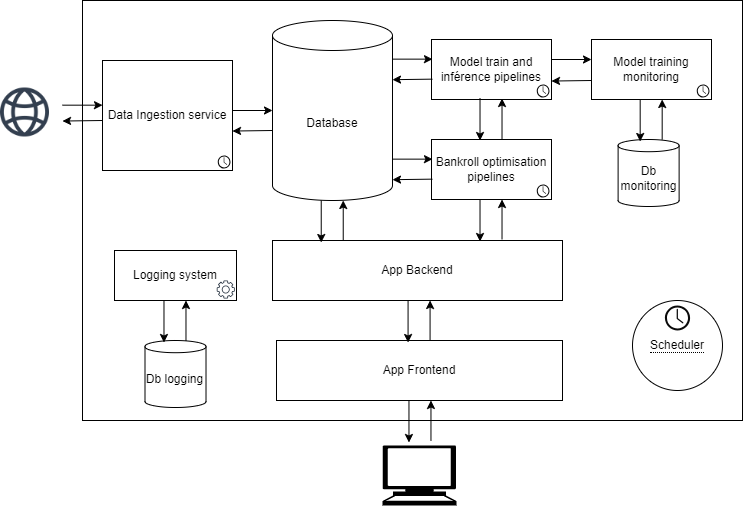
\includegraphics[width=0.8\textwidth, keepaspectratio]{images/Architecture_optimsportbet.png}
    \caption{Architecture of the system}
    \label{fig:elo_score_5_teams_during_time}
\end{figure}


\section{Data Collection}

Accurate and comprehensive data collection is vital for building reliable predictive models and effective betting strategies. The goal is to build an historical database which continues to build with real time relevant data.

\subsection{Data Sources Used}

We utilize a variety of reputable sources to gather data:

\begin{itemize}
    \item \textbf{Football Match Data}: Historical match results, match schedule, team statistics, player performance metrics, and other relevant information are sourced using scrapping on two websites: 
    \begin{itemize}
        \item \hyperlink{https://fbref.com/en/}{FBref}: For historical match results and coming match schedule.
        \item \hyperlink{https://sofifa.com/}{SoFifa}: For teams and players past and current ratings and statistics.
    \end{itemize}
    \item \textbf{Odds Data}: Betting odds are collected from multiple bookmakers through one API.
    \begin{itemize}
        \item \hyperlink{https://the-odds-api.com/}{The Odds API}: The free tier credits allows to perform 500 requests per month on various sports, bookmakers and leagues to retrieve the current odds. Historical odds data are not included.
    \end{itemize}
\end{itemize}


\subsection{Collection Methods}

Data is collected using a combination of methods:

\paragraph{Web Scraping}

A fork of the \hyperlink{https://soccerdata.readthedocs.io/en/latest/}{Soccerdata} python library, has been adapted to scrape data from websites that do not provide APIs (FBref, SoFifa). 

\paragraph{APIs}

For sources that offer APIs (The Odds API), we integrate with them using HTTP requests to fetch structured data efficiently.

\paragraph{Data Pre-processing}

Collected data undergoes a very simple pre-processing to ensure consistency and usability:

\begin{itemize}
    \item \textbf{Data type conversion}: Adapting the type of the data to the most adapted type.
    \item \textbf{Unity}: Only inserting new data in the database, or filling None values of existing data (for instance, the score of a match is only available after the match is played 
    \item \textbf{Integration}: Aligning data from different sources for seamless storage and analysis.
\end{itemize}

\section{Data Storage}

A robust data storage solution is essential for managing the diverse datasets involved.

\subsection{Database Choice}

We opted for a relational database management system (RDBMS), specifically \textit{PostgreSQL}, due to its reliability, scalability, and support for complex queries.

\subsection{Data Model}

The database schema is designed to reflect the relationships between different types of data:

\subsubsection{Tables}

\begin{itemize}
    \item `\textbf{fbref\_results}`: Each row corresponds to a match (historic and coming), with league, date and time of the match, both team and score if match is finished and the result is available and fetched from FBref website.
    \item `\textbf{sofifa\_teams\_stats}`: Each row corresponds to a a team and a date of update with metrics and categorical values that represent at best the team at the moment of the update (overall score, attack, build\_up\_speed ...).
    \item `\textbf{soccer\_odds}`: Each row corresponds to a match, a bookmaker, an outcome with its odd at a given update time. There is also information about the commence time of the match, the league, the home and away team names, the type of odd...
    \item `\textbf{models\_results}`: Each row corresponds to a match, the inference results of the model, the date-time of inference and the model used, with additional information such as the date and tile of the match and home and away team.
    \item `\textbf{optim\_results}`: Each row corresponds to a game, a date time of optimisation, the model used for inference, the best odds for each outcome found across a pool of bookmaker as well as the bookmakers names of each odds chose and the fraction of the bankroll to invest given utility function. There is additional information such as the probability inferred and used by the optimiser, the date-time of inference of these probabilities, the date and time of the match...
\end{itemize}


\begin{figure}[H]
    \centering
    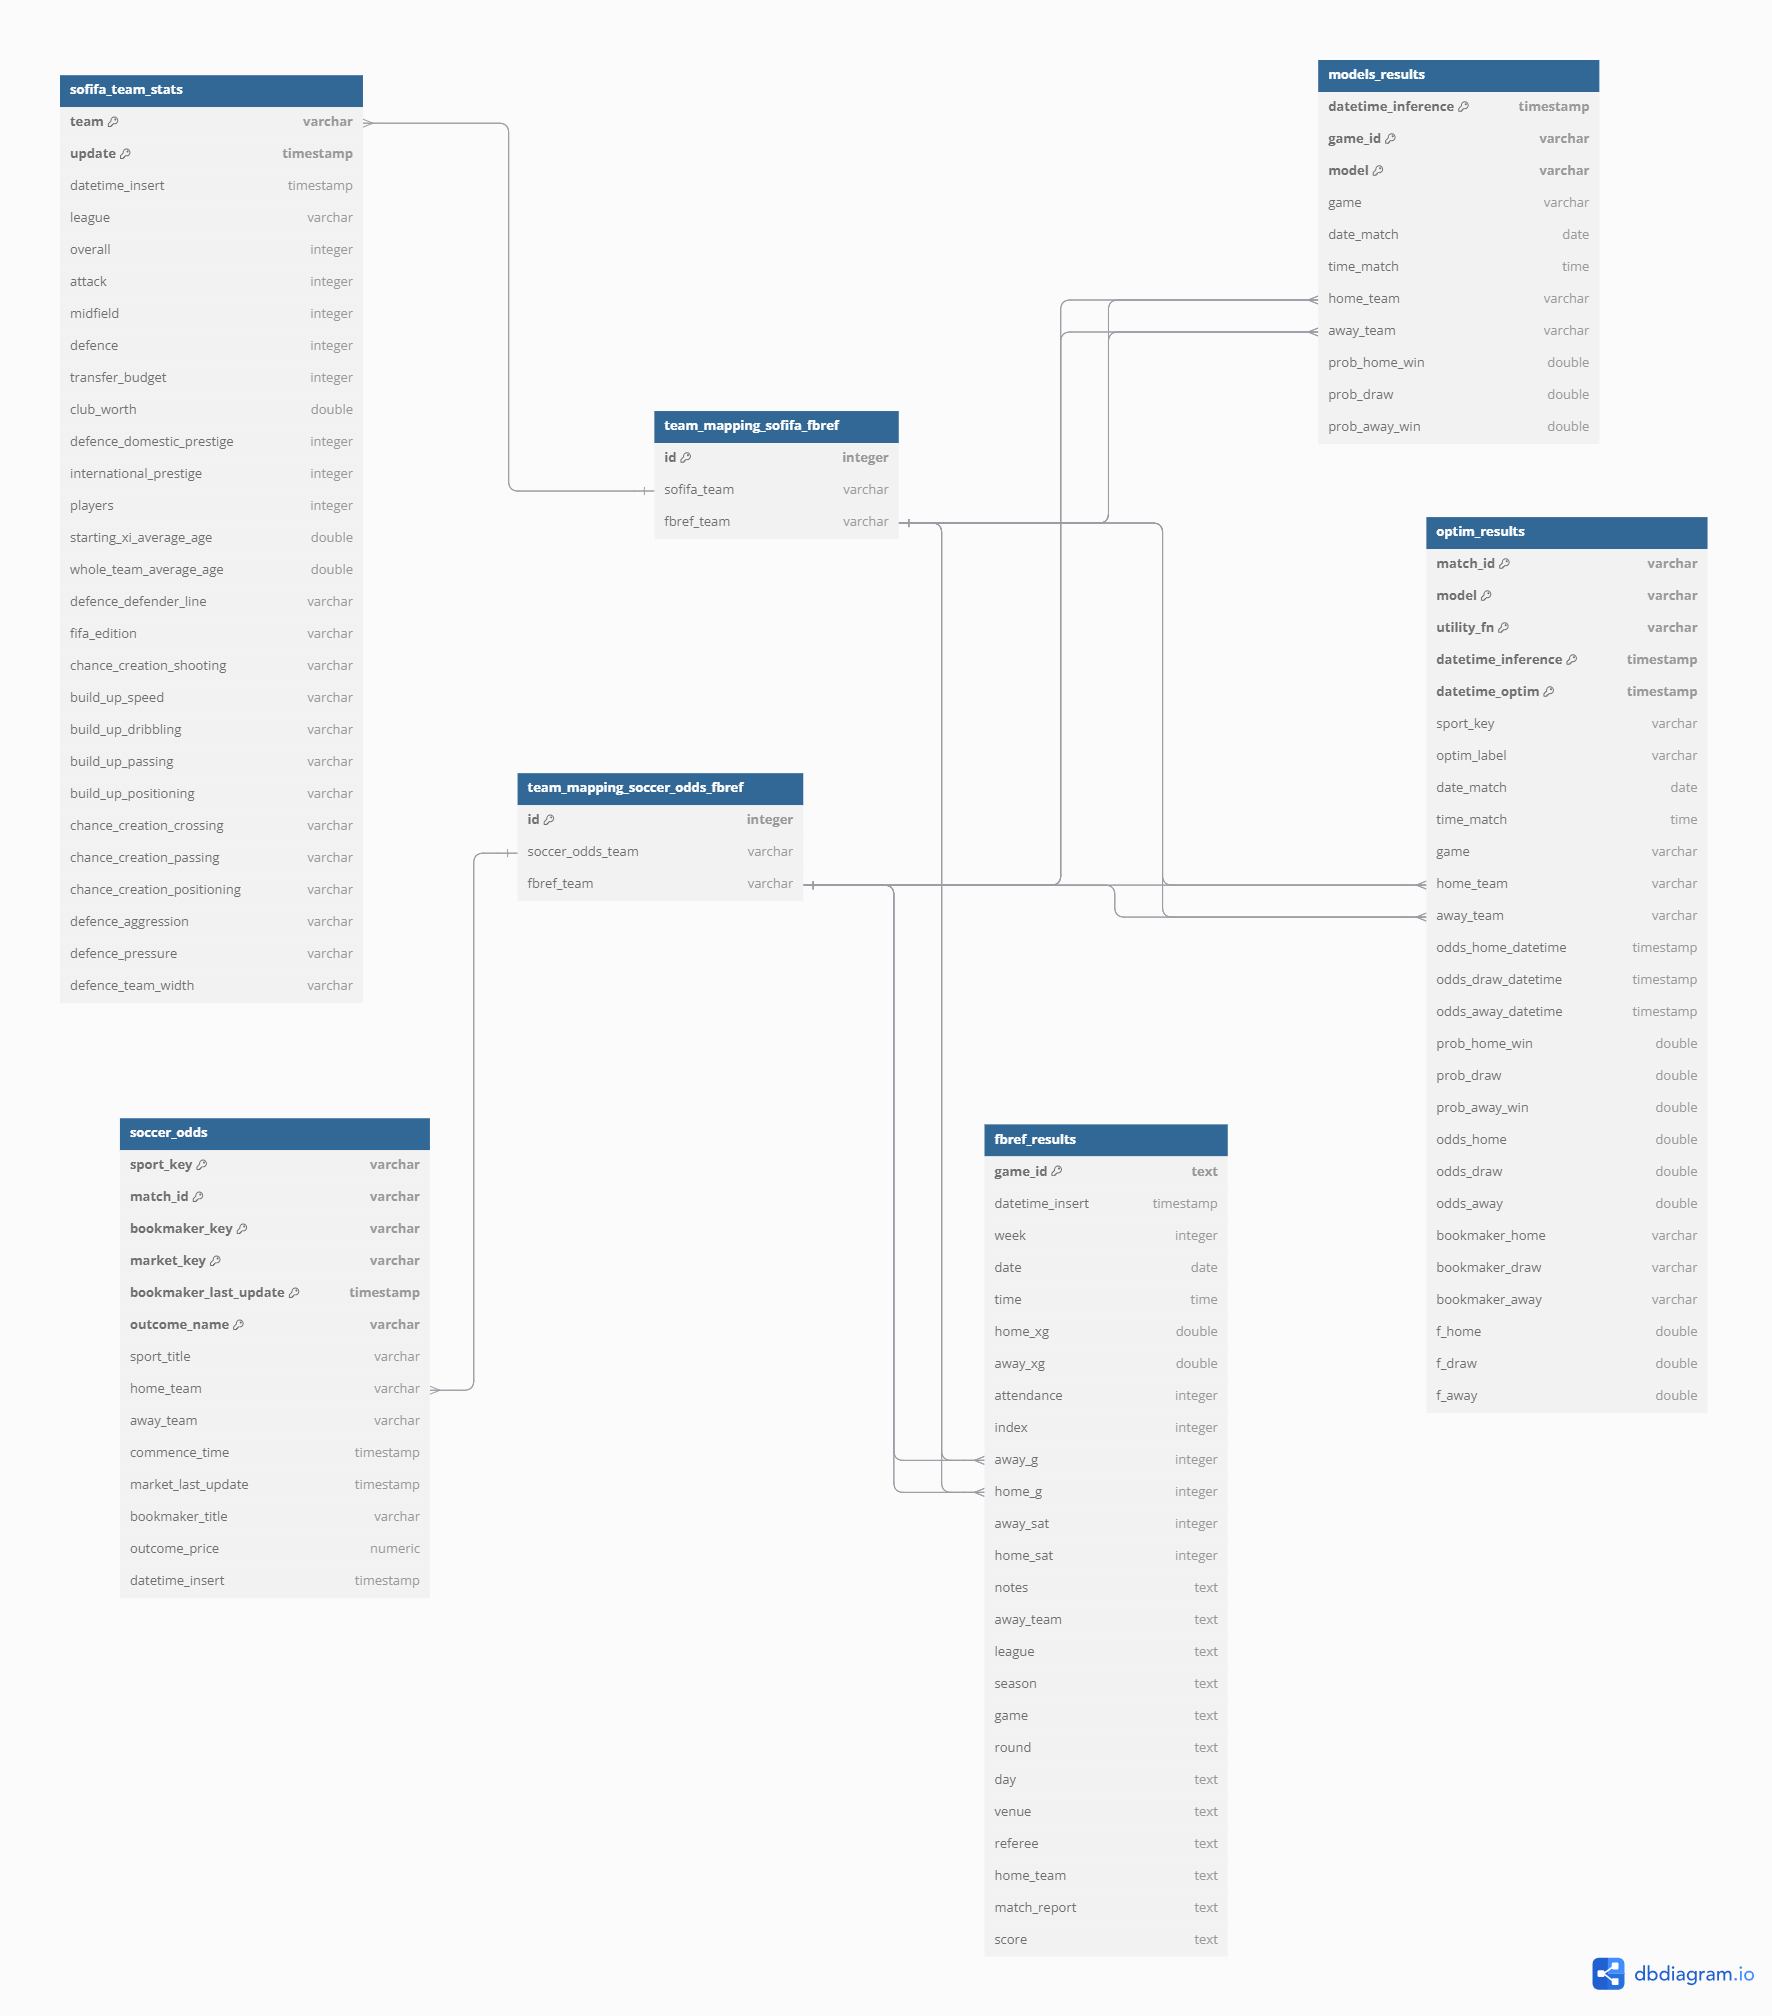
\includegraphics[width=0.8\textwidth, keepaspectratio]{images/db_uml.png}
    \caption{UML diagram of the database}
    \label{fig:uml_db}
\end{figure}

\section{Module Overview}

The system incorporates several modules, each performing specific functions within the overall architecture.

\subsection{Data Collection Module}

As described earlier, this module is responsible for fetching and pre-processing data from various sources.

\subsection{Prediction Module}

Although detailed discussion is deferred to a later chapter, this module uses machine learning algorithms to predict the probabilities of different match outcomes based on historical data.

\subsection{Optimization Module}

This module calculates optimal betting strategies by applying mathematical optimization techniques to the predictions and odds data. The specifics of the optimization algorithms and utility functions will be explored in a subsequent chapter.

\subsection{Scheduler}

The scheduler automates the execution of tasks such as data collection, model retraining, inference, and optimization. It ensures that the system remains up-to-date with the latest data and predictions.

\subsection{User Interface and Backend}

The user interface provides a platform for users to access data, view predictions, and interact with the system. The backend handles user requests, processes data, and communicates with other modules via APIs.

\section{User Interface and Monitoring}

\subsection{User Interface Design}

The UI is designed to be intuitive and user-friendly, providing clear visualizations and easy navigation.

\paragraph{Features}

\begin{itemize}
    \item \textbf{Dashboard}: Displays key metrics, including upcoming matches, predicted probabilities, and recommended betting strategies.
    \item \textbf{Historical Data Access}: Allows users to explore past matches, predictions, and outcomes.
    \item \textbf{Customization}: Users can select preferred bookmakers according to their interests.
\end{itemize}

\subsection{Monitoring}

System health and performance are monitored continuously:

\begin{itemize}
    \item \textbf{Logging}: Activity logs are maintained for debugging and audit purposes.
    \item \textbf{Alerts}: Notifications are sent in case of errors or significant events.
\end{itemize}


\section{Conclusion}

This chapter provided an overview of the system architecture implemented to realize the theoretical framework developed earlier. By focusing on football, we leverage abundant data to build predictive models and optimize betting strategies. The modular design, utilizing microservices and APIs,ensures scalability and flexibility. The database serves as the central repository, integrating data from various sources and supporting the different modules. The user interface offers a gateway for users to access the system's functionalities. In the subsequent chapters, we will delve into the specifics of the prediction and optimization modules, as well as the deployment strategy using Kubernetes and containerization technologies.

\section{Introduction}
\label{sec:chapter4_intro}

This chapter presents the development, training, and evaluation of a predictive model aimed at forecasting the outcomes of football matches. The primary objective is to construct a robust model that can accurately predict match results, thereby optimizing gains in sports betting \cite{BaioBlangiardo2010} \cite{DixonColes1997}. The significance of predictive modeling in the context of sports betting lies in its potential to provide bettors with a strategic advantage by identifying value bets and minimizing risks.

\section{Performance Metrics and Selection Criteria}
\label{sec:performance_metrics}

Evaluating the performance of a predictive model in a multi-class classification setting, especially with imbalanced classes, requires a comprehensive set of metrics. This section delineates both classic and advanced metrics employed in this study, incorporating mathematical formulations and addressing class imbalance. Given the three-class problem—home win, draw, and away win—with home wins constituting 47\% of the data, it is crucial to select metrics that provide a nuanced understanding of model performance across all classes.

\subsection{Metrics}
\label{subsec:classic_metrics}

A list of all the metrics considered with their used definition can  be found in Appendix \ref{appendix:predictive_model_metrics}.

\subsection{Selection Criteria}
\label{subsec:selection_criteria}

Accurate evaluation of the predictive model requires appropriate performance metrics, particularly in a multi-class classification context with class imbalance. The primary goal of this study is to ensure that the predicted probabilities of football match outcomes (home win, draw, away win) closely align with the true probabilities, emphasizing well-calibrated probability estimates.

Given the class distribution—47\% home wins, 26\% draws, and 25\% away wins—we have selected the \textbf{Mean Squared Error (MSE)} as the primary metric for assessing calibration. MSE directly measures the average squared difference between predicted probabilities and actual outcomes, making it suitable for evaluating how well the model's probabilities reflect the true frequencies.

In addition to MSE, we will consider the following metrics to provide a comprehensive evaluation:

\begin{itemize}
    \item \textbf{Log Loss}: To assess the quality of the predicted probability distributions by penalizing incorrect and overconfident predictions, thus encouraging well-calibrated estimates.
    \item \textbf{Classwise Expected Calibration Error (ECE)}: To evaluate the calibration of predicted probabilities for each class individually, offering insights into how closely these probabilities match the observed outcomes across different categories.
    \item \textbf{Accuracy for Home Win, Draw, and Away Win}: To examine the model's performance on each outcome separately, taking into account the class imbalance.
\end{itemize}

By focusing on MSE for calibration and incorporating Log Loss, Classwise ECE, and class-specific accuracy, we aim to ensure that the model not only produces accurate probability estimates but also maintains reliability across all outcome categories. This concise set of metrics aligns with our objective of accurately predicting football match outcomes while ensuring the predicted probabilities are well-calibrated and trustworthy.

\section{Exploration and Choice of Features}
\label{sec:feature_selection}

Selecting appropriate features is pivotal for building an effective predictive model. This section delineates the various types of features utilized in this study, the methodology employed for feature selection, the engineering of new features to enhance predictive power, and the handling of categorical variables to ensure they are appropriately represented in the model. 

\subsection{Types of Features Utilized}
\label{subsec:types_features}

The feature set comprises a combination of ranking-based, simple statistical, and domain-specific features. Each feature is defined mathematically where applicable and accompanied by an explanation of its relevance and computation.

\subsubsection{Ranking Features}
\label{subsubsec:ranking_features}

Ranking features provide a quantitative measure of team strength based on historical performance. These metrics are crucial as they encapsulate the overall ability and consistency of teams over time. All ranking features detailed formula are described in \ref{appendix:ranking_features}.

\begin{itemize}

\item \textbf{Elo Score}
\label{par:elo_score}

The \textbf{Elo score} \cite{Elo1978} \cite{HvattumArntzen2010} is a rating system originally developed for chess but widely adapted to various sports to rate players or teams. It reflects the relative skill levels of the teams based on game outcomes.

\begin{figure}[H]
    \centering
    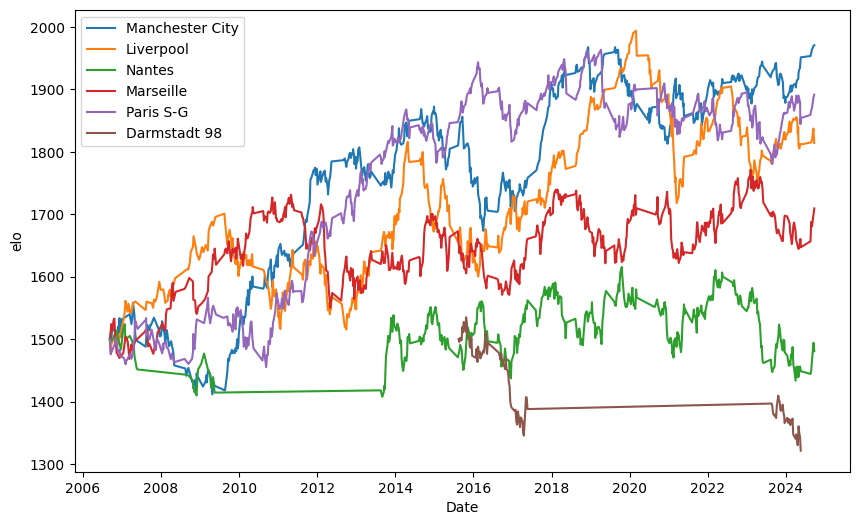
\includegraphics[width=0.8\textwidth, keepaspectratio]{images/elo_score_5_teams_during_time.png}
    \caption{Elo score of 5 football teams evolving during time}
    \label{fig:elo_score_5_teams_during_time}
\end{figure}



\item \textbf{Glicko-2 Score}
\label{par:glicko2_score}

The \textbf{Glicko-2 score} \cite{Glickman1999} is an advanced rating system developed by Mark Glickman, which enhances the Elo rating system by incorporating not only the skill levels of teams or players (R) but also the reliability of these ratings through Rating Deviation (RD) and volatility. This system provides a more dynamic and accurate reflection of performance by accounting for the uncertainty and variability in teams' ratings.


\item \textbf{TrueSkill}
\label{par:trueskill}

The \textbf{TrueSkill} \cite{HerbrichEtAl2007} is a Bayesian ranking system developed by Microsoft, primarily used in gaming but adaptable to sports analytics. It models each team's skill as a Gaussian distribution, updating beliefs about team strengths based on match outcomes.

\end{itemize}

\subsubsection{Simple Statistical Features}


Simple statistical features offer basic quantitative measures of team performance, providing foundational data for the predictive model.


\begin{itemize}
    \item \textbf{Average Goals Scored per Season}: Total goals scored by a team divided by the number of matches played so far.
    
    \item \textbf{Average Goals Conceded per Season}: Total goals conceded by a team divided by the number of matches played so far.
\end{itemize}


\subsubsection{Sofifa Performance Metrics}

SoFIFA provides detailed metrics for both individual players and teams, based on data from the FIFA video game by EA Sports. This document outlines the primary metrics and explains how team ratings are calculated using individual player attributes.

\begin{itemize}

\item \textbf{Player Metrics}
    The primary player metrics on SoFIFA are based on individual attributes that are weighted differently depending on the player's position. Below are the key metrics:
    
    \begin{itemize}
        \item \textbf{Overall Rating (OVR)}: This is the weighted average of various player attributes, with different weights depending on the position. For example, an attacker (\textit{Forward}) will have more emphasis on \textit{Shooting} and \textit{Pace}, while a defender (\textit{Centre Back}) will weigh attributes like \textit{Defending} and \textit{Physicality} more heavily.
        \item \textbf{Pace (PAC)}: Calculated as a combination of the \textit{Acceleration} and \textit{Sprint Speed} attributes.
        \item \textbf{Shooting (SHO)}: Includes \textit{Finishing}, \textit{Shot Power}, \textit{Long Shots}, and \textit{Positioning}.
        \item \textbf{Passing (PAS)}: Comprised of \textit{Vision}, \textit{Short Passing}, and \textit{Long Passing}.
        \item \textbf{Dribbling (DRI)}: Includes \textit{Ball Control}, \textit{Dribbling}, \textit{Agility}, and \textit{Balance}.
        \item \textbf{Defending (DEF)}: Based on \textit{Tackling}, \textit{Marking}, \textit{Interceptions}, and \textit{Defensive Awareness}.
        \item \textbf{Physicality (PHY)}: Includes \textit{Strength}, \textit{Stamina}, and \textit{Aggression}.
        \item \textbf{Potential}: Indicates the maximum possible rating the player can achieve over time.
    \end{itemize}
    
    The formula for the Overall Rating (OVR) is generally unknown, but it can be expressed as a weighted sum of key attributes, depending on the player’s position. A simplified formula for a forward might look like:
    
    \[
    \text{OVR}_{\text{Forward}} = w_1 \cdot \text{PAC} + w_2 \cdot \text{SHO} + w_3 \cdot \text{DRI} + w_4 \cdot \text{PAS}
    \]
    
    where \( w_1, w_2, w_3, w_4 \) are position-specific weights.

\item \textbf{Team Metrics}
    Team metrics on SoFIFA are calculated by aggregating individual player ratings, focusing on key areas like attack, midfield, and defense. The following are the primary team metrics:
    
    \begin{itemize}
        \item \textbf{Overall Team Rating}: A weighted average of the starting 11 players' Overall Ratings, considering the importance of each player's position.
        \item \textbf{Attack Rating}: The average Overall Rating of forwards and attacking midfielders, weighted based on the formation.
        \item \textbf{Midfield Rating}: The average Overall Rating of central and wide midfielders, weighted based on their roles in the formation.
        \item \textbf{Defense Rating}: The average Overall Rating of defenders and goalkeepers.
    \end{itemize}
    
    A simplified version of the team rating could be expressed as:
    
    \[
    \text{Team OVR} = \frac{1}{11} \sum_{i=1}^{11} \text{OVR}_i
    \]
    
    where \( \text{OVR}_i \) represents the Overall Rating of the $i$-th player in the starting lineup.
    
    
    Sofifa metrics are comprehensive team-specific performance indicators sourced from the Sofifa database, widely used in sports analytics and fantasy football contexts.
\end{itemize}

\begin{figure}[H]
    \centering
    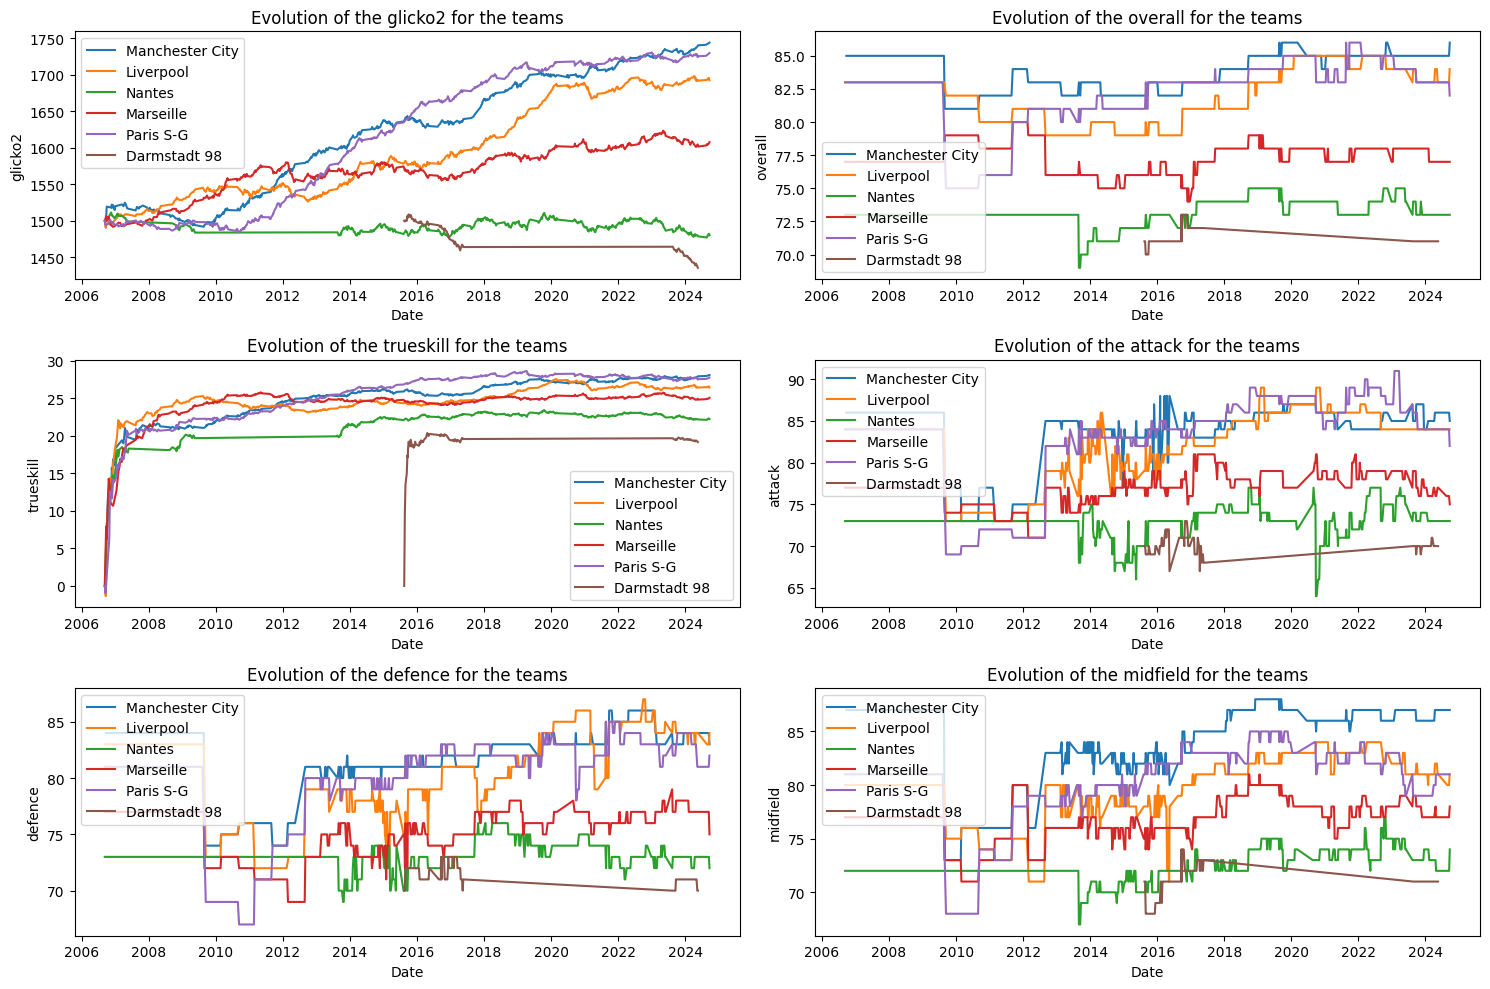
\includegraphics[width=\textwidth, keepaspectratio]{images/scores_5_teams_during_time.png}
    \caption{Different scores of 5 football teams evolving during time}
    \label{fig:scores_5_teams_during_time}
\end{figure}

A detailed description of each of the 90 features used can be found her \ref{appendix:all_feature_descriptions}.

\subsection{Feature Selection Methodology}
\label{subsec:feature_selection_methodology}

Feature selection was performed using a forward selection approach applied to a logistic regression model. This method iteratively adds the most significant features, enhancing predictive performance while maintaining model simplicity.

\subsubsection{Forward Selection with Logistic Regression}
\label{subsubsec:forward_selection_logistic_regression}

\textbf{Procedure}: Starting with no features, at each iteration, the feature that most improves the model's fit is added. The selection criterion is based on the mse (mean squared error).

\textbf{Explanation}: By incorporating features that significantly contribute to the model, forward selection optimizes predictive accuracy and ensures interpretability by excluding irrelevant variables.

\section{Data Preparation}

We trained our model on matches from 2006 to the present, focusing on games from the top 5 European leagues, European championships, and World Cups during this period. The limiting factor in our data came from SoFIFA, which does not provide data prior to 2006, while FBref offers data extending far into the past. We merged the two datasets based on team names and computed the ranking and statistical features described earlier, initializing the metrics at the first entry of a team in a tournament. For categorical features, we applied one-hot encoding. We removed matches with any missing values in the columns, then applied a standard scaler. This left us with 28,850 completed matches and a 90-feature vector for each match to train our model.

\begin{table}[h]
\centering
\begin{tabular}{|l|c|c|}
\hline
\textbf{Metric} & \textbf{Value} \\
\hline
Total matches & 28,850 \\
Matches in Top 5 Leagues & 28,481 \\
Matches in European Championships & 185 \\
Matches in World Cup & 184 \\
Home win ratio & 45.0 \% \\
Draw ratio & 25.4 \% \\
Away win ratio & 29.5 \% \\ 
Average home team goals & 1.54 \\
Average away team goals & 1.19 \\
Average Elo rating & 1558 \\
Number of unique teams & 242 \\
Number of features per match & 90 \\
First match date & 2006-09-09 \\
Last match date & 2024-09-24 \\
\hline
\end{tabular}
\caption{Summary Metrics for the Dataset}
\end{table}


\section{Cross-Validation on Temporal Data}
\label{sec:cross_validation_temporal}

In predictive modeling with football match data, which is inherently temporal, it's essential to use cross-validation techniques that respect the chronological order of observations. Standard cross-validation methods, such as random shuffling or traditional \( k \)-fold cross-validation, are unsuitable because they can lead to data leakage by training models on future data to predict past events.

Traditional cross-validation assumes that data samples are independent and identically distributed (i.i.d.) and that the order of observations does not matter. In temporal data, however, observations are time-dependent, and future events should not influence model training aimed at predicting past events. Using standard methods can result in:

\begin{itemize}
    \item \textbf{Data Leakage}: Incorporating future information into the training set leads to overly optimistic performance estimates.
    \item \textbf{Violation of Temporal Order}: Disrupting the sequence of events undermines the model's ability to generalize to real-world forecasting scenarios.
\end{itemize}


To address these issues, we employ cross-validation methods designed for temporal data \cite{BergmeirEtAl2018}.

\subsection{Sliding Window Cross-Validation}

This technique involves moving a fixed-size window across the data timeline. In each iteration, the model is trained on a training window and tested on the immediately following testing window.

\begin{itemize}
    \item Choose a training window size \( W_{\text{train}} \) and a testing window size \( W_{\text{test}} \).
    \item For each iteration:
    \begin{itemize}
        \item Train the model on data from time \( t \) to \( t + W_{\text{train}} - 1 \).
        \item Test the model on data from \( t + W_{\text{train}} \) to \( t + W_{\text{train}} + W_{\text{test}} - 1 \).
        \item Slide the window forward by \( W_{\text{test}} \) units.
    \end{itemize}
\end{itemize}

\subsection{Expanding Window Cross-Validation}

Also known as growing window, this method expands the training set with each iteration by including more historical data.

\begin{itemize}
    \item Start with an initial training window of size \( W_{\text{initial}} \).
    \item For each iteration:
    \begin{itemize}
        \item Train the model on data from time \( t \) to \( t + W_{\text{train}} - 1 \), where \( W_{\text{train}} \) increases with each iteration.
        \item Test on the subsequent data from \( t + W_{\text{train}} \) to \( t + W_{\text{train}} + W_{\text{test}} - 1 \).
        \item Expand the training window to include the latest testing window.
    \end{itemize}
\end{itemize}

\begin{figure}[H]
    \centering
    \begin{minipage}{0.45\textwidth}
        \centering
        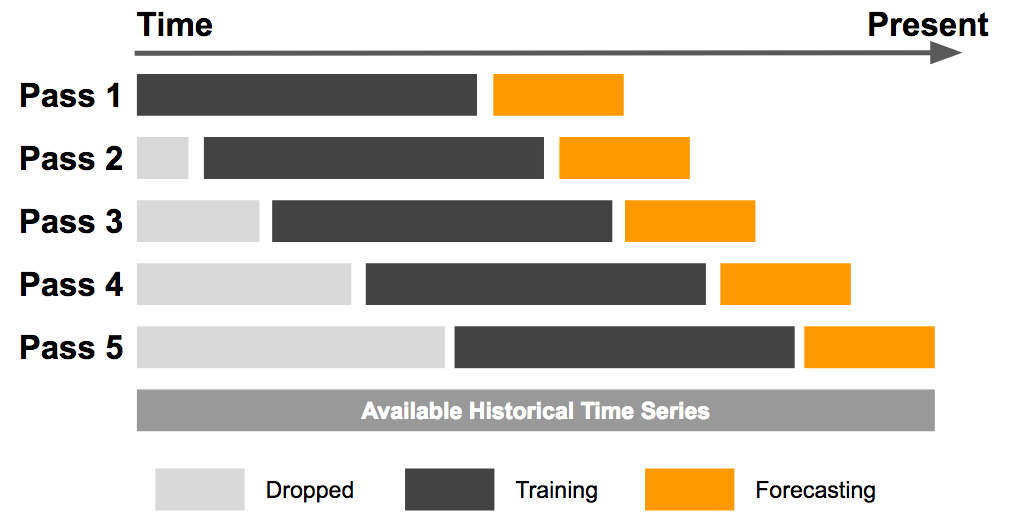
\includegraphics[width=\textwidth, keepaspectratio]{images/FixedWindow.png}
        \caption{Sliding window graphic}
        \label{fig:sliding_window}
    \end{minipage}\hfill
    \begin{minipage}{0.45\textwidth}
        \centering
        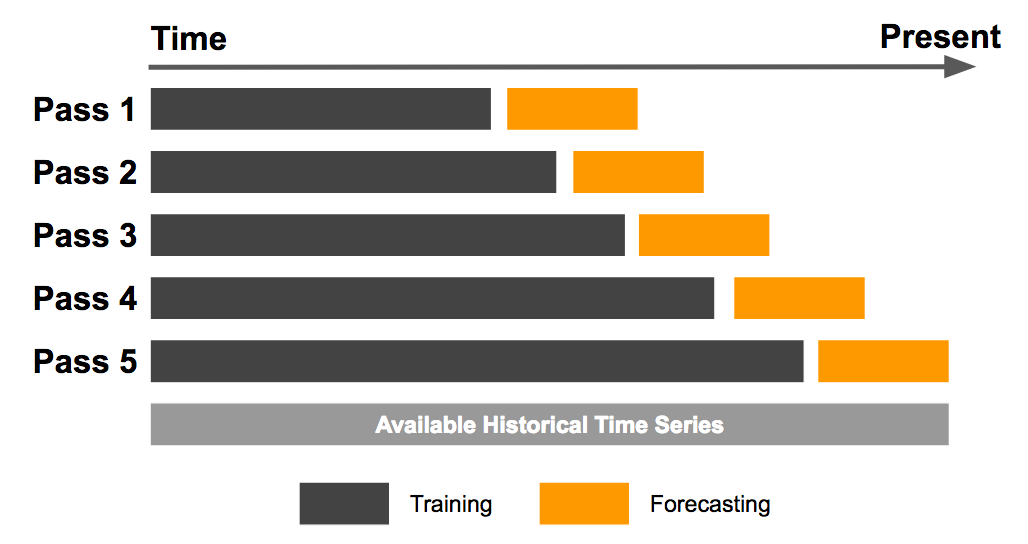
\includegraphics[width=\textwidth, keepaspectratio]{images/ExpandingWindow.png}
        \caption{Expanding window graphic}
        \label{fig:expanding_window}
    \end{minipage}
\end{figure}


The results presented below were obtained using an expanding window technique with 5 folds and a test set ratio of 0.2. Notably, the results were very similar when applying the sliding window method.


\section{Choice and Justification of the Prediction Model}
\label{sec:model_choice}

In this section, we present the results of the feature selection and model selection processes \cite{GuyonElisseeff2003} \cite{ChandrashekarSahin2014}, followed by interpretations of the selected model's performance. Feature selection was conducted using forward selection, and multiple classification models were evaluated to determine the most suitable model for predicting football match outcomes.

\subsection{Feature Selection Using Forward Selection}
\label{subsec:feature_selection}

Feature selection was performed using forward selection with logistic regression, iteratively adding the most significant feature at each step based on mean squared error (MSE) improvement, using an expanding window validation with 5 splits and a test size of 20\% of the training data.

\begin{table}[H]
    \centering
    \caption{Feature Selection Process Summary}
    \label{tab:feature_selection_summary}
    \begin{tabular}{lc}
        \toprule
        \textbf{Method} & \textbf{Details} \\
        \midrule
        Feature Selection & Forward Selection \\
        Model Used & Logistic Regression \\
        Validation Method & Expanding Window (5 splits) \\
        Performance Metric & Mean Squared Error (MSE) \\
        Test Size & 20\% of training data \\
        \bottomrule
    \end{tabular}
\end{table}


We selected 35 features, which corresponding to the features resulting in the lowest MSE, using this feature selection strategy.

\begin{table}[H]
    \centering
    \caption{Feature Selection with Corresponding MSE and their adding number}
    \label{tab:feature_mse}
    \begin{tabular}{|c|l|c|c|l|c|}
        \hline
        \textbf{Order} & \textbf{Feature Added} & \textbf{MSE} & \textbf{Order} & \textbf{Feature Added} & \textbf{MSE} \\
        \hline
        1  & Elo Away & 0.20613 & 19 & Home Passing Risky & 0.19438 \\
        2  & Elo Home & 0.19661 & 20 & Away Positioning Org. & 0.19436 \\
        3  & Glicko Vol Away & 0.19619 & 21 & Away Defense Pressure Med & 0.19435 \\
        4  & Away Overall & 0.19594 & 22 & Away Domestic Prestige & 0.19434 \\
        5  & Home Overall & 0.19540 & 23 & Away Shooting Lots & 0.19433 \\
        6  & Away Build Speed Slow & 0.19518 & 24 & Home Defense Line Offside & 0.19432 \\
        7  & Away Avg Age & 0.19501 & 25 & Away Team Width & 0.19431 \\
        8  & Home League INT & 0.19487 & 26 & Home Defense Pressure Med & 0.19431 \\
        9  & Home Avg Goals & 0.19476 & 27 & Home Build Speed Slow & 0.19430 \\
        10 & Home Positioning Org. & 0.19467 & 28 & Away Defense Aggression & 0.19430 \\
        11 & Home Build Speed Fast & 0.19461 & 29 & TrueSkill Home & 0.19430 \\
        12 & Away Defense Pressure High & 0.19457 & 30 & Away Build Positioning Org. & 0.19430 \\
        13 & Away Defense Offside Trap & 0.19453 & 31 & Away Defense & 0.19430 \\
        14 & Home League ITA & 0.19449 & 32 & Home Attack & 0.19427 \\
        15 & Glicko RD Home & 0.19447 & 33 & Home Defense Prestige & 0.19427 \\
        16 & Home Shooting Normal & 0.19444 & 34 & Away Attack & 0.19427 \\
        17 & Away Passing Mixed & 0.19442 & 35 & Away League INT & \textbf{0.19427} \\
        18 & Away Avg Goals & 0.19440 & & \\
        \hline
    \end{tabular}
\end{table}

The table above summarizes the features added during the selection process and their corresponding MSE values, highlighting the importance of each feature as it contributes to minimizing the error. As we can see, features such as Elo ratings and overall team metrics play a significant role \cite{LasekEtAl2013}. Now, let's examine how the number of features impacts the performance metrics more broadly, as shown in the following feature selection graph.

\begin{figure}[H]
    \centering
    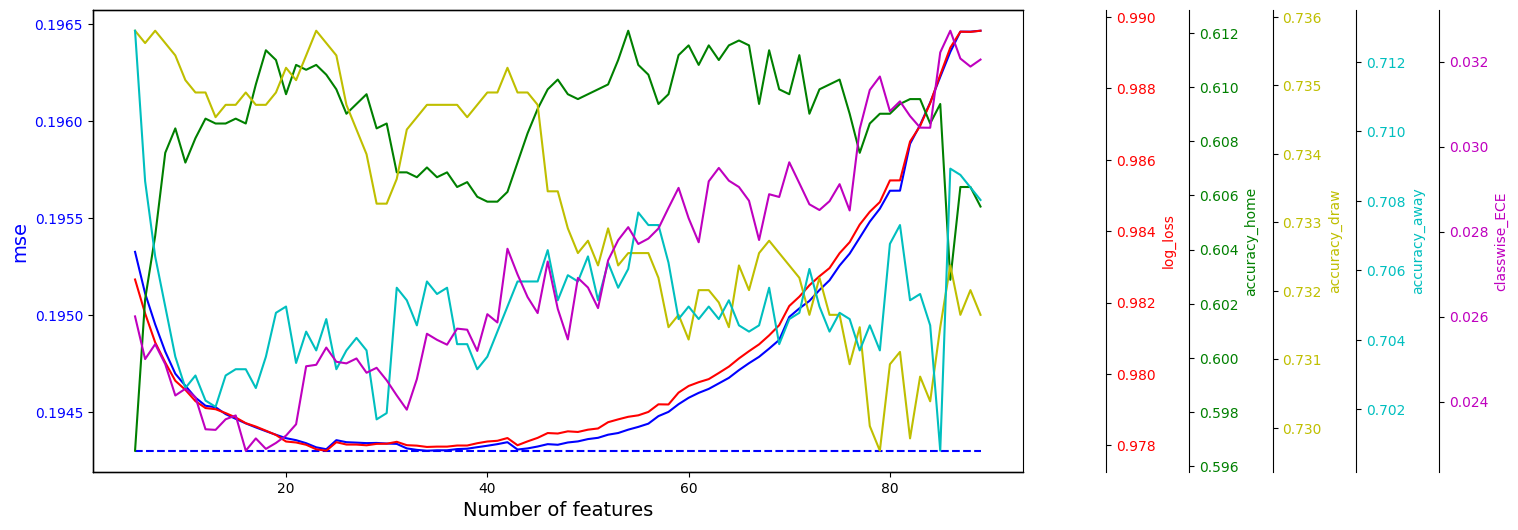
\includegraphics[width=\textwidth, keepaspectratio]{images/feature_selection_metrics_by_nb_of_features.png}
    \caption{Metrics of interrest function of the number of features added}
    \label{fig:feature_selection_metrics_by_nb_of_features}
\end{figure}

This graph shows the performance of various metrics (MSE, log loss, accuracy for home, draw, and away predictions, and classwise ECE) as a function of the number of selected features. The MSE (in blue) decreases as more features are added, stabilizing around the optimal point before increasing again, which suggests that selecting too many features can lead to overfitting. Similarly, log loss follows a similar trend (in red), indicating better model calibration with fewer features. The accuracy metrics (home, draw, away) fluctuate, but accuracy seems to peak at a certain range of features, with performance diminishing as more features are added. Classwise ECE (in pink) decreases and then increases, a little bit before MSE and log loss, indicating better calibration for class predictions with fewer features. Overall, the graph highlights the balance between feature selection and model performance, suggesting that an optimal subset of features yields the best generalization.

\subsection{Model Selection}
\label{subsec:model_selection}

The following table summarizes the performance of various classification models \cite{Bishop2006}, comparing metrics such as mean squared error (MSE), log loss, classwise ECE, and accuracy for home, draw, and away predictions to identify the best-performing model.

\begin{table}[H]
    \centering
    \caption{Model Performance Comparison}
    \label{tab:model_performance}
    \begin{tabular}{|l|c|c|c|c|c|c|}
        \hline
        \textbf{Model} & \textbf{MSE} & \textbf{Log Loss} & \textbf{C. ECE} & \textbf{A. Home} & \textbf{A. Draw} & \textbf{A. Away} \\
        \hline
        Logistic Regression & \textbf{0.195} & \textbf{0.983} & 0.029 & 0.605 & 0.733 & 0.702 \\
        Logistic Regression CV & 0.196 & 0.983 & \textbf{0.028} & 0.602 & \textbf{0.735} & 0.703 \\
        Gradient Boosting Classifier & 0.199 & 1.002 & 0.037 & 0.604 & 0.709 & \textbf{0.706} \\
        Random Forest Classifier & 0.202 & 1.022 & 0.038 & 0.595 & 0.705 & 0.693 \\
        Extra Trees Classifier & 0.204 & 1.026 & 0.043 & 0.597 & 0.683 & 0.686 \\
        AdaBoost Classifier & 0.221 & 1.092 & 0.069 & 0.599 & 0.721 & 0.695 \\
        Bagging Classifier & 0.224 & 2.471 & 0.093 & 0.602 & 0.646 & 0.661 \\
        MLP Classifier & 0.224 & 1.187 & 0.108 & 0.585 & 0.665 & 0.684 \\
        K Neighbors Classifier & 0.238 & 5.404 & 0.096 & 0.599 & 0.643 & 0.631 \\
        Gaussian NB & 0.332 & 7.570 & 0.302 & \textbf{0.615} & 0.584 & 0.625 \\
        Quadratic Discriminant Analysis & 0.353 & 10.831 & 0.316 & 0.582 & 0.561 & 0.613 \\
        Decision Tree Classifier & 0.390 & 20.219 & 0.195 & 0.578 & 0.614 & 0.638 \\
        Extra Tree Classifier & 0.399 & 20.686 & 0.200 & 0.559 & 0.615 & 0.628 \\
        \hline
    \end{tabular}
\end{table}


\subsection{Interpretation of Results}
\label{subsec:interpretation}

The selection of the logistic regression model allows for straightforward interpretation of feature effects on the predicted probabilities of match outcomes.

\subsubsection{Feature Importance}

Feature importance was assessed based on the magnitude of the coefficients in the logistic regression model. Below sits the feature importance of the Home win class. Draw and Away win classes analysis can be found in \ref{appendix:feature_importance}.


\begin{figure}[H]
    \centering
    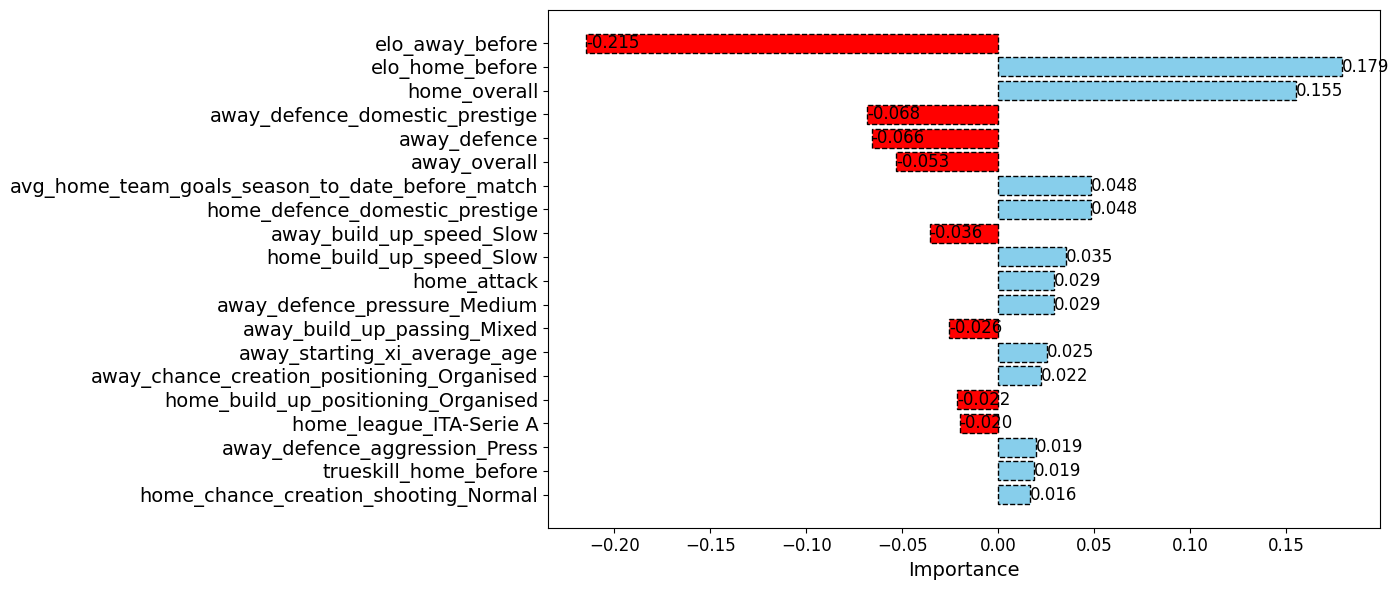
\includegraphics[width=\textwidth, keepaspectratio]{images/top20_coeff_importance_lr_selected_features_home.png}
    \caption{Coefficients of the Logistic Regression Model for Home win class}
    \label{fig:feature_coefficients}
\end{figure}

For the home class, the most important features, such as Elo ratings for the away and home teams, suggest that pre-match team strength is the most significant predictor of match outcomes. Both overall team quality and specific defensive attributes, like pressure and aggression, also play a key role. Features related to player average characteristics, such as average age and tactical elements like build-up speed, indicate that team composition and playstyle are also relevant, though their impact is less pronounced. Defensive strategies, particularly pressure and team width, add further predictive value, showing the importance of tactical decisions in determining match results. The feature importance analysis graphs for draw and away class can be found in the annex section.


\subsubsection{Why Logistic Regression Outperforms Other Models}

Logistic regression may outperform other models due to its simplicity and interpretability, especially when feature selection is based on it. By using logistic regression for feature selection, the model is specifically tuned to highlight the most important predictors of the outcome, leading to better generalization. Additionally, logistic regression handles multicollinearity well when regularization is applied, preventing overfitting. The linear relationship between the features and the log-odds of the outcomes makes it easier to capture important patterns in the data, particularly in problems like sports prediction where relationships between variables are often linear. Other models, such as random forests or gradient boosting, may add unnecessary complexity and are more prone to overfitting when features are already well-selected.


\section{Training and Retraining of the Model}
\label{sec:training_retraining}

Figure \ref{fig:mse_retraining} illustrates the Mean Squared Error (MSE) of two models over time, where the blue line represents Model A with no retraining, and the orange line represents Model B, which is retrained daily. Both models are initialy trained from 2006-01-01 up to 2010-01-01 data and are evaluated using a 120-day rolling average.

\begin{figure}[H]
    \centering
    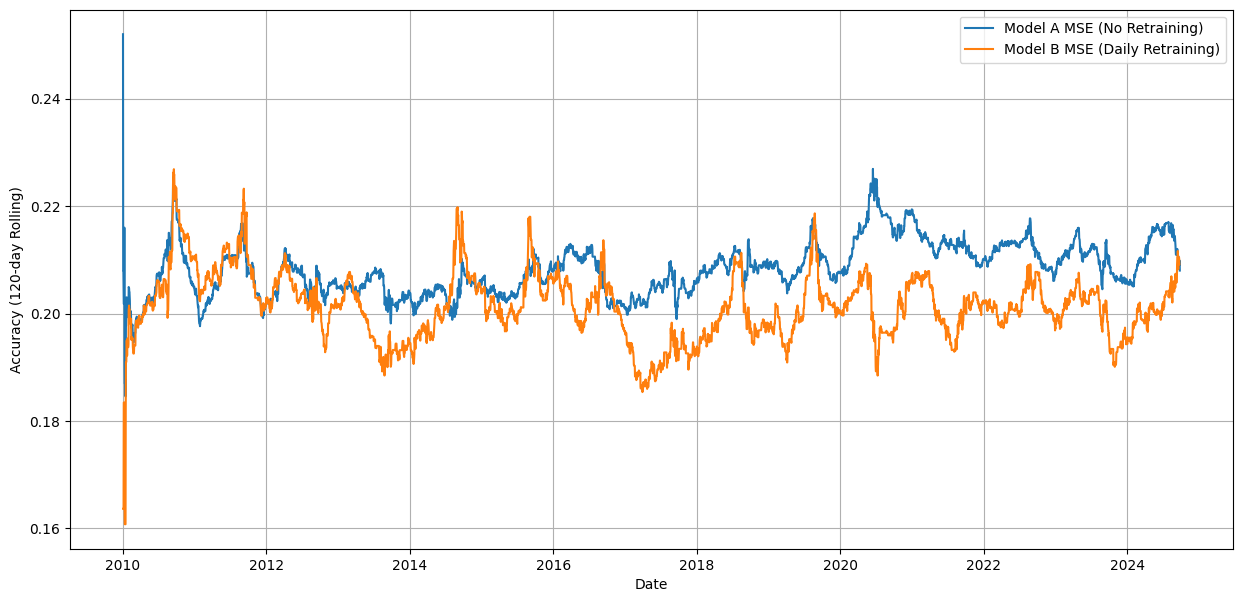
\includegraphics[width=0.8\textwidth, keepaspectratio]{images/model_ratrining_mse_120rd.png}
    \caption{Model MSE rolling average over time}
    \label{fig:mse_retraining}
\end{figure}


From the figure, we observe that Model B, which is frequently retrained, exhibits lower MSE compared to Model A throughout most of the time period. Retraining appears to allow Model B to adapt more effectively to evolving patterns, leading to consistently better performance in terms of accuracy. Moreover, as time goes by, we can observe a mse drift from the not retrained model as well as a slight improvement from the retrained model. \\

There are very few periods where Model A outperforms Model B. It appends especially during phases of sudden changes. Despite these fluctuations, retraining offers a more stable and improved long-term performance. \\

The results highlight the importance of regular retraining for maintaining model accuracy, particularly in dynamic environments where data patterns change over time.

\section{Conclusion}

This chapter presented the development, training, and evaluation of a predictive model for football match outcomes, with a focus on sports betting. Feature selection via forward selection with logistic regression helped identify key predictors, and regular retraining improved model performance over time.\\

However, several limitations remain:

\begin{itemize}
    \item \textbf{Hyperparameters and Features}: Ranking feature hyperparameters were left at default, and additional domain-specific or external data sources could further improve predictions.
    \item \textbf{Feature Selection}: Feature selection was arbitrarily based on logistic regression, and no hyperparameter optimization was performed for any models.
    \item \textbf{Retraining}: The timing and method of retraining (e.g., sliding window) were not explored, potentially missing optimal strategies as well as posing computational challenges that could be optimized.
    \item \textbf{Model Complexity}: Incorporating deep learning models could enhance predictive performance, particularly for capturing complex patterns in the data.
    \item \textbf{Bookmaker Odds Decorrelation}: Adding a metric to assess the decorrelation between model predictions and bookmaker odds could help identify more value bets and further optimize betting strategies.
\end{itemize}
In the next chapter, we address the optimization problem of determining the bankroll share to invest on each outcome, building on the predictions of this model to develop actionable betting strategies.

\section{Introduction}

Effective bankroll management is a critical component of successful sports betting. It involves determining the optimal amount to wager on each bet to maximize growth while minimizing the risk of ruin. This section details the development and evaluation of an optimization module designed to calculate the optimal fraction of the bankroll to invest in each betting opportunity. The module leverages probabilistic forecasts from the predictive models discussed in the previous section and applies various investment strategies, including the Kelly criterion, expected value maximization, and naive betting approaches.

\section{Methodology}
\subsection{Investment Strategies}

This section provides an overview of the different bankroll allocation strategies implemented, ranging from naive methods to more advanced optimization techniques. The focus is on the principles guiding each strategy, with a detailed formula provided only for the naive strategy.

\subsubsection{List of Strategies}

\begin{itemize}
    \item \textbf{Kelly Criterion Strategy}: \cite{Kelly1956} \cite{Thorp1969}  
    This strategy maximizes the logarithmic utility of wealth, aiming for long-term bankroll growth while managing risk. The bankroll fractions are derived from the analytical solution using the approximations  \ref{appendix:analytical_solution_using_the_kelly_criterion}, \(\mathbb{E}(U(B)) = \mathbb{E}(B) - \frac{1}{2} \cdot \mathbb{V}\text{ar}(B) \) which comes down to a Linear utility strategy using \( \lambda = \frac{1}{2} \).

    \item \textbf{Log Utility Strategy}:  
    Similar to the Kelly criterion, this strategy focuses on maximizing the expected logarithmic utility \(U(B) = \ln(B)\)  but using no approximations \ref{appendix:analytical_reduction_using_log_expected_utility}.

    \item \textbf{Exponential Utility Strategy}:  
    This strategy uses an exponential utility function \(U(B) = -e^{-\alpha B}\) to take into account the bettor’s risk aversion, balancing between expected returns and risk tolerance \ref{appendix:analytical_reduction_using_exp_expected_utility}.

    \item \textbf{Linear Utility Strategy}:
    In this strategy, the objective is to maximize the trade-off between expected returns and risk, represented by the function \(\mathbb{E}(U(B)) = \mathbb{E}(B) - \lambda \cdot \mathbb{V}\text{ar}(B) \). For the simulations, we set \( \lambda = 10 \), reflecting a high level of risk aversion. This approach seeks to maximize returns while penalizing high variance, aiming to balance growth and stability \ref{appendix:analytical_solution_using_linear_expected_utility}. 

    \item \textbf{Expected Value Maximization Strategy}:  
    This strategy optimizes bankroll allocation based purely on maximizing expected value, \(U(B) = B\), without considering risk or variance.

    \item \textbf{Naïve Strategy: Bet on the Most Likely Outcome}:  
    In this straightforward approach, the bettor places the entire bet on the outcome with the highest implied probability, as per the bookmaker's odds.
    
    The formula for this strategy is:
    \[
    f_{k,i} = 
    \begin{cases}
    \frac{1}{M}, & \text{if } i = \arg\max(o_k) \\
    0, & \text{otherwise}
    \end{cases}
    \]
    where:
    \begin{itemize}
        \item \( f_{k,i} \) is the fraction of the bankroll wagered on outcome \( i \) of match \( k \),
        \item \( o_k \) are the odds for match \( k \).
        \item \(M\) is the number of matches available.
    \end{itemize}
    This strategy is simple and allocates all the available funds to the outcome with the highest bookmaker odds.
\end{itemize}

These strategies were benchmarked against each other in the Monte Carlo simulations and then Online testing to assess their effectiveness in managing risk and maximizing bankroll growth. \\

For each strategy, a factor of \( \gamma = \frac{1}{2} \) was applied to the bet fractions to ensure that not the entire bankroll was wagered at any given time, thereby providing a margin of safety, such as: \(f_{strategy\_final} = \gamma \times f_{strategy}\).


\subsection{Optimization Algorithms}

Two optimization algorithms were employed to solve the bankroll allocation problem \cite{BoydVandenberghe2004}:

\begin{itemize}
    \item \textbf{Sequential Least Squares Programming (SLSQP):} An iterative method for constrained nonlinear optimization that is efficient for problems with a moderate number of variables.
    \item \textbf{Trust-Region Constrained Algorithm (trust-constr):} Suitable for large-scale optimization problems, it handles large numbers of variables and constraints effectively.
\end{itemize}

The choice between SLSQP and trust-constr depends on the number of betting opportunities (matches) considered at once. For a large number of matches, trust-constr is preferred due to its scalability.


\section{Monte Carlo Simulations}

To assess the performance of different investment strategies under simulated sports betting conditions, we conducted Monte Carlo simulations modeling the inherent uncertainties. The goal was to evaluate how various bankroll allocation strategies perform over numerous trials.

\subsection{Simulation Setup}

We simulated true match outcome probabilities \( r \) using a Dirichlet distribution appropriate for mutually exclusive and collectively exhaustive events:

\[
r_i^k = \text{Dirichlet}(\alpha), \quad \alpha = (1, 1, 1)
\]

To introduce discrepancies between true probabilities and those estimated by bookmakers (\( b \)) and players (\( t \)), we added biases and normally distributed noise:

\[
b_i^k = \text{clip}(r_i^k + \text{bias}_{\text{bookmaker}} + \epsilon_{\text{bookmaker}}, \ \text{min\_prob}, \ \text{max\_prob})
\]
\[
t_i^k = \text{clip}(r_i^k + \text{bias}_{\text{player}} + \epsilon_{\text{player}}, \ \text{min\_prob}, \ \text{max\_prob})
\]

where \( \epsilon_{\text{bookmaker}}, \epsilon_{\text{player}} \sim \mathcal{N}(0, \sigma^2) \). Probabilities were normalized to sum to one, and bookmaker probabilities included a margin \( \text{margin}_{\text{bookmaker}} \), clipping between \text{min\_prob} and \text{max\_prob}. Bookmaker odds were calculated as:

\[
o_i^k = \frac{b_i^k}{(\sum_{i=0}^N b_i^k) - \text{margin}_{\text{bookmaker}}}
\]

\subsection{Simulation Procedure}

The simulation followed a structured approach to evaluate the performance of different betting strategies, using predefined constants and a series of steps to simulate match outcomes and bankroll updates.

\begin{table}[H]
\centering
\caption{Simulation constants}
\label{tab:simulation constants}
\begin{minipage}{.2\linewidth}
\centering
\begin{tabular}{lr}
\toprule
\textbf{Constant} & \textbf{Value}\\
\midrule
H & 30 \\
T & 50 \\
N & 3 \\
\(\text{min\_prob}\) & 0.05 \\
\(\text{max\_prob}\) & 0.95 \\
\bottomrule
\end{tabular}
\end{minipage}%
\hspace{0.05\linewidth}
\begin{minipage}{.45\linewidth}
\centering
\begin{tabular}{lrr}
\toprule
\textbf{Constant} & \textbf{Bettor} & \textbf{Bookmaker}\\
\midrule
\text{bias} & 0 & 0 \\
\(\sigma\) (for noise \(\epsilon)\) & 0.1 & 0.1 \\
\text{margin} &  & 0.1 \\
\bottomrule
\end{tabular}
\end{minipage}
\end{table}

\begin{enumerate}
    \item Generated true probabilities \( r \) using \(\text{bias} = 0\) and \(\epsilon = 0.1\) for both bettor and bookmaker.
    \item Computed bookmaker and player estimates \( b \) and \( t \).
    \item Calculated bookmaker odds \( o \).
    \item For each strategy:
    \begin{itemize}
        \item Determined bet sizes using \( t \) and \( o \) by performing optimisation using \texttt{truct\_constr} algorithm.
        \item Simulated match outcomes based on \( r \).
        \item Updated bankrolls accordingly.
    \end{itemize}
\end{enumerate}

\subsection{Evaluation Metrics}

Strategies were evaluated using:

\begin{itemize}
    \item \textbf{Final Bankroll Statistics}: Mean, standard deviation, median, minimum, and maximum.
    \item \textbf{Average Growth Rate}: Geometric mean per time step. 
    \[GGR = \left( \frac{B(n)}{B(0)} \right)^{\frac{1}{n}} - 1\]

    \item \textbf{Sharpe Ratio}: Risk-adjusted return.

    \[\text{Sharpe Ratio} = \frac{\frac{1}{n} \sum_{t=1}^{n} R(t)}{\mathbb{V}ar(R(t))}) \text{   with   } R(t) = \frac{B(t+1) - B(t)}{B(t)}\]
    
    \item \textbf{Probability of Ruin}: Frequency of bankroll falling below a threshold.
\end{itemize}

\subsection{Results}

\begin{figure}[H]
    \centering
    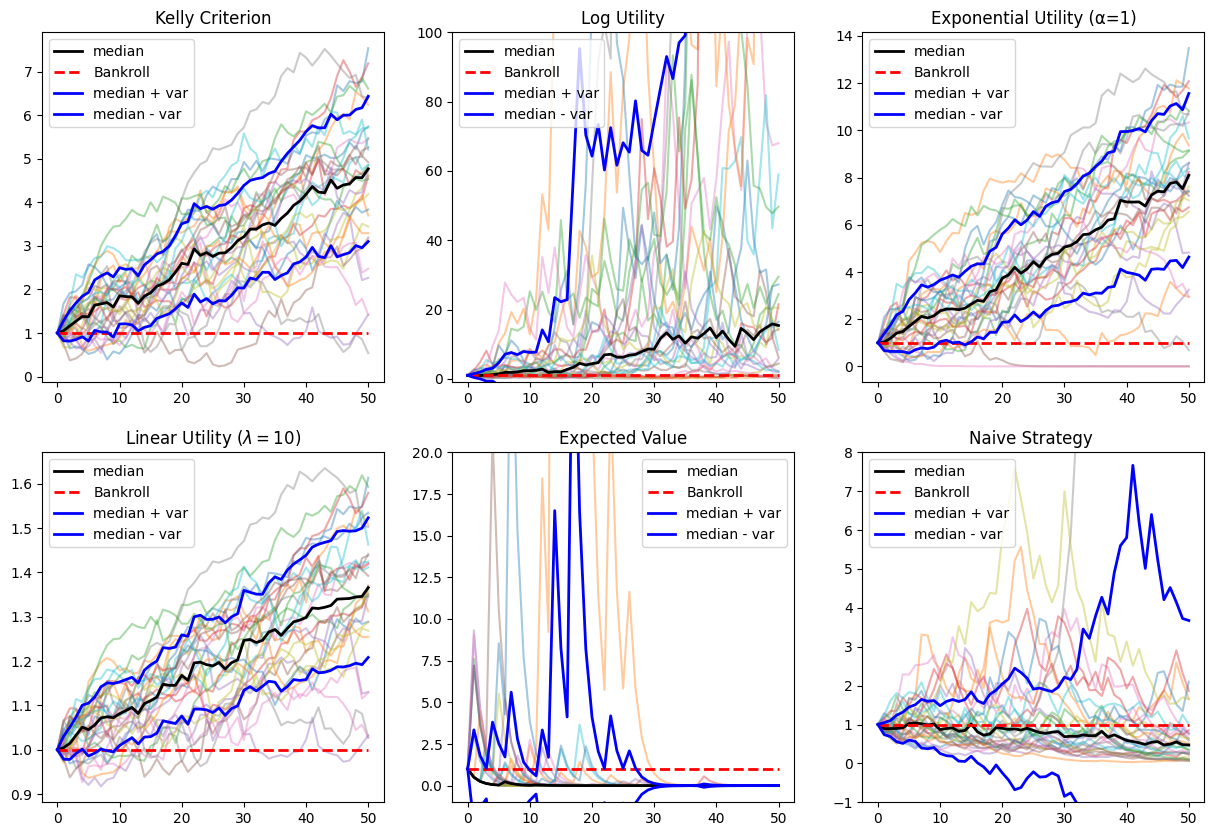
\includegraphics[width=1.1\textwidth, keepaspectratio]{images/monte_carlo_b=b.png}
    \caption{Monte carlo simulations for each strategy}
    \label{fig:monte_carlo}
\end{figure}


\begin{table}[H]
\centering
\caption{Final Bankroll Statistics}
\label{tab:final_bankroll}
\begin{tabular}{lrrrrr}
\toprule
\textbf{Strategy} & \textbf{Mean} & \textbf{Std Dev} & \textbf{Median} & \textbf{Min} & \textbf{Max} \\
\midrule
Kelly Criterion          & 4.48   & 1.67   & 4.77   & 0.54   & 7.54   \\
Log Utility              & 270.85 & 983.14 & 15.39  & 0.19   & 5414.01 \\
Exponential Utility      & 7.46   & 3.46   & 8.10   & 0.00   & 13.48  \\
Linear Utility           & 1.35   & 0.16   & 1.37   & 1.03   & 1.61   \\
Expected Value           & 0.00   & 0.00   & 0.00   & 0.00   & 0.01   \\
Naïve Strategy           & 1.20   & 3.20   & 0.47   & 0.06   & 18.19  \\
\bottomrule
\end{tabular}
\end{table}

The \textbf{Log Utility} strategy achieved the highest mean final bankroll but with significant variability, indicating high risk. The \textbf{Kelly Criterion} and \textbf{Exponential Utility} strategies demonstrated moderate returns with lower variability, suggesting consistent performance.

\begin{table}[H]
\centering
\caption{Average Growth Rate Per Step}
\label{tab:avg_growth}
\begin{tabular}{lr}
\toprule
\textbf{Strategy} & \textbf{Growth Rate} \\
\midrule
Kelly Criterion          & 2.82\% \\
Log Utility              & 5.54\% \\
Exponential Utility      & 2.55\% \\
Linear Utility           & 0.59\% \\
Expected Value           & $-$29.83\% \\
Naïve Strategy           & $-$1.55\% \\
\bottomrule
\end{tabular}
\end{table}

While the \textbf{Log Utility} strategy had the highest growth rate, it came with increased volatility. The \textbf{Kelly Criterion} and \textbf{Exponential Utility} strategies offered positive growth with better risk control.

\begin{table}[H]
\centering
\caption{Sharpe Ratio}
\label{tab:sharpe_ratio}
\begin{tabular}{lr}
\toprule
\textbf{Strategy} & \textbf{Sharpe Ratio} \\
\midrule
Kelly Criterion          & 0.30 \\
Log Utility              & 0.29 \\
Exponential Utility      & 0.25 \\
Linear Utility           & 0.30 \\
Expected Value           & 0.14 \\
Naïve Strategy           & 0.01 \\
\bottomrule
\end{tabular}
\end{table}

The highest Sharpe Ratios were achieved by the \textbf{Kelly Criterion} and \textbf{Linear Utility} strategies, indicating superior risk-adjusted returns.

\begin{table}[H]
\centering
\caption{Probability of Ruin}
\label{tab:prob_ruin}
\begin{tabular}{lr}
\toprule
\textbf{Strategy} & \textbf{Probability} \\
\midrule
Kelly Criterion          & 0.00\% \\
Log Utility              & 3.33\% \\
Exponential Utility      & 6.67\% \\
Linear Utility           & 0.00\% \\
Expected Value           & 100.00\% \\
Naïve Strategy           & 20.00\% \\
\bottomrule
\end{tabular}
\end{table}

Zero probability of ruin for the \textbf{Kelly Criterion} and \textbf{Linear Utility} strategies underscores their robustness.

An ANOVA test (performed to assess whether the differences in final bankrolls among the strategies), (F-statistic: 2.16, p-value: 0.0612) suggested that differences among strategies were not statistically significant at the 5\% level. However, the p-value is close to the threshold, suggesting that with a larger sample size, the differences might become statistically significant.

\subsection{Conclusion}

The simulations indicate that strategies like the \textbf{Kelly Criterion} and \textbf{Exponential Utility}, which balance growth and risk through utility maximization, offer favorable outcomes. The \textbf{Log Utility} strategy provides high growth potential but with greater volatility. Ignoring risk, as in the \textbf{Expected Value} strategy, leads to poor performance.

\textbf{Limitations} include the limited number of simulations, simplified assumptions, and exclusion of real-world factors like transaction costs.

\textbf{Recommendations} for future work involve increasing simulation runs, incorporating realistic market conditions, and exploring additional strategies.


\section{Online Testing}

To assess the strategies in a real-world environment, an online testing phase was conducted over five weeks, from 2024 August 24th to 2024 September 30th, focusing on matches from the five major European football leagues. This real-world testing evaluated the practical applicability and performance of the strategies under actual market conditions. Odds were scraped each day at 12pm from the Odd Api website.


\subsection{Static Problem Reduction and Parameter Settings}

To simplify the dynamic nature of sports betting, we reduced the problem to a series of static optimizations at discrete time intervals. At each decision point \( t \), bankroll allocation was optimized based on the current available information. This approach allowed us to manage the complexity of real-time betting while ensuring the practical applicability of the strategies.

\paragraph{Temporal Parameters}

Key temporal parameters were defined as follows:

\begin{itemize}
    \item \textbf{Betting Interval (\( \Delta t \))}: The interval between placing bets, set to 24 hours to capture daily betting opportunities.
    \item \textbf{Bet Placement Timing}: Bets were placed at a fixed time each day (12:00 PM) to ensure up-to-date information was used while accommodating market dynamics.
\end{itemize}

These settings ensured a balance between information accuracy and practical market conditions.

\paragraph{Match Selection}

The matches selected for each optimization were determined based on:

\begin{itemize}
    \item \textbf{Number of Matches (\( M \))}: Matches occurring within the next 24 hours were selected, balancing opportunity and reliability of information as well as having all results while perfomring next step.
    \item \textbf{Selection Criteria}: Focus was given to matches from top European leagues where the bettor had a higher perceived edge.
\end{itemize}

This careful match selection helped reduce computational complexity while enhancing potential returns.

\paragraph{Re-Betting Policy}

The re-betting policy was defined by the following criteria:

\begin{itemize}
    \item \textbf{Not allowing Re-Bets}: Additional bets on previously considered matches were not allowed. As we only bet on matches on the same day and only once a day, this was an implication of the previous choices.
\end{itemize}

This policy helped manage risk and adapt to evolving market conditions.

\subsection{Practical Implementation Settings}

The practical implementation settings for the online testing phase are summarized in Table~\ref{tab:implementation_settings}. The testing period ran from August 24, 2024, to September 30, 2024. The \texttt{trust-constr} algorithm was used for optimization, with a multiplier of \( \gamma = \frac{1}{2} \) applied to the matrix \( f \). The best odds from a pool of bookmakers (detailed in the appendix) were selected for each match.

\begin{table}[H]
\centering
\caption{Practical Implementation Settings}
\label{tab:implementation_settings}
\begin{tabular}{ll}
\toprule
\textbf{Setting}               & \textbf{Value}                                 \\ \midrule
Betting Interval (\( \Delta t \))     & 24 hours \\                                    
Bet Placement Time               & 12:00 PM daily                                \\
Look-Ahead Horizon               & Matches within the next 24 hours               \\ 
Re-Betting Policy                & Not allowed \\ 
Testing Period                   & August 24, 2024 – September 30, 2024           \\ 
Optimization Algorithm           & \texttt{trust-constr}                          \\ 
Strategy factor mult. \(\gamma\)         & \( 0.5 \)                              \\ 
Odds Selection                   & Biggest odds from a pool of bookmakers            \\ 
Markets & 5 biggest European leagues (Big 5) \\
\bottomrule
\end{tabular}
\end{table}


\subsection{Results and Interpretation}

Figure~\ref{fig:capital_evolution} illustrates the capital evolution for each strategy during the testing period. The Kelly and Exponential Utility strategies exhibited the strongest performance, both ending with approximately twice the initial capital. These results highlight their ability to optimally balance risk and reward, consistently outperforming the more conservative Log and Naive strategies. However, they also demonstrated higher volatility compared to the more stable Linear strategy.

\begin{figure}[H]
    \centering
    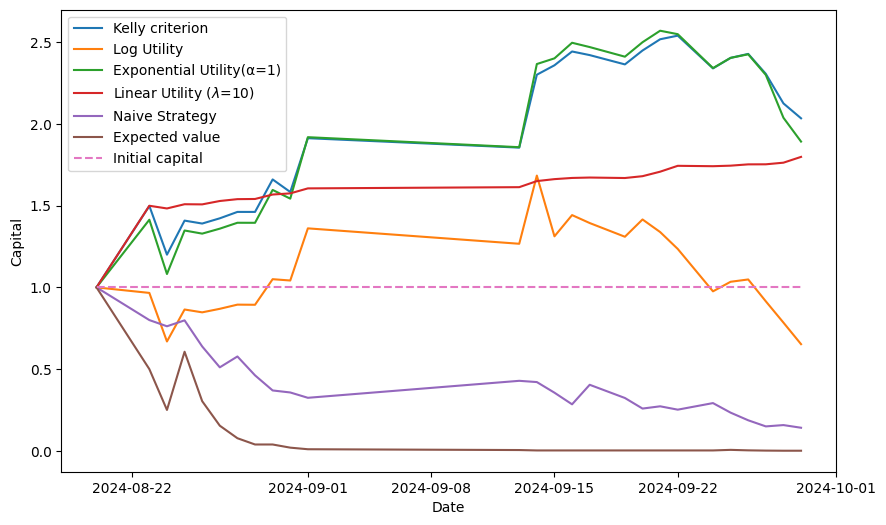
\includegraphics[width=\textwidth]{images/bankroll_evolution2.png}
    \caption{Capital Evolution for Each Strategy During the Online Testing Period}
    \label{fig:capital_evolution}
\end{figure}

The Log Utility strategy underperformed, particularly at the start and after the midpoint of the test period, failing to capitalize on high-return opportunities. Its conservative nature, aimed at minimizing risk, resulted in modest growth but ultimately led to a negative outcome. 

Both the Naive and Expected Value strategies experienced sharp declines in capital. The Naive strategy approached near-zero capital by the end of the test, while the Expected Value strategy exhibited extreme volatility, leading to rapid capital depletion. These simpler strategies, which lack sophisticated optimization, were highly vulnerable to adverse market conditions and failed to adapt effectively to fluctuations in odds or match outcomes.

In contrast, the Linear Utility strategy showed steady and consistent growth, with minimal volatility throughout the testing period, ultimately achieving a final growth of 1.8 times the initial capital. This highlights its effectiveness in maintaining a stable growth trajectory while avoiding the excessive risk associated with other strategies.

Overall, the results underscore the superiority of more advanced utility-based strategies such as Kelly and Linear. These approaches consistently outperformed simpler methods by balancing risk and reward more effectively under real-world betting conditions.

\subsection{Performance Metrics}

To further quantify the performance of each strategy, we computed key metrics, including final bankroll \( B(T) \), mean growth per step, and standard deviation of growth per step, both in absolute terms and as a percentage of the final bankroll. 
\begin{itemize}
    \item The mean growth per step is defined as:
    \[
    \mu = \frac{1}{T-1} \sum_{t=1}^{T-1} \Delta B_t
    \]
    where \( \Delta B_t = B_{t+1} - B_t \),
    \item the standard deviation of growth per step is given by:
    \[
    \sigma = \sqrt{\frac{1}{T-1} \sum_{t=1}^{T-1} (\Delta B_t - \mu)^2}
    \]
\end{itemize}


Table~\ref{tab:strategy_performance} summarizes the results for each strategy.

\begin{table}[H]
\centering
\caption{Strategy Performance Metrics}
\label{tab:strategy_performance}
\begin{tabular}{llll}
\toprule
\textbf{Strategy}              & \textbf{Final Bankroll \( B(T) \)} & \textbf{Mean Growth (\%)} & \textbf{Std Growth (\%)} \\ 
\midrule
Kelly Criterion                & 2.034                              & 2.034                      & 8.923                    \\ 
Log Utility                    & 0.653                              & -2.129                     & 26.516                   \\ 
Exponential Utility (\( \alpha = 1 \)) & 1.892                        & 1.886                      & 10.309                   \\ 
Linear Utility (\( \lambda = 10 \))    & 1.798                        & 1.776                      & 5.360                    \\ 
Naive Strategy                 & 0.141                              & -24.299                    & 52.419                   \\ 
Expected Value                 & 0.001                              & -5032.448                  & 18175.649                \\
\bottomrule
\end{tabular}
\end{table}

\subsection{Interpretation of Metrics}

The results demonstrate the effectiveness of the Kelly Criterion and Exponential Utility strategies, both of which ended with a final bankroll close to 2.0. These strategies also displayed reasonable volatility, with standard deviations of growth per step under 10\%. The Linear Utility strategy performed consistently, achieving steady growth with the lowest volatility among all strategies.

On the other hand, the Log Utility strategy suffered from negative growth, highlighting its inability to capitalize on high-return opportunities. The Naive and Expected Value strategies performed poorly, with significant capital depletion and extreme volatility, particularly for the Expected Value approach, indicating their inadequacy in real-world betting scenarios.


\section{Conclusion}

The results from both the Monte Carlo simulations and the real-world online testing phase demonstrate the clear advantages of sophisticated bankroll management strategies such as the Kelly Criterion and Exponential Utility methods. These strategies consistently provided strong returns while managing risk effectively, leading to a final bankroll close to twice the initial amount. In contrast, simpler strategies like the Naive and Expected Value approaches underperformed, suffering from capital depletion and high volatility, emphasizing the importance of balancing risk and return in real-world betting scenarios.

The Linear Utility strategy offered a steady, reliable growth trajectory with minimal volatility, making it an appealing option for risk-averse bettors. The Log Utility strategy, though conservative, failed to capture sufficient growth opportunities, resulting in a negative final outcome. Overall, the Kelly and Exponential Utility strategies are best suited for bettors seeking long-term growth with manageable risk.

\subsection{Limitations and Future Improvements}

Despite the promising results, several limitations were identified in the current approach:

\begin{itemize}
    \item \textbf{Simulation Assumptions}: The Monte Carlo simulations relied on several simplifying assumptions that limit the realism of the results. Firstly, the simulation of probabilities was based on the true clipped probabilities plus a bias and Gaussian noise, which does not fully capture the actual flaws in the predictive models, and the constants used were chosen arbitrarily without strong justification. Secondly, the bookmaker margin was fixed, and the odds provided by the bookmaker did not account for the influence of large bets from the players, which in reality could cause deviations in the bookmaker’s odds and probabilities. Lastly, the simulations used a fixed number of matches and time steps. Both the number of simulations and the range of strategies could be expanded to provide a more thorough and diverse analysis of performance over a wider variety of scenarios.
    \item \textbf{Limited Testing Period}: The online testing phase covered only a five-week period, which may not fully capture the long-term performance and robustness of each strategy. Extending the testing period or repeating it across multiple seasons would provide a more comprehensive assessment.
    \item \textbf{Risk Preferences}: While the utility-based strategies successfully managed risk, the models relied on fixed parameters for risk aversion (e.g., \( \lambda \) in Linear Utility). Introducing dynamic adjustments to these parameters based on market conditions or bettor preferences could further enhance performance.
\end{itemize}

\subsection{Future Work and Deployment on Azure Kubernetes}

The next stage of this project involves deploying the entire system on a cloud infrastructure using Kubernetes on Azure (AKS). This deployment will enable scalable, real-time processing of betting opportunities, continuous model updates, and the handling of multiple simultaneous users and markets. By leveraging Azure’s powerful compute and orchestration capabilities, the system will be capable of efficiently managing the computational load and data flows needed for real-time sports betting optimization.


\section{Microservices Architecture and Frameworks}

To build a scalable and maintainable system for sports betting optimization, we adopted a microservices architecture. This approach allows independent development, deployment, and scaling of individual components, facilitating modularity and flexibility.

The system comprises several microservices:

\begin{itemize}
    \item \textbf{Data Ingestion Service}: Collects real-time match data and odds from external APIs and web scraping. We use the Python library \textit{soccerdata} to conveniently scrape historical and real-time data from various websites. \textit{SQLAlchemy} is employed to communicate with the PostgreSQL database, allowing interaction using a mix of Python syntax and SQL queries. An API is provided for other services to trigger this service's logic, created using the \textit{FastAPI} framework. The Python library \texttt{logging} is used for proper logging of all operations, and \texttt{pandas} is utilized for data manipulation and transformation.

    \item \textbf{Prediction and Optimization Service}: Processes data to train models and generate probability estimates for the prediction component. Calculates optimal bet allocations based on the probabilities and selected strategies for the optimization component. \textit{Scikit-learn} is used for model training and inference, while \textit{SciPy.optimize} handles the optimization processes. Similar to the Data Ingestion Service, an API is deployed using \textit{FastAPI}, with communication to the database via \textit{SQLAlchemy}, and \texttt{logging} and \texttt{pandas} for logging and data handling.

    \item \textbf{User Interface Service}: Provides a web-based dashboard for monitoring and interaction, developed using the Python web framework \textit{Streamlit}.

    \item \textbf{Backend Service}: Manages communication and logic between the frontend User Interface and the database, as well as other services, using \textit{FastAPI}, \texttt{pandas}, and \texttt{logging}.

    \item \textbf{Database Service}: Stores historical data, odds, inferred probabilities, optimization results, and transaction logs. We chose PostgreSQL as the database due to its robustness, scalability, and compatibility with \textit{SQLAlchemy}. PostgreSQL's advanced features support complex queries and transactions essential for our application's needs.

    \item \textbf{MLflow Service}: Monitors the training metrics of the models. MLflow provides a convenient way to track experiments, record model parameters, metrics, and artifacts, facilitating reproducibility and model versioning.

    \item \textbf{Airflow Service}: Acts as a scheduler, providing a convenient way to orchestrate and monitor complex workflows using Directed Acyclic Graphs (DAGs). Apache Airflow allows us to define data pipelines, schedule tasks, and manage dependencies between them, ensuring timely execution of data ingestion, model training, and optimization processes.
\end{itemize}

Services communicate over HTTP/HTTPS protocols, with well-defined API endpoints ensuring loose coupling and ease of integration.

\section{Docker and Kubernetes}

To ensure consistency across development, testing, and production environments, all microservices are containerized using Docker \cite{Merkel2014}. Docker allows us to package each service with all its dependencies into isolated containers, ensuring consistent behavior across different environments.

\subsection{Dockerization}

Each microservice is encapsulated in a Docker container, defined by its own \texttt{Dockerfile}, which specifies the base image, dependencies, and entry points. In local development, we used containers for services such as MLflow, PostgreSQL, and Airflow, facilitating a consistent and reproducible environment.

\subsection{Kubernetes Deployment}

For orchestration and management of the containerized applications, we utilized Kubernetes \cite{HightowerEtAl2017}. Kubernetes automates deployment, scaling, and management of containerized applications. We packaged our system into a Helm chart, which simplifies the deployment of the entire application, including dependencies like MLflow, PostgreSQL, and Airflow.

\subsubsection{Helm Chart Packaging}

By encapsulating our services and their dependencies into a Helm chart, we streamlined the deployment process. Helm charts define, install, and upgrade complex Kubernetes applications, allowing us to manage configurations and versioning efficiently.

\subsubsection{Database Migrations}

Database schema changes are managed using migration files and scripts. Changes are first applied locally for testing and validation. Once validated, migrations are executed on the production database using scripts designed to apply changes incrementally. This process ensures that the database schema remains synchronized with the application code without disrupting ongoing operations.

\section{Deployment on Azure AKS}

\subsection{Azure Kubernetes Service (AKS)}

We deployed our Kubernetes cluster on Microsoft Azure using Azure Kubernetes Service (AKS), a managed Kubernetes service that simplifies cluster management by handling critical tasks like health monitoring and maintenance. AKS reduces the operational overhead and provides features like automated scaling and updates.

\begin{figure}[H]
    \centering
    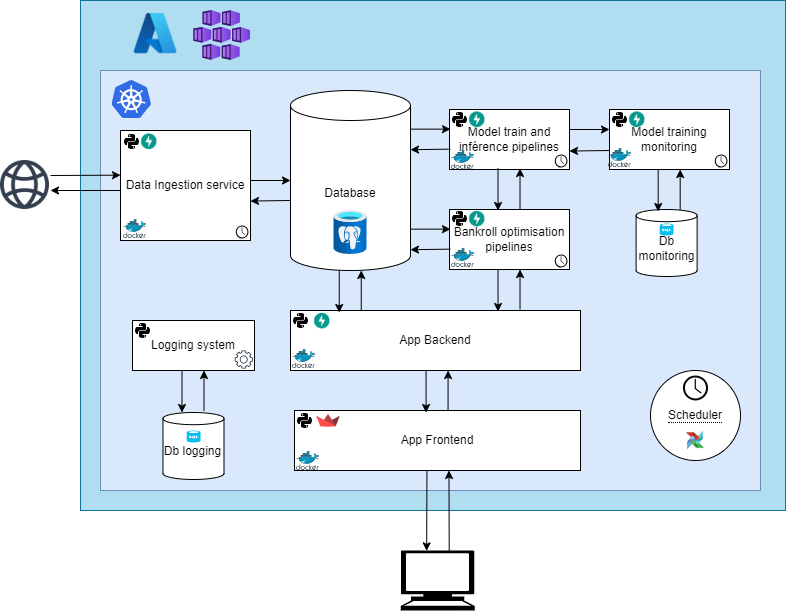
\includegraphics[width=0.8\textwidth, keepaspectratio]{images/diagrem_archi_services.png}
    \caption{Architecture of the system deployed on AKS}
    \label{fig:diagramme_arch_aks}
\end{figure}

\subsection{Infrastructure Details}

Our AKS deployment utilizes two virtual machines to ensure high availability and load balancing across the cluster. While Azure offers its own virtual machines, in this context, we refer to the compute resources allocated to our Kubernetes nodes. The integration with AKS allows for efficient resource utilization and scalability.

\subsection{Azure Services Integration}

Using Azure's cloud infrastructure offers several benefits:

\begin{itemize}
    \item \textbf{Azure Container Registry (ACR)}: Stores our Docker images securely, facilitating seamless deployment to AKS.
    \item \textbf{Azure DevOps Repo}: Provides a storage for our code.
\end{itemize}

\subsection{Pricing Considerations}

Azure's pricing model charges for compute resources used by virtual machines, storage, and network bandwidth. Managed services like AKS can reduce operational overhead but require careful monitoring to manage costs effectively. We optimized resource allocation by:


\section{Conclusion}

By adopting a microservices architecture, containerization with Docker, orchestration with Kubernetes, and deploying on Azure AKS, we built a scalable, reliable, and maintainable system for sports betting optimization. This architecture allows for independent development and deployment of components, ensuring the system can adapt to changing requirements and handle real-time data processing demands efficiently. Leveraging cloud infrastructure and managed services enhances our ability to focus on core application development while ensuring high availability and performance.

\section{Summary of Findings}

This study embarked on the ambitious task of developing a comprehensive system for optimizing sports betting strategies, focusing on football matches. Through the integration of predictive modeling, utility-based optimization, and scalable system architecture, we have addressed the critical components necessary for successful sports betting.

The predictive model, developed using logistic regression and advanced feature selection techniques, demonstrated significant accuracy in forecasting match outcomes. Regular retraining of the model proved essential in maintaining performance over time, highlighting the dynamic nature of sports data.

The optimization module applied various bankroll allocation strategies, including the Kelly Criterion, logarithmic, exponential, and linear utility functions. Both Monte Carlo simulations and real-world online testing over a five-week period indicated that sophisticated utility-based strategies substantially outperform naive betting approaches. Strategies like the Kelly Criterion and Exponential Utility provided favorable returns while effectively managing risk.

The system's deployment on Azure Kubernetes Service (AKS) showcased its scalability and readiness for real-time application. By leveraging a microservices architecture and containerization technologies like Docker and Kubernetes, the system can handle the computational demands of real-time data processing and optimization.

\section{Contributions to the Field}

This work contributes to the field of sports analytics and betting strategies in several ways:

\begin{itemize} \item \textbf{Integration of Predictive Modeling and Optimization}: By combining accurate probability estimations with utility-based optimization strategies, the system provides a robust framework for sports betting. \item \textbf{Scalable System Architecture}: The implementation of a microservices architecture and deployment on cloud infrastructure ensures that the system is scalable, maintainable, and adaptable to real-world conditions. \item \textbf{Empirical Evaluation}: The use of both simulations and real-world testing provides empirical evidence of the effectiveness of advanced betting strategies over simpler methods. \end{itemize}

\section{Limitations}

Despite the positive results, several limitations were identified:

\begin{itemize}
    \item \textbf{Predictive Model Enhancements}: While the current model performs adequately within the constraints of a static framework, it could be significantly improved by incorporating additional features, conducting hyperparameter optimization, and exploring more complex models such as deep learning architectures. These enhancements would allow the model to capture dynamic patterns and temporal dependencies inherent in football matches, which are not fully addressed due to the static nature of the current framework.

    \item \textbf{Static Framework Limitations and Long-Term Gain-Variance Interpretation}: The reduction of the betting problem to a static framework simplifies the optimization process but introduces limitations in interpreting gains and variance over the long term. Since the model does not account for intertemporal dependencies and the evolving nature of the bankroll, the strategies derived may not fully capture the risks associated with long-term betting. This static approach may lead to strategies that optimize short-term gains without adequately considering the cumulative effect on wealth over time. Future work should focus on extending the framework to a dynamic setting, allowing for a more accurate interpretation of long-term gain and variance, and better aligning the strategies with the bettor's long-term financial goals.

    \item \textbf{Risk Preferences and Dynamic Adaptation}: The optimization strategies employed fixed parameters for risk aversion, which do not adjust to changes in the bettor's wealth or market conditions over time. This static treatment of risk preferences limits the adaptability of the betting strategies, especially in a long-term context where the bettor's financial situation and the market dynamics can vary significantly. Introducing dynamic risk preferences that evolve with the bettor's bankroll and external factors would enhance the strategies' responsiveness and effectiveness, leading to better management of gain and variance over the long term.

    \item \textbf{Testing Period and Scope}: The real-world testing was confined to a five-week period focusing on the top five European leagues. Due to the static framework and the short testing duration, the evaluation may not fully reflect the strategies' performance over extended periods or in different market conditions. A longer testing period encompassing a broader range of leagues and varying competitive environments would provide more comprehensive insights into the strategies' long-term viability and their ability to manage gains and risks effectively within a dynamic setting.

\end{itemize}
\section{Future Work}

Building upon the findings of this study, several promising avenues can be explored to enhance the system's performance and address the challenges identified. 

Firstly, integrating real-time data streams and developing adaptive predictive models could significantly improve forecasting accuracy. By incorporating techniques from time-series analysis and machine learning, the model can capture temporal dependencies and evolving patterns inherent in football matches. This dynamic approach would allow the model to adjust to new information promptly, potentially leading to more accurate probability estimates and better alignment with the actual match outcomes.

Secondly, advancing the optimization strategies to include stochastic elements and multi-period planning could address the complexities associated with long-term gain and variance interpretation. Developing a dynamic framework that accounts for intertemporal dependencies and the evolving nature of the bankroll would enable more effective risk management. Strategies that adapt risk preferences in response to changes in the bettor's financial status or market conditions could lead to more sustainable betting practices and improved long-term financial outcomes.

Thirdly, conducting extensive real-world testing over longer periods and across a broader range of leagues and competitions would provide deeper insights into the robustness and generalizability of the betting strategies. Such testing would help to evaluate the performance of the models under varying market conditions and competitive environments, ensuring that the strategies remain effective over time and are not limited to specific contexts or short-term scenarios.

Finally, enhancing the user interface to offer more advanced analytics and personalized insights could empower users to make more informed decisions. Features that allow users to visualize performance trends, adjust parameters interactively, and receive tailored recommendations would improve the overall user experience. Providing tools for long-term performance monitoring and strategic adjustments would enable users to better understand the implications of their betting decisions and manage their bankrolls more effectively.

These potential developments represent initial steps toward refining the system's capabilities. By focusing on dynamic modeling, adaptive optimization, comprehensive testing, and user-centric design, future work can contribute to more robust predictive performance, effective risk management, and ultimately, more successful sports betting strategies.

\section{Final Remarks}

The integration of predictive modeling and utility-based optimization represents a significant step forward in developing effective sports betting strategies. This work demonstrates that with accurate predictions and strategic bankroll management, it is possible to achieve superior returns while managing risk effectively. The deployment on cloud infrastructure ensures that the system is ready for practical application, paving the way for future advancements in the field.


Je veux que tu me rédige un article de blog sur ce projet en format md. L'article doit prendre environ 10 min à lire et doit être interressant, prenant, il doit y avoir un bon story telling. Et plusieurs niveau de comprehension, pour les non initiés et pour les data scientist avancés.

Fais le en anglais

\chapter{Design and implementation of the solution}


\chapter{Introduction}

Sports betting has evolved into a sophisticated industry that combines statistical analysis, predictive modeling, and strategic financial management \cite{AndersonSally2013}. With the global popularity of football and the abundance of data available, there is a significant opportunity to apply advanced analytical techniques to optimize betting strategies. The challenge lies in accurately predicting match outcomes and effectively managing the allocation of betting capital to maximize returns while minimizing risk.

This report presents the development and implementation of a comprehensive system designed to address these challenges in sports betting. The system integrates predictive modeling to forecast football match outcomes and optimization algorithms to determine the optimal allocation of a bettor's bankroll. The focus is on creating a practical, scalable solution that can operate in real-time, leveraging cloud-based technologies and microservices architecture.

\section{Background and Motivation}

The sports betting market is highly competitive, with bettors seeking any edge to improve their chances of success. Traditional betting strategies often rely on intuition or simplistic models that fail to account for the complexities of sports data and market dynamics. The advancement of machine learning and statistical methods offers the potential to enhance predictive accuracy and optimize betting decisions systematically \cite{CainEtAl2000}.

Effective bankroll management is equally important, as even accurate predictions can lead to losses if the betting amounts are not strategically allocated. The application of utility theory and optimization techniques, such as the Kelly Criterion, provides a mathematical framework for balancing risk and reward in betting decisions. 

\section{Objectives of the Study}

The primary objectives of this study are:

\begin{itemize}
\item To establish a rigorous mathematical framework that defines the theoretical foundations and sets the stage for the study.
\item To develop a predictive model that accurately estimates the probabilities of football match outcomes using historical and real-time data. \item To design an optimization module that calculates the optimal fraction of the bankroll to wager on each betting opportunity, applying various utility-based strategies. \item To implement a scalable, microservices-based system architecture that integrates data collection, predictive modeling, optimization, and user interface components. \item To deploy the system on a cloud platform using Kubernetes for scalability and reliability. \item To evaluate the performance of different betting strategies through Monte Carlo simulations and real-world online testing. \end{itemize}

\section{Scope of the Report}

This report details the theoretical framework underlying the predictive modeling and optimization strategies, the system architecture and implementation, and the results of both simulated and real-world testing. The report is organized as follows:

\begin{itemize} \item Chapter 2 provides a theoretical presentation of the models and preliminary research conducted. \item Chapter 3 describes the design and implementation of the solution, including system architecture and data management. \item Chapter 4 focuses on the development, training, and evaluation of the predictive models for match outcomes. \item Chapter 5 discusses the optimization of bankroll allocation using various strategies. \item Chapter 6 details the deployment of the complete system on Azure Kubernetes Service and the practical considerations involved. \item Chapter 7 presents the conclusions drawn from the study and discusses potential future work. \end{itemize}

\section{Significance of the Study}

By integrating advanced predictive modeling with optimized bankroll allocation, this work aims to contribute to the field of sports analytics and betting strategies. The deployment of the system on a scalable cloud infrastructure demonstrates its practical applicability and readiness for real-world use. The findings from this study have implications for bettors seeking to enhance their strategies, as well as for researchers interested in the application of machine learning and optimization techniques in sports betting.

\chapter{Theoretical presentation and preliminary research}
\input{chapters/2_theoretical_presentation_and_preliminary_research/main}

\chapter{Design and implementation of the solution}
\input{chapters/3_design_and_implementation_of_the_solution/main}

\chapter{Predictive Modeling of Match Outcomes}
\input{chapters/4_predictive_modeling_of_match_outcomes/main}

\chapter{Optimization of bankroll allocation}
\input{chapters/5_Optimization_of_bankroll_allocation/main}

\chapter{Development of the Complete System and Production Deployment}
\input{chapters/6_Development_of_the_Complete_System and_Production _Deployment/main}

\chapter{Discussion and Conclusion}
\input{chapters/conclusion/main}

\appendix
\input{chapters/appendix/main}

\printbibliography[heading=bibintoc,title={References}]


\subsection{Matches and Outcomes}

At any given time \( t \in \mathbb{R}^+ \), we define the set of matches available for betting as:

\[
\mathbb{M}(t) = \{ m^1, m^2, \dots, m^{M(t)} \}
\]

where \( M(t) \in \mathbb{N} \) represents the total number of matches available at time \( t \).

For each match \( m^k \in \mathbb{M}(t) \), there is a set of possible outcomes:

\[
\Omega^k = \{ \omega_1^k, \omega_2^k, \dots, \omega_{N^k}^k \}
\]

where \( N^k \in \mathbb{N} \) represents the number of possible outcomes for match \( m^k \).

\paragraph{Example:} 
In a football match, possible outcomes might be chosen as \{home team wins, draw, away team wins\}, so \( N^k = 3\) \(\forall k\).

\subsection{Probabilities of Outcomes}

We define \( \mathbb{P}_Y( \omega_i^k ) \) as the probability that outcome \( \omega_i^k \) occurs for match \( m^k \), given the state of the world \( Y \) at time \( t \):

\[
r_i^k(t) = \mathbb{P}_Y( \omega_i^k )
\]

These probabilities may change over time as new information becomes available.

We introduce the random variable \( X_i^k \) associated with outcome \( \omega_i^k \):

\[
X_i^k = \begin{cases}
1, & \text{if outcome } \omega_i^k \text{ occurs}, \\
0, & \text{otherwise}.\\
\end{cases}
\]

Therefore, \( r_i^k(t) = \mathbb{P}_Y( X_i^k = 1 ) \). \\

\paragraph{Example:} 
Consider a football match \( m^k \) between Team A and Team B. The possible outcomes \( \omega_i^k \) are:

\[
\omega_1^k = \text{Team A wins}, \quad \omega_2^k = \text{Draw}, \quad \omega_3^k = \text{Team B wins}.
\]

At time \( t \), based on current information \( Y \) (such as form, injuries, and past results), the probabilities of these outcomes are:

\[
r_1^k(t) = \mathbb{P}_Y(\text{Team A wins}), \quad r_2^k(t) = \mathbb{P}_Y(\text{Draw}), \quad r_3^k(t) = \mathbb{P}_Y(\text{Team B wins}).
\]

For example, if \( r_1^k(t) = 0.55 \), it means there is a 55\% chance that Team A will win.

\subsection{Bettors and Bookmakers}

Let \( \mathbb{J} \) be the set of bettors, and \( \mathbb{B} \) be the set of bookmakers.

Each bettor \( J \in \mathbb{J} \) has a bankroll at time \( t \), denoted by:

\[
B_{\text{bettor}}^J(t)
\]

Similarly, each bookmaker \( B \in \mathbb{B} \) has a bankroll at time \( t \), denoted by:

\[
B_{\text{bookmaker}}^B(t)
\]

\subsection{Odds}

At time \( t \), bookmaker \( B \) offers odds on the outcomes of matches. For match \( m^k \), the odds offered by bookmaker \( B \) are:

\[
\mathbb{O}^k(B, t) = \{ o_1^{k,B}(t), o_2^{k,B}(t), \dots, o_{N^k}^{k,B}(t) \}
\]

where \( o_i^{k,B}(t) \) represents the odds offered on outcome \( \omega_i^k \) of match \( m^k \) at time \( t \). \\

\paragraph{Example:}
Consider the same football match \( m^k \) between Team A and Team B. At time \( t \), bookmaker \( B \) offers the following odds:

\[
\mathbb{O}^k(B, t) = \{ 2.00, 3.50, 4.00 \}
\]

Where \( o_1^{k,B}(t) = 2.00 \) for Team A to win, \( o_2^{k,B}(t) = 3.50 \) for a draw, and \( o_3^{k,B}(t) = 4.00 \) for Team B to win.

These odds represent the potential payouts for each outcome.

\subsection{Bets and Wagers}

At time \( t \), bettor \( J \) may choose to place bets on various outcomes. We define:

\begin{itemize}
    \item \( f_i^{k,J}(t) \): The fraction of bettor \( J \)'s bankroll \( B_{\text{bettor}}^J(t) \) that is wagered on outcome \( \omega_i^k \) of match \( m^k \).
    \item \( b_i^{k,J}(t) \): The bookmaker \( B \) with whom bettor \( J \) places the bet on outcome \( \omega_i^k \) of match \( m^k \).
\end{itemize}

Therefore, the amount wagered by bettor \( J \) on outcome \( \omega_i^k \) at time \( t \) is:

\[
w_i^{k,J}(t) = f_i^{k,J}(t) \times B_{\text{bettor}}^J(t)
\]


\paragraph{Example:}
Consider bettor \( J \) with a bankroll of \( B_{\text{bettor}}^J(t) = 100 \) units at time \( t \). Bettor \( J \) decides to wager:

\[
f_1^{k,J}(t) = 0.2 \quad \text{(20\% of the bankroll on Team A to win)}
\]

Thus, the amount wagered is:

\[
w_1^{k,J}(t) = 0.2 \times 100 = 20 \text{ units}
\] 

Bettor \( J \) places the 20-unit bet with bookmaker \( B \).

\subsection{Bankroll Evolution}

The evolution of the bettors' and bookmakers' bankrolls depends on the outcomes of the matches and the settlement of bets.

\subsubsection{Bettor's Bankroll Evolution}

The bankroll of bettor \( J \) at time \( t \) is given by:

\[
B_{\text{bettor}}^J(t) = B_{\text{bettor}}^J(0) + \int_0^t \sum_{b \in \mathcal{B}_{\text{settled}}^J(\tau)} G_{\text{bettor}}^J(b) \, d\tau
\]

where:

\begin{itemize}
    \item \( \mathcal{B}_{\text{settled}}^{J}(s) \) is the set of bets placed by bettor \( J \) that are settled at time \( s \).
    \item \( G_{\text{bettor}}^J(b) \) is the gain or loss from bet \( b \), calculated as:
    \[
    G_{\text{bettor}}^J(b) = w^{J}(b) \times \left( o^{B}(b) \times X(b) - 1 \right)
    \]
    \begin{itemize}
        \item \( w^{J}(b) \) is the amount wagered on bet \( b \).
        \item \( o^{B}(b) \) is the odds offered by bookmaker \( B \) for bet \( b \).
        \item \( X(b) \) indicates whether the bet was successful (\( X(b) = 1 \)) or not (\( X(b) = 0 \)).
    \end{itemize}
\end{itemize}

\paragraph{Example:}

Consider bettor \( J \) starts with a bankroll of \( B_{\text{bettor}}^J(0) = 100 \) units. At time \( t_1 \), the bettor places a bet of \( w^{J}(b) = 20 \) units on a match with odds \( o^{B}(b) = 2.50 \) offered by bookmaker \( B \).

If the outcome \( X(b) = 1 \) (the bettor wins the bet), the gain from the bet is:

\[
G_{\text{bettor}}^J(b) = 20 \times (2.50 \times 1 - 1) = 30 \text{ units}
\]

Thus, the updated bankroll at time \( t_1 \) is:

\[
B_{\text{bettor}}^J(t_1) = 100 + 30 = 130 \text{ units}
\]

If the bettor loses another bet at time \( t_2 \) with a wager of 30 units on odds of 3.00, then \( X(b) = 0 \) and the loss is:

\[
G_{\text{bettor}}^J(b) = 30 \times (3.00 \times 0 - 1) = -30 \text{ units}
\]

The bankroll at time \( t_2 \) becomes:

\[
B_{\text{bettor}}^J(t_2) = 130 - 30 = 100 \text{ units}
\]

\subsubsection{Bookmaker's Bankroll Evolution}

Similarly, the bankroll of bookmaker \( B \) at time \( t \) is given by:

\[
B_{\text{bookmaker}}^B(t) = B_{\text{bookmaker}}^B(0) + \int_0^t \sum_{J \in \mathcal{J}} \sum_{b \in \mathcal{B}_{\text{settled}}^{B,J}(\tau)} G_{\text{bookmaker}}^B(b) \, d\tau
\]

where:

\begin{itemize}

    \item \( \mathcal{J} \) is the set of all bettors \( \{ J_1, J_2, \dots, J_N \} \) placing bets with bookmaker \( B \).
    \item \( \mathcal{B}_{\text{settled}}^{B,J}(s) \) is the set of bets accepted by bookmaker \( B \) from bettor \( J \) that are settled at time \( s \).
    \item \( G_{\text{bookmaker}}^B(b) \) is the gain or loss from bet \( b \), which now takes into account multiple bettors \( J \), calculated as:
    
    \[
    G_{\text{bookmaker}}^B(b) = w^{J}(b) \times \left( 1 - o^{B}(b) \times X(b) \right)
    \]
    
    where:
    \begin{itemize}
        \item \( w^{J}(b) \) is the amount wagered by bettor \( J \) on bet \( b \).
        \item \( o^{B}(b) \) is the odds offered by bookmaker \( B \) for bet \( b \).
        \item \( X(b) \) indicates whether the bet was successful (\( X(b) = 1 \)) or not (\( X(b) = 0 \)).
    \end{itemize}
\end{itemize}
\subsubsection{Impact of Multiple Bettors}

For each bet \( b \), the gain or loss for bookmaker \( B \) depends on which bettor placed the bet. If bettor \( J \) wins, bookmaker \( B \) pays out, and if bettor \( J \) loses, bookmaker \( B \) gains:

\[
G_{\text{bookmaker}}^B(b) = - G_{\text{bettor}}^J(b)
\]

Thus, for each bet placed by a bettor \( J \), the bookmaker’s gain is equal to the bettor’s loss, and vice versa. With multiple bettors, the bookmaker's bankroll reflects the combined gains and losses from all bets settled across the bettors \( J_1, J_2, \dots, J_N \).


\subsection{Bankroll Factor}

To abstract from the initial bankroll amounts, we can define the \textit{Bankroll Factor} for bettors and bookmakers.

\subsubsection{Bettor's Bankroll Factor}

The bankroll factor for bettor \( J \) at time \( t \) is defined as:

\[
BF_{\text{bettor}}^J(t) = \frac{B_{\text{bettor}}^J(t)}{B_{\text{bettor}}^J(0)}
\]

This represents the growth of the bettor's bankroll relative to their initial bankroll.

\subsubsection{Bookmaker's Bankroll Factor}

Similarly, the bankroll factor for bookmaker \( B \) at time \( t \) is:

\[
BF_{\text{bookmaker}}^B(t) = \frac{B_{\text{bookmaker}}^B(t)}{B_{\text{bookmaker}}^B(0)}
\]

\subsection{Gain Calculation}

The cumulative gain for bettor \( J \) up to time \( t \) is:

\[
G_{\text{bettor}}^J(t) = B_{\text{bettor}}^J(t) - B_{\text{bettor}}^J(0) = B_{\text{bettor}}^J(0) \left( BF_{\text{bettor}}^J(t) - 1 \right)
\]

Similarly, for bookmaker \( B \):

\[
G_{\text{bookmaker}}^B(t) = B_{\text{bookmaker}}^B(t) - B_{\text{bookmaker}}^B(0) = B_{\text{bookmaker}}^B(0) \left( BF_{\text{bookmaker}}^B(t) - 1 \right)
\]


\subsection{Utility Function}

The utility function \( U \) represents the agent's preferences regarding risk and reward, crucial in decision-making under uncertainty \cite{KahnemanTversky1979}. Bettors and bookmakers use this function to optimize their gains over time while minimizing risk. Unlike expected returns, utility functions incorporate risk preferences, allowing agents to balance the trade-off between potential gains and variability 
\cite{Markowitz1952} \cite{Arrow1971} \cite{Pratt1964}.

\subsubsection{Forms of Utility Functions}

Different utility functions capture varying risk attitudes, ranging from risk-neutral to risk-averse behaviors. Below are the common types of utility functions in the betting market:

\paragraph{1. Expected Value Utility (Risk-Neutral)}

The simplest form, where utility is directly proportional to wealth:

\[
U(B) = B
\]

Agents using this function are risk-neutral, focusing solely on maximizing expected returns without considering risk.

\paragraph{2. Logarithmic Utility (Moderate Risk Aversion)}

Logarithmic utility models constant relative risk aversion (CRRA) and is expressed as:

\[
U(B) = \ln(B)
\]

This function reflects diminishing marginal utility of wealth, balancing risk and reward, commonly used in the Kelly Criterion \cite{Kelly1956} \cite{Thorp1975} for long-term growth.

\paragraph{3. Power Utility (CRRA)}

A generalization of logarithmic utility, with risk aversion controlled by \( \gamma \):

\[
U(B) = \frac{B^{1 - \gamma}}{1 - \gamma}, \quad \gamma \neq 1
\]

Higher \( \gamma \) values indicate greater risk aversion. When \( \gamma = 1 \), the function becomes logarithmic.

\paragraph{4. Exponential Utility (Constant Absolute Risk Aversion - CARA)}

The exponential utility models constant absolute risk aversion (CARA):

\[
U(B) = -e^{-\alpha B}
\]

Here, \( \alpha \) controls risk aversion. Agents using this function maintain consistent risk preferences regardless of wealth level.

\paragraph{5. Quadratic Utility}

Quadratic utility is given by:

\[
U(B) = B - \frac{\lambda}{2} B^2
\]

Though it captures increasing risk aversion, it has the drawback of implying decreasing utility at higher wealth levels, making it less commonly used.

\subsubsection{Implications of Different Utility Functions}

Each utility function models specific risk preferences, influencing the agent’s decisions:

\paragraph{Risk-Neutral Behavior}

Agents with linear utility (\( U(B) = B \)) focus solely on maximizing returns, indifferent to risk. This behavior is rare in practice due to the inherent risks in betting.

\paragraph{Risk-Averse Behavior}

Utility functions like logarithmic, power, and exponential represent risk-averse behavior:

\begin{itemize}
    \item \textbf{Logarithmic Utility:} Moderate risk aversion, favoring long-term growth.
    \item \textbf{Power Utility (CRRA):} Flexibility in modeling different degrees of risk aversion via \( \gamma \).
    \item \textbf{Exponential Utility (CARA):} Constant risk aversion regardless of wealth.
\end{itemize}

\paragraph{Risk-Seeking Behavior}

Agents may occasionally exhibit risk-seeking behavior, favoring higher variance. This is typically modeled by utility functions with convex regions or negative coefficients but is unsustainable in the long term.

\subsubsection{Choosing an Appropriate Utility Function}

Selecting the right utility function depends on:

\begin{itemize}
    \item \textbf{Risk Preference:} It should reflect the agent’s risk tolerance.
    \item \textbf{Mathematical Tractability:} Functions like logarithmic utility offer simpler analytical solutions.
    \item \textbf{Realism:} The chosen function should realistically model the agent’s behavior in the market.
\end{itemize}

In order to model the decision-making processes of bettors and bookmakers in sports betting, we adopt a general agent-based framework \cite{Ferguson1967}. This framework allows us to formalize the interactions between agents (bettors and bookmakers) and the environment (the sports betting market) in a comprehensive and systematic manner. By defining the state space, action space, and other essential components in the most general terms, we can capture the complexity of sports betting and lay the groundwork for more specific analyses.

\subsection{Agents in the Betting Market}

There are two primary types of agents in the sports betting market:

\begin{itemize}
    \item \textbf{Bettors (Players):} Individuals or entities who place bets on the outcomes of sporting events with the aim of maximizing their returns.
    \item \textbf{Bookmakers:} Organizations or individuals who offer betting opportunities by setting odds on the possible outcomes of sporting events, aiming to maximize their profits.
\end{itemize}

Each agent operates based on their own objectives, information, and strategies, interacting with the environment and other agents through their actions.

\subsection{State Space}

At any given time \( t \in \mathbb{R}^+ \), the state of the sports betting environment, denoted by \( S(t) \), encompasses all the information relevant to the agents' decision-making processes. The state space \( \mathcal{S} \) is the set of all possible states \( S(t) \).

The state \( S(t) \) can be defined as:

\[
S(t) = \left( \mathbb{M}(t), \Omega(t), \mathbb{O}(t), B_{\text{bettor}}(t), B_{\text{bookmaker}}(t), H(t), \mathcal{I}(t) \right)
\]

where:

\begin{itemize}
    \item \( \mathbb{M}(t) \): The set of all matches available at time \( t \).
    \item \( \Omega(t) \): The set of possible outcomes for each match in \( \mathbb{M}(t) \).
    \item \( \mathbb{O}(t) \): The set of odds offered by bookmakers for each possible outcome at time \( t \).
    \item \( B_{\text{bettor}}(t) \): The set of bettors' bankrolls at time \( t \).
    \item \( B_{\text{bookmaker}}(t) \): The set of bookmakers' bankrolls at time \( t \).
    \item \( H(t) \): The history of past events up to time \( t \), including past bets, match results, and odds movements.
    \item \( \mathcal{I}(t) \): Any additional information available to the agents at time \( t \), such as team news, player injuries, weather conditions, etc.
\end{itemize}

The state \( S(t) \) encapsulates all the variables that can influence the agents' decisions, making it comprehensive and general.

\subsection{Action Space}

At each time \( t \), agents choose actions from their respective action spaces:

\subsubsection{Bettors' Action Space}

The action space for a bettor \( J \) at time \( t \), denoted by \( \mathcal{A}_{\text{bettor}}^J(t) \), consists of all possible betting decisions they can make. An action \( A_{\text{bettor}}^J(t) \in \mathcal{A}_{\text{bettor}}^J(t) \) can be defined as:

\[
A_{\text{bettor}}^J(t) = \left\{ \left( f_i^k \right) \mid f_i^k \in [0,1] , \sum_{i,k}f_i^k <= 1\right\}
\]

where:

\begin{itemize}
    \item \( f_i^k \): The fraction of the bettor's bankroll \( B_{\text{bettor}}^J(t) \) to wager on outcome \( \omega_i^k \).
\end{itemize}

Hence, the bettor chose the outcomes to bet on by assigning 0 (no bet) or more to an outcome at a given time \(t\).


\subsubsection{Bookmakers' Action Space}

The action space for a bookmaker \( B \) at time \( t \), denoted by \( \mathcal{A}_{\text{bookmaker}}^B(t) \), can be simplified to the selection of odds for each outcome. An action \( A_{\text{bookmaker}}^B(t) \in \mathcal{A}_{\text{bookmaker}}^B(t) \) is defined as:

\[
A_{\text{bookmaker}}^B(t) = \left\{ \mathbb{O}^k(B, t) = \{ o_i^k \mid o_i^k \in [1, \infty) \right\}
\]

where:

\begin{itemize}
    \item \( o_i^k \): The odds set by the bookmaker \( B \) for outcome \( \omega_i^k \) of match \( m^k \) at time \( t \). 
\end{itemize}

If \( o_i^k = 1 \), the bookmaker does not offer bets on outcome \( \omega_i^k \). If all odds \( o_i^k = 1 \) for a match \( m^k \), the bookmaker does not offer that match for betting.

\paragraph{Example:}
At time \( t \), bettor \( J \) allocates fractions of their \( 100 \) unit bankroll across two matches, with three possible outcomes:

\[
f = \begin{pmatrix}
0.3 & 0.2 & 0 \\
0.5 & 0 & 0 \\
\end{pmatrix}
\]

The bookmaker sets the following odds for each outcome:

\[
o = \begin{pmatrix}
2.50 & 3.00 & 4.00 \\
1.80 & 2.90 & 3.50 \\
\end{pmatrix}
\]

This means bettor \( J \) wagers 30 units on \( \omega_1^1 \) (Team A wins \( m^1 \)), 20 units on \( \omega_2^1 \) (draw in \( m^1 \)), and 50 units on \( \omega_1^2 \) (Team A wins \( m^2 \)).


\subsection{Transition Dynamics}

The state transitions \( \frac{dS(t)}{dt} \) are governed by the interactions between the agents' actions and the environment. The transition dynamics can be described in general terms:

\[
\frac{dS(t)}{dt} = \Phi\left( S(t), A_{\text{bettor}}(t), A_{\text{bookmaker}}(t), \epsilon(t) \right)
\]

where:

\begin{itemize}
    \item \( \Phi \) is the state transition function.
    \item \( A_{\text{bettor}}(t) \): The set of all bettors' actions at time \( t \).
    \item \( A_{\text{bookmaker}}(t) \): The set of all bookmakers' actions at time \( t \).
    \item \( \epsilon(t) \): Represents the stochastic elements inherent in sports outcomes and market dynamics, modeled as random variables.
\end{itemize}

The transition function \( \Phi \) captures how the state evolves due to:

\begin{itemize}
    \item The resolution of matches (outcomes becoming known), represented by changes in outcome variables over time..
    \item The settlement of bets (adjustment of bettors' and bookmakers' bankrolls).
    \item Changes in available matches and odds for the next time period.
    \item Updates to the history \( H(t) \) and information set \( \mathcal{I}(t) \), represented by \(\frac{dH(t)}{dt}\) and \(\frac{d\mathcal{I}(t)}{dt}\).
\end{itemize}


\subsection{Policies}

Each agent follows a policy that guides their decision-making process:

\subsubsection{Bettors' Policy}

A bettor's policy \( \pi_{\text{bettor}}^J \) is a mapping from states to actions:

\[
\pi_{\text{bettor}}^J: \mathcal{S} \rightarrow \mathcal{A}_{\text{bettor}}^J
\]

The policy determines how the bettor decides on which bets to place and how much to wager, based on the current state \( S(t) \).

\subsubsection{Bookmakers' Policy}

A bookmaker's policy \( \pi_{\text{bookmaker}}^B \) is a mapping from states to actions:

\[
\pi_{\text{bookmaker}}^B: \mathcal{S} \rightarrow \mathcal{A}_{\text{bookmaker}}^B
\]

The policy dictates how the bookmaker sets odds and offers betting opportunities, considering factors like market demand, risk management, and competitive positioning.

\subsection{Objectives and Constraints}

Each agent aims to optimize an objective function over time, such as maximizing expected utility or profit, subject to specific constraints that reflect their operational limitations and risk management considerations.

\subsubsection{Bettors' Objective}

The bettor seeks to maximize a chosen utility over a time horizon \( T \):

\[
\max_{\pi_{\text{bettor}}^J} \quad \mathbb{E} \left[ U^{J} \left( BF_{\text{bettor}}^J(T) \right) \right]
\]

\subsubsection{Constraints for the Bettor}

The bettor's optimization problem is subject to the following mathematical constraints: 

\begin{itemize}
    \item 1. Budget Constraint at Each Time \( t \):

   The total fraction of the bankroll wagered on all outcomes cannot exceed 1 at any time \( t \):

   \[
   \sum_{k=1}^{M(t)} \sum_{i=1}^{N^k} f_i^{k,J}(t) \leq 1 \quad \forall t
   \]

   where:
   \begin{itemize}
       \item \( f_i^{k,J}(t) \) is the fraction of the bettor \( J \)'s bankroll \( BF_{\text{bettor}}^J(t) \) wagered on outcome \( i \) of match \( k \) at time \( t \).
       \item \( M(t) \) is the total number of matches available at time \( t \).
       \item \( N^k \) is the number of possible outcomes for each match \(k\).
   \end{itemize}


\item 2. Non-Negativity of Wager Fractions:

   The bettor cannot wager negative fractions of the bankroll:

   \[
   f_i^{k,J}(t) \geq 0 \quad \forall i, k, t
   \]
\end{itemize}



\subsubsection{Bookmakers' Objective}

The bookmaker aims to maximize a chosen utility over a time horizon \( T \):

\[
\max_{\pi_{\text{bookmaker}}^B} \quad \mathbb{E} \left[ U^{B} \left( BF_{\text{bookmaker}}^B(T) \right) \right]
\]


\subsubsection{Constraints for the Bookmaker}

The bookmaker's optimization problem is subject to the following mathematical constraints:

\begin{itemize}
    \item 1. Liquidity Constraint:
    
       The bookmaker must ensure sufficient funds to cover potential payouts:
    
       \[
       BF_{\text{bookmaker}}^B(t) \geq \text{Maximum Potential Liability at } t
       \]
    
       This ensures that the bookmaker's bankroll at time \( t \) is greater than or equal to the maximum possible payout based on the accepted bets.
    
    \item 2. Odds Setting Constraints:
    
       The odds must be set to ensure profitability and competitiveness:
    
       \begin{itemize}
          \item Overround Constraint (Bookmaker's Margin):
    
            For each match \( k \), the sum of the implied probabilities must exceed 1:
    
            \[
            \sum_{i=1}^{N^k} \frac{1}{o_i^k(t)} = 1 + \epsilon^k(t) \quad \forall k, t
            \]
    
            Here, \( \epsilon^k(t) > 0 \) represents the bookmaker's margin for match \( k \) at time \( t \).
    
          \item Margin Bound:
    
            To balance profitability and competitiveness, we impose the following bound on \( \epsilon^k(t) \):
    
            \[
            \epsilon_{\text{min}} \leq \epsilon^k(t) \leq \epsilon_{\text{max}} \quad \forall k, t
            \]
    
            This ensures that the margin \( \epsilon^k(t) \) stays within a specified range, keeping the odds competitive enough to attract bettors while securing a minimum margin for profitability.
          
          \item Competitive Odds Constraint:
    
            The odds \( o_i^k(t) \) must remain competitive, influenced by market averages or competitors' odds. Therefore, the bookmaker may aim to keep \( \epsilon^k(t) \) as low as possible while maintaining profitability and covering risk.
       \end{itemize}
\end{itemize}

Building upon the general agent-based betting framework, we aim to simplify the agent-based betting framework and reduce computational complexity. We transition from a dynamic to a static optimization model by introducing key assumptions. By assuming immediate resolution of bets and the absence of intertemporal dependencies—where current decisions do not influence future opportunities—we make the static and dynamic problems effectively equivalent for our purposes. This simplification allows us to optimize agents' decisions at each time step independently, facilitating the derivation of optimal solutions without the need for complex dynamic programming. However, this reduction comes at a cost, notably in terms of long-term interpretability, as the model no longer accounts for cumulative effects and evolving dynamics over time.

\subsection{Hypotheses for the Constrained Problem}

\begin{enumerate}
    \item \textbf{No Intertemporal Dependencies (Additive Utility Function):} 
    Utility is additive over time, meaning decisions at time \( t \) do not affect future periods. The agent maximizes utility independently at each step, simplifying the problem into sequential sub-problems.
    
    \textit{Reason:} This eliminates the need to account for future wealth in current decisions, reducing complexity.

    \item \textbf{Discrete Time Steps:} 
    Time is divided into discrete intervals where decisions are made periodically. Bets are resolved by the end of each period before moving to the next. \( t = 0, 1, 2, \dots, T \)
    
    \textit{Reason:} Discrete time steps reduce the dynamic problem to a series of static decisions, simplifying optimization.

    \item \textbf{Non-Overlapping Bets:} 
    Bets are settled within the same period, ensuring that wealth at the end of each period is fully available for the next, avoiding unresolved wagers impacting future decisions.
    
    \textit{Reason:} This ensures no carryover of unresolved bets, keeping each period's wealth independent.

    \item \textbf{Independence of Match Outcomes:} 
    Match outcomes are independent random events, meaning there is no correlation between the results of different matches.
    
    \textit{Reason:} This simplifies probability calculations by eliminating the need to model inter-match dependencies.

    \item \textbf{Static Information Environment:} 
    Information is fixed within each period. No new data arrives mid-period, and updates are considered only in the next time step.
    
    \textit{Reason:} A static environment avoids real-time strategy adjustments, making the problem more manageable.
\end{enumerate}

These assumptions significantly simplify the model by reducing the complexity inherent in a dynamic optimization problem, but they also modify or limit certain long-term interpretations, such as how future wealth or intertemporal risk is managed across multiple betting periods.

\subsection{Simplification of the Utility Maximization Problem}

With no overlapping bets and a static information environment, agents do not need to consider how current actions might affect future opportunities or states. This myopic decision-making approach allows agents to focus solely on the current time period, simplifying their optimization problem to a static one.

Hence, the agents' objective functions depend only on the current wealth and the outcomes of bets placed in the current period. The expected utility maximization problem at each time \( t \) becomes:

For bettors:
\[
\max_{\{ f_i^{k,J}(t) \}} \quad \mathbb{E} \left[ U\left( B_{\text{bettor}}^J(t+1) \right) \mid S(t) \right]
\]

For bookmakers:
\[
\max_{\{ o_i^k(t) \}} \quad \mathbb{E} \left[ U\left( B_{\text{bookmaker}}(t+1) \right) \mid S(t) \right]
\]

where \( S(t) \) is the state at time \( t \), which includes the available matches, odds, and the agents' current bankrolls.

\subsection{Dynamic and Total Utility under Assumptions}

In our framework, under the assumption of discrete time steps and no intertemporal dependencies, the total utility across all periods \( T \) is given by the sum of the static utilities at each time step:

\[
U_{\text{total}} = \sum_{t=1}^{T} U(B(t)).
\]

This assumes that decisions are made independently at each \( t \), with the utility depending solely on the wealth \( B(t) \) at that moment. Additive utility functions, such as \( U(B) = B \), respect this assumption directly, meaning maximizing the utility at each step also maximizes total utility.

However, logarithmic and exponential utilities do not preserve a simple additive structure due to risk preferences that influence future decisions. While linear utility maintains additivity, \( U(B) = \ln(B) \) and \( U(B) = -e^{-\alpha B} \) do not.

\subsubsection{Utility Functions Respecting Additivity}
\begin{itemize}
\item Linear utility: \( U(B) = B \)
\end{itemize}

\subsubsection{Utility Functions Not Respecting Additivity}
\begin{itemize}
\item Logarithmic utility: \( U(B) = \ln(B) \)
\item Exponential utility: \( U(B) = -e^{-\alpha B} \)
\item CRRA: \(U(B) = \frac{B^{1 - \gamma}}{1 - \gamma}, \quad \gamma \neq 1\)
\item Quadratic utility: \(U(B) = B - \frac{\lambda}{2} B^2\)
\end{itemize}

\subsubsection{Approximation with Additive Properties}
By using a first-order Taylor expansion for \( \ln(B) \) or \( -e^{-\alpha B} \), these utilities can become approximately additive. For small deviations around \( B \), we approximate:

\[
\ln(B) \approx \ln(B_0) + \frac{B - B_0}{B_0}, \quad -e^{-\alpha B} \approx -e^{-\alpha B_0} + \alpha e^{-\alpha B_0} (B - B_0)
\]

These approximations are linear in \( B \), making the utility functions additive for small changes in wealth. Under these assumptions, the complexity of the problem is reduced, allowing the use of simpler optimization techniques without fully abandoning the original utility structure.

\subsubsection{Non-Additive Utility Maximization and Long-Term Interpretation}

When maximizing non-additive utility functions (such as logarithmic or exponential) at each step \( t \), the interpretation of utility over the entire period \( T \) changes. Unlike additive functions, where the total utility is simply the sum of the utilities at each time step, non-additive functions induce a more complex relationship between short-term and long-term behavior.

For non-additive utilities, maximizing utility at each step does not guarantee maximization of the utility across the entire period. The decisions made at each step can interact non-linearly across time, meaning that the long-term growth or risk profile may differ significantly from the one-step behavior. This highlights the difference between local (step-by-step) optimization and the global impact over the entire period.

\subsubsection{Interpretation of Log Utility in Terms of Long-Term Geometric Growth}

Maximizing the logarithmic utility at each time step involves maximizing the expected utility:

\[
\max_{f(t)} \mathbb{E}\left[ \ln B_{\text{agent}}(t+1) \, \big| \, \mathcal{F}_t \right],
\]

where \( B_{\text{agent}}(t+1) \) is the wealth at time \( t+1 \), \( f(t) \) represents the decision variables at time \( t \), and \( \mathcal{F}_t \) denotes the information available at time \( t \).

The total utility over \( T \) periods is given by:

\[
U_{\text{total}} = \sum_{t=1}^{T} \ln B_{\text{agent}}(t) = \ln\left( \prod_{t=1}^{T} B_{\text{agent}}(t) \right).
\]

Taking the expectation of the total utility, we have:

\[
\mathbb{E}[ U_{\text{total}} ] = \mathbb{E}\left[ \ln\left( \prod_{t=1}^{T} B_{\text{agent}}(t) \right) \right].
\]

However, due to the concavity of the logarithm and the properties of expectations, we cannot simplify this expression to \( \ln \left( \prod_{t=1}^{T} \mathbb{E}[ B_{\text{agent}}(t) ] \right) \) unless the \( B_{\text{agent}}(t) \) are deterministic. The expected value of the logarithm of a product of random variables is not equal to the logarithm of the product of their expectations.

To interpret \( \mathbb{E}[ U_{\text{total}} ] \) in terms of expected wealth and variance, we can use a second-order Taylor expansion of the logarithm around \( \mathbb{E}[ B_{\text{agent}}(t) ] \):

\[
\mathbb{E}[ \ln B_{\text{agent}}(t) ] \approx \ln \mathbb{E}[ B_{\text{agent}}(t) ] - \frac{1}{2} \frac{ \mathbb{V}\mathrm{ar}[ B_{\text{agent}}(t) ] }{ \left( \mathbb{E}[ B_{\text{agent}}(t) ] \right)^2 }.
\]

Summing over \( T \) periods, we obtain:

\[
\mathbb{E}[ U_{\text{total}} ] \approx \sum_{t=1}^{T} \left( \ln \mathbb{E}[ B_{\text{agent}}(t) ] - \frac{1}{2} \frac{ \mathbb{V}\mathrm{ar}[ B_{\text{agent}}(t) ] }{ \left( \mathbb{E}[ B_{\text{agent}}(t) ] \right)^2 } \right).
\]

This approximation shows that the expected total utility depends on both the expected wealth and the variance at each time step. The logarithmic utility function captures the trade-off between expected wealth growth and risk (variance), penalizing volatility and favoring steady growth.

Over the long term, maximizing the expected logarithmic utility leads to maximizing the \textbf{expected logarithm of cumulative wealth}, which corresponds to maximizing the \textbf{geometric mean return}. This strategy ensures that wealth grows at the highest possible geometric rate, accounting for both returns and risks.

\subsubsection{Long-Term Interpretation of Exponential Utility}

For the exponential utility function \( U(B) = -e^{ -\alpha B } \), where \( \alpha > 0 \) is the coefficient of absolute risk aversion, the total utility over \( T \) periods is:

\[
U_{\text{total}} = \sum_{t=1}^{T} U( B(t) ) = -\sum_{t=1}^{T} e^{ -\alpha B(t) }.
\]

Taking the expectation, we have:

\[
\mathbb{E}[ U_{\text{total}} ] = -\sum_{t=1}^{T} \mathbb{E}\left[ e^{ -\alpha B(t) } \right ].
\]

We cannot simplify \( \mathbb{E}\left[ e^{ -\alpha B(t) } \right ] \) without specifying the distribution of \( B(t) \). However, using a second-order Taylor expansion around \( \mathbb{E}[ B(t) ] \):

\[
\mathbb{E}\left[ e^{ -\alpha B(t) } \right ] \approx e^{ -\alpha \mathbb{E}[ B(t) ] } \left( 1 + \frac{ \alpha^2 }{2} \mathbb{V}\mathrm{ar}[ B(t) ] \right).
\]

Therefore, the expected total utility becomes:

\[
\mathbb{E}[ U_{\text{total}} ] \approx -\sum_{t=1}^{T} e^{ -\alpha \mathbb{E}[ B(t) ] } \left( 1 + \frac{ \alpha^2 }{2} \mathbb{V}\mathrm{ar}[ B(t) ] \right).
\]

This expression highlights that the expected utility depends heavily on both the expected wealth and the variance. As \( \alpha \) increases, the variance term becomes more significant, reinforcing the agent's aversion to risk. The exponential utility function thus focuses on \textbf{risk minimization} and \textbf{capital preservation} over wealth maximization.

\subsubsection{Long-Term Interpretation of Mean-Variance Utility}

For the mean-variance utility, which can be associated with a quadratic utility function \( U(B) = B - \frac{ \lambda }{ 2 } B^2 \) for small variations in \( B \), the expected utility at each time step is:

\[
\mathbb{E}[ U(B(t)) ] = \mathbb{E}[ B(t) ] - \frac{ \lambda }{ 2 } \mathbb{E}[ B(t)^2 ].
\]

Assuming that \( \mathbb{E}[ B(t)^2 ] = \left( \mathbb{E}[ B(t) ] \right)^2 + \mathbb{V}\mathrm{ar}[ B(t) ] \), we have:

\[
\mathbb{E}[ U(B(t)) ] = \mathbb{E}[ B(t) ] - \frac{ \lambda }{ 2 } \left( \left( \mathbb{E}[ B(t) ] \right)^2 + \mathbb{V}\mathrm{ar}[ B(t) ] \right).
\]

Over \( T \) periods, the expected total utility is:

\[
\mathbb{E}[ U_{\text{total}} ] = \sum_{t=1}^{T} \mathbb{E}[ U(B(t)) ].
\]

Simplifying, we obtain:

\[
\mathbb{E}[ U_{\text{total}} ] = \sum_{t=1}^{T} \left( \mathbb{E}[ B(t) ] - \frac{ \lambda }{ 2 } \left( \left( \mathbb{E}[ B(t) ] \right)^2 + \mathbb{V}\mathrm{ar}[ B(t) ] \right) \right).
\]

This expression demonstrates that the agent considers both the expected wealth and the variance, with the parameter \( \lambda \) controlling the trade-off between maximizing returns and minimizing risk.

\subsection{Simplification of State Transitions}

The agents' state variables, particularly their bankrolls, evolve in a straightforward manner without considering future uncertainties or pending bets. The bankroll update equations become:

\[
B_{\text{bettor}}(t+1) = B_{\text{bettor}}(t) + G_{\text{bettor}}(t)
\]

\[
B_{\text{bookmaker}}(t+1) = B_{\text{bookmaker}}(t) + G_{\text{bookmaker}}(t)
\]

where \( G_{\text{bettor}}(t) \) and \( G_{\text{bookmaker}}(t) \) represent the gains or losses realized from bets placed and settled within time \( t \).


\subsection{Detailed Simplification of the Bookmaker's Problem}

Similarly, the bookmaker's optimization problem simplifies under the assumptions:

\paragraph{Objective Function:}

\[
\max_{\{ o_i^k(t) \}} \quad U_{\text{bookmaker}}(t) = \mathbb{E} \left[ U\left( B_{\text{bookmaker}}(t) + G_{\text{bookmaker}}(t) \right) \mid S(t) \right]
\]

\paragraph{Constraints:}

   \[
   BF_{\text{bookmaker}}^B(t) \geq \text{Maximum Potential Liability at } t
   \]

    \[
     \sum_{i=1}^{I} \frac{1}{o_i^k(t)} = 1 + \epsilon^k(t) \quad \text{for all } k, t
    \]


\paragraph{Variables:}

\begin{itemize}
    \item \( o_i^k(t) \): Odds set for outcome \( i \) of match \( k \) at time \( t \).
    \item \( G_{\text{bookmaker}}(t) \): Gain or loss from bets, calculated based on the total bets received and payouts made in the current period.
    \item \(\epsilon^k(t)\): Margin for each match at every time step that the bookmaker set to maximise attractiveness, minimize risque and maximize pay off.
\end{itemize}

\subsection{Reasons for the Simplifications}

We introduce these simplifications for several important reasons:

\subsubsection{Reducing Computational Complexity}

Dynamic optimization problems, especially those involving stochastic elements and intertemporal dependencies, can be highly complex and computationally intensive. By simplifying the problem to a static one, we make it more tractable and amenable to analytical or numerical solutions.

\subsubsection{Simplifying the Use of Historical Odds}

Solving the general dynamic optimization problem requires a sufficiently large history of odds at each time step \( t \) to ensure convergence towards an optimal solution. This includes tracking all relevant historical data for each time step and state \( S \). By reducing the problem to a static case, the need for such an extensive history is eliminated, as the model only relies on current odds. This simplification significantly reduces computational complexity while maintaining the core of the decision-making process.



\subsubsection{Facilitating Analytical Derivations}

With the assumptions of immediate bet resolution and independence, we can derive closed-form solutions or straightforward algorithms for optimal betting strategies, such as the Kelly Criterion for bettors using logarithmic utility functions.

\subsubsection{Focusing on Core Decision-Making Principles}

The simplifications allow us to isolate and analyze the fundamental principles of optimal betting and odds setting without the confounding effects of dynamic interactions. This clarity helps in understanding the key factors that influence agents' decisions in the sports betting market.

\subsection{Limitations of the Simplified Model}

While the simplifications make the model more manageable, they also introduce limitations that should be acknowledged:

\begin{enumerate}
    \item \textbf{Hypothesis: Additive Utility Function with No Intertemporal Dependencies}
        \begin{itemize}
            \item \textbf{Domain of Validity:} Valid when agents focus solely on immediate wealth without concern for future utility.
            \item \textbf{Limitation with Reality:} Agents usually consider future wealth and utility; this assumption ignores long-term planning and risk preferences.
            \item \textbf{Risk:} Ignoring intertemporal effects may result in strategies that maximize short-term gains at the expense of long-term wealth, increasing the risk of ruin or failing to achieve overall financial objectives. Among the utility functions described, only \(U(B)=B\) is additive with time.
        \end{itemize}
        
    \item \textbf{Hypothesis: Discrete Time Steps}
        \begin{itemize}
            \item \textbf{Domain of Validity:} Applicable when betting decisions are made at fixed, regular intervals.
            \item \textbf{Limitation with Reality:} Real betting markets operate continuously; opportunities and information arise at any time, making this assumption somewhat unrealistic.
            \item \textbf{Risk:} By assuming discrete time steps, we risk missing profitable opportunities that occur between intervals and fail to capture the continuous dynamics of the market, leading to suboptimal strategies.
        \end{itemize}

    \item \textbf{Hypothesis: Non-Overlapping Time Steps}
        \begin{itemize}
            \item \textbf{Domain of Validity:} Valid when all bets are short-term and resolved within the same period.
            \item \textbf{Limitation with Reality:} In practice, many bets span multiple periods, and unresolved bets can impact future wealth and decisions; this assumption is restrictive.
            \item \textbf{Risk:} Ignoring overlapping bets may lead to underestimating risk exposure and mismanaging bankrolls, potentially resulting in unexpected losses or liquidity issues.
        \end{itemize}

    \item \textbf{Hypothesis: Independence of Match Outcomes}
        \begin{itemize}
            \item \textbf{Domain of Validity:} Appropriate when matches are truly independent events without any influence on each other.
            \item \textbf{Limitation with Reality:} In reality, match outcomes can be correlated due to common factors; this simplification overlooks potential dependencies.
            \item \textbf{Risk:} Assuming independence when correlations exist can lead to inaccurate probability assessments and risk underestimation, possibly causing overbetting on correlated outcomes and increasing the chance of significant losses.
        \end{itemize}

    \item \textbf{Hypothesis: Static Information Environment}
        \begin{itemize}
            \item \textbf{Domain of Validity:} Suitable for very short periods where no new information is expected to arrive.
            \item \textbf{Limitation with Reality:} Information flows continuously in real markets; ignoring new information is unrealistic and limits strategic adjustments.
            \item \textbf{Risk:} By not accounting for new information, we risk making decisions based on outdated data, leading to poor betting choices and missed opportunities to adjust strategies in response to market changes.
        \end{itemize}

\end{enumerate}

\subsection{Conclusion}

By adhering to the constraints imposed by these hypotheses, we effectively narrow the search space, making it easier to find an optimal solution for our simplified problem. However, it's important to note that the first hypothesis —assuming an additive utility function with no intertemporal dependencies— will not be applied (in every case) in our model. As a result, the optimal solution we derive will differ -if using a non additive utility- from the true optimal solution for the general (using the same utility function), constrained problem under the four next assumptions.

In the real-world sports betting environment, both bettors and bookmakers do not have access to the true probabilities of match outcomes. Instead, they rely on their own estimations based on available information, statistical models, expert opinions, and other predictive tools. These estimated probabilities often differ from the true underlying probabilities and can vary between bettors and bookmakers due to differences in information, analysis techniques, and biases.

This section introduces the concept of estimated probabilities for match outcomes as perceived by bettors and bookmakers, explains the necessity of considering these estimates in modeling betting strategies, and provides analytical derivations for expected gain and variance incorporating these estimated probabilities. We also explore how these differences influence optimal betting strategies, particularly through the application of the Kelly Criterion.

\subsection{Estimated Probabilities}

Let:

\begin{itemize}
    \item \( r_i^k \): The true probability of outcome \( \omega_i^k \) occurring in match \( m^k \).
    \item \( p_i^{k,J} \): The probability estimate of outcome \( \omega_i^k \) as perceived by bettor \( J \).
    \item \( p_i^{k,B} \): The probability estimate of outcome \( \omega_i^k \) as perceived by bookmaker \( B \).
\end{itemize}

Due to the inherent uncertainty and complexity of predicting sports outcomes, the estimated probabilities \( p_i^{k,J} \) and \( p_i^{k,B} \) generally differ from the true probabilities \( r_i^k \) and from each other. These discrepancies are critical in the betting market because they create opportunities for bettors to find value bets (situations where they believe the bookmaker's odds underestimate the true likelihood of an outcome) and for bookmakers to manage their risk and profit margins.


\subsection{Utility Maximization and the Role of Estimated Probabilities}

The bettor aims to maximize their expected utility, which is influenced by both the expected value and the variance of the bankroll factor. The utility function \( U \) encapsulates the bettor's risk preferences.

\subsubsection{Expected Utility in Terms of Bankroll Factor}

The expected utility at time \( t+1 \) is given by:

\[
\mathbb{E}_{p^{J}}\left[ U\left( BF_{\text{bettor}}(t+1) \right) \right] = \sum_{\text{all outcomes}} U\left( BF_{\text{bettor}}(t+1) \right) \times \text{Probability of outcomes}
\]

To compute this expectation, the bettor must consider all possible combinations of match outcomes, weighted by their estimated probabilities \( p_{i_k}^{k,J} \). This requires:

\begin{itemize}
    \item Knowledge of \( p_{i_k}^{k,J} \) for each outcome \( i_k \) in match \( k \).
    \item Calculation of \( BF_{\text{bettor}}(t+1) \) for each possible combination of outcomes.
\end{itemize}

Assuming there are \( M \) matches at time \(t\) to bet on, each with \( N(k) \) possible outcomes, the expected utility expands to:

\[
\mathbb{E}_{p^{J}}\left[ U\left( BF_{\text{bettor}}(t+1) \right) \right] = \sum_{i_1=1}^{N(1)} \sum_{i_2=1}^{N(2)} \dots \sum_{i_M=1}^{N(M)} U\left( BF_{\text{bettor}}^{(i_1, i_2, \dots, i_M)}(t+1) \right) \times \prod_{k=1}^{M} p_{i_k}^{k,J}
\]

Where:

\begin{itemize}
    \item \( i_k \) indexes the outcome of match \( k \).
    \item \( BF_{\text{bettor}}^{(i_1, i_2, \dots, i_M)}(t+1) \) is the bankroll factor after all matches, given the outcomes \( i_1, i_2, \dots, i_M \).
    \item \( p_{i_k}^{k,J} \) is the estimated probability of outcome \( i_k \) for match \( k \).
    \item The product \( \prod_{k=1}^{M} p_{i_k}^{k,J} \) represents the joint probability of the specific combination of outcomes, assuming independence between matches.
\end{itemize}

For each outcome combination \( (i_1, i_2, \dots, i_M) \), the bankroll factor is calculated as:

\[
BF_{\text{bettor}}^{(i_1, i_2, \dots, i_M)}(t+1) = BF_{\text{bettor}}(t) \times \left( 1 + \sum_{k=1}^{M} f_{k,o_{i_k}} \left( o_{k,o_{i_k}} - 1 \right) \right)
\]

Where:

\begin{itemize}
    \item \( f_{k,o_{i_k}} \) is the fraction of the bankroll wagered on outcome \( o_{i_k} \) in match \( k \).
    \item \( o_{k,o_{i_k}} \) is the odds offered by the bookmaker for outcome \( o_{i_k} \) in match \( k \).
\end{itemize}

An analytic simplification demonstration for the Kelly criteria, \(u = ln\), can be found at the end of this work \ref{appendix:analytical_solution_using_the_kelly_criterion}.

\subsubsection{Importance of Accurate Probability Estimates}

The bettor's decisions hinge on their estimated probabilities. Inaccurate estimates can lead to sub-optimal betting strategies:

\begin{itemize}
     \item\textbf{Overestimation} of probabilities may cause the bettor to wager too much, increasing the risk of significant losses.
    \item \textbf{Underestimation} may result in conservative wagers, leading to missed opportunities for profit.
\end{itemize}

By accurately estimating the probabilities, the bettor can better align their strategy with their utility function, optimizing the trade-off between expected return and risk.


\subsection{Expected Bankroll Factor}

\paragraph{}
The expected value \( \mathbb{E} \) of the bankroll factor \( BF \) corresponds to a simple utility function \( U(B) = B \), representing a risk-neutral perspective. This expected value is crucial in understanding the growth of wealth without considering risk preferences. An analytic form for this expectation can be derived straightforwardly.


\paragraph{}
The expected bankroll factor at time \( t+1 \) incorporates the bettor's actions and the estimated probabilities of outcomes. The evolution of the bankroll factor from time \( t \) to \( t+1 \) is given by:

\[
BF_{\text{bettor}}^J(t+1) = BF_{\text{bettor}}^J(t) \left[ 1 + \sum_{k=1}^{M} \sum_{i=1}^{N^k} f_i^{k,J}(t) \left( o_i^{k,B}(t) X_i^k - 1 \right) \right]
\]

Here, \( X_i^k \) is an indicator variable that equals 1 if outcome \( \omega_i^k \) occurs and 0 otherwise. The term inside the square brackets represents the return on the bettor's wagers during time \( t \).

\subsubsection{Calculating Expected Bankroll Factor}

To find the expected bankroll factor at time \( t+1 \), we take the expectation with respect to the bettor's estimated probabilities \( p_i^{k,J} \):

\[
\mathbb{E}_{p^{J}}\left[ BF_{\text{bettor}}^J(t+1) \right] = BF_{\text{bettor}}^J(t) \left[ 1 + \sum_{k=1}^{M} \sum_{i=1}^{N^k} f_i^{k,J}(t) \left( o_i^{k,B}(t) p_i^{k,J} - 1 \right) \right]
\]

This expression shows that the expected growth of the bettor's bankroll factor depends on:

\begin{itemize}
    \item The fraction of the bankroll wagered \( f_i^{k,J}(t) \).
    \item The odds offered \( o_i^{k,B}(t) \).
    \item The bettor's estimated probabilities \( p_i^{k,J} \) of the outcomes.
\end{itemize}



\subsection{Variance of the Bankroll Factor}

The variance of the bankroll factor provides insight into the risk or uncertainty associated with the bettor's strategy. A higher variance indicates greater risk, which may or may not be acceptable depending on the bettor's utility function.

\subsubsection{Calculating Variance for a Single Match}

For a single match \( m^k \), the variance of the bankroll factor component due to that match is:

\[
\text{Var}_{p^{J}}\left[ BF_{\text{bettor}}^{J,k}(t+1) \right] = \left( BF_{\text{bettor}}^J(t) \right)^2 \text{Var}\left[ \sum_{i=1}^{N^k} f_i^{k,J}(t) \left( o_i^{k,B}(t) X_i^k - 1 \right) \right]
\]

Within match \( m^k \), the outcomes are mutually exclusive and collectively exhaustive, so we account for the covariance between different outcomes.

The variance expands to:

\[
\begin{aligned}
\text{Var}_{p^{J}}\left[ BF_{\text{bettor}}^{J,k}(t+1) \right] = & \left( BF_{\text{bettor}}^J(t) \right)^2 \Bigg[ \sum_{i=1}^{N^k} \left( f_i^{k,J}(t) o_i^{k,B}(t) \right)^2 \text{Var}[X_i^k] 
& - 2 \sum_{i<j} f_i^{k,J}(t) o_i^{k,B}(t) f_j^{k,J}(t) o_j^{k,B}(t) \text{Cov}[X_i^k, X_j^k] \Bigg]
\end{aligned}
\]

Given that \( X_i^k \) is a Bernoulli random variable with success probability \( r_i^k \), the true probability of outcome \( \omega_i^k \):

\[
\text{Var}[X_i^k] = r_i^k (1 - r_i^k)
\]

However, the bettor does not know \( r_i^k \) and may use their estimated probability \( p_i^{k,J} \) in their calculations. Despite this, the true variance depends on \( r_i^k \), reflecting the inherent risk in the actual outcomes.

For the covariance between different outcomes:

\[
\text{Cov}[X_i^k, X_j^k] = -r_i^k r_j^k
\]

This negative covariance arises because only one outcome can occur in a match.

\subsubsection{Total Variance Across All Matches}

Assuming independence between different matches, the total variance of the bankroll factor is the sum over all matches:

\[
\text{Var}_{p^{J}}\left[ BF_{\text{bettor}}^J(t+1) \right] = \left( BF_{\text{bettor}}^J(t) \right)^2 \sum_{k=1}^{M} \Bigg[ \sum_{i=1}^{N^k} \left( f_i^{k,J}(t) o_i^{k,B}(t) \right)^2 r_i^k (1 - r_i^k) - 2 \sum_{i<j} f_i^{k,J}(t) o_i^{k,B}(t) f_j^{k,J}(t) o_j^{k,B}(t) r_i^k r_j^k \Bigg]
\]

\paragraph{Implications for Risk Management}

Understanding the variance of the bankroll factor helps the bettor manage risk. A higher variance indicates that the bankroll factor is more sensitive to the outcomes of the bets, which could lead to larger fluctuations in wealth.


\subsection{Comparison of Objectives: Bettor vs. Bookmaker}

\subsubsection{Bettor's Perspective}

The bettor observes the odds \( o_i^{k,B}(t) \) offered by the bookmaker and decides on the fractions \( f_i^{k,J}(t) \) of their bankroll to wager on each outcome \( \omega_i^k \). The bettor's optimization problem is to choose \( f_i^{k,J}(t) \) to maximize their expected utility, given their estimated probabilities \( p_i^{k,J} \).

\subsubsection{Bookmaker's Perspective}

The bookmaker sets the odds \( o_i^{k,B}(t) \) before knowing the exact fractions \( f_i^{k,J}(t) \) that bettors will wager. The bookmaker faces uncertainty regarding the bettors' actions and must estimate the aggregate fractions:

\[
F_i^k(t) = \sum_{J} f_i^{k,J}(t)
\]

across all bettors.

The bookmaker's optimization problem involves setting the odds \( o_i^{k,B}(t) \) to maximize their expected utility, considering their own estimated probabilities \( p_i^{k,B} \) and their expectations about bettors' wagering behavior.

\subsubsection{Asymmetry and Strategic Interaction}

This asymmetry creates a strategic interaction:

\begin{itemize}
    \item \textbf{Bettor's Advantage:} The bettor acts after observing the odds, optimizing their bets based on their own estimated probabilities and the offered odds.
    \item \textbf{Bookmaker's Challenge:} The bookmaker sets the odds without knowing the exact betting fractions but must anticipate bettors' reactions. They need to estimate \( F_i^k(t) \) to manage risk and ensure profitability.
\end{itemize}

If the aggregate fractions wagered by bettors are biased relative to the true probabilities, the bookmaker's optimization may lead to odds that create opportunities for bettors. This can happen if bettors do not optimize their bets uniformly or have varying probability estimates, giving an advantage to informed bettors even when their estimated probabilities are closer to the bookmaker's than to the true probabilities.



\section{Introduction}

In the realm of sports betting, football stands out as an ideal focus for developing predictive and optimization models due to its global popularity and the abundance of available data. The rich historical datasets, comprehensive statistics, and extensive coverage make football a fertile ground for data-driven analysis. By concentrating on football, we can leverage vast amounts of information to build robust models that capture the nuances of the game, ultimately enhancing the accuracy of predictions and the effectiveness of betting strategies.

This chapter provides a comprehensive overview of the system architecture designed to implement the theoretical framework outlined earlier. We present the various components of the system, describe how they interact, and explain the workflows involved in data collection, storage, processing, and presentation. The goal is to give the reader a clear understanding of how the theoretical concepts are translated into a practical, working solution before delving into the specifics of the inference and optimization modules in subsequent chapters.

\section{General System Architecture}

The system is designed with modularity and scalability in mind, adhering to a microservices architecture \cite{Newman2015} that allows individual components to operate independently and communicate through well-defined interfaces. This approach facilitates maintenance, testing, and future enhancements.

\subsection{Components Overview}

The system comprises the following primary components:

\begin{itemize}
    \item \textbf{Data Collection Module}: Responsible for gathering historical and real-time data on football matches and betting odds from various sources.
    \item \textbf{Database}: Centralized storage for all collected data, predictions, and optimization results.
    \item \textbf{Prediction Module}: Utilizes machine learning models to estimate the probabilities of different match outcomes.
    \item \textbf{Optimization Module}: Computes optimal betting strategies based on the selected utility function and model predictions.
    \item \textbf{Model Monitoring Module}: Monitors training of inference models.
    \item \textbf{User Interface (UI) and Backend}: Provides users with access to data, predictions, and betting recommendations through a web-based platform.
    \item \textbf{Scheduler}: Automates the execution of tasks such as data collection, model retraining, and optimization at predefined intervals.
    \item \textbf{APIs}: Facilitate communication between components, ensuring seamless data flow and integration.
\end{itemize}

\subsection{Interactions Between Components}

The interactions between the components are orchestrated to ensure efficient data processing and timely updates:

\begin{enumerate}
    \item The \textbf{Data Collection Module} retrieves data from external sources and stores it in the \textbf{Database}.
    \item The \textbf{Prediction Module} trains models and infers probabilities on asked outcomes using data from the  \textbf{Database} and storing the results in the  \textbf{Database}. The training of the models is monitored using the \textbf{Model Monitoring Module} which stores the models metrics into the \textbf{Database}.
    \item The \textbf{Optimization Module} calculates optimal betting fractions based on the predictions and current odds stored in the \textbf{Database} using a given strategy.
    \item The \textbf{User Interface} fetches data from the \textbf{Database} via the \textbf{Backend} and presents it to the user.
    \item The \textbf{Scheduler} triggers data collections, training, inference and optimisation using the APIs from \textbf{Data Collection Module}, \textbf{Prediction} and \textbf{Optimization Module} at specified times scheduled.
\end{enumerate}

\begin{figure}[H]
    \centering
    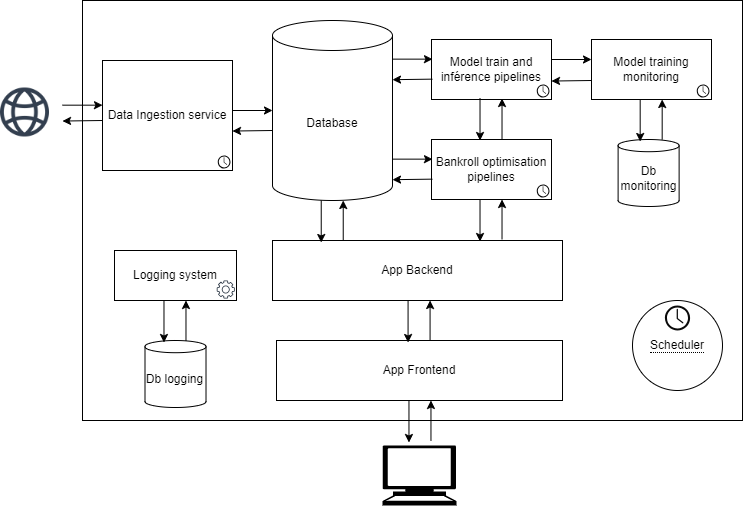
\includegraphics[width=0.8\textwidth, keepaspectratio]{images/Architecture_optimsportbet.png}
    \caption{Architecture of the system}
    \label{fig:elo_score_5_teams_during_time}
\end{figure}


\section{Data Collection}

Accurate and comprehensive data collection is vital for building reliable predictive models and effective betting strategies. The goal is to build an historical database which continues to build with real time relevant data.

\subsection{Data Sources Used}

We utilize a variety of reputable sources to gather data:

\begin{itemize}
    \item \textbf{Football Match Data}: Historical match results, match schedule, team statistics, player performance metrics, and other relevant information are sourced using scrapping on two websites: 
    \begin{itemize}
        \item \hyperlink{https://fbref.com/en/}{FBref}: For historical match results and coming match schedule.
        \item \hyperlink{https://sofifa.com/}{SoFifa}: For teams and players past and current ratings and statistics.
    \end{itemize}
    \item \textbf{Odds Data}: Betting odds are collected from multiple bookmakers through one API.
    \begin{itemize}
        \item \hyperlink{https://the-odds-api.com/}{The Odds API}: The free tier credits allows to perform 500 requests per month on various sports, bookmakers and leagues to retrieve the current odds. Historical odds data are not included.
    \end{itemize}
\end{itemize}


\subsection{Collection Methods}

Data is collected using a combination of methods:

\paragraph{Web Scraping}

A fork of the \hyperlink{https://soccerdata.readthedocs.io/en/latest/}{Soccerdata} python library, has been adapted to scrape data from websites that do not provide APIs (FBref, SoFifa). 

\paragraph{APIs}

For sources that offer APIs (The Odds API), we integrate with them using HTTP requests to fetch structured data efficiently.

\paragraph{Data Pre-processing}

Collected data undergoes a very simple pre-processing to ensure consistency and usability:

\begin{itemize}
    \item \textbf{Data type conversion}: Adapting the type of the data to the most adapted type.
    \item \textbf{Unity}: Only inserting new data in the database, or filling None values of existing data (for instance, the score of a match is only available after the match is played 
    \item \textbf{Integration}: Aligning data from different sources for seamless storage and analysis.
\end{itemize}

\section{Data Storage}

A robust data storage solution is essential for managing the diverse datasets involved.

\subsection{Database Choice}

We opted for a relational database management system (RDBMS), specifically \textit{PostgreSQL}, due to its reliability, scalability, and support for complex queries.

\subsection{Data Model}

The database schema is designed to reflect the relationships between different types of data:

\subsubsection{Tables}

\begin{itemize}
    \item `\textbf{fbref\_results}`: Each row corresponds to a match (historic and coming), with league, date and time of the match, both team and score if match is finished and the result is available and fetched from FBref website.
    \item `\textbf{sofifa\_teams\_stats}`: Each row corresponds to a a team and a date of update with metrics and categorical values that represent at best the team at the moment of the update (overall score, attack, build\_up\_speed ...).
    \item `\textbf{soccer\_odds}`: Each row corresponds to a match, a bookmaker, an outcome with its odd at a given update time. There is also information about the commence time of the match, the league, the home and away team names, the type of odd...
    \item `\textbf{models\_results}`: Each row corresponds to a match, the inference results of the model, the date-time of inference and the model used, with additional information such as the date and tile of the match and home and away team.
    \item `\textbf{optim\_results}`: Each row corresponds to a game, a date time of optimisation, the model used for inference, the best odds for each outcome found across a pool of bookmaker as well as the bookmakers names of each odds chose and the fraction of the bankroll to invest given utility function. There is additional information such as the probability inferred and used by the optimiser, the date-time of inference of these probabilities, the date and time of the match...
\end{itemize}


\begin{figure}[H]
    \centering
    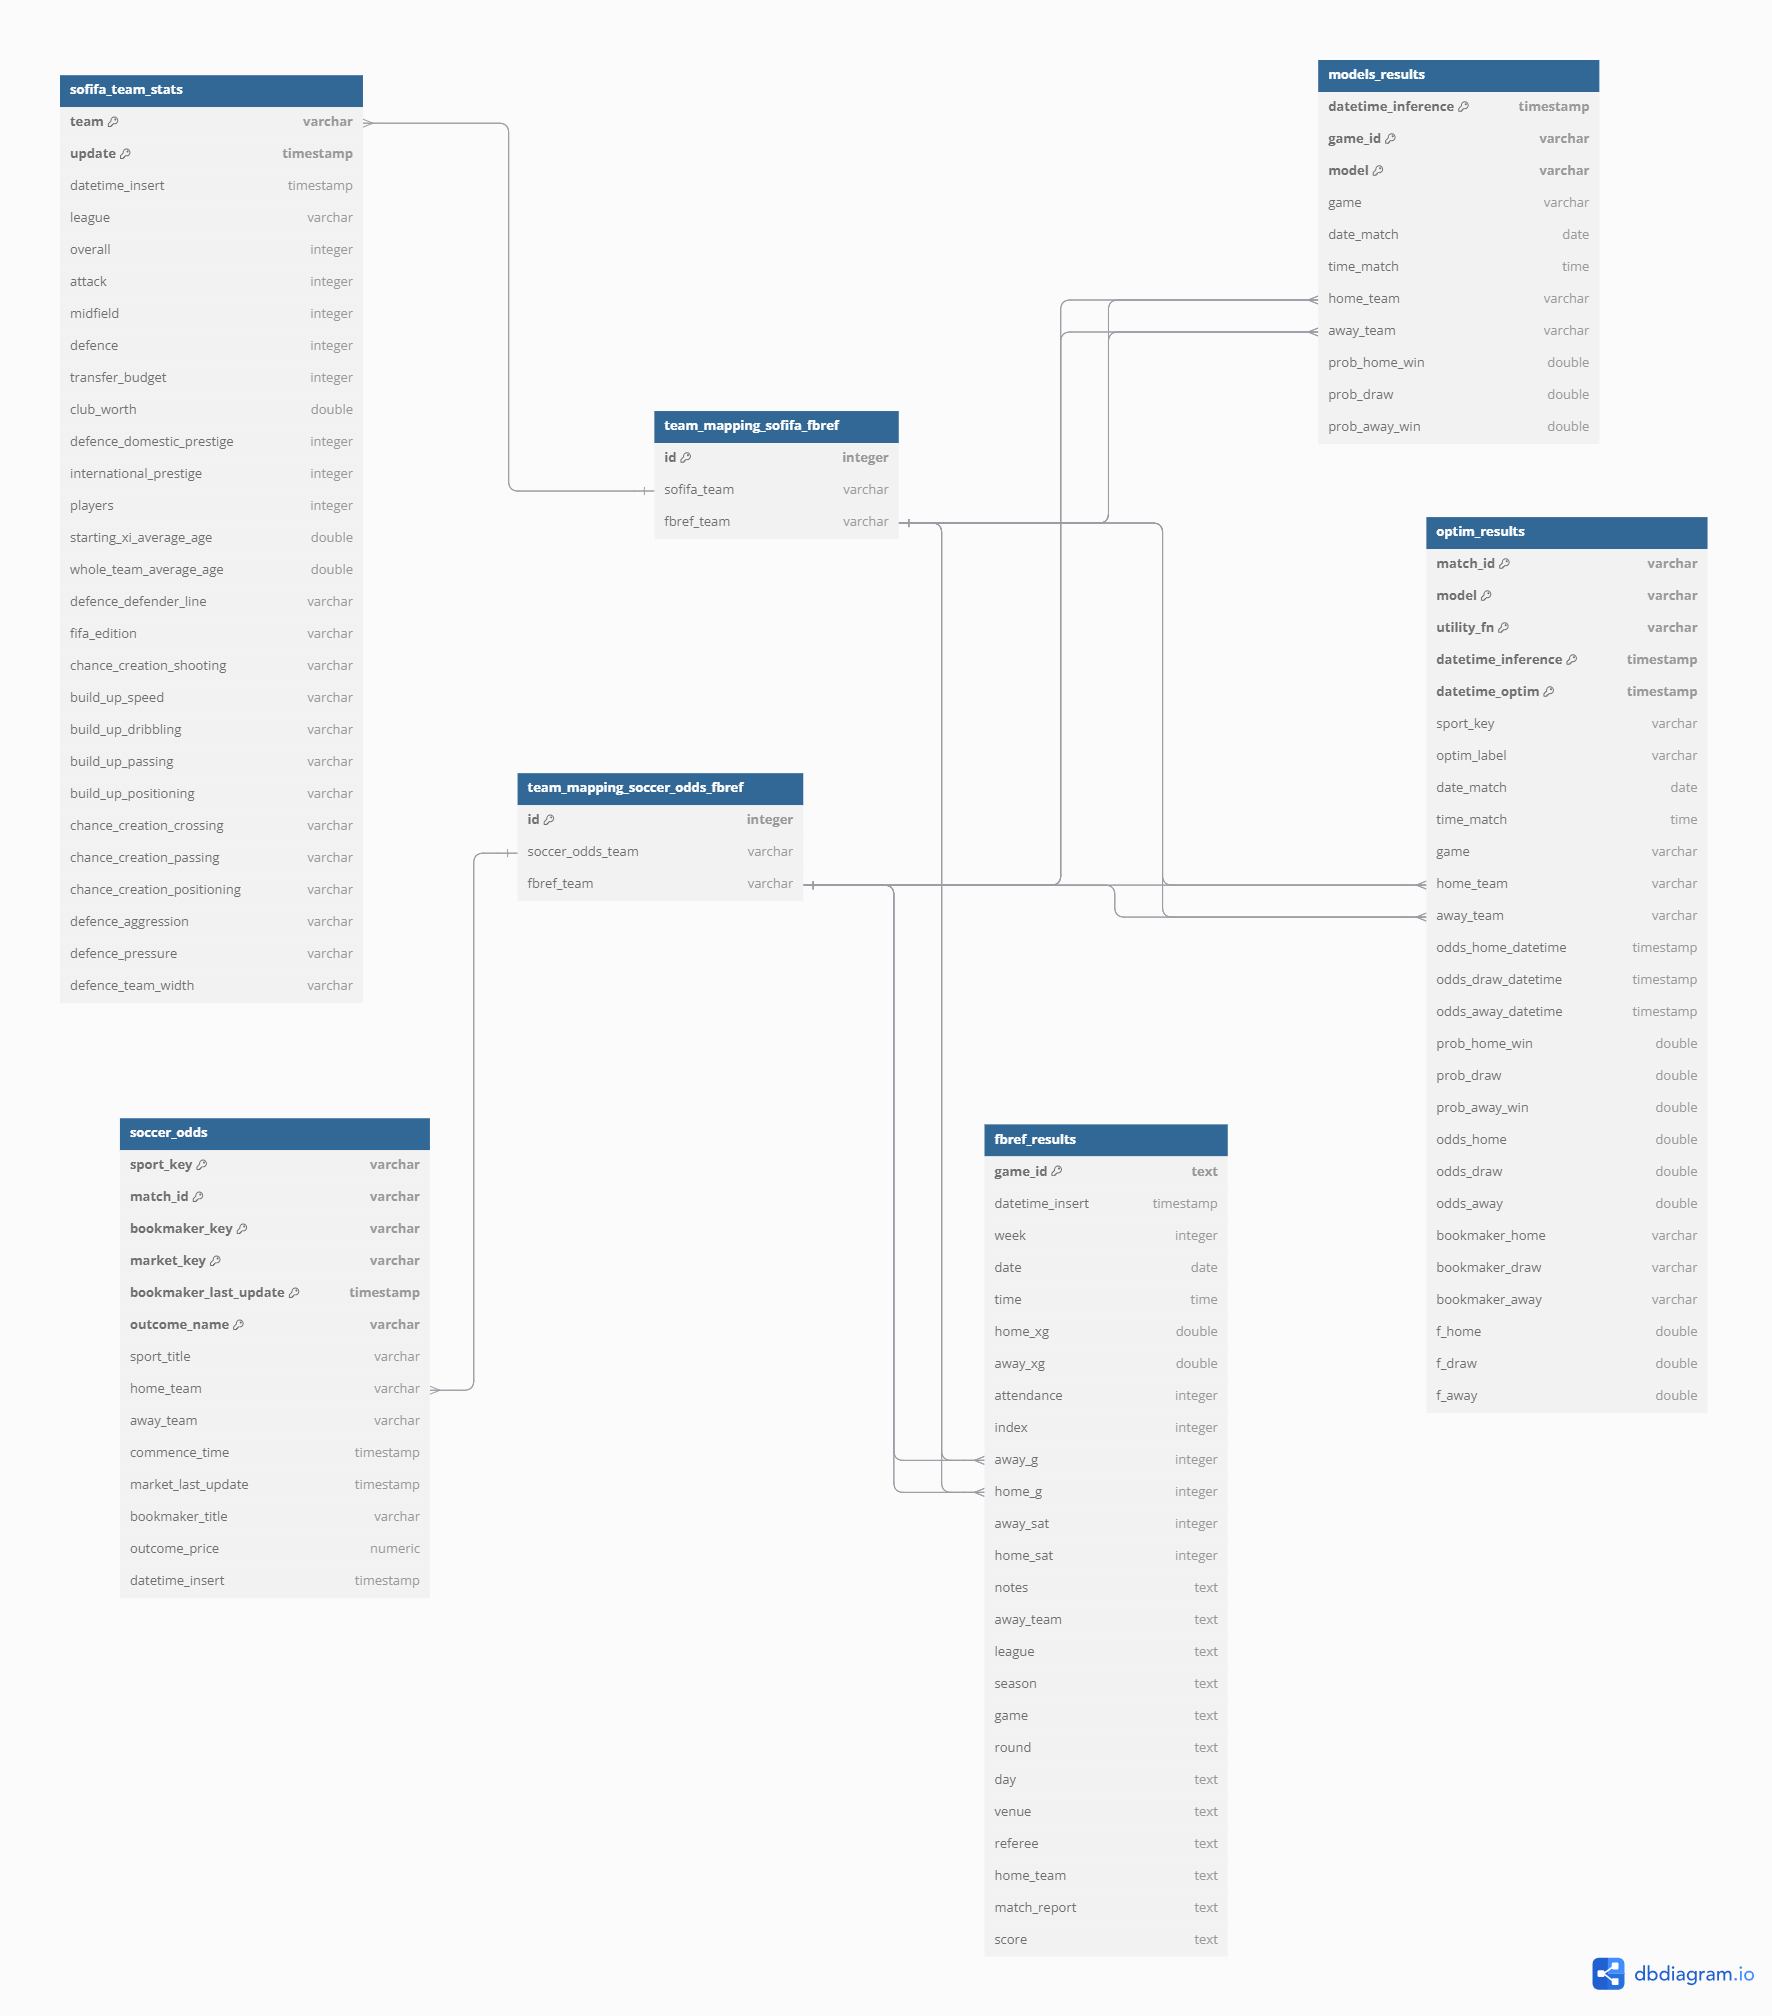
\includegraphics[width=0.8\textwidth, keepaspectratio]{images/db_uml.png}
    \caption{UML diagram of the database}
    \label{fig:uml_db}
\end{figure}

\section{Module Overview}

The system incorporates several modules, each performing specific functions within the overall architecture.

\subsection{Data Collection Module}

As described earlier, this module is responsible for fetching and pre-processing data from various sources.

\subsection{Prediction Module}

Although detailed discussion is deferred to a later chapter, this module uses machine learning algorithms to predict the probabilities of different match outcomes based on historical data.

\subsection{Optimization Module}

This module calculates optimal betting strategies by applying mathematical optimization techniques to the predictions and odds data. The specifics of the optimization algorithms and utility functions will be explored in a subsequent chapter.

\subsection{Scheduler}

The scheduler automates the execution of tasks such as data collection, model retraining, inference, and optimization. It ensures that the system remains up-to-date with the latest data and predictions.

\subsection{User Interface and Backend}

The user interface provides a platform for users to access data, view predictions, and interact with the system. The backend handles user requests, processes data, and communicates with other modules via APIs.

\section{User Interface and Monitoring}

\subsection{User Interface Design}

The UI is designed to be intuitive and user-friendly, providing clear visualizations and easy navigation.

\paragraph{Features}

\begin{itemize}
    \item \textbf{Dashboard}: Displays key metrics, including upcoming matches, predicted probabilities, and recommended betting strategies.
    \item \textbf{Historical Data Access}: Allows users to explore past matches, predictions, and outcomes.
    \item \textbf{Customization}: Users can select preferred bookmakers according to their interests.
\end{itemize}

\subsection{Monitoring}

System health and performance are monitored continuously:

\begin{itemize}
    \item \textbf{Logging}: Activity logs are maintained for debugging and audit purposes.
    \item \textbf{Alerts}: Notifications are sent in case of errors or significant events.
\end{itemize}


\section{Conclusion}

This chapter provided an overview of the system architecture implemented to realize the theoretical framework developed earlier. By focusing on football, we leverage abundant data to build predictive models and optimize betting strategies. The modular design, utilizing microservices and APIs,ensures scalability and flexibility. The database serves as the central repository, integrating data from various sources and supporting the different modules. The user interface offers a gateway for users to access the system's functionalities. In the subsequent chapters, we will delve into the specifics of the prediction and optimization modules, as well as the deployment strategy using Kubernetes and containerization technologies.

\section{Introduction}
\label{sec:chapter4_intro}

This chapter presents the development, training, and evaluation of a predictive model aimed at forecasting the outcomes of football matches. The primary objective is to construct a robust model that can accurately predict match results, thereby optimizing gains in sports betting \cite{BaioBlangiardo2010} \cite{DixonColes1997}. The significance of predictive modeling in the context of sports betting lies in its potential to provide bettors with a strategic advantage by identifying value bets and minimizing risks.

\section{Performance Metrics and Selection Criteria}
\label{sec:performance_metrics}

Evaluating the performance of a predictive model in a multi-class classification setting, especially with imbalanced classes, requires a comprehensive set of metrics. This section delineates both classic and advanced metrics employed in this study, incorporating mathematical formulations and addressing class imbalance. Given the three-class problem—home win, draw, and away win—with home wins constituting 47\% of the data, it is crucial to select metrics that provide a nuanced understanding of model performance across all classes.

\subsection{Metrics}
\label{subsec:classic_metrics}

A list of all the metrics considered with their used definition can  be found in Appendix \ref{appendix:predictive_model_metrics}.

\subsection{Selection Criteria}
\label{subsec:selection_criteria}

Accurate evaluation of the predictive model requires appropriate performance metrics, particularly in a multi-class classification context with class imbalance. The primary goal of this study is to ensure that the predicted probabilities of football match outcomes (home win, draw, away win) closely align with the true probabilities, emphasizing well-calibrated probability estimates.

Given the class distribution—47\% home wins, 26\% draws, and 25\% away wins—we have selected the \textbf{Mean Squared Error (MSE)} as the primary metric for assessing calibration. MSE directly measures the average squared difference between predicted probabilities and actual outcomes, making it suitable for evaluating how well the model's probabilities reflect the true frequencies.

In addition to MSE, we will consider the following metrics to provide a comprehensive evaluation:

\begin{itemize}
    \item \textbf{Log Loss}: To assess the quality of the predicted probability distributions by penalizing incorrect and overconfident predictions, thus encouraging well-calibrated estimates.
    \item \textbf{Classwise Expected Calibration Error (ECE)}: To evaluate the calibration of predicted probabilities for each class individually, offering insights into how closely these probabilities match the observed outcomes across different categories.
    \item \textbf{Accuracy for Home Win, Draw, and Away Win}: To examine the model's performance on each outcome separately, taking into account the class imbalance.
\end{itemize}

By focusing on MSE for calibration and incorporating Log Loss, Classwise ECE, and class-specific accuracy, we aim to ensure that the model not only produces accurate probability estimates but also maintains reliability across all outcome categories. This concise set of metrics aligns with our objective of accurately predicting football match outcomes while ensuring the predicted probabilities are well-calibrated and trustworthy.

\section{Exploration and Choice of Features}
\label{sec:feature_selection}

Selecting appropriate features is pivotal for building an effective predictive model. This section delineates the various types of features utilized in this study, the methodology employed for feature selection, the engineering of new features to enhance predictive power, and the handling of categorical variables to ensure they are appropriately represented in the model. 

\subsection{Types of Features Utilized}
\label{subsec:types_features}

The feature set comprises a combination of ranking-based, simple statistical, and domain-specific features. Each feature is defined mathematically where applicable and accompanied by an explanation of its relevance and computation.

\subsubsection{Ranking Features}
\label{subsubsec:ranking_features}

Ranking features provide a quantitative measure of team strength based on historical performance. These metrics are crucial as they encapsulate the overall ability and consistency of teams over time. All ranking features detailed formula are described in \ref{appendix:ranking_features}.

\begin{itemize}

\item \textbf{Elo Score}
\label{par:elo_score}

The \textbf{Elo score} \cite{Elo1978} \cite{HvattumArntzen2010} is a rating system originally developed for chess but widely adapted to various sports to rate players or teams. It reflects the relative skill levels of the teams based on game outcomes.

\begin{figure}[H]
    \centering
    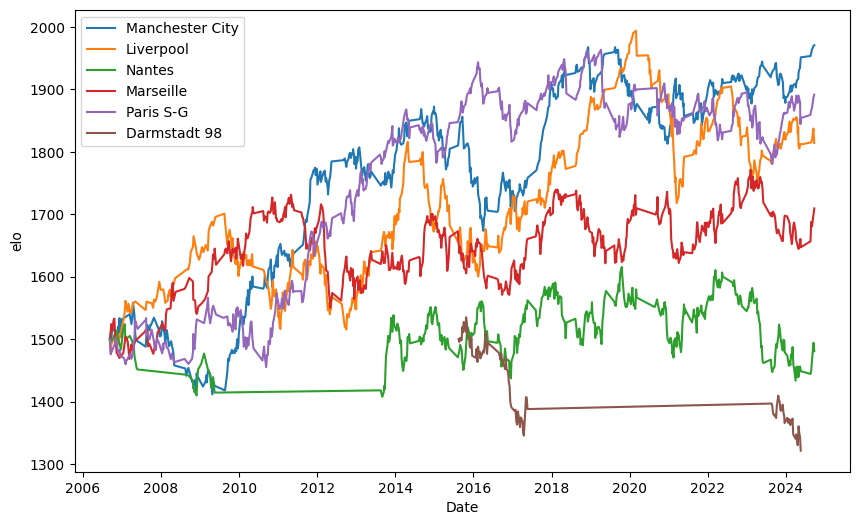
\includegraphics[width=0.8\textwidth, keepaspectratio]{images/elo_score_5_teams_during_time.png}
    \caption{Elo score of 5 football teams evolving during time}
    \label{fig:elo_score_5_teams_during_time}
\end{figure}



\item \textbf{Glicko-2 Score}
\label{par:glicko2_score}

The \textbf{Glicko-2 score} \cite{Glickman1999} is an advanced rating system developed by Mark Glickman, which enhances the Elo rating system by incorporating not only the skill levels of teams or players (R) but also the reliability of these ratings through Rating Deviation (RD) and volatility. This system provides a more dynamic and accurate reflection of performance by accounting for the uncertainty and variability in teams' ratings.


\item \textbf{TrueSkill}
\label{par:trueskill}

The \textbf{TrueSkill} \cite{HerbrichEtAl2007} is a Bayesian ranking system developed by Microsoft, primarily used in gaming but adaptable to sports analytics. It models each team's skill as a Gaussian distribution, updating beliefs about team strengths based on match outcomes.

\end{itemize}

\subsubsection{Simple Statistical Features}


Simple statistical features offer basic quantitative measures of team performance, providing foundational data for the predictive model.


\begin{itemize}
    \item \textbf{Average Goals Scored per Season}: Total goals scored by a team divided by the number of matches played so far.
    
    \item \textbf{Average Goals Conceded per Season}: Total goals conceded by a team divided by the number of matches played so far.
\end{itemize}


\subsubsection{Sofifa Performance Metrics}

SoFIFA provides detailed metrics for both individual players and teams, based on data from the FIFA video game by EA Sports. This document outlines the primary metrics and explains how team ratings are calculated using individual player attributes.

\begin{itemize}

\item \textbf{Player Metrics}
    The primary player metrics on SoFIFA are based on individual attributes that are weighted differently depending on the player's position. Below are the key metrics:
    
    \begin{itemize}
        \item \textbf{Overall Rating (OVR)}: This is the weighted average of various player attributes, with different weights depending on the position. For example, an attacker (\textit{Forward}) will have more emphasis on \textit{Shooting} and \textit{Pace}, while a defender (\textit{Centre Back}) will weigh attributes like \textit{Defending} and \textit{Physicality} more heavily.
        \item \textbf{Pace (PAC)}: Calculated as a combination of the \textit{Acceleration} and \textit{Sprint Speed} attributes.
        \item \textbf{Shooting (SHO)}: Includes \textit{Finishing}, \textit{Shot Power}, \textit{Long Shots}, and \textit{Positioning}.
        \item \textbf{Passing (PAS)}: Comprised of \textit{Vision}, \textit{Short Passing}, and \textit{Long Passing}.
        \item \textbf{Dribbling (DRI)}: Includes \textit{Ball Control}, \textit{Dribbling}, \textit{Agility}, and \textit{Balance}.
        \item \textbf{Defending (DEF)}: Based on \textit{Tackling}, \textit{Marking}, \textit{Interceptions}, and \textit{Defensive Awareness}.
        \item \textbf{Physicality (PHY)}: Includes \textit{Strength}, \textit{Stamina}, and \textit{Aggression}.
        \item \textbf{Potential}: Indicates the maximum possible rating the player can achieve over time.
    \end{itemize}
    
    The formula for the Overall Rating (OVR) is generally unknown, but it can be expressed as a weighted sum of key attributes, depending on the player’s position. A simplified formula for a forward might look like:
    
    \[
    \text{OVR}_{\text{Forward}} = w_1 \cdot \text{PAC} + w_2 \cdot \text{SHO} + w_3 \cdot \text{DRI} + w_4 \cdot \text{PAS}
    \]
    
    where \( w_1, w_2, w_3, w_4 \) are position-specific weights.

\item \textbf{Team Metrics}
    Team metrics on SoFIFA are calculated by aggregating individual player ratings, focusing on key areas like attack, midfield, and defense. The following are the primary team metrics:
    
    \begin{itemize}
        \item \textbf{Overall Team Rating}: A weighted average of the starting 11 players' Overall Ratings, considering the importance of each player's position.
        \item \textbf{Attack Rating}: The average Overall Rating of forwards and attacking midfielders, weighted based on the formation.
        \item \textbf{Midfield Rating}: The average Overall Rating of central and wide midfielders, weighted based on their roles in the formation.
        \item \textbf{Defense Rating}: The average Overall Rating of defenders and goalkeepers.
    \end{itemize}
    
    A simplified version of the team rating could be expressed as:
    
    \[
    \text{Team OVR} = \frac{1}{11} \sum_{i=1}^{11} \text{OVR}_i
    \]
    
    where \( \text{OVR}_i \) represents the Overall Rating of the $i$-th player in the starting lineup.
    
    
    Sofifa metrics are comprehensive team-specific performance indicators sourced from the Sofifa database, widely used in sports analytics and fantasy football contexts.
\end{itemize}

\begin{figure}[H]
    \centering
    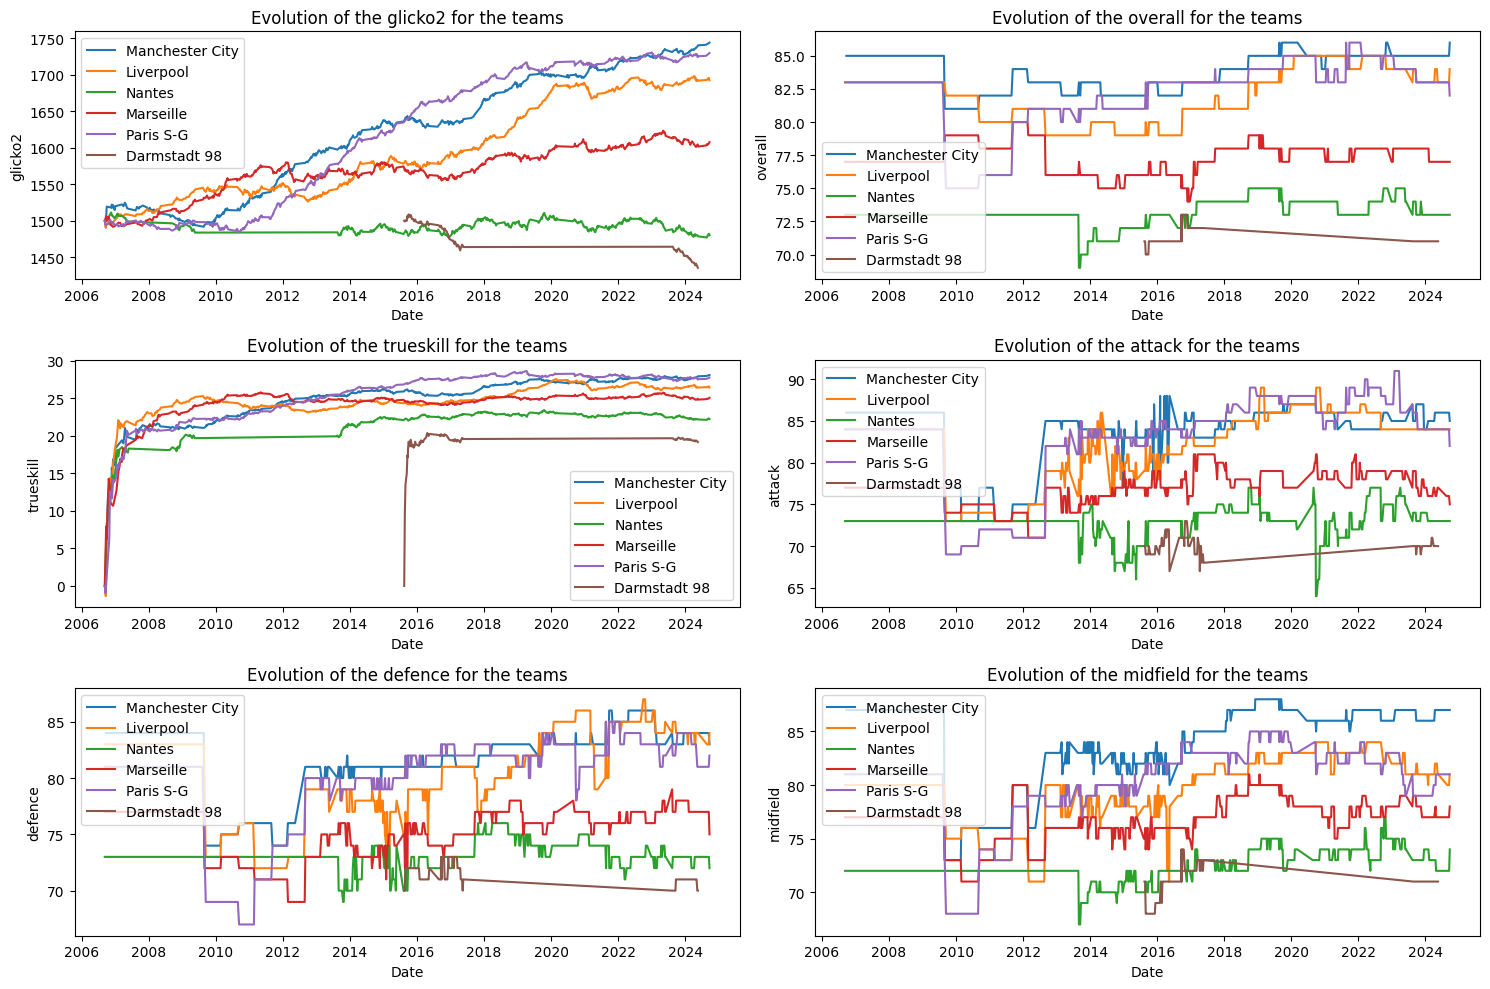
\includegraphics[width=\textwidth, keepaspectratio]{images/scores_5_teams_during_time.png}
    \caption{Different scores of 5 football teams evolving during time}
    \label{fig:scores_5_teams_during_time}
\end{figure}

A detailed description of each of the 90 features used can be found her \ref{appendix:all_feature_descriptions}.

\subsection{Feature Selection Methodology}
\label{subsec:feature_selection_methodology}

Feature selection was performed using a forward selection approach applied to a logistic regression model. This method iteratively adds the most significant features, enhancing predictive performance while maintaining model simplicity.

\subsubsection{Forward Selection with Logistic Regression}
\label{subsubsec:forward_selection_logistic_regression}

\textbf{Procedure}: Starting with no features, at each iteration, the feature that most improves the model's fit is added. The selection criterion is based on the mse (mean squared error).

\textbf{Explanation}: By incorporating features that significantly contribute to the model, forward selection optimizes predictive accuracy and ensures interpretability by excluding irrelevant variables.

\section{Data Preparation}

We trained our model on matches from 2006 to the present, focusing on games from the top 5 European leagues, European championships, and World Cups during this period. The limiting factor in our data came from SoFIFA, which does not provide data prior to 2006, while FBref offers data extending far into the past. We merged the two datasets based on team names and computed the ranking and statistical features described earlier, initializing the metrics at the first entry of a team in a tournament. For categorical features, we applied one-hot encoding. We removed matches with any missing values in the columns, then applied a standard scaler. This left us with 28,850 completed matches and a 90-feature vector for each match to train our model.

\begin{table}[h]
\centering
\begin{tabular}{|l|c|c|}
\hline
\textbf{Metric} & \textbf{Value} \\
\hline
Total matches & 28,850 \\
Matches in Top 5 Leagues & 28,481 \\
Matches in European Championships & 185 \\
Matches in World Cup & 184 \\
Home win ratio & 45.0 \% \\
Draw ratio & 25.4 \% \\
Away win ratio & 29.5 \% \\ 
Average home team goals & 1.54 \\
Average away team goals & 1.19 \\
Average Elo rating & 1558 \\
Number of unique teams & 242 \\
Number of features per match & 90 \\
First match date & 2006-09-09 \\
Last match date & 2024-09-24 \\
\hline
\end{tabular}
\caption{Summary Metrics for the Dataset}
\end{table}


\section{Cross-Validation on Temporal Data}
\label{sec:cross_validation_temporal}

In predictive modeling with football match data, which is inherently temporal, it's essential to use cross-validation techniques that respect the chronological order of observations. Standard cross-validation methods, such as random shuffling or traditional \( k \)-fold cross-validation, are unsuitable because they can lead to data leakage by training models on future data to predict past events.

Traditional cross-validation assumes that data samples are independent and identically distributed (i.i.d.) and that the order of observations does not matter. In temporal data, however, observations are time-dependent, and future events should not influence model training aimed at predicting past events. Using standard methods can result in:

\begin{itemize}
    \item \textbf{Data Leakage}: Incorporating future information into the training set leads to overly optimistic performance estimates.
    \item \textbf{Violation of Temporal Order}: Disrupting the sequence of events undermines the model's ability to generalize to real-world forecasting scenarios.
\end{itemize}


To address these issues, we employ cross-validation methods designed for temporal data \cite{BergmeirEtAl2018}.

\subsection{Sliding Window Cross-Validation}

This technique involves moving a fixed-size window across the data timeline. In each iteration, the model is trained on a training window and tested on the immediately following testing window.

\begin{itemize}
    \item Choose a training window size \( W_{\text{train}} \) and a testing window size \( W_{\text{test}} \).
    \item For each iteration:
    \begin{itemize}
        \item Train the model on data from time \( t \) to \( t + W_{\text{train}} - 1 \).
        \item Test the model on data from \( t + W_{\text{train}} \) to \( t + W_{\text{train}} + W_{\text{test}} - 1 \).
        \item Slide the window forward by \( W_{\text{test}} \) units.
    \end{itemize}
\end{itemize}

\subsection{Expanding Window Cross-Validation}

Also known as growing window, this method expands the training set with each iteration by including more historical data.

\begin{itemize}
    \item Start with an initial training window of size \( W_{\text{initial}} \).
    \item For each iteration:
    \begin{itemize}
        \item Train the model on data from time \( t \) to \( t + W_{\text{train}} - 1 \), where \( W_{\text{train}} \) increases with each iteration.
        \item Test on the subsequent data from \( t + W_{\text{train}} \) to \( t + W_{\text{train}} + W_{\text{test}} - 1 \).
        \item Expand the training window to include the latest testing window.
    \end{itemize}
\end{itemize}

\begin{figure}[H]
    \centering
    \begin{minipage}{0.45\textwidth}
        \centering
        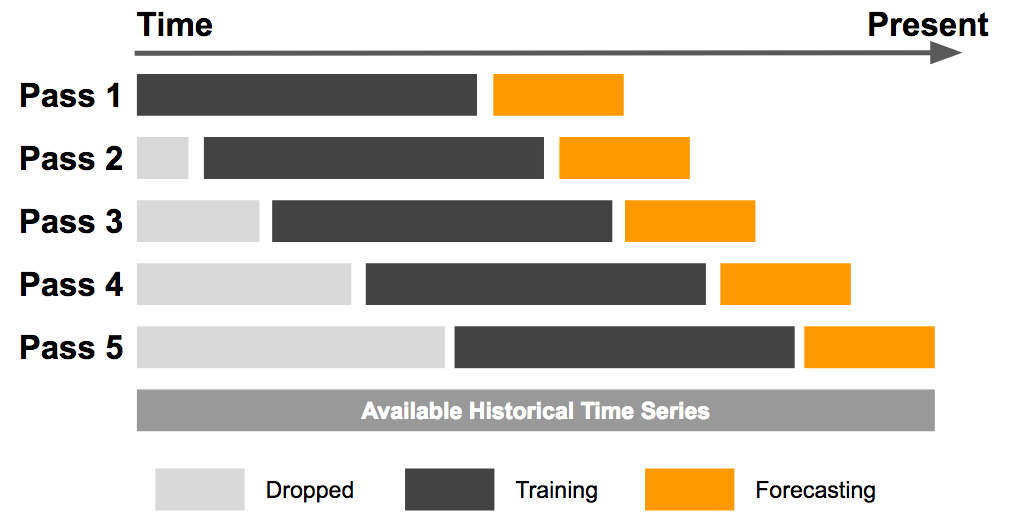
\includegraphics[width=\textwidth, keepaspectratio]{images/FixedWindow.png}
        \caption{Sliding window graphic}
        \label{fig:sliding_window}
    \end{minipage}\hfill
    \begin{minipage}{0.45\textwidth}
        \centering
        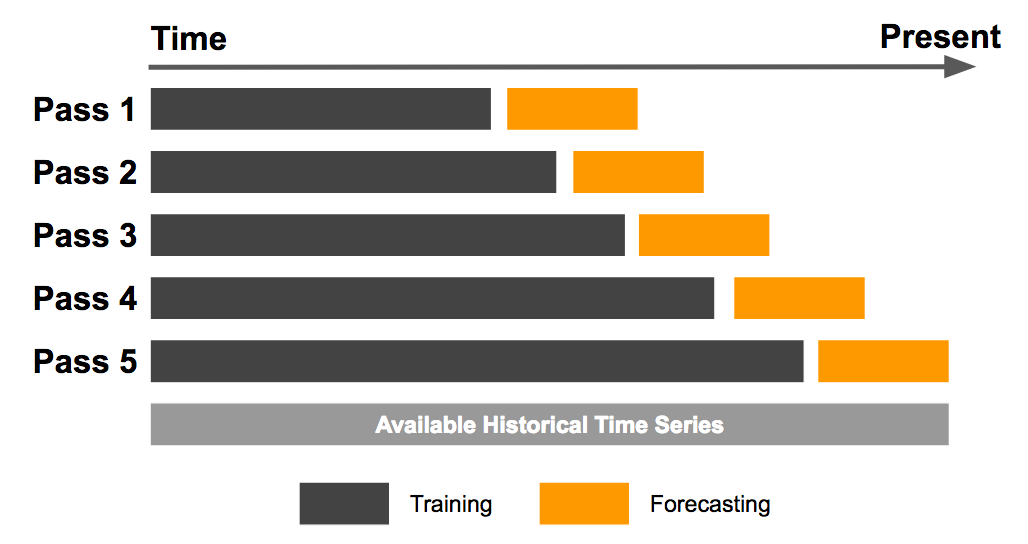
\includegraphics[width=\textwidth, keepaspectratio]{images/ExpandingWindow.png}
        \caption{Expanding window graphic}
        \label{fig:expanding_window}
    \end{minipage}
\end{figure}


The results presented below were obtained using an expanding window technique with 5 folds and a test set ratio of 0.2. Notably, the results were very similar when applying the sliding window method.


\section{Choice and Justification of the Prediction Model}
\label{sec:model_choice}

In this section, we present the results of the feature selection and model selection processes \cite{GuyonElisseeff2003} \cite{ChandrashekarSahin2014}, followed by interpretations of the selected model's performance. Feature selection was conducted using forward selection, and multiple classification models were evaluated to determine the most suitable model for predicting football match outcomes.

\subsection{Feature Selection Using Forward Selection}
\label{subsec:feature_selection}

Feature selection was performed using forward selection with logistic regression, iteratively adding the most significant feature at each step based on mean squared error (MSE) improvement, using an expanding window validation with 5 splits and a test size of 20\% of the training data.

\begin{table}[H]
    \centering
    \caption{Feature Selection Process Summary}
    \label{tab:feature_selection_summary}
    \begin{tabular}{lc}
        \toprule
        \textbf{Method} & \textbf{Details} \\
        \midrule
        Feature Selection & Forward Selection \\
        Model Used & Logistic Regression \\
        Validation Method & Expanding Window (5 splits) \\
        Performance Metric & Mean Squared Error (MSE) \\
        Test Size & 20\% of training data \\
        \bottomrule
    \end{tabular}
\end{table}


We selected 35 features, which corresponding to the features resulting in the lowest MSE, using this feature selection strategy.

\begin{table}[H]
    \centering
    \caption{Feature Selection with Corresponding MSE and their adding number}
    \label{tab:feature_mse}
    \begin{tabular}{|c|l|c|c|l|c|}
        \hline
        \textbf{Order} & \textbf{Feature Added} & \textbf{MSE} & \textbf{Order} & \textbf{Feature Added} & \textbf{MSE} \\
        \hline
        1  & Elo Away & 0.20613 & 19 & Home Passing Risky & 0.19438 \\
        2  & Elo Home & 0.19661 & 20 & Away Positioning Org. & 0.19436 \\
        3  & Glicko Vol Away & 0.19619 & 21 & Away Defense Pressure Med & 0.19435 \\
        4  & Away Overall & 0.19594 & 22 & Away Domestic Prestige & 0.19434 \\
        5  & Home Overall & 0.19540 & 23 & Away Shooting Lots & 0.19433 \\
        6  & Away Build Speed Slow & 0.19518 & 24 & Home Defense Line Offside & 0.19432 \\
        7  & Away Avg Age & 0.19501 & 25 & Away Team Width & 0.19431 \\
        8  & Home League INT & 0.19487 & 26 & Home Defense Pressure Med & 0.19431 \\
        9  & Home Avg Goals & 0.19476 & 27 & Home Build Speed Slow & 0.19430 \\
        10 & Home Positioning Org. & 0.19467 & 28 & Away Defense Aggression & 0.19430 \\
        11 & Home Build Speed Fast & 0.19461 & 29 & TrueSkill Home & 0.19430 \\
        12 & Away Defense Pressure High & 0.19457 & 30 & Away Build Positioning Org. & 0.19430 \\
        13 & Away Defense Offside Trap & 0.19453 & 31 & Away Defense & 0.19430 \\
        14 & Home League ITA & 0.19449 & 32 & Home Attack & 0.19427 \\
        15 & Glicko RD Home & 0.19447 & 33 & Home Defense Prestige & 0.19427 \\
        16 & Home Shooting Normal & 0.19444 & 34 & Away Attack & 0.19427 \\
        17 & Away Passing Mixed & 0.19442 & 35 & Away League INT & \textbf{0.19427} \\
        18 & Away Avg Goals & 0.19440 & & \\
        \hline
    \end{tabular}
\end{table}

The table above summarizes the features added during the selection process and their corresponding MSE values, highlighting the importance of each feature as it contributes to minimizing the error. As we can see, features such as Elo ratings and overall team metrics play a significant role \cite{LasekEtAl2013}. Now, let's examine how the number of features impacts the performance metrics more broadly, as shown in the following feature selection graph.

\begin{figure}[H]
    \centering
    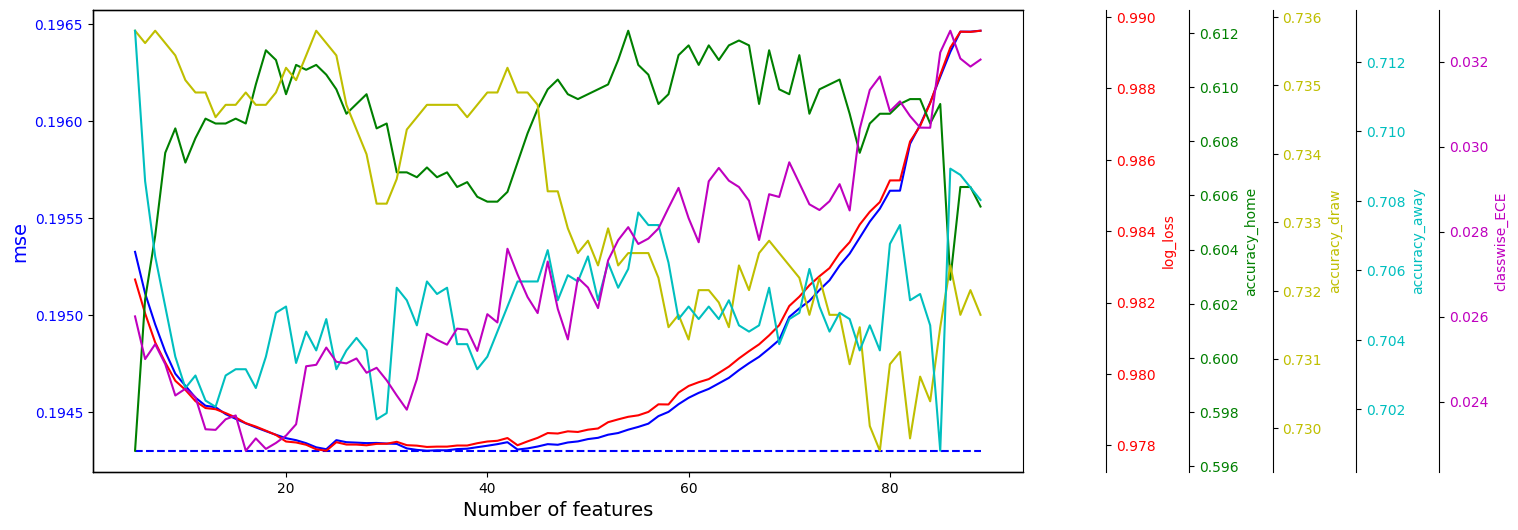
\includegraphics[width=\textwidth, keepaspectratio]{images/feature_selection_metrics_by_nb_of_features.png}
    \caption{Metrics of interrest function of the number of features added}
    \label{fig:feature_selection_metrics_by_nb_of_features}
\end{figure}

This graph shows the performance of various metrics (MSE, log loss, accuracy for home, draw, and away predictions, and classwise ECE) as a function of the number of selected features. The MSE (in blue) decreases as more features are added, stabilizing around the optimal point before increasing again, which suggests that selecting too many features can lead to overfitting. Similarly, log loss follows a similar trend (in red), indicating better model calibration with fewer features. The accuracy metrics (home, draw, away) fluctuate, but accuracy seems to peak at a certain range of features, with performance diminishing as more features are added. Classwise ECE (in pink) decreases and then increases, a little bit before MSE and log loss, indicating better calibration for class predictions with fewer features. Overall, the graph highlights the balance between feature selection and model performance, suggesting that an optimal subset of features yields the best generalization.

\subsection{Model Selection}
\label{subsec:model_selection}

The following table summarizes the performance of various classification models \cite{Bishop2006}, comparing metrics such as mean squared error (MSE), log loss, classwise ECE, and accuracy for home, draw, and away predictions to identify the best-performing model.

\begin{table}[H]
    \centering
    \caption{Model Performance Comparison}
    \label{tab:model_performance}
    \begin{tabular}{|l|c|c|c|c|c|c|}
        \hline
        \textbf{Model} & \textbf{MSE} & \textbf{Log Loss} & \textbf{C. ECE} & \textbf{A. Home} & \textbf{A. Draw} & \textbf{A. Away} \\
        \hline
        Logistic Regression & \textbf{0.195} & \textbf{0.983} & 0.029 & 0.605 & 0.733 & 0.702 \\
        Logistic Regression CV & 0.196 & 0.983 & \textbf{0.028} & 0.602 & \textbf{0.735} & 0.703 \\
        Gradient Boosting Classifier & 0.199 & 1.002 & 0.037 & 0.604 & 0.709 & \textbf{0.706} \\
        Random Forest Classifier & 0.202 & 1.022 & 0.038 & 0.595 & 0.705 & 0.693 \\
        Extra Trees Classifier & 0.204 & 1.026 & 0.043 & 0.597 & 0.683 & 0.686 \\
        AdaBoost Classifier & 0.221 & 1.092 & 0.069 & 0.599 & 0.721 & 0.695 \\
        Bagging Classifier & 0.224 & 2.471 & 0.093 & 0.602 & 0.646 & 0.661 \\
        MLP Classifier & 0.224 & 1.187 & 0.108 & 0.585 & 0.665 & 0.684 \\
        K Neighbors Classifier & 0.238 & 5.404 & 0.096 & 0.599 & 0.643 & 0.631 \\
        Gaussian NB & 0.332 & 7.570 & 0.302 & \textbf{0.615} & 0.584 & 0.625 \\
        Quadratic Discriminant Analysis & 0.353 & 10.831 & 0.316 & 0.582 & 0.561 & 0.613 \\
        Decision Tree Classifier & 0.390 & 20.219 & 0.195 & 0.578 & 0.614 & 0.638 \\
        Extra Tree Classifier & 0.399 & 20.686 & 0.200 & 0.559 & 0.615 & 0.628 \\
        \hline
    \end{tabular}
\end{table}


\subsection{Interpretation of Results}
\label{subsec:interpretation}

The selection of the logistic regression model allows for straightforward interpretation of feature effects on the predicted probabilities of match outcomes.

\subsubsection{Feature Importance}

Feature importance was assessed based on the magnitude of the coefficients in the logistic regression model. Below sits the feature importance of the Home win class. Draw and Away win classes analysis can be found in \ref{appendix:feature_importance}.


\begin{figure}[H]
    \centering
    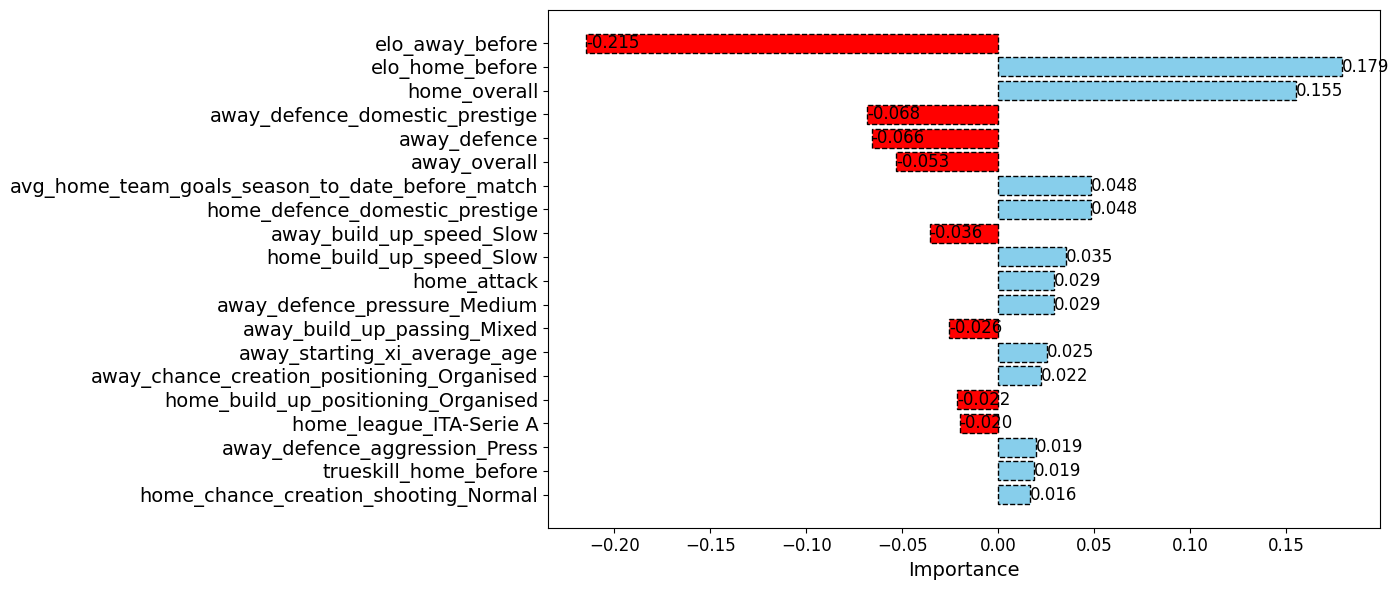
\includegraphics[width=\textwidth, keepaspectratio]{images/top20_coeff_importance_lr_selected_features_home.png}
    \caption{Coefficients of the Logistic Regression Model for Home win class}
    \label{fig:feature_coefficients}
\end{figure}

For the home class, the most important features, such as Elo ratings for the away and home teams, suggest that pre-match team strength is the most significant predictor of match outcomes. Both overall team quality and specific defensive attributes, like pressure and aggression, also play a key role. Features related to player average characteristics, such as average age and tactical elements like build-up speed, indicate that team composition and playstyle are also relevant, though their impact is less pronounced. Defensive strategies, particularly pressure and team width, add further predictive value, showing the importance of tactical decisions in determining match results. The feature importance analysis graphs for draw and away class can be found in the annex section.


\subsubsection{Why Logistic Regression Outperforms Other Models}

Logistic regression may outperform other models due to its simplicity and interpretability, especially when feature selection is based on it. By using logistic regression for feature selection, the model is specifically tuned to highlight the most important predictors of the outcome, leading to better generalization. Additionally, logistic regression handles multicollinearity well when regularization is applied, preventing overfitting. The linear relationship between the features and the log-odds of the outcomes makes it easier to capture important patterns in the data, particularly in problems like sports prediction where relationships between variables are often linear. Other models, such as random forests or gradient boosting, may add unnecessary complexity and are more prone to overfitting when features are already well-selected.


\section{Training and Retraining of the Model}
\label{sec:training_retraining}

Figure \ref{fig:mse_retraining} illustrates the Mean Squared Error (MSE) of two models over time, where the blue line represents Model A with no retraining, and the orange line represents Model B, which is retrained daily. Both models are initialy trained from 2006-01-01 up to 2010-01-01 data and are evaluated using a 120-day rolling average.

\begin{figure}[H]
    \centering
    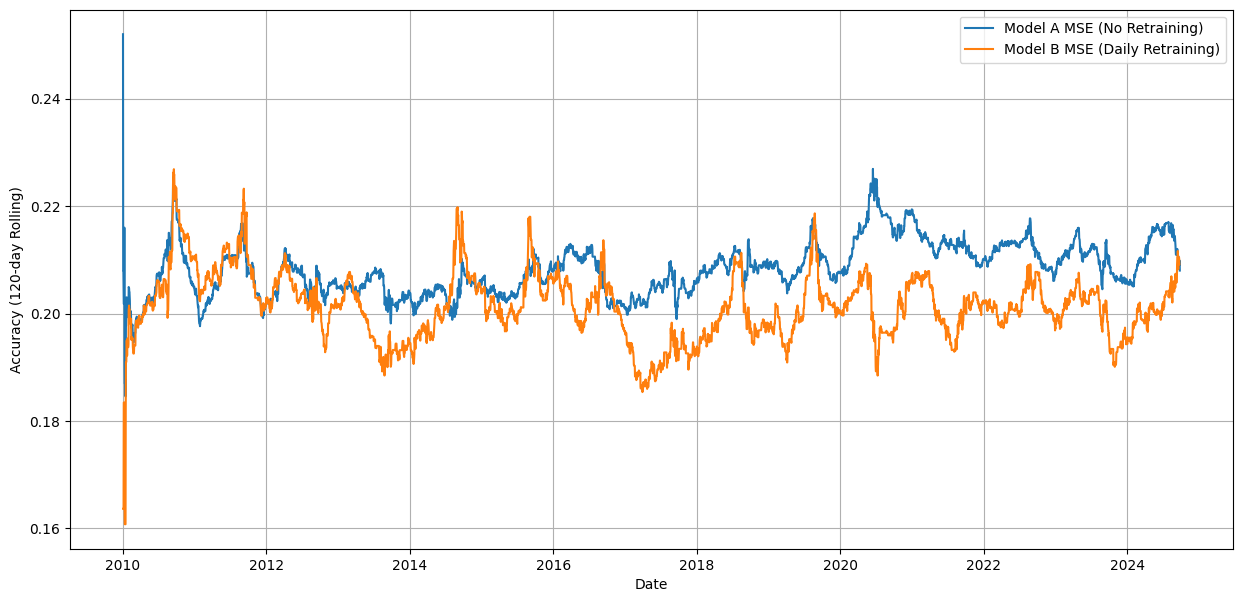
\includegraphics[width=0.8\textwidth, keepaspectratio]{images/model_ratrining_mse_120rd.png}
    \caption{Model MSE rolling average over time}
    \label{fig:mse_retraining}
\end{figure}


From the figure, we observe that Model B, which is frequently retrained, exhibits lower MSE compared to Model A throughout most of the time period. Retraining appears to allow Model B to adapt more effectively to evolving patterns, leading to consistently better performance in terms of accuracy. Moreover, as time goes by, we can observe a mse drift from the not retrained model as well as a slight improvement from the retrained model. \\

There are very few periods where Model A outperforms Model B. It appends especially during phases of sudden changes. Despite these fluctuations, retraining offers a more stable and improved long-term performance. \\

The results highlight the importance of regular retraining for maintaining model accuracy, particularly in dynamic environments where data patterns change over time.

\section{Conclusion}

This chapter presented the development, training, and evaluation of a predictive model for football match outcomes, with a focus on sports betting. Feature selection via forward selection with logistic regression helped identify key predictors, and regular retraining improved model performance over time.\\

However, several limitations remain:

\begin{itemize}
    \item \textbf{Hyperparameters and Features}: Ranking feature hyperparameters were left at default, and additional domain-specific or external data sources could further improve predictions.
    \item \textbf{Feature Selection}: Feature selection was arbitrarily based on logistic regression, and no hyperparameter optimization was performed for any models.
    \item \textbf{Retraining}: The timing and method of retraining (e.g., sliding window) were not explored, potentially missing optimal strategies as well as posing computational challenges that could be optimized.
    \item \textbf{Model Complexity}: Incorporating deep learning models could enhance predictive performance, particularly for capturing complex patterns in the data.
    \item \textbf{Bookmaker Odds Decorrelation}: Adding a metric to assess the decorrelation between model predictions and bookmaker odds could help identify more value bets and further optimize betting strategies.
\end{itemize}
In the next chapter, we address the optimization problem of determining the bankroll share to invest on each outcome, building on the predictions of this model to develop actionable betting strategies.

\section{Introduction}

Effective bankroll management is a critical component of successful sports betting. It involves determining the optimal amount to wager on each bet to maximize growth while minimizing the risk of ruin. This section details the development and evaluation of an optimization module designed to calculate the optimal fraction of the bankroll to invest in each betting opportunity. The module leverages probabilistic forecasts from the predictive models discussed in the previous section and applies various investment strategies, including the Kelly criterion, expected value maximization, and naive betting approaches.

\section{Methodology}
\subsection{Investment Strategies}

This section provides an overview of the different bankroll allocation strategies implemented, ranging from naive methods to more advanced optimization techniques. The focus is on the principles guiding each strategy, with a detailed formula provided only for the naive strategy.

\subsubsection{List of Strategies}

\begin{itemize}
    \item \textbf{Kelly Criterion Strategy}: \cite{Kelly1956} \cite{Thorp1969}  
    This strategy maximizes the logarithmic utility of wealth, aiming for long-term bankroll growth while managing risk. The bankroll fractions are derived from the analytical solution using the approximations  \ref{appendix:analytical_solution_using_the_kelly_criterion}, \(\mathbb{E}(U(B)) = \mathbb{E}(B) - \frac{1}{2} \cdot \mathbb{V}\text{ar}(B) \) which comes down to a Linear utility strategy using \( \lambda = \frac{1}{2} \).

    \item \textbf{Log Utility Strategy}:  
    Similar to the Kelly criterion, this strategy focuses on maximizing the expected logarithmic utility \(U(B) = \ln(B)\)  but using no approximations \ref{appendix:analytical_reduction_using_log_expected_utility}.

    \item \textbf{Exponential Utility Strategy}:  
    This strategy uses an exponential utility function \(U(B) = -e^{-\alpha B}\) to take into account the bettor’s risk aversion, balancing between expected returns and risk tolerance \ref{appendix:analytical_reduction_using_exp_expected_utility}.

    \item \textbf{Linear Utility Strategy}:
    In this strategy, the objective is to maximize the trade-off between expected returns and risk, represented by the function \(\mathbb{E}(U(B)) = \mathbb{E}(B) - \lambda \cdot \mathbb{V}\text{ar}(B) \). For the simulations, we set \( \lambda = 10 \), reflecting a high level of risk aversion. This approach seeks to maximize returns while penalizing high variance, aiming to balance growth and stability \ref{appendix:analytical_solution_using_linear_expected_utility}. 

    \item \textbf{Expected Value Maximization Strategy}:  
    This strategy optimizes bankroll allocation based purely on maximizing expected value, \(U(B) = B\), without considering risk or variance.

    \item \textbf{Naïve Strategy: Bet on the Most Likely Outcome}:  
    In this straightforward approach, the bettor places the entire bet on the outcome with the highest implied probability, as per the bookmaker's odds.
    
    The formula for this strategy is:
    \[
    f_{k,i} = 
    \begin{cases}
    \frac{1}{M}, & \text{if } i = \arg\max(o_k) \\
    0, & \text{otherwise}
    \end{cases}
    \]
    where:
    \begin{itemize}
        \item \( f_{k,i} \) is the fraction of the bankroll wagered on outcome \( i \) of match \( k \),
        \item \( o_k \) are the odds for match \( k \).
        \item \(M\) is the number of matches available.
    \end{itemize}
    This strategy is simple and allocates all the available funds to the outcome with the highest bookmaker odds.
\end{itemize}

These strategies were benchmarked against each other in the Monte Carlo simulations and then Online testing to assess their effectiveness in managing risk and maximizing bankroll growth. \\

For each strategy, a factor of \( \gamma = \frac{1}{2} \) was applied to the bet fractions to ensure that not the entire bankroll was wagered at any given time, thereby providing a margin of safety, such as: \(f_{strategy\_final} = \gamma \times f_{strategy}\).


\subsection{Optimization Algorithms}

Two optimization algorithms were employed to solve the bankroll allocation problem \cite{BoydVandenberghe2004}:

\begin{itemize}
    \item \textbf{Sequential Least Squares Programming (SLSQP):} An iterative method for constrained nonlinear optimization that is efficient for problems with a moderate number of variables.
    \item \textbf{Trust-Region Constrained Algorithm (trust-constr):} Suitable for large-scale optimization problems, it handles large numbers of variables and constraints effectively.
\end{itemize}

The choice between SLSQP and trust-constr depends on the number of betting opportunities (matches) considered at once. For a large number of matches, trust-constr is preferred due to its scalability.


\section{Monte Carlo Simulations}

To assess the performance of different investment strategies under simulated sports betting conditions, we conducted Monte Carlo simulations modeling the inherent uncertainties. The goal was to evaluate how various bankroll allocation strategies perform over numerous trials.

\subsection{Simulation Setup}

We simulated true match outcome probabilities \( r \) using a Dirichlet distribution appropriate for mutually exclusive and collectively exhaustive events:

\[
r_i^k = \text{Dirichlet}(\alpha), \quad \alpha = (1, 1, 1)
\]

To introduce discrepancies between true probabilities and those estimated by bookmakers (\( b \)) and players (\( t \)), we added biases and normally distributed noise:

\[
b_i^k = \text{clip}(r_i^k + \text{bias}_{\text{bookmaker}} + \epsilon_{\text{bookmaker}}, \ \text{min\_prob}, \ \text{max\_prob})
\]
\[
t_i^k = \text{clip}(r_i^k + \text{bias}_{\text{player}} + \epsilon_{\text{player}}, \ \text{min\_prob}, \ \text{max\_prob})
\]

where \( \epsilon_{\text{bookmaker}}, \epsilon_{\text{player}} \sim \mathcal{N}(0, \sigma^2) \). Probabilities were normalized to sum to one, and bookmaker probabilities included a margin \( \text{margin}_{\text{bookmaker}} \), clipping between \text{min\_prob} and \text{max\_prob}. Bookmaker odds were calculated as:

\[
o_i^k = \frac{b_i^k}{(\sum_{i=0}^N b_i^k) - \text{margin}_{\text{bookmaker}}}
\]

\subsection{Simulation Procedure}

The simulation followed a structured approach to evaluate the performance of different betting strategies, using predefined constants and a series of steps to simulate match outcomes and bankroll updates.

\begin{table}[H]
\centering
\caption{Simulation constants}
\label{tab:simulation constants}
\begin{minipage}{.2\linewidth}
\centering
\begin{tabular}{lr}
\toprule
\textbf{Constant} & \textbf{Value}\\
\midrule
H & 30 \\
T & 50 \\
N & 3 \\
\(\text{min\_prob}\) & 0.05 \\
\(\text{max\_prob}\) & 0.95 \\
\bottomrule
\end{tabular}
\end{minipage}%
\hspace{0.05\linewidth}
\begin{minipage}{.45\linewidth}
\centering
\begin{tabular}{lrr}
\toprule
\textbf{Constant} & \textbf{Bettor} & \textbf{Bookmaker}\\
\midrule
\text{bias} & 0 & 0 \\
\(\sigma\) (for noise \(\epsilon)\) & 0.1 & 0.1 \\
\text{margin} &  & 0.1 \\
\bottomrule
\end{tabular}
\end{minipage}
\end{table}

\begin{enumerate}
    \item Generated true probabilities \( r \) using \(\text{bias} = 0\) and \(\epsilon = 0.1\) for both bettor and bookmaker.
    \item Computed bookmaker and player estimates \( b \) and \( t \).
    \item Calculated bookmaker odds \( o \).
    \item For each strategy:
    \begin{itemize}
        \item Determined bet sizes using \( t \) and \( o \) by performing optimisation using \texttt{truct\_constr} algorithm.
        \item Simulated match outcomes based on \( r \).
        \item Updated bankrolls accordingly.
    \end{itemize}
\end{enumerate}

\subsection{Evaluation Metrics}

Strategies were evaluated using:

\begin{itemize}
    \item \textbf{Final Bankroll Statistics}: Mean, standard deviation, median, minimum, and maximum.
    \item \textbf{Average Growth Rate}: Geometric mean per time step. 
    \[GGR = \left( \frac{B(n)}{B(0)} \right)^{\frac{1}{n}} - 1\]

    \item \textbf{Sharpe Ratio}: Risk-adjusted return.

    \[\text{Sharpe Ratio} = \frac{\frac{1}{n} \sum_{t=1}^{n} R(t)}{\mathbb{V}ar(R(t))}) \text{   with   } R(t) = \frac{B(t+1) - B(t)}{B(t)}\]
    
    \item \textbf{Probability of Ruin}: Frequency of bankroll falling below a threshold.
\end{itemize}

\subsection{Results}

\begin{figure}[H]
    \centering
    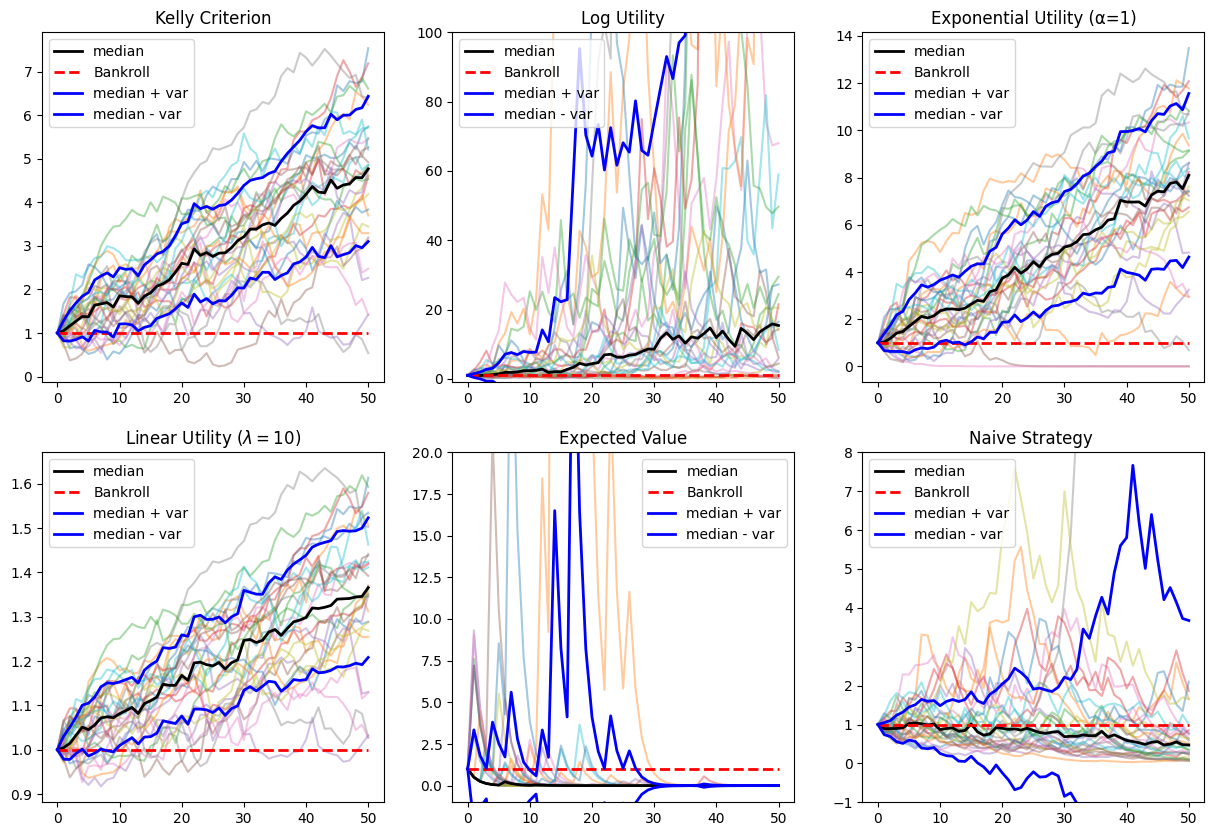
\includegraphics[width=1.1\textwidth, keepaspectratio]{images/monte_carlo_b=b.png}
    \caption{Monte carlo simulations for each strategy}
    \label{fig:monte_carlo}
\end{figure}


\begin{table}[H]
\centering
\caption{Final Bankroll Statistics}
\label{tab:final_bankroll}
\begin{tabular}{lrrrrr}
\toprule
\textbf{Strategy} & \textbf{Mean} & \textbf{Std Dev} & \textbf{Median} & \textbf{Min} & \textbf{Max} \\
\midrule
Kelly Criterion          & 4.48   & 1.67   & 4.77   & 0.54   & 7.54   \\
Log Utility              & 270.85 & 983.14 & 15.39  & 0.19   & 5414.01 \\
Exponential Utility      & 7.46   & 3.46   & 8.10   & 0.00   & 13.48  \\
Linear Utility           & 1.35   & 0.16   & 1.37   & 1.03   & 1.61   \\
Expected Value           & 0.00   & 0.00   & 0.00   & 0.00   & 0.01   \\
Naïve Strategy           & 1.20   & 3.20   & 0.47   & 0.06   & 18.19  \\
\bottomrule
\end{tabular}
\end{table}

The \textbf{Log Utility} strategy achieved the highest mean final bankroll but with significant variability, indicating high risk. The \textbf{Kelly Criterion} and \textbf{Exponential Utility} strategies demonstrated moderate returns with lower variability, suggesting consistent performance.

\begin{table}[H]
\centering
\caption{Average Growth Rate Per Step}
\label{tab:avg_growth}
\begin{tabular}{lr}
\toprule
\textbf{Strategy} & \textbf{Growth Rate} \\
\midrule
Kelly Criterion          & 2.82\% \\
Log Utility              & 5.54\% \\
Exponential Utility      & 2.55\% \\
Linear Utility           & 0.59\% \\
Expected Value           & $-$29.83\% \\
Naïve Strategy           & $-$1.55\% \\
\bottomrule
\end{tabular}
\end{table}

While the \textbf{Log Utility} strategy had the highest growth rate, it came with increased volatility. The \textbf{Kelly Criterion} and \textbf{Exponential Utility} strategies offered positive growth with better risk control.

\begin{table}[H]
\centering
\caption{Sharpe Ratio}
\label{tab:sharpe_ratio}
\begin{tabular}{lr}
\toprule
\textbf{Strategy} & \textbf{Sharpe Ratio} \\
\midrule
Kelly Criterion          & 0.30 \\
Log Utility              & 0.29 \\
Exponential Utility      & 0.25 \\
Linear Utility           & 0.30 \\
Expected Value           & 0.14 \\
Naïve Strategy           & 0.01 \\
\bottomrule
\end{tabular}
\end{table}

The highest Sharpe Ratios were achieved by the \textbf{Kelly Criterion} and \textbf{Linear Utility} strategies, indicating superior risk-adjusted returns.

\begin{table}[H]
\centering
\caption{Probability of Ruin}
\label{tab:prob_ruin}
\begin{tabular}{lr}
\toprule
\textbf{Strategy} & \textbf{Probability} \\
\midrule
Kelly Criterion          & 0.00\% \\
Log Utility              & 3.33\% \\
Exponential Utility      & 6.67\% \\
Linear Utility           & 0.00\% \\
Expected Value           & 100.00\% \\
Naïve Strategy           & 20.00\% \\
\bottomrule
\end{tabular}
\end{table}

Zero probability of ruin for the \textbf{Kelly Criterion} and \textbf{Linear Utility} strategies underscores their robustness.

An ANOVA test (performed to assess whether the differences in final bankrolls among the strategies), (F-statistic: 2.16, p-value: 0.0612) suggested that differences among strategies were not statistically significant at the 5\% level. However, the p-value is close to the threshold, suggesting that with a larger sample size, the differences might become statistically significant.

\subsection{Conclusion}

The simulations indicate that strategies like the \textbf{Kelly Criterion} and \textbf{Exponential Utility}, which balance growth and risk through utility maximization, offer favorable outcomes. The \textbf{Log Utility} strategy provides high growth potential but with greater volatility. Ignoring risk, as in the \textbf{Expected Value} strategy, leads to poor performance.

\textbf{Limitations} include the limited number of simulations, simplified assumptions, and exclusion of real-world factors like transaction costs.

\textbf{Recommendations} for future work involve increasing simulation runs, incorporating realistic market conditions, and exploring additional strategies.


\section{Online Testing}

To assess the strategies in a real-world environment, an online testing phase was conducted over five weeks, from 2024 August 24th to 2024 September 30th, focusing on matches from the five major European football leagues. This real-world testing evaluated the practical applicability and performance of the strategies under actual market conditions. Odds were scraped each day at 12pm from the Odd Api website.


\subsection{Static Problem Reduction and Parameter Settings}

To simplify the dynamic nature of sports betting, we reduced the problem to a series of static optimizations at discrete time intervals. At each decision point \( t \), bankroll allocation was optimized based on the current available information. This approach allowed us to manage the complexity of real-time betting while ensuring the practical applicability of the strategies.

\paragraph{Temporal Parameters}

Key temporal parameters were defined as follows:

\begin{itemize}
    \item \textbf{Betting Interval (\( \Delta t \))}: The interval between placing bets, set to 24 hours to capture daily betting opportunities.
    \item \textbf{Bet Placement Timing}: Bets were placed at a fixed time each day (12:00 PM) to ensure up-to-date information was used while accommodating market dynamics.
\end{itemize}

These settings ensured a balance between information accuracy and practical market conditions.

\paragraph{Match Selection}

The matches selected for each optimization were determined based on:

\begin{itemize}
    \item \textbf{Number of Matches (\( M \))}: Matches occurring within the next 24 hours were selected, balancing opportunity and reliability of information as well as having all results while perfomring next step.
    \item \textbf{Selection Criteria}: Focus was given to matches from top European leagues where the bettor had a higher perceived edge.
\end{itemize}

This careful match selection helped reduce computational complexity while enhancing potential returns.

\paragraph{Re-Betting Policy}

The re-betting policy was defined by the following criteria:

\begin{itemize}
    \item \textbf{Not allowing Re-Bets}: Additional bets on previously considered matches were not allowed. As we only bet on matches on the same day and only once a day, this was an implication of the previous choices.
\end{itemize}

This policy helped manage risk and adapt to evolving market conditions.

\subsection{Practical Implementation Settings}

The practical implementation settings for the online testing phase are summarized in Table~\ref{tab:implementation_settings}. The testing period ran from August 24, 2024, to September 30, 2024. The \texttt{trust-constr} algorithm was used for optimization, with a multiplier of \( \gamma = \frac{1}{2} \) applied to the matrix \( f \). The best odds from a pool of bookmakers (detailed in the appendix) were selected for each match.

\begin{table}[H]
\centering
\caption{Practical Implementation Settings}
\label{tab:implementation_settings}
\begin{tabular}{ll}
\toprule
\textbf{Setting}               & \textbf{Value}                                 \\ \midrule
Betting Interval (\( \Delta t \))     & 24 hours \\                                    
Bet Placement Time               & 12:00 PM daily                                \\
Look-Ahead Horizon               & Matches within the next 24 hours               \\ 
Re-Betting Policy                & Not allowed \\ 
Testing Period                   & August 24, 2024 – September 30, 2024           \\ 
Optimization Algorithm           & \texttt{trust-constr}                          \\ 
Strategy factor mult. \(\gamma\)         & \( 0.5 \)                              \\ 
Odds Selection                   & Biggest odds from a pool of bookmakers            \\ 
Markets & 5 biggest European leagues (Big 5) \\
\bottomrule
\end{tabular}
\end{table}


\subsection{Results and Interpretation}

Figure~\ref{fig:capital_evolution} illustrates the capital evolution for each strategy during the testing period. The Kelly and Exponential Utility strategies exhibited the strongest performance, both ending with approximately twice the initial capital. These results highlight their ability to optimally balance risk and reward, consistently outperforming the more conservative Log and Naive strategies. However, they also demonstrated higher volatility compared to the more stable Linear strategy.

\begin{figure}[H]
    \centering
    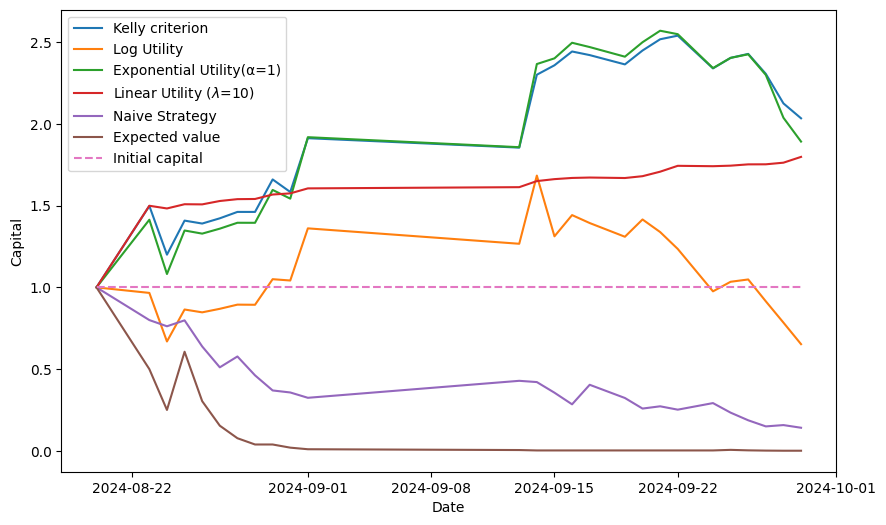
\includegraphics[width=\textwidth]{images/bankroll_evolution2.png}
    \caption{Capital Evolution for Each Strategy During the Online Testing Period}
    \label{fig:capital_evolution}
\end{figure}

The Log Utility strategy underperformed, particularly at the start and after the midpoint of the test period, failing to capitalize on high-return opportunities. Its conservative nature, aimed at minimizing risk, resulted in modest growth but ultimately led to a negative outcome. 

Both the Naive and Expected Value strategies experienced sharp declines in capital. The Naive strategy approached near-zero capital by the end of the test, while the Expected Value strategy exhibited extreme volatility, leading to rapid capital depletion. These simpler strategies, which lack sophisticated optimization, were highly vulnerable to adverse market conditions and failed to adapt effectively to fluctuations in odds or match outcomes.

In contrast, the Linear Utility strategy showed steady and consistent growth, with minimal volatility throughout the testing period, ultimately achieving a final growth of 1.8 times the initial capital. This highlights its effectiveness in maintaining a stable growth trajectory while avoiding the excessive risk associated with other strategies.

Overall, the results underscore the superiority of more advanced utility-based strategies such as Kelly and Linear. These approaches consistently outperformed simpler methods by balancing risk and reward more effectively under real-world betting conditions.

\subsection{Performance Metrics}

To further quantify the performance of each strategy, we computed key metrics, including final bankroll \( B(T) \), mean growth per step, and standard deviation of growth per step, both in absolute terms and as a percentage of the final bankroll. 
\begin{itemize}
    \item The mean growth per step is defined as:
    \[
    \mu = \frac{1}{T-1} \sum_{t=1}^{T-1} \Delta B_t
    \]
    where \( \Delta B_t = B_{t+1} - B_t \),
    \item the standard deviation of growth per step is given by:
    \[
    \sigma = \sqrt{\frac{1}{T-1} \sum_{t=1}^{T-1} (\Delta B_t - \mu)^2}
    \]
\end{itemize}


Table~\ref{tab:strategy_performance} summarizes the results for each strategy.

\begin{table}[H]
\centering
\caption{Strategy Performance Metrics}
\label{tab:strategy_performance}
\begin{tabular}{llll}
\toprule
\textbf{Strategy}              & \textbf{Final Bankroll \( B(T) \)} & \textbf{Mean Growth (\%)} & \textbf{Std Growth (\%)} \\ 
\midrule
Kelly Criterion                & 2.034                              & 2.034                      & 8.923                    \\ 
Log Utility                    & 0.653                              & -2.129                     & 26.516                   \\ 
Exponential Utility (\( \alpha = 1 \)) & 1.892                        & 1.886                      & 10.309                   \\ 
Linear Utility (\( \lambda = 10 \))    & 1.798                        & 1.776                      & 5.360                    \\ 
Naive Strategy                 & 0.141                              & -24.299                    & 52.419                   \\ 
Expected Value                 & 0.001                              & -5032.448                  & 18175.649                \\
\bottomrule
\end{tabular}
\end{table}

\subsection{Interpretation of Metrics}

The results demonstrate the effectiveness of the Kelly Criterion and Exponential Utility strategies, both of which ended with a final bankroll close to 2.0. These strategies also displayed reasonable volatility, with standard deviations of growth per step under 10\%. The Linear Utility strategy performed consistently, achieving steady growth with the lowest volatility among all strategies.

On the other hand, the Log Utility strategy suffered from negative growth, highlighting its inability to capitalize on high-return opportunities. The Naive and Expected Value strategies performed poorly, with significant capital depletion and extreme volatility, particularly for the Expected Value approach, indicating their inadequacy in real-world betting scenarios.


\section{Conclusion}

The results from both the Monte Carlo simulations and the real-world online testing phase demonstrate the clear advantages of sophisticated bankroll management strategies such as the Kelly Criterion and Exponential Utility methods. These strategies consistently provided strong returns while managing risk effectively, leading to a final bankroll close to twice the initial amount. In contrast, simpler strategies like the Naive and Expected Value approaches underperformed, suffering from capital depletion and high volatility, emphasizing the importance of balancing risk and return in real-world betting scenarios.

The Linear Utility strategy offered a steady, reliable growth trajectory with minimal volatility, making it an appealing option for risk-averse bettors. The Log Utility strategy, though conservative, failed to capture sufficient growth opportunities, resulting in a negative final outcome. Overall, the Kelly and Exponential Utility strategies are best suited for bettors seeking long-term growth with manageable risk.

\subsection{Limitations and Future Improvements}

Despite the promising results, several limitations were identified in the current approach:

\begin{itemize}
    \item \textbf{Simulation Assumptions}: The Monte Carlo simulations relied on several simplifying assumptions that limit the realism of the results. Firstly, the simulation of probabilities was based on the true clipped probabilities plus a bias and Gaussian noise, which does not fully capture the actual flaws in the predictive models, and the constants used were chosen arbitrarily without strong justification. Secondly, the bookmaker margin was fixed, and the odds provided by the bookmaker did not account for the influence of large bets from the players, which in reality could cause deviations in the bookmaker’s odds and probabilities. Lastly, the simulations used a fixed number of matches and time steps. Both the number of simulations and the range of strategies could be expanded to provide a more thorough and diverse analysis of performance over a wider variety of scenarios.
    \item \textbf{Limited Testing Period}: The online testing phase covered only a five-week period, which may not fully capture the long-term performance and robustness of each strategy. Extending the testing period or repeating it across multiple seasons would provide a more comprehensive assessment.
    \item \textbf{Risk Preferences}: While the utility-based strategies successfully managed risk, the models relied on fixed parameters for risk aversion (e.g., \( \lambda \) in Linear Utility). Introducing dynamic adjustments to these parameters based on market conditions or bettor preferences could further enhance performance.
\end{itemize}

\subsection{Future Work and Deployment on Azure Kubernetes}

The next stage of this project involves deploying the entire system on a cloud infrastructure using Kubernetes on Azure (AKS). This deployment will enable scalable, real-time processing of betting opportunities, continuous model updates, and the handling of multiple simultaneous users and markets. By leveraging Azure’s powerful compute and orchestration capabilities, the system will be capable of efficiently managing the computational load and data flows needed for real-time sports betting optimization.


\section{Microservices Architecture and Frameworks}

To build a scalable and maintainable system for sports betting optimization, we adopted a microservices architecture. This approach allows independent development, deployment, and scaling of individual components, facilitating modularity and flexibility.

The system comprises several microservices:

\begin{itemize}
    \item \textbf{Data Ingestion Service}: Collects real-time match data and odds from external APIs and web scraping. We use the Python library \textit{soccerdata} to conveniently scrape historical and real-time data from various websites. \textit{SQLAlchemy} is employed to communicate with the PostgreSQL database, allowing interaction using a mix of Python syntax and SQL queries. An API is provided for other services to trigger this service's logic, created using the \textit{FastAPI} framework. The Python library \texttt{logging} is used for proper logging of all operations, and \texttt{pandas} is utilized for data manipulation and transformation.

    \item \textbf{Prediction and Optimization Service}: Processes data to train models and generate probability estimates for the prediction component. Calculates optimal bet allocations based on the probabilities and selected strategies for the optimization component. \textit{Scikit-learn} is used for model training and inference, while \textit{SciPy.optimize} handles the optimization processes. Similar to the Data Ingestion Service, an API is deployed using \textit{FastAPI}, with communication to the database via \textit{SQLAlchemy}, and \texttt{logging} and \texttt{pandas} for logging and data handling.

    \item \textbf{User Interface Service}: Provides a web-based dashboard for monitoring and interaction, developed using the Python web framework \textit{Streamlit}.

    \item \textbf{Backend Service}: Manages communication and logic between the frontend User Interface and the database, as well as other services, using \textit{FastAPI}, \texttt{pandas}, and \texttt{logging}.

    \item \textbf{Database Service}: Stores historical data, odds, inferred probabilities, optimization results, and transaction logs. We chose PostgreSQL as the database due to its robustness, scalability, and compatibility with \textit{SQLAlchemy}. PostgreSQL's advanced features support complex queries and transactions essential for our application's needs.

    \item \textbf{MLflow Service}: Monitors the training metrics of the models. MLflow provides a convenient way to track experiments, record model parameters, metrics, and artifacts, facilitating reproducibility and model versioning.

    \item \textbf{Airflow Service}: Acts as a scheduler, providing a convenient way to orchestrate and monitor complex workflows using Directed Acyclic Graphs (DAGs). Apache Airflow allows us to define data pipelines, schedule tasks, and manage dependencies between them, ensuring timely execution of data ingestion, model training, and optimization processes.
\end{itemize}

Services communicate over HTTP/HTTPS protocols, with well-defined API endpoints ensuring loose coupling and ease of integration.

\section{Docker and Kubernetes}

To ensure consistency across development, testing, and production environments, all microservices are containerized using Docker \cite{Merkel2014}. Docker allows us to package each service with all its dependencies into isolated containers, ensuring consistent behavior across different environments.

\subsection{Dockerization}

Each microservice is encapsulated in a Docker container, defined by its own \texttt{Dockerfile}, which specifies the base image, dependencies, and entry points. In local development, we used containers for services such as MLflow, PostgreSQL, and Airflow, facilitating a consistent and reproducible environment.

\subsection{Kubernetes Deployment}

For orchestration and management of the containerized applications, we utilized Kubernetes \cite{HightowerEtAl2017}. Kubernetes automates deployment, scaling, and management of containerized applications. We packaged our system into a Helm chart, which simplifies the deployment of the entire application, including dependencies like MLflow, PostgreSQL, and Airflow.

\subsubsection{Helm Chart Packaging}

By encapsulating our services and their dependencies into a Helm chart, we streamlined the deployment process. Helm charts define, install, and upgrade complex Kubernetes applications, allowing us to manage configurations and versioning efficiently.

\subsubsection{Database Migrations}

Database schema changes are managed using migration files and scripts. Changes are first applied locally for testing and validation. Once validated, migrations are executed on the production database using scripts designed to apply changes incrementally. This process ensures that the database schema remains synchronized with the application code without disrupting ongoing operations.

\section{Deployment on Azure AKS}

\subsection{Azure Kubernetes Service (AKS)}

We deployed our Kubernetes cluster on Microsoft Azure using Azure Kubernetes Service (AKS), a managed Kubernetes service that simplifies cluster management by handling critical tasks like health monitoring and maintenance. AKS reduces the operational overhead and provides features like automated scaling and updates.

\begin{figure}[H]
    \centering
    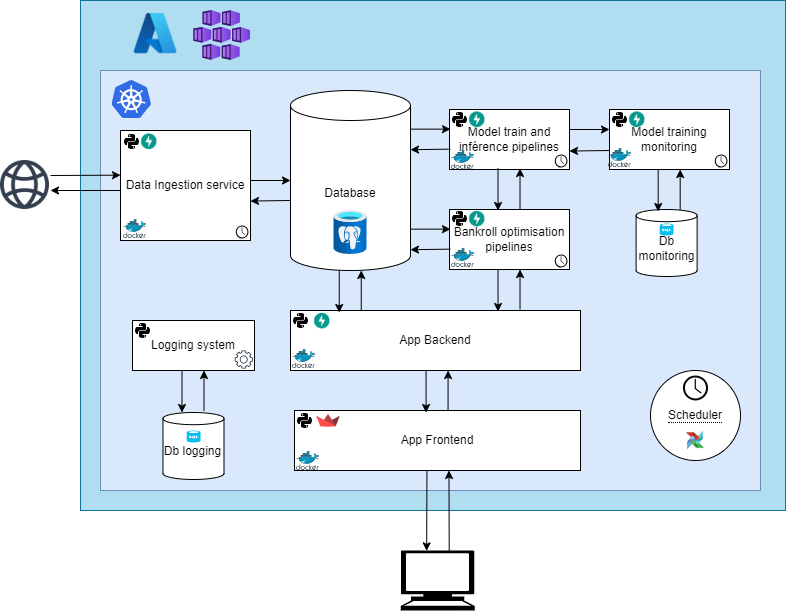
\includegraphics[width=0.8\textwidth, keepaspectratio]{images/diagrem_archi_services.png}
    \caption{Architecture of the system deployed on AKS}
    \label{fig:diagramme_arch_aks}
\end{figure}

\subsection{Infrastructure Details}

Our AKS deployment utilizes two virtual machines to ensure high availability and load balancing across the cluster. While Azure offers its own virtual machines, in this context, we refer to the compute resources allocated to our Kubernetes nodes. The integration with AKS allows for efficient resource utilization and scalability.

\subsection{Azure Services Integration}

Using Azure's cloud infrastructure offers several benefits:

\begin{itemize}
    \item \textbf{Azure Container Registry (ACR)}: Stores our Docker images securely, facilitating seamless deployment to AKS.
    \item \textbf{Azure DevOps Repo}: Provides a storage for our code.
\end{itemize}

\subsection{Pricing Considerations}

Azure's pricing model charges for compute resources used by virtual machines, storage, and network bandwidth. Managed services like AKS can reduce operational overhead but require careful monitoring to manage costs effectively. We optimized resource allocation by:


\section{Conclusion}

By adopting a microservices architecture, containerization with Docker, orchestration with Kubernetes, and deploying on Azure AKS, we built a scalable, reliable, and maintainable system for sports betting optimization. This architecture allows for independent development and deployment of components, ensuring the system can adapt to changing requirements and handle real-time data processing demands efficiently. Leveraging cloud infrastructure and managed services enhances our ability to focus on core application development while ensuring high availability and performance.

\section{Summary of Findings}

This study embarked on the ambitious task of developing a comprehensive system for optimizing sports betting strategies, focusing on football matches. Through the integration of predictive modeling, utility-based optimization, and scalable system architecture, we have addressed the critical components necessary for successful sports betting.

The predictive model, developed using logistic regression and advanced feature selection techniques, demonstrated significant accuracy in forecasting match outcomes. Regular retraining of the model proved essential in maintaining performance over time, highlighting the dynamic nature of sports data.

The optimization module applied various bankroll allocation strategies, including the Kelly Criterion, logarithmic, exponential, and linear utility functions. Both Monte Carlo simulations and real-world online testing over a five-week period indicated that sophisticated utility-based strategies substantially outperform naive betting approaches. Strategies like the Kelly Criterion and Exponential Utility provided favorable returns while effectively managing risk.

The system's deployment on Azure Kubernetes Service (AKS) showcased its scalability and readiness for real-time application. By leveraging a microservices architecture and containerization technologies like Docker and Kubernetes, the system can handle the computational demands of real-time data processing and optimization.

\section{Contributions to the Field}

This work contributes to the field of sports analytics and betting strategies in several ways:

\begin{itemize} \item \textbf{Integration of Predictive Modeling and Optimization}: By combining accurate probability estimations with utility-based optimization strategies, the system provides a robust framework for sports betting. \item \textbf{Scalable System Architecture}: The implementation of a microservices architecture and deployment on cloud infrastructure ensures that the system is scalable, maintainable, and adaptable to real-world conditions. \item \textbf{Empirical Evaluation}: The use of both simulations and real-world testing provides empirical evidence of the effectiveness of advanced betting strategies over simpler methods. \end{itemize}

\section{Limitations}

Despite the positive results, several limitations were identified:

\begin{itemize}
    \item \textbf{Predictive Model Enhancements}: While the current model performs adequately within the constraints of a static framework, it could be significantly improved by incorporating additional features, conducting hyperparameter optimization, and exploring more complex models such as deep learning architectures. These enhancements would allow the model to capture dynamic patterns and temporal dependencies inherent in football matches, which are not fully addressed due to the static nature of the current framework.

    \item \textbf{Static Framework Limitations and Long-Term Gain-Variance Interpretation}: The reduction of the betting problem to a static framework simplifies the optimization process but introduces limitations in interpreting gains and variance over the long term. Since the model does not account for intertemporal dependencies and the evolving nature of the bankroll, the strategies derived may not fully capture the risks associated with long-term betting. This static approach may lead to strategies that optimize short-term gains without adequately considering the cumulative effect on wealth over time. Future work should focus on extending the framework to a dynamic setting, allowing for a more accurate interpretation of long-term gain and variance, and better aligning the strategies with the bettor's long-term financial goals.

    \item \textbf{Risk Preferences and Dynamic Adaptation}: The optimization strategies employed fixed parameters for risk aversion, which do not adjust to changes in the bettor's wealth or market conditions over time. This static treatment of risk preferences limits the adaptability of the betting strategies, especially in a long-term context where the bettor's financial situation and the market dynamics can vary significantly. Introducing dynamic risk preferences that evolve with the bettor's bankroll and external factors would enhance the strategies' responsiveness and effectiveness, leading to better management of gain and variance over the long term.

    \item \textbf{Testing Period and Scope}: The real-world testing was confined to a five-week period focusing on the top five European leagues. Due to the static framework and the short testing duration, the evaluation may not fully reflect the strategies' performance over extended periods or in different market conditions. A longer testing period encompassing a broader range of leagues and varying competitive environments would provide more comprehensive insights into the strategies' long-term viability and their ability to manage gains and risks effectively within a dynamic setting.

\end{itemize}
\section{Future Work}

Building upon the findings of this study, several promising avenues can be explored to enhance the system's performance and address the challenges identified. 

Firstly, integrating real-time data streams and developing adaptive predictive models could significantly improve forecasting accuracy. By incorporating techniques from time-series analysis and machine learning, the model can capture temporal dependencies and evolving patterns inherent in football matches. This dynamic approach would allow the model to adjust to new information promptly, potentially leading to more accurate probability estimates and better alignment with the actual match outcomes.

Secondly, advancing the optimization strategies to include stochastic elements and multi-period planning could address the complexities associated with long-term gain and variance interpretation. Developing a dynamic framework that accounts for intertemporal dependencies and the evolving nature of the bankroll would enable more effective risk management. Strategies that adapt risk preferences in response to changes in the bettor's financial status or market conditions could lead to more sustainable betting practices and improved long-term financial outcomes.

Thirdly, conducting extensive real-world testing over longer periods and across a broader range of leagues and competitions would provide deeper insights into the robustness and generalizability of the betting strategies. Such testing would help to evaluate the performance of the models under varying market conditions and competitive environments, ensuring that the strategies remain effective over time and are not limited to specific contexts or short-term scenarios.

Finally, enhancing the user interface to offer more advanced analytics and personalized insights could empower users to make more informed decisions. Features that allow users to visualize performance trends, adjust parameters interactively, and receive tailored recommendations would improve the overall user experience. Providing tools for long-term performance monitoring and strategic adjustments would enable users to better understand the implications of their betting decisions and manage their bankrolls more effectively.

These potential developments represent initial steps toward refining the system's capabilities. By focusing on dynamic modeling, adaptive optimization, comprehensive testing, and user-centric design, future work can contribute to more robust predictive performance, effective risk management, and ultimately, more successful sports betting strategies.

\section{Final Remarks}

The integration of predictive modeling and utility-based optimization represents a significant step forward in developing effective sports betting strategies. This work demonstrates that with accurate predictions and strategic bankroll management, it is possible to achieve superior returns while managing risk effectively. The deployment on cloud infrastructure ensures that the system is ready for practical application, paving the way for future advancements in the field.


Je veux que tu me rédige un article de blog sur ce projet en format md. L'article doit prendre environ 10 min à lire et doit être interressant, prenant, il doit y avoir un bon story telling. Et plusieurs niveau de comprehension, pour les non initiés et pour les data scientist avancés.

Fais le en anglais

\chapter{Predictive Modeling of Match Outcomes}


\chapter{Introduction}

Sports betting has evolved into a sophisticated industry that combines statistical analysis, predictive modeling, and strategic financial management \cite{AndersonSally2013}. With the global popularity of football and the abundance of data available, there is a significant opportunity to apply advanced analytical techniques to optimize betting strategies. The challenge lies in accurately predicting match outcomes and effectively managing the allocation of betting capital to maximize returns while minimizing risk.

This report presents the development and implementation of a comprehensive system designed to address these challenges in sports betting. The system integrates predictive modeling to forecast football match outcomes and optimization algorithms to determine the optimal allocation of a bettor's bankroll. The focus is on creating a practical, scalable solution that can operate in real-time, leveraging cloud-based technologies and microservices architecture.

\section{Background and Motivation}

The sports betting market is highly competitive, with bettors seeking any edge to improve their chances of success. Traditional betting strategies often rely on intuition or simplistic models that fail to account for the complexities of sports data and market dynamics. The advancement of machine learning and statistical methods offers the potential to enhance predictive accuracy and optimize betting decisions systematically \cite{CainEtAl2000}.

Effective bankroll management is equally important, as even accurate predictions can lead to losses if the betting amounts are not strategically allocated. The application of utility theory and optimization techniques, such as the Kelly Criterion, provides a mathematical framework for balancing risk and reward in betting decisions. 

\section{Objectives of the Study}

The primary objectives of this study are:

\begin{itemize}
\item To establish a rigorous mathematical framework that defines the theoretical foundations and sets the stage for the study.
\item To develop a predictive model that accurately estimates the probabilities of football match outcomes using historical and real-time data. \item To design an optimization module that calculates the optimal fraction of the bankroll to wager on each betting opportunity, applying various utility-based strategies. \item To implement a scalable, microservices-based system architecture that integrates data collection, predictive modeling, optimization, and user interface components. \item To deploy the system on a cloud platform using Kubernetes for scalability and reliability. \item To evaluate the performance of different betting strategies through Monte Carlo simulations and real-world online testing. \end{itemize}

\section{Scope of the Report}

This report details the theoretical framework underlying the predictive modeling and optimization strategies, the system architecture and implementation, and the results of both simulated and real-world testing. The report is organized as follows:

\begin{itemize} \item Chapter 2 provides a theoretical presentation of the models and preliminary research conducted. \item Chapter 3 describes the design and implementation of the solution, including system architecture and data management. \item Chapter 4 focuses on the development, training, and evaluation of the predictive models for match outcomes. \item Chapter 5 discusses the optimization of bankroll allocation using various strategies. \item Chapter 6 details the deployment of the complete system on Azure Kubernetes Service and the practical considerations involved. \item Chapter 7 presents the conclusions drawn from the study and discusses potential future work. \end{itemize}

\section{Significance of the Study}

By integrating advanced predictive modeling with optimized bankroll allocation, this work aims to contribute to the field of sports analytics and betting strategies. The deployment of the system on a scalable cloud infrastructure demonstrates its practical applicability and readiness for real-world use. The findings from this study have implications for bettors seeking to enhance their strategies, as well as for researchers interested in the application of machine learning and optimization techniques in sports betting.

\chapter{Theoretical presentation and preliminary research}
\input{chapters/2_theoretical_presentation_and_preliminary_research/main}

\chapter{Design and implementation of the solution}
\input{chapters/3_design_and_implementation_of_the_solution/main}

\chapter{Predictive Modeling of Match Outcomes}
\input{chapters/4_predictive_modeling_of_match_outcomes/main}

\chapter{Optimization of bankroll allocation}
\input{chapters/5_Optimization_of_bankroll_allocation/main}

\chapter{Development of the Complete System and Production Deployment}
\input{chapters/6_Development_of_the_Complete_System and_Production _Deployment/main}

\chapter{Discussion and Conclusion}
\input{chapters/conclusion/main}

\appendix
\input{chapters/appendix/main}

\printbibliography[heading=bibintoc,title={References}]


\subsection{Matches and Outcomes}

At any given time \( t \in \mathbb{R}^+ \), we define the set of matches available for betting as:

\[
\mathbb{M}(t) = \{ m^1, m^2, \dots, m^{M(t)} \}
\]

where \( M(t) \in \mathbb{N} \) represents the total number of matches available at time \( t \).

For each match \( m^k \in \mathbb{M}(t) \), there is a set of possible outcomes:

\[
\Omega^k = \{ \omega_1^k, \omega_2^k, \dots, \omega_{N^k}^k \}
\]

where \( N^k \in \mathbb{N} \) represents the number of possible outcomes for match \( m^k \).

\paragraph{Example:} 
In a football match, possible outcomes might be chosen as \{home team wins, draw, away team wins\}, so \( N^k = 3\) \(\forall k\).

\subsection{Probabilities of Outcomes}

We define \( \mathbb{P}_Y( \omega_i^k ) \) as the probability that outcome \( \omega_i^k \) occurs for match \( m^k \), given the state of the world \( Y \) at time \( t \):

\[
r_i^k(t) = \mathbb{P}_Y( \omega_i^k )
\]

These probabilities may change over time as new information becomes available.

We introduce the random variable \( X_i^k \) associated with outcome \( \omega_i^k \):

\[
X_i^k = \begin{cases}
1, & \text{if outcome } \omega_i^k \text{ occurs}, \\
0, & \text{otherwise}.\\
\end{cases}
\]

Therefore, \( r_i^k(t) = \mathbb{P}_Y( X_i^k = 1 ) \). \\

\paragraph{Example:} 
Consider a football match \( m^k \) between Team A and Team B. The possible outcomes \( \omega_i^k \) are:

\[
\omega_1^k = \text{Team A wins}, \quad \omega_2^k = \text{Draw}, \quad \omega_3^k = \text{Team B wins}.
\]

At time \( t \), based on current information \( Y \) (such as form, injuries, and past results), the probabilities of these outcomes are:

\[
r_1^k(t) = \mathbb{P}_Y(\text{Team A wins}), \quad r_2^k(t) = \mathbb{P}_Y(\text{Draw}), \quad r_3^k(t) = \mathbb{P}_Y(\text{Team B wins}).
\]

For example, if \( r_1^k(t) = 0.55 \), it means there is a 55\% chance that Team A will win.

\subsection{Bettors and Bookmakers}

Let \( \mathbb{J} \) be the set of bettors, and \( \mathbb{B} \) be the set of bookmakers.

Each bettor \( J \in \mathbb{J} \) has a bankroll at time \( t \), denoted by:

\[
B_{\text{bettor}}^J(t)
\]

Similarly, each bookmaker \( B \in \mathbb{B} \) has a bankroll at time \( t \), denoted by:

\[
B_{\text{bookmaker}}^B(t)
\]

\subsection{Odds}

At time \( t \), bookmaker \( B \) offers odds on the outcomes of matches. For match \( m^k \), the odds offered by bookmaker \( B \) are:

\[
\mathbb{O}^k(B, t) = \{ o_1^{k,B}(t), o_2^{k,B}(t), \dots, o_{N^k}^{k,B}(t) \}
\]

where \( o_i^{k,B}(t) \) represents the odds offered on outcome \( \omega_i^k \) of match \( m^k \) at time \( t \). \\

\paragraph{Example:}
Consider the same football match \( m^k \) between Team A and Team B. At time \( t \), bookmaker \( B \) offers the following odds:

\[
\mathbb{O}^k(B, t) = \{ 2.00, 3.50, 4.00 \}
\]

Where \( o_1^{k,B}(t) = 2.00 \) for Team A to win, \( o_2^{k,B}(t) = 3.50 \) for a draw, and \( o_3^{k,B}(t) = 4.00 \) for Team B to win.

These odds represent the potential payouts for each outcome.

\subsection{Bets and Wagers}

At time \( t \), bettor \( J \) may choose to place bets on various outcomes. We define:

\begin{itemize}
    \item \( f_i^{k,J}(t) \): The fraction of bettor \( J \)'s bankroll \( B_{\text{bettor}}^J(t) \) that is wagered on outcome \( \omega_i^k \) of match \( m^k \).
    \item \( b_i^{k,J}(t) \): The bookmaker \( B \) with whom bettor \( J \) places the bet on outcome \( \omega_i^k \) of match \( m^k \).
\end{itemize}

Therefore, the amount wagered by bettor \( J \) on outcome \( \omega_i^k \) at time \( t \) is:

\[
w_i^{k,J}(t) = f_i^{k,J}(t) \times B_{\text{bettor}}^J(t)
\]


\paragraph{Example:}
Consider bettor \( J \) with a bankroll of \( B_{\text{bettor}}^J(t) = 100 \) units at time \( t \). Bettor \( J \) decides to wager:

\[
f_1^{k,J}(t) = 0.2 \quad \text{(20\% of the bankroll on Team A to win)}
\]

Thus, the amount wagered is:

\[
w_1^{k,J}(t) = 0.2 \times 100 = 20 \text{ units}
\] 

Bettor \( J \) places the 20-unit bet with bookmaker \( B \).

\subsection{Bankroll Evolution}

The evolution of the bettors' and bookmakers' bankrolls depends on the outcomes of the matches and the settlement of bets.

\subsubsection{Bettor's Bankroll Evolution}

The bankroll of bettor \( J \) at time \( t \) is given by:

\[
B_{\text{bettor}}^J(t) = B_{\text{bettor}}^J(0) + \int_0^t \sum_{b \in \mathcal{B}_{\text{settled}}^J(\tau)} G_{\text{bettor}}^J(b) \, d\tau
\]

where:

\begin{itemize}
    \item \( \mathcal{B}_{\text{settled}}^{J}(s) \) is the set of bets placed by bettor \( J \) that are settled at time \( s \).
    \item \( G_{\text{bettor}}^J(b) \) is the gain or loss from bet \( b \), calculated as:
    \[
    G_{\text{bettor}}^J(b) = w^{J}(b) \times \left( o^{B}(b) \times X(b) - 1 \right)
    \]
    \begin{itemize}
        \item \( w^{J}(b) \) is the amount wagered on bet \( b \).
        \item \( o^{B}(b) \) is the odds offered by bookmaker \( B \) for bet \( b \).
        \item \( X(b) \) indicates whether the bet was successful (\( X(b) = 1 \)) or not (\( X(b) = 0 \)).
    \end{itemize}
\end{itemize}

\paragraph{Example:}

Consider bettor \( J \) starts with a bankroll of \( B_{\text{bettor}}^J(0) = 100 \) units. At time \( t_1 \), the bettor places a bet of \( w^{J}(b) = 20 \) units on a match with odds \( o^{B}(b) = 2.50 \) offered by bookmaker \( B \).

If the outcome \( X(b) = 1 \) (the bettor wins the bet), the gain from the bet is:

\[
G_{\text{bettor}}^J(b) = 20 \times (2.50 \times 1 - 1) = 30 \text{ units}
\]

Thus, the updated bankroll at time \( t_1 \) is:

\[
B_{\text{bettor}}^J(t_1) = 100 + 30 = 130 \text{ units}
\]

If the bettor loses another bet at time \( t_2 \) with a wager of 30 units on odds of 3.00, then \( X(b) = 0 \) and the loss is:

\[
G_{\text{bettor}}^J(b) = 30 \times (3.00 \times 0 - 1) = -30 \text{ units}
\]

The bankroll at time \( t_2 \) becomes:

\[
B_{\text{bettor}}^J(t_2) = 130 - 30 = 100 \text{ units}
\]

\subsubsection{Bookmaker's Bankroll Evolution}

Similarly, the bankroll of bookmaker \( B \) at time \( t \) is given by:

\[
B_{\text{bookmaker}}^B(t) = B_{\text{bookmaker}}^B(0) + \int_0^t \sum_{J \in \mathcal{J}} \sum_{b \in \mathcal{B}_{\text{settled}}^{B,J}(\tau)} G_{\text{bookmaker}}^B(b) \, d\tau
\]

where:

\begin{itemize}

    \item \( \mathcal{J} \) is the set of all bettors \( \{ J_1, J_2, \dots, J_N \} \) placing bets with bookmaker \( B \).
    \item \( \mathcal{B}_{\text{settled}}^{B,J}(s) \) is the set of bets accepted by bookmaker \( B \) from bettor \( J \) that are settled at time \( s \).
    \item \( G_{\text{bookmaker}}^B(b) \) is the gain or loss from bet \( b \), which now takes into account multiple bettors \( J \), calculated as:
    
    \[
    G_{\text{bookmaker}}^B(b) = w^{J}(b) \times \left( 1 - o^{B}(b) \times X(b) \right)
    \]
    
    where:
    \begin{itemize}
        \item \( w^{J}(b) \) is the amount wagered by bettor \( J \) on bet \( b \).
        \item \( o^{B}(b) \) is the odds offered by bookmaker \( B \) for bet \( b \).
        \item \( X(b) \) indicates whether the bet was successful (\( X(b) = 1 \)) or not (\( X(b) = 0 \)).
    \end{itemize}
\end{itemize}
\subsubsection{Impact of Multiple Bettors}

For each bet \( b \), the gain or loss for bookmaker \( B \) depends on which bettor placed the bet. If bettor \( J \) wins, bookmaker \( B \) pays out, and if bettor \( J \) loses, bookmaker \( B \) gains:

\[
G_{\text{bookmaker}}^B(b) = - G_{\text{bettor}}^J(b)
\]

Thus, for each bet placed by a bettor \( J \), the bookmaker’s gain is equal to the bettor’s loss, and vice versa. With multiple bettors, the bookmaker's bankroll reflects the combined gains and losses from all bets settled across the bettors \( J_1, J_2, \dots, J_N \).


\subsection{Bankroll Factor}

To abstract from the initial bankroll amounts, we can define the \textit{Bankroll Factor} for bettors and bookmakers.

\subsubsection{Bettor's Bankroll Factor}

The bankroll factor for bettor \( J \) at time \( t \) is defined as:

\[
BF_{\text{bettor}}^J(t) = \frac{B_{\text{bettor}}^J(t)}{B_{\text{bettor}}^J(0)}
\]

This represents the growth of the bettor's bankroll relative to their initial bankroll.

\subsubsection{Bookmaker's Bankroll Factor}

Similarly, the bankroll factor for bookmaker \( B \) at time \( t \) is:

\[
BF_{\text{bookmaker}}^B(t) = \frac{B_{\text{bookmaker}}^B(t)}{B_{\text{bookmaker}}^B(0)}
\]

\subsection{Gain Calculation}

The cumulative gain for bettor \( J \) up to time \( t \) is:

\[
G_{\text{bettor}}^J(t) = B_{\text{bettor}}^J(t) - B_{\text{bettor}}^J(0) = B_{\text{bettor}}^J(0) \left( BF_{\text{bettor}}^J(t) - 1 \right)
\]

Similarly, for bookmaker \( B \):

\[
G_{\text{bookmaker}}^B(t) = B_{\text{bookmaker}}^B(t) - B_{\text{bookmaker}}^B(0) = B_{\text{bookmaker}}^B(0) \left( BF_{\text{bookmaker}}^B(t) - 1 \right)
\]


\subsection{Utility Function}

The utility function \( U \) represents the agent's preferences regarding risk and reward, crucial in decision-making under uncertainty \cite{KahnemanTversky1979}. Bettors and bookmakers use this function to optimize their gains over time while minimizing risk. Unlike expected returns, utility functions incorporate risk preferences, allowing agents to balance the trade-off between potential gains and variability 
\cite{Markowitz1952} \cite{Arrow1971} \cite{Pratt1964}.

\subsubsection{Forms of Utility Functions}

Different utility functions capture varying risk attitudes, ranging from risk-neutral to risk-averse behaviors. Below are the common types of utility functions in the betting market:

\paragraph{1. Expected Value Utility (Risk-Neutral)}

The simplest form, where utility is directly proportional to wealth:

\[
U(B) = B
\]

Agents using this function are risk-neutral, focusing solely on maximizing expected returns without considering risk.

\paragraph{2. Logarithmic Utility (Moderate Risk Aversion)}

Logarithmic utility models constant relative risk aversion (CRRA) and is expressed as:

\[
U(B) = \ln(B)
\]

This function reflects diminishing marginal utility of wealth, balancing risk and reward, commonly used in the Kelly Criterion \cite{Kelly1956} \cite{Thorp1975} for long-term growth.

\paragraph{3. Power Utility (CRRA)}

A generalization of logarithmic utility, with risk aversion controlled by \( \gamma \):

\[
U(B) = \frac{B^{1 - \gamma}}{1 - \gamma}, \quad \gamma \neq 1
\]

Higher \( \gamma \) values indicate greater risk aversion. When \( \gamma = 1 \), the function becomes logarithmic.

\paragraph{4. Exponential Utility (Constant Absolute Risk Aversion - CARA)}

The exponential utility models constant absolute risk aversion (CARA):

\[
U(B) = -e^{-\alpha B}
\]

Here, \( \alpha \) controls risk aversion. Agents using this function maintain consistent risk preferences regardless of wealth level.

\paragraph{5. Quadratic Utility}

Quadratic utility is given by:

\[
U(B) = B - \frac{\lambda}{2} B^2
\]

Though it captures increasing risk aversion, it has the drawback of implying decreasing utility at higher wealth levels, making it less commonly used.

\subsubsection{Implications of Different Utility Functions}

Each utility function models specific risk preferences, influencing the agent’s decisions:

\paragraph{Risk-Neutral Behavior}

Agents with linear utility (\( U(B) = B \)) focus solely on maximizing returns, indifferent to risk. This behavior is rare in practice due to the inherent risks in betting.

\paragraph{Risk-Averse Behavior}

Utility functions like logarithmic, power, and exponential represent risk-averse behavior:

\begin{itemize}
    \item \textbf{Logarithmic Utility:} Moderate risk aversion, favoring long-term growth.
    \item \textbf{Power Utility (CRRA):} Flexibility in modeling different degrees of risk aversion via \( \gamma \).
    \item \textbf{Exponential Utility (CARA):} Constant risk aversion regardless of wealth.
\end{itemize}

\paragraph{Risk-Seeking Behavior}

Agents may occasionally exhibit risk-seeking behavior, favoring higher variance. This is typically modeled by utility functions with convex regions or negative coefficients but is unsustainable in the long term.

\subsubsection{Choosing an Appropriate Utility Function}

Selecting the right utility function depends on:

\begin{itemize}
    \item \textbf{Risk Preference:} It should reflect the agent’s risk tolerance.
    \item \textbf{Mathematical Tractability:} Functions like logarithmic utility offer simpler analytical solutions.
    \item \textbf{Realism:} The chosen function should realistically model the agent’s behavior in the market.
\end{itemize}

In order to model the decision-making processes of bettors and bookmakers in sports betting, we adopt a general agent-based framework \cite{Ferguson1967}. This framework allows us to formalize the interactions between agents (bettors and bookmakers) and the environment (the sports betting market) in a comprehensive and systematic manner. By defining the state space, action space, and other essential components in the most general terms, we can capture the complexity of sports betting and lay the groundwork for more specific analyses.

\subsection{Agents in the Betting Market}

There are two primary types of agents in the sports betting market:

\begin{itemize}
    \item \textbf{Bettors (Players):} Individuals or entities who place bets on the outcomes of sporting events with the aim of maximizing their returns.
    \item \textbf{Bookmakers:} Organizations or individuals who offer betting opportunities by setting odds on the possible outcomes of sporting events, aiming to maximize their profits.
\end{itemize}

Each agent operates based on their own objectives, information, and strategies, interacting with the environment and other agents through their actions.

\subsection{State Space}

At any given time \( t \in \mathbb{R}^+ \), the state of the sports betting environment, denoted by \( S(t) \), encompasses all the information relevant to the agents' decision-making processes. The state space \( \mathcal{S} \) is the set of all possible states \( S(t) \).

The state \( S(t) \) can be defined as:

\[
S(t) = \left( \mathbb{M}(t), \Omega(t), \mathbb{O}(t), B_{\text{bettor}}(t), B_{\text{bookmaker}}(t), H(t), \mathcal{I}(t) \right)
\]

where:

\begin{itemize}
    \item \( \mathbb{M}(t) \): The set of all matches available at time \( t \).
    \item \( \Omega(t) \): The set of possible outcomes for each match in \( \mathbb{M}(t) \).
    \item \( \mathbb{O}(t) \): The set of odds offered by bookmakers for each possible outcome at time \( t \).
    \item \( B_{\text{bettor}}(t) \): The set of bettors' bankrolls at time \( t \).
    \item \( B_{\text{bookmaker}}(t) \): The set of bookmakers' bankrolls at time \( t \).
    \item \( H(t) \): The history of past events up to time \( t \), including past bets, match results, and odds movements.
    \item \( \mathcal{I}(t) \): Any additional information available to the agents at time \( t \), such as team news, player injuries, weather conditions, etc.
\end{itemize}

The state \( S(t) \) encapsulates all the variables that can influence the agents' decisions, making it comprehensive and general.

\subsection{Action Space}

At each time \( t \), agents choose actions from their respective action spaces:

\subsubsection{Bettors' Action Space}

The action space for a bettor \( J \) at time \( t \), denoted by \( \mathcal{A}_{\text{bettor}}^J(t) \), consists of all possible betting decisions they can make. An action \( A_{\text{bettor}}^J(t) \in \mathcal{A}_{\text{bettor}}^J(t) \) can be defined as:

\[
A_{\text{bettor}}^J(t) = \left\{ \left( f_i^k \right) \mid f_i^k \in [0,1] , \sum_{i,k}f_i^k <= 1\right\}
\]

where:

\begin{itemize}
    \item \( f_i^k \): The fraction of the bettor's bankroll \( B_{\text{bettor}}^J(t) \) to wager on outcome \( \omega_i^k \).
\end{itemize}

Hence, the bettor chose the outcomes to bet on by assigning 0 (no bet) or more to an outcome at a given time \(t\).


\subsubsection{Bookmakers' Action Space}

The action space for a bookmaker \( B \) at time \( t \), denoted by \( \mathcal{A}_{\text{bookmaker}}^B(t) \), can be simplified to the selection of odds for each outcome. An action \( A_{\text{bookmaker}}^B(t) \in \mathcal{A}_{\text{bookmaker}}^B(t) \) is defined as:

\[
A_{\text{bookmaker}}^B(t) = \left\{ \mathbb{O}^k(B, t) = \{ o_i^k \mid o_i^k \in [1, \infty) \right\}
\]

where:

\begin{itemize}
    \item \( o_i^k \): The odds set by the bookmaker \( B \) for outcome \( \omega_i^k \) of match \( m^k \) at time \( t \). 
\end{itemize}

If \( o_i^k = 1 \), the bookmaker does not offer bets on outcome \( \omega_i^k \). If all odds \( o_i^k = 1 \) for a match \( m^k \), the bookmaker does not offer that match for betting.

\paragraph{Example:}
At time \( t \), bettor \( J \) allocates fractions of their \( 100 \) unit bankroll across two matches, with three possible outcomes:

\[
f = \begin{pmatrix}
0.3 & 0.2 & 0 \\
0.5 & 0 & 0 \\
\end{pmatrix}
\]

The bookmaker sets the following odds for each outcome:

\[
o = \begin{pmatrix}
2.50 & 3.00 & 4.00 \\
1.80 & 2.90 & 3.50 \\
\end{pmatrix}
\]

This means bettor \( J \) wagers 30 units on \( \omega_1^1 \) (Team A wins \( m^1 \)), 20 units on \( \omega_2^1 \) (draw in \( m^1 \)), and 50 units on \( \omega_1^2 \) (Team A wins \( m^2 \)).


\subsection{Transition Dynamics}

The state transitions \( \frac{dS(t)}{dt} \) are governed by the interactions between the agents' actions and the environment. The transition dynamics can be described in general terms:

\[
\frac{dS(t)}{dt} = \Phi\left( S(t), A_{\text{bettor}}(t), A_{\text{bookmaker}}(t), \epsilon(t) \right)
\]

where:

\begin{itemize}
    \item \( \Phi \) is the state transition function.
    \item \( A_{\text{bettor}}(t) \): The set of all bettors' actions at time \( t \).
    \item \( A_{\text{bookmaker}}(t) \): The set of all bookmakers' actions at time \( t \).
    \item \( \epsilon(t) \): Represents the stochastic elements inherent in sports outcomes and market dynamics, modeled as random variables.
\end{itemize}

The transition function \( \Phi \) captures how the state evolves due to:

\begin{itemize}
    \item The resolution of matches (outcomes becoming known), represented by changes in outcome variables over time..
    \item The settlement of bets (adjustment of bettors' and bookmakers' bankrolls).
    \item Changes in available matches and odds for the next time period.
    \item Updates to the history \( H(t) \) and information set \( \mathcal{I}(t) \), represented by \(\frac{dH(t)}{dt}\) and \(\frac{d\mathcal{I}(t)}{dt}\).
\end{itemize}


\subsection{Policies}

Each agent follows a policy that guides their decision-making process:

\subsubsection{Bettors' Policy}

A bettor's policy \( \pi_{\text{bettor}}^J \) is a mapping from states to actions:

\[
\pi_{\text{bettor}}^J: \mathcal{S} \rightarrow \mathcal{A}_{\text{bettor}}^J
\]

The policy determines how the bettor decides on which bets to place and how much to wager, based on the current state \( S(t) \).

\subsubsection{Bookmakers' Policy}

A bookmaker's policy \( \pi_{\text{bookmaker}}^B \) is a mapping from states to actions:

\[
\pi_{\text{bookmaker}}^B: \mathcal{S} \rightarrow \mathcal{A}_{\text{bookmaker}}^B
\]

The policy dictates how the bookmaker sets odds and offers betting opportunities, considering factors like market demand, risk management, and competitive positioning.

\subsection{Objectives and Constraints}

Each agent aims to optimize an objective function over time, such as maximizing expected utility or profit, subject to specific constraints that reflect their operational limitations and risk management considerations.

\subsubsection{Bettors' Objective}

The bettor seeks to maximize a chosen utility over a time horizon \( T \):

\[
\max_{\pi_{\text{bettor}}^J} \quad \mathbb{E} \left[ U^{J} \left( BF_{\text{bettor}}^J(T) \right) \right]
\]

\subsubsection{Constraints for the Bettor}

The bettor's optimization problem is subject to the following mathematical constraints: 

\begin{itemize}
    \item 1. Budget Constraint at Each Time \( t \):

   The total fraction of the bankroll wagered on all outcomes cannot exceed 1 at any time \( t \):

   \[
   \sum_{k=1}^{M(t)} \sum_{i=1}^{N^k} f_i^{k,J}(t) \leq 1 \quad \forall t
   \]

   where:
   \begin{itemize}
       \item \( f_i^{k,J}(t) \) is the fraction of the bettor \( J \)'s bankroll \( BF_{\text{bettor}}^J(t) \) wagered on outcome \( i \) of match \( k \) at time \( t \).
       \item \( M(t) \) is the total number of matches available at time \( t \).
       \item \( N^k \) is the number of possible outcomes for each match \(k\).
   \end{itemize}


\item 2. Non-Negativity of Wager Fractions:

   The bettor cannot wager negative fractions of the bankroll:

   \[
   f_i^{k,J}(t) \geq 0 \quad \forall i, k, t
   \]
\end{itemize}



\subsubsection{Bookmakers' Objective}

The bookmaker aims to maximize a chosen utility over a time horizon \( T \):

\[
\max_{\pi_{\text{bookmaker}}^B} \quad \mathbb{E} \left[ U^{B} \left( BF_{\text{bookmaker}}^B(T) \right) \right]
\]


\subsubsection{Constraints for the Bookmaker}

The bookmaker's optimization problem is subject to the following mathematical constraints:

\begin{itemize}
    \item 1. Liquidity Constraint:
    
       The bookmaker must ensure sufficient funds to cover potential payouts:
    
       \[
       BF_{\text{bookmaker}}^B(t) \geq \text{Maximum Potential Liability at } t
       \]
    
       This ensures that the bookmaker's bankroll at time \( t \) is greater than or equal to the maximum possible payout based on the accepted bets.
    
    \item 2. Odds Setting Constraints:
    
       The odds must be set to ensure profitability and competitiveness:
    
       \begin{itemize}
          \item Overround Constraint (Bookmaker's Margin):
    
            For each match \( k \), the sum of the implied probabilities must exceed 1:
    
            \[
            \sum_{i=1}^{N^k} \frac{1}{o_i^k(t)} = 1 + \epsilon^k(t) \quad \forall k, t
            \]
    
            Here, \( \epsilon^k(t) > 0 \) represents the bookmaker's margin for match \( k \) at time \( t \).
    
          \item Margin Bound:
    
            To balance profitability and competitiveness, we impose the following bound on \( \epsilon^k(t) \):
    
            \[
            \epsilon_{\text{min}} \leq \epsilon^k(t) \leq \epsilon_{\text{max}} \quad \forall k, t
            \]
    
            This ensures that the margin \( \epsilon^k(t) \) stays within a specified range, keeping the odds competitive enough to attract bettors while securing a minimum margin for profitability.
          
          \item Competitive Odds Constraint:
    
            The odds \( o_i^k(t) \) must remain competitive, influenced by market averages or competitors' odds. Therefore, the bookmaker may aim to keep \( \epsilon^k(t) \) as low as possible while maintaining profitability and covering risk.
       \end{itemize}
\end{itemize}

Building upon the general agent-based betting framework, we aim to simplify the agent-based betting framework and reduce computational complexity. We transition from a dynamic to a static optimization model by introducing key assumptions. By assuming immediate resolution of bets and the absence of intertemporal dependencies—where current decisions do not influence future opportunities—we make the static and dynamic problems effectively equivalent for our purposes. This simplification allows us to optimize agents' decisions at each time step independently, facilitating the derivation of optimal solutions without the need for complex dynamic programming. However, this reduction comes at a cost, notably in terms of long-term interpretability, as the model no longer accounts for cumulative effects and evolving dynamics over time.

\subsection{Hypotheses for the Constrained Problem}

\begin{enumerate}
    \item \textbf{No Intertemporal Dependencies (Additive Utility Function):} 
    Utility is additive over time, meaning decisions at time \( t \) do not affect future periods. The agent maximizes utility independently at each step, simplifying the problem into sequential sub-problems.
    
    \textit{Reason:} This eliminates the need to account for future wealth in current decisions, reducing complexity.

    \item \textbf{Discrete Time Steps:} 
    Time is divided into discrete intervals where decisions are made periodically. Bets are resolved by the end of each period before moving to the next. \( t = 0, 1, 2, \dots, T \)
    
    \textit{Reason:} Discrete time steps reduce the dynamic problem to a series of static decisions, simplifying optimization.

    \item \textbf{Non-Overlapping Bets:} 
    Bets are settled within the same period, ensuring that wealth at the end of each period is fully available for the next, avoiding unresolved wagers impacting future decisions.
    
    \textit{Reason:} This ensures no carryover of unresolved bets, keeping each period's wealth independent.

    \item \textbf{Independence of Match Outcomes:} 
    Match outcomes are independent random events, meaning there is no correlation between the results of different matches.
    
    \textit{Reason:} This simplifies probability calculations by eliminating the need to model inter-match dependencies.

    \item \textbf{Static Information Environment:} 
    Information is fixed within each period. No new data arrives mid-period, and updates are considered only in the next time step.
    
    \textit{Reason:} A static environment avoids real-time strategy adjustments, making the problem more manageable.
\end{enumerate}

These assumptions significantly simplify the model by reducing the complexity inherent in a dynamic optimization problem, but they also modify or limit certain long-term interpretations, such as how future wealth or intertemporal risk is managed across multiple betting periods.

\subsection{Simplification of the Utility Maximization Problem}

With no overlapping bets and a static information environment, agents do not need to consider how current actions might affect future opportunities or states. This myopic decision-making approach allows agents to focus solely on the current time period, simplifying their optimization problem to a static one.

Hence, the agents' objective functions depend only on the current wealth and the outcomes of bets placed in the current period. The expected utility maximization problem at each time \( t \) becomes:

For bettors:
\[
\max_{\{ f_i^{k,J}(t) \}} \quad \mathbb{E} \left[ U\left( B_{\text{bettor}}^J(t+1) \right) \mid S(t) \right]
\]

For bookmakers:
\[
\max_{\{ o_i^k(t) \}} \quad \mathbb{E} \left[ U\left( B_{\text{bookmaker}}(t+1) \right) \mid S(t) \right]
\]

where \( S(t) \) is the state at time \( t \), which includes the available matches, odds, and the agents' current bankrolls.

\subsection{Dynamic and Total Utility under Assumptions}

In our framework, under the assumption of discrete time steps and no intertemporal dependencies, the total utility across all periods \( T \) is given by the sum of the static utilities at each time step:

\[
U_{\text{total}} = \sum_{t=1}^{T} U(B(t)).
\]

This assumes that decisions are made independently at each \( t \), with the utility depending solely on the wealth \( B(t) \) at that moment. Additive utility functions, such as \( U(B) = B \), respect this assumption directly, meaning maximizing the utility at each step also maximizes total utility.

However, logarithmic and exponential utilities do not preserve a simple additive structure due to risk preferences that influence future decisions. While linear utility maintains additivity, \( U(B) = \ln(B) \) and \( U(B) = -e^{-\alpha B} \) do not.

\subsubsection{Utility Functions Respecting Additivity}
\begin{itemize}
\item Linear utility: \( U(B) = B \)
\end{itemize}

\subsubsection{Utility Functions Not Respecting Additivity}
\begin{itemize}
\item Logarithmic utility: \( U(B) = \ln(B) \)
\item Exponential utility: \( U(B) = -e^{-\alpha B} \)
\item CRRA: \(U(B) = \frac{B^{1 - \gamma}}{1 - \gamma}, \quad \gamma \neq 1\)
\item Quadratic utility: \(U(B) = B - \frac{\lambda}{2} B^2\)
\end{itemize}

\subsubsection{Approximation with Additive Properties}
By using a first-order Taylor expansion for \( \ln(B) \) or \( -e^{-\alpha B} \), these utilities can become approximately additive. For small deviations around \( B \), we approximate:

\[
\ln(B) \approx \ln(B_0) + \frac{B - B_0}{B_0}, \quad -e^{-\alpha B} \approx -e^{-\alpha B_0} + \alpha e^{-\alpha B_0} (B - B_0)
\]

These approximations are linear in \( B \), making the utility functions additive for small changes in wealth. Under these assumptions, the complexity of the problem is reduced, allowing the use of simpler optimization techniques without fully abandoning the original utility structure.

\subsubsection{Non-Additive Utility Maximization and Long-Term Interpretation}

When maximizing non-additive utility functions (such as logarithmic or exponential) at each step \( t \), the interpretation of utility over the entire period \( T \) changes. Unlike additive functions, where the total utility is simply the sum of the utilities at each time step, non-additive functions induce a more complex relationship between short-term and long-term behavior.

For non-additive utilities, maximizing utility at each step does not guarantee maximization of the utility across the entire period. The decisions made at each step can interact non-linearly across time, meaning that the long-term growth or risk profile may differ significantly from the one-step behavior. This highlights the difference between local (step-by-step) optimization and the global impact over the entire period.

\subsubsection{Interpretation of Log Utility in Terms of Long-Term Geometric Growth}

Maximizing the logarithmic utility at each time step involves maximizing the expected utility:

\[
\max_{f(t)} \mathbb{E}\left[ \ln B_{\text{agent}}(t+1) \, \big| \, \mathcal{F}_t \right],
\]

where \( B_{\text{agent}}(t+1) \) is the wealth at time \( t+1 \), \( f(t) \) represents the decision variables at time \( t \), and \( \mathcal{F}_t \) denotes the information available at time \( t \).

The total utility over \( T \) periods is given by:

\[
U_{\text{total}} = \sum_{t=1}^{T} \ln B_{\text{agent}}(t) = \ln\left( \prod_{t=1}^{T} B_{\text{agent}}(t) \right).
\]

Taking the expectation of the total utility, we have:

\[
\mathbb{E}[ U_{\text{total}} ] = \mathbb{E}\left[ \ln\left( \prod_{t=1}^{T} B_{\text{agent}}(t) \right) \right].
\]

However, due to the concavity of the logarithm and the properties of expectations, we cannot simplify this expression to \( \ln \left( \prod_{t=1}^{T} \mathbb{E}[ B_{\text{agent}}(t) ] \right) \) unless the \( B_{\text{agent}}(t) \) are deterministic. The expected value of the logarithm of a product of random variables is not equal to the logarithm of the product of their expectations.

To interpret \( \mathbb{E}[ U_{\text{total}} ] \) in terms of expected wealth and variance, we can use a second-order Taylor expansion of the logarithm around \( \mathbb{E}[ B_{\text{agent}}(t) ] \):

\[
\mathbb{E}[ \ln B_{\text{agent}}(t) ] \approx \ln \mathbb{E}[ B_{\text{agent}}(t) ] - \frac{1}{2} \frac{ \mathbb{V}\mathrm{ar}[ B_{\text{agent}}(t) ] }{ \left( \mathbb{E}[ B_{\text{agent}}(t) ] \right)^2 }.
\]

Summing over \( T \) periods, we obtain:

\[
\mathbb{E}[ U_{\text{total}} ] \approx \sum_{t=1}^{T} \left( \ln \mathbb{E}[ B_{\text{agent}}(t) ] - \frac{1}{2} \frac{ \mathbb{V}\mathrm{ar}[ B_{\text{agent}}(t) ] }{ \left( \mathbb{E}[ B_{\text{agent}}(t) ] \right)^2 } \right).
\]

This approximation shows that the expected total utility depends on both the expected wealth and the variance at each time step. The logarithmic utility function captures the trade-off between expected wealth growth and risk (variance), penalizing volatility and favoring steady growth.

Over the long term, maximizing the expected logarithmic utility leads to maximizing the \textbf{expected logarithm of cumulative wealth}, which corresponds to maximizing the \textbf{geometric mean return}. This strategy ensures that wealth grows at the highest possible geometric rate, accounting for both returns and risks.

\subsubsection{Long-Term Interpretation of Exponential Utility}

For the exponential utility function \( U(B) = -e^{ -\alpha B } \), where \( \alpha > 0 \) is the coefficient of absolute risk aversion, the total utility over \( T \) periods is:

\[
U_{\text{total}} = \sum_{t=1}^{T} U( B(t) ) = -\sum_{t=1}^{T} e^{ -\alpha B(t) }.
\]

Taking the expectation, we have:

\[
\mathbb{E}[ U_{\text{total}} ] = -\sum_{t=1}^{T} \mathbb{E}\left[ e^{ -\alpha B(t) } \right ].
\]

We cannot simplify \( \mathbb{E}\left[ e^{ -\alpha B(t) } \right ] \) without specifying the distribution of \( B(t) \). However, using a second-order Taylor expansion around \( \mathbb{E}[ B(t) ] \):

\[
\mathbb{E}\left[ e^{ -\alpha B(t) } \right ] \approx e^{ -\alpha \mathbb{E}[ B(t) ] } \left( 1 + \frac{ \alpha^2 }{2} \mathbb{V}\mathrm{ar}[ B(t) ] \right).
\]

Therefore, the expected total utility becomes:

\[
\mathbb{E}[ U_{\text{total}} ] \approx -\sum_{t=1}^{T} e^{ -\alpha \mathbb{E}[ B(t) ] } \left( 1 + \frac{ \alpha^2 }{2} \mathbb{V}\mathrm{ar}[ B(t) ] \right).
\]

This expression highlights that the expected utility depends heavily on both the expected wealth and the variance. As \( \alpha \) increases, the variance term becomes more significant, reinforcing the agent's aversion to risk. The exponential utility function thus focuses on \textbf{risk minimization} and \textbf{capital preservation} over wealth maximization.

\subsubsection{Long-Term Interpretation of Mean-Variance Utility}

For the mean-variance utility, which can be associated with a quadratic utility function \( U(B) = B - \frac{ \lambda }{ 2 } B^2 \) for small variations in \( B \), the expected utility at each time step is:

\[
\mathbb{E}[ U(B(t)) ] = \mathbb{E}[ B(t) ] - \frac{ \lambda }{ 2 } \mathbb{E}[ B(t)^2 ].
\]

Assuming that \( \mathbb{E}[ B(t)^2 ] = \left( \mathbb{E}[ B(t) ] \right)^2 + \mathbb{V}\mathrm{ar}[ B(t) ] \), we have:

\[
\mathbb{E}[ U(B(t)) ] = \mathbb{E}[ B(t) ] - \frac{ \lambda }{ 2 } \left( \left( \mathbb{E}[ B(t) ] \right)^2 + \mathbb{V}\mathrm{ar}[ B(t) ] \right).
\]

Over \( T \) periods, the expected total utility is:

\[
\mathbb{E}[ U_{\text{total}} ] = \sum_{t=1}^{T} \mathbb{E}[ U(B(t)) ].
\]

Simplifying, we obtain:

\[
\mathbb{E}[ U_{\text{total}} ] = \sum_{t=1}^{T} \left( \mathbb{E}[ B(t) ] - \frac{ \lambda }{ 2 } \left( \left( \mathbb{E}[ B(t) ] \right)^2 + \mathbb{V}\mathrm{ar}[ B(t) ] \right) \right).
\]

This expression demonstrates that the agent considers both the expected wealth and the variance, with the parameter \( \lambda \) controlling the trade-off between maximizing returns and minimizing risk.

\subsection{Simplification of State Transitions}

The agents' state variables, particularly their bankrolls, evolve in a straightforward manner without considering future uncertainties or pending bets. The bankroll update equations become:

\[
B_{\text{bettor}}(t+1) = B_{\text{bettor}}(t) + G_{\text{bettor}}(t)
\]

\[
B_{\text{bookmaker}}(t+1) = B_{\text{bookmaker}}(t) + G_{\text{bookmaker}}(t)
\]

where \( G_{\text{bettor}}(t) \) and \( G_{\text{bookmaker}}(t) \) represent the gains or losses realized from bets placed and settled within time \( t \).


\subsection{Detailed Simplification of the Bookmaker's Problem}

Similarly, the bookmaker's optimization problem simplifies under the assumptions:

\paragraph{Objective Function:}

\[
\max_{\{ o_i^k(t) \}} \quad U_{\text{bookmaker}}(t) = \mathbb{E} \left[ U\left( B_{\text{bookmaker}}(t) + G_{\text{bookmaker}}(t) \right) \mid S(t) \right]
\]

\paragraph{Constraints:}

   \[
   BF_{\text{bookmaker}}^B(t) \geq \text{Maximum Potential Liability at } t
   \]

    \[
     \sum_{i=1}^{I} \frac{1}{o_i^k(t)} = 1 + \epsilon^k(t) \quad \text{for all } k, t
    \]


\paragraph{Variables:}

\begin{itemize}
    \item \( o_i^k(t) \): Odds set for outcome \( i \) of match \( k \) at time \( t \).
    \item \( G_{\text{bookmaker}}(t) \): Gain or loss from bets, calculated based on the total bets received and payouts made in the current period.
    \item \(\epsilon^k(t)\): Margin for each match at every time step that the bookmaker set to maximise attractiveness, minimize risque and maximize pay off.
\end{itemize}

\subsection{Reasons for the Simplifications}

We introduce these simplifications for several important reasons:

\subsubsection{Reducing Computational Complexity}

Dynamic optimization problems, especially those involving stochastic elements and intertemporal dependencies, can be highly complex and computationally intensive. By simplifying the problem to a static one, we make it more tractable and amenable to analytical or numerical solutions.

\subsubsection{Simplifying the Use of Historical Odds}

Solving the general dynamic optimization problem requires a sufficiently large history of odds at each time step \( t \) to ensure convergence towards an optimal solution. This includes tracking all relevant historical data for each time step and state \( S \). By reducing the problem to a static case, the need for such an extensive history is eliminated, as the model only relies on current odds. This simplification significantly reduces computational complexity while maintaining the core of the decision-making process.



\subsubsection{Facilitating Analytical Derivations}

With the assumptions of immediate bet resolution and independence, we can derive closed-form solutions or straightforward algorithms for optimal betting strategies, such as the Kelly Criterion for bettors using logarithmic utility functions.

\subsubsection{Focusing on Core Decision-Making Principles}

The simplifications allow us to isolate and analyze the fundamental principles of optimal betting and odds setting without the confounding effects of dynamic interactions. This clarity helps in understanding the key factors that influence agents' decisions in the sports betting market.

\subsection{Limitations of the Simplified Model}

While the simplifications make the model more manageable, they also introduce limitations that should be acknowledged:

\begin{enumerate}
    \item \textbf{Hypothesis: Additive Utility Function with No Intertemporal Dependencies}
        \begin{itemize}
            \item \textbf{Domain of Validity:} Valid when agents focus solely on immediate wealth without concern for future utility.
            \item \textbf{Limitation with Reality:} Agents usually consider future wealth and utility; this assumption ignores long-term planning and risk preferences.
            \item \textbf{Risk:} Ignoring intertemporal effects may result in strategies that maximize short-term gains at the expense of long-term wealth, increasing the risk of ruin or failing to achieve overall financial objectives. Among the utility functions described, only \(U(B)=B\) is additive with time.
        \end{itemize}
        
    \item \textbf{Hypothesis: Discrete Time Steps}
        \begin{itemize}
            \item \textbf{Domain of Validity:} Applicable when betting decisions are made at fixed, regular intervals.
            \item \textbf{Limitation with Reality:} Real betting markets operate continuously; opportunities and information arise at any time, making this assumption somewhat unrealistic.
            \item \textbf{Risk:} By assuming discrete time steps, we risk missing profitable opportunities that occur between intervals and fail to capture the continuous dynamics of the market, leading to suboptimal strategies.
        \end{itemize}

    \item \textbf{Hypothesis: Non-Overlapping Time Steps}
        \begin{itemize}
            \item \textbf{Domain of Validity:} Valid when all bets are short-term and resolved within the same period.
            \item \textbf{Limitation with Reality:} In practice, many bets span multiple periods, and unresolved bets can impact future wealth and decisions; this assumption is restrictive.
            \item \textbf{Risk:} Ignoring overlapping bets may lead to underestimating risk exposure and mismanaging bankrolls, potentially resulting in unexpected losses or liquidity issues.
        \end{itemize}

    \item \textbf{Hypothesis: Independence of Match Outcomes}
        \begin{itemize}
            \item \textbf{Domain of Validity:} Appropriate when matches are truly independent events without any influence on each other.
            \item \textbf{Limitation with Reality:} In reality, match outcomes can be correlated due to common factors; this simplification overlooks potential dependencies.
            \item \textbf{Risk:} Assuming independence when correlations exist can lead to inaccurate probability assessments and risk underestimation, possibly causing overbetting on correlated outcomes and increasing the chance of significant losses.
        \end{itemize}

    \item \textbf{Hypothesis: Static Information Environment}
        \begin{itemize}
            \item \textbf{Domain of Validity:} Suitable for very short periods where no new information is expected to arrive.
            \item \textbf{Limitation with Reality:} Information flows continuously in real markets; ignoring new information is unrealistic and limits strategic adjustments.
            \item \textbf{Risk:} By not accounting for new information, we risk making decisions based on outdated data, leading to poor betting choices and missed opportunities to adjust strategies in response to market changes.
        \end{itemize}

\end{enumerate}

\subsection{Conclusion}

By adhering to the constraints imposed by these hypotheses, we effectively narrow the search space, making it easier to find an optimal solution for our simplified problem. However, it's important to note that the first hypothesis —assuming an additive utility function with no intertemporal dependencies— will not be applied (in every case) in our model. As a result, the optimal solution we derive will differ -if using a non additive utility- from the true optimal solution for the general (using the same utility function), constrained problem under the four next assumptions.

In the real-world sports betting environment, both bettors and bookmakers do not have access to the true probabilities of match outcomes. Instead, they rely on their own estimations based on available information, statistical models, expert opinions, and other predictive tools. These estimated probabilities often differ from the true underlying probabilities and can vary between bettors and bookmakers due to differences in information, analysis techniques, and biases.

This section introduces the concept of estimated probabilities for match outcomes as perceived by bettors and bookmakers, explains the necessity of considering these estimates in modeling betting strategies, and provides analytical derivations for expected gain and variance incorporating these estimated probabilities. We also explore how these differences influence optimal betting strategies, particularly through the application of the Kelly Criterion.

\subsection{Estimated Probabilities}

Let:

\begin{itemize}
    \item \( r_i^k \): The true probability of outcome \( \omega_i^k \) occurring in match \( m^k \).
    \item \( p_i^{k,J} \): The probability estimate of outcome \( \omega_i^k \) as perceived by bettor \( J \).
    \item \( p_i^{k,B} \): The probability estimate of outcome \( \omega_i^k \) as perceived by bookmaker \( B \).
\end{itemize}

Due to the inherent uncertainty and complexity of predicting sports outcomes, the estimated probabilities \( p_i^{k,J} \) and \( p_i^{k,B} \) generally differ from the true probabilities \( r_i^k \) and from each other. These discrepancies are critical in the betting market because they create opportunities for bettors to find value bets (situations where they believe the bookmaker's odds underestimate the true likelihood of an outcome) and for bookmakers to manage their risk and profit margins.


\subsection{Utility Maximization and the Role of Estimated Probabilities}

The bettor aims to maximize their expected utility, which is influenced by both the expected value and the variance of the bankroll factor. The utility function \( U \) encapsulates the bettor's risk preferences.

\subsubsection{Expected Utility in Terms of Bankroll Factor}

The expected utility at time \( t+1 \) is given by:

\[
\mathbb{E}_{p^{J}}\left[ U\left( BF_{\text{bettor}}(t+1) \right) \right] = \sum_{\text{all outcomes}} U\left( BF_{\text{bettor}}(t+1) \right) \times \text{Probability of outcomes}
\]

To compute this expectation, the bettor must consider all possible combinations of match outcomes, weighted by their estimated probabilities \( p_{i_k}^{k,J} \). This requires:

\begin{itemize}
    \item Knowledge of \( p_{i_k}^{k,J} \) for each outcome \( i_k \) in match \( k \).
    \item Calculation of \( BF_{\text{bettor}}(t+1) \) for each possible combination of outcomes.
\end{itemize}

Assuming there are \( M \) matches at time \(t\) to bet on, each with \( N(k) \) possible outcomes, the expected utility expands to:

\[
\mathbb{E}_{p^{J}}\left[ U\left( BF_{\text{bettor}}(t+1) \right) \right] = \sum_{i_1=1}^{N(1)} \sum_{i_2=1}^{N(2)} \dots \sum_{i_M=1}^{N(M)} U\left( BF_{\text{bettor}}^{(i_1, i_2, \dots, i_M)}(t+1) \right) \times \prod_{k=1}^{M} p_{i_k}^{k,J}
\]

Where:

\begin{itemize}
    \item \( i_k \) indexes the outcome of match \( k \).
    \item \( BF_{\text{bettor}}^{(i_1, i_2, \dots, i_M)}(t+1) \) is the bankroll factor after all matches, given the outcomes \( i_1, i_2, \dots, i_M \).
    \item \( p_{i_k}^{k,J} \) is the estimated probability of outcome \( i_k \) for match \( k \).
    \item The product \( \prod_{k=1}^{M} p_{i_k}^{k,J} \) represents the joint probability of the specific combination of outcomes, assuming independence between matches.
\end{itemize}

For each outcome combination \( (i_1, i_2, \dots, i_M) \), the bankroll factor is calculated as:

\[
BF_{\text{bettor}}^{(i_1, i_2, \dots, i_M)}(t+1) = BF_{\text{bettor}}(t) \times \left( 1 + \sum_{k=1}^{M} f_{k,o_{i_k}} \left( o_{k,o_{i_k}} - 1 \right) \right)
\]

Where:

\begin{itemize}
    \item \( f_{k,o_{i_k}} \) is the fraction of the bankroll wagered on outcome \( o_{i_k} \) in match \( k \).
    \item \( o_{k,o_{i_k}} \) is the odds offered by the bookmaker for outcome \( o_{i_k} \) in match \( k \).
\end{itemize}

An analytic simplification demonstration for the Kelly criteria, \(u = ln\), can be found at the end of this work \ref{appendix:analytical_solution_using_the_kelly_criterion}.

\subsubsection{Importance of Accurate Probability Estimates}

The bettor's decisions hinge on their estimated probabilities. Inaccurate estimates can lead to sub-optimal betting strategies:

\begin{itemize}
     \item\textbf{Overestimation} of probabilities may cause the bettor to wager too much, increasing the risk of significant losses.
    \item \textbf{Underestimation} may result in conservative wagers, leading to missed opportunities for profit.
\end{itemize}

By accurately estimating the probabilities, the bettor can better align their strategy with their utility function, optimizing the trade-off between expected return and risk.


\subsection{Expected Bankroll Factor}

\paragraph{}
The expected value \( \mathbb{E} \) of the bankroll factor \( BF \) corresponds to a simple utility function \( U(B) = B \), representing a risk-neutral perspective. This expected value is crucial in understanding the growth of wealth without considering risk preferences. An analytic form for this expectation can be derived straightforwardly.


\paragraph{}
The expected bankroll factor at time \( t+1 \) incorporates the bettor's actions and the estimated probabilities of outcomes. The evolution of the bankroll factor from time \( t \) to \( t+1 \) is given by:

\[
BF_{\text{bettor}}^J(t+1) = BF_{\text{bettor}}^J(t) \left[ 1 + \sum_{k=1}^{M} \sum_{i=1}^{N^k} f_i^{k,J}(t) \left( o_i^{k,B}(t) X_i^k - 1 \right) \right]
\]

Here, \( X_i^k \) is an indicator variable that equals 1 if outcome \( \omega_i^k \) occurs and 0 otherwise. The term inside the square brackets represents the return on the bettor's wagers during time \( t \).

\subsubsection{Calculating Expected Bankroll Factor}

To find the expected bankroll factor at time \( t+1 \), we take the expectation with respect to the bettor's estimated probabilities \( p_i^{k,J} \):

\[
\mathbb{E}_{p^{J}}\left[ BF_{\text{bettor}}^J(t+1) \right] = BF_{\text{bettor}}^J(t) \left[ 1 + \sum_{k=1}^{M} \sum_{i=1}^{N^k} f_i^{k,J}(t) \left( o_i^{k,B}(t) p_i^{k,J} - 1 \right) \right]
\]

This expression shows that the expected growth of the bettor's bankroll factor depends on:

\begin{itemize}
    \item The fraction of the bankroll wagered \( f_i^{k,J}(t) \).
    \item The odds offered \( o_i^{k,B}(t) \).
    \item The bettor's estimated probabilities \( p_i^{k,J} \) of the outcomes.
\end{itemize}



\subsection{Variance of the Bankroll Factor}

The variance of the bankroll factor provides insight into the risk or uncertainty associated with the bettor's strategy. A higher variance indicates greater risk, which may or may not be acceptable depending on the bettor's utility function.

\subsubsection{Calculating Variance for a Single Match}

For a single match \( m^k \), the variance of the bankroll factor component due to that match is:

\[
\text{Var}_{p^{J}}\left[ BF_{\text{bettor}}^{J,k}(t+1) \right] = \left( BF_{\text{bettor}}^J(t) \right)^2 \text{Var}\left[ \sum_{i=1}^{N^k} f_i^{k,J}(t) \left( o_i^{k,B}(t) X_i^k - 1 \right) \right]
\]

Within match \( m^k \), the outcomes are mutually exclusive and collectively exhaustive, so we account for the covariance between different outcomes.

The variance expands to:

\[
\begin{aligned}
\text{Var}_{p^{J}}\left[ BF_{\text{bettor}}^{J,k}(t+1) \right] = & \left( BF_{\text{bettor}}^J(t) \right)^2 \Bigg[ \sum_{i=1}^{N^k} \left( f_i^{k,J}(t) o_i^{k,B}(t) \right)^2 \text{Var}[X_i^k] 
& - 2 \sum_{i<j} f_i^{k,J}(t) o_i^{k,B}(t) f_j^{k,J}(t) o_j^{k,B}(t) \text{Cov}[X_i^k, X_j^k] \Bigg]
\end{aligned}
\]

Given that \( X_i^k \) is a Bernoulli random variable with success probability \( r_i^k \), the true probability of outcome \( \omega_i^k \):

\[
\text{Var}[X_i^k] = r_i^k (1 - r_i^k)
\]

However, the bettor does not know \( r_i^k \) and may use their estimated probability \( p_i^{k,J} \) in their calculations. Despite this, the true variance depends on \( r_i^k \), reflecting the inherent risk in the actual outcomes.

For the covariance between different outcomes:

\[
\text{Cov}[X_i^k, X_j^k] = -r_i^k r_j^k
\]

This negative covariance arises because only one outcome can occur in a match.

\subsubsection{Total Variance Across All Matches}

Assuming independence between different matches, the total variance of the bankroll factor is the sum over all matches:

\[
\text{Var}_{p^{J}}\left[ BF_{\text{bettor}}^J(t+1) \right] = \left( BF_{\text{bettor}}^J(t) \right)^2 \sum_{k=1}^{M} \Bigg[ \sum_{i=1}^{N^k} \left( f_i^{k,J}(t) o_i^{k,B}(t) \right)^2 r_i^k (1 - r_i^k) - 2 \sum_{i<j} f_i^{k,J}(t) o_i^{k,B}(t) f_j^{k,J}(t) o_j^{k,B}(t) r_i^k r_j^k \Bigg]
\]

\paragraph{Implications for Risk Management}

Understanding the variance of the bankroll factor helps the bettor manage risk. A higher variance indicates that the bankroll factor is more sensitive to the outcomes of the bets, which could lead to larger fluctuations in wealth.


\subsection{Comparison of Objectives: Bettor vs. Bookmaker}

\subsubsection{Bettor's Perspective}

The bettor observes the odds \( o_i^{k,B}(t) \) offered by the bookmaker and decides on the fractions \( f_i^{k,J}(t) \) of their bankroll to wager on each outcome \( \omega_i^k \). The bettor's optimization problem is to choose \( f_i^{k,J}(t) \) to maximize their expected utility, given their estimated probabilities \( p_i^{k,J} \).

\subsubsection{Bookmaker's Perspective}

The bookmaker sets the odds \( o_i^{k,B}(t) \) before knowing the exact fractions \( f_i^{k,J}(t) \) that bettors will wager. The bookmaker faces uncertainty regarding the bettors' actions and must estimate the aggregate fractions:

\[
F_i^k(t) = \sum_{J} f_i^{k,J}(t)
\]

across all bettors.

The bookmaker's optimization problem involves setting the odds \( o_i^{k,B}(t) \) to maximize their expected utility, considering their own estimated probabilities \( p_i^{k,B} \) and their expectations about bettors' wagering behavior.

\subsubsection{Asymmetry and Strategic Interaction}

This asymmetry creates a strategic interaction:

\begin{itemize}
    \item \textbf{Bettor's Advantage:} The bettor acts after observing the odds, optimizing their bets based on their own estimated probabilities and the offered odds.
    \item \textbf{Bookmaker's Challenge:} The bookmaker sets the odds without knowing the exact betting fractions but must anticipate bettors' reactions. They need to estimate \( F_i^k(t) \) to manage risk and ensure profitability.
\end{itemize}

If the aggregate fractions wagered by bettors are biased relative to the true probabilities, the bookmaker's optimization may lead to odds that create opportunities for bettors. This can happen if bettors do not optimize their bets uniformly or have varying probability estimates, giving an advantage to informed bettors even when their estimated probabilities are closer to the bookmaker's than to the true probabilities.



\section{Introduction}

In the realm of sports betting, football stands out as an ideal focus for developing predictive and optimization models due to its global popularity and the abundance of available data. The rich historical datasets, comprehensive statistics, and extensive coverage make football a fertile ground for data-driven analysis. By concentrating on football, we can leverage vast amounts of information to build robust models that capture the nuances of the game, ultimately enhancing the accuracy of predictions and the effectiveness of betting strategies.

This chapter provides a comprehensive overview of the system architecture designed to implement the theoretical framework outlined earlier. We present the various components of the system, describe how they interact, and explain the workflows involved in data collection, storage, processing, and presentation. The goal is to give the reader a clear understanding of how the theoretical concepts are translated into a practical, working solution before delving into the specifics of the inference and optimization modules in subsequent chapters.

\section{General System Architecture}

The system is designed with modularity and scalability in mind, adhering to a microservices architecture \cite{Newman2015} that allows individual components to operate independently and communicate through well-defined interfaces. This approach facilitates maintenance, testing, and future enhancements.

\subsection{Components Overview}

The system comprises the following primary components:

\begin{itemize}
    \item \textbf{Data Collection Module}: Responsible for gathering historical and real-time data on football matches and betting odds from various sources.
    \item \textbf{Database}: Centralized storage for all collected data, predictions, and optimization results.
    \item \textbf{Prediction Module}: Utilizes machine learning models to estimate the probabilities of different match outcomes.
    \item \textbf{Optimization Module}: Computes optimal betting strategies based on the selected utility function and model predictions.
    \item \textbf{Model Monitoring Module}: Monitors training of inference models.
    \item \textbf{User Interface (UI) and Backend}: Provides users with access to data, predictions, and betting recommendations through a web-based platform.
    \item \textbf{Scheduler}: Automates the execution of tasks such as data collection, model retraining, and optimization at predefined intervals.
    \item \textbf{APIs}: Facilitate communication between components, ensuring seamless data flow and integration.
\end{itemize}

\subsection{Interactions Between Components}

The interactions between the components are orchestrated to ensure efficient data processing and timely updates:

\begin{enumerate}
    \item The \textbf{Data Collection Module} retrieves data from external sources and stores it in the \textbf{Database}.
    \item The \textbf{Prediction Module} trains models and infers probabilities on asked outcomes using data from the  \textbf{Database} and storing the results in the  \textbf{Database}. The training of the models is monitored using the \textbf{Model Monitoring Module} which stores the models metrics into the \textbf{Database}.
    \item The \textbf{Optimization Module} calculates optimal betting fractions based on the predictions and current odds stored in the \textbf{Database} using a given strategy.
    \item The \textbf{User Interface} fetches data from the \textbf{Database} via the \textbf{Backend} and presents it to the user.
    \item The \textbf{Scheduler} triggers data collections, training, inference and optimisation using the APIs from \textbf{Data Collection Module}, \textbf{Prediction} and \textbf{Optimization Module} at specified times scheduled.
\end{enumerate}

\begin{figure}[H]
    \centering
    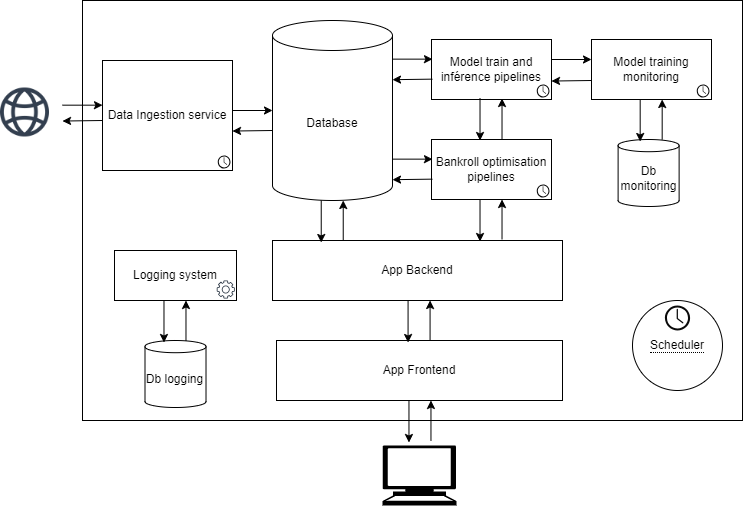
\includegraphics[width=0.8\textwidth, keepaspectratio]{images/Architecture_optimsportbet.png}
    \caption{Architecture of the system}
    \label{fig:elo_score_5_teams_during_time}
\end{figure}


\section{Data Collection}

Accurate and comprehensive data collection is vital for building reliable predictive models and effective betting strategies. The goal is to build an historical database which continues to build with real time relevant data.

\subsection{Data Sources Used}

We utilize a variety of reputable sources to gather data:

\begin{itemize}
    \item \textbf{Football Match Data}: Historical match results, match schedule, team statistics, player performance metrics, and other relevant information are sourced using scrapping on two websites: 
    \begin{itemize}
        \item \hyperlink{https://fbref.com/en/}{FBref}: For historical match results and coming match schedule.
        \item \hyperlink{https://sofifa.com/}{SoFifa}: For teams and players past and current ratings and statistics.
    \end{itemize}
    \item \textbf{Odds Data}: Betting odds are collected from multiple bookmakers through one API.
    \begin{itemize}
        \item \hyperlink{https://the-odds-api.com/}{The Odds API}: The free tier credits allows to perform 500 requests per month on various sports, bookmakers and leagues to retrieve the current odds. Historical odds data are not included.
    \end{itemize}
\end{itemize}


\subsection{Collection Methods}

Data is collected using a combination of methods:

\paragraph{Web Scraping}

A fork of the \hyperlink{https://soccerdata.readthedocs.io/en/latest/}{Soccerdata} python library, has been adapted to scrape data from websites that do not provide APIs (FBref, SoFifa). 

\paragraph{APIs}

For sources that offer APIs (The Odds API), we integrate with them using HTTP requests to fetch structured data efficiently.

\paragraph{Data Pre-processing}

Collected data undergoes a very simple pre-processing to ensure consistency and usability:

\begin{itemize}
    \item \textbf{Data type conversion}: Adapting the type of the data to the most adapted type.
    \item \textbf{Unity}: Only inserting new data in the database, or filling None values of existing data (for instance, the score of a match is only available after the match is played 
    \item \textbf{Integration}: Aligning data from different sources for seamless storage and analysis.
\end{itemize}

\section{Data Storage}

A robust data storage solution is essential for managing the diverse datasets involved.

\subsection{Database Choice}

We opted for a relational database management system (RDBMS), specifically \textit{PostgreSQL}, due to its reliability, scalability, and support for complex queries.

\subsection{Data Model}

The database schema is designed to reflect the relationships between different types of data:

\subsubsection{Tables}

\begin{itemize}
    \item `\textbf{fbref\_results}`: Each row corresponds to a match (historic and coming), with league, date and time of the match, both team and score if match is finished and the result is available and fetched from FBref website.
    \item `\textbf{sofifa\_teams\_stats}`: Each row corresponds to a a team and a date of update with metrics and categorical values that represent at best the team at the moment of the update (overall score, attack, build\_up\_speed ...).
    \item `\textbf{soccer\_odds}`: Each row corresponds to a match, a bookmaker, an outcome with its odd at a given update time. There is also information about the commence time of the match, the league, the home and away team names, the type of odd...
    \item `\textbf{models\_results}`: Each row corresponds to a match, the inference results of the model, the date-time of inference and the model used, with additional information such as the date and tile of the match and home and away team.
    \item `\textbf{optim\_results}`: Each row corresponds to a game, a date time of optimisation, the model used for inference, the best odds for each outcome found across a pool of bookmaker as well as the bookmakers names of each odds chose and the fraction of the bankroll to invest given utility function. There is additional information such as the probability inferred and used by the optimiser, the date-time of inference of these probabilities, the date and time of the match...
\end{itemize}


\begin{figure}[H]
    \centering
    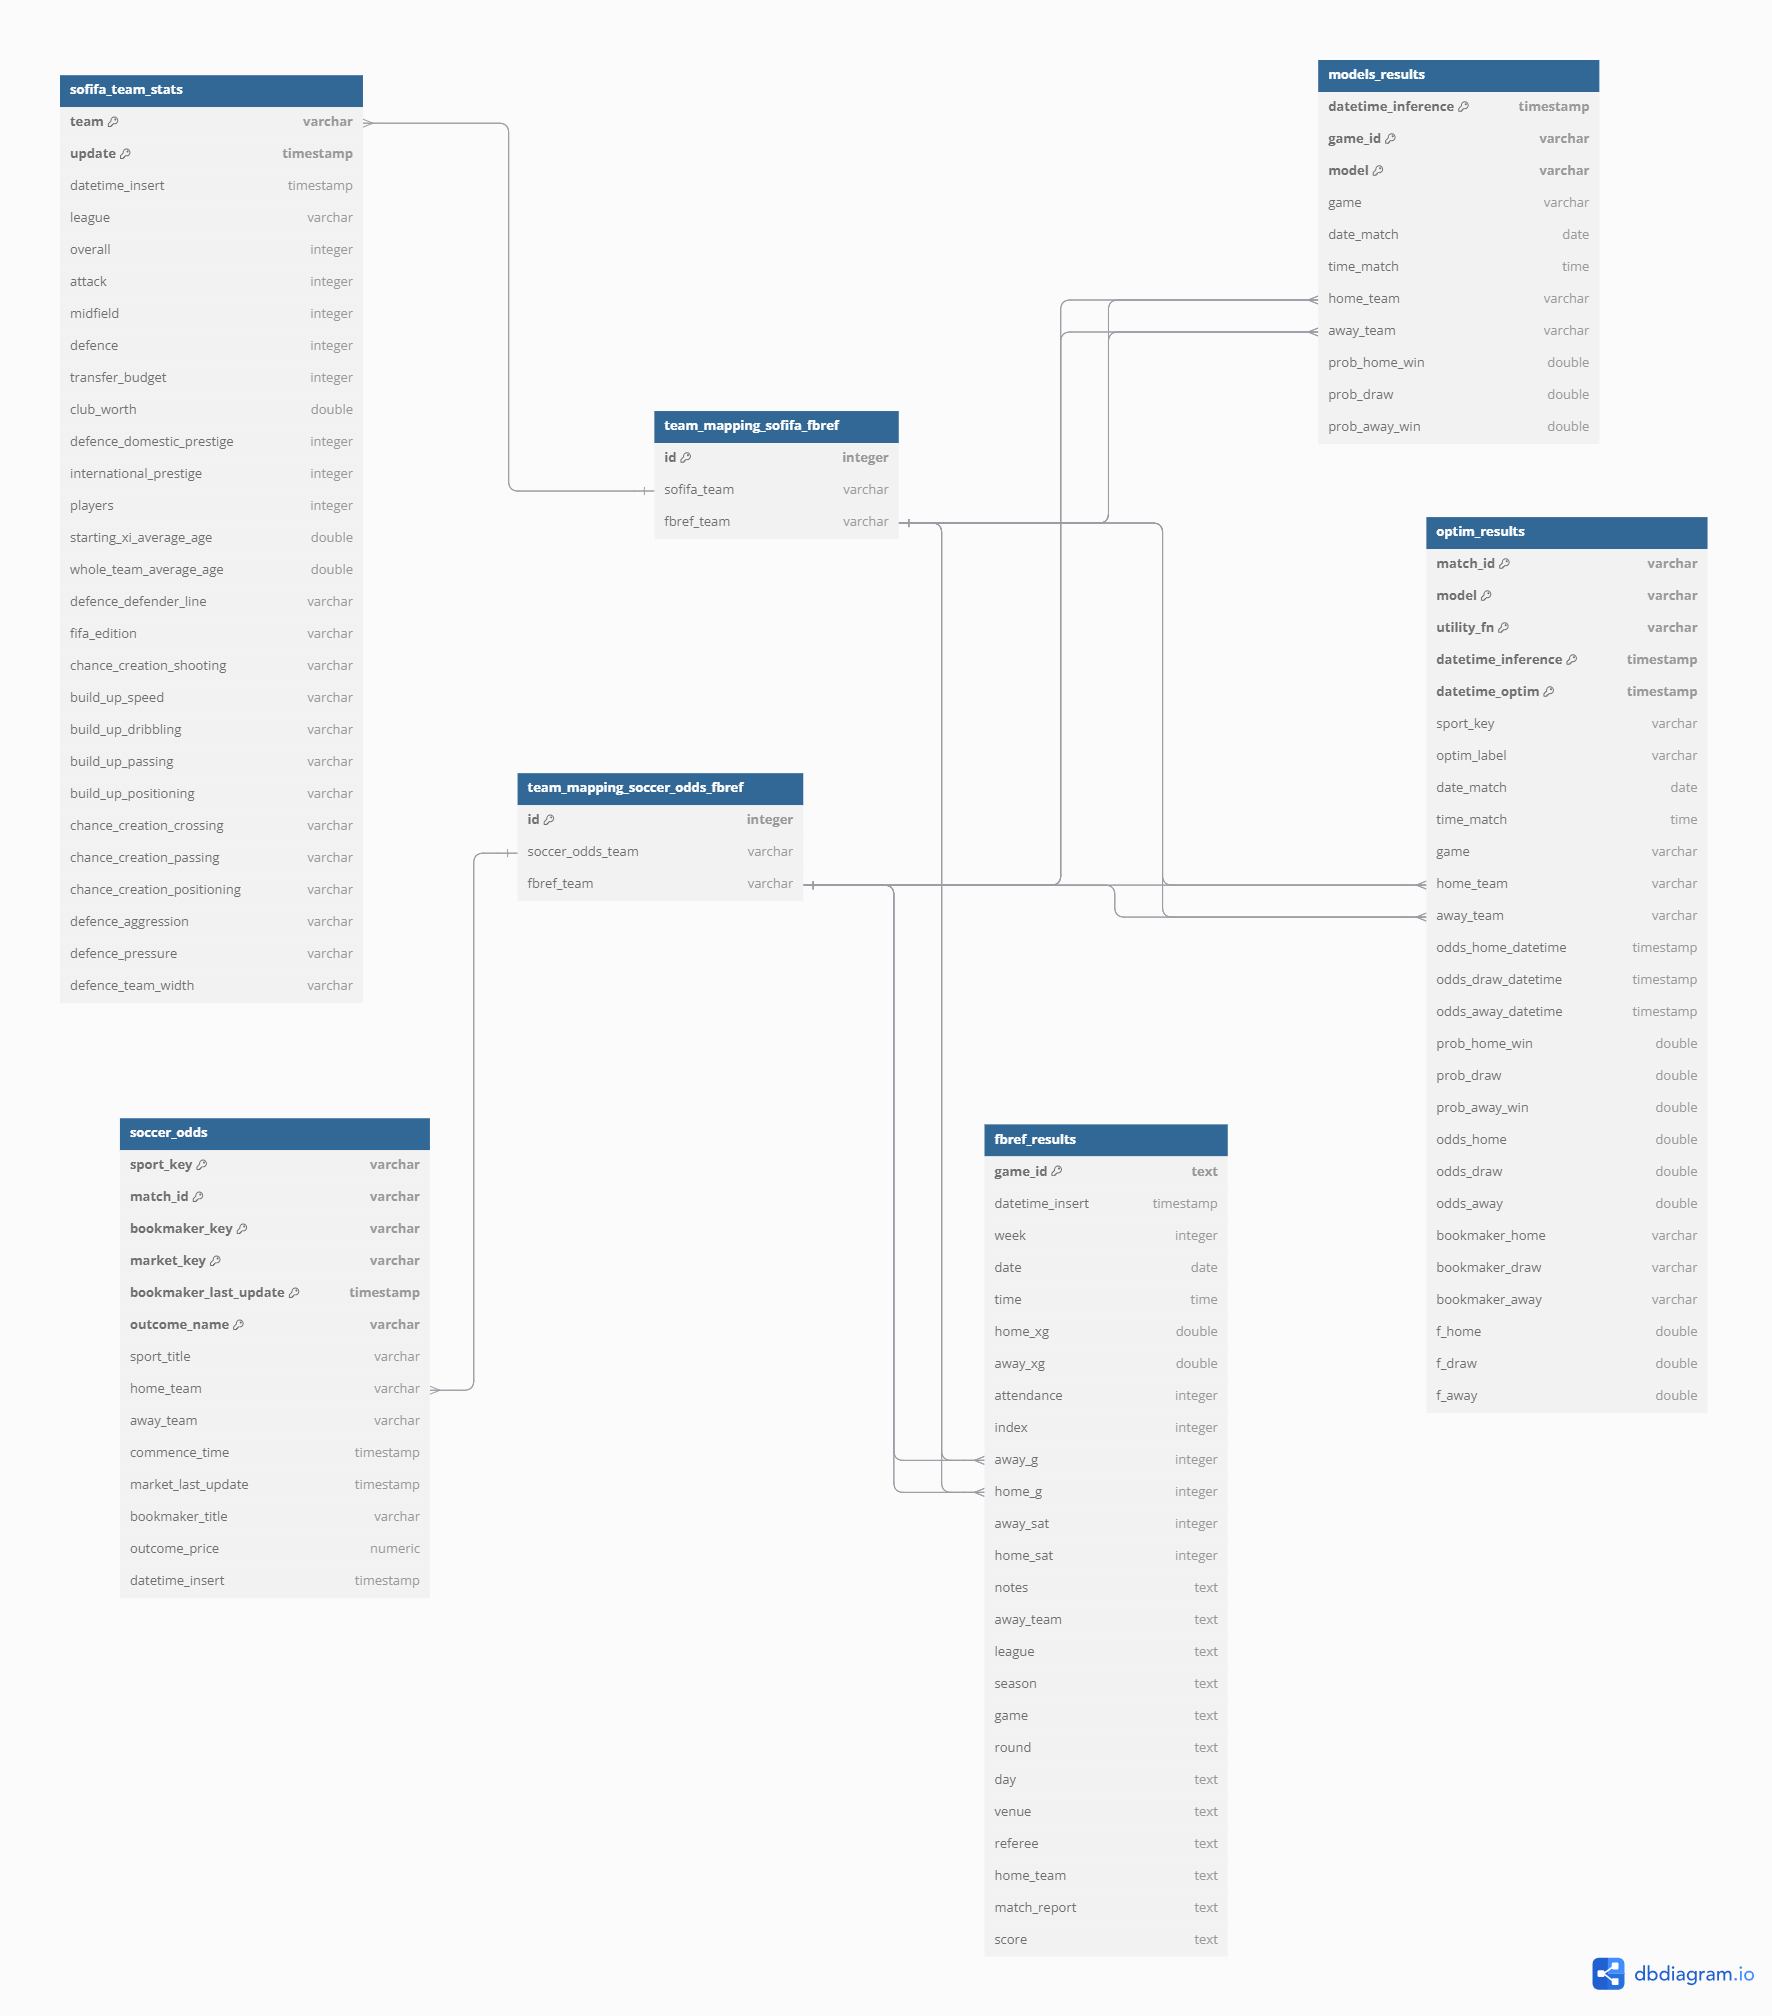
\includegraphics[width=0.8\textwidth, keepaspectratio]{images/db_uml.png}
    \caption{UML diagram of the database}
    \label{fig:uml_db}
\end{figure}

\section{Module Overview}

The system incorporates several modules, each performing specific functions within the overall architecture.

\subsection{Data Collection Module}

As described earlier, this module is responsible for fetching and pre-processing data from various sources.

\subsection{Prediction Module}

Although detailed discussion is deferred to a later chapter, this module uses machine learning algorithms to predict the probabilities of different match outcomes based on historical data.

\subsection{Optimization Module}

This module calculates optimal betting strategies by applying mathematical optimization techniques to the predictions and odds data. The specifics of the optimization algorithms and utility functions will be explored in a subsequent chapter.

\subsection{Scheduler}

The scheduler automates the execution of tasks such as data collection, model retraining, inference, and optimization. It ensures that the system remains up-to-date with the latest data and predictions.

\subsection{User Interface and Backend}

The user interface provides a platform for users to access data, view predictions, and interact with the system. The backend handles user requests, processes data, and communicates with other modules via APIs.

\section{User Interface and Monitoring}

\subsection{User Interface Design}

The UI is designed to be intuitive and user-friendly, providing clear visualizations and easy navigation.

\paragraph{Features}

\begin{itemize}
    \item \textbf{Dashboard}: Displays key metrics, including upcoming matches, predicted probabilities, and recommended betting strategies.
    \item \textbf{Historical Data Access}: Allows users to explore past matches, predictions, and outcomes.
    \item \textbf{Customization}: Users can select preferred bookmakers according to their interests.
\end{itemize}

\subsection{Monitoring}

System health and performance are monitored continuously:

\begin{itemize}
    \item \textbf{Logging}: Activity logs are maintained for debugging and audit purposes.
    \item \textbf{Alerts}: Notifications are sent in case of errors or significant events.
\end{itemize}


\section{Conclusion}

This chapter provided an overview of the system architecture implemented to realize the theoretical framework developed earlier. By focusing on football, we leverage abundant data to build predictive models and optimize betting strategies. The modular design, utilizing microservices and APIs,ensures scalability and flexibility. The database serves as the central repository, integrating data from various sources and supporting the different modules. The user interface offers a gateway for users to access the system's functionalities. In the subsequent chapters, we will delve into the specifics of the prediction and optimization modules, as well as the deployment strategy using Kubernetes and containerization technologies.

\section{Introduction}
\label{sec:chapter4_intro}

This chapter presents the development, training, and evaluation of a predictive model aimed at forecasting the outcomes of football matches. The primary objective is to construct a robust model that can accurately predict match results, thereby optimizing gains in sports betting \cite{BaioBlangiardo2010} \cite{DixonColes1997}. The significance of predictive modeling in the context of sports betting lies in its potential to provide bettors with a strategic advantage by identifying value bets and minimizing risks.

\section{Performance Metrics and Selection Criteria}
\label{sec:performance_metrics}

Evaluating the performance of a predictive model in a multi-class classification setting, especially with imbalanced classes, requires a comprehensive set of metrics. This section delineates both classic and advanced metrics employed in this study, incorporating mathematical formulations and addressing class imbalance. Given the three-class problem—home win, draw, and away win—with home wins constituting 47\% of the data, it is crucial to select metrics that provide a nuanced understanding of model performance across all classes.

\subsection{Metrics}
\label{subsec:classic_metrics}

A list of all the metrics considered with their used definition can  be found in Appendix \ref{appendix:predictive_model_metrics}.

\subsection{Selection Criteria}
\label{subsec:selection_criteria}

Accurate evaluation of the predictive model requires appropriate performance metrics, particularly in a multi-class classification context with class imbalance. The primary goal of this study is to ensure that the predicted probabilities of football match outcomes (home win, draw, away win) closely align with the true probabilities, emphasizing well-calibrated probability estimates.

Given the class distribution—47\% home wins, 26\% draws, and 25\% away wins—we have selected the \textbf{Mean Squared Error (MSE)} as the primary metric for assessing calibration. MSE directly measures the average squared difference between predicted probabilities and actual outcomes, making it suitable for evaluating how well the model's probabilities reflect the true frequencies.

In addition to MSE, we will consider the following metrics to provide a comprehensive evaluation:

\begin{itemize}
    \item \textbf{Log Loss}: To assess the quality of the predicted probability distributions by penalizing incorrect and overconfident predictions, thus encouraging well-calibrated estimates.
    \item \textbf{Classwise Expected Calibration Error (ECE)}: To evaluate the calibration of predicted probabilities for each class individually, offering insights into how closely these probabilities match the observed outcomes across different categories.
    \item \textbf{Accuracy for Home Win, Draw, and Away Win}: To examine the model's performance on each outcome separately, taking into account the class imbalance.
\end{itemize}

By focusing on MSE for calibration and incorporating Log Loss, Classwise ECE, and class-specific accuracy, we aim to ensure that the model not only produces accurate probability estimates but also maintains reliability across all outcome categories. This concise set of metrics aligns with our objective of accurately predicting football match outcomes while ensuring the predicted probabilities are well-calibrated and trustworthy.

\section{Exploration and Choice of Features}
\label{sec:feature_selection}

Selecting appropriate features is pivotal for building an effective predictive model. This section delineates the various types of features utilized in this study, the methodology employed for feature selection, the engineering of new features to enhance predictive power, and the handling of categorical variables to ensure they are appropriately represented in the model. 

\subsection{Types of Features Utilized}
\label{subsec:types_features}

The feature set comprises a combination of ranking-based, simple statistical, and domain-specific features. Each feature is defined mathematically where applicable and accompanied by an explanation of its relevance and computation.

\subsubsection{Ranking Features}
\label{subsubsec:ranking_features}

Ranking features provide a quantitative measure of team strength based on historical performance. These metrics are crucial as they encapsulate the overall ability and consistency of teams over time. All ranking features detailed formula are described in \ref{appendix:ranking_features}.

\begin{itemize}

\item \textbf{Elo Score}
\label{par:elo_score}

The \textbf{Elo score} \cite{Elo1978} \cite{HvattumArntzen2010} is a rating system originally developed for chess but widely adapted to various sports to rate players or teams. It reflects the relative skill levels of the teams based on game outcomes.

\begin{figure}[H]
    \centering
    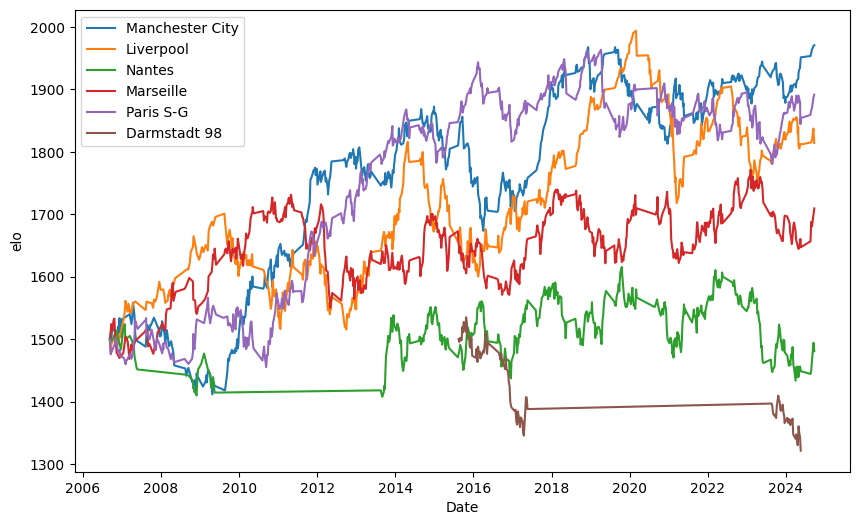
\includegraphics[width=0.8\textwidth, keepaspectratio]{images/elo_score_5_teams_during_time.png}
    \caption{Elo score of 5 football teams evolving during time}
    \label{fig:elo_score_5_teams_during_time}
\end{figure}



\item \textbf{Glicko-2 Score}
\label{par:glicko2_score}

The \textbf{Glicko-2 score} \cite{Glickman1999} is an advanced rating system developed by Mark Glickman, which enhances the Elo rating system by incorporating not only the skill levels of teams or players (R) but also the reliability of these ratings through Rating Deviation (RD) and volatility. This system provides a more dynamic and accurate reflection of performance by accounting for the uncertainty and variability in teams' ratings.


\item \textbf{TrueSkill}
\label{par:trueskill}

The \textbf{TrueSkill} \cite{HerbrichEtAl2007} is a Bayesian ranking system developed by Microsoft, primarily used in gaming but adaptable to sports analytics. It models each team's skill as a Gaussian distribution, updating beliefs about team strengths based on match outcomes.

\end{itemize}

\subsubsection{Simple Statistical Features}


Simple statistical features offer basic quantitative measures of team performance, providing foundational data for the predictive model.


\begin{itemize}
    \item \textbf{Average Goals Scored per Season}: Total goals scored by a team divided by the number of matches played so far.
    
    \item \textbf{Average Goals Conceded per Season}: Total goals conceded by a team divided by the number of matches played so far.
\end{itemize}


\subsubsection{Sofifa Performance Metrics}

SoFIFA provides detailed metrics for both individual players and teams, based on data from the FIFA video game by EA Sports. This document outlines the primary metrics and explains how team ratings are calculated using individual player attributes.

\begin{itemize}

\item \textbf{Player Metrics}
    The primary player metrics on SoFIFA are based on individual attributes that are weighted differently depending on the player's position. Below are the key metrics:
    
    \begin{itemize}
        \item \textbf{Overall Rating (OVR)}: This is the weighted average of various player attributes, with different weights depending on the position. For example, an attacker (\textit{Forward}) will have more emphasis on \textit{Shooting} and \textit{Pace}, while a defender (\textit{Centre Back}) will weigh attributes like \textit{Defending} and \textit{Physicality} more heavily.
        \item \textbf{Pace (PAC)}: Calculated as a combination of the \textit{Acceleration} and \textit{Sprint Speed} attributes.
        \item \textbf{Shooting (SHO)}: Includes \textit{Finishing}, \textit{Shot Power}, \textit{Long Shots}, and \textit{Positioning}.
        \item \textbf{Passing (PAS)}: Comprised of \textit{Vision}, \textit{Short Passing}, and \textit{Long Passing}.
        \item \textbf{Dribbling (DRI)}: Includes \textit{Ball Control}, \textit{Dribbling}, \textit{Agility}, and \textit{Balance}.
        \item \textbf{Defending (DEF)}: Based on \textit{Tackling}, \textit{Marking}, \textit{Interceptions}, and \textit{Defensive Awareness}.
        \item \textbf{Physicality (PHY)}: Includes \textit{Strength}, \textit{Stamina}, and \textit{Aggression}.
        \item \textbf{Potential}: Indicates the maximum possible rating the player can achieve over time.
    \end{itemize}
    
    The formula for the Overall Rating (OVR) is generally unknown, but it can be expressed as a weighted sum of key attributes, depending on the player’s position. A simplified formula for a forward might look like:
    
    \[
    \text{OVR}_{\text{Forward}} = w_1 \cdot \text{PAC} + w_2 \cdot \text{SHO} + w_3 \cdot \text{DRI} + w_4 \cdot \text{PAS}
    \]
    
    where \( w_1, w_2, w_3, w_4 \) are position-specific weights.

\item \textbf{Team Metrics}
    Team metrics on SoFIFA are calculated by aggregating individual player ratings, focusing on key areas like attack, midfield, and defense. The following are the primary team metrics:
    
    \begin{itemize}
        \item \textbf{Overall Team Rating}: A weighted average of the starting 11 players' Overall Ratings, considering the importance of each player's position.
        \item \textbf{Attack Rating}: The average Overall Rating of forwards and attacking midfielders, weighted based on the formation.
        \item \textbf{Midfield Rating}: The average Overall Rating of central and wide midfielders, weighted based on their roles in the formation.
        \item \textbf{Defense Rating}: The average Overall Rating of defenders and goalkeepers.
    \end{itemize}
    
    A simplified version of the team rating could be expressed as:
    
    \[
    \text{Team OVR} = \frac{1}{11} \sum_{i=1}^{11} \text{OVR}_i
    \]
    
    where \( \text{OVR}_i \) represents the Overall Rating of the $i$-th player in the starting lineup.
    
    
    Sofifa metrics are comprehensive team-specific performance indicators sourced from the Sofifa database, widely used in sports analytics and fantasy football contexts.
\end{itemize}

\begin{figure}[H]
    \centering
    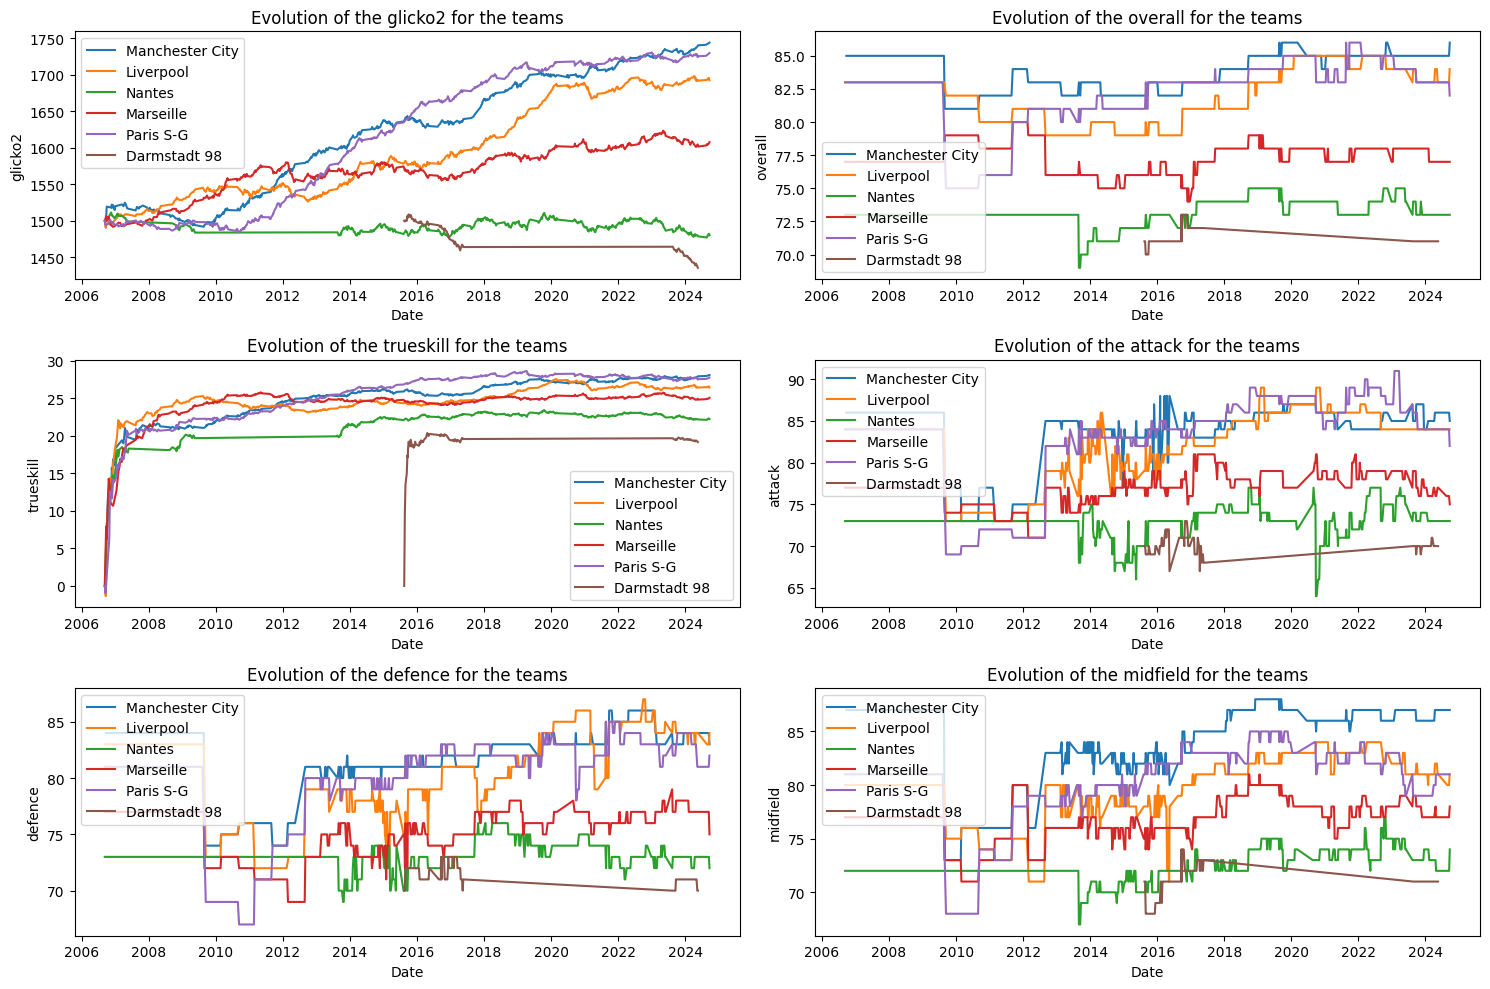
\includegraphics[width=\textwidth, keepaspectratio]{images/scores_5_teams_during_time.png}
    \caption{Different scores of 5 football teams evolving during time}
    \label{fig:scores_5_teams_during_time}
\end{figure}

A detailed description of each of the 90 features used can be found her \ref{appendix:all_feature_descriptions}.

\subsection{Feature Selection Methodology}
\label{subsec:feature_selection_methodology}

Feature selection was performed using a forward selection approach applied to a logistic regression model. This method iteratively adds the most significant features, enhancing predictive performance while maintaining model simplicity.

\subsubsection{Forward Selection with Logistic Regression}
\label{subsubsec:forward_selection_logistic_regression}

\textbf{Procedure}: Starting with no features, at each iteration, the feature that most improves the model's fit is added. The selection criterion is based on the mse (mean squared error).

\textbf{Explanation}: By incorporating features that significantly contribute to the model, forward selection optimizes predictive accuracy and ensures interpretability by excluding irrelevant variables.

\section{Data Preparation}

We trained our model on matches from 2006 to the present, focusing on games from the top 5 European leagues, European championships, and World Cups during this period. The limiting factor in our data came from SoFIFA, which does not provide data prior to 2006, while FBref offers data extending far into the past. We merged the two datasets based on team names and computed the ranking and statistical features described earlier, initializing the metrics at the first entry of a team in a tournament. For categorical features, we applied one-hot encoding. We removed matches with any missing values in the columns, then applied a standard scaler. This left us with 28,850 completed matches and a 90-feature vector for each match to train our model.

\begin{table}[h]
\centering
\begin{tabular}{|l|c|c|}
\hline
\textbf{Metric} & \textbf{Value} \\
\hline
Total matches & 28,850 \\
Matches in Top 5 Leagues & 28,481 \\
Matches in European Championships & 185 \\
Matches in World Cup & 184 \\
Home win ratio & 45.0 \% \\
Draw ratio & 25.4 \% \\
Away win ratio & 29.5 \% \\ 
Average home team goals & 1.54 \\
Average away team goals & 1.19 \\
Average Elo rating & 1558 \\
Number of unique teams & 242 \\
Number of features per match & 90 \\
First match date & 2006-09-09 \\
Last match date & 2024-09-24 \\
\hline
\end{tabular}
\caption{Summary Metrics for the Dataset}
\end{table}


\section{Cross-Validation on Temporal Data}
\label{sec:cross_validation_temporal}

In predictive modeling with football match data, which is inherently temporal, it's essential to use cross-validation techniques that respect the chronological order of observations. Standard cross-validation methods, such as random shuffling or traditional \( k \)-fold cross-validation, are unsuitable because they can lead to data leakage by training models on future data to predict past events.

Traditional cross-validation assumes that data samples are independent and identically distributed (i.i.d.) and that the order of observations does not matter. In temporal data, however, observations are time-dependent, and future events should not influence model training aimed at predicting past events. Using standard methods can result in:

\begin{itemize}
    \item \textbf{Data Leakage}: Incorporating future information into the training set leads to overly optimistic performance estimates.
    \item \textbf{Violation of Temporal Order}: Disrupting the sequence of events undermines the model's ability to generalize to real-world forecasting scenarios.
\end{itemize}


To address these issues, we employ cross-validation methods designed for temporal data \cite{BergmeirEtAl2018}.

\subsection{Sliding Window Cross-Validation}

This technique involves moving a fixed-size window across the data timeline. In each iteration, the model is trained on a training window and tested on the immediately following testing window.

\begin{itemize}
    \item Choose a training window size \( W_{\text{train}} \) and a testing window size \( W_{\text{test}} \).
    \item For each iteration:
    \begin{itemize}
        \item Train the model on data from time \( t \) to \( t + W_{\text{train}} - 1 \).
        \item Test the model on data from \( t + W_{\text{train}} \) to \( t + W_{\text{train}} + W_{\text{test}} - 1 \).
        \item Slide the window forward by \( W_{\text{test}} \) units.
    \end{itemize}
\end{itemize}

\subsection{Expanding Window Cross-Validation}

Also known as growing window, this method expands the training set with each iteration by including more historical data.

\begin{itemize}
    \item Start with an initial training window of size \( W_{\text{initial}} \).
    \item For each iteration:
    \begin{itemize}
        \item Train the model on data from time \( t \) to \( t + W_{\text{train}} - 1 \), where \( W_{\text{train}} \) increases with each iteration.
        \item Test on the subsequent data from \( t + W_{\text{train}} \) to \( t + W_{\text{train}} + W_{\text{test}} - 1 \).
        \item Expand the training window to include the latest testing window.
    \end{itemize}
\end{itemize}

\begin{figure}[H]
    \centering
    \begin{minipage}{0.45\textwidth}
        \centering
        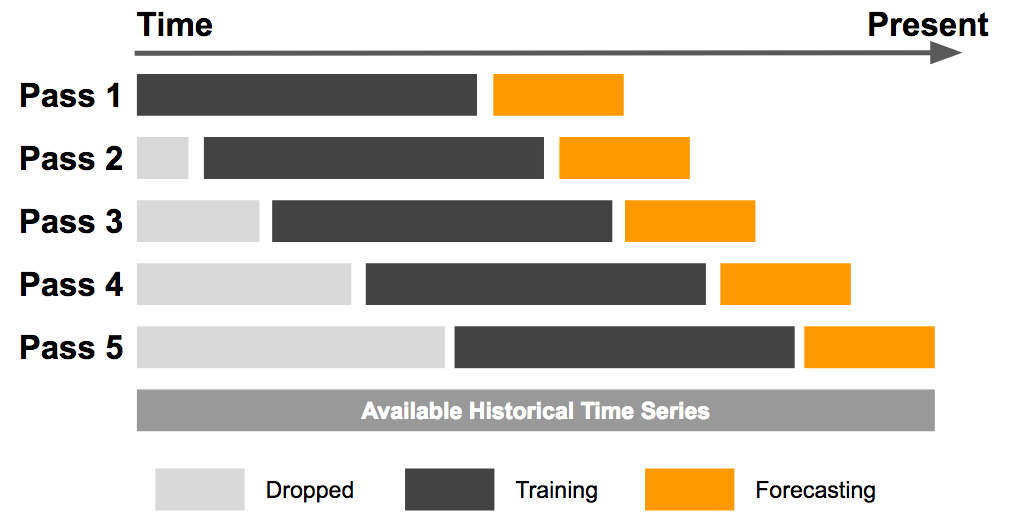
\includegraphics[width=\textwidth, keepaspectratio]{images/FixedWindow.png}
        \caption{Sliding window graphic}
        \label{fig:sliding_window}
    \end{minipage}\hfill
    \begin{minipage}{0.45\textwidth}
        \centering
        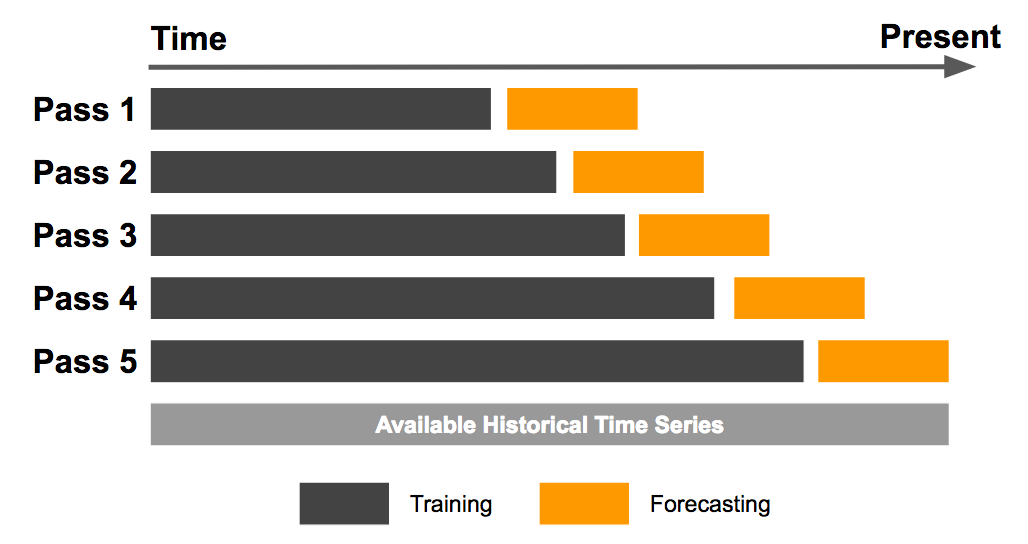
\includegraphics[width=\textwidth, keepaspectratio]{images/ExpandingWindow.png}
        \caption{Expanding window graphic}
        \label{fig:expanding_window}
    \end{minipage}
\end{figure}


The results presented below were obtained using an expanding window technique with 5 folds and a test set ratio of 0.2. Notably, the results were very similar when applying the sliding window method.


\section{Choice and Justification of the Prediction Model}
\label{sec:model_choice}

In this section, we present the results of the feature selection and model selection processes \cite{GuyonElisseeff2003} \cite{ChandrashekarSahin2014}, followed by interpretations of the selected model's performance. Feature selection was conducted using forward selection, and multiple classification models were evaluated to determine the most suitable model for predicting football match outcomes.

\subsection{Feature Selection Using Forward Selection}
\label{subsec:feature_selection}

Feature selection was performed using forward selection with logistic regression, iteratively adding the most significant feature at each step based on mean squared error (MSE) improvement, using an expanding window validation with 5 splits and a test size of 20\% of the training data.

\begin{table}[H]
    \centering
    \caption{Feature Selection Process Summary}
    \label{tab:feature_selection_summary}
    \begin{tabular}{lc}
        \toprule
        \textbf{Method} & \textbf{Details} \\
        \midrule
        Feature Selection & Forward Selection \\
        Model Used & Logistic Regression \\
        Validation Method & Expanding Window (5 splits) \\
        Performance Metric & Mean Squared Error (MSE) \\
        Test Size & 20\% of training data \\
        \bottomrule
    \end{tabular}
\end{table}


We selected 35 features, which corresponding to the features resulting in the lowest MSE, using this feature selection strategy.

\begin{table}[H]
    \centering
    \caption{Feature Selection with Corresponding MSE and their adding number}
    \label{tab:feature_mse}
    \begin{tabular}{|c|l|c|c|l|c|}
        \hline
        \textbf{Order} & \textbf{Feature Added} & \textbf{MSE} & \textbf{Order} & \textbf{Feature Added} & \textbf{MSE} \\
        \hline
        1  & Elo Away & 0.20613 & 19 & Home Passing Risky & 0.19438 \\
        2  & Elo Home & 0.19661 & 20 & Away Positioning Org. & 0.19436 \\
        3  & Glicko Vol Away & 0.19619 & 21 & Away Defense Pressure Med & 0.19435 \\
        4  & Away Overall & 0.19594 & 22 & Away Domestic Prestige & 0.19434 \\
        5  & Home Overall & 0.19540 & 23 & Away Shooting Lots & 0.19433 \\
        6  & Away Build Speed Slow & 0.19518 & 24 & Home Defense Line Offside & 0.19432 \\
        7  & Away Avg Age & 0.19501 & 25 & Away Team Width & 0.19431 \\
        8  & Home League INT & 0.19487 & 26 & Home Defense Pressure Med & 0.19431 \\
        9  & Home Avg Goals & 0.19476 & 27 & Home Build Speed Slow & 0.19430 \\
        10 & Home Positioning Org. & 0.19467 & 28 & Away Defense Aggression & 0.19430 \\
        11 & Home Build Speed Fast & 0.19461 & 29 & TrueSkill Home & 0.19430 \\
        12 & Away Defense Pressure High & 0.19457 & 30 & Away Build Positioning Org. & 0.19430 \\
        13 & Away Defense Offside Trap & 0.19453 & 31 & Away Defense & 0.19430 \\
        14 & Home League ITA & 0.19449 & 32 & Home Attack & 0.19427 \\
        15 & Glicko RD Home & 0.19447 & 33 & Home Defense Prestige & 0.19427 \\
        16 & Home Shooting Normal & 0.19444 & 34 & Away Attack & 0.19427 \\
        17 & Away Passing Mixed & 0.19442 & 35 & Away League INT & \textbf{0.19427} \\
        18 & Away Avg Goals & 0.19440 & & \\
        \hline
    \end{tabular}
\end{table}

The table above summarizes the features added during the selection process and their corresponding MSE values, highlighting the importance of each feature as it contributes to minimizing the error. As we can see, features such as Elo ratings and overall team metrics play a significant role \cite{LasekEtAl2013}. Now, let's examine how the number of features impacts the performance metrics more broadly, as shown in the following feature selection graph.

\begin{figure}[H]
    \centering
    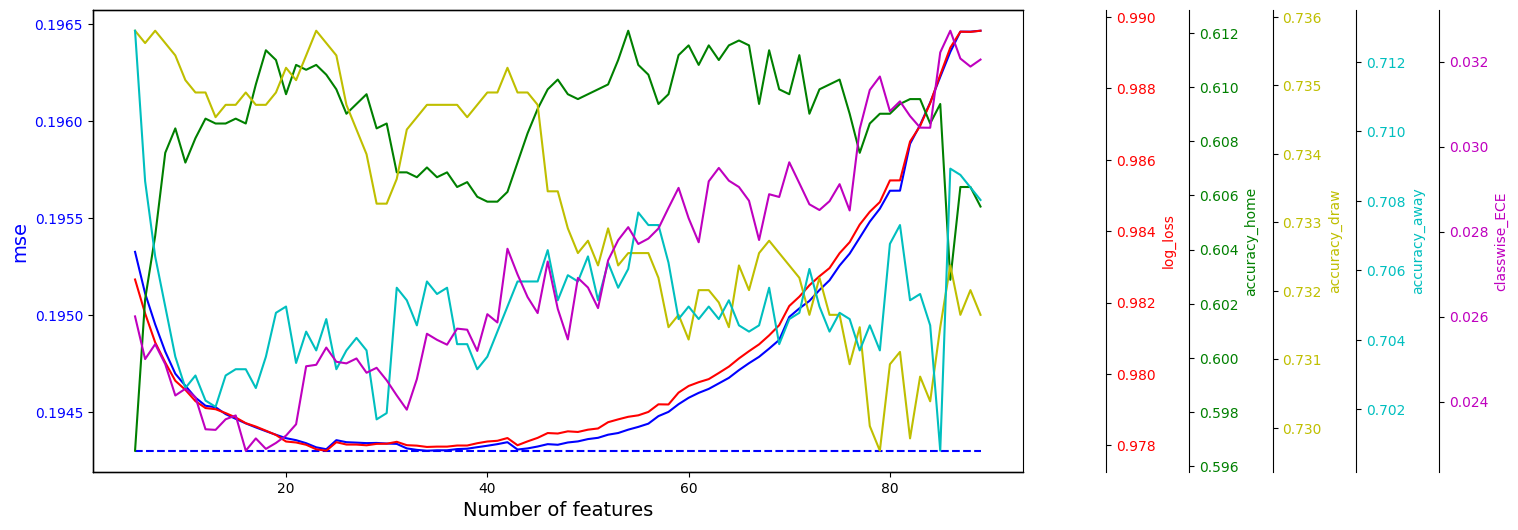
\includegraphics[width=\textwidth, keepaspectratio]{images/feature_selection_metrics_by_nb_of_features.png}
    \caption{Metrics of interrest function of the number of features added}
    \label{fig:feature_selection_metrics_by_nb_of_features}
\end{figure}

This graph shows the performance of various metrics (MSE, log loss, accuracy for home, draw, and away predictions, and classwise ECE) as a function of the number of selected features. The MSE (in blue) decreases as more features are added, stabilizing around the optimal point before increasing again, which suggests that selecting too many features can lead to overfitting. Similarly, log loss follows a similar trend (in red), indicating better model calibration with fewer features. The accuracy metrics (home, draw, away) fluctuate, but accuracy seems to peak at a certain range of features, with performance diminishing as more features are added. Classwise ECE (in pink) decreases and then increases, a little bit before MSE and log loss, indicating better calibration for class predictions with fewer features. Overall, the graph highlights the balance between feature selection and model performance, suggesting that an optimal subset of features yields the best generalization.

\subsection{Model Selection}
\label{subsec:model_selection}

The following table summarizes the performance of various classification models \cite{Bishop2006}, comparing metrics such as mean squared error (MSE), log loss, classwise ECE, and accuracy for home, draw, and away predictions to identify the best-performing model.

\begin{table}[H]
    \centering
    \caption{Model Performance Comparison}
    \label{tab:model_performance}
    \begin{tabular}{|l|c|c|c|c|c|c|}
        \hline
        \textbf{Model} & \textbf{MSE} & \textbf{Log Loss} & \textbf{C. ECE} & \textbf{A. Home} & \textbf{A. Draw} & \textbf{A. Away} \\
        \hline
        Logistic Regression & \textbf{0.195} & \textbf{0.983} & 0.029 & 0.605 & 0.733 & 0.702 \\
        Logistic Regression CV & 0.196 & 0.983 & \textbf{0.028} & 0.602 & \textbf{0.735} & 0.703 \\
        Gradient Boosting Classifier & 0.199 & 1.002 & 0.037 & 0.604 & 0.709 & \textbf{0.706} \\
        Random Forest Classifier & 0.202 & 1.022 & 0.038 & 0.595 & 0.705 & 0.693 \\
        Extra Trees Classifier & 0.204 & 1.026 & 0.043 & 0.597 & 0.683 & 0.686 \\
        AdaBoost Classifier & 0.221 & 1.092 & 0.069 & 0.599 & 0.721 & 0.695 \\
        Bagging Classifier & 0.224 & 2.471 & 0.093 & 0.602 & 0.646 & 0.661 \\
        MLP Classifier & 0.224 & 1.187 & 0.108 & 0.585 & 0.665 & 0.684 \\
        K Neighbors Classifier & 0.238 & 5.404 & 0.096 & 0.599 & 0.643 & 0.631 \\
        Gaussian NB & 0.332 & 7.570 & 0.302 & \textbf{0.615} & 0.584 & 0.625 \\
        Quadratic Discriminant Analysis & 0.353 & 10.831 & 0.316 & 0.582 & 0.561 & 0.613 \\
        Decision Tree Classifier & 0.390 & 20.219 & 0.195 & 0.578 & 0.614 & 0.638 \\
        Extra Tree Classifier & 0.399 & 20.686 & 0.200 & 0.559 & 0.615 & 0.628 \\
        \hline
    \end{tabular}
\end{table}


\subsection{Interpretation of Results}
\label{subsec:interpretation}

The selection of the logistic regression model allows for straightforward interpretation of feature effects on the predicted probabilities of match outcomes.

\subsubsection{Feature Importance}

Feature importance was assessed based on the magnitude of the coefficients in the logistic regression model. Below sits the feature importance of the Home win class. Draw and Away win classes analysis can be found in \ref{appendix:feature_importance}.


\begin{figure}[H]
    \centering
    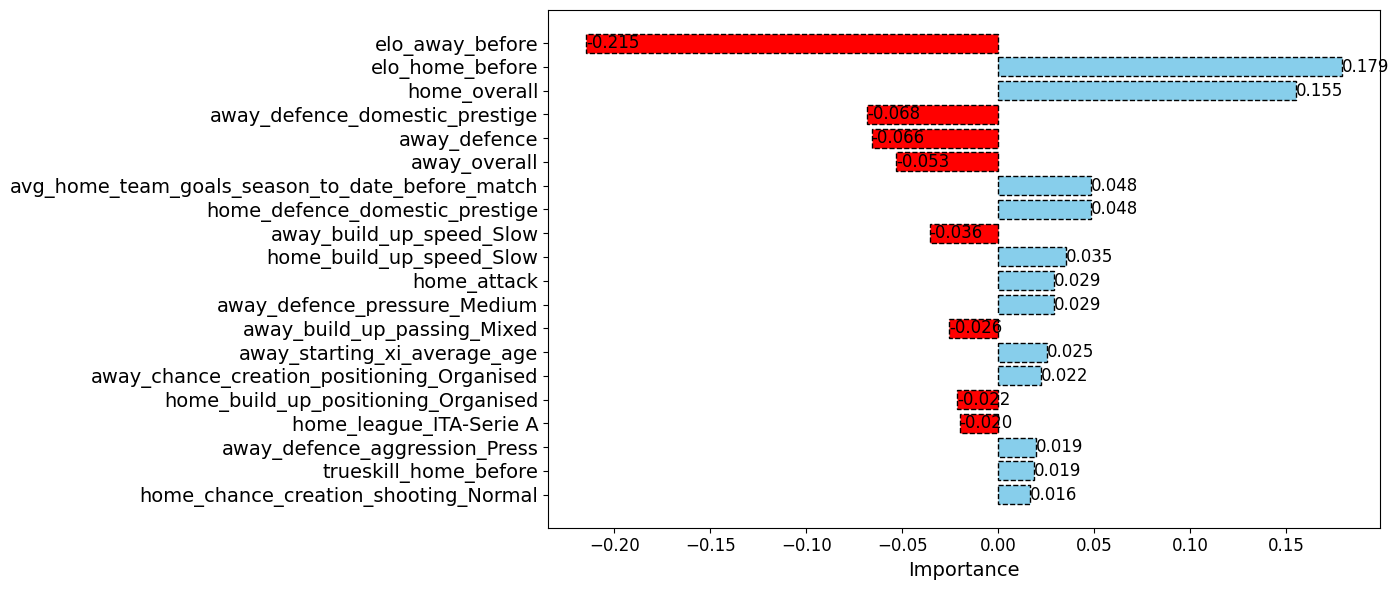
\includegraphics[width=\textwidth, keepaspectratio]{images/top20_coeff_importance_lr_selected_features_home.png}
    \caption{Coefficients of the Logistic Regression Model for Home win class}
    \label{fig:feature_coefficients}
\end{figure}

For the home class, the most important features, such as Elo ratings for the away and home teams, suggest that pre-match team strength is the most significant predictor of match outcomes. Both overall team quality and specific defensive attributes, like pressure and aggression, also play a key role. Features related to player average characteristics, such as average age and tactical elements like build-up speed, indicate that team composition and playstyle are also relevant, though their impact is less pronounced. Defensive strategies, particularly pressure and team width, add further predictive value, showing the importance of tactical decisions in determining match results. The feature importance analysis graphs for draw and away class can be found in the annex section.


\subsubsection{Why Logistic Regression Outperforms Other Models}

Logistic regression may outperform other models due to its simplicity and interpretability, especially when feature selection is based on it. By using logistic regression for feature selection, the model is specifically tuned to highlight the most important predictors of the outcome, leading to better generalization. Additionally, logistic regression handles multicollinearity well when regularization is applied, preventing overfitting. The linear relationship between the features and the log-odds of the outcomes makes it easier to capture important patterns in the data, particularly in problems like sports prediction where relationships between variables are often linear. Other models, such as random forests or gradient boosting, may add unnecessary complexity and are more prone to overfitting when features are already well-selected.


\section{Training and Retraining of the Model}
\label{sec:training_retraining}

Figure \ref{fig:mse_retraining} illustrates the Mean Squared Error (MSE) of two models over time, where the blue line represents Model A with no retraining, and the orange line represents Model B, which is retrained daily. Both models are initialy trained from 2006-01-01 up to 2010-01-01 data and are evaluated using a 120-day rolling average.

\begin{figure}[H]
    \centering
    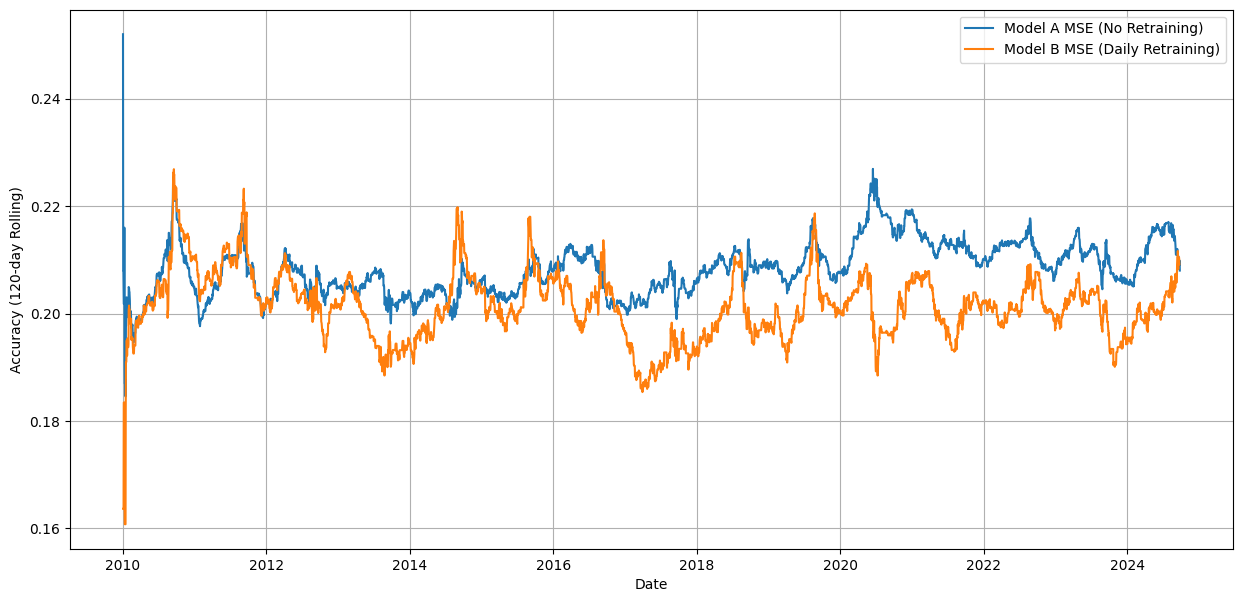
\includegraphics[width=0.8\textwidth, keepaspectratio]{images/model_ratrining_mse_120rd.png}
    \caption{Model MSE rolling average over time}
    \label{fig:mse_retraining}
\end{figure}


From the figure, we observe that Model B, which is frequently retrained, exhibits lower MSE compared to Model A throughout most of the time period. Retraining appears to allow Model B to adapt more effectively to evolving patterns, leading to consistently better performance in terms of accuracy. Moreover, as time goes by, we can observe a mse drift from the not retrained model as well as a slight improvement from the retrained model. \\

There are very few periods where Model A outperforms Model B. It appends especially during phases of sudden changes. Despite these fluctuations, retraining offers a more stable and improved long-term performance. \\

The results highlight the importance of regular retraining for maintaining model accuracy, particularly in dynamic environments where data patterns change over time.

\section{Conclusion}

This chapter presented the development, training, and evaluation of a predictive model for football match outcomes, with a focus on sports betting. Feature selection via forward selection with logistic regression helped identify key predictors, and regular retraining improved model performance over time.\\

However, several limitations remain:

\begin{itemize}
    \item \textbf{Hyperparameters and Features}: Ranking feature hyperparameters were left at default, and additional domain-specific or external data sources could further improve predictions.
    \item \textbf{Feature Selection}: Feature selection was arbitrarily based on logistic regression, and no hyperparameter optimization was performed for any models.
    \item \textbf{Retraining}: The timing and method of retraining (e.g., sliding window) were not explored, potentially missing optimal strategies as well as posing computational challenges that could be optimized.
    \item \textbf{Model Complexity}: Incorporating deep learning models could enhance predictive performance, particularly for capturing complex patterns in the data.
    \item \textbf{Bookmaker Odds Decorrelation}: Adding a metric to assess the decorrelation between model predictions and bookmaker odds could help identify more value bets and further optimize betting strategies.
\end{itemize}
In the next chapter, we address the optimization problem of determining the bankroll share to invest on each outcome, building on the predictions of this model to develop actionable betting strategies.

\section{Introduction}

Effective bankroll management is a critical component of successful sports betting. It involves determining the optimal amount to wager on each bet to maximize growth while minimizing the risk of ruin. This section details the development and evaluation of an optimization module designed to calculate the optimal fraction of the bankroll to invest in each betting opportunity. The module leverages probabilistic forecasts from the predictive models discussed in the previous section and applies various investment strategies, including the Kelly criterion, expected value maximization, and naive betting approaches.

\section{Methodology}
\subsection{Investment Strategies}

This section provides an overview of the different bankroll allocation strategies implemented, ranging from naive methods to more advanced optimization techniques. The focus is on the principles guiding each strategy, with a detailed formula provided only for the naive strategy.

\subsubsection{List of Strategies}

\begin{itemize}
    \item \textbf{Kelly Criterion Strategy}: \cite{Kelly1956} \cite{Thorp1969}  
    This strategy maximizes the logarithmic utility of wealth, aiming for long-term bankroll growth while managing risk. The bankroll fractions are derived from the analytical solution using the approximations  \ref{appendix:analytical_solution_using_the_kelly_criterion}, \(\mathbb{E}(U(B)) = \mathbb{E}(B) - \frac{1}{2} \cdot \mathbb{V}\text{ar}(B) \) which comes down to a Linear utility strategy using \( \lambda = \frac{1}{2} \).

    \item \textbf{Log Utility Strategy}:  
    Similar to the Kelly criterion, this strategy focuses on maximizing the expected logarithmic utility \(U(B) = \ln(B)\)  but using no approximations \ref{appendix:analytical_reduction_using_log_expected_utility}.

    \item \textbf{Exponential Utility Strategy}:  
    This strategy uses an exponential utility function \(U(B) = -e^{-\alpha B}\) to take into account the bettor’s risk aversion, balancing between expected returns and risk tolerance \ref{appendix:analytical_reduction_using_exp_expected_utility}.

    \item \textbf{Linear Utility Strategy}:
    In this strategy, the objective is to maximize the trade-off between expected returns and risk, represented by the function \(\mathbb{E}(U(B)) = \mathbb{E}(B) - \lambda \cdot \mathbb{V}\text{ar}(B) \). For the simulations, we set \( \lambda = 10 \), reflecting a high level of risk aversion. This approach seeks to maximize returns while penalizing high variance, aiming to balance growth and stability \ref{appendix:analytical_solution_using_linear_expected_utility}. 

    \item \textbf{Expected Value Maximization Strategy}:  
    This strategy optimizes bankroll allocation based purely on maximizing expected value, \(U(B) = B\), without considering risk or variance.

    \item \textbf{Naïve Strategy: Bet on the Most Likely Outcome}:  
    In this straightforward approach, the bettor places the entire bet on the outcome with the highest implied probability, as per the bookmaker's odds.
    
    The formula for this strategy is:
    \[
    f_{k,i} = 
    \begin{cases}
    \frac{1}{M}, & \text{if } i = \arg\max(o_k) \\
    0, & \text{otherwise}
    \end{cases}
    \]
    where:
    \begin{itemize}
        \item \( f_{k,i} \) is the fraction of the bankroll wagered on outcome \( i \) of match \( k \),
        \item \( o_k \) are the odds for match \( k \).
        \item \(M\) is the number of matches available.
    \end{itemize}
    This strategy is simple and allocates all the available funds to the outcome with the highest bookmaker odds.
\end{itemize}

These strategies were benchmarked against each other in the Monte Carlo simulations and then Online testing to assess their effectiveness in managing risk and maximizing bankroll growth. \\

For each strategy, a factor of \( \gamma = \frac{1}{2} \) was applied to the bet fractions to ensure that not the entire bankroll was wagered at any given time, thereby providing a margin of safety, such as: \(f_{strategy\_final} = \gamma \times f_{strategy}\).


\subsection{Optimization Algorithms}

Two optimization algorithms were employed to solve the bankroll allocation problem \cite{BoydVandenberghe2004}:

\begin{itemize}
    \item \textbf{Sequential Least Squares Programming (SLSQP):} An iterative method for constrained nonlinear optimization that is efficient for problems with a moderate number of variables.
    \item \textbf{Trust-Region Constrained Algorithm (trust-constr):} Suitable for large-scale optimization problems, it handles large numbers of variables and constraints effectively.
\end{itemize}

The choice between SLSQP and trust-constr depends on the number of betting opportunities (matches) considered at once. For a large number of matches, trust-constr is preferred due to its scalability.


\section{Monte Carlo Simulations}

To assess the performance of different investment strategies under simulated sports betting conditions, we conducted Monte Carlo simulations modeling the inherent uncertainties. The goal was to evaluate how various bankroll allocation strategies perform over numerous trials.

\subsection{Simulation Setup}

We simulated true match outcome probabilities \( r \) using a Dirichlet distribution appropriate for mutually exclusive and collectively exhaustive events:

\[
r_i^k = \text{Dirichlet}(\alpha), \quad \alpha = (1, 1, 1)
\]

To introduce discrepancies between true probabilities and those estimated by bookmakers (\( b \)) and players (\( t \)), we added biases and normally distributed noise:

\[
b_i^k = \text{clip}(r_i^k + \text{bias}_{\text{bookmaker}} + \epsilon_{\text{bookmaker}}, \ \text{min\_prob}, \ \text{max\_prob})
\]
\[
t_i^k = \text{clip}(r_i^k + \text{bias}_{\text{player}} + \epsilon_{\text{player}}, \ \text{min\_prob}, \ \text{max\_prob})
\]

where \( \epsilon_{\text{bookmaker}}, \epsilon_{\text{player}} \sim \mathcal{N}(0, \sigma^2) \). Probabilities were normalized to sum to one, and bookmaker probabilities included a margin \( \text{margin}_{\text{bookmaker}} \), clipping between \text{min\_prob} and \text{max\_prob}. Bookmaker odds were calculated as:

\[
o_i^k = \frac{b_i^k}{(\sum_{i=0}^N b_i^k) - \text{margin}_{\text{bookmaker}}}
\]

\subsection{Simulation Procedure}

The simulation followed a structured approach to evaluate the performance of different betting strategies, using predefined constants and a series of steps to simulate match outcomes and bankroll updates.

\begin{table}[H]
\centering
\caption{Simulation constants}
\label{tab:simulation constants}
\begin{minipage}{.2\linewidth}
\centering
\begin{tabular}{lr}
\toprule
\textbf{Constant} & \textbf{Value}\\
\midrule
H & 30 \\
T & 50 \\
N & 3 \\
\(\text{min\_prob}\) & 0.05 \\
\(\text{max\_prob}\) & 0.95 \\
\bottomrule
\end{tabular}
\end{minipage}%
\hspace{0.05\linewidth}
\begin{minipage}{.45\linewidth}
\centering
\begin{tabular}{lrr}
\toprule
\textbf{Constant} & \textbf{Bettor} & \textbf{Bookmaker}\\
\midrule
\text{bias} & 0 & 0 \\
\(\sigma\) (for noise \(\epsilon)\) & 0.1 & 0.1 \\
\text{margin} &  & 0.1 \\
\bottomrule
\end{tabular}
\end{minipage}
\end{table}

\begin{enumerate}
    \item Generated true probabilities \( r \) using \(\text{bias} = 0\) and \(\epsilon = 0.1\) for both bettor and bookmaker.
    \item Computed bookmaker and player estimates \( b \) and \( t \).
    \item Calculated bookmaker odds \( o \).
    \item For each strategy:
    \begin{itemize}
        \item Determined bet sizes using \( t \) and \( o \) by performing optimisation using \texttt{truct\_constr} algorithm.
        \item Simulated match outcomes based on \( r \).
        \item Updated bankrolls accordingly.
    \end{itemize}
\end{enumerate}

\subsection{Evaluation Metrics}

Strategies were evaluated using:

\begin{itemize}
    \item \textbf{Final Bankroll Statistics}: Mean, standard deviation, median, minimum, and maximum.
    \item \textbf{Average Growth Rate}: Geometric mean per time step. 
    \[GGR = \left( \frac{B(n)}{B(0)} \right)^{\frac{1}{n}} - 1\]

    \item \textbf{Sharpe Ratio}: Risk-adjusted return.

    \[\text{Sharpe Ratio} = \frac{\frac{1}{n} \sum_{t=1}^{n} R(t)}{\mathbb{V}ar(R(t))}) \text{   with   } R(t) = \frac{B(t+1) - B(t)}{B(t)}\]
    
    \item \textbf{Probability of Ruin}: Frequency of bankroll falling below a threshold.
\end{itemize}

\subsection{Results}

\begin{figure}[H]
    \centering
    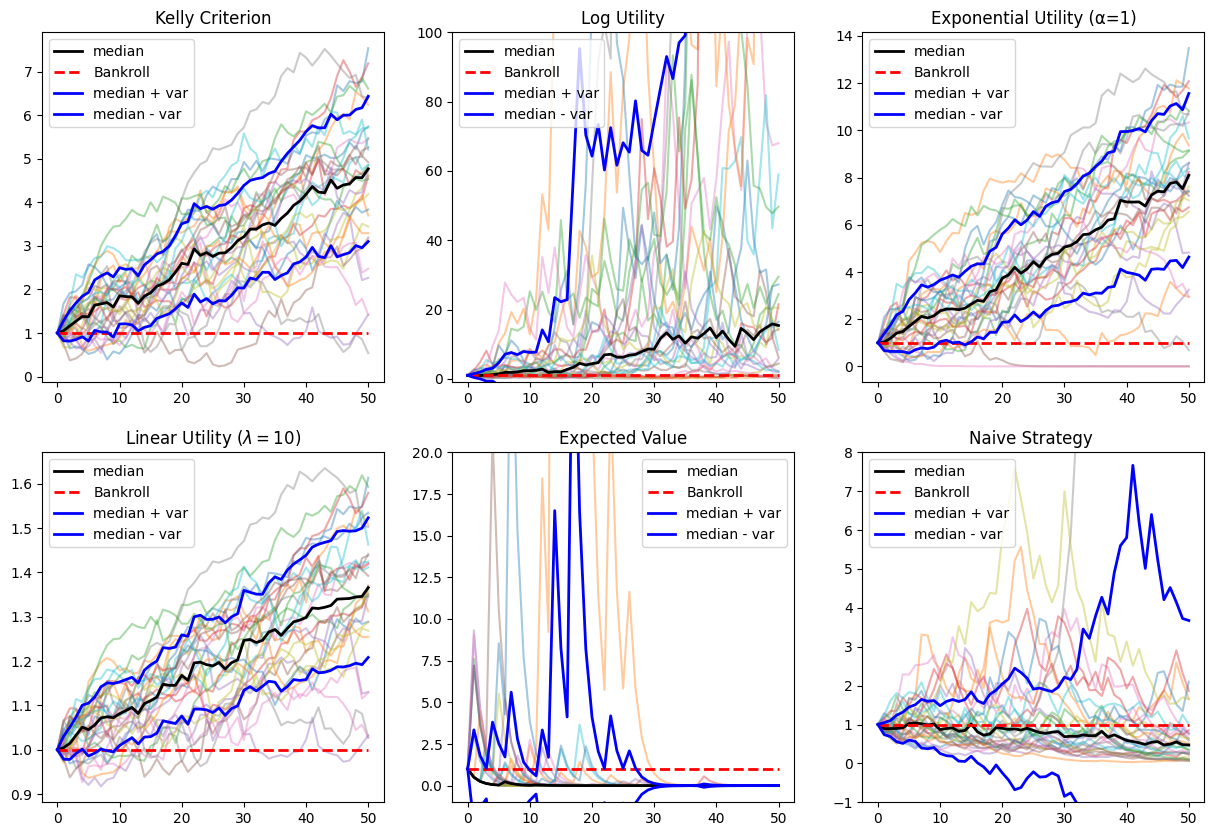
\includegraphics[width=1.1\textwidth, keepaspectratio]{images/monte_carlo_b=b.png}
    \caption{Monte carlo simulations for each strategy}
    \label{fig:monte_carlo}
\end{figure}


\begin{table}[H]
\centering
\caption{Final Bankroll Statistics}
\label{tab:final_bankroll}
\begin{tabular}{lrrrrr}
\toprule
\textbf{Strategy} & \textbf{Mean} & \textbf{Std Dev} & \textbf{Median} & \textbf{Min} & \textbf{Max} \\
\midrule
Kelly Criterion          & 4.48   & 1.67   & 4.77   & 0.54   & 7.54   \\
Log Utility              & 270.85 & 983.14 & 15.39  & 0.19   & 5414.01 \\
Exponential Utility      & 7.46   & 3.46   & 8.10   & 0.00   & 13.48  \\
Linear Utility           & 1.35   & 0.16   & 1.37   & 1.03   & 1.61   \\
Expected Value           & 0.00   & 0.00   & 0.00   & 0.00   & 0.01   \\
Naïve Strategy           & 1.20   & 3.20   & 0.47   & 0.06   & 18.19  \\
\bottomrule
\end{tabular}
\end{table}

The \textbf{Log Utility} strategy achieved the highest mean final bankroll but with significant variability, indicating high risk. The \textbf{Kelly Criterion} and \textbf{Exponential Utility} strategies demonstrated moderate returns with lower variability, suggesting consistent performance.

\begin{table}[H]
\centering
\caption{Average Growth Rate Per Step}
\label{tab:avg_growth}
\begin{tabular}{lr}
\toprule
\textbf{Strategy} & \textbf{Growth Rate} \\
\midrule
Kelly Criterion          & 2.82\% \\
Log Utility              & 5.54\% \\
Exponential Utility      & 2.55\% \\
Linear Utility           & 0.59\% \\
Expected Value           & $-$29.83\% \\
Naïve Strategy           & $-$1.55\% \\
\bottomrule
\end{tabular}
\end{table}

While the \textbf{Log Utility} strategy had the highest growth rate, it came with increased volatility. The \textbf{Kelly Criterion} and \textbf{Exponential Utility} strategies offered positive growth with better risk control.

\begin{table}[H]
\centering
\caption{Sharpe Ratio}
\label{tab:sharpe_ratio}
\begin{tabular}{lr}
\toprule
\textbf{Strategy} & \textbf{Sharpe Ratio} \\
\midrule
Kelly Criterion          & 0.30 \\
Log Utility              & 0.29 \\
Exponential Utility      & 0.25 \\
Linear Utility           & 0.30 \\
Expected Value           & 0.14 \\
Naïve Strategy           & 0.01 \\
\bottomrule
\end{tabular}
\end{table}

The highest Sharpe Ratios were achieved by the \textbf{Kelly Criterion} and \textbf{Linear Utility} strategies, indicating superior risk-adjusted returns.

\begin{table}[H]
\centering
\caption{Probability of Ruin}
\label{tab:prob_ruin}
\begin{tabular}{lr}
\toprule
\textbf{Strategy} & \textbf{Probability} \\
\midrule
Kelly Criterion          & 0.00\% \\
Log Utility              & 3.33\% \\
Exponential Utility      & 6.67\% \\
Linear Utility           & 0.00\% \\
Expected Value           & 100.00\% \\
Naïve Strategy           & 20.00\% \\
\bottomrule
\end{tabular}
\end{table}

Zero probability of ruin for the \textbf{Kelly Criterion} and \textbf{Linear Utility} strategies underscores their robustness.

An ANOVA test (performed to assess whether the differences in final bankrolls among the strategies), (F-statistic: 2.16, p-value: 0.0612) suggested that differences among strategies were not statistically significant at the 5\% level. However, the p-value is close to the threshold, suggesting that with a larger sample size, the differences might become statistically significant.

\subsection{Conclusion}

The simulations indicate that strategies like the \textbf{Kelly Criterion} and \textbf{Exponential Utility}, which balance growth and risk through utility maximization, offer favorable outcomes. The \textbf{Log Utility} strategy provides high growth potential but with greater volatility. Ignoring risk, as in the \textbf{Expected Value} strategy, leads to poor performance.

\textbf{Limitations} include the limited number of simulations, simplified assumptions, and exclusion of real-world factors like transaction costs.

\textbf{Recommendations} for future work involve increasing simulation runs, incorporating realistic market conditions, and exploring additional strategies.


\section{Online Testing}

To assess the strategies in a real-world environment, an online testing phase was conducted over five weeks, from 2024 August 24th to 2024 September 30th, focusing on matches from the five major European football leagues. This real-world testing evaluated the practical applicability and performance of the strategies under actual market conditions. Odds were scraped each day at 12pm from the Odd Api website.


\subsection{Static Problem Reduction and Parameter Settings}

To simplify the dynamic nature of sports betting, we reduced the problem to a series of static optimizations at discrete time intervals. At each decision point \( t \), bankroll allocation was optimized based on the current available information. This approach allowed us to manage the complexity of real-time betting while ensuring the practical applicability of the strategies.

\paragraph{Temporal Parameters}

Key temporal parameters were defined as follows:

\begin{itemize}
    \item \textbf{Betting Interval (\( \Delta t \))}: The interval between placing bets, set to 24 hours to capture daily betting opportunities.
    \item \textbf{Bet Placement Timing}: Bets were placed at a fixed time each day (12:00 PM) to ensure up-to-date information was used while accommodating market dynamics.
\end{itemize}

These settings ensured a balance between information accuracy and practical market conditions.

\paragraph{Match Selection}

The matches selected for each optimization were determined based on:

\begin{itemize}
    \item \textbf{Number of Matches (\( M \))}: Matches occurring within the next 24 hours were selected, balancing opportunity and reliability of information as well as having all results while perfomring next step.
    \item \textbf{Selection Criteria}: Focus was given to matches from top European leagues where the bettor had a higher perceived edge.
\end{itemize}

This careful match selection helped reduce computational complexity while enhancing potential returns.

\paragraph{Re-Betting Policy}

The re-betting policy was defined by the following criteria:

\begin{itemize}
    \item \textbf{Not allowing Re-Bets}: Additional bets on previously considered matches were not allowed. As we only bet on matches on the same day and only once a day, this was an implication of the previous choices.
\end{itemize}

This policy helped manage risk and adapt to evolving market conditions.

\subsection{Practical Implementation Settings}

The practical implementation settings for the online testing phase are summarized in Table~\ref{tab:implementation_settings}. The testing period ran from August 24, 2024, to September 30, 2024. The \texttt{trust-constr} algorithm was used for optimization, with a multiplier of \( \gamma = \frac{1}{2} \) applied to the matrix \( f \). The best odds from a pool of bookmakers (detailed in the appendix) were selected for each match.

\begin{table}[H]
\centering
\caption{Practical Implementation Settings}
\label{tab:implementation_settings}
\begin{tabular}{ll}
\toprule
\textbf{Setting}               & \textbf{Value}                                 \\ \midrule
Betting Interval (\( \Delta t \))     & 24 hours \\                                    
Bet Placement Time               & 12:00 PM daily                                \\
Look-Ahead Horizon               & Matches within the next 24 hours               \\ 
Re-Betting Policy                & Not allowed \\ 
Testing Period                   & August 24, 2024 – September 30, 2024           \\ 
Optimization Algorithm           & \texttt{trust-constr}                          \\ 
Strategy factor mult. \(\gamma\)         & \( 0.5 \)                              \\ 
Odds Selection                   & Biggest odds from a pool of bookmakers            \\ 
Markets & 5 biggest European leagues (Big 5) \\
\bottomrule
\end{tabular}
\end{table}


\subsection{Results and Interpretation}

Figure~\ref{fig:capital_evolution} illustrates the capital evolution for each strategy during the testing period. The Kelly and Exponential Utility strategies exhibited the strongest performance, both ending with approximately twice the initial capital. These results highlight their ability to optimally balance risk and reward, consistently outperforming the more conservative Log and Naive strategies. However, they also demonstrated higher volatility compared to the more stable Linear strategy.

\begin{figure}[H]
    \centering
    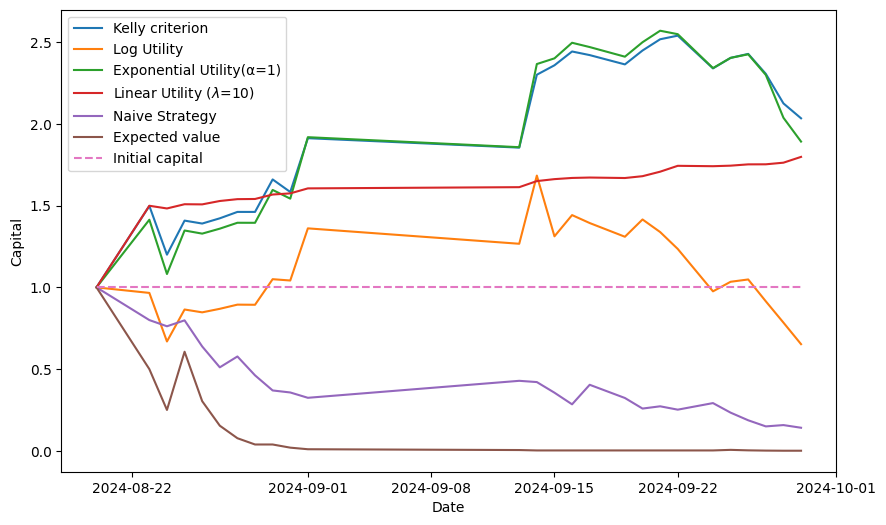
\includegraphics[width=\textwidth]{images/bankroll_evolution2.png}
    \caption{Capital Evolution for Each Strategy During the Online Testing Period}
    \label{fig:capital_evolution}
\end{figure}

The Log Utility strategy underperformed, particularly at the start and after the midpoint of the test period, failing to capitalize on high-return opportunities. Its conservative nature, aimed at minimizing risk, resulted in modest growth but ultimately led to a negative outcome. 

Both the Naive and Expected Value strategies experienced sharp declines in capital. The Naive strategy approached near-zero capital by the end of the test, while the Expected Value strategy exhibited extreme volatility, leading to rapid capital depletion. These simpler strategies, which lack sophisticated optimization, were highly vulnerable to adverse market conditions and failed to adapt effectively to fluctuations in odds or match outcomes.

In contrast, the Linear Utility strategy showed steady and consistent growth, with minimal volatility throughout the testing period, ultimately achieving a final growth of 1.8 times the initial capital. This highlights its effectiveness in maintaining a stable growth trajectory while avoiding the excessive risk associated with other strategies.

Overall, the results underscore the superiority of more advanced utility-based strategies such as Kelly and Linear. These approaches consistently outperformed simpler methods by balancing risk and reward more effectively under real-world betting conditions.

\subsection{Performance Metrics}

To further quantify the performance of each strategy, we computed key metrics, including final bankroll \( B(T) \), mean growth per step, and standard deviation of growth per step, both in absolute terms and as a percentage of the final bankroll. 
\begin{itemize}
    \item The mean growth per step is defined as:
    \[
    \mu = \frac{1}{T-1} \sum_{t=1}^{T-1} \Delta B_t
    \]
    where \( \Delta B_t = B_{t+1} - B_t \),
    \item the standard deviation of growth per step is given by:
    \[
    \sigma = \sqrt{\frac{1}{T-1} \sum_{t=1}^{T-1} (\Delta B_t - \mu)^2}
    \]
\end{itemize}


Table~\ref{tab:strategy_performance} summarizes the results for each strategy.

\begin{table}[H]
\centering
\caption{Strategy Performance Metrics}
\label{tab:strategy_performance}
\begin{tabular}{llll}
\toprule
\textbf{Strategy}              & \textbf{Final Bankroll \( B(T) \)} & \textbf{Mean Growth (\%)} & \textbf{Std Growth (\%)} \\ 
\midrule
Kelly Criterion                & 2.034                              & 2.034                      & 8.923                    \\ 
Log Utility                    & 0.653                              & -2.129                     & 26.516                   \\ 
Exponential Utility (\( \alpha = 1 \)) & 1.892                        & 1.886                      & 10.309                   \\ 
Linear Utility (\( \lambda = 10 \))    & 1.798                        & 1.776                      & 5.360                    \\ 
Naive Strategy                 & 0.141                              & -24.299                    & 52.419                   \\ 
Expected Value                 & 0.001                              & -5032.448                  & 18175.649                \\
\bottomrule
\end{tabular}
\end{table}

\subsection{Interpretation of Metrics}

The results demonstrate the effectiveness of the Kelly Criterion and Exponential Utility strategies, both of which ended with a final bankroll close to 2.0. These strategies also displayed reasonable volatility, with standard deviations of growth per step under 10\%. The Linear Utility strategy performed consistently, achieving steady growth with the lowest volatility among all strategies.

On the other hand, the Log Utility strategy suffered from negative growth, highlighting its inability to capitalize on high-return opportunities. The Naive and Expected Value strategies performed poorly, with significant capital depletion and extreme volatility, particularly for the Expected Value approach, indicating their inadequacy in real-world betting scenarios.


\section{Conclusion}

The results from both the Monte Carlo simulations and the real-world online testing phase demonstrate the clear advantages of sophisticated bankroll management strategies such as the Kelly Criterion and Exponential Utility methods. These strategies consistently provided strong returns while managing risk effectively, leading to a final bankroll close to twice the initial amount. In contrast, simpler strategies like the Naive and Expected Value approaches underperformed, suffering from capital depletion and high volatility, emphasizing the importance of balancing risk and return in real-world betting scenarios.

The Linear Utility strategy offered a steady, reliable growth trajectory with minimal volatility, making it an appealing option for risk-averse bettors. The Log Utility strategy, though conservative, failed to capture sufficient growth opportunities, resulting in a negative final outcome. Overall, the Kelly and Exponential Utility strategies are best suited for bettors seeking long-term growth with manageable risk.

\subsection{Limitations and Future Improvements}

Despite the promising results, several limitations were identified in the current approach:

\begin{itemize}
    \item \textbf{Simulation Assumptions}: The Monte Carlo simulations relied on several simplifying assumptions that limit the realism of the results. Firstly, the simulation of probabilities was based on the true clipped probabilities plus a bias and Gaussian noise, which does not fully capture the actual flaws in the predictive models, and the constants used were chosen arbitrarily without strong justification. Secondly, the bookmaker margin was fixed, and the odds provided by the bookmaker did not account for the influence of large bets from the players, which in reality could cause deviations in the bookmaker’s odds and probabilities. Lastly, the simulations used a fixed number of matches and time steps. Both the number of simulations and the range of strategies could be expanded to provide a more thorough and diverse analysis of performance over a wider variety of scenarios.
    \item \textbf{Limited Testing Period}: The online testing phase covered only a five-week period, which may not fully capture the long-term performance and robustness of each strategy. Extending the testing period or repeating it across multiple seasons would provide a more comprehensive assessment.
    \item \textbf{Risk Preferences}: While the utility-based strategies successfully managed risk, the models relied on fixed parameters for risk aversion (e.g., \( \lambda \) in Linear Utility). Introducing dynamic adjustments to these parameters based on market conditions or bettor preferences could further enhance performance.
\end{itemize}

\subsection{Future Work and Deployment on Azure Kubernetes}

The next stage of this project involves deploying the entire system on a cloud infrastructure using Kubernetes on Azure (AKS). This deployment will enable scalable, real-time processing of betting opportunities, continuous model updates, and the handling of multiple simultaneous users and markets. By leveraging Azure’s powerful compute and orchestration capabilities, the system will be capable of efficiently managing the computational load and data flows needed for real-time sports betting optimization.


\section{Microservices Architecture and Frameworks}

To build a scalable and maintainable system for sports betting optimization, we adopted a microservices architecture. This approach allows independent development, deployment, and scaling of individual components, facilitating modularity and flexibility.

The system comprises several microservices:

\begin{itemize}
    \item \textbf{Data Ingestion Service}: Collects real-time match data and odds from external APIs and web scraping. We use the Python library \textit{soccerdata} to conveniently scrape historical and real-time data from various websites. \textit{SQLAlchemy} is employed to communicate with the PostgreSQL database, allowing interaction using a mix of Python syntax and SQL queries. An API is provided for other services to trigger this service's logic, created using the \textit{FastAPI} framework. The Python library \texttt{logging} is used for proper logging of all operations, and \texttt{pandas} is utilized for data manipulation and transformation.

    \item \textbf{Prediction and Optimization Service}: Processes data to train models and generate probability estimates for the prediction component. Calculates optimal bet allocations based on the probabilities and selected strategies for the optimization component. \textit{Scikit-learn} is used for model training and inference, while \textit{SciPy.optimize} handles the optimization processes. Similar to the Data Ingestion Service, an API is deployed using \textit{FastAPI}, with communication to the database via \textit{SQLAlchemy}, and \texttt{logging} and \texttt{pandas} for logging and data handling.

    \item \textbf{User Interface Service}: Provides a web-based dashboard for monitoring and interaction, developed using the Python web framework \textit{Streamlit}.

    \item \textbf{Backend Service}: Manages communication and logic between the frontend User Interface and the database, as well as other services, using \textit{FastAPI}, \texttt{pandas}, and \texttt{logging}.

    \item \textbf{Database Service}: Stores historical data, odds, inferred probabilities, optimization results, and transaction logs. We chose PostgreSQL as the database due to its robustness, scalability, and compatibility with \textit{SQLAlchemy}. PostgreSQL's advanced features support complex queries and transactions essential for our application's needs.

    \item \textbf{MLflow Service}: Monitors the training metrics of the models. MLflow provides a convenient way to track experiments, record model parameters, metrics, and artifacts, facilitating reproducibility and model versioning.

    \item \textbf{Airflow Service}: Acts as a scheduler, providing a convenient way to orchestrate and monitor complex workflows using Directed Acyclic Graphs (DAGs). Apache Airflow allows us to define data pipelines, schedule tasks, and manage dependencies between them, ensuring timely execution of data ingestion, model training, and optimization processes.
\end{itemize}

Services communicate over HTTP/HTTPS protocols, with well-defined API endpoints ensuring loose coupling and ease of integration.

\section{Docker and Kubernetes}

To ensure consistency across development, testing, and production environments, all microservices are containerized using Docker \cite{Merkel2014}. Docker allows us to package each service with all its dependencies into isolated containers, ensuring consistent behavior across different environments.

\subsection{Dockerization}

Each microservice is encapsulated in a Docker container, defined by its own \texttt{Dockerfile}, which specifies the base image, dependencies, and entry points. In local development, we used containers for services such as MLflow, PostgreSQL, and Airflow, facilitating a consistent and reproducible environment.

\subsection{Kubernetes Deployment}

For orchestration and management of the containerized applications, we utilized Kubernetes \cite{HightowerEtAl2017}. Kubernetes automates deployment, scaling, and management of containerized applications. We packaged our system into a Helm chart, which simplifies the deployment of the entire application, including dependencies like MLflow, PostgreSQL, and Airflow.

\subsubsection{Helm Chart Packaging}

By encapsulating our services and their dependencies into a Helm chart, we streamlined the deployment process. Helm charts define, install, and upgrade complex Kubernetes applications, allowing us to manage configurations and versioning efficiently.

\subsubsection{Database Migrations}

Database schema changes are managed using migration files and scripts. Changes are first applied locally for testing and validation. Once validated, migrations are executed on the production database using scripts designed to apply changes incrementally. This process ensures that the database schema remains synchronized with the application code without disrupting ongoing operations.

\section{Deployment on Azure AKS}

\subsection{Azure Kubernetes Service (AKS)}

We deployed our Kubernetes cluster on Microsoft Azure using Azure Kubernetes Service (AKS), a managed Kubernetes service that simplifies cluster management by handling critical tasks like health monitoring and maintenance. AKS reduces the operational overhead and provides features like automated scaling and updates.

\begin{figure}[H]
    \centering
    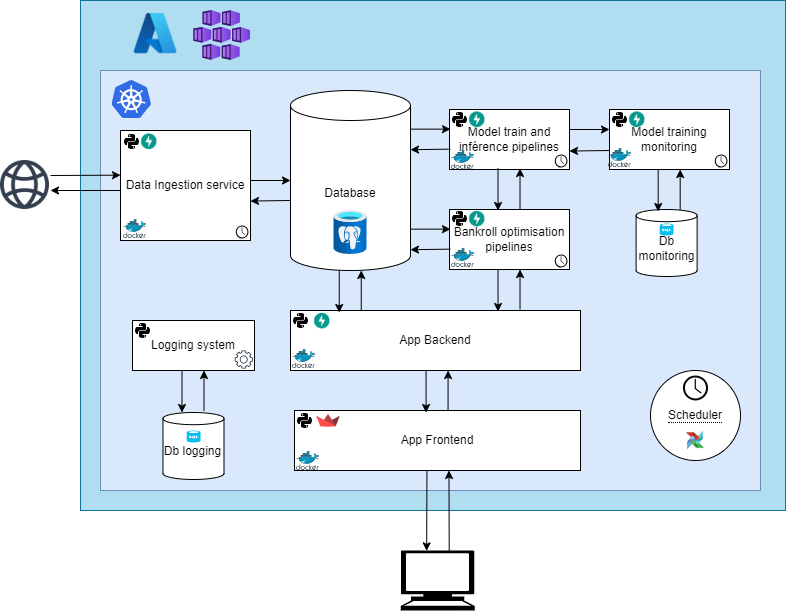
\includegraphics[width=0.8\textwidth, keepaspectratio]{images/diagrem_archi_services.png}
    \caption{Architecture of the system deployed on AKS}
    \label{fig:diagramme_arch_aks}
\end{figure}

\subsection{Infrastructure Details}

Our AKS deployment utilizes two virtual machines to ensure high availability and load balancing across the cluster. While Azure offers its own virtual machines, in this context, we refer to the compute resources allocated to our Kubernetes nodes. The integration with AKS allows for efficient resource utilization and scalability.

\subsection{Azure Services Integration}

Using Azure's cloud infrastructure offers several benefits:

\begin{itemize}
    \item \textbf{Azure Container Registry (ACR)}: Stores our Docker images securely, facilitating seamless deployment to AKS.
    \item \textbf{Azure DevOps Repo}: Provides a storage for our code.
\end{itemize}

\subsection{Pricing Considerations}

Azure's pricing model charges for compute resources used by virtual machines, storage, and network bandwidth. Managed services like AKS can reduce operational overhead but require careful monitoring to manage costs effectively. We optimized resource allocation by:


\section{Conclusion}

By adopting a microservices architecture, containerization with Docker, orchestration with Kubernetes, and deploying on Azure AKS, we built a scalable, reliable, and maintainable system for sports betting optimization. This architecture allows for independent development and deployment of components, ensuring the system can adapt to changing requirements and handle real-time data processing demands efficiently. Leveraging cloud infrastructure and managed services enhances our ability to focus on core application development while ensuring high availability and performance.

\section{Summary of Findings}

This study embarked on the ambitious task of developing a comprehensive system for optimizing sports betting strategies, focusing on football matches. Through the integration of predictive modeling, utility-based optimization, and scalable system architecture, we have addressed the critical components necessary for successful sports betting.

The predictive model, developed using logistic regression and advanced feature selection techniques, demonstrated significant accuracy in forecasting match outcomes. Regular retraining of the model proved essential in maintaining performance over time, highlighting the dynamic nature of sports data.

The optimization module applied various bankroll allocation strategies, including the Kelly Criterion, logarithmic, exponential, and linear utility functions. Both Monte Carlo simulations and real-world online testing over a five-week period indicated that sophisticated utility-based strategies substantially outperform naive betting approaches. Strategies like the Kelly Criterion and Exponential Utility provided favorable returns while effectively managing risk.

The system's deployment on Azure Kubernetes Service (AKS) showcased its scalability and readiness for real-time application. By leveraging a microservices architecture and containerization technologies like Docker and Kubernetes, the system can handle the computational demands of real-time data processing and optimization.

\section{Contributions to the Field}

This work contributes to the field of sports analytics and betting strategies in several ways:

\begin{itemize} \item \textbf{Integration of Predictive Modeling and Optimization}: By combining accurate probability estimations with utility-based optimization strategies, the system provides a robust framework for sports betting. \item \textbf{Scalable System Architecture}: The implementation of a microservices architecture and deployment on cloud infrastructure ensures that the system is scalable, maintainable, and adaptable to real-world conditions. \item \textbf{Empirical Evaluation}: The use of both simulations and real-world testing provides empirical evidence of the effectiveness of advanced betting strategies over simpler methods. \end{itemize}

\section{Limitations}

Despite the positive results, several limitations were identified:

\begin{itemize}
    \item \textbf{Predictive Model Enhancements}: While the current model performs adequately within the constraints of a static framework, it could be significantly improved by incorporating additional features, conducting hyperparameter optimization, and exploring more complex models such as deep learning architectures. These enhancements would allow the model to capture dynamic patterns and temporal dependencies inherent in football matches, which are not fully addressed due to the static nature of the current framework.

    \item \textbf{Static Framework Limitations and Long-Term Gain-Variance Interpretation}: The reduction of the betting problem to a static framework simplifies the optimization process but introduces limitations in interpreting gains and variance over the long term. Since the model does not account for intertemporal dependencies and the evolving nature of the bankroll, the strategies derived may not fully capture the risks associated with long-term betting. This static approach may lead to strategies that optimize short-term gains without adequately considering the cumulative effect on wealth over time. Future work should focus on extending the framework to a dynamic setting, allowing for a more accurate interpretation of long-term gain and variance, and better aligning the strategies with the bettor's long-term financial goals.

    \item \textbf{Risk Preferences and Dynamic Adaptation}: The optimization strategies employed fixed parameters for risk aversion, which do not adjust to changes in the bettor's wealth or market conditions over time. This static treatment of risk preferences limits the adaptability of the betting strategies, especially in a long-term context where the bettor's financial situation and the market dynamics can vary significantly. Introducing dynamic risk preferences that evolve with the bettor's bankroll and external factors would enhance the strategies' responsiveness and effectiveness, leading to better management of gain and variance over the long term.

    \item \textbf{Testing Period and Scope}: The real-world testing was confined to a five-week period focusing on the top five European leagues. Due to the static framework and the short testing duration, the evaluation may not fully reflect the strategies' performance over extended periods or in different market conditions. A longer testing period encompassing a broader range of leagues and varying competitive environments would provide more comprehensive insights into the strategies' long-term viability and their ability to manage gains and risks effectively within a dynamic setting.

\end{itemize}
\section{Future Work}

Building upon the findings of this study, several promising avenues can be explored to enhance the system's performance and address the challenges identified. 

Firstly, integrating real-time data streams and developing adaptive predictive models could significantly improve forecasting accuracy. By incorporating techniques from time-series analysis and machine learning, the model can capture temporal dependencies and evolving patterns inherent in football matches. This dynamic approach would allow the model to adjust to new information promptly, potentially leading to more accurate probability estimates and better alignment with the actual match outcomes.

Secondly, advancing the optimization strategies to include stochastic elements and multi-period planning could address the complexities associated with long-term gain and variance interpretation. Developing a dynamic framework that accounts for intertemporal dependencies and the evolving nature of the bankroll would enable more effective risk management. Strategies that adapt risk preferences in response to changes in the bettor's financial status or market conditions could lead to more sustainable betting practices and improved long-term financial outcomes.

Thirdly, conducting extensive real-world testing over longer periods and across a broader range of leagues and competitions would provide deeper insights into the robustness and generalizability of the betting strategies. Such testing would help to evaluate the performance of the models under varying market conditions and competitive environments, ensuring that the strategies remain effective over time and are not limited to specific contexts or short-term scenarios.

Finally, enhancing the user interface to offer more advanced analytics and personalized insights could empower users to make more informed decisions. Features that allow users to visualize performance trends, adjust parameters interactively, and receive tailored recommendations would improve the overall user experience. Providing tools for long-term performance monitoring and strategic adjustments would enable users to better understand the implications of their betting decisions and manage their bankrolls more effectively.

These potential developments represent initial steps toward refining the system's capabilities. By focusing on dynamic modeling, adaptive optimization, comprehensive testing, and user-centric design, future work can contribute to more robust predictive performance, effective risk management, and ultimately, more successful sports betting strategies.

\section{Final Remarks}

The integration of predictive modeling and utility-based optimization represents a significant step forward in developing effective sports betting strategies. This work demonstrates that with accurate predictions and strategic bankroll management, it is possible to achieve superior returns while managing risk effectively. The deployment on cloud infrastructure ensures that the system is ready for practical application, paving the way for future advancements in the field.


Je veux que tu me rédige un article de blog sur ce projet en format md. L'article doit prendre environ 10 min à lire et doit être interressant, prenant, il doit y avoir un bon story telling. Et plusieurs niveau de comprehension, pour les non initiés et pour les data scientist avancés.

Fais le en anglais

\chapter{Optimization of bankroll allocation}


\chapter{Introduction}

Sports betting has evolved into a sophisticated industry that combines statistical analysis, predictive modeling, and strategic financial management \cite{AndersonSally2013}. With the global popularity of football and the abundance of data available, there is a significant opportunity to apply advanced analytical techniques to optimize betting strategies. The challenge lies in accurately predicting match outcomes and effectively managing the allocation of betting capital to maximize returns while minimizing risk.

This report presents the development and implementation of a comprehensive system designed to address these challenges in sports betting. The system integrates predictive modeling to forecast football match outcomes and optimization algorithms to determine the optimal allocation of a bettor's bankroll. The focus is on creating a practical, scalable solution that can operate in real-time, leveraging cloud-based technologies and microservices architecture.

\section{Background and Motivation}

The sports betting market is highly competitive, with bettors seeking any edge to improve their chances of success. Traditional betting strategies often rely on intuition or simplistic models that fail to account for the complexities of sports data and market dynamics. The advancement of machine learning and statistical methods offers the potential to enhance predictive accuracy and optimize betting decisions systematically \cite{CainEtAl2000}.

Effective bankroll management is equally important, as even accurate predictions can lead to losses if the betting amounts are not strategically allocated. The application of utility theory and optimization techniques, such as the Kelly Criterion, provides a mathematical framework for balancing risk and reward in betting decisions. 

\section{Objectives of the Study}

The primary objectives of this study are:

\begin{itemize}
\item To establish a rigorous mathematical framework that defines the theoretical foundations and sets the stage for the study.
\item To develop a predictive model that accurately estimates the probabilities of football match outcomes using historical and real-time data. \item To design an optimization module that calculates the optimal fraction of the bankroll to wager on each betting opportunity, applying various utility-based strategies. \item To implement a scalable, microservices-based system architecture that integrates data collection, predictive modeling, optimization, and user interface components. \item To deploy the system on a cloud platform using Kubernetes for scalability and reliability. \item To evaluate the performance of different betting strategies through Monte Carlo simulations and real-world online testing. \end{itemize}

\section{Scope of the Report}

This report details the theoretical framework underlying the predictive modeling and optimization strategies, the system architecture and implementation, and the results of both simulated and real-world testing. The report is organized as follows:

\begin{itemize} \item Chapter 2 provides a theoretical presentation of the models and preliminary research conducted. \item Chapter 3 describes the design and implementation of the solution, including system architecture and data management. \item Chapter 4 focuses on the development, training, and evaluation of the predictive models for match outcomes. \item Chapter 5 discusses the optimization of bankroll allocation using various strategies. \item Chapter 6 details the deployment of the complete system on Azure Kubernetes Service and the practical considerations involved. \item Chapter 7 presents the conclusions drawn from the study and discusses potential future work. \end{itemize}

\section{Significance of the Study}

By integrating advanced predictive modeling with optimized bankroll allocation, this work aims to contribute to the field of sports analytics and betting strategies. The deployment of the system on a scalable cloud infrastructure demonstrates its practical applicability and readiness for real-world use. The findings from this study have implications for bettors seeking to enhance their strategies, as well as for researchers interested in the application of machine learning and optimization techniques in sports betting.

\chapter{Theoretical presentation and preliminary research}
\input{chapters/2_theoretical_presentation_and_preliminary_research/main}

\chapter{Design and implementation of the solution}
\input{chapters/3_design_and_implementation_of_the_solution/main}

\chapter{Predictive Modeling of Match Outcomes}
\input{chapters/4_predictive_modeling_of_match_outcomes/main}

\chapter{Optimization of bankroll allocation}
\input{chapters/5_Optimization_of_bankroll_allocation/main}

\chapter{Development of the Complete System and Production Deployment}
\input{chapters/6_Development_of_the_Complete_System and_Production _Deployment/main}

\chapter{Discussion and Conclusion}
\input{chapters/conclusion/main}

\appendix
\input{chapters/appendix/main}

\printbibliography[heading=bibintoc,title={References}]


\subsection{Matches and Outcomes}

At any given time \( t \in \mathbb{R}^+ \), we define the set of matches available for betting as:

\[
\mathbb{M}(t) = \{ m^1, m^2, \dots, m^{M(t)} \}
\]

where \( M(t) \in \mathbb{N} \) represents the total number of matches available at time \( t \).

For each match \( m^k \in \mathbb{M}(t) \), there is a set of possible outcomes:

\[
\Omega^k = \{ \omega_1^k, \omega_2^k, \dots, \omega_{N^k}^k \}
\]

where \( N^k \in \mathbb{N} \) represents the number of possible outcomes for match \( m^k \).

\paragraph{Example:} 
In a football match, possible outcomes might be chosen as \{home team wins, draw, away team wins\}, so \( N^k = 3\) \(\forall k\).

\subsection{Probabilities of Outcomes}

We define \( \mathbb{P}_Y( \omega_i^k ) \) as the probability that outcome \( \omega_i^k \) occurs for match \( m^k \), given the state of the world \( Y \) at time \( t \):

\[
r_i^k(t) = \mathbb{P}_Y( \omega_i^k )
\]

These probabilities may change over time as new information becomes available.

We introduce the random variable \( X_i^k \) associated with outcome \( \omega_i^k \):

\[
X_i^k = \begin{cases}
1, & \text{if outcome } \omega_i^k \text{ occurs}, \\
0, & \text{otherwise}.\\
\end{cases}
\]

Therefore, \( r_i^k(t) = \mathbb{P}_Y( X_i^k = 1 ) \). \\

\paragraph{Example:} 
Consider a football match \( m^k \) between Team A and Team B. The possible outcomes \( \omega_i^k \) are:

\[
\omega_1^k = \text{Team A wins}, \quad \omega_2^k = \text{Draw}, \quad \omega_3^k = \text{Team B wins}.
\]

At time \( t \), based on current information \( Y \) (such as form, injuries, and past results), the probabilities of these outcomes are:

\[
r_1^k(t) = \mathbb{P}_Y(\text{Team A wins}), \quad r_2^k(t) = \mathbb{P}_Y(\text{Draw}), \quad r_3^k(t) = \mathbb{P}_Y(\text{Team B wins}).
\]

For example, if \( r_1^k(t) = 0.55 \), it means there is a 55\% chance that Team A will win.

\subsection{Bettors and Bookmakers}

Let \( \mathbb{J} \) be the set of bettors, and \( \mathbb{B} \) be the set of bookmakers.

Each bettor \( J \in \mathbb{J} \) has a bankroll at time \( t \), denoted by:

\[
B_{\text{bettor}}^J(t)
\]

Similarly, each bookmaker \( B \in \mathbb{B} \) has a bankroll at time \( t \), denoted by:

\[
B_{\text{bookmaker}}^B(t)
\]

\subsection{Odds}

At time \( t \), bookmaker \( B \) offers odds on the outcomes of matches. For match \( m^k \), the odds offered by bookmaker \( B \) are:

\[
\mathbb{O}^k(B, t) = \{ o_1^{k,B}(t), o_2^{k,B}(t), \dots, o_{N^k}^{k,B}(t) \}
\]

where \( o_i^{k,B}(t) \) represents the odds offered on outcome \( \omega_i^k \) of match \( m^k \) at time \( t \). \\

\paragraph{Example:}
Consider the same football match \( m^k \) between Team A and Team B. At time \( t \), bookmaker \( B \) offers the following odds:

\[
\mathbb{O}^k(B, t) = \{ 2.00, 3.50, 4.00 \}
\]

Where \( o_1^{k,B}(t) = 2.00 \) for Team A to win, \( o_2^{k,B}(t) = 3.50 \) for a draw, and \( o_3^{k,B}(t) = 4.00 \) for Team B to win.

These odds represent the potential payouts for each outcome.

\subsection{Bets and Wagers}

At time \( t \), bettor \( J \) may choose to place bets on various outcomes. We define:

\begin{itemize}
    \item \( f_i^{k,J}(t) \): The fraction of bettor \( J \)'s bankroll \( B_{\text{bettor}}^J(t) \) that is wagered on outcome \( \omega_i^k \) of match \( m^k \).
    \item \( b_i^{k,J}(t) \): The bookmaker \( B \) with whom bettor \( J \) places the bet on outcome \( \omega_i^k \) of match \( m^k \).
\end{itemize}

Therefore, the amount wagered by bettor \( J \) on outcome \( \omega_i^k \) at time \( t \) is:

\[
w_i^{k,J}(t) = f_i^{k,J}(t) \times B_{\text{bettor}}^J(t)
\]


\paragraph{Example:}
Consider bettor \( J \) with a bankroll of \( B_{\text{bettor}}^J(t) = 100 \) units at time \( t \). Bettor \( J \) decides to wager:

\[
f_1^{k,J}(t) = 0.2 \quad \text{(20\% of the bankroll on Team A to win)}
\]

Thus, the amount wagered is:

\[
w_1^{k,J}(t) = 0.2 \times 100 = 20 \text{ units}
\] 

Bettor \( J \) places the 20-unit bet with bookmaker \( B \).

\subsection{Bankroll Evolution}

The evolution of the bettors' and bookmakers' bankrolls depends on the outcomes of the matches and the settlement of bets.

\subsubsection{Bettor's Bankroll Evolution}

The bankroll of bettor \( J \) at time \( t \) is given by:

\[
B_{\text{bettor}}^J(t) = B_{\text{bettor}}^J(0) + \int_0^t \sum_{b \in \mathcal{B}_{\text{settled}}^J(\tau)} G_{\text{bettor}}^J(b) \, d\tau
\]

where:

\begin{itemize}
    \item \( \mathcal{B}_{\text{settled}}^{J}(s) \) is the set of bets placed by bettor \( J \) that are settled at time \( s \).
    \item \( G_{\text{bettor}}^J(b) \) is the gain or loss from bet \( b \), calculated as:
    \[
    G_{\text{bettor}}^J(b) = w^{J}(b) \times \left( o^{B}(b) \times X(b) - 1 \right)
    \]
    \begin{itemize}
        \item \( w^{J}(b) \) is the amount wagered on bet \( b \).
        \item \( o^{B}(b) \) is the odds offered by bookmaker \( B \) for bet \( b \).
        \item \( X(b) \) indicates whether the bet was successful (\( X(b) = 1 \)) or not (\( X(b) = 0 \)).
    \end{itemize}
\end{itemize}

\paragraph{Example:}

Consider bettor \( J \) starts with a bankroll of \( B_{\text{bettor}}^J(0) = 100 \) units. At time \( t_1 \), the bettor places a bet of \( w^{J}(b) = 20 \) units on a match with odds \( o^{B}(b) = 2.50 \) offered by bookmaker \( B \).

If the outcome \( X(b) = 1 \) (the bettor wins the bet), the gain from the bet is:

\[
G_{\text{bettor}}^J(b) = 20 \times (2.50 \times 1 - 1) = 30 \text{ units}
\]

Thus, the updated bankroll at time \( t_1 \) is:

\[
B_{\text{bettor}}^J(t_1) = 100 + 30 = 130 \text{ units}
\]

If the bettor loses another bet at time \( t_2 \) with a wager of 30 units on odds of 3.00, then \( X(b) = 0 \) and the loss is:

\[
G_{\text{bettor}}^J(b) = 30 \times (3.00 \times 0 - 1) = -30 \text{ units}
\]

The bankroll at time \( t_2 \) becomes:

\[
B_{\text{bettor}}^J(t_2) = 130 - 30 = 100 \text{ units}
\]

\subsubsection{Bookmaker's Bankroll Evolution}

Similarly, the bankroll of bookmaker \( B \) at time \( t \) is given by:

\[
B_{\text{bookmaker}}^B(t) = B_{\text{bookmaker}}^B(0) + \int_0^t \sum_{J \in \mathcal{J}} \sum_{b \in \mathcal{B}_{\text{settled}}^{B,J}(\tau)} G_{\text{bookmaker}}^B(b) \, d\tau
\]

where:

\begin{itemize}

    \item \( \mathcal{J} \) is the set of all bettors \( \{ J_1, J_2, \dots, J_N \} \) placing bets with bookmaker \( B \).
    \item \( \mathcal{B}_{\text{settled}}^{B,J}(s) \) is the set of bets accepted by bookmaker \( B \) from bettor \( J \) that are settled at time \( s \).
    \item \( G_{\text{bookmaker}}^B(b) \) is the gain or loss from bet \( b \), which now takes into account multiple bettors \( J \), calculated as:
    
    \[
    G_{\text{bookmaker}}^B(b) = w^{J}(b) \times \left( 1 - o^{B}(b) \times X(b) \right)
    \]
    
    where:
    \begin{itemize}
        \item \( w^{J}(b) \) is the amount wagered by bettor \( J \) on bet \( b \).
        \item \( o^{B}(b) \) is the odds offered by bookmaker \( B \) for bet \( b \).
        \item \( X(b) \) indicates whether the bet was successful (\( X(b) = 1 \)) or not (\( X(b) = 0 \)).
    \end{itemize}
\end{itemize}
\subsubsection{Impact of Multiple Bettors}

For each bet \( b \), the gain or loss for bookmaker \( B \) depends on which bettor placed the bet. If bettor \( J \) wins, bookmaker \( B \) pays out, and if bettor \( J \) loses, bookmaker \( B \) gains:

\[
G_{\text{bookmaker}}^B(b) = - G_{\text{bettor}}^J(b)
\]

Thus, for each bet placed by a bettor \( J \), the bookmaker’s gain is equal to the bettor’s loss, and vice versa. With multiple bettors, the bookmaker's bankroll reflects the combined gains and losses from all bets settled across the bettors \( J_1, J_2, \dots, J_N \).


\subsection{Bankroll Factor}

To abstract from the initial bankroll amounts, we can define the \textit{Bankroll Factor} for bettors and bookmakers.

\subsubsection{Bettor's Bankroll Factor}

The bankroll factor for bettor \( J \) at time \( t \) is defined as:

\[
BF_{\text{bettor}}^J(t) = \frac{B_{\text{bettor}}^J(t)}{B_{\text{bettor}}^J(0)}
\]

This represents the growth of the bettor's bankroll relative to their initial bankroll.

\subsubsection{Bookmaker's Bankroll Factor}

Similarly, the bankroll factor for bookmaker \( B \) at time \( t \) is:

\[
BF_{\text{bookmaker}}^B(t) = \frac{B_{\text{bookmaker}}^B(t)}{B_{\text{bookmaker}}^B(0)}
\]

\subsection{Gain Calculation}

The cumulative gain for bettor \( J \) up to time \( t \) is:

\[
G_{\text{bettor}}^J(t) = B_{\text{bettor}}^J(t) - B_{\text{bettor}}^J(0) = B_{\text{bettor}}^J(0) \left( BF_{\text{bettor}}^J(t) - 1 \right)
\]

Similarly, for bookmaker \( B \):

\[
G_{\text{bookmaker}}^B(t) = B_{\text{bookmaker}}^B(t) - B_{\text{bookmaker}}^B(0) = B_{\text{bookmaker}}^B(0) \left( BF_{\text{bookmaker}}^B(t) - 1 \right)
\]


\subsection{Utility Function}

The utility function \( U \) represents the agent's preferences regarding risk and reward, crucial in decision-making under uncertainty \cite{KahnemanTversky1979}. Bettors and bookmakers use this function to optimize their gains over time while minimizing risk. Unlike expected returns, utility functions incorporate risk preferences, allowing agents to balance the trade-off between potential gains and variability 
\cite{Markowitz1952} \cite{Arrow1971} \cite{Pratt1964}.

\subsubsection{Forms of Utility Functions}

Different utility functions capture varying risk attitudes, ranging from risk-neutral to risk-averse behaviors. Below are the common types of utility functions in the betting market:

\paragraph{1. Expected Value Utility (Risk-Neutral)}

The simplest form, where utility is directly proportional to wealth:

\[
U(B) = B
\]

Agents using this function are risk-neutral, focusing solely on maximizing expected returns without considering risk.

\paragraph{2. Logarithmic Utility (Moderate Risk Aversion)}

Logarithmic utility models constant relative risk aversion (CRRA) and is expressed as:

\[
U(B) = \ln(B)
\]

This function reflects diminishing marginal utility of wealth, balancing risk and reward, commonly used in the Kelly Criterion \cite{Kelly1956} \cite{Thorp1975} for long-term growth.

\paragraph{3. Power Utility (CRRA)}

A generalization of logarithmic utility, with risk aversion controlled by \( \gamma \):

\[
U(B) = \frac{B^{1 - \gamma}}{1 - \gamma}, \quad \gamma \neq 1
\]

Higher \( \gamma \) values indicate greater risk aversion. When \( \gamma = 1 \), the function becomes logarithmic.

\paragraph{4. Exponential Utility (Constant Absolute Risk Aversion - CARA)}

The exponential utility models constant absolute risk aversion (CARA):

\[
U(B) = -e^{-\alpha B}
\]

Here, \( \alpha \) controls risk aversion. Agents using this function maintain consistent risk preferences regardless of wealth level.

\paragraph{5. Quadratic Utility}

Quadratic utility is given by:

\[
U(B) = B - \frac{\lambda}{2} B^2
\]

Though it captures increasing risk aversion, it has the drawback of implying decreasing utility at higher wealth levels, making it less commonly used.

\subsubsection{Implications of Different Utility Functions}

Each utility function models specific risk preferences, influencing the agent’s decisions:

\paragraph{Risk-Neutral Behavior}

Agents with linear utility (\( U(B) = B \)) focus solely on maximizing returns, indifferent to risk. This behavior is rare in practice due to the inherent risks in betting.

\paragraph{Risk-Averse Behavior}

Utility functions like logarithmic, power, and exponential represent risk-averse behavior:

\begin{itemize}
    \item \textbf{Logarithmic Utility:} Moderate risk aversion, favoring long-term growth.
    \item \textbf{Power Utility (CRRA):} Flexibility in modeling different degrees of risk aversion via \( \gamma \).
    \item \textbf{Exponential Utility (CARA):} Constant risk aversion regardless of wealth.
\end{itemize}

\paragraph{Risk-Seeking Behavior}

Agents may occasionally exhibit risk-seeking behavior, favoring higher variance. This is typically modeled by utility functions with convex regions or negative coefficients but is unsustainable in the long term.

\subsubsection{Choosing an Appropriate Utility Function}

Selecting the right utility function depends on:

\begin{itemize}
    \item \textbf{Risk Preference:} It should reflect the agent’s risk tolerance.
    \item \textbf{Mathematical Tractability:} Functions like logarithmic utility offer simpler analytical solutions.
    \item \textbf{Realism:} The chosen function should realistically model the agent’s behavior in the market.
\end{itemize}

In order to model the decision-making processes of bettors and bookmakers in sports betting, we adopt a general agent-based framework \cite{Ferguson1967}. This framework allows us to formalize the interactions between agents (bettors and bookmakers) and the environment (the sports betting market) in a comprehensive and systematic manner. By defining the state space, action space, and other essential components in the most general terms, we can capture the complexity of sports betting and lay the groundwork for more specific analyses.

\subsection{Agents in the Betting Market}

There are two primary types of agents in the sports betting market:

\begin{itemize}
    \item \textbf{Bettors (Players):} Individuals or entities who place bets on the outcomes of sporting events with the aim of maximizing their returns.
    \item \textbf{Bookmakers:} Organizations or individuals who offer betting opportunities by setting odds on the possible outcomes of sporting events, aiming to maximize their profits.
\end{itemize}

Each agent operates based on their own objectives, information, and strategies, interacting with the environment and other agents through their actions.

\subsection{State Space}

At any given time \( t \in \mathbb{R}^+ \), the state of the sports betting environment, denoted by \( S(t) \), encompasses all the information relevant to the agents' decision-making processes. The state space \( \mathcal{S} \) is the set of all possible states \( S(t) \).

The state \( S(t) \) can be defined as:

\[
S(t) = \left( \mathbb{M}(t), \Omega(t), \mathbb{O}(t), B_{\text{bettor}}(t), B_{\text{bookmaker}}(t), H(t), \mathcal{I}(t) \right)
\]

where:

\begin{itemize}
    \item \( \mathbb{M}(t) \): The set of all matches available at time \( t \).
    \item \( \Omega(t) \): The set of possible outcomes for each match in \( \mathbb{M}(t) \).
    \item \( \mathbb{O}(t) \): The set of odds offered by bookmakers for each possible outcome at time \( t \).
    \item \( B_{\text{bettor}}(t) \): The set of bettors' bankrolls at time \( t \).
    \item \( B_{\text{bookmaker}}(t) \): The set of bookmakers' bankrolls at time \( t \).
    \item \( H(t) \): The history of past events up to time \( t \), including past bets, match results, and odds movements.
    \item \( \mathcal{I}(t) \): Any additional information available to the agents at time \( t \), such as team news, player injuries, weather conditions, etc.
\end{itemize}

The state \( S(t) \) encapsulates all the variables that can influence the agents' decisions, making it comprehensive and general.

\subsection{Action Space}

At each time \( t \), agents choose actions from their respective action spaces:

\subsubsection{Bettors' Action Space}

The action space for a bettor \( J \) at time \( t \), denoted by \( \mathcal{A}_{\text{bettor}}^J(t) \), consists of all possible betting decisions they can make. An action \( A_{\text{bettor}}^J(t) \in \mathcal{A}_{\text{bettor}}^J(t) \) can be defined as:

\[
A_{\text{bettor}}^J(t) = \left\{ \left( f_i^k \right) \mid f_i^k \in [0,1] , \sum_{i,k}f_i^k <= 1\right\}
\]

where:

\begin{itemize}
    \item \( f_i^k \): The fraction of the bettor's bankroll \( B_{\text{bettor}}^J(t) \) to wager on outcome \( \omega_i^k \).
\end{itemize}

Hence, the bettor chose the outcomes to bet on by assigning 0 (no bet) or more to an outcome at a given time \(t\).


\subsubsection{Bookmakers' Action Space}

The action space for a bookmaker \( B \) at time \( t \), denoted by \( \mathcal{A}_{\text{bookmaker}}^B(t) \), can be simplified to the selection of odds for each outcome. An action \( A_{\text{bookmaker}}^B(t) \in \mathcal{A}_{\text{bookmaker}}^B(t) \) is defined as:

\[
A_{\text{bookmaker}}^B(t) = \left\{ \mathbb{O}^k(B, t) = \{ o_i^k \mid o_i^k \in [1, \infty) \right\}
\]

where:

\begin{itemize}
    \item \( o_i^k \): The odds set by the bookmaker \( B \) for outcome \( \omega_i^k \) of match \( m^k \) at time \( t \). 
\end{itemize}

If \( o_i^k = 1 \), the bookmaker does not offer bets on outcome \( \omega_i^k \). If all odds \( o_i^k = 1 \) for a match \( m^k \), the bookmaker does not offer that match for betting.

\paragraph{Example:}
At time \( t \), bettor \( J \) allocates fractions of their \( 100 \) unit bankroll across two matches, with three possible outcomes:

\[
f = \begin{pmatrix}
0.3 & 0.2 & 0 \\
0.5 & 0 & 0 \\
\end{pmatrix}
\]

The bookmaker sets the following odds for each outcome:

\[
o = \begin{pmatrix}
2.50 & 3.00 & 4.00 \\
1.80 & 2.90 & 3.50 \\
\end{pmatrix}
\]

This means bettor \( J \) wagers 30 units on \( \omega_1^1 \) (Team A wins \( m^1 \)), 20 units on \( \omega_2^1 \) (draw in \( m^1 \)), and 50 units on \( \omega_1^2 \) (Team A wins \( m^2 \)).


\subsection{Transition Dynamics}

The state transitions \( \frac{dS(t)}{dt} \) are governed by the interactions between the agents' actions and the environment. The transition dynamics can be described in general terms:

\[
\frac{dS(t)}{dt} = \Phi\left( S(t), A_{\text{bettor}}(t), A_{\text{bookmaker}}(t), \epsilon(t) \right)
\]

where:

\begin{itemize}
    \item \( \Phi \) is the state transition function.
    \item \( A_{\text{bettor}}(t) \): The set of all bettors' actions at time \( t \).
    \item \( A_{\text{bookmaker}}(t) \): The set of all bookmakers' actions at time \( t \).
    \item \( \epsilon(t) \): Represents the stochastic elements inherent in sports outcomes and market dynamics, modeled as random variables.
\end{itemize}

The transition function \( \Phi \) captures how the state evolves due to:

\begin{itemize}
    \item The resolution of matches (outcomes becoming known), represented by changes in outcome variables over time..
    \item The settlement of bets (adjustment of bettors' and bookmakers' bankrolls).
    \item Changes in available matches and odds for the next time period.
    \item Updates to the history \( H(t) \) and information set \( \mathcal{I}(t) \), represented by \(\frac{dH(t)}{dt}\) and \(\frac{d\mathcal{I}(t)}{dt}\).
\end{itemize}


\subsection{Policies}

Each agent follows a policy that guides their decision-making process:

\subsubsection{Bettors' Policy}

A bettor's policy \( \pi_{\text{bettor}}^J \) is a mapping from states to actions:

\[
\pi_{\text{bettor}}^J: \mathcal{S} \rightarrow \mathcal{A}_{\text{bettor}}^J
\]

The policy determines how the bettor decides on which bets to place and how much to wager, based on the current state \( S(t) \).

\subsubsection{Bookmakers' Policy}

A bookmaker's policy \( \pi_{\text{bookmaker}}^B \) is a mapping from states to actions:

\[
\pi_{\text{bookmaker}}^B: \mathcal{S} \rightarrow \mathcal{A}_{\text{bookmaker}}^B
\]

The policy dictates how the bookmaker sets odds and offers betting opportunities, considering factors like market demand, risk management, and competitive positioning.

\subsection{Objectives and Constraints}

Each agent aims to optimize an objective function over time, such as maximizing expected utility or profit, subject to specific constraints that reflect their operational limitations and risk management considerations.

\subsubsection{Bettors' Objective}

The bettor seeks to maximize a chosen utility over a time horizon \( T \):

\[
\max_{\pi_{\text{bettor}}^J} \quad \mathbb{E} \left[ U^{J} \left( BF_{\text{bettor}}^J(T) \right) \right]
\]

\subsubsection{Constraints for the Bettor}

The bettor's optimization problem is subject to the following mathematical constraints: 

\begin{itemize}
    \item 1. Budget Constraint at Each Time \( t \):

   The total fraction of the bankroll wagered on all outcomes cannot exceed 1 at any time \( t \):

   \[
   \sum_{k=1}^{M(t)} \sum_{i=1}^{N^k} f_i^{k,J}(t) \leq 1 \quad \forall t
   \]

   where:
   \begin{itemize}
       \item \( f_i^{k,J}(t) \) is the fraction of the bettor \( J \)'s bankroll \( BF_{\text{bettor}}^J(t) \) wagered on outcome \( i \) of match \( k \) at time \( t \).
       \item \( M(t) \) is the total number of matches available at time \( t \).
       \item \( N^k \) is the number of possible outcomes for each match \(k\).
   \end{itemize}


\item 2. Non-Negativity of Wager Fractions:

   The bettor cannot wager negative fractions of the bankroll:

   \[
   f_i^{k,J}(t) \geq 0 \quad \forall i, k, t
   \]
\end{itemize}



\subsubsection{Bookmakers' Objective}

The bookmaker aims to maximize a chosen utility over a time horizon \( T \):

\[
\max_{\pi_{\text{bookmaker}}^B} \quad \mathbb{E} \left[ U^{B} \left( BF_{\text{bookmaker}}^B(T) \right) \right]
\]


\subsubsection{Constraints for the Bookmaker}

The bookmaker's optimization problem is subject to the following mathematical constraints:

\begin{itemize}
    \item 1. Liquidity Constraint:
    
       The bookmaker must ensure sufficient funds to cover potential payouts:
    
       \[
       BF_{\text{bookmaker}}^B(t) \geq \text{Maximum Potential Liability at } t
       \]
    
       This ensures that the bookmaker's bankroll at time \( t \) is greater than or equal to the maximum possible payout based on the accepted bets.
    
    \item 2. Odds Setting Constraints:
    
       The odds must be set to ensure profitability and competitiveness:
    
       \begin{itemize}
          \item Overround Constraint (Bookmaker's Margin):
    
            For each match \( k \), the sum of the implied probabilities must exceed 1:
    
            \[
            \sum_{i=1}^{N^k} \frac{1}{o_i^k(t)} = 1 + \epsilon^k(t) \quad \forall k, t
            \]
    
            Here, \( \epsilon^k(t) > 0 \) represents the bookmaker's margin for match \( k \) at time \( t \).
    
          \item Margin Bound:
    
            To balance profitability and competitiveness, we impose the following bound on \( \epsilon^k(t) \):
    
            \[
            \epsilon_{\text{min}} \leq \epsilon^k(t) \leq \epsilon_{\text{max}} \quad \forall k, t
            \]
    
            This ensures that the margin \( \epsilon^k(t) \) stays within a specified range, keeping the odds competitive enough to attract bettors while securing a minimum margin for profitability.
          
          \item Competitive Odds Constraint:
    
            The odds \( o_i^k(t) \) must remain competitive, influenced by market averages or competitors' odds. Therefore, the bookmaker may aim to keep \( \epsilon^k(t) \) as low as possible while maintaining profitability and covering risk.
       \end{itemize}
\end{itemize}

Building upon the general agent-based betting framework, we aim to simplify the agent-based betting framework and reduce computational complexity. We transition from a dynamic to a static optimization model by introducing key assumptions. By assuming immediate resolution of bets and the absence of intertemporal dependencies—where current decisions do not influence future opportunities—we make the static and dynamic problems effectively equivalent for our purposes. This simplification allows us to optimize agents' decisions at each time step independently, facilitating the derivation of optimal solutions without the need for complex dynamic programming. However, this reduction comes at a cost, notably in terms of long-term interpretability, as the model no longer accounts for cumulative effects and evolving dynamics over time.

\subsection{Hypotheses for the Constrained Problem}

\begin{enumerate}
    \item \textbf{No Intertemporal Dependencies (Additive Utility Function):} 
    Utility is additive over time, meaning decisions at time \( t \) do not affect future periods. The agent maximizes utility independently at each step, simplifying the problem into sequential sub-problems.
    
    \textit{Reason:} This eliminates the need to account for future wealth in current decisions, reducing complexity.

    \item \textbf{Discrete Time Steps:} 
    Time is divided into discrete intervals where decisions are made periodically. Bets are resolved by the end of each period before moving to the next. \( t = 0, 1, 2, \dots, T \)
    
    \textit{Reason:} Discrete time steps reduce the dynamic problem to a series of static decisions, simplifying optimization.

    \item \textbf{Non-Overlapping Bets:} 
    Bets are settled within the same period, ensuring that wealth at the end of each period is fully available for the next, avoiding unresolved wagers impacting future decisions.
    
    \textit{Reason:} This ensures no carryover of unresolved bets, keeping each period's wealth independent.

    \item \textbf{Independence of Match Outcomes:} 
    Match outcomes are independent random events, meaning there is no correlation between the results of different matches.
    
    \textit{Reason:} This simplifies probability calculations by eliminating the need to model inter-match dependencies.

    \item \textbf{Static Information Environment:} 
    Information is fixed within each period. No new data arrives mid-period, and updates are considered only in the next time step.
    
    \textit{Reason:} A static environment avoids real-time strategy adjustments, making the problem more manageable.
\end{enumerate}

These assumptions significantly simplify the model by reducing the complexity inherent in a dynamic optimization problem, but they also modify or limit certain long-term interpretations, such as how future wealth or intertemporal risk is managed across multiple betting periods.

\subsection{Simplification of the Utility Maximization Problem}

With no overlapping bets and a static information environment, agents do not need to consider how current actions might affect future opportunities or states. This myopic decision-making approach allows agents to focus solely on the current time period, simplifying their optimization problem to a static one.

Hence, the agents' objective functions depend only on the current wealth and the outcomes of bets placed in the current period. The expected utility maximization problem at each time \( t \) becomes:

For bettors:
\[
\max_{\{ f_i^{k,J}(t) \}} \quad \mathbb{E} \left[ U\left( B_{\text{bettor}}^J(t+1) \right) \mid S(t) \right]
\]

For bookmakers:
\[
\max_{\{ o_i^k(t) \}} \quad \mathbb{E} \left[ U\left( B_{\text{bookmaker}}(t+1) \right) \mid S(t) \right]
\]

where \( S(t) \) is the state at time \( t \), which includes the available matches, odds, and the agents' current bankrolls.

\subsection{Dynamic and Total Utility under Assumptions}

In our framework, under the assumption of discrete time steps and no intertemporal dependencies, the total utility across all periods \( T \) is given by the sum of the static utilities at each time step:

\[
U_{\text{total}} = \sum_{t=1}^{T} U(B(t)).
\]

This assumes that decisions are made independently at each \( t \), with the utility depending solely on the wealth \( B(t) \) at that moment. Additive utility functions, such as \( U(B) = B \), respect this assumption directly, meaning maximizing the utility at each step also maximizes total utility.

However, logarithmic and exponential utilities do not preserve a simple additive structure due to risk preferences that influence future decisions. While linear utility maintains additivity, \( U(B) = \ln(B) \) and \( U(B) = -e^{-\alpha B} \) do not.

\subsubsection{Utility Functions Respecting Additivity}
\begin{itemize}
\item Linear utility: \( U(B) = B \)
\end{itemize}

\subsubsection{Utility Functions Not Respecting Additivity}
\begin{itemize}
\item Logarithmic utility: \( U(B) = \ln(B) \)
\item Exponential utility: \( U(B) = -e^{-\alpha B} \)
\item CRRA: \(U(B) = \frac{B^{1 - \gamma}}{1 - \gamma}, \quad \gamma \neq 1\)
\item Quadratic utility: \(U(B) = B - \frac{\lambda}{2} B^2\)
\end{itemize}

\subsubsection{Approximation with Additive Properties}
By using a first-order Taylor expansion for \( \ln(B) \) or \( -e^{-\alpha B} \), these utilities can become approximately additive. For small deviations around \( B \), we approximate:

\[
\ln(B) \approx \ln(B_0) + \frac{B - B_0}{B_0}, \quad -e^{-\alpha B} \approx -e^{-\alpha B_0} + \alpha e^{-\alpha B_0} (B - B_0)
\]

These approximations are linear in \( B \), making the utility functions additive for small changes in wealth. Under these assumptions, the complexity of the problem is reduced, allowing the use of simpler optimization techniques without fully abandoning the original utility structure.

\subsubsection{Non-Additive Utility Maximization and Long-Term Interpretation}

When maximizing non-additive utility functions (such as logarithmic or exponential) at each step \( t \), the interpretation of utility over the entire period \( T \) changes. Unlike additive functions, where the total utility is simply the sum of the utilities at each time step, non-additive functions induce a more complex relationship between short-term and long-term behavior.

For non-additive utilities, maximizing utility at each step does not guarantee maximization of the utility across the entire period. The decisions made at each step can interact non-linearly across time, meaning that the long-term growth or risk profile may differ significantly from the one-step behavior. This highlights the difference between local (step-by-step) optimization and the global impact over the entire period.

\subsubsection{Interpretation of Log Utility in Terms of Long-Term Geometric Growth}

Maximizing the logarithmic utility at each time step involves maximizing the expected utility:

\[
\max_{f(t)} \mathbb{E}\left[ \ln B_{\text{agent}}(t+1) \, \big| \, \mathcal{F}_t \right],
\]

where \( B_{\text{agent}}(t+1) \) is the wealth at time \( t+1 \), \( f(t) \) represents the decision variables at time \( t \), and \( \mathcal{F}_t \) denotes the information available at time \( t \).

The total utility over \( T \) periods is given by:

\[
U_{\text{total}} = \sum_{t=1}^{T} \ln B_{\text{agent}}(t) = \ln\left( \prod_{t=1}^{T} B_{\text{agent}}(t) \right).
\]

Taking the expectation of the total utility, we have:

\[
\mathbb{E}[ U_{\text{total}} ] = \mathbb{E}\left[ \ln\left( \prod_{t=1}^{T} B_{\text{agent}}(t) \right) \right].
\]

However, due to the concavity of the logarithm and the properties of expectations, we cannot simplify this expression to \( \ln \left( \prod_{t=1}^{T} \mathbb{E}[ B_{\text{agent}}(t) ] \right) \) unless the \( B_{\text{agent}}(t) \) are deterministic. The expected value of the logarithm of a product of random variables is not equal to the logarithm of the product of their expectations.

To interpret \( \mathbb{E}[ U_{\text{total}} ] \) in terms of expected wealth and variance, we can use a second-order Taylor expansion of the logarithm around \( \mathbb{E}[ B_{\text{agent}}(t) ] \):

\[
\mathbb{E}[ \ln B_{\text{agent}}(t) ] \approx \ln \mathbb{E}[ B_{\text{agent}}(t) ] - \frac{1}{2} \frac{ \mathbb{V}\mathrm{ar}[ B_{\text{agent}}(t) ] }{ \left( \mathbb{E}[ B_{\text{agent}}(t) ] \right)^2 }.
\]

Summing over \( T \) periods, we obtain:

\[
\mathbb{E}[ U_{\text{total}} ] \approx \sum_{t=1}^{T} \left( \ln \mathbb{E}[ B_{\text{agent}}(t) ] - \frac{1}{2} \frac{ \mathbb{V}\mathrm{ar}[ B_{\text{agent}}(t) ] }{ \left( \mathbb{E}[ B_{\text{agent}}(t) ] \right)^2 } \right).
\]

This approximation shows that the expected total utility depends on both the expected wealth and the variance at each time step. The logarithmic utility function captures the trade-off between expected wealth growth and risk (variance), penalizing volatility and favoring steady growth.

Over the long term, maximizing the expected logarithmic utility leads to maximizing the \textbf{expected logarithm of cumulative wealth}, which corresponds to maximizing the \textbf{geometric mean return}. This strategy ensures that wealth grows at the highest possible geometric rate, accounting for both returns and risks.

\subsubsection{Long-Term Interpretation of Exponential Utility}

For the exponential utility function \( U(B) = -e^{ -\alpha B } \), where \( \alpha > 0 \) is the coefficient of absolute risk aversion, the total utility over \( T \) periods is:

\[
U_{\text{total}} = \sum_{t=1}^{T} U( B(t) ) = -\sum_{t=1}^{T} e^{ -\alpha B(t) }.
\]

Taking the expectation, we have:

\[
\mathbb{E}[ U_{\text{total}} ] = -\sum_{t=1}^{T} \mathbb{E}\left[ e^{ -\alpha B(t) } \right ].
\]

We cannot simplify \( \mathbb{E}\left[ e^{ -\alpha B(t) } \right ] \) without specifying the distribution of \( B(t) \). However, using a second-order Taylor expansion around \( \mathbb{E}[ B(t) ] \):

\[
\mathbb{E}\left[ e^{ -\alpha B(t) } \right ] \approx e^{ -\alpha \mathbb{E}[ B(t) ] } \left( 1 + \frac{ \alpha^2 }{2} \mathbb{V}\mathrm{ar}[ B(t) ] \right).
\]

Therefore, the expected total utility becomes:

\[
\mathbb{E}[ U_{\text{total}} ] \approx -\sum_{t=1}^{T} e^{ -\alpha \mathbb{E}[ B(t) ] } \left( 1 + \frac{ \alpha^2 }{2} \mathbb{V}\mathrm{ar}[ B(t) ] \right).
\]

This expression highlights that the expected utility depends heavily on both the expected wealth and the variance. As \( \alpha \) increases, the variance term becomes more significant, reinforcing the agent's aversion to risk. The exponential utility function thus focuses on \textbf{risk minimization} and \textbf{capital preservation} over wealth maximization.

\subsubsection{Long-Term Interpretation of Mean-Variance Utility}

For the mean-variance utility, which can be associated with a quadratic utility function \( U(B) = B - \frac{ \lambda }{ 2 } B^2 \) for small variations in \( B \), the expected utility at each time step is:

\[
\mathbb{E}[ U(B(t)) ] = \mathbb{E}[ B(t) ] - \frac{ \lambda }{ 2 } \mathbb{E}[ B(t)^2 ].
\]

Assuming that \( \mathbb{E}[ B(t)^2 ] = \left( \mathbb{E}[ B(t) ] \right)^2 + \mathbb{V}\mathrm{ar}[ B(t) ] \), we have:

\[
\mathbb{E}[ U(B(t)) ] = \mathbb{E}[ B(t) ] - \frac{ \lambda }{ 2 } \left( \left( \mathbb{E}[ B(t) ] \right)^2 + \mathbb{V}\mathrm{ar}[ B(t) ] \right).
\]

Over \( T \) periods, the expected total utility is:

\[
\mathbb{E}[ U_{\text{total}} ] = \sum_{t=1}^{T} \mathbb{E}[ U(B(t)) ].
\]

Simplifying, we obtain:

\[
\mathbb{E}[ U_{\text{total}} ] = \sum_{t=1}^{T} \left( \mathbb{E}[ B(t) ] - \frac{ \lambda }{ 2 } \left( \left( \mathbb{E}[ B(t) ] \right)^2 + \mathbb{V}\mathrm{ar}[ B(t) ] \right) \right).
\]

This expression demonstrates that the agent considers both the expected wealth and the variance, with the parameter \( \lambda \) controlling the trade-off between maximizing returns and minimizing risk.

\subsection{Simplification of State Transitions}

The agents' state variables, particularly their bankrolls, evolve in a straightforward manner without considering future uncertainties or pending bets. The bankroll update equations become:

\[
B_{\text{bettor}}(t+1) = B_{\text{bettor}}(t) + G_{\text{bettor}}(t)
\]

\[
B_{\text{bookmaker}}(t+1) = B_{\text{bookmaker}}(t) + G_{\text{bookmaker}}(t)
\]

where \( G_{\text{bettor}}(t) \) and \( G_{\text{bookmaker}}(t) \) represent the gains or losses realized from bets placed and settled within time \( t \).


\subsection{Detailed Simplification of the Bookmaker's Problem}

Similarly, the bookmaker's optimization problem simplifies under the assumptions:

\paragraph{Objective Function:}

\[
\max_{\{ o_i^k(t) \}} \quad U_{\text{bookmaker}}(t) = \mathbb{E} \left[ U\left( B_{\text{bookmaker}}(t) + G_{\text{bookmaker}}(t) \right) \mid S(t) \right]
\]

\paragraph{Constraints:}

   \[
   BF_{\text{bookmaker}}^B(t) \geq \text{Maximum Potential Liability at } t
   \]

    \[
     \sum_{i=1}^{I} \frac{1}{o_i^k(t)} = 1 + \epsilon^k(t) \quad \text{for all } k, t
    \]


\paragraph{Variables:}

\begin{itemize}
    \item \( o_i^k(t) \): Odds set for outcome \( i \) of match \( k \) at time \( t \).
    \item \( G_{\text{bookmaker}}(t) \): Gain or loss from bets, calculated based on the total bets received and payouts made in the current period.
    \item \(\epsilon^k(t)\): Margin for each match at every time step that the bookmaker set to maximise attractiveness, minimize risque and maximize pay off.
\end{itemize}

\subsection{Reasons for the Simplifications}

We introduce these simplifications for several important reasons:

\subsubsection{Reducing Computational Complexity}

Dynamic optimization problems, especially those involving stochastic elements and intertemporal dependencies, can be highly complex and computationally intensive. By simplifying the problem to a static one, we make it more tractable and amenable to analytical or numerical solutions.

\subsubsection{Simplifying the Use of Historical Odds}

Solving the general dynamic optimization problem requires a sufficiently large history of odds at each time step \( t \) to ensure convergence towards an optimal solution. This includes tracking all relevant historical data for each time step and state \( S \). By reducing the problem to a static case, the need for such an extensive history is eliminated, as the model only relies on current odds. This simplification significantly reduces computational complexity while maintaining the core of the decision-making process.



\subsubsection{Facilitating Analytical Derivations}

With the assumptions of immediate bet resolution and independence, we can derive closed-form solutions or straightforward algorithms for optimal betting strategies, such as the Kelly Criterion for bettors using logarithmic utility functions.

\subsubsection{Focusing on Core Decision-Making Principles}

The simplifications allow us to isolate and analyze the fundamental principles of optimal betting and odds setting without the confounding effects of dynamic interactions. This clarity helps in understanding the key factors that influence agents' decisions in the sports betting market.

\subsection{Limitations of the Simplified Model}

While the simplifications make the model more manageable, they also introduce limitations that should be acknowledged:

\begin{enumerate}
    \item \textbf{Hypothesis: Additive Utility Function with No Intertemporal Dependencies}
        \begin{itemize}
            \item \textbf{Domain of Validity:} Valid when agents focus solely on immediate wealth without concern for future utility.
            \item \textbf{Limitation with Reality:} Agents usually consider future wealth and utility; this assumption ignores long-term planning and risk preferences.
            \item \textbf{Risk:} Ignoring intertemporal effects may result in strategies that maximize short-term gains at the expense of long-term wealth, increasing the risk of ruin or failing to achieve overall financial objectives. Among the utility functions described, only \(U(B)=B\) is additive with time.
        \end{itemize}
        
    \item \textbf{Hypothesis: Discrete Time Steps}
        \begin{itemize}
            \item \textbf{Domain of Validity:} Applicable when betting decisions are made at fixed, regular intervals.
            \item \textbf{Limitation with Reality:} Real betting markets operate continuously; opportunities and information arise at any time, making this assumption somewhat unrealistic.
            \item \textbf{Risk:} By assuming discrete time steps, we risk missing profitable opportunities that occur between intervals and fail to capture the continuous dynamics of the market, leading to suboptimal strategies.
        \end{itemize}

    \item \textbf{Hypothesis: Non-Overlapping Time Steps}
        \begin{itemize}
            \item \textbf{Domain of Validity:} Valid when all bets are short-term and resolved within the same period.
            \item \textbf{Limitation with Reality:} In practice, many bets span multiple periods, and unresolved bets can impact future wealth and decisions; this assumption is restrictive.
            \item \textbf{Risk:} Ignoring overlapping bets may lead to underestimating risk exposure and mismanaging bankrolls, potentially resulting in unexpected losses or liquidity issues.
        \end{itemize}

    \item \textbf{Hypothesis: Independence of Match Outcomes}
        \begin{itemize}
            \item \textbf{Domain of Validity:} Appropriate when matches are truly independent events without any influence on each other.
            \item \textbf{Limitation with Reality:} In reality, match outcomes can be correlated due to common factors; this simplification overlooks potential dependencies.
            \item \textbf{Risk:} Assuming independence when correlations exist can lead to inaccurate probability assessments and risk underestimation, possibly causing overbetting on correlated outcomes and increasing the chance of significant losses.
        \end{itemize}

    \item \textbf{Hypothesis: Static Information Environment}
        \begin{itemize}
            \item \textbf{Domain of Validity:} Suitable for very short periods where no new information is expected to arrive.
            \item \textbf{Limitation with Reality:} Information flows continuously in real markets; ignoring new information is unrealistic and limits strategic adjustments.
            \item \textbf{Risk:} By not accounting for new information, we risk making decisions based on outdated data, leading to poor betting choices and missed opportunities to adjust strategies in response to market changes.
        \end{itemize}

\end{enumerate}

\subsection{Conclusion}

By adhering to the constraints imposed by these hypotheses, we effectively narrow the search space, making it easier to find an optimal solution for our simplified problem. However, it's important to note that the first hypothesis —assuming an additive utility function with no intertemporal dependencies— will not be applied (in every case) in our model. As a result, the optimal solution we derive will differ -if using a non additive utility- from the true optimal solution for the general (using the same utility function), constrained problem under the four next assumptions.

In the real-world sports betting environment, both bettors and bookmakers do not have access to the true probabilities of match outcomes. Instead, they rely on their own estimations based on available information, statistical models, expert opinions, and other predictive tools. These estimated probabilities often differ from the true underlying probabilities and can vary between bettors and bookmakers due to differences in information, analysis techniques, and biases.

This section introduces the concept of estimated probabilities for match outcomes as perceived by bettors and bookmakers, explains the necessity of considering these estimates in modeling betting strategies, and provides analytical derivations for expected gain and variance incorporating these estimated probabilities. We also explore how these differences influence optimal betting strategies, particularly through the application of the Kelly Criterion.

\subsection{Estimated Probabilities}

Let:

\begin{itemize}
    \item \( r_i^k \): The true probability of outcome \( \omega_i^k \) occurring in match \( m^k \).
    \item \( p_i^{k,J} \): The probability estimate of outcome \( \omega_i^k \) as perceived by bettor \( J \).
    \item \( p_i^{k,B} \): The probability estimate of outcome \( \omega_i^k \) as perceived by bookmaker \( B \).
\end{itemize}

Due to the inherent uncertainty and complexity of predicting sports outcomes, the estimated probabilities \( p_i^{k,J} \) and \( p_i^{k,B} \) generally differ from the true probabilities \( r_i^k \) and from each other. These discrepancies are critical in the betting market because they create opportunities for bettors to find value bets (situations where they believe the bookmaker's odds underestimate the true likelihood of an outcome) and for bookmakers to manage their risk and profit margins.


\subsection{Utility Maximization and the Role of Estimated Probabilities}

The bettor aims to maximize their expected utility, which is influenced by both the expected value and the variance of the bankroll factor. The utility function \( U \) encapsulates the bettor's risk preferences.

\subsubsection{Expected Utility in Terms of Bankroll Factor}

The expected utility at time \( t+1 \) is given by:

\[
\mathbb{E}_{p^{J}}\left[ U\left( BF_{\text{bettor}}(t+1) \right) \right] = \sum_{\text{all outcomes}} U\left( BF_{\text{bettor}}(t+1) \right) \times \text{Probability of outcomes}
\]

To compute this expectation, the bettor must consider all possible combinations of match outcomes, weighted by their estimated probabilities \( p_{i_k}^{k,J} \). This requires:

\begin{itemize}
    \item Knowledge of \( p_{i_k}^{k,J} \) for each outcome \( i_k \) in match \( k \).
    \item Calculation of \( BF_{\text{bettor}}(t+1) \) for each possible combination of outcomes.
\end{itemize}

Assuming there are \( M \) matches at time \(t\) to bet on, each with \( N(k) \) possible outcomes, the expected utility expands to:

\[
\mathbb{E}_{p^{J}}\left[ U\left( BF_{\text{bettor}}(t+1) \right) \right] = \sum_{i_1=1}^{N(1)} \sum_{i_2=1}^{N(2)} \dots \sum_{i_M=1}^{N(M)} U\left( BF_{\text{bettor}}^{(i_1, i_2, \dots, i_M)}(t+1) \right) \times \prod_{k=1}^{M} p_{i_k}^{k,J}
\]

Where:

\begin{itemize}
    \item \( i_k \) indexes the outcome of match \( k \).
    \item \( BF_{\text{bettor}}^{(i_1, i_2, \dots, i_M)}(t+1) \) is the bankroll factor after all matches, given the outcomes \( i_1, i_2, \dots, i_M \).
    \item \( p_{i_k}^{k,J} \) is the estimated probability of outcome \( i_k \) for match \( k \).
    \item The product \( \prod_{k=1}^{M} p_{i_k}^{k,J} \) represents the joint probability of the specific combination of outcomes, assuming independence between matches.
\end{itemize}

For each outcome combination \( (i_1, i_2, \dots, i_M) \), the bankroll factor is calculated as:

\[
BF_{\text{bettor}}^{(i_1, i_2, \dots, i_M)}(t+1) = BF_{\text{bettor}}(t) \times \left( 1 + \sum_{k=1}^{M} f_{k,o_{i_k}} \left( o_{k,o_{i_k}} - 1 \right) \right)
\]

Where:

\begin{itemize}
    \item \( f_{k,o_{i_k}} \) is the fraction of the bankroll wagered on outcome \( o_{i_k} \) in match \( k \).
    \item \( o_{k,o_{i_k}} \) is the odds offered by the bookmaker for outcome \( o_{i_k} \) in match \( k \).
\end{itemize}

An analytic simplification demonstration for the Kelly criteria, \(u = ln\), can be found at the end of this work \ref{appendix:analytical_solution_using_the_kelly_criterion}.

\subsubsection{Importance of Accurate Probability Estimates}

The bettor's decisions hinge on their estimated probabilities. Inaccurate estimates can lead to sub-optimal betting strategies:

\begin{itemize}
     \item\textbf{Overestimation} of probabilities may cause the bettor to wager too much, increasing the risk of significant losses.
    \item \textbf{Underestimation} may result in conservative wagers, leading to missed opportunities for profit.
\end{itemize}

By accurately estimating the probabilities, the bettor can better align their strategy with their utility function, optimizing the trade-off between expected return and risk.


\subsection{Expected Bankroll Factor}

\paragraph{}
The expected value \( \mathbb{E} \) of the bankroll factor \( BF \) corresponds to a simple utility function \( U(B) = B \), representing a risk-neutral perspective. This expected value is crucial in understanding the growth of wealth without considering risk preferences. An analytic form for this expectation can be derived straightforwardly.


\paragraph{}
The expected bankroll factor at time \( t+1 \) incorporates the bettor's actions and the estimated probabilities of outcomes. The evolution of the bankroll factor from time \( t \) to \( t+1 \) is given by:

\[
BF_{\text{bettor}}^J(t+1) = BF_{\text{bettor}}^J(t) \left[ 1 + \sum_{k=1}^{M} \sum_{i=1}^{N^k} f_i^{k,J}(t) \left( o_i^{k,B}(t) X_i^k - 1 \right) \right]
\]

Here, \( X_i^k \) is an indicator variable that equals 1 if outcome \( \omega_i^k \) occurs and 0 otherwise. The term inside the square brackets represents the return on the bettor's wagers during time \( t \).

\subsubsection{Calculating Expected Bankroll Factor}

To find the expected bankroll factor at time \( t+1 \), we take the expectation with respect to the bettor's estimated probabilities \( p_i^{k,J} \):

\[
\mathbb{E}_{p^{J}}\left[ BF_{\text{bettor}}^J(t+1) \right] = BF_{\text{bettor}}^J(t) \left[ 1 + \sum_{k=1}^{M} \sum_{i=1}^{N^k} f_i^{k,J}(t) \left( o_i^{k,B}(t) p_i^{k,J} - 1 \right) \right]
\]

This expression shows that the expected growth of the bettor's bankroll factor depends on:

\begin{itemize}
    \item The fraction of the bankroll wagered \( f_i^{k,J}(t) \).
    \item The odds offered \( o_i^{k,B}(t) \).
    \item The bettor's estimated probabilities \( p_i^{k,J} \) of the outcomes.
\end{itemize}



\subsection{Variance of the Bankroll Factor}

The variance of the bankroll factor provides insight into the risk or uncertainty associated with the bettor's strategy. A higher variance indicates greater risk, which may or may not be acceptable depending on the bettor's utility function.

\subsubsection{Calculating Variance for a Single Match}

For a single match \( m^k \), the variance of the bankroll factor component due to that match is:

\[
\text{Var}_{p^{J}}\left[ BF_{\text{bettor}}^{J,k}(t+1) \right] = \left( BF_{\text{bettor}}^J(t) \right)^2 \text{Var}\left[ \sum_{i=1}^{N^k} f_i^{k,J}(t) \left( o_i^{k,B}(t) X_i^k - 1 \right) \right]
\]

Within match \( m^k \), the outcomes are mutually exclusive and collectively exhaustive, so we account for the covariance between different outcomes.

The variance expands to:

\[
\begin{aligned}
\text{Var}_{p^{J}}\left[ BF_{\text{bettor}}^{J,k}(t+1) \right] = & \left( BF_{\text{bettor}}^J(t) \right)^2 \Bigg[ \sum_{i=1}^{N^k} \left( f_i^{k,J}(t) o_i^{k,B}(t) \right)^2 \text{Var}[X_i^k] 
& - 2 \sum_{i<j} f_i^{k,J}(t) o_i^{k,B}(t) f_j^{k,J}(t) o_j^{k,B}(t) \text{Cov}[X_i^k, X_j^k] \Bigg]
\end{aligned}
\]

Given that \( X_i^k \) is a Bernoulli random variable with success probability \( r_i^k \), the true probability of outcome \( \omega_i^k \):

\[
\text{Var}[X_i^k] = r_i^k (1 - r_i^k)
\]

However, the bettor does not know \( r_i^k \) and may use their estimated probability \( p_i^{k,J} \) in their calculations. Despite this, the true variance depends on \( r_i^k \), reflecting the inherent risk in the actual outcomes.

For the covariance between different outcomes:

\[
\text{Cov}[X_i^k, X_j^k] = -r_i^k r_j^k
\]

This negative covariance arises because only one outcome can occur in a match.

\subsubsection{Total Variance Across All Matches}

Assuming independence between different matches, the total variance of the bankroll factor is the sum over all matches:

\[
\text{Var}_{p^{J}}\left[ BF_{\text{bettor}}^J(t+1) \right] = \left( BF_{\text{bettor}}^J(t) \right)^2 \sum_{k=1}^{M} \Bigg[ \sum_{i=1}^{N^k} \left( f_i^{k,J}(t) o_i^{k,B}(t) \right)^2 r_i^k (1 - r_i^k) - 2 \sum_{i<j} f_i^{k,J}(t) o_i^{k,B}(t) f_j^{k,J}(t) o_j^{k,B}(t) r_i^k r_j^k \Bigg]
\]

\paragraph{Implications for Risk Management}

Understanding the variance of the bankroll factor helps the bettor manage risk. A higher variance indicates that the bankroll factor is more sensitive to the outcomes of the bets, which could lead to larger fluctuations in wealth.


\subsection{Comparison of Objectives: Bettor vs. Bookmaker}

\subsubsection{Bettor's Perspective}

The bettor observes the odds \( o_i^{k,B}(t) \) offered by the bookmaker and decides on the fractions \( f_i^{k,J}(t) \) of their bankroll to wager on each outcome \( \omega_i^k \). The bettor's optimization problem is to choose \( f_i^{k,J}(t) \) to maximize their expected utility, given their estimated probabilities \( p_i^{k,J} \).

\subsubsection{Bookmaker's Perspective}

The bookmaker sets the odds \( o_i^{k,B}(t) \) before knowing the exact fractions \( f_i^{k,J}(t) \) that bettors will wager. The bookmaker faces uncertainty regarding the bettors' actions and must estimate the aggregate fractions:

\[
F_i^k(t) = \sum_{J} f_i^{k,J}(t)
\]

across all bettors.

The bookmaker's optimization problem involves setting the odds \( o_i^{k,B}(t) \) to maximize their expected utility, considering their own estimated probabilities \( p_i^{k,B} \) and their expectations about bettors' wagering behavior.

\subsubsection{Asymmetry and Strategic Interaction}

This asymmetry creates a strategic interaction:

\begin{itemize}
    \item \textbf{Bettor's Advantage:} The bettor acts after observing the odds, optimizing their bets based on their own estimated probabilities and the offered odds.
    \item \textbf{Bookmaker's Challenge:} The bookmaker sets the odds without knowing the exact betting fractions but must anticipate bettors' reactions. They need to estimate \( F_i^k(t) \) to manage risk and ensure profitability.
\end{itemize}

If the aggregate fractions wagered by bettors are biased relative to the true probabilities, the bookmaker's optimization may lead to odds that create opportunities for bettors. This can happen if bettors do not optimize their bets uniformly or have varying probability estimates, giving an advantage to informed bettors even when their estimated probabilities are closer to the bookmaker's than to the true probabilities.



\section{Introduction}

In the realm of sports betting, football stands out as an ideal focus for developing predictive and optimization models due to its global popularity and the abundance of available data. The rich historical datasets, comprehensive statistics, and extensive coverage make football a fertile ground for data-driven analysis. By concentrating on football, we can leverage vast amounts of information to build robust models that capture the nuances of the game, ultimately enhancing the accuracy of predictions and the effectiveness of betting strategies.

This chapter provides a comprehensive overview of the system architecture designed to implement the theoretical framework outlined earlier. We present the various components of the system, describe how they interact, and explain the workflows involved in data collection, storage, processing, and presentation. The goal is to give the reader a clear understanding of how the theoretical concepts are translated into a practical, working solution before delving into the specifics of the inference and optimization modules in subsequent chapters.

\section{General System Architecture}

The system is designed with modularity and scalability in mind, adhering to a microservices architecture \cite{Newman2015} that allows individual components to operate independently and communicate through well-defined interfaces. This approach facilitates maintenance, testing, and future enhancements.

\subsection{Components Overview}

The system comprises the following primary components:

\begin{itemize}
    \item \textbf{Data Collection Module}: Responsible for gathering historical and real-time data on football matches and betting odds from various sources.
    \item \textbf{Database}: Centralized storage for all collected data, predictions, and optimization results.
    \item \textbf{Prediction Module}: Utilizes machine learning models to estimate the probabilities of different match outcomes.
    \item \textbf{Optimization Module}: Computes optimal betting strategies based on the selected utility function and model predictions.
    \item \textbf{Model Monitoring Module}: Monitors training of inference models.
    \item \textbf{User Interface (UI) and Backend}: Provides users with access to data, predictions, and betting recommendations through a web-based platform.
    \item \textbf{Scheduler}: Automates the execution of tasks such as data collection, model retraining, and optimization at predefined intervals.
    \item \textbf{APIs}: Facilitate communication between components, ensuring seamless data flow and integration.
\end{itemize}

\subsection{Interactions Between Components}

The interactions between the components are orchestrated to ensure efficient data processing and timely updates:

\begin{enumerate}
    \item The \textbf{Data Collection Module} retrieves data from external sources and stores it in the \textbf{Database}.
    \item The \textbf{Prediction Module} trains models and infers probabilities on asked outcomes using data from the  \textbf{Database} and storing the results in the  \textbf{Database}. The training of the models is monitored using the \textbf{Model Monitoring Module} which stores the models metrics into the \textbf{Database}.
    \item The \textbf{Optimization Module} calculates optimal betting fractions based on the predictions and current odds stored in the \textbf{Database} using a given strategy.
    \item The \textbf{User Interface} fetches data from the \textbf{Database} via the \textbf{Backend} and presents it to the user.
    \item The \textbf{Scheduler} triggers data collections, training, inference and optimisation using the APIs from \textbf{Data Collection Module}, \textbf{Prediction} and \textbf{Optimization Module} at specified times scheduled.
\end{enumerate}

\begin{figure}[H]
    \centering
    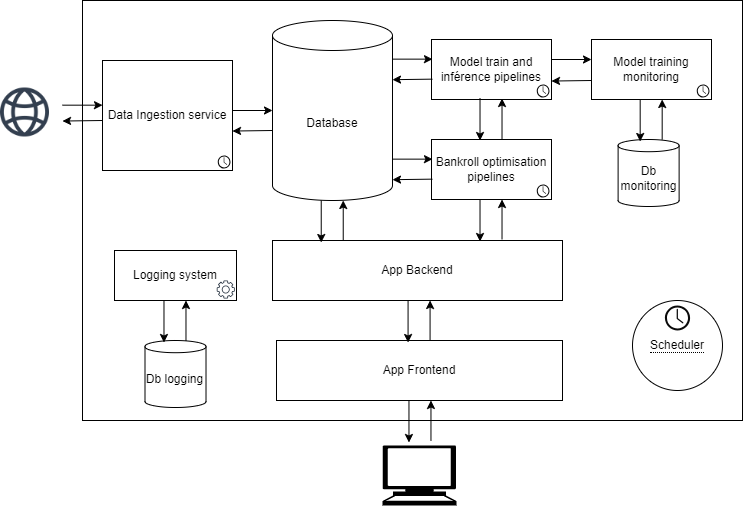
\includegraphics[width=0.8\textwidth, keepaspectratio]{images/Architecture_optimsportbet.png}
    \caption{Architecture of the system}
    \label{fig:elo_score_5_teams_during_time}
\end{figure}


\section{Data Collection}

Accurate and comprehensive data collection is vital for building reliable predictive models and effective betting strategies. The goal is to build an historical database which continues to build with real time relevant data.

\subsection{Data Sources Used}

We utilize a variety of reputable sources to gather data:

\begin{itemize}
    \item \textbf{Football Match Data}: Historical match results, match schedule, team statistics, player performance metrics, and other relevant information are sourced using scrapping on two websites: 
    \begin{itemize}
        \item \hyperlink{https://fbref.com/en/}{FBref}: For historical match results and coming match schedule.
        \item \hyperlink{https://sofifa.com/}{SoFifa}: For teams and players past and current ratings and statistics.
    \end{itemize}
    \item \textbf{Odds Data}: Betting odds are collected from multiple bookmakers through one API.
    \begin{itemize}
        \item \hyperlink{https://the-odds-api.com/}{The Odds API}: The free tier credits allows to perform 500 requests per month on various sports, bookmakers and leagues to retrieve the current odds. Historical odds data are not included.
    \end{itemize}
\end{itemize}


\subsection{Collection Methods}

Data is collected using a combination of methods:

\paragraph{Web Scraping}

A fork of the \hyperlink{https://soccerdata.readthedocs.io/en/latest/}{Soccerdata} python library, has been adapted to scrape data from websites that do not provide APIs (FBref, SoFifa). 

\paragraph{APIs}

For sources that offer APIs (The Odds API), we integrate with them using HTTP requests to fetch structured data efficiently.

\paragraph{Data Pre-processing}

Collected data undergoes a very simple pre-processing to ensure consistency and usability:

\begin{itemize}
    \item \textbf{Data type conversion}: Adapting the type of the data to the most adapted type.
    \item \textbf{Unity}: Only inserting new data in the database, or filling None values of existing data (for instance, the score of a match is only available after the match is played 
    \item \textbf{Integration}: Aligning data from different sources for seamless storage and analysis.
\end{itemize}

\section{Data Storage}

A robust data storage solution is essential for managing the diverse datasets involved.

\subsection{Database Choice}

We opted for a relational database management system (RDBMS), specifically \textit{PostgreSQL}, due to its reliability, scalability, and support for complex queries.

\subsection{Data Model}

The database schema is designed to reflect the relationships between different types of data:

\subsubsection{Tables}

\begin{itemize}
    \item `\textbf{fbref\_results}`: Each row corresponds to a match (historic and coming), with league, date and time of the match, both team and score if match is finished and the result is available and fetched from FBref website.
    \item `\textbf{sofifa\_teams\_stats}`: Each row corresponds to a a team and a date of update with metrics and categorical values that represent at best the team at the moment of the update (overall score, attack, build\_up\_speed ...).
    \item `\textbf{soccer\_odds}`: Each row corresponds to a match, a bookmaker, an outcome with its odd at a given update time. There is also information about the commence time of the match, the league, the home and away team names, the type of odd...
    \item `\textbf{models\_results}`: Each row corresponds to a match, the inference results of the model, the date-time of inference and the model used, with additional information such as the date and tile of the match and home and away team.
    \item `\textbf{optim\_results}`: Each row corresponds to a game, a date time of optimisation, the model used for inference, the best odds for each outcome found across a pool of bookmaker as well as the bookmakers names of each odds chose and the fraction of the bankroll to invest given utility function. There is additional information such as the probability inferred and used by the optimiser, the date-time of inference of these probabilities, the date and time of the match...
\end{itemize}


\begin{figure}[H]
    \centering
    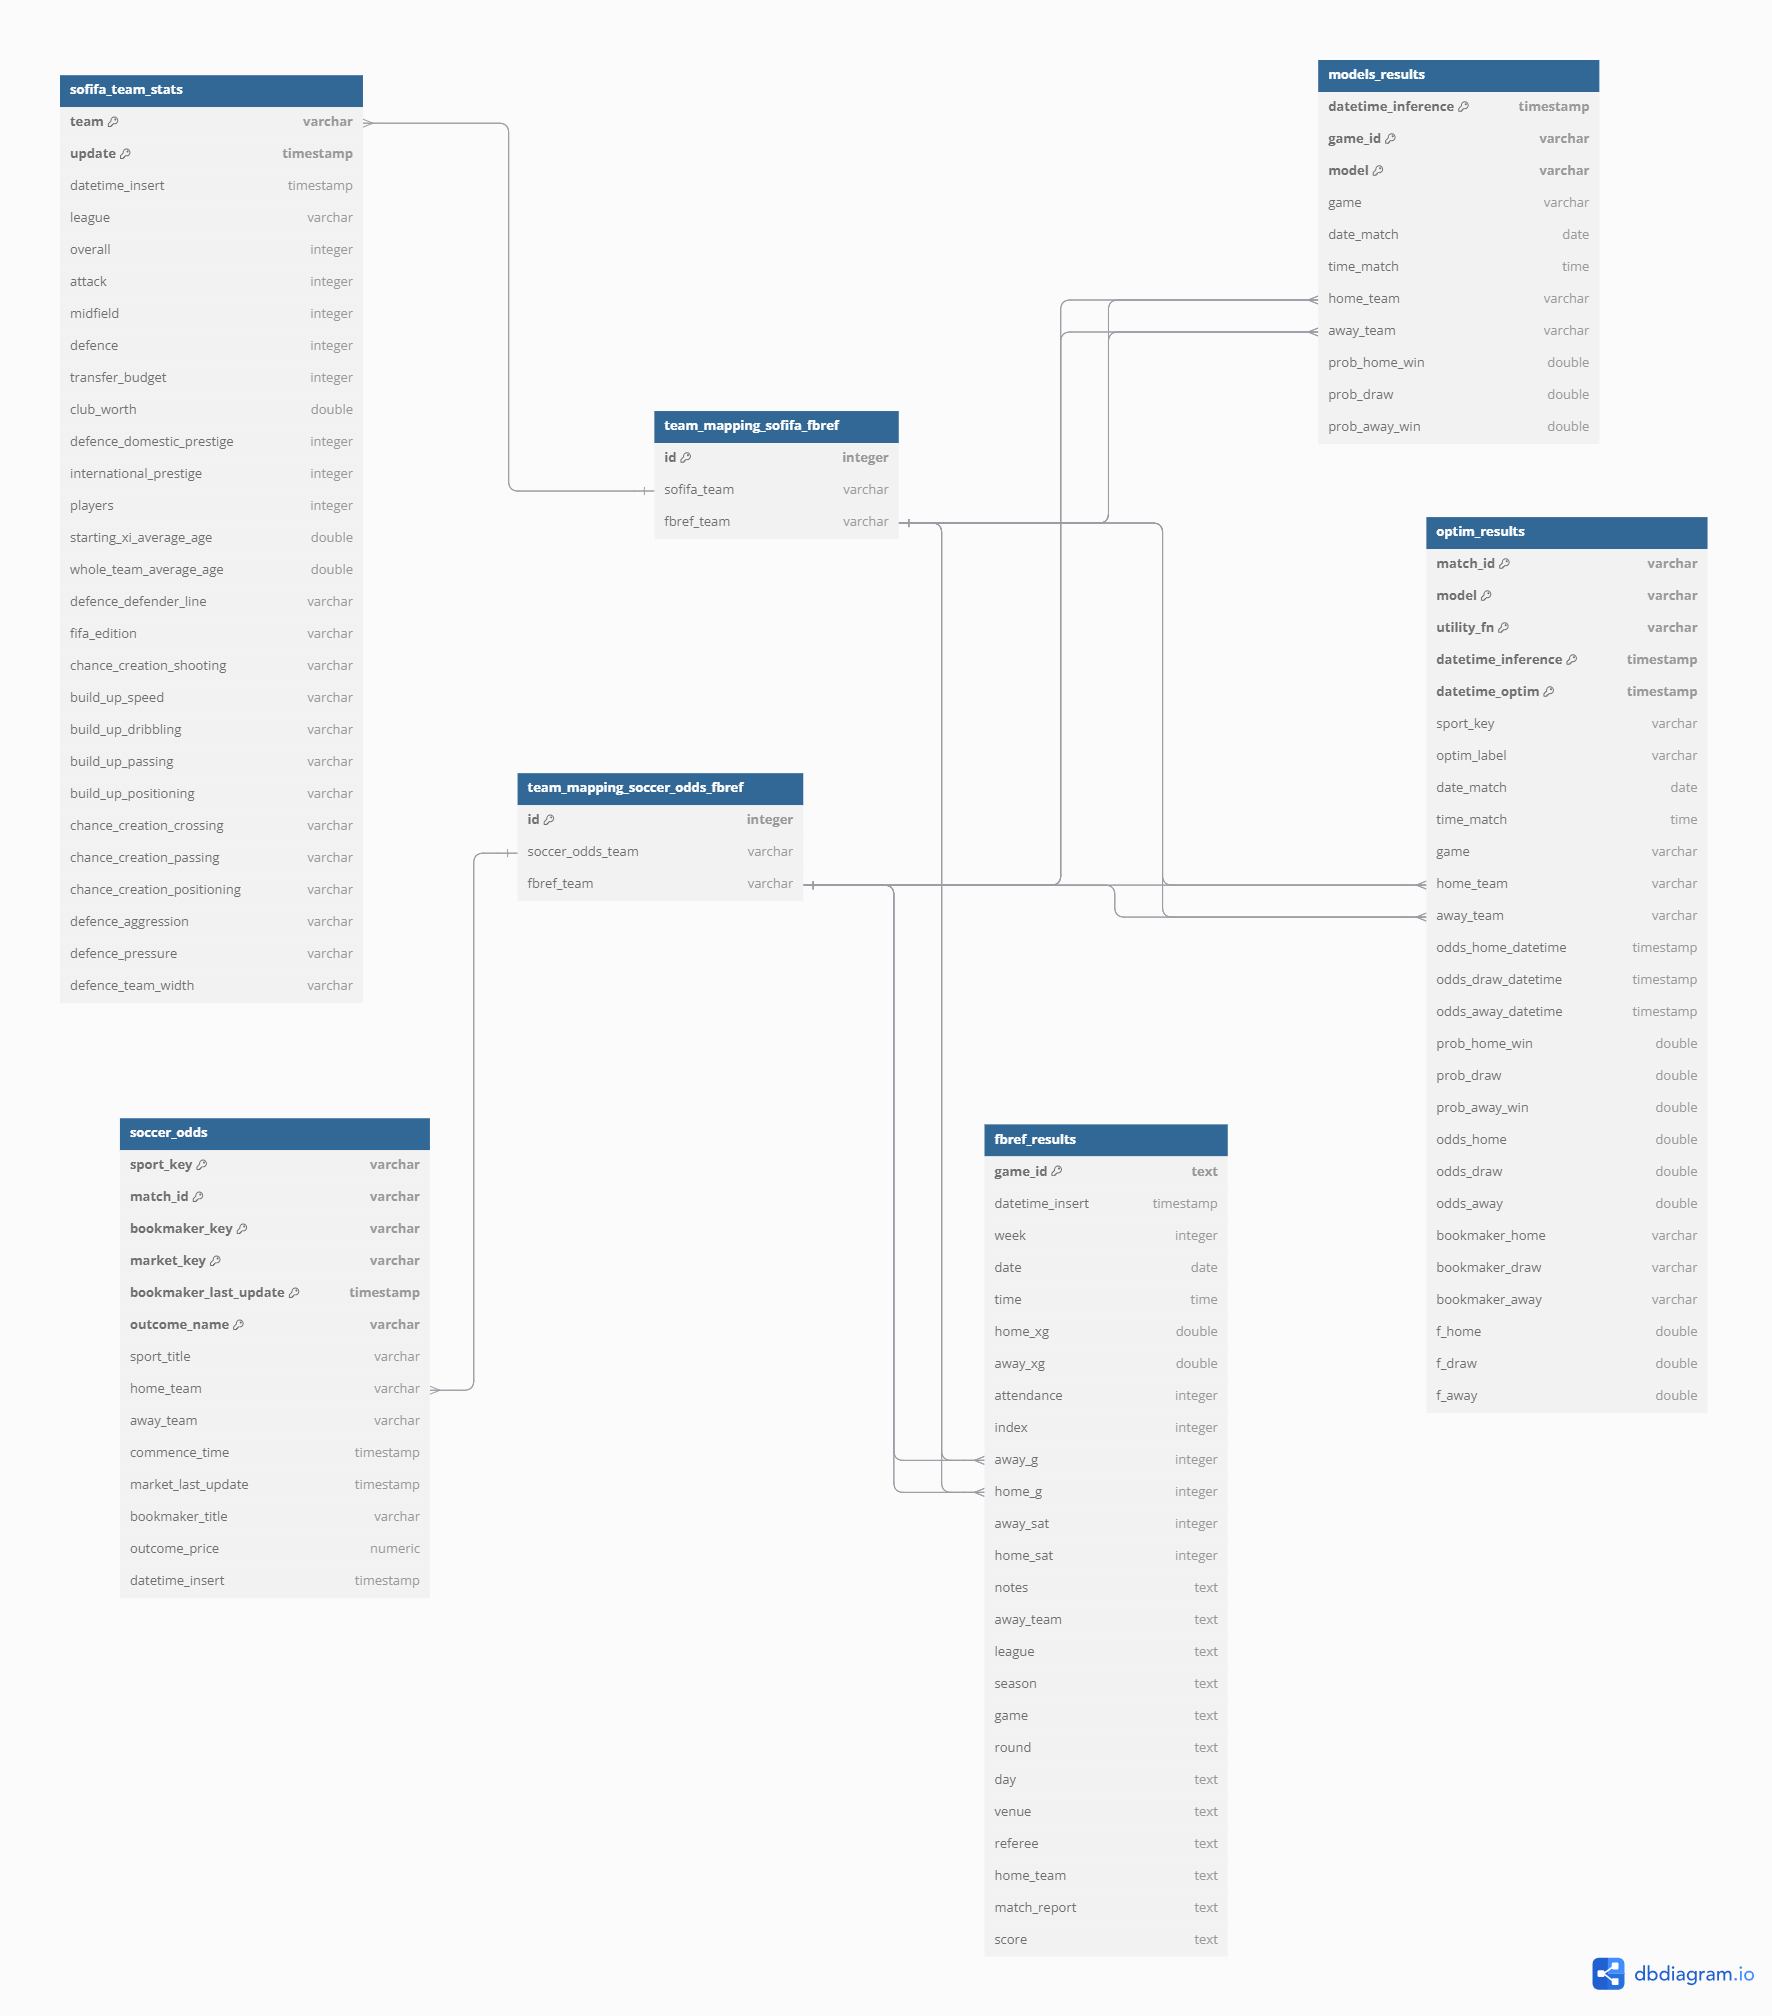
\includegraphics[width=0.8\textwidth, keepaspectratio]{images/db_uml.png}
    \caption{UML diagram of the database}
    \label{fig:uml_db}
\end{figure}

\section{Module Overview}

The system incorporates several modules, each performing specific functions within the overall architecture.

\subsection{Data Collection Module}

As described earlier, this module is responsible for fetching and pre-processing data from various sources.

\subsection{Prediction Module}

Although detailed discussion is deferred to a later chapter, this module uses machine learning algorithms to predict the probabilities of different match outcomes based on historical data.

\subsection{Optimization Module}

This module calculates optimal betting strategies by applying mathematical optimization techniques to the predictions and odds data. The specifics of the optimization algorithms and utility functions will be explored in a subsequent chapter.

\subsection{Scheduler}

The scheduler automates the execution of tasks such as data collection, model retraining, inference, and optimization. It ensures that the system remains up-to-date with the latest data and predictions.

\subsection{User Interface and Backend}

The user interface provides a platform for users to access data, view predictions, and interact with the system. The backend handles user requests, processes data, and communicates with other modules via APIs.

\section{User Interface and Monitoring}

\subsection{User Interface Design}

The UI is designed to be intuitive and user-friendly, providing clear visualizations and easy navigation.

\paragraph{Features}

\begin{itemize}
    \item \textbf{Dashboard}: Displays key metrics, including upcoming matches, predicted probabilities, and recommended betting strategies.
    \item \textbf{Historical Data Access}: Allows users to explore past matches, predictions, and outcomes.
    \item \textbf{Customization}: Users can select preferred bookmakers according to their interests.
\end{itemize}

\subsection{Monitoring}

System health and performance are monitored continuously:

\begin{itemize}
    \item \textbf{Logging}: Activity logs are maintained for debugging and audit purposes.
    \item \textbf{Alerts}: Notifications are sent in case of errors or significant events.
\end{itemize}


\section{Conclusion}

This chapter provided an overview of the system architecture implemented to realize the theoretical framework developed earlier. By focusing on football, we leverage abundant data to build predictive models and optimize betting strategies. The modular design, utilizing microservices and APIs,ensures scalability and flexibility. The database serves as the central repository, integrating data from various sources and supporting the different modules. The user interface offers a gateway for users to access the system's functionalities. In the subsequent chapters, we will delve into the specifics of the prediction and optimization modules, as well as the deployment strategy using Kubernetes and containerization technologies.

\section{Introduction}
\label{sec:chapter4_intro}

This chapter presents the development, training, and evaluation of a predictive model aimed at forecasting the outcomes of football matches. The primary objective is to construct a robust model that can accurately predict match results, thereby optimizing gains in sports betting \cite{BaioBlangiardo2010} \cite{DixonColes1997}. The significance of predictive modeling in the context of sports betting lies in its potential to provide bettors with a strategic advantage by identifying value bets and minimizing risks.

\section{Performance Metrics and Selection Criteria}
\label{sec:performance_metrics}

Evaluating the performance of a predictive model in a multi-class classification setting, especially with imbalanced classes, requires a comprehensive set of metrics. This section delineates both classic and advanced metrics employed in this study, incorporating mathematical formulations and addressing class imbalance. Given the three-class problem—home win, draw, and away win—with home wins constituting 47\% of the data, it is crucial to select metrics that provide a nuanced understanding of model performance across all classes.

\subsection{Metrics}
\label{subsec:classic_metrics}

A list of all the metrics considered with their used definition can  be found in Appendix \ref{appendix:predictive_model_metrics}.

\subsection{Selection Criteria}
\label{subsec:selection_criteria}

Accurate evaluation of the predictive model requires appropriate performance metrics, particularly in a multi-class classification context with class imbalance. The primary goal of this study is to ensure that the predicted probabilities of football match outcomes (home win, draw, away win) closely align with the true probabilities, emphasizing well-calibrated probability estimates.

Given the class distribution—47\% home wins, 26\% draws, and 25\% away wins—we have selected the \textbf{Mean Squared Error (MSE)} as the primary metric for assessing calibration. MSE directly measures the average squared difference between predicted probabilities and actual outcomes, making it suitable for evaluating how well the model's probabilities reflect the true frequencies.

In addition to MSE, we will consider the following metrics to provide a comprehensive evaluation:

\begin{itemize}
    \item \textbf{Log Loss}: To assess the quality of the predicted probability distributions by penalizing incorrect and overconfident predictions, thus encouraging well-calibrated estimates.
    \item \textbf{Classwise Expected Calibration Error (ECE)}: To evaluate the calibration of predicted probabilities for each class individually, offering insights into how closely these probabilities match the observed outcomes across different categories.
    \item \textbf{Accuracy for Home Win, Draw, and Away Win}: To examine the model's performance on each outcome separately, taking into account the class imbalance.
\end{itemize}

By focusing on MSE for calibration and incorporating Log Loss, Classwise ECE, and class-specific accuracy, we aim to ensure that the model not only produces accurate probability estimates but also maintains reliability across all outcome categories. This concise set of metrics aligns with our objective of accurately predicting football match outcomes while ensuring the predicted probabilities are well-calibrated and trustworthy.

\section{Exploration and Choice of Features}
\label{sec:feature_selection}

Selecting appropriate features is pivotal for building an effective predictive model. This section delineates the various types of features utilized in this study, the methodology employed for feature selection, the engineering of new features to enhance predictive power, and the handling of categorical variables to ensure they are appropriately represented in the model. 

\subsection{Types of Features Utilized}
\label{subsec:types_features}

The feature set comprises a combination of ranking-based, simple statistical, and domain-specific features. Each feature is defined mathematically where applicable and accompanied by an explanation of its relevance and computation.

\subsubsection{Ranking Features}
\label{subsubsec:ranking_features}

Ranking features provide a quantitative measure of team strength based on historical performance. These metrics are crucial as they encapsulate the overall ability and consistency of teams over time. All ranking features detailed formula are described in \ref{appendix:ranking_features}.

\begin{itemize}

\item \textbf{Elo Score}
\label{par:elo_score}

The \textbf{Elo score} \cite{Elo1978} \cite{HvattumArntzen2010} is a rating system originally developed for chess but widely adapted to various sports to rate players or teams. It reflects the relative skill levels of the teams based on game outcomes.

\begin{figure}[H]
    \centering
    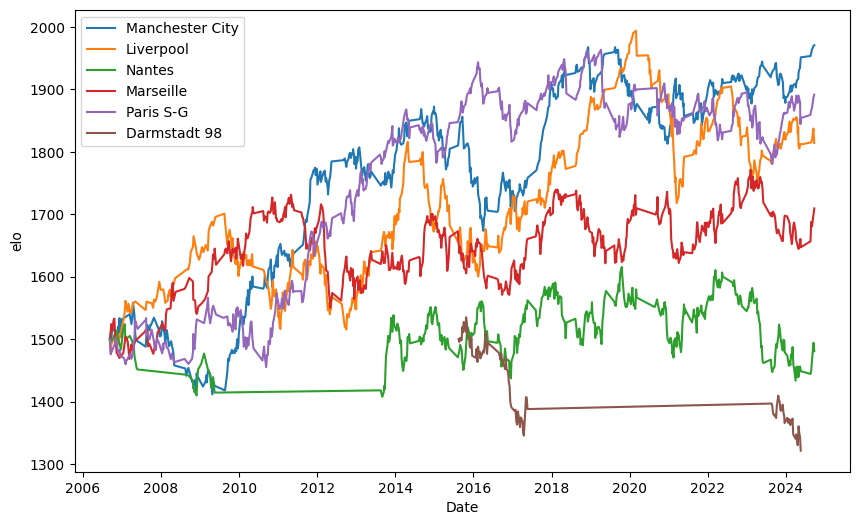
\includegraphics[width=0.8\textwidth, keepaspectratio]{images/elo_score_5_teams_during_time.png}
    \caption{Elo score of 5 football teams evolving during time}
    \label{fig:elo_score_5_teams_during_time}
\end{figure}



\item \textbf{Glicko-2 Score}
\label{par:glicko2_score}

The \textbf{Glicko-2 score} \cite{Glickman1999} is an advanced rating system developed by Mark Glickman, which enhances the Elo rating system by incorporating not only the skill levels of teams or players (R) but also the reliability of these ratings through Rating Deviation (RD) and volatility. This system provides a more dynamic and accurate reflection of performance by accounting for the uncertainty and variability in teams' ratings.


\item \textbf{TrueSkill}
\label{par:trueskill}

The \textbf{TrueSkill} \cite{HerbrichEtAl2007} is a Bayesian ranking system developed by Microsoft, primarily used in gaming but adaptable to sports analytics. It models each team's skill as a Gaussian distribution, updating beliefs about team strengths based on match outcomes.

\end{itemize}

\subsubsection{Simple Statistical Features}


Simple statistical features offer basic quantitative measures of team performance, providing foundational data for the predictive model.


\begin{itemize}
    \item \textbf{Average Goals Scored per Season}: Total goals scored by a team divided by the number of matches played so far.
    
    \item \textbf{Average Goals Conceded per Season}: Total goals conceded by a team divided by the number of matches played so far.
\end{itemize}


\subsubsection{Sofifa Performance Metrics}

SoFIFA provides detailed metrics for both individual players and teams, based on data from the FIFA video game by EA Sports. This document outlines the primary metrics and explains how team ratings are calculated using individual player attributes.

\begin{itemize}

\item \textbf{Player Metrics}
    The primary player metrics on SoFIFA are based on individual attributes that are weighted differently depending on the player's position. Below are the key metrics:
    
    \begin{itemize}
        \item \textbf{Overall Rating (OVR)}: This is the weighted average of various player attributes, with different weights depending on the position. For example, an attacker (\textit{Forward}) will have more emphasis on \textit{Shooting} and \textit{Pace}, while a defender (\textit{Centre Back}) will weigh attributes like \textit{Defending} and \textit{Physicality} more heavily.
        \item \textbf{Pace (PAC)}: Calculated as a combination of the \textit{Acceleration} and \textit{Sprint Speed} attributes.
        \item \textbf{Shooting (SHO)}: Includes \textit{Finishing}, \textit{Shot Power}, \textit{Long Shots}, and \textit{Positioning}.
        \item \textbf{Passing (PAS)}: Comprised of \textit{Vision}, \textit{Short Passing}, and \textit{Long Passing}.
        \item \textbf{Dribbling (DRI)}: Includes \textit{Ball Control}, \textit{Dribbling}, \textit{Agility}, and \textit{Balance}.
        \item \textbf{Defending (DEF)}: Based on \textit{Tackling}, \textit{Marking}, \textit{Interceptions}, and \textit{Defensive Awareness}.
        \item \textbf{Physicality (PHY)}: Includes \textit{Strength}, \textit{Stamina}, and \textit{Aggression}.
        \item \textbf{Potential}: Indicates the maximum possible rating the player can achieve over time.
    \end{itemize}
    
    The formula for the Overall Rating (OVR) is generally unknown, but it can be expressed as a weighted sum of key attributes, depending on the player’s position. A simplified formula for a forward might look like:
    
    \[
    \text{OVR}_{\text{Forward}} = w_1 \cdot \text{PAC} + w_2 \cdot \text{SHO} + w_3 \cdot \text{DRI} + w_4 \cdot \text{PAS}
    \]
    
    where \( w_1, w_2, w_3, w_4 \) are position-specific weights.

\item \textbf{Team Metrics}
    Team metrics on SoFIFA are calculated by aggregating individual player ratings, focusing on key areas like attack, midfield, and defense. The following are the primary team metrics:
    
    \begin{itemize}
        \item \textbf{Overall Team Rating}: A weighted average of the starting 11 players' Overall Ratings, considering the importance of each player's position.
        \item \textbf{Attack Rating}: The average Overall Rating of forwards and attacking midfielders, weighted based on the formation.
        \item \textbf{Midfield Rating}: The average Overall Rating of central and wide midfielders, weighted based on their roles in the formation.
        \item \textbf{Defense Rating}: The average Overall Rating of defenders and goalkeepers.
    \end{itemize}
    
    A simplified version of the team rating could be expressed as:
    
    \[
    \text{Team OVR} = \frac{1}{11} \sum_{i=1}^{11} \text{OVR}_i
    \]
    
    where \( \text{OVR}_i \) represents the Overall Rating of the $i$-th player in the starting lineup.
    
    
    Sofifa metrics are comprehensive team-specific performance indicators sourced from the Sofifa database, widely used in sports analytics and fantasy football contexts.
\end{itemize}

\begin{figure}[H]
    \centering
    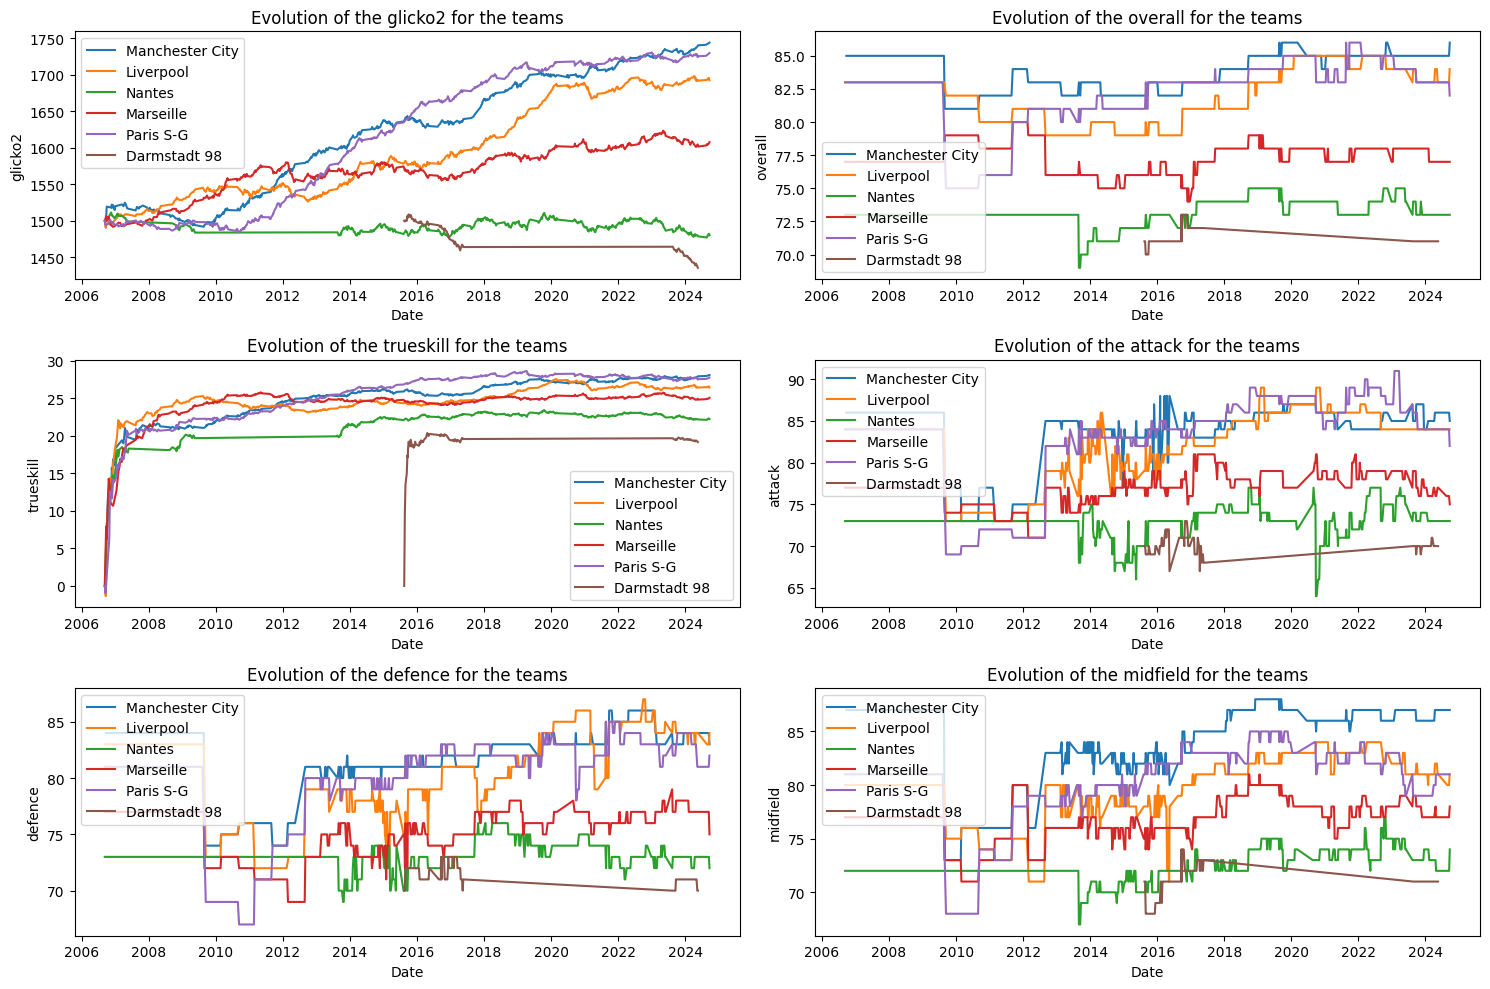
\includegraphics[width=\textwidth, keepaspectratio]{images/scores_5_teams_during_time.png}
    \caption{Different scores of 5 football teams evolving during time}
    \label{fig:scores_5_teams_during_time}
\end{figure}

A detailed description of each of the 90 features used can be found her \ref{appendix:all_feature_descriptions}.

\subsection{Feature Selection Methodology}
\label{subsec:feature_selection_methodology}

Feature selection was performed using a forward selection approach applied to a logistic regression model. This method iteratively adds the most significant features, enhancing predictive performance while maintaining model simplicity.

\subsubsection{Forward Selection with Logistic Regression}
\label{subsubsec:forward_selection_logistic_regression}

\textbf{Procedure}: Starting with no features, at each iteration, the feature that most improves the model's fit is added. The selection criterion is based on the mse (mean squared error).

\textbf{Explanation}: By incorporating features that significantly contribute to the model, forward selection optimizes predictive accuracy and ensures interpretability by excluding irrelevant variables.

\section{Data Preparation}

We trained our model on matches from 2006 to the present, focusing on games from the top 5 European leagues, European championships, and World Cups during this period. The limiting factor in our data came from SoFIFA, which does not provide data prior to 2006, while FBref offers data extending far into the past. We merged the two datasets based on team names and computed the ranking and statistical features described earlier, initializing the metrics at the first entry of a team in a tournament. For categorical features, we applied one-hot encoding. We removed matches with any missing values in the columns, then applied a standard scaler. This left us with 28,850 completed matches and a 90-feature vector for each match to train our model.

\begin{table}[h]
\centering
\begin{tabular}{|l|c|c|}
\hline
\textbf{Metric} & \textbf{Value} \\
\hline
Total matches & 28,850 \\
Matches in Top 5 Leagues & 28,481 \\
Matches in European Championships & 185 \\
Matches in World Cup & 184 \\
Home win ratio & 45.0 \% \\
Draw ratio & 25.4 \% \\
Away win ratio & 29.5 \% \\ 
Average home team goals & 1.54 \\
Average away team goals & 1.19 \\
Average Elo rating & 1558 \\
Number of unique teams & 242 \\
Number of features per match & 90 \\
First match date & 2006-09-09 \\
Last match date & 2024-09-24 \\
\hline
\end{tabular}
\caption{Summary Metrics for the Dataset}
\end{table}


\section{Cross-Validation on Temporal Data}
\label{sec:cross_validation_temporal}

In predictive modeling with football match data, which is inherently temporal, it's essential to use cross-validation techniques that respect the chronological order of observations. Standard cross-validation methods, such as random shuffling or traditional \( k \)-fold cross-validation, are unsuitable because they can lead to data leakage by training models on future data to predict past events.

Traditional cross-validation assumes that data samples are independent and identically distributed (i.i.d.) and that the order of observations does not matter. In temporal data, however, observations are time-dependent, and future events should not influence model training aimed at predicting past events. Using standard methods can result in:

\begin{itemize}
    \item \textbf{Data Leakage}: Incorporating future information into the training set leads to overly optimistic performance estimates.
    \item \textbf{Violation of Temporal Order}: Disrupting the sequence of events undermines the model's ability to generalize to real-world forecasting scenarios.
\end{itemize}


To address these issues, we employ cross-validation methods designed for temporal data \cite{BergmeirEtAl2018}.

\subsection{Sliding Window Cross-Validation}

This technique involves moving a fixed-size window across the data timeline. In each iteration, the model is trained on a training window and tested on the immediately following testing window.

\begin{itemize}
    \item Choose a training window size \( W_{\text{train}} \) and a testing window size \( W_{\text{test}} \).
    \item For each iteration:
    \begin{itemize}
        \item Train the model on data from time \( t \) to \( t + W_{\text{train}} - 1 \).
        \item Test the model on data from \( t + W_{\text{train}} \) to \( t + W_{\text{train}} + W_{\text{test}} - 1 \).
        \item Slide the window forward by \( W_{\text{test}} \) units.
    \end{itemize}
\end{itemize}

\subsection{Expanding Window Cross-Validation}

Also known as growing window, this method expands the training set with each iteration by including more historical data.

\begin{itemize}
    \item Start with an initial training window of size \( W_{\text{initial}} \).
    \item For each iteration:
    \begin{itemize}
        \item Train the model on data from time \( t \) to \( t + W_{\text{train}} - 1 \), where \( W_{\text{train}} \) increases with each iteration.
        \item Test on the subsequent data from \( t + W_{\text{train}} \) to \( t + W_{\text{train}} + W_{\text{test}} - 1 \).
        \item Expand the training window to include the latest testing window.
    \end{itemize}
\end{itemize}

\begin{figure}[H]
    \centering
    \begin{minipage}{0.45\textwidth}
        \centering
        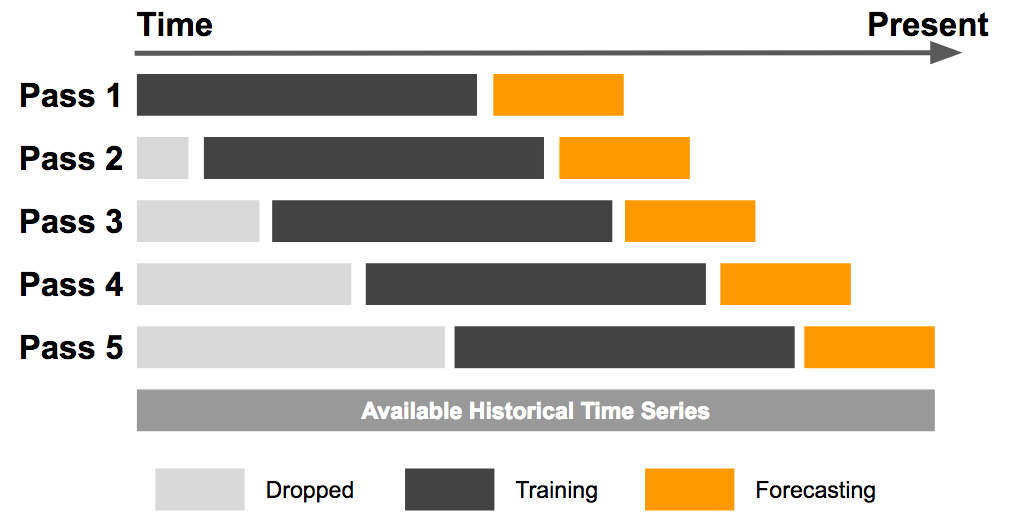
\includegraphics[width=\textwidth, keepaspectratio]{images/FixedWindow.png}
        \caption{Sliding window graphic}
        \label{fig:sliding_window}
    \end{minipage}\hfill
    \begin{minipage}{0.45\textwidth}
        \centering
        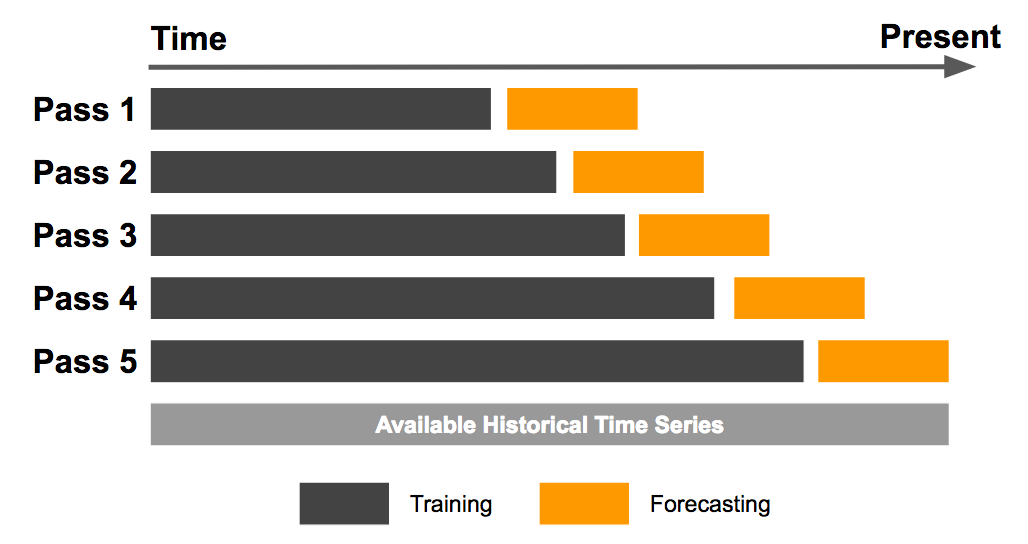
\includegraphics[width=\textwidth, keepaspectratio]{images/ExpandingWindow.png}
        \caption{Expanding window graphic}
        \label{fig:expanding_window}
    \end{minipage}
\end{figure}


The results presented below were obtained using an expanding window technique with 5 folds and a test set ratio of 0.2. Notably, the results were very similar when applying the sliding window method.


\section{Choice and Justification of the Prediction Model}
\label{sec:model_choice}

In this section, we present the results of the feature selection and model selection processes \cite{GuyonElisseeff2003} \cite{ChandrashekarSahin2014}, followed by interpretations of the selected model's performance. Feature selection was conducted using forward selection, and multiple classification models were evaluated to determine the most suitable model for predicting football match outcomes.

\subsection{Feature Selection Using Forward Selection}
\label{subsec:feature_selection}

Feature selection was performed using forward selection with logistic regression, iteratively adding the most significant feature at each step based on mean squared error (MSE) improvement, using an expanding window validation with 5 splits and a test size of 20\% of the training data.

\begin{table}[H]
    \centering
    \caption{Feature Selection Process Summary}
    \label{tab:feature_selection_summary}
    \begin{tabular}{lc}
        \toprule
        \textbf{Method} & \textbf{Details} \\
        \midrule
        Feature Selection & Forward Selection \\
        Model Used & Logistic Regression \\
        Validation Method & Expanding Window (5 splits) \\
        Performance Metric & Mean Squared Error (MSE) \\
        Test Size & 20\% of training data \\
        \bottomrule
    \end{tabular}
\end{table}


We selected 35 features, which corresponding to the features resulting in the lowest MSE, using this feature selection strategy.

\begin{table}[H]
    \centering
    \caption{Feature Selection with Corresponding MSE and their adding number}
    \label{tab:feature_mse}
    \begin{tabular}{|c|l|c|c|l|c|}
        \hline
        \textbf{Order} & \textbf{Feature Added} & \textbf{MSE} & \textbf{Order} & \textbf{Feature Added} & \textbf{MSE} \\
        \hline
        1  & Elo Away & 0.20613 & 19 & Home Passing Risky & 0.19438 \\
        2  & Elo Home & 0.19661 & 20 & Away Positioning Org. & 0.19436 \\
        3  & Glicko Vol Away & 0.19619 & 21 & Away Defense Pressure Med & 0.19435 \\
        4  & Away Overall & 0.19594 & 22 & Away Domestic Prestige & 0.19434 \\
        5  & Home Overall & 0.19540 & 23 & Away Shooting Lots & 0.19433 \\
        6  & Away Build Speed Slow & 0.19518 & 24 & Home Defense Line Offside & 0.19432 \\
        7  & Away Avg Age & 0.19501 & 25 & Away Team Width & 0.19431 \\
        8  & Home League INT & 0.19487 & 26 & Home Defense Pressure Med & 0.19431 \\
        9  & Home Avg Goals & 0.19476 & 27 & Home Build Speed Slow & 0.19430 \\
        10 & Home Positioning Org. & 0.19467 & 28 & Away Defense Aggression & 0.19430 \\
        11 & Home Build Speed Fast & 0.19461 & 29 & TrueSkill Home & 0.19430 \\
        12 & Away Defense Pressure High & 0.19457 & 30 & Away Build Positioning Org. & 0.19430 \\
        13 & Away Defense Offside Trap & 0.19453 & 31 & Away Defense & 0.19430 \\
        14 & Home League ITA & 0.19449 & 32 & Home Attack & 0.19427 \\
        15 & Glicko RD Home & 0.19447 & 33 & Home Defense Prestige & 0.19427 \\
        16 & Home Shooting Normal & 0.19444 & 34 & Away Attack & 0.19427 \\
        17 & Away Passing Mixed & 0.19442 & 35 & Away League INT & \textbf{0.19427} \\
        18 & Away Avg Goals & 0.19440 & & \\
        \hline
    \end{tabular}
\end{table}

The table above summarizes the features added during the selection process and their corresponding MSE values, highlighting the importance of each feature as it contributes to minimizing the error. As we can see, features such as Elo ratings and overall team metrics play a significant role \cite{LasekEtAl2013}. Now, let's examine how the number of features impacts the performance metrics more broadly, as shown in the following feature selection graph.

\begin{figure}[H]
    \centering
    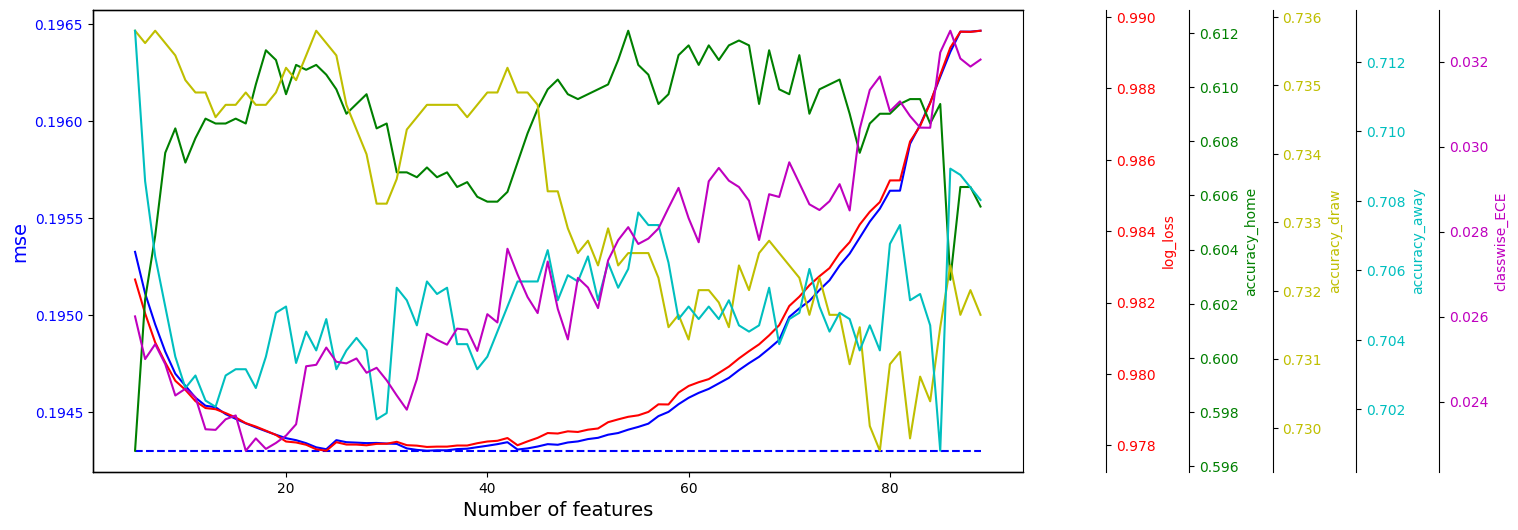
\includegraphics[width=\textwidth, keepaspectratio]{images/feature_selection_metrics_by_nb_of_features.png}
    \caption{Metrics of interrest function of the number of features added}
    \label{fig:feature_selection_metrics_by_nb_of_features}
\end{figure}

This graph shows the performance of various metrics (MSE, log loss, accuracy for home, draw, and away predictions, and classwise ECE) as a function of the number of selected features. The MSE (in blue) decreases as more features are added, stabilizing around the optimal point before increasing again, which suggests that selecting too many features can lead to overfitting. Similarly, log loss follows a similar trend (in red), indicating better model calibration with fewer features. The accuracy metrics (home, draw, away) fluctuate, but accuracy seems to peak at a certain range of features, with performance diminishing as more features are added. Classwise ECE (in pink) decreases and then increases, a little bit before MSE and log loss, indicating better calibration for class predictions with fewer features. Overall, the graph highlights the balance between feature selection and model performance, suggesting that an optimal subset of features yields the best generalization.

\subsection{Model Selection}
\label{subsec:model_selection}

The following table summarizes the performance of various classification models \cite{Bishop2006}, comparing metrics such as mean squared error (MSE), log loss, classwise ECE, and accuracy for home, draw, and away predictions to identify the best-performing model.

\begin{table}[H]
    \centering
    \caption{Model Performance Comparison}
    \label{tab:model_performance}
    \begin{tabular}{|l|c|c|c|c|c|c|}
        \hline
        \textbf{Model} & \textbf{MSE} & \textbf{Log Loss} & \textbf{C. ECE} & \textbf{A. Home} & \textbf{A. Draw} & \textbf{A. Away} \\
        \hline
        Logistic Regression & \textbf{0.195} & \textbf{0.983} & 0.029 & 0.605 & 0.733 & 0.702 \\
        Logistic Regression CV & 0.196 & 0.983 & \textbf{0.028} & 0.602 & \textbf{0.735} & 0.703 \\
        Gradient Boosting Classifier & 0.199 & 1.002 & 0.037 & 0.604 & 0.709 & \textbf{0.706} \\
        Random Forest Classifier & 0.202 & 1.022 & 0.038 & 0.595 & 0.705 & 0.693 \\
        Extra Trees Classifier & 0.204 & 1.026 & 0.043 & 0.597 & 0.683 & 0.686 \\
        AdaBoost Classifier & 0.221 & 1.092 & 0.069 & 0.599 & 0.721 & 0.695 \\
        Bagging Classifier & 0.224 & 2.471 & 0.093 & 0.602 & 0.646 & 0.661 \\
        MLP Classifier & 0.224 & 1.187 & 0.108 & 0.585 & 0.665 & 0.684 \\
        K Neighbors Classifier & 0.238 & 5.404 & 0.096 & 0.599 & 0.643 & 0.631 \\
        Gaussian NB & 0.332 & 7.570 & 0.302 & \textbf{0.615} & 0.584 & 0.625 \\
        Quadratic Discriminant Analysis & 0.353 & 10.831 & 0.316 & 0.582 & 0.561 & 0.613 \\
        Decision Tree Classifier & 0.390 & 20.219 & 0.195 & 0.578 & 0.614 & 0.638 \\
        Extra Tree Classifier & 0.399 & 20.686 & 0.200 & 0.559 & 0.615 & 0.628 \\
        \hline
    \end{tabular}
\end{table}


\subsection{Interpretation of Results}
\label{subsec:interpretation}

The selection of the logistic regression model allows for straightforward interpretation of feature effects on the predicted probabilities of match outcomes.

\subsubsection{Feature Importance}

Feature importance was assessed based on the magnitude of the coefficients in the logistic regression model. Below sits the feature importance of the Home win class. Draw and Away win classes analysis can be found in \ref{appendix:feature_importance}.


\begin{figure}[H]
    \centering
    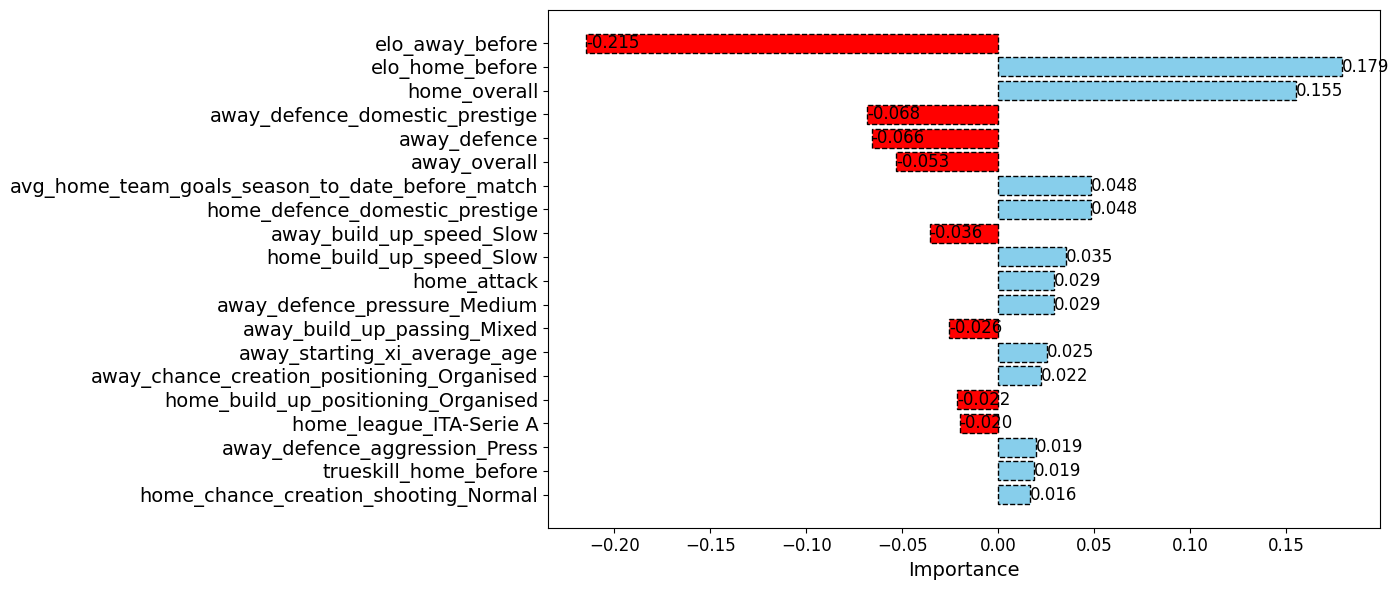
\includegraphics[width=\textwidth, keepaspectratio]{images/top20_coeff_importance_lr_selected_features_home.png}
    \caption{Coefficients of the Logistic Regression Model for Home win class}
    \label{fig:feature_coefficients}
\end{figure}

For the home class, the most important features, such as Elo ratings for the away and home teams, suggest that pre-match team strength is the most significant predictor of match outcomes. Both overall team quality and specific defensive attributes, like pressure and aggression, also play a key role. Features related to player average characteristics, such as average age and tactical elements like build-up speed, indicate that team composition and playstyle are also relevant, though their impact is less pronounced. Defensive strategies, particularly pressure and team width, add further predictive value, showing the importance of tactical decisions in determining match results. The feature importance analysis graphs for draw and away class can be found in the annex section.


\subsubsection{Why Logistic Regression Outperforms Other Models}

Logistic regression may outperform other models due to its simplicity and interpretability, especially when feature selection is based on it. By using logistic regression for feature selection, the model is specifically tuned to highlight the most important predictors of the outcome, leading to better generalization. Additionally, logistic regression handles multicollinearity well when regularization is applied, preventing overfitting. The linear relationship between the features and the log-odds of the outcomes makes it easier to capture important patterns in the data, particularly in problems like sports prediction where relationships between variables are often linear. Other models, such as random forests or gradient boosting, may add unnecessary complexity and are more prone to overfitting when features are already well-selected.


\section{Training and Retraining of the Model}
\label{sec:training_retraining}

Figure \ref{fig:mse_retraining} illustrates the Mean Squared Error (MSE) of two models over time, where the blue line represents Model A with no retraining, and the orange line represents Model B, which is retrained daily. Both models are initialy trained from 2006-01-01 up to 2010-01-01 data and are evaluated using a 120-day rolling average.

\begin{figure}[H]
    \centering
    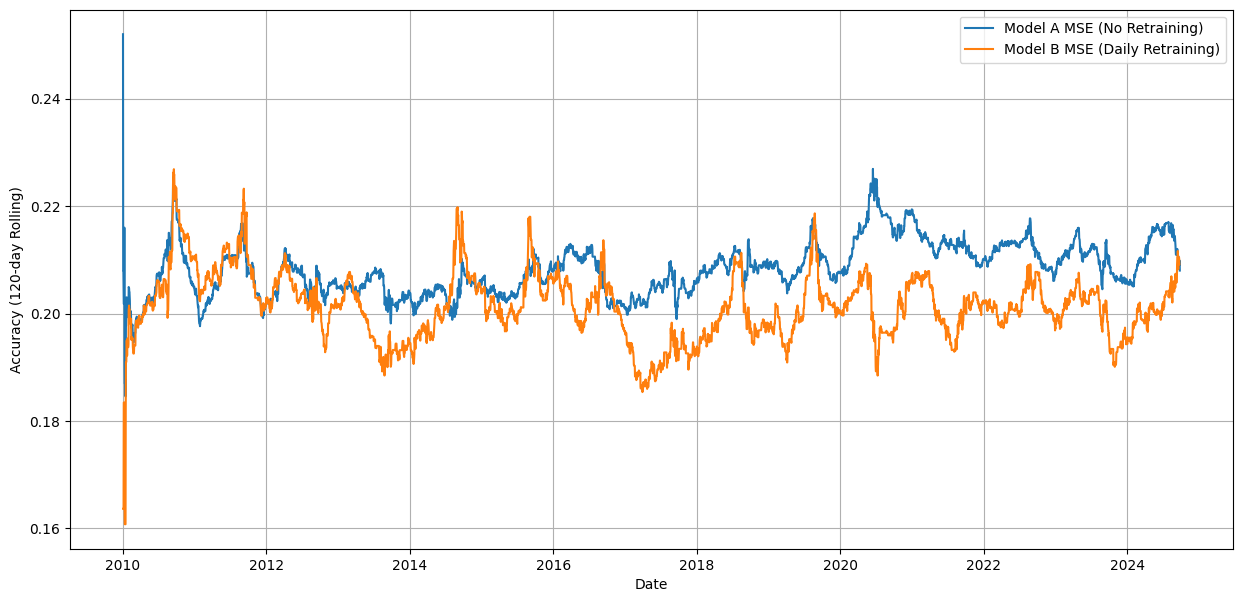
\includegraphics[width=0.8\textwidth, keepaspectratio]{images/model_ratrining_mse_120rd.png}
    \caption{Model MSE rolling average over time}
    \label{fig:mse_retraining}
\end{figure}


From the figure, we observe that Model B, which is frequently retrained, exhibits lower MSE compared to Model A throughout most of the time period. Retraining appears to allow Model B to adapt more effectively to evolving patterns, leading to consistently better performance in terms of accuracy. Moreover, as time goes by, we can observe a mse drift from the not retrained model as well as a slight improvement from the retrained model. \\

There are very few periods where Model A outperforms Model B. It appends especially during phases of sudden changes. Despite these fluctuations, retraining offers a more stable and improved long-term performance. \\

The results highlight the importance of regular retraining for maintaining model accuracy, particularly in dynamic environments where data patterns change over time.

\section{Conclusion}

This chapter presented the development, training, and evaluation of a predictive model for football match outcomes, with a focus on sports betting. Feature selection via forward selection with logistic regression helped identify key predictors, and regular retraining improved model performance over time.\\

However, several limitations remain:

\begin{itemize}
    \item \textbf{Hyperparameters and Features}: Ranking feature hyperparameters were left at default, and additional domain-specific or external data sources could further improve predictions.
    \item \textbf{Feature Selection}: Feature selection was arbitrarily based on logistic regression, and no hyperparameter optimization was performed for any models.
    \item \textbf{Retraining}: The timing and method of retraining (e.g., sliding window) were not explored, potentially missing optimal strategies as well as posing computational challenges that could be optimized.
    \item \textbf{Model Complexity}: Incorporating deep learning models could enhance predictive performance, particularly for capturing complex patterns in the data.
    \item \textbf{Bookmaker Odds Decorrelation}: Adding a metric to assess the decorrelation between model predictions and bookmaker odds could help identify more value bets and further optimize betting strategies.
\end{itemize}
In the next chapter, we address the optimization problem of determining the bankroll share to invest on each outcome, building on the predictions of this model to develop actionable betting strategies.

\section{Introduction}

Effective bankroll management is a critical component of successful sports betting. It involves determining the optimal amount to wager on each bet to maximize growth while minimizing the risk of ruin. This section details the development and evaluation of an optimization module designed to calculate the optimal fraction of the bankroll to invest in each betting opportunity. The module leverages probabilistic forecasts from the predictive models discussed in the previous section and applies various investment strategies, including the Kelly criterion, expected value maximization, and naive betting approaches.

\section{Methodology}
\subsection{Investment Strategies}

This section provides an overview of the different bankroll allocation strategies implemented, ranging from naive methods to more advanced optimization techniques. The focus is on the principles guiding each strategy, with a detailed formula provided only for the naive strategy.

\subsubsection{List of Strategies}

\begin{itemize}
    \item \textbf{Kelly Criterion Strategy}: \cite{Kelly1956} \cite{Thorp1969}  
    This strategy maximizes the logarithmic utility of wealth, aiming for long-term bankroll growth while managing risk. The bankroll fractions are derived from the analytical solution using the approximations  \ref{appendix:analytical_solution_using_the_kelly_criterion}, \(\mathbb{E}(U(B)) = \mathbb{E}(B) - \frac{1}{2} \cdot \mathbb{V}\text{ar}(B) \) which comes down to a Linear utility strategy using \( \lambda = \frac{1}{2} \).

    \item \textbf{Log Utility Strategy}:  
    Similar to the Kelly criterion, this strategy focuses on maximizing the expected logarithmic utility \(U(B) = \ln(B)\)  but using no approximations \ref{appendix:analytical_reduction_using_log_expected_utility}.

    \item \textbf{Exponential Utility Strategy}:  
    This strategy uses an exponential utility function \(U(B) = -e^{-\alpha B}\) to take into account the bettor’s risk aversion, balancing between expected returns and risk tolerance \ref{appendix:analytical_reduction_using_exp_expected_utility}.

    \item \textbf{Linear Utility Strategy}:
    In this strategy, the objective is to maximize the trade-off between expected returns and risk, represented by the function \(\mathbb{E}(U(B)) = \mathbb{E}(B) - \lambda \cdot \mathbb{V}\text{ar}(B) \). For the simulations, we set \( \lambda = 10 \), reflecting a high level of risk aversion. This approach seeks to maximize returns while penalizing high variance, aiming to balance growth and stability \ref{appendix:analytical_solution_using_linear_expected_utility}. 

    \item \textbf{Expected Value Maximization Strategy}:  
    This strategy optimizes bankroll allocation based purely on maximizing expected value, \(U(B) = B\), without considering risk or variance.

    \item \textbf{Naïve Strategy: Bet on the Most Likely Outcome}:  
    In this straightforward approach, the bettor places the entire bet on the outcome with the highest implied probability, as per the bookmaker's odds.
    
    The formula for this strategy is:
    \[
    f_{k,i} = 
    \begin{cases}
    \frac{1}{M}, & \text{if } i = \arg\max(o_k) \\
    0, & \text{otherwise}
    \end{cases}
    \]
    where:
    \begin{itemize}
        \item \( f_{k,i} \) is the fraction of the bankroll wagered on outcome \( i \) of match \( k \),
        \item \( o_k \) are the odds for match \( k \).
        \item \(M\) is the number of matches available.
    \end{itemize}
    This strategy is simple and allocates all the available funds to the outcome with the highest bookmaker odds.
\end{itemize}

These strategies were benchmarked against each other in the Monte Carlo simulations and then Online testing to assess their effectiveness in managing risk and maximizing bankroll growth. \\

For each strategy, a factor of \( \gamma = \frac{1}{2} \) was applied to the bet fractions to ensure that not the entire bankroll was wagered at any given time, thereby providing a margin of safety, such as: \(f_{strategy\_final} = \gamma \times f_{strategy}\).


\subsection{Optimization Algorithms}

Two optimization algorithms were employed to solve the bankroll allocation problem \cite{BoydVandenberghe2004}:

\begin{itemize}
    \item \textbf{Sequential Least Squares Programming (SLSQP):} An iterative method for constrained nonlinear optimization that is efficient for problems with a moderate number of variables.
    \item \textbf{Trust-Region Constrained Algorithm (trust-constr):} Suitable for large-scale optimization problems, it handles large numbers of variables and constraints effectively.
\end{itemize}

The choice between SLSQP and trust-constr depends on the number of betting opportunities (matches) considered at once. For a large number of matches, trust-constr is preferred due to its scalability.


\section{Monte Carlo Simulations}

To assess the performance of different investment strategies under simulated sports betting conditions, we conducted Monte Carlo simulations modeling the inherent uncertainties. The goal was to evaluate how various bankroll allocation strategies perform over numerous trials.

\subsection{Simulation Setup}

We simulated true match outcome probabilities \( r \) using a Dirichlet distribution appropriate for mutually exclusive and collectively exhaustive events:

\[
r_i^k = \text{Dirichlet}(\alpha), \quad \alpha = (1, 1, 1)
\]

To introduce discrepancies between true probabilities and those estimated by bookmakers (\( b \)) and players (\( t \)), we added biases and normally distributed noise:

\[
b_i^k = \text{clip}(r_i^k + \text{bias}_{\text{bookmaker}} + \epsilon_{\text{bookmaker}}, \ \text{min\_prob}, \ \text{max\_prob})
\]
\[
t_i^k = \text{clip}(r_i^k + \text{bias}_{\text{player}} + \epsilon_{\text{player}}, \ \text{min\_prob}, \ \text{max\_prob})
\]

where \( \epsilon_{\text{bookmaker}}, \epsilon_{\text{player}} \sim \mathcal{N}(0, \sigma^2) \). Probabilities were normalized to sum to one, and bookmaker probabilities included a margin \( \text{margin}_{\text{bookmaker}} \), clipping between \text{min\_prob} and \text{max\_prob}. Bookmaker odds were calculated as:

\[
o_i^k = \frac{b_i^k}{(\sum_{i=0}^N b_i^k) - \text{margin}_{\text{bookmaker}}}
\]

\subsection{Simulation Procedure}

The simulation followed a structured approach to evaluate the performance of different betting strategies, using predefined constants and a series of steps to simulate match outcomes and bankroll updates.

\begin{table}[H]
\centering
\caption{Simulation constants}
\label{tab:simulation constants}
\begin{minipage}{.2\linewidth}
\centering
\begin{tabular}{lr}
\toprule
\textbf{Constant} & \textbf{Value}\\
\midrule
H & 30 \\
T & 50 \\
N & 3 \\
\(\text{min\_prob}\) & 0.05 \\
\(\text{max\_prob}\) & 0.95 \\
\bottomrule
\end{tabular}
\end{minipage}%
\hspace{0.05\linewidth}
\begin{minipage}{.45\linewidth}
\centering
\begin{tabular}{lrr}
\toprule
\textbf{Constant} & \textbf{Bettor} & \textbf{Bookmaker}\\
\midrule
\text{bias} & 0 & 0 \\
\(\sigma\) (for noise \(\epsilon)\) & 0.1 & 0.1 \\
\text{margin} &  & 0.1 \\
\bottomrule
\end{tabular}
\end{minipage}
\end{table}

\begin{enumerate}
    \item Generated true probabilities \( r \) using \(\text{bias} = 0\) and \(\epsilon = 0.1\) for both bettor and bookmaker.
    \item Computed bookmaker and player estimates \( b \) and \( t \).
    \item Calculated bookmaker odds \( o \).
    \item For each strategy:
    \begin{itemize}
        \item Determined bet sizes using \( t \) and \( o \) by performing optimisation using \texttt{truct\_constr} algorithm.
        \item Simulated match outcomes based on \( r \).
        \item Updated bankrolls accordingly.
    \end{itemize}
\end{enumerate}

\subsection{Evaluation Metrics}

Strategies were evaluated using:

\begin{itemize}
    \item \textbf{Final Bankroll Statistics}: Mean, standard deviation, median, minimum, and maximum.
    \item \textbf{Average Growth Rate}: Geometric mean per time step. 
    \[GGR = \left( \frac{B(n)}{B(0)} \right)^{\frac{1}{n}} - 1\]

    \item \textbf{Sharpe Ratio}: Risk-adjusted return.

    \[\text{Sharpe Ratio} = \frac{\frac{1}{n} \sum_{t=1}^{n} R(t)}{\mathbb{V}ar(R(t))}) \text{   with   } R(t) = \frac{B(t+1) - B(t)}{B(t)}\]
    
    \item \textbf{Probability of Ruin}: Frequency of bankroll falling below a threshold.
\end{itemize}

\subsection{Results}

\begin{figure}[H]
    \centering
    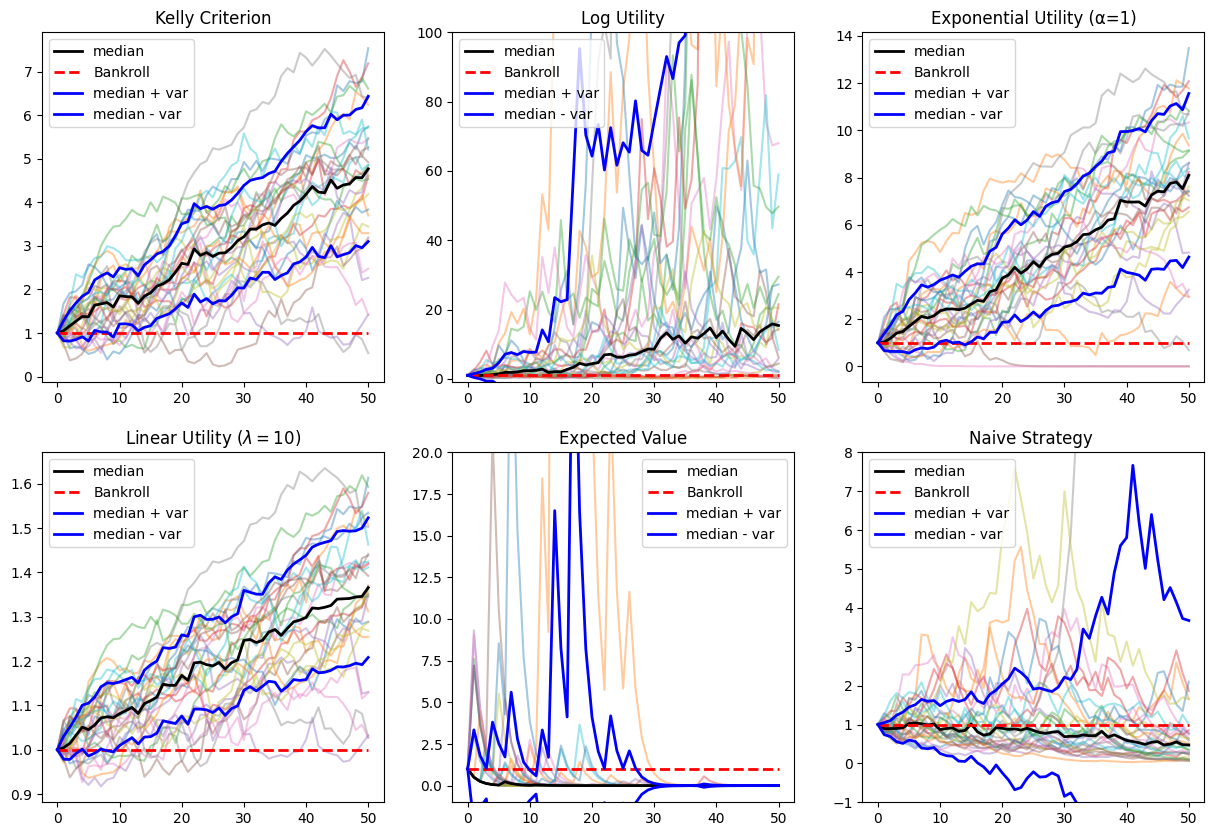
\includegraphics[width=1.1\textwidth, keepaspectratio]{images/monte_carlo_b=b.png}
    \caption{Monte carlo simulations for each strategy}
    \label{fig:monte_carlo}
\end{figure}


\begin{table}[H]
\centering
\caption{Final Bankroll Statistics}
\label{tab:final_bankroll}
\begin{tabular}{lrrrrr}
\toprule
\textbf{Strategy} & \textbf{Mean} & \textbf{Std Dev} & \textbf{Median} & \textbf{Min} & \textbf{Max} \\
\midrule
Kelly Criterion          & 4.48   & 1.67   & 4.77   & 0.54   & 7.54   \\
Log Utility              & 270.85 & 983.14 & 15.39  & 0.19   & 5414.01 \\
Exponential Utility      & 7.46   & 3.46   & 8.10   & 0.00   & 13.48  \\
Linear Utility           & 1.35   & 0.16   & 1.37   & 1.03   & 1.61   \\
Expected Value           & 0.00   & 0.00   & 0.00   & 0.00   & 0.01   \\
Naïve Strategy           & 1.20   & 3.20   & 0.47   & 0.06   & 18.19  \\
\bottomrule
\end{tabular}
\end{table}

The \textbf{Log Utility} strategy achieved the highest mean final bankroll but with significant variability, indicating high risk. The \textbf{Kelly Criterion} and \textbf{Exponential Utility} strategies demonstrated moderate returns with lower variability, suggesting consistent performance.

\begin{table}[H]
\centering
\caption{Average Growth Rate Per Step}
\label{tab:avg_growth}
\begin{tabular}{lr}
\toprule
\textbf{Strategy} & \textbf{Growth Rate} \\
\midrule
Kelly Criterion          & 2.82\% \\
Log Utility              & 5.54\% \\
Exponential Utility      & 2.55\% \\
Linear Utility           & 0.59\% \\
Expected Value           & $-$29.83\% \\
Naïve Strategy           & $-$1.55\% \\
\bottomrule
\end{tabular}
\end{table}

While the \textbf{Log Utility} strategy had the highest growth rate, it came with increased volatility. The \textbf{Kelly Criterion} and \textbf{Exponential Utility} strategies offered positive growth with better risk control.

\begin{table}[H]
\centering
\caption{Sharpe Ratio}
\label{tab:sharpe_ratio}
\begin{tabular}{lr}
\toprule
\textbf{Strategy} & \textbf{Sharpe Ratio} \\
\midrule
Kelly Criterion          & 0.30 \\
Log Utility              & 0.29 \\
Exponential Utility      & 0.25 \\
Linear Utility           & 0.30 \\
Expected Value           & 0.14 \\
Naïve Strategy           & 0.01 \\
\bottomrule
\end{tabular}
\end{table}

The highest Sharpe Ratios were achieved by the \textbf{Kelly Criterion} and \textbf{Linear Utility} strategies, indicating superior risk-adjusted returns.

\begin{table}[H]
\centering
\caption{Probability of Ruin}
\label{tab:prob_ruin}
\begin{tabular}{lr}
\toprule
\textbf{Strategy} & \textbf{Probability} \\
\midrule
Kelly Criterion          & 0.00\% \\
Log Utility              & 3.33\% \\
Exponential Utility      & 6.67\% \\
Linear Utility           & 0.00\% \\
Expected Value           & 100.00\% \\
Naïve Strategy           & 20.00\% \\
\bottomrule
\end{tabular}
\end{table}

Zero probability of ruin for the \textbf{Kelly Criterion} and \textbf{Linear Utility} strategies underscores their robustness.

An ANOVA test (performed to assess whether the differences in final bankrolls among the strategies), (F-statistic: 2.16, p-value: 0.0612) suggested that differences among strategies were not statistically significant at the 5\% level. However, the p-value is close to the threshold, suggesting that with a larger sample size, the differences might become statistically significant.

\subsection{Conclusion}

The simulations indicate that strategies like the \textbf{Kelly Criterion} and \textbf{Exponential Utility}, which balance growth and risk through utility maximization, offer favorable outcomes. The \textbf{Log Utility} strategy provides high growth potential but with greater volatility. Ignoring risk, as in the \textbf{Expected Value} strategy, leads to poor performance.

\textbf{Limitations} include the limited number of simulations, simplified assumptions, and exclusion of real-world factors like transaction costs.

\textbf{Recommendations} for future work involve increasing simulation runs, incorporating realistic market conditions, and exploring additional strategies.


\section{Online Testing}

To assess the strategies in a real-world environment, an online testing phase was conducted over five weeks, from 2024 August 24th to 2024 September 30th, focusing on matches from the five major European football leagues. This real-world testing evaluated the practical applicability and performance of the strategies under actual market conditions. Odds were scraped each day at 12pm from the Odd Api website.


\subsection{Static Problem Reduction and Parameter Settings}

To simplify the dynamic nature of sports betting, we reduced the problem to a series of static optimizations at discrete time intervals. At each decision point \( t \), bankroll allocation was optimized based on the current available information. This approach allowed us to manage the complexity of real-time betting while ensuring the practical applicability of the strategies.

\paragraph{Temporal Parameters}

Key temporal parameters were defined as follows:

\begin{itemize}
    \item \textbf{Betting Interval (\( \Delta t \))}: The interval between placing bets, set to 24 hours to capture daily betting opportunities.
    \item \textbf{Bet Placement Timing}: Bets were placed at a fixed time each day (12:00 PM) to ensure up-to-date information was used while accommodating market dynamics.
\end{itemize}

These settings ensured a balance between information accuracy and practical market conditions.

\paragraph{Match Selection}

The matches selected for each optimization were determined based on:

\begin{itemize}
    \item \textbf{Number of Matches (\( M \))}: Matches occurring within the next 24 hours were selected, balancing opportunity and reliability of information as well as having all results while perfomring next step.
    \item \textbf{Selection Criteria}: Focus was given to matches from top European leagues where the bettor had a higher perceived edge.
\end{itemize}

This careful match selection helped reduce computational complexity while enhancing potential returns.

\paragraph{Re-Betting Policy}

The re-betting policy was defined by the following criteria:

\begin{itemize}
    \item \textbf{Not allowing Re-Bets}: Additional bets on previously considered matches were not allowed. As we only bet on matches on the same day and only once a day, this was an implication of the previous choices.
\end{itemize}

This policy helped manage risk and adapt to evolving market conditions.

\subsection{Practical Implementation Settings}

The practical implementation settings for the online testing phase are summarized in Table~\ref{tab:implementation_settings}. The testing period ran from August 24, 2024, to September 30, 2024. The \texttt{trust-constr} algorithm was used for optimization, with a multiplier of \( \gamma = \frac{1}{2} \) applied to the matrix \( f \). The best odds from a pool of bookmakers (detailed in the appendix) were selected for each match.

\begin{table}[H]
\centering
\caption{Practical Implementation Settings}
\label{tab:implementation_settings}
\begin{tabular}{ll}
\toprule
\textbf{Setting}               & \textbf{Value}                                 \\ \midrule
Betting Interval (\( \Delta t \))     & 24 hours \\                                    
Bet Placement Time               & 12:00 PM daily                                \\
Look-Ahead Horizon               & Matches within the next 24 hours               \\ 
Re-Betting Policy                & Not allowed \\ 
Testing Period                   & August 24, 2024 – September 30, 2024           \\ 
Optimization Algorithm           & \texttt{trust-constr}                          \\ 
Strategy factor mult. \(\gamma\)         & \( 0.5 \)                              \\ 
Odds Selection                   & Biggest odds from a pool of bookmakers            \\ 
Markets & 5 biggest European leagues (Big 5) \\
\bottomrule
\end{tabular}
\end{table}


\subsection{Results and Interpretation}

Figure~\ref{fig:capital_evolution} illustrates the capital evolution for each strategy during the testing period. The Kelly and Exponential Utility strategies exhibited the strongest performance, both ending with approximately twice the initial capital. These results highlight their ability to optimally balance risk and reward, consistently outperforming the more conservative Log and Naive strategies. However, they also demonstrated higher volatility compared to the more stable Linear strategy.

\begin{figure}[H]
    \centering
    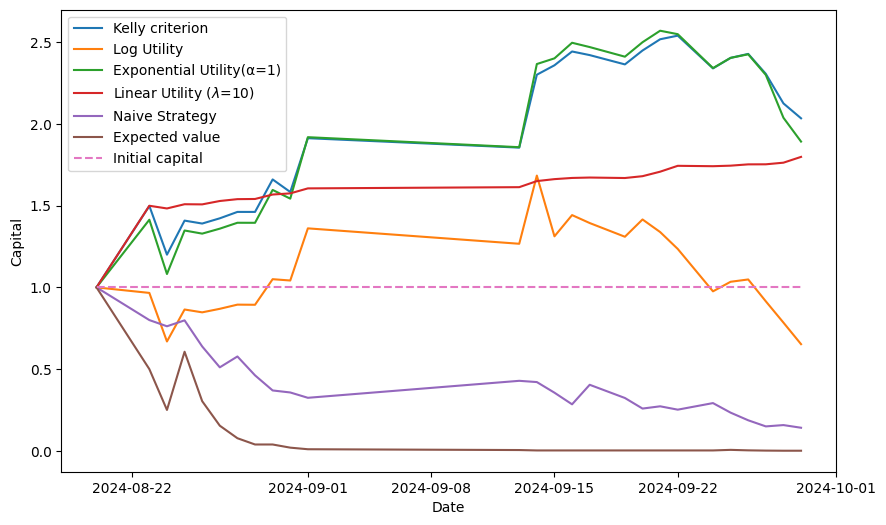
\includegraphics[width=\textwidth]{images/bankroll_evolution2.png}
    \caption{Capital Evolution for Each Strategy During the Online Testing Period}
    \label{fig:capital_evolution}
\end{figure}

The Log Utility strategy underperformed, particularly at the start and after the midpoint of the test period, failing to capitalize on high-return opportunities. Its conservative nature, aimed at minimizing risk, resulted in modest growth but ultimately led to a negative outcome. 

Both the Naive and Expected Value strategies experienced sharp declines in capital. The Naive strategy approached near-zero capital by the end of the test, while the Expected Value strategy exhibited extreme volatility, leading to rapid capital depletion. These simpler strategies, which lack sophisticated optimization, were highly vulnerable to adverse market conditions and failed to adapt effectively to fluctuations in odds or match outcomes.

In contrast, the Linear Utility strategy showed steady and consistent growth, with minimal volatility throughout the testing period, ultimately achieving a final growth of 1.8 times the initial capital. This highlights its effectiveness in maintaining a stable growth trajectory while avoiding the excessive risk associated with other strategies.

Overall, the results underscore the superiority of more advanced utility-based strategies such as Kelly and Linear. These approaches consistently outperformed simpler methods by balancing risk and reward more effectively under real-world betting conditions.

\subsection{Performance Metrics}

To further quantify the performance of each strategy, we computed key metrics, including final bankroll \( B(T) \), mean growth per step, and standard deviation of growth per step, both in absolute terms and as a percentage of the final bankroll. 
\begin{itemize}
    \item The mean growth per step is defined as:
    \[
    \mu = \frac{1}{T-1} \sum_{t=1}^{T-1} \Delta B_t
    \]
    where \( \Delta B_t = B_{t+1} - B_t \),
    \item the standard deviation of growth per step is given by:
    \[
    \sigma = \sqrt{\frac{1}{T-1} \sum_{t=1}^{T-1} (\Delta B_t - \mu)^2}
    \]
\end{itemize}


Table~\ref{tab:strategy_performance} summarizes the results for each strategy.

\begin{table}[H]
\centering
\caption{Strategy Performance Metrics}
\label{tab:strategy_performance}
\begin{tabular}{llll}
\toprule
\textbf{Strategy}              & \textbf{Final Bankroll \( B(T) \)} & \textbf{Mean Growth (\%)} & \textbf{Std Growth (\%)} \\ 
\midrule
Kelly Criterion                & 2.034                              & 2.034                      & 8.923                    \\ 
Log Utility                    & 0.653                              & -2.129                     & 26.516                   \\ 
Exponential Utility (\( \alpha = 1 \)) & 1.892                        & 1.886                      & 10.309                   \\ 
Linear Utility (\( \lambda = 10 \))    & 1.798                        & 1.776                      & 5.360                    \\ 
Naive Strategy                 & 0.141                              & -24.299                    & 52.419                   \\ 
Expected Value                 & 0.001                              & -5032.448                  & 18175.649                \\
\bottomrule
\end{tabular}
\end{table}

\subsection{Interpretation of Metrics}

The results demonstrate the effectiveness of the Kelly Criterion and Exponential Utility strategies, both of which ended with a final bankroll close to 2.0. These strategies also displayed reasonable volatility, with standard deviations of growth per step under 10\%. The Linear Utility strategy performed consistently, achieving steady growth with the lowest volatility among all strategies.

On the other hand, the Log Utility strategy suffered from negative growth, highlighting its inability to capitalize on high-return opportunities. The Naive and Expected Value strategies performed poorly, with significant capital depletion and extreme volatility, particularly for the Expected Value approach, indicating their inadequacy in real-world betting scenarios.


\section{Conclusion}

The results from both the Monte Carlo simulations and the real-world online testing phase demonstrate the clear advantages of sophisticated bankroll management strategies such as the Kelly Criterion and Exponential Utility methods. These strategies consistently provided strong returns while managing risk effectively, leading to a final bankroll close to twice the initial amount. In contrast, simpler strategies like the Naive and Expected Value approaches underperformed, suffering from capital depletion and high volatility, emphasizing the importance of balancing risk and return in real-world betting scenarios.

The Linear Utility strategy offered a steady, reliable growth trajectory with minimal volatility, making it an appealing option for risk-averse bettors. The Log Utility strategy, though conservative, failed to capture sufficient growth opportunities, resulting in a negative final outcome. Overall, the Kelly and Exponential Utility strategies are best suited for bettors seeking long-term growth with manageable risk.

\subsection{Limitations and Future Improvements}

Despite the promising results, several limitations were identified in the current approach:

\begin{itemize}
    \item \textbf{Simulation Assumptions}: The Monte Carlo simulations relied on several simplifying assumptions that limit the realism of the results. Firstly, the simulation of probabilities was based on the true clipped probabilities plus a bias and Gaussian noise, which does not fully capture the actual flaws in the predictive models, and the constants used were chosen arbitrarily without strong justification. Secondly, the bookmaker margin was fixed, and the odds provided by the bookmaker did not account for the influence of large bets from the players, which in reality could cause deviations in the bookmaker’s odds and probabilities. Lastly, the simulations used a fixed number of matches and time steps. Both the number of simulations and the range of strategies could be expanded to provide a more thorough and diverse analysis of performance over a wider variety of scenarios.
    \item \textbf{Limited Testing Period}: The online testing phase covered only a five-week period, which may not fully capture the long-term performance and robustness of each strategy. Extending the testing period or repeating it across multiple seasons would provide a more comprehensive assessment.
    \item \textbf{Risk Preferences}: While the utility-based strategies successfully managed risk, the models relied on fixed parameters for risk aversion (e.g., \( \lambda \) in Linear Utility). Introducing dynamic adjustments to these parameters based on market conditions or bettor preferences could further enhance performance.
\end{itemize}

\subsection{Future Work and Deployment on Azure Kubernetes}

The next stage of this project involves deploying the entire system on a cloud infrastructure using Kubernetes on Azure (AKS). This deployment will enable scalable, real-time processing of betting opportunities, continuous model updates, and the handling of multiple simultaneous users and markets. By leveraging Azure’s powerful compute and orchestration capabilities, the system will be capable of efficiently managing the computational load and data flows needed for real-time sports betting optimization.


\section{Microservices Architecture and Frameworks}

To build a scalable and maintainable system for sports betting optimization, we adopted a microservices architecture. This approach allows independent development, deployment, and scaling of individual components, facilitating modularity and flexibility.

The system comprises several microservices:

\begin{itemize}
    \item \textbf{Data Ingestion Service}: Collects real-time match data and odds from external APIs and web scraping. We use the Python library \textit{soccerdata} to conveniently scrape historical and real-time data from various websites. \textit{SQLAlchemy} is employed to communicate with the PostgreSQL database, allowing interaction using a mix of Python syntax and SQL queries. An API is provided for other services to trigger this service's logic, created using the \textit{FastAPI} framework. The Python library \texttt{logging} is used for proper logging of all operations, and \texttt{pandas} is utilized for data manipulation and transformation.

    \item \textbf{Prediction and Optimization Service}: Processes data to train models and generate probability estimates for the prediction component. Calculates optimal bet allocations based on the probabilities and selected strategies for the optimization component. \textit{Scikit-learn} is used for model training and inference, while \textit{SciPy.optimize} handles the optimization processes. Similar to the Data Ingestion Service, an API is deployed using \textit{FastAPI}, with communication to the database via \textit{SQLAlchemy}, and \texttt{logging} and \texttt{pandas} for logging and data handling.

    \item \textbf{User Interface Service}: Provides a web-based dashboard for monitoring and interaction, developed using the Python web framework \textit{Streamlit}.

    \item \textbf{Backend Service}: Manages communication and logic between the frontend User Interface and the database, as well as other services, using \textit{FastAPI}, \texttt{pandas}, and \texttt{logging}.

    \item \textbf{Database Service}: Stores historical data, odds, inferred probabilities, optimization results, and transaction logs. We chose PostgreSQL as the database due to its robustness, scalability, and compatibility with \textit{SQLAlchemy}. PostgreSQL's advanced features support complex queries and transactions essential for our application's needs.

    \item \textbf{MLflow Service}: Monitors the training metrics of the models. MLflow provides a convenient way to track experiments, record model parameters, metrics, and artifacts, facilitating reproducibility and model versioning.

    \item \textbf{Airflow Service}: Acts as a scheduler, providing a convenient way to orchestrate and monitor complex workflows using Directed Acyclic Graphs (DAGs). Apache Airflow allows us to define data pipelines, schedule tasks, and manage dependencies between them, ensuring timely execution of data ingestion, model training, and optimization processes.
\end{itemize}

Services communicate over HTTP/HTTPS protocols, with well-defined API endpoints ensuring loose coupling and ease of integration.

\section{Docker and Kubernetes}

To ensure consistency across development, testing, and production environments, all microservices are containerized using Docker \cite{Merkel2014}. Docker allows us to package each service with all its dependencies into isolated containers, ensuring consistent behavior across different environments.

\subsection{Dockerization}

Each microservice is encapsulated in a Docker container, defined by its own \texttt{Dockerfile}, which specifies the base image, dependencies, and entry points. In local development, we used containers for services such as MLflow, PostgreSQL, and Airflow, facilitating a consistent and reproducible environment.

\subsection{Kubernetes Deployment}

For orchestration and management of the containerized applications, we utilized Kubernetes \cite{HightowerEtAl2017}. Kubernetes automates deployment, scaling, and management of containerized applications. We packaged our system into a Helm chart, which simplifies the deployment of the entire application, including dependencies like MLflow, PostgreSQL, and Airflow.

\subsubsection{Helm Chart Packaging}

By encapsulating our services and their dependencies into a Helm chart, we streamlined the deployment process. Helm charts define, install, and upgrade complex Kubernetes applications, allowing us to manage configurations and versioning efficiently.

\subsubsection{Database Migrations}

Database schema changes are managed using migration files and scripts. Changes are first applied locally for testing and validation. Once validated, migrations are executed on the production database using scripts designed to apply changes incrementally. This process ensures that the database schema remains synchronized with the application code without disrupting ongoing operations.

\section{Deployment on Azure AKS}

\subsection{Azure Kubernetes Service (AKS)}

We deployed our Kubernetes cluster on Microsoft Azure using Azure Kubernetes Service (AKS), a managed Kubernetes service that simplifies cluster management by handling critical tasks like health monitoring and maintenance. AKS reduces the operational overhead and provides features like automated scaling and updates.

\begin{figure}[H]
    \centering
    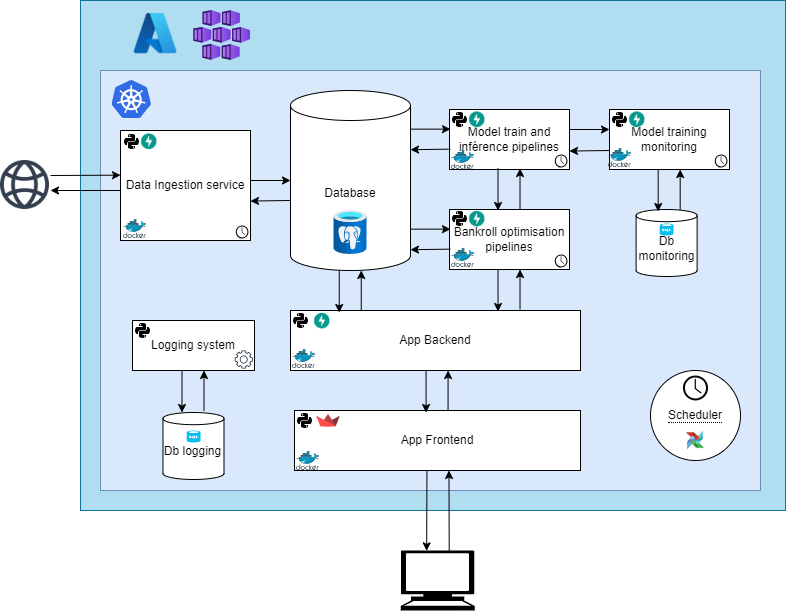
\includegraphics[width=0.8\textwidth, keepaspectratio]{images/diagrem_archi_services.png}
    \caption{Architecture of the system deployed on AKS}
    \label{fig:diagramme_arch_aks}
\end{figure}

\subsection{Infrastructure Details}

Our AKS deployment utilizes two virtual machines to ensure high availability and load balancing across the cluster. While Azure offers its own virtual machines, in this context, we refer to the compute resources allocated to our Kubernetes nodes. The integration with AKS allows for efficient resource utilization and scalability.

\subsection{Azure Services Integration}

Using Azure's cloud infrastructure offers several benefits:

\begin{itemize}
    \item \textbf{Azure Container Registry (ACR)}: Stores our Docker images securely, facilitating seamless deployment to AKS.
    \item \textbf{Azure DevOps Repo}: Provides a storage for our code.
\end{itemize}

\subsection{Pricing Considerations}

Azure's pricing model charges for compute resources used by virtual machines, storage, and network bandwidth. Managed services like AKS can reduce operational overhead but require careful monitoring to manage costs effectively. We optimized resource allocation by:


\section{Conclusion}

By adopting a microservices architecture, containerization with Docker, orchestration with Kubernetes, and deploying on Azure AKS, we built a scalable, reliable, and maintainable system for sports betting optimization. This architecture allows for independent development and deployment of components, ensuring the system can adapt to changing requirements and handle real-time data processing demands efficiently. Leveraging cloud infrastructure and managed services enhances our ability to focus on core application development while ensuring high availability and performance.

\section{Summary of Findings}

This study embarked on the ambitious task of developing a comprehensive system for optimizing sports betting strategies, focusing on football matches. Through the integration of predictive modeling, utility-based optimization, and scalable system architecture, we have addressed the critical components necessary for successful sports betting.

The predictive model, developed using logistic regression and advanced feature selection techniques, demonstrated significant accuracy in forecasting match outcomes. Regular retraining of the model proved essential in maintaining performance over time, highlighting the dynamic nature of sports data.

The optimization module applied various bankroll allocation strategies, including the Kelly Criterion, logarithmic, exponential, and linear utility functions. Both Monte Carlo simulations and real-world online testing over a five-week period indicated that sophisticated utility-based strategies substantially outperform naive betting approaches. Strategies like the Kelly Criterion and Exponential Utility provided favorable returns while effectively managing risk.

The system's deployment on Azure Kubernetes Service (AKS) showcased its scalability and readiness for real-time application. By leveraging a microservices architecture and containerization technologies like Docker and Kubernetes, the system can handle the computational demands of real-time data processing and optimization.

\section{Contributions to the Field}

This work contributes to the field of sports analytics and betting strategies in several ways:

\begin{itemize} \item \textbf{Integration of Predictive Modeling and Optimization}: By combining accurate probability estimations with utility-based optimization strategies, the system provides a robust framework for sports betting. \item \textbf{Scalable System Architecture}: The implementation of a microservices architecture and deployment on cloud infrastructure ensures that the system is scalable, maintainable, and adaptable to real-world conditions. \item \textbf{Empirical Evaluation}: The use of both simulations and real-world testing provides empirical evidence of the effectiveness of advanced betting strategies over simpler methods. \end{itemize}

\section{Limitations}

Despite the positive results, several limitations were identified:

\begin{itemize}
    \item \textbf{Predictive Model Enhancements}: While the current model performs adequately within the constraints of a static framework, it could be significantly improved by incorporating additional features, conducting hyperparameter optimization, and exploring more complex models such as deep learning architectures. These enhancements would allow the model to capture dynamic patterns and temporal dependencies inherent in football matches, which are not fully addressed due to the static nature of the current framework.

    \item \textbf{Static Framework Limitations and Long-Term Gain-Variance Interpretation}: The reduction of the betting problem to a static framework simplifies the optimization process but introduces limitations in interpreting gains and variance over the long term. Since the model does not account for intertemporal dependencies and the evolving nature of the bankroll, the strategies derived may not fully capture the risks associated with long-term betting. This static approach may lead to strategies that optimize short-term gains without adequately considering the cumulative effect on wealth over time. Future work should focus on extending the framework to a dynamic setting, allowing for a more accurate interpretation of long-term gain and variance, and better aligning the strategies with the bettor's long-term financial goals.

    \item \textbf{Risk Preferences and Dynamic Adaptation}: The optimization strategies employed fixed parameters for risk aversion, which do not adjust to changes in the bettor's wealth or market conditions over time. This static treatment of risk preferences limits the adaptability of the betting strategies, especially in a long-term context where the bettor's financial situation and the market dynamics can vary significantly. Introducing dynamic risk preferences that evolve with the bettor's bankroll and external factors would enhance the strategies' responsiveness and effectiveness, leading to better management of gain and variance over the long term.

    \item \textbf{Testing Period and Scope}: The real-world testing was confined to a five-week period focusing on the top five European leagues. Due to the static framework and the short testing duration, the evaluation may not fully reflect the strategies' performance over extended periods or in different market conditions. A longer testing period encompassing a broader range of leagues and varying competitive environments would provide more comprehensive insights into the strategies' long-term viability and their ability to manage gains and risks effectively within a dynamic setting.

\end{itemize}
\section{Future Work}

Building upon the findings of this study, several promising avenues can be explored to enhance the system's performance and address the challenges identified. 

Firstly, integrating real-time data streams and developing adaptive predictive models could significantly improve forecasting accuracy. By incorporating techniques from time-series analysis and machine learning, the model can capture temporal dependencies and evolving patterns inherent in football matches. This dynamic approach would allow the model to adjust to new information promptly, potentially leading to more accurate probability estimates and better alignment with the actual match outcomes.

Secondly, advancing the optimization strategies to include stochastic elements and multi-period planning could address the complexities associated with long-term gain and variance interpretation. Developing a dynamic framework that accounts for intertemporal dependencies and the evolving nature of the bankroll would enable more effective risk management. Strategies that adapt risk preferences in response to changes in the bettor's financial status or market conditions could lead to more sustainable betting practices and improved long-term financial outcomes.

Thirdly, conducting extensive real-world testing over longer periods and across a broader range of leagues and competitions would provide deeper insights into the robustness and generalizability of the betting strategies. Such testing would help to evaluate the performance of the models under varying market conditions and competitive environments, ensuring that the strategies remain effective over time and are not limited to specific contexts or short-term scenarios.

Finally, enhancing the user interface to offer more advanced analytics and personalized insights could empower users to make more informed decisions. Features that allow users to visualize performance trends, adjust parameters interactively, and receive tailored recommendations would improve the overall user experience. Providing tools for long-term performance monitoring and strategic adjustments would enable users to better understand the implications of their betting decisions and manage their bankrolls more effectively.

These potential developments represent initial steps toward refining the system's capabilities. By focusing on dynamic modeling, adaptive optimization, comprehensive testing, and user-centric design, future work can contribute to more robust predictive performance, effective risk management, and ultimately, more successful sports betting strategies.

\section{Final Remarks}

The integration of predictive modeling and utility-based optimization represents a significant step forward in developing effective sports betting strategies. This work demonstrates that with accurate predictions and strategic bankroll management, it is possible to achieve superior returns while managing risk effectively. The deployment on cloud infrastructure ensures that the system is ready for practical application, paving the way for future advancements in the field.


Je veux que tu me rédige un article de blog sur ce projet en format md. L'article doit prendre environ 10 min à lire et doit être interressant, prenant, il doit y avoir un bon story telling. Et plusieurs niveau de comprehension, pour les non initiés et pour les data scientist avancés.

Fais le en anglais

\chapter{Development of the Complete System and Production Deployment}


\chapter{Introduction}

Sports betting has evolved into a sophisticated industry that combines statistical analysis, predictive modeling, and strategic financial management \cite{AndersonSally2013}. With the global popularity of football and the abundance of data available, there is a significant opportunity to apply advanced analytical techniques to optimize betting strategies. The challenge lies in accurately predicting match outcomes and effectively managing the allocation of betting capital to maximize returns while minimizing risk.

This report presents the development and implementation of a comprehensive system designed to address these challenges in sports betting. The system integrates predictive modeling to forecast football match outcomes and optimization algorithms to determine the optimal allocation of a bettor's bankroll. The focus is on creating a practical, scalable solution that can operate in real-time, leveraging cloud-based technologies and microservices architecture.

\section{Background and Motivation}

The sports betting market is highly competitive, with bettors seeking any edge to improve their chances of success. Traditional betting strategies often rely on intuition or simplistic models that fail to account for the complexities of sports data and market dynamics. The advancement of machine learning and statistical methods offers the potential to enhance predictive accuracy and optimize betting decisions systematically \cite{CainEtAl2000}.

Effective bankroll management is equally important, as even accurate predictions can lead to losses if the betting amounts are not strategically allocated. The application of utility theory and optimization techniques, such as the Kelly Criterion, provides a mathematical framework for balancing risk and reward in betting decisions. 

\section{Objectives of the Study}

The primary objectives of this study are:

\begin{itemize}
\item To establish a rigorous mathematical framework that defines the theoretical foundations and sets the stage for the study.
\item To develop a predictive model that accurately estimates the probabilities of football match outcomes using historical and real-time data. \item To design an optimization module that calculates the optimal fraction of the bankroll to wager on each betting opportunity, applying various utility-based strategies. \item To implement a scalable, microservices-based system architecture that integrates data collection, predictive modeling, optimization, and user interface components. \item To deploy the system on a cloud platform using Kubernetes for scalability and reliability. \item To evaluate the performance of different betting strategies through Monte Carlo simulations and real-world online testing. \end{itemize}

\section{Scope of the Report}

This report details the theoretical framework underlying the predictive modeling and optimization strategies, the system architecture and implementation, and the results of both simulated and real-world testing. The report is organized as follows:

\begin{itemize} \item Chapter 2 provides a theoretical presentation of the models and preliminary research conducted. \item Chapter 3 describes the design and implementation of the solution, including system architecture and data management. \item Chapter 4 focuses on the development, training, and evaluation of the predictive models for match outcomes. \item Chapter 5 discusses the optimization of bankroll allocation using various strategies. \item Chapter 6 details the deployment of the complete system on Azure Kubernetes Service and the practical considerations involved. \item Chapter 7 presents the conclusions drawn from the study and discusses potential future work. \end{itemize}

\section{Significance of the Study}

By integrating advanced predictive modeling with optimized bankroll allocation, this work aims to contribute to the field of sports analytics and betting strategies. The deployment of the system on a scalable cloud infrastructure demonstrates its practical applicability and readiness for real-world use. The findings from this study have implications for bettors seeking to enhance their strategies, as well as for researchers interested in the application of machine learning and optimization techniques in sports betting.

\chapter{Theoretical presentation and preliminary research}
\input{chapters/2_theoretical_presentation_and_preliminary_research/main}

\chapter{Design and implementation of the solution}
\input{chapters/3_design_and_implementation_of_the_solution/main}

\chapter{Predictive Modeling of Match Outcomes}
\input{chapters/4_predictive_modeling_of_match_outcomes/main}

\chapter{Optimization of bankroll allocation}
\input{chapters/5_Optimization_of_bankroll_allocation/main}

\chapter{Development of the Complete System and Production Deployment}
\input{chapters/6_Development_of_the_Complete_System and_Production _Deployment/main}

\chapter{Discussion and Conclusion}
\input{chapters/conclusion/main}

\appendix
\input{chapters/appendix/main}

\printbibliography[heading=bibintoc,title={References}]


\subsection{Matches and Outcomes}

At any given time \( t \in \mathbb{R}^+ \), we define the set of matches available for betting as:

\[
\mathbb{M}(t) = \{ m^1, m^2, \dots, m^{M(t)} \}
\]

where \( M(t) \in \mathbb{N} \) represents the total number of matches available at time \( t \).

For each match \( m^k \in \mathbb{M}(t) \), there is a set of possible outcomes:

\[
\Omega^k = \{ \omega_1^k, \omega_2^k, \dots, \omega_{N^k}^k \}
\]

where \( N^k \in \mathbb{N} \) represents the number of possible outcomes for match \( m^k \).

\paragraph{Example:} 
In a football match, possible outcomes might be chosen as \{home team wins, draw, away team wins\}, so \( N^k = 3\) \(\forall k\).

\subsection{Probabilities of Outcomes}

We define \( \mathbb{P}_Y( \omega_i^k ) \) as the probability that outcome \( \omega_i^k \) occurs for match \( m^k \), given the state of the world \( Y \) at time \( t \):

\[
r_i^k(t) = \mathbb{P}_Y( \omega_i^k )
\]

These probabilities may change over time as new information becomes available.

We introduce the random variable \( X_i^k \) associated with outcome \( \omega_i^k \):

\[
X_i^k = \begin{cases}
1, & \text{if outcome } \omega_i^k \text{ occurs}, \\
0, & \text{otherwise}.\\
\end{cases}
\]

Therefore, \( r_i^k(t) = \mathbb{P}_Y( X_i^k = 1 ) \). \\

\paragraph{Example:} 
Consider a football match \( m^k \) between Team A and Team B. The possible outcomes \( \omega_i^k \) are:

\[
\omega_1^k = \text{Team A wins}, \quad \omega_2^k = \text{Draw}, \quad \omega_3^k = \text{Team B wins}.
\]

At time \( t \), based on current information \( Y \) (such as form, injuries, and past results), the probabilities of these outcomes are:

\[
r_1^k(t) = \mathbb{P}_Y(\text{Team A wins}), \quad r_2^k(t) = \mathbb{P}_Y(\text{Draw}), \quad r_3^k(t) = \mathbb{P}_Y(\text{Team B wins}).
\]

For example, if \( r_1^k(t) = 0.55 \), it means there is a 55\% chance that Team A will win.

\subsection{Bettors and Bookmakers}

Let \( \mathbb{J} \) be the set of bettors, and \( \mathbb{B} \) be the set of bookmakers.

Each bettor \( J \in \mathbb{J} \) has a bankroll at time \( t \), denoted by:

\[
B_{\text{bettor}}^J(t)
\]

Similarly, each bookmaker \( B \in \mathbb{B} \) has a bankroll at time \( t \), denoted by:

\[
B_{\text{bookmaker}}^B(t)
\]

\subsection{Odds}

At time \( t \), bookmaker \( B \) offers odds on the outcomes of matches. For match \( m^k \), the odds offered by bookmaker \( B \) are:

\[
\mathbb{O}^k(B, t) = \{ o_1^{k,B}(t), o_2^{k,B}(t), \dots, o_{N^k}^{k,B}(t) \}
\]

where \( o_i^{k,B}(t) \) represents the odds offered on outcome \( \omega_i^k \) of match \( m^k \) at time \( t \). \\

\paragraph{Example:}
Consider the same football match \( m^k \) between Team A and Team B. At time \( t \), bookmaker \( B \) offers the following odds:

\[
\mathbb{O}^k(B, t) = \{ 2.00, 3.50, 4.00 \}
\]

Where \( o_1^{k,B}(t) = 2.00 \) for Team A to win, \( o_2^{k,B}(t) = 3.50 \) for a draw, and \( o_3^{k,B}(t) = 4.00 \) for Team B to win.

These odds represent the potential payouts for each outcome.

\subsection{Bets and Wagers}

At time \( t \), bettor \( J \) may choose to place bets on various outcomes. We define:

\begin{itemize}
    \item \( f_i^{k,J}(t) \): The fraction of bettor \( J \)'s bankroll \( B_{\text{bettor}}^J(t) \) that is wagered on outcome \( \omega_i^k \) of match \( m^k \).
    \item \( b_i^{k,J}(t) \): The bookmaker \( B \) with whom bettor \( J \) places the bet on outcome \( \omega_i^k \) of match \( m^k \).
\end{itemize}

Therefore, the amount wagered by bettor \( J \) on outcome \( \omega_i^k \) at time \( t \) is:

\[
w_i^{k,J}(t) = f_i^{k,J}(t) \times B_{\text{bettor}}^J(t)
\]


\paragraph{Example:}
Consider bettor \( J \) with a bankroll of \( B_{\text{bettor}}^J(t) = 100 \) units at time \( t \). Bettor \( J \) decides to wager:

\[
f_1^{k,J}(t) = 0.2 \quad \text{(20\% of the bankroll on Team A to win)}
\]

Thus, the amount wagered is:

\[
w_1^{k,J}(t) = 0.2 \times 100 = 20 \text{ units}
\] 

Bettor \( J \) places the 20-unit bet with bookmaker \( B \).

\subsection{Bankroll Evolution}

The evolution of the bettors' and bookmakers' bankrolls depends on the outcomes of the matches and the settlement of bets.

\subsubsection{Bettor's Bankroll Evolution}

The bankroll of bettor \( J \) at time \( t \) is given by:

\[
B_{\text{bettor}}^J(t) = B_{\text{bettor}}^J(0) + \int_0^t \sum_{b \in \mathcal{B}_{\text{settled}}^J(\tau)} G_{\text{bettor}}^J(b) \, d\tau
\]

where:

\begin{itemize}
    \item \( \mathcal{B}_{\text{settled}}^{J}(s) \) is the set of bets placed by bettor \( J \) that are settled at time \( s \).
    \item \( G_{\text{bettor}}^J(b) \) is the gain or loss from bet \( b \), calculated as:
    \[
    G_{\text{bettor}}^J(b) = w^{J}(b) \times \left( o^{B}(b) \times X(b) - 1 \right)
    \]
    \begin{itemize}
        \item \( w^{J}(b) \) is the amount wagered on bet \( b \).
        \item \( o^{B}(b) \) is the odds offered by bookmaker \( B \) for bet \( b \).
        \item \( X(b) \) indicates whether the bet was successful (\( X(b) = 1 \)) or not (\( X(b) = 0 \)).
    \end{itemize}
\end{itemize}

\paragraph{Example:}

Consider bettor \( J \) starts with a bankroll of \( B_{\text{bettor}}^J(0) = 100 \) units. At time \( t_1 \), the bettor places a bet of \( w^{J}(b) = 20 \) units on a match with odds \( o^{B}(b) = 2.50 \) offered by bookmaker \( B \).

If the outcome \( X(b) = 1 \) (the bettor wins the bet), the gain from the bet is:

\[
G_{\text{bettor}}^J(b) = 20 \times (2.50 \times 1 - 1) = 30 \text{ units}
\]

Thus, the updated bankroll at time \( t_1 \) is:

\[
B_{\text{bettor}}^J(t_1) = 100 + 30 = 130 \text{ units}
\]

If the bettor loses another bet at time \( t_2 \) with a wager of 30 units on odds of 3.00, then \( X(b) = 0 \) and the loss is:

\[
G_{\text{bettor}}^J(b) = 30 \times (3.00 \times 0 - 1) = -30 \text{ units}
\]

The bankroll at time \( t_2 \) becomes:

\[
B_{\text{bettor}}^J(t_2) = 130 - 30 = 100 \text{ units}
\]

\subsubsection{Bookmaker's Bankroll Evolution}

Similarly, the bankroll of bookmaker \( B \) at time \( t \) is given by:

\[
B_{\text{bookmaker}}^B(t) = B_{\text{bookmaker}}^B(0) + \int_0^t \sum_{J \in \mathcal{J}} \sum_{b \in \mathcal{B}_{\text{settled}}^{B,J}(\tau)} G_{\text{bookmaker}}^B(b) \, d\tau
\]

where:

\begin{itemize}

    \item \( \mathcal{J} \) is the set of all bettors \( \{ J_1, J_2, \dots, J_N \} \) placing bets with bookmaker \( B \).
    \item \( \mathcal{B}_{\text{settled}}^{B,J}(s) \) is the set of bets accepted by bookmaker \( B \) from bettor \( J \) that are settled at time \( s \).
    \item \( G_{\text{bookmaker}}^B(b) \) is the gain or loss from bet \( b \), which now takes into account multiple bettors \( J \), calculated as:
    
    \[
    G_{\text{bookmaker}}^B(b) = w^{J}(b) \times \left( 1 - o^{B}(b) \times X(b) \right)
    \]
    
    where:
    \begin{itemize}
        \item \( w^{J}(b) \) is the amount wagered by bettor \( J \) on bet \( b \).
        \item \( o^{B}(b) \) is the odds offered by bookmaker \( B \) for bet \( b \).
        \item \( X(b) \) indicates whether the bet was successful (\( X(b) = 1 \)) or not (\( X(b) = 0 \)).
    \end{itemize}
\end{itemize}
\subsubsection{Impact of Multiple Bettors}

For each bet \( b \), the gain or loss for bookmaker \( B \) depends on which bettor placed the bet. If bettor \( J \) wins, bookmaker \( B \) pays out, and if bettor \( J \) loses, bookmaker \( B \) gains:

\[
G_{\text{bookmaker}}^B(b) = - G_{\text{bettor}}^J(b)
\]

Thus, for each bet placed by a bettor \( J \), the bookmaker’s gain is equal to the bettor’s loss, and vice versa. With multiple bettors, the bookmaker's bankroll reflects the combined gains and losses from all bets settled across the bettors \( J_1, J_2, \dots, J_N \).


\subsection{Bankroll Factor}

To abstract from the initial bankroll amounts, we can define the \textit{Bankroll Factor} for bettors and bookmakers.

\subsubsection{Bettor's Bankroll Factor}

The bankroll factor for bettor \( J \) at time \( t \) is defined as:

\[
BF_{\text{bettor}}^J(t) = \frac{B_{\text{bettor}}^J(t)}{B_{\text{bettor}}^J(0)}
\]

This represents the growth of the bettor's bankroll relative to their initial bankroll.

\subsubsection{Bookmaker's Bankroll Factor}

Similarly, the bankroll factor for bookmaker \( B \) at time \( t \) is:

\[
BF_{\text{bookmaker}}^B(t) = \frac{B_{\text{bookmaker}}^B(t)}{B_{\text{bookmaker}}^B(0)}
\]

\subsection{Gain Calculation}

The cumulative gain for bettor \( J \) up to time \( t \) is:

\[
G_{\text{bettor}}^J(t) = B_{\text{bettor}}^J(t) - B_{\text{bettor}}^J(0) = B_{\text{bettor}}^J(0) \left( BF_{\text{bettor}}^J(t) - 1 \right)
\]

Similarly, for bookmaker \( B \):

\[
G_{\text{bookmaker}}^B(t) = B_{\text{bookmaker}}^B(t) - B_{\text{bookmaker}}^B(0) = B_{\text{bookmaker}}^B(0) \left( BF_{\text{bookmaker}}^B(t) - 1 \right)
\]


\subsection{Utility Function}

The utility function \( U \) represents the agent's preferences regarding risk and reward, crucial in decision-making under uncertainty \cite{KahnemanTversky1979}. Bettors and bookmakers use this function to optimize their gains over time while minimizing risk. Unlike expected returns, utility functions incorporate risk preferences, allowing agents to balance the trade-off between potential gains and variability 
\cite{Markowitz1952} \cite{Arrow1971} \cite{Pratt1964}.

\subsubsection{Forms of Utility Functions}

Different utility functions capture varying risk attitudes, ranging from risk-neutral to risk-averse behaviors. Below are the common types of utility functions in the betting market:

\paragraph{1. Expected Value Utility (Risk-Neutral)}

The simplest form, where utility is directly proportional to wealth:

\[
U(B) = B
\]

Agents using this function are risk-neutral, focusing solely on maximizing expected returns without considering risk.

\paragraph{2. Logarithmic Utility (Moderate Risk Aversion)}

Logarithmic utility models constant relative risk aversion (CRRA) and is expressed as:

\[
U(B) = \ln(B)
\]

This function reflects diminishing marginal utility of wealth, balancing risk and reward, commonly used in the Kelly Criterion \cite{Kelly1956} \cite{Thorp1975} for long-term growth.

\paragraph{3. Power Utility (CRRA)}

A generalization of logarithmic utility, with risk aversion controlled by \( \gamma \):

\[
U(B) = \frac{B^{1 - \gamma}}{1 - \gamma}, \quad \gamma \neq 1
\]

Higher \( \gamma \) values indicate greater risk aversion. When \( \gamma = 1 \), the function becomes logarithmic.

\paragraph{4. Exponential Utility (Constant Absolute Risk Aversion - CARA)}

The exponential utility models constant absolute risk aversion (CARA):

\[
U(B) = -e^{-\alpha B}
\]

Here, \( \alpha \) controls risk aversion. Agents using this function maintain consistent risk preferences regardless of wealth level.

\paragraph{5. Quadratic Utility}

Quadratic utility is given by:

\[
U(B) = B - \frac{\lambda}{2} B^2
\]

Though it captures increasing risk aversion, it has the drawback of implying decreasing utility at higher wealth levels, making it less commonly used.

\subsubsection{Implications of Different Utility Functions}

Each utility function models specific risk preferences, influencing the agent’s decisions:

\paragraph{Risk-Neutral Behavior}

Agents with linear utility (\( U(B) = B \)) focus solely on maximizing returns, indifferent to risk. This behavior is rare in practice due to the inherent risks in betting.

\paragraph{Risk-Averse Behavior}

Utility functions like logarithmic, power, and exponential represent risk-averse behavior:

\begin{itemize}
    \item \textbf{Logarithmic Utility:} Moderate risk aversion, favoring long-term growth.
    \item \textbf{Power Utility (CRRA):} Flexibility in modeling different degrees of risk aversion via \( \gamma \).
    \item \textbf{Exponential Utility (CARA):} Constant risk aversion regardless of wealth.
\end{itemize}

\paragraph{Risk-Seeking Behavior}

Agents may occasionally exhibit risk-seeking behavior, favoring higher variance. This is typically modeled by utility functions with convex regions or negative coefficients but is unsustainable in the long term.

\subsubsection{Choosing an Appropriate Utility Function}

Selecting the right utility function depends on:

\begin{itemize}
    \item \textbf{Risk Preference:} It should reflect the agent’s risk tolerance.
    \item \textbf{Mathematical Tractability:} Functions like logarithmic utility offer simpler analytical solutions.
    \item \textbf{Realism:} The chosen function should realistically model the agent’s behavior in the market.
\end{itemize}

In order to model the decision-making processes of bettors and bookmakers in sports betting, we adopt a general agent-based framework \cite{Ferguson1967}. This framework allows us to formalize the interactions between agents (bettors and bookmakers) and the environment (the sports betting market) in a comprehensive and systematic manner. By defining the state space, action space, and other essential components in the most general terms, we can capture the complexity of sports betting and lay the groundwork for more specific analyses.

\subsection{Agents in the Betting Market}

There are two primary types of agents in the sports betting market:

\begin{itemize}
    \item \textbf{Bettors (Players):} Individuals or entities who place bets on the outcomes of sporting events with the aim of maximizing their returns.
    \item \textbf{Bookmakers:} Organizations or individuals who offer betting opportunities by setting odds on the possible outcomes of sporting events, aiming to maximize their profits.
\end{itemize}

Each agent operates based on their own objectives, information, and strategies, interacting with the environment and other agents through their actions.

\subsection{State Space}

At any given time \( t \in \mathbb{R}^+ \), the state of the sports betting environment, denoted by \( S(t) \), encompasses all the information relevant to the agents' decision-making processes. The state space \( \mathcal{S} \) is the set of all possible states \( S(t) \).

The state \( S(t) \) can be defined as:

\[
S(t) = \left( \mathbb{M}(t), \Omega(t), \mathbb{O}(t), B_{\text{bettor}}(t), B_{\text{bookmaker}}(t), H(t), \mathcal{I}(t) \right)
\]

where:

\begin{itemize}
    \item \( \mathbb{M}(t) \): The set of all matches available at time \( t \).
    \item \( \Omega(t) \): The set of possible outcomes for each match in \( \mathbb{M}(t) \).
    \item \( \mathbb{O}(t) \): The set of odds offered by bookmakers for each possible outcome at time \( t \).
    \item \( B_{\text{bettor}}(t) \): The set of bettors' bankrolls at time \( t \).
    \item \( B_{\text{bookmaker}}(t) \): The set of bookmakers' bankrolls at time \( t \).
    \item \( H(t) \): The history of past events up to time \( t \), including past bets, match results, and odds movements.
    \item \( \mathcal{I}(t) \): Any additional information available to the agents at time \( t \), such as team news, player injuries, weather conditions, etc.
\end{itemize}

The state \( S(t) \) encapsulates all the variables that can influence the agents' decisions, making it comprehensive and general.

\subsection{Action Space}

At each time \( t \), agents choose actions from their respective action spaces:

\subsubsection{Bettors' Action Space}

The action space for a bettor \( J \) at time \( t \), denoted by \( \mathcal{A}_{\text{bettor}}^J(t) \), consists of all possible betting decisions they can make. An action \( A_{\text{bettor}}^J(t) \in \mathcal{A}_{\text{bettor}}^J(t) \) can be defined as:

\[
A_{\text{bettor}}^J(t) = \left\{ \left( f_i^k \right) \mid f_i^k \in [0,1] , \sum_{i,k}f_i^k <= 1\right\}
\]

where:

\begin{itemize}
    \item \( f_i^k \): The fraction of the bettor's bankroll \( B_{\text{bettor}}^J(t) \) to wager on outcome \( \omega_i^k \).
\end{itemize}

Hence, the bettor chose the outcomes to bet on by assigning 0 (no bet) or more to an outcome at a given time \(t\).


\subsubsection{Bookmakers' Action Space}

The action space for a bookmaker \( B \) at time \( t \), denoted by \( \mathcal{A}_{\text{bookmaker}}^B(t) \), can be simplified to the selection of odds for each outcome. An action \( A_{\text{bookmaker}}^B(t) \in \mathcal{A}_{\text{bookmaker}}^B(t) \) is defined as:

\[
A_{\text{bookmaker}}^B(t) = \left\{ \mathbb{O}^k(B, t) = \{ o_i^k \mid o_i^k \in [1, \infty) \right\}
\]

where:

\begin{itemize}
    \item \( o_i^k \): The odds set by the bookmaker \( B \) for outcome \( \omega_i^k \) of match \( m^k \) at time \( t \). 
\end{itemize}

If \( o_i^k = 1 \), the bookmaker does not offer bets on outcome \( \omega_i^k \). If all odds \( o_i^k = 1 \) for a match \( m^k \), the bookmaker does not offer that match for betting.

\paragraph{Example:}
At time \( t \), bettor \( J \) allocates fractions of their \( 100 \) unit bankroll across two matches, with three possible outcomes:

\[
f = \begin{pmatrix}
0.3 & 0.2 & 0 \\
0.5 & 0 & 0 \\
\end{pmatrix}
\]

The bookmaker sets the following odds for each outcome:

\[
o = \begin{pmatrix}
2.50 & 3.00 & 4.00 \\
1.80 & 2.90 & 3.50 \\
\end{pmatrix}
\]

This means bettor \( J \) wagers 30 units on \( \omega_1^1 \) (Team A wins \( m^1 \)), 20 units on \( \omega_2^1 \) (draw in \( m^1 \)), and 50 units on \( \omega_1^2 \) (Team A wins \( m^2 \)).


\subsection{Transition Dynamics}

The state transitions \( \frac{dS(t)}{dt} \) are governed by the interactions between the agents' actions and the environment. The transition dynamics can be described in general terms:

\[
\frac{dS(t)}{dt} = \Phi\left( S(t), A_{\text{bettor}}(t), A_{\text{bookmaker}}(t), \epsilon(t) \right)
\]

where:

\begin{itemize}
    \item \( \Phi \) is the state transition function.
    \item \( A_{\text{bettor}}(t) \): The set of all bettors' actions at time \( t \).
    \item \( A_{\text{bookmaker}}(t) \): The set of all bookmakers' actions at time \( t \).
    \item \( \epsilon(t) \): Represents the stochastic elements inherent in sports outcomes and market dynamics, modeled as random variables.
\end{itemize}

The transition function \( \Phi \) captures how the state evolves due to:

\begin{itemize}
    \item The resolution of matches (outcomes becoming known), represented by changes in outcome variables over time..
    \item The settlement of bets (adjustment of bettors' and bookmakers' bankrolls).
    \item Changes in available matches and odds for the next time period.
    \item Updates to the history \( H(t) \) and information set \( \mathcal{I}(t) \), represented by \(\frac{dH(t)}{dt}\) and \(\frac{d\mathcal{I}(t)}{dt}\).
\end{itemize}


\subsection{Policies}

Each agent follows a policy that guides their decision-making process:

\subsubsection{Bettors' Policy}

A bettor's policy \( \pi_{\text{bettor}}^J \) is a mapping from states to actions:

\[
\pi_{\text{bettor}}^J: \mathcal{S} \rightarrow \mathcal{A}_{\text{bettor}}^J
\]

The policy determines how the bettor decides on which bets to place and how much to wager, based on the current state \( S(t) \).

\subsubsection{Bookmakers' Policy}

A bookmaker's policy \( \pi_{\text{bookmaker}}^B \) is a mapping from states to actions:

\[
\pi_{\text{bookmaker}}^B: \mathcal{S} \rightarrow \mathcal{A}_{\text{bookmaker}}^B
\]

The policy dictates how the bookmaker sets odds and offers betting opportunities, considering factors like market demand, risk management, and competitive positioning.

\subsection{Objectives and Constraints}

Each agent aims to optimize an objective function over time, such as maximizing expected utility or profit, subject to specific constraints that reflect their operational limitations and risk management considerations.

\subsubsection{Bettors' Objective}

The bettor seeks to maximize a chosen utility over a time horizon \( T \):

\[
\max_{\pi_{\text{bettor}}^J} \quad \mathbb{E} \left[ U^{J} \left( BF_{\text{bettor}}^J(T) \right) \right]
\]

\subsubsection{Constraints for the Bettor}

The bettor's optimization problem is subject to the following mathematical constraints: 

\begin{itemize}
    \item 1. Budget Constraint at Each Time \( t \):

   The total fraction of the bankroll wagered on all outcomes cannot exceed 1 at any time \( t \):

   \[
   \sum_{k=1}^{M(t)} \sum_{i=1}^{N^k} f_i^{k,J}(t) \leq 1 \quad \forall t
   \]

   where:
   \begin{itemize}
       \item \( f_i^{k,J}(t) \) is the fraction of the bettor \( J \)'s bankroll \( BF_{\text{bettor}}^J(t) \) wagered on outcome \( i \) of match \( k \) at time \( t \).
       \item \( M(t) \) is the total number of matches available at time \( t \).
       \item \( N^k \) is the number of possible outcomes for each match \(k\).
   \end{itemize}


\item 2. Non-Negativity of Wager Fractions:

   The bettor cannot wager negative fractions of the bankroll:

   \[
   f_i^{k,J}(t) \geq 0 \quad \forall i, k, t
   \]
\end{itemize}



\subsubsection{Bookmakers' Objective}

The bookmaker aims to maximize a chosen utility over a time horizon \( T \):

\[
\max_{\pi_{\text{bookmaker}}^B} \quad \mathbb{E} \left[ U^{B} \left( BF_{\text{bookmaker}}^B(T) \right) \right]
\]


\subsubsection{Constraints for the Bookmaker}

The bookmaker's optimization problem is subject to the following mathematical constraints:

\begin{itemize}
    \item 1. Liquidity Constraint:
    
       The bookmaker must ensure sufficient funds to cover potential payouts:
    
       \[
       BF_{\text{bookmaker}}^B(t) \geq \text{Maximum Potential Liability at } t
       \]
    
       This ensures that the bookmaker's bankroll at time \( t \) is greater than or equal to the maximum possible payout based on the accepted bets.
    
    \item 2. Odds Setting Constraints:
    
       The odds must be set to ensure profitability and competitiveness:
    
       \begin{itemize}
          \item Overround Constraint (Bookmaker's Margin):
    
            For each match \( k \), the sum of the implied probabilities must exceed 1:
    
            \[
            \sum_{i=1}^{N^k} \frac{1}{o_i^k(t)} = 1 + \epsilon^k(t) \quad \forall k, t
            \]
    
            Here, \( \epsilon^k(t) > 0 \) represents the bookmaker's margin for match \( k \) at time \( t \).
    
          \item Margin Bound:
    
            To balance profitability and competitiveness, we impose the following bound on \( \epsilon^k(t) \):
    
            \[
            \epsilon_{\text{min}} \leq \epsilon^k(t) \leq \epsilon_{\text{max}} \quad \forall k, t
            \]
    
            This ensures that the margin \( \epsilon^k(t) \) stays within a specified range, keeping the odds competitive enough to attract bettors while securing a minimum margin for profitability.
          
          \item Competitive Odds Constraint:
    
            The odds \( o_i^k(t) \) must remain competitive, influenced by market averages or competitors' odds. Therefore, the bookmaker may aim to keep \( \epsilon^k(t) \) as low as possible while maintaining profitability and covering risk.
       \end{itemize}
\end{itemize}

Building upon the general agent-based betting framework, we aim to simplify the agent-based betting framework and reduce computational complexity. We transition from a dynamic to a static optimization model by introducing key assumptions. By assuming immediate resolution of bets and the absence of intertemporal dependencies—where current decisions do not influence future opportunities—we make the static and dynamic problems effectively equivalent for our purposes. This simplification allows us to optimize agents' decisions at each time step independently, facilitating the derivation of optimal solutions without the need for complex dynamic programming. However, this reduction comes at a cost, notably in terms of long-term interpretability, as the model no longer accounts for cumulative effects and evolving dynamics over time.

\subsection{Hypotheses for the Constrained Problem}

\begin{enumerate}
    \item \textbf{No Intertemporal Dependencies (Additive Utility Function):} 
    Utility is additive over time, meaning decisions at time \( t \) do not affect future periods. The agent maximizes utility independently at each step, simplifying the problem into sequential sub-problems.
    
    \textit{Reason:} This eliminates the need to account for future wealth in current decisions, reducing complexity.

    \item \textbf{Discrete Time Steps:} 
    Time is divided into discrete intervals where decisions are made periodically. Bets are resolved by the end of each period before moving to the next. \( t = 0, 1, 2, \dots, T \)
    
    \textit{Reason:} Discrete time steps reduce the dynamic problem to a series of static decisions, simplifying optimization.

    \item \textbf{Non-Overlapping Bets:} 
    Bets are settled within the same period, ensuring that wealth at the end of each period is fully available for the next, avoiding unresolved wagers impacting future decisions.
    
    \textit{Reason:} This ensures no carryover of unresolved bets, keeping each period's wealth independent.

    \item \textbf{Independence of Match Outcomes:} 
    Match outcomes are independent random events, meaning there is no correlation between the results of different matches.
    
    \textit{Reason:} This simplifies probability calculations by eliminating the need to model inter-match dependencies.

    \item \textbf{Static Information Environment:} 
    Information is fixed within each period. No new data arrives mid-period, and updates are considered only in the next time step.
    
    \textit{Reason:} A static environment avoids real-time strategy adjustments, making the problem more manageable.
\end{enumerate}

These assumptions significantly simplify the model by reducing the complexity inherent in a dynamic optimization problem, but they also modify or limit certain long-term interpretations, such as how future wealth or intertemporal risk is managed across multiple betting periods.

\subsection{Simplification of the Utility Maximization Problem}

With no overlapping bets and a static information environment, agents do not need to consider how current actions might affect future opportunities or states. This myopic decision-making approach allows agents to focus solely on the current time period, simplifying their optimization problem to a static one.

Hence, the agents' objective functions depend only on the current wealth and the outcomes of bets placed in the current period. The expected utility maximization problem at each time \( t \) becomes:

For bettors:
\[
\max_{\{ f_i^{k,J}(t) \}} \quad \mathbb{E} \left[ U\left( B_{\text{bettor}}^J(t+1) \right) \mid S(t) \right]
\]

For bookmakers:
\[
\max_{\{ o_i^k(t) \}} \quad \mathbb{E} \left[ U\left( B_{\text{bookmaker}}(t+1) \right) \mid S(t) \right]
\]

where \( S(t) \) is the state at time \( t \), which includes the available matches, odds, and the agents' current bankrolls.

\subsection{Dynamic and Total Utility under Assumptions}

In our framework, under the assumption of discrete time steps and no intertemporal dependencies, the total utility across all periods \( T \) is given by the sum of the static utilities at each time step:

\[
U_{\text{total}} = \sum_{t=1}^{T} U(B(t)).
\]

This assumes that decisions are made independently at each \( t \), with the utility depending solely on the wealth \( B(t) \) at that moment. Additive utility functions, such as \( U(B) = B \), respect this assumption directly, meaning maximizing the utility at each step also maximizes total utility.

However, logarithmic and exponential utilities do not preserve a simple additive structure due to risk preferences that influence future decisions. While linear utility maintains additivity, \( U(B) = \ln(B) \) and \( U(B) = -e^{-\alpha B} \) do not.

\subsubsection{Utility Functions Respecting Additivity}
\begin{itemize}
\item Linear utility: \( U(B) = B \)
\end{itemize}

\subsubsection{Utility Functions Not Respecting Additivity}
\begin{itemize}
\item Logarithmic utility: \( U(B) = \ln(B) \)
\item Exponential utility: \( U(B) = -e^{-\alpha B} \)
\item CRRA: \(U(B) = \frac{B^{1 - \gamma}}{1 - \gamma}, \quad \gamma \neq 1\)
\item Quadratic utility: \(U(B) = B - \frac{\lambda}{2} B^2\)
\end{itemize}

\subsubsection{Approximation with Additive Properties}
By using a first-order Taylor expansion for \( \ln(B) \) or \( -e^{-\alpha B} \), these utilities can become approximately additive. For small deviations around \( B \), we approximate:

\[
\ln(B) \approx \ln(B_0) + \frac{B - B_0}{B_0}, \quad -e^{-\alpha B} \approx -e^{-\alpha B_0} + \alpha e^{-\alpha B_0} (B - B_0)
\]

These approximations are linear in \( B \), making the utility functions additive for small changes in wealth. Under these assumptions, the complexity of the problem is reduced, allowing the use of simpler optimization techniques without fully abandoning the original utility structure.

\subsubsection{Non-Additive Utility Maximization and Long-Term Interpretation}

When maximizing non-additive utility functions (such as logarithmic or exponential) at each step \( t \), the interpretation of utility over the entire period \( T \) changes. Unlike additive functions, where the total utility is simply the sum of the utilities at each time step, non-additive functions induce a more complex relationship between short-term and long-term behavior.

For non-additive utilities, maximizing utility at each step does not guarantee maximization of the utility across the entire period. The decisions made at each step can interact non-linearly across time, meaning that the long-term growth or risk profile may differ significantly from the one-step behavior. This highlights the difference between local (step-by-step) optimization and the global impact over the entire period.

\subsubsection{Interpretation of Log Utility in Terms of Long-Term Geometric Growth}

Maximizing the logarithmic utility at each time step involves maximizing the expected utility:

\[
\max_{f(t)} \mathbb{E}\left[ \ln B_{\text{agent}}(t+1) \, \big| \, \mathcal{F}_t \right],
\]

where \( B_{\text{agent}}(t+1) \) is the wealth at time \( t+1 \), \( f(t) \) represents the decision variables at time \( t \), and \( \mathcal{F}_t \) denotes the information available at time \( t \).

The total utility over \( T \) periods is given by:

\[
U_{\text{total}} = \sum_{t=1}^{T} \ln B_{\text{agent}}(t) = \ln\left( \prod_{t=1}^{T} B_{\text{agent}}(t) \right).
\]

Taking the expectation of the total utility, we have:

\[
\mathbb{E}[ U_{\text{total}} ] = \mathbb{E}\left[ \ln\left( \prod_{t=1}^{T} B_{\text{agent}}(t) \right) \right].
\]

However, due to the concavity of the logarithm and the properties of expectations, we cannot simplify this expression to \( \ln \left( \prod_{t=1}^{T} \mathbb{E}[ B_{\text{agent}}(t) ] \right) \) unless the \( B_{\text{agent}}(t) \) are deterministic. The expected value of the logarithm of a product of random variables is not equal to the logarithm of the product of their expectations.

To interpret \( \mathbb{E}[ U_{\text{total}} ] \) in terms of expected wealth and variance, we can use a second-order Taylor expansion of the logarithm around \( \mathbb{E}[ B_{\text{agent}}(t) ] \):

\[
\mathbb{E}[ \ln B_{\text{agent}}(t) ] \approx \ln \mathbb{E}[ B_{\text{agent}}(t) ] - \frac{1}{2} \frac{ \mathbb{V}\mathrm{ar}[ B_{\text{agent}}(t) ] }{ \left( \mathbb{E}[ B_{\text{agent}}(t) ] \right)^2 }.
\]

Summing over \( T \) periods, we obtain:

\[
\mathbb{E}[ U_{\text{total}} ] \approx \sum_{t=1}^{T} \left( \ln \mathbb{E}[ B_{\text{agent}}(t) ] - \frac{1}{2} \frac{ \mathbb{V}\mathrm{ar}[ B_{\text{agent}}(t) ] }{ \left( \mathbb{E}[ B_{\text{agent}}(t) ] \right)^2 } \right).
\]

This approximation shows that the expected total utility depends on both the expected wealth and the variance at each time step. The logarithmic utility function captures the trade-off between expected wealth growth and risk (variance), penalizing volatility and favoring steady growth.

Over the long term, maximizing the expected logarithmic utility leads to maximizing the \textbf{expected logarithm of cumulative wealth}, which corresponds to maximizing the \textbf{geometric mean return}. This strategy ensures that wealth grows at the highest possible geometric rate, accounting for both returns and risks.

\subsubsection{Long-Term Interpretation of Exponential Utility}

For the exponential utility function \( U(B) = -e^{ -\alpha B } \), where \( \alpha > 0 \) is the coefficient of absolute risk aversion, the total utility over \( T \) periods is:

\[
U_{\text{total}} = \sum_{t=1}^{T} U( B(t) ) = -\sum_{t=1}^{T} e^{ -\alpha B(t) }.
\]

Taking the expectation, we have:

\[
\mathbb{E}[ U_{\text{total}} ] = -\sum_{t=1}^{T} \mathbb{E}\left[ e^{ -\alpha B(t) } \right ].
\]

We cannot simplify \( \mathbb{E}\left[ e^{ -\alpha B(t) } \right ] \) without specifying the distribution of \( B(t) \). However, using a second-order Taylor expansion around \( \mathbb{E}[ B(t) ] \):

\[
\mathbb{E}\left[ e^{ -\alpha B(t) } \right ] \approx e^{ -\alpha \mathbb{E}[ B(t) ] } \left( 1 + \frac{ \alpha^2 }{2} \mathbb{V}\mathrm{ar}[ B(t) ] \right).
\]

Therefore, the expected total utility becomes:

\[
\mathbb{E}[ U_{\text{total}} ] \approx -\sum_{t=1}^{T} e^{ -\alpha \mathbb{E}[ B(t) ] } \left( 1 + \frac{ \alpha^2 }{2} \mathbb{V}\mathrm{ar}[ B(t) ] \right).
\]

This expression highlights that the expected utility depends heavily on both the expected wealth and the variance. As \( \alpha \) increases, the variance term becomes more significant, reinforcing the agent's aversion to risk. The exponential utility function thus focuses on \textbf{risk minimization} and \textbf{capital preservation} over wealth maximization.

\subsubsection{Long-Term Interpretation of Mean-Variance Utility}

For the mean-variance utility, which can be associated with a quadratic utility function \( U(B) = B - \frac{ \lambda }{ 2 } B^2 \) for small variations in \( B \), the expected utility at each time step is:

\[
\mathbb{E}[ U(B(t)) ] = \mathbb{E}[ B(t) ] - \frac{ \lambda }{ 2 } \mathbb{E}[ B(t)^2 ].
\]

Assuming that \( \mathbb{E}[ B(t)^2 ] = \left( \mathbb{E}[ B(t) ] \right)^2 + \mathbb{V}\mathrm{ar}[ B(t) ] \), we have:

\[
\mathbb{E}[ U(B(t)) ] = \mathbb{E}[ B(t) ] - \frac{ \lambda }{ 2 } \left( \left( \mathbb{E}[ B(t) ] \right)^2 + \mathbb{V}\mathrm{ar}[ B(t) ] \right).
\]

Over \( T \) periods, the expected total utility is:

\[
\mathbb{E}[ U_{\text{total}} ] = \sum_{t=1}^{T} \mathbb{E}[ U(B(t)) ].
\]

Simplifying, we obtain:

\[
\mathbb{E}[ U_{\text{total}} ] = \sum_{t=1}^{T} \left( \mathbb{E}[ B(t) ] - \frac{ \lambda }{ 2 } \left( \left( \mathbb{E}[ B(t) ] \right)^2 + \mathbb{V}\mathrm{ar}[ B(t) ] \right) \right).
\]

This expression demonstrates that the agent considers both the expected wealth and the variance, with the parameter \( \lambda \) controlling the trade-off between maximizing returns and minimizing risk.

\subsection{Simplification of State Transitions}

The agents' state variables, particularly their bankrolls, evolve in a straightforward manner without considering future uncertainties or pending bets. The bankroll update equations become:

\[
B_{\text{bettor}}(t+1) = B_{\text{bettor}}(t) + G_{\text{bettor}}(t)
\]

\[
B_{\text{bookmaker}}(t+1) = B_{\text{bookmaker}}(t) + G_{\text{bookmaker}}(t)
\]

where \( G_{\text{bettor}}(t) \) and \( G_{\text{bookmaker}}(t) \) represent the gains or losses realized from bets placed and settled within time \( t \).


\subsection{Detailed Simplification of the Bookmaker's Problem}

Similarly, the bookmaker's optimization problem simplifies under the assumptions:

\paragraph{Objective Function:}

\[
\max_{\{ o_i^k(t) \}} \quad U_{\text{bookmaker}}(t) = \mathbb{E} \left[ U\left( B_{\text{bookmaker}}(t) + G_{\text{bookmaker}}(t) \right) \mid S(t) \right]
\]

\paragraph{Constraints:}

   \[
   BF_{\text{bookmaker}}^B(t) \geq \text{Maximum Potential Liability at } t
   \]

    \[
     \sum_{i=1}^{I} \frac{1}{o_i^k(t)} = 1 + \epsilon^k(t) \quad \text{for all } k, t
    \]


\paragraph{Variables:}

\begin{itemize}
    \item \( o_i^k(t) \): Odds set for outcome \( i \) of match \( k \) at time \( t \).
    \item \( G_{\text{bookmaker}}(t) \): Gain or loss from bets, calculated based on the total bets received and payouts made in the current period.
    \item \(\epsilon^k(t)\): Margin for each match at every time step that the bookmaker set to maximise attractiveness, minimize risque and maximize pay off.
\end{itemize}

\subsection{Reasons for the Simplifications}

We introduce these simplifications for several important reasons:

\subsubsection{Reducing Computational Complexity}

Dynamic optimization problems, especially those involving stochastic elements and intertemporal dependencies, can be highly complex and computationally intensive. By simplifying the problem to a static one, we make it more tractable and amenable to analytical or numerical solutions.

\subsubsection{Simplifying the Use of Historical Odds}

Solving the general dynamic optimization problem requires a sufficiently large history of odds at each time step \( t \) to ensure convergence towards an optimal solution. This includes tracking all relevant historical data for each time step and state \( S \). By reducing the problem to a static case, the need for such an extensive history is eliminated, as the model only relies on current odds. This simplification significantly reduces computational complexity while maintaining the core of the decision-making process.



\subsubsection{Facilitating Analytical Derivations}

With the assumptions of immediate bet resolution and independence, we can derive closed-form solutions or straightforward algorithms for optimal betting strategies, such as the Kelly Criterion for bettors using logarithmic utility functions.

\subsubsection{Focusing on Core Decision-Making Principles}

The simplifications allow us to isolate and analyze the fundamental principles of optimal betting and odds setting without the confounding effects of dynamic interactions. This clarity helps in understanding the key factors that influence agents' decisions in the sports betting market.

\subsection{Limitations of the Simplified Model}

While the simplifications make the model more manageable, they also introduce limitations that should be acknowledged:

\begin{enumerate}
    \item \textbf{Hypothesis: Additive Utility Function with No Intertemporal Dependencies}
        \begin{itemize}
            \item \textbf{Domain of Validity:} Valid when agents focus solely on immediate wealth without concern for future utility.
            \item \textbf{Limitation with Reality:} Agents usually consider future wealth and utility; this assumption ignores long-term planning and risk preferences.
            \item \textbf{Risk:} Ignoring intertemporal effects may result in strategies that maximize short-term gains at the expense of long-term wealth, increasing the risk of ruin or failing to achieve overall financial objectives. Among the utility functions described, only \(U(B)=B\) is additive with time.
        \end{itemize}
        
    \item \textbf{Hypothesis: Discrete Time Steps}
        \begin{itemize}
            \item \textbf{Domain of Validity:} Applicable when betting decisions are made at fixed, regular intervals.
            \item \textbf{Limitation with Reality:} Real betting markets operate continuously; opportunities and information arise at any time, making this assumption somewhat unrealistic.
            \item \textbf{Risk:} By assuming discrete time steps, we risk missing profitable opportunities that occur between intervals and fail to capture the continuous dynamics of the market, leading to suboptimal strategies.
        \end{itemize}

    \item \textbf{Hypothesis: Non-Overlapping Time Steps}
        \begin{itemize}
            \item \textbf{Domain of Validity:} Valid when all bets are short-term and resolved within the same period.
            \item \textbf{Limitation with Reality:} In practice, many bets span multiple periods, and unresolved bets can impact future wealth and decisions; this assumption is restrictive.
            \item \textbf{Risk:} Ignoring overlapping bets may lead to underestimating risk exposure and mismanaging bankrolls, potentially resulting in unexpected losses or liquidity issues.
        \end{itemize}

    \item \textbf{Hypothesis: Independence of Match Outcomes}
        \begin{itemize}
            \item \textbf{Domain of Validity:} Appropriate when matches are truly independent events without any influence on each other.
            \item \textbf{Limitation with Reality:} In reality, match outcomes can be correlated due to common factors; this simplification overlooks potential dependencies.
            \item \textbf{Risk:} Assuming independence when correlations exist can lead to inaccurate probability assessments and risk underestimation, possibly causing overbetting on correlated outcomes and increasing the chance of significant losses.
        \end{itemize}

    \item \textbf{Hypothesis: Static Information Environment}
        \begin{itemize}
            \item \textbf{Domain of Validity:} Suitable for very short periods where no new information is expected to arrive.
            \item \textbf{Limitation with Reality:} Information flows continuously in real markets; ignoring new information is unrealistic and limits strategic adjustments.
            \item \textbf{Risk:} By not accounting for new information, we risk making decisions based on outdated data, leading to poor betting choices and missed opportunities to adjust strategies in response to market changes.
        \end{itemize}

\end{enumerate}

\subsection{Conclusion}

By adhering to the constraints imposed by these hypotheses, we effectively narrow the search space, making it easier to find an optimal solution for our simplified problem. However, it's important to note that the first hypothesis —assuming an additive utility function with no intertemporal dependencies— will not be applied (in every case) in our model. As a result, the optimal solution we derive will differ -if using a non additive utility- from the true optimal solution for the general (using the same utility function), constrained problem under the four next assumptions.

In the real-world sports betting environment, both bettors and bookmakers do not have access to the true probabilities of match outcomes. Instead, they rely on their own estimations based on available information, statistical models, expert opinions, and other predictive tools. These estimated probabilities often differ from the true underlying probabilities and can vary between bettors and bookmakers due to differences in information, analysis techniques, and biases.

This section introduces the concept of estimated probabilities for match outcomes as perceived by bettors and bookmakers, explains the necessity of considering these estimates in modeling betting strategies, and provides analytical derivations for expected gain and variance incorporating these estimated probabilities. We also explore how these differences influence optimal betting strategies, particularly through the application of the Kelly Criterion.

\subsection{Estimated Probabilities}

Let:

\begin{itemize}
    \item \( r_i^k \): The true probability of outcome \( \omega_i^k \) occurring in match \( m^k \).
    \item \( p_i^{k,J} \): The probability estimate of outcome \( \omega_i^k \) as perceived by bettor \( J \).
    \item \( p_i^{k,B} \): The probability estimate of outcome \( \omega_i^k \) as perceived by bookmaker \( B \).
\end{itemize}

Due to the inherent uncertainty and complexity of predicting sports outcomes, the estimated probabilities \( p_i^{k,J} \) and \( p_i^{k,B} \) generally differ from the true probabilities \( r_i^k \) and from each other. These discrepancies are critical in the betting market because they create opportunities for bettors to find value bets (situations where they believe the bookmaker's odds underestimate the true likelihood of an outcome) and for bookmakers to manage their risk and profit margins.


\subsection{Utility Maximization and the Role of Estimated Probabilities}

The bettor aims to maximize their expected utility, which is influenced by both the expected value and the variance of the bankroll factor. The utility function \( U \) encapsulates the bettor's risk preferences.

\subsubsection{Expected Utility in Terms of Bankroll Factor}

The expected utility at time \( t+1 \) is given by:

\[
\mathbb{E}_{p^{J}}\left[ U\left( BF_{\text{bettor}}(t+1) \right) \right] = \sum_{\text{all outcomes}} U\left( BF_{\text{bettor}}(t+1) \right) \times \text{Probability of outcomes}
\]

To compute this expectation, the bettor must consider all possible combinations of match outcomes, weighted by their estimated probabilities \( p_{i_k}^{k,J} \). This requires:

\begin{itemize}
    \item Knowledge of \( p_{i_k}^{k,J} \) for each outcome \( i_k \) in match \( k \).
    \item Calculation of \( BF_{\text{bettor}}(t+1) \) for each possible combination of outcomes.
\end{itemize}

Assuming there are \( M \) matches at time \(t\) to bet on, each with \( N(k) \) possible outcomes, the expected utility expands to:

\[
\mathbb{E}_{p^{J}}\left[ U\left( BF_{\text{bettor}}(t+1) \right) \right] = \sum_{i_1=1}^{N(1)} \sum_{i_2=1}^{N(2)} \dots \sum_{i_M=1}^{N(M)} U\left( BF_{\text{bettor}}^{(i_1, i_2, \dots, i_M)}(t+1) \right) \times \prod_{k=1}^{M} p_{i_k}^{k,J}
\]

Where:

\begin{itemize}
    \item \( i_k \) indexes the outcome of match \( k \).
    \item \( BF_{\text{bettor}}^{(i_1, i_2, \dots, i_M)}(t+1) \) is the bankroll factor after all matches, given the outcomes \( i_1, i_2, \dots, i_M \).
    \item \( p_{i_k}^{k,J} \) is the estimated probability of outcome \( i_k \) for match \( k \).
    \item The product \( \prod_{k=1}^{M} p_{i_k}^{k,J} \) represents the joint probability of the specific combination of outcomes, assuming independence between matches.
\end{itemize}

For each outcome combination \( (i_1, i_2, \dots, i_M) \), the bankroll factor is calculated as:

\[
BF_{\text{bettor}}^{(i_1, i_2, \dots, i_M)}(t+1) = BF_{\text{bettor}}(t) \times \left( 1 + \sum_{k=1}^{M} f_{k,o_{i_k}} \left( o_{k,o_{i_k}} - 1 \right) \right)
\]

Where:

\begin{itemize}
    \item \( f_{k,o_{i_k}} \) is the fraction of the bankroll wagered on outcome \( o_{i_k} \) in match \( k \).
    \item \( o_{k,o_{i_k}} \) is the odds offered by the bookmaker for outcome \( o_{i_k} \) in match \( k \).
\end{itemize}

An analytic simplification demonstration for the Kelly criteria, \(u = ln\), can be found at the end of this work \ref{appendix:analytical_solution_using_the_kelly_criterion}.

\subsubsection{Importance of Accurate Probability Estimates}

The bettor's decisions hinge on their estimated probabilities. Inaccurate estimates can lead to sub-optimal betting strategies:

\begin{itemize}
     \item\textbf{Overestimation} of probabilities may cause the bettor to wager too much, increasing the risk of significant losses.
    \item \textbf{Underestimation} may result in conservative wagers, leading to missed opportunities for profit.
\end{itemize}

By accurately estimating the probabilities, the bettor can better align their strategy with their utility function, optimizing the trade-off between expected return and risk.


\subsection{Expected Bankroll Factor}

\paragraph{}
The expected value \( \mathbb{E} \) of the bankroll factor \( BF \) corresponds to a simple utility function \( U(B) = B \), representing a risk-neutral perspective. This expected value is crucial in understanding the growth of wealth without considering risk preferences. An analytic form for this expectation can be derived straightforwardly.


\paragraph{}
The expected bankroll factor at time \( t+1 \) incorporates the bettor's actions and the estimated probabilities of outcomes. The evolution of the bankroll factor from time \( t \) to \( t+1 \) is given by:

\[
BF_{\text{bettor}}^J(t+1) = BF_{\text{bettor}}^J(t) \left[ 1 + \sum_{k=1}^{M} \sum_{i=1}^{N^k} f_i^{k,J}(t) \left( o_i^{k,B}(t) X_i^k - 1 \right) \right]
\]

Here, \( X_i^k \) is an indicator variable that equals 1 if outcome \( \omega_i^k \) occurs and 0 otherwise. The term inside the square brackets represents the return on the bettor's wagers during time \( t \).

\subsubsection{Calculating Expected Bankroll Factor}

To find the expected bankroll factor at time \( t+1 \), we take the expectation with respect to the bettor's estimated probabilities \( p_i^{k,J} \):

\[
\mathbb{E}_{p^{J}}\left[ BF_{\text{bettor}}^J(t+1) \right] = BF_{\text{bettor}}^J(t) \left[ 1 + \sum_{k=1}^{M} \sum_{i=1}^{N^k} f_i^{k,J}(t) \left( o_i^{k,B}(t) p_i^{k,J} - 1 \right) \right]
\]

This expression shows that the expected growth of the bettor's bankroll factor depends on:

\begin{itemize}
    \item The fraction of the bankroll wagered \( f_i^{k,J}(t) \).
    \item The odds offered \( o_i^{k,B}(t) \).
    \item The bettor's estimated probabilities \( p_i^{k,J} \) of the outcomes.
\end{itemize}



\subsection{Variance of the Bankroll Factor}

The variance of the bankroll factor provides insight into the risk or uncertainty associated with the bettor's strategy. A higher variance indicates greater risk, which may or may not be acceptable depending on the bettor's utility function.

\subsubsection{Calculating Variance for a Single Match}

For a single match \( m^k \), the variance of the bankroll factor component due to that match is:

\[
\text{Var}_{p^{J}}\left[ BF_{\text{bettor}}^{J,k}(t+1) \right] = \left( BF_{\text{bettor}}^J(t) \right)^2 \text{Var}\left[ \sum_{i=1}^{N^k} f_i^{k,J}(t) \left( o_i^{k,B}(t) X_i^k - 1 \right) \right]
\]

Within match \( m^k \), the outcomes are mutually exclusive and collectively exhaustive, so we account for the covariance between different outcomes.

The variance expands to:

\[
\begin{aligned}
\text{Var}_{p^{J}}\left[ BF_{\text{bettor}}^{J,k}(t+1) \right] = & \left( BF_{\text{bettor}}^J(t) \right)^2 \Bigg[ \sum_{i=1}^{N^k} \left( f_i^{k,J}(t) o_i^{k,B}(t) \right)^2 \text{Var}[X_i^k] 
& - 2 \sum_{i<j} f_i^{k,J}(t) o_i^{k,B}(t) f_j^{k,J}(t) o_j^{k,B}(t) \text{Cov}[X_i^k, X_j^k] \Bigg]
\end{aligned}
\]

Given that \( X_i^k \) is a Bernoulli random variable with success probability \( r_i^k \), the true probability of outcome \( \omega_i^k \):

\[
\text{Var}[X_i^k] = r_i^k (1 - r_i^k)
\]

However, the bettor does not know \( r_i^k \) and may use their estimated probability \( p_i^{k,J} \) in their calculations. Despite this, the true variance depends on \( r_i^k \), reflecting the inherent risk in the actual outcomes.

For the covariance between different outcomes:

\[
\text{Cov}[X_i^k, X_j^k] = -r_i^k r_j^k
\]

This negative covariance arises because only one outcome can occur in a match.

\subsubsection{Total Variance Across All Matches}

Assuming independence between different matches, the total variance of the bankroll factor is the sum over all matches:

\[
\text{Var}_{p^{J}}\left[ BF_{\text{bettor}}^J(t+1) \right] = \left( BF_{\text{bettor}}^J(t) \right)^2 \sum_{k=1}^{M} \Bigg[ \sum_{i=1}^{N^k} \left( f_i^{k,J}(t) o_i^{k,B}(t) \right)^2 r_i^k (1 - r_i^k) - 2 \sum_{i<j} f_i^{k,J}(t) o_i^{k,B}(t) f_j^{k,J}(t) o_j^{k,B}(t) r_i^k r_j^k \Bigg]
\]

\paragraph{Implications for Risk Management}

Understanding the variance of the bankroll factor helps the bettor manage risk. A higher variance indicates that the bankroll factor is more sensitive to the outcomes of the bets, which could lead to larger fluctuations in wealth.


\subsection{Comparison of Objectives: Bettor vs. Bookmaker}

\subsubsection{Bettor's Perspective}

The bettor observes the odds \( o_i^{k,B}(t) \) offered by the bookmaker and decides on the fractions \( f_i^{k,J}(t) \) of their bankroll to wager on each outcome \( \omega_i^k \). The bettor's optimization problem is to choose \( f_i^{k,J}(t) \) to maximize their expected utility, given their estimated probabilities \( p_i^{k,J} \).

\subsubsection{Bookmaker's Perspective}

The bookmaker sets the odds \( o_i^{k,B}(t) \) before knowing the exact fractions \( f_i^{k,J}(t) \) that bettors will wager. The bookmaker faces uncertainty regarding the bettors' actions and must estimate the aggregate fractions:

\[
F_i^k(t) = \sum_{J} f_i^{k,J}(t)
\]

across all bettors.

The bookmaker's optimization problem involves setting the odds \( o_i^{k,B}(t) \) to maximize their expected utility, considering their own estimated probabilities \( p_i^{k,B} \) and their expectations about bettors' wagering behavior.

\subsubsection{Asymmetry and Strategic Interaction}

This asymmetry creates a strategic interaction:

\begin{itemize}
    \item \textbf{Bettor's Advantage:} The bettor acts after observing the odds, optimizing their bets based on their own estimated probabilities and the offered odds.
    \item \textbf{Bookmaker's Challenge:} The bookmaker sets the odds without knowing the exact betting fractions but must anticipate bettors' reactions. They need to estimate \( F_i^k(t) \) to manage risk and ensure profitability.
\end{itemize}

If the aggregate fractions wagered by bettors are biased relative to the true probabilities, the bookmaker's optimization may lead to odds that create opportunities for bettors. This can happen if bettors do not optimize their bets uniformly or have varying probability estimates, giving an advantage to informed bettors even when their estimated probabilities are closer to the bookmaker's than to the true probabilities.



\section{Introduction}

In the realm of sports betting, football stands out as an ideal focus for developing predictive and optimization models due to its global popularity and the abundance of available data. The rich historical datasets, comprehensive statistics, and extensive coverage make football a fertile ground for data-driven analysis. By concentrating on football, we can leverage vast amounts of information to build robust models that capture the nuances of the game, ultimately enhancing the accuracy of predictions and the effectiveness of betting strategies.

This chapter provides a comprehensive overview of the system architecture designed to implement the theoretical framework outlined earlier. We present the various components of the system, describe how they interact, and explain the workflows involved in data collection, storage, processing, and presentation. The goal is to give the reader a clear understanding of how the theoretical concepts are translated into a practical, working solution before delving into the specifics of the inference and optimization modules in subsequent chapters.

\section{General System Architecture}

The system is designed with modularity and scalability in mind, adhering to a microservices architecture \cite{Newman2015} that allows individual components to operate independently and communicate through well-defined interfaces. This approach facilitates maintenance, testing, and future enhancements.

\subsection{Components Overview}

The system comprises the following primary components:

\begin{itemize}
    \item \textbf{Data Collection Module}: Responsible for gathering historical and real-time data on football matches and betting odds from various sources.
    \item \textbf{Database}: Centralized storage for all collected data, predictions, and optimization results.
    \item \textbf{Prediction Module}: Utilizes machine learning models to estimate the probabilities of different match outcomes.
    \item \textbf{Optimization Module}: Computes optimal betting strategies based on the selected utility function and model predictions.
    \item \textbf{Model Monitoring Module}: Monitors training of inference models.
    \item \textbf{User Interface (UI) and Backend}: Provides users with access to data, predictions, and betting recommendations through a web-based platform.
    \item \textbf{Scheduler}: Automates the execution of tasks such as data collection, model retraining, and optimization at predefined intervals.
    \item \textbf{APIs}: Facilitate communication between components, ensuring seamless data flow and integration.
\end{itemize}

\subsection{Interactions Between Components}

The interactions between the components are orchestrated to ensure efficient data processing and timely updates:

\begin{enumerate}
    \item The \textbf{Data Collection Module} retrieves data from external sources and stores it in the \textbf{Database}.
    \item The \textbf{Prediction Module} trains models and infers probabilities on asked outcomes using data from the  \textbf{Database} and storing the results in the  \textbf{Database}. The training of the models is monitored using the \textbf{Model Monitoring Module} which stores the models metrics into the \textbf{Database}.
    \item The \textbf{Optimization Module} calculates optimal betting fractions based on the predictions and current odds stored in the \textbf{Database} using a given strategy.
    \item The \textbf{User Interface} fetches data from the \textbf{Database} via the \textbf{Backend} and presents it to the user.
    \item The \textbf{Scheduler} triggers data collections, training, inference and optimisation using the APIs from \textbf{Data Collection Module}, \textbf{Prediction} and \textbf{Optimization Module} at specified times scheduled.
\end{enumerate}

\begin{figure}[H]
    \centering
    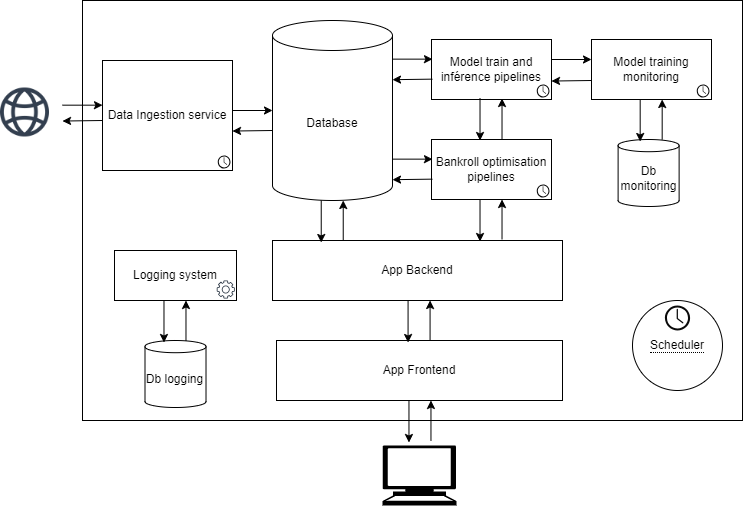
\includegraphics[width=0.8\textwidth, keepaspectratio]{images/Architecture_optimsportbet.png}
    \caption{Architecture of the system}
    \label{fig:elo_score_5_teams_during_time}
\end{figure}


\section{Data Collection}

Accurate and comprehensive data collection is vital for building reliable predictive models and effective betting strategies. The goal is to build an historical database which continues to build with real time relevant data.

\subsection{Data Sources Used}

We utilize a variety of reputable sources to gather data:

\begin{itemize}
    \item \textbf{Football Match Data}: Historical match results, match schedule, team statistics, player performance metrics, and other relevant information are sourced using scrapping on two websites: 
    \begin{itemize}
        \item \hyperlink{https://fbref.com/en/}{FBref}: For historical match results and coming match schedule.
        \item \hyperlink{https://sofifa.com/}{SoFifa}: For teams and players past and current ratings and statistics.
    \end{itemize}
    \item \textbf{Odds Data}: Betting odds are collected from multiple bookmakers through one API.
    \begin{itemize}
        \item \hyperlink{https://the-odds-api.com/}{The Odds API}: The free tier credits allows to perform 500 requests per month on various sports, bookmakers and leagues to retrieve the current odds. Historical odds data are not included.
    \end{itemize}
\end{itemize}


\subsection{Collection Methods}

Data is collected using a combination of methods:

\paragraph{Web Scraping}

A fork of the \hyperlink{https://soccerdata.readthedocs.io/en/latest/}{Soccerdata} python library, has been adapted to scrape data from websites that do not provide APIs (FBref, SoFifa). 

\paragraph{APIs}

For sources that offer APIs (The Odds API), we integrate with them using HTTP requests to fetch structured data efficiently.

\paragraph{Data Pre-processing}

Collected data undergoes a very simple pre-processing to ensure consistency and usability:

\begin{itemize}
    \item \textbf{Data type conversion}: Adapting the type of the data to the most adapted type.
    \item \textbf{Unity}: Only inserting new data in the database, or filling None values of existing data (for instance, the score of a match is only available after the match is played 
    \item \textbf{Integration}: Aligning data from different sources for seamless storage and analysis.
\end{itemize}

\section{Data Storage}

A robust data storage solution is essential for managing the diverse datasets involved.

\subsection{Database Choice}

We opted for a relational database management system (RDBMS), specifically \textit{PostgreSQL}, due to its reliability, scalability, and support for complex queries.

\subsection{Data Model}

The database schema is designed to reflect the relationships between different types of data:

\subsubsection{Tables}

\begin{itemize}
    \item `\textbf{fbref\_results}`: Each row corresponds to a match (historic and coming), with league, date and time of the match, both team and score if match is finished and the result is available and fetched from FBref website.
    \item `\textbf{sofifa\_teams\_stats}`: Each row corresponds to a a team and a date of update with metrics and categorical values that represent at best the team at the moment of the update (overall score, attack, build\_up\_speed ...).
    \item `\textbf{soccer\_odds}`: Each row corresponds to a match, a bookmaker, an outcome with its odd at a given update time. There is also information about the commence time of the match, the league, the home and away team names, the type of odd...
    \item `\textbf{models\_results}`: Each row corresponds to a match, the inference results of the model, the date-time of inference and the model used, with additional information such as the date and tile of the match and home and away team.
    \item `\textbf{optim\_results}`: Each row corresponds to a game, a date time of optimisation, the model used for inference, the best odds for each outcome found across a pool of bookmaker as well as the bookmakers names of each odds chose and the fraction of the bankroll to invest given utility function. There is additional information such as the probability inferred and used by the optimiser, the date-time of inference of these probabilities, the date and time of the match...
\end{itemize}


\begin{figure}[H]
    \centering
    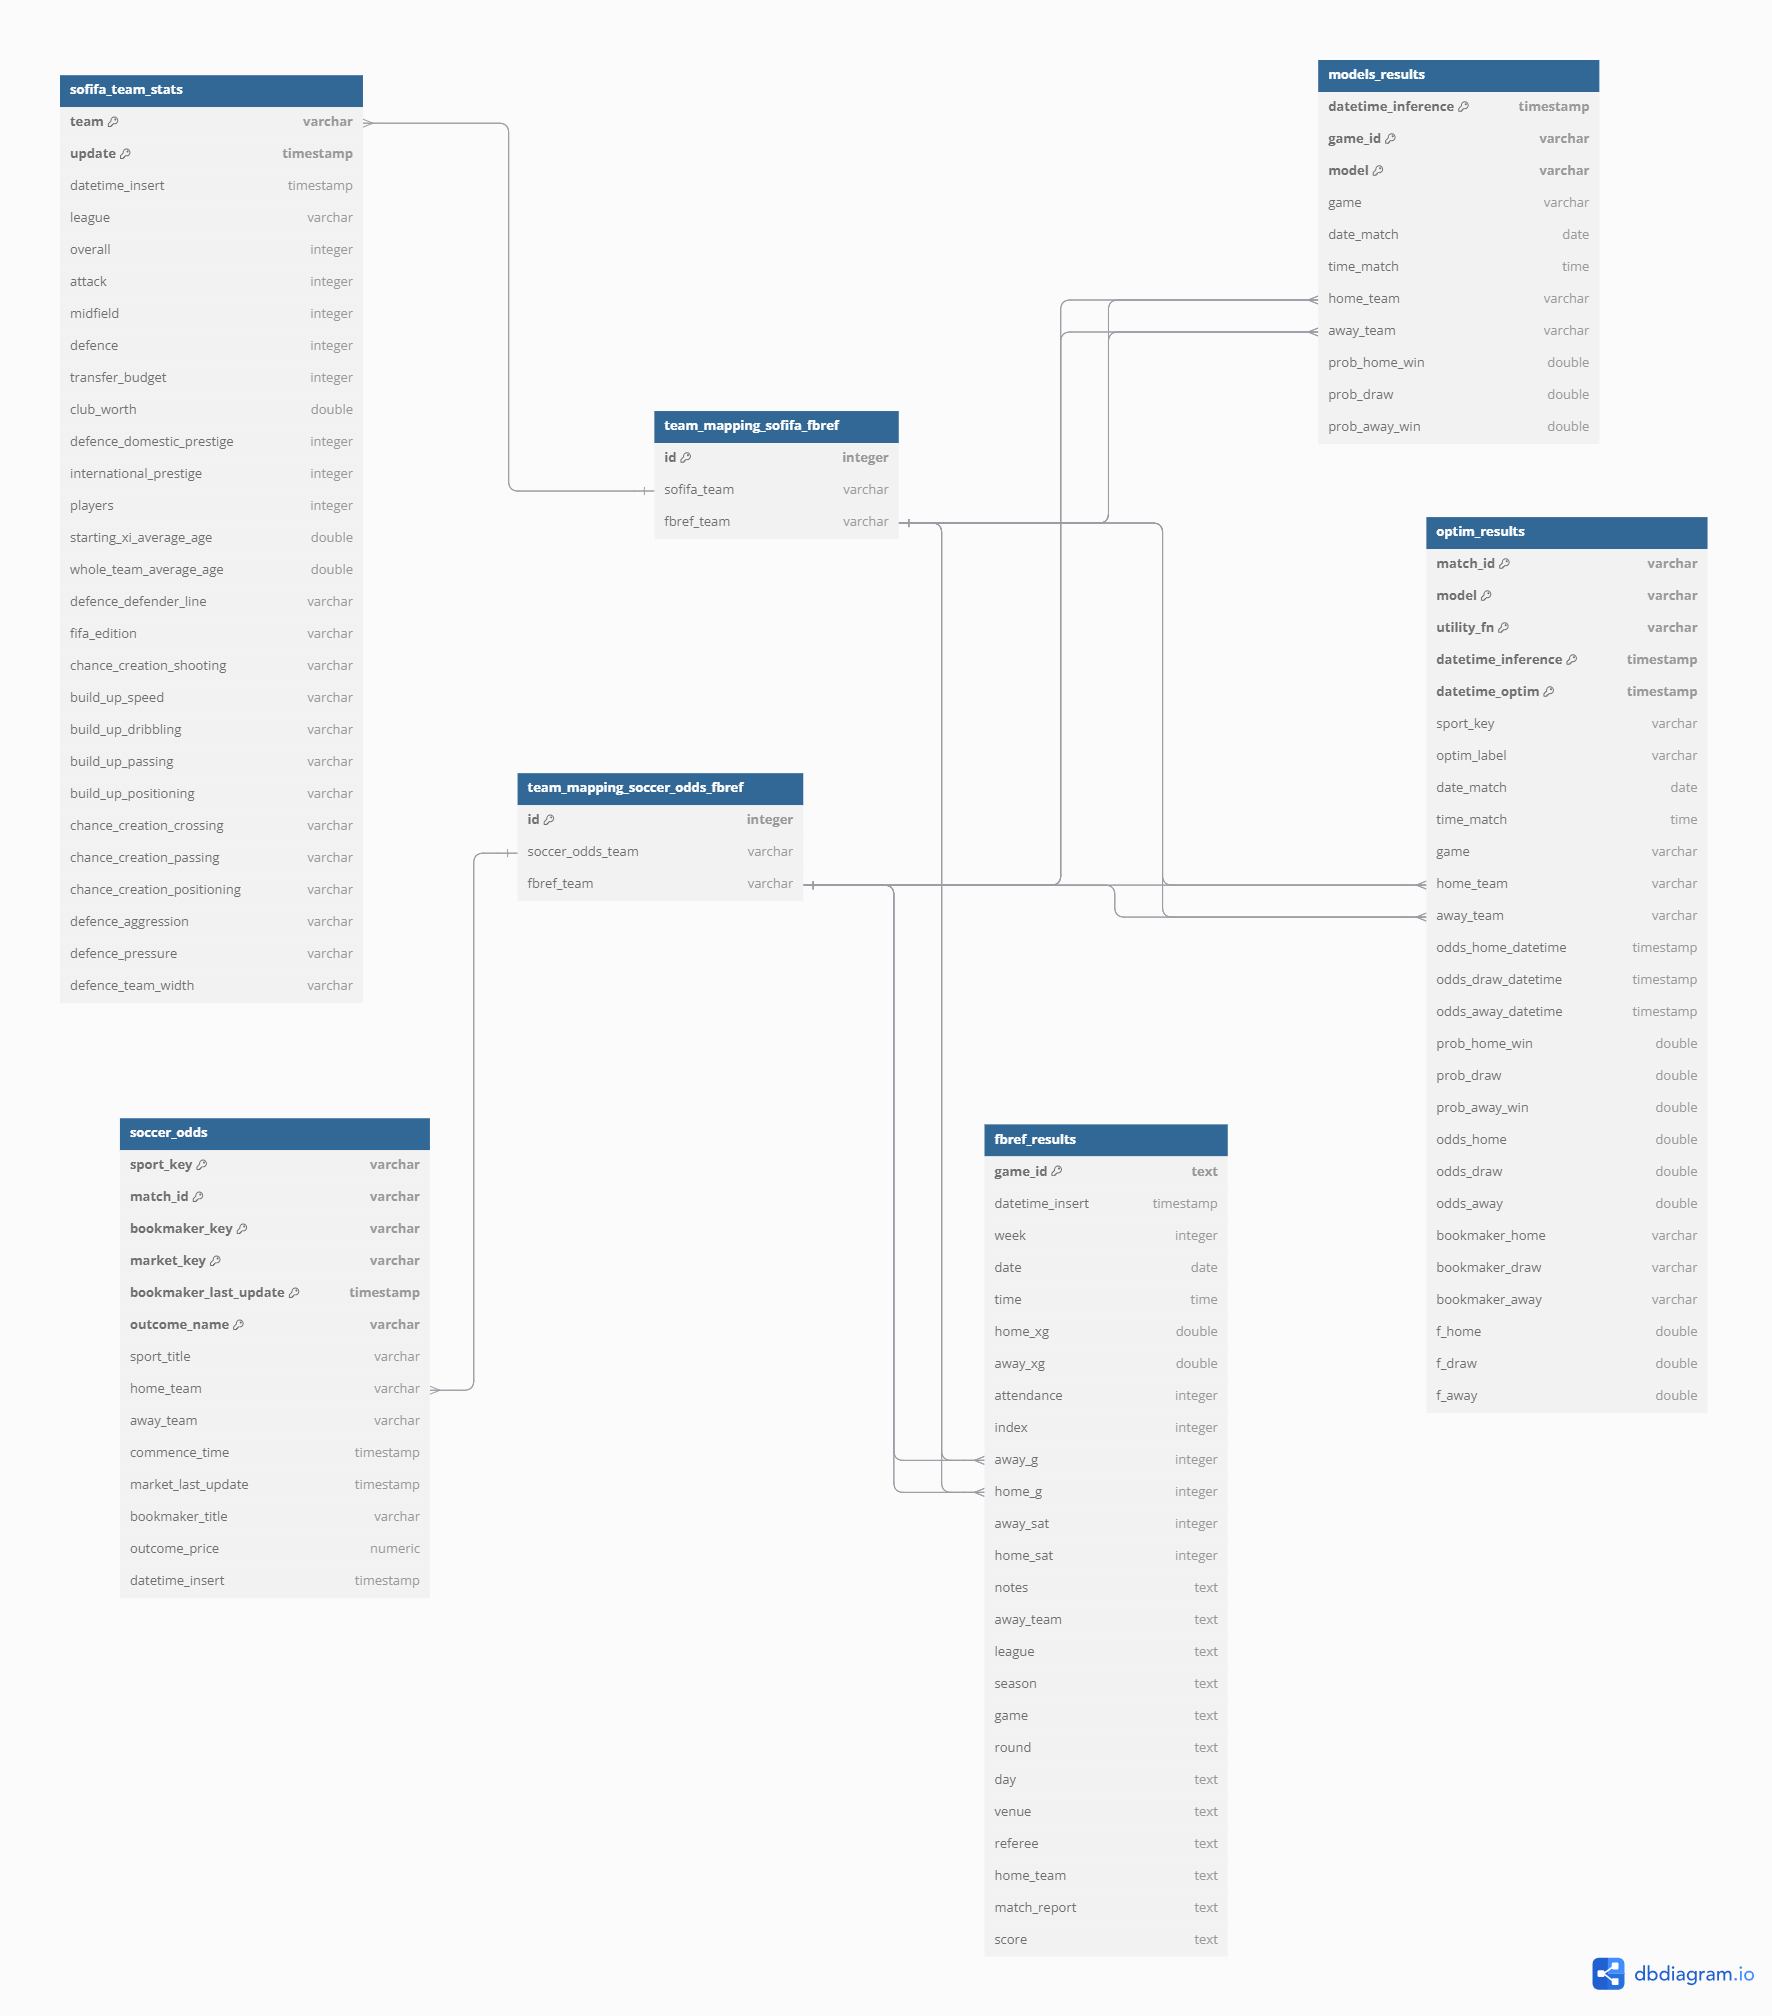
\includegraphics[width=0.8\textwidth, keepaspectratio]{images/db_uml.png}
    \caption{UML diagram of the database}
    \label{fig:uml_db}
\end{figure}

\section{Module Overview}

The system incorporates several modules, each performing specific functions within the overall architecture.

\subsection{Data Collection Module}

As described earlier, this module is responsible for fetching and pre-processing data from various sources.

\subsection{Prediction Module}

Although detailed discussion is deferred to a later chapter, this module uses machine learning algorithms to predict the probabilities of different match outcomes based on historical data.

\subsection{Optimization Module}

This module calculates optimal betting strategies by applying mathematical optimization techniques to the predictions and odds data. The specifics of the optimization algorithms and utility functions will be explored in a subsequent chapter.

\subsection{Scheduler}

The scheduler automates the execution of tasks such as data collection, model retraining, inference, and optimization. It ensures that the system remains up-to-date with the latest data and predictions.

\subsection{User Interface and Backend}

The user interface provides a platform for users to access data, view predictions, and interact with the system. The backend handles user requests, processes data, and communicates with other modules via APIs.

\section{User Interface and Monitoring}

\subsection{User Interface Design}

The UI is designed to be intuitive and user-friendly, providing clear visualizations and easy navigation.

\paragraph{Features}

\begin{itemize}
    \item \textbf{Dashboard}: Displays key metrics, including upcoming matches, predicted probabilities, and recommended betting strategies.
    \item \textbf{Historical Data Access}: Allows users to explore past matches, predictions, and outcomes.
    \item \textbf{Customization}: Users can select preferred bookmakers according to their interests.
\end{itemize}

\subsection{Monitoring}

System health and performance are monitored continuously:

\begin{itemize}
    \item \textbf{Logging}: Activity logs are maintained for debugging and audit purposes.
    \item \textbf{Alerts}: Notifications are sent in case of errors or significant events.
\end{itemize}


\section{Conclusion}

This chapter provided an overview of the system architecture implemented to realize the theoretical framework developed earlier. By focusing on football, we leverage abundant data to build predictive models and optimize betting strategies. The modular design, utilizing microservices and APIs,ensures scalability and flexibility. The database serves as the central repository, integrating data from various sources and supporting the different modules. The user interface offers a gateway for users to access the system's functionalities. In the subsequent chapters, we will delve into the specifics of the prediction and optimization modules, as well as the deployment strategy using Kubernetes and containerization technologies.

\section{Introduction}
\label{sec:chapter4_intro}

This chapter presents the development, training, and evaluation of a predictive model aimed at forecasting the outcomes of football matches. The primary objective is to construct a robust model that can accurately predict match results, thereby optimizing gains in sports betting \cite{BaioBlangiardo2010} \cite{DixonColes1997}. The significance of predictive modeling in the context of sports betting lies in its potential to provide bettors with a strategic advantage by identifying value bets and minimizing risks.

\section{Performance Metrics and Selection Criteria}
\label{sec:performance_metrics}

Evaluating the performance of a predictive model in a multi-class classification setting, especially with imbalanced classes, requires a comprehensive set of metrics. This section delineates both classic and advanced metrics employed in this study, incorporating mathematical formulations and addressing class imbalance. Given the three-class problem—home win, draw, and away win—with home wins constituting 47\% of the data, it is crucial to select metrics that provide a nuanced understanding of model performance across all classes.

\subsection{Metrics}
\label{subsec:classic_metrics}

A list of all the metrics considered with their used definition can  be found in Appendix \ref{appendix:predictive_model_metrics}.

\subsection{Selection Criteria}
\label{subsec:selection_criteria}

Accurate evaluation of the predictive model requires appropriate performance metrics, particularly in a multi-class classification context with class imbalance. The primary goal of this study is to ensure that the predicted probabilities of football match outcomes (home win, draw, away win) closely align with the true probabilities, emphasizing well-calibrated probability estimates.

Given the class distribution—47\% home wins, 26\% draws, and 25\% away wins—we have selected the \textbf{Mean Squared Error (MSE)} as the primary metric for assessing calibration. MSE directly measures the average squared difference between predicted probabilities and actual outcomes, making it suitable for evaluating how well the model's probabilities reflect the true frequencies.

In addition to MSE, we will consider the following metrics to provide a comprehensive evaluation:

\begin{itemize}
    \item \textbf{Log Loss}: To assess the quality of the predicted probability distributions by penalizing incorrect and overconfident predictions, thus encouraging well-calibrated estimates.
    \item \textbf{Classwise Expected Calibration Error (ECE)}: To evaluate the calibration of predicted probabilities for each class individually, offering insights into how closely these probabilities match the observed outcomes across different categories.
    \item \textbf{Accuracy for Home Win, Draw, and Away Win}: To examine the model's performance on each outcome separately, taking into account the class imbalance.
\end{itemize}

By focusing on MSE for calibration and incorporating Log Loss, Classwise ECE, and class-specific accuracy, we aim to ensure that the model not only produces accurate probability estimates but also maintains reliability across all outcome categories. This concise set of metrics aligns with our objective of accurately predicting football match outcomes while ensuring the predicted probabilities are well-calibrated and trustworthy.

\section{Exploration and Choice of Features}
\label{sec:feature_selection}

Selecting appropriate features is pivotal for building an effective predictive model. This section delineates the various types of features utilized in this study, the methodology employed for feature selection, the engineering of new features to enhance predictive power, and the handling of categorical variables to ensure they are appropriately represented in the model. 

\subsection{Types of Features Utilized}
\label{subsec:types_features}

The feature set comprises a combination of ranking-based, simple statistical, and domain-specific features. Each feature is defined mathematically where applicable and accompanied by an explanation of its relevance and computation.

\subsubsection{Ranking Features}
\label{subsubsec:ranking_features}

Ranking features provide a quantitative measure of team strength based on historical performance. These metrics are crucial as they encapsulate the overall ability and consistency of teams over time. All ranking features detailed formula are described in \ref{appendix:ranking_features}.

\begin{itemize}

\item \textbf{Elo Score}
\label{par:elo_score}

The \textbf{Elo score} \cite{Elo1978} \cite{HvattumArntzen2010} is a rating system originally developed for chess but widely adapted to various sports to rate players or teams. It reflects the relative skill levels of the teams based on game outcomes.

\begin{figure}[H]
    \centering
    \includegraphics[width=0.8\textwidth, keepaspectratio]{images/elo_score_5_teams_during_time.png}
    \caption{Elo score of 5 football teams evolving during time}
    \label{fig:elo_score_5_teams_during_time}
\end{figure}



\item \textbf{Glicko-2 Score}
\label{par:glicko2_score}

The \textbf{Glicko-2 score} \cite{Glickman1999} is an advanced rating system developed by Mark Glickman, which enhances the Elo rating system by incorporating not only the skill levels of teams or players (R) but also the reliability of these ratings through Rating Deviation (RD) and volatility. This system provides a more dynamic and accurate reflection of performance by accounting for the uncertainty and variability in teams' ratings.


\item \textbf{TrueSkill}
\label{par:trueskill}

The \textbf{TrueSkill} \cite{HerbrichEtAl2007} is a Bayesian ranking system developed by Microsoft, primarily used in gaming but adaptable to sports analytics. It models each team's skill as a Gaussian distribution, updating beliefs about team strengths based on match outcomes.

\end{itemize}

\subsubsection{Simple Statistical Features}


Simple statistical features offer basic quantitative measures of team performance, providing foundational data for the predictive model.


\begin{itemize}
    \item \textbf{Average Goals Scored per Season}: Total goals scored by a team divided by the number of matches played so far.
    
    \item \textbf{Average Goals Conceded per Season}: Total goals conceded by a team divided by the number of matches played so far.
\end{itemize}


\subsubsection{Sofifa Performance Metrics}

SoFIFA provides detailed metrics for both individual players and teams, based on data from the FIFA video game by EA Sports. This document outlines the primary metrics and explains how team ratings are calculated using individual player attributes.

\begin{itemize}

\item \textbf{Player Metrics}
    The primary player metrics on SoFIFA are based on individual attributes that are weighted differently depending on the player's position. Below are the key metrics:
    
    \begin{itemize}
        \item \textbf{Overall Rating (OVR)}: This is the weighted average of various player attributes, with different weights depending on the position. For example, an attacker (\textit{Forward}) will have more emphasis on \textit{Shooting} and \textit{Pace}, while a defender (\textit{Centre Back}) will weigh attributes like \textit{Defending} and \textit{Physicality} more heavily.
        \item \textbf{Pace (PAC)}: Calculated as a combination of the \textit{Acceleration} and \textit{Sprint Speed} attributes.
        \item \textbf{Shooting (SHO)}: Includes \textit{Finishing}, \textit{Shot Power}, \textit{Long Shots}, and \textit{Positioning}.
        \item \textbf{Passing (PAS)}: Comprised of \textit{Vision}, \textit{Short Passing}, and \textit{Long Passing}.
        \item \textbf{Dribbling (DRI)}: Includes \textit{Ball Control}, \textit{Dribbling}, \textit{Agility}, and \textit{Balance}.
        \item \textbf{Defending (DEF)}: Based on \textit{Tackling}, \textit{Marking}, \textit{Interceptions}, and \textit{Defensive Awareness}.
        \item \textbf{Physicality (PHY)}: Includes \textit{Strength}, \textit{Stamina}, and \textit{Aggression}.
        \item \textbf{Potential}: Indicates the maximum possible rating the player can achieve over time.
    \end{itemize}
    
    The formula for the Overall Rating (OVR) is generally unknown, but it can be expressed as a weighted sum of key attributes, depending on the player’s position. A simplified formula for a forward might look like:
    
    \[
    \text{OVR}_{\text{Forward}} = w_1 \cdot \text{PAC} + w_2 \cdot \text{SHO} + w_3 \cdot \text{DRI} + w_4 \cdot \text{PAS}
    \]
    
    where \( w_1, w_2, w_3, w_4 \) are position-specific weights.

\item \textbf{Team Metrics}
    Team metrics on SoFIFA are calculated by aggregating individual player ratings, focusing on key areas like attack, midfield, and defense. The following are the primary team metrics:
    
    \begin{itemize}
        \item \textbf{Overall Team Rating}: A weighted average of the starting 11 players' Overall Ratings, considering the importance of each player's position.
        \item \textbf{Attack Rating}: The average Overall Rating of forwards and attacking midfielders, weighted based on the formation.
        \item \textbf{Midfield Rating}: The average Overall Rating of central and wide midfielders, weighted based on their roles in the formation.
        \item \textbf{Defense Rating}: The average Overall Rating of defenders and goalkeepers.
    \end{itemize}
    
    A simplified version of the team rating could be expressed as:
    
    \[
    \text{Team OVR} = \frac{1}{11} \sum_{i=1}^{11} \text{OVR}_i
    \]
    
    where \( \text{OVR}_i \) represents the Overall Rating of the $i$-th player in the starting lineup.
    
    
    Sofifa metrics are comprehensive team-specific performance indicators sourced from the Sofifa database, widely used in sports analytics and fantasy football contexts.
\end{itemize}

\begin{figure}[H]
    \centering
    \includegraphics[width=\textwidth, keepaspectratio]{images/scores_5_teams_during_time.png}
    \caption{Different scores of 5 football teams evolving during time}
    \label{fig:scores_5_teams_during_time}
\end{figure}

A detailed description of each of the 90 features used can be found her \ref{appendix:all_feature_descriptions}.

\subsection{Feature Selection Methodology}
\label{subsec:feature_selection_methodology}

Feature selection was performed using a forward selection approach applied to a logistic regression model. This method iteratively adds the most significant features, enhancing predictive performance while maintaining model simplicity.

\subsubsection{Forward Selection with Logistic Regression}
\label{subsubsec:forward_selection_logistic_regression}

\textbf{Procedure}: Starting with no features, at each iteration, the feature that most improves the model's fit is added. The selection criterion is based on the mse (mean squared error).

\textbf{Explanation}: By incorporating features that significantly contribute to the model, forward selection optimizes predictive accuracy and ensures interpretability by excluding irrelevant variables.

\section{Data Preparation}

We trained our model on matches from 2006 to the present, focusing on games from the top 5 European leagues, European championships, and World Cups during this period. The limiting factor in our data came from SoFIFA, which does not provide data prior to 2006, while FBref offers data extending far into the past. We merged the two datasets based on team names and computed the ranking and statistical features described earlier, initializing the metrics at the first entry of a team in a tournament. For categorical features, we applied one-hot encoding. We removed matches with any missing values in the columns, then applied a standard scaler. This left us with 28,850 completed matches and a 90-feature vector for each match to train our model.

\begin{table}[h]
\centering
\begin{tabular}{|l|c|c|}
\hline
\textbf{Metric} & \textbf{Value} \\
\hline
Total matches & 28,850 \\
Matches in Top 5 Leagues & 28,481 \\
Matches in European Championships & 185 \\
Matches in World Cup & 184 \\
Home win ratio & 45.0 \% \\
Draw ratio & 25.4 \% \\
Away win ratio & 29.5 \% \\ 
Average home team goals & 1.54 \\
Average away team goals & 1.19 \\
Average Elo rating & 1558 \\
Number of unique teams & 242 \\
Number of features per match & 90 \\
First match date & 2006-09-09 \\
Last match date & 2024-09-24 \\
\hline
\end{tabular}
\caption{Summary Metrics for the Dataset}
\end{table}


\section{Cross-Validation on Temporal Data}
\label{sec:cross_validation_temporal}

In predictive modeling with football match data, which is inherently temporal, it's essential to use cross-validation techniques that respect the chronological order of observations. Standard cross-validation methods, such as random shuffling or traditional \( k \)-fold cross-validation, are unsuitable because they can lead to data leakage by training models on future data to predict past events.

Traditional cross-validation assumes that data samples are independent and identically distributed (i.i.d.) and that the order of observations does not matter. In temporal data, however, observations are time-dependent, and future events should not influence model training aimed at predicting past events. Using standard methods can result in:

\begin{itemize}
    \item \textbf{Data Leakage}: Incorporating future information into the training set leads to overly optimistic performance estimates.
    \item \textbf{Violation of Temporal Order}: Disrupting the sequence of events undermines the model's ability to generalize to real-world forecasting scenarios.
\end{itemize}


To address these issues, we employ cross-validation methods designed for temporal data \cite{BergmeirEtAl2018}.

\subsection{Sliding Window Cross-Validation}

This technique involves moving a fixed-size window across the data timeline. In each iteration, the model is trained on a training window and tested on the immediately following testing window.

\begin{itemize}
    \item Choose a training window size \( W_{\text{train}} \) and a testing window size \( W_{\text{test}} \).
    \item For each iteration:
    \begin{itemize}
        \item Train the model on data from time \( t \) to \( t + W_{\text{train}} - 1 \).
        \item Test the model on data from \( t + W_{\text{train}} \) to \( t + W_{\text{train}} + W_{\text{test}} - 1 \).
        \item Slide the window forward by \( W_{\text{test}} \) units.
    \end{itemize}
\end{itemize}

\subsection{Expanding Window Cross-Validation}

Also known as growing window, this method expands the training set with each iteration by including more historical data.

\begin{itemize}
    \item Start with an initial training window of size \( W_{\text{initial}} \).
    \item For each iteration:
    \begin{itemize}
        \item Train the model on data from time \( t \) to \( t + W_{\text{train}} - 1 \), where \( W_{\text{train}} \) increases with each iteration.
        \item Test on the subsequent data from \( t + W_{\text{train}} \) to \( t + W_{\text{train}} + W_{\text{test}} - 1 \).
        \item Expand the training window to include the latest testing window.
    \end{itemize}
\end{itemize}

\begin{figure}[H]
    \centering
    \begin{minipage}{0.45\textwidth}
        \centering
        \includegraphics[width=\textwidth, keepaspectratio]{images/FixedWindow.png}
        \caption{Sliding window graphic}
        \label{fig:sliding_window}
    \end{minipage}\hfill
    \begin{minipage}{0.45\textwidth}
        \centering
        \includegraphics[width=\textwidth, keepaspectratio]{images/ExpandingWindow.png}
        \caption{Expanding window graphic}
        \label{fig:expanding_window}
    \end{minipage}
\end{figure}


The results presented below were obtained using an expanding window technique with 5 folds and a test set ratio of 0.2. Notably, the results were very similar when applying the sliding window method.


\section{Choice and Justification of the Prediction Model}
\label{sec:model_choice}

In this section, we present the results of the feature selection and model selection processes \cite{GuyonElisseeff2003} \cite{ChandrashekarSahin2014}, followed by interpretations of the selected model's performance. Feature selection was conducted using forward selection, and multiple classification models were evaluated to determine the most suitable model for predicting football match outcomes.

\subsection{Feature Selection Using Forward Selection}
\label{subsec:feature_selection}

Feature selection was performed using forward selection with logistic regression, iteratively adding the most significant feature at each step based on mean squared error (MSE) improvement, using an expanding window validation with 5 splits and a test size of 20\% of the training data.

\begin{table}[H]
    \centering
    \caption{Feature Selection Process Summary}
    \label{tab:feature_selection_summary}
    \begin{tabular}{lc}
        \toprule
        \textbf{Method} & \textbf{Details} \\
        \midrule
        Feature Selection & Forward Selection \\
        Model Used & Logistic Regression \\
        Validation Method & Expanding Window (5 splits) \\
        Performance Metric & Mean Squared Error (MSE) \\
        Test Size & 20\% of training data \\
        \bottomrule
    \end{tabular}
\end{table}


We selected 35 features, which corresponding to the features resulting in the lowest MSE, using this feature selection strategy.

\begin{table}[H]
    \centering
    \caption{Feature Selection with Corresponding MSE and their adding number}
    \label{tab:feature_mse}
    \begin{tabular}{|c|l|c|c|l|c|}
        \hline
        \textbf{Order} & \textbf{Feature Added} & \textbf{MSE} & \textbf{Order} & \textbf{Feature Added} & \textbf{MSE} \\
        \hline
        1  & Elo Away & 0.20613 & 19 & Home Passing Risky & 0.19438 \\
        2  & Elo Home & 0.19661 & 20 & Away Positioning Org. & 0.19436 \\
        3  & Glicko Vol Away & 0.19619 & 21 & Away Defense Pressure Med & 0.19435 \\
        4  & Away Overall & 0.19594 & 22 & Away Domestic Prestige & 0.19434 \\
        5  & Home Overall & 0.19540 & 23 & Away Shooting Lots & 0.19433 \\
        6  & Away Build Speed Slow & 0.19518 & 24 & Home Defense Line Offside & 0.19432 \\
        7  & Away Avg Age & 0.19501 & 25 & Away Team Width & 0.19431 \\
        8  & Home League INT & 0.19487 & 26 & Home Defense Pressure Med & 0.19431 \\
        9  & Home Avg Goals & 0.19476 & 27 & Home Build Speed Slow & 0.19430 \\
        10 & Home Positioning Org. & 0.19467 & 28 & Away Defense Aggression & 0.19430 \\
        11 & Home Build Speed Fast & 0.19461 & 29 & TrueSkill Home & 0.19430 \\
        12 & Away Defense Pressure High & 0.19457 & 30 & Away Build Positioning Org. & 0.19430 \\
        13 & Away Defense Offside Trap & 0.19453 & 31 & Away Defense & 0.19430 \\
        14 & Home League ITA & 0.19449 & 32 & Home Attack & 0.19427 \\
        15 & Glicko RD Home & 0.19447 & 33 & Home Defense Prestige & 0.19427 \\
        16 & Home Shooting Normal & 0.19444 & 34 & Away Attack & 0.19427 \\
        17 & Away Passing Mixed & 0.19442 & 35 & Away League INT & \textbf{0.19427} \\
        18 & Away Avg Goals & 0.19440 & & \\
        \hline
    \end{tabular}
\end{table}

The table above summarizes the features added during the selection process and their corresponding MSE values, highlighting the importance of each feature as it contributes to minimizing the error. As we can see, features such as Elo ratings and overall team metrics play a significant role \cite{LasekEtAl2013}. Now, let's examine how the number of features impacts the performance metrics more broadly, as shown in the following feature selection graph.

\begin{figure}[H]
    \centering
    \includegraphics[width=\textwidth, keepaspectratio]{images/feature_selection_metrics_by_nb_of_features.png}
    \caption{Metrics of interrest function of the number of features added}
    \label{fig:feature_selection_metrics_by_nb_of_features}
\end{figure}

This graph shows the performance of various metrics (MSE, log loss, accuracy for home, draw, and away predictions, and classwise ECE) as a function of the number of selected features. The MSE (in blue) decreases as more features are added, stabilizing around the optimal point before increasing again, which suggests that selecting too many features can lead to overfitting. Similarly, log loss follows a similar trend (in red), indicating better model calibration with fewer features. The accuracy metrics (home, draw, away) fluctuate, but accuracy seems to peak at a certain range of features, with performance diminishing as more features are added. Classwise ECE (in pink) decreases and then increases, a little bit before MSE and log loss, indicating better calibration for class predictions with fewer features. Overall, the graph highlights the balance between feature selection and model performance, suggesting that an optimal subset of features yields the best generalization.

\subsection{Model Selection}
\label{subsec:model_selection}

The following table summarizes the performance of various classification models \cite{Bishop2006}, comparing metrics such as mean squared error (MSE), log loss, classwise ECE, and accuracy for home, draw, and away predictions to identify the best-performing model.

\begin{table}[H]
    \centering
    \caption{Model Performance Comparison}
    \label{tab:model_performance}
    \begin{tabular}{|l|c|c|c|c|c|c|}
        \hline
        \textbf{Model} & \textbf{MSE} & \textbf{Log Loss} & \textbf{C. ECE} & \textbf{A. Home} & \textbf{A. Draw} & \textbf{A. Away} \\
        \hline
        Logistic Regression & \textbf{0.195} & \textbf{0.983} & 0.029 & 0.605 & 0.733 & 0.702 \\
        Logistic Regression CV & 0.196 & 0.983 & \textbf{0.028} & 0.602 & \textbf{0.735} & 0.703 \\
        Gradient Boosting Classifier & 0.199 & 1.002 & 0.037 & 0.604 & 0.709 & \textbf{0.706} \\
        Random Forest Classifier & 0.202 & 1.022 & 0.038 & 0.595 & 0.705 & 0.693 \\
        Extra Trees Classifier & 0.204 & 1.026 & 0.043 & 0.597 & 0.683 & 0.686 \\
        AdaBoost Classifier & 0.221 & 1.092 & 0.069 & 0.599 & 0.721 & 0.695 \\
        Bagging Classifier & 0.224 & 2.471 & 0.093 & 0.602 & 0.646 & 0.661 \\
        MLP Classifier & 0.224 & 1.187 & 0.108 & 0.585 & 0.665 & 0.684 \\
        K Neighbors Classifier & 0.238 & 5.404 & 0.096 & 0.599 & 0.643 & 0.631 \\
        Gaussian NB & 0.332 & 7.570 & 0.302 & \textbf{0.615} & 0.584 & 0.625 \\
        Quadratic Discriminant Analysis & 0.353 & 10.831 & 0.316 & 0.582 & 0.561 & 0.613 \\
        Decision Tree Classifier & 0.390 & 20.219 & 0.195 & 0.578 & 0.614 & 0.638 \\
        Extra Tree Classifier & 0.399 & 20.686 & 0.200 & 0.559 & 0.615 & 0.628 \\
        \hline
    \end{tabular}
\end{table}


\subsection{Interpretation of Results}
\label{subsec:interpretation}

The selection of the logistic regression model allows for straightforward interpretation of feature effects on the predicted probabilities of match outcomes.

\subsubsection{Feature Importance}

Feature importance was assessed based on the magnitude of the coefficients in the logistic regression model. Below sits the feature importance of the Home win class. Draw and Away win classes analysis can be found in \ref{appendix:feature_importance}.


\begin{figure}[H]
    \centering
    \includegraphics[width=\textwidth, keepaspectratio]{images/top20_coeff_importance_lr_selected_features_home.png}
    \caption{Coefficients of the Logistic Regression Model for Home win class}
    \label{fig:feature_coefficients}
\end{figure}

For the home class, the most important features, such as Elo ratings for the away and home teams, suggest that pre-match team strength is the most significant predictor of match outcomes. Both overall team quality and specific defensive attributes, like pressure and aggression, also play a key role. Features related to player average characteristics, such as average age and tactical elements like build-up speed, indicate that team composition and playstyle are also relevant, though their impact is less pronounced. Defensive strategies, particularly pressure and team width, add further predictive value, showing the importance of tactical decisions in determining match results. The feature importance analysis graphs for draw and away class can be found in the annex section.


\subsubsection{Why Logistic Regression Outperforms Other Models}

Logistic regression may outperform other models due to its simplicity and interpretability, especially when feature selection is based on it. By using logistic regression for feature selection, the model is specifically tuned to highlight the most important predictors of the outcome, leading to better generalization. Additionally, logistic regression handles multicollinearity well when regularization is applied, preventing overfitting. The linear relationship between the features and the log-odds of the outcomes makes it easier to capture important patterns in the data, particularly in problems like sports prediction where relationships between variables are often linear. Other models, such as random forests or gradient boosting, may add unnecessary complexity and are more prone to overfitting when features are already well-selected.


\section{Training and Retraining of the Model}
\label{sec:training_retraining}

Figure \ref{fig:mse_retraining} illustrates the Mean Squared Error (MSE) of two models over time, where the blue line represents Model A with no retraining, and the orange line represents Model B, which is retrained daily. Both models are initialy trained from 2006-01-01 up to 2010-01-01 data and are evaluated using a 120-day rolling average.

\begin{figure}[H]
    \centering
    \includegraphics[width=0.8\textwidth, keepaspectratio]{images/model_ratrining_mse_120rd.png}
    \caption{Model MSE rolling average over time}
    \label{fig:mse_retraining}
\end{figure}


From the figure, we observe that Model B, which is frequently retrained, exhibits lower MSE compared to Model A throughout most of the time period. Retraining appears to allow Model B to adapt more effectively to evolving patterns, leading to consistently better performance in terms of accuracy. Moreover, as time goes by, we can observe a mse drift from the not retrained model as well as a slight improvement from the retrained model. \\

There are very few periods where Model A outperforms Model B. It appends especially during phases of sudden changes. Despite these fluctuations, retraining offers a more stable and improved long-term performance. \\

The results highlight the importance of regular retraining for maintaining model accuracy, particularly in dynamic environments where data patterns change over time.

\section{Conclusion}

This chapter presented the development, training, and evaluation of a predictive model for football match outcomes, with a focus on sports betting. Feature selection via forward selection with logistic regression helped identify key predictors, and regular retraining improved model performance over time.\\

However, several limitations remain:

\begin{itemize}
    \item \textbf{Hyperparameters and Features}: Ranking feature hyperparameters were left at default, and additional domain-specific or external data sources could further improve predictions.
    \item \textbf{Feature Selection}: Feature selection was arbitrarily based on logistic regression, and no hyperparameter optimization was performed for any models.
    \item \textbf{Retraining}: The timing and method of retraining (e.g., sliding window) were not explored, potentially missing optimal strategies as well as posing computational challenges that could be optimized.
    \item \textbf{Model Complexity}: Incorporating deep learning models could enhance predictive performance, particularly for capturing complex patterns in the data.
    \item \textbf{Bookmaker Odds Decorrelation}: Adding a metric to assess the decorrelation between model predictions and bookmaker odds could help identify more value bets and further optimize betting strategies.
\end{itemize}
In the next chapter, we address the optimization problem of determining the bankroll share to invest on each outcome, building on the predictions of this model to develop actionable betting strategies.

\section{Introduction}

Effective bankroll management is a critical component of successful sports betting. It involves determining the optimal amount to wager on each bet to maximize growth while minimizing the risk of ruin. This section details the development and evaluation of an optimization module designed to calculate the optimal fraction of the bankroll to invest in each betting opportunity. The module leverages probabilistic forecasts from the predictive models discussed in the previous section and applies various investment strategies, including the Kelly criterion, expected value maximization, and naive betting approaches.

\section{Methodology}
\subsection{Investment Strategies}

This section provides an overview of the different bankroll allocation strategies implemented, ranging from naive methods to more advanced optimization techniques. The focus is on the principles guiding each strategy, with a detailed formula provided only for the naive strategy.

\subsubsection{List of Strategies}

\begin{itemize}
    \item \textbf{Kelly Criterion Strategy}: \cite{Kelly1956} \cite{Thorp1969}  
    This strategy maximizes the logarithmic utility of wealth, aiming for long-term bankroll growth while managing risk. The bankroll fractions are derived from the analytical solution using the approximations  \ref{appendix:analytical_solution_using_the_kelly_criterion}, \(\mathbb{E}(U(B)) = \mathbb{E}(B) - \frac{1}{2} \cdot \mathbb{V}\text{ar}(B) \) which comes down to a Linear utility strategy using \( \lambda = \frac{1}{2} \).

    \item \textbf{Log Utility Strategy}:  
    Similar to the Kelly criterion, this strategy focuses on maximizing the expected logarithmic utility \(U(B) = \ln(B)\)  but using no approximations \ref{appendix:analytical_reduction_using_log_expected_utility}.

    \item \textbf{Exponential Utility Strategy}:  
    This strategy uses an exponential utility function \(U(B) = -e^{-\alpha B}\) to take into account the bettor’s risk aversion, balancing between expected returns and risk tolerance \ref{appendix:analytical_reduction_using_exp_expected_utility}.

    \item \textbf{Linear Utility Strategy}:
    In this strategy, the objective is to maximize the trade-off between expected returns and risk, represented by the function \(\mathbb{E}(U(B)) = \mathbb{E}(B) - \lambda \cdot \mathbb{V}\text{ar}(B) \). For the simulations, we set \( \lambda = 10 \), reflecting a high level of risk aversion. This approach seeks to maximize returns while penalizing high variance, aiming to balance growth and stability \ref{appendix:analytical_solution_using_linear_expected_utility}. 

    \item \textbf{Expected Value Maximization Strategy}:  
    This strategy optimizes bankroll allocation based purely on maximizing expected value, \(U(B) = B\), without considering risk or variance.

    \item \textbf{Naïve Strategy: Bet on the Most Likely Outcome}:  
    In this straightforward approach, the bettor places the entire bet on the outcome with the highest implied probability, as per the bookmaker's odds.
    
    The formula for this strategy is:
    \[
    f_{k,i} = 
    \begin{cases}
    \frac{1}{M}, & \text{if } i = \arg\max(o_k) \\
    0, & \text{otherwise}
    \end{cases}
    \]
    where:
    \begin{itemize}
        \item \( f_{k,i} \) is the fraction of the bankroll wagered on outcome \( i \) of match \( k \),
        \item \( o_k \) are the odds for match \( k \).
        \item \(M\) is the number of matches available.
    \end{itemize}
    This strategy is simple and allocates all the available funds to the outcome with the highest bookmaker odds.
\end{itemize}

These strategies were benchmarked against each other in the Monte Carlo simulations and then Online testing to assess their effectiveness in managing risk and maximizing bankroll growth. \\

For each strategy, a factor of \( \gamma = \frac{1}{2} \) was applied to the bet fractions to ensure that not the entire bankroll was wagered at any given time, thereby providing a margin of safety, such as: \(f_{strategy\_final} = \gamma \times f_{strategy}\).


\subsection{Optimization Algorithms}

Two optimization algorithms were employed to solve the bankroll allocation problem \cite{BoydVandenberghe2004}:

\begin{itemize}
    \item \textbf{Sequential Least Squares Programming (SLSQP):} An iterative method for constrained nonlinear optimization that is efficient for problems with a moderate number of variables.
    \item \textbf{Trust-Region Constrained Algorithm (trust-constr):} Suitable for large-scale optimization problems, it handles large numbers of variables and constraints effectively.
\end{itemize}

The choice between SLSQP and trust-constr depends on the number of betting opportunities (matches) considered at once. For a large number of matches, trust-constr is preferred due to its scalability.


\section{Monte Carlo Simulations}

To assess the performance of different investment strategies under simulated sports betting conditions, we conducted Monte Carlo simulations modeling the inherent uncertainties. The goal was to evaluate how various bankroll allocation strategies perform over numerous trials.

\subsection{Simulation Setup}

We simulated true match outcome probabilities \( r \) using a Dirichlet distribution appropriate for mutually exclusive and collectively exhaustive events:

\[
r_i^k = \text{Dirichlet}(\alpha), \quad \alpha = (1, 1, 1)
\]

To introduce discrepancies between true probabilities and those estimated by bookmakers (\( b \)) and players (\( t \)), we added biases and normally distributed noise:

\[
b_i^k = \text{clip}(r_i^k + \text{bias}_{\text{bookmaker}} + \epsilon_{\text{bookmaker}}, \ \text{min\_prob}, \ \text{max\_prob})
\]
\[
t_i^k = \text{clip}(r_i^k + \text{bias}_{\text{player}} + \epsilon_{\text{player}}, \ \text{min\_prob}, \ \text{max\_prob})
\]

where \( \epsilon_{\text{bookmaker}}, \epsilon_{\text{player}} \sim \mathcal{N}(0, \sigma^2) \). Probabilities were normalized to sum to one, and bookmaker probabilities included a margin \( \text{margin}_{\text{bookmaker}} \), clipping between \text{min\_prob} and \text{max\_prob}. Bookmaker odds were calculated as:

\[
o_i^k = \frac{b_i^k}{(\sum_{i=0}^N b_i^k) - \text{margin}_{\text{bookmaker}}}
\]

\subsection{Simulation Procedure}

The simulation followed a structured approach to evaluate the performance of different betting strategies, using predefined constants and a series of steps to simulate match outcomes and bankroll updates.

\begin{table}[H]
\centering
\caption{Simulation constants}
\label{tab:simulation constants}
\begin{minipage}{.2\linewidth}
\centering
\begin{tabular}{lr}
\toprule
\textbf{Constant} & \textbf{Value}\\
\midrule
H & 30 \\
T & 50 \\
N & 3 \\
\(\text{min\_prob}\) & 0.05 \\
\(\text{max\_prob}\) & 0.95 \\
\bottomrule
\end{tabular}
\end{minipage}%
\hspace{0.05\linewidth}
\begin{minipage}{.45\linewidth}
\centering
\begin{tabular}{lrr}
\toprule
\textbf{Constant} & \textbf{Bettor} & \textbf{Bookmaker}\\
\midrule
\text{bias} & 0 & 0 \\
\(\sigma\) (for noise \(\epsilon)\) & 0.1 & 0.1 \\
\text{margin} &  & 0.1 \\
\bottomrule
\end{tabular}
\end{minipage}
\end{table}

\begin{enumerate}
    \item Generated true probabilities \( r \) using \(\text{bias} = 0\) and \(\epsilon = 0.1\) for both bettor and bookmaker.
    \item Computed bookmaker and player estimates \( b \) and \( t \).
    \item Calculated bookmaker odds \( o \).
    \item For each strategy:
    \begin{itemize}
        \item Determined bet sizes using \( t \) and \( o \) by performing optimisation using \texttt{truct\_constr} algorithm.
        \item Simulated match outcomes based on \( r \).
        \item Updated bankrolls accordingly.
    \end{itemize}
\end{enumerate}

\subsection{Evaluation Metrics}

Strategies were evaluated using:

\begin{itemize}
    \item \textbf{Final Bankroll Statistics}: Mean, standard deviation, median, minimum, and maximum.
    \item \textbf{Average Growth Rate}: Geometric mean per time step. 
    \[GGR = \left( \frac{B(n)}{B(0)} \right)^{\frac{1}{n}} - 1\]

    \item \textbf{Sharpe Ratio}: Risk-adjusted return.

    \[\text{Sharpe Ratio} = \frac{\frac{1}{n} \sum_{t=1}^{n} R(t)}{\mathbb{V}ar(R(t))}) \text{   with   } R(t) = \frac{B(t+1) - B(t)}{B(t)}\]
    
    \item \textbf{Probability of Ruin}: Frequency of bankroll falling below a threshold.
\end{itemize}

\subsection{Results}

\begin{figure}[H]
    \centering
    \includegraphics[width=1.1\textwidth, keepaspectratio]{images/monte_carlo_b=b.png}
    \caption{Monte carlo simulations for each strategy}
    \label{fig:monte_carlo}
\end{figure}


\begin{table}[H]
\centering
\caption{Final Bankroll Statistics}
\label{tab:final_bankroll}
\begin{tabular}{lrrrrr}
\toprule
\textbf{Strategy} & \textbf{Mean} & \textbf{Std Dev} & \textbf{Median} & \textbf{Min} & \textbf{Max} \\
\midrule
Kelly Criterion          & 4.48   & 1.67   & 4.77   & 0.54   & 7.54   \\
Log Utility              & 270.85 & 983.14 & 15.39  & 0.19   & 5414.01 \\
Exponential Utility      & 7.46   & 3.46   & 8.10   & 0.00   & 13.48  \\
Linear Utility           & 1.35   & 0.16   & 1.37   & 1.03   & 1.61   \\
Expected Value           & 0.00   & 0.00   & 0.00   & 0.00   & 0.01   \\
Naïve Strategy           & 1.20   & 3.20   & 0.47   & 0.06   & 18.19  \\
\bottomrule
\end{tabular}
\end{table}

The \textbf{Log Utility} strategy achieved the highest mean final bankroll but with significant variability, indicating high risk. The \textbf{Kelly Criterion} and \textbf{Exponential Utility} strategies demonstrated moderate returns with lower variability, suggesting consistent performance.

\begin{table}[H]
\centering
\caption{Average Growth Rate Per Step}
\label{tab:avg_growth}
\begin{tabular}{lr}
\toprule
\textbf{Strategy} & \textbf{Growth Rate} \\
\midrule
Kelly Criterion          & 2.82\% \\
Log Utility              & 5.54\% \\
Exponential Utility      & 2.55\% \\
Linear Utility           & 0.59\% \\
Expected Value           & $-$29.83\% \\
Naïve Strategy           & $-$1.55\% \\
\bottomrule
\end{tabular}
\end{table}

While the \textbf{Log Utility} strategy had the highest growth rate, it came with increased volatility. The \textbf{Kelly Criterion} and \textbf{Exponential Utility} strategies offered positive growth with better risk control.

\begin{table}[H]
\centering
\caption{Sharpe Ratio}
\label{tab:sharpe_ratio}
\begin{tabular}{lr}
\toprule
\textbf{Strategy} & \textbf{Sharpe Ratio} \\
\midrule
Kelly Criterion          & 0.30 \\
Log Utility              & 0.29 \\
Exponential Utility      & 0.25 \\
Linear Utility           & 0.30 \\
Expected Value           & 0.14 \\
Naïve Strategy           & 0.01 \\
\bottomrule
\end{tabular}
\end{table}

The highest Sharpe Ratios were achieved by the \textbf{Kelly Criterion} and \textbf{Linear Utility} strategies, indicating superior risk-adjusted returns.

\begin{table}[H]
\centering
\caption{Probability of Ruin}
\label{tab:prob_ruin}
\begin{tabular}{lr}
\toprule
\textbf{Strategy} & \textbf{Probability} \\
\midrule
Kelly Criterion          & 0.00\% \\
Log Utility              & 3.33\% \\
Exponential Utility      & 6.67\% \\
Linear Utility           & 0.00\% \\
Expected Value           & 100.00\% \\
Naïve Strategy           & 20.00\% \\
\bottomrule
\end{tabular}
\end{table}

Zero probability of ruin for the \textbf{Kelly Criterion} and \textbf{Linear Utility} strategies underscores their robustness.

An ANOVA test (performed to assess whether the differences in final bankrolls among the strategies), (F-statistic: 2.16, p-value: 0.0612) suggested that differences among strategies were not statistically significant at the 5\% level. However, the p-value is close to the threshold, suggesting that with a larger sample size, the differences might become statistically significant.

\subsection{Conclusion}

The simulations indicate that strategies like the \textbf{Kelly Criterion} and \textbf{Exponential Utility}, which balance growth and risk through utility maximization, offer favorable outcomes. The \textbf{Log Utility} strategy provides high growth potential but with greater volatility. Ignoring risk, as in the \textbf{Expected Value} strategy, leads to poor performance.

\textbf{Limitations} include the limited number of simulations, simplified assumptions, and exclusion of real-world factors like transaction costs.

\textbf{Recommendations} for future work involve increasing simulation runs, incorporating realistic market conditions, and exploring additional strategies.


\section{Online Testing}

To assess the strategies in a real-world environment, an online testing phase was conducted over five weeks, from 2024 August 24th to 2024 September 30th, focusing on matches from the five major European football leagues. This real-world testing evaluated the practical applicability and performance of the strategies under actual market conditions. Odds were scraped each day at 12pm from the Odd Api website.


\subsection{Static Problem Reduction and Parameter Settings}

To simplify the dynamic nature of sports betting, we reduced the problem to a series of static optimizations at discrete time intervals. At each decision point \( t \), bankroll allocation was optimized based on the current available information. This approach allowed us to manage the complexity of real-time betting while ensuring the practical applicability of the strategies.

\paragraph{Temporal Parameters}

Key temporal parameters were defined as follows:

\begin{itemize}
    \item \textbf{Betting Interval (\( \Delta t \))}: The interval between placing bets, set to 24 hours to capture daily betting opportunities.
    \item \textbf{Bet Placement Timing}: Bets were placed at a fixed time each day (12:00 PM) to ensure up-to-date information was used while accommodating market dynamics.
\end{itemize}

These settings ensured a balance between information accuracy and practical market conditions.

\paragraph{Match Selection}

The matches selected for each optimization were determined based on:

\begin{itemize}
    \item \textbf{Number of Matches (\( M \))}: Matches occurring within the next 24 hours were selected, balancing opportunity and reliability of information as well as having all results while perfomring next step.
    \item \textbf{Selection Criteria}: Focus was given to matches from top European leagues where the bettor had a higher perceived edge.
\end{itemize}

This careful match selection helped reduce computational complexity while enhancing potential returns.

\paragraph{Re-Betting Policy}

The re-betting policy was defined by the following criteria:

\begin{itemize}
    \item \textbf{Not allowing Re-Bets}: Additional bets on previously considered matches were not allowed. As we only bet on matches on the same day and only once a day, this was an implication of the previous choices.
\end{itemize}

This policy helped manage risk and adapt to evolving market conditions.

\subsection{Practical Implementation Settings}

The practical implementation settings for the online testing phase are summarized in Table~\ref{tab:implementation_settings}. The testing period ran from August 24, 2024, to September 30, 2024. The \texttt{trust-constr} algorithm was used for optimization, with a multiplier of \( \gamma = \frac{1}{2} \) applied to the matrix \( f \). The best odds from a pool of bookmakers (detailed in the appendix) were selected for each match.

\begin{table}[H]
\centering
\caption{Practical Implementation Settings}
\label{tab:implementation_settings}
\begin{tabular}{ll}
\toprule
\textbf{Setting}               & \textbf{Value}                                 \\ \midrule
Betting Interval (\( \Delta t \))     & 24 hours \\                                    
Bet Placement Time               & 12:00 PM daily                                \\
Look-Ahead Horizon               & Matches within the next 24 hours               \\ 
Re-Betting Policy                & Not allowed \\ 
Testing Period                   & August 24, 2024 – September 30, 2024           \\ 
Optimization Algorithm           & \texttt{trust-constr}                          \\ 
Strategy factor mult. \(\gamma\)         & \( 0.5 \)                              \\ 
Odds Selection                   & Biggest odds from a pool of bookmakers            \\ 
Markets & 5 biggest European leagues (Big 5) \\
\bottomrule
\end{tabular}
\end{table}


\subsection{Results and Interpretation}

Figure~\ref{fig:capital_evolution} illustrates the capital evolution for each strategy during the testing period. The Kelly and Exponential Utility strategies exhibited the strongest performance, both ending with approximately twice the initial capital. These results highlight their ability to optimally balance risk and reward, consistently outperforming the more conservative Log and Naive strategies. However, they also demonstrated higher volatility compared to the more stable Linear strategy.

\begin{figure}[H]
    \centering
    \includegraphics[width=\textwidth]{images/bankroll_evolution2.png}
    \caption{Capital Evolution for Each Strategy During the Online Testing Period}
    \label{fig:capital_evolution}
\end{figure}

The Log Utility strategy underperformed, particularly at the start and after the midpoint of the test period, failing to capitalize on high-return opportunities. Its conservative nature, aimed at minimizing risk, resulted in modest growth but ultimately led to a negative outcome. 

Both the Naive and Expected Value strategies experienced sharp declines in capital. The Naive strategy approached near-zero capital by the end of the test, while the Expected Value strategy exhibited extreme volatility, leading to rapid capital depletion. These simpler strategies, which lack sophisticated optimization, were highly vulnerable to adverse market conditions and failed to adapt effectively to fluctuations in odds or match outcomes.

In contrast, the Linear Utility strategy showed steady and consistent growth, with minimal volatility throughout the testing period, ultimately achieving a final growth of 1.8 times the initial capital. This highlights its effectiveness in maintaining a stable growth trajectory while avoiding the excessive risk associated with other strategies.

Overall, the results underscore the superiority of more advanced utility-based strategies such as Kelly and Linear. These approaches consistently outperformed simpler methods by balancing risk and reward more effectively under real-world betting conditions.

\subsection{Performance Metrics}

To further quantify the performance of each strategy, we computed key metrics, including final bankroll \( B(T) \), mean growth per step, and standard deviation of growth per step, both in absolute terms and as a percentage of the final bankroll. 
\begin{itemize}
    \item The mean growth per step is defined as:
    \[
    \mu = \frac{1}{T-1} \sum_{t=1}^{T-1} \Delta B_t
    \]
    where \( \Delta B_t = B_{t+1} - B_t \),
    \item the standard deviation of growth per step is given by:
    \[
    \sigma = \sqrt{\frac{1}{T-1} \sum_{t=1}^{T-1} (\Delta B_t - \mu)^2}
    \]
\end{itemize}


Table~\ref{tab:strategy_performance} summarizes the results for each strategy.

\begin{table}[H]
\centering
\caption{Strategy Performance Metrics}
\label{tab:strategy_performance}
\begin{tabular}{llll}
\toprule
\textbf{Strategy}              & \textbf{Final Bankroll \( B(T) \)} & \textbf{Mean Growth (\%)} & \textbf{Std Growth (\%)} \\ 
\midrule
Kelly Criterion                & 2.034                              & 2.034                      & 8.923                    \\ 
Log Utility                    & 0.653                              & -2.129                     & 26.516                   \\ 
Exponential Utility (\( \alpha = 1 \)) & 1.892                        & 1.886                      & 10.309                   \\ 
Linear Utility (\( \lambda = 10 \))    & 1.798                        & 1.776                      & 5.360                    \\ 
Naive Strategy                 & 0.141                              & -24.299                    & 52.419                   \\ 
Expected Value                 & 0.001                              & -5032.448                  & 18175.649                \\
\bottomrule
\end{tabular}
\end{table}

\subsection{Interpretation of Metrics}

The results demonstrate the effectiveness of the Kelly Criterion and Exponential Utility strategies, both of which ended with a final bankroll close to 2.0. These strategies also displayed reasonable volatility, with standard deviations of growth per step under 10\%. The Linear Utility strategy performed consistently, achieving steady growth with the lowest volatility among all strategies.

On the other hand, the Log Utility strategy suffered from negative growth, highlighting its inability to capitalize on high-return opportunities. The Naive and Expected Value strategies performed poorly, with significant capital depletion and extreme volatility, particularly for the Expected Value approach, indicating their inadequacy in real-world betting scenarios.


\section{Conclusion}

The results from both the Monte Carlo simulations and the real-world online testing phase demonstrate the clear advantages of sophisticated bankroll management strategies such as the Kelly Criterion and Exponential Utility methods. These strategies consistently provided strong returns while managing risk effectively, leading to a final bankroll close to twice the initial amount. In contrast, simpler strategies like the Naive and Expected Value approaches underperformed, suffering from capital depletion and high volatility, emphasizing the importance of balancing risk and return in real-world betting scenarios.

The Linear Utility strategy offered a steady, reliable growth trajectory with minimal volatility, making it an appealing option for risk-averse bettors. The Log Utility strategy, though conservative, failed to capture sufficient growth opportunities, resulting in a negative final outcome. Overall, the Kelly and Exponential Utility strategies are best suited for bettors seeking long-term growth with manageable risk.

\subsection{Limitations and Future Improvements}

Despite the promising results, several limitations were identified in the current approach:

\begin{itemize}
    \item \textbf{Simulation Assumptions}: The Monte Carlo simulations relied on several simplifying assumptions that limit the realism of the results. Firstly, the simulation of probabilities was based on the true clipped probabilities plus a bias and Gaussian noise, which does not fully capture the actual flaws in the predictive models, and the constants used were chosen arbitrarily without strong justification. Secondly, the bookmaker margin was fixed, and the odds provided by the bookmaker did not account for the influence of large bets from the players, which in reality could cause deviations in the bookmaker’s odds and probabilities. Lastly, the simulations used a fixed number of matches and time steps. Both the number of simulations and the range of strategies could be expanded to provide a more thorough and diverse analysis of performance over a wider variety of scenarios.
    \item \textbf{Limited Testing Period}: The online testing phase covered only a five-week period, which may not fully capture the long-term performance and robustness of each strategy. Extending the testing period or repeating it across multiple seasons would provide a more comprehensive assessment.
    \item \textbf{Risk Preferences}: While the utility-based strategies successfully managed risk, the models relied on fixed parameters for risk aversion (e.g., \( \lambda \) in Linear Utility). Introducing dynamic adjustments to these parameters based on market conditions or bettor preferences could further enhance performance.
\end{itemize}

\subsection{Future Work and Deployment on Azure Kubernetes}

The next stage of this project involves deploying the entire system on a cloud infrastructure using Kubernetes on Azure (AKS). This deployment will enable scalable, real-time processing of betting opportunities, continuous model updates, and the handling of multiple simultaneous users and markets. By leveraging Azure’s powerful compute and orchestration capabilities, the system will be capable of efficiently managing the computational load and data flows needed for real-time sports betting optimization.


\section{Microservices Architecture and Frameworks}

To build a scalable and maintainable system for sports betting optimization, we adopted a microservices architecture. This approach allows independent development, deployment, and scaling of individual components, facilitating modularity and flexibility.

The system comprises several microservices:

\begin{itemize}
    \item \textbf{Data Ingestion Service}: Collects real-time match data and odds from external APIs and web scraping. We use the Python library \textit{soccerdata} to conveniently scrape historical and real-time data from various websites. \textit{SQLAlchemy} is employed to communicate with the PostgreSQL database, allowing interaction using a mix of Python syntax and SQL queries. An API is provided for other services to trigger this service's logic, created using the \textit{FastAPI} framework. The Python library \texttt{logging} is used for proper logging of all operations, and \texttt{pandas} is utilized for data manipulation and transformation.

    \item \textbf{Prediction and Optimization Service}: Processes data to train models and generate probability estimates for the prediction component. Calculates optimal bet allocations based on the probabilities and selected strategies for the optimization component. \textit{Scikit-learn} is used for model training and inference, while \textit{SciPy.optimize} handles the optimization processes. Similar to the Data Ingestion Service, an API is deployed using \textit{FastAPI}, with communication to the database via \textit{SQLAlchemy}, and \texttt{logging} and \texttt{pandas} for logging and data handling.

    \item \textbf{User Interface Service}: Provides a web-based dashboard for monitoring and interaction, developed using the Python web framework \textit{Streamlit}.

    \item \textbf{Backend Service}: Manages communication and logic between the frontend User Interface and the database, as well as other services, using \textit{FastAPI}, \texttt{pandas}, and \texttt{logging}.

    \item \textbf{Database Service}: Stores historical data, odds, inferred probabilities, optimization results, and transaction logs. We chose PostgreSQL as the database due to its robustness, scalability, and compatibility with \textit{SQLAlchemy}. PostgreSQL's advanced features support complex queries and transactions essential for our application's needs.

    \item \textbf{MLflow Service}: Monitors the training metrics of the models. MLflow provides a convenient way to track experiments, record model parameters, metrics, and artifacts, facilitating reproducibility and model versioning.

    \item \textbf{Airflow Service}: Acts as a scheduler, providing a convenient way to orchestrate and monitor complex workflows using Directed Acyclic Graphs (DAGs). Apache Airflow allows us to define data pipelines, schedule tasks, and manage dependencies between them, ensuring timely execution of data ingestion, model training, and optimization processes.
\end{itemize}

Services communicate over HTTP/HTTPS protocols, with well-defined API endpoints ensuring loose coupling and ease of integration.

\section{Docker and Kubernetes}

To ensure consistency across development, testing, and production environments, all microservices are containerized using Docker \cite{Merkel2014}. Docker allows us to package each service with all its dependencies into isolated containers, ensuring consistent behavior across different environments.

\subsection{Dockerization}

Each microservice is encapsulated in a Docker container, defined by its own \texttt{Dockerfile}, which specifies the base image, dependencies, and entry points. In local development, we used containers for services such as MLflow, PostgreSQL, and Airflow, facilitating a consistent and reproducible environment.

\subsection{Kubernetes Deployment}

For orchestration and management of the containerized applications, we utilized Kubernetes \cite{HightowerEtAl2017}. Kubernetes automates deployment, scaling, and management of containerized applications. We packaged our system into a Helm chart, which simplifies the deployment of the entire application, including dependencies like MLflow, PostgreSQL, and Airflow.

\subsubsection{Helm Chart Packaging}

By encapsulating our services and their dependencies into a Helm chart, we streamlined the deployment process. Helm charts define, install, and upgrade complex Kubernetes applications, allowing us to manage configurations and versioning efficiently.

\subsubsection{Database Migrations}

Database schema changes are managed using migration files and scripts. Changes are first applied locally for testing and validation. Once validated, migrations are executed on the production database using scripts designed to apply changes incrementally. This process ensures that the database schema remains synchronized with the application code without disrupting ongoing operations.

\section{Deployment on Azure AKS}

\subsection{Azure Kubernetes Service (AKS)}

We deployed our Kubernetes cluster on Microsoft Azure using Azure Kubernetes Service (AKS), a managed Kubernetes service that simplifies cluster management by handling critical tasks like health monitoring and maintenance. AKS reduces the operational overhead and provides features like automated scaling and updates.

\begin{figure}[H]
    \centering
    \includegraphics[width=0.8\textwidth, keepaspectratio]{images/diagrem_archi_services.png}
    \caption{Architecture of the system deployed on AKS}
    \label{fig:diagramme_arch_aks}
\end{figure}

\subsection{Infrastructure Details}

Our AKS deployment utilizes two virtual machines to ensure high availability and load balancing across the cluster. While Azure offers its own virtual machines, in this context, we refer to the compute resources allocated to our Kubernetes nodes. The integration with AKS allows for efficient resource utilization and scalability.

\subsection{Azure Services Integration}

Using Azure's cloud infrastructure offers several benefits:

\begin{itemize}
    \item \textbf{Azure Container Registry (ACR)}: Stores our Docker images securely, facilitating seamless deployment to AKS.
    \item \textbf{Azure DevOps Repo}: Provides a storage for our code.
\end{itemize}

\subsection{Pricing Considerations}

Azure's pricing model charges for compute resources used by virtual machines, storage, and network bandwidth. Managed services like AKS can reduce operational overhead but require careful monitoring to manage costs effectively. We optimized resource allocation by:


\section{Conclusion}

By adopting a microservices architecture, containerization with Docker, orchestration with Kubernetes, and deploying on Azure AKS, we built a scalable, reliable, and maintainable system for sports betting optimization. This architecture allows for independent development and deployment of components, ensuring the system can adapt to changing requirements and handle real-time data processing demands efficiently. Leveraging cloud infrastructure and managed services enhances our ability to focus on core application development while ensuring high availability and performance.

\section{Summary of Findings}

This study embarked on the ambitious task of developing a comprehensive system for optimizing sports betting strategies, focusing on football matches. Through the integration of predictive modeling, utility-based optimization, and scalable system architecture, we have addressed the critical components necessary for successful sports betting.

The predictive model, developed using logistic regression and advanced feature selection techniques, demonstrated significant accuracy in forecasting match outcomes. Regular retraining of the model proved essential in maintaining performance over time, highlighting the dynamic nature of sports data.

The optimization module applied various bankroll allocation strategies, including the Kelly Criterion, logarithmic, exponential, and linear utility functions. Both Monte Carlo simulations and real-world online testing over a five-week period indicated that sophisticated utility-based strategies substantially outperform naive betting approaches. Strategies like the Kelly Criterion and Exponential Utility provided favorable returns while effectively managing risk.

The system's deployment on Azure Kubernetes Service (AKS) showcased its scalability and readiness for real-time application. By leveraging a microservices architecture and containerization technologies like Docker and Kubernetes, the system can handle the computational demands of real-time data processing and optimization.

\section{Contributions to the Field}

This work contributes to the field of sports analytics and betting strategies in several ways:

\begin{itemize} \item \textbf{Integration of Predictive Modeling and Optimization}: By combining accurate probability estimations with utility-based optimization strategies, the system provides a robust framework for sports betting. \item \textbf{Scalable System Architecture}: The implementation of a microservices architecture and deployment on cloud infrastructure ensures that the system is scalable, maintainable, and adaptable to real-world conditions. \item \textbf{Empirical Evaluation}: The use of both simulations and real-world testing provides empirical evidence of the effectiveness of advanced betting strategies over simpler methods. \end{itemize}

\section{Limitations}

Despite the positive results, several limitations were identified:

\begin{itemize}
    \item \textbf{Predictive Model Enhancements}: While the current model performs adequately within the constraints of a static framework, it could be significantly improved by incorporating additional features, conducting hyperparameter optimization, and exploring more complex models such as deep learning architectures. These enhancements would allow the model to capture dynamic patterns and temporal dependencies inherent in football matches, which are not fully addressed due to the static nature of the current framework.

    \item \textbf{Static Framework Limitations and Long-Term Gain-Variance Interpretation}: The reduction of the betting problem to a static framework simplifies the optimization process but introduces limitations in interpreting gains and variance over the long term. Since the model does not account for intertemporal dependencies and the evolving nature of the bankroll, the strategies derived may not fully capture the risks associated with long-term betting. This static approach may lead to strategies that optimize short-term gains without adequately considering the cumulative effect on wealth over time. Future work should focus on extending the framework to a dynamic setting, allowing for a more accurate interpretation of long-term gain and variance, and better aligning the strategies with the bettor's long-term financial goals.

    \item \textbf{Risk Preferences and Dynamic Adaptation}: The optimization strategies employed fixed parameters for risk aversion, which do not adjust to changes in the bettor's wealth or market conditions over time. This static treatment of risk preferences limits the adaptability of the betting strategies, especially in a long-term context where the bettor's financial situation and the market dynamics can vary significantly. Introducing dynamic risk preferences that evolve with the bettor's bankroll and external factors would enhance the strategies' responsiveness and effectiveness, leading to better management of gain and variance over the long term.

    \item \textbf{Testing Period and Scope}: The real-world testing was confined to a five-week period focusing on the top five European leagues. Due to the static framework and the short testing duration, the evaluation may not fully reflect the strategies' performance over extended periods or in different market conditions. A longer testing period encompassing a broader range of leagues and varying competitive environments would provide more comprehensive insights into the strategies' long-term viability and their ability to manage gains and risks effectively within a dynamic setting.

\end{itemize}
\section{Future Work}

Building upon the findings of this study, several promising avenues can be explored to enhance the system's performance and address the challenges identified. 

Firstly, integrating real-time data streams and developing adaptive predictive models could significantly improve forecasting accuracy. By incorporating techniques from time-series analysis and machine learning, the model can capture temporal dependencies and evolving patterns inherent in football matches. This dynamic approach would allow the model to adjust to new information promptly, potentially leading to more accurate probability estimates and better alignment with the actual match outcomes.

Secondly, advancing the optimization strategies to include stochastic elements and multi-period planning could address the complexities associated with long-term gain and variance interpretation. Developing a dynamic framework that accounts for intertemporal dependencies and the evolving nature of the bankroll would enable more effective risk management. Strategies that adapt risk preferences in response to changes in the bettor's financial status or market conditions could lead to more sustainable betting practices and improved long-term financial outcomes.

Thirdly, conducting extensive real-world testing over longer periods and across a broader range of leagues and competitions would provide deeper insights into the robustness and generalizability of the betting strategies. Such testing would help to evaluate the performance of the models under varying market conditions and competitive environments, ensuring that the strategies remain effective over time and are not limited to specific contexts or short-term scenarios.

Finally, enhancing the user interface to offer more advanced analytics and personalized insights could empower users to make more informed decisions. Features that allow users to visualize performance trends, adjust parameters interactively, and receive tailored recommendations would improve the overall user experience. Providing tools for long-term performance monitoring and strategic adjustments would enable users to better understand the implications of their betting decisions and manage their bankrolls more effectively.

These potential developments represent initial steps toward refining the system's capabilities. By focusing on dynamic modeling, adaptive optimization, comprehensive testing, and user-centric design, future work can contribute to more robust predictive performance, effective risk management, and ultimately, more successful sports betting strategies.

\section{Final Remarks}

The integration of predictive modeling and utility-based optimization represents a significant step forward in developing effective sports betting strategies. This work demonstrates that with accurate predictions and strategic bankroll management, it is possible to achieve superior returns while managing risk effectively. The deployment on cloud infrastructure ensures that the system is ready for practical application, paving the way for future advancements in the field.


Je veux que tu me rédige un article de blog sur ce projet en format md. L'article doit prendre environ 10 min à lire et doit être interressant, prenant, il doit y avoir un bon story telling. Et plusieurs niveau de comprehension, pour les non initiés et pour les data scientist avancés.

Fais le en anglais

\chapter{Discussion and Conclusion}


\chapter{Introduction}

Sports betting has evolved into a sophisticated industry that combines statistical analysis, predictive modeling, and strategic financial management \cite{AndersonSally2013}. With the global popularity of football and the abundance of data available, there is a significant opportunity to apply advanced analytical techniques to optimize betting strategies. The challenge lies in accurately predicting match outcomes and effectively managing the allocation of betting capital to maximize returns while minimizing risk.

This report presents the development and implementation of a comprehensive system designed to address these challenges in sports betting. The system integrates predictive modeling to forecast football match outcomes and optimization algorithms to determine the optimal allocation of a bettor's bankroll. The focus is on creating a practical, scalable solution that can operate in real-time, leveraging cloud-based technologies and microservices architecture.

\section{Background and Motivation}

The sports betting market is highly competitive, with bettors seeking any edge to improve their chances of success. Traditional betting strategies often rely on intuition or simplistic models that fail to account for the complexities of sports data and market dynamics. The advancement of machine learning and statistical methods offers the potential to enhance predictive accuracy and optimize betting decisions systematically \cite{CainEtAl2000}.

Effective bankroll management is equally important, as even accurate predictions can lead to losses if the betting amounts are not strategically allocated. The application of utility theory and optimization techniques, such as the Kelly Criterion, provides a mathematical framework for balancing risk and reward in betting decisions. 

\section{Objectives of the Study}

The primary objectives of this study are:

\begin{itemize}
\item To establish a rigorous mathematical framework that defines the theoretical foundations and sets the stage for the study.
\item To develop a predictive model that accurately estimates the probabilities of football match outcomes using historical and real-time data. \item To design an optimization module that calculates the optimal fraction of the bankroll to wager on each betting opportunity, applying various utility-based strategies. \item To implement a scalable, microservices-based system architecture that integrates data collection, predictive modeling, optimization, and user interface components. \item To deploy the system on a cloud platform using Kubernetes for scalability and reliability. \item To evaluate the performance of different betting strategies through Monte Carlo simulations and real-world online testing. \end{itemize}

\section{Scope of the Report}

This report details the theoretical framework underlying the predictive modeling and optimization strategies, the system architecture and implementation, and the results of both simulated and real-world testing. The report is organized as follows:

\begin{itemize} \item Chapter 2 provides a theoretical presentation of the models and preliminary research conducted. \item Chapter 3 describes the design and implementation of the solution, including system architecture and data management. \item Chapter 4 focuses on the development, training, and evaluation of the predictive models for match outcomes. \item Chapter 5 discusses the optimization of bankroll allocation using various strategies. \item Chapter 6 details the deployment of the complete system on Azure Kubernetes Service and the practical considerations involved. \item Chapter 7 presents the conclusions drawn from the study and discusses potential future work. \end{itemize}

\section{Significance of the Study}

By integrating advanced predictive modeling with optimized bankroll allocation, this work aims to contribute to the field of sports analytics and betting strategies. The deployment of the system on a scalable cloud infrastructure demonstrates its practical applicability and readiness for real-world use. The findings from this study have implications for bettors seeking to enhance their strategies, as well as for researchers interested in the application of machine learning and optimization techniques in sports betting.

\chapter{Theoretical presentation and preliminary research}
\input{chapters/2_theoretical_presentation_and_preliminary_research/main}

\chapter{Design and implementation of the solution}
\input{chapters/3_design_and_implementation_of_the_solution/main}

\chapter{Predictive Modeling of Match Outcomes}
\input{chapters/4_predictive_modeling_of_match_outcomes/main}

\chapter{Optimization of bankroll allocation}
\input{chapters/5_Optimization_of_bankroll_allocation/main}

\chapter{Development of the Complete System and Production Deployment}
\input{chapters/6_Development_of_the_Complete_System and_Production _Deployment/main}

\chapter{Discussion and Conclusion}
\input{chapters/conclusion/main}

\appendix
\input{chapters/appendix/main}

\printbibliography[heading=bibintoc,title={References}]


\subsection{Matches and Outcomes}

At any given time \( t \in \mathbb{R}^+ \), we define the set of matches available for betting as:

\[
\mathbb{M}(t) = \{ m^1, m^2, \dots, m^{M(t)} \}
\]

where \( M(t) \in \mathbb{N} \) represents the total number of matches available at time \( t \).

For each match \( m^k \in \mathbb{M}(t) \), there is a set of possible outcomes:

\[
\Omega^k = \{ \omega_1^k, \omega_2^k, \dots, \omega_{N^k}^k \}
\]

where \( N^k \in \mathbb{N} \) represents the number of possible outcomes for match \( m^k \).

\paragraph{Example:} 
In a football match, possible outcomes might be chosen as \{home team wins, draw, away team wins\}, so \( N^k = 3\) \(\forall k\).

\subsection{Probabilities of Outcomes}

We define \( \mathbb{P}_Y( \omega_i^k ) \) as the probability that outcome \( \omega_i^k \) occurs for match \( m^k \), given the state of the world \( Y \) at time \( t \):

\[
r_i^k(t) = \mathbb{P}_Y( \omega_i^k )
\]

These probabilities may change over time as new information becomes available.

We introduce the random variable \( X_i^k \) associated with outcome \( \omega_i^k \):

\[
X_i^k = \begin{cases}
1, & \text{if outcome } \omega_i^k \text{ occurs}, \\
0, & \text{otherwise}.\\
\end{cases}
\]

Therefore, \( r_i^k(t) = \mathbb{P}_Y( X_i^k = 1 ) \). \\

\paragraph{Example:} 
Consider a football match \( m^k \) between Team A and Team B. The possible outcomes \( \omega_i^k \) are:

\[
\omega_1^k = \text{Team A wins}, \quad \omega_2^k = \text{Draw}, \quad \omega_3^k = \text{Team B wins}.
\]

At time \( t \), based on current information \( Y \) (such as form, injuries, and past results), the probabilities of these outcomes are:

\[
r_1^k(t) = \mathbb{P}_Y(\text{Team A wins}), \quad r_2^k(t) = \mathbb{P}_Y(\text{Draw}), \quad r_3^k(t) = \mathbb{P}_Y(\text{Team B wins}).
\]

For example, if \( r_1^k(t) = 0.55 \), it means there is a 55\% chance that Team A will win.

\subsection{Bettors and Bookmakers}

Let \( \mathbb{J} \) be the set of bettors, and \( \mathbb{B} \) be the set of bookmakers.

Each bettor \( J \in \mathbb{J} \) has a bankroll at time \( t \), denoted by:

\[
B_{\text{bettor}}^J(t)
\]

Similarly, each bookmaker \( B \in \mathbb{B} \) has a bankroll at time \( t \), denoted by:

\[
B_{\text{bookmaker}}^B(t)
\]

\subsection{Odds}

At time \( t \), bookmaker \( B \) offers odds on the outcomes of matches. For match \( m^k \), the odds offered by bookmaker \( B \) are:

\[
\mathbb{O}^k(B, t) = \{ o_1^{k,B}(t), o_2^{k,B}(t), \dots, o_{N^k}^{k,B}(t) \}
\]

where \( o_i^{k,B}(t) \) represents the odds offered on outcome \( \omega_i^k \) of match \( m^k \) at time \( t \). \\

\paragraph{Example:}
Consider the same football match \( m^k \) between Team A and Team B. At time \( t \), bookmaker \( B \) offers the following odds:

\[
\mathbb{O}^k(B, t) = \{ 2.00, 3.50, 4.00 \}
\]

Where \( o_1^{k,B}(t) = 2.00 \) for Team A to win, \( o_2^{k,B}(t) = 3.50 \) for a draw, and \( o_3^{k,B}(t) = 4.00 \) for Team B to win.

These odds represent the potential payouts for each outcome.

\subsection{Bets and Wagers}

At time \( t \), bettor \( J \) may choose to place bets on various outcomes. We define:

\begin{itemize}
    \item \( f_i^{k,J}(t) \): The fraction of bettor \( J \)'s bankroll \( B_{\text{bettor}}^J(t) \) that is wagered on outcome \( \omega_i^k \) of match \( m^k \).
    \item \( b_i^{k,J}(t) \): The bookmaker \( B \) with whom bettor \( J \) places the bet on outcome \( \omega_i^k \) of match \( m^k \).
\end{itemize}

Therefore, the amount wagered by bettor \( J \) on outcome \( \omega_i^k \) at time \( t \) is:

\[
w_i^{k,J}(t) = f_i^{k,J}(t) \times B_{\text{bettor}}^J(t)
\]


\paragraph{Example:}
Consider bettor \( J \) with a bankroll of \( B_{\text{bettor}}^J(t) = 100 \) units at time \( t \). Bettor \( J \) decides to wager:

\[
f_1^{k,J}(t) = 0.2 \quad \text{(20\% of the bankroll on Team A to win)}
\]

Thus, the amount wagered is:

\[
w_1^{k,J}(t) = 0.2 \times 100 = 20 \text{ units}
\] 

Bettor \( J \) places the 20-unit bet with bookmaker \( B \).

\subsection{Bankroll Evolution}

The evolution of the bettors' and bookmakers' bankrolls depends on the outcomes of the matches and the settlement of bets.

\subsubsection{Bettor's Bankroll Evolution}

The bankroll of bettor \( J \) at time \( t \) is given by:

\[
B_{\text{bettor}}^J(t) = B_{\text{bettor}}^J(0) + \int_0^t \sum_{b \in \mathcal{B}_{\text{settled}}^J(\tau)} G_{\text{bettor}}^J(b) \, d\tau
\]

where:

\begin{itemize}
    \item \( \mathcal{B}_{\text{settled}}^{J}(s) \) is the set of bets placed by bettor \( J \) that are settled at time \( s \).
    \item \( G_{\text{bettor}}^J(b) \) is the gain or loss from bet \( b \), calculated as:
    \[
    G_{\text{bettor}}^J(b) = w^{J}(b) \times \left( o^{B}(b) \times X(b) - 1 \right)
    \]
    \begin{itemize}
        \item \( w^{J}(b) \) is the amount wagered on bet \( b \).
        \item \( o^{B}(b) \) is the odds offered by bookmaker \( B \) for bet \( b \).
        \item \( X(b) \) indicates whether the bet was successful (\( X(b) = 1 \)) or not (\( X(b) = 0 \)).
    \end{itemize}
\end{itemize}

\paragraph{Example:}

Consider bettor \( J \) starts with a bankroll of \( B_{\text{bettor}}^J(0) = 100 \) units. At time \( t_1 \), the bettor places a bet of \( w^{J}(b) = 20 \) units on a match with odds \( o^{B}(b) = 2.50 \) offered by bookmaker \( B \).

If the outcome \( X(b) = 1 \) (the bettor wins the bet), the gain from the bet is:

\[
G_{\text{bettor}}^J(b) = 20 \times (2.50 \times 1 - 1) = 30 \text{ units}
\]

Thus, the updated bankroll at time \( t_1 \) is:

\[
B_{\text{bettor}}^J(t_1) = 100 + 30 = 130 \text{ units}
\]

If the bettor loses another bet at time \( t_2 \) with a wager of 30 units on odds of 3.00, then \( X(b) = 0 \) and the loss is:

\[
G_{\text{bettor}}^J(b) = 30 \times (3.00 \times 0 - 1) = -30 \text{ units}
\]

The bankroll at time \( t_2 \) becomes:

\[
B_{\text{bettor}}^J(t_2) = 130 - 30 = 100 \text{ units}
\]

\subsubsection{Bookmaker's Bankroll Evolution}

Similarly, the bankroll of bookmaker \( B \) at time \( t \) is given by:

\[
B_{\text{bookmaker}}^B(t) = B_{\text{bookmaker}}^B(0) + \int_0^t \sum_{J \in \mathcal{J}} \sum_{b \in \mathcal{B}_{\text{settled}}^{B,J}(\tau)} G_{\text{bookmaker}}^B(b) \, d\tau
\]

where:

\begin{itemize}

    \item \( \mathcal{J} \) is the set of all bettors \( \{ J_1, J_2, \dots, J_N \} \) placing bets with bookmaker \( B \).
    \item \( \mathcal{B}_{\text{settled}}^{B,J}(s) \) is the set of bets accepted by bookmaker \( B \) from bettor \( J \) that are settled at time \( s \).
    \item \( G_{\text{bookmaker}}^B(b) \) is the gain or loss from bet \( b \), which now takes into account multiple bettors \( J \), calculated as:
    
    \[
    G_{\text{bookmaker}}^B(b) = w^{J}(b) \times \left( 1 - o^{B}(b) \times X(b) \right)
    \]
    
    where:
    \begin{itemize}
        \item \( w^{J}(b) \) is the amount wagered by bettor \( J \) on bet \( b \).
        \item \( o^{B}(b) \) is the odds offered by bookmaker \( B \) for bet \( b \).
        \item \( X(b) \) indicates whether the bet was successful (\( X(b) = 1 \)) or not (\( X(b) = 0 \)).
    \end{itemize}
\end{itemize}
\subsubsection{Impact of Multiple Bettors}

For each bet \( b \), the gain or loss for bookmaker \( B \) depends on which bettor placed the bet. If bettor \( J \) wins, bookmaker \( B \) pays out, and if bettor \( J \) loses, bookmaker \( B \) gains:

\[
G_{\text{bookmaker}}^B(b) = - G_{\text{bettor}}^J(b)
\]

Thus, for each bet placed by a bettor \( J \), the bookmaker’s gain is equal to the bettor’s loss, and vice versa. With multiple bettors, the bookmaker's bankroll reflects the combined gains and losses from all bets settled across the bettors \( J_1, J_2, \dots, J_N \).


\subsection{Bankroll Factor}

To abstract from the initial bankroll amounts, we can define the \textit{Bankroll Factor} for bettors and bookmakers.

\subsubsection{Bettor's Bankroll Factor}

The bankroll factor for bettor \( J \) at time \( t \) is defined as:

\[
BF_{\text{bettor}}^J(t) = \frac{B_{\text{bettor}}^J(t)}{B_{\text{bettor}}^J(0)}
\]

This represents the growth of the bettor's bankroll relative to their initial bankroll.

\subsubsection{Bookmaker's Bankroll Factor}

Similarly, the bankroll factor for bookmaker \( B \) at time \( t \) is:

\[
BF_{\text{bookmaker}}^B(t) = \frac{B_{\text{bookmaker}}^B(t)}{B_{\text{bookmaker}}^B(0)}
\]

\subsection{Gain Calculation}

The cumulative gain for bettor \( J \) up to time \( t \) is:

\[
G_{\text{bettor}}^J(t) = B_{\text{bettor}}^J(t) - B_{\text{bettor}}^J(0) = B_{\text{bettor}}^J(0) \left( BF_{\text{bettor}}^J(t) - 1 \right)
\]

Similarly, for bookmaker \( B \):

\[
G_{\text{bookmaker}}^B(t) = B_{\text{bookmaker}}^B(t) - B_{\text{bookmaker}}^B(0) = B_{\text{bookmaker}}^B(0) \left( BF_{\text{bookmaker}}^B(t) - 1 \right)
\]


\subsection{Utility Function}

The utility function \( U \) represents the agent's preferences regarding risk and reward, crucial in decision-making under uncertainty \cite{KahnemanTversky1979}. Bettors and bookmakers use this function to optimize their gains over time while minimizing risk. Unlike expected returns, utility functions incorporate risk preferences, allowing agents to balance the trade-off between potential gains and variability 
\cite{Markowitz1952} \cite{Arrow1971} \cite{Pratt1964}.

\subsubsection{Forms of Utility Functions}

Different utility functions capture varying risk attitudes, ranging from risk-neutral to risk-averse behaviors. Below are the common types of utility functions in the betting market:

\paragraph{1. Expected Value Utility (Risk-Neutral)}

The simplest form, where utility is directly proportional to wealth:

\[
U(B) = B
\]

Agents using this function are risk-neutral, focusing solely on maximizing expected returns without considering risk.

\paragraph{2. Logarithmic Utility (Moderate Risk Aversion)}

Logarithmic utility models constant relative risk aversion (CRRA) and is expressed as:

\[
U(B) = \ln(B)
\]

This function reflects diminishing marginal utility of wealth, balancing risk and reward, commonly used in the Kelly Criterion \cite{Kelly1956} \cite{Thorp1975} for long-term growth.

\paragraph{3. Power Utility (CRRA)}

A generalization of logarithmic utility, with risk aversion controlled by \( \gamma \):

\[
U(B) = \frac{B^{1 - \gamma}}{1 - \gamma}, \quad \gamma \neq 1
\]

Higher \( \gamma \) values indicate greater risk aversion. When \( \gamma = 1 \), the function becomes logarithmic.

\paragraph{4. Exponential Utility (Constant Absolute Risk Aversion - CARA)}

The exponential utility models constant absolute risk aversion (CARA):

\[
U(B) = -e^{-\alpha B}
\]

Here, \( \alpha \) controls risk aversion. Agents using this function maintain consistent risk preferences regardless of wealth level.

\paragraph{5. Quadratic Utility}

Quadratic utility is given by:

\[
U(B) = B - \frac{\lambda}{2} B^2
\]

Though it captures increasing risk aversion, it has the drawback of implying decreasing utility at higher wealth levels, making it less commonly used.

\subsubsection{Implications of Different Utility Functions}

Each utility function models specific risk preferences, influencing the agent’s decisions:

\paragraph{Risk-Neutral Behavior}

Agents with linear utility (\( U(B) = B \)) focus solely on maximizing returns, indifferent to risk. This behavior is rare in practice due to the inherent risks in betting.

\paragraph{Risk-Averse Behavior}

Utility functions like logarithmic, power, and exponential represent risk-averse behavior:

\begin{itemize}
    \item \textbf{Logarithmic Utility:} Moderate risk aversion, favoring long-term growth.
    \item \textbf{Power Utility (CRRA):} Flexibility in modeling different degrees of risk aversion via \( \gamma \).
    \item \textbf{Exponential Utility (CARA):} Constant risk aversion regardless of wealth.
\end{itemize}

\paragraph{Risk-Seeking Behavior}

Agents may occasionally exhibit risk-seeking behavior, favoring higher variance. This is typically modeled by utility functions with convex regions or negative coefficients but is unsustainable in the long term.

\subsubsection{Choosing an Appropriate Utility Function}

Selecting the right utility function depends on:

\begin{itemize}
    \item \textbf{Risk Preference:} It should reflect the agent’s risk tolerance.
    \item \textbf{Mathematical Tractability:} Functions like logarithmic utility offer simpler analytical solutions.
    \item \textbf{Realism:} The chosen function should realistically model the agent’s behavior in the market.
\end{itemize}

In order to model the decision-making processes of bettors and bookmakers in sports betting, we adopt a general agent-based framework \cite{Ferguson1967}. This framework allows us to formalize the interactions between agents (bettors and bookmakers) and the environment (the sports betting market) in a comprehensive and systematic manner. By defining the state space, action space, and other essential components in the most general terms, we can capture the complexity of sports betting and lay the groundwork for more specific analyses.

\subsection{Agents in the Betting Market}

There are two primary types of agents in the sports betting market:

\begin{itemize}
    \item \textbf{Bettors (Players):} Individuals or entities who place bets on the outcomes of sporting events with the aim of maximizing their returns.
    \item \textbf{Bookmakers:} Organizations or individuals who offer betting opportunities by setting odds on the possible outcomes of sporting events, aiming to maximize their profits.
\end{itemize}

Each agent operates based on their own objectives, information, and strategies, interacting with the environment and other agents through their actions.

\subsection{State Space}

At any given time \( t \in \mathbb{R}^+ \), the state of the sports betting environment, denoted by \( S(t) \), encompasses all the information relevant to the agents' decision-making processes. The state space \( \mathcal{S} \) is the set of all possible states \( S(t) \).

The state \( S(t) \) can be defined as:

\[
S(t) = \left( \mathbb{M}(t), \Omega(t), \mathbb{O}(t), B_{\text{bettor}}(t), B_{\text{bookmaker}}(t), H(t), \mathcal{I}(t) \right)
\]

where:

\begin{itemize}
    \item \( \mathbb{M}(t) \): The set of all matches available at time \( t \).
    \item \( \Omega(t) \): The set of possible outcomes for each match in \( \mathbb{M}(t) \).
    \item \( \mathbb{O}(t) \): The set of odds offered by bookmakers for each possible outcome at time \( t \).
    \item \( B_{\text{bettor}}(t) \): The set of bettors' bankrolls at time \( t \).
    \item \( B_{\text{bookmaker}}(t) \): The set of bookmakers' bankrolls at time \( t \).
    \item \( H(t) \): The history of past events up to time \( t \), including past bets, match results, and odds movements.
    \item \( \mathcal{I}(t) \): Any additional information available to the agents at time \( t \), such as team news, player injuries, weather conditions, etc.
\end{itemize}

The state \( S(t) \) encapsulates all the variables that can influence the agents' decisions, making it comprehensive and general.

\subsection{Action Space}

At each time \( t \), agents choose actions from their respective action spaces:

\subsubsection{Bettors' Action Space}

The action space for a bettor \( J \) at time \( t \), denoted by \( \mathcal{A}_{\text{bettor}}^J(t) \), consists of all possible betting decisions they can make. An action \( A_{\text{bettor}}^J(t) \in \mathcal{A}_{\text{bettor}}^J(t) \) can be defined as:

\[
A_{\text{bettor}}^J(t) = \left\{ \left( f_i^k \right) \mid f_i^k \in [0,1] , \sum_{i,k}f_i^k <= 1\right\}
\]

where:

\begin{itemize}
    \item \( f_i^k \): The fraction of the bettor's bankroll \( B_{\text{bettor}}^J(t) \) to wager on outcome \( \omega_i^k \).
\end{itemize}

Hence, the bettor chose the outcomes to bet on by assigning 0 (no bet) or more to an outcome at a given time \(t\).


\subsubsection{Bookmakers' Action Space}

The action space for a bookmaker \( B \) at time \( t \), denoted by \( \mathcal{A}_{\text{bookmaker}}^B(t) \), can be simplified to the selection of odds for each outcome. An action \( A_{\text{bookmaker}}^B(t) \in \mathcal{A}_{\text{bookmaker}}^B(t) \) is defined as:

\[
A_{\text{bookmaker}}^B(t) = \left\{ \mathbb{O}^k(B, t) = \{ o_i^k \mid o_i^k \in [1, \infty) \right\}
\]

where:

\begin{itemize}
    \item \( o_i^k \): The odds set by the bookmaker \( B \) for outcome \( \omega_i^k \) of match \( m^k \) at time \( t \). 
\end{itemize}

If \( o_i^k = 1 \), the bookmaker does not offer bets on outcome \( \omega_i^k \). If all odds \( o_i^k = 1 \) for a match \( m^k \), the bookmaker does not offer that match for betting.

\paragraph{Example:}
At time \( t \), bettor \( J \) allocates fractions of their \( 100 \) unit bankroll across two matches, with three possible outcomes:

\[
f = \begin{pmatrix}
0.3 & 0.2 & 0 \\
0.5 & 0 & 0 \\
\end{pmatrix}
\]

The bookmaker sets the following odds for each outcome:

\[
o = \begin{pmatrix}
2.50 & 3.00 & 4.00 \\
1.80 & 2.90 & 3.50 \\
\end{pmatrix}
\]

This means bettor \( J \) wagers 30 units on \( \omega_1^1 \) (Team A wins \( m^1 \)), 20 units on \( \omega_2^1 \) (draw in \( m^1 \)), and 50 units on \( \omega_1^2 \) (Team A wins \( m^2 \)).


\subsection{Transition Dynamics}

The state transitions \( \frac{dS(t)}{dt} \) are governed by the interactions between the agents' actions and the environment. The transition dynamics can be described in general terms:

\[
\frac{dS(t)}{dt} = \Phi\left( S(t), A_{\text{bettor}}(t), A_{\text{bookmaker}}(t), \epsilon(t) \right)
\]

where:

\begin{itemize}
    \item \( \Phi \) is the state transition function.
    \item \( A_{\text{bettor}}(t) \): The set of all bettors' actions at time \( t \).
    \item \( A_{\text{bookmaker}}(t) \): The set of all bookmakers' actions at time \( t \).
    \item \( \epsilon(t) \): Represents the stochastic elements inherent in sports outcomes and market dynamics, modeled as random variables.
\end{itemize}

The transition function \( \Phi \) captures how the state evolves due to:

\begin{itemize}
    \item The resolution of matches (outcomes becoming known), represented by changes in outcome variables over time..
    \item The settlement of bets (adjustment of bettors' and bookmakers' bankrolls).
    \item Changes in available matches and odds for the next time period.
    \item Updates to the history \( H(t) \) and information set \( \mathcal{I}(t) \), represented by \(\frac{dH(t)}{dt}\) and \(\frac{d\mathcal{I}(t)}{dt}\).
\end{itemize}


\subsection{Policies}

Each agent follows a policy that guides their decision-making process:

\subsubsection{Bettors' Policy}

A bettor's policy \( \pi_{\text{bettor}}^J \) is a mapping from states to actions:

\[
\pi_{\text{bettor}}^J: \mathcal{S} \rightarrow \mathcal{A}_{\text{bettor}}^J
\]

The policy determines how the bettor decides on which bets to place and how much to wager, based on the current state \( S(t) \).

\subsubsection{Bookmakers' Policy}

A bookmaker's policy \( \pi_{\text{bookmaker}}^B \) is a mapping from states to actions:

\[
\pi_{\text{bookmaker}}^B: \mathcal{S} \rightarrow \mathcal{A}_{\text{bookmaker}}^B
\]

The policy dictates how the bookmaker sets odds and offers betting opportunities, considering factors like market demand, risk management, and competitive positioning.

\subsection{Objectives and Constraints}

Each agent aims to optimize an objective function over time, such as maximizing expected utility or profit, subject to specific constraints that reflect their operational limitations and risk management considerations.

\subsubsection{Bettors' Objective}

The bettor seeks to maximize a chosen utility over a time horizon \( T \):

\[
\max_{\pi_{\text{bettor}}^J} \quad \mathbb{E} \left[ U^{J} \left( BF_{\text{bettor}}^J(T) \right) \right]
\]

\subsubsection{Constraints for the Bettor}

The bettor's optimization problem is subject to the following mathematical constraints: 

\begin{itemize}
    \item 1. Budget Constraint at Each Time \( t \):

   The total fraction of the bankroll wagered on all outcomes cannot exceed 1 at any time \( t \):

   \[
   \sum_{k=1}^{M(t)} \sum_{i=1}^{N^k} f_i^{k,J}(t) \leq 1 \quad \forall t
   \]

   where:
   \begin{itemize}
       \item \( f_i^{k,J}(t) \) is the fraction of the bettor \( J \)'s bankroll \( BF_{\text{bettor}}^J(t) \) wagered on outcome \( i \) of match \( k \) at time \( t \).
       \item \( M(t) \) is the total number of matches available at time \( t \).
       \item \( N^k \) is the number of possible outcomes for each match \(k\).
   \end{itemize}


\item 2. Non-Negativity of Wager Fractions:

   The bettor cannot wager negative fractions of the bankroll:

   \[
   f_i^{k,J}(t) \geq 0 \quad \forall i, k, t
   \]
\end{itemize}



\subsubsection{Bookmakers' Objective}

The bookmaker aims to maximize a chosen utility over a time horizon \( T \):

\[
\max_{\pi_{\text{bookmaker}}^B} \quad \mathbb{E} \left[ U^{B} \left( BF_{\text{bookmaker}}^B(T) \right) \right]
\]


\subsubsection{Constraints for the Bookmaker}

The bookmaker's optimization problem is subject to the following mathematical constraints:

\begin{itemize}
    \item 1. Liquidity Constraint:
    
       The bookmaker must ensure sufficient funds to cover potential payouts:
    
       \[
       BF_{\text{bookmaker}}^B(t) \geq \text{Maximum Potential Liability at } t
       \]
    
       This ensures that the bookmaker's bankroll at time \( t \) is greater than or equal to the maximum possible payout based on the accepted bets.
    
    \item 2. Odds Setting Constraints:
    
       The odds must be set to ensure profitability and competitiveness:
    
       \begin{itemize}
          \item Overround Constraint (Bookmaker's Margin):
    
            For each match \( k \), the sum of the implied probabilities must exceed 1:
    
            \[
            \sum_{i=1}^{N^k} \frac{1}{o_i^k(t)} = 1 + \epsilon^k(t) \quad \forall k, t
            \]
    
            Here, \( \epsilon^k(t) > 0 \) represents the bookmaker's margin for match \( k \) at time \( t \).
    
          \item Margin Bound:
    
            To balance profitability and competitiveness, we impose the following bound on \( \epsilon^k(t) \):
    
            \[
            \epsilon_{\text{min}} \leq \epsilon^k(t) \leq \epsilon_{\text{max}} \quad \forall k, t
            \]
    
            This ensures that the margin \( \epsilon^k(t) \) stays within a specified range, keeping the odds competitive enough to attract bettors while securing a minimum margin for profitability.
          
          \item Competitive Odds Constraint:
    
            The odds \( o_i^k(t) \) must remain competitive, influenced by market averages or competitors' odds. Therefore, the bookmaker may aim to keep \( \epsilon^k(t) \) as low as possible while maintaining profitability and covering risk.
       \end{itemize}
\end{itemize}

Building upon the general agent-based betting framework, we aim to simplify the agent-based betting framework and reduce computational complexity. We transition from a dynamic to a static optimization model by introducing key assumptions. By assuming immediate resolution of bets and the absence of intertemporal dependencies—where current decisions do not influence future opportunities—we make the static and dynamic problems effectively equivalent for our purposes. This simplification allows us to optimize agents' decisions at each time step independently, facilitating the derivation of optimal solutions without the need for complex dynamic programming. However, this reduction comes at a cost, notably in terms of long-term interpretability, as the model no longer accounts for cumulative effects and evolving dynamics over time.

\subsection{Hypotheses for the Constrained Problem}

\begin{enumerate}
    \item \textbf{No Intertemporal Dependencies (Additive Utility Function):} 
    Utility is additive over time, meaning decisions at time \( t \) do not affect future periods. The agent maximizes utility independently at each step, simplifying the problem into sequential sub-problems.
    
    \textit{Reason:} This eliminates the need to account for future wealth in current decisions, reducing complexity.

    \item \textbf{Discrete Time Steps:} 
    Time is divided into discrete intervals where decisions are made periodically. Bets are resolved by the end of each period before moving to the next. \( t = 0, 1, 2, \dots, T \)
    
    \textit{Reason:} Discrete time steps reduce the dynamic problem to a series of static decisions, simplifying optimization.

    \item \textbf{Non-Overlapping Bets:} 
    Bets are settled within the same period, ensuring that wealth at the end of each period is fully available for the next, avoiding unresolved wagers impacting future decisions.
    
    \textit{Reason:} This ensures no carryover of unresolved bets, keeping each period's wealth independent.

    \item \textbf{Independence of Match Outcomes:} 
    Match outcomes are independent random events, meaning there is no correlation between the results of different matches.
    
    \textit{Reason:} This simplifies probability calculations by eliminating the need to model inter-match dependencies.

    \item \textbf{Static Information Environment:} 
    Information is fixed within each period. No new data arrives mid-period, and updates are considered only in the next time step.
    
    \textit{Reason:} A static environment avoids real-time strategy adjustments, making the problem more manageable.
\end{enumerate}

These assumptions significantly simplify the model by reducing the complexity inherent in a dynamic optimization problem, but they also modify or limit certain long-term interpretations, such as how future wealth or intertemporal risk is managed across multiple betting periods.

\subsection{Simplification of the Utility Maximization Problem}

With no overlapping bets and a static information environment, agents do not need to consider how current actions might affect future opportunities or states. This myopic decision-making approach allows agents to focus solely on the current time period, simplifying their optimization problem to a static one.

Hence, the agents' objective functions depend only on the current wealth and the outcomes of bets placed in the current period. The expected utility maximization problem at each time \( t \) becomes:

For bettors:
\[
\max_{\{ f_i^{k,J}(t) \}} \quad \mathbb{E} \left[ U\left( B_{\text{bettor}}^J(t+1) \right) \mid S(t) \right]
\]

For bookmakers:
\[
\max_{\{ o_i^k(t) \}} \quad \mathbb{E} \left[ U\left( B_{\text{bookmaker}}(t+1) \right) \mid S(t) \right]
\]

where \( S(t) \) is the state at time \( t \), which includes the available matches, odds, and the agents' current bankrolls.

\subsection{Dynamic and Total Utility under Assumptions}

In our framework, under the assumption of discrete time steps and no intertemporal dependencies, the total utility across all periods \( T \) is given by the sum of the static utilities at each time step:

\[
U_{\text{total}} = \sum_{t=1}^{T} U(B(t)).
\]

This assumes that decisions are made independently at each \( t \), with the utility depending solely on the wealth \( B(t) \) at that moment. Additive utility functions, such as \( U(B) = B \), respect this assumption directly, meaning maximizing the utility at each step also maximizes total utility.

However, logarithmic and exponential utilities do not preserve a simple additive structure due to risk preferences that influence future decisions. While linear utility maintains additivity, \( U(B) = \ln(B) \) and \( U(B) = -e^{-\alpha B} \) do not.

\subsubsection{Utility Functions Respecting Additivity}
\begin{itemize}
\item Linear utility: \( U(B) = B \)
\end{itemize}

\subsubsection{Utility Functions Not Respecting Additivity}
\begin{itemize}
\item Logarithmic utility: \( U(B) = \ln(B) \)
\item Exponential utility: \( U(B) = -e^{-\alpha B} \)
\item CRRA: \(U(B) = \frac{B^{1 - \gamma}}{1 - \gamma}, \quad \gamma \neq 1\)
\item Quadratic utility: \(U(B) = B - \frac{\lambda}{2} B^2\)
\end{itemize}

\subsubsection{Approximation with Additive Properties}
By using a first-order Taylor expansion for \( \ln(B) \) or \( -e^{-\alpha B} \), these utilities can become approximately additive. For small deviations around \( B \), we approximate:

\[
\ln(B) \approx \ln(B_0) + \frac{B - B_0}{B_0}, \quad -e^{-\alpha B} \approx -e^{-\alpha B_0} + \alpha e^{-\alpha B_0} (B - B_0)
\]

These approximations are linear in \( B \), making the utility functions additive for small changes in wealth. Under these assumptions, the complexity of the problem is reduced, allowing the use of simpler optimization techniques without fully abandoning the original utility structure.

\subsubsection{Non-Additive Utility Maximization and Long-Term Interpretation}

When maximizing non-additive utility functions (such as logarithmic or exponential) at each step \( t \), the interpretation of utility over the entire period \( T \) changes. Unlike additive functions, where the total utility is simply the sum of the utilities at each time step, non-additive functions induce a more complex relationship between short-term and long-term behavior.

For non-additive utilities, maximizing utility at each step does not guarantee maximization of the utility across the entire period. The decisions made at each step can interact non-linearly across time, meaning that the long-term growth or risk profile may differ significantly from the one-step behavior. This highlights the difference between local (step-by-step) optimization and the global impact over the entire period.

\subsubsection{Interpretation of Log Utility in Terms of Long-Term Geometric Growth}

Maximizing the logarithmic utility at each time step involves maximizing the expected utility:

\[
\max_{f(t)} \mathbb{E}\left[ \ln B_{\text{agent}}(t+1) \, \big| \, \mathcal{F}_t \right],
\]

where \( B_{\text{agent}}(t+1) \) is the wealth at time \( t+1 \), \( f(t) \) represents the decision variables at time \( t \), and \( \mathcal{F}_t \) denotes the information available at time \( t \).

The total utility over \( T \) periods is given by:

\[
U_{\text{total}} = \sum_{t=1}^{T} \ln B_{\text{agent}}(t) = \ln\left( \prod_{t=1}^{T} B_{\text{agent}}(t) \right).
\]

Taking the expectation of the total utility, we have:

\[
\mathbb{E}[ U_{\text{total}} ] = \mathbb{E}\left[ \ln\left( \prod_{t=1}^{T} B_{\text{agent}}(t) \right) \right].
\]

However, due to the concavity of the logarithm and the properties of expectations, we cannot simplify this expression to \( \ln \left( \prod_{t=1}^{T} \mathbb{E}[ B_{\text{agent}}(t) ] \right) \) unless the \( B_{\text{agent}}(t) \) are deterministic. The expected value of the logarithm of a product of random variables is not equal to the logarithm of the product of their expectations.

To interpret \( \mathbb{E}[ U_{\text{total}} ] \) in terms of expected wealth and variance, we can use a second-order Taylor expansion of the logarithm around \( \mathbb{E}[ B_{\text{agent}}(t) ] \):

\[
\mathbb{E}[ \ln B_{\text{agent}}(t) ] \approx \ln \mathbb{E}[ B_{\text{agent}}(t) ] - \frac{1}{2} \frac{ \mathbb{V}\mathrm{ar}[ B_{\text{agent}}(t) ] }{ \left( \mathbb{E}[ B_{\text{agent}}(t) ] \right)^2 }.
\]

Summing over \( T \) periods, we obtain:

\[
\mathbb{E}[ U_{\text{total}} ] \approx \sum_{t=1}^{T} \left( \ln \mathbb{E}[ B_{\text{agent}}(t) ] - \frac{1}{2} \frac{ \mathbb{V}\mathrm{ar}[ B_{\text{agent}}(t) ] }{ \left( \mathbb{E}[ B_{\text{agent}}(t) ] \right)^2 } \right).
\]

This approximation shows that the expected total utility depends on both the expected wealth and the variance at each time step. The logarithmic utility function captures the trade-off between expected wealth growth and risk (variance), penalizing volatility and favoring steady growth.

Over the long term, maximizing the expected logarithmic utility leads to maximizing the \textbf{expected logarithm of cumulative wealth}, which corresponds to maximizing the \textbf{geometric mean return}. This strategy ensures that wealth grows at the highest possible geometric rate, accounting for both returns and risks.

\subsubsection{Long-Term Interpretation of Exponential Utility}

For the exponential utility function \( U(B) = -e^{ -\alpha B } \), where \( \alpha > 0 \) is the coefficient of absolute risk aversion, the total utility over \( T \) periods is:

\[
U_{\text{total}} = \sum_{t=1}^{T} U( B(t) ) = -\sum_{t=1}^{T} e^{ -\alpha B(t) }.
\]

Taking the expectation, we have:

\[
\mathbb{E}[ U_{\text{total}} ] = -\sum_{t=1}^{T} \mathbb{E}\left[ e^{ -\alpha B(t) } \right ].
\]

We cannot simplify \( \mathbb{E}\left[ e^{ -\alpha B(t) } \right ] \) without specifying the distribution of \( B(t) \). However, using a second-order Taylor expansion around \( \mathbb{E}[ B(t) ] \):

\[
\mathbb{E}\left[ e^{ -\alpha B(t) } \right ] \approx e^{ -\alpha \mathbb{E}[ B(t) ] } \left( 1 + \frac{ \alpha^2 }{2} \mathbb{V}\mathrm{ar}[ B(t) ] \right).
\]

Therefore, the expected total utility becomes:

\[
\mathbb{E}[ U_{\text{total}} ] \approx -\sum_{t=1}^{T} e^{ -\alpha \mathbb{E}[ B(t) ] } \left( 1 + \frac{ \alpha^2 }{2} \mathbb{V}\mathrm{ar}[ B(t) ] \right).
\]

This expression highlights that the expected utility depends heavily on both the expected wealth and the variance. As \( \alpha \) increases, the variance term becomes more significant, reinforcing the agent's aversion to risk. The exponential utility function thus focuses on \textbf{risk minimization} and \textbf{capital preservation} over wealth maximization.

\subsubsection{Long-Term Interpretation of Mean-Variance Utility}

For the mean-variance utility, which can be associated with a quadratic utility function \( U(B) = B - \frac{ \lambda }{ 2 } B^2 \) for small variations in \( B \), the expected utility at each time step is:

\[
\mathbb{E}[ U(B(t)) ] = \mathbb{E}[ B(t) ] - \frac{ \lambda }{ 2 } \mathbb{E}[ B(t)^2 ].
\]

Assuming that \( \mathbb{E}[ B(t)^2 ] = \left( \mathbb{E}[ B(t) ] \right)^2 + \mathbb{V}\mathrm{ar}[ B(t) ] \), we have:

\[
\mathbb{E}[ U(B(t)) ] = \mathbb{E}[ B(t) ] - \frac{ \lambda }{ 2 } \left( \left( \mathbb{E}[ B(t) ] \right)^2 + \mathbb{V}\mathrm{ar}[ B(t) ] \right).
\]

Over \( T \) periods, the expected total utility is:

\[
\mathbb{E}[ U_{\text{total}} ] = \sum_{t=1}^{T} \mathbb{E}[ U(B(t)) ].
\]

Simplifying, we obtain:

\[
\mathbb{E}[ U_{\text{total}} ] = \sum_{t=1}^{T} \left( \mathbb{E}[ B(t) ] - \frac{ \lambda }{ 2 } \left( \left( \mathbb{E}[ B(t) ] \right)^2 + \mathbb{V}\mathrm{ar}[ B(t) ] \right) \right).
\]

This expression demonstrates that the agent considers both the expected wealth and the variance, with the parameter \( \lambda \) controlling the trade-off between maximizing returns and minimizing risk.

\subsection{Simplification of State Transitions}

The agents' state variables, particularly their bankrolls, evolve in a straightforward manner without considering future uncertainties or pending bets. The bankroll update equations become:

\[
B_{\text{bettor}}(t+1) = B_{\text{bettor}}(t) + G_{\text{bettor}}(t)
\]

\[
B_{\text{bookmaker}}(t+1) = B_{\text{bookmaker}}(t) + G_{\text{bookmaker}}(t)
\]

where \( G_{\text{bettor}}(t) \) and \( G_{\text{bookmaker}}(t) \) represent the gains or losses realized from bets placed and settled within time \( t \).


\subsection{Detailed Simplification of the Bookmaker's Problem}

Similarly, the bookmaker's optimization problem simplifies under the assumptions:

\paragraph{Objective Function:}

\[
\max_{\{ o_i^k(t) \}} \quad U_{\text{bookmaker}}(t) = \mathbb{E} \left[ U\left( B_{\text{bookmaker}}(t) + G_{\text{bookmaker}}(t) \right) \mid S(t) \right]
\]

\paragraph{Constraints:}

   \[
   BF_{\text{bookmaker}}^B(t) \geq \text{Maximum Potential Liability at } t
   \]

    \[
     \sum_{i=1}^{I} \frac{1}{o_i^k(t)} = 1 + \epsilon^k(t) \quad \text{for all } k, t
    \]


\paragraph{Variables:}

\begin{itemize}
    \item \( o_i^k(t) \): Odds set for outcome \( i \) of match \( k \) at time \( t \).
    \item \( G_{\text{bookmaker}}(t) \): Gain or loss from bets, calculated based on the total bets received and payouts made in the current period.
    \item \(\epsilon^k(t)\): Margin for each match at every time step that the bookmaker set to maximise attractiveness, minimize risque and maximize pay off.
\end{itemize}

\subsection{Reasons for the Simplifications}

We introduce these simplifications for several important reasons:

\subsubsection{Reducing Computational Complexity}

Dynamic optimization problems, especially those involving stochastic elements and intertemporal dependencies, can be highly complex and computationally intensive. By simplifying the problem to a static one, we make it more tractable and amenable to analytical or numerical solutions.

\subsubsection{Simplifying the Use of Historical Odds}

Solving the general dynamic optimization problem requires a sufficiently large history of odds at each time step \( t \) to ensure convergence towards an optimal solution. This includes tracking all relevant historical data for each time step and state \( S \). By reducing the problem to a static case, the need for such an extensive history is eliminated, as the model only relies on current odds. This simplification significantly reduces computational complexity while maintaining the core of the decision-making process.



\subsubsection{Facilitating Analytical Derivations}

With the assumptions of immediate bet resolution and independence, we can derive closed-form solutions or straightforward algorithms for optimal betting strategies, such as the Kelly Criterion for bettors using logarithmic utility functions.

\subsubsection{Focusing on Core Decision-Making Principles}

The simplifications allow us to isolate and analyze the fundamental principles of optimal betting and odds setting without the confounding effects of dynamic interactions. This clarity helps in understanding the key factors that influence agents' decisions in the sports betting market.

\subsection{Limitations of the Simplified Model}

While the simplifications make the model more manageable, they also introduce limitations that should be acknowledged:

\begin{enumerate}
    \item \textbf{Hypothesis: Additive Utility Function with No Intertemporal Dependencies}
        \begin{itemize}
            \item \textbf{Domain of Validity:} Valid when agents focus solely on immediate wealth without concern for future utility.
            \item \textbf{Limitation with Reality:} Agents usually consider future wealth and utility; this assumption ignores long-term planning and risk preferences.
            \item \textbf{Risk:} Ignoring intertemporal effects may result in strategies that maximize short-term gains at the expense of long-term wealth, increasing the risk of ruin or failing to achieve overall financial objectives. Among the utility functions described, only \(U(B)=B\) is additive with time.
        \end{itemize}
        
    \item \textbf{Hypothesis: Discrete Time Steps}
        \begin{itemize}
            \item \textbf{Domain of Validity:} Applicable when betting decisions are made at fixed, regular intervals.
            \item \textbf{Limitation with Reality:} Real betting markets operate continuously; opportunities and information arise at any time, making this assumption somewhat unrealistic.
            \item \textbf{Risk:} By assuming discrete time steps, we risk missing profitable opportunities that occur between intervals and fail to capture the continuous dynamics of the market, leading to suboptimal strategies.
        \end{itemize}

    \item \textbf{Hypothesis: Non-Overlapping Time Steps}
        \begin{itemize}
            \item \textbf{Domain of Validity:} Valid when all bets are short-term and resolved within the same period.
            \item \textbf{Limitation with Reality:} In practice, many bets span multiple periods, and unresolved bets can impact future wealth and decisions; this assumption is restrictive.
            \item \textbf{Risk:} Ignoring overlapping bets may lead to underestimating risk exposure and mismanaging bankrolls, potentially resulting in unexpected losses or liquidity issues.
        \end{itemize}

    \item \textbf{Hypothesis: Independence of Match Outcomes}
        \begin{itemize}
            \item \textbf{Domain of Validity:} Appropriate when matches are truly independent events without any influence on each other.
            \item \textbf{Limitation with Reality:} In reality, match outcomes can be correlated due to common factors; this simplification overlooks potential dependencies.
            \item \textbf{Risk:} Assuming independence when correlations exist can lead to inaccurate probability assessments and risk underestimation, possibly causing overbetting on correlated outcomes and increasing the chance of significant losses.
        \end{itemize}

    \item \textbf{Hypothesis: Static Information Environment}
        \begin{itemize}
            \item \textbf{Domain of Validity:} Suitable for very short periods where no new information is expected to arrive.
            \item \textbf{Limitation with Reality:} Information flows continuously in real markets; ignoring new information is unrealistic and limits strategic adjustments.
            \item \textbf{Risk:} By not accounting for new information, we risk making decisions based on outdated data, leading to poor betting choices and missed opportunities to adjust strategies in response to market changes.
        \end{itemize}

\end{enumerate}

\subsection{Conclusion}

By adhering to the constraints imposed by these hypotheses, we effectively narrow the search space, making it easier to find an optimal solution for our simplified problem. However, it's important to note that the first hypothesis —assuming an additive utility function with no intertemporal dependencies— will not be applied (in every case) in our model. As a result, the optimal solution we derive will differ -if using a non additive utility- from the true optimal solution for the general (using the same utility function), constrained problem under the four next assumptions.

In the real-world sports betting environment, both bettors and bookmakers do not have access to the true probabilities of match outcomes. Instead, they rely on their own estimations based on available information, statistical models, expert opinions, and other predictive tools. These estimated probabilities often differ from the true underlying probabilities and can vary between bettors and bookmakers due to differences in information, analysis techniques, and biases.

This section introduces the concept of estimated probabilities for match outcomes as perceived by bettors and bookmakers, explains the necessity of considering these estimates in modeling betting strategies, and provides analytical derivations for expected gain and variance incorporating these estimated probabilities. We also explore how these differences influence optimal betting strategies, particularly through the application of the Kelly Criterion.

\subsection{Estimated Probabilities}

Let:

\begin{itemize}
    \item \( r_i^k \): The true probability of outcome \( \omega_i^k \) occurring in match \( m^k \).
    \item \( p_i^{k,J} \): The probability estimate of outcome \( \omega_i^k \) as perceived by bettor \( J \).
    \item \( p_i^{k,B} \): The probability estimate of outcome \( \omega_i^k \) as perceived by bookmaker \( B \).
\end{itemize}

Due to the inherent uncertainty and complexity of predicting sports outcomes, the estimated probabilities \( p_i^{k,J} \) and \( p_i^{k,B} \) generally differ from the true probabilities \( r_i^k \) and from each other. These discrepancies are critical in the betting market because they create opportunities for bettors to find value bets (situations where they believe the bookmaker's odds underestimate the true likelihood of an outcome) and for bookmakers to manage their risk and profit margins.


\subsection{Utility Maximization and the Role of Estimated Probabilities}

The bettor aims to maximize their expected utility, which is influenced by both the expected value and the variance of the bankroll factor. The utility function \( U \) encapsulates the bettor's risk preferences.

\subsubsection{Expected Utility in Terms of Bankroll Factor}

The expected utility at time \( t+1 \) is given by:

\[
\mathbb{E}_{p^{J}}\left[ U\left( BF_{\text{bettor}}(t+1) \right) \right] = \sum_{\text{all outcomes}} U\left( BF_{\text{bettor}}(t+1) \right) \times \text{Probability of outcomes}
\]

To compute this expectation, the bettor must consider all possible combinations of match outcomes, weighted by their estimated probabilities \( p_{i_k}^{k,J} \). This requires:

\begin{itemize}
    \item Knowledge of \( p_{i_k}^{k,J} \) for each outcome \( i_k \) in match \( k \).
    \item Calculation of \( BF_{\text{bettor}}(t+1) \) for each possible combination of outcomes.
\end{itemize}

Assuming there are \( M \) matches at time \(t\) to bet on, each with \( N(k) \) possible outcomes, the expected utility expands to:

\[
\mathbb{E}_{p^{J}}\left[ U\left( BF_{\text{bettor}}(t+1) \right) \right] = \sum_{i_1=1}^{N(1)} \sum_{i_2=1}^{N(2)} \dots \sum_{i_M=1}^{N(M)} U\left( BF_{\text{bettor}}^{(i_1, i_2, \dots, i_M)}(t+1) \right) \times \prod_{k=1}^{M} p_{i_k}^{k,J}
\]

Where:

\begin{itemize}
    \item \( i_k \) indexes the outcome of match \( k \).
    \item \( BF_{\text{bettor}}^{(i_1, i_2, \dots, i_M)}(t+1) \) is the bankroll factor after all matches, given the outcomes \( i_1, i_2, \dots, i_M \).
    \item \( p_{i_k}^{k,J} \) is the estimated probability of outcome \( i_k \) for match \( k \).
    \item The product \( \prod_{k=1}^{M} p_{i_k}^{k,J} \) represents the joint probability of the specific combination of outcomes, assuming independence between matches.
\end{itemize}

For each outcome combination \( (i_1, i_2, \dots, i_M) \), the bankroll factor is calculated as:

\[
BF_{\text{bettor}}^{(i_1, i_2, \dots, i_M)}(t+1) = BF_{\text{bettor}}(t) \times \left( 1 + \sum_{k=1}^{M} f_{k,o_{i_k}} \left( o_{k,o_{i_k}} - 1 \right) \right)
\]

Where:

\begin{itemize}
    \item \( f_{k,o_{i_k}} \) is the fraction of the bankroll wagered on outcome \( o_{i_k} \) in match \( k \).
    \item \( o_{k,o_{i_k}} \) is the odds offered by the bookmaker for outcome \( o_{i_k} \) in match \( k \).
\end{itemize}

An analytic simplification demonstration for the Kelly criteria, \(u = ln\), can be found at the end of this work \ref{appendix:analytical_solution_using_the_kelly_criterion}.

\subsubsection{Importance of Accurate Probability Estimates}

The bettor's decisions hinge on their estimated probabilities. Inaccurate estimates can lead to sub-optimal betting strategies:

\begin{itemize}
     \item\textbf{Overestimation} of probabilities may cause the bettor to wager too much, increasing the risk of significant losses.
    \item \textbf{Underestimation} may result in conservative wagers, leading to missed opportunities for profit.
\end{itemize}

By accurately estimating the probabilities, the bettor can better align their strategy with their utility function, optimizing the trade-off between expected return and risk.


\subsection{Expected Bankroll Factor}

\paragraph{}
The expected value \( \mathbb{E} \) of the bankroll factor \( BF \) corresponds to a simple utility function \( U(B) = B \), representing a risk-neutral perspective. This expected value is crucial in understanding the growth of wealth without considering risk preferences. An analytic form for this expectation can be derived straightforwardly.


\paragraph{}
The expected bankroll factor at time \( t+1 \) incorporates the bettor's actions and the estimated probabilities of outcomes. The evolution of the bankroll factor from time \( t \) to \( t+1 \) is given by:

\[
BF_{\text{bettor}}^J(t+1) = BF_{\text{bettor}}^J(t) \left[ 1 + \sum_{k=1}^{M} \sum_{i=1}^{N^k} f_i^{k,J}(t) \left( o_i^{k,B}(t) X_i^k - 1 \right) \right]
\]

Here, \( X_i^k \) is an indicator variable that equals 1 if outcome \( \omega_i^k \) occurs and 0 otherwise. The term inside the square brackets represents the return on the bettor's wagers during time \( t \).

\subsubsection{Calculating Expected Bankroll Factor}

To find the expected bankroll factor at time \( t+1 \), we take the expectation with respect to the bettor's estimated probabilities \( p_i^{k,J} \):

\[
\mathbb{E}_{p^{J}}\left[ BF_{\text{bettor}}^J(t+1) \right] = BF_{\text{bettor}}^J(t) \left[ 1 + \sum_{k=1}^{M} \sum_{i=1}^{N^k} f_i^{k,J}(t) \left( o_i^{k,B}(t) p_i^{k,J} - 1 \right) \right]
\]

This expression shows that the expected growth of the bettor's bankroll factor depends on:

\begin{itemize}
    \item The fraction of the bankroll wagered \( f_i^{k,J}(t) \).
    \item The odds offered \( o_i^{k,B}(t) \).
    \item The bettor's estimated probabilities \( p_i^{k,J} \) of the outcomes.
\end{itemize}



\subsection{Variance of the Bankroll Factor}

The variance of the bankroll factor provides insight into the risk or uncertainty associated with the bettor's strategy. A higher variance indicates greater risk, which may or may not be acceptable depending on the bettor's utility function.

\subsubsection{Calculating Variance for a Single Match}

For a single match \( m^k \), the variance of the bankroll factor component due to that match is:

\[
\text{Var}_{p^{J}}\left[ BF_{\text{bettor}}^{J,k}(t+1) \right] = \left( BF_{\text{bettor}}^J(t) \right)^2 \text{Var}\left[ \sum_{i=1}^{N^k} f_i^{k,J}(t) \left( o_i^{k,B}(t) X_i^k - 1 \right) \right]
\]

Within match \( m^k \), the outcomes are mutually exclusive and collectively exhaustive, so we account for the covariance between different outcomes.

The variance expands to:

\[
\begin{aligned}
\text{Var}_{p^{J}}\left[ BF_{\text{bettor}}^{J,k}(t+1) \right] = & \left( BF_{\text{bettor}}^J(t) \right)^2 \Bigg[ \sum_{i=1}^{N^k} \left( f_i^{k,J}(t) o_i^{k,B}(t) \right)^2 \text{Var}[X_i^k] 
& - 2 \sum_{i<j} f_i^{k,J}(t) o_i^{k,B}(t) f_j^{k,J}(t) o_j^{k,B}(t) \text{Cov}[X_i^k, X_j^k] \Bigg]
\end{aligned}
\]

Given that \( X_i^k \) is a Bernoulli random variable with success probability \( r_i^k \), the true probability of outcome \( \omega_i^k \):

\[
\text{Var}[X_i^k] = r_i^k (1 - r_i^k)
\]

However, the bettor does not know \( r_i^k \) and may use their estimated probability \( p_i^{k,J} \) in their calculations. Despite this, the true variance depends on \( r_i^k \), reflecting the inherent risk in the actual outcomes.

For the covariance between different outcomes:

\[
\text{Cov}[X_i^k, X_j^k] = -r_i^k r_j^k
\]

This negative covariance arises because only one outcome can occur in a match.

\subsubsection{Total Variance Across All Matches}

Assuming independence between different matches, the total variance of the bankroll factor is the sum over all matches:

\[
\text{Var}_{p^{J}}\left[ BF_{\text{bettor}}^J(t+1) \right] = \left( BF_{\text{bettor}}^J(t) \right)^2 \sum_{k=1}^{M} \Bigg[ \sum_{i=1}^{N^k} \left( f_i^{k,J}(t) o_i^{k,B}(t) \right)^2 r_i^k (1 - r_i^k) - 2 \sum_{i<j} f_i^{k,J}(t) o_i^{k,B}(t) f_j^{k,J}(t) o_j^{k,B}(t) r_i^k r_j^k \Bigg]
\]

\paragraph{Implications for Risk Management}

Understanding the variance of the bankroll factor helps the bettor manage risk. A higher variance indicates that the bankroll factor is more sensitive to the outcomes of the bets, which could lead to larger fluctuations in wealth.


\subsection{Comparison of Objectives: Bettor vs. Bookmaker}

\subsubsection{Bettor's Perspective}

The bettor observes the odds \( o_i^{k,B}(t) \) offered by the bookmaker and decides on the fractions \( f_i^{k,J}(t) \) of their bankroll to wager on each outcome \( \omega_i^k \). The bettor's optimization problem is to choose \( f_i^{k,J}(t) \) to maximize their expected utility, given their estimated probabilities \( p_i^{k,J} \).

\subsubsection{Bookmaker's Perspective}

The bookmaker sets the odds \( o_i^{k,B}(t) \) before knowing the exact fractions \( f_i^{k,J}(t) \) that bettors will wager. The bookmaker faces uncertainty regarding the bettors' actions and must estimate the aggregate fractions:

\[
F_i^k(t) = \sum_{J} f_i^{k,J}(t)
\]

across all bettors.

The bookmaker's optimization problem involves setting the odds \( o_i^{k,B}(t) \) to maximize their expected utility, considering their own estimated probabilities \( p_i^{k,B} \) and their expectations about bettors' wagering behavior.

\subsubsection{Asymmetry and Strategic Interaction}

This asymmetry creates a strategic interaction:

\begin{itemize}
    \item \textbf{Bettor's Advantage:} The bettor acts after observing the odds, optimizing their bets based on their own estimated probabilities and the offered odds.
    \item \textbf{Bookmaker's Challenge:} The bookmaker sets the odds without knowing the exact betting fractions but must anticipate bettors' reactions. They need to estimate \( F_i^k(t) \) to manage risk and ensure profitability.
\end{itemize}

If the aggregate fractions wagered by bettors are biased relative to the true probabilities, the bookmaker's optimization may lead to odds that create opportunities for bettors. This can happen if bettors do not optimize their bets uniformly or have varying probability estimates, giving an advantage to informed bettors even when their estimated probabilities are closer to the bookmaker's than to the true probabilities.



\section{Introduction}

In the realm of sports betting, football stands out as an ideal focus for developing predictive and optimization models due to its global popularity and the abundance of available data. The rich historical datasets, comprehensive statistics, and extensive coverage make football a fertile ground for data-driven analysis. By concentrating on football, we can leverage vast amounts of information to build robust models that capture the nuances of the game, ultimately enhancing the accuracy of predictions and the effectiveness of betting strategies.

This chapter provides a comprehensive overview of the system architecture designed to implement the theoretical framework outlined earlier. We present the various components of the system, describe how they interact, and explain the workflows involved in data collection, storage, processing, and presentation. The goal is to give the reader a clear understanding of how the theoretical concepts are translated into a practical, working solution before delving into the specifics of the inference and optimization modules in subsequent chapters.

\section{General System Architecture}

The system is designed with modularity and scalability in mind, adhering to a microservices architecture \cite{Newman2015} that allows individual components to operate independently and communicate through well-defined interfaces. This approach facilitates maintenance, testing, and future enhancements.

\subsection{Components Overview}

The system comprises the following primary components:

\begin{itemize}
    \item \textbf{Data Collection Module}: Responsible for gathering historical and real-time data on football matches and betting odds from various sources.
    \item \textbf{Database}: Centralized storage for all collected data, predictions, and optimization results.
    \item \textbf{Prediction Module}: Utilizes machine learning models to estimate the probabilities of different match outcomes.
    \item \textbf{Optimization Module}: Computes optimal betting strategies based on the selected utility function and model predictions.
    \item \textbf{Model Monitoring Module}: Monitors training of inference models.
    \item \textbf{User Interface (UI) and Backend}: Provides users with access to data, predictions, and betting recommendations through a web-based platform.
    \item \textbf{Scheduler}: Automates the execution of tasks such as data collection, model retraining, and optimization at predefined intervals.
    \item \textbf{APIs}: Facilitate communication between components, ensuring seamless data flow and integration.
\end{itemize}

\subsection{Interactions Between Components}

The interactions between the components are orchestrated to ensure efficient data processing and timely updates:

\begin{enumerate}
    \item The \textbf{Data Collection Module} retrieves data from external sources and stores it in the \textbf{Database}.
    \item The \textbf{Prediction Module} trains models and infers probabilities on asked outcomes using data from the  \textbf{Database} and storing the results in the  \textbf{Database}. The training of the models is monitored using the \textbf{Model Monitoring Module} which stores the models metrics into the \textbf{Database}.
    \item The \textbf{Optimization Module} calculates optimal betting fractions based on the predictions and current odds stored in the \textbf{Database} using a given strategy.
    \item The \textbf{User Interface} fetches data from the \textbf{Database} via the \textbf{Backend} and presents it to the user.
    \item The \textbf{Scheduler} triggers data collections, training, inference and optimisation using the APIs from \textbf{Data Collection Module}, \textbf{Prediction} and \textbf{Optimization Module} at specified times scheduled.
\end{enumerate}

\begin{figure}[H]
    \centering
    \includegraphics[width=0.8\textwidth, keepaspectratio]{images/Architecture_optimsportbet.png}
    \caption{Architecture of the system}
    \label{fig:elo_score_5_teams_during_time}
\end{figure}


\section{Data Collection}

Accurate and comprehensive data collection is vital for building reliable predictive models and effective betting strategies. The goal is to build an historical database which continues to build with real time relevant data.

\subsection{Data Sources Used}

We utilize a variety of reputable sources to gather data:

\begin{itemize}
    \item \textbf{Football Match Data}: Historical match results, match schedule, team statistics, player performance metrics, and other relevant information are sourced using scrapping on two websites: 
    \begin{itemize}
        \item \hyperlink{https://fbref.com/en/}{FBref}: For historical match results and coming match schedule.
        \item \hyperlink{https://sofifa.com/}{SoFifa}: For teams and players past and current ratings and statistics.
    \end{itemize}
    \item \textbf{Odds Data}: Betting odds are collected from multiple bookmakers through one API.
    \begin{itemize}
        \item \hyperlink{https://the-odds-api.com/}{The Odds API}: The free tier credits allows to perform 500 requests per month on various sports, bookmakers and leagues to retrieve the current odds. Historical odds data are not included.
    \end{itemize}
\end{itemize}


\subsection{Collection Methods}

Data is collected using a combination of methods:

\paragraph{Web Scraping}

A fork of the \hyperlink{https://soccerdata.readthedocs.io/en/latest/}{Soccerdata} python library, has been adapted to scrape data from websites that do not provide APIs (FBref, SoFifa). 

\paragraph{APIs}

For sources that offer APIs (The Odds API), we integrate with them using HTTP requests to fetch structured data efficiently.

\paragraph{Data Pre-processing}

Collected data undergoes a very simple pre-processing to ensure consistency and usability:

\begin{itemize}
    \item \textbf{Data type conversion}: Adapting the type of the data to the most adapted type.
    \item \textbf{Unity}: Only inserting new data in the database, or filling None values of existing data (for instance, the score of a match is only available after the match is played 
    \item \textbf{Integration}: Aligning data from different sources for seamless storage and analysis.
\end{itemize}

\section{Data Storage}

A robust data storage solution is essential for managing the diverse datasets involved.

\subsection{Database Choice}

We opted for a relational database management system (RDBMS), specifically \textit{PostgreSQL}, due to its reliability, scalability, and support for complex queries.

\subsection{Data Model}

The database schema is designed to reflect the relationships between different types of data:

\subsubsection{Tables}

\begin{itemize}
    \item `\textbf{fbref\_results}`: Each row corresponds to a match (historic and coming), with league, date and time of the match, both team and score if match is finished and the result is available and fetched from FBref website.
    \item `\textbf{sofifa\_teams\_stats}`: Each row corresponds to a a team and a date of update with metrics and categorical values that represent at best the team at the moment of the update (overall score, attack, build\_up\_speed ...).
    \item `\textbf{soccer\_odds}`: Each row corresponds to a match, a bookmaker, an outcome with its odd at a given update time. There is also information about the commence time of the match, the league, the home and away team names, the type of odd...
    \item `\textbf{models\_results}`: Each row corresponds to a match, the inference results of the model, the date-time of inference and the model used, with additional information such as the date and tile of the match and home and away team.
    \item `\textbf{optim\_results}`: Each row corresponds to a game, a date time of optimisation, the model used for inference, the best odds for each outcome found across a pool of bookmaker as well as the bookmakers names of each odds chose and the fraction of the bankroll to invest given utility function. There is additional information such as the probability inferred and used by the optimiser, the date-time of inference of these probabilities, the date and time of the match...
\end{itemize}


\begin{figure}[H]
    \centering
    \includegraphics[width=0.8\textwidth, keepaspectratio]{images/db_uml.png}
    \caption{UML diagram of the database}
    \label{fig:uml_db}
\end{figure}

\section{Module Overview}

The system incorporates several modules, each performing specific functions within the overall architecture.

\subsection{Data Collection Module}

As described earlier, this module is responsible for fetching and pre-processing data from various sources.

\subsection{Prediction Module}

Although detailed discussion is deferred to a later chapter, this module uses machine learning algorithms to predict the probabilities of different match outcomes based on historical data.

\subsection{Optimization Module}

This module calculates optimal betting strategies by applying mathematical optimization techniques to the predictions and odds data. The specifics of the optimization algorithms and utility functions will be explored in a subsequent chapter.

\subsection{Scheduler}

The scheduler automates the execution of tasks such as data collection, model retraining, inference, and optimization. It ensures that the system remains up-to-date with the latest data and predictions.

\subsection{User Interface and Backend}

The user interface provides a platform for users to access data, view predictions, and interact with the system. The backend handles user requests, processes data, and communicates with other modules via APIs.

\section{User Interface and Monitoring}

\subsection{User Interface Design}

The UI is designed to be intuitive and user-friendly, providing clear visualizations and easy navigation.

\paragraph{Features}

\begin{itemize}
    \item \textbf{Dashboard}: Displays key metrics, including upcoming matches, predicted probabilities, and recommended betting strategies.
    \item \textbf{Historical Data Access}: Allows users to explore past matches, predictions, and outcomes.
    \item \textbf{Customization}: Users can select preferred bookmakers according to their interests.
\end{itemize}

\subsection{Monitoring}

System health and performance are monitored continuously:

\begin{itemize}
    \item \textbf{Logging}: Activity logs are maintained for debugging and audit purposes.
    \item \textbf{Alerts}: Notifications are sent in case of errors or significant events.
\end{itemize}


\section{Conclusion}

This chapter provided an overview of the system architecture implemented to realize the theoretical framework developed earlier. By focusing on football, we leverage abundant data to build predictive models and optimize betting strategies. The modular design, utilizing microservices and APIs,ensures scalability and flexibility. The database serves as the central repository, integrating data from various sources and supporting the different modules. The user interface offers a gateway for users to access the system's functionalities. In the subsequent chapters, we will delve into the specifics of the prediction and optimization modules, as well as the deployment strategy using Kubernetes and containerization technologies.

\section{Introduction}
\label{sec:chapter4_intro}

This chapter presents the development, training, and evaluation of a predictive model aimed at forecasting the outcomes of football matches. The primary objective is to construct a robust model that can accurately predict match results, thereby optimizing gains in sports betting \cite{BaioBlangiardo2010} \cite{DixonColes1997}. The significance of predictive modeling in the context of sports betting lies in its potential to provide bettors with a strategic advantage by identifying value bets and minimizing risks.

\section{Performance Metrics and Selection Criteria}
\label{sec:performance_metrics}

Evaluating the performance of a predictive model in a multi-class classification setting, especially with imbalanced classes, requires a comprehensive set of metrics. This section delineates both classic and advanced metrics employed in this study, incorporating mathematical formulations and addressing class imbalance. Given the three-class problem—home win, draw, and away win—with home wins constituting 47\% of the data, it is crucial to select metrics that provide a nuanced understanding of model performance across all classes.

\subsection{Metrics}
\label{subsec:classic_metrics}

A list of all the metrics considered with their used definition can  be found in Appendix \ref{appendix:predictive_model_metrics}.

\subsection{Selection Criteria}
\label{subsec:selection_criteria}

Accurate evaluation of the predictive model requires appropriate performance metrics, particularly in a multi-class classification context with class imbalance. The primary goal of this study is to ensure that the predicted probabilities of football match outcomes (home win, draw, away win) closely align with the true probabilities, emphasizing well-calibrated probability estimates.

Given the class distribution—47\% home wins, 26\% draws, and 25\% away wins—we have selected the \textbf{Mean Squared Error (MSE)} as the primary metric for assessing calibration. MSE directly measures the average squared difference between predicted probabilities and actual outcomes, making it suitable for evaluating how well the model's probabilities reflect the true frequencies.

In addition to MSE, we will consider the following metrics to provide a comprehensive evaluation:

\begin{itemize}
    \item \textbf{Log Loss}: To assess the quality of the predicted probability distributions by penalizing incorrect and overconfident predictions, thus encouraging well-calibrated estimates.
    \item \textbf{Classwise Expected Calibration Error (ECE)}: To evaluate the calibration of predicted probabilities for each class individually, offering insights into how closely these probabilities match the observed outcomes across different categories.
    \item \textbf{Accuracy for Home Win, Draw, and Away Win}: To examine the model's performance on each outcome separately, taking into account the class imbalance.
\end{itemize}

By focusing on MSE for calibration and incorporating Log Loss, Classwise ECE, and class-specific accuracy, we aim to ensure that the model not only produces accurate probability estimates but also maintains reliability across all outcome categories. This concise set of metrics aligns with our objective of accurately predicting football match outcomes while ensuring the predicted probabilities are well-calibrated and trustworthy.

\section{Exploration and Choice of Features}
\label{sec:feature_selection}

Selecting appropriate features is pivotal for building an effective predictive model. This section delineates the various types of features utilized in this study, the methodology employed for feature selection, the engineering of new features to enhance predictive power, and the handling of categorical variables to ensure they are appropriately represented in the model. 

\subsection{Types of Features Utilized}
\label{subsec:types_features}

The feature set comprises a combination of ranking-based, simple statistical, and domain-specific features. Each feature is defined mathematically where applicable and accompanied by an explanation of its relevance and computation.

\subsubsection{Ranking Features}
\label{subsubsec:ranking_features}

Ranking features provide a quantitative measure of team strength based on historical performance. These metrics are crucial as they encapsulate the overall ability and consistency of teams over time. All ranking features detailed formula are described in \ref{appendix:ranking_features}.

\begin{itemize}

\item \textbf{Elo Score}
\label{par:elo_score}

The \textbf{Elo score} \cite{Elo1978} \cite{HvattumArntzen2010} is a rating system originally developed for chess but widely adapted to various sports to rate players or teams. It reflects the relative skill levels of the teams based on game outcomes.

\begin{figure}[H]
    \centering
    \includegraphics[width=0.8\textwidth, keepaspectratio]{images/elo_score_5_teams_during_time.png}
    \caption{Elo score of 5 football teams evolving during time}
    \label{fig:elo_score_5_teams_during_time}
\end{figure}



\item \textbf{Glicko-2 Score}
\label{par:glicko2_score}

The \textbf{Glicko-2 score} \cite{Glickman1999} is an advanced rating system developed by Mark Glickman, which enhances the Elo rating system by incorporating not only the skill levels of teams or players (R) but also the reliability of these ratings through Rating Deviation (RD) and volatility. This system provides a more dynamic and accurate reflection of performance by accounting for the uncertainty and variability in teams' ratings.


\item \textbf{TrueSkill}
\label{par:trueskill}

The \textbf{TrueSkill} \cite{HerbrichEtAl2007} is a Bayesian ranking system developed by Microsoft, primarily used in gaming but adaptable to sports analytics. It models each team's skill as a Gaussian distribution, updating beliefs about team strengths based on match outcomes.

\end{itemize}

\subsubsection{Simple Statistical Features}


Simple statistical features offer basic quantitative measures of team performance, providing foundational data for the predictive model.


\begin{itemize}
    \item \textbf{Average Goals Scored per Season}: Total goals scored by a team divided by the number of matches played so far.
    
    \item \textbf{Average Goals Conceded per Season}: Total goals conceded by a team divided by the number of matches played so far.
\end{itemize}


\subsubsection{Sofifa Performance Metrics}

SoFIFA provides detailed metrics for both individual players and teams, based on data from the FIFA video game by EA Sports. This document outlines the primary metrics and explains how team ratings are calculated using individual player attributes.

\begin{itemize}

\item \textbf{Player Metrics}
    The primary player metrics on SoFIFA are based on individual attributes that are weighted differently depending on the player's position. Below are the key metrics:
    
    \begin{itemize}
        \item \textbf{Overall Rating (OVR)}: This is the weighted average of various player attributes, with different weights depending on the position. For example, an attacker (\textit{Forward}) will have more emphasis on \textit{Shooting} and \textit{Pace}, while a defender (\textit{Centre Back}) will weigh attributes like \textit{Defending} and \textit{Physicality} more heavily.
        \item \textbf{Pace (PAC)}: Calculated as a combination of the \textit{Acceleration} and \textit{Sprint Speed} attributes.
        \item \textbf{Shooting (SHO)}: Includes \textit{Finishing}, \textit{Shot Power}, \textit{Long Shots}, and \textit{Positioning}.
        \item \textbf{Passing (PAS)}: Comprised of \textit{Vision}, \textit{Short Passing}, and \textit{Long Passing}.
        \item \textbf{Dribbling (DRI)}: Includes \textit{Ball Control}, \textit{Dribbling}, \textit{Agility}, and \textit{Balance}.
        \item \textbf{Defending (DEF)}: Based on \textit{Tackling}, \textit{Marking}, \textit{Interceptions}, and \textit{Defensive Awareness}.
        \item \textbf{Physicality (PHY)}: Includes \textit{Strength}, \textit{Stamina}, and \textit{Aggression}.
        \item \textbf{Potential}: Indicates the maximum possible rating the player can achieve over time.
    \end{itemize}
    
    The formula for the Overall Rating (OVR) is generally unknown, but it can be expressed as a weighted sum of key attributes, depending on the player’s position. A simplified formula for a forward might look like:
    
    \[
    \text{OVR}_{\text{Forward}} = w_1 \cdot \text{PAC} + w_2 \cdot \text{SHO} + w_3 \cdot \text{DRI} + w_4 \cdot \text{PAS}
    \]
    
    where \( w_1, w_2, w_3, w_4 \) are position-specific weights.

\item \textbf{Team Metrics}
    Team metrics on SoFIFA are calculated by aggregating individual player ratings, focusing on key areas like attack, midfield, and defense. The following are the primary team metrics:
    
    \begin{itemize}
        \item \textbf{Overall Team Rating}: A weighted average of the starting 11 players' Overall Ratings, considering the importance of each player's position.
        \item \textbf{Attack Rating}: The average Overall Rating of forwards and attacking midfielders, weighted based on the formation.
        \item \textbf{Midfield Rating}: The average Overall Rating of central and wide midfielders, weighted based on their roles in the formation.
        \item \textbf{Defense Rating}: The average Overall Rating of defenders and goalkeepers.
    \end{itemize}
    
    A simplified version of the team rating could be expressed as:
    
    \[
    \text{Team OVR} = \frac{1}{11} \sum_{i=1}^{11} \text{OVR}_i
    \]
    
    where \( \text{OVR}_i \) represents the Overall Rating of the $i$-th player in the starting lineup.
    
    
    Sofifa metrics are comprehensive team-specific performance indicators sourced from the Sofifa database, widely used in sports analytics and fantasy football contexts.
\end{itemize}

\begin{figure}[H]
    \centering
    \includegraphics[width=\textwidth, keepaspectratio]{images/scores_5_teams_during_time.png}
    \caption{Different scores of 5 football teams evolving during time}
    \label{fig:scores_5_teams_during_time}
\end{figure}

A detailed description of each of the 90 features used can be found her \ref{appendix:all_feature_descriptions}.

\subsection{Feature Selection Methodology}
\label{subsec:feature_selection_methodology}

Feature selection was performed using a forward selection approach applied to a logistic regression model. This method iteratively adds the most significant features, enhancing predictive performance while maintaining model simplicity.

\subsubsection{Forward Selection with Logistic Regression}
\label{subsubsec:forward_selection_logistic_regression}

\textbf{Procedure}: Starting with no features, at each iteration, the feature that most improves the model's fit is added. The selection criterion is based on the mse (mean squared error).

\textbf{Explanation}: By incorporating features that significantly contribute to the model, forward selection optimizes predictive accuracy and ensures interpretability by excluding irrelevant variables.

\section{Data Preparation}

We trained our model on matches from 2006 to the present, focusing on games from the top 5 European leagues, European championships, and World Cups during this period. The limiting factor in our data came from SoFIFA, which does not provide data prior to 2006, while FBref offers data extending far into the past. We merged the two datasets based on team names and computed the ranking and statistical features described earlier, initializing the metrics at the first entry of a team in a tournament. For categorical features, we applied one-hot encoding. We removed matches with any missing values in the columns, then applied a standard scaler. This left us with 28,850 completed matches and a 90-feature vector for each match to train our model.

\begin{table}[h]
\centering
\begin{tabular}{|l|c|c|}
\hline
\textbf{Metric} & \textbf{Value} \\
\hline
Total matches & 28,850 \\
Matches in Top 5 Leagues & 28,481 \\
Matches in European Championships & 185 \\
Matches in World Cup & 184 \\
Home win ratio & 45.0 \% \\
Draw ratio & 25.4 \% \\
Away win ratio & 29.5 \% \\ 
Average home team goals & 1.54 \\
Average away team goals & 1.19 \\
Average Elo rating & 1558 \\
Number of unique teams & 242 \\
Number of features per match & 90 \\
First match date & 2006-09-09 \\
Last match date & 2024-09-24 \\
\hline
\end{tabular}
\caption{Summary Metrics for the Dataset}
\end{table}


\section{Cross-Validation on Temporal Data}
\label{sec:cross_validation_temporal}

In predictive modeling with football match data, which is inherently temporal, it's essential to use cross-validation techniques that respect the chronological order of observations. Standard cross-validation methods, such as random shuffling or traditional \( k \)-fold cross-validation, are unsuitable because they can lead to data leakage by training models on future data to predict past events.

Traditional cross-validation assumes that data samples are independent and identically distributed (i.i.d.) and that the order of observations does not matter. In temporal data, however, observations are time-dependent, and future events should not influence model training aimed at predicting past events. Using standard methods can result in:

\begin{itemize}
    \item \textbf{Data Leakage}: Incorporating future information into the training set leads to overly optimistic performance estimates.
    \item \textbf{Violation of Temporal Order}: Disrupting the sequence of events undermines the model's ability to generalize to real-world forecasting scenarios.
\end{itemize}


To address these issues, we employ cross-validation methods designed for temporal data \cite{BergmeirEtAl2018}.

\subsection{Sliding Window Cross-Validation}

This technique involves moving a fixed-size window across the data timeline. In each iteration, the model is trained on a training window and tested on the immediately following testing window.

\begin{itemize}
    \item Choose a training window size \( W_{\text{train}} \) and a testing window size \( W_{\text{test}} \).
    \item For each iteration:
    \begin{itemize}
        \item Train the model on data from time \( t \) to \( t + W_{\text{train}} - 1 \).
        \item Test the model on data from \( t + W_{\text{train}} \) to \( t + W_{\text{train}} + W_{\text{test}} - 1 \).
        \item Slide the window forward by \( W_{\text{test}} \) units.
    \end{itemize}
\end{itemize}

\subsection{Expanding Window Cross-Validation}

Also known as growing window, this method expands the training set with each iteration by including more historical data.

\begin{itemize}
    \item Start with an initial training window of size \( W_{\text{initial}} \).
    \item For each iteration:
    \begin{itemize}
        \item Train the model on data from time \( t \) to \( t + W_{\text{train}} - 1 \), where \( W_{\text{train}} \) increases with each iteration.
        \item Test on the subsequent data from \( t + W_{\text{train}} \) to \( t + W_{\text{train}} + W_{\text{test}} - 1 \).
        \item Expand the training window to include the latest testing window.
    \end{itemize}
\end{itemize}

\begin{figure}[H]
    \centering
    \begin{minipage}{0.45\textwidth}
        \centering
        \includegraphics[width=\textwidth, keepaspectratio]{images/FixedWindow.png}
        \caption{Sliding window graphic}
        \label{fig:sliding_window}
    \end{minipage}\hfill
    \begin{minipage}{0.45\textwidth}
        \centering
        \includegraphics[width=\textwidth, keepaspectratio]{images/ExpandingWindow.png}
        \caption{Expanding window graphic}
        \label{fig:expanding_window}
    \end{minipage}
\end{figure}


The results presented below were obtained using an expanding window technique with 5 folds and a test set ratio of 0.2. Notably, the results were very similar when applying the sliding window method.


\section{Choice and Justification of the Prediction Model}
\label{sec:model_choice}

In this section, we present the results of the feature selection and model selection processes \cite{GuyonElisseeff2003} \cite{ChandrashekarSahin2014}, followed by interpretations of the selected model's performance. Feature selection was conducted using forward selection, and multiple classification models were evaluated to determine the most suitable model for predicting football match outcomes.

\subsection{Feature Selection Using Forward Selection}
\label{subsec:feature_selection}

Feature selection was performed using forward selection with logistic regression, iteratively adding the most significant feature at each step based on mean squared error (MSE) improvement, using an expanding window validation with 5 splits and a test size of 20\% of the training data.

\begin{table}[H]
    \centering
    \caption{Feature Selection Process Summary}
    \label{tab:feature_selection_summary}
    \begin{tabular}{lc}
        \toprule
        \textbf{Method} & \textbf{Details} \\
        \midrule
        Feature Selection & Forward Selection \\
        Model Used & Logistic Regression \\
        Validation Method & Expanding Window (5 splits) \\
        Performance Metric & Mean Squared Error (MSE) \\
        Test Size & 20\% of training data \\
        \bottomrule
    \end{tabular}
\end{table}


We selected 35 features, which corresponding to the features resulting in the lowest MSE, using this feature selection strategy.

\begin{table}[H]
    \centering
    \caption{Feature Selection with Corresponding MSE and their adding number}
    \label{tab:feature_mse}
    \begin{tabular}{|c|l|c|c|l|c|}
        \hline
        \textbf{Order} & \textbf{Feature Added} & \textbf{MSE} & \textbf{Order} & \textbf{Feature Added} & \textbf{MSE} \\
        \hline
        1  & Elo Away & 0.20613 & 19 & Home Passing Risky & 0.19438 \\
        2  & Elo Home & 0.19661 & 20 & Away Positioning Org. & 0.19436 \\
        3  & Glicko Vol Away & 0.19619 & 21 & Away Defense Pressure Med & 0.19435 \\
        4  & Away Overall & 0.19594 & 22 & Away Domestic Prestige & 0.19434 \\
        5  & Home Overall & 0.19540 & 23 & Away Shooting Lots & 0.19433 \\
        6  & Away Build Speed Slow & 0.19518 & 24 & Home Defense Line Offside & 0.19432 \\
        7  & Away Avg Age & 0.19501 & 25 & Away Team Width & 0.19431 \\
        8  & Home League INT & 0.19487 & 26 & Home Defense Pressure Med & 0.19431 \\
        9  & Home Avg Goals & 0.19476 & 27 & Home Build Speed Slow & 0.19430 \\
        10 & Home Positioning Org. & 0.19467 & 28 & Away Defense Aggression & 0.19430 \\
        11 & Home Build Speed Fast & 0.19461 & 29 & TrueSkill Home & 0.19430 \\
        12 & Away Defense Pressure High & 0.19457 & 30 & Away Build Positioning Org. & 0.19430 \\
        13 & Away Defense Offside Trap & 0.19453 & 31 & Away Defense & 0.19430 \\
        14 & Home League ITA & 0.19449 & 32 & Home Attack & 0.19427 \\
        15 & Glicko RD Home & 0.19447 & 33 & Home Defense Prestige & 0.19427 \\
        16 & Home Shooting Normal & 0.19444 & 34 & Away Attack & 0.19427 \\
        17 & Away Passing Mixed & 0.19442 & 35 & Away League INT & \textbf{0.19427} \\
        18 & Away Avg Goals & 0.19440 & & \\
        \hline
    \end{tabular}
\end{table}

The table above summarizes the features added during the selection process and their corresponding MSE values, highlighting the importance of each feature as it contributes to minimizing the error. As we can see, features such as Elo ratings and overall team metrics play a significant role \cite{LasekEtAl2013}. Now, let's examine how the number of features impacts the performance metrics more broadly, as shown in the following feature selection graph.

\begin{figure}[H]
    \centering
    \includegraphics[width=\textwidth, keepaspectratio]{images/feature_selection_metrics_by_nb_of_features.png}
    \caption{Metrics of interrest function of the number of features added}
    \label{fig:feature_selection_metrics_by_nb_of_features}
\end{figure}

This graph shows the performance of various metrics (MSE, log loss, accuracy for home, draw, and away predictions, and classwise ECE) as a function of the number of selected features. The MSE (in blue) decreases as more features are added, stabilizing around the optimal point before increasing again, which suggests that selecting too many features can lead to overfitting. Similarly, log loss follows a similar trend (in red), indicating better model calibration with fewer features. The accuracy metrics (home, draw, away) fluctuate, but accuracy seems to peak at a certain range of features, with performance diminishing as more features are added. Classwise ECE (in pink) decreases and then increases, a little bit before MSE and log loss, indicating better calibration for class predictions with fewer features. Overall, the graph highlights the balance between feature selection and model performance, suggesting that an optimal subset of features yields the best generalization.

\subsection{Model Selection}
\label{subsec:model_selection}

The following table summarizes the performance of various classification models \cite{Bishop2006}, comparing metrics such as mean squared error (MSE), log loss, classwise ECE, and accuracy for home, draw, and away predictions to identify the best-performing model.

\begin{table}[H]
    \centering
    \caption{Model Performance Comparison}
    \label{tab:model_performance}
    \begin{tabular}{|l|c|c|c|c|c|c|}
        \hline
        \textbf{Model} & \textbf{MSE} & \textbf{Log Loss} & \textbf{C. ECE} & \textbf{A. Home} & \textbf{A. Draw} & \textbf{A. Away} \\
        \hline
        Logistic Regression & \textbf{0.195} & \textbf{0.983} & 0.029 & 0.605 & 0.733 & 0.702 \\
        Logistic Regression CV & 0.196 & 0.983 & \textbf{0.028} & 0.602 & \textbf{0.735} & 0.703 \\
        Gradient Boosting Classifier & 0.199 & 1.002 & 0.037 & 0.604 & 0.709 & \textbf{0.706} \\
        Random Forest Classifier & 0.202 & 1.022 & 0.038 & 0.595 & 0.705 & 0.693 \\
        Extra Trees Classifier & 0.204 & 1.026 & 0.043 & 0.597 & 0.683 & 0.686 \\
        AdaBoost Classifier & 0.221 & 1.092 & 0.069 & 0.599 & 0.721 & 0.695 \\
        Bagging Classifier & 0.224 & 2.471 & 0.093 & 0.602 & 0.646 & 0.661 \\
        MLP Classifier & 0.224 & 1.187 & 0.108 & 0.585 & 0.665 & 0.684 \\
        K Neighbors Classifier & 0.238 & 5.404 & 0.096 & 0.599 & 0.643 & 0.631 \\
        Gaussian NB & 0.332 & 7.570 & 0.302 & \textbf{0.615} & 0.584 & 0.625 \\
        Quadratic Discriminant Analysis & 0.353 & 10.831 & 0.316 & 0.582 & 0.561 & 0.613 \\
        Decision Tree Classifier & 0.390 & 20.219 & 0.195 & 0.578 & 0.614 & 0.638 \\
        Extra Tree Classifier & 0.399 & 20.686 & 0.200 & 0.559 & 0.615 & 0.628 \\
        \hline
    \end{tabular}
\end{table}


\subsection{Interpretation of Results}
\label{subsec:interpretation}

The selection of the logistic regression model allows for straightforward interpretation of feature effects on the predicted probabilities of match outcomes.

\subsubsection{Feature Importance}

Feature importance was assessed based on the magnitude of the coefficients in the logistic regression model. Below sits the feature importance of the Home win class. Draw and Away win classes analysis can be found in \ref{appendix:feature_importance}.


\begin{figure}[H]
    \centering
    \includegraphics[width=\textwidth, keepaspectratio]{images/top20_coeff_importance_lr_selected_features_home.png}
    \caption{Coefficients of the Logistic Regression Model for Home win class}
    \label{fig:feature_coefficients}
\end{figure}

For the home class, the most important features, such as Elo ratings for the away and home teams, suggest that pre-match team strength is the most significant predictor of match outcomes. Both overall team quality and specific defensive attributes, like pressure and aggression, also play a key role. Features related to player average characteristics, such as average age and tactical elements like build-up speed, indicate that team composition and playstyle are also relevant, though their impact is less pronounced. Defensive strategies, particularly pressure and team width, add further predictive value, showing the importance of tactical decisions in determining match results. The feature importance analysis graphs for draw and away class can be found in the annex section.


\subsubsection{Why Logistic Regression Outperforms Other Models}

Logistic regression may outperform other models due to its simplicity and interpretability, especially when feature selection is based on it. By using logistic regression for feature selection, the model is specifically tuned to highlight the most important predictors of the outcome, leading to better generalization. Additionally, logistic regression handles multicollinearity well when regularization is applied, preventing overfitting. The linear relationship between the features and the log-odds of the outcomes makes it easier to capture important patterns in the data, particularly in problems like sports prediction where relationships between variables are often linear. Other models, such as random forests or gradient boosting, may add unnecessary complexity and are more prone to overfitting when features are already well-selected.


\section{Training and Retraining of the Model}
\label{sec:training_retraining}

Figure \ref{fig:mse_retraining} illustrates the Mean Squared Error (MSE) of two models over time, where the blue line represents Model A with no retraining, and the orange line represents Model B, which is retrained daily. Both models are initialy trained from 2006-01-01 up to 2010-01-01 data and are evaluated using a 120-day rolling average.

\begin{figure}[H]
    \centering
    \includegraphics[width=0.8\textwidth, keepaspectratio]{images/model_ratrining_mse_120rd.png}
    \caption{Model MSE rolling average over time}
    \label{fig:mse_retraining}
\end{figure}


From the figure, we observe that Model B, which is frequently retrained, exhibits lower MSE compared to Model A throughout most of the time period. Retraining appears to allow Model B to adapt more effectively to evolving patterns, leading to consistently better performance in terms of accuracy. Moreover, as time goes by, we can observe a mse drift from the not retrained model as well as a slight improvement from the retrained model. \\

There are very few periods where Model A outperforms Model B. It appends especially during phases of sudden changes. Despite these fluctuations, retraining offers a more stable and improved long-term performance. \\

The results highlight the importance of regular retraining for maintaining model accuracy, particularly in dynamic environments where data patterns change over time.

\section{Conclusion}

This chapter presented the development, training, and evaluation of a predictive model for football match outcomes, with a focus on sports betting. Feature selection via forward selection with logistic regression helped identify key predictors, and regular retraining improved model performance over time.\\

However, several limitations remain:

\begin{itemize}
    \item \textbf{Hyperparameters and Features}: Ranking feature hyperparameters were left at default, and additional domain-specific or external data sources could further improve predictions.
    \item \textbf{Feature Selection}: Feature selection was arbitrarily based on logistic regression, and no hyperparameter optimization was performed for any models.
    \item \textbf{Retraining}: The timing and method of retraining (e.g., sliding window) were not explored, potentially missing optimal strategies as well as posing computational challenges that could be optimized.
    \item \textbf{Model Complexity}: Incorporating deep learning models could enhance predictive performance, particularly for capturing complex patterns in the data.
    \item \textbf{Bookmaker Odds Decorrelation}: Adding a metric to assess the decorrelation between model predictions and bookmaker odds could help identify more value bets and further optimize betting strategies.
\end{itemize}
In the next chapter, we address the optimization problem of determining the bankroll share to invest on each outcome, building on the predictions of this model to develop actionable betting strategies.

\section{Introduction}

Effective bankroll management is a critical component of successful sports betting. It involves determining the optimal amount to wager on each bet to maximize growth while minimizing the risk of ruin. This section details the development and evaluation of an optimization module designed to calculate the optimal fraction of the bankroll to invest in each betting opportunity. The module leverages probabilistic forecasts from the predictive models discussed in the previous section and applies various investment strategies, including the Kelly criterion, expected value maximization, and naive betting approaches.

\section{Methodology}
\subsection{Investment Strategies}

This section provides an overview of the different bankroll allocation strategies implemented, ranging from naive methods to more advanced optimization techniques. The focus is on the principles guiding each strategy, with a detailed formula provided only for the naive strategy.

\subsubsection{List of Strategies}

\begin{itemize}
    \item \textbf{Kelly Criterion Strategy}: \cite{Kelly1956} \cite{Thorp1969}  
    This strategy maximizes the logarithmic utility of wealth, aiming for long-term bankroll growth while managing risk. The bankroll fractions are derived from the analytical solution using the approximations  \ref{appendix:analytical_solution_using_the_kelly_criterion}, \(\mathbb{E}(U(B)) = \mathbb{E}(B) - \frac{1}{2} \cdot \mathbb{V}\text{ar}(B) \) which comes down to a Linear utility strategy using \( \lambda = \frac{1}{2} \).

    \item \textbf{Log Utility Strategy}:  
    Similar to the Kelly criterion, this strategy focuses on maximizing the expected logarithmic utility \(U(B) = \ln(B)\)  but using no approximations \ref{appendix:analytical_reduction_using_log_expected_utility}.

    \item \textbf{Exponential Utility Strategy}:  
    This strategy uses an exponential utility function \(U(B) = -e^{-\alpha B}\) to take into account the bettor’s risk aversion, balancing between expected returns and risk tolerance \ref{appendix:analytical_reduction_using_exp_expected_utility}.

    \item \textbf{Linear Utility Strategy}:
    In this strategy, the objective is to maximize the trade-off between expected returns and risk, represented by the function \(\mathbb{E}(U(B)) = \mathbb{E}(B) - \lambda \cdot \mathbb{V}\text{ar}(B) \). For the simulations, we set \( \lambda = 10 \), reflecting a high level of risk aversion. This approach seeks to maximize returns while penalizing high variance, aiming to balance growth and stability \ref{appendix:analytical_solution_using_linear_expected_utility}. 

    \item \textbf{Expected Value Maximization Strategy}:  
    This strategy optimizes bankroll allocation based purely on maximizing expected value, \(U(B) = B\), without considering risk or variance.

    \item \textbf{Naïve Strategy: Bet on the Most Likely Outcome}:  
    In this straightforward approach, the bettor places the entire bet on the outcome with the highest implied probability, as per the bookmaker's odds.
    
    The formula for this strategy is:
    \[
    f_{k,i} = 
    \begin{cases}
    \frac{1}{M}, & \text{if } i = \arg\max(o_k) \\
    0, & \text{otherwise}
    \end{cases}
    \]
    where:
    \begin{itemize}
        \item \( f_{k,i} \) is the fraction of the bankroll wagered on outcome \( i \) of match \( k \),
        \item \( o_k \) are the odds for match \( k \).
        \item \(M\) is the number of matches available.
    \end{itemize}
    This strategy is simple and allocates all the available funds to the outcome with the highest bookmaker odds.
\end{itemize}

These strategies were benchmarked against each other in the Monte Carlo simulations and then Online testing to assess their effectiveness in managing risk and maximizing bankroll growth. \\

For each strategy, a factor of \( \gamma = \frac{1}{2} \) was applied to the bet fractions to ensure that not the entire bankroll was wagered at any given time, thereby providing a margin of safety, such as: \(f_{strategy\_final} = \gamma \times f_{strategy}\).


\subsection{Optimization Algorithms}

Two optimization algorithms were employed to solve the bankroll allocation problem \cite{BoydVandenberghe2004}:

\begin{itemize}
    \item \textbf{Sequential Least Squares Programming (SLSQP):} An iterative method for constrained nonlinear optimization that is efficient for problems with a moderate number of variables.
    \item \textbf{Trust-Region Constrained Algorithm (trust-constr):} Suitable for large-scale optimization problems, it handles large numbers of variables and constraints effectively.
\end{itemize}

The choice between SLSQP and trust-constr depends on the number of betting opportunities (matches) considered at once. For a large number of matches, trust-constr is preferred due to its scalability.


\section{Monte Carlo Simulations}

To assess the performance of different investment strategies under simulated sports betting conditions, we conducted Monte Carlo simulations modeling the inherent uncertainties. The goal was to evaluate how various bankroll allocation strategies perform over numerous trials.

\subsection{Simulation Setup}

We simulated true match outcome probabilities \( r \) using a Dirichlet distribution appropriate for mutually exclusive and collectively exhaustive events:

\[
r_i^k = \text{Dirichlet}(\alpha), \quad \alpha = (1, 1, 1)
\]

To introduce discrepancies between true probabilities and those estimated by bookmakers (\( b \)) and players (\( t \)), we added biases and normally distributed noise:

\[
b_i^k = \text{clip}(r_i^k + \text{bias}_{\text{bookmaker}} + \epsilon_{\text{bookmaker}}, \ \text{min\_prob}, \ \text{max\_prob})
\]
\[
t_i^k = \text{clip}(r_i^k + \text{bias}_{\text{player}} + \epsilon_{\text{player}}, \ \text{min\_prob}, \ \text{max\_prob})
\]

where \( \epsilon_{\text{bookmaker}}, \epsilon_{\text{player}} \sim \mathcal{N}(0, \sigma^2) \). Probabilities were normalized to sum to one, and bookmaker probabilities included a margin \( \text{margin}_{\text{bookmaker}} \), clipping between \text{min\_prob} and \text{max\_prob}. Bookmaker odds were calculated as:

\[
o_i^k = \frac{b_i^k}{(\sum_{i=0}^N b_i^k) - \text{margin}_{\text{bookmaker}}}
\]

\subsection{Simulation Procedure}

The simulation followed a structured approach to evaluate the performance of different betting strategies, using predefined constants and a series of steps to simulate match outcomes and bankroll updates.

\begin{table}[H]
\centering
\caption{Simulation constants}
\label{tab:simulation constants}
\begin{minipage}{.2\linewidth}
\centering
\begin{tabular}{lr}
\toprule
\textbf{Constant} & \textbf{Value}\\
\midrule
H & 30 \\
T & 50 \\
N & 3 \\
\(\text{min\_prob}\) & 0.05 \\
\(\text{max\_prob}\) & 0.95 \\
\bottomrule
\end{tabular}
\end{minipage}%
\hspace{0.05\linewidth}
\begin{minipage}{.45\linewidth}
\centering
\begin{tabular}{lrr}
\toprule
\textbf{Constant} & \textbf{Bettor} & \textbf{Bookmaker}\\
\midrule
\text{bias} & 0 & 0 \\
\(\sigma\) (for noise \(\epsilon)\) & 0.1 & 0.1 \\
\text{margin} &  & 0.1 \\
\bottomrule
\end{tabular}
\end{minipage}
\end{table}

\begin{enumerate}
    \item Generated true probabilities \( r \) using \(\text{bias} = 0\) and \(\epsilon = 0.1\) for both bettor and bookmaker.
    \item Computed bookmaker and player estimates \( b \) and \( t \).
    \item Calculated bookmaker odds \( o \).
    \item For each strategy:
    \begin{itemize}
        \item Determined bet sizes using \( t \) and \( o \) by performing optimisation using \texttt{truct\_constr} algorithm.
        \item Simulated match outcomes based on \( r \).
        \item Updated bankrolls accordingly.
    \end{itemize}
\end{enumerate}

\subsection{Evaluation Metrics}

Strategies were evaluated using:

\begin{itemize}
    \item \textbf{Final Bankroll Statistics}: Mean, standard deviation, median, minimum, and maximum.
    \item \textbf{Average Growth Rate}: Geometric mean per time step. 
    \[GGR = \left( \frac{B(n)}{B(0)} \right)^{\frac{1}{n}} - 1\]

    \item \textbf{Sharpe Ratio}: Risk-adjusted return.

    \[\text{Sharpe Ratio} = \frac{\frac{1}{n} \sum_{t=1}^{n} R(t)}{\mathbb{V}ar(R(t))}) \text{   with   } R(t) = \frac{B(t+1) - B(t)}{B(t)}\]
    
    \item \textbf{Probability of Ruin}: Frequency of bankroll falling below a threshold.
\end{itemize}

\subsection{Results}

\begin{figure}[H]
    \centering
    \includegraphics[width=1.1\textwidth, keepaspectratio]{images/monte_carlo_b=b.png}
    \caption{Monte carlo simulations for each strategy}
    \label{fig:monte_carlo}
\end{figure}


\begin{table}[H]
\centering
\caption{Final Bankroll Statistics}
\label{tab:final_bankroll}
\begin{tabular}{lrrrrr}
\toprule
\textbf{Strategy} & \textbf{Mean} & \textbf{Std Dev} & \textbf{Median} & \textbf{Min} & \textbf{Max} \\
\midrule
Kelly Criterion          & 4.48   & 1.67   & 4.77   & 0.54   & 7.54   \\
Log Utility              & 270.85 & 983.14 & 15.39  & 0.19   & 5414.01 \\
Exponential Utility      & 7.46   & 3.46   & 8.10   & 0.00   & 13.48  \\
Linear Utility           & 1.35   & 0.16   & 1.37   & 1.03   & 1.61   \\
Expected Value           & 0.00   & 0.00   & 0.00   & 0.00   & 0.01   \\
Naïve Strategy           & 1.20   & 3.20   & 0.47   & 0.06   & 18.19  \\
\bottomrule
\end{tabular}
\end{table}

The \textbf{Log Utility} strategy achieved the highest mean final bankroll but with significant variability, indicating high risk. The \textbf{Kelly Criterion} and \textbf{Exponential Utility} strategies demonstrated moderate returns with lower variability, suggesting consistent performance.

\begin{table}[H]
\centering
\caption{Average Growth Rate Per Step}
\label{tab:avg_growth}
\begin{tabular}{lr}
\toprule
\textbf{Strategy} & \textbf{Growth Rate} \\
\midrule
Kelly Criterion          & 2.82\% \\
Log Utility              & 5.54\% \\
Exponential Utility      & 2.55\% \\
Linear Utility           & 0.59\% \\
Expected Value           & $-$29.83\% \\
Naïve Strategy           & $-$1.55\% \\
\bottomrule
\end{tabular}
\end{table}

While the \textbf{Log Utility} strategy had the highest growth rate, it came with increased volatility. The \textbf{Kelly Criterion} and \textbf{Exponential Utility} strategies offered positive growth with better risk control.

\begin{table}[H]
\centering
\caption{Sharpe Ratio}
\label{tab:sharpe_ratio}
\begin{tabular}{lr}
\toprule
\textbf{Strategy} & \textbf{Sharpe Ratio} \\
\midrule
Kelly Criterion          & 0.30 \\
Log Utility              & 0.29 \\
Exponential Utility      & 0.25 \\
Linear Utility           & 0.30 \\
Expected Value           & 0.14 \\
Naïve Strategy           & 0.01 \\
\bottomrule
\end{tabular}
\end{table}

The highest Sharpe Ratios were achieved by the \textbf{Kelly Criterion} and \textbf{Linear Utility} strategies, indicating superior risk-adjusted returns.

\begin{table}[H]
\centering
\caption{Probability of Ruin}
\label{tab:prob_ruin}
\begin{tabular}{lr}
\toprule
\textbf{Strategy} & \textbf{Probability} \\
\midrule
Kelly Criterion          & 0.00\% \\
Log Utility              & 3.33\% \\
Exponential Utility      & 6.67\% \\
Linear Utility           & 0.00\% \\
Expected Value           & 100.00\% \\
Naïve Strategy           & 20.00\% \\
\bottomrule
\end{tabular}
\end{table}

Zero probability of ruin for the \textbf{Kelly Criterion} and \textbf{Linear Utility} strategies underscores their robustness.

An ANOVA test (performed to assess whether the differences in final bankrolls among the strategies), (F-statistic: 2.16, p-value: 0.0612) suggested that differences among strategies were not statistically significant at the 5\% level. However, the p-value is close to the threshold, suggesting that with a larger sample size, the differences might become statistically significant.

\subsection{Conclusion}

The simulations indicate that strategies like the \textbf{Kelly Criterion} and \textbf{Exponential Utility}, which balance growth and risk through utility maximization, offer favorable outcomes. The \textbf{Log Utility} strategy provides high growth potential but with greater volatility. Ignoring risk, as in the \textbf{Expected Value} strategy, leads to poor performance.

\textbf{Limitations} include the limited number of simulations, simplified assumptions, and exclusion of real-world factors like transaction costs.

\textbf{Recommendations} for future work involve increasing simulation runs, incorporating realistic market conditions, and exploring additional strategies.


\section{Online Testing}

To assess the strategies in a real-world environment, an online testing phase was conducted over five weeks, from 2024 August 24th to 2024 September 30th, focusing on matches from the five major European football leagues. This real-world testing evaluated the practical applicability and performance of the strategies under actual market conditions. Odds were scraped each day at 12pm from the Odd Api website.


\subsection{Static Problem Reduction and Parameter Settings}

To simplify the dynamic nature of sports betting, we reduced the problem to a series of static optimizations at discrete time intervals. At each decision point \( t \), bankroll allocation was optimized based on the current available information. This approach allowed us to manage the complexity of real-time betting while ensuring the practical applicability of the strategies.

\paragraph{Temporal Parameters}

Key temporal parameters were defined as follows:

\begin{itemize}
    \item \textbf{Betting Interval (\( \Delta t \))}: The interval between placing bets, set to 24 hours to capture daily betting opportunities.
    \item \textbf{Bet Placement Timing}: Bets were placed at a fixed time each day (12:00 PM) to ensure up-to-date information was used while accommodating market dynamics.
\end{itemize}

These settings ensured a balance between information accuracy and practical market conditions.

\paragraph{Match Selection}

The matches selected for each optimization were determined based on:

\begin{itemize}
    \item \textbf{Number of Matches (\( M \))}: Matches occurring within the next 24 hours were selected, balancing opportunity and reliability of information as well as having all results while perfomring next step.
    \item \textbf{Selection Criteria}: Focus was given to matches from top European leagues where the bettor had a higher perceived edge.
\end{itemize}

This careful match selection helped reduce computational complexity while enhancing potential returns.

\paragraph{Re-Betting Policy}

The re-betting policy was defined by the following criteria:

\begin{itemize}
    \item \textbf{Not allowing Re-Bets}: Additional bets on previously considered matches were not allowed. As we only bet on matches on the same day and only once a day, this was an implication of the previous choices.
\end{itemize}

This policy helped manage risk and adapt to evolving market conditions.

\subsection{Practical Implementation Settings}

The practical implementation settings for the online testing phase are summarized in Table~\ref{tab:implementation_settings}. The testing period ran from August 24, 2024, to September 30, 2024. The \texttt{trust-constr} algorithm was used for optimization, with a multiplier of \( \gamma = \frac{1}{2} \) applied to the matrix \( f \). The best odds from a pool of bookmakers (detailed in the appendix) were selected for each match.

\begin{table}[H]
\centering
\caption{Practical Implementation Settings}
\label{tab:implementation_settings}
\begin{tabular}{ll}
\toprule
\textbf{Setting}               & \textbf{Value}                                 \\ \midrule
Betting Interval (\( \Delta t \))     & 24 hours \\                                    
Bet Placement Time               & 12:00 PM daily                                \\
Look-Ahead Horizon               & Matches within the next 24 hours               \\ 
Re-Betting Policy                & Not allowed \\ 
Testing Period                   & August 24, 2024 – September 30, 2024           \\ 
Optimization Algorithm           & \texttt{trust-constr}                          \\ 
Strategy factor mult. \(\gamma\)         & \( 0.5 \)                              \\ 
Odds Selection                   & Biggest odds from a pool of bookmakers            \\ 
Markets & 5 biggest European leagues (Big 5) \\
\bottomrule
\end{tabular}
\end{table}


\subsection{Results and Interpretation}

Figure~\ref{fig:capital_evolution} illustrates the capital evolution for each strategy during the testing period. The Kelly and Exponential Utility strategies exhibited the strongest performance, both ending with approximately twice the initial capital. These results highlight their ability to optimally balance risk and reward, consistently outperforming the more conservative Log and Naive strategies. However, they also demonstrated higher volatility compared to the more stable Linear strategy.

\begin{figure}[H]
    \centering
    \includegraphics[width=\textwidth]{images/bankroll_evolution2.png}
    \caption{Capital Evolution for Each Strategy During the Online Testing Period}
    \label{fig:capital_evolution}
\end{figure}

The Log Utility strategy underperformed, particularly at the start and after the midpoint of the test period, failing to capitalize on high-return opportunities. Its conservative nature, aimed at minimizing risk, resulted in modest growth but ultimately led to a negative outcome. 

Both the Naive and Expected Value strategies experienced sharp declines in capital. The Naive strategy approached near-zero capital by the end of the test, while the Expected Value strategy exhibited extreme volatility, leading to rapid capital depletion. These simpler strategies, which lack sophisticated optimization, were highly vulnerable to adverse market conditions and failed to adapt effectively to fluctuations in odds or match outcomes.

In contrast, the Linear Utility strategy showed steady and consistent growth, with minimal volatility throughout the testing period, ultimately achieving a final growth of 1.8 times the initial capital. This highlights its effectiveness in maintaining a stable growth trajectory while avoiding the excessive risk associated with other strategies.

Overall, the results underscore the superiority of more advanced utility-based strategies such as Kelly and Linear. These approaches consistently outperformed simpler methods by balancing risk and reward more effectively under real-world betting conditions.

\subsection{Performance Metrics}

To further quantify the performance of each strategy, we computed key metrics, including final bankroll \( B(T) \), mean growth per step, and standard deviation of growth per step, both in absolute terms and as a percentage of the final bankroll. 
\begin{itemize}
    \item The mean growth per step is defined as:
    \[
    \mu = \frac{1}{T-1} \sum_{t=1}^{T-1} \Delta B_t
    \]
    where \( \Delta B_t = B_{t+1} - B_t \),
    \item the standard deviation of growth per step is given by:
    \[
    \sigma = \sqrt{\frac{1}{T-1} \sum_{t=1}^{T-1} (\Delta B_t - \mu)^2}
    \]
\end{itemize}


Table~\ref{tab:strategy_performance} summarizes the results for each strategy.

\begin{table}[H]
\centering
\caption{Strategy Performance Metrics}
\label{tab:strategy_performance}
\begin{tabular}{llll}
\toprule
\textbf{Strategy}              & \textbf{Final Bankroll \( B(T) \)} & \textbf{Mean Growth (\%)} & \textbf{Std Growth (\%)} \\ 
\midrule
Kelly Criterion                & 2.034                              & 2.034                      & 8.923                    \\ 
Log Utility                    & 0.653                              & -2.129                     & 26.516                   \\ 
Exponential Utility (\( \alpha = 1 \)) & 1.892                        & 1.886                      & 10.309                   \\ 
Linear Utility (\( \lambda = 10 \))    & 1.798                        & 1.776                      & 5.360                    \\ 
Naive Strategy                 & 0.141                              & -24.299                    & 52.419                   \\ 
Expected Value                 & 0.001                              & -5032.448                  & 18175.649                \\
\bottomrule
\end{tabular}
\end{table}

\subsection{Interpretation of Metrics}

The results demonstrate the effectiveness of the Kelly Criterion and Exponential Utility strategies, both of which ended with a final bankroll close to 2.0. These strategies also displayed reasonable volatility, with standard deviations of growth per step under 10\%. The Linear Utility strategy performed consistently, achieving steady growth with the lowest volatility among all strategies.

On the other hand, the Log Utility strategy suffered from negative growth, highlighting its inability to capitalize on high-return opportunities. The Naive and Expected Value strategies performed poorly, with significant capital depletion and extreme volatility, particularly for the Expected Value approach, indicating their inadequacy in real-world betting scenarios.


\section{Conclusion}

The results from both the Monte Carlo simulations and the real-world online testing phase demonstrate the clear advantages of sophisticated bankroll management strategies such as the Kelly Criterion and Exponential Utility methods. These strategies consistently provided strong returns while managing risk effectively, leading to a final bankroll close to twice the initial amount. In contrast, simpler strategies like the Naive and Expected Value approaches underperformed, suffering from capital depletion and high volatility, emphasizing the importance of balancing risk and return in real-world betting scenarios.

The Linear Utility strategy offered a steady, reliable growth trajectory with minimal volatility, making it an appealing option for risk-averse bettors. The Log Utility strategy, though conservative, failed to capture sufficient growth opportunities, resulting in a negative final outcome. Overall, the Kelly and Exponential Utility strategies are best suited for bettors seeking long-term growth with manageable risk.

\subsection{Limitations and Future Improvements}

Despite the promising results, several limitations were identified in the current approach:

\begin{itemize}
    \item \textbf{Simulation Assumptions}: The Monte Carlo simulations relied on several simplifying assumptions that limit the realism of the results. Firstly, the simulation of probabilities was based on the true clipped probabilities plus a bias and Gaussian noise, which does not fully capture the actual flaws in the predictive models, and the constants used were chosen arbitrarily without strong justification. Secondly, the bookmaker margin was fixed, and the odds provided by the bookmaker did not account for the influence of large bets from the players, which in reality could cause deviations in the bookmaker’s odds and probabilities. Lastly, the simulations used a fixed number of matches and time steps. Both the number of simulations and the range of strategies could be expanded to provide a more thorough and diverse analysis of performance over a wider variety of scenarios.
    \item \textbf{Limited Testing Period}: The online testing phase covered only a five-week period, which may not fully capture the long-term performance and robustness of each strategy. Extending the testing period or repeating it across multiple seasons would provide a more comprehensive assessment.
    \item \textbf{Risk Preferences}: While the utility-based strategies successfully managed risk, the models relied on fixed parameters for risk aversion (e.g., \( \lambda \) in Linear Utility). Introducing dynamic adjustments to these parameters based on market conditions or bettor preferences could further enhance performance.
\end{itemize}

\subsection{Future Work and Deployment on Azure Kubernetes}

The next stage of this project involves deploying the entire system on a cloud infrastructure using Kubernetes on Azure (AKS). This deployment will enable scalable, real-time processing of betting opportunities, continuous model updates, and the handling of multiple simultaneous users and markets. By leveraging Azure’s powerful compute and orchestration capabilities, the system will be capable of efficiently managing the computational load and data flows needed for real-time sports betting optimization.


\section{Microservices Architecture and Frameworks}

To build a scalable and maintainable system for sports betting optimization, we adopted a microservices architecture. This approach allows independent development, deployment, and scaling of individual components, facilitating modularity and flexibility.

The system comprises several microservices:

\begin{itemize}
    \item \textbf{Data Ingestion Service}: Collects real-time match data and odds from external APIs and web scraping. We use the Python library \textit{soccerdata} to conveniently scrape historical and real-time data from various websites. \textit{SQLAlchemy} is employed to communicate with the PostgreSQL database, allowing interaction using a mix of Python syntax and SQL queries. An API is provided for other services to trigger this service's logic, created using the \textit{FastAPI} framework. The Python library \texttt{logging} is used for proper logging of all operations, and \texttt{pandas} is utilized for data manipulation and transformation.

    \item \textbf{Prediction and Optimization Service}: Processes data to train models and generate probability estimates for the prediction component. Calculates optimal bet allocations based on the probabilities and selected strategies for the optimization component. \textit{Scikit-learn} is used for model training and inference, while \textit{SciPy.optimize} handles the optimization processes. Similar to the Data Ingestion Service, an API is deployed using \textit{FastAPI}, with communication to the database via \textit{SQLAlchemy}, and \texttt{logging} and \texttt{pandas} for logging and data handling.

    \item \textbf{User Interface Service}: Provides a web-based dashboard for monitoring and interaction, developed using the Python web framework \textit{Streamlit}.

    \item \textbf{Backend Service}: Manages communication and logic between the frontend User Interface and the database, as well as other services, using \textit{FastAPI}, \texttt{pandas}, and \texttt{logging}.

    \item \textbf{Database Service}: Stores historical data, odds, inferred probabilities, optimization results, and transaction logs. We chose PostgreSQL as the database due to its robustness, scalability, and compatibility with \textit{SQLAlchemy}. PostgreSQL's advanced features support complex queries and transactions essential for our application's needs.

    \item \textbf{MLflow Service}: Monitors the training metrics of the models. MLflow provides a convenient way to track experiments, record model parameters, metrics, and artifacts, facilitating reproducibility and model versioning.

    \item \textbf{Airflow Service}: Acts as a scheduler, providing a convenient way to orchestrate and monitor complex workflows using Directed Acyclic Graphs (DAGs). Apache Airflow allows us to define data pipelines, schedule tasks, and manage dependencies between them, ensuring timely execution of data ingestion, model training, and optimization processes.
\end{itemize}

Services communicate over HTTP/HTTPS protocols, with well-defined API endpoints ensuring loose coupling and ease of integration.

\section{Docker and Kubernetes}

To ensure consistency across development, testing, and production environments, all microservices are containerized using Docker \cite{Merkel2014}. Docker allows us to package each service with all its dependencies into isolated containers, ensuring consistent behavior across different environments.

\subsection{Dockerization}

Each microservice is encapsulated in a Docker container, defined by its own \texttt{Dockerfile}, which specifies the base image, dependencies, and entry points. In local development, we used containers for services such as MLflow, PostgreSQL, and Airflow, facilitating a consistent and reproducible environment.

\subsection{Kubernetes Deployment}

For orchestration and management of the containerized applications, we utilized Kubernetes \cite{HightowerEtAl2017}. Kubernetes automates deployment, scaling, and management of containerized applications. We packaged our system into a Helm chart, which simplifies the deployment of the entire application, including dependencies like MLflow, PostgreSQL, and Airflow.

\subsubsection{Helm Chart Packaging}

By encapsulating our services and their dependencies into a Helm chart, we streamlined the deployment process. Helm charts define, install, and upgrade complex Kubernetes applications, allowing us to manage configurations and versioning efficiently.

\subsubsection{Database Migrations}

Database schema changes are managed using migration files and scripts. Changes are first applied locally for testing and validation. Once validated, migrations are executed on the production database using scripts designed to apply changes incrementally. This process ensures that the database schema remains synchronized with the application code without disrupting ongoing operations.

\section{Deployment on Azure AKS}

\subsection{Azure Kubernetes Service (AKS)}

We deployed our Kubernetes cluster on Microsoft Azure using Azure Kubernetes Service (AKS), a managed Kubernetes service that simplifies cluster management by handling critical tasks like health monitoring and maintenance. AKS reduces the operational overhead and provides features like automated scaling and updates.

\begin{figure}[H]
    \centering
    \includegraphics[width=0.8\textwidth, keepaspectratio]{images/diagrem_archi_services.png}
    \caption{Architecture of the system deployed on AKS}
    \label{fig:diagramme_arch_aks}
\end{figure}

\subsection{Infrastructure Details}

Our AKS deployment utilizes two virtual machines to ensure high availability and load balancing across the cluster. While Azure offers its own virtual machines, in this context, we refer to the compute resources allocated to our Kubernetes nodes. The integration with AKS allows for efficient resource utilization and scalability.

\subsection{Azure Services Integration}

Using Azure's cloud infrastructure offers several benefits:

\begin{itemize}
    \item \textbf{Azure Container Registry (ACR)}: Stores our Docker images securely, facilitating seamless deployment to AKS.
    \item \textbf{Azure DevOps Repo}: Provides a storage for our code.
\end{itemize}

\subsection{Pricing Considerations}

Azure's pricing model charges for compute resources used by virtual machines, storage, and network bandwidth. Managed services like AKS can reduce operational overhead but require careful monitoring to manage costs effectively. We optimized resource allocation by:


\section{Conclusion}

By adopting a microservices architecture, containerization with Docker, orchestration with Kubernetes, and deploying on Azure AKS, we built a scalable, reliable, and maintainable system for sports betting optimization. This architecture allows for independent development and deployment of components, ensuring the system can adapt to changing requirements and handle real-time data processing demands efficiently. Leveraging cloud infrastructure and managed services enhances our ability to focus on core application development while ensuring high availability and performance.

\section{Summary of Findings}

This study embarked on the ambitious task of developing a comprehensive system for optimizing sports betting strategies, focusing on football matches. Through the integration of predictive modeling, utility-based optimization, and scalable system architecture, we have addressed the critical components necessary for successful sports betting.

The predictive model, developed using logistic regression and advanced feature selection techniques, demonstrated significant accuracy in forecasting match outcomes. Regular retraining of the model proved essential in maintaining performance over time, highlighting the dynamic nature of sports data.

The optimization module applied various bankroll allocation strategies, including the Kelly Criterion, logarithmic, exponential, and linear utility functions. Both Monte Carlo simulations and real-world online testing over a five-week period indicated that sophisticated utility-based strategies substantially outperform naive betting approaches. Strategies like the Kelly Criterion and Exponential Utility provided favorable returns while effectively managing risk.

The system's deployment on Azure Kubernetes Service (AKS) showcased its scalability and readiness for real-time application. By leveraging a microservices architecture and containerization technologies like Docker and Kubernetes, the system can handle the computational demands of real-time data processing and optimization.

\section{Contributions to the Field}

This work contributes to the field of sports analytics and betting strategies in several ways:

\begin{itemize} \item \textbf{Integration of Predictive Modeling and Optimization}: By combining accurate probability estimations with utility-based optimization strategies, the system provides a robust framework for sports betting. \item \textbf{Scalable System Architecture}: The implementation of a microservices architecture and deployment on cloud infrastructure ensures that the system is scalable, maintainable, and adaptable to real-world conditions. \item \textbf{Empirical Evaluation}: The use of both simulations and real-world testing provides empirical evidence of the effectiveness of advanced betting strategies over simpler methods. \end{itemize}

\section{Limitations}

Despite the positive results, several limitations were identified:

\begin{itemize}
    \item \textbf{Predictive Model Enhancements}: While the current model performs adequately within the constraints of a static framework, it could be significantly improved by incorporating additional features, conducting hyperparameter optimization, and exploring more complex models such as deep learning architectures. These enhancements would allow the model to capture dynamic patterns and temporal dependencies inherent in football matches, which are not fully addressed due to the static nature of the current framework.

    \item \textbf{Static Framework Limitations and Long-Term Gain-Variance Interpretation}: The reduction of the betting problem to a static framework simplifies the optimization process but introduces limitations in interpreting gains and variance over the long term. Since the model does not account for intertemporal dependencies and the evolving nature of the bankroll, the strategies derived may not fully capture the risks associated with long-term betting. This static approach may lead to strategies that optimize short-term gains without adequately considering the cumulative effect on wealth over time. Future work should focus on extending the framework to a dynamic setting, allowing for a more accurate interpretation of long-term gain and variance, and better aligning the strategies with the bettor's long-term financial goals.

    \item \textbf{Risk Preferences and Dynamic Adaptation}: The optimization strategies employed fixed parameters for risk aversion, which do not adjust to changes in the bettor's wealth or market conditions over time. This static treatment of risk preferences limits the adaptability of the betting strategies, especially in a long-term context where the bettor's financial situation and the market dynamics can vary significantly. Introducing dynamic risk preferences that evolve with the bettor's bankroll and external factors would enhance the strategies' responsiveness and effectiveness, leading to better management of gain and variance over the long term.

    \item \textbf{Testing Period and Scope}: The real-world testing was confined to a five-week period focusing on the top five European leagues. Due to the static framework and the short testing duration, the evaluation may not fully reflect the strategies' performance over extended periods or in different market conditions. A longer testing period encompassing a broader range of leagues and varying competitive environments would provide more comprehensive insights into the strategies' long-term viability and their ability to manage gains and risks effectively within a dynamic setting.

\end{itemize}
\section{Future Work}

Building upon the findings of this study, several promising avenues can be explored to enhance the system's performance and address the challenges identified. 

Firstly, integrating real-time data streams and developing adaptive predictive models could significantly improve forecasting accuracy. By incorporating techniques from time-series analysis and machine learning, the model can capture temporal dependencies and evolving patterns inherent in football matches. This dynamic approach would allow the model to adjust to new information promptly, potentially leading to more accurate probability estimates and better alignment with the actual match outcomes.

Secondly, advancing the optimization strategies to include stochastic elements and multi-period planning could address the complexities associated with long-term gain and variance interpretation. Developing a dynamic framework that accounts for intertemporal dependencies and the evolving nature of the bankroll would enable more effective risk management. Strategies that adapt risk preferences in response to changes in the bettor's financial status or market conditions could lead to more sustainable betting practices and improved long-term financial outcomes.

Thirdly, conducting extensive real-world testing over longer periods and across a broader range of leagues and competitions would provide deeper insights into the robustness and generalizability of the betting strategies. Such testing would help to evaluate the performance of the models under varying market conditions and competitive environments, ensuring that the strategies remain effective over time and are not limited to specific contexts or short-term scenarios.

Finally, enhancing the user interface to offer more advanced analytics and personalized insights could empower users to make more informed decisions. Features that allow users to visualize performance trends, adjust parameters interactively, and receive tailored recommendations would improve the overall user experience. Providing tools for long-term performance monitoring and strategic adjustments would enable users to better understand the implications of their betting decisions and manage their bankrolls more effectively.

These potential developments represent initial steps toward refining the system's capabilities. By focusing on dynamic modeling, adaptive optimization, comprehensive testing, and user-centric design, future work can contribute to more robust predictive performance, effective risk management, and ultimately, more successful sports betting strategies.

\section{Final Remarks}

The integration of predictive modeling and utility-based optimization represents a significant step forward in developing effective sports betting strategies. This work demonstrates that with accurate predictions and strategic bankroll management, it is possible to achieve superior returns while managing risk effectively. The deployment on cloud infrastructure ensures that the system is ready for practical application, paving the way for future advancements in the field.


Je veux que tu me rédige un article de blog sur ce projet en format md. L'article doit prendre environ 10 min à lire et doit être interressant, prenant, il doit y avoir un bon story telling. Et plusieurs niveau de comprehension, pour les non initiés et pour les data scientist avancés.

Fais le en anglais

\appendix


\chapter{Introduction}

Sports betting has evolved into a sophisticated industry that combines statistical analysis, predictive modeling, and strategic financial management \cite{AndersonSally2013}. With the global popularity of football and the abundance of data available, there is a significant opportunity to apply advanced analytical techniques to optimize betting strategies. The challenge lies in accurately predicting match outcomes and effectively managing the allocation of betting capital to maximize returns while minimizing risk.

This report presents the development and implementation of a comprehensive system designed to address these challenges in sports betting. The system integrates predictive modeling to forecast football match outcomes and optimization algorithms to determine the optimal allocation of a bettor's bankroll. The focus is on creating a practical, scalable solution that can operate in real-time, leveraging cloud-based technologies and microservices architecture.

\section{Background and Motivation}

The sports betting market is highly competitive, with bettors seeking any edge to improve their chances of success. Traditional betting strategies often rely on intuition or simplistic models that fail to account for the complexities of sports data and market dynamics. The advancement of machine learning and statistical methods offers the potential to enhance predictive accuracy and optimize betting decisions systematically \cite{CainEtAl2000}.

Effective bankroll management is equally important, as even accurate predictions can lead to losses if the betting amounts are not strategically allocated. The application of utility theory and optimization techniques, such as the Kelly Criterion, provides a mathematical framework for balancing risk and reward in betting decisions. 

\section{Objectives of the Study}

The primary objectives of this study are:

\begin{itemize}
\item To establish a rigorous mathematical framework that defines the theoretical foundations and sets the stage for the study.
\item To develop a predictive model that accurately estimates the probabilities of football match outcomes using historical and real-time data. \item To design an optimization module that calculates the optimal fraction of the bankroll to wager on each betting opportunity, applying various utility-based strategies. \item To implement a scalable, microservices-based system architecture that integrates data collection, predictive modeling, optimization, and user interface components. \item To deploy the system on a cloud platform using Kubernetes for scalability and reliability. \item To evaluate the performance of different betting strategies through Monte Carlo simulations and real-world online testing. \end{itemize}

\section{Scope of the Report}

This report details the theoretical framework underlying the predictive modeling and optimization strategies, the system architecture and implementation, and the results of both simulated and real-world testing. The report is organized as follows:

\begin{itemize} \item Chapter 2 provides a theoretical presentation of the models and preliminary research conducted. \item Chapter 3 describes the design and implementation of the solution, including system architecture and data management. \item Chapter 4 focuses on the development, training, and evaluation of the predictive models for match outcomes. \item Chapter 5 discusses the optimization of bankroll allocation using various strategies. \item Chapter 6 details the deployment of the complete system on Azure Kubernetes Service and the practical considerations involved. \item Chapter 7 presents the conclusions drawn from the study and discusses potential future work. \end{itemize}

\section{Significance of the Study}

By integrating advanced predictive modeling with optimized bankroll allocation, this work aims to contribute to the field of sports analytics and betting strategies. The deployment of the system on a scalable cloud infrastructure demonstrates its practical applicability and readiness for real-world use. The findings from this study have implications for bettors seeking to enhance their strategies, as well as for researchers interested in the application of machine learning and optimization techniques in sports betting.

\chapter{Theoretical presentation and preliminary research}
\input{chapters/2_theoretical_presentation_and_preliminary_research/main}

\chapter{Design and implementation of the solution}
\input{chapters/3_design_and_implementation_of_the_solution/main}

\chapter{Predictive Modeling of Match Outcomes}
\input{chapters/4_predictive_modeling_of_match_outcomes/main}

\chapter{Optimization of bankroll allocation}
\input{chapters/5_Optimization_of_bankroll_allocation/main}

\chapter{Development of the Complete System and Production Deployment}
\input{chapters/6_Development_of_the_Complete_System and_Production _Deployment/main}

\chapter{Discussion and Conclusion}
\input{chapters/conclusion/main}

\appendix
\input{chapters/appendix/main}

\printbibliography[heading=bibintoc,title={References}]


\subsection{Matches and Outcomes}

At any given time \( t \in \mathbb{R}^+ \), we define the set of matches available for betting as:

\[
\mathbb{M}(t) = \{ m^1, m^2, \dots, m^{M(t)} \}
\]

where \( M(t) \in \mathbb{N} \) represents the total number of matches available at time \( t \).

For each match \( m^k \in \mathbb{M}(t) \), there is a set of possible outcomes:

\[
\Omega^k = \{ \omega_1^k, \omega_2^k, \dots, \omega_{N^k}^k \}
\]

where \( N^k \in \mathbb{N} \) represents the number of possible outcomes for match \( m^k \).

\paragraph{Example:} 
In a football match, possible outcomes might be chosen as \{home team wins, draw, away team wins\}, so \( N^k = 3\) \(\forall k\).

\subsection{Probabilities of Outcomes}

We define \( \mathbb{P}_Y( \omega_i^k ) \) as the probability that outcome \( \omega_i^k \) occurs for match \( m^k \), given the state of the world \( Y \) at time \( t \):

\[
r_i^k(t) = \mathbb{P}_Y( \omega_i^k )
\]

These probabilities may change over time as new information becomes available.

We introduce the random variable \( X_i^k \) associated with outcome \( \omega_i^k \):

\[
X_i^k = \begin{cases}
1, & \text{if outcome } \omega_i^k \text{ occurs}, \\
0, & \text{otherwise}.\\
\end{cases}
\]

Therefore, \( r_i^k(t) = \mathbb{P}_Y( X_i^k = 1 ) \). \\

\paragraph{Example:} 
Consider a football match \( m^k \) between Team A and Team B. The possible outcomes \( \omega_i^k \) are:

\[
\omega_1^k = \text{Team A wins}, \quad \omega_2^k = \text{Draw}, \quad \omega_3^k = \text{Team B wins}.
\]

At time \( t \), based on current information \( Y \) (such as form, injuries, and past results), the probabilities of these outcomes are:

\[
r_1^k(t) = \mathbb{P}_Y(\text{Team A wins}), \quad r_2^k(t) = \mathbb{P}_Y(\text{Draw}), \quad r_3^k(t) = \mathbb{P}_Y(\text{Team B wins}).
\]

For example, if \( r_1^k(t) = 0.55 \), it means there is a 55\% chance that Team A will win.

\subsection{Bettors and Bookmakers}

Let \( \mathbb{J} \) be the set of bettors, and \( \mathbb{B} \) be the set of bookmakers.

Each bettor \( J \in \mathbb{J} \) has a bankroll at time \( t \), denoted by:

\[
B_{\text{bettor}}^J(t)
\]

Similarly, each bookmaker \( B \in \mathbb{B} \) has a bankroll at time \( t \), denoted by:

\[
B_{\text{bookmaker}}^B(t)
\]

\subsection{Odds}

At time \( t \), bookmaker \( B \) offers odds on the outcomes of matches. For match \( m^k \), the odds offered by bookmaker \( B \) are:

\[
\mathbb{O}^k(B, t) = \{ o_1^{k,B}(t), o_2^{k,B}(t), \dots, o_{N^k}^{k,B}(t) \}
\]

where \( o_i^{k,B}(t) \) represents the odds offered on outcome \( \omega_i^k \) of match \( m^k \) at time \( t \). \\

\paragraph{Example:}
Consider the same football match \( m^k \) between Team A and Team B. At time \( t \), bookmaker \( B \) offers the following odds:

\[
\mathbb{O}^k(B, t) = \{ 2.00, 3.50, 4.00 \}
\]

Where \( o_1^{k,B}(t) = 2.00 \) for Team A to win, \( o_2^{k,B}(t) = 3.50 \) for a draw, and \( o_3^{k,B}(t) = 4.00 \) for Team B to win.

These odds represent the potential payouts for each outcome.

\subsection{Bets and Wagers}

At time \( t \), bettor \( J \) may choose to place bets on various outcomes. We define:

\begin{itemize}
    \item \( f_i^{k,J}(t) \): The fraction of bettor \( J \)'s bankroll \( B_{\text{bettor}}^J(t) \) that is wagered on outcome \( \omega_i^k \) of match \( m^k \).
    \item \( b_i^{k,J}(t) \): The bookmaker \( B \) with whom bettor \( J \) places the bet on outcome \( \omega_i^k \) of match \( m^k \).
\end{itemize}

Therefore, the amount wagered by bettor \( J \) on outcome \( \omega_i^k \) at time \( t \) is:

\[
w_i^{k,J}(t) = f_i^{k,J}(t) \times B_{\text{bettor}}^J(t)
\]


\paragraph{Example:}
Consider bettor \( J \) with a bankroll of \( B_{\text{bettor}}^J(t) = 100 \) units at time \( t \). Bettor \( J \) decides to wager:

\[
f_1^{k,J}(t) = 0.2 \quad \text{(20\% of the bankroll on Team A to win)}
\]

Thus, the amount wagered is:

\[
w_1^{k,J}(t) = 0.2 \times 100 = 20 \text{ units}
\] 

Bettor \( J \) places the 20-unit bet with bookmaker \( B \).

\subsection{Bankroll Evolution}

The evolution of the bettors' and bookmakers' bankrolls depends on the outcomes of the matches and the settlement of bets.

\subsubsection{Bettor's Bankroll Evolution}

The bankroll of bettor \( J \) at time \( t \) is given by:

\[
B_{\text{bettor}}^J(t) = B_{\text{bettor}}^J(0) + \int_0^t \sum_{b \in \mathcal{B}_{\text{settled}}^J(\tau)} G_{\text{bettor}}^J(b) \, d\tau
\]

where:

\begin{itemize}
    \item \( \mathcal{B}_{\text{settled}}^{J}(s) \) is the set of bets placed by bettor \( J \) that are settled at time \( s \).
    \item \( G_{\text{bettor}}^J(b) \) is the gain or loss from bet \( b \), calculated as:
    \[
    G_{\text{bettor}}^J(b) = w^{J}(b) \times \left( o^{B}(b) \times X(b) - 1 \right)
    \]
    \begin{itemize}
        \item \( w^{J}(b) \) is the amount wagered on bet \( b \).
        \item \( o^{B}(b) \) is the odds offered by bookmaker \( B \) for bet \( b \).
        \item \( X(b) \) indicates whether the bet was successful (\( X(b) = 1 \)) or not (\( X(b) = 0 \)).
    \end{itemize}
\end{itemize}

\paragraph{Example:}

Consider bettor \( J \) starts with a bankroll of \( B_{\text{bettor}}^J(0) = 100 \) units. At time \( t_1 \), the bettor places a bet of \( w^{J}(b) = 20 \) units on a match with odds \( o^{B}(b) = 2.50 \) offered by bookmaker \( B \).

If the outcome \( X(b) = 1 \) (the bettor wins the bet), the gain from the bet is:

\[
G_{\text{bettor}}^J(b) = 20 \times (2.50 \times 1 - 1) = 30 \text{ units}
\]

Thus, the updated bankroll at time \( t_1 \) is:

\[
B_{\text{bettor}}^J(t_1) = 100 + 30 = 130 \text{ units}
\]

If the bettor loses another bet at time \( t_2 \) with a wager of 30 units on odds of 3.00, then \( X(b) = 0 \) and the loss is:

\[
G_{\text{bettor}}^J(b) = 30 \times (3.00 \times 0 - 1) = -30 \text{ units}
\]

The bankroll at time \( t_2 \) becomes:

\[
B_{\text{bettor}}^J(t_2) = 130 - 30 = 100 \text{ units}
\]

\subsubsection{Bookmaker's Bankroll Evolution}

Similarly, the bankroll of bookmaker \( B \) at time \( t \) is given by:

\[
B_{\text{bookmaker}}^B(t) = B_{\text{bookmaker}}^B(0) + \int_0^t \sum_{J \in \mathcal{J}} \sum_{b \in \mathcal{B}_{\text{settled}}^{B,J}(\tau)} G_{\text{bookmaker}}^B(b) \, d\tau
\]

where:

\begin{itemize}

    \item \( \mathcal{J} \) is the set of all bettors \( \{ J_1, J_2, \dots, J_N \} \) placing bets with bookmaker \( B \).
    \item \( \mathcal{B}_{\text{settled}}^{B,J}(s) \) is the set of bets accepted by bookmaker \( B \) from bettor \( J \) that are settled at time \( s \).
    \item \( G_{\text{bookmaker}}^B(b) \) is the gain or loss from bet \( b \), which now takes into account multiple bettors \( J \), calculated as:
    
    \[
    G_{\text{bookmaker}}^B(b) = w^{J}(b) \times \left( 1 - o^{B}(b) \times X(b) \right)
    \]
    
    where:
    \begin{itemize}
        \item \( w^{J}(b) \) is the amount wagered by bettor \( J \) on bet \( b \).
        \item \( o^{B}(b) \) is the odds offered by bookmaker \( B \) for bet \( b \).
        \item \( X(b) \) indicates whether the bet was successful (\( X(b) = 1 \)) or not (\( X(b) = 0 \)).
    \end{itemize}
\end{itemize}
\subsubsection{Impact of Multiple Bettors}

For each bet \( b \), the gain or loss for bookmaker \( B \) depends on which bettor placed the bet. If bettor \( J \) wins, bookmaker \( B \) pays out, and if bettor \( J \) loses, bookmaker \( B \) gains:

\[
G_{\text{bookmaker}}^B(b) = - G_{\text{bettor}}^J(b)
\]

Thus, for each bet placed by a bettor \( J \), the bookmaker’s gain is equal to the bettor’s loss, and vice versa. With multiple bettors, the bookmaker's bankroll reflects the combined gains and losses from all bets settled across the bettors \( J_1, J_2, \dots, J_N \).


\subsection{Bankroll Factor}

To abstract from the initial bankroll amounts, we can define the \textit{Bankroll Factor} for bettors and bookmakers.

\subsubsection{Bettor's Bankroll Factor}

The bankroll factor for bettor \( J \) at time \( t \) is defined as:

\[
BF_{\text{bettor}}^J(t) = \frac{B_{\text{bettor}}^J(t)}{B_{\text{bettor}}^J(0)}
\]

This represents the growth of the bettor's bankroll relative to their initial bankroll.

\subsubsection{Bookmaker's Bankroll Factor}

Similarly, the bankroll factor for bookmaker \( B \) at time \( t \) is:

\[
BF_{\text{bookmaker}}^B(t) = \frac{B_{\text{bookmaker}}^B(t)}{B_{\text{bookmaker}}^B(0)}
\]

\subsection{Gain Calculation}

The cumulative gain for bettor \( J \) up to time \( t \) is:

\[
G_{\text{bettor}}^J(t) = B_{\text{bettor}}^J(t) - B_{\text{bettor}}^J(0) = B_{\text{bettor}}^J(0) \left( BF_{\text{bettor}}^J(t) - 1 \right)
\]

Similarly, for bookmaker \( B \):

\[
G_{\text{bookmaker}}^B(t) = B_{\text{bookmaker}}^B(t) - B_{\text{bookmaker}}^B(0) = B_{\text{bookmaker}}^B(0) \left( BF_{\text{bookmaker}}^B(t) - 1 \right)
\]


\subsection{Utility Function}

The utility function \( U \) represents the agent's preferences regarding risk and reward, crucial in decision-making under uncertainty \cite{KahnemanTversky1979}. Bettors and bookmakers use this function to optimize their gains over time while minimizing risk. Unlike expected returns, utility functions incorporate risk preferences, allowing agents to balance the trade-off between potential gains and variability 
\cite{Markowitz1952} \cite{Arrow1971} \cite{Pratt1964}.

\subsubsection{Forms of Utility Functions}

Different utility functions capture varying risk attitudes, ranging from risk-neutral to risk-averse behaviors. Below are the common types of utility functions in the betting market:

\paragraph{1. Expected Value Utility (Risk-Neutral)}

The simplest form, where utility is directly proportional to wealth:

\[
U(B) = B
\]

Agents using this function are risk-neutral, focusing solely on maximizing expected returns without considering risk.

\paragraph{2. Logarithmic Utility (Moderate Risk Aversion)}

Logarithmic utility models constant relative risk aversion (CRRA) and is expressed as:

\[
U(B) = \ln(B)
\]

This function reflects diminishing marginal utility of wealth, balancing risk and reward, commonly used in the Kelly Criterion \cite{Kelly1956} \cite{Thorp1975} for long-term growth.

\paragraph{3. Power Utility (CRRA)}

A generalization of logarithmic utility, with risk aversion controlled by \( \gamma \):

\[
U(B) = \frac{B^{1 - \gamma}}{1 - \gamma}, \quad \gamma \neq 1
\]

Higher \( \gamma \) values indicate greater risk aversion. When \( \gamma = 1 \), the function becomes logarithmic.

\paragraph{4. Exponential Utility (Constant Absolute Risk Aversion - CARA)}

The exponential utility models constant absolute risk aversion (CARA):

\[
U(B) = -e^{-\alpha B}
\]

Here, \( \alpha \) controls risk aversion. Agents using this function maintain consistent risk preferences regardless of wealth level.

\paragraph{5. Quadratic Utility}

Quadratic utility is given by:

\[
U(B) = B - \frac{\lambda}{2} B^2
\]

Though it captures increasing risk aversion, it has the drawback of implying decreasing utility at higher wealth levels, making it less commonly used.

\subsubsection{Implications of Different Utility Functions}

Each utility function models specific risk preferences, influencing the agent’s decisions:

\paragraph{Risk-Neutral Behavior}

Agents with linear utility (\( U(B) = B \)) focus solely on maximizing returns, indifferent to risk. This behavior is rare in practice due to the inherent risks in betting.

\paragraph{Risk-Averse Behavior}

Utility functions like logarithmic, power, and exponential represent risk-averse behavior:

\begin{itemize}
    \item \textbf{Logarithmic Utility:} Moderate risk aversion, favoring long-term growth.
    \item \textbf{Power Utility (CRRA):} Flexibility in modeling different degrees of risk aversion via \( \gamma \).
    \item \textbf{Exponential Utility (CARA):} Constant risk aversion regardless of wealth.
\end{itemize}

\paragraph{Risk-Seeking Behavior}

Agents may occasionally exhibit risk-seeking behavior, favoring higher variance. This is typically modeled by utility functions with convex regions or negative coefficients but is unsustainable in the long term.

\subsubsection{Choosing an Appropriate Utility Function}

Selecting the right utility function depends on:

\begin{itemize}
    \item \textbf{Risk Preference:} It should reflect the agent’s risk tolerance.
    \item \textbf{Mathematical Tractability:} Functions like logarithmic utility offer simpler analytical solutions.
    \item \textbf{Realism:} The chosen function should realistically model the agent’s behavior in the market.
\end{itemize}

In order to model the decision-making processes of bettors and bookmakers in sports betting, we adopt a general agent-based framework \cite{Ferguson1967}. This framework allows us to formalize the interactions between agents (bettors and bookmakers) and the environment (the sports betting market) in a comprehensive and systematic manner. By defining the state space, action space, and other essential components in the most general terms, we can capture the complexity of sports betting and lay the groundwork for more specific analyses.

\subsection{Agents in the Betting Market}

There are two primary types of agents in the sports betting market:

\begin{itemize}
    \item \textbf{Bettors (Players):} Individuals or entities who place bets on the outcomes of sporting events with the aim of maximizing their returns.
    \item \textbf{Bookmakers:} Organizations or individuals who offer betting opportunities by setting odds on the possible outcomes of sporting events, aiming to maximize their profits.
\end{itemize}

Each agent operates based on their own objectives, information, and strategies, interacting with the environment and other agents through their actions.

\subsection{State Space}

At any given time \( t \in \mathbb{R}^+ \), the state of the sports betting environment, denoted by \( S(t) \), encompasses all the information relevant to the agents' decision-making processes. The state space \( \mathcal{S} \) is the set of all possible states \( S(t) \).

The state \( S(t) \) can be defined as:

\[
S(t) = \left( \mathbb{M}(t), \Omega(t), \mathbb{O}(t), B_{\text{bettor}}(t), B_{\text{bookmaker}}(t), H(t), \mathcal{I}(t) \right)
\]

where:

\begin{itemize}
    \item \( \mathbb{M}(t) \): The set of all matches available at time \( t \).
    \item \( \Omega(t) \): The set of possible outcomes for each match in \( \mathbb{M}(t) \).
    \item \( \mathbb{O}(t) \): The set of odds offered by bookmakers for each possible outcome at time \( t \).
    \item \( B_{\text{bettor}}(t) \): The set of bettors' bankrolls at time \( t \).
    \item \( B_{\text{bookmaker}}(t) \): The set of bookmakers' bankrolls at time \( t \).
    \item \( H(t) \): The history of past events up to time \( t \), including past bets, match results, and odds movements.
    \item \( \mathcal{I}(t) \): Any additional information available to the agents at time \( t \), such as team news, player injuries, weather conditions, etc.
\end{itemize}

The state \( S(t) \) encapsulates all the variables that can influence the agents' decisions, making it comprehensive and general.

\subsection{Action Space}

At each time \( t \), agents choose actions from their respective action spaces:

\subsubsection{Bettors' Action Space}

The action space for a bettor \( J \) at time \( t \), denoted by \( \mathcal{A}_{\text{bettor}}^J(t) \), consists of all possible betting decisions they can make. An action \( A_{\text{bettor}}^J(t) \in \mathcal{A}_{\text{bettor}}^J(t) \) can be defined as:

\[
A_{\text{bettor}}^J(t) = \left\{ \left( f_i^k \right) \mid f_i^k \in [0,1] , \sum_{i,k}f_i^k <= 1\right\}
\]

where:

\begin{itemize}
    \item \( f_i^k \): The fraction of the bettor's bankroll \( B_{\text{bettor}}^J(t) \) to wager on outcome \( \omega_i^k \).
\end{itemize}

Hence, the bettor chose the outcomes to bet on by assigning 0 (no bet) or more to an outcome at a given time \(t\).


\subsubsection{Bookmakers' Action Space}

The action space for a bookmaker \( B \) at time \( t \), denoted by \( \mathcal{A}_{\text{bookmaker}}^B(t) \), can be simplified to the selection of odds for each outcome. An action \( A_{\text{bookmaker}}^B(t) \in \mathcal{A}_{\text{bookmaker}}^B(t) \) is defined as:

\[
A_{\text{bookmaker}}^B(t) = \left\{ \mathbb{O}^k(B, t) = \{ o_i^k \mid o_i^k \in [1, \infty) \right\}
\]

where:

\begin{itemize}
    \item \( o_i^k \): The odds set by the bookmaker \( B \) for outcome \( \omega_i^k \) of match \( m^k \) at time \( t \). 
\end{itemize}

If \( o_i^k = 1 \), the bookmaker does not offer bets on outcome \( \omega_i^k \). If all odds \( o_i^k = 1 \) for a match \( m^k \), the bookmaker does not offer that match for betting.

\paragraph{Example:}
At time \( t \), bettor \( J \) allocates fractions of their \( 100 \) unit bankroll across two matches, with three possible outcomes:

\[
f = \begin{pmatrix}
0.3 & 0.2 & 0 \\
0.5 & 0 & 0 \\
\end{pmatrix}
\]

The bookmaker sets the following odds for each outcome:

\[
o = \begin{pmatrix}
2.50 & 3.00 & 4.00 \\
1.80 & 2.90 & 3.50 \\
\end{pmatrix}
\]

This means bettor \( J \) wagers 30 units on \( \omega_1^1 \) (Team A wins \( m^1 \)), 20 units on \( \omega_2^1 \) (draw in \( m^1 \)), and 50 units on \( \omega_1^2 \) (Team A wins \( m^2 \)).


\subsection{Transition Dynamics}

The state transitions \( \frac{dS(t)}{dt} \) are governed by the interactions between the agents' actions and the environment. The transition dynamics can be described in general terms:

\[
\frac{dS(t)}{dt} = \Phi\left( S(t), A_{\text{bettor}}(t), A_{\text{bookmaker}}(t), \epsilon(t) \right)
\]

where:

\begin{itemize}
    \item \( \Phi \) is the state transition function.
    \item \( A_{\text{bettor}}(t) \): The set of all bettors' actions at time \( t \).
    \item \( A_{\text{bookmaker}}(t) \): The set of all bookmakers' actions at time \( t \).
    \item \( \epsilon(t) \): Represents the stochastic elements inherent in sports outcomes and market dynamics, modeled as random variables.
\end{itemize}

The transition function \( \Phi \) captures how the state evolves due to:

\begin{itemize}
    \item The resolution of matches (outcomes becoming known), represented by changes in outcome variables over time..
    \item The settlement of bets (adjustment of bettors' and bookmakers' bankrolls).
    \item Changes in available matches and odds for the next time period.
    \item Updates to the history \( H(t) \) and information set \( \mathcal{I}(t) \), represented by \(\frac{dH(t)}{dt}\) and \(\frac{d\mathcal{I}(t)}{dt}\).
\end{itemize}


\subsection{Policies}

Each agent follows a policy that guides their decision-making process:

\subsubsection{Bettors' Policy}

A bettor's policy \( \pi_{\text{bettor}}^J \) is a mapping from states to actions:

\[
\pi_{\text{bettor}}^J: \mathcal{S} \rightarrow \mathcal{A}_{\text{bettor}}^J
\]

The policy determines how the bettor decides on which bets to place and how much to wager, based on the current state \( S(t) \).

\subsubsection{Bookmakers' Policy}

A bookmaker's policy \( \pi_{\text{bookmaker}}^B \) is a mapping from states to actions:

\[
\pi_{\text{bookmaker}}^B: \mathcal{S} \rightarrow \mathcal{A}_{\text{bookmaker}}^B
\]

The policy dictates how the bookmaker sets odds and offers betting opportunities, considering factors like market demand, risk management, and competitive positioning.

\subsection{Objectives and Constraints}

Each agent aims to optimize an objective function over time, such as maximizing expected utility or profit, subject to specific constraints that reflect their operational limitations and risk management considerations.

\subsubsection{Bettors' Objective}

The bettor seeks to maximize a chosen utility over a time horizon \( T \):

\[
\max_{\pi_{\text{bettor}}^J} \quad \mathbb{E} \left[ U^{J} \left( BF_{\text{bettor}}^J(T) \right) \right]
\]

\subsubsection{Constraints for the Bettor}

The bettor's optimization problem is subject to the following mathematical constraints: 

\begin{itemize}
    \item 1. Budget Constraint at Each Time \( t \):

   The total fraction of the bankroll wagered on all outcomes cannot exceed 1 at any time \( t \):

   \[
   \sum_{k=1}^{M(t)} \sum_{i=1}^{N^k} f_i^{k,J}(t) \leq 1 \quad \forall t
   \]

   where:
   \begin{itemize}
       \item \( f_i^{k,J}(t) \) is the fraction of the bettor \( J \)'s bankroll \( BF_{\text{bettor}}^J(t) \) wagered on outcome \( i \) of match \( k \) at time \( t \).
       \item \( M(t) \) is the total number of matches available at time \( t \).
       \item \( N^k \) is the number of possible outcomes for each match \(k\).
   \end{itemize}


\item 2. Non-Negativity of Wager Fractions:

   The bettor cannot wager negative fractions of the bankroll:

   \[
   f_i^{k,J}(t) \geq 0 \quad \forall i, k, t
   \]
\end{itemize}



\subsubsection{Bookmakers' Objective}

The bookmaker aims to maximize a chosen utility over a time horizon \( T \):

\[
\max_{\pi_{\text{bookmaker}}^B} \quad \mathbb{E} \left[ U^{B} \left( BF_{\text{bookmaker}}^B(T) \right) \right]
\]


\subsubsection{Constraints for the Bookmaker}

The bookmaker's optimization problem is subject to the following mathematical constraints:

\begin{itemize}
    \item 1. Liquidity Constraint:
    
       The bookmaker must ensure sufficient funds to cover potential payouts:
    
       \[
       BF_{\text{bookmaker}}^B(t) \geq \text{Maximum Potential Liability at } t
       \]
    
       This ensures that the bookmaker's bankroll at time \( t \) is greater than or equal to the maximum possible payout based on the accepted bets.
    
    \item 2. Odds Setting Constraints:
    
       The odds must be set to ensure profitability and competitiveness:
    
       \begin{itemize}
          \item Overround Constraint (Bookmaker's Margin):
    
            For each match \( k \), the sum of the implied probabilities must exceed 1:
    
            \[
            \sum_{i=1}^{N^k} \frac{1}{o_i^k(t)} = 1 + \epsilon^k(t) \quad \forall k, t
            \]
    
            Here, \( \epsilon^k(t) > 0 \) represents the bookmaker's margin for match \( k \) at time \( t \).
    
          \item Margin Bound:
    
            To balance profitability and competitiveness, we impose the following bound on \( \epsilon^k(t) \):
    
            \[
            \epsilon_{\text{min}} \leq \epsilon^k(t) \leq \epsilon_{\text{max}} \quad \forall k, t
            \]
    
            This ensures that the margin \( \epsilon^k(t) \) stays within a specified range, keeping the odds competitive enough to attract bettors while securing a minimum margin for profitability.
          
          \item Competitive Odds Constraint:
    
            The odds \( o_i^k(t) \) must remain competitive, influenced by market averages or competitors' odds. Therefore, the bookmaker may aim to keep \( \epsilon^k(t) \) as low as possible while maintaining profitability and covering risk.
       \end{itemize}
\end{itemize}

Building upon the general agent-based betting framework, we aim to simplify the agent-based betting framework and reduce computational complexity. We transition from a dynamic to a static optimization model by introducing key assumptions. By assuming immediate resolution of bets and the absence of intertemporal dependencies—where current decisions do not influence future opportunities—we make the static and dynamic problems effectively equivalent for our purposes. This simplification allows us to optimize agents' decisions at each time step independently, facilitating the derivation of optimal solutions without the need for complex dynamic programming. However, this reduction comes at a cost, notably in terms of long-term interpretability, as the model no longer accounts for cumulative effects and evolving dynamics over time.

\subsection{Hypotheses for the Constrained Problem}

\begin{enumerate}
    \item \textbf{No Intertemporal Dependencies (Additive Utility Function):} 
    Utility is additive over time, meaning decisions at time \( t \) do not affect future periods. The agent maximizes utility independently at each step, simplifying the problem into sequential sub-problems.
    
    \textit{Reason:} This eliminates the need to account for future wealth in current decisions, reducing complexity.

    \item \textbf{Discrete Time Steps:} 
    Time is divided into discrete intervals where decisions are made periodically. Bets are resolved by the end of each period before moving to the next. \( t = 0, 1, 2, \dots, T \)
    
    \textit{Reason:} Discrete time steps reduce the dynamic problem to a series of static decisions, simplifying optimization.

    \item \textbf{Non-Overlapping Bets:} 
    Bets are settled within the same period, ensuring that wealth at the end of each period is fully available for the next, avoiding unresolved wagers impacting future decisions.
    
    \textit{Reason:} This ensures no carryover of unresolved bets, keeping each period's wealth independent.

    \item \textbf{Independence of Match Outcomes:} 
    Match outcomes are independent random events, meaning there is no correlation between the results of different matches.
    
    \textit{Reason:} This simplifies probability calculations by eliminating the need to model inter-match dependencies.

    \item \textbf{Static Information Environment:} 
    Information is fixed within each period. No new data arrives mid-period, and updates are considered only in the next time step.
    
    \textit{Reason:} A static environment avoids real-time strategy adjustments, making the problem more manageable.
\end{enumerate}

These assumptions significantly simplify the model by reducing the complexity inherent in a dynamic optimization problem, but they also modify or limit certain long-term interpretations, such as how future wealth or intertemporal risk is managed across multiple betting periods.

\subsection{Simplification of the Utility Maximization Problem}

With no overlapping bets and a static information environment, agents do not need to consider how current actions might affect future opportunities or states. This myopic decision-making approach allows agents to focus solely on the current time period, simplifying their optimization problem to a static one.

Hence, the agents' objective functions depend only on the current wealth and the outcomes of bets placed in the current period. The expected utility maximization problem at each time \( t \) becomes:

For bettors:
\[
\max_{\{ f_i^{k,J}(t) \}} \quad \mathbb{E} \left[ U\left( B_{\text{bettor}}^J(t+1) \right) \mid S(t) \right]
\]

For bookmakers:
\[
\max_{\{ o_i^k(t) \}} \quad \mathbb{E} \left[ U\left( B_{\text{bookmaker}}(t+1) \right) \mid S(t) \right]
\]

where \( S(t) \) is the state at time \( t \), which includes the available matches, odds, and the agents' current bankrolls.

\subsection{Dynamic and Total Utility under Assumptions}

In our framework, under the assumption of discrete time steps and no intertemporal dependencies, the total utility across all periods \( T \) is given by the sum of the static utilities at each time step:

\[
U_{\text{total}} = \sum_{t=1}^{T} U(B(t)).
\]

This assumes that decisions are made independently at each \( t \), with the utility depending solely on the wealth \( B(t) \) at that moment. Additive utility functions, such as \( U(B) = B \), respect this assumption directly, meaning maximizing the utility at each step also maximizes total utility.

However, logarithmic and exponential utilities do not preserve a simple additive structure due to risk preferences that influence future decisions. While linear utility maintains additivity, \( U(B) = \ln(B) \) and \( U(B) = -e^{-\alpha B} \) do not.

\subsubsection{Utility Functions Respecting Additivity}
\begin{itemize}
\item Linear utility: \( U(B) = B \)
\end{itemize}

\subsubsection{Utility Functions Not Respecting Additivity}
\begin{itemize}
\item Logarithmic utility: \( U(B) = \ln(B) \)
\item Exponential utility: \( U(B) = -e^{-\alpha B} \)
\item CRRA: \(U(B) = \frac{B^{1 - \gamma}}{1 - \gamma}, \quad \gamma \neq 1\)
\item Quadratic utility: \(U(B) = B - \frac{\lambda}{2} B^2\)
\end{itemize}

\subsubsection{Approximation with Additive Properties}
By using a first-order Taylor expansion for \( \ln(B) \) or \( -e^{-\alpha B} \), these utilities can become approximately additive. For small deviations around \( B \), we approximate:

\[
\ln(B) \approx \ln(B_0) + \frac{B - B_0}{B_0}, \quad -e^{-\alpha B} \approx -e^{-\alpha B_0} + \alpha e^{-\alpha B_0} (B - B_0)
\]

These approximations are linear in \( B \), making the utility functions additive for small changes in wealth. Under these assumptions, the complexity of the problem is reduced, allowing the use of simpler optimization techniques without fully abandoning the original utility structure.

\subsubsection{Non-Additive Utility Maximization and Long-Term Interpretation}

When maximizing non-additive utility functions (such as logarithmic or exponential) at each step \( t \), the interpretation of utility over the entire period \( T \) changes. Unlike additive functions, where the total utility is simply the sum of the utilities at each time step, non-additive functions induce a more complex relationship between short-term and long-term behavior.

For non-additive utilities, maximizing utility at each step does not guarantee maximization of the utility across the entire period. The decisions made at each step can interact non-linearly across time, meaning that the long-term growth or risk profile may differ significantly from the one-step behavior. This highlights the difference between local (step-by-step) optimization and the global impact over the entire period.

\subsubsection{Interpretation of Log Utility in Terms of Long-Term Geometric Growth}

Maximizing the logarithmic utility at each time step involves maximizing the expected utility:

\[
\max_{f(t)} \mathbb{E}\left[ \ln B_{\text{agent}}(t+1) \, \big| \, \mathcal{F}_t \right],
\]

where \( B_{\text{agent}}(t+1) \) is the wealth at time \( t+1 \), \( f(t) \) represents the decision variables at time \( t \), and \( \mathcal{F}_t \) denotes the information available at time \( t \).

The total utility over \( T \) periods is given by:

\[
U_{\text{total}} = \sum_{t=1}^{T} \ln B_{\text{agent}}(t) = \ln\left( \prod_{t=1}^{T} B_{\text{agent}}(t) \right).
\]

Taking the expectation of the total utility, we have:

\[
\mathbb{E}[ U_{\text{total}} ] = \mathbb{E}\left[ \ln\left( \prod_{t=1}^{T} B_{\text{agent}}(t) \right) \right].
\]

However, due to the concavity of the logarithm and the properties of expectations, we cannot simplify this expression to \( \ln \left( \prod_{t=1}^{T} \mathbb{E}[ B_{\text{agent}}(t) ] \right) \) unless the \( B_{\text{agent}}(t) \) are deterministic. The expected value of the logarithm of a product of random variables is not equal to the logarithm of the product of their expectations.

To interpret \( \mathbb{E}[ U_{\text{total}} ] \) in terms of expected wealth and variance, we can use a second-order Taylor expansion of the logarithm around \( \mathbb{E}[ B_{\text{agent}}(t) ] \):

\[
\mathbb{E}[ \ln B_{\text{agent}}(t) ] \approx \ln \mathbb{E}[ B_{\text{agent}}(t) ] - \frac{1}{2} \frac{ \mathbb{V}\mathrm{ar}[ B_{\text{agent}}(t) ] }{ \left( \mathbb{E}[ B_{\text{agent}}(t) ] \right)^2 }.
\]

Summing over \( T \) periods, we obtain:

\[
\mathbb{E}[ U_{\text{total}} ] \approx \sum_{t=1}^{T} \left( \ln \mathbb{E}[ B_{\text{agent}}(t) ] - \frac{1}{2} \frac{ \mathbb{V}\mathrm{ar}[ B_{\text{agent}}(t) ] }{ \left( \mathbb{E}[ B_{\text{agent}}(t) ] \right)^2 } \right).
\]

This approximation shows that the expected total utility depends on both the expected wealth and the variance at each time step. The logarithmic utility function captures the trade-off between expected wealth growth and risk (variance), penalizing volatility and favoring steady growth.

Over the long term, maximizing the expected logarithmic utility leads to maximizing the \textbf{expected logarithm of cumulative wealth}, which corresponds to maximizing the \textbf{geometric mean return}. This strategy ensures that wealth grows at the highest possible geometric rate, accounting for both returns and risks.

\subsubsection{Long-Term Interpretation of Exponential Utility}

For the exponential utility function \( U(B) = -e^{ -\alpha B } \), where \( \alpha > 0 \) is the coefficient of absolute risk aversion, the total utility over \( T \) periods is:

\[
U_{\text{total}} = \sum_{t=1}^{T} U( B(t) ) = -\sum_{t=1}^{T} e^{ -\alpha B(t) }.
\]

Taking the expectation, we have:

\[
\mathbb{E}[ U_{\text{total}} ] = -\sum_{t=1}^{T} \mathbb{E}\left[ e^{ -\alpha B(t) } \right ].
\]

We cannot simplify \( \mathbb{E}\left[ e^{ -\alpha B(t) } \right ] \) without specifying the distribution of \( B(t) \). However, using a second-order Taylor expansion around \( \mathbb{E}[ B(t) ] \):

\[
\mathbb{E}\left[ e^{ -\alpha B(t) } \right ] \approx e^{ -\alpha \mathbb{E}[ B(t) ] } \left( 1 + \frac{ \alpha^2 }{2} \mathbb{V}\mathrm{ar}[ B(t) ] \right).
\]

Therefore, the expected total utility becomes:

\[
\mathbb{E}[ U_{\text{total}} ] \approx -\sum_{t=1}^{T} e^{ -\alpha \mathbb{E}[ B(t) ] } \left( 1 + \frac{ \alpha^2 }{2} \mathbb{V}\mathrm{ar}[ B(t) ] \right).
\]

This expression highlights that the expected utility depends heavily on both the expected wealth and the variance. As \( \alpha \) increases, the variance term becomes more significant, reinforcing the agent's aversion to risk. The exponential utility function thus focuses on \textbf{risk minimization} and \textbf{capital preservation} over wealth maximization.

\subsubsection{Long-Term Interpretation of Mean-Variance Utility}

For the mean-variance utility, which can be associated with a quadratic utility function \( U(B) = B - \frac{ \lambda }{ 2 } B^2 \) for small variations in \( B \), the expected utility at each time step is:

\[
\mathbb{E}[ U(B(t)) ] = \mathbb{E}[ B(t) ] - \frac{ \lambda }{ 2 } \mathbb{E}[ B(t)^2 ].
\]

Assuming that \( \mathbb{E}[ B(t)^2 ] = \left( \mathbb{E}[ B(t) ] \right)^2 + \mathbb{V}\mathrm{ar}[ B(t) ] \), we have:

\[
\mathbb{E}[ U(B(t)) ] = \mathbb{E}[ B(t) ] - \frac{ \lambda }{ 2 } \left( \left( \mathbb{E}[ B(t) ] \right)^2 + \mathbb{V}\mathrm{ar}[ B(t) ] \right).
\]

Over \( T \) periods, the expected total utility is:

\[
\mathbb{E}[ U_{\text{total}} ] = \sum_{t=1}^{T} \mathbb{E}[ U(B(t)) ].
\]

Simplifying, we obtain:

\[
\mathbb{E}[ U_{\text{total}} ] = \sum_{t=1}^{T} \left( \mathbb{E}[ B(t) ] - \frac{ \lambda }{ 2 } \left( \left( \mathbb{E}[ B(t) ] \right)^2 + \mathbb{V}\mathrm{ar}[ B(t) ] \right) \right).
\]

This expression demonstrates that the agent considers both the expected wealth and the variance, with the parameter \( \lambda \) controlling the trade-off between maximizing returns and minimizing risk.

\subsection{Simplification of State Transitions}

The agents' state variables, particularly their bankrolls, evolve in a straightforward manner without considering future uncertainties or pending bets. The bankroll update equations become:

\[
B_{\text{bettor}}(t+1) = B_{\text{bettor}}(t) + G_{\text{bettor}}(t)
\]

\[
B_{\text{bookmaker}}(t+1) = B_{\text{bookmaker}}(t) + G_{\text{bookmaker}}(t)
\]

where \( G_{\text{bettor}}(t) \) and \( G_{\text{bookmaker}}(t) \) represent the gains or losses realized from bets placed and settled within time \( t \).


\subsection{Detailed Simplification of the Bookmaker's Problem}

Similarly, the bookmaker's optimization problem simplifies under the assumptions:

\paragraph{Objective Function:}

\[
\max_{\{ o_i^k(t) \}} \quad U_{\text{bookmaker}}(t) = \mathbb{E} \left[ U\left( B_{\text{bookmaker}}(t) + G_{\text{bookmaker}}(t) \right) \mid S(t) \right]
\]

\paragraph{Constraints:}

   \[
   BF_{\text{bookmaker}}^B(t) \geq \text{Maximum Potential Liability at } t
   \]

    \[
     \sum_{i=1}^{I} \frac{1}{o_i^k(t)} = 1 + \epsilon^k(t) \quad \text{for all } k, t
    \]


\paragraph{Variables:}

\begin{itemize}
    \item \( o_i^k(t) \): Odds set for outcome \( i \) of match \( k \) at time \( t \).
    \item \( G_{\text{bookmaker}}(t) \): Gain or loss from bets, calculated based on the total bets received and payouts made in the current period.
    \item \(\epsilon^k(t)\): Margin for each match at every time step that the bookmaker set to maximise attractiveness, minimize risque and maximize pay off.
\end{itemize}

\subsection{Reasons for the Simplifications}

We introduce these simplifications for several important reasons:

\subsubsection{Reducing Computational Complexity}

Dynamic optimization problems, especially those involving stochastic elements and intertemporal dependencies, can be highly complex and computationally intensive. By simplifying the problem to a static one, we make it more tractable and amenable to analytical or numerical solutions.

\subsubsection{Simplifying the Use of Historical Odds}

Solving the general dynamic optimization problem requires a sufficiently large history of odds at each time step \( t \) to ensure convergence towards an optimal solution. This includes tracking all relevant historical data for each time step and state \( S \). By reducing the problem to a static case, the need for such an extensive history is eliminated, as the model only relies on current odds. This simplification significantly reduces computational complexity while maintaining the core of the decision-making process.



\subsubsection{Facilitating Analytical Derivations}

With the assumptions of immediate bet resolution and independence, we can derive closed-form solutions or straightforward algorithms for optimal betting strategies, such as the Kelly Criterion for bettors using logarithmic utility functions.

\subsubsection{Focusing on Core Decision-Making Principles}

The simplifications allow us to isolate and analyze the fundamental principles of optimal betting and odds setting without the confounding effects of dynamic interactions. This clarity helps in understanding the key factors that influence agents' decisions in the sports betting market.

\subsection{Limitations of the Simplified Model}

While the simplifications make the model more manageable, they also introduce limitations that should be acknowledged:

\begin{enumerate}
    \item \textbf{Hypothesis: Additive Utility Function with No Intertemporal Dependencies}
        \begin{itemize}
            \item \textbf{Domain of Validity:} Valid when agents focus solely on immediate wealth without concern for future utility.
            \item \textbf{Limitation with Reality:} Agents usually consider future wealth and utility; this assumption ignores long-term planning and risk preferences.
            \item \textbf{Risk:} Ignoring intertemporal effects may result in strategies that maximize short-term gains at the expense of long-term wealth, increasing the risk of ruin or failing to achieve overall financial objectives. Among the utility functions described, only \(U(B)=B\) is additive with time.
        \end{itemize}
        
    \item \textbf{Hypothesis: Discrete Time Steps}
        \begin{itemize}
            \item \textbf{Domain of Validity:} Applicable when betting decisions are made at fixed, regular intervals.
            \item \textbf{Limitation with Reality:} Real betting markets operate continuously; opportunities and information arise at any time, making this assumption somewhat unrealistic.
            \item \textbf{Risk:} By assuming discrete time steps, we risk missing profitable opportunities that occur between intervals and fail to capture the continuous dynamics of the market, leading to suboptimal strategies.
        \end{itemize}

    \item \textbf{Hypothesis: Non-Overlapping Time Steps}
        \begin{itemize}
            \item \textbf{Domain of Validity:} Valid when all bets are short-term and resolved within the same period.
            \item \textbf{Limitation with Reality:} In practice, many bets span multiple periods, and unresolved bets can impact future wealth and decisions; this assumption is restrictive.
            \item \textbf{Risk:} Ignoring overlapping bets may lead to underestimating risk exposure and mismanaging bankrolls, potentially resulting in unexpected losses or liquidity issues.
        \end{itemize}

    \item \textbf{Hypothesis: Independence of Match Outcomes}
        \begin{itemize}
            \item \textbf{Domain of Validity:} Appropriate when matches are truly independent events without any influence on each other.
            \item \textbf{Limitation with Reality:} In reality, match outcomes can be correlated due to common factors; this simplification overlooks potential dependencies.
            \item \textbf{Risk:} Assuming independence when correlations exist can lead to inaccurate probability assessments and risk underestimation, possibly causing overbetting on correlated outcomes and increasing the chance of significant losses.
        \end{itemize}

    \item \textbf{Hypothesis: Static Information Environment}
        \begin{itemize}
            \item \textbf{Domain of Validity:} Suitable for very short periods where no new information is expected to arrive.
            \item \textbf{Limitation with Reality:} Information flows continuously in real markets; ignoring new information is unrealistic and limits strategic adjustments.
            \item \textbf{Risk:} By not accounting for new information, we risk making decisions based on outdated data, leading to poor betting choices and missed opportunities to adjust strategies in response to market changes.
        \end{itemize}

\end{enumerate}

\subsection{Conclusion}

By adhering to the constraints imposed by these hypotheses, we effectively narrow the search space, making it easier to find an optimal solution for our simplified problem. However, it's important to note that the first hypothesis —assuming an additive utility function with no intertemporal dependencies— will not be applied (in every case) in our model. As a result, the optimal solution we derive will differ -if using a non additive utility- from the true optimal solution for the general (using the same utility function), constrained problem under the four next assumptions.

In the real-world sports betting environment, both bettors and bookmakers do not have access to the true probabilities of match outcomes. Instead, they rely on their own estimations based on available information, statistical models, expert opinions, and other predictive tools. These estimated probabilities often differ from the true underlying probabilities and can vary between bettors and bookmakers due to differences in information, analysis techniques, and biases.

This section introduces the concept of estimated probabilities for match outcomes as perceived by bettors and bookmakers, explains the necessity of considering these estimates in modeling betting strategies, and provides analytical derivations for expected gain and variance incorporating these estimated probabilities. We also explore how these differences influence optimal betting strategies, particularly through the application of the Kelly Criterion.

\subsection{Estimated Probabilities}

Let:

\begin{itemize}
    \item \( r_i^k \): The true probability of outcome \( \omega_i^k \) occurring in match \( m^k \).
    \item \( p_i^{k,J} \): The probability estimate of outcome \( \omega_i^k \) as perceived by bettor \( J \).
    \item \( p_i^{k,B} \): The probability estimate of outcome \( \omega_i^k \) as perceived by bookmaker \( B \).
\end{itemize}

Due to the inherent uncertainty and complexity of predicting sports outcomes, the estimated probabilities \( p_i^{k,J} \) and \( p_i^{k,B} \) generally differ from the true probabilities \( r_i^k \) and from each other. These discrepancies are critical in the betting market because they create opportunities for bettors to find value bets (situations where they believe the bookmaker's odds underestimate the true likelihood of an outcome) and for bookmakers to manage their risk and profit margins.


\subsection{Utility Maximization and the Role of Estimated Probabilities}

The bettor aims to maximize their expected utility, which is influenced by both the expected value and the variance of the bankroll factor. The utility function \( U \) encapsulates the bettor's risk preferences.

\subsubsection{Expected Utility in Terms of Bankroll Factor}

The expected utility at time \( t+1 \) is given by:

\[
\mathbb{E}_{p^{J}}\left[ U\left( BF_{\text{bettor}}(t+1) \right) \right] = \sum_{\text{all outcomes}} U\left( BF_{\text{bettor}}(t+1) \right) \times \text{Probability of outcomes}
\]

To compute this expectation, the bettor must consider all possible combinations of match outcomes, weighted by their estimated probabilities \( p_{i_k}^{k,J} \). This requires:

\begin{itemize}
    \item Knowledge of \( p_{i_k}^{k,J} \) for each outcome \( i_k \) in match \( k \).
    \item Calculation of \( BF_{\text{bettor}}(t+1) \) for each possible combination of outcomes.
\end{itemize}

Assuming there are \( M \) matches at time \(t\) to bet on, each with \( N(k) \) possible outcomes, the expected utility expands to:

\[
\mathbb{E}_{p^{J}}\left[ U\left( BF_{\text{bettor}}(t+1) \right) \right] = \sum_{i_1=1}^{N(1)} \sum_{i_2=1}^{N(2)} \dots \sum_{i_M=1}^{N(M)} U\left( BF_{\text{bettor}}^{(i_1, i_2, \dots, i_M)}(t+1) \right) \times \prod_{k=1}^{M} p_{i_k}^{k,J}
\]

Where:

\begin{itemize}
    \item \( i_k \) indexes the outcome of match \( k \).
    \item \( BF_{\text{bettor}}^{(i_1, i_2, \dots, i_M)}(t+1) \) is the bankroll factor after all matches, given the outcomes \( i_1, i_2, \dots, i_M \).
    \item \( p_{i_k}^{k,J} \) is the estimated probability of outcome \( i_k \) for match \( k \).
    \item The product \( \prod_{k=1}^{M} p_{i_k}^{k,J} \) represents the joint probability of the specific combination of outcomes, assuming independence between matches.
\end{itemize}

For each outcome combination \( (i_1, i_2, \dots, i_M) \), the bankroll factor is calculated as:

\[
BF_{\text{bettor}}^{(i_1, i_2, \dots, i_M)}(t+1) = BF_{\text{bettor}}(t) \times \left( 1 + \sum_{k=1}^{M} f_{k,o_{i_k}} \left( o_{k,o_{i_k}} - 1 \right) \right)
\]

Where:

\begin{itemize}
    \item \( f_{k,o_{i_k}} \) is the fraction of the bankroll wagered on outcome \( o_{i_k} \) in match \( k \).
    \item \( o_{k,o_{i_k}} \) is the odds offered by the bookmaker for outcome \( o_{i_k} \) in match \( k \).
\end{itemize}

An analytic simplification demonstration for the Kelly criteria, \(u = ln\), can be found at the end of this work \ref{appendix:analytical_solution_using_the_kelly_criterion}.

\subsubsection{Importance of Accurate Probability Estimates}

The bettor's decisions hinge on their estimated probabilities. Inaccurate estimates can lead to sub-optimal betting strategies:

\begin{itemize}
     \item\textbf{Overestimation} of probabilities may cause the bettor to wager too much, increasing the risk of significant losses.
    \item \textbf{Underestimation} may result in conservative wagers, leading to missed opportunities for profit.
\end{itemize}

By accurately estimating the probabilities, the bettor can better align their strategy with their utility function, optimizing the trade-off between expected return and risk.


\subsection{Expected Bankroll Factor}

\paragraph{}
The expected value \( \mathbb{E} \) of the bankroll factor \( BF \) corresponds to a simple utility function \( U(B) = B \), representing a risk-neutral perspective. This expected value is crucial in understanding the growth of wealth without considering risk preferences. An analytic form for this expectation can be derived straightforwardly.


\paragraph{}
The expected bankroll factor at time \( t+1 \) incorporates the bettor's actions and the estimated probabilities of outcomes. The evolution of the bankroll factor from time \( t \) to \( t+1 \) is given by:

\[
BF_{\text{bettor}}^J(t+1) = BF_{\text{bettor}}^J(t) \left[ 1 + \sum_{k=1}^{M} \sum_{i=1}^{N^k} f_i^{k,J}(t) \left( o_i^{k,B}(t) X_i^k - 1 \right) \right]
\]

Here, \( X_i^k \) is an indicator variable that equals 1 if outcome \( \omega_i^k \) occurs and 0 otherwise. The term inside the square brackets represents the return on the bettor's wagers during time \( t \).

\subsubsection{Calculating Expected Bankroll Factor}

To find the expected bankroll factor at time \( t+1 \), we take the expectation with respect to the bettor's estimated probabilities \( p_i^{k,J} \):

\[
\mathbb{E}_{p^{J}}\left[ BF_{\text{bettor}}^J(t+1) \right] = BF_{\text{bettor}}^J(t) \left[ 1 + \sum_{k=1}^{M} \sum_{i=1}^{N^k} f_i^{k,J}(t) \left( o_i^{k,B}(t) p_i^{k,J} - 1 \right) \right]
\]

This expression shows that the expected growth of the bettor's bankroll factor depends on:

\begin{itemize}
    \item The fraction of the bankroll wagered \( f_i^{k,J}(t) \).
    \item The odds offered \( o_i^{k,B}(t) \).
    \item The bettor's estimated probabilities \( p_i^{k,J} \) of the outcomes.
\end{itemize}



\subsection{Variance of the Bankroll Factor}

The variance of the bankroll factor provides insight into the risk or uncertainty associated with the bettor's strategy. A higher variance indicates greater risk, which may or may not be acceptable depending on the bettor's utility function.

\subsubsection{Calculating Variance for a Single Match}

For a single match \( m^k \), the variance of the bankroll factor component due to that match is:

\[
\text{Var}_{p^{J}}\left[ BF_{\text{bettor}}^{J,k}(t+1) \right] = \left( BF_{\text{bettor}}^J(t) \right)^2 \text{Var}\left[ \sum_{i=1}^{N^k} f_i^{k,J}(t) \left( o_i^{k,B}(t) X_i^k - 1 \right) \right]
\]

Within match \( m^k \), the outcomes are mutually exclusive and collectively exhaustive, so we account for the covariance between different outcomes.

The variance expands to:

\[
\begin{aligned}
\text{Var}_{p^{J}}\left[ BF_{\text{bettor}}^{J,k}(t+1) \right] = & \left( BF_{\text{bettor}}^J(t) \right)^2 \Bigg[ \sum_{i=1}^{N^k} \left( f_i^{k,J}(t) o_i^{k,B}(t) \right)^2 \text{Var}[X_i^k] 
& - 2 \sum_{i<j} f_i^{k,J}(t) o_i^{k,B}(t) f_j^{k,J}(t) o_j^{k,B}(t) \text{Cov}[X_i^k, X_j^k] \Bigg]
\end{aligned}
\]

Given that \( X_i^k \) is a Bernoulli random variable with success probability \( r_i^k \), the true probability of outcome \( \omega_i^k \):

\[
\text{Var}[X_i^k] = r_i^k (1 - r_i^k)
\]

However, the bettor does not know \( r_i^k \) and may use their estimated probability \( p_i^{k,J} \) in their calculations. Despite this, the true variance depends on \( r_i^k \), reflecting the inherent risk in the actual outcomes.

For the covariance between different outcomes:

\[
\text{Cov}[X_i^k, X_j^k] = -r_i^k r_j^k
\]

This negative covariance arises because only one outcome can occur in a match.

\subsubsection{Total Variance Across All Matches}

Assuming independence between different matches, the total variance of the bankroll factor is the sum over all matches:

\[
\text{Var}_{p^{J}}\left[ BF_{\text{bettor}}^J(t+1) \right] = \left( BF_{\text{bettor}}^J(t) \right)^2 \sum_{k=1}^{M} \Bigg[ \sum_{i=1}^{N^k} \left( f_i^{k,J}(t) o_i^{k,B}(t) \right)^2 r_i^k (1 - r_i^k) - 2 \sum_{i<j} f_i^{k,J}(t) o_i^{k,B}(t) f_j^{k,J}(t) o_j^{k,B}(t) r_i^k r_j^k \Bigg]
\]

\paragraph{Implications for Risk Management}

Understanding the variance of the bankroll factor helps the bettor manage risk. A higher variance indicates that the bankroll factor is more sensitive to the outcomes of the bets, which could lead to larger fluctuations in wealth.


\subsection{Comparison of Objectives: Bettor vs. Bookmaker}

\subsubsection{Bettor's Perspective}

The bettor observes the odds \( o_i^{k,B}(t) \) offered by the bookmaker and decides on the fractions \( f_i^{k,J}(t) \) of their bankroll to wager on each outcome \( \omega_i^k \). The bettor's optimization problem is to choose \( f_i^{k,J}(t) \) to maximize their expected utility, given their estimated probabilities \( p_i^{k,J} \).

\subsubsection{Bookmaker's Perspective}

The bookmaker sets the odds \( o_i^{k,B}(t) \) before knowing the exact fractions \( f_i^{k,J}(t) \) that bettors will wager. The bookmaker faces uncertainty regarding the bettors' actions and must estimate the aggregate fractions:

\[
F_i^k(t) = \sum_{J} f_i^{k,J}(t)
\]

across all bettors.

The bookmaker's optimization problem involves setting the odds \( o_i^{k,B}(t) \) to maximize their expected utility, considering their own estimated probabilities \( p_i^{k,B} \) and their expectations about bettors' wagering behavior.

\subsubsection{Asymmetry and Strategic Interaction}

This asymmetry creates a strategic interaction:

\begin{itemize}
    \item \textbf{Bettor's Advantage:} The bettor acts after observing the odds, optimizing their bets based on their own estimated probabilities and the offered odds.
    \item \textbf{Bookmaker's Challenge:} The bookmaker sets the odds without knowing the exact betting fractions but must anticipate bettors' reactions. They need to estimate \( F_i^k(t) \) to manage risk and ensure profitability.
\end{itemize}

If the aggregate fractions wagered by bettors are biased relative to the true probabilities, the bookmaker's optimization may lead to odds that create opportunities for bettors. This can happen if bettors do not optimize their bets uniformly or have varying probability estimates, giving an advantage to informed bettors even when their estimated probabilities are closer to the bookmaker's than to the true probabilities.



\section{Introduction}

In the realm of sports betting, football stands out as an ideal focus for developing predictive and optimization models due to its global popularity and the abundance of available data. The rich historical datasets, comprehensive statistics, and extensive coverage make football a fertile ground for data-driven analysis. By concentrating on football, we can leverage vast amounts of information to build robust models that capture the nuances of the game, ultimately enhancing the accuracy of predictions and the effectiveness of betting strategies.

This chapter provides a comprehensive overview of the system architecture designed to implement the theoretical framework outlined earlier. We present the various components of the system, describe how they interact, and explain the workflows involved in data collection, storage, processing, and presentation. The goal is to give the reader a clear understanding of how the theoretical concepts are translated into a practical, working solution before delving into the specifics of the inference and optimization modules in subsequent chapters.

\section{General System Architecture}

The system is designed with modularity and scalability in mind, adhering to a microservices architecture \cite{Newman2015} that allows individual components to operate independently and communicate through well-defined interfaces. This approach facilitates maintenance, testing, and future enhancements.

\subsection{Components Overview}

The system comprises the following primary components:

\begin{itemize}
    \item \textbf{Data Collection Module}: Responsible for gathering historical and real-time data on football matches and betting odds from various sources.
    \item \textbf{Database}: Centralized storage for all collected data, predictions, and optimization results.
    \item \textbf{Prediction Module}: Utilizes machine learning models to estimate the probabilities of different match outcomes.
    \item \textbf{Optimization Module}: Computes optimal betting strategies based on the selected utility function and model predictions.
    \item \textbf{Model Monitoring Module}: Monitors training of inference models.
    \item \textbf{User Interface (UI) and Backend}: Provides users with access to data, predictions, and betting recommendations through a web-based platform.
    \item \textbf{Scheduler}: Automates the execution of tasks such as data collection, model retraining, and optimization at predefined intervals.
    \item \textbf{APIs}: Facilitate communication between components, ensuring seamless data flow and integration.
\end{itemize}

\subsection{Interactions Between Components}

The interactions between the components are orchestrated to ensure efficient data processing and timely updates:

\begin{enumerate}
    \item The \textbf{Data Collection Module} retrieves data from external sources and stores it in the \textbf{Database}.
    \item The \textbf{Prediction Module} trains models and infers probabilities on asked outcomes using data from the  \textbf{Database} and storing the results in the  \textbf{Database}. The training of the models is monitored using the \textbf{Model Monitoring Module} which stores the models metrics into the \textbf{Database}.
    \item The \textbf{Optimization Module} calculates optimal betting fractions based on the predictions and current odds stored in the \textbf{Database} using a given strategy.
    \item The \textbf{User Interface} fetches data from the \textbf{Database} via the \textbf{Backend} and presents it to the user.
    \item The \textbf{Scheduler} triggers data collections, training, inference and optimisation using the APIs from \textbf{Data Collection Module}, \textbf{Prediction} and \textbf{Optimization Module} at specified times scheduled.
\end{enumerate}

\begin{figure}[H]
    \centering
    \includegraphics[width=0.8\textwidth, keepaspectratio]{images/Architecture_optimsportbet.png}
    \caption{Architecture of the system}
    \label{fig:elo_score_5_teams_during_time}
\end{figure}


\section{Data Collection}

Accurate and comprehensive data collection is vital for building reliable predictive models and effective betting strategies. The goal is to build an historical database which continues to build with real time relevant data.

\subsection{Data Sources Used}

We utilize a variety of reputable sources to gather data:

\begin{itemize}
    \item \textbf{Football Match Data}: Historical match results, match schedule, team statistics, player performance metrics, and other relevant information are sourced using scrapping on two websites: 
    \begin{itemize}
        \item \hyperlink{https://fbref.com/en/}{FBref}: For historical match results and coming match schedule.
        \item \hyperlink{https://sofifa.com/}{SoFifa}: For teams and players past and current ratings and statistics.
    \end{itemize}
    \item \textbf{Odds Data}: Betting odds are collected from multiple bookmakers through one API.
    \begin{itemize}
        \item \hyperlink{https://the-odds-api.com/}{The Odds API}: The free tier credits allows to perform 500 requests per month on various sports, bookmakers and leagues to retrieve the current odds. Historical odds data are not included.
    \end{itemize}
\end{itemize}


\subsection{Collection Methods}

Data is collected using a combination of methods:

\paragraph{Web Scraping}

A fork of the \hyperlink{https://soccerdata.readthedocs.io/en/latest/}{Soccerdata} python library, has been adapted to scrape data from websites that do not provide APIs (FBref, SoFifa). 

\paragraph{APIs}

For sources that offer APIs (The Odds API), we integrate with them using HTTP requests to fetch structured data efficiently.

\paragraph{Data Pre-processing}

Collected data undergoes a very simple pre-processing to ensure consistency and usability:

\begin{itemize}
    \item \textbf{Data type conversion}: Adapting the type of the data to the most adapted type.
    \item \textbf{Unity}: Only inserting new data in the database, or filling None values of existing data (for instance, the score of a match is only available after the match is played 
    \item \textbf{Integration}: Aligning data from different sources for seamless storage and analysis.
\end{itemize}

\section{Data Storage}

A robust data storage solution is essential for managing the diverse datasets involved.

\subsection{Database Choice}

We opted for a relational database management system (RDBMS), specifically \textit{PostgreSQL}, due to its reliability, scalability, and support for complex queries.

\subsection{Data Model}

The database schema is designed to reflect the relationships between different types of data:

\subsubsection{Tables}

\begin{itemize}
    \item `\textbf{fbref\_results}`: Each row corresponds to a match (historic and coming), with league, date and time of the match, both team and score if match is finished and the result is available and fetched from FBref website.
    \item `\textbf{sofifa\_teams\_stats}`: Each row corresponds to a a team and a date of update with metrics and categorical values that represent at best the team at the moment of the update (overall score, attack, build\_up\_speed ...).
    \item `\textbf{soccer\_odds}`: Each row corresponds to a match, a bookmaker, an outcome with its odd at a given update time. There is also information about the commence time of the match, the league, the home and away team names, the type of odd...
    \item `\textbf{models\_results}`: Each row corresponds to a match, the inference results of the model, the date-time of inference and the model used, with additional information such as the date and tile of the match and home and away team.
    \item `\textbf{optim\_results}`: Each row corresponds to a game, a date time of optimisation, the model used for inference, the best odds for each outcome found across a pool of bookmaker as well as the bookmakers names of each odds chose and the fraction of the bankroll to invest given utility function. There is additional information such as the probability inferred and used by the optimiser, the date-time of inference of these probabilities, the date and time of the match...
\end{itemize}


\begin{figure}[H]
    \centering
    \includegraphics[width=0.8\textwidth, keepaspectratio]{images/db_uml.png}
    \caption{UML diagram of the database}
    \label{fig:uml_db}
\end{figure}

\section{Module Overview}

The system incorporates several modules, each performing specific functions within the overall architecture.

\subsection{Data Collection Module}

As described earlier, this module is responsible for fetching and pre-processing data from various sources.

\subsection{Prediction Module}

Although detailed discussion is deferred to a later chapter, this module uses machine learning algorithms to predict the probabilities of different match outcomes based on historical data.

\subsection{Optimization Module}

This module calculates optimal betting strategies by applying mathematical optimization techniques to the predictions and odds data. The specifics of the optimization algorithms and utility functions will be explored in a subsequent chapter.

\subsection{Scheduler}

The scheduler automates the execution of tasks such as data collection, model retraining, inference, and optimization. It ensures that the system remains up-to-date with the latest data and predictions.

\subsection{User Interface and Backend}

The user interface provides a platform for users to access data, view predictions, and interact with the system. The backend handles user requests, processes data, and communicates with other modules via APIs.

\section{User Interface and Monitoring}

\subsection{User Interface Design}

The UI is designed to be intuitive and user-friendly, providing clear visualizations and easy navigation.

\paragraph{Features}

\begin{itemize}
    \item \textbf{Dashboard}: Displays key metrics, including upcoming matches, predicted probabilities, and recommended betting strategies.
    \item \textbf{Historical Data Access}: Allows users to explore past matches, predictions, and outcomes.
    \item \textbf{Customization}: Users can select preferred bookmakers according to their interests.
\end{itemize}

\subsection{Monitoring}

System health and performance are monitored continuously:

\begin{itemize}
    \item \textbf{Logging}: Activity logs are maintained for debugging and audit purposes.
    \item \textbf{Alerts}: Notifications are sent in case of errors or significant events.
\end{itemize}


\section{Conclusion}

This chapter provided an overview of the system architecture implemented to realize the theoretical framework developed earlier. By focusing on football, we leverage abundant data to build predictive models and optimize betting strategies. The modular design, utilizing microservices and APIs,ensures scalability and flexibility. The database serves as the central repository, integrating data from various sources and supporting the different modules. The user interface offers a gateway for users to access the system's functionalities. In the subsequent chapters, we will delve into the specifics of the prediction and optimization modules, as well as the deployment strategy using Kubernetes and containerization technologies.

\section{Introduction}
\label{sec:chapter4_intro}

This chapter presents the development, training, and evaluation of a predictive model aimed at forecasting the outcomes of football matches. The primary objective is to construct a robust model that can accurately predict match results, thereby optimizing gains in sports betting \cite{BaioBlangiardo2010} \cite{DixonColes1997}. The significance of predictive modeling in the context of sports betting lies in its potential to provide bettors with a strategic advantage by identifying value bets and minimizing risks.

\section{Performance Metrics and Selection Criteria}
\label{sec:performance_metrics}

Evaluating the performance of a predictive model in a multi-class classification setting, especially with imbalanced classes, requires a comprehensive set of metrics. This section delineates both classic and advanced metrics employed in this study, incorporating mathematical formulations and addressing class imbalance. Given the three-class problem—home win, draw, and away win—with home wins constituting 47\% of the data, it is crucial to select metrics that provide a nuanced understanding of model performance across all classes.

\subsection{Metrics}
\label{subsec:classic_metrics}

A list of all the metrics considered with their used definition can  be found in Appendix \ref{appendix:predictive_model_metrics}.

\subsection{Selection Criteria}
\label{subsec:selection_criteria}

Accurate evaluation of the predictive model requires appropriate performance metrics, particularly in a multi-class classification context with class imbalance. The primary goal of this study is to ensure that the predicted probabilities of football match outcomes (home win, draw, away win) closely align with the true probabilities, emphasizing well-calibrated probability estimates.

Given the class distribution—47\% home wins, 26\% draws, and 25\% away wins—we have selected the \textbf{Mean Squared Error (MSE)} as the primary metric for assessing calibration. MSE directly measures the average squared difference between predicted probabilities and actual outcomes, making it suitable for evaluating how well the model's probabilities reflect the true frequencies.

In addition to MSE, we will consider the following metrics to provide a comprehensive evaluation:

\begin{itemize}
    \item \textbf{Log Loss}: To assess the quality of the predicted probability distributions by penalizing incorrect and overconfident predictions, thus encouraging well-calibrated estimates.
    \item \textbf{Classwise Expected Calibration Error (ECE)}: To evaluate the calibration of predicted probabilities for each class individually, offering insights into how closely these probabilities match the observed outcomes across different categories.
    \item \textbf{Accuracy for Home Win, Draw, and Away Win}: To examine the model's performance on each outcome separately, taking into account the class imbalance.
\end{itemize}

By focusing on MSE for calibration and incorporating Log Loss, Classwise ECE, and class-specific accuracy, we aim to ensure that the model not only produces accurate probability estimates but also maintains reliability across all outcome categories. This concise set of metrics aligns with our objective of accurately predicting football match outcomes while ensuring the predicted probabilities are well-calibrated and trustworthy.

\section{Exploration and Choice of Features}
\label{sec:feature_selection}

Selecting appropriate features is pivotal for building an effective predictive model. This section delineates the various types of features utilized in this study, the methodology employed for feature selection, the engineering of new features to enhance predictive power, and the handling of categorical variables to ensure they are appropriately represented in the model. 

\subsection{Types of Features Utilized}
\label{subsec:types_features}

The feature set comprises a combination of ranking-based, simple statistical, and domain-specific features. Each feature is defined mathematically where applicable and accompanied by an explanation of its relevance and computation.

\subsubsection{Ranking Features}
\label{subsubsec:ranking_features}

Ranking features provide a quantitative measure of team strength based on historical performance. These metrics are crucial as they encapsulate the overall ability and consistency of teams over time. All ranking features detailed formula are described in \ref{appendix:ranking_features}.

\begin{itemize}

\item \textbf{Elo Score}
\label{par:elo_score}

The \textbf{Elo score} \cite{Elo1978} \cite{HvattumArntzen2010} is a rating system originally developed for chess but widely adapted to various sports to rate players or teams. It reflects the relative skill levels of the teams based on game outcomes.

\begin{figure}[H]
    \centering
    \includegraphics[width=0.8\textwidth, keepaspectratio]{images/elo_score_5_teams_during_time.png}
    \caption{Elo score of 5 football teams evolving during time}
    \label{fig:elo_score_5_teams_during_time}
\end{figure}



\item \textbf{Glicko-2 Score}
\label{par:glicko2_score}

The \textbf{Glicko-2 score} \cite{Glickman1999} is an advanced rating system developed by Mark Glickman, which enhances the Elo rating system by incorporating not only the skill levels of teams or players (R) but also the reliability of these ratings through Rating Deviation (RD) and volatility. This system provides a more dynamic and accurate reflection of performance by accounting for the uncertainty and variability in teams' ratings.


\item \textbf{TrueSkill}
\label{par:trueskill}

The \textbf{TrueSkill} \cite{HerbrichEtAl2007} is a Bayesian ranking system developed by Microsoft, primarily used in gaming but adaptable to sports analytics. It models each team's skill as a Gaussian distribution, updating beliefs about team strengths based on match outcomes.

\end{itemize}

\subsubsection{Simple Statistical Features}


Simple statistical features offer basic quantitative measures of team performance, providing foundational data for the predictive model.


\begin{itemize}
    \item \textbf{Average Goals Scored per Season}: Total goals scored by a team divided by the number of matches played so far.
    
    \item \textbf{Average Goals Conceded per Season}: Total goals conceded by a team divided by the number of matches played so far.
\end{itemize}


\subsubsection{Sofifa Performance Metrics}

SoFIFA provides detailed metrics for both individual players and teams, based on data from the FIFA video game by EA Sports. This document outlines the primary metrics and explains how team ratings are calculated using individual player attributes.

\begin{itemize}

\item \textbf{Player Metrics}
    The primary player metrics on SoFIFA are based on individual attributes that are weighted differently depending on the player's position. Below are the key metrics:
    
    \begin{itemize}
        \item \textbf{Overall Rating (OVR)}: This is the weighted average of various player attributes, with different weights depending on the position. For example, an attacker (\textit{Forward}) will have more emphasis on \textit{Shooting} and \textit{Pace}, while a defender (\textit{Centre Back}) will weigh attributes like \textit{Defending} and \textit{Physicality} more heavily.
        \item \textbf{Pace (PAC)}: Calculated as a combination of the \textit{Acceleration} and \textit{Sprint Speed} attributes.
        \item \textbf{Shooting (SHO)}: Includes \textit{Finishing}, \textit{Shot Power}, \textit{Long Shots}, and \textit{Positioning}.
        \item \textbf{Passing (PAS)}: Comprised of \textit{Vision}, \textit{Short Passing}, and \textit{Long Passing}.
        \item \textbf{Dribbling (DRI)}: Includes \textit{Ball Control}, \textit{Dribbling}, \textit{Agility}, and \textit{Balance}.
        \item \textbf{Defending (DEF)}: Based on \textit{Tackling}, \textit{Marking}, \textit{Interceptions}, and \textit{Defensive Awareness}.
        \item \textbf{Physicality (PHY)}: Includes \textit{Strength}, \textit{Stamina}, and \textit{Aggression}.
        \item \textbf{Potential}: Indicates the maximum possible rating the player can achieve over time.
    \end{itemize}
    
    The formula for the Overall Rating (OVR) is generally unknown, but it can be expressed as a weighted sum of key attributes, depending on the player’s position. A simplified formula for a forward might look like:
    
    \[
    \text{OVR}_{\text{Forward}} = w_1 \cdot \text{PAC} + w_2 \cdot \text{SHO} + w_3 \cdot \text{DRI} + w_4 \cdot \text{PAS}
    \]
    
    where \( w_1, w_2, w_3, w_4 \) are position-specific weights.

\item \textbf{Team Metrics}
    Team metrics on SoFIFA are calculated by aggregating individual player ratings, focusing on key areas like attack, midfield, and defense. The following are the primary team metrics:
    
    \begin{itemize}
        \item \textbf{Overall Team Rating}: A weighted average of the starting 11 players' Overall Ratings, considering the importance of each player's position.
        \item \textbf{Attack Rating}: The average Overall Rating of forwards and attacking midfielders, weighted based on the formation.
        \item \textbf{Midfield Rating}: The average Overall Rating of central and wide midfielders, weighted based on their roles in the formation.
        \item \textbf{Defense Rating}: The average Overall Rating of defenders and goalkeepers.
    \end{itemize}
    
    A simplified version of the team rating could be expressed as:
    
    \[
    \text{Team OVR} = \frac{1}{11} \sum_{i=1}^{11} \text{OVR}_i
    \]
    
    where \( \text{OVR}_i \) represents the Overall Rating of the $i$-th player in the starting lineup.
    
    
    Sofifa metrics are comprehensive team-specific performance indicators sourced from the Sofifa database, widely used in sports analytics and fantasy football contexts.
\end{itemize}

\begin{figure}[H]
    \centering
    \includegraphics[width=\textwidth, keepaspectratio]{images/scores_5_teams_during_time.png}
    \caption{Different scores of 5 football teams evolving during time}
    \label{fig:scores_5_teams_during_time}
\end{figure}

A detailed description of each of the 90 features used can be found her \ref{appendix:all_feature_descriptions}.

\subsection{Feature Selection Methodology}
\label{subsec:feature_selection_methodology}

Feature selection was performed using a forward selection approach applied to a logistic regression model. This method iteratively adds the most significant features, enhancing predictive performance while maintaining model simplicity.

\subsubsection{Forward Selection with Logistic Regression}
\label{subsubsec:forward_selection_logistic_regression}

\textbf{Procedure}: Starting with no features, at each iteration, the feature that most improves the model's fit is added. The selection criterion is based on the mse (mean squared error).

\textbf{Explanation}: By incorporating features that significantly contribute to the model, forward selection optimizes predictive accuracy and ensures interpretability by excluding irrelevant variables.

\section{Data Preparation}

We trained our model on matches from 2006 to the present, focusing on games from the top 5 European leagues, European championships, and World Cups during this period. The limiting factor in our data came from SoFIFA, which does not provide data prior to 2006, while FBref offers data extending far into the past. We merged the two datasets based on team names and computed the ranking and statistical features described earlier, initializing the metrics at the first entry of a team in a tournament. For categorical features, we applied one-hot encoding. We removed matches with any missing values in the columns, then applied a standard scaler. This left us with 28,850 completed matches and a 90-feature vector for each match to train our model.

\begin{table}[h]
\centering
\begin{tabular}{|l|c|c|}
\hline
\textbf{Metric} & \textbf{Value} \\
\hline
Total matches & 28,850 \\
Matches in Top 5 Leagues & 28,481 \\
Matches in European Championships & 185 \\
Matches in World Cup & 184 \\
Home win ratio & 45.0 \% \\
Draw ratio & 25.4 \% \\
Away win ratio & 29.5 \% \\ 
Average home team goals & 1.54 \\
Average away team goals & 1.19 \\
Average Elo rating & 1558 \\
Number of unique teams & 242 \\
Number of features per match & 90 \\
First match date & 2006-09-09 \\
Last match date & 2024-09-24 \\
\hline
\end{tabular}
\caption{Summary Metrics for the Dataset}
\end{table}


\section{Cross-Validation on Temporal Data}
\label{sec:cross_validation_temporal}

In predictive modeling with football match data, which is inherently temporal, it's essential to use cross-validation techniques that respect the chronological order of observations. Standard cross-validation methods, such as random shuffling or traditional \( k \)-fold cross-validation, are unsuitable because they can lead to data leakage by training models on future data to predict past events.

Traditional cross-validation assumes that data samples are independent and identically distributed (i.i.d.) and that the order of observations does not matter. In temporal data, however, observations are time-dependent, and future events should not influence model training aimed at predicting past events. Using standard methods can result in:

\begin{itemize}
    \item \textbf{Data Leakage}: Incorporating future information into the training set leads to overly optimistic performance estimates.
    \item \textbf{Violation of Temporal Order}: Disrupting the sequence of events undermines the model's ability to generalize to real-world forecasting scenarios.
\end{itemize}


To address these issues, we employ cross-validation methods designed for temporal data \cite{BergmeirEtAl2018}.

\subsection{Sliding Window Cross-Validation}

This technique involves moving a fixed-size window across the data timeline. In each iteration, the model is trained on a training window and tested on the immediately following testing window.

\begin{itemize}
    \item Choose a training window size \( W_{\text{train}} \) and a testing window size \( W_{\text{test}} \).
    \item For each iteration:
    \begin{itemize}
        \item Train the model on data from time \( t \) to \( t + W_{\text{train}} - 1 \).
        \item Test the model on data from \( t + W_{\text{train}} \) to \( t + W_{\text{train}} + W_{\text{test}} - 1 \).
        \item Slide the window forward by \( W_{\text{test}} \) units.
    \end{itemize}
\end{itemize}

\subsection{Expanding Window Cross-Validation}

Also known as growing window, this method expands the training set with each iteration by including more historical data.

\begin{itemize}
    \item Start with an initial training window of size \( W_{\text{initial}} \).
    \item For each iteration:
    \begin{itemize}
        \item Train the model on data from time \( t \) to \( t + W_{\text{train}} - 1 \), where \( W_{\text{train}} \) increases with each iteration.
        \item Test on the subsequent data from \( t + W_{\text{train}} \) to \( t + W_{\text{train}} + W_{\text{test}} - 1 \).
        \item Expand the training window to include the latest testing window.
    \end{itemize}
\end{itemize}

\begin{figure}[H]
    \centering
    \begin{minipage}{0.45\textwidth}
        \centering
        \includegraphics[width=\textwidth, keepaspectratio]{images/FixedWindow.png}
        \caption{Sliding window graphic}
        \label{fig:sliding_window}
    \end{minipage}\hfill
    \begin{minipage}{0.45\textwidth}
        \centering
        \includegraphics[width=\textwidth, keepaspectratio]{images/ExpandingWindow.png}
        \caption{Expanding window graphic}
        \label{fig:expanding_window}
    \end{minipage}
\end{figure}


The results presented below were obtained using an expanding window technique with 5 folds and a test set ratio of 0.2. Notably, the results were very similar when applying the sliding window method.


\section{Choice and Justification of the Prediction Model}
\label{sec:model_choice}

In this section, we present the results of the feature selection and model selection processes \cite{GuyonElisseeff2003} \cite{ChandrashekarSahin2014}, followed by interpretations of the selected model's performance. Feature selection was conducted using forward selection, and multiple classification models were evaluated to determine the most suitable model for predicting football match outcomes.

\subsection{Feature Selection Using Forward Selection}
\label{subsec:feature_selection}

Feature selection was performed using forward selection with logistic regression, iteratively adding the most significant feature at each step based on mean squared error (MSE) improvement, using an expanding window validation with 5 splits and a test size of 20\% of the training data.

\begin{table}[H]
    \centering
    \caption{Feature Selection Process Summary}
    \label{tab:feature_selection_summary}
    \begin{tabular}{lc}
        \toprule
        \textbf{Method} & \textbf{Details} \\
        \midrule
        Feature Selection & Forward Selection \\
        Model Used & Logistic Regression \\
        Validation Method & Expanding Window (5 splits) \\
        Performance Metric & Mean Squared Error (MSE) \\
        Test Size & 20\% of training data \\
        \bottomrule
    \end{tabular}
\end{table}


We selected 35 features, which corresponding to the features resulting in the lowest MSE, using this feature selection strategy.

\begin{table}[H]
    \centering
    \caption{Feature Selection with Corresponding MSE and their adding number}
    \label{tab:feature_mse}
    \begin{tabular}{|c|l|c|c|l|c|}
        \hline
        \textbf{Order} & \textbf{Feature Added} & \textbf{MSE} & \textbf{Order} & \textbf{Feature Added} & \textbf{MSE} \\
        \hline
        1  & Elo Away & 0.20613 & 19 & Home Passing Risky & 0.19438 \\
        2  & Elo Home & 0.19661 & 20 & Away Positioning Org. & 0.19436 \\
        3  & Glicko Vol Away & 0.19619 & 21 & Away Defense Pressure Med & 0.19435 \\
        4  & Away Overall & 0.19594 & 22 & Away Domestic Prestige & 0.19434 \\
        5  & Home Overall & 0.19540 & 23 & Away Shooting Lots & 0.19433 \\
        6  & Away Build Speed Slow & 0.19518 & 24 & Home Defense Line Offside & 0.19432 \\
        7  & Away Avg Age & 0.19501 & 25 & Away Team Width & 0.19431 \\
        8  & Home League INT & 0.19487 & 26 & Home Defense Pressure Med & 0.19431 \\
        9  & Home Avg Goals & 0.19476 & 27 & Home Build Speed Slow & 0.19430 \\
        10 & Home Positioning Org. & 0.19467 & 28 & Away Defense Aggression & 0.19430 \\
        11 & Home Build Speed Fast & 0.19461 & 29 & TrueSkill Home & 0.19430 \\
        12 & Away Defense Pressure High & 0.19457 & 30 & Away Build Positioning Org. & 0.19430 \\
        13 & Away Defense Offside Trap & 0.19453 & 31 & Away Defense & 0.19430 \\
        14 & Home League ITA & 0.19449 & 32 & Home Attack & 0.19427 \\
        15 & Glicko RD Home & 0.19447 & 33 & Home Defense Prestige & 0.19427 \\
        16 & Home Shooting Normal & 0.19444 & 34 & Away Attack & 0.19427 \\
        17 & Away Passing Mixed & 0.19442 & 35 & Away League INT & \textbf{0.19427} \\
        18 & Away Avg Goals & 0.19440 & & \\
        \hline
    \end{tabular}
\end{table}

The table above summarizes the features added during the selection process and their corresponding MSE values, highlighting the importance of each feature as it contributes to minimizing the error. As we can see, features such as Elo ratings and overall team metrics play a significant role \cite{LasekEtAl2013}. Now, let's examine how the number of features impacts the performance metrics more broadly, as shown in the following feature selection graph.

\begin{figure}[H]
    \centering
    \includegraphics[width=\textwidth, keepaspectratio]{images/feature_selection_metrics_by_nb_of_features.png}
    \caption{Metrics of interrest function of the number of features added}
    \label{fig:feature_selection_metrics_by_nb_of_features}
\end{figure}

This graph shows the performance of various metrics (MSE, log loss, accuracy for home, draw, and away predictions, and classwise ECE) as a function of the number of selected features. The MSE (in blue) decreases as more features are added, stabilizing around the optimal point before increasing again, which suggests that selecting too many features can lead to overfitting. Similarly, log loss follows a similar trend (in red), indicating better model calibration with fewer features. The accuracy metrics (home, draw, away) fluctuate, but accuracy seems to peak at a certain range of features, with performance diminishing as more features are added. Classwise ECE (in pink) decreases and then increases, a little bit before MSE and log loss, indicating better calibration for class predictions with fewer features. Overall, the graph highlights the balance between feature selection and model performance, suggesting that an optimal subset of features yields the best generalization.

\subsection{Model Selection}
\label{subsec:model_selection}

The following table summarizes the performance of various classification models \cite{Bishop2006}, comparing metrics such as mean squared error (MSE), log loss, classwise ECE, and accuracy for home, draw, and away predictions to identify the best-performing model.

\begin{table}[H]
    \centering
    \caption{Model Performance Comparison}
    \label{tab:model_performance}
    \begin{tabular}{|l|c|c|c|c|c|c|}
        \hline
        \textbf{Model} & \textbf{MSE} & \textbf{Log Loss} & \textbf{C. ECE} & \textbf{A. Home} & \textbf{A. Draw} & \textbf{A. Away} \\
        \hline
        Logistic Regression & \textbf{0.195} & \textbf{0.983} & 0.029 & 0.605 & 0.733 & 0.702 \\
        Logistic Regression CV & 0.196 & 0.983 & \textbf{0.028} & 0.602 & \textbf{0.735} & 0.703 \\
        Gradient Boosting Classifier & 0.199 & 1.002 & 0.037 & 0.604 & 0.709 & \textbf{0.706} \\
        Random Forest Classifier & 0.202 & 1.022 & 0.038 & 0.595 & 0.705 & 0.693 \\
        Extra Trees Classifier & 0.204 & 1.026 & 0.043 & 0.597 & 0.683 & 0.686 \\
        AdaBoost Classifier & 0.221 & 1.092 & 0.069 & 0.599 & 0.721 & 0.695 \\
        Bagging Classifier & 0.224 & 2.471 & 0.093 & 0.602 & 0.646 & 0.661 \\
        MLP Classifier & 0.224 & 1.187 & 0.108 & 0.585 & 0.665 & 0.684 \\
        K Neighbors Classifier & 0.238 & 5.404 & 0.096 & 0.599 & 0.643 & 0.631 \\
        Gaussian NB & 0.332 & 7.570 & 0.302 & \textbf{0.615} & 0.584 & 0.625 \\
        Quadratic Discriminant Analysis & 0.353 & 10.831 & 0.316 & 0.582 & 0.561 & 0.613 \\
        Decision Tree Classifier & 0.390 & 20.219 & 0.195 & 0.578 & 0.614 & 0.638 \\
        Extra Tree Classifier & 0.399 & 20.686 & 0.200 & 0.559 & 0.615 & 0.628 \\
        \hline
    \end{tabular}
\end{table}


\subsection{Interpretation of Results}
\label{subsec:interpretation}

The selection of the logistic regression model allows for straightforward interpretation of feature effects on the predicted probabilities of match outcomes.

\subsubsection{Feature Importance}

Feature importance was assessed based on the magnitude of the coefficients in the logistic regression model. Below sits the feature importance of the Home win class. Draw and Away win classes analysis can be found in \ref{appendix:feature_importance}.


\begin{figure}[H]
    \centering
    \includegraphics[width=\textwidth, keepaspectratio]{images/top20_coeff_importance_lr_selected_features_home.png}
    \caption{Coefficients of the Logistic Regression Model for Home win class}
    \label{fig:feature_coefficients}
\end{figure}

For the home class, the most important features, such as Elo ratings for the away and home teams, suggest that pre-match team strength is the most significant predictor of match outcomes. Both overall team quality and specific defensive attributes, like pressure and aggression, also play a key role. Features related to player average characteristics, such as average age and tactical elements like build-up speed, indicate that team composition and playstyle are also relevant, though their impact is less pronounced. Defensive strategies, particularly pressure and team width, add further predictive value, showing the importance of tactical decisions in determining match results. The feature importance analysis graphs for draw and away class can be found in the annex section.


\subsubsection{Why Logistic Regression Outperforms Other Models}

Logistic regression may outperform other models due to its simplicity and interpretability, especially when feature selection is based on it. By using logistic regression for feature selection, the model is specifically tuned to highlight the most important predictors of the outcome, leading to better generalization. Additionally, logistic regression handles multicollinearity well when regularization is applied, preventing overfitting. The linear relationship between the features and the log-odds of the outcomes makes it easier to capture important patterns in the data, particularly in problems like sports prediction where relationships between variables are often linear. Other models, such as random forests or gradient boosting, may add unnecessary complexity and are more prone to overfitting when features are already well-selected.


\section{Training and Retraining of the Model}
\label{sec:training_retraining}

Figure \ref{fig:mse_retraining} illustrates the Mean Squared Error (MSE) of two models over time, where the blue line represents Model A with no retraining, and the orange line represents Model B, which is retrained daily. Both models are initialy trained from 2006-01-01 up to 2010-01-01 data and are evaluated using a 120-day rolling average.

\begin{figure}[H]
    \centering
    \includegraphics[width=0.8\textwidth, keepaspectratio]{images/model_ratrining_mse_120rd.png}
    \caption{Model MSE rolling average over time}
    \label{fig:mse_retraining}
\end{figure}


From the figure, we observe that Model B, which is frequently retrained, exhibits lower MSE compared to Model A throughout most of the time period. Retraining appears to allow Model B to adapt more effectively to evolving patterns, leading to consistently better performance in terms of accuracy. Moreover, as time goes by, we can observe a mse drift from the not retrained model as well as a slight improvement from the retrained model. \\

There are very few periods where Model A outperforms Model B. It appends especially during phases of sudden changes. Despite these fluctuations, retraining offers a more stable and improved long-term performance. \\

The results highlight the importance of regular retraining for maintaining model accuracy, particularly in dynamic environments where data patterns change over time.

\section{Conclusion}

This chapter presented the development, training, and evaluation of a predictive model for football match outcomes, with a focus on sports betting. Feature selection via forward selection with logistic regression helped identify key predictors, and regular retraining improved model performance over time.\\

However, several limitations remain:

\begin{itemize}
    \item \textbf{Hyperparameters and Features}: Ranking feature hyperparameters were left at default, and additional domain-specific or external data sources could further improve predictions.
    \item \textbf{Feature Selection}: Feature selection was arbitrarily based on logistic regression, and no hyperparameter optimization was performed for any models.
    \item \textbf{Retraining}: The timing and method of retraining (e.g., sliding window) were not explored, potentially missing optimal strategies as well as posing computational challenges that could be optimized.
    \item \textbf{Model Complexity}: Incorporating deep learning models could enhance predictive performance, particularly for capturing complex patterns in the data.
    \item \textbf{Bookmaker Odds Decorrelation}: Adding a metric to assess the decorrelation between model predictions and bookmaker odds could help identify more value bets and further optimize betting strategies.
\end{itemize}
In the next chapter, we address the optimization problem of determining the bankroll share to invest on each outcome, building on the predictions of this model to develop actionable betting strategies.

\section{Introduction}

Effective bankroll management is a critical component of successful sports betting. It involves determining the optimal amount to wager on each bet to maximize growth while minimizing the risk of ruin. This section details the development and evaluation of an optimization module designed to calculate the optimal fraction of the bankroll to invest in each betting opportunity. The module leverages probabilistic forecasts from the predictive models discussed in the previous section and applies various investment strategies, including the Kelly criterion, expected value maximization, and naive betting approaches.

\section{Methodology}
\subsection{Investment Strategies}

This section provides an overview of the different bankroll allocation strategies implemented, ranging from naive methods to more advanced optimization techniques. The focus is on the principles guiding each strategy, with a detailed formula provided only for the naive strategy.

\subsubsection{List of Strategies}

\begin{itemize}
    \item \textbf{Kelly Criterion Strategy}: \cite{Kelly1956} \cite{Thorp1969}  
    This strategy maximizes the logarithmic utility of wealth, aiming for long-term bankroll growth while managing risk. The bankroll fractions are derived from the analytical solution using the approximations  \ref{appendix:analytical_solution_using_the_kelly_criterion}, \(\mathbb{E}(U(B)) = \mathbb{E}(B) - \frac{1}{2} \cdot \mathbb{V}\text{ar}(B) \) which comes down to a Linear utility strategy using \( \lambda = \frac{1}{2} \).

    \item \textbf{Log Utility Strategy}:  
    Similar to the Kelly criterion, this strategy focuses on maximizing the expected logarithmic utility \(U(B) = \ln(B)\)  but using no approximations \ref{appendix:analytical_reduction_using_log_expected_utility}.

    \item \textbf{Exponential Utility Strategy}:  
    This strategy uses an exponential utility function \(U(B) = -e^{-\alpha B}\) to take into account the bettor’s risk aversion, balancing between expected returns and risk tolerance \ref{appendix:analytical_reduction_using_exp_expected_utility}.

    \item \textbf{Linear Utility Strategy}:
    In this strategy, the objective is to maximize the trade-off between expected returns and risk, represented by the function \(\mathbb{E}(U(B)) = \mathbb{E}(B) - \lambda \cdot \mathbb{V}\text{ar}(B) \). For the simulations, we set \( \lambda = 10 \), reflecting a high level of risk aversion. This approach seeks to maximize returns while penalizing high variance, aiming to balance growth and stability \ref{appendix:analytical_solution_using_linear_expected_utility}. 

    \item \textbf{Expected Value Maximization Strategy}:  
    This strategy optimizes bankroll allocation based purely on maximizing expected value, \(U(B) = B\), without considering risk or variance.

    \item \textbf{Naïve Strategy: Bet on the Most Likely Outcome}:  
    In this straightforward approach, the bettor places the entire bet on the outcome with the highest implied probability, as per the bookmaker's odds.
    
    The formula for this strategy is:
    \[
    f_{k,i} = 
    \begin{cases}
    \frac{1}{M}, & \text{if } i = \arg\max(o_k) \\
    0, & \text{otherwise}
    \end{cases}
    \]
    where:
    \begin{itemize}
        \item \( f_{k,i} \) is the fraction of the bankroll wagered on outcome \( i \) of match \( k \),
        \item \( o_k \) are the odds for match \( k \).
        \item \(M\) is the number of matches available.
    \end{itemize}
    This strategy is simple and allocates all the available funds to the outcome with the highest bookmaker odds.
\end{itemize}

These strategies were benchmarked against each other in the Monte Carlo simulations and then Online testing to assess their effectiveness in managing risk and maximizing bankroll growth. \\

For each strategy, a factor of \( \gamma = \frac{1}{2} \) was applied to the bet fractions to ensure that not the entire bankroll was wagered at any given time, thereby providing a margin of safety, such as: \(f_{strategy\_final} = \gamma \times f_{strategy}\).


\subsection{Optimization Algorithms}

Two optimization algorithms were employed to solve the bankroll allocation problem \cite{BoydVandenberghe2004}:

\begin{itemize}
    \item \textbf{Sequential Least Squares Programming (SLSQP):} An iterative method for constrained nonlinear optimization that is efficient for problems with a moderate number of variables.
    \item \textbf{Trust-Region Constrained Algorithm (trust-constr):} Suitable for large-scale optimization problems, it handles large numbers of variables and constraints effectively.
\end{itemize}

The choice between SLSQP and trust-constr depends on the number of betting opportunities (matches) considered at once. For a large number of matches, trust-constr is preferred due to its scalability.


\section{Monte Carlo Simulations}

To assess the performance of different investment strategies under simulated sports betting conditions, we conducted Monte Carlo simulations modeling the inherent uncertainties. The goal was to evaluate how various bankroll allocation strategies perform over numerous trials.

\subsection{Simulation Setup}

We simulated true match outcome probabilities \( r \) using a Dirichlet distribution appropriate for mutually exclusive and collectively exhaustive events:

\[
r_i^k = \text{Dirichlet}(\alpha), \quad \alpha = (1, 1, 1)
\]

To introduce discrepancies between true probabilities and those estimated by bookmakers (\( b \)) and players (\( t \)), we added biases and normally distributed noise:

\[
b_i^k = \text{clip}(r_i^k + \text{bias}_{\text{bookmaker}} + \epsilon_{\text{bookmaker}}, \ \text{min\_prob}, \ \text{max\_prob})
\]
\[
t_i^k = \text{clip}(r_i^k + \text{bias}_{\text{player}} + \epsilon_{\text{player}}, \ \text{min\_prob}, \ \text{max\_prob})
\]

where \( \epsilon_{\text{bookmaker}}, \epsilon_{\text{player}} \sim \mathcal{N}(0, \sigma^2) \). Probabilities were normalized to sum to one, and bookmaker probabilities included a margin \( \text{margin}_{\text{bookmaker}} \), clipping between \text{min\_prob} and \text{max\_prob}. Bookmaker odds were calculated as:

\[
o_i^k = \frac{b_i^k}{(\sum_{i=0}^N b_i^k) - \text{margin}_{\text{bookmaker}}}
\]

\subsection{Simulation Procedure}

The simulation followed a structured approach to evaluate the performance of different betting strategies, using predefined constants and a series of steps to simulate match outcomes and bankroll updates.

\begin{table}[H]
\centering
\caption{Simulation constants}
\label{tab:simulation constants}
\begin{minipage}{.2\linewidth}
\centering
\begin{tabular}{lr}
\toprule
\textbf{Constant} & \textbf{Value}\\
\midrule
H & 30 \\
T & 50 \\
N & 3 \\
\(\text{min\_prob}\) & 0.05 \\
\(\text{max\_prob}\) & 0.95 \\
\bottomrule
\end{tabular}
\end{minipage}%
\hspace{0.05\linewidth}
\begin{minipage}{.45\linewidth}
\centering
\begin{tabular}{lrr}
\toprule
\textbf{Constant} & \textbf{Bettor} & \textbf{Bookmaker}\\
\midrule
\text{bias} & 0 & 0 \\
\(\sigma\) (for noise \(\epsilon)\) & 0.1 & 0.1 \\
\text{margin} &  & 0.1 \\
\bottomrule
\end{tabular}
\end{minipage}
\end{table}

\begin{enumerate}
    \item Generated true probabilities \( r \) using \(\text{bias} = 0\) and \(\epsilon = 0.1\) for both bettor and bookmaker.
    \item Computed bookmaker and player estimates \( b \) and \( t \).
    \item Calculated bookmaker odds \( o \).
    \item For each strategy:
    \begin{itemize}
        \item Determined bet sizes using \( t \) and \( o \) by performing optimisation using \texttt{truct\_constr} algorithm.
        \item Simulated match outcomes based on \( r \).
        \item Updated bankrolls accordingly.
    \end{itemize}
\end{enumerate}

\subsection{Evaluation Metrics}

Strategies were evaluated using:

\begin{itemize}
    \item \textbf{Final Bankroll Statistics}: Mean, standard deviation, median, minimum, and maximum.
    \item \textbf{Average Growth Rate}: Geometric mean per time step. 
    \[GGR = \left( \frac{B(n)}{B(0)} \right)^{\frac{1}{n}} - 1\]

    \item \textbf{Sharpe Ratio}: Risk-adjusted return.

    \[\text{Sharpe Ratio} = \frac{\frac{1}{n} \sum_{t=1}^{n} R(t)}{\mathbb{V}ar(R(t))}) \text{   with   } R(t) = \frac{B(t+1) - B(t)}{B(t)}\]
    
    \item \textbf{Probability of Ruin}: Frequency of bankroll falling below a threshold.
\end{itemize}

\subsection{Results}

\begin{figure}[H]
    \centering
    \includegraphics[width=1.1\textwidth, keepaspectratio]{images/monte_carlo_b=b.png}
    \caption{Monte carlo simulations for each strategy}
    \label{fig:monte_carlo}
\end{figure}


\begin{table}[H]
\centering
\caption{Final Bankroll Statistics}
\label{tab:final_bankroll}
\begin{tabular}{lrrrrr}
\toprule
\textbf{Strategy} & \textbf{Mean} & \textbf{Std Dev} & \textbf{Median} & \textbf{Min} & \textbf{Max} \\
\midrule
Kelly Criterion          & 4.48   & 1.67   & 4.77   & 0.54   & 7.54   \\
Log Utility              & 270.85 & 983.14 & 15.39  & 0.19   & 5414.01 \\
Exponential Utility      & 7.46   & 3.46   & 8.10   & 0.00   & 13.48  \\
Linear Utility           & 1.35   & 0.16   & 1.37   & 1.03   & 1.61   \\
Expected Value           & 0.00   & 0.00   & 0.00   & 0.00   & 0.01   \\
Naïve Strategy           & 1.20   & 3.20   & 0.47   & 0.06   & 18.19  \\
\bottomrule
\end{tabular}
\end{table}

The \textbf{Log Utility} strategy achieved the highest mean final bankroll but with significant variability, indicating high risk. The \textbf{Kelly Criterion} and \textbf{Exponential Utility} strategies demonstrated moderate returns with lower variability, suggesting consistent performance.

\begin{table}[H]
\centering
\caption{Average Growth Rate Per Step}
\label{tab:avg_growth}
\begin{tabular}{lr}
\toprule
\textbf{Strategy} & \textbf{Growth Rate} \\
\midrule
Kelly Criterion          & 2.82\% \\
Log Utility              & 5.54\% \\
Exponential Utility      & 2.55\% \\
Linear Utility           & 0.59\% \\
Expected Value           & $-$29.83\% \\
Naïve Strategy           & $-$1.55\% \\
\bottomrule
\end{tabular}
\end{table}

While the \textbf{Log Utility} strategy had the highest growth rate, it came with increased volatility. The \textbf{Kelly Criterion} and \textbf{Exponential Utility} strategies offered positive growth with better risk control.

\begin{table}[H]
\centering
\caption{Sharpe Ratio}
\label{tab:sharpe_ratio}
\begin{tabular}{lr}
\toprule
\textbf{Strategy} & \textbf{Sharpe Ratio} \\
\midrule
Kelly Criterion          & 0.30 \\
Log Utility              & 0.29 \\
Exponential Utility      & 0.25 \\
Linear Utility           & 0.30 \\
Expected Value           & 0.14 \\
Naïve Strategy           & 0.01 \\
\bottomrule
\end{tabular}
\end{table}

The highest Sharpe Ratios were achieved by the \textbf{Kelly Criterion} and \textbf{Linear Utility} strategies, indicating superior risk-adjusted returns.

\begin{table}[H]
\centering
\caption{Probability of Ruin}
\label{tab:prob_ruin}
\begin{tabular}{lr}
\toprule
\textbf{Strategy} & \textbf{Probability} \\
\midrule
Kelly Criterion          & 0.00\% \\
Log Utility              & 3.33\% \\
Exponential Utility      & 6.67\% \\
Linear Utility           & 0.00\% \\
Expected Value           & 100.00\% \\
Naïve Strategy           & 20.00\% \\
\bottomrule
\end{tabular}
\end{table}

Zero probability of ruin for the \textbf{Kelly Criterion} and \textbf{Linear Utility} strategies underscores their robustness.

An ANOVA test (performed to assess whether the differences in final bankrolls among the strategies), (F-statistic: 2.16, p-value: 0.0612) suggested that differences among strategies were not statistically significant at the 5\% level. However, the p-value is close to the threshold, suggesting that with a larger sample size, the differences might become statistically significant.

\subsection{Conclusion}

The simulations indicate that strategies like the \textbf{Kelly Criterion} and \textbf{Exponential Utility}, which balance growth and risk through utility maximization, offer favorable outcomes. The \textbf{Log Utility} strategy provides high growth potential but with greater volatility. Ignoring risk, as in the \textbf{Expected Value} strategy, leads to poor performance.

\textbf{Limitations} include the limited number of simulations, simplified assumptions, and exclusion of real-world factors like transaction costs.

\textbf{Recommendations} for future work involve increasing simulation runs, incorporating realistic market conditions, and exploring additional strategies.


\section{Online Testing}

To assess the strategies in a real-world environment, an online testing phase was conducted over five weeks, from 2024 August 24th to 2024 September 30th, focusing on matches from the five major European football leagues. This real-world testing evaluated the practical applicability and performance of the strategies under actual market conditions. Odds were scraped each day at 12pm from the Odd Api website.


\subsection{Static Problem Reduction and Parameter Settings}

To simplify the dynamic nature of sports betting, we reduced the problem to a series of static optimizations at discrete time intervals. At each decision point \( t \), bankroll allocation was optimized based on the current available information. This approach allowed us to manage the complexity of real-time betting while ensuring the practical applicability of the strategies.

\paragraph{Temporal Parameters}

Key temporal parameters were defined as follows:

\begin{itemize}
    \item \textbf{Betting Interval (\( \Delta t \))}: The interval between placing bets, set to 24 hours to capture daily betting opportunities.
    \item \textbf{Bet Placement Timing}: Bets were placed at a fixed time each day (12:00 PM) to ensure up-to-date information was used while accommodating market dynamics.
\end{itemize}

These settings ensured a balance between information accuracy and practical market conditions.

\paragraph{Match Selection}

The matches selected for each optimization were determined based on:

\begin{itemize}
    \item \textbf{Number of Matches (\( M \))}: Matches occurring within the next 24 hours were selected, balancing opportunity and reliability of information as well as having all results while perfomring next step.
    \item \textbf{Selection Criteria}: Focus was given to matches from top European leagues where the bettor had a higher perceived edge.
\end{itemize}

This careful match selection helped reduce computational complexity while enhancing potential returns.

\paragraph{Re-Betting Policy}

The re-betting policy was defined by the following criteria:

\begin{itemize}
    \item \textbf{Not allowing Re-Bets}: Additional bets on previously considered matches were not allowed. As we only bet on matches on the same day and only once a day, this was an implication of the previous choices.
\end{itemize}

This policy helped manage risk and adapt to evolving market conditions.

\subsection{Practical Implementation Settings}

The practical implementation settings for the online testing phase are summarized in Table~\ref{tab:implementation_settings}. The testing period ran from August 24, 2024, to September 30, 2024. The \texttt{trust-constr} algorithm was used for optimization, with a multiplier of \( \gamma = \frac{1}{2} \) applied to the matrix \( f \). The best odds from a pool of bookmakers (detailed in the appendix) were selected for each match.

\begin{table}[H]
\centering
\caption{Practical Implementation Settings}
\label{tab:implementation_settings}
\begin{tabular}{ll}
\toprule
\textbf{Setting}               & \textbf{Value}                                 \\ \midrule
Betting Interval (\( \Delta t \))     & 24 hours \\                                    
Bet Placement Time               & 12:00 PM daily                                \\
Look-Ahead Horizon               & Matches within the next 24 hours               \\ 
Re-Betting Policy                & Not allowed \\ 
Testing Period                   & August 24, 2024 – September 30, 2024           \\ 
Optimization Algorithm           & \texttt{trust-constr}                          \\ 
Strategy factor mult. \(\gamma\)         & \( 0.5 \)                              \\ 
Odds Selection                   & Biggest odds from a pool of bookmakers            \\ 
Markets & 5 biggest European leagues (Big 5) \\
\bottomrule
\end{tabular}
\end{table}


\subsection{Results and Interpretation}

Figure~\ref{fig:capital_evolution} illustrates the capital evolution for each strategy during the testing period. The Kelly and Exponential Utility strategies exhibited the strongest performance, both ending with approximately twice the initial capital. These results highlight their ability to optimally balance risk and reward, consistently outperforming the more conservative Log and Naive strategies. However, they also demonstrated higher volatility compared to the more stable Linear strategy.

\begin{figure}[H]
    \centering
    \includegraphics[width=\textwidth]{images/bankroll_evolution2.png}
    \caption{Capital Evolution for Each Strategy During the Online Testing Period}
    \label{fig:capital_evolution}
\end{figure}

The Log Utility strategy underperformed, particularly at the start and after the midpoint of the test period, failing to capitalize on high-return opportunities. Its conservative nature, aimed at minimizing risk, resulted in modest growth but ultimately led to a negative outcome. 

Both the Naive and Expected Value strategies experienced sharp declines in capital. The Naive strategy approached near-zero capital by the end of the test, while the Expected Value strategy exhibited extreme volatility, leading to rapid capital depletion. These simpler strategies, which lack sophisticated optimization, were highly vulnerable to adverse market conditions and failed to adapt effectively to fluctuations in odds or match outcomes.

In contrast, the Linear Utility strategy showed steady and consistent growth, with minimal volatility throughout the testing period, ultimately achieving a final growth of 1.8 times the initial capital. This highlights its effectiveness in maintaining a stable growth trajectory while avoiding the excessive risk associated with other strategies.

Overall, the results underscore the superiority of more advanced utility-based strategies such as Kelly and Linear. These approaches consistently outperformed simpler methods by balancing risk and reward more effectively under real-world betting conditions.

\subsection{Performance Metrics}

To further quantify the performance of each strategy, we computed key metrics, including final bankroll \( B(T) \), mean growth per step, and standard deviation of growth per step, both in absolute terms and as a percentage of the final bankroll. 
\begin{itemize}
    \item The mean growth per step is defined as:
    \[
    \mu = \frac{1}{T-1} \sum_{t=1}^{T-1} \Delta B_t
    \]
    where \( \Delta B_t = B_{t+1} - B_t \),
    \item the standard deviation of growth per step is given by:
    \[
    \sigma = \sqrt{\frac{1}{T-1} \sum_{t=1}^{T-1} (\Delta B_t - \mu)^2}
    \]
\end{itemize}


Table~\ref{tab:strategy_performance} summarizes the results for each strategy.

\begin{table}[H]
\centering
\caption{Strategy Performance Metrics}
\label{tab:strategy_performance}
\begin{tabular}{llll}
\toprule
\textbf{Strategy}              & \textbf{Final Bankroll \( B(T) \)} & \textbf{Mean Growth (\%)} & \textbf{Std Growth (\%)} \\ 
\midrule
Kelly Criterion                & 2.034                              & 2.034                      & 8.923                    \\ 
Log Utility                    & 0.653                              & -2.129                     & 26.516                   \\ 
Exponential Utility (\( \alpha = 1 \)) & 1.892                        & 1.886                      & 10.309                   \\ 
Linear Utility (\( \lambda = 10 \))    & 1.798                        & 1.776                      & 5.360                    \\ 
Naive Strategy                 & 0.141                              & -24.299                    & 52.419                   \\ 
Expected Value                 & 0.001                              & -5032.448                  & 18175.649                \\
\bottomrule
\end{tabular}
\end{table}

\subsection{Interpretation of Metrics}

The results demonstrate the effectiveness of the Kelly Criterion and Exponential Utility strategies, both of which ended with a final bankroll close to 2.0. These strategies also displayed reasonable volatility, with standard deviations of growth per step under 10\%. The Linear Utility strategy performed consistently, achieving steady growth with the lowest volatility among all strategies.

On the other hand, the Log Utility strategy suffered from negative growth, highlighting its inability to capitalize on high-return opportunities. The Naive and Expected Value strategies performed poorly, with significant capital depletion and extreme volatility, particularly for the Expected Value approach, indicating their inadequacy in real-world betting scenarios.


\section{Conclusion}

The results from both the Monte Carlo simulations and the real-world online testing phase demonstrate the clear advantages of sophisticated bankroll management strategies such as the Kelly Criterion and Exponential Utility methods. These strategies consistently provided strong returns while managing risk effectively, leading to a final bankroll close to twice the initial amount. In contrast, simpler strategies like the Naive and Expected Value approaches underperformed, suffering from capital depletion and high volatility, emphasizing the importance of balancing risk and return in real-world betting scenarios.

The Linear Utility strategy offered a steady, reliable growth trajectory with minimal volatility, making it an appealing option for risk-averse bettors. The Log Utility strategy, though conservative, failed to capture sufficient growth opportunities, resulting in a negative final outcome. Overall, the Kelly and Exponential Utility strategies are best suited for bettors seeking long-term growth with manageable risk.

\subsection{Limitations and Future Improvements}

Despite the promising results, several limitations were identified in the current approach:

\begin{itemize}
    \item \textbf{Simulation Assumptions}: The Monte Carlo simulations relied on several simplifying assumptions that limit the realism of the results. Firstly, the simulation of probabilities was based on the true clipped probabilities plus a bias and Gaussian noise, which does not fully capture the actual flaws in the predictive models, and the constants used were chosen arbitrarily without strong justification. Secondly, the bookmaker margin was fixed, and the odds provided by the bookmaker did not account for the influence of large bets from the players, which in reality could cause deviations in the bookmaker’s odds and probabilities. Lastly, the simulations used a fixed number of matches and time steps. Both the number of simulations and the range of strategies could be expanded to provide a more thorough and diverse analysis of performance over a wider variety of scenarios.
    \item \textbf{Limited Testing Period}: The online testing phase covered only a five-week period, which may not fully capture the long-term performance and robustness of each strategy. Extending the testing period or repeating it across multiple seasons would provide a more comprehensive assessment.
    \item \textbf{Risk Preferences}: While the utility-based strategies successfully managed risk, the models relied on fixed parameters for risk aversion (e.g., \( \lambda \) in Linear Utility). Introducing dynamic adjustments to these parameters based on market conditions or bettor preferences could further enhance performance.
\end{itemize}

\subsection{Future Work and Deployment on Azure Kubernetes}

The next stage of this project involves deploying the entire system on a cloud infrastructure using Kubernetes on Azure (AKS). This deployment will enable scalable, real-time processing of betting opportunities, continuous model updates, and the handling of multiple simultaneous users and markets. By leveraging Azure’s powerful compute and orchestration capabilities, the system will be capable of efficiently managing the computational load and data flows needed for real-time sports betting optimization.


\section{Microservices Architecture and Frameworks}

To build a scalable and maintainable system for sports betting optimization, we adopted a microservices architecture. This approach allows independent development, deployment, and scaling of individual components, facilitating modularity and flexibility.

The system comprises several microservices:

\begin{itemize}
    \item \textbf{Data Ingestion Service}: Collects real-time match data and odds from external APIs and web scraping. We use the Python library \textit{soccerdata} to conveniently scrape historical and real-time data from various websites. \textit{SQLAlchemy} is employed to communicate with the PostgreSQL database, allowing interaction using a mix of Python syntax and SQL queries. An API is provided for other services to trigger this service's logic, created using the \textit{FastAPI} framework. The Python library \texttt{logging} is used for proper logging of all operations, and \texttt{pandas} is utilized for data manipulation and transformation.

    \item \textbf{Prediction and Optimization Service}: Processes data to train models and generate probability estimates for the prediction component. Calculates optimal bet allocations based on the probabilities and selected strategies for the optimization component. \textit{Scikit-learn} is used for model training and inference, while \textit{SciPy.optimize} handles the optimization processes. Similar to the Data Ingestion Service, an API is deployed using \textit{FastAPI}, with communication to the database via \textit{SQLAlchemy}, and \texttt{logging} and \texttt{pandas} for logging and data handling.

    \item \textbf{User Interface Service}: Provides a web-based dashboard for monitoring and interaction, developed using the Python web framework \textit{Streamlit}.

    \item \textbf{Backend Service}: Manages communication and logic between the frontend User Interface and the database, as well as other services, using \textit{FastAPI}, \texttt{pandas}, and \texttt{logging}.

    \item \textbf{Database Service}: Stores historical data, odds, inferred probabilities, optimization results, and transaction logs. We chose PostgreSQL as the database due to its robustness, scalability, and compatibility with \textit{SQLAlchemy}. PostgreSQL's advanced features support complex queries and transactions essential for our application's needs.

    \item \textbf{MLflow Service}: Monitors the training metrics of the models. MLflow provides a convenient way to track experiments, record model parameters, metrics, and artifacts, facilitating reproducibility and model versioning.

    \item \textbf{Airflow Service}: Acts as a scheduler, providing a convenient way to orchestrate and monitor complex workflows using Directed Acyclic Graphs (DAGs). Apache Airflow allows us to define data pipelines, schedule tasks, and manage dependencies between them, ensuring timely execution of data ingestion, model training, and optimization processes.
\end{itemize}

Services communicate over HTTP/HTTPS protocols, with well-defined API endpoints ensuring loose coupling and ease of integration.

\section{Docker and Kubernetes}

To ensure consistency across development, testing, and production environments, all microservices are containerized using Docker \cite{Merkel2014}. Docker allows us to package each service with all its dependencies into isolated containers, ensuring consistent behavior across different environments.

\subsection{Dockerization}

Each microservice is encapsulated in a Docker container, defined by its own \texttt{Dockerfile}, which specifies the base image, dependencies, and entry points. In local development, we used containers for services such as MLflow, PostgreSQL, and Airflow, facilitating a consistent and reproducible environment.

\subsection{Kubernetes Deployment}

For orchestration and management of the containerized applications, we utilized Kubernetes \cite{HightowerEtAl2017}. Kubernetes automates deployment, scaling, and management of containerized applications. We packaged our system into a Helm chart, which simplifies the deployment of the entire application, including dependencies like MLflow, PostgreSQL, and Airflow.

\subsubsection{Helm Chart Packaging}

By encapsulating our services and their dependencies into a Helm chart, we streamlined the deployment process. Helm charts define, install, and upgrade complex Kubernetes applications, allowing us to manage configurations and versioning efficiently.

\subsubsection{Database Migrations}

Database schema changes are managed using migration files and scripts. Changes are first applied locally for testing and validation. Once validated, migrations are executed on the production database using scripts designed to apply changes incrementally. This process ensures that the database schema remains synchronized with the application code without disrupting ongoing operations.

\section{Deployment on Azure AKS}

\subsection{Azure Kubernetes Service (AKS)}

We deployed our Kubernetes cluster on Microsoft Azure using Azure Kubernetes Service (AKS), a managed Kubernetes service that simplifies cluster management by handling critical tasks like health monitoring and maintenance. AKS reduces the operational overhead and provides features like automated scaling and updates.

\begin{figure}[H]
    \centering
    \includegraphics[width=0.8\textwidth, keepaspectratio]{images/diagrem_archi_services.png}
    \caption{Architecture of the system deployed on AKS}
    \label{fig:diagramme_arch_aks}
\end{figure}

\subsection{Infrastructure Details}

Our AKS deployment utilizes two virtual machines to ensure high availability and load balancing across the cluster. While Azure offers its own virtual machines, in this context, we refer to the compute resources allocated to our Kubernetes nodes. The integration with AKS allows for efficient resource utilization and scalability.

\subsection{Azure Services Integration}

Using Azure's cloud infrastructure offers several benefits:

\begin{itemize}
    \item \textbf{Azure Container Registry (ACR)}: Stores our Docker images securely, facilitating seamless deployment to AKS.
    \item \textbf{Azure DevOps Repo}: Provides a storage for our code.
\end{itemize}

\subsection{Pricing Considerations}

Azure's pricing model charges for compute resources used by virtual machines, storage, and network bandwidth. Managed services like AKS can reduce operational overhead but require careful monitoring to manage costs effectively. We optimized resource allocation by:


\section{Conclusion}

By adopting a microservices architecture, containerization with Docker, orchestration with Kubernetes, and deploying on Azure AKS, we built a scalable, reliable, and maintainable system for sports betting optimization. This architecture allows for independent development and deployment of components, ensuring the system can adapt to changing requirements and handle real-time data processing demands efficiently. Leveraging cloud infrastructure and managed services enhances our ability to focus on core application development while ensuring high availability and performance.

\section{Summary of Findings}

This study embarked on the ambitious task of developing a comprehensive system for optimizing sports betting strategies, focusing on football matches. Through the integration of predictive modeling, utility-based optimization, and scalable system architecture, we have addressed the critical components necessary for successful sports betting.

The predictive model, developed using logistic regression and advanced feature selection techniques, demonstrated significant accuracy in forecasting match outcomes. Regular retraining of the model proved essential in maintaining performance over time, highlighting the dynamic nature of sports data.

The optimization module applied various bankroll allocation strategies, including the Kelly Criterion, logarithmic, exponential, and linear utility functions. Both Monte Carlo simulations and real-world online testing over a five-week period indicated that sophisticated utility-based strategies substantially outperform naive betting approaches. Strategies like the Kelly Criterion and Exponential Utility provided favorable returns while effectively managing risk.

The system's deployment on Azure Kubernetes Service (AKS) showcased its scalability and readiness for real-time application. By leveraging a microservices architecture and containerization technologies like Docker and Kubernetes, the system can handle the computational demands of real-time data processing and optimization.

\section{Contributions to the Field}

This work contributes to the field of sports analytics and betting strategies in several ways:

\begin{itemize} \item \textbf{Integration of Predictive Modeling and Optimization}: By combining accurate probability estimations with utility-based optimization strategies, the system provides a robust framework for sports betting. \item \textbf{Scalable System Architecture}: The implementation of a microservices architecture and deployment on cloud infrastructure ensures that the system is scalable, maintainable, and adaptable to real-world conditions. \item \textbf{Empirical Evaluation}: The use of both simulations and real-world testing provides empirical evidence of the effectiveness of advanced betting strategies over simpler methods. \end{itemize}

\section{Limitations}

Despite the positive results, several limitations were identified:

\begin{itemize}
    \item \textbf{Predictive Model Enhancements}: While the current model performs adequately within the constraints of a static framework, it could be significantly improved by incorporating additional features, conducting hyperparameter optimization, and exploring more complex models such as deep learning architectures. These enhancements would allow the model to capture dynamic patterns and temporal dependencies inherent in football matches, which are not fully addressed due to the static nature of the current framework.

    \item \textbf{Static Framework Limitations and Long-Term Gain-Variance Interpretation}: The reduction of the betting problem to a static framework simplifies the optimization process but introduces limitations in interpreting gains and variance over the long term. Since the model does not account for intertemporal dependencies and the evolving nature of the bankroll, the strategies derived may not fully capture the risks associated with long-term betting. This static approach may lead to strategies that optimize short-term gains without adequately considering the cumulative effect on wealth over time. Future work should focus on extending the framework to a dynamic setting, allowing for a more accurate interpretation of long-term gain and variance, and better aligning the strategies with the bettor's long-term financial goals.

    \item \textbf{Risk Preferences and Dynamic Adaptation}: The optimization strategies employed fixed parameters for risk aversion, which do not adjust to changes in the bettor's wealth or market conditions over time. This static treatment of risk preferences limits the adaptability of the betting strategies, especially in a long-term context where the bettor's financial situation and the market dynamics can vary significantly. Introducing dynamic risk preferences that evolve with the bettor's bankroll and external factors would enhance the strategies' responsiveness and effectiveness, leading to better management of gain and variance over the long term.

    \item \textbf{Testing Period and Scope}: The real-world testing was confined to a five-week period focusing on the top five European leagues. Due to the static framework and the short testing duration, the evaluation may not fully reflect the strategies' performance over extended periods or in different market conditions. A longer testing period encompassing a broader range of leagues and varying competitive environments would provide more comprehensive insights into the strategies' long-term viability and their ability to manage gains and risks effectively within a dynamic setting.

\end{itemize}
\section{Future Work}

Building upon the findings of this study, several promising avenues can be explored to enhance the system's performance and address the challenges identified. 

Firstly, integrating real-time data streams and developing adaptive predictive models could significantly improve forecasting accuracy. By incorporating techniques from time-series analysis and machine learning, the model can capture temporal dependencies and evolving patterns inherent in football matches. This dynamic approach would allow the model to adjust to new information promptly, potentially leading to more accurate probability estimates and better alignment with the actual match outcomes.

Secondly, advancing the optimization strategies to include stochastic elements and multi-period planning could address the complexities associated with long-term gain and variance interpretation. Developing a dynamic framework that accounts for intertemporal dependencies and the evolving nature of the bankroll would enable more effective risk management. Strategies that adapt risk preferences in response to changes in the bettor's financial status or market conditions could lead to more sustainable betting practices and improved long-term financial outcomes.

Thirdly, conducting extensive real-world testing over longer periods and across a broader range of leagues and competitions would provide deeper insights into the robustness and generalizability of the betting strategies. Such testing would help to evaluate the performance of the models under varying market conditions and competitive environments, ensuring that the strategies remain effective over time and are not limited to specific contexts or short-term scenarios.

Finally, enhancing the user interface to offer more advanced analytics and personalized insights could empower users to make more informed decisions. Features that allow users to visualize performance trends, adjust parameters interactively, and receive tailored recommendations would improve the overall user experience. Providing tools for long-term performance monitoring and strategic adjustments would enable users to better understand the implications of their betting decisions and manage their bankrolls more effectively.

These potential developments represent initial steps toward refining the system's capabilities. By focusing on dynamic modeling, adaptive optimization, comprehensive testing, and user-centric design, future work can contribute to more robust predictive performance, effective risk management, and ultimately, more successful sports betting strategies.

\section{Final Remarks}

The integration of predictive modeling and utility-based optimization represents a significant step forward in developing effective sports betting strategies. This work demonstrates that with accurate predictions and strategic bankroll management, it is possible to achieve superior returns while managing risk effectively. The deployment on cloud infrastructure ensures that the system is ready for practical application, paving the way for future advancements in the field.


Je veux que tu me rédige un article de blog sur ce projet en format md. L'article doit prendre environ 10 min à lire et doit être interressant, prenant, il doit y avoir un bon story telling. Et plusieurs niveau de comprehension, pour les non initiés et pour les data scientist avancés.

Fais le en anglais

\printbibliography[heading=bibintoc,title={References}]


\subsection{Matches and Outcomes}

At any given time \( t \in \mathbb{R}^+ \), we define the set of matches available for betting as:

\[
\mathbb{M}(t) = \{ m^1, m^2, \dots, m^{M(t)} \}
\]

where \( M(t) \in \mathbb{N} \) represents the total number of matches available at time \( t \).

For each match \( m^k \in \mathbb{M}(t) \), there is a set of possible outcomes:

\[
\Omega^k = \{ \omega_1^k, \omega_2^k, \dots, \omega_{N^k}^k \}
\]

where \( N^k \in \mathbb{N} \) represents the number of possible outcomes for match \( m^k \).

\paragraph{Example:} 
In a football match, possible outcomes might be chosen as \{home team wins, draw, away team wins\}, so \( N^k = 3\) \(\forall k\).

\subsection{Probabilities of Outcomes}

We define \( \mathbb{P}_Y( \omega_i^k ) \) as the probability that outcome \( \omega_i^k \) occurs for match \( m^k \), given the state of the world \( Y \) at time \( t \):

\[
r_i^k(t) = \mathbb{P}_Y( \omega_i^k )
\]

These probabilities may change over time as new information becomes available.

We introduce the random variable \( X_i^k \) associated with outcome \( \omega_i^k \):

\[
X_i^k = \begin{cases}
1, & \text{if outcome } \omega_i^k \text{ occurs}, \\
0, & \text{otherwise}.\\
\end{cases}
\]

Therefore, \( r_i^k(t) = \mathbb{P}_Y( X_i^k = 1 ) \). \\

\paragraph{Example:} 
Consider a football match \( m^k \) between Team A and Team B. The possible outcomes \( \omega_i^k \) are:

\[
\omega_1^k = \text{Team A wins}, \quad \omega_2^k = \text{Draw}, \quad \omega_3^k = \text{Team B wins}.
\]

At time \( t \), based on current information \( Y \) (such as form, injuries, and past results), the probabilities of these outcomes are:

\[
r_1^k(t) = \mathbb{P}_Y(\text{Team A wins}), \quad r_2^k(t) = \mathbb{P}_Y(\text{Draw}), \quad r_3^k(t) = \mathbb{P}_Y(\text{Team B wins}).
\]

For example, if \( r_1^k(t) = 0.55 \), it means there is a 55\% chance that Team A will win.

\subsection{Bettors and Bookmakers}

Let \( \mathbb{J} \) be the set of bettors, and \( \mathbb{B} \) be the set of bookmakers.

Each bettor \( J \in \mathbb{J} \) has a bankroll at time \( t \), denoted by:

\[
B_{\text{bettor}}^J(t)
\]

Similarly, each bookmaker \( B \in \mathbb{B} \) has a bankroll at time \( t \), denoted by:

\[
B_{\text{bookmaker}}^B(t)
\]

\subsection{Odds}

At time \( t \), bookmaker \( B \) offers odds on the outcomes of matches. For match \( m^k \), the odds offered by bookmaker \( B \) are:

\[
\mathbb{O}^k(B, t) = \{ o_1^{k,B}(t), o_2^{k,B}(t), \dots, o_{N^k}^{k,B}(t) \}
\]

where \( o_i^{k,B}(t) \) represents the odds offered on outcome \( \omega_i^k \) of match \( m^k \) at time \( t \). \\

\paragraph{Example:}
Consider the same football match \( m^k \) between Team A and Team B. At time \( t \), bookmaker \( B \) offers the following odds:

\[
\mathbb{O}^k(B, t) = \{ 2.00, 3.50, 4.00 \}
\]

Where \( o_1^{k,B}(t) = 2.00 \) for Team A to win, \( o_2^{k,B}(t) = 3.50 \) for a draw, and \( o_3^{k,B}(t) = 4.00 \) for Team B to win.

These odds represent the potential payouts for each outcome.

\subsection{Bets and Wagers}

At time \( t \), bettor \( J \) may choose to place bets on various outcomes. We define:

\begin{itemize}
    \item \( f_i^{k,J}(t) \): The fraction of bettor \( J \)'s bankroll \( B_{\text{bettor}}^J(t) \) that is wagered on outcome \( \omega_i^k \) of match \( m^k \).
    \item \( b_i^{k,J}(t) \): The bookmaker \( B \) with whom bettor \( J \) places the bet on outcome \( \omega_i^k \) of match \( m^k \).
\end{itemize}

Therefore, the amount wagered by bettor \( J \) on outcome \( \omega_i^k \) at time \( t \) is:

\[
w_i^{k,J}(t) = f_i^{k,J}(t) \times B_{\text{bettor}}^J(t)
\]


\paragraph{Example:}
Consider bettor \( J \) with a bankroll of \( B_{\text{bettor}}^J(t) = 100 \) units at time \( t \). Bettor \( J \) decides to wager:

\[
f_1^{k,J}(t) = 0.2 \quad \text{(20\% of the bankroll on Team A to win)}
\]

Thus, the amount wagered is:

\[
w_1^{k,J}(t) = 0.2 \times 100 = 20 \text{ units}
\] 

Bettor \( J \) places the 20-unit bet with bookmaker \( B \).

\subsection{Bankroll Evolution}

The evolution of the bettors' and bookmakers' bankrolls depends on the outcomes of the matches and the settlement of bets.

\subsubsection{Bettor's Bankroll Evolution}

The bankroll of bettor \( J \) at time \( t \) is given by:

\[
B_{\text{bettor}}^J(t) = B_{\text{bettor}}^J(0) + \int_0^t \sum_{b \in \mathcal{B}_{\text{settled}}^J(\tau)} G_{\text{bettor}}^J(b) \, d\tau
\]

where:

\begin{itemize}
    \item \( \mathcal{B}_{\text{settled}}^{J}(s) \) is the set of bets placed by bettor \( J \) that are settled at time \( s \).
    \item \( G_{\text{bettor}}^J(b) \) is the gain or loss from bet \( b \), calculated as:
    \[
    G_{\text{bettor}}^J(b) = w^{J}(b) \times \left( o^{B}(b) \times X(b) - 1 \right)
    \]
    \begin{itemize}
        \item \( w^{J}(b) \) is the amount wagered on bet \( b \).
        \item \( o^{B}(b) \) is the odds offered by bookmaker \( B \) for bet \( b \).
        \item \( X(b) \) indicates whether the bet was successful (\( X(b) = 1 \)) or not (\( X(b) = 0 \)).
    \end{itemize}
\end{itemize}

\paragraph{Example:}

Consider bettor \( J \) starts with a bankroll of \( B_{\text{bettor}}^J(0) = 100 \) units. At time \( t_1 \), the bettor places a bet of \( w^{J}(b) = 20 \) units on a match with odds \( o^{B}(b) = 2.50 \) offered by bookmaker \( B \).

If the outcome \( X(b) = 1 \) (the bettor wins the bet), the gain from the bet is:

\[
G_{\text{bettor}}^J(b) = 20 \times (2.50 \times 1 - 1) = 30 \text{ units}
\]

Thus, the updated bankroll at time \( t_1 \) is:

\[
B_{\text{bettor}}^J(t_1) = 100 + 30 = 130 \text{ units}
\]

If the bettor loses another bet at time \( t_2 \) with a wager of 30 units on odds of 3.00, then \( X(b) = 0 \) and the loss is:

\[
G_{\text{bettor}}^J(b) = 30 \times (3.00 \times 0 - 1) = -30 \text{ units}
\]

The bankroll at time \( t_2 \) becomes:

\[
B_{\text{bettor}}^J(t_2) = 130 - 30 = 100 \text{ units}
\]

\subsubsection{Bookmaker's Bankroll Evolution}

Similarly, the bankroll of bookmaker \( B \) at time \( t \) is given by:

\[
B_{\text{bookmaker}}^B(t) = B_{\text{bookmaker}}^B(0) + \int_0^t \sum_{J \in \mathcal{J}} \sum_{b \in \mathcal{B}_{\text{settled}}^{B,J}(\tau)} G_{\text{bookmaker}}^B(b) \, d\tau
\]

where:

\begin{itemize}

    \item \( \mathcal{J} \) is the set of all bettors \( \{ J_1, J_2, \dots, J_N \} \) placing bets with bookmaker \( B \).
    \item \( \mathcal{B}_{\text{settled}}^{B,J}(s) \) is the set of bets accepted by bookmaker \( B \) from bettor \( J \) that are settled at time \( s \).
    \item \( G_{\text{bookmaker}}^B(b) \) is the gain or loss from bet \( b \), which now takes into account multiple bettors \( J \), calculated as:
    
    \[
    G_{\text{bookmaker}}^B(b) = w^{J}(b) \times \left( 1 - o^{B}(b) \times X(b) \right)
    \]
    
    where:
    \begin{itemize}
        \item \( w^{J}(b) \) is the amount wagered by bettor \( J \) on bet \( b \).
        \item \( o^{B}(b) \) is the odds offered by bookmaker \( B \) for bet \( b \).
        \item \( X(b) \) indicates whether the bet was successful (\( X(b) = 1 \)) or not (\( X(b) = 0 \)).
    \end{itemize}
\end{itemize}
\subsubsection{Impact of Multiple Bettors}

For each bet \( b \), the gain or loss for bookmaker \( B \) depends on which bettor placed the bet. If bettor \( J \) wins, bookmaker \( B \) pays out, and if bettor \( J \) loses, bookmaker \( B \) gains:

\[
G_{\text{bookmaker}}^B(b) = - G_{\text{bettor}}^J(b)
\]

Thus, for each bet placed by a bettor \( J \), the bookmaker’s gain is equal to the bettor’s loss, and vice versa. With multiple bettors, the bookmaker's bankroll reflects the combined gains and losses from all bets settled across the bettors \( J_1, J_2, \dots, J_N \).


\subsection{Bankroll Factor}

To abstract from the initial bankroll amounts, we can define the \textit{Bankroll Factor} for bettors and bookmakers.

\subsubsection{Bettor's Bankroll Factor}

The bankroll factor for bettor \( J \) at time \( t \) is defined as:

\[
BF_{\text{bettor}}^J(t) = \frac{B_{\text{bettor}}^J(t)}{B_{\text{bettor}}^J(0)}
\]

This represents the growth of the bettor's bankroll relative to their initial bankroll.

\subsubsection{Bookmaker's Bankroll Factor}

Similarly, the bankroll factor for bookmaker \( B \) at time \( t \) is:

\[
BF_{\text{bookmaker}}^B(t) = \frac{B_{\text{bookmaker}}^B(t)}{B_{\text{bookmaker}}^B(0)}
\]

\subsection{Gain Calculation}

The cumulative gain for bettor \( J \) up to time \( t \) is:

\[
G_{\text{bettor}}^J(t) = B_{\text{bettor}}^J(t) - B_{\text{bettor}}^J(0) = B_{\text{bettor}}^J(0) \left( BF_{\text{bettor}}^J(t) - 1 \right)
\]

Similarly, for bookmaker \( B \):

\[
G_{\text{bookmaker}}^B(t) = B_{\text{bookmaker}}^B(t) - B_{\text{bookmaker}}^B(0) = B_{\text{bookmaker}}^B(0) \left( BF_{\text{bookmaker}}^B(t) - 1 \right)
\]


\subsection{Utility Function}

The utility function \( U \) represents the agent's preferences regarding risk and reward, crucial in decision-making under uncertainty \cite{KahnemanTversky1979}. Bettors and bookmakers use this function to optimize their gains over time while minimizing risk. Unlike expected returns, utility functions incorporate risk preferences, allowing agents to balance the trade-off between potential gains and variability 
\cite{Markowitz1952} \cite{Arrow1971} \cite{Pratt1964}.

\subsubsection{Forms of Utility Functions}

Different utility functions capture varying risk attitudes, ranging from risk-neutral to risk-averse behaviors. Below are the common types of utility functions in the betting market:

\paragraph{1. Expected Value Utility (Risk-Neutral)}

The simplest form, where utility is directly proportional to wealth:

\[
U(B) = B
\]

Agents using this function are risk-neutral, focusing solely on maximizing expected returns without considering risk.

\paragraph{2. Logarithmic Utility (Moderate Risk Aversion)}

Logarithmic utility models constant relative risk aversion (CRRA) and is expressed as:

\[
U(B) = \ln(B)
\]

This function reflects diminishing marginal utility of wealth, balancing risk and reward, commonly used in the Kelly Criterion \cite{Kelly1956} \cite{Thorp1975} for long-term growth.

\paragraph{3. Power Utility (CRRA)}

A generalization of logarithmic utility, with risk aversion controlled by \( \gamma \):

\[
U(B) = \frac{B^{1 - \gamma}}{1 - \gamma}, \quad \gamma \neq 1
\]

Higher \( \gamma \) values indicate greater risk aversion. When \( \gamma = 1 \), the function becomes logarithmic.

\paragraph{4. Exponential Utility (Constant Absolute Risk Aversion - CARA)}

The exponential utility models constant absolute risk aversion (CARA):

\[
U(B) = -e^{-\alpha B}
\]

Here, \( \alpha \) controls risk aversion. Agents using this function maintain consistent risk preferences regardless of wealth level.

\paragraph{5. Quadratic Utility}

Quadratic utility is given by:

\[
U(B) = B - \frac{\lambda}{2} B^2
\]

Though it captures increasing risk aversion, it has the drawback of implying decreasing utility at higher wealth levels, making it less commonly used.

\subsubsection{Implications of Different Utility Functions}

Each utility function models specific risk preferences, influencing the agent’s decisions:

\paragraph{Risk-Neutral Behavior}

Agents with linear utility (\( U(B) = B \)) focus solely on maximizing returns, indifferent to risk. This behavior is rare in practice due to the inherent risks in betting.

\paragraph{Risk-Averse Behavior}

Utility functions like logarithmic, power, and exponential represent risk-averse behavior:

\begin{itemize}
    \item \textbf{Logarithmic Utility:} Moderate risk aversion, favoring long-term growth.
    \item \textbf{Power Utility (CRRA):} Flexibility in modeling different degrees of risk aversion via \( \gamma \).
    \item \textbf{Exponential Utility (CARA):} Constant risk aversion regardless of wealth.
\end{itemize}

\paragraph{Risk-Seeking Behavior}

Agents may occasionally exhibit risk-seeking behavior, favoring higher variance. This is typically modeled by utility functions with convex regions or negative coefficients but is unsustainable in the long term.

\subsubsection{Choosing an Appropriate Utility Function}

Selecting the right utility function depends on:

\begin{itemize}
    \item \textbf{Risk Preference:} It should reflect the agent’s risk tolerance.
    \item \textbf{Mathematical Tractability:} Functions like logarithmic utility offer simpler analytical solutions.
    \item \textbf{Realism:} The chosen function should realistically model the agent’s behavior in the market.
\end{itemize}

In order to model the decision-making processes of bettors and bookmakers in sports betting, we adopt a general agent-based framework \cite{Ferguson1967}. This framework allows us to formalize the interactions between agents (bettors and bookmakers) and the environment (the sports betting market) in a comprehensive and systematic manner. By defining the state space, action space, and other essential components in the most general terms, we can capture the complexity of sports betting and lay the groundwork for more specific analyses.

\subsection{Agents in the Betting Market}

There are two primary types of agents in the sports betting market:

\begin{itemize}
    \item \textbf{Bettors (Players):} Individuals or entities who place bets on the outcomes of sporting events with the aim of maximizing their returns.
    \item \textbf{Bookmakers:} Organizations or individuals who offer betting opportunities by setting odds on the possible outcomes of sporting events, aiming to maximize their profits.
\end{itemize}

Each agent operates based on their own objectives, information, and strategies, interacting with the environment and other agents through their actions.

\subsection{State Space}

At any given time \( t \in \mathbb{R}^+ \), the state of the sports betting environment, denoted by \( S(t) \), encompasses all the information relevant to the agents' decision-making processes. The state space \( \mathcal{S} \) is the set of all possible states \( S(t) \).

The state \( S(t) \) can be defined as:

\[
S(t) = \left( \mathbb{M}(t), \Omega(t), \mathbb{O}(t), B_{\text{bettor}}(t), B_{\text{bookmaker}}(t), H(t), \mathcal{I}(t) \right)
\]

where:

\begin{itemize}
    \item \( \mathbb{M}(t) \): The set of all matches available at time \( t \).
    \item \( \Omega(t) \): The set of possible outcomes for each match in \( \mathbb{M}(t) \).
    \item \( \mathbb{O}(t) \): The set of odds offered by bookmakers for each possible outcome at time \( t \).
    \item \( B_{\text{bettor}}(t) \): The set of bettors' bankrolls at time \( t \).
    \item \( B_{\text{bookmaker}}(t) \): The set of bookmakers' bankrolls at time \( t \).
    \item \( H(t) \): The history of past events up to time \( t \), including past bets, match results, and odds movements.
    \item \( \mathcal{I}(t) \): Any additional information available to the agents at time \( t \), such as team news, player injuries, weather conditions, etc.
\end{itemize}

The state \( S(t) \) encapsulates all the variables that can influence the agents' decisions, making it comprehensive and general.

\subsection{Action Space}

At each time \( t \), agents choose actions from their respective action spaces:

\subsubsection{Bettors' Action Space}

The action space for a bettor \( J \) at time \( t \), denoted by \( \mathcal{A}_{\text{bettor}}^J(t) \), consists of all possible betting decisions they can make. An action \( A_{\text{bettor}}^J(t) \in \mathcal{A}_{\text{bettor}}^J(t) \) can be defined as:

\[
A_{\text{bettor}}^J(t) = \left\{ \left( f_i^k \right) \mid f_i^k \in [0,1] , \sum_{i,k}f_i^k <= 1\right\}
\]

where:

\begin{itemize}
    \item \( f_i^k \): The fraction of the bettor's bankroll \( B_{\text{bettor}}^J(t) \) to wager on outcome \( \omega_i^k \).
\end{itemize}

Hence, the bettor chose the outcomes to bet on by assigning 0 (no bet) or more to an outcome at a given time \(t\).


\subsubsection{Bookmakers' Action Space}

The action space for a bookmaker \( B \) at time \( t \), denoted by \( \mathcal{A}_{\text{bookmaker}}^B(t) \), can be simplified to the selection of odds for each outcome. An action \( A_{\text{bookmaker}}^B(t) \in \mathcal{A}_{\text{bookmaker}}^B(t) \) is defined as:

\[
A_{\text{bookmaker}}^B(t) = \left\{ \mathbb{O}^k(B, t) = \{ o_i^k \mid o_i^k \in [1, \infty) \right\}
\]

where:

\begin{itemize}
    \item \( o_i^k \): The odds set by the bookmaker \( B \) for outcome \( \omega_i^k \) of match \( m^k \) at time \( t \). 
\end{itemize}

If \( o_i^k = 1 \), the bookmaker does not offer bets on outcome \( \omega_i^k \). If all odds \( o_i^k = 1 \) for a match \( m^k \), the bookmaker does not offer that match for betting.

\paragraph{Example:}
At time \( t \), bettor \( J \) allocates fractions of their \( 100 \) unit bankroll across two matches, with three possible outcomes:

\[
f = \begin{pmatrix}
0.3 & 0.2 & 0 \\
0.5 & 0 & 0 \\
\end{pmatrix}
\]

The bookmaker sets the following odds for each outcome:

\[
o = \begin{pmatrix}
2.50 & 3.00 & 4.00 \\
1.80 & 2.90 & 3.50 \\
\end{pmatrix}
\]

This means bettor \( J \) wagers 30 units on \( \omega_1^1 \) (Team A wins \( m^1 \)), 20 units on \( \omega_2^1 \) (draw in \( m^1 \)), and 50 units on \( \omega_1^2 \) (Team A wins \( m^2 \)).


\subsection{Transition Dynamics}

The state transitions \( \frac{dS(t)}{dt} \) are governed by the interactions between the agents' actions and the environment. The transition dynamics can be described in general terms:

\[
\frac{dS(t)}{dt} = \Phi\left( S(t), A_{\text{bettor}}(t), A_{\text{bookmaker}}(t), \epsilon(t) \right)
\]

where:

\begin{itemize}
    \item \( \Phi \) is the state transition function.
    \item \( A_{\text{bettor}}(t) \): The set of all bettors' actions at time \( t \).
    \item \( A_{\text{bookmaker}}(t) \): The set of all bookmakers' actions at time \( t \).
    \item \( \epsilon(t) \): Represents the stochastic elements inherent in sports outcomes and market dynamics, modeled as random variables.
\end{itemize}

The transition function \( \Phi \) captures how the state evolves due to:

\begin{itemize}
    \item The resolution of matches (outcomes becoming known), represented by changes in outcome variables over time..
    \item The settlement of bets (adjustment of bettors' and bookmakers' bankrolls).
    \item Changes in available matches and odds for the next time period.
    \item Updates to the history \( H(t) \) and information set \( \mathcal{I}(t) \), represented by \(\frac{dH(t)}{dt}\) and \(\frac{d\mathcal{I}(t)}{dt}\).
\end{itemize}


\subsection{Policies}

Each agent follows a policy that guides their decision-making process:

\subsubsection{Bettors' Policy}

A bettor's policy \( \pi_{\text{bettor}}^J \) is a mapping from states to actions:

\[
\pi_{\text{bettor}}^J: \mathcal{S} \rightarrow \mathcal{A}_{\text{bettor}}^J
\]

The policy determines how the bettor decides on which bets to place and how much to wager, based on the current state \( S(t) \).

\subsubsection{Bookmakers' Policy}

A bookmaker's policy \( \pi_{\text{bookmaker}}^B \) is a mapping from states to actions:

\[
\pi_{\text{bookmaker}}^B: \mathcal{S} \rightarrow \mathcal{A}_{\text{bookmaker}}^B
\]

The policy dictates how the bookmaker sets odds and offers betting opportunities, considering factors like market demand, risk management, and competitive positioning.

\subsection{Objectives and Constraints}

Each agent aims to optimize an objective function over time, such as maximizing expected utility or profit, subject to specific constraints that reflect their operational limitations and risk management considerations.

\subsubsection{Bettors' Objective}

The bettor seeks to maximize a chosen utility over a time horizon \( T \):

\[
\max_{\pi_{\text{bettor}}^J} \quad \mathbb{E} \left[ U^{J} \left( BF_{\text{bettor}}^J(T) \right) \right]
\]

\subsubsection{Constraints for the Bettor}

The bettor's optimization problem is subject to the following mathematical constraints: 

\begin{itemize}
    \item 1. Budget Constraint at Each Time \( t \):

   The total fraction of the bankroll wagered on all outcomes cannot exceed 1 at any time \( t \):

   \[
   \sum_{k=1}^{M(t)} \sum_{i=1}^{N^k} f_i^{k,J}(t) \leq 1 \quad \forall t
   \]

   where:
   \begin{itemize}
       \item \( f_i^{k,J}(t) \) is the fraction of the bettor \( J \)'s bankroll \( BF_{\text{bettor}}^J(t) \) wagered on outcome \( i \) of match \( k \) at time \( t \).
       \item \( M(t) \) is the total number of matches available at time \( t \).
       \item \( N^k \) is the number of possible outcomes for each match \(k\).
   \end{itemize}


\item 2. Non-Negativity of Wager Fractions:

   The bettor cannot wager negative fractions of the bankroll:

   \[
   f_i^{k,J}(t) \geq 0 \quad \forall i, k, t
   \]
\end{itemize}



\subsubsection{Bookmakers' Objective}

The bookmaker aims to maximize a chosen utility over a time horizon \( T \):

\[
\max_{\pi_{\text{bookmaker}}^B} \quad \mathbb{E} \left[ U^{B} \left( BF_{\text{bookmaker}}^B(T) \right) \right]
\]


\subsubsection{Constraints for the Bookmaker}

The bookmaker's optimization problem is subject to the following mathematical constraints:

\begin{itemize}
    \item 1. Liquidity Constraint:
    
       The bookmaker must ensure sufficient funds to cover potential payouts:
    
       \[
       BF_{\text{bookmaker}}^B(t) \geq \text{Maximum Potential Liability at } t
       \]
    
       This ensures that the bookmaker's bankroll at time \( t \) is greater than or equal to the maximum possible payout based on the accepted bets.
    
    \item 2. Odds Setting Constraints:
    
       The odds must be set to ensure profitability and competitiveness:
    
       \begin{itemize}
          \item Overround Constraint (Bookmaker's Margin):
    
            For each match \( k \), the sum of the implied probabilities must exceed 1:
    
            \[
            \sum_{i=1}^{N^k} \frac{1}{o_i^k(t)} = 1 + \epsilon^k(t) \quad \forall k, t
            \]
    
            Here, \( \epsilon^k(t) > 0 \) represents the bookmaker's margin for match \( k \) at time \( t \).
    
          \item Margin Bound:
    
            To balance profitability and competitiveness, we impose the following bound on \( \epsilon^k(t) \):
    
            \[
            \epsilon_{\text{min}} \leq \epsilon^k(t) \leq \epsilon_{\text{max}} \quad \forall k, t
            \]
    
            This ensures that the margin \( \epsilon^k(t) \) stays within a specified range, keeping the odds competitive enough to attract bettors while securing a minimum margin for profitability.
          
          \item Competitive Odds Constraint:
    
            The odds \( o_i^k(t) \) must remain competitive, influenced by market averages or competitors' odds. Therefore, the bookmaker may aim to keep \( \epsilon^k(t) \) as low as possible while maintaining profitability and covering risk.
       \end{itemize}
\end{itemize}

Building upon the general agent-based betting framework, we aim to simplify the agent-based betting framework and reduce computational complexity. We transition from a dynamic to a static optimization model by introducing key assumptions. By assuming immediate resolution of bets and the absence of intertemporal dependencies—where current decisions do not influence future opportunities—we make the static and dynamic problems effectively equivalent for our purposes. This simplification allows us to optimize agents' decisions at each time step independently, facilitating the derivation of optimal solutions without the need for complex dynamic programming. However, this reduction comes at a cost, notably in terms of long-term interpretability, as the model no longer accounts for cumulative effects and evolving dynamics over time.

\subsection{Hypotheses for the Constrained Problem}

\begin{enumerate}
    \item \textbf{No Intertemporal Dependencies (Additive Utility Function):} 
    Utility is additive over time, meaning decisions at time \( t \) do not affect future periods. The agent maximizes utility independently at each step, simplifying the problem into sequential sub-problems.
    
    \textit{Reason:} This eliminates the need to account for future wealth in current decisions, reducing complexity.

    \item \textbf{Discrete Time Steps:} 
    Time is divided into discrete intervals where decisions are made periodically. Bets are resolved by the end of each period before moving to the next. \( t = 0, 1, 2, \dots, T \)
    
    \textit{Reason:} Discrete time steps reduce the dynamic problem to a series of static decisions, simplifying optimization.

    \item \textbf{Non-Overlapping Bets:} 
    Bets are settled within the same period, ensuring that wealth at the end of each period is fully available for the next, avoiding unresolved wagers impacting future decisions.
    
    \textit{Reason:} This ensures no carryover of unresolved bets, keeping each period's wealth independent.

    \item \textbf{Independence of Match Outcomes:} 
    Match outcomes are independent random events, meaning there is no correlation between the results of different matches.
    
    \textit{Reason:} This simplifies probability calculations by eliminating the need to model inter-match dependencies.

    \item \textbf{Static Information Environment:} 
    Information is fixed within each period. No new data arrives mid-period, and updates are considered only in the next time step.
    
    \textit{Reason:} A static environment avoids real-time strategy adjustments, making the problem more manageable.
\end{enumerate}

These assumptions significantly simplify the model by reducing the complexity inherent in a dynamic optimization problem, but they also modify or limit certain long-term interpretations, such as how future wealth or intertemporal risk is managed across multiple betting periods.

\subsection{Simplification of the Utility Maximization Problem}

With no overlapping bets and a static information environment, agents do not need to consider how current actions might affect future opportunities or states. This myopic decision-making approach allows agents to focus solely on the current time period, simplifying their optimization problem to a static one.

Hence, the agents' objective functions depend only on the current wealth and the outcomes of bets placed in the current period. The expected utility maximization problem at each time \( t \) becomes:

For bettors:
\[
\max_{\{ f_i^{k,J}(t) \}} \quad \mathbb{E} \left[ U\left( B_{\text{bettor}}^J(t+1) \right) \mid S(t) \right]
\]

For bookmakers:
\[
\max_{\{ o_i^k(t) \}} \quad \mathbb{E} \left[ U\left( B_{\text{bookmaker}}(t+1) \right) \mid S(t) \right]
\]

where \( S(t) \) is the state at time \( t \), which includes the available matches, odds, and the agents' current bankrolls.

\subsection{Dynamic and Total Utility under Assumptions}

In our framework, under the assumption of discrete time steps and no intertemporal dependencies, the total utility across all periods \( T \) is given by the sum of the static utilities at each time step:

\[
U_{\text{total}} = \sum_{t=1}^{T} U(B(t)).
\]

This assumes that decisions are made independently at each \( t \), with the utility depending solely on the wealth \( B(t) \) at that moment. Additive utility functions, such as \( U(B) = B \), respect this assumption directly, meaning maximizing the utility at each step also maximizes total utility.

However, logarithmic and exponential utilities do not preserve a simple additive structure due to risk preferences that influence future decisions. While linear utility maintains additivity, \( U(B) = \ln(B) \) and \( U(B) = -e^{-\alpha B} \) do not.

\subsubsection{Utility Functions Respecting Additivity}
\begin{itemize}
\item Linear utility: \( U(B) = B \)
\end{itemize}

\subsubsection{Utility Functions Not Respecting Additivity}
\begin{itemize}
\item Logarithmic utility: \( U(B) = \ln(B) \)
\item Exponential utility: \( U(B) = -e^{-\alpha B} \)
\item CRRA: \(U(B) = \frac{B^{1 - \gamma}}{1 - \gamma}, \quad \gamma \neq 1\)
\item Quadratic utility: \(U(B) = B - \frac{\lambda}{2} B^2\)
\end{itemize}

\subsubsection{Approximation with Additive Properties}
By using a first-order Taylor expansion for \( \ln(B) \) or \( -e^{-\alpha B} \), these utilities can become approximately additive. For small deviations around \( B \), we approximate:

\[
\ln(B) \approx \ln(B_0) + \frac{B - B_0}{B_0}, \quad -e^{-\alpha B} \approx -e^{-\alpha B_0} + \alpha e^{-\alpha B_0} (B - B_0)
\]

These approximations are linear in \( B \), making the utility functions additive for small changes in wealth. Under these assumptions, the complexity of the problem is reduced, allowing the use of simpler optimization techniques without fully abandoning the original utility structure.

\subsubsection{Non-Additive Utility Maximization and Long-Term Interpretation}

When maximizing non-additive utility functions (such as logarithmic or exponential) at each step \( t \), the interpretation of utility over the entire period \( T \) changes. Unlike additive functions, where the total utility is simply the sum of the utilities at each time step, non-additive functions induce a more complex relationship between short-term and long-term behavior.

For non-additive utilities, maximizing utility at each step does not guarantee maximization of the utility across the entire period. The decisions made at each step can interact non-linearly across time, meaning that the long-term growth or risk profile may differ significantly from the one-step behavior. This highlights the difference between local (step-by-step) optimization and the global impact over the entire period.

\subsubsection{Interpretation of Log Utility in Terms of Long-Term Geometric Growth}

Maximizing the logarithmic utility at each time step involves maximizing the expected utility:

\[
\max_{f(t)} \mathbb{E}\left[ \ln B_{\text{agent}}(t+1) \, \big| \, \mathcal{F}_t \right],
\]

where \( B_{\text{agent}}(t+1) \) is the wealth at time \( t+1 \), \( f(t) \) represents the decision variables at time \( t \), and \( \mathcal{F}_t \) denotes the information available at time \( t \).

The total utility over \( T \) periods is given by:

\[
U_{\text{total}} = \sum_{t=1}^{T} \ln B_{\text{agent}}(t) = \ln\left( \prod_{t=1}^{T} B_{\text{agent}}(t) \right).
\]

Taking the expectation of the total utility, we have:

\[
\mathbb{E}[ U_{\text{total}} ] = \mathbb{E}\left[ \ln\left( \prod_{t=1}^{T} B_{\text{agent}}(t) \right) \right].
\]

However, due to the concavity of the logarithm and the properties of expectations, we cannot simplify this expression to \( \ln \left( \prod_{t=1}^{T} \mathbb{E}[ B_{\text{agent}}(t) ] \right) \) unless the \( B_{\text{agent}}(t) \) are deterministic. The expected value of the logarithm of a product of random variables is not equal to the logarithm of the product of their expectations.

To interpret \( \mathbb{E}[ U_{\text{total}} ] \) in terms of expected wealth and variance, we can use a second-order Taylor expansion of the logarithm around \( \mathbb{E}[ B_{\text{agent}}(t) ] \):

\[
\mathbb{E}[ \ln B_{\text{agent}}(t) ] \approx \ln \mathbb{E}[ B_{\text{agent}}(t) ] - \frac{1}{2} \frac{ \mathbb{V}\mathrm{ar}[ B_{\text{agent}}(t) ] }{ \left( \mathbb{E}[ B_{\text{agent}}(t) ] \right)^2 }.
\]

Summing over \( T \) periods, we obtain:

\[
\mathbb{E}[ U_{\text{total}} ] \approx \sum_{t=1}^{T} \left( \ln \mathbb{E}[ B_{\text{agent}}(t) ] - \frac{1}{2} \frac{ \mathbb{V}\mathrm{ar}[ B_{\text{agent}}(t) ] }{ \left( \mathbb{E}[ B_{\text{agent}}(t) ] \right)^2 } \right).
\]

This approximation shows that the expected total utility depends on both the expected wealth and the variance at each time step. The logarithmic utility function captures the trade-off between expected wealth growth and risk (variance), penalizing volatility and favoring steady growth.

Over the long term, maximizing the expected logarithmic utility leads to maximizing the \textbf{expected logarithm of cumulative wealth}, which corresponds to maximizing the \textbf{geometric mean return}. This strategy ensures that wealth grows at the highest possible geometric rate, accounting for both returns and risks.

\subsubsection{Long-Term Interpretation of Exponential Utility}

For the exponential utility function \( U(B) = -e^{ -\alpha B } \), where \( \alpha > 0 \) is the coefficient of absolute risk aversion, the total utility over \( T \) periods is:

\[
U_{\text{total}} = \sum_{t=1}^{T} U( B(t) ) = -\sum_{t=1}^{T} e^{ -\alpha B(t) }.
\]

Taking the expectation, we have:

\[
\mathbb{E}[ U_{\text{total}} ] = -\sum_{t=1}^{T} \mathbb{E}\left[ e^{ -\alpha B(t) } \right ].
\]

We cannot simplify \( \mathbb{E}\left[ e^{ -\alpha B(t) } \right ] \) without specifying the distribution of \( B(t) \). However, using a second-order Taylor expansion around \( \mathbb{E}[ B(t) ] \):

\[
\mathbb{E}\left[ e^{ -\alpha B(t) } \right ] \approx e^{ -\alpha \mathbb{E}[ B(t) ] } \left( 1 + \frac{ \alpha^2 }{2} \mathbb{V}\mathrm{ar}[ B(t) ] \right).
\]

Therefore, the expected total utility becomes:

\[
\mathbb{E}[ U_{\text{total}} ] \approx -\sum_{t=1}^{T} e^{ -\alpha \mathbb{E}[ B(t) ] } \left( 1 + \frac{ \alpha^2 }{2} \mathbb{V}\mathrm{ar}[ B(t) ] \right).
\]

This expression highlights that the expected utility depends heavily on both the expected wealth and the variance. As \( \alpha \) increases, the variance term becomes more significant, reinforcing the agent's aversion to risk. The exponential utility function thus focuses on \textbf{risk minimization} and \textbf{capital preservation} over wealth maximization.

\subsubsection{Long-Term Interpretation of Mean-Variance Utility}

For the mean-variance utility, which can be associated with a quadratic utility function \( U(B) = B - \frac{ \lambda }{ 2 } B^2 \) for small variations in \( B \), the expected utility at each time step is:

\[
\mathbb{E}[ U(B(t)) ] = \mathbb{E}[ B(t) ] - \frac{ \lambda }{ 2 } \mathbb{E}[ B(t)^2 ].
\]

Assuming that \( \mathbb{E}[ B(t)^2 ] = \left( \mathbb{E}[ B(t) ] \right)^2 + \mathbb{V}\mathrm{ar}[ B(t) ] \), we have:

\[
\mathbb{E}[ U(B(t)) ] = \mathbb{E}[ B(t) ] - \frac{ \lambda }{ 2 } \left( \left( \mathbb{E}[ B(t) ] \right)^2 + \mathbb{V}\mathrm{ar}[ B(t) ] \right).
\]

Over \( T \) periods, the expected total utility is:

\[
\mathbb{E}[ U_{\text{total}} ] = \sum_{t=1}^{T} \mathbb{E}[ U(B(t)) ].
\]

Simplifying, we obtain:

\[
\mathbb{E}[ U_{\text{total}} ] = \sum_{t=1}^{T} \left( \mathbb{E}[ B(t) ] - \frac{ \lambda }{ 2 } \left( \left( \mathbb{E}[ B(t) ] \right)^2 + \mathbb{V}\mathrm{ar}[ B(t) ] \right) \right).
\]

This expression demonstrates that the agent considers both the expected wealth and the variance, with the parameter \( \lambda \) controlling the trade-off between maximizing returns and minimizing risk.

\subsection{Simplification of State Transitions}

The agents' state variables, particularly their bankrolls, evolve in a straightforward manner without considering future uncertainties or pending bets. The bankroll update equations become:

\[
B_{\text{bettor}}(t+1) = B_{\text{bettor}}(t) + G_{\text{bettor}}(t)
\]

\[
B_{\text{bookmaker}}(t+1) = B_{\text{bookmaker}}(t) + G_{\text{bookmaker}}(t)
\]

where \( G_{\text{bettor}}(t) \) and \( G_{\text{bookmaker}}(t) \) represent the gains or losses realized from bets placed and settled within time \( t \).


\subsection{Detailed Simplification of the Bookmaker's Problem}

Similarly, the bookmaker's optimization problem simplifies under the assumptions:

\paragraph{Objective Function:}

\[
\max_{\{ o_i^k(t) \}} \quad U_{\text{bookmaker}}(t) = \mathbb{E} \left[ U\left( B_{\text{bookmaker}}(t) + G_{\text{bookmaker}}(t) \right) \mid S(t) \right]
\]

\paragraph{Constraints:}

   \[
   BF_{\text{bookmaker}}^B(t) \geq \text{Maximum Potential Liability at } t
   \]

    \[
     \sum_{i=1}^{I} \frac{1}{o_i^k(t)} = 1 + \epsilon^k(t) \quad \text{for all } k, t
    \]


\paragraph{Variables:}

\begin{itemize}
    \item \( o_i^k(t) \): Odds set for outcome \( i \) of match \( k \) at time \( t \).
    \item \( G_{\text{bookmaker}}(t) \): Gain or loss from bets, calculated based on the total bets received and payouts made in the current period.
    \item \(\epsilon^k(t)\): Margin for each match at every time step that the bookmaker set to maximise attractiveness, minimize risque and maximize pay off.
\end{itemize}

\subsection{Reasons for the Simplifications}

We introduce these simplifications for several important reasons:

\subsubsection{Reducing Computational Complexity}

Dynamic optimization problems, especially those involving stochastic elements and intertemporal dependencies, can be highly complex and computationally intensive. By simplifying the problem to a static one, we make it more tractable and amenable to analytical or numerical solutions.

\subsubsection{Simplifying the Use of Historical Odds}

Solving the general dynamic optimization problem requires a sufficiently large history of odds at each time step \( t \) to ensure convergence towards an optimal solution. This includes tracking all relevant historical data for each time step and state \( S \). By reducing the problem to a static case, the need for such an extensive history is eliminated, as the model only relies on current odds. This simplification significantly reduces computational complexity while maintaining the core of the decision-making process.



\subsubsection{Facilitating Analytical Derivations}

With the assumptions of immediate bet resolution and independence, we can derive closed-form solutions or straightforward algorithms for optimal betting strategies, such as the Kelly Criterion for bettors using logarithmic utility functions.

\subsubsection{Focusing on Core Decision-Making Principles}

The simplifications allow us to isolate and analyze the fundamental principles of optimal betting and odds setting without the confounding effects of dynamic interactions. This clarity helps in understanding the key factors that influence agents' decisions in the sports betting market.

\subsection{Limitations of the Simplified Model}

While the simplifications make the model more manageable, they also introduce limitations that should be acknowledged:

\begin{enumerate}
    \item \textbf{Hypothesis: Additive Utility Function with No Intertemporal Dependencies}
        \begin{itemize}
            \item \textbf{Domain of Validity:} Valid when agents focus solely on immediate wealth without concern for future utility.
            \item \textbf{Limitation with Reality:} Agents usually consider future wealth and utility; this assumption ignores long-term planning and risk preferences.
            \item \textbf{Risk:} Ignoring intertemporal effects may result in strategies that maximize short-term gains at the expense of long-term wealth, increasing the risk of ruin or failing to achieve overall financial objectives. Among the utility functions described, only \(U(B)=B\) is additive with time.
        \end{itemize}
        
    \item \textbf{Hypothesis: Discrete Time Steps}
        \begin{itemize}
            \item \textbf{Domain of Validity:} Applicable when betting decisions are made at fixed, regular intervals.
            \item \textbf{Limitation with Reality:} Real betting markets operate continuously; opportunities and information arise at any time, making this assumption somewhat unrealistic.
            \item \textbf{Risk:} By assuming discrete time steps, we risk missing profitable opportunities that occur between intervals and fail to capture the continuous dynamics of the market, leading to suboptimal strategies.
        \end{itemize}

    \item \textbf{Hypothesis: Non-Overlapping Time Steps}
        \begin{itemize}
            \item \textbf{Domain of Validity:} Valid when all bets are short-term and resolved within the same period.
            \item \textbf{Limitation with Reality:} In practice, many bets span multiple periods, and unresolved bets can impact future wealth and decisions; this assumption is restrictive.
            \item \textbf{Risk:} Ignoring overlapping bets may lead to underestimating risk exposure and mismanaging bankrolls, potentially resulting in unexpected losses or liquidity issues.
        \end{itemize}

    \item \textbf{Hypothesis: Independence of Match Outcomes}
        \begin{itemize}
            \item \textbf{Domain of Validity:} Appropriate when matches are truly independent events without any influence on each other.
            \item \textbf{Limitation with Reality:} In reality, match outcomes can be correlated due to common factors; this simplification overlooks potential dependencies.
            \item \textbf{Risk:} Assuming independence when correlations exist can lead to inaccurate probability assessments and risk underestimation, possibly causing overbetting on correlated outcomes and increasing the chance of significant losses.
        \end{itemize}

    \item \textbf{Hypothesis: Static Information Environment}
        \begin{itemize}
            \item \textbf{Domain of Validity:} Suitable for very short periods where no new information is expected to arrive.
            \item \textbf{Limitation with Reality:} Information flows continuously in real markets; ignoring new information is unrealistic and limits strategic adjustments.
            \item \textbf{Risk:} By not accounting for new information, we risk making decisions based on outdated data, leading to poor betting choices and missed opportunities to adjust strategies in response to market changes.
        \end{itemize}

\end{enumerate}

\subsection{Conclusion}

By adhering to the constraints imposed by these hypotheses, we effectively narrow the search space, making it easier to find an optimal solution for our simplified problem. However, it's important to note that the first hypothesis —assuming an additive utility function with no intertemporal dependencies— will not be applied (in every case) in our model. As a result, the optimal solution we derive will differ -if using a non additive utility- from the true optimal solution for the general (using the same utility function), constrained problem under the four next assumptions.

In the real-world sports betting environment, both bettors and bookmakers do not have access to the true probabilities of match outcomes. Instead, they rely on their own estimations based on available information, statistical models, expert opinions, and other predictive tools. These estimated probabilities often differ from the true underlying probabilities and can vary between bettors and bookmakers due to differences in information, analysis techniques, and biases.

This section introduces the concept of estimated probabilities for match outcomes as perceived by bettors and bookmakers, explains the necessity of considering these estimates in modeling betting strategies, and provides analytical derivations for expected gain and variance incorporating these estimated probabilities. We also explore how these differences influence optimal betting strategies, particularly through the application of the Kelly Criterion.

\subsection{Estimated Probabilities}

Let:

\begin{itemize}
    \item \( r_i^k \): The true probability of outcome \( \omega_i^k \) occurring in match \( m^k \).
    \item \( p_i^{k,J} \): The probability estimate of outcome \( \omega_i^k \) as perceived by bettor \( J \).
    \item \( p_i^{k,B} \): The probability estimate of outcome \( \omega_i^k \) as perceived by bookmaker \( B \).
\end{itemize}

Due to the inherent uncertainty and complexity of predicting sports outcomes, the estimated probabilities \( p_i^{k,J} \) and \( p_i^{k,B} \) generally differ from the true probabilities \( r_i^k \) and from each other. These discrepancies are critical in the betting market because they create opportunities for bettors to find value bets (situations where they believe the bookmaker's odds underestimate the true likelihood of an outcome) and for bookmakers to manage their risk and profit margins.


\subsection{Utility Maximization and the Role of Estimated Probabilities}

The bettor aims to maximize their expected utility, which is influenced by both the expected value and the variance of the bankroll factor. The utility function \( U \) encapsulates the bettor's risk preferences.

\subsubsection{Expected Utility in Terms of Bankroll Factor}

The expected utility at time \( t+1 \) is given by:

\[
\mathbb{E}_{p^{J}}\left[ U\left( BF_{\text{bettor}}(t+1) \right) \right] = \sum_{\text{all outcomes}} U\left( BF_{\text{bettor}}(t+1) \right) \times \text{Probability of outcomes}
\]

To compute this expectation, the bettor must consider all possible combinations of match outcomes, weighted by their estimated probabilities \( p_{i_k}^{k,J} \). This requires:

\begin{itemize}
    \item Knowledge of \( p_{i_k}^{k,J} \) for each outcome \( i_k \) in match \( k \).
    \item Calculation of \( BF_{\text{bettor}}(t+1) \) for each possible combination of outcomes.
\end{itemize}

Assuming there are \( M \) matches at time \(t\) to bet on, each with \( N(k) \) possible outcomes, the expected utility expands to:

\[
\mathbb{E}_{p^{J}}\left[ U\left( BF_{\text{bettor}}(t+1) \right) \right] = \sum_{i_1=1}^{N(1)} \sum_{i_2=1}^{N(2)} \dots \sum_{i_M=1}^{N(M)} U\left( BF_{\text{bettor}}^{(i_1, i_2, \dots, i_M)}(t+1) \right) \times \prod_{k=1}^{M} p_{i_k}^{k,J}
\]

Where:

\begin{itemize}
    \item \( i_k \) indexes the outcome of match \( k \).
    \item \( BF_{\text{bettor}}^{(i_1, i_2, \dots, i_M)}(t+1) \) is the bankroll factor after all matches, given the outcomes \( i_1, i_2, \dots, i_M \).
    \item \( p_{i_k}^{k,J} \) is the estimated probability of outcome \( i_k \) for match \( k \).
    \item The product \( \prod_{k=1}^{M} p_{i_k}^{k,J} \) represents the joint probability of the specific combination of outcomes, assuming independence between matches.
\end{itemize}

For each outcome combination \( (i_1, i_2, \dots, i_M) \), the bankroll factor is calculated as:

\[
BF_{\text{bettor}}^{(i_1, i_2, \dots, i_M)}(t+1) = BF_{\text{bettor}}(t) \times \left( 1 + \sum_{k=1}^{M} f_{k,o_{i_k}} \left( o_{k,o_{i_k}} - 1 \right) \right)
\]

Where:

\begin{itemize}
    \item \( f_{k,o_{i_k}} \) is the fraction of the bankroll wagered on outcome \( o_{i_k} \) in match \( k \).
    \item \( o_{k,o_{i_k}} \) is the odds offered by the bookmaker for outcome \( o_{i_k} \) in match \( k \).
\end{itemize}

An analytic simplification demonstration for the Kelly criteria, \(u = ln\), can be found at the end of this work \ref{appendix:analytical_solution_using_the_kelly_criterion}.

\subsubsection{Importance of Accurate Probability Estimates}

The bettor's decisions hinge on their estimated probabilities. Inaccurate estimates can lead to sub-optimal betting strategies:

\begin{itemize}
     \item\textbf{Overestimation} of probabilities may cause the bettor to wager too much, increasing the risk of significant losses.
    \item \textbf{Underestimation} may result in conservative wagers, leading to missed opportunities for profit.
\end{itemize}

By accurately estimating the probabilities, the bettor can better align their strategy with their utility function, optimizing the trade-off between expected return and risk.


\subsection{Expected Bankroll Factor}

\paragraph{}
The expected value \( \mathbb{E} \) of the bankroll factor \( BF \) corresponds to a simple utility function \( U(B) = B \), representing a risk-neutral perspective. This expected value is crucial in understanding the growth of wealth without considering risk preferences. An analytic form for this expectation can be derived straightforwardly.


\paragraph{}
The expected bankroll factor at time \( t+1 \) incorporates the bettor's actions and the estimated probabilities of outcomes. The evolution of the bankroll factor from time \( t \) to \( t+1 \) is given by:

\[
BF_{\text{bettor}}^J(t+1) = BF_{\text{bettor}}^J(t) \left[ 1 + \sum_{k=1}^{M} \sum_{i=1}^{N^k} f_i^{k,J}(t) \left( o_i^{k,B}(t) X_i^k - 1 \right) \right]
\]

Here, \( X_i^k \) is an indicator variable that equals 1 if outcome \( \omega_i^k \) occurs and 0 otherwise. The term inside the square brackets represents the return on the bettor's wagers during time \( t \).

\subsubsection{Calculating Expected Bankroll Factor}

To find the expected bankroll factor at time \( t+1 \), we take the expectation with respect to the bettor's estimated probabilities \( p_i^{k,J} \):

\[
\mathbb{E}_{p^{J}}\left[ BF_{\text{bettor}}^J(t+1) \right] = BF_{\text{bettor}}^J(t) \left[ 1 + \sum_{k=1}^{M} \sum_{i=1}^{N^k} f_i^{k,J}(t) \left( o_i^{k,B}(t) p_i^{k,J} - 1 \right) \right]
\]

This expression shows that the expected growth of the bettor's bankroll factor depends on:

\begin{itemize}
    \item The fraction of the bankroll wagered \( f_i^{k,J}(t) \).
    \item The odds offered \( o_i^{k,B}(t) \).
    \item The bettor's estimated probabilities \( p_i^{k,J} \) of the outcomes.
\end{itemize}



\subsection{Variance of the Bankroll Factor}

The variance of the bankroll factor provides insight into the risk or uncertainty associated with the bettor's strategy. A higher variance indicates greater risk, which may or may not be acceptable depending on the bettor's utility function.

\subsubsection{Calculating Variance for a Single Match}

For a single match \( m^k \), the variance of the bankroll factor component due to that match is:

\[
\text{Var}_{p^{J}}\left[ BF_{\text{bettor}}^{J,k}(t+1) \right] = \left( BF_{\text{bettor}}^J(t) \right)^2 \text{Var}\left[ \sum_{i=1}^{N^k} f_i^{k,J}(t) \left( o_i^{k,B}(t) X_i^k - 1 \right) \right]
\]

Within match \( m^k \), the outcomes are mutually exclusive and collectively exhaustive, so we account for the covariance between different outcomes.

The variance expands to:

\[
\begin{aligned}
\text{Var}_{p^{J}}\left[ BF_{\text{bettor}}^{J,k}(t+1) \right] = & \left( BF_{\text{bettor}}^J(t) \right)^2 \Bigg[ \sum_{i=1}^{N^k} \left( f_i^{k,J}(t) o_i^{k,B}(t) \right)^2 \text{Var}[X_i^k] 
& - 2 \sum_{i<j} f_i^{k,J}(t) o_i^{k,B}(t) f_j^{k,J}(t) o_j^{k,B}(t) \text{Cov}[X_i^k, X_j^k] \Bigg]
\end{aligned}
\]

Given that \( X_i^k \) is a Bernoulli random variable with success probability \( r_i^k \), the true probability of outcome \( \omega_i^k \):

\[
\text{Var}[X_i^k] = r_i^k (1 - r_i^k)
\]

However, the bettor does not know \( r_i^k \) and may use their estimated probability \( p_i^{k,J} \) in their calculations. Despite this, the true variance depends on \( r_i^k \), reflecting the inherent risk in the actual outcomes.

For the covariance between different outcomes:

\[
\text{Cov}[X_i^k, X_j^k] = -r_i^k r_j^k
\]

This negative covariance arises because only one outcome can occur in a match.

\subsubsection{Total Variance Across All Matches}

Assuming independence between different matches, the total variance of the bankroll factor is the sum over all matches:

\[
\text{Var}_{p^{J}}\left[ BF_{\text{bettor}}^J(t+1) \right] = \left( BF_{\text{bettor}}^J(t) \right)^2 \sum_{k=1}^{M} \Bigg[ \sum_{i=1}^{N^k} \left( f_i^{k,J}(t) o_i^{k,B}(t) \right)^2 r_i^k (1 - r_i^k) - 2 \sum_{i<j} f_i^{k,J}(t) o_i^{k,B}(t) f_j^{k,J}(t) o_j^{k,B}(t) r_i^k r_j^k \Bigg]
\]

\paragraph{Implications for Risk Management}

Understanding the variance of the bankroll factor helps the bettor manage risk. A higher variance indicates that the bankroll factor is more sensitive to the outcomes of the bets, which could lead to larger fluctuations in wealth.


\subsection{Comparison of Objectives: Bettor vs. Bookmaker}

\subsubsection{Bettor's Perspective}

The bettor observes the odds \( o_i^{k,B}(t) \) offered by the bookmaker and decides on the fractions \( f_i^{k,J}(t) \) of their bankroll to wager on each outcome \( \omega_i^k \). The bettor's optimization problem is to choose \( f_i^{k,J}(t) \) to maximize their expected utility, given their estimated probabilities \( p_i^{k,J} \).

\subsubsection{Bookmaker's Perspective}

The bookmaker sets the odds \( o_i^{k,B}(t) \) before knowing the exact fractions \( f_i^{k,J}(t) \) that bettors will wager. The bookmaker faces uncertainty regarding the bettors' actions and must estimate the aggregate fractions:

\[
F_i^k(t) = \sum_{J} f_i^{k,J}(t)
\]

across all bettors.

The bookmaker's optimization problem involves setting the odds \( o_i^{k,B}(t) \) to maximize their expected utility, considering their own estimated probabilities \( p_i^{k,B} \) and their expectations about bettors' wagering behavior.

\subsubsection{Asymmetry and Strategic Interaction}

This asymmetry creates a strategic interaction:

\begin{itemize}
    \item \textbf{Bettor's Advantage:} The bettor acts after observing the odds, optimizing their bets based on their own estimated probabilities and the offered odds.
    \item \textbf{Bookmaker's Challenge:} The bookmaker sets the odds without knowing the exact betting fractions but must anticipate bettors' reactions. They need to estimate \( F_i^k(t) \) to manage risk and ensure profitability.
\end{itemize}

If the aggregate fractions wagered by bettors are biased relative to the true probabilities, the bookmaker's optimization may lead to odds that create opportunities for bettors. This can happen if bettors do not optimize their bets uniformly or have varying probability estimates, giving an advantage to informed bettors even when their estimated probabilities are closer to the bookmaker's than to the true probabilities.



\section{Introduction}

In the realm of sports betting, football stands out as an ideal focus for developing predictive and optimization models due to its global popularity and the abundance of available data. The rich historical datasets, comprehensive statistics, and extensive coverage make football a fertile ground for data-driven analysis. By concentrating on football, we can leverage vast amounts of information to build robust models that capture the nuances of the game, ultimately enhancing the accuracy of predictions and the effectiveness of betting strategies.

This chapter provides a comprehensive overview of the system architecture designed to implement the theoretical framework outlined earlier. We present the various components of the system, describe how they interact, and explain the workflows involved in data collection, storage, processing, and presentation. The goal is to give the reader a clear understanding of how the theoretical concepts are translated into a practical, working solution before delving into the specifics of the inference and optimization modules in subsequent chapters.

\section{General System Architecture}

The system is designed with modularity and scalability in mind, adhering to a microservices architecture \cite{Newman2015} that allows individual components to operate independently and communicate through well-defined interfaces. This approach facilitates maintenance, testing, and future enhancements.

\subsection{Components Overview}

The system comprises the following primary components:

\begin{itemize}
    \item \textbf{Data Collection Module}: Responsible for gathering historical and real-time data on football matches and betting odds from various sources.
    \item \textbf{Database}: Centralized storage for all collected data, predictions, and optimization results.
    \item \textbf{Prediction Module}: Utilizes machine learning models to estimate the probabilities of different match outcomes.
    \item \textbf{Optimization Module}: Computes optimal betting strategies based on the selected utility function and model predictions.
    \item \textbf{Model Monitoring Module}: Monitors training of inference models.
    \item \textbf{User Interface (UI) and Backend}: Provides users with access to data, predictions, and betting recommendations through a web-based platform.
    \item \textbf{Scheduler}: Automates the execution of tasks such as data collection, model retraining, and optimization at predefined intervals.
    \item \textbf{APIs}: Facilitate communication between components, ensuring seamless data flow and integration.
\end{itemize}

\subsection{Interactions Between Components}

The interactions between the components are orchestrated to ensure efficient data processing and timely updates:

\begin{enumerate}
    \item The \textbf{Data Collection Module} retrieves data from external sources and stores it in the \textbf{Database}.
    \item The \textbf{Prediction Module} trains models and infers probabilities on asked outcomes using data from the  \textbf{Database} and storing the results in the  \textbf{Database}. The training of the models is monitored using the \textbf{Model Monitoring Module} which stores the models metrics into the \textbf{Database}.
    \item The \textbf{Optimization Module} calculates optimal betting fractions based on the predictions and current odds stored in the \textbf{Database} using a given strategy.
    \item The \textbf{User Interface} fetches data from the \textbf{Database} via the \textbf{Backend} and presents it to the user.
    \item The \textbf{Scheduler} triggers data collections, training, inference and optimisation using the APIs from \textbf{Data Collection Module}, \textbf{Prediction} and \textbf{Optimization Module} at specified times scheduled.
\end{enumerate}

\begin{figure}[H]
    \centering
    \includegraphics[width=0.8\textwidth, keepaspectratio]{images/Architecture_optimsportbet.png}
    \caption{Architecture of the system}
    \label{fig:elo_score_5_teams_during_time}
\end{figure}


\section{Data Collection}

Accurate and comprehensive data collection is vital for building reliable predictive models and effective betting strategies. The goal is to build an historical database which continues to build with real time relevant data.

\subsection{Data Sources Used}

We utilize a variety of reputable sources to gather data:

\begin{itemize}
    \item \textbf{Football Match Data}: Historical match results, match schedule, team statistics, player performance metrics, and other relevant information are sourced using scrapping on two websites: 
    \begin{itemize}
        \item \hyperlink{https://fbref.com/en/}{FBref}: For historical match results and coming match schedule.
        \item \hyperlink{https://sofifa.com/}{SoFifa}: For teams and players past and current ratings and statistics.
    \end{itemize}
    \item \textbf{Odds Data}: Betting odds are collected from multiple bookmakers through one API.
    \begin{itemize}
        \item \hyperlink{https://the-odds-api.com/}{The Odds API}: The free tier credits allows to perform 500 requests per month on various sports, bookmakers and leagues to retrieve the current odds. Historical odds data are not included.
    \end{itemize}
\end{itemize}


\subsection{Collection Methods}

Data is collected using a combination of methods:

\paragraph{Web Scraping}

A fork of the \hyperlink{https://soccerdata.readthedocs.io/en/latest/}{Soccerdata} python library, has been adapted to scrape data from websites that do not provide APIs (FBref, SoFifa). 

\paragraph{APIs}

For sources that offer APIs (The Odds API), we integrate with them using HTTP requests to fetch structured data efficiently.

\paragraph{Data Pre-processing}

Collected data undergoes a very simple pre-processing to ensure consistency and usability:

\begin{itemize}
    \item \textbf{Data type conversion}: Adapting the type of the data to the most adapted type.
    \item \textbf{Unity}: Only inserting new data in the database, or filling None values of existing data (for instance, the score of a match is only available after the match is played 
    \item \textbf{Integration}: Aligning data from different sources for seamless storage and analysis.
\end{itemize}

\section{Data Storage}

A robust data storage solution is essential for managing the diverse datasets involved.

\subsection{Database Choice}

We opted for a relational database management system (RDBMS), specifically \textit{PostgreSQL}, due to its reliability, scalability, and support for complex queries.

\subsection{Data Model}

The database schema is designed to reflect the relationships between different types of data:

\subsubsection{Tables}

\begin{itemize}
    \item `\textbf{fbref\_results}`: Each row corresponds to a match (historic and coming), with league, date and time of the match, both team and score if match is finished and the result is available and fetched from FBref website.
    \item `\textbf{sofifa\_teams\_stats}`: Each row corresponds to a a team and a date of update with metrics and categorical values that represent at best the team at the moment of the update (overall score, attack, build\_up\_speed ...).
    \item `\textbf{soccer\_odds}`: Each row corresponds to a match, a bookmaker, an outcome with its odd at a given update time. There is also information about the commence time of the match, the league, the home and away team names, the type of odd...
    \item `\textbf{models\_results}`: Each row corresponds to a match, the inference results of the model, the date-time of inference and the model used, with additional information such as the date and tile of the match and home and away team.
    \item `\textbf{optim\_results}`: Each row corresponds to a game, a date time of optimisation, the model used for inference, the best odds for each outcome found across a pool of bookmaker as well as the bookmakers names of each odds chose and the fraction of the bankroll to invest given utility function. There is additional information such as the probability inferred and used by the optimiser, the date-time of inference of these probabilities, the date and time of the match...
\end{itemize}


\begin{figure}[H]
    \centering
    \includegraphics[width=0.8\textwidth, keepaspectratio]{images/db_uml.png}
    \caption{UML diagram of the database}
    \label{fig:uml_db}
\end{figure}

\section{Module Overview}

The system incorporates several modules, each performing specific functions within the overall architecture.

\subsection{Data Collection Module}

As described earlier, this module is responsible for fetching and pre-processing data from various sources.

\subsection{Prediction Module}

Although detailed discussion is deferred to a later chapter, this module uses machine learning algorithms to predict the probabilities of different match outcomes based on historical data.

\subsection{Optimization Module}

This module calculates optimal betting strategies by applying mathematical optimization techniques to the predictions and odds data. The specifics of the optimization algorithms and utility functions will be explored in a subsequent chapter.

\subsection{Scheduler}

The scheduler automates the execution of tasks such as data collection, model retraining, inference, and optimization. It ensures that the system remains up-to-date with the latest data and predictions.

\subsection{User Interface and Backend}

The user interface provides a platform for users to access data, view predictions, and interact with the system. The backend handles user requests, processes data, and communicates with other modules via APIs.

\section{User Interface and Monitoring}

\subsection{User Interface Design}

The UI is designed to be intuitive and user-friendly, providing clear visualizations and easy navigation.

\paragraph{Features}

\begin{itemize}
    \item \textbf{Dashboard}: Displays key metrics, including upcoming matches, predicted probabilities, and recommended betting strategies.
    \item \textbf{Historical Data Access}: Allows users to explore past matches, predictions, and outcomes.
    \item \textbf{Customization}: Users can select preferred bookmakers according to their interests.
\end{itemize}

\subsection{Monitoring}

System health and performance are monitored continuously:

\begin{itemize}
    \item \textbf{Logging}: Activity logs are maintained for debugging and audit purposes.
    \item \textbf{Alerts}: Notifications are sent in case of errors or significant events.
\end{itemize}


\section{Conclusion}

This chapter provided an overview of the system architecture implemented to realize the theoretical framework developed earlier. By focusing on football, we leverage abundant data to build predictive models and optimize betting strategies. The modular design, utilizing microservices and APIs,ensures scalability and flexibility. The database serves as the central repository, integrating data from various sources and supporting the different modules. The user interface offers a gateway for users to access the system's functionalities. In the subsequent chapters, we will delve into the specifics of the prediction and optimization modules, as well as the deployment strategy using Kubernetes and containerization technologies.

\section{Introduction}
\label{sec:chapter4_intro}

This chapter presents the development, training, and evaluation of a predictive model aimed at forecasting the outcomes of football matches. The primary objective is to construct a robust model that can accurately predict match results, thereby optimizing gains in sports betting \cite{BaioBlangiardo2010} \cite{DixonColes1997}. The significance of predictive modeling in the context of sports betting lies in its potential to provide bettors with a strategic advantage by identifying value bets and minimizing risks.

\section{Performance Metrics and Selection Criteria}
\label{sec:performance_metrics}

Evaluating the performance of a predictive model in a multi-class classification setting, especially with imbalanced classes, requires a comprehensive set of metrics. This section delineates both classic and advanced metrics employed in this study, incorporating mathematical formulations and addressing class imbalance. Given the three-class problem—home win, draw, and away win—with home wins constituting 47\% of the data, it is crucial to select metrics that provide a nuanced understanding of model performance across all classes.

\subsection{Metrics}
\label{subsec:classic_metrics}

A list of all the metrics considered with their used definition can  be found in Appendix \ref{appendix:predictive_model_metrics}.

\subsection{Selection Criteria}
\label{subsec:selection_criteria}

Accurate evaluation of the predictive model requires appropriate performance metrics, particularly in a multi-class classification context with class imbalance. The primary goal of this study is to ensure that the predicted probabilities of football match outcomes (home win, draw, away win) closely align with the true probabilities, emphasizing well-calibrated probability estimates.

Given the class distribution—47\% home wins, 26\% draws, and 25\% away wins—we have selected the \textbf{Mean Squared Error (MSE)} as the primary metric for assessing calibration. MSE directly measures the average squared difference between predicted probabilities and actual outcomes, making it suitable for evaluating how well the model's probabilities reflect the true frequencies.

In addition to MSE, we will consider the following metrics to provide a comprehensive evaluation:

\begin{itemize}
    \item \textbf{Log Loss}: To assess the quality of the predicted probability distributions by penalizing incorrect and overconfident predictions, thus encouraging well-calibrated estimates.
    \item \textbf{Classwise Expected Calibration Error (ECE)}: To evaluate the calibration of predicted probabilities for each class individually, offering insights into how closely these probabilities match the observed outcomes across different categories.
    \item \textbf{Accuracy for Home Win, Draw, and Away Win}: To examine the model's performance on each outcome separately, taking into account the class imbalance.
\end{itemize}

By focusing on MSE for calibration and incorporating Log Loss, Classwise ECE, and class-specific accuracy, we aim to ensure that the model not only produces accurate probability estimates but also maintains reliability across all outcome categories. This concise set of metrics aligns with our objective of accurately predicting football match outcomes while ensuring the predicted probabilities are well-calibrated and trustworthy.

\section{Exploration and Choice of Features}
\label{sec:feature_selection}

Selecting appropriate features is pivotal for building an effective predictive model. This section delineates the various types of features utilized in this study, the methodology employed for feature selection, the engineering of new features to enhance predictive power, and the handling of categorical variables to ensure they are appropriately represented in the model. 

\subsection{Types of Features Utilized}
\label{subsec:types_features}

The feature set comprises a combination of ranking-based, simple statistical, and domain-specific features. Each feature is defined mathematically where applicable and accompanied by an explanation of its relevance and computation.

\subsubsection{Ranking Features}
\label{subsubsec:ranking_features}

Ranking features provide a quantitative measure of team strength based on historical performance. These metrics are crucial as they encapsulate the overall ability and consistency of teams over time. All ranking features detailed formula are described in \ref{appendix:ranking_features}.

\begin{itemize}

\item \textbf{Elo Score}
\label{par:elo_score}

The \textbf{Elo score} \cite{Elo1978} \cite{HvattumArntzen2010} is a rating system originally developed for chess but widely adapted to various sports to rate players or teams. It reflects the relative skill levels of the teams based on game outcomes.

\begin{figure}[H]
    \centering
    \includegraphics[width=0.8\textwidth, keepaspectratio]{images/elo_score_5_teams_during_time.png}
    \caption{Elo score of 5 football teams evolving during time}
    \label{fig:elo_score_5_teams_during_time}
\end{figure}



\item \textbf{Glicko-2 Score}
\label{par:glicko2_score}

The \textbf{Glicko-2 score} \cite{Glickman1999} is an advanced rating system developed by Mark Glickman, which enhances the Elo rating system by incorporating not only the skill levels of teams or players (R) but also the reliability of these ratings through Rating Deviation (RD) and volatility. This system provides a more dynamic and accurate reflection of performance by accounting for the uncertainty and variability in teams' ratings.


\item \textbf{TrueSkill}
\label{par:trueskill}

The \textbf{TrueSkill} \cite{HerbrichEtAl2007} is a Bayesian ranking system developed by Microsoft, primarily used in gaming but adaptable to sports analytics. It models each team's skill as a Gaussian distribution, updating beliefs about team strengths based on match outcomes.

\end{itemize}

\subsubsection{Simple Statistical Features}


Simple statistical features offer basic quantitative measures of team performance, providing foundational data for the predictive model.


\begin{itemize}
    \item \textbf{Average Goals Scored per Season}: Total goals scored by a team divided by the number of matches played so far.
    
    \item \textbf{Average Goals Conceded per Season}: Total goals conceded by a team divided by the number of matches played so far.
\end{itemize}


\subsubsection{Sofifa Performance Metrics}

SoFIFA provides detailed metrics for both individual players and teams, based on data from the FIFA video game by EA Sports. This document outlines the primary metrics and explains how team ratings are calculated using individual player attributes.

\begin{itemize}

\item \textbf{Player Metrics}
    The primary player metrics on SoFIFA are based on individual attributes that are weighted differently depending on the player's position. Below are the key metrics:
    
    \begin{itemize}
        \item \textbf{Overall Rating (OVR)}: This is the weighted average of various player attributes, with different weights depending on the position. For example, an attacker (\textit{Forward}) will have more emphasis on \textit{Shooting} and \textit{Pace}, while a defender (\textit{Centre Back}) will weigh attributes like \textit{Defending} and \textit{Physicality} more heavily.
        \item \textbf{Pace (PAC)}: Calculated as a combination of the \textit{Acceleration} and \textit{Sprint Speed} attributes.
        \item \textbf{Shooting (SHO)}: Includes \textit{Finishing}, \textit{Shot Power}, \textit{Long Shots}, and \textit{Positioning}.
        \item \textbf{Passing (PAS)}: Comprised of \textit{Vision}, \textit{Short Passing}, and \textit{Long Passing}.
        \item \textbf{Dribbling (DRI)}: Includes \textit{Ball Control}, \textit{Dribbling}, \textit{Agility}, and \textit{Balance}.
        \item \textbf{Defending (DEF)}: Based on \textit{Tackling}, \textit{Marking}, \textit{Interceptions}, and \textit{Defensive Awareness}.
        \item \textbf{Physicality (PHY)}: Includes \textit{Strength}, \textit{Stamina}, and \textit{Aggression}.
        \item \textbf{Potential}: Indicates the maximum possible rating the player can achieve over time.
    \end{itemize}
    
    The formula for the Overall Rating (OVR) is generally unknown, but it can be expressed as a weighted sum of key attributes, depending on the player’s position. A simplified formula for a forward might look like:
    
    \[
    \text{OVR}_{\text{Forward}} = w_1 \cdot \text{PAC} + w_2 \cdot \text{SHO} + w_3 \cdot \text{DRI} + w_4 \cdot \text{PAS}
    \]
    
    where \( w_1, w_2, w_3, w_4 \) are position-specific weights.

\item \textbf{Team Metrics}
    Team metrics on SoFIFA are calculated by aggregating individual player ratings, focusing on key areas like attack, midfield, and defense. The following are the primary team metrics:
    
    \begin{itemize}
        \item \textbf{Overall Team Rating}: A weighted average of the starting 11 players' Overall Ratings, considering the importance of each player's position.
        \item \textbf{Attack Rating}: The average Overall Rating of forwards and attacking midfielders, weighted based on the formation.
        \item \textbf{Midfield Rating}: The average Overall Rating of central and wide midfielders, weighted based on their roles in the formation.
        \item \textbf{Defense Rating}: The average Overall Rating of defenders and goalkeepers.
    \end{itemize}
    
    A simplified version of the team rating could be expressed as:
    
    \[
    \text{Team OVR} = \frac{1}{11} \sum_{i=1}^{11} \text{OVR}_i
    \]
    
    where \( \text{OVR}_i \) represents the Overall Rating of the $i$-th player in the starting lineup.
    
    
    Sofifa metrics are comprehensive team-specific performance indicators sourced from the Sofifa database, widely used in sports analytics and fantasy football contexts.
\end{itemize}

\begin{figure}[H]
    \centering
    \includegraphics[width=\textwidth, keepaspectratio]{images/scores_5_teams_during_time.png}
    \caption{Different scores of 5 football teams evolving during time}
    \label{fig:scores_5_teams_during_time}
\end{figure}

A detailed description of each of the 90 features used can be found her \ref{appendix:all_feature_descriptions}.

\subsection{Feature Selection Methodology}
\label{subsec:feature_selection_methodology}

Feature selection was performed using a forward selection approach applied to a logistic regression model. This method iteratively adds the most significant features, enhancing predictive performance while maintaining model simplicity.

\subsubsection{Forward Selection with Logistic Regression}
\label{subsubsec:forward_selection_logistic_regression}

\textbf{Procedure}: Starting with no features, at each iteration, the feature that most improves the model's fit is added. The selection criterion is based on the mse (mean squared error).

\textbf{Explanation}: By incorporating features that significantly contribute to the model, forward selection optimizes predictive accuracy and ensures interpretability by excluding irrelevant variables.

\section{Data Preparation}

We trained our model on matches from 2006 to the present, focusing on games from the top 5 European leagues, European championships, and World Cups during this period. The limiting factor in our data came from SoFIFA, which does not provide data prior to 2006, while FBref offers data extending far into the past. We merged the two datasets based on team names and computed the ranking and statistical features described earlier, initializing the metrics at the first entry of a team in a tournament. For categorical features, we applied one-hot encoding. We removed matches with any missing values in the columns, then applied a standard scaler. This left us with 28,850 completed matches and a 90-feature vector for each match to train our model.

\begin{table}[h]
\centering
\begin{tabular}{|l|c|c|}
\hline
\textbf{Metric} & \textbf{Value} \\
\hline
Total matches & 28,850 \\
Matches in Top 5 Leagues & 28,481 \\
Matches in European Championships & 185 \\
Matches in World Cup & 184 \\
Home win ratio & 45.0 \% \\
Draw ratio & 25.4 \% \\
Away win ratio & 29.5 \% \\ 
Average home team goals & 1.54 \\
Average away team goals & 1.19 \\
Average Elo rating & 1558 \\
Number of unique teams & 242 \\
Number of features per match & 90 \\
First match date & 2006-09-09 \\
Last match date & 2024-09-24 \\
\hline
\end{tabular}
\caption{Summary Metrics for the Dataset}
\end{table}


\section{Cross-Validation on Temporal Data}
\label{sec:cross_validation_temporal}

In predictive modeling with football match data, which is inherently temporal, it's essential to use cross-validation techniques that respect the chronological order of observations. Standard cross-validation methods, such as random shuffling or traditional \( k \)-fold cross-validation, are unsuitable because they can lead to data leakage by training models on future data to predict past events.

Traditional cross-validation assumes that data samples are independent and identically distributed (i.i.d.) and that the order of observations does not matter. In temporal data, however, observations are time-dependent, and future events should not influence model training aimed at predicting past events. Using standard methods can result in:

\begin{itemize}
    \item \textbf{Data Leakage}: Incorporating future information into the training set leads to overly optimistic performance estimates.
    \item \textbf{Violation of Temporal Order}: Disrupting the sequence of events undermines the model's ability to generalize to real-world forecasting scenarios.
\end{itemize}


To address these issues, we employ cross-validation methods designed for temporal data \cite{BergmeirEtAl2018}.

\subsection{Sliding Window Cross-Validation}

This technique involves moving a fixed-size window across the data timeline. In each iteration, the model is trained on a training window and tested on the immediately following testing window.

\begin{itemize}
    \item Choose a training window size \( W_{\text{train}} \) and a testing window size \( W_{\text{test}} \).
    \item For each iteration:
    \begin{itemize}
        \item Train the model on data from time \( t \) to \( t + W_{\text{train}} - 1 \).
        \item Test the model on data from \( t + W_{\text{train}} \) to \( t + W_{\text{train}} + W_{\text{test}} - 1 \).
        \item Slide the window forward by \( W_{\text{test}} \) units.
    \end{itemize}
\end{itemize}

\subsection{Expanding Window Cross-Validation}

Also known as growing window, this method expands the training set with each iteration by including more historical data.

\begin{itemize}
    \item Start with an initial training window of size \( W_{\text{initial}} \).
    \item For each iteration:
    \begin{itemize}
        \item Train the model on data from time \( t \) to \( t + W_{\text{train}} - 1 \), where \( W_{\text{train}} \) increases with each iteration.
        \item Test on the subsequent data from \( t + W_{\text{train}} \) to \( t + W_{\text{train}} + W_{\text{test}} - 1 \).
        \item Expand the training window to include the latest testing window.
    \end{itemize}
\end{itemize}

\begin{figure}[H]
    \centering
    \begin{minipage}{0.45\textwidth}
        \centering
        \includegraphics[width=\textwidth, keepaspectratio]{images/FixedWindow.png}
        \caption{Sliding window graphic}
        \label{fig:sliding_window}
    \end{minipage}\hfill
    \begin{minipage}{0.45\textwidth}
        \centering
        \includegraphics[width=\textwidth, keepaspectratio]{images/ExpandingWindow.png}
        \caption{Expanding window graphic}
        \label{fig:expanding_window}
    \end{minipage}
\end{figure}


The results presented below were obtained using an expanding window technique with 5 folds and a test set ratio of 0.2. Notably, the results were very similar when applying the sliding window method.


\section{Choice and Justification of the Prediction Model}
\label{sec:model_choice}

In this section, we present the results of the feature selection and model selection processes \cite{GuyonElisseeff2003} \cite{ChandrashekarSahin2014}, followed by interpretations of the selected model's performance. Feature selection was conducted using forward selection, and multiple classification models were evaluated to determine the most suitable model for predicting football match outcomes.

\subsection{Feature Selection Using Forward Selection}
\label{subsec:feature_selection}

Feature selection was performed using forward selection with logistic regression, iteratively adding the most significant feature at each step based on mean squared error (MSE) improvement, using an expanding window validation with 5 splits and a test size of 20\% of the training data.

\begin{table}[H]
    \centering
    \caption{Feature Selection Process Summary}
    \label{tab:feature_selection_summary}
    \begin{tabular}{lc}
        \toprule
        \textbf{Method} & \textbf{Details} \\
        \midrule
        Feature Selection & Forward Selection \\
        Model Used & Logistic Regression \\
        Validation Method & Expanding Window (5 splits) \\
        Performance Metric & Mean Squared Error (MSE) \\
        Test Size & 20\% of training data \\
        \bottomrule
    \end{tabular}
\end{table}


We selected 35 features, which corresponding to the features resulting in the lowest MSE, using this feature selection strategy.

\begin{table}[H]
    \centering
    \caption{Feature Selection with Corresponding MSE and their adding number}
    \label{tab:feature_mse}
    \begin{tabular}{|c|l|c|c|l|c|}
        \hline
        \textbf{Order} & \textbf{Feature Added} & \textbf{MSE} & \textbf{Order} & \textbf{Feature Added} & \textbf{MSE} \\
        \hline
        1  & Elo Away & 0.20613 & 19 & Home Passing Risky & 0.19438 \\
        2  & Elo Home & 0.19661 & 20 & Away Positioning Org. & 0.19436 \\
        3  & Glicko Vol Away & 0.19619 & 21 & Away Defense Pressure Med & 0.19435 \\
        4  & Away Overall & 0.19594 & 22 & Away Domestic Prestige & 0.19434 \\
        5  & Home Overall & 0.19540 & 23 & Away Shooting Lots & 0.19433 \\
        6  & Away Build Speed Slow & 0.19518 & 24 & Home Defense Line Offside & 0.19432 \\
        7  & Away Avg Age & 0.19501 & 25 & Away Team Width & 0.19431 \\
        8  & Home League INT & 0.19487 & 26 & Home Defense Pressure Med & 0.19431 \\
        9  & Home Avg Goals & 0.19476 & 27 & Home Build Speed Slow & 0.19430 \\
        10 & Home Positioning Org. & 0.19467 & 28 & Away Defense Aggression & 0.19430 \\
        11 & Home Build Speed Fast & 0.19461 & 29 & TrueSkill Home & 0.19430 \\
        12 & Away Defense Pressure High & 0.19457 & 30 & Away Build Positioning Org. & 0.19430 \\
        13 & Away Defense Offside Trap & 0.19453 & 31 & Away Defense & 0.19430 \\
        14 & Home League ITA & 0.19449 & 32 & Home Attack & 0.19427 \\
        15 & Glicko RD Home & 0.19447 & 33 & Home Defense Prestige & 0.19427 \\
        16 & Home Shooting Normal & 0.19444 & 34 & Away Attack & 0.19427 \\
        17 & Away Passing Mixed & 0.19442 & 35 & Away League INT & \textbf{0.19427} \\
        18 & Away Avg Goals & 0.19440 & & \\
        \hline
    \end{tabular}
\end{table}

The table above summarizes the features added during the selection process and their corresponding MSE values, highlighting the importance of each feature as it contributes to minimizing the error. As we can see, features such as Elo ratings and overall team metrics play a significant role \cite{LasekEtAl2013}. Now, let's examine how the number of features impacts the performance metrics more broadly, as shown in the following feature selection graph.

\begin{figure}[H]
    \centering
    \includegraphics[width=\textwidth, keepaspectratio]{images/feature_selection_metrics_by_nb_of_features.png}
    \caption{Metrics of interrest function of the number of features added}
    \label{fig:feature_selection_metrics_by_nb_of_features}
\end{figure}

This graph shows the performance of various metrics (MSE, log loss, accuracy for home, draw, and away predictions, and classwise ECE) as a function of the number of selected features. The MSE (in blue) decreases as more features are added, stabilizing around the optimal point before increasing again, which suggests that selecting too many features can lead to overfitting. Similarly, log loss follows a similar trend (in red), indicating better model calibration with fewer features. The accuracy metrics (home, draw, away) fluctuate, but accuracy seems to peak at a certain range of features, with performance diminishing as more features are added. Classwise ECE (in pink) decreases and then increases, a little bit before MSE and log loss, indicating better calibration for class predictions with fewer features. Overall, the graph highlights the balance between feature selection and model performance, suggesting that an optimal subset of features yields the best generalization.

\subsection{Model Selection}
\label{subsec:model_selection}

The following table summarizes the performance of various classification models \cite{Bishop2006}, comparing metrics such as mean squared error (MSE), log loss, classwise ECE, and accuracy for home, draw, and away predictions to identify the best-performing model.

\begin{table}[H]
    \centering
    \caption{Model Performance Comparison}
    \label{tab:model_performance}
    \begin{tabular}{|l|c|c|c|c|c|c|}
        \hline
        \textbf{Model} & \textbf{MSE} & \textbf{Log Loss} & \textbf{C. ECE} & \textbf{A. Home} & \textbf{A. Draw} & \textbf{A. Away} \\
        \hline
        Logistic Regression & \textbf{0.195} & \textbf{0.983} & 0.029 & 0.605 & 0.733 & 0.702 \\
        Logistic Regression CV & 0.196 & 0.983 & \textbf{0.028} & 0.602 & \textbf{0.735} & 0.703 \\
        Gradient Boosting Classifier & 0.199 & 1.002 & 0.037 & 0.604 & 0.709 & \textbf{0.706} \\
        Random Forest Classifier & 0.202 & 1.022 & 0.038 & 0.595 & 0.705 & 0.693 \\
        Extra Trees Classifier & 0.204 & 1.026 & 0.043 & 0.597 & 0.683 & 0.686 \\
        AdaBoost Classifier & 0.221 & 1.092 & 0.069 & 0.599 & 0.721 & 0.695 \\
        Bagging Classifier & 0.224 & 2.471 & 0.093 & 0.602 & 0.646 & 0.661 \\
        MLP Classifier & 0.224 & 1.187 & 0.108 & 0.585 & 0.665 & 0.684 \\
        K Neighbors Classifier & 0.238 & 5.404 & 0.096 & 0.599 & 0.643 & 0.631 \\
        Gaussian NB & 0.332 & 7.570 & 0.302 & \textbf{0.615} & 0.584 & 0.625 \\
        Quadratic Discriminant Analysis & 0.353 & 10.831 & 0.316 & 0.582 & 0.561 & 0.613 \\
        Decision Tree Classifier & 0.390 & 20.219 & 0.195 & 0.578 & 0.614 & 0.638 \\
        Extra Tree Classifier & 0.399 & 20.686 & 0.200 & 0.559 & 0.615 & 0.628 \\
        \hline
    \end{tabular}
\end{table}


\subsection{Interpretation of Results}
\label{subsec:interpretation}

The selection of the logistic regression model allows for straightforward interpretation of feature effects on the predicted probabilities of match outcomes.

\subsubsection{Feature Importance}

Feature importance was assessed based on the magnitude of the coefficients in the logistic regression model. Below sits the feature importance of the Home win class. Draw and Away win classes analysis can be found in \ref{appendix:feature_importance}.


\begin{figure}[H]
    \centering
    \includegraphics[width=\textwidth, keepaspectratio]{images/top20_coeff_importance_lr_selected_features_home.png}
    \caption{Coefficients of the Logistic Regression Model for Home win class}
    \label{fig:feature_coefficients}
\end{figure}

For the home class, the most important features, such as Elo ratings for the away and home teams, suggest that pre-match team strength is the most significant predictor of match outcomes. Both overall team quality and specific defensive attributes, like pressure and aggression, also play a key role. Features related to player average characteristics, such as average age and tactical elements like build-up speed, indicate that team composition and playstyle are also relevant, though their impact is less pronounced. Defensive strategies, particularly pressure and team width, add further predictive value, showing the importance of tactical decisions in determining match results. The feature importance analysis graphs for draw and away class can be found in the annex section.


\subsubsection{Why Logistic Regression Outperforms Other Models}

Logistic regression may outperform other models due to its simplicity and interpretability, especially when feature selection is based on it. By using logistic regression for feature selection, the model is specifically tuned to highlight the most important predictors of the outcome, leading to better generalization. Additionally, logistic regression handles multicollinearity well when regularization is applied, preventing overfitting. The linear relationship between the features and the log-odds of the outcomes makes it easier to capture important patterns in the data, particularly in problems like sports prediction where relationships between variables are often linear. Other models, such as random forests or gradient boosting, may add unnecessary complexity and are more prone to overfitting when features are already well-selected.


\section{Training and Retraining of the Model}
\label{sec:training_retraining}

Figure \ref{fig:mse_retraining} illustrates the Mean Squared Error (MSE) of two models over time, where the blue line represents Model A with no retraining, and the orange line represents Model B, which is retrained daily. Both models are initialy trained from 2006-01-01 up to 2010-01-01 data and are evaluated using a 120-day rolling average.

\begin{figure}[H]
    \centering
    \includegraphics[width=0.8\textwidth, keepaspectratio]{images/model_ratrining_mse_120rd.png}
    \caption{Model MSE rolling average over time}
    \label{fig:mse_retraining}
\end{figure}


From the figure, we observe that Model B, which is frequently retrained, exhibits lower MSE compared to Model A throughout most of the time period. Retraining appears to allow Model B to adapt more effectively to evolving patterns, leading to consistently better performance in terms of accuracy. Moreover, as time goes by, we can observe a mse drift from the not retrained model as well as a slight improvement from the retrained model. \\

There are very few periods where Model A outperforms Model B. It appends especially during phases of sudden changes. Despite these fluctuations, retraining offers a more stable and improved long-term performance. \\

The results highlight the importance of regular retraining for maintaining model accuracy, particularly in dynamic environments where data patterns change over time.

\section{Conclusion}

This chapter presented the development, training, and evaluation of a predictive model for football match outcomes, with a focus on sports betting. Feature selection via forward selection with logistic regression helped identify key predictors, and regular retraining improved model performance over time.\\

However, several limitations remain:

\begin{itemize}
    \item \textbf{Hyperparameters and Features}: Ranking feature hyperparameters were left at default, and additional domain-specific or external data sources could further improve predictions.
    \item \textbf{Feature Selection}: Feature selection was arbitrarily based on logistic regression, and no hyperparameter optimization was performed for any models.
    \item \textbf{Retraining}: The timing and method of retraining (e.g., sliding window) were not explored, potentially missing optimal strategies as well as posing computational challenges that could be optimized.
    \item \textbf{Model Complexity}: Incorporating deep learning models could enhance predictive performance, particularly for capturing complex patterns in the data.
    \item \textbf{Bookmaker Odds Decorrelation}: Adding a metric to assess the decorrelation between model predictions and bookmaker odds could help identify more value bets and further optimize betting strategies.
\end{itemize}
In the next chapter, we address the optimization problem of determining the bankroll share to invest on each outcome, building on the predictions of this model to develop actionable betting strategies.

\section{Introduction}

Effective bankroll management is a critical component of successful sports betting. It involves determining the optimal amount to wager on each bet to maximize growth while minimizing the risk of ruin. This section details the development and evaluation of an optimization module designed to calculate the optimal fraction of the bankroll to invest in each betting opportunity. The module leverages probabilistic forecasts from the predictive models discussed in the previous section and applies various investment strategies, including the Kelly criterion, expected value maximization, and naive betting approaches.

\section{Methodology}
\subsection{Investment Strategies}

This section provides an overview of the different bankroll allocation strategies implemented, ranging from naive methods to more advanced optimization techniques. The focus is on the principles guiding each strategy, with a detailed formula provided only for the naive strategy.

\subsubsection{List of Strategies}

\begin{itemize}
    \item \textbf{Kelly Criterion Strategy}: \cite{Kelly1956} \cite{Thorp1969}  
    This strategy maximizes the logarithmic utility of wealth, aiming for long-term bankroll growth while managing risk. The bankroll fractions are derived from the analytical solution using the approximations  \ref{appendix:analytical_solution_using_the_kelly_criterion}, \(\mathbb{E}(U(B)) = \mathbb{E}(B) - \frac{1}{2} \cdot \mathbb{V}\text{ar}(B) \) which comes down to a Linear utility strategy using \( \lambda = \frac{1}{2} \).

    \item \textbf{Log Utility Strategy}:  
    Similar to the Kelly criterion, this strategy focuses on maximizing the expected logarithmic utility \(U(B) = \ln(B)\)  but using no approximations \ref{appendix:analytical_reduction_using_log_expected_utility}.

    \item \textbf{Exponential Utility Strategy}:  
    This strategy uses an exponential utility function \(U(B) = -e^{-\alpha B}\) to take into account the bettor’s risk aversion, balancing between expected returns and risk tolerance \ref{appendix:analytical_reduction_using_exp_expected_utility}.

    \item \textbf{Linear Utility Strategy}:
    In this strategy, the objective is to maximize the trade-off between expected returns and risk, represented by the function \(\mathbb{E}(U(B)) = \mathbb{E}(B) - \lambda \cdot \mathbb{V}\text{ar}(B) \). For the simulations, we set \( \lambda = 10 \), reflecting a high level of risk aversion. This approach seeks to maximize returns while penalizing high variance, aiming to balance growth and stability \ref{appendix:analytical_solution_using_linear_expected_utility}. 

    \item \textbf{Expected Value Maximization Strategy}:  
    This strategy optimizes bankroll allocation based purely on maximizing expected value, \(U(B) = B\), without considering risk or variance.

    \item \textbf{Naïve Strategy: Bet on the Most Likely Outcome}:  
    In this straightforward approach, the bettor places the entire bet on the outcome with the highest implied probability, as per the bookmaker's odds.
    
    The formula for this strategy is:
    \[
    f_{k,i} = 
    \begin{cases}
    \frac{1}{M}, & \text{if } i = \arg\max(o_k) \\
    0, & \text{otherwise}
    \end{cases}
    \]
    where:
    \begin{itemize}
        \item \( f_{k,i} \) is the fraction of the bankroll wagered on outcome \( i \) of match \( k \),
        \item \( o_k \) are the odds for match \( k \).
        \item \(M\) is the number of matches available.
    \end{itemize}
    This strategy is simple and allocates all the available funds to the outcome with the highest bookmaker odds.
\end{itemize}

These strategies were benchmarked against each other in the Monte Carlo simulations and then Online testing to assess their effectiveness in managing risk and maximizing bankroll growth. \\

For each strategy, a factor of \( \gamma = \frac{1}{2} \) was applied to the bet fractions to ensure that not the entire bankroll was wagered at any given time, thereby providing a margin of safety, such as: \(f_{strategy\_final} = \gamma \times f_{strategy}\).


\subsection{Optimization Algorithms}

Two optimization algorithms were employed to solve the bankroll allocation problem \cite{BoydVandenberghe2004}:

\begin{itemize}
    \item \textbf{Sequential Least Squares Programming (SLSQP):} An iterative method for constrained nonlinear optimization that is efficient for problems with a moderate number of variables.
    \item \textbf{Trust-Region Constrained Algorithm (trust-constr):} Suitable for large-scale optimization problems, it handles large numbers of variables and constraints effectively.
\end{itemize}

The choice between SLSQP and trust-constr depends on the number of betting opportunities (matches) considered at once. For a large number of matches, trust-constr is preferred due to its scalability.


\section{Monte Carlo Simulations}

To assess the performance of different investment strategies under simulated sports betting conditions, we conducted Monte Carlo simulations modeling the inherent uncertainties. The goal was to evaluate how various bankroll allocation strategies perform over numerous trials.

\subsection{Simulation Setup}

We simulated true match outcome probabilities \( r \) using a Dirichlet distribution appropriate for mutually exclusive and collectively exhaustive events:

\[
r_i^k = \text{Dirichlet}(\alpha), \quad \alpha = (1, 1, 1)
\]

To introduce discrepancies between true probabilities and those estimated by bookmakers (\( b \)) and players (\( t \)), we added biases and normally distributed noise:

\[
b_i^k = \text{clip}(r_i^k + \text{bias}_{\text{bookmaker}} + \epsilon_{\text{bookmaker}}, \ \text{min\_prob}, \ \text{max\_prob})
\]
\[
t_i^k = \text{clip}(r_i^k + \text{bias}_{\text{player}} + \epsilon_{\text{player}}, \ \text{min\_prob}, \ \text{max\_prob})
\]

where \( \epsilon_{\text{bookmaker}}, \epsilon_{\text{player}} \sim \mathcal{N}(0, \sigma^2) \). Probabilities were normalized to sum to one, and bookmaker probabilities included a margin \( \text{margin}_{\text{bookmaker}} \), clipping between \text{min\_prob} and \text{max\_prob}. Bookmaker odds were calculated as:

\[
o_i^k = \frac{b_i^k}{(\sum_{i=0}^N b_i^k) - \text{margin}_{\text{bookmaker}}}
\]

\subsection{Simulation Procedure}

The simulation followed a structured approach to evaluate the performance of different betting strategies, using predefined constants and a series of steps to simulate match outcomes and bankroll updates.

\begin{table}[H]
\centering
\caption{Simulation constants}
\label{tab:simulation constants}
\begin{minipage}{.2\linewidth}
\centering
\begin{tabular}{lr}
\toprule
\textbf{Constant} & \textbf{Value}\\
\midrule
H & 30 \\
T & 50 \\
N & 3 \\
\(\text{min\_prob}\) & 0.05 \\
\(\text{max\_prob}\) & 0.95 \\
\bottomrule
\end{tabular}
\end{minipage}%
\hspace{0.05\linewidth}
\begin{minipage}{.45\linewidth}
\centering
\begin{tabular}{lrr}
\toprule
\textbf{Constant} & \textbf{Bettor} & \textbf{Bookmaker}\\
\midrule
\text{bias} & 0 & 0 \\
\(\sigma\) (for noise \(\epsilon)\) & 0.1 & 0.1 \\
\text{margin} &  & 0.1 \\
\bottomrule
\end{tabular}
\end{minipage}
\end{table}

\begin{enumerate}
    \item Generated true probabilities \( r \) using \(\text{bias} = 0\) and \(\epsilon = 0.1\) for both bettor and bookmaker.
    \item Computed bookmaker and player estimates \( b \) and \( t \).
    \item Calculated bookmaker odds \( o \).
    \item For each strategy:
    \begin{itemize}
        \item Determined bet sizes using \( t \) and \( o \) by performing optimisation using \texttt{truct\_constr} algorithm.
        \item Simulated match outcomes based on \( r \).
        \item Updated bankrolls accordingly.
    \end{itemize}
\end{enumerate}

\subsection{Evaluation Metrics}

Strategies were evaluated using:

\begin{itemize}
    \item \textbf{Final Bankroll Statistics}: Mean, standard deviation, median, minimum, and maximum.
    \item \textbf{Average Growth Rate}: Geometric mean per time step. 
    \[GGR = \left( \frac{B(n)}{B(0)} \right)^{\frac{1}{n}} - 1\]

    \item \textbf{Sharpe Ratio}: Risk-adjusted return.

    \[\text{Sharpe Ratio} = \frac{\frac{1}{n} \sum_{t=1}^{n} R(t)}{\mathbb{V}ar(R(t))}) \text{   with   } R(t) = \frac{B(t+1) - B(t)}{B(t)}\]
    
    \item \textbf{Probability of Ruin}: Frequency of bankroll falling below a threshold.
\end{itemize}

\subsection{Results}

\begin{figure}[H]
    \centering
    \includegraphics[width=1.1\textwidth, keepaspectratio]{images/monte_carlo_b=b.png}
    \caption{Monte carlo simulations for each strategy}
    \label{fig:monte_carlo}
\end{figure}


\begin{table}[H]
\centering
\caption{Final Bankroll Statistics}
\label{tab:final_bankroll}
\begin{tabular}{lrrrrr}
\toprule
\textbf{Strategy} & \textbf{Mean} & \textbf{Std Dev} & \textbf{Median} & \textbf{Min} & \textbf{Max} \\
\midrule
Kelly Criterion          & 4.48   & 1.67   & 4.77   & 0.54   & 7.54   \\
Log Utility              & 270.85 & 983.14 & 15.39  & 0.19   & 5414.01 \\
Exponential Utility      & 7.46   & 3.46   & 8.10   & 0.00   & 13.48  \\
Linear Utility           & 1.35   & 0.16   & 1.37   & 1.03   & 1.61   \\
Expected Value           & 0.00   & 0.00   & 0.00   & 0.00   & 0.01   \\
Naïve Strategy           & 1.20   & 3.20   & 0.47   & 0.06   & 18.19  \\
\bottomrule
\end{tabular}
\end{table}

The \textbf{Log Utility} strategy achieved the highest mean final bankroll but with significant variability, indicating high risk. The \textbf{Kelly Criterion} and \textbf{Exponential Utility} strategies demonstrated moderate returns with lower variability, suggesting consistent performance.

\begin{table}[H]
\centering
\caption{Average Growth Rate Per Step}
\label{tab:avg_growth}
\begin{tabular}{lr}
\toprule
\textbf{Strategy} & \textbf{Growth Rate} \\
\midrule
Kelly Criterion          & 2.82\% \\
Log Utility              & 5.54\% \\
Exponential Utility      & 2.55\% \\
Linear Utility           & 0.59\% \\
Expected Value           & $-$29.83\% \\
Naïve Strategy           & $-$1.55\% \\
\bottomrule
\end{tabular}
\end{table}

While the \textbf{Log Utility} strategy had the highest growth rate, it came with increased volatility. The \textbf{Kelly Criterion} and \textbf{Exponential Utility} strategies offered positive growth with better risk control.

\begin{table}[H]
\centering
\caption{Sharpe Ratio}
\label{tab:sharpe_ratio}
\begin{tabular}{lr}
\toprule
\textbf{Strategy} & \textbf{Sharpe Ratio} \\
\midrule
Kelly Criterion          & 0.30 \\
Log Utility              & 0.29 \\
Exponential Utility      & 0.25 \\
Linear Utility           & 0.30 \\
Expected Value           & 0.14 \\
Naïve Strategy           & 0.01 \\
\bottomrule
\end{tabular}
\end{table}

The highest Sharpe Ratios were achieved by the \textbf{Kelly Criterion} and \textbf{Linear Utility} strategies, indicating superior risk-adjusted returns.

\begin{table}[H]
\centering
\caption{Probability of Ruin}
\label{tab:prob_ruin}
\begin{tabular}{lr}
\toprule
\textbf{Strategy} & \textbf{Probability} \\
\midrule
Kelly Criterion          & 0.00\% \\
Log Utility              & 3.33\% \\
Exponential Utility      & 6.67\% \\
Linear Utility           & 0.00\% \\
Expected Value           & 100.00\% \\
Naïve Strategy           & 20.00\% \\
\bottomrule
\end{tabular}
\end{table}

Zero probability of ruin for the \textbf{Kelly Criterion} and \textbf{Linear Utility} strategies underscores their robustness.

An ANOVA test (performed to assess whether the differences in final bankrolls among the strategies), (F-statistic: 2.16, p-value: 0.0612) suggested that differences among strategies were not statistically significant at the 5\% level. However, the p-value is close to the threshold, suggesting that with a larger sample size, the differences might become statistically significant.

\subsection{Conclusion}

The simulations indicate that strategies like the \textbf{Kelly Criterion} and \textbf{Exponential Utility}, which balance growth and risk through utility maximization, offer favorable outcomes. The \textbf{Log Utility} strategy provides high growth potential but with greater volatility. Ignoring risk, as in the \textbf{Expected Value} strategy, leads to poor performance.

\textbf{Limitations} include the limited number of simulations, simplified assumptions, and exclusion of real-world factors like transaction costs.

\textbf{Recommendations} for future work involve increasing simulation runs, incorporating realistic market conditions, and exploring additional strategies.


\section{Online Testing}

To assess the strategies in a real-world environment, an online testing phase was conducted over five weeks, from 2024 August 24th to 2024 September 30th, focusing on matches from the five major European football leagues. This real-world testing evaluated the practical applicability and performance of the strategies under actual market conditions. Odds were scraped each day at 12pm from the Odd Api website.


\subsection{Static Problem Reduction and Parameter Settings}

To simplify the dynamic nature of sports betting, we reduced the problem to a series of static optimizations at discrete time intervals. At each decision point \( t \), bankroll allocation was optimized based on the current available information. This approach allowed us to manage the complexity of real-time betting while ensuring the practical applicability of the strategies.

\paragraph{Temporal Parameters}

Key temporal parameters were defined as follows:

\begin{itemize}
    \item \textbf{Betting Interval (\( \Delta t \))}: The interval between placing bets, set to 24 hours to capture daily betting opportunities.
    \item \textbf{Bet Placement Timing}: Bets were placed at a fixed time each day (12:00 PM) to ensure up-to-date information was used while accommodating market dynamics.
\end{itemize}

These settings ensured a balance between information accuracy and practical market conditions.

\paragraph{Match Selection}

The matches selected for each optimization were determined based on:

\begin{itemize}
    \item \textbf{Number of Matches (\( M \))}: Matches occurring within the next 24 hours were selected, balancing opportunity and reliability of information as well as having all results while perfomring next step.
    \item \textbf{Selection Criteria}: Focus was given to matches from top European leagues where the bettor had a higher perceived edge.
\end{itemize}

This careful match selection helped reduce computational complexity while enhancing potential returns.

\paragraph{Re-Betting Policy}

The re-betting policy was defined by the following criteria:

\begin{itemize}
    \item \textbf{Not allowing Re-Bets}: Additional bets on previously considered matches were not allowed. As we only bet on matches on the same day and only once a day, this was an implication of the previous choices.
\end{itemize}

This policy helped manage risk and adapt to evolving market conditions.

\subsection{Practical Implementation Settings}

The practical implementation settings for the online testing phase are summarized in Table~\ref{tab:implementation_settings}. The testing period ran from August 24, 2024, to September 30, 2024. The \texttt{trust-constr} algorithm was used for optimization, with a multiplier of \( \gamma = \frac{1}{2} \) applied to the matrix \( f \). The best odds from a pool of bookmakers (detailed in the appendix) were selected for each match.

\begin{table}[H]
\centering
\caption{Practical Implementation Settings}
\label{tab:implementation_settings}
\begin{tabular}{ll}
\toprule
\textbf{Setting}               & \textbf{Value}                                 \\ \midrule
Betting Interval (\( \Delta t \))     & 24 hours \\                                    
Bet Placement Time               & 12:00 PM daily                                \\
Look-Ahead Horizon               & Matches within the next 24 hours               \\ 
Re-Betting Policy                & Not allowed \\ 
Testing Period                   & August 24, 2024 – September 30, 2024           \\ 
Optimization Algorithm           & \texttt{trust-constr}                          \\ 
Strategy factor mult. \(\gamma\)         & \( 0.5 \)                              \\ 
Odds Selection                   & Biggest odds from a pool of bookmakers            \\ 
Markets & 5 biggest European leagues (Big 5) \\
\bottomrule
\end{tabular}
\end{table}


\subsection{Results and Interpretation}

Figure~\ref{fig:capital_evolution} illustrates the capital evolution for each strategy during the testing period. The Kelly and Exponential Utility strategies exhibited the strongest performance, both ending with approximately twice the initial capital. These results highlight their ability to optimally balance risk and reward, consistently outperforming the more conservative Log and Naive strategies. However, they also demonstrated higher volatility compared to the more stable Linear strategy.

\begin{figure}[H]
    \centering
    \includegraphics[width=\textwidth]{images/bankroll_evolution2.png}
    \caption{Capital Evolution for Each Strategy During the Online Testing Period}
    \label{fig:capital_evolution}
\end{figure}

The Log Utility strategy underperformed, particularly at the start and after the midpoint of the test period, failing to capitalize on high-return opportunities. Its conservative nature, aimed at minimizing risk, resulted in modest growth but ultimately led to a negative outcome. 

Both the Naive and Expected Value strategies experienced sharp declines in capital. The Naive strategy approached near-zero capital by the end of the test, while the Expected Value strategy exhibited extreme volatility, leading to rapid capital depletion. These simpler strategies, which lack sophisticated optimization, were highly vulnerable to adverse market conditions and failed to adapt effectively to fluctuations in odds or match outcomes.

In contrast, the Linear Utility strategy showed steady and consistent growth, with minimal volatility throughout the testing period, ultimately achieving a final growth of 1.8 times the initial capital. This highlights its effectiveness in maintaining a stable growth trajectory while avoiding the excessive risk associated with other strategies.

Overall, the results underscore the superiority of more advanced utility-based strategies such as Kelly and Linear. These approaches consistently outperformed simpler methods by balancing risk and reward more effectively under real-world betting conditions.

\subsection{Performance Metrics}

To further quantify the performance of each strategy, we computed key metrics, including final bankroll \( B(T) \), mean growth per step, and standard deviation of growth per step, both in absolute terms and as a percentage of the final bankroll. 
\begin{itemize}
    \item The mean growth per step is defined as:
    \[
    \mu = \frac{1}{T-1} \sum_{t=1}^{T-1} \Delta B_t
    \]
    where \( \Delta B_t = B_{t+1} - B_t \),
    \item the standard deviation of growth per step is given by:
    \[
    \sigma = \sqrt{\frac{1}{T-1} \sum_{t=1}^{T-1} (\Delta B_t - \mu)^2}
    \]
\end{itemize}


Table~\ref{tab:strategy_performance} summarizes the results for each strategy.

\begin{table}[H]
\centering
\caption{Strategy Performance Metrics}
\label{tab:strategy_performance}
\begin{tabular}{llll}
\toprule
\textbf{Strategy}              & \textbf{Final Bankroll \( B(T) \)} & \textbf{Mean Growth (\%)} & \textbf{Std Growth (\%)} \\ 
\midrule
Kelly Criterion                & 2.034                              & 2.034                      & 8.923                    \\ 
Log Utility                    & 0.653                              & -2.129                     & 26.516                   \\ 
Exponential Utility (\( \alpha = 1 \)) & 1.892                        & 1.886                      & 10.309                   \\ 
Linear Utility (\( \lambda = 10 \))    & 1.798                        & 1.776                      & 5.360                    \\ 
Naive Strategy                 & 0.141                              & -24.299                    & 52.419                   \\ 
Expected Value                 & 0.001                              & -5032.448                  & 18175.649                \\
\bottomrule
\end{tabular}
\end{table}

\subsection{Interpretation of Metrics}

The results demonstrate the effectiveness of the Kelly Criterion and Exponential Utility strategies, both of which ended with a final bankroll close to 2.0. These strategies also displayed reasonable volatility, with standard deviations of growth per step under 10\%. The Linear Utility strategy performed consistently, achieving steady growth with the lowest volatility among all strategies.

On the other hand, the Log Utility strategy suffered from negative growth, highlighting its inability to capitalize on high-return opportunities. The Naive and Expected Value strategies performed poorly, with significant capital depletion and extreme volatility, particularly for the Expected Value approach, indicating their inadequacy in real-world betting scenarios.


\section{Conclusion}

The results from both the Monte Carlo simulations and the real-world online testing phase demonstrate the clear advantages of sophisticated bankroll management strategies such as the Kelly Criterion and Exponential Utility methods. These strategies consistently provided strong returns while managing risk effectively, leading to a final bankroll close to twice the initial amount. In contrast, simpler strategies like the Naive and Expected Value approaches underperformed, suffering from capital depletion and high volatility, emphasizing the importance of balancing risk and return in real-world betting scenarios.

The Linear Utility strategy offered a steady, reliable growth trajectory with minimal volatility, making it an appealing option for risk-averse bettors. The Log Utility strategy, though conservative, failed to capture sufficient growth opportunities, resulting in a negative final outcome. Overall, the Kelly and Exponential Utility strategies are best suited for bettors seeking long-term growth with manageable risk.

\subsection{Limitations and Future Improvements}

Despite the promising results, several limitations were identified in the current approach:

\begin{itemize}
    \item \textbf{Simulation Assumptions}: The Monte Carlo simulations relied on several simplifying assumptions that limit the realism of the results. Firstly, the simulation of probabilities was based on the true clipped probabilities plus a bias and Gaussian noise, which does not fully capture the actual flaws in the predictive models, and the constants used were chosen arbitrarily without strong justification. Secondly, the bookmaker margin was fixed, and the odds provided by the bookmaker did not account for the influence of large bets from the players, which in reality could cause deviations in the bookmaker’s odds and probabilities. Lastly, the simulations used a fixed number of matches and time steps. Both the number of simulations and the range of strategies could be expanded to provide a more thorough and diverse analysis of performance over a wider variety of scenarios.
    \item \textbf{Limited Testing Period}: The online testing phase covered only a five-week period, which may not fully capture the long-term performance and robustness of each strategy. Extending the testing period or repeating it across multiple seasons would provide a more comprehensive assessment.
    \item \textbf{Risk Preferences}: While the utility-based strategies successfully managed risk, the models relied on fixed parameters for risk aversion (e.g., \( \lambda \) in Linear Utility). Introducing dynamic adjustments to these parameters based on market conditions or bettor preferences could further enhance performance.
\end{itemize}

\subsection{Future Work and Deployment on Azure Kubernetes}

The next stage of this project involves deploying the entire system on a cloud infrastructure using Kubernetes on Azure (AKS). This deployment will enable scalable, real-time processing of betting opportunities, continuous model updates, and the handling of multiple simultaneous users and markets. By leveraging Azure’s powerful compute and orchestration capabilities, the system will be capable of efficiently managing the computational load and data flows needed for real-time sports betting optimization.


\section{Microservices Architecture and Frameworks}

To build a scalable and maintainable system for sports betting optimization, we adopted a microservices architecture. This approach allows independent development, deployment, and scaling of individual components, facilitating modularity and flexibility.

The system comprises several microservices:

\begin{itemize}
    \item \textbf{Data Ingestion Service}: Collects real-time match data and odds from external APIs and web scraping. We use the Python library \textit{soccerdata} to conveniently scrape historical and real-time data from various websites. \textit{SQLAlchemy} is employed to communicate with the PostgreSQL database, allowing interaction using a mix of Python syntax and SQL queries. An API is provided for other services to trigger this service's logic, created using the \textit{FastAPI} framework. The Python library \texttt{logging} is used for proper logging of all operations, and \texttt{pandas} is utilized for data manipulation and transformation.

    \item \textbf{Prediction and Optimization Service}: Processes data to train models and generate probability estimates for the prediction component. Calculates optimal bet allocations based on the probabilities and selected strategies for the optimization component. \textit{Scikit-learn} is used for model training and inference, while \textit{SciPy.optimize} handles the optimization processes. Similar to the Data Ingestion Service, an API is deployed using \textit{FastAPI}, with communication to the database via \textit{SQLAlchemy}, and \texttt{logging} and \texttt{pandas} for logging and data handling.

    \item \textbf{User Interface Service}: Provides a web-based dashboard for monitoring and interaction, developed using the Python web framework \textit{Streamlit}.

    \item \textbf{Backend Service}: Manages communication and logic between the frontend User Interface and the database, as well as other services, using \textit{FastAPI}, \texttt{pandas}, and \texttt{logging}.

    \item \textbf{Database Service}: Stores historical data, odds, inferred probabilities, optimization results, and transaction logs. We chose PostgreSQL as the database due to its robustness, scalability, and compatibility with \textit{SQLAlchemy}. PostgreSQL's advanced features support complex queries and transactions essential for our application's needs.

    \item \textbf{MLflow Service}: Monitors the training metrics of the models. MLflow provides a convenient way to track experiments, record model parameters, metrics, and artifacts, facilitating reproducibility and model versioning.

    \item \textbf{Airflow Service}: Acts as a scheduler, providing a convenient way to orchestrate and monitor complex workflows using Directed Acyclic Graphs (DAGs). Apache Airflow allows us to define data pipelines, schedule tasks, and manage dependencies between them, ensuring timely execution of data ingestion, model training, and optimization processes.
\end{itemize}

Services communicate over HTTP/HTTPS protocols, with well-defined API endpoints ensuring loose coupling and ease of integration.

\section{Docker and Kubernetes}

To ensure consistency across development, testing, and production environments, all microservices are containerized using Docker \cite{Merkel2014}. Docker allows us to package each service with all its dependencies into isolated containers, ensuring consistent behavior across different environments.

\subsection{Dockerization}

Each microservice is encapsulated in a Docker container, defined by its own \texttt{Dockerfile}, which specifies the base image, dependencies, and entry points. In local development, we used containers for services such as MLflow, PostgreSQL, and Airflow, facilitating a consistent and reproducible environment.

\subsection{Kubernetes Deployment}

For orchestration and management of the containerized applications, we utilized Kubernetes \cite{HightowerEtAl2017}. Kubernetes automates deployment, scaling, and management of containerized applications. We packaged our system into a Helm chart, which simplifies the deployment of the entire application, including dependencies like MLflow, PostgreSQL, and Airflow.

\subsubsection{Helm Chart Packaging}

By encapsulating our services and their dependencies into a Helm chart, we streamlined the deployment process. Helm charts define, install, and upgrade complex Kubernetes applications, allowing us to manage configurations and versioning efficiently.

\subsubsection{Database Migrations}

Database schema changes are managed using migration files and scripts. Changes are first applied locally for testing and validation. Once validated, migrations are executed on the production database using scripts designed to apply changes incrementally. This process ensures that the database schema remains synchronized with the application code without disrupting ongoing operations.

\section{Deployment on Azure AKS}

\subsection{Azure Kubernetes Service (AKS)}

We deployed our Kubernetes cluster on Microsoft Azure using Azure Kubernetes Service (AKS), a managed Kubernetes service that simplifies cluster management by handling critical tasks like health monitoring and maintenance. AKS reduces the operational overhead and provides features like automated scaling and updates.

\begin{figure}[H]
    \centering
    \includegraphics[width=0.8\textwidth, keepaspectratio]{images/diagrem_archi_services.png}
    \caption{Architecture of the system deployed on AKS}
    \label{fig:diagramme_arch_aks}
\end{figure}

\subsection{Infrastructure Details}

Our AKS deployment utilizes two virtual machines to ensure high availability and load balancing across the cluster. While Azure offers its own virtual machines, in this context, we refer to the compute resources allocated to our Kubernetes nodes. The integration with AKS allows for efficient resource utilization and scalability.

\subsection{Azure Services Integration}

Using Azure's cloud infrastructure offers several benefits:

\begin{itemize}
    \item \textbf{Azure Container Registry (ACR)}: Stores our Docker images securely, facilitating seamless deployment to AKS.
    \item \textbf{Azure DevOps Repo}: Provides a storage for our code.
\end{itemize}

\subsection{Pricing Considerations}

Azure's pricing model charges for compute resources used by virtual machines, storage, and network bandwidth. Managed services like AKS can reduce operational overhead but require careful monitoring to manage costs effectively. We optimized resource allocation by:


\section{Conclusion}

By adopting a microservices architecture, containerization with Docker, orchestration with Kubernetes, and deploying on Azure AKS, we built a scalable, reliable, and maintainable system for sports betting optimization. This architecture allows for independent development and deployment of components, ensuring the system can adapt to changing requirements and handle real-time data processing demands efficiently. Leveraging cloud infrastructure and managed services enhances our ability to focus on core application development while ensuring high availability and performance.

\section{Summary of Findings}

This study embarked on the ambitious task of developing a comprehensive system for optimizing sports betting strategies, focusing on football matches. Through the integration of predictive modeling, utility-based optimization, and scalable system architecture, we have addressed the critical components necessary for successful sports betting.

The predictive model, developed using logistic regression and advanced feature selection techniques, demonstrated significant accuracy in forecasting match outcomes. Regular retraining of the model proved essential in maintaining performance over time, highlighting the dynamic nature of sports data.

The optimization module applied various bankroll allocation strategies, including the Kelly Criterion, logarithmic, exponential, and linear utility functions. Both Monte Carlo simulations and real-world online testing over a five-week period indicated that sophisticated utility-based strategies substantially outperform naive betting approaches. Strategies like the Kelly Criterion and Exponential Utility provided favorable returns while effectively managing risk.

The system's deployment on Azure Kubernetes Service (AKS) showcased its scalability and readiness for real-time application. By leveraging a microservices architecture and containerization technologies like Docker and Kubernetes, the system can handle the computational demands of real-time data processing and optimization.

\section{Contributions to the Field}

This work contributes to the field of sports analytics and betting strategies in several ways:

\begin{itemize} \item \textbf{Integration of Predictive Modeling and Optimization}: By combining accurate probability estimations with utility-based optimization strategies, the system provides a robust framework for sports betting. \item \textbf{Scalable System Architecture}: The implementation of a microservices architecture and deployment on cloud infrastructure ensures that the system is scalable, maintainable, and adaptable to real-world conditions. \item \textbf{Empirical Evaluation}: The use of both simulations and real-world testing provides empirical evidence of the effectiveness of advanced betting strategies over simpler methods. \end{itemize}

\section{Limitations}

Despite the positive results, several limitations were identified:

\begin{itemize}
    \item \textbf{Predictive Model Enhancements}: While the current model performs adequately within the constraints of a static framework, it could be significantly improved by incorporating additional features, conducting hyperparameter optimization, and exploring more complex models such as deep learning architectures. These enhancements would allow the model to capture dynamic patterns and temporal dependencies inherent in football matches, which are not fully addressed due to the static nature of the current framework.

    \item \textbf{Static Framework Limitations and Long-Term Gain-Variance Interpretation}: The reduction of the betting problem to a static framework simplifies the optimization process but introduces limitations in interpreting gains and variance over the long term. Since the model does not account for intertemporal dependencies and the evolving nature of the bankroll, the strategies derived may not fully capture the risks associated with long-term betting. This static approach may lead to strategies that optimize short-term gains without adequately considering the cumulative effect on wealth over time. Future work should focus on extending the framework to a dynamic setting, allowing for a more accurate interpretation of long-term gain and variance, and better aligning the strategies with the bettor's long-term financial goals.

    \item \textbf{Risk Preferences and Dynamic Adaptation}: The optimization strategies employed fixed parameters for risk aversion, which do not adjust to changes in the bettor's wealth or market conditions over time. This static treatment of risk preferences limits the adaptability of the betting strategies, especially in a long-term context where the bettor's financial situation and the market dynamics can vary significantly. Introducing dynamic risk preferences that evolve with the bettor's bankroll and external factors would enhance the strategies' responsiveness and effectiveness, leading to better management of gain and variance over the long term.

    \item \textbf{Testing Period and Scope}: The real-world testing was confined to a five-week period focusing on the top five European leagues. Due to the static framework and the short testing duration, the evaluation may not fully reflect the strategies' performance over extended periods or in different market conditions. A longer testing period encompassing a broader range of leagues and varying competitive environments would provide more comprehensive insights into the strategies' long-term viability and their ability to manage gains and risks effectively within a dynamic setting.

\end{itemize}
\section{Future Work}

Building upon the findings of this study, several promising avenues can be explored to enhance the system's performance and address the challenges identified. 

Firstly, integrating real-time data streams and developing adaptive predictive models could significantly improve forecasting accuracy. By incorporating techniques from time-series analysis and machine learning, the model can capture temporal dependencies and evolving patterns inherent in football matches. This dynamic approach would allow the model to adjust to new information promptly, potentially leading to more accurate probability estimates and better alignment with the actual match outcomes.

Secondly, advancing the optimization strategies to include stochastic elements and multi-period planning could address the complexities associated with long-term gain and variance interpretation. Developing a dynamic framework that accounts for intertemporal dependencies and the evolving nature of the bankroll would enable more effective risk management. Strategies that adapt risk preferences in response to changes in the bettor's financial status or market conditions could lead to more sustainable betting practices and improved long-term financial outcomes.

Thirdly, conducting extensive real-world testing over longer periods and across a broader range of leagues and competitions would provide deeper insights into the robustness and generalizability of the betting strategies. Such testing would help to evaluate the performance of the models under varying market conditions and competitive environments, ensuring that the strategies remain effective over time and are not limited to specific contexts or short-term scenarios.

Finally, enhancing the user interface to offer more advanced analytics and personalized insights could empower users to make more informed decisions. Features that allow users to visualize performance trends, adjust parameters interactively, and receive tailored recommendations would improve the overall user experience. Providing tools for long-term performance monitoring and strategic adjustments would enable users to better understand the implications of their betting decisions and manage their bankrolls more effectively.

These potential developments represent initial steps toward refining the system's capabilities. By focusing on dynamic modeling, adaptive optimization, comprehensive testing, and user-centric design, future work can contribute to more robust predictive performance, effective risk management, and ultimately, more successful sports betting strategies.

\section{Final Remarks}

The integration of predictive modeling and utility-based optimization represents a significant step forward in developing effective sports betting strategies. This work demonstrates that with accurate predictions and strategic bankroll management, it is possible to achieve superior returns while managing risk effectively. The deployment on cloud infrastructure ensures that the system is ready for practical application, paving the way for future advancements in the field.


Je veux que tu me rédige un article de blog sur ce projet en format md. L'article doit prendre environ 10 min à lire et doit être interressant, prenant, il doit y avoir un bon story telling. Et plusieurs niveau de comprehension, pour les non initiés et pour les data scientist avancés.

Fais le en anglais

\chapter{Design and implementation of the solution}


\chapter{Introduction}

Sports betting has evolved into a sophisticated industry that combines statistical analysis, predictive modeling, and strategic financial management \cite{AndersonSally2013}. With the global popularity of football and the abundance of data available, there is a significant opportunity to apply advanced analytical techniques to optimize betting strategies. The challenge lies in accurately predicting match outcomes and effectively managing the allocation of betting capital to maximize returns while minimizing risk.

This report presents the development and implementation of a comprehensive system designed to address these challenges in sports betting. The system integrates predictive modeling to forecast football match outcomes and optimization algorithms to determine the optimal allocation of a bettor's bankroll. The focus is on creating a practical, scalable solution that can operate in real-time, leveraging cloud-based technologies and microservices architecture.

\section{Background and Motivation}

The sports betting market is highly competitive, with bettors seeking any edge to improve their chances of success. Traditional betting strategies often rely on intuition or simplistic models that fail to account for the complexities of sports data and market dynamics. The advancement of machine learning and statistical methods offers the potential to enhance predictive accuracy and optimize betting decisions systematically \cite{CainEtAl2000}.

Effective bankroll management is equally important, as even accurate predictions can lead to losses if the betting amounts are not strategically allocated. The application of utility theory and optimization techniques, such as the Kelly Criterion, provides a mathematical framework for balancing risk and reward in betting decisions. 

\section{Objectives of the Study}

The primary objectives of this study are:

\begin{itemize}
\item To establish a rigorous mathematical framework that defines the theoretical foundations and sets the stage for the study.
\item To develop a predictive model that accurately estimates the probabilities of football match outcomes using historical and real-time data. \item To design an optimization module that calculates the optimal fraction of the bankroll to wager on each betting opportunity, applying various utility-based strategies. \item To implement a scalable, microservices-based system architecture that integrates data collection, predictive modeling, optimization, and user interface components. \item To deploy the system on a cloud platform using Kubernetes for scalability and reliability. \item To evaluate the performance of different betting strategies through Monte Carlo simulations and real-world online testing. \end{itemize}

\section{Scope of the Report}

This report details the theoretical framework underlying the predictive modeling and optimization strategies, the system architecture and implementation, and the results of both simulated and real-world testing. The report is organized as follows:

\begin{itemize} \item Chapter 2 provides a theoretical presentation of the models and preliminary research conducted. \item Chapter 3 describes the design and implementation of the solution, including system architecture and data management. \item Chapter 4 focuses on the development, training, and evaluation of the predictive models for match outcomes. \item Chapter 5 discusses the optimization of bankroll allocation using various strategies. \item Chapter 6 details the deployment of the complete system on Azure Kubernetes Service and the practical considerations involved. \item Chapter 7 presents the conclusions drawn from the study and discusses potential future work. \end{itemize}

\section{Significance of the Study}

By integrating advanced predictive modeling with optimized bankroll allocation, this work aims to contribute to the field of sports analytics and betting strategies. The deployment of the system on a scalable cloud infrastructure demonstrates its practical applicability and readiness for real-world use. The findings from this study have implications for bettors seeking to enhance their strategies, as well as for researchers interested in the application of machine learning and optimization techniques in sports betting.

\chapter{Theoretical presentation and preliminary research}


\chapter{Introduction}

Sports betting has evolved into a sophisticated industry that combines statistical analysis, predictive modeling, and strategic financial management \cite{AndersonSally2013}. With the global popularity of football and the abundance of data available, there is a significant opportunity to apply advanced analytical techniques to optimize betting strategies. The challenge lies in accurately predicting match outcomes and effectively managing the allocation of betting capital to maximize returns while minimizing risk.

This report presents the development and implementation of a comprehensive system designed to address these challenges in sports betting. The system integrates predictive modeling to forecast football match outcomes and optimization algorithms to determine the optimal allocation of a bettor's bankroll. The focus is on creating a practical, scalable solution that can operate in real-time, leveraging cloud-based technologies and microservices architecture.

\section{Background and Motivation}

The sports betting market is highly competitive, with bettors seeking any edge to improve their chances of success. Traditional betting strategies often rely on intuition or simplistic models that fail to account for the complexities of sports data and market dynamics. The advancement of machine learning and statistical methods offers the potential to enhance predictive accuracy and optimize betting decisions systematically \cite{CainEtAl2000}.

Effective bankroll management is equally important, as even accurate predictions can lead to losses if the betting amounts are not strategically allocated. The application of utility theory and optimization techniques, such as the Kelly Criterion, provides a mathematical framework for balancing risk and reward in betting decisions. 

\section{Objectives of the Study}

The primary objectives of this study are:

\begin{itemize}
\item To establish a rigorous mathematical framework that defines the theoretical foundations and sets the stage for the study.
\item To develop a predictive model that accurately estimates the probabilities of football match outcomes using historical and real-time data. \item To design an optimization module that calculates the optimal fraction of the bankroll to wager on each betting opportunity, applying various utility-based strategies. \item To implement a scalable, microservices-based system architecture that integrates data collection, predictive modeling, optimization, and user interface components. \item To deploy the system on a cloud platform using Kubernetes for scalability and reliability. \item To evaluate the performance of different betting strategies through Monte Carlo simulations and real-world online testing. \end{itemize}

\section{Scope of the Report}

This report details the theoretical framework underlying the predictive modeling and optimization strategies, the system architecture and implementation, and the results of both simulated and real-world testing. The report is organized as follows:

\begin{itemize} \item Chapter 2 provides a theoretical presentation of the models and preliminary research conducted. \item Chapter 3 describes the design and implementation of the solution, including system architecture and data management. \item Chapter 4 focuses on the development, training, and evaluation of the predictive models for match outcomes. \item Chapter 5 discusses the optimization of bankroll allocation using various strategies. \item Chapter 6 details the deployment of the complete system on Azure Kubernetes Service and the practical considerations involved. \item Chapter 7 presents the conclusions drawn from the study and discusses potential future work. \end{itemize}

\section{Significance of the Study}

By integrating advanced predictive modeling with optimized bankroll allocation, this work aims to contribute to the field of sports analytics and betting strategies. The deployment of the system on a scalable cloud infrastructure demonstrates its practical applicability and readiness for real-world use. The findings from this study have implications for bettors seeking to enhance their strategies, as well as for researchers interested in the application of machine learning and optimization techniques in sports betting.

\chapter{Theoretical presentation and preliminary research}
\input{chapters/2_theoretical_presentation_and_preliminary_research/main}

\chapter{Design and implementation of the solution}
\input{chapters/3_design_and_implementation_of_the_solution/main}

\chapter{Predictive Modeling of Match Outcomes}
\input{chapters/4_predictive_modeling_of_match_outcomes/main}

\chapter{Optimization of bankroll allocation}
\input{chapters/5_Optimization_of_bankroll_allocation/main}

\chapter{Development of the Complete System and Production Deployment}
\input{chapters/6_Development_of_the_Complete_System and_Production _Deployment/main}

\chapter{Discussion and Conclusion}
\input{chapters/conclusion/main}

\appendix
\input{chapters/appendix/main}

\printbibliography[heading=bibintoc,title={References}]


\subsection{Matches and Outcomes}

At any given time \( t \in \mathbb{R}^+ \), we define the set of matches available for betting as:

\[
\mathbb{M}(t) = \{ m^1, m^2, \dots, m^{M(t)} \}
\]

where \( M(t) \in \mathbb{N} \) represents the total number of matches available at time \( t \).

For each match \( m^k \in \mathbb{M}(t) \), there is a set of possible outcomes:

\[
\Omega^k = \{ \omega_1^k, \omega_2^k, \dots, \omega_{N^k}^k \}
\]

where \( N^k \in \mathbb{N} \) represents the number of possible outcomes for match \( m^k \).

\paragraph{Example:} 
In a football match, possible outcomes might be chosen as \{home team wins, draw, away team wins\}, so \( N^k = 3\) \(\forall k\).

\subsection{Probabilities of Outcomes}

We define \( \mathbb{P}_Y( \omega_i^k ) \) as the probability that outcome \( \omega_i^k \) occurs for match \( m^k \), given the state of the world \( Y \) at time \( t \):

\[
r_i^k(t) = \mathbb{P}_Y( \omega_i^k )
\]

These probabilities may change over time as new information becomes available.

We introduce the random variable \( X_i^k \) associated with outcome \( \omega_i^k \):

\[
X_i^k = \begin{cases}
1, & \text{if outcome } \omega_i^k \text{ occurs}, \\
0, & \text{otherwise}.\\
\end{cases}
\]

Therefore, \( r_i^k(t) = \mathbb{P}_Y( X_i^k = 1 ) \). \\

\paragraph{Example:} 
Consider a football match \( m^k \) between Team A and Team B. The possible outcomes \( \omega_i^k \) are:

\[
\omega_1^k = \text{Team A wins}, \quad \omega_2^k = \text{Draw}, \quad \omega_3^k = \text{Team B wins}.
\]

At time \( t \), based on current information \( Y \) (such as form, injuries, and past results), the probabilities of these outcomes are:

\[
r_1^k(t) = \mathbb{P}_Y(\text{Team A wins}), \quad r_2^k(t) = \mathbb{P}_Y(\text{Draw}), \quad r_3^k(t) = \mathbb{P}_Y(\text{Team B wins}).
\]

For example, if \( r_1^k(t) = 0.55 \), it means there is a 55\% chance that Team A will win.

\subsection{Bettors and Bookmakers}

Let \( \mathbb{J} \) be the set of bettors, and \( \mathbb{B} \) be the set of bookmakers.

Each bettor \( J \in \mathbb{J} \) has a bankroll at time \( t \), denoted by:

\[
B_{\text{bettor}}^J(t)
\]

Similarly, each bookmaker \( B \in \mathbb{B} \) has a bankroll at time \( t \), denoted by:

\[
B_{\text{bookmaker}}^B(t)
\]

\subsection{Odds}

At time \( t \), bookmaker \( B \) offers odds on the outcomes of matches. For match \( m^k \), the odds offered by bookmaker \( B \) are:

\[
\mathbb{O}^k(B, t) = \{ o_1^{k,B}(t), o_2^{k,B}(t), \dots, o_{N^k}^{k,B}(t) \}
\]

where \( o_i^{k,B}(t) \) represents the odds offered on outcome \( \omega_i^k \) of match \( m^k \) at time \( t \). \\

\paragraph{Example:}
Consider the same football match \( m^k \) between Team A and Team B. At time \( t \), bookmaker \( B \) offers the following odds:

\[
\mathbb{O}^k(B, t) = \{ 2.00, 3.50, 4.00 \}
\]

Where \( o_1^{k,B}(t) = 2.00 \) for Team A to win, \( o_2^{k,B}(t) = 3.50 \) for a draw, and \( o_3^{k,B}(t) = 4.00 \) for Team B to win.

These odds represent the potential payouts for each outcome.

\subsection{Bets and Wagers}

At time \( t \), bettor \( J \) may choose to place bets on various outcomes. We define:

\begin{itemize}
    \item \( f_i^{k,J}(t) \): The fraction of bettor \( J \)'s bankroll \( B_{\text{bettor}}^J(t) \) that is wagered on outcome \( \omega_i^k \) of match \( m^k \).
    \item \( b_i^{k,J}(t) \): The bookmaker \( B \) with whom bettor \( J \) places the bet on outcome \( \omega_i^k \) of match \( m^k \).
\end{itemize}

Therefore, the amount wagered by bettor \( J \) on outcome \( \omega_i^k \) at time \( t \) is:

\[
w_i^{k,J}(t) = f_i^{k,J}(t) \times B_{\text{bettor}}^J(t)
\]


\paragraph{Example:}
Consider bettor \( J \) with a bankroll of \( B_{\text{bettor}}^J(t) = 100 \) units at time \( t \). Bettor \( J \) decides to wager:

\[
f_1^{k,J}(t) = 0.2 \quad \text{(20\% of the bankroll on Team A to win)}
\]

Thus, the amount wagered is:

\[
w_1^{k,J}(t) = 0.2 \times 100 = 20 \text{ units}
\] 

Bettor \( J \) places the 20-unit bet with bookmaker \( B \).

\subsection{Bankroll Evolution}

The evolution of the bettors' and bookmakers' bankrolls depends on the outcomes of the matches and the settlement of bets.

\subsubsection{Bettor's Bankroll Evolution}

The bankroll of bettor \( J \) at time \( t \) is given by:

\[
B_{\text{bettor}}^J(t) = B_{\text{bettor}}^J(0) + \int_0^t \sum_{b \in \mathcal{B}_{\text{settled}}^J(\tau)} G_{\text{bettor}}^J(b) \, d\tau
\]

where:

\begin{itemize}
    \item \( \mathcal{B}_{\text{settled}}^{J}(s) \) is the set of bets placed by bettor \( J \) that are settled at time \( s \).
    \item \( G_{\text{bettor}}^J(b) \) is the gain or loss from bet \( b \), calculated as:
    \[
    G_{\text{bettor}}^J(b) = w^{J}(b) \times \left( o^{B}(b) \times X(b) - 1 \right)
    \]
    \begin{itemize}
        \item \( w^{J}(b) \) is the amount wagered on bet \( b \).
        \item \( o^{B}(b) \) is the odds offered by bookmaker \( B \) for bet \( b \).
        \item \( X(b) \) indicates whether the bet was successful (\( X(b) = 1 \)) or not (\( X(b) = 0 \)).
    \end{itemize}
\end{itemize}

\paragraph{Example:}

Consider bettor \( J \) starts with a bankroll of \( B_{\text{bettor}}^J(0) = 100 \) units. At time \( t_1 \), the bettor places a bet of \( w^{J}(b) = 20 \) units on a match with odds \( o^{B}(b) = 2.50 \) offered by bookmaker \( B \).

If the outcome \( X(b) = 1 \) (the bettor wins the bet), the gain from the bet is:

\[
G_{\text{bettor}}^J(b) = 20 \times (2.50 \times 1 - 1) = 30 \text{ units}
\]

Thus, the updated bankroll at time \( t_1 \) is:

\[
B_{\text{bettor}}^J(t_1) = 100 + 30 = 130 \text{ units}
\]

If the bettor loses another bet at time \( t_2 \) with a wager of 30 units on odds of 3.00, then \( X(b) = 0 \) and the loss is:

\[
G_{\text{bettor}}^J(b) = 30 \times (3.00 \times 0 - 1) = -30 \text{ units}
\]

The bankroll at time \( t_2 \) becomes:

\[
B_{\text{bettor}}^J(t_2) = 130 - 30 = 100 \text{ units}
\]

\subsubsection{Bookmaker's Bankroll Evolution}

Similarly, the bankroll of bookmaker \( B \) at time \( t \) is given by:

\[
B_{\text{bookmaker}}^B(t) = B_{\text{bookmaker}}^B(0) + \int_0^t \sum_{J \in \mathcal{J}} \sum_{b \in \mathcal{B}_{\text{settled}}^{B,J}(\tau)} G_{\text{bookmaker}}^B(b) \, d\tau
\]

where:

\begin{itemize}

    \item \( \mathcal{J} \) is the set of all bettors \( \{ J_1, J_2, \dots, J_N \} \) placing bets with bookmaker \( B \).
    \item \( \mathcal{B}_{\text{settled}}^{B,J}(s) \) is the set of bets accepted by bookmaker \( B \) from bettor \( J \) that are settled at time \( s \).
    \item \( G_{\text{bookmaker}}^B(b) \) is the gain or loss from bet \( b \), which now takes into account multiple bettors \( J \), calculated as:
    
    \[
    G_{\text{bookmaker}}^B(b) = w^{J}(b) \times \left( 1 - o^{B}(b) \times X(b) \right)
    \]
    
    where:
    \begin{itemize}
        \item \( w^{J}(b) \) is the amount wagered by bettor \( J \) on bet \( b \).
        \item \( o^{B}(b) \) is the odds offered by bookmaker \( B \) for bet \( b \).
        \item \( X(b) \) indicates whether the bet was successful (\( X(b) = 1 \)) or not (\( X(b) = 0 \)).
    \end{itemize}
\end{itemize}
\subsubsection{Impact of Multiple Bettors}

For each bet \( b \), the gain or loss for bookmaker \( B \) depends on which bettor placed the bet. If bettor \( J \) wins, bookmaker \( B \) pays out, and if bettor \( J \) loses, bookmaker \( B \) gains:

\[
G_{\text{bookmaker}}^B(b) = - G_{\text{bettor}}^J(b)
\]

Thus, for each bet placed by a bettor \( J \), the bookmaker’s gain is equal to the bettor’s loss, and vice versa. With multiple bettors, the bookmaker's bankroll reflects the combined gains and losses from all bets settled across the bettors \( J_1, J_2, \dots, J_N \).


\subsection{Bankroll Factor}

To abstract from the initial bankroll amounts, we can define the \textit{Bankroll Factor} for bettors and bookmakers.

\subsubsection{Bettor's Bankroll Factor}

The bankroll factor for bettor \( J \) at time \( t \) is defined as:

\[
BF_{\text{bettor}}^J(t) = \frac{B_{\text{bettor}}^J(t)}{B_{\text{bettor}}^J(0)}
\]

This represents the growth of the bettor's bankroll relative to their initial bankroll.

\subsubsection{Bookmaker's Bankroll Factor}

Similarly, the bankroll factor for bookmaker \( B \) at time \( t \) is:

\[
BF_{\text{bookmaker}}^B(t) = \frac{B_{\text{bookmaker}}^B(t)}{B_{\text{bookmaker}}^B(0)}
\]

\subsection{Gain Calculation}

The cumulative gain for bettor \( J \) up to time \( t \) is:

\[
G_{\text{bettor}}^J(t) = B_{\text{bettor}}^J(t) - B_{\text{bettor}}^J(0) = B_{\text{bettor}}^J(0) \left( BF_{\text{bettor}}^J(t) - 1 \right)
\]

Similarly, for bookmaker \( B \):

\[
G_{\text{bookmaker}}^B(t) = B_{\text{bookmaker}}^B(t) - B_{\text{bookmaker}}^B(0) = B_{\text{bookmaker}}^B(0) \left( BF_{\text{bookmaker}}^B(t) - 1 \right)
\]


\subsection{Utility Function}

The utility function \( U \) represents the agent's preferences regarding risk and reward, crucial in decision-making under uncertainty \cite{KahnemanTversky1979}. Bettors and bookmakers use this function to optimize their gains over time while minimizing risk. Unlike expected returns, utility functions incorporate risk preferences, allowing agents to balance the trade-off between potential gains and variability 
\cite{Markowitz1952} \cite{Arrow1971} \cite{Pratt1964}.

\subsubsection{Forms of Utility Functions}

Different utility functions capture varying risk attitudes, ranging from risk-neutral to risk-averse behaviors. Below are the common types of utility functions in the betting market:

\paragraph{1. Expected Value Utility (Risk-Neutral)}

The simplest form, where utility is directly proportional to wealth:

\[
U(B) = B
\]

Agents using this function are risk-neutral, focusing solely on maximizing expected returns without considering risk.

\paragraph{2. Logarithmic Utility (Moderate Risk Aversion)}

Logarithmic utility models constant relative risk aversion (CRRA) and is expressed as:

\[
U(B) = \ln(B)
\]

This function reflects diminishing marginal utility of wealth, balancing risk and reward, commonly used in the Kelly Criterion \cite{Kelly1956} \cite{Thorp1975} for long-term growth.

\paragraph{3. Power Utility (CRRA)}

A generalization of logarithmic utility, with risk aversion controlled by \( \gamma \):

\[
U(B) = \frac{B^{1 - \gamma}}{1 - \gamma}, \quad \gamma \neq 1
\]

Higher \( \gamma \) values indicate greater risk aversion. When \( \gamma = 1 \), the function becomes logarithmic.

\paragraph{4. Exponential Utility (Constant Absolute Risk Aversion - CARA)}

The exponential utility models constant absolute risk aversion (CARA):

\[
U(B) = -e^{-\alpha B}
\]

Here, \( \alpha \) controls risk aversion. Agents using this function maintain consistent risk preferences regardless of wealth level.

\paragraph{5. Quadratic Utility}

Quadratic utility is given by:

\[
U(B) = B - \frac{\lambda}{2} B^2
\]

Though it captures increasing risk aversion, it has the drawback of implying decreasing utility at higher wealth levels, making it less commonly used.

\subsubsection{Implications of Different Utility Functions}

Each utility function models specific risk preferences, influencing the agent’s decisions:

\paragraph{Risk-Neutral Behavior}

Agents with linear utility (\( U(B) = B \)) focus solely on maximizing returns, indifferent to risk. This behavior is rare in practice due to the inherent risks in betting.

\paragraph{Risk-Averse Behavior}

Utility functions like logarithmic, power, and exponential represent risk-averse behavior:

\begin{itemize}
    \item \textbf{Logarithmic Utility:} Moderate risk aversion, favoring long-term growth.
    \item \textbf{Power Utility (CRRA):} Flexibility in modeling different degrees of risk aversion via \( \gamma \).
    \item \textbf{Exponential Utility (CARA):} Constant risk aversion regardless of wealth.
\end{itemize}

\paragraph{Risk-Seeking Behavior}

Agents may occasionally exhibit risk-seeking behavior, favoring higher variance. This is typically modeled by utility functions with convex regions or negative coefficients but is unsustainable in the long term.

\subsubsection{Choosing an Appropriate Utility Function}

Selecting the right utility function depends on:

\begin{itemize}
    \item \textbf{Risk Preference:} It should reflect the agent’s risk tolerance.
    \item \textbf{Mathematical Tractability:} Functions like logarithmic utility offer simpler analytical solutions.
    \item \textbf{Realism:} The chosen function should realistically model the agent’s behavior in the market.
\end{itemize}

In order to model the decision-making processes of bettors and bookmakers in sports betting, we adopt a general agent-based framework \cite{Ferguson1967}. This framework allows us to formalize the interactions between agents (bettors and bookmakers) and the environment (the sports betting market) in a comprehensive and systematic manner. By defining the state space, action space, and other essential components in the most general terms, we can capture the complexity of sports betting and lay the groundwork for more specific analyses.

\subsection{Agents in the Betting Market}

There are two primary types of agents in the sports betting market:

\begin{itemize}
    \item \textbf{Bettors (Players):} Individuals or entities who place bets on the outcomes of sporting events with the aim of maximizing their returns.
    \item \textbf{Bookmakers:} Organizations or individuals who offer betting opportunities by setting odds on the possible outcomes of sporting events, aiming to maximize their profits.
\end{itemize}

Each agent operates based on their own objectives, information, and strategies, interacting with the environment and other agents through their actions.

\subsection{State Space}

At any given time \( t \in \mathbb{R}^+ \), the state of the sports betting environment, denoted by \( S(t) \), encompasses all the information relevant to the agents' decision-making processes. The state space \( \mathcal{S} \) is the set of all possible states \( S(t) \).

The state \( S(t) \) can be defined as:

\[
S(t) = \left( \mathbb{M}(t), \Omega(t), \mathbb{O}(t), B_{\text{bettor}}(t), B_{\text{bookmaker}}(t), H(t), \mathcal{I}(t) \right)
\]

where:

\begin{itemize}
    \item \( \mathbb{M}(t) \): The set of all matches available at time \( t \).
    \item \( \Omega(t) \): The set of possible outcomes for each match in \( \mathbb{M}(t) \).
    \item \( \mathbb{O}(t) \): The set of odds offered by bookmakers for each possible outcome at time \( t \).
    \item \( B_{\text{bettor}}(t) \): The set of bettors' bankrolls at time \( t \).
    \item \( B_{\text{bookmaker}}(t) \): The set of bookmakers' bankrolls at time \( t \).
    \item \( H(t) \): The history of past events up to time \( t \), including past bets, match results, and odds movements.
    \item \( \mathcal{I}(t) \): Any additional information available to the agents at time \( t \), such as team news, player injuries, weather conditions, etc.
\end{itemize}

The state \( S(t) \) encapsulates all the variables that can influence the agents' decisions, making it comprehensive and general.

\subsection{Action Space}

At each time \( t \), agents choose actions from their respective action spaces:

\subsubsection{Bettors' Action Space}

The action space for a bettor \( J \) at time \( t \), denoted by \( \mathcal{A}_{\text{bettor}}^J(t) \), consists of all possible betting decisions they can make. An action \( A_{\text{bettor}}^J(t) \in \mathcal{A}_{\text{bettor}}^J(t) \) can be defined as:

\[
A_{\text{bettor}}^J(t) = \left\{ \left( f_i^k \right) \mid f_i^k \in [0,1] , \sum_{i,k}f_i^k <= 1\right\}
\]

where:

\begin{itemize}
    \item \( f_i^k \): The fraction of the bettor's bankroll \( B_{\text{bettor}}^J(t) \) to wager on outcome \( \omega_i^k \).
\end{itemize}

Hence, the bettor chose the outcomes to bet on by assigning 0 (no bet) or more to an outcome at a given time \(t\).


\subsubsection{Bookmakers' Action Space}

The action space for a bookmaker \( B \) at time \( t \), denoted by \( \mathcal{A}_{\text{bookmaker}}^B(t) \), can be simplified to the selection of odds for each outcome. An action \( A_{\text{bookmaker}}^B(t) \in \mathcal{A}_{\text{bookmaker}}^B(t) \) is defined as:

\[
A_{\text{bookmaker}}^B(t) = \left\{ \mathbb{O}^k(B, t) = \{ o_i^k \mid o_i^k \in [1, \infty) \right\}
\]

where:

\begin{itemize}
    \item \( o_i^k \): The odds set by the bookmaker \( B \) for outcome \( \omega_i^k \) of match \( m^k \) at time \( t \). 
\end{itemize}

If \( o_i^k = 1 \), the bookmaker does not offer bets on outcome \( \omega_i^k \). If all odds \( o_i^k = 1 \) for a match \( m^k \), the bookmaker does not offer that match for betting.

\paragraph{Example:}
At time \( t \), bettor \( J \) allocates fractions of their \( 100 \) unit bankroll across two matches, with three possible outcomes:

\[
f = \begin{pmatrix}
0.3 & 0.2 & 0 \\
0.5 & 0 & 0 \\
\end{pmatrix}
\]

The bookmaker sets the following odds for each outcome:

\[
o = \begin{pmatrix}
2.50 & 3.00 & 4.00 \\
1.80 & 2.90 & 3.50 \\
\end{pmatrix}
\]

This means bettor \( J \) wagers 30 units on \( \omega_1^1 \) (Team A wins \( m^1 \)), 20 units on \( \omega_2^1 \) (draw in \( m^1 \)), and 50 units on \( \omega_1^2 \) (Team A wins \( m^2 \)).


\subsection{Transition Dynamics}

The state transitions \( \frac{dS(t)}{dt} \) are governed by the interactions between the agents' actions and the environment. The transition dynamics can be described in general terms:

\[
\frac{dS(t)}{dt} = \Phi\left( S(t), A_{\text{bettor}}(t), A_{\text{bookmaker}}(t), \epsilon(t) \right)
\]

where:

\begin{itemize}
    \item \( \Phi \) is the state transition function.
    \item \( A_{\text{bettor}}(t) \): The set of all bettors' actions at time \( t \).
    \item \( A_{\text{bookmaker}}(t) \): The set of all bookmakers' actions at time \( t \).
    \item \( \epsilon(t) \): Represents the stochastic elements inherent in sports outcomes and market dynamics, modeled as random variables.
\end{itemize}

The transition function \( \Phi \) captures how the state evolves due to:

\begin{itemize}
    \item The resolution of matches (outcomes becoming known), represented by changes in outcome variables over time..
    \item The settlement of bets (adjustment of bettors' and bookmakers' bankrolls).
    \item Changes in available matches and odds for the next time period.
    \item Updates to the history \( H(t) \) and information set \( \mathcal{I}(t) \), represented by \(\frac{dH(t)}{dt}\) and \(\frac{d\mathcal{I}(t)}{dt}\).
\end{itemize}


\subsection{Policies}

Each agent follows a policy that guides their decision-making process:

\subsubsection{Bettors' Policy}

A bettor's policy \( \pi_{\text{bettor}}^J \) is a mapping from states to actions:

\[
\pi_{\text{bettor}}^J: \mathcal{S} \rightarrow \mathcal{A}_{\text{bettor}}^J
\]

The policy determines how the bettor decides on which bets to place and how much to wager, based on the current state \( S(t) \).

\subsubsection{Bookmakers' Policy}

A bookmaker's policy \( \pi_{\text{bookmaker}}^B \) is a mapping from states to actions:

\[
\pi_{\text{bookmaker}}^B: \mathcal{S} \rightarrow \mathcal{A}_{\text{bookmaker}}^B
\]

The policy dictates how the bookmaker sets odds and offers betting opportunities, considering factors like market demand, risk management, and competitive positioning.

\subsection{Objectives and Constraints}

Each agent aims to optimize an objective function over time, such as maximizing expected utility or profit, subject to specific constraints that reflect their operational limitations and risk management considerations.

\subsubsection{Bettors' Objective}

The bettor seeks to maximize a chosen utility over a time horizon \( T \):

\[
\max_{\pi_{\text{bettor}}^J} \quad \mathbb{E} \left[ U^{J} \left( BF_{\text{bettor}}^J(T) \right) \right]
\]

\subsubsection{Constraints for the Bettor}

The bettor's optimization problem is subject to the following mathematical constraints: 

\begin{itemize}
    \item 1. Budget Constraint at Each Time \( t \):

   The total fraction of the bankroll wagered on all outcomes cannot exceed 1 at any time \( t \):

   \[
   \sum_{k=1}^{M(t)} \sum_{i=1}^{N^k} f_i^{k,J}(t) \leq 1 \quad \forall t
   \]

   where:
   \begin{itemize}
       \item \( f_i^{k,J}(t) \) is the fraction of the bettor \( J \)'s bankroll \( BF_{\text{bettor}}^J(t) \) wagered on outcome \( i \) of match \( k \) at time \( t \).
       \item \( M(t) \) is the total number of matches available at time \( t \).
       \item \( N^k \) is the number of possible outcomes for each match \(k\).
   \end{itemize}


\item 2. Non-Negativity of Wager Fractions:

   The bettor cannot wager negative fractions of the bankroll:

   \[
   f_i^{k,J}(t) \geq 0 \quad \forall i, k, t
   \]
\end{itemize}



\subsubsection{Bookmakers' Objective}

The bookmaker aims to maximize a chosen utility over a time horizon \( T \):

\[
\max_{\pi_{\text{bookmaker}}^B} \quad \mathbb{E} \left[ U^{B} \left( BF_{\text{bookmaker}}^B(T) \right) \right]
\]


\subsubsection{Constraints for the Bookmaker}

The bookmaker's optimization problem is subject to the following mathematical constraints:

\begin{itemize}
    \item 1. Liquidity Constraint:
    
       The bookmaker must ensure sufficient funds to cover potential payouts:
    
       \[
       BF_{\text{bookmaker}}^B(t) \geq \text{Maximum Potential Liability at } t
       \]
    
       This ensures that the bookmaker's bankroll at time \( t \) is greater than or equal to the maximum possible payout based on the accepted bets.
    
    \item 2. Odds Setting Constraints:
    
       The odds must be set to ensure profitability and competitiveness:
    
       \begin{itemize}
          \item Overround Constraint (Bookmaker's Margin):
    
            For each match \( k \), the sum of the implied probabilities must exceed 1:
    
            \[
            \sum_{i=1}^{N^k} \frac{1}{o_i^k(t)} = 1 + \epsilon^k(t) \quad \forall k, t
            \]
    
            Here, \( \epsilon^k(t) > 0 \) represents the bookmaker's margin for match \( k \) at time \( t \).
    
          \item Margin Bound:
    
            To balance profitability and competitiveness, we impose the following bound on \( \epsilon^k(t) \):
    
            \[
            \epsilon_{\text{min}} \leq \epsilon^k(t) \leq \epsilon_{\text{max}} \quad \forall k, t
            \]
    
            This ensures that the margin \( \epsilon^k(t) \) stays within a specified range, keeping the odds competitive enough to attract bettors while securing a minimum margin for profitability.
          
          \item Competitive Odds Constraint:
    
            The odds \( o_i^k(t) \) must remain competitive, influenced by market averages or competitors' odds. Therefore, the bookmaker may aim to keep \( \epsilon^k(t) \) as low as possible while maintaining profitability and covering risk.
       \end{itemize}
\end{itemize}

Building upon the general agent-based betting framework, we aim to simplify the agent-based betting framework and reduce computational complexity. We transition from a dynamic to a static optimization model by introducing key assumptions. By assuming immediate resolution of bets and the absence of intertemporal dependencies—where current decisions do not influence future opportunities—we make the static and dynamic problems effectively equivalent for our purposes. This simplification allows us to optimize agents' decisions at each time step independently, facilitating the derivation of optimal solutions without the need for complex dynamic programming. However, this reduction comes at a cost, notably in terms of long-term interpretability, as the model no longer accounts for cumulative effects and evolving dynamics over time.

\subsection{Hypotheses for the Constrained Problem}

\begin{enumerate}
    \item \textbf{No Intertemporal Dependencies (Additive Utility Function):} 
    Utility is additive over time, meaning decisions at time \( t \) do not affect future periods. The agent maximizes utility independently at each step, simplifying the problem into sequential sub-problems.
    
    \textit{Reason:} This eliminates the need to account for future wealth in current decisions, reducing complexity.

    \item \textbf{Discrete Time Steps:} 
    Time is divided into discrete intervals where decisions are made periodically. Bets are resolved by the end of each period before moving to the next. \( t = 0, 1, 2, \dots, T \)
    
    \textit{Reason:} Discrete time steps reduce the dynamic problem to a series of static decisions, simplifying optimization.

    \item \textbf{Non-Overlapping Bets:} 
    Bets are settled within the same period, ensuring that wealth at the end of each period is fully available for the next, avoiding unresolved wagers impacting future decisions.
    
    \textit{Reason:} This ensures no carryover of unresolved bets, keeping each period's wealth independent.

    \item \textbf{Independence of Match Outcomes:} 
    Match outcomes are independent random events, meaning there is no correlation between the results of different matches.
    
    \textit{Reason:} This simplifies probability calculations by eliminating the need to model inter-match dependencies.

    \item \textbf{Static Information Environment:} 
    Information is fixed within each period. No new data arrives mid-period, and updates are considered only in the next time step.
    
    \textit{Reason:} A static environment avoids real-time strategy adjustments, making the problem more manageable.
\end{enumerate}

These assumptions significantly simplify the model by reducing the complexity inherent in a dynamic optimization problem, but they also modify or limit certain long-term interpretations, such as how future wealth or intertemporal risk is managed across multiple betting periods.

\subsection{Simplification of the Utility Maximization Problem}

With no overlapping bets and a static information environment, agents do not need to consider how current actions might affect future opportunities or states. This myopic decision-making approach allows agents to focus solely on the current time period, simplifying their optimization problem to a static one.

Hence, the agents' objective functions depend only on the current wealth and the outcomes of bets placed in the current period. The expected utility maximization problem at each time \( t \) becomes:

For bettors:
\[
\max_{\{ f_i^{k,J}(t) \}} \quad \mathbb{E} \left[ U\left( B_{\text{bettor}}^J(t+1) \right) \mid S(t) \right]
\]

For bookmakers:
\[
\max_{\{ o_i^k(t) \}} \quad \mathbb{E} \left[ U\left( B_{\text{bookmaker}}(t+1) \right) \mid S(t) \right]
\]

where \( S(t) \) is the state at time \( t \), which includes the available matches, odds, and the agents' current bankrolls.

\subsection{Dynamic and Total Utility under Assumptions}

In our framework, under the assumption of discrete time steps and no intertemporal dependencies, the total utility across all periods \( T \) is given by the sum of the static utilities at each time step:

\[
U_{\text{total}} = \sum_{t=1}^{T} U(B(t)).
\]

This assumes that decisions are made independently at each \( t \), with the utility depending solely on the wealth \( B(t) \) at that moment. Additive utility functions, such as \( U(B) = B \), respect this assumption directly, meaning maximizing the utility at each step also maximizes total utility.

However, logarithmic and exponential utilities do not preserve a simple additive structure due to risk preferences that influence future decisions. While linear utility maintains additivity, \( U(B) = \ln(B) \) and \( U(B) = -e^{-\alpha B} \) do not.

\subsubsection{Utility Functions Respecting Additivity}
\begin{itemize}
\item Linear utility: \( U(B) = B \)
\end{itemize}

\subsubsection{Utility Functions Not Respecting Additivity}
\begin{itemize}
\item Logarithmic utility: \( U(B) = \ln(B) \)
\item Exponential utility: \( U(B) = -e^{-\alpha B} \)
\item CRRA: \(U(B) = \frac{B^{1 - \gamma}}{1 - \gamma}, \quad \gamma \neq 1\)
\item Quadratic utility: \(U(B) = B - \frac{\lambda}{2} B^2\)
\end{itemize}

\subsubsection{Approximation with Additive Properties}
By using a first-order Taylor expansion for \( \ln(B) \) or \( -e^{-\alpha B} \), these utilities can become approximately additive. For small deviations around \( B \), we approximate:

\[
\ln(B) \approx \ln(B_0) + \frac{B - B_0}{B_0}, \quad -e^{-\alpha B} \approx -e^{-\alpha B_0} + \alpha e^{-\alpha B_0} (B - B_0)
\]

These approximations are linear in \( B \), making the utility functions additive for small changes in wealth. Under these assumptions, the complexity of the problem is reduced, allowing the use of simpler optimization techniques without fully abandoning the original utility structure.

\subsubsection{Non-Additive Utility Maximization and Long-Term Interpretation}

When maximizing non-additive utility functions (such as logarithmic or exponential) at each step \( t \), the interpretation of utility over the entire period \( T \) changes. Unlike additive functions, where the total utility is simply the sum of the utilities at each time step, non-additive functions induce a more complex relationship between short-term and long-term behavior.

For non-additive utilities, maximizing utility at each step does not guarantee maximization of the utility across the entire period. The decisions made at each step can interact non-linearly across time, meaning that the long-term growth or risk profile may differ significantly from the one-step behavior. This highlights the difference between local (step-by-step) optimization and the global impact over the entire period.

\subsubsection{Interpretation of Log Utility in Terms of Long-Term Geometric Growth}

Maximizing the logarithmic utility at each time step involves maximizing the expected utility:

\[
\max_{f(t)} \mathbb{E}\left[ \ln B_{\text{agent}}(t+1) \, \big| \, \mathcal{F}_t \right],
\]

where \( B_{\text{agent}}(t+1) \) is the wealth at time \( t+1 \), \( f(t) \) represents the decision variables at time \( t \), and \( \mathcal{F}_t \) denotes the information available at time \( t \).

The total utility over \( T \) periods is given by:

\[
U_{\text{total}} = \sum_{t=1}^{T} \ln B_{\text{agent}}(t) = \ln\left( \prod_{t=1}^{T} B_{\text{agent}}(t) \right).
\]

Taking the expectation of the total utility, we have:

\[
\mathbb{E}[ U_{\text{total}} ] = \mathbb{E}\left[ \ln\left( \prod_{t=1}^{T} B_{\text{agent}}(t) \right) \right].
\]

However, due to the concavity of the logarithm and the properties of expectations, we cannot simplify this expression to \( \ln \left( \prod_{t=1}^{T} \mathbb{E}[ B_{\text{agent}}(t) ] \right) \) unless the \( B_{\text{agent}}(t) \) are deterministic. The expected value of the logarithm of a product of random variables is not equal to the logarithm of the product of their expectations.

To interpret \( \mathbb{E}[ U_{\text{total}} ] \) in terms of expected wealth and variance, we can use a second-order Taylor expansion of the logarithm around \( \mathbb{E}[ B_{\text{agent}}(t) ] \):

\[
\mathbb{E}[ \ln B_{\text{agent}}(t) ] \approx \ln \mathbb{E}[ B_{\text{agent}}(t) ] - \frac{1}{2} \frac{ \mathbb{V}\mathrm{ar}[ B_{\text{agent}}(t) ] }{ \left( \mathbb{E}[ B_{\text{agent}}(t) ] \right)^2 }.
\]

Summing over \( T \) periods, we obtain:

\[
\mathbb{E}[ U_{\text{total}} ] \approx \sum_{t=1}^{T} \left( \ln \mathbb{E}[ B_{\text{agent}}(t) ] - \frac{1}{2} \frac{ \mathbb{V}\mathrm{ar}[ B_{\text{agent}}(t) ] }{ \left( \mathbb{E}[ B_{\text{agent}}(t) ] \right)^2 } \right).
\]

This approximation shows that the expected total utility depends on both the expected wealth and the variance at each time step. The logarithmic utility function captures the trade-off between expected wealth growth and risk (variance), penalizing volatility and favoring steady growth.

Over the long term, maximizing the expected logarithmic utility leads to maximizing the \textbf{expected logarithm of cumulative wealth}, which corresponds to maximizing the \textbf{geometric mean return}. This strategy ensures that wealth grows at the highest possible geometric rate, accounting for both returns and risks.

\subsubsection{Long-Term Interpretation of Exponential Utility}

For the exponential utility function \( U(B) = -e^{ -\alpha B } \), where \( \alpha > 0 \) is the coefficient of absolute risk aversion, the total utility over \( T \) periods is:

\[
U_{\text{total}} = \sum_{t=1}^{T} U( B(t) ) = -\sum_{t=1}^{T} e^{ -\alpha B(t) }.
\]

Taking the expectation, we have:

\[
\mathbb{E}[ U_{\text{total}} ] = -\sum_{t=1}^{T} \mathbb{E}\left[ e^{ -\alpha B(t) } \right ].
\]

We cannot simplify \( \mathbb{E}\left[ e^{ -\alpha B(t) } \right ] \) without specifying the distribution of \( B(t) \). However, using a second-order Taylor expansion around \( \mathbb{E}[ B(t) ] \):

\[
\mathbb{E}\left[ e^{ -\alpha B(t) } \right ] \approx e^{ -\alpha \mathbb{E}[ B(t) ] } \left( 1 + \frac{ \alpha^2 }{2} \mathbb{V}\mathrm{ar}[ B(t) ] \right).
\]

Therefore, the expected total utility becomes:

\[
\mathbb{E}[ U_{\text{total}} ] \approx -\sum_{t=1}^{T} e^{ -\alpha \mathbb{E}[ B(t) ] } \left( 1 + \frac{ \alpha^2 }{2} \mathbb{V}\mathrm{ar}[ B(t) ] \right).
\]

This expression highlights that the expected utility depends heavily on both the expected wealth and the variance. As \( \alpha \) increases, the variance term becomes more significant, reinforcing the agent's aversion to risk. The exponential utility function thus focuses on \textbf{risk minimization} and \textbf{capital preservation} over wealth maximization.

\subsubsection{Long-Term Interpretation of Mean-Variance Utility}

For the mean-variance utility, which can be associated with a quadratic utility function \( U(B) = B - \frac{ \lambda }{ 2 } B^2 \) for small variations in \( B \), the expected utility at each time step is:

\[
\mathbb{E}[ U(B(t)) ] = \mathbb{E}[ B(t) ] - \frac{ \lambda }{ 2 } \mathbb{E}[ B(t)^2 ].
\]

Assuming that \( \mathbb{E}[ B(t)^2 ] = \left( \mathbb{E}[ B(t) ] \right)^2 + \mathbb{V}\mathrm{ar}[ B(t) ] \), we have:

\[
\mathbb{E}[ U(B(t)) ] = \mathbb{E}[ B(t) ] - \frac{ \lambda }{ 2 } \left( \left( \mathbb{E}[ B(t) ] \right)^2 + \mathbb{V}\mathrm{ar}[ B(t) ] \right).
\]

Over \( T \) periods, the expected total utility is:

\[
\mathbb{E}[ U_{\text{total}} ] = \sum_{t=1}^{T} \mathbb{E}[ U(B(t)) ].
\]

Simplifying, we obtain:

\[
\mathbb{E}[ U_{\text{total}} ] = \sum_{t=1}^{T} \left( \mathbb{E}[ B(t) ] - \frac{ \lambda }{ 2 } \left( \left( \mathbb{E}[ B(t) ] \right)^2 + \mathbb{V}\mathrm{ar}[ B(t) ] \right) \right).
\]

This expression demonstrates that the agent considers both the expected wealth and the variance, with the parameter \( \lambda \) controlling the trade-off between maximizing returns and minimizing risk.

\subsection{Simplification of State Transitions}

The agents' state variables, particularly their bankrolls, evolve in a straightforward manner without considering future uncertainties or pending bets. The bankroll update equations become:

\[
B_{\text{bettor}}(t+1) = B_{\text{bettor}}(t) + G_{\text{bettor}}(t)
\]

\[
B_{\text{bookmaker}}(t+1) = B_{\text{bookmaker}}(t) + G_{\text{bookmaker}}(t)
\]

where \( G_{\text{bettor}}(t) \) and \( G_{\text{bookmaker}}(t) \) represent the gains or losses realized from bets placed and settled within time \( t \).


\subsection{Detailed Simplification of the Bookmaker's Problem}

Similarly, the bookmaker's optimization problem simplifies under the assumptions:

\paragraph{Objective Function:}

\[
\max_{\{ o_i^k(t) \}} \quad U_{\text{bookmaker}}(t) = \mathbb{E} \left[ U\left( B_{\text{bookmaker}}(t) + G_{\text{bookmaker}}(t) \right) \mid S(t) \right]
\]

\paragraph{Constraints:}

   \[
   BF_{\text{bookmaker}}^B(t) \geq \text{Maximum Potential Liability at } t
   \]

    \[
     \sum_{i=1}^{I} \frac{1}{o_i^k(t)} = 1 + \epsilon^k(t) \quad \text{for all } k, t
    \]


\paragraph{Variables:}

\begin{itemize}
    \item \( o_i^k(t) \): Odds set for outcome \( i \) of match \( k \) at time \( t \).
    \item \( G_{\text{bookmaker}}(t) \): Gain or loss from bets, calculated based on the total bets received and payouts made in the current period.
    \item \(\epsilon^k(t)\): Margin for each match at every time step that the bookmaker set to maximise attractiveness, minimize risque and maximize pay off.
\end{itemize}

\subsection{Reasons for the Simplifications}

We introduce these simplifications for several important reasons:

\subsubsection{Reducing Computational Complexity}

Dynamic optimization problems, especially those involving stochastic elements and intertemporal dependencies, can be highly complex and computationally intensive. By simplifying the problem to a static one, we make it more tractable and amenable to analytical or numerical solutions.

\subsubsection{Simplifying the Use of Historical Odds}

Solving the general dynamic optimization problem requires a sufficiently large history of odds at each time step \( t \) to ensure convergence towards an optimal solution. This includes tracking all relevant historical data for each time step and state \( S \). By reducing the problem to a static case, the need for such an extensive history is eliminated, as the model only relies on current odds. This simplification significantly reduces computational complexity while maintaining the core of the decision-making process.



\subsubsection{Facilitating Analytical Derivations}

With the assumptions of immediate bet resolution and independence, we can derive closed-form solutions or straightforward algorithms for optimal betting strategies, such as the Kelly Criterion for bettors using logarithmic utility functions.

\subsubsection{Focusing on Core Decision-Making Principles}

The simplifications allow us to isolate and analyze the fundamental principles of optimal betting and odds setting without the confounding effects of dynamic interactions. This clarity helps in understanding the key factors that influence agents' decisions in the sports betting market.

\subsection{Limitations of the Simplified Model}

While the simplifications make the model more manageable, they also introduce limitations that should be acknowledged:

\begin{enumerate}
    \item \textbf{Hypothesis: Additive Utility Function with No Intertemporal Dependencies}
        \begin{itemize}
            \item \textbf{Domain of Validity:} Valid when agents focus solely on immediate wealth without concern for future utility.
            \item \textbf{Limitation with Reality:} Agents usually consider future wealth and utility; this assumption ignores long-term planning and risk preferences.
            \item \textbf{Risk:} Ignoring intertemporal effects may result in strategies that maximize short-term gains at the expense of long-term wealth, increasing the risk of ruin or failing to achieve overall financial objectives. Among the utility functions described, only \(U(B)=B\) is additive with time.
        \end{itemize}
        
    \item \textbf{Hypothesis: Discrete Time Steps}
        \begin{itemize}
            \item \textbf{Domain of Validity:} Applicable when betting decisions are made at fixed, regular intervals.
            \item \textbf{Limitation with Reality:} Real betting markets operate continuously; opportunities and information arise at any time, making this assumption somewhat unrealistic.
            \item \textbf{Risk:} By assuming discrete time steps, we risk missing profitable opportunities that occur between intervals and fail to capture the continuous dynamics of the market, leading to suboptimal strategies.
        \end{itemize}

    \item \textbf{Hypothesis: Non-Overlapping Time Steps}
        \begin{itemize}
            \item \textbf{Domain of Validity:} Valid when all bets are short-term and resolved within the same period.
            \item \textbf{Limitation with Reality:} In practice, many bets span multiple periods, and unresolved bets can impact future wealth and decisions; this assumption is restrictive.
            \item \textbf{Risk:} Ignoring overlapping bets may lead to underestimating risk exposure and mismanaging bankrolls, potentially resulting in unexpected losses or liquidity issues.
        \end{itemize}

    \item \textbf{Hypothesis: Independence of Match Outcomes}
        \begin{itemize}
            \item \textbf{Domain of Validity:} Appropriate when matches are truly independent events without any influence on each other.
            \item \textbf{Limitation with Reality:} In reality, match outcomes can be correlated due to common factors; this simplification overlooks potential dependencies.
            \item \textbf{Risk:} Assuming independence when correlations exist can lead to inaccurate probability assessments and risk underestimation, possibly causing overbetting on correlated outcomes and increasing the chance of significant losses.
        \end{itemize}

    \item \textbf{Hypothesis: Static Information Environment}
        \begin{itemize}
            \item \textbf{Domain of Validity:} Suitable for very short periods where no new information is expected to arrive.
            \item \textbf{Limitation with Reality:} Information flows continuously in real markets; ignoring new information is unrealistic and limits strategic adjustments.
            \item \textbf{Risk:} By not accounting for new information, we risk making decisions based on outdated data, leading to poor betting choices and missed opportunities to adjust strategies in response to market changes.
        \end{itemize}

\end{enumerate}

\subsection{Conclusion}

By adhering to the constraints imposed by these hypotheses, we effectively narrow the search space, making it easier to find an optimal solution for our simplified problem. However, it's important to note that the first hypothesis —assuming an additive utility function with no intertemporal dependencies— will not be applied (in every case) in our model. As a result, the optimal solution we derive will differ -if using a non additive utility- from the true optimal solution for the general (using the same utility function), constrained problem under the four next assumptions.

In the real-world sports betting environment, both bettors and bookmakers do not have access to the true probabilities of match outcomes. Instead, they rely on their own estimations based on available information, statistical models, expert opinions, and other predictive tools. These estimated probabilities often differ from the true underlying probabilities and can vary between bettors and bookmakers due to differences in information, analysis techniques, and biases.

This section introduces the concept of estimated probabilities for match outcomes as perceived by bettors and bookmakers, explains the necessity of considering these estimates in modeling betting strategies, and provides analytical derivations for expected gain and variance incorporating these estimated probabilities. We also explore how these differences influence optimal betting strategies, particularly through the application of the Kelly Criterion.

\subsection{Estimated Probabilities}

Let:

\begin{itemize}
    \item \( r_i^k \): The true probability of outcome \( \omega_i^k \) occurring in match \( m^k \).
    \item \( p_i^{k,J} \): The probability estimate of outcome \( \omega_i^k \) as perceived by bettor \( J \).
    \item \( p_i^{k,B} \): The probability estimate of outcome \( \omega_i^k \) as perceived by bookmaker \( B \).
\end{itemize}

Due to the inherent uncertainty and complexity of predicting sports outcomes, the estimated probabilities \( p_i^{k,J} \) and \( p_i^{k,B} \) generally differ from the true probabilities \( r_i^k \) and from each other. These discrepancies are critical in the betting market because they create opportunities for bettors to find value bets (situations where they believe the bookmaker's odds underestimate the true likelihood of an outcome) and for bookmakers to manage their risk and profit margins.


\subsection{Utility Maximization and the Role of Estimated Probabilities}

The bettor aims to maximize their expected utility, which is influenced by both the expected value and the variance of the bankroll factor. The utility function \( U \) encapsulates the bettor's risk preferences.

\subsubsection{Expected Utility in Terms of Bankroll Factor}

The expected utility at time \( t+1 \) is given by:

\[
\mathbb{E}_{p^{J}}\left[ U\left( BF_{\text{bettor}}(t+1) \right) \right] = \sum_{\text{all outcomes}} U\left( BF_{\text{bettor}}(t+1) \right) \times \text{Probability of outcomes}
\]

To compute this expectation, the bettor must consider all possible combinations of match outcomes, weighted by their estimated probabilities \( p_{i_k}^{k,J} \). This requires:

\begin{itemize}
    \item Knowledge of \( p_{i_k}^{k,J} \) for each outcome \( i_k \) in match \( k \).
    \item Calculation of \( BF_{\text{bettor}}(t+1) \) for each possible combination of outcomes.
\end{itemize}

Assuming there are \( M \) matches at time \(t\) to bet on, each with \( N(k) \) possible outcomes, the expected utility expands to:

\[
\mathbb{E}_{p^{J}}\left[ U\left( BF_{\text{bettor}}(t+1) \right) \right] = \sum_{i_1=1}^{N(1)} \sum_{i_2=1}^{N(2)} \dots \sum_{i_M=1}^{N(M)} U\left( BF_{\text{bettor}}^{(i_1, i_2, \dots, i_M)}(t+1) \right) \times \prod_{k=1}^{M} p_{i_k}^{k,J}
\]

Where:

\begin{itemize}
    \item \( i_k \) indexes the outcome of match \( k \).
    \item \( BF_{\text{bettor}}^{(i_1, i_2, \dots, i_M)}(t+1) \) is the bankroll factor after all matches, given the outcomes \( i_1, i_2, \dots, i_M \).
    \item \( p_{i_k}^{k,J} \) is the estimated probability of outcome \( i_k \) for match \( k \).
    \item The product \( \prod_{k=1}^{M} p_{i_k}^{k,J} \) represents the joint probability of the specific combination of outcomes, assuming independence between matches.
\end{itemize}

For each outcome combination \( (i_1, i_2, \dots, i_M) \), the bankroll factor is calculated as:

\[
BF_{\text{bettor}}^{(i_1, i_2, \dots, i_M)}(t+1) = BF_{\text{bettor}}(t) \times \left( 1 + \sum_{k=1}^{M} f_{k,o_{i_k}} \left( o_{k,o_{i_k}} - 1 \right) \right)
\]

Where:

\begin{itemize}
    \item \( f_{k,o_{i_k}} \) is the fraction of the bankroll wagered on outcome \( o_{i_k} \) in match \( k \).
    \item \( o_{k,o_{i_k}} \) is the odds offered by the bookmaker for outcome \( o_{i_k} \) in match \( k \).
\end{itemize}

An analytic simplification demonstration for the Kelly criteria, \(u = ln\), can be found at the end of this work \ref{appendix:analytical_solution_using_the_kelly_criterion}.

\subsubsection{Importance of Accurate Probability Estimates}

The bettor's decisions hinge on their estimated probabilities. Inaccurate estimates can lead to sub-optimal betting strategies:

\begin{itemize}
     \item\textbf{Overestimation} of probabilities may cause the bettor to wager too much, increasing the risk of significant losses.
    \item \textbf{Underestimation} may result in conservative wagers, leading to missed opportunities for profit.
\end{itemize}

By accurately estimating the probabilities, the bettor can better align their strategy with their utility function, optimizing the trade-off between expected return and risk.


\subsection{Expected Bankroll Factor}

\paragraph{}
The expected value \( \mathbb{E} \) of the bankroll factor \( BF \) corresponds to a simple utility function \( U(B) = B \), representing a risk-neutral perspective. This expected value is crucial in understanding the growth of wealth without considering risk preferences. An analytic form for this expectation can be derived straightforwardly.


\paragraph{}
The expected bankroll factor at time \( t+1 \) incorporates the bettor's actions and the estimated probabilities of outcomes. The evolution of the bankroll factor from time \( t \) to \( t+1 \) is given by:

\[
BF_{\text{bettor}}^J(t+1) = BF_{\text{bettor}}^J(t) \left[ 1 + \sum_{k=1}^{M} \sum_{i=1}^{N^k} f_i^{k,J}(t) \left( o_i^{k,B}(t) X_i^k - 1 \right) \right]
\]

Here, \( X_i^k \) is an indicator variable that equals 1 if outcome \( \omega_i^k \) occurs and 0 otherwise. The term inside the square brackets represents the return on the bettor's wagers during time \( t \).

\subsubsection{Calculating Expected Bankroll Factor}

To find the expected bankroll factor at time \( t+1 \), we take the expectation with respect to the bettor's estimated probabilities \( p_i^{k,J} \):

\[
\mathbb{E}_{p^{J}}\left[ BF_{\text{bettor}}^J(t+1) \right] = BF_{\text{bettor}}^J(t) \left[ 1 + \sum_{k=1}^{M} \sum_{i=1}^{N^k} f_i^{k,J}(t) \left( o_i^{k,B}(t) p_i^{k,J} - 1 \right) \right]
\]

This expression shows that the expected growth of the bettor's bankroll factor depends on:

\begin{itemize}
    \item The fraction of the bankroll wagered \( f_i^{k,J}(t) \).
    \item The odds offered \( o_i^{k,B}(t) \).
    \item The bettor's estimated probabilities \( p_i^{k,J} \) of the outcomes.
\end{itemize}



\subsection{Variance of the Bankroll Factor}

The variance of the bankroll factor provides insight into the risk or uncertainty associated with the bettor's strategy. A higher variance indicates greater risk, which may or may not be acceptable depending on the bettor's utility function.

\subsubsection{Calculating Variance for a Single Match}

For a single match \( m^k \), the variance of the bankroll factor component due to that match is:

\[
\text{Var}_{p^{J}}\left[ BF_{\text{bettor}}^{J,k}(t+1) \right] = \left( BF_{\text{bettor}}^J(t) \right)^2 \text{Var}\left[ \sum_{i=1}^{N^k} f_i^{k,J}(t) \left( o_i^{k,B}(t) X_i^k - 1 \right) \right]
\]

Within match \( m^k \), the outcomes are mutually exclusive and collectively exhaustive, so we account for the covariance between different outcomes.

The variance expands to:

\[
\begin{aligned}
\text{Var}_{p^{J}}\left[ BF_{\text{bettor}}^{J,k}(t+1) \right] = & \left( BF_{\text{bettor}}^J(t) \right)^2 \Bigg[ \sum_{i=1}^{N^k} \left( f_i^{k,J}(t) o_i^{k,B}(t) \right)^2 \text{Var}[X_i^k] 
& - 2 \sum_{i<j} f_i^{k,J}(t) o_i^{k,B}(t) f_j^{k,J}(t) o_j^{k,B}(t) \text{Cov}[X_i^k, X_j^k] \Bigg]
\end{aligned}
\]

Given that \( X_i^k \) is a Bernoulli random variable with success probability \( r_i^k \), the true probability of outcome \( \omega_i^k \):

\[
\text{Var}[X_i^k] = r_i^k (1 - r_i^k)
\]

However, the bettor does not know \( r_i^k \) and may use their estimated probability \( p_i^{k,J} \) in their calculations. Despite this, the true variance depends on \( r_i^k \), reflecting the inherent risk in the actual outcomes.

For the covariance between different outcomes:

\[
\text{Cov}[X_i^k, X_j^k] = -r_i^k r_j^k
\]

This negative covariance arises because only one outcome can occur in a match.

\subsubsection{Total Variance Across All Matches}

Assuming independence between different matches, the total variance of the bankroll factor is the sum over all matches:

\[
\text{Var}_{p^{J}}\left[ BF_{\text{bettor}}^J(t+1) \right] = \left( BF_{\text{bettor}}^J(t) \right)^2 \sum_{k=1}^{M} \Bigg[ \sum_{i=1}^{N^k} \left( f_i^{k,J}(t) o_i^{k,B}(t) \right)^2 r_i^k (1 - r_i^k) - 2 \sum_{i<j} f_i^{k,J}(t) o_i^{k,B}(t) f_j^{k,J}(t) o_j^{k,B}(t) r_i^k r_j^k \Bigg]
\]

\paragraph{Implications for Risk Management}

Understanding the variance of the bankroll factor helps the bettor manage risk. A higher variance indicates that the bankroll factor is more sensitive to the outcomes of the bets, which could lead to larger fluctuations in wealth.


\subsection{Comparison of Objectives: Bettor vs. Bookmaker}

\subsubsection{Bettor's Perspective}

The bettor observes the odds \( o_i^{k,B}(t) \) offered by the bookmaker and decides on the fractions \( f_i^{k,J}(t) \) of their bankroll to wager on each outcome \( \omega_i^k \). The bettor's optimization problem is to choose \( f_i^{k,J}(t) \) to maximize their expected utility, given their estimated probabilities \( p_i^{k,J} \).

\subsubsection{Bookmaker's Perspective}

The bookmaker sets the odds \( o_i^{k,B}(t) \) before knowing the exact fractions \( f_i^{k,J}(t) \) that bettors will wager. The bookmaker faces uncertainty regarding the bettors' actions and must estimate the aggregate fractions:

\[
F_i^k(t) = \sum_{J} f_i^{k,J}(t)
\]

across all bettors.

The bookmaker's optimization problem involves setting the odds \( o_i^{k,B}(t) \) to maximize their expected utility, considering their own estimated probabilities \( p_i^{k,B} \) and their expectations about bettors' wagering behavior.

\subsubsection{Asymmetry and Strategic Interaction}

This asymmetry creates a strategic interaction:

\begin{itemize}
    \item \textbf{Bettor's Advantage:} The bettor acts after observing the odds, optimizing their bets based on their own estimated probabilities and the offered odds.
    \item \textbf{Bookmaker's Challenge:} The bookmaker sets the odds without knowing the exact betting fractions but must anticipate bettors' reactions. They need to estimate \( F_i^k(t) \) to manage risk and ensure profitability.
\end{itemize}

If the aggregate fractions wagered by bettors are biased relative to the true probabilities, the bookmaker's optimization may lead to odds that create opportunities for bettors. This can happen if bettors do not optimize their bets uniformly or have varying probability estimates, giving an advantage to informed bettors even when their estimated probabilities are closer to the bookmaker's than to the true probabilities.



\section{Introduction}

In the realm of sports betting, football stands out as an ideal focus for developing predictive and optimization models due to its global popularity and the abundance of available data. The rich historical datasets, comprehensive statistics, and extensive coverage make football a fertile ground for data-driven analysis. By concentrating on football, we can leverage vast amounts of information to build robust models that capture the nuances of the game, ultimately enhancing the accuracy of predictions and the effectiveness of betting strategies.

This chapter provides a comprehensive overview of the system architecture designed to implement the theoretical framework outlined earlier. We present the various components of the system, describe how they interact, and explain the workflows involved in data collection, storage, processing, and presentation. The goal is to give the reader a clear understanding of how the theoretical concepts are translated into a practical, working solution before delving into the specifics of the inference and optimization modules in subsequent chapters.

\section{General System Architecture}

The system is designed with modularity and scalability in mind, adhering to a microservices architecture \cite{Newman2015} that allows individual components to operate independently and communicate through well-defined interfaces. This approach facilitates maintenance, testing, and future enhancements.

\subsection{Components Overview}

The system comprises the following primary components:

\begin{itemize}
    \item \textbf{Data Collection Module}: Responsible for gathering historical and real-time data on football matches and betting odds from various sources.
    \item \textbf{Database}: Centralized storage for all collected data, predictions, and optimization results.
    \item \textbf{Prediction Module}: Utilizes machine learning models to estimate the probabilities of different match outcomes.
    \item \textbf{Optimization Module}: Computes optimal betting strategies based on the selected utility function and model predictions.
    \item \textbf{Model Monitoring Module}: Monitors training of inference models.
    \item \textbf{User Interface (UI) and Backend}: Provides users with access to data, predictions, and betting recommendations through a web-based platform.
    \item \textbf{Scheduler}: Automates the execution of tasks such as data collection, model retraining, and optimization at predefined intervals.
    \item \textbf{APIs}: Facilitate communication between components, ensuring seamless data flow and integration.
\end{itemize}

\subsection{Interactions Between Components}

The interactions between the components are orchestrated to ensure efficient data processing and timely updates:

\begin{enumerate}
    \item The \textbf{Data Collection Module} retrieves data from external sources and stores it in the \textbf{Database}.
    \item The \textbf{Prediction Module} trains models and infers probabilities on asked outcomes using data from the  \textbf{Database} and storing the results in the  \textbf{Database}. The training of the models is monitored using the \textbf{Model Monitoring Module} which stores the models metrics into the \textbf{Database}.
    \item The \textbf{Optimization Module} calculates optimal betting fractions based on the predictions and current odds stored in the \textbf{Database} using a given strategy.
    \item The \textbf{User Interface} fetches data from the \textbf{Database} via the \textbf{Backend} and presents it to the user.
    \item The \textbf{Scheduler} triggers data collections, training, inference and optimisation using the APIs from \textbf{Data Collection Module}, \textbf{Prediction} and \textbf{Optimization Module} at specified times scheduled.
\end{enumerate}

\begin{figure}[H]
    \centering
    \includegraphics[width=0.8\textwidth, keepaspectratio]{images/Architecture_optimsportbet.png}
    \caption{Architecture of the system}
    \label{fig:elo_score_5_teams_during_time}
\end{figure}


\section{Data Collection}

Accurate and comprehensive data collection is vital for building reliable predictive models and effective betting strategies. The goal is to build an historical database which continues to build with real time relevant data.

\subsection{Data Sources Used}

We utilize a variety of reputable sources to gather data:

\begin{itemize}
    \item \textbf{Football Match Data}: Historical match results, match schedule, team statistics, player performance metrics, and other relevant information are sourced using scrapping on two websites: 
    \begin{itemize}
        \item \hyperlink{https://fbref.com/en/}{FBref}: For historical match results and coming match schedule.
        \item \hyperlink{https://sofifa.com/}{SoFifa}: For teams and players past and current ratings and statistics.
    \end{itemize}
    \item \textbf{Odds Data}: Betting odds are collected from multiple bookmakers through one API.
    \begin{itemize}
        \item \hyperlink{https://the-odds-api.com/}{The Odds API}: The free tier credits allows to perform 500 requests per month on various sports, bookmakers and leagues to retrieve the current odds. Historical odds data are not included.
    \end{itemize}
\end{itemize}


\subsection{Collection Methods}

Data is collected using a combination of methods:

\paragraph{Web Scraping}

A fork of the \hyperlink{https://soccerdata.readthedocs.io/en/latest/}{Soccerdata} python library, has been adapted to scrape data from websites that do not provide APIs (FBref, SoFifa). 

\paragraph{APIs}

For sources that offer APIs (The Odds API), we integrate with them using HTTP requests to fetch structured data efficiently.

\paragraph{Data Pre-processing}

Collected data undergoes a very simple pre-processing to ensure consistency and usability:

\begin{itemize}
    \item \textbf{Data type conversion}: Adapting the type of the data to the most adapted type.
    \item \textbf{Unity}: Only inserting new data in the database, or filling None values of existing data (for instance, the score of a match is only available after the match is played 
    \item \textbf{Integration}: Aligning data from different sources for seamless storage and analysis.
\end{itemize}

\section{Data Storage}

A robust data storage solution is essential for managing the diverse datasets involved.

\subsection{Database Choice}

We opted for a relational database management system (RDBMS), specifically \textit{PostgreSQL}, due to its reliability, scalability, and support for complex queries.

\subsection{Data Model}

The database schema is designed to reflect the relationships between different types of data:

\subsubsection{Tables}

\begin{itemize}
    \item `\textbf{fbref\_results}`: Each row corresponds to a match (historic and coming), with league, date and time of the match, both team and score if match is finished and the result is available and fetched from FBref website.
    \item `\textbf{sofifa\_teams\_stats}`: Each row corresponds to a a team and a date of update with metrics and categorical values that represent at best the team at the moment of the update (overall score, attack, build\_up\_speed ...).
    \item `\textbf{soccer\_odds}`: Each row corresponds to a match, a bookmaker, an outcome with its odd at a given update time. There is also information about the commence time of the match, the league, the home and away team names, the type of odd...
    \item `\textbf{models\_results}`: Each row corresponds to a match, the inference results of the model, the date-time of inference and the model used, with additional information such as the date and tile of the match and home and away team.
    \item `\textbf{optim\_results}`: Each row corresponds to a game, a date time of optimisation, the model used for inference, the best odds for each outcome found across a pool of bookmaker as well as the bookmakers names of each odds chose and the fraction of the bankroll to invest given utility function. There is additional information such as the probability inferred and used by the optimiser, the date-time of inference of these probabilities, the date and time of the match...
\end{itemize}


\begin{figure}[H]
    \centering
    \includegraphics[width=0.8\textwidth, keepaspectratio]{images/db_uml.png}
    \caption{UML diagram of the database}
    \label{fig:uml_db}
\end{figure}

\section{Module Overview}

The system incorporates several modules, each performing specific functions within the overall architecture.

\subsection{Data Collection Module}

As described earlier, this module is responsible for fetching and pre-processing data from various sources.

\subsection{Prediction Module}

Although detailed discussion is deferred to a later chapter, this module uses machine learning algorithms to predict the probabilities of different match outcomes based on historical data.

\subsection{Optimization Module}

This module calculates optimal betting strategies by applying mathematical optimization techniques to the predictions and odds data. The specifics of the optimization algorithms and utility functions will be explored in a subsequent chapter.

\subsection{Scheduler}

The scheduler automates the execution of tasks such as data collection, model retraining, inference, and optimization. It ensures that the system remains up-to-date with the latest data and predictions.

\subsection{User Interface and Backend}

The user interface provides a platform for users to access data, view predictions, and interact with the system. The backend handles user requests, processes data, and communicates with other modules via APIs.

\section{User Interface and Monitoring}

\subsection{User Interface Design}

The UI is designed to be intuitive and user-friendly, providing clear visualizations and easy navigation.

\paragraph{Features}

\begin{itemize}
    \item \textbf{Dashboard}: Displays key metrics, including upcoming matches, predicted probabilities, and recommended betting strategies.
    \item \textbf{Historical Data Access}: Allows users to explore past matches, predictions, and outcomes.
    \item \textbf{Customization}: Users can select preferred bookmakers according to their interests.
\end{itemize}

\subsection{Monitoring}

System health and performance are monitored continuously:

\begin{itemize}
    \item \textbf{Logging}: Activity logs are maintained for debugging and audit purposes.
    \item \textbf{Alerts}: Notifications are sent in case of errors or significant events.
\end{itemize}


\section{Conclusion}

This chapter provided an overview of the system architecture implemented to realize the theoretical framework developed earlier. By focusing on football, we leverage abundant data to build predictive models and optimize betting strategies. The modular design, utilizing microservices and APIs,ensures scalability and flexibility. The database serves as the central repository, integrating data from various sources and supporting the different modules. The user interface offers a gateway for users to access the system's functionalities. In the subsequent chapters, we will delve into the specifics of the prediction and optimization modules, as well as the deployment strategy using Kubernetes and containerization technologies.

\section{Introduction}
\label{sec:chapter4_intro}

This chapter presents the development, training, and evaluation of a predictive model aimed at forecasting the outcomes of football matches. The primary objective is to construct a robust model that can accurately predict match results, thereby optimizing gains in sports betting \cite{BaioBlangiardo2010} \cite{DixonColes1997}. The significance of predictive modeling in the context of sports betting lies in its potential to provide bettors with a strategic advantage by identifying value bets and minimizing risks.

\section{Performance Metrics and Selection Criteria}
\label{sec:performance_metrics}

Evaluating the performance of a predictive model in a multi-class classification setting, especially with imbalanced classes, requires a comprehensive set of metrics. This section delineates both classic and advanced metrics employed in this study, incorporating mathematical formulations and addressing class imbalance. Given the three-class problem—home win, draw, and away win—with home wins constituting 47\% of the data, it is crucial to select metrics that provide a nuanced understanding of model performance across all classes.

\subsection{Metrics}
\label{subsec:classic_metrics}

A list of all the metrics considered with their used definition can  be found in Appendix \ref{appendix:predictive_model_metrics}.

\subsection{Selection Criteria}
\label{subsec:selection_criteria}

Accurate evaluation of the predictive model requires appropriate performance metrics, particularly in a multi-class classification context with class imbalance. The primary goal of this study is to ensure that the predicted probabilities of football match outcomes (home win, draw, away win) closely align with the true probabilities, emphasizing well-calibrated probability estimates.

Given the class distribution—47\% home wins, 26\% draws, and 25\% away wins—we have selected the \textbf{Mean Squared Error (MSE)} as the primary metric for assessing calibration. MSE directly measures the average squared difference between predicted probabilities and actual outcomes, making it suitable for evaluating how well the model's probabilities reflect the true frequencies.

In addition to MSE, we will consider the following metrics to provide a comprehensive evaluation:

\begin{itemize}
    \item \textbf{Log Loss}: To assess the quality of the predicted probability distributions by penalizing incorrect and overconfident predictions, thus encouraging well-calibrated estimates.
    \item \textbf{Classwise Expected Calibration Error (ECE)}: To evaluate the calibration of predicted probabilities for each class individually, offering insights into how closely these probabilities match the observed outcomes across different categories.
    \item \textbf{Accuracy for Home Win, Draw, and Away Win}: To examine the model's performance on each outcome separately, taking into account the class imbalance.
\end{itemize}

By focusing on MSE for calibration and incorporating Log Loss, Classwise ECE, and class-specific accuracy, we aim to ensure that the model not only produces accurate probability estimates but also maintains reliability across all outcome categories. This concise set of metrics aligns with our objective of accurately predicting football match outcomes while ensuring the predicted probabilities are well-calibrated and trustworthy.

\section{Exploration and Choice of Features}
\label{sec:feature_selection}

Selecting appropriate features is pivotal for building an effective predictive model. This section delineates the various types of features utilized in this study, the methodology employed for feature selection, the engineering of new features to enhance predictive power, and the handling of categorical variables to ensure they are appropriately represented in the model. 

\subsection{Types of Features Utilized}
\label{subsec:types_features}

The feature set comprises a combination of ranking-based, simple statistical, and domain-specific features. Each feature is defined mathematically where applicable and accompanied by an explanation of its relevance and computation.

\subsubsection{Ranking Features}
\label{subsubsec:ranking_features}

Ranking features provide a quantitative measure of team strength based on historical performance. These metrics are crucial as they encapsulate the overall ability and consistency of teams over time. All ranking features detailed formula are described in \ref{appendix:ranking_features}.

\begin{itemize}

\item \textbf{Elo Score}
\label{par:elo_score}

The \textbf{Elo score} \cite{Elo1978} \cite{HvattumArntzen2010} is a rating system originally developed for chess but widely adapted to various sports to rate players or teams. It reflects the relative skill levels of the teams based on game outcomes.

\begin{figure}[H]
    \centering
    \includegraphics[width=0.8\textwidth, keepaspectratio]{images/elo_score_5_teams_during_time.png}
    \caption{Elo score of 5 football teams evolving during time}
    \label{fig:elo_score_5_teams_during_time}
\end{figure}



\item \textbf{Glicko-2 Score}
\label{par:glicko2_score}

The \textbf{Glicko-2 score} \cite{Glickman1999} is an advanced rating system developed by Mark Glickman, which enhances the Elo rating system by incorporating not only the skill levels of teams or players (R) but also the reliability of these ratings through Rating Deviation (RD) and volatility. This system provides a more dynamic and accurate reflection of performance by accounting for the uncertainty and variability in teams' ratings.


\item \textbf{TrueSkill}
\label{par:trueskill}

The \textbf{TrueSkill} \cite{HerbrichEtAl2007} is a Bayesian ranking system developed by Microsoft, primarily used in gaming but adaptable to sports analytics. It models each team's skill as a Gaussian distribution, updating beliefs about team strengths based on match outcomes.

\end{itemize}

\subsubsection{Simple Statistical Features}


Simple statistical features offer basic quantitative measures of team performance, providing foundational data for the predictive model.


\begin{itemize}
    \item \textbf{Average Goals Scored per Season}: Total goals scored by a team divided by the number of matches played so far.
    
    \item \textbf{Average Goals Conceded per Season}: Total goals conceded by a team divided by the number of matches played so far.
\end{itemize}


\subsubsection{Sofifa Performance Metrics}

SoFIFA provides detailed metrics for both individual players and teams, based on data from the FIFA video game by EA Sports. This document outlines the primary metrics and explains how team ratings are calculated using individual player attributes.

\begin{itemize}

\item \textbf{Player Metrics}
    The primary player metrics on SoFIFA are based on individual attributes that are weighted differently depending on the player's position. Below are the key metrics:
    
    \begin{itemize}
        \item \textbf{Overall Rating (OVR)}: This is the weighted average of various player attributes, with different weights depending on the position. For example, an attacker (\textit{Forward}) will have more emphasis on \textit{Shooting} and \textit{Pace}, while a defender (\textit{Centre Back}) will weigh attributes like \textit{Defending} and \textit{Physicality} more heavily.
        \item \textbf{Pace (PAC)}: Calculated as a combination of the \textit{Acceleration} and \textit{Sprint Speed} attributes.
        \item \textbf{Shooting (SHO)}: Includes \textit{Finishing}, \textit{Shot Power}, \textit{Long Shots}, and \textit{Positioning}.
        \item \textbf{Passing (PAS)}: Comprised of \textit{Vision}, \textit{Short Passing}, and \textit{Long Passing}.
        \item \textbf{Dribbling (DRI)}: Includes \textit{Ball Control}, \textit{Dribbling}, \textit{Agility}, and \textit{Balance}.
        \item \textbf{Defending (DEF)}: Based on \textit{Tackling}, \textit{Marking}, \textit{Interceptions}, and \textit{Defensive Awareness}.
        \item \textbf{Physicality (PHY)}: Includes \textit{Strength}, \textit{Stamina}, and \textit{Aggression}.
        \item \textbf{Potential}: Indicates the maximum possible rating the player can achieve over time.
    \end{itemize}
    
    The formula for the Overall Rating (OVR) is generally unknown, but it can be expressed as a weighted sum of key attributes, depending on the player’s position. A simplified formula for a forward might look like:
    
    \[
    \text{OVR}_{\text{Forward}} = w_1 \cdot \text{PAC} + w_2 \cdot \text{SHO} + w_3 \cdot \text{DRI} + w_4 \cdot \text{PAS}
    \]
    
    where \( w_1, w_2, w_3, w_4 \) are position-specific weights.

\item \textbf{Team Metrics}
    Team metrics on SoFIFA are calculated by aggregating individual player ratings, focusing on key areas like attack, midfield, and defense. The following are the primary team metrics:
    
    \begin{itemize}
        \item \textbf{Overall Team Rating}: A weighted average of the starting 11 players' Overall Ratings, considering the importance of each player's position.
        \item \textbf{Attack Rating}: The average Overall Rating of forwards and attacking midfielders, weighted based on the formation.
        \item \textbf{Midfield Rating}: The average Overall Rating of central and wide midfielders, weighted based on their roles in the formation.
        \item \textbf{Defense Rating}: The average Overall Rating of defenders and goalkeepers.
    \end{itemize}
    
    A simplified version of the team rating could be expressed as:
    
    \[
    \text{Team OVR} = \frac{1}{11} \sum_{i=1}^{11} \text{OVR}_i
    \]
    
    where \( \text{OVR}_i \) represents the Overall Rating of the $i$-th player in the starting lineup.
    
    
    Sofifa metrics are comprehensive team-specific performance indicators sourced from the Sofifa database, widely used in sports analytics and fantasy football contexts.
\end{itemize}

\begin{figure}[H]
    \centering
    \includegraphics[width=\textwidth, keepaspectratio]{images/scores_5_teams_during_time.png}
    \caption{Different scores of 5 football teams evolving during time}
    \label{fig:scores_5_teams_during_time}
\end{figure}

A detailed description of each of the 90 features used can be found her \ref{appendix:all_feature_descriptions}.

\subsection{Feature Selection Methodology}
\label{subsec:feature_selection_methodology}

Feature selection was performed using a forward selection approach applied to a logistic regression model. This method iteratively adds the most significant features, enhancing predictive performance while maintaining model simplicity.

\subsubsection{Forward Selection with Logistic Regression}
\label{subsubsec:forward_selection_logistic_regression}

\textbf{Procedure}: Starting with no features, at each iteration, the feature that most improves the model's fit is added. The selection criterion is based on the mse (mean squared error).

\textbf{Explanation}: By incorporating features that significantly contribute to the model, forward selection optimizes predictive accuracy and ensures interpretability by excluding irrelevant variables.

\section{Data Preparation}

We trained our model on matches from 2006 to the present, focusing on games from the top 5 European leagues, European championships, and World Cups during this period. The limiting factor in our data came from SoFIFA, which does not provide data prior to 2006, while FBref offers data extending far into the past. We merged the two datasets based on team names and computed the ranking and statistical features described earlier, initializing the metrics at the first entry of a team in a tournament. For categorical features, we applied one-hot encoding. We removed matches with any missing values in the columns, then applied a standard scaler. This left us with 28,850 completed matches and a 90-feature vector for each match to train our model.

\begin{table}[h]
\centering
\begin{tabular}{|l|c|c|}
\hline
\textbf{Metric} & \textbf{Value} \\
\hline
Total matches & 28,850 \\
Matches in Top 5 Leagues & 28,481 \\
Matches in European Championships & 185 \\
Matches in World Cup & 184 \\
Home win ratio & 45.0 \% \\
Draw ratio & 25.4 \% \\
Away win ratio & 29.5 \% \\ 
Average home team goals & 1.54 \\
Average away team goals & 1.19 \\
Average Elo rating & 1558 \\
Number of unique teams & 242 \\
Number of features per match & 90 \\
First match date & 2006-09-09 \\
Last match date & 2024-09-24 \\
\hline
\end{tabular}
\caption{Summary Metrics for the Dataset}
\end{table}


\section{Cross-Validation on Temporal Data}
\label{sec:cross_validation_temporal}

In predictive modeling with football match data, which is inherently temporal, it's essential to use cross-validation techniques that respect the chronological order of observations. Standard cross-validation methods, such as random shuffling or traditional \( k \)-fold cross-validation, are unsuitable because they can lead to data leakage by training models on future data to predict past events.

Traditional cross-validation assumes that data samples are independent and identically distributed (i.i.d.) and that the order of observations does not matter. In temporal data, however, observations are time-dependent, and future events should not influence model training aimed at predicting past events. Using standard methods can result in:

\begin{itemize}
    \item \textbf{Data Leakage}: Incorporating future information into the training set leads to overly optimistic performance estimates.
    \item \textbf{Violation of Temporal Order}: Disrupting the sequence of events undermines the model's ability to generalize to real-world forecasting scenarios.
\end{itemize}


To address these issues, we employ cross-validation methods designed for temporal data \cite{BergmeirEtAl2018}.

\subsection{Sliding Window Cross-Validation}

This technique involves moving a fixed-size window across the data timeline. In each iteration, the model is trained on a training window and tested on the immediately following testing window.

\begin{itemize}
    \item Choose a training window size \( W_{\text{train}} \) and a testing window size \( W_{\text{test}} \).
    \item For each iteration:
    \begin{itemize}
        \item Train the model on data from time \( t \) to \( t + W_{\text{train}} - 1 \).
        \item Test the model on data from \( t + W_{\text{train}} \) to \( t + W_{\text{train}} + W_{\text{test}} - 1 \).
        \item Slide the window forward by \( W_{\text{test}} \) units.
    \end{itemize}
\end{itemize}

\subsection{Expanding Window Cross-Validation}

Also known as growing window, this method expands the training set with each iteration by including more historical data.

\begin{itemize}
    \item Start with an initial training window of size \( W_{\text{initial}} \).
    \item For each iteration:
    \begin{itemize}
        \item Train the model on data from time \( t \) to \( t + W_{\text{train}} - 1 \), where \( W_{\text{train}} \) increases with each iteration.
        \item Test on the subsequent data from \( t + W_{\text{train}} \) to \( t + W_{\text{train}} + W_{\text{test}} - 1 \).
        \item Expand the training window to include the latest testing window.
    \end{itemize}
\end{itemize}

\begin{figure}[H]
    \centering
    \begin{minipage}{0.45\textwidth}
        \centering
        \includegraphics[width=\textwidth, keepaspectratio]{images/FixedWindow.png}
        \caption{Sliding window graphic}
        \label{fig:sliding_window}
    \end{minipage}\hfill
    \begin{minipage}{0.45\textwidth}
        \centering
        \includegraphics[width=\textwidth, keepaspectratio]{images/ExpandingWindow.png}
        \caption{Expanding window graphic}
        \label{fig:expanding_window}
    \end{minipage}
\end{figure}


The results presented below were obtained using an expanding window technique with 5 folds and a test set ratio of 0.2. Notably, the results were very similar when applying the sliding window method.


\section{Choice and Justification of the Prediction Model}
\label{sec:model_choice}

In this section, we present the results of the feature selection and model selection processes \cite{GuyonElisseeff2003} \cite{ChandrashekarSahin2014}, followed by interpretations of the selected model's performance. Feature selection was conducted using forward selection, and multiple classification models were evaluated to determine the most suitable model for predicting football match outcomes.

\subsection{Feature Selection Using Forward Selection}
\label{subsec:feature_selection}

Feature selection was performed using forward selection with logistic regression, iteratively adding the most significant feature at each step based on mean squared error (MSE) improvement, using an expanding window validation with 5 splits and a test size of 20\% of the training data.

\begin{table}[H]
    \centering
    \caption{Feature Selection Process Summary}
    \label{tab:feature_selection_summary}
    \begin{tabular}{lc}
        \toprule
        \textbf{Method} & \textbf{Details} \\
        \midrule
        Feature Selection & Forward Selection \\
        Model Used & Logistic Regression \\
        Validation Method & Expanding Window (5 splits) \\
        Performance Metric & Mean Squared Error (MSE) \\
        Test Size & 20\% of training data \\
        \bottomrule
    \end{tabular}
\end{table}


We selected 35 features, which corresponding to the features resulting in the lowest MSE, using this feature selection strategy.

\begin{table}[H]
    \centering
    \caption{Feature Selection with Corresponding MSE and their adding number}
    \label{tab:feature_mse}
    \begin{tabular}{|c|l|c|c|l|c|}
        \hline
        \textbf{Order} & \textbf{Feature Added} & \textbf{MSE} & \textbf{Order} & \textbf{Feature Added} & \textbf{MSE} \\
        \hline
        1  & Elo Away & 0.20613 & 19 & Home Passing Risky & 0.19438 \\
        2  & Elo Home & 0.19661 & 20 & Away Positioning Org. & 0.19436 \\
        3  & Glicko Vol Away & 0.19619 & 21 & Away Defense Pressure Med & 0.19435 \\
        4  & Away Overall & 0.19594 & 22 & Away Domestic Prestige & 0.19434 \\
        5  & Home Overall & 0.19540 & 23 & Away Shooting Lots & 0.19433 \\
        6  & Away Build Speed Slow & 0.19518 & 24 & Home Defense Line Offside & 0.19432 \\
        7  & Away Avg Age & 0.19501 & 25 & Away Team Width & 0.19431 \\
        8  & Home League INT & 0.19487 & 26 & Home Defense Pressure Med & 0.19431 \\
        9  & Home Avg Goals & 0.19476 & 27 & Home Build Speed Slow & 0.19430 \\
        10 & Home Positioning Org. & 0.19467 & 28 & Away Defense Aggression & 0.19430 \\
        11 & Home Build Speed Fast & 0.19461 & 29 & TrueSkill Home & 0.19430 \\
        12 & Away Defense Pressure High & 0.19457 & 30 & Away Build Positioning Org. & 0.19430 \\
        13 & Away Defense Offside Trap & 0.19453 & 31 & Away Defense & 0.19430 \\
        14 & Home League ITA & 0.19449 & 32 & Home Attack & 0.19427 \\
        15 & Glicko RD Home & 0.19447 & 33 & Home Defense Prestige & 0.19427 \\
        16 & Home Shooting Normal & 0.19444 & 34 & Away Attack & 0.19427 \\
        17 & Away Passing Mixed & 0.19442 & 35 & Away League INT & \textbf{0.19427} \\
        18 & Away Avg Goals & 0.19440 & & \\
        \hline
    \end{tabular}
\end{table}

The table above summarizes the features added during the selection process and their corresponding MSE values, highlighting the importance of each feature as it contributes to minimizing the error. As we can see, features such as Elo ratings and overall team metrics play a significant role \cite{LasekEtAl2013}. Now, let's examine how the number of features impacts the performance metrics more broadly, as shown in the following feature selection graph.

\begin{figure}[H]
    \centering
    \includegraphics[width=\textwidth, keepaspectratio]{images/feature_selection_metrics_by_nb_of_features.png}
    \caption{Metrics of interrest function of the number of features added}
    \label{fig:feature_selection_metrics_by_nb_of_features}
\end{figure}

This graph shows the performance of various metrics (MSE, log loss, accuracy for home, draw, and away predictions, and classwise ECE) as a function of the number of selected features. The MSE (in blue) decreases as more features are added, stabilizing around the optimal point before increasing again, which suggests that selecting too many features can lead to overfitting. Similarly, log loss follows a similar trend (in red), indicating better model calibration with fewer features. The accuracy metrics (home, draw, away) fluctuate, but accuracy seems to peak at a certain range of features, with performance diminishing as more features are added. Classwise ECE (in pink) decreases and then increases, a little bit before MSE and log loss, indicating better calibration for class predictions with fewer features. Overall, the graph highlights the balance between feature selection and model performance, suggesting that an optimal subset of features yields the best generalization.

\subsection{Model Selection}
\label{subsec:model_selection}

The following table summarizes the performance of various classification models \cite{Bishop2006}, comparing metrics such as mean squared error (MSE), log loss, classwise ECE, and accuracy for home, draw, and away predictions to identify the best-performing model.

\begin{table}[H]
    \centering
    \caption{Model Performance Comparison}
    \label{tab:model_performance}
    \begin{tabular}{|l|c|c|c|c|c|c|}
        \hline
        \textbf{Model} & \textbf{MSE} & \textbf{Log Loss} & \textbf{C. ECE} & \textbf{A. Home} & \textbf{A. Draw} & \textbf{A. Away} \\
        \hline
        Logistic Regression & \textbf{0.195} & \textbf{0.983} & 0.029 & 0.605 & 0.733 & 0.702 \\
        Logistic Regression CV & 0.196 & 0.983 & \textbf{0.028} & 0.602 & \textbf{0.735} & 0.703 \\
        Gradient Boosting Classifier & 0.199 & 1.002 & 0.037 & 0.604 & 0.709 & \textbf{0.706} \\
        Random Forest Classifier & 0.202 & 1.022 & 0.038 & 0.595 & 0.705 & 0.693 \\
        Extra Trees Classifier & 0.204 & 1.026 & 0.043 & 0.597 & 0.683 & 0.686 \\
        AdaBoost Classifier & 0.221 & 1.092 & 0.069 & 0.599 & 0.721 & 0.695 \\
        Bagging Classifier & 0.224 & 2.471 & 0.093 & 0.602 & 0.646 & 0.661 \\
        MLP Classifier & 0.224 & 1.187 & 0.108 & 0.585 & 0.665 & 0.684 \\
        K Neighbors Classifier & 0.238 & 5.404 & 0.096 & 0.599 & 0.643 & 0.631 \\
        Gaussian NB & 0.332 & 7.570 & 0.302 & \textbf{0.615} & 0.584 & 0.625 \\
        Quadratic Discriminant Analysis & 0.353 & 10.831 & 0.316 & 0.582 & 0.561 & 0.613 \\
        Decision Tree Classifier & 0.390 & 20.219 & 0.195 & 0.578 & 0.614 & 0.638 \\
        Extra Tree Classifier & 0.399 & 20.686 & 0.200 & 0.559 & 0.615 & 0.628 \\
        \hline
    \end{tabular}
\end{table}


\subsection{Interpretation of Results}
\label{subsec:interpretation}

The selection of the logistic regression model allows for straightforward interpretation of feature effects on the predicted probabilities of match outcomes.

\subsubsection{Feature Importance}

Feature importance was assessed based on the magnitude of the coefficients in the logistic regression model. Below sits the feature importance of the Home win class. Draw and Away win classes analysis can be found in \ref{appendix:feature_importance}.


\begin{figure}[H]
    \centering
    \includegraphics[width=\textwidth, keepaspectratio]{images/top20_coeff_importance_lr_selected_features_home.png}
    \caption{Coefficients of the Logistic Regression Model for Home win class}
    \label{fig:feature_coefficients}
\end{figure}

For the home class, the most important features, such as Elo ratings for the away and home teams, suggest that pre-match team strength is the most significant predictor of match outcomes. Both overall team quality and specific defensive attributes, like pressure and aggression, also play a key role. Features related to player average characteristics, such as average age and tactical elements like build-up speed, indicate that team composition and playstyle are also relevant, though their impact is less pronounced. Defensive strategies, particularly pressure and team width, add further predictive value, showing the importance of tactical decisions in determining match results. The feature importance analysis graphs for draw and away class can be found in the annex section.


\subsubsection{Why Logistic Regression Outperforms Other Models}

Logistic regression may outperform other models due to its simplicity and interpretability, especially when feature selection is based on it. By using logistic regression for feature selection, the model is specifically tuned to highlight the most important predictors of the outcome, leading to better generalization. Additionally, logistic regression handles multicollinearity well when regularization is applied, preventing overfitting. The linear relationship between the features and the log-odds of the outcomes makes it easier to capture important patterns in the data, particularly in problems like sports prediction where relationships between variables are often linear. Other models, such as random forests or gradient boosting, may add unnecessary complexity and are more prone to overfitting when features are already well-selected.


\section{Training and Retraining of the Model}
\label{sec:training_retraining}

Figure \ref{fig:mse_retraining} illustrates the Mean Squared Error (MSE) of two models over time, where the blue line represents Model A with no retraining, and the orange line represents Model B, which is retrained daily. Both models are initialy trained from 2006-01-01 up to 2010-01-01 data and are evaluated using a 120-day rolling average.

\begin{figure}[H]
    \centering
    \includegraphics[width=0.8\textwidth, keepaspectratio]{images/model_ratrining_mse_120rd.png}
    \caption{Model MSE rolling average over time}
    \label{fig:mse_retraining}
\end{figure}


From the figure, we observe that Model B, which is frequently retrained, exhibits lower MSE compared to Model A throughout most of the time period. Retraining appears to allow Model B to adapt more effectively to evolving patterns, leading to consistently better performance in terms of accuracy. Moreover, as time goes by, we can observe a mse drift from the not retrained model as well as a slight improvement from the retrained model. \\

There are very few periods where Model A outperforms Model B. It appends especially during phases of sudden changes. Despite these fluctuations, retraining offers a more stable and improved long-term performance. \\

The results highlight the importance of regular retraining for maintaining model accuracy, particularly in dynamic environments where data patterns change over time.

\section{Conclusion}

This chapter presented the development, training, and evaluation of a predictive model for football match outcomes, with a focus on sports betting. Feature selection via forward selection with logistic regression helped identify key predictors, and regular retraining improved model performance over time.\\

However, several limitations remain:

\begin{itemize}
    \item \textbf{Hyperparameters and Features}: Ranking feature hyperparameters were left at default, and additional domain-specific or external data sources could further improve predictions.
    \item \textbf{Feature Selection}: Feature selection was arbitrarily based on logistic regression, and no hyperparameter optimization was performed for any models.
    \item \textbf{Retraining}: The timing and method of retraining (e.g., sliding window) were not explored, potentially missing optimal strategies as well as posing computational challenges that could be optimized.
    \item \textbf{Model Complexity}: Incorporating deep learning models could enhance predictive performance, particularly for capturing complex patterns in the data.
    \item \textbf{Bookmaker Odds Decorrelation}: Adding a metric to assess the decorrelation between model predictions and bookmaker odds could help identify more value bets and further optimize betting strategies.
\end{itemize}
In the next chapter, we address the optimization problem of determining the bankroll share to invest on each outcome, building on the predictions of this model to develop actionable betting strategies.

\section{Introduction}

Effective bankroll management is a critical component of successful sports betting. It involves determining the optimal amount to wager on each bet to maximize growth while minimizing the risk of ruin. This section details the development and evaluation of an optimization module designed to calculate the optimal fraction of the bankroll to invest in each betting opportunity. The module leverages probabilistic forecasts from the predictive models discussed in the previous section and applies various investment strategies, including the Kelly criterion, expected value maximization, and naive betting approaches.

\section{Methodology}
\subsection{Investment Strategies}

This section provides an overview of the different bankroll allocation strategies implemented, ranging from naive methods to more advanced optimization techniques. The focus is on the principles guiding each strategy, with a detailed formula provided only for the naive strategy.

\subsubsection{List of Strategies}

\begin{itemize}
    \item \textbf{Kelly Criterion Strategy}: \cite{Kelly1956} \cite{Thorp1969}  
    This strategy maximizes the logarithmic utility of wealth, aiming for long-term bankroll growth while managing risk. The bankroll fractions are derived from the analytical solution using the approximations  \ref{appendix:analytical_solution_using_the_kelly_criterion}, \(\mathbb{E}(U(B)) = \mathbb{E}(B) - \frac{1}{2} \cdot \mathbb{V}\text{ar}(B) \) which comes down to a Linear utility strategy using \( \lambda = \frac{1}{2} \).

    \item \textbf{Log Utility Strategy}:  
    Similar to the Kelly criterion, this strategy focuses on maximizing the expected logarithmic utility \(U(B) = \ln(B)\)  but using no approximations \ref{appendix:analytical_reduction_using_log_expected_utility}.

    \item \textbf{Exponential Utility Strategy}:  
    This strategy uses an exponential utility function \(U(B) = -e^{-\alpha B}\) to take into account the bettor’s risk aversion, balancing between expected returns and risk tolerance \ref{appendix:analytical_reduction_using_exp_expected_utility}.

    \item \textbf{Linear Utility Strategy}:
    In this strategy, the objective is to maximize the trade-off between expected returns and risk, represented by the function \(\mathbb{E}(U(B)) = \mathbb{E}(B) - \lambda \cdot \mathbb{V}\text{ar}(B) \). For the simulations, we set \( \lambda = 10 \), reflecting a high level of risk aversion. This approach seeks to maximize returns while penalizing high variance, aiming to balance growth and stability \ref{appendix:analytical_solution_using_linear_expected_utility}. 

    \item \textbf{Expected Value Maximization Strategy}:  
    This strategy optimizes bankroll allocation based purely on maximizing expected value, \(U(B) = B\), without considering risk or variance.

    \item \textbf{Naïve Strategy: Bet on the Most Likely Outcome}:  
    In this straightforward approach, the bettor places the entire bet on the outcome with the highest implied probability, as per the bookmaker's odds.
    
    The formula for this strategy is:
    \[
    f_{k,i} = 
    \begin{cases}
    \frac{1}{M}, & \text{if } i = \arg\max(o_k) \\
    0, & \text{otherwise}
    \end{cases}
    \]
    where:
    \begin{itemize}
        \item \( f_{k,i} \) is the fraction of the bankroll wagered on outcome \( i \) of match \( k \),
        \item \( o_k \) are the odds for match \( k \).
        \item \(M\) is the number of matches available.
    \end{itemize}
    This strategy is simple and allocates all the available funds to the outcome with the highest bookmaker odds.
\end{itemize}

These strategies were benchmarked against each other in the Monte Carlo simulations and then Online testing to assess their effectiveness in managing risk and maximizing bankroll growth. \\

For each strategy, a factor of \( \gamma = \frac{1}{2} \) was applied to the bet fractions to ensure that not the entire bankroll was wagered at any given time, thereby providing a margin of safety, such as: \(f_{strategy\_final} = \gamma \times f_{strategy}\).


\subsection{Optimization Algorithms}

Two optimization algorithms were employed to solve the bankroll allocation problem \cite{BoydVandenberghe2004}:

\begin{itemize}
    \item \textbf{Sequential Least Squares Programming (SLSQP):} An iterative method for constrained nonlinear optimization that is efficient for problems with a moderate number of variables.
    \item \textbf{Trust-Region Constrained Algorithm (trust-constr):} Suitable for large-scale optimization problems, it handles large numbers of variables and constraints effectively.
\end{itemize}

The choice between SLSQP and trust-constr depends on the number of betting opportunities (matches) considered at once. For a large number of matches, trust-constr is preferred due to its scalability.


\section{Monte Carlo Simulations}

To assess the performance of different investment strategies under simulated sports betting conditions, we conducted Monte Carlo simulations modeling the inherent uncertainties. The goal was to evaluate how various bankroll allocation strategies perform over numerous trials.

\subsection{Simulation Setup}

We simulated true match outcome probabilities \( r \) using a Dirichlet distribution appropriate for mutually exclusive and collectively exhaustive events:

\[
r_i^k = \text{Dirichlet}(\alpha), \quad \alpha = (1, 1, 1)
\]

To introduce discrepancies between true probabilities and those estimated by bookmakers (\( b \)) and players (\( t \)), we added biases and normally distributed noise:

\[
b_i^k = \text{clip}(r_i^k + \text{bias}_{\text{bookmaker}} + \epsilon_{\text{bookmaker}}, \ \text{min\_prob}, \ \text{max\_prob})
\]
\[
t_i^k = \text{clip}(r_i^k + \text{bias}_{\text{player}} + \epsilon_{\text{player}}, \ \text{min\_prob}, \ \text{max\_prob})
\]

where \( \epsilon_{\text{bookmaker}}, \epsilon_{\text{player}} \sim \mathcal{N}(0, \sigma^2) \). Probabilities were normalized to sum to one, and bookmaker probabilities included a margin \( \text{margin}_{\text{bookmaker}} \), clipping between \text{min\_prob} and \text{max\_prob}. Bookmaker odds were calculated as:

\[
o_i^k = \frac{b_i^k}{(\sum_{i=0}^N b_i^k) - \text{margin}_{\text{bookmaker}}}
\]

\subsection{Simulation Procedure}

The simulation followed a structured approach to evaluate the performance of different betting strategies, using predefined constants and a series of steps to simulate match outcomes and bankroll updates.

\begin{table}[H]
\centering
\caption{Simulation constants}
\label{tab:simulation constants}
\begin{minipage}{.2\linewidth}
\centering
\begin{tabular}{lr}
\toprule
\textbf{Constant} & \textbf{Value}\\
\midrule
H & 30 \\
T & 50 \\
N & 3 \\
\(\text{min\_prob}\) & 0.05 \\
\(\text{max\_prob}\) & 0.95 \\
\bottomrule
\end{tabular}
\end{minipage}%
\hspace{0.05\linewidth}
\begin{minipage}{.45\linewidth}
\centering
\begin{tabular}{lrr}
\toprule
\textbf{Constant} & \textbf{Bettor} & \textbf{Bookmaker}\\
\midrule
\text{bias} & 0 & 0 \\
\(\sigma\) (for noise \(\epsilon)\) & 0.1 & 0.1 \\
\text{margin} &  & 0.1 \\
\bottomrule
\end{tabular}
\end{minipage}
\end{table}

\begin{enumerate}
    \item Generated true probabilities \( r \) using \(\text{bias} = 0\) and \(\epsilon = 0.1\) for both bettor and bookmaker.
    \item Computed bookmaker and player estimates \( b \) and \( t \).
    \item Calculated bookmaker odds \( o \).
    \item For each strategy:
    \begin{itemize}
        \item Determined bet sizes using \( t \) and \( o \) by performing optimisation using \texttt{truct\_constr} algorithm.
        \item Simulated match outcomes based on \( r \).
        \item Updated bankrolls accordingly.
    \end{itemize}
\end{enumerate}

\subsection{Evaluation Metrics}

Strategies were evaluated using:

\begin{itemize}
    \item \textbf{Final Bankroll Statistics}: Mean, standard deviation, median, minimum, and maximum.
    \item \textbf{Average Growth Rate}: Geometric mean per time step. 
    \[GGR = \left( \frac{B(n)}{B(0)} \right)^{\frac{1}{n}} - 1\]

    \item \textbf{Sharpe Ratio}: Risk-adjusted return.

    \[\text{Sharpe Ratio} = \frac{\frac{1}{n} \sum_{t=1}^{n} R(t)}{\mathbb{V}ar(R(t))}) \text{   with   } R(t) = \frac{B(t+1) - B(t)}{B(t)}\]
    
    \item \textbf{Probability of Ruin}: Frequency of bankroll falling below a threshold.
\end{itemize}

\subsection{Results}

\begin{figure}[H]
    \centering
    \includegraphics[width=1.1\textwidth, keepaspectratio]{images/monte_carlo_b=b.png}
    \caption{Monte carlo simulations for each strategy}
    \label{fig:monte_carlo}
\end{figure}


\begin{table}[H]
\centering
\caption{Final Bankroll Statistics}
\label{tab:final_bankroll}
\begin{tabular}{lrrrrr}
\toprule
\textbf{Strategy} & \textbf{Mean} & \textbf{Std Dev} & \textbf{Median} & \textbf{Min} & \textbf{Max} \\
\midrule
Kelly Criterion          & 4.48   & 1.67   & 4.77   & 0.54   & 7.54   \\
Log Utility              & 270.85 & 983.14 & 15.39  & 0.19   & 5414.01 \\
Exponential Utility      & 7.46   & 3.46   & 8.10   & 0.00   & 13.48  \\
Linear Utility           & 1.35   & 0.16   & 1.37   & 1.03   & 1.61   \\
Expected Value           & 0.00   & 0.00   & 0.00   & 0.00   & 0.01   \\
Naïve Strategy           & 1.20   & 3.20   & 0.47   & 0.06   & 18.19  \\
\bottomrule
\end{tabular}
\end{table}

The \textbf{Log Utility} strategy achieved the highest mean final bankroll but with significant variability, indicating high risk. The \textbf{Kelly Criterion} and \textbf{Exponential Utility} strategies demonstrated moderate returns with lower variability, suggesting consistent performance.

\begin{table}[H]
\centering
\caption{Average Growth Rate Per Step}
\label{tab:avg_growth}
\begin{tabular}{lr}
\toprule
\textbf{Strategy} & \textbf{Growth Rate} \\
\midrule
Kelly Criterion          & 2.82\% \\
Log Utility              & 5.54\% \\
Exponential Utility      & 2.55\% \\
Linear Utility           & 0.59\% \\
Expected Value           & $-$29.83\% \\
Naïve Strategy           & $-$1.55\% \\
\bottomrule
\end{tabular}
\end{table}

While the \textbf{Log Utility} strategy had the highest growth rate, it came with increased volatility. The \textbf{Kelly Criterion} and \textbf{Exponential Utility} strategies offered positive growth with better risk control.

\begin{table}[H]
\centering
\caption{Sharpe Ratio}
\label{tab:sharpe_ratio}
\begin{tabular}{lr}
\toprule
\textbf{Strategy} & \textbf{Sharpe Ratio} \\
\midrule
Kelly Criterion          & 0.30 \\
Log Utility              & 0.29 \\
Exponential Utility      & 0.25 \\
Linear Utility           & 0.30 \\
Expected Value           & 0.14 \\
Naïve Strategy           & 0.01 \\
\bottomrule
\end{tabular}
\end{table}

The highest Sharpe Ratios were achieved by the \textbf{Kelly Criterion} and \textbf{Linear Utility} strategies, indicating superior risk-adjusted returns.

\begin{table}[H]
\centering
\caption{Probability of Ruin}
\label{tab:prob_ruin}
\begin{tabular}{lr}
\toprule
\textbf{Strategy} & \textbf{Probability} \\
\midrule
Kelly Criterion          & 0.00\% \\
Log Utility              & 3.33\% \\
Exponential Utility      & 6.67\% \\
Linear Utility           & 0.00\% \\
Expected Value           & 100.00\% \\
Naïve Strategy           & 20.00\% \\
\bottomrule
\end{tabular}
\end{table}

Zero probability of ruin for the \textbf{Kelly Criterion} and \textbf{Linear Utility} strategies underscores their robustness.

An ANOVA test (performed to assess whether the differences in final bankrolls among the strategies), (F-statistic: 2.16, p-value: 0.0612) suggested that differences among strategies were not statistically significant at the 5\% level. However, the p-value is close to the threshold, suggesting that with a larger sample size, the differences might become statistically significant.

\subsection{Conclusion}

The simulations indicate that strategies like the \textbf{Kelly Criterion} and \textbf{Exponential Utility}, which balance growth and risk through utility maximization, offer favorable outcomes. The \textbf{Log Utility} strategy provides high growth potential but with greater volatility. Ignoring risk, as in the \textbf{Expected Value} strategy, leads to poor performance.

\textbf{Limitations} include the limited number of simulations, simplified assumptions, and exclusion of real-world factors like transaction costs.

\textbf{Recommendations} for future work involve increasing simulation runs, incorporating realistic market conditions, and exploring additional strategies.


\section{Online Testing}

To assess the strategies in a real-world environment, an online testing phase was conducted over five weeks, from 2024 August 24th to 2024 September 30th, focusing on matches from the five major European football leagues. This real-world testing evaluated the practical applicability and performance of the strategies under actual market conditions. Odds were scraped each day at 12pm from the Odd Api website.


\subsection{Static Problem Reduction and Parameter Settings}

To simplify the dynamic nature of sports betting, we reduced the problem to a series of static optimizations at discrete time intervals. At each decision point \( t \), bankroll allocation was optimized based on the current available information. This approach allowed us to manage the complexity of real-time betting while ensuring the practical applicability of the strategies.

\paragraph{Temporal Parameters}

Key temporal parameters were defined as follows:

\begin{itemize}
    \item \textbf{Betting Interval (\( \Delta t \))}: The interval between placing bets, set to 24 hours to capture daily betting opportunities.
    \item \textbf{Bet Placement Timing}: Bets were placed at a fixed time each day (12:00 PM) to ensure up-to-date information was used while accommodating market dynamics.
\end{itemize}

These settings ensured a balance between information accuracy and practical market conditions.

\paragraph{Match Selection}

The matches selected for each optimization were determined based on:

\begin{itemize}
    \item \textbf{Number of Matches (\( M \))}: Matches occurring within the next 24 hours were selected, balancing opportunity and reliability of information as well as having all results while perfomring next step.
    \item \textbf{Selection Criteria}: Focus was given to matches from top European leagues where the bettor had a higher perceived edge.
\end{itemize}

This careful match selection helped reduce computational complexity while enhancing potential returns.

\paragraph{Re-Betting Policy}

The re-betting policy was defined by the following criteria:

\begin{itemize}
    \item \textbf{Not allowing Re-Bets}: Additional bets on previously considered matches were not allowed. As we only bet on matches on the same day and only once a day, this was an implication of the previous choices.
\end{itemize}

This policy helped manage risk and adapt to evolving market conditions.

\subsection{Practical Implementation Settings}

The practical implementation settings for the online testing phase are summarized in Table~\ref{tab:implementation_settings}. The testing period ran from August 24, 2024, to September 30, 2024. The \texttt{trust-constr} algorithm was used for optimization, with a multiplier of \( \gamma = \frac{1}{2} \) applied to the matrix \( f \). The best odds from a pool of bookmakers (detailed in the appendix) were selected for each match.

\begin{table}[H]
\centering
\caption{Practical Implementation Settings}
\label{tab:implementation_settings}
\begin{tabular}{ll}
\toprule
\textbf{Setting}               & \textbf{Value}                                 \\ \midrule
Betting Interval (\( \Delta t \))     & 24 hours \\                                    
Bet Placement Time               & 12:00 PM daily                                \\
Look-Ahead Horizon               & Matches within the next 24 hours               \\ 
Re-Betting Policy                & Not allowed \\ 
Testing Period                   & August 24, 2024 – September 30, 2024           \\ 
Optimization Algorithm           & \texttt{trust-constr}                          \\ 
Strategy factor mult. \(\gamma\)         & \( 0.5 \)                              \\ 
Odds Selection                   & Biggest odds from a pool of bookmakers            \\ 
Markets & 5 biggest European leagues (Big 5) \\
\bottomrule
\end{tabular}
\end{table}


\subsection{Results and Interpretation}

Figure~\ref{fig:capital_evolution} illustrates the capital evolution for each strategy during the testing period. The Kelly and Exponential Utility strategies exhibited the strongest performance, both ending with approximately twice the initial capital. These results highlight their ability to optimally balance risk and reward, consistently outperforming the more conservative Log and Naive strategies. However, they also demonstrated higher volatility compared to the more stable Linear strategy.

\begin{figure}[H]
    \centering
    \includegraphics[width=\textwidth]{images/bankroll_evolution2.png}
    \caption{Capital Evolution for Each Strategy During the Online Testing Period}
    \label{fig:capital_evolution}
\end{figure}

The Log Utility strategy underperformed, particularly at the start and after the midpoint of the test period, failing to capitalize on high-return opportunities. Its conservative nature, aimed at minimizing risk, resulted in modest growth but ultimately led to a negative outcome. 

Both the Naive and Expected Value strategies experienced sharp declines in capital. The Naive strategy approached near-zero capital by the end of the test, while the Expected Value strategy exhibited extreme volatility, leading to rapid capital depletion. These simpler strategies, which lack sophisticated optimization, were highly vulnerable to adverse market conditions and failed to adapt effectively to fluctuations in odds or match outcomes.

In contrast, the Linear Utility strategy showed steady and consistent growth, with minimal volatility throughout the testing period, ultimately achieving a final growth of 1.8 times the initial capital. This highlights its effectiveness in maintaining a stable growth trajectory while avoiding the excessive risk associated with other strategies.

Overall, the results underscore the superiority of more advanced utility-based strategies such as Kelly and Linear. These approaches consistently outperformed simpler methods by balancing risk and reward more effectively under real-world betting conditions.

\subsection{Performance Metrics}

To further quantify the performance of each strategy, we computed key metrics, including final bankroll \( B(T) \), mean growth per step, and standard deviation of growth per step, both in absolute terms and as a percentage of the final bankroll. 
\begin{itemize}
    \item The mean growth per step is defined as:
    \[
    \mu = \frac{1}{T-1} \sum_{t=1}^{T-1} \Delta B_t
    \]
    where \( \Delta B_t = B_{t+1} - B_t \),
    \item the standard deviation of growth per step is given by:
    \[
    \sigma = \sqrt{\frac{1}{T-1} \sum_{t=1}^{T-1} (\Delta B_t - \mu)^2}
    \]
\end{itemize}


Table~\ref{tab:strategy_performance} summarizes the results for each strategy.

\begin{table}[H]
\centering
\caption{Strategy Performance Metrics}
\label{tab:strategy_performance}
\begin{tabular}{llll}
\toprule
\textbf{Strategy}              & \textbf{Final Bankroll \( B(T) \)} & \textbf{Mean Growth (\%)} & \textbf{Std Growth (\%)} \\ 
\midrule
Kelly Criterion                & 2.034                              & 2.034                      & 8.923                    \\ 
Log Utility                    & 0.653                              & -2.129                     & 26.516                   \\ 
Exponential Utility (\( \alpha = 1 \)) & 1.892                        & 1.886                      & 10.309                   \\ 
Linear Utility (\( \lambda = 10 \))    & 1.798                        & 1.776                      & 5.360                    \\ 
Naive Strategy                 & 0.141                              & -24.299                    & 52.419                   \\ 
Expected Value                 & 0.001                              & -5032.448                  & 18175.649                \\
\bottomrule
\end{tabular}
\end{table}

\subsection{Interpretation of Metrics}

The results demonstrate the effectiveness of the Kelly Criterion and Exponential Utility strategies, both of which ended with a final bankroll close to 2.0. These strategies also displayed reasonable volatility, with standard deviations of growth per step under 10\%. The Linear Utility strategy performed consistently, achieving steady growth with the lowest volatility among all strategies.

On the other hand, the Log Utility strategy suffered from negative growth, highlighting its inability to capitalize on high-return opportunities. The Naive and Expected Value strategies performed poorly, with significant capital depletion and extreme volatility, particularly for the Expected Value approach, indicating their inadequacy in real-world betting scenarios.


\section{Conclusion}

The results from both the Monte Carlo simulations and the real-world online testing phase demonstrate the clear advantages of sophisticated bankroll management strategies such as the Kelly Criterion and Exponential Utility methods. These strategies consistently provided strong returns while managing risk effectively, leading to a final bankroll close to twice the initial amount. In contrast, simpler strategies like the Naive and Expected Value approaches underperformed, suffering from capital depletion and high volatility, emphasizing the importance of balancing risk and return in real-world betting scenarios.

The Linear Utility strategy offered a steady, reliable growth trajectory with minimal volatility, making it an appealing option for risk-averse bettors. The Log Utility strategy, though conservative, failed to capture sufficient growth opportunities, resulting in a negative final outcome. Overall, the Kelly and Exponential Utility strategies are best suited for bettors seeking long-term growth with manageable risk.

\subsection{Limitations and Future Improvements}

Despite the promising results, several limitations were identified in the current approach:

\begin{itemize}
    \item \textbf{Simulation Assumptions}: The Monte Carlo simulations relied on several simplifying assumptions that limit the realism of the results. Firstly, the simulation of probabilities was based on the true clipped probabilities plus a bias and Gaussian noise, which does not fully capture the actual flaws in the predictive models, and the constants used were chosen arbitrarily without strong justification. Secondly, the bookmaker margin was fixed, and the odds provided by the bookmaker did not account for the influence of large bets from the players, which in reality could cause deviations in the bookmaker’s odds and probabilities. Lastly, the simulations used a fixed number of matches and time steps. Both the number of simulations and the range of strategies could be expanded to provide a more thorough and diverse analysis of performance over a wider variety of scenarios.
    \item \textbf{Limited Testing Period}: The online testing phase covered only a five-week period, which may not fully capture the long-term performance and robustness of each strategy. Extending the testing period or repeating it across multiple seasons would provide a more comprehensive assessment.
    \item \textbf{Risk Preferences}: While the utility-based strategies successfully managed risk, the models relied on fixed parameters for risk aversion (e.g., \( \lambda \) in Linear Utility). Introducing dynamic adjustments to these parameters based on market conditions or bettor preferences could further enhance performance.
\end{itemize}

\subsection{Future Work and Deployment on Azure Kubernetes}

The next stage of this project involves deploying the entire system on a cloud infrastructure using Kubernetes on Azure (AKS). This deployment will enable scalable, real-time processing of betting opportunities, continuous model updates, and the handling of multiple simultaneous users and markets. By leveraging Azure’s powerful compute and orchestration capabilities, the system will be capable of efficiently managing the computational load and data flows needed for real-time sports betting optimization.


\section{Microservices Architecture and Frameworks}

To build a scalable and maintainable system for sports betting optimization, we adopted a microservices architecture. This approach allows independent development, deployment, and scaling of individual components, facilitating modularity and flexibility.

The system comprises several microservices:

\begin{itemize}
    \item \textbf{Data Ingestion Service}: Collects real-time match data and odds from external APIs and web scraping. We use the Python library \textit{soccerdata} to conveniently scrape historical and real-time data from various websites. \textit{SQLAlchemy} is employed to communicate with the PostgreSQL database, allowing interaction using a mix of Python syntax and SQL queries. An API is provided for other services to trigger this service's logic, created using the \textit{FastAPI} framework. The Python library \texttt{logging} is used for proper logging of all operations, and \texttt{pandas} is utilized for data manipulation and transformation.

    \item \textbf{Prediction and Optimization Service}: Processes data to train models and generate probability estimates for the prediction component. Calculates optimal bet allocations based on the probabilities and selected strategies for the optimization component. \textit{Scikit-learn} is used for model training and inference, while \textit{SciPy.optimize} handles the optimization processes. Similar to the Data Ingestion Service, an API is deployed using \textit{FastAPI}, with communication to the database via \textit{SQLAlchemy}, and \texttt{logging} and \texttt{pandas} for logging and data handling.

    \item \textbf{User Interface Service}: Provides a web-based dashboard for monitoring and interaction, developed using the Python web framework \textit{Streamlit}.

    \item \textbf{Backend Service}: Manages communication and logic between the frontend User Interface and the database, as well as other services, using \textit{FastAPI}, \texttt{pandas}, and \texttt{logging}.

    \item \textbf{Database Service}: Stores historical data, odds, inferred probabilities, optimization results, and transaction logs. We chose PostgreSQL as the database due to its robustness, scalability, and compatibility with \textit{SQLAlchemy}. PostgreSQL's advanced features support complex queries and transactions essential for our application's needs.

    \item \textbf{MLflow Service}: Monitors the training metrics of the models. MLflow provides a convenient way to track experiments, record model parameters, metrics, and artifacts, facilitating reproducibility and model versioning.

    \item \textbf{Airflow Service}: Acts as a scheduler, providing a convenient way to orchestrate and monitor complex workflows using Directed Acyclic Graphs (DAGs). Apache Airflow allows us to define data pipelines, schedule tasks, and manage dependencies between them, ensuring timely execution of data ingestion, model training, and optimization processes.
\end{itemize}

Services communicate over HTTP/HTTPS protocols, with well-defined API endpoints ensuring loose coupling and ease of integration.

\section{Docker and Kubernetes}

To ensure consistency across development, testing, and production environments, all microservices are containerized using Docker \cite{Merkel2014}. Docker allows us to package each service with all its dependencies into isolated containers, ensuring consistent behavior across different environments.

\subsection{Dockerization}

Each microservice is encapsulated in a Docker container, defined by its own \texttt{Dockerfile}, which specifies the base image, dependencies, and entry points. In local development, we used containers for services such as MLflow, PostgreSQL, and Airflow, facilitating a consistent and reproducible environment.

\subsection{Kubernetes Deployment}

For orchestration and management of the containerized applications, we utilized Kubernetes \cite{HightowerEtAl2017}. Kubernetes automates deployment, scaling, and management of containerized applications. We packaged our system into a Helm chart, which simplifies the deployment of the entire application, including dependencies like MLflow, PostgreSQL, and Airflow.

\subsubsection{Helm Chart Packaging}

By encapsulating our services and their dependencies into a Helm chart, we streamlined the deployment process. Helm charts define, install, and upgrade complex Kubernetes applications, allowing us to manage configurations and versioning efficiently.

\subsubsection{Database Migrations}

Database schema changes are managed using migration files and scripts. Changes are first applied locally for testing and validation. Once validated, migrations are executed on the production database using scripts designed to apply changes incrementally. This process ensures that the database schema remains synchronized with the application code without disrupting ongoing operations.

\section{Deployment on Azure AKS}

\subsection{Azure Kubernetes Service (AKS)}

We deployed our Kubernetes cluster on Microsoft Azure using Azure Kubernetes Service (AKS), a managed Kubernetes service that simplifies cluster management by handling critical tasks like health monitoring and maintenance. AKS reduces the operational overhead and provides features like automated scaling and updates.

\begin{figure}[H]
    \centering
    \includegraphics[width=0.8\textwidth, keepaspectratio]{images/diagrem_archi_services.png}
    \caption{Architecture of the system deployed on AKS}
    \label{fig:diagramme_arch_aks}
\end{figure}

\subsection{Infrastructure Details}

Our AKS deployment utilizes two virtual machines to ensure high availability and load balancing across the cluster. While Azure offers its own virtual machines, in this context, we refer to the compute resources allocated to our Kubernetes nodes. The integration with AKS allows for efficient resource utilization and scalability.

\subsection{Azure Services Integration}

Using Azure's cloud infrastructure offers several benefits:

\begin{itemize}
    \item \textbf{Azure Container Registry (ACR)}: Stores our Docker images securely, facilitating seamless deployment to AKS.
    \item \textbf{Azure DevOps Repo}: Provides a storage for our code.
\end{itemize}

\subsection{Pricing Considerations}

Azure's pricing model charges for compute resources used by virtual machines, storage, and network bandwidth. Managed services like AKS can reduce operational overhead but require careful monitoring to manage costs effectively. We optimized resource allocation by:


\section{Conclusion}

By adopting a microservices architecture, containerization with Docker, orchestration with Kubernetes, and deploying on Azure AKS, we built a scalable, reliable, and maintainable system for sports betting optimization. This architecture allows for independent development and deployment of components, ensuring the system can adapt to changing requirements and handle real-time data processing demands efficiently. Leveraging cloud infrastructure and managed services enhances our ability to focus on core application development while ensuring high availability and performance.

\section{Summary of Findings}

This study embarked on the ambitious task of developing a comprehensive system for optimizing sports betting strategies, focusing on football matches. Through the integration of predictive modeling, utility-based optimization, and scalable system architecture, we have addressed the critical components necessary for successful sports betting.

The predictive model, developed using logistic regression and advanced feature selection techniques, demonstrated significant accuracy in forecasting match outcomes. Regular retraining of the model proved essential in maintaining performance over time, highlighting the dynamic nature of sports data.

The optimization module applied various bankroll allocation strategies, including the Kelly Criterion, logarithmic, exponential, and linear utility functions. Both Monte Carlo simulations and real-world online testing over a five-week period indicated that sophisticated utility-based strategies substantially outperform naive betting approaches. Strategies like the Kelly Criterion and Exponential Utility provided favorable returns while effectively managing risk.

The system's deployment on Azure Kubernetes Service (AKS) showcased its scalability and readiness for real-time application. By leveraging a microservices architecture and containerization technologies like Docker and Kubernetes, the system can handle the computational demands of real-time data processing and optimization.

\section{Contributions to the Field}

This work contributes to the field of sports analytics and betting strategies in several ways:

\begin{itemize} \item \textbf{Integration of Predictive Modeling and Optimization}: By combining accurate probability estimations with utility-based optimization strategies, the system provides a robust framework for sports betting. \item \textbf{Scalable System Architecture}: The implementation of a microservices architecture and deployment on cloud infrastructure ensures that the system is scalable, maintainable, and adaptable to real-world conditions. \item \textbf{Empirical Evaluation}: The use of both simulations and real-world testing provides empirical evidence of the effectiveness of advanced betting strategies over simpler methods. \end{itemize}

\section{Limitations}

Despite the positive results, several limitations were identified:

\begin{itemize}
    \item \textbf{Predictive Model Enhancements}: While the current model performs adequately within the constraints of a static framework, it could be significantly improved by incorporating additional features, conducting hyperparameter optimization, and exploring more complex models such as deep learning architectures. These enhancements would allow the model to capture dynamic patterns and temporal dependencies inherent in football matches, which are not fully addressed due to the static nature of the current framework.

    \item \textbf{Static Framework Limitations and Long-Term Gain-Variance Interpretation}: The reduction of the betting problem to a static framework simplifies the optimization process but introduces limitations in interpreting gains and variance over the long term. Since the model does not account for intertemporal dependencies and the evolving nature of the bankroll, the strategies derived may not fully capture the risks associated with long-term betting. This static approach may lead to strategies that optimize short-term gains without adequately considering the cumulative effect on wealth over time. Future work should focus on extending the framework to a dynamic setting, allowing for a more accurate interpretation of long-term gain and variance, and better aligning the strategies with the bettor's long-term financial goals.

    \item \textbf{Risk Preferences and Dynamic Adaptation}: The optimization strategies employed fixed parameters for risk aversion, which do not adjust to changes in the bettor's wealth or market conditions over time. This static treatment of risk preferences limits the adaptability of the betting strategies, especially in a long-term context where the bettor's financial situation and the market dynamics can vary significantly. Introducing dynamic risk preferences that evolve with the bettor's bankroll and external factors would enhance the strategies' responsiveness and effectiveness, leading to better management of gain and variance over the long term.

    \item \textbf{Testing Period and Scope}: The real-world testing was confined to a five-week period focusing on the top five European leagues. Due to the static framework and the short testing duration, the evaluation may not fully reflect the strategies' performance over extended periods or in different market conditions. A longer testing period encompassing a broader range of leagues and varying competitive environments would provide more comprehensive insights into the strategies' long-term viability and their ability to manage gains and risks effectively within a dynamic setting.

\end{itemize}
\section{Future Work}

Building upon the findings of this study, several promising avenues can be explored to enhance the system's performance and address the challenges identified. 

Firstly, integrating real-time data streams and developing adaptive predictive models could significantly improve forecasting accuracy. By incorporating techniques from time-series analysis and machine learning, the model can capture temporal dependencies and evolving patterns inherent in football matches. This dynamic approach would allow the model to adjust to new information promptly, potentially leading to more accurate probability estimates and better alignment with the actual match outcomes.

Secondly, advancing the optimization strategies to include stochastic elements and multi-period planning could address the complexities associated with long-term gain and variance interpretation. Developing a dynamic framework that accounts for intertemporal dependencies and the evolving nature of the bankroll would enable more effective risk management. Strategies that adapt risk preferences in response to changes in the bettor's financial status or market conditions could lead to more sustainable betting practices and improved long-term financial outcomes.

Thirdly, conducting extensive real-world testing over longer periods and across a broader range of leagues and competitions would provide deeper insights into the robustness and generalizability of the betting strategies. Such testing would help to evaluate the performance of the models under varying market conditions and competitive environments, ensuring that the strategies remain effective over time and are not limited to specific contexts or short-term scenarios.

Finally, enhancing the user interface to offer more advanced analytics and personalized insights could empower users to make more informed decisions. Features that allow users to visualize performance trends, adjust parameters interactively, and receive tailored recommendations would improve the overall user experience. Providing tools for long-term performance monitoring and strategic adjustments would enable users to better understand the implications of their betting decisions and manage their bankrolls more effectively.

These potential developments represent initial steps toward refining the system's capabilities. By focusing on dynamic modeling, adaptive optimization, comprehensive testing, and user-centric design, future work can contribute to more robust predictive performance, effective risk management, and ultimately, more successful sports betting strategies.

\section{Final Remarks}

The integration of predictive modeling and utility-based optimization represents a significant step forward in developing effective sports betting strategies. This work demonstrates that with accurate predictions and strategic bankroll management, it is possible to achieve superior returns while managing risk effectively. The deployment on cloud infrastructure ensures that the system is ready for practical application, paving the way for future advancements in the field.


Je veux que tu me rédige un article de blog sur ce projet en format md. L'article doit prendre environ 10 min à lire et doit être interressant, prenant, il doit y avoir un bon story telling. Et plusieurs niveau de comprehension, pour les non initiés et pour les data scientist avancés.

Fais le en anglais

\chapter{Design and implementation of the solution}


\chapter{Introduction}

Sports betting has evolved into a sophisticated industry that combines statistical analysis, predictive modeling, and strategic financial management \cite{AndersonSally2013}. With the global popularity of football and the abundance of data available, there is a significant opportunity to apply advanced analytical techniques to optimize betting strategies. The challenge lies in accurately predicting match outcomes and effectively managing the allocation of betting capital to maximize returns while minimizing risk.

This report presents the development and implementation of a comprehensive system designed to address these challenges in sports betting. The system integrates predictive modeling to forecast football match outcomes and optimization algorithms to determine the optimal allocation of a bettor's bankroll. The focus is on creating a practical, scalable solution that can operate in real-time, leveraging cloud-based technologies and microservices architecture.

\section{Background and Motivation}

The sports betting market is highly competitive, with bettors seeking any edge to improve their chances of success. Traditional betting strategies often rely on intuition or simplistic models that fail to account for the complexities of sports data and market dynamics. The advancement of machine learning and statistical methods offers the potential to enhance predictive accuracy and optimize betting decisions systematically \cite{CainEtAl2000}.

Effective bankroll management is equally important, as even accurate predictions can lead to losses if the betting amounts are not strategically allocated. The application of utility theory and optimization techniques, such as the Kelly Criterion, provides a mathematical framework for balancing risk and reward in betting decisions. 

\section{Objectives of the Study}

The primary objectives of this study are:

\begin{itemize}
\item To establish a rigorous mathematical framework that defines the theoretical foundations and sets the stage for the study.
\item To develop a predictive model that accurately estimates the probabilities of football match outcomes using historical and real-time data. \item To design an optimization module that calculates the optimal fraction of the bankroll to wager on each betting opportunity, applying various utility-based strategies. \item To implement a scalable, microservices-based system architecture that integrates data collection, predictive modeling, optimization, and user interface components. \item To deploy the system on a cloud platform using Kubernetes for scalability and reliability. \item To evaluate the performance of different betting strategies through Monte Carlo simulations and real-world online testing. \end{itemize}

\section{Scope of the Report}

This report details the theoretical framework underlying the predictive modeling and optimization strategies, the system architecture and implementation, and the results of both simulated and real-world testing. The report is organized as follows:

\begin{itemize} \item Chapter 2 provides a theoretical presentation of the models and preliminary research conducted. \item Chapter 3 describes the design and implementation of the solution, including system architecture and data management. \item Chapter 4 focuses on the development, training, and evaluation of the predictive models for match outcomes. \item Chapter 5 discusses the optimization of bankroll allocation using various strategies. \item Chapter 6 details the deployment of the complete system on Azure Kubernetes Service and the practical considerations involved. \item Chapter 7 presents the conclusions drawn from the study and discusses potential future work. \end{itemize}

\section{Significance of the Study}

By integrating advanced predictive modeling with optimized bankroll allocation, this work aims to contribute to the field of sports analytics and betting strategies. The deployment of the system on a scalable cloud infrastructure demonstrates its practical applicability and readiness for real-world use. The findings from this study have implications for bettors seeking to enhance their strategies, as well as for researchers interested in the application of machine learning and optimization techniques in sports betting.

\chapter{Theoretical presentation and preliminary research}
\input{chapters/2_theoretical_presentation_and_preliminary_research/main}

\chapter{Design and implementation of the solution}
\input{chapters/3_design_and_implementation_of_the_solution/main}

\chapter{Predictive Modeling of Match Outcomes}
\input{chapters/4_predictive_modeling_of_match_outcomes/main}

\chapter{Optimization of bankroll allocation}
\input{chapters/5_Optimization_of_bankroll_allocation/main}

\chapter{Development of the Complete System and Production Deployment}
\input{chapters/6_Development_of_the_Complete_System and_Production _Deployment/main}

\chapter{Discussion and Conclusion}
\input{chapters/conclusion/main}

\appendix
\input{chapters/appendix/main}

\printbibliography[heading=bibintoc,title={References}]


\subsection{Matches and Outcomes}

At any given time \( t \in \mathbb{R}^+ \), we define the set of matches available for betting as:

\[
\mathbb{M}(t) = \{ m^1, m^2, \dots, m^{M(t)} \}
\]

where \( M(t) \in \mathbb{N} \) represents the total number of matches available at time \( t \).

For each match \( m^k \in \mathbb{M}(t) \), there is a set of possible outcomes:

\[
\Omega^k = \{ \omega_1^k, \omega_2^k, \dots, \omega_{N^k}^k \}
\]

where \( N^k \in \mathbb{N} \) represents the number of possible outcomes for match \( m^k \).

\paragraph{Example:} 
In a football match, possible outcomes might be chosen as \{home team wins, draw, away team wins\}, so \( N^k = 3\) \(\forall k\).

\subsection{Probabilities of Outcomes}

We define \( \mathbb{P}_Y( \omega_i^k ) \) as the probability that outcome \( \omega_i^k \) occurs for match \( m^k \), given the state of the world \( Y \) at time \( t \):

\[
r_i^k(t) = \mathbb{P}_Y( \omega_i^k )
\]

These probabilities may change over time as new information becomes available.

We introduce the random variable \( X_i^k \) associated with outcome \( \omega_i^k \):

\[
X_i^k = \begin{cases}
1, & \text{if outcome } \omega_i^k \text{ occurs}, \\
0, & \text{otherwise}.\\
\end{cases}
\]

Therefore, \( r_i^k(t) = \mathbb{P}_Y( X_i^k = 1 ) \). \\

\paragraph{Example:} 
Consider a football match \( m^k \) between Team A and Team B. The possible outcomes \( \omega_i^k \) are:

\[
\omega_1^k = \text{Team A wins}, \quad \omega_2^k = \text{Draw}, \quad \omega_3^k = \text{Team B wins}.
\]

At time \( t \), based on current information \( Y \) (such as form, injuries, and past results), the probabilities of these outcomes are:

\[
r_1^k(t) = \mathbb{P}_Y(\text{Team A wins}), \quad r_2^k(t) = \mathbb{P}_Y(\text{Draw}), \quad r_3^k(t) = \mathbb{P}_Y(\text{Team B wins}).
\]

For example, if \( r_1^k(t) = 0.55 \), it means there is a 55\% chance that Team A will win.

\subsection{Bettors and Bookmakers}

Let \( \mathbb{J} \) be the set of bettors, and \( \mathbb{B} \) be the set of bookmakers.

Each bettor \( J \in \mathbb{J} \) has a bankroll at time \( t \), denoted by:

\[
B_{\text{bettor}}^J(t)
\]

Similarly, each bookmaker \( B \in \mathbb{B} \) has a bankroll at time \( t \), denoted by:

\[
B_{\text{bookmaker}}^B(t)
\]

\subsection{Odds}

At time \( t \), bookmaker \( B \) offers odds on the outcomes of matches. For match \( m^k \), the odds offered by bookmaker \( B \) are:

\[
\mathbb{O}^k(B, t) = \{ o_1^{k,B}(t), o_2^{k,B}(t), \dots, o_{N^k}^{k,B}(t) \}
\]

where \( o_i^{k,B}(t) \) represents the odds offered on outcome \( \omega_i^k \) of match \( m^k \) at time \( t \). \\

\paragraph{Example:}
Consider the same football match \( m^k \) between Team A and Team B. At time \( t \), bookmaker \( B \) offers the following odds:

\[
\mathbb{O}^k(B, t) = \{ 2.00, 3.50, 4.00 \}
\]

Where \( o_1^{k,B}(t) = 2.00 \) for Team A to win, \( o_2^{k,B}(t) = 3.50 \) for a draw, and \( o_3^{k,B}(t) = 4.00 \) for Team B to win.

These odds represent the potential payouts for each outcome.

\subsection{Bets and Wagers}

At time \( t \), bettor \( J \) may choose to place bets on various outcomes. We define:

\begin{itemize}
    \item \( f_i^{k,J}(t) \): The fraction of bettor \( J \)'s bankroll \( B_{\text{bettor}}^J(t) \) that is wagered on outcome \( \omega_i^k \) of match \( m^k \).
    \item \( b_i^{k,J}(t) \): The bookmaker \( B \) with whom bettor \( J \) places the bet on outcome \( \omega_i^k \) of match \( m^k \).
\end{itemize}

Therefore, the amount wagered by bettor \( J \) on outcome \( \omega_i^k \) at time \( t \) is:

\[
w_i^{k,J}(t) = f_i^{k,J}(t) \times B_{\text{bettor}}^J(t)
\]


\paragraph{Example:}
Consider bettor \( J \) with a bankroll of \( B_{\text{bettor}}^J(t) = 100 \) units at time \( t \). Bettor \( J \) decides to wager:

\[
f_1^{k,J}(t) = 0.2 \quad \text{(20\% of the bankroll on Team A to win)}
\]

Thus, the amount wagered is:

\[
w_1^{k,J}(t) = 0.2 \times 100 = 20 \text{ units}
\] 

Bettor \( J \) places the 20-unit bet with bookmaker \( B \).

\subsection{Bankroll Evolution}

The evolution of the bettors' and bookmakers' bankrolls depends on the outcomes of the matches and the settlement of bets.

\subsubsection{Bettor's Bankroll Evolution}

The bankroll of bettor \( J \) at time \( t \) is given by:

\[
B_{\text{bettor}}^J(t) = B_{\text{bettor}}^J(0) + \int_0^t \sum_{b \in \mathcal{B}_{\text{settled}}^J(\tau)} G_{\text{bettor}}^J(b) \, d\tau
\]

where:

\begin{itemize}
    \item \( \mathcal{B}_{\text{settled}}^{J}(s) \) is the set of bets placed by bettor \( J \) that are settled at time \( s \).
    \item \( G_{\text{bettor}}^J(b) \) is the gain or loss from bet \( b \), calculated as:
    \[
    G_{\text{bettor}}^J(b) = w^{J}(b) \times \left( o^{B}(b) \times X(b) - 1 \right)
    \]
    \begin{itemize}
        \item \( w^{J}(b) \) is the amount wagered on bet \( b \).
        \item \( o^{B}(b) \) is the odds offered by bookmaker \( B \) for bet \( b \).
        \item \( X(b) \) indicates whether the bet was successful (\( X(b) = 1 \)) or not (\( X(b) = 0 \)).
    \end{itemize}
\end{itemize}

\paragraph{Example:}

Consider bettor \( J \) starts with a bankroll of \( B_{\text{bettor}}^J(0) = 100 \) units. At time \( t_1 \), the bettor places a bet of \( w^{J}(b) = 20 \) units on a match with odds \( o^{B}(b) = 2.50 \) offered by bookmaker \( B \).

If the outcome \( X(b) = 1 \) (the bettor wins the bet), the gain from the bet is:

\[
G_{\text{bettor}}^J(b) = 20 \times (2.50 \times 1 - 1) = 30 \text{ units}
\]

Thus, the updated bankroll at time \( t_1 \) is:

\[
B_{\text{bettor}}^J(t_1) = 100 + 30 = 130 \text{ units}
\]

If the bettor loses another bet at time \( t_2 \) with a wager of 30 units on odds of 3.00, then \( X(b) = 0 \) and the loss is:

\[
G_{\text{bettor}}^J(b) = 30 \times (3.00 \times 0 - 1) = -30 \text{ units}
\]

The bankroll at time \( t_2 \) becomes:

\[
B_{\text{bettor}}^J(t_2) = 130 - 30 = 100 \text{ units}
\]

\subsubsection{Bookmaker's Bankroll Evolution}

Similarly, the bankroll of bookmaker \( B \) at time \( t \) is given by:

\[
B_{\text{bookmaker}}^B(t) = B_{\text{bookmaker}}^B(0) + \int_0^t \sum_{J \in \mathcal{J}} \sum_{b \in \mathcal{B}_{\text{settled}}^{B,J}(\tau)} G_{\text{bookmaker}}^B(b) \, d\tau
\]

where:

\begin{itemize}

    \item \( \mathcal{J} \) is the set of all bettors \( \{ J_1, J_2, \dots, J_N \} \) placing bets with bookmaker \( B \).
    \item \( \mathcal{B}_{\text{settled}}^{B,J}(s) \) is the set of bets accepted by bookmaker \( B \) from bettor \( J \) that are settled at time \( s \).
    \item \( G_{\text{bookmaker}}^B(b) \) is the gain or loss from bet \( b \), which now takes into account multiple bettors \( J \), calculated as:
    
    \[
    G_{\text{bookmaker}}^B(b) = w^{J}(b) \times \left( 1 - o^{B}(b) \times X(b) \right)
    \]
    
    where:
    \begin{itemize}
        \item \( w^{J}(b) \) is the amount wagered by bettor \( J \) on bet \( b \).
        \item \( o^{B}(b) \) is the odds offered by bookmaker \( B \) for bet \( b \).
        \item \( X(b) \) indicates whether the bet was successful (\( X(b) = 1 \)) or not (\( X(b) = 0 \)).
    \end{itemize}
\end{itemize}
\subsubsection{Impact of Multiple Bettors}

For each bet \( b \), the gain or loss for bookmaker \( B \) depends on which bettor placed the bet. If bettor \( J \) wins, bookmaker \( B \) pays out, and if bettor \( J \) loses, bookmaker \( B \) gains:

\[
G_{\text{bookmaker}}^B(b) = - G_{\text{bettor}}^J(b)
\]

Thus, for each bet placed by a bettor \( J \), the bookmaker’s gain is equal to the bettor’s loss, and vice versa. With multiple bettors, the bookmaker's bankroll reflects the combined gains and losses from all bets settled across the bettors \( J_1, J_2, \dots, J_N \).


\subsection{Bankroll Factor}

To abstract from the initial bankroll amounts, we can define the \textit{Bankroll Factor} for bettors and bookmakers.

\subsubsection{Bettor's Bankroll Factor}

The bankroll factor for bettor \( J \) at time \( t \) is defined as:

\[
BF_{\text{bettor}}^J(t) = \frac{B_{\text{bettor}}^J(t)}{B_{\text{bettor}}^J(0)}
\]

This represents the growth of the bettor's bankroll relative to their initial bankroll.

\subsubsection{Bookmaker's Bankroll Factor}

Similarly, the bankroll factor for bookmaker \( B \) at time \( t \) is:

\[
BF_{\text{bookmaker}}^B(t) = \frac{B_{\text{bookmaker}}^B(t)}{B_{\text{bookmaker}}^B(0)}
\]

\subsection{Gain Calculation}

The cumulative gain for bettor \( J \) up to time \( t \) is:

\[
G_{\text{bettor}}^J(t) = B_{\text{bettor}}^J(t) - B_{\text{bettor}}^J(0) = B_{\text{bettor}}^J(0) \left( BF_{\text{bettor}}^J(t) - 1 \right)
\]

Similarly, for bookmaker \( B \):

\[
G_{\text{bookmaker}}^B(t) = B_{\text{bookmaker}}^B(t) - B_{\text{bookmaker}}^B(0) = B_{\text{bookmaker}}^B(0) \left( BF_{\text{bookmaker}}^B(t) - 1 \right)
\]


\subsection{Utility Function}

The utility function \( U \) represents the agent's preferences regarding risk and reward, crucial in decision-making under uncertainty \cite{KahnemanTversky1979}. Bettors and bookmakers use this function to optimize their gains over time while minimizing risk. Unlike expected returns, utility functions incorporate risk preferences, allowing agents to balance the trade-off between potential gains and variability 
\cite{Markowitz1952} \cite{Arrow1971} \cite{Pratt1964}.

\subsubsection{Forms of Utility Functions}

Different utility functions capture varying risk attitudes, ranging from risk-neutral to risk-averse behaviors. Below are the common types of utility functions in the betting market:

\paragraph{1. Expected Value Utility (Risk-Neutral)}

The simplest form, where utility is directly proportional to wealth:

\[
U(B) = B
\]

Agents using this function are risk-neutral, focusing solely on maximizing expected returns without considering risk.

\paragraph{2. Logarithmic Utility (Moderate Risk Aversion)}

Logarithmic utility models constant relative risk aversion (CRRA) and is expressed as:

\[
U(B) = \ln(B)
\]

This function reflects diminishing marginal utility of wealth, balancing risk and reward, commonly used in the Kelly Criterion \cite{Kelly1956} \cite{Thorp1975} for long-term growth.

\paragraph{3. Power Utility (CRRA)}

A generalization of logarithmic utility, with risk aversion controlled by \( \gamma \):

\[
U(B) = \frac{B^{1 - \gamma}}{1 - \gamma}, \quad \gamma \neq 1
\]

Higher \( \gamma \) values indicate greater risk aversion. When \( \gamma = 1 \), the function becomes logarithmic.

\paragraph{4. Exponential Utility (Constant Absolute Risk Aversion - CARA)}

The exponential utility models constant absolute risk aversion (CARA):

\[
U(B) = -e^{-\alpha B}
\]

Here, \( \alpha \) controls risk aversion. Agents using this function maintain consistent risk preferences regardless of wealth level.

\paragraph{5. Quadratic Utility}

Quadratic utility is given by:

\[
U(B) = B - \frac{\lambda}{2} B^2
\]

Though it captures increasing risk aversion, it has the drawback of implying decreasing utility at higher wealth levels, making it less commonly used.

\subsubsection{Implications of Different Utility Functions}

Each utility function models specific risk preferences, influencing the agent’s decisions:

\paragraph{Risk-Neutral Behavior}

Agents with linear utility (\( U(B) = B \)) focus solely on maximizing returns, indifferent to risk. This behavior is rare in practice due to the inherent risks in betting.

\paragraph{Risk-Averse Behavior}

Utility functions like logarithmic, power, and exponential represent risk-averse behavior:

\begin{itemize}
    \item \textbf{Logarithmic Utility:} Moderate risk aversion, favoring long-term growth.
    \item \textbf{Power Utility (CRRA):} Flexibility in modeling different degrees of risk aversion via \( \gamma \).
    \item \textbf{Exponential Utility (CARA):} Constant risk aversion regardless of wealth.
\end{itemize}

\paragraph{Risk-Seeking Behavior}

Agents may occasionally exhibit risk-seeking behavior, favoring higher variance. This is typically modeled by utility functions with convex regions or negative coefficients but is unsustainable in the long term.

\subsubsection{Choosing an Appropriate Utility Function}

Selecting the right utility function depends on:

\begin{itemize}
    \item \textbf{Risk Preference:} It should reflect the agent’s risk tolerance.
    \item \textbf{Mathematical Tractability:} Functions like logarithmic utility offer simpler analytical solutions.
    \item \textbf{Realism:} The chosen function should realistically model the agent’s behavior in the market.
\end{itemize}

In order to model the decision-making processes of bettors and bookmakers in sports betting, we adopt a general agent-based framework \cite{Ferguson1967}. This framework allows us to formalize the interactions between agents (bettors and bookmakers) and the environment (the sports betting market) in a comprehensive and systematic manner. By defining the state space, action space, and other essential components in the most general terms, we can capture the complexity of sports betting and lay the groundwork for more specific analyses.

\subsection{Agents in the Betting Market}

There are two primary types of agents in the sports betting market:

\begin{itemize}
    \item \textbf{Bettors (Players):} Individuals or entities who place bets on the outcomes of sporting events with the aim of maximizing their returns.
    \item \textbf{Bookmakers:} Organizations or individuals who offer betting opportunities by setting odds on the possible outcomes of sporting events, aiming to maximize their profits.
\end{itemize}

Each agent operates based on their own objectives, information, and strategies, interacting with the environment and other agents through their actions.

\subsection{State Space}

At any given time \( t \in \mathbb{R}^+ \), the state of the sports betting environment, denoted by \( S(t) \), encompasses all the information relevant to the agents' decision-making processes. The state space \( \mathcal{S} \) is the set of all possible states \( S(t) \).

The state \( S(t) \) can be defined as:

\[
S(t) = \left( \mathbb{M}(t), \Omega(t), \mathbb{O}(t), B_{\text{bettor}}(t), B_{\text{bookmaker}}(t), H(t), \mathcal{I}(t) \right)
\]

where:

\begin{itemize}
    \item \( \mathbb{M}(t) \): The set of all matches available at time \( t \).
    \item \( \Omega(t) \): The set of possible outcomes for each match in \( \mathbb{M}(t) \).
    \item \( \mathbb{O}(t) \): The set of odds offered by bookmakers for each possible outcome at time \( t \).
    \item \( B_{\text{bettor}}(t) \): The set of bettors' bankrolls at time \( t \).
    \item \( B_{\text{bookmaker}}(t) \): The set of bookmakers' bankrolls at time \( t \).
    \item \( H(t) \): The history of past events up to time \( t \), including past bets, match results, and odds movements.
    \item \( \mathcal{I}(t) \): Any additional information available to the agents at time \( t \), such as team news, player injuries, weather conditions, etc.
\end{itemize}

The state \( S(t) \) encapsulates all the variables that can influence the agents' decisions, making it comprehensive and general.

\subsection{Action Space}

At each time \( t \), agents choose actions from their respective action spaces:

\subsubsection{Bettors' Action Space}

The action space for a bettor \( J \) at time \( t \), denoted by \( \mathcal{A}_{\text{bettor}}^J(t) \), consists of all possible betting decisions they can make. An action \( A_{\text{bettor}}^J(t) \in \mathcal{A}_{\text{bettor}}^J(t) \) can be defined as:

\[
A_{\text{bettor}}^J(t) = \left\{ \left( f_i^k \right) \mid f_i^k \in [0,1] , \sum_{i,k}f_i^k <= 1\right\}
\]

where:

\begin{itemize}
    \item \( f_i^k \): The fraction of the bettor's bankroll \( B_{\text{bettor}}^J(t) \) to wager on outcome \( \omega_i^k \).
\end{itemize}

Hence, the bettor chose the outcomes to bet on by assigning 0 (no bet) or more to an outcome at a given time \(t\).


\subsubsection{Bookmakers' Action Space}

The action space for a bookmaker \( B \) at time \( t \), denoted by \( \mathcal{A}_{\text{bookmaker}}^B(t) \), can be simplified to the selection of odds for each outcome. An action \( A_{\text{bookmaker}}^B(t) \in \mathcal{A}_{\text{bookmaker}}^B(t) \) is defined as:

\[
A_{\text{bookmaker}}^B(t) = \left\{ \mathbb{O}^k(B, t) = \{ o_i^k \mid o_i^k \in [1, \infty) \right\}
\]

where:

\begin{itemize}
    \item \( o_i^k \): The odds set by the bookmaker \( B \) for outcome \( \omega_i^k \) of match \( m^k \) at time \( t \). 
\end{itemize}

If \( o_i^k = 1 \), the bookmaker does not offer bets on outcome \( \omega_i^k \). If all odds \( o_i^k = 1 \) for a match \( m^k \), the bookmaker does not offer that match for betting.

\paragraph{Example:}
At time \( t \), bettor \( J \) allocates fractions of their \( 100 \) unit bankroll across two matches, with three possible outcomes:

\[
f = \begin{pmatrix}
0.3 & 0.2 & 0 \\
0.5 & 0 & 0 \\
\end{pmatrix}
\]

The bookmaker sets the following odds for each outcome:

\[
o = \begin{pmatrix}
2.50 & 3.00 & 4.00 \\
1.80 & 2.90 & 3.50 \\
\end{pmatrix}
\]

This means bettor \( J \) wagers 30 units on \( \omega_1^1 \) (Team A wins \( m^1 \)), 20 units on \( \omega_2^1 \) (draw in \( m^1 \)), and 50 units on \( \omega_1^2 \) (Team A wins \( m^2 \)).


\subsection{Transition Dynamics}

The state transitions \( \frac{dS(t)}{dt} \) are governed by the interactions between the agents' actions and the environment. The transition dynamics can be described in general terms:

\[
\frac{dS(t)}{dt} = \Phi\left( S(t), A_{\text{bettor}}(t), A_{\text{bookmaker}}(t), \epsilon(t) \right)
\]

where:

\begin{itemize}
    \item \( \Phi \) is the state transition function.
    \item \( A_{\text{bettor}}(t) \): The set of all bettors' actions at time \( t \).
    \item \( A_{\text{bookmaker}}(t) \): The set of all bookmakers' actions at time \( t \).
    \item \( \epsilon(t) \): Represents the stochastic elements inherent in sports outcomes and market dynamics, modeled as random variables.
\end{itemize}

The transition function \( \Phi \) captures how the state evolves due to:

\begin{itemize}
    \item The resolution of matches (outcomes becoming known), represented by changes in outcome variables over time..
    \item The settlement of bets (adjustment of bettors' and bookmakers' bankrolls).
    \item Changes in available matches and odds for the next time period.
    \item Updates to the history \( H(t) \) and information set \( \mathcal{I}(t) \), represented by \(\frac{dH(t)}{dt}\) and \(\frac{d\mathcal{I}(t)}{dt}\).
\end{itemize}


\subsection{Policies}

Each agent follows a policy that guides their decision-making process:

\subsubsection{Bettors' Policy}

A bettor's policy \( \pi_{\text{bettor}}^J \) is a mapping from states to actions:

\[
\pi_{\text{bettor}}^J: \mathcal{S} \rightarrow \mathcal{A}_{\text{bettor}}^J
\]

The policy determines how the bettor decides on which bets to place and how much to wager, based on the current state \( S(t) \).

\subsubsection{Bookmakers' Policy}

A bookmaker's policy \( \pi_{\text{bookmaker}}^B \) is a mapping from states to actions:

\[
\pi_{\text{bookmaker}}^B: \mathcal{S} \rightarrow \mathcal{A}_{\text{bookmaker}}^B
\]

The policy dictates how the bookmaker sets odds and offers betting opportunities, considering factors like market demand, risk management, and competitive positioning.

\subsection{Objectives and Constraints}

Each agent aims to optimize an objective function over time, such as maximizing expected utility or profit, subject to specific constraints that reflect their operational limitations and risk management considerations.

\subsubsection{Bettors' Objective}

The bettor seeks to maximize a chosen utility over a time horizon \( T \):

\[
\max_{\pi_{\text{bettor}}^J} \quad \mathbb{E} \left[ U^{J} \left( BF_{\text{bettor}}^J(T) \right) \right]
\]

\subsubsection{Constraints for the Bettor}

The bettor's optimization problem is subject to the following mathematical constraints: 

\begin{itemize}
    \item 1. Budget Constraint at Each Time \( t \):

   The total fraction of the bankroll wagered on all outcomes cannot exceed 1 at any time \( t \):

   \[
   \sum_{k=1}^{M(t)} \sum_{i=1}^{N^k} f_i^{k,J}(t) \leq 1 \quad \forall t
   \]

   where:
   \begin{itemize}
       \item \( f_i^{k,J}(t) \) is the fraction of the bettor \( J \)'s bankroll \( BF_{\text{bettor}}^J(t) \) wagered on outcome \( i \) of match \( k \) at time \( t \).
       \item \( M(t) \) is the total number of matches available at time \( t \).
       \item \( N^k \) is the number of possible outcomes for each match \(k\).
   \end{itemize}


\item 2. Non-Negativity of Wager Fractions:

   The bettor cannot wager negative fractions of the bankroll:

   \[
   f_i^{k,J}(t) \geq 0 \quad \forall i, k, t
   \]
\end{itemize}



\subsubsection{Bookmakers' Objective}

The bookmaker aims to maximize a chosen utility over a time horizon \( T \):

\[
\max_{\pi_{\text{bookmaker}}^B} \quad \mathbb{E} \left[ U^{B} \left( BF_{\text{bookmaker}}^B(T) \right) \right]
\]


\subsubsection{Constraints for the Bookmaker}

The bookmaker's optimization problem is subject to the following mathematical constraints:

\begin{itemize}
    \item 1. Liquidity Constraint:
    
       The bookmaker must ensure sufficient funds to cover potential payouts:
    
       \[
       BF_{\text{bookmaker}}^B(t) \geq \text{Maximum Potential Liability at } t
       \]
    
       This ensures that the bookmaker's bankroll at time \( t \) is greater than or equal to the maximum possible payout based on the accepted bets.
    
    \item 2. Odds Setting Constraints:
    
       The odds must be set to ensure profitability and competitiveness:
    
       \begin{itemize}
          \item Overround Constraint (Bookmaker's Margin):
    
            For each match \( k \), the sum of the implied probabilities must exceed 1:
    
            \[
            \sum_{i=1}^{N^k} \frac{1}{o_i^k(t)} = 1 + \epsilon^k(t) \quad \forall k, t
            \]
    
            Here, \( \epsilon^k(t) > 0 \) represents the bookmaker's margin for match \( k \) at time \( t \).
    
          \item Margin Bound:
    
            To balance profitability and competitiveness, we impose the following bound on \( \epsilon^k(t) \):
    
            \[
            \epsilon_{\text{min}} \leq \epsilon^k(t) \leq \epsilon_{\text{max}} \quad \forall k, t
            \]
    
            This ensures that the margin \( \epsilon^k(t) \) stays within a specified range, keeping the odds competitive enough to attract bettors while securing a minimum margin for profitability.
          
          \item Competitive Odds Constraint:
    
            The odds \( o_i^k(t) \) must remain competitive, influenced by market averages or competitors' odds. Therefore, the bookmaker may aim to keep \( \epsilon^k(t) \) as low as possible while maintaining profitability and covering risk.
       \end{itemize}
\end{itemize}

Building upon the general agent-based betting framework, we aim to simplify the agent-based betting framework and reduce computational complexity. We transition from a dynamic to a static optimization model by introducing key assumptions. By assuming immediate resolution of bets and the absence of intertemporal dependencies—where current decisions do not influence future opportunities—we make the static and dynamic problems effectively equivalent for our purposes. This simplification allows us to optimize agents' decisions at each time step independently, facilitating the derivation of optimal solutions without the need for complex dynamic programming. However, this reduction comes at a cost, notably in terms of long-term interpretability, as the model no longer accounts for cumulative effects and evolving dynamics over time.

\subsection{Hypotheses for the Constrained Problem}

\begin{enumerate}
    \item \textbf{No Intertemporal Dependencies (Additive Utility Function):} 
    Utility is additive over time, meaning decisions at time \( t \) do not affect future periods. The agent maximizes utility independently at each step, simplifying the problem into sequential sub-problems.
    
    \textit{Reason:} This eliminates the need to account for future wealth in current decisions, reducing complexity.

    \item \textbf{Discrete Time Steps:} 
    Time is divided into discrete intervals where decisions are made periodically. Bets are resolved by the end of each period before moving to the next. \( t = 0, 1, 2, \dots, T \)
    
    \textit{Reason:} Discrete time steps reduce the dynamic problem to a series of static decisions, simplifying optimization.

    \item \textbf{Non-Overlapping Bets:} 
    Bets are settled within the same period, ensuring that wealth at the end of each period is fully available for the next, avoiding unresolved wagers impacting future decisions.
    
    \textit{Reason:} This ensures no carryover of unresolved bets, keeping each period's wealth independent.

    \item \textbf{Independence of Match Outcomes:} 
    Match outcomes are independent random events, meaning there is no correlation between the results of different matches.
    
    \textit{Reason:} This simplifies probability calculations by eliminating the need to model inter-match dependencies.

    \item \textbf{Static Information Environment:} 
    Information is fixed within each period. No new data arrives mid-period, and updates are considered only in the next time step.
    
    \textit{Reason:} A static environment avoids real-time strategy adjustments, making the problem more manageable.
\end{enumerate}

These assumptions significantly simplify the model by reducing the complexity inherent in a dynamic optimization problem, but they also modify or limit certain long-term interpretations, such as how future wealth or intertemporal risk is managed across multiple betting periods.

\subsection{Simplification of the Utility Maximization Problem}

With no overlapping bets and a static information environment, agents do not need to consider how current actions might affect future opportunities or states. This myopic decision-making approach allows agents to focus solely on the current time period, simplifying their optimization problem to a static one.

Hence, the agents' objective functions depend only on the current wealth and the outcomes of bets placed in the current period. The expected utility maximization problem at each time \( t \) becomes:

For bettors:
\[
\max_{\{ f_i^{k,J}(t) \}} \quad \mathbb{E} \left[ U\left( B_{\text{bettor}}^J(t+1) \right) \mid S(t) \right]
\]

For bookmakers:
\[
\max_{\{ o_i^k(t) \}} \quad \mathbb{E} \left[ U\left( B_{\text{bookmaker}}(t+1) \right) \mid S(t) \right]
\]

where \( S(t) \) is the state at time \( t \), which includes the available matches, odds, and the agents' current bankrolls.

\subsection{Dynamic and Total Utility under Assumptions}

In our framework, under the assumption of discrete time steps and no intertemporal dependencies, the total utility across all periods \( T \) is given by the sum of the static utilities at each time step:

\[
U_{\text{total}} = \sum_{t=1}^{T} U(B(t)).
\]

This assumes that decisions are made independently at each \( t \), with the utility depending solely on the wealth \( B(t) \) at that moment. Additive utility functions, such as \( U(B) = B \), respect this assumption directly, meaning maximizing the utility at each step also maximizes total utility.

However, logarithmic and exponential utilities do not preserve a simple additive structure due to risk preferences that influence future decisions. While linear utility maintains additivity, \( U(B) = \ln(B) \) and \( U(B) = -e^{-\alpha B} \) do not.

\subsubsection{Utility Functions Respecting Additivity}
\begin{itemize}
\item Linear utility: \( U(B) = B \)
\end{itemize}

\subsubsection{Utility Functions Not Respecting Additivity}
\begin{itemize}
\item Logarithmic utility: \( U(B) = \ln(B) \)
\item Exponential utility: \( U(B) = -e^{-\alpha B} \)
\item CRRA: \(U(B) = \frac{B^{1 - \gamma}}{1 - \gamma}, \quad \gamma \neq 1\)
\item Quadratic utility: \(U(B) = B - \frac{\lambda}{2} B^2\)
\end{itemize}

\subsubsection{Approximation with Additive Properties}
By using a first-order Taylor expansion for \( \ln(B) \) or \( -e^{-\alpha B} \), these utilities can become approximately additive. For small deviations around \( B \), we approximate:

\[
\ln(B) \approx \ln(B_0) + \frac{B - B_0}{B_0}, \quad -e^{-\alpha B} \approx -e^{-\alpha B_0} + \alpha e^{-\alpha B_0} (B - B_0)
\]

These approximations are linear in \( B \), making the utility functions additive for small changes in wealth. Under these assumptions, the complexity of the problem is reduced, allowing the use of simpler optimization techniques without fully abandoning the original utility structure.

\subsubsection{Non-Additive Utility Maximization and Long-Term Interpretation}

When maximizing non-additive utility functions (such as logarithmic or exponential) at each step \( t \), the interpretation of utility over the entire period \( T \) changes. Unlike additive functions, where the total utility is simply the sum of the utilities at each time step, non-additive functions induce a more complex relationship between short-term and long-term behavior.

For non-additive utilities, maximizing utility at each step does not guarantee maximization of the utility across the entire period. The decisions made at each step can interact non-linearly across time, meaning that the long-term growth or risk profile may differ significantly from the one-step behavior. This highlights the difference between local (step-by-step) optimization and the global impact over the entire period.

\subsubsection{Interpretation of Log Utility in Terms of Long-Term Geometric Growth}

Maximizing the logarithmic utility at each time step involves maximizing the expected utility:

\[
\max_{f(t)} \mathbb{E}\left[ \ln B_{\text{agent}}(t+1) \, \big| \, \mathcal{F}_t \right],
\]

where \( B_{\text{agent}}(t+1) \) is the wealth at time \( t+1 \), \( f(t) \) represents the decision variables at time \( t \), and \( \mathcal{F}_t \) denotes the information available at time \( t \).

The total utility over \( T \) periods is given by:

\[
U_{\text{total}} = \sum_{t=1}^{T} \ln B_{\text{agent}}(t) = \ln\left( \prod_{t=1}^{T} B_{\text{agent}}(t) \right).
\]

Taking the expectation of the total utility, we have:

\[
\mathbb{E}[ U_{\text{total}} ] = \mathbb{E}\left[ \ln\left( \prod_{t=1}^{T} B_{\text{agent}}(t) \right) \right].
\]

However, due to the concavity of the logarithm and the properties of expectations, we cannot simplify this expression to \( \ln \left( \prod_{t=1}^{T} \mathbb{E}[ B_{\text{agent}}(t) ] \right) \) unless the \( B_{\text{agent}}(t) \) are deterministic. The expected value of the logarithm of a product of random variables is not equal to the logarithm of the product of their expectations.

To interpret \( \mathbb{E}[ U_{\text{total}} ] \) in terms of expected wealth and variance, we can use a second-order Taylor expansion of the logarithm around \( \mathbb{E}[ B_{\text{agent}}(t) ] \):

\[
\mathbb{E}[ \ln B_{\text{agent}}(t) ] \approx \ln \mathbb{E}[ B_{\text{agent}}(t) ] - \frac{1}{2} \frac{ \mathbb{V}\mathrm{ar}[ B_{\text{agent}}(t) ] }{ \left( \mathbb{E}[ B_{\text{agent}}(t) ] \right)^2 }.
\]

Summing over \( T \) periods, we obtain:

\[
\mathbb{E}[ U_{\text{total}} ] \approx \sum_{t=1}^{T} \left( \ln \mathbb{E}[ B_{\text{agent}}(t) ] - \frac{1}{2} \frac{ \mathbb{V}\mathrm{ar}[ B_{\text{agent}}(t) ] }{ \left( \mathbb{E}[ B_{\text{agent}}(t) ] \right)^2 } \right).
\]

This approximation shows that the expected total utility depends on both the expected wealth and the variance at each time step. The logarithmic utility function captures the trade-off between expected wealth growth and risk (variance), penalizing volatility and favoring steady growth.

Over the long term, maximizing the expected logarithmic utility leads to maximizing the \textbf{expected logarithm of cumulative wealth}, which corresponds to maximizing the \textbf{geometric mean return}. This strategy ensures that wealth grows at the highest possible geometric rate, accounting for both returns and risks.

\subsubsection{Long-Term Interpretation of Exponential Utility}

For the exponential utility function \( U(B) = -e^{ -\alpha B } \), where \( \alpha > 0 \) is the coefficient of absolute risk aversion, the total utility over \( T \) periods is:

\[
U_{\text{total}} = \sum_{t=1}^{T} U( B(t) ) = -\sum_{t=1}^{T} e^{ -\alpha B(t) }.
\]

Taking the expectation, we have:

\[
\mathbb{E}[ U_{\text{total}} ] = -\sum_{t=1}^{T} \mathbb{E}\left[ e^{ -\alpha B(t) } \right ].
\]

We cannot simplify \( \mathbb{E}\left[ e^{ -\alpha B(t) } \right ] \) without specifying the distribution of \( B(t) \). However, using a second-order Taylor expansion around \( \mathbb{E}[ B(t) ] \):

\[
\mathbb{E}\left[ e^{ -\alpha B(t) } \right ] \approx e^{ -\alpha \mathbb{E}[ B(t) ] } \left( 1 + \frac{ \alpha^2 }{2} \mathbb{V}\mathrm{ar}[ B(t) ] \right).
\]

Therefore, the expected total utility becomes:

\[
\mathbb{E}[ U_{\text{total}} ] \approx -\sum_{t=1}^{T} e^{ -\alpha \mathbb{E}[ B(t) ] } \left( 1 + \frac{ \alpha^2 }{2} \mathbb{V}\mathrm{ar}[ B(t) ] \right).
\]

This expression highlights that the expected utility depends heavily on both the expected wealth and the variance. As \( \alpha \) increases, the variance term becomes more significant, reinforcing the agent's aversion to risk. The exponential utility function thus focuses on \textbf{risk minimization} and \textbf{capital preservation} over wealth maximization.

\subsubsection{Long-Term Interpretation of Mean-Variance Utility}

For the mean-variance utility, which can be associated with a quadratic utility function \( U(B) = B - \frac{ \lambda }{ 2 } B^2 \) for small variations in \( B \), the expected utility at each time step is:

\[
\mathbb{E}[ U(B(t)) ] = \mathbb{E}[ B(t) ] - \frac{ \lambda }{ 2 } \mathbb{E}[ B(t)^2 ].
\]

Assuming that \( \mathbb{E}[ B(t)^2 ] = \left( \mathbb{E}[ B(t) ] \right)^2 + \mathbb{V}\mathrm{ar}[ B(t) ] \), we have:

\[
\mathbb{E}[ U(B(t)) ] = \mathbb{E}[ B(t) ] - \frac{ \lambda }{ 2 } \left( \left( \mathbb{E}[ B(t) ] \right)^2 + \mathbb{V}\mathrm{ar}[ B(t) ] \right).
\]

Over \( T \) periods, the expected total utility is:

\[
\mathbb{E}[ U_{\text{total}} ] = \sum_{t=1}^{T} \mathbb{E}[ U(B(t)) ].
\]

Simplifying, we obtain:

\[
\mathbb{E}[ U_{\text{total}} ] = \sum_{t=1}^{T} \left( \mathbb{E}[ B(t) ] - \frac{ \lambda }{ 2 } \left( \left( \mathbb{E}[ B(t) ] \right)^2 + \mathbb{V}\mathrm{ar}[ B(t) ] \right) \right).
\]

This expression demonstrates that the agent considers both the expected wealth and the variance, with the parameter \( \lambda \) controlling the trade-off between maximizing returns and minimizing risk.

\subsection{Simplification of State Transitions}

The agents' state variables, particularly their bankrolls, evolve in a straightforward manner without considering future uncertainties or pending bets. The bankroll update equations become:

\[
B_{\text{bettor}}(t+1) = B_{\text{bettor}}(t) + G_{\text{bettor}}(t)
\]

\[
B_{\text{bookmaker}}(t+1) = B_{\text{bookmaker}}(t) + G_{\text{bookmaker}}(t)
\]

where \( G_{\text{bettor}}(t) \) and \( G_{\text{bookmaker}}(t) \) represent the gains or losses realized from bets placed and settled within time \( t \).


\subsection{Detailed Simplification of the Bookmaker's Problem}

Similarly, the bookmaker's optimization problem simplifies under the assumptions:

\paragraph{Objective Function:}

\[
\max_{\{ o_i^k(t) \}} \quad U_{\text{bookmaker}}(t) = \mathbb{E} \left[ U\left( B_{\text{bookmaker}}(t) + G_{\text{bookmaker}}(t) \right) \mid S(t) \right]
\]

\paragraph{Constraints:}

   \[
   BF_{\text{bookmaker}}^B(t) \geq \text{Maximum Potential Liability at } t
   \]

    \[
     \sum_{i=1}^{I} \frac{1}{o_i^k(t)} = 1 + \epsilon^k(t) \quad \text{for all } k, t
    \]


\paragraph{Variables:}

\begin{itemize}
    \item \( o_i^k(t) \): Odds set for outcome \( i \) of match \( k \) at time \( t \).
    \item \( G_{\text{bookmaker}}(t) \): Gain or loss from bets, calculated based on the total bets received and payouts made in the current period.
    \item \(\epsilon^k(t)\): Margin for each match at every time step that the bookmaker set to maximise attractiveness, minimize risque and maximize pay off.
\end{itemize}

\subsection{Reasons for the Simplifications}

We introduce these simplifications for several important reasons:

\subsubsection{Reducing Computational Complexity}

Dynamic optimization problems, especially those involving stochastic elements and intertemporal dependencies, can be highly complex and computationally intensive. By simplifying the problem to a static one, we make it more tractable and amenable to analytical or numerical solutions.

\subsubsection{Simplifying the Use of Historical Odds}

Solving the general dynamic optimization problem requires a sufficiently large history of odds at each time step \( t \) to ensure convergence towards an optimal solution. This includes tracking all relevant historical data for each time step and state \( S \). By reducing the problem to a static case, the need for such an extensive history is eliminated, as the model only relies on current odds. This simplification significantly reduces computational complexity while maintaining the core of the decision-making process.



\subsubsection{Facilitating Analytical Derivations}

With the assumptions of immediate bet resolution and independence, we can derive closed-form solutions or straightforward algorithms for optimal betting strategies, such as the Kelly Criterion for bettors using logarithmic utility functions.

\subsubsection{Focusing on Core Decision-Making Principles}

The simplifications allow us to isolate and analyze the fundamental principles of optimal betting and odds setting without the confounding effects of dynamic interactions. This clarity helps in understanding the key factors that influence agents' decisions in the sports betting market.

\subsection{Limitations of the Simplified Model}

While the simplifications make the model more manageable, they also introduce limitations that should be acknowledged:

\begin{enumerate}
    \item \textbf{Hypothesis: Additive Utility Function with No Intertemporal Dependencies}
        \begin{itemize}
            \item \textbf{Domain of Validity:} Valid when agents focus solely on immediate wealth without concern for future utility.
            \item \textbf{Limitation with Reality:} Agents usually consider future wealth and utility; this assumption ignores long-term planning and risk preferences.
            \item \textbf{Risk:} Ignoring intertemporal effects may result in strategies that maximize short-term gains at the expense of long-term wealth, increasing the risk of ruin or failing to achieve overall financial objectives. Among the utility functions described, only \(U(B)=B\) is additive with time.
        \end{itemize}
        
    \item \textbf{Hypothesis: Discrete Time Steps}
        \begin{itemize}
            \item \textbf{Domain of Validity:} Applicable when betting decisions are made at fixed, regular intervals.
            \item \textbf{Limitation with Reality:} Real betting markets operate continuously; opportunities and information arise at any time, making this assumption somewhat unrealistic.
            \item \textbf{Risk:} By assuming discrete time steps, we risk missing profitable opportunities that occur between intervals and fail to capture the continuous dynamics of the market, leading to suboptimal strategies.
        \end{itemize}

    \item \textbf{Hypothesis: Non-Overlapping Time Steps}
        \begin{itemize}
            \item \textbf{Domain of Validity:} Valid when all bets are short-term and resolved within the same period.
            \item \textbf{Limitation with Reality:} In practice, many bets span multiple periods, and unresolved bets can impact future wealth and decisions; this assumption is restrictive.
            \item \textbf{Risk:} Ignoring overlapping bets may lead to underestimating risk exposure and mismanaging bankrolls, potentially resulting in unexpected losses or liquidity issues.
        \end{itemize}

    \item \textbf{Hypothesis: Independence of Match Outcomes}
        \begin{itemize}
            \item \textbf{Domain of Validity:} Appropriate when matches are truly independent events without any influence on each other.
            \item \textbf{Limitation with Reality:} In reality, match outcomes can be correlated due to common factors; this simplification overlooks potential dependencies.
            \item \textbf{Risk:} Assuming independence when correlations exist can lead to inaccurate probability assessments and risk underestimation, possibly causing overbetting on correlated outcomes and increasing the chance of significant losses.
        \end{itemize}

    \item \textbf{Hypothesis: Static Information Environment}
        \begin{itemize}
            \item \textbf{Domain of Validity:} Suitable for very short periods where no new information is expected to arrive.
            \item \textbf{Limitation with Reality:} Information flows continuously in real markets; ignoring new information is unrealistic and limits strategic adjustments.
            \item \textbf{Risk:} By not accounting for new information, we risk making decisions based on outdated data, leading to poor betting choices and missed opportunities to adjust strategies in response to market changes.
        \end{itemize}

\end{enumerate}

\subsection{Conclusion}

By adhering to the constraints imposed by these hypotheses, we effectively narrow the search space, making it easier to find an optimal solution for our simplified problem. However, it's important to note that the first hypothesis —assuming an additive utility function with no intertemporal dependencies— will not be applied (in every case) in our model. As a result, the optimal solution we derive will differ -if using a non additive utility- from the true optimal solution for the general (using the same utility function), constrained problem under the four next assumptions.

In the real-world sports betting environment, both bettors and bookmakers do not have access to the true probabilities of match outcomes. Instead, they rely on their own estimations based on available information, statistical models, expert opinions, and other predictive tools. These estimated probabilities often differ from the true underlying probabilities and can vary between bettors and bookmakers due to differences in information, analysis techniques, and biases.

This section introduces the concept of estimated probabilities for match outcomes as perceived by bettors and bookmakers, explains the necessity of considering these estimates in modeling betting strategies, and provides analytical derivations for expected gain and variance incorporating these estimated probabilities. We also explore how these differences influence optimal betting strategies, particularly through the application of the Kelly Criterion.

\subsection{Estimated Probabilities}

Let:

\begin{itemize}
    \item \( r_i^k \): The true probability of outcome \( \omega_i^k \) occurring in match \( m^k \).
    \item \( p_i^{k,J} \): The probability estimate of outcome \( \omega_i^k \) as perceived by bettor \( J \).
    \item \( p_i^{k,B} \): The probability estimate of outcome \( \omega_i^k \) as perceived by bookmaker \( B \).
\end{itemize}

Due to the inherent uncertainty and complexity of predicting sports outcomes, the estimated probabilities \( p_i^{k,J} \) and \( p_i^{k,B} \) generally differ from the true probabilities \( r_i^k \) and from each other. These discrepancies are critical in the betting market because they create opportunities for bettors to find value bets (situations where they believe the bookmaker's odds underestimate the true likelihood of an outcome) and for bookmakers to manage their risk and profit margins.


\subsection{Utility Maximization and the Role of Estimated Probabilities}

The bettor aims to maximize their expected utility, which is influenced by both the expected value and the variance of the bankroll factor. The utility function \( U \) encapsulates the bettor's risk preferences.

\subsubsection{Expected Utility in Terms of Bankroll Factor}

The expected utility at time \( t+1 \) is given by:

\[
\mathbb{E}_{p^{J}}\left[ U\left( BF_{\text{bettor}}(t+1) \right) \right] = \sum_{\text{all outcomes}} U\left( BF_{\text{bettor}}(t+1) \right) \times \text{Probability of outcomes}
\]

To compute this expectation, the bettor must consider all possible combinations of match outcomes, weighted by their estimated probabilities \( p_{i_k}^{k,J} \). This requires:

\begin{itemize}
    \item Knowledge of \( p_{i_k}^{k,J} \) for each outcome \( i_k \) in match \( k \).
    \item Calculation of \( BF_{\text{bettor}}(t+1) \) for each possible combination of outcomes.
\end{itemize}

Assuming there are \( M \) matches at time \(t\) to bet on, each with \( N(k) \) possible outcomes, the expected utility expands to:

\[
\mathbb{E}_{p^{J}}\left[ U\left( BF_{\text{bettor}}(t+1) \right) \right] = \sum_{i_1=1}^{N(1)} \sum_{i_2=1}^{N(2)} \dots \sum_{i_M=1}^{N(M)} U\left( BF_{\text{bettor}}^{(i_1, i_2, \dots, i_M)}(t+1) \right) \times \prod_{k=1}^{M} p_{i_k}^{k,J}
\]

Where:

\begin{itemize}
    \item \( i_k \) indexes the outcome of match \( k \).
    \item \( BF_{\text{bettor}}^{(i_1, i_2, \dots, i_M)}(t+1) \) is the bankroll factor after all matches, given the outcomes \( i_1, i_2, \dots, i_M \).
    \item \( p_{i_k}^{k,J} \) is the estimated probability of outcome \( i_k \) for match \( k \).
    \item The product \( \prod_{k=1}^{M} p_{i_k}^{k,J} \) represents the joint probability of the specific combination of outcomes, assuming independence between matches.
\end{itemize}

For each outcome combination \( (i_1, i_2, \dots, i_M) \), the bankroll factor is calculated as:

\[
BF_{\text{bettor}}^{(i_1, i_2, \dots, i_M)}(t+1) = BF_{\text{bettor}}(t) \times \left( 1 + \sum_{k=1}^{M} f_{k,o_{i_k}} \left( o_{k,o_{i_k}} - 1 \right) \right)
\]

Where:

\begin{itemize}
    \item \( f_{k,o_{i_k}} \) is the fraction of the bankroll wagered on outcome \( o_{i_k} \) in match \( k \).
    \item \( o_{k,o_{i_k}} \) is the odds offered by the bookmaker for outcome \( o_{i_k} \) in match \( k \).
\end{itemize}

An analytic simplification demonstration for the Kelly criteria, \(u = ln\), can be found at the end of this work \ref{appendix:analytical_solution_using_the_kelly_criterion}.

\subsubsection{Importance of Accurate Probability Estimates}

The bettor's decisions hinge on their estimated probabilities. Inaccurate estimates can lead to sub-optimal betting strategies:

\begin{itemize}
     \item\textbf{Overestimation} of probabilities may cause the bettor to wager too much, increasing the risk of significant losses.
    \item \textbf{Underestimation} may result in conservative wagers, leading to missed opportunities for profit.
\end{itemize}

By accurately estimating the probabilities, the bettor can better align their strategy with their utility function, optimizing the trade-off between expected return and risk.


\subsection{Expected Bankroll Factor}

\paragraph{}
The expected value \( \mathbb{E} \) of the bankroll factor \( BF \) corresponds to a simple utility function \( U(B) = B \), representing a risk-neutral perspective. This expected value is crucial in understanding the growth of wealth without considering risk preferences. An analytic form for this expectation can be derived straightforwardly.


\paragraph{}
The expected bankroll factor at time \( t+1 \) incorporates the bettor's actions and the estimated probabilities of outcomes. The evolution of the bankroll factor from time \( t \) to \( t+1 \) is given by:

\[
BF_{\text{bettor}}^J(t+1) = BF_{\text{bettor}}^J(t) \left[ 1 + \sum_{k=1}^{M} \sum_{i=1}^{N^k} f_i^{k,J}(t) \left( o_i^{k,B}(t) X_i^k - 1 \right) \right]
\]

Here, \( X_i^k \) is an indicator variable that equals 1 if outcome \( \omega_i^k \) occurs and 0 otherwise. The term inside the square brackets represents the return on the bettor's wagers during time \( t \).

\subsubsection{Calculating Expected Bankroll Factor}

To find the expected bankroll factor at time \( t+1 \), we take the expectation with respect to the bettor's estimated probabilities \( p_i^{k,J} \):

\[
\mathbb{E}_{p^{J}}\left[ BF_{\text{bettor}}^J(t+1) \right] = BF_{\text{bettor}}^J(t) \left[ 1 + \sum_{k=1}^{M} \sum_{i=1}^{N^k} f_i^{k,J}(t) \left( o_i^{k,B}(t) p_i^{k,J} - 1 \right) \right]
\]

This expression shows that the expected growth of the bettor's bankroll factor depends on:

\begin{itemize}
    \item The fraction of the bankroll wagered \( f_i^{k,J}(t) \).
    \item The odds offered \( o_i^{k,B}(t) \).
    \item The bettor's estimated probabilities \( p_i^{k,J} \) of the outcomes.
\end{itemize}



\subsection{Variance of the Bankroll Factor}

The variance of the bankroll factor provides insight into the risk or uncertainty associated with the bettor's strategy. A higher variance indicates greater risk, which may or may not be acceptable depending on the bettor's utility function.

\subsubsection{Calculating Variance for a Single Match}

For a single match \( m^k \), the variance of the bankroll factor component due to that match is:

\[
\text{Var}_{p^{J}}\left[ BF_{\text{bettor}}^{J,k}(t+1) \right] = \left( BF_{\text{bettor}}^J(t) \right)^2 \text{Var}\left[ \sum_{i=1}^{N^k} f_i^{k,J}(t) \left( o_i^{k,B}(t) X_i^k - 1 \right) \right]
\]

Within match \( m^k \), the outcomes are mutually exclusive and collectively exhaustive, so we account for the covariance between different outcomes.

The variance expands to:

\[
\begin{aligned}
\text{Var}_{p^{J}}\left[ BF_{\text{bettor}}^{J,k}(t+1) \right] = & \left( BF_{\text{bettor}}^J(t) \right)^2 \Bigg[ \sum_{i=1}^{N^k} \left( f_i^{k,J}(t) o_i^{k,B}(t) \right)^2 \text{Var}[X_i^k] 
& - 2 \sum_{i<j} f_i^{k,J}(t) o_i^{k,B}(t) f_j^{k,J}(t) o_j^{k,B}(t) \text{Cov}[X_i^k, X_j^k] \Bigg]
\end{aligned}
\]

Given that \( X_i^k \) is a Bernoulli random variable with success probability \( r_i^k \), the true probability of outcome \( \omega_i^k \):

\[
\text{Var}[X_i^k] = r_i^k (1 - r_i^k)
\]

However, the bettor does not know \( r_i^k \) and may use their estimated probability \( p_i^{k,J} \) in their calculations. Despite this, the true variance depends on \( r_i^k \), reflecting the inherent risk in the actual outcomes.

For the covariance between different outcomes:

\[
\text{Cov}[X_i^k, X_j^k] = -r_i^k r_j^k
\]

This negative covariance arises because only one outcome can occur in a match.

\subsubsection{Total Variance Across All Matches}

Assuming independence between different matches, the total variance of the bankroll factor is the sum over all matches:

\[
\text{Var}_{p^{J}}\left[ BF_{\text{bettor}}^J(t+1) \right] = \left( BF_{\text{bettor}}^J(t) \right)^2 \sum_{k=1}^{M} \Bigg[ \sum_{i=1}^{N^k} \left( f_i^{k,J}(t) o_i^{k,B}(t) \right)^2 r_i^k (1 - r_i^k) - 2 \sum_{i<j} f_i^{k,J}(t) o_i^{k,B}(t) f_j^{k,J}(t) o_j^{k,B}(t) r_i^k r_j^k \Bigg]
\]

\paragraph{Implications for Risk Management}

Understanding the variance of the bankroll factor helps the bettor manage risk. A higher variance indicates that the bankroll factor is more sensitive to the outcomes of the bets, which could lead to larger fluctuations in wealth.


\subsection{Comparison of Objectives: Bettor vs. Bookmaker}

\subsubsection{Bettor's Perspective}

The bettor observes the odds \( o_i^{k,B}(t) \) offered by the bookmaker and decides on the fractions \( f_i^{k,J}(t) \) of their bankroll to wager on each outcome \( \omega_i^k \). The bettor's optimization problem is to choose \( f_i^{k,J}(t) \) to maximize their expected utility, given their estimated probabilities \( p_i^{k,J} \).

\subsubsection{Bookmaker's Perspective}

The bookmaker sets the odds \( o_i^{k,B}(t) \) before knowing the exact fractions \( f_i^{k,J}(t) \) that bettors will wager. The bookmaker faces uncertainty regarding the bettors' actions and must estimate the aggregate fractions:

\[
F_i^k(t) = \sum_{J} f_i^{k,J}(t)
\]

across all bettors.

The bookmaker's optimization problem involves setting the odds \( o_i^{k,B}(t) \) to maximize their expected utility, considering their own estimated probabilities \( p_i^{k,B} \) and their expectations about bettors' wagering behavior.

\subsubsection{Asymmetry and Strategic Interaction}

This asymmetry creates a strategic interaction:

\begin{itemize}
    \item \textbf{Bettor's Advantage:} The bettor acts after observing the odds, optimizing their bets based on their own estimated probabilities and the offered odds.
    \item \textbf{Bookmaker's Challenge:} The bookmaker sets the odds without knowing the exact betting fractions but must anticipate bettors' reactions. They need to estimate \( F_i^k(t) \) to manage risk and ensure profitability.
\end{itemize}

If the aggregate fractions wagered by bettors are biased relative to the true probabilities, the bookmaker's optimization may lead to odds that create opportunities for bettors. This can happen if bettors do not optimize their bets uniformly or have varying probability estimates, giving an advantage to informed bettors even when their estimated probabilities are closer to the bookmaker's than to the true probabilities.



\section{Introduction}

In the realm of sports betting, football stands out as an ideal focus for developing predictive and optimization models due to its global popularity and the abundance of available data. The rich historical datasets, comprehensive statistics, and extensive coverage make football a fertile ground for data-driven analysis. By concentrating on football, we can leverage vast amounts of information to build robust models that capture the nuances of the game, ultimately enhancing the accuracy of predictions and the effectiveness of betting strategies.

This chapter provides a comprehensive overview of the system architecture designed to implement the theoretical framework outlined earlier. We present the various components of the system, describe how they interact, and explain the workflows involved in data collection, storage, processing, and presentation. The goal is to give the reader a clear understanding of how the theoretical concepts are translated into a practical, working solution before delving into the specifics of the inference and optimization modules in subsequent chapters.

\section{General System Architecture}

The system is designed with modularity and scalability in mind, adhering to a microservices architecture \cite{Newman2015} that allows individual components to operate independently and communicate through well-defined interfaces. This approach facilitates maintenance, testing, and future enhancements.

\subsection{Components Overview}

The system comprises the following primary components:

\begin{itemize}
    \item \textbf{Data Collection Module}: Responsible for gathering historical and real-time data on football matches and betting odds from various sources.
    \item \textbf{Database}: Centralized storage for all collected data, predictions, and optimization results.
    \item \textbf{Prediction Module}: Utilizes machine learning models to estimate the probabilities of different match outcomes.
    \item \textbf{Optimization Module}: Computes optimal betting strategies based on the selected utility function and model predictions.
    \item \textbf{Model Monitoring Module}: Monitors training of inference models.
    \item \textbf{User Interface (UI) and Backend}: Provides users with access to data, predictions, and betting recommendations through a web-based platform.
    \item \textbf{Scheduler}: Automates the execution of tasks such as data collection, model retraining, and optimization at predefined intervals.
    \item \textbf{APIs}: Facilitate communication between components, ensuring seamless data flow and integration.
\end{itemize}

\subsection{Interactions Between Components}

The interactions between the components are orchestrated to ensure efficient data processing and timely updates:

\begin{enumerate}
    \item The \textbf{Data Collection Module} retrieves data from external sources and stores it in the \textbf{Database}.
    \item The \textbf{Prediction Module} trains models and infers probabilities on asked outcomes using data from the  \textbf{Database} and storing the results in the  \textbf{Database}. The training of the models is monitored using the \textbf{Model Monitoring Module} which stores the models metrics into the \textbf{Database}.
    \item The \textbf{Optimization Module} calculates optimal betting fractions based on the predictions and current odds stored in the \textbf{Database} using a given strategy.
    \item The \textbf{User Interface} fetches data from the \textbf{Database} via the \textbf{Backend} and presents it to the user.
    \item The \textbf{Scheduler} triggers data collections, training, inference and optimisation using the APIs from \textbf{Data Collection Module}, \textbf{Prediction} and \textbf{Optimization Module} at specified times scheduled.
\end{enumerate}

\begin{figure}[H]
    \centering
    \includegraphics[width=0.8\textwidth, keepaspectratio]{images/Architecture_optimsportbet.png}
    \caption{Architecture of the system}
    \label{fig:elo_score_5_teams_during_time}
\end{figure}


\section{Data Collection}

Accurate and comprehensive data collection is vital for building reliable predictive models and effective betting strategies. The goal is to build an historical database which continues to build with real time relevant data.

\subsection{Data Sources Used}

We utilize a variety of reputable sources to gather data:

\begin{itemize}
    \item \textbf{Football Match Data}: Historical match results, match schedule, team statistics, player performance metrics, and other relevant information are sourced using scrapping on two websites: 
    \begin{itemize}
        \item \hyperlink{https://fbref.com/en/}{FBref}: For historical match results and coming match schedule.
        \item \hyperlink{https://sofifa.com/}{SoFifa}: For teams and players past and current ratings and statistics.
    \end{itemize}
    \item \textbf{Odds Data}: Betting odds are collected from multiple bookmakers through one API.
    \begin{itemize}
        \item \hyperlink{https://the-odds-api.com/}{The Odds API}: The free tier credits allows to perform 500 requests per month on various sports, bookmakers and leagues to retrieve the current odds. Historical odds data are not included.
    \end{itemize}
\end{itemize}


\subsection{Collection Methods}

Data is collected using a combination of methods:

\paragraph{Web Scraping}

A fork of the \hyperlink{https://soccerdata.readthedocs.io/en/latest/}{Soccerdata} python library, has been adapted to scrape data from websites that do not provide APIs (FBref, SoFifa). 

\paragraph{APIs}

For sources that offer APIs (The Odds API), we integrate with them using HTTP requests to fetch structured data efficiently.

\paragraph{Data Pre-processing}

Collected data undergoes a very simple pre-processing to ensure consistency and usability:

\begin{itemize}
    \item \textbf{Data type conversion}: Adapting the type of the data to the most adapted type.
    \item \textbf{Unity}: Only inserting new data in the database, or filling None values of existing data (for instance, the score of a match is only available after the match is played 
    \item \textbf{Integration}: Aligning data from different sources for seamless storage and analysis.
\end{itemize}

\section{Data Storage}

A robust data storage solution is essential for managing the diverse datasets involved.

\subsection{Database Choice}

We opted for a relational database management system (RDBMS), specifically \textit{PostgreSQL}, due to its reliability, scalability, and support for complex queries.

\subsection{Data Model}

The database schema is designed to reflect the relationships between different types of data:

\subsubsection{Tables}

\begin{itemize}
    \item `\textbf{fbref\_results}`: Each row corresponds to a match (historic and coming), with league, date and time of the match, both team and score if match is finished and the result is available and fetched from FBref website.
    \item `\textbf{sofifa\_teams\_stats}`: Each row corresponds to a a team and a date of update with metrics and categorical values that represent at best the team at the moment of the update (overall score, attack, build\_up\_speed ...).
    \item `\textbf{soccer\_odds}`: Each row corresponds to a match, a bookmaker, an outcome with its odd at a given update time. There is also information about the commence time of the match, the league, the home and away team names, the type of odd...
    \item `\textbf{models\_results}`: Each row corresponds to a match, the inference results of the model, the date-time of inference and the model used, with additional information such as the date and tile of the match and home and away team.
    \item `\textbf{optim\_results}`: Each row corresponds to a game, a date time of optimisation, the model used for inference, the best odds for each outcome found across a pool of bookmaker as well as the bookmakers names of each odds chose and the fraction of the bankroll to invest given utility function. There is additional information such as the probability inferred and used by the optimiser, the date-time of inference of these probabilities, the date and time of the match...
\end{itemize}


\begin{figure}[H]
    \centering
    \includegraphics[width=0.8\textwidth, keepaspectratio]{images/db_uml.png}
    \caption{UML diagram of the database}
    \label{fig:uml_db}
\end{figure}

\section{Module Overview}

The system incorporates several modules, each performing specific functions within the overall architecture.

\subsection{Data Collection Module}

As described earlier, this module is responsible for fetching and pre-processing data from various sources.

\subsection{Prediction Module}

Although detailed discussion is deferred to a later chapter, this module uses machine learning algorithms to predict the probabilities of different match outcomes based on historical data.

\subsection{Optimization Module}

This module calculates optimal betting strategies by applying mathematical optimization techniques to the predictions and odds data. The specifics of the optimization algorithms and utility functions will be explored in a subsequent chapter.

\subsection{Scheduler}

The scheduler automates the execution of tasks such as data collection, model retraining, inference, and optimization. It ensures that the system remains up-to-date with the latest data and predictions.

\subsection{User Interface and Backend}

The user interface provides a platform for users to access data, view predictions, and interact with the system. The backend handles user requests, processes data, and communicates with other modules via APIs.

\section{User Interface and Monitoring}

\subsection{User Interface Design}

The UI is designed to be intuitive and user-friendly, providing clear visualizations and easy navigation.

\paragraph{Features}

\begin{itemize}
    \item \textbf{Dashboard}: Displays key metrics, including upcoming matches, predicted probabilities, and recommended betting strategies.
    \item \textbf{Historical Data Access}: Allows users to explore past matches, predictions, and outcomes.
    \item \textbf{Customization}: Users can select preferred bookmakers according to their interests.
\end{itemize}

\subsection{Monitoring}

System health and performance are monitored continuously:

\begin{itemize}
    \item \textbf{Logging}: Activity logs are maintained for debugging and audit purposes.
    \item \textbf{Alerts}: Notifications are sent in case of errors or significant events.
\end{itemize}


\section{Conclusion}

This chapter provided an overview of the system architecture implemented to realize the theoretical framework developed earlier. By focusing on football, we leverage abundant data to build predictive models and optimize betting strategies. The modular design, utilizing microservices and APIs,ensures scalability and flexibility. The database serves as the central repository, integrating data from various sources and supporting the different modules. The user interface offers a gateway for users to access the system's functionalities. In the subsequent chapters, we will delve into the specifics of the prediction and optimization modules, as well as the deployment strategy using Kubernetes and containerization technologies.

\section{Introduction}
\label{sec:chapter4_intro}

This chapter presents the development, training, and evaluation of a predictive model aimed at forecasting the outcomes of football matches. The primary objective is to construct a robust model that can accurately predict match results, thereby optimizing gains in sports betting \cite{BaioBlangiardo2010} \cite{DixonColes1997}. The significance of predictive modeling in the context of sports betting lies in its potential to provide bettors with a strategic advantage by identifying value bets and minimizing risks.

\section{Performance Metrics and Selection Criteria}
\label{sec:performance_metrics}

Evaluating the performance of a predictive model in a multi-class classification setting, especially with imbalanced classes, requires a comprehensive set of metrics. This section delineates both classic and advanced metrics employed in this study, incorporating mathematical formulations and addressing class imbalance. Given the three-class problem—home win, draw, and away win—with home wins constituting 47\% of the data, it is crucial to select metrics that provide a nuanced understanding of model performance across all classes.

\subsection{Metrics}
\label{subsec:classic_metrics}

A list of all the metrics considered with their used definition can  be found in Appendix \ref{appendix:predictive_model_metrics}.

\subsection{Selection Criteria}
\label{subsec:selection_criteria}

Accurate evaluation of the predictive model requires appropriate performance metrics, particularly in a multi-class classification context with class imbalance. The primary goal of this study is to ensure that the predicted probabilities of football match outcomes (home win, draw, away win) closely align with the true probabilities, emphasizing well-calibrated probability estimates.

Given the class distribution—47\% home wins, 26\% draws, and 25\% away wins—we have selected the \textbf{Mean Squared Error (MSE)} as the primary metric for assessing calibration. MSE directly measures the average squared difference between predicted probabilities and actual outcomes, making it suitable for evaluating how well the model's probabilities reflect the true frequencies.

In addition to MSE, we will consider the following metrics to provide a comprehensive evaluation:

\begin{itemize}
    \item \textbf{Log Loss}: To assess the quality of the predicted probability distributions by penalizing incorrect and overconfident predictions, thus encouraging well-calibrated estimates.
    \item \textbf{Classwise Expected Calibration Error (ECE)}: To evaluate the calibration of predicted probabilities for each class individually, offering insights into how closely these probabilities match the observed outcomes across different categories.
    \item \textbf{Accuracy for Home Win, Draw, and Away Win}: To examine the model's performance on each outcome separately, taking into account the class imbalance.
\end{itemize}

By focusing on MSE for calibration and incorporating Log Loss, Classwise ECE, and class-specific accuracy, we aim to ensure that the model not only produces accurate probability estimates but also maintains reliability across all outcome categories. This concise set of metrics aligns with our objective of accurately predicting football match outcomes while ensuring the predicted probabilities are well-calibrated and trustworthy.

\section{Exploration and Choice of Features}
\label{sec:feature_selection}

Selecting appropriate features is pivotal for building an effective predictive model. This section delineates the various types of features utilized in this study, the methodology employed for feature selection, the engineering of new features to enhance predictive power, and the handling of categorical variables to ensure they are appropriately represented in the model. 

\subsection{Types of Features Utilized}
\label{subsec:types_features}

The feature set comprises a combination of ranking-based, simple statistical, and domain-specific features. Each feature is defined mathematically where applicable and accompanied by an explanation of its relevance and computation.

\subsubsection{Ranking Features}
\label{subsubsec:ranking_features}

Ranking features provide a quantitative measure of team strength based on historical performance. These metrics are crucial as they encapsulate the overall ability and consistency of teams over time. All ranking features detailed formula are described in \ref{appendix:ranking_features}.

\begin{itemize}

\item \textbf{Elo Score}
\label{par:elo_score}

The \textbf{Elo score} \cite{Elo1978} \cite{HvattumArntzen2010} is a rating system originally developed for chess but widely adapted to various sports to rate players or teams. It reflects the relative skill levels of the teams based on game outcomes.

\begin{figure}[H]
    \centering
    \includegraphics[width=0.8\textwidth, keepaspectratio]{images/elo_score_5_teams_during_time.png}
    \caption{Elo score of 5 football teams evolving during time}
    \label{fig:elo_score_5_teams_during_time}
\end{figure}



\item \textbf{Glicko-2 Score}
\label{par:glicko2_score}

The \textbf{Glicko-2 score} \cite{Glickman1999} is an advanced rating system developed by Mark Glickman, which enhances the Elo rating system by incorporating not only the skill levels of teams or players (R) but also the reliability of these ratings through Rating Deviation (RD) and volatility. This system provides a more dynamic and accurate reflection of performance by accounting for the uncertainty and variability in teams' ratings.


\item \textbf{TrueSkill}
\label{par:trueskill}

The \textbf{TrueSkill} \cite{HerbrichEtAl2007} is a Bayesian ranking system developed by Microsoft, primarily used in gaming but adaptable to sports analytics. It models each team's skill as a Gaussian distribution, updating beliefs about team strengths based on match outcomes.

\end{itemize}

\subsubsection{Simple Statistical Features}


Simple statistical features offer basic quantitative measures of team performance, providing foundational data for the predictive model.


\begin{itemize}
    \item \textbf{Average Goals Scored per Season}: Total goals scored by a team divided by the number of matches played so far.
    
    \item \textbf{Average Goals Conceded per Season}: Total goals conceded by a team divided by the number of matches played so far.
\end{itemize}


\subsubsection{Sofifa Performance Metrics}

SoFIFA provides detailed metrics for both individual players and teams, based on data from the FIFA video game by EA Sports. This document outlines the primary metrics and explains how team ratings are calculated using individual player attributes.

\begin{itemize}

\item \textbf{Player Metrics}
    The primary player metrics on SoFIFA are based on individual attributes that are weighted differently depending on the player's position. Below are the key metrics:
    
    \begin{itemize}
        \item \textbf{Overall Rating (OVR)}: This is the weighted average of various player attributes, with different weights depending on the position. For example, an attacker (\textit{Forward}) will have more emphasis on \textit{Shooting} and \textit{Pace}, while a defender (\textit{Centre Back}) will weigh attributes like \textit{Defending} and \textit{Physicality} more heavily.
        \item \textbf{Pace (PAC)}: Calculated as a combination of the \textit{Acceleration} and \textit{Sprint Speed} attributes.
        \item \textbf{Shooting (SHO)}: Includes \textit{Finishing}, \textit{Shot Power}, \textit{Long Shots}, and \textit{Positioning}.
        \item \textbf{Passing (PAS)}: Comprised of \textit{Vision}, \textit{Short Passing}, and \textit{Long Passing}.
        \item \textbf{Dribbling (DRI)}: Includes \textit{Ball Control}, \textit{Dribbling}, \textit{Agility}, and \textit{Balance}.
        \item \textbf{Defending (DEF)}: Based on \textit{Tackling}, \textit{Marking}, \textit{Interceptions}, and \textit{Defensive Awareness}.
        \item \textbf{Physicality (PHY)}: Includes \textit{Strength}, \textit{Stamina}, and \textit{Aggression}.
        \item \textbf{Potential}: Indicates the maximum possible rating the player can achieve over time.
    \end{itemize}
    
    The formula for the Overall Rating (OVR) is generally unknown, but it can be expressed as a weighted sum of key attributes, depending on the player’s position. A simplified formula for a forward might look like:
    
    \[
    \text{OVR}_{\text{Forward}} = w_1 \cdot \text{PAC} + w_2 \cdot \text{SHO} + w_3 \cdot \text{DRI} + w_4 \cdot \text{PAS}
    \]
    
    where \( w_1, w_2, w_3, w_4 \) are position-specific weights.

\item \textbf{Team Metrics}
    Team metrics on SoFIFA are calculated by aggregating individual player ratings, focusing on key areas like attack, midfield, and defense. The following are the primary team metrics:
    
    \begin{itemize}
        \item \textbf{Overall Team Rating}: A weighted average of the starting 11 players' Overall Ratings, considering the importance of each player's position.
        \item \textbf{Attack Rating}: The average Overall Rating of forwards and attacking midfielders, weighted based on the formation.
        \item \textbf{Midfield Rating}: The average Overall Rating of central and wide midfielders, weighted based on their roles in the formation.
        \item \textbf{Defense Rating}: The average Overall Rating of defenders and goalkeepers.
    \end{itemize}
    
    A simplified version of the team rating could be expressed as:
    
    \[
    \text{Team OVR} = \frac{1}{11} \sum_{i=1}^{11} \text{OVR}_i
    \]
    
    where \( \text{OVR}_i \) represents the Overall Rating of the $i$-th player in the starting lineup.
    
    
    Sofifa metrics are comprehensive team-specific performance indicators sourced from the Sofifa database, widely used in sports analytics and fantasy football contexts.
\end{itemize}

\begin{figure}[H]
    \centering
    \includegraphics[width=\textwidth, keepaspectratio]{images/scores_5_teams_during_time.png}
    \caption{Different scores of 5 football teams evolving during time}
    \label{fig:scores_5_teams_during_time}
\end{figure}

A detailed description of each of the 90 features used can be found her \ref{appendix:all_feature_descriptions}.

\subsection{Feature Selection Methodology}
\label{subsec:feature_selection_methodology}

Feature selection was performed using a forward selection approach applied to a logistic regression model. This method iteratively adds the most significant features, enhancing predictive performance while maintaining model simplicity.

\subsubsection{Forward Selection with Logistic Regression}
\label{subsubsec:forward_selection_logistic_regression}

\textbf{Procedure}: Starting with no features, at each iteration, the feature that most improves the model's fit is added. The selection criterion is based on the mse (mean squared error).

\textbf{Explanation}: By incorporating features that significantly contribute to the model, forward selection optimizes predictive accuracy and ensures interpretability by excluding irrelevant variables.

\section{Data Preparation}

We trained our model on matches from 2006 to the present, focusing on games from the top 5 European leagues, European championships, and World Cups during this period. The limiting factor in our data came from SoFIFA, which does not provide data prior to 2006, while FBref offers data extending far into the past. We merged the two datasets based on team names and computed the ranking and statistical features described earlier, initializing the metrics at the first entry of a team in a tournament. For categorical features, we applied one-hot encoding. We removed matches with any missing values in the columns, then applied a standard scaler. This left us with 28,850 completed matches and a 90-feature vector for each match to train our model.

\begin{table}[h]
\centering
\begin{tabular}{|l|c|c|}
\hline
\textbf{Metric} & \textbf{Value} \\
\hline
Total matches & 28,850 \\
Matches in Top 5 Leagues & 28,481 \\
Matches in European Championships & 185 \\
Matches in World Cup & 184 \\
Home win ratio & 45.0 \% \\
Draw ratio & 25.4 \% \\
Away win ratio & 29.5 \% \\ 
Average home team goals & 1.54 \\
Average away team goals & 1.19 \\
Average Elo rating & 1558 \\
Number of unique teams & 242 \\
Number of features per match & 90 \\
First match date & 2006-09-09 \\
Last match date & 2024-09-24 \\
\hline
\end{tabular}
\caption{Summary Metrics for the Dataset}
\end{table}


\section{Cross-Validation on Temporal Data}
\label{sec:cross_validation_temporal}

In predictive modeling with football match data, which is inherently temporal, it's essential to use cross-validation techniques that respect the chronological order of observations. Standard cross-validation methods, such as random shuffling or traditional \( k \)-fold cross-validation, are unsuitable because they can lead to data leakage by training models on future data to predict past events.

Traditional cross-validation assumes that data samples are independent and identically distributed (i.i.d.) and that the order of observations does not matter. In temporal data, however, observations are time-dependent, and future events should not influence model training aimed at predicting past events. Using standard methods can result in:

\begin{itemize}
    \item \textbf{Data Leakage}: Incorporating future information into the training set leads to overly optimistic performance estimates.
    \item \textbf{Violation of Temporal Order}: Disrupting the sequence of events undermines the model's ability to generalize to real-world forecasting scenarios.
\end{itemize}


To address these issues, we employ cross-validation methods designed for temporal data \cite{BergmeirEtAl2018}.

\subsection{Sliding Window Cross-Validation}

This technique involves moving a fixed-size window across the data timeline. In each iteration, the model is trained on a training window and tested on the immediately following testing window.

\begin{itemize}
    \item Choose a training window size \( W_{\text{train}} \) and a testing window size \( W_{\text{test}} \).
    \item For each iteration:
    \begin{itemize}
        \item Train the model on data from time \( t \) to \( t + W_{\text{train}} - 1 \).
        \item Test the model on data from \( t + W_{\text{train}} \) to \( t + W_{\text{train}} + W_{\text{test}} - 1 \).
        \item Slide the window forward by \( W_{\text{test}} \) units.
    \end{itemize}
\end{itemize}

\subsection{Expanding Window Cross-Validation}

Also known as growing window, this method expands the training set with each iteration by including more historical data.

\begin{itemize}
    \item Start with an initial training window of size \( W_{\text{initial}} \).
    \item For each iteration:
    \begin{itemize}
        \item Train the model on data from time \( t \) to \( t + W_{\text{train}} - 1 \), where \( W_{\text{train}} \) increases with each iteration.
        \item Test on the subsequent data from \( t + W_{\text{train}} \) to \( t + W_{\text{train}} + W_{\text{test}} - 1 \).
        \item Expand the training window to include the latest testing window.
    \end{itemize}
\end{itemize}

\begin{figure}[H]
    \centering
    \begin{minipage}{0.45\textwidth}
        \centering
        \includegraphics[width=\textwidth, keepaspectratio]{images/FixedWindow.png}
        \caption{Sliding window graphic}
        \label{fig:sliding_window}
    \end{minipage}\hfill
    \begin{minipage}{0.45\textwidth}
        \centering
        \includegraphics[width=\textwidth, keepaspectratio]{images/ExpandingWindow.png}
        \caption{Expanding window graphic}
        \label{fig:expanding_window}
    \end{minipage}
\end{figure}


The results presented below were obtained using an expanding window technique with 5 folds and a test set ratio of 0.2. Notably, the results were very similar when applying the sliding window method.


\section{Choice and Justification of the Prediction Model}
\label{sec:model_choice}

In this section, we present the results of the feature selection and model selection processes \cite{GuyonElisseeff2003} \cite{ChandrashekarSahin2014}, followed by interpretations of the selected model's performance. Feature selection was conducted using forward selection, and multiple classification models were evaluated to determine the most suitable model for predicting football match outcomes.

\subsection{Feature Selection Using Forward Selection}
\label{subsec:feature_selection}

Feature selection was performed using forward selection with logistic regression, iteratively adding the most significant feature at each step based on mean squared error (MSE) improvement, using an expanding window validation with 5 splits and a test size of 20\% of the training data.

\begin{table}[H]
    \centering
    \caption{Feature Selection Process Summary}
    \label{tab:feature_selection_summary}
    \begin{tabular}{lc}
        \toprule
        \textbf{Method} & \textbf{Details} \\
        \midrule
        Feature Selection & Forward Selection \\
        Model Used & Logistic Regression \\
        Validation Method & Expanding Window (5 splits) \\
        Performance Metric & Mean Squared Error (MSE) \\
        Test Size & 20\% of training data \\
        \bottomrule
    \end{tabular}
\end{table}


We selected 35 features, which corresponding to the features resulting in the lowest MSE, using this feature selection strategy.

\begin{table}[H]
    \centering
    \caption{Feature Selection with Corresponding MSE and their adding number}
    \label{tab:feature_mse}
    \begin{tabular}{|c|l|c|c|l|c|}
        \hline
        \textbf{Order} & \textbf{Feature Added} & \textbf{MSE} & \textbf{Order} & \textbf{Feature Added} & \textbf{MSE} \\
        \hline
        1  & Elo Away & 0.20613 & 19 & Home Passing Risky & 0.19438 \\
        2  & Elo Home & 0.19661 & 20 & Away Positioning Org. & 0.19436 \\
        3  & Glicko Vol Away & 0.19619 & 21 & Away Defense Pressure Med & 0.19435 \\
        4  & Away Overall & 0.19594 & 22 & Away Domestic Prestige & 0.19434 \\
        5  & Home Overall & 0.19540 & 23 & Away Shooting Lots & 0.19433 \\
        6  & Away Build Speed Slow & 0.19518 & 24 & Home Defense Line Offside & 0.19432 \\
        7  & Away Avg Age & 0.19501 & 25 & Away Team Width & 0.19431 \\
        8  & Home League INT & 0.19487 & 26 & Home Defense Pressure Med & 0.19431 \\
        9  & Home Avg Goals & 0.19476 & 27 & Home Build Speed Slow & 0.19430 \\
        10 & Home Positioning Org. & 0.19467 & 28 & Away Defense Aggression & 0.19430 \\
        11 & Home Build Speed Fast & 0.19461 & 29 & TrueSkill Home & 0.19430 \\
        12 & Away Defense Pressure High & 0.19457 & 30 & Away Build Positioning Org. & 0.19430 \\
        13 & Away Defense Offside Trap & 0.19453 & 31 & Away Defense & 0.19430 \\
        14 & Home League ITA & 0.19449 & 32 & Home Attack & 0.19427 \\
        15 & Glicko RD Home & 0.19447 & 33 & Home Defense Prestige & 0.19427 \\
        16 & Home Shooting Normal & 0.19444 & 34 & Away Attack & 0.19427 \\
        17 & Away Passing Mixed & 0.19442 & 35 & Away League INT & \textbf{0.19427} \\
        18 & Away Avg Goals & 0.19440 & & \\
        \hline
    \end{tabular}
\end{table}

The table above summarizes the features added during the selection process and their corresponding MSE values, highlighting the importance of each feature as it contributes to minimizing the error. As we can see, features such as Elo ratings and overall team metrics play a significant role \cite{LasekEtAl2013}. Now, let's examine how the number of features impacts the performance metrics more broadly, as shown in the following feature selection graph.

\begin{figure}[H]
    \centering
    \includegraphics[width=\textwidth, keepaspectratio]{images/feature_selection_metrics_by_nb_of_features.png}
    \caption{Metrics of interrest function of the number of features added}
    \label{fig:feature_selection_metrics_by_nb_of_features}
\end{figure}

This graph shows the performance of various metrics (MSE, log loss, accuracy for home, draw, and away predictions, and classwise ECE) as a function of the number of selected features. The MSE (in blue) decreases as more features are added, stabilizing around the optimal point before increasing again, which suggests that selecting too many features can lead to overfitting. Similarly, log loss follows a similar trend (in red), indicating better model calibration with fewer features. The accuracy metrics (home, draw, away) fluctuate, but accuracy seems to peak at a certain range of features, with performance diminishing as more features are added. Classwise ECE (in pink) decreases and then increases, a little bit before MSE and log loss, indicating better calibration for class predictions with fewer features. Overall, the graph highlights the balance between feature selection and model performance, suggesting that an optimal subset of features yields the best generalization.

\subsection{Model Selection}
\label{subsec:model_selection}

The following table summarizes the performance of various classification models \cite{Bishop2006}, comparing metrics such as mean squared error (MSE), log loss, classwise ECE, and accuracy for home, draw, and away predictions to identify the best-performing model.

\begin{table}[H]
    \centering
    \caption{Model Performance Comparison}
    \label{tab:model_performance}
    \begin{tabular}{|l|c|c|c|c|c|c|}
        \hline
        \textbf{Model} & \textbf{MSE} & \textbf{Log Loss} & \textbf{C. ECE} & \textbf{A. Home} & \textbf{A. Draw} & \textbf{A. Away} \\
        \hline
        Logistic Regression & \textbf{0.195} & \textbf{0.983} & 0.029 & 0.605 & 0.733 & 0.702 \\
        Logistic Regression CV & 0.196 & 0.983 & \textbf{0.028} & 0.602 & \textbf{0.735} & 0.703 \\
        Gradient Boosting Classifier & 0.199 & 1.002 & 0.037 & 0.604 & 0.709 & \textbf{0.706} \\
        Random Forest Classifier & 0.202 & 1.022 & 0.038 & 0.595 & 0.705 & 0.693 \\
        Extra Trees Classifier & 0.204 & 1.026 & 0.043 & 0.597 & 0.683 & 0.686 \\
        AdaBoost Classifier & 0.221 & 1.092 & 0.069 & 0.599 & 0.721 & 0.695 \\
        Bagging Classifier & 0.224 & 2.471 & 0.093 & 0.602 & 0.646 & 0.661 \\
        MLP Classifier & 0.224 & 1.187 & 0.108 & 0.585 & 0.665 & 0.684 \\
        K Neighbors Classifier & 0.238 & 5.404 & 0.096 & 0.599 & 0.643 & 0.631 \\
        Gaussian NB & 0.332 & 7.570 & 0.302 & \textbf{0.615} & 0.584 & 0.625 \\
        Quadratic Discriminant Analysis & 0.353 & 10.831 & 0.316 & 0.582 & 0.561 & 0.613 \\
        Decision Tree Classifier & 0.390 & 20.219 & 0.195 & 0.578 & 0.614 & 0.638 \\
        Extra Tree Classifier & 0.399 & 20.686 & 0.200 & 0.559 & 0.615 & 0.628 \\
        \hline
    \end{tabular}
\end{table}


\subsection{Interpretation of Results}
\label{subsec:interpretation}

The selection of the logistic regression model allows for straightforward interpretation of feature effects on the predicted probabilities of match outcomes.

\subsubsection{Feature Importance}

Feature importance was assessed based on the magnitude of the coefficients in the logistic regression model. Below sits the feature importance of the Home win class. Draw and Away win classes analysis can be found in \ref{appendix:feature_importance}.


\begin{figure}[H]
    \centering
    \includegraphics[width=\textwidth, keepaspectratio]{images/top20_coeff_importance_lr_selected_features_home.png}
    \caption{Coefficients of the Logistic Regression Model for Home win class}
    \label{fig:feature_coefficients}
\end{figure}

For the home class, the most important features, such as Elo ratings for the away and home teams, suggest that pre-match team strength is the most significant predictor of match outcomes. Both overall team quality and specific defensive attributes, like pressure and aggression, also play a key role. Features related to player average characteristics, such as average age and tactical elements like build-up speed, indicate that team composition and playstyle are also relevant, though their impact is less pronounced. Defensive strategies, particularly pressure and team width, add further predictive value, showing the importance of tactical decisions in determining match results. The feature importance analysis graphs for draw and away class can be found in the annex section.


\subsubsection{Why Logistic Regression Outperforms Other Models}

Logistic regression may outperform other models due to its simplicity and interpretability, especially when feature selection is based on it. By using logistic regression for feature selection, the model is specifically tuned to highlight the most important predictors of the outcome, leading to better generalization. Additionally, logistic regression handles multicollinearity well when regularization is applied, preventing overfitting. The linear relationship between the features and the log-odds of the outcomes makes it easier to capture important patterns in the data, particularly in problems like sports prediction where relationships between variables are often linear. Other models, such as random forests or gradient boosting, may add unnecessary complexity and are more prone to overfitting when features are already well-selected.


\section{Training and Retraining of the Model}
\label{sec:training_retraining}

Figure \ref{fig:mse_retraining} illustrates the Mean Squared Error (MSE) of two models over time, where the blue line represents Model A with no retraining, and the orange line represents Model B, which is retrained daily. Both models are initialy trained from 2006-01-01 up to 2010-01-01 data and are evaluated using a 120-day rolling average.

\begin{figure}[H]
    \centering
    \includegraphics[width=0.8\textwidth, keepaspectratio]{images/model_ratrining_mse_120rd.png}
    \caption{Model MSE rolling average over time}
    \label{fig:mse_retraining}
\end{figure}


From the figure, we observe that Model B, which is frequently retrained, exhibits lower MSE compared to Model A throughout most of the time period. Retraining appears to allow Model B to adapt more effectively to evolving patterns, leading to consistently better performance in terms of accuracy. Moreover, as time goes by, we can observe a mse drift from the not retrained model as well as a slight improvement from the retrained model. \\

There are very few periods where Model A outperforms Model B. It appends especially during phases of sudden changes. Despite these fluctuations, retraining offers a more stable and improved long-term performance. \\

The results highlight the importance of regular retraining for maintaining model accuracy, particularly in dynamic environments where data patterns change over time.

\section{Conclusion}

This chapter presented the development, training, and evaluation of a predictive model for football match outcomes, with a focus on sports betting. Feature selection via forward selection with logistic regression helped identify key predictors, and regular retraining improved model performance over time.\\

However, several limitations remain:

\begin{itemize}
    \item \textbf{Hyperparameters and Features}: Ranking feature hyperparameters were left at default, and additional domain-specific or external data sources could further improve predictions.
    \item \textbf{Feature Selection}: Feature selection was arbitrarily based on logistic regression, and no hyperparameter optimization was performed for any models.
    \item \textbf{Retraining}: The timing and method of retraining (e.g., sliding window) were not explored, potentially missing optimal strategies as well as posing computational challenges that could be optimized.
    \item \textbf{Model Complexity}: Incorporating deep learning models could enhance predictive performance, particularly for capturing complex patterns in the data.
    \item \textbf{Bookmaker Odds Decorrelation}: Adding a metric to assess the decorrelation between model predictions and bookmaker odds could help identify more value bets and further optimize betting strategies.
\end{itemize}
In the next chapter, we address the optimization problem of determining the bankroll share to invest on each outcome, building on the predictions of this model to develop actionable betting strategies.

\section{Introduction}

Effective bankroll management is a critical component of successful sports betting. It involves determining the optimal amount to wager on each bet to maximize growth while minimizing the risk of ruin. This section details the development and evaluation of an optimization module designed to calculate the optimal fraction of the bankroll to invest in each betting opportunity. The module leverages probabilistic forecasts from the predictive models discussed in the previous section and applies various investment strategies, including the Kelly criterion, expected value maximization, and naive betting approaches.

\section{Methodology}
\subsection{Investment Strategies}

This section provides an overview of the different bankroll allocation strategies implemented, ranging from naive methods to more advanced optimization techniques. The focus is on the principles guiding each strategy, with a detailed formula provided only for the naive strategy.

\subsubsection{List of Strategies}

\begin{itemize}
    \item \textbf{Kelly Criterion Strategy}: \cite{Kelly1956} \cite{Thorp1969}  
    This strategy maximizes the logarithmic utility of wealth, aiming for long-term bankroll growth while managing risk. The bankroll fractions are derived from the analytical solution using the approximations  \ref{appendix:analytical_solution_using_the_kelly_criterion}, \(\mathbb{E}(U(B)) = \mathbb{E}(B) - \frac{1}{2} \cdot \mathbb{V}\text{ar}(B) \) which comes down to a Linear utility strategy using \( \lambda = \frac{1}{2} \).

    \item \textbf{Log Utility Strategy}:  
    Similar to the Kelly criterion, this strategy focuses on maximizing the expected logarithmic utility \(U(B) = \ln(B)\)  but using no approximations \ref{appendix:analytical_reduction_using_log_expected_utility}.

    \item \textbf{Exponential Utility Strategy}:  
    This strategy uses an exponential utility function \(U(B) = -e^{-\alpha B}\) to take into account the bettor’s risk aversion, balancing between expected returns and risk tolerance \ref{appendix:analytical_reduction_using_exp_expected_utility}.

    \item \textbf{Linear Utility Strategy}:
    In this strategy, the objective is to maximize the trade-off between expected returns and risk, represented by the function \(\mathbb{E}(U(B)) = \mathbb{E}(B) - \lambda \cdot \mathbb{V}\text{ar}(B) \). For the simulations, we set \( \lambda = 10 \), reflecting a high level of risk aversion. This approach seeks to maximize returns while penalizing high variance, aiming to balance growth and stability \ref{appendix:analytical_solution_using_linear_expected_utility}. 

    \item \textbf{Expected Value Maximization Strategy}:  
    This strategy optimizes bankroll allocation based purely on maximizing expected value, \(U(B) = B\), without considering risk or variance.

    \item \textbf{Naïve Strategy: Bet on the Most Likely Outcome}:  
    In this straightforward approach, the bettor places the entire bet on the outcome with the highest implied probability, as per the bookmaker's odds.
    
    The formula for this strategy is:
    \[
    f_{k,i} = 
    \begin{cases}
    \frac{1}{M}, & \text{if } i = \arg\max(o_k) \\
    0, & \text{otherwise}
    \end{cases}
    \]
    where:
    \begin{itemize}
        \item \( f_{k,i} \) is the fraction of the bankroll wagered on outcome \( i \) of match \( k \),
        \item \( o_k \) are the odds for match \( k \).
        \item \(M\) is the number of matches available.
    \end{itemize}
    This strategy is simple and allocates all the available funds to the outcome with the highest bookmaker odds.
\end{itemize}

These strategies were benchmarked against each other in the Monte Carlo simulations and then Online testing to assess their effectiveness in managing risk and maximizing bankroll growth. \\

For each strategy, a factor of \( \gamma = \frac{1}{2} \) was applied to the bet fractions to ensure that not the entire bankroll was wagered at any given time, thereby providing a margin of safety, such as: \(f_{strategy\_final} = \gamma \times f_{strategy}\).


\subsection{Optimization Algorithms}

Two optimization algorithms were employed to solve the bankroll allocation problem \cite{BoydVandenberghe2004}:

\begin{itemize}
    \item \textbf{Sequential Least Squares Programming (SLSQP):} An iterative method for constrained nonlinear optimization that is efficient for problems with a moderate number of variables.
    \item \textbf{Trust-Region Constrained Algorithm (trust-constr):} Suitable for large-scale optimization problems, it handles large numbers of variables and constraints effectively.
\end{itemize}

The choice between SLSQP and trust-constr depends on the number of betting opportunities (matches) considered at once. For a large number of matches, trust-constr is preferred due to its scalability.


\section{Monte Carlo Simulations}

To assess the performance of different investment strategies under simulated sports betting conditions, we conducted Monte Carlo simulations modeling the inherent uncertainties. The goal was to evaluate how various bankroll allocation strategies perform over numerous trials.

\subsection{Simulation Setup}

We simulated true match outcome probabilities \( r \) using a Dirichlet distribution appropriate for mutually exclusive and collectively exhaustive events:

\[
r_i^k = \text{Dirichlet}(\alpha), \quad \alpha = (1, 1, 1)
\]

To introduce discrepancies between true probabilities and those estimated by bookmakers (\( b \)) and players (\( t \)), we added biases and normally distributed noise:

\[
b_i^k = \text{clip}(r_i^k + \text{bias}_{\text{bookmaker}} + \epsilon_{\text{bookmaker}}, \ \text{min\_prob}, \ \text{max\_prob})
\]
\[
t_i^k = \text{clip}(r_i^k + \text{bias}_{\text{player}} + \epsilon_{\text{player}}, \ \text{min\_prob}, \ \text{max\_prob})
\]

where \( \epsilon_{\text{bookmaker}}, \epsilon_{\text{player}} \sim \mathcal{N}(0, \sigma^2) \). Probabilities were normalized to sum to one, and bookmaker probabilities included a margin \( \text{margin}_{\text{bookmaker}} \), clipping between \text{min\_prob} and \text{max\_prob}. Bookmaker odds were calculated as:

\[
o_i^k = \frac{b_i^k}{(\sum_{i=0}^N b_i^k) - \text{margin}_{\text{bookmaker}}}
\]

\subsection{Simulation Procedure}

The simulation followed a structured approach to evaluate the performance of different betting strategies, using predefined constants and a series of steps to simulate match outcomes and bankroll updates.

\begin{table}[H]
\centering
\caption{Simulation constants}
\label{tab:simulation constants}
\begin{minipage}{.2\linewidth}
\centering
\begin{tabular}{lr}
\toprule
\textbf{Constant} & \textbf{Value}\\
\midrule
H & 30 \\
T & 50 \\
N & 3 \\
\(\text{min\_prob}\) & 0.05 \\
\(\text{max\_prob}\) & 0.95 \\
\bottomrule
\end{tabular}
\end{minipage}%
\hspace{0.05\linewidth}
\begin{minipage}{.45\linewidth}
\centering
\begin{tabular}{lrr}
\toprule
\textbf{Constant} & \textbf{Bettor} & \textbf{Bookmaker}\\
\midrule
\text{bias} & 0 & 0 \\
\(\sigma\) (for noise \(\epsilon)\) & 0.1 & 0.1 \\
\text{margin} &  & 0.1 \\
\bottomrule
\end{tabular}
\end{minipage}
\end{table}

\begin{enumerate}
    \item Generated true probabilities \( r \) using \(\text{bias} = 0\) and \(\epsilon = 0.1\) for both bettor and bookmaker.
    \item Computed bookmaker and player estimates \( b \) and \( t \).
    \item Calculated bookmaker odds \( o \).
    \item For each strategy:
    \begin{itemize}
        \item Determined bet sizes using \( t \) and \( o \) by performing optimisation using \texttt{truct\_constr} algorithm.
        \item Simulated match outcomes based on \( r \).
        \item Updated bankrolls accordingly.
    \end{itemize}
\end{enumerate}

\subsection{Evaluation Metrics}

Strategies were evaluated using:

\begin{itemize}
    \item \textbf{Final Bankroll Statistics}: Mean, standard deviation, median, minimum, and maximum.
    \item \textbf{Average Growth Rate}: Geometric mean per time step. 
    \[GGR = \left( \frac{B(n)}{B(0)} \right)^{\frac{1}{n}} - 1\]

    \item \textbf{Sharpe Ratio}: Risk-adjusted return.

    \[\text{Sharpe Ratio} = \frac{\frac{1}{n} \sum_{t=1}^{n} R(t)}{\mathbb{V}ar(R(t))}) \text{   with   } R(t) = \frac{B(t+1) - B(t)}{B(t)}\]
    
    \item \textbf{Probability of Ruin}: Frequency of bankroll falling below a threshold.
\end{itemize}

\subsection{Results}

\begin{figure}[H]
    \centering
    \includegraphics[width=1.1\textwidth, keepaspectratio]{images/monte_carlo_b=b.png}
    \caption{Monte carlo simulations for each strategy}
    \label{fig:monte_carlo}
\end{figure}


\begin{table}[H]
\centering
\caption{Final Bankroll Statistics}
\label{tab:final_bankroll}
\begin{tabular}{lrrrrr}
\toprule
\textbf{Strategy} & \textbf{Mean} & \textbf{Std Dev} & \textbf{Median} & \textbf{Min} & \textbf{Max} \\
\midrule
Kelly Criterion          & 4.48   & 1.67   & 4.77   & 0.54   & 7.54   \\
Log Utility              & 270.85 & 983.14 & 15.39  & 0.19   & 5414.01 \\
Exponential Utility      & 7.46   & 3.46   & 8.10   & 0.00   & 13.48  \\
Linear Utility           & 1.35   & 0.16   & 1.37   & 1.03   & 1.61   \\
Expected Value           & 0.00   & 0.00   & 0.00   & 0.00   & 0.01   \\
Naïve Strategy           & 1.20   & 3.20   & 0.47   & 0.06   & 18.19  \\
\bottomrule
\end{tabular}
\end{table}

The \textbf{Log Utility} strategy achieved the highest mean final bankroll but with significant variability, indicating high risk. The \textbf{Kelly Criterion} and \textbf{Exponential Utility} strategies demonstrated moderate returns with lower variability, suggesting consistent performance.

\begin{table}[H]
\centering
\caption{Average Growth Rate Per Step}
\label{tab:avg_growth}
\begin{tabular}{lr}
\toprule
\textbf{Strategy} & \textbf{Growth Rate} \\
\midrule
Kelly Criterion          & 2.82\% \\
Log Utility              & 5.54\% \\
Exponential Utility      & 2.55\% \\
Linear Utility           & 0.59\% \\
Expected Value           & $-$29.83\% \\
Naïve Strategy           & $-$1.55\% \\
\bottomrule
\end{tabular}
\end{table}

While the \textbf{Log Utility} strategy had the highest growth rate, it came with increased volatility. The \textbf{Kelly Criterion} and \textbf{Exponential Utility} strategies offered positive growth with better risk control.

\begin{table}[H]
\centering
\caption{Sharpe Ratio}
\label{tab:sharpe_ratio}
\begin{tabular}{lr}
\toprule
\textbf{Strategy} & \textbf{Sharpe Ratio} \\
\midrule
Kelly Criterion          & 0.30 \\
Log Utility              & 0.29 \\
Exponential Utility      & 0.25 \\
Linear Utility           & 0.30 \\
Expected Value           & 0.14 \\
Naïve Strategy           & 0.01 \\
\bottomrule
\end{tabular}
\end{table}

The highest Sharpe Ratios were achieved by the \textbf{Kelly Criterion} and \textbf{Linear Utility} strategies, indicating superior risk-adjusted returns.

\begin{table}[H]
\centering
\caption{Probability of Ruin}
\label{tab:prob_ruin}
\begin{tabular}{lr}
\toprule
\textbf{Strategy} & \textbf{Probability} \\
\midrule
Kelly Criterion          & 0.00\% \\
Log Utility              & 3.33\% \\
Exponential Utility      & 6.67\% \\
Linear Utility           & 0.00\% \\
Expected Value           & 100.00\% \\
Naïve Strategy           & 20.00\% \\
\bottomrule
\end{tabular}
\end{table}

Zero probability of ruin for the \textbf{Kelly Criterion} and \textbf{Linear Utility} strategies underscores their robustness.

An ANOVA test (performed to assess whether the differences in final bankrolls among the strategies), (F-statistic: 2.16, p-value: 0.0612) suggested that differences among strategies were not statistically significant at the 5\% level. However, the p-value is close to the threshold, suggesting that with a larger sample size, the differences might become statistically significant.

\subsection{Conclusion}

The simulations indicate that strategies like the \textbf{Kelly Criterion} and \textbf{Exponential Utility}, which balance growth and risk through utility maximization, offer favorable outcomes. The \textbf{Log Utility} strategy provides high growth potential but with greater volatility. Ignoring risk, as in the \textbf{Expected Value} strategy, leads to poor performance.

\textbf{Limitations} include the limited number of simulations, simplified assumptions, and exclusion of real-world factors like transaction costs.

\textbf{Recommendations} for future work involve increasing simulation runs, incorporating realistic market conditions, and exploring additional strategies.


\section{Online Testing}

To assess the strategies in a real-world environment, an online testing phase was conducted over five weeks, from 2024 August 24th to 2024 September 30th, focusing on matches from the five major European football leagues. This real-world testing evaluated the practical applicability and performance of the strategies under actual market conditions. Odds were scraped each day at 12pm from the Odd Api website.


\subsection{Static Problem Reduction and Parameter Settings}

To simplify the dynamic nature of sports betting, we reduced the problem to a series of static optimizations at discrete time intervals. At each decision point \( t \), bankroll allocation was optimized based on the current available information. This approach allowed us to manage the complexity of real-time betting while ensuring the practical applicability of the strategies.

\paragraph{Temporal Parameters}

Key temporal parameters were defined as follows:

\begin{itemize}
    \item \textbf{Betting Interval (\( \Delta t \))}: The interval between placing bets, set to 24 hours to capture daily betting opportunities.
    \item \textbf{Bet Placement Timing}: Bets were placed at a fixed time each day (12:00 PM) to ensure up-to-date information was used while accommodating market dynamics.
\end{itemize}

These settings ensured a balance between information accuracy and practical market conditions.

\paragraph{Match Selection}

The matches selected for each optimization were determined based on:

\begin{itemize}
    \item \textbf{Number of Matches (\( M \))}: Matches occurring within the next 24 hours were selected, balancing opportunity and reliability of information as well as having all results while perfomring next step.
    \item \textbf{Selection Criteria}: Focus was given to matches from top European leagues where the bettor had a higher perceived edge.
\end{itemize}

This careful match selection helped reduce computational complexity while enhancing potential returns.

\paragraph{Re-Betting Policy}

The re-betting policy was defined by the following criteria:

\begin{itemize}
    \item \textbf{Not allowing Re-Bets}: Additional bets on previously considered matches were not allowed. As we only bet on matches on the same day and only once a day, this was an implication of the previous choices.
\end{itemize}

This policy helped manage risk and adapt to evolving market conditions.

\subsection{Practical Implementation Settings}

The practical implementation settings for the online testing phase are summarized in Table~\ref{tab:implementation_settings}. The testing period ran from August 24, 2024, to September 30, 2024. The \texttt{trust-constr} algorithm was used for optimization, with a multiplier of \( \gamma = \frac{1}{2} \) applied to the matrix \( f \). The best odds from a pool of bookmakers (detailed in the appendix) were selected for each match.

\begin{table}[H]
\centering
\caption{Practical Implementation Settings}
\label{tab:implementation_settings}
\begin{tabular}{ll}
\toprule
\textbf{Setting}               & \textbf{Value}                                 \\ \midrule
Betting Interval (\( \Delta t \))     & 24 hours \\                                    
Bet Placement Time               & 12:00 PM daily                                \\
Look-Ahead Horizon               & Matches within the next 24 hours               \\ 
Re-Betting Policy                & Not allowed \\ 
Testing Period                   & August 24, 2024 – September 30, 2024           \\ 
Optimization Algorithm           & \texttt{trust-constr}                          \\ 
Strategy factor mult. \(\gamma\)         & \( 0.5 \)                              \\ 
Odds Selection                   & Biggest odds from a pool of bookmakers            \\ 
Markets & 5 biggest European leagues (Big 5) \\
\bottomrule
\end{tabular}
\end{table}


\subsection{Results and Interpretation}

Figure~\ref{fig:capital_evolution} illustrates the capital evolution for each strategy during the testing period. The Kelly and Exponential Utility strategies exhibited the strongest performance, both ending with approximately twice the initial capital. These results highlight their ability to optimally balance risk and reward, consistently outperforming the more conservative Log and Naive strategies. However, they also demonstrated higher volatility compared to the more stable Linear strategy.

\begin{figure}[H]
    \centering
    \includegraphics[width=\textwidth]{images/bankroll_evolution2.png}
    \caption{Capital Evolution for Each Strategy During the Online Testing Period}
    \label{fig:capital_evolution}
\end{figure}

The Log Utility strategy underperformed, particularly at the start and after the midpoint of the test period, failing to capitalize on high-return opportunities. Its conservative nature, aimed at minimizing risk, resulted in modest growth but ultimately led to a negative outcome. 

Both the Naive and Expected Value strategies experienced sharp declines in capital. The Naive strategy approached near-zero capital by the end of the test, while the Expected Value strategy exhibited extreme volatility, leading to rapid capital depletion. These simpler strategies, which lack sophisticated optimization, were highly vulnerable to adverse market conditions and failed to adapt effectively to fluctuations in odds or match outcomes.

In contrast, the Linear Utility strategy showed steady and consistent growth, with minimal volatility throughout the testing period, ultimately achieving a final growth of 1.8 times the initial capital. This highlights its effectiveness in maintaining a stable growth trajectory while avoiding the excessive risk associated with other strategies.

Overall, the results underscore the superiority of more advanced utility-based strategies such as Kelly and Linear. These approaches consistently outperformed simpler methods by balancing risk and reward more effectively under real-world betting conditions.

\subsection{Performance Metrics}

To further quantify the performance of each strategy, we computed key metrics, including final bankroll \( B(T) \), mean growth per step, and standard deviation of growth per step, both in absolute terms and as a percentage of the final bankroll. 
\begin{itemize}
    \item The mean growth per step is defined as:
    \[
    \mu = \frac{1}{T-1} \sum_{t=1}^{T-1} \Delta B_t
    \]
    where \( \Delta B_t = B_{t+1} - B_t \),
    \item the standard deviation of growth per step is given by:
    \[
    \sigma = \sqrt{\frac{1}{T-1} \sum_{t=1}^{T-1} (\Delta B_t - \mu)^2}
    \]
\end{itemize}


Table~\ref{tab:strategy_performance} summarizes the results for each strategy.

\begin{table}[H]
\centering
\caption{Strategy Performance Metrics}
\label{tab:strategy_performance}
\begin{tabular}{llll}
\toprule
\textbf{Strategy}              & \textbf{Final Bankroll \( B(T) \)} & \textbf{Mean Growth (\%)} & \textbf{Std Growth (\%)} \\ 
\midrule
Kelly Criterion                & 2.034                              & 2.034                      & 8.923                    \\ 
Log Utility                    & 0.653                              & -2.129                     & 26.516                   \\ 
Exponential Utility (\( \alpha = 1 \)) & 1.892                        & 1.886                      & 10.309                   \\ 
Linear Utility (\( \lambda = 10 \))    & 1.798                        & 1.776                      & 5.360                    \\ 
Naive Strategy                 & 0.141                              & -24.299                    & 52.419                   \\ 
Expected Value                 & 0.001                              & -5032.448                  & 18175.649                \\
\bottomrule
\end{tabular}
\end{table}

\subsection{Interpretation of Metrics}

The results demonstrate the effectiveness of the Kelly Criterion and Exponential Utility strategies, both of which ended with a final bankroll close to 2.0. These strategies also displayed reasonable volatility, with standard deviations of growth per step under 10\%. The Linear Utility strategy performed consistently, achieving steady growth with the lowest volatility among all strategies.

On the other hand, the Log Utility strategy suffered from negative growth, highlighting its inability to capitalize on high-return opportunities. The Naive and Expected Value strategies performed poorly, with significant capital depletion and extreme volatility, particularly for the Expected Value approach, indicating their inadequacy in real-world betting scenarios.


\section{Conclusion}

The results from both the Monte Carlo simulations and the real-world online testing phase demonstrate the clear advantages of sophisticated bankroll management strategies such as the Kelly Criterion and Exponential Utility methods. These strategies consistently provided strong returns while managing risk effectively, leading to a final bankroll close to twice the initial amount. In contrast, simpler strategies like the Naive and Expected Value approaches underperformed, suffering from capital depletion and high volatility, emphasizing the importance of balancing risk and return in real-world betting scenarios.

The Linear Utility strategy offered a steady, reliable growth trajectory with minimal volatility, making it an appealing option for risk-averse bettors. The Log Utility strategy, though conservative, failed to capture sufficient growth opportunities, resulting in a negative final outcome. Overall, the Kelly and Exponential Utility strategies are best suited for bettors seeking long-term growth with manageable risk.

\subsection{Limitations and Future Improvements}

Despite the promising results, several limitations were identified in the current approach:

\begin{itemize}
    \item \textbf{Simulation Assumptions}: The Monte Carlo simulations relied on several simplifying assumptions that limit the realism of the results. Firstly, the simulation of probabilities was based on the true clipped probabilities plus a bias and Gaussian noise, which does not fully capture the actual flaws in the predictive models, and the constants used were chosen arbitrarily without strong justification. Secondly, the bookmaker margin was fixed, and the odds provided by the bookmaker did not account for the influence of large bets from the players, which in reality could cause deviations in the bookmaker’s odds and probabilities. Lastly, the simulations used a fixed number of matches and time steps. Both the number of simulations and the range of strategies could be expanded to provide a more thorough and diverse analysis of performance over a wider variety of scenarios.
    \item \textbf{Limited Testing Period}: The online testing phase covered only a five-week period, which may not fully capture the long-term performance and robustness of each strategy. Extending the testing period or repeating it across multiple seasons would provide a more comprehensive assessment.
    \item \textbf{Risk Preferences}: While the utility-based strategies successfully managed risk, the models relied on fixed parameters for risk aversion (e.g., \( \lambda \) in Linear Utility). Introducing dynamic adjustments to these parameters based on market conditions or bettor preferences could further enhance performance.
\end{itemize}

\subsection{Future Work and Deployment on Azure Kubernetes}

The next stage of this project involves deploying the entire system on a cloud infrastructure using Kubernetes on Azure (AKS). This deployment will enable scalable, real-time processing of betting opportunities, continuous model updates, and the handling of multiple simultaneous users and markets. By leveraging Azure’s powerful compute and orchestration capabilities, the system will be capable of efficiently managing the computational load and data flows needed for real-time sports betting optimization.


\section{Microservices Architecture and Frameworks}

To build a scalable and maintainable system for sports betting optimization, we adopted a microservices architecture. This approach allows independent development, deployment, and scaling of individual components, facilitating modularity and flexibility.

The system comprises several microservices:

\begin{itemize}
    \item \textbf{Data Ingestion Service}: Collects real-time match data and odds from external APIs and web scraping. We use the Python library \textit{soccerdata} to conveniently scrape historical and real-time data from various websites. \textit{SQLAlchemy} is employed to communicate with the PostgreSQL database, allowing interaction using a mix of Python syntax and SQL queries. An API is provided for other services to trigger this service's logic, created using the \textit{FastAPI} framework. The Python library \texttt{logging} is used for proper logging of all operations, and \texttt{pandas} is utilized for data manipulation and transformation.

    \item \textbf{Prediction and Optimization Service}: Processes data to train models and generate probability estimates for the prediction component. Calculates optimal bet allocations based on the probabilities and selected strategies for the optimization component. \textit{Scikit-learn} is used for model training and inference, while \textit{SciPy.optimize} handles the optimization processes. Similar to the Data Ingestion Service, an API is deployed using \textit{FastAPI}, with communication to the database via \textit{SQLAlchemy}, and \texttt{logging} and \texttt{pandas} for logging and data handling.

    \item \textbf{User Interface Service}: Provides a web-based dashboard for monitoring and interaction, developed using the Python web framework \textit{Streamlit}.

    \item \textbf{Backend Service}: Manages communication and logic between the frontend User Interface and the database, as well as other services, using \textit{FastAPI}, \texttt{pandas}, and \texttt{logging}.

    \item \textbf{Database Service}: Stores historical data, odds, inferred probabilities, optimization results, and transaction logs. We chose PostgreSQL as the database due to its robustness, scalability, and compatibility with \textit{SQLAlchemy}. PostgreSQL's advanced features support complex queries and transactions essential for our application's needs.

    \item \textbf{MLflow Service}: Monitors the training metrics of the models. MLflow provides a convenient way to track experiments, record model parameters, metrics, and artifacts, facilitating reproducibility and model versioning.

    \item \textbf{Airflow Service}: Acts as a scheduler, providing a convenient way to orchestrate and monitor complex workflows using Directed Acyclic Graphs (DAGs). Apache Airflow allows us to define data pipelines, schedule tasks, and manage dependencies between them, ensuring timely execution of data ingestion, model training, and optimization processes.
\end{itemize}

Services communicate over HTTP/HTTPS protocols, with well-defined API endpoints ensuring loose coupling and ease of integration.

\section{Docker and Kubernetes}

To ensure consistency across development, testing, and production environments, all microservices are containerized using Docker \cite{Merkel2014}. Docker allows us to package each service with all its dependencies into isolated containers, ensuring consistent behavior across different environments.

\subsection{Dockerization}

Each microservice is encapsulated in a Docker container, defined by its own \texttt{Dockerfile}, which specifies the base image, dependencies, and entry points. In local development, we used containers for services such as MLflow, PostgreSQL, and Airflow, facilitating a consistent and reproducible environment.

\subsection{Kubernetes Deployment}

For orchestration and management of the containerized applications, we utilized Kubernetes \cite{HightowerEtAl2017}. Kubernetes automates deployment, scaling, and management of containerized applications. We packaged our system into a Helm chart, which simplifies the deployment of the entire application, including dependencies like MLflow, PostgreSQL, and Airflow.

\subsubsection{Helm Chart Packaging}

By encapsulating our services and their dependencies into a Helm chart, we streamlined the deployment process. Helm charts define, install, and upgrade complex Kubernetes applications, allowing us to manage configurations and versioning efficiently.

\subsubsection{Database Migrations}

Database schema changes are managed using migration files and scripts. Changes are first applied locally for testing and validation. Once validated, migrations are executed on the production database using scripts designed to apply changes incrementally. This process ensures that the database schema remains synchronized with the application code without disrupting ongoing operations.

\section{Deployment on Azure AKS}

\subsection{Azure Kubernetes Service (AKS)}

We deployed our Kubernetes cluster on Microsoft Azure using Azure Kubernetes Service (AKS), a managed Kubernetes service that simplifies cluster management by handling critical tasks like health monitoring and maintenance. AKS reduces the operational overhead and provides features like automated scaling and updates.

\begin{figure}[H]
    \centering
    \includegraphics[width=0.8\textwidth, keepaspectratio]{images/diagrem_archi_services.png}
    \caption{Architecture of the system deployed on AKS}
    \label{fig:diagramme_arch_aks}
\end{figure}

\subsection{Infrastructure Details}

Our AKS deployment utilizes two virtual machines to ensure high availability and load balancing across the cluster. While Azure offers its own virtual machines, in this context, we refer to the compute resources allocated to our Kubernetes nodes. The integration with AKS allows for efficient resource utilization and scalability.

\subsection{Azure Services Integration}

Using Azure's cloud infrastructure offers several benefits:

\begin{itemize}
    \item \textbf{Azure Container Registry (ACR)}: Stores our Docker images securely, facilitating seamless deployment to AKS.
    \item \textbf{Azure DevOps Repo}: Provides a storage for our code.
\end{itemize}

\subsection{Pricing Considerations}

Azure's pricing model charges for compute resources used by virtual machines, storage, and network bandwidth. Managed services like AKS can reduce operational overhead but require careful monitoring to manage costs effectively. We optimized resource allocation by:


\section{Conclusion}

By adopting a microservices architecture, containerization with Docker, orchestration with Kubernetes, and deploying on Azure AKS, we built a scalable, reliable, and maintainable system for sports betting optimization. This architecture allows for independent development and deployment of components, ensuring the system can adapt to changing requirements and handle real-time data processing demands efficiently. Leveraging cloud infrastructure and managed services enhances our ability to focus on core application development while ensuring high availability and performance.

\section{Summary of Findings}

This study embarked on the ambitious task of developing a comprehensive system for optimizing sports betting strategies, focusing on football matches. Through the integration of predictive modeling, utility-based optimization, and scalable system architecture, we have addressed the critical components necessary for successful sports betting.

The predictive model, developed using logistic regression and advanced feature selection techniques, demonstrated significant accuracy in forecasting match outcomes. Regular retraining of the model proved essential in maintaining performance over time, highlighting the dynamic nature of sports data.

The optimization module applied various bankroll allocation strategies, including the Kelly Criterion, logarithmic, exponential, and linear utility functions. Both Monte Carlo simulations and real-world online testing over a five-week period indicated that sophisticated utility-based strategies substantially outperform naive betting approaches. Strategies like the Kelly Criterion and Exponential Utility provided favorable returns while effectively managing risk.

The system's deployment on Azure Kubernetes Service (AKS) showcased its scalability and readiness for real-time application. By leveraging a microservices architecture and containerization technologies like Docker and Kubernetes, the system can handle the computational demands of real-time data processing and optimization.

\section{Contributions to the Field}

This work contributes to the field of sports analytics and betting strategies in several ways:

\begin{itemize} \item \textbf{Integration of Predictive Modeling and Optimization}: By combining accurate probability estimations with utility-based optimization strategies, the system provides a robust framework for sports betting. \item \textbf{Scalable System Architecture}: The implementation of a microservices architecture and deployment on cloud infrastructure ensures that the system is scalable, maintainable, and adaptable to real-world conditions. \item \textbf{Empirical Evaluation}: The use of both simulations and real-world testing provides empirical evidence of the effectiveness of advanced betting strategies over simpler methods. \end{itemize}

\section{Limitations}

Despite the positive results, several limitations were identified:

\begin{itemize}
    \item \textbf{Predictive Model Enhancements}: While the current model performs adequately within the constraints of a static framework, it could be significantly improved by incorporating additional features, conducting hyperparameter optimization, and exploring more complex models such as deep learning architectures. These enhancements would allow the model to capture dynamic patterns and temporal dependencies inherent in football matches, which are not fully addressed due to the static nature of the current framework.

    \item \textbf{Static Framework Limitations and Long-Term Gain-Variance Interpretation}: The reduction of the betting problem to a static framework simplifies the optimization process but introduces limitations in interpreting gains and variance over the long term. Since the model does not account for intertemporal dependencies and the evolving nature of the bankroll, the strategies derived may not fully capture the risks associated with long-term betting. This static approach may lead to strategies that optimize short-term gains without adequately considering the cumulative effect on wealth over time. Future work should focus on extending the framework to a dynamic setting, allowing for a more accurate interpretation of long-term gain and variance, and better aligning the strategies with the bettor's long-term financial goals.

    \item \textbf{Risk Preferences and Dynamic Adaptation}: The optimization strategies employed fixed parameters for risk aversion, which do not adjust to changes in the bettor's wealth or market conditions over time. This static treatment of risk preferences limits the adaptability of the betting strategies, especially in a long-term context where the bettor's financial situation and the market dynamics can vary significantly. Introducing dynamic risk preferences that evolve with the bettor's bankroll and external factors would enhance the strategies' responsiveness and effectiveness, leading to better management of gain and variance over the long term.

    \item \textbf{Testing Period and Scope}: The real-world testing was confined to a five-week period focusing on the top five European leagues. Due to the static framework and the short testing duration, the evaluation may not fully reflect the strategies' performance over extended periods or in different market conditions. A longer testing period encompassing a broader range of leagues and varying competitive environments would provide more comprehensive insights into the strategies' long-term viability and their ability to manage gains and risks effectively within a dynamic setting.

\end{itemize}
\section{Future Work}

Building upon the findings of this study, several promising avenues can be explored to enhance the system's performance and address the challenges identified. 

Firstly, integrating real-time data streams and developing adaptive predictive models could significantly improve forecasting accuracy. By incorporating techniques from time-series analysis and machine learning, the model can capture temporal dependencies and evolving patterns inherent in football matches. This dynamic approach would allow the model to adjust to new information promptly, potentially leading to more accurate probability estimates and better alignment with the actual match outcomes.

Secondly, advancing the optimization strategies to include stochastic elements and multi-period planning could address the complexities associated with long-term gain and variance interpretation. Developing a dynamic framework that accounts for intertemporal dependencies and the evolving nature of the bankroll would enable more effective risk management. Strategies that adapt risk preferences in response to changes in the bettor's financial status or market conditions could lead to more sustainable betting practices and improved long-term financial outcomes.

Thirdly, conducting extensive real-world testing over longer periods and across a broader range of leagues and competitions would provide deeper insights into the robustness and generalizability of the betting strategies. Such testing would help to evaluate the performance of the models under varying market conditions and competitive environments, ensuring that the strategies remain effective over time and are not limited to specific contexts or short-term scenarios.

Finally, enhancing the user interface to offer more advanced analytics and personalized insights could empower users to make more informed decisions. Features that allow users to visualize performance trends, adjust parameters interactively, and receive tailored recommendations would improve the overall user experience. Providing tools for long-term performance monitoring and strategic adjustments would enable users to better understand the implications of their betting decisions and manage their bankrolls more effectively.

These potential developments represent initial steps toward refining the system's capabilities. By focusing on dynamic modeling, adaptive optimization, comprehensive testing, and user-centric design, future work can contribute to more robust predictive performance, effective risk management, and ultimately, more successful sports betting strategies.

\section{Final Remarks}

The integration of predictive modeling and utility-based optimization represents a significant step forward in developing effective sports betting strategies. This work demonstrates that with accurate predictions and strategic bankroll management, it is possible to achieve superior returns while managing risk effectively. The deployment on cloud infrastructure ensures that the system is ready for practical application, paving the way for future advancements in the field.


Je veux que tu me rédige un article de blog sur ce projet en format md. L'article doit prendre environ 10 min à lire et doit être interressant, prenant, il doit y avoir un bon story telling. Et plusieurs niveau de comprehension, pour les non initiés et pour les data scientist avancés.

Fais le en anglais

\chapter{Predictive Modeling of Match Outcomes}


\chapter{Introduction}

Sports betting has evolved into a sophisticated industry that combines statistical analysis, predictive modeling, and strategic financial management \cite{AndersonSally2013}. With the global popularity of football and the abundance of data available, there is a significant opportunity to apply advanced analytical techniques to optimize betting strategies. The challenge lies in accurately predicting match outcomes and effectively managing the allocation of betting capital to maximize returns while minimizing risk.

This report presents the development and implementation of a comprehensive system designed to address these challenges in sports betting. The system integrates predictive modeling to forecast football match outcomes and optimization algorithms to determine the optimal allocation of a bettor's bankroll. The focus is on creating a practical, scalable solution that can operate in real-time, leveraging cloud-based technologies and microservices architecture.

\section{Background and Motivation}

The sports betting market is highly competitive, with bettors seeking any edge to improve their chances of success. Traditional betting strategies often rely on intuition or simplistic models that fail to account for the complexities of sports data and market dynamics. The advancement of machine learning and statistical methods offers the potential to enhance predictive accuracy and optimize betting decisions systematically \cite{CainEtAl2000}.

Effective bankroll management is equally important, as even accurate predictions can lead to losses if the betting amounts are not strategically allocated. The application of utility theory and optimization techniques, such as the Kelly Criterion, provides a mathematical framework for balancing risk and reward in betting decisions. 

\section{Objectives of the Study}

The primary objectives of this study are:

\begin{itemize}
\item To establish a rigorous mathematical framework that defines the theoretical foundations and sets the stage for the study.
\item To develop a predictive model that accurately estimates the probabilities of football match outcomes using historical and real-time data. \item To design an optimization module that calculates the optimal fraction of the bankroll to wager on each betting opportunity, applying various utility-based strategies. \item To implement a scalable, microservices-based system architecture that integrates data collection, predictive modeling, optimization, and user interface components. \item To deploy the system on a cloud platform using Kubernetes for scalability and reliability. \item To evaluate the performance of different betting strategies through Monte Carlo simulations and real-world online testing. \end{itemize}

\section{Scope of the Report}

This report details the theoretical framework underlying the predictive modeling and optimization strategies, the system architecture and implementation, and the results of both simulated and real-world testing. The report is organized as follows:

\begin{itemize} \item Chapter 2 provides a theoretical presentation of the models and preliminary research conducted. \item Chapter 3 describes the design and implementation of the solution, including system architecture and data management. \item Chapter 4 focuses on the development, training, and evaluation of the predictive models for match outcomes. \item Chapter 5 discusses the optimization of bankroll allocation using various strategies. \item Chapter 6 details the deployment of the complete system on Azure Kubernetes Service and the practical considerations involved. \item Chapter 7 presents the conclusions drawn from the study and discusses potential future work. \end{itemize}

\section{Significance of the Study}

By integrating advanced predictive modeling with optimized bankroll allocation, this work aims to contribute to the field of sports analytics and betting strategies. The deployment of the system on a scalable cloud infrastructure demonstrates its practical applicability and readiness for real-world use. The findings from this study have implications for bettors seeking to enhance their strategies, as well as for researchers interested in the application of machine learning and optimization techniques in sports betting.

\chapter{Theoretical presentation and preliminary research}
\input{chapters/2_theoretical_presentation_and_preliminary_research/main}

\chapter{Design and implementation of the solution}
\input{chapters/3_design_and_implementation_of_the_solution/main}

\chapter{Predictive Modeling of Match Outcomes}
\input{chapters/4_predictive_modeling_of_match_outcomes/main}

\chapter{Optimization of bankroll allocation}
\input{chapters/5_Optimization_of_bankroll_allocation/main}

\chapter{Development of the Complete System and Production Deployment}
\input{chapters/6_Development_of_the_Complete_System and_Production _Deployment/main}

\chapter{Discussion and Conclusion}
\input{chapters/conclusion/main}

\appendix
\input{chapters/appendix/main}

\printbibliography[heading=bibintoc,title={References}]


\subsection{Matches and Outcomes}

At any given time \( t \in \mathbb{R}^+ \), we define the set of matches available for betting as:

\[
\mathbb{M}(t) = \{ m^1, m^2, \dots, m^{M(t)} \}
\]

where \( M(t) \in \mathbb{N} \) represents the total number of matches available at time \( t \).

For each match \( m^k \in \mathbb{M}(t) \), there is a set of possible outcomes:

\[
\Omega^k = \{ \omega_1^k, \omega_2^k, \dots, \omega_{N^k}^k \}
\]

where \( N^k \in \mathbb{N} \) represents the number of possible outcomes for match \( m^k \).

\paragraph{Example:} 
In a football match, possible outcomes might be chosen as \{home team wins, draw, away team wins\}, so \( N^k = 3\) \(\forall k\).

\subsection{Probabilities of Outcomes}

We define \( \mathbb{P}_Y( \omega_i^k ) \) as the probability that outcome \( \omega_i^k \) occurs for match \( m^k \), given the state of the world \( Y \) at time \( t \):

\[
r_i^k(t) = \mathbb{P}_Y( \omega_i^k )
\]

These probabilities may change over time as new information becomes available.

We introduce the random variable \( X_i^k \) associated with outcome \( \omega_i^k \):

\[
X_i^k = \begin{cases}
1, & \text{if outcome } \omega_i^k \text{ occurs}, \\
0, & \text{otherwise}.\\
\end{cases}
\]

Therefore, \( r_i^k(t) = \mathbb{P}_Y( X_i^k = 1 ) \). \\

\paragraph{Example:} 
Consider a football match \( m^k \) between Team A and Team B. The possible outcomes \( \omega_i^k \) are:

\[
\omega_1^k = \text{Team A wins}, \quad \omega_2^k = \text{Draw}, \quad \omega_3^k = \text{Team B wins}.
\]

At time \( t \), based on current information \( Y \) (such as form, injuries, and past results), the probabilities of these outcomes are:

\[
r_1^k(t) = \mathbb{P}_Y(\text{Team A wins}), \quad r_2^k(t) = \mathbb{P}_Y(\text{Draw}), \quad r_3^k(t) = \mathbb{P}_Y(\text{Team B wins}).
\]

For example, if \( r_1^k(t) = 0.55 \), it means there is a 55\% chance that Team A will win.

\subsection{Bettors and Bookmakers}

Let \( \mathbb{J} \) be the set of bettors, and \( \mathbb{B} \) be the set of bookmakers.

Each bettor \( J \in \mathbb{J} \) has a bankroll at time \( t \), denoted by:

\[
B_{\text{bettor}}^J(t)
\]

Similarly, each bookmaker \( B \in \mathbb{B} \) has a bankroll at time \( t \), denoted by:

\[
B_{\text{bookmaker}}^B(t)
\]

\subsection{Odds}

At time \( t \), bookmaker \( B \) offers odds on the outcomes of matches. For match \( m^k \), the odds offered by bookmaker \( B \) are:

\[
\mathbb{O}^k(B, t) = \{ o_1^{k,B}(t), o_2^{k,B}(t), \dots, o_{N^k}^{k,B}(t) \}
\]

where \( o_i^{k,B}(t) \) represents the odds offered on outcome \( \omega_i^k \) of match \( m^k \) at time \( t \). \\

\paragraph{Example:}
Consider the same football match \( m^k \) between Team A and Team B. At time \( t \), bookmaker \( B \) offers the following odds:

\[
\mathbb{O}^k(B, t) = \{ 2.00, 3.50, 4.00 \}
\]

Where \( o_1^{k,B}(t) = 2.00 \) for Team A to win, \( o_2^{k,B}(t) = 3.50 \) for a draw, and \( o_3^{k,B}(t) = 4.00 \) for Team B to win.

These odds represent the potential payouts for each outcome.

\subsection{Bets and Wagers}

At time \( t \), bettor \( J \) may choose to place bets on various outcomes. We define:

\begin{itemize}
    \item \( f_i^{k,J}(t) \): The fraction of bettor \( J \)'s bankroll \( B_{\text{bettor}}^J(t) \) that is wagered on outcome \( \omega_i^k \) of match \( m^k \).
    \item \( b_i^{k,J}(t) \): The bookmaker \( B \) with whom bettor \( J \) places the bet on outcome \( \omega_i^k \) of match \( m^k \).
\end{itemize}

Therefore, the amount wagered by bettor \( J \) on outcome \( \omega_i^k \) at time \( t \) is:

\[
w_i^{k,J}(t) = f_i^{k,J}(t) \times B_{\text{bettor}}^J(t)
\]


\paragraph{Example:}
Consider bettor \( J \) with a bankroll of \( B_{\text{bettor}}^J(t) = 100 \) units at time \( t \). Bettor \( J \) decides to wager:

\[
f_1^{k,J}(t) = 0.2 \quad \text{(20\% of the bankroll on Team A to win)}
\]

Thus, the amount wagered is:

\[
w_1^{k,J}(t) = 0.2 \times 100 = 20 \text{ units}
\] 

Bettor \( J \) places the 20-unit bet with bookmaker \( B \).

\subsection{Bankroll Evolution}

The evolution of the bettors' and bookmakers' bankrolls depends on the outcomes of the matches and the settlement of bets.

\subsubsection{Bettor's Bankroll Evolution}

The bankroll of bettor \( J \) at time \( t \) is given by:

\[
B_{\text{bettor}}^J(t) = B_{\text{bettor}}^J(0) + \int_0^t \sum_{b \in \mathcal{B}_{\text{settled}}^J(\tau)} G_{\text{bettor}}^J(b) \, d\tau
\]

where:

\begin{itemize}
    \item \( \mathcal{B}_{\text{settled}}^{J}(s) \) is the set of bets placed by bettor \( J \) that are settled at time \( s \).
    \item \( G_{\text{bettor}}^J(b) \) is the gain or loss from bet \( b \), calculated as:
    \[
    G_{\text{bettor}}^J(b) = w^{J}(b) \times \left( o^{B}(b) \times X(b) - 1 \right)
    \]
    \begin{itemize}
        \item \( w^{J}(b) \) is the amount wagered on bet \( b \).
        \item \( o^{B}(b) \) is the odds offered by bookmaker \( B \) for bet \( b \).
        \item \( X(b) \) indicates whether the bet was successful (\( X(b) = 1 \)) or not (\( X(b) = 0 \)).
    \end{itemize}
\end{itemize}

\paragraph{Example:}

Consider bettor \( J \) starts with a bankroll of \( B_{\text{bettor}}^J(0) = 100 \) units. At time \( t_1 \), the bettor places a bet of \( w^{J}(b) = 20 \) units on a match with odds \( o^{B}(b) = 2.50 \) offered by bookmaker \( B \).

If the outcome \( X(b) = 1 \) (the bettor wins the bet), the gain from the bet is:

\[
G_{\text{bettor}}^J(b) = 20 \times (2.50 \times 1 - 1) = 30 \text{ units}
\]

Thus, the updated bankroll at time \( t_1 \) is:

\[
B_{\text{bettor}}^J(t_1) = 100 + 30 = 130 \text{ units}
\]

If the bettor loses another bet at time \( t_2 \) with a wager of 30 units on odds of 3.00, then \( X(b) = 0 \) and the loss is:

\[
G_{\text{bettor}}^J(b) = 30 \times (3.00 \times 0 - 1) = -30 \text{ units}
\]

The bankroll at time \( t_2 \) becomes:

\[
B_{\text{bettor}}^J(t_2) = 130 - 30 = 100 \text{ units}
\]

\subsubsection{Bookmaker's Bankroll Evolution}

Similarly, the bankroll of bookmaker \( B \) at time \( t \) is given by:

\[
B_{\text{bookmaker}}^B(t) = B_{\text{bookmaker}}^B(0) + \int_0^t \sum_{J \in \mathcal{J}} \sum_{b \in \mathcal{B}_{\text{settled}}^{B,J}(\tau)} G_{\text{bookmaker}}^B(b) \, d\tau
\]

where:

\begin{itemize}

    \item \( \mathcal{J} \) is the set of all bettors \( \{ J_1, J_2, \dots, J_N \} \) placing bets with bookmaker \( B \).
    \item \( \mathcal{B}_{\text{settled}}^{B,J}(s) \) is the set of bets accepted by bookmaker \( B \) from bettor \( J \) that are settled at time \( s \).
    \item \( G_{\text{bookmaker}}^B(b) \) is the gain or loss from bet \( b \), which now takes into account multiple bettors \( J \), calculated as:
    
    \[
    G_{\text{bookmaker}}^B(b) = w^{J}(b) \times \left( 1 - o^{B}(b) \times X(b) \right)
    \]
    
    where:
    \begin{itemize}
        \item \( w^{J}(b) \) is the amount wagered by bettor \( J \) on bet \( b \).
        \item \( o^{B}(b) \) is the odds offered by bookmaker \( B \) for bet \( b \).
        \item \( X(b) \) indicates whether the bet was successful (\( X(b) = 1 \)) or not (\( X(b) = 0 \)).
    \end{itemize}
\end{itemize}
\subsubsection{Impact of Multiple Bettors}

For each bet \( b \), the gain or loss for bookmaker \( B \) depends on which bettor placed the bet. If bettor \( J \) wins, bookmaker \( B \) pays out, and if bettor \( J \) loses, bookmaker \( B \) gains:

\[
G_{\text{bookmaker}}^B(b) = - G_{\text{bettor}}^J(b)
\]

Thus, for each bet placed by a bettor \( J \), the bookmaker’s gain is equal to the bettor’s loss, and vice versa. With multiple bettors, the bookmaker's bankroll reflects the combined gains and losses from all bets settled across the bettors \( J_1, J_2, \dots, J_N \).


\subsection{Bankroll Factor}

To abstract from the initial bankroll amounts, we can define the \textit{Bankroll Factor} for bettors and bookmakers.

\subsubsection{Bettor's Bankroll Factor}

The bankroll factor for bettor \( J \) at time \( t \) is defined as:

\[
BF_{\text{bettor}}^J(t) = \frac{B_{\text{bettor}}^J(t)}{B_{\text{bettor}}^J(0)}
\]

This represents the growth of the bettor's bankroll relative to their initial bankroll.

\subsubsection{Bookmaker's Bankroll Factor}

Similarly, the bankroll factor for bookmaker \( B \) at time \( t \) is:

\[
BF_{\text{bookmaker}}^B(t) = \frac{B_{\text{bookmaker}}^B(t)}{B_{\text{bookmaker}}^B(0)}
\]

\subsection{Gain Calculation}

The cumulative gain for bettor \( J \) up to time \( t \) is:

\[
G_{\text{bettor}}^J(t) = B_{\text{bettor}}^J(t) - B_{\text{bettor}}^J(0) = B_{\text{bettor}}^J(0) \left( BF_{\text{bettor}}^J(t) - 1 \right)
\]

Similarly, for bookmaker \( B \):

\[
G_{\text{bookmaker}}^B(t) = B_{\text{bookmaker}}^B(t) - B_{\text{bookmaker}}^B(0) = B_{\text{bookmaker}}^B(0) \left( BF_{\text{bookmaker}}^B(t) - 1 \right)
\]


\subsection{Utility Function}

The utility function \( U \) represents the agent's preferences regarding risk and reward, crucial in decision-making under uncertainty \cite{KahnemanTversky1979}. Bettors and bookmakers use this function to optimize their gains over time while minimizing risk. Unlike expected returns, utility functions incorporate risk preferences, allowing agents to balance the trade-off between potential gains and variability 
\cite{Markowitz1952} \cite{Arrow1971} \cite{Pratt1964}.

\subsubsection{Forms of Utility Functions}

Different utility functions capture varying risk attitudes, ranging from risk-neutral to risk-averse behaviors. Below are the common types of utility functions in the betting market:

\paragraph{1. Expected Value Utility (Risk-Neutral)}

The simplest form, where utility is directly proportional to wealth:

\[
U(B) = B
\]

Agents using this function are risk-neutral, focusing solely on maximizing expected returns without considering risk.

\paragraph{2. Logarithmic Utility (Moderate Risk Aversion)}

Logarithmic utility models constant relative risk aversion (CRRA) and is expressed as:

\[
U(B) = \ln(B)
\]

This function reflects diminishing marginal utility of wealth, balancing risk and reward, commonly used in the Kelly Criterion \cite{Kelly1956} \cite{Thorp1975} for long-term growth.

\paragraph{3. Power Utility (CRRA)}

A generalization of logarithmic utility, with risk aversion controlled by \( \gamma \):

\[
U(B) = \frac{B^{1 - \gamma}}{1 - \gamma}, \quad \gamma \neq 1
\]

Higher \( \gamma \) values indicate greater risk aversion. When \( \gamma = 1 \), the function becomes logarithmic.

\paragraph{4. Exponential Utility (Constant Absolute Risk Aversion - CARA)}

The exponential utility models constant absolute risk aversion (CARA):

\[
U(B) = -e^{-\alpha B}
\]

Here, \( \alpha \) controls risk aversion. Agents using this function maintain consistent risk preferences regardless of wealth level.

\paragraph{5. Quadratic Utility}

Quadratic utility is given by:

\[
U(B) = B - \frac{\lambda}{2} B^2
\]

Though it captures increasing risk aversion, it has the drawback of implying decreasing utility at higher wealth levels, making it less commonly used.

\subsubsection{Implications of Different Utility Functions}

Each utility function models specific risk preferences, influencing the agent’s decisions:

\paragraph{Risk-Neutral Behavior}

Agents with linear utility (\( U(B) = B \)) focus solely on maximizing returns, indifferent to risk. This behavior is rare in practice due to the inherent risks in betting.

\paragraph{Risk-Averse Behavior}

Utility functions like logarithmic, power, and exponential represent risk-averse behavior:

\begin{itemize}
    \item \textbf{Logarithmic Utility:} Moderate risk aversion, favoring long-term growth.
    \item \textbf{Power Utility (CRRA):} Flexibility in modeling different degrees of risk aversion via \( \gamma \).
    \item \textbf{Exponential Utility (CARA):} Constant risk aversion regardless of wealth.
\end{itemize}

\paragraph{Risk-Seeking Behavior}

Agents may occasionally exhibit risk-seeking behavior, favoring higher variance. This is typically modeled by utility functions with convex regions or negative coefficients but is unsustainable in the long term.

\subsubsection{Choosing an Appropriate Utility Function}

Selecting the right utility function depends on:

\begin{itemize}
    \item \textbf{Risk Preference:} It should reflect the agent’s risk tolerance.
    \item \textbf{Mathematical Tractability:} Functions like logarithmic utility offer simpler analytical solutions.
    \item \textbf{Realism:} The chosen function should realistically model the agent’s behavior in the market.
\end{itemize}

In order to model the decision-making processes of bettors and bookmakers in sports betting, we adopt a general agent-based framework \cite{Ferguson1967}. This framework allows us to formalize the interactions between agents (bettors and bookmakers) and the environment (the sports betting market) in a comprehensive and systematic manner. By defining the state space, action space, and other essential components in the most general terms, we can capture the complexity of sports betting and lay the groundwork for more specific analyses.

\subsection{Agents in the Betting Market}

There are two primary types of agents in the sports betting market:

\begin{itemize}
    \item \textbf{Bettors (Players):} Individuals or entities who place bets on the outcomes of sporting events with the aim of maximizing their returns.
    \item \textbf{Bookmakers:} Organizations or individuals who offer betting opportunities by setting odds on the possible outcomes of sporting events, aiming to maximize their profits.
\end{itemize}

Each agent operates based on their own objectives, information, and strategies, interacting with the environment and other agents through their actions.

\subsection{State Space}

At any given time \( t \in \mathbb{R}^+ \), the state of the sports betting environment, denoted by \( S(t) \), encompasses all the information relevant to the agents' decision-making processes. The state space \( \mathcal{S} \) is the set of all possible states \( S(t) \).

The state \( S(t) \) can be defined as:

\[
S(t) = \left( \mathbb{M}(t), \Omega(t), \mathbb{O}(t), B_{\text{bettor}}(t), B_{\text{bookmaker}}(t), H(t), \mathcal{I}(t) \right)
\]

where:

\begin{itemize}
    \item \( \mathbb{M}(t) \): The set of all matches available at time \( t \).
    \item \( \Omega(t) \): The set of possible outcomes for each match in \( \mathbb{M}(t) \).
    \item \( \mathbb{O}(t) \): The set of odds offered by bookmakers for each possible outcome at time \( t \).
    \item \( B_{\text{bettor}}(t) \): The set of bettors' bankrolls at time \( t \).
    \item \( B_{\text{bookmaker}}(t) \): The set of bookmakers' bankrolls at time \( t \).
    \item \( H(t) \): The history of past events up to time \( t \), including past bets, match results, and odds movements.
    \item \( \mathcal{I}(t) \): Any additional information available to the agents at time \( t \), such as team news, player injuries, weather conditions, etc.
\end{itemize}

The state \( S(t) \) encapsulates all the variables that can influence the agents' decisions, making it comprehensive and general.

\subsection{Action Space}

At each time \( t \), agents choose actions from their respective action spaces:

\subsubsection{Bettors' Action Space}

The action space for a bettor \( J \) at time \( t \), denoted by \( \mathcal{A}_{\text{bettor}}^J(t) \), consists of all possible betting decisions they can make. An action \( A_{\text{bettor}}^J(t) \in \mathcal{A}_{\text{bettor}}^J(t) \) can be defined as:

\[
A_{\text{bettor}}^J(t) = \left\{ \left( f_i^k \right) \mid f_i^k \in [0,1] , \sum_{i,k}f_i^k <= 1\right\}
\]

where:

\begin{itemize}
    \item \( f_i^k \): The fraction of the bettor's bankroll \( B_{\text{bettor}}^J(t) \) to wager on outcome \( \omega_i^k \).
\end{itemize}

Hence, the bettor chose the outcomes to bet on by assigning 0 (no bet) or more to an outcome at a given time \(t\).


\subsubsection{Bookmakers' Action Space}

The action space for a bookmaker \( B \) at time \( t \), denoted by \( \mathcal{A}_{\text{bookmaker}}^B(t) \), can be simplified to the selection of odds for each outcome. An action \( A_{\text{bookmaker}}^B(t) \in \mathcal{A}_{\text{bookmaker}}^B(t) \) is defined as:

\[
A_{\text{bookmaker}}^B(t) = \left\{ \mathbb{O}^k(B, t) = \{ o_i^k \mid o_i^k \in [1, \infty) \right\}
\]

where:

\begin{itemize}
    \item \( o_i^k \): The odds set by the bookmaker \( B \) for outcome \( \omega_i^k \) of match \( m^k \) at time \( t \). 
\end{itemize}

If \( o_i^k = 1 \), the bookmaker does not offer bets on outcome \( \omega_i^k \). If all odds \( o_i^k = 1 \) for a match \( m^k \), the bookmaker does not offer that match for betting.

\paragraph{Example:}
At time \( t \), bettor \( J \) allocates fractions of their \( 100 \) unit bankroll across two matches, with three possible outcomes:

\[
f = \begin{pmatrix}
0.3 & 0.2 & 0 \\
0.5 & 0 & 0 \\
\end{pmatrix}
\]

The bookmaker sets the following odds for each outcome:

\[
o = \begin{pmatrix}
2.50 & 3.00 & 4.00 \\
1.80 & 2.90 & 3.50 \\
\end{pmatrix}
\]

This means bettor \( J \) wagers 30 units on \( \omega_1^1 \) (Team A wins \( m^1 \)), 20 units on \( \omega_2^1 \) (draw in \( m^1 \)), and 50 units on \( \omega_1^2 \) (Team A wins \( m^2 \)).


\subsection{Transition Dynamics}

The state transitions \( \frac{dS(t)}{dt} \) are governed by the interactions between the agents' actions and the environment. The transition dynamics can be described in general terms:

\[
\frac{dS(t)}{dt} = \Phi\left( S(t), A_{\text{bettor}}(t), A_{\text{bookmaker}}(t), \epsilon(t) \right)
\]

where:

\begin{itemize}
    \item \( \Phi \) is the state transition function.
    \item \( A_{\text{bettor}}(t) \): The set of all bettors' actions at time \( t \).
    \item \( A_{\text{bookmaker}}(t) \): The set of all bookmakers' actions at time \( t \).
    \item \( \epsilon(t) \): Represents the stochastic elements inherent in sports outcomes and market dynamics, modeled as random variables.
\end{itemize}

The transition function \( \Phi \) captures how the state evolves due to:

\begin{itemize}
    \item The resolution of matches (outcomes becoming known), represented by changes in outcome variables over time..
    \item The settlement of bets (adjustment of bettors' and bookmakers' bankrolls).
    \item Changes in available matches and odds for the next time period.
    \item Updates to the history \( H(t) \) and information set \( \mathcal{I}(t) \), represented by \(\frac{dH(t)}{dt}\) and \(\frac{d\mathcal{I}(t)}{dt}\).
\end{itemize}


\subsection{Policies}

Each agent follows a policy that guides their decision-making process:

\subsubsection{Bettors' Policy}

A bettor's policy \( \pi_{\text{bettor}}^J \) is a mapping from states to actions:

\[
\pi_{\text{bettor}}^J: \mathcal{S} \rightarrow \mathcal{A}_{\text{bettor}}^J
\]

The policy determines how the bettor decides on which bets to place and how much to wager, based on the current state \( S(t) \).

\subsubsection{Bookmakers' Policy}

A bookmaker's policy \( \pi_{\text{bookmaker}}^B \) is a mapping from states to actions:

\[
\pi_{\text{bookmaker}}^B: \mathcal{S} \rightarrow \mathcal{A}_{\text{bookmaker}}^B
\]

The policy dictates how the bookmaker sets odds and offers betting opportunities, considering factors like market demand, risk management, and competitive positioning.

\subsection{Objectives and Constraints}

Each agent aims to optimize an objective function over time, such as maximizing expected utility or profit, subject to specific constraints that reflect their operational limitations and risk management considerations.

\subsubsection{Bettors' Objective}

The bettor seeks to maximize a chosen utility over a time horizon \( T \):

\[
\max_{\pi_{\text{bettor}}^J} \quad \mathbb{E} \left[ U^{J} \left( BF_{\text{bettor}}^J(T) \right) \right]
\]

\subsubsection{Constraints for the Bettor}

The bettor's optimization problem is subject to the following mathematical constraints: 

\begin{itemize}
    \item 1. Budget Constraint at Each Time \( t \):

   The total fraction of the bankroll wagered on all outcomes cannot exceed 1 at any time \( t \):

   \[
   \sum_{k=1}^{M(t)} \sum_{i=1}^{N^k} f_i^{k,J}(t) \leq 1 \quad \forall t
   \]

   where:
   \begin{itemize}
       \item \( f_i^{k,J}(t) \) is the fraction of the bettor \( J \)'s bankroll \( BF_{\text{bettor}}^J(t) \) wagered on outcome \( i \) of match \( k \) at time \( t \).
       \item \( M(t) \) is the total number of matches available at time \( t \).
       \item \( N^k \) is the number of possible outcomes for each match \(k\).
   \end{itemize}


\item 2. Non-Negativity of Wager Fractions:

   The bettor cannot wager negative fractions of the bankroll:

   \[
   f_i^{k,J}(t) \geq 0 \quad \forall i, k, t
   \]
\end{itemize}



\subsubsection{Bookmakers' Objective}

The bookmaker aims to maximize a chosen utility over a time horizon \( T \):

\[
\max_{\pi_{\text{bookmaker}}^B} \quad \mathbb{E} \left[ U^{B} \left( BF_{\text{bookmaker}}^B(T) \right) \right]
\]


\subsubsection{Constraints for the Bookmaker}

The bookmaker's optimization problem is subject to the following mathematical constraints:

\begin{itemize}
    \item 1. Liquidity Constraint:
    
       The bookmaker must ensure sufficient funds to cover potential payouts:
    
       \[
       BF_{\text{bookmaker}}^B(t) \geq \text{Maximum Potential Liability at } t
       \]
    
       This ensures that the bookmaker's bankroll at time \( t \) is greater than or equal to the maximum possible payout based on the accepted bets.
    
    \item 2. Odds Setting Constraints:
    
       The odds must be set to ensure profitability and competitiveness:
    
       \begin{itemize}
          \item Overround Constraint (Bookmaker's Margin):
    
            For each match \( k \), the sum of the implied probabilities must exceed 1:
    
            \[
            \sum_{i=1}^{N^k} \frac{1}{o_i^k(t)} = 1 + \epsilon^k(t) \quad \forall k, t
            \]
    
            Here, \( \epsilon^k(t) > 0 \) represents the bookmaker's margin for match \( k \) at time \( t \).
    
          \item Margin Bound:
    
            To balance profitability and competitiveness, we impose the following bound on \( \epsilon^k(t) \):
    
            \[
            \epsilon_{\text{min}} \leq \epsilon^k(t) \leq \epsilon_{\text{max}} \quad \forall k, t
            \]
    
            This ensures that the margin \( \epsilon^k(t) \) stays within a specified range, keeping the odds competitive enough to attract bettors while securing a minimum margin for profitability.
          
          \item Competitive Odds Constraint:
    
            The odds \( o_i^k(t) \) must remain competitive, influenced by market averages or competitors' odds. Therefore, the bookmaker may aim to keep \( \epsilon^k(t) \) as low as possible while maintaining profitability and covering risk.
       \end{itemize}
\end{itemize}

Building upon the general agent-based betting framework, we aim to simplify the agent-based betting framework and reduce computational complexity. We transition from a dynamic to a static optimization model by introducing key assumptions. By assuming immediate resolution of bets and the absence of intertemporal dependencies—where current decisions do not influence future opportunities—we make the static and dynamic problems effectively equivalent for our purposes. This simplification allows us to optimize agents' decisions at each time step independently, facilitating the derivation of optimal solutions without the need for complex dynamic programming. However, this reduction comes at a cost, notably in terms of long-term interpretability, as the model no longer accounts for cumulative effects and evolving dynamics over time.

\subsection{Hypotheses for the Constrained Problem}

\begin{enumerate}
    \item \textbf{No Intertemporal Dependencies (Additive Utility Function):} 
    Utility is additive over time, meaning decisions at time \( t \) do not affect future periods. The agent maximizes utility independently at each step, simplifying the problem into sequential sub-problems.
    
    \textit{Reason:} This eliminates the need to account for future wealth in current decisions, reducing complexity.

    \item \textbf{Discrete Time Steps:} 
    Time is divided into discrete intervals where decisions are made periodically. Bets are resolved by the end of each period before moving to the next. \( t = 0, 1, 2, \dots, T \)
    
    \textit{Reason:} Discrete time steps reduce the dynamic problem to a series of static decisions, simplifying optimization.

    \item \textbf{Non-Overlapping Bets:} 
    Bets are settled within the same period, ensuring that wealth at the end of each period is fully available for the next, avoiding unresolved wagers impacting future decisions.
    
    \textit{Reason:} This ensures no carryover of unresolved bets, keeping each period's wealth independent.

    \item \textbf{Independence of Match Outcomes:} 
    Match outcomes are independent random events, meaning there is no correlation between the results of different matches.
    
    \textit{Reason:} This simplifies probability calculations by eliminating the need to model inter-match dependencies.

    \item \textbf{Static Information Environment:} 
    Information is fixed within each period. No new data arrives mid-period, and updates are considered only in the next time step.
    
    \textit{Reason:} A static environment avoids real-time strategy adjustments, making the problem more manageable.
\end{enumerate}

These assumptions significantly simplify the model by reducing the complexity inherent in a dynamic optimization problem, but they also modify or limit certain long-term interpretations, such as how future wealth or intertemporal risk is managed across multiple betting periods.

\subsection{Simplification of the Utility Maximization Problem}

With no overlapping bets and a static information environment, agents do not need to consider how current actions might affect future opportunities or states. This myopic decision-making approach allows agents to focus solely on the current time period, simplifying their optimization problem to a static one.

Hence, the agents' objective functions depend only on the current wealth and the outcomes of bets placed in the current period. The expected utility maximization problem at each time \( t \) becomes:

For bettors:
\[
\max_{\{ f_i^{k,J}(t) \}} \quad \mathbb{E} \left[ U\left( B_{\text{bettor}}^J(t+1) \right) \mid S(t) \right]
\]

For bookmakers:
\[
\max_{\{ o_i^k(t) \}} \quad \mathbb{E} \left[ U\left( B_{\text{bookmaker}}(t+1) \right) \mid S(t) \right]
\]

where \( S(t) \) is the state at time \( t \), which includes the available matches, odds, and the agents' current bankrolls.

\subsection{Dynamic and Total Utility under Assumptions}

In our framework, under the assumption of discrete time steps and no intertemporal dependencies, the total utility across all periods \( T \) is given by the sum of the static utilities at each time step:

\[
U_{\text{total}} = \sum_{t=1}^{T} U(B(t)).
\]

This assumes that decisions are made independently at each \( t \), with the utility depending solely on the wealth \( B(t) \) at that moment. Additive utility functions, such as \( U(B) = B \), respect this assumption directly, meaning maximizing the utility at each step also maximizes total utility.

However, logarithmic and exponential utilities do not preserve a simple additive structure due to risk preferences that influence future decisions. While linear utility maintains additivity, \( U(B) = \ln(B) \) and \( U(B) = -e^{-\alpha B} \) do not.

\subsubsection{Utility Functions Respecting Additivity}
\begin{itemize}
\item Linear utility: \( U(B) = B \)
\end{itemize}

\subsubsection{Utility Functions Not Respecting Additivity}
\begin{itemize}
\item Logarithmic utility: \( U(B) = \ln(B) \)
\item Exponential utility: \( U(B) = -e^{-\alpha B} \)
\item CRRA: \(U(B) = \frac{B^{1 - \gamma}}{1 - \gamma}, \quad \gamma \neq 1\)
\item Quadratic utility: \(U(B) = B - \frac{\lambda}{2} B^2\)
\end{itemize}

\subsubsection{Approximation with Additive Properties}
By using a first-order Taylor expansion for \( \ln(B) \) or \( -e^{-\alpha B} \), these utilities can become approximately additive. For small deviations around \( B \), we approximate:

\[
\ln(B) \approx \ln(B_0) + \frac{B - B_0}{B_0}, \quad -e^{-\alpha B} \approx -e^{-\alpha B_0} + \alpha e^{-\alpha B_0} (B - B_0)
\]

These approximations are linear in \( B \), making the utility functions additive for small changes in wealth. Under these assumptions, the complexity of the problem is reduced, allowing the use of simpler optimization techniques without fully abandoning the original utility structure.

\subsubsection{Non-Additive Utility Maximization and Long-Term Interpretation}

When maximizing non-additive utility functions (such as logarithmic or exponential) at each step \( t \), the interpretation of utility over the entire period \( T \) changes. Unlike additive functions, where the total utility is simply the sum of the utilities at each time step, non-additive functions induce a more complex relationship between short-term and long-term behavior.

For non-additive utilities, maximizing utility at each step does not guarantee maximization of the utility across the entire period. The decisions made at each step can interact non-linearly across time, meaning that the long-term growth or risk profile may differ significantly from the one-step behavior. This highlights the difference between local (step-by-step) optimization and the global impact over the entire period.

\subsubsection{Interpretation of Log Utility in Terms of Long-Term Geometric Growth}

Maximizing the logarithmic utility at each time step involves maximizing the expected utility:

\[
\max_{f(t)} \mathbb{E}\left[ \ln B_{\text{agent}}(t+1) \, \big| \, \mathcal{F}_t \right],
\]

where \( B_{\text{agent}}(t+1) \) is the wealth at time \( t+1 \), \( f(t) \) represents the decision variables at time \( t \), and \( \mathcal{F}_t \) denotes the information available at time \( t \).

The total utility over \( T \) periods is given by:

\[
U_{\text{total}} = \sum_{t=1}^{T} \ln B_{\text{agent}}(t) = \ln\left( \prod_{t=1}^{T} B_{\text{agent}}(t) \right).
\]

Taking the expectation of the total utility, we have:

\[
\mathbb{E}[ U_{\text{total}} ] = \mathbb{E}\left[ \ln\left( \prod_{t=1}^{T} B_{\text{agent}}(t) \right) \right].
\]

However, due to the concavity of the logarithm and the properties of expectations, we cannot simplify this expression to \( \ln \left( \prod_{t=1}^{T} \mathbb{E}[ B_{\text{agent}}(t) ] \right) \) unless the \( B_{\text{agent}}(t) \) are deterministic. The expected value of the logarithm of a product of random variables is not equal to the logarithm of the product of their expectations.

To interpret \( \mathbb{E}[ U_{\text{total}} ] \) in terms of expected wealth and variance, we can use a second-order Taylor expansion of the logarithm around \( \mathbb{E}[ B_{\text{agent}}(t) ] \):

\[
\mathbb{E}[ \ln B_{\text{agent}}(t) ] \approx \ln \mathbb{E}[ B_{\text{agent}}(t) ] - \frac{1}{2} \frac{ \mathbb{V}\mathrm{ar}[ B_{\text{agent}}(t) ] }{ \left( \mathbb{E}[ B_{\text{agent}}(t) ] \right)^2 }.
\]

Summing over \( T \) periods, we obtain:

\[
\mathbb{E}[ U_{\text{total}} ] \approx \sum_{t=1}^{T} \left( \ln \mathbb{E}[ B_{\text{agent}}(t) ] - \frac{1}{2} \frac{ \mathbb{V}\mathrm{ar}[ B_{\text{agent}}(t) ] }{ \left( \mathbb{E}[ B_{\text{agent}}(t) ] \right)^2 } \right).
\]

This approximation shows that the expected total utility depends on both the expected wealth and the variance at each time step. The logarithmic utility function captures the trade-off between expected wealth growth and risk (variance), penalizing volatility and favoring steady growth.

Over the long term, maximizing the expected logarithmic utility leads to maximizing the \textbf{expected logarithm of cumulative wealth}, which corresponds to maximizing the \textbf{geometric mean return}. This strategy ensures that wealth grows at the highest possible geometric rate, accounting for both returns and risks.

\subsubsection{Long-Term Interpretation of Exponential Utility}

For the exponential utility function \( U(B) = -e^{ -\alpha B } \), where \( \alpha > 0 \) is the coefficient of absolute risk aversion, the total utility over \( T \) periods is:

\[
U_{\text{total}} = \sum_{t=1}^{T} U( B(t) ) = -\sum_{t=1}^{T} e^{ -\alpha B(t) }.
\]

Taking the expectation, we have:

\[
\mathbb{E}[ U_{\text{total}} ] = -\sum_{t=1}^{T} \mathbb{E}\left[ e^{ -\alpha B(t) } \right ].
\]

We cannot simplify \( \mathbb{E}\left[ e^{ -\alpha B(t) } \right ] \) without specifying the distribution of \( B(t) \). However, using a second-order Taylor expansion around \( \mathbb{E}[ B(t) ] \):

\[
\mathbb{E}\left[ e^{ -\alpha B(t) } \right ] \approx e^{ -\alpha \mathbb{E}[ B(t) ] } \left( 1 + \frac{ \alpha^2 }{2} \mathbb{V}\mathrm{ar}[ B(t) ] \right).
\]

Therefore, the expected total utility becomes:

\[
\mathbb{E}[ U_{\text{total}} ] \approx -\sum_{t=1}^{T} e^{ -\alpha \mathbb{E}[ B(t) ] } \left( 1 + \frac{ \alpha^2 }{2} \mathbb{V}\mathrm{ar}[ B(t) ] \right).
\]

This expression highlights that the expected utility depends heavily on both the expected wealth and the variance. As \( \alpha \) increases, the variance term becomes more significant, reinforcing the agent's aversion to risk. The exponential utility function thus focuses on \textbf{risk minimization} and \textbf{capital preservation} over wealth maximization.

\subsubsection{Long-Term Interpretation of Mean-Variance Utility}

For the mean-variance utility, which can be associated with a quadratic utility function \( U(B) = B - \frac{ \lambda }{ 2 } B^2 \) for small variations in \( B \), the expected utility at each time step is:

\[
\mathbb{E}[ U(B(t)) ] = \mathbb{E}[ B(t) ] - \frac{ \lambda }{ 2 } \mathbb{E}[ B(t)^2 ].
\]

Assuming that \( \mathbb{E}[ B(t)^2 ] = \left( \mathbb{E}[ B(t) ] \right)^2 + \mathbb{V}\mathrm{ar}[ B(t) ] \), we have:

\[
\mathbb{E}[ U(B(t)) ] = \mathbb{E}[ B(t) ] - \frac{ \lambda }{ 2 } \left( \left( \mathbb{E}[ B(t) ] \right)^2 + \mathbb{V}\mathrm{ar}[ B(t) ] \right).
\]

Over \( T \) periods, the expected total utility is:

\[
\mathbb{E}[ U_{\text{total}} ] = \sum_{t=1}^{T} \mathbb{E}[ U(B(t)) ].
\]

Simplifying, we obtain:

\[
\mathbb{E}[ U_{\text{total}} ] = \sum_{t=1}^{T} \left( \mathbb{E}[ B(t) ] - \frac{ \lambda }{ 2 } \left( \left( \mathbb{E}[ B(t) ] \right)^2 + \mathbb{V}\mathrm{ar}[ B(t) ] \right) \right).
\]

This expression demonstrates that the agent considers both the expected wealth and the variance, with the parameter \( \lambda \) controlling the trade-off between maximizing returns and minimizing risk.

\subsection{Simplification of State Transitions}

The agents' state variables, particularly their bankrolls, evolve in a straightforward manner without considering future uncertainties or pending bets. The bankroll update equations become:

\[
B_{\text{bettor}}(t+1) = B_{\text{bettor}}(t) + G_{\text{bettor}}(t)
\]

\[
B_{\text{bookmaker}}(t+1) = B_{\text{bookmaker}}(t) + G_{\text{bookmaker}}(t)
\]

where \( G_{\text{bettor}}(t) \) and \( G_{\text{bookmaker}}(t) \) represent the gains or losses realized from bets placed and settled within time \( t \).


\subsection{Detailed Simplification of the Bookmaker's Problem}

Similarly, the bookmaker's optimization problem simplifies under the assumptions:

\paragraph{Objective Function:}

\[
\max_{\{ o_i^k(t) \}} \quad U_{\text{bookmaker}}(t) = \mathbb{E} \left[ U\left( B_{\text{bookmaker}}(t) + G_{\text{bookmaker}}(t) \right) \mid S(t) \right]
\]

\paragraph{Constraints:}

   \[
   BF_{\text{bookmaker}}^B(t) \geq \text{Maximum Potential Liability at } t
   \]

    \[
     \sum_{i=1}^{I} \frac{1}{o_i^k(t)} = 1 + \epsilon^k(t) \quad \text{for all } k, t
    \]


\paragraph{Variables:}

\begin{itemize}
    \item \( o_i^k(t) \): Odds set for outcome \( i \) of match \( k \) at time \( t \).
    \item \( G_{\text{bookmaker}}(t) \): Gain or loss from bets, calculated based on the total bets received and payouts made in the current period.
    \item \(\epsilon^k(t)\): Margin for each match at every time step that the bookmaker set to maximise attractiveness, minimize risque and maximize pay off.
\end{itemize}

\subsection{Reasons for the Simplifications}

We introduce these simplifications for several important reasons:

\subsubsection{Reducing Computational Complexity}

Dynamic optimization problems, especially those involving stochastic elements and intertemporal dependencies, can be highly complex and computationally intensive. By simplifying the problem to a static one, we make it more tractable and amenable to analytical or numerical solutions.

\subsubsection{Simplifying the Use of Historical Odds}

Solving the general dynamic optimization problem requires a sufficiently large history of odds at each time step \( t \) to ensure convergence towards an optimal solution. This includes tracking all relevant historical data for each time step and state \( S \). By reducing the problem to a static case, the need for such an extensive history is eliminated, as the model only relies on current odds. This simplification significantly reduces computational complexity while maintaining the core of the decision-making process.



\subsubsection{Facilitating Analytical Derivations}

With the assumptions of immediate bet resolution and independence, we can derive closed-form solutions or straightforward algorithms for optimal betting strategies, such as the Kelly Criterion for bettors using logarithmic utility functions.

\subsubsection{Focusing on Core Decision-Making Principles}

The simplifications allow us to isolate and analyze the fundamental principles of optimal betting and odds setting without the confounding effects of dynamic interactions. This clarity helps in understanding the key factors that influence agents' decisions in the sports betting market.

\subsection{Limitations of the Simplified Model}

While the simplifications make the model more manageable, they also introduce limitations that should be acknowledged:

\begin{enumerate}
    \item \textbf{Hypothesis: Additive Utility Function with No Intertemporal Dependencies}
        \begin{itemize}
            \item \textbf{Domain of Validity:} Valid when agents focus solely on immediate wealth without concern for future utility.
            \item \textbf{Limitation with Reality:} Agents usually consider future wealth and utility; this assumption ignores long-term planning and risk preferences.
            \item \textbf{Risk:} Ignoring intertemporal effects may result in strategies that maximize short-term gains at the expense of long-term wealth, increasing the risk of ruin or failing to achieve overall financial objectives. Among the utility functions described, only \(U(B)=B\) is additive with time.
        \end{itemize}
        
    \item \textbf{Hypothesis: Discrete Time Steps}
        \begin{itemize}
            \item \textbf{Domain of Validity:} Applicable when betting decisions are made at fixed, regular intervals.
            \item \textbf{Limitation with Reality:} Real betting markets operate continuously; opportunities and information arise at any time, making this assumption somewhat unrealistic.
            \item \textbf{Risk:} By assuming discrete time steps, we risk missing profitable opportunities that occur between intervals and fail to capture the continuous dynamics of the market, leading to suboptimal strategies.
        \end{itemize}

    \item \textbf{Hypothesis: Non-Overlapping Time Steps}
        \begin{itemize}
            \item \textbf{Domain of Validity:} Valid when all bets are short-term and resolved within the same period.
            \item \textbf{Limitation with Reality:} In practice, many bets span multiple periods, and unresolved bets can impact future wealth and decisions; this assumption is restrictive.
            \item \textbf{Risk:} Ignoring overlapping bets may lead to underestimating risk exposure and mismanaging bankrolls, potentially resulting in unexpected losses or liquidity issues.
        \end{itemize}

    \item \textbf{Hypothesis: Independence of Match Outcomes}
        \begin{itemize}
            \item \textbf{Domain of Validity:} Appropriate when matches are truly independent events without any influence on each other.
            \item \textbf{Limitation with Reality:} In reality, match outcomes can be correlated due to common factors; this simplification overlooks potential dependencies.
            \item \textbf{Risk:} Assuming independence when correlations exist can lead to inaccurate probability assessments and risk underestimation, possibly causing overbetting on correlated outcomes and increasing the chance of significant losses.
        \end{itemize}

    \item \textbf{Hypothesis: Static Information Environment}
        \begin{itemize}
            \item \textbf{Domain of Validity:} Suitable for very short periods where no new information is expected to arrive.
            \item \textbf{Limitation with Reality:} Information flows continuously in real markets; ignoring new information is unrealistic and limits strategic adjustments.
            \item \textbf{Risk:} By not accounting for new information, we risk making decisions based on outdated data, leading to poor betting choices and missed opportunities to adjust strategies in response to market changes.
        \end{itemize}

\end{enumerate}

\subsection{Conclusion}

By adhering to the constraints imposed by these hypotheses, we effectively narrow the search space, making it easier to find an optimal solution for our simplified problem. However, it's important to note that the first hypothesis —assuming an additive utility function with no intertemporal dependencies— will not be applied (in every case) in our model. As a result, the optimal solution we derive will differ -if using a non additive utility- from the true optimal solution for the general (using the same utility function), constrained problem under the four next assumptions.

In the real-world sports betting environment, both bettors and bookmakers do not have access to the true probabilities of match outcomes. Instead, they rely on their own estimations based on available information, statistical models, expert opinions, and other predictive tools. These estimated probabilities often differ from the true underlying probabilities and can vary between bettors and bookmakers due to differences in information, analysis techniques, and biases.

This section introduces the concept of estimated probabilities for match outcomes as perceived by bettors and bookmakers, explains the necessity of considering these estimates in modeling betting strategies, and provides analytical derivations for expected gain and variance incorporating these estimated probabilities. We also explore how these differences influence optimal betting strategies, particularly through the application of the Kelly Criterion.

\subsection{Estimated Probabilities}

Let:

\begin{itemize}
    \item \( r_i^k \): The true probability of outcome \( \omega_i^k \) occurring in match \( m^k \).
    \item \( p_i^{k,J} \): The probability estimate of outcome \( \omega_i^k \) as perceived by bettor \( J \).
    \item \( p_i^{k,B} \): The probability estimate of outcome \( \omega_i^k \) as perceived by bookmaker \( B \).
\end{itemize}

Due to the inherent uncertainty and complexity of predicting sports outcomes, the estimated probabilities \( p_i^{k,J} \) and \( p_i^{k,B} \) generally differ from the true probabilities \( r_i^k \) and from each other. These discrepancies are critical in the betting market because they create opportunities for bettors to find value bets (situations where they believe the bookmaker's odds underestimate the true likelihood of an outcome) and for bookmakers to manage their risk and profit margins.


\subsection{Utility Maximization and the Role of Estimated Probabilities}

The bettor aims to maximize their expected utility, which is influenced by both the expected value and the variance of the bankroll factor. The utility function \( U \) encapsulates the bettor's risk preferences.

\subsubsection{Expected Utility in Terms of Bankroll Factor}

The expected utility at time \( t+1 \) is given by:

\[
\mathbb{E}_{p^{J}}\left[ U\left( BF_{\text{bettor}}(t+1) \right) \right] = \sum_{\text{all outcomes}} U\left( BF_{\text{bettor}}(t+1) \right) \times \text{Probability of outcomes}
\]

To compute this expectation, the bettor must consider all possible combinations of match outcomes, weighted by their estimated probabilities \( p_{i_k}^{k,J} \). This requires:

\begin{itemize}
    \item Knowledge of \( p_{i_k}^{k,J} \) for each outcome \( i_k \) in match \( k \).
    \item Calculation of \( BF_{\text{bettor}}(t+1) \) for each possible combination of outcomes.
\end{itemize}

Assuming there are \( M \) matches at time \(t\) to bet on, each with \( N(k) \) possible outcomes, the expected utility expands to:

\[
\mathbb{E}_{p^{J}}\left[ U\left( BF_{\text{bettor}}(t+1) \right) \right] = \sum_{i_1=1}^{N(1)} \sum_{i_2=1}^{N(2)} \dots \sum_{i_M=1}^{N(M)} U\left( BF_{\text{bettor}}^{(i_1, i_2, \dots, i_M)}(t+1) \right) \times \prod_{k=1}^{M} p_{i_k}^{k,J}
\]

Where:

\begin{itemize}
    \item \( i_k \) indexes the outcome of match \( k \).
    \item \( BF_{\text{bettor}}^{(i_1, i_2, \dots, i_M)}(t+1) \) is the bankroll factor after all matches, given the outcomes \( i_1, i_2, \dots, i_M \).
    \item \( p_{i_k}^{k,J} \) is the estimated probability of outcome \( i_k \) for match \( k \).
    \item The product \( \prod_{k=1}^{M} p_{i_k}^{k,J} \) represents the joint probability of the specific combination of outcomes, assuming independence between matches.
\end{itemize}

For each outcome combination \( (i_1, i_2, \dots, i_M) \), the bankroll factor is calculated as:

\[
BF_{\text{bettor}}^{(i_1, i_2, \dots, i_M)}(t+1) = BF_{\text{bettor}}(t) \times \left( 1 + \sum_{k=1}^{M} f_{k,o_{i_k}} \left( o_{k,o_{i_k}} - 1 \right) \right)
\]

Where:

\begin{itemize}
    \item \( f_{k,o_{i_k}} \) is the fraction of the bankroll wagered on outcome \( o_{i_k} \) in match \( k \).
    \item \( o_{k,o_{i_k}} \) is the odds offered by the bookmaker for outcome \( o_{i_k} \) in match \( k \).
\end{itemize}

An analytic simplification demonstration for the Kelly criteria, \(u = ln\), can be found at the end of this work \ref{appendix:analytical_solution_using_the_kelly_criterion}.

\subsubsection{Importance of Accurate Probability Estimates}

The bettor's decisions hinge on their estimated probabilities. Inaccurate estimates can lead to sub-optimal betting strategies:

\begin{itemize}
     \item\textbf{Overestimation} of probabilities may cause the bettor to wager too much, increasing the risk of significant losses.
    \item \textbf{Underestimation} may result in conservative wagers, leading to missed opportunities for profit.
\end{itemize}

By accurately estimating the probabilities, the bettor can better align their strategy with their utility function, optimizing the trade-off between expected return and risk.


\subsection{Expected Bankroll Factor}

\paragraph{}
The expected value \( \mathbb{E} \) of the bankroll factor \( BF \) corresponds to a simple utility function \( U(B) = B \), representing a risk-neutral perspective. This expected value is crucial in understanding the growth of wealth without considering risk preferences. An analytic form for this expectation can be derived straightforwardly.


\paragraph{}
The expected bankroll factor at time \( t+1 \) incorporates the bettor's actions and the estimated probabilities of outcomes. The evolution of the bankroll factor from time \( t \) to \( t+1 \) is given by:

\[
BF_{\text{bettor}}^J(t+1) = BF_{\text{bettor}}^J(t) \left[ 1 + \sum_{k=1}^{M} \sum_{i=1}^{N^k} f_i^{k,J}(t) \left( o_i^{k,B}(t) X_i^k - 1 \right) \right]
\]

Here, \( X_i^k \) is an indicator variable that equals 1 if outcome \( \omega_i^k \) occurs and 0 otherwise. The term inside the square brackets represents the return on the bettor's wagers during time \( t \).

\subsubsection{Calculating Expected Bankroll Factor}

To find the expected bankroll factor at time \( t+1 \), we take the expectation with respect to the bettor's estimated probabilities \( p_i^{k,J} \):

\[
\mathbb{E}_{p^{J}}\left[ BF_{\text{bettor}}^J(t+1) \right] = BF_{\text{bettor}}^J(t) \left[ 1 + \sum_{k=1}^{M} \sum_{i=1}^{N^k} f_i^{k,J}(t) \left( o_i^{k,B}(t) p_i^{k,J} - 1 \right) \right]
\]

This expression shows that the expected growth of the bettor's bankroll factor depends on:

\begin{itemize}
    \item The fraction of the bankroll wagered \( f_i^{k,J}(t) \).
    \item The odds offered \( o_i^{k,B}(t) \).
    \item The bettor's estimated probabilities \( p_i^{k,J} \) of the outcomes.
\end{itemize}



\subsection{Variance of the Bankroll Factor}

The variance of the bankroll factor provides insight into the risk or uncertainty associated with the bettor's strategy. A higher variance indicates greater risk, which may or may not be acceptable depending on the bettor's utility function.

\subsubsection{Calculating Variance for a Single Match}

For a single match \( m^k \), the variance of the bankroll factor component due to that match is:

\[
\text{Var}_{p^{J}}\left[ BF_{\text{bettor}}^{J,k}(t+1) \right] = \left( BF_{\text{bettor}}^J(t) \right)^2 \text{Var}\left[ \sum_{i=1}^{N^k} f_i^{k,J}(t) \left( o_i^{k,B}(t) X_i^k - 1 \right) \right]
\]

Within match \( m^k \), the outcomes are mutually exclusive and collectively exhaustive, so we account for the covariance between different outcomes.

The variance expands to:

\[
\begin{aligned}
\text{Var}_{p^{J}}\left[ BF_{\text{bettor}}^{J,k}(t+1) \right] = & \left( BF_{\text{bettor}}^J(t) \right)^2 \Bigg[ \sum_{i=1}^{N^k} \left( f_i^{k,J}(t) o_i^{k,B}(t) \right)^2 \text{Var}[X_i^k] 
& - 2 \sum_{i<j} f_i^{k,J}(t) o_i^{k,B}(t) f_j^{k,J}(t) o_j^{k,B}(t) \text{Cov}[X_i^k, X_j^k] \Bigg]
\end{aligned}
\]

Given that \( X_i^k \) is a Bernoulli random variable with success probability \( r_i^k \), the true probability of outcome \( \omega_i^k \):

\[
\text{Var}[X_i^k] = r_i^k (1 - r_i^k)
\]

However, the bettor does not know \( r_i^k \) and may use their estimated probability \( p_i^{k,J} \) in their calculations. Despite this, the true variance depends on \( r_i^k \), reflecting the inherent risk in the actual outcomes.

For the covariance between different outcomes:

\[
\text{Cov}[X_i^k, X_j^k] = -r_i^k r_j^k
\]

This negative covariance arises because only one outcome can occur in a match.

\subsubsection{Total Variance Across All Matches}

Assuming independence between different matches, the total variance of the bankroll factor is the sum over all matches:

\[
\text{Var}_{p^{J}}\left[ BF_{\text{bettor}}^J(t+1) \right] = \left( BF_{\text{bettor}}^J(t) \right)^2 \sum_{k=1}^{M} \Bigg[ \sum_{i=1}^{N^k} \left( f_i^{k,J}(t) o_i^{k,B}(t) \right)^2 r_i^k (1 - r_i^k) - 2 \sum_{i<j} f_i^{k,J}(t) o_i^{k,B}(t) f_j^{k,J}(t) o_j^{k,B}(t) r_i^k r_j^k \Bigg]
\]

\paragraph{Implications for Risk Management}

Understanding the variance of the bankroll factor helps the bettor manage risk. A higher variance indicates that the bankroll factor is more sensitive to the outcomes of the bets, which could lead to larger fluctuations in wealth.


\subsection{Comparison of Objectives: Bettor vs. Bookmaker}

\subsubsection{Bettor's Perspective}

The bettor observes the odds \( o_i^{k,B}(t) \) offered by the bookmaker and decides on the fractions \( f_i^{k,J}(t) \) of their bankroll to wager on each outcome \( \omega_i^k \). The bettor's optimization problem is to choose \( f_i^{k,J}(t) \) to maximize their expected utility, given their estimated probabilities \( p_i^{k,J} \).

\subsubsection{Bookmaker's Perspective}

The bookmaker sets the odds \( o_i^{k,B}(t) \) before knowing the exact fractions \( f_i^{k,J}(t) \) that bettors will wager. The bookmaker faces uncertainty regarding the bettors' actions and must estimate the aggregate fractions:

\[
F_i^k(t) = \sum_{J} f_i^{k,J}(t)
\]

across all bettors.

The bookmaker's optimization problem involves setting the odds \( o_i^{k,B}(t) \) to maximize their expected utility, considering their own estimated probabilities \( p_i^{k,B} \) and their expectations about bettors' wagering behavior.

\subsubsection{Asymmetry and Strategic Interaction}

This asymmetry creates a strategic interaction:

\begin{itemize}
    \item \textbf{Bettor's Advantage:} The bettor acts after observing the odds, optimizing their bets based on their own estimated probabilities and the offered odds.
    \item \textbf{Bookmaker's Challenge:} The bookmaker sets the odds without knowing the exact betting fractions but must anticipate bettors' reactions. They need to estimate \( F_i^k(t) \) to manage risk and ensure profitability.
\end{itemize}

If the aggregate fractions wagered by bettors are biased relative to the true probabilities, the bookmaker's optimization may lead to odds that create opportunities for bettors. This can happen if bettors do not optimize their bets uniformly or have varying probability estimates, giving an advantage to informed bettors even when their estimated probabilities are closer to the bookmaker's than to the true probabilities.



\section{Introduction}

In the realm of sports betting, football stands out as an ideal focus for developing predictive and optimization models due to its global popularity and the abundance of available data. The rich historical datasets, comprehensive statistics, and extensive coverage make football a fertile ground for data-driven analysis. By concentrating on football, we can leverage vast amounts of information to build robust models that capture the nuances of the game, ultimately enhancing the accuracy of predictions and the effectiveness of betting strategies.

This chapter provides a comprehensive overview of the system architecture designed to implement the theoretical framework outlined earlier. We present the various components of the system, describe how they interact, and explain the workflows involved in data collection, storage, processing, and presentation. The goal is to give the reader a clear understanding of how the theoretical concepts are translated into a practical, working solution before delving into the specifics of the inference and optimization modules in subsequent chapters.

\section{General System Architecture}

The system is designed with modularity and scalability in mind, adhering to a microservices architecture \cite{Newman2015} that allows individual components to operate independently and communicate through well-defined interfaces. This approach facilitates maintenance, testing, and future enhancements.

\subsection{Components Overview}

The system comprises the following primary components:

\begin{itemize}
    \item \textbf{Data Collection Module}: Responsible for gathering historical and real-time data on football matches and betting odds from various sources.
    \item \textbf{Database}: Centralized storage for all collected data, predictions, and optimization results.
    \item \textbf{Prediction Module}: Utilizes machine learning models to estimate the probabilities of different match outcomes.
    \item \textbf{Optimization Module}: Computes optimal betting strategies based on the selected utility function and model predictions.
    \item \textbf{Model Monitoring Module}: Monitors training of inference models.
    \item \textbf{User Interface (UI) and Backend}: Provides users with access to data, predictions, and betting recommendations through a web-based platform.
    \item \textbf{Scheduler}: Automates the execution of tasks such as data collection, model retraining, and optimization at predefined intervals.
    \item \textbf{APIs}: Facilitate communication between components, ensuring seamless data flow and integration.
\end{itemize}

\subsection{Interactions Between Components}

The interactions between the components are orchestrated to ensure efficient data processing and timely updates:

\begin{enumerate}
    \item The \textbf{Data Collection Module} retrieves data from external sources and stores it in the \textbf{Database}.
    \item The \textbf{Prediction Module} trains models and infers probabilities on asked outcomes using data from the  \textbf{Database} and storing the results in the  \textbf{Database}. The training of the models is monitored using the \textbf{Model Monitoring Module} which stores the models metrics into the \textbf{Database}.
    \item The \textbf{Optimization Module} calculates optimal betting fractions based on the predictions and current odds stored in the \textbf{Database} using a given strategy.
    \item The \textbf{User Interface} fetches data from the \textbf{Database} via the \textbf{Backend} and presents it to the user.
    \item The \textbf{Scheduler} triggers data collections, training, inference and optimisation using the APIs from \textbf{Data Collection Module}, \textbf{Prediction} and \textbf{Optimization Module} at specified times scheduled.
\end{enumerate}

\begin{figure}[H]
    \centering
    \includegraphics[width=0.8\textwidth, keepaspectratio]{images/Architecture_optimsportbet.png}
    \caption{Architecture of the system}
    \label{fig:elo_score_5_teams_during_time}
\end{figure}


\section{Data Collection}

Accurate and comprehensive data collection is vital for building reliable predictive models and effective betting strategies. The goal is to build an historical database which continues to build with real time relevant data.

\subsection{Data Sources Used}

We utilize a variety of reputable sources to gather data:

\begin{itemize}
    \item \textbf{Football Match Data}: Historical match results, match schedule, team statistics, player performance metrics, and other relevant information are sourced using scrapping on two websites: 
    \begin{itemize}
        \item \hyperlink{https://fbref.com/en/}{FBref}: For historical match results and coming match schedule.
        \item \hyperlink{https://sofifa.com/}{SoFifa}: For teams and players past and current ratings and statistics.
    \end{itemize}
    \item \textbf{Odds Data}: Betting odds are collected from multiple bookmakers through one API.
    \begin{itemize}
        \item \hyperlink{https://the-odds-api.com/}{The Odds API}: The free tier credits allows to perform 500 requests per month on various sports, bookmakers and leagues to retrieve the current odds. Historical odds data are not included.
    \end{itemize}
\end{itemize}


\subsection{Collection Methods}

Data is collected using a combination of methods:

\paragraph{Web Scraping}

A fork of the \hyperlink{https://soccerdata.readthedocs.io/en/latest/}{Soccerdata} python library, has been adapted to scrape data from websites that do not provide APIs (FBref, SoFifa). 

\paragraph{APIs}

For sources that offer APIs (The Odds API), we integrate with them using HTTP requests to fetch structured data efficiently.

\paragraph{Data Pre-processing}

Collected data undergoes a very simple pre-processing to ensure consistency and usability:

\begin{itemize}
    \item \textbf{Data type conversion}: Adapting the type of the data to the most adapted type.
    \item \textbf{Unity}: Only inserting new data in the database, or filling None values of existing data (for instance, the score of a match is only available after the match is played 
    \item \textbf{Integration}: Aligning data from different sources for seamless storage and analysis.
\end{itemize}

\section{Data Storage}

A robust data storage solution is essential for managing the diverse datasets involved.

\subsection{Database Choice}

We opted for a relational database management system (RDBMS), specifically \textit{PostgreSQL}, due to its reliability, scalability, and support for complex queries.

\subsection{Data Model}

The database schema is designed to reflect the relationships between different types of data:

\subsubsection{Tables}

\begin{itemize}
    \item `\textbf{fbref\_results}`: Each row corresponds to a match (historic and coming), with league, date and time of the match, both team and score if match is finished and the result is available and fetched from FBref website.
    \item `\textbf{sofifa\_teams\_stats}`: Each row corresponds to a a team and a date of update with metrics and categorical values that represent at best the team at the moment of the update (overall score, attack, build\_up\_speed ...).
    \item `\textbf{soccer\_odds}`: Each row corresponds to a match, a bookmaker, an outcome with its odd at a given update time. There is also information about the commence time of the match, the league, the home and away team names, the type of odd...
    \item `\textbf{models\_results}`: Each row corresponds to a match, the inference results of the model, the date-time of inference and the model used, with additional information such as the date and tile of the match and home and away team.
    \item `\textbf{optim\_results}`: Each row corresponds to a game, a date time of optimisation, the model used for inference, the best odds for each outcome found across a pool of bookmaker as well as the bookmakers names of each odds chose and the fraction of the bankroll to invest given utility function. There is additional information such as the probability inferred and used by the optimiser, the date-time of inference of these probabilities, the date and time of the match...
\end{itemize}


\begin{figure}[H]
    \centering
    \includegraphics[width=0.8\textwidth, keepaspectratio]{images/db_uml.png}
    \caption{UML diagram of the database}
    \label{fig:uml_db}
\end{figure}

\section{Module Overview}

The system incorporates several modules, each performing specific functions within the overall architecture.

\subsection{Data Collection Module}

As described earlier, this module is responsible for fetching and pre-processing data from various sources.

\subsection{Prediction Module}

Although detailed discussion is deferred to a later chapter, this module uses machine learning algorithms to predict the probabilities of different match outcomes based on historical data.

\subsection{Optimization Module}

This module calculates optimal betting strategies by applying mathematical optimization techniques to the predictions and odds data. The specifics of the optimization algorithms and utility functions will be explored in a subsequent chapter.

\subsection{Scheduler}

The scheduler automates the execution of tasks such as data collection, model retraining, inference, and optimization. It ensures that the system remains up-to-date with the latest data and predictions.

\subsection{User Interface and Backend}

The user interface provides a platform for users to access data, view predictions, and interact with the system. The backend handles user requests, processes data, and communicates with other modules via APIs.

\section{User Interface and Monitoring}

\subsection{User Interface Design}

The UI is designed to be intuitive and user-friendly, providing clear visualizations and easy navigation.

\paragraph{Features}

\begin{itemize}
    \item \textbf{Dashboard}: Displays key metrics, including upcoming matches, predicted probabilities, and recommended betting strategies.
    \item \textbf{Historical Data Access}: Allows users to explore past matches, predictions, and outcomes.
    \item \textbf{Customization}: Users can select preferred bookmakers according to their interests.
\end{itemize}

\subsection{Monitoring}

System health and performance are monitored continuously:

\begin{itemize}
    \item \textbf{Logging}: Activity logs are maintained for debugging and audit purposes.
    \item \textbf{Alerts}: Notifications are sent in case of errors or significant events.
\end{itemize}


\section{Conclusion}

This chapter provided an overview of the system architecture implemented to realize the theoretical framework developed earlier. By focusing on football, we leverage abundant data to build predictive models and optimize betting strategies. The modular design, utilizing microservices and APIs,ensures scalability and flexibility. The database serves as the central repository, integrating data from various sources and supporting the different modules. The user interface offers a gateway for users to access the system's functionalities. In the subsequent chapters, we will delve into the specifics of the prediction and optimization modules, as well as the deployment strategy using Kubernetes and containerization technologies.

\section{Introduction}
\label{sec:chapter4_intro}

This chapter presents the development, training, and evaluation of a predictive model aimed at forecasting the outcomes of football matches. The primary objective is to construct a robust model that can accurately predict match results, thereby optimizing gains in sports betting \cite{BaioBlangiardo2010} \cite{DixonColes1997}. The significance of predictive modeling in the context of sports betting lies in its potential to provide bettors with a strategic advantage by identifying value bets and minimizing risks.

\section{Performance Metrics and Selection Criteria}
\label{sec:performance_metrics}

Evaluating the performance of a predictive model in a multi-class classification setting, especially with imbalanced classes, requires a comprehensive set of metrics. This section delineates both classic and advanced metrics employed in this study, incorporating mathematical formulations and addressing class imbalance. Given the three-class problem—home win, draw, and away win—with home wins constituting 47\% of the data, it is crucial to select metrics that provide a nuanced understanding of model performance across all classes.

\subsection{Metrics}
\label{subsec:classic_metrics}

A list of all the metrics considered with their used definition can  be found in Appendix \ref{appendix:predictive_model_metrics}.

\subsection{Selection Criteria}
\label{subsec:selection_criteria}

Accurate evaluation of the predictive model requires appropriate performance metrics, particularly in a multi-class classification context with class imbalance. The primary goal of this study is to ensure that the predicted probabilities of football match outcomes (home win, draw, away win) closely align with the true probabilities, emphasizing well-calibrated probability estimates.

Given the class distribution—47\% home wins, 26\% draws, and 25\% away wins—we have selected the \textbf{Mean Squared Error (MSE)} as the primary metric for assessing calibration. MSE directly measures the average squared difference between predicted probabilities and actual outcomes, making it suitable for evaluating how well the model's probabilities reflect the true frequencies.

In addition to MSE, we will consider the following metrics to provide a comprehensive evaluation:

\begin{itemize}
    \item \textbf{Log Loss}: To assess the quality of the predicted probability distributions by penalizing incorrect and overconfident predictions, thus encouraging well-calibrated estimates.
    \item \textbf{Classwise Expected Calibration Error (ECE)}: To evaluate the calibration of predicted probabilities for each class individually, offering insights into how closely these probabilities match the observed outcomes across different categories.
    \item \textbf{Accuracy for Home Win, Draw, and Away Win}: To examine the model's performance on each outcome separately, taking into account the class imbalance.
\end{itemize}

By focusing on MSE for calibration and incorporating Log Loss, Classwise ECE, and class-specific accuracy, we aim to ensure that the model not only produces accurate probability estimates but also maintains reliability across all outcome categories. This concise set of metrics aligns with our objective of accurately predicting football match outcomes while ensuring the predicted probabilities are well-calibrated and trustworthy.

\section{Exploration and Choice of Features}
\label{sec:feature_selection}

Selecting appropriate features is pivotal for building an effective predictive model. This section delineates the various types of features utilized in this study, the methodology employed for feature selection, the engineering of new features to enhance predictive power, and the handling of categorical variables to ensure they are appropriately represented in the model. 

\subsection{Types of Features Utilized}
\label{subsec:types_features}

The feature set comprises a combination of ranking-based, simple statistical, and domain-specific features. Each feature is defined mathematically where applicable and accompanied by an explanation of its relevance and computation.

\subsubsection{Ranking Features}
\label{subsubsec:ranking_features}

Ranking features provide a quantitative measure of team strength based on historical performance. These metrics are crucial as they encapsulate the overall ability and consistency of teams over time. All ranking features detailed formula are described in \ref{appendix:ranking_features}.

\begin{itemize}

\item \textbf{Elo Score}
\label{par:elo_score}

The \textbf{Elo score} \cite{Elo1978} \cite{HvattumArntzen2010} is a rating system originally developed for chess but widely adapted to various sports to rate players or teams. It reflects the relative skill levels of the teams based on game outcomes.

\begin{figure}[H]
    \centering
    \includegraphics[width=0.8\textwidth, keepaspectratio]{images/elo_score_5_teams_during_time.png}
    \caption{Elo score of 5 football teams evolving during time}
    \label{fig:elo_score_5_teams_during_time}
\end{figure}



\item \textbf{Glicko-2 Score}
\label{par:glicko2_score}

The \textbf{Glicko-2 score} \cite{Glickman1999} is an advanced rating system developed by Mark Glickman, which enhances the Elo rating system by incorporating not only the skill levels of teams or players (R) but also the reliability of these ratings through Rating Deviation (RD) and volatility. This system provides a more dynamic and accurate reflection of performance by accounting for the uncertainty and variability in teams' ratings.


\item \textbf{TrueSkill}
\label{par:trueskill}

The \textbf{TrueSkill} \cite{HerbrichEtAl2007} is a Bayesian ranking system developed by Microsoft, primarily used in gaming but adaptable to sports analytics. It models each team's skill as a Gaussian distribution, updating beliefs about team strengths based on match outcomes.

\end{itemize}

\subsubsection{Simple Statistical Features}


Simple statistical features offer basic quantitative measures of team performance, providing foundational data for the predictive model.


\begin{itemize}
    \item \textbf{Average Goals Scored per Season}: Total goals scored by a team divided by the number of matches played so far.
    
    \item \textbf{Average Goals Conceded per Season}: Total goals conceded by a team divided by the number of matches played so far.
\end{itemize}


\subsubsection{Sofifa Performance Metrics}

SoFIFA provides detailed metrics for both individual players and teams, based on data from the FIFA video game by EA Sports. This document outlines the primary metrics and explains how team ratings are calculated using individual player attributes.

\begin{itemize}

\item \textbf{Player Metrics}
    The primary player metrics on SoFIFA are based on individual attributes that are weighted differently depending on the player's position. Below are the key metrics:
    
    \begin{itemize}
        \item \textbf{Overall Rating (OVR)}: This is the weighted average of various player attributes, with different weights depending on the position. For example, an attacker (\textit{Forward}) will have more emphasis on \textit{Shooting} and \textit{Pace}, while a defender (\textit{Centre Back}) will weigh attributes like \textit{Defending} and \textit{Physicality} more heavily.
        \item \textbf{Pace (PAC)}: Calculated as a combination of the \textit{Acceleration} and \textit{Sprint Speed} attributes.
        \item \textbf{Shooting (SHO)}: Includes \textit{Finishing}, \textit{Shot Power}, \textit{Long Shots}, and \textit{Positioning}.
        \item \textbf{Passing (PAS)}: Comprised of \textit{Vision}, \textit{Short Passing}, and \textit{Long Passing}.
        \item \textbf{Dribbling (DRI)}: Includes \textit{Ball Control}, \textit{Dribbling}, \textit{Agility}, and \textit{Balance}.
        \item \textbf{Defending (DEF)}: Based on \textit{Tackling}, \textit{Marking}, \textit{Interceptions}, and \textit{Defensive Awareness}.
        \item \textbf{Physicality (PHY)}: Includes \textit{Strength}, \textit{Stamina}, and \textit{Aggression}.
        \item \textbf{Potential}: Indicates the maximum possible rating the player can achieve over time.
    \end{itemize}
    
    The formula for the Overall Rating (OVR) is generally unknown, but it can be expressed as a weighted sum of key attributes, depending on the player’s position. A simplified formula for a forward might look like:
    
    \[
    \text{OVR}_{\text{Forward}} = w_1 \cdot \text{PAC} + w_2 \cdot \text{SHO} + w_3 \cdot \text{DRI} + w_4 \cdot \text{PAS}
    \]
    
    where \( w_1, w_2, w_3, w_4 \) are position-specific weights.

\item \textbf{Team Metrics}
    Team metrics on SoFIFA are calculated by aggregating individual player ratings, focusing on key areas like attack, midfield, and defense. The following are the primary team metrics:
    
    \begin{itemize}
        \item \textbf{Overall Team Rating}: A weighted average of the starting 11 players' Overall Ratings, considering the importance of each player's position.
        \item \textbf{Attack Rating}: The average Overall Rating of forwards and attacking midfielders, weighted based on the formation.
        \item \textbf{Midfield Rating}: The average Overall Rating of central and wide midfielders, weighted based on their roles in the formation.
        \item \textbf{Defense Rating}: The average Overall Rating of defenders and goalkeepers.
    \end{itemize}
    
    A simplified version of the team rating could be expressed as:
    
    \[
    \text{Team OVR} = \frac{1}{11} \sum_{i=1}^{11} \text{OVR}_i
    \]
    
    where \( \text{OVR}_i \) represents the Overall Rating of the $i$-th player in the starting lineup.
    
    
    Sofifa metrics are comprehensive team-specific performance indicators sourced from the Sofifa database, widely used in sports analytics and fantasy football contexts.
\end{itemize}

\begin{figure}[H]
    \centering
    \includegraphics[width=\textwidth, keepaspectratio]{images/scores_5_teams_during_time.png}
    \caption{Different scores of 5 football teams evolving during time}
    \label{fig:scores_5_teams_during_time}
\end{figure}

A detailed description of each of the 90 features used can be found her \ref{appendix:all_feature_descriptions}.

\subsection{Feature Selection Methodology}
\label{subsec:feature_selection_methodology}

Feature selection was performed using a forward selection approach applied to a logistic regression model. This method iteratively adds the most significant features, enhancing predictive performance while maintaining model simplicity.

\subsubsection{Forward Selection with Logistic Regression}
\label{subsubsec:forward_selection_logistic_regression}

\textbf{Procedure}: Starting with no features, at each iteration, the feature that most improves the model's fit is added. The selection criterion is based on the mse (mean squared error).

\textbf{Explanation}: By incorporating features that significantly contribute to the model, forward selection optimizes predictive accuracy and ensures interpretability by excluding irrelevant variables.

\section{Data Preparation}

We trained our model on matches from 2006 to the present, focusing on games from the top 5 European leagues, European championships, and World Cups during this period. The limiting factor in our data came from SoFIFA, which does not provide data prior to 2006, while FBref offers data extending far into the past. We merged the two datasets based on team names and computed the ranking and statistical features described earlier, initializing the metrics at the first entry of a team in a tournament. For categorical features, we applied one-hot encoding. We removed matches with any missing values in the columns, then applied a standard scaler. This left us with 28,850 completed matches and a 90-feature vector for each match to train our model.

\begin{table}[h]
\centering
\begin{tabular}{|l|c|c|}
\hline
\textbf{Metric} & \textbf{Value} \\
\hline
Total matches & 28,850 \\
Matches in Top 5 Leagues & 28,481 \\
Matches in European Championships & 185 \\
Matches in World Cup & 184 \\
Home win ratio & 45.0 \% \\
Draw ratio & 25.4 \% \\
Away win ratio & 29.5 \% \\ 
Average home team goals & 1.54 \\
Average away team goals & 1.19 \\
Average Elo rating & 1558 \\
Number of unique teams & 242 \\
Number of features per match & 90 \\
First match date & 2006-09-09 \\
Last match date & 2024-09-24 \\
\hline
\end{tabular}
\caption{Summary Metrics for the Dataset}
\end{table}


\section{Cross-Validation on Temporal Data}
\label{sec:cross_validation_temporal}

In predictive modeling with football match data, which is inherently temporal, it's essential to use cross-validation techniques that respect the chronological order of observations. Standard cross-validation methods, such as random shuffling or traditional \( k \)-fold cross-validation, are unsuitable because they can lead to data leakage by training models on future data to predict past events.

Traditional cross-validation assumes that data samples are independent and identically distributed (i.i.d.) and that the order of observations does not matter. In temporal data, however, observations are time-dependent, and future events should not influence model training aimed at predicting past events. Using standard methods can result in:

\begin{itemize}
    \item \textbf{Data Leakage}: Incorporating future information into the training set leads to overly optimistic performance estimates.
    \item \textbf{Violation of Temporal Order}: Disrupting the sequence of events undermines the model's ability to generalize to real-world forecasting scenarios.
\end{itemize}


To address these issues, we employ cross-validation methods designed for temporal data \cite{BergmeirEtAl2018}.

\subsection{Sliding Window Cross-Validation}

This technique involves moving a fixed-size window across the data timeline. In each iteration, the model is trained on a training window and tested on the immediately following testing window.

\begin{itemize}
    \item Choose a training window size \( W_{\text{train}} \) and a testing window size \( W_{\text{test}} \).
    \item For each iteration:
    \begin{itemize}
        \item Train the model on data from time \( t \) to \( t + W_{\text{train}} - 1 \).
        \item Test the model on data from \( t + W_{\text{train}} \) to \( t + W_{\text{train}} + W_{\text{test}} - 1 \).
        \item Slide the window forward by \( W_{\text{test}} \) units.
    \end{itemize}
\end{itemize}

\subsection{Expanding Window Cross-Validation}

Also known as growing window, this method expands the training set with each iteration by including more historical data.

\begin{itemize}
    \item Start with an initial training window of size \( W_{\text{initial}} \).
    \item For each iteration:
    \begin{itemize}
        \item Train the model on data from time \( t \) to \( t + W_{\text{train}} - 1 \), where \( W_{\text{train}} \) increases with each iteration.
        \item Test on the subsequent data from \( t + W_{\text{train}} \) to \( t + W_{\text{train}} + W_{\text{test}} - 1 \).
        \item Expand the training window to include the latest testing window.
    \end{itemize}
\end{itemize}

\begin{figure}[H]
    \centering
    \begin{minipage}{0.45\textwidth}
        \centering
        \includegraphics[width=\textwidth, keepaspectratio]{images/FixedWindow.png}
        \caption{Sliding window graphic}
        \label{fig:sliding_window}
    \end{minipage}\hfill
    \begin{minipage}{0.45\textwidth}
        \centering
        \includegraphics[width=\textwidth, keepaspectratio]{images/ExpandingWindow.png}
        \caption{Expanding window graphic}
        \label{fig:expanding_window}
    \end{minipage}
\end{figure}


The results presented below were obtained using an expanding window technique with 5 folds and a test set ratio of 0.2. Notably, the results were very similar when applying the sliding window method.


\section{Choice and Justification of the Prediction Model}
\label{sec:model_choice}

In this section, we present the results of the feature selection and model selection processes \cite{GuyonElisseeff2003} \cite{ChandrashekarSahin2014}, followed by interpretations of the selected model's performance. Feature selection was conducted using forward selection, and multiple classification models were evaluated to determine the most suitable model for predicting football match outcomes.

\subsection{Feature Selection Using Forward Selection}
\label{subsec:feature_selection}

Feature selection was performed using forward selection with logistic regression, iteratively adding the most significant feature at each step based on mean squared error (MSE) improvement, using an expanding window validation with 5 splits and a test size of 20\% of the training data.

\begin{table}[H]
    \centering
    \caption{Feature Selection Process Summary}
    \label{tab:feature_selection_summary}
    \begin{tabular}{lc}
        \toprule
        \textbf{Method} & \textbf{Details} \\
        \midrule
        Feature Selection & Forward Selection \\
        Model Used & Logistic Regression \\
        Validation Method & Expanding Window (5 splits) \\
        Performance Metric & Mean Squared Error (MSE) \\
        Test Size & 20\% of training data \\
        \bottomrule
    \end{tabular}
\end{table}


We selected 35 features, which corresponding to the features resulting in the lowest MSE, using this feature selection strategy.

\begin{table}[H]
    \centering
    \caption{Feature Selection with Corresponding MSE and their adding number}
    \label{tab:feature_mse}
    \begin{tabular}{|c|l|c|c|l|c|}
        \hline
        \textbf{Order} & \textbf{Feature Added} & \textbf{MSE} & \textbf{Order} & \textbf{Feature Added} & \textbf{MSE} \\
        \hline
        1  & Elo Away & 0.20613 & 19 & Home Passing Risky & 0.19438 \\
        2  & Elo Home & 0.19661 & 20 & Away Positioning Org. & 0.19436 \\
        3  & Glicko Vol Away & 0.19619 & 21 & Away Defense Pressure Med & 0.19435 \\
        4  & Away Overall & 0.19594 & 22 & Away Domestic Prestige & 0.19434 \\
        5  & Home Overall & 0.19540 & 23 & Away Shooting Lots & 0.19433 \\
        6  & Away Build Speed Slow & 0.19518 & 24 & Home Defense Line Offside & 0.19432 \\
        7  & Away Avg Age & 0.19501 & 25 & Away Team Width & 0.19431 \\
        8  & Home League INT & 0.19487 & 26 & Home Defense Pressure Med & 0.19431 \\
        9  & Home Avg Goals & 0.19476 & 27 & Home Build Speed Slow & 0.19430 \\
        10 & Home Positioning Org. & 0.19467 & 28 & Away Defense Aggression & 0.19430 \\
        11 & Home Build Speed Fast & 0.19461 & 29 & TrueSkill Home & 0.19430 \\
        12 & Away Defense Pressure High & 0.19457 & 30 & Away Build Positioning Org. & 0.19430 \\
        13 & Away Defense Offside Trap & 0.19453 & 31 & Away Defense & 0.19430 \\
        14 & Home League ITA & 0.19449 & 32 & Home Attack & 0.19427 \\
        15 & Glicko RD Home & 0.19447 & 33 & Home Defense Prestige & 0.19427 \\
        16 & Home Shooting Normal & 0.19444 & 34 & Away Attack & 0.19427 \\
        17 & Away Passing Mixed & 0.19442 & 35 & Away League INT & \textbf{0.19427} \\
        18 & Away Avg Goals & 0.19440 & & \\
        \hline
    \end{tabular}
\end{table}

The table above summarizes the features added during the selection process and their corresponding MSE values, highlighting the importance of each feature as it contributes to minimizing the error. As we can see, features such as Elo ratings and overall team metrics play a significant role \cite{LasekEtAl2013}. Now, let's examine how the number of features impacts the performance metrics more broadly, as shown in the following feature selection graph.

\begin{figure}[H]
    \centering
    \includegraphics[width=\textwidth, keepaspectratio]{images/feature_selection_metrics_by_nb_of_features.png}
    \caption{Metrics of interrest function of the number of features added}
    \label{fig:feature_selection_metrics_by_nb_of_features}
\end{figure}

This graph shows the performance of various metrics (MSE, log loss, accuracy for home, draw, and away predictions, and classwise ECE) as a function of the number of selected features. The MSE (in blue) decreases as more features are added, stabilizing around the optimal point before increasing again, which suggests that selecting too many features can lead to overfitting. Similarly, log loss follows a similar trend (in red), indicating better model calibration with fewer features. The accuracy metrics (home, draw, away) fluctuate, but accuracy seems to peak at a certain range of features, with performance diminishing as more features are added. Classwise ECE (in pink) decreases and then increases, a little bit before MSE and log loss, indicating better calibration for class predictions with fewer features. Overall, the graph highlights the balance between feature selection and model performance, suggesting that an optimal subset of features yields the best generalization.

\subsection{Model Selection}
\label{subsec:model_selection}

The following table summarizes the performance of various classification models \cite{Bishop2006}, comparing metrics such as mean squared error (MSE), log loss, classwise ECE, and accuracy for home, draw, and away predictions to identify the best-performing model.

\begin{table}[H]
    \centering
    \caption{Model Performance Comparison}
    \label{tab:model_performance}
    \begin{tabular}{|l|c|c|c|c|c|c|}
        \hline
        \textbf{Model} & \textbf{MSE} & \textbf{Log Loss} & \textbf{C. ECE} & \textbf{A. Home} & \textbf{A. Draw} & \textbf{A. Away} \\
        \hline
        Logistic Regression & \textbf{0.195} & \textbf{0.983} & 0.029 & 0.605 & 0.733 & 0.702 \\
        Logistic Regression CV & 0.196 & 0.983 & \textbf{0.028} & 0.602 & \textbf{0.735} & 0.703 \\
        Gradient Boosting Classifier & 0.199 & 1.002 & 0.037 & 0.604 & 0.709 & \textbf{0.706} \\
        Random Forest Classifier & 0.202 & 1.022 & 0.038 & 0.595 & 0.705 & 0.693 \\
        Extra Trees Classifier & 0.204 & 1.026 & 0.043 & 0.597 & 0.683 & 0.686 \\
        AdaBoost Classifier & 0.221 & 1.092 & 0.069 & 0.599 & 0.721 & 0.695 \\
        Bagging Classifier & 0.224 & 2.471 & 0.093 & 0.602 & 0.646 & 0.661 \\
        MLP Classifier & 0.224 & 1.187 & 0.108 & 0.585 & 0.665 & 0.684 \\
        K Neighbors Classifier & 0.238 & 5.404 & 0.096 & 0.599 & 0.643 & 0.631 \\
        Gaussian NB & 0.332 & 7.570 & 0.302 & \textbf{0.615} & 0.584 & 0.625 \\
        Quadratic Discriminant Analysis & 0.353 & 10.831 & 0.316 & 0.582 & 0.561 & 0.613 \\
        Decision Tree Classifier & 0.390 & 20.219 & 0.195 & 0.578 & 0.614 & 0.638 \\
        Extra Tree Classifier & 0.399 & 20.686 & 0.200 & 0.559 & 0.615 & 0.628 \\
        \hline
    \end{tabular}
\end{table}


\subsection{Interpretation of Results}
\label{subsec:interpretation}

The selection of the logistic regression model allows for straightforward interpretation of feature effects on the predicted probabilities of match outcomes.

\subsubsection{Feature Importance}

Feature importance was assessed based on the magnitude of the coefficients in the logistic regression model. Below sits the feature importance of the Home win class. Draw and Away win classes analysis can be found in \ref{appendix:feature_importance}.


\begin{figure}[H]
    \centering
    \includegraphics[width=\textwidth, keepaspectratio]{images/top20_coeff_importance_lr_selected_features_home.png}
    \caption{Coefficients of the Logistic Regression Model for Home win class}
    \label{fig:feature_coefficients}
\end{figure}

For the home class, the most important features, such as Elo ratings for the away and home teams, suggest that pre-match team strength is the most significant predictor of match outcomes. Both overall team quality and specific defensive attributes, like pressure and aggression, also play a key role. Features related to player average characteristics, such as average age and tactical elements like build-up speed, indicate that team composition and playstyle are also relevant, though their impact is less pronounced. Defensive strategies, particularly pressure and team width, add further predictive value, showing the importance of tactical decisions in determining match results. The feature importance analysis graphs for draw and away class can be found in the annex section.


\subsubsection{Why Logistic Regression Outperforms Other Models}

Logistic regression may outperform other models due to its simplicity and interpretability, especially when feature selection is based on it. By using logistic regression for feature selection, the model is specifically tuned to highlight the most important predictors of the outcome, leading to better generalization. Additionally, logistic regression handles multicollinearity well when regularization is applied, preventing overfitting. The linear relationship between the features and the log-odds of the outcomes makes it easier to capture important patterns in the data, particularly in problems like sports prediction where relationships between variables are often linear. Other models, such as random forests or gradient boosting, may add unnecessary complexity and are more prone to overfitting when features are already well-selected.


\section{Training and Retraining of the Model}
\label{sec:training_retraining}

Figure \ref{fig:mse_retraining} illustrates the Mean Squared Error (MSE) of two models over time, where the blue line represents Model A with no retraining, and the orange line represents Model B, which is retrained daily. Both models are initialy trained from 2006-01-01 up to 2010-01-01 data and are evaluated using a 120-day rolling average.

\begin{figure}[H]
    \centering
    \includegraphics[width=0.8\textwidth, keepaspectratio]{images/model_ratrining_mse_120rd.png}
    \caption{Model MSE rolling average over time}
    \label{fig:mse_retraining}
\end{figure}


From the figure, we observe that Model B, which is frequently retrained, exhibits lower MSE compared to Model A throughout most of the time period. Retraining appears to allow Model B to adapt more effectively to evolving patterns, leading to consistently better performance in terms of accuracy. Moreover, as time goes by, we can observe a mse drift from the not retrained model as well as a slight improvement from the retrained model. \\

There are very few periods where Model A outperforms Model B. It appends especially during phases of sudden changes. Despite these fluctuations, retraining offers a more stable and improved long-term performance. \\

The results highlight the importance of regular retraining for maintaining model accuracy, particularly in dynamic environments where data patterns change over time.

\section{Conclusion}

This chapter presented the development, training, and evaluation of a predictive model for football match outcomes, with a focus on sports betting. Feature selection via forward selection with logistic regression helped identify key predictors, and regular retraining improved model performance over time.\\

However, several limitations remain:

\begin{itemize}
    \item \textbf{Hyperparameters and Features}: Ranking feature hyperparameters were left at default, and additional domain-specific or external data sources could further improve predictions.
    \item \textbf{Feature Selection}: Feature selection was arbitrarily based on logistic regression, and no hyperparameter optimization was performed for any models.
    \item \textbf{Retraining}: The timing and method of retraining (e.g., sliding window) were not explored, potentially missing optimal strategies as well as posing computational challenges that could be optimized.
    \item \textbf{Model Complexity}: Incorporating deep learning models could enhance predictive performance, particularly for capturing complex patterns in the data.
    \item \textbf{Bookmaker Odds Decorrelation}: Adding a metric to assess the decorrelation between model predictions and bookmaker odds could help identify more value bets and further optimize betting strategies.
\end{itemize}
In the next chapter, we address the optimization problem of determining the bankroll share to invest on each outcome, building on the predictions of this model to develop actionable betting strategies.

\section{Introduction}

Effective bankroll management is a critical component of successful sports betting. It involves determining the optimal amount to wager on each bet to maximize growth while minimizing the risk of ruin. This section details the development and evaluation of an optimization module designed to calculate the optimal fraction of the bankroll to invest in each betting opportunity. The module leverages probabilistic forecasts from the predictive models discussed in the previous section and applies various investment strategies, including the Kelly criterion, expected value maximization, and naive betting approaches.

\section{Methodology}
\subsection{Investment Strategies}

This section provides an overview of the different bankroll allocation strategies implemented, ranging from naive methods to more advanced optimization techniques. The focus is on the principles guiding each strategy, with a detailed formula provided only for the naive strategy.

\subsubsection{List of Strategies}

\begin{itemize}
    \item \textbf{Kelly Criterion Strategy}: \cite{Kelly1956} \cite{Thorp1969}  
    This strategy maximizes the logarithmic utility of wealth, aiming for long-term bankroll growth while managing risk. The bankroll fractions are derived from the analytical solution using the approximations  \ref{appendix:analytical_solution_using_the_kelly_criterion}, \(\mathbb{E}(U(B)) = \mathbb{E}(B) - \frac{1}{2} \cdot \mathbb{V}\text{ar}(B) \) which comes down to a Linear utility strategy using \( \lambda = \frac{1}{2} \).

    \item \textbf{Log Utility Strategy}:  
    Similar to the Kelly criterion, this strategy focuses on maximizing the expected logarithmic utility \(U(B) = \ln(B)\)  but using no approximations \ref{appendix:analytical_reduction_using_log_expected_utility}.

    \item \textbf{Exponential Utility Strategy}:  
    This strategy uses an exponential utility function \(U(B) = -e^{-\alpha B}\) to take into account the bettor’s risk aversion, balancing between expected returns and risk tolerance \ref{appendix:analytical_reduction_using_exp_expected_utility}.

    \item \textbf{Linear Utility Strategy}:
    In this strategy, the objective is to maximize the trade-off between expected returns and risk, represented by the function \(\mathbb{E}(U(B)) = \mathbb{E}(B) - \lambda \cdot \mathbb{V}\text{ar}(B) \). For the simulations, we set \( \lambda = 10 \), reflecting a high level of risk aversion. This approach seeks to maximize returns while penalizing high variance, aiming to balance growth and stability \ref{appendix:analytical_solution_using_linear_expected_utility}. 

    \item \textbf{Expected Value Maximization Strategy}:  
    This strategy optimizes bankroll allocation based purely on maximizing expected value, \(U(B) = B\), without considering risk or variance.

    \item \textbf{Naïve Strategy: Bet on the Most Likely Outcome}:  
    In this straightforward approach, the bettor places the entire bet on the outcome with the highest implied probability, as per the bookmaker's odds.
    
    The formula for this strategy is:
    \[
    f_{k,i} = 
    \begin{cases}
    \frac{1}{M}, & \text{if } i = \arg\max(o_k) \\
    0, & \text{otherwise}
    \end{cases}
    \]
    where:
    \begin{itemize}
        \item \( f_{k,i} \) is the fraction of the bankroll wagered on outcome \( i \) of match \( k \),
        \item \( o_k \) are the odds for match \( k \).
        \item \(M\) is the number of matches available.
    \end{itemize}
    This strategy is simple and allocates all the available funds to the outcome with the highest bookmaker odds.
\end{itemize}

These strategies were benchmarked against each other in the Monte Carlo simulations and then Online testing to assess their effectiveness in managing risk and maximizing bankroll growth. \\

For each strategy, a factor of \( \gamma = \frac{1}{2} \) was applied to the bet fractions to ensure that not the entire bankroll was wagered at any given time, thereby providing a margin of safety, such as: \(f_{strategy\_final} = \gamma \times f_{strategy}\).


\subsection{Optimization Algorithms}

Two optimization algorithms were employed to solve the bankroll allocation problem \cite{BoydVandenberghe2004}:

\begin{itemize}
    \item \textbf{Sequential Least Squares Programming (SLSQP):} An iterative method for constrained nonlinear optimization that is efficient for problems with a moderate number of variables.
    \item \textbf{Trust-Region Constrained Algorithm (trust-constr):} Suitable for large-scale optimization problems, it handles large numbers of variables and constraints effectively.
\end{itemize}

The choice between SLSQP and trust-constr depends on the number of betting opportunities (matches) considered at once. For a large number of matches, trust-constr is preferred due to its scalability.


\section{Monte Carlo Simulations}

To assess the performance of different investment strategies under simulated sports betting conditions, we conducted Monte Carlo simulations modeling the inherent uncertainties. The goal was to evaluate how various bankroll allocation strategies perform over numerous trials.

\subsection{Simulation Setup}

We simulated true match outcome probabilities \( r \) using a Dirichlet distribution appropriate for mutually exclusive and collectively exhaustive events:

\[
r_i^k = \text{Dirichlet}(\alpha), \quad \alpha = (1, 1, 1)
\]

To introduce discrepancies between true probabilities and those estimated by bookmakers (\( b \)) and players (\( t \)), we added biases and normally distributed noise:

\[
b_i^k = \text{clip}(r_i^k + \text{bias}_{\text{bookmaker}} + \epsilon_{\text{bookmaker}}, \ \text{min\_prob}, \ \text{max\_prob})
\]
\[
t_i^k = \text{clip}(r_i^k + \text{bias}_{\text{player}} + \epsilon_{\text{player}}, \ \text{min\_prob}, \ \text{max\_prob})
\]

where \( \epsilon_{\text{bookmaker}}, \epsilon_{\text{player}} \sim \mathcal{N}(0, \sigma^2) \). Probabilities were normalized to sum to one, and bookmaker probabilities included a margin \( \text{margin}_{\text{bookmaker}} \), clipping between \text{min\_prob} and \text{max\_prob}. Bookmaker odds were calculated as:

\[
o_i^k = \frac{b_i^k}{(\sum_{i=0}^N b_i^k) - \text{margin}_{\text{bookmaker}}}
\]

\subsection{Simulation Procedure}

The simulation followed a structured approach to evaluate the performance of different betting strategies, using predefined constants and a series of steps to simulate match outcomes and bankroll updates.

\begin{table}[H]
\centering
\caption{Simulation constants}
\label{tab:simulation constants}
\begin{minipage}{.2\linewidth}
\centering
\begin{tabular}{lr}
\toprule
\textbf{Constant} & \textbf{Value}\\
\midrule
H & 30 \\
T & 50 \\
N & 3 \\
\(\text{min\_prob}\) & 0.05 \\
\(\text{max\_prob}\) & 0.95 \\
\bottomrule
\end{tabular}
\end{minipage}%
\hspace{0.05\linewidth}
\begin{minipage}{.45\linewidth}
\centering
\begin{tabular}{lrr}
\toprule
\textbf{Constant} & \textbf{Bettor} & \textbf{Bookmaker}\\
\midrule
\text{bias} & 0 & 0 \\
\(\sigma\) (for noise \(\epsilon)\) & 0.1 & 0.1 \\
\text{margin} &  & 0.1 \\
\bottomrule
\end{tabular}
\end{minipage}
\end{table}

\begin{enumerate}
    \item Generated true probabilities \( r \) using \(\text{bias} = 0\) and \(\epsilon = 0.1\) for both bettor and bookmaker.
    \item Computed bookmaker and player estimates \( b \) and \( t \).
    \item Calculated bookmaker odds \( o \).
    \item For each strategy:
    \begin{itemize}
        \item Determined bet sizes using \( t \) and \( o \) by performing optimisation using \texttt{truct\_constr} algorithm.
        \item Simulated match outcomes based on \( r \).
        \item Updated bankrolls accordingly.
    \end{itemize}
\end{enumerate}

\subsection{Evaluation Metrics}

Strategies were evaluated using:

\begin{itemize}
    \item \textbf{Final Bankroll Statistics}: Mean, standard deviation, median, minimum, and maximum.
    \item \textbf{Average Growth Rate}: Geometric mean per time step. 
    \[GGR = \left( \frac{B(n)}{B(0)} \right)^{\frac{1}{n}} - 1\]

    \item \textbf{Sharpe Ratio}: Risk-adjusted return.

    \[\text{Sharpe Ratio} = \frac{\frac{1}{n} \sum_{t=1}^{n} R(t)}{\mathbb{V}ar(R(t))}) \text{   with   } R(t) = \frac{B(t+1) - B(t)}{B(t)}\]
    
    \item \textbf{Probability of Ruin}: Frequency of bankroll falling below a threshold.
\end{itemize}

\subsection{Results}

\begin{figure}[H]
    \centering
    \includegraphics[width=1.1\textwidth, keepaspectratio]{images/monte_carlo_b=b.png}
    \caption{Monte carlo simulations for each strategy}
    \label{fig:monte_carlo}
\end{figure}


\begin{table}[H]
\centering
\caption{Final Bankroll Statistics}
\label{tab:final_bankroll}
\begin{tabular}{lrrrrr}
\toprule
\textbf{Strategy} & \textbf{Mean} & \textbf{Std Dev} & \textbf{Median} & \textbf{Min} & \textbf{Max} \\
\midrule
Kelly Criterion          & 4.48   & 1.67   & 4.77   & 0.54   & 7.54   \\
Log Utility              & 270.85 & 983.14 & 15.39  & 0.19   & 5414.01 \\
Exponential Utility      & 7.46   & 3.46   & 8.10   & 0.00   & 13.48  \\
Linear Utility           & 1.35   & 0.16   & 1.37   & 1.03   & 1.61   \\
Expected Value           & 0.00   & 0.00   & 0.00   & 0.00   & 0.01   \\
Naïve Strategy           & 1.20   & 3.20   & 0.47   & 0.06   & 18.19  \\
\bottomrule
\end{tabular}
\end{table}

The \textbf{Log Utility} strategy achieved the highest mean final bankroll but with significant variability, indicating high risk. The \textbf{Kelly Criterion} and \textbf{Exponential Utility} strategies demonstrated moderate returns with lower variability, suggesting consistent performance.

\begin{table}[H]
\centering
\caption{Average Growth Rate Per Step}
\label{tab:avg_growth}
\begin{tabular}{lr}
\toprule
\textbf{Strategy} & \textbf{Growth Rate} \\
\midrule
Kelly Criterion          & 2.82\% \\
Log Utility              & 5.54\% \\
Exponential Utility      & 2.55\% \\
Linear Utility           & 0.59\% \\
Expected Value           & $-$29.83\% \\
Naïve Strategy           & $-$1.55\% \\
\bottomrule
\end{tabular}
\end{table}

While the \textbf{Log Utility} strategy had the highest growth rate, it came with increased volatility. The \textbf{Kelly Criterion} and \textbf{Exponential Utility} strategies offered positive growth with better risk control.

\begin{table}[H]
\centering
\caption{Sharpe Ratio}
\label{tab:sharpe_ratio}
\begin{tabular}{lr}
\toprule
\textbf{Strategy} & \textbf{Sharpe Ratio} \\
\midrule
Kelly Criterion          & 0.30 \\
Log Utility              & 0.29 \\
Exponential Utility      & 0.25 \\
Linear Utility           & 0.30 \\
Expected Value           & 0.14 \\
Naïve Strategy           & 0.01 \\
\bottomrule
\end{tabular}
\end{table}

The highest Sharpe Ratios were achieved by the \textbf{Kelly Criterion} and \textbf{Linear Utility} strategies, indicating superior risk-adjusted returns.

\begin{table}[H]
\centering
\caption{Probability of Ruin}
\label{tab:prob_ruin}
\begin{tabular}{lr}
\toprule
\textbf{Strategy} & \textbf{Probability} \\
\midrule
Kelly Criterion          & 0.00\% \\
Log Utility              & 3.33\% \\
Exponential Utility      & 6.67\% \\
Linear Utility           & 0.00\% \\
Expected Value           & 100.00\% \\
Naïve Strategy           & 20.00\% \\
\bottomrule
\end{tabular}
\end{table}

Zero probability of ruin for the \textbf{Kelly Criterion} and \textbf{Linear Utility} strategies underscores their robustness.

An ANOVA test (performed to assess whether the differences in final bankrolls among the strategies), (F-statistic: 2.16, p-value: 0.0612) suggested that differences among strategies were not statistically significant at the 5\% level. However, the p-value is close to the threshold, suggesting that with a larger sample size, the differences might become statistically significant.

\subsection{Conclusion}

The simulations indicate that strategies like the \textbf{Kelly Criterion} and \textbf{Exponential Utility}, which balance growth and risk through utility maximization, offer favorable outcomes. The \textbf{Log Utility} strategy provides high growth potential but with greater volatility. Ignoring risk, as in the \textbf{Expected Value} strategy, leads to poor performance.

\textbf{Limitations} include the limited number of simulations, simplified assumptions, and exclusion of real-world factors like transaction costs.

\textbf{Recommendations} for future work involve increasing simulation runs, incorporating realistic market conditions, and exploring additional strategies.


\section{Online Testing}

To assess the strategies in a real-world environment, an online testing phase was conducted over five weeks, from 2024 August 24th to 2024 September 30th, focusing on matches from the five major European football leagues. This real-world testing evaluated the practical applicability and performance of the strategies under actual market conditions. Odds were scraped each day at 12pm from the Odd Api website.


\subsection{Static Problem Reduction and Parameter Settings}

To simplify the dynamic nature of sports betting, we reduced the problem to a series of static optimizations at discrete time intervals. At each decision point \( t \), bankroll allocation was optimized based on the current available information. This approach allowed us to manage the complexity of real-time betting while ensuring the practical applicability of the strategies.

\paragraph{Temporal Parameters}

Key temporal parameters were defined as follows:

\begin{itemize}
    \item \textbf{Betting Interval (\( \Delta t \))}: The interval between placing bets, set to 24 hours to capture daily betting opportunities.
    \item \textbf{Bet Placement Timing}: Bets were placed at a fixed time each day (12:00 PM) to ensure up-to-date information was used while accommodating market dynamics.
\end{itemize}

These settings ensured a balance between information accuracy and practical market conditions.

\paragraph{Match Selection}

The matches selected for each optimization were determined based on:

\begin{itemize}
    \item \textbf{Number of Matches (\( M \))}: Matches occurring within the next 24 hours were selected, balancing opportunity and reliability of information as well as having all results while perfomring next step.
    \item \textbf{Selection Criteria}: Focus was given to matches from top European leagues where the bettor had a higher perceived edge.
\end{itemize}

This careful match selection helped reduce computational complexity while enhancing potential returns.

\paragraph{Re-Betting Policy}

The re-betting policy was defined by the following criteria:

\begin{itemize}
    \item \textbf{Not allowing Re-Bets}: Additional bets on previously considered matches were not allowed. As we only bet on matches on the same day and only once a day, this was an implication of the previous choices.
\end{itemize}

This policy helped manage risk and adapt to evolving market conditions.

\subsection{Practical Implementation Settings}

The practical implementation settings for the online testing phase are summarized in Table~\ref{tab:implementation_settings}. The testing period ran from August 24, 2024, to September 30, 2024. The \texttt{trust-constr} algorithm was used for optimization, with a multiplier of \( \gamma = \frac{1}{2} \) applied to the matrix \( f \). The best odds from a pool of bookmakers (detailed in the appendix) were selected for each match.

\begin{table}[H]
\centering
\caption{Practical Implementation Settings}
\label{tab:implementation_settings}
\begin{tabular}{ll}
\toprule
\textbf{Setting}               & \textbf{Value}                                 \\ \midrule
Betting Interval (\( \Delta t \))     & 24 hours \\                                    
Bet Placement Time               & 12:00 PM daily                                \\
Look-Ahead Horizon               & Matches within the next 24 hours               \\ 
Re-Betting Policy                & Not allowed \\ 
Testing Period                   & August 24, 2024 – September 30, 2024           \\ 
Optimization Algorithm           & \texttt{trust-constr}                          \\ 
Strategy factor mult. \(\gamma\)         & \( 0.5 \)                              \\ 
Odds Selection                   & Biggest odds from a pool of bookmakers            \\ 
Markets & 5 biggest European leagues (Big 5) \\
\bottomrule
\end{tabular}
\end{table}


\subsection{Results and Interpretation}

Figure~\ref{fig:capital_evolution} illustrates the capital evolution for each strategy during the testing period. The Kelly and Exponential Utility strategies exhibited the strongest performance, both ending with approximately twice the initial capital. These results highlight their ability to optimally balance risk and reward, consistently outperforming the more conservative Log and Naive strategies. However, they also demonstrated higher volatility compared to the more stable Linear strategy.

\begin{figure}[H]
    \centering
    \includegraphics[width=\textwidth]{images/bankroll_evolution2.png}
    \caption{Capital Evolution for Each Strategy During the Online Testing Period}
    \label{fig:capital_evolution}
\end{figure}

The Log Utility strategy underperformed, particularly at the start and after the midpoint of the test period, failing to capitalize on high-return opportunities. Its conservative nature, aimed at minimizing risk, resulted in modest growth but ultimately led to a negative outcome. 

Both the Naive and Expected Value strategies experienced sharp declines in capital. The Naive strategy approached near-zero capital by the end of the test, while the Expected Value strategy exhibited extreme volatility, leading to rapid capital depletion. These simpler strategies, which lack sophisticated optimization, were highly vulnerable to adverse market conditions and failed to adapt effectively to fluctuations in odds or match outcomes.

In contrast, the Linear Utility strategy showed steady and consistent growth, with minimal volatility throughout the testing period, ultimately achieving a final growth of 1.8 times the initial capital. This highlights its effectiveness in maintaining a stable growth trajectory while avoiding the excessive risk associated with other strategies.

Overall, the results underscore the superiority of more advanced utility-based strategies such as Kelly and Linear. These approaches consistently outperformed simpler methods by balancing risk and reward more effectively under real-world betting conditions.

\subsection{Performance Metrics}

To further quantify the performance of each strategy, we computed key metrics, including final bankroll \( B(T) \), mean growth per step, and standard deviation of growth per step, both in absolute terms and as a percentage of the final bankroll. 
\begin{itemize}
    \item The mean growth per step is defined as:
    \[
    \mu = \frac{1}{T-1} \sum_{t=1}^{T-1} \Delta B_t
    \]
    where \( \Delta B_t = B_{t+1} - B_t \),
    \item the standard deviation of growth per step is given by:
    \[
    \sigma = \sqrt{\frac{1}{T-1} \sum_{t=1}^{T-1} (\Delta B_t - \mu)^2}
    \]
\end{itemize}


Table~\ref{tab:strategy_performance} summarizes the results for each strategy.

\begin{table}[H]
\centering
\caption{Strategy Performance Metrics}
\label{tab:strategy_performance}
\begin{tabular}{llll}
\toprule
\textbf{Strategy}              & \textbf{Final Bankroll \( B(T) \)} & \textbf{Mean Growth (\%)} & \textbf{Std Growth (\%)} \\ 
\midrule
Kelly Criterion                & 2.034                              & 2.034                      & 8.923                    \\ 
Log Utility                    & 0.653                              & -2.129                     & 26.516                   \\ 
Exponential Utility (\( \alpha = 1 \)) & 1.892                        & 1.886                      & 10.309                   \\ 
Linear Utility (\( \lambda = 10 \))    & 1.798                        & 1.776                      & 5.360                    \\ 
Naive Strategy                 & 0.141                              & -24.299                    & 52.419                   \\ 
Expected Value                 & 0.001                              & -5032.448                  & 18175.649                \\
\bottomrule
\end{tabular}
\end{table}

\subsection{Interpretation of Metrics}

The results demonstrate the effectiveness of the Kelly Criterion and Exponential Utility strategies, both of which ended with a final bankroll close to 2.0. These strategies also displayed reasonable volatility, with standard deviations of growth per step under 10\%. The Linear Utility strategy performed consistently, achieving steady growth with the lowest volatility among all strategies.

On the other hand, the Log Utility strategy suffered from negative growth, highlighting its inability to capitalize on high-return opportunities. The Naive and Expected Value strategies performed poorly, with significant capital depletion and extreme volatility, particularly for the Expected Value approach, indicating their inadequacy in real-world betting scenarios.


\section{Conclusion}

The results from both the Monte Carlo simulations and the real-world online testing phase demonstrate the clear advantages of sophisticated bankroll management strategies such as the Kelly Criterion and Exponential Utility methods. These strategies consistently provided strong returns while managing risk effectively, leading to a final bankroll close to twice the initial amount. In contrast, simpler strategies like the Naive and Expected Value approaches underperformed, suffering from capital depletion and high volatility, emphasizing the importance of balancing risk and return in real-world betting scenarios.

The Linear Utility strategy offered a steady, reliable growth trajectory with minimal volatility, making it an appealing option for risk-averse bettors. The Log Utility strategy, though conservative, failed to capture sufficient growth opportunities, resulting in a negative final outcome. Overall, the Kelly and Exponential Utility strategies are best suited for bettors seeking long-term growth with manageable risk.

\subsection{Limitations and Future Improvements}

Despite the promising results, several limitations were identified in the current approach:

\begin{itemize}
    \item \textbf{Simulation Assumptions}: The Monte Carlo simulations relied on several simplifying assumptions that limit the realism of the results. Firstly, the simulation of probabilities was based on the true clipped probabilities plus a bias and Gaussian noise, which does not fully capture the actual flaws in the predictive models, and the constants used were chosen arbitrarily without strong justification. Secondly, the bookmaker margin was fixed, and the odds provided by the bookmaker did not account for the influence of large bets from the players, which in reality could cause deviations in the bookmaker’s odds and probabilities. Lastly, the simulations used a fixed number of matches and time steps. Both the number of simulations and the range of strategies could be expanded to provide a more thorough and diverse analysis of performance over a wider variety of scenarios.
    \item \textbf{Limited Testing Period}: The online testing phase covered only a five-week period, which may not fully capture the long-term performance and robustness of each strategy. Extending the testing period or repeating it across multiple seasons would provide a more comprehensive assessment.
    \item \textbf{Risk Preferences}: While the utility-based strategies successfully managed risk, the models relied on fixed parameters for risk aversion (e.g., \( \lambda \) in Linear Utility). Introducing dynamic adjustments to these parameters based on market conditions or bettor preferences could further enhance performance.
\end{itemize}

\subsection{Future Work and Deployment on Azure Kubernetes}

The next stage of this project involves deploying the entire system on a cloud infrastructure using Kubernetes on Azure (AKS). This deployment will enable scalable, real-time processing of betting opportunities, continuous model updates, and the handling of multiple simultaneous users and markets. By leveraging Azure’s powerful compute and orchestration capabilities, the system will be capable of efficiently managing the computational load and data flows needed for real-time sports betting optimization.


\section{Microservices Architecture and Frameworks}

To build a scalable and maintainable system for sports betting optimization, we adopted a microservices architecture. This approach allows independent development, deployment, and scaling of individual components, facilitating modularity and flexibility.

The system comprises several microservices:

\begin{itemize}
    \item \textbf{Data Ingestion Service}: Collects real-time match data and odds from external APIs and web scraping. We use the Python library \textit{soccerdata} to conveniently scrape historical and real-time data from various websites. \textit{SQLAlchemy} is employed to communicate with the PostgreSQL database, allowing interaction using a mix of Python syntax and SQL queries. An API is provided for other services to trigger this service's logic, created using the \textit{FastAPI} framework. The Python library \texttt{logging} is used for proper logging of all operations, and \texttt{pandas} is utilized for data manipulation and transformation.

    \item \textbf{Prediction and Optimization Service}: Processes data to train models and generate probability estimates for the prediction component. Calculates optimal bet allocations based on the probabilities and selected strategies for the optimization component. \textit{Scikit-learn} is used for model training and inference, while \textit{SciPy.optimize} handles the optimization processes. Similar to the Data Ingestion Service, an API is deployed using \textit{FastAPI}, with communication to the database via \textit{SQLAlchemy}, and \texttt{logging} and \texttt{pandas} for logging and data handling.

    \item \textbf{User Interface Service}: Provides a web-based dashboard for monitoring and interaction, developed using the Python web framework \textit{Streamlit}.

    \item \textbf{Backend Service}: Manages communication and logic between the frontend User Interface and the database, as well as other services, using \textit{FastAPI}, \texttt{pandas}, and \texttt{logging}.

    \item \textbf{Database Service}: Stores historical data, odds, inferred probabilities, optimization results, and transaction logs. We chose PostgreSQL as the database due to its robustness, scalability, and compatibility with \textit{SQLAlchemy}. PostgreSQL's advanced features support complex queries and transactions essential for our application's needs.

    \item \textbf{MLflow Service}: Monitors the training metrics of the models. MLflow provides a convenient way to track experiments, record model parameters, metrics, and artifacts, facilitating reproducibility and model versioning.

    \item \textbf{Airflow Service}: Acts as a scheduler, providing a convenient way to orchestrate and monitor complex workflows using Directed Acyclic Graphs (DAGs). Apache Airflow allows us to define data pipelines, schedule tasks, and manage dependencies between them, ensuring timely execution of data ingestion, model training, and optimization processes.
\end{itemize}

Services communicate over HTTP/HTTPS protocols, with well-defined API endpoints ensuring loose coupling and ease of integration.

\section{Docker and Kubernetes}

To ensure consistency across development, testing, and production environments, all microservices are containerized using Docker \cite{Merkel2014}. Docker allows us to package each service with all its dependencies into isolated containers, ensuring consistent behavior across different environments.

\subsection{Dockerization}

Each microservice is encapsulated in a Docker container, defined by its own \texttt{Dockerfile}, which specifies the base image, dependencies, and entry points. In local development, we used containers for services such as MLflow, PostgreSQL, and Airflow, facilitating a consistent and reproducible environment.

\subsection{Kubernetes Deployment}

For orchestration and management of the containerized applications, we utilized Kubernetes \cite{HightowerEtAl2017}. Kubernetes automates deployment, scaling, and management of containerized applications. We packaged our system into a Helm chart, which simplifies the deployment of the entire application, including dependencies like MLflow, PostgreSQL, and Airflow.

\subsubsection{Helm Chart Packaging}

By encapsulating our services and their dependencies into a Helm chart, we streamlined the deployment process. Helm charts define, install, and upgrade complex Kubernetes applications, allowing us to manage configurations and versioning efficiently.

\subsubsection{Database Migrations}

Database schema changes are managed using migration files and scripts. Changes are first applied locally for testing and validation. Once validated, migrations are executed on the production database using scripts designed to apply changes incrementally. This process ensures that the database schema remains synchronized with the application code without disrupting ongoing operations.

\section{Deployment on Azure AKS}

\subsection{Azure Kubernetes Service (AKS)}

We deployed our Kubernetes cluster on Microsoft Azure using Azure Kubernetes Service (AKS), a managed Kubernetes service that simplifies cluster management by handling critical tasks like health monitoring and maintenance. AKS reduces the operational overhead and provides features like automated scaling and updates.

\begin{figure}[H]
    \centering
    \includegraphics[width=0.8\textwidth, keepaspectratio]{images/diagrem_archi_services.png}
    \caption{Architecture of the system deployed on AKS}
    \label{fig:diagramme_arch_aks}
\end{figure}

\subsection{Infrastructure Details}

Our AKS deployment utilizes two virtual machines to ensure high availability and load balancing across the cluster. While Azure offers its own virtual machines, in this context, we refer to the compute resources allocated to our Kubernetes nodes. The integration with AKS allows for efficient resource utilization and scalability.

\subsection{Azure Services Integration}

Using Azure's cloud infrastructure offers several benefits:

\begin{itemize}
    \item \textbf{Azure Container Registry (ACR)}: Stores our Docker images securely, facilitating seamless deployment to AKS.
    \item \textbf{Azure DevOps Repo}: Provides a storage for our code.
\end{itemize}

\subsection{Pricing Considerations}

Azure's pricing model charges for compute resources used by virtual machines, storage, and network bandwidth. Managed services like AKS can reduce operational overhead but require careful monitoring to manage costs effectively. We optimized resource allocation by:


\section{Conclusion}

By adopting a microservices architecture, containerization with Docker, orchestration with Kubernetes, and deploying on Azure AKS, we built a scalable, reliable, and maintainable system for sports betting optimization. This architecture allows for independent development and deployment of components, ensuring the system can adapt to changing requirements and handle real-time data processing demands efficiently. Leveraging cloud infrastructure and managed services enhances our ability to focus on core application development while ensuring high availability and performance.

\section{Summary of Findings}

This study embarked on the ambitious task of developing a comprehensive system for optimizing sports betting strategies, focusing on football matches. Through the integration of predictive modeling, utility-based optimization, and scalable system architecture, we have addressed the critical components necessary for successful sports betting.

The predictive model, developed using logistic regression and advanced feature selection techniques, demonstrated significant accuracy in forecasting match outcomes. Regular retraining of the model proved essential in maintaining performance over time, highlighting the dynamic nature of sports data.

The optimization module applied various bankroll allocation strategies, including the Kelly Criterion, logarithmic, exponential, and linear utility functions. Both Monte Carlo simulations and real-world online testing over a five-week period indicated that sophisticated utility-based strategies substantially outperform naive betting approaches. Strategies like the Kelly Criterion and Exponential Utility provided favorable returns while effectively managing risk.

The system's deployment on Azure Kubernetes Service (AKS) showcased its scalability and readiness for real-time application. By leveraging a microservices architecture and containerization technologies like Docker and Kubernetes, the system can handle the computational demands of real-time data processing and optimization.

\section{Contributions to the Field}

This work contributes to the field of sports analytics and betting strategies in several ways:

\begin{itemize} \item \textbf{Integration of Predictive Modeling and Optimization}: By combining accurate probability estimations with utility-based optimization strategies, the system provides a robust framework for sports betting. \item \textbf{Scalable System Architecture}: The implementation of a microservices architecture and deployment on cloud infrastructure ensures that the system is scalable, maintainable, and adaptable to real-world conditions. \item \textbf{Empirical Evaluation}: The use of both simulations and real-world testing provides empirical evidence of the effectiveness of advanced betting strategies over simpler methods. \end{itemize}

\section{Limitations}

Despite the positive results, several limitations were identified:

\begin{itemize}
    \item \textbf{Predictive Model Enhancements}: While the current model performs adequately within the constraints of a static framework, it could be significantly improved by incorporating additional features, conducting hyperparameter optimization, and exploring more complex models such as deep learning architectures. These enhancements would allow the model to capture dynamic patterns and temporal dependencies inherent in football matches, which are not fully addressed due to the static nature of the current framework.

    \item \textbf{Static Framework Limitations and Long-Term Gain-Variance Interpretation}: The reduction of the betting problem to a static framework simplifies the optimization process but introduces limitations in interpreting gains and variance over the long term. Since the model does not account for intertemporal dependencies and the evolving nature of the bankroll, the strategies derived may not fully capture the risks associated with long-term betting. This static approach may lead to strategies that optimize short-term gains without adequately considering the cumulative effect on wealth over time. Future work should focus on extending the framework to a dynamic setting, allowing for a more accurate interpretation of long-term gain and variance, and better aligning the strategies with the bettor's long-term financial goals.

    \item \textbf{Risk Preferences and Dynamic Adaptation}: The optimization strategies employed fixed parameters for risk aversion, which do not adjust to changes in the bettor's wealth or market conditions over time. This static treatment of risk preferences limits the adaptability of the betting strategies, especially in a long-term context where the bettor's financial situation and the market dynamics can vary significantly. Introducing dynamic risk preferences that evolve with the bettor's bankroll and external factors would enhance the strategies' responsiveness and effectiveness, leading to better management of gain and variance over the long term.

    \item \textbf{Testing Period and Scope}: The real-world testing was confined to a five-week period focusing on the top five European leagues. Due to the static framework and the short testing duration, the evaluation may not fully reflect the strategies' performance over extended periods or in different market conditions. A longer testing period encompassing a broader range of leagues and varying competitive environments would provide more comprehensive insights into the strategies' long-term viability and their ability to manage gains and risks effectively within a dynamic setting.

\end{itemize}
\section{Future Work}

Building upon the findings of this study, several promising avenues can be explored to enhance the system's performance and address the challenges identified. 

Firstly, integrating real-time data streams and developing adaptive predictive models could significantly improve forecasting accuracy. By incorporating techniques from time-series analysis and machine learning, the model can capture temporal dependencies and evolving patterns inherent in football matches. This dynamic approach would allow the model to adjust to new information promptly, potentially leading to more accurate probability estimates and better alignment with the actual match outcomes.

Secondly, advancing the optimization strategies to include stochastic elements and multi-period planning could address the complexities associated with long-term gain and variance interpretation. Developing a dynamic framework that accounts for intertemporal dependencies and the evolving nature of the bankroll would enable more effective risk management. Strategies that adapt risk preferences in response to changes in the bettor's financial status or market conditions could lead to more sustainable betting practices and improved long-term financial outcomes.

Thirdly, conducting extensive real-world testing over longer periods and across a broader range of leagues and competitions would provide deeper insights into the robustness and generalizability of the betting strategies. Such testing would help to evaluate the performance of the models under varying market conditions and competitive environments, ensuring that the strategies remain effective over time and are not limited to specific contexts or short-term scenarios.

Finally, enhancing the user interface to offer more advanced analytics and personalized insights could empower users to make more informed decisions. Features that allow users to visualize performance trends, adjust parameters interactively, and receive tailored recommendations would improve the overall user experience. Providing tools for long-term performance monitoring and strategic adjustments would enable users to better understand the implications of their betting decisions and manage their bankrolls more effectively.

These potential developments represent initial steps toward refining the system's capabilities. By focusing on dynamic modeling, adaptive optimization, comprehensive testing, and user-centric design, future work can contribute to more robust predictive performance, effective risk management, and ultimately, more successful sports betting strategies.

\section{Final Remarks}

The integration of predictive modeling and utility-based optimization represents a significant step forward in developing effective sports betting strategies. This work demonstrates that with accurate predictions and strategic bankroll management, it is possible to achieve superior returns while managing risk effectively. The deployment on cloud infrastructure ensures that the system is ready for practical application, paving the way for future advancements in the field.


Je veux que tu me rédige un article de blog sur ce projet en format md. L'article doit prendre environ 10 min à lire et doit être interressant, prenant, il doit y avoir un bon story telling. Et plusieurs niveau de comprehension, pour les non initiés et pour les data scientist avancés.

Fais le en anglais

\chapter{Optimization of bankroll allocation}


\chapter{Introduction}

Sports betting has evolved into a sophisticated industry that combines statistical analysis, predictive modeling, and strategic financial management \cite{AndersonSally2013}. With the global popularity of football and the abundance of data available, there is a significant opportunity to apply advanced analytical techniques to optimize betting strategies. The challenge lies in accurately predicting match outcomes and effectively managing the allocation of betting capital to maximize returns while minimizing risk.

This report presents the development and implementation of a comprehensive system designed to address these challenges in sports betting. The system integrates predictive modeling to forecast football match outcomes and optimization algorithms to determine the optimal allocation of a bettor's bankroll. The focus is on creating a practical, scalable solution that can operate in real-time, leveraging cloud-based technologies and microservices architecture.

\section{Background and Motivation}

The sports betting market is highly competitive, with bettors seeking any edge to improve their chances of success. Traditional betting strategies often rely on intuition or simplistic models that fail to account for the complexities of sports data and market dynamics. The advancement of machine learning and statistical methods offers the potential to enhance predictive accuracy and optimize betting decisions systematically \cite{CainEtAl2000}.

Effective bankroll management is equally important, as even accurate predictions can lead to losses if the betting amounts are not strategically allocated. The application of utility theory and optimization techniques, such as the Kelly Criterion, provides a mathematical framework for balancing risk and reward in betting decisions. 

\section{Objectives of the Study}

The primary objectives of this study are:

\begin{itemize}
\item To establish a rigorous mathematical framework that defines the theoretical foundations and sets the stage for the study.
\item To develop a predictive model that accurately estimates the probabilities of football match outcomes using historical and real-time data. \item To design an optimization module that calculates the optimal fraction of the bankroll to wager on each betting opportunity, applying various utility-based strategies. \item To implement a scalable, microservices-based system architecture that integrates data collection, predictive modeling, optimization, and user interface components. \item To deploy the system on a cloud platform using Kubernetes for scalability and reliability. \item To evaluate the performance of different betting strategies through Monte Carlo simulations and real-world online testing. \end{itemize}

\section{Scope of the Report}

This report details the theoretical framework underlying the predictive modeling and optimization strategies, the system architecture and implementation, and the results of both simulated and real-world testing. The report is organized as follows:

\begin{itemize} \item Chapter 2 provides a theoretical presentation of the models and preliminary research conducted. \item Chapter 3 describes the design and implementation of the solution, including system architecture and data management. \item Chapter 4 focuses on the development, training, and evaluation of the predictive models for match outcomes. \item Chapter 5 discusses the optimization of bankroll allocation using various strategies. \item Chapter 6 details the deployment of the complete system on Azure Kubernetes Service and the practical considerations involved. \item Chapter 7 presents the conclusions drawn from the study and discusses potential future work. \end{itemize}

\section{Significance of the Study}

By integrating advanced predictive modeling with optimized bankroll allocation, this work aims to contribute to the field of sports analytics and betting strategies. The deployment of the system on a scalable cloud infrastructure demonstrates its practical applicability and readiness for real-world use. The findings from this study have implications for bettors seeking to enhance their strategies, as well as for researchers interested in the application of machine learning and optimization techniques in sports betting.

\chapter{Theoretical presentation and preliminary research}
\input{chapters/2_theoretical_presentation_and_preliminary_research/main}

\chapter{Design and implementation of the solution}
\input{chapters/3_design_and_implementation_of_the_solution/main}

\chapter{Predictive Modeling of Match Outcomes}
\input{chapters/4_predictive_modeling_of_match_outcomes/main}

\chapter{Optimization of bankroll allocation}
\input{chapters/5_Optimization_of_bankroll_allocation/main}

\chapter{Development of the Complete System and Production Deployment}
\input{chapters/6_Development_of_the_Complete_System and_Production _Deployment/main}

\chapter{Discussion and Conclusion}
\input{chapters/conclusion/main}

\appendix
\input{chapters/appendix/main}

\printbibliography[heading=bibintoc,title={References}]


\subsection{Matches and Outcomes}

At any given time \( t \in \mathbb{R}^+ \), we define the set of matches available for betting as:

\[
\mathbb{M}(t) = \{ m^1, m^2, \dots, m^{M(t)} \}
\]

where \( M(t) \in \mathbb{N} \) represents the total number of matches available at time \( t \).

For each match \( m^k \in \mathbb{M}(t) \), there is a set of possible outcomes:

\[
\Omega^k = \{ \omega_1^k, \omega_2^k, \dots, \omega_{N^k}^k \}
\]

where \( N^k \in \mathbb{N} \) represents the number of possible outcomes for match \( m^k \).

\paragraph{Example:} 
In a football match, possible outcomes might be chosen as \{home team wins, draw, away team wins\}, so \( N^k = 3\) \(\forall k\).

\subsection{Probabilities of Outcomes}

We define \( \mathbb{P}_Y( \omega_i^k ) \) as the probability that outcome \( \omega_i^k \) occurs for match \( m^k \), given the state of the world \( Y \) at time \( t \):

\[
r_i^k(t) = \mathbb{P}_Y( \omega_i^k )
\]

These probabilities may change over time as new information becomes available.

We introduce the random variable \( X_i^k \) associated with outcome \( \omega_i^k \):

\[
X_i^k = \begin{cases}
1, & \text{if outcome } \omega_i^k \text{ occurs}, \\
0, & \text{otherwise}.\\
\end{cases}
\]

Therefore, \( r_i^k(t) = \mathbb{P}_Y( X_i^k = 1 ) \). \\

\paragraph{Example:} 
Consider a football match \( m^k \) between Team A and Team B. The possible outcomes \( \omega_i^k \) are:

\[
\omega_1^k = \text{Team A wins}, \quad \omega_2^k = \text{Draw}, \quad \omega_3^k = \text{Team B wins}.
\]

At time \( t \), based on current information \( Y \) (such as form, injuries, and past results), the probabilities of these outcomes are:

\[
r_1^k(t) = \mathbb{P}_Y(\text{Team A wins}), \quad r_2^k(t) = \mathbb{P}_Y(\text{Draw}), \quad r_3^k(t) = \mathbb{P}_Y(\text{Team B wins}).
\]

For example, if \( r_1^k(t) = 0.55 \), it means there is a 55\% chance that Team A will win.

\subsection{Bettors and Bookmakers}

Let \( \mathbb{J} \) be the set of bettors, and \( \mathbb{B} \) be the set of bookmakers.

Each bettor \( J \in \mathbb{J} \) has a bankroll at time \( t \), denoted by:

\[
B_{\text{bettor}}^J(t)
\]

Similarly, each bookmaker \( B \in \mathbb{B} \) has a bankroll at time \( t \), denoted by:

\[
B_{\text{bookmaker}}^B(t)
\]

\subsection{Odds}

At time \( t \), bookmaker \( B \) offers odds on the outcomes of matches. For match \( m^k \), the odds offered by bookmaker \( B \) are:

\[
\mathbb{O}^k(B, t) = \{ o_1^{k,B}(t), o_2^{k,B}(t), \dots, o_{N^k}^{k,B}(t) \}
\]

where \( o_i^{k,B}(t) \) represents the odds offered on outcome \( \omega_i^k \) of match \( m^k \) at time \( t \). \\

\paragraph{Example:}
Consider the same football match \( m^k \) between Team A and Team B. At time \( t \), bookmaker \( B \) offers the following odds:

\[
\mathbb{O}^k(B, t) = \{ 2.00, 3.50, 4.00 \}
\]

Where \( o_1^{k,B}(t) = 2.00 \) for Team A to win, \( o_2^{k,B}(t) = 3.50 \) for a draw, and \( o_3^{k,B}(t) = 4.00 \) for Team B to win.

These odds represent the potential payouts for each outcome.

\subsection{Bets and Wagers}

At time \( t \), bettor \( J \) may choose to place bets on various outcomes. We define:

\begin{itemize}
    \item \( f_i^{k,J}(t) \): The fraction of bettor \( J \)'s bankroll \( B_{\text{bettor}}^J(t) \) that is wagered on outcome \( \omega_i^k \) of match \( m^k \).
    \item \( b_i^{k,J}(t) \): The bookmaker \( B \) with whom bettor \( J \) places the bet on outcome \( \omega_i^k \) of match \( m^k \).
\end{itemize}

Therefore, the amount wagered by bettor \( J \) on outcome \( \omega_i^k \) at time \( t \) is:

\[
w_i^{k,J}(t) = f_i^{k,J}(t) \times B_{\text{bettor}}^J(t)
\]


\paragraph{Example:}
Consider bettor \( J \) with a bankroll of \( B_{\text{bettor}}^J(t) = 100 \) units at time \( t \). Bettor \( J \) decides to wager:

\[
f_1^{k,J}(t) = 0.2 \quad \text{(20\% of the bankroll on Team A to win)}
\]

Thus, the amount wagered is:

\[
w_1^{k,J}(t) = 0.2 \times 100 = 20 \text{ units}
\] 

Bettor \( J \) places the 20-unit bet with bookmaker \( B \).

\subsection{Bankroll Evolution}

The evolution of the bettors' and bookmakers' bankrolls depends on the outcomes of the matches and the settlement of bets.

\subsubsection{Bettor's Bankroll Evolution}

The bankroll of bettor \( J \) at time \( t \) is given by:

\[
B_{\text{bettor}}^J(t) = B_{\text{bettor}}^J(0) + \int_0^t \sum_{b \in \mathcal{B}_{\text{settled}}^J(\tau)} G_{\text{bettor}}^J(b) \, d\tau
\]

where:

\begin{itemize}
    \item \( \mathcal{B}_{\text{settled}}^{J}(s) \) is the set of bets placed by bettor \( J \) that are settled at time \( s \).
    \item \( G_{\text{bettor}}^J(b) \) is the gain or loss from bet \( b \), calculated as:
    \[
    G_{\text{bettor}}^J(b) = w^{J}(b) \times \left( o^{B}(b) \times X(b) - 1 \right)
    \]
    \begin{itemize}
        \item \( w^{J}(b) \) is the amount wagered on bet \( b \).
        \item \( o^{B}(b) \) is the odds offered by bookmaker \( B \) for bet \( b \).
        \item \( X(b) \) indicates whether the bet was successful (\( X(b) = 1 \)) or not (\( X(b) = 0 \)).
    \end{itemize}
\end{itemize}

\paragraph{Example:}

Consider bettor \( J \) starts with a bankroll of \( B_{\text{bettor}}^J(0) = 100 \) units. At time \( t_1 \), the bettor places a bet of \( w^{J}(b) = 20 \) units on a match with odds \( o^{B}(b) = 2.50 \) offered by bookmaker \( B \).

If the outcome \( X(b) = 1 \) (the bettor wins the bet), the gain from the bet is:

\[
G_{\text{bettor}}^J(b) = 20 \times (2.50 \times 1 - 1) = 30 \text{ units}
\]

Thus, the updated bankroll at time \( t_1 \) is:

\[
B_{\text{bettor}}^J(t_1) = 100 + 30 = 130 \text{ units}
\]

If the bettor loses another bet at time \( t_2 \) with a wager of 30 units on odds of 3.00, then \( X(b) = 0 \) and the loss is:

\[
G_{\text{bettor}}^J(b) = 30 \times (3.00 \times 0 - 1) = -30 \text{ units}
\]

The bankroll at time \( t_2 \) becomes:

\[
B_{\text{bettor}}^J(t_2) = 130 - 30 = 100 \text{ units}
\]

\subsubsection{Bookmaker's Bankroll Evolution}

Similarly, the bankroll of bookmaker \( B \) at time \( t \) is given by:

\[
B_{\text{bookmaker}}^B(t) = B_{\text{bookmaker}}^B(0) + \int_0^t \sum_{J \in \mathcal{J}} \sum_{b \in \mathcal{B}_{\text{settled}}^{B,J}(\tau)} G_{\text{bookmaker}}^B(b) \, d\tau
\]

where:

\begin{itemize}

    \item \( \mathcal{J} \) is the set of all bettors \( \{ J_1, J_2, \dots, J_N \} \) placing bets with bookmaker \( B \).
    \item \( \mathcal{B}_{\text{settled}}^{B,J}(s) \) is the set of bets accepted by bookmaker \( B \) from bettor \( J \) that are settled at time \( s \).
    \item \( G_{\text{bookmaker}}^B(b) \) is the gain or loss from bet \( b \), which now takes into account multiple bettors \( J \), calculated as:
    
    \[
    G_{\text{bookmaker}}^B(b) = w^{J}(b) \times \left( 1 - o^{B}(b) \times X(b) \right)
    \]
    
    where:
    \begin{itemize}
        \item \( w^{J}(b) \) is the amount wagered by bettor \( J \) on bet \( b \).
        \item \( o^{B}(b) \) is the odds offered by bookmaker \( B \) for bet \( b \).
        \item \( X(b) \) indicates whether the bet was successful (\( X(b) = 1 \)) or not (\( X(b) = 0 \)).
    \end{itemize}
\end{itemize}
\subsubsection{Impact of Multiple Bettors}

For each bet \( b \), the gain or loss for bookmaker \( B \) depends on which bettor placed the bet. If bettor \( J \) wins, bookmaker \( B \) pays out, and if bettor \( J \) loses, bookmaker \( B \) gains:

\[
G_{\text{bookmaker}}^B(b) = - G_{\text{bettor}}^J(b)
\]

Thus, for each bet placed by a bettor \( J \), the bookmaker’s gain is equal to the bettor’s loss, and vice versa. With multiple bettors, the bookmaker's bankroll reflects the combined gains and losses from all bets settled across the bettors \( J_1, J_2, \dots, J_N \).


\subsection{Bankroll Factor}

To abstract from the initial bankroll amounts, we can define the \textit{Bankroll Factor} for bettors and bookmakers.

\subsubsection{Bettor's Bankroll Factor}

The bankroll factor for bettor \( J \) at time \( t \) is defined as:

\[
BF_{\text{bettor}}^J(t) = \frac{B_{\text{bettor}}^J(t)}{B_{\text{bettor}}^J(0)}
\]

This represents the growth of the bettor's bankroll relative to their initial bankroll.

\subsubsection{Bookmaker's Bankroll Factor}

Similarly, the bankroll factor for bookmaker \( B \) at time \( t \) is:

\[
BF_{\text{bookmaker}}^B(t) = \frac{B_{\text{bookmaker}}^B(t)}{B_{\text{bookmaker}}^B(0)}
\]

\subsection{Gain Calculation}

The cumulative gain for bettor \( J \) up to time \( t \) is:

\[
G_{\text{bettor}}^J(t) = B_{\text{bettor}}^J(t) - B_{\text{bettor}}^J(0) = B_{\text{bettor}}^J(0) \left( BF_{\text{bettor}}^J(t) - 1 \right)
\]

Similarly, for bookmaker \( B \):

\[
G_{\text{bookmaker}}^B(t) = B_{\text{bookmaker}}^B(t) - B_{\text{bookmaker}}^B(0) = B_{\text{bookmaker}}^B(0) \left( BF_{\text{bookmaker}}^B(t) - 1 \right)
\]


\subsection{Utility Function}

The utility function \( U \) represents the agent's preferences regarding risk and reward, crucial in decision-making under uncertainty \cite{KahnemanTversky1979}. Bettors and bookmakers use this function to optimize their gains over time while minimizing risk. Unlike expected returns, utility functions incorporate risk preferences, allowing agents to balance the trade-off between potential gains and variability 
\cite{Markowitz1952} \cite{Arrow1971} \cite{Pratt1964}.

\subsubsection{Forms of Utility Functions}

Different utility functions capture varying risk attitudes, ranging from risk-neutral to risk-averse behaviors. Below are the common types of utility functions in the betting market:

\paragraph{1. Expected Value Utility (Risk-Neutral)}

The simplest form, where utility is directly proportional to wealth:

\[
U(B) = B
\]

Agents using this function are risk-neutral, focusing solely on maximizing expected returns without considering risk.

\paragraph{2. Logarithmic Utility (Moderate Risk Aversion)}

Logarithmic utility models constant relative risk aversion (CRRA) and is expressed as:

\[
U(B) = \ln(B)
\]

This function reflects diminishing marginal utility of wealth, balancing risk and reward, commonly used in the Kelly Criterion \cite{Kelly1956} \cite{Thorp1975} for long-term growth.

\paragraph{3. Power Utility (CRRA)}

A generalization of logarithmic utility, with risk aversion controlled by \( \gamma \):

\[
U(B) = \frac{B^{1 - \gamma}}{1 - \gamma}, \quad \gamma \neq 1
\]

Higher \( \gamma \) values indicate greater risk aversion. When \( \gamma = 1 \), the function becomes logarithmic.

\paragraph{4. Exponential Utility (Constant Absolute Risk Aversion - CARA)}

The exponential utility models constant absolute risk aversion (CARA):

\[
U(B) = -e^{-\alpha B}
\]

Here, \( \alpha \) controls risk aversion. Agents using this function maintain consistent risk preferences regardless of wealth level.

\paragraph{5. Quadratic Utility}

Quadratic utility is given by:

\[
U(B) = B - \frac{\lambda}{2} B^2
\]

Though it captures increasing risk aversion, it has the drawback of implying decreasing utility at higher wealth levels, making it less commonly used.

\subsubsection{Implications of Different Utility Functions}

Each utility function models specific risk preferences, influencing the agent’s decisions:

\paragraph{Risk-Neutral Behavior}

Agents with linear utility (\( U(B) = B \)) focus solely on maximizing returns, indifferent to risk. This behavior is rare in practice due to the inherent risks in betting.

\paragraph{Risk-Averse Behavior}

Utility functions like logarithmic, power, and exponential represent risk-averse behavior:

\begin{itemize}
    \item \textbf{Logarithmic Utility:} Moderate risk aversion, favoring long-term growth.
    \item \textbf{Power Utility (CRRA):} Flexibility in modeling different degrees of risk aversion via \( \gamma \).
    \item \textbf{Exponential Utility (CARA):} Constant risk aversion regardless of wealth.
\end{itemize}

\paragraph{Risk-Seeking Behavior}

Agents may occasionally exhibit risk-seeking behavior, favoring higher variance. This is typically modeled by utility functions with convex regions or negative coefficients but is unsustainable in the long term.

\subsubsection{Choosing an Appropriate Utility Function}

Selecting the right utility function depends on:

\begin{itemize}
    \item \textbf{Risk Preference:} It should reflect the agent’s risk tolerance.
    \item \textbf{Mathematical Tractability:} Functions like logarithmic utility offer simpler analytical solutions.
    \item \textbf{Realism:} The chosen function should realistically model the agent’s behavior in the market.
\end{itemize}

In order to model the decision-making processes of bettors and bookmakers in sports betting, we adopt a general agent-based framework \cite{Ferguson1967}. This framework allows us to formalize the interactions between agents (bettors and bookmakers) and the environment (the sports betting market) in a comprehensive and systematic manner. By defining the state space, action space, and other essential components in the most general terms, we can capture the complexity of sports betting and lay the groundwork for more specific analyses.

\subsection{Agents in the Betting Market}

There are two primary types of agents in the sports betting market:

\begin{itemize}
    \item \textbf{Bettors (Players):} Individuals or entities who place bets on the outcomes of sporting events with the aim of maximizing their returns.
    \item \textbf{Bookmakers:} Organizations or individuals who offer betting opportunities by setting odds on the possible outcomes of sporting events, aiming to maximize their profits.
\end{itemize}

Each agent operates based on their own objectives, information, and strategies, interacting with the environment and other agents through their actions.

\subsection{State Space}

At any given time \( t \in \mathbb{R}^+ \), the state of the sports betting environment, denoted by \( S(t) \), encompasses all the information relevant to the agents' decision-making processes. The state space \( \mathcal{S} \) is the set of all possible states \( S(t) \).

The state \( S(t) \) can be defined as:

\[
S(t) = \left( \mathbb{M}(t), \Omega(t), \mathbb{O}(t), B_{\text{bettor}}(t), B_{\text{bookmaker}}(t), H(t), \mathcal{I}(t) \right)
\]

where:

\begin{itemize}
    \item \( \mathbb{M}(t) \): The set of all matches available at time \( t \).
    \item \( \Omega(t) \): The set of possible outcomes for each match in \( \mathbb{M}(t) \).
    \item \( \mathbb{O}(t) \): The set of odds offered by bookmakers for each possible outcome at time \( t \).
    \item \( B_{\text{bettor}}(t) \): The set of bettors' bankrolls at time \( t \).
    \item \( B_{\text{bookmaker}}(t) \): The set of bookmakers' bankrolls at time \( t \).
    \item \( H(t) \): The history of past events up to time \( t \), including past bets, match results, and odds movements.
    \item \( \mathcal{I}(t) \): Any additional information available to the agents at time \( t \), such as team news, player injuries, weather conditions, etc.
\end{itemize}

The state \( S(t) \) encapsulates all the variables that can influence the agents' decisions, making it comprehensive and general.

\subsection{Action Space}

At each time \( t \), agents choose actions from their respective action spaces:

\subsubsection{Bettors' Action Space}

The action space for a bettor \( J \) at time \( t \), denoted by \( \mathcal{A}_{\text{bettor}}^J(t) \), consists of all possible betting decisions they can make. An action \( A_{\text{bettor}}^J(t) \in \mathcal{A}_{\text{bettor}}^J(t) \) can be defined as:

\[
A_{\text{bettor}}^J(t) = \left\{ \left( f_i^k \right) \mid f_i^k \in [0,1] , \sum_{i,k}f_i^k <= 1\right\}
\]

where:

\begin{itemize}
    \item \( f_i^k \): The fraction of the bettor's bankroll \( B_{\text{bettor}}^J(t) \) to wager on outcome \( \omega_i^k \).
\end{itemize}

Hence, the bettor chose the outcomes to bet on by assigning 0 (no bet) or more to an outcome at a given time \(t\).


\subsubsection{Bookmakers' Action Space}

The action space for a bookmaker \( B \) at time \( t \), denoted by \( \mathcal{A}_{\text{bookmaker}}^B(t) \), can be simplified to the selection of odds for each outcome. An action \( A_{\text{bookmaker}}^B(t) \in \mathcal{A}_{\text{bookmaker}}^B(t) \) is defined as:

\[
A_{\text{bookmaker}}^B(t) = \left\{ \mathbb{O}^k(B, t) = \{ o_i^k \mid o_i^k \in [1, \infty) \right\}
\]

where:

\begin{itemize}
    \item \( o_i^k \): The odds set by the bookmaker \( B \) for outcome \( \omega_i^k \) of match \( m^k \) at time \( t \). 
\end{itemize}

If \( o_i^k = 1 \), the bookmaker does not offer bets on outcome \( \omega_i^k \). If all odds \( o_i^k = 1 \) for a match \( m^k \), the bookmaker does not offer that match for betting.

\paragraph{Example:}
At time \( t \), bettor \( J \) allocates fractions of their \( 100 \) unit bankroll across two matches, with three possible outcomes:

\[
f = \begin{pmatrix}
0.3 & 0.2 & 0 \\
0.5 & 0 & 0 \\
\end{pmatrix}
\]

The bookmaker sets the following odds for each outcome:

\[
o = \begin{pmatrix}
2.50 & 3.00 & 4.00 \\
1.80 & 2.90 & 3.50 \\
\end{pmatrix}
\]

This means bettor \( J \) wagers 30 units on \( \omega_1^1 \) (Team A wins \( m^1 \)), 20 units on \( \omega_2^1 \) (draw in \( m^1 \)), and 50 units on \( \omega_1^2 \) (Team A wins \( m^2 \)).


\subsection{Transition Dynamics}

The state transitions \( \frac{dS(t)}{dt} \) are governed by the interactions between the agents' actions and the environment. The transition dynamics can be described in general terms:

\[
\frac{dS(t)}{dt} = \Phi\left( S(t), A_{\text{bettor}}(t), A_{\text{bookmaker}}(t), \epsilon(t) \right)
\]

where:

\begin{itemize}
    \item \( \Phi \) is the state transition function.
    \item \( A_{\text{bettor}}(t) \): The set of all bettors' actions at time \( t \).
    \item \( A_{\text{bookmaker}}(t) \): The set of all bookmakers' actions at time \( t \).
    \item \( \epsilon(t) \): Represents the stochastic elements inherent in sports outcomes and market dynamics, modeled as random variables.
\end{itemize}

The transition function \( \Phi \) captures how the state evolves due to:

\begin{itemize}
    \item The resolution of matches (outcomes becoming known), represented by changes in outcome variables over time..
    \item The settlement of bets (adjustment of bettors' and bookmakers' bankrolls).
    \item Changes in available matches and odds for the next time period.
    \item Updates to the history \( H(t) \) and information set \( \mathcal{I}(t) \), represented by \(\frac{dH(t)}{dt}\) and \(\frac{d\mathcal{I}(t)}{dt}\).
\end{itemize}


\subsection{Policies}

Each agent follows a policy that guides their decision-making process:

\subsubsection{Bettors' Policy}

A bettor's policy \( \pi_{\text{bettor}}^J \) is a mapping from states to actions:

\[
\pi_{\text{bettor}}^J: \mathcal{S} \rightarrow \mathcal{A}_{\text{bettor}}^J
\]

The policy determines how the bettor decides on which bets to place and how much to wager, based on the current state \( S(t) \).

\subsubsection{Bookmakers' Policy}

A bookmaker's policy \( \pi_{\text{bookmaker}}^B \) is a mapping from states to actions:

\[
\pi_{\text{bookmaker}}^B: \mathcal{S} \rightarrow \mathcal{A}_{\text{bookmaker}}^B
\]

The policy dictates how the bookmaker sets odds and offers betting opportunities, considering factors like market demand, risk management, and competitive positioning.

\subsection{Objectives and Constraints}

Each agent aims to optimize an objective function over time, such as maximizing expected utility or profit, subject to specific constraints that reflect their operational limitations and risk management considerations.

\subsubsection{Bettors' Objective}

The bettor seeks to maximize a chosen utility over a time horizon \( T \):

\[
\max_{\pi_{\text{bettor}}^J} \quad \mathbb{E} \left[ U^{J} \left( BF_{\text{bettor}}^J(T) \right) \right]
\]

\subsubsection{Constraints for the Bettor}

The bettor's optimization problem is subject to the following mathematical constraints: 

\begin{itemize}
    \item 1. Budget Constraint at Each Time \( t \):

   The total fraction of the bankroll wagered on all outcomes cannot exceed 1 at any time \( t \):

   \[
   \sum_{k=1}^{M(t)} \sum_{i=1}^{N^k} f_i^{k,J}(t) \leq 1 \quad \forall t
   \]

   where:
   \begin{itemize}
       \item \( f_i^{k,J}(t) \) is the fraction of the bettor \( J \)'s bankroll \( BF_{\text{bettor}}^J(t) \) wagered on outcome \( i \) of match \( k \) at time \( t \).
       \item \( M(t) \) is the total number of matches available at time \( t \).
       \item \( N^k \) is the number of possible outcomes for each match \(k\).
   \end{itemize}


\item 2. Non-Negativity of Wager Fractions:

   The bettor cannot wager negative fractions of the bankroll:

   \[
   f_i^{k,J}(t) \geq 0 \quad \forall i, k, t
   \]
\end{itemize}



\subsubsection{Bookmakers' Objective}

The bookmaker aims to maximize a chosen utility over a time horizon \( T \):

\[
\max_{\pi_{\text{bookmaker}}^B} \quad \mathbb{E} \left[ U^{B} \left( BF_{\text{bookmaker}}^B(T) \right) \right]
\]


\subsubsection{Constraints for the Bookmaker}

The bookmaker's optimization problem is subject to the following mathematical constraints:

\begin{itemize}
    \item 1. Liquidity Constraint:
    
       The bookmaker must ensure sufficient funds to cover potential payouts:
    
       \[
       BF_{\text{bookmaker}}^B(t) \geq \text{Maximum Potential Liability at } t
       \]
    
       This ensures that the bookmaker's bankroll at time \( t \) is greater than or equal to the maximum possible payout based on the accepted bets.
    
    \item 2. Odds Setting Constraints:
    
       The odds must be set to ensure profitability and competitiveness:
    
       \begin{itemize}
          \item Overround Constraint (Bookmaker's Margin):
    
            For each match \( k \), the sum of the implied probabilities must exceed 1:
    
            \[
            \sum_{i=1}^{N^k} \frac{1}{o_i^k(t)} = 1 + \epsilon^k(t) \quad \forall k, t
            \]
    
            Here, \( \epsilon^k(t) > 0 \) represents the bookmaker's margin for match \( k \) at time \( t \).
    
          \item Margin Bound:
    
            To balance profitability and competitiveness, we impose the following bound on \( \epsilon^k(t) \):
    
            \[
            \epsilon_{\text{min}} \leq \epsilon^k(t) \leq \epsilon_{\text{max}} \quad \forall k, t
            \]
    
            This ensures that the margin \( \epsilon^k(t) \) stays within a specified range, keeping the odds competitive enough to attract bettors while securing a minimum margin for profitability.
          
          \item Competitive Odds Constraint:
    
            The odds \( o_i^k(t) \) must remain competitive, influenced by market averages or competitors' odds. Therefore, the bookmaker may aim to keep \( \epsilon^k(t) \) as low as possible while maintaining profitability and covering risk.
       \end{itemize}
\end{itemize}

Building upon the general agent-based betting framework, we aim to simplify the agent-based betting framework and reduce computational complexity. We transition from a dynamic to a static optimization model by introducing key assumptions. By assuming immediate resolution of bets and the absence of intertemporal dependencies—where current decisions do not influence future opportunities—we make the static and dynamic problems effectively equivalent for our purposes. This simplification allows us to optimize agents' decisions at each time step independently, facilitating the derivation of optimal solutions without the need for complex dynamic programming. However, this reduction comes at a cost, notably in terms of long-term interpretability, as the model no longer accounts for cumulative effects and evolving dynamics over time.

\subsection{Hypotheses for the Constrained Problem}

\begin{enumerate}
    \item \textbf{No Intertemporal Dependencies (Additive Utility Function):} 
    Utility is additive over time, meaning decisions at time \( t \) do not affect future periods. The agent maximizes utility independently at each step, simplifying the problem into sequential sub-problems.
    
    \textit{Reason:} This eliminates the need to account for future wealth in current decisions, reducing complexity.

    \item \textbf{Discrete Time Steps:} 
    Time is divided into discrete intervals where decisions are made periodically. Bets are resolved by the end of each period before moving to the next. \( t = 0, 1, 2, \dots, T \)
    
    \textit{Reason:} Discrete time steps reduce the dynamic problem to a series of static decisions, simplifying optimization.

    \item \textbf{Non-Overlapping Bets:} 
    Bets are settled within the same period, ensuring that wealth at the end of each period is fully available for the next, avoiding unresolved wagers impacting future decisions.
    
    \textit{Reason:} This ensures no carryover of unresolved bets, keeping each period's wealth independent.

    \item \textbf{Independence of Match Outcomes:} 
    Match outcomes are independent random events, meaning there is no correlation between the results of different matches.
    
    \textit{Reason:} This simplifies probability calculations by eliminating the need to model inter-match dependencies.

    \item \textbf{Static Information Environment:} 
    Information is fixed within each period. No new data arrives mid-period, and updates are considered only in the next time step.
    
    \textit{Reason:} A static environment avoids real-time strategy adjustments, making the problem more manageable.
\end{enumerate}

These assumptions significantly simplify the model by reducing the complexity inherent in a dynamic optimization problem, but they also modify or limit certain long-term interpretations, such as how future wealth or intertemporal risk is managed across multiple betting periods.

\subsection{Simplification of the Utility Maximization Problem}

With no overlapping bets and a static information environment, agents do not need to consider how current actions might affect future opportunities or states. This myopic decision-making approach allows agents to focus solely on the current time period, simplifying their optimization problem to a static one.

Hence, the agents' objective functions depend only on the current wealth and the outcomes of bets placed in the current period. The expected utility maximization problem at each time \( t \) becomes:

For bettors:
\[
\max_{\{ f_i^{k,J}(t) \}} \quad \mathbb{E} \left[ U\left( B_{\text{bettor}}^J(t+1) \right) \mid S(t) \right]
\]

For bookmakers:
\[
\max_{\{ o_i^k(t) \}} \quad \mathbb{E} \left[ U\left( B_{\text{bookmaker}}(t+1) \right) \mid S(t) \right]
\]

where \( S(t) \) is the state at time \( t \), which includes the available matches, odds, and the agents' current bankrolls.

\subsection{Dynamic and Total Utility under Assumptions}

In our framework, under the assumption of discrete time steps and no intertemporal dependencies, the total utility across all periods \( T \) is given by the sum of the static utilities at each time step:

\[
U_{\text{total}} = \sum_{t=1}^{T} U(B(t)).
\]

This assumes that decisions are made independently at each \( t \), with the utility depending solely on the wealth \( B(t) \) at that moment. Additive utility functions, such as \( U(B) = B \), respect this assumption directly, meaning maximizing the utility at each step also maximizes total utility.

However, logarithmic and exponential utilities do not preserve a simple additive structure due to risk preferences that influence future decisions. While linear utility maintains additivity, \( U(B) = \ln(B) \) and \( U(B) = -e^{-\alpha B} \) do not.

\subsubsection{Utility Functions Respecting Additivity}
\begin{itemize}
\item Linear utility: \( U(B) = B \)
\end{itemize}

\subsubsection{Utility Functions Not Respecting Additivity}
\begin{itemize}
\item Logarithmic utility: \( U(B) = \ln(B) \)
\item Exponential utility: \( U(B) = -e^{-\alpha B} \)
\item CRRA: \(U(B) = \frac{B^{1 - \gamma}}{1 - \gamma}, \quad \gamma \neq 1\)
\item Quadratic utility: \(U(B) = B - \frac{\lambda}{2} B^2\)
\end{itemize}

\subsubsection{Approximation with Additive Properties}
By using a first-order Taylor expansion for \( \ln(B) \) or \( -e^{-\alpha B} \), these utilities can become approximately additive. For small deviations around \( B \), we approximate:

\[
\ln(B) \approx \ln(B_0) + \frac{B - B_0}{B_0}, \quad -e^{-\alpha B} \approx -e^{-\alpha B_0} + \alpha e^{-\alpha B_0} (B - B_0)
\]

These approximations are linear in \( B \), making the utility functions additive for small changes in wealth. Under these assumptions, the complexity of the problem is reduced, allowing the use of simpler optimization techniques without fully abandoning the original utility structure.

\subsubsection{Non-Additive Utility Maximization and Long-Term Interpretation}

When maximizing non-additive utility functions (such as logarithmic or exponential) at each step \( t \), the interpretation of utility over the entire period \( T \) changes. Unlike additive functions, where the total utility is simply the sum of the utilities at each time step, non-additive functions induce a more complex relationship between short-term and long-term behavior.

For non-additive utilities, maximizing utility at each step does not guarantee maximization of the utility across the entire period. The decisions made at each step can interact non-linearly across time, meaning that the long-term growth or risk profile may differ significantly from the one-step behavior. This highlights the difference between local (step-by-step) optimization and the global impact over the entire period.

\subsubsection{Interpretation of Log Utility in Terms of Long-Term Geometric Growth}

Maximizing the logarithmic utility at each time step involves maximizing the expected utility:

\[
\max_{f(t)} \mathbb{E}\left[ \ln B_{\text{agent}}(t+1) \, \big| \, \mathcal{F}_t \right],
\]

where \( B_{\text{agent}}(t+1) \) is the wealth at time \( t+1 \), \( f(t) \) represents the decision variables at time \( t \), and \( \mathcal{F}_t \) denotes the information available at time \( t \).

The total utility over \( T \) periods is given by:

\[
U_{\text{total}} = \sum_{t=1}^{T} \ln B_{\text{agent}}(t) = \ln\left( \prod_{t=1}^{T} B_{\text{agent}}(t) \right).
\]

Taking the expectation of the total utility, we have:

\[
\mathbb{E}[ U_{\text{total}} ] = \mathbb{E}\left[ \ln\left( \prod_{t=1}^{T} B_{\text{agent}}(t) \right) \right].
\]

However, due to the concavity of the logarithm and the properties of expectations, we cannot simplify this expression to \( \ln \left( \prod_{t=1}^{T} \mathbb{E}[ B_{\text{agent}}(t) ] \right) \) unless the \( B_{\text{agent}}(t) \) are deterministic. The expected value of the logarithm of a product of random variables is not equal to the logarithm of the product of their expectations.

To interpret \( \mathbb{E}[ U_{\text{total}} ] \) in terms of expected wealth and variance, we can use a second-order Taylor expansion of the logarithm around \( \mathbb{E}[ B_{\text{agent}}(t) ] \):

\[
\mathbb{E}[ \ln B_{\text{agent}}(t) ] \approx \ln \mathbb{E}[ B_{\text{agent}}(t) ] - \frac{1}{2} \frac{ \mathbb{V}\mathrm{ar}[ B_{\text{agent}}(t) ] }{ \left( \mathbb{E}[ B_{\text{agent}}(t) ] \right)^2 }.
\]

Summing over \( T \) periods, we obtain:

\[
\mathbb{E}[ U_{\text{total}} ] \approx \sum_{t=1}^{T} \left( \ln \mathbb{E}[ B_{\text{agent}}(t) ] - \frac{1}{2} \frac{ \mathbb{V}\mathrm{ar}[ B_{\text{agent}}(t) ] }{ \left( \mathbb{E}[ B_{\text{agent}}(t) ] \right)^2 } \right).
\]

This approximation shows that the expected total utility depends on both the expected wealth and the variance at each time step. The logarithmic utility function captures the trade-off between expected wealth growth and risk (variance), penalizing volatility and favoring steady growth.

Over the long term, maximizing the expected logarithmic utility leads to maximizing the \textbf{expected logarithm of cumulative wealth}, which corresponds to maximizing the \textbf{geometric mean return}. This strategy ensures that wealth grows at the highest possible geometric rate, accounting for both returns and risks.

\subsubsection{Long-Term Interpretation of Exponential Utility}

For the exponential utility function \( U(B) = -e^{ -\alpha B } \), where \( \alpha > 0 \) is the coefficient of absolute risk aversion, the total utility over \( T \) periods is:

\[
U_{\text{total}} = \sum_{t=1}^{T} U( B(t) ) = -\sum_{t=1}^{T} e^{ -\alpha B(t) }.
\]

Taking the expectation, we have:

\[
\mathbb{E}[ U_{\text{total}} ] = -\sum_{t=1}^{T} \mathbb{E}\left[ e^{ -\alpha B(t) } \right ].
\]

We cannot simplify \( \mathbb{E}\left[ e^{ -\alpha B(t) } \right ] \) without specifying the distribution of \( B(t) \). However, using a second-order Taylor expansion around \( \mathbb{E}[ B(t) ] \):

\[
\mathbb{E}\left[ e^{ -\alpha B(t) } \right ] \approx e^{ -\alpha \mathbb{E}[ B(t) ] } \left( 1 + \frac{ \alpha^2 }{2} \mathbb{V}\mathrm{ar}[ B(t) ] \right).
\]

Therefore, the expected total utility becomes:

\[
\mathbb{E}[ U_{\text{total}} ] \approx -\sum_{t=1}^{T} e^{ -\alpha \mathbb{E}[ B(t) ] } \left( 1 + \frac{ \alpha^2 }{2} \mathbb{V}\mathrm{ar}[ B(t) ] \right).
\]

This expression highlights that the expected utility depends heavily on both the expected wealth and the variance. As \( \alpha \) increases, the variance term becomes more significant, reinforcing the agent's aversion to risk. The exponential utility function thus focuses on \textbf{risk minimization} and \textbf{capital preservation} over wealth maximization.

\subsubsection{Long-Term Interpretation of Mean-Variance Utility}

For the mean-variance utility, which can be associated with a quadratic utility function \( U(B) = B - \frac{ \lambda }{ 2 } B^2 \) for small variations in \( B \), the expected utility at each time step is:

\[
\mathbb{E}[ U(B(t)) ] = \mathbb{E}[ B(t) ] - \frac{ \lambda }{ 2 } \mathbb{E}[ B(t)^2 ].
\]

Assuming that \( \mathbb{E}[ B(t)^2 ] = \left( \mathbb{E}[ B(t) ] \right)^2 + \mathbb{V}\mathrm{ar}[ B(t) ] \), we have:

\[
\mathbb{E}[ U(B(t)) ] = \mathbb{E}[ B(t) ] - \frac{ \lambda }{ 2 } \left( \left( \mathbb{E}[ B(t) ] \right)^2 + \mathbb{V}\mathrm{ar}[ B(t) ] \right).
\]

Over \( T \) periods, the expected total utility is:

\[
\mathbb{E}[ U_{\text{total}} ] = \sum_{t=1}^{T} \mathbb{E}[ U(B(t)) ].
\]

Simplifying, we obtain:

\[
\mathbb{E}[ U_{\text{total}} ] = \sum_{t=1}^{T} \left( \mathbb{E}[ B(t) ] - \frac{ \lambda }{ 2 } \left( \left( \mathbb{E}[ B(t) ] \right)^2 + \mathbb{V}\mathrm{ar}[ B(t) ] \right) \right).
\]

This expression demonstrates that the agent considers both the expected wealth and the variance, with the parameter \( \lambda \) controlling the trade-off between maximizing returns and minimizing risk.

\subsection{Simplification of State Transitions}

The agents' state variables, particularly their bankrolls, evolve in a straightforward manner without considering future uncertainties or pending bets. The bankroll update equations become:

\[
B_{\text{bettor}}(t+1) = B_{\text{bettor}}(t) + G_{\text{bettor}}(t)
\]

\[
B_{\text{bookmaker}}(t+1) = B_{\text{bookmaker}}(t) + G_{\text{bookmaker}}(t)
\]

where \( G_{\text{bettor}}(t) \) and \( G_{\text{bookmaker}}(t) \) represent the gains or losses realized from bets placed and settled within time \( t \).


\subsection{Detailed Simplification of the Bookmaker's Problem}

Similarly, the bookmaker's optimization problem simplifies under the assumptions:

\paragraph{Objective Function:}

\[
\max_{\{ o_i^k(t) \}} \quad U_{\text{bookmaker}}(t) = \mathbb{E} \left[ U\left( B_{\text{bookmaker}}(t) + G_{\text{bookmaker}}(t) \right) \mid S(t) \right]
\]

\paragraph{Constraints:}

   \[
   BF_{\text{bookmaker}}^B(t) \geq \text{Maximum Potential Liability at } t
   \]

    \[
     \sum_{i=1}^{I} \frac{1}{o_i^k(t)} = 1 + \epsilon^k(t) \quad \text{for all } k, t
    \]


\paragraph{Variables:}

\begin{itemize}
    \item \( o_i^k(t) \): Odds set for outcome \( i \) of match \( k \) at time \( t \).
    \item \( G_{\text{bookmaker}}(t) \): Gain or loss from bets, calculated based on the total bets received and payouts made in the current period.
    \item \(\epsilon^k(t)\): Margin for each match at every time step that the bookmaker set to maximise attractiveness, minimize risque and maximize pay off.
\end{itemize}

\subsection{Reasons for the Simplifications}

We introduce these simplifications for several important reasons:

\subsubsection{Reducing Computational Complexity}

Dynamic optimization problems, especially those involving stochastic elements and intertemporal dependencies, can be highly complex and computationally intensive. By simplifying the problem to a static one, we make it more tractable and amenable to analytical or numerical solutions.

\subsubsection{Simplifying the Use of Historical Odds}

Solving the general dynamic optimization problem requires a sufficiently large history of odds at each time step \( t \) to ensure convergence towards an optimal solution. This includes tracking all relevant historical data for each time step and state \( S \). By reducing the problem to a static case, the need for such an extensive history is eliminated, as the model only relies on current odds. This simplification significantly reduces computational complexity while maintaining the core of the decision-making process.



\subsubsection{Facilitating Analytical Derivations}

With the assumptions of immediate bet resolution and independence, we can derive closed-form solutions or straightforward algorithms for optimal betting strategies, such as the Kelly Criterion for bettors using logarithmic utility functions.

\subsubsection{Focusing on Core Decision-Making Principles}

The simplifications allow us to isolate and analyze the fundamental principles of optimal betting and odds setting without the confounding effects of dynamic interactions. This clarity helps in understanding the key factors that influence agents' decisions in the sports betting market.

\subsection{Limitations of the Simplified Model}

While the simplifications make the model more manageable, they also introduce limitations that should be acknowledged:

\begin{enumerate}
    \item \textbf{Hypothesis: Additive Utility Function with No Intertemporal Dependencies}
        \begin{itemize}
            \item \textbf{Domain of Validity:} Valid when agents focus solely on immediate wealth without concern for future utility.
            \item \textbf{Limitation with Reality:} Agents usually consider future wealth and utility; this assumption ignores long-term planning and risk preferences.
            \item \textbf{Risk:} Ignoring intertemporal effects may result in strategies that maximize short-term gains at the expense of long-term wealth, increasing the risk of ruin or failing to achieve overall financial objectives. Among the utility functions described, only \(U(B)=B\) is additive with time.
        \end{itemize}
        
    \item \textbf{Hypothesis: Discrete Time Steps}
        \begin{itemize}
            \item \textbf{Domain of Validity:} Applicable when betting decisions are made at fixed, regular intervals.
            \item \textbf{Limitation with Reality:} Real betting markets operate continuously; opportunities and information arise at any time, making this assumption somewhat unrealistic.
            \item \textbf{Risk:} By assuming discrete time steps, we risk missing profitable opportunities that occur between intervals and fail to capture the continuous dynamics of the market, leading to suboptimal strategies.
        \end{itemize}

    \item \textbf{Hypothesis: Non-Overlapping Time Steps}
        \begin{itemize}
            \item \textbf{Domain of Validity:} Valid when all bets are short-term and resolved within the same period.
            \item \textbf{Limitation with Reality:} In practice, many bets span multiple periods, and unresolved bets can impact future wealth and decisions; this assumption is restrictive.
            \item \textbf{Risk:} Ignoring overlapping bets may lead to underestimating risk exposure and mismanaging bankrolls, potentially resulting in unexpected losses or liquidity issues.
        \end{itemize}

    \item \textbf{Hypothesis: Independence of Match Outcomes}
        \begin{itemize}
            \item \textbf{Domain of Validity:} Appropriate when matches are truly independent events without any influence on each other.
            \item \textbf{Limitation with Reality:} In reality, match outcomes can be correlated due to common factors; this simplification overlooks potential dependencies.
            \item \textbf{Risk:} Assuming independence when correlations exist can lead to inaccurate probability assessments and risk underestimation, possibly causing overbetting on correlated outcomes and increasing the chance of significant losses.
        \end{itemize}

    \item \textbf{Hypothesis: Static Information Environment}
        \begin{itemize}
            \item \textbf{Domain of Validity:} Suitable for very short periods where no new information is expected to arrive.
            \item \textbf{Limitation with Reality:} Information flows continuously in real markets; ignoring new information is unrealistic and limits strategic adjustments.
            \item \textbf{Risk:} By not accounting for new information, we risk making decisions based on outdated data, leading to poor betting choices and missed opportunities to adjust strategies in response to market changes.
        \end{itemize}

\end{enumerate}

\subsection{Conclusion}

By adhering to the constraints imposed by these hypotheses, we effectively narrow the search space, making it easier to find an optimal solution for our simplified problem. However, it's important to note that the first hypothesis —assuming an additive utility function with no intertemporal dependencies— will not be applied (in every case) in our model. As a result, the optimal solution we derive will differ -if using a non additive utility- from the true optimal solution for the general (using the same utility function), constrained problem under the four next assumptions.

In the real-world sports betting environment, both bettors and bookmakers do not have access to the true probabilities of match outcomes. Instead, they rely on their own estimations based on available information, statistical models, expert opinions, and other predictive tools. These estimated probabilities often differ from the true underlying probabilities and can vary between bettors and bookmakers due to differences in information, analysis techniques, and biases.

This section introduces the concept of estimated probabilities for match outcomes as perceived by bettors and bookmakers, explains the necessity of considering these estimates in modeling betting strategies, and provides analytical derivations for expected gain and variance incorporating these estimated probabilities. We also explore how these differences influence optimal betting strategies, particularly through the application of the Kelly Criterion.

\subsection{Estimated Probabilities}

Let:

\begin{itemize}
    \item \( r_i^k \): The true probability of outcome \( \omega_i^k \) occurring in match \( m^k \).
    \item \( p_i^{k,J} \): The probability estimate of outcome \( \omega_i^k \) as perceived by bettor \( J \).
    \item \( p_i^{k,B} \): The probability estimate of outcome \( \omega_i^k \) as perceived by bookmaker \( B \).
\end{itemize}

Due to the inherent uncertainty and complexity of predicting sports outcomes, the estimated probabilities \( p_i^{k,J} \) and \( p_i^{k,B} \) generally differ from the true probabilities \( r_i^k \) and from each other. These discrepancies are critical in the betting market because they create opportunities for bettors to find value bets (situations where they believe the bookmaker's odds underestimate the true likelihood of an outcome) and for bookmakers to manage their risk and profit margins.


\subsection{Utility Maximization and the Role of Estimated Probabilities}

The bettor aims to maximize their expected utility, which is influenced by both the expected value and the variance of the bankroll factor. The utility function \( U \) encapsulates the bettor's risk preferences.

\subsubsection{Expected Utility in Terms of Bankroll Factor}

The expected utility at time \( t+1 \) is given by:

\[
\mathbb{E}_{p^{J}}\left[ U\left( BF_{\text{bettor}}(t+1) \right) \right] = \sum_{\text{all outcomes}} U\left( BF_{\text{bettor}}(t+1) \right) \times \text{Probability of outcomes}
\]

To compute this expectation, the bettor must consider all possible combinations of match outcomes, weighted by their estimated probabilities \( p_{i_k}^{k,J} \). This requires:

\begin{itemize}
    \item Knowledge of \( p_{i_k}^{k,J} \) for each outcome \( i_k \) in match \( k \).
    \item Calculation of \( BF_{\text{bettor}}(t+1) \) for each possible combination of outcomes.
\end{itemize}

Assuming there are \( M \) matches at time \(t\) to bet on, each with \( N(k) \) possible outcomes, the expected utility expands to:

\[
\mathbb{E}_{p^{J}}\left[ U\left( BF_{\text{bettor}}(t+1) \right) \right] = \sum_{i_1=1}^{N(1)} \sum_{i_2=1}^{N(2)} \dots \sum_{i_M=1}^{N(M)} U\left( BF_{\text{bettor}}^{(i_1, i_2, \dots, i_M)}(t+1) \right) \times \prod_{k=1}^{M} p_{i_k}^{k,J}
\]

Where:

\begin{itemize}
    \item \( i_k \) indexes the outcome of match \( k \).
    \item \( BF_{\text{bettor}}^{(i_1, i_2, \dots, i_M)}(t+1) \) is the bankroll factor after all matches, given the outcomes \( i_1, i_2, \dots, i_M \).
    \item \( p_{i_k}^{k,J} \) is the estimated probability of outcome \( i_k \) for match \( k \).
    \item The product \( \prod_{k=1}^{M} p_{i_k}^{k,J} \) represents the joint probability of the specific combination of outcomes, assuming independence between matches.
\end{itemize}

For each outcome combination \( (i_1, i_2, \dots, i_M) \), the bankroll factor is calculated as:

\[
BF_{\text{bettor}}^{(i_1, i_2, \dots, i_M)}(t+1) = BF_{\text{bettor}}(t) \times \left( 1 + \sum_{k=1}^{M} f_{k,o_{i_k}} \left( o_{k,o_{i_k}} - 1 \right) \right)
\]

Where:

\begin{itemize}
    \item \( f_{k,o_{i_k}} \) is the fraction of the bankroll wagered on outcome \( o_{i_k} \) in match \( k \).
    \item \( o_{k,o_{i_k}} \) is the odds offered by the bookmaker for outcome \( o_{i_k} \) in match \( k \).
\end{itemize}

An analytic simplification demonstration for the Kelly criteria, \(u = ln\), can be found at the end of this work \ref{appendix:analytical_solution_using_the_kelly_criterion}.

\subsubsection{Importance of Accurate Probability Estimates}

The bettor's decisions hinge on their estimated probabilities. Inaccurate estimates can lead to sub-optimal betting strategies:

\begin{itemize}
     \item\textbf{Overestimation} of probabilities may cause the bettor to wager too much, increasing the risk of significant losses.
    \item \textbf{Underestimation} may result in conservative wagers, leading to missed opportunities for profit.
\end{itemize}

By accurately estimating the probabilities, the bettor can better align their strategy with their utility function, optimizing the trade-off between expected return and risk.


\subsection{Expected Bankroll Factor}

\paragraph{}
The expected value \( \mathbb{E} \) of the bankroll factor \( BF \) corresponds to a simple utility function \( U(B) = B \), representing a risk-neutral perspective. This expected value is crucial in understanding the growth of wealth without considering risk preferences. An analytic form for this expectation can be derived straightforwardly.


\paragraph{}
The expected bankroll factor at time \( t+1 \) incorporates the bettor's actions and the estimated probabilities of outcomes. The evolution of the bankroll factor from time \( t \) to \( t+1 \) is given by:

\[
BF_{\text{bettor}}^J(t+1) = BF_{\text{bettor}}^J(t) \left[ 1 + \sum_{k=1}^{M} \sum_{i=1}^{N^k} f_i^{k,J}(t) \left( o_i^{k,B}(t) X_i^k - 1 \right) \right]
\]

Here, \( X_i^k \) is an indicator variable that equals 1 if outcome \( \omega_i^k \) occurs and 0 otherwise. The term inside the square brackets represents the return on the bettor's wagers during time \( t \).

\subsubsection{Calculating Expected Bankroll Factor}

To find the expected bankroll factor at time \( t+1 \), we take the expectation with respect to the bettor's estimated probabilities \( p_i^{k,J} \):

\[
\mathbb{E}_{p^{J}}\left[ BF_{\text{bettor}}^J(t+1) \right] = BF_{\text{bettor}}^J(t) \left[ 1 + \sum_{k=1}^{M} \sum_{i=1}^{N^k} f_i^{k,J}(t) \left( o_i^{k,B}(t) p_i^{k,J} - 1 \right) \right]
\]

This expression shows that the expected growth of the bettor's bankroll factor depends on:

\begin{itemize}
    \item The fraction of the bankroll wagered \( f_i^{k,J}(t) \).
    \item The odds offered \( o_i^{k,B}(t) \).
    \item The bettor's estimated probabilities \( p_i^{k,J} \) of the outcomes.
\end{itemize}



\subsection{Variance of the Bankroll Factor}

The variance of the bankroll factor provides insight into the risk or uncertainty associated with the bettor's strategy. A higher variance indicates greater risk, which may or may not be acceptable depending on the bettor's utility function.

\subsubsection{Calculating Variance for a Single Match}

For a single match \( m^k \), the variance of the bankroll factor component due to that match is:

\[
\text{Var}_{p^{J}}\left[ BF_{\text{bettor}}^{J,k}(t+1) \right] = \left( BF_{\text{bettor}}^J(t) \right)^2 \text{Var}\left[ \sum_{i=1}^{N^k} f_i^{k,J}(t) \left( o_i^{k,B}(t) X_i^k - 1 \right) \right]
\]

Within match \( m^k \), the outcomes are mutually exclusive and collectively exhaustive, so we account for the covariance between different outcomes.

The variance expands to:

\[
\begin{aligned}
\text{Var}_{p^{J}}\left[ BF_{\text{bettor}}^{J,k}(t+1) \right] = & \left( BF_{\text{bettor}}^J(t) \right)^2 \Bigg[ \sum_{i=1}^{N^k} \left( f_i^{k,J}(t) o_i^{k,B}(t) \right)^2 \text{Var}[X_i^k] 
& - 2 \sum_{i<j} f_i^{k,J}(t) o_i^{k,B}(t) f_j^{k,J}(t) o_j^{k,B}(t) \text{Cov}[X_i^k, X_j^k] \Bigg]
\end{aligned}
\]

Given that \( X_i^k \) is a Bernoulli random variable with success probability \( r_i^k \), the true probability of outcome \( \omega_i^k \):

\[
\text{Var}[X_i^k] = r_i^k (1 - r_i^k)
\]

However, the bettor does not know \( r_i^k \) and may use their estimated probability \( p_i^{k,J} \) in their calculations. Despite this, the true variance depends on \( r_i^k \), reflecting the inherent risk in the actual outcomes.

For the covariance between different outcomes:

\[
\text{Cov}[X_i^k, X_j^k] = -r_i^k r_j^k
\]

This negative covariance arises because only one outcome can occur in a match.

\subsubsection{Total Variance Across All Matches}

Assuming independence between different matches, the total variance of the bankroll factor is the sum over all matches:

\[
\text{Var}_{p^{J}}\left[ BF_{\text{bettor}}^J(t+1) \right] = \left( BF_{\text{bettor}}^J(t) \right)^2 \sum_{k=1}^{M} \Bigg[ \sum_{i=1}^{N^k} \left( f_i^{k,J}(t) o_i^{k,B}(t) \right)^2 r_i^k (1 - r_i^k) - 2 \sum_{i<j} f_i^{k,J}(t) o_i^{k,B}(t) f_j^{k,J}(t) o_j^{k,B}(t) r_i^k r_j^k \Bigg]
\]

\paragraph{Implications for Risk Management}

Understanding the variance of the bankroll factor helps the bettor manage risk. A higher variance indicates that the bankroll factor is more sensitive to the outcomes of the bets, which could lead to larger fluctuations in wealth.


\subsection{Comparison of Objectives: Bettor vs. Bookmaker}

\subsubsection{Bettor's Perspective}

The bettor observes the odds \( o_i^{k,B}(t) \) offered by the bookmaker and decides on the fractions \( f_i^{k,J}(t) \) of their bankroll to wager on each outcome \( \omega_i^k \). The bettor's optimization problem is to choose \( f_i^{k,J}(t) \) to maximize their expected utility, given their estimated probabilities \( p_i^{k,J} \).

\subsubsection{Bookmaker's Perspective}

The bookmaker sets the odds \( o_i^{k,B}(t) \) before knowing the exact fractions \( f_i^{k,J}(t) \) that bettors will wager. The bookmaker faces uncertainty regarding the bettors' actions and must estimate the aggregate fractions:

\[
F_i^k(t) = \sum_{J} f_i^{k,J}(t)
\]

across all bettors.

The bookmaker's optimization problem involves setting the odds \( o_i^{k,B}(t) \) to maximize their expected utility, considering their own estimated probabilities \( p_i^{k,B} \) and their expectations about bettors' wagering behavior.

\subsubsection{Asymmetry and Strategic Interaction}

This asymmetry creates a strategic interaction:

\begin{itemize}
    \item \textbf{Bettor's Advantage:} The bettor acts after observing the odds, optimizing their bets based on their own estimated probabilities and the offered odds.
    \item \textbf{Bookmaker's Challenge:} The bookmaker sets the odds without knowing the exact betting fractions but must anticipate bettors' reactions. They need to estimate \( F_i^k(t) \) to manage risk and ensure profitability.
\end{itemize}

If the aggregate fractions wagered by bettors are biased relative to the true probabilities, the bookmaker's optimization may lead to odds that create opportunities for bettors. This can happen if bettors do not optimize their bets uniformly or have varying probability estimates, giving an advantage to informed bettors even when their estimated probabilities are closer to the bookmaker's than to the true probabilities.



\section{Introduction}

In the realm of sports betting, football stands out as an ideal focus for developing predictive and optimization models due to its global popularity and the abundance of available data. The rich historical datasets, comprehensive statistics, and extensive coverage make football a fertile ground for data-driven analysis. By concentrating on football, we can leverage vast amounts of information to build robust models that capture the nuances of the game, ultimately enhancing the accuracy of predictions and the effectiveness of betting strategies.

This chapter provides a comprehensive overview of the system architecture designed to implement the theoretical framework outlined earlier. We present the various components of the system, describe how they interact, and explain the workflows involved in data collection, storage, processing, and presentation. The goal is to give the reader a clear understanding of how the theoretical concepts are translated into a practical, working solution before delving into the specifics of the inference and optimization modules in subsequent chapters.

\section{General System Architecture}

The system is designed with modularity and scalability in mind, adhering to a microservices architecture \cite{Newman2015} that allows individual components to operate independently and communicate through well-defined interfaces. This approach facilitates maintenance, testing, and future enhancements.

\subsection{Components Overview}

The system comprises the following primary components:

\begin{itemize}
    \item \textbf{Data Collection Module}: Responsible for gathering historical and real-time data on football matches and betting odds from various sources.
    \item \textbf{Database}: Centralized storage for all collected data, predictions, and optimization results.
    \item \textbf{Prediction Module}: Utilizes machine learning models to estimate the probabilities of different match outcomes.
    \item \textbf{Optimization Module}: Computes optimal betting strategies based on the selected utility function and model predictions.
    \item \textbf{Model Monitoring Module}: Monitors training of inference models.
    \item \textbf{User Interface (UI) and Backend}: Provides users with access to data, predictions, and betting recommendations through a web-based platform.
    \item \textbf{Scheduler}: Automates the execution of tasks such as data collection, model retraining, and optimization at predefined intervals.
    \item \textbf{APIs}: Facilitate communication between components, ensuring seamless data flow and integration.
\end{itemize}

\subsection{Interactions Between Components}

The interactions between the components are orchestrated to ensure efficient data processing and timely updates:

\begin{enumerate}
    \item The \textbf{Data Collection Module} retrieves data from external sources and stores it in the \textbf{Database}.
    \item The \textbf{Prediction Module} trains models and infers probabilities on asked outcomes using data from the  \textbf{Database} and storing the results in the  \textbf{Database}. The training of the models is monitored using the \textbf{Model Monitoring Module} which stores the models metrics into the \textbf{Database}.
    \item The \textbf{Optimization Module} calculates optimal betting fractions based on the predictions and current odds stored in the \textbf{Database} using a given strategy.
    \item The \textbf{User Interface} fetches data from the \textbf{Database} via the \textbf{Backend} and presents it to the user.
    \item The \textbf{Scheduler} triggers data collections, training, inference and optimisation using the APIs from \textbf{Data Collection Module}, \textbf{Prediction} and \textbf{Optimization Module} at specified times scheduled.
\end{enumerate}

\begin{figure}[H]
    \centering
    \includegraphics[width=0.8\textwidth, keepaspectratio]{images/Architecture_optimsportbet.png}
    \caption{Architecture of the system}
    \label{fig:elo_score_5_teams_during_time}
\end{figure}


\section{Data Collection}

Accurate and comprehensive data collection is vital for building reliable predictive models and effective betting strategies. The goal is to build an historical database which continues to build with real time relevant data.

\subsection{Data Sources Used}

We utilize a variety of reputable sources to gather data:

\begin{itemize}
    \item \textbf{Football Match Data}: Historical match results, match schedule, team statistics, player performance metrics, and other relevant information are sourced using scrapping on two websites: 
    \begin{itemize}
        \item \hyperlink{https://fbref.com/en/}{FBref}: For historical match results and coming match schedule.
        \item \hyperlink{https://sofifa.com/}{SoFifa}: For teams and players past and current ratings and statistics.
    \end{itemize}
    \item \textbf{Odds Data}: Betting odds are collected from multiple bookmakers through one API.
    \begin{itemize}
        \item \hyperlink{https://the-odds-api.com/}{The Odds API}: The free tier credits allows to perform 500 requests per month on various sports, bookmakers and leagues to retrieve the current odds. Historical odds data are not included.
    \end{itemize}
\end{itemize}


\subsection{Collection Methods}

Data is collected using a combination of methods:

\paragraph{Web Scraping}

A fork of the \hyperlink{https://soccerdata.readthedocs.io/en/latest/}{Soccerdata} python library, has been adapted to scrape data from websites that do not provide APIs (FBref, SoFifa). 

\paragraph{APIs}

For sources that offer APIs (The Odds API), we integrate with them using HTTP requests to fetch structured data efficiently.

\paragraph{Data Pre-processing}

Collected data undergoes a very simple pre-processing to ensure consistency and usability:

\begin{itemize}
    \item \textbf{Data type conversion}: Adapting the type of the data to the most adapted type.
    \item \textbf{Unity}: Only inserting new data in the database, or filling None values of existing data (for instance, the score of a match is only available after the match is played 
    \item \textbf{Integration}: Aligning data from different sources for seamless storage and analysis.
\end{itemize}

\section{Data Storage}

A robust data storage solution is essential for managing the diverse datasets involved.

\subsection{Database Choice}

We opted for a relational database management system (RDBMS), specifically \textit{PostgreSQL}, due to its reliability, scalability, and support for complex queries.

\subsection{Data Model}

The database schema is designed to reflect the relationships between different types of data:

\subsubsection{Tables}

\begin{itemize}
    \item `\textbf{fbref\_results}`: Each row corresponds to a match (historic and coming), with league, date and time of the match, both team and score if match is finished and the result is available and fetched from FBref website.
    \item `\textbf{sofifa\_teams\_stats}`: Each row corresponds to a a team and a date of update with metrics and categorical values that represent at best the team at the moment of the update (overall score, attack, build\_up\_speed ...).
    \item `\textbf{soccer\_odds}`: Each row corresponds to a match, a bookmaker, an outcome with its odd at a given update time. There is also information about the commence time of the match, the league, the home and away team names, the type of odd...
    \item `\textbf{models\_results}`: Each row corresponds to a match, the inference results of the model, the date-time of inference and the model used, with additional information such as the date and tile of the match and home and away team.
    \item `\textbf{optim\_results}`: Each row corresponds to a game, a date time of optimisation, the model used for inference, the best odds for each outcome found across a pool of bookmaker as well as the bookmakers names of each odds chose and the fraction of the bankroll to invest given utility function. There is additional information such as the probability inferred and used by the optimiser, the date-time of inference of these probabilities, the date and time of the match...
\end{itemize}


\begin{figure}[H]
    \centering
    \includegraphics[width=0.8\textwidth, keepaspectratio]{images/db_uml.png}
    \caption{UML diagram of the database}
    \label{fig:uml_db}
\end{figure}

\section{Module Overview}

The system incorporates several modules, each performing specific functions within the overall architecture.

\subsection{Data Collection Module}

As described earlier, this module is responsible for fetching and pre-processing data from various sources.

\subsection{Prediction Module}

Although detailed discussion is deferred to a later chapter, this module uses machine learning algorithms to predict the probabilities of different match outcomes based on historical data.

\subsection{Optimization Module}

This module calculates optimal betting strategies by applying mathematical optimization techniques to the predictions and odds data. The specifics of the optimization algorithms and utility functions will be explored in a subsequent chapter.

\subsection{Scheduler}

The scheduler automates the execution of tasks such as data collection, model retraining, inference, and optimization. It ensures that the system remains up-to-date with the latest data and predictions.

\subsection{User Interface and Backend}

The user interface provides a platform for users to access data, view predictions, and interact with the system. The backend handles user requests, processes data, and communicates with other modules via APIs.

\section{User Interface and Monitoring}

\subsection{User Interface Design}

The UI is designed to be intuitive and user-friendly, providing clear visualizations and easy navigation.

\paragraph{Features}

\begin{itemize}
    \item \textbf{Dashboard}: Displays key metrics, including upcoming matches, predicted probabilities, and recommended betting strategies.
    \item \textbf{Historical Data Access}: Allows users to explore past matches, predictions, and outcomes.
    \item \textbf{Customization}: Users can select preferred bookmakers according to their interests.
\end{itemize}

\subsection{Monitoring}

System health and performance are monitored continuously:

\begin{itemize}
    \item \textbf{Logging}: Activity logs are maintained for debugging and audit purposes.
    \item \textbf{Alerts}: Notifications are sent in case of errors or significant events.
\end{itemize}


\section{Conclusion}

This chapter provided an overview of the system architecture implemented to realize the theoretical framework developed earlier. By focusing on football, we leverage abundant data to build predictive models and optimize betting strategies. The modular design, utilizing microservices and APIs,ensures scalability and flexibility. The database serves as the central repository, integrating data from various sources and supporting the different modules. The user interface offers a gateway for users to access the system's functionalities. In the subsequent chapters, we will delve into the specifics of the prediction and optimization modules, as well as the deployment strategy using Kubernetes and containerization technologies.

\section{Introduction}
\label{sec:chapter4_intro}

This chapter presents the development, training, and evaluation of a predictive model aimed at forecasting the outcomes of football matches. The primary objective is to construct a robust model that can accurately predict match results, thereby optimizing gains in sports betting \cite{BaioBlangiardo2010} \cite{DixonColes1997}. The significance of predictive modeling in the context of sports betting lies in its potential to provide bettors with a strategic advantage by identifying value bets and minimizing risks.

\section{Performance Metrics and Selection Criteria}
\label{sec:performance_metrics}

Evaluating the performance of a predictive model in a multi-class classification setting, especially with imbalanced classes, requires a comprehensive set of metrics. This section delineates both classic and advanced metrics employed in this study, incorporating mathematical formulations and addressing class imbalance. Given the three-class problem—home win, draw, and away win—with home wins constituting 47\% of the data, it is crucial to select metrics that provide a nuanced understanding of model performance across all classes.

\subsection{Metrics}
\label{subsec:classic_metrics}

A list of all the metrics considered with their used definition can  be found in Appendix \ref{appendix:predictive_model_metrics}.

\subsection{Selection Criteria}
\label{subsec:selection_criteria}

Accurate evaluation of the predictive model requires appropriate performance metrics, particularly in a multi-class classification context with class imbalance. The primary goal of this study is to ensure that the predicted probabilities of football match outcomes (home win, draw, away win) closely align with the true probabilities, emphasizing well-calibrated probability estimates.

Given the class distribution—47\% home wins, 26\% draws, and 25\% away wins—we have selected the \textbf{Mean Squared Error (MSE)} as the primary metric for assessing calibration. MSE directly measures the average squared difference between predicted probabilities and actual outcomes, making it suitable for evaluating how well the model's probabilities reflect the true frequencies.

In addition to MSE, we will consider the following metrics to provide a comprehensive evaluation:

\begin{itemize}
    \item \textbf{Log Loss}: To assess the quality of the predicted probability distributions by penalizing incorrect and overconfident predictions, thus encouraging well-calibrated estimates.
    \item \textbf{Classwise Expected Calibration Error (ECE)}: To evaluate the calibration of predicted probabilities for each class individually, offering insights into how closely these probabilities match the observed outcomes across different categories.
    \item \textbf{Accuracy for Home Win, Draw, and Away Win}: To examine the model's performance on each outcome separately, taking into account the class imbalance.
\end{itemize}

By focusing on MSE for calibration and incorporating Log Loss, Classwise ECE, and class-specific accuracy, we aim to ensure that the model not only produces accurate probability estimates but also maintains reliability across all outcome categories. This concise set of metrics aligns with our objective of accurately predicting football match outcomes while ensuring the predicted probabilities are well-calibrated and trustworthy.

\section{Exploration and Choice of Features}
\label{sec:feature_selection}

Selecting appropriate features is pivotal for building an effective predictive model. This section delineates the various types of features utilized in this study, the methodology employed for feature selection, the engineering of new features to enhance predictive power, and the handling of categorical variables to ensure they are appropriately represented in the model. 

\subsection{Types of Features Utilized}
\label{subsec:types_features}

The feature set comprises a combination of ranking-based, simple statistical, and domain-specific features. Each feature is defined mathematically where applicable and accompanied by an explanation of its relevance and computation.

\subsubsection{Ranking Features}
\label{subsubsec:ranking_features}

Ranking features provide a quantitative measure of team strength based on historical performance. These metrics are crucial as they encapsulate the overall ability and consistency of teams over time. All ranking features detailed formula are described in \ref{appendix:ranking_features}.

\begin{itemize}

\item \textbf{Elo Score}
\label{par:elo_score}

The \textbf{Elo score} \cite{Elo1978} \cite{HvattumArntzen2010} is a rating system originally developed for chess but widely adapted to various sports to rate players or teams. It reflects the relative skill levels of the teams based on game outcomes.

\begin{figure}[H]
    \centering
    \includegraphics[width=0.8\textwidth, keepaspectratio]{images/elo_score_5_teams_during_time.png}
    \caption{Elo score of 5 football teams evolving during time}
    \label{fig:elo_score_5_teams_during_time}
\end{figure}



\item \textbf{Glicko-2 Score}
\label{par:glicko2_score}

The \textbf{Glicko-2 score} \cite{Glickman1999} is an advanced rating system developed by Mark Glickman, which enhances the Elo rating system by incorporating not only the skill levels of teams or players (R) but also the reliability of these ratings through Rating Deviation (RD) and volatility. This system provides a more dynamic and accurate reflection of performance by accounting for the uncertainty and variability in teams' ratings.


\item \textbf{TrueSkill}
\label{par:trueskill}

The \textbf{TrueSkill} \cite{HerbrichEtAl2007} is a Bayesian ranking system developed by Microsoft, primarily used in gaming but adaptable to sports analytics. It models each team's skill as a Gaussian distribution, updating beliefs about team strengths based on match outcomes.

\end{itemize}

\subsubsection{Simple Statistical Features}


Simple statistical features offer basic quantitative measures of team performance, providing foundational data for the predictive model.


\begin{itemize}
    \item \textbf{Average Goals Scored per Season}: Total goals scored by a team divided by the number of matches played so far.
    
    \item \textbf{Average Goals Conceded per Season}: Total goals conceded by a team divided by the number of matches played so far.
\end{itemize}


\subsubsection{Sofifa Performance Metrics}

SoFIFA provides detailed metrics for both individual players and teams, based on data from the FIFA video game by EA Sports. This document outlines the primary metrics and explains how team ratings are calculated using individual player attributes.

\begin{itemize}

\item \textbf{Player Metrics}
    The primary player metrics on SoFIFA are based on individual attributes that are weighted differently depending on the player's position. Below are the key metrics:
    
    \begin{itemize}
        \item \textbf{Overall Rating (OVR)}: This is the weighted average of various player attributes, with different weights depending on the position. For example, an attacker (\textit{Forward}) will have more emphasis on \textit{Shooting} and \textit{Pace}, while a defender (\textit{Centre Back}) will weigh attributes like \textit{Defending} and \textit{Physicality} more heavily.
        \item \textbf{Pace (PAC)}: Calculated as a combination of the \textit{Acceleration} and \textit{Sprint Speed} attributes.
        \item \textbf{Shooting (SHO)}: Includes \textit{Finishing}, \textit{Shot Power}, \textit{Long Shots}, and \textit{Positioning}.
        \item \textbf{Passing (PAS)}: Comprised of \textit{Vision}, \textit{Short Passing}, and \textit{Long Passing}.
        \item \textbf{Dribbling (DRI)}: Includes \textit{Ball Control}, \textit{Dribbling}, \textit{Agility}, and \textit{Balance}.
        \item \textbf{Defending (DEF)}: Based on \textit{Tackling}, \textit{Marking}, \textit{Interceptions}, and \textit{Defensive Awareness}.
        \item \textbf{Physicality (PHY)}: Includes \textit{Strength}, \textit{Stamina}, and \textit{Aggression}.
        \item \textbf{Potential}: Indicates the maximum possible rating the player can achieve over time.
    \end{itemize}
    
    The formula for the Overall Rating (OVR) is generally unknown, but it can be expressed as a weighted sum of key attributes, depending on the player’s position. A simplified formula for a forward might look like:
    
    \[
    \text{OVR}_{\text{Forward}} = w_1 \cdot \text{PAC} + w_2 \cdot \text{SHO} + w_3 \cdot \text{DRI} + w_4 \cdot \text{PAS}
    \]
    
    where \( w_1, w_2, w_3, w_4 \) are position-specific weights.

\item \textbf{Team Metrics}
    Team metrics on SoFIFA are calculated by aggregating individual player ratings, focusing on key areas like attack, midfield, and defense. The following are the primary team metrics:
    
    \begin{itemize}
        \item \textbf{Overall Team Rating}: A weighted average of the starting 11 players' Overall Ratings, considering the importance of each player's position.
        \item \textbf{Attack Rating}: The average Overall Rating of forwards and attacking midfielders, weighted based on the formation.
        \item \textbf{Midfield Rating}: The average Overall Rating of central and wide midfielders, weighted based on their roles in the formation.
        \item \textbf{Defense Rating}: The average Overall Rating of defenders and goalkeepers.
    \end{itemize}
    
    A simplified version of the team rating could be expressed as:
    
    \[
    \text{Team OVR} = \frac{1}{11} \sum_{i=1}^{11} \text{OVR}_i
    \]
    
    where \( \text{OVR}_i \) represents the Overall Rating of the $i$-th player in the starting lineup.
    
    
    Sofifa metrics are comprehensive team-specific performance indicators sourced from the Sofifa database, widely used in sports analytics and fantasy football contexts.
\end{itemize}

\begin{figure}[H]
    \centering
    \includegraphics[width=\textwidth, keepaspectratio]{images/scores_5_teams_during_time.png}
    \caption{Different scores of 5 football teams evolving during time}
    \label{fig:scores_5_teams_during_time}
\end{figure}

A detailed description of each of the 90 features used can be found her \ref{appendix:all_feature_descriptions}.

\subsection{Feature Selection Methodology}
\label{subsec:feature_selection_methodology}

Feature selection was performed using a forward selection approach applied to a logistic regression model. This method iteratively adds the most significant features, enhancing predictive performance while maintaining model simplicity.

\subsubsection{Forward Selection with Logistic Regression}
\label{subsubsec:forward_selection_logistic_regression}

\textbf{Procedure}: Starting with no features, at each iteration, the feature that most improves the model's fit is added. The selection criterion is based on the mse (mean squared error).

\textbf{Explanation}: By incorporating features that significantly contribute to the model, forward selection optimizes predictive accuracy and ensures interpretability by excluding irrelevant variables.

\section{Data Preparation}

We trained our model on matches from 2006 to the present, focusing on games from the top 5 European leagues, European championships, and World Cups during this period. The limiting factor in our data came from SoFIFA, which does not provide data prior to 2006, while FBref offers data extending far into the past. We merged the two datasets based on team names and computed the ranking and statistical features described earlier, initializing the metrics at the first entry of a team in a tournament. For categorical features, we applied one-hot encoding. We removed matches with any missing values in the columns, then applied a standard scaler. This left us with 28,850 completed matches and a 90-feature vector for each match to train our model.

\begin{table}[h]
\centering
\begin{tabular}{|l|c|c|}
\hline
\textbf{Metric} & \textbf{Value} \\
\hline
Total matches & 28,850 \\
Matches in Top 5 Leagues & 28,481 \\
Matches in European Championships & 185 \\
Matches in World Cup & 184 \\
Home win ratio & 45.0 \% \\
Draw ratio & 25.4 \% \\
Away win ratio & 29.5 \% \\ 
Average home team goals & 1.54 \\
Average away team goals & 1.19 \\
Average Elo rating & 1558 \\
Number of unique teams & 242 \\
Number of features per match & 90 \\
First match date & 2006-09-09 \\
Last match date & 2024-09-24 \\
\hline
\end{tabular}
\caption{Summary Metrics for the Dataset}
\end{table}


\section{Cross-Validation on Temporal Data}
\label{sec:cross_validation_temporal}

In predictive modeling with football match data, which is inherently temporal, it's essential to use cross-validation techniques that respect the chronological order of observations. Standard cross-validation methods, such as random shuffling or traditional \( k \)-fold cross-validation, are unsuitable because they can lead to data leakage by training models on future data to predict past events.

Traditional cross-validation assumes that data samples are independent and identically distributed (i.i.d.) and that the order of observations does not matter. In temporal data, however, observations are time-dependent, and future events should not influence model training aimed at predicting past events. Using standard methods can result in:

\begin{itemize}
    \item \textbf{Data Leakage}: Incorporating future information into the training set leads to overly optimistic performance estimates.
    \item \textbf{Violation of Temporal Order}: Disrupting the sequence of events undermines the model's ability to generalize to real-world forecasting scenarios.
\end{itemize}


To address these issues, we employ cross-validation methods designed for temporal data \cite{BergmeirEtAl2018}.

\subsection{Sliding Window Cross-Validation}

This technique involves moving a fixed-size window across the data timeline. In each iteration, the model is trained on a training window and tested on the immediately following testing window.

\begin{itemize}
    \item Choose a training window size \( W_{\text{train}} \) and a testing window size \( W_{\text{test}} \).
    \item For each iteration:
    \begin{itemize}
        \item Train the model on data from time \( t \) to \( t + W_{\text{train}} - 1 \).
        \item Test the model on data from \( t + W_{\text{train}} \) to \( t + W_{\text{train}} + W_{\text{test}} - 1 \).
        \item Slide the window forward by \( W_{\text{test}} \) units.
    \end{itemize}
\end{itemize}

\subsection{Expanding Window Cross-Validation}

Also known as growing window, this method expands the training set with each iteration by including more historical data.

\begin{itemize}
    \item Start with an initial training window of size \( W_{\text{initial}} \).
    \item For each iteration:
    \begin{itemize}
        \item Train the model on data from time \( t \) to \( t + W_{\text{train}} - 1 \), where \( W_{\text{train}} \) increases with each iteration.
        \item Test on the subsequent data from \( t + W_{\text{train}} \) to \( t + W_{\text{train}} + W_{\text{test}} - 1 \).
        \item Expand the training window to include the latest testing window.
    \end{itemize}
\end{itemize}

\begin{figure}[H]
    \centering
    \begin{minipage}{0.45\textwidth}
        \centering
        \includegraphics[width=\textwidth, keepaspectratio]{images/FixedWindow.png}
        \caption{Sliding window graphic}
        \label{fig:sliding_window}
    \end{minipage}\hfill
    \begin{minipage}{0.45\textwidth}
        \centering
        \includegraphics[width=\textwidth, keepaspectratio]{images/ExpandingWindow.png}
        \caption{Expanding window graphic}
        \label{fig:expanding_window}
    \end{minipage}
\end{figure}


The results presented below were obtained using an expanding window technique with 5 folds and a test set ratio of 0.2. Notably, the results were very similar when applying the sliding window method.


\section{Choice and Justification of the Prediction Model}
\label{sec:model_choice}

In this section, we present the results of the feature selection and model selection processes \cite{GuyonElisseeff2003} \cite{ChandrashekarSahin2014}, followed by interpretations of the selected model's performance. Feature selection was conducted using forward selection, and multiple classification models were evaluated to determine the most suitable model for predicting football match outcomes.

\subsection{Feature Selection Using Forward Selection}
\label{subsec:feature_selection}

Feature selection was performed using forward selection with logistic regression, iteratively adding the most significant feature at each step based on mean squared error (MSE) improvement, using an expanding window validation with 5 splits and a test size of 20\% of the training data.

\begin{table}[H]
    \centering
    \caption{Feature Selection Process Summary}
    \label{tab:feature_selection_summary}
    \begin{tabular}{lc}
        \toprule
        \textbf{Method} & \textbf{Details} \\
        \midrule
        Feature Selection & Forward Selection \\
        Model Used & Logistic Regression \\
        Validation Method & Expanding Window (5 splits) \\
        Performance Metric & Mean Squared Error (MSE) \\
        Test Size & 20\% of training data \\
        \bottomrule
    \end{tabular}
\end{table}


We selected 35 features, which corresponding to the features resulting in the lowest MSE, using this feature selection strategy.

\begin{table}[H]
    \centering
    \caption{Feature Selection with Corresponding MSE and their adding number}
    \label{tab:feature_mse}
    \begin{tabular}{|c|l|c|c|l|c|}
        \hline
        \textbf{Order} & \textbf{Feature Added} & \textbf{MSE} & \textbf{Order} & \textbf{Feature Added} & \textbf{MSE} \\
        \hline
        1  & Elo Away & 0.20613 & 19 & Home Passing Risky & 0.19438 \\
        2  & Elo Home & 0.19661 & 20 & Away Positioning Org. & 0.19436 \\
        3  & Glicko Vol Away & 0.19619 & 21 & Away Defense Pressure Med & 0.19435 \\
        4  & Away Overall & 0.19594 & 22 & Away Domestic Prestige & 0.19434 \\
        5  & Home Overall & 0.19540 & 23 & Away Shooting Lots & 0.19433 \\
        6  & Away Build Speed Slow & 0.19518 & 24 & Home Defense Line Offside & 0.19432 \\
        7  & Away Avg Age & 0.19501 & 25 & Away Team Width & 0.19431 \\
        8  & Home League INT & 0.19487 & 26 & Home Defense Pressure Med & 0.19431 \\
        9  & Home Avg Goals & 0.19476 & 27 & Home Build Speed Slow & 0.19430 \\
        10 & Home Positioning Org. & 0.19467 & 28 & Away Defense Aggression & 0.19430 \\
        11 & Home Build Speed Fast & 0.19461 & 29 & TrueSkill Home & 0.19430 \\
        12 & Away Defense Pressure High & 0.19457 & 30 & Away Build Positioning Org. & 0.19430 \\
        13 & Away Defense Offside Trap & 0.19453 & 31 & Away Defense & 0.19430 \\
        14 & Home League ITA & 0.19449 & 32 & Home Attack & 0.19427 \\
        15 & Glicko RD Home & 0.19447 & 33 & Home Defense Prestige & 0.19427 \\
        16 & Home Shooting Normal & 0.19444 & 34 & Away Attack & 0.19427 \\
        17 & Away Passing Mixed & 0.19442 & 35 & Away League INT & \textbf{0.19427} \\
        18 & Away Avg Goals & 0.19440 & & \\
        \hline
    \end{tabular}
\end{table}

The table above summarizes the features added during the selection process and their corresponding MSE values, highlighting the importance of each feature as it contributes to minimizing the error. As we can see, features such as Elo ratings and overall team metrics play a significant role \cite{LasekEtAl2013}. Now, let's examine how the number of features impacts the performance metrics more broadly, as shown in the following feature selection graph.

\begin{figure}[H]
    \centering
    \includegraphics[width=\textwidth, keepaspectratio]{images/feature_selection_metrics_by_nb_of_features.png}
    \caption{Metrics of interrest function of the number of features added}
    \label{fig:feature_selection_metrics_by_nb_of_features}
\end{figure}

This graph shows the performance of various metrics (MSE, log loss, accuracy for home, draw, and away predictions, and classwise ECE) as a function of the number of selected features. The MSE (in blue) decreases as more features are added, stabilizing around the optimal point before increasing again, which suggests that selecting too many features can lead to overfitting. Similarly, log loss follows a similar trend (in red), indicating better model calibration with fewer features. The accuracy metrics (home, draw, away) fluctuate, but accuracy seems to peak at a certain range of features, with performance diminishing as more features are added. Classwise ECE (in pink) decreases and then increases, a little bit before MSE and log loss, indicating better calibration for class predictions with fewer features. Overall, the graph highlights the balance between feature selection and model performance, suggesting that an optimal subset of features yields the best generalization.

\subsection{Model Selection}
\label{subsec:model_selection}

The following table summarizes the performance of various classification models \cite{Bishop2006}, comparing metrics such as mean squared error (MSE), log loss, classwise ECE, and accuracy for home, draw, and away predictions to identify the best-performing model.

\begin{table}[H]
    \centering
    \caption{Model Performance Comparison}
    \label{tab:model_performance}
    \begin{tabular}{|l|c|c|c|c|c|c|}
        \hline
        \textbf{Model} & \textbf{MSE} & \textbf{Log Loss} & \textbf{C. ECE} & \textbf{A. Home} & \textbf{A. Draw} & \textbf{A. Away} \\
        \hline
        Logistic Regression & \textbf{0.195} & \textbf{0.983} & 0.029 & 0.605 & 0.733 & 0.702 \\
        Logistic Regression CV & 0.196 & 0.983 & \textbf{0.028} & 0.602 & \textbf{0.735} & 0.703 \\
        Gradient Boosting Classifier & 0.199 & 1.002 & 0.037 & 0.604 & 0.709 & \textbf{0.706} \\
        Random Forest Classifier & 0.202 & 1.022 & 0.038 & 0.595 & 0.705 & 0.693 \\
        Extra Trees Classifier & 0.204 & 1.026 & 0.043 & 0.597 & 0.683 & 0.686 \\
        AdaBoost Classifier & 0.221 & 1.092 & 0.069 & 0.599 & 0.721 & 0.695 \\
        Bagging Classifier & 0.224 & 2.471 & 0.093 & 0.602 & 0.646 & 0.661 \\
        MLP Classifier & 0.224 & 1.187 & 0.108 & 0.585 & 0.665 & 0.684 \\
        K Neighbors Classifier & 0.238 & 5.404 & 0.096 & 0.599 & 0.643 & 0.631 \\
        Gaussian NB & 0.332 & 7.570 & 0.302 & \textbf{0.615} & 0.584 & 0.625 \\
        Quadratic Discriminant Analysis & 0.353 & 10.831 & 0.316 & 0.582 & 0.561 & 0.613 \\
        Decision Tree Classifier & 0.390 & 20.219 & 0.195 & 0.578 & 0.614 & 0.638 \\
        Extra Tree Classifier & 0.399 & 20.686 & 0.200 & 0.559 & 0.615 & 0.628 \\
        \hline
    \end{tabular}
\end{table}


\subsection{Interpretation of Results}
\label{subsec:interpretation}

The selection of the logistic regression model allows for straightforward interpretation of feature effects on the predicted probabilities of match outcomes.

\subsubsection{Feature Importance}

Feature importance was assessed based on the magnitude of the coefficients in the logistic regression model. Below sits the feature importance of the Home win class. Draw and Away win classes analysis can be found in \ref{appendix:feature_importance}.


\begin{figure}[H]
    \centering
    \includegraphics[width=\textwidth, keepaspectratio]{images/top20_coeff_importance_lr_selected_features_home.png}
    \caption{Coefficients of the Logistic Regression Model for Home win class}
    \label{fig:feature_coefficients}
\end{figure}

For the home class, the most important features, such as Elo ratings for the away and home teams, suggest that pre-match team strength is the most significant predictor of match outcomes. Both overall team quality and specific defensive attributes, like pressure and aggression, also play a key role. Features related to player average characteristics, such as average age and tactical elements like build-up speed, indicate that team composition and playstyle are also relevant, though their impact is less pronounced. Defensive strategies, particularly pressure and team width, add further predictive value, showing the importance of tactical decisions in determining match results. The feature importance analysis graphs for draw and away class can be found in the annex section.


\subsubsection{Why Logistic Regression Outperforms Other Models}

Logistic regression may outperform other models due to its simplicity and interpretability, especially when feature selection is based on it. By using logistic regression for feature selection, the model is specifically tuned to highlight the most important predictors of the outcome, leading to better generalization. Additionally, logistic regression handles multicollinearity well when regularization is applied, preventing overfitting. The linear relationship between the features and the log-odds of the outcomes makes it easier to capture important patterns in the data, particularly in problems like sports prediction where relationships between variables are often linear. Other models, such as random forests or gradient boosting, may add unnecessary complexity and are more prone to overfitting when features are already well-selected.


\section{Training and Retraining of the Model}
\label{sec:training_retraining}

Figure \ref{fig:mse_retraining} illustrates the Mean Squared Error (MSE) of two models over time, where the blue line represents Model A with no retraining, and the orange line represents Model B, which is retrained daily. Both models are initialy trained from 2006-01-01 up to 2010-01-01 data and are evaluated using a 120-day rolling average.

\begin{figure}[H]
    \centering
    \includegraphics[width=0.8\textwidth, keepaspectratio]{images/model_ratrining_mse_120rd.png}
    \caption{Model MSE rolling average over time}
    \label{fig:mse_retraining}
\end{figure}


From the figure, we observe that Model B, which is frequently retrained, exhibits lower MSE compared to Model A throughout most of the time period. Retraining appears to allow Model B to adapt more effectively to evolving patterns, leading to consistently better performance in terms of accuracy. Moreover, as time goes by, we can observe a mse drift from the not retrained model as well as a slight improvement from the retrained model. \\

There are very few periods where Model A outperforms Model B. It appends especially during phases of sudden changes. Despite these fluctuations, retraining offers a more stable and improved long-term performance. \\

The results highlight the importance of regular retraining for maintaining model accuracy, particularly in dynamic environments where data patterns change over time.

\section{Conclusion}

This chapter presented the development, training, and evaluation of a predictive model for football match outcomes, with a focus on sports betting. Feature selection via forward selection with logistic regression helped identify key predictors, and regular retraining improved model performance over time.\\

However, several limitations remain:

\begin{itemize}
    \item \textbf{Hyperparameters and Features}: Ranking feature hyperparameters were left at default, and additional domain-specific or external data sources could further improve predictions.
    \item \textbf{Feature Selection}: Feature selection was arbitrarily based on logistic regression, and no hyperparameter optimization was performed for any models.
    \item \textbf{Retraining}: The timing and method of retraining (e.g., sliding window) were not explored, potentially missing optimal strategies as well as posing computational challenges that could be optimized.
    \item \textbf{Model Complexity}: Incorporating deep learning models could enhance predictive performance, particularly for capturing complex patterns in the data.
    \item \textbf{Bookmaker Odds Decorrelation}: Adding a metric to assess the decorrelation between model predictions and bookmaker odds could help identify more value bets and further optimize betting strategies.
\end{itemize}
In the next chapter, we address the optimization problem of determining the bankroll share to invest on each outcome, building on the predictions of this model to develop actionable betting strategies.

\section{Introduction}

Effective bankroll management is a critical component of successful sports betting. It involves determining the optimal amount to wager on each bet to maximize growth while minimizing the risk of ruin. This section details the development and evaluation of an optimization module designed to calculate the optimal fraction of the bankroll to invest in each betting opportunity. The module leverages probabilistic forecasts from the predictive models discussed in the previous section and applies various investment strategies, including the Kelly criterion, expected value maximization, and naive betting approaches.

\section{Methodology}
\subsection{Investment Strategies}

This section provides an overview of the different bankroll allocation strategies implemented, ranging from naive methods to more advanced optimization techniques. The focus is on the principles guiding each strategy, with a detailed formula provided only for the naive strategy.

\subsubsection{List of Strategies}

\begin{itemize}
    \item \textbf{Kelly Criterion Strategy}: \cite{Kelly1956} \cite{Thorp1969}  
    This strategy maximizes the logarithmic utility of wealth, aiming for long-term bankroll growth while managing risk. The bankroll fractions are derived from the analytical solution using the approximations  \ref{appendix:analytical_solution_using_the_kelly_criterion}, \(\mathbb{E}(U(B)) = \mathbb{E}(B) - \frac{1}{2} \cdot \mathbb{V}\text{ar}(B) \) which comes down to a Linear utility strategy using \( \lambda = \frac{1}{2} \).

    \item \textbf{Log Utility Strategy}:  
    Similar to the Kelly criterion, this strategy focuses on maximizing the expected logarithmic utility \(U(B) = \ln(B)\)  but using no approximations \ref{appendix:analytical_reduction_using_log_expected_utility}.

    \item \textbf{Exponential Utility Strategy}:  
    This strategy uses an exponential utility function \(U(B) = -e^{-\alpha B}\) to take into account the bettor’s risk aversion, balancing between expected returns and risk tolerance \ref{appendix:analytical_reduction_using_exp_expected_utility}.

    \item \textbf{Linear Utility Strategy}:
    In this strategy, the objective is to maximize the trade-off between expected returns and risk, represented by the function \(\mathbb{E}(U(B)) = \mathbb{E}(B) - \lambda \cdot \mathbb{V}\text{ar}(B) \). For the simulations, we set \( \lambda = 10 \), reflecting a high level of risk aversion. This approach seeks to maximize returns while penalizing high variance, aiming to balance growth and stability \ref{appendix:analytical_solution_using_linear_expected_utility}. 

    \item \textbf{Expected Value Maximization Strategy}:  
    This strategy optimizes bankroll allocation based purely on maximizing expected value, \(U(B) = B\), without considering risk or variance.

    \item \textbf{Naïve Strategy: Bet on the Most Likely Outcome}:  
    In this straightforward approach, the bettor places the entire bet on the outcome with the highest implied probability, as per the bookmaker's odds.
    
    The formula for this strategy is:
    \[
    f_{k,i} = 
    \begin{cases}
    \frac{1}{M}, & \text{if } i = \arg\max(o_k) \\
    0, & \text{otherwise}
    \end{cases}
    \]
    where:
    \begin{itemize}
        \item \( f_{k,i} \) is the fraction of the bankroll wagered on outcome \( i \) of match \( k \),
        \item \( o_k \) are the odds for match \( k \).
        \item \(M\) is the number of matches available.
    \end{itemize}
    This strategy is simple and allocates all the available funds to the outcome with the highest bookmaker odds.
\end{itemize}

These strategies were benchmarked against each other in the Monte Carlo simulations and then Online testing to assess their effectiveness in managing risk and maximizing bankroll growth. \\

For each strategy, a factor of \( \gamma = \frac{1}{2} \) was applied to the bet fractions to ensure that not the entire bankroll was wagered at any given time, thereby providing a margin of safety, such as: \(f_{strategy\_final} = \gamma \times f_{strategy}\).


\subsection{Optimization Algorithms}

Two optimization algorithms were employed to solve the bankroll allocation problem \cite{BoydVandenberghe2004}:

\begin{itemize}
    \item \textbf{Sequential Least Squares Programming (SLSQP):} An iterative method for constrained nonlinear optimization that is efficient for problems with a moderate number of variables.
    \item \textbf{Trust-Region Constrained Algorithm (trust-constr):} Suitable for large-scale optimization problems, it handles large numbers of variables and constraints effectively.
\end{itemize}

The choice between SLSQP and trust-constr depends on the number of betting opportunities (matches) considered at once. For a large number of matches, trust-constr is preferred due to its scalability.


\section{Monte Carlo Simulations}

To assess the performance of different investment strategies under simulated sports betting conditions, we conducted Monte Carlo simulations modeling the inherent uncertainties. The goal was to evaluate how various bankroll allocation strategies perform over numerous trials.

\subsection{Simulation Setup}

We simulated true match outcome probabilities \( r \) using a Dirichlet distribution appropriate for mutually exclusive and collectively exhaustive events:

\[
r_i^k = \text{Dirichlet}(\alpha), \quad \alpha = (1, 1, 1)
\]

To introduce discrepancies between true probabilities and those estimated by bookmakers (\( b \)) and players (\( t \)), we added biases and normally distributed noise:

\[
b_i^k = \text{clip}(r_i^k + \text{bias}_{\text{bookmaker}} + \epsilon_{\text{bookmaker}}, \ \text{min\_prob}, \ \text{max\_prob})
\]
\[
t_i^k = \text{clip}(r_i^k + \text{bias}_{\text{player}} + \epsilon_{\text{player}}, \ \text{min\_prob}, \ \text{max\_prob})
\]

where \( \epsilon_{\text{bookmaker}}, \epsilon_{\text{player}} \sim \mathcal{N}(0, \sigma^2) \). Probabilities were normalized to sum to one, and bookmaker probabilities included a margin \( \text{margin}_{\text{bookmaker}} \), clipping between \text{min\_prob} and \text{max\_prob}. Bookmaker odds were calculated as:

\[
o_i^k = \frac{b_i^k}{(\sum_{i=0}^N b_i^k) - \text{margin}_{\text{bookmaker}}}
\]

\subsection{Simulation Procedure}

The simulation followed a structured approach to evaluate the performance of different betting strategies, using predefined constants and a series of steps to simulate match outcomes and bankroll updates.

\begin{table}[H]
\centering
\caption{Simulation constants}
\label{tab:simulation constants}
\begin{minipage}{.2\linewidth}
\centering
\begin{tabular}{lr}
\toprule
\textbf{Constant} & \textbf{Value}\\
\midrule
H & 30 \\
T & 50 \\
N & 3 \\
\(\text{min\_prob}\) & 0.05 \\
\(\text{max\_prob}\) & 0.95 \\
\bottomrule
\end{tabular}
\end{minipage}%
\hspace{0.05\linewidth}
\begin{minipage}{.45\linewidth}
\centering
\begin{tabular}{lrr}
\toprule
\textbf{Constant} & \textbf{Bettor} & \textbf{Bookmaker}\\
\midrule
\text{bias} & 0 & 0 \\
\(\sigma\) (for noise \(\epsilon)\) & 0.1 & 0.1 \\
\text{margin} &  & 0.1 \\
\bottomrule
\end{tabular}
\end{minipage}
\end{table}

\begin{enumerate}
    \item Generated true probabilities \( r \) using \(\text{bias} = 0\) and \(\epsilon = 0.1\) for both bettor and bookmaker.
    \item Computed bookmaker and player estimates \( b \) and \( t \).
    \item Calculated bookmaker odds \( o \).
    \item For each strategy:
    \begin{itemize}
        \item Determined bet sizes using \( t \) and \( o \) by performing optimisation using \texttt{truct\_constr} algorithm.
        \item Simulated match outcomes based on \( r \).
        \item Updated bankrolls accordingly.
    \end{itemize}
\end{enumerate}

\subsection{Evaluation Metrics}

Strategies were evaluated using:

\begin{itemize}
    \item \textbf{Final Bankroll Statistics}: Mean, standard deviation, median, minimum, and maximum.
    \item \textbf{Average Growth Rate}: Geometric mean per time step. 
    \[GGR = \left( \frac{B(n)}{B(0)} \right)^{\frac{1}{n}} - 1\]

    \item \textbf{Sharpe Ratio}: Risk-adjusted return.

    \[\text{Sharpe Ratio} = \frac{\frac{1}{n} \sum_{t=1}^{n} R(t)}{\mathbb{V}ar(R(t))}) \text{   with   } R(t) = \frac{B(t+1) - B(t)}{B(t)}\]
    
    \item \textbf{Probability of Ruin}: Frequency of bankroll falling below a threshold.
\end{itemize}

\subsection{Results}

\begin{figure}[H]
    \centering
    \includegraphics[width=1.1\textwidth, keepaspectratio]{images/monte_carlo_b=b.png}
    \caption{Monte carlo simulations for each strategy}
    \label{fig:monte_carlo}
\end{figure}


\begin{table}[H]
\centering
\caption{Final Bankroll Statistics}
\label{tab:final_bankroll}
\begin{tabular}{lrrrrr}
\toprule
\textbf{Strategy} & \textbf{Mean} & \textbf{Std Dev} & \textbf{Median} & \textbf{Min} & \textbf{Max} \\
\midrule
Kelly Criterion          & 4.48   & 1.67   & 4.77   & 0.54   & 7.54   \\
Log Utility              & 270.85 & 983.14 & 15.39  & 0.19   & 5414.01 \\
Exponential Utility      & 7.46   & 3.46   & 8.10   & 0.00   & 13.48  \\
Linear Utility           & 1.35   & 0.16   & 1.37   & 1.03   & 1.61   \\
Expected Value           & 0.00   & 0.00   & 0.00   & 0.00   & 0.01   \\
Naïve Strategy           & 1.20   & 3.20   & 0.47   & 0.06   & 18.19  \\
\bottomrule
\end{tabular}
\end{table}

The \textbf{Log Utility} strategy achieved the highest mean final bankroll but with significant variability, indicating high risk. The \textbf{Kelly Criterion} and \textbf{Exponential Utility} strategies demonstrated moderate returns with lower variability, suggesting consistent performance.

\begin{table}[H]
\centering
\caption{Average Growth Rate Per Step}
\label{tab:avg_growth}
\begin{tabular}{lr}
\toprule
\textbf{Strategy} & \textbf{Growth Rate} \\
\midrule
Kelly Criterion          & 2.82\% \\
Log Utility              & 5.54\% \\
Exponential Utility      & 2.55\% \\
Linear Utility           & 0.59\% \\
Expected Value           & $-$29.83\% \\
Naïve Strategy           & $-$1.55\% \\
\bottomrule
\end{tabular}
\end{table}

While the \textbf{Log Utility} strategy had the highest growth rate, it came with increased volatility. The \textbf{Kelly Criterion} and \textbf{Exponential Utility} strategies offered positive growth with better risk control.

\begin{table}[H]
\centering
\caption{Sharpe Ratio}
\label{tab:sharpe_ratio}
\begin{tabular}{lr}
\toprule
\textbf{Strategy} & \textbf{Sharpe Ratio} \\
\midrule
Kelly Criterion          & 0.30 \\
Log Utility              & 0.29 \\
Exponential Utility      & 0.25 \\
Linear Utility           & 0.30 \\
Expected Value           & 0.14 \\
Naïve Strategy           & 0.01 \\
\bottomrule
\end{tabular}
\end{table}

The highest Sharpe Ratios were achieved by the \textbf{Kelly Criterion} and \textbf{Linear Utility} strategies, indicating superior risk-adjusted returns.

\begin{table}[H]
\centering
\caption{Probability of Ruin}
\label{tab:prob_ruin}
\begin{tabular}{lr}
\toprule
\textbf{Strategy} & \textbf{Probability} \\
\midrule
Kelly Criterion          & 0.00\% \\
Log Utility              & 3.33\% \\
Exponential Utility      & 6.67\% \\
Linear Utility           & 0.00\% \\
Expected Value           & 100.00\% \\
Naïve Strategy           & 20.00\% \\
\bottomrule
\end{tabular}
\end{table}

Zero probability of ruin for the \textbf{Kelly Criterion} and \textbf{Linear Utility} strategies underscores their robustness.

An ANOVA test (performed to assess whether the differences in final bankrolls among the strategies), (F-statistic: 2.16, p-value: 0.0612) suggested that differences among strategies were not statistically significant at the 5\% level. However, the p-value is close to the threshold, suggesting that with a larger sample size, the differences might become statistically significant.

\subsection{Conclusion}

The simulations indicate that strategies like the \textbf{Kelly Criterion} and \textbf{Exponential Utility}, which balance growth and risk through utility maximization, offer favorable outcomes. The \textbf{Log Utility} strategy provides high growth potential but with greater volatility. Ignoring risk, as in the \textbf{Expected Value} strategy, leads to poor performance.

\textbf{Limitations} include the limited number of simulations, simplified assumptions, and exclusion of real-world factors like transaction costs.

\textbf{Recommendations} for future work involve increasing simulation runs, incorporating realistic market conditions, and exploring additional strategies.


\section{Online Testing}

To assess the strategies in a real-world environment, an online testing phase was conducted over five weeks, from 2024 August 24th to 2024 September 30th, focusing on matches from the five major European football leagues. This real-world testing evaluated the practical applicability and performance of the strategies under actual market conditions. Odds were scraped each day at 12pm from the Odd Api website.


\subsection{Static Problem Reduction and Parameter Settings}

To simplify the dynamic nature of sports betting, we reduced the problem to a series of static optimizations at discrete time intervals. At each decision point \( t \), bankroll allocation was optimized based on the current available information. This approach allowed us to manage the complexity of real-time betting while ensuring the practical applicability of the strategies.

\paragraph{Temporal Parameters}

Key temporal parameters were defined as follows:

\begin{itemize}
    \item \textbf{Betting Interval (\( \Delta t \))}: The interval between placing bets, set to 24 hours to capture daily betting opportunities.
    \item \textbf{Bet Placement Timing}: Bets were placed at a fixed time each day (12:00 PM) to ensure up-to-date information was used while accommodating market dynamics.
\end{itemize}

These settings ensured a balance between information accuracy and practical market conditions.

\paragraph{Match Selection}

The matches selected for each optimization were determined based on:

\begin{itemize}
    \item \textbf{Number of Matches (\( M \))}: Matches occurring within the next 24 hours were selected, balancing opportunity and reliability of information as well as having all results while perfomring next step.
    \item \textbf{Selection Criteria}: Focus was given to matches from top European leagues where the bettor had a higher perceived edge.
\end{itemize}

This careful match selection helped reduce computational complexity while enhancing potential returns.

\paragraph{Re-Betting Policy}

The re-betting policy was defined by the following criteria:

\begin{itemize}
    \item \textbf{Not allowing Re-Bets}: Additional bets on previously considered matches were not allowed. As we only bet on matches on the same day and only once a day, this was an implication of the previous choices.
\end{itemize}

This policy helped manage risk and adapt to evolving market conditions.

\subsection{Practical Implementation Settings}

The practical implementation settings for the online testing phase are summarized in Table~\ref{tab:implementation_settings}. The testing period ran from August 24, 2024, to September 30, 2024. The \texttt{trust-constr} algorithm was used for optimization, with a multiplier of \( \gamma = \frac{1}{2} \) applied to the matrix \( f \). The best odds from a pool of bookmakers (detailed in the appendix) were selected for each match.

\begin{table}[H]
\centering
\caption{Practical Implementation Settings}
\label{tab:implementation_settings}
\begin{tabular}{ll}
\toprule
\textbf{Setting}               & \textbf{Value}                                 \\ \midrule
Betting Interval (\( \Delta t \))     & 24 hours \\                                    
Bet Placement Time               & 12:00 PM daily                                \\
Look-Ahead Horizon               & Matches within the next 24 hours               \\ 
Re-Betting Policy                & Not allowed \\ 
Testing Period                   & August 24, 2024 – September 30, 2024           \\ 
Optimization Algorithm           & \texttt{trust-constr}                          \\ 
Strategy factor mult. \(\gamma\)         & \( 0.5 \)                              \\ 
Odds Selection                   & Biggest odds from a pool of bookmakers            \\ 
Markets & 5 biggest European leagues (Big 5) \\
\bottomrule
\end{tabular}
\end{table}


\subsection{Results and Interpretation}

Figure~\ref{fig:capital_evolution} illustrates the capital evolution for each strategy during the testing period. The Kelly and Exponential Utility strategies exhibited the strongest performance, both ending with approximately twice the initial capital. These results highlight their ability to optimally balance risk and reward, consistently outperforming the more conservative Log and Naive strategies. However, they also demonstrated higher volatility compared to the more stable Linear strategy.

\begin{figure}[H]
    \centering
    \includegraphics[width=\textwidth]{images/bankroll_evolution2.png}
    \caption{Capital Evolution for Each Strategy During the Online Testing Period}
    \label{fig:capital_evolution}
\end{figure}

The Log Utility strategy underperformed, particularly at the start and after the midpoint of the test period, failing to capitalize on high-return opportunities. Its conservative nature, aimed at minimizing risk, resulted in modest growth but ultimately led to a negative outcome. 

Both the Naive and Expected Value strategies experienced sharp declines in capital. The Naive strategy approached near-zero capital by the end of the test, while the Expected Value strategy exhibited extreme volatility, leading to rapid capital depletion. These simpler strategies, which lack sophisticated optimization, were highly vulnerable to adverse market conditions and failed to adapt effectively to fluctuations in odds or match outcomes.

In contrast, the Linear Utility strategy showed steady and consistent growth, with minimal volatility throughout the testing period, ultimately achieving a final growth of 1.8 times the initial capital. This highlights its effectiveness in maintaining a stable growth trajectory while avoiding the excessive risk associated with other strategies.

Overall, the results underscore the superiority of more advanced utility-based strategies such as Kelly and Linear. These approaches consistently outperformed simpler methods by balancing risk and reward more effectively under real-world betting conditions.

\subsection{Performance Metrics}

To further quantify the performance of each strategy, we computed key metrics, including final bankroll \( B(T) \), mean growth per step, and standard deviation of growth per step, both in absolute terms and as a percentage of the final bankroll. 
\begin{itemize}
    \item The mean growth per step is defined as:
    \[
    \mu = \frac{1}{T-1} \sum_{t=1}^{T-1} \Delta B_t
    \]
    where \( \Delta B_t = B_{t+1} - B_t \),
    \item the standard deviation of growth per step is given by:
    \[
    \sigma = \sqrt{\frac{1}{T-1} \sum_{t=1}^{T-1} (\Delta B_t - \mu)^2}
    \]
\end{itemize}


Table~\ref{tab:strategy_performance} summarizes the results for each strategy.

\begin{table}[H]
\centering
\caption{Strategy Performance Metrics}
\label{tab:strategy_performance}
\begin{tabular}{llll}
\toprule
\textbf{Strategy}              & \textbf{Final Bankroll \( B(T) \)} & \textbf{Mean Growth (\%)} & \textbf{Std Growth (\%)} \\ 
\midrule
Kelly Criterion                & 2.034                              & 2.034                      & 8.923                    \\ 
Log Utility                    & 0.653                              & -2.129                     & 26.516                   \\ 
Exponential Utility (\( \alpha = 1 \)) & 1.892                        & 1.886                      & 10.309                   \\ 
Linear Utility (\( \lambda = 10 \))    & 1.798                        & 1.776                      & 5.360                    \\ 
Naive Strategy                 & 0.141                              & -24.299                    & 52.419                   \\ 
Expected Value                 & 0.001                              & -5032.448                  & 18175.649                \\
\bottomrule
\end{tabular}
\end{table}

\subsection{Interpretation of Metrics}

The results demonstrate the effectiveness of the Kelly Criterion and Exponential Utility strategies, both of which ended with a final bankroll close to 2.0. These strategies also displayed reasonable volatility, with standard deviations of growth per step under 10\%. The Linear Utility strategy performed consistently, achieving steady growth with the lowest volatility among all strategies.

On the other hand, the Log Utility strategy suffered from negative growth, highlighting its inability to capitalize on high-return opportunities. The Naive and Expected Value strategies performed poorly, with significant capital depletion and extreme volatility, particularly for the Expected Value approach, indicating their inadequacy in real-world betting scenarios.


\section{Conclusion}

The results from both the Monte Carlo simulations and the real-world online testing phase demonstrate the clear advantages of sophisticated bankroll management strategies such as the Kelly Criterion and Exponential Utility methods. These strategies consistently provided strong returns while managing risk effectively, leading to a final bankroll close to twice the initial amount. In contrast, simpler strategies like the Naive and Expected Value approaches underperformed, suffering from capital depletion and high volatility, emphasizing the importance of balancing risk and return in real-world betting scenarios.

The Linear Utility strategy offered a steady, reliable growth trajectory with minimal volatility, making it an appealing option for risk-averse bettors. The Log Utility strategy, though conservative, failed to capture sufficient growth opportunities, resulting in a negative final outcome. Overall, the Kelly and Exponential Utility strategies are best suited for bettors seeking long-term growth with manageable risk.

\subsection{Limitations and Future Improvements}

Despite the promising results, several limitations were identified in the current approach:

\begin{itemize}
    \item \textbf{Simulation Assumptions}: The Monte Carlo simulations relied on several simplifying assumptions that limit the realism of the results. Firstly, the simulation of probabilities was based on the true clipped probabilities plus a bias and Gaussian noise, which does not fully capture the actual flaws in the predictive models, and the constants used were chosen arbitrarily without strong justification. Secondly, the bookmaker margin was fixed, and the odds provided by the bookmaker did not account for the influence of large bets from the players, which in reality could cause deviations in the bookmaker’s odds and probabilities. Lastly, the simulations used a fixed number of matches and time steps. Both the number of simulations and the range of strategies could be expanded to provide a more thorough and diverse analysis of performance over a wider variety of scenarios.
    \item \textbf{Limited Testing Period}: The online testing phase covered only a five-week period, which may not fully capture the long-term performance and robustness of each strategy. Extending the testing period or repeating it across multiple seasons would provide a more comprehensive assessment.
    \item \textbf{Risk Preferences}: While the utility-based strategies successfully managed risk, the models relied on fixed parameters for risk aversion (e.g., \( \lambda \) in Linear Utility). Introducing dynamic adjustments to these parameters based on market conditions or bettor preferences could further enhance performance.
\end{itemize}

\subsection{Future Work and Deployment on Azure Kubernetes}

The next stage of this project involves deploying the entire system on a cloud infrastructure using Kubernetes on Azure (AKS). This deployment will enable scalable, real-time processing of betting opportunities, continuous model updates, and the handling of multiple simultaneous users and markets. By leveraging Azure’s powerful compute and orchestration capabilities, the system will be capable of efficiently managing the computational load and data flows needed for real-time sports betting optimization.


\section{Microservices Architecture and Frameworks}

To build a scalable and maintainable system for sports betting optimization, we adopted a microservices architecture. This approach allows independent development, deployment, and scaling of individual components, facilitating modularity and flexibility.

The system comprises several microservices:

\begin{itemize}
    \item \textbf{Data Ingestion Service}: Collects real-time match data and odds from external APIs and web scraping. We use the Python library \textit{soccerdata} to conveniently scrape historical and real-time data from various websites. \textit{SQLAlchemy} is employed to communicate with the PostgreSQL database, allowing interaction using a mix of Python syntax and SQL queries. An API is provided for other services to trigger this service's logic, created using the \textit{FastAPI} framework. The Python library \texttt{logging} is used for proper logging of all operations, and \texttt{pandas} is utilized for data manipulation and transformation.

    \item \textbf{Prediction and Optimization Service}: Processes data to train models and generate probability estimates for the prediction component. Calculates optimal bet allocations based on the probabilities and selected strategies for the optimization component. \textit{Scikit-learn} is used for model training and inference, while \textit{SciPy.optimize} handles the optimization processes. Similar to the Data Ingestion Service, an API is deployed using \textit{FastAPI}, with communication to the database via \textit{SQLAlchemy}, and \texttt{logging} and \texttt{pandas} for logging and data handling.

    \item \textbf{User Interface Service}: Provides a web-based dashboard for monitoring and interaction, developed using the Python web framework \textit{Streamlit}.

    \item \textbf{Backend Service}: Manages communication and logic between the frontend User Interface and the database, as well as other services, using \textit{FastAPI}, \texttt{pandas}, and \texttt{logging}.

    \item \textbf{Database Service}: Stores historical data, odds, inferred probabilities, optimization results, and transaction logs. We chose PostgreSQL as the database due to its robustness, scalability, and compatibility with \textit{SQLAlchemy}. PostgreSQL's advanced features support complex queries and transactions essential for our application's needs.

    \item \textbf{MLflow Service}: Monitors the training metrics of the models. MLflow provides a convenient way to track experiments, record model parameters, metrics, and artifacts, facilitating reproducibility and model versioning.

    \item \textbf{Airflow Service}: Acts as a scheduler, providing a convenient way to orchestrate and monitor complex workflows using Directed Acyclic Graphs (DAGs). Apache Airflow allows us to define data pipelines, schedule tasks, and manage dependencies between them, ensuring timely execution of data ingestion, model training, and optimization processes.
\end{itemize}

Services communicate over HTTP/HTTPS protocols, with well-defined API endpoints ensuring loose coupling and ease of integration.

\section{Docker and Kubernetes}

To ensure consistency across development, testing, and production environments, all microservices are containerized using Docker \cite{Merkel2014}. Docker allows us to package each service with all its dependencies into isolated containers, ensuring consistent behavior across different environments.

\subsection{Dockerization}

Each microservice is encapsulated in a Docker container, defined by its own \texttt{Dockerfile}, which specifies the base image, dependencies, and entry points. In local development, we used containers for services such as MLflow, PostgreSQL, and Airflow, facilitating a consistent and reproducible environment.

\subsection{Kubernetes Deployment}

For orchestration and management of the containerized applications, we utilized Kubernetes \cite{HightowerEtAl2017}. Kubernetes automates deployment, scaling, and management of containerized applications. We packaged our system into a Helm chart, which simplifies the deployment of the entire application, including dependencies like MLflow, PostgreSQL, and Airflow.

\subsubsection{Helm Chart Packaging}

By encapsulating our services and their dependencies into a Helm chart, we streamlined the deployment process. Helm charts define, install, and upgrade complex Kubernetes applications, allowing us to manage configurations and versioning efficiently.

\subsubsection{Database Migrations}

Database schema changes are managed using migration files and scripts. Changes are first applied locally for testing and validation. Once validated, migrations are executed on the production database using scripts designed to apply changes incrementally. This process ensures that the database schema remains synchronized with the application code without disrupting ongoing operations.

\section{Deployment on Azure AKS}

\subsection{Azure Kubernetes Service (AKS)}

We deployed our Kubernetes cluster on Microsoft Azure using Azure Kubernetes Service (AKS), a managed Kubernetes service that simplifies cluster management by handling critical tasks like health monitoring and maintenance. AKS reduces the operational overhead and provides features like automated scaling and updates.

\begin{figure}[H]
    \centering
    \includegraphics[width=0.8\textwidth, keepaspectratio]{images/diagrem_archi_services.png}
    \caption{Architecture of the system deployed on AKS}
    \label{fig:diagramme_arch_aks}
\end{figure}

\subsection{Infrastructure Details}

Our AKS deployment utilizes two virtual machines to ensure high availability and load balancing across the cluster. While Azure offers its own virtual machines, in this context, we refer to the compute resources allocated to our Kubernetes nodes. The integration with AKS allows for efficient resource utilization and scalability.

\subsection{Azure Services Integration}

Using Azure's cloud infrastructure offers several benefits:

\begin{itemize}
    \item \textbf{Azure Container Registry (ACR)}: Stores our Docker images securely, facilitating seamless deployment to AKS.
    \item \textbf{Azure DevOps Repo}: Provides a storage for our code.
\end{itemize}

\subsection{Pricing Considerations}

Azure's pricing model charges for compute resources used by virtual machines, storage, and network bandwidth. Managed services like AKS can reduce operational overhead but require careful monitoring to manage costs effectively. We optimized resource allocation by:


\section{Conclusion}

By adopting a microservices architecture, containerization with Docker, orchestration with Kubernetes, and deploying on Azure AKS, we built a scalable, reliable, and maintainable system for sports betting optimization. This architecture allows for independent development and deployment of components, ensuring the system can adapt to changing requirements and handle real-time data processing demands efficiently. Leveraging cloud infrastructure and managed services enhances our ability to focus on core application development while ensuring high availability and performance.

\section{Summary of Findings}

This study embarked on the ambitious task of developing a comprehensive system for optimizing sports betting strategies, focusing on football matches. Through the integration of predictive modeling, utility-based optimization, and scalable system architecture, we have addressed the critical components necessary for successful sports betting.

The predictive model, developed using logistic regression and advanced feature selection techniques, demonstrated significant accuracy in forecasting match outcomes. Regular retraining of the model proved essential in maintaining performance over time, highlighting the dynamic nature of sports data.

The optimization module applied various bankroll allocation strategies, including the Kelly Criterion, logarithmic, exponential, and linear utility functions. Both Monte Carlo simulations and real-world online testing over a five-week period indicated that sophisticated utility-based strategies substantially outperform naive betting approaches. Strategies like the Kelly Criterion and Exponential Utility provided favorable returns while effectively managing risk.

The system's deployment on Azure Kubernetes Service (AKS) showcased its scalability and readiness for real-time application. By leveraging a microservices architecture and containerization technologies like Docker and Kubernetes, the system can handle the computational demands of real-time data processing and optimization.

\section{Contributions to the Field}

This work contributes to the field of sports analytics and betting strategies in several ways:

\begin{itemize} \item \textbf{Integration of Predictive Modeling and Optimization}: By combining accurate probability estimations with utility-based optimization strategies, the system provides a robust framework for sports betting. \item \textbf{Scalable System Architecture}: The implementation of a microservices architecture and deployment on cloud infrastructure ensures that the system is scalable, maintainable, and adaptable to real-world conditions. \item \textbf{Empirical Evaluation}: The use of both simulations and real-world testing provides empirical evidence of the effectiveness of advanced betting strategies over simpler methods. \end{itemize}

\section{Limitations}

Despite the positive results, several limitations were identified:

\begin{itemize}
    \item \textbf{Predictive Model Enhancements}: While the current model performs adequately within the constraints of a static framework, it could be significantly improved by incorporating additional features, conducting hyperparameter optimization, and exploring more complex models such as deep learning architectures. These enhancements would allow the model to capture dynamic patterns and temporal dependencies inherent in football matches, which are not fully addressed due to the static nature of the current framework.

    \item \textbf{Static Framework Limitations and Long-Term Gain-Variance Interpretation}: The reduction of the betting problem to a static framework simplifies the optimization process but introduces limitations in interpreting gains and variance over the long term. Since the model does not account for intertemporal dependencies and the evolving nature of the bankroll, the strategies derived may not fully capture the risks associated with long-term betting. This static approach may lead to strategies that optimize short-term gains without adequately considering the cumulative effect on wealth over time. Future work should focus on extending the framework to a dynamic setting, allowing for a more accurate interpretation of long-term gain and variance, and better aligning the strategies with the bettor's long-term financial goals.

    \item \textbf{Risk Preferences and Dynamic Adaptation}: The optimization strategies employed fixed parameters for risk aversion, which do not adjust to changes in the bettor's wealth or market conditions over time. This static treatment of risk preferences limits the adaptability of the betting strategies, especially in a long-term context where the bettor's financial situation and the market dynamics can vary significantly. Introducing dynamic risk preferences that evolve with the bettor's bankroll and external factors would enhance the strategies' responsiveness and effectiveness, leading to better management of gain and variance over the long term.

    \item \textbf{Testing Period and Scope}: The real-world testing was confined to a five-week period focusing on the top five European leagues. Due to the static framework and the short testing duration, the evaluation may not fully reflect the strategies' performance over extended periods or in different market conditions. A longer testing period encompassing a broader range of leagues and varying competitive environments would provide more comprehensive insights into the strategies' long-term viability and their ability to manage gains and risks effectively within a dynamic setting.

\end{itemize}
\section{Future Work}

Building upon the findings of this study, several promising avenues can be explored to enhance the system's performance and address the challenges identified. 

Firstly, integrating real-time data streams and developing adaptive predictive models could significantly improve forecasting accuracy. By incorporating techniques from time-series analysis and machine learning, the model can capture temporal dependencies and evolving patterns inherent in football matches. This dynamic approach would allow the model to adjust to new information promptly, potentially leading to more accurate probability estimates and better alignment with the actual match outcomes.

Secondly, advancing the optimization strategies to include stochastic elements and multi-period planning could address the complexities associated with long-term gain and variance interpretation. Developing a dynamic framework that accounts for intertemporal dependencies and the evolving nature of the bankroll would enable more effective risk management. Strategies that adapt risk preferences in response to changes in the bettor's financial status or market conditions could lead to more sustainable betting practices and improved long-term financial outcomes.

Thirdly, conducting extensive real-world testing over longer periods and across a broader range of leagues and competitions would provide deeper insights into the robustness and generalizability of the betting strategies. Such testing would help to evaluate the performance of the models under varying market conditions and competitive environments, ensuring that the strategies remain effective over time and are not limited to specific contexts or short-term scenarios.

Finally, enhancing the user interface to offer more advanced analytics and personalized insights could empower users to make more informed decisions. Features that allow users to visualize performance trends, adjust parameters interactively, and receive tailored recommendations would improve the overall user experience. Providing tools for long-term performance monitoring and strategic adjustments would enable users to better understand the implications of their betting decisions and manage their bankrolls more effectively.

These potential developments represent initial steps toward refining the system's capabilities. By focusing on dynamic modeling, adaptive optimization, comprehensive testing, and user-centric design, future work can contribute to more robust predictive performance, effective risk management, and ultimately, more successful sports betting strategies.

\section{Final Remarks}

The integration of predictive modeling and utility-based optimization represents a significant step forward in developing effective sports betting strategies. This work demonstrates that with accurate predictions and strategic bankroll management, it is possible to achieve superior returns while managing risk effectively. The deployment on cloud infrastructure ensures that the system is ready for practical application, paving the way for future advancements in the field.


Je veux que tu me rédige un article de blog sur ce projet en format md. L'article doit prendre environ 10 min à lire et doit être interressant, prenant, il doit y avoir un bon story telling. Et plusieurs niveau de comprehension, pour les non initiés et pour les data scientist avancés.

Fais le en anglais

\chapter{Development of the Complete System and Production Deployment}


\chapter{Introduction}

Sports betting has evolved into a sophisticated industry that combines statistical analysis, predictive modeling, and strategic financial management \cite{AndersonSally2013}. With the global popularity of football and the abundance of data available, there is a significant opportunity to apply advanced analytical techniques to optimize betting strategies. The challenge lies in accurately predicting match outcomes and effectively managing the allocation of betting capital to maximize returns while minimizing risk.

This report presents the development and implementation of a comprehensive system designed to address these challenges in sports betting. The system integrates predictive modeling to forecast football match outcomes and optimization algorithms to determine the optimal allocation of a bettor's bankroll. The focus is on creating a practical, scalable solution that can operate in real-time, leveraging cloud-based technologies and microservices architecture.

\section{Background and Motivation}

The sports betting market is highly competitive, with bettors seeking any edge to improve their chances of success. Traditional betting strategies often rely on intuition or simplistic models that fail to account for the complexities of sports data and market dynamics. The advancement of machine learning and statistical methods offers the potential to enhance predictive accuracy and optimize betting decisions systematically \cite{CainEtAl2000}.

Effective bankroll management is equally important, as even accurate predictions can lead to losses if the betting amounts are not strategically allocated. The application of utility theory and optimization techniques, such as the Kelly Criterion, provides a mathematical framework for balancing risk and reward in betting decisions. 

\section{Objectives of the Study}

The primary objectives of this study are:

\begin{itemize}
\item To establish a rigorous mathematical framework that defines the theoretical foundations and sets the stage for the study.
\item To develop a predictive model that accurately estimates the probabilities of football match outcomes using historical and real-time data. \item To design an optimization module that calculates the optimal fraction of the bankroll to wager on each betting opportunity, applying various utility-based strategies. \item To implement a scalable, microservices-based system architecture that integrates data collection, predictive modeling, optimization, and user interface components. \item To deploy the system on a cloud platform using Kubernetes for scalability and reliability. \item To evaluate the performance of different betting strategies through Monte Carlo simulations and real-world online testing. \end{itemize}

\section{Scope of the Report}

This report details the theoretical framework underlying the predictive modeling and optimization strategies, the system architecture and implementation, and the results of both simulated and real-world testing. The report is organized as follows:

\begin{itemize} \item Chapter 2 provides a theoretical presentation of the models and preliminary research conducted. \item Chapter 3 describes the design and implementation of the solution, including system architecture and data management. \item Chapter 4 focuses on the development, training, and evaluation of the predictive models for match outcomes. \item Chapter 5 discusses the optimization of bankroll allocation using various strategies. \item Chapter 6 details the deployment of the complete system on Azure Kubernetes Service and the practical considerations involved. \item Chapter 7 presents the conclusions drawn from the study and discusses potential future work. \end{itemize}

\section{Significance of the Study}

By integrating advanced predictive modeling with optimized bankroll allocation, this work aims to contribute to the field of sports analytics and betting strategies. The deployment of the system on a scalable cloud infrastructure demonstrates its practical applicability and readiness for real-world use. The findings from this study have implications for bettors seeking to enhance their strategies, as well as for researchers interested in the application of machine learning and optimization techniques in sports betting.

\chapter{Theoretical presentation and preliminary research}
\input{chapters/2_theoretical_presentation_and_preliminary_research/main}

\chapter{Design and implementation of the solution}
\input{chapters/3_design_and_implementation_of_the_solution/main}

\chapter{Predictive Modeling of Match Outcomes}
\input{chapters/4_predictive_modeling_of_match_outcomes/main}

\chapter{Optimization of bankroll allocation}
\input{chapters/5_Optimization_of_bankroll_allocation/main}

\chapter{Development of the Complete System and Production Deployment}
\input{chapters/6_Development_of_the_Complete_System and_Production _Deployment/main}

\chapter{Discussion and Conclusion}
\input{chapters/conclusion/main}

\appendix
\input{chapters/appendix/main}

\printbibliography[heading=bibintoc,title={References}]


\subsection{Matches and Outcomes}

At any given time \( t \in \mathbb{R}^+ \), we define the set of matches available for betting as:

\[
\mathbb{M}(t) = \{ m^1, m^2, \dots, m^{M(t)} \}
\]

where \( M(t) \in \mathbb{N} \) represents the total number of matches available at time \( t \).

For each match \( m^k \in \mathbb{M}(t) \), there is a set of possible outcomes:

\[
\Omega^k = \{ \omega_1^k, \omega_2^k, \dots, \omega_{N^k}^k \}
\]

where \( N^k \in \mathbb{N} \) represents the number of possible outcomes for match \( m^k \).

\paragraph{Example:} 
In a football match, possible outcomes might be chosen as \{home team wins, draw, away team wins\}, so \( N^k = 3\) \(\forall k\).

\subsection{Probabilities of Outcomes}

We define \( \mathbb{P}_Y( \omega_i^k ) \) as the probability that outcome \( \omega_i^k \) occurs for match \( m^k \), given the state of the world \( Y \) at time \( t \):

\[
r_i^k(t) = \mathbb{P}_Y( \omega_i^k )
\]

These probabilities may change over time as new information becomes available.

We introduce the random variable \( X_i^k \) associated with outcome \( \omega_i^k \):

\[
X_i^k = \begin{cases}
1, & \text{if outcome } \omega_i^k \text{ occurs}, \\
0, & \text{otherwise}.\\
\end{cases}
\]

Therefore, \( r_i^k(t) = \mathbb{P}_Y( X_i^k = 1 ) \). \\

\paragraph{Example:} 
Consider a football match \( m^k \) between Team A and Team B. The possible outcomes \( \omega_i^k \) are:

\[
\omega_1^k = \text{Team A wins}, \quad \omega_2^k = \text{Draw}, \quad \omega_3^k = \text{Team B wins}.
\]

At time \( t \), based on current information \( Y \) (such as form, injuries, and past results), the probabilities of these outcomes are:

\[
r_1^k(t) = \mathbb{P}_Y(\text{Team A wins}), \quad r_2^k(t) = \mathbb{P}_Y(\text{Draw}), \quad r_3^k(t) = \mathbb{P}_Y(\text{Team B wins}).
\]

For example, if \( r_1^k(t) = 0.55 \), it means there is a 55\% chance that Team A will win.

\subsection{Bettors and Bookmakers}

Let \( \mathbb{J} \) be the set of bettors, and \( \mathbb{B} \) be the set of bookmakers.

Each bettor \( J \in \mathbb{J} \) has a bankroll at time \( t \), denoted by:

\[
B_{\text{bettor}}^J(t)
\]

Similarly, each bookmaker \( B \in \mathbb{B} \) has a bankroll at time \( t \), denoted by:

\[
B_{\text{bookmaker}}^B(t)
\]

\subsection{Odds}

At time \( t \), bookmaker \( B \) offers odds on the outcomes of matches. For match \( m^k \), the odds offered by bookmaker \( B \) are:

\[
\mathbb{O}^k(B, t) = \{ o_1^{k,B}(t), o_2^{k,B}(t), \dots, o_{N^k}^{k,B}(t) \}
\]

where \( o_i^{k,B}(t) \) represents the odds offered on outcome \( \omega_i^k \) of match \( m^k \) at time \( t \). \\

\paragraph{Example:}
Consider the same football match \( m^k \) between Team A and Team B. At time \( t \), bookmaker \( B \) offers the following odds:

\[
\mathbb{O}^k(B, t) = \{ 2.00, 3.50, 4.00 \}
\]

Where \( o_1^{k,B}(t) = 2.00 \) for Team A to win, \( o_2^{k,B}(t) = 3.50 \) for a draw, and \( o_3^{k,B}(t) = 4.00 \) for Team B to win.

These odds represent the potential payouts for each outcome.

\subsection{Bets and Wagers}

At time \( t \), bettor \( J \) may choose to place bets on various outcomes. We define:

\begin{itemize}
    \item \( f_i^{k,J}(t) \): The fraction of bettor \( J \)'s bankroll \( B_{\text{bettor}}^J(t) \) that is wagered on outcome \( \omega_i^k \) of match \( m^k \).
    \item \( b_i^{k,J}(t) \): The bookmaker \( B \) with whom bettor \( J \) places the bet on outcome \( \omega_i^k \) of match \( m^k \).
\end{itemize}

Therefore, the amount wagered by bettor \( J \) on outcome \( \omega_i^k \) at time \( t \) is:

\[
w_i^{k,J}(t) = f_i^{k,J}(t) \times B_{\text{bettor}}^J(t)
\]


\paragraph{Example:}
Consider bettor \( J \) with a bankroll of \( B_{\text{bettor}}^J(t) = 100 \) units at time \( t \). Bettor \( J \) decides to wager:

\[
f_1^{k,J}(t) = 0.2 \quad \text{(20\% of the bankroll on Team A to win)}
\]

Thus, the amount wagered is:

\[
w_1^{k,J}(t) = 0.2 \times 100 = 20 \text{ units}
\] 

Bettor \( J \) places the 20-unit bet with bookmaker \( B \).

\subsection{Bankroll Evolution}

The evolution of the bettors' and bookmakers' bankrolls depends on the outcomes of the matches and the settlement of bets.

\subsubsection{Bettor's Bankroll Evolution}

The bankroll of bettor \( J \) at time \( t \) is given by:

\[
B_{\text{bettor}}^J(t) = B_{\text{bettor}}^J(0) + \int_0^t \sum_{b \in \mathcal{B}_{\text{settled}}^J(\tau)} G_{\text{bettor}}^J(b) \, d\tau
\]

where:

\begin{itemize}
    \item \( \mathcal{B}_{\text{settled}}^{J}(s) \) is the set of bets placed by bettor \( J \) that are settled at time \( s \).
    \item \( G_{\text{bettor}}^J(b) \) is the gain or loss from bet \( b \), calculated as:
    \[
    G_{\text{bettor}}^J(b) = w^{J}(b) \times \left( o^{B}(b) \times X(b) - 1 \right)
    \]
    \begin{itemize}
        \item \( w^{J}(b) \) is the amount wagered on bet \( b \).
        \item \( o^{B}(b) \) is the odds offered by bookmaker \( B \) for bet \( b \).
        \item \( X(b) \) indicates whether the bet was successful (\( X(b) = 1 \)) or not (\( X(b) = 0 \)).
    \end{itemize}
\end{itemize}

\paragraph{Example:}

Consider bettor \( J \) starts with a bankroll of \( B_{\text{bettor}}^J(0) = 100 \) units. At time \( t_1 \), the bettor places a bet of \( w^{J}(b) = 20 \) units on a match with odds \( o^{B}(b) = 2.50 \) offered by bookmaker \( B \).

If the outcome \( X(b) = 1 \) (the bettor wins the bet), the gain from the bet is:

\[
G_{\text{bettor}}^J(b) = 20 \times (2.50 \times 1 - 1) = 30 \text{ units}
\]

Thus, the updated bankroll at time \( t_1 \) is:

\[
B_{\text{bettor}}^J(t_1) = 100 + 30 = 130 \text{ units}
\]

If the bettor loses another bet at time \( t_2 \) with a wager of 30 units on odds of 3.00, then \( X(b) = 0 \) and the loss is:

\[
G_{\text{bettor}}^J(b) = 30 \times (3.00 \times 0 - 1) = -30 \text{ units}
\]

The bankroll at time \( t_2 \) becomes:

\[
B_{\text{bettor}}^J(t_2) = 130 - 30 = 100 \text{ units}
\]

\subsubsection{Bookmaker's Bankroll Evolution}

Similarly, the bankroll of bookmaker \( B \) at time \( t \) is given by:

\[
B_{\text{bookmaker}}^B(t) = B_{\text{bookmaker}}^B(0) + \int_0^t \sum_{J \in \mathcal{J}} \sum_{b \in \mathcal{B}_{\text{settled}}^{B,J}(\tau)} G_{\text{bookmaker}}^B(b) \, d\tau
\]

where:

\begin{itemize}

    \item \( \mathcal{J} \) is the set of all bettors \( \{ J_1, J_2, \dots, J_N \} \) placing bets with bookmaker \( B \).
    \item \( \mathcal{B}_{\text{settled}}^{B,J}(s) \) is the set of bets accepted by bookmaker \( B \) from bettor \( J \) that are settled at time \( s \).
    \item \( G_{\text{bookmaker}}^B(b) \) is the gain or loss from bet \( b \), which now takes into account multiple bettors \( J \), calculated as:
    
    \[
    G_{\text{bookmaker}}^B(b) = w^{J}(b) \times \left( 1 - o^{B}(b) \times X(b) \right)
    \]
    
    where:
    \begin{itemize}
        \item \( w^{J}(b) \) is the amount wagered by bettor \( J \) on bet \( b \).
        \item \( o^{B}(b) \) is the odds offered by bookmaker \( B \) for bet \( b \).
        \item \( X(b) \) indicates whether the bet was successful (\( X(b) = 1 \)) or not (\( X(b) = 0 \)).
    \end{itemize}
\end{itemize}
\subsubsection{Impact of Multiple Bettors}

For each bet \( b \), the gain or loss for bookmaker \( B \) depends on which bettor placed the bet. If bettor \( J \) wins, bookmaker \( B \) pays out, and if bettor \( J \) loses, bookmaker \( B \) gains:

\[
G_{\text{bookmaker}}^B(b) = - G_{\text{bettor}}^J(b)
\]

Thus, for each bet placed by a bettor \( J \), the bookmaker’s gain is equal to the bettor’s loss, and vice versa. With multiple bettors, the bookmaker's bankroll reflects the combined gains and losses from all bets settled across the bettors \( J_1, J_2, \dots, J_N \).


\subsection{Bankroll Factor}

To abstract from the initial bankroll amounts, we can define the \textit{Bankroll Factor} for bettors and bookmakers.

\subsubsection{Bettor's Bankroll Factor}

The bankroll factor for bettor \( J \) at time \( t \) is defined as:

\[
BF_{\text{bettor}}^J(t) = \frac{B_{\text{bettor}}^J(t)}{B_{\text{bettor}}^J(0)}
\]

This represents the growth of the bettor's bankroll relative to their initial bankroll.

\subsubsection{Bookmaker's Bankroll Factor}

Similarly, the bankroll factor for bookmaker \( B \) at time \( t \) is:

\[
BF_{\text{bookmaker}}^B(t) = \frac{B_{\text{bookmaker}}^B(t)}{B_{\text{bookmaker}}^B(0)}
\]

\subsection{Gain Calculation}

The cumulative gain for bettor \( J \) up to time \( t \) is:

\[
G_{\text{bettor}}^J(t) = B_{\text{bettor}}^J(t) - B_{\text{bettor}}^J(0) = B_{\text{bettor}}^J(0) \left( BF_{\text{bettor}}^J(t) - 1 \right)
\]

Similarly, for bookmaker \( B \):

\[
G_{\text{bookmaker}}^B(t) = B_{\text{bookmaker}}^B(t) - B_{\text{bookmaker}}^B(0) = B_{\text{bookmaker}}^B(0) \left( BF_{\text{bookmaker}}^B(t) - 1 \right)
\]


\subsection{Utility Function}

The utility function \( U \) represents the agent's preferences regarding risk and reward, crucial in decision-making under uncertainty \cite{KahnemanTversky1979}. Bettors and bookmakers use this function to optimize their gains over time while minimizing risk. Unlike expected returns, utility functions incorporate risk preferences, allowing agents to balance the trade-off between potential gains and variability 
\cite{Markowitz1952} \cite{Arrow1971} \cite{Pratt1964}.

\subsubsection{Forms of Utility Functions}

Different utility functions capture varying risk attitudes, ranging from risk-neutral to risk-averse behaviors. Below are the common types of utility functions in the betting market:

\paragraph{1. Expected Value Utility (Risk-Neutral)}

The simplest form, where utility is directly proportional to wealth:

\[
U(B) = B
\]

Agents using this function are risk-neutral, focusing solely on maximizing expected returns without considering risk.

\paragraph{2. Logarithmic Utility (Moderate Risk Aversion)}

Logarithmic utility models constant relative risk aversion (CRRA) and is expressed as:

\[
U(B) = \ln(B)
\]

This function reflects diminishing marginal utility of wealth, balancing risk and reward, commonly used in the Kelly Criterion \cite{Kelly1956} \cite{Thorp1975} for long-term growth.

\paragraph{3. Power Utility (CRRA)}

A generalization of logarithmic utility, with risk aversion controlled by \( \gamma \):

\[
U(B) = \frac{B^{1 - \gamma}}{1 - \gamma}, \quad \gamma \neq 1
\]

Higher \( \gamma \) values indicate greater risk aversion. When \( \gamma = 1 \), the function becomes logarithmic.

\paragraph{4. Exponential Utility (Constant Absolute Risk Aversion - CARA)}

The exponential utility models constant absolute risk aversion (CARA):

\[
U(B) = -e^{-\alpha B}
\]

Here, \( \alpha \) controls risk aversion. Agents using this function maintain consistent risk preferences regardless of wealth level.

\paragraph{5. Quadratic Utility}

Quadratic utility is given by:

\[
U(B) = B - \frac{\lambda}{2} B^2
\]

Though it captures increasing risk aversion, it has the drawback of implying decreasing utility at higher wealth levels, making it less commonly used.

\subsubsection{Implications of Different Utility Functions}

Each utility function models specific risk preferences, influencing the agent’s decisions:

\paragraph{Risk-Neutral Behavior}

Agents with linear utility (\( U(B) = B \)) focus solely on maximizing returns, indifferent to risk. This behavior is rare in practice due to the inherent risks in betting.

\paragraph{Risk-Averse Behavior}

Utility functions like logarithmic, power, and exponential represent risk-averse behavior:

\begin{itemize}
    \item \textbf{Logarithmic Utility:} Moderate risk aversion, favoring long-term growth.
    \item \textbf{Power Utility (CRRA):} Flexibility in modeling different degrees of risk aversion via \( \gamma \).
    \item \textbf{Exponential Utility (CARA):} Constant risk aversion regardless of wealth.
\end{itemize}

\paragraph{Risk-Seeking Behavior}

Agents may occasionally exhibit risk-seeking behavior, favoring higher variance. This is typically modeled by utility functions with convex regions or negative coefficients but is unsustainable in the long term.

\subsubsection{Choosing an Appropriate Utility Function}

Selecting the right utility function depends on:

\begin{itemize}
    \item \textbf{Risk Preference:} It should reflect the agent’s risk tolerance.
    \item \textbf{Mathematical Tractability:} Functions like logarithmic utility offer simpler analytical solutions.
    \item \textbf{Realism:} The chosen function should realistically model the agent’s behavior in the market.
\end{itemize}

In order to model the decision-making processes of bettors and bookmakers in sports betting, we adopt a general agent-based framework \cite{Ferguson1967}. This framework allows us to formalize the interactions between agents (bettors and bookmakers) and the environment (the sports betting market) in a comprehensive and systematic manner. By defining the state space, action space, and other essential components in the most general terms, we can capture the complexity of sports betting and lay the groundwork for more specific analyses.

\subsection{Agents in the Betting Market}

There are two primary types of agents in the sports betting market:

\begin{itemize}
    \item \textbf{Bettors (Players):} Individuals or entities who place bets on the outcomes of sporting events with the aim of maximizing their returns.
    \item \textbf{Bookmakers:} Organizations or individuals who offer betting opportunities by setting odds on the possible outcomes of sporting events, aiming to maximize their profits.
\end{itemize}

Each agent operates based on their own objectives, information, and strategies, interacting with the environment and other agents through their actions.

\subsection{State Space}

At any given time \( t \in \mathbb{R}^+ \), the state of the sports betting environment, denoted by \( S(t) \), encompasses all the information relevant to the agents' decision-making processes. The state space \( \mathcal{S} \) is the set of all possible states \( S(t) \).

The state \( S(t) \) can be defined as:

\[
S(t) = \left( \mathbb{M}(t), \Omega(t), \mathbb{O}(t), B_{\text{bettor}}(t), B_{\text{bookmaker}}(t), H(t), \mathcal{I}(t) \right)
\]

where:

\begin{itemize}
    \item \( \mathbb{M}(t) \): The set of all matches available at time \( t \).
    \item \( \Omega(t) \): The set of possible outcomes for each match in \( \mathbb{M}(t) \).
    \item \( \mathbb{O}(t) \): The set of odds offered by bookmakers for each possible outcome at time \( t \).
    \item \( B_{\text{bettor}}(t) \): The set of bettors' bankrolls at time \( t \).
    \item \( B_{\text{bookmaker}}(t) \): The set of bookmakers' bankrolls at time \( t \).
    \item \( H(t) \): The history of past events up to time \( t \), including past bets, match results, and odds movements.
    \item \( \mathcal{I}(t) \): Any additional information available to the agents at time \( t \), such as team news, player injuries, weather conditions, etc.
\end{itemize}

The state \( S(t) \) encapsulates all the variables that can influence the agents' decisions, making it comprehensive and general.

\subsection{Action Space}

At each time \( t \), agents choose actions from their respective action spaces:

\subsubsection{Bettors' Action Space}

The action space for a bettor \( J \) at time \( t \), denoted by \( \mathcal{A}_{\text{bettor}}^J(t) \), consists of all possible betting decisions they can make. An action \( A_{\text{bettor}}^J(t) \in \mathcal{A}_{\text{bettor}}^J(t) \) can be defined as:

\[
A_{\text{bettor}}^J(t) = \left\{ \left( f_i^k \right) \mid f_i^k \in [0,1] , \sum_{i,k}f_i^k <= 1\right\}
\]

where:

\begin{itemize}
    \item \( f_i^k \): The fraction of the bettor's bankroll \( B_{\text{bettor}}^J(t) \) to wager on outcome \( \omega_i^k \).
\end{itemize}

Hence, the bettor chose the outcomes to bet on by assigning 0 (no bet) or more to an outcome at a given time \(t\).


\subsubsection{Bookmakers' Action Space}

The action space for a bookmaker \( B \) at time \( t \), denoted by \( \mathcal{A}_{\text{bookmaker}}^B(t) \), can be simplified to the selection of odds for each outcome. An action \( A_{\text{bookmaker}}^B(t) \in \mathcal{A}_{\text{bookmaker}}^B(t) \) is defined as:

\[
A_{\text{bookmaker}}^B(t) = \left\{ \mathbb{O}^k(B, t) = \{ o_i^k \mid o_i^k \in [1, \infty) \right\}
\]

where:

\begin{itemize}
    \item \( o_i^k \): The odds set by the bookmaker \( B \) for outcome \( \omega_i^k \) of match \( m^k \) at time \( t \). 
\end{itemize}

If \( o_i^k = 1 \), the bookmaker does not offer bets on outcome \( \omega_i^k \). If all odds \( o_i^k = 1 \) for a match \( m^k \), the bookmaker does not offer that match for betting.

\paragraph{Example:}
At time \( t \), bettor \( J \) allocates fractions of their \( 100 \) unit bankroll across two matches, with three possible outcomes:

\[
f = \begin{pmatrix}
0.3 & 0.2 & 0 \\
0.5 & 0 & 0 \\
\end{pmatrix}
\]

The bookmaker sets the following odds for each outcome:

\[
o = \begin{pmatrix}
2.50 & 3.00 & 4.00 \\
1.80 & 2.90 & 3.50 \\
\end{pmatrix}
\]

This means bettor \( J \) wagers 30 units on \( \omega_1^1 \) (Team A wins \( m^1 \)), 20 units on \( \omega_2^1 \) (draw in \( m^1 \)), and 50 units on \( \omega_1^2 \) (Team A wins \( m^2 \)).


\subsection{Transition Dynamics}

The state transitions \( \frac{dS(t)}{dt} \) are governed by the interactions between the agents' actions and the environment. The transition dynamics can be described in general terms:

\[
\frac{dS(t)}{dt} = \Phi\left( S(t), A_{\text{bettor}}(t), A_{\text{bookmaker}}(t), \epsilon(t) \right)
\]

where:

\begin{itemize}
    \item \( \Phi \) is the state transition function.
    \item \( A_{\text{bettor}}(t) \): The set of all bettors' actions at time \( t \).
    \item \( A_{\text{bookmaker}}(t) \): The set of all bookmakers' actions at time \( t \).
    \item \( \epsilon(t) \): Represents the stochastic elements inherent in sports outcomes and market dynamics, modeled as random variables.
\end{itemize}

The transition function \( \Phi \) captures how the state evolves due to:

\begin{itemize}
    \item The resolution of matches (outcomes becoming known), represented by changes in outcome variables over time..
    \item The settlement of bets (adjustment of bettors' and bookmakers' bankrolls).
    \item Changes in available matches and odds for the next time period.
    \item Updates to the history \( H(t) \) and information set \( \mathcal{I}(t) \), represented by \(\frac{dH(t)}{dt}\) and \(\frac{d\mathcal{I}(t)}{dt}\).
\end{itemize}


\subsection{Policies}

Each agent follows a policy that guides their decision-making process:

\subsubsection{Bettors' Policy}

A bettor's policy \( \pi_{\text{bettor}}^J \) is a mapping from states to actions:

\[
\pi_{\text{bettor}}^J: \mathcal{S} \rightarrow \mathcal{A}_{\text{bettor}}^J
\]

The policy determines how the bettor decides on which bets to place and how much to wager, based on the current state \( S(t) \).

\subsubsection{Bookmakers' Policy}

A bookmaker's policy \( \pi_{\text{bookmaker}}^B \) is a mapping from states to actions:

\[
\pi_{\text{bookmaker}}^B: \mathcal{S} \rightarrow \mathcal{A}_{\text{bookmaker}}^B
\]

The policy dictates how the bookmaker sets odds and offers betting opportunities, considering factors like market demand, risk management, and competitive positioning.

\subsection{Objectives and Constraints}

Each agent aims to optimize an objective function over time, such as maximizing expected utility or profit, subject to specific constraints that reflect their operational limitations and risk management considerations.

\subsubsection{Bettors' Objective}

The bettor seeks to maximize a chosen utility over a time horizon \( T \):

\[
\max_{\pi_{\text{bettor}}^J} \quad \mathbb{E} \left[ U^{J} \left( BF_{\text{bettor}}^J(T) \right) \right]
\]

\subsubsection{Constraints for the Bettor}

The bettor's optimization problem is subject to the following mathematical constraints: 

\begin{itemize}
    \item 1. Budget Constraint at Each Time \( t \):

   The total fraction of the bankroll wagered on all outcomes cannot exceed 1 at any time \( t \):

   \[
   \sum_{k=1}^{M(t)} \sum_{i=1}^{N^k} f_i^{k,J}(t) \leq 1 \quad \forall t
   \]

   where:
   \begin{itemize}
       \item \( f_i^{k,J}(t) \) is the fraction of the bettor \( J \)'s bankroll \( BF_{\text{bettor}}^J(t) \) wagered on outcome \( i \) of match \( k \) at time \( t \).
       \item \( M(t) \) is the total number of matches available at time \( t \).
       \item \( N^k \) is the number of possible outcomes for each match \(k\).
   \end{itemize}


\item 2. Non-Negativity of Wager Fractions:

   The bettor cannot wager negative fractions of the bankroll:

   \[
   f_i^{k,J}(t) \geq 0 \quad \forall i, k, t
   \]
\end{itemize}



\subsubsection{Bookmakers' Objective}

The bookmaker aims to maximize a chosen utility over a time horizon \( T \):

\[
\max_{\pi_{\text{bookmaker}}^B} \quad \mathbb{E} \left[ U^{B} \left( BF_{\text{bookmaker}}^B(T) \right) \right]
\]


\subsubsection{Constraints for the Bookmaker}

The bookmaker's optimization problem is subject to the following mathematical constraints:

\begin{itemize}
    \item 1. Liquidity Constraint:
    
       The bookmaker must ensure sufficient funds to cover potential payouts:
    
       \[
       BF_{\text{bookmaker}}^B(t) \geq \text{Maximum Potential Liability at } t
       \]
    
       This ensures that the bookmaker's bankroll at time \( t \) is greater than or equal to the maximum possible payout based on the accepted bets.
    
    \item 2. Odds Setting Constraints:
    
       The odds must be set to ensure profitability and competitiveness:
    
       \begin{itemize}
          \item Overround Constraint (Bookmaker's Margin):
    
            For each match \( k \), the sum of the implied probabilities must exceed 1:
    
            \[
            \sum_{i=1}^{N^k} \frac{1}{o_i^k(t)} = 1 + \epsilon^k(t) \quad \forall k, t
            \]
    
            Here, \( \epsilon^k(t) > 0 \) represents the bookmaker's margin for match \( k \) at time \( t \).
    
          \item Margin Bound:
    
            To balance profitability and competitiveness, we impose the following bound on \( \epsilon^k(t) \):
    
            \[
            \epsilon_{\text{min}} \leq \epsilon^k(t) \leq \epsilon_{\text{max}} \quad \forall k, t
            \]
    
            This ensures that the margin \( \epsilon^k(t) \) stays within a specified range, keeping the odds competitive enough to attract bettors while securing a minimum margin for profitability.
          
          \item Competitive Odds Constraint:
    
            The odds \( o_i^k(t) \) must remain competitive, influenced by market averages or competitors' odds. Therefore, the bookmaker may aim to keep \( \epsilon^k(t) \) as low as possible while maintaining profitability and covering risk.
       \end{itemize}
\end{itemize}

Building upon the general agent-based betting framework, we aim to simplify the agent-based betting framework and reduce computational complexity. We transition from a dynamic to a static optimization model by introducing key assumptions. By assuming immediate resolution of bets and the absence of intertemporal dependencies—where current decisions do not influence future opportunities—we make the static and dynamic problems effectively equivalent for our purposes. This simplification allows us to optimize agents' decisions at each time step independently, facilitating the derivation of optimal solutions without the need for complex dynamic programming. However, this reduction comes at a cost, notably in terms of long-term interpretability, as the model no longer accounts for cumulative effects and evolving dynamics over time.

\subsection{Hypotheses for the Constrained Problem}

\begin{enumerate}
    \item \textbf{No Intertemporal Dependencies (Additive Utility Function):} 
    Utility is additive over time, meaning decisions at time \( t \) do not affect future periods. The agent maximizes utility independently at each step, simplifying the problem into sequential sub-problems.
    
    \textit{Reason:} This eliminates the need to account for future wealth in current decisions, reducing complexity.

    \item \textbf{Discrete Time Steps:} 
    Time is divided into discrete intervals where decisions are made periodically. Bets are resolved by the end of each period before moving to the next. \( t = 0, 1, 2, \dots, T \)
    
    \textit{Reason:} Discrete time steps reduce the dynamic problem to a series of static decisions, simplifying optimization.

    \item \textbf{Non-Overlapping Bets:} 
    Bets are settled within the same period, ensuring that wealth at the end of each period is fully available for the next, avoiding unresolved wagers impacting future decisions.
    
    \textit{Reason:} This ensures no carryover of unresolved bets, keeping each period's wealth independent.

    \item \textbf{Independence of Match Outcomes:} 
    Match outcomes are independent random events, meaning there is no correlation between the results of different matches.
    
    \textit{Reason:} This simplifies probability calculations by eliminating the need to model inter-match dependencies.

    \item \textbf{Static Information Environment:} 
    Information is fixed within each period. No new data arrives mid-period, and updates are considered only in the next time step.
    
    \textit{Reason:} A static environment avoids real-time strategy adjustments, making the problem more manageable.
\end{enumerate}

These assumptions significantly simplify the model by reducing the complexity inherent in a dynamic optimization problem, but they also modify or limit certain long-term interpretations, such as how future wealth or intertemporal risk is managed across multiple betting periods.

\subsection{Simplification of the Utility Maximization Problem}

With no overlapping bets and a static information environment, agents do not need to consider how current actions might affect future opportunities or states. This myopic decision-making approach allows agents to focus solely on the current time period, simplifying their optimization problem to a static one.

Hence, the agents' objective functions depend only on the current wealth and the outcomes of bets placed in the current period. The expected utility maximization problem at each time \( t \) becomes:

For bettors:
\[
\max_{\{ f_i^{k,J}(t) \}} \quad \mathbb{E} \left[ U\left( B_{\text{bettor}}^J(t+1) \right) \mid S(t) \right]
\]

For bookmakers:
\[
\max_{\{ o_i^k(t) \}} \quad \mathbb{E} \left[ U\left( B_{\text{bookmaker}}(t+1) \right) \mid S(t) \right]
\]

where \( S(t) \) is the state at time \( t \), which includes the available matches, odds, and the agents' current bankrolls.

\subsection{Dynamic and Total Utility under Assumptions}

In our framework, under the assumption of discrete time steps and no intertemporal dependencies, the total utility across all periods \( T \) is given by the sum of the static utilities at each time step:

\[
U_{\text{total}} = \sum_{t=1}^{T} U(B(t)).
\]

This assumes that decisions are made independently at each \( t \), with the utility depending solely on the wealth \( B(t) \) at that moment. Additive utility functions, such as \( U(B) = B \), respect this assumption directly, meaning maximizing the utility at each step also maximizes total utility.

However, logarithmic and exponential utilities do not preserve a simple additive structure due to risk preferences that influence future decisions. While linear utility maintains additivity, \( U(B) = \ln(B) \) and \( U(B) = -e^{-\alpha B} \) do not.

\subsubsection{Utility Functions Respecting Additivity}
\begin{itemize}
\item Linear utility: \( U(B) = B \)
\end{itemize}

\subsubsection{Utility Functions Not Respecting Additivity}
\begin{itemize}
\item Logarithmic utility: \( U(B) = \ln(B) \)
\item Exponential utility: \( U(B) = -e^{-\alpha B} \)
\item CRRA: \(U(B) = \frac{B^{1 - \gamma}}{1 - \gamma}, \quad \gamma \neq 1\)
\item Quadratic utility: \(U(B) = B - \frac{\lambda}{2} B^2\)
\end{itemize}

\subsubsection{Approximation with Additive Properties}
By using a first-order Taylor expansion for \( \ln(B) \) or \( -e^{-\alpha B} \), these utilities can become approximately additive. For small deviations around \( B \), we approximate:

\[
\ln(B) \approx \ln(B_0) + \frac{B - B_0}{B_0}, \quad -e^{-\alpha B} \approx -e^{-\alpha B_0} + \alpha e^{-\alpha B_0} (B - B_0)
\]

These approximations are linear in \( B \), making the utility functions additive for small changes in wealth. Under these assumptions, the complexity of the problem is reduced, allowing the use of simpler optimization techniques without fully abandoning the original utility structure.

\subsubsection{Non-Additive Utility Maximization and Long-Term Interpretation}

When maximizing non-additive utility functions (such as logarithmic or exponential) at each step \( t \), the interpretation of utility over the entire period \( T \) changes. Unlike additive functions, where the total utility is simply the sum of the utilities at each time step, non-additive functions induce a more complex relationship between short-term and long-term behavior.

For non-additive utilities, maximizing utility at each step does not guarantee maximization of the utility across the entire period. The decisions made at each step can interact non-linearly across time, meaning that the long-term growth or risk profile may differ significantly from the one-step behavior. This highlights the difference between local (step-by-step) optimization and the global impact over the entire period.

\subsubsection{Interpretation of Log Utility in Terms of Long-Term Geometric Growth}

Maximizing the logarithmic utility at each time step involves maximizing the expected utility:

\[
\max_{f(t)} \mathbb{E}\left[ \ln B_{\text{agent}}(t+1) \, \big| \, \mathcal{F}_t \right],
\]

where \( B_{\text{agent}}(t+1) \) is the wealth at time \( t+1 \), \( f(t) \) represents the decision variables at time \( t \), and \( \mathcal{F}_t \) denotes the information available at time \( t \).

The total utility over \( T \) periods is given by:

\[
U_{\text{total}} = \sum_{t=1}^{T} \ln B_{\text{agent}}(t) = \ln\left( \prod_{t=1}^{T} B_{\text{agent}}(t) \right).
\]

Taking the expectation of the total utility, we have:

\[
\mathbb{E}[ U_{\text{total}} ] = \mathbb{E}\left[ \ln\left( \prod_{t=1}^{T} B_{\text{agent}}(t) \right) \right].
\]

However, due to the concavity of the logarithm and the properties of expectations, we cannot simplify this expression to \( \ln \left( \prod_{t=1}^{T} \mathbb{E}[ B_{\text{agent}}(t) ] \right) \) unless the \( B_{\text{agent}}(t) \) are deterministic. The expected value of the logarithm of a product of random variables is not equal to the logarithm of the product of their expectations.

To interpret \( \mathbb{E}[ U_{\text{total}} ] \) in terms of expected wealth and variance, we can use a second-order Taylor expansion of the logarithm around \( \mathbb{E}[ B_{\text{agent}}(t) ] \):

\[
\mathbb{E}[ \ln B_{\text{agent}}(t) ] \approx \ln \mathbb{E}[ B_{\text{agent}}(t) ] - \frac{1}{2} \frac{ \mathbb{V}\mathrm{ar}[ B_{\text{agent}}(t) ] }{ \left( \mathbb{E}[ B_{\text{agent}}(t) ] \right)^2 }.
\]

Summing over \( T \) periods, we obtain:

\[
\mathbb{E}[ U_{\text{total}} ] \approx \sum_{t=1}^{T} \left( \ln \mathbb{E}[ B_{\text{agent}}(t) ] - \frac{1}{2} \frac{ \mathbb{V}\mathrm{ar}[ B_{\text{agent}}(t) ] }{ \left( \mathbb{E}[ B_{\text{agent}}(t) ] \right)^2 } \right).
\]

This approximation shows that the expected total utility depends on both the expected wealth and the variance at each time step. The logarithmic utility function captures the trade-off between expected wealth growth and risk (variance), penalizing volatility and favoring steady growth.

Over the long term, maximizing the expected logarithmic utility leads to maximizing the \textbf{expected logarithm of cumulative wealth}, which corresponds to maximizing the \textbf{geometric mean return}. This strategy ensures that wealth grows at the highest possible geometric rate, accounting for both returns and risks.

\subsubsection{Long-Term Interpretation of Exponential Utility}

For the exponential utility function \( U(B) = -e^{ -\alpha B } \), where \( \alpha > 0 \) is the coefficient of absolute risk aversion, the total utility over \( T \) periods is:

\[
U_{\text{total}} = \sum_{t=1}^{T} U( B(t) ) = -\sum_{t=1}^{T} e^{ -\alpha B(t) }.
\]

Taking the expectation, we have:

\[
\mathbb{E}[ U_{\text{total}} ] = -\sum_{t=1}^{T} \mathbb{E}\left[ e^{ -\alpha B(t) } \right ].
\]

We cannot simplify \( \mathbb{E}\left[ e^{ -\alpha B(t) } \right ] \) without specifying the distribution of \( B(t) \). However, using a second-order Taylor expansion around \( \mathbb{E}[ B(t) ] \):

\[
\mathbb{E}\left[ e^{ -\alpha B(t) } \right ] \approx e^{ -\alpha \mathbb{E}[ B(t) ] } \left( 1 + \frac{ \alpha^2 }{2} \mathbb{V}\mathrm{ar}[ B(t) ] \right).
\]

Therefore, the expected total utility becomes:

\[
\mathbb{E}[ U_{\text{total}} ] \approx -\sum_{t=1}^{T} e^{ -\alpha \mathbb{E}[ B(t) ] } \left( 1 + \frac{ \alpha^2 }{2} \mathbb{V}\mathrm{ar}[ B(t) ] \right).
\]

This expression highlights that the expected utility depends heavily on both the expected wealth and the variance. As \( \alpha \) increases, the variance term becomes more significant, reinforcing the agent's aversion to risk. The exponential utility function thus focuses on \textbf{risk minimization} and \textbf{capital preservation} over wealth maximization.

\subsubsection{Long-Term Interpretation of Mean-Variance Utility}

For the mean-variance utility, which can be associated with a quadratic utility function \( U(B) = B - \frac{ \lambda }{ 2 } B^2 \) for small variations in \( B \), the expected utility at each time step is:

\[
\mathbb{E}[ U(B(t)) ] = \mathbb{E}[ B(t) ] - \frac{ \lambda }{ 2 } \mathbb{E}[ B(t)^2 ].
\]

Assuming that \( \mathbb{E}[ B(t)^2 ] = \left( \mathbb{E}[ B(t) ] \right)^2 + \mathbb{V}\mathrm{ar}[ B(t) ] \), we have:

\[
\mathbb{E}[ U(B(t)) ] = \mathbb{E}[ B(t) ] - \frac{ \lambda }{ 2 } \left( \left( \mathbb{E}[ B(t) ] \right)^2 + \mathbb{V}\mathrm{ar}[ B(t) ] \right).
\]

Over \( T \) periods, the expected total utility is:

\[
\mathbb{E}[ U_{\text{total}} ] = \sum_{t=1}^{T} \mathbb{E}[ U(B(t)) ].
\]

Simplifying, we obtain:

\[
\mathbb{E}[ U_{\text{total}} ] = \sum_{t=1}^{T} \left( \mathbb{E}[ B(t) ] - \frac{ \lambda }{ 2 } \left( \left( \mathbb{E}[ B(t) ] \right)^2 + \mathbb{V}\mathrm{ar}[ B(t) ] \right) \right).
\]

This expression demonstrates that the agent considers both the expected wealth and the variance, with the parameter \( \lambda \) controlling the trade-off between maximizing returns and minimizing risk.

\subsection{Simplification of State Transitions}

The agents' state variables, particularly their bankrolls, evolve in a straightforward manner without considering future uncertainties or pending bets. The bankroll update equations become:

\[
B_{\text{bettor}}(t+1) = B_{\text{bettor}}(t) + G_{\text{bettor}}(t)
\]

\[
B_{\text{bookmaker}}(t+1) = B_{\text{bookmaker}}(t) + G_{\text{bookmaker}}(t)
\]

where \( G_{\text{bettor}}(t) \) and \( G_{\text{bookmaker}}(t) \) represent the gains or losses realized from bets placed and settled within time \( t \).


\subsection{Detailed Simplification of the Bookmaker's Problem}

Similarly, the bookmaker's optimization problem simplifies under the assumptions:

\paragraph{Objective Function:}

\[
\max_{\{ o_i^k(t) \}} \quad U_{\text{bookmaker}}(t) = \mathbb{E} \left[ U\left( B_{\text{bookmaker}}(t) + G_{\text{bookmaker}}(t) \right) \mid S(t) \right]
\]

\paragraph{Constraints:}

   \[
   BF_{\text{bookmaker}}^B(t) \geq \text{Maximum Potential Liability at } t
   \]

    \[
     \sum_{i=1}^{I} \frac{1}{o_i^k(t)} = 1 + \epsilon^k(t) \quad \text{for all } k, t
    \]


\paragraph{Variables:}

\begin{itemize}
    \item \( o_i^k(t) \): Odds set for outcome \( i \) of match \( k \) at time \( t \).
    \item \( G_{\text{bookmaker}}(t) \): Gain or loss from bets, calculated based on the total bets received and payouts made in the current period.
    \item \(\epsilon^k(t)\): Margin for each match at every time step that the bookmaker set to maximise attractiveness, minimize risque and maximize pay off.
\end{itemize}

\subsection{Reasons for the Simplifications}

We introduce these simplifications for several important reasons:

\subsubsection{Reducing Computational Complexity}

Dynamic optimization problems, especially those involving stochastic elements and intertemporal dependencies, can be highly complex and computationally intensive. By simplifying the problem to a static one, we make it more tractable and amenable to analytical or numerical solutions.

\subsubsection{Simplifying the Use of Historical Odds}

Solving the general dynamic optimization problem requires a sufficiently large history of odds at each time step \( t \) to ensure convergence towards an optimal solution. This includes tracking all relevant historical data for each time step and state \( S \). By reducing the problem to a static case, the need for such an extensive history is eliminated, as the model only relies on current odds. This simplification significantly reduces computational complexity while maintaining the core of the decision-making process.



\subsubsection{Facilitating Analytical Derivations}

With the assumptions of immediate bet resolution and independence, we can derive closed-form solutions or straightforward algorithms for optimal betting strategies, such as the Kelly Criterion for bettors using logarithmic utility functions.

\subsubsection{Focusing on Core Decision-Making Principles}

The simplifications allow us to isolate and analyze the fundamental principles of optimal betting and odds setting without the confounding effects of dynamic interactions. This clarity helps in understanding the key factors that influence agents' decisions in the sports betting market.

\subsection{Limitations of the Simplified Model}

While the simplifications make the model more manageable, they also introduce limitations that should be acknowledged:

\begin{enumerate}
    \item \textbf{Hypothesis: Additive Utility Function with No Intertemporal Dependencies}
        \begin{itemize}
            \item \textbf{Domain of Validity:} Valid when agents focus solely on immediate wealth without concern for future utility.
            \item \textbf{Limitation with Reality:} Agents usually consider future wealth and utility; this assumption ignores long-term planning and risk preferences.
            \item \textbf{Risk:} Ignoring intertemporal effects may result in strategies that maximize short-term gains at the expense of long-term wealth, increasing the risk of ruin or failing to achieve overall financial objectives. Among the utility functions described, only \(U(B)=B\) is additive with time.
        \end{itemize}
        
    \item \textbf{Hypothesis: Discrete Time Steps}
        \begin{itemize}
            \item \textbf{Domain of Validity:} Applicable when betting decisions are made at fixed, regular intervals.
            \item \textbf{Limitation with Reality:} Real betting markets operate continuously; opportunities and information arise at any time, making this assumption somewhat unrealistic.
            \item \textbf{Risk:} By assuming discrete time steps, we risk missing profitable opportunities that occur between intervals and fail to capture the continuous dynamics of the market, leading to suboptimal strategies.
        \end{itemize}

    \item \textbf{Hypothesis: Non-Overlapping Time Steps}
        \begin{itemize}
            \item \textbf{Domain of Validity:} Valid when all bets are short-term and resolved within the same period.
            \item \textbf{Limitation with Reality:} In practice, many bets span multiple periods, and unresolved bets can impact future wealth and decisions; this assumption is restrictive.
            \item \textbf{Risk:} Ignoring overlapping bets may lead to underestimating risk exposure and mismanaging bankrolls, potentially resulting in unexpected losses or liquidity issues.
        \end{itemize}

    \item \textbf{Hypothesis: Independence of Match Outcomes}
        \begin{itemize}
            \item \textbf{Domain of Validity:} Appropriate when matches are truly independent events without any influence on each other.
            \item \textbf{Limitation with Reality:} In reality, match outcomes can be correlated due to common factors; this simplification overlooks potential dependencies.
            \item \textbf{Risk:} Assuming independence when correlations exist can lead to inaccurate probability assessments and risk underestimation, possibly causing overbetting on correlated outcomes and increasing the chance of significant losses.
        \end{itemize}

    \item \textbf{Hypothesis: Static Information Environment}
        \begin{itemize}
            \item \textbf{Domain of Validity:} Suitable for very short periods where no new information is expected to arrive.
            \item \textbf{Limitation with Reality:} Information flows continuously in real markets; ignoring new information is unrealistic and limits strategic adjustments.
            \item \textbf{Risk:} By not accounting for new information, we risk making decisions based on outdated data, leading to poor betting choices and missed opportunities to adjust strategies in response to market changes.
        \end{itemize}

\end{enumerate}

\subsection{Conclusion}

By adhering to the constraints imposed by these hypotheses, we effectively narrow the search space, making it easier to find an optimal solution for our simplified problem. However, it's important to note that the first hypothesis —assuming an additive utility function with no intertemporal dependencies— will not be applied (in every case) in our model. As a result, the optimal solution we derive will differ -if using a non additive utility- from the true optimal solution for the general (using the same utility function), constrained problem under the four next assumptions.

In the real-world sports betting environment, both bettors and bookmakers do not have access to the true probabilities of match outcomes. Instead, they rely on their own estimations based on available information, statistical models, expert opinions, and other predictive tools. These estimated probabilities often differ from the true underlying probabilities and can vary between bettors and bookmakers due to differences in information, analysis techniques, and biases.

This section introduces the concept of estimated probabilities for match outcomes as perceived by bettors and bookmakers, explains the necessity of considering these estimates in modeling betting strategies, and provides analytical derivations for expected gain and variance incorporating these estimated probabilities. We also explore how these differences influence optimal betting strategies, particularly through the application of the Kelly Criterion.

\subsection{Estimated Probabilities}

Let:

\begin{itemize}
    \item \( r_i^k \): The true probability of outcome \( \omega_i^k \) occurring in match \( m^k \).
    \item \( p_i^{k,J} \): The probability estimate of outcome \( \omega_i^k \) as perceived by bettor \( J \).
    \item \( p_i^{k,B} \): The probability estimate of outcome \( \omega_i^k \) as perceived by bookmaker \( B \).
\end{itemize}

Due to the inherent uncertainty and complexity of predicting sports outcomes, the estimated probabilities \( p_i^{k,J} \) and \( p_i^{k,B} \) generally differ from the true probabilities \( r_i^k \) and from each other. These discrepancies are critical in the betting market because they create opportunities for bettors to find value bets (situations where they believe the bookmaker's odds underestimate the true likelihood of an outcome) and for bookmakers to manage their risk and profit margins.


\subsection{Utility Maximization and the Role of Estimated Probabilities}

The bettor aims to maximize their expected utility, which is influenced by both the expected value and the variance of the bankroll factor. The utility function \( U \) encapsulates the bettor's risk preferences.

\subsubsection{Expected Utility in Terms of Bankroll Factor}

The expected utility at time \( t+1 \) is given by:

\[
\mathbb{E}_{p^{J}}\left[ U\left( BF_{\text{bettor}}(t+1) \right) \right] = \sum_{\text{all outcomes}} U\left( BF_{\text{bettor}}(t+1) \right) \times \text{Probability of outcomes}
\]

To compute this expectation, the bettor must consider all possible combinations of match outcomes, weighted by their estimated probabilities \( p_{i_k}^{k,J} \). This requires:

\begin{itemize}
    \item Knowledge of \( p_{i_k}^{k,J} \) for each outcome \( i_k \) in match \( k \).
    \item Calculation of \( BF_{\text{bettor}}(t+1) \) for each possible combination of outcomes.
\end{itemize}

Assuming there are \( M \) matches at time \(t\) to bet on, each with \( N(k) \) possible outcomes, the expected utility expands to:

\[
\mathbb{E}_{p^{J}}\left[ U\left( BF_{\text{bettor}}(t+1) \right) \right] = \sum_{i_1=1}^{N(1)} \sum_{i_2=1}^{N(2)} \dots \sum_{i_M=1}^{N(M)} U\left( BF_{\text{bettor}}^{(i_1, i_2, \dots, i_M)}(t+1) \right) \times \prod_{k=1}^{M} p_{i_k}^{k,J}
\]

Where:

\begin{itemize}
    \item \( i_k \) indexes the outcome of match \( k \).
    \item \( BF_{\text{bettor}}^{(i_1, i_2, \dots, i_M)}(t+1) \) is the bankroll factor after all matches, given the outcomes \( i_1, i_2, \dots, i_M \).
    \item \( p_{i_k}^{k,J} \) is the estimated probability of outcome \( i_k \) for match \( k \).
    \item The product \( \prod_{k=1}^{M} p_{i_k}^{k,J} \) represents the joint probability of the specific combination of outcomes, assuming independence between matches.
\end{itemize}

For each outcome combination \( (i_1, i_2, \dots, i_M) \), the bankroll factor is calculated as:

\[
BF_{\text{bettor}}^{(i_1, i_2, \dots, i_M)}(t+1) = BF_{\text{bettor}}(t) \times \left( 1 + \sum_{k=1}^{M} f_{k,o_{i_k}} \left( o_{k,o_{i_k}} - 1 \right) \right)
\]

Where:

\begin{itemize}
    \item \( f_{k,o_{i_k}} \) is the fraction of the bankroll wagered on outcome \( o_{i_k} \) in match \( k \).
    \item \( o_{k,o_{i_k}} \) is the odds offered by the bookmaker for outcome \( o_{i_k} \) in match \( k \).
\end{itemize}

An analytic simplification demonstration for the Kelly criteria, \(u = ln\), can be found at the end of this work \ref{appendix:analytical_solution_using_the_kelly_criterion}.

\subsubsection{Importance of Accurate Probability Estimates}

The bettor's decisions hinge on their estimated probabilities. Inaccurate estimates can lead to sub-optimal betting strategies:

\begin{itemize}
     \item\textbf{Overestimation} of probabilities may cause the bettor to wager too much, increasing the risk of significant losses.
    \item \textbf{Underestimation} may result in conservative wagers, leading to missed opportunities for profit.
\end{itemize}

By accurately estimating the probabilities, the bettor can better align their strategy with their utility function, optimizing the trade-off between expected return and risk.


\subsection{Expected Bankroll Factor}

\paragraph{}
The expected value \( \mathbb{E} \) of the bankroll factor \( BF \) corresponds to a simple utility function \( U(B) = B \), representing a risk-neutral perspective. This expected value is crucial in understanding the growth of wealth without considering risk preferences. An analytic form for this expectation can be derived straightforwardly.


\paragraph{}
The expected bankroll factor at time \( t+1 \) incorporates the bettor's actions and the estimated probabilities of outcomes. The evolution of the bankroll factor from time \( t \) to \( t+1 \) is given by:

\[
BF_{\text{bettor}}^J(t+1) = BF_{\text{bettor}}^J(t) \left[ 1 + \sum_{k=1}^{M} \sum_{i=1}^{N^k} f_i^{k,J}(t) \left( o_i^{k,B}(t) X_i^k - 1 \right) \right]
\]

Here, \( X_i^k \) is an indicator variable that equals 1 if outcome \( \omega_i^k \) occurs and 0 otherwise. The term inside the square brackets represents the return on the bettor's wagers during time \( t \).

\subsubsection{Calculating Expected Bankroll Factor}

To find the expected bankroll factor at time \( t+1 \), we take the expectation with respect to the bettor's estimated probabilities \( p_i^{k,J} \):

\[
\mathbb{E}_{p^{J}}\left[ BF_{\text{bettor}}^J(t+1) \right] = BF_{\text{bettor}}^J(t) \left[ 1 + \sum_{k=1}^{M} \sum_{i=1}^{N^k} f_i^{k,J}(t) \left( o_i^{k,B}(t) p_i^{k,J} - 1 \right) \right]
\]

This expression shows that the expected growth of the bettor's bankroll factor depends on:

\begin{itemize}
    \item The fraction of the bankroll wagered \( f_i^{k,J}(t) \).
    \item The odds offered \( o_i^{k,B}(t) \).
    \item The bettor's estimated probabilities \( p_i^{k,J} \) of the outcomes.
\end{itemize}



\subsection{Variance of the Bankroll Factor}

The variance of the bankroll factor provides insight into the risk or uncertainty associated with the bettor's strategy. A higher variance indicates greater risk, which may or may not be acceptable depending on the bettor's utility function.

\subsubsection{Calculating Variance for a Single Match}

For a single match \( m^k \), the variance of the bankroll factor component due to that match is:

\[
\text{Var}_{p^{J}}\left[ BF_{\text{bettor}}^{J,k}(t+1) \right] = \left( BF_{\text{bettor}}^J(t) \right)^2 \text{Var}\left[ \sum_{i=1}^{N^k} f_i^{k,J}(t) \left( o_i^{k,B}(t) X_i^k - 1 \right) \right]
\]

Within match \( m^k \), the outcomes are mutually exclusive and collectively exhaustive, so we account for the covariance between different outcomes.

The variance expands to:

\[
\begin{aligned}
\text{Var}_{p^{J}}\left[ BF_{\text{bettor}}^{J,k}(t+1) \right] = & \left( BF_{\text{bettor}}^J(t) \right)^2 \Bigg[ \sum_{i=1}^{N^k} \left( f_i^{k,J}(t) o_i^{k,B}(t) \right)^2 \text{Var}[X_i^k] 
& - 2 \sum_{i<j} f_i^{k,J}(t) o_i^{k,B}(t) f_j^{k,J}(t) o_j^{k,B}(t) \text{Cov}[X_i^k, X_j^k] \Bigg]
\end{aligned}
\]

Given that \( X_i^k \) is a Bernoulli random variable with success probability \( r_i^k \), the true probability of outcome \( \omega_i^k \):

\[
\text{Var}[X_i^k] = r_i^k (1 - r_i^k)
\]

However, the bettor does not know \( r_i^k \) and may use their estimated probability \( p_i^{k,J} \) in their calculations. Despite this, the true variance depends on \( r_i^k \), reflecting the inherent risk in the actual outcomes.

For the covariance between different outcomes:

\[
\text{Cov}[X_i^k, X_j^k] = -r_i^k r_j^k
\]

This negative covariance arises because only one outcome can occur in a match.

\subsubsection{Total Variance Across All Matches}

Assuming independence between different matches, the total variance of the bankroll factor is the sum over all matches:

\[
\text{Var}_{p^{J}}\left[ BF_{\text{bettor}}^J(t+1) \right] = \left( BF_{\text{bettor}}^J(t) \right)^2 \sum_{k=1}^{M} \Bigg[ \sum_{i=1}^{N^k} \left( f_i^{k,J}(t) o_i^{k,B}(t) \right)^2 r_i^k (1 - r_i^k) - 2 \sum_{i<j} f_i^{k,J}(t) o_i^{k,B}(t) f_j^{k,J}(t) o_j^{k,B}(t) r_i^k r_j^k \Bigg]
\]

\paragraph{Implications for Risk Management}

Understanding the variance of the bankroll factor helps the bettor manage risk. A higher variance indicates that the bankroll factor is more sensitive to the outcomes of the bets, which could lead to larger fluctuations in wealth.


\subsection{Comparison of Objectives: Bettor vs. Bookmaker}

\subsubsection{Bettor's Perspective}

The bettor observes the odds \( o_i^{k,B}(t) \) offered by the bookmaker and decides on the fractions \( f_i^{k,J}(t) \) of their bankroll to wager on each outcome \( \omega_i^k \). The bettor's optimization problem is to choose \( f_i^{k,J}(t) \) to maximize their expected utility, given their estimated probabilities \( p_i^{k,J} \).

\subsubsection{Bookmaker's Perspective}

The bookmaker sets the odds \( o_i^{k,B}(t) \) before knowing the exact fractions \( f_i^{k,J}(t) \) that bettors will wager. The bookmaker faces uncertainty regarding the bettors' actions and must estimate the aggregate fractions:

\[
F_i^k(t) = \sum_{J} f_i^{k,J}(t)
\]

across all bettors.

The bookmaker's optimization problem involves setting the odds \( o_i^{k,B}(t) \) to maximize their expected utility, considering their own estimated probabilities \( p_i^{k,B} \) and their expectations about bettors' wagering behavior.

\subsubsection{Asymmetry and Strategic Interaction}

This asymmetry creates a strategic interaction:

\begin{itemize}
    \item \textbf{Bettor's Advantage:} The bettor acts after observing the odds, optimizing their bets based on their own estimated probabilities and the offered odds.
    \item \textbf{Bookmaker's Challenge:} The bookmaker sets the odds without knowing the exact betting fractions but must anticipate bettors' reactions. They need to estimate \( F_i^k(t) \) to manage risk and ensure profitability.
\end{itemize}

If the aggregate fractions wagered by bettors are biased relative to the true probabilities, the bookmaker's optimization may lead to odds that create opportunities for bettors. This can happen if bettors do not optimize their bets uniformly or have varying probability estimates, giving an advantage to informed bettors even when their estimated probabilities are closer to the bookmaker's than to the true probabilities.



\section{Introduction}

In the realm of sports betting, football stands out as an ideal focus for developing predictive and optimization models due to its global popularity and the abundance of available data. The rich historical datasets, comprehensive statistics, and extensive coverage make football a fertile ground for data-driven analysis. By concentrating on football, we can leverage vast amounts of information to build robust models that capture the nuances of the game, ultimately enhancing the accuracy of predictions and the effectiveness of betting strategies.

This chapter provides a comprehensive overview of the system architecture designed to implement the theoretical framework outlined earlier. We present the various components of the system, describe how they interact, and explain the workflows involved in data collection, storage, processing, and presentation. The goal is to give the reader a clear understanding of how the theoretical concepts are translated into a practical, working solution before delving into the specifics of the inference and optimization modules in subsequent chapters.

\section{General System Architecture}

The system is designed with modularity and scalability in mind, adhering to a microservices architecture \cite{Newman2015} that allows individual components to operate independently and communicate through well-defined interfaces. This approach facilitates maintenance, testing, and future enhancements.

\subsection{Components Overview}

The system comprises the following primary components:

\begin{itemize}
    \item \textbf{Data Collection Module}: Responsible for gathering historical and real-time data on football matches and betting odds from various sources.
    \item \textbf{Database}: Centralized storage for all collected data, predictions, and optimization results.
    \item \textbf{Prediction Module}: Utilizes machine learning models to estimate the probabilities of different match outcomes.
    \item \textbf{Optimization Module}: Computes optimal betting strategies based on the selected utility function and model predictions.
    \item \textbf{Model Monitoring Module}: Monitors training of inference models.
    \item \textbf{User Interface (UI) and Backend}: Provides users with access to data, predictions, and betting recommendations through a web-based platform.
    \item \textbf{Scheduler}: Automates the execution of tasks such as data collection, model retraining, and optimization at predefined intervals.
    \item \textbf{APIs}: Facilitate communication between components, ensuring seamless data flow and integration.
\end{itemize}

\subsection{Interactions Between Components}

The interactions between the components are orchestrated to ensure efficient data processing and timely updates:

\begin{enumerate}
    \item The \textbf{Data Collection Module} retrieves data from external sources and stores it in the \textbf{Database}.
    \item The \textbf{Prediction Module} trains models and infers probabilities on asked outcomes using data from the  \textbf{Database} and storing the results in the  \textbf{Database}. The training of the models is monitored using the \textbf{Model Monitoring Module} which stores the models metrics into the \textbf{Database}.
    \item The \textbf{Optimization Module} calculates optimal betting fractions based on the predictions and current odds stored in the \textbf{Database} using a given strategy.
    \item The \textbf{User Interface} fetches data from the \textbf{Database} via the \textbf{Backend} and presents it to the user.
    \item The \textbf{Scheduler} triggers data collections, training, inference and optimisation using the APIs from \textbf{Data Collection Module}, \textbf{Prediction} and \textbf{Optimization Module} at specified times scheduled.
\end{enumerate}

\begin{figure}[H]
    \centering
    \includegraphics[width=0.8\textwidth, keepaspectratio]{images/Architecture_optimsportbet.png}
    \caption{Architecture of the system}
    \label{fig:elo_score_5_teams_during_time}
\end{figure}


\section{Data Collection}

Accurate and comprehensive data collection is vital for building reliable predictive models and effective betting strategies. The goal is to build an historical database which continues to build with real time relevant data.

\subsection{Data Sources Used}

We utilize a variety of reputable sources to gather data:

\begin{itemize}
    \item \textbf{Football Match Data}: Historical match results, match schedule, team statistics, player performance metrics, and other relevant information are sourced using scrapping on two websites: 
    \begin{itemize}
        \item \hyperlink{https://fbref.com/en/}{FBref}: For historical match results and coming match schedule.
        \item \hyperlink{https://sofifa.com/}{SoFifa}: For teams and players past and current ratings and statistics.
    \end{itemize}
    \item \textbf{Odds Data}: Betting odds are collected from multiple bookmakers through one API.
    \begin{itemize}
        \item \hyperlink{https://the-odds-api.com/}{The Odds API}: The free tier credits allows to perform 500 requests per month on various sports, bookmakers and leagues to retrieve the current odds. Historical odds data are not included.
    \end{itemize}
\end{itemize}


\subsection{Collection Methods}

Data is collected using a combination of methods:

\paragraph{Web Scraping}

A fork of the \hyperlink{https://soccerdata.readthedocs.io/en/latest/}{Soccerdata} python library, has been adapted to scrape data from websites that do not provide APIs (FBref, SoFifa). 

\paragraph{APIs}

For sources that offer APIs (The Odds API), we integrate with them using HTTP requests to fetch structured data efficiently.

\paragraph{Data Pre-processing}

Collected data undergoes a very simple pre-processing to ensure consistency and usability:

\begin{itemize}
    \item \textbf{Data type conversion}: Adapting the type of the data to the most adapted type.
    \item \textbf{Unity}: Only inserting new data in the database, or filling None values of existing data (for instance, the score of a match is only available after the match is played 
    \item \textbf{Integration}: Aligning data from different sources for seamless storage and analysis.
\end{itemize}

\section{Data Storage}

A robust data storage solution is essential for managing the diverse datasets involved.

\subsection{Database Choice}

We opted for a relational database management system (RDBMS), specifically \textit{PostgreSQL}, due to its reliability, scalability, and support for complex queries.

\subsection{Data Model}

The database schema is designed to reflect the relationships between different types of data:

\subsubsection{Tables}

\begin{itemize}
    \item `\textbf{fbref\_results}`: Each row corresponds to a match (historic and coming), with league, date and time of the match, both team and score if match is finished and the result is available and fetched from FBref website.
    \item `\textbf{sofifa\_teams\_stats}`: Each row corresponds to a a team and a date of update with metrics and categorical values that represent at best the team at the moment of the update (overall score, attack, build\_up\_speed ...).
    \item `\textbf{soccer\_odds}`: Each row corresponds to a match, a bookmaker, an outcome with its odd at a given update time. There is also information about the commence time of the match, the league, the home and away team names, the type of odd...
    \item `\textbf{models\_results}`: Each row corresponds to a match, the inference results of the model, the date-time of inference and the model used, with additional information such as the date and tile of the match and home and away team.
    \item `\textbf{optim\_results}`: Each row corresponds to a game, a date time of optimisation, the model used for inference, the best odds for each outcome found across a pool of bookmaker as well as the bookmakers names of each odds chose and the fraction of the bankroll to invest given utility function. There is additional information such as the probability inferred and used by the optimiser, the date-time of inference of these probabilities, the date and time of the match...
\end{itemize}


\begin{figure}[H]
    \centering
    \includegraphics[width=0.8\textwidth, keepaspectratio]{images/db_uml.png}
    \caption{UML diagram of the database}
    \label{fig:uml_db}
\end{figure}

\section{Module Overview}

The system incorporates several modules, each performing specific functions within the overall architecture.

\subsection{Data Collection Module}

As described earlier, this module is responsible for fetching and pre-processing data from various sources.

\subsection{Prediction Module}

Although detailed discussion is deferred to a later chapter, this module uses machine learning algorithms to predict the probabilities of different match outcomes based on historical data.

\subsection{Optimization Module}

This module calculates optimal betting strategies by applying mathematical optimization techniques to the predictions and odds data. The specifics of the optimization algorithms and utility functions will be explored in a subsequent chapter.

\subsection{Scheduler}

The scheduler automates the execution of tasks such as data collection, model retraining, inference, and optimization. It ensures that the system remains up-to-date with the latest data and predictions.

\subsection{User Interface and Backend}

The user interface provides a platform for users to access data, view predictions, and interact with the system. The backend handles user requests, processes data, and communicates with other modules via APIs.

\section{User Interface and Monitoring}

\subsection{User Interface Design}

The UI is designed to be intuitive and user-friendly, providing clear visualizations and easy navigation.

\paragraph{Features}

\begin{itemize}
    \item \textbf{Dashboard}: Displays key metrics, including upcoming matches, predicted probabilities, and recommended betting strategies.
    \item \textbf{Historical Data Access}: Allows users to explore past matches, predictions, and outcomes.
    \item \textbf{Customization}: Users can select preferred bookmakers according to their interests.
\end{itemize}

\subsection{Monitoring}

System health and performance are monitored continuously:

\begin{itemize}
    \item \textbf{Logging}: Activity logs are maintained for debugging and audit purposes.
    \item \textbf{Alerts}: Notifications are sent in case of errors or significant events.
\end{itemize}


\section{Conclusion}

This chapter provided an overview of the system architecture implemented to realize the theoretical framework developed earlier. By focusing on football, we leverage abundant data to build predictive models and optimize betting strategies. The modular design, utilizing microservices and APIs,ensures scalability and flexibility. The database serves as the central repository, integrating data from various sources and supporting the different modules. The user interface offers a gateway for users to access the system's functionalities. In the subsequent chapters, we will delve into the specifics of the prediction and optimization modules, as well as the deployment strategy using Kubernetes and containerization technologies.

\section{Introduction}
\label{sec:chapter4_intro}

This chapter presents the development, training, and evaluation of a predictive model aimed at forecasting the outcomes of football matches. The primary objective is to construct a robust model that can accurately predict match results, thereby optimizing gains in sports betting \cite{BaioBlangiardo2010} \cite{DixonColes1997}. The significance of predictive modeling in the context of sports betting lies in its potential to provide bettors with a strategic advantage by identifying value bets and minimizing risks.

\section{Performance Metrics and Selection Criteria}
\label{sec:performance_metrics}

Evaluating the performance of a predictive model in a multi-class classification setting, especially with imbalanced classes, requires a comprehensive set of metrics. This section delineates both classic and advanced metrics employed in this study, incorporating mathematical formulations and addressing class imbalance. Given the three-class problem—home win, draw, and away win—with home wins constituting 47\% of the data, it is crucial to select metrics that provide a nuanced understanding of model performance across all classes.

\subsection{Metrics}
\label{subsec:classic_metrics}

A list of all the metrics considered with their used definition can  be found in Appendix \ref{appendix:predictive_model_metrics}.

\subsection{Selection Criteria}
\label{subsec:selection_criteria}

Accurate evaluation of the predictive model requires appropriate performance metrics, particularly in a multi-class classification context with class imbalance. The primary goal of this study is to ensure that the predicted probabilities of football match outcomes (home win, draw, away win) closely align with the true probabilities, emphasizing well-calibrated probability estimates.

Given the class distribution—47\% home wins, 26\% draws, and 25\% away wins—we have selected the \textbf{Mean Squared Error (MSE)} as the primary metric for assessing calibration. MSE directly measures the average squared difference between predicted probabilities and actual outcomes, making it suitable for evaluating how well the model's probabilities reflect the true frequencies.

In addition to MSE, we will consider the following metrics to provide a comprehensive evaluation:

\begin{itemize}
    \item \textbf{Log Loss}: To assess the quality of the predicted probability distributions by penalizing incorrect and overconfident predictions, thus encouraging well-calibrated estimates.
    \item \textbf{Classwise Expected Calibration Error (ECE)}: To evaluate the calibration of predicted probabilities for each class individually, offering insights into how closely these probabilities match the observed outcomes across different categories.
    \item \textbf{Accuracy for Home Win, Draw, and Away Win}: To examine the model's performance on each outcome separately, taking into account the class imbalance.
\end{itemize}

By focusing on MSE for calibration and incorporating Log Loss, Classwise ECE, and class-specific accuracy, we aim to ensure that the model not only produces accurate probability estimates but also maintains reliability across all outcome categories. This concise set of metrics aligns with our objective of accurately predicting football match outcomes while ensuring the predicted probabilities are well-calibrated and trustworthy.

\section{Exploration and Choice of Features}
\label{sec:feature_selection}

Selecting appropriate features is pivotal for building an effective predictive model. This section delineates the various types of features utilized in this study, the methodology employed for feature selection, the engineering of new features to enhance predictive power, and the handling of categorical variables to ensure they are appropriately represented in the model. 

\subsection{Types of Features Utilized}
\label{subsec:types_features}

The feature set comprises a combination of ranking-based, simple statistical, and domain-specific features. Each feature is defined mathematically where applicable and accompanied by an explanation of its relevance and computation.

\subsubsection{Ranking Features}
\label{subsubsec:ranking_features}

Ranking features provide a quantitative measure of team strength based on historical performance. These metrics are crucial as they encapsulate the overall ability and consistency of teams over time. All ranking features detailed formula are described in \ref{appendix:ranking_features}.

\begin{itemize}

\item \textbf{Elo Score}
\label{par:elo_score}

The \textbf{Elo score} \cite{Elo1978} \cite{HvattumArntzen2010} is a rating system originally developed for chess but widely adapted to various sports to rate players or teams. It reflects the relative skill levels of the teams based on game outcomes.

\begin{figure}[H]
    \centering
    \includegraphics[width=0.8\textwidth, keepaspectratio]{images/elo_score_5_teams_during_time.png}
    \caption{Elo score of 5 football teams evolving during time}
    \label{fig:elo_score_5_teams_during_time}
\end{figure}



\item \textbf{Glicko-2 Score}
\label{par:glicko2_score}

The \textbf{Glicko-2 score} \cite{Glickman1999} is an advanced rating system developed by Mark Glickman, which enhances the Elo rating system by incorporating not only the skill levels of teams or players (R) but also the reliability of these ratings through Rating Deviation (RD) and volatility. This system provides a more dynamic and accurate reflection of performance by accounting for the uncertainty and variability in teams' ratings.


\item \textbf{TrueSkill}
\label{par:trueskill}

The \textbf{TrueSkill} \cite{HerbrichEtAl2007} is a Bayesian ranking system developed by Microsoft, primarily used in gaming but adaptable to sports analytics. It models each team's skill as a Gaussian distribution, updating beliefs about team strengths based on match outcomes.

\end{itemize}

\subsubsection{Simple Statistical Features}


Simple statistical features offer basic quantitative measures of team performance, providing foundational data for the predictive model.


\begin{itemize}
    \item \textbf{Average Goals Scored per Season}: Total goals scored by a team divided by the number of matches played so far.
    
    \item \textbf{Average Goals Conceded per Season}: Total goals conceded by a team divided by the number of matches played so far.
\end{itemize}


\subsubsection{Sofifa Performance Metrics}

SoFIFA provides detailed metrics for both individual players and teams, based on data from the FIFA video game by EA Sports. This document outlines the primary metrics and explains how team ratings are calculated using individual player attributes.

\begin{itemize}

\item \textbf{Player Metrics}
    The primary player metrics on SoFIFA are based on individual attributes that are weighted differently depending on the player's position. Below are the key metrics:
    
    \begin{itemize}
        \item \textbf{Overall Rating (OVR)}: This is the weighted average of various player attributes, with different weights depending on the position. For example, an attacker (\textit{Forward}) will have more emphasis on \textit{Shooting} and \textit{Pace}, while a defender (\textit{Centre Back}) will weigh attributes like \textit{Defending} and \textit{Physicality} more heavily.
        \item \textbf{Pace (PAC)}: Calculated as a combination of the \textit{Acceleration} and \textit{Sprint Speed} attributes.
        \item \textbf{Shooting (SHO)}: Includes \textit{Finishing}, \textit{Shot Power}, \textit{Long Shots}, and \textit{Positioning}.
        \item \textbf{Passing (PAS)}: Comprised of \textit{Vision}, \textit{Short Passing}, and \textit{Long Passing}.
        \item \textbf{Dribbling (DRI)}: Includes \textit{Ball Control}, \textit{Dribbling}, \textit{Agility}, and \textit{Balance}.
        \item \textbf{Defending (DEF)}: Based on \textit{Tackling}, \textit{Marking}, \textit{Interceptions}, and \textit{Defensive Awareness}.
        \item \textbf{Physicality (PHY)}: Includes \textit{Strength}, \textit{Stamina}, and \textit{Aggression}.
        \item \textbf{Potential}: Indicates the maximum possible rating the player can achieve over time.
    \end{itemize}
    
    The formula for the Overall Rating (OVR) is generally unknown, but it can be expressed as a weighted sum of key attributes, depending on the player’s position. A simplified formula for a forward might look like:
    
    \[
    \text{OVR}_{\text{Forward}} = w_1 \cdot \text{PAC} + w_2 \cdot \text{SHO} + w_3 \cdot \text{DRI} + w_4 \cdot \text{PAS}
    \]
    
    where \( w_1, w_2, w_3, w_4 \) are position-specific weights.

\item \textbf{Team Metrics}
    Team metrics on SoFIFA are calculated by aggregating individual player ratings, focusing on key areas like attack, midfield, and defense. The following are the primary team metrics:
    
    \begin{itemize}
        \item \textbf{Overall Team Rating}: A weighted average of the starting 11 players' Overall Ratings, considering the importance of each player's position.
        \item \textbf{Attack Rating}: The average Overall Rating of forwards and attacking midfielders, weighted based on the formation.
        \item \textbf{Midfield Rating}: The average Overall Rating of central and wide midfielders, weighted based on their roles in the formation.
        \item \textbf{Defense Rating}: The average Overall Rating of defenders and goalkeepers.
    \end{itemize}
    
    A simplified version of the team rating could be expressed as:
    
    \[
    \text{Team OVR} = \frac{1}{11} \sum_{i=1}^{11} \text{OVR}_i
    \]
    
    where \( \text{OVR}_i \) represents the Overall Rating of the $i$-th player in the starting lineup.
    
    
    Sofifa metrics are comprehensive team-specific performance indicators sourced from the Sofifa database, widely used in sports analytics and fantasy football contexts.
\end{itemize}

\begin{figure}[H]
    \centering
    \includegraphics[width=\textwidth, keepaspectratio]{images/scores_5_teams_during_time.png}
    \caption{Different scores of 5 football teams evolving during time}
    \label{fig:scores_5_teams_during_time}
\end{figure}

A detailed description of each of the 90 features used can be found her \ref{appendix:all_feature_descriptions}.

\subsection{Feature Selection Methodology}
\label{subsec:feature_selection_methodology}

Feature selection was performed using a forward selection approach applied to a logistic regression model. This method iteratively adds the most significant features, enhancing predictive performance while maintaining model simplicity.

\subsubsection{Forward Selection with Logistic Regression}
\label{subsubsec:forward_selection_logistic_regression}

\textbf{Procedure}: Starting with no features, at each iteration, the feature that most improves the model's fit is added. The selection criterion is based on the mse (mean squared error).

\textbf{Explanation}: By incorporating features that significantly contribute to the model, forward selection optimizes predictive accuracy and ensures interpretability by excluding irrelevant variables.

\section{Data Preparation}

We trained our model on matches from 2006 to the present, focusing on games from the top 5 European leagues, European championships, and World Cups during this period. The limiting factor in our data came from SoFIFA, which does not provide data prior to 2006, while FBref offers data extending far into the past. We merged the two datasets based on team names and computed the ranking and statistical features described earlier, initializing the metrics at the first entry of a team in a tournament. For categorical features, we applied one-hot encoding. We removed matches with any missing values in the columns, then applied a standard scaler. This left us with 28,850 completed matches and a 90-feature vector for each match to train our model.

\begin{table}[h]
\centering
\begin{tabular}{|l|c|c|}
\hline
\textbf{Metric} & \textbf{Value} \\
\hline
Total matches & 28,850 \\
Matches in Top 5 Leagues & 28,481 \\
Matches in European Championships & 185 \\
Matches in World Cup & 184 \\
Home win ratio & 45.0 \% \\
Draw ratio & 25.4 \% \\
Away win ratio & 29.5 \% \\ 
Average home team goals & 1.54 \\
Average away team goals & 1.19 \\
Average Elo rating & 1558 \\
Number of unique teams & 242 \\
Number of features per match & 90 \\
First match date & 2006-09-09 \\
Last match date & 2024-09-24 \\
\hline
\end{tabular}
\caption{Summary Metrics for the Dataset}
\end{table}


\section{Cross-Validation on Temporal Data}
\label{sec:cross_validation_temporal}

In predictive modeling with football match data, which is inherently temporal, it's essential to use cross-validation techniques that respect the chronological order of observations. Standard cross-validation methods, such as random shuffling or traditional \( k \)-fold cross-validation, are unsuitable because they can lead to data leakage by training models on future data to predict past events.

Traditional cross-validation assumes that data samples are independent and identically distributed (i.i.d.) and that the order of observations does not matter. In temporal data, however, observations are time-dependent, and future events should not influence model training aimed at predicting past events. Using standard methods can result in:

\begin{itemize}
    \item \textbf{Data Leakage}: Incorporating future information into the training set leads to overly optimistic performance estimates.
    \item \textbf{Violation of Temporal Order}: Disrupting the sequence of events undermines the model's ability to generalize to real-world forecasting scenarios.
\end{itemize}


To address these issues, we employ cross-validation methods designed for temporal data \cite{BergmeirEtAl2018}.

\subsection{Sliding Window Cross-Validation}

This technique involves moving a fixed-size window across the data timeline. In each iteration, the model is trained on a training window and tested on the immediately following testing window.

\begin{itemize}
    \item Choose a training window size \( W_{\text{train}} \) and a testing window size \( W_{\text{test}} \).
    \item For each iteration:
    \begin{itemize}
        \item Train the model on data from time \( t \) to \( t + W_{\text{train}} - 1 \).
        \item Test the model on data from \( t + W_{\text{train}} \) to \( t + W_{\text{train}} + W_{\text{test}} - 1 \).
        \item Slide the window forward by \( W_{\text{test}} \) units.
    \end{itemize}
\end{itemize}

\subsection{Expanding Window Cross-Validation}

Also known as growing window, this method expands the training set with each iteration by including more historical data.

\begin{itemize}
    \item Start with an initial training window of size \( W_{\text{initial}} \).
    \item For each iteration:
    \begin{itemize}
        \item Train the model on data from time \( t \) to \( t + W_{\text{train}} - 1 \), where \( W_{\text{train}} \) increases with each iteration.
        \item Test on the subsequent data from \( t + W_{\text{train}} \) to \( t + W_{\text{train}} + W_{\text{test}} - 1 \).
        \item Expand the training window to include the latest testing window.
    \end{itemize}
\end{itemize}

\begin{figure}[H]
    \centering
    \begin{minipage}{0.45\textwidth}
        \centering
        \includegraphics[width=\textwidth, keepaspectratio]{images/FixedWindow.png}
        \caption{Sliding window graphic}
        \label{fig:sliding_window}
    \end{minipage}\hfill
    \begin{minipage}{0.45\textwidth}
        \centering
        \includegraphics[width=\textwidth, keepaspectratio]{images/ExpandingWindow.png}
        \caption{Expanding window graphic}
        \label{fig:expanding_window}
    \end{minipage}
\end{figure}


The results presented below were obtained using an expanding window technique with 5 folds and a test set ratio of 0.2. Notably, the results were very similar when applying the sliding window method.


\section{Choice and Justification of the Prediction Model}
\label{sec:model_choice}

In this section, we present the results of the feature selection and model selection processes \cite{GuyonElisseeff2003} \cite{ChandrashekarSahin2014}, followed by interpretations of the selected model's performance. Feature selection was conducted using forward selection, and multiple classification models were evaluated to determine the most suitable model for predicting football match outcomes.

\subsection{Feature Selection Using Forward Selection}
\label{subsec:feature_selection}

Feature selection was performed using forward selection with logistic regression, iteratively adding the most significant feature at each step based on mean squared error (MSE) improvement, using an expanding window validation with 5 splits and a test size of 20\% of the training data.

\begin{table}[H]
    \centering
    \caption{Feature Selection Process Summary}
    \label{tab:feature_selection_summary}
    \begin{tabular}{lc}
        \toprule
        \textbf{Method} & \textbf{Details} \\
        \midrule
        Feature Selection & Forward Selection \\
        Model Used & Logistic Regression \\
        Validation Method & Expanding Window (5 splits) \\
        Performance Metric & Mean Squared Error (MSE) \\
        Test Size & 20\% of training data \\
        \bottomrule
    \end{tabular}
\end{table}


We selected 35 features, which corresponding to the features resulting in the lowest MSE, using this feature selection strategy.

\begin{table}[H]
    \centering
    \caption{Feature Selection with Corresponding MSE and their adding number}
    \label{tab:feature_mse}
    \begin{tabular}{|c|l|c|c|l|c|}
        \hline
        \textbf{Order} & \textbf{Feature Added} & \textbf{MSE} & \textbf{Order} & \textbf{Feature Added} & \textbf{MSE} \\
        \hline
        1  & Elo Away & 0.20613 & 19 & Home Passing Risky & 0.19438 \\
        2  & Elo Home & 0.19661 & 20 & Away Positioning Org. & 0.19436 \\
        3  & Glicko Vol Away & 0.19619 & 21 & Away Defense Pressure Med & 0.19435 \\
        4  & Away Overall & 0.19594 & 22 & Away Domestic Prestige & 0.19434 \\
        5  & Home Overall & 0.19540 & 23 & Away Shooting Lots & 0.19433 \\
        6  & Away Build Speed Slow & 0.19518 & 24 & Home Defense Line Offside & 0.19432 \\
        7  & Away Avg Age & 0.19501 & 25 & Away Team Width & 0.19431 \\
        8  & Home League INT & 0.19487 & 26 & Home Defense Pressure Med & 0.19431 \\
        9  & Home Avg Goals & 0.19476 & 27 & Home Build Speed Slow & 0.19430 \\
        10 & Home Positioning Org. & 0.19467 & 28 & Away Defense Aggression & 0.19430 \\
        11 & Home Build Speed Fast & 0.19461 & 29 & TrueSkill Home & 0.19430 \\
        12 & Away Defense Pressure High & 0.19457 & 30 & Away Build Positioning Org. & 0.19430 \\
        13 & Away Defense Offside Trap & 0.19453 & 31 & Away Defense & 0.19430 \\
        14 & Home League ITA & 0.19449 & 32 & Home Attack & 0.19427 \\
        15 & Glicko RD Home & 0.19447 & 33 & Home Defense Prestige & 0.19427 \\
        16 & Home Shooting Normal & 0.19444 & 34 & Away Attack & 0.19427 \\
        17 & Away Passing Mixed & 0.19442 & 35 & Away League INT & \textbf{0.19427} \\
        18 & Away Avg Goals & 0.19440 & & \\
        \hline
    \end{tabular}
\end{table}

The table above summarizes the features added during the selection process and their corresponding MSE values, highlighting the importance of each feature as it contributes to minimizing the error. As we can see, features such as Elo ratings and overall team metrics play a significant role \cite{LasekEtAl2013}. Now, let's examine how the number of features impacts the performance metrics more broadly, as shown in the following feature selection graph.

\begin{figure}[H]
    \centering
    \includegraphics[width=\textwidth, keepaspectratio]{images/feature_selection_metrics_by_nb_of_features.png}
    \caption{Metrics of interrest function of the number of features added}
    \label{fig:feature_selection_metrics_by_nb_of_features}
\end{figure}

This graph shows the performance of various metrics (MSE, log loss, accuracy for home, draw, and away predictions, and classwise ECE) as a function of the number of selected features. The MSE (in blue) decreases as more features are added, stabilizing around the optimal point before increasing again, which suggests that selecting too many features can lead to overfitting. Similarly, log loss follows a similar trend (in red), indicating better model calibration with fewer features. The accuracy metrics (home, draw, away) fluctuate, but accuracy seems to peak at a certain range of features, with performance diminishing as more features are added. Classwise ECE (in pink) decreases and then increases, a little bit before MSE and log loss, indicating better calibration for class predictions with fewer features. Overall, the graph highlights the balance between feature selection and model performance, suggesting that an optimal subset of features yields the best generalization.

\subsection{Model Selection}
\label{subsec:model_selection}

The following table summarizes the performance of various classification models \cite{Bishop2006}, comparing metrics such as mean squared error (MSE), log loss, classwise ECE, and accuracy for home, draw, and away predictions to identify the best-performing model.

\begin{table}[H]
    \centering
    \caption{Model Performance Comparison}
    \label{tab:model_performance}
    \begin{tabular}{|l|c|c|c|c|c|c|}
        \hline
        \textbf{Model} & \textbf{MSE} & \textbf{Log Loss} & \textbf{C. ECE} & \textbf{A. Home} & \textbf{A. Draw} & \textbf{A. Away} \\
        \hline
        Logistic Regression & \textbf{0.195} & \textbf{0.983} & 0.029 & 0.605 & 0.733 & 0.702 \\
        Logistic Regression CV & 0.196 & 0.983 & \textbf{0.028} & 0.602 & \textbf{0.735} & 0.703 \\
        Gradient Boosting Classifier & 0.199 & 1.002 & 0.037 & 0.604 & 0.709 & \textbf{0.706} \\
        Random Forest Classifier & 0.202 & 1.022 & 0.038 & 0.595 & 0.705 & 0.693 \\
        Extra Trees Classifier & 0.204 & 1.026 & 0.043 & 0.597 & 0.683 & 0.686 \\
        AdaBoost Classifier & 0.221 & 1.092 & 0.069 & 0.599 & 0.721 & 0.695 \\
        Bagging Classifier & 0.224 & 2.471 & 0.093 & 0.602 & 0.646 & 0.661 \\
        MLP Classifier & 0.224 & 1.187 & 0.108 & 0.585 & 0.665 & 0.684 \\
        K Neighbors Classifier & 0.238 & 5.404 & 0.096 & 0.599 & 0.643 & 0.631 \\
        Gaussian NB & 0.332 & 7.570 & 0.302 & \textbf{0.615} & 0.584 & 0.625 \\
        Quadratic Discriminant Analysis & 0.353 & 10.831 & 0.316 & 0.582 & 0.561 & 0.613 \\
        Decision Tree Classifier & 0.390 & 20.219 & 0.195 & 0.578 & 0.614 & 0.638 \\
        Extra Tree Classifier & 0.399 & 20.686 & 0.200 & 0.559 & 0.615 & 0.628 \\
        \hline
    \end{tabular}
\end{table}


\subsection{Interpretation of Results}
\label{subsec:interpretation}

The selection of the logistic regression model allows for straightforward interpretation of feature effects on the predicted probabilities of match outcomes.

\subsubsection{Feature Importance}

Feature importance was assessed based on the magnitude of the coefficients in the logistic regression model. Below sits the feature importance of the Home win class. Draw and Away win classes analysis can be found in \ref{appendix:feature_importance}.


\begin{figure}[H]
    \centering
    \includegraphics[width=\textwidth, keepaspectratio]{images/top20_coeff_importance_lr_selected_features_home.png}
    \caption{Coefficients of the Logistic Regression Model for Home win class}
    \label{fig:feature_coefficients}
\end{figure}

For the home class, the most important features, such as Elo ratings for the away and home teams, suggest that pre-match team strength is the most significant predictor of match outcomes. Both overall team quality and specific defensive attributes, like pressure and aggression, also play a key role. Features related to player average characteristics, such as average age and tactical elements like build-up speed, indicate that team composition and playstyle are also relevant, though their impact is less pronounced. Defensive strategies, particularly pressure and team width, add further predictive value, showing the importance of tactical decisions in determining match results. The feature importance analysis graphs for draw and away class can be found in the annex section.


\subsubsection{Why Logistic Regression Outperforms Other Models}

Logistic regression may outperform other models due to its simplicity and interpretability, especially when feature selection is based on it. By using logistic regression for feature selection, the model is specifically tuned to highlight the most important predictors of the outcome, leading to better generalization. Additionally, logistic regression handles multicollinearity well when regularization is applied, preventing overfitting. The linear relationship between the features and the log-odds of the outcomes makes it easier to capture important patterns in the data, particularly in problems like sports prediction where relationships between variables are often linear. Other models, such as random forests or gradient boosting, may add unnecessary complexity and are more prone to overfitting when features are already well-selected.


\section{Training and Retraining of the Model}
\label{sec:training_retraining}

Figure \ref{fig:mse_retraining} illustrates the Mean Squared Error (MSE) of two models over time, where the blue line represents Model A with no retraining, and the orange line represents Model B, which is retrained daily. Both models are initialy trained from 2006-01-01 up to 2010-01-01 data and are evaluated using a 120-day rolling average.

\begin{figure}[H]
    \centering
    \includegraphics[width=0.8\textwidth, keepaspectratio]{images/model_ratrining_mse_120rd.png}
    \caption{Model MSE rolling average over time}
    \label{fig:mse_retraining}
\end{figure}


From the figure, we observe that Model B, which is frequently retrained, exhibits lower MSE compared to Model A throughout most of the time period. Retraining appears to allow Model B to adapt more effectively to evolving patterns, leading to consistently better performance in terms of accuracy. Moreover, as time goes by, we can observe a mse drift from the not retrained model as well as a slight improvement from the retrained model. \\

There are very few periods where Model A outperforms Model B. It appends especially during phases of sudden changes. Despite these fluctuations, retraining offers a more stable and improved long-term performance. \\

The results highlight the importance of regular retraining for maintaining model accuracy, particularly in dynamic environments where data patterns change over time.

\section{Conclusion}

This chapter presented the development, training, and evaluation of a predictive model for football match outcomes, with a focus on sports betting. Feature selection via forward selection with logistic regression helped identify key predictors, and regular retraining improved model performance over time.\\

However, several limitations remain:

\begin{itemize}
    \item \textbf{Hyperparameters and Features}: Ranking feature hyperparameters were left at default, and additional domain-specific or external data sources could further improve predictions.
    \item \textbf{Feature Selection}: Feature selection was arbitrarily based on logistic regression, and no hyperparameter optimization was performed for any models.
    \item \textbf{Retraining}: The timing and method of retraining (e.g., sliding window) were not explored, potentially missing optimal strategies as well as posing computational challenges that could be optimized.
    \item \textbf{Model Complexity}: Incorporating deep learning models could enhance predictive performance, particularly for capturing complex patterns in the data.
    \item \textbf{Bookmaker Odds Decorrelation}: Adding a metric to assess the decorrelation between model predictions and bookmaker odds could help identify more value bets and further optimize betting strategies.
\end{itemize}
In the next chapter, we address the optimization problem of determining the bankroll share to invest on each outcome, building on the predictions of this model to develop actionable betting strategies.

\section{Introduction}

Effective bankroll management is a critical component of successful sports betting. It involves determining the optimal amount to wager on each bet to maximize growth while minimizing the risk of ruin. This section details the development and evaluation of an optimization module designed to calculate the optimal fraction of the bankroll to invest in each betting opportunity. The module leverages probabilistic forecasts from the predictive models discussed in the previous section and applies various investment strategies, including the Kelly criterion, expected value maximization, and naive betting approaches.

\section{Methodology}
\subsection{Investment Strategies}

This section provides an overview of the different bankroll allocation strategies implemented, ranging from naive methods to more advanced optimization techniques. The focus is on the principles guiding each strategy, with a detailed formula provided only for the naive strategy.

\subsubsection{List of Strategies}

\begin{itemize}
    \item \textbf{Kelly Criterion Strategy}: \cite{Kelly1956} \cite{Thorp1969}  
    This strategy maximizes the logarithmic utility of wealth, aiming for long-term bankroll growth while managing risk. The bankroll fractions are derived from the analytical solution using the approximations  \ref{appendix:analytical_solution_using_the_kelly_criterion}, \(\mathbb{E}(U(B)) = \mathbb{E}(B) - \frac{1}{2} \cdot \mathbb{V}\text{ar}(B) \) which comes down to a Linear utility strategy using \( \lambda = \frac{1}{2} \).

    \item \textbf{Log Utility Strategy}:  
    Similar to the Kelly criterion, this strategy focuses on maximizing the expected logarithmic utility \(U(B) = \ln(B)\)  but using no approximations \ref{appendix:analytical_reduction_using_log_expected_utility}.

    \item \textbf{Exponential Utility Strategy}:  
    This strategy uses an exponential utility function \(U(B) = -e^{-\alpha B}\) to take into account the bettor’s risk aversion, balancing between expected returns and risk tolerance \ref{appendix:analytical_reduction_using_exp_expected_utility}.

    \item \textbf{Linear Utility Strategy}:
    In this strategy, the objective is to maximize the trade-off between expected returns and risk, represented by the function \(\mathbb{E}(U(B)) = \mathbb{E}(B) - \lambda \cdot \mathbb{V}\text{ar}(B) \). For the simulations, we set \( \lambda = 10 \), reflecting a high level of risk aversion. This approach seeks to maximize returns while penalizing high variance, aiming to balance growth and stability \ref{appendix:analytical_solution_using_linear_expected_utility}. 

    \item \textbf{Expected Value Maximization Strategy}:  
    This strategy optimizes bankroll allocation based purely on maximizing expected value, \(U(B) = B\), without considering risk or variance.

    \item \textbf{Naïve Strategy: Bet on the Most Likely Outcome}:  
    In this straightforward approach, the bettor places the entire bet on the outcome with the highest implied probability, as per the bookmaker's odds.
    
    The formula for this strategy is:
    \[
    f_{k,i} = 
    \begin{cases}
    \frac{1}{M}, & \text{if } i = \arg\max(o_k) \\
    0, & \text{otherwise}
    \end{cases}
    \]
    where:
    \begin{itemize}
        \item \( f_{k,i} \) is the fraction of the bankroll wagered on outcome \( i \) of match \( k \),
        \item \( o_k \) are the odds for match \( k \).
        \item \(M\) is the number of matches available.
    \end{itemize}
    This strategy is simple and allocates all the available funds to the outcome with the highest bookmaker odds.
\end{itemize}

These strategies were benchmarked against each other in the Monte Carlo simulations and then Online testing to assess their effectiveness in managing risk and maximizing bankroll growth. \\

For each strategy, a factor of \( \gamma = \frac{1}{2} \) was applied to the bet fractions to ensure that not the entire bankroll was wagered at any given time, thereby providing a margin of safety, such as: \(f_{strategy\_final} = \gamma \times f_{strategy}\).


\subsection{Optimization Algorithms}

Two optimization algorithms were employed to solve the bankroll allocation problem \cite{BoydVandenberghe2004}:

\begin{itemize}
    \item \textbf{Sequential Least Squares Programming (SLSQP):} An iterative method for constrained nonlinear optimization that is efficient for problems with a moderate number of variables.
    \item \textbf{Trust-Region Constrained Algorithm (trust-constr):} Suitable for large-scale optimization problems, it handles large numbers of variables and constraints effectively.
\end{itemize}

The choice between SLSQP and trust-constr depends on the number of betting opportunities (matches) considered at once. For a large number of matches, trust-constr is preferred due to its scalability.


\section{Monte Carlo Simulations}

To assess the performance of different investment strategies under simulated sports betting conditions, we conducted Monte Carlo simulations modeling the inherent uncertainties. The goal was to evaluate how various bankroll allocation strategies perform over numerous trials.

\subsection{Simulation Setup}

We simulated true match outcome probabilities \( r \) using a Dirichlet distribution appropriate for mutually exclusive and collectively exhaustive events:

\[
r_i^k = \text{Dirichlet}(\alpha), \quad \alpha = (1, 1, 1)
\]

To introduce discrepancies between true probabilities and those estimated by bookmakers (\( b \)) and players (\( t \)), we added biases and normally distributed noise:

\[
b_i^k = \text{clip}(r_i^k + \text{bias}_{\text{bookmaker}} + \epsilon_{\text{bookmaker}}, \ \text{min\_prob}, \ \text{max\_prob})
\]
\[
t_i^k = \text{clip}(r_i^k + \text{bias}_{\text{player}} + \epsilon_{\text{player}}, \ \text{min\_prob}, \ \text{max\_prob})
\]

where \( \epsilon_{\text{bookmaker}}, \epsilon_{\text{player}} \sim \mathcal{N}(0, \sigma^2) \). Probabilities were normalized to sum to one, and bookmaker probabilities included a margin \( \text{margin}_{\text{bookmaker}} \), clipping between \text{min\_prob} and \text{max\_prob}. Bookmaker odds were calculated as:

\[
o_i^k = \frac{b_i^k}{(\sum_{i=0}^N b_i^k) - \text{margin}_{\text{bookmaker}}}
\]

\subsection{Simulation Procedure}

The simulation followed a structured approach to evaluate the performance of different betting strategies, using predefined constants and a series of steps to simulate match outcomes and bankroll updates.

\begin{table}[H]
\centering
\caption{Simulation constants}
\label{tab:simulation constants}
\begin{minipage}{.2\linewidth}
\centering
\begin{tabular}{lr}
\toprule
\textbf{Constant} & \textbf{Value}\\
\midrule
H & 30 \\
T & 50 \\
N & 3 \\
\(\text{min\_prob}\) & 0.05 \\
\(\text{max\_prob}\) & 0.95 \\
\bottomrule
\end{tabular}
\end{minipage}%
\hspace{0.05\linewidth}
\begin{minipage}{.45\linewidth}
\centering
\begin{tabular}{lrr}
\toprule
\textbf{Constant} & \textbf{Bettor} & \textbf{Bookmaker}\\
\midrule
\text{bias} & 0 & 0 \\
\(\sigma\) (for noise \(\epsilon)\) & 0.1 & 0.1 \\
\text{margin} &  & 0.1 \\
\bottomrule
\end{tabular}
\end{minipage}
\end{table}

\begin{enumerate}
    \item Generated true probabilities \( r \) using \(\text{bias} = 0\) and \(\epsilon = 0.1\) for both bettor and bookmaker.
    \item Computed bookmaker and player estimates \( b \) and \( t \).
    \item Calculated bookmaker odds \( o \).
    \item For each strategy:
    \begin{itemize}
        \item Determined bet sizes using \( t \) and \( o \) by performing optimisation using \texttt{truct\_constr} algorithm.
        \item Simulated match outcomes based on \( r \).
        \item Updated bankrolls accordingly.
    \end{itemize}
\end{enumerate}

\subsection{Evaluation Metrics}

Strategies were evaluated using:

\begin{itemize}
    \item \textbf{Final Bankroll Statistics}: Mean, standard deviation, median, minimum, and maximum.
    \item \textbf{Average Growth Rate}: Geometric mean per time step. 
    \[GGR = \left( \frac{B(n)}{B(0)} \right)^{\frac{1}{n}} - 1\]

    \item \textbf{Sharpe Ratio}: Risk-adjusted return.

    \[\text{Sharpe Ratio} = \frac{\frac{1}{n} \sum_{t=1}^{n} R(t)}{\mathbb{V}ar(R(t))}) \text{   with   } R(t) = \frac{B(t+1) - B(t)}{B(t)}\]
    
    \item \textbf{Probability of Ruin}: Frequency of bankroll falling below a threshold.
\end{itemize}

\subsection{Results}

\begin{figure}[H]
    \centering
    \includegraphics[width=1.1\textwidth, keepaspectratio]{images/monte_carlo_b=b.png}
    \caption{Monte carlo simulations for each strategy}
    \label{fig:monte_carlo}
\end{figure}


\begin{table}[H]
\centering
\caption{Final Bankroll Statistics}
\label{tab:final_bankroll}
\begin{tabular}{lrrrrr}
\toprule
\textbf{Strategy} & \textbf{Mean} & \textbf{Std Dev} & \textbf{Median} & \textbf{Min} & \textbf{Max} \\
\midrule
Kelly Criterion          & 4.48   & 1.67   & 4.77   & 0.54   & 7.54   \\
Log Utility              & 270.85 & 983.14 & 15.39  & 0.19   & 5414.01 \\
Exponential Utility      & 7.46   & 3.46   & 8.10   & 0.00   & 13.48  \\
Linear Utility           & 1.35   & 0.16   & 1.37   & 1.03   & 1.61   \\
Expected Value           & 0.00   & 0.00   & 0.00   & 0.00   & 0.01   \\
Naïve Strategy           & 1.20   & 3.20   & 0.47   & 0.06   & 18.19  \\
\bottomrule
\end{tabular}
\end{table}

The \textbf{Log Utility} strategy achieved the highest mean final bankroll but with significant variability, indicating high risk. The \textbf{Kelly Criterion} and \textbf{Exponential Utility} strategies demonstrated moderate returns with lower variability, suggesting consistent performance.

\begin{table}[H]
\centering
\caption{Average Growth Rate Per Step}
\label{tab:avg_growth}
\begin{tabular}{lr}
\toprule
\textbf{Strategy} & \textbf{Growth Rate} \\
\midrule
Kelly Criterion          & 2.82\% \\
Log Utility              & 5.54\% \\
Exponential Utility      & 2.55\% \\
Linear Utility           & 0.59\% \\
Expected Value           & $-$29.83\% \\
Naïve Strategy           & $-$1.55\% \\
\bottomrule
\end{tabular}
\end{table}

While the \textbf{Log Utility} strategy had the highest growth rate, it came with increased volatility. The \textbf{Kelly Criterion} and \textbf{Exponential Utility} strategies offered positive growth with better risk control.

\begin{table}[H]
\centering
\caption{Sharpe Ratio}
\label{tab:sharpe_ratio}
\begin{tabular}{lr}
\toprule
\textbf{Strategy} & \textbf{Sharpe Ratio} \\
\midrule
Kelly Criterion          & 0.30 \\
Log Utility              & 0.29 \\
Exponential Utility      & 0.25 \\
Linear Utility           & 0.30 \\
Expected Value           & 0.14 \\
Naïve Strategy           & 0.01 \\
\bottomrule
\end{tabular}
\end{table}

The highest Sharpe Ratios were achieved by the \textbf{Kelly Criterion} and \textbf{Linear Utility} strategies, indicating superior risk-adjusted returns.

\begin{table}[H]
\centering
\caption{Probability of Ruin}
\label{tab:prob_ruin}
\begin{tabular}{lr}
\toprule
\textbf{Strategy} & \textbf{Probability} \\
\midrule
Kelly Criterion          & 0.00\% \\
Log Utility              & 3.33\% \\
Exponential Utility      & 6.67\% \\
Linear Utility           & 0.00\% \\
Expected Value           & 100.00\% \\
Naïve Strategy           & 20.00\% \\
\bottomrule
\end{tabular}
\end{table}

Zero probability of ruin for the \textbf{Kelly Criterion} and \textbf{Linear Utility} strategies underscores their robustness.

An ANOVA test (performed to assess whether the differences in final bankrolls among the strategies), (F-statistic: 2.16, p-value: 0.0612) suggested that differences among strategies were not statistically significant at the 5\% level. However, the p-value is close to the threshold, suggesting that with a larger sample size, the differences might become statistically significant.

\subsection{Conclusion}

The simulations indicate that strategies like the \textbf{Kelly Criterion} and \textbf{Exponential Utility}, which balance growth and risk through utility maximization, offer favorable outcomes. The \textbf{Log Utility} strategy provides high growth potential but with greater volatility. Ignoring risk, as in the \textbf{Expected Value} strategy, leads to poor performance.

\textbf{Limitations} include the limited number of simulations, simplified assumptions, and exclusion of real-world factors like transaction costs.

\textbf{Recommendations} for future work involve increasing simulation runs, incorporating realistic market conditions, and exploring additional strategies.


\section{Online Testing}

To assess the strategies in a real-world environment, an online testing phase was conducted over five weeks, from 2024 August 24th to 2024 September 30th, focusing on matches from the five major European football leagues. This real-world testing evaluated the practical applicability and performance of the strategies under actual market conditions. Odds were scraped each day at 12pm from the Odd Api website.


\subsection{Static Problem Reduction and Parameter Settings}

To simplify the dynamic nature of sports betting, we reduced the problem to a series of static optimizations at discrete time intervals. At each decision point \( t \), bankroll allocation was optimized based on the current available information. This approach allowed us to manage the complexity of real-time betting while ensuring the practical applicability of the strategies.

\paragraph{Temporal Parameters}

Key temporal parameters were defined as follows:

\begin{itemize}
    \item \textbf{Betting Interval (\( \Delta t \))}: The interval between placing bets, set to 24 hours to capture daily betting opportunities.
    \item \textbf{Bet Placement Timing}: Bets were placed at a fixed time each day (12:00 PM) to ensure up-to-date information was used while accommodating market dynamics.
\end{itemize}

These settings ensured a balance between information accuracy and practical market conditions.

\paragraph{Match Selection}

The matches selected for each optimization were determined based on:

\begin{itemize}
    \item \textbf{Number of Matches (\( M \))}: Matches occurring within the next 24 hours were selected, balancing opportunity and reliability of information as well as having all results while perfomring next step.
    \item \textbf{Selection Criteria}: Focus was given to matches from top European leagues where the bettor had a higher perceived edge.
\end{itemize}

This careful match selection helped reduce computational complexity while enhancing potential returns.

\paragraph{Re-Betting Policy}

The re-betting policy was defined by the following criteria:

\begin{itemize}
    \item \textbf{Not allowing Re-Bets}: Additional bets on previously considered matches were not allowed. As we only bet on matches on the same day and only once a day, this was an implication of the previous choices.
\end{itemize}

This policy helped manage risk and adapt to evolving market conditions.

\subsection{Practical Implementation Settings}

The practical implementation settings for the online testing phase are summarized in Table~\ref{tab:implementation_settings}. The testing period ran from August 24, 2024, to September 30, 2024. The \texttt{trust-constr} algorithm was used for optimization, with a multiplier of \( \gamma = \frac{1}{2} \) applied to the matrix \( f \). The best odds from a pool of bookmakers (detailed in the appendix) were selected for each match.

\begin{table}[H]
\centering
\caption{Practical Implementation Settings}
\label{tab:implementation_settings}
\begin{tabular}{ll}
\toprule
\textbf{Setting}               & \textbf{Value}                                 \\ \midrule
Betting Interval (\( \Delta t \))     & 24 hours \\                                    
Bet Placement Time               & 12:00 PM daily                                \\
Look-Ahead Horizon               & Matches within the next 24 hours               \\ 
Re-Betting Policy                & Not allowed \\ 
Testing Period                   & August 24, 2024 – September 30, 2024           \\ 
Optimization Algorithm           & \texttt{trust-constr}                          \\ 
Strategy factor mult. \(\gamma\)         & \( 0.5 \)                              \\ 
Odds Selection                   & Biggest odds from a pool of bookmakers            \\ 
Markets & 5 biggest European leagues (Big 5) \\
\bottomrule
\end{tabular}
\end{table}


\subsection{Results and Interpretation}

Figure~\ref{fig:capital_evolution} illustrates the capital evolution for each strategy during the testing period. The Kelly and Exponential Utility strategies exhibited the strongest performance, both ending with approximately twice the initial capital. These results highlight their ability to optimally balance risk and reward, consistently outperforming the more conservative Log and Naive strategies. However, they also demonstrated higher volatility compared to the more stable Linear strategy.

\begin{figure}[H]
    \centering
    \includegraphics[width=\textwidth]{images/bankroll_evolution2.png}
    \caption{Capital Evolution for Each Strategy During the Online Testing Period}
    \label{fig:capital_evolution}
\end{figure}

The Log Utility strategy underperformed, particularly at the start and after the midpoint of the test period, failing to capitalize on high-return opportunities. Its conservative nature, aimed at minimizing risk, resulted in modest growth but ultimately led to a negative outcome. 

Both the Naive and Expected Value strategies experienced sharp declines in capital. The Naive strategy approached near-zero capital by the end of the test, while the Expected Value strategy exhibited extreme volatility, leading to rapid capital depletion. These simpler strategies, which lack sophisticated optimization, were highly vulnerable to adverse market conditions and failed to adapt effectively to fluctuations in odds or match outcomes.

In contrast, the Linear Utility strategy showed steady and consistent growth, with minimal volatility throughout the testing period, ultimately achieving a final growth of 1.8 times the initial capital. This highlights its effectiveness in maintaining a stable growth trajectory while avoiding the excessive risk associated with other strategies.

Overall, the results underscore the superiority of more advanced utility-based strategies such as Kelly and Linear. These approaches consistently outperformed simpler methods by balancing risk and reward more effectively under real-world betting conditions.

\subsection{Performance Metrics}

To further quantify the performance of each strategy, we computed key metrics, including final bankroll \( B(T) \), mean growth per step, and standard deviation of growth per step, both in absolute terms and as a percentage of the final bankroll. 
\begin{itemize}
    \item The mean growth per step is defined as:
    \[
    \mu = \frac{1}{T-1} \sum_{t=1}^{T-1} \Delta B_t
    \]
    where \( \Delta B_t = B_{t+1} - B_t \),
    \item the standard deviation of growth per step is given by:
    \[
    \sigma = \sqrt{\frac{1}{T-1} \sum_{t=1}^{T-1} (\Delta B_t - \mu)^2}
    \]
\end{itemize}


Table~\ref{tab:strategy_performance} summarizes the results for each strategy.

\begin{table}[H]
\centering
\caption{Strategy Performance Metrics}
\label{tab:strategy_performance}
\begin{tabular}{llll}
\toprule
\textbf{Strategy}              & \textbf{Final Bankroll \( B(T) \)} & \textbf{Mean Growth (\%)} & \textbf{Std Growth (\%)} \\ 
\midrule
Kelly Criterion                & 2.034                              & 2.034                      & 8.923                    \\ 
Log Utility                    & 0.653                              & -2.129                     & 26.516                   \\ 
Exponential Utility (\( \alpha = 1 \)) & 1.892                        & 1.886                      & 10.309                   \\ 
Linear Utility (\( \lambda = 10 \))    & 1.798                        & 1.776                      & 5.360                    \\ 
Naive Strategy                 & 0.141                              & -24.299                    & 52.419                   \\ 
Expected Value                 & 0.001                              & -5032.448                  & 18175.649                \\
\bottomrule
\end{tabular}
\end{table}

\subsection{Interpretation of Metrics}

The results demonstrate the effectiveness of the Kelly Criterion and Exponential Utility strategies, both of which ended with a final bankroll close to 2.0. These strategies also displayed reasonable volatility, with standard deviations of growth per step under 10\%. The Linear Utility strategy performed consistently, achieving steady growth with the lowest volatility among all strategies.

On the other hand, the Log Utility strategy suffered from negative growth, highlighting its inability to capitalize on high-return opportunities. The Naive and Expected Value strategies performed poorly, with significant capital depletion and extreme volatility, particularly for the Expected Value approach, indicating their inadequacy in real-world betting scenarios.


\section{Conclusion}

The results from both the Monte Carlo simulations and the real-world online testing phase demonstrate the clear advantages of sophisticated bankroll management strategies such as the Kelly Criterion and Exponential Utility methods. These strategies consistently provided strong returns while managing risk effectively, leading to a final bankroll close to twice the initial amount. In contrast, simpler strategies like the Naive and Expected Value approaches underperformed, suffering from capital depletion and high volatility, emphasizing the importance of balancing risk and return in real-world betting scenarios.

The Linear Utility strategy offered a steady, reliable growth trajectory with minimal volatility, making it an appealing option for risk-averse bettors. The Log Utility strategy, though conservative, failed to capture sufficient growth opportunities, resulting in a negative final outcome. Overall, the Kelly and Exponential Utility strategies are best suited for bettors seeking long-term growth with manageable risk.

\subsection{Limitations and Future Improvements}

Despite the promising results, several limitations were identified in the current approach:

\begin{itemize}
    \item \textbf{Simulation Assumptions}: The Monte Carlo simulations relied on several simplifying assumptions that limit the realism of the results. Firstly, the simulation of probabilities was based on the true clipped probabilities plus a bias and Gaussian noise, which does not fully capture the actual flaws in the predictive models, and the constants used were chosen arbitrarily without strong justification. Secondly, the bookmaker margin was fixed, and the odds provided by the bookmaker did not account for the influence of large bets from the players, which in reality could cause deviations in the bookmaker’s odds and probabilities. Lastly, the simulations used a fixed number of matches and time steps. Both the number of simulations and the range of strategies could be expanded to provide a more thorough and diverse analysis of performance over a wider variety of scenarios.
    \item \textbf{Limited Testing Period}: The online testing phase covered only a five-week period, which may not fully capture the long-term performance and robustness of each strategy. Extending the testing period or repeating it across multiple seasons would provide a more comprehensive assessment.
    \item \textbf{Risk Preferences}: While the utility-based strategies successfully managed risk, the models relied on fixed parameters for risk aversion (e.g., \( \lambda \) in Linear Utility). Introducing dynamic adjustments to these parameters based on market conditions or bettor preferences could further enhance performance.
\end{itemize}

\subsection{Future Work and Deployment on Azure Kubernetes}

The next stage of this project involves deploying the entire system on a cloud infrastructure using Kubernetes on Azure (AKS). This deployment will enable scalable, real-time processing of betting opportunities, continuous model updates, and the handling of multiple simultaneous users and markets. By leveraging Azure’s powerful compute and orchestration capabilities, the system will be capable of efficiently managing the computational load and data flows needed for real-time sports betting optimization.


\section{Microservices Architecture and Frameworks}

To build a scalable and maintainable system for sports betting optimization, we adopted a microservices architecture. This approach allows independent development, deployment, and scaling of individual components, facilitating modularity and flexibility.

The system comprises several microservices:

\begin{itemize}
    \item \textbf{Data Ingestion Service}: Collects real-time match data and odds from external APIs and web scraping. We use the Python library \textit{soccerdata} to conveniently scrape historical and real-time data from various websites. \textit{SQLAlchemy} is employed to communicate with the PostgreSQL database, allowing interaction using a mix of Python syntax and SQL queries. An API is provided for other services to trigger this service's logic, created using the \textit{FastAPI} framework. The Python library \texttt{logging} is used for proper logging of all operations, and \texttt{pandas} is utilized for data manipulation and transformation.

    \item \textbf{Prediction and Optimization Service}: Processes data to train models and generate probability estimates for the prediction component. Calculates optimal bet allocations based on the probabilities and selected strategies for the optimization component. \textit{Scikit-learn} is used for model training and inference, while \textit{SciPy.optimize} handles the optimization processes. Similar to the Data Ingestion Service, an API is deployed using \textit{FastAPI}, with communication to the database via \textit{SQLAlchemy}, and \texttt{logging} and \texttt{pandas} for logging and data handling.

    \item \textbf{User Interface Service}: Provides a web-based dashboard for monitoring and interaction, developed using the Python web framework \textit{Streamlit}.

    \item \textbf{Backend Service}: Manages communication and logic between the frontend User Interface and the database, as well as other services, using \textit{FastAPI}, \texttt{pandas}, and \texttt{logging}.

    \item \textbf{Database Service}: Stores historical data, odds, inferred probabilities, optimization results, and transaction logs. We chose PostgreSQL as the database due to its robustness, scalability, and compatibility with \textit{SQLAlchemy}. PostgreSQL's advanced features support complex queries and transactions essential for our application's needs.

    \item \textbf{MLflow Service}: Monitors the training metrics of the models. MLflow provides a convenient way to track experiments, record model parameters, metrics, and artifacts, facilitating reproducibility and model versioning.

    \item \textbf{Airflow Service}: Acts as a scheduler, providing a convenient way to orchestrate and monitor complex workflows using Directed Acyclic Graphs (DAGs). Apache Airflow allows us to define data pipelines, schedule tasks, and manage dependencies between them, ensuring timely execution of data ingestion, model training, and optimization processes.
\end{itemize}

Services communicate over HTTP/HTTPS protocols, with well-defined API endpoints ensuring loose coupling and ease of integration.

\section{Docker and Kubernetes}

To ensure consistency across development, testing, and production environments, all microservices are containerized using Docker \cite{Merkel2014}. Docker allows us to package each service with all its dependencies into isolated containers, ensuring consistent behavior across different environments.

\subsection{Dockerization}

Each microservice is encapsulated in a Docker container, defined by its own \texttt{Dockerfile}, which specifies the base image, dependencies, and entry points. In local development, we used containers for services such as MLflow, PostgreSQL, and Airflow, facilitating a consistent and reproducible environment.

\subsection{Kubernetes Deployment}

For orchestration and management of the containerized applications, we utilized Kubernetes \cite{HightowerEtAl2017}. Kubernetes automates deployment, scaling, and management of containerized applications. We packaged our system into a Helm chart, which simplifies the deployment of the entire application, including dependencies like MLflow, PostgreSQL, and Airflow.

\subsubsection{Helm Chart Packaging}

By encapsulating our services and their dependencies into a Helm chart, we streamlined the deployment process. Helm charts define, install, and upgrade complex Kubernetes applications, allowing us to manage configurations and versioning efficiently.

\subsubsection{Database Migrations}

Database schema changes are managed using migration files and scripts. Changes are first applied locally for testing and validation. Once validated, migrations are executed on the production database using scripts designed to apply changes incrementally. This process ensures that the database schema remains synchronized with the application code without disrupting ongoing operations.

\section{Deployment on Azure AKS}

\subsection{Azure Kubernetes Service (AKS)}

We deployed our Kubernetes cluster on Microsoft Azure using Azure Kubernetes Service (AKS), a managed Kubernetes service that simplifies cluster management by handling critical tasks like health monitoring and maintenance. AKS reduces the operational overhead and provides features like automated scaling and updates.

\begin{figure}[H]
    \centering
    \includegraphics[width=0.8\textwidth, keepaspectratio]{images/diagrem_archi_services.png}
    \caption{Architecture of the system deployed on AKS}
    \label{fig:diagramme_arch_aks}
\end{figure}

\subsection{Infrastructure Details}

Our AKS deployment utilizes two virtual machines to ensure high availability and load balancing across the cluster. While Azure offers its own virtual machines, in this context, we refer to the compute resources allocated to our Kubernetes nodes. The integration with AKS allows for efficient resource utilization and scalability.

\subsection{Azure Services Integration}

Using Azure's cloud infrastructure offers several benefits:

\begin{itemize}
    \item \textbf{Azure Container Registry (ACR)}: Stores our Docker images securely, facilitating seamless deployment to AKS.
    \item \textbf{Azure DevOps Repo}: Provides a storage for our code.
\end{itemize}

\subsection{Pricing Considerations}

Azure's pricing model charges for compute resources used by virtual machines, storage, and network bandwidth. Managed services like AKS can reduce operational overhead but require careful monitoring to manage costs effectively. We optimized resource allocation by:


\section{Conclusion}

By adopting a microservices architecture, containerization with Docker, orchestration with Kubernetes, and deploying on Azure AKS, we built a scalable, reliable, and maintainable system for sports betting optimization. This architecture allows for independent development and deployment of components, ensuring the system can adapt to changing requirements and handle real-time data processing demands efficiently. Leveraging cloud infrastructure and managed services enhances our ability to focus on core application development while ensuring high availability and performance.

\section{Summary of Findings}

This study embarked on the ambitious task of developing a comprehensive system for optimizing sports betting strategies, focusing on football matches. Through the integration of predictive modeling, utility-based optimization, and scalable system architecture, we have addressed the critical components necessary for successful sports betting.

The predictive model, developed using logistic regression and advanced feature selection techniques, demonstrated significant accuracy in forecasting match outcomes. Regular retraining of the model proved essential in maintaining performance over time, highlighting the dynamic nature of sports data.

The optimization module applied various bankroll allocation strategies, including the Kelly Criterion, logarithmic, exponential, and linear utility functions. Both Monte Carlo simulations and real-world online testing over a five-week period indicated that sophisticated utility-based strategies substantially outperform naive betting approaches. Strategies like the Kelly Criterion and Exponential Utility provided favorable returns while effectively managing risk.

The system's deployment on Azure Kubernetes Service (AKS) showcased its scalability and readiness for real-time application. By leveraging a microservices architecture and containerization technologies like Docker and Kubernetes, the system can handle the computational demands of real-time data processing and optimization.

\section{Contributions to the Field}

This work contributes to the field of sports analytics and betting strategies in several ways:

\begin{itemize} \item \textbf{Integration of Predictive Modeling and Optimization}: By combining accurate probability estimations with utility-based optimization strategies, the system provides a robust framework for sports betting. \item \textbf{Scalable System Architecture}: The implementation of a microservices architecture and deployment on cloud infrastructure ensures that the system is scalable, maintainable, and adaptable to real-world conditions. \item \textbf{Empirical Evaluation}: The use of both simulations and real-world testing provides empirical evidence of the effectiveness of advanced betting strategies over simpler methods. \end{itemize}

\section{Limitations}

Despite the positive results, several limitations were identified:

\begin{itemize}
    \item \textbf{Predictive Model Enhancements}: While the current model performs adequately within the constraints of a static framework, it could be significantly improved by incorporating additional features, conducting hyperparameter optimization, and exploring more complex models such as deep learning architectures. These enhancements would allow the model to capture dynamic patterns and temporal dependencies inherent in football matches, which are not fully addressed due to the static nature of the current framework.

    \item \textbf{Static Framework Limitations and Long-Term Gain-Variance Interpretation}: The reduction of the betting problem to a static framework simplifies the optimization process but introduces limitations in interpreting gains and variance over the long term. Since the model does not account for intertemporal dependencies and the evolving nature of the bankroll, the strategies derived may not fully capture the risks associated with long-term betting. This static approach may lead to strategies that optimize short-term gains without adequately considering the cumulative effect on wealth over time. Future work should focus on extending the framework to a dynamic setting, allowing for a more accurate interpretation of long-term gain and variance, and better aligning the strategies with the bettor's long-term financial goals.

    \item \textbf{Risk Preferences and Dynamic Adaptation}: The optimization strategies employed fixed parameters for risk aversion, which do not adjust to changes in the bettor's wealth or market conditions over time. This static treatment of risk preferences limits the adaptability of the betting strategies, especially in a long-term context where the bettor's financial situation and the market dynamics can vary significantly. Introducing dynamic risk preferences that evolve with the bettor's bankroll and external factors would enhance the strategies' responsiveness and effectiveness, leading to better management of gain and variance over the long term.

    \item \textbf{Testing Period and Scope}: The real-world testing was confined to a five-week period focusing on the top five European leagues. Due to the static framework and the short testing duration, the evaluation may not fully reflect the strategies' performance over extended periods or in different market conditions. A longer testing period encompassing a broader range of leagues and varying competitive environments would provide more comprehensive insights into the strategies' long-term viability and their ability to manage gains and risks effectively within a dynamic setting.

\end{itemize}
\section{Future Work}

Building upon the findings of this study, several promising avenues can be explored to enhance the system's performance and address the challenges identified. 

Firstly, integrating real-time data streams and developing adaptive predictive models could significantly improve forecasting accuracy. By incorporating techniques from time-series analysis and machine learning, the model can capture temporal dependencies and evolving patterns inherent in football matches. This dynamic approach would allow the model to adjust to new information promptly, potentially leading to more accurate probability estimates and better alignment with the actual match outcomes.

Secondly, advancing the optimization strategies to include stochastic elements and multi-period planning could address the complexities associated with long-term gain and variance interpretation. Developing a dynamic framework that accounts for intertemporal dependencies and the evolving nature of the bankroll would enable more effective risk management. Strategies that adapt risk preferences in response to changes in the bettor's financial status or market conditions could lead to more sustainable betting practices and improved long-term financial outcomes.

Thirdly, conducting extensive real-world testing over longer periods and across a broader range of leagues and competitions would provide deeper insights into the robustness and generalizability of the betting strategies. Such testing would help to evaluate the performance of the models under varying market conditions and competitive environments, ensuring that the strategies remain effective over time and are not limited to specific contexts or short-term scenarios.

Finally, enhancing the user interface to offer more advanced analytics and personalized insights could empower users to make more informed decisions. Features that allow users to visualize performance trends, adjust parameters interactively, and receive tailored recommendations would improve the overall user experience. Providing tools for long-term performance monitoring and strategic adjustments would enable users to better understand the implications of their betting decisions and manage their bankrolls more effectively.

These potential developments represent initial steps toward refining the system's capabilities. By focusing on dynamic modeling, adaptive optimization, comprehensive testing, and user-centric design, future work can contribute to more robust predictive performance, effective risk management, and ultimately, more successful sports betting strategies.

\section{Final Remarks}

The integration of predictive modeling and utility-based optimization represents a significant step forward in developing effective sports betting strategies. This work demonstrates that with accurate predictions and strategic bankroll management, it is possible to achieve superior returns while managing risk effectively. The deployment on cloud infrastructure ensures that the system is ready for practical application, paving the way for future advancements in the field.


Je veux que tu me rédige un article de blog sur ce projet en format md. L'article doit prendre environ 10 min à lire et doit être interressant, prenant, il doit y avoir un bon story telling. Et plusieurs niveau de comprehension, pour les non initiés et pour les data scientist avancés.

Fais le en anglais

\chapter{Discussion and Conclusion}


\chapter{Introduction}

Sports betting has evolved into a sophisticated industry that combines statistical analysis, predictive modeling, and strategic financial management \cite{AndersonSally2013}. With the global popularity of football and the abundance of data available, there is a significant opportunity to apply advanced analytical techniques to optimize betting strategies. The challenge lies in accurately predicting match outcomes and effectively managing the allocation of betting capital to maximize returns while minimizing risk.

This report presents the development and implementation of a comprehensive system designed to address these challenges in sports betting. The system integrates predictive modeling to forecast football match outcomes and optimization algorithms to determine the optimal allocation of a bettor's bankroll. The focus is on creating a practical, scalable solution that can operate in real-time, leveraging cloud-based technologies and microservices architecture.

\section{Background and Motivation}

The sports betting market is highly competitive, with bettors seeking any edge to improve their chances of success. Traditional betting strategies often rely on intuition or simplistic models that fail to account for the complexities of sports data and market dynamics. The advancement of machine learning and statistical methods offers the potential to enhance predictive accuracy and optimize betting decisions systematically \cite{CainEtAl2000}.

Effective bankroll management is equally important, as even accurate predictions can lead to losses if the betting amounts are not strategically allocated. The application of utility theory and optimization techniques, such as the Kelly Criterion, provides a mathematical framework for balancing risk and reward in betting decisions. 

\section{Objectives of the Study}

The primary objectives of this study are:

\begin{itemize}
\item To establish a rigorous mathematical framework that defines the theoretical foundations and sets the stage for the study.
\item To develop a predictive model that accurately estimates the probabilities of football match outcomes using historical and real-time data. \item To design an optimization module that calculates the optimal fraction of the bankroll to wager on each betting opportunity, applying various utility-based strategies. \item To implement a scalable, microservices-based system architecture that integrates data collection, predictive modeling, optimization, and user interface components. \item To deploy the system on a cloud platform using Kubernetes for scalability and reliability. \item To evaluate the performance of different betting strategies through Monte Carlo simulations and real-world online testing. \end{itemize}

\section{Scope of the Report}

This report details the theoretical framework underlying the predictive modeling and optimization strategies, the system architecture and implementation, and the results of both simulated and real-world testing. The report is organized as follows:

\begin{itemize} \item Chapter 2 provides a theoretical presentation of the models and preliminary research conducted. \item Chapter 3 describes the design and implementation of the solution, including system architecture and data management. \item Chapter 4 focuses on the development, training, and evaluation of the predictive models for match outcomes. \item Chapter 5 discusses the optimization of bankroll allocation using various strategies. \item Chapter 6 details the deployment of the complete system on Azure Kubernetes Service and the practical considerations involved. \item Chapter 7 presents the conclusions drawn from the study and discusses potential future work. \end{itemize}

\section{Significance of the Study}

By integrating advanced predictive modeling with optimized bankroll allocation, this work aims to contribute to the field of sports analytics and betting strategies. The deployment of the system on a scalable cloud infrastructure demonstrates its practical applicability and readiness for real-world use. The findings from this study have implications for bettors seeking to enhance their strategies, as well as for researchers interested in the application of machine learning and optimization techniques in sports betting.

\chapter{Theoretical presentation and preliminary research}
\input{chapters/2_theoretical_presentation_and_preliminary_research/main}

\chapter{Design and implementation of the solution}
\input{chapters/3_design_and_implementation_of_the_solution/main}

\chapter{Predictive Modeling of Match Outcomes}
\input{chapters/4_predictive_modeling_of_match_outcomes/main}

\chapter{Optimization of bankroll allocation}
\input{chapters/5_Optimization_of_bankroll_allocation/main}

\chapter{Development of the Complete System and Production Deployment}
\input{chapters/6_Development_of_the_Complete_System and_Production _Deployment/main}

\chapter{Discussion and Conclusion}
\input{chapters/conclusion/main}

\appendix
\input{chapters/appendix/main}

\printbibliography[heading=bibintoc,title={References}]


\subsection{Matches and Outcomes}

At any given time \( t \in \mathbb{R}^+ \), we define the set of matches available for betting as:

\[
\mathbb{M}(t) = \{ m^1, m^2, \dots, m^{M(t)} \}
\]

where \( M(t) \in \mathbb{N} \) represents the total number of matches available at time \( t \).

For each match \( m^k \in \mathbb{M}(t) \), there is a set of possible outcomes:

\[
\Omega^k = \{ \omega_1^k, \omega_2^k, \dots, \omega_{N^k}^k \}
\]

where \( N^k \in \mathbb{N} \) represents the number of possible outcomes for match \( m^k \).

\paragraph{Example:} 
In a football match, possible outcomes might be chosen as \{home team wins, draw, away team wins\}, so \( N^k = 3\) \(\forall k\).

\subsection{Probabilities of Outcomes}

We define \( \mathbb{P}_Y( \omega_i^k ) \) as the probability that outcome \( \omega_i^k \) occurs for match \( m^k \), given the state of the world \( Y \) at time \( t \):

\[
r_i^k(t) = \mathbb{P}_Y( \omega_i^k )
\]

These probabilities may change over time as new information becomes available.

We introduce the random variable \( X_i^k \) associated with outcome \( \omega_i^k \):

\[
X_i^k = \begin{cases}
1, & \text{if outcome } \omega_i^k \text{ occurs}, \\
0, & \text{otherwise}.\\
\end{cases}
\]

Therefore, \( r_i^k(t) = \mathbb{P}_Y( X_i^k = 1 ) \). \\

\paragraph{Example:} 
Consider a football match \( m^k \) between Team A and Team B. The possible outcomes \( \omega_i^k \) are:

\[
\omega_1^k = \text{Team A wins}, \quad \omega_2^k = \text{Draw}, \quad \omega_3^k = \text{Team B wins}.
\]

At time \( t \), based on current information \( Y \) (such as form, injuries, and past results), the probabilities of these outcomes are:

\[
r_1^k(t) = \mathbb{P}_Y(\text{Team A wins}), \quad r_2^k(t) = \mathbb{P}_Y(\text{Draw}), \quad r_3^k(t) = \mathbb{P}_Y(\text{Team B wins}).
\]

For example, if \( r_1^k(t) = 0.55 \), it means there is a 55\% chance that Team A will win.

\subsection{Bettors and Bookmakers}

Let \( \mathbb{J} \) be the set of bettors, and \( \mathbb{B} \) be the set of bookmakers.

Each bettor \( J \in \mathbb{J} \) has a bankroll at time \( t \), denoted by:

\[
B_{\text{bettor}}^J(t)
\]

Similarly, each bookmaker \( B \in \mathbb{B} \) has a bankroll at time \( t \), denoted by:

\[
B_{\text{bookmaker}}^B(t)
\]

\subsection{Odds}

At time \( t \), bookmaker \( B \) offers odds on the outcomes of matches. For match \( m^k \), the odds offered by bookmaker \( B \) are:

\[
\mathbb{O}^k(B, t) = \{ o_1^{k,B}(t), o_2^{k,B}(t), \dots, o_{N^k}^{k,B}(t) \}
\]

where \( o_i^{k,B}(t) \) represents the odds offered on outcome \( \omega_i^k \) of match \( m^k \) at time \( t \). \\

\paragraph{Example:}
Consider the same football match \( m^k \) between Team A and Team B. At time \( t \), bookmaker \( B \) offers the following odds:

\[
\mathbb{O}^k(B, t) = \{ 2.00, 3.50, 4.00 \}
\]

Where \( o_1^{k,B}(t) = 2.00 \) for Team A to win, \( o_2^{k,B}(t) = 3.50 \) for a draw, and \( o_3^{k,B}(t) = 4.00 \) for Team B to win.

These odds represent the potential payouts for each outcome.

\subsection{Bets and Wagers}

At time \( t \), bettor \( J \) may choose to place bets on various outcomes. We define:

\begin{itemize}
    \item \( f_i^{k,J}(t) \): The fraction of bettor \( J \)'s bankroll \( B_{\text{bettor}}^J(t) \) that is wagered on outcome \( \omega_i^k \) of match \( m^k \).
    \item \( b_i^{k,J}(t) \): The bookmaker \( B \) with whom bettor \( J \) places the bet on outcome \( \omega_i^k \) of match \( m^k \).
\end{itemize}

Therefore, the amount wagered by bettor \( J \) on outcome \( \omega_i^k \) at time \( t \) is:

\[
w_i^{k,J}(t) = f_i^{k,J}(t) \times B_{\text{bettor}}^J(t)
\]


\paragraph{Example:}
Consider bettor \( J \) with a bankroll of \( B_{\text{bettor}}^J(t) = 100 \) units at time \( t \). Bettor \( J \) decides to wager:

\[
f_1^{k,J}(t) = 0.2 \quad \text{(20\% of the bankroll on Team A to win)}
\]

Thus, the amount wagered is:

\[
w_1^{k,J}(t) = 0.2 \times 100 = 20 \text{ units}
\] 

Bettor \( J \) places the 20-unit bet with bookmaker \( B \).

\subsection{Bankroll Evolution}

The evolution of the bettors' and bookmakers' bankrolls depends on the outcomes of the matches and the settlement of bets.

\subsubsection{Bettor's Bankroll Evolution}

The bankroll of bettor \( J \) at time \( t \) is given by:

\[
B_{\text{bettor}}^J(t) = B_{\text{bettor}}^J(0) + \int_0^t \sum_{b \in \mathcal{B}_{\text{settled}}^J(\tau)} G_{\text{bettor}}^J(b) \, d\tau
\]

where:

\begin{itemize}
    \item \( \mathcal{B}_{\text{settled}}^{J}(s) \) is the set of bets placed by bettor \( J \) that are settled at time \( s \).
    \item \( G_{\text{bettor}}^J(b) \) is the gain or loss from bet \( b \), calculated as:
    \[
    G_{\text{bettor}}^J(b) = w^{J}(b) \times \left( o^{B}(b) \times X(b) - 1 \right)
    \]
    \begin{itemize}
        \item \( w^{J}(b) \) is the amount wagered on bet \( b \).
        \item \( o^{B}(b) \) is the odds offered by bookmaker \( B \) for bet \( b \).
        \item \( X(b) \) indicates whether the bet was successful (\( X(b) = 1 \)) or not (\( X(b) = 0 \)).
    \end{itemize}
\end{itemize}

\paragraph{Example:}

Consider bettor \( J \) starts with a bankroll of \( B_{\text{bettor}}^J(0) = 100 \) units. At time \( t_1 \), the bettor places a bet of \( w^{J}(b) = 20 \) units on a match with odds \( o^{B}(b) = 2.50 \) offered by bookmaker \( B \).

If the outcome \( X(b) = 1 \) (the bettor wins the bet), the gain from the bet is:

\[
G_{\text{bettor}}^J(b) = 20 \times (2.50 \times 1 - 1) = 30 \text{ units}
\]

Thus, the updated bankroll at time \( t_1 \) is:

\[
B_{\text{bettor}}^J(t_1) = 100 + 30 = 130 \text{ units}
\]

If the bettor loses another bet at time \( t_2 \) with a wager of 30 units on odds of 3.00, then \( X(b) = 0 \) and the loss is:

\[
G_{\text{bettor}}^J(b) = 30 \times (3.00 \times 0 - 1) = -30 \text{ units}
\]

The bankroll at time \( t_2 \) becomes:

\[
B_{\text{bettor}}^J(t_2) = 130 - 30 = 100 \text{ units}
\]

\subsubsection{Bookmaker's Bankroll Evolution}

Similarly, the bankroll of bookmaker \( B \) at time \( t \) is given by:

\[
B_{\text{bookmaker}}^B(t) = B_{\text{bookmaker}}^B(0) + \int_0^t \sum_{J \in \mathcal{J}} \sum_{b \in \mathcal{B}_{\text{settled}}^{B,J}(\tau)} G_{\text{bookmaker}}^B(b) \, d\tau
\]

where:

\begin{itemize}

    \item \( \mathcal{J} \) is the set of all bettors \( \{ J_1, J_2, \dots, J_N \} \) placing bets with bookmaker \( B \).
    \item \( \mathcal{B}_{\text{settled}}^{B,J}(s) \) is the set of bets accepted by bookmaker \( B \) from bettor \( J \) that are settled at time \( s \).
    \item \( G_{\text{bookmaker}}^B(b) \) is the gain or loss from bet \( b \), which now takes into account multiple bettors \( J \), calculated as:
    
    \[
    G_{\text{bookmaker}}^B(b) = w^{J}(b) \times \left( 1 - o^{B}(b) \times X(b) \right)
    \]
    
    where:
    \begin{itemize}
        \item \( w^{J}(b) \) is the amount wagered by bettor \( J \) on bet \( b \).
        \item \( o^{B}(b) \) is the odds offered by bookmaker \( B \) for bet \( b \).
        \item \( X(b) \) indicates whether the bet was successful (\( X(b) = 1 \)) or not (\( X(b) = 0 \)).
    \end{itemize}
\end{itemize}
\subsubsection{Impact of Multiple Bettors}

For each bet \( b \), the gain or loss for bookmaker \( B \) depends on which bettor placed the bet. If bettor \( J \) wins, bookmaker \( B \) pays out, and if bettor \( J \) loses, bookmaker \( B \) gains:

\[
G_{\text{bookmaker}}^B(b) = - G_{\text{bettor}}^J(b)
\]

Thus, for each bet placed by a bettor \( J \), the bookmaker’s gain is equal to the bettor’s loss, and vice versa. With multiple bettors, the bookmaker's bankroll reflects the combined gains and losses from all bets settled across the bettors \( J_1, J_2, \dots, J_N \).


\subsection{Bankroll Factor}

To abstract from the initial bankroll amounts, we can define the \textit{Bankroll Factor} for bettors and bookmakers.

\subsubsection{Bettor's Bankroll Factor}

The bankroll factor for bettor \( J \) at time \( t \) is defined as:

\[
BF_{\text{bettor}}^J(t) = \frac{B_{\text{bettor}}^J(t)}{B_{\text{bettor}}^J(0)}
\]

This represents the growth of the bettor's bankroll relative to their initial bankroll.

\subsubsection{Bookmaker's Bankroll Factor}

Similarly, the bankroll factor for bookmaker \( B \) at time \( t \) is:

\[
BF_{\text{bookmaker}}^B(t) = \frac{B_{\text{bookmaker}}^B(t)}{B_{\text{bookmaker}}^B(0)}
\]

\subsection{Gain Calculation}

The cumulative gain for bettor \( J \) up to time \( t \) is:

\[
G_{\text{bettor}}^J(t) = B_{\text{bettor}}^J(t) - B_{\text{bettor}}^J(0) = B_{\text{bettor}}^J(0) \left( BF_{\text{bettor}}^J(t) - 1 \right)
\]

Similarly, for bookmaker \( B \):

\[
G_{\text{bookmaker}}^B(t) = B_{\text{bookmaker}}^B(t) - B_{\text{bookmaker}}^B(0) = B_{\text{bookmaker}}^B(0) \left( BF_{\text{bookmaker}}^B(t) - 1 \right)
\]


\subsection{Utility Function}

The utility function \( U \) represents the agent's preferences regarding risk and reward, crucial in decision-making under uncertainty \cite{KahnemanTversky1979}. Bettors and bookmakers use this function to optimize their gains over time while minimizing risk. Unlike expected returns, utility functions incorporate risk preferences, allowing agents to balance the trade-off between potential gains and variability 
\cite{Markowitz1952} \cite{Arrow1971} \cite{Pratt1964}.

\subsubsection{Forms of Utility Functions}

Different utility functions capture varying risk attitudes, ranging from risk-neutral to risk-averse behaviors. Below are the common types of utility functions in the betting market:

\paragraph{1. Expected Value Utility (Risk-Neutral)}

The simplest form, where utility is directly proportional to wealth:

\[
U(B) = B
\]

Agents using this function are risk-neutral, focusing solely on maximizing expected returns without considering risk.

\paragraph{2. Logarithmic Utility (Moderate Risk Aversion)}

Logarithmic utility models constant relative risk aversion (CRRA) and is expressed as:

\[
U(B) = \ln(B)
\]

This function reflects diminishing marginal utility of wealth, balancing risk and reward, commonly used in the Kelly Criterion \cite{Kelly1956} \cite{Thorp1975} for long-term growth.

\paragraph{3. Power Utility (CRRA)}

A generalization of logarithmic utility, with risk aversion controlled by \( \gamma \):

\[
U(B) = \frac{B^{1 - \gamma}}{1 - \gamma}, \quad \gamma \neq 1
\]

Higher \( \gamma \) values indicate greater risk aversion. When \( \gamma = 1 \), the function becomes logarithmic.

\paragraph{4. Exponential Utility (Constant Absolute Risk Aversion - CARA)}

The exponential utility models constant absolute risk aversion (CARA):

\[
U(B) = -e^{-\alpha B}
\]

Here, \( \alpha \) controls risk aversion. Agents using this function maintain consistent risk preferences regardless of wealth level.

\paragraph{5. Quadratic Utility}

Quadratic utility is given by:

\[
U(B) = B - \frac{\lambda}{2} B^2
\]

Though it captures increasing risk aversion, it has the drawback of implying decreasing utility at higher wealth levels, making it less commonly used.

\subsubsection{Implications of Different Utility Functions}

Each utility function models specific risk preferences, influencing the agent’s decisions:

\paragraph{Risk-Neutral Behavior}

Agents with linear utility (\( U(B) = B \)) focus solely on maximizing returns, indifferent to risk. This behavior is rare in practice due to the inherent risks in betting.

\paragraph{Risk-Averse Behavior}

Utility functions like logarithmic, power, and exponential represent risk-averse behavior:

\begin{itemize}
    \item \textbf{Logarithmic Utility:} Moderate risk aversion, favoring long-term growth.
    \item \textbf{Power Utility (CRRA):} Flexibility in modeling different degrees of risk aversion via \( \gamma \).
    \item \textbf{Exponential Utility (CARA):} Constant risk aversion regardless of wealth.
\end{itemize}

\paragraph{Risk-Seeking Behavior}

Agents may occasionally exhibit risk-seeking behavior, favoring higher variance. This is typically modeled by utility functions with convex regions or negative coefficients but is unsustainable in the long term.

\subsubsection{Choosing an Appropriate Utility Function}

Selecting the right utility function depends on:

\begin{itemize}
    \item \textbf{Risk Preference:} It should reflect the agent’s risk tolerance.
    \item \textbf{Mathematical Tractability:} Functions like logarithmic utility offer simpler analytical solutions.
    \item \textbf{Realism:} The chosen function should realistically model the agent’s behavior in the market.
\end{itemize}

In order to model the decision-making processes of bettors and bookmakers in sports betting, we adopt a general agent-based framework \cite{Ferguson1967}. This framework allows us to formalize the interactions between agents (bettors and bookmakers) and the environment (the sports betting market) in a comprehensive and systematic manner. By defining the state space, action space, and other essential components in the most general terms, we can capture the complexity of sports betting and lay the groundwork for more specific analyses.

\subsection{Agents in the Betting Market}

There are two primary types of agents in the sports betting market:

\begin{itemize}
    \item \textbf{Bettors (Players):} Individuals or entities who place bets on the outcomes of sporting events with the aim of maximizing their returns.
    \item \textbf{Bookmakers:} Organizations or individuals who offer betting opportunities by setting odds on the possible outcomes of sporting events, aiming to maximize their profits.
\end{itemize}

Each agent operates based on their own objectives, information, and strategies, interacting with the environment and other agents through their actions.

\subsection{State Space}

At any given time \( t \in \mathbb{R}^+ \), the state of the sports betting environment, denoted by \( S(t) \), encompasses all the information relevant to the agents' decision-making processes. The state space \( \mathcal{S} \) is the set of all possible states \( S(t) \).

The state \( S(t) \) can be defined as:

\[
S(t) = \left( \mathbb{M}(t), \Omega(t), \mathbb{O}(t), B_{\text{bettor}}(t), B_{\text{bookmaker}}(t), H(t), \mathcal{I}(t) \right)
\]

where:

\begin{itemize}
    \item \( \mathbb{M}(t) \): The set of all matches available at time \( t \).
    \item \( \Omega(t) \): The set of possible outcomes for each match in \( \mathbb{M}(t) \).
    \item \( \mathbb{O}(t) \): The set of odds offered by bookmakers for each possible outcome at time \( t \).
    \item \( B_{\text{bettor}}(t) \): The set of bettors' bankrolls at time \( t \).
    \item \( B_{\text{bookmaker}}(t) \): The set of bookmakers' bankrolls at time \( t \).
    \item \( H(t) \): The history of past events up to time \( t \), including past bets, match results, and odds movements.
    \item \( \mathcal{I}(t) \): Any additional information available to the agents at time \( t \), such as team news, player injuries, weather conditions, etc.
\end{itemize}

The state \( S(t) \) encapsulates all the variables that can influence the agents' decisions, making it comprehensive and general.

\subsection{Action Space}

At each time \( t \), agents choose actions from their respective action spaces:

\subsubsection{Bettors' Action Space}

The action space for a bettor \( J \) at time \( t \), denoted by \( \mathcal{A}_{\text{bettor}}^J(t) \), consists of all possible betting decisions they can make. An action \( A_{\text{bettor}}^J(t) \in \mathcal{A}_{\text{bettor}}^J(t) \) can be defined as:

\[
A_{\text{bettor}}^J(t) = \left\{ \left( f_i^k \right) \mid f_i^k \in [0,1] , \sum_{i,k}f_i^k <= 1\right\}
\]

where:

\begin{itemize}
    \item \( f_i^k \): The fraction of the bettor's bankroll \( B_{\text{bettor}}^J(t) \) to wager on outcome \( \omega_i^k \).
\end{itemize}

Hence, the bettor chose the outcomes to bet on by assigning 0 (no bet) or more to an outcome at a given time \(t\).


\subsubsection{Bookmakers' Action Space}

The action space for a bookmaker \( B \) at time \( t \), denoted by \( \mathcal{A}_{\text{bookmaker}}^B(t) \), can be simplified to the selection of odds for each outcome. An action \( A_{\text{bookmaker}}^B(t) \in \mathcal{A}_{\text{bookmaker}}^B(t) \) is defined as:

\[
A_{\text{bookmaker}}^B(t) = \left\{ \mathbb{O}^k(B, t) = \{ o_i^k \mid o_i^k \in [1, \infty) \right\}
\]

where:

\begin{itemize}
    \item \( o_i^k \): The odds set by the bookmaker \( B \) for outcome \( \omega_i^k \) of match \( m^k \) at time \( t \). 
\end{itemize}

If \( o_i^k = 1 \), the bookmaker does not offer bets on outcome \( \omega_i^k \). If all odds \( o_i^k = 1 \) for a match \( m^k \), the bookmaker does not offer that match for betting.

\paragraph{Example:}
At time \( t \), bettor \( J \) allocates fractions of their \( 100 \) unit bankroll across two matches, with three possible outcomes:

\[
f = \begin{pmatrix}
0.3 & 0.2 & 0 \\
0.5 & 0 & 0 \\
\end{pmatrix}
\]

The bookmaker sets the following odds for each outcome:

\[
o = \begin{pmatrix}
2.50 & 3.00 & 4.00 \\
1.80 & 2.90 & 3.50 \\
\end{pmatrix}
\]

This means bettor \( J \) wagers 30 units on \( \omega_1^1 \) (Team A wins \( m^1 \)), 20 units on \( \omega_2^1 \) (draw in \( m^1 \)), and 50 units on \( \omega_1^2 \) (Team A wins \( m^2 \)).


\subsection{Transition Dynamics}

The state transitions \( \frac{dS(t)}{dt} \) are governed by the interactions between the agents' actions and the environment. The transition dynamics can be described in general terms:

\[
\frac{dS(t)}{dt} = \Phi\left( S(t), A_{\text{bettor}}(t), A_{\text{bookmaker}}(t), \epsilon(t) \right)
\]

where:

\begin{itemize}
    \item \( \Phi \) is the state transition function.
    \item \( A_{\text{bettor}}(t) \): The set of all bettors' actions at time \( t \).
    \item \( A_{\text{bookmaker}}(t) \): The set of all bookmakers' actions at time \( t \).
    \item \( \epsilon(t) \): Represents the stochastic elements inherent in sports outcomes and market dynamics, modeled as random variables.
\end{itemize}

The transition function \( \Phi \) captures how the state evolves due to:

\begin{itemize}
    \item The resolution of matches (outcomes becoming known), represented by changes in outcome variables over time..
    \item The settlement of bets (adjustment of bettors' and bookmakers' bankrolls).
    \item Changes in available matches and odds for the next time period.
    \item Updates to the history \( H(t) \) and information set \( \mathcal{I}(t) \), represented by \(\frac{dH(t)}{dt}\) and \(\frac{d\mathcal{I}(t)}{dt}\).
\end{itemize}


\subsection{Policies}

Each agent follows a policy that guides their decision-making process:

\subsubsection{Bettors' Policy}

A bettor's policy \( \pi_{\text{bettor}}^J \) is a mapping from states to actions:

\[
\pi_{\text{bettor}}^J: \mathcal{S} \rightarrow \mathcal{A}_{\text{bettor}}^J
\]

The policy determines how the bettor decides on which bets to place and how much to wager, based on the current state \( S(t) \).

\subsubsection{Bookmakers' Policy}

A bookmaker's policy \( \pi_{\text{bookmaker}}^B \) is a mapping from states to actions:

\[
\pi_{\text{bookmaker}}^B: \mathcal{S} \rightarrow \mathcal{A}_{\text{bookmaker}}^B
\]

The policy dictates how the bookmaker sets odds and offers betting opportunities, considering factors like market demand, risk management, and competitive positioning.

\subsection{Objectives and Constraints}

Each agent aims to optimize an objective function over time, such as maximizing expected utility or profit, subject to specific constraints that reflect their operational limitations and risk management considerations.

\subsubsection{Bettors' Objective}

The bettor seeks to maximize a chosen utility over a time horizon \( T \):

\[
\max_{\pi_{\text{bettor}}^J} \quad \mathbb{E} \left[ U^{J} \left( BF_{\text{bettor}}^J(T) \right) \right]
\]

\subsubsection{Constraints for the Bettor}

The bettor's optimization problem is subject to the following mathematical constraints: 

\begin{itemize}
    \item 1. Budget Constraint at Each Time \( t \):

   The total fraction of the bankroll wagered on all outcomes cannot exceed 1 at any time \( t \):

   \[
   \sum_{k=1}^{M(t)} \sum_{i=1}^{N^k} f_i^{k,J}(t) \leq 1 \quad \forall t
   \]

   where:
   \begin{itemize}
       \item \( f_i^{k,J}(t) \) is the fraction of the bettor \( J \)'s bankroll \( BF_{\text{bettor}}^J(t) \) wagered on outcome \( i \) of match \( k \) at time \( t \).
       \item \( M(t) \) is the total number of matches available at time \( t \).
       \item \( N^k \) is the number of possible outcomes for each match \(k\).
   \end{itemize}


\item 2. Non-Negativity of Wager Fractions:

   The bettor cannot wager negative fractions of the bankroll:

   \[
   f_i^{k,J}(t) \geq 0 \quad \forall i, k, t
   \]
\end{itemize}



\subsubsection{Bookmakers' Objective}

The bookmaker aims to maximize a chosen utility over a time horizon \( T \):

\[
\max_{\pi_{\text{bookmaker}}^B} \quad \mathbb{E} \left[ U^{B} \left( BF_{\text{bookmaker}}^B(T) \right) \right]
\]


\subsubsection{Constraints for the Bookmaker}

The bookmaker's optimization problem is subject to the following mathematical constraints:

\begin{itemize}
    \item 1. Liquidity Constraint:
    
       The bookmaker must ensure sufficient funds to cover potential payouts:
    
       \[
       BF_{\text{bookmaker}}^B(t) \geq \text{Maximum Potential Liability at } t
       \]
    
       This ensures that the bookmaker's bankroll at time \( t \) is greater than or equal to the maximum possible payout based on the accepted bets.
    
    \item 2. Odds Setting Constraints:
    
       The odds must be set to ensure profitability and competitiveness:
    
       \begin{itemize}
          \item Overround Constraint (Bookmaker's Margin):
    
            For each match \( k \), the sum of the implied probabilities must exceed 1:
    
            \[
            \sum_{i=1}^{N^k} \frac{1}{o_i^k(t)} = 1 + \epsilon^k(t) \quad \forall k, t
            \]
    
            Here, \( \epsilon^k(t) > 0 \) represents the bookmaker's margin for match \( k \) at time \( t \).
    
          \item Margin Bound:
    
            To balance profitability and competitiveness, we impose the following bound on \( \epsilon^k(t) \):
    
            \[
            \epsilon_{\text{min}} \leq \epsilon^k(t) \leq \epsilon_{\text{max}} \quad \forall k, t
            \]
    
            This ensures that the margin \( \epsilon^k(t) \) stays within a specified range, keeping the odds competitive enough to attract bettors while securing a minimum margin for profitability.
          
          \item Competitive Odds Constraint:
    
            The odds \( o_i^k(t) \) must remain competitive, influenced by market averages or competitors' odds. Therefore, the bookmaker may aim to keep \( \epsilon^k(t) \) as low as possible while maintaining profitability and covering risk.
       \end{itemize}
\end{itemize}

Building upon the general agent-based betting framework, we aim to simplify the agent-based betting framework and reduce computational complexity. We transition from a dynamic to a static optimization model by introducing key assumptions. By assuming immediate resolution of bets and the absence of intertemporal dependencies—where current decisions do not influence future opportunities—we make the static and dynamic problems effectively equivalent for our purposes. This simplification allows us to optimize agents' decisions at each time step independently, facilitating the derivation of optimal solutions without the need for complex dynamic programming. However, this reduction comes at a cost, notably in terms of long-term interpretability, as the model no longer accounts for cumulative effects and evolving dynamics over time.

\subsection{Hypotheses for the Constrained Problem}

\begin{enumerate}
    \item \textbf{No Intertemporal Dependencies (Additive Utility Function):} 
    Utility is additive over time, meaning decisions at time \( t \) do not affect future periods. The agent maximizes utility independently at each step, simplifying the problem into sequential sub-problems.
    
    \textit{Reason:} This eliminates the need to account for future wealth in current decisions, reducing complexity.

    \item \textbf{Discrete Time Steps:} 
    Time is divided into discrete intervals where decisions are made periodically. Bets are resolved by the end of each period before moving to the next. \( t = 0, 1, 2, \dots, T \)
    
    \textit{Reason:} Discrete time steps reduce the dynamic problem to a series of static decisions, simplifying optimization.

    \item \textbf{Non-Overlapping Bets:} 
    Bets are settled within the same period, ensuring that wealth at the end of each period is fully available for the next, avoiding unresolved wagers impacting future decisions.
    
    \textit{Reason:} This ensures no carryover of unresolved bets, keeping each period's wealth independent.

    \item \textbf{Independence of Match Outcomes:} 
    Match outcomes are independent random events, meaning there is no correlation between the results of different matches.
    
    \textit{Reason:} This simplifies probability calculations by eliminating the need to model inter-match dependencies.

    \item \textbf{Static Information Environment:} 
    Information is fixed within each period. No new data arrives mid-period, and updates are considered only in the next time step.
    
    \textit{Reason:} A static environment avoids real-time strategy adjustments, making the problem more manageable.
\end{enumerate}

These assumptions significantly simplify the model by reducing the complexity inherent in a dynamic optimization problem, but they also modify or limit certain long-term interpretations, such as how future wealth or intertemporal risk is managed across multiple betting periods.

\subsection{Simplification of the Utility Maximization Problem}

With no overlapping bets and a static information environment, agents do not need to consider how current actions might affect future opportunities or states. This myopic decision-making approach allows agents to focus solely on the current time period, simplifying their optimization problem to a static one.

Hence, the agents' objective functions depend only on the current wealth and the outcomes of bets placed in the current period. The expected utility maximization problem at each time \( t \) becomes:

For bettors:
\[
\max_{\{ f_i^{k,J}(t) \}} \quad \mathbb{E} \left[ U\left( B_{\text{bettor}}^J(t+1) \right) \mid S(t) \right]
\]

For bookmakers:
\[
\max_{\{ o_i^k(t) \}} \quad \mathbb{E} \left[ U\left( B_{\text{bookmaker}}(t+1) \right) \mid S(t) \right]
\]

where \( S(t) \) is the state at time \( t \), which includes the available matches, odds, and the agents' current bankrolls.

\subsection{Dynamic and Total Utility under Assumptions}

In our framework, under the assumption of discrete time steps and no intertemporal dependencies, the total utility across all periods \( T \) is given by the sum of the static utilities at each time step:

\[
U_{\text{total}} = \sum_{t=1}^{T} U(B(t)).
\]

This assumes that decisions are made independently at each \( t \), with the utility depending solely on the wealth \( B(t) \) at that moment. Additive utility functions, such as \( U(B) = B \), respect this assumption directly, meaning maximizing the utility at each step also maximizes total utility.

However, logarithmic and exponential utilities do not preserve a simple additive structure due to risk preferences that influence future decisions. While linear utility maintains additivity, \( U(B) = \ln(B) \) and \( U(B) = -e^{-\alpha B} \) do not.

\subsubsection{Utility Functions Respecting Additivity}
\begin{itemize}
\item Linear utility: \( U(B) = B \)
\end{itemize}

\subsubsection{Utility Functions Not Respecting Additivity}
\begin{itemize}
\item Logarithmic utility: \( U(B) = \ln(B) \)
\item Exponential utility: \( U(B) = -e^{-\alpha B} \)
\item CRRA: \(U(B) = \frac{B^{1 - \gamma}}{1 - \gamma}, \quad \gamma \neq 1\)
\item Quadratic utility: \(U(B) = B - \frac{\lambda}{2} B^2\)
\end{itemize}

\subsubsection{Approximation with Additive Properties}
By using a first-order Taylor expansion for \( \ln(B) \) or \( -e^{-\alpha B} \), these utilities can become approximately additive. For small deviations around \( B \), we approximate:

\[
\ln(B) \approx \ln(B_0) + \frac{B - B_0}{B_0}, \quad -e^{-\alpha B} \approx -e^{-\alpha B_0} + \alpha e^{-\alpha B_0} (B - B_0)
\]

These approximations are linear in \( B \), making the utility functions additive for small changes in wealth. Under these assumptions, the complexity of the problem is reduced, allowing the use of simpler optimization techniques without fully abandoning the original utility structure.

\subsubsection{Non-Additive Utility Maximization and Long-Term Interpretation}

When maximizing non-additive utility functions (such as logarithmic or exponential) at each step \( t \), the interpretation of utility over the entire period \( T \) changes. Unlike additive functions, where the total utility is simply the sum of the utilities at each time step, non-additive functions induce a more complex relationship between short-term and long-term behavior.

For non-additive utilities, maximizing utility at each step does not guarantee maximization of the utility across the entire period. The decisions made at each step can interact non-linearly across time, meaning that the long-term growth or risk profile may differ significantly from the one-step behavior. This highlights the difference between local (step-by-step) optimization and the global impact over the entire period.

\subsubsection{Interpretation of Log Utility in Terms of Long-Term Geometric Growth}

Maximizing the logarithmic utility at each time step involves maximizing the expected utility:

\[
\max_{f(t)} \mathbb{E}\left[ \ln B_{\text{agent}}(t+1) \, \big| \, \mathcal{F}_t \right],
\]

where \( B_{\text{agent}}(t+1) \) is the wealth at time \( t+1 \), \( f(t) \) represents the decision variables at time \( t \), and \( \mathcal{F}_t \) denotes the information available at time \( t \).

The total utility over \( T \) periods is given by:

\[
U_{\text{total}} = \sum_{t=1}^{T} \ln B_{\text{agent}}(t) = \ln\left( \prod_{t=1}^{T} B_{\text{agent}}(t) \right).
\]

Taking the expectation of the total utility, we have:

\[
\mathbb{E}[ U_{\text{total}} ] = \mathbb{E}\left[ \ln\left( \prod_{t=1}^{T} B_{\text{agent}}(t) \right) \right].
\]

However, due to the concavity of the logarithm and the properties of expectations, we cannot simplify this expression to \( \ln \left( \prod_{t=1}^{T} \mathbb{E}[ B_{\text{agent}}(t) ] \right) \) unless the \( B_{\text{agent}}(t) \) are deterministic. The expected value of the logarithm of a product of random variables is not equal to the logarithm of the product of their expectations.

To interpret \( \mathbb{E}[ U_{\text{total}} ] \) in terms of expected wealth and variance, we can use a second-order Taylor expansion of the logarithm around \( \mathbb{E}[ B_{\text{agent}}(t) ] \):

\[
\mathbb{E}[ \ln B_{\text{agent}}(t) ] \approx \ln \mathbb{E}[ B_{\text{agent}}(t) ] - \frac{1}{2} \frac{ \mathbb{V}\mathrm{ar}[ B_{\text{agent}}(t) ] }{ \left( \mathbb{E}[ B_{\text{agent}}(t) ] \right)^2 }.
\]

Summing over \( T \) periods, we obtain:

\[
\mathbb{E}[ U_{\text{total}} ] \approx \sum_{t=1}^{T} \left( \ln \mathbb{E}[ B_{\text{agent}}(t) ] - \frac{1}{2} \frac{ \mathbb{V}\mathrm{ar}[ B_{\text{agent}}(t) ] }{ \left( \mathbb{E}[ B_{\text{agent}}(t) ] \right)^2 } \right).
\]

This approximation shows that the expected total utility depends on both the expected wealth and the variance at each time step. The logarithmic utility function captures the trade-off between expected wealth growth and risk (variance), penalizing volatility and favoring steady growth.

Over the long term, maximizing the expected logarithmic utility leads to maximizing the \textbf{expected logarithm of cumulative wealth}, which corresponds to maximizing the \textbf{geometric mean return}. This strategy ensures that wealth grows at the highest possible geometric rate, accounting for both returns and risks.

\subsubsection{Long-Term Interpretation of Exponential Utility}

For the exponential utility function \( U(B) = -e^{ -\alpha B } \), where \( \alpha > 0 \) is the coefficient of absolute risk aversion, the total utility over \( T \) periods is:

\[
U_{\text{total}} = \sum_{t=1}^{T} U( B(t) ) = -\sum_{t=1}^{T} e^{ -\alpha B(t) }.
\]

Taking the expectation, we have:

\[
\mathbb{E}[ U_{\text{total}} ] = -\sum_{t=1}^{T} \mathbb{E}\left[ e^{ -\alpha B(t) } \right ].
\]

We cannot simplify \( \mathbb{E}\left[ e^{ -\alpha B(t) } \right ] \) without specifying the distribution of \( B(t) \). However, using a second-order Taylor expansion around \( \mathbb{E}[ B(t) ] \):

\[
\mathbb{E}\left[ e^{ -\alpha B(t) } \right ] \approx e^{ -\alpha \mathbb{E}[ B(t) ] } \left( 1 + \frac{ \alpha^2 }{2} \mathbb{V}\mathrm{ar}[ B(t) ] \right).
\]

Therefore, the expected total utility becomes:

\[
\mathbb{E}[ U_{\text{total}} ] \approx -\sum_{t=1}^{T} e^{ -\alpha \mathbb{E}[ B(t) ] } \left( 1 + \frac{ \alpha^2 }{2} \mathbb{V}\mathrm{ar}[ B(t) ] \right).
\]

This expression highlights that the expected utility depends heavily on both the expected wealth and the variance. As \( \alpha \) increases, the variance term becomes more significant, reinforcing the agent's aversion to risk. The exponential utility function thus focuses on \textbf{risk minimization} and \textbf{capital preservation} over wealth maximization.

\subsubsection{Long-Term Interpretation of Mean-Variance Utility}

For the mean-variance utility, which can be associated with a quadratic utility function \( U(B) = B - \frac{ \lambda }{ 2 } B^2 \) for small variations in \( B \), the expected utility at each time step is:

\[
\mathbb{E}[ U(B(t)) ] = \mathbb{E}[ B(t) ] - \frac{ \lambda }{ 2 } \mathbb{E}[ B(t)^2 ].
\]

Assuming that \( \mathbb{E}[ B(t)^2 ] = \left( \mathbb{E}[ B(t) ] \right)^2 + \mathbb{V}\mathrm{ar}[ B(t) ] \), we have:

\[
\mathbb{E}[ U(B(t)) ] = \mathbb{E}[ B(t) ] - \frac{ \lambda }{ 2 } \left( \left( \mathbb{E}[ B(t) ] \right)^2 + \mathbb{V}\mathrm{ar}[ B(t) ] \right).
\]

Over \( T \) periods, the expected total utility is:

\[
\mathbb{E}[ U_{\text{total}} ] = \sum_{t=1}^{T} \mathbb{E}[ U(B(t)) ].
\]

Simplifying, we obtain:

\[
\mathbb{E}[ U_{\text{total}} ] = \sum_{t=1}^{T} \left( \mathbb{E}[ B(t) ] - \frac{ \lambda }{ 2 } \left( \left( \mathbb{E}[ B(t) ] \right)^2 + \mathbb{V}\mathrm{ar}[ B(t) ] \right) \right).
\]

This expression demonstrates that the agent considers both the expected wealth and the variance, with the parameter \( \lambda \) controlling the trade-off between maximizing returns and minimizing risk.

\subsection{Simplification of State Transitions}

The agents' state variables, particularly their bankrolls, evolve in a straightforward manner without considering future uncertainties or pending bets. The bankroll update equations become:

\[
B_{\text{bettor}}(t+1) = B_{\text{bettor}}(t) + G_{\text{bettor}}(t)
\]

\[
B_{\text{bookmaker}}(t+1) = B_{\text{bookmaker}}(t) + G_{\text{bookmaker}}(t)
\]

where \( G_{\text{bettor}}(t) \) and \( G_{\text{bookmaker}}(t) \) represent the gains or losses realized from bets placed and settled within time \( t \).


\subsection{Detailed Simplification of the Bookmaker's Problem}

Similarly, the bookmaker's optimization problem simplifies under the assumptions:

\paragraph{Objective Function:}

\[
\max_{\{ o_i^k(t) \}} \quad U_{\text{bookmaker}}(t) = \mathbb{E} \left[ U\left( B_{\text{bookmaker}}(t) + G_{\text{bookmaker}}(t) \right) \mid S(t) \right]
\]

\paragraph{Constraints:}

   \[
   BF_{\text{bookmaker}}^B(t) \geq \text{Maximum Potential Liability at } t
   \]

    \[
     \sum_{i=1}^{I} \frac{1}{o_i^k(t)} = 1 + \epsilon^k(t) \quad \text{for all } k, t
    \]


\paragraph{Variables:}

\begin{itemize}
    \item \( o_i^k(t) \): Odds set for outcome \( i \) of match \( k \) at time \( t \).
    \item \( G_{\text{bookmaker}}(t) \): Gain or loss from bets, calculated based on the total bets received and payouts made in the current period.
    \item \(\epsilon^k(t)\): Margin for each match at every time step that the bookmaker set to maximise attractiveness, minimize risque and maximize pay off.
\end{itemize}

\subsection{Reasons for the Simplifications}

We introduce these simplifications for several important reasons:

\subsubsection{Reducing Computational Complexity}

Dynamic optimization problems, especially those involving stochastic elements and intertemporal dependencies, can be highly complex and computationally intensive. By simplifying the problem to a static one, we make it more tractable and amenable to analytical or numerical solutions.

\subsubsection{Simplifying the Use of Historical Odds}

Solving the general dynamic optimization problem requires a sufficiently large history of odds at each time step \( t \) to ensure convergence towards an optimal solution. This includes tracking all relevant historical data for each time step and state \( S \). By reducing the problem to a static case, the need for such an extensive history is eliminated, as the model only relies on current odds. This simplification significantly reduces computational complexity while maintaining the core of the decision-making process.



\subsubsection{Facilitating Analytical Derivations}

With the assumptions of immediate bet resolution and independence, we can derive closed-form solutions or straightforward algorithms for optimal betting strategies, such as the Kelly Criterion for bettors using logarithmic utility functions.

\subsubsection{Focusing on Core Decision-Making Principles}

The simplifications allow us to isolate and analyze the fundamental principles of optimal betting and odds setting without the confounding effects of dynamic interactions. This clarity helps in understanding the key factors that influence agents' decisions in the sports betting market.

\subsection{Limitations of the Simplified Model}

While the simplifications make the model more manageable, they also introduce limitations that should be acknowledged:

\begin{enumerate}
    \item \textbf{Hypothesis: Additive Utility Function with No Intertemporal Dependencies}
        \begin{itemize}
            \item \textbf{Domain of Validity:} Valid when agents focus solely on immediate wealth without concern for future utility.
            \item \textbf{Limitation with Reality:} Agents usually consider future wealth and utility; this assumption ignores long-term planning and risk preferences.
            \item \textbf{Risk:} Ignoring intertemporal effects may result in strategies that maximize short-term gains at the expense of long-term wealth, increasing the risk of ruin or failing to achieve overall financial objectives. Among the utility functions described, only \(U(B)=B\) is additive with time.
        \end{itemize}
        
    \item \textbf{Hypothesis: Discrete Time Steps}
        \begin{itemize}
            \item \textbf{Domain of Validity:} Applicable when betting decisions are made at fixed, regular intervals.
            \item \textbf{Limitation with Reality:} Real betting markets operate continuously; opportunities and information arise at any time, making this assumption somewhat unrealistic.
            \item \textbf{Risk:} By assuming discrete time steps, we risk missing profitable opportunities that occur between intervals and fail to capture the continuous dynamics of the market, leading to suboptimal strategies.
        \end{itemize}

    \item \textbf{Hypothesis: Non-Overlapping Time Steps}
        \begin{itemize}
            \item \textbf{Domain of Validity:} Valid when all bets are short-term and resolved within the same period.
            \item \textbf{Limitation with Reality:} In practice, many bets span multiple periods, and unresolved bets can impact future wealth and decisions; this assumption is restrictive.
            \item \textbf{Risk:} Ignoring overlapping bets may lead to underestimating risk exposure and mismanaging bankrolls, potentially resulting in unexpected losses or liquidity issues.
        \end{itemize}

    \item \textbf{Hypothesis: Independence of Match Outcomes}
        \begin{itemize}
            \item \textbf{Domain of Validity:} Appropriate when matches are truly independent events without any influence on each other.
            \item \textbf{Limitation with Reality:} In reality, match outcomes can be correlated due to common factors; this simplification overlooks potential dependencies.
            \item \textbf{Risk:} Assuming independence when correlations exist can lead to inaccurate probability assessments and risk underestimation, possibly causing overbetting on correlated outcomes and increasing the chance of significant losses.
        \end{itemize}

    \item \textbf{Hypothesis: Static Information Environment}
        \begin{itemize}
            \item \textbf{Domain of Validity:} Suitable for very short periods where no new information is expected to arrive.
            \item \textbf{Limitation with Reality:} Information flows continuously in real markets; ignoring new information is unrealistic and limits strategic adjustments.
            \item \textbf{Risk:} By not accounting for new information, we risk making decisions based on outdated data, leading to poor betting choices and missed opportunities to adjust strategies in response to market changes.
        \end{itemize}

\end{enumerate}

\subsection{Conclusion}

By adhering to the constraints imposed by these hypotheses, we effectively narrow the search space, making it easier to find an optimal solution for our simplified problem. However, it's important to note that the first hypothesis —assuming an additive utility function with no intertemporal dependencies— will not be applied (in every case) in our model. As a result, the optimal solution we derive will differ -if using a non additive utility- from the true optimal solution for the general (using the same utility function), constrained problem under the four next assumptions.

In the real-world sports betting environment, both bettors and bookmakers do not have access to the true probabilities of match outcomes. Instead, they rely on their own estimations based on available information, statistical models, expert opinions, and other predictive tools. These estimated probabilities often differ from the true underlying probabilities and can vary between bettors and bookmakers due to differences in information, analysis techniques, and biases.

This section introduces the concept of estimated probabilities for match outcomes as perceived by bettors and bookmakers, explains the necessity of considering these estimates in modeling betting strategies, and provides analytical derivations for expected gain and variance incorporating these estimated probabilities. We also explore how these differences influence optimal betting strategies, particularly through the application of the Kelly Criterion.

\subsection{Estimated Probabilities}

Let:

\begin{itemize}
    \item \( r_i^k \): The true probability of outcome \( \omega_i^k \) occurring in match \( m^k \).
    \item \( p_i^{k,J} \): The probability estimate of outcome \( \omega_i^k \) as perceived by bettor \( J \).
    \item \( p_i^{k,B} \): The probability estimate of outcome \( \omega_i^k \) as perceived by bookmaker \( B \).
\end{itemize}

Due to the inherent uncertainty and complexity of predicting sports outcomes, the estimated probabilities \( p_i^{k,J} \) and \( p_i^{k,B} \) generally differ from the true probabilities \( r_i^k \) and from each other. These discrepancies are critical in the betting market because they create opportunities for bettors to find value bets (situations where they believe the bookmaker's odds underestimate the true likelihood of an outcome) and for bookmakers to manage their risk and profit margins.


\subsection{Utility Maximization and the Role of Estimated Probabilities}

The bettor aims to maximize their expected utility, which is influenced by both the expected value and the variance of the bankroll factor. The utility function \( U \) encapsulates the bettor's risk preferences.

\subsubsection{Expected Utility in Terms of Bankroll Factor}

The expected utility at time \( t+1 \) is given by:

\[
\mathbb{E}_{p^{J}}\left[ U\left( BF_{\text{bettor}}(t+1) \right) \right] = \sum_{\text{all outcomes}} U\left( BF_{\text{bettor}}(t+1) \right) \times \text{Probability of outcomes}
\]

To compute this expectation, the bettor must consider all possible combinations of match outcomes, weighted by their estimated probabilities \( p_{i_k}^{k,J} \). This requires:

\begin{itemize}
    \item Knowledge of \( p_{i_k}^{k,J} \) for each outcome \( i_k \) in match \( k \).
    \item Calculation of \( BF_{\text{bettor}}(t+1) \) for each possible combination of outcomes.
\end{itemize}

Assuming there are \( M \) matches at time \(t\) to bet on, each with \( N(k) \) possible outcomes, the expected utility expands to:

\[
\mathbb{E}_{p^{J}}\left[ U\left( BF_{\text{bettor}}(t+1) \right) \right] = \sum_{i_1=1}^{N(1)} \sum_{i_2=1}^{N(2)} \dots \sum_{i_M=1}^{N(M)} U\left( BF_{\text{bettor}}^{(i_1, i_2, \dots, i_M)}(t+1) \right) \times \prod_{k=1}^{M} p_{i_k}^{k,J}
\]

Where:

\begin{itemize}
    \item \( i_k \) indexes the outcome of match \( k \).
    \item \( BF_{\text{bettor}}^{(i_1, i_2, \dots, i_M)}(t+1) \) is the bankroll factor after all matches, given the outcomes \( i_1, i_2, \dots, i_M \).
    \item \( p_{i_k}^{k,J} \) is the estimated probability of outcome \( i_k \) for match \( k \).
    \item The product \( \prod_{k=1}^{M} p_{i_k}^{k,J} \) represents the joint probability of the specific combination of outcomes, assuming independence between matches.
\end{itemize}

For each outcome combination \( (i_1, i_2, \dots, i_M) \), the bankroll factor is calculated as:

\[
BF_{\text{bettor}}^{(i_1, i_2, \dots, i_M)}(t+1) = BF_{\text{bettor}}(t) \times \left( 1 + \sum_{k=1}^{M} f_{k,o_{i_k}} \left( o_{k,o_{i_k}} - 1 \right) \right)
\]

Where:

\begin{itemize}
    \item \( f_{k,o_{i_k}} \) is the fraction of the bankroll wagered on outcome \( o_{i_k} \) in match \( k \).
    \item \( o_{k,o_{i_k}} \) is the odds offered by the bookmaker for outcome \( o_{i_k} \) in match \( k \).
\end{itemize}

An analytic simplification demonstration for the Kelly criteria, \(u = ln\), can be found at the end of this work \ref{appendix:analytical_solution_using_the_kelly_criterion}.

\subsubsection{Importance of Accurate Probability Estimates}

The bettor's decisions hinge on their estimated probabilities. Inaccurate estimates can lead to sub-optimal betting strategies:

\begin{itemize}
     \item\textbf{Overestimation} of probabilities may cause the bettor to wager too much, increasing the risk of significant losses.
    \item \textbf{Underestimation} may result in conservative wagers, leading to missed opportunities for profit.
\end{itemize}

By accurately estimating the probabilities, the bettor can better align their strategy with their utility function, optimizing the trade-off between expected return and risk.


\subsection{Expected Bankroll Factor}

\paragraph{}
The expected value \( \mathbb{E} \) of the bankroll factor \( BF \) corresponds to a simple utility function \( U(B) = B \), representing a risk-neutral perspective. This expected value is crucial in understanding the growth of wealth without considering risk preferences. An analytic form for this expectation can be derived straightforwardly.


\paragraph{}
The expected bankroll factor at time \( t+1 \) incorporates the bettor's actions and the estimated probabilities of outcomes. The evolution of the bankroll factor from time \( t \) to \( t+1 \) is given by:

\[
BF_{\text{bettor}}^J(t+1) = BF_{\text{bettor}}^J(t) \left[ 1 + \sum_{k=1}^{M} \sum_{i=1}^{N^k} f_i^{k,J}(t) \left( o_i^{k,B}(t) X_i^k - 1 \right) \right]
\]

Here, \( X_i^k \) is an indicator variable that equals 1 if outcome \( \omega_i^k \) occurs and 0 otherwise. The term inside the square brackets represents the return on the bettor's wagers during time \( t \).

\subsubsection{Calculating Expected Bankroll Factor}

To find the expected bankroll factor at time \( t+1 \), we take the expectation with respect to the bettor's estimated probabilities \( p_i^{k,J} \):

\[
\mathbb{E}_{p^{J}}\left[ BF_{\text{bettor}}^J(t+1) \right] = BF_{\text{bettor}}^J(t) \left[ 1 + \sum_{k=1}^{M} \sum_{i=1}^{N^k} f_i^{k,J}(t) \left( o_i^{k,B}(t) p_i^{k,J} - 1 \right) \right]
\]

This expression shows that the expected growth of the bettor's bankroll factor depends on:

\begin{itemize}
    \item The fraction of the bankroll wagered \( f_i^{k,J}(t) \).
    \item The odds offered \( o_i^{k,B}(t) \).
    \item The bettor's estimated probabilities \( p_i^{k,J} \) of the outcomes.
\end{itemize}



\subsection{Variance of the Bankroll Factor}

The variance of the bankroll factor provides insight into the risk or uncertainty associated with the bettor's strategy. A higher variance indicates greater risk, which may or may not be acceptable depending on the bettor's utility function.

\subsubsection{Calculating Variance for a Single Match}

For a single match \( m^k \), the variance of the bankroll factor component due to that match is:

\[
\text{Var}_{p^{J}}\left[ BF_{\text{bettor}}^{J,k}(t+1) \right] = \left( BF_{\text{bettor}}^J(t) \right)^2 \text{Var}\left[ \sum_{i=1}^{N^k} f_i^{k,J}(t) \left( o_i^{k,B}(t) X_i^k - 1 \right) \right]
\]

Within match \( m^k \), the outcomes are mutually exclusive and collectively exhaustive, so we account for the covariance between different outcomes.

The variance expands to:

\[
\begin{aligned}
\text{Var}_{p^{J}}\left[ BF_{\text{bettor}}^{J,k}(t+1) \right] = & \left( BF_{\text{bettor}}^J(t) \right)^2 \Bigg[ \sum_{i=1}^{N^k} \left( f_i^{k,J}(t) o_i^{k,B}(t) \right)^2 \text{Var}[X_i^k] 
& - 2 \sum_{i<j} f_i^{k,J}(t) o_i^{k,B}(t) f_j^{k,J}(t) o_j^{k,B}(t) \text{Cov}[X_i^k, X_j^k] \Bigg]
\end{aligned}
\]

Given that \( X_i^k \) is a Bernoulli random variable with success probability \( r_i^k \), the true probability of outcome \( \omega_i^k \):

\[
\text{Var}[X_i^k] = r_i^k (1 - r_i^k)
\]

However, the bettor does not know \( r_i^k \) and may use their estimated probability \( p_i^{k,J} \) in their calculations. Despite this, the true variance depends on \( r_i^k \), reflecting the inherent risk in the actual outcomes.

For the covariance between different outcomes:

\[
\text{Cov}[X_i^k, X_j^k] = -r_i^k r_j^k
\]

This negative covariance arises because only one outcome can occur in a match.

\subsubsection{Total Variance Across All Matches}

Assuming independence between different matches, the total variance of the bankroll factor is the sum over all matches:

\[
\text{Var}_{p^{J}}\left[ BF_{\text{bettor}}^J(t+1) \right] = \left( BF_{\text{bettor}}^J(t) \right)^2 \sum_{k=1}^{M} \Bigg[ \sum_{i=1}^{N^k} \left( f_i^{k,J}(t) o_i^{k,B}(t) \right)^2 r_i^k (1 - r_i^k) - 2 \sum_{i<j} f_i^{k,J}(t) o_i^{k,B}(t) f_j^{k,J}(t) o_j^{k,B}(t) r_i^k r_j^k \Bigg]
\]

\paragraph{Implications for Risk Management}

Understanding the variance of the bankroll factor helps the bettor manage risk. A higher variance indicates that the bankroll factor is more sensitive to the outcomes of the bets, which could lead to larger fluctuations in wealth.


\subsection{Comparison of Objectives: Bettor vs. Bookmaker}

\subsubsection{Bettor's Perspective}

The bettor observes the odds \( o_i^{k,B}(t) \) offered by the bookmaker and decides on the fractions \( f_i^{k,J}(t) \) of their bankroll to wager on each outcome \( \omega_i^k \). The bettor's optimization problem is to choose \( f_i^{k,J}(t) \) to maximize their expected utility, given their estimated probabilities \( p_i^{k,J} \).

\subsubsection{Bookmaker's Perspective}

The bookmaker sets the odds \( o_i^{k,B}(t) \) before knowing the exact fractions \( f_i^{k,J}(t) \) that bettors will wager. The bookmaker faces uncertainty regarding the bettors' actions and must estimate the aggregate fractions:

\[
F_i^k(t) = \sum_{J} f_i^{k,J}(t)
\]

across all bettors.

The bookmaker's optimization problem involves setting the odds \( o_i^{k,B}(t) \) to maximize their expected utility, considering their own estimated probabilities \( p_i^{k,B} \) and their expectations about bettors' wagering behavior.

\subsubsection{Asymmetry and Strategic Interaction}

This asymmetry creates a strategic interaction:

\begin{itemize}
    \item \textbf{Bettor's Advantage:} The bettor acts after observing the odds, optimizing their bets based on their own estimated probabilities and the offered odds.
    \item \textbf{Bookmaker's Challenge:} The bookmaker sets the odds without knowing the exact betting fractions but must anticipate bettors' reactions. They need to estimate \( F_i^k(t) \) to manage risk and ensure profitability.
\end{itemize}

If the aggregate fractions wagered by bettors are biased relative to the true probabilities, the bookmaker's optimization may lead to odds that create opportunities for bettors. This can happen if bettors do not optimize their bets uniformly or have varying probability estimates, giving an advantage to informed bettors even when their estimated probabilities are closer to the bookmaker's than to the true probabilities.



\section{Introduction}

In the realm of sports betting, football stands out as an ideal focus for developing predictive and optimization models due to its global popularity and the abundance of available data. The rich historical datasets, comprehensive statistics, and extensive coverage make football a fertile ground for data-driven analysis. By concentrating on football, we can leverage vast amounts of information to build robust models that capture the nuances of the game, ultimately enhancing the accuracy of predictions and the effectiveness of betting strategies.

This chapter provides a comprehensive overview of the system architecture designed to implement the theoretical framework outlined earlier. We present the various components of the system, describe how they interact, and explain the workflows involved in data collection, storage, processing, and presentation. The goal is to give the reader a clear understanding of how the theoretical concepts are translated into a practical, working solution before delving into the specifics of the inference and optimization modules in subsequent chapters.

\section{General System Architecture}

The system is designed with modularity and scalability in mind, adhering to a microservices architecture \cite{Newman2015} that allows individual components to operate independently and communicate through well-defined interfaces. This approach facilitates maintenance, testing, and future enhancements.

\subsection{Components Overview}

The system comprises the following primary components:

\begin{itemize}
    \item \textbf{Data Collection Module}: Responsible for gathering historical and real-time data on football matches and betting odds from various sources.
    \item \textbf{Database}: Centralized storage for all collected data, predictions, and optimization results.
    \item \textbf{Prediction Module}: Utilizes machine learning models to estimate the probabilities of different match outcomes.
    \item \textbf{Optimization Module}: Computes optimal betting strategies based on the selected utility function and model predictions.
    \item \textbf{Model Monitoring Module}: Monitors training of inference models.
    \item \textbf{User Interface (UI) and Backend}: Provides users with access to data, predictions, and betting recommendations through a web-based platform.
    \item \textbf{Scheduler}: Automates the execution of tasks such as data collection, model retraining, and optimization at predefined intervals.
    \item \textbf{APIs}: Facilitate communication between components, ensuring seamless data flow and integration.
\end{itemize}

\subsection{Interactions Between Components}

The interactions between the components are orchestrated to ensure efficient data processing and timely updates:

\begin{enumerate}
    \item The \textbf{Data Collection Module} retrieves data from external sources and stores it in the \textbf{Database}.
    \item The \textbf{Prediction Module} trains models and infers probabilities on asked outcomes using data from the  \textbf{Database} and storing the results in the  \textbf{Database}. The training of the models is monitored using the \textbf{Model Monitoring Module} which stores the models metrics into the \textbf{Database}.
    \item The \textbf{Optimization Module} calculates optimal betting fractions based on the predictions and current odds stored in the \textbf{Database} using a given strategy.
    \item The \textbf{User Interface} fetches data from the \textbf{Database} via the \textbf{Backend} and presents it to the user.
    \item The \textbf{Scheduler} triggers data collections, training, inference and optimisation using the APIs from \textbf{Data Collection Module}, \textbf{Prediction} and \textbf{Optimization Module} at specified times scheduled.
\end{enumerate}

\begin{figure}[H]
    \centering
    \includegraphics[width=0.8\textwidth, keepaspectratio]{images/Architecture_optimsportbet.png}
    \caption{Architecture of the system}
    \label{fig:elo_score_5_teams_during_time}
\end{figure}


\section{Data Collection}

Accurate and comprehensive data collection is vital for building reliable predictive models and effective betting strategies. The goal is to build an historical database which continues to build with real time relevant data.

\subsection{Data Sources Used}

We utilize a variety of reputable sources to gather data:

\begin{itemize}
    \item \textbf{Football Match Data}: Historical match results, match schedule, team statistics, player performance metrics, and other relevant information are sourced using scrapping on two websites: 
    \begin{itemize}
        \item \hyperlink{https://fbref.com/en/}{FBref}: For historical match results and coming match schedule.
        \item \hyperlink{https://sofifa.com/}{SoFifa}: For teams and players past and current ratings and statistics.
    \end{itemize}
    \item \textbf{Odds Data}: Betting odds are collected from multiple bookmakers through one API.
    \begin{itemize}
        \item \hyperlink{https://the-odds-api.com/}{The Odds API}: The free tier credits allows to perform 500 requests per month on various sports, bookmakers and leagues to retrieve the current odds. Historical odds data are not included.
    \end{itemize}
\end{itemize}


\subsection{Collection Methods}

Data is collected using a combination of methods:

\paragraph{Web Scraping}

A fork of the \hyperlink{https://soccerdata.readthedocs.io/en/latest/}{Soccerdata} python library, has been adapted to scrape data from websites that do not provide APIs (FBref, SoFifa). 

\paragraph{APIs}

For sources that offer APIs (The Odds API), we integrate with them using HTTP requests to fetch structured data efficiently.

\paragraph{Data Pre-processing}

Collected data undergoes a very simple pre-processing to ensure consistency and usability:

\begin{itemize}
    \item \textbf{Data type conversion}: Adapting the type of the data to the most adapted type.
    \item \textbf{Unity}: Only inserting new data in the database, or filling None values of existing data (for instance, the score of a match is only available after the match is played 
    \item \textbf{Integration}: Aligning data from different sources for seamless storage and analysis.
\end{itemize}

\section{Data Storage}

A robust data storage solution is essential for managing the diverse datasets involved.

\subsection{Database Choice}

We opted for a relational database management system (RDBMS), specifically \textit{PostgreSQL}, due to its reliability, scalability, and support for complex queries.

\subsection{Data Model}

The database schema is designed to reflect the relationships between different types of data:

\subsubsection{Tables}

\begin{itemize}
    \item `\textbf{fbref\_results}`: Each row corresponds to a match (historic and coming), with league, date and time of the match, both team and score if match is finished and the result is available and fetched from FBref website.
    \item `\textbf{sofifa\_teams\_stats}`: Each row corresponds to a a team and a date of update with metrics and categorical values that represent at best the team at the moment of the update (overall score, attack, build\_up\_speed ...).
    \item `\textbf{soccer\_odds}`: Each row corresponds to a match, a bookmaker, an outcome with its odd at a given update time. There is also information about the commence time of the match, the league, the home and away team names, the type of odd...
    \item `\textbf{models\_results}`: Each row corresponds to a match, the inference results of the model, the date-time of inference and the model used, with additional information such as the date and tile of the match and home and away team.
    \item `\textbf{optim\_results}`: Each row corresponds to a game, a date time of optimisation, the model used for inference, the best odds for each outcome found across a pool of bookmaker as well as the bookmakers names of each odds chose and the fraction of the bankroll to invest given utility function. There is additional information such as the probability inferred and used by the optimiser, the date-time of inference of these probabilities, the date and time of the match...
\end{itemize}


\begin{figure}[H]
    \centering
    \includegraphics[width=0.8\textwidth, keepaspectratio]{images/db_uml.png}
    \caption{UML diagram of the database}
    \label{fig:uml_db}
\end{figure}

\section{Module Overview}

The system incorporates several modules, each performing specific functions within the overall architecture.

\subsection{Data Collection Module}

As described earlier, this module is responsible for fetching and pre-processing data from various sources.

\subsection{Prediction Module}

Although detailed discussion is deferred to a later chapter, this module uses machine learning algorithms to predict the probabilities of different match outcomes based on historical data.

\subsection{Optimization Module}

This module calculates optimal betting strategies by applying mathematical optimization techniques to the predictions and odds data. The specifics of the optimization algorithms and utility functions will be explored in a subsequent chapter.

\subsection{Scheduler}

The scheduler automates the execution of tasks such as data collection, model retraining, inference, and optimization. It ensures that the system remains up-to-date with the latest data and predictions.

\subsection{User Interface and Backend}

The user interface provides a platform for users to access data, view predictions, and interact with the system. The backend handles user requests, processes data, and communicates with other modules via APIs.

\section{User Interface and Monitoring}

\subsection{User Interface Design}

The UI is designed to be intuitive and user-friendly, providing clear visualizations and easy navigation.

\paragraph{Features}

\begin{itemize}
    \item \textbf{Dashboard}: Displays key metrics, including upcoming matches, predicted probabilities, and recommended betting strategies.
    \item \textbf{Historical Data Access}: Allows users to explore past matches, predictions, and outcomes.
    \item \textbf{Customization}: Users can select preferred bookmakers according to their interests.
\end{itemize}

\subsection{Monitoring}

System health and performance are monitored continuously:

\begin{itemize}
    \item \textbf{Logging}: Activity logs are maintained for debugging and audit purposes.
    \item \textbf{Alerts}: Notifications are sent in case of errors or significant events.
\end{itemize}


\section{Conclusion}

This chapter provided an overview of the system architecture implemented to realize the theoretical framework developed earlier. By focusing on football, we leverage abundant data to build predictive models and optimize betting strategies. The modular design, utilizing microservices and APIs,ensures scalability and flexibility. The database serves as the central repository, integrating data from various sources and supporting the different modules. The user interface offers a gateway for users to access the system's functionalities. In the subsequent chapters, we will delve into the specifics of the prediction and optimization modules, as well as the deployment strategy using Kubernetes and containerization technologies.

\section{Introduction}
\label{sec:chapter4_intro}

This chapter presents the development, training, and evaluation of a predictive model aimed at forecasting the outcomes of football matches. The primary objective is to construct a robust model that can accurately predict match results, thereby optimizing gains in sports betting \cite{BaioBlangiardo2010} \cite{DixonColes1997}. The significance of predictive modeling in the context of sports betting lies in its potential to provide bettors with a strategic advantage by identifying value bets and minimizing risks.

\section{Performance Metrics and Selection Criteria}
\label{sec:performance_metrics}

Evaluating the performance of a predictive model in a multi-class classification setting, especially with imbalanced classes, requires a comprehensive set of metrics. This section delineates both classic and advanced metrics employed in this study, incorporating mathematical formulations and addressing class imbalance. Given the three-class problem—home win, draw, and away win—with home wins constituting 47\% of the data, it is crucial to select metrics that provide a nuanced understanding of model performance across all classes.

\subsection{Metrics}
\label{subsec:classic_metrics}

A list of all the metrics considered with their used definition can  be found in Appendix \ref{appendix:predictive_model_metrics}.

\subsection{Selection Criteria}
\label{subsec:selection_criteria}

Accurate evaluation of the predictive model requires appropriate performance metrics, particularly in a multi-class classification context with class imbalance. The primary goal of this study is to ensure that the predicted probabilities of football match outcomes (home win, draw, away win) closely align with the true probabilities, emphasizing well-calibrated probability estimates.

Given the class distribution—47\% home wins, 26\% draws, and 25\% away wins—we have selected the \textbf{Mean Squared Error (MSE)} as the primary metric for assessing calibration. MSE directly measures the average squared difference between predicted probabilities and actual outcomes, making it suitable for evaluating how well the model's probabilities reflect the true frequencies.

In addition to MSE, we will consider the following metrics to provide a comprehensive evaluation:

\begin{itemize}
    \item \textbf{Log Loss}: To assess the quality of the predicted probability distributions by penalizing incorrect and overconfident predictions, thus encouraging well-calibrated estimates.
    \item \textbf{Classwise Expected Calibration Error (ECE)}: To evaluate the calibration of predicted probabilities for each class individually, offering insights into how closely these probabilities match the observed outcomes across different categories.
    \item \textbf{Accuracy for Home Win, Draw, and Away Win}: To examine the model's performance on each outcome separately, taking into account the class imbalance.
\end{itemize}

By focusing on MSE for calibration and incorporating Log Loss, Classwise ECE, and class-specific accuracy, we aim to ensure that the model not only produces accurate probability estimates but also maintains reliability across all outcome categories. This concise set of metrics aligns with our objective of accurately predicting football match outcomes while ensuring the predicted probabilities are well-calibrated and trustworthy.

\section{Exploration and Choice of Features}
\label{sec:feature_selection}

Selecting appropriate features is pivotal for building an effective predictive model. This section delineates the various types of features utilized in this study, the methodology employed for feature selection, the engineering of new features to enhance predictive power, and the handling of categorical variables to ensure they are appropriately represented in the model. 

\subsection{Types of Features Utilized}
\label{subsec:types_features}

The feature set comprises a combination of ranking-based, simple statistical, and domain-specific features. Each feature is defined mathematically where applicable and accompanied by an explanation of its relevance and computation.

\subsubsection{Ranking Features}
\label{subsubsec:ranking_features}

Ranking features provide a quantitative measure of team strength based on historical performance. These metrics are crucial as they encapsulate the overall ability and consistency of teams over time. All ranking features detailed formula are described in \ref{appendix:ranking_features}.

\begin{itemize}

\item \textbf{Elo Score}
\label{par:elo_score}

The \textbf{Elo score} \cite{Elo1978} \cite{HvattumArntzen2010} is a rating system originally developed for chess but widely adapted to various sports to rate players or teams. It reflects the relative skill levels of the teams based on game outcomes.

\begin{figure}[H]
    \centering
    \includegraphics[width=0.8\textwidth, keepaspectratio]{images/elo_score_5_teams_during_time.png}
    \caption{Elo score of 5 football teams evolving during time}
    \label{fig:elo_score_5_teams_during_time}
\end{figure}



\item \textbf{Glicko-2 Score}
\label{par:glicko2_score}

The \textbf{Glicko-2 score} \cite{Glickman1999} is an advanced rating system developed by Mark Glickman, which enhances the Elo rating system by incorporating not only the skill levels of teams or players (R) but also the reliability of these ratings through Rating Deviation (RD) and volatility. This system provides a more dynamic and accurate reflection of performance by accounting for the uncertainty and variability in teams' ratings.


\item \textbf{TrueSkill}
\label{par:trueskill}

The \textbf{TrueSkill} \cite{HerbrichEtAl2007} is a Bayesian ranking system developed by Microsoft, primarily used in gaming but adaptable to sports analytics. It models each team's skill as a Gaussian distribution, updating beliefs about team strengths based on match outcomes.

\end{itemize}

\subsubsection{Simple Statistical Features}


Simple statistical features offer basic quantitative measures of team performance, providing foundational data for the predictive model.


\begin{itemize}
    \item \textbf{Average Goals Scored per Season}: Total goals scored by a team divided by the number of matches played so far.
    
    \item \textbf{Average Goals Conceded per Season}: Total goals conceded by a team divided by the number of matches played so far.
\end{itemize}


\subsubsection{Sofifa Performance Metrics}

SoFIFA provides detailed metrics for both individual players and teams, based on data from the FIFA video game by EA Sports. This document outlines the primary metrics and explains how team ratings are calculated using individual player attributes.

\begin{itemize}

\item \textbf{Player Metrics}
    The primary player metrics on SoFIFA are based on individual attributes that are weighted differently depending on the player's position. Below are the key metrics:
    
    \begin{itemize}
        \item \textbf{Overall Rating (OVR)}: This is the weighted average of various player attributes, with different weights depending on the position. For example, an attacker (\textit{Forward}) will have more emphasis on \textit{Shooting} and \textit{Pace}, while a defender (\textit{Centre Back}) will weigh attributes like \textit{Defending} and \textit{Physicality} more heavily.
        \item \textbf{Pace (PAC)}: Calculated as a combination of the \textit{Acceleration} and \textit{Sprint Speed} attributes.
        \item \textbf{Shooting (SHO)}: Includes \textit{Finishing}, \textit{Shot Power}, \textit{Long Shots}, and \textit{Positioning}.
        \item \textbf{Passing (PAS)}: Comprised of \textit{Vision}, \textit{Short Passing}, and \textit{Long Passing}.
        \item \textbf{Dribbling (DRI)}: Includes \textit{Ball Control}, \textit{Dribbling}, \textit{Agility}, and \textit{Balance}.
        \item \textbf{Defending (DEF)}: Based on \textit{Tackling}, \textit{Marking}, \textit{Interceptions}, and \textit{Defensive Awareness}.
        \item \textbf{Physicality (PHY)}: Includes \textit{Strength}, \textit{Stamina}, and \textit{Aggression}.
        \item \textbf{Potential}: Indicates the maximum possible rating the player can achieve over time.
    \end{itemize}
    
    The formula for the Overall Rating (OVR) is generally unknown, but it can be expressed as a weighted sum of key attributes, depending on the player’s position. A simplified formula for a forward might look like:
    
    \[
    \text{OVR}_{\text{Forward}} = w_1 \cdot \text{PAC} + w_2 \cdot \text{SHO} + w_3 \cdot \text{DRI} + w_4 \cdot \text{PAS}
    \]
    
    where \( w_1, w_2, w_3, w_4 \) are position-specific weights.

\item \textbf{Team Metrics}
    Team metrics on SoFIFA are calculated by aggregating individual player ratings, focusing on key areas like attack, midfield, and defense. The following are the primary team metrics:
    
    \begin{itemize}
        \item \textbf{Overall Team Rating}: A weighted average of the starting 11 players' Overall Ratings, considering the importance of each player's position.
        \item \textbf{Attack Rating}: The average Overall Rating of forwards and attacking midfielders, weighted based on the formation.
        \item \textbf{Midfield Rating}: The average Overall Rating of central and wide midfielders, weighted based on their roles in the formation.
        \item \textbf{Defense Rating}: The average Overall Rating of defenders and goalkeepers.
    \end{itemize}
    
    A simplified version of the team rating could be expressed as:
    
    \[
    \text{Team OVR} = \frac{1}{11} \sum_{i=1}^{11} \text{OVR}_i
    \]
    
    where \( \text{OVR}_i \) represents the Overall Rating of the $i$-th player in the starting lineup.
    
    
    Sofifa metrics are comprehensive team-specific performance indicators sourced from the Sofifa database, widely used in sports analytics and fantasy football contexts.
\end{itemize}

\begin{figure}[H]
    \centering
    \includegraphics[width=\textwidth, keepaspectratio]{images/scores_5_teams_during_time.png}
    \caption{Different scores of 5 football teams evolving during time}
    \label{fig:scores_5_teams_during_time}
\end{figure}

A detailed description of each of the 90 features used can be found her \ref{appendix:all_feature_descriptions}.

\subsection{Feature Selection Methodology}
\label{subsec:feature_selection_methodology}

Feature selection was performed using a forward selection approach applied to a logistic regression model. This method iteratively adds the most significant features, enhancing predictive performance while maintaining model simplicity.

\subsubsection{Forward Selection with Logistic Regression}
\label{subsubsec:forward_selection_logistic_regression}

\textbf{Procedure}: Starting with no features, at each iteration, the feature that most improves the model's fit is added. The selection criterion is based on the mse (mean squared error).

\textbf{Explanation}: By incorporating features that significantly contribute to the model, forward selection optimizes predictive accuracy and ensures interpretability by excluding irrelevant variables.

\section{Data Preparation}

We trained our model on matches from 2006 to the present, focusing on games from the top 5 European leagues, European championships, and World Cups during this period. The limiting factor in our data came from SoFIFA, which does not provide data prior to 2006, while FBref offers data extending far into the past. We merged the two datasets based on team names and computed the ranking and statistical features described earlier, initializing the metrics at the first entry of a team in a tournament. For categorical features, we applied one-hot encoding. We removed matches with any missing values in the columns, then applied a standard scaler. This left us with 28,850 completed matches and a 90-feature vector for each match to train our model.

\begin{table}[h]
\centering
\begin{tabular}{|l|c|c|}
\hline
\textbf{Metric} & \textbf{Value} \\
\hline
Total matches & 28,850 \\
Matches in Top 5 Leagues & 28,481 \\
Matches in European Championships & 185 \\
Matches in World Cup & 184 \\
Home win ratio & 45.0 \% \\
Draw ratio & 25.4 \% \\
Away win ratio & 29.5 \% \\ 
Average home team goals & 1.54 \\
Average away team goals & 1.19 \\
Average Elo rating & 1558 \\
Number of unique teams & 242 \\
Number of features per match & 90 \\
First match date & 2006-09-09 \\
Last match date & 2024-09-24 \\
\hline
\end{tabular}
\caption{Summary Metrics for the Dataset}
\end{table}


\section{Cross-Validation on Temporal Data}
\label{sec:cross_validation_temporal}

In predictive modeling with football match data, which is inherently temporal, it's essential to use cross-validation techniques that respect the chronological order of observations. Standard cross-validation methods, such as random shuffling or traditional \( k \)-fold cross-validation, are unsuitable because they can lead to data leakage by training models on future data to predict past events.

Traditional cross-validation assumes that data samples are independent and identically distributed (i.i.d.) and that the order of observations does not matter. In temporal data, however, observations are time-dependent, and future events should not influence model training aimed at predicting past events. Using standard methods can result in:

\begin{itemize}
    \item \textbf{Data Leakage}: Incorporating future information into the training set leads to overly optimistic performance estimates.
    \item \textbf{Violation of Temporal Order}: Disrupting the sequence of events undermines the model's ability to generalize to real-world forecasting scenarios.
\end{itemize}


To address these issues, we employ cross-validation methods designed for temporal data \cite{BergmeirEtAl2018}.

\subsection{Sliding Window Cross-Validation}

This technique involves moving a fixed-size window across the data timeline. In each iteration, the model is trained on a training window and tested on the immediately following testing window.

\begin{itemize}
    \item Choose a training window size \( W_{\text{train}} \) and a testing window size \( W_{\text{test}} \).
    \item For each iteration:
    \begin{itemize}
        \item Train the model on data from time \( t \) to \( t + W_{\text{train}} - 1 \).
        \item Test the model on data from \( t + W_{\text{train}} \) to \( t + W_{\text{train}} + W_{\text{test}} - 1 \).
        \item Slide the window forward by \( W_{\text{test}} \) units.
    \end{itemize}
\end{itemize}

\subsection{Expanding Window Cross-Validation}

Also known as growing window, this method expands the training set with each iteration by including more historical data.

\begin{itemize}
    \item Start with an initial training window of size \( W_{\text{initial}} \).
    \item For each iteration:
    \begin{itemize}
        \item Train the model on data from time \( t \) to \( t + W_{\text{train}} - 1 \), where \( W_{\text{train}} \) increases with each iteration.
        \item Test on the subsequent data from \( t + W_{\text{train}} \) to \( t + W_{\text{train}} + W_{\text{test}} - 1 \).
        \item Expand the training window to include the latest testing window.
    \end{itemize}
\end{itemize}

\begin{figure}[H]
    \centering
    \begin{minipage}{0.45\textwidth}
        \centering
        \includegraphics[width=\textwidth, keepaspectratio]{images/FixedWindow.png}
        \caption{Sliding window graphic}
        \label{fig:sliding_window}
    \end{minipage}\hfill
    \begin{minipage}{0.45\textwidth}
        \centering
        \includegraphics[width=\textwidth, keepaspectratio]{images/ExpandingWindow.png}
        \caption{Expanding window graphic}
        \label{fig:expanding_window}
    \end{minipage}
\end{figure}


The results presented below were obtained using an expanding window technique with 5 folds and a test set ratio of 0.2. Notably, the results were very similar when applying the sliding window method.


\section{Choice and Justification of the Prediction Model}
\label{sec:model_choice}

In this section, we present the results of the feature selection and model selection processes \cite{GuyonElisseeff2003} \cite{ChandrashekarSahin2014}, followed by interpretations of the selected model's performance. Feature selection was conducted using forward selection, and multiple classification models were evaluated to determine the most suitable model for predicting football match outcomes.

\subsection{Feature Selection Using Forward Selection}
\label{subsec:feature_selection}

Feature selection was performed using forward selection with logistic regression, iteratively adding the most significant feature at each step based on mean squared error (MSE) improvement, using an expanding window validation with 5 splits and a test size of 20\% of the training data.

\begin{table}[H]
    \centering
    \caption{Feature Selection Process Summary}
    \label{tab:feature_selection_summary}
    \begin{tabular}{lc}
        \toprule
        \textbf{Method} & \textbf{Details} \\
        \midrule
        Feature Selection & Forward Selection \\
        Model Used & Logistic Regression \\
        Validation Method & Expanding Window (5 splits) \\
        Performance Metric & Mean Squared Error (MSE) \\
        Test Size & 20\% of training data \\
        \bottomrule
    \end{tabular}
\end{table}


We selected 35 features, which corresponding to the features resulting in the lowest MSE, using this feature selection strategy.

\begin{table}[H]
    \centering
    \caption{Feature Selection with Corresponding MSE and their adding number}
    \label{tab:feature_mse}
    \begin{tabular}{|c|l|c|c|l|c|}
        \hline
        \textbf{Order} & \textbf{Feature Added} & \textbf{MSE} & \textbf{Order} & \textbf{Feature Added} & \textbf{MSE} \\
        \hline
        1  & Elo Away & 0.20613 & 19 & Home Passing Risky & 0.19438 \\
        2  & Elo Home & 0.19661 & 20 & Away Positioning Org. & 0.19436 \\
        3  & Glicko Vol Away & 0.19619 & 21 & Away Defense Pressure Med & 0.19435 \\
        4  & Away Overall & 0.19594 & 22 & Away Domestic Prestige & 0.19434 \\
        5  & Home Overall & 0.19540 & 23 & Away Shooting Lots & 0.19433 \\
        6  & Away Build Speed Slow & 0.19518 & 24 & Home Defense Line Offside & 0.19432 \\
        7  & Away Avg Age & 0.19501 & 25 & Away Team Width & 0.19431 \\
        8  & Home League INT & 0.19487 & 26 & Home Defense Pressure Med & 0.19431 \\
        9  & Home Avg Goals & 0.19476 & 27 & Home Build Speed Slow & 0.19430 \\
        10 & Home Positioning Org. & 0.19467 & 28 & Away Defense Aggression & 0.19430 \\
        11 & Home Build Speed Fast & 0.19461 & 29 & TrueSkill Home & 0.19430 \\
        12 & Away Defense Pressure High & 0.19457 & 30 & Away Build Positioning Org. & 0.19430 \\
        13 & Away Defense Offside Trap & 0.19453 & 31 & Away Defense & 0.19430 \\
        14 & Home League ITA & 0.19449 & 32 & Home Attack & 0.19427 \\
        15 & Glicko RD Home & 0.19447 & 33 & Home Defense Prestige & 0.19427 \\
        16 & Home Shooting Normal & 0.19444 & 34 & Away Attack & 0.19427 \\
        17 & Away Passing Mixed & 0.19442 & 35 & Away League INT & \textbf{0.19427} \\
        18 & Away Avg Goals & 0.19440 & & \\
        \hline
    \end{tabular}
\end{table}

The table above summarizes the features added during the selection process and their corresponding MSE values, highlighting the importance of each feature as it contributes to minimizing the error. As we can see, features such as Elo ratings and overall team metrics play a significant role \cite{LasekEtAl2013}. Now, let's examine how the number of features impacts the performance metrics more broadly, as shown in the following feature selection graph.

\begin{figure}[H]
    \centering
    \includegraphics[width=\textwidth, keepaspectratio]{images/feature_selection_metrics_by_nb_of_features.png}
    \caption{Metrics of interrest function of the number of features added}
    \label{fig:feature_selection_metrics_by_nb_of_features}
\end{figure}

This graph shows the performance of various metrics (MSE, log loss, accuracy for home, draw, and away predictions, and classwise ECE) as a function of the number of selected features. The MSE (in blue) decreases as more features are added, stabilizing around the optimal point before increasing again, which suggests that selecting too many features can lead to overfitting. Similarly, log loss follows a similar trend (in red), indicating better model calibration with fewer features. The accuracy metrics (home, draw, away) fluctuate, but accuracy seems to peak at a certain range of features, with performance diminishing as more features are added. Classwise ECE (in pink) decreases and then increases, a little bit before MSE and log loss, indicating better calibration for class predictions with fewer features. Overall, the graph highlights the balance between feature selection and model performance, suggesting that an optimal subset of features yields the best generalization.

\subsection{Model Selection}
\label{subsec:model_selection}

The following table summarizes the performance of various classification models \cite{Bishop2006}, comparing metrics such as mean squared error (MSE), log loss, classwise ECE, and accuracy for home, draw, and away predictions to identify the best-performing model.

\begin{table}[H]
    \centering
    \caption{Model Performance Comparison}
    \label{tab:model_performance}
    \begin{tabular}{|l|c|c|c|c|c|c|}
        \hline
        \textbf{Model} & \textbf{MSE} & \textbf{Log Loss} & \textbf{C. ECE} & \textbf{A. Home} & \textbf{A. Draw} & \textbf{A. Away} \\
        \hline
        Logistic Regression & \textbf{0.195} & \textbf{0.983} & 0.029 & 0.605 & 0.733 & 0.702 \\
        Logistic Regression CV & 0.196 & 0.983 & \textbf{0.028} & 0.602 & \textbf{0.735} & 0.703 \\
        Gradient Boosting Classifier & 0.199 & 1.002 & 0.037 & 0.604 & 0.709 & \textbf{0.706} \\
        Random Forest Classifier & 0.202 & 1.022 & 0.038 & 0.595 & 0.705 & 0.693 \\
        Extra Trees Classifier & 0.204 & 1.026 & 0.043 & 0.597 & 0.683 & 0.686 \\
        AdaBoost Classifier & 0.221 & 1.092 & 0.069 & 0.599 & 0.721 & 0.695 \\
        Bagging Classifier & 0.224 & 2.471 & 0.093 & 0.602 & 0.646 & 0.661 \\
        MLP Classifier & 0.224 & 1.187 & 0.108 & 0.585 & 0.665 & 0.684 \\
        K Neighbors Classifier & 0.238 & 5.404 & 0.096 & 0.599 & 0.643 & 0.631 \\
        Gaussian NB & 0.332 & 7.570 & 0.302 & \textbf{0.615} & 0.584 & 0.625 \\
        Quadratic Discriminant Analysis & 0.353 & 10.831 & 0.316 & 0.582 & 0.561 & 0.613 \\
        Decision Tree Classifier & 0.390 & 20.219 & 0.195 & 0.578 & 0.614 & 0.638 \\
        Extra Tree Classifier & 0.399 & 20.686 & 0.200 & 0.559 & 0.615 & 0.628 \\
        \hline
    \end{tabular}
\end{table}


\subsection{Interpretation of Results}
\label{subsec:interpretation}

The selection of the logistic regression model allows for straightforward interpretation of feature effects on the predicted probabilities of match outcomes.

\subsubsection{Feature Importance}

Feature importance was assessed based on the magnitude of the coefficients in the logistic regression model. Below sits the feature importance of the Home win class. Draw and Away win classes analysis can be found in \ref{appendix:feature_importance}.


\begin{figure}[H]
    \centering
    \includegraphics[width=\textwidth, keepaspectratio]{images/top20_coeff_importance_lr_selected_features_home.png}
    \caption{Coefficients of the Logistic Regression Model for Home win class}
    \label{fig:feature_coefficients}
\end{figure}

For the home class, the most important features, such as Elo ratings for the away and home teams, suggest that pre-match team strength is the most significant predictor of match outcomes. Both overall team quality and specific defensive attributes, like pressure and aggression, also play a key role. Features related to player average characteristics, such as average age and tactical elements like build-up speed, indicate that team composition and playstyle are also relevant, though their impact is less pronounced. Defensive strategies, particularly pressure and team width, add further predictive value, showing the importance of tactical decisions in determining match results. The feature importance analysis graphs for draw and away class can be found in the annex section.


\subsubsection{Why Logistic Regression Outperforms Other Models}

Logistic regression may outperform other models due to its simplicity and interpretability, especially when feature selection is based on it. By using logistic regression for feature selection, the model is specifically tuned to highlight the most important predictors of the outcome, leading to better generalization. Additionally, logistic regression handles multicollinearity well when regularization is applied, preventing overfitting. The linear relationship between the features and the log-odds of the outcomes makes it easier to capture important patterns in the data, particularly in problems like sports prediction where relationships between variables are often linear. Other models, such as random forests or gradient boosting, may add unnecessary complexity and are more prone to overfitting when features are already well-selected.


\section{Training and Retraining of the Model}
\label{sec:training_retraining}

Figure \ref{fig:mse_retraining} illustrates the Mean Squared Error (MSE) of two models over time, where the blue line represents Model A with no retraining, and the orange line represents Model B, which is retrained daily. Both models are initialy trained from 2006-01-01 up to 2010-01-01 data and are evaluated using a 120-day rolling average.

\begin{figure}[H]
    \centering
    \includegraphics[width=0.8\textwidth, keepaspectratio]{images/model_ratrining_mse_120rd.png}
    \caption{Model MSE rolling average over time}
    \label{fig:mse_retraining}
\end{figure}


From the figure, we observe that Model B, which is frequently retrained, exhibits lower MSE compared to Model A throughout most of the time period. Retraining appears to allow Model B to adapt more effectively to evolving patterns, leading to consistently better performance in terms of accuracy. Moreover, as time goes by, we can observe a mse drift from the not retrained model as well as a slight improvement from the retrained model. \\

There are very few periods where Model A outperforms Model B. It appends especially during phases of sudden changes. Despite these fluctuations, retraining offers a more stable and improved long-term performance. \\

The results highlight the importance of regular retraining for maintaining model accuracy, particularly in dynamic environments where data patterns change over time.

\section{Conclusion}

This chapter presented the development, training, and evaluation of a predictive model for football match outcomes, with a focus on sports betting. Feature selection via forward selection with logistic regression helped identify key predictors, and regular retraining improved model performance over time.\\

However, several limitations remain:

\begin{itemize}
    \item \textbf{Hyperparameters and Features}: Ranking feature hyperparameters were left at default, and additional domain-specific or external data sources could further improve predictions.
    \item \textbf{Feature Selection}: Feature selection was arbitrarily based on logistic regression, and no hyperparameter optimization was performed for any models.
    \item \textbf{Retraining}: The timing and method of retraining (e.g., sliding window) were not explored, potentially missing optimal strategies as well as posing computational challenges that could be optimized.
    \item \textbf{Model Complexity}: Incorporating deep learning models could enhance predictive performance, particularly for capturing complex patterns in the data.
    \item \textbf{Bookmaker Odds Decorrelation}: Adding a metric to assess the decorrelation between model predictions and bookmaker odds could help identify more value bets and further optimize betting strategies.
\end{itemize}
In the next chapter, we address the optimization problem of determining the bankroll share to invest on each outcome, building on the predictions of this model to develop actionable betting strategies.

\section{Introduction}

Effective bankroll management is a critical component of successful sports betting. It involves determining the optimal amount to wager on each bet to maximize growth while minimizing the risk of ruin. This section details the development and evaluation of an optimization module designed to calculate the optimal fraction of the bankroll to invest in each betting opportunity. The module leverages probabilistic forecasts from the predictive models discussed in the previous section and applies various investment strategies, including the Kelly criterion, expected value maximization, and naive betting approaches.

\section{Methodology}
\subsection{Investment Strategies}

This section provides an overview of the different bankroll allocation strategies implemented, ranging from naive methods to more advanced optimization techniques. The focus is on the principles guiding each strategy, with a detailed formula provided only for the naive strategy.

\subsubsection{List of Strategies}

\begin{itemize}
    \item \textbf{Kelly Criterion Strategy}: \cite{Kelly1956} \cite{Thorp1969}  
    This strategy maximizes the logarithmic utility of wealth, aiming for long-term bankroll growth while managing risk. The bankroll fractions are derived from the analytical solution using the approximations  \ref{appendix:analytical_solution_using_the_kelly_criterion}, \(\mathbb{E}(U(B)) = \mathbb{E}(B) - \frac{1}{2} \cdot \mathbb{V}\text{ar}(B) \) which comes down to a Linear utility strategy using \( \lambda = \frac{1}{2} \).

    \item \textbf{Log Utility Strategy}:  
    Similar to the Kelly criterion, this strategy focuses on maximizing the expected logarithmic utility \(U(B) = \ln(B)\)  but using no approximations \ref{appendix:analytical_reduction_using_log_expected_utility}.

    \item \textbf{Exponential Utility Strategy}:  
    This strategy uses an exponential utility function \(U(B) = -e^{-\alpha B}\) to take into account the bettor’s risk aversion, balancing between expected returns and risk tolerance \ref{appendix:analytical_reduction_using_exp_expected_utility}.

    \item \textbf{Linear Utility Strategy}:
    In this strategy, the objective is to maximize the trade-off between expected returns and risk, represented by the function \(\mathbb{E}(U(B)) = \mathbb{E}(B) - \lambda \cdot \mathbb{V}\text{ar}(B) \). For the simulations, we set \( \lambda = 10 \), reflecting a high level of risk aversion. This approach seeks to maximize returns while penalizing high variance, aiming to balance growth and stability \ref{appendix:analytical_solution_using_linear_expected_utility}. 

    \item \textbf{Expected Value Maximization Strategy}:  
    This strategy optimizes bankroll allocation based purely on maximizing expected value, \(U(B) = B\), without considering risk or variance.

    \item \textbf{Naïve Strategy: Bet on the Most Likely Outcome}:  
    In this straightforward approach, the bettor places the entire bet on the outcome with the highest implied probability, as per the bookmaker's odds.
    
    The formula for this strategy is:
    \[
    f_{k,i} = 
    \begin{cases}
    \frac{1}{M}, & \text{if } i = \arg\max(o_k) \\
    0, & \text{otherwise}
    \end{cases}
    \]
    where:
    \begin{itemize}
        \item \( f_{k,i} \) is the fraction of the bankroll wagered on outcome \( i \) of match \( k \),
        \item \( o_k \) are the odds for match \( k \).
        \item \(M\) is the number of matches available.
    \end{itemize}
    This strategy is simple and allocates all the available funds to the outcome with the highest bookmaker odds.
\end{itemize}

These strategies were benchmarked against each other in the Monte Carlo simulations and then Online testing to assess their effectiveness in managing risk and maximizing bankroll growth. \\

For each strategy, a factor of \( \gamma = \frac{1}{2} \) was applied to the bet fractions to ensure that not the entire bankroll was wagered at any given time, thereby providing a margin of safety, such as: \(f_{strategy\_final} = \gamma \times f_{strategy}\).


\subsection{Optimization Algorithms}

Two optimization algorithms were employed to solve the bankroll allocation problem \cite{BoydVandenberghe2004}:

\begin{itemize}
    \item \textbf{Sequential Least Squares Programming (SLSQP):} An iterative method for constrained nonlinear optimization that is efficient for problems with a moderate number of variables.
    \item \textbf{Trust-Region Constrained Algorithm (trust-constr):} Suitable for large-scale optimization problems, it handles large numbers of variables and constraints effectively.
\end{itemize}

The choice between SLSQP and trust-constr depends on the number of betting opportunities (matches) considered at once. For a large number of matches, trust-constr is preferred due to its scalability.


\section{Monte Carlo Simulations}

To assess the performance of different investment strategies under simulated sports betting conditions, we conducted Monte Carlo simulations modeling the inherent uncertainties. The goal was to evaluate how various bankroll allocation strategies perform over numerous trials.

\subsection{Simulation Setup}

We simulated true match outcome probabilities \( r \) using a Dirichlet distribution appropriate for mutually exclusive and collectively exhaustive events:

\[
r_i^k = \text{Dirichlet}(\alpha), \quad \alpha = (1, 1, 1)
\]

To introduce discrepancies between true probabilities and those estimated by bookmakers (\( b \)) and players (\( t \)), we added biases and normally distributed noise:

\[
b_i^k = \text{clip}(r_i^k + \text{bias}_{\text{bookmaker}} + \epsilon_{\text{bookmaker}}, \ \text{min\_prob}, \ \text{max\_prob})
\]
\[
t_i^k = \text{clip}(r_i^k + \text{bias}_{\text{player}} + \epsilon_{\text{player}}, \ \text{min\_prob}, \ \text{max\_prob})
\]

where \( \epsilon_{\text{bookmaker}}, \epsilon_{\text{player}} \sim \mathcal{N}(0, \sigma^2) \). Probabilities were normalized to sum to one, and bookmaker probabilities included a margin \( \text{margin}_{\text{bookmaker}} \), clipping between \text{min\_prob} and \text{max\_prob}. Bookmaker odds were calculated as:

\[
o_i^k = \frac{b_i^k}{(\sum_{i=0}^N b_i^k) - \text{margin}_{\text{bookmaker}}}
\]

\subsection{Simulation Procedure}

The simulation followed a structured approach to evaluate the performance of different betting strategies, using predefined constants and a series of steps to simulate match outcomes and bankroll updates.

\begin{table}[H]
\centering
\caption{Simulation constants}
\label{tab:simulation constants}
\begin{minipage}{.2\linewidth}
\centering
\begin{tabular}{lr}
\toprule
\textbf{Constant} & \textbf{Value}\\
\midrule
H & 30 \\
T & 50 \\
N & 3 \\
\(\text{min\_prob}\) & 0.05 \\
\(\text{max\_prob}\) & 0.95 \\
\bottomrule
\end{tabular}
\end{minipage}%
\hspace{0.05\linewidth}
\begin{minipage}{.45\linewidth}
\centering
\begin{tabular}{lrr}
\toprule
\textbf{Constant} & \textbf{Bettor} & \textbf{Bookmaker}\\
\midrule
\text{bias} & 0 & 0 \\
\(\sigma\) (for noise \(\epsilon)\) & 0.1 & 0.1 \\
\text{margin} &  & 0.1 \\
\bottomrule
\end{tabular}
\end{minipage}
\end{table}

\begin{enumerate}
    \item Generated true probabilities \( r \) using \(\text{bias} = 0\) and \(\epsilon = 0.1\) for both bettor and bookmaker.
    \item Computed bookmaker and player estimates \( b \) and \( t \).
    \item Calculated bookmaker odds \( o \).
    \item For each strategy:
    \begin{itemize}
        \item Determined bet sizes using \( t \) and \( o \) by performing optimisation using \texttt{truct\_constr} algorithm.
        \item Simulated match outcomes based on \( r \).
        \item Updated bankrolls accordingly.
    \end{itemize}
\end{enumerate}

\subsection{Evaluation Metrics}

Strategies were evaluated using:

\begin{itemize}
    \item \textbf{Final Bankroll Statistics}: Mean, standard deviation, median, minimum, and maximum.
    \item \textbf{Average Growth Rate}: Geometric mean per time step. 
    \[GGR = \left( \frac{B(n)}{B(0)} \right)^{\frac{1}{n}} - 1\]

    \item \textbf{Sharpe Ratio}: Risk-adjusted return.

    \[\text{Sharpe Ratio} = \frac{\frac{1}{n} \sum_{t=1}^{n} R(t)}{\mathbb{V}ar(R(t))}) \text{   with   } R(t) = \frac{B(t+1) - B(t)}{B(t)}\]
    
    \item \textbf{Probability of Ruin}: Frequency of bankroll falling below a threshold.
\end{itemize}

\subsection{Results}

\begin{figure}[H]
    \centering
    \includegraphics[width=1.1\textwidth, keepaspectratio]{images/monte_carlo_b=b.png}
    \caption{Monte carlo simulations for each strategy}
    \label{fig:monte_carlo}
\end{figure}


\begin{table}[H]
\centering
\caption{Final Bankroll Statistics}
\label{tab:final_bankroll}
\begin{tabular}{lrrrrr}
\toprule
\textbf{Strategy} & \textbf{Mean} & \textbf{Std Dev} & \textbf{Median} & \textbf{Min} & \textbf{Max} \\
\midrule
Kelly Criterion          & 4.48   & 1.67   & 4.77   & 0.54   & 7.54   \\
Log Utility              & 270.85 & 983.14 & 15.39  & 0.19   & 5414.01 \\
Exponential Utility      & 7.46   & 3.46   & 8.10   & 0.00   & 13.48  \\
Linear Utility           & 1.35   & 0.16   & 1.37   & 1.03   & 1.61   \\
Expected Value           & 0.00   & 0.00   & 0.00   & 0.00   & 0.01   \\
Naïve Strategy           & 1.20   & 3.20   & 0.47   & 0.06   & 18.19  \\
\bottomrule
\end{tabular}
\end{table}

The \textbf{Log Utility} strategy achieved the highest mean final bankroll but with significant variability, indicating high risk. The \textbf{Kelly Criterion} and \textbf{Exponential Utility} strategies demonstrated moderate returns with lower variability, suggesting consistent performance.

\begin{table}[H]
\centering
\caption{Average Growth Rate Per Step}
\label{tab:avg_growth}
\begin{tabular}{lr}
\toprule
\textbf{Strategy} & \textbf{Growth Rate} \\
\midrule
Kelly Criterion          & 2.82\% \\
Log Utility              & 5.54\% \\
Exponential Utility      & 2.55\% \\
Linear Utility           & 0.59\% \\
Expected Value           & $-$29.83\% \\
Naïve Strategy           & $-$1.55\% \\
\bottomrule
\end{tabular}
\end{table}

While the \textbf{Log Utility} strategy had the highest growth rate, it came with increased volatility. The \textbf{Kelly Criterion} and \textbf{Exponential Utility} strategies offered positive growth with better risk control.

\begin{table}[H]
\centering
\caption{Sharpe Ratio}
\label{tab:sharpe_ratio}
\begin{tabular}{lr}
\toprule
\textbf{Strategy} & \textbf{Sharpe Ratio} \\
\midrule
Kelly Criterion          & 0.30 \\
Log Utility              & 0.29 \\
Exponential Utility      & 0.25 \\
Linear Utility           & 0.30 \\
Expected Value           & 0.14 \\
Naïve Strategy           & 0.01 \\
\bottomrule
\end{tabular}
\end{table}

The highest Sharpe Ratios were achieved by the \textbf{Kelly Criterion} and \textbf{Linear Utility} strategies, indicating superior risk-adjusted returns.

\begin{table}[H]
\centering
\caption{Probability of Ruin}
\label{tab:prob_ruin}
\begin{tabular}{lr}
\toprule
\textbf{Strategy} & \textbf{Probability} \\
\midrule
Kelly Criterion          & 0.00\% \\
Log Utility              & 3.33\% \\
Exponential Utility      & 6.67\% \\
Linear Utility           & 0.00\% \\
Expected Value           & 100.00\% \\
Naïve Strategy           & 20.00\% \\
\bottomrule
\end{tabular}
\end{table}

Zero probability of ruin for the \textbf{Kelly Criterion} and \textbf{Linear Utility} strategies underscores their robustness.

An ANOVA test (performed to assess whether the differences in final bankrolls among the strategies), (F-statistic: 2.16, p-value: 0.0612) suggested that differences among strategies were not statistically significant at the 5\% level. However, the p-value is close to the threshold, suggesting that with a larger sample size, the differences might become statistically significant.

\subsection{Conclusion}

The simulations indicate that strategies like the \textbf{Kelly Criterion} and \textbf{Exponential Utility}, which balance growth and risk through utility maximization, offer favorable outcomes. The \textbf{Log Utility} strategy provides high growth potential but with greater volatility. Ignoring risk, as in the \textbf{Expected Value} strategy, leads to poor performance.

\textbf{Limitations} include the limited number of simulations, simplified assumptions, and exclusion of real-world factors like transaction costs.

\textbf{Recommendations} for future work involve increasing simulation runs, incorporating realistic market conditions, and exploring additional strategies.


\section{Online Testing}

To assess the strategies in a real-world environment, an online testing phase was conducted over five weeks, from 2024 August 24th to 2024 September 30th, focusing on matches from the five major European football leagues. This real-world testing evaluated the practical applicability and performance of the strategies under actual market conditions. Odds were scraped each day at 12pm from the Odd Api website.


\subsection{Static Problem Reduction and Parameter Settings}

To simplify the dynamic nature of sports betting, we reduced the problem to a series of static optimizations at discrete time intervals. At each decision point \( t \), bankroll allocation was optimized based on the current available information. This approach allowed us to manage the complexity of real-time betting while ensuring the practical applicability of the strategies.

\paragraph{Temporal Parameters}

Key temporal parameters were defined as follows:

\begin{itemize}
    \item \textbf{Betting Interval (\( \Delta t \))}: The interval between placing bets, set to 24 hours to capture daily betting opportunities.
    \item \textbf{Bet Placement Timing}: Bets were placed at a fixed time each day (12:00 PM) to ensure up-to-date information was used while accommodating market dynamics.
\end{itemize}

These settings ensured a balance between information accuracy and practical market conditions.

\paragraph{Match Selection}

The matches selected for each optimization were determined based on:

\begin{itemize}
    \item \textbf{Number of Matches (\( M \))}: Matches occurring within the next 24 hours were selected, balancing opportunity and reliability of information as well as having all results while perfomring next step.
    \item \textbf{Selection Criteria}: Focus was given to matches from top European leagues where the bettor had a higher perceived edge.
\end{itemize}

This careful match selection helped reduce computational complexity while enhancing potential returns.

\paragraph{Re-Betting Policy}

The re-betting policy was defined by the following criteria:

\begin{itemize}
    \item \textbf{Not allowing Re-Bets}: Additional bets on previously considered matches were not allowed. As we only bet on matches on the same day and only once a day, this was an implication of the previous choices.
\end{itemize}

This policy helped manage risk and adapt to evolving market conditions.

\subsection{Practical Implementation Settings}

The practical implementation settings for the online testing phase are summarized in Table~\ref{tab:implementation_settings}. The testing period ran from August 24, 2024, to September 30, 2024. The \texttt{trust-constr} algorithm was used for optimization, with a multiplier of \( \gamma = \frac{1}{2} \) applied to the matrix \( f \). The best odds from a pool of bookmakers (detailed in the appendix) were selected for each match.

\begin{table}[H]
\centering
\caption{Practical Implementation Settings}
\label{tab:implementation_settings}
\begin{tabular}{ll}
\toprule
\textbf{Setting}               & \textbf{Value}                                 \\ \midrule
Betting Interval (\( \Delta t \))     & 24 hours \\                                    
Bet Placement Time               & 12:00 PM daily                                \\
Look-Ahead Horizon               & Matches within the next 24 hours               \\ 
Re-Betting Policy                & Not allowed \\ 
Testing Period                   & August 24, 2024 – September 30, 2024           \\ 
Optimization Algorithm           & \texttt{trust-constr}                          \\ 
Strategy factor mult. \(\gamma\)         & \( 0.5 \)                              \\ 
Odds Selection                   & Biggest odds from a pool of bookmakers            \\ 
Markets & 5 biggest European leagues (Big 5) \\
\bottomrule
\end{tabular}
\end{table}


\subsection{Results and Interpretation}

Figure~\ref{fig:capital_evolution} illustrates the capital evolution for each strategy during the testing period. The Kelly and Exponential Utility strategies exhibited the strongest performance, both ending with approximately twice the initial capital. These results highlight their ability to optimally balance risk and reward, consistently outperforming the more conservative Log and Naive strategies. However, they also demonstrated higher volatility compared to the more stable Linear strategy.

\begin{figure}[H]
    \centering
    \includegraphics[width=\textwidth]{images/bankroll_evolution2.png}
    \caption{Capital Evolution for Each Strategy During the Online Testing Period}
    \label{fig:capital_evolution}
\end{figure}

The Log Utility strategy underperformed, particularly at the start and after the midpoint of the test period, failing to capitalize on high-return opportunities. Its conservative nature, aimed at minimizing risk, resulted in modest growth but ultimately led to a negative outcome. 

Both the Naive and Expected Value strategies experienced sharp declines in capital. The Naive strategy approached near-zero capital by the end of the test, while the Expected Value strategy exhibited extreme volatility, leading to rapid capital depletion. These simpler strategies, which lack sophisticated optimization, were highly vulnerable to adverse market conditions and failed to adapt effectively to fluctuations in odds or match outcomes.

In contrast, the Linear Utility strategy showed steady and consistent growth, with minimal volatility throughout the testing period, ultimately achieving a final growth of 1.8 times the initial capital. This highlights its effectiveness in maintaining a stable growth trajectory while avoiding the excessive risk associated with other strategies.

Overall, the results underscore the superiority of more advanced utility-based strategies such as Kelly and Linear. These approaches consistently outperformed simpler methods by balancing risk and reward more effectively under real-world betting conditions.

\subsection{Performance Metrics}

To further quantify the performance of each strategy, we computed key metrics, including final bankroll \( B(T) \), mean growth per step, and standard deviation of growth per step, both in absolute terms and as a percentage of the final bankroll. 
\begin{itemize}
    \item The mean growth per step is defined as:
    \[
    \mu = \frac{1}{T-1} \sum_{t=1}^{T-1} \Delta B_t
    \]
    where \( \Delta B_t = B_{t+1} - B_t \),
    \item the standard deviation of growth per step is given by:
    \[
    \sigma = \sqrt{\frac{1}{T-1} \sum_{t=1}^{T-1} (\Delta B_t - \mu)^2}
    \]
\end{itemize}


Table~\ref{tab:strategy_performance} summarizes the results for each strategy.

\begin{table}[H]
\centering
\caption{Strategy Performance Metrics}
\label{tab:strategy_performance}
\begin{tabular}{llll}
\toprule
\textbf{Strategy}              & \textbf{Final Bankroll \( B(T) \)} & \textbf{Mean Growth (\%)} & \textbf{Std Growth (\%)} \\ 
\midrule
Kelly Criterion                & 2.034                              & 2.034                      & 8.923                    \\ 
Log Utility                    & 0.653                              & -2.129                     & 26.516                   \\ 
Exponential Utility (\( \alpha = 1 \)) & 1.892                        & 1.886                      & 10.309                   \\ 
Linear Utility (\( \lambda = 10 \))    & 1.798                        & 1.776                      & 5.360                    \\ 
Naive Strategy                 & 0.141                              & -24.299                    & 52.419                   \\ 
Expected Value                 & 0.001                              & -5032.448                  & 18175.649                \\
\bottomrule
\end{tabular}
\end{table}

\subsection{Interpretation of Metrics}

The results demonstrate the effectiveness of the Kelly Criterion and Exponential Utility strategies, both of which ended with a final bankroll close to 2.0. These strategies also displayed reasonable volatility, with standard deviations of growth per step under 10\%. The Linear Utility strategy performed consistently, achieving steady growth with the lowest volatility among all strategies.

On the other hand, the Log Utility strategy suffered from negative growth, highlighting its inability to capitalize on high-return opportunities. The Naive and Expected Value strategies performed poorly, with significant capital depletion and extreme volatility, particularly for the Expected Value approach, indicating their inadequacy in real-world betting scenarios.


\section{Conclusion}

The results from both the Monte Carlo simulations and the real-world online testing phase demonstrate the clear advantages of sophisticated bankroll management strategies such as the Kelly Criterion and Exponential Utility methods. These strategies consistently provided strong returns while managing risk effectively, leading to a final bankroll close to twice the initial amount. In contrast, simpler strategies like the Naive and Expected Value approaches underperformed, suffering from capital depletion and high volatility, emphasizing the importance of balancing risk and return in real-world betting scenarios.

The Linear Utility strategy offered a steady, reliable growth trajectory with minimal volatility, making it an appealing option for risk-averse bettors. The Log Utility strategy, though conservative, failed to capture sufficient growth opportunities, resulting in a negative final outcome. Overall, the Kelly and Exponential Utility strategies are best suited for bettors seeking long-term growth with manageable risk.

\subsection{Limitations and Future Improvements}

Despite the promising results, several limitations were identified in the current approach:

\begin{itemize}
    \item \textbf{Simulation Assumptions}: The Monte Carlo simulations relied on several simplifying assumptions that limit the realism of the results. Firstly, the simulation of probabilities was based on the true clipped probabilities plus a bias and Gaussian noise, which does not fully capture the actual flaws in the predictive models, and the constants used were chosen arbitrarily without strong justification. Secondly, the bookmaker margin was fixed, and the odds provided by the bookmaker did not account for the influence of large bets from the players, which in reality could cause deviations in the bookmaker’s odds and probabilities. Lastly, the simulations used a fixed number of matches and time steps. Both the number of simulations and the range of strategies could be expanded to provide a more thorough and diverse analysis of performance over a wider variety of scenarios.
    \item \textbf{Limited Testing Period}: The online testing phase covered only a five-week period, which may not fully capture the long-term performance and robustness of each strategy. Extending the testing period or repeating it across multiple seasons would provide a more comprehensive assessment.
    \item \textbf{Risk Preferences}: While the utility-based strategies successfully managed risk, the models relied on fixed parameters for risk aversion (e.g., \( \lambda \) in Linear Utility). Introducing dynamic adjustments to these parameters based on market conditions or bettor preferences could further enhance performance.
\end{itemize}

\subsection{Future Work and Deployment on Azure Kubernetes}

The next stage of this project involves deploying the entire system on a cloud infrastructure using Kubernetes on Azure (AKS). This deployment will enable scalable, real-time processing of betting opportunities, continuous model updates, and the handling of multiple simultaneous users and markets. By leveraging Azure’s powerful compute and orchestration capabilities, the system will be capable of efficiently managing the computational load and data flows needed for real-time sports betting optimization.


\section{Microservices Architecture and Frameworks}

To build a scalable and maintainable system for sports betting optimization, we adopted a microservices architecture. This approach allows independent development, deployment, and scaling of individual components, facilitating modularity and flexibility.

The system comprises several microservices:

\begin{itemize}
    \item \textbf{Data Ingestion Service}: Collects real-time match data and odds from external APIs and web scraping. We use the Python library \textit{soccerdata} to conveniently scrape historical and real-time data from various websites. \textit{SQLAlchemy} is employed to communicate with the PostgreSQL database, allowing interaction using a mix of Python syntax and SQL queries. An API is provided for other services to trigger this service's logic, created using the \textit{FastAPI} framework. The Python library \texttt{logging} is used for proper logging of all operations, and \texttt{pandas} is utilized for data manipulation and transformation.

    \item \textbf{Prediction and Optimization Service}: Processes data to train models and generate probability estimates for the prediction component. Calculates optimal bet allocations based on the probabilities and selected strategies for the optimization component. \textit{Scikit-learn} is used for model training and inference, while \textit{SciPy.optimize} handles the optimization processes. Similar to the Data Ingestion Service, an API is deployed using \textit{FastAPI}, with communication to the database via \textit{SQLAlchemy}, and \texttt{logging} and \texttt{pandas} for logging and data handling.

    \item \textbf{User Interface Service}: Provides a web-based dashboard for monitoring and interaction, developed using the Python web framework \textit{Streamlit}.

    \item \textbf{Backend Service}: Manages communication and logic between the frontend User Interface and the database, as well as other services, using \textit{FastAPI}, \texttt{pandas}, and \texttt{logging}.

    \item \textbf{Database Service}: Stores historical data, odds, inferred probabilities, optimization results, and transaction logs. We chose PostgreSQL as the database due to its robustness, scalability, and compatibility with \textit{SQLAlchemy}. PostgreSQL's advanced features support complex queries and transactions essential for our application's needs.

    \item \textbf{MLflow Service}: Monitors the training metrics of the models. MLflow provides a convenient way to track experiments, record model parameters, metrics, and artifacts, facilitating reproducibility and model versioning.

    \item \textbf{Airflow Service}: Acts as a scheduler, providing a convenient way to orchestrate and monitor complex workflows using Directed Acyclic Graphs (DAGs). Apache Airflow allows us to define data pipelines, schedule tasks, and manage dependencies between them, ensuring timely execution of data ingestion, model training, and optimization processes.
\end{itemize}

Services communicate over HTTP/HTTPS protocols, with well-defined API endpoints ensuring loose coupling and ease of integration.

\section{Docker and Kubernetes}

To ensure consistency across development, testing, and production environments, all microservices are containerized using Docker \cite{Merkel2014}. Docker allows us to package each service with all its dependencies into isolated containers, ensuring consistent behavior across different environments.

\subsection{Dockerization}

Each microservice is encapsulated in a Docker container, defined by its own \texttt{Dockerfile}, which specifies the base image, dependencies, and entry points. In local development, we used containers for services such as MLflow, PostgreSQL, and Airflow, facilitating a consistent and reproducible environment.

\subsection{Kubernetes Deployment}

For orchestration and management of the containerized applications, we utilized Kubernetes \cite{HightowerEtAl2017}. Kubernetes automates deployment, scaling, and management of containerized applications. We packaged our system into a Helm chart, which simplifies the deployment of the entire application, including dependencies like MLflow, PostgreSQL, and Airflow.

\subsubsection{Helm Chart Packaging}

By encapsulating our services and their dependencies into a Helm chart, we streamlined the deployment process. Helm charts define, install, and upgrade complex Kubernetes applications, allowing us to manage configurations and versioning efficiently.

\subsubsection{Database Migrations}

Database schema changes are managed using migration files and scripts. Changes are first applied locally for testing and validation. Once validated, migrations are executed on the production database using scripts designed to apply changes incrementally. This process ensures that the database schema remains synchronized with the application code without disrupting ongoing operations.

\section{Deployment on Azure AKS}

\subsection{Azure Kubernetes Service (AKS)}

We deployed our Kubernetes cluster on Microsoft Azure using Azure Kubernetes Service (AKS), a managed Kubernetes service that simplifies cluster management by handling critical tasks like health monitoring and maintenance. AKS reduces the operational overhead and provides features like automated scaling and updates.

\begin{figure}[H]
    \centering
    \includegraphics[width=0.8\textwidth, keepaspectratio]{images/diagrem_archi_services.png}
    \caption{Architecture of the system deployed on AKS}
    \label{fig:diagramme_arch_aks}
\end{figure}

\subsection{Infrastructure Details}

Our AKS deployment utilizes two virtual machines to ensure high availability and load balancing across the cluster. While Azure offers its own virtual machines, in this context, we refer to the compute resources allocated to our Kubernetes nodes. The integration with AKS allows for efficient resource utilization and scalability.

\subsection{Azure Services Integration}

Using Azure's cloud infrastructure offers several benefits:

\begin{itemize}
    \item \textbf{Azure Container Registry (ACR)}: Stores our Docker images securely, facilitating seamless deployment to AKS.
    \item \textbf{Azure DevOps Repo}: Provides a storage for our code.
\end{itemize}

\subsection{Pricing Considerations}

Azure's pricing model charges for compute resources used by virtual machines, storage, and network bandwidth. Managed services like AKS can reduce operational overhead but require careful monitoring to manage costs effectively. We optimized resource allocation by:


\section{Conclusion}

By adopting a microservices architecture, containerization with Docker, orchestration with Kubernetes, and deploying on Azure AKS, we built a scalable, reliable, and maintainable system for sports betting optimization. This architecture allows for independent development and deployment of components, ensuring the system can adapt to changing requirements and handle real-time data processing demands efficiently. Leveraging cloud infrastructure and managed services enhances our ability to focus on core application development while ensuring high availability and performance.

\section{Summary of Findings}

This study embarked on the ambitious task of developing a comprehensive system for optimizing sports betting strategies, focusing on football matches. Through the integration of predictive modeling, utility-based optimization, and scalable system architecture, we have addressed the critical components necessary for successful sports betting.

The predictive model, developed using logistic regression and advanced feature selection techniques, demonstrated significant accuracy in forecasting match outcomes. Regular retraining of the model proved essential in maintaining performance over time, highlighting the dynamic nature of sports data.

The optimization module applied various bankroll allocation strategies, including the Kelly Criterion, logarithmic, exponential, and linear utility functions. Both Monte Carlo simulations and real-world online testing over a five-week period indicated that sophisticated utility-based strategies substantially outperform naive betting approaches. Strategies like the Kelly Criterion and Exponential Utility provided favorable returns while effectively managing risk.

The system's deployment on Azure Kubernetes Service (AKS) showcased its scalability and readiness for real-time application. By leveraging a microservices architecture and containerization technologies like Docker and Kubernetes, the system can handle the computational demands of real-time data processing and optimization.

\section{Contributions to the Field}

This work contributes to the field of sports analytics and betting strategies in several ways:

\begin{itemize} \item \textbf{Integration of Predictive Modeling and Optimization}: By combining accurate probability estimations with utility-based optimization strategies, the system provides a robust framework for sports betting. \item \textbf{Scalable System Architecture}: The implementation of a microservices architecture and deployment on cloud infrastructure ensures that the system is scalable, maintainable, and adaptable to real-world conditions. \item \textbf{Empirical Evaluation}: The use of both simulations and real-world testing provides empirical evidence of the effectiveness of advanced betting strategies over simpler methods. \end{itemize}

\section{Limitations}

Despite the positive results, several limitations were identified:

\begin{itemize}
    \item \textbf{Predictive Model Enhancements}: While the current model performs adequately within the constraints of a static framework, it could be significantly improved by incorporating additional features, conducting hyperparameter optimization, and exploring more complex models such as deep learning architectures. These enhancements would allow the model to capture dynamic patterns and temporal dependencies inherent in football matches, which are not fully addressed due to the static nature of the current framework.

    \item \textbf{Static Framework Limitations and Long-Term Gain-Variance Interpretation}: The reduction of the betting problem to a static framework simplifies the optimization process but introduces limitations in interpreting gains and variance over the long term. Since the model does not account for intertemporal dependencies and the evolving nature of the bankroll, the strategies derived may not fully capture the risks associated with long-term betting. This static approach may lead to strategies that optimize short-term gains without adequately considering the cumulative effect on wealth over time. Future work should focus on extending the framework to a dynamic setting, allowing for a more accurate interpretation of long-term gain and variance, and better aligning the strategies with the bettor's long-term financial goals.

    \item \textbf{Risk Preferences and Dynamic Adaptation}: The optimization strategies employed fixed parameters for risk aversion, which do not adjust to changes in the bettor's wealth or market conditions over time. This static treatment of risk preferences limits the adaptability of the betting strategies, especially in a long-term context where the bettor's financial situation and the market dynamics can vary significantly. Introducing dynamic risk preferences that evolve with the bettor's bankroll and external factors would enhance the strategies' responsiveness and effectiveness, leading to better management of gain and variance over the long term.

    \item \textbf{Testing Period and Scope}: The real-world testing was confined to a five-week period focusing on the top five European leagues. Due to the static framework and the short testing duration, the evaluation may not fully reflect the strategies' performance over extended periods or in different market conditions. A longer testing period encompassing a broader range of leagues and varying competitive environments would provide more comprehensive insights into the strategies' long-term viability and their ability to manage gains and risks effectively within a dynamic setting.

\end{itemize}
\section{Future Work}

Building upon the findings of this study, several promising avenues can be explored to enhance the system's performance and address the challenges identified. 

Firstly, integrating real-time data streams and developing adaptive predictive models could significantly improve forecasting accuracy. By incorporating techniques from time-series analysis and machine learning, the model can capture temporal dependencies and evolving patterns inherent in football matches. This dynamic approach would allow the model to adjust to new information promptly, potentially leading to more accurate probability estimates and better alignment with the actual match outcomes.

Secondly, advancing the optimization strategies to include stochastic elements and multi-period planning could address the complexities associated with long-term gain and variance interpretation. Developing a dynamic framework that accounts for intertemporal dependencies and the evolving nature of the bankroll would enable more effective risk management. Strategies that adapt risk preferences in response to changes in the bettor's financial status or market conditions could lead to more sustainable betting practices and improved long-term financial outcomes.

Thirdly, conducting extensive real-world testing over longer periods and across a broader range of leagues and competitions would provide deeper insights into the robustness and generalizability of the betting strategies. Such testing would help to evaluate the performance of the models under varying market conditions and competitive environments, ensuring that the strategies remain effective over time and are not limited to specific contexts or short-term scenarios.

Finally, enhancing the user interface to offer more advanced analytics and personalized insights could empower users to make more informed decisions. Features that allow users to visualize performance trends, adjust parameters interactively, and receive tailored recommendations would improve the overall user experience. Providing tools for long-term performance monitoring and strategic adjustments would enable users to better understand the implications of their betting decisions and manage their bankrolls more effectively.

These potential developments represent initial steps toward refining the system's capabilities. By focusing on dynamic modeling, adaptive optimization, comprehensive testing, and user-centric design, future work can contribute to more robust predictive performance, effective risk management, and ultimately, more successful sports betting strategies.

\section{Final Remarks}

The integration of predictive modeling and utility-based optimization represents a significant step forward in developing effective sports betting strategies. This work demonstrates that with accurate predictions and strategic bankroll management, it is possible to achieve superior returns while managing risk effectively. The deployment on cloud infrastructure ensures that the system is ready for practical application, paving the way for future advancements in the field.


Je veux que tu me rédige un article de blog sur ce projet en format md. L'article doit prendre environ 10 min à lire et doit être interressant, prenant, il doit y avoir un bon story telling. Et plusieurs niveau de comprehension, pour les non initiés et pour les data scientist avancés.

Fais le en anglais

\appendix


\chapter{Introduction}

Sports betting has evolved into a sophisticated industry that combines statistical analysis, predictive modeling, and strategic financial management \cite{AndersonSally2013}. With the global popularity of football and the abundance of data available, there is a significant opportunity to apply advanced analytical techniques to optimize betting strategies. The challenge lies in accurately predicting match outcomes and effectively managing the allocation of betting capital to maximize returns while minimizing risk.

This report presents the development and implementation of a comprehensive system designed to address these challenges in sports betting. The system integrates predictive modeling to forecast football match outcomes and optimization algorithms to determine the optimal allocation of a bettor's bankroll. The focus is on creating a practical, scalable solution that can operate in real-time, leveraging cloud-based technologies and microservices architecture.

\section{Background and Motivation}

The sports betting market is highly competitive, with bettors seeking any edge to improve their chances of success. Traditional betting strategies often rely on intuition or simplistic models that fail to account for the complexities of sports data and market dynamics. The advancement of machine learning and statistical methods offers the potential to enhance predictive accuracy and optimize betting decisions systematically \cite{CainEtAl2000}.

Effective bankroll management is equally important, as even accurate predictions can lead to losses if the betting amounts are not strategically allocated. The application of utility theory and optimization techniques, such as the Kelly Criterion, provides a mathematical framework for balancing risk and reward in betting decisions. 

\section{Objectives of the Study}

The primary objectives of this study are:

\begin{itemize}
\item To establish a rigorous mathematical framework that defines the theoretical foundations and sets the stage for the study.
\item To develop a predictive model that accurately estimates the probabilities of football match outcomes using historical and real-time data. \item To design an optimization module that calculates the optimal fraction of the bankroll to wager on each betting opportunity, applying various utility-based strategies. \item To implement a scalable, microservices-based system architecture that integrates data collection, predictive modeling, optimization, and user interface components. \item To deploy the system on a cloud platform using Kubernetes for scalability and reliability. \item To evaluate the performance of different betting strategies through Monte Carlo simulations and real-world online testing. \end{itemize}

\section{Scope of the Report}

This report details the theoretical framework underlying the predictive modeling and optimization strategies, the system architecture and implementation, and the results of both simulated and real-world testing. The report is organized as follows:

\begin{itemize} \item Chapter 2 provides a theoretical presentation of the models and preliminary research conducted. \item Chapter 3 describes the design and implementation of the solution, including system architecture and data management. \item Chapter 4 focuses on the development, training, and evaluation of the predictive models for match outcomes. \item Chapter 5 discusses the optimization of bankroll allocation using various strategies. \item Chapter 6 details the deployment of the complete system on Azure Kubernetes Service and the practical considerations involved. \item Chapter 7 presents the conclusions drawn from the study and discusses potential future work. \end{itemize}

\section{Significance of the Study}

By integrating advanced predictive modeling with optimized bankroll allocation, this work aims to contribute to the field of sports analytics and betting strategies. The deployment of the system on a scalable cloud infrastructure demonstrates its practical applicability and readiness for real-world use. The findings from this study have implications for bettors seeking to enhance their strategies, as well as for researchers interested in the application of machine learning and optimization techniques in sports betting.

\chapter{Theoretical presentation and preliminary research}
\input{chapters/2_theoretical_presentation_and_preliminary_research/main}

\chapter{Design and implementation of the solution}
\input{chapters/3_design_and_implementation_of_the_solution/main}

\chapter{Predictive Modeling of Match Outcomes}
\input{chapters/4_predictive_modeling_of_match_outcomes/main}

\chapter{Optimization of bankroll allocation}
\input{chapters/5_Optimization_of_bankroll_allocation/main}

\chapter{Development of the Complete System and Production Deployment}
\input{chapters/6_Development_of_the_Complete_System and_Production _Deployment/main}

\chapter{Discussion and Conclusion}
\input{chapters/conclusion/main}

\appendix
\input{chapters/appendix/main}

\printbibliography[heading=bibintoc,title={References}]


\subsection{Matches and Outcomes}

At any given time \( t \in \mathbb{R}^+ \), we define the set of matches available for betting as:

\[
\mathbb{M}(t) = \{ m^1, m^2, \dots, m^{M(t)} \}
\]

where \( M(t) \in \mathbb{N} \) represents the total number of matches available at time \( t \).

For each match \( m^k \in \mathbb{M}(t) \), there is a set of possible outcomes:

\[
\Omega^k = \{ \omega_1^k, \omega_2^k, \dots, \omega_{N^k}^k \}
\]

where \( N^k \in \mathbb{N} \) represents the number of possible outcomes for match \( m^k \).

\paragraph{Example:} 
In a football match, possible outcomes might be chosen as \{home team wins, draw, away team wins\}, so \( N^k = 3\) \(\forall k\).

\subsection{Probabilities of Outcomes}

We define \( \mathbb{P}_Y( \omega_i^k ) \) as the probability that outcome \( \omega_i^k \) occurs for match \( m^k \), given the state of the world \( Y \) at time \( t \):

\[
r_i^k(t) = \mathbb{P}_Y( \omega_i^k )
\]

These probabilities may change over time as new information becomes available.

We introduce the random variable \( X_i^k \) associated with outcome \( \omega_i^k \):

\[
X_i^k = \begin{cases}
1, & \text{if outcome } \omega_i^k \text{ occurs}, \\
0, & \text{otherwise}.\\
\end{cases}
\]

Therefore, \( r_i^k(t) = \mathbb{P}_Y( X_i^k = 1 ) \). \\

\paragraph{Example:} 
Consider a football match \( m^k \) between Team A and Team B. The possible outcomes \( \omega_i^k \) are:

\[
\omega_1^k = \text{Team A wins}, \quad \omega_2^k = \text{Draw}, \quad \omega_3^k = \text{Team B wins}.
\]

At time \( t \), based on current information \( Y \) (such as form, injuries, and past results), the probabilities of these outcomes are:

\[
r_1^k(t) = \mathbb{P}_Y(\text{Team A wins}), \quad r_2^k(t) = \mathbb{P}_Y(\text{Draw}), \quad r_3^k(t) = \mathbb{P}_Y(\text{Team B wins}).
\]

For example, if \( r_1^k(t) = 0.55 \), it means there is a 55\% chance that Team A will win.

\subsection{Bettors and Bookmakers}

Let \( \mathbb{J} \) be the set of bettors, and \( \mathbb{B} \) be the set of bookmakers.

Each bettor \( J \in \mathbb{J} \) has a bankroll at time \( t \), denoted by:

\[
B_{\text{bettor}}^J(t)
\]

Similarly, each bookmaker \( B \in \mathbb{B} \) has a bankroll at time \( t \), denoted by:

\[
B_{\text{bookmaker}}^B(t)
\]

\subsection{Odds}

At time \( t \), bookmaker \( B \) offers odds on the outcomes of matches. For match \( m^k \), the odds offered by bookmaker \( B \) are:

\[
\mathbb{O}^k(B, t) = \{ o_1^{k,B}(t), o_2^{k,B}(t), \dots, o_{N^k}^{k,B}(t) \}
\]

where \( o_i^{k,B}(t) \) represents the odds offered on outcome \( \omega_i^k \) of match \( m^k \) at time \( t \). \\

\paragraph{Example:}
Consider the same football match \( m^k \) between Team A and Team B. At time \( t \), bookmaker \( B \) offers the following odds:

\[
\mathbb{O}^k(B, t) = \{ 2.00, 3.50, 4.00 \}
\]

Where \( o_1^{k,B}(t) = 2.00 \) for Team A to win, \( o_2^{k,B}(t) = 3.50 \) for a draw, and \( o_3^{k,B}(t) = 4.00 \) for Team B to win.

These odds represent the potential payouts for each outcome.

\subsection{Bets and Wagers}

At time \( t \), bettor \( J \) may choose to place bets on various outcomes. We define:

\begin{itemize}
    \item \( f_i^{k,J}(t) \): The fraction of bettor \( J \)'s bankroll \( B_{\text{bettor}}^J(t) \) that is wagered on outcome \( \omega_i^k \) of match \( m^k \).
    \item \( b_i^{k,J}(t) \): The bookmaker \( B \) with whom bettor \( J \) places the bet on outcome \( \omega_i^k \) of match \( m^k \).
\end{itemize}

Therefore, the amount wagered by bettor \( J \) on outcome \( \omega_i^k \) at time \( t \) is:

\[
w_i^{k,J}(t) = f_i^{k,J}(t) \times B_{\text{bettor}}^J(t)
\]


\paragraph{Example:}
Consider bettor \( J \) with a bankroll of \( B_{\text{bettor}}^J(t) = 100 \) units at time \( t \). Bettor \( J \) decides to wager:

\[
f_1^{k,J}(t) = 0.2 \quad \text{(20\% of the bankroll on Team A to win)}
\]

Thus, the amount wagered is:

\[
w_1^{k,J}(t) = 0.2 \times 100 = 20 \text{ units}
\] 

Bettor \( J \) places the 20-unit bet with bookmaker \( B \).

\subsection{Bankroll Evolution}

The evolution of the bettors' and bookmakers' bankrolls depends on the outcomes of the matches and the settlement of bets.

\subsubsection{Bettor's Bankroll Evolution}

The bankroll of bettor \( J \) at time \( t \) is given by:

\[
B_{\text{bettor}}^J(t) = B_{\text{bettor}}^J(0) + \int_0^t \sum_{b \in \mathcal{B}_{\text{settled}}^J(\tau)} G_{\text{bettor}}^J(b) \, d\tau
\]

where:

\begin{itemize}
    \item \( \mathcal{B}_{\text{settled}}^{J}(s) \) is the set of bets placed by bettor \( J \) that are settled at time \( s \).
    \item \( G_{\text{bettor}}^J(b) \) is the gain or loss from bet \( b \), calculated as:
    \[
    G_{\text{bettor}}^J(b) = w^{J}(b) \times \left( o^{B}(b) \times X(b) - 1 \right)
    \]
    \begin{itemize}
        \item \( w^{J}(b) \) is the amount wagered on bet \( b \).
        \item \( o^{B}(b) \) is the odds offered by bookmaker \( B \) for bet \( b \).
        \item \( X(b) \) indicates whether the bet was successful (\( X(b) = 1 \)) or not (\( X(b) = 0 \)).
    \end{itemize}
\end{itemize}

\paragraph{Example:}

Consider bettor \( J \) starts with a bankroll of \( B_{\text{bettor}}^J(0) = 100 \) units. At time \( t_1 \), the bettor places a bet of \( w^{J}(b) = 20 \) units on a match with odds \( o^{B}(b) = 2.50 \) offered by bookmaker \( B \).

If the outcome \( X(b) = 1 \) (the bettor wins the bet), the gain from the bet is:

\[
G_{\text{bettor}}^J(b) = 20 \times (2.50 \times 1 - 1) = 30 \text{ units}
\]

Thus, the updated bankroll at time \( t_1 \) is:

\[
B_{\text{bettor}}^J(t_1) = 100 + 30 = 130 \text{ units}
\]

If the bettor loses another bet at time \( t_2 \) with a wager of 30 units on odds of 3.00, then \( X(b) = 0 \) and the loss is:

\[
G_{\text{bettor}}^J(b) = 30 \times (3.00 \times 0 - 1) = -30 \text{ units}
\]

The bankroll at time \( t_2 \) becomes:

\[
B_{\text{bettor}}^J(t_2) = 130 - 30 = 100 \text{ units}
\]

\subsubsection{Bookmaker's Bankroll Evolution}

Similarly, the bankroll of bookmaker \( B \) at time \( t \) is given by:

\[
B_{\text{bookmaker}}^B(t) = B_{\text{bookmaker}}^B(0) + \int_0^t \sum_{J \in \mathcal{J}} \sum_{b \in \mathcal{B}_{\text{settled}}^{B,J}(\tau)} G_{\text{bookmaker}}^B(b) \, d\tau
\]

where:

\begin{itemize}

    \item \( \mathcal{J} \) is the set of all bettors \( \{ J_1, J_2, \dots, J_N \} \) placing bets with bookmaker \( B \).
    \item \( \mathcal{B}_{\text{settled}}^{B,J}(s) \) is the set of bets accepted by bookmaker \( B \) from bettor \( J \) that are settled at time \( s \).
    \item \( G_{\text{bookmaker}}^B(b) \) is the gain or loss from bet \( b \), which now takes into account multiple bettors \( J \), calculated as:
    
    \[
    G_{\text{bookmaker}}^B(b) = w^{J}(b) \times \left( 1 - o^{B}(b) \times X(b) \right)
    \]
    
    where:
    \begin{itemize}
        \item \( w^{J}(b) \) is the amount wagered by bettor \( J \) on bet \( b \).
        \item \( o^{B}(b) \) is the odds offered by bookmaker \( B \) for bet \( b \).
        \item \( X(b) \) indicates whether the bet was successful (\( X(b) = 1 \)) or not (\( X(b) = 0 \)).
    \end{itemize}
\end{itemize}
\subsubsection{Impact of Multiple Bettors}

For each bet \( b \), the gain or loss for bookmaker \( B \) depends on which bettor placed the bet. If bettor \( J \) wins, bookmaker \( B \) pays out, and if bettor \( J \) loses, bookmaker \( B \) gains:

\[
G_{\text{bookmaker}}^B(b) = - G_{\text{bettor}}^J(b)
\]

Thus, for each bet placed by a bettor \( J \), the bookmaker’s gain is equal to the bettor’s loss, and vice versa. With multiple bettors, the bookmaker's bankroll reflects the combined gains and losses from all bets settled across the bettors \( J_1, J_2, \dots, J_N \).


\subsection{Bankroll Factor}

To abstract from the initial bankroll amounts, we can define the \textit{Bankroll Factor} for bettors and bookmakers.

\subsubsection{Bettor's Bankroll Factor}

The bankroll factor for bettor \( J \) at time \( t \) is defined as:

\[
BF_{\text{bettor}}^J(t) = \frac{B_{\text{bettor}}^J(t)}{B_{\text{bettor}}^J(0)}
\]

This represents the growth of the bettor's bankroll relative to their initial bankroll.

\subsubsection{Bookmaker's Bankroll Factor}

Similarly, the bankroll factor for bookmaker \( B \) at time \( t \) is:

\[
BF_{\text{bookmaker}}^B(t) = \frac{B_{\text{bookmaker}}^B(t)}{B_{\text{bookmaker}}^B(0)}
\]

\subsection{Gain Calculation}

The cumulative gain for bettor \( J \) up to time \( t \) is:

\[
G_{\text{bettor}}^J(t) = B_{\text{bettor}}^J(t) - B_{\text{bettor}}^J(0) = B_{\text{bettor}}^J(0) \left( BF_{\text{bettor}}^J(t) - 1 \right)
\]

Similarly, for bookmaker \( B \):

\[
G_{\text{bookmaker}}^B(t) = B_{\text{bookmaker}}^B(t) - B_{\text{bookmaker}}^B(0) = B_{\text{bookmaker}}^B(0) \left( BF_{\text{bookmaker}}^B(t) - 1 \right)
\]


\subsection{Utility Function}

The utility function \( U \) represents the agent's preferences regarding risk and reward, crucial in decision-making under uncertainty \cite{KahnemanTversky1979}. Bettors and bookmakers use this function to optimize their gains over time while minimizing risk. Unlike expected returns, utility functions incorporate risk preferences, allowing agents to balance the trade-off between potential gains and variability 
\cite{Markowitz1952} \cite{Arrow1971} \cite{Pratt1964}.

\subsubsection{Forms of Utility Functions}

Different utility functions capture varying risk attitudes, ranging from risk-neutral to risk-averse behaviors. Below are the common types of utility functions in the betting market:

\paragraph{1. Expected Value Utility (Risk-Neutral)}

The simplest form, where utility is directly proportional to wealth:

\[
U(B) = B
\]

Agents using this function are risk-neutral, focusing solely on maximizing expected returns without considering risk.

\paragraph{2. Logarithmic Utility (Moderate Risk Aversion)}

Logarithmic utility models constant relative risk aversion (CRRA) and is expressed as:

\[
U(B) = \ln(B)
\]

This function reflects diminishing marginal utility of wealth, balancing risk and reward, commonly used in the Kelly Criterion \cite{Kelly1956} \cite{Thorp1975} for long-term growth.

\paragraph{3. Power Utility (CRRA)}

A generalization of logarithmic utility, with risk aversion controlled by \( \gamma \):

\[
U(B) = \frac{B^{1 - \gamma}}{1 - \gamma}, \quad \gamma \neq 1
\]

Higher \( \gamma \) values indicate greater risk aversion. When \( \gamma = 1 \), the function becomes logarithmic.

\paragraph{4. Exponential Utility (Constant Absolute Risk Aversion - CARA)}

The exponential utility models constant absolute risk aversion (CARA):

\[
U(B) = -e^{-\alpha B}
\]

Here, \( \alpha \) controls risk aversion. Agents using this function maintain consistent risk preferences regardless of wealth level.

\paragraph{5. Quadratic Utility}

Quadratic utility is given by:

\[
U(B) = B - \frac{\lambda}{2} B^2
\]

Though it captures increasing risk aversion, it has the drawback of implying decreasing utility at higher wealth levels, making it less commonly used.

\subsubsection{Implications of Different Utility Functions}

Each utility function models specific risk preferences, influencing the agent’s decisions:

\paragraph{Risk-Neutral Behavior}

Agents with linear utility (\( U(B) = B \)) focus solely on maximizing returns, indifferent to risk. This behavior is rare in practice due to the inherent risks in betting.

\paragraph{Risk-Averse Behavior}

Utility functions like logarithmic, power, and exponential represent risk-averse behavior:

\begin{itemize}
    \item \textbf{Logarithmic Utility:} Moderate risk aversion, favoring long-term growth.
    \item \textbf{Power Utility (CRRA):} Flexibility in modeling different degrees of risk aversion via \( \gamma \).
    \item \textbf{Exponential Utility (CARA):} Constant risk aversion regardless of wealth.
\end{itemize}

\paragraph{Risk-Seeking Behavior}

Agents may occasionally exhibit risk-seeking behavior, favoring higher variance. This is typically modeled by utility functions with convex regions or negative coefficients but is unsustainable in the long term.

\subsubsection{Choosing an Appropriate Utility Function}

Selecting the right utility function depends on:

\begin{itemize}
    \item \textbf{Risk Preference:} It should reflect the agent’s risk tolerance.
    \item \textbf{Mathematical Tractability:} Functions like logarithmic utility offer simpler analytical solutions.
    \item \textbf{Realism:} The chosen function should realistically model the agent’s behavior in the market.
\end{itemize}

In order to model the decision-making processes of bettors and bookmakers in sports betting, we adopt a general agent-based framework \cite{Ferguson1967}. This framework allows us to formalize the interactions between agents (bettors and bookmakers) and the environment (the sports betting market) in a comprehensive and systematic manner. By defining the state space, action space, and other essential components in the most general terms, we can capture the complexity of sports betting and lay the groundwork for more specific analyses.

\subsection{Agents in the Betting Market}

There are two primary types of agents in the sports betting market:

\begin{itemize}
    \item \textbf{Bettors (Players):} Individuals or entities who place bets on the outcomes of sporting events with the aim of maximizing their returns.
    \item \textbf{Bookmakers:} Organizations or individuals who offer betting opportunities by setting odds on the possible outcomes of sporting events, aiming to maximize their profits.
\end{itemize}

Each agent operates based on their own objectives, information, and strategies, interacting with the environment and other agents through their actions.

\subsection{State Space}

At any given time \( t \in \mathbb{R}^+ \), the state of the sports betting environment, denoted by \( S(t) \), encompasses all the information relevant to the agents' decision-making processes. The state space \( \mathcal{S} \) is the set of all possible states \( S(t) \).

The state \( S(t) \) can be defined as:

\[
S(t) = \left( \mathbb{M}(t), \Omega(t), \mathbb{O}(t), B_{\text{bettor}}(t), B_{\text{bookmaker}}(t), H(t), \mathcal{I}(t) \right)
\]

where:

\begin{itemize}
    \item \( \mathbb{M}(t) \): The set of all matches available at time \( t \).
    \item \( \Omega(t) \): The set of possible outcomes for each match in \( \mathbb{M}(t) \).
    \item \( \mathbb{O}(t) \): The set of odds offered by bookmakers for each possible outcome at time \( t \).
    \item \( B_{\text{bettor}}(t) \): The set of bettors' bankrolls at time \( t \).
    \item \( B_{\text{bookmaker}}(t) \): The set of bookmakers' bankrolls at time \( t \).
    \item \( H(t) \): The history of past events up to time \( t \), including past bets, match results, and odds movements.
    \item \( \mathcal{I}(t) \): Any additional information available to the agents at time \( t \), such as team news, player injuries, weather conditions, etc.
\end{itemize}

The state \( S(t) \) encapsulates all the variables that can influence the agents' decisions, making it comprehensive and general.

\subsection{Action Space}

At each time \( t \), agents choose actions from their respective action spaces:

\subsubsection{Bettors' Action Space}

The action space for a bettor \( J \) at time \( t \), denoted by \( \mathcal{A}_{\text{bettor}}^J(t) \), consists of all possible betting decisions they can make. An action \( A_{\text{bettor}}^J(t) \in \mathcal{A}_{\text{bettor}}^J(t) \) can be defined as:

\[
A_{\text{bettor}}^J(t) = \left\{ \left( f_i^k \right) \mid f_i^k \in [0,1] , \sum_{i,k}f_i^k <= 1\right\}
\]

where:

\begin{itemize}
    \item \( f_i^k \): The fraction of the bettor's bankroll \( B_{\text{bettor}}^J(t) \) to wager on outcome \( \omega_i^k \).
\end{itemize}

Hence, the bettor chose the outcomes to bet on by assigning 0 (no bet) or more to an outcome at a given time \(t\).


\subsubsection{Bookmakers' Action Space}

The action space for a bookmaker \( B \) at time \( t \), denoted by \( \mathcal{A}_{\text{bookmaker}}^B(t) \), can be simplified to the selection of odds for each outcome. An action \( A_{\text{bookmaker}}^B(t) \in \mathcal{A}_{\text{bookmaker}}^B(t) \) is defined as:

\[
A_{\text{bookmaker}}^B(t) = \left\{ \mathbb{O}^k(B, t) = \{ o_i^k \mid o_i^k \in [1, \infty) \right\}
\]

where:

\begin{itemize}
    \item \( o_i^k \): The odds set by the bookmaker \( B \) for outcome \( \omega_i^k \) of match \( m^k \) at time \( t \). 
\end{itemize}

If \( o_i^k = 1 \), the bookmaker does not offer bets on outcome \( \omega_i^k \). If all odds \( o_i^k = 1 \) for a match \( m^k \), the bookmaker does not offer that match for betting.

\paragraph{Example:}
At time \( t \), bettor \( J \) allocates fractions of their \( 100 \) unit bankroll across two matches, with three possible outcomes:

\[
f = \begin{pmatrix}
0.3 & 0.2 & 0 \\
0.5 & 0 & 0 \\
\end{pmatrix}
\]

The bookmaker sets the following odds for each outcome:

\[
o = \begin{pmatrix}
2.50 & 3.00 & 4.00 \\
1.80 & 2.90 & 3.50 \\
\end{pmatrix}
\]

This means bettor \( J \) wagers 30 units on \( \omega_1^1 \) (Team A wins \( m^1 \)), 20 units on \( \omega_2^1 \) (draw in \( m^1 \)), and 50 units on \( \omega_1^2 \) (Team A wins \( m^2 \)).


\subsection{Transition Dynamics}

The state transitions \( \frac{dS(t)}{dt} \) are governed by the interactions between the agents' actions and the environment. The transition dynamics can be described in general terms:

\[
\frac{dS(t)}{dt} = \Phi\left( S(t), A_{\text{bettor}}(t), A_{\text{bookmaker}}(t), \epsilon(t) \right)
\]

where:

\begin{itemize}
    \item \( \Phi \) is the state transition function.
    \item \( A_{\text{bettor}}(t) \): The set of all bettors' actions at time \( t \).
    \item \( A_{\text{bookmaker}}(t) \): The set of all bookmakers' actions at time \( t \).
    \item \( \epsilon(t) \): Represents the stochastic elements inherent in sports outcomes and market dynamics, modeled as random variables.
\end{itemize}

The transition function \( \Phi \) captures how the state evolves due to:

\begin{itemize}
    \item The resolution of matches (outcomes becoming known), represented by changes in outcome variables over time..
    \item The settlement of bets (adjustment of bettors' and bookmakers' bankrolls).
    \item Changes in available matches and odds for the next time period.
    \item Updates to the history \( H(t) \) and information set \( \mathcal{I}(t) \), represented by \(\frac{dH(t)}{dt}\) and \(\frac{d\mathcal{I}(t)}{dt}\).
\end{itemize}


\subsection{Policies}

Each agent follows a policy that guides their decision-making process:

\subsubsection{Bettors' Policy}

A bettor's policy \( \pi_{\text{bettor}}^J \) is a mapping from states to actions:

\[
\pi_{\text{bettor}}^J: \mathcal{S} \rightarrow \mathcal{A}_{\text{bettor}}^J
\]

The policy determines how the bettor decides on which bets to place and how much to wager, based on the current state \( S(t) \).

\subsubsection{Bookmakers' Policy}

A bookmaker's policy \( \pi_{\text{bookmaker}}^B \) is a mapping from states to actions:

\[
\pi_{\text{bookmaker}}^B: \mathcal{S} \rightarrow \mathcal{A}_{\text{bookmaker}}^B
\]

The policy dictates how the bookmaker sets odds and offers betting opportunities, considering factors like market demand, risk management, and competitive positioning.

\subsection{Objectives and Constraints}

Each agent aims to optimize an objective function over time, such as maximizing expected utility or profit, subject to specific constraints that reflect their operational limitations and risk management considerations.

\subsubsection{Bettors' Objective}

The bettor seeks to maximize a chosen utility over a time horizon \( T \):

\[
\max_{\pi_{\text{bettor}}^J} \quad \mathbb{E} \left[ U^{J} \left( BF_{\text{bettor}}^J(T) \right) \right]
\]

\subsubsection{Constraints for the Bettor}

The bettor's optimization problem is subject to the following mathematical constraints: 

\begin{itemize}
    \item 1. Budget Constraint at Each Time \( t \):

   The total fraction of the bankroll wagered on all outcomes cannot exceed 1 at any time \( t \):

   \[
   \sum_{k=1}^{M(t)} \sum_{i=1}^{N^k} f_i^{k,J}(t) \leq 1 \quad \forall t
   \]

   where:
   \begin{itemize}
       \item \( f_i^{k,J}(t) \) is the fraction of the bettor \( J \)'s bankroll \( BF_{\text{bettor}}^J(t) \) wagered on outcome \( i \) of match \( k \) at time \( t \).
       \item \( M(t) \) is the total number of matches available at time \( t \).
       \item \( N^k \) is the number of possible outcomes for each match \(k\).
   \end{itemize}


\item 2. Non-Negativity of Wager Fractions:

   The bettor cannot wager negative fractions of the bankroll:

   \[
   f_i^{k,J}(t) \geq 0 \quad \forall i, k, t
   \]
\end{itemize}



\subsubsection{Bookmakers' Objective}

The bookmaker aims to maximize a chosen utility over a time horizon \( T \):

\[
\max_{\pi_{\text{bookmaker}}^B} \quad \mathbb{E} \left[ U^{B} \left( BF_{\text{bookmaker}}^B(T) \right) \right]
\]


\subsubsection{Constraints for the Bookmaker}

The bookmaker's optimization problem is subject to the following mathematical constraints:

\begin{itemize}
    \item 1. Liquidity Constraint:
    
       The bookmaker must ensure sufficient funds to cover potential payouts:
    
       \[
       BF_{\text{bookmaker}}^B(t) \geq \text{Maximum Potential Liability at } t
       \]
    
       This ensures that the bookmaker's bankroll at time \( t \) is greater than or equal to the maximum possible payout based on the accepted bets.
    
    \item 2. Odds Setting Constraints:
    
       The odds must be set to ensure profitability and competitiveness:
    
       \begin{itemize}
          \item Overround Constraint (Bookmaker's Margin):
    
            For each match \( k \), the sum of the implied probabilities must exceed 1:
    
            \[
            \sum_{i=1}^{N^k} \frac{1}{o_i^k(t)} = 1 + \epsilon^k(t) \quad \forall k, t
            \]
    
            Here, \( \epsilon^k(t) > 0 \) represents the bookmaker's margin for match \( k \) at time \( t \).
    
          \item Margin Bound:
    
            To balance profitability and competitiveness, we impose the following bound on \( \epsilon^k(t) \):
    
            \[
            \epsilon_{\text{min}} \leq \epsilon^k(t) \leq \epsilon_{\text{max}} \quad \forall k, t
            \]
    
            This ensures that the margin \( \epsilon^k(t) \) stays within a specified range, keeping the odds competitive enough to attract bettors while securing a minimum margin for profitability.
          
          \item Competitive Odds Constraint:
    
            The odds \( o_i^k(t) \) must remain competitive, influenced by market averages or competitors' odds. Therefore, the bookmaker may aim to keep \( \epsilon^k(t) \) as low as possible while maintaining profitability and covering risk.
       \end{itemize}
\end{itemize}

Building upon the general agent-based betting framework, we aim to simplify the agent-based betting framework and reduce computational complexity. We transition from a dynamic to a static optimization model by introducing key assumptions. By assuming immediate resolution of bets and the absence of intertemporal dependencies—where current decisions do not influence future opportunities—we make the static and dynamic problems effectively equivalent for our purposes. This simplification allows us to optimize agents' decisions at each time step independently, facilitating the derivation of optimal solutions without the need for complex dynamic programming. However, this reduction comes at a cost, notably in terms of long-term interpretability, as the model no longer accounts for cumulative effects and evolving dynamics over time.

\subsection{Hypotheses for the Constrained Problem}

\begin{enumerate}
    \item \textbf{No Intertemporal Dependencies (Additive Utility Function):} 
    Utility is additive over time, meaning decisions at time \( t \) do not affect future periods. The agent maximizes utility independently at each step, simplifying the problem into sequential sub-problems.
    
    \textit{Reason:} This eliminates the need to account for future wealth in current decisions, reducing complexity.

    \item \textbf{Discrete Time Steps:} 
    Time is divided into discrete intervals where decisions are made periodically. Bets are resolved by the end of each period before moving to the next. \( t = 0, 1, 2, \dots, T \)
    
    \textit{Reason:} Discrete time steps reduce the dynamic problem to a series of static decisions, simplifying optimization.

    \item \textbf{Non-Overlapping Bets:} 
    Bets are settled within the same period, ensuring that wealth at the end of each period is fully available for the next, avoiding unresolved wagers impacting future decisions.
    
    \textit{Reason:} This ensures no carryover of unresolved bets, keeping each period's wealth independent.

    \item \textbf{Independence of Match Outcomes:} 
    Match outcomes are independent random events, meaning there is no correlation between the results of different matches.
    
    \textit{Reason:} This simplifies probability calculations by eliminating the need to model inter-match dependencies.

    \item \textbf{Static Information Environment:} 
    Information is fixed within each period. No new data arrives mid-period, and updates are considered only in the next time step.
    
    \textit{Reason:} A static environment avoids real-time strategy adjustments, making the problem more manageable.
\end{enumerate}

These assumptions significantly simplify the model by reducing the complexity inherent in a dynamic optimization problem, but they also modify or limit certain long-term interpretations, such as how future wealth or intertemporal risk is managed across multiple betting periods.

\subsection{Simplification of the Utility Maximization Problem}

With no overlapping bets and a static information environment, agents do not need to consider how current actions might affect future opportunities or states. This myopic decision-making approach allows agents to focus solely on the current time period, simplifying their optimization problem to a static one.

Hence, the agents' objective functions depend only on the current wealth and the outcomes of bets placed in the current period. The expected utility maximization problem at each time \( t \) becomes:

For bettors:
\[
\max_{\{ f_i^{k,J}(t) \}} \quad \mathbb{E} \left[ U\left( B_{\text{bettor}}^J(t+1) \right) \mid S(t) \right]
\]

For bookmakers:
\[
\max_{\{ o_i^k(t) \}} \quad \mathbb{E} \left[ U\left( B_{\text{bookmaker}}(t+1) \right) \mid S(t) \right]
\]

where \( S(t) \) is the state at time \( t \), which includes the available matches, odds, and the agents' current bankrolls.

\subsection{Dynamic and Total Utility under Assumptions}

In our framework, under the assumption of discrete time steps and no intertemporal dependencies, the total utility across all periods \( T \) is given by the sum of the static utilities at each time step:

\[
U_{\text{total}} = \sum_{t=1}^{T} U(B(t)).
\]

This assumes that decisions are made independently at each \( t \), with the utility depending solely on the wealth \( B(t) \) at that moment. Additive utility functions, such as \( U(B) = B \), respect this assumption directly, meaning maximizing the utility at each step also maximizes total utility.

However, logarithmic and exponential utilities do not preserve a simple additive structure due to risk preferences that influence future decisions. While linear utility maintains additivity, \( U(B) = \ln(B) \) and \( U(B) = -e^{-\alpha B} \) do not.

\subsubsection{Utility Functions Respecting Additivity}
\begin{itemize}
\item Linear utility: \( U(B) = B \)
\end{itemize}

\subsubsection{Utility Functions Not Respecting Additivity}
\begin{itemize}
\item Logarithmic utility: \( U(B) = \ln(B) \)
\item Exponential utility: \( U(B) = -e^{-\alpha B} \)
\item CRRA: \(U(B) = \frac{B^{1 - \gamma}}{1 - \gamma}, \quad \gamma \neq 1\)
\item Quadratic utility: \(U(B) = B - \frac{\lambda}{2} B^2\)
\end{itemize}

\subsubsection{Approximation with Additive Properties}
By using a first-order Taylor expansion for \( \ln(B) \) or \( -e^{-\alpha B} \), these utilities can become approximately additive. For small deviations around \( B \), we approximate:

\[
\ln(B) \approx \ln(B_0) + \frac{B - B_0}{B_0}, \quad -e^{-\alpha B} \approx -e^{-\alpha B_0} + \alpha e^{-\alpha B_0} (B - B_0)
\]

These approximations are linear in \( B \), making the utility functions additive for small changes in wealth. Under these assumptions, the complexity of the problem is reduced, allowing the use of simpler optimization techniques without fully abandoning the original utility structure.

\subsubsection{Non-Additive Utility Maximization and Long-Term Interpretation}

When maximizing non-additive utility functions (such as logarithmic or exponential) at each step \( t \), the interpretation of utility over the entire period \( T \) changes. Unlike additive functions, where the total utility is simply the sum of the utilities at each time step, non-additive functions induce a more complex relationship between short-term and long-term behavior.

For non-additive utilities, maximizing utility at each step does not guarantee maximization of the utility across the entire period. The decisions made at each step can interact non-linearly across time, meaning that the long-term growth or risk profile may differ significantly from the one-step behavior. This highlights the difference between local (step-by-step) optimization and the global impact over the entire period.

\subsubsection{Interpretation of Log Utility in Terms of Long-Term Geometric Growth}

Maximizing the logarithmic utility at each time step involves maximizing the expected utility:

\[
\max_{f(t)} \mathbb{E}\left[ \ln B_{\text{agent}}(t+1) \, \big| \, \mathcal{F}_t \right],
\]

where \( B_{\text{agent}}(t+1) \) is the wealth at time \( t+1 \), \( f(t) \) represents the decision variables at time \( t \), and \( \mathcal{F}_t \) denotes the information available at time \( t \).

The total utility over \( T \) periods is given by:

\[
U_{\text{total}} = \sum_{t=1}^{T} \ln B_{\text{agent}}(t) = \ln\left( \prod_{t=1}^{T} B_{\text{agent}}(t) \right).
\]

Taking the expectation of the total utility, we have:

\[
\mathbb{E}[ U_{\text{total}} ] = \mathbb{E}\left[ \ln\left( \prod_{t=1}^{T} B_{\text{agent}}(t) \right) \right].
\]

However, due to the concavity of the logarithm and the properties of expectations, we cannot simplify this expression to \( \ln \left( \prod_{t=1}^{T} \mathbb{E}[ B_{\text{agent}}(t) ] \right) \) unless the \( B_{\text{agent}}(t) \) are deterministic. The expected value of the logarithm of a product of random variables is not equal to the logarithm of the product of their expectations.

To interpret \( \mathbb{E}[ U_{\text{total}} ] \) in terms of expected wealth and variance, we can use a second-order Taylor expansion of the logarithm around \( \mathbb{E}[ B_{\text{agent}}(t) ] \):

\[
\mathbb{E}[ \ln B_{\text{agent}}(t) ] \approx \ln \mathbb{E}[ B_{\text{agent}}(t) ] - \frac{1}{2} \frac{ \mathbb{V}\mathrm{ar}[ B_{\text{agent}}(t) ] }{ \left( \mathbb{E}[ B_{\text{agent}}(t) ] \right)^2 }.
\]

Summing over \( T \) periods, we obtain:

\[
\mathbb{E}[ U_{\text{total}} ] \approx \sum_{t=1}^{T} \left( \ln \mathbb{E}[ B_{\text{agent}}(t) ] - \frac{1}{2} \frac{ \mathbb{V}\mathrm{ar}[ B_{\text{agent}}(t) ] }{ \left( \mathbb{E}[ B_{\text{agent}}(t) ] \right)^2 } \right).
\]

This approximation shows that the expected total utility depends on both the expected wealth and the variance at each time step. The logarithmic utility function captures the trade-off between expected wealth growth and risk (variance), penalizing volatility and favoring steady growth.

Over the long term, maximizing the expected logarithmic utility leads to maximizing the \textbf{expected logarithm of cumulative wealth}, which corresponds to maximizing the \textbf{geometric mean return}. This strategy ensures that wealth grows at the highest possible geometric rate, accounting for both returns and risks.

\subsubsection{Long-Term Interpretation of Exponential Utility}

For the exponential utility function \( U(B) = -e^{ -\alpha B } \), where \( \alpha > 0 \) is the coefficient of absolute risk aversion, the total utility over \( T \) periods is:

\[
U_{\text{total}} = \sum_{t=1}^{T} U( B(t) ) = -\sum_{t=1}^{T} e^{ -\alpha B(t) }.
\]

Taking the expectation, we have:

\[
\mathbb{E}[ U_{\text{total}} ] = -\sum_{t=1}^{T} \mathbb{E}\left[ e^{ -\alpha B(t) } \right ].
\]

We cannot simplify \( \mathbb{E}\left[ e^{ -\alpha B(t) } \right ] \) without specifying the distribution of \( B(t) \). However, using a second-order Taylor expansion around \( \mathbb{E}[ B(t) ] \):

\[
\mathbb{E}\left[ e^{ -\alpha B(t) } \right ] \approx e^{ -\alpha \mathbb{E}[ B(t) ] } \left( 1 + \frac{ \alpha^2 }{2} \mathbb{V}\mathrm{ar}[ B(t) ] \right).
\]

Therefore, the expected total utility becomes:

\[
\mathbb{E}[ U_{\text{total}} ] \approx -\sum_{t=1}^{T} e^{ -\alpha \mathbb{E}[ B(t) ] } \left( 1 + \frac{ \alpha^2 }{2} \mathbb{V}\mathrm{ar}[ B(t) ] \right).
\]

This expression highlights that the expected utility depends heavily on both the expected wealth and the variance. As \( \alpha \) increases, the variance term becomes more significant, reinforcing the agent's aversion to risk. The exponential utility function thus focuses on \textbf{risk minimization} and \textbf{capital preservation} over wealth maximization.

\subsubsection{Long-Term Interpretation of Mean-Variance Utility}

For the mean-variance utility, which can be associated with a quadratic utility function \( U(B) = B - \frac{ \lambda }{ 2 } B^2 \) for small variations in \( B \), the expected utility at each time step is:

\[
\mathbb{E}[ U(B(t)) ] = \mathbb{E}[ B(t) ] - \frac{ \lambda }{ 2 } \mathbb{E}[ B(t)^2 ].
\]

Assuming that \( \mathbb{E}[ B(t)^2 ] = \left( \mathbb{E}[ B(t) ] \right)^2 + \mathbb{V}\mathrm{ar}[ B(t) ] \), we have:

\[
\mathbb{E}[ U(B(t)) ] = \mathbb{E}[ B(t) ] - \frac{ \lambda }{ 2 } \left( \left( \mathbb{E}[ B(t) ] \right)^2 + \mathbb{V}\mathrm{ar}[ B(t) ] \right).
\]

Over \( T \) periods, the expected total utility is:

\[
\mathbb{E}[ U_{\text{total}} ] = \sum_{t=1}^{T} \mathbb{E}[ U(B(t)) ].
\]

Simplifying, we obtain:

\[
\mathbb{E}[ U_{\text{total}} ] = \sum_{t=1}^{T} \left( \mathbb{E}[ B(t) ] - \frac{ \lambda }{ 2 } \left( \left( \mathbb{E}[ B(t) ] \right)^2 + \mathbb{V}\mathrm{ar}[ B(t) ] \right) \right).
\]

This expression demonstrates that the agent considers both the expected wealth and the variance, with the parameter \( \lambda \) controlling the trade-off between maximizing returns and minimizing risk.

\subsection{Simplification of State Transitions}

The agents' state variables, particularly their bankrolls, evolve in a straightforward manner without considering future uncertainties or pending bets. The bankroll update equations become:

\[
B_{\text{bettor}}(t+1) = B_{\text{bettor}}(t) + G_{\text{bettor}}(t)
\]

\[
B_{\text{bookmaker}}(t+1) = B_{\text{bookmaker}}(t) + G_{\text{bookmaker}}(t)
\]

where \( G_{\text{bettor}}(t) \) and \( G_{\text{bookmaker}}(t) \) represent the gains or losses realized from bets placed and settled within time \( t \).


\subsection{Detailed Simplification of the Bookmaker's Problem}

Similarly, the bookmaker's optimization problem simplifies under the assumptions:

\paragraph{Objective Function:}

\[
\max_{\{ o_i^k(t) \}} \quad U_{\text{bookmaker}}(t) = \mathbb{E} \left[ U\left( B_{\text{bookmaker}}(t) + G_{\text{bookmaker}}(t) \right) \mid S(t) \right]
\]

\paragraph{Constraints:}

   \[
   BF_{\text{bookmaker}}^B(t) \geq \text{Maximum Potential Liability at } t
   \]

    \[
     \sum_{i=1}^{I} \frac{1}{o_i^k(t)} = 1 + \epsilon^k(t) \quad \text{for all } k, t
    \]


\paragraph{Variables:}

\begin{itemize}
    \item \( o_i^k(t) \): Odds set for outcome \( i \) of match \( k \) at time \( t \).
    \item \( G_{\text{bookmaker}}(t) \): Gain or loss from bets, calculated based on the total bets received and payouts made in the current period.
    \item \(\epsilon^k(t)\): Margin for each match at every time step that the bookmaker set to maximise attractiveness, minimize risque and maximize pay off.
\end{itemize}

\subsection{Reasons for the Simplifications}

We introduce these simplifications for several important reasons:

\subsubsection{Reducing Computational Complexity}

Dynamic optimization problems, especially those involving stochastic elements and intertemporal dependencies, can be highly complex and computationally intensive. By simplifying the problem to a static one, we make it more tractable and amenable to analytical or numerical solutions.

\subsubsection{Simplifying the Use of Historical Odds}

Solving the general dynamic optimization problem requires a sufficiently large history of odds at each time step \( t \) to ensure convergence towards an optimal solution. This includes tracking all relevant historical data for each time step and state \( S \). By reducing the problem to a static case, the need for such an extensive history is eliminated, as the model only relies on current odds. This simplification significantly reduces computational complexity while maintaining the core of the decision-making process.



\subsubsection{Facilitating Analytical Derivations}

With the assumptions of immediate bet resolution and independence, we can derive closed-form solutions or straightforward algorithms for optimal betting strategies, such as the Kelly Criterion for bettors using logarithmic utility functions.

\subsubsection{Focusing on Core Decision-Making Principles}

The simplifications allow us to isolate and analyze the fundamental principles of optimal betting and odds setting without the confounding effects of dynamic interactions. This clarity helps in understanding the key factors that influence agents' decisions in the sports betting market.

\subsection{Limitations of the Simplified Model}

While the simplifications make the model more manageable, they also introduce limitations that should be acknowledged:

\begin{enumerate}
    \item \textbf{Hypothesis: Additive Utility Function with No Intertemporal Dependencies}
        \begin{itemize}
            \item \textbf{Domain of Validity:} Valid when agents focus solely on immediate wealth without concern for future utility.
            \item \textbf{Limitation with Reality:} Agents usually consider future wealth and utility; this assumption ignores long-term planning and risk preferences.
            \item \textbf{Risk:} Ignoring intertemporal effects may result in strategies that maximize short-term gains at the expense of long-term wealth, increasing the risk of ruin or failing to achieve overall financial objectives. Among the utility functions described, only \(U(B)=B\) is additive with time.
        \end{itemize}
        
    \item \textbf{Hypothesis: Discrete Time Steps}
        \begin{itemize}
            \item \textbf{Domain of Validity:} Applicable when betting decisions are made at fixed, regular intervals.
            \item \textbf{Limitation with Reality:} Real betting markets operate continuously; opportunities and information arise at any time, making this assumption somewhat unrealistic.
            \item \textbf{Risk:} By assuming discrete time steps, we risk missing profitable opportunities that occur between intervals and fail to capture the continuous dynamics of the market, leading to suboptimal strategies.
        \end{itemize}

    \item \textbf{Hypothesis: Non-Overlapping Time Steps}
        \begin{itemize}
            \item \textbf{Domain of Validity:} Valid when all bets are short-term and resolved within the same period.
            \item \textbf{Limitation with Reality:} In practice, many bets span multiple periods, and unresolved bets can impact future wealth and decisions; this assumption is restrictive.
            \item \textbf{Risk:} Ignoring overlapping bets may lead to underestimating risk exposure and mismanaging bankrolls, potentially resulting in unexpected losses or liquidity issues.
        \end{itemize}

    \item \textbf{Hypothesis: Independence of Match Outcomes}
        \begin{itemize}
            \item \textbf{Domain of Validity:} Appropriate when matches are truly independent events without any influence on each other.
            \item \textbf{Limitation with Reality:} In reality, match outcomes can be correlated due to common factors; this simplification overlooks potential dependencies.
            \item \textbf{Risk:} Assuming independence when correlations exist can lead to inaccurate probability assessments and risk underestimation, possibly causing overbetting on correlated outcomes and increasing the chance of significant losses.
        \end{itemize}

    \item \textbf{Hypothesis: Static Information Environment}
        \begin{itemize}
            \item \textbf{Domain of Validity:} Suitable for very short periods where no new information is expected to arrive.
            \item \textbf{Limitation with Reality:} Information flows continuously in real markets; ignoring new information is unrealistic and limits strategic adjustments.
            \item \textbf{Risk:} By not accounting for new information, we risk making decisions based on outdated data, leading to poor betting choices and missed opportunities to adjust strategies in response to market changes.
        \end{itemize}

\end{enumerate}

\subsection{Conclusion}

By adhering to the constraints imposed by these hypotheses, we effectively narrow the search space, making it easier to find an optimal solution for our simplified problem. However, it's important to note that the first hypothesis —assuming an additive utility function with no intertemporal dependencies— will not be applied (in every case) in our model. As a result, the optimal solution we derive will differ -if using a non additive utility- from the true optimal solution for the general (using the same utility function), constrained problem under the four next assumptions.

In the real-world sports betting environment, both bettors and bookmakers do not have access to the true probabilities of match outcomes. Instead, they rely on their own estimations based on available information, statistical models, expert opinions, and other predictive tools. These estimated probabilities often differ from the true underlying probabilities and can vary between bettors and bookmakers due to differences in information, analysis techniques, and biases.

This section introduces the concept of estimated probabilities for match outcomes as perceived by bettors and bookmakers, explains the necessity of considering these estimates in modeling betting strategies, and provides analytical derivations for expected gain and variance incorporating these estimated probabilities. We also explore how these differences influence optimal betting strategies, particularly through the application of the Kelly Criterion.

\subsection{Estimated Probabilities}

Let:

\begin{itemize}
    \item \( r_i^k \): The true probability of outcome \( \omega_i^k \) occurring in match \( m^k \).
    \item \( p_i^{k,J} \): The probability estimate of outcome \( \omega_i^k \) as perceived by bettor \( J \).
    \item \( p_i^{k,B} \): The probability estimate of outcome \( \omega_i^k \) as perceived by bookmaker \( B \).
\end{itemize}

Due to the inherent uncertainty and complexity of predicting sports outcomes, the estimated probabilities \( p_i^{k,J} \) and \( p_i^{k,B} \) generally differ from the true probabilities \( r_i^k \) and from each other. These discrepancies are critical in the betting market because they create opportunities for bettors to find value bets (situations where they believe the bookmaker's odds underestimate the true likelihood of an outcome) and for bookmakers to manage their risk and profit margins.


\subsection{Utility Maximization and the Role of Estimated Probabilities}

The bettor aims to maximize their expected utility, which is influenced by both the expected value and the variance of the bankroll factor. The utility function \( U \) encapsulates the bettor's risk preferences.

\subsubsection{Expected Utility in Terms of Bankroll Factor}

The expected utility at time \( t+1 \) is given by:

\[
\mathbb{E}_{p^{J}}\left[ U\left( BF_{\text{bettor}}(t+1) \right) \right] = \sum_{\text{all outcomes}} U\left( BF_{\text{bettor}}(t+1) \right) \times \text{Probability of outcomes}
\]

To compute this expectation, the bettor must consider all possible combinations of match outcomes, weighted by their estimated probabilities \( p_{i_k}^{k,J} \). This requires:

\begin{itemize}
    \item Knowledge of \( p_{i_k}^{k,J} \) for each outcome \( i_k \) in match \( k \).
    \item Calculation of \( BF_{\text{bettor}}(t+1) \) for each possible combination of outcomes.
\end{itemize}

Assuming there are \( M \) matches at time \(t\) to bet on, each with \( N(k) \) possible outcomes, the expected utility expands to:

\[
\mathbb{E}_{p^{J}}\left[ U\left( BF_{\text{bettor}}(t+1) \right) \right] = \sum_{i_1=1}^{N(1)} \sum_{i_2=1}^{N(2)} \dots \sum_{i_M=1}^{N(M)} U\left( BF_{\text{bettor}}^{(i_1, i_2, \dots, i_M)}(t+1) \right) \times \prod_{k=1}^{M} p_{i_k}^{k,J}
\]

Where:

\begin{itemize}
    \item \( i_k \) indexes the outcome of match \( k \).
    \item \( BF_{\text{bettor}}^{(i_1, i_2, \dots, i_M)}(t+1) \) is the bankroll factor after all matches, given the outcomes \( i_1, i_2, \dots, i_M \).
    \item \( p_{i_k}^{k,J} \) is the estimated probability of outcome \( i_k \) for match \( k \).
    \item The product \( \prod_{k=1}^{M} p_{i_k}^{k,J} \) represents the joint probability of the specific combination of outcomes, assuming independence between matches.
\end{itemize}

For each outcome combination \( (i_1, i_2, \dots, i_M) \), the bankroll factor is calculated as:

\[
BF_{\text{bettor}}^{(i_1, i_2, \dots, i_M)}(t+1) = BF_{\text{bettor}}(t) \times \left( 1 + \sum_{k=1}^{M} f_{k,o_{i_k}} \left( o_{k,o_{i_k}} - 1 \right) \right)
\]

Where:

\begin{itemize}
    \item \( f_{k,o_{i_k}} \) is the fraction of the bankroll wagered on outcome \( o_{i_k} \) in match \( k \).
    \item \( o_{k,o_{i_k}} \) is the odds offered by the bookmaker for outcome \( o_{i_k} \) in match \( k \).
\end{itemize}

An analytic simplification demonstration for the Kelly criteria, \(u = ln\), can be found at the end of this work \ref{appendix:analytical_solution_using_the_kelly_criterion}.

\subsubsection{Importance of Accurate Probability Estimates}

The bettor's decisions hinge on their estimated probabilities. Inaccurate estimates can lead to sub-optimal betting strategies:

\begin{itemize}
     \item\textbf{Overestimation} of probabilities may cause the bettor to wager too much, increasing the risk of significant losses.
    \item \textbf{Underestimation} may result in conservative wagers, leading to missed opportunities for profit.
\end{itemize}

By accurately estimating the probabilities, the bettor can better align their strategy with their utility function, optimizing the trade-off between expected return and risk.


\subsection{Expected Bankroll Factor}

\paragraph{}
The expected value \( \mathbb{E} \) of the bankroll factor \( BF \) corresponds to a simple utility function \( U(B) = B \), representing a risk-neutral perspective. This expected value is crucial in understanding the growth of wealth without considering risk preferences. An analytic form for this expectation can be derived straightforwardly.


\paragraph{}
The expected bankroll factor at time \( t+1 \) incorporates the bettor's actions and the estimated probabilities of outcomes. The evolution of the bankroll factor from time \( t \) to \( t+1 \) is given by:

\[
BF_{\text{bettor}}^J(t+1) = BF_{\text{bettor}}^J(t) \left[ 1 + \sum_{k=1}^{M} \sum_{i=1}^{N^k} f_i^{k,J}(t) \left( o_i^{k,B}(t) X_i^k - 1 \right) \right]
\]

Here, \( X_i^k \) is an indicator variable that equals 1 if outcome \( \omega_i^k \) occurs and 0 otherwise. The term inside the square brackets represents the return on the bettor's wagers during time \( t \).

\subsubsection{Calculating Expected Bankroll Factor}

To find the expected bankroll factor at time \( t+1 \), we take the expectation with respect to the bettor's estimated probabilities \( p_i^{k,J} \):

\[
\mathbb{E}_{p^{J}}\left[ BF_{\text{bettor}}^J(t+1) \right] = BF_{\text{bettor}}^J(t) \left[ 1 + \sum_{k=1}^{M} \sum_{i=1}^{N^k} f_i^{k,J}(t) \left( o_i^{k,B}(t) p_i^{k,J} - 1 \right) \right]
\]

This expression shows that the expected growth of the bettor's bankroll factor depends on:

\begin{itemize}
    \item The fraction of the bankroll wagered \( f_i^{k,J}(t) \).
    \item The odds offered \( o_i^{k,B}(t) \).
    \item The bettor's estimated probabilities \( p_i^{k,J} \) of the outcomes.
\end{itemize}



\subsection{Variance of the Bankroll Factor}

The variance of the bankroll factor provides insight into the risk or uncertainty associated with the bettor's strategy. A higher variance indicates greater risk, which may or may not be acceptable depending on the bettor's utility function.

\subsubsection{Calculating Variance for a Single Match}

For a single match \( m^k \), the variance of the bankroll factor component due to that match is:

\[
\text{Var}_{p^{J}}\left[ BF_{\text{bettor}}^{J,k}(t+1) \right] = \left( BF_{\text{bettor}}^J(t) \right)^2 \text{Var}\left[ \sum_{i=1}^{N^k} f_i^{k,J}(t) \left( o_i^{k,B}(t) X_i^k - 1 \right) \right]
\]

Within match \( m^k \), the outcomes are mutually exclusive and collectively exhaustive, so we account for the covariance between different outcomes.

The variance expands to:

\[
\begin{aligned}
\text{Var}_{p^{J}}\left[ BF_{\text{bettor}}^{J,k}(t+1) \right] = & \left( BF_{\text{bettor}}^J(t) \right)^2 \Bigg[ \sum_{i=1}^{N^k} \left( f_i^{k,J}(t) o_i^{k,B}(t) \right)^2 \text{Var}[X_i^k] 
& - 2 \sum_{i<j} f_i^{k,J}(t) o_i^{k,B}(t) f_j^{k,J}(t) o_j^{k,B}(t) \text{Cov}[X_i^k, X_j^k] \Bigg]
\end{aligned}
\]

Given that \( X_i^k \) is a Bernoulli random variable with success probability \( r_i^k \), the true probability of outcome \( \omega_i^k \):

\[
\text{Var}[X_i^k] = r_i^k (1 - r_i^k)
\]

However, the bettor does not know \( r_i^k \) and may use their estimated probability \( p_i^{k,J} \) in their calculations. Despite this, the true variance depends on \( r_i^k \), reflecting the inherent risk in the actual outcomes.

For the covariance between different outcomes:

\[
\text{Cov}[X_i^k, X_j^k] = -r_i^k r_j^k
\]

This negative covariance arises because only one outcome can occur in a match.

\subsubsection{Total Variance Across All Matches}

Assuming independence between different matches, the total variance of the bankroll factor is the sum over all matches:

\[
\text{Var}_{p^{J}}\left[ BF_{\text{bettor}}^J(t+1) \right] = \left( BF_{\text{bettor}}^J(t) \right)^2 \sum_{k=1}^{M} \Bigg[ \sum_{i=1}^{N^k} \left( f_i^{k,J}(t) o_i^{k,B}(t) \right)^2 r_i^k (1 - r_i^k) - 2 \sum_{i<j} f_i^{k,J}(t) o_i^{k,B}(t) f_j^{k,J}(t) o_j^{k,B}(t) r_i^k r_j^k \Bigg]
\]

\paragraph{Implications for Risk Management}

Understanding the variance of the bankroll factor helps the bettor manage risk. A higher variance indicates that the bankroll factor is more sensitive to the outcomes of the bets, which could lead to larger fluctuations in wealth.


\subsection{Comparison of Objectives: Bettor vs. Bookmaker}

\subsubsection{Bettor's Perspective}

The bettor observes the odds \( o_i^{k,B}(t) \) offered by the bookmaker and decides on the fractions \( f_i^{k,J}(t) \) of their bankroll to wager on each outcome \( \omega_i^k \). The bettor's optimization problem is to choose \( f_i^{k,J}(t) \) to maximize their expected utility, given their estimated probabilities \( p_i^{k,J} \).

\subsubsection{Bookmaker's Perspective}

The bookmaker sets the odds \( o_i^{k,B}(t) \) before knowing the exact fractions \( f_i^{k,J}(t) \) that bettors will wager. The bookmaker faces uncertainty regarding the bettors' actions and must estimate the aggregate fractions:

\[
F_i^k(t) = \sum_{J} f_i^{k,J}(t)
\]

across all bettors.

The bookmaker's optimization problem involves setting the odds \( o_i^{k,B}(t) \) to maximize their expected utility, considering their own estimated probabilities \( p_i^{k,B} \) and their expectations about bettors' wagering behavior.

\subsubsection{Asymmetry and Strategic Interaction}

This asymmetry creates a strategic interaction:

\begin{itemize}
    \item \textbf{Bettor's Advantage:} The bettor acts after observing the odds, optimizing their bets based on their own estimated probabilities and the offered odds.
    \item \textbf{Bookmaker's Challenge:} The bookmaker sets the odds without knowing the exact betting fractions but must anticipate bettors' reactions. They need to estimate \( F_i^k(t) \) to manage risk and ensure profitability.
\end{itemize}

If the aggregate fractions wagered by bettors are biased relative to the true probabilities, the bookmaker's optimization may lead to odds that create opportunities for bettors. This can happen if bettors do not optimize their bets uniformly or have varying probability estimates, giving an advantage to informed bettors even when their estimated probabilities are closer to the bookmaker's than to the true probabilities.



\section{Introduction}

In the realm of sports betting, football stands out as an ideal focus for developing predictive and optimization models due to its global popularity and the abundance of available data. The rich historical datasets, comprehensive statistics, and extensive coverage make football a fertile ground for data-driven analysis. By concentrating on football, we can leverage vast amounts of information to build robust models that capture the nuances of the game, ultimately enhancing the accuracy of predictions and the effectiveness of betting strategies.

This chapter provides a comprehensive overview of the system architecture designed to implement the theoretical framework outlined earlier. We present the various components of the system, describe how they interact, and explain the workflows involved in data collection, storage, processing, and presentation. The goal is to give the reader a clear understanding of how the theoretical concepts are translated into a practical, working solution before delving into the specifics of the inference and optimization modules in subsequent chapters.

\section{General System Architecture}

The system is designed with modularity and scalability in mind, adhering to a microservices architecture \cite{Newman2015} that allows individual components to operate independently and communicate through well-defined interfaces. This approach facilitates maintenance, testing, and future enhancements.

\subsection{Components Overview}

The system comprises the following primary components:

\begin{itemize}
    \item \textbf{Data Collection Module}: Responsible for gathering historical and real-time data on football matches and betting odds from various sources.
    \item \textbf{Database}: Centralized storage for all collected data, predictions, and optimization results.
    \item \textbf{Prediction Module}: Utilizes machine learning models to estimate the probabilities of different match outcomes.
    \item \textbf{Optimization Module}: Computes optimal betting strategies based on the selected utility function and model predictions.
    \item \textbf{Model Monitoring Module}: Monitors training of inference models.
    \item \textbf{User Interface (UI) and Backend}: Provides users with access to data, predictions, and betting recommendations through a web-based platform.
    \item \textbf{Scheduler}: Automates the execution of tasks such as data collection, model retraining, and optimization at predefined intervals.
    \item \textbf{APIs}: Facilitate communication between components, ensuring seamless data flow and integration.
\end{itemize}

\subsection{Interactions Between Components}

The interactions between the components are orchestrated to ensure efficient data processing and timely updates:

\begin{enumerate}
    \item The \textbf{Data Collection Module} retrieves data from external sources and stores it in the \textbf{Database}.
    \item The \textbf{Prediction Module} trains models and infers probabilities on asked outcomes using data from the  \textbf{Database} and storing the results in the  \textbf{Database}. The training of the models is monitored using the \textbf{Model Monitoring Module} which stores the models metrics into the \textbf{Database}.
    \item The \textbf{Optimization Module} calculates optimal betting fractions based on the predictions and current odds stored in the \textbf{Database} using a given strategy.
    \item The \textbf{User Interface} fetches data from the \textbf{Database} via the \textbf{Backend} and presents it to the user.
    \item The \textbf{Scheduler} triggers data collections, training, inference and optimisation using the APIs from \textbf{Data Collection Module}, \textbf{Prediction} and \textbf{Optimization Module} at specified times scheduled.
\end{enumerate}

\begin{figure}[H]
    \centering
    \includegraphics[width=0.8\textwidth, keepaspectratio]{images/Architecture_optimsportbet.png}
    \caption{Architecture of the system}
    \label{fig:elo_score_5_teams_during_time}
\end{figure}


\section{Data Collection}

Accurate and comprehensive data collection is vital for building reliable predictive models and effective betting strategies. The goal is to build an historical database which continues to build with real time relevant data.

\subsection{Data Sources Used}

We utilize a variety of reputable sources to gather data:

\begin{itemize}
    \item \textbf{Football Match Data}: Historical match results, match schedule, team statistics, player performance metrics, and other relevant information are sourced using scrapping on two websites: 
    \begin{itemize}
        \item \hyperlink{https://fbref.com/en/}{FBref}: For historical match results and coming match schedule.
        \item \hyperlink{https://sofifa.com/}{SoFifa}: For teams and players past and current ratings and statistics.
    \end{itemize}
    \item \textbf{Odds Data}: Betting odds are collected from multiple bookmakers through one API.
    \begin{itemize}
        \item \hyperlink{https://the-odds-api.com/}{The Odds API}: The free tier credits allows to perform 500 requests per month on various sports, bookmakers and leagues to retrieve the current odds. Historical odds data are not included.
    \end{itemize}
\end{itemize}


\subsection{Collection Methods}

Data is collected using a combination of methods:

\paragraph{Web Scraping}

A fork of the \hyperlink{https://soccerdata.readthedocs.io/en/latest/}{Soccerdata} python library, has been adapted to scrape data from websites that do not provide APIs (FBref, SoFifa). 

\paragraph{APIs}

For sources that offer APIs (The Odds API), we integrate with them using HTTP requests to fetch structured data efficiently.

\paragraph{Data Pre-processing}

Collected data undergoes a very simple pre-processing to ensure consistency and usability:

\begin{itemize}
    \item \textbf{Data type conversion}: Adapting the type of the data to the most adapted type.
    \item \textbf{Unity}: Only inserting new data in the database, or filling None values of existing data (for instance, the score of a match is only available after the match is played 
    \item \textbf{Integration}: Aligning data from different sources for seamless storage and analysis.
\end{itemize}

\section{Data Storage}

A robust data storage solution is essential for managing the diverse datasets involved.

\subsection{Database Choice}

We opted for a relational database management system (RDBMS), specifically \textit{PostgreSQL}, due to its reliability, scalability, and support for complex queries.

\subsection{Data Model}

The database schema is designed to reflect the relationships between different types of data:

\subsubsection{Tables}

\begin{itemize}
    \item `\textbf{fbref\_results}`: Each row corresponds to a match (historic and coming), with league, date and time of the match, both team and score if match is finished and the result is available and fetched from FBref website.
    \item `\textbf{sofifa\_teams\_stats}`: Each row corresponds to a a team and a date of update with metrics and categorical values that represent at best the team at the moment of the update (overall score, attack, build\_up\_speed ...).
    \item `\textbf{soccer\_odds}`: Each row corresponds to a match, a bookmaker, an outcome with its odd at a given update time. There is also information about the commence time of the match, the league, the home and away team names, the type of odd...
    \item `\textbf{models\_results}`: Each row corresponds to a match, the inference results of the model, the date-time of inference and the model used, with additional information such as the date and tile of the match and home and away team.
    \item `\textbf{optim\_results}`: Each row corresponds to a game, a date time of optimisation, the model used for inference, the best odds for each outcome found across a pool of bookmaker as well as the bookmakers names of each odds chose and the fraction of the bankroll to invest given utility function. There is additional information such as the probability inferred and used by the optimiser, the date-time of inference of these probabilities, the date and time of the match...
\end{itemize}


\begin{figure}[H]
    \centering
    \includegraphics[width=0.8\textwidth, keepaspectratio]{images/db_uml.png}
    \caption{UML diagram of the database}
    \label{fig:uml_db}
\end{figure}

\section{Module Overview}

The system incorporates several modules, each performing specific functions within the overall architecture.

\subsection{Data Collection Module}

As described earlier, this module is responsible for fetching and pre-processing data from various sources.

\subsection{Prediction Module}

Although detailed discussion is deferred to a later chapter, this module uses machine learning algorithms to predict the probabilities of different match outcomes based on historical data.

\subsection{Optimization Module}

This module calculates optimal betting strategies by applying mathematical optimization techniques to the predictions and odds data. The specifics of the optimization algorithms and utility functions will be explored in a subsequent chapter.

\subsection{Scheduler}

The scheduler automates the execution of tasks such as data collection, model retraining, inference, and optimization. It ensures that the system remains up-to-date with the latest data and predictions.

\subsection{User Interface and Backend}

The user interface provides a platform for users to access data, view predictions, and interact with the system. The backend handles user requests, processes data, and communicates with other modules via APIs.

\section{User Interface and Monitoring}

\subsection{User Interface Design}

The UI is designed to be intuitive and user-friendly, providing clear visualizations and easy navigation.

\paragraph{Features}

\begin{itemize}
    \item \textbf{Dashboard}: Displays key metrics, including upcoming matches, predicted probabilities, and recommended betting strategies.
    \item \textbf{Historical Data Access}: Allows users to explore past matches, predictions, and outcomes.
    \item \textbf{Customization}: Users can select preferred bookmakers according to their interests.
\end{itemize}

\subsection{Monitoring}

System health and performance are monitored continuously:

\begin{itemize}
    \item \textbf{Logging}: Activity logs are maintained for debugging and audit purposes.
    \item \textbf{Alerts}: Notifications are sent in case of errors or significant events.
\end{itemize}


\section{Conclusion}

This chapter provided an overview of the system architecture implemented to realize the theoretical framework developed earlier. By focusing on football, we leverage abundant data to build predictive models and optimize betting strategies. The modular design, utilizing microservices and APIs,ensures scalability and flexibility. The database serves as the central repository, integrating data from various sources and supporting the different modules. The user interface offers a gateway for users to access the system's functionalities. In the subsequent chapters, we will delve into the specifics of the prediction and optimization modules, as well as the deployment strategy using Kubernetes and containerization technologies.

\section{Introduction}
\label{sec:chapter4_intro}

This chapter presents the development, training, and evaluation of a predictive model aimed at forecasting the outcomes of football matches. The primary objective is to construct a robust model that can accurately predict match results, thereby optimizing gains in sports betting \cite{BaioBlangiardo2010} \cite{DixonColes1997}. The significance of predictive modeling in the context of sports betting lies in its potential to provide bettors with a strategic advantage by identifying value bets and minimizing risks.

\section{Performance Metrics and Selection Criteria}
\label{sec:performance_metrics}

Evaluating the performance of a predictive model in a multi-class classification setting, especially with imbalanced classes, requires a comprehensive set of metrics. This section delineates both classic and advanced metrics employed in this study, incorporating mathematical formulations and addressing class imbalance. Given the three-class problem—home win, draw, and away win—with home wins constituting 47\% of the data, it is crucial to select metrics that provide a nuanced understanding of model performance across all classes.

\subsection{Metrics}
\label{subsec:classic_metrics}

A list of all the metrics considered with their used definition can  be found in Appendix \ref{appendix:predictive_model_metrics}.

\subsection{Selection Criteria}
\label{subsec:selection_criteria}

Accurate evaluation of the predictive model requires appropriate performance metrics, particularly in a multi-class classification context with class imbalance. The primary goal of this study is to ensure that the predicted probabilities of football match outcomes (home win, draw, away win) closely align with the true probabilities, emphasizing well-calibrated probability estimates.

Given the class distribution—47\% home wins, 26\% draws, and 25\% away wins—we have selected the \textbf{Mean Squared Error (MSE)} as the primary metric for assessing calibration. MSE directly measures the average squared difference between predicted probabilities and actual outcomes, making it suitable for evaluating how well the model's probabilities reflect the true frequencies.

In addition to MSE, we will consider the following metrics to provide a comprehensive evaluation:

\begin{itemize}
    \item \textbf{Log Loss}: To assess the quality of the predicted probability distributions by penalizing incorrect and overconfident predictions, thus encouraging well-calibrated estimates.
    \item \textbf{Classwise Expected Calibration Error (ECE)}: To evaluate the calibration of predicted probabilities for each class individually, offering insights into how closely these probabilities match the observed outcomes across different categories.
    \item \textbf{Accuracy for Home Win, Draw, and Away Win}: To examine the model's performance on each outcome separately, taking into account the class imbalance.
\end{itemize}

By focusing on MSE for calibration and incorporating Log Loss, Classwise ECE, and class-specific accuracy, we aim to ensure that the model not only produces accurate probability estimates but also maintains reliability across all outcome categories. This concise set of metrics aligns with our objective of accurately predicting football match outcomes while ensuring the predicted probabilities are well-calibrated and trustworthy.

\section{Exploration and Choice of Features}
\label{sec:feature_selection}

Selecting appropriate features is pivotal for building an effective predictive model. This section delineates the various types of features utilized in this study, the methodology employed for feature selection, the engineering of new features to enhance predictive power, and the handling of categorical variables to ensure they are appropriately represented in the model. 

\subsection{Types of Features Utilized}
\label{subsec:types_features}

The feature set comprises a combination of ranking-based, simple statistical, and domain-specific features. Each feature is defined mathematically where applicable and accompanied by an explanation of its relevance and computation.

\subsubsection{Ranking Features}
\label{subsubsec:ranking_features}

Ranking features provide a quantitative measure of team strength based on historical performance. These metrics are crucial as they encapsulate the overall ability and consistency of teams over time. All ranking features detailed formula are described in \ref{appendix:ranking_features}.

\begin{itemize}

\item \textbf{Elo Score}
\label{par:elo_score}

The \textbf{Elo score} \cite{Elo1978} \cite{HvattumArntzen2010} is a rating system originally developed for chess but widely adapted to various sports to rate players or teams. It reflects the relative skill levels of the teams based on game outcomes.

\begin{figure}[H]
    \centering
    \includegraphics[width=0.8\textwidth, keepaspectratio]{images/elo_score_5_teams_during_time.png}
    \caption{Elo score of 5 football teams evolving during time}
    \label{fig:elo_score_5_teams_during_time}
\end{figure}



\item \textbf{Glicko-2 Score}
\label{par:glicko2_score}

The \textbf{Glicko-2 score} \cite{Glickman1999} is an advanced rating system developed by Mark Glickman, which enhances the Elo rating system by incorporating not only the skill levels of teams or players (R) but also the reliability of these ratings through Rating Deviation (RD) and volatility. This system provides a more dynamic and accurate reflection of performance by accounting for the uncertainty and variability in teams' ratings.


\item \textbf{TrueSkill}
\label{par:trueskill}

The \textbf{TrueSkill} \cite{HerbrichEtAl2007} is a Bayesian ranking system developed by Microsoft, primarily used in gaming but adaptable to sports analytics. It models each team's skill as a Gaussian distribution, updating beliefs about team strengths based on match outcomes.

\end{itemize}

\subsubsection{Simple Statistical Features}


Simple statistical features offer basic quantitative measures of team performance, providing foundational data for the predictive model.


\begin{itemize}
    \item \textbf{Average Goals Scored per Season}: Total goals scored by a team divided by the number of matches played so far.
    
    \item \textbf{Average Goals Conceded per Season}: Total goals conceded by a team divided by the number of matches played so far.
\end{itemize}


\subsubsection{Sofifa Performance Metrics}

SoFIFA provides detailed metrics for both individual players and teams, based on data from the FIFA video game by EA Sports. This document outlines the primary metrics and explains how team ratings are calculated using individual player attributes.

\begin{itemize}

\item \textbf{Player Metrics}
    The primary player metrics on SoFIFA are based on individual attributes that are weighted differently depending on the player's position. Below are the key metrics:
    
    \begin{itemize}
        \item \textbf{Overall Rating (OVR)}: This is the weighted average of various player attributes, with different weights depending on the position. For example, an attacker (\textit{Forward}) will have more emphasis on \textit{Shooting} and \textit{Pace}, while a defender (\textit{Centre Back}) will weigh attributes like \textit{Defending} and \textit{Physicality} more heavily.
        \item \textbf{Pace (PAC)}: Calculated as a combination of the \textit{Acceleration} and \textit{Sprint Speed} attributes.
        \item \textbf{Shooting (SHO)}: Includes \textit{Finishing}, \textit{Shot Power}, \textit{Long Shots}, and \textit{Positioning}.
        \item \textbf{Passing (PAS)}: Comprised of \textit{Vision}, \textit{Short Passing}, and \textit{Long Passing}.
        \item \textbf{Dribbling (DRI)}: Includes \textit{Ball Control}, \textit{Dribbling}, \textit{Agility}, and \textit{Balance}.
        \item \textbf{Defending (DEF)}: Based on \textit{Tackling}, \textit{Marking}, \textit{Interceptions}, and \textit{Defensive Awareness}.
        \item \textbf{Physicality (PHY)}: Includes \textit{Strength}, \textit{Stamina}, and \textit{Aggression}.
        \item \textbf{Potential}: Indicates the maximum possible rating the player can achieve over time.
    \end{itemize}
    
    The formula for the Overall Rating (OVR) is generally unknown, but it can be expressed as a weighted sum of key attributes, depending on the player’s position. A simplified formula for a forward might look like:
    
    \[
    \text{OVR}_{\text{Forward}} = w_1 \cdot \text{PAC} + w_2 \cdot \text{SHO} + w_3 \cdot \text{DRI} + w_4 \cdot \text{PAS}
    \]
    
    where \( w_1, w_2, w_3, w_4 \) are position-specific weights.

\item \textbf{Team Metrics}
    Team metrics on SoFIFA are calculated by aggregating individual player ratings, focusing on key areas like attack, midfield, and defense. The following are the primary team metrics:
    
    \begin{itemize}
        \item \textbf{Overall Team Rating}: A weighted average of the starting 11 players' Overall Ratings, considering the importance of each player's position.
        \item \textbf{Attack Rating}: The average Overall Rating of forwards and attacking midfielders, weighted based on the formation.
        \item \textbf{Midfield Rating}: The average Overall Rating of central and wide midfielders, weighted based on their roles in the formation.
        \item \textbf{Defense Rating}: The average Overall Rating of defenders and goalkeepers.
    \end{itemize}
    
    A simplified version of the team rating could be expressed as:
    
    \[
    \text{Team OVR} = \frac{1}{11} \sum_{i=1}^{11} \text{OVR}_i
    \]
    
    where \( \text{OVR}_i \) represents the Overall Rating of the $i$-th player in the starting lineup.
    
    
    Sofifa metrics are comprehensive team-specific performance indicators sourced from the Sofifa database, widely used in sports analytics and fantasy football contexts.
\end{itemize}

\begin{figure}[H]
    \centering
    \includegraphics[width=\textwidth, keepaspectratio]{images/scores_5_teams_during_time.png}
    \caption{Different scores of 5 football teams evolving during time}
    \label{fig:scores_5_teams_during_time}
\end{figure}

A detailed description of each of the 90 features used can be found her \ref{appendix:all_feature_descriptions}.

\subsection{Feature Selection Methodology}
\label{subsec:feature_selection_methodology}

Feature selection was performed using a forward selection approach applied to a logistic regression model. This method iteratively adds the most significant features, enhancing predictive performance while maintaining model simplicity.

\subsubsection{Forward Selection with Logistic Regression}
\label{subsubsec:forward_selection_logistic_regression}

\textbf{Procedure}: Starting with no features, at each iteration, the feature that most improves the model's fit is added. The selection criterion is based on the mse (mean squared error).

\textbf{Explanation}: By incorporating features that significantly contribute to the model, forward selection optimizes predictive accuracy and ensures interpretability by excluding irrelevant variables.

\section{Data Preparation}

We trained our model on matches from 2006 to the present, focusing on games from the top 5 European leagues, European championships, and World Cups during this period. The limiting factor in our data came from SoFIFA, which does not provide data prior to 2006, while FBref offers data extending far into the past. We merged the two datasets based on team names and computed the ranking and statistical features described earlier, initializing the metrics at the first entry of a team in a tournament. For categorical features, we applied one-hot encoding. We removed matches with any missing values in the columns, then applied a standard scaler. This left us with 28,850 completed matches and a 90-feature vector for each match to train our model.

\begin{table}[h]
\centering
\begin{tabular}{|l|c|c|}
\hline
\textbf{Metric} & \textbf{Value} \\
\hline
Total matches & 28,850 \\
Matches in Top 5 Leagues & 28,481 \\
Matches in European Championships & 185 \\
Matches in World Cup & 184 \\
Home win ratio & 45.0 \% \\
Draw ratio & 25.4 \% \\
Away win ratio & 29.5 \% \\ 
Average home team goals & 1.54 \\
Average away team goals & 1.19 \\
Average Elo rating & 1558 \\
Number of unique teams & 242 \\
Number of features per match & 90 \\
First match date & 2006-09-09 \\
Last match date & 2024-09-24 \\
\hline
\end{tabular}
\caption{Summary Metrics for the Dataset}
\end{table}


\section{Cross-Validation on Temporal Data}
\label{sec:cross_validation_temporal}

In predictive modeling with football match data, which is inherently temporal, it's essential to use cross-validation techniques that respect the chronological order of observations. Standard cross-validation methods, such as random shuffling or traditional \( k \)-fold cross-validation, are unsuitable because they can lead to data leakage by training models on future data to predict past events.

Traditional cross-validation assumes that data samples are independent and identically distributed (i.i.d.) and that the order of observations does not matter. In temporal data, however, observations are time-dependent, and future events should not influence model training aimed at predicting past events. Using standard methods can result in:

\begin{itemize}
    \item \textbf{Data Leakage}: Incorporating future information into the training set leads to overly optimistic performance estimates.
    \item \textbf{Violation of Temporal Order}: Disrupting the sequence of events undermines the model's ability to generalize to real-world forecasting scenarios.
\end{itemize}


To address these issues, we employ cross-validation methods designed for temporal data \cite{BergmeirEtAl2018}.

\subsection{Sliding Window Cross-Validation}

This technique involves moving a fixed-size window across the data timeline. In each iteration, the model is trained on a training window and tested on the immediately following testing window.

\begin{itemize}
    \item Choose a training window size \( W_{\text{train}} \) and a testing window size \( W_{\text{test}} \).
    \item For each iteration:
    \begin{itemize}
        \item Train the model on data from time \( t \) to \( t + W_{\text{train}} - 1 \).
        \item Test the model on data from \( t + W_{\text{train}} \) to \( t + W_{\text{train}} + W_{\text{test}} - 1 \).
        \item Slide the window forward by \( W_{\text{test}} \) units.
    \end{itemize}
\end{itemize}

\subsection{Expanding Window Cross-Validation}

Also known as growing window, this method expands the training set with each iteration by including more historical data.

\begin{itemize}
    \item Start with an initial training window of size \( W_{\text{initial}} \).
    \item For each iteration:
    \begin{itemize}
        \item Train the model on data from time \( t \) to \( t + W_{\text{train}} - 1 \), where \( W_{\text{train}} \) increases with each iteration.
        \item Test on the subsequent data from \( t + W_{\text{train}} \) to \( t + W_{\text{train}} + W_{\text{test}} - 1 \).
        \item Expand the training window to include the latest testing window.
    \end{itemize}
\end{itemize}

\begin{figure}[H]
    \centering
    \begin{minipage}{0.45\textwidth}
        \centering
        \includegraphics[width=\textwidth, keepaspectratio]{images/FixedWindow.png}
        \caption{Sliding window graphic}
        \label{fig:sliding_window}
    \end{minipage}\hfill
    \begin{minipage}{0.45\textwidth}
        \centering
        \includegraphics[width=\textwidth, keepaspectratio]{images/ExpandingWindow.png}
        \caption{Expanding window graphic}
        \label{fig:expanding_window}
    \end{minipage}
\end{figure}


The results presented below were obtained using an expanding window technique with 5 folds and a test set ratio of 0.2. Notably, the results were very similar when applying the sliding window method.


\section{Choice and Justification of the Prediction Model}
\label{sec:model_choice}

In this section, we present the results of the feature selection and model selection processes \cite{GuyonElisseeff2003} \cite{ChandrashekarSahin2014}, followed by interpretations of the selected model's performance. Feature selection was conducted using forward selection, and multiple classification models were evaluated to determine the most suitable model for predicting football match outcomes.

\subsection{Feature Selection Using Forward Selection}
\label{subsec:feature_selection}

Feature selection was performed using forward selection with logistic regression, iteratively adding the most significant feature at each step based on mean squared error (MSE) improvement, using an expanding window validation with 5 splits and a test size of 20\% of the training data.

\begin{table}[H]
    \centering
    \caption{Feature Selection Process Summary}
    \label{tab:feature_selection_summary}
    \begin{tabular}{lc}
        \toprule
        \textbf{Method} & \textbf{Details} \\
        \midrule
        Feature Selection & Forward Selection \\
        Model Used & Logistic Regression \\
        Validation Method & Expanding Window (5 splits) \\
        Performance Metric & Mean Squared Error (MSE) \\
        Test Size & 20\% of training data \\
        \bottomrule
    \end{tabular}
\end{table}


We selected 35 features, which corresponding to the features resulting in the lowest MSE, using this feature selection strategy.

\begin{table}[H]
    \centering
    \caption{Feature Selection with Corresponding MSE and their adding number}
    \label{tab:feature_mse}
    \begin{tabular}{|c|l|c|c|l|c|}
        \hline
        \textbf{Order} & \textbf{Feature Added} & \textbf{MSE} & \textbf{Order} & \textbf{Feature Added} & \textbf{MSE} \\
        \hline
        1  & Elo Away & 0.20613 & 19 & Home Passing Risky & 0.19438 \\
        2  & Elo Home & 0.19661 & 20 & Away Positioning Org. & 0.19436 \\
        3  & Glicko Vol Away & 0.19619 & 21 & Away Defense Pressure Med & 0.19435 \\
        4  & Away Overall & 0.19594 & 22 & Away Domestic Prestige & 0.19434 \\
        5  & Home Overall & 0.19540 & 23 & Away Shooting Lots & 0.19433 \\
        6  & Away Build Speed Slow & 0.19518 & 24 & Home Defense Line Offside & 0.19432 \\
        7  & Away Avg Age & 0.19501 & 25 & Away Team Width & 0.19431 \\
        8  & Home League INT & 0.19487 & 26 & Home Defense Pressure Med & 0.19431 \\
        9  & Home Avg Goals & 0.19476 & 27 & Home Build Speed Slow & 0.19430 \\
        10 & Home Positioning Org. & 0.19467 & 28 & Away Defense Aggression & 0.19430 \\
        11 & Home Build Speed Fast & 0.19461 & 29 & TrueSkill Home & 0.19430 \\
        12 & Away Defense Pressure High & 0.19457 & 30 & Away Build Positioning Org. & 0.19430 \\
        13 & Away Defense Offside Trap & 0.19453 & 31 & Away Defense & 0.19430 \\
        14 & Home League ITA & 0.19449 & 32 & Home Attack & 0.19427 \\
        15 & Glicko RD Home & 0.19447 & 33 & Home Defense Prestige & 0.19427 \\
        16 & Home Shooting Normal & 0.19444 & 34 & Away Attack & 0.19427 \\
        17 & Away Passing Mixed & 0.19442 & 35 & Away League INT & \textbf{0.19427} \\
        18 & Away Avg Goals & 0.19440 & & \\
        \hline
    \end{tabular}
\end{table}

The table above summarizes the features added during the selection process and their corresponding MSE values, highlighting the importance of each feature as it contributes to minimizing the error. As we can see, features such as Elo ratings and overall team metrics play a significant role \cite{LasekEtAl2013}. Now, let's examine how the number of features impacts the performance metrics more broadly, as shown in the following feature selection graph.

\begin{figure}[H]
    \centering
    \includegraphics[width=\textwidth, keepaspectratio]{images/feature_selection_metrics_by_nb_of_features.png}
    \caption{Metrics of interrest function of the number of features added}
    \label{fig:feature_selection_metrics_by_nb_of_features}
\end{figure}

This graph shows the performance of various metrics (MSE, log loss, accuracy for home, draw, and away predictions, and classwise ECE) as a function of the number of selected features. The MSE (in blue) decreases as more features are added, stabilizing around the optimal point before increasing again, which suggests that selecting too many features can lead to overfitting. Similarly, log loss follows a similar trend (in red), indicating better model calibration with fewer features. The accuracy metrics (home, draw, away) fluctuate, but accuracy seems to peak at a certain range of features, with performance diminishing as more features are added. Classwise ECE (in pink) decreases and then increases, a little bit before MSE and log loss, indicating better calibration for class predictions with fewer features. Overall, the graph highlights the balance between feature selection and model performance, suggesting that an optimal subset of features yields the best generalization.

\subsection{Model Selection}
\label{subsec:model_selection}

The following table summarizes the performance of various classification models \cite{Bishop2006}, comparing metrics such as mean squared error (MSE), log loss, classwise ECE, and accuracy for home, draw, and away predictions to identify the best-performing model.

\begin{table}[H]
    \centering
    \caption{Model Performance Comparison}
    \label{tab:model_performance}
    \begin{tabular}{|l|c|c|c|c|c|c|}
        \hline
        \textbf{Model} & \textbf{MSE} & \textbf{Log Loss} & \textbf{C. ECE} & \textbf{A. Home} & \textbf{A. Draw} & \textbf{A. Away} \\
        \hline
        Logistic Regression & \textbf{0.195} & \textbf{0.983} & 0.029 & 0.605 & 0.733 & 0.702 \\
        Logistic Regression CV & 0.196 & 0.983 & \textbf{0.028} & 0.602 & \textbf{0.735} & 0.703 \\
        Gradient Boosting Classifier & 0.199 & 1.002 & 0.037 & 0.604 & 0.709 & \textbf{0.706} \\
        Random Forest Classifier & 0.202 & 1.022 & 0.038 & 0.595 & 0.705 & 0.693 \\
        Extra Trees Classifier & 0.204 & 1.026 & 0.043 & 0.597 & 0.683 & 0.686 \\
        AdaBoost Classifier & 0.221 & 1.092 & 0.069 & 0.599 & 0.721 & 0.695 \\
        Bagging Classifier & 0.224 & 2.471 & 0.093 & 0.602 & 0.646 & 0.661 \\
        MLP Classifier & 0.224 & 1.187 & 0.108 & 0.585 & 0.665 & 0.684 \\
        K Neighbors Classifier & 0.238 & 5.404 & 0.096 & 0.599 & 0.643 & 0.631 \\
        Gaussian NB & 0.332 & 7.570 & 0.302 & \textbf{0.615} & 0.584 & 0.625 \\
        Quadratic Discriminant Analysis & 0.353 & 10.831 & 0.316 & 0.582 & 0.561 & 0.613 \\
        Decision Tree Classifier & 0.390 & 20.219 & 0.195 & 0.578 & 0.614 & 0.638 \\
        Extra Tree Classifier & 0.399 & 20.686 & 0.200 & 0.559 & 0.615 & 0.628 \\
        \hline
    \end{tabular}
\end{table}


\subsection{Interpretation of Results}
\label{subsec:interpretation}

The selection of the logistic regression model allows for straightforward interpretation of feature effects on the predicted probabilities of match outcomes.

\subsubsection{Feature Importance}

Feature importance was assessed based on the magnitude of the coefficients in the logistic regression model. Below sits the feature importance of the Home win class. Draw and Away win classes analysis can be found in \ref{appendix:feature_importance}.


\begin{figure}[H]
    \centering
    \includegraphics[width=\textwidth, keepaspectratio]{images/top20_coeff_importance_lr_selected_features_home.png}
    \caption{Coefficients of the Logistic Regression Model for Home win class}
    \label{fig:feature_coefficients}
\end{figure}

For the home class, the most important features, such as Elo ratings for the away and home teams, suggest that pre-match team strength is the most significant predictor of match outcomes. Both overall team quality and specific defensive attributes, like pressure and aggression, also play a key role. Features related to player average characteristics, such as average age and tactical elements like build-up speed, indicate that team composition and playstyle are also relevant, though their impact is less pronounced. Defensive strategies, particularly pressure and team width, add further predictive value, showing the importance of tactical decisions in determining match results. The feature importance analysis graphs for draw and away class can be found in the annex section.


\subsubsection{Why Logistic Regression Outperforms Other Models}

Logistic regression may outperform other models due to its simplicity and interpretability, especially when feature selection is based on it. By using logistic regression for feature selection, the model is specifically tuned to highlight the most important predictors of the outcome, leading to better generalization. Additionally, logistic regression handles multicollinearity well when regularization is applied, preventing overfitting. The linear relationship between the features and the log-odds of the outcomes makes it easier to capture important patterns in the data, particularly in problems like sports prediction where relationships between variables are often linear. Other models, such as random forests or gradient boosting, may add unnecessary complexity and are more prone to overfitting when features are already well-selected.


\section{Training and Retraining of the Model}
\label{sec:training_retraining}

Figure \ref{fig:mse_retraining} illustrates the Mean Squared Error (MSE) of two models over time, where the blue line represents Model A with no retraining, and the orange line represents Model B, which is retrained daily. Both models are initialy trained from 2006-01-01 up to 2010-01-01 data and are evaluated using a 120-day rolling average.

\begin{figure}[H]
    \centering
    \includegraphics[width=0.8\textwidth, keepaspectratio]{images/model_ratrining_mse_120rd.png}
    \caption{Model MSE rolling average over time}
    \label{fig:mse_retraining}
\end{figure}


From the figure, we observe that Model B, which is frequently retrained, exhibits lower MSE compared to Model A throughout most of the time period. Retraining appears to allow Model B to adapt more effectively to evolving patterns, leading to consistently better performance in terms of accuracy. Moreover, as time goes by, we can observe a mse drift from the not retrained model as well as a slight improvement from the retrained model. \\

There are very few periods where Model A outperforms Model B. It appends especially during phases of sudden changes. Despite these fluctuations, retraining offers a more stable and improved long-term performance. \\

The results highlight the importance of regular retraining for maintaining model accuracy, particularly in dynamic environments where data patterns change over time.

\section{Conclusion}

This chapter presented the development, training, and evaluation of a predictive model for football match outcomes, with a focus on sports betting. Feature selection via forward selection with logistic regression helped identify key predictors, and regular retraining improved model performance over time.\\

However, several limitations remain:

\begin{itemize}
    \item \textbf{Hyperparameters and Features}: Ranking feature hyperparameters were left at default, and additional domain-specific or external data sources could further improve predictions.
    \item \textbf{Feature Selection}: Feature selection was arbitrarily based on logistic regression, and no hyperparameter optimization was performed for any models.
    \item \textbf{Retraining}: The timing and method of retraining (e.g., sliding window) were not explored, potentially missing optimal strategies as well as posing computational challenges that could be optimized.
    \item \textbf{Model Complexity}: Incorporating deep learning models could enhance predictive performance, particularly for capturing complex patterns in the data.
    \item \textbf{Bookmaker Odds Decorrelation}: Adding a metric to assess the decorrelation between model predictions and bookmaker odds could help identify more value bets and further optimize betting strategies.
\end{itemize}
In the next chapter, we address the optimization problem of determining the bankroll share to invest on each outcome, building on the predictions of this model to develop actionable betting strategies.

\section{Introduction}

Effective bankroll management is a critical component of successful sports betting. It involves determining the optimal amount to wager on each bet to maximize growth while minimizing the risk of ruin. This section details the development and evaluation of an optimization module designed to calculate the optimal fraction of the bankroll to invest in each betting opportunity. The module leverages probabilistic forecasts from the predictive models discussed in the previous section and applies various investment strategies, including the Kelly criterion, expected value maximization, and naive betting approaches.

\section{Methodology}
\subsection{Investment Strategies}

This section provides an overview of the different bankroll allocation strategies implemented, ranging from naive methods to more advanced optimization techniques. The focus is on the principles guiding each strategy, with a detailed formula provided only for the naive strategy.

\subsubsection{List of Strategies}

\begin{itemize}
    \item \textbf{Kelly Criterion Strategy}: \cite{Kelly1956} \cite{Thorp1969}  
    This strategy maximizes the logarithmic utility of wealth, aiming for long-term bankroll growth while managing risk. The bankroll fractions are derived from the analytical solution using the approximations  \ref{appendix:analytical_solution_using_the_kelly_criterion}, \(\mathbb{E}(U(B)) = \mathbb{E}(B) - \frac{1}{2} \cdot \mathbb{V}\text{ar}(B) \) which comes down to a Linear utility strategy using \( \lambda = \frac{1}{2} \).

    \item \textbf{Log Utility Strategy}:  
    Similar to the Kelly criterion, this strategy focuses on maximizing the expected logarithmic utility \(U(B) = \ln(B)\)  but using no approximations \ref{appendix:analytical_reduction_using_log_expected_utility}.

    \item \textbf{Exponential Utility Strategy}:  
    This strategy uses an exponential utility function \(U(B) = -e^{-\alpha B}\) to take into account the bettor’s risk aversion, balancing between expected returns and risk tolerance \ref{appendix:analytical_reduction_using_exp_expected_utility}.

    \item \textbf{Linear Utility Strategy}:
    In this strategy, the objective is to maximize the trade-off between expected returns and risk, represented by the function \(\mathbb{E}(U(B)) = \mathbb{E}(B) - \lambda \cdot \mathbb{V}\text{ar}(B) \). For the simulations, we set \( \lambda = 10 \), reflecting a high level of risk aversion. This approach seeks to maximize returns while penalizing high variance, aiming to balance growth and stability \ref{appendix:analytical_solution_using_linear_expected_utility}. 

    \item \textbf{Expected Value Maximization Strategy}:  
    This strategy optimizes bankroll allocation based purely on maximizing expected value, \(U(B) = B\), without considering risk or variance.

    \item \textbf{Naïve Strategy: Bet on the Most Likely Outcome}:  
    In this straightforward approach, the bettor places the entire bet on the outcome with the highest implied probability, as per the bookmaker's odds.
    
    The formula for this strategy is:
    \[
    f_{k,i} = 
    \begin{cases}
    \frac{1}{M}, & \text{if } i = \arg\max(o_k) \\
    0, & \text{otherwise}
    \end{cases}
    \]
    where:
    \begin{itemize}
        \item \( f_{k,i} \) is the fraction of the bankroll wagered on outcome \( i \) of match \( k \),
        \item \( o_k \) are the odds for match \( k \).
        \item \(M\) is the number of matches available.
    \end{itemize}
    This strategy is simple and allocates all the available funds to the outcome with the highest bookmaker odds.
\end{itemize}

These strategies were benchmarked against each other in the Monte Carlo simulations and then Online testing to assess their effectiveness in managing risk and maximizing bankroll growth. \\

For each strategy, a factor of \( \gamma = \frac{1}{2} \) was applied to the bet fractions to ensure that not the entire bankroll was wagered at any given time, thereby providing a margin of safety, such as: \(f_{strategy\_final} = \gamma \times f_{strategy}\).


\subsection{Optimization Algorithms}

Two optimization algorithms were employed to solve the bankroll allocation problem \cite{BoydVandenberghe2004}:

\begin{itemize}
    \item \textbf{Sequential Least Squares Programming (SLSQP):} An iterative method for constrained nonlinear optimization that is efficient for problems with a moderate number of variables.
    \item \textbf{Trust-Region Constrained Algorithm (trust-constr):} Suitable for large-scale optimization problems, it handles large numbers of variables and constraints effectively.
\end{itemize}

The choice between SLSQP and trust-constr depends on the number of betting opportunities (matches) considered at once. For a large number of matches, trust-constr is preferred due to its scalability.


\section{Monte Carlo Simulations}

To assess the performance of different investment strategies under simulated sports betting conditions, we conducted Monte Carlo simulations modeling the inherent uncertainties. The goal was to evaluate how various bankroll allocation strategies perform over numerous trials.

\subsection{Simulation Setup}

We simulated true match outcome probabilities \( r \) using a Dirichlet distribution appropriate for mutually exclusive and collectively exhaustive events:

\[
r_i^k = \text{Dirichlet}(\alpha), \quad \alpha = (1, 1, 1)
\]

To introduce discrepancies between true probabilities and those estimated by bookmakers (\( b \)) and players (\( t \)), we added biases and normally distributed noise:

\[
b_i^k = \text{clip}(r_i^k + \text{bias}_{\text{bookmaker}} + \epsilon_{\text{bookmaker}}, \ \text{min\_prob}, \ \text{max\_prob})
\]
\[
t_i^k = \text{clip}(r_i^k + \text{bias}_{\text{player}} + \epsilon_{\text{player}}, \ \text{min\_prob}, \ \text{max\_prob})
\]

where \( \epsilon_{\text{bookmaker}}, \epsilon_{\text{player}} \sim \mathcal{N}(0, \sigma^2) \). Probabilities were normalized to sum to one, and bookmaker probabilities included a margin \( \text{margin}_{\text{bookmaker}} \), clipping between \text{min\_prob} and \text{max\_prob}. Bookmaker odds were calculated as:

\[
o_i^k = \frac{b_i^k}{(\sum_{i=0}^N b_i^k) - \text{margin}_{\text{bookmaker}}}
\]

\subsection{Simulation Procedure}

The simulation followed a structured approach to evaluate the performance of different betting strategies, using predefined constants and a series of steps to simulate match outcomes and bankroll updates.

\begin{table}[H]
\centering
\caption{Simulation constants}
\label{tab:simulation constants}
\begin{minipage}{.2\linewidth}
\centering
\begin{tabular}{lr}
\toprule
\textbf{Constant} & \textbf{Value}\\
\midrule
H & 30 \\
T & 50 \\
N & 3 \\
\(\text{min\_prob}\) & 0.05 \\
\(\text{max\_prob}\) & 0.95 \\
\bottomrule
\end{tabular}
\end{minipage}%
\hspace{0.05\linewidth}
\begin{minipage}{.45\linewidth}
\centering
\begin{tabular}{lrr}
\toprule
\textbf{Constant} & \textbf{Bettor} & \textbf{Bookmaker}\\
\midrule
\text{bias} & 0 & 0 \\
\(\sigma\) (for noise \(\epsilon)\) & 0.1 & 0.1 \\
\text{margin} &  & 0.1 \\
\bottomrule
\end{tabular}
\end{minipage}
\end{table}

\begin{enumerate}
    \item Generated true probabilities \( r \) using \(\text{bias} = 0\) and \(\epsilon = 0.1\) for both bettor and bookmaker.
    \item Computed bookmaker and player estimates \( b \) and \( t \).
    \item Calculated bookmaker odds \( o \).
    \item For each strategy:
    \begin{itemize}
        \item Determined bet sizes using \( t \) and \( o \) by performing optimisation using \texttt{truct\_constr} algorithm.
        \item Simulated match outcomes based on \( r \).
        \item Updated bankrolls accordingly.
    \end{itemize}
\end{enumerate}

\subsection{Evaluation Metrics}

Strategies were evaluated using:

\begin{itemize}
    \item \textbf{Final Bankroll Statistics}: Mean, standard deviation, median, minimum, and maximum.
    \item \textbf{Average Growth Rate}: Geometric mean per time step. 
    \[GGR = \left( \frac{B(n)}{B(0)} \right)^{\frac{1}{n}} - 1\]

    \item \textbf{Sharpe Ratio}: Risk-adjusted return.

    \[\text{Sharpe Ratio} = \frac{\frac{1}{n} \sum_{t=1}^{n} R(t)}{\mathbb{V}ar(R(t))}) \text{   with   } R(t) = \frac{B(t+1) - B(t)}{B(t)}\]
    
    \item \textbf{Probability of Ruin}: Frequency of bankroll falling below a threshold.
\end{itemize}

\subsection{Results}

\begin{figure}[H]
    \centering
    \includegraphics[width=1.1\textwidth, keepaspectratio]{images/monte_carlo_b=b.png}
    \caption{Monte carlo simulations for each strategy}
    \label{fig:monte_carlo}
\end{figure}


\begin{table}[H]
\centering
\caption{Final Bankroll Statistics}
\label{tab:final_bankroll}
\begin{tabular}{lrrrrr}
\toprule
\textbf{Strategy} & \textbf{Mean} & \textbf{Std Dev} & \textbf{Median} & \textbf{Min} & \textbf{Max} \\
\midrule
Kelly Criterion          & 4.48   & 1.67   & 4.77   & 0.54   & 7.54   \\
Log Utility              & 270.85 & 983.14 & 15.39  & 0.19   & 5414.01 \\
Exponential Utility      & 7.46   & 3.46   & 8.10   & 0.00   & 13.48  \\
Linear Utility           & 1.35   & 0.16   & 1.37   & 1.03   & 1.61   \\
Expected Value           & 0.00   & 0.00   & 0.00   & 0.00   & 0.01   \\
Naïve Strategy           & 1.20   & 3.20   & 0.47   & 0.06   & 18.19  \\
\bottomrule
\end{tabular}
\end{table}

The \textbf{Log Utility} strategy achieved the highest mean final bankroll but with significant variability, indicating high risk. The \textbf{Kelly Criterion} and \textbf{Exponential Utility} strategies demonstrated moderate returns with lower variability, suggesting consistent performance.

\begin{table}[H]
\centering
\caption{Average Growth Rate Per Step}
\label{tab:avg_growth}
\begin{tabular}{lr}
\toprule
\textbf{Strategy} & \textbf{Growth Rate} \\
\midrule
Kelly Criterion          & 2.82\% \\
Log Utility              & 5.54\% \\
Exponential Utility      & 2.55\% \\
Linear Utility           & 0.59\% \\
Expected Value           & $-$29.83\% \\
Naïve Strategy           & $-$1.55\% \\
\bottomrule
\end{tabular}
\end{table}

While the \textbf{Log Utility} strategy had the highest growth rate, it came with increased volatility. The \textbf{Kelly Criterion} and \textbf{Exponential Utility} strategies offered positive growth with better risk control.

\begin{table}[H]
\centering
\caption{Sharpe Ratio}
\label{tab:sharpe_ratio}
\begin{tabular}{lr}
\toprule
\textbf{Strategy} & \textbf{Sharpe Ratio} \\
\midrule
Kelly Criterion          & 0.30 \\
Log Utility              & 0.29 \\
Exponential Utility      & 0.25 \\
Linear Utility           & 0.30 \\
Expected Value           & 0.14 \\
Naïve Strategy           & 0.01 \\
\bottomrule
\end{tabular}
\end{table}

The highest Sharpe Ratios were achieved by the \textbf{Kelly Criterion} and \textbf{Linear Utility} strategies, indicating superior risk-adjusted returns.

\begin{table}[H]
\centering
\caption{Probability of Ruin}
\label{tab:prob_ruin}
\begin{tabular}{lr}
\toprule
\textbf{Strategy} & \textbf{Probability} \\
\midrule
Kelly Criterion          & 0.00\% \\
Log Utility              & 3.33\% \\
Exponential Utility      & 6.67\% \\
Linear Utility           & 0.00\% \\
Expected Value           & 100.00\% \\
Naïve Strategy           & 20.00\% \\
\bottomrule
\end{tabular}
\end{table}

Zero probability of ruin for the \textbf{Kelly Criterion} and \textbf{Linear Utility} strategies underscores their robustness.

An ANOVA test (performed to assess whether the differences in final bankrolls among the strategies), (F-statistic: 2.16, p-value: 0.0612) suggested that differences among strategies were not statistically significant at the 5\% level. However, the p-value is close to the threshold, suggesting that with a larger sample size, the differences might become statistically significant.

\subsection{Conclusion}

The simulations indicate that strategies like the \textbf{Kelly Criterion} and \textbf{Exponential Utility}, which balance growth and risk through utility maximization, offer favorable outcomes. The \textbf{Log Utility} strategy provides high growth potential but with greater volatility. Ignoring risk, as in the \textbf{Expected Value} strategy, leads to poor performance.

\textbf{Limitations} include the limited number of simulations, simplified assumptions, and exclusion of real-world factors like transaction costs.

\textbf{Recommendations} for future work involve increasing simulation runs, incorporating realistic market conditions, and exploring additional strategies.


\section{Online Testing}

To assess the strategies in a real-world environment, an online testing phase was conducted over five weeks, from 2024 August 24th to 2024 September 30th, focusing on matches from the five major European football leagues. This real-world testing evaluated the practical applicability and performance of the strategies under actual market conditions. Odds were scraped each day at 12pm from the Odd Api website.


\subsection{Static Problem Reduction and Parameter Settings}

To simplify the dynamic nature of sports betting, we reduced the problem to a series of static optimizations at discrete time intervals. At each decision point \( t \), bankroll allocation was optimized based on the current available information. This approach allowed us to manage the complexity of real-time betting while ensuring the practical applicability of the strategies.

\paragraph{Temporal Parameters}

Key temporal parameters were defined as follows:

\begin{itemize}
    \item \textbf{Betting Interval (\( \Delta t \))}: The interval between placing bets, set to 24 hours to capture daily betting opportunities.
    \item \textbf{Bet Placement Timing}: Bets were placed at a fixed time each day (12:00 PM) to ensure up-to-date information was used while accommodating market dynamics.
\end{itemize}

These settings ensured a balance between information accuracy and practical market conditions.

\paragraph{Match Selection}

The matches selected for each optimization were determined based on:

\begin{itemize}
    \item \textbf{Number of Matches (\( M \))}: Matches occurring within the next 24 hours were selected, balancing opportunity and reliability of information as well as having all results while perfomring next step.
    \item \textbf{Selection Criteria}: Focus was given to matches from top European leagues where the bettor had a higher perceived edge.
\end{itemize}

This careful match selection helped reduce computational complexity while enhancing potential returns.

\paragraph{Re-Betting Policy}

The re-betting policy was defined by the following criteria:

\begin{itemize}
    \item \textbf{Not allowing Re-Bets}: Additional bets on previously considered matches were not allowed. As we only bet on matches on the same day and only once a day, this was an implication of the previous choices.
\end{itemize}

This policy helped manage risk and adapt to evolving market conditions.

\subsection{Practical Implementation Settings}

The practical implementation settings for the online testing phase are summarized in Table~\ref{tab:implementation_settings}. The testing period ran from August 24, 2024, to September 30, 2024. The \texttt{trust-constr} algorithm was used for optimization, with a multiplier of \( \gamma = \frac{1}{2} \) applied to the matrix \( f \). The best odds from a pool of bookmakers (detailed in the appendix) were selected for each match.

\begin{table}[H]
\centering
\caption{Practical Implementation Settings}
\label{tab:implementation_settings}
\begin{tabular}{ll}
\toprule
\textbf{Setting}               & \textbf{Value}                                 \\ \midrule
Betting Interval (\( \Delta t \))     & 24 hours \\                                    
Bet Placement Time               & 12:00 PM daily                                \\
Look-Ahead Horizon               & Matches within the next 24 hours               \\ 
Re-Betting Policy                & Not allowed \\ 
Testing Period                   & August 24, 2024 – September 30, 2024           \\ 
Optimization Algorithm           & \texttt{trust-constr}                          \\ 
Strategy factor mult. \(\gamma\)         & \( 0.5 \)                              \\ 
Odds Selection                   & Biggest odds from a pool of bookmakers            \\ 
Markets & 5 biggest European leagues (Big 5) \\
\bottomrule
\end{tabular}
\end{table}


\subsection{Results and Interpretation}

Figure~\ref{fig:capital_evolution} illustrates the capital evolution for each strategy during the testing period. The Kelly and Exponential Utility strategies exhibited the strongest performance, both ending with approximately twice the initial capital. These results highlight their ability to optimally balance risk and reward, consistently outperforming the more conservative Log and Naive strategies. However, they also demonstrated higher volatility compared to the more stable Linear strategy.

\begin{figure}[H]
    \centering
    \includegraphics[width=\textwidth]{images/bankroll_evolution2.png}
    \caption{Capital Evolution for Each Strategy During the Online Testing Period}
    \label{fig:capital_evolution}
\end{figure}

The Log Utility strategy underperformed, particularly at the start and after the midpoint of the test period, failing to capitalize on high-return opportunities. Its conservative nature, aimed at minimizing risk, resulted in modest growth but ultimately led to a negative outcome. 

Both the Naive and Expected Value strategies experienced sharp declines in capital. The Naive strategy approached near-zero capital by the end of the test, while the Expected Value strategy exhibited extreme volatility, leading to rapid capital depletion. These simpler strategies, which lack sophisticated optimization, were highly vulnerable to adverse market conditions and failed to adapt effectively to fluctuations in odds or match outcomes.

In contrast, the Linear Utility strategy showed steady and consistent growth, with minimal volatility throughout the testing period, ultimately achieving a final growth of 1.8 times the initial capital. This highlights its effectiveness in maintaining a stable growth trajectory while avoiding the excessive risk associated with other strategies.

Overall, the results underscore the superiority of more advanced utility-based strategies such as Kelly and Linear. These approaches consistently outperformed simpler methods by balancing risk and reward more effectively under real-world betting conditions.

\subsection{Performance Metrics}

To further quantify the performance of each strategy, we computed key metrics, including final bankroll \( B(T) \), mean growth per step, and standard deviation of growth per step, both in absolute terms and as a percentage of the final bankroll. 
\begin{itemize}
    \item The mean growth per step is defined as:
    \[
    \mu = \frac{1}{T-1} \sum_{t=1}^{T-1} \Delta B_t
    \]
    where \( \Delta B_t = B_{t+1} - B_t \),
    \item the standard deviation of growth per step is given by:
    \[
    \sigma = \sqrt{\frac{1}{T-1} \sum_{t=1}^{T-1} (\Delta B_t - \mu)^2}
    \]
\end{itemize}


Table~\ref{tab:strategy_performance} summarizes the results for each strategy.

\begin{table}[H]
\centering
\caption{Strategy Performance Metrics}
\label{tab:strategy_performance}
\begin{tabular}{llll}
\toprule
\textbf{Strategy}              & \textbf{Final Bankroll \( B(T) \)} & \textbf{Mean Growth (\%)} & \textbf{Std Growth (\%)} \\ 
\midrule
Kelly Criterion                & 2.034                              & 2.034                      & 8.923                    \\ 
Log Utility                    & 0.653                              & -2.129                     & 26.516                   \\ 
Exponential Utility (\( \alpha = 1 \)) & 1.892                        & 1.886                      & 10.309                   \\ 
Linear Utility (\( \lambda = 10 \))    & 1.798                        & 1.776                      & 5.360                    \\ 
Naive Strategy                 & 0.141                              & -24.299                    & 52.419                   \\ 
Expected Value                 & 0.001                              & -5032.448                  & 18175.649                \\
\bottomrule
\end{tabular}
\end{table}

\subsection{Interpretation of Metrics}

The results demonstrate the effectiveness of the Kelly Criterion and Exponential Utility strategies, both of which ended with a final bankroll close to 2.0. These strategies also displayed reasonable volatility, with standard deviations of growth per step under 10\%. The Linear Utility strategy performed consistently, achieving steady growth with the lowest volatility among all strategies.

On the other hand, the Log Utility strategy suffered from negative growth, highlighting its inability to capitalize on high-return opportunities. The Naive and Expected Value strategies performed poorly, with significant capital depletion and extreme volatility, particularly for the Expected Value approach, indicating their inadequacy in real-world betting scenarios.


\section{Conclusion}

The results from both the Monte Carlo simulations and the real-world online testing phase demonstrate the clear advantages of sophisticated bankroll management strategies such as the Kelly Criterion and Exponential Utility methods. These strategies consistently provided strong returns while managing risk effectively, leading to a final bankroll close to twice the initial amount. In contrast, simpler strategies like the Naive and Expected Value approaches underperformed, suffering from capital depletion and high volatility, emphasizing the importance of balancing risk and return in real-world betting scenarios.

The Linear Utility strategy offered a steady, reliable growth trajectory with minimal volatility, making it an appealing option for risk-averse bettors. The Log Utility strategy, though conservative, failed to capture sufficient growth opportunities, resulting in a negative final outcome. Overall, the Kelly and Exponential Utility strategies are best suited for bettors seeking long-term growth with manageable risk.

\subsection{Limitations and Future Improvements}

Despite the promising results, several limitations were identified in the current approach:

\begin{itemize}
    \item \textbf{Simulation Assumptions}: The Monte Carlo simulations relied on several simplifying assumptions that limit the realism of the results. Firstly, the simulation of probabilities was based on the true clipped probabilities plus a bias and Gaussian noise, which does not fully capture the actual flaws in the predictive models, and the constants used were chosen arbitrarily without strong justification. Secondly, the bookmaker margin was fixed, and the odds provided by the bookmaker did not account for the influence of large bets from the players, which in reality could cause deviations in the bookmaker’s odds and probabilities. Lastly, the simulations used a fixed number of matches and time steps. Both the number of simulations and the range of strategies could be expanded to provide a more thorough and diverse analysis of performance over a wider variety of scenarios.
    \item \textbf{Limited Testing Period}: The online testing phase covered only a five-week period, which may not fully capture the long-term performance and robustness of each strategy. Extending the testing period or repeating it across multiple seasons would provide a more comprehensive assessment.
    \item \textbf{Risk Preferences}: While the utility-based strategies successfully managed risk, the models relied on fixed parameters for risk aversion (e.g., \( \lambda \) in Linear Utility). Introducing dynamic adjustments to these parameters based on market conditions or bettor preferences could further enhance performance.
\end{itemize}

\subsection{Future Work and Deployment on Azure Kubernetes}

The next stage of this project involves deploying the entire system on a cloud infrastructure using Kubernetes on Azure (AKS). This deployment will enable scalable, real-time processing of betting opportunities, continuous model updates, and the handling of multiple simultaneous users and markets. By leveraging Azure’s powerful compute and orchestration capabilities, the system will be capable of efficiently managing the computational load and data flows needed for real-time sports betting optimization.


\section{Microservices Architecture and Frameworks}

To build a scalable and maintainable system for sports betting optimization, we adopted a microservices architecture. This approach allows independent development, deployment, and scaling of individual components, facilitating modularity and flexibility.

The system comprises several microservices:

\begin{itemize}
    \item \textbf{Data Ingestion Service}: Collects real-time match data and odds from external APIs and web scraping. We use the Python library \textit{soccerdata} to conveniently scrape historical and real-time data from various websites. \textit{SQLAlchemy} is employed to communicate with the PostgreSQL database, allowing interaction using a mix of Python syntax and SQL queries. An API is provided for other services to trigger this service's logic, created using the \textit{FastAPI} framework. The Python library \texttt{logging} is used for proper logging of all operations, and \texttt{pandas} is utilized for data manipulation and transformation.

    \item \textbf{Prediction and Optimization Service}: Processes data to train models and generate probability estimates for the prediction component. Calculates optimal bet allocations based on the probabilities and selected strategies for the optimization component. \textit{Scikit-learn} is used for model training and inference, while \textit{SciPy.optimize} handles the optimization processes. Similar to the Data Ingestion Service, an API is deployed using \textit{FastAPI}, with communication to the database via \textit{SQLAlchemy}, and \texttt{logging} and \texttt{pandas} for logging and data handling.

    \item \textbf{User Interface Service}: Provides a web-based dashboard for monitoring and interaction, developed using the Python web framework \textit{Streamlit}.

    \item \textbf{Backend Service}: Manages communication and logic between the frontend User Interface and the database, as well as other services, using \textit{FastAPI}, \texttt{pandas}, and \texttt{logging}.

    \item \textbf{Database Service}: Stores historical data, odds, inferred probabilities, optimization results, and transaction logs. We chose PostgreSQL as the database due to its robustness, scalability, and compatibility with \textit{SQLAlchemy}. PostgreSQL's advanced features support complex queries and transactions essential for our application's needs.

    \item \textbf{MLflow Service}: Monitors the training metrics of the models. MLflow provides a convenient way to track experiments, record model parameters, metrics, and artifacts, facilitating reproducibility and model versioning.

    \item \textbf{Airflow Service}: Acts as a scheduler, providing a convenient way to orchestrate and monitor complex workflows using Directed Acyclic Graphs (DAGs). Apache Airflow allows us to define data pipelines, schedule tasks, and manage dependencies between them, ensuring timely execution of data ingestion, model training, and optimization processes.
\end{itemize}

Services communicate over HTTP/HTTPS protocols, with well-defined API endpoints ensuring loose coupling and ease of integration.

\section{Docker and Kubernetes}

To ensure consistency across development, testing, and production environments, all microservices are containerized using Docker \cite{Merkel2014}. Docker allows us to package each service with all its dependencies into isolated containers, ensuring consistent behavior across different environments.

\subsection{Dockerization}

Each microservice is encapsulated in a Docker container, defined by its own \texttt{Dockerfile}, which specifies the base image, dependencies, and entry points. In local development, we used containers for services such as MLflow, PostgreSQL, and Airflow, facilitating a consistent and reproducible environment.

\subsection{Kubernetes Deployment}

For orchestration and management of the containerized applications, we utilized Kubernetes \cite{HightowerEtAl2017}. Kubernetes automates deployment, scaling, and management of containerized applications. We packaged our system into a Helm chart, which simplifies the deployment of the entire application, including dependencies like MLflow, PostgreSQL, and Airflow.

\subsubsection{Helm Chart Packaging}

By encapsulating our services and their dependencies into a Helm chart, we streamlined the deployment process. Helm charts define, install, and upgrade complex Kubernetes applications, allowing us to manage configurations and versioning efficiently.

\subsubsection{Database Migrations}

Database schema changes are managed using migration files and scripts. Changes are first applied locally for testing and validation. Once validated, migrations are executed on the production database using scripts designed to apply changes incrementally. This process ensures that the database schema remains synchronized with the application code without disrupting ongoing operations.

\section{Deployment on Azure AKS}

\subsection{Azure Kubernetes Service (AKS)}

We deployed our Kubernetes cluster on Microsoft Azure using Azure Kubernetes Service (AKS), a managed Kubernetes service that simplifies cluster management by handling critical tasks like health monitoring and maintenance. AKS reduces the operational overhead and provides features like automated scaling and updates.

\begin{figure}[H]
    \centering
    \includegraphics[width=0.8\textwidth, keepaspectratio]{images/diagrem_archi_services.png}
    \caption{Architecture of the system deployed on AKS}
    \label{fig:diagramme_arch_aks}
\end{figure}

\subsection{Infrastructure Details}

Our AKS deployment utilizes two virtual machines to ensure high availability and load balancing across the cluster. While Azure offers its own virtual machines, in this context, we refer to the compute resources allocated to our Kubernetes nodes. The integration with AKS allows for efficient resource utilization and scalability.

\subsection{Azure Services Integration}

Using Azure's cloud infrastructure offers several benefits:

\begin{itemize}
    \item \textbf{Azure Container Registry (ACR)}: Stores our Docker images securely, facilitating seamless deployment to AKS.
    \item \textbf{Azure DevOps Repo}: Provides a storage for our code.
\end{itemize}

\subsection{Pricing Considerations}

Azure's pricing model charges for compute resources used by virtual machines, storage, and network bandwidth. Managed services like AKS can reduce operational overhead but require careful monitoring to manage costs effectively. We optimized resource allocation by:


\section{Conclusion}

By adopting a microservices architecture, containerization with Docker, orchestration with Kubernetes, and deploying on Azure AKS, we built a scalable, reliable, and maintainable system for sports betting optimization. This architecture allows for independent development and deployment of components, ensuring the system can adapt to changing requirements and handle real-time data processing demands efficiently. Leveraging cloud infrastructure and managed services enhances our ability to focus on core application development while ensuring high availability and performance.

\section{Summary of Findings}

This study embarked on the ambitious task of developing a comprehensive system for optimizing sports betting strategies, focusing on football matches. Through the integration of predictive modeling, utility-based optimization, and scalable system architecture, we have addressed the critical components necessary for successful sports betting.

The predictive model, developed using logistic regression and advanced feature selection techniques, demonstrated significant accuracy in forecasting match outcomes. Regular retraining of the model proved essential in maintaining performance over time, highlighting the dynamic nature of sports data.

The optimization module applied various bankroll allocation strategies, including the Kelly Criterion, logarithmic, exponential, and linear utility functions. Both Monte Carlo simulations and real-world online testing over a five-week period indicated that sophisticated utility-based strategies substantially outperform naive betting approaches. Strategies like the Kelly Criterion and Exponential Utility provided favorable returns while effectively managing risk.

The system's deployment on Azure Kubernetes Service (AKS) showcased its scalability and readiness for real-time application. By leveraging a microservices architecture and containerization technologies like Docker and Kubernetes, the system can handle the computational demands of real-time data processing and optimization.

\section{Contributions to the Field}

This work contributes to the field of sports analytics and betting strategies in several ways:

\begin{itemize} \item \textbf{Integration of Predictive Modeling and Optimization}: By combining accurate probability estimations with utility-based optimization strategies, the system provides a robust framework for sports betting. \item \textbf{Scalable System Architecture}: The implementation of a microservices architecture and deployment on cloud infrastructure ensures that the system is scalable, maintainable, and adaptable to real-world conditions. \item \textbf{Empirical Evaluation}: The use of both simulations and real-world testing provides empirical evidence of the effectiveness of advanced betting strategies over simpler methods. \end{itemize}

\section{Limitations}

Despite the positive results, several limitations were identified:

\begin{itemize}
    \item \textbf{Predictive Model Enhancements}: While the current model performs adequately within the constraints of a static framework, it could be significantly improved by incorporating additional features, conducting hyperparameter optimization, and exploring more complex models such as deep learning architectures. These enhancements would allow the model to capture dynamic patterns and temporal dependencies inherent in football matches, which are not fully addressed due to the static nature of the current framework.

    \item \textbf{Static Framework Limitations and Long-Term Gain-Variance Interpretation}: The reduction of the betting problem to a static framework simplifies the optimization process but introduces limitations in interpreting gains and variance over the long term. Since the model does not account for intertemporal dependencies and the evolving nature of the bankroll, the strategies derived may not fully capture the risks associated with long-term betting. This static approach may lead to strategies that optimize short-term gains without adequately considering the cumulative effect on wealth over time. Future work should focus on extending the framework to a dynamic setting, allowing for a more accurate interpretation of long-term gain and variance, and better aligning the strategies with the bettor's long-term financial goals.

    \item \textbf{Risk Preferences and Dynamic Adaptation}: The optimization strategies employed fixed parameters for risk aversion, which do not adjust to changes in the bettor's wealth or market conditions over time. This static treatment of risk preferences limits the adaptability of the betting strategies, especially in a long-term context where the bettor's financial situation and the market dynamics can vary significantly. Introducing dynamic risk preferences that evolve with the bettor's bankroll and external factors would enhance the strategies' responsiveness and effectiveness, leading to better management of gain and variance over the long term.

    \item \textbf{Testing Period and Scope}: The real-world testing was confined to a five-week period focusing on the top five European leagues. Due to the static framework and the short testing duration, the evaluation may not fully reflect the strategies' performance over extended periods or in different market conditions. A longer testing period encompassing a broader range of leagues and varying competitive environments would provide more comprehensive insights into the strategies' long-term viability and their ability to manage gains and risks effectively within a dynamic setting.

\end{itemize}
\section{Future Work}

Building upon the findings of this study, several promising avenues can be explored to enhance the system's performance and address the challenges identified. 

Firstly, integrating real-time data streams and developing adaptive predictive models could significantly improve forecasting accuracy. By incorporating techniques from time-series analysis and machine learning, the model can capture temporal dependencies and evolving patterns inherent in football matches. This dynamic approach would allow the model to adjust to new information promptly, potentially leading to more accurate probability estimates and better alignment with the actual match outcomes.

Secondly, advancing the optimization strategies to include stochastic elements and multi-period planning could address the complexities associated with long-term gain and variance interpretation. Developing a dynamic framework that accounts for intertemporal dependencies and the evolving nature of the bankroll would enable more effective risk management. Strategies that adapt risk preferences in response to changes in the bettor's financial status or market conditions could lead to more sustainable betting practices and improved long-term financial outcomes.

Thirdly, conducting extensive real-world testing over longer periods and across a broader range of leagues and competitions would provide deeper insights into the robustness and generalizability of the betting strategies. Such testing would help to evaluate the performance of the models under varying market conditions and competitive environments, ensuring that the strategies remain effective over time and are not limited to specific contexts or short-term scenarios.

Finally, enhancing the user interface to offer more advanced analytics and personalized insights could empower users to make more informed decisions. Features that allow users to visualize performance trends, adjust parameters interactively, and receive tailored recommendations would improve the overall user experience. Providing tools for long-term performance monitoring and strategic adjustments would enable users to better understand the implications of their betting decisions and manage their bankrolls more effectively.

These potential developments represent initial steps toward refining the system's capabilities. By focusing on dynamic modeling, adaptive optimization, comprehensive testing, and user-centric design, future work can contribute to more robust predictive performance, effective risk management, and ultimately, more successful sports betting strategies.

\section{Final Remarks}

The integration of predictive modeling and utility-based optimization represents a significant step forward in developing effective sports betting strategies. This work demonstrates that with accurate predictions and strategic bankroll management, it is possible to achieve superior returns while managing risk effectively. The deployment on cloud infrastructure ensures that the system is ready for practical application, paving the way for future advancements in the field.


Je veux que tu me rédige un article de blog sur ce projet en format md. L'article doit prendre environ 10 min à lire et doit être interressant, prenant, il doit y avoir un bon story telling. Et plusieurs niveau de comprehension, pour les non initiés et pour les data scientist avancés.

Fais le en anglais

\printbibliography[heading=bibintoc,title={References}]


\subsection{Matches and Outcomes}

At any given time \( t \in \mathbb{R}^+ \), we define the set of matches available for betting as:

\[
\mathbb{M}(t) = \{ m^1, m^2, \dots, m^{M(t)} \}
\]

where \( M(t) \in \mathbb{N} \) represents the total number of matches available at time \( t \).

For each match \( m^k \in \mathbb{M}(t) \), there is a set of possible outcomes:

\[
\Omega^k = \{ \omega_1^k, \omega_2^k, \dots, \omega_{N^k}^k \}
\]

where \( N^k \in \mathbb{N} \) represents the number of possible outcomes for match \( m^k \).

\paragraph{Example:} 
In a football match, possible outcomes might be chosen as \{home team wins, draw, away team wins\}, so \( N^k = 3\) \(\forall k\).

\subsection{Probabilities of Outcomes}

We define \( \mathbb{P}_Y( \omega_i^k ) \) as the probability that outcome \( \omega_i^k \) occurs for match \( m^k \), given the state of the world \( Y \) at time \( t \):

\[
r_i^k(t) = \mathbb{P}_Y( \omega_i^k )
\]

These probabilities may change over time as new information becomes available.

We introduce the random variable \( X_i^k \) associated with outcome \( \omega_i^k \):

\[
X_i^k = \begin{cases}
1, & \text{if outcome } \omega_i^k \text{ occurs}, \\
0, & \text{otherwise}.\\
\end{cases}
\]

Therefore, \( r_i^k(t) = \mathbb{P}_Y( X_i^k = 1 ) \). \\

\paragraph{Example:} 
Consider a football match \( m^k \) between Team A and Team B. The possible outcomes \( \omega_i^k \) are:

\[
\omega_1^k = \text{Team A wins}, \quad \omega_2^k = \text{Draw}, \quad \omega_3^k = \text{Team B wins}.
\]

At time \( t \), based on current information \( Y \) (such as form, injuries, and past results), the probabilities of these outcomes are:

\[
r_1^k(t) = \mathbb{P}_Y(\text{Team A wins}), \quad r_2^k(t) = \mathbb{P}_Y(\text{Draw}), \quad r_3^k(t) = \mathbb{P}_Y(\text{Team B wins}).
\]

For example, if \( r_1^k(t) = 0.55 \), it means there is a 55\% chance that Team A will win.

\subsection{Bettors and Bookmakers}

Let \( \mathbb{J} \) be the set of bettors, and \( \mathbb{B} \) be the set of bookmakers.

Each bettor \( J \in \mathbb{J} \) has a bankroll at time \( t \), denoted by:

\[
B_{\text{bettor}}^J(t)
\]

Similarly, each bookmaker \( B \in \mathbb{B} \) has a bankroll at time \( t \), denoted by:

\[
B_{\text{bookmaker}}^B(t)
\]

\subsection{Odds}

At time \( t \), bookmaker \( B \) offers odds on the outcomes of matches. For match \( m^k \), the odds offered by bookmaker \( B \) are:

\[
\mathbb{O}^k(B, t) = \{ o_1^{k,B}(t), o_2^{k,B}(t), \dots, o_{N^k}^{k,B}(t) \}
\]

where \( o_i^{k,B}(t) \) represents the odds offered on outcome \( \omega_i^k \) of match \( m^k \) at time \( t \). \\

\paragraph{Example:}
Consider the same football match \( m^k \) between Team A and Team B. At time \( t \), bookmaker \( B \) offers the following odds:

\[
\mathbb{O}^k(B, t) = \{ 2.00, 3.50, 4.00 \}
\]

Where \( o_1^{k,B}(t) = 2.00 \) for Team A to win, \( o_2^{k,B}(t) = 3.50 \) for a draw, and \( o_3^{k,B}(t) = 4.00 \) for Team B to win.

These odds represent the potential payouts for each outcome.

\subsection{Bets and Wagers}

At time \( t \), bettor \( J \) may choose to place bets on various outcomes. We define:

\begin{itemize}
    \item \( f_i^{k,J}(t) \): The fraction of bettor \( J \)'s bankroll \( B_{\text{bettor}}^J(t) \) that is wagered on outcome \( \omega_i^k \) of match \( m^k \).
    \item \( b_i^{k,J}(t) \): The bookmaker \( B \) with whom bettor \( J \) places the bet on outcome \( \omega_i^k \) of match \( m^k \).
\end{itemize}

Therefore, the amount wagered by bettor \( J \) on outcome \( \omega_i^k \) at time \( t \) is:

\[
w_i^{k,J}(t) = f_i^{k,J}(t) \times B_{\text{bettor}}^J(t)
\]


\paragraph{Example:}
Consider bettor \( J \) with a bankroll of \( B_{\text{bettor}}^J(t) = 100 \) units at time \( t \). Bettor \( J \) decides to wager:

\[
f_1^{k,J}(t) = 0.2 \quad \text{(20\% of the bankroll on Team A to win)}
\]

Thus, the amount wagered is:

\[
w_1^{k,J}(t) = 0.2 \times 100 = 20 \text{ units}
\] 

Bettor \( J \) places the 20-unit bet with bookmaker \( B \).

\subsection{Bankroll Evolution}

The evolution of the bettors' and bookmakers' bankrolls depends on the outcomes of the matches and the settlement of bets.

\subsubsection{Bettor's Bankroll Evolution}

The bankroll of bettor \( J \) at time \( t \) is given by:

\[
B_{\text{bettor}}^J(t) = B_{\text{bettor}}^J(0) + \int_0^t \sum_{b \in \mathcal{B}_{\text{settled}}^J(\tau)} G_{\text{bettor}}^J(b) \, d\tau
\]

where:

\begin{itemize}
    \item \( \mathcal{B}_{\text{settled}}^{J}(s) \) is the set of bets placed by bettor \( J \) that are settled at time \( s \).
    \item \( G_{\text{bettor}}^J(b) \) is the gain or loss from bet \( b \), calculated as:
    \[
    G_{\text{bettor}}^J(b) = w^{J}(b) \times \left( o^{B}(b) \times X(b) - 1 \right)
    \]
    \begin{itemize}
        \item \( w^{J}(b) \) is the amount wagered on bet \( b \).
        \item \( o^{B}(b) \) is the odds offered by bookmaker \( B \) for bet \( b \).
        \item \( X(b) \) indicates whether the bet was successful (\( X(b) = 1 \)) or not (\( X(b) = 0 \)).
    \end{itemize}
\end{itemize}

\paragraph{Example:}

Consider bettor \( J \) starts with a bankroll of \( B_{\text{bettor}}^J(0) = 100 \) units. At time \( t_1 \), the bettor places a bet of \( w^{J}(b) = 20 \) units on a match with odds \( o^{B}(b) = 2.50 \) offered by bookmaker \( B \).

If the outcome \( X(b) = 1 \) (the bettor wins the bet), the gain from the bet is:

\[
G_{\text{bettor}}^J(b) = 20 \times (2.50 \times 1 - 1) = 30 \text{ units}
\]

Thus, the updated bankroll at time \( t_1 \) is:

\[
B_{\text{bettor}}^J(t_1) = 100 + 30 = 130 \text{ units}
\]

If the bettor loses another bet at time \( t_2 \) with a wager of 30 units on odds of 3.00, then \( X(b) = 0 \) and the loss is:

\[
G_{\text{bettor}}^J(b) = 30 \times (3.00 \times 0 - 1) = -30 \text{ units}
\]

The bankroll at time \( t_2 \) becomes:

\[
B_{\text{bettor}}^J(t_2) = 130 - 30 = 100 \text{ units}
\]

\subsubsection{Bookmaker's Bankroll Evolution}

Similarly, the bankroll of bookmaker \( B \) at time \( t \) is given by:

\[
B_{\text{bookmaker}}^B(t) = B_{\text{bookmaker}}^B(0) + \int_0^t \sum_{J \in \mathcal{J}} \sum_{b \in \mathcal{B}_{\text{settled}}^{B,J}(\tau)} G_{\text{bookmaker}}^B(b) \, d\tau
\]

where:

\begin{itemize}

    \item \( \mathcal{J} \) is the set of all bettors \( \{ J_1, J_2, \dots, J_N \} \) placing bets with bookmaker \( B \).
    \item \( \mathcal{B}_{\text{settled}}^{B,J}(s) \) is the set of bets accepted by bookmaker \( B \) from bettor \( J \) that are settled at time \( s \).
    \item \( G_{\text{bookmaker}}^B(b) \) is the gain or loss from bet \( b \), which now takes into account multiple bettors \( J \), calculated as:
    
    \[
    G_{\text{bookmaker}}^B(b) = w^{J}(b) \times \left( 1 - o^{B}(b) \times X(b) \right)
    \]
    
    where:
    \begin{itemize}
        \item \( w^{J}(b) \) is the amount wagered by bettor \( J \) on bet \( b \).
        \item \( o^{B}(b) \) is the odds offered by bookmaker \( B \) for bet \( b \).
        \item \( X(b) \) indicates whether the bet was successful (\( X(b) = 1 \)) or not (\( X(b) = 0 \)).
    \end{itemize}
\end{itemize}
\subsubsection{Impact of Multiple Bettors}

For each bet \( b \), the gain or loss for bookmaker \( B \) depends on which bettor placed the bet. If bettor \( J \) wins, bookmaker \( B \) pays out, and if bettor \( J \) loses, bookmaker \( B \) gains:

\[
G_{\text{bookmaker}}^B(b) = - G_{\text{bettor}}^J(b)
\]

Thus, for each bet placed by a bettor \( J \), the bookmaker’s gain is equal to the bettor’s loss, and vice versa. With multiple bettors, the bookmaker's bankroll reflects the combined gains and losses from all bets settled across the bettors \( J_1, J_2, \dots, J_N \).


\subsection{Bankroll Factor}

To abstract from the initial bankroll amounts, we can define the \textit{Bankroll Factor} for bettors and bookmakers.

\subsubsection{Bettor's Bankroll Factor}

The bankroll factor for bettor \( J \) at time \( t \) is defined as:

\[
BF_{\text{bettor}}^J(t) = \frac{B_{\text{bettor}}^J(t)}{B_{\text{bettor}}^J(0)}
\]

This represents the growth of the bettor's bankroll relative to their initial bankroll.

\subsubsection{Bookmaker's Bankroll Factor}

Similarly, the bankroll factor for bookmaker \( B \) at time \( t \) is:

\[
BF_{\text{bookmaker}}^B(t) = \frac{B_{\text{bookmaker}}^B(t)}{B_{\text{bookmaker}}^B(0)}
\]

\subsection{Gain Calculation}

The cumulative gain for bettor \( J \) up to time \( t \) is:

\[
G_{\text{bettor}}^J(t) = B_{\text{bettor}}^J(t) - B_{\text{bettor}}^J(0) = B_{\text{bettor}}^J(0) \left( BF_{\text{bettor}}^J(t) - 1 \right)
\]

Similarly, for bookmaker \( B \):

\[
G_{\text{bookmaker}}^B(t) = B_{\text{bookmaker}}^B(t) - B_{\text{bookmaker}}^B(0) = B_{\text{bookmaker}}^B(0) \left( BF_{\text{bookmaker}}^B(t) - 1 \right)
\]


\subsection{Utility Function}

The utility function \( U \) represents the agent's preferences regarding risk and reward, crucial in decision-making under uncertainty \cite{KahnemanTversky1979}. Bettors and bookmakers use this function to optimize their gains over time while minimizing risk. Unlike expected returns, utility functions incorporate risk preferences, allowing agents to balance the trade-off between potential gains and variability 
\cite{Markowitz1952} \cite{Arrow1971} \cite{Pratt1964}.

\subsubsection{Forms of Utility Functions}

Different utility functions capture varying risk attitudes, ranging from risk-neutral to risk-averse behaviors. Below are the common types of utility functions in the betting market:

\paragraph{1. Expected Value Utility (Risk-Neutral)}

The simplest form, where utility is directly proportional to wealth:

\[
U(B) = B
\]

Agents using this function are risk-neutral, focusing solely on maximizing expected returns without considering risk.

\paragraph{2. Logarithmic Utility (Moderate Risk Aversion)}

Logarithmic utility models constant relative risk aversion (CRRA) and is expressed as:

\[
U(B) = \ln(B)
\]

This function reflects diminishing marginal utility of wealth, balancing risk and reward, commonly used in the Kelly Criterion \cite{Kelly1956} \cite{Thorp1975} for long-term growth.

\paragraph{3. Power Utility (CRRA)}

A generalization of logarithmic utility, with risk aversion controlled by \( \gamma \):

\[
U(B) = \frac{B^{1 - \gamma}}{1 - \gamma}, \quad \gamma \neq 1
\]

Higher \( \gamma \) values indicate greater risk aversion. When \( \gamma = 1 \), the function becomes logarithmic.

\paragraph{4. Exponential Utility (Constant Absolute Risk Aversion - CARA)}

The exponential utility models constant absolute risk aversion (CARA):

\[
U(B) = -e^{-\alpha B}
\]

Here, \( \alpha \) controls risk aversion. Agents using this function maintain consistent risk preferences regardless of wealth level.

\paragraph{5. Quadratic Utility}

Quadratic utility is given by:

\[
U(B) = B - \frac{\lambda}{2} B^2
\]

Though it captures increasing risk aversion, it has the drawback of implying decreasing utility at higher wealth levels, making it less commonly used.

\subsubsection{Implications of Different Utility Functions}

Each utility function models specific risk preferences, influencing the agent’s decisions:

\paragraph{Risk-Neutral Behavior}

Agents with linear utility (\( U(B) = B \)) focus solely on maximizing returns, indifferent to risk. This behavior is rare in practice due to the inherent risks in betting.

\paragraph{Risk-Averse Behavior}

Utility functions like logarithmic, power, and exponential represent risk-averse behavior:

\begin{itemize}
    \item \textbf{Logarithmic Utility:} Moderate risk aversion, favoring long-term growth.
    \item \textbf{Power Utility (CRRA):} Flexibility in modeling different degrees of risk aversion via \( \gamma \).
    \item \textbf{Exponential Utility (CARA):} Constant risk aversion regardless of wealth.
\end{itemize}

\paragraph{Risk-Seeking Behavior}

Agents may occasionally exhibit risk-seeking behavior, favoring higher variance. This is typically modeled by utility functions with convex regions or negative coefficients but is unsustainable in the long term.

\subsubsection{Choosing an Appropriate Utility Function}

Selecting the right utility function depends on:

\begin{itemize}
    \item \textbf{Risk Preference:} It should reflect the agent’s risk tolerance.
    \item \textbf{Mathematical Tractability:} Functions like logarithmic utility offer simpler analytical solutions.
    \item \textbf{Realism:} The chosen function should realistically model the agent’s behavior in the market.
\end{itemize}

In order to model the decision-making processes of bettors and bookmakers in sports betting, we adopt a general agent-based framework \cite{Ferguson1967}. This framework allows us to formalize the interactions between agents (bettors and bookmakers) and the environment (the sports betting market) in a comprehensive and systematic manner. By defining the state space, action space, and other essential components in the most general terms, we can capture the complexity of sports betting and lay the groundwork for more specific analyses.

\subsection{Agents in the Betting Market}

There are two primary types of agents in the sports betting market:

\begin{itemize}
    \item \textbf{Bettors (Players):} Individuals or entities who place bets on the outcomes of sporting events with the aim of maximizing their returns.
    \item \textbf{Bookmakers:} Organizations or individuals who offer betting opportunities by setting odds on the possible outcomes of sporting events, aiming to maximize their profits.
\end{itemize}

Each agent operates based on their own objectives, information, and strategies, interacting with the environment and other agents through their actions.

\subsection{State Space}

At any given time \( t \in \mathbb{R}^+ \), the state of the sports betting environment, denoted by \( S(t) \), encompasses all the information relevant to the agents' decision-making processes. The state space \( \mathcal{S} \) is the set of all possible states \( S(t) \).

The state \( S(t) \) can be defined as:

\[
S(t) = \left( \mathbb{M}(t), \Omega(t), \mathbb{O}(t), B_{\text{bettor}}(t), B_{\text{bookmaker}}(t), H(t), \mathcal{I}(t) \right)
\]

where:

\begin{itemize}
    \item \( \mathbb{M}(t) \): The set of all matches available at time \( t \).
    \item \( \Omega(t) \): The set of possible outcomes for each match in \( \mathbb{M}(t) \).
    \item \( \mathbb{O}(t) \): The set of odds offered by bookmakers for each possible outcome at time \( t \).
    \item \( B_{\text{bettor}}(t) \): The set of bettors' bankrolls at time \( t \).
    \item \( B_{\text{bookmaker}}(t) \): The set of bookmakers' bankrolls at time \( t \).
    \item \( H(t) \): The history of past events up to time \( t \), including past bets, match results, and odds movements.
    \item \( \mathcal{I}(t) \): Any additional information available to the agents at time \( t \), such as team news, player injuries, weather conditions, etc.
\end{itemize}

The state \( S(t) \) encapsulates all the variables that can influence the agents' decisions, making it comprehensive and general.

\subsection{Action Space}

At each time \( t \), agents choose actions from their respective action spaces:

\subsubsection{Bettors' Action Space}

The action space for a bettor \( J \) at time \( t \), denoted by \( \mathcal{A}_{\text{bettor}}^J(t) \), consists of all possible betting decisions they can make. An action \( A_{\text{bettor}}^J(t) \in \mathcal{A}_{\text{bettor}}^J(t) \) can be defined as:

\[
A_{\text{bettor}}^J(t) = \left\{ \left( f_i^k \right) \mid f_i^k \in [0,1] , \sum_{i,k}f_i^k <= 1\right\}
\]

where:

\begin{itemize}
    \item \( f_i^k \): The fraction of the bettor's bankroll \( B_{\text{bettor}}^J(t) \) to wager on outcome \( \omega_i^k \).
\end{itemize}

Hence, the bettor chose the outcomes to bet on by assigning 0 (no bet) or more to an outcome at a given time \(t\).


\subsubsection{Bookmakers' Action Space}

The action space for a bookmaker \( B \) at time \( t \), denoted by \( \mathcal{A}_{\text{bookmaker}}^B(t) \), can be simplified to the selection of odds for each outcome. An action \( A_{\text{bookmaker}}^B(t) \in \mathcal{A}_{\text{bookmaker}}^B(t) \) is defined as:

\[
A_{\text{bookmaker}}^B(t) = \left\{ \mathbb{O}^k(B, t) = \{ o_i^k \mid o_i^k \in [1, \infty) \right\}
\]

where:

\begin{itemize}
    \item \( o_i^k \): The odds set by the bookmaker \( B \) for outcome \( \omega_i^k \) of match \( m^k \) at time \( t \). 
\end{itemize}

If \( o_i^k = 1 \), the bookmaker does not offer bets on outcome \( \omega_i^k \). If all odds \( o_i^k = 1 \) for a match \( m^k \), the bookmaker does not offer that match for betting.

\paragraph{Example:}
At time \( t \), bettor \( J \) allocates fractions of their \( 100 \) unit bankroll across two matches, with three possible outcomes:

\[
f = \begin{pmatrix}
0.3 & 0.2 & 0 \\
0.5 & 0 & 0 \\
\end{pmatrix}
\]

The bookmaker sets the following odds for each outcome:

\[
o = \begin{pmatrix}
2.50 & 3.00 & 4.00 \\
1.80 & 2.90 & 3.50 \\
\end{pmatrix}
\]

This means bettor \( J \) wagers 30 units on \( \omega_1^1 \) (Team A wins \( m^1 \)), 20 units on \( \omega_2^1 \) (draw in \( m^1 \)), and 50 units on \( \omega_1^2 \) (Team A wins \( m^2 \)).


\subsection{Transition Dynamics}

The state transitions \( \frac{dS(t)}{dt} \) are governed by the interactions between the agents' actions and the environment. The transition dynamics can be described in general terms:

\[
\frac{dS(t)}{dt} = \Phi\left( S(t), A_{\text{bettor}}(t), A_{\text{bookmaker}}(t), \epsilon(t) \right)
\]

where:

\begin{itemize}
    \item \( \Phi \) is the state transition function.
    \item \( A_{\text{bettor}}(t) \): The set of all bettors' actions at time \( t \).
    \item \( A_{\text{bookmaker}}(t) \): The set of all bookmakers' actions at time \( t \).
    \item \( \epsilon(t) \): Represents the stochastic elements inherent in sports outcomes and market dynamics, modeled as random variables.
\end{itemize}

The transition function \( \Phi \) captures how the state evolves due to:

\begin{itemize}
    \item The resolution of matches (outcomes becoming known), represented by changes in outcome variables over time..
    \item The settlement of bets (adjustment of bettors' and bookmakers' bankrolls).
    \item Changes in available matches and odds for the next time period.
    \item Updates to the history \( H(t) \) and information set \( \mathcal{I}(t) \), represented by \(\frac{dH(t)}{dt}\) and \(\frac{d\mathcal{I}(t)}{dt}\).
\end{itemize}


\subsection{Policies}

Each agent follows a policy that guides their decision-making process:

\subsubsection{Bettors' Policy}

A bettor's policy \( \pi_{\text{bettor}}^J \) is a mapping from states to actions:

\[
\pi_{\text{bettor}}^J: \mathcal{S} \rightarrow \mathcal{A}_{\text{bettor}}^J
\]

The policy determines how the bettor decides on which bets to place and how much to wager, based on the current state \( S(t) \).

\subsubsection{Bookmakers' Policy}

A bookmaker's policy \( \pi_{\text{bookmaker}}^B \) is a mapping from states to actions:

\[
\pi_{\text{bookmaker}}^B: \mathcal{S} \rightarrow \mathcal{A}_{\text{bookmaker}}^B
\]

The policy dictates how the bookmaker sets odds and offers betting opportunities, considering factors like market demand, risk management, and competitive positioning.

\subsection{Objectives and Constraints}

Each agent aims to optimize an objective function over time, such as maximizing expected utility or profit, subject to specific constraints that reflect their operational limitations and risk management considerations.

\subsubsection{Bettors' Objective}

The bettor seeks to maximize a chosen utility over a time horizon \( T \):

\[
\max_{\pi_{\text{bettor}}^J} \quad \mathbb{E} \left[ U^{J} \left( BF_{\text{bettor}}^J(T) \right) \right]
\]

\subsubsection{Constraints for the Bettor}

The bettor's optimization problem is subject to the following mathematical constraints: 

\begin{itemize}
    \item 1. Budget Constraint at Each Time \( t \):

   The total fraction of the bankroll wagered on all outcomes cannot exceed 1 at any time \( t \):

   \[
   \sum_{k=1}^{M(t)} \sum_{i=1}^{N^k} f_i^{k,J}(t) \leq 1 \quad \forall t
   \]

   where:
   \begin{itemize}
       \item \( f_i^{k,J}(t) \) is the fraction of the bettor \( J \)'s bankroll \( BF_{\text{bettor}}^J(t) \) wagered on outcome \( i \) of match \( k \) at time \( t \).
       \item \( M(t) \) is the total number of matches available at time \( t \).
       \item \( N^k \) is the number of possible outcomes for each match \(k\).
   \end{itemize}


\item 2. Non-Negativity of Wager Fractions:

   The bettor cannot wager negative fractions of the bankroll:

   \[
   f_i^{k,J}(t) \geq 0 \quad \forall i, k, t
   \]
\end{itemize}



\subsubsection{Bookmakers' Objective}

The bookmaker aims to maximize a chosen utility over a time horizon \( T \):

\[
\max_{\pi_{\text{bookmaker}}^B} \quad \mathbb{E} \left[ U^{B} \left( BF_{\text{bookmaker}}^B(T) \right) \right]
\]


\subsubsection{Constraints for the Bookmaker}

The bookmaker's optimization problem is subject to the following mathematical constraints:

\begin{itemize}
    \item 1. Liquidity Constraint:
    
       The bookmaker must ensure sufficient funds to cover potential payouts:
    
       \[
       BF_{\text{bookmaker}}^B(t) \geq \text{Maximum Potential Liability at } t
       \]
    
       This ensures that the bookmaker's bankroll at time \( t \) is greater than or equal to the maximum possible payout based on the accepted bets.
    
    \item 2. Odds Setting Constraints:
    
       The odds must be set to ensure profitability and competitiveness:
    
       \begin{itemize}
          \item Overround Constraint (Bookmaker's Margin):
    
            For each match \( k \), the sum of the implied probabilities must exceed 1:
    
            \[
            \sum_{i=1}^{N^k} \frac{1}{o_i^k(t)} = 1 + \epsilon^k(t) \quad \forall k, t
            \]
    
            Here, \( \epsilon^k(t) > 0 \) represents the bookmaker's margin for match \( k \) at time \( t \).
    
          \item Margin Bound:
    
            To balance profitability and competitiveness, we impose the following bound on \( \epsilon^k(t) \):
    
            \[
            \epsilon_{\text{min}} \leq \epsilon^k(t) \leq \epsilon_{\text{max}} \quad \forall k, t
            \]
    
            This ensures that the margin \( \epsilon^k(t) \) stays within a specified range, keeping the odds competitive enough to attract bettors while securing a minimum margin for profitability.
          
          \item Competitive Odds Constraint:
    
            The odds \( o_i^k(t) \) must remain competitive, influenced by market averages or competitors' odds. Therefore, the bookmaker may aim to keep \( \epsilon^k(t) \) as low as possible while maintaining profitability and covering risk.
       \end{itemize}
\end{itemize}

Building upon the general agent-based betting framework, we aim to simplify the agent-based betting framework and reduce computational complexity. We transition from a dynamic to a static optimization model by introducing key assumptions. By assuming immediate resolution of bets and the absence of intertemporal dependencies—where current decisions do not influence future opportunities—we make the static and dynamic problems effectively equivalent for our purposes. This simplification allows us to optimize agents' decisions at each time step independently, facilitating the derivation of optimal solutions without the need for complex dynamic programming. However, this reduction comes at a cost, notably in terms of long-term interpretability, as the model no longer accounts for cumulative effects and evolving dynamics over time.

\subsection{Hypotheses for the Constrained Problem}

\begin{enumerate}
    \item \textbf{No Intertemporal Dependencies (Additive Utility Function):} 
    Utility is additive over time, meaning decisions at time \( t \) do not affect future periods. The agent maximizes utility independently at each step, simplifying the problem into sequential sub-problems.
    
    \textit{Reason:} This eliminates the need to account for future wealth in current decisions, reducing complexity.

    \item \textbf{Discrete Time Steps:} 
    Time is divided into discrete intervals where decisions are made periodically. Bets are resolved by the end of each period before moving to the next. \( t = 0, 1, 2, \dots, T \)
    
    \textit{Reason:} Discrete time steps reduce the dynamic problem to a series of static decisions, simplifying optimization.

    \item \textbf{Non-Overlapping Bets:} 
    Bets are settled within the same period, ensuring that wealth at the end of each period is fully available for the next, avoiding unresolved wagers impacting future decisions.
    
    \textit{Reason:} This ensures no carryover of unresolved bets, keeping each period's wealth independent.

    \item \textbf{Independence of Match Outcomes:} 
    Match outcomes are independent random events, meaning there is no correlation between the results of different matches.
    
    \textit{Reason:} This simplifies probability calculations by eliminating the need to model inter-match dependencies.

    \item \textbf{Static Information Environment:} 
    Information is fixed within each period. No new data arrives mid-period, and updates are considered only in the next time step.
    
    \textit{Reason:} A static environment avoids real-time strategy adjustments, making the problem more manageable.
\end{enumerate}

These assumptions significantly simplify the model by reducing the complexity inherent in a dynamic optimization problem, but they also modify or limit certain long-term interpretations, such as how future wealth or intertemporal risk is managed across multiple betting periods.

\subsection{Simplification of the Utility Maximization Problem}

With no overlapping bets and a static information environment, agents do not need to consider how current actions might affect future opportunities or states. This myopic decision-making approach allows agents to focus solely on the current time period, simplifying their optimization problem to a static one.

Hence, the agents' objective functions depend only on the current wealth and the outcomes of bets placed in the current period. The expected utility maximization problem at each time \( t \) becomes:

For bettors:
\[
\max_{\{ f_i^{k,J}(t) \}} \quad \mathbb{E} \left[ U\left( B_{\text{bettor}}^J(t+1) \right) \mid S(t) \right]
\]

For bookmakers:
\[
\max_{\{ o_i^k(t) \}} \quad \mathbb{E} \left[ U\left( B_{\text{bookmaker}}(t+1) \right) \mid S(t) \right]
\]

where \( S(t) \) is the state at time \( t \), which includes the available matches, odds, and the agents' current bankrolls.

\subsection{Dynamic and Total Utility under Assumptions}

In our framework, under the assumption of discrete time steps and no intertemporal dependencies, the total utility across all periods \( T \) is given by the sum of the static utilities at each time step:

\[
U_{\text{total}} = \sum_{t=1}^{T} U(B(t)).
\]

This assumes that decisions are made independently at each \( t \), with the utility depending solely on the wealth \( B(t) \) at that moment. Additive utility functions, such as \( U(B) = B \), respect this assumption directly, meaning maximizing the utility at each step also maximizes total utility.

However, logarithmic and exponential utilities do not preserve a simple additive structure due to risk preferences that influence future decisions. While linear utility maintains additivity, \( U(B) = \ln(B) \) and \( U(B) = -e^{-\alpha B} \) do not.

\subsubsection{Utility Functions Respecting Additivity}
\begin{itemize}
\item Linear utility: \( U(B) = B \)
\end{itemize}

\subsubsection{Utility Functions Not Respecting Additivity}
\begin{itemize}
\item Logarithmic utility: \( U(B) = \ln(B) \)
\item Exponential utility: \( U(B) = -e^{-\alpha B} \)
\item CRRA: \(U(B) = \frac{B^{1 - \gamma}}{1 - \gamma}, \quad \gamma \neq 1\)
\item Quadratic utility: \(U(B) = B - \frac{\lambda}{2} B^2\)
\end{itemize}

\subsubsection{Approximation with Additive Properties}
By using a first-order Taylor expansion for \( \ln(B) \) or \( -e^{-\alpha B} \), these utilities can become approximately additive. For small deviations around \( B \), we approximate:

\[
\ln(B) \approx \ln(B_0) + \frac{B - B_0}{B_0}, \quad -e^{-\alpha B} \approx -e^{-\alpha B_0} + \alpha e^{-\alpha B_0} (B - B_0)
\]

These approximations are linear in \( B \), making the utility functions additive for small changes in wealth. Under these assumptions, the complexity of the problem is reduced, allowing the use of simpler optimization techniques without fully abandoning the original utility structure.

\subsubsection{Non-Additive Utility Maximization and Long-Term Interpretation}

When maximizing non-additive utility functions (such as logarithmic or exponential) at each step \( t \), the interpretation of utility over the entire period \( T \) changes. Unlike additive functions, where the total utility is simply the sum of the utilities at each time step, non-additive functions induce a more complex relationship between short-term and long-term behavior.

For non-additive utilities, maximizing utility at each step does not guarantee maximization of the utility across the entire period. The decisions made at each step can interact non-linearly across time, meaning that the long-term growth or risk profile may differ significantly from the one-step behavior. This highlights the difference between local (step-by-step) optimization and the global impact over the entire period.

\subsubsection{Interpretation of Log Utility in Terms of Long-Term Geometric Growth}

Maximizing the logarithmic utility at each time step involves maximizing the expected utility:

\[
\max_{f(t)} \mathbb{E}\left[ \ln B_{\text{agent}}(t+1) \, \big| \, \mathcal{F}_t \right],
\]

where \( B_{\text{agent}}(t+1) \) is the wealth at time \( t+1 \), \( f(t) \) represents the decision variables at time \( t \), and \( \mathcal{F}_t \) denotes the information available at time \( t \).

The total utility over \( T \) periods is given by:

\[
U_{\text{total}} = \sum_{t=1}^{T} \ln B_{\text{agent}}(t) = \ln\left( \prod_{t=1}^{T} B_{\text{agent}}(t) \right).
\]

Taking the expectation of the total utility, we have:

\[
\mathbb{E}[ U_{\text{total}} ] = \mathbb{E}\left[ \ln\left( \prod_{t=1}^{T} B_{\text{agent}}(t) \right) \right].
\]

However, due to the concavity of the logarithm and the properties of expectations, we cannot simplify this expression to \( \ln \left( \prod_{t=1}^{T} \mathbb{E}[ B_{\text{agent}}(t) ] \right) \) unless the \( B_{\text{agent}}(t) \) are deterministic. The expected value of the logarithm of a product of random variables is not equal to the logarithm of the product of their expectations.

To interpret \( \mathbb{E}[ U_{\text{total}} ] \) in terms of expected wealth and variance, we can use a second-order Taylor expansion of the logarithm around \( \mathbb{E}[ B_{\text{agent}}(t) ] \):

\[
\mathbb{E}[ \ln B_{\text{agent}}(t) ] \approx \ln \mathbb{E}[ B_{\text{agent}}(t) ] - \frac{1}{2} \frac{ \mathbb{V}\mathrm{ar}[ B_{\text{agent}}(t) ] }{ \left( \mathbb{E}[ B_{\text{agent}}(t) ] \right)^2 }.
\]

Summing over \( T \) periods, we obtain:

\[
\mathbb{E}[ U_{\text{total}} ] \approx \sum_{t=1}^{T} \left( \ln \mathbb{E}[ B_{\text{agent}}(t) ] - \frac{1}{2} \frac{ \mathbb{V}\mathrm{ar}[ B_{\text{agent}}(t) ] }{ \left( \mathbb{E}[ B_{\text{agent}}(t) ] \right)^2 } \right).
\]

This approximation shows that the expected total utility depends on both the expected wealth and the variance at each time step. The logarithmic utility function captures the trade-off between expected wealth growth and risk (variance), penalizing volatility and favoring steady growth.

Over the long term, maximizing the expected logarithmic utility leads to maximizing the \textbf{expected logarithm of cumulative wealth}, which corresponds to maximizing the \textbf{geometric mean return}. This strategy ensures that wealth grows at the highest possible geometric rate, accounting for both returns and risks.

\subsubsection{Long-Term Interpretation of Exponential Utility}

For the exponential utility function \( U(B) = -e^{ -\alpha B } \), where \( \alpha > 0 \) is the coefficient of absolute risk aversion, the total utility over \( T \) periods is:

\[
U_{\text{total}} = \sum_{t=1}^{T} U( B(t) ) = -\sum_{t=1}^{T} e^{ -\alpha B(t) }.
\]

Taking the expectation, we have:

\[
\mathbb{E}[ U_{\text{total}} ] = -\sum_{t=1}^{T} \mathbb{E}\left[ e^{ -\alpha B(t) } \right ].
\]

We cannot simplify \( \mathbb{E}\left[ e^{ -\alpha B(t) } \right ] \) without specifying the distribution of \( B(t) \). However, using a second-order Taylor expansion around \( \mathbb{E}[ B(t) ] \):

\[
\mathbb{E}\left[ e^{ -\alpha B(t) } \right ] \approx e^{ -\alpha \mathbb{E}[ B(t) ] } \left( 1 + \frac{ \alpha^2 }{2} \mathbb{V}\mathrm{ar}[ B(t) ] \right).
\]

Therefore, the expected total utility becomes:

\[
\mathbb{E}[ U_{\text{total}} ] \approx -\sum_{t=1}^{T} e^{ -\alpha \mathbb{E}[ B(t) ] } \left( 1 + \frac{ \alpha^2 }{2} \mathbb{V}\mathrm{ar}[ B(t) ] \right).
\]

This expression highlights that the expected utility depends heavily on both the expected wealth and the variance. As \( \alpha \) increases, the variance term becomes more significant, reinforcing the agent's aversion to risk. The exponential utility function thus focuses on \textbf{risk minimization} and \textbf{capital preservation} over wealth maximization.

\subsubsection{Long-Term Interpretation of Mean-Variance Utility}

For the mean-variance utility, which can be associated with a quadratic utility function \( U(B) = B - \frac{ \lambda }{ 2 } B^2 \) for small variations in \( B \), the expected utility at each time step is:

\[
\mathbb{E}[ U(B(t)) ] = \mathbb{E}[ B(t) ] - \frac{ \lambda }{ 2 } \mathbb{E}[ B(t)^2 ].
\]

Assuming that \( \mathbb{E}[ B(t)^2 ] = \left( \mathbb{E}[ B(t) ] \right)^2 + \mathbb{V}\mathrm{ar}[ B(t) ] \), we have:

\[
\mathbb{E}[ U(B(t)) ] = \mathbb{E}[ B(t) ] - \frac{ \lambda }{ 2 } \left( \left( \mathbb{E}[ B(t) ] \right)^2 + \mathbb{V}\mathrm{ar}[ B(t) ] \right).
\]

Over \( T \) periods, the expected total utility is:

\[
\mathbb{E}[ U_{\text{total}} ] = \sum_{t=1}^{T} \mathbb{E}[ U(B(t)) ].
\]

Simplifying, we obtain:

\[
\mathbb{E}[ U_{\text{total}} ] = \sum_{t=1}^{T} \left( \mathbb{E}[ B(t) ] - \frac{ \lambda }{ 2 } \left( \left( \mathbb{E}[ B(t) ] \right)^2 + \mathbb{V}\mathrm{ar}[ B(t) ] \right) \right).
\]

This expression demonstrates that the agent considers both the expected wealth and the variance, with the parameter \( \lambda \) controlling the trade-off between maximizing returns and minimizing risk.

\subsection{Simplification of State Transitions}

The agents' state variables, particularly their bankrolls, evolve in a straightforward manner without considering future uncertainties or pending bets. The bankroll update equations become:

\[
B_{\text{bettor}}(t+1) = B_{\text{bettor}}(t) + G_{\text{bettor}}(t)
\]

\[
B_{\text{bookmaker}}(t+1) = B_{\text{bookmaker}}(t) + G_{\text{bookmaker}}(t)
\]

where \( G_{\text{bettor}}(t) \) and \( G_{\text{bookmaker}}(t) \) represent the gains or losses realized from bets placed and settled within time \( t \).


\subsection{Detailed Simplification of the Bookmaker's Problem}

Similarly, the bookmaker's optimization problem simplifies under the assumptions:

\paragraph{Objective Function:}

\[
\max_{\{ o_i^k(t) \}} \quad U_{\text{bookmaker}}(t) = \mathbb{E} \left[ U\left( B_{\text{bookmaker}}(t) + G_{\text{bookmaker}}(t) \right) \mid S(t) \right]
\]

\paragraph{Constraints:}

   \[
   BF_{\text{bookmaker}}^B(t) \geq \text{Maximum Potential Liability at } t
   \]

    \[
     \sum_{i=1}^{I} \frac{1}{o_i^k(t)} = 1 + \epsilon^k(t) \quad \text{for all } k, t
    \]


\paragraph{Variables:}

\begin{itemize}
    \item \( o_i^k(t) \): Odds set for outcome \( i \) of match \( k \) at time \( t \).
    \item \( G_{\text{bookmaker}}(t) \): Gain or loss from bets, calculated based on the total bets received and payouts made in the current period.
    \item \(\epsilon^k(t)\): Margin for each match at every time step that the bookmaker set to maximise attractiveness, minimize risque and maximize pay off.
\end{itemize}

\subsection{Reasons for the Simplifications}

We introduce these simplifications for several important reasons:

\subsubsection{Reducing Computational Complexity}

Dynamic optimization problems, especially those involving stochastic elements and intertemporal dependencies, can be highly complex and computationally intensive. By simplifying the problem to a static one, we make it more tractable and amenable to analytical or numerical solutions.

\subsubsection{Simplifying the Use of Historical Odds}

Solving the general dynamic optimization problem requires a sufficiently large history of odds at each time step \( t \) to ensure convergence towards an optimal solution. This includes tracking all relevant historical data for each time step and state \( S \). By reducing the problem to a static case, the need for such an extensive history is eliminated, as the model only relies on current odds. This simplification significantly reduces computational complexity while maintaining the core of the decision-making process.



\subsubsection{Facilitating Analytical Derivations}

With the assumptions of immediate bet resolution and independence, we can derive closed-form solutions or straightforward algorithms for optimal betting strategies, such as the Kelly Criterion for bettors using logarithmic utility functions.

\subsubsection{Focusing on Core Decision-Making Principles}

The simplifications allow us to isolate and analyze the fundamental principles of optimal betting and odds setting without the confounding effects of dynamic interactions. This clarity helps in understanding the key factors that influence agents' decisions in the sports betting market.

\subsection{Limitations of the Simplified Model}

While the simplifications make the model more manageable, they also introduce limitations that should be acknowledged:

\begin{enumerate}
    \item \textbf{Hypothesis: Additive Utility Function with No Intertemporal Dependencies}
        \begin{itemize}
            \item \textbf{Domain of Validity:} Valid when agents focus solely on immediate wealth without concern for future utility.
            \item \textbf{Limitation with Reality:} Agents usually consider future wealth and utility; this assumption ignores long-term planning and risk preferences.
            \item \textbf{Risk:} Ignoring intertemporal effects may result in strategies that maximize short-term gains at the expense of long-term wealth, increasing the risk of ruin or failing to achieve overall financial objectives. Among the utility functions described, only \(U(B)=B\) is additive with time.
        \end{itemize}
        
    \item \textbf{Hypothesis: Discrete Time Steps}
        \begin{itemize}
            \item \textbf{Domain of Validity:} Applicable when betting decisions are made at fixed, regular intervals.
            \item \textbf{Limitation with Reality:} Real betting markets operate continuously; opportunities and information arise at any time, making this assumption somewhat unrealistic.
            \item \textbf{Risk:} By assuming discrete time steps, we risk missing profitable opportunities that occur between intervals and fail to capture the continuous dynamics of the market, leading to suboptimal strategies.
        \end{itemize}

    \item \textbf{Hypothesis: Non-Overlapping Time Steps}
        \begin{itemize}
            \item \textbf{Domain of Validity:} Valid when all bets are short-term and resolved within the same period.
            \item \textbf{Limitation with Reality:} In practice, many bets span multiple periods, and unresolved bets can impact future wealth and decisions; this assumption is restrictive.
            \item \textbf{Risk:} Ignoring overlapping bets may lead to underestimating risk exposure and mismanaging bankrolls, potentially resulting in unexpected losses or liquidity issues.
        \end{itemize}

    \item \textbf{Hypothesis: Independence of Match Outcomes}
        \begin{itemize}
            \item \textbf{Domain of Validity:} Appropriate when matches are truly independent events without any influence on each other.
            \item \textbf{Limitation with Reality:} In reality, match outcomes can be correlated due to common factors; this simplification overlooks potential dependencies.
            \item \textbf{Risk:} Assuming independence when correlations exist can lead to inaccurate probability assessments and risk underestimation, possibly causing overbetting on correlated outcomes and increasing the chance of significant losses.
        \end{itemize}

    \item \textbf{Hypothesis: Static Information Environment}
        \begin{itemize}
            \item \textbf{Domain of Validity:} Suitable for very short periods where no new information is expected to arrive.
            \item \textbf{Limitation with Reality:} Information flows continuously in real markets; ignoring new information is unrealistic and limits strategic adjustments.
            \item \textbf{Risk:} By not accounting for new information, we risk making decisions based on outdated data, leading to poor betting choices and missed opportunities to adjust strategies in response to market changes.
        \end{itemize}

\end{enumerate}

\subsection{Conclusion}

By adhering to the constraints imposed by these hypotheses, we effectively narrow the search space, making it easier to find an optimal solution for our simplified problem. However, it's important to note that the first hypothesis —assuming an additive utility function with no intertemporal dependencies— will not be applied (in every case) in our model. As a result, the optimal solution we derive will differ -if using a non additive utility- from the true optimal solution for the general (using the same utility function), constrained problem under the four next assumptions.

In the real-world sports betting environment, both bettors and bookmakers do not have access to the true probabilities of match outcomes. Instead, they rely on their own estimations based on available information, statistical models, expert opinions, and other predictive tools. These estimated probabilities often differ from the true underlying probabilities and can vary between bettors and bookmakers due to differences in information, analysis techniques, and biases.

This section introduces the concept of estimated probabilities for match outcomes as perceived by bettors and bookmakers, explains the necessity of considering these estimates in modeling betting strategies, and provides analytical derivations for expected gain and variance incorporating these estimated probabilities. We also explore how these differences influence optimal betting strategies, particularly through the application of the Kelly Criterion.

\subsection{Estimated Probabilities}

Let:

\begin{itemize}
    \item \( r_i^k \): The true probability of outcome \( \omega_i^k \) occurring in match \( m^k \).
    \item \( p_i^{k,J} \): The probability estimate of outcome \( \omega_i^k \) as perceived by bettor \( J \).
    \item \( p_i^{k,B} \): The probability estimate of outcome \( \omega_i^k \) as perceived by bookmaker \( B \).
\end{itemize}

Due to the inherent uncertainty and complexity of predicting sports outcomes, the estimated probabilities \( p_i^{k,J} \) and \( p_i^{k,B} \) generally differ from the true probabilities \( r_i^k \) and from each other. These discrepancies are critical in the betting market because they create opportunities for bettors to find value bets (situations where they believe the bookmaker's odds underestimate the true likelihood of an outcome) and for bookmakers to manage their risk and profit margins.


\subsection{Utility Maximization and the Role of Estimated Probabilities}

The bettor aims to maximize their expected utility, which is influenced by both the expected value and the variance of the bankroll factor. The utility function \( U \) encapsulates the bettor's risk preferences.

\subsubsection{Expected Utility in Terms of Bankroll Factor}

The expected utility at time \( t+1 \) is given by:

\[
\mathbb{E}_{p^{J}}\left[ U\left( BF_{\text{bettor}}(t+1) \right) \right] = \sum_{\text{all outcomes}} U\left( BF_{\text{bettor}}(t+1) \right) \times \text{Probability of outcomes}
\]

To compute this expectation, the bettor must consider all possible combinations of match outcomes, weighted by their estimated probabilities \( p_{i_k}^{k,J} \). This requires:

\begin{itemize}
    \item Knowledge of \( p_{i_k}^{k,J} \) for each outcome \( i_k \) in match \( k \).
    \item Calculation of \( BF_{\text{bettor}}(t+1) \) for each possible combination of outcomes.
\end{itemize}

Assuming there are \( M \) matches at time \(t\) to bet on, each with \( N(k) \) possible outcomes, the expected utility expands to:

\[
\mathbb{E}_{p^{J}}\left[ U\left( BF_{\text{bettor}}(t+1) \right) \right] = \sum_{i_1=1}^{N(1)} \sum_{i_2=1}^{N(2)} \dots \sum_{i_M=1}^{N(M)} U\left( BF_{\text{bettor}}^{(i_1, i_2, \dots, i_M)}(t+1) \right) \times \prod_{k=1}^{M} p_{i_k}^{k,J}
\]

Where:

\begin{itemize}
    \item \( i_k \) indexes the outcome of match \( k \).
    \item \( BF_{\text{bettor}}^{(i_1, i_2, \dots, i_M)}(t+1) \) is the bankroll factor after all matches, given the outcomes \( i_1, i_2, \dots, i_M \).
    \item \( p_{i_k}^{k,J} \) is the estimated probability of outcome \( i_k \) for match \( k \).
    \item The product \( \prod_{k=1}^{M} p_{i_k}^{k,J} \) represents the joint probability of the specific combination of outcomes, assuming independence between matches.
\end{itemize}

For each outcome combination \( (i_1, i_2, \dots, i_M) \), the bankroll factor is calculated as:

\[
BF_{\text{bettor}}^{(i_1, i_2, \dots, i_M)}(t+1) = BF_{\text{bettor}}(t) \times \left( 1 + \sum_{k=1}^{M} f_{k,o_{i_k}} \left( o_{k,o_{i_k}} - 1 \right) \right)
\]

Where:

\begin{itemize}
    \item \( f_{k,o_{i_k}} \) is the fraction of the bankroll wagered on outcome \( o_{i_k} \) in match \( k \).
    \item \( o_{k,o_{i_k}} \) is the odds offered by the bookmaker for outcome \( o_{i_k} \) in match \( k \).
\end{itemize}

An analytic simplification demonstration for the Kelly criteria, \(u = ln\), can be found at the end of this work \ref{appendix:analytical_solution_using_the_kelly_criterion}.

\subsubsection{Importance of Accurate Probability Estimates}

The bettor's decisions hinge on their estimated probabilities. Inaccurate estimates can lead to sub-optimal betting strategies:

\begin{itemize}
     \item\textbf{Overestimation} of probabilities may cause the bettor to wager too much, increasing the risk of significant losses.
    \item \textbf{Underestimation} may result in conservative wagers, leading to missed opportunities for profit.
\end{itemize}

By accurately estimating the probabilities, the bettor can better align their strategy with their utility function, optimizing the trade-off between expected return and risk.


\subsection{Expected Bankroll Factor}

\paragraph{}
The expected value \( \mathbb{E} \) of the bankroll factor \( BF \) corresponds to a simple utility function \( U(B) = B \), representing a risk-neutral perspective. This expected value is crucial in understanding the growth of wealth without considering risk preferences. An analytic form for this expectation can be derived straightforwardly.


\paragraph{}
The expected bankroll factor at time \( t+1 \) incorporates the bettor's actions and the estimated probabilities of outcomes. The evolution of the bankroll factor from time \( t \) to \( t+1 \) is given by:

\[
BF_{\text{bettor}}^J(t+1) = BF_{\text{bettor}}^J(t) \left[ 1 + \sum_{k=1}^{M} \sum_{i=1}^{N^k} f_i^{k,J}(t) \left( o_i^{k,B}(t) X_i^k - 1 \right) \right]
\]

Here, \( X_i^k \) is an indicator variable that equals 1 if outcome \( \omega_i^k \) occurs and 0 otherwise. The term inside the square brackets represents the return on the bettor's wagers during time \( t \).

\subsubsection{Calculating Expected Bankroll Factor}

To find the expected bankroll factor at time \( t+1 \), we take the expectation with respect to the bettor's estimated probabilities \( p_i^{k,J} \):

\[
\mathbb{E}_{p^{J}}\left[ BF_{\text{bettor}}^J(t+1) \right] = BF_{\text{bettor}}^J(t) \left[ 1 + \sum_{k=1}^{M} \sum_{i=1}^{N^k} f_i^{k,J}(t) \left( o_i^{k,B}(t) p_i^{k,J} - 1 \right) \right]
\]

This expression shows that the expected growth of the bettor's bankroll factor depends on:

\begin{itemize}
    \item The fraction of the bankroll wagered \( f_i^{k,J}(t) \).
    \item The odds offered \( o_i^{k,B}(t) \).
    \item The bettor's estimated probabilities \( p_i^{k,J} \) of the outcomes.
\end{itemize}



\subsection{Variance of the Bankroll Factor}

The variance of the bankroll factor provides insight into the risk or uncertainty associated with the bettor's strategy. A higher variance indicates greater risk, which may or may not be acceptable depending on the bettor's utility function.

\subsubsection{Calculating Variance for a Single Match}

For a single match \( m^k \), the variance of the bankroll factor component due to that match is:

\[
\text{Var}_{p^{J}}\left[ BF_{\text{bettor}}^{J,k}(t+1) \right] = \left( BF_{\text{bettor}}^J(t) \right)^2 \text{Var}\left[ \sum_{i=1}^{N^k} f_i^{k,J}(t) \left( o_i^{k,B}(t) X_i^k - 1 \right) \right]
\]

Within match \( m^k \), the outcomes are mutually exclusive and collectively exhaustive, so we account for the covariance between different outcomes.

The variance expands to:

\[
\begin{aligned}
\text{Var}_{p^{J}}\left[ BF_{\text{bettor}}^{J,k}(t+1) \right] = & \left( BF_{\text{bettor}}^J(t) \right)^2 \Bigg[ \sum_{i=1}^{N^k} \left( f_i^{k,J}(t) o_i^{k,B}(t) \right)^2 \text{Var}[X_i^k] 
& - 2 \sum_{i<j} f_i^{k,J}(t) o_i^{k,B}(t) f_j^{k,J}(t) o_j^{k,B}(t) \text{Cov}[X_i^k, X_j^k] \Bigg]
\end{aligned}
\]

Given that \( X_i^k \) is a Bernoulli random variable with success probability \( r_i^k \), the true probability of outcome \( \omega_i^k \):

\[
\text{Var}[X_i^k] = r_i^k (1 - r_i^k)
\]

However, the bettor does not know \( r_i^k \) and may use their estimated probability \( p_i^{k,J} \) in their calculations. Despite this, the true variance depends on \( r_i^k \), reflecting the inherent risk in the actual outcomes.

For the covariance between different outcomes:

\[
\text{Cov}[X_i^k, X_j^k] = -r_i^k r_j^k
\]

This negative covariance arises because only one outcome can occur in a match.

\subsubsection{Total Variance Across All Matches}

Assuming independence between different matches, the total variance of the bankroll factor is the sum over all matches:

\[
\text{Var}_{p^{J}}\left[ BF_{\text{bettor}}^J(t+1) \right] = \left( BF_{\text{bettor}}^J(t) \right)^2 \sum_{k=1}^{M} \Bigg[ \sum_{i=1}^{N^k} \left( f_i^{k,J}(t) o_i^{k,B}(t) \right)^2 r_i^k (1 - r_i^k) - 2 \sum_{i<j} f_i^{k,J}(t) o_i^{k,B}(t) f_j^{k,J}(t) o_j^{k,B}(t) r_i^k r_j^k \Bigg]
\]

\paragraph{Implications for Risk Management}

Understanding the variance of the bankroll factor helps the bettor manage risk. A higher variance indicates that the bankroll factor is more sensitive to the outcomes of the bets, which could lead to larger fluctuations in wealth.


\subsection{Comparison of Objectives: Bettor vs. Bookmaker}

\subsubsection{Bettor's Perspective}

The bettor observes the odds \( o_i^{k,B}(t) \) offered by the bookmaker and decides on the fractions \( f_i^{k,J}(t) \) of their bankroll to wager on each outcome \( \omega_i^k \). The bettor's optimization problem is to choose \( f_i^{k,J}(t) \) to maximize their expected utility, given their estimated probabilities \( p_i^{k,J} \).

\subsubsection{Bookmaker's Perspective}

The bookmaker sets the odds \( o_i^{k,B}(t) \) before knowing the exact fractions \( f_i^{k,J}(t) \) that bettors will wager. The bookmaker faces uncertainty regarding the bettors' actions and must estimate the aggregate fractions:

\[
F_i^k(t) = \sum_{J} f_i^{k,J}(t)
\]

across all bettors.

The bookmaker's optimization problem involves setting the odds \( o_i^{k,B}(t) \) to maximize their expected utility, considering their own estimated probabilities \( p_i^{k,B} \) and their expectations about bettors' wagering behavior.

\subsubsection{Asymmetry and Strategic Interaction}

This asymmetry creates a strategic interaction:

\begin{itemize}
    \item \textbf{Bettor's Advantage:} The bettor acts after observing the odds, optimizing their bets based on their own estimated probabilities and the offered odds.
    \item \textbf{Bookmaker's Challenge:} The bookmaker sets the odds without knowing the exact betting fractions but must anticipate bettors' reactions. They need to estimate \( F_i^k(t) \) to manage risk and ensure profitability.
\end{itemize}

If the aggregate fractions wagered by bettors are biased relative to the true probabilities, the bookmaker's optimization may lead to odds that create opportunities for bettors. This can happen if bettors do not optimize their bets uniformly or have varying probability estimates, giving an advantage to informed bettors even when their estimated probabilities are closer to the bookmaker's than to the true probabilities.



\section{Introduction}

In the realm of sports betting, football stands out as an ideal focus for developing predictive and optimization models due to its global popularity and the abundance of available data. The rich historical datasets, comprehensive statistics, and extensive coverage make football a fertile ground for data-driven analysis. By concentrating on football, we can leverage vast amounts of information to build robust models that capture the nuances of the game, ultimately enhancing the accuracy of predictions and the effectiveness of betting strategies.

This chapter provides a comprehensive overview of the system architecture designed to implement the theoretical framework outlined earlier. We present the various components of the system, describe how they interact, and explain the workflows involved in data collection, storage, processing, and presentation. The goal is to give the reader a clear understanding of how the theoretical concepts are translated into a practical, working solution before delving into the specifics of the inference and optimization modules in subsequent chapters.

\section{General System Architecture}

The system is designed with modularity and scalability in mind, adhering to a microservices architecture \cite{Newman2015} that allows individual components to operate independently and communicate through well-defined interfaces. This approach facilitates maintenance, testing, and future enhancements.

\subsection{Components Overview}

The system comprises the following primary components:

\begin{itemize}
    \item \textbf{Data Collection Module}: Responsible for gathering historical and real-time data on football matches and betting odds from various sources.
    \item \textbf{Database}: Centralized storage for all collected data, predictions, and optimization results.
    \item \textbf{Prediction Module}: Utilizes machine learning models to estimate the probabilities of different match outcomes.
    \item \textbf{Optimization Module}: Computes optimal betting strategies based on the selected utility function and model predictions.
    \item \textbf{Model Monitoring Module}: Monitors training of inference models.
    \item \textbf{User Interface (UI) and Backend}: Provides users with access to data, predictions, and betting recommendations through a web-based platform.
    \item \textbf{Scheduler}: Automates the execution of tasks such as data collection, model retraining, and optimization at predefined intervals.
    \item \textbf{APIs}: Facilitate communication between components, ensuring seamless data flow and integration.
\end{itemize}

\subsection{Interactions Between Components}

The interactions between the components are orchestrated to ensure efficient data processing and timely updates:

\begin{enumerate}
    \item The \textbf{Data Collection Module} retrieves data from external sources and stores it in the \textbf{Database}.
    \item The \textbf{Prediction Module} trains models and infers probabilities on asked outcomes using data from the  \textbf{Database} and storing the results in the  \textbf{Database}. The training of the models is monitored using the \textbf{Model Monitoring Module} which stores the models metrics into the \textbf{Database}.
    \item The \textbf{Optimization Module} calculates optimal betting fractions based on the predictions and current odds stored in the \textbf{Database} using a given strategy.
    \item The \textbf{User Interface} fetches data from the \textbf{Database} via the \textbf{Backend} and presents it to the user.
    \item The \textbf{Scheduler} triggers data collections, training, inference and optimisation using the APIs from \textbf{Data Collection Module}, \textbf{Prediction} and \textbf{Optimization Module} at specified times scheduled.
\end{enumerate}

\begin{figure}[H]
    \centering
    \includegraphics[width=0.8\textwidth, keepaspectratio]{images/Architecture_optimsportbet.png}
    \caption{Architecture of the system}
    \label{fig:elo_score_5_teams_during_time}
\end{figure}


\section{Data Collection}

Accurate and comprehensive data collection is vital for building reliable predictive models and effective betting strategies. The goal is to build an historical database which continues to build with real time relevant data.

\subsection{Data Sources Used}

We utilize a variety of reputable sources to gather data:

\begin{itemize}
    \item \textbf{Football Match Data}: Historical match results, match schedule, team statistics, player performance metrics, and other relevant information are sourced using scrapping on two websites: 
    \begin{itemize}
        \item \hyperlink{https://fbref.com/en/}{FBref}: For historical match results and coming match schedule.
        \item \hyperlink{https://sofifa.com/}{SoFifa}: For teams and players past and current ratings and statistics.
    \end{itemize}
    \item \textbf{Odds Data}: Betting odds are collected from multiple bookmakers through one API.
    \begin{itemize}
        \item \hyperlink{https://the-odds-api.com/}{The Odds API}: The free tier credits allows to perform 500 requests per month on various sports, bookmakers and leagues to retrieve the current odds. Historical odds data are not included.
    \end{itemize}
\end{itemize}


\subsection{Collection Methods}

Data is collected using a combination of methods:

\paragraph{Web Scraping}

A fork of the \hyperlink{https://soccerdata.readthedocs.io/en/latest/}{Soccerdata} python library, has been adapted to scrape data from websites that do not provide APIs (FBref, SoFifa). 

\paragraph{APIs}

For sources that offer APIs (The Odds API), we integrate with them using HTTP requests to fetch structured data efficiently.

\paragraph{Data Pre-processing}

Collected data undergoes a very simple pre-processing to ensure consistency and usability:

\begin{itemize}
    \item \textbf{Data type conversion}: Adapting the type of the data to the most adapted type.
    \item \textbf{Unity}: Only inserting new data in the database, or filling None values of existing data (for instance, the score of a match is only available after the match is played 
    \item \textbf{Integration}: Aligning data from different sources for seamless storage and analysis.
\end{itemize}

\section{Data Storage}

A robust data storage solution is essential for managing the diverse datasets involved.

\subsection{Database Choice}

We opted for a relational database management system (RDBMS), specifically \textit{PostgreSQL}, due to its reliability, scalability, and support for complex queries.

\subsection{Data Model}

The database schema is designed to reflect the relationships between different types of data:

\subsubsection{Tables}

\begin{itemize}
    \item `\textbf{fbref\_results}`: Each row corresponds to a match (historic and coming), with league, date and time of the match, both team and score if match is finished and the result is available and fetched from FBref website.
    \item `\textbf{sofifa\_teams\_stats}`: Each row corresponds to a a team and a date of update with metrics and categorical values that represent at best the team at the moment of the update (overall score, attack, build\_up\_speed ...).
    \item `\textbf{soccer\_odds}`: Each row corresponds to a match, a bookmaker, an outcome with its odd at a given update time. There is also information about the commence time of the match, the league, the home and away team names, the type of odd...
    \item `\textbf{models\_results}`: Each row corresponds to a match, the inference results of the model, the date-time of inference and the model used, with additional information such as the date and tile of the match and home and away team.
    \item `\textbf{optim\_results}`: Each row corresponds to a game, a date time of optimisation, the model used for inference, the best odds for each outcome found across a pool of bookmaker as well as the bookmakers names of each odds chose and the fraction of the bankroll to invest given utility function. There is additional information such as the probability inferred and used by the optimiser, the date-time of inference of these probabilities, the date and time of the match...
\end{itemize}


\begin{figure}[H]
    \centering
    \includegraphics[width=0.8\textwidth, keepaspectratio]{images/db_uml.png}
    \caption{UML diagram of the database}
    \label{fig:uml_db}
\end{figure}

\section{Module Overview}

The system incorporates several modules, each performing specific functions within the overall architecture.

\subsection{Data Collection Module}

As described earlier, this module is responsible for fetching and pre-processing data from various sources.

\subsection{Prediction Module}

Although detailed discussion is deferred to a later chapter, this module uses machine learning algorithms to predict the probabilities of different match outcomes based on historical data.

\subsection{Optimization Module}

This module calculates optimal betting strategies by applying mathematical optimization techniques to the predictions and odds data. The specifics of the optimization algorithms and utility functions will be explored in a subsequent chapter.

\subsection{Scheduler}

The scheduler automates the execution of tasks such as data collection, model retraining, inference, and optimization. It ensures that the system remains up-to-date with the latest data and predictions.

\subsection{User Interface and Backend}

The user interface provides a platform for users to access data, view predictions, and interact with the system. The backend handles user requests, processes data, and communicates with other modules via APIs.

\section{User Interface and Monitoring}

\subsection{User Interface Design}

The UI is designed to be intuitive and user-friendly, providing clear visualizations and easy navigation.

\paragraph{Features}

\begin{itemize}
    \item \textbf{Dashboard}: Displays key metrics, including upcoming matches, predicted probabilities, and recommended betting strategies.
    \item \textbf{Historical Data Access}: Allows users to explore past matches, predictions, and outcomes.
    \item \textbf{Customization}: Users can select preferred bookmakers according to their interests.
\end{itemize}

\subsection{Monitoring}

System health and performance are monitored continuously:

\begin{itemize}
    \item \textbf{Logging}: Activity logs are maintained for debugging and audit purposes.
    \item \textbf{Alerts}: Notifications are sent in case of errors or significant events.
\end{itemize}


\section{Conclusion}

This chapter provided an overview of the system architecture implemented to realize the theoretical framework developed earlier. By focusing on football, we leverage abundant data to build predictive models and optimize betting strategies. The modular design, utilizing microservices and APIs,ensures scalability and flexibility. The database serves as the central repository, integrating data from various sources and supporting the different modules. The user interface offers a gateway for users to access the system's functionalities. In the subsequent chapters, we will delve into the specifics of the prediction and optimization modules, as well as the deployment strategy using Kubernetes and containerization technologies.

\section{Introduction}
\label{sec:chapter4_intro}

This chapter presents the development, training, and evaluation of a predictive model aimed at forecasting the outcomes of football matches. The primary objective is to construct a robust model that can accurately predict match results, thereby optimizing gains in sports betting \cite{BaioBlangiardo2010} \cite{DixonColes1997}. The significance of predictive modeling in the context of sports betting lies in its potential to provide bettors with a strategic advantage by identifying value bets and minimizing risks.

\section{Performance Metrics and Selection Criteria}
\label{sec:performance_metrics}

Evaluating the performance of a predictive model in a multi-class classification setting, especially with imbalanced classes, requires a comprehensive set of metrics. This section delineates both classic and advanced metrics employed in this study, incorporating mathematical formulations and addressing class imbalance. Given the three-class problem—home win, draw, and away win—with home wins constituting 47\% of the data, it is crucial to select metrics that provide a nuanced understanding of model performance across all classes.

\subsection{Metrics}
\label{subsec:classic_metrics}

A list of all the metrics considered with their used definition can  be found in Appendix \ref{appendix:predictive_model_metrics}.

\subsection{Selection Criteria}
\label{subsec:selection_criteria}

Accurate evaluation of the predictive model requires appropriate performance metrics, particularly in a multi-class classification context with class imbalance. The primary goal of this study is to ensure that the predicted probabilities of football match outcomes (home win, draw, away win) closely align with the true probabilities, emphasizing well-calibrated probability estimates.

Given the class distribution—47\% home wins, 26\% draws, and 25\% away wins—we have selected the \textbf{Mean Squared Error (MSE)} as the primary metric for assessing calibration. MSE directly measures the average squared difference between predicted probabilities and actual outcomes, making it suitable for evaluating how well the model's probabilities reflect the true frequencies.

In addition to MSE, we will consider the following metrics to provide a comprehensive evaluation:

\begin{itemize}
    \item \textbf{Log Loss}: To assess the quality of the predicted probability distributions by penalizing incorrect and overconfident predictions, thus encouraging well-calibrated estimates.
    \item \textbf{Classwise Expected Calibration Error (ECE)}: To evaluate the calibration of predicted probabilities for each class individually, offering insights into how closely these probabilities match the observed outcomes across different categories.
    \item \textbf{Accuracy for Home Win, Draw, and Away Win}: To examine the model's performance on each outcome separately, taking into account the class imbalance.
\end{itemize}

By focusing on MSE for calibration and incorporating Log Loss, Classwise ECE, and class-specific accuracy, we aim to ensure that the model not only produces accurate probability estimates but also maintains reliability across all outcome categories. This concise set of metrics aligns with our objective of accurately predicting football match outcomes while ensuring the predicted probabilities are well-calibrated and trustworthy.

\section{Exploration and Choice of Features}
\label{sec:feature_selection}

Selecting appropriate features is pivotal for building an effective predictive model. This section delineates the various types of features utilized in this study, the methodology employed for feature selection, the engineering of new features to enhance predictive power, and the handling of categorical variables to ensure they are appropriately represented in the model. 

\subsection{Types of Features Utilized}
\label{subsec:types_features}

The feature set comprises a combination of ranking-based, simple statistical, and domain-specific features. Each feature is defined mathematically where applicable and accompanied by an explanation of its relevance and computation.

\subsubsection{Ranking Features}
\label{subsubsec:ranking_features}

Ranking features provide a quantitative measure of team strength based on historical performance. These metrics are crucial as they encapsulate the overall ability and consistency of teams over time. All ranking features detailed formula are described in \ref{appendix:ranking_features}.

\begin{itemize}

\item \textbf{Elo Score}
\label{par:elo_score}

The \textbf{Elo score} \cite{Elo1978} \cite{HvattumArntzen2010} is a rating system originally developed for chess but widely adapted to various sports to rate players or teams. It reflects the relative skill levels of the teams based on game outcomes.

\begin{figure}[H]
    \centering
    \includegraphics[width=0.8\textwidth, keepaspectratio]{images/elo_score_5_teams_during_time.png}
    \caption{Elo score of 5 football teams evolving during time}
    \label{fig:elo_score_5_teams_during_time}
\end{figure}



\item \textbf{Glicko-2 Score}
\label{par:glicko2_score}

The \textbf{Glicko-2 score} \cite{Glickman1999} is an advanced rating system developed by Mark Glickman, which enhances the Elo rating system by incorporating not only the skill levels of teams or players (R) but also the reliability of these ratings through Rating Deviation (RD) and volatility. This system provides a more dynamic and accurate reflection of performance by accounting for the uncertainty and variability in teams' ratings.


\item \textbf{TrueSkill}
\label{par:trueskill}

The \textbf{TrueSkill} \cite{HerbrichEtAl2007} is a Bayesian ranking system developed by Microsoft, primarily used in gaming but adaptable to sports analytics. It models each team's skill as a Gaussian distribution, updating beliefs about team strengths based on match outcomes.

\end{itemize}

\subsubsection{Simple Statistical Features}


Simple statistical features offer basic quantitative measures of team performance, providing foundational data for the predictive model.


\begin{itemize}
    \item \textbf{Average Goals Scored per Season}: Total goals scored by a team divided by the number of matches played so far.
    
    \item \textbf{Average Goals Conceded per Season}: Total goals conceded by a team divided by the number of matches played so far.
\end{itemize}


\subsubsection{Sofifa Performance Metrics}

SoFIFA provides detailed metrics for both individual players and teams, based on data from the FIFA video game by EA Sports. This document outlines the primary metrics and explains how team ratings are calculated using individual player attributes.

\begin{itemize}

\item \textbf{Player Metrics}
    The primary player metrics on SoFIFA are based on individual attributes that are weighted differently depending on the player's position. Below are the key metrics:
    
    \begin{itemize}
        \item \textbf{Overall Rating (OVR)}: This is the weighted average of various player attributes, with different weights depending on the position. For example, an attacker (\textit{Forward}) will have more emphasis on \textit{Shooting} and \textit{Pace}, while a defender (\textit{Centre Back}) will weigh attributes like \textit{Defending} and \textit{Physicality} more heavily.
        \item \textbf{Pace (PAC)}: Calculated as a combination of the \textit{Acceleration} and \textit{Sprint Speed} attributes.
        \item \textbf{Shooting (SHO)}: Includes \textit{Finishing}, \textit{Shot Power}, \textit{Long Shots}, and \textit{Positioning}.
        \item \textbf{Passing (PAS)}: Comprised of \textit{Vision}, \textit{Short Passing}, and \textit{Long Passing}.
        \item \textbf{Dribbling (DRI)}: Includes \textit{Ball Control}, \textit{Dribbling}, \textit{Agility}, and \textit{Balance}.
        \item \textbf{Defending (DEF)}: Based on \textit{Tackling}, \textit{Marking}, \textit{Interceptions}, and \textit{Defensive Awareness}.
        \item \textbf{Physicality (PHY)}: Includes \textit{Strength}, \textit{Stamina}, and \textit{Aggression}.
        \item \textbf{Potential}: Indicates the maximum possible rating the player can achieve over time.
    \end{itemize}
    
    The formula for the Overall Rating (OVR) is generally unknown, but it can be expressed as a weighted sum of key attributes, depending on the player’s position. A simplified formula for a forward might look like:
    
    \[
    \text{OVR}_{\text{Forward}} = w_1 \cdot \text{PAC} + w_2 \cdot \text{SHO} + w_3 \cdot \text{DRI} + w_4 \cdot \text{PAS}
    \]
    
    where \( w_1, w_2, w_3, w_4 \) are position-specific weights.

\item \textbf{Team Metrics}
    Team metrics on SoFIFA are calculated by aggregating individual player ratings, focusing on key areas like attack, midfield, and defense. The following are the primary team metrics:
    
    \begin{itemize}
        \item \textbf{Overall Team Rating}: A weighted average of the starting 11 players' Overall Ratings, considering the importance of each player's position.
        \item \textbf{Attack Rating}: The average Overall Rating of forwards and attacking midfielders, weighted based on the formation.
        \item \textbf{Midfield Rating}: The average Overall Rating of central and wide midfielders, weighted based on their roles in the formation.
        \item \textbf{Defense Rating}: The average Overall Rating of defenders and goalkeepers.
    \end{itemize}
    
    A simplified version of the team rating could be expressed as:
    
    \[
    \text{Team OVR} = \frac{1}{11} \sum_{i=1}^{11} \text{OVR}_i
    \]
    
    where \( \text{OVR}_i \) represents the Overall Rating of the $i$-th player in the starting lineup.
    
    
    Sofifa metrics are comprehensive team-specific performance indicators sourced from the Sofifa database, widely used in sports analytics and fantasy football contexts.
\end{itemize}

\begin{figure}[H]
    \centering
    \includegraphics[width=\textwidth, keepaspectratio]{images/scores_5_teams_during_time.png}
    \caption{Different scores of 5 football teams evolving during time}
    \label{fig:scores_5_teams_during_time}
\end{figure}

A detailed description of each of the 90 features used can be found her \ref{appendix:all_feature_descriptions}.

\subsection{Feature Selection Methodology}
\label{subsec:feature_selection_methodology}

Feature selection was performed using a forward selection approach applied to a logistic regression model. This method iteratively adds the most significant features, enhancing predictive performance while maintaining model simplicity.

\subsubsection{Forward Selection with Logistic Regression}
\label{subsubsec:forward_selection_logistic_regression}

\textbf{Procedure}: Starting with no features, at each iteration, the feature that most improves the model's fit is added. The selection criterion is based on the mse (mean squared error).

\textbf{Explanation}: By incorporating features that significantly contribute to the model, forward selection optimizes predictive accuracy and ensures interpretability by excluding irrelevant variables.

\section{Data Preparation}

We trained our model on matches from 2006 to the present, focusing on games from the top 5 European leagues, European championships, and World Cups during this period. The limiting factor in our data came from SoFIFA, which does not provide data prior to 2006, while FBref offers data extending far into the past. We merged the two datasets based on team names and computed the ranking and statistical features described earlier, initializing the metrics at the first entry of a team in a tournament. For categorical features, we applied one-hot encoding. We removed matches with any missing values in the columns, then applied a standard scaler. This left us with 28,850 completed matches and a 90-feature vector for each match to train our model.

\begin{table}[h]
\centering
\begin{tabular}{|l|c|c|}
\hline
\textbf{Metric} & \textbf{Value} \\
\hline
Total matches & 28,850 \\
Matches in Top 5 Leagues & 28,481 \\
Matches in European Championships & 185 \\
Matches in World Cup & 184 \\
Home win ratio & 45.0 \% \\
Draw ratio & 25.4 \% \\
Away win ratio & 29.5 \% \\ 
Average home team goals & 1.54 \\
Average away team goals & 1.19 \\
Average Elo rating & 1558 \\
Number of unique teams & 242 \\
Number of features per match & 90 \\
First match date & 2006-09-09 \\
Last match date & 2024-09-24 \\
\hline
\end{tabular}
\caption{Summary Metrics for the Dataset}
\end{table}


\section{Cross-Validation on Temporal Data}
\label{sec:cross_validation_temporal}

In predictive modeling with football match data, which is inherently temporal, it's essential to use cross-validation techniques that respect the chronological order of observations. Standard cross-validation methods, such as random shuffling or traditional \( k \)-fold cross-validation, are unsuitable because they can lead to data leakage by training models on future data to predict past events.

Traditional cross-validation assumes that data samples are independent and identically distributed (i.i.d.) and that the order of observations does not matter. In temporal data, however, observations are time-dependent, and future events should not influence model training aimed at predicting past events. Using standard methods can result in:

\begin{itemize}
    \item \textbf{Data Leakage}: Incorporating future information into the training set leads to overly optimistic performance estimates.
    \item \textbf{Violation of Temporal Order}: Disrupting the sequence of events undermines the model's ability to generalize to real-world forecasting scenarios.
\end{itemize}


To address these issues, we employ cross-validation methods designed for temporal data \cite{BergmeirEtAl2018}.

\subsection{Sliding Window Cross-Validation}

This technique involves moving a fixed-size window across the data timeline. In each iteration, the model is trained on a training window and tested on the immediately following testing window.

\begin{itemize}
    \item Choose a training window size \( W_{\text{train}} \) and a testing window size \( W_{\text{test}} \).
    \item For each iteration:
    \begin{itemize}
        \item Train the model on data from time \( t \) to \( t + W_{\text{train}} - 1 \).
        \item Test the model on data from \( t + W_{\text{train}} \) to \( t + W_{\text{train}} + W_{\text{test}} - 1 \).
        \item Slide the window forward by \( W_{\text{test}} \) units.
    \end{itemize}
\end{itemize}

\subsection{Expanding Window Cross-Validation}

Also known as growing window, this method expands the training set with each iteration by including more historical data.

\begin{itemize}
    \item Start with an initial training window of size \( W_{\text{initial}} \).
    \item For each iteration:
    \begin{itemize}
        \item Train the model on data from time \( t \) to \( t + W_{\text{train}} - 1 \), where \( W_{\text{train}} \) increases with each iteration.
        \item Test on the subsequent data from \( t + W_{\text{train}} \) to \( t + W_{\text{train}} + W_{\text{test}} - 1 \).
        \item Expand the training window to include the latest testing window.
    \end{itemize}
\end{itemize}

\begin{figure}[H]
    \centering
    \begin{minipage}{0.45\textwidth}
        \centering
        \includegraphics[width=\textwidth, keepaspectratio]{images/FixedWindow.png}
        \caption{Sliding window graphic}
        \label{fig:sliding_window}
    \end{minipage}\hfill
    \begin{minipage}{0.45\textwidth}
        \centering
        \includegraphics[width=\textwidth, keepaspectratio]{images/ExpandingWindow.png}
        \caption{Expanding window graphic}
        \label{fig:expanding_window}
    \end{minipage}
\end{figure}


The results presented below were obtained using an expanding window technique with 5 folds and a test set ratio of 0.2. Notably, the results were very similar when applying the sliding window method.


\section{Choice and Justification of the Prediction Model}
\label{sec:model_choice}

In this section, we present the results of the feature selection and model selection processes \cite{GuyonElisseeff2003} \cite{ChandrashekarSahin2014}, followed by interpretations of the selected model's performance. Feature selection was conducted using forward selection, and multiple classification models were evaluated to determine the most suitable model for predicting football match outcomes.

\subsection{Feature Selection Using Forward Selection}
\label{subsec:feature_selection}

Feature selection was performed using forward selection with logistic regression, iteratively adding the most significant feature at each step based on mean squared error (MSE) improvement, using an expanding window validation with 5 splits and a test size of 20\% of the training data.

\begin{table}[H]
    \centering
    \caption{Feature Selection Process Summary}
    \label{tab:feature_selection_summary}
    \begin{tabular}{lc}
        \toprule
        \textbf{Method} & \textbf{Details} \\
        \midrule
        Feature Selection & Forward Selection \\
        Model Used & Logistic Regression \\
        Validation Method & Expanding Window (5 splits) \\
        Performance Metric & Mean Squared Error (MSE) \\
        Test Size & 20\% of training data \\
        \bottomrule
    \end{tabular}
\end{table}


We selected 35 features, which corresponding to the features resulting in the lowest MSE, using this feature selection strategy.

\begin{table}[H]
    \centering
    \caption{Feature Selection with Corresponding MSE and their adding number}
    \label{tab:feature_mse}
    \begin{tabular}{|c|l|c|c|l|c|}
        \hline
        \textbf{Order} & \textbf{Feature Added} & \textbf{MSE} & \textbf{Order} & \textbf{Feature Added} & \textbf{MSE} \\
        \hline
        1  & Elo Away & 0.20613 & 19 & Home Passing Risky & 0.19438 \\
        2  & Elo Home & 0.19661 & 20 & Away Positioning Org. & 0.19436 \\
        3  & Glicko Vol Away & 0.19619 & 21 & Away Defense Pressure Med & 0.19435 \\
        4  & Away Overall & 0.19594 & 22 & Away Domestic Prestige & 0.19434 \\
        5  & Home Overall & 0.19540 & 23 & Away Shooting Lots & 0.19433 \\
        6  & Away Build Speed Slow & 0.19518 & 24 & Home Defense Line Offside & 0.19432 \\
        7  & Away Avg Age & 0.19501 & 25 & Away Team Width & 0.19431 \\
        8  & Home League INT & 0.19487 & 26 & Home Defense Pressure Med & 0.19431 \\
        9  & Home Avg Goals & 0.19476 & 27 & Home Build Speed Slow & 0.19430 \\
        10 & Home Positioning Org. & 0.19467 & 28 & Away Defense Aggression & 0.19430 \\
        11 & Home Build Speed Fast & 0.19461 & 29 & TrueSkill Home & 0.19430 \\
        12 & Away Defense Pressure High & 0.19457 & 30 & Away Build Positioning Org. & 0.19430 \\
        13 & Away Defense Offside Trap & 0.19453 & 31 & Away Defense & 0.19430 \\
        14 & Home League ITA & 0.19449 & 32 & Home Attack & 0.19427 \\
        15 & Glicko RD Home & 0.19447 & 33 & Home Defense Prestige & 0.19427 \\
        16 & Home Shooting Normal & 0.19444 & 34 & Away Attack & 0.19427 \\
        17 & Away Passing Mixed & 0.19442 & 35 & Away League INT & \textbf{0.19427} \\
        18 & Away Avg Goals & 0.19440 & & \\
        \hline
    \end{tabular}
\end{table}

The table above summarizes the features added during the selection process and their corresponding MSE values, highlighting the importance of each feature as it contributes to minimizing the error. As we can see, features such as Elo ratings and overall team metrics play a significant role \cite{LasekEtAl2013}. Now, let's examine how the number of features impacts the performance metrics more broadly, as shown in the following feature selection graph.

\begin{figure}[H]
    \centering
    \includegraphics[width=\textwidth, keepaspectratio]{images/feature_selection_metrics_by_nb_of_features.png}
    \caption{Metrics of interrest function of the number of features added}
    \label{fig:feature_selection_metrics_by_nb_of_features}
\end{figure}

This graph shows the performance of various metrics (MSE, log loss, accuracy for home, draw, and away predictions, and classwise ECE) as a function of the number of selected features. The MSE (in blue) decreases as more features are added, stabilizing around the optimal point before increasing again, which suggests that selecting too many features can lead to overfitting. Similarly, log loss follows a similar trend (in red), indicating better model calibration with fewer features. The accuracy metrics (home, draw, away) fluctuate, but accuracy seems to peak at a certain range of features, with performance diminishing as more features are added. Classwise ECE (in pink) decreases and then increases, a little bit before MSE and log loss, indicating better calibration for class predictions with fewer features. Overall, the graph highlights the balance between feature selection and model performance, suggesting that an optimal subset of features yields the best generalization.

\subsection{Model Selection}
\label{subsec:model_selection}

The following table summarizes the performance of various classification models \cite{Bishop2006}, comparing metrics such as mean squared error (MSE), log loss, classwise ECE, and accuracy for home, draw, and away predictions to identify the best-performing model.

\begin{table}[H]
    \centering
    \caption{Model Performance Comparison}
    \label{tab:model_performance}
    \begin{tabular}{|l|c|c|c|c|c|c|}
        \hline
        \textbf{Model} & \textbf{MSE} & \textbf{Log Loss} & \textbf{C. ECE} & \textbf{A. Home} & \textbf{A. Draw} & \textbf{A. Away} \\
        \hline
        Logistic Regression & \textbf{0.195} & \textbf{0.983} & 0.029 & 0.605 & 0.733 & 0.702 \\
        Logistic Regression CV & 0.196 & 0.983 & \textbf{0.028} & 0.602 & \textbf{0.735} & 0.703 \\
        Gradient Boosting Classifier & 0.199 & 1.002 & 0.037 & 0.604 & 0.709 & \textbf{0.706} \\
        Random Forest Classifier & 0.202 & 1.022 & 0.038 & 0.595 & 0.705 & 0.693 \\
        Extra Trees Classifier & 0.204 & 1.026 & 0.043 & 0.597 & 0.683 & 0.686 \\
        AdaBoost Classifier & 0.221 & 1.092 & 0.069 & 0.599 & 0.721 & 0.695 \\
        Bagging Classifier & 0.224 & 2.471 & 0.093 & 0.602 & 0.646 & 0.661 \\
        MLP Classifier & 0.224 & 1.187 & 0.108 & 0.585 & 0.665 & 0.684 \\
        K Neighbors Classifier & 0.238 & 5.404 & 0.096 & 0.599 & 0.643 & 0.631 \\
        Gaussian NB & 0.332 & 7.570 & 0.302 & \textbf{0.615} & 0.584 & 0.625 \\
        Quadratic Discriminant Analysis & 0.353 & 10.831 & 0.316 & 0.582 & 0.561 & 0.613 \\
        Decision Tree Classifier & 0.390 & 20.219 & 0.195 & 0.578 & 0.614 & 0.638 \\
        Extra Tree Classifier & 0.399 & 20.686 & 0.200 & 0.559 & 0.615 & 0.628 \\
        \hline
    \end{tabular}
\end{table}


\subsection{Interpretation of Results}
\label{subsec:interpretation}

The selection of the logistic regression model allows for straightforward interpretation of feature effects on the predicted probabilities of match outcomes.

\subsubsection{Feature Importance}

Feature importance was assessed based on the magnitude of the coefficients in the logistic regression model. Below sits the feature importance of the Home win class. Draw and Away win classes analysis can be found in \ref{appendix:feature_importance}.


\begin{figure}[H]
    \centering
    \includegraphics[width=\textwidth, keepaspectratio]{images/top20_coeff_importance_lr_selected_features_home.png}
    \caption{Coefficients of the Logistic Regression Model for Home win class}
    \label{fig:feature_coefficients}
\end{figure}

For the home class, the most important features, such as Elo ratings for the away and home teams, suggest that pre-match team strength is the most significant predictor of match outcomes. Both overall team quality and specific defensive attributes, like pressure and aggression, also play a key role. Features related to player average characteristics, such as average age and tactical elements like build-up speed, indicate that team composition and playstyle are also relevant, though their impact is less pronounced. Defensive strategies, particularly pressure and team width, add further predictive value, showing the importance of tactical decisions in determining match results. The feature importance analysis graphs for draw and away class can be found in the annex section.


\subsubsection{Why Logistic Regression Outperforms Other Models}

Logistic regression may outperform other models due to its simplicity and interpretability, especially when feature selection is based on it. By using logistic regression for feature selection, the model is specifically tuned to highlight the most important predictors of the outcome, leading to better generalization. Additionally, logistic regression handles multicollinearity well when regularization is applied, preventing overfitting. The linear relationship between the features and the log-odds of the outcomes makes it easier to capture important patterns in the data, particularly in problems like sports prediction where relationships between variables are often linear. Other models, such as random forests or gradient boosting, may add unnecessary complexity and are more prone to overfitting when features are already well-selected.


\section{Training and Retraining of the Model}
\label{sec:training_retraining}

Figure \ref{fig:mse_retraining} illustrates the Mean Squared Error (MSE) of two models over time, where the blue line represents Model A with no retraining, and the orange line represents Model B, which is retrained daily. Both models are initialy trained from 2006-01-01 up to 2010-01-01 data and are evaluated using a 120-day rolling average.

\begin{figure}[H]
    \centering
    \includegraphics[width=0.8\textwidth, keepaspectratio]{images/model_ratrining_mse_120rd.png}
    \caption{Model MSE rolling average over time}
    \label{fig:mse_retraining}
\end{figure}


From the figure, we observe that Model B, which is frequently retrained, exhibits lower MSE compared to Model A throughout most of the time period. Retraining appears to allow Model B to adapt more effectively to evolving patterns, leading to consistently better performance in terms of accuracy. Moreover, as time goes by, we can observe a mse drift from the not retrained model as well as a slight improvement from the retrained model. \\

There are very few periods where Model A outperforms Model B. It appends especially during phases of sudden changes. Despite these fluctuations, retraining offers a more stable and improved long-term performance. \\

The results highlight the importance of regular retraining for maintaining model accuracy, particularly in dynamic environments where data patterns change over time.

\section{Conclusion}

This chapter presented the development, training, and evaluation of a predictive model for football match outcomes, with a focus on sports betting. Feature selection via forward selection with logistic regression helped identify key predictors, and regular retraining improved model performance over time.\\

However, several limitations remain:

\begin{itemize}
    \item \textbf{Hyperparameters and Features}: Ranking feature hyperparameters were left at default, and additional domain-specific or external data sources could further improve predictions.
    \item \textbf{Feature Selection}: Feature selection was arbitrarily based on logistic regression, and no hyperparameter optimization was performed for any models.
    \item \textbf{Retraining}: The timing and method of retraining (e.g., sliding window) were not explored, potentially missing optimal strategies as well as posing computational challenges that could be optimized.
    \item \textbf{Model Complexity}: Incorporating deep learning models could enhance predictive performance, particularly for capturing complex patterns in the data.
    \item \textbf{Bookmaker Odds Decorrelation}: Adding a metric to assess the decorrelation between model predictions and bookmaker odds could help identify more value bets and further optimize betting strategies.
\end{itemize}
In the next chapter, we address the optimization problem of determining the bankroll share to invest on each outcome, building on the predictions of this model to develop actionable betting strategies.

\section{Introduction}

Effective bankroll management is a critical component of successful sports betting. It involves determining the optimal amount to wager on each bet to maximize growth while minimizing the risk of ruin. This section details the development and evaluation of an optimization module designed to calculate the optimal fraction of the bankroll to invest in each betting opportunity. The module leverages probabilistic forecasts from the predictive models discussed in the previous section and applies various investment strategies, including the Kelly criterion, expected value maximization, and naive betting approaches.

\section{Methodology}
\subsection{Investment Strategies}

This section provides an overview of the different bankroll allocation strategies implemented, ranging from naive methods to more advanced optimization techniques. The focus is on the principles guiding each strategy, with a detailed formula provided only for the naive strategy.

\subsubsection{List of Strategies}

\begin{itemize}
    \item \textbf{Kelly Criterion Strategy}: \cite{Kelly1956} \cite{Thorp1969}  
    This strategy maximizes the logarithmic utility of wealth, aiming for long-term bankroll growth while managing risk. The bankroll fractions are derived from the analytical solution using the approximations  \ref{appendix:analytical_solution_using_the_kelly_criterion}, \(\mathbb{E}(U(B)) = \mathbb{E}(B) - \frac{1}{2} \cdot \mathbb{V}\text{ar}(B) \) which comes down to a Linear utility strategy using \( \lambda = \frac{1}{2} \).

    \item \textbf{Log Utility Strategy}:  
    Similar to the Kelly criterion, this strategy focuses on maximizing the expected logarithmic utility \(U(B) = \ln(B)\)  but using no approximations \ref{appendix:analytical_reduction_using_log_expected_utility}.

    \item \textbf{Exponential Utility Strategy}:  
    This strategy uses an exponential utility function \(U(B) = -e^{-\alpha B}\) to take into account the bettor’s risk aversion, balancing between expected returns and risk tolerance \ref{appendix:analytical_reduction_using_exp_expected_utility}.

    \item \textbf{Linear Utility Strategy}:
    In this strategy, the objective is to maximize the trade-off between expected returns and risk, represented by the function \(\mathbb{E}(U(B)) = \mathbb{E}(B) - \lambda \cdot \mathbb{V}\text{ar}(B) \). For the simulations, we set \( \lambda = 10 \), reflecting a high level of risk aversion. This approach seeks to maximize returns while penalizing high variance, aiming to balance growth and stability \ref{appendix:analytical_solution_using_linear_expected_utility}. 

    \item \textbf{Expected Value Maximization Strategy}:  
    This strategy optimizes bankroll allocation based purely on maximizing expected value, \(U(B) = B\), without considering risk or variance.

    \item \textbf{Naïve Strategy: Bet on the Most Likely Outcome}:  
    In this straightforward approach, the bettor places the entire bet on the outcome with the highest implied probability, as per the bookmaker's odds.
    
    The formula for this strategy is:
    \[
    f_{k,i} = 
    \begin{cases}
    \frac{1}{M}, & \text{if } i = \arg\max(o_k) \\
    0, & \text{otherwise}
    \end{cases}
    \]
    where:
    \begin{itemize}
        \item \( f_{k,i} \) is the fraction of the bankroll wagered on outcome \( i \) of match \( k \),
        \item \( o_k \) are the odds for match \( k \).
        \item \(M\) is the number of matches available.
    \end{itemize}
    This strategy is simple and allocates all the available funds to the outcome with the highest bookmaker odds.
\end{itemize}

These strategies were benchmarked against each other in the Monte Carlo simulations and then Online testing to assess their effectiveness in managing risk and maximizing bankroll growth. \\

For each strategy, a factor of \( \gamma = \frac{1}{2} \) was applied to the bet fractions to ensure that not the entire bankroll was wagered at any given time, thereby providing a margin of safety, such as: \(f_{strategy\_final} = \gamma \times f_{strategy}\).


\subsection{Optimization Algorithms}

Two optimization algorithms were employed to solve the bankroll allocation problem \cite{BoydVandenberghe2004}:

\begin{itemize}
    \item \textbf{Sequential Least Squares Programming (SLSQP):} An iterative method for constrained nonlinear optimization that is efficient for problems with a moderate number of variables.
    \item \textbf{Trust-Region Constrained Algorithm (trust-constr):} Suitable for large-scale optimization problems, it handles large numbers of variables and constraints effectively.
\end{itemize}

The choice between SLSQP and trust-constr depends on the number of betting opportunities (matches) considered at once. For a large number of matches, trust-constr is preferred due to its scalability.


\section{Monte Carlo Simulations}

To assess the performance of different investment strategies under simulated sports betting conditions, we conducted Monte Carlo simulations modeling the inherent uncertainties. The goal was to evaluate how various bankroll allocation strategies perform over numerous trials.

\subsection{Simulation Setup}

We simulated true match outcome probabilities \( r \) using a Dirichlet distribution appropriate for mutually exclusive and collectively exhaustive events:

\[
r_i^k = \text{Dirichlet}(\alpha), \quad \alpha = (1, 1, 1)
\]

To introduce discrepancies between true probabilities and those estimated by bookmakers (\( b \)) and players (\( t \)), we added biases and normally distributed noise:

\[
b_i^k = \text{clip}(r_i^k + \text{bias}_{\text{bookmaker}} + \epsilon_{\text{bookmaker}}, \ \text{min\_prob}, \ \text{max\_prob})
\]
\[
t_i^k = \text{clip}(r_i^k + \text{bias}_{\text{player}} + \epsilon_{\text{player}}, \ \text{min\_prob}, \ \text{max\_prob})
\]

where \( \epsilon_{\text{bookmaker}}, \epsilon_{\text{player}} \sim \mathcal{N}(0, \sigma^2) \). Probabilities were normalized to sum to one, and bookmaker probabilities included a margin \( \text{margin}_{\text{bookmaker}} \), clipping between \text{min\_prob} and \text{max\_prob}. Bookmaker odds were calculated as:

\[
o_i^k = \frac{b_i^k}{(\sum_{i=0}^N b_i^k) - \text{margin}_{\text{bookmaker}}}
\]

\subsection{Simulation Procedure}

The simulation followed a structured approach to evaluate the performance of different betting strategies, using predefined constants and a series of steps to simulate match outcomes and bankroll updates.

\begin{table}[H]
\centering
\caption{Simulation constants}
\label{tab:simulation constants}
\begin{minipage}{.2\linewidth}
\centering
\begin{tabular}{lr}
\toprule
\textbf{Constant} & \textbf{Value}\\
\midrule
H & 30 \\
T & 50 \\
N & 3 \\
\(\text{min\_prob}\) & 0.05 \\
\(\text{max\_prob}\) & 0.95 \\
\bottomrule
\end{tabular}
\end{minipage}%
\hspace{0.05\linewidth}
\begin{minipage}{.45\linewidth}
\centering
\begin{tabular}{lrr}
\toprule
\textbf{Constant} & \textbf{Bettor} & \textbf{Bookmaker}\\
\midrule
\text{bias} & 0 & 0 \\
\(\sigma\) (for noise \(\epsilon)\) & 0.1 & 0.1 \\
\text{margin} &  & 0.1 \\
\bottomrule
\end{tabular}
\end{minipage}
\end{table}

\begin{enumerate}
    \item Generated true probabilities \( r \) using \(\text{bias} = 0\) and \(\epsilon = 0.1\) for both bettor and bookmaker.
    \item Computed bookmaker and player estimates \( b \) and \( t \).
    \item Calculated bookmaker odds \( o \).
    \item For each strategy:
    \begin{itemize}
        \item Determined bet sizes using \( t \) and \( o \) by performing optimisation using \texttt{truct\_constr} algorithm.
        \item Simulated match outcomes based on \( r \).
        \item Updated bankrolls accordingly.
    \end{itemize}
\end{enumerate}

\subsection{Evaluation Metrics}

Strategies were evaluated using:

\begin{itemize}
    \item \textbf{Final Bankroll Statistics}: Mean, standard deviation, median, minimum, and maximum.
    \item \textbf{Average Growth Rate}: Geometric mean per time step. 
    \[GGR = \left( \frac{B(n)}{B(0)} \right)^{\frac{1}{n}} - 1\]

    \item \textbf{Sharpe Ratio}: Risk-adjusted return.

    \[\text{Sharpe Ratio} = \frac{\frac{1}{n} \sum_{t=1}^{n} R(t)}{\mathbb{V}ar(R(t))}) \text{   with   } R(t) = \frac{B(t+1) - B(t)}{B(t)}\]
    
    \item \textbf{Probability of Ruin}: Frequency of bankroll falling below a threshold.
\end{itemize}

\subsection{Results}

\begin{figure}[H]
    \centering
    \includegraphics[width=1.1\textwidth, keepaspectratio]{images/monte_carlo_b=b.png}
    \caption{Monte carlo simulations for each strategy}
    \label{fig:monte_carlo}
\end{figure}


\begin{table}[H]
\centering
\caption{Final Bankroll Statistics}
\label{tab:final_bankroll}
\begin{tabular}{lrrrrr}
\toprule
\textbf{Strategy} & \textbf{Mean} & \textbf{Std Dev} & \textbf{Median} & \textbf{Min} & \textbf{Max} \\
\midrule
Kelly Criterion          & 4.48   & 1.67   & 4.77   & 0.54   & 7.54   \\
Log Utility              & 270.85 & 983.14 & 15.39  & 0.19   & 5414.01 \\
Exponential Utility      & 7.46   & 3.46   & 8.10   & 0.00   & 13.48  \\
Linear Utility           & 1.35   & 0.16   & 1.37   & 1.03   & 1.61   \\
Expected Value           & 0.00   & 0.00   & 0.00   & 0.00   & 0.01   \\
Naïve Strategy           & 1.20   & 3.20   & 0.47   & 0.06   & 18.19  \\
\bottomrule
\end{tabular}
\end{table}

The \textbf{Log Utility} strategy achieved the highest mean final bankroll but with significant variability, indicating high risk. The \textbf{Kelly Criterion} and \textbf{Exponential Utility} strategies demonstrated moderate returns with lower variability, suggesting consistent performance.

\begin{table}[H]
\centering
\caption{Average Growth Rate Per Step}
\label{tab:avg_growth}
\begin{tabular}{lr}
\toprule
\textbf{Strategy} & \textbf{Growth Rate} \\
\midrule
Kelly Criterion          & 2.82\% \\
Log Utility              & 5.54\% \\
Exponential Utility      & 2.55\% \\
Linear Utility           & 0.59\% \\
Expected Value           & $-$29.83\% \\
Naïve Strategy           & $-$1.55\% \\
\bottomrule
\end{tabular}
\end{table}

While the \textbf{Log Utility} strategy had the highest growth rate, it came with increased volatility. The \textbf{Kelly Criterion} and \textbf{Exponential Utility} strategies offered positive growth with better risk control.

\begin{table}[H]
\centering
\caption{Sharpe Ratio}
\label{tab:sharpe_ratio}
\begin{tabular}{lr}
\toprule
\textbf{Strategy} & \textbf{Sharpe Ratio} \\
\midrule
Kelly Criterion          & 0.30 \\
Log Utility              & 0.29 \\
Exponential Utility      & 0.25 \\
Linear Utility           & 0.30 \\
Expected Value           & 0.14 \\
Naïve Strategy           & 0.01 \\
\bottomrule
\end{tabular}
\end{table}

The highest Sharpe Ratios were achieved by the \textbf{Kelly Criterion} and \textbf{Linear Utility} strategies, indicating superior risk-adjusted returns.

\begin{table}[H]
\centering
\caption{Probability of Ruin}
\label{tab:prob_ruin}
\begin{tabular}{lr}
\toprule
\textbf{Strategy} & \textbf{Probability} \\
\midrule
Kelly Criterion          & 0.00\% \\
Log Utility              & 3.33\% \\
Exponential Utility      & 6.67\% \\
Linear Utility           & 0.00\% \\
Expected Value           & 100.00\% \\
Naïve Strategy           & 20.00\% \\
\bottomrule
\end{tabular}
\end{table}

Zero probability of ruin for the \textbf{Kelly Criterion} and \textbf{Linear Utility} strategies underscores their robustness.

An ANOVA test (performed to assess whether the differences in final bankrolls among the strategies), (F-statistic: 2.16, p-value: 0.0612) suggested that differences among strategies were not statistically significant at the 5\% level. However, the p-value is close to the threshold, suggesting that with a larger sample size, the differences might become statistically significant.

\subsection{Conclusion}

The simulations indicate that strategies like the \textbf{Kelly Criterion} and \textbf{Exponential Utility}, which balance growth and risk through utility maximization, offer favorable outcomes. The \textbf{Log Utility} strategy provides high growth potential but with greater volatility. Ignoring risk, as in the \textbf{Expected Value} strategy, leads to poor performance.

\textbf{Limitations} include the limited number of simulations, simplified assumptions, and exclusion of real-world factors like transaction costs.

\textbf{Recommendations} for future work involve increasing simulation runs, incorporating realistic market conditions, and exploring additional strategies.


\section{Online Testing}

To assess the strategies in a real-world environment, an online testing phase was conducted over five weeks, from 2024 August 24th to 2024 September 30th, focusing on matches from the five major European football leagues. This real-world testing evaluated the practical applicability and performance of the strategies under actual market conditions. Odds were scraped each day at 12pm from the Odd Api website.


\subsection{Static Problem Reduction and Parameter Settings}

To simplify the dynamic nature of sports betting, we reduced the problem to a series of static optimizations at discrete time intervals. At each decision point \( t \), bankroll allocation was optimized based on the current available information. This approach allowed us to manage the complexity of real-time betting while ensuring the practical applicability of the strategies.

\paragraph{Temporal Parameters}

Key temporal parameters were defined as follows:

\begin{itemize}
    \item \textbf{Betting Interval (\( \Delta t \))}: The interval between placing bets, set to 24 hours to capture daily betting opportunities.
    \item \textbf{Bet Placement Timing}: Bets were placed at a fixed time each day (12:00 PM) to ensure up-to-date information was used while accommodating market dynamics.
\end{itemize}

These settings ensured a balance between information accuracy and practical market conditions.

\paragraph{Match Selection}

The matches selected for each optimization were determined based on:

\begin{itemize}
    \item \textbf{Number of Matches (\( M \))}: Matches occurring within the next 24 hours were selected, balancing opportunity and reliability of information as well as having all results while perfomring next step.
    \item \textbf{Selection Criteria}: Focus was given to matches from top European leagues where the bettor had a higher perceived edge.
\end{itemize}

This careful match selection helped reduce computational complexity while enhancing potential returns.

\paragraph{Re-Betting Policy}

The re-betting policy was defined by the following criteria:

\begin{itemize}
    \item \textbf{Not allowing Re-Bets}: Additional bets on previously considered matches were not allowed. As we only bet on matches on the same day and only once a day, this was an implication of the previous choices.
\end{itemize}

This policy helped manage risk and adapt to evolving market conditions.

\subsection{Practical Implementation Settings}

The practical implementation settings for the online testing phase are summarized in Table~\ref{tab:implementation_settings}. The testing period ran from August 24, 2024, to September 30, 2024. The \texttt{trust-constr} algorithm was used for optimization, with a multiplier of \( \gamma = \frac{1}{2} \) applied to the matrix \( f \). The best odds from a pool of bookmakers (detailed in the appendix) were selected for each match.

\begin{table}[H]
\centering
\caption{Practical Implementation Settings}
\label{tab:implementation_settings}
\begin{tabular}{ll}
\toprule
\textbf{Setting}               & \textbf{Value}                                 \\ \midrule
Betting Interval (\( \Delta t \))     & 24 hours \\                                    
Bet Placement Time               & 12:00 PM daily                                \\
Look-Ahead Horizon               & Matches within the next 24 hours               \\ 
Re-Betting Policy                & Not allowed \\ 
Testing Period                   & August 24, 2024 – September 30, 2024           \\ 
Optimization Algorithm           & \texttt{trust-constr}                          \\ 
Strategy factor mult. \(\gamma\)         & \( 0.5 \)                              \\ 
Odds Selection                   & Biggest odds from a pool of bookmakers            \\ 
Markets & 5 biggest European leagues (Big 5) \\
\bottomrule
\end{tabular}
\end{table}


\subsection{Results and Interpretation}

Figure~\ref{fig:capital_evolution} illustrates the capital evolution for each strategy during the testing period. The Kelly and Exponential Utility strategies exhibited the strongest performance, both ending with approximately twice the initial capital. These results highlight their ability to optimally balance risk and reward, consistently outperforming the more conservative Log and Naive strategies. However, they also demonstrated higher volatility compared to the more stable Linear strategy.

\begin{figure}[H]
    \centering
    \includegraphics[width=\textwidth]{images/bankroll_evolution2.png}
    \caption{Capital Evolution for Each Strategy During the Online Testing Period}
    \label{fig:capital_evolution}
\end{figure}

The Log Utility strategy underperformed, particularly at the start and after the midpoint of the test period, failing to capitalize on high-return opportunities. Its conservative nature, aimed at minimizing risk, resulted in modest growth but ultimately led to a negative outcome. 

Both the Naive and Expected Value strategies experienced sharp declines in capital. The Naive strategy approached near-zero capital by the end of the test, while the Expected Value strategy exhibited extreme volatility, leading to rapid capital depletion. These simpler strategies, which lack sophisticated optimization, were highly vulnerable to adverse market conditions and failed to adapt effectively to fluctuations in odds or match outcomes.

In contrast, the Linear Utility strategy showed steady and consistent growth, with minimal volatility throughout the testing period, ultimately achieving a final growth of 1.8 times the initial capital. This highlights its effectiveness in maintaining a stable growth trajectory while avoiding the excessive risk associated with other strategies.

Overall, the results underscore the superiority of more advanced utility-based strategies such as Kelly and Linear. These approaches consistently outperformed simpler methods by balancing risk and reward more effectively under real-world betting conditions.

\subsection{Performance Metrics}

To further quantify the performance of each strategy, we computed key metrics, including final bankroll \( B(T) \), mean growth per step, and standard deviation of growth per step, both in absolute terms and as a percentage of the final bankroll. 
\begin{itemize}
    \item The mean growth per step is defined as:
    \[
    \mu = \frac{1}{T-1} \sum_{t=1}^{T-1} \Delta B_t
    \]
    where \( \Delta B_t = B_{t+1} - B_t \),
    \item the standard deviation of growth per step is given by:
    \[
    \sigma = \sqrt{\frac{1}{T-1} \sum_{t=1}^{T-1} (\Delta B_t - \mu)^2}
    \]
\end{itemize}


Table~\ref{tab:strategy_performance} summarizes the results for each strategy.

\begin{table}[H]
\centering
\caption{Strategy Performance Metrics}
\label{tab:strategy_performance}
\begin{tabular}{llll}
\toprule
\textbf{Strategy}              & \textbf{Final Bankroll \( B(T) \)} & \textbf{Mean Growth (\%)} & \textbf{Std Growth (\%)} \\ 
\midrule
Kelly Criterion                & 2.034                              & 2.034                      & 8.923                    \\ 
Log Utility                    & 0.653                              & -2.129                     & 26.516                   \\ 
Exponential Utility (\( \alpha = 1 \)) & 1.892                        & 1.886                      & 10.309                   \\ 
Linear Utility (\( \lambda = 10 \))    & 1.798                        & 1.776                      & 5.360                    \\ 
Naive Strategy                 & 0.141                              & -24.299                    & 52.419                   \\ 
Expected Value                 & 0.001                              & -5032.448                  & 18175.649                \\
\bottomrule
\end{tabular}
\end{table}

\subsection{Interpretation of Metrics}

The results demonstrate the effectiveness of the Kelly Criterion and Exponential Utility strategies, both of which ended with a final bankroll close to 2.0. These strategies also displayed reasonable volatility, with standard deviations of growth per step under 10\%. The Linear Utility strategy performed consistently, achieving steady growth with the lowest volatility among all strategies.

On the other hand, the Log Utility strategy suffered from negative growth, highlighting its inability to capitalize on high-return opportunities. The Naive and Expected Value strategies performed poorly, with significant capital depletion and extreme volatility, particularly for the Expected Value approach, indicating their inadequacy in real-world betting scenarios.


\section{Conclusion}

The results from both the Monte Carlo simulations and the real-world online testing phase demonstrate the clear advantages of sophisticated bankroll management strategies such as the Kelly Criterion and Exponential Utility methods. These strategies consistently provided strong returns while managing risk effectively, leading to a final bankroll close to twice the initial amount. In contrast, simpler strategies like the Naive and Expected Value approaches underperformed, suffering from capital depletion and high volatility, emphasizing the importance of balancing risk and return in real-world betting scenarios.

The Linear Utility strategy offered a steady, reliable growth trajectory with minimal volatility, making it an appealing option for risk-averse bettors. The Log Utility strategy, though conservative, failed to capture sufficient growth opportunities, resulting in a negative final outcome. Overall, the Kelly and Exponential Utility strategies are best suited for bettors seeking long-term growth with manageable risk.

\subsection{Limitations and Future Improvements}

Despite the promising results, several limitations were identified in the current approach:

\begin{itemize}
    \item \textbf{Simulation Assumptions}: The Monte Carlo simulations relied on several simplifying assumptions that limit the realism of the results. Firstly, the simulation of probabilities was based on the true clipped probabilities plus a bias and Gaussian noise, which does not fully capture the actual flaws in the predictive models, and the constants used were chosen arbitrarily without strong justification. Secondly, the bookmaker margin was fixed, and the odds provided by the bookmaker did not account for the influence of large bets from the players, which in reality could cause deviations in the bookmaker’s odds and probabilities. Lastly, the simulations used a fixed number of matches and time steps. Both the number of simulations and the range of strategies could be expanded to provide a more thorough and diverse analysis of performance over a wider variety of scenarios.
    \item \textbf{Limited Testing Period}: The online testing phase covered only a five-week period, which may not fully capture the long-term performance and robustness of each strategy. Extending the testing period or repeating it across multiple seasons would provide a more comprehensive assessment.
    \item \textbf{Risk Preferences}: While the utility-based strategies successfully managed risk, the models relied on fixed parameters for risk aversion (e.g., \( \lambda \) in Linear Utility). Introducing dynamic adjustments to these parameters based on market conditions or bettor preferences could further enhance performance.
\end{itemize}

\subsection{Future Work and Deployment on Azure Kubernetes}

The next stage of this project involves deploying the entire system on a cloud infrastructure using Kubernetes on Azure (AKS). This deployment will enable scalable, real-time processing of betting opportunities, continuous model updates, and the handling of multiple simultaneous users and markets. By leveraging Azure’s powerful compute and orchestration capabilities, the system will be capable of efficiently managing the computational load and data flows needed for real-time sports betting optimization.


\section{Microservices Architecture and Frameworks}

To build a scalable and maintainable system for sports betting optimization, we adopted a microservices architecture. This approach allows independent development, deployment, and scaling of individual components, facilitating modularity and flexibility.

The system comprises several microservices:

\begin{itemize}
    \item \textbf{Data Ingestion Service}: Collects real-time match data and odds from external APIs and web scraping. We use the Python library \textit{soccerdata} to conveniently scrape historical and real-time data from various websites. \textit{SQLAlchemy} is employed to communicate with the PostgreSQL database, allowing interaction using a mix of Python syntax and SQL queries. An API is provided for other services to trigger this service's logic, created using the \textit{FastAPI} framework. The Python library \texttt{logging} is used for proper logging of all operations, and \texttt{pandas} is utilized for data manipulation and transformation.

    \item \textbf{Prediction and Optimization Service}: Processes data to train models and generate probability estimates for the prediction component. Calculates optimal bet allocations based on the probabilities and selected strategies for the optimization component. \textit{Scikit-learn} is used for model training and inference, while \textit{SciPy.optimize} handles the optimization processes. Similar to the Data Ingestion Service, an API is deployed using \textit{FastAPI}, with communication to the database via \textit{SQLAlchemy}, and \texttt{logging} and \texttt{pandas} for logging and data handling.

    \item \textbf{User Interface Service}: Provides a web-based dashboard for monitoring and interaction, developed using the Python web framework \textit{Streamlit}.

    \item \textbf{Backend Service}: Manages communication and logic between the frontend User Interface and the database, as well as other services, using \textit{FastAPI}, \texttt{pandas}, and \texttt{logging}.

    \item \textbf{Database Service}: Stores historical data, odds, inferred probabilities, optimization results, and transaction logs. We chose PostgreSQL as the database due to its robustness, scalability, and compatibility with \textit{SQLAlchemy}. PostgreSQL's advanced features support complex queries and transactions essential for our application's needs.

    \item \textbf{MLflow Service}: Monitors the training metrics of the models. MLflow provides a convenient way to track experiments, record model parameters, metrics, and artifacts, facilitating reproducibility and model versioning.

    \item \textbf{Airflow Service}: Acts as a scheduler, providing a convenient way to orchestrate and monitor complex workflows using Directed Acyclic Graphs (DAGs). Apache Airflow allows us to define data pipelines, schedule tasks, and manage dependencies between them, ensuring timely execution of data ingestion, model training, and optimization processes.
\end{itemize}

Services communicate over HTTP/HTTPS protocols, with well-defined API endpoints ensuring loose coupling and ease of integration.

\section{Docker and Kubernetes}

To ensure consistency across development, testing, and production environments, all microservices are containerized using Docker \cite{Merkel2014}. Docker allows us to package each service with all its dependencies into isolated containers, ensuring consistent behavior across different environments.

\subsection{Dockerization}

Each microservice is encapsulated in a Docker container, defined by its own \texttt{Dockerfile}, which specifies the base image, dependencies, and entry points. In local development, we used containers for services such as MLflow, PostgreSQL, and Airflow, facilitating a consistent and reproducible environment.

\subsection{Kubernetes Deployment}

For orchestration and management of the containerized applications, we utilized Kubernetes \cite{HightowerEtAl2017}. Kubernetes automates deployment, scaling, and management of containerized applications. We packaged our system into a Helm chart, which simplifies the deployment of the entire application, including dependencies like MLflow, PostgreSQL, and Airflow.

\subsubsection{Helm Chart Packaging}

By encapsulating our services and their dependencies into a Helm chart, we streamlined the deployment process. Helm charts define, install, and upgrade complex Kubernetes applications, allowing us to manage configurations and versioning efficiently.

\subsubsection{Database Migrations}

Database schema changes are managed using migration files and scripts. Changes are first applied locally for testing and validation. Once validated, migrations are executed on the production database using scripts designed to apply changes incrementally. This process ensures that the database schema remains synchronized with the application code without disrupting ongoing operations.

\section{Deployment on Azure AKS}

\subsection{Azure Kubernetes Service (AKS)}

We deployed our Kubernetes cluster on Microsoft Azure using Azure Kubernetes Service (AKS), a managed Kubernetes service that simplifies cluster management by handling critical tasks like health monitoring and maintenance. AKS reduces the operational overhead and provides features like automated scaling and updates.

\begin{figure}[H]
    \centering
    \includegraphics[width=0.8\textwidth, keepaspectratio]{images/diagrem_archi_services.png}
    \caption{Architecture of the system deployed on AKS}
    \label{fig:diagramme_arch_aks}
\end{figure}

\subsection{Infrastructure Details}

Our AKS deployment utilizes two virtual machines to ensure high availability and load balancing across the cluster. While Azure offers its own virtual machines, in this context, we refer to the compute resources allocated to our Kubernetes nodes. The integration with AKS allows for efficient resource utilization and scalability.

\subsection{Azure Services Integration}

Using Azure's cloud infrastructure offers several benefits:

\begin{itemize}
    \item \textbf{Azure Container Registry (ACR)}: Stores our Docker images securely, facilitating seamless deployment to AKS.
    \item \textbf{Azure DevOps Repo}: Provides a storage for our code.
\end{itemize}

\subsection{Pricing Considerations}

Azure's pricing model charges for compute resources used by virtual machines, storage, and network bandwidth. Managed services like AKS can reduce operational overhead but require careful monitoring to manage costs effectively. We optimized resource allocation by:


\section{Conclusion}

By adopting a microservices architecture, containerization with Docker, orchestration with Kubernetes, and deploying on Azure AKS, we built a scalable, reliable, and maintainable system for sports betting optimization. This architecture allows for independent development and deployment of components, ensuring the system can adapt to changing requirements and handle real-time data processing demands efficiently. Leveraging cloud infrastructure and managed services enhances our ability to focus on core application development while ensuring high availability and performance.

\section{Summary of Findings}

This study embarked on the ambitious task of developing a comprehensive system for optimizing sports betting strategies, focusing on football matches. Through the integration of predictive modeling, utility-based optimization, and scalable system architecture, we have addressed the critical components necessary for successful sports betting.

The predictive model, developed using logistic regression and advanced feature selection techniques, demonstrated significant accuracy in forecasting match outcomes. Regular retraining of the model proved essential in maintaining performance over time, highlighting the dynamic nature of sports data.

The optimization module applied various bankroll allocation strategies, including the Kelly Criterion, logarithmic, exponential, and linear utility functions. Both Monte Carlo simulations and real-world online testing over a five-week period indicated that sophisticated utility-based strategies substantially outperform naive betting approaches. Strategies like the Kelly Criterion and Exponential Utility provided favorable returns while effectively managing risk.

The system's deployment on Azure Kubernetes Service (AKS) showcased its scalability and readiness for real-time application. By leveraging a microservices architecture and containerization technologies like Docker and Kubernetes, the system can handle the computational demands of real-time data processing and optimization.

\section{Contributions to the Field}

This work contributes to the field of sports analytics and betting strategies in several ways:

\begin{itemize} \item \textbf{Integration of Predictive Modeling and Optimization}: By combining accurate probability estimations with utility-based optimization strategies, the system provides a robust framework for sports betting. \item \textbf{Scalable System Architecture}: The implementation of a microservices architecture and deployment on cloud infrastructure ensures that the system is scalable, maintainable, and adaptable to real-world conditions. \item \textbf{Empirical Evaluation}: The use of both simulations and real-world testing provides empirical evidence of the effectiveness of advanced betting strategies over simpler methods. \end{itemize}

\section{Limitations}

Despite the positive results, several limitations were identified:

\begin{itemize}
    \item \textbf{Predictive Model Enhancements}: While the current model performs adequately within the constraints of a static framework, it could be significantly improved by incorporating additional features, conducting hyperparameter optimization, and exploring more complex models such as deep learning architectures. These enhancements would allow the model to capture dynamic patterns and temporal dependencies inherent in football matches, which are not fully addressed due to the static nature of the current framework.

    \item \textbf{Static Framework Limitations and Long-Term Gain-Variance Interpretation}: The reduction of the betting problem to a static framework simplifies the optimization process but introduces limitations in interpreting gains and variance over the long term. Since the model does not account for intertemporal dependencies and the evolving nature of the bankroll, the strategies derived may not fully capture the risks associated with long-term betting. This static approach may lead to strategies that optimize short-term gains without adequately considering the cumulative effect on wealth over time. Future work should focus on extending the framework to a dynamic setting, allowing for a more accurate interpretation of long-term gain and variance, and better aligning the strategies with the bettor's long-term financial goals.

    \item \textbf{Risk Preferences and Dynamic Adaptation}: The optimization strategies employed fixed parameters for risk aversion, which do not adjust to changes in the bettor's wealth or market conditions over time. This static treatment of risk preferences limits the adaptability of the betting strategies, especially in a long-term context where the bettor's financial situation and the market dynamics can vary significantly. Introducing dynamic risk preferences that evolve with the bettor's bankroll and external factors would enhance the strategies' responsiveness and effectiveness, leading to better management of gain and variance over the long term.

    \item \textbf{Testing Period and Scope}: The real-world testing was confined to a five-week period focusing on the top five European leagues. Due to the static framework and the short testing duration, the evaluation may not fully reflect the strategies' performance over extended periods or in different market conditions. A longer testing period encompassing a broader range of leagues and varying competitive environments would provide more comprehensive insights into the strategies' long-term viability and their ability to manage gains and risks effectively within a dynamic setting.

\end{itemize}
\section{Future Work}

Building upon the findings of this study, several promising avenues can be explored to enhance the system's performance and address the challenges identified. 

Firstly, integrating real-time data streams and developing adaptive predictive models could significantly improve forecasting accuracy. By incorporating techniques from time-series analysis and machine learning, the model can capture temporal dependencies and evolving patterns inherent in football matches. This dynamic approach would allow the model to adjust to new information promptly, potentially leading to more accurate probability estimates and better alignment with the actual match outcomes.

Secondly, advancing the optimization strategies to include stochastic elements and multi-period planning could address the complexities associated with long-term gain and variance interpretation. Developing a dynamic framework that accounts for intertemporal dependencies and the evolving nature of the bankroll would enable more effective risk management. Strategies that adapt risk preferences in response to changes in the bettor's financial status or market conditions could lead to more sustainable betting practices and improved long-term financial outcomes.

Thirdly, conducting extensive real-world testing over longer periods and across a broader range of leagues and competitions would provide deeper insights into the robustness and generalizability of the betting strategies. Such testing would help to evaluate the performance of the models under varying market conditions and competitive environments, ensuring that the strategies remain effective over time and are not limited to specific contexts or short-term scenarios.

Finally, enhancing the user interface to offer more advanced analytics and personalized insights could empower users to make more informed decisions. Features that allow users to visualize performance trends, adjust parameters interactively, and receive tailored recommendations would improve the overall user experience. Providing tools for long-term performance monitoring and strategic adjustments would enable users to better understand the implications of their betting decisions and manage their bankrolls more effectively.

These potential developments represent initial steps toward refining the system's capabilities. By focusing on dynamic modeling, adaptive optimization, comprehensive testing, and user-centric design, future work can contribute to more robust predictive performance, effective risk management, and ultimately, more successful sports betting strategies.

\section{Final Remarks}

The integration of predictive modeling and utility-based optimization represents a significant step forward in developing effective sports betting strategies. This work demonstrates that with accurate predictions and strategic bankroll management, it is possible to achieve superior returns while managing risk effectively. The deployment on cloud infrastructure ensures that the system is ready for practical application, paving the way for future advancements in the field.


Je veux que tu me rédige un article de blog sur ce projet en format md. L'article doit prendre environ 10 min à lire et doit être interressant, prenant, il doit y avoir un bon story telling. Et plusieurs niveau de comprehension, pour les non initiés et pour les data scientist avancés.

Fais le en anglais

\chapter{Predictive Modeling of Match Outcomes}


\chapter{Introduction}

Sports betting has evolved into a sophisticated industry that combines statistical analysis, predictive modeling, and strategic financial management \cite{AndersonSally2013}. With the global popularity of football and the abundance of data available, there is a significant opportunity to apply advanced analytical techniques to optimize betting strategies. The challenge lies in accurately predicting match outcomes and effectively managing the allocation of betting capital to maximize returns while minimizing risk.

This report presents the development and implementation of a comprehensive system designed to address these challenges in sports betting. The system integrates predictive modeling to forecast football match outcomes and optimization algorithms to determine the optimal allocation of a bettor's bankroll. The focus is on creating a practical, scalable solution that can operate in real-time, leveraging cloud-based technologies and microservices architecture.

\section{Background and Motivation}

The sports betting market is highly competitive, with bettors seeking any edge to improve their chances of success. Traditional betting strategies often rely on intuition or simplistic models that fail to account for the complexities of sports data and market dynamics. The advancement of machine learning and statistical methods offers the potential to enhance predictive accuracy and optimize betting decisions systematically \cite{CainEtAl2000}.

Effective bankroll management is equally important, as even accurate predictions can lead to losses if the betting amounts are not strategically allocated. The application of utility theory and optimization techniques, such as the Kelly Criterion, provides a mathematical framework for balancing risk and reward in betting decisions. 

\section{Objectives of the Study}

The primary objectives of this study are:

\begin{itemize}
\item To establish a rigorous mathematical framework that defines the theoretical foundations and sets the stage for the study.
\item To develop a predictive model that accurately estimates the probabilities of football match outcomes using historical and real-time data. \item To design an optimization module that calculates the optimal fraction of the bankroll to wager on each betting opportunity, applying various utility-based strategies. \item To implement a scalable, microservices-based system architecture that integrates data collection, predictive modeling, optimization, and user interface components. \item To deploy the system on a cloud platform using Kubernetes for scalability and reliability. \item To evaluate the performance of different betting strategies through Monte Carlo simulations and real-world online testing. \end{itemize}

\section{Scope of the Report}

This report details the theoretical framework underlying the predictive modeling and optimization strategies, the system architecture and implementation, and the results of both simulated and real-world testing. The report is organized as follows:

\begin{itemize} \item Chapter 2 provides a theoretical presentation of the models and preliminary research conducted. \item Chapter 3 describes the design and implementation of the solution, including system architecture and data management. \item Chapter 4 focuses on the development, training, and evaluation of the predictive models for match outcomes. \item Chapter 5 discusses the optimization of bankroll allocation using various strategies. \item Chapter 6 details the deployment of the complete system on Azure Kubernetes Service and the practical considerations involved. \item Chapter 7 presents the conclusions drawn from the study and discusses potential future work. \end{itemize}

\section{Significance of the Study}

By integrating advanced predictive modeling with optimized bankroll allocation, this work aims to contribute to the field of sports analytics and betting strategies. The deployment of the system on a scalable cloud infrastructure demonstrates its practical applicability and readiness for real-world use. The findings from this study have implications for bettors seeking to enhance their strategies, as well as for researchers interested in the application of machine learning and optimization techniques in sports betting.

\chapter{Theoretical presentation and preliminary research}


\chapter{Introduction}

Sports betting has evolved into a sophisticated industry that combines statistical analysis, predictive modeling, and strategic financial management \cite{AndersonSally2013}. With the global popularity of football and the abundance of data available, there is a significant opportunity to apply advanced analytical techniques to optimize betting strategies. The challenge lies in accurately predicting match outcomes and effectively managing the allocation of betting capital to maximize returns while minimizing risk.

This report presents the development and implementation of a comprehensive system designed to address these challenges in sports betting. The system integrates predictive modeling to forecast football match outcomes and optimization algorithms to determine the optimal allocation of a bettor's bankroll. The focus is on creating a practical, scalable solution that can operate in real-time, leveraging cloud-based technologies and microservices architecture.

\section{Background and Motivation}

The sports betting market is highly competitive, with bettors seeking any edge to improve their chances of success. Traditional betting strategies often rely on intuition or simplistic models that fail to account for the complexities of sports data and market dynamics. The advancement of machine learning and statistical methods offers the potential to enhance predictive accuracy and optimize betting decisions systematically \cite{CainEtAl2000}.

Effective bankroll management is equally important, as even accurate predictions can lead to losses if the betting amounts are not strategically allocated. The application of utility theory and optimization techniques, such as the Kelly Criterion, provides a mathematical framework for balancing risk and reward in betting decisions. 

\section{Objectives of the Study}

The primary objectives of this study are:

\begin{itemize}
\item To establish a rigorous mathematical framework that defines the theoretical foundations and sets the stage for the study.
\item To develop a predictive model that accurately estimates the probabilities of football match outcomes using historical and real-time data. \item To design an optimization module that calculates the optimal fraction of the bankroll to wager on each betting opportunity, applying various utility-based strategies. \item To implement a scalable, microservices-based system architecture that integrates data collection, predictive modeling, optimization, and user interface components. \item To deploy the system on a cloud platform using Kubernetes for scalability and reliability. \item To evaluate the performance of different betting strategies through Monte Carlo simulations and real-world online testing. \end{itemize}

\section{Scope of the Report}

This report details the theoretical framework underlying the predictive modeling and optimization strategies, the system architecture and implementation, and the results of both simulated and real-world testing. The report is organized as follows:

\begin{itemize} \item Chapter 2 provides a theoretical presentation of the models and preliminary research conducted. \item Chapter 3 describes the design and implementation of the solution, including system architecture and data management. \item Chapter 4 focuses on the development, training, and evaluation of the predictive models for match outcomes. \item Chapter 5 discusses the optimization of bankroll allocation using various strategies. \item Chapter 6 details the deployment of the complete system on Azure Kubernetes Service and the practical considerations involved. \item Chapter 7 presents the conclusions drawn from the study and discusses potential future work. \end{itemize}

\section{Significance of the Study}

By integrating advanced predictive modeling with optimized bankroll allocation, this work aims to contribute to the field of sports analytics and betting strategies. The deployment of the system on a scalable cloud infrastructure demonstrates its practical applicability and readiness for real-world use. The findings from this study have implications for bettors seeking to enhance their strategies, as well as for researchers interested in the application of machine learning and optimization techniques in sports betting.

\chapter{Theoretical presentation and preliminary research}
\input{chapters/2_theoretical_presentation_and_preliminary_research/main}

\chapter{Design and implementation of the solution}
\input{chapters/3_design_and_implementation_of_the_solution/main}

\chapter{Predictive Modeling of Match Outcomes}
\input{chapters/4_predictive_modeling_of_match_outcomes/main}

\chapter{Optimization of bankroll allocation}
\input{chapters/5_Optimization_of_bankroll_allocation/main}

\chapter{Development of the Complete System and Production Deployment}
\input{chapters/6_Development_of_the_Complete_System and_Production _Deployment/main}

\chapter{Discussion and Conclusion}
\input{chapters/conclusion/main}

\appendix
\input{chapters/appendix/main}

\printbibliography[heading=bibintoc,title={References}]


\subsection{Matches and Outcomes}

At any given time \( t \in \mathbb{R}^+ \), we define the set of matches available for betting as:

\[
\mathbb{M}(t) = \{ m^1, m^2, \dots, m^{M(t)} \}
\]

where \( M(t) \in \mathbb{N} \) represents the total number of matches available at time \( t \).

For each match \( m^k \in \mathbb{M}(t) \), there is a set of possible outcomes:

\[
\Omega^k = \{ \omega_1^k, \omega_2^k, \dots, \omega_{N^k}^k \}
\]

where \( N^k \in \mathbb{N} \) represents the number of possible outcomes for match \( m^k \).

\paragraph{Example:} 
In a football match, possible outcomes might be chosen as \{home team wins, draw, away team wins\}, so \( N^k = 3\) \(\forall k\).

\subsection{Probabilities of Outcomes}

We define \( \mathbb{P}_Y( \omega_i^k ) \) as the probability that outcome \( \omega_i^k \) occurs for match \( m^k \), given the state of the world \( Y \) at time \( t \):

\[
r_i^k(t) = \mathbb{P}_Y( \omega_i^k )
\]

These probabilities may change over time as new information becomes available.

We introduce the random variable \( X_i^k \) associated with outcome \( \omega_i^k \):

\[
X_i^k = \begin{cases}
1, & \text{if outcome } \omega_i^k \text{ occurs}, \\
0, & \text{otherwise}.\\
\end{cases}
\]

Therefore, \( r_i^k(t) = \mathbb{P}_Y( X_i^k = 1 ) \). \\

\paragraph{Example:} 
Consider a football match \( m^k \) between Team A and Team B. The possible outcomes \( \omega_i^k \) are:

\[
\omega_1^k = \text{Team A wins}, \quad \omega_2^k = \text{Draw}, \quad \omega_3^k = \text{Team B wins}.
\]

At time \( t \), based on current information \( Y \) (such as form, injuries, and past results), the probabilities of these outcomes are:

\[
r_1^k(t) = \mathbb{P}_Y(\text{Team A wins}), \quad r_2^k(t) = \mathbb{P}_Y(\text{Draw}), \quad r_3^k(t) = \mathbb{P}_Y(\text{Team B wins}).
\]

For example, if \( r_1^k(t) = 0.55 \), it means there is a 55\% chance that Team A will win.

\subsection{Bettors and Bookmakers}

Let \( \mathbb{J} \) be the set of bettors, and \( \mathbb{B} \) be the set of bookmakers.

Each bettor \( J \in \mathbb{J} \) has a bankroll at time \( t \), denoted by:

\[
B_{\text{bettor}}^J(t)
\]

Similarly, each bookmaker \( B \in \mathbb{B} \) has a bankroll at time \( t \), denoted by:

\[
B_{\text{bookmaker}}^B(t)
\]

\subsection{Odds}

At time \( t \), bookmaker \( B \) offers odds on the outcomes of matches. For match \( m^k \), the odds offered by bookmaker \( B \) are:

\[
\mathbb{O}^k(B, t) = \{ o_1^{k,B}(t), o_2^{k,B}(t), \dots, o_{N^k}^{k,B}(t) \}
\]

where \( o_i^{k,B}(t) \) represents the odds offered on outcome \( \omega_i^k \) of match \( m^k \) at time \( t \). \\

\paragraph{Example:}
Consider the same football match \( m^k \) between Team A and Team B. At time \( t \), bookmaker \( B \) offers the following odds:

\[
\mathbb{O}^k(B, t) = \{ 2.00, 3.50, 4.00 \}
\]

Where \( o_1^{k,B}(t) = 2.00 \) for Team A to win, \( o_2^{k,B}(t) = 3.50 \) for a draw, and \( o_3^{k,B}(t) = 4.00 \) for Team B to win.

These odds represent the potential payouts for each outcome.

\subsection{Bets and Wagers}

At time \( t \), bettor \( J \) may choose to place bets on various outcomes. We define:

\begin{itemize}
    \item \( f_i^{k,J}(t) \): The fraction of bettor \( J \)'s bankroll \( B_{\text{bettor}}^J(t) \) that is wagered on outcome \( \omega_i^k \) of match \( m^k \).
    \item \( b_i^{k,J}(t) \): The bookmaker \( B \) with whom bettor \( J \) places the bet on outcome \( \omega_i^k \) of match \( m^k \).
\end{itemize}

Therefore, the amount wagered by bettor \( J \) on outcome \( \omega_i^k \) at time \( t \) is:

\[
w_i^{k,J}(t) = f_i^{k,J}(t) \times B_{\text{bettor}}^J(t)
\]


\paragraph{Example:}
Consider bettor \( J \) with a bankroll of \( B_{\text{bettor}}^J(t) = 100 \) units at time \( t \). Bettor \( J \) decides to wager:

\[
f_1^{k,J}(t) = 0.2 \quad \text{(20\% of the bankroll on Team A to win)}
\]

Thus, the amount wagered is:

\[
w_1^{k,J}(t) = 0.2 \times 100 = 20 \text{ units}
\] 

Bettor \( J \) places the 20-unit bet with bookmaker \( B \).

\subsection{Bankroll Evolution}

The evolution of the bettors' and bookmakers' bankrolls depends on the outcomes of the matches and the settlement of bets.

\subsubsection{Bettor's Bankroll Evolution}

The bankroll of bettor \( J \) at time \( t \) is given by:

\[
B_{\text{bettor}}^J(t) = B_{\text{bettor}}^J(0) + \int_0^t \sum_{b \in \mathcal{B}_{\text{settled}}^J(\tau)} G_{\text{bettor}}^J(b) \, d\tau
\]

where:

\begin{itemize}
    \item \( \mathcal{B}_{\text{settled}}^{J}(s) \) is the set of bets placed by bettor \( J \) that are settled at time \( s \).
    \item \( G_{\text{bettor}}^J(b) \) is the gain or loss from bet \( b \), calculated as:
    \[
    G_{\text{bettor}}^J(b) = w^{J}(b) \times \left( o^{B}(b) \times X(b) - 1 \right)
    \]
    \begin{itemize}
        \item \( w^{J}(b) \) is the amount wagered on bet \( b \).
        \item \( o^{B}(b) \) is the odds offered by bookmaker \( B \) for bet \( b \).
        \item \( X(b) \) indicates whether the bet was successful (\( X(b) = 1 \)) or not (\( X(b) = 0 \)).
    \end{itemize}
\end{itemize}

\paragraph{Example:}

Consider bettor \( J \) starts with a bankroll of \( B_{\text{bettor}}^J(0) = 100 \) units. At time \( t_1 \), the bettor places a bet of \( w^{J}(b) = 20 \) units on a match with odds \( o^{B}(b) = 2.50 \) offered by bookmaker \( B \).

If the outcome \( X(b) = 1 \) (the bettor wins the bet), the gain from the bet is:

\[
G_{\text{bettor}}^J(b) = 20 \times (2.50 \times 1 - 1) = 30 \text{ units}
\]

Thus, the updated bankroll at time \( t_1 \) is:

\[
B_{\text{bettor}}^J(t_1) = 100 + 30 = 130 \text{ units}
\]

If the bettor loses another bet at time \( t_2 \) with a wager of 30 units on odds of 3.00, then \( X(b) = 0 \) and the loss is:

\[
G_{\text{bettor}}^J(b) = 30 \times (3.00 \times 0 - 1) = -30 \text{ units}
\]

The bankroll at time \( t_2 \) becomes:

\[
B_{\text{bettor}}^J(t_2) = 130 - 30 = 100 \text{ units}
\]

\subsubsection{Bookmaker's Bankroll Evolution}

Similarly, the bankroll of bookmaker \( B \) at time \( t \) is given by:

\[
B_{\text{bookmaker}}^B(t) = B_{\text{bookmaker}}^B(0) + \int_0^t \sum_{J \in \mathcal{J}} \sum_{b \in \mathcal{B}_{\text{settled}}^{B,J}(\tau)} G_{\text{bookmaker}}^B(b) \, d\tau
\]

where:

\begin{itemize}

    \item \( \mathcal{J} \) is the set of all bettors \( \{ J_1, J_2, \dots, J_N \} \) placing bets with bookmaker \( B \).
    \item \( \mathcal{B}_{\text{settled}}^{B,J}(s) \) is the set of bets accepted by bookmaker \( B \) from bettor \( J \) that are settled at time \( s \).
    \item \( G_{\text{bookmaker}}^B(b) \) is the gain or loss from bet \( b \), which now takes into account multiple bettors \( J \), calculated as:
    
    \[
    G_{\text{bookmaker}}^B(b) = w^{J}(b) \times \left( 1 - o^{B}(b) \times X(b) \right)
    \]
    
    where:
    \begin{itemize}
        \item \( w^{J}(b) \) is the amount wagered by bettor \( J \) on bet \( b \).
        \item \( o^{B}(b) \) is the odds offered by bookmaker \( B \) for bet \( b \).
        \item \( X(b) \) indicates whether the bet was successful (\( X(b) = 1 \)) or not (\( X(b) = 0 \)).
    \end{itemize}
\end{itemize}
\subsubsection{Impact of Multiple Bettors}

For each bet \( b \), the gain or loss for bookmaker \( B \) depends on which bettor placed the bet. If bettor \( J \) wins, bookmaker \( B \) pays out, and if bettor \( J \) loses, bookmaker \( B \) gains:

\[
G_{\text{bookmaker}}^B(b) = - G_{\text{bettor}}^J(b)
\]

Thus, for each bet placed by a bettor \( J \), the bookmaker’s gain is equal to the bettor’s loss, and vice versa. With multiple bettors, the bookmaker's bankroll reflects the combined gains and losses from all bets settled across the bettors \( J_1, J_2, \dots, J_N \).


\subsection{Bankroll Factor}

To abstract from the initial bankroll amounts, we can define the \textit{Bankroll Factor} for bettors and bookmakers.

\subsubsection{Bettor's Bankroll Factor}

The bankroll factor for bettor \( J \) at time \( t \) is defined as:

\[
BF_{\text{bettor}}^J(t) = \frac{B_{\text{bettor}}^J(t)}{B_{\text{bettor}}^J(0)}
\]

This represents the growth of the bettor's bankroll relative to their initial bankroll.

\subsubsection{Bookmaker's Bankroll Factor}

Similarly, the bankroll factor for bookmaker \( B \) at time \( t \) is:

\[
BF_{\text{bookmaker}}^B(t) = \frac{B_{\text{bookmaker}}^B(t)}{B_{\text{bookmaker}}^B(0)}
\]

\subsection{Gain Calculation}

The cumulative gain for bettor \( J \) up to time \( t \) is:

\[
G_{\text{bettor}}^J(t) = B_{\text{bettor}}^J(t) - B_{\text{bettor}}^J(0) = B_{\text{bettor}}^J(0) \left( BF_{\text{bettor}}^J(t) - 1 \right)
\]

Similarly, for bookmaker \( B \):

\[
G_{\text{bookmaker}}^B(t) = B_{\text{bookmaker}}^B(t) - B_{\text{bookmaker}}^B(0) = B_{\text{bookmaker}}^B(0) \left( BF_{\text{bookmaker}}^B(t) - 1 \right)
\]


\subsection{Utility Function}

The utility function \( U \) represents the agent's preferences regarding risk and reward, crucial in decision-making under uncertainty \cite{KahnemanTversky1979}. Bettors and bookmakers use this function to optimize their gains over time while minimizing risk. Unlike expected returns, utility functions incorporate risk preferences, allowing agents to balance the trade-off between potential gains and variability 
\cite{Markowitz1952} \cite{Arrow1971} \cite{Pratt1964}.

\subsubsection{Forms of Utility Functions}

Different utility functions capture varying risk attitudes, ranging from risk-neutral to risk-averse behaviors. Below are the common types of utility functions in the betting market:

\paragraph{1. Expected Value Utility (Risk-Neutral)}

The simplest form, where utility is directly proportional to wealth:

\[
U(B) = B
\]

Agents using this function are risk-neutral, focusing solely on maximizing expected returns without considering risk.

\paragraph{2. Logarithmic Utility (Moderate Risk Aversion)}

Logarithmic utility models constant relative risk aversion (CRRA) and is expressed as:

\[
U(B) = \ln(B)
\]

This function reflects diminishing marginal utility of wealth, balancing risk and reward, commonly used in the Kelly Criterion \cite{Kelly1956} \cite{Thorp1975} for long-term growth.

\paragraph{3. Power Utility (CRRA)}

A generalization of logarithmic utility, with risk aversion controlled by \( \gamma \):

\[
U(B) = \frac{B^{1 - \gamma}}{1 - \gamma}, \quad \gamma \neq 1
\]

Higher \( \gamma \) values indicate greater risk aversion. When \( \gamma = 1 \), the function becomes logarithmic.

\paragraph{4. Exponential Utility (Constant Absolute Risk Aversion - CARA)}

The exponential utility models constant absolute risk aversion (CARA):

\[
U(B) = -e^{-\alpha B}
\]

Here, \( \alpha \) controls risk aversion. Agents using this function maintain consistent risk preferences regardless of wealth level.

\paragraph{5. Quadratic Utility}

Quadratic utility is given by:

\[
U(B) = B - \frac{\lambda}{2} B^2
\]

Though it captures increasing risk aversion, it has the drawback of implying decreasing utility at higher wealth levels, making it less commonly used.

\subsubsection{Implications of Different Utility Functions}

Each utility function models specific risk preferences, influencing the agent’s decisions:

\paragraph{Risk-Neutral Behavior}

Agents with linear utility (\( U(B) = B \)) focus solely on maximizing returns, indifferent to risk. This behavior is rare in practice due to the inherent risks in betting.

\paragraph{Risk-Averse Behavior}

Utility functions like logarithmic, power, and exponential represent risk-averse behavior:

\begin{itemize}
    \item \textbf{Logarithmic Utility:} Moderate risk aversion, favoring long-term growth.
    \item \textbf{Power Utility (CRRA):} Flexibility in modeling different degrees of risk aversion via \( \gamma \).
    \item \textbf{Exponential Utility (CARA):} Constant risk aversion regardless of wealth.
\end{itemize}

\paragraph{Risk-Seeking Behavior}

Agents may occasionally exhibit risk-seeking behavior, favoring higher variance. This is typically modeled by utility functions with convex regions or negative coefficients but is unsustainable in the long term.

\subsubsection{Choosing an Appropriate Utility Function}

Selecting the right utility function depends on:

\begin{itemize}
    \item \textbf{Risk Preference:} It should reflect the agent’s risk tolerance.
    \item \textbf{Mathematical Tractability:} Functions like logarithmic utility offer simpler analytical solutions.
    \item \textbf{Realism:} The chosen function should realistically model the agent’s behavior in the market.
\end{itemize}

In order to model the decision-making processes of bettors and bookmakers in sports betting, we adopt a general agent-based framework \cite{Ferguson1967}. This framework allows us to formalize the interactions between agents (bettors and bookmakers) and the environment (the sports betting market) in a comprehensive and systematic manner. By defining the state space, action space, and other essential components in the most general terms, we can capture the complexity of sports betting and lay the groundwork for more specific analyses.

\subsection{Agents in the Betting Market}

There are two primary types of agents in the sports betting market:

\begin{itemize}
    \item \textbf{Bettors (Players):} Individuals or entities who place bets on the outcomes of sporting events with the aim of maximizing their returns.
    \item \textbf{Bookmakers:} Organizations or individuals who offer betting opportunities by setting odds on the possible outcomes of sporting events, aiming to maximize their profits.
\end{itemize}

Each agent operates based on their own objectives, information, and strategies, interacting with the environment and other agents through their actions.

\subsection{State Space}

At any given time \( t \in \mathbb{R}^+ \), the state of the sports betting environment, denoted by \( S(t) \), encompasses all the information relevant to the agents' decision-making processes. The state space \( \mathcal{S} \) is the set of all possible states \( S(t) \).

The state \( S(t) \) can be defined as:

\[
S(t) = \left( \mathbb{M}(t), \Omega(t), \mathbb{O}(t), B_{\text{bettor}}(t), B_{\text{bookmaker}}(t), H(t), \mathcal{I}(t) \right)
\]

where:

\begin{itemize}
    \item \( \mathbb{M}(t) \): The set of all matches available at time \( t \).
    \item \( \Omega(t) \): The set of possible outcomes for each match in \( \mathbb{M}(t) \).
    \item \( \mathbb{O}(t) \): The set of odds offered by bookmakers for each possible outcome at time \( t \).
    \item \( B_{\text{bettor}}(t) \): The set of bettors' bankrolls at time \( t \).
    \item \( B_{\text{bookmaker}}(t) \): The set of bookmakers' bankrolls at time \( t \).
    \item \( H(t) \): The history of past events up to time \( t \), including past bets, match results, and odds movements.
    \item \( \mathcal{I}(t) \): Any additional information available to the agents at time \( t \), such as team news, player injuries, weather conditions, etc.
\end{itemize}

The state \( S(t) \) encapsulates all the variables that can influence the agents' decisions, making it comprehensive and general.

\subsection{Action Space}

At each time \( t \), agents choose actions from their respective action spaces:

\subsubsection{Bettors' Action Space}

The action space for a bettor \( J \) at time \( t \), denoted by \( \mathcal{A}_{\text{bettor}}^J(t) \), consists of all possible betting decisions they can make. An action \( A_{\text{bettor}}^J(t) \in \mathcal{A}_{\text{bettor}}^J(t) \) can be defined as:

\[
A_{\text{bettor}}^J(t) = \left\{ \left( f_i^k \right) \mid f_i^k \in [0,1] , \sum_{i,k}f_i^k <= 1\right\}
\]

where:

\begin{itemize}
    \item \( f_i^k \): The fraction of the bettor's bankroll \( B_{\text{bettor}}^J(t) \) to wager on outcome \( \omega_i^k \).
\end{itemize}

Hence, the bettor chose the outcomes to bet on by assigning 0 (no bet) or more to an outcome at a given time \(t\).


\subsubsection{Bookmakers' Action Space}

The action space for a bookmaker \( B \) at time \( t \), denoted by \( \mathcal{A}_{\text{bookmaker}}^B(t) \), can be simplified to the selection of odds for each outcome. An action \( A_{\text{bookmaker}}^B(t) \in \mathcal{A}_{\text{bookmaker}}^B(t) \) is defined as:

\[
A_{\text{bookmaker}}^B(t) = \left\{ \mathbb{O}^k(B, t) = \{ o_i^k \mid o_i^k \in [1, \infty) \right\}
\]

where:

\begin{itemize}
    \item \( o_i^k \): The odds set by the bookmaker \( B \) for outcome \( \omega_i^k \) of match \( m^k \) at time \( t \). 
\end{itemize}

If \( o_i^k = 1 \), the bookmaker does not offer bets on outcome \( \omega_i^k \). If all odds \( o_i^k = 1 \) for a match \( m^k \), the bookmaker does not offer that match for betting.

\paragraph{Example:}
At time \( t \), bettor \( J \) allocates fractions of their \( 100 \) unit bankroll across two matches, with three possible outcomes:

\[
f = \begin{pmatrix}
0.3 & 0.2 & 0 \\
0.5 & 0 & 0 \\
\end{pmatrix}
\]

The bookmaker sets the following odds for each outcome:

\[
o = \begin{pmatrix}
2.50 & 3.00 & 4.00 \\
1.80 & 2.90 & 3.50 \\
\end{pmatrix}
\]

This means bettor \( J \) wagers 30 units on \( \omega_1^1 \) (Team A wins \( m^1 \)), 20 units on \( \omega_2^1 \) (draw in \( m^1 \)), and 50 units on \( \omega_1^2 \) (Team A wins \( m^2 \)).


\subsection{Transition Dynamics}

The state transitions \( \frac{dS(t)}{dt} \) are governed by the interactions between the agents' actions and the environment. The transition dynamics can be described in general terms:

\[
\frac{dS(t)}{dt} = \Phi\left( S(t), A_{\text{bettor}}(t), A_{\text{bookmaker}}(t), \epsilon(t) \right)
\]

where:

\begin{itemize}
    \item \( \Phi \) is the state transition function.
    \item \( A_{\text{bettor}}(t) \): The set of all bettors' actions at time \( t \).
    \item \( A_{\text{bookmaker}}(t) \): The set of all bookmakers' actions at time \( t \).
    \item \( \epsilon(t) \): Represents the stochastic elements inherent in sports outcomes and market dynamics, modeled as random variables.
\end{itemize}

The transition function \( \Phi \) captures how the state evolves due to:

\begin{itemize}
    \item The resolution of matches (outcomes becoming known), represented by changes in outcome variables over time..
    \item The settlement of bets (adjustment of bettors' and bookmakers' bankrolls).
    \item Changes in available matches and odds for the next time period.
    \item Updates to the history \( H(t) \) and information set \( \mathcal{I}(t) \), represented by \(\frac{dH(t)}{dt}\) and \(\frac{d\mathcal{I}(t)}{dt}\).
\end{itemize}


\subsection{Policies}

Each agent follows a policy that guides their decision-making process:

\subsubsection{Bettors' Policy}

A bettor's policy \( \pi_{\text{bettor}}^J \) is a mapping from states to actions:

\[
\pi_{\text{bettor}}^J: \mathcal{S} \rightarrow \mathcal{A}_{\text{bettor}}^J
\]

The policy determines how the bettor decides on which bets to place and how much to wager, based on the current state \( S(t) \).

\subsubsection{Bookmakers' Policy}

A bookmaker's policy \( \pi_{\text{bookmaker}}^B \) is a mapping from states to actions:

\[
\pi_{\text{bookmaker}}^B: \mathcal{S} \rightarrow \mathcal{A}_{\text{bookmaker}}^B
\]

The policy dictates how the bookmaker sets odds and offers betting opportunities, considering factors like market demand, risk management, and competitive positioning.

\subsection{Objectives and Constraints}

Each agent aims to optimize an objective function over time, such as maximizing expected utility or profit, subject to specific constraints that reflect their operational limitations and risk management considerations.

\subsubsection{Bettors' Objective}

The bettor seeks to maximize a chosen utility over a time horizon \( T \):

\[
\max_{\pi_{\text{bettor}}^J} \quad \mathbb{E} \left[ U^{J} \left( BF_{\text{bettor}}^J(T) \right) \right]
\]

\subsubsection{Constraints for the Bettor}

The bettor's optimization problem is subject to the following mathematical constraints: 

\begin{itemize}
    \item 1. Budget Constraint at Each Time \( t \):

   The total fraction of the bankroll wagered on all outcomes cannot exceed 1 at any time \( t \):

   \[
   \sum_{k=1}^{M(t)} \sum_{i=1}^{N^k} f_i^{k,J}(t) \leq 1 \quad \forall t
   \]

   where:
   \begin{itemize}
       \item \( f_i^{k,J}(t) \) is the fraction of the bettor \( J \)'s bankroll \( BF_{\text{bettor}}^J(t) \) wagered on outcome \( i \) of match \( k \) at time \( t \).
       \item \( M(t) \) is the total number of matches available at time \( t \).
       \item \( N^k \) is the number of possible outcomes for each match \(k\).
   \end{itemize}


\item 2. Non-Negativity of Wager Fractions:

   The bettor cannot wager negative fractions of the bankroll:

   \[
   f_i^{k,J}(t) \geq 0 \quad \forall i, k, t
   \]
\end{itemize}



\subsubsection{Bookmakers' Objective}

The bookmaker aims to maximize a chosen utility over a time horizon \( T \):

\[
\max_{\pi_{\text{bookmaker}}^B} \quad \mathbb{E} \left[ U^{B} \left( BF_{\text{bookmaker}}^B(T) \right) \right]
\]


\subsubsection{Constraints for the Bookmaker}

The bookmaker's optimization problem is subject to the following mathematical constraints:

\begin{itemize}
    \item 1. Liquidity Constraint:
    
       The bookmaker must ensure sufficient funds to cover potential payouts:
    
       \[
       BF_{\text{bookmaker}}^B(t) \geq \text{Maximum Potential Liability at } t
       \]
    
       This ensures that the bookmaker's bankroll at time \( t \) is greater than or equal to the maximum possible payout based on the accepted bets.
    
    \item 2. Odds Setting Constraints:
    
       The odds must be set to ensure profitability and competitiveness:
    
       \begin{itemize}
          \item Overround Constraint (Bookmaker's Margin):
    
            For each match \( k \), the sum of the implied probabilities must exceed 1:
    
            \[
            \sum_{i=1}^{N^k} \frac{1}{o_i^k(t)} = 1 + \epsilon^k(t) \quad \forall k, t
            \]
    
            Here, \( \epsilon^k(t) > 0 \) represents the bookmaker's margin for match \( k \) at time \( t \).
    
          \item Margin Bound:
    
            To balance profitability and competitiveness, we impose the following bound on \( \epsilon^k(t) \):
    
            \[
            \epsilon_{\text{min}} \leq \epsilon^k(t) \leq \epsilon_{\text{max}} \quad \forall k, t
            \]
    
            This ensures that the margin \( \epsilon^k(t) \) stays within a specified range, keeping the odds competitive enough to attract bettors while securing a minimum margin for profitability.
          
          \item Competitive Odds Constraint:
    
            The odds \( o_i^k(t) \) must remain competitive, influenced by market averages or competitors' odds. Therefore, the bookmaker may aim to keep \( \epsilon^k(t) \) as low as possible while maintaining profitability and covering risk.
       \end{itemize}
\end{itemize}

Building upon the general agent-based betting framework, we aim to simplify the agent-based betting framework and reduce computational complexity. We transition from a dynamic to a static optimization model by introducing key assumptions. By assuming immediate resolution of bets and the absence of intertemporal dependencies—where current decisions do not influence future opportunities—we make the static and dynamic problems effectively equivalent for our purposes. This simplification allows us to optimize agents' decisions at each time step independently, facilitating the derivation of optimal solutions without the need for complex dynamic programming. However, this reduction comes at a cost, notably in terms of long-term interpretability, as the model no longer accounts for cumulative effects and evolving dynamics over time.

\subsection{Hypotheses for the Constrained Problem}

\begin{enumerate}
    \item \textbf{No Intertemporal Dependencies (Additive Utility Function):} 
    Utility is additive over time, meaning decisions at time \( t \) do not affect future periods. The agent maximizes utility independently at each step, simplifying the problem into sequential sub-problems.
    
    \textit{Reason:} This eliminates the need to account for future wealth in current decisions, reducing complexity.

    \item \textbf{Discrete Time Steps:} 
    Time is divided into discrete intervals where decisions are made periodically. Bets are resolved by the end of each period before moving to the next. \( t = 0, 1, 2, \dots, T \)
    
    \textit{Reason:} Discrete time steps reduce the dynamic problem to a series of static decisions, simplifying optimization.

    \item \textbf{Non-Overlapping Bets:} 
    Bets are settled within the same period, ensuring that wealth at the end of each period is fully available for the next, avoiding unresolved wagers impacting future decisions.
    
    \textit{Reason:} This ensures no carryover of unresolved bets, keeping each period's wealth independent.

    \item \textbf{Independence of Match Outcomes:} 
    Match outcomes are independent random events, meaning there is no correlation between the results of different matches.
    
    \textit{Reason:} This simplifies probability calculations by eliminating the need to model inter-match dependencies.

    \item \textbf{Static Information Environment:} 
    Information is fixed within each period. No new data arrives mid-period, and updates are considered only in the next time step.
    
    \textit{Reason:} A static environment avoids real-time strategy adjustments, making the problem more manageable.
\end{enumerate}

These assumptions significantly simplify the model by reducing the complexity inherent in a dynamic optimization problem, but they also modify or limit certain long-term interpretations, such as how future wealth or intertemporal risk is managed across multiple betting periods.

\subsection{Simplification of the Utility Maximization Problem}

With no overlapping bets and a static information environment, agents do not need to consider how current actions might affect future opportunities or states. This myopic decision-making approach allows agents to focus solely on the current time period, simplifying their optimization problem to a static one.

Hence, the agents' objective functions depend only on the current wealth and the outcomes of bets placed in the current period. The expected utility maximization problem at each time \( t \) becomes:

For bettors:
\[
\max_{\{ f_i^{k,J}(t) \}} \quad \mathbb{E} \left[ U\left( B_{\text{bettor}}^J(t+1) \right) \mid S(t) \right]
\]

For bookmakers:
\[
\max_{\{ o_i^k(t) \}} \quad \mathbb{E} \left[ U\left( B_{\text{bookmaker}}(t+1) \right) \mid S(t) \right]
\]

where \( S(t) \) is the state at time \( t \), which includes the available matches, odds, and the agents' current bankrolls.

\subsection{Dynamic and Total Utility under Assumptions}

In our framework, under the assumption of discrete time steps and no intertemporal dependencies, the total utility across all periods \( T \) is given by the sum of the static utilities at each time step:

\[
U_{\text{total}} = \sum_{t=1}^{T} U(B(t)).
\]

This assumes that decisions are made independently at each \( t \), with the utility depending solely on the wealth \( B(t) \) at that moment. Additive utility functions, such as \( U(B) = B \), respect this assumption directly, meaning maximizing the utility at each step also maximizes total utility.

However, logarithmic and exponential utilities do not preserve a simple additive structure due to risk preferences that influence future decisions. While linear utility maintains additivity, \( U(B) = \ln(B) \) and \( U(B) = -e^{-\alpha B} \) do not.

\subsubsection{Utility Functions Respecting Additivity}
\begin{itemize}
\item Linear utility: \( U(B) = B \)
\end{itemize}

\subsubsection{Utility Functions Not Respecting Additivity}
\begin{itemize}
\item Logarithmic utility: \( U(B) = \ln(B) \)
\item Exponential utility: \( U(B) = -e^{-\alpha B} \)
\item CRRA: \(U(B) = \frac{B^{1 - \gamma}}{1 - \gamma}, \quad \gamma \neq 1\)
\item Quadratic utility: \(U(B) = B - \frac{\lambda}{2} B^2\)
\end{itemize}

\subsubsection{Approximation with Additive Properties}
By using a first-order Taylor expansion for \( \ln(B) \) or \( -e^{-\alpha B} \), these utilities can become approximately additive. For small deviations around \( B \), we approximate:

\[
\ln(B) \approx \ln(B_0) + \frac{B - B_0}{B_0}, \quad -e^{-\alpha B} \approx -e^{-\alpha B_0} + \alpha e^{-\alpha B_0} (B - B_0)
\]

These approximations are linear in \( B \), making the utility functions additive for small changes in wealth. Under these assumptions, the complexity of the problem is reduced, allowing the use of simpler optimization techniques without fully abandoning the original utility structure.

\subsubsection{Non-Additive Utility Maximization and Long-Term Interpretation}

When maximizing non-additive utility functions (such as logarithmic or exponential) at each step \( t \), the interpretation of utility over the entire period \( T \) changes. Unlike additive functions, where the total utility is simply the sum of the utilities at each time step, non-additive functions induce a more complex relationship between short-term and long-term behavior.

For non-additive utilities, maximizing utility at each step does not guarantee maximization of the utility across the entire period. The decisions made at each step can interact non-linearly across time, meaning that the long-term growth or risk profile may differ significantly from the one-step behavior. This highlights the difference between local (step-by-step) optimization and the global impact over the entire period.

\subsubsection{Interpretation of Log Utility in Terms of Long-Term Geometric Growth}

Maximizing the logarithmic utility at each time step involves maximizing the expected utility:

\[
\max_{f(t)} \mathbb{E}\left[ \ln B_{\text{agent}}(t+1) \, \big| \, \mathcal{F}_t \right],
\]

where \( B_{\text{agent}}(t+1) \) is the wealth at time \( t+1 \), \( f(t) \) represents the decision variables at time \( t \), and \( \mathcal{F}_t \) denotes the information available at time \( t \).

The total utility over \( T \) periods is given by:

\[
U_{\text{total}} = \sum_{t=1}^{T} \ln B_{\text{agent}}(t) = \ln\left( \prod_{t=1}^{T} B_{\text{agent}}(t) \right).
\]

Taking the expectation of the total utility, we have:

\[
\mathbb{E}[ U_{\text{total}} ] = \mathbb{E}\left[ \ln\left( \prod_{t=1}^{T} B_{\text{agent}}(t) \right) \right].
\]

However, due to the concavity of the logarithm and the properties of expectations, we cannot simplify this expression to \( \ln \left( \prod_{t=1}^{T} \mathbb{E}[ B_{\text{agent}}(t) ] \right) \) unless the \( B_{\text{agent}}(t) \) are deterministic. The expected value of the logarithm of a product of random variables is not equal to the logarithm of the product of their expectations.

To interpret \( \mathbb{E}[ U_{\text{total}} ] \) in terms of expected wealth and variance, we can use a second-order Taylor expansion of the logarithm around \( \mathbb{E}[ B_{\text{agent}}(t) ] \):

\[
\mathbb{E}[ \ln B_{\text{agent}}(t) ] \approx \ln \mathbb{E}[ B_{\text{agent}}(t) ] - \frac{1}{2} \frac{ \mathbb{V}\mathrm{ar}[ B_{\text{agent}}(t) ] }{ \left( \mathbb{E}[ B_{\text{agent}}(t) ] \right)^2 }.
\]

Summing over \( T \) periods, we obtain:

\[
\mathbb{E}[ U_{\text{total}} ] \approx \sum_{t=1}^{T} \left( \ln \mathbb{E}[ B_{\text{agent}}(t) ] - \frac{1}{2} \frac{ \mathbb{V}\mathrm{ar}[ B_{\text{agent}}(t) ] }{ \left( \mathbb{E}[ B_{\text{agent}}(t) ] \right)^2 } \right).
\]

This approximation shows that the expected total utility depends on both the expected wealth and the variance at each time step. The logarithmic utility function captures the trade-off between expected wealth growth and risk (variance), penalizing volatility and favoring steady growth.

Over the long term, maximizing the expected logarithmic utility leads to maximizing the \textbf{expected logarithm of cumulative wealth}, which corresponds to maximizing the \textbf{geometric mean return}. This strategy ensures that wealth grows at the highest possible geometric rate, accounting for both returns and risks.

\subsubsection{Long-Term Interpretation of Exponential Utility}

For the exponential utility function \( U(B) = -e^{ -\alpha B } \), where \( \alpha > 0 \) is the coefficient of absolute risk aversion, the total utility over \( T \) periods is:

\[
U_{\text{total}} = \sum_{t=1}^{T} U( B(t) ) = -\sum_{t=1}^{T} e^{ -\alpha B(t) }.
\]

Taking the expectation, we have:

\[
\mathbb{E}[ U_{\text{total}} ] = -\sum_{t=1}^{T} \mathbb{E}\left[ e^{ -\alpha B(t) } \right ].
\]

We cannot simplify \( \mathbb{E}\left[ e^{ -\alpha B(t) } \right ] \) without specifying the distribution of \( B(t) \). However, using a second-order Taylor expansion around \( \mathbb{E}[ B(t) ] \):

\[
\mathbb{E}\left[ e^{ -\alpha B(t) } \right ] \approx e^{ -\alpha \mathbb{E}[ B(t) ] } \left( 1 + \frac{ \alpha^2 }{2} \mathbb{V}\mathrm{ar}[ B(t) ] \right).
\]

Therefore, the expected total utility becomes:

\[
\mathbb{E}[ U_{\text{total}} ] \approx -\sum_{t=1}^{T} e^{ -\alpha \mathbb{E}[ B(t) ] } \left( 1 + \frac{ \alpha^2 }{2} \mathbb{V}\mathrm{ar}[ B(t) ] \right).
\]

This expression highlights that the expected utility depends heavily on both the expected wealth and the variance. As \( \alpha \) increases, the variance term becomes more significant, reinforcing the agent's aversion to risk. The exponential utility function thus focuses on \textbf{risk minimization} and \textbf{capital preservation} over wealth maximization.

\subsubsection{Long-Term Interpretation of Mean-Variance Utility}

For the mean-variance utility, which can be associated with a quadratic utility function \( U(B) = B - \frac{ \lambda }{ 2 } B^2 \) for small variations in \( B \), the expected utility at each time step is:

\[
\mathbb{E}[ U(B(t)) ] = \mathbb{E}[ B(t) ] - \frac{ \lambda }{ 2 } \mathbb{E}[ B(t)^2 ].
\]

Assuming that \( \mathbb{E}[ B(t)^2 ] = \left( \mathbb{E}[ B(t) ] \right)^2 + \mathbb{V}\mathrm{ar}[ B(t) ] \), we have:

\[
\mathbb{E}[ U(B(t)) ] = \mathbb{E}[ B(t) ] - \frac{ \lambda }{ 2 } \left( \left( \mathbb{E}[ B(t) ] \right)^2 + \mathbb{V}\mathrm{ar}[ B(t) ] \right).
\]

Over \( T \) periods, the expected total utility is:

\[
\mathbb{E}[ U_{\text{total}} ] = \sum_{t=1}^{T} \mathbb{E}[ U(B(t)) ].
\]

Simplifying, we obtain:

\[
\mathbb{E}[ U_{\text{total}} ] = \sum_{t=1}^{T} \left( \mathbb{E}[ B(t) ] - \frac{ \lambda }{ 2 } \left( \left( \mathbb{E}[ B(t) ] \right)^2 + \mathbb{V}\mathrm{ar}[ B(t) ] \right) \right).
\]

This expression demonstrates that the agent considers both the expected wealth and the variance, with the parameter \( \lambda \) controlling the trade-off between maximizing returns and minimizing risk.

\subsection{Simplification of State Transitions}

The agents' state variables, particularly their bankrolls, evolve in a straightforward manner without considering future uncertainties or pending bets. The bankroll update equations become:

\[
B_{\text{bettor}}(t+1) = B_{\text{bettor}}(t) + G_{\text{bettor}}(t)
\]

\[
B_{\text{bookmaker}}(t+1) = B_{\text{bookmaker}}(t) + G_{\text{bookmaker}}(t)
\]

where \( G_{\text{bettor}}(t) \) and \( G_{\text{bookmaker}}(t) \) represent the gains or losses realized from bets placed and settled within time \( t \).


\subsection{Detailed Simplification of the Bookmaker's Problem}

Similarly, the bookmaker's optimization problem simplifies under the assumptions:

\paragraph{Objective Function:}

\[
\max_{\{ o_i^k(t) \}} \quad U_{\text{bookmaker}}(t) = \mathbb{E} \left[ U\left( B_{\text{bookmaker}}(t) + G_{\text{bookmaker}}(t) \right) \mid S(t) \right]
\]

\paragraph{Constraints:}

   \[
   BF_{\text{bookmaker}}^B(t) \geq \text{Maximum Potential Liability at } t
   \]

    \[
     \sum_{i=1}^{I} \frac{1}{o_i^k(t)} = 1 + \epsilon^k(t) \quad \text{for all } k, t
    \]


\paragraph{Variables:}

\begin{itemize}
    \item \( o_i^k(t) \): Odds set for outcome \( i \) of match \( k \) at time \( t \).
    \item \( G_{\text{bookmaker}}(t) \): Gain or loss from bets, calculated based on the total bets received and payouts made in the current period.
    \item \(\epsilon^k(t)\): Margin for each match at every time step that the bookmaker set to maximise attractiveness, minimize risque and maximize pay off.
\end{itemize}

\subsection{Reasons for the Simplifications}

We introduce these simplifications for several important reasons:

\subsubsection{Reducing Computational Complexity}

Dynamic optimization problems, especially those involving stochastic elements and intertemporal dependencies, can be highly complex and computationally intensive. By simplifying the problem to a static one, we make it more tractable and amenable to analytical or numerical solutions.

\subsubsection{Simplifying the Use of Historical Odds}

Solving the general dynamic optimization problem requires a sufficiently large history of odds at each time step \( t \) to ensure convergence towards an optimal solution. This includes tracking all relevant historical data for each time step and state \( S \). By reducing the problem to a static case, the need for such an extensive history is eliminated, as the model only relies on current odds. This simplification significantly reduces computational complexity while maintaining the core of the decision-making process.



\subsubsection{Facilitating Analytical Derivations}

With the assumptions of immediate bet resolution and independence, we can derive closed-form solutions or straightforward algorithms for optimal betting strategies, such as the Kelly Criterion for bettors using logarithmic utility functions.

\subsubsection{Focusing on Core Decision-Making Principles}

The simplifications allow us to isolate and analyze the fundamental principles of optimal betting and odds setting without the confounding effects of dynamic interactions. This clarity helps in understanding the key factors that influence agents' decisions in the sports betting market.

\subsection{Limitations of the Simplified Model}

While the simplifications make the model more manageable, they also introduce limitations that should be acknowledged:

\begin{enumerate}
    \item \textbf{Hypothesis: Additive Utility Function with No Intertemporal Dependencies}
        \begin{itemize}
            \item \textbf{Domain of Validity:} Valid when agents focus solely on immediate wealth without concern for future utility.
            \item \textbf{Limitation with Reality:} Agents usually consider future wealth and utility; this assumption ignores long-term planning and risk preferences.
            \item \textbf{Risk:} Ignoring intertemporal effects may result in strategies that maximize short-term gains at the expense of long-term wealth, increasing the risk of ruin or failing to achieve overall financial objectives. Among the utility functions described, only \(U(B)=B\) is additive with time.
        \end{itemize}
        
    \item \textbf{Hypothesis: Discrete Time Steps}
        \begin{itemize}
            \item \textbf{Domain of Validity:} Applicable when betting decisions are made at fixed, regular intervals.
            \item \textbf{Limitation with Reality:} Real betting markets operate continuously; opportunities and information arise at any time, making this assumption somewhat unrealistic.
            \item \textbf{Risk:} By assuming discrete time steps, we risk missing profitable opportunities that occur between intervals and fail to capture the continuous dynamics of the market, leading to suboptimal strategies.
        \end{itemize}

    \item \textbf{Hypothesis: Non-Overlapping Time Steps}
        \begin{itemize}
            \item \textbf{Domain of Validity:} Valid when all bets are short-term and resolved within the same period.
            \item \textbf{Limitation with Reality:} In practice, many bets span multiple periods, and unresolved bets can impact future wealth and decisions; this assumption is restrictive.
            \item \textbf{Risk:} Ignoring overlapping bets may lead to underestimating risk exposure and mismanaging bankrolls, potentially resulting in unexpected losses or liquidity issues.
        \end{itemize}

    \item \textbf{Hypothesis: Independence of Match Outcomes}
        \begin{itemize}
            \item \textbf{Domain of Validity:} Appropriate when matches are truly independent events without any influence on each other.
            \item \textbf{Limitation with Reality:} In reality, match outcomes can be correlated due to common factors; this simplification overlooks potential dependencies.
            \item \textbf{Risk:} Assuming independence when correlations exist can lead to inaccurate probability assessments and risk underestimation, possibly causing overbetting on correlated outcomes and increasing the chance of significant losses.
        \end{itemize}

    \item \textbf{Hypothesis: Static Information Environment}
        \begin{itemize}
            \item \textbf{Domain of Validity:} Suitable for very short periods where no new information is expected to arrive.
            \item \textbf{Limitation with Reality:} Information flows continuously in real markets; ignoring new information is unrealistic and limits strategic adjustments.
            \item \textbf{Risk:} By not accounting for new information, we risk making decisions based on outdated data, leading to poor betting choices and missed opportunities to adjust strategies in response to market changes.
        \end{itemize}

\end{enumerate}

\subsection{Conclusion}

By adhering to the constraints imposed by these hypotheses, we effectively narrow the search space, making it easier to find an optimal solution for our simplified problem. However, it's important to note that the first hypothesis —assuming an additive utility function with no intertemporal dependencies— will not be applied (in every case) in our model. As a result, the optimal solution we derive will differ -if using a non additive utility- from the true optimal solution for the general (using the same utility function), constrained problem under the four next assumptions.

In the real-world sports betting environment, both bettors and bookmakers do not have access to the true probabilities of match outcomes. Instead, they rely on their own estimations based on available information, statistical models, expert opinions, and other predictive tools. These estimated probabilities often differ from the true underlying probabilities and can vary between bettors and bookmakers due to differences in information, analysis techniques, and biases.

This section introduces the concept of estimated probabilities for match outcomes as perceived by bettors and bookmakers, explains the necessity of considering these estimates in modeling betting strategies, and provides analytical derivations for expected gain and variance incorporating these estimated probabilities. We also explore how these differences influence optimal betting strategies, particularly through the application of the Kelly Criterion.

\subsection{Estimated Probabilities}

Let:

\begin{itemize}
    \item \( r_i^k \): The true probability of outcome \( \omega_i^k \) occurring in match \( m^k \).
    \item \( p_i^{k,J} \): The probability estimate of outcome \( \omega_i^k \) as perceived by bettor \( J \).
    \item \( p_i^{k,B} \): The probability estimate of outcome \( \omega_i^k \) as perceived by bookmaker \( B \).
\end{itemize}

Due to the inherent uncertainty and complexity of predicting sports outcomes, the estimated probabilities \( p_i^{k,J} \) and \( p_i^{k,B} \) generally differ from the true probabilities \( r_i^k \) and from each other. These discrepancies are critical in the betting market because they create opportunities for bettors to find value bets (situations where they believe the bookmaker's odds underestimate the true likelihood of an outcome) and for bookmakers to manage their risk and profit margins.


\subsection{Utility Maximization and the Role of Estimated Probabilities}

The bettor aims to maximize their expected utility, which is influenced by both the expected value and the variance of the bankroll factor. The utility function \( U \) encapsulates the bettor's risk preferences.

\subsubsection{Expected Utility in Terms of Bankroll Factor}

The expected utility at time \( t+1 \) is given by:

\[
\mathbb{E}_{p^{J}}\left[ U\left( BF_{\text{bettor}}(t+1) \right) \right] = \sum_{\text{all outcomes}} U\left( BF_{\text{bettor}}(t+1) \right) \times \text{Probability of outcomes}
\]

To compute this expectation, the bettor must consider all possible combinations of match outcomes, weighted by their estimated probabilities \( p_{i_k}^{k,J} \). This requires:

\begin{itemize}
    \item Knowledge of \( p_{i_k}^{k,J} \) for each outcome \( i_k \) in match \( k \).
    \item Calculation of \( BF_{\text{bettor}}(t+1) \) for each possible combination of outcomes.
\end{itemize}

Assuming there are \( M \) matches at time \(t\) to bet on, each with \( N(k) \) possible outcomes, the expected utility expands to:

\[
\mathbb{E}_{p^{J}}\left[ U\left( BF_{\text{bettor}}(t+1) \right) \right] = \sum_{i_1=1}^{N(1)} \sum_{i_2=1}^{N(2)} \dots \sum_{i_M=1}^{N(M)} U\left( BF_{\text{bettor}}^{(i_1, i_2, \dots, i_M)}(t+1) \right) \times \prod_{k=1}^{M} p_{i_k}^{k,J}
\]

Where:

\begin{itemize}
    \item \( i_k \) indexes the outcome of match \( k \).
    \item \( BF_{\text{bettor}}^{(i_1, i_2, \dots, i_M)}(t+1) \) is the bankroll factor after all matches, given the outcomes \( i_1, i_2, \dots, i_M \).
    \item \( p_{i_k}^{k,J} \) is the estimated probability of outcome \( i_k \) for match \( k \).
    \item The product \( \prod_{k=1}^{M} p_{i_k}^{k,J} \) represents the joint probability of the specific combination of outcomes, assuming independence between matches.
\end{itemize}

For each outcome combination \( (i_1, i_2, \dots, i_M) \), the bankroll factor is calculated as:

\[
BF_{\text{bettor}}^{(i_1, i_2, \dots, i_M)}(t+1) = BF_{\text{bettor}}(t) \times \left( 1 + \sum_{k=1}^{M} f_{k,o_{i_k}} \left( o_{k,o_{i_k}} - 1 \right) \right)
\]

Where:

\begin{itemize}
    \item \( f_{k,o_{i_k}} \) is the fraction of the bankroll wagered on outcome \( o_{i_k} \) in match \( k \).
    \item \( o_{k,o_{i_k}} \) is the odds offered by the bookmaker for outcome \( o_{i_k} \) in match \( k \).
\end{itemize}

An analytic simplification demonstration for the Kelly criteria, \(u = ln\), can be found at the end of this work \ref{appendix:analytical_solution_using_the_kelly_criterion}.

\subsubsection{Importance of Accurate Probability Estimates}

The bettor's decisions hinge on their estimated probabilities. Inaccurate estimates can lead to sub-optimal betting strategies:

\begin{itemize}
     \item\textbf{Overestimation} of probabilities may cause the bettor to wager too much, increasing the risk of significant losses.
    \item \textbf{Underestimation} may result in conservative wagers, leading to missed opportunities for profit.
\end{itemize}

By accurately estimating the probabilities, the bettor can better align their strategy with their utility function, optimizing the trade-off between expected return and risk.


\subsection{Expected Bankroll Factor}

\paragraph{}
The expected value \( \mathbb{E} \) of the bankroll factor \( BF \) corresponds to a simple utility function \( U(B) = B \), representing a risk-neutral perspective. This expected value is crucial in understanding the growth of wealth without considering risk preferences. An analytic form for this expectation can be derived straightforwardly.


\paragraph{}
The expected bankroll factor at time \( t+1 \) incorporates the bettor's actions and the estimated probabilities of outcomes. The evolution of the bankroll factor from time \( t \) to \( t+1 \) is given by:

\[
BF_{\text{bettor}}^J(t+1) = BF_{\text{bettor}}^J(t) \left[ 1 + \sum_{k=1}^{M} \sum_{i=1}^{N^k} f_i^{k,J}(t) \left( o_i^{k,B}(t) X_i^k - 1 \right) \right]
\]

Here, \( X_i^k \) is an indicator variable that equals 1 if outcome \( \omega_i^k \) occurs and 0 otherwise. The term inside the square brackets represents the return on the bettor's wagers during time \( t \).

\subsubsection{Calculating Expected Bankroll Factor}

To find the expected bankroll factor at time \( t+1 \), we take the expectation with respect to the bettor's estimated probabilities \( p_i^{k,J} \):

\[
\mathbb{E}_{p^{J}}\left[ BF_{\text{bettor}}^J(t+1) \right] = BF_{\text{bettor}}^J(t) \left[ 1 + \sum_{k=1}^{M} \sum_{i=1}^{N^k} f_i^{k,J}(t) \left( o_i^{k,B}(t) p_i^{k,J} - 1 \right) \right]
\]

This expression shows that the expected growth of the bettor's bankroll factor depends on:

\begin{itemize}
    \item The fraction of the bankroll wagered \( f_i^{k,J}(t) \).
    \item The odds offered \( o_i^{k,B}(t) \).
    \item The bettor's estimated probabilities \( p_i^{k,J} \) of the outcomes.
\end{itemize}



\subsection{Variance of the Bankroll Factor}

The variance of the bankroll factor provides insight into the risk or uncertainty associated with the bettor's strategy. A higher variance indicates greater risk, which may or may not be acceptable depending on the bettor's utility function.

\subsubsection{Calculating Variance for a Single Match}

For a single match \( m^k \), the variance of the bankroll factor component due to that match is:

\[
\text{Var}_{p^{J}}\left[ BF_{\text{bettor}}^{J,k}(t+1) \right] = \left( BF_{\text{bettor}}^J(t) \right)^2 \text{Var}\left[ \sum_{i=1}^{N^k} f_i^{k,J}(t) \left( o_i^{k,B}(t) X_i^k - 1 \right) \right]
\]

Within match \( m^k \), the outcomes are mutually exclusive and collectively exhaustive, so we account for the covariance between different outcomes.

The variance expands to:

\[
\begin{aligned}
\text{Var}_{p^{J}}\left[ BF_{\text{bettor}}^{J,k}(t+1) \right] = & \left( BF_{\text{bettor}}^J(t) \right)^2 \Bigg[ \sum_{i=1}^{N^k} \left( f_i^{k,J}(t) o_i^{k,B}(t) \right)^2 \text{Var}[X_i^k] 
& - 2 \sum_{i<j} f_i^{k,J}(t) o_i^{k,B}(t) f_j^{k,J}(t) o_j^{k,B}(t) \text{Cov}[X_i^k, X_j^k] \Bigg]
\end{aligned}
\]

Given that \( X_i^k \) is a Bernoulli random variable with success probability \( r_i^k \), the true probability of outcome \( \omega_i^k \):

\[
\text{Var}[X_i^k] = r_i^k (1 - r_i^k)
\]

However, the bettor does not know \( r_i^k \) and may use their estimated probability \( p_i^{k,J} \) in their calculations. Despite this, the true variance depends on \( r_i^k \), reflecting the inherent risk in the actual outcomes.

For the covariance between different outcomes:

\[
\text{Cov}[X_i^k, X_j^k] = -r_i^k r_j^k
\]

This negative covariance arises because only one outcome can occur in a match.

\subsubsection{Total Variance Across All Matches}

Assuming independence between different matches, the total variance of the bankroll factor is the sum over all matches:

\[
\text{Var}_{p^{J}}\left[ BF_{\text{bettor}}^J(t+1) \right] = \left( BF_{\text{bettor}}^J(t) \right)^2 \sum_{k=1}^{M} \Bigg[ \sum_{i=1}^{N^k} \left( f_i^{k,J}(t) o_i^{k,B}(t) \right)^2 r_i^k (1 - r_i^k) - 2 \sum_{i<j} f_i^{k,J}(t) o_i^{k,B}(t) f_j^{k,J}(t) o_j^{k,B}(t) r_i^k r_j^k \Bigg]
\]

\paragraph{Implications for Risk Management}

Understanding the variance of the bankroll factor helps the bettor manage risk. A higher variance indicates that the bankroll factor is more sensitive to the outcomes of the bets, which could lead to larger fluctuations in wealth.


\subsection{Comparison of Objectives: Bettor vs. Bookmaker}

\subsubsection{Bettor's Perspective}

The bettor observes the odds \( o_i^{k,B}(t) \) offered by the bookmaker and decides on the fractions \( f_i^{k,J}(t) \) of their bankroll to wager on each outcome \( \omega_i^k \). The bettor's optimization problem is to choose \( f_i^{k,J}(t) \) to maximize their expected utility, given their estimated probabilities \( p_i^{k,J} \).

\subsubsection{Bookmaker's Perspective}

The bookmaker sets the odds \( o_i^{k,B}(t) \) before knowing the exact fractions \( f_i^{k,J}(t) \) that bettors will wager. The bookmaker faces uncertainty regarding the bettors' actions and must estimate the aggregate fractions:

\[
F_i^k(t) = \sum_{J} f_i^{k,J}(t)
\]

across all bettors.

The bookmaker's optimization problem involves setting the odds \( o_i^{k,B}(t) \) to maximize their expected utility, considering their own estimated probabilities \( p_i^{k,B} \) and their expectations about bettors' wagering behavior.

\subsubsection{Asymmetry and Strategic Interaction}

This asymmetry creates a strategic interaction:

\begin{itemize}
    \item \textbf{Bettor's Advantage:} The bettor acts after observing the odds, optimizing their bets based on their own estimated probabilities and the offered odds.
    \item \textbf{Bookmaker's Challenge:} The bookmaker sets the odds without knowing the exact betting fractions but must anticipate bettors' reactions. They need to estimate \( F_i^k(t) \) to manage risk and ensure profitability.
\end{itemize}

If the aggregate fractions wagered by bettors are biased relative to the true probabilities, the bookmaker's optimization may lead to odds that create opportunities for bettors. This can happen if bettors do not optimize their bets uniformly or have varying probability estimates, giving an advantage to informed bettors even when their estimated probabilities are closer to the bookmaker's than to the true probabilities.



\section{Introduction}

In the realm of sports betting, football stands out as an ideal focus for developing predictive and optimization models due to its global popularity and the abundance of available data. The rich historical datasets, comprehensive statistics, and extensive coverage make football a fertile ground for data-driven analysis. By concentrating on football, we can leverage vast amounts of information to build robust models that capture the nuances of the game, ultimately enhancing the accuracy of predictions and the effectiveness of betting strategies.

This chapter provides a comprehensive overview of the system architecture designed to implement the theoretical framework outlined earlier. We present the various components of the system, describe how they interact, and explain the workflows involved in data collection, storage, processing, and presentation. The goal is to give the reader a clear understanding of how the theoretical concepts are translated into a practical, working solution before delving into the specifics of the inference and optimization modules in subsequent chapters.

\section{General System Architecture}

The system is designed with modularity and scalability in mind, adhering to a microservices architecture \cite{Newman2015} that allows individual components to operate independently and communicate through well-defined interfaces. This approach facilitates maintenance, testing, and future enhancements.

\subsection{Components Overview}

The system comprises the following primary components:

\begin{itemize}
    \item \textbf{Data Collection Module}: Responsible for gathering historical and real-time data on football matches and betting odds from various sources.
    \item \textbf{Database}: Centralized storage for all collected data, predictions, and optimization results.
    \item \textbf{Prediction Module}: Utilizes machine learning models to estimate the probabilities of different match outcomes.
    \item \textbf{Optimization Module}: Computes optimal betting strategies based on the selected utility function and model predictions.
    \item \textbf{Model Monitoring Module}: Monitors training of inference models.
    \item \textbf{User Interface (UI) and Backend}: Provides users with access to data, predictions, and betting recommendations through a web-based platform.
    \item \textbf{Scheduler}: Automates the execution of tasks such as data collection, model retraining, and optimization at predefined intervals.
    \item \textbf{APIs}: Facilitate communication between components, ensuring seamless data flow and integration.
\end{itemize}

\subsection{Interactions Between Components}

The interactions between the components are orchestrated to ensure efficient data processing and timely updates:

\begin{enumerate}
    \item The \textbf{Data Collection Module} retrieves data from external sources and stores it in the \textbf{Database}.
    \item The \textbf{Prediction Module} trains models and infers probabilities on asked outcomes using data from the  \textbf{Database} and storing the results in the  \textbf{Database}. The training of the models is monitored using the \textbf{Model Monitoring Module} which stores the models metrics into the \textbf{Database}.
    \item The \textbf{Optimization Module} calculates optimal betting fractions based on the predictions and current odds stored in the \textbf{Database} using a given strategy.
    \item The \textbf{User Interface} fetches data from the \textbf{Database} via the \textbf{Backend} and presents it to the user.
    \item The \textbf{Scheduler} triggers data collections, training, inference and optimisation using the APIs from \textbf{Data Collection Module}, \textbf{Prediction} and \textbf{Optimization Module} at specified times scheduled.
\end{enumerate}

\begin{figure}[H]
    \centering
    \includegraphics[width=0.8\textwidth, keepaspectratio]{images/Architecture_optimsportbet.png}
    \caption{Architecture of the system}
    \label{fig:elo_score_5_teams_during_time}
\end{figure}


\section{Data Collection}

Accurate and comprehensive data collection is vital for building reliable predictive models and effective betting strategies. The goal is to build an historical database which continues to build with real time relevant data.

\subsection{Data Sources Used}

We utilize a variety of reputable sources to gather data:

\begin{itemize}
    \item \textbf{Football Match Data}: Historical match results, match schedule, team statistics, player performance metrics, and other relevant information are sourced using scrapping on two websites: 
    \begin{itemize}
        \item \hyperlink{https://fbref.com/en/}{FBref}: For historical match results and coming match schedule.
        \item \hyperlink{https://sofifa.com/}{SoFifa}: For teams and players past and current ratings and statistics.
    \end{itemize}
    \item \textbf{Odds Data}: Betting odds are collected from multiple bookmakers through one API.
    \begin{itemize}
        \item \hyperlink{https://the-odds-api.com/}{The Odds API}: The free tier credits allows to perform 500 requests per month on various sports, bookmakers and leagues to retrieve the current odds. Historical odds data are not included.
    \end{itemize}
\end{itemize}


\subsection{Collection Methods}

Data is collected using a combination of methods:

\paragraph{Web Scraping}

A fork of the \hyperlink{https://soccerdata.readthedocs.io/en/latest/}{Soccerdata} python library, has been adapted to scrape data from websites that do not provide APIs (FBref, SoFifa). 

\paragraph{APIs}

For sources that offer APIs (The Odds API), we integrate with them using HTTP requests to fetch structured data efficiently.

\paragraph{Data Pre-processing}

Collected data undergoes a very simple pre-processing to ensure consistency and usability:

\begin{itemize}
    \item \textbf{Data type conversion}: Adapting the type of the data to the most adapted type.
    \item \textbf{Unity}: Only inserting new data in the database, or filling None values of existing data (for instance, the score of a match is only available after the match is played 
    \item \textbf{Integration}: Aligning data from different sources for seamless storage and analysis.
\end{itemize}

\section{Data Storage}

A robust data storage solution is essential for managing the diverse datasets involved.

\subsection{Database Choice}

We opted for a relational database management system (RDBMS), specifically \textit{PostgreSQL}, due to its reliability, scalability, and support for complex queries.

\subsection{Data Model}

The database schema is designed to reflect the relationships between different types of data:

\subsubsection{Tables}

\begin{itemize}
    \item `\textbf{fbref\_results}`: Each row corresponds to a match (historic and coming), with league, date and time of the match, both team and score if match is finished and the result is available and fetched from FBref website.
    \item `\textbf{sofifa\_teams\_stats}`: Each row corresponds to a a team and a date of update with metrics and categorical values that represent at best the team at the moment of the update (overall score, attack, build\_up\_speed ...).
    \item `\textbf{soccer\_odds}`: Each row corresponds to a match, a bookmaker, an outcome with its odd at a given update time. There is also information about the commence time of the match, the league, the home and away team names, the type of odd...
    \item `\textbf{models\_results}`: Each row corresponds to a match, the inference results of the model, the date-time of inference and the model used, with additional information such as the date and tile of the match and home and away team.
    \item `\textbf{optim\_results}`: Each row corresponds to a game, a date time of optimisation, the model used for inference, the best odds for each outcome found across a pool of bookmaker as well as the bookmakers names of each odds chose and the fraction of the bankroll to invest given utility function. There is additional information such as the probability inferred and used by the optimiser, the date-time of inference of these probabilities, the date and time of the match...
\end{itemize}


\begin{figure}[H]
    \centering
    \includegraphics[width=0.8\textwidth, keepaspectratio]{images/db_uml.png}
    \caption{UML diagram of the database}
    \label{fig:uml_db}
\end{figure}

\section{Module Overview}

The system incorporates several modules, each performing specific functions within the overall architecture.

\subsection{Data Collection Module}

As described earlier, this module is responsible for fetching and pre-processing data from various sources.

\subsection{Prediction Module}

Although detailed discussion is deferred to a later chapter, this module uses machine learning algorithms to predict the probabilities of different match outcomes based on historical data.

\subsection{Optimization Module}

This module calculates optimal betting strategies by applying mathematical optimization techniques to the predictions and odds data. The specifics of the optimization algorithms and utility functions will be explored in a subsequent chapter.

\subsection{Scheduler}

The scheduler automates the execution of tasks such as data collection, model retraining, inference, and optimization. It ensures that the system remains up-to-date with the latest data and predictions.

\subsection{User Interface and Backend}

The user interface provides a platform for users to access data, view predictions, and interact with the system. The backend handles user requests, processes data, and communicates with other modules via APIs.

\section{User Interface and Monitoring}

\subsection{User Interface Design}

The UI is designed to be intuitive and user-friendly, providing clear visualizations and easy navigation.

\paragraph{Features}

\begin{itemize}
    \item \textbf{Dashboard}: Displays key metrics, including upcoming matches, predicted probabilities, and recommended betting strategies.
    \item \textbf{Historical Data Access}: Allows users to explore past matches, predictions, and outcomes.
    \item \textbf{Customization}: Users can select preferred bookmakers according to their interests.
\end{itemize}

\subsection{Monitoring}

System health and performance are monitored continuously:

\begin{itemize}
    \item \textbf{Logging}: Activity logs are maintained for debugging and audit purposes.
    \item \textbf{Alerts}: Notifications are sent in case of errors or significant events.
\end{itemize}


\section{Conclusion}

This chapter provided an overview of the system architecture implemented to realize the theoretical framework developed earlier. By focusing on football, we leverage abundant data to build predictive models and optimize betting strategies. The modular design, utilizing microservices and APIs,ensures scalability and flexibility. The database serves as the central repository, integrating data from various sources and supporting the different modules. The user interface offers a gateway for users to access the system's functionalities. In the subsequent chapters, we will delve into the specifics of the prediction and optimization modules, as well as the deployment strategy using Kubernetes and containerization technologies.

\section{Introduction}
\label{sec:chapter4_intro}

This chapter presents the development, training, and evaluation of a predictive model aimed at forecasting the outcomes of football matches. The primary objective is to construct a robust model that can accurately predict match results, thereby optimizing gains in sports betting \cite{BaioBlangiardo2010} \cite{DixonColes1997}. The significance of predictive modeling in the context of sports betting lies in its potential to provide bettors with a strategic advantage by identifying value bets and minimizing risks.

\section{Performance Metrics and Selection Criteria}
\label{sec:performance_metrics}

Evaluating the performance of a predictive model in a multi-class classification setting, especially with imbalanced classes, requires a comprehensive set of metrics. This section delineates both classic and advanced metrics employed in this study, incorporating mathematical formulations and addressing class imbalance. Given the three-class problem—home win, draw, and away win—with home wins constituting 47\% of the data, it is crucial to select metrics that provide a nuanced understanding of model performance across all classes.

\subsection{Metrics}
\label{subsec:classic_metrics}

A list of all the metrics considered with their used definition can  be found in Appendix \ref{appendix:predictive_model_metrics}.

\subsection{Selection Criteria}
\label{subsec:selection_criteria}

Accurate evaluation of the predictive model requires appropriate performance metrics, particularly in a multi-class classification context with class imbalance. The primary goal of this study is to ensure that the predicted probabilities of football match outcomes (home win, draw, away win) closely align with the true probabilities, emphasizing well-calibrated probability estimates.

Given the class distribution—47\% home wins, 26\% draws, and 25\% away wins—we have selected the \textbf{Mean Squared Error (MSE)} as the primary metric for assessing calibration. MSE directly measures the average squared difference between predicted probabilities and actual outcomes, making it suitable for evaluating how well the model's probabilities reflect the true frequencies.

In addition to MSE, we will consider the following metrics to provide a comprehensive evaluation:

\begin{itemize}
    \item \textbf{Log Loss}: To assess the quality of the predicted probability distributions by penalizing incorrect and overconfident predictions, thus encouraging well-calibrated estimates.
    \item \textbf{Classwise Expected Calibration Error (ECE)}: To evaluate the calibration of predicted probabilities for each class individually, offering insights into how closely these probabilities match the observed outcomes across different categories.
    \item \textbf{Accuracy for Home Win, Draw, and Away Win}: To examine the model's performance on each outcome separately, taking into account the class imbalance.
\end{itemize}

By focusing on MSE for calibration and incorporating Log Loss, Classwise ECE, and class-specific accuracy, we aim to ensure that the model not only produces accurate probability estimates but also maintains reliability across all outcome categories. This concise set of metrics aligns with our objective of accurately predicting football match outcomes while ensuring the predicted probabilities are well-calibrated and trustworthy.

\section{Exploration and Choice of Features}
\label{sec:feature_selection}

Selecting appropriate features is pivotal for building an effective predictive model. This section delineates the various types of features utilized in this study, the methodology employed for feature selection, the engineering of new features to enhance predictive power, and the handling of categorical variables to ensure they are appropriately represented in the model. 

\subsection{Types of Features Utilized}
\label{subsec:types_features}

The feature set comprises a combination of ranking-based, simple statistical, and domain-specific features. Each feature is defined mathematically where applicable and accompanied by an explanation of its relevance and computation.

\subsubsection{Ranking Features}
\label{subsubsec:ranking_features}

Ranking features provide a quantitative measure of team strength based on historical performance. These metrics are crucial as they encapsulate the overall ability and consistency of teams over time. All ranking features detailed formula are described in \ref{appendix:ranking_features}.

\begin{itemize}

\item \textbf{Elo Score}
\label{par:elo_score}

The \textbf{Elo score} \cite{Elo1978} \cite{HvattumArntzen2010} is a rating system originally developed for chess but widely adapted to various sports to rate players or teams. It reflects the relative skill levels of the teams based on game outcomes.

\begin{figure}[H]
    \centering
    \includegraphics[width=0.8\textwidth, keepaspectratio]{images/elo_score_5_teams_during_time.png}
    \caption{Elo score of 5 football teams evolving during time}
    \label{fig:elo_score_5_teams_during_time}
\end{figure}



\item \textbf{Glicko-2 Score}
\label{par:glicko2_score}

The \textbf{Glicko-2 score} \cite{Glickman1999} is an advanced rating system developed by Mark Glickman, which enhances the Elo rating system by incorporating not only the skill levels of teams or players (R) but also the reliability of these ratings through Rating Deviation (RD) and volatility. This system provides a more dynamic and accurate reflection of performance by accounting for the uncertainty and variability in teams' ratings.


\item \textbf{TrueSkill}
\label{par:trueskill}

The \textbf{TrueSkill} \cite{HerbrichEtAl2007} is a Bayesian ranking system developed by Microsoft, primarily used in gaming but adaptable to sports analytics. It models each team's skill as a Gaussian distribution, updating beliefs about team strengths based on match outcomes.

\end{itemize}

\subsubsection{Simple Statistical Features}


Simple statistical features offer basic quantitative measures of team performance, providing foundational data for the predictive model.


\begin{itemize}
    \item \textbf{Average Goals Scored per Season}: Total goals scored by a team divided by the number of matches played so far.
    
    \item \textbf{Average Goals Conceded per Season}: Total goals conceded by a team divided by the number of matches played so far.
\end{itemize}


\subsubsection{Sofifa Performance Metrics}

SoFIFA provides detailed metrics for both individual players and teams, based on data from the FIFA video game by EA Sports. This document outlines the primary metrics and explains how team ratings are calculated using individual player attributes.

\begin{itemize}

\item \textbf{Player Metrics}
    The primary player metrics on SoFIFA are based on individual attributes that are weighted differently depending on the player's position. Below are the key metrics:
    
    \begin{itemize}
        \item \textbf{Overall Rating (OVR)}: This is the weighted average of various player attributes, with different weights depending on the position. For example, an attacker (\textit{Forward}) will have more emphasis on \textit{Shooting} and \textit{Pace}, while a defender (\textit{Centre Back}) will weigh attributes like \textit{Defending} and \textit{Physicality} more heavily.
        \item \textbf{Pace (PAC)}: Calculated as a combination of the \textit{Acceleration} and \textit{Sprint Speed} attributes.
        \item \textbf{Shooting (SHO)}: Includes \textit{Finishing}, \textit{Shot Power}, \textit{Long Shots}, and \textit{Positioning}.
        \item \textbf{Passing (PAS)}: Comprised of \textit{Vision}, \textit{Short Passing}, and \textit{Long Passing}.
        \item \textbf{Dribbling (DRI)}: Includes \textit{Ball Control}, \textit{Dribbling}, \textit{Agility}, and \textit{Balance}.
        \item \textbf{Defending (DEF)}: Based on \textit{Tackling}, \textit{Marking}, \textit{Interceptions}, and \textit{Defensive Awareness}.
        \item \textbf{Physicality (PHY)}: Includes \textit{Strength}, \textit{Stamina}, and \textit{Aggression}.
        \item \textbf{Potential}: Indicates the maximum possible rating the player can achieve over time.
    \end{itemize}
    
    The formula for the Overall Rating (OVR) is generally unknown, but it can be expressed as a weighted sum of key attributes, depending on the player’s position. A simplified formula for a forward might look like:
    
    \[
    \text{OVR}_{\text{Forward}} = w_1 \cdot \text{PAC} + w_2 \cdot \text{SHO} + w_3 \cdot \text{DRI} + w_4 \cdot \text{PAS}
    \]
    
    where \( w_1, w_2, w_3, w_4 \) are position-specific weights.

\item \textbf{Team Metrics}
    Team metrics on SoFIFA are calculated by aggregating individual player ratings, focusing on key areas like attack, midfield, and defense. The following are the primary team metrics:
    
    \begin{itemize}
        \item \textbf{Overall Team Rating}: A weighted average of the starting 11 players' Overall Ratings, considering the importance of each player's position.
        \item \textbf{Attack Rating}: The average Overall Rating of forwards and attacking midfielders, weighted based on the formation.
        \item \textbf{Midfield Rating}: The average Overall Rating of central and wide midfielders, weighted based on their roles in the formation.
        \item \textbf{Defense Rating}: The average Overall Rating of defenders and goalkeepers.
    \end{itemize}
    
    A simplified version of the team rating could be expressed as:
    
    \[
    \text{Team OVR} = \frac{1}{11} \sum_{i=1}^{11} \text{OVR}_i
    \]
    
    where \( \text{OVR}_i \) represents the Overall Rating of the $i$-th player in the starting lineup.
    
    
    Sofifa metrics are comprehensive team-specific performance indicators sourced from the Sofifa database, widely used in sports analytics and fantasy football contexts.
\end{itemize}

\begin{figure}[H]
    \centering
    \includegraphics[width=\textwidth, keepaspectratio]{images/scores_5_teams_during_time.png}
    \caption{Different scores of 5 football teams evolving during time}
    \label{fig:scores_5_teams_during_time}
\end{figure}

A detailed description of each of the 90 features used can be found her \ref{appendix:all_feature_descriptions}.

\subsection{Feature Selection Methodology}
\label{subsec:feature_selection_methodology}

Feature selection was performed using a forward selection approach applied to a logistic regression model. This method iteratively adds the most significant features, enhancing predictive performance while maintaining model simplicity.

\subsubsection{Forward Selection with Logistic Regression}
\label{subsubsec:forward_selection_logistic_regression}

\textbf{Procedure}: Starting with no features, at each iteration, the feature that most improves the model's fit is added. The selection criterion is based on the mse (mean squared error).

\textbf{Explanation}: By incorporating features that significantly contribute to the model, forward selection optimizes predictive accuracy and ensures interpretability by excluding irrelevant variables.

\section{Data Preparation}

We trained our model on matches from 2006 to the present, focusing on games from the top 5 European leagues, European championships, and World Cups during this period. The limiting factor in our data came from SoFIFA, which does not provide data prior to 2006, while FBref offers data extending far into the past. We merged the two datasets based on team names and computed the ranking and statistical features described earlier, initializing the metrics at the first entry of a team in a tournament. For categorical features, we applied one-hot encoding. We removed matches with any missing values in the columns, then applied a standard scaler. This left us with 28,850 completed matches and a 90-feature vector for each match to train our model.

\begin{table}[h]
\centering
\begin{tabular}{|l|c|c|}
\hline
\textbf{Metric} & \textbf{Value} \\
\hline
Total matches & 28,850 \\
Matches in Top 5 Leagues & 28,481 \\
Matches in European Championships & 185 \\
Matches in World Cup & 184 \\
Home win ratio & 45.0 \% \\
Draw ratio & 25.4 \% \\
Away win ratio & 29.5 \% \\ 
Average home team goals & 1.54 \\
Average away team goals & 1.19 \\
Average Elo rating & 1558 \\
Number of unique teams & 242 \\
Number of features per match & 90 \\
First match date & 2006-09-09 \\
Last match date & 2024-09-24 \\
\hline
\end{tabular}
\caption{Summary Metrics for the Dataset}
\end{table}


\section{Cross-Validation on Temporal Data}
\label{sec:cross_validation_temporal}

In predictive modeling with football match data, which is inherently temporal, it's essential to use cross-validation techniques that respect the chronological order of observations. Standard cross-validation methods, such as random shuffling or traditional \( k \)-fold cross-validation, are unsuitable because they can lead to data leakage by training models on future data to predict past events.

Traditional cross-validation assumes that data samples are independent and identically distributed (i.i.d.) and that the order of observations does not matter. In temporal data, however, observations are time-dependent, and future events should not influence model training aimed at predicting past events. Using standard methods can result in:

\begin{itemize}
    \item \textbf{Data Leakage}: Incorporating future information into the training set leads to overly optimistic performance estimates.
    \item \textbf{Violation of Temporal Order}: Disrupting the sequence of events undermines the model's ability to generalize to real-world forecasting scenarios.
\end{itemize}


To address these issues, we employ cross-validation methods designed for temporal data \cite{BergmeirEtAl2018}.

\subsection{Sliding Window Cross-Validation}

This technique involves moving a fixed-size window across the data timeline. In each iteration, the model is trained on a training window and tested on the immediately following testing window.

\begin{itemize}
    \item Choose a training window size \( W_{\text{train}} \) and a testing window size \( W_{\text{test}} \).
    \item For each iteration:
    \begin{itemize}
        \item Train the model on data from time \( t \) to \( t + W_{\text{train}} - 1 \).
        \item Test the model on data from \( t + W_{\text{train}} \) to \( t + W_{\text{train}} + W_{\text{test}} - 1 \).
        \item Slide the window forward by \( W_{\text{test}} \) units.
    \end{itemize}
\end{itemize}

\subsection{Expanding Window Cross-Validation}

Also known as growing window, this method expands the training set with each iteration by including more historical data.

\begin{itemize}
    \item Start with an initial training window of size \( W_{\text{initial}} \).
    \item For each iteration:
    \begin{itemize}
        \item Train the model on data from time \( t \) to \( t + W_{\text{train}} - 1 \), where \( W_{\text{train}} \) increases with each iteration.
        \item Test on the subsequent data from \( t + W_{\text{train}} \) to \( t + W_{\text{train}} + W_{\text{test}} - 1 \).
        \item Expand the training window to include the latest testing window.
    \end{itemize}
\end{itemize}

\begin{figure}[H]
    \centering
    \begin{minipage}{0.45\textwidth}
        \centering
        \includegraphics[width=\textwidth, keepaspectratio]{images/FixedWindow.png}
        \caption{Sliding window graphic}
        \label{fig:sliding_window}
    \end{minipage}\hfill
    \begin{minipage}{0.45\textwidth}
        \centering
        \includegraphics[width=\textwidth, keepaspectratio]{images/ExpandingWindow.png}
        \caption{Expanding window graphic}
        \label{fig:expanding_window}
    \end{minipage}
\end{figure}


The results presented below were obtained using an expanding window technique with 5 folds and a test set ratio of 0.2. Notably, the results were very similar when applying the sliding window method.


\section{Choice and Justification of the Prediction Model}
\label{sec:model_choice}

In this section, we present the results of the feature selection and model selection processes \cite{GuyonElisseeff2003} \cite{ChandrashekarSahin2014}, followed by interpretations of the selected model's performance. Feature selection was conducted using forward selection, and multiple classification models were evaluated to determine the most suitable model for predicting football match outcomes.

\subsection{Feature Selection Using Forward Selection}
\label{subsec:feature_selection}

Feature selection was performed using forward selection with logistic regression, iteratively adding the most significant feature at each step based on mean squared error (MSE) improvement, using an expanding window validation with 5 splits and a test size of 20\% of the training data.

\begin{table}[H]
    \centering
    \caption{Feature Selection Process Summary}
    \label{tab:feature_selection_summary}
    \begin{tabular}{lc}
        \toprule
        \textbf{Method} & \textbf{Details} \\
        \midrule
        Feature Selection & Forward Selection \\
        Model Used & Logistic Regression \\
        Validation Method & Expanding Window (5 splits) \\
        Performance Metric & Mean Squared Error (MSE) \\
        Test Size & 20\% of training data \\
        \bottomrule
    \end{tabular}
\end{table}


We selected 35 features, which corresponding to the features resulting in the lowest MSE, using this feature selection strategy.

\begin{table}[H]
    \centering
    \caption{Feature Selection with Corresponding MSE and their adding number}
    \label{tab:feature_mse}
    \begin{tabular}{|c|l|c|c|l|c|}
        \hline
        \textbf{Order} & \textbf{Feature Added} & \textbf{MSE} & \textbf{Order} & \textbf{Feature Added} & \textbf{MSE} \\
        \hline
        1  & Elo Away & 0.20613 & 19 & Home Passing Risky & 0.19438 \\
        2  & Elo Home & 0.19661 & 20 & Away Positioning Org. & 0.19436 \\
        3  & Glicko Vol Away & 0.19619 & 21 & Away Defense Pressure Med & 0.19435 \\
        4  & Away Overall & 0.19594 & 22 & Away Domestic Prestige & 0.19434 \\
        5  & Home Overall & 0.19540 & 23 & Away Shooting Lots & 0.19433 \\
        6  & Away Build Speed Slow & 0.19518 & 24 & Home Defense Line Offside & 0.19432 \\
        7  & Away Avg Age & 0.19501 & 25 & Away Team Width & 0.19431 \\
        8  & Home League INT & 0.19487 & 26 & Home Defense Pressure Med & 0.19431 \\
        9  & Home Avg Goals & 0.19476 & 27 & Home Build Speed Slow & 0.19430 \\
        10 & Home Positioning Org. & 0.19467 & 28 & Away Defense Aggression & 0.19430 \\
        11 & Home Build Speed Fast & 0.19461 & 29 & TrueSkill Home & 0.19430 \\
        12 & Away Defense Pressure High & 0.19457 & 30 & Away Build Positioning Org. & 0.19430 \\
        13 & Away Defense Offside Trap & 0.19453 & 31 & Away Defense & 0.19430 \\
        14 & Home League ITA & 0.19449 & 32 & Home Attack & 0.19427 \\
        15 & Glicko RD Home & 0.19447 & 33 & Home Defense Prestige & 0.19427 \\
        16 & Home Shooting Normal & 0.19444 & 34 & Away Attack & 0.19427 \\
        17 & Away Passing Mixed & 0.19442 & 35 & Away League INT & \textbf{0.19427} \\
        18 & Away Avg Goals & 0.19440 & & \\
        \hline
    \end{tabular}
\end{table}

The table above summarizes the features added during the selection process and their corresponding MSE values, highlighting the importance of each feature as it contributes to minimizing the error. As we can see, features such as Elo ratings and overall team metrics play a significant role \cite{LasekEtAl2013}. Now, let's examine how the number of features impacts the performance metrics more broadly, as shown in the following feature selection graph.

\begin{figure}[H]
    \centering
    \includegraphics[width=\textwidth, keepaspectratio]{images/feature_selection_metrics_by_nb_of_features.png}
    \caption{Metrics of interrest function of the number of features added}
    \label{fig:feature_selection_metrics_by_nb_of_features}
\end{figure}

This graph shows the performance of various metrics (MSE, log loss, accuracy for home, draw, and away predictions, and classwise ECE) as a function of the number of selected features. The MSE (in blue) decreases as more features are added, stabilizing around the optimal point before increasing again, which suggests that selecting too many features can lead to overfitting. Similarly, log loss follows a similar trend (in red), indicating better model calibration with fewer features. The accuracy metrics (home, draw, away) fluctuate, but accuracy seems to peak at a certain range of features, with performance diminishing as more features are added. Classwise ECE (in pink) decreases and then increases, a little bit before MSE and log loss, indicating better calibration for class predictions with fewer features. Overall, the graph highlights the balance between feature selection and model performance, suggesting that an optimal subset of features yields the best generalization.

\subsection{Model Selection}
\label{subsec:model_selection}

The following table summarizes the performance of various classification models \cite{Bishop2006}, comparing metrics such as mean squared error (MSE), log loss, classwise ECE, and accuracy for home, draw, and away predictions to identify the best-performing model.

\begin{table}[H]
    \centering
    \caption{Model Performance Comparison}
    \label{tab:model_performance}
    \begin{tabular}{|l|c|c|c|c|c|c|}
        \hline
        \textbf{Model} & \textbf{MSE} & \textbf{Log Loss} & \textbf{C. ECE} & \textbf{A. Home} & \textbf{A. Draw} & \textbf{A. Away} \\
        \hline
        Logistic Regression & \textbf{0.195} & \textbf{0.983} & 0.029 & 0.605 & 0.733 & 0.702 \\
        Logistic Regression CV & 0.196 & 0.983 & \textbf{0.028} & 0.602 & \textbf{0.735} & 0.703 \\
        Gradient Boosting Classifier & 0.199 & 1.002 & 0.037 & 0.604 & 0.709 & \textbf{0.706} \\
        Random Forest Classifier & 0.202 & 1.022 & 0.038 & 0.595 & 0.705 & 0.693 \\
        Extra Trees Classifier & 0.204 & 1.026 & 0.043 & 0.597 & 0.683 & 0.686 \\
        AdaBoost Classifier & 0.221 & 1.092 & 0.069 & 0.599 & 0.721 & 0.695 \\
        Bagging Classifier & 0.224 & 2.471 & 0.093 & 0.602 & 0.646 & 0.661 \\
        MLP Classifier & 0.224 & 1.187 & 0.108 & 0.585 & 0.665 & 0.684 \\
        K Neighbors Classifier & 0.238 & 5.404 & 0.096 & 0.599 & 0.643 & 0.631 \\
        Gaussian NB & 0.332 & 7.570 & 0.302 & \textbf{0.615} & 0.584 & 0.625 \\
        Quadratic Discriminant Analysis & 0.353 & 10.831 & 0.316 & 0.582 & 0.561 & 0.613 \\
        Decision Tree Classifier & 0.390 & 20.219 & 0.195 & 0.578 & 0.614 & 0.638 \\
        Extra Tree Classifier & 0.399 & 20.686 & 0.200 & 0.559 & 0.615 & 0.628 \\
        \hline
    \end{tabular}
\end{table}


\subsection{Interpretation of Results}
\label{subsec:interpretation}

The selection of the logistic regression model allows for straightforward interpretation of feature effects on the predicted probabilities of match outcomes.

\subsubsection{Feature Importance}

Feature importance was assessed based on the magnitude of the coefficients in the logistic regression model. Below sits the feature importance of the Home win class. Draw and Away win classes analysis can be found in \ref{appendix:feature_importance}.


\begin{figure}[H]
    \centering
    \includegraphics[width=\textwidth, keepaspectratio]{images/top20_coeff_importance_lr_selected_features_home.png}
    \caption{Coefficients of the Logistic Regression Model for Home win class}
    \label{fig:feature_coefficients}
\end{figure}

For the home class, the most important features, such as Elo ratings for the away and home teams, suggest that pre-match team strength is the most significant predictor of match outcomes. Both overall team quality and specific defensive attributes, like pressure and aggression, also play a key role. Features related to player average characteristics, such as average age and tactical elements like build-up speed, indicate that team composition and playstyle are also relevant, though their impact is less pronounced. Defensive strategies, particularly pressure and team width, add further predictive value, showing the importance of tactical decisions in determining match results. The feature importance analysis graphs for draw and away class can be found in the annex section.


\subsubsection{Why Logistic Regression Outperforms Other Models}

Logistic regression may outperform other models due to its simplicity and interpretability, especially when feature selection is based on it. By using logistic regression for feature selection, the model is specifically tuned to highlight the most important predictors of the outcome, leading to better generalization. Additionally, logistic regression handles multicollinearity well when regularization is applied, preventing overfitting. The linear relationship between the features and the log-odds of the outcomes makes it easier to capture important patterns in the data, particularly in problems like sports prediction where relationships between variables are often linear. Other models, such as random forests or gradient boosting, may add unnecessary complexity and are more prone to overfitting when features are already well-selected.


\section{Training and Retraining of the Model}
\label{sec:training_retraining}

Figure \ref{fig:mse_retraining} illustrates the Mean Squared Error (MSE) of two models over time, where the blue line represents Model A with no retraining, and the orange line represents Model B, which is retrained daily. Both models are initialy trained from 2006-01-01 up to 2010-01-01 data and are evaluated using a 120-day rolling average.

\begin{figure}[H]
    \centering
    \includegraphics[width=0.8\textwidth, keepaspectratio]{images/model_ratrining_mse_120rd.png}
    \caption{Model MSE rolling average over time}
    \label{fig:mse_retraining}
\end{figure}


From the figure, we observe that Model B, which is frequently retrained, exhibits lower MSE compared to Model A throughout most of the time period. Retraining appears to allow Model B to adapt more effectively to evolving patterns, leading to consistently better performance in terms of accuracy. Moreover, as time goes by, we can observe a mse drift from the not retrained model as well as a slight improvement from the retrained model. \\

There are very few periods where Model A outperforms Model B. It appends especially during phases of sudden changes. Despite these fluctuations, retraining offers a more stable and improved long-term performance. \\

The results highlight the importance of regular retraining for maintaining model accuracy, particularly in dynamic environments where data patterns change over time.

\section{Conclusion}

This chapter presented the development, training, and evaluation of a predictive model for football match outcomes, with a focus on sports betting. Feature selection via forward selection with logistic regression helped identify key predictors, and regular retraining improved model performance over time.\\

However, several limitations remain:

\begin{itemize}
    \item \textbf{Hyperparameters and Features}: Ranking feature hyperparameters were left at default, and additional domain-specific or external data sources could further improve predictions.
    \item \textbf{Feature Selection}: Feature selection was arbitrarily based on logistic regression, and no hyperparameter optimization was performed for any models.
    \item \textbf{Retraining}: The timing and method of retraining (e.g., sliding window) were not explored, potentially missing optimal strategies as well as posing computational challenges that could be optimized.
    \item \textbf{Model Complexity}: Incorporating deep learning models could enhance predictive performance, particularly for capturing complex patterns in the data.
    \item \textbf{Bookmaker Odds Decorrelation}: Adding a metric to assess the decorrelation between model predictions and bookmaker odds could help identify more value bets and further optimize betting strategies.
\end{itemize}
In the next chapter, we address the optimization problem of determining the bankroll share to invest on each outcome, building on the predictions of this model to develop actionable betting strategies.

\section{Introduction}

Effective bankroll management is a critical component of successful sports betting. It involves determining the optimal amount to wager on each bet to maximize growth while minimizing the risk of ruin. This section details the development and evaluation of an optimization module designed to calculate the optimal fraction of the bankroll to invest in each betting opportunity. The module leverages probabilistic forecasts from the predictive models discussed in the previous section and applies various investment strategies, including the Kelly criterion, expected value maximization, and naive betting approaches.

\section{Methodology}
\subsection{Investment Strategies}

This section provides an overview of the different bankroll allocation strategies implemented, ranging from naive methods to more advanced optimization techniques. The focus is on the principles guiding each strategy, with a detailed formula provided only for the naive strategy.

\subsubsection{List of Strategies}

\begin{itemize}
    \item \textbf{Kelly Criterion Strategy}: \cite{Kelly1956} \cite{Thorp1969}  
    This strategy maximizes the logarithmic utility of wealth, aiming for long-term bankroll growth while managing risk. The bankroll fractions are derived from the analytical solution using the approximations  \ref{appendix:analytical_solution_using_the_kelly_criterion}, \(\mathbb{E}(U(B)) = \mathbb{E}(B) - \frac{1}{2} \cdot \mathbb{V}\text{ar}(B) \) which comes down to a Linear utility strategy using \( \lambda = \frac{1}{2} \).

    \item \textbf{Log Utility Strategy}:  
    Similar to the Kelly criterion, this strategy focuses on maximizing the expected logarithmic utility \(U(B) = \ln(B)\)  but using no approximations \ref{appendix:analytical_reduction_using_log_expected_utility}.

    \item \textbf{Exponential Utility Strategy}:  
    This strategy uses an exponential utility function \(U(B) = -e^{-\alpha B}\) to take into account the bettor’s risk aversion, balancing between expected returns and risk tolerance \ref{appendix:analytical_reduction_using_exp_expected_utility}.

    \item \textbf{Linear Utility Strategy}:
    In this strategy, the objective is to maximize the trade-off between expected returns and risk, represented by the function \(\mathbb{E}(U(B)) = \mathbb{E}(B) - \lambda \cdot \mathbb{V}\text{ar}(B) \). For the simulations, we set \( \lambda = 10 \), reflecting a high level of risk aversion. This approach seeks to maximize returns while penalizing high variance, aiming to balance growth and stability \ref{appendix:analytical_solution_using_linear_expected_utility}. 

    \item \textbf{Expected Value Maximization Strategy}:  
    This strategy optimizes bankroll allocation based purely on maximizing expected value, \(U(B) = B\), without considering risk or variance.

    \item \textbf{Naïve Strategy: Bet on the Most Likely Outcome}:  
    In this straightforward approach, the bettor places the entire bet on the outcome with the highest implied probability, as per the bookmaker's odds.
    
    The formula for this strategy is:
    \[
    f_{k,i} = 
    \begin{cases}
    \frac{1}{M}, & \text{if } i = \arg\max(o_k) \\
    0, & \text{otherwise}
    \end{cases}
    \]
    where:
    \begin{itemize}
        \item \( f_{k,i} \) is the fraction of the bankroll wagered on outcome \( i \) of match \( k \),
        \item \( o_k \) are the odds for match \( k \).
        \item \(M\) is the number of matches available.
    \end{itemize}
    This strategy is simple and allocates all the available funds to the outcome with the highest bookmaker odds.
\end{itemize}

These strategies were benchmarked against each other in the Monte Carlo simulations and then Online testing to assess their effectiveness in managing risk and maximizing bankroll growth. \\

For each strategy, a factor of \( \gamma = \frac{1}{2} \) was applied to the bet fractions to ensure that not the entire bankroll was wagered at any given time, thereby providing a margin of safety, such as: \(f_{strategy\_final} = \gamma \times f_{strategy}\).


\subsection{Optimization Algorithms}

Two optimization algorithms were employed to solve the bankroll allocation problem \cite{BoydVandenberghe2004}:

\begin{itemize}
    \item \textbf{Sequential Least Squares Programming (SLSQP):} An iterative method for constrained nonlinear optimization that is efficient for problems with a moderate number of variables.
    \item \textbf{Trust-Region Constrained Algorithm (trust-constr):} Suitable for large-scale optimization problems, it handles large numbers of variables and constraints effectively.
\end{itemize}

The choice between SLSQP and trust-constr depends on the number of betting opportunities (matches) considered at once. For a large number of matches, trust-constr is preferred due to its scalability.


\section{Monte Carlo Simulations}

To assess the performance of different investment strategies under simulated sports betting conditions, we conducted Monte Carlo simulations modeling the inherent uncertainties. The goal was to evaluate how various bankroll allocation strategies perform over numerous trials.

\subsection{Simulation Setup}

We simulated true match outcome probabilities \( r \) using a Dirichlet distribution appropriate for mutually exclusive and collectively exhaustive events:

\[
r_i^k = \text{Dirichlet}(\alpha), \quad \alpha = (1, 1, 1)
\]

To introduce discrepancies between true probabilities and those estimated by bookmakers (\( b \)) and players (\( t \)), we added biases and normally distributed noise:

\[
b_i^k = \text{clip}(r_i^k + \text{bias}_{\text{bookmaker}} + \epsilon_{\text{bookmaker}}, \ \text{min\_prob}, \ \text{max\_prob})
\]
\[
t_i^k = \text{clip}(r_i^k + \text{bias}_{\text{player}} + \epsilon_{\text{player}}, \ \text{min\_prob}, \ \text{max\_prob})
\]

where \( \epsilon_{\text{bookmaker}}, \epsilon_{\text{player}} \sim \mathcal{N}(0, \sigma^2) \). Probabilities were normalized to sum to one, and bookmaker probabilities included a margin \( \text{margin}_{\text{bookmaker}} \), clipping between \text{min\_prob} and \text{max\_prob}. Bookmaker odds were calculated as:

\[
o_i^k = \frac{b_i^k}{(\sum_{i=0}^N b_i^k) - \text{margin}_{\text{bookmaker}}}
\]

\subsection{Simulation Procedure}

The simulation followed a structured approach to evaluate the performance of different betting strategies, using predefined constants and a series of steps to simulate match outcomes and bankroll updates.

\begin{table}[H]
\centering
\caption{Simulation constants}
\label{tab:simulation constants}
\begin{minipage}{.2\linewidth}
\centering
\begin{tabular}{lr}
\toprule
\textbf{Constant} & \textbf{Value}\\
\midrule
H & 30 \\
T & 50 \\
N & 3 \\
\(\text{min\_prob}\) & 0.05 \\
\(\text{max\_prob}\) & 0.95 \\
\bottomrule
\end{tabular}
\end{minipage}%
\hspace{0.05\linewidth}
\begin{minipage}{.45\linewidth}
\centering
\begin{tabular}{lrr}
\toprule
\textbf{Constant} & \textbf{Bettor} & \textbf{Bookmaker}\\
\midrule
\text{bias} & 0 & 0 \\
\(\sigma\) (for noise \(\epsilon)\) & 0.1 & 0.1 \\
\text{margin} &  & 0.1 \\
\bottomrule
\end{tabular}
\end{minipage}
\end{table}

\begin{enumerate}
    \item Generated true probabilities \( r \) using \(\text{bias} = 0\) and \(\epsilon = 0.1\) for both bettor and bookmaker.
    \item Computed bookmaker and player estimates \( b \) and \( t \).
    \item Calculated bookmaker odds \( o \).
    \item For each strategy:
    \begin{itemize}
        \item Determined bet sizes using \( t \) and \( o \) by performing optimisation using \texttt{truct\_constr} algorithm.
        \item Simulated match outcomes based on \( r \).
        \item Updated bankrolls accordingly.
    \end{itemize}
\end{enumerate}

\subsection{Evaluation Metrics}

Strategies were evaluated using:

\begin{itemize}
    \item \textbf{Final Bankroll Statistics}: Mean, standard deviation, median, minimum, and maximum.
    \item \textbf{Average Growth Rate}: Geometric mean per time step. 
    \[GGR = \left( \frac{B(n)}{B(0)} \right)^{\frac{1}{n}} - 1\]

    \item \textbf{Sharpe Ratio}: Risk-adjusted return.

    \[\text{Sharpe Ratio} = \frac{\frac{1}{n} \sum_{t=1}^{n} R(t)}{\mathbb{V}ar(R(t))}) \text{   with   } R(t) = \frac{B(t+1) - B(t)}{B(t)}\]
    
    \item \textbf{Probability of Ruin}: Frequency of bankroll falling below a threshold.
\end{itemize}

\subsection{Results}

\begin{figure}[H]
    \centering
    \includegraphics[width=1.1\textwidth, keepaspectratio]{images/monte_carlo_b=b.png}
    \caption{Monte carlo simulations for each strategy}
    \label{fig:monte_carlo}
\end{figure}


\begin{table}[H]
\centering
\caption{Final Bankroll Statistics}
\label{tab:final_bankroll}
\begin{tabular}{lrrrrr}
\toprule
\textbf{Strategy} & \textbf{Mean} & \textbf{Std Dev} & \textbf{Median} & \textbf{Min} & \textbf{Max} \\
\midrule
Kelly Criterion          & 4.48   & 1.67   & 4.77   & 0.54   & 7.54   \\
Log Utility              & 270.85 & 983.14 & 15.39  & 0.19   & 5414.01 \\
Exponential Utility      & 7.46   & 3.46   & 8.10   & 0.00   & 13.48  \\
Linear Utility           & 1.35   & 0.16   & 1.37   & 1.03   & 1.61   \\
Expected Value           & 0.00   & 0.00   & 0.00   & 0.00   & 0.01   \\
Naïve Strategy           & 1.20   & 3.20   & 0.47   & 0.06   & 18.19  \\
\bottomrule
\end{tabular}
\end{table}

The \textbf{Log Utility} strategy achieved the highest mean final bankroll but with significant variability, indicating high risk. The \textbf{Kelly Criterion} and \textbf{Exponential Utility} strategies demonstrated moderate returns with lower variability, suggesting consistent performance.

\begin{table}[H]
\centering
\caption{Average Growth Rate Per Step}
\label{tab:avg_growth}
\begin{tabular}{lr}
\toprule
\textbf{Strategy} & \textbf{Growth Rate} \\
\midrule
Kelly Criterion          & 2.82\% \\
Log Utility              & 5.54\% \\
Exponential Utility      & 2.55\% \\
Linear Utility           & 0.59\% \\
Expected Value           & $-$29.83\% \\
Naïve Strategy           & $-$1.55\% \\
\bottomrule
\end{tabular}
\end{table}

While the \textbf{Log Utility} strategy had the highest growth rate, it came with increased volatility. The \textbf{Kelly Criterion} and \textbf{Exponential Utility} strategies offered positive growth with better risk control.

\begin{table}[H]
\centering
\caption{Sharpe Ratio}
\label{tab:sharpe_ratio}
\begin{tabular}{lr}
\toprule
\textbf{Strategy} & \textbf{Sharpe Ratio} \\
\midrule
Kelly Criterion          & 0.30 \\
Log Utility              & 0.29 \\
Exponential Utility      & 0.25 \\
Linear Utility           & 0.30 \\
Expected Value           & 0.14 \\
Naïve Strategy           & 0.01 \\
\bottomrule
\end{tabular}
\end{table}

The highest Sharpe Ratios were achieved by the \textbf{Kelly Criterion} and \textbf{Linear Utility} strategies, indicating superior risk-adjusted returns.

\begin{table}[H]
\centering
\caption{Probability of Ruin}
\label{tab:prob_ruin}
\begin{tabular}{lr}
\toprule
\textbf{Strategy} & \textbf{Probability} \\
\midrule
Kelly Criterion          & 0.00\% \\
Log Utility              & 3.33\% \\
Exponential Utility      & 6.67\% \\
Linear Utility           & 0.00\% \\
Expected Value           & 100.00\% \\
Naïve Strategy           & 20.00\% \\
\bottomrule
\end{tabular}
\end{table}

Zero probability of ruin for the \textbf{Kelly Criterion} and \textbf{Linear Utility} strategies underscores their robustness.

An ANOVA test (performed to assess whether the differences in final bankrolls among the strategies), (F-statistic: 2.16, p-value: 0.0612) suggested that differences among strategies were not statistically significant at the 5\% level. However, the p-value is close to the threshold, suggesting that with a larger sample size, the differences might become statistically significant.

\subsection{Conclusion}

The simulations indicate that strategies like the \textbf{Kelly Criterion} and \textbf{Exponential Utility}, which balance growth and risk through utility maximization, offer favorable outcomes. The \textbf{Log Utility} strategy provides high growth potential but with greater volatility. Ignoring risk, as in the \textbf{Expected Value} strategy, leads to poor performance.

\textbf{Limitations} include the limited number of simulations, simplified assumptions, and exclusion of real-world factors like transaction costs.

\textbf{Recommendations} for future work involve increasing simulation runs, incorporating realistic market conditions, and exploring additional strategies.


\section{Online Testing}

To assess the strategies in a real-world environment, an online testing phase was conducted over five weeks, from 2024 August 24th to 2024 September 30th, focusing on matches from the five major European football leagues. This real-world testing evaluated the practical applicability and performance of the strategies under actual market conditions. Odds were scraped each day at 12pm from the Odd Api website.


\subsection{Static Problem Reduction and Parameter Settings}

To simplify the dynamic nature of sports betting, we reduced the problem to a series of static optimizations at discrete time intervals. At each decision point \( t \), bankroll allocation was optimized based on the current available information. This approach allowed us to manage the complexity of real-time betting while ensuring the practical applicability of the strategies.

\paragraph{Temporal Parameters}

Key temporal parameters were defined as follows:

\begin{itemize}
    \item \textbf{Betting Interval (\( \Delta t \))}: The interval between placing bets, set to 24 hours to capture daily betting opportunities.
    \item \textbf{Bet Placement Timing}: Bets were placed at a fixed time each day (12:00 PM) to ensure up-to-date information was used while accommodating market dynamics.
\end{itemize}

These settings ensured a balance between information accuracy and practical market conditions.

\paragraph{Match Selection}

The matches selected for each optimization were determined based on:

\begin{itemize}
    \item \textbf{Number of Matches (\( M \))}: Matches occurring within the next 24 hours were selected, balancing opportunity and reliability of information as well as having all results while perfomring next step.
    \item \textbf{Selection Criteria}: Focus was given to matches from top European leagues where the bettor had a higher perceived edge.
\end{itemize}

This careful match selection helped reduce computational complexity while enhancing potential returns.

\paragraph{Re-Betting Policy}

The re-betting policy was defined by the following criteria:

\begin{itemize}
    \item \textbf{Not allowing Re-Bets}: Additional bets on previously considered matches were not allowed. As we only bet on matches on the same day and only once a day, this was an implication of the previous choices.
\end{itemize}

This policy helped manage risk and adapt to evolving market conditions.

\subsection{Practical Implementation Settings}

The practical implementation settings for the online testing phase are summarized in Table~\ref{tab:implementation_settings}. The testing period ran from August 24, 2024, to September 30, 2024. The \texttt{trust-constr} algorithm was used for optimization, with a multiplier of \( \gamma = \frac{1}{2} \) applied to the matrix \( f \). The best odds from a pool of bookmakers (detailed in the appendix) were selected for each match.

\begin{table}[H]
\centering
\caption{Practical Implementation Settings}
\label{tab:implementation_settings}
\begin{tabular}{ll}
\toprule
\textbf{Setting}               & \textbf{Value}                                 \\ \midrule
Betting Interval (\( \Delta t \))     & 24 hours \\                                    
Bet Placement Time               & 12:00 PM daily                                \\
Look-Ahead Horizon               & Matches within the next 24 hours               \\ 
Re-Betting Policy                & Not allowed \\ 
Testing Period                   & August 24, 2024 – September 30, 2024           \\ 
Optimization Algorithm           & \texttt{trust-constr}                          \\ 
Strategy factor mult. \(\gamma\)         & \( 0.5 \)                              \\ 
Odds Selection                   & Biggest odds from a pool of bookmakers            \\ 
Markets & 5 biggest European leagues (Big 5) \\
\bottomrule
\end{tabular}
\end{table}


\subsection{Results and Interpretation}

Figure~\ref{fig:capital_evolution} illustrates the capital evolution for each strategy during the testing period. The Kelly and Exponential Utility strategies exhibited the strongest performance, both ending with approximately twice the initial capital. These results highlight their ability to optimally balance risk and reward, consistently outperforming the more conservative Log and Naive strategies. However, they also demonstrated higher volatility compared to the more stable Linear strategy.

\begin{figure}[H]
    \centering
    \includegraphics[width=\textwidth]{images/bankroll_evolution2.png}
    \caption{Capital Evolution for Each Strategy During the Online Testing Period}
    \label{fig:capital_evolution}
\end{figure}

The Log Utility strategy underperformed, particularly at the start and after the midpoint of the test period, failing to capitalize on high-return opportunities. Its conservative nature, aimed at minimizing risk, resulted in modest growth but ultimately led to a negative outcome. 

Both the Naive and Expected Value strategies experienced sharp declines in capital. The Naive strategy approached near-zero capital by the end of the test, while the Expected Value strategy exhibited extreme volatility, leading to rapid capital depletion. These simpler strategies, which lack sophisticated optimization, were highly vulnerable to adverse market conditions and failed to adapt effectively to fluctuations in odds or match outcomes.

In contrast, the Linear Utility strategy showed steady and consistent growth, with minimal volatility throughout the testing period, ultimately achieving a final growth of 1.8 times the initial capital. This highlights its effectiveness in maintaining a stable growth trajectory while avoiding the excessive risk associated with other strategies.

Overall, the results underscore the superiority of more advanced utility-based strategies such as Kelly and Linear. These approaches consistently outperformed simpler methods by balancing risk and reward more effectively under real-world betting conditions.

\subsection{Performance Metrics}

To further quantify the performance of each strategy, we computed key metrics, including final bankroll \( B(T) \), mean growth per step, and standard deviation of growth per step, both in absolute terms and as a percentage of the final bankroll. 
\begin{itemize}
    \item The mean growth per step is defined as:
    \[
    \mu = \frac{1}{T-1} \sum_{t=1}^{T-1} \Delta B_t
    \]
    where \( \Delta B_t = B_{t+1} - B_t \),
    \item the standard deviation of growth per step is given by:
    \[
    \sigma = \sqrt{\frac{1}{T-1} \sum_{t=1}^{T-1} (\Delta B_t - \mu)^2}
    \]
\end{itemize}


Table~\ref{tab:strategy_performance} summarizes the results for each strategy.

\begin{table}[H]
\centering
\caption{Strategy Performance Metrics}
\label{tab:strategy_performance}
\begin{tabular}{llll}
\toprule
\textbf{Strategy}              & \textbf{Final Bankroll \( B(T) \)} & \textbf{Mean Growth (\%)} & \textbf{Std Growth (\%)} \\ 
\midrule
Kelly Criterion                & 2.034                              & 2.034                      & 8.923                    \\ 
Log Utility                    & 0.653                              & -2.129                     & 26.516                   \\ 
Exponential Utility (\( \alpha = 1 \)) & 1.892                        & 1.886                      & 10.309                   \\ 
Linear Utility (\( \lambda = 10 \))    & 1.798                        & 1.776                      & 5.360                    \\ 
Naive Strategy                 & 0.141                              & -24.299                    & 52.419                   \\ 
Expected Value                 & 0.001                              & -5032.448                  & 18175.649                \\
\bottomrule
\end{tabular}
\end{table}

\subsection{Interpretation of Metrics}

The results demonstrate the effectiveness of the Kelly Criterion and Exponential Utility strategies, both of which ended with a final bankroll close to 2.0. These strategies also displayed reasonable volatility, with standard deviations of growth per step under 10\%. The Linear Utility strategy performed consistently, achieving steady growth with the lowest volatility among all strategies.

On the other hand, the Log Utility strategy suffered from negative growth, highlighting its inability to capitalize on high-return opportunities. The Naive and Expected Value strategies performed poorly, with significant capital depletion and extreme volatility, particularly for the Expected Value approach, indicating their inadequacy in real-world betting scenarios.


\section{Conclusion}

The results from both the Monte Carlo simulations and the real-world online testing phase demonstrate the clear advantages of sophisticated bankroll management strategies such as the Kelly Criterion and Exponential Utility methods. These strategies consistently provided strong returns while managing risk effectively, leading to a final bankroll close to twice the initial amount. In contrast, simpler strategies like the Naive and Expected Value approaches underperformed, suffering from capital depletion and high volatility, emphasizing the importance of balancing risk and return in real-world betting scenarios.

The Linear Utility strategy offered a steady, reliable growth trajectory with minimal volatility, making it an appealing option for risk-averse bettors. The Log Utility strategy, though conservative, failed to capture sufficient growth opportunities, resulting in a negative final outcome. Overall, the Kelly and Exponential Utility strategies are best suited for bettors seeking long-term growth with manageable risk.

\subsection{Limitations and Future Improvements}

Despite the promising results, several limitations were identified in the current approach:

\begin{itemize}
    \item \textbf{Simulation Assumptions}: The Monte Carlo simulations relied on several simplifying assumptions that limit the realism of the results. Firstly, the simulation of probabilities was based on the true clipped probabilities plus a bias and Gaussian noise, which does not fully capture the actual flaws in the predictive models, and the constants used were chosen arbitrarily without strong justification. Secondly, the bookmaker margin was fixed, and the odds provided by the bookmaker did not account for the influence of large bets from the players, which in reality could cause deviations in the bookmaker’s odds and probabilities. Lastly, the simulations used a fixed number of matches and time steps. Both the number of simulations and the range of strategies could be expanded to provide a more thorough and diverse analysis of performance over a wider variety of scenarios.
    \item \textbf{Limited Testing Period}: The online testing phase covered only a five-week period, which may not fully capture the long-term performance and robustness of each strategy. Extending the testing period or repeating it across multiple seasons would provide a more comprehensive assessment.
    \item \textbf{Risk Preferences}: While the utility-based strategies successfully managed risk, the models relied on fixed parameters for risk aversion (e.g., \( \lambda \) in Linear Utility). Introducing dynamic adjustments to these parameters based on market conditions or bettor preferences could further enhance performance.
\end{itemize}

\subsection{Future Work and Deployment on Azure Kubernetes}

The next stage of this project involves deploying the entire system on a cloud infrastructure using Kubernetes on Azure (AKS). This deployment will enable scalable, real-time processing of betting opportunities, continuous model updates, and the handling of multiple simultaneous users and markets. By leveraging Azure’s powerful compute and orchestration capabilities, the system will be capable of efficiently managing the computational load and data flows needed for real-time sports betting optimization.


\section{Microservices Architecture and Frameworks}

To build a scalable and maintainable system for sports betting optimization, we adopted a microservices architecture. This approach allows independent development, deployment, and scaling of individual components, facilitating modularity and flexibility.

The system comprises several microservices:

\begin{itemize}
    \item \textbf{Data Ingestion Service}: Collects real-time match data and odds from external APIs and web scraping. We use the Python library \textit{soccerdata} to conveniently scrape historical and real-time data from various websites. \textit{SQLAlchemy} is employed to communicate with the PostgreSQL database, allowing interaction using a mix of Python syntax and SQL queries. An API is provided for other services to trigger this service's logic, created using the \textit{FastAPI} framework. The Python library \texttt{logging} is used for proper logging of all operations, and \texttt{pandas} is utilized for data manipulation and transformation.

    \item \textbf{Prediction and Optimization Service}: Processes data to train models and generate probability estimates for the prediction component. Calculates optimal bet allocations based on the probabilities and selected strategies for the optimization component. \textit{Scikit-learn} is used for model training and inference, while \textit{SciPy.optimize} handles the optimization processes. Similar to the Data Ingestion Service, an API is deployed using \textit{FastAPI}, with communication to the database via \textit{SQLAlchemy}, and \texttt{logging} and \texttt{pandas} for logging and data handling.

    \item \textbf{User Interface Service}: Provides a web-based dashboard for monitoring and interaction, developed using the Python web framework \textit{Streamlit}.

    \item \textbf{Backend Service}: Manages communication and logic between the frontend User Interface and the database, as well as other services, using \textit{FastAPI}, \texttt{pandas}, and \texttt{logging}.

    \item \textbf{Database Service}: Stores historical data, odds, inferred probabilities, optimization results, and transaction logs. We chose PostgreSQL as the database due to its robustness, scalability, and compatibility with \textit{SQLAlchemy}. PostgreSQL's advanced features support complex queries and transactions essential for our application's needs.

    \item \textbf{MLflow Service}: Monitors the training metrics of the models. MLflow provides a convenient way to track experiments, record model parameters, metrics, and artifacts, facilitating reproducibility and model versioning.

    \item \textbf{Airflow Service}: Acts as a scheduler, providing a convenient way to orchestrate and monitor complex workflows using Directed Acyclic Graphs (DAGs). Apache Airflow allows us to define data pipelines, schedule tasks, and manage dependencies between them, ensuring timely execution of data ingestion, model training, and optimization processes.
\end{itemize}

Services communicate over HTTP/HTTPS protocols, with well-defined API endpoints ensuring loose coupling and ease of integration.

\section{Docker and Kubernetes}

To ensure consistency across development, testing, and production environments, all microservices are containerized using Docker \cite{Merkel2014}. Docker allows us to package each service with all its dependencies into isolated containers, ensuring consistent behavior across different environments.

\subsection{Dockerization}

Each microservice is encapsulated in a Docker container, defined by its own \texttt{Dockerfile}, which specifies the base image, dependencies, and entry points. In local development, we used containers for services such as MLflow, PostgreSQL, and Airflow, facilitating a consistent and reproducible environment.

\subsection{Kubernetes Deployment}

For orchestration and management of the containerized applications, we utilized Kubernetes \cite{HightowerEtAl2017}. Kubernetes automates deployment, scaling, and management of containerized applications. We packaged our system into a Helm chart, which simplifies the deployment of the entire application, including dependencies like MLflow, PostgreSQL, and Airflow.

\subsubsection{Helm Chart Packaging}

By encapsulating our services and their dependencies into a Helm chart, we streamlined the deployment process. Helm charts define, install, and upgrade complex Kubernetes applications, allowing us to manage configurations and versioning efficiently.

\subsubsection{Database Migrations}

Database schema changes are managed using migration files and scripts. Changes are first applied locally for testing and validation. Once validated, migrations are executed on the production database using scripts designed to apply changes incrementally. This process ensures that the database schema remains synchronized with the application code without disrupting ongoing operations.

\section{Deployment on Azure AKS}

\subsection{Azure Kubernetes Service (AKS)}

We deployed our Kubernetes cluster on Microsoft Azure using Azure Kubernetes Service (AKS), a managed Kubernetes service that simplifies cluster management by handling critical tasks like health monitoring and maintenance. AKS reduces the operational overhead and provides features like automated scaling and updates.

\begin{figure}[H]
    \centering
    \includegraphics[width=0.8\textwidth, keepaspectratio]{images/diagrem_archi_services.png}
    \caption{Architecture of the system deployed on AKS}
    \label{fig:diagramme_arch_aks}
\end{figure}

\subsection{Infrastructure Details}

Our AKS deployment utilizes two virtual machines to ensure high availability and load balancing across the cluster. While Azure offers its own virtual machines, in this context, we refer to the compute resources allocated to our Kubernetes nodes. The integration with AKS allows for efficient resource utilization and scalability.

\subsection{Azure Services Integration}

Using Azure's cloud infrastructure offers several benefits:

\begin{itemize}
    \item \textbf{Azure Container Registry (ACR)}: Stores our Docker images securely, facilitating seamless deployment to AKS.
    \item \textbf{Azure DevOps Repo}: Provides a storage for our code.
\end{itemize}

\subsection{Pricing Considerations}

Azure's pricing model charges for compute resources used by virtual machines, storage, and network bandwidth. Managed services like AKS can reduce operational overhead but require careful monitoring to manage costs effectively. We optimized resource allocation by:


\section{Conclusion}

By adopting a microservices architecture, containerization with Docker, orchestration with Kubernetes, and deploying on Azure AKS, we built a scalable, reliable, and maintainable system for sports betting optimization. This architecture allows for independent development and deployment of components, ensuring the system can adapt to changing requirements and handle real-time data processing demands efficiently. Leveraging cloud infrastructure and managed services enhances our ability to focus on core application development while ensuring high availability and performance.

\section{Summary of Findings}

This study embarked on the ambitious task of developing a comprehensive system for optimizing sports betting strategies, focusing on football matches. Through the integration of predictive modeling, utility-based optimization, and scalable system architecture, we have addressed the critical components necessary for successful sports betting.

The predictive model, developed using logistic regression and advanced feature selection techniques, demonstrated significant accuracy in forecasting match outcomes. Regular retraining of the model proved essential in maintaining performance over time, highlighting the dynamic nature of sports data.

The optimization module applied various bankroll allocation strategies, including the Kelly Criterion, logarithmic, exponential, and linear utility functions. Both Monte Carlo simulations and real-world online testing over a five-week period indicated that sophisticated utility-based strategies substantially outperform naive betting approaches. Strategies like the Kelly Criterion and Exponential Utility provided favorable returns while effectively managing risk.

The system's deployment on Azure Kubernetes Service (AKS) showcased its scalability and readiness for real-time application. By leveraging a microservices architecture and containerization technologies like Docker and Kubernetes, the system can handle the computational demands of real-time data processing and optimization.

\section{Contributions to the Field}

This work contributes to the field of sports analytics and betting strategies in several ways:

\begin{itemize} \item \textbf{Integration of Predictive Modeling and Optimization}: By combining accurate probability estimations with utility-based optimization strategies, the system provides a robust framework for sports betting. \item \textbf{Scalable System Architecture}: The implementation of a microservices architecture and deployment on cloud infrastructure ensures that the system is scalable, maintainable, and adaptable to real-world conditions. \item \textbf{Empirical Evaluation}: The use of both simulations and real-world testing provides empirical evidence of the effectiveness of advanced betting strategies over simpler methods. \end{itemize}

\section{Limitations}

Despite the positive results, several limitations were identified:

\begin{itemize}
    \item \textbf{Predictive Model Enhancements}: While the current model performs adequately within the constraints of a static framework, it could be significantly improved by incorporating additional features, conducting hyperparameter optimization, and exploring more complex models such as deep learning architectures. These enhancements would allow the model to capture dynamic patterns and temporal dependencies inherent in football matches, which are not fully addressed due to the static nature of the current framework.

    \item \textbf{Static Framework Limitations and Long-Term Gain-Variance Interpretation}: The reduction of the betting problem to a static framework simplifies the optimization process but introduces limitations in interpreting gains and variance over the long term. Since the model does not account for intertemporal dependencies and the evolving nature of the bankroll, the strategies derived may not fully capture the risks associated with long-term betting. This static approach may lead to strategies that optimize short-term gains without adequately considering the cumulative effect on wealth over time. Future work should focus on extending the framework to a dynamic setting, allowing for a more accurate interpretation of long-term gain and variance, and better aligning the strategies with the bettor's long-term financial goals.

    \item \textbf{Risk Preferences and Dynamic Adaptation}: The optimization strategies employed fixed parameters for risk aversion, which do not adjust to changes in the bettor's wealth or market conditions over time. This static treatment of risk preferences limits the adaptability of the betting strategies, especially in a long-term context where the bettor's financial situation and the market dynamics can vary significantly. Introducing dynamic risk preferences that evolve with the bettor's bankroll and external factors would enhance the strategies' responsiveness and effectiveness, leading to better management of gain and variance over the long term.

    \item \textbf{Testing Period and Scope}: The real-world testing was confined to a five-week period focusing on the top five European leagues. Due to the static framework and the short testing duration, the evaluation may not fully reflect the strategies' performance over extended periods or in different market conditions. A longer testing period encompassing a broader range of leagues and varying competitive environments would provide more comprehensive insights into the strategies' long-term viability and their ability to manage gains and risks effectively within a dynamic setting.

\end{itemize}
\section{Future Work}

Building upon the findings of this study, several promising avenues can be explored to enhance the system's performance and address the challenges identified. 

Firstly, integrating real-time data streams and developing adaptive predictive models could significantly improve forecasting accuracy. By incorporating techniques from time-series analysis and machine learning, the model can capture temporal dependencies and evolving patterns inherent in football matches. This dynamic approach would allow the model to adjust to new information promptly, potentially leading to more accurate probability estimates and better alignment with the actual match outcomes.

Secondly, advancing the optimization strategies to include stochastic elements and multi-period planning could address the complexities associated with long-term gain and variance interpretation. Developing a dynamic framework that accounts for intertemporal dependencies and the evolving nature of the bankroll would enable more effective risk management. Strategies that adapt risk preferences in response to changes in the bettor's financial status or market conditions could lead to more sustainable betting practices and improved long-term financial outcomes.

Thirdly, conducting extensive real-world testing over longer periods and across a broader range of leagues and competitions would provide deeper insights into the robustness and generalizability of the betting strategies. Such testing would help to evaluate the performance of the models under varying market conditions and competitive environments, ensuring that the strategies remain effective over time and are not limited to specific contexts or short-term scenarios.

Finally, enhancing the user interface to offer more advanced analytics and personalized insights could empower users to make more informed decisions. Features that allow users to visualize performance trends, adjust parameters interactively, and receive tailored recommendations would improve the overall user experience. Providing tools for long-term performance monitoring and strategic adjustments would enable users to better understand the implications of their betting decisions and manage their bankrolls more effectively.

These potential developments represent initial steps toward refining the system's capabilities. By focusing on dynamic modeling, adaptive optimization, comprehensive testing, and user-centric design, future work can contribute to more robust predictive performance, effective risk management, and ultimately, more successful sports betting strategies.

\section{Final Remarks}

The integration of predictive modeling and utility-based optimization represents a significant step forward in developing effective sports betting strategies. This work demonstrates that with accurate predictions and strategic bankroll management, it is possible to achieve superior returns while managing risk effectively. The deployment on cloud infrastructure ensures that the system is ready for practical application, paving the way for future advancements in the field.


Je veux que tu me rédige un article de blog sur ce projet en format md. L'article doit prendre environ 10 min à lire et doit être interressant, prenant, il doit y avoir un bon story telling. Et plusieurs niveau de comprehension, pour les non initiés et pour les data scientist avancés.

Fais le en anglais

\chapter{Design and implementation of the solution}


\chapter{Introduction}

Sports betting has evolved into a sophisticated industry that combines statistical analysis, predictive modeling, and strategic financial management \cite{AndersonSally2013}. With the global popularity of football and the abundance of data available, there is a significant opportunity to apply advanced analytical techniques to optimize betting strategies. The challenge lies in accurately predicting match outcomes and effectively managing the allocation of betting capital to maximize returns while minimizing risk.

This report presents the development and implementation of a comprehensive system designed to address these challenges in sports betting. The system integrates predictive modeling to forecast football match outcomes and optimization algorithms to determine the optimal allocation of a bettor's bankroll. The focus is on creating a practical, scalable solution that can operate in real-time, leveraging cloud-based technologies and microservices architecture.

\section{Background and Motivation}

The sports betting market is highly competitive, with bettors seeking any edge to improve their chances of success. Traditional betting strategies often rely on intuition or simplistic models that fail to account for the complexities of sports data and market dynamics. The advancement of machine learning and statistical methods offers the potential to enhance predictive accuracy and optimize betting decisions systematically \cite{CainEtAl2000}.

Effective bankroll management is equally important, as even accurate predictions can lead to losses if the betting amounts are not strategically allocated. The application of utility theory and optimization techniques, such as the Kelly Criterion, provides a mathematical framework for balancing risk and reward in betting decisions. 

\section{Objectives of the Study}

The primary objectives of this study are:

\begin{itemize}
\item To establish a rigorous mathematical framework that defines the theoretical foundations and sets the stage for the study.
\item To develop a predictive model that accurately estimates the probabilities of football match outcomes using historical and real-time data. \item To design an optimization module that calculates the optimal fraction of the bankroll to wager on each betting opportunity, applying various utility-based strategies. \item To implement a scalable, microservices-based system architecture that integrates data collection, predictive modeling, optimization, and user interface components. \item To deploy the system on a cloud platform using Kubernetes for scalability and reliability. \item To evaluate the performance of different betting strategies through Monte Carlo simulations and real-world online testing. \end{itemize}

\section{Scope of the Report}

This report details the theoretical framework underlying the predictive modeling and optimization strategies, the system architecture and implementation, and the results of both simulated and real-world testing. The report is organized as follows:

\begin{itemize} \item Chapter 2 provides a theoretical presentation of the models and preliminary research conducted. \item Chapter 3 describes the design and implementation of the solution, including system architecture and data management. \item Chapter 4 focuses on the development, training, and evaluation of the predictive models for match outcomes. \item Chapter 5 discusses the optimization of bankroll allocation using various strategies. \item Chapter 6 details the deployment of the complete system on Azure Kubernetes Service and the practical considerations involved. \item Chapter 7 presents the conclusions drawn from the study and discusses potential future work. \end{itemize}

\section{Significance of the Study}

By integrating advanced predictive modeling with optimized bankroll allocation, this work aims to contribute to the field of sports analytics and betting strategies. The deployment of the system on a scalable cloud infrastructure demonstrates its practical applicability and readiness for real-world use. The findings from this study have implications for bettors seeking to enhance their strategies, as well as for researchers interested in the application of machine learning and optimization techniques in sports betting.

\chapter{Theoretical presentation and preliminary research}
\input{chapters/2_theoretical_presentation_and_preliminary_research/main}

\chapter{Design and implementation of the solution}
\input{chapters/3_design_and_implementation_of_the_solution/main}

\chapter{Predictive Modeling of Match Outcomes}
\input{chapters/4_predictive_modeling_of_match_outcomes/main}

\chapter{Optimization of bankroll allocation}
\input{chapters/5_Optimization_of_bankroll_allocation/main}

\chapter{Development of the Complete System and Production Deployment}
\input{chapters/6_Development_of_the_Complete_System and_Production _Deployment/main}

\chapter{Discussion and Conclusion}
\input{chapters/conclusion/main}

\appendix
\input{chapters/appendix/main}

\printbibliography[heading=bibintoc,title={References}]


\subsection{Matches and Outcomes}

At any given time \( t \in \mathbb{R}^+ \), we define the set of matches available for betting as:

\[
\mathbb{M}(t) = \{ m^1, m^2, \dots, m^{M(t)} \}
\]

where \( M(t) \in \mathbb{N} \) represents the total number of matches available at time \( t \).

For each match \( m^k \in \mathbb{M}(t) \), there is a set of possible outcomes:

\[
\Omega^k = \{ \omega_1^k, \omega_2^k, \dots, \omega_{N^k}^k \}
\]

where \( N^k \in \mathbb{N} \) represents the number of possible outcomes for match \( m^k \).

\paragraph{Example:} 
In a football match, possible outcomes might be chosen as \{home team wins, draw, away team wins\}, so \( N^k = 3\) \(\forall k\).

\subsection{Probabilities of Outcomes}

We define \( \mathbb{P}_Y( \omega_i^k ) \) as the probability that outcome \( \omega_i^k \) occurs for match \( m^k \), given the state of the world \( Y \) at time \( t \):

\[
r_i^k(t) = \mathbb{P}_Y( \omega_i^k )
\]

These probabilities may change over time as new information becomes available.

We introduce the random variable \( X_i^k \) associated with outcome \( \omega_i^k \):

\[
X_i^k = \begin{cases}
1, & \text{if outcome } \omega_i^k \text{ occurs}, \\
0, & \text{otherwise}.\\
\end{cases}
\]

Therefore, \( r_i^k(t) = \mathbb{P}_Y( X_i^k = 1 ) \). \\

\paragraph{Example:} 
Consider a football match \( m^k \) between Team A and Team B. The possible outcomes \( \omega_i^k \) are:

\[
\omega_1^k = \text{Team A wins}, \quad \omega_2^k = \text{Draw}, \quad \omega_3^k = \text{Team B wins}.
\]

At time \( t \), based on current information \( Y \) (such as form, injuries, and past results), the probabilities of these outcomes are:

\[
r_1^k(t) = \mathbb{P}_Y(\text{Team A wins}), \quad r_2^k(t) = \mathbb{P}_Y(\text{Draw}), \quad r_3^k(t) = \mathbb{P}_Y(\text{Team B wins}).
\]

For example, if \( r_1^k(t) = 0.55 \), it means there is a 55\% chance that Team A will win.

\subsection{Bettors and Bookmakers}

Let \( \mathbb{J} \) be the set of bettors, and \( \mathbb{B} \) be the set of bookmakers.

Each bettor \( J \in \mathbb{J} \) has a bankroll at time \( t \), denoted by:

\[
B_{\text{bettor}}^J(t)
\]

Similarly, each bookmaker \( B \in \mathbb{B} \) has a bankroll at time \( t \), denoted by:

\[
B_{\text{bookmaker}}^B(t)
\]

\subsection{Odds}

At time \( t \), bookmaker \( B \) offers odds on the outcomes of matches. For match \( m^k \), the odds offered by bookmaker \( B \) are:

\[
\mathbb{O}^k(B, t) = \{ o_1^{k,B}(t), o_2^{k,B}(t), \dots, o_{N^k}^{k,B}(t) \}
\]

where \( o_i^{k,B}(t) \) represents the odds offered on outcome \( \omega_i^k \) of match \( m^k \) at time \( t \). \\

\paragraph{Example:}
Consider the same football match \( m^k \) between Team A and Team B. At time \( t \), bookmaker \( B \) offers the following odds:

\[
\mathbb{O}^k(B, t) = \{ 2.00, 3.50, 4.00 \}
\]

Where \( o_1^{k,B}(t) = 2.00 \) for Team A to win, \( o_2^{k,B}(t) = 3.50 \) for a draw, and \( o_3^{k,B}(t) = 4.00 \) for Team B to win.

These odds represent the potential payouts for each outcome.

\subsection{Bets and Wagers}

At time \( t \), bettor \( J \) may choose to place bets on various outcomes. We define:

\begin{itemize}
    \item \( f_i^{k,J}(t) \): The fraction of bettor \( J \)'s bankroll \( B_{\text{bettor}}^J(t) \) that is wagered on outcome \( \omega_i^k \) of match \( m^k \).
    \item \( b_i^{k,J}(t) \): The bookmaker \( B \) with whom bettor \( J \) places the bet on outcome \( \omega_i^k \) of match \( m^k \).
\end{itemize}

Therefore, the amount wagered by bettor \( J \) on outcome \( \omega_i^k \) at time \( t \) is:

\[
w_i^{k,J}(t) = f_i^{k,J}(t) \times B_{\text{bettor}}^J(t)
\]


\paragraph{Example:}
Consider bettor \( J \) with a bankroll of \( B_{\text{bettor}}^J(t) = 100 \) units at time \( t \). Bettor \( J \) decides to wager:

\[
f_1^{k,J}(t) = 0.2 \quad \text{(20\% of the bankroll on Team A to win)}
\]

Thus, the amount wagered is:

\[
w_1^{k,J}(t) = 0.2 \times 100 = 20 \text{ units}
\] 

Bettor \( J \) places the 20-unit bet with bookmaker \( B \).

\subsection{Bankroll Evolution}

The evolution of the bettors' and bookmakers' bankrolls depends on the outcomes of the matches and the settlement of bets.

\subsubsection{Bettor's Bankroll Evolution}

The bankroll of bettor \( J \) at time \( t \) is given by:

\[
B_{\text{bettor}}^J(t) = B_{\text{bettor}}^J(0) + \int_0^t \sum_{b \in \mathcal{B}_{\text{settled}}^J(\tau)} G_{\text{bettor}}^J(b) \, d\tau
\]

where:

\begin{itemize}
    \item \( \mathcal{B}_{\text{settled}}^{J}(s) \) is the set of bets placed by bettor \( J \) that are settled at time \( s \).
    \item \( G_{\text{bettor}}^J(b) \) is the gain or loss from bet \( b \), calculated as:
    \[
    G_{\text{bettor}}^J(b) = w^{J}(b) \times \left( o^{B}(b) \times X(b) - 1 \right)
    \]
    \begin{itemize}
        \item \( w^{J}(b) \) is the amount wagered on bet \( b \).
        \item \( o^{B}(b) \) is the odds offered by bookmaker \( B \) for bet \( b \).
        \item \( X(b) \) indicates whether the bet was successful (\( X(b) = 1 \)) or not (\( X(b) = 0 \)).
    \end{itemize}
\end{itemize}

\paragraph{Example:}

Consider bettor \( J \) starts with a bankroll of \( B_{\text{bettor}}^J(0) = 100 \) units. At time \( t_1 \), the bettor places a bet of \( w^{J}(b) = 20 \) units on a match with odds \( o^{B}(b) = 2.50 \) offered by bookmaker \( B \).

If the outcome \( X(b) = 1 \) (the bettor wins the bet), the gain from the bet is:

\[
G_{\text{bettor}}^J(b) = 20 \times (2.50 \times 1 - 1) = 30 \text{ units}
\]

Thus, the updated bankroll at time \( t_1 \) is:

\[
B_{\text{bettor}}^J(t_1) = 100 + 30 = 130 \text{ units}
\]

If the bettor loses another bet at time \( t_2 \) with a wager of 30 units on odds of 3.00, then \( X(b) = 0 \) and the loss is:

\[
G_{\text{bettor}}^J(b) = 30 \times (3.00 \times 0 - 1) = -30 \text{ units}
\]

The bankroll at time \( t_2 \) becomes:

\[
B_{\text{bettor}}^J(t_2) = 130 - 30 = 100 \text{ units}
\]

\subsubsection{Bookmaker's Bankroll Evolution}

Similarly, the bankroll of bookmaker \( B \) at time \( t \) is given by:

\[
B_{\text{bookmaker}}^B(t) = B_{\text{bookmaker}}^B(0) + \int_0^t \sum_{J \in \mathcal{J}} \sum_{b \in \mathcal{B}_{\text{settled}}^{B,J}(\tau)} G_{\text{bookmaker}}^B(b) \, d\tau
\]

where:

\begin{itemize}

    \item \( \mathcal{J} \) is the set of all bettors \( \{ J_1, J_2, \dots, J_N \} \) placing bets with bookmaker \( B \).
    \item \( \mathcal{B}_{\text{settled}}^{B,J}(s) \) is the set of bets accepted by bookmaker \( B \) from bettor \( J \) that are settled at time \( s \).
    \item \( G_{\text{bookmaker}}^B(b) \) is the gain or loss from bet \( b \), which now takes into account multiple bettors \( J \), calculated as:
    
    \[
    G_{\text{bookmaker}}^B(b) = w^{J}(b) \times \left( 1 - o^{B}(b) \times X(b) \right)
    \]
    
    where:
    \begin{itemize}
        \item \( w^{J}(b) \) is the amount wagered by bettor \( J \) on bet \( b \).
        \item \( o^{B}(b) \) is the odds offered by bookmaker \( B \) for bet \( b \).
        \item \( X(b) \) indicates whether the bet was successful (\( X(b) = 1 \)) or not (\( X(b) = 0 \)).
    \end{itemize}
\end{itemize}
\subsubsection{Impact of Multiple Bettors}

For each bet \( b \), the gain or loss for bookmaker \( B \) depends on which bettor placed the bet. If bettor \( J \) wins, bookmaker \( B \) pays out, and if bettor \( J \) loses, bookmaker \( B \) gains:

\[
G_{\text{bookmaker}}^B(b) = - G_{\text{bettor}}^J(b)
\]

Thus, for each bet placed by a bettor \( J \), the bookmaker’s gain is equal to the bettor’s loss, and vice versa. With multiple bettors, the bookmaker's bankroll reflects the combined gains and losses from all bets settled across the bettors \( J_1, J_2, \dots, J_N \).


\subsection{Bankroll Factor}

To abstract from the initial bankroll amounts, we can define the \textit{Bankroll Factor} for bettors and bookmakers.

\subsubsection{Bettor's Bankroll Factor}

The bankroll factor for bettor \( J \) at time \( t \) is defined as:

\[
BF_{\text{bettor}}^J(t) = \frac{B_{\text{bettor}}^J(t)}{B_{\text{bettor}}^J(0)}
\]

This represents the growth of the bettor's bankroll relative to their initial bankroll.

\subsubsection{Bookmaker's Bankroll Factor}

Similarly, the bankroll factor for bookmaker \( B \) at time \( t \) is:

\[
BF_{\text{bookmaker}}^B(t) = \frac{B_{\text{bookmaker}}^B(t)}{B_{\text{bookmaker}}^B(0)}
\]

\subsection{Gain Calculation}

The cumulative gain for bettor \( J \) up to time \( t \) is:

\[
G_{\text{bettor}}^J(t) = B_{\text{bettor}}^J(t) - B_{\text{bettor}}^J(0) = B_{\text{bettor}}^J(0) \left( BF_{\text{bettor}}^J(t) - 1 \right)
\]

Similarly, for bookmaker \( B \):

\[
G_{\text{bookmaker}}^B(t) = B_{\text{bookmaker}}^B(t) - B_{\text{bookmaker}}^B(0) = B_{\text{bookmaker}}^B(0) \left( BF_{\text{bookmaker}}^B(t) - 1 \right)
\]


\subsection{Utility Function}

The utility function \( U \) represents the agent's preferences regarding risk and reward, crucial in decision-making under uncertainty \cite{KahnemanTversky1979}. Bettors and bookmakers use this function to optimize their gains over time while minimizing risk. Unlike expected returns, utility functions incorporate risk preferences, allowing agents to balance the trade-off between potential gains and variability 
\cite{Markowitz1952} \cite{Arrow1971} \cite{Pratt1964}.

\subsubsection{Forms of Utility Functions}

Different utility functions capture varying risk attitudes, ranging from risk-neutral to risk-averse behaviors. Below are the common types of utility functions in the betting market:

\paragraph{1. Expected Value Utility (Risk-Neutral)}

The simplest form, where utility is directly proportional to wealth:

\[
U(B) = B
\]

Agents using this function are risk-neutral, focusing solely on maximizing expected returns without considering risk.

\paragraph{2. Logarithmic Utility (Moderate Risk Aversion)}

Logarithmic utility models constant relative risk aversion (CRRA) and is expressed as:

\[
U(B) = \ln(B)
\]

This function reflects diminishing marginal utility of wealth, balancing risk and reward, commonly used in the Kelly Criterion \cite{Kelly1956} \cite{Thorp1975} for long-term growth.

\paragraph{3. Power Utility (CRRA)}

A generalization of logarithmic utility, with risk aversion controlled by \( \gamma \):

\[
U(B) = \frac{B^{1 - \gamma}}{1 - \gamma}, \quad \gamma \neq 1
\]

Higher \( \gamma \) values indicate greater risk aversion. When \( \gamma = 1 \), the function becomes logarithmic.

\paragraph{4. Exponential Utility (Constant Absolute Risk Aversion - CARA)}

The exponential utility models constant absolute risk aversion (CARA):

\[
U(B) = -e^{-\alpha B}
\]

Here, \( \alpha \) controls risk aversion. Agents using this function maintain consistent risk preferences regardless of wealth level.

\paragraph{5. Quadratic Utility}

Quadratic utility is given by:

\[
U(B) = B - \frac{\lambda}{2} B^2
\]

Though it captures increasing risk aversion, it has the drawback of implying decreasing utility at higher wealth levels, making it less commonly used.

\subsubsection{Implications of Different Utility Functions}

Each utility function models specific risk preferences, influencing the agent’s decisions:

\paragraph{Risk-Neutral Behavior}

Agents with linear utility (\( U(B) = B \)) focus solely on maximizing returns, indifferent to risk. This behavior is rare in practice due to the inherent risks in betting.

\paragraph{Risk-Averse Behavior}

Utility functions like logarithmic, power, and exponential represent risk-averse behavior:

\begin{itemize}
    \item \textbf{Logarithmic Utility:} Moderate risk aversion, favoring long-term growth.
    \item \textbf{Power Utility (CRRA):} Flexibility in modeling different degrees of risk aversion via \( \gamma \).
    \item \textbf{Exponential Utility (CARA):} Constant risk aversion regardless of wealth.
\end{itemize}

\paragraph{Risk-Seeking Behavior}

Agents may occasionally exhibit risk-seeking behavior, favoring higher variance. This is typically modeled by utility functions with convex regions or negative coefficients but is unsustainable in the long term.

\subsubsection{Choosing an Appropriate Utility Function}

Selecting the right utility function depends on:

\begin{itemize}
    \item \textbf{Risk Preference:} It should reflect the agent’s risk tolerance.
    \item \textbf{Mathematical Tractability:} Functions like logarithmic utility offer simpler analytical solutions.
    \item \textbf{Realism:} The chosen function should realistically model the agent’s behavior in the market.
\end{itemize}

In order to model the decision-making processes of bettors and bookmakers in sports betting, we adopt a general agent-based framework \cite{Ferguson1967}. This framework allows us to formalize the interactions between agents (bettors and bookmakers) and the environment (the sports betting market) in a comprehensive and systematic manner. By defining the state space, action space, and other essential components in the most general terms, we can capture the complexity of sports betting and lay the groundwork for more specific analyses.

\subsection{Agents in the Betting Market}

There are two primary types of agents in the sports betting market:

\begin{itemize}
    \item \textbf{Bettors (Players):} Individuals or entities who place bets on the outcomes of sporting events with the aim of maximizing their returns.
    \item \textbf{Bookmakers:} Organizations or individuals who offer betting opportunities by setting odds on the possible outcomes of sporting events, aiming to maximize their profits.
\end{itemize}

Each agent operates based on their own objectives, information, and strategies, interacting with the environment and other agents through their actions.

\subsection{State Space}

At any given time \( t \in \mathbb{R}^+ \), the state of the sports betting environment, denoted by \( S(t) \), encompasses all the information relevant to the agents' decision-making processes. The state space \( \mathcal{S} \) is the set of all possible states \( S(t) \).

The state \( S(t) \) can be defined as:

\[
S(t) = \left( \mathbb{M}(t), \Omega(t), \mathbb{O}(t), B_{\text{bettor}}(t), B_{\text{bookmaker}}(t), H(t), \mathcal{I}(t) \right)
\]

where:

\begin{itemize}
    \item \( \mathbb{M}(t) \): The set of all matches available at time \( t \).
    \item \( \Omega(t) \): The set of possible outcomes for each match in \( \mathbb{M}(t) \).
    \item \( \mathbb{O}(t) \): The set of odds offered by bookmakers for each possible outcome at time \( t \).
    \item \( B_{\text{bettor}}(t) \): The set of bettors' bankrolls at time \( t \).
    \item \( B_{\text{bookmaker}}(t) \): The set of bookmakers' bankrolls at time \( t \).
    \item \( H(t) \): The history of past events up to time \( t \), including past bets, match results, and odds movements.
    \item \( \mathcal{I}(t) \): Any additional information available to the agents at time \( t \), such as team news, player injuries, weather conditions, etc.
\end{itemize}

The state \( S(t) \) encapsulates all the variables that can influence the agents' decisions, making it comprehensive and general.

\subsection{Action Space}

At each time \( t \), agents choose actions from their respective action spaces:

\subsubsection{Bettors' Action Space}

The action space for a bettor \( J \) at time \( t \), denoted by \( \mathcal{A}_{\text{bettor}}^J(t) \), consists of all possible betting decisions they can make. An action \( A_{\text{bettor}}^J(t) \in \mathcal{A}_{\text{bettor}}^J(t) \) can be defined as:

\[
A_{\text{bettor}}^J(t) = \left\{ \left( f_i^k \right) \mid f_i^k \in [0,1] , \sum_{i,k}f_i^k <= 1\right\}
\]

where:

\begin{itemize}
    \item \( f_i^k \): The fraction of the bettor's bankroll \( B_{\text{bettor}}^J(t) \) to wager on outcome \( \omega_i^k \).
\end{itemize}

Hence, the bettor chose the outcomes to bet on by assigning 0 (no bet) or more to an outcome at a given time \(t\).


\subsubsection{Bookmakers' Action Space}

The action space for a bookmaker \( B \) at time \( t \), denoted by \( \mathcal{A}_{\text{bookmaker}}^B(t) \), can be simplified to the selection of odds for each outcome. An action \( A_{\text{bookmaker}}^B(t) \in \mathcal{A}_{\text{bookmaker}}^B(t) \) is defined as:

\[
A_{\text{bookmaker}}^B(t) = \left\{ \mathbb{O}^k(B, t) = \{ o_i^k \mid o_i^k \in [1, \infty) \right\}
\]

where:

\begin{itemize}
    \item \( o_i^k \): The odds set by the bookmaker \( B \) for outcome \( \omega_i^k \) of match \( m^k \) at time \( t \). 
\end{itemize}

If \( o_i^k = 1 \), the bookmaker does not offer bets on outcome \( \omega_i^k \). If all odds \( o_i^k = 1 \) for a match \( m^k \), the bookmaker does not offer that match for betting.

\paragraph{Example:}
At time \( t \), bettor \( J \) allocates fractions of their \( 100 \) unit bankroll across two matches, with three possible outcomes:

\[
f = \begin{pmatrix}
0.3 & 0.2 & 0 \\
0.5 & 0 & 0 \\
\end{pmatrix}
\]

The bookmaker sets the following odds for each outcome:

\[
o = \begin{pmatrix}
2.50 & 3.00 & 4.00 \\
1.80 & 2.90 & 3.50 \\
\end{pmatrix}
\]

This means bettor \( J \) wagers 30 units on \( \omega_1^1 \) (Team A wins \( m^1 \)), 20 units on \( \omega_2^1 \) (draw in \( m^1 \)), and 50 units on \( \omega_1^2 \) (Team A wins \( m^2 \)).


\subsection{Transition Dynamics}

The state transitions \( \frac{dS(t)}{dt} \) are governed by the interactions between the agents' actions and the environment. The transition dynamics can be described in general terms:

\[
\frac{dS(t)}{dt} = \Phi\left( S(t), A_{\text{bettor}}(t), A_{\text{bookmaker}}(t), \epsilon(t) \right)
\]

where:

\begin{itemize}
    \item \( \Phi \) is the state transition function.
    \item \( A_{\text{bettor}}(t) \): The set of all bettors' actions at time \( t \).
    \item \( A_{\text{bookmaker}}(t) \): The set of all bookmakers' actions at time \( t \).
    \item \( \epsilon(t) \): Represents the stochastic elements inherent in sports outcomes and market dynamics, modeled as random variables.
\end{itemize}

The transition function \( \Phi \) captures how the state evolves due to:

\begin{itemize}
    \item The resolution of matches (outcomes becoming known), represented by changes in outcome variables over time..
    \item The settlement of bets (adjustment of bettors' and bookmakers' bankrolls).
    \item Changes in available matches and odds for the next time period.
    \item Updates to the history \( H(t) \) and information set \( \mathcal{I}(t) \), represented by \(\frac{dH(t)}{dt}\) and \(\frac{d\mathcal{I}(t)}{dt}\).
\end{itemize}


\subsection{Policies}

Each agent follows a policy that guides their decision-making process:

\subsubsection{Bettors' Policy}

A bettor's policy \( \pi_{\text{bettor}}^J \) is a mapping from states to actions:

\[
\pi_{\text{bettor}}^J: \mathcal{S} \rightarrow \mathcal{A}_{\text{bettor}}^J
\]

The policy determines how the bettor decides on which bets to place and how much to wager, based on the current state \( S(t) \).

\subsubsection{Bookmakers' Policy}

A bookmaker's policy \( \pi_{\text{bookmaker}}^B \) is a mapping from states to actions:

\[
\pi_{\text{bookmaker}}^B: \mathcal{S} \rightarrow \mathcal{A}_{\text{bookmaker}}^B
\]

The policy dictates how the bookmaker sets odds and offers betting opportunities, considering factors like market demand, risk management, and competitive positioning.

\subsection{Objectives and Constraints}

Each agent aims to optimize an objective function over time, such as maximizing expected utility or profit, subject to specific constraints that reflect their operational limitations and risk management considerations.

\subsubsection{Bettors' Objective}

The bettor seeks to maximize a chosen utility over a time horizon \( T \):

\[
\max_{\pi_{\text{bettor}}^J} \quad \mathbb{E} \left[ U^{J} \left( BF_{\text{bettor}}^J(T) \right) \right]
\]

\subsubsection{Constraints for the Bettor}

The bettor's optimization problem is subject to the following mathematical constraints: 

\begin{itemize}
    \item 1. Budget Constraint at Each Time \( t \):

   The total fraction of the bankroll wagered on all outcomes cannot exceed 1 at any time \( t \):

   \[
   \sum_{k=1}^{M(t)} \sum_{i=1}^{N^k} f_i^{k,J}(t) \leq 1 \quad \forall t
   \]

   where:
   \begin{itemize}
       \item \( f_i^{k,J}(t) \) is the fraction of the bettor \( J \)'s bankroll \( BF_{\text{bettor}}^J(t) \) wagered on outcome \( i \) of match \( k \) at time \( t \).
       \item \( M(t) \) is the total number of matches available at time \( t \).
       \item \( N^k \) is the number of possible outcomes for each match \(k\).
   \end{itemize}


\item 2. Non-Negativity of Wager Fractions:

   The bettor cannot wager negative fractions of the bankroll:

   \[
   f_i^{k,J}(t) \geq 0 \quad \forall i, k, t
   \]
\end{itemize}



\subsubsection{Bookmakers' Objective}

The bookmaker aims to maximize a chosen utility over a time horizon \( T \):

\[
\max_{\pi_{\text{bookmaker}}^B} \quad \mathbb{E} \left[ U^{B} \left( BF_{\text{bookmaker}}^B(T) \right) \right]
\]


\subsubsection{Constraints for the Bookmaker}

The bookmaker's optimization problem is subject to the following mathematical constraints:

\begin{itemize}
    \item 1. Liquidity Constraint:
    
       The bookmaker must ensure sufficient funds to cover potential payouts:
    
       \[
       BF_{\text{bookmaker}}^B(t) \geq \text{Maximum Potential Liability at } t
       \]
    
       This ensures that the bookmaker's bankroll at time \( t \) is greater than or equal to the maximum possible payout based on the accepted bets.
    
    \item 2. Odds Setting Constraints:
    
       The odds must be set to ensure profitability and competitiveness:
    
       \begin{itemize}
          \item Overround Constraint (Bookmaker's Margin):
    
            For each match \( k \), the sum of the implied probabilities must exceed 1:
    
            \[
            \sum_{i=1}^{N^k} \frac{1}{o_i^k(t)} = 1 + \epsilon^k(t) \quad \forall k, t
            \]
    
            Here, \( \epsilon^k(t) > 0 \) represents the bookmaker's margin for match \( k \) at time \( t \).
    
          \item Margin Bound:
    
            To balance profitability and competitiveness, we impose the following bound on \( \epsilon^k(t) \):
    
            \[
            \epsilon_{\text{min}} \leq \epsilon^k(t) \leq \epsilon_{\text{max}} \quad \forall k, t
            \]
    
            This ensures that the margin \( \epsilon^k(t) \) stays within a specified range, keeping the odds competitive enough to attract bettors while securing a minimum margin for profitability.
          
          \item Competitive Odds Constraint:
    
            The odds \( o_i^k(t) \) must remain competitive, influenced by market averages or competitors' odds. Therefore, the bookmaker may aim to keep \( \epsilon^k(t) \) as low as possible while maintaining profitability and covering risk.
       \end{itemize}
\end{itemize}

Building upon the general agent-based betting framework, we aim to simplify the agent-based betting framework and reduce computational complexity. We transition from a dynamic to a static optimization model by introducing key assumptions. By assuming immediate resolution of bets and the absence of intertemporal dependencies—where current decisions do not influence future opportunities—we make the static and dynamic problems effectively equivalent for our purposes. This simplification allows us to optimize agents' decisions at each time step independently, facilitating the derivation of optimal solutions without the need for complex dynamic programming. However, this reduction comes at a cost, notably in terms of long-term interpretability, as the model no longer accounts for cumulative effects and evolving dynamics over time.

\subsection{Hypotheses for the Constrained Problem}

\begin{enumerate}
    \item \textbf{No Intertemporal Dependencies (Additive Utility Function):} 
    Utility is additive over time, meaning decisions at time \( t \) do not affect future periods. The agent maximizes utility independently at each step, simplifying the problem into sequential sub-problems.
    
    \textit{Reason:} This eliminates the need to account for future wealth in current decisions, reducing complexity.

    \item \textbf{Discrete Time Steps:} 
    Time is divided into discrete intervals where decisions are made periodically. Bets are resolved by the end of each period before moving to the next. \( t = 0, 1, 2, \dots, T \)
    
    \textit{Reason:} Discrete time steps reduce the dynamic problem to a series of static decisions, simplifying optimization.

    \item \textbf{Non-Overlapping Bets:} 
    Bets are settled within the same period, ensuring that wealth at the end of each period is fully available for the next, avoiding unresolved wagers impacting future decisions.
    
    \textit{Reason:} This ensures no carryover of unresolved bets, keeping each period's wealth independent.

    \item \textbf{Independence of Match Outcomes:} 
    Match outcomes are independent random events, meaning there is no correlation between the results of different matches.
    
    \textit{Reason:} This simplifies probability calculations by eliminating the need to model inter-match dependencies.

    \item \textbf{Static Information Environment:} 
    Information is fixed within each period. No new data arrives mid-period, and updates are considered only in the next time step.
    
    \textit{Reason:} A static environment avoids real-time strategy adjustments, making the problem more manageable.
\end{enumerate}

These assumptions significantly simplify the model by reducing the complexity inherent in a dynamic optimization problem, but they also modify or limit certain long-term interpretations, such as how future wealth or intertemporal risk is managed across multiple betting periods.

\subsection{Simplification of the Utility Maximization Problem}

With no overlapping bets and a static information environment, agents do not need to consider how current actions might affect future opportunities or states. This myopic decision-making approach allows agents to focus solely on the current time period, simplifying their optimization problem to a static one.

Hence, the agents' objective functions depend only on the current wealth and the outcomes of bets placed in the current period. The expected utility maximization problem at each time \( t \) becomes:

For bettors:
\[
\max_{\{ f_i^{k,J}(t) \}} \quad \mathbb{E} \left[ U\left( B_{\text{bettor}}^J(t+1) \right) \mid S(t) \right]
\]

For bookmakers:
\[
\max_{\{ o_i^k(t) \}} \quad \mathbb{E} \left[ U\left( B_{\text{bookmaker}}(t+1) \right) \mid S(t) \right]
\]

where \( S(t) \) is the state at time \( t \), which includes the available matches, odds, and the agents' current bankrolls.

\subsection{Dynamic and Total Utility under Assumptions}

In our framework, under the assumption of discrete time steps and no intertemporal dependencies, the total utility across all periods \( T \) is given by the sum of the static utilities at each time step:

\[
U_{\text{total}} = \sum_{t=1}^{T} U(B(t)).
\]

This assumes that decisions are made independently at each \( t \), with the utility depending solely on the wealth \( B(t) \) at that moment. Additive utility functions, such as \( U(B) = B \), respect this assumption directly, meaning maximizing the utility at each step also maximizes total utility.

However, logarithmic and exponential utilities do not preserve a simple additive structure due to risk preferences that influence future decisions. While linear utility maintains additivity, \( U(B) = \ln(B) \) and \( U(B) = -e^{-\alpha B} \) do not.

\subsubsection{Utility Functions Respecting Additivity}
\begin{itemize}
\item Linear utility: \( U(B) = B \)
\end{itemize}

\subsubsection{Utility Functions Not Respecting Additivity}
\begin{itemize}
\item Logarithmic utility: \( U(B) = \ln(B) \)
\item Exponential utility: \( U(B) = -e^{-\alpha B} \)
\item CRRA: \(U(B) = \frac{B^{1 - \gamma}}{1 - \gamma}, \quad \gamma \neq 1\)
\item Quadratic utility: \(U(B) = B - \frac{\lambda}{2} B^2\)
\end{itemize}

\subsubsection{Approximation with Additive Properties}
By using a first-order Taylor expansion for \( \ln(B) \) or \( -e^{-\alpha B} \), these utilities can become approximately additive. For small deviations around \( B \), we approximate:

\[
\ln(B) \approx \ln(B_0) + \frac{B - B_0}{B_0}, \quad -e^{-\alpha B} \approx -e^{-\alpha B_0} + \alpha e^{-\alpha B_0} (B - B_0)
\]

These approximations are linear in \( B \), making the utility functions additive for small changes in wealth. Under these assumptions, the complexity of the problem is reduced, allowing the use of simpler optimization techniques without fully abandoning the original utility structure.

\subsubsection{Non-Additive Utility Maximization and Long-Term Interpretation}

When maximizing non-additive utility functions (such as logarithmic or exponential) at each step \( t \), the interpretation of utility over the entire period \( T \) changes. Unlike additive functions, where the total utility is simply the sum of the utilities at each time step, non-additive functions induce a more complex relationship between short-term and long-term behavior.

For non-additive utilities, maximizing utility at each step does not guarantee maximization of the utility across the entire period. The decisions made at each step can interact non-linearly across time, meaning that the long-term growth or risk profile may differ significantly from the one-step behavior. This highlights the difference between local (step-by-step) optimization and the global impact over the entire period.

\subsubsection{Interpretation of Log Utility in Terms of Long-Term Geometric Growth}

Maximizing the logarithmic utility at each time step involves maximizing the expected utility:

\[
\max_{f(t)} \mathbb{E}\left[ \ln B_{\text{agent}}(t+1) \, \big| \, \mathcal{F}_t \right],
\]

where \( B_{\text{agent}}(t+1) \) is the wealth at time \( t+1 \), \( f(t) \) represents the decision variables at time \( t \), and \( \mathcal{F}_t \) denotes the information available at time \( t \).

The total utility over \( T \) periods is given by:

\[
U_{\text{total}} = \sum_{t=1}^{T} \ln B_{\text{agent}}(t) = \ln\left( \prod_{t=1}^{T} B_{\text{agent}}(t) \right).
\]

Taking the expectation of the total utility, we have:

\[
\mathbb{E}[ U_{\text{total}} ] = \mathbb{E}\left[ \ln\left( \prod_{t=1}^{T} B_{\text{agent}}(t) \right) \right].
\]

However, due to the concavity of the logarithm and the properties of expectations, we cannot simplify this expression to \( \ln \left( \prod_{t=1}^{T} \mathbb{E}[ B_{\text{agent}}(t) ] \right) \) unless the \( B_{\text{agent}}(t) \) are deterministic. The expected value of the logarithm of a product of random variables is not equal to the logarithm of the product of their expectations.

To interpret \( \mathbb{E}[ U_{\text{total}} ] \) in terms of expected wealth and variance, we can use a second-order Taylor expansion of the logarithm around \( \mathbb{E}[ B_{\text{agent}}(t) ] \):

\[
\mathbb{E}[ \ln B_{\text{agent}}(t) ] \approx \ln \mathbb{E}[ B_{\text{agent}}(t) ] - \frac{1}{2} \frac{ \mathbb{V}\mathrm{ar}[ B_{\text{agent}}(t) ] }{ \left( \mathbb{E}[ B_{\text{agent}}(t) ] \right)^2 }.
\]

Summing over \( T \) periods, we obtain:

\[
\mathbb{E}[ U_{\text{total}} ] \approx \sum_{t=1}^{T} \left( \ln \mathbb{E}[ B_{\text{agent}}(t) ] - \frac{1}{2} \frac{ \mathbb{V}\mathrm{ar}[ B_{\text{agent}}(t) ] }{ \left( \mathbb{E}[ B_{\text{agent}}(t) ] \right)^2 } \right).
\]

This approximation shows that the expected total utility depends on both the expected wealth and the variance at each time step. The logarithmic utility function captures the trade-off between expected wealth growth and risk (variance), penalizing volatility and favoring steady growth.

Over the long term, maximizing the expected logarithmic utility leads to maximizing the \textbf{expected logarithm of cumulative wealth}, which corresponds to maximizing the \textbf{geometric mean return}. This strategy ensures that wealth grows at the highest possible geometric rate, accounting for both returns and risks.

\subsubsection{Long-Term Interpretation of Exponential Utility}

For the exponential utility function \( U(B) = -e^{ -\alpha B } \), where \( \alpha > 0 \) is the coefficient of absolute risk aversion, the total utility over \( T \) periods is:

\[
U_{\text{total}} = \sum_{t=1}^{T} U( B(t) ) = -\sum_{t=1}^{T} e^{ -\alpha B(t) }.
\]

Taking the expectation, we have:

\[
\mathbb{E}[ U_{\text{total}} ] = -\sum_{t=1}^{T} \mathbb{E}\left[ e^{ -\alpha B(t) } \right ].
\]

We cannot simplify \( \mathbb{E}\left[ e^{ -\alpha B(t) } \right ] \) without specifying the distribution of \( B(t) \). However, using a second-order Taylor expansion around \( \mathbb{E}[ B(t) ] \):

\[
\mathbb{E}\left[ e^{ -\alpha B(t) } \right ] \approx e^{ -\alpha \mathbb{E}[ B(t) ] } \left( 1 + \frac{ \alpha^2 }{2} \mathbb{V}\mathrm{ar}[ B(t) ] \right).
\]

Therefore, the expected total utility becomes:

\[
\mathbb{E}[ U_{\text{total}} ] \approx -\sum_{t=1}^{T} e^{ -\alpha \mathbb{E}[ B(t) ] } \left( 1 + \frac{ \alpha^2 }{2} \mathbb{V}\mathrm{ar}[ B(t) ] \right).
\]

This expression highlights that the expected utility depends heavily on both the expected wealth and the variance. As \( \alpha \) increases, the variance term becomes more significant, reinforcing the agent's aversion to risk. The exponential utility function thus focuses on \textbf{risk minimization} and \textbf{capital preservation} over wealth maximization.

\subsubsection{Long-Term Interpretation of Mean-Variance Utility}

For the mean-variance utility, which can be associated with a quadratic utility function \( U(B) = B - \frac{ \lambda }{ 2 } B^2 \) for small variations in \( B \), the expected utility at each time step is:

\[
\mathbb{E}[ U(B(t)) ] = \mathbb{E}[ B(t) ] - \frac{ \lambda }{ 2 } \mathbb{E}[ B(t)^2 ].
\]

Assuming that \( \mathbb{E}[ B(t)^2 ] = \left( \mathbb{E}[ B(t) ] \right)^2 + \mathbb{V}\mathrm{ar}[ B(t) ] \), we have:

\[
\mathbb{E}[ U(B(t)) ] = \mathbb{E}[ B(t) ] - \frac{ \lambda }{ 2 } \left( \left( \mathbb{E}[ B(t) ] \right)^2 + \mathbb{V}\mathrm{ar}[ B(t) ] \right).
\]

Over \( T \) periods, the expected total utility is:

\[
\mathbb{E}[ U_{\text{total}} ] = \sum_{t=1}^{T} \mathbb{E}[ U(B(t)) ].
\]

Simplifying, we obtain:

\[
\mathbb{E}[ U_{\text{total}} ] = \sum_{t=1}^{T} \left( \mathbb{E}[ B(t) ] - \frac{ \lambda }{ 2 } \left( \left( \mathbb{E}[ B(t) ] \right)^2 + \mathbb{V}\mathrm{ar}[ B(t) ] \right) \right).
\]

This expression demonstrates that the agent considers both the expected wealth and the variance, with the parameter \( \lambda \) controlling the trade-off between maximizing returns and minimizing risk.

\subsection{Simplification of State Transitions}

The agents' state variables, particularly their bankrolls, evolve in a straightforward manner without considering future uncertainties or pending bets. The bankroll update equations become:

\[
B_{\text{bettor}}(t+1) = B_{\text{bettor}}(t) + G_{\text{bettor}}(t)
\]

\[
B_{\text{bookmaker}}(t+1) = B_{\text{bookmaker}}(t) + G_{\text{bookmaker}}(t)
\]

where \( G_{\text{bettor}}(t) \) and \( G_{\text{bookmaker}}(t) \) represent the gains or losses realized from bets placed and settled within time \( t \).


\subsection{Detailed Simplification of the Bookmaker's Problem}

Similarly, the bookmaker's optimization problem simplifies under the assumptions:

\paragraph{Objective Function:}

\[
\max_{\{ o_i^k(t) \}} \quad U_{\text{bookmaker}}(t) = \mathbb{E} \left[ U\left( B_{\text{bookmaker}}(t) + G_{\text{bookmaker}}(t) \right) \mid S(t) \right]
\]

\paragraph{Constraints:}

   \[
   BF_{\text{bookmaker}}^B(t) \geq \text{Maximum Potential Liability at } t
   \]

    \[
     \sum_{i=1}^{I} \frac{1}{o_i^k(t)} = 1 + \epsilon^k(t) \quad \text{for all } k, t
    \]


\paragraph{Variables:}

\begin{itemize}
    \item \( o_i^k(t) \): Odds set for outcome \( i \) of match \( k \) at time \( t \).
    \item \( G_{\text{bookmaker}}(t) \): Gain or loss from bets, calculated based on the total bets received and payouts made in the current period.
    \item \(\epsilon^k(t)\): Margin for each match at every time step that the bookmaker set to maximise attractiveness, minimize risque and maximize pay off.
\end{itemize}

\subsection{Reasons for the Simplifications}

We introduce these simplifications for several important reasons:

\subsubsection{Reducing Computational Complexity}

Dynamic optimization problems, especially those involving stochastic elements and intertemporal dependencies, can be highly complex and computationally intensive. By simplifying the problem to a static one, we make it more tractable and amenable to analytical or numerical solutions.

\subsubsection{Simplifying the Use of Historical Odds}

Solving the general dynamic optimization problem requires a sufficiently large history of odds at each time step \( t \) to ensure convergence towards an optimal solution. This includes tracking all relevant historical data for each time step and state \( S \). By reducing the problem to a static case, the need for such an extensive history is eliminated, as the model only relies on current odds. This simplification significantly reduces computational complexity while maintaining the core of the decision-making process.



\subsubsection{Facilitating Analytical Derivations}

With the assumptions of immediate bet resolution and independence, we can derive closed-form solutions or straightforward algorithms for optimal betting strategies, such as the Kelly Criterion for bettors using logarithmic utility functions.

\subsubsection{Focusing on Core Decision-Making Principles}

The simplifications allow us to isolate and analyze the fundamental principles of optimal betting and odds setting without the confounding effects of dynamic interactions. This clarity helps in understanding the key factors that influence agents' decisions in the sports betting market.

\subsection{Limitations of the Simplified Model}

While the simplifications make the model more manageable, they also introduce limitations that should be acknowledged:

\begin{enumerate}
    \item \textbf{Hypothesis: Additive Utility Function with No Intertemporal Dependencies}
        \begin{itemize}
            \item \textbf{Domain of Validity:} Valid when agents focus solely on immediate wealth without concern for future utility.
            \item \textbf{Limitation with Reality:} Agents usually consider future wealth and utility; this assumption ignores long-term planning and risk preferences.
            \item \textbf{Risk:} Ignoring intertemporal effects may result in strategies that maximize short-term gains at the expense of long-term wealth, increasing the risk of ruin or failing to achieve overall financial objectives. Among the utility functions described, only \(U(B)=B\) is additive with time.
        \end{itemize}
        
    \item \textbf{Hypothesis: Discrete Time Steps}
        \begin{itemize}
            \item \textbf{Domain of Validity:} Applicable when betting decisions are made at fixed, regular intervals.
            \item \textbf{Limitation with Reality:} Real betting markets operate continuously; opportunities and information arise at any time, making this assumption somewhat unrealistic.
            \item \textbf{Risk:} By assuming discrete time steps, we risk missing profitable opportunities that occur between intervals and fail to capture the continuous dynamics of the market, leading to suboptimal strategies.
        \end{itemize}

    \item \textbf{Hypothesis: Non-Overlapping Time Steps}
        \begin{itemize}
            \item \textbf{Domain of Validity:} Valid when all bets are short-term and resolved within the same period.
            \item \textbf{Limitation with Reality:} In practice, many bets span multiple periods, and unresolved bets can impact future wealth and decisions; this assumption is restrictive.
            \item \textbf{Risk:} Ignoring overlapping bets may lead to underestimating risk exposure and mismanaging bankrolls, potentially resulting in unexpected losses or liquidity issues.
        \end{itemize}

    \item \textbf{Hypothesis: Independence of Match Outcomes}
        \begin{itemize}
            \item \textbf{Domain of Validity:} Appropriate when matches are truly independent events without any influence on each other.
            \item \textbf{Limitation with Reality:} In reality, match outcomes can be correlated due to common factors; this simplification overlooks potential dependencies.
            \item \textbf{Risk:} Assuming independence when correlations exist can lead to inaccurate probability assessments and risk underestimation, possibly causing overbetting on correlated outcomes and increasing the chance of significant losses.
        \end{itemize}

    \item \textbf{Hypothesis: Static Information Environment}
        \begin{itemize}
            \item \textbf{Domain of Validity:} Suitable for very short periods where no new information is expected to arrive.
            \item \textbf{Limitation with Reality:} Information flows continuously in real markets; ignoring new information is unrealistic and limits strategic adjustments.
            \item \textbf{Risk:} By not accounting for new information, we risk making decisions based on outdated data, leading to poor betting choices and missed opportunities to adjust strategies in response to market changes.
        \end{itemize}

\end{enumerate}

\subsection{Conclusion}

By adhering to the constraints imposed by these hypotheses, we effectively narrow the search space, making it easier to find an optimal solution for our simplified problem. However, it's important to note that the first hypothesis —assuming an additive utility function with no intertemporal dependencies— will not be applied (in every case) in our model. As a result, the optimal solution we derive will differ -if using a non additive utility- from the true optimal solution for the general (using the same utility function), constrained problem under the four next assumptions.

In the real-world sports betting environment, both bettors and bookmakers do not have access to the true probabilities of match outcomes. Instead, they rely on their own estimations based on available information, statistical models, expert opinions, and other predictive tools. These estimated probabilities often differ from the true underlying probabilities and can vary between bettors and bookmakers due to differences in information, analysis techniques, and biases.

This section introduces the concept of estimated probabilities for match outcomes as perceived by bettors and bookmakers, explains the necessity of considering these estimates in modeling betting strategies, and provides analytical derivations for expected gain and variance incorporating these estimated probabilities. We also explore how these differences influence optimal betting strategies, particularly through the application of the Kelly Criterion.

\subsection{Estimated Probabilities}

Let:

\begin{itemize}
    \item \( r_i^k \): The true probability of outcome \( \omega_i^k \) occurring in match \( m^k \).
    \item \( p_i^{k,J} \): The probability estimate of outcome \( \omega_i^k \) as perceived by bettor \( J \).
    \item \( p_i^{k,B} \): The probability estimate of outcome \( \omega_i^k \) as perceived by bookmaker \( B \).
\end{itemize}

Due to the inherent uncertainty and complexity of predicting sports outcomes, the estimated probabilities \( p_i^{k,J} \) and \( p_i^{k,B} \) generally differ from the true probabilities \( r_i^k \) and from each other. These discrepancies are critical in the betting market because they create opportunities for bettors to find value bets (situations where they believe the bookmaker's odds underestimate the true likelihood of an outcome) and for bookmakers to manage their risk and profit margins.


\subsection{Utility Maximization and the Role of Estimated Probabilities}

The bettor aims to maximize their expected utility, which is influenced by both the expected value and the variance of the bankroll factor. The utility function \( U \) encapsulates the bettor's risk preferences.

\subsubsection{Expected Utility in Terms of Bankroll Factor}

The expected utility at time \( t+1 \) is given by:

\[
\mathbb{E}_{p^{J}}\left[ U\left( BF_{\text{bettor}}(t+1) \right) \right] = \sum_{\text{all outcomes}} U\left( BF_{\text{bettor}}(t+1) \right) \times \text{Probability of outcomes}
\]

To compute this expectation, the bettor must consider all possible combinations of match outcomes, weighted by their estimated probabilities \( p_{i_k}^{k,J} \). This requires:

\begin{itemize}
    \item Knowledge of \( p_{i_k}^{k,J} \) for each outcome \( i_k \) in match \( k \).
    \item Calculation of \( BF_{\text{bettor}}(t+1) \) for each possible combination of outcomes.
\end{itemize}

Assuming there are \( M \) matches at time \(t\) to bet on, each with \( N(k) \) possible outcomes, the expected utility expands to:

\[
\mathbb{E}_{p^{J}}\left[ U\left( BF_{\text{bettor}}(t+1) \right) \right] = \sum_{i_1=1}^{N(1)} \sum_{i_2=1}^{N(2)} \dots \sum_{i_M=1}^{N(M)} U\left( BF_{\text{bettor}}^{(i_1, i_2, \dots, i_M)}(t+1) \right) \times \prod_{k=1}^{M} p_{i_k}^{k,J}
\]

Where:

\begin{itemize}
    \item \( i_k \) indexes the outcome of match \( k \).
    \item \( BF_{\text{bettor}}^{(i_1, i_2, \dots, i_M)}(t+1) \) is the bankroll factor after all matches, given the outcomes \( i_1, i_2, \dots, i_M \).
    \item \( p_{i_k}^{k,J} \) is the estimated probability of outcome \( i_k \) for match \( k \).
    \item The product \( \prod_{k=1}^{M} p_{i_k}^{k,J} \) represents the joint probability of the specific combination of outcomes, assuming independence between matches.
\end{itemize}

For each outcome combination \( (i_1, i_2, \dots, i_M) \), the bankroll factor is calculated as:

\[
BF_{\text{bettor}}^{(i_1, i_2, \dots, i_M)}(t+1) = BF_{\text{bettor}}(t) \times \left( 1 + \sum_{k=1}^{M} f_{k,o_{i_k}} \left( o_{k,o_{i_k}} - 1 \right) \right)
\]

Where:

\begin{itemize}
    \item \( f_{k,o_{i_k}} \) is the fraction of the bankroll wagered on outcome \( o_{i_k} \) in match \( k \).
    \item \( o_{k,o_{i_k}} \) is the odds offered by the bookmaker for outcome \( o_{i_k} \) in match \( k \).
\end{itemize}

An analytic simplification demonstration for the Kelly criteria, \(u = ln\), can be found at the end of this work \ref{appendix:analytical_solution_using_the_kelly_criterion}.

\subsubsection{Importance of Accurate Probability Estimates}

The bettor's decisions hinge on their estimated probabilities. Inaccurate estimates can lead to sub-optimal betting strategies:

\begin{itemize}
     \item\textbf{Overestimation} of probabilities may cause the bettor to wager too much, increasing the risk of significant losses.
    \item \textbf{Underestimation} may result in conservative wagers, leading to missed opportunities for profit.
\end{itemize}

By accurately estimating the probabilities, the bettor can better align their strategy with their utility function, optimizing the trade-off between expected return and risk.


\subsection{Expected Bankroll Factor}

\paragraph{}
The expected value \( \mathbb{E} \) of the bankroll factor \( BF \) corresponds to a simple utility function \( U(B) = B \), representing a risk-neutral perspective. This expected value is crucial in understanding the growth of wealth without considering risk preferences. An analytic form for this expectation can be derived straightforwardly.


\paragraph{}
The expected bankroll factor at time \( t+1 \) incorporates the bettor's actions and the estimated probabilities of outcomes. The evolution of the bankroll factor from time \( t \) to \( t+1 \) is given by:

\[
BF_{\text{bettor}}^J(t+1) = BF_{\text{bettor}}^J(t) \left[ 1 + \sum_{k=1}^{M} \sum_{i=1}^{N^k} f_i^{k,J}(t) \left( o_i^{k,B}(t) X_i^k - 1 \right) \right]
\]

Here, \( X_i^k \) is an indicator variable that equals 1 if outcome \( \omega_i^k \) occurs and 0 otherwise. The term inside the square brackets represents the return on the bettor's wagers during time \( t \).

\subsubsection{Calculating Expected Bankroll Factor}

To find the expected bankroll factor at time \( t+1 \), we take the expectation with respect to the bettor's estimated probabilities \( p_i^{k,J} \):

\[
\mathbb{E}_{p^{J}}\left[ BF_{\text{bettor}}^J(t+1) \right] = BF_{\text{bettor}}^J(t) \left[ 1 + \sum_{k=1}^{M} \sum_{i=1}^{N^k} f_i^{k,J}(t) \left( o_i^{k,B}(t) p_i^{k,J} - 1 \right) \right]
\]

This expression shows that the expected growth of the bettor's bankroll factor depends on:

\begin{itemize}
    \item The fraction of the bankroll wagered \( f_i^{k,J}(t) \).
    \item The odds offered \( o_i^{k,B}(t) \).
    \item The bettor's estimated probabilities \( p_i^{k,J} \) of the outcomes.
\end{itemize}



\subsection{Variance of the Bankroll Factor}

The variance of the bankroll factor provides insight into the risk or uncertainty associated with the bettor's strategy. A higher variance indicates greater risk, which may or may not be acceptable depending on the bettor's utility function.

\subsubsection{Calculating Variance for a Single Match}

For a single match \( m^k \), the variance of the bankroll factor component due to that match is:

\[
\text{Var}_{p^{J}}\left[ BF_{\text{bettor}}^{J,k}(t+1) \right] = \left( BF_{\text{bettor}}^J(t) \right)^2 \text{Var}\left[ \sum_{i=1}^{N^k} f_i^{k,J}(t) \left( o_i^{k,B}(t) X_i^k - 1 \right) \right]
\]

Within match \( m^k \), the outcomes are mutually exclusive and collectively exhaustive, so we account for the covariance between different outcomes.

The variance expands to:

\[
\begin{aligned}
\text{Var}_{p^{J}}\left[ BF_{\text{bettor}}^{J,k}(t+1) \right] = & \left( BF_{\text{bettor}}^J(t) \right)^2 \Bigg[ \sum_{i=1}^{N^k} \left( f_i^{k,J}(t) o_i^{k,B}(t) \right)^2 \text{Var}[X_i^k] 
& - 2 \sum_{i<j} f_i^{k,J}(t) o_i^{k,B}(t) f_j^{k,J}(t) o_j^{k,B}(t) \text{Cov}[X_i^k, X_j^k] \Bigg]
\end{aligned}
\]

Given that \( X_i^k \) is a Bernoulli random variable with success probability \( r_i^k \), the true probability of outcome \( \omega_i^k \):

\[
\text{Var}[X_i^k] = r_i^k (1 - r_i^k)
\]

However, the bettor does not know \( r_i^k \) and may use their estimated probability \( p_i^{k,J} \) in their calculations. Despite this, the true variance depends on \( r_i^k \), reflecting the inherent risk in the actual outcomes.

For the covariance between different outcomes:

\[
\text{Cov}[X_i^k, X_j^k] = -r_i^k r_j^k
\]

This negative covariance arises because only one outcome can occur in a match.

\subsubsection{Total Variance Across All Matches}

Assuming independence between different matches, the total variance of the bankroll factor is the sum over all matches:

\[
\text{Var}_{p^{J}}\left[ BF_{\text{bettor}}^J(t+1) \right] = \left( BF_{\text{bettor}}^J(t) \right)^2 \sum_{k=1}^{M} \Bigg[ \sum_{i=1}^{N^k} \left( f_i^{k,J}(t) o_i^{k,B}(t) \right)^2 r_i^k (1 - r_i^k) - 2 \sum_{i<j} f_i^{k,J}(t) o_i^{k,B}(t) f_j^{k,J}(t) o_j^{k,B}(t) r_i^k r_j^k \Bigg]
\]

\paragraph{Implications for Risk Management}

Understanding the variance of the bankroll factor helps the bettor manage risk. A higher variance indicates that the bankroll factor is more sensitive to the outcomes of the bets, which could lead to larger fluctuations in wealth.


\subsection{Comparison of Objectives: Bettor vs. Bookmaker}

\subsubsection{Bettor's Perspective}

The bettor observes the odds \( o_i^{k,B}(t) \) offered by the bookmaker and decides on the fractions \( f_i^{k,J}(t) \) of their bankroll to wager on each outcome \( \omega_i^k \). The bettor's optimization problem is to choose \( f_i^{k,J}(t) \) to maximize their expected utility, given their estimated probabilities \( p_i^{k,J} \).

\subsubsection{Bookmaker's Perspective}

The bookmaker sets the odds \( o_i^{k,B}(t) \) before knowing the exact fractions \( f_i^{k,J}(t) \) that bettors will wager. The bookmaker faces uncertainty regarding the bettors' actions and must estimate the aggregate fractions:

\[
F_i^k(t) = \sum_{J} f_i^{k,J}(t)
\]

across all bettors.

The bookmaker's optimization problem involves setting the odds \( o_i^{k,B}(t) \) to maximize their expected utility, considering their own estimated probabilities \( p_i^{k,B} \) and their expectations about bettors' wagering behavior.

\subsubsection{Asymmetry and Strategic Interaction}

This asymmetry creates a strategic interaction:

\begin{itemize}
    \item \textbf{Bettor's Advantage:} The bettor acts after observing the odds, optimizing their bets based on their own estimated probabilities and the offered odds.
    \item \textbf{Bookmaker's Challenge:} The bookmaker sets the odds without knowing the exact betting fractions but must anticipate bettors' reactions. They need to estimate \( F_i^k(t) \) to manage risk and ensure profitability.
\end{itemize}

If the aggregate fractions wagered by bettors are biased relative to the true probabilities, the bookmaker's optimization may lead to odds that create opportunities for bettors. This can happen if bettors do not optimize their bets uniformly or have varying probability estimates, giving an advantage to informed bettors even when their estimated probabilities are closer to the bookmaker's than to the true probabilities.



\section{Introduction}

In the realm of sports betting, football stands out as an ideal focus for developing predictive and optimization models due to its global popularity and the abundance of available data. The rich historical datasets, comprehensive statistics, and extensive coverage make football a fertile ground for data-driven analysis. By concentrating on football, we can leverage vast amounts of information to build robust models that capture the nuances of the game, ultimately enhancing the accuracy of predictions and the effectiveness of betting strategies.

This chapter provides a comprehensive overview of the system architecture designed to implement the theoretical framework outlined earlier. We present the various components of the system, describe how they interact, and explain the workflows involved in data collection, storage, processing, and presentation. The goal is to give the reader a clear understanding of how the theoretical concepts are translated into a practical, working solution before delving into the specifics of the inference and optimization modules in subsequent chapters.

\section{General System Architecture}

The system is designed with modularity and scalability in mind, adhering to a microservices architecture \cite{Newman2015} that allows individual components to operate independently and communicate through well-defined interfaces. This approach facilitates maintenance, testing, and future enhancements.

\subsection{Components Overview}

The system comprises the following primary components:

\begin{itemize}
    \item \textbf{Data Collection Module}: Responsible for gathering historical and real-time data on football matches and betting odds from various sources.
    \item \textbf{Database}: Centralized storage for all collected data, predictions, and optimization results.
    \item \textbf{Prediction Module}: Utilizes machine learning models to estimate the probabilities of different match outcomes.
    \item \textbf{Optimization Module}: Computes optimal betting strategies based on the selected utility function and model predictions.
    \item \textbf{Model Monitoring Module}: Monitors training of inference models.
    \item \textbf{User Interface (UI) and Backend}: Provides users with access to data, predictions, and betting recommendations through a web-based platform.
    \item \textbf{Scheduler}: Automates the execution of tasks such as data collection, model retraining, and optimization at predefined intervals.
    \item \textbf{APIs}: Facilitate communication between components, ensuring seamless data flow and integration.
\end{itemize}

\subsection{Interactions Between Components}

The interactions between the components are orchestrated to ensure efficient data processing and timely updates:

\begin{enumerate}
    \item The \textbf{Data Collection Module} retrieves data from external sources and stores it in the \textbf{Database}.
    \item The \textbf{Prediction Module} trains models and infers probabilities on asked outcomes using data from the  \textbf{Database} and storing the results in the  \textbf{Database}. The training of the models is monitored using the \textbf{Model Monitoring Module} which stores the models metrics into the \textbf{Database}.
    \item The \textbf{Optimization Module} calculates optimal betting fractions based on the predictions and current odds stored in the \textbf{Database} using a given strategy.
    \item The \textbf{User Interface} fetches data from the \textbf{Database} via the \textbf{Backend} and presents it to the user.
    \item The \textbf{Scheduler} triggers data collections, training, inference and optimisation using the APIs from \textbf{Data Collection Module}, \textbf{Prediction} and \textbf{Optimization Module} at specified times scheduled.
\end{enumerate}

\begin{figure}[H]
    \centering
    \includegraphics[width=0.8\textwidth, keepaspectratio]{images/Architecture_optimsportbet.png}
    \caption{Architecture of the system}
    \label{fig:elo_score_5_teams_during_time}
\end{figure}


\section{Data Collection}

Accurate and comprehensive data collection is vital for building reliable predictive models and effective betting strategies. The goal is to build an historical database which continues to build with real time relevant data.

\subsection{Data Sources Used}

We utilize a variety of reputable sources to gather data:

\begin{itemize}
    \item \textbf{Football Match Data}: Historical match results, match schedule, team statistics, player performance metrics, and other relevant information are sourced using scrapping on two websites: 
    \begin{itemize}
        \item \hyperlink{https://fbref.com/en/}{FBref}: For historical match results and coming match schedule.
        \item \hyperlink{https://sofifa.com/}{SoFifa}: For teams and players past and current ratings and statistics.
    \end{itemize}
    \item \textbf{Odds Data}: Betting odds are collected from multiple bookmakers through one API.
    \begin{itemize}
        \item \hyperlink{https://the-odds-api.com/}{The Odds API}: The free tier credits allows to perform 500 requests per month on various sports, bookmakers and leagues to retrieve the current odds. Historical odds data are not included.
    \end{itemize}
\end{itemize}


\subsection{Collection Methods}

Data is collected using a combination of methods:

\paragraph{Web Scraping}

A fork of the \hyperlink{https://soccerdata.readthedocs.io/en/latest/}{Soccerdata} python library, has been adapted to scrape data from websites that do not provide APIs (FBref, SoFifa). 

\paragraph{APIs}

For sources that offer APIs (The Odds API), we integrate with them using HTTP requests to fetch structured data efficiently.

\paragraph{Data Pre-processing}

Collected data undergoes a very simple pre-processing to ensure consistency and usability:

\begin{itemize}
    \item \textbf{Data type conversion}: Adapting the type of the data to the most adapted type.
    \item \textbf{Unity}: Only inserting new data in the database, or filling None values of existing data (for instance, the score of a match is only available after the match is played 
    \item \textbf{Integration}: Aligning data from different sources for seamless storage and analysis.
\end{itemize}

\section{Data Storage}

A robust data storage solution is essential for managing the diverse datasets involved.

\subsection{Database Choice}

We opted for a relational database management system (RDBMS), specifically \textit{PostgreSQL}, due to its reliability, scalability, and support for complex queries.

\subsection{Data Model}

The database schema is designed to reflect the relationships between different types of data:

\subsubsection{Tables}

\begin{itemize}
    \item `\textbf{fbref\_results}`: Each row corresponds to a match (historic and coming), with league, date and time of the match, both team and score if match is finished and the result is available and fetched from FBref website.
    \item `\textbf{sofifa\_teams\_stats}`: Each row corresponds to a a team and a date of update with metrics and categorical values that represent at best the team at the moment of the update (overall score, attack, build\_up\_speed ...).
    \item `\textbf{soccer\_odds}`: Each row corresponds to a match, a bookmaker, an outcome with its odd at a given update time. There is also information about the commence time of the match, the league, the home and away team names, the type of odd...
    \item `\textbf{models\_results}`: Each row corresponds to a match, the inference results of the model, the date-time of inference and the model used, with additional information such as the date and tile of the match and home and away team.
    \item `\textbf{optim\_results}`: Each row corresponds to a game, a date time of optimisation, the model used for inference, the best odds for each outcome found across a pool of bookmaker as well as the bookmakers names of each odds chose and the fraction of the bankroll to invest given utility function. There is additional information such as the probability inferred and used by the optimiser, the date-time of inference of these probabilities, the date and time of the match...
\end{itemize}


\begin{figure}[H]
    \centering
    \includegraphics[width=0.8\textwidth, keepaspectratio]{images/db_uml.png}
    \caption{UML diagram of the database}
    \label{fig:uml_db}
\end{figure}

\section{Module Overview}

The system incorporates several modules, each performing specific functions within the overall architecture.

\subsection{Data Collection Module}

As described earlier, this module is responsible for fetching and pre-processing data from various sources.

\subsection{Prediction Module}

Although detailed discussion is deferred to a later chapter, this module uses machine learning algorithms to predict the probabilities of different match outcomes based on historical data.

\subsection{Optimization Module}

This module calculates optimal betting strategies by applying mathematical optimization techniques to the predictions and odds data. The specifics of the optimization algorithms and utility functions will be explored in a subsequent chapter.

\subsection{Scheduler}

The scheduler automates the execution of tasks such as data collection, model retraining, inference, and optimization. It ensures that the system remains up-to-date with the latest data and predictions.

\subsection{User Interface and Backend}

The user interface provides a platform for users to access data, view predictions, and interact with the system. The backend handles user requests, processes data, and communicates with other modules via APIs.

\section{User Interface and Monitoring}

\subsection{User Interface Design}

The UI is designed to be intuitive and user-friendly, providing clear visualizations and easy navigation.

\paragraph{Features}

\begin{itemize}
    \item \textbf{Dashboard}: Displays key metrics, including upcoming matches, predicted probabilities, and recommended betting strategies.
    \item \textbf{Historical Data Access}: Allows users to explore past matches, predictions, and outcomes.
    \item \textbf{Customization}: Users can select preferred bookmakers according to their interests.
\end{itemize}

\subsection{Monitoring}

System health and performance are monitored continuously:

\begin{itemize}
    \item \textbf{Logging}: Activity logs are maintained for debugging and audit purposes.
    \item \textbf{Alerts}: Notifications are sent in case of errors or significant events.
\end{itemize}


\section{Conclusion}

This chapter provided an overview of the system architecture implemented to realize the theoretical framework developed earlier. By focusing on football, we leverage abundant data to build predictive models and optimize betting strategies. The modular design, utilizing microservices and APIs,ensures scalability and flexibility. The database serves as the central repository, integrating data from various sources and supporting the different modules. The user interface offers a gateway for users to access the system's functionalities. In the subsequent chapters, we will delve into the specifics of the prediction and optimization modules, as well as the deployment strategy using Kubernetes and containerization technologies.

\section{Introduction}
\label{sec:chapter4_intro}

This chapter presents the development, training, and evaluation of a predictive model aimed at forecasting the outcomes of football matches. The primary objective is to construct a robust model that can accurately predict match results, thereby optimizing gains in sports betting \cite{BaioBlangiardo2010} \cite{DixonColes1997}. The significance of predictive modeling in the context of sports betting lies in its potential to provide bettors with a strategic advantage by identifying value bets and minimizing risks.

\section{Performance Metrics and Selection Criteria}
\label{sec:performance_metrics}

Evaluating the performance of a predictive model in a multi-class classification setting, especially with imbalanced classes, requires a comprehensive set of metrics. This section delineates both classic and advanced metrics employed in this study, incorporating mathematical formulations and addressing class imbalance. Given the three-class problem—home win, draw, and away win—with home wins constituting 47\% of the data, it is crucial to select metrics that provide a nuanced understanding of model performance across all classes.

\subsection{Metrics}
\label{subsec:classic_metrics}

A list of all the metrics considered with their used definition can  be found in Appendix \ref{appendix:predictive_model_metrics}.

\subsection{Selection Criteria}
\label{subsec:selection_criteria}

Accurate evaluation of the predictive model requires appropriate performance metrics, particularly in a multi-class classification context with class imbalance. The primary goal of this study is to ensure that the predicted probabilities of football match outcomes (home win, draw, away win) closely align with the true probabilities, emphasizing well-calibrated probability estimates.

Given the class distribution—47\% home wins, 26\% draws, and 25\% away wins—we have selected the \textbf{Mean Squared Error (MSE)} as the primary metric for assessing calibration. MSE directly measures the average squared difference between predicted probabilities and actual outcomes, making it suitable for evaluating how well the model's probabilities reflect the true frequencies.

In addition to MSE, we will consider the following metrics to provide a comprehensive evaluation:

\begin{itemize}
    \item \textbf{Log Loss}: To assess the quality of the predicted probability distributions by penalizing incorrect and overconfident predictions, thus encouraging well-calibrated estimates.
    \item \textbf{Classwise Expected Calibration Error (ECE)}: To evaluate the calibration of predicted probabilities for each class individually, offering insights into how closely these probabilities match the observed outcomes across different categories.
    \item \textbf{Accuracy for Home Win, Draw, and Away Win}: To examine the model's performance on each outcome separately, taking into account the class imbalance.
\end{itemize}

By focusing on MSE for calibration and incorporating Log Loss, Classwise ECE, and class-specific accuracy, we aim to ensure that the model not only produces accurate probability estimates but also maintains reliability across all outcome categories. This concise set of metrics aligns with our objective of accurately predicting football match outcomes while ensuring the predicted probabilities are well-calibrated and trustworthy.

\section{Exploration and Choice of Features}
\label{sec:feature_selection}

Selecting appropriate features is pivotal for building an effective predictive model. This section delineates the various types of features utilized in this study, the methodology employed for feature selection, the engineering of new features to enhance predictive power, and the handling of categorical variables to ensure they are appropriately represented in the model. 

\subsection{Types of Features Utilized}
\label{subsec:types_features}

The feature set comprises a combination of ranking-based, simple statistical, and domain-specific features. Each feature is defined mathematically where applicable and accompanied by an explanation of its relevance and computation.

\subsubsection{Ranking Features}
\label{subsubsec:ranking_features}

Ranking features provide a quantitative measure of team strength based on historical performance. These metrics are crucial as they encapsulate the overall ability and consistency of teams over time. All ranking features detailed formula are described in \ref{appendix:ranking_features}.

\begin{itemize}

\item \textbf{Elo Score}
\label{par:elo_score}

The \textbf{Elo score} \cite{Elo1978} \cite{HvattumArntzen2010} is a rating system originally developed for chess but widely adapted to various sports to rate players or teams. It reflects the relative skill levels of the teams based on game outcomes.

\begin{figure}[H]
    \centering
    \includegraphics[width=0.8\textwidth, keepaspectratio]{images/elo_score_5_teams_during_time.png}
    \caption{Elo score of 5 football teams evolving during time}
    \label{fig:elo_score_5_teams_during_time}
\end{figure}



\item \textbf{Glicko-2 Score}
\label{par:glicko2_score}

The \textbf{Glicko-2 score} \cite{Glickman1999} is an advanced rating system developed by Mark Glickman, which enhances the Elo rating system by incorporating not only the skill levels of teams or players (R) but also the reliability of these ratings through Rating Deviation (RD) and volatility. This system provides a more dynamic and accurate reflection of performance by accounting for the uncertainty and variability in teams' ratings.


\item \textbf{TrueSkill}
\label{par:trueskill}

The \textbf{TrueSkill} \cite{HerbrichEtAl2007} is a Bayesian ranking system developed by Microsoft, primarily used in gaming but adaptable to sports analytics. It models each team's skill as a Gaussian distribution, updating beliefs about team strengths based on match outcomes.

\end{itemize}

\subsubsection{Simple Statistical Features}


Simple statistical features offer basic quantitative measures of team performance, providing foundational data for the predictive model.


\begin{itemize}
    \item \textbf{Average Goals Scored per Season}: Total goals scored by a team divided by the number of matches played so far.
    
    \item \textbf{Average Goals Conceded per Season}: Total goals conceded by a team divided by the number of matches played so far.
\end{itemize}


\subsubsection{Sofifa Performance Metrics}

SoFIFA provides detailed metrics for both individual players and teams, based on data from the FIFA video game by EA Sports. This document outlines the primary metrics and explains how team ratings are calculated using individual player attributes.

\begin{itemize}

\item \textbf{Player Metrics}
    The primary player metrics on SoFIFA are based on individual attributes that are weighted differently depending on the player's position. Below are the key metrics:
    
    \begin{itemize}
        \item \textbf{Overall Rating (OVR)}: This is the weighted average of various player attributes, with different weights depending on the position. For example, an attacker (\textit{Forward}) will have more emphasis on \textit{Shooting} and \textit{Pace}, while a defender (\textit{Centre Back}) will weigh attributes like \textit{Defending} and \textit{Physicality} more heavily.
        \item \textbf{Pace (PAC)}: Calculated as a combination of the \textit{Acceleration} and \textit{Sprint Speed} attributes.
        \item \textbf{Shooting (SHO)}: Includes \textit{Finishing}, \textit{Shot Power}, \textit{Long Shots}, and \textit{Positioning}.
        \item \textbf{Passing (PAS)}: Comprised of \textit{Vision}, \textit{Short Passing}, and \textit{Long Passing}.
        \item \textbf{Dribbling (DRI)}: Includes \textit{Ball Control}, \textit{Dribbling}, \textit{Agility}, and \textit{Balance}.
        \item \textbf{Defending (DEF)}: Based on \textit{Tackling}, \textit{Marking}, \textit{Interceptions}, and \textit{Defensive Awareness}.
        \item \textbf{Physicality (PHY)}: Includes \textit{Strength}, \textit{Stamina}, and \textit{Aggression}.
        \item \textbf{Potential}: Indicates the maximum possible rating the player can achieve over time.
    \end{itemize}
    
    The formula for the Overall Rating (OVR) is generally unknown, but it can be expressed as a weighted sum of key attributes, depending on the player’s position. A simplified formula for a forward might look like:
    
    \[
    \text{OVR}_{\text{Forward}} = w_1 \cdot \text{PAC} + w_2 \cdot \text{SHO} + w_3 \cdot \text{DRI} + w_4 \cdot \text{PAS}
    \]
    
    where \( w_1, w_2, w_3, w_4 \) are position-specific weights.

\item \textbf{Team Metrics}
    Team metrics on SoFIFA are calculated by aggregating individual player ratings, focusing on key areas like attack, midfield, and defense. The following are the primary team metrics:
    
    \begin{itemize}
        \item \textbf{Overall Team Rating}: A weighted average of the starting 11 players' Overall Ratings, considering the importance of each player's position.
        \item \textbf{Attack Rating}: The average Overall Rating of forwards and attacking midfielders, weighted based on the formation.
        \item \textbf{Midfield Rating}: The average Overall Rating of central and wide midfielders, weighted based on their roles in the formation.
        \item \textbf{Defense Rating}: The average Overall Rating of defenders and goalkeepers.
    \end{itemize}
    
    A simplified version of the team rating could be expressed as:
    
    \[
    \text{Team OVR} = \frac{1}{11} \sum_{i=1}^{11} \text{OVR}_i
    \]
    
    where \( \text{OVR}_i \) represents the Overall Rating of the $i$-th player in the starting lineup.
    
    
    Sofifa metrics are comprehensive team-specific performance indicators sourced from the Sofifa database, widely used in sports analytics and fantasy football contexts.
\end{itemize}

\begin{figure}[H]
    \centering
    \includegraphics[width=\textwidth, keepaspectratio]{images/scores_5_teams_during_time.png}
    \caption{Different scores of 5 football teams evolving during time}
    \label{fig:scores_5_teams_during_time}
\end{figure}

A detailed description of each of the 90 features used can be found her \ref{appendix:all_feature_descriptions}.

\subsection{Feature Selection Methodology}
\label{subsec:feature_selection_methodology}

Feature selection was performed using a forward selection approach applied to a logistic regression model. This method iteratively adds the most significant features, enhancing predictive performance while maintaining model simplicity.

\subsubsection{Forward Selection with Logistic Regression}
\label{subsubsec:forward_selection_logistic_regression}

\textbf{Procedure}: Starting with no features, at each iteration, the feature that most improves the model's fit is added. The selection criterion is based on the mse (mean squared error).

\textbf{Explanation}: By incorporating features that significantly contribute to the model, forward selection optimizes predictive accuracy and ensures interpretability by excluding irrelevant variables.

\section{Data Preparation}

We trained our model on matches from 2006 to the present, focusing on games from the top 5 European leagues, European championships, and World Cups during this period. The limiting factor in our data came from SoFIFA, which does not provide data prior to 2006, while FBref offers data extending far into the past. We merged the two datasets based on team names and computed the ranking and statistical features described earlier, initializing the metrics at the first entry of a team in a tournament. For categorical features, we applied one-hot encoding. We removed matches with any missing values in the columns, then applied a standard scaler. This left us with 28,850 completed matches and a 90-feature vector for each match to train our model.

\begin{table}[h]
\centering
\begin{tabular}{|l|c|c|}
\hline
\textbf{Metric} & \textbf{Value} \\
\hline
Total matches & 28,850 \\
Matches in Top 5 Leagues & 28,481 \\
Matches in European Championships & 185 \\
Matches in World Cup & 184 \\
Home win ratio & 45.0 \% \\
Draw ratio & 25.4 \% \\
Away win ratio & 29.5 \% \\ 
Average home team goals & 1.54 \\
Average away team goals & 1.19 \\
Average Elo rating & 1558 \\
Number of unique teams & 242 \\
Number of features per match & 90 \\
First match date & 2006-09-09 \\
Last match date & 2024-09-24 \\
\hline
\end{tabular}
\caption{Summary Metrics for the Dataset}
\end{table}


\section{Cross-Validation on Temporal Data}
\label{sec:cross_validation_temporal}

In predictive modeling with football match data, which is inherently temporal, it's essential to use cross-validation techniques that respect the chronological order of observations. Standard cross-validation methods, such as random shuffling or traditional \( k \)-fold cross-validation, are unsuitable because they can lead to data leakage by training models on future data to predict past events.

Traditional cross-validation assumes that data samples are independent and identically distributed (i.i.d.) and that the order of observations does not matter. In temporal data, however, observations are time-dependent, and future events should not influence model training aimed at predicting past events. Using standard methods can result in:

\begin{itemize}
    \item \textbf{Data Leakage}: Incorporating future information into the training set leads to overly optimistic performance estimates.
    \item \textbf{Violation of Temporal Order}: Disrupting the sequence of events undermines the model's ability to generalize to real-world forecasting scenarios.
\end{itemize}


To address these issues, we employ cross-validation methods designed for temporal data \cite{BergmeirEtAl2018}.

\subsection{Sliding Window Cross-Validation}

This technique involves moving a fixed-size window across the data timeline. In each iteration, the model is trained on a training window and tested on the immediately following testing window.

\begin{itemize}
    \item Choose a training window size \( W_{\text{train}} \) and a testing window size \( W_{\text{test}} \).
    \item For each iteration:
    \begin{itemize}
        \item Train the model on data from time \( t \) to \( t + W_{\text{train}} - 1 \).
        \item Test the model on data from \( t + W_{\text{train}} \) to \( t + W_{\text{train}} + W_{\text{test}} - 1 \).
        \item Slide the window forward by \( W_{\text{test}} \) units.
    \end{itemize}
\end{itemize}

\subsection{Expanding Window Cross-Validation}

Also known as growing window, this method expands the training set with each iteration by including more historical data.

\begin{itemize}
    \item Start with an initial training window of size \( W_{\text{initial}} \).
    \item For each iteration:
    \begin{itemize}
        \item Train the model on data from time \( t \) to \( t + W_{\text{train}} - 1 \), where \( W_{\text{train}} \) increases with each iteration.
        \item Test on the subsequent data from \( t + W_{\text{train}} \) to \( t + W_{\text{train}} + W_{\text{test}} - 1 \).
        \item Expand the training window to include the latest testing window.
    \end{itemize}
\end{itemize}

\begin{figure}[H]
    \centering
    \begin{minipage}{0.45\textwidth}
        \centering
        \includegraphics[width=\textwidth, keepaspectratio]{images/FixedWindow.png}
        \caption{Sliding window graphic}
        \label{fig:sliding_window}
    \end{minipage}\hfill
    \begin{minipage}{0.45\textwidth}
        \centering
        \includegraphics[width=\textwidth, keepaspectratio]{images/ExpandingWindow.png}
        \caption{Expanding window graphic}
        \label{fig:expanding_window}
    \end{minipage}
\end{figure}


The results presented below were obtained using an expanding window technique with 5 folds and a test set ratio of 0.2. Notably, the results were very similar when applying the sliding window method.


\section{Choice and Justification of the Prediction Model}
\label{sec:model_choice}

In this section, we present the results of the feature selection and model selection processes \cite{GuyonElisseeff2003} \cite{ChandrashekarSahin2014}, followed by interpretations of the selected model's performance. Feature selection was conducted using forward selection, and multiple classification models were evaluated to determine the most suitable model for predicting football match outcomes.

\subsection{Feature Selection Using Forward Selection}
\label{subsec:feature_selection}

Feature selection was performed using forward selection with logistic regression, iteratively adding the most significant feature at each step based on mean squared error (MSE) improvement, using an expanding window validation with 5 splits and a test size of 20\% of the training data.

\begin{table}[H]
    \centering
    \caption{Feature Selection Process Summary}
    \label{tab:feature_selection_summary}
    \begin{tabular}{lc}
        \toprule
        \textbf{Method} & \textbf{Details} \\
        \midrule
        Feature Selection & Forward Selection \\
        Model Used & Logistic Regression \\
        Validation Method & Expanding Window (5 splits) \\
        Performance Metric & Mean Squared Error (MSE) \\
        Test Size & 20\% of training data \\
        \bottomrule
    \end{tabular}
\end{table}


We selected 35 features, which corresponding to the features resulting in the lowest MSE, using this feature selection strategy.

\begin{table}[H]
    \centering
    \caption{Feature Selection with Corresponding MSE and their adding number}
    \label{tab:feature_mse}
    \begin{tabular}{|c|l|c|c|l|c|}
        \hline
        \textbf{Order} & \textbf{Feature Added} & \textbf{MSE} & \textbf{Order} & \textbf{Feature Added} & \textbf{MSE} \\
        \hline
        1  & Elo Away & 0.20613 & 19 & Home Passing Risky & 0.19438 \\
        2  & Elo Home & 0.19661 & 20 & Away Positioning Org. & 0.19436 \\
        3  & Glicko Vol Away & 0.19619 & 21 & Away Defense Pressure Med & 0.19435 \\
        4  & Away Overall & 0.19594 & 22 & Away Domestic Prestige & 0.19434 \\
        5  & Home Overall & 0.19540 & 23 & Away Shooting Lots & 0.19433 \\
        6  & Away Build Speed Slow & 0.19518 & 24 & Home Defense Line Offside & 0.19432 \\
        7  & Away Avg Age & 0.19501 & 25 & Away Team Width & 0.19431 \\
        8  & Home League INT & 0.19487 & 26 & Home Defense Pressure Med & 0.19431 \\
        9  & Home Avg Goals & 0.19476 & 27 & Home Build Speed Slow & 0.19430 \\
        10 & Home Positioning Org. & 0.19467 & 28 & Away Defense Aggression & 0.19430 \\
        11 & Home Build Speed Fast & 0.19461 & 29 & TrueSkill Home & 0.19430 \\
        12 & Away Defense Pressure High & 0.19457 & 30 & Away Build Positioning Org. & 0.19430 \\
        13 & Away Defense Offside Trap & 0.19453 & 31 & Away Defense & 0.19430 \\
        14 & Home League ITA & 0.19449 & 32 & Home Attack & 0.19427 \\
        15 & Glicko RD Home & 0.19447 & 33 & Home Defense Prestige & 0.19427 \\
        16 & Home Shooting Normal & 0.19444 & 34 & Away Attack & 0.19427 \\
        17 & Away Passing Mixed & 0.19442 & 35 & Away League INT & \textbf{0.19427} \\
        18 & Away Avg Goals & 0.19440 & & \\
        \hline
    \end{tabular}
\end{table}

The table above summarizes the features added during the selection process and their corresponding MSE values, highlighting the importance of each feature as it contributes to minimizing the error. As we can see, features such as Elo ratings and overall team metrics play a significant role \cite{LasekEtAl2013}. Now, let's examine how the number of features impacts the performance metrics more broadly, as shown in the following feature selection graph.

\begin{figure}[H]
    \centering
    \includegraphics[width=\textwidth, keepaspectratio]{images/feature_selection_metrics_by_nb_of_features.png}
    \caption{Metrics of interrest function of the number of features added}
    \label{fig:feature_selection_metrics_by_nb_of_features}
\end{figure}

This graph shows the performance of various metrics (MSE, log loss, accuracy for home, draw, and away predictions, and classwise ECE) as a function of the number of selected features. The MSE (in blue) decreases as more features are added, stabilizing around the optimal point before increasing again, which suggests that selecting too many features can lead to overfitting. Similarly, log loss follows a similar trend (in red), indicating better model calibration with fewer features. The accuracy metrics (home, draw, away) fluctuate, but accuracy seems to peak at a certain range of features, with performance diminishing as more features are added. Classwise ECE (in pink) decreases and then increases, a little bit before MSE and log loss, indicating better calibration for class predictions with fewer features. Overall, the graph highlights the balance between feature selection and model performance, suggesting that an optimal subset of features yields the best generalization.

\subsection{Model Selection}
\label{subsec:model_selection}

The following table summarizes the performance of various classification models \cite{Bishop2006}, comparing metrics such as mean squared error (MSE), log loss, classwise ECE, and accuracy for home, draw, and away predictions to identify the best-performing model.

\begin{table}[H]
    \centering
    \caption{Model Performance Comparison}
    \label{tab:model_performance}
    \begin{tabular}{|l|c|c|c|c|c|c|}
        \hline
        \textbf{Model} & \textbf{MSE} & \textbf{Log Loss} & \textbf{C. ECE} & \textbf{A. Home} & \textbf{A. Draw} & \textbf{A. Away} \\
        \hline
        Logistic Regression & \textbf{0.195} & \textbf{0.983} & 0.029 & 0.605 & 0.733 & 0.702 \\
        Logistic Regression CV & 0.196 & 0.983 & \textbf{0.028} & 0.602 & \textbf{0.735} & 0.703 \\
        Gradient Boosting Classifier & 0.199 & 1.002 & 0.037 & 0.604 & 0.709 & \textbf{0.706} \\
        Random Forest Classifier & 0.202 & 1.022 & 0.038 & 0.595 & 0.705 & 0.693 \\
        Extra Trees Classifier & 0.204 & 1.026 & 0.043 & 0.597 & 0.683 & 0.686 \\
        AdaBoost Classifier & 0.221 & 1.092 & 0.069 & 0.599 & 0.721 & 0.695 \\
        Bagging Classifier & 0.224 & 2.471 & 0.093 & 0.602 & 0.646 & 0.661 \\
        MLP Classifier & 0.224 & 1.187 & 0.108 & 0.585 & 0.665 & 0.684 \\
        K Neighbors Classifier & 0.238 & 5.404 & 0.096 & 0.599 & 0.643 & 0.631 \\
        Gaussian NB & 0.332 & 7.570 & 0.302 & \textbf{0.615} & 0.584 & 0.625 \\
        Quadratic Discriminant Analysis & 0.353 & 10.831 & 0.316 & 0.582 & 0.561 & 0.613 \\
        Decision Tree Classifier & 0.390 & 20.219 & 0.195 & 0.578 & 0.614 & 0.638 \\
        Extra Tree Classifier & 0.399 & 20.686 & 0.200 & 0.559 & 0.615 & 0.628 \\
        \hline
    \end{tabular}
\end{table}


\subsection{Interpretation of Results}
\label{subsec:interpretation}

The selection of the logistic regression model allows for straightforward interpretation of feature effects on the predicted probabilities of match outcomes.

\subsubsection{Feature Importance}

Feature importance was assessed based on the magnitude of the coefficients in the logistic regression model. Below sits the feature importance of the Home win class. Draw and Away win classes analysis can be found in \ref{appendix:feature_importance}.


\begin{figure}[H]
    \centering
    \includegraphics[width=\textwidth, keepaspectratio]{images/top20_coeff_importance_lr_selected_features_home.png}
    \caption{Coefficients of the Logistic Regression Model for Home win class}
    \label{fig:feature_coefficients}
\end{figure}

For the home class, the most important features, such as Elo ratings for the away and home teams, suggest that pre-match team strength is the most significant predictor of match outcomes. Both overall team quality and specific defensive attributes, like pressure and aggression, also play a key role. Features related to player average characteristics, such as average age and tactical elements like build-up speed, indicate that team composition and playstyle are also relevant, though their impact is less pronounced. Defensive strategies, particularly pressure and team width, add further predictive value, showing the importance of tactical decisions in determining match results. The feature importance analysis graphs for draw and away class can be found in the annex section.


\subsubsection{Why Logistic Regression Outperforms Other Models}

Logistic regression may outperform other models due to its simplicity and interpretability, especially when feature selection is based on it. By using logistic regression for feature selection, the model is specifically tuned to highlight the most important predictors of the outcome, leading to better generalization. Additionally, logistic regression handles multicollinearity well when regularization is applied, preventing overfitting. The linear relationship between the features and the log-odds of the outcomes makes it easier to capture important patterns in the data, particularly in problems like sports prediction where relationships between variables are often linear. Other models, such as random forests or gradient boosting, may add unnecessary complexity and are more prone to overfitting when features are already well-selected.


\section{Training and Retraining of the Model}
\label{sec:training_retraining}

Figure \ref{fig:mse_retraining} illustrates the Mean Squared Error (MSE) of two models over time, where the blue line represents Model A with no retraining, and the orange line represents Model B, which is retrained daily. Both models are initialy trained from 2006-01-01 up to 2010-01-01 data and are evaluated using a 120-day rolling average.

\begin{figure}[H]
    \centering
    \includegraphics[width=0.8\textwidth, keepaspectratio]{images/model_ratrining_mse_120rd.png}
    \caption{Model MSE rolling average over time}
    \label{fig:mse_retraining}
\end{figure}


From the figure, we observe that Model B, which is frequently retrained, exhibits lower MSE compared to Model A throughout most of the time period. Retraining appears to allow Model B to adapt more effectively to evolving patterns, leading to consistently better performance in terms of accuracy. Moreover, as time goes by, we can observe a mse drift from the not retrained model as well as a slight improvement from the retrained model. \\

There are very few periods where Model A outperforms Model B. It appends especially during phases of sudden changes. Despite these fluctuations, retraining offers a more stable and improved long-term performance. \\

The results highlight the importance of regular retraining for maintaining model accuracy, particularly in dynamic environments where data patterns change over time.

\section{Conclusion}

This chapter presented the development, training, and evaluation of a predictive model for football match outcomes, with a focus on sports betting. Feature selection via forward selection with logistic regression helped identify key predictors, and regular retraining improved model performance over time.\\

However, several limitations remain:

\begin{itemize}
    \item \textbf{Hyperparameters and Features}: Ranking feature hyperparameters were left at default, and additional domain-specific or external data sources could further improve predictions.
    \item \textbf{Feature Selection}: Feature selection was arbitrarily based on logistic regression, and no hyperparameter optimization was performed for any models.
    \item \textbf{Retraining}: The timing and method of retraining (e.g., sliding window) were not explored, potentially missing optimal strategies as well as posing computational challenges that could be optimized.
    \item \textbf{Model Complexity}: Incorporating deep learning models could enhance predictive performance, particularly for capturing complex patterns in the data.
    \item \textbf{Bookmaker Odds Decorrelation}: Adding a metric to assess the decorrelation between model predictions and bookmaker odds could help identify more value bets and further optimize betting strategies.
\end{itemize}
In the next chapter, we address the optimization problem of determining the bankroll share to invest on each outcome, building on the predictions of this model to develop actionable betting strategies.

\section{Introduction}

Effective bankroll management is a critical component of successful sports betting. It involves determining the optimal amount to wager on each bet to maximize growth while minimizing the risk of ruin. This section details the development and evaluation of an optimization module designed to calculate the optimal fraction of the bankroll to invest in each betting opportunity. The module leverages probabilistic forecasts from the predictive models discussed in the previous section and applies various investment strategies, including the Kelly criterion, expected value maximization, and naive betting approaches.

\section{Methodology}
\subsection{Investment Strategies}

This section provides an overview of the different bankroll allocation strategies implemented, ranging from naive methods to more advanced optimization techniques. The focus is on the principles guiding each strategy, with a detailed formula provided only for the naive strategy.

\subsubsection{List of Strategies}

\begin{itemize}
    \item \textbf{Kelly Criterion Strategy}: \cite{Kelly1956} \cite{Thorp1969}  
    This strategy maximizes the logarithmic utility of wealth, aiming for long-term bankroll growth while managing risk. The bankroll fractions are derived from the analytical solution using the approximations  \ref{appendix:analytical_solution_using_the_kelly_criterion}, \(\mathbb{E}(U(B)) = \mathbb{E}(B) - \frac{1}{2} \cdot \mathbb{V}\text{ar}(B) \) which comes down to a Linear utility strategy using \( \lambda = \frac{1}{2} \).

    \item \textbf{Log Utility Strategy}:  
    Similar to the Kelly criterion, this strategy focuses on maximizing the expected logarithmic utility \(U(B) = \ln(B)\)  but using no approximations \ref{appendix:analytical_reduction_using_log_expected_utility}.

    \item \textbf{Exponential Utility Strategy}:  
    This strategy uses an exponential utility function \(U(B) = -e^{-\alpha B}\) to take into account the bettor’s risk aversion, balancing between expected returns and risk tolerance \ref{appendix:analytical_reduction_using_exp_expected_utility}.

    \item \textbf{Linear Utility Strategy}:
    In this strategy, the objective is to maximize the trade-off between expected returns and risk, represented by the function \(\mathbb{E}(U(B)) = \mathbb{E}(B) - \lambda \cdot \mathbb{V}\text{ar}(B) \). For the simulations, we set \( \lambda = 10 \), reflecting a high level of risk aversion. This approach seeks to maximize returns while penalizing high variance, aiming to balance growth and stability \ref{appendix:analytical_solution_using_linear_expected_utility}. 

    \item \textbf{Expected Value Maximization Strategy}:  
    This strategy optimizes bankroll allocation based purely on maximizing expected value, \(U(B) = B\), without considering risk or variance.

    \item \textbf{Naïve Strategy: Bet on the Most Likely Outcome}:  
    In this straightforward approach, the bettor places the entire bet on the outcome with the highest implied probability, as per the bookmaker's odds.
    
    The formula for this strategy is:
    \[
    f_{k,i} = 
    \begin{cases}
    \frac{1}{M}, & \text{if } i = \arg\max(o_k) \\
    0, & \text{otherwise}
    \end{cases}
    \]
    where:
    \begin{itemize}
        \item \( f_{k,i} \) is the fraction of the bankroll wagered on outcome \( i \) of match \( k \),
        \item \( o_k \) are the odds for match \( k \).
        \item \(M\) is the number of matches available.
    \end{itemize}
    This strategy is simple and allocates all the available funds to the outcome with the highest bookmaker odds.
\end{itemize}

These strategies were benchmarked against each other in the Monte Carlo simulations and then Online testing to assess their effectiveness in managing risk and maximizing bankroll growth. \\

For each strategy, a factor of \( \gamma = \frac{1}{2} \) was applied to the bet fractions to ensure that not the entire bankroll was wagered at any given time, thereby providing a margin of safety, such as: \(f_{strategy\_final} = \gamma \times f_{strategy}\).


\subsection{Optimization Algorithms}

Two optimization algorithms were employed to solve the bankroll allocation problem \cite{BoydVandenberghe2004}:

\begin{itemize}
    \item \textbf{Sequential Least Squares Programming (SLSQP):} An iterative method for constrained nonlinear optimization that is efficient for problems with a moderate number of variables.
    \item \textbf{Trust-Region Constrained Algorithm (trust-constr):} Suitable for large-scale optimization problems, it handles large numbers of variables and constraints effectively.
\end{itemize}

The choice between SLSQP and trust-constr depends on the number of betting opportunities (matches) considered at once. For a large number of matches, trust-constr is preferred due to its scalability.


\section{Monte Carlo Simulations}

To assess the performance of different investment strategies under simulated sports betting conditions, we conducted Monte Carlo simulations modeling the inherent uncertainties. The goal was to evaluate how various bankroll allocation strategies perform over numerous trials.

\subsection{Simulation Setup}

We simulated true match outcome probabilities \( r \) using a Dirichlet distribution appropriate for mutually exclusive and collectively exhaustive events:

\[
r_i^k = \text{Dirichlet}(\alpha), \quad \alpha = (1, 1, 1)
\]

To introduce discrepancies between true probabilities and those estimated by bookmakers (\( b \)) and players (\( t \)), we added biases and normally distributed noise:

\[
b_i^k = \text{clip}(r_i^k + \text{bias}_{\text{bookmaker}} + \epsilon_{\text{bookmaker}}, \ \text{min\_prob}, \ \text{max\_prob})
\]
\[
t_i^k = \text{clip}(r_i^k + \text{bias}_{\text{player}} + \epsilon_{\text{player}}, \ \text{min\_prob}, \ \text{max\_prob})
\]

where \( \epsilon_{\text{bookmaker}}, \epsilon_{\text{player}} \sim \mathcal{N}(0, \sigma^2) \). Probabilities were normalized to sum to one, and bookmaker probabilities included a margin \( \text{margin}_{\text{bookmaker}} \), clipping between \text{min\_prob} and \text{max\_prob}. Bookmaker odds were calculated as:

\[
o_i^k = \frac{b_i^k}{(\sum_{i=0}^N b_i^k) - \text{margin}_{\text{bookmaker}}}
\]

\subsection{Simulation Procedure}

The simulation followed a structured approach to evaluate the performance of different betting strategies, using predefined constants and a series of steps to simulate match outcomes and bankroll updates.

\begin{table}[H]
\centering
\caption{Simulation constants}
\label{tab:simulation constants}
\begin{minipage}{.2\linewidth}
\centering
\begin{tabular}{lr}
\toprule
\textbf{Constant} & \textbf{Value}\\
\midrule
H & 30 \\
T & 50 \\
N & 3 \\
\(\text{min\_prob}\) & 0.05 \\
\(\text{max\_prob}\) & 0.95 \\
\bottomrule
\end{tabular}
\end{minipage}%
\hspace{0.05\linewidth}
\begin{minipage}{.45\linewidth}
\centering
\begin{tabular}{lrr}
\toprule
\textbf{Constant} & \textbf{Bettor} & \textbf{Bookmaker}\\
\midrule
\text{bias} & 0 & 0 \\
\(\sigma\) (for noise \(\epsilon)\) & 0.1 & 0.1 \\
\text{margin} &  & 0.1 \\
\bottomrule
\end{tabular}
\end{minipage}
\end{table}

\begin{enumerate}
    \item Generated true probabilities \( r \) using \(\text{bias} = 0\) and \(\epsilon = 0.1\) for both bettor and bookmaker.
    \item Computed bookmaker and player estimates \( b \) and \( t \).
    \item Calculated bookmaker odds \( o \).
    \item For each strategy:
    \begin{itemize}
        \item Determined bet sizes using \( t \) and \( o \) by performing optimisation using \texttt{truct\_constr} algorithm.
        \item Simulated match outcomes based on \( r \).
        \item Updated bankrolls accordingly.
    \end{itemize}
\end{enumerate}

\subsection{Evaluation Metrics}

Strategies were evaluated using:

\begin{itemize}
    \item \textbf{Final Bankroll Statistics}: Mean, standard deviation, median, minimum, and maximum.
    \item \textbf{Average Growth Rate}: Geometric mean per time step. 
    \[GGR = \left( \frac{B(n)}{B(0)} \right)^{\frac{1}{n}} - 1\]

    \item \textbf{Sharpe Ratio}: Risk-adjusted return.

    \[\text{Sharpe Ratio} = \frac{\frac{1}{n} \sum_{t=1}^{n} R(t)}{\mathbb{V}ar(R(t))}) \text{   with   } R(t) = \frac{B(t+1) - B(t)}{B(t)}\]
    
    \item \textbf{Probability of Ruin}: Frequency of bankroll falling below a threshold.
\end{itemize}

\subsection{Results}

\begin{figure}[H]
    \centering
    \includegraphics[width=1.1\textwidth, keepaspectratio]{images/monte_carlo_b=b.png}
    \caption{Monte carlo simulations for each strategy}
    \label{fig:monte_carlo}
\end{figure}


\begin{table}[H]
\centering
\caption{Final Bankroll Statistics}
\label{tab:final_bankroll}
\begin{tabular}{lrrrrr}
\toprule
\textbf{Strategy} & \textbf{Mean} & \textbf{Std Dev} & \textbf{Median} & \textbf{Min} & \textbf{Max} \\
\midrule
Kelly Criterion          & 4.48   & 1.67   & 4.77   & 0.54   & 7.54   \\
Log Utility              & 270.85 & 983.14 & 15.39  & 0.19   & 5414.01 \\
Exponential Utility      & 7.46   & 3.46   & 8.10   & 0.00   & 13.48  \\
Linear Utility           & 1.35   & 0.16   & 1.37   & 1.03   & 1.61   \\
Expected Value           & 0.00   & 0.00   & 0.00   & 0.00   & 0.01   \\
Naïve Strategy           & 1.20   & 3.20   & 0.47   & 0.06   & 18.19  \\
\bottomrule
\end{tabular}
\end{table}

The \textbf{Log Utility} strategy achieved the highest mean final bankroll but with significant variability, indicating high risk. The \textbf{Kelly Criterion} and \textbf{Exponential Utility} strategies demonstrated moderate returns with lower variability, suggesting consistent performance.

\begin{table}[H]
\centering
\caption{Average Growth Rate Per Step}
\label{tab:avg_growth}
\begin{tabular}{lr}
\toprule
\textbf{Strategy} & \textbf{Growth Rate} \\
\midrule
Kelly Criterion          & 2.82\% \\
Log Utility              & 5.54\% \\
Exponential Utility      & 2.55\% \\
Linear Utility           & 0.59\% \\
Expected Value           & $-$29.83\% \\
Naïve Strategy           & $-$1.55\% \\
\bottomrule
\end{tabular}
\end{table}

While the \textbf{Log Utility} strategy had the highest growth rate, it came with increased volatility. The \textbf{Kelly Criterion} and \textbf{Exponential Utility} strategies offered positive growth with better risk control.

\begin{table}[H]
\centering
\caption{Sharpe Ratio}
\label{tab:sharpe_ratio}
\begin{tabular}{lr}
\toprule
\textbf{Strategy} & \textbf{Sharpe Ratio} \\
\midrule
Kelly Criterion          & 0.30 \\
Log Utility              & 0.29 \\
Exponential Utility      & 0.25 \\
Linear Utility           & 0.30 \\
Expected Value           & 0.14 \\
Naïve Strategy           & 0.01 \\
\bottomrule
\end{tabular}
\end{table}

The highest Sharpe Ratios were achieved by the \textbf{Kelly Criterion} and \textbf{Linear Utility} strategies, indicating superior risk-adjusted returns.

\begin{table}[H]
\centering
\caption{Probability of Ruin}
\label{tab:prob_ruin}
\begin{tabular}{lr}
\toprule
\textbf{Strategy} & \textbf{Probability} \\
\midrule
Kelly Criterion          & 0.00\% \\
Log Utility              & 3.33\% \\
Exponential Utility      & 6.67\% \\
Linear Utility           & 0.00\% \\
Expected Value           & 100.00\% \\
Naïve Strategy           & 20.00\% \\
\bottomrule
\end{tabular}
\end{table}

Zero probability of ruin for the \textbf{Kelly Criterion} and \textbf{Linear Utility} strategies underscores their robustness.

An ANOVA test (performed to assess whether the differences in final bankrolls among the strategies), (F-statistic: 2.16, p-value: 0.0612) suggested that differences among strategies were not statistically significant at the 5\% level. However, the p-value is close to the threshold, suggesting that with a larger sample size, the differences might become statistically significant.

\subsection{Conclusion}

The simulations indicate that strategies like the \textbf{Kelly Criterion} and \textbf{Exponential Utility}, which balance growth and risk through utility maximization, offer favorable outcomes. The \textbf{Log Utility} strategy provides high growth potential but with greater volatility. Ignoring risk, as in the \textbf{Expected Value} strategy, leads to poor performance.

\textbf{Limitations} include the limited number of simulations, simplified assumptions, and exclusion of real-world factors like transaction costs.

\textbf{Recommendations} for future work involve increasing simulation runs, incorporating realistic market conditions, and exploring additional strategies.


\section{Online Testing}

To assess the strategies in a real-world environment, an online testing phase was conducted over five weeks, from 2024 August 24th to 2024 September 30th, focusing on matches from the five major European football leagues. This real-world testing evaluated the practical applicability and performance of the strategies under actual market conditions. Odds were scraped each day at 12pm from the Odd Api website.


\subsection{Static Problem Reduction and Parameter Settings}

To simplify the dynamic nature of sports betting, we reduced the problem to a series of static optimizations at discrete time intervals. At each decision point \( t \), bankroll allocation was optimized based on the current available information. This approach allowed us to manage the complexity of real-time betting while ensuring the practical applicability of the strategies.

\paragraph{Temporal Parameters}

Key temporal parameters were defined as follows:

\begin{itemize}
    \item \textbf{Betting Interval (\( \Delta t \))}: The interval between placing bets, set to 24 hours to capture daily betting opportunities.
    \item \textbf{Bet Placement Timing}: Bets were placed at a fixed time each day (12:00 PM) to ensure up-to-date information was used while accommodating market dynamics.
\end{itemize}

These settings ensured a balance between information accuracy and practical market conditions.

\paragraph{Match Selection}

The matches selected for each optimization were determined based on:

\begin{itemize}
    \item \textbf{Number of Matches (\( M \))}: Matches occurring within the next 24 hours were selected, balancing opportunity and reliability of information as well as having all results while perfomring next step.
    \item \textbf{Selection Criteria}: Focus was given to matches from top European leagues where the bettor had a higher perceived edge.
\end{itemize}

This careful match selection helped reduce computational complexity while enhancing potential returns.

\paragraph{Re-Betting Policy}

The re-betting policy was defined by the following criteria:

\begin{itemize}
    \item \textbf{Not allowing Re-Bets}: Additional bets on previously considered matches were not allowed. As we only bet on matches on the same day and only once a day, this was an implication of the previous choices.
\end{itemize}

This policy helped manage risk and adapt to evolving market conditions.

\subsection{Practical Implementation Settings}

The practical implementation settings for the online testing phase are summarized in Table~\ref{tab:implementation_settings}. The testing period ran from August 24, 2024, to September 30, 2024. The \texttt{trust-constr} algorithm was used for optimization, with a multiplier of \( \gamma = \frac{1}{2} \) applied to the matrix \( f \). The best odds from a pool of bookmakers (detailed in the appendix) were selected for each match.

\begin{table}[H]
\centering
\caption{Practical Implementation Settings}
\label{tab:implementation_settings}
\begin{tabular}{ll}
\toprule
\textbf{Setting}               & \textbf{Value}                                 \\ \midrule
Betting Interval (\( \Delta t \))     & 24 hours \\                                    
Bet Placement Time               & 12:00 PM daily                                \\
Look-Ahead Horizon               & Matches within the next 24 hours               \\ 
Re-Betting Policy                & Not allowed \\ 
Testing Period                   & August 24, 2024 – September 30, 2024           \\ 
Optimization Algorithm           & \texttt{trust-constr}                          \\ 
Strategy factor mult. \(\gamma\)         & \( 0.5 \)                              \\ 
Odds Selection                   & Biggest odds from a pool of bookmakers            \\ 
Markets & 5 biggest European leagues (Big 5) \\
\bottomrule
\end{tabular}
\end{table}


\subsection{Results and Interpretation}

Figure~\ref{fig:capital_evolution} illustrates the capital evolution for each strategy during the testing period. The Kelly and Exponential Utility strategies exhibited the strongest performance, both ending with approximately twice the initial capital. These results highlight their ability to optimally balance risk and reward, consistently outperforming the more conservative Log and Naive strategies. However, they also demonstrated higher volatility compared to the more stable Linear strategy.

\begin{figure}[H]
    \centering
    \includegraphics[width=\textwidth]{images/bankroll_evolution2.png}
    \caption{Capital Evolution for Each Strategy During the Online Testing Period}
    \label{fig:capital_evolution}
\end{figure}

The Log Utility strategy underperformed, particularly at the start and after the midpoint of the test period, failing to capitalize on high-return opportunities. Its conservative nature, aimed at minimizing risk, resulted in modest growth but ultimately led to a negative outcome. 

Both the Naive and Expected Value strategies experienced sharp declines in capital. The Naive strategy approached near-zero capital by the end of the test, while the Expected Value strategy exhibited extreme volatility, leading to rapid capital depletion. These simpler strategies, which lack sophisticated optimization, were highly vulnerable to adverse market conditions and failed to adapt effectively to fluctuations in odds or match outcomes.

In contrast, the Linear Utility strategy showed steady and consistent growth, with minimal volatility throughout the testing period, ultimately achieving a final growth of 1.8 times the initial capital. This highlights its effectiveness in maintaining a stable growth trajectory while avoiding the excessive risk associated with other strategies.

Overall, the results underscore the superiority of more advanced utility-based strategies such as Kelly and Linear. These approaches consistently outperformed simpler methods by balancing risk and reward more effectively under real-world betting conditions.

\subsection{Performance Metrics}

To further quantify the performance of each strategy, we computed key metrics, including final bankroll \( B(T) \), mean growth per step, and standard deviation of growth per step, both in absolute terms and as a percentage of the final bankroll. 
\begin{itemize}
    \item The mean growth per step is defined as:
    \[
    \mu = \frac{1}{T-1} \sum_{t=1}^{T-1} \Delta B_t
    \]
    where \( \Delta B_t = B_{t+1} - B_t \),
    \item the standard deviation of growth per step is given by:
    \[
    \sigma = \sqrt{\frac{1}{T-1} \sum_{t=1}^{T-1} (\Delta B_t - \mu)^2}
    \]
\end{itemize}


Table~\ref{tab:strategy_performance} summarizes the results for each strategy.

\begin{table}[H]
\centering
\caption{Strategy Performance Metrics}
\label{tab:strategy_performance}
\begin{tabular}{llll}
\toprule
\textbf{Strategy}              & \textbf{Final Bankroll \( B(T) \)} & \textbf{Mean Growth (\%)} & \textbf{Std Growth (\%)} \\ 
\midrule
Kelly Criterion                & 2.034                              & 2.034                      & 8.923                    \\ 
Log Utility                    & 0.653                              & -2.129                     & 26.516                   \\ 
Exponential Utility (\( \alpha = 1 \)) & 1.892                        & 1.886                      & 10.309                   \\ 
Linear Utility (\( \lambda = 10 \))    & 1.798                        & 1.776                      & 5.360                    \\ 
Naive Strategy                 & 0.141                              & -24.299                    & 52.419                   \\ 
Expected Value                 & 0.001                              & -5032.448                  & 18175.649                \\
\bottomrule
\end{tabular}
\end{table}

\subsection{Interpretation of Metrics}

The results demonstrate the effectiveness of the Kelly Criterion and Exponential Utility strategies, both of which ended with a final bankroll close to 2.0. These strategies also displayed reasonable volatility, with standard deviations of growth per step under 10\%. The Linear Utility strategy performed consistently, achieving steady growth with the lowest volatility among all strategies.

On the other hand, the Log Utility strategy suffered from negative growth, highlighting its inability to capitalize on high-return opportunities. The Naive and Expected Value strategies performed poorly, with significant capital depletion and extreme volatility, particularly for the Expected Value approach, indicating their inadequacy in real-world betting scenarios.


\section{Conclusion}

The results from both the Monte Carlo simulations and the real-world online testing phase demonstrate the clear advantages of sophisticated bankroll management strategies such as the Kelly Criterion and Exponential Utility methods. These strategies consistently provided strong returns while managing risk effectively, leading to a final bankroll close to twice the initial amount. In contrast, simpler strategies like the Naive and Expected Value approaches underperformed, suffering from capital depletion and high volatility, emphasizing the importance of balancing risk and return in real-world betting scenarios.

The Linear Utility strategy offered a steady, reliable growth trajectory with minimal volatility, making it an appealing option for risk-averse bettors. The Log Utility strategy, though conservative, failed to capture sufficient growth opportunities, resulting in a negative final outcome. Overall, the Kelly and Exponential Utility strategies are best suited for bettors seeking long-term growth with manageable risk.

\subsection{Limitations and Future Improvements}

Despite the promising results, several limitations were identified in the current approach:

\begin{itemize}
    \item \textbf{Simulation Assumptions}: The Monte Carlo simulations relied on several simplifying assumptions that limit the realism of the results. Firstly, the simulation of probabilities was based on the true clipped probabilities plus a bias and Gaussian noise, which does not fully capture the actual flaws in the predictive models, and the constants used were chosen arbitrarily without strong justification. Secondly, the bookmaker margin was fixed, and the odds provided by the bookmaker did not account for the influence of large bets from the players, which in reality could cause deviations in the bookmaker’s odds and probabilities. Lastly, the simulations used a fixed number of matches and time steps. Both the number of simulations and the range of strategies could be expanded to provide a more thorough and diverse analysis of performance over a wider variety of scenarios.
    \item \textbf{Limited Testing Period}: The online testing phase covered only a five-week period, which may not fully capture the long-term performance and robustness of each strategy. Extending the testing period or repeating it across multiple seasons would provide a more comprehensive assessment.
    \item \textbf{Risk Preferences}: While the utility-based strategies successfully managed risk, the models relied on fixed parameters for risk aversion (e.g., \( \lambda \) in Linear Utility). Introducing dynamic adjustments to these parameters based on market conditions or bettor preferences could further enhance performance.
\end{itemize}

\subsection{Future Work and Deployment on Azure Kubernetes}

The next stage of this project involves deploying the entire system on a cloud infrastructure using Kubernetes on Azure (AKS). This deployment will enable scalable, real-time processing of betting opportunities, continuous model updates, and the handling of multiple simultaneous users and markets. By leveraging Azure’s powerful compute and orchestration capabilities, the system will be capable of efficiently managing the computational load and data flows needed for real-time sports betting optimization.


\section{Microservices Architecture and Frameworks}

To build a scalable and maintainable system for sports betting optimization, we adopted a microservices architecture. This approach allows independent development, deployment, and scaling of individual components, facilitating modularity and flexibility.

The system comprises several microservices:

\begin{itemize}
    \item \textbf{Data Ingestion Service}: Collects real-time match data and odds from external APIs and web scraping. We use the Python library \textit{soccerdata} to conveniently scrape historical and real-time data from various websites. \textit{SQLAlchemy} is employed to communicate with the PostgreSQL database, allowing interaction using a mix of Python syntax and SQL queries. An API is provided for other services to trigger this service's logic, created using the \textit{FastAPI} framework. The Python library \texttt{logging} is used for proper logging of all operations, and \texttt{pandas} is utilized for data manipulation and transformation.

    \item \textbf{Prediction and Optimization Service}: Processes data to train models and generate probability estimates for the prediction component. Calculates optimal bet allocations based on the probabilities and selected strategies for the optimization component. \textit{Scikit-learn} is used for model training and inference, while \textit{SciPy.optimize} handles the optimization processes. Similar to the Data Ingestion Service, an API is deployed using \textit{FastAPI}, with communication to the database via \textit{SQLAlchemy}, and \texttt{logging} and \texttt{pandas} for logging and data handling.

    \item \textbf{User Interface Service}: Provides a web-based dashboard for monitoring and interaction, developed using the Python web framework \textit{Streamlit}.

    \item \textbf{Backend Service}: Manages communication and logic between the frontend User Interface and the database, as well as other services, using \textit{FastAPI}, \texttt{pandas}, and \texttt{logging}.

    \item \textbf{Database Service}: Stores historical data, odds, inferred probabilities, optimization results, and transaction logs. We chose PostgreSQL as the database due to its robustness, scalability, and compatibility with \textit{SQLAlchemy}. PostgreSQL's advanced features support complex queries and transactions essential for our application's needs.

    \item \textbf{MLflow Service}: Monitors the training metrics of the models. MLflow provides a convenient way to track experiments, record model parameters, metrics, and artifacts, facilitating reproducibility and model versioning.

    \item \textbf{Airflow Service}: Acts as a scheduler, providing a convenient way to orchestrate and monitor complex workflows using Directed Acyclic Graphs (DAGs). Apache Airflow allows us to define data pipelines, schedule tasks, and manage dependencies between them, ensuring timely execution of data ingestion, model training, and optimization processes.
\end{itemize}

Services communicate over HTTP/HTTPS protocols, with well-defined API endpoints ensuring loose coupling and ease of integration.

\section{Docker and Kubernetes}

To ensure consistency across development, testing, and production environments, all microservices are containerized using Docker \cite{Merkel2014}. Docker allows us to package each service with all its dependencies into isolated containers, ensuring consistent behavior across different environments.

\subsection{Dockerization}

Each microservice is encapsulated in a Docker container, defined by its own \texttt{Dockerfile}, which specifies the base image, dependencies, and entry points. In local development, we used containers for services such as MLflow, PostgreSQL, and Airflow, facilitating a consistent and reproducible environment.

\subsection{Kubernetes Deployment}

For orchestration and management of the containerized applications, we utilized Kubernetes \cite{HightowerEtAl2017}. Kubernetes automates deployment, scaling, and management of containerized applications. We packaged our system into a Helm chart, which simplifies the deployment of the entire application, including dependencies like MLflow, PostgreSQL, and Airflow.

\subsubsection{Helm Chart Packaging}

By encapsulating our services and their dependencies into a Helm chart, we streamlined the deployment process. Helm charts define, install, and upgrade complex Kubernetes applications, allowing us to manage configurations and versioning efficiently.

\subsubsection{Database Migrations}

Database schema changes are managed using migration files and scripts. Changes are first applied locally for testing and validation. Once validated, migrations are executed on the production database using scripts designed to apply changes incrementally. This process ensures that the database schema remains synchronized with the application code without disrupting ongoing operations.

\section{Deployment on Azure AKS}

\subsection{Azure Kubernetes Service (AKS)}

We deployed our Kubernetes cluster on Microsoft Azure using Azure Kubernetes Service (AKS), a managed Kubernetes service that simplifies cluster management by handling critical tasks like health monitoring and maintenance. AKS reduces the operational overhead and provides features like automated scaling and updates.

\begin{figure}[H]
    \centering
    \includegraphics[width=0.8\textwidth, keepaspectratio]{images/diagrem_archi_services.png}
    \caption{Architecture of the system deployed on AKS}
    \label{fig:diagramme_arch_aks}
\end{figure}

\subsection{Infrastructure Details}

Our AKS deployment utilizes two virtual machines to ensure high availability and load balancing across the cluster. While Azure offers its own virtual machines, in this context, we refer to the compute resources allocated to our Kubernetes nodes. The integration with AKS allows for efficient resource utilization and scalability.

\subsection{Azure Services Integration}

Using Azure's cloud infrastructure offers several benefits:

\begin{itemize}
    \item \textbf{Azure Container Registry (ACR)}: Stores our Docker images securely, facilitating seamless deployment to AKS.
    \item \textbf{Azure DevOps Repo}: Provides a storage for our code.
\end{itemize}

\subsection{Pricing Considerations}

Azure's pricing model charges for compute resources used by virtual machines, storage, and network bandwidth. Managed services like AKS can reduce operational overhead but require careful monitoring to manage costs effectively. We optimized resource allocation by:


\section{Conclusion}

By adopting a microservices architecture, containerization with Docker, orchestration with Kubernetes, and deploying on Azure AKS, we built a scalable, reliable, and maintainable system for sports betting optimization. This architecture allows for independent development and deployment of components, ensuring the system can adapt to changing requirements and handle real-time data processing demands efficiently. Leveraging cloud infrastructure and managed services enhances our ability to focus on core application development while ensuring high availability and performance.

\section{Summary of Findings}

This study embarked on the ambitious task of developing a comprehensive system for optimizing sports betting strategies, focusing on football matches. Through the integration of predictive modeling, utility-based optimization, and scalable system architecture, we have addressed the critical components necessary for successful sports betting.

The predictive model, developed using logistic regression and advanced feature selection techniques, demonstrated significant accuracy in forecasting match outcomes. Regular retraining of the model proved essential in maintaining performance over time, highlighting the dynamic nature of sports data.

The optimization module applied various bankroll allocation strategies, including the Kelly Criterion, logarithmic, exponential, and linear utility functions. Both Monte Carlo simulations and real-world online testing over a five-week period indicated that sophisticated utility-based strategies substantially outperform naive betting approaches. Strategies like the Kelly Criterion and Exponential Utility provided favorable returns while effectively managing risk.

The system's deployment on Azure Kubernetes Service (AKS) showcased its scalability and readiness for real-time application. By leveraging a microservices architecture and containerization technologies like Docker and Kubernetes, the system can handle the computational demands of real-time data processing and optimization.

\section{Contributions to the Field}

This work contributes to the field of sports analytics and betting strategies in several ways:

\begin{itemize} \item \textbf{Integration of Predictive Modeling and Optimization}: By combining accurate probability estimations with utility-based optimization strategies, the system provides a robust framework for sports betting. \item \textbf{Scalable System Architecture}: The implementation of a microservices architecture and deployment on cloud infrastructure ensures that the system is scalable, maintainable, and adaptable to real-world conditions. \item \textbf{Empirical Evaluation}: The use of both simulations and real-world testing provides empirical evidence of the effectiveness of advanced betting strategies over simpler methods. \end{itemize}

\section{Limitations}

Despite the positive results, several limitations were identified:

\begin{itemize}
    \item \textbf{Predictive Model Enhancements}: While the current model performs adequately within the constraints of a static framework, it could be significantly improved by incorporating additional features, conducting hyperparameter optimization, and exploring more complex models such as deep learning architectures. These enhancements would allow the model to capture dynamic patterns and temporal dependencies inherent in football matches, which are not fully addressed due to the static nature of the current framework.

    \item \textbf{Static Framework Limitations and Long-Term Gain-Variance Interpretation}: The reduction of the betting problem to a static framework simplifies the optimization process but introduces limitations in interpreting gains and variance over the long term. Since the model does not account for intertemporal dependencies and the evolving nature of the bankroll, the strategies derived may not fully capture the risks associated with long-term betting. This static approach may lead to strategies that optimize short-term gains without adequately considering the cumulative effect on wealth over time. Future work should focus on extending the framework to a dynamic setting, allowing for a more accurate interpretation of long-term gain and variance, and better aligning the strategies with the bettor's long-term financial goals.

    \item \textbf{Risk Preferences and Dynamic Adaptation}: The optimization strategies employed fixed parameters for risk aversion, which do not adjust to changes in the bettor's wealth or market conditions over time. This static treatment of risk preferences limits the adaptability of the betting strategies, especially in a long-term context where the bettor's financial situation and the market dynamics can vary significantly. Introducing dynamic risk preferences that evolve with the bettor's bankroll and external factors would enhance the strategies' responsiveness and effectiveness, leading to better management of gain and variance over the long term.

    \item \textbf{Testing Period and Scope}: The real-world testing was confined to a five-week period focusing on the top five European leagues. Due to the static framework and the short testing duration, the evaluation may not fully reflect the strategies' performance over extended periods or in different market conditions. A longer testing period encompassing a broader range of leagues and varying competitive environments would provide more comprehensive insights into the strategies' long-term viability and their ability to manage gains and risks effectively within a dynamic setting.

\end{itemize}
\section{Future Work}

Building upon the findings of this study, several promising avenues can be explored to enhance the system's performance and address the challenges identified. 

Firstly, integrating real-time data streams and developing adaptive predictive models could significantly improve forecasting accuracy. By incorporating techniques from time-series analysis and machine learning, the model can capture temporal dependencies and evolving patterns inherent in football matches. This dynamic approach would allow the model to adjust to new information promptly, potentially leading to more accurate probability estimates and better alignment with the actual match outcomes.

Secondly, advancing the optimization strategies to include stochastic elements and multi-period planning could address the complexities associated with long-term gain and variance interpretation. Developing a dynamic framework that accounts for intertemporal dependencies and the evolving nature of the bankroll would enable more effective risk management. Strategies that adapt risk preferences in response to changes in the bettor's financial status or market conditions could lead to more sustainable betting practices and improved long-term financial outcomes.

Thirdly, conducting extensive real-world testing over longer periods and across a broader range of leagues and competitions would provide deeper insights into the robustness and generalizability of the betting strategies. Such testing would help to evaluate the performance of the models under varying market conditions and competitive environments, ensuring that the strategies remain effective over time and are not limited to specific contexts or short-term scenarios.

Finally, enhancing the user interface to offer more advanced analytics and personalized insights could empower users to make more informed decisions. Features that allow users to visualize performance trends, adjust parameters interactively, and receive tailored recommendations would improve the overall user experience. Providing tools for long-term performance monitoring and strategic adjustments would enable users to better understand the implications of their betting decisions and manage their bankrolls more effectively.

These potential developments represent initial steps toward refining the system's capabilities. By focusing on dynamic modeling, adaptive optimization, comprehensive testing, and user-centric design, future work can contribute to more robust predictive performance, effective risk management, and ultimately, more successful sports betting strategies.

\section{Final Remarks}

The integration of predictive modeling and utility-based optimization represents a significant step forward in developing effective sports betting strategies. This work demonstrates that with accurate predictions and strategic bankroll management, it is possible to achieve superior returns while managing risk effectively. The deployment on cloud infrastructure ensures that the system is ready for practical application, paving the way for future advancements in the field.


Je veux que tu me rédige un article de blog sur ce projet en format md. L'article doit prendre environ 10 min à lire et doit être interressant, prenant, il doit y avoir un bon story telling. Et plusieurs niveau de comprehension, pour les non initiés et pour les data scientist avancés.

Fais le en anglais

\chapter{Predictive Modeling of Match Outcomes}


\chapter{Introduction}

Sports betting has evolved into a sophisticated industry that combines statistical analysis, predictive modeling, and strategic financial management \cite{AndersonSally2013}. With the global popularity of football and the abundance of data available, there is a significant opportunity to apply advanced analytical techniques to optimize betting strategies. The challenge lies in accurately predicting match outcomes and effectively managing the allocation of betting capital to maximize returns while minimizing risk.

This report presents the development and implementation of a comprehensive system designed to address these challenges in sports betting. The system integrates predictive modeling to forecast football match outcomes and optimization algorithms to determine the optimal allocation of a bettor's bankroll. The focus is on creating a practical, scalable solution that can operate in real-time, leveraging cloud-based technologies and microservices architecture.

\section{Background and Motivation}

The sports betting market is highly competitive, with bettors seeking any edge to improve their chances of success. Traditional betting strategies often rely on intuition or simplistic models that fail to account for the complexities of sports data and market dynamics. The advancement of machine learning and statistical methods offers the potential to enhance predictive accuracy and optimize betting decisions systematically \cite{CainEtAl2000}.

Effective bankroll management is equally important, as even accurate predictions can lead to losses if the betting amounts are not strategically allocated. The application of utility theory and optimization techniques, such as the Kelly Criterion, provides a mathematical framework for balancing risk and reward in betting decisions. 

\section{Objectives of the Study}

The primary objectives of this study are:

\begin{itemize}
\item To establish a rigorous mathematical framework that defines the theoretical foundations and sets the stage for the study.
\item To develop a predictive model that accurately estimates the probabilities of football match outcomes using historical and real-time data. \item To design an optimization module that calculates the optimal fraction of the bankroll to wager on each betting opportunity, applying various utility-based strategies. \item To implement a scalable, microservices-based system architecture that integrates data collection, predictive modeling, optimization, and user interface components. \item To deploy the system on a cloud platform using Kubernetes for scalability and reliability. \item To evaluate the performance of different betting strategies through Monte Carlo simulations and real-world online testing. \end{itemize}

\section{Scope of the Report}

This report details the theoretical framework underlying the predictive modeling and optimization strategies, the system architecture and implementation, and the results of both simulated and real-world testing. The report is organized as follows:

\begin{itemize} \item Chapter 2 provides a theoretical presentation of the models and preliminary research conducted. \item Chapter 3 describes the design and implementation of the solution, including system architecture and data management. \item Chapter 4 focuses on the development, training, and evaluation of the predictive models for match outcomes. \item Chapter 5 discusses the optimization of bankroll allocation using various strategies. \item Chapter 6 details the deployment of the complete system on Azure Kubernetes Service and the practical considerations involved. \item Chapter 7 presents the conclusions drawn from the study and discusses potential future work. \end{itemize}

\section{Significance of the Study}

By integrating advanced predictive modeling with optimized bankroll allocation, this work aims to contribute to the field of sports analytics and betting strategies. The deployment of the system on a scalable cloud infrastructure demonstrates its practical applicability and readiness for real-world use. The findings from this study have implications for bettors seeking to enhance their strategies, as well as for researchers interested in the application of machine learning and optimization techniques in sports betting.

\chapter{Theoretical presentation and preliminary research}
\input{chapters/2_theoretical_presentation_and_preliminary_research/main}

\chapter{Design and implementation of the solution}
\input{chapters/3_design_and_implementation_of_the_solution/main}

\chapter{Predictive Modeling of Match Outcomes}
\input{chapters/4_predictive_modeling_of_match_outcomes/main}

\chapter{Optimization of bankroll allocation}
\input{chapters/5_Optimization_of_bankroll_allocation/main}

\chapter{Development of the Complete System and Production Deployment}
\input{chapters/6_Development_of_the_Complete_System and_Production _Deployment/main}

\chapter{Discussion and Conclusion}
\input{chapters/conclusion/main}

\appendix
\input{chapters/appendix/main}

\printbibliography[heading=bibintoc,title={References}]


\subsection{Matches and Outcomes}

At any given time \( t \in \mathbb{R}^+ \), we define the set of matches available for betting as:

\[
\mathbb{M}(t) = \{ m^1, m^2, \dots, m^{M(t)} \}
\]

where \( M(t) \in \mathbb{N} \) represents the total number of matches available at time \( t \).

For each match \( m^k \in \mathbb{M}(t) \), there is a set of possible outcomes:

\[
\Omega^k = \{ \omega_1^k, \omega_2^k, \dots, \omega_{N^k}^k \}
\]

where \( N^k \in \mathbb{N} \) represents the number of possible outcomes for match \( m^k \).

\paragraph{Example:} 
In a football match, possible outcomes might be chosen as \{home team wins, draw, away team wins\}, so \( N^k = 3\) \(\forall k\).

\subsection{Probabilities of Outcomes}

We define \( \mathbb{P}_Y( \omega_i^k ) \) as the probability that outcome \( \omega_i^k \) occurs for match \( m^k \), given the state of the world \( Y \) at time \( t \):

\[
r_i^k(t) = \mathbb{P}_Y( \omega_i^k )
\]

These probabilities may change over time as new information becomes available.

We introduce the random variable \( X_i^k \) associated with outcome \( \omega_i^k \):

\[
X_i^k = \begin{cases}
1, & \text{if outcome } \omega_i^k \text{ occurs}, \\
0, & \text{otherwise}.\\
\end{cases}
\]

Therefore, \( r_i^k(t) = \mathbb{P}_Y( X_i^k = 1 ) \). \\

\paragraph{Example:} 
Consider a football match \( m^k \) between Team A and Team B. The possible outcomes \( \omega_i^k \) are:

\[
\omega_1^k = \text{Team A wins}, \quad \omega_2^k = \text{Draw}, \quad \omega_3^k = \text{Team B wins}.
\]

At time \( t \), based on current information \( Y \) (such as form, injuries, and past results), the probabilities of these outcomes are:

\[
r_1^k(t) = \mathbb{P}_Y(\text{Team A wins}), \quad r_2^k(t) = \mathbb{P}_Y(\text{Draw}), \quad r_3^k(t) = \mathbb{P}_Y(\text{Team B wins}).
\]

For example, if \( r_1^k(t) = 0.55 \), it means there is a 55\% chance that Team A will win.

\subsection{Bettors and Bookmakers}

Let \( \mathbb{J} \) be the set of bettors, and \( \mathbb{B} \) be the set of bookmakers.

Each bettor \( J \in \mathbb{J} \) has a bankroll at time \( t \), denoted by:

\[
B_{\text{bettor}}^J(t)
\]

Similarly, each bookmaker \( B \in \mathbb{B} \) has a bankroll at time \( t \), denoted by:

\[
B_{\text{bookmaker}}^B(t)
\]

\subsection{Odds}

At time \( t \), bookmaker \( B \) offers odds on the outcomes of matches. For match \( m^k \), the odds offered by bookmaker \( B \) are:

\[
\mathbb{O}^k(B, t) = \{ o_1^{k,B}(t), o_2^{k,B}(t), \dots, o_{N^k}^{k,B}(t) \}
\]

where \( o_i^{k,B}(t) \) represents the odds offered on outcome \( \omega_i^k \) of match \( m^k \) at time \( t \). \\

\paragraph{Example:}
Consider the same football match \( m^k \) between Team A and Team B. At time \( t \), bookmaker \( B \) offers the following odds:

\[
\mathbb{O}^k(B, t) = \{ 2.00, 3.50, 4.00 \}
\]

Where \( o_1^{k,B}(t) = 2.00 \) for Team A to win, \( o_2^{k,B}(t) = 3.50 \) for a draw, and \( o_3^{k,B}(t) = 4.00 \) for Team B to win.

These odds represent the potential payouts for each outcome.

\subsection{Bets and Wagers}

At time \( t \), bettor \( J \) may choose to place bets on various outcomes. We define:

\begin{itemize}
    \item \( f_i^{k,J}(t) \): The fraction of bettor \( J \)'s bankroll \( B_{\text{bettor}}^J(t) \) that is wagered on outcome \( \omega_i^k \) of match \( m^k \).
    \item \( b_i^{k,J}(t) \): The bookmaker \( B \) with whom bettor \( J \) places the bet on outcome \( \omega_i^k \) of match \( m^k \).
\end{itemize}

Therefore, the amount wagered by bettor \( J \) on outcome \( \omega_i^k \) at time \( t \) is:

\[
w_i^{k,J}(t) = f_i^{k,J}(t) \times B_{\text{bettor}}^J(t)
\]


\paragraph{Example:}
Consider bettor \( J \) with a bankroll of \( B_{\text{bettor}}^J(t) = 100 \) units at time \( t \). Bettor \( J \) decides to wager:

\[
f_1^{k,J}(t) = 0.2 \quad \text{(20\% of the bankroll on Team A to win)}
\]

Thus, the amount wagered is:

\[
w_1^{k,J}(t) = 0.2 \times 100 = 20 \text{ units}
\] 

Bettor \( J \) places the 20-unit bet with bookmaker \( B \).

\subsection{Bankroll Evolution}

The evolution of the bettors' and bookmakers' bankrolls depends on the outcomes of the matches and the settlement of bets.

\subsubsection{Bettor's Bankroll Evolution}

The bankroll of bettor \( J \) at time \( t \) is given by:

\[
B_{\text{bettor}}^J(t) = B_{\text{bettor}}^J(0) + \int_0^t \sum_{b \in \mathcal{B}_{\text{settled}}^J(\tau)} G_{\text{bettor}}^J(b) \, d\tau
\]

where:

\begin{itemize}
    \item \( \mathcal{B}_{\text{settled}}^{J}(s) \) is the set of bets placed by bettor \( J \) that are settled at time \( s \).
    \item \( G_{\text{bettor}}^J(b) \) is the gain or loss from bet \( b \), calculated as:
    \[
    G_{\text{bettor}}^J(b) = w^{J}(b) \times \left( o^{B}(b) \times X(b) - 1 \right)
    \]
    \begin{itemize}
        \item \( w^{J}(b) \) is the amount wagered on bet \( b \).
        \item \( o^{B}(b) \) is the odds offered by bookmaker \( B \) for bet \( b \).
        \item \( X(b) \) indicates whether the bet was successful (\( X(b) = 1 \)) or not (\( X(b) = 0 \)).
    \end{itemize}
\end{itemize}

\paragraph{Example:}

Consider bettor \( J \) starts with a bankroll of \( B_{\text{bettor}}^J(0) = 100 \) units. At time \( t_1 \), the bettor places a bet of \( w^{J}(b) = 20 \) units on a match with odds \( o^{B}(b) = 2.50 \) offered by bookmaker \( B \).

If the outcome \( X(b) = 1 \) (the bettor wins the bet), the gain from the bet is:

\[
G_{\text{bettor}}^J(b) = 20 \times (2.50 \times 1 - 1) = 30 \text{ units}
\]

Thus, the updated bankroll at time \( t_1 \) is:

\[
B_{\text{bettor}}^J(t_1) = 100 + 30 = 130 \text{ units}
\]

If the bettor loses another bet at time \( t_2 \) with a wager of 30 units on odds of 3.00, then \( X(b) = 0 \) and the loss is:

\[
G_{\text{bettor}}^J(b) = 30 \times (3.00 \times 0 - 1) = -30 \text{ units}
\]

The bankroll at time \( t_2 \) becomes:

\[
B_{\text{bettor}}^J(t_2) = 130 - 30 = 100 \text{ units}
\]

\subsubsection{Bookmaker's Bankroll Evolution}

Similarly, the bankroll of bookmaker \( B \) at time \( t \) is given by:

\[
B_{\text{bookmaker}}^B(t) = B_{\text{bookmaker}}^B(0) + \int_0^t \sum_{J \in \mathcal{J}} \sum_{b \in \mathcal{B}_{\text{settled}}^{B,J}(\tau)} G_{\text{bookmaker}}^B(b) \, d\tau
\]

where:

\begin{itemize}

    \item \( \mathcal{J} \) is the set of all bettors \( \{ J_1, J_2, \dots, J_N \} \) placing bets with bookmaker \( B \).
    \item \( \mathcal{B}_{\text{settled}}^{B,J}(s) \) is the set of bets accepted by bookmaker \( B \) from bettor \( J \) that are settled at time \( s \).
    \item \( G_{\text{bookmaker}}^B(b) \) is the gain or loss from bet \( b \), which now takes into account multiple bettors \( J \), calculated as:
    
    \[
    G_{\text{bookmaker}}^B(b) = w^{J}(b) \times \left( 1 - o^{B}(b) \times X(b) \right)
    \]
    
    where:
    \begin{itemize}
        \item \( w^{J}(b) \) is the amount wagered by bettor \( J \) on bet \( b \).
        \item \( o^{B}(b) \) is the odds offered by bookmaker \( B \) for bet \( b \).
        \item \( X(b) \) indicates whether the bet was successful (\( X(b) = 1 \)) or not (\( X(b) = 0 \)).
    \end{itemize}
\end{itemize}
\subsubsection{Impact of Multiple Bettors}

For each bet \( b \), the gain or loss for bookmaker \( B \) depends on which bettor placed the bet. If bettor \( J \) wins, bookmaker \( B \) pays out, and if bettor \( J \) loses, bookmaker \( B \) gains:

\[
G_{\text{bookmaker}}^B(b) = - G_{\text{bettor}}^J(b)
\]

Thus, for each bet placed by a bettor \( J \), the bookmaker’s gain is equal to the bettor’s loss, and vice versa. With multiple bettors, the bookmaker's bankroll reflects the combined gains and losses from all bets settled across the bettors \( J_1, J_2, \dots, J_N \).


\subsection{Bankroll Factor}

To abstract from the initial bankroll amounts, we can define the \textit{Bankroll Factor} for bettors and bookmakers.

\subsubsection{Bettor's Bankroll Factor}

The bankroll factor for bettor \( J \) at time \( t \) is defined as:

\[
BF_{\text{bettor}}^J(t) = \frac{B_{\text{bettor}}^J(t)}{B_{\text{bettor}}^J(0)}
\]

This represents the growth of the bettor's bankroll relative to their initial bankroll.

\subsubsection{Bookmaker's Bankroll Factor}

Similarly, the bankroll factor for bookmaker \( B \) at time \( t \) is:

\[
BF_{\text{bookmaker}}^B(t) = \frac{B_{\text{bookmaker}}^B(t)}{B_{\text{bookmaker}}^B(0)}
\]

\subsection{Gain Calculation}

The cumulative gain for bettor \( J \) up to time \( t \) is:

\[
G_{\text{bettor}}^J(t) = B_{\text{bettor}}^J(t) - B_{\text{bettor}}^J(0) = B_{\text{bettor}}^J(0) \left( BF_{\text{bettor}}^J(t) - 1 \right)
\]

Similarly, for bookmaker \( B \):

\[
G_{\text{bookmaker}}^B(t) = B_{\text{bookmaker}}^B(t) - B_{\text{bookmaker}}^B(0) = B_{\text{bookmaker}}^B(0) \left( BF_{\text{bookmaker}}^B(t) - 1 \right)
\]


\subsection{Utility Function}

The utility function \( U \) represents the agent's preferences regarding risk and reward, crucial in decision-making under uncertainty \cite{KahnemanTversky1979}. Bettors and bookmakers use this function to optimize their gains over time while minimizing risk. Unlike expected returns, utility functions incorporate risk preferences, allowing agents to balance the trade-off between potential gains and variability 
\cite{Markowitz1952} \cite{Arrow1971} \cite{Pratt1964}.

\subsubsection{Forms of Utility Functions}

Different utility functions capture varying risk attitudes, ranging from risk-neutral to risk-averse behaviors. Below are the common types of utility functions in the betting market:

\paragraph{1. Expected Value Utility (Risk-Neutral)}

The simplest form, where utility is directly proportional to wealth:

\[
U(B) = B
\]

Agents using this function are risk-neutral, focusing solely on maximizing expected returns without considering risk.

\paragraph{2. Logarithmic Utility (Moderate Risk Aversion)}

Logarithmic utility models constant relative risk aversion (CRRA) and is expressed as:

\[
U(B) = \ln(B)
\]

This function reflects diminishing marginal utility of wealth, balancing risk and reward, commonly used in the Kelly Criterion \cite{Kelly1956} \cite{Thorp1975} for long-term growth.

\paragraph{3. Power Utility (CRRA)}

A generalization of logarithmic utility, with risk aversion controlled by \( \gamma \):

\[
U(B) = \frac{B^{1 - \gamma}}{1 - \gamma}, \quad \gamma \neq 1
\]

Higher \( \gamma \) values indicate greater risk aversion. When \( \gamma = 1 \), the function becomes logarithmic.

\paragraph{4. Exponential Utility (Constant Absolute Risk Aversion - CARA)}

The exponential utility models constant absolute risk aversion (CARA):

\[
U(B) = -e^{-\alpha B}
\]

Here, \( \alpha \) controls risk aversion. Agents using this function maintain consistent risk preferences regardless of wealth level.

\paragraph{5. Quadratic Utility}

Quadratic utility is given by:

\[
U(B) = B - \frac{\lambda}{2} B^2
\]

Though it captures increasing risk aversion, it has the drawback of implying decreasing utility at higher wealth levels, making it less commonly used.

\subsubsection{Implications of Different Utility Functions}

Each utility function models specific risk preferences, influencing the agent’s decisions:

\paragraph{Risk-Neutral Behavior}

Agents with linear utility (\( U(B) = B \)) focus solely on maximizing returns, indifferent to risk. This behavior is rare in practice due to the inherent risks in betting.

\paragraph{Risk-Averse Behavior}

Utility functions like logarithmic, power, and exponential represent risk-averse behavior:

\begin{itemize}
    \item \textbf{Logarithmic Utility:} Moderate risk aversion, favoring long-term growth.
    \item \textbf{Power Utility (CRRA):} Flexibility in modeling different degrees of risk aversion via \( \gamma \).
    \item \textbf{Exponential Utility (CARA):} Constant risk aversion regardless of wealth.
\end{itemize}

\paragraph{Risk-Seeking Behavior}

Agents may occasionally exhibit risk-seeking behavior, favoring higher variance. This is typically modeled by utility functions with convex regions or negative coefficients but is unsustainable in the long term.

\subsubsection{Choosing an Appropriate Utility Function}

Selecting the right utility function depends on:

\begin{itemize}
    \item \textbf{Risk Preference:} It should reflect the agent’s risk tolerance.
    \item \textbf{Mathematical Tractability:} Functions like logarithmic utility offer simpler analytical solutions.
    \item \textbf{Realism:} The chosen function should realistically model the agent’s behavior in the market.
\end{itemize}

In order to model the decision-making processes of bettors and bookmakers in sports betting, we adopt a general agent-based framework \cite{Ferguson1967}. This framework allows us to formalize the interactions between agents (bettors and bookmakers) and the environment (the sports betting market) in a comprehensive and systematic manner. By defining the state space, action space, and other essential components in the most general terms, we can capture the complexity of sports betting and lay the groundwork for more specific analyses.

\subsection{Agents in the Betting Market}

There are two primary types of agents in the sports betting market:

\begin{itemize}
    \item \textbf{Bettors (Players):} Individuals or entities who place bets on the outcomes of sporting events with the aim of maximizing their returns.
    \item \textbf{Bookmakers:} Organizations or individuals who offer betting opportunities by setting odds on the possible outcomes of sporting events, aiming to maximize their profits.
\end{itemize}

Each agent operates based on their own objectives, information, and strategies, interacting with the environment and other agents through their actions.

\subsection{State Space}

At any given time \( t \in \mathbb{R}^+ \), the state of the sports betting environment, denoted by \( S(t) \), encompasses all the information relevant to the agents' decision-making processes. The state space \( \mathcal{S} \) is the set of all possible states \( S(t) \).

The state \( S(t) \) can be defined as:

\[
S(t) = \left( \mathbb{M}(t), \Omega(t), \mathbb{O}(t), B_{\text{bettor}}(t), B_{\text{bookmaker}}(t), H(t), \mathcal{I}(t) \right)
\]

where:

\begin{itemize}
    \item \( \mathbb{M}(t) \): The set of all matches available at time \( t \).
    \item \( \Omega(t) \): The set of possible outcomes for each match in \( \mathbb{M}(t) \).
    \item \( \mathbb{O}(t) \): The set of odds offered by bookmakers for each possible outcome at time \( t \).
    \item \( B_{\text{bettor}}(t) \): The set of bettors' bankrolls at time \( t \).
    \item \( B_{\text{bookmaker}}(t) \): The set of bookmakers' bankrolls at time \( t \).
    \item \( H(t) \): The history of past events up to time \( t \), including past bets, match results, and odds movements.
    \item \( \mathcal{I}(t) \): Any additional information available to the agents at time \( t \), such as team news, player injuries, weather conditions, etc.
\end{itemize}

The state \( S(t) \) encapsulates all the variables that can influence the agents' decisions, making it comprehensive and general.

\subsection{Action Space}

At each time \( t \), agents choose actions from their respective action spaces:

\subsubsection{Bettors' Action Space}

The action space for a bettor \( J \) at time \( t \), denoted by \( \mathcal{A}_{\text{bettor}}^J(t) \), consists of all possible betting decisions they can make. An action \( A_{\text{bettor}}^J(t) \in \mathcal{A}_{\text{bettor}}^J(t) \) can be defined as:

\[
A_{\text{bettor}}^J(t) = \left\{ \left( f_i^k \right) \mid f_i^k \in [0,1] , \sum_{i,k}f_i^k <= 1\right\}
\]

where:

\begin{itemize}
    \item \( f_i^k \): The fraction of the bettor's bankroll \( B_{\text{bettor}}^J(t) \) to wager on outcome \( \omega_i^k \).
\end{itemize}

Hence, the bettor chose the outcomes to bet on by assigning 0 (no bet) or more to an outcome at a given time \(t\).


\subsubsection{Bookmakers' Action Space}

The action space for a bookmaker \( B \) at time \( t \), denoted by \( \mathcal{A}_{\text{bookmaker}}^B(t) \), can be simplified to the selection of odds for each outcome. An action \( A_{\text{bookmaker}}^B(t) \in \mathcal{A}_{\text{bookmaker}}^B(t) \) is defined as:

\[
A_{\text{bookmaker}}^B(t) = \left\{ \mathbb{O}^k(B, t) = \{ o_i^k \mid o_i^k \in [1, \infty) \right\}
\]

where:

\begin{itemize}
    \item \( o_i^k \): The odds set by the bookmaker \( B \) for outcome \( \omega_i^k \) of match \( m^k \) at time \( t \). 
\end{itemize}

If \( o_i^k = 1 \), the bookmaker does not offer bets on outcome \( \omega_i^k \). If all odds \( o_i^k = 1 \) for a match \( m^k \), the bookmaker does not offer that match for betting.

\paragraph{Example:}
At time \( t \), bettor \( J \) allocates fractions of their \( 100 \) unit bankroll across two matches, with three possible outcomes:

\[
f = \begin{pmatrix}
0.3 & 0.2 & 0 \\
0.5 & 0 & 0 \\
\end{pmatrix}
\]

The bookmaker sets the following odds for each outcome:

\[
o = \begin{pmatrix}
2.50 & 3.00 & 4.00 \\
1.80 & 2.90 & 3.50 \\
\end{pmatrix}
\]

This means bettor \( J \) wagers 30 units on \( \omega_1^1 \) (Team A wins \( m^1 \)), 20 units on \( \omega_2^1 \) (draw in \( m^1 \)), and 50 units on \( \omega_1^2 \) (Team A wins \( m^2 \)).


\subsection{Transition Dynamics}

The state transitions \( \frac{dS(t)}{dt} \) are governed by the interactions between the agents' actions and the environment. The transition dynamics can be described in general terms:

\[
\frac{dS(t)}{dt} = \Phi\left( S(t), A_{\text{bettor}}(t), A_{\text{bookmaker}}(t), \epsilon(t) \right)
\]

where:

\begin{itemize}
    \item \( \Phi \) is the state transition function.
    \item \( A_{\text{bettor}}(t) \): The set of all bettors' actions at time \( t \).
    \item \( A_{\text{bookmaker}}(t) \): The set of all bookmakers' actions at time \( t \).
    \item \( \epsilon(t) \): Represents the stochastic elements inherent in sports outcomes and market dynamics, modeled as random variables.
\end{itemize}

The transition function \( \Phi \) captures how the state evolves due to:

\begin{itemize}
    \item The resolution of matches (outcomes becoming known), represented by changes in outcome variables over time..
    \item The settlement of bets (adjustment of bettors' and bookmakers' bankrolls).
    \item Changes in available matches and odds for the next time period.
    \item Updates to the history \( H(t) \) and information set \( \mathcal{I}(t) \), represented by \(\frac{dH(t)}{dt}\) and \(\frac{d\mathcal{I}(t)}{dt}\).
\end{itemize}


\subsection{Policies}

Each agent follows a policy that guides their decision-making process:

\subsubsection{Bettors' Policy}

A bettor's policy \( \pi_{\text{bettor}}^J \) is a mapping from states to actions:

\[
\pi_{\text{bettor}}^J: \mathcal{S} \rightarrow \mathcal{A}_{\text{bettor}}^J
\]

The policy determines how the bettor decides on which bets to place and how much to wager, based on the current state \( S(t) \).

\subsubsection{Bookmakers' Policy}

A bookmaker's policy \( \pi_{\text{bookmaker}}^B \) is a mapping from states to actions:

\[
\pi_{\text{bookmaker}}^B: \mathcal{S} \rightarrow \mathcal{A}_{\text{bookmaker}}^B
\]

The policy dictates how the bookmaker sets odds and offers betting opportunities, considering factors like market demand, risk management, and competitive positioning.

\subsection{Objectives and Constraints}

Each agent aims to optimize an objective function over time, such as maximizing expected utility or profit, subject to specific constraints that reflect their operational limitations and risk management considerations.

\subsubsection{Bettors' Objective}

The bettor seeks to maximize a chosen utility over a time horizon \( T \):

\[
\max_{\pi_{\text{bettor}}^J} \quad \mathbb{E} \left[ U^{J} \left( BF_{\text{bettor}}^J(T) \right) \right]
\]

\subsubsection{Constraints for the Bettor}

The bettor's optimization problem is subject to the following mathematical constraints: 

\begin{itemize}
    \item 1. Budget Constraint at Each Time \( t \):

   The total fraction of the bankroll wagered on all outcomes cannot exceed 1 at any time \( t \):

   \[
   \sum_{k=1}^{M(t)} \sum_{i=1}^{N^k} f_i^{k,J}(t) \leq 1 \quad \forall t
   \]

   where:
   \begin{itemize}
       \item \( f_i^{k,J}(t) \) is the fraction of the bettor \( J \)'s bankroll \( BF_{\text{bettor}}^J(t) \) wagered on outcome \( i \) of match \( k \) at time \( t \).
       \item \( M(t) \) is the total number of matches available at time \( t \).
       \item \( N^k \) is the number of possible outcomes for each match \(k\).
   \end{itemize}


\item 2. Non-Negativity of Wager Fractions:

   The bettor cannot wager negative fractions of the bankroll:

   \[
   f_i^{k,J}(t) \geq 0 \quad \forall i, k, t
   \]
\end{itemize}



\subsubsection{Bookmakers' Objective}

The bookmaker aims to maximize a chosen utility over a time horizon \( T \):

\[
\max_{\pi_{\text{bookmaker}}^B} \quad \mathbb{E} \left[ U^{B} \left( BF_{\text{bookmaker}}^B(T) \right) \right]
\]


\subsubsection{Constraints for the Bookmaker}

The bookmaker's optimization problem is subject to the following mathematical constraints:

\begin{itemize}
    \item 1. Liquidity Constraint:
    
       The bookmaker must ensure sufficient funds to cover potential payouts:
    
       \[
       BF_{\text{bookmaker}}^B(t) \geq \text{Maximum Potential Liability at } t
       \]
    
       This ensures that the bookmaker's bankroll at time \( t \) is greater than or equal to the maximum possible payout based on the accepted bets.
    
    \item 2. Odds Setting Constraints:
    
       The odds must be set to ensure profitability and competitiveness:
    
       \begin{itemize}
          \item Overround Constraint (Bookmaker's Margin):
    
            For each match \( k \), the sum of the implied probabilities must exceed 1:
    
            \[
            \sum_{i=1}^{N^k} \frac{1}{o_i^k(t)} = 1 + \epsilon^k(t) \quad \forall k, t
            \]
    
            Here, \( \epsilon^k(t) > 0 \) represents the bookmaker's margin for match \( k \) at time \( t \).
    
          \item Margin Bound:
    
            To balance profitability and competitiveness, we impose the following bound on \( \epsilon^k(t) \):
    
            \[
            \epsilon_{\text{min}} \leq \epsilon^k(t) \leq \epsilon_{\text{max}} \quad \forall k, t
            \]
    
            This ensures that the margin \( \epsilon^k(t) \) stays within a specified range, keeping the odds competitive enough to attract bettors while securing a minimum margin for profitability.
          
          \item Competitive Odds Constraint:
    
            The odds \( o_i^k(t) \) must remain competitive, influenced by market averages or competitors' odds. Therefore, the bookmaker may aim to keep \( \epsilon^k(t) \) as low as possible while maintaining profitability and covering risk.
       \end{itemize}
\end{itemize}

Building upon the general agent-based betting framework, we aim to simplify the agent-based betting framework and reduce computational complexity. We transition from a dynamic to a static optimization model by introducing key assumptions. By assuming immediate resolution of bets and the absence of intertemporal dependencies—where current decisions do not influence future opportunities—we make the static and dynamic problems effectively equivalent for our purposes. This simplification allows us to optimize agents' decisions at each time step independently, facilitating the derivation of optimal solutions without the need for complex dynamic programming. However, this reduction comes at a cost, notably in terms of long-term interpretability, as the model no longer accounts for cumulative effects and evolving dynamics over time.

\subsection{Hypotheses for the Constrained Problem}

\begin{enumerate}
    \item \textbf{No Intertemporal Dependencies (Additive Utility Function):} 
    Utility is additive over time, meaning decisions at time \( t \) do not affect future periods. The agent maximizes utility independently at each step, simplifying the problem into sequential sub-problems.
    
    \textit{Reason:} This eliminates the need to account for future wealth in current decisions, reducing complexity.

    \item \textbf{Discrete Time Steps:} 
    Time is divided into discrete intervals where decisions are made periodically. Bets are resolved by the end of each period before moving to the next. \( t = 0, 1, 2, \dots, T \)
    
    \textit{Reason:} Discrete time steps reduce the dynamic problem to a series of static decisions, simplifying optimization.

    \item \textbf{Non-Overlapping Bets:} 
    Bets are settled within the same period, ensuring that wealth at the end of each period is fully available for the next, avoiding unresolved wagers impacting future decisions.
    
    \textit{Reason:} This ensures no carryover of unresolved bets, keeping each period's wealth independent.

    \item \textbf{Independence of Match Outcomes:} 
    Match outcomes are independent random events, meaning there is no correlation between the results of different matches.
    
    \textit{Reason:} This simplifies probability calculations by eliminating the need to model inter-match dependencies.

    \item \textbf{Static Information Environment:} 
    Information is fixed within each period. No new data arrives mid-period, and updates are considered only in the next time step.
    
    \textit{Reason:} A static environment avoids real-time strategy adjustments, making the problem more manageable.
\end{enumerate}

These assumptions significantly simplify the model by reducing the complexity inherent in a dynamic optimization problem, but they also modify or limit certain long-term interpretations, such as how future wealth or intertemporal risk is managed across multiple betting periods.

\subsection{Simplification of the Utility Maximization Problem}

With no overlapping bets and a static information environment, agents do not need to consider how current actions might affect future opportunities or states. This myopic decision-making approach allows agents to focus solely on the current time period, simplifying their optimization problem to a static one.

Hence, the agents' objective functions depend only on the current wealth and the outcomes of bets placed in the current period. The expected utility maximization problem at each time \( t \) becomes:

For bettors:
\[
\max_{\{ f_i^{k,J}(t) \}} \quad \mathbb{E} \left[ U\left( B_{\text{bettor}}^J(t+1) \right) \mid S(t) \right]
\]

For bookmakers:
\[
\max_{\{ o_i^k(t) \}} \quad \mathbb{E} \left[ U\left( B_{\text{bookmaker}}(t+1) \right) \mid S(t) \right]
\]

where \( S(t) \) is the state at time \( t \), which includes the available matches, odds, and the agents' current bankrolls.

\subsection{Dynamic and Total Utility under Assumptions}

In our framework, under the assumption of discrete time steps and no intertemporal dependencies, the total utility across all periods \( T \) is given by the sum of the static utilities at each time step:

\[
U_{\text{total}} = \sum_{t=1}^{T} U(B(t)).
\]

This assumes that decisions are made independently at each \( t \), with the utility depending solely on the wealth \( B(t) \) at that moment. Additive utility functions, such as \( U(B) = B \), respect this assumption directly, meaning maximizing the utility at each step also maximizes total utility.

However, logarithmic and exponential utilities do not preserve a simple additive structure due to risk preferences that influence future decisions. While linear utility maintains additivity, \( U(B) = \ln(B) \) and \( U(B) = -e^{-\alpha B} \) do not.

\subsubsection{Utility Functions Respecting Additivity}
\begin{itemize}
\item Linear utility: \( U(B) = B \)
\end{itemize}

\subsubsection{Utility Functions Not Respecting Additivity}
\begin{itemize}
\item Logarithmic utility: \( U(B) = \ln(B) \)
\item Exponential utility: \( U(B) = -e^{-\alpha B} \)
\item CRRA: \(U(B) = \frac{B^{1 - \gamma}}{1 - \gamma}, \quad \gamma \neq 1\)
\item Quadratic utility: \(U(B) = B - \frac{\lambda}{2} B^2\)
\end{itemize}

\subsubsection{Approximation with Additive Properties}
By using a first-order Taylor expansion for \( \ln(B) \) or \( -e^{-\alpha B} \), these utilities can become approximately additive. For small deviations around \( B \), we approximate:

\[
\ln(B) \approx \ln(B_0) + \frac{B - B_0}{B_0}, \quad -e^{-\alpha B} \approx -e^{-\alpha B_0} + \alpha e^{-\alpha B_0} (B - B_0)
\]

These approximations are linear in \( B \), making the utility functions additive for small changes in wealth. Under these assumptions, the complexity of the problem is reduced, allowing the use of simpler optimization techniques without fully abandoning the original utility structure.

\subsubsection{Non-Additive Utility Maximization and Long-Term Interpretation}

When maximizing non-additive utility functions (such as logarithmic or exponential) at each step \( t \), the interpretation of utility over the entire period \( T \) changes. Unlike additive functions, where the total utility is simply the sum of the utilities at each time step, non-additive functions induce a more complex relationship between short-term and long-term behavior.

For non-additive utilities, maximizing utility at each step does not guarantee maximization of the utility across the entire period. The decisions made at each step can interact non-linearly across time, meaning that the long-term growth or risk profile may differ significantly from the one-step behavior. This highlights the difference between local (step-by-step) optimization and the global impact over the entire period.

\subsubsection{Interpretation of Log Utility in Terms of Long-Term Geometric Growth}

Maximizing the logarithmic utility at each time step involves maximizing the expected utility:

\[
\max_{f(t)} \mathbb{E}\left[ \ln B_{\text{agent}}(t+1) \, \big| \, \mathcal{F}_t \right],
\]

where \( B_{\text{agent}}(t+1) \) is the wealth at time \( t+1 \), \( f(t) \) represents the decision variables at time \( t \), and \( \mathcal{F}_t \) denotes the information available at time \( t \).

The total utility over \( T \) periods is given by:

\[
U_{\text{total}} = \sum_{t=1}^{T} \ln B_{\text{agent}}(t) = \ln\left( \prod_{t=1}^{T} B_{\text{agent}}(t) \right).
\]

Taking the expectation of the total utility, we have:

\[
\mathbb{E}[ U_{\text{total}} ] = \mathbb{E}\left[ \ln\left( \prod_{t=1}^{T} B_{\text{agent}}(t) \right) \right].
\]

However, due to the concavity of the logarithm and the properties of expectations, we cannot simplify this expression to \( \ln \left( \prod_{t=1}^{T} \mathbb{E}[ B_{\text{agent}}(t) ] \right) \) unless the \( B_{\text{agent}}(t) \) are deterministic. The expected value of the logarithm of a product of random variables is not equal to the logarithm of the product of their expectations.

To interpret \( \mathbb{E}[ U_{\text{total}} ] \) in terms of expected wealth and variance, we can use a second-order Taylor expansion of the logarithm around \( \mathbb{E}[ B_{\text{agent}}(t) ] \):

\[
\mathbb{E}[ \ln B_{\text{agent}}(t) ] \approx \ln \mathbb{E}[ B_{\text{agent}}(t) ] - \frac{1}{2} \frac{ \mathbb{V}\mathrm{ar}[ B_{\text{agent}}(t) ] }{ \left( \mathbb{E}[ B_{\text{agent}}(t) ] \right)^2 }.
\]

Summing over \( T \) periods, we obtain:

\[
\mathbb{E}[ U_{\text{total}} ] \approx \sum_{t=1}^{T} \left( \ln \mathbb{E}[ B_{\text{agent}}(t) ] - \frac{1}{2} \frac{ \mathbb{V}\mathrm{ar}[ B_{\text{agent}}(t) ] }{ \left( \mathbb{E}[ B_{\text{agent}}(t) ] \right)^2 } \right).
\]

This approximation shows that the expected total utility depends on both the expected wealth and the variance at each time step. The logarithmic utility function captures the trade-off between expected wealth growth and risk (variance), penalizing volatility and favoring steady growth.

Over the long term, maximizing the expected logarithmic utility leads to maximizing the \textbf{expected logarithm of cumulative wealth}, which corresponds to maximizing the \textbf{geometric mean return}. This strategy ensures that wealth grows at the highest possible geometric rate, accounting for both returns and risks.

\subsubsection{Long-Term Interpretation of Exponential Utility}

For the exponential utility function \( U(B) = -e^{ -\alpha B } \), where \( \alpha > 0 \) is the coefficient of absolute risk aversion, the total utility over \( T \) periods is:

\[
U_{\text{total}} = \sum_{t=1}^{T} U( B(t) ) = -\sum_{t=1}^{T} e^{ -\alpha B(t) }.
\]

Taking the expectation, we have:

\[
\mathbb{E}[ U_{\text{total}} ] = -\sum_{t=1}^{T} \mathbb{E}\left[ e^{ -\alpha B(t) } \right ].
\]

We cannot simplify \( \mathbb{E}\left[ e^{ -\alpha B(t) } \right ] \) without specifying the distribution of \( B(t) \). However, using a second-order Taylor expansion around \( \mathbb{E}[ B(t) ] \):

\[
\mathbb{E}\left[ e^{ -\alpha B(t) } \right ] \approx e^{ -\alpha \mathbb{E}[ B(t) ] } \left( 1 + \frac{ \alpha^2 }{2} \mathbb{V}\mathrm{ar}[ B(t) ] \right).
\]

Therefore, the expected total utility becomes:

\[
\mathbb{E}[ U_{\text{total}} ] \approx -\sum_{t=1}^{T} e^{ -\alpha \mathbb{E}[ B(t) ] } \left( 1 + \frac{ \alpha^2 }{2} \mathbb{V}\mathrm{ar}[ B(t) ] \right).
\]

This expression highlights that the expected utility depends heavily on both the expected wealth and the variance. As \( \alpha \) increases, the variance term becomes more significant, reinforcing the agent's aversion to risk. The exponential utility function thus focuses on \textbf{risk minimization} and \textbf{capital preservation} over wealth maximization.

\subsubsection{Long-Term Interpretation of Mean-Variance Utility}

For the mean-variance utility, which can be associated with a quadratic utility function \( U(B) = B - \frac{ \lambda }{ 2 } B^2 \) for small variations in \( B \), the expected utility at each time step is:

\[
\mathbb{E}[ U(B(t)) ] = \mathbb{E}[ B(t) ] - \frac{ \lambda }{ 2 } \mathbb{E}[ B(t)^2 ].
\]

Assuming that \( \mathbb{E}[ B(t)^2 ] = \left( \mathbb{E}[ B(t) ] \right)^2 + \mathbb{V}\mathrm{ar}[ B(t) ] \), we have:

\[
\mathbb{E}[ U(B(t)) ] = \mathbb{E}[ B(t) ] - \frac{ \lambda }{ 2 } \left( \left( \mathbb{E}[ B(t) ] \right)^2 + \mathbb{V}\mathrm{ar}[ B(t) ] \right).
\]

Over \( T \) periods, the expected total utility is:

\[
\mathbb{E}[ U_{\text{total}} ] = \sum_{t=1}^{T} \mathbb{E}[ U(B(t)) ].
\]

Simplifying, we obtain:

\[
\mathbb{E}[ U_{\text{total}} ] = \sum_{t=1}^{T} \left( \mathbb{E}[ B(t) ] - \frac{ \lambda }{ 2 } \left( \left( \mathbb{E}[ B(t) ] \right)^2 + \mathbb{V}\mathrm{ar}[ B(t) ] \right) \right).
\]

This expression demonstrates that the agent considers both the expected wealth and the variance, with the parameter \( \lambda \) controlling the trade-off between maximizing returns and minimizing risk.

\subsection{Simplification of State Transitions}

The agents' state variables, particularly their bankrolls, evolve in a straightforward manner without considering future uncertainties or pending bets. The bankroll update equations become:

\[
B_{\text{bettor}}(t+1) = B_{\text{bettor}}(t) + G_{\text{bettor}}(t)
\]

\[
B_{\text{bookmaker}}(t+1) = B_{\text{bookmaker}}(t) + G_{\text{bookmaker}}(t)
\]

where \( G_{\text{bettor}}(t) \) and \( G_{\text{bookmaker}}(t) \) represent the gains or losses realized from bets placed and settled within time \( t \).


\subsection{Detailed Simplification of the Bookmaker's Problem}

Similarly, the bookmaker's optimization problem simplifies under the assumptions:

\paragraph{Objective Function:}

\[
\max_{\{ o_i^k(t) \}} \quad U_{\text{bookmaker}}(t) = \mathbb{E} \left[ U\left( B_{\text{bookmaker}}(t) + G_{\text{bookmaker}}(t) \right) \mid S(t) \right]
\]

\paragraph{Constraints:}

   \[
   BF_{\text{bookmaker}}^B(t) \geq \text{Maximum Potential Liability at } t
   \]

    \[
     \sum_{i=1}^{I} \frac{1}{o_i^k(t)} = 1 + \epsilon^k(t) \quad \text{for all } k, t
    \]


\paragraph{Variables:}

\begin{itemize}
    \item \( o_i^k(t) \): Odds set for outcome \( i \) of match \( k \) at time \( t \).
    \item \( G_{\text{bookmaker}}(t) \): Gain or loss from bets, calculated based on the total bets received and payouts made in the current period.
    \item \(\epsilon^k(t)\): Margin for each match at every time step that the bookmaker set to maximise attractiveness, minimize risque and maximize pay off.
\end{itemize}

\subsection{Reasons for the Simplifications}

We introduce these simplifications for several important reasons:

\subsubsection{Reducing Computational Complexity}

Dynamic optimization problems, especially those involving stochastic elements and intertemporal dependencies, can be highly complex and computationally intensive. By simplifying the problem to a static one, we make it more tractable and amenable to analytical or numerical solutions.

\subsubsection{Simplifying the Use of Historical Odds}

Solving the general dynamic optimization problem requires a sufficiently large history of odds at each time step \( t \) to ensure convergence towards an optimal solution. This includes tracking all relevant historical data for each time step and state \( S \). By reducing the problem to a static case, the need for such an extensive history is eliminated, as the model only relies on current odds. This simplification significantly reduces computational complexity while maintaining the core of the decision-making process.



\subsubsection{Facilitating Analytical Derivations}

With the assumptions of immediate bet resolution and independence, we can derive closed-form solutions or straightforward algorithms for optimal betting strategies, such as the Kelly Criterion for bettors using logarithmic utility functions.

\subsubsection{Focusing on Core Decision-Making Principles}

The simplifications allow us to isolate and analyze the fundamental principles of optimal betting and odds setting without the confounding effects of dynamic interactions. This clarity helps in understanding the key factors that influence agents' decisions in the sports betting market.

\subsection{Limitations of the Simplified Model}

While the simplifications make the model more manageable, they also introduce limitations that should be acknowledged:

\begin{enumerate}
    \item \textbf{Hypothesis: Additive Utility Function with No Intertemporal Dependencies}
        \begin{itemize}
            \item \textbf{Domain of Validity:} Valid when agents focus solely on immediate wealth without concern for future utility.
            \item \textbf{Limitation with Reality:} Agents usually consider future wealth and utility; this assumption ignores long-term planning and risk preferences.
            \item \textbf{Risk:} Ignoring intertemporal effects may result in strategies that maximize short-term gains at the expense of long-term wealth, increasing the risk of ruin or failing to achieve overall financial objectives. Among the utility functions described, only \(U(B)=B\) is additive with time.
        \end{itemize}
        
    \item \textbf{Hypothesis: Discrete Time Steps}
        \begin{itemize}
            \item \textbf{Domain of Validity:} Applicable when betting decisions are made at fixed, regular intervals.
            \item \textbf{Limitation with Reality:} Real betting markets operate continuously; opportunities and information arise at any time, making this assumption somewhat unrealistic.
            \item \textbf{Risk:} By assuming discrete time steps, we risk missing profitable opportunities that occur between intervals and fail to capture the continuous dynamics of the market, leading to suboptimal strategies.
        \end{itemize}

    \item \textbf{Hypothesis: Non-Overlapping Time Steps}
        \begin{itemize}
            \item \textbf{Domain of Validity:} Valid when all bets are short-term and resolved within the same period.
            \item \textbf{Limitation with Reality:} In practice, many bets span multiple periods, and unresolved bets can impact future wealth and decisions; this assumption is restrictive.
            \item \textbf{Risk:} Ignoring overlapping bets may lead to underestimating risk exposure and mismanaging bankrolls, potentially resulting in unexpected losses or liquidity issues.
        \end{itemize}

    \item \textbf{Hypothesis: Independence of Match Outcomes}
        \begin{itemize}
            \item \textbf{Domain of Validity:} Appropriate when matches are truly independent events without any influence on each other.
            \item \textbf{Limitation with Reality:} In reality, match outcomes can be correlated due to common factors; this simplification overlooks potential dependencies.
            \item \textbf{Risk:} Assuming independence when correlations exist can lead to inaccurate probability assessments and risk underestimation, possibly causing overbetting on correlated outcomes and increasing the chance of significant losses.
        \end{itemize}

    \item \textbf{Hypothesis: Static Information Environment}
        \begin{itemize}
            \item \textbf{Domain of Validity:} Suitable for very short periods where no new information is expected to arrive.
            \item \textbf{Limitation with Reality:} Information flows continuously in real markets; ignoring new information is unrealistic and limits strategic adjustments.
            \item \textbf{Risk:} By not accounting for new information, we risk making decisions based on outdated data, leading to poor betting choices and missed opportunities to adjust strategies in response to market changes.
        \end{itemize}

\end{enumerate}

\subsection{Conclusion}

By adhering to the constraints imposed by these hypotheses, we effectively narrow the search space, making it easier to find an optimal solution for our simplified problem. However, it's important to note that the first hypothesis —assuming an additive utility function with no intertemporal dependencies— will not be applied (in every case) in our model. As a result, the optimal solution we derive will differ -if using a non additive utility- from the true optimal solution for the general (using the same utility function), constrained problem under the four next assumptions.

In the real-world sports betting environment, both bettors and bookmakers do not have access to the true probabilities of match outcomes. Instead, they rely on their own estimations based on available information, statistical models, expert opinions, and other predictive tools. These estimated probabilities often differ from the true underlying probabilities and can vary between bettors and bookmakers due to differences in information, analysis techniques, and biases.

This section introduces the concept of estimated probabilities for match outcomes as perceived by bettors and bookmakers, explains the necessity of considering these estimates in modeling betting strategies, and provides analytical derivations for expected gain and variance incorporating these estimated probabilities. We also explore how these differences influence optimal betting strategies, particularly through the application of the Kelly Criterion.

\subsection{Estimated Probabilities}

Let:

\begin{itemize}
    \item \( r_i^k \): The true probability of outcome \( \omega_i^k \) occurring in match \( m^k \).
    \item \( p_i^{k,J} \): The probability estimate of outcome \( \omega_i^k \) as perceived by bettor \( J \).
    \item \( p_i^{k,B} \): The probability estimate of outcome \( \omega_i^k \) as perceived by bookmaker \( B \).
\end{itemize}

Due to the inherent uncertainty and complexity of predicting sports outcomes, the estimated probabilities \( p_i^{k,J} \) and \( p_i^{k,B} \) generally differ from the true probabilities \( r_i^k \) and from each other. These discrepancies are critical in the betting market because they create opportunities for bettors to find value bets (situations where they believe the bookmaker's odds underestimate the true likelihood of an outcome) and for bookmakers to manage their risk and profit margins.


\subsection{Utility Maximization and the Role of Estimated Probabilities}

The bettor aims to maximize their expected utility, which is influenced by both the expected value and the variance of the bankroll factor. The utility function \( U \) encapsulates the bettor's risk preferences.

\subsubsection{Expected Utility in Terms of Bankroll Factor}

The expected utility at time \( t+1 \) is given by:

\[
\mathbb{E}_{p^{J}}\left[ U\left( BF_{\text{bettor}}(t+1) \right) \right] = \sum_{\text{all outcomes}} U\left( BF_{\text{bettor}}(t+1) \right) \times \text{Probability of outcomes}
\]

To compute this expectation, the bettor must consider all possible combinations of match outcomes, weighted by their estimated probabilities \( p_{i_k}^{k,J} \). This requires:

\begin{itemize}
    \item Knowledge of \( p_{i_k}^{k,J} \) for each outcome \( i_k \) in match \( k \).
    \item Calculation of \( BF_{\text{bettor}}(t+1) \) for each possible combination of outcomes.
\end{itemize}

Assuming there are \( M \) matches at time \(t\) to bet on, each with \( N(k) \) possible outcomes, the expected utility expands to:

\[
\mathbb{E}_{p^{J}}\left[ U\left( BF_{\text{bettor}}(t+1) \right) \right] = \sum_{i_1=1}^{N(1)} \sum_{i_2=1}^{N(2)} \dots \sum_{i_M=1}^{N(M)} U\left( BF_{\text{bettor}}^{(i_1, i_2, \dots, i_M)}(t+1) \right) \times \prod_{k=1}^{M} p_{i_k}^{k,J}
\]

Where:

\begin{itemize}
    \item \( i_k \) indexes the outcome of match \( k \).
    \item \( BF_{\text{bettor}}^{(i_1, i_2, \dots, i_M)}(t+1) \) is the bankroll factor after all matches, given the outcomes \( i_1, i_2, \dots, i_M \).
    \item \( p_{i_k}^{k,J} \) is the estimated probability of outcome \( i_k \) for match \( k \).
    \item The product \( \prod_{k=1}^{M} p_{i_k}^{k,J} \) represents the joint probability of the specific combination of outcomes, assuming independence between matches.
\end{itemize}

For each outcome combination \( (i_1, i_2, \dots, i_M) \), the bankroll factor is calculated as:

\[
BF_{\text{bettor}}^{(i_1, i_2, \dots, i_M)}(t+1) = BF_{\text{bettor}}(t) \times \left( 1 + \sum_{k=1}^{M} f_{k,o_{i_k}} \left( o_{k,o_{i_k}} - 1 \right) \right)
\]

Where:

\begin{itemize}
    \item \( f_{k,o_{i_k}} \) is the fraction of the bankroll wagered on outcome \( o_{i_k} \) in match \( k \).
    \item \( o_{k,o_{i_k}} \) is the odds offered by the bookmaker for outcome \( o_{i_k} \) in match \( k \).
\end{itemize}

An analytic simplification demonstration for the Kelly criteria, \(u = ln\), can be found at the end of this work \ref{appendix:analytical_solution_using_the_kelly_criterion}.

\subsubsection{Importance of Accurate Probability Estimates}

The bettor's decisions hinge on their estimated probabilities. Inaccurate estimates can lead to sub-optimal betting strategies:

\begin{itemize}
     \item\textbf{Overestimation} of probabilities may cause the bettor to wager too much, increasing the risk of significant losses.
    \item \textbf{Underestimation} may result in conservative wagers, leading to missed opportunities for profit.
\end{itemize}

By accurately estimating the probabilities, the bettor can better align their strategy with their utility function, optimizing the trade-off between expected return and risk.


\subsection{Expected Bankroll Factor}

\paragraph{}
The expected value \( \mathbb{E} \) of the bankroll factor \( BF \) corresponds to a simple utility function \( U(B) = B \), representing a risk-neutral perspective. This expected value is crucial in understanding the growth of wealth without considering risk preferences. An analytic form for this expectation can be derived straightforwardly.


\paragraph{}
The expected bankroll factor at time \( t+1 \) incorporates the bettor's actions and the estimated probabilities of outcomes. The evolution of the bankroll factor from time \( t \) to \( t+1 \) is given by:

\[
BF_{\text{bettor}}^J(t+1) = BF_{\text{bettor}}^J(t) \left[ 1 + \sum_{k=1}^{M} \sum_{i=1}^{N^k} f_i^{k,J}(t) \left( o_i^{k,B}(t) X_i^k - 1 \right) \right]
\]

Here, \( X_i^k \) is an indicator variable that equals 1 if outcome \( \omega_i^k \) occurs and 0 otherwise. The term inside the square brackets represents the return on the bettor's wagers during time \( t \).

\subsubsection{Calculating Expected Bankroll Factor}

To find the expected bankroll factor at time \( t+1 \), we take the expectation with respect to the bettor's estimated probabilities \( p_i^{k,J} \):

\[
\mathbb{E}_{p^{J}}\left[ BF_{\text{bettor}}^J(t+1) \right] = BF_{\text{bettor}}^J(t) \left[ 1 + \sum_{k=1}^{M} \sum_{i=1}^{N^k} f_i^{k,J}(t) \left( o_i^{k,B}(t) p_i^{k,J} - 1 \right) \right]
\]

This expression shows that the expected growth of the bettor's bankroll factor depends on:

\begin{itemize}
    \item The fraction of the bankroll wagered \( f_i^{k,J}(t) \).
    \item The odds offered \( o_i^{k,B}(t) \).
    \item The bettor's estimated probabilities \( p_i^{k,J} \) of the outcomes.
\end{itemize}



\subsection{Variance of the Bankroll Factor}

The variance of the bankroll factor provides insight into the risk or uncertainty associated with the bettor's strategy. A higher variance indicates greater risk, which may or may not be acceptable depending on the bettor's utility function.

\subsubsection{Calculating Variance for a Single Match}

For a single match \( m^k \), the variance of the bankroll factor component due to that match is:

\[
\text{Var}_{p^{J}}\left[ BF_{\text{bettor}}^{J,k}(t+1) \right] = \left( BF_{\text{bettor}}^J(t) \right)^2 \text{Var}\left[ \sum_{i=1}^{N^k} f_i^{k,J}(t) \left( o_i^{k,B}(t) X_i^k - 1 \right) \right]
\]

Within match \( m^k \), the outcomes are mutually exclusive and collectively exhaustive, so we account for the covariance between different outcomes.

The variance expands to:

\[
\begin{aligned}
\text{Var}_{p^{J}}\left[ BF_{\text{bettor}}^{J,k}(t+1) \right] = & \left( BF_{\text{bettor}}^J(t) \right)^2 \Bigg[ \sum_{i=1}^{N^k} \left( f_i^{k,J}(t) o_i^{k,B}(t) \right)^2 \text{Var}[X_i^k] 
& - 2 \sum_{i<j} f_i^{k,J}(t) o_i^{k,B}(t) f_j^{k,J}(t) o_j^{k,B}(t) \text{Cov}[X_i^k, X_j^k] \Bigg]
\end{aligned}
\]

Given that \( X_i^k \) is a Bernoulli random variable with success probability \( r_i^k \), the true probability of outcome \( \omega_i^k \):

\[
\text{Var}[X_i^k] = r_i^k (1 - r_i^k)
\]

However, the bettor does not know \( r_i^k \) and may use their estimated probability \( p_i^{k,J} \) in their calculations. Despite this, the true variance depends on \( r_i^k \), reflecting the inherent risk in the actual outcomes.

For the covariance between different outcomes:

\[
\text{Cov}[X_i^k, X_j^k] = -r_i^k r_j^k
\]

This negative covariance arises because only one outcome can occur in a match.

\subsubsection{Total Variance Across All Matches}

Assuming independence between different matches, the total variance of the bankroll factor is the sum over all matches:

\[
\text{Var}_{p^{J}}\left[ BF_{\text{bettor}}^J(t+1) \right] = \left( BF_{\text{bettor}}^J(t) \right)^2 \sum_{k=1}^{M} \Bigg[ \sum_{i=1}^{N^k} \left( f_i^{k,J}(t) o_i^{k,B}(t) \right)^2 r_i^k (1 - r_i^k) - 2 \sum_{i<j} f_i^{k,J}(t) o_i^{k,B}(t) f_j^{k,J}(t) o_j^{k,B}(t) r_i^k r_j^k \Bigg]
\]

\paragraph{Implications for Risk Management}

Understanding the variance of the bankroll factor helps the bettor manage risk. A higher variance indicates that the bankroll factor is more sensitive to the outcomes of the bets, which could lead to larger fluctuations in wealth.


\subsection{Comparison of Objectives: Bettor vs. Bookmaker}

\subsubsection{Bettor's Perspective}

The bettor observes the odds \( o_i^{k,B}(t) \) offered by the bookmaker and decides on the fractions \( f_i^{k,J}(t) \) of their bankroll to wager on each outcome \( \omega_i^k \). The bettor's optimization problem is to choose \( f_i^{k,J}(t) \) to maximize their expected utility, given their estimated probabilities \( p_i^{k,J} \).

\subsubsection{Bookmaker's Perspective}

The bookmaker sets the odds \( o_i^{k,B}(t) \) before knowing the exact fractions \( f_i^{k,J}(t) \) that bettors will wager. The bookmaker faces uncertainty regarding the bettors' actions and must estimate the aggregate fractions:

\[
F_i^k(t) = \sum_{J} f_i^{k,J}(t)
\]

across all bettors.

The bookmaker's optimization problem involves setting the odds \( o_i^{k,B}(t) \) to maximize their expected utility, considering their own estimated probabilities \( p_i^{k,B} \) and their expectations about bettors' wagering behavior.

\subsubsection{Asymmetry and Strategic Interaction}

This asymmetry creates a strategic interaction:

\begin{itemize}
    \item \textbf{Bettor's Advantage:} The bettor acts after observing the odds, optimizing their bets based on their own estimated probabilities and the offered odds.
    \item \textbf{Bookmaker's Challenge:} The bookmaker sets the odds without knowing the exact betting fractions but must anticipate bettors' reactions. They need to estimate \( F_i^k(t) \) to manage risk and ensure profitability.
\end{itemize}

If the aggregate fractions wagered by bettors are biased relative to the true probabilities, the bookmaker's optimization may lead to odds that create opportunities for bettors. This can happen if bettors do not optimize their bets uniformly or have varying probability estimates, giving an advantage to informed bettors even when their estimated probabilities are closer to the bookmaker's than to the true probabilities.



\section{Introduction}

In the realm of sports betting, football stands out as an ideal focus for developing predictive and optimization models due to its global popularity and the abundance of available data. The rich historical datasets, comprehensive statistics, and extensive coverage make football a fertile ground for data-driven analysis. By concentrating on football, we can leverage vast amounts of information to build robust models that capture the nuances of the game, ultimately enhancing the accuracy of predictions and the effectiveness of betting strategies.

This chapter provides a comprehensive overview of the system architecture designed to implement the theoretical framework outlined earlier. We present the various components of the system, describe how they interact, and explain the workflows involved in data collection, storage, processing, and presentation. The goal is to give the reader a clear understanding of how the theoretical concepts are translated into a practical, working solution before delving into the specifics of the inference and optimization modules in subsequent chapters.

\section{General System Architecture}

The system is designed with modularity and scalability in mind, adhering to a microservices architecture \cite{Newman2015} that allows individual components to operate independently and communicate through well-defined interfaces. This approach facilitates maintenance, testing, and future enhancements.

\subsection{Components Overview}

The system comprises the following primary components:

\begin{itemize}
    \item \textbf{Data Collection Module}: Responsible for gathering historical and real-time data on football matches and betting odds from various sources.
    \item \textbf{Database}: Centralized storage for all collected data, predictions, and optimization results.
    \item \textbf{Prediction Module}: Utilizes machine learning models to estimate the probabilities of different match outcomes.
    \item \textbf{Optimization Module}: Computes optimal betting strategies based on the selected utility function and model predictions.
    \item \textbf{Model Monitoring Module}: Monitors training of inference models.
    \item \textbf{User Interface (UI) and Backend}: Provides users with access to data, predictions, and betting recommendations through a web-based platform.
    \item \textbf{Scheduler}: Automates the execution of tasks such as data collection, model retraining, and optimization at predefined intervals.
    \item \textbf{APIs}: Facilitate communication between components, ensuring seamless data flow and integration.
\end{itemize}

\subsection{Interactions Between Components}

The interactions between the components are orchestrated to ensure efficient data processing and timely updates:

\begin{enumerate}
    \item The \textbf{Data Collection Module} retrieves data from external sources and stores it in the \textbf{Database}.
    \item The \textbf{Prediction Module} trains models and infers probabilities on asked outcomes using data from the  \textbf{Database} and storing the results in the  \textbf{Database}. The training of the models is monitored using the \textbf{Model Monitoring Module} which stores the models metrics into the \textbf{Database}.
    \item The \textbf{Optimization Module} calculates optimal betting fractions based on the predictions and current odds stored in the \textbf{Database} using a given strategy.
    \item The \textbf{User Interface} fetches data from the \textbf{Database} via the \textbf{Backend} and presents it to the user.
    \item The \textbf{Scheduler} triggers data collections, training, inference and optimisation using the APIs from \textbf{Data Collection Module}, \textbf{Prediction} and \textbf{Optimization Module} at specified times scheduled.
\end{enumerate}

\begin{figure}[H]
    \centering
    \includegraphics[width=0.8\textwidth, keepaspectratio]{images/Architecture_optimsportbet.png}
    \caption{Architecture of the system}
    \label{fig:elo_score_5_teams_during_time}
\end{figure}


\section{Data Collection}

Accurate and comprehensive data collection is vital for building reliable predictive models and effective betting strategies. The goal is to build an historical database which continues to build with real time relevant data.

\subsection{Data Sources Used}

We utilize a variety of reputable sources to gather data:

\begin{itemize}
    \item \textbf{Football Match Data}: Historical match results, match schedule, team statistics, player performance metrics, and other relevant information are sourced using scrapping on two websites: 
    \begin{itemize}
        \item \hyperlink{https://fbref.com/en/}{FBref}: For historical match results and coming match schedule.
        \item \hyperlink{https://sofifa.com/}{SoFifa}: For teams and players past and current ratings and statistics.
    \end{itemize}
    \item \textbf{Odds Data}: Betting odds are collected from multiple bookmakers through one API.
    \begin{itemize}
        \item \hyperlink{https://the-odds-api.com/}{The Odds API}: The free tier credits allows to perform 500 requests per month on various sports, bookmakers and leagues to retrieve the current odds. Historical odds data are not included.
    \end{itemize}
\end{itemize}


\subsection{Collection Methods}

Data is collected using a combination of methods:

\paragraph{Web Scraping}

A fork of the \hyperlink{https://soccerdata.readthedocs.io/en/latest/}{Soccerdata} python library, has been adapted to scrape data from websites that do not provide APIs (FBref, SoFifa). 

\paragraph{APIs}

For sources that offer APIs (The Odds API), we integrate with them using HTTP requests to fetch structured data efficiently.

\paragraph{Data Pre-processing}

Collected data undergoes a very simple pre-processing to ensure consistency and usability:

\begin{itemize}
    \item \textbf{Data type conversion}: Adapting the type of the data to the most adapted type.
    \item \textbf{Unity}: Only inserting new data in the database, or filling None values of existing data (for instance, the score of a match is only available after the match is played 
    \item \textbf{Integration}: Aligning data from different sources for seamless storage and analysis.
\end{itemize}

\section{Data Storage}

A robust data storage solution is essential for managing the diverse datasets involved.

\subsection{Database Choice}

We opted for a relational database management system (RDBMS), specifically \textit{PostgreSQL}, due to its reliability, scalability, and support for complex queries.

\subsection{Data Model}

The database schema is designed to reflect the relationships between different types of data:

\subsubsection{Tables}

\begin{itemize}
    \item `\textbf{fbref\_results}`: Each row corresponds to a match (historic and coming), with league, date and time of the match, both team and score if match is finished and the result is available and fetched from FBref website.
    \item `\textbf{sofifa\_teams\_stats}`: Each row corresponds to a a team and a date of update with metrics and categorical values that represent at best the team at the moment of the update (overall score, attack, build\_up\_speed ...).
    \item `\textbf{soccer\_odds}`: Each row corresponds to a match, a bookmaker, an outcome with its odd at a given update time. There is also information about the commence time of the match, the league, the home and away team names, the type of odd...
    \item `\textbf{models\_results}`: Each row corresponds to a match, the inference results of the model, the date-time of inference and the model used, with additional information such as the date and tile of the match and home and away team.
    \item `\textbf{optim\_results}`: Each row corresponds to a game, a date time of optimisation, the model used for inference, the best odds for each outcome found across a pool of bookmaker as well as the bookmakers names of each odds chose and the fraction of the bankroll to invest given utility function. There is additional information such as the probability inferred and used by the optimiser, the date-time of inference of these probabilities, the date and time of the match...
\end{itemize}


\begin{figure}[H]
    \centering
    \includegraphics[width=0.8\textwidth, keepaspectratio]{images/db_uml.png}
    \caption{UML diagram of the database}
    \label{fig:uml_db}
\end{figure}

\section{Module Overview}

The system incorporates several modules, each performing specific functions within the overall architecture.

\subsection{Data Collection Module}

As described earlier, this module is responsible for fetching and pre-processing data from various sources.

\subsection{Prediction Module}

Although detailed discussion is deferred to a later chapter, this module uses machine learning algorithms to predict the probabilities of different match outcomes based on historical data.

\subsection{Optimization Module}

This module calculates optimal betting strategies by applying mathematical optimization techniques to the predictions and odds data. The specifics of the optimization algorithms and utility functions will be explored in a subsequent chapter.

\subsection{Scheduler}

The scheduler automates the execution of tasks such as data collection, model retraining, inference, and optimization. It ensures that the system remains up-to-date with the latest data and predictions.

\subsection{User Interface and Backend}

The user interface provides a platform for users to access data, view predictions, and interact with the system. The backend handles user requests, processes data, and communicates with other modules via APIs.

\section{User Interface and Monitoring}

\subsection{User Interface Design}

The UI is designed to be intuitive and user-friendly, providing clear visualizations and easy navigation.

\paragraph{Features}

\begin{itemize}
    \item \textbf{Dashboard}: Displays key metrics, including upcoming matches, predicted probabilities, and recommended betting strategies.
    \item \textbf{Historical Data Access}: Allows users to explore past matches, predictions, and outcomes.
    \item \textbf{Customization}: Users can select preferred bookmakers according to their interests.
\end{itemize}

\subsection{Monitoring}

System health and performance are monitored continuously:

\begin{itemize}
    \item \textbf{Logging}: Activity logs are maintained for debugging and audit purposes.
    \item \textbf{Alerts}: Notifications are sent in case of errors or significant events.
\end{itemize}


\section{Conclusion}

This chapter provided an overview of the system architecture implemented to realize the theoretical framework developed earlier. By focusing on football, we leverage abundant data to build predictive models and optimize betting strategies. The modular design, utilizing microservices and APIs,ensures scalability and flexibility. The database serves as the central repository, integrating data from various sources and supporting the different modules. The user interface offers a gateway for users to access the system's functionalities. In the subsequent chapters, we will delve into the specifics of the prediction and optimization modules, as well as the deployment strategy using Kubernetes and containerization technologies.

\section{Introduction}
\label{sec:chapter4_intro}

This chapter presents the development, training, and evaluation of a predictive model aimed at forecasting the outcomes of football matches. The primary objective is to construct a robust model that can accurately predict match results, thereby optimizing gains in sports betting \cite{BaioBlangiardo2010} \cite{DixonColes1997}. The significance of predictive modeling in the context of sports betting lies in its potential to provide bettors with a strategic advantage by identifying value bets and minimizing risks.

\section{Performance Metrics and Selection Criteria}
\label{sec:performance_metrics}

Evaluating the performance of a predictive model in a multi-class classification setting, especially with imbalanced classes, requires a comprehensive set of metrics. This section delineates both classic and advanced metrics employed in this study, incorporating mathematical formulations and addressing class imbalance. Given the three-class problem—home win, draw, and away win—with home wins constituting 47\% of the data, it is crucial to select metrics that provide a nuanced understanding of model performance across all classes.

\subsection{Metrics}
\label{subsec:classic_metrics}

A list of all the metrics considered with their used definition can  be found in Appendix \ref{appendix:predictive_model_metrics}.

\subsection{Selection Criteria}
\label{subsec:selection_criteria}

Accurate evaluation of the predictive model requires appropriate performance metrics, particularly in a multi-class classification context with class imbalance. The primary goal of this study is to ensure that the predicted probabilities of football match outcomes (home win, draw, away win) closely align with the true probabilities, emphasizing well-calibrated probability estimates.

Given the class distribution—47\% home wins, 26\% draws, and 25\% away wins—we have selected the \textbf{Mean Squared Error (MSE)} as the primary metric for assessing calibration. MSE directly measures the average squared difference between predicted probabilities and actual outcomes, making it suitable for evaluating how well the model's probabilities reflect the true frequencies.

In addition to MSE, we will consider the following metrics to provide a comprehensive evaluation:

\begin{itemize}
    \item \textbf{Log Loss}: To assess the quality of the predicted probability distributions by penalizing incorrect and overconfident predictions, thus encouraging well-calibrated estimates.
    \item \textbf{Classwise Expected Calibration Error (ECE)}: To evaluate the calibration of predicted probabilities for each class individually, offering insights into how closely these probabilities match the observed outcomes across different categories.
    \item \textbf{Accuracy for Home Win, Draw, and Away Win}: To examine the model's performance on each outcome separately, taking into account the class imbalance.
\end{itemize}

By focusing on MSE for calibration and incorporating Log Loss, Classwise ECE, and class-specific accuracy, we aim to ensure that the model not only produces accurate probability estimates but also maintains reliability across all outcome categories. This concise set of metrics aligns with our objective of accurately predicting football match outcomes while ensuring the predicted probabilities are well-calibrated and trustworthy.

\section{Exploration and Choice of Features}
\label{sec:feature_selection}

Selecting appropriate features is pivotal for building an effective predictive model. This section delineates the various types of features utilized in this study, the methodology employed for feature selection, the engineering of new features to enhance predictive power, and the handling of categorical variables to ensure they are appropriately represented in the model. 

\subsection{Types of Features Utilized}
\label{subsec:types_features}

The feature set comprises a combination of ranking-based, simple statistical, and domain-specific features. Each feature is defined mathematically where applicable and accompanied by an explanation of its relevance and computation.

\subsubsection{Ranking Features}
\label{subsubsec:ranking_features}

Ranking features provide a quantitative measure of team strength based on historical performance. These metrics are crucial as they encapsulate the overall ability and consistency of teams over time. All ranking features detailed formula are described in \ref{appendix:ranking_features}.

\begin{itemize}

\item \textbf{Elo Score}
\label{par:elo_score}

The \textbf{Elo score} \cite{Elo1978} \cite{HvattumArntzen2010} is a rating system originally developed for chess but widely adapted to various sports to rate players or teams. It reflects the relative skill levels of the teams based on game outcomes.

\begin{figure}[H]
    \centering
    \includegraphics[width=0.8\textwidth, keepaspectratio]{images/elo_score_5_teams_during_time.png}
    \caption{Elo score of 5 football teams evolving during time}
    \label{fig:elo_score_5_teams_during_time}
\end{figure}



\item \textbf{Glicko-2 Score}
\label{par:glicko2_score}

The \textbf{Glicko-2 score} \cite{Glickman1999} is an advanced rating system developed by Mark Glickman, which enhances the Elo rating system by incorporating not only the skill levels of teams or players (R) but also the reliability of these ratings through Rating Deviation (RD) and volatility. This system provides a more dynamic and accurate reflection of performance by accounting for the uncertainty and variability in teams' ratings.


\item \textbf{TrueSkill}
\label{par:trueskill}

The \textbf{TrueSkill} \cite{HerbrichEtAl2007} is a Bayesian ranking system developed by Microsoft, primarily used in gaming but adaptable to sports analytics. It models each team's skill as a Gaussian distribution, updating beliefs about team strengths based on match outcomes.

\end{itemize}

\subsubsection{Simple Statistical Features}


Simple statistical features offer basic quantitative measures of team performance, providing foundational data for the predictive model.


\begin{itemize}
    \item \textbf{Average Goals Scored per Season}: Total goals scored by a team divided by the number of matches played so far.
    
    \item \textbf{Average Goals Conceded per Season}: Total goals conceded by a team divided by the number of matches played so far.
\end{itemize}


\subsubsection{Sofifa Performance Metrics}

SoFIFA provides detailed metrics for both individual players and teams, based on data from the FIFA video game by EA Sports. This document outlines the primary metrics and explains how team ratings are calculated using individual player attributes.

\begin{itemize}

\item \textbf{Player Metrics}
    The primary player metrics on SoFIFA are based on individual attributes that are weighted differently depending on the player's position. Below are the key metrics:
    
    \begin{itemize}
        \item \textbf{Overall Rating (OVR)}: This is the weighted average of various player attributes, with different weights depending on the position. For example, an attacker (\textit{Forward}) will have more emphasis on \textit{Shooting} and \textit{Pace}, while a defender (\textit{Centre Back}) will weigh attributes like \textit{Defending} and \textit{Physicality} more heavily.
        \item \textbf{Pace (PAC)}: Calculated as a combination of the \textit{Acceleration} and \textit{Sprint Speed} attributes.
        \item \textbf{Shooting (SHO)}: Includes \textit{Finishing}, \textit{Shot Power}, \textit{Long Shots}, and \textit{Positioning}.
        \item \textbf{Passing (PAS)}: Comprised of \textit{Vision}, \textit{Short Passing}, and \textit{Long Passing}.
        \item \textbf{Dribbling (DRI)}: Includes \textit{Ball Control}, \textit{Dribbling}, \textit{Agility}, and \textit{Balance}.
        \item \textbf{Defending (DEF)}: Based on \textit{Tackling}, \textit{Marking}, \textit{Interceptions}, and \textit{Defensive Awareness}.
        \item \textbf{Physicality (PHY)}: Includes \textit{Strength}, \textit{Stamina}, and \textit{Aggression}.
        \item \textbf{Potential}: Indicates the maximum possible rating the player can achieve over time.
    \end{itemize}
    
    The formula for the Overall Rating (OVR) is generally unknown, but it can be expressed as a weighted sum of key attributes, depending on the player’s position. A simplified formula for a forward might look like:
    
    \[
    \text{OVR}_{\text{Forward}} = w_1 \cdot \text{PAC} + w_2 \cdot \text{SHO} + w_3 \cdot \text{DRI} + w_4 \cdot \text{PAS}
    \]
    
    where \( w_1, w_2, w_3, w_4 \) are position-specific weights.

\item \textbf{Team Metrics}
    Team metrics on SoFIFA are calculated by aggregating individual player ratings, focusing on key areas like attack, midfield, and defense. The following are the primary team metrics:
    
    \begin{itemize}
        \item \textbf{Overall Team Rating}: A weighted average of the starting 11 players' Overall Ratings, considering the importance of each player's position.
        \item \textbf{Attack Rating}: The average Overall Rating of forwards and attacking midfielders, weighted based on the formation.
        \item \textbf{Midfield Rating}: The average Overall Rating of central and wide midfielders, weighted based on their roles in the formation.
        \item \textbf{Defense Rating}: The average Overall Rating of defenders and goalkeepers.
    \end{itemize}
    
    A simplified version of the team rating could be expressed as:
    
    \[
    \text{Team OVR} = \frac{1}{11} \sum_{i=1}^{11} \text{OVR}_i
    \]
    
    where \( \text{OVR}_i \) represents the Overall Rating of the $i$-th player in the starting lineup.
    
    
    Sofifa metrics are comprehensive team-specific performance indicators sourced from the Sofifa database, widely used in sports analytics and fantasy football contexts.
\end{itemize}

\begin{figure}[H]
    \centering
    \includegraphics[width=\textwidth, keepaspectratio]{images/scores_5_teams_during_time.png}
    \caption{Different scores of 5 football teams evolving during time}
    \label{fig:scores_5_teams_during_time}
\end{figure}

A detailed description of each of the 90 features used can be found her \ref{appendix:all_feature_descriptions}.

\subsection{Feature Selection Methodology}
\label{subsec:feature_selection_methodology}

Feature selection was performed using a forward selection approach applied to a logistic regression model. This method iteratively adds the most significant features, enhancing predictive performance while maintaining model simplicity.

\subsubsection{Forward Selection with Logistic Regression}
\label{subsubsec:forward_selection_logistic_regression}

\textbf{Procedure}: Starting with no features, at each iteration, the feature that most improves the model's fit is added. The selection criterion is based on the mse (mean squared error).

\textbf{Explanation}: By incorporating features that significantly contribute to the model, forward selection optimizes predictive accuracy and ensures interpretability by excluding irrelevant variables.

\section{Data Preparation}

We trained our model on matches from 2006 to the present, focusing on games from the top 5 European leagues, European championships, and World Cups during this period. The limiting factor in our data came from SoFIFA, which does not provide data prior to 2006, while FBref offers data extending far into the past. We merged the two datasets based on team names and computed the ranking and statistical features described earlier, initializing the metrics at the first entry of a team in a tournament. For categorical features, we applied one-hot encoding. We removed matches with any missing values in the columns, then applied a standard scaler. This left us with 28,850 completed matches and a 90-feature vector for each match to train our model.

\begin{table}[h]
\centering
\begin{tabular}{|l|c|c|}
\hline
\textbf{Metric} & \textbf{Value} \\
\hline
Total matches & 28,850 \\
Matches in Top 5 Leagues & 28,481 \\
Matches in European Championships & 185 \\
Matches in World Cup & 184 \\
Home win ratio & 45.0 \% \\
Draw ratio & 25.4 \% \\
Away win ratio & 29.5 \% \\ 
Average home team goals & 1.54 \\
Average away team goals & 1.19 \\
Average Elo rating & 1558 \\
Number of unique teams & 242 \\
Number of features per match & 90 \\
First match date & 2006-09-09 \\
Last match date & 2024-09-24 \\
\hline
\end{tabular}
\caption{Summary Metrics for the Dataset}
\end{table}


\section{Cross-Validation on Temporal Data}
\label{sec:cross_validation_temporal}

In predictive modeling with football match data, which is inherently temporal, it's essential to use cross-validation techniques that respect the chronological order of observations. Standard cross-validation methods, such as random shuffling or traditional \( k \)-fold cross-validation, are unsuitable because they can lead to data leakage by training models on future data to predict past events.

Traditional cross-validation assumes that data samples are independent and identically distributed (i.i.d.) and that the order of observations does not matter. In temporal data, however, observations are time-dependent, and future events should not influence model training aimed at predicting past events. Using standard methods can result in:

\begin{itemize}
    \item \textbf{Data Leakage}: Incorporating future information into the training set leads to overly optimistic performance estimates.
    \item \textbf{Violation of Temporal Order}: Disrupting the sequence of events undermines the model's ability to generalize to real-world forecasting scenarios.
\end{itemize}


To address these issues, we employ cross-validation methods designed for temporal data \cite{BergmeirEtAl2018}.

\subsection{Sliding Window Cross-Validation}

This technique involves moving a fixed-size window across the data timeline. In each iteration, the model is trained on a training window and tested on the immediately following testing window.

\begin{itemize}
    \item Choose a training window size \( W_{\text{train}} \) and a testing window size \( W_{\text{test}} \).
    \item For each iteration:
    \begin{itemize}
        \item Train the model on data from time \( t \) to \( t + W_{\text{train}} - 1 \).
        \item Test the model on data from \( t + W_{\text{train}} \) to \( t + W_{\text{train}} + W_{\text{test}} - 1 \).
        \item Slide the window forward by \( W_{\text{test}} \) units.
    \end{itemize}
\end{itemize}

\subsection{Expanding Window Cross-Validation}

Also known as growing window, this method expands the training set with each iteration by including more historical data.

\begin{itemize}
    \item Start with an initial training window of size \( W_{\text{initial}} \).
    \item For each iteration:
    \begin{itemize}
        \item Train the model on data from time \( t \) to \( t + W_{\text{train}} - 1 \), where \( W_{\text{train}} \) increases with each iteration.
        \item Test on the subsequent data from \( t + W_{\text{train}} \) to \( t + W_{\text{train}} + W_{\text{test}} - 1 \).
        \item Expand the training window to include the latest testing window.
    \end{itemize}
\end{itemize}

\begin{figure}[H]
    \centering
    \begin{minipage}{0.45\textwidth}
        \centering
        \includegraphics[width=\textwidth, keepaspectratio]{images/FixedWindow.png}
        \caption{Sliding window graphic}
        \label{fig:sliding_window}
    \end{minipage}\hfill
    \begin{minipage}{0.45\textwidth}
        \centering
        \includegraphics[width=\textwidth, keepaspectratio]{images/ExpandingWindow.png}
        \caption{Expanding window graphic}
        \label{fig:expanding_window}
    \end{minipage}
\end{figure}


The results presented below were obtained using an expanding window technique with 5 folds and a test set ratio of 0.2. Notably, the results were very similar when applying the sliding window method.


\section{Choice and Justification of the Prediction Model}
\label{sec:model_choice}

In this section, we present the results of the feature selection and model selection processes \cite{GuyonElisseeff2003} \cite{ChandrashekarSahin2014}, followed by interpretations of the selected model's performance. Feature selection was conducted using forward selection, and multiple classification models were evaluated to determine the most suitable model for predicting football match outcomes.

\subsection{Feature Selection Using Forward Selection}
\label{subsec:feature_selection}

Feature selection was performed using forward selection with logistic regression, iteratively adding the most significant feature at each step based on mean squared error (MSE) improvement, using an expanding window validation with 5 splits and a test size of 20\% of the training data.

\begin{table}[H]
    \centering
    \caption{Feature Selection Process Summary}
    \label{tab:feature_selection_summary}
    \begin{tabular}{lc}
        \toprule
        \textbf{Method} & \textbf{Details} \\
        \midrule
        Feature Selection & Forward Selection \\
        Model Used & Logistic Regression \\
        Validation Method & Expanding Window (5 splits) \\
        Performance Metric & Mean Squared Error (MSE) \\
        Test Size & 20\% of training data \\
        \bottomrule
    \end{tabular}
\end{table}


We selected 35 features, which corresponding to the features resulting in the lowest MSE, using this feature selection strategy.

\begin{table}[H]
    \centering
    \caption{Feature Selection with Corresponding MSE and their adding number}
    \label{tab:feature_mse}
    \begin{tabular}{|c|l|c|c|l|c|}
        \hline
        \textbf{Order} & \textbf{Feature Added} & \textbf{MSE} & \textbf{Order} & \textbf{Feature Added} & \textbf{MSE} \\
        \hline
        1  & Elo Away & 0.20613 & 19 & Home Passing Risky & 0.19438 \\
        2  & Elo Home & 0.19661 & 20 & Away Positioning Org. & 0.19436 \\
        3  & Glicko Vol Away & 0.19619 & 21 & Away Defense Pressure Med & 0.19435 \\
        4  & Away Overall & 0.19594 & 22 & Away Domestic Prestige & 0.19434 \\
        5  & Home Overall & 0.19540 & 23 & Away Shooting Lots & 0.19433 \\
        6  & Away Build Speed Slow & 0.19518 & 24 & Home Defense Line Offside & 0.19432 \\
        7  & Away Avg Age & 0.19501 & 25 & Away Team Width & 0.19431 \\
        8  & Home League INT & 0.19487 & 26 & Home Defense Pressure Med & 0.19431 \\
        9  & Home Avg Goals & 0.19476 & 27 & Home Build Speed Slow & 0.19430 \\
        10 & Home Positioning Org. & 0.19467 & 28 & Away Defense Aggression & 0.19430 \\
        11 & Home Build Speed Fast & 0.19461 & 29 & TrueSkill Home & 0.19430 \\
        12 & Away Defense Pressure High & 0.19457 & 30 & Away Build Positioning Org. & 0.19430 \\
        13 & Away Defense Offside Trap & 0.19453 & 31 & Away Defense & 0.19430 \\
        14 & Home League ITA & 0.19449 & 32 & Home Attack & 0.19427 \\
        15 & Glicko RD Home & 0.19447 & 33 & Home Defense Prestige & 0.19427 \\
        16 & Home Shooting Normal & 0.19444 & 34 & Away Attack & 0.19427 \\
        17 & Away Passing Mixed & 0.19442 & 35 & Away League INT & \textbf{0.19427} \\
        18 & Away Avg Goals & 0.19440 & & \\
        \hline
    \end{tabular}
\end{table}

The table above summarizes the features added during the selection process and their corresponding MSE values, highlighting the importance of each feature as it contributes to minimizing the error. As we can see, features such as Elo ratings and overall team metrics play a significant role \cite{LasekEtAl2013}. Now, let's examine how the number of features impacts the performance metrics more broadly, as shown in the following feature selection graph.

\begin{figure}[H]
    \centering
    \includegraphics[width=\textwidth, keepaspectratio]{images/feature_selection_metrics_by_nb_of_features.png}
    \caption{Metrics of interrest function of the number of features added}
    \label{fig:feature_selection_metrics_by_nb_of_features}
\end{figure}

This graph shows the performance of various metrics (MSE, log loss, accuracy for home, draw, and away predictions, and classwise ECE) as a function of the number of selected features. The MSE (in blue) decreases as more features are added, stabilizing around the optimal point before increasing again, which suggests that selecting too many features can lead to overfitting. Similarly, log loss follows a similar trend (in red), indicating better model calibration with fewer features. The accuracy metrics (home, draw, away) fluctuate, but accuracy seems to peak at a certain range of features, with performance diminishing as more features are added. Classwise ECE (in pink) decreases and then increases, a little bit before MSE and log loss, indicating better calibration for class predictions with fewer features. Overall, the graph highlights the balance between feature selection and model performance, suggesting that an optimal subset of features yields the best generalization.

\subsection{Model Selection}
\label{subsec:model_selection}

The following table summarizes the performance of various classification models \cite{Bishop2006}, comparing metrics such as mean squared error (MSE), log loss, classwise ECE, and accuracy for home, draw, and away predictions to identify the best-performing model.

\begin{table}[H]
    \centering
    \caption{Model Performance Comparison}
    \label{tab:model_performance}
    \begin{tabular}{|l|c|c|c|c|c|c|}
        \hline
        \textbf{Model} & \textbf{MSE} & \textbf{Log Loss} & \textbf{C. ECE} & \textbf{A. Home} & \textbf{A. Draw} & \textbf{A. Away} \\
        \hline
        Logistic Regression & \textbf{0.195} & \textbf{0.983} & 0.029 & 0.605 & 0.733 & 0.702 \\
        Logistic Regression CV & 0.196 & 0.983 & \textbf{0.028} & 0.602 & \textbf{0.735} & 0.703 \\
        Gradient Boosting Classifier & 0.199 & 1.002 & 0.037 & 0.604 & 0.709 & \textbf{0.706} \\
        Random Forest Classifier & 0.202 & 1.022 & 0.038 & 0.595 & 0.705 & 0.693 \\
        Extra Trees Classifier & 0.204 & 1.026 & 0.043 & 0.597 & 0.683 & 0.686 \\
        AdaBoost Classifier & 0.221 & 1.092 & 0.069 & 0.599 & 0.721 & 0.695 \\
        Bagging Classifier & 0.224 & 2.471 & 0.093 & 0.602 & 0.646 & 0.661 \\
        MLP Classifier & 0.224 & 1.187 & 0.108 & 0.585 & 0.665 & 0.684 \\
        K Neighbors Classifier & 0.238 & 5.404 & 0.096 & 0.599 & 0.643 & 0.631 \\
        Gaussian NB & 0.332 & 7.570 & 0.302 & \textbf{0.615} & 0.584 & 0.625 \\
        Quadratic Discriminant Analysis & 0.353 & 10.831 & 0.316 & 0.582 & 0.561 & 0.613 \\
        Decision Tree Classifier & 0.390 & 20.219 & 0.195 & 0.578 & 0.614 & 0.638 \\
        Extra Tree Classifier & 0.399 & 20.686 & 0.200 & 0.559 & 0.615 & 0.628 \\
        \hline
    \end{tabular}
\end{table}


\subsection{Interpretation of Results}
\label{subsec:interpretation}

The selection of the logistic regression model allows for straightforward interpretation of feature effects on the predicted probabilities of match outcomes.

\subsubsection{Feature Importance}

Feature importance was assessed based on the magnitude of the coefficients in the logistic regression model. Below sits the feature importance of the Home win class. Draw and Away win classes analysis can be found in \ref{appendix:feature_importance}.


\begin{figure}[H]
    \centering
    \includegraphics[width=\textwidth, keepaspectratio]{images/top20_coeff_importance_lr_selected_features_home.png}
    \caption{Coefficients of the Logistic Regression Model for Home win class}
    \label{fig:feature_coefficients}
\end{figure}

For the home class, the most important features, such as Elo ratings for the away and home teams, suggest that pre-match team strength is the most significant predictor of match outcomes. Both overall team quality and specific defensive attributes, like pressure and aggression, also play a key role. Features related to player average characteristics, such as average age and tactical elements like build-up speed, indicate that team composition and playstyle are also relevant, though their impact is less pronounced. Defensive strategies, particularly pressure and team width, add further predictive value, showing the importance of tactical decisions in determining match results. The feature importance analysis graphs for draw and away class can be found in the annex section.


\subsubsection{Why Logistic Regression Outperforms Other Models}

Logistic regression may outperform other models due to its simplicity and interpretability, especially when feature selection is based on it. By using logistic regression for feature selection, the model is specifically tuned to highlight the most important predictors of the outcome, leading to better generalization. Additionally, logistic regression handles multicollinearity well when regularization is applied, preventing overfitting. The linear relationship between the features and the log-odds of the outcomes makes it easier to capture important patterns in the data, particularly in problems like sports prediction where relationships between variables are often linear. Other models, such as random forests or gradient boosting, may add unnecessary complexity and are more prone to overfitting when features are already well-selected.


\section{Training and Retraining of the Model}
\label{sec:training_retraining}

Figure \ref{fig:mse_retraining} illustrates the Mean Squared Error (MSE) of two models over time, where the blue line represents Model A with no retraining, and the orange line represents Model B, which is retrained daily. Both models are initialy trained from 2006-01-01 up to 2010-01-01 data and are evaluated using a 120-day rolling average.

\begin{figure}[H]
    \centering
    \includegraphics[width=0.8\textwidth, keepaspectratio]{images/model_ratrining_mse_120rd.png}
    \caption{Model MSE rolling average over time}
    \label{fig:mse_retraining}
\end{figure}


From the figure, we observe that Model B, which is frequently retrained, exhibits lower MSE compared to Model A throughout most of the time period. Retraining appears to allow Model B to adapt more effectively to evolving patterns, leading to consistently better performance in terms of accuracy. Moreover, as time goes by, we can observe a mse drift from the not retrained model as well as a slight improvement from the retrained model. \\

There are very few periods where Model A outperforms Model B. It appends especially during phases of sudden changes. Despite these fluctuations, retraining offers a more stable and improved long-term performance. \\

The results highlight the importance of regular retraining for maintaining model accuracy, particularly in dynamic environments where data patterns change over time.

\section{Conclusion}

This chapter presented the development, training, and evaluation of a predictive model for football match outcomes, with a focus on sports betting. Feature selection via forward selection with logistic regression helped identify key predictors, and regular retraining improved model performance over time.\\

However, several limitations remain:

\begin{itemize}
    \item \textbf{Hyperparameters and Features}: Ranking feature hyperparameters were left at default, and additional domain-specific or external data sources could further improve predictions.
    \item \textbf{Feature Selection}: Feature selection was arbitrarily based on logistic regression, and no hyperparameter optimization was performed for any models.
    \item \textbf{Retraining}: The timing and method of retraining (e.g., sliding window) were not explored, potentially missing optimal strategies as well as posing computational challenges that could be optimized.
    \item \textbf{Model Complexity}: Incorporating deep learning models could enhance predictive performance, particularly for capturing complex patterns in the data.
    \item \textbf{Bookmaker Odds Decorrelation}: Adding a metric to assess the decorrelation between model predictions and bookmaker odds could help identify more value bets and further optimize betting strategies.
\end{itemize}
In the next chapter, we address the optimization problem of determining the bankroll share to invest on each outcome, building on the predictions of this model to develop actionable betting strategies.

\section{Introduction}

Effective bankroll management is a critical component of successful sports betting. It involves determining the optimal amount to wager on each bet to maximize growth while minimizing the risk of ruin. This section details the development and evaluation of an optimization module designed to calculate the optimal fraction of the bankroll to invest in each betting opportunity. The module leverages probabilistic forecasts from the predictive models discussed in the previous section and applies various investment strategies, including the Kelly criterion, expected value maximization, and naive betting approaches.

\section{Methodology}
\subsection{Investment Strategies}

This section provides an overview of the different bankroll allocation strategies implemented, ranging from naive methods to more advanced optimization techniques. The focus is on the principles guiding each strategy, with a detailed formula provided only for the naive strategy.

\subsubsection{List of Strategies}

\begin{itemize}
    \item \textbf{Kelly Criterion Strategy}: \cite{Kelly1956} \cite{Thorp1969}  
    This strategy maximizes the logarithmic utility of wealth, aiming for long-term bankroll growth while managing risk. The bankroll fractions are derived from the analytical solution using the approximations  \ref{appendix:analytical_solution_using_the_kelly_criterion}, \(\mathbb{E}(U(B)) = \mathbb{E}(B) - \frac{1}{2} \cdot \mathbb{V}\text{ar}(B) \) which comes down to a Linear utility strategy using \( \lambda = \frac{1}{2} \).

    \item \textbf{Log Utility Strategy}:  
    Similar to the Kelly criterion, this strategy focuses on maximizing the expected logarithmic utility \(U(B) = \ln(B)\)  but using no approximations \ref{appendix:analytical_reduction_using_log_expected_utility}.

    \item \textbf{Exponential Utility Strategy}:  
    This strategy uses an exponential utility function \(U(B) = -e^{-\alpha B}\) to take into account the bettor’s risk aversion, balancing between expected returns and risk tolerance \ref{appendix:analytical_reduction_using_exp_expected_utility}.

    \item \textbf{Linear Utility Strategy}:
    In this strategy, the objective is to maximize the trade-off between expected returns and risk, represented by the function \(\mathbb{E}(U(B)) = \mathbb{E}(B) - \lambda \cdot \mathbb{V}\text{ar}(B) \). For the simulations, we set \( \lambda = 10 \), reflecting a high level of risk aversion. This approach seeks to maximize returns while penalizing high variance, aiming to balance growth and stability \ref{appendix:analytical_solution_using_linear_expected_utility}. 

    \item \textbf{Expected Value Maximization Strategy}:  
    This strategy optimizes bankroll allocation based purely on maximizing expected value, \(U(B) = B\), without considering risk or variance.

    \item \textbf{Naïve Strategy: Bet on the Most Likely Outcome}:  
    In this straightforward approach, the bettor places the entire bet on the outcome with the highest implied probability, as per the bookmaker's odds.
    
    The formula for this strategy is:
    \[
    f_{k,i} = 
    \begin{cases}
    \frac{1}{M}, & \text{if } i = \arg\max(o_k) \\
    0, & \text{otherwise}
    \end{cases}
    \]
    where:
    \begin{itemize}
        \item \( f_{k,i} \) is the fraction of the bankroll wagered on outcome \( i \) of match \( k \),
        \item \( o_k \) are the odds for match \( k \).
        \item \(M\) is the number of matches available.
    \end{itemize}
    This strategy is simple and allocates all the available funds to the outcome with the highest bookmaker odds.
\end{itemize}

These strategies were benchmarked against each other in the Monte Carlo simulations and then Online testing to assess their effectiveness in managing risk and maximizing bankroll growth. \\

For each strategy, a factor of \( \gamma = \frac{1}{2} \) was applied to the bet fractions to ensure that not the entire bankroll was wagered at any given time, thereby providing a margin of safety, such as: \(f_{strategy\_final} = \gamma \times f_{strategy}\).


\subsection{Optimization Algorithms}

Two optimization algorithms were employed to solve the bankroll allocation problem \cite{BoydVandenberghe2004}:

\begin{itemize}
    \item \textbf{Sequential Least Squares Programming (SLSQP):} An iterative method for constrained nonlinear optimization that is efficient for problems with a moderate number of variables.
    \item \textbf{Trust-Region Constrained Algorithm (trust-constr):} Suitable for large-scale optimization problems, it handles large numbers of variables and constraints effectively.
\end{itemize}

The choice between SLSQP and trust-constr depends on the number of betting opportunities (matches) considered at once. For a large number of matches, trust-constr is preferred due to its scalability.


\section{Monte Carlo Simulations}

To assess the performance of different investment strategies under simulated sports betting conditions, we conducted Monte Carlo simulations modeling the inherent uncertainties. The goal was to evaluate how various bankroll allocation strategies perform over numerous trials.

\subsection{Simulation Setup}

We simulated true match outcome probabilities \( r \) using a Dirichlet distribution appropriate for mutually exclusive and collectively exhaustive events:

\[
r_i^k = \text{Dirichlet}(\alpha), \quad \alpha = (1, 1, 1)
\]

To introduce discrepancies between true probabilities and those estimated by bookmakers (\( b \)) and players (\( t \)), we added biases and normally distributed noise:

\[
b_i^k = \text{clip}(r_i^k + \text{bias}_{\text{bookmaker}} + \epsilon_{\text{bookmaker}}, \ \text{min\_prob}, \ \text{max\_prob})
\]
\[
t_i^k = \text{clip}(r_i^k + \text{bias}_{\text{player}} + \epsilon_{\text{player}}, \ \text{min\_prob}, \ \text{max\_prob})
\]

where \( \epsilon_{\text{bookmaker}}, \epsilon_{\text{player}} \sim \mathcal{N}(0, \sigma^2) \). Probabilities were normalized to sum to one, and bookmaker probabilities included a margin \( \text{margin}_{\text{bookmaker}} \), clipping between \text{min\_prob} and \text{max\_prob}. Bookmaker odds were calculated as:

\[
o_i^k = \frac{b_i^k}{(\sum_{i=0}^N b_i^k) - \text{margin}_{\text{bookmaker}}}
\]

\subsection{Simulation Procedure}

The simulation followed a structured approach to evaluate the performance of different betting strategies, using predefined constants and a series of steps to simulate match outcomes and bankroll updates.

\begin{table}[H]
\centering
\caption{Simulation constants}
\label{tab:simulation constants}
\begin{minipage}{.2\linewidth}
\centering
\begin{tabular}{lr}
\toprule
\textbf{Constant} & \textbf{Value}\\
\midrule
H & 30 \\
T & 50 \\
N & 3 \\
\(\text{min\_prob}\) & 0.05 \\
\(\text{max\_prob}\) & 0.95 \\
\bottomrule
\end{tabular}
\end{minipage}%
\hspace{0.05\linewidth}
\begin{minipage}{.45\linewidth}
\centering
\begin{tabular}{lrr}
\toprule
\textbf{Constant} & \textbf{Bettor} & \textbf{Bookmaker}\\
\midrule
\text{bias} & 0 & 0 \\
\(\sigma\) (for noise \(\epsilon)\) & 0.1 & 0.1 \\
\text{margin} &  & 0.1 \\
\bottomrule
\end{tabular}
\end{minipage}
\end{table}

\begin{enumerate}
    \item Generated true probabilities \( r \) using \(\text{bias} = 0\) and \(\epsilon = 0.1\) for both bettor and bookmaker.
    \item Computed bookmaker and player estimates \( b \) and \( t \).
    \item Calculated bookmaker odds \( o \).
    \item For each strategy:
    \begin{itemize}
        \item Determined bet sizes using \( t \) and \( o \) by performing optimisation using \texttt{truct\_constr} algorithm.
        \item Simulated match outcomes based on \( r \).
        \item Updated bankrolls accordingly.
    \end{itemize}
\end{enumerate}

\subsection{Evaluation Metrics}

Strategies were evaluated using:

\begin{itemize}
    \item \textbf{Final Bankroll Statistics}: Mean, standard deviation, median, minimum, and maximum.
    \item \textbf{Average Growth Rate}: Geometric mean per time step. 
    \[GGR = \left( \frac{B(n)}{B(0)} \right)^{\frac{1}{n}} - 1\]

    \item \textbf{Sharpe Ratio}: Risk-adjusted return.

    \[\text{Sharpe Ratio} = \frac{\frac{1}{n} \sum_{t=1}^{n} R(t)}{\mathbb{V}ar(R(t))}) \text{   with   } R(t) = \frac{B(t+1) - B(t)}{B(t)}\]
    
    \item \textbf{Probability of Ruin}: Frequency of bankroll falling below a threshold.
\end{itemize}

\subsection{Results}

\begin{figure}[H]
    \centering
    \includegraphics[width=1.1\textwidth, keepaspectratio]{images/monte_carlo_b=b.png}
    \caption{Monte carlo simulations for each strategy}
    \label{fig:monte_carlo}
\end{figure}


\begin{table}[H]
\centering
\caption{Final Bankroll Statistics}
\label{tab:final_bankroll}
\begin{tabular}{lrrrrr}
\toprule
\textbf{Strategy} & \textbf{Mean} & \textbf{Std Dev} & \textbf{Median} & \textbf{Min} & \textbf{Max} \\
\midrule
Kelly Criterion          & 4.48   & 1.67   & 4.77   & 0.54   & 7.54   \\
Log Utility              & 270.85 & 983.14 & 15.39  & 0.19   & 5414.01 \\
Exponential Utility      & 7.46   & 3.46   & 8.10   & 0.00   & 13.48  \\
Linear Utility           & 1.35   & 0.16   & 1.37   & 1.03   & 1.61   \\
Expected Value           & 0.00   & 0.00   & 0.00   & 0.00   & 0.01   \\
Naïve Strategy           & 1.20   & 3.20   & 0.47   & 0.06   & 18.19  \\
\bottomrule
\end{tabular}
\end{table}

The \textbf{Log Utility} strategy achieved the highest mean final bankroll but with significant variability, indicating high risk. The \textbf{Kelly Criterion} and \textbf{Exponential Utility} strategies demonstrated moderate returns with lower variability, suggesting consistent performance.

\begin{table}[H]
\centering
\caption{Average Growth Rate Per Step}
\label{tab:avg_growth}
\begin{tabular}{lr}
\toprule
\textbf{Strategy} & \textbf{Growth Rate} \\
\midrule
Kelly Criterion          & 2.82\% \\
Log Utility              & 5.54\% \\
Exponential Utility      & 2.55\% \\
Linear Utility           & 0.59\% \\
Expected Value           & $-$29.83\% \\
Naïve Strategy           & $-$1.55\% \\
\bottomrule
\end{tabular}
\end{table}

While the \textbf{Log Utility} strategy had the highest growth rate, it came with increased volatility. The \textbf{Kelly Criterion} and \textbf{Exponential Utility} strategies offered positive growth with better risk control.

\begin{table}[H]
\centering
\caption{Sharpe Ratio}
\label{tab:sharpe_ratio}
\begin{tabular}{lr}
\toprule
\textbf{Strategy} & \textbf{Sharpe Ratio} \\
\midrule
Kelly Criterion          & 0.30 \\
Log Utility              & 0.29 \\
Exponential Utility      & 0.25 \\
Linear Utility           & 0.30 \\
Expected Value           & 0.14 \\
Naïve Strategy           & 0.01 \\
\bottomrule
\end{tabular}
\end{table}

The highest Sharpe Ratios were achieved by the \textbf{Kelly Criterion} and \textbf{Linear Utility} strategies, indicating superior risk-adjusted returns.

\begin{table}[H]
\centering
\caption{Probability of Ruin}
\label{tab:prob_ruin}
\begin{tabular}{lr}
\toprule
\textbf{Strategy} & \textbf{Probability} \\
\midrule
Kelly Criterion          & 0.00\% \\
Log Utility              & 3.33\% \\
Exponential Utility      & 6.67\% \\
Linear Utility           & 0.00\% \\
Expected Value           & 100.00\% \\
Naïve Strategy           & 20.00\% \\
\bottomrule
\end{tabular}
\end{table}

Zero probability of ruin for the \textbf{Kelly Criterion} and \textbf{Linear Utility} strategies underscores their robustness.

An ANOVA test (performed to assess whether the differences in final bankrolls among the strategies), (F-statistic: 2.16, p-value: 0.0612) suggested that differences among strategies were not statistically significant at the 5\% level. However, the p-value is close to the threshold, suggesting that with a larger sample size, the differences might become statistically significant.

\subsection{Conclusion}

The simulations indicate that strategies like the \textbf{Kelly Criterion} and \textbf{Exponential Utility}, which balance growth and risk through utility maximization, offer favorable outcomes. The \textbf{Log Utility} strategy provides high growth potential but with greater volatility. Ignoring risk, as in the \textbf{Expected Value} strategy, leads to poor performance.

\textbf{Limitations} include the limited number of simulations, simplified assumptions, and exclusion of real-world factors like transaction costs.

\textbf{Recommendations} for future work involve increasing simulation runs, incorporating realistic market conditions, and exploring additional strategies.


\section{Online Testing}

To assess the strategies in a real-world environment, an online testing phase was conducted over five weeks, from 2024 August 24th to 2024 September 30th, focusing on matches from the five major European football leagues. This real-world testing evaluated the practical applicability and performance of the strategies under actual market conditions. Odds were scraped each day at 12pm from the Odd Api website.


\subsection{Static Problem Reduction and Parameter Settings}

To simplify the dynamic nature of sports betting, we reduced the problem to a series of static optimizations at discrete time intervals. At each decision point \( t \), bankroll allocation was optimized based on the current available information. This approach allowed us to manage the complexity of real-time betting while ensuring the practical applicability of the strategies.

\paragraph{Temporal Parameters}

Key temporal parameters were defined as follows:

\begin{itemize}
    \item \textbf{Betting Interval (\( \Delta t \))}: The interval between placing bets, set to 24 hours to capture daily betting opportunities.
    \item \textbf{Bet Placement Timing}: Bets were placed at a fixed time each day (12:00 PM) to ensure up-to-date information was used while accommodating market dynamics.
\end{itemize}

These settings ensured a balance between information accuracy and practical market conditions.

\paragraph{Match Selection}

The matches selected for each optimization were determined based on:

\begin{itemize}
    \item \textbf{Number of Matches (\( M \))}: Matches occurring within the next 24 hours were selected, balancing opportunity and reliability of information as well as having all results while perfomring next step.
    \item \textbf{Selection Criteria}: Focus was given to matches from top European leagues where the bettor had a higher perceived edge.
\end{itemize}

This careful match selection helped reduce computational complexity while enhancing potential returns.

\paragraph{Re-Betting Policy}

The re-betting policy was defined by the following criteria:

\begin{itemize}
    \item \textbf{Not allowing Re-Bets}: Additional bets on previously considered matches were not allowed. As we only bet on matches on the same day and only once a day, this was an implication of the previous choices.
\end{itemize}

This policy helped manage risk and adapt to evolving market conditions.

\subsection{Practical Implementation Settings}

The practical implementation settings for the online testing phase are summarized in Table~\ref{tab:implementation_settings}. The testing period ran from August 24, 2024, to September 30, 2024. The \texttt{trust-constr} algorithm was used for optimization, with a multiplier of \( \gamma = \frac{1}{2} \) applied to the matrix \( f \). The best odds from a pool of bookmakers (detailed in the appendix) were selected for each match.

\begin{table}[H]
\centering
\caption{Practical Implementation Settings}
\label{tab:implementation_settings}
\begin{tabular}{ll}
\toprule
\textbf{Setting}               & \textbf{Value}                                 \\ \midrule
Betting Interval (\( \Delta t \))     & 24 hours \\                                    
Bet Placement Time               & 12:00 PM daily                                \\
Look-Ahead Horizon               & Matches within the next 24 hours               \\ 
Re-Betting Policy                & Not allowed \\ 
Testing Period                   & August 24, 2024 – September 30, 2024           \\ 
Optimization Algorithm           & \texttt{trust-constr}                          \\ 
Strategy factor mult. \(\gamma\)         & \( 0.5 \)                              \\ 
Odds Selection                   & Biggest odds from a pool of bookmakers            \\ 
Markets & 5 biggest European leagues (Big 5) \\
\bottomrule
\end{tabular}
\end{table}


\subsection{Results and Interpretation}

Figure~\ref{fig:capital_evolution} illustrates the capital evolution for each strategy during the testing period. The Kelly and Exponential Utility strategies exhibited the strongest performance, both ending with approximately twice the initial capital. These results highlight their ability to optimally balance risk and reward, consistently outperforming the more conservative Log and Naive strategies. However, they also demonstrated higher volatility compared to the more stable Linear strategy.

\begin{figure}[H]
    \centering
    \includegraphics[width=\textwidth]{images/bankroll_evolution2.png}
    \caption{Capital Evolution for Each Strategy During the Online Testing Period}
    \label{fig:capital_evolution}
\end{figure}

The Log Utility strategy underperformed, particularly at the start and after the midpoint of the test period, failing to capitalize on high-return opportunities. Its conservative nature, aimed at minimizing risk, resulted in modest growth but ultimately led to a negative outcome. 

Both the Naive and Expected Value strategies experienced sharp declines in capital. The Naive strategy approached near-zero capital by the end of the test, while the Expected Value strategy exhibited extreme volatility, leading to rapid capital depletion. These simpler strategies, which lack sophisticated optimization, were highly vulnerable to adverse market conditions and failed to adapt effectively to fluctuations in odds or match outcomes.

In contrast, the Linear Utility strategy showed steady and consistent growth, with minimal volatility throughout the testing period, ultimately achieving a final growth of 1.8 times the initial capital. This highlights its effectiveness in maintaining a stable growth trajectory while avoiding the excessive risk associated with other strategies.

Overall, the results underscore the superiority of more advanced utility-based strategies such as Kelly and Linear. These approaches consistently outperformed simpler methods by balancing risk and reward more effectively under real-world betting conditions.

\subsection{Performance Metrics}

To further quantify the performance of each strategy, we computed key metrics, including final bankroll \( B(T) \), mean growth per step, and standard deviation of growth per step, both in absolute terms and as a percentage of the final bankroll. 
\begin{itemize}
    \item The mean growth per step is defined as:
    \[
    \mu = \frac{1}{T-1} \sum_{t=1}^{T-1} \Delta B_t
    \]
    where \( \Delta B_t = B_{t+1} - B_t \),
    \item the standard deviation of growth per step is given by:
    \[
    \sigma = \sqrt{\frac{1}{T-1} \sum_{t=1}^{T-1} (\Delta B_t - \mu)^2}
    \]
\end{itemize}


Table~\ref{tab:strategy_performance} summarizes the results for each strategy.

\begin{table}[H]
\centering
\caption{Strategy Performance Metrics}
\label{tab:strategy_performance}
\begin{tabular}{llll}
\toprule
\textbf{Strategy}              & \textbf{Final Bankroll \( B(T) \)} & \textbf{Mean Growth (\%)} & \textbf{Std Growth (\%)} \\ 
\midrule
Kelly Criterion                & 2.034                              & 2.034                      & 8.923                    \\ 
Log Utility                    & 0.653                              & -2.129                     & 26.516                   \\ 
Exponential Utility (\( \alpha = 1 \)) & 1.892                        & 1.886                      & 10.309                   \\ 
Linear Utility (\( \lambda = 10 \))    & 1.798                        & 1.776                      & 5.360                    \\ 
Naive Strategy                 & 0.141                              & -24.299                    & 52.419                   \\ 
Expected Value                 & 0.001                              & -5032.448                  & 18175.649                \\
\bottomrule
\end{tabular}
\end{table}

\subsection{Interpretation of Metrics}

The results demonstrate the effectiveness of the Kelly Criterion and Exponential Utility strategies, both of which ended with a final bankroll close to 2.0. These strategies also displayed reasonable volatility, with standard deviations of growth per step under 10\%. The Linear Utility strategy performed consistently, achieving steady growth with the lowest volatility among all strategies.

On the other hand, the Log Utility strategy suffered from negative growth, highlighting its inability to capitalize on high-return opportunities. The Naive and Expected Value strategies performed poorly, with significant capital depletion and extreme volatility, particularly for the Expected Value approach, indicating their inadequacy in real-world betting scenarios.


\section{Conclusion}

The results from both the Monte Carlo simulations and the real-world online testing phase demonstrate the clear advantages of sophisticated bankroll management strategies such as the Kelly Criterion and Exponential Utility methods. These strategies consistently provided strong returns while managing risk effectively, leading to a final bankroll close to twice the initial amount. In contrast, simpler strategies like the Naive and Expected Value approaches underperformed, suffering from capital depletion and high volatility, emphasizing the importance of balancing risk and return in real-world betting scenarios.

The Linear Utility strategy offered a steady, reliable growth trajectory with minimal volatility, making it an appealing option for risk-averse bettors. The Log Utility strategy, though conservative, failed to capture sufficient growth opportunities, resulting in a negative final outcome. Overall, the Kelly and Exponential Utility strategies are best suited for bettors seeking long-term growth with manageable risk.

\subsection{Limitations and Future Improvements}

Despite the promising results, several limitations were identified in the current approach:

\begin{itemize}
    \item \textbf{Simulation Assumptions}: The Monte Carlo simulations relied on several simplifying assumptions that limit the realism of the results. Firstly, the simulation of probabilities was based on the true clipped probabilities plus a bias and Gaussian noise, which does not fully capture the actual flaws in the predictive models, and the constants used were chosen arbitrarily without strong justification. Secondly, the bookmaker margin was fixed, and the odds provided by the bookmaker did not account for the influence of large bets from the players, which in reality could cause deviations in the bookmaker’s odds and probabilities. Lastly, the simulations used a fixed number of matches and time steps. Both the number of simulations and the range of strategies could be expanded to provide a more thorough and diverse analysis of performance over a wider variety of scenarios.
    \item \textbf{Limited Testing Period}: The online testing phase covered only a five-week period, which may not fully capture the long-term performance and robustness of each strategy. Extending the testing period or repeating it across multiple seasons would provide a more comprehensive assessment.
    \item \textbf{Risk Preferences}: While the utility-based strategies successfully managed risk, the models relied on fixed parameters for risk aversion (e.g., \( \lambda \) in Linear Utility). Introducing dynamic adjustments to these parameters based on market conditions or bettor preferences could further enhance performance.
\end{itemize}

\subsection{Future Work and Deployment on Azure Kubernetes}

The next stage of this project involves deploying the entire system on a cloud infrastructure using Kubernetes on Azure (AKS). This deployment will enable scalable, real-time processing of betting opportunities, continuous model updates, and the handling of multiple simultaneous users and markets. By leveraging Azure’s powerful compute and orchestration capabilities, the system will be capable of efficiently managing the computational load and data flows needed for real-time sports betting optimization.


\section{Microservices Architecture and Frameworks}

To build a scalable and maintainable system for sports betting optimization, we adopted a microservices architecture. This approach allows independent development, deployment, and scaling of individual components, facilitating modularity and flexibility.

The system comprises several microservices:

\begin{itemize}
    \item \textbf{Data Ingestion Service}: Collects real-time match data and odds from external APIs and web scraping. We use the Python library \textit{soccerdata} to conveniently scrape historical and real-time data from various websites. \textit{SQLAlchemy} is employed to communicate with the PostgreSQL database, allowing interaction using a mix of Python syntax and SQL queries. An API is provided for other services to trigger this service's logic, created using the \textit{FastAPI} framework. The Python library \texttt{logging} is used for proper logging of all operations, and \texttt{pandas} is utilized for data manipulation and transformation.

    \item \textbf{Prediction and Optimization Service}: Processes data to train models and generate probability estimates for the prediction component. Calculates optimal bet allocations based on the probabilities and selected strategies for the optimization component. \textit{Scikit-learn} is used for model training and inference, while \textit{SciPy.optimize} handles the optimization processes. Similar to the Data Ingestion Service, an API is deployed using \textit{FastAPI}, with communication to the database via \textit{SQLAlchemy}, and \texttt{logging} and \texttt{pandas} for logging and data handling.

    \item \textbf{User Interface Service}: Provides a web-based dashboard for monitoring and interaction, developed using the Python web framework \textit{Streamlit}.

    \item \textbf{Backend Service}: Manages communication and logic between the frontend User Interface and the database, as well as other services, using \textit{FastAPI}, \texttt{pandas}, and \texttt{logging}.

    \item \textbf{Database Service}: Stores historical data, odds, inferred probabilities, optimization results, and transaction logs. We chose PostgreSQL as the database due to its robustness, scalability, and compatibility with \textit{SQLAlchemy}. PostgreSQL's advanced features support complex queries and transactions essential for our application's needs.

    \item \textbf{MLflow Service}: Monitors the training metrics of the models. MLflow provides a convenient way to track experiments, record model parameters, metrics, and artifacts, facilitating reproducibility and model versioning.

    \item \textbf{Airflow Service}: Acts as a scheduler, providing a convenient way to orchestrate and monitor complex workflows using Directed Acyclic Graphs (DAGs). Apache Airflow allows us to define data pipelines, schedule tasks, and manage dependencies between them, ensuring timely execution of data ingestion, model training, and optimization processes.
\end{itemize}

Services communicate over HTTP/HTTPS protocols, with well-defined API endpoints ensuring loose coupling and ease of integration.

\section{Docker and Kubernetes}

To ensure consistency across development, testing, and production environments, all microservices are containerized using Docker \cite{Merkel2014}. Docker allows us to package each service with all its dependencies into isolated containers, ensuring consistent behavior across different environments.

\subsection{Dockerization}

Each microservice is encapsulated in a Docker container, defined by its own \texttt{Dockerfile}, which specifies the base image, dependencies, and entry points. In local development, we used containers for services such as MLflow, PostgreSQL, and Airflow, facilitating a consistent and reproducible environment.

\subsection{Kubernetes Deployment}

For orchestration and management of the containerized applications, we utilized Kubernetes \cite{HightowerEtAl2017}. Kubernetes automates deployment, scaling, and management of containerized applications. We packaged our system into a Helm chart, which simplifies the deployment of the entire application, including dependencies like MLflow, PostgreSQL, and Airflow.

\subsubsection{Helm Chart Packaging}

By encapsulating our services and their dependencies into a Helm chart, we streamlined the deployment process. Helm charts define, install, and upgrade complex Kubernetes applications, allowing us to manage configurations and versioning efficiently.

\subsubsection{Database Migrations}

Database schema changes are managed using migration files and scripts. Changes are first applied locally for testing and validation. Once validated, migrations are executed on the production database using scripts designed to apply changes incrementally. This process ensures that the database schema remains synchronized with the application code without disrupting ongoing operations.

\section{Deployment on Azure AKS}

\subsection{Azure Kubernetes Service (AKS)}

We deployed our Kubernetes cluster on Microsoft Azure using Azure Kubernetes Service (AKS), a managed Kubernetes service that simplifies cluster management by handling critical tasks like health monitoring and maintenance. AKS reduces the operational overhead and provides features like automated scaling and updates.

\begin{figure}[H]
    \centering
    \includegraphics[width=0.8\textwidth, keepaspectratio]{images/diagrem_archi_services.png}
    \caption{Architecture of the system deployed on AKS}
    \label{fig:diagramme_arch_aks}
\end{figure}

\subsection{Infrastructure Details}

Our AKS deployment utilizes two virtual machines to ensure high availability and load balancing across the cluster. While Azure offers its own virtual machines, in this context, we refer to the compute resources allocated to our Kubernetes nodes. The integration with AKS allows for efficient resource utilization and scalability.

\subsection{Azure Services Integration}

Using Azure's cloud infrastructure offers several benefits:

\begin{itemize}
    \item \textbf{Azure Container Registry (ACR)}: Stores our Docker images securely, facilitating seamless deployment to AKS.
    \item \textbf{Azure DevOps Repo}: Provides a storage for our code.
\end{itemize}

\subsection{Pricing Considerations}

Azure's pricing model charges for compute resources used by virtual machines, storage, and network bandwidth. Managed services like AKS can reduce operational overhead but require careful monitoring to manage costs effectively. We optimized resource allocation by:


\section{Conclusion}

By adopting a microservices architecture, containerization with Docker, orchestration with Kubernetes, and deploying on Azure AKS, we built a scalable, reliable, and maintainable system for sports betting optimization. This architecture allows for independent development and deployment of components, ensuring the system can adapt to changing requirements and handle real-time data processing demands efficiently. Leveraging cloud infrastructure and managed services enhances our ability to focus on core application development while ensuring high availability and performance.

\section{Summary of Findings}

This study embarked on the ambitious task of developing a comprehensive system for optimizing sports betting strategies, focusing on football matches. Through the integration of predictive modeling, utility-based optimization, and scalable system architecture, we have addressed the critical components necessary for successful sports betting.

The predictive model, developed using logistic regression and advanced feature selection techniques, demonstrated significant accuracy in forecasting match outcomes. Regular retraining of the model proved essential in maintaining performance over time, highlighting the dynamic nature of sports data.

The optimization module applied various bankroll allocation strategies, including the Kelly Criterion, logarithmic, exponential, and linear utility functions. Both Monte Carlo simulations and real-world online testing over a five-week period indicated that sophisticated utility-based strategies substantially outperform naive betting approaches. Strategies like the Kelly Criterion and Exponential Utility provided favorable returns while effectively managing risk.

The system's deployment on Azure Kubernetes Service (AKS) showcased its scalability and readiness for real-time application. By leveraging a microservices architecture and containerization technologies like Docker and Kubernetes, the system can handle the computational demands of real-time data processing and optimization.

\section{Contributions to the Field}

This work contributes to the field of sports analytics and betting strategies in several ways:

\begin{itemize} \item \textbf{Integration of Predictive Modeling and Optimization}: By combining accurate probability estimations with utility-based optimization strategies, the system provides a robust framework for sports betting. \item \textbf{Scalable System Architecture}: The implementation of a microservices architecture and deployment on cloud infrastructure ensures that the system is scalable, maintainable, and adaptable to real-world conditions. \item \textbf{Empirical Evaluation}: The use of both simulations and real-world testing provides empirical evidence of the effectiveness of advanced betting strategies over simpler methods. \end{itemize}

\section{Limitations}

Despite the positive results, several limitations were identified:

\begin{itemize}
    \item \textbf{Predictive Model Enhancements}: While the current model performs adequately within the constraints of a static framework, it could be significantly improved by incorporating additional features, conducting hyperparameter optimization, and exploring more complex models such as deep learning architectures. These enhancements would allow the model to capture dynamic patterns and temporal dependencies inherent in football matches, which are not fully addressed due to the static nature of the current framework.

    \item \textbf{Static Framework Limitations and Long-Term Gain-Variance Interpretation}: The reduction of the betting problem to a static framework simplifies the optimization process but introduces limitations in interpreting gains and variance over the long term. Since the model does not account for intertemporal dependencies and the evolving nature of the bankroll, the strategies derived may not fully capture the risks associated with long-term betting. This static approach may lead to strategies that optimize short-term gains without adequately considering the cumulative effect on wealth over time. Future work should focus on extending the framework to a dynamic setting, allowing for a more accurate interpretation of long-term gain and variance, and better aligning the strategies with the bettor's long-term financial goals.

    \item \textbf{Risk Preferences and Dynamic Adaptation}: The optimization strategies employed fixed parameters for risk aversion, which do not adjust to changes in the bettor's wealth or market conditions over time. This static treatment of risk preferences limits the adaptability of the betting strategies, especially in a long-term context where the bettor's financial situation and the market dynamics can vary significantly. Introducing dynamic risk preferences that evolve with the bettor's bankroll and external factors would enhance the strategies' responsiveness and effectiveness, leading to better management of gain and variance over the long term.

    \item \textbf{Testing Period and Scope}: The real-world testing was confined to a five-week period focusing on the top five European leagues. Due to the static framework and the short testing duration, the evaluation may not fully reflect the strategies' performance over extended periods or in different market conditions. A longer testing period encompassing a broader range of leagues and varying competitive environments would provide more comprehensive insights into the strategies' long-term viability and their ability to manage gains and risks effectively within a dynamic setting.

\end{itemize}
\section{Future Work}

Building upon the findings of this study, several promising avenues can be explored to enhance the system's performance and address the challenges identified. 

Firstly, integrating real-time data streams and developing adaptive predictive models could significantly improve forecasting accuracy. By incorporating techniques from time-series analysis and machine learning, the model can capture temporal dependencies and evolving patterns inherent in football matches. This dynamic approach would allow the model to adjust to new information promptly, potentially leading to more accurate probability estimates and better alignment with the actual match outcomes.

Secondly, advancing the optimization strategies to include stochastic elements and multi-period planning could address the complexities associated with long-term gain and variance interpretation. Developing a dynamic framework that accounts for intertemporal dependencies and the evolving nature of the bankroll would enable more effective risk management. Strategies that adapt risk preferences in response to changes in the bettor's financial status or market conditions could lead to more sustainable betting practices and improved long-term financial outcomes.

Thirdly, conducting extensive real-world testing over longer periods and across a broader range of leagues and competitions would provide deeper insights into the robustness and generalizability of the betting strategies. Such testing would help to evaluate the performance of the models under varying market conditions and competitive environments, ensuring that the strategies remain effective over time and are not limited to specific contexts or short-term scenarios.

Finally, enhancing the user interface to offer more advanced analytics and personalized insights could empower users to make more informed decisions. Features that allow users to visualize performance trends, adjust parameters interactively, and receive tailored recommendations would improve the overall user experience. Providing tools for long-term performance monitoring and strategic adjustments would enable users to better understand the implications of their betting decisions and manage their bankrolls more effectively.

These potential developments represent initial steps toward refining the system's capabilities. By focusing on dynamic modeling, adaptive optimization, comprehensive testing, and user-centric design, future work can contribute to more robust predictive performance, effective risk management, and ultimately, more successful sports betting strategies.

\section{Final Remarks}

The integration of predictive modeling and utility-based optimization represents a significant step forward in developing effective sports betting strategies. This work demonstrates that with accurate predictions and strategic bankroll management, it is possible to achieve superior returns while managing risk effectively. The deployment on cloud infrastructure ensures that the system is ready for practical application, paving the way for future advancements in the field.


Je veux que tu me rédige un article de blog sur ce projet en format md. L'article doit prendre environ 10 min à lire et doit être interressant, prenant, il doit y avoir un bon story telling. Et plusieurs niveau de comprehension, pour les non initiés et pour les data scientist avancés.

Fais le en anglais

\chapter{Optimization of bankroll allocation}


\chapter{Introduction}

Sports betting has evolved into a sophisticated industry that combines statistical analysis, predictive modeling, and strategic financial management \cite{AndersonSally2013}. With the global popularity of football and the abundance of data available, there is a significant opportunity to apply advanced analytical techniques to optimize betting strategies. The challenge lies in accurately predicting match outcomes and effectively managing the allocation of betting capital to maximize returns while minimizing risk.

This report presents the development and implementation of a comprehensive system designed to address these challenges in sports betting. The system integrates predictive modeling to forecast football match outcomes and optimization algorithms to determine the optimal allocation of a bettor's bankroll. The focus is on creating a practical, scalable solution that can operate in real-time, leveraging cloud-based technologies and microservices architecture.

\section{Background and Motivation}

The sports betting market is highly competitive, with bettors seeking any edge to improve their chances of success. Traditional betting strategies often rely on intuition or simplistic models that fail to account for the complexities of sports data and market dynamics. The advancement of machine learning and statistical methods offers the potential to enhance predictive accuracy and optimize betting decisions systematically \cite{CainEtAl2000}.

Effective bankroll management is equally important, as even accurate predictions can lead to losses if the betting amounts are not strategically allocated. The application of utility theory and optimization techniques, such as the Kelly Criterion, provides a mathematical framework for balancing risk and reward in betting decisions. 

\section{Objectives of the Study}

The primary objectives of this study are:

\begin{itemize}
\item To establish a rigorous mathematical framework that defines the theoretical foundations and sets the stage for the study.
\item To develop a predictive model that accurately estimates the probabilities of football match outcomes using historical and real-time data. \item To design an optimization module that calculates the optimal fraction of the bankroll to wager on each betting opportunity, applying various utility-based strategies. \item To implement a scalable, microservices-based system architecture that integrates data collection, predictive modeling, optimization, and user interface components. \item To deploy the system on a cloud platform using Kubernetes for scalability and reliability. \item To evaluate the performance of different betting strategies through Monte Carlo simulations and real-world online testing. \end{itemize}

\section{Scope of the Report}

This report details the theoretical framework underlying the predictive modeling and optimization strategies, the system architecture and implementation, and the results of both simulated and real-world testing. The report is organized as follows:

\begin{itemize} \item Chapter 2 provides a theoretical presentation of the models and preliminary research conducted. \item Chapter 3 describes the design and implementation of the solution, including system architecture and data management. \item Chapter 4 focuses on the development, training, and evaluation of the predictive models for match outcomes. \item Chapter 5 discusses the optimization of bankroll allocation using various strategies. \item Chapter 6 details the deployment of the complete system on Azure Kubernetes Service and the practical considerations involved. \item Chapter 7 presents the conclusions drawn from the study and discusses potential future work. \end{itemize}

\section{Significance of the Study}

By integrating advanced predictive modeling with optimized bankroll allocation, this work aims to contribute to the field of sports analytics and betting strategies. The deployment of the system on a scalable cloud infrastructure demonstrates its practical applicability and readiness for real-world use. The findings from this study have implications for bettors seeking to enhance their strategies, as well as for researchers interested in the application of machine learning and optimization techniques in sports betting.

\chapter{Theoretical presentation and preliminary research}
\input{chapters/2_theoretical_presentation_and_preliminary_research/main}

\chapter{Design and implementation of the solution}
\input{chapters/3_design_and_implementation_of_the_solution/main}

\chapter{Predictive Modeling of Match Outcomes}
\input{chapters/4_predictive_modeling_of_match_outcomes/main}

\chapter{Optimization of bankroll allocation}
\input{chapters/5_Optimization_of_bankroll_allocation/main}

\chapter{Development of the Complete System and Production Deployment}
\input{chapters/6_Development_of_the_Complete_System and_Production _Deployment/main}

\chapter{Discussion and Conclusion}
\input{chapters/conclusion/main}

\appendix
\input{chapters/appendix/main}

\printbibliography[heading=bibintoc,title={References}]


\subsection{Matches and Outcomes}

At any given time \( t \in \mathbb{R}^+ \), we define the set of matches available for betting as:

\[
\mathbb{M}(t) = \{ m^1, m^2, \dots, m^{M(t)} \}
\]

where \( M(t) \in \mathbb{N} \) represents the total number of matches available at time \( t \).

For each match \( m^k \in \mathbb{M}(t) \), there is a set of possible outcomes:

\[
\Omega^k = \{ \omega_1^k, \omega_2^k, \dots, \omega_{N^k}^k \}
\]

where \( N^k \in \mathbb{N} \) represents the number of possible outcomes for match \( m^k \).

\paragraph{Example:} 
In a football match, possible outcomes might be chosen as \{home team wins, draw, away team wins\}, so \( N^k = 3\) \(\forall k\).

\subsection{Probabilities of Outcomes}

We define \( \mathbb{P}_Y( \omega_i^k ) \) as the probability that outcome \( \omega_i^k \) occurs for match \( m^k \), given the state of the world \( Y \) at time \( t \):

\[
r_i^k(t) = \mathbb{P}_Y( \omega_i^k )
\]

These probabilities may change over time as new information becomes available.

We introduce the random variable \( X_i^k \) associated with outcome \( \omega_i^k \):

\[
X_i^k = \begin{cases}
1, & \text{if outcome } \omega_i^k \text{ occurs}, \\
0, & \text{otherwise}.\\
\end{cases}
\]

Therefore, \( r_i^k(t) = \mathbb{P}_Y( X_i^k = 1 ) \). \\

\paragraph{Example:} 
Consider a football match \( m^k \) between Team A and Team B. The possible outcomes \( \omega_i^k \) are:

\[
\omega_1^k = \text{Team A wins}, \quad \omega_2^k = \text{Draw}, \quad \omega_3^k = \text{Team B wins}.
\]

At time \( t \), based on current information \( Y \) (such as form, injuries, and past results), the probabilities of these outcomes are:

\[
r_1^k(t) = \mathbb{P}_Y(\text{Team A wins}), \quad r_2^k(t) = \mathbb{P}_Y(\text{Draw}), \quad r_3^k(t) = \mathbb{P}_Y(\text{Team B wins}).
\]

For example, if \( r_1^k(t) = 0.55 \), it means there is a 55\% chance that Team A will win.

\subsection{Bettors and Bookmakers}

Let \( \mathbb{J} \) be the set of bettors, and \( \mathbb{B} \) be the set of bookmakers.

Each bettor \( J \in \mathbb{J} \) has a bankroll at time \( t \), denoted by:

\[
B_{\text{bettor}}^J(t)
\]

Similarly, each bookmaker \( B \in \mathbb{B} \) has a bankroll at time \( t \), denoted by:

\[
B_{\text{bookmaker}}^B(t)
\]

\subsection{Odds}

At time \( t \), bookmaker \( B \) offers odds on the outcomes of matches. For match \( m^k \), the odds offered by bookmaker \( B \) are:

\[
\mathbb{O}^k(B, t) = \{ o_1^{k,B}(t), o_2^{k,B}(t), \dots, o_{N^k}^{k,B}(t) \}
\]

where \( o_i^{k,B}(t) \) represents the odds offered on outcome \( \omega_i^k \) of match \( m^k \) at time \( t \). \\

\paragraph{Example:}
Consider the same football match \( m^k \) between Team A and Team B. At time \( t \), bookmaker \( B \) offers the following odds:

\[
\mathbb{O}^k(B, t) = \{ 2.00, 3.50, 4.00 \}
\]

Where \( o_1^{k,B}(t) = 2.00 \) for Team A to win, \( o_2^{k,B}(t) = 3.50 \) for a draw, and \( o_3^{k,B}(t) = 4.00 \) for Team B to win.

These odds represent the potential payouts for each outcome.

\subsection{Bets and Wagers}

At time \( t \), bettor \( J \) may choose to place bets on various outcomes. We define:

\begin{itemize}
    \item \( f_i^{k,J}(t) \): The fraction of bettor \( J \)'s bankroll \( B_{\text{bettor}}^J(t) \) that is wagered on outcome \( \omega_i^k \) of match \( m^k \).
    \item \( b_i^{k,J}(t) \): The bookmaker \( B \) with whom bettor \( J \) places the bet on outcome \( \omega_i^k \) of match \( m^k \).
\end{itemize}

Therefore, the amount wagered by bettor \( J \) on outcome \( \omega_i^k \) at time \( t \) is:

\[
w_i^{k,J}(t) = f_i^{k,J}(t) \times B_{\text{bettor}}^J(t)
\]


\paragraph{Example:}
Consider bettor \( J \) with a bankroll of \( B_{\text{bettor}}^J(t) = 100 \) units at time \( t \). Bettor \( J \) decides to wager:

\[
f_1^{k,J}(t) = 0.2 \quad \text{(20\% of the bankroll on Team A to win)}
\]

Thus, the amount wagered is:

\[
w_1^{k,J}(t) = 0.2 \times 100 = 20 \text{ units}
\] 

Bettor \( J \) places the 20-unit bet with bookmaker \( B \).

\subsection{Bankroll Evolution}

The evolution of the bettors' and bookmakers' bankrolls depends on the outcomes of the matches and the settlement of bets.

\subsubsection{Bettor's Bankroll Evolution}

The bankroll of bettor \( J \) at time \( t \) is given by:

\[
B_{\text{bettor}}^J(t) = B_{\text{bettor}}^J(0) + \int_0^t \sum_{b \in \mathcal{B}_{\text{settled}}^J(\tau)} G_{\text{bettor}}^J(b) \, d\tau
\]

where:

\begin{itemize}
    \item \( \mathcal{B}_{\text{settled}}^{J}(s) \) is the set of bets placed by bettor \( J \) that are settled at time \( s \).
    \item \( G_{\text{bettor}}^J(b) \) is the gain or loss from bet \( b \), calculated as:
    \[
    G_{\text{bettor}}^J(b) = w^{J}(b) \times \left( o^{B}(b) \times X(b) - 1 \right)
    \]
    \begin{itemize}
        \item \( w^{J}(b) \) is the amount wagered on bet \( b \).
        \item \( o^{B}(b) \) is the odds offered by bookmaker \( B \) for bet \( b \).
        \item \( X(b) \) indicates whether the bet was successful (\( X(b) = 1 \)) or not (\( X(b) = 0 \)).
    \end{itemize}
\end{itemize}

\paragraph{Example:}

Consider bettor \( J \) starts with a bankroll of \( B_{\text{bettor}}^J(0) = 100 \) units. At time \( t_1 \), the bettor places a bet of \( w^{J}(b) = 20 \) units on a match with odds \( o^{B}(b) = 2.50 \) offered by bookmaker \( B \).

If the outcome \( X(b) = 1 \) (the bettor wins the bet), the gain from the bet is:

\[
G_{\text{bettor}}^J(b) = 20 \times (2.50 \times 1 - 1) = 30 \text{ units}
\]

Thus, the updated bankroll at time \( t_1 \) is:

\[
B_{\text{bettor}}^J(t_1) = 100 + 30 = 130 \text{ units}
\]

If the bettor loses another bet at time \( t_2 \) with a wager of 30 units on odds of 3.00, then \( X(b) = 0 \) and the loss is:

\[
G_{\text{bettor}}^J(b) = 30 \times (3.00 \times 0 - 1) = -30 \text{ units}
\]

The bankroll at time \( t_2 \) becomes:

\[
B_{\text{bettor}}^J(t_2) = 130 - 30 = 100 \text{ units}
\]

\subsubsection{Bookmaker's Bankroll Evolution}

Similarly, the bankroll of bookmaker \( B \) at time \( t \) is given by:

\[
B_{\text{bookmaker}}^B(t) = B_{\text{bookmaker}}^B(0) + \int_0^t \sum_{J \in \mathcal{J}} \sum_{b \in \mathcal{B}_{\text{settled}}^{B,J}(\tau)} G_{\text{bookmaker}}^B(b) \, d\tau
\]

where:

\begin{itemize}

    \item \( \mathcal{J} \) is the set of all bettors \( \{ J_1, J_2, \dots, J_N \} \) placing bets with bookmaker \( B \).
    \item \( \mathcal{B}_{\text{settled}}^{B,J}(s) \) is the set of bets accepted by bookmaker \( B \) from bettor \( J \) that are settled at time \( s \).
    \item \( G_{\text{bookmaker}}^B(b) \) is the gain or loss from bet \( b \), which now takes into account multiple bettors \( J \), calculated as:
    
    \[
    G_{\text{bookmaker}}^B(b) = w^{J}(b) \times \left( 1 - o^{B}(b) \times X(b) \right)
    \]
    
    where:
    \begin{itemize}
        \item \( w^{J}(b) \) is the amount wagered by bettor \( J \) on bet \( b \).
        \item \( o^{B}(b) \) is the odds offered by bookmaker \( B \) for bet \( b \).
        \item \( X(b) \) indicates whether the bet was successful (\( X(b) = 1 \)) or not (\( X(b) = 0 \)).
    \end{itemize}
\end{itemize}
\subsubsection{Impact of Multiple Bettors}

For each bet \( b \), the gain or loss for bookmaker \( B \) depends on which bettor placed the bet. If bettor \( J \) wins, bookmaker \( B \) pays out, and if bettor \( J \) loses, bookmaker \( B \) gains:

\[
G_{\text{bookmaker}}^B(b) = - G_{\text{bettor}}^J(b)
\]

Thus, for each bet placed by a bettor \( J \), the bookmaker’s gain is equal to the bettor’s loss, and vice versa. With multiple bettors, the bookmaker's bankroll reflects the combined gains and losses from all bets settled across the bettors \( J_1, J_2, \dots, J_N \).


\subsection{Bankroll Factor}

To abstract from the initial bankroll amounts, we can define the \textit{Bankroll Factor} for bettors and bookmakers.

\subsubsection{Bettor's Bankroll Factor}

The bankroll factor for bettor \( J \) at time \( t \) is defined as:

\[
BF_{\text{bettor}}^J(t) = \frac{B_{\text{bettor}}^J(t)}{B_{\text{bettor}}^J(0)}
\]

This represents the growth of the bettor's bankroll relative to their initial bankroll.

\subsubsection{Bookmaker's Bankroll Factor}

Similarly, the bankroll factor for bookmaker \( B \) at time \( t \) is:

\[
BF_{\text{bookmaker}}^B(t) = \frac{B_{\text{bookmaker}}^B(t)}{B_{\text{bookmaker}}^B(0)}
\]

\subsection{Gain Calculation}

The cumulative gain for bettor \( J \) up to time \( t \) is:

\[
G_{\text{bettor}}^J(t) = B_{\text{bettor}}^J(t) - B_{\text{bettor}}^J(0) = B_{\text{bettor}}^J(0) \left( BF_{\text{bettor}}^J(t) - 1 \right)
\]

Similarly, for bookmaker \( B \):

\[
G_{\text{bookmaker}}^B(t) = B_{\text{bookmaker}}^B(t) - B_{\text{bookmaker}}^B(0) = B_{\text{bookmaker}}^B(0) \left( BF_{\text{bookmaker}}^B(t) - 1 \right)
\]


\subsection{Utility Function}

The utility function \( U \) represents the agent's preferences regarding risk and reward, crucial in decision-making under uncertainty \cite{KahnemanTversky1979}. Bettors and bookmakers use this function to optimize their gains over time while minimizing risk. Unlike expected returns, utility functions incorporate risk preferences, allowing agents to balance the trade-off between potential gains and variability 
\cite{Markowitz1952} \cite{Arrow1971} \cite{Pratt1964}.

\subsubsection{Forms of Utility Functions}

Different utility functions capture varying risk attitudes, ranging from risk-neutral to risk-averse behaviors. Below are the common types of utility functions in the betting market:

\paragraph{1. Expected Value Utility (Risk-Neutral)}

The simplest form, where utility is directly proportional to wealth:

\[
U(B) = B
\]

Agents using this function are risk-neutral, focusing solely on maximizing expected returns without considering risk.

\paragraph{2. Logarithmic Utility (Moderate Risk Aversion)}

Logarithmic utility models constant relative risk aversion (CRRA) and is expressed as:

\[
U(B) = \ln(B)
\]

This function reflects diminishing marginal utility of wealth, balancing risk and reward, commonly used in the Kelly Criterion \cite{Kelly1956} \cite{Thorp1975} for long-term growth.

\paragraph{3. Power Utility (CRRA)}

A generalization of logarithmic utility, with risk aversion controlled by \( \gamma \):

\[
U(B) = \frac{B^{1 - \gamma}}{1 - \gamma}, \quad \gamma \neq 1
\]

Higher \( \gamma \) values indicate greater risk aversion. When \( \gamma = 1 \), the function becomes logarithmic.

\paragraph{4. Exponential Utility (Constant Absolute Risk Aversion - CARA)}

The exponential utility models constant absolute risk aversion (CARA):

\[
U(B) = -e^{-\alpha B}
\]

Here, \( \alpha \) controls risk aversion. Agents using this function maintain consistent risk preferences regardless of wealth level.

\paragraph{5. Quadratic Utility}

Quadratic utility is given by:

\[
U(B) = B - \frac{\lambda}{2} B^2
\]

Though it captures increasing risk aversion, it has the drawback of implying decreasing utility at higher wealth levels, making it less commonly used.

\subsubsection{Implications of Different Utility Functions}

Each utility function models specific risk preferences, influencing the agent’s decisions:

\paragraph{Risk-Neutral Behavior}

Agents with linear utility (\( U(B) = B \)) focus solely on maximizing returns, indifferent to risk. This behavior is rare in practice due to the inherent risks in betting.

\paragraph{Risk-Averse Behavior}

Utility functions like logarithmic, power, and exponential represent risk-averse behavior:

\begin{itemize}
    \item \textbf{Logarithmic Utility:} Moderate risk aversion, favoring long-term growth.
    \item \textbf{Power Utility (CRRA):} Flexibility in modeling different degrees of risk aversion via \( \gamma \).
    \item \textbf{Exponential Utility (CARA):} Constant risk aversion regardless of wealth.
\end{itemize}

\paragraph{Risk-Seeking Behavior}

Agents may occasionally exhibit risk-seeking behavior, favoring higher variance. This is typically modeled by utility functions with convex regions or negative coefficients but is unsustainable in the long term.

\subsubsection{Choosing an Appropriate Utility Function}

Selecting the right utility function depends on:

\begin{itemize}
    \item \textbf{Risk Preference:} It should reflect the agent’s risk tolerance.
    \item \textbf{Mathematical Tractability:} Functions like logarithmic utility offer simpler analytical solutions.
    \item \textbf{Realism:} The chosen function should realistically model the agent’s behavior in the market.
\end{itemize}

In order to model the decision-making processes of bettors and bookmakers in sports betting, we adopt a general agent-based framework \cite{Ferguson1967}. This framework allows us to formalize the interactions between agents (bettors and bookmakers) and the environment (the sports betting market) in a comprehensive and systematic manner. By defining the state space, action space, and other essential components in the most general terms, we can capture the complexity of sports betting and lay the groundwork for more specific analyses.

\subsection{Agents in the Betting Market}

There are two primary types of agents in the sports betting market:

\begin{itemize}
    \item \textbf{Bettors (Players):} Individuals or entities who place bets on the outcomes of sporting events with the aim of maximizing their returns.
    \item \textbf{Bookmakers:} Organizations or individuals who offer betting opportunities by setting odds on the possible outcomes of sporting events, aiming to maximize their profits.
\end{itemize}

Each agent operates based on their own objectives, information, and strategies, interacting with the environment and other agents through their actions.

\subsection{State Space}

At any given time \( t \in \mathbb{R}^+ \), the state of the sports betting environment, denoted by \( S(t) \), encompasses all the information relevant to the agents' decision-making processes. The state space \( \mathcal{S} \) is the set of all possible states \( S(t) \).

The state \( S(t) \) can be defined as:

\[
S(t) = \left( \mathbb{M}(t), \Omega(t), \mathbb{O}(t), B_{\text{bettor}}(t), B_{\text{bookmaker}}(t), H(t), \mathcal{I}(t) \right)
\]

where:

\begin{itemize}
    \item \( \mathbb{M}(t) \): The set of all matches available at time \( t \).
    \item \( \Omega(t) \): The set of possible outcomes for each match in \( \mathbb{M}(t) \).
    \item \( \mathbb{O}(t) \): The set of odds offered by bookmakers for each possible outcome at time \( t \).
    \item \( B_{\text{bettor}}(t) \): The set of bettors' bankrolls at time \( t \).
    \item \( B_{\text{bookmaker}}(t) \): The set of bookmakers' bankrolls at time \( t \).
    \item \( H(t) \): The history of past events up to time \( t \), including past bets, match results, and odds movements.
    \item \( \mathcal{I}(t) \): Any additional information available to the agents at time \( t \), such as team news, player injuries, weather conditions, etc.
\end{itemize}

The state \( S(t) \) encapsulates all the variables that can influence the agents' decisions, making it comprehensive and general.

\subsection{Action Space}

At each time \( t \), agents choose actions from their respective action spaces:

\subsubsection{Bettors' Action Space}

The action space for a bettor \( J \) at time \( t \), denoted by \( \mathcal{A}_{\text{bettor}}^J(t) \), consists of all possible betting decisions they can make. An action \( A_{\text{bettor}}^J(t) \in \mathcal{A}_{\text{bettor}}^J(t) \) can be defined as:

\[
A_{\text{bettor}}^J(t) = \left\{ \left( f_i^k \right) \mid f_i^k \in [0,1] , \sum_{i,k}f_i^k <= 1\right\}
\]

where:

\begin{itemize}
    \item \( f_i^k \): The fraction of the bettor's bankroll \( B_{\text{bettor}}^J(t) \) to wager on outcome \( \omega_i^k \).
\end{itemize}

Hence, the bettor chose the outcomes to bet on by assigning 0 (no bet) or more to an outcome at a given time \(t\).


\subsubsection{Bookmakers' Action Space}

The action space for a bookmaker \( B \) at time \( t \), denoted by \( \mathcal{A}_{\text{bookmaker}}^B(t) \), can be simplified to the selection of odds for each outcome. An action \( A_{\text{bookmaker}}^B(t) \in \mathcal{A}_{\text{bookmaker}}^B(t) \) is defined as:

\[
A_{\text{bookmaker}}^B(t) = \left\{ \mathbb{O}^k(B, t) = \{ o_i^k \mid o_i^k \in [1, \infty) \right\}
\]

where:

\begin{itemize}
    \item \( o_i^k \): The odds set by the bookmaker \( B \) for outcome \( \omega_i^k \) of match \( m^k \) at time \( t \). 
\end{itemize}

If \( o_i^k = 1 \), the bookmaker does not offer bets on outcome \( \omega_i^k \). If all odds \( o_i^k = 1 \) for a match \( m^k \), the bookmaker does not offer that match for betting.

\paragraph{Example:}
At time \( t \), bettor \( J \) allocates fractions of their \( 100 \) unit bankroll across two matches, with three possible outcomes:

\[
f = \begin{pmatrix}
0.3 & 0.2 & 0 \\
0.5 & 0 & 0 \\
\end{pmatrix}
\]

The bookmaker sets the following odds for each outcome:

\[
o = \begin{pmatrix}
2.50 & 3.00 & 4.00 \\
1.80 & 2.90 & 3.50 \\
\end{pmatrix}
\]

This means bettor \( J \) wagers 30 units on \( \omega_1^1 \) (Team A wins \( m^1 \)), 20 units on \( \omega_2^1 \) (draw in \( m^1 \)), and 50 units on \( \omega_1^2 \) (Team A wins \( m^2 \)).


\subsection{Transition Dynamics}

The state transitions \( \frac{dS(t)}{dt} \) are governed by the interactions between the agents' actions and the environment. The transition dynamics can be described in general terms:

\[
\frac{dS(t)}{dt} = \Phi\left( S(t), A_{\text{bettor}}(t), A_{\text{bookmaker}}(t), \epsilon(t) \right)
\]

where:

\begin{itemize}
    \item \( \Phi \) is the state transition function.
    \item \( A_{\text{bettor}}(t) \): The set of all bettors' actions at time \( t \).
    \item \( A_{\text{bookmaker}}(t) \): The set of all bookmakers' actions at time \( t \).
    \item \( \epsilon(t) \): Represents the stochastic elements inherent in sports outcomes and market dynamics, modeled as random variables.
\end{itemize}

The transition function \( \Phi \) captures how the state evolves due to:

\begin{itemize}
    \item The resolution of matches (outcomes becoming known), represented by changes in outcome variables over time..
    \item The settlement of bets (adjustment of bettors' and bookmakers' bankrolls).
    \item Changes in available matches and odds for the next time period.
    \item Updates to the history \( H(t) \) and information set \( \mathcal{I}(t) \), represented by \(\frac{dH(t)}{dt}\) and \(\frac{d\mathcal{I}(t)}{dt}\).
\end{itemize}


\subsection{Policies}

Each agent follows a policy that guides their decision-making process:

\subsubsection{Bettors' Policy}

A bettor's policy \( \pi_{\text{bettor}}^J \) is a mapping from states to actions:

\[
\pi_{\text{bettor}}^J: \mathcal{S} \rightarrow \mathcal{A}_{\text{bettor}}^J
\]

The policy determines how the bettor decides on which bets to place and how much to wager, based on the current state \( S(t) \).

\subsubsection{Bookmakers' Policy}

A bookmaker's policy \( \pi_{\text{bookmaker}}^B \) is a mapping from states to actions:

\[
\pi_{\text{bookmaker}}^B: \mathcal{S} \rightarrow \mathcal{A}_{\text{bookmaker}}^B
\]

The policy dictates how the bookmaker sets odds and offers betting opportunities, considering factors like market demand, risk management, and competitive positioning.

\subsection{Objectives and Constraints}

Each agent aims to optimize an objective function over time, such as maximizing expected utility or profit, subject to specific constraints that reflect their operational limitations and risk management considerations.

\subsubsection{Bettors' Objective}

The bettor seeks to maximize a chosen utility over a time horizon \( T \):

\[
\max_{\pi_{\text{bettor}}^J} \quad \mathbb{E} \left[ U^{J} \left( BF_{\text{bettor}}^J(T) \right) \right]
\]

\subsubsection{Constraints for the Bettor}

The bettor's optimization problem is subject to the following mathematical constraints: 

\begin{itemize}
    \item 1. Budget Constraint at Each Time \( t \):

   The total fraction of the bankroll wagered on all outcomes cannot exceed 1 at any time \( t \):

   \[
   \sum_{k=1}^{M(t)} \sum_{i=1}^{N^k} f_i^{k,J}(t) \leq 1 \quad \forall t
   \]

   where:
   \begin{itemize}
       \item \( f_i^{k,J}(t) \) is the fraction of the bettor \( J \)'s bankroll \( BF_{\text{bettor}}^J(t) \) wagered on outcome \( i \) of match \( k \) at time \( t \).
       \item \( M(t) \) is the total number of matches available at time \( t \).
       \item \( N^k \) is the number of possible outcomes for each match \(k\).
   \end{itemize}


\item 2. Non-Negativity of Wager Fractions:

   The bettor cannot wager negative fractions of the bankroll:

   \[
   f_i^{k,J}(t) \geq 0 \quad \forall i, k, t
   \]
\end{itemize}



\subsubsection{Bookmakers' Objective}

The bookmaker aims to maximize a chosen utility over a time horizon \( T \):

\[
\max_{\pi_{\text{bookmaker}}^B} \quad \mathbb{E} \left[ U^{B} \left( BF_{\text{bookmaker}}^B(T) \right) \right]
\]


\subsubsection{Constraints for the Bookmaker}

The bookmaker's optimization problem is subject to the following mathematical constraints:

\begin{itemize}
    \item 1. Liquidity Constraint:
    
       The bookmaker must ensure sufficient funds to cover potential payouts:
    
       \[
       BF_{\text{bookmaker}}^B(t) \geq \text{Maximum Potential Liability at } t
       \]
    
       This ensures that the bookmaker's bankroll at time \( t \) is greater than or equal to the maximum possible payout based on the accepted bets.
    
    \item 2. Odds Setting Constraints:
    
       The odds must be set to ensure profitability and competitiveness:
    
       \begin{itemize}
          \item Overround Constraint (Bookmaker's Margin):
    
            For each match \( k \), the sum of the implied probabilities must exceed 1:
    
            \[
            \sum_{i=1}^{N^k} \frac{1}{o_i^k(t)} = 1 + \epsilon^k(t) \quad \forall k, t
            \]
    
            Here, \( \epsilon^k(t) > 0 \) represents the bookmaker's margin for match \( k \) at time \( t \).
    
          \item Margin Bound:
    
            To balance profitability and competitiveness, we impose the following bound on \( \epsilon^k(t) \):
    
            \[
            \epsilon_{\text{min}} \leq \epsilon^k(t) \leq \epsilon_{\text{max}} \quad \forall k, t
            \]
    
            This ensures that the margin \( \epsilon^k(t) \) stays within a specified range, keeping the odds competitive enough to attract bettors while securing a minimum margin for profitability.
          
          \item Competitive Odds Constraint:
    
            The odds \( o_i^k(t) \) must remain competitive, influenced by market averages or competitors' odds. Therefore, the bookmaker may aim to keep \( \epsilon^k(t) \) as low as possible while maintaining profitability and covering risk.
       \end{itemize}
\end{itemize}

Building upon the general agent-based betting framework, we aim to simplify the agent-based betting framework and reduce computational complexity. We transition from a dynamic to a static optimization model by introducing key assumptions. By assuming immediate resolution of bets and the absence of intertemporal dependencies—where current decisions do not influence future opportunities—we make the static and dynamic problems effectively equivalent for our purposes. This simplification allows us to optimize agents' decisions at each time step independently, facilitating the derivation of optimal solutions without the need for complex dynamic programming. However, this reduction comes at a cost, notably in terms of long-term interpretability, as the model no longer accounts for cumulative effects and evolving dynamics over time.

\subsection{Hypotheses for the Constrained Problem}

\begin{enumerate}
    \item \textbf{No Intertemporal Dependencies (Additive Utility Function):} 
    Utility is additive over time, meaning decisions at time \( t \) do not affect future periods. The agent maximizes utility independently at each step, simplifying the problem into sequential sub-problems.
    
    \textit{Reason:} This eliminates the need to account for future wealth in current decisions, reducing complexity.

    \item \textbf{Discrete Time Steps:} 
    Time is divided into discrete intervals where decisions are made periodically. Bets are resolved by the end of each period before moving to the next. \( t = 0, 1, 2, \dots, T \)
    
    \textit{Reason:} Discrete time steps reduce the dynamic problem to a series of static decisions, simplifying optimization.

    \item \textbf{Non-Overlapping Bets:} 
    Bets are settled within the same period, ensuring that wealth at the end of each period is fully available for the next, avoiding unresolved wagers impacting future decisions.
    
    \textit{Reason:} This ensures no carryover of unresolved bets, keeping each period's wealth independent.

    \item \textbf{Independence of Match Outcomes:} 
    Match outcomes are independent random events, meaning there is no correlation between the results of different matches.
    
    \textit{Reason:} This simplifies probability calculations by eliminating the need to model inter-match dependencies.

    \item \textbf{Static Information Environment:} 
    Information is fixed within each period. No new data arrives mid-period, and updates are considered only in the next time step.
    
    \textit{Reason:} A static environment avoids real-time strategy adjustments, making the problem more manageable.
\end{enumerate}

These assumptions significantly simplify the model by reducing the complexity inherent in a dynamic optimization problem, but they also modify or limit certain long-term interpretations, such as how future wealth or intertemporal risk is managed across multiple betting periods.

\subsection{Simplification of the Utility Maximization Problem}

With no overlapping bets and a static information environment, agents do not need to consider how current actions might affect future opportunities or states. This myopic decision-making approach allows agents to focus solely on the current time period, simplifying their optimization problem to a static one.

Hence, the agents' objective functions depend only on the current wealth and the outcomes of bets placed in the current period. The expected utility maximization problem at each time \( t \) becomes:

For bettors:
\[
\max_{\{ f_i^{k,J}(t) \}} \quad \mathbb{E} \left[ U\left( B_{\text{bettor}}^J(t+1) \right) \mid S(t) \right]
\]

For bookmakers:
\[
\max_{\{ o_i^k(t) \}} \quad \mathbb{E} \left[ U\left( B_{\text{bookmaker}}(t+1) \right) \mid S(t) \right]
\]

where \( S(t) \) is the state at time \( t \), which includes the available matches, odds, and the agents' current bankrolls.

\subsection{Dynamic and Total Utility under Assumptions}

In our framework, under the assumption of discrete time steps and no intertemporal dependencies, the total utility across all periods \( T \) is given by the sum of the static utilities at each time step:

\[
U_{\text{total}} = \sum_{t=1}^{T} U(B(t)).
\]

This assumes that decisions are made independently at each \( t \), with the utility depending solely on the wealth \( B(t) \) at that moment. Additive utility functions, such as \( U(B) = B \), respect this assumption directly, meaning maximizing the utility at each step also maximizes total utility.

However, logarithmic and exponential utilities do not preserve a simple additive structure due to risk preferences that influence future decisions. While linear utility maintains additivity, \( U(B) = \ln(B) \) and \( U(B) = -e^{-\alpha B} \) do not.

\subsubsection{Utility Functions Respecting Additivity}
\begin{itemize}
\item Linear utility: \( U(B) = B \)
\end{itemize}

\subsubsection{Utility Functions Not Respecting Additivity}
\begin{itemize}
\item Logarithmic utility: \( U(B) = \ln(B) \)
\item Exponential utility: \( U(B) = -e^{-\alpha B} \)
\item CRRA: \(U(B) = \frac{B^{1 - \gamma}}{1 - \gamma}, \quad \gamma \neq 1\)
\item Quadratic utility: \(U(B) = B - \frac{\lambda}{2} B^2\)
\end{itemize}

\subsubsection{Approximation with Additive Properties}
By using a first-order Taylor expansion for \( \ln(B) \) or \( -e^{-\alpha B} \), these utilities can become approximately additive. For small deviations around \( B \), we approximate:

\[
\ln(B) \approx \ln(B_0) + \frac{B - B_0}{B_0}, \quad -e^{-\alpha B} \approx -e^{-\alpha B_0} + \alpha e^{-\alpha B_0} (B - B_0)
\]

These approximations are linear in \( B \), making the utility functions additive for small changes in wealth. Under these assumptions, the complexity of the problem is reduced, allowing the use of simpler optimization techniques without fully abandoning the original utility structure.

\subsubsection{Non-Additive Utility Maximization and Long-Term Interpretation}

When maximizing non-additive utility functions (such as logarithmic or exponential) at each step \( t \), the interpretation of utility over the entire period \( T \) changes. Unlike additive functions, where the total utility is simply the sum of the utilities at each time step, non-additive functions induce a more complex relationship between short-term and long-term behavior.

For non-additive utilities, maximizing utility at each step does not guarantee maximization of the utility across the entire period. The decisions made at each step can interact non-linearly across time, meaning that the long-term growth or risk profile may differ significantly from the one-step behavior. This highlights the difference between local (step-by-step) optimization and the global impact over the entire period.

\subsubsection{Interpretation of Log Utility in Terms of Long-Term Geometric Growth}

Maximizing the logarithmic utility at each time step involves maximizing the expected utility:

\[
\max_{f(t)} \mathbb{E}\left[ \ln B_{\text{agent}}(t+1) \, \big| \, \mathcal{F}_t \right],
\]

where \( B_{\text{agent}}(t+1) \) is the wealth at time \( t+1 \), \( f(t) \) represents the decision variables at time \( t \), and \( \mathcal{F}_t \) denotes the information available at time \( t \).

The total utility over \( T \) periods is given by:

\[
U_{\text{total}} = \sum_{t=1}^{T} \ln B_{\text{agent}}(t) = \ln\left( \prod_{t=1}^{T} B_{\text{agent}}(t) \right).
\]

Taking the expectation of the total utility, we have:

\[
\mathbb{E}[ U_{\text{total}} ] = \mathbb{E}\left[ \ln\left( \prod_{t=1}^{T} B_{\text{agent}}(t) \right) \right].
\]

However, due to the concavity of the logarithm and the properties of expectations, we cannot simplify this expression to \( \ln \left( \prod_{t=1}^{T} \mathbb{E}[ B_{\text{agent}}(t) ] \right) \) unless the \( B_{\text{agent}}(t) \) are deterministic. The expected value of the logarithm of a product of random variables is not equal to the logarithm of the product of their expectations.

To interpret \( \mathbb{E}[ U_{\text{total}} ] \) in terms of expected wealth and variance, we can use a second-order Taylor expansion of the logarithm around \( \mathbb{E}[ B_{\text{agent}}(t) ] \):

\[
\mathbb{E}[ \ln B_{\text{agent}}(t) ] \approx \ln \mathbb{E}[ B_{\text{agent}}(t) ] - \frac{1}{2} \frac{ \mathbb{V}\mathrm{ar}[ B_{\text{agent}}(t) ] }{ \left( \mathbb{E}[ B_{\text{agent}}(t) ] \right)^2 }.
\]

Summing over \( T \) periods, we obtain:

\[
\mathbb{E}[ U_{\text{total}} ] \approx \sum_{t=1}^{T} \left( \ln \mathbb{E}[ B_{\text{agent}}(t) ] - \frac{1}{2} \frac{ \mathbb{V}\mathrm{ar}[ B_{\text{agent}}(t) ] }{ \left( \mathbb{E}[ B_{\text{agent}}(t) ] \right)^2 } \right).
\]

This approximation shows that the expected total utility depends on both the expected wealth and the variance at each time step. The logarithmic utility function captures the trade-off between expected wealth growth and risk (variance), penalizing volatility and favoring steady growth.

Over the long term, maximizing the expected logarithmic utility leads to maximizing the \textbf{expected logarithm of cumulative wealth}, which corresponds to maximizing the \textbf{geometric mean return}. This strategy ensures that wealth grows at the highest possible geometric rate, accounting for both returns and risks.

\subsubsection{Long-Term Interpretation of Exponential Utility}

For the exponential utility function \( U(B) = -e^{ -\alpha B } \), where \( \alpha > 0 \) is the coefficient of absolute risk aversion, the total utility over \( T \) periods is:

\[
U_{\text{total}} = \sum_{t=1}^{T} U( B(t) ) = -\sum_{t=1}^{T} e^{ -\alpha B(t) }.
\]

Taking the expectation, we have:

\[
\mathbb{E}[ U_{\text{total}} ] = -\sum_{t=1}^{T} \mathbb{E}\left[ e^{ -\alpha B(t) } \right ].
\]

We cannot simplify \( \mathbb{E}\left[ e^{ -\alpha B(t) } \right ] \) without specifying the distribution of \( B(t) \). However, using a second-order Taylor expansion around \( \mathbb{E}[ B(t) ] \):

\[
\mathbb{E}\left[ e^{ -\alpha B(t) } \right ] \approx e^{ -\alpha \mathbb{E}[ B(t) ] } \left( 1 + \frac{ \alpha^2 }{2} \mathbb{V}\mathrm{ar}[ B(t) ] \right).
\]

Therefore, the expected total utility becomes:

\[
\mathbb{E}[ U_{\text{total}} ] \approx -\sum_{t=1}^{T} e^{ -\alpha \mathbb{E}[ B(t) ] } \left( 1 + \frac{ \alpha^2 }{2} \mathbb{V}\mathrm{ar}[ B(t) ] \right).
\]

This expression highlights that the expected utility depends heavily on both the expected wealth and the variance. As \( \alpha \) increases, the variance term becomes more significant, reinforcing the agent's aversion to risk. The exponential utility function thus focuses on \textbf{risk minimization} and \textbf{capital preservation} over wealth maximization.

\subsubsection{Long-Term Interpretation of Mean-Variance Utility}

For the mean-variance utility, which can be associated with a quadratic utility function \( U(B) = B - \frac{ \lambda }{ 2 } B^2 \) for small variations in \( B \), the expected utility at each time step is:

\[
\mathbb{E}[ U(B(t)) ] = \mathbb{E}[ B(t) ] - \frac{ \lambda }{ 2 } \mathbb{E}[ B(t)^2 ].
\]

Assuming that \( \mathbb{E}[ B(t)^2 ] = \left( \mathbb{E}[ B(t) ] \right)^2 + \mathbb{V}\mathrm{ar}[ B(t) ] \), we have:

\[
\mathbb{E}[ U(B(t)) ] = \mathbb{E}[ B(t) ] - \frac{ \lambda }{ 2 } \left( \left( \mathbb{E}[ B(t) ] \right)^2 + \mathbb{V}\mathrm{ar}[ B(t) ] \right).
\]

Over \( T \) periods, the expected total utility is:

\[
\mathbb{E}[ U_{\text{total}} ] = \sum_{t=1}^{T} \mathbb{E}[ U(B(t)) ].
\]

Simplifying, we obtain:

\[
\mathbb{E}[ U_{\text{total}} ] = \sum_{t=1}^{T} \left( \mathbb{E}[ B(t) ] - \frac{ \lambda }{ 2 } \left( \left( \mathbb{E}[ B(t) ] \right)^2 + \mathbb{V}\mathrm{ar}[ B(t) ] \right) \right).
\]

This expression demonstrates that the agent considers both the expected wealth and the variance, with the parameter \( \lambda \) controlling the trade-off between maximizing returns and minimizing risk.

\subsection{Simplification of State Transitions}

The agents' state variables, particularly their bankrolls, evolve in a straightforward manner without considering future uncertainties or pending bets. The bankroll update equations become:

\[
B_{\text{bettor}}(t+1) = B_{\text{bettor}}(t) + G_{\text{bettor}}(t)
\]

\[
B_{\text{bookmaker}}(t+1) = B_{\text{bookmaker}}(t) + G_{\text{bookmaker}}(t)
\]

where \( G_{\text{bettor}}(t) \) and \( G_{\text{bookmaker}}(t) \) represent the gains or losses realized from bets placed and settled within time \( t \).


\subsection{Detailed Simplification of the Bookmaker's Problem}

Similarly, the bookmaker's optimization problem simplifies under the assumptions:

\paragraph{Objective Function:}

\[
\max_{\{ o_i^k(t) \}} \quad U_{\text{bookmaker}}(t) = \mathbb{E} \left[ U\left( B_{\text{bookmaker}}(t) + G_{\text{bookmaker}}(t) \right) \mid S(t) \right]
\]

\paragraph{Constraints:}

   \[
   BF_{\text{bookmaker}}^B(t) \geq \text{Maximum Potential Liability at } t
   \]

    \[
     \sum_{i=1}^{I} \frac{1}{o_i^k(t)} = 1 + \epsilon^k(t) \quad \text{for all } k, t
    \]


\paragraph{Variables:}

\begin{itemize}
    \item \( o_i^k(t) \): Odds set for outcome \( i \) of match \( k \) at time \( t \).
    \item \( G_{\text{bookmaker}}(t) \): Gain or loss from bets, calculated based on the total bets received and payouts made in the current period.
    \item \(\epsilon^k(t)\): Margin for each match at every time step that the bookmaker set to maximise attractiveness, minimize risque and maximize pay off.
\end{itemize}

\subsection{Reasons for the Simplifications}

We introduce these simplifications for several important reasons:

\subsubsection{Reducing Computational Complexity}

Dynamic optimization problems, especially those involving stochastic elements and intertemporal dependencies, can be highly complex and computationally intensive. By simplifying the problem to a static one, we make it more tractable and amenable to analytical or numerical solutions.

\subsubsection{Simplifying the Use of Historical Odds}

Solving the general dynamic optimization problem requires a sufficiently large history of odds at each time step \( t \) to ensure convergence towards an optimal solution. This includes tracking all relevant historical data for each time step and state \( S \). By reducing the problem to a static case, the need for such an extensive history is eliminated, as the model only relies on current odds. This simplification significantly reduces computational complexity while maintaining the core of the decision-making process.



\subsubsection{Facilitating Analytical Derivations}

With the assumptions of immediate bet resolution and independence, we can derive closed-form solutions or straightforward algorithms for optimal betting strategies, such as the Kelly Criterion for bettors using logarithmic utility functions.

\subsubsection{Focusing on Core Decision-Making Principles}

The simplifications allow us to isolate and analyze the fundamental principles of optimal betting and odds setting without the confounding effects of dynamic interactions. This clarity helps in understanding the key factors that influence agents' decisions in the sports betting market.

\subsection{Limitations of the Simplified Model}

While the simplifications make the model more manageable, they also introduce limitations that should be acknowledged:

\begin{enumerate}
    \item \textbf{Hypothesis: Additive Utility Function with No Intertemporal Dependencies}
        \begin{itemize}
            \item \textbf{Domain of Validity:} Valid when agents focus solely on immediate wealth without concern for future utility.
            \item \textbf{Limitation with Reality:} Agents usually consider future wealth and utility; this assumption ignores long-term planning and risk preferences.
            \item \textbf{Risk:} Ignoring intertemporal effects may result in strategies that maximize short-term gains at the expense of long-term wealth, increasing the risk of ruin or failing to achieve overall financial objectives. Among the utility functions described, only \(U(B)=B\) is additive with time.
        \end{itemize}
        
    \item \textbf{Hypothesis: Discrete Time Steps}
        \begin{itemize}
            \item \textbf{Domain of Validity:} Applicable when betting decisions are made at fixed, regular intervals.
            \item \textbf{Limitation with Reality:} Real betting markets operate continuously; opportunities and information arise at any time, making this assumption somewhat unrealistic.
            \item \textbf{Risk:} By assuming discrete time steps, we risk missing profitable opportunities that occur between intervals and fail to capture the continuous dynamics of the market, leading to suboptimal strategies.
        \end{itemize}

    \item \textbf{Hypothesis: Non-Overlapping Time Steps}
        \begin{itemize}
            \item \textbf{Domain of Validity:} Valid when all bets are short-term and resolved within the same period.
            \item \textbf{Limitation with Reality:} In practice, many bets span multiple periods, and unresolved bets can impact future wealth and decisions; this assumption is restrictive.
            \item \textbf{Risk:} Ignoring overlapping bets may lead to underestimating risk exposure and mismanaging bankrolls, potentially resulting in unexpected losses or liquidity issues.
        \end{itemize}

    \item \textbf{Hypothesis: Independence of Match Outcomes}
        \begin{itemize}
            \item \textbf{Domain of Validity:} Appropriate when matches are truly independent events without any influence on each other.
            \item \textbf{Limitation with Reality:} In reality, match outcomes can be correlated due to common factors; this simplification overlooks potential dependencies.
            \item \textbf{Risk:} Assuming independence when correlations exist can lead to inaccurate probability assessments and risk underestimation, possibly causing overbetting on correlated outcomes and increasing the chance of significant losses.
        \end{itemize}

    \item \textbf{Hypothesis: Static Information Environment}
        \begin{itemize}
            \item \textbf{Domain of Validity:} Suitable for very short periods where no new information is expected to arrive.
            \item \textbf{Limitation with Reality:} Information flows continuously in real markets; ignoring new information is unrealistic and limits strategic adjustments.
            \item \textbf{Risk:} By not accounting for new information, we risk making decisions based on outdated data, leading to poor betting choices and missed opportunities to adjust strategies in response to market changes.
        \end{itemize}

\end{enumerate}

\subsection{Conclusion}

By adhering to the constraints imposed by these hypotheses, we effectively narrow the search space, making it easier to find an optimal solution for our simplified problem. However, it's important to note that the first hypothesis —assuming an additive utility function with no intertemporal dependencies— will not be applied (in every case) in our model. As a result, the optimal solution we derive will differ -if using a non additive utility- from the true optimal solution for the general (using the same utility function), constrained problem under the four next assumptions.

In the real-world sports betting environment, both bettors and bookmakers do not have access to the true probabilities of match outcomes. Instead, they rely on their own estimations based on available information, statistical models, expert opinions, and other predictive tools. These estimated probabilities often differ from the true underlying probabilities and can vary between bettors and bookmakers due to differences in information, analysis techniques, and biases.

This section introduces the concept of estimated probabilities for match outcomes as perceived by bettors and bookmakers, explains the necessity of considering these estimates in modeling betting strategies, and provides analytical derivations for expected gain and variance incorporating these estimated probabilities. We also explore how these differences influence optimal betting strategies, particularly through the application of the Kelly Criterion.

\subsection{Estimated Probabilities}

Let:

\begin{itemize}
    \item \( r_i^k \): The true probability of outcome \( \omega_i^k \) occurring in match \( m^k \).
    \item \( p_i^{k,J} \): The probability estimate of outcome \( \omega_i^k \) as perceived by bettor \( J \).
    \item \( p_i^{k,B} \): The probability estimate of outcome \( \omega_i^k \) as perceived by bookmaker \( B \).
\end{itemize}

Due to the inherent uncertainty and complexity of predicting sports outcomes, the estimated probabilities \( p_i^{k,J} \) and \( p_i^{k,B} \) generally differ from the true probabilities \( r_i^k \) and from each other. These discrepancies are critical in the betting market because they create opportunities for bettors to find value bets (situations where they believe the bookmaker's odds underestimate the true likelihood of an outcome) and for bookmakers to manage their risk and profit margins.


\subsection{Utility Maximization and the Role of Estimated Probabilities}

The bettor aims to maximize their expected utility, which is influenced by both the expected value and the variance of the bankroll factor. The utility function \( U \) encapsulates the bettor's risk preferences.

\subsubsection{Expected Utility in Terms of Bankroll Factor}

The expected utility at time \( t+1 \) is given by:

\[
\mathbb{E}_{p^{J}}\left[ U\left( BF_{\text{bettor}}(t+1) \right) \right] = \sum_{\text{all outcomes}} U\left( BF_{\text{bettor}}(t+1) \right) \times \text{Probability of outcomes}
\]

To compute this expectation, the bettor must consider all possible combinations of match outcomes, weighted by their estimated probabilities \( p_{i_k}^{k,J} \). This requires:

\begin{itemize}
    \item Knowledge of \( p_{i_k}^{k,J} \) for each outcome \( i_k \) in match \( k \).
    \item Calculation of \( BF_{\text{bettor}}(t+1) \) for each possible combination of outcomes.
\end{itemize}

Assuming there are \( M \) matches at time \(t\) to bet on, each with \( N(k) \) possible outcomes, the expected utility expands to:

\[
\mathbb{E}_{p^{J}}\left[ U\left( BF_{\text{bettor}}(t+1) \right) \right] = \sum_{i_1=1}^{N(1)} \sum_{i_2=1}^{N(2)} \dots \sum_{i_M=1}^{N(M)} U\left( BF_{\text{bettor}}^{(i_1, i_2, \dots, i_M)}(t+1) \right) \times \prod_{k=1}^{M} p_{i_k}^{k,J}
\]

Where:

\begin{itemize}
    \item \( i_k \) indexes the outcome of match \( k \).
    \item \( BF_{\text{bettor}}^{(i_1, i_2, \dots, i_M)}(t+1) \) is the bankroll factor after all matches, given the outcomes \( i_1, i_2, \dots, i_M \).
    \item \( p_{i_k}^{k,J} \) is the estimated probability of outcome \( i_k \) for match \( k \).
    \item The product \( \prod_{k=1}^{M} p_{i_k}^{k,J} \) represents the joint probability of the specific combination of outcomes, assuming independence between matches.
\end{itemize}

For each outcome combination \( (i_1, i_2, \dots, i_M) \), the bankroll factor is calculated as:

\[
BF_{\text{bettor}}^{(i_1, i_2, \dots, i_M)}(t+1) = BF_{\text{bettor}}(t) \times \left( 1 + \sum_{k=1}^{M} f_{k,o_{i_k}} \left( o_{k,o_{i_k}} - 1 \right) \right)
\]

Where:

\begin{itemize}
    \item \( f_{k,o_{i_k}} \) is the fraction of the bankroll wagered on outcome \( o_{i_k} \) in match \( k \).
    \item \( o_{k,o_{i_k}} \) is the odds offered by the bookmaker for outcome \( o_{i_k} \) in match \( k \).
\end{itemize}

An analytic simplification demonstration for the Kelly criteria, \(u = ln\), can be found at the end of this work \ref{appendix:analytical_solution_using_the_kelly_criterion}.

\subsubsection{Importance of Accurate Probability Estimates}

The bettor's decisions hinge on their estimated probabilities. Inaccurate estimates can lead to sub-optimal betting strategies:

\begin{itemize}
     \item\textbf{Overestimation} of probabilities may cause the bettor to wager too much, increasing the risk of significant losses.
    \item \textbf{Underestimation} may result in conservative wagers, leading to missed opportunities for profit.
\end{itemize}

By accurately estimating the probabilities, the bettor can better align their strategy with their utility function, optimizing the trade-off between expected return and risk.


\subsection{Expected Bankroll Factor}

\paragraph{}
The expected value \( \mathbb{E} \) of the bankroll factor \( BF \) corresponds to a simple utility function \( U(B) = B \), representing a risk-neutral perspective. This expected value is crucial in understanding the growth of wealth without considering risk preferences. An analytic form for this expectation can be derived straightforwardly.


\paragraph{}
The expected bankroll factor at time \( t+1 \) incorporates the bettor's actions and the estimated probabilities of outcomes. The evolution of the bankroll factor from time \( t \) to \( t+1 \) is given by:

\[
BF_{\text{bettor}}^J(t+1) = BF_{\text{bettor}}^J(t) \left[ 1 + \sum_{k=1}^{M} \sum_{i=1}^{N^k} f_i^{k,J}(t) \left( o_i^{k,B}(t) X_i^k - 1 \right) \right]
\]

Here, \( X_i^k \) is an indicator variable that equals 1 if outcome \( \omega_i^k \) occurs and 0 otherwise. The term inside the square brackets represents the return on the bettor's wagers during time \( t \).

\subsubsection{Calculating Expected Bankroll Factor}

To find the expected bankroll factor at time \( t+1 \), we take the expectation with respect to the bettor's estimated probabilities \( p_i^{k,J} \):

\[
\mathbb{E}_{p^{J}}\left[ BF_{\text{bettor}}^J(t+1) \right] = BF_{\text{bettor}}^J(t) \left[ 1 + \sum_{k=1}^{M} \sum_{i=1}^{N^k} f_i^{k,J}(t) \left( o_i^{k,B}(t) p_i^{k,J} - 1 \right) \right]
\]

This expression shows that the expected growth of the bettor's bankroll factor depends on:

\begin{itemize}
    \item The fraction of the bankroll wagered \( f_i^{k,J}(t) \).
    \item The odds offered \( o_i^{k,B}(t) \).
    \item The bettor's estimated probabilities \( p_i^{k,J} \) of the outcomes.
\end{itemize}



\subsection{Variance of the Bankroll Factor}

The variance of the bankroll factor provides insight into the risk or uncertainty associated with the bettor's strategy. A higher variance indicates greater risk, which may or may not be acceptable depending on the bettor's utility function.

\subsubsection{Calculating Variance for a Single Match}

For a single match \( m^k \), the variance of the bankroll factor component due to that match is:

\[
\text{Var}_{p^{J}}\left[ BF_{\text{bettor}}^{J,k}(t+1) \right] = \left( BF_{\text{bettor}}^J(t) \right)^2 \text{Var}\left[ \sum_{i=1}^{N^k} f_i^{k,J}(t) \left( o_i^{k,B}(t) X_i^k - 1 \right) \right]
\]

Within match \( m^k \), the outcomes are mutually exclusive and collectively exhaustive, so we account for the covariance between different outcomes.

The variance expands to:

\[
\begin{aligned}
\text{Var}_{p^{J}}\left[ BF_{\text{bettor}}^{J,k}(t+1) \right] = & \left( BF_{\text{bettor}}^J(t) \right)^2 \Bigg[ \sum_{i=1}^{N^k} \left( f_i^{k,J}(t) o_i^{k,B}(t) \right)^2 \text{Var}[X_i^k] 
& - 2 \sum_{i<j} f_i^{k,J}(t) o_i^{k,B}(t) f_j^{k,J}(t) o_j^{k,B}(t) \text{Cov}[X_i^k, X_j^k] \Bigg]
\end{aligned}
\]

Given that \( X_i^k \) is a Bernoulli random variable with success probability \( r_i^k \), the true probability of outcome \( \omega_i^k \):

\[
\text{Var}[X_i^k] = r_i^k (1 - r_i^k)
\]

However, the bettor does not know \( r_i^k \) and may use their estimated probability \( p_i^{k,J} \) in their calculations. Despite this, the true variance depends on \( r_i^k \), reflecting the inherent risk in the actual outcomes.

For the covariance between different outcomes:

\[
\text{Cov}[X_i^k, X_j^k] = -r_i^k r_j^k
\]

This negative covariance arises because only one outcome can occur in a match.

\subsubsection{Total Variance Across All Matches}

Assuming independence between different matches, the total variance of the bankroll factor is the sum over all matches:

\[
\text{Var}_{p^{J}}\left[ BF_{\text{bettor}}^J(t+1) \right] = \left( BF_{\text{bettor}}^J(t) \right)^2 \sum_{k=1}^{M} \Bigg[ \sum_{i=1}^{N^k} \left( f_i^{k,J}(t) o_i^{k,B}(t) \right)^2 r_i^k (1 - r_i^k) - 2 \sum_{i<j} f_i^{k,J}(t) o_i^{k,B}(t) f_j^{k,J}(t) o_j^{k,B}(t) r_i^k r_j^k \Bigg]
\]

\paragraph{Implications for Risk Management}

Understanding the variance of the bankroll factor helps the bettor manage risk. A higher variance indicates that the bankroll factor is more sensitive to the outcomes of the bets, which could lead to larger fluctuations in wealth.


\subsection{Comparison of Objectives: Bettor vs. Bookmaker}

\subsubsection{Bettor's Perspective}

The bettor observes the odds \( o_i^{k,B}(t) \) offered by the bookmaker and decides on the fractions \( f_i^{k,J}(t) \) of their bankroll to wager on each outcome \( \omega_i^k \). The bettor's optimization problem is to choose \( f_i^{k,J}(t) \) to maximize their expected utility, given their estimated probabilities \( p_i^{k,J} \).

\subsubsection{Bookmaker's Perspective}

The bookmaker sets the odds \( o_i^{k,B}(t) \) before knowing the exact fractions \( f_i^{k,J}(t) \) that bettors will wager. The bookmaker faces uncertainty regarding the bettors' actions and must estimate the aggregate fractions:

\[
F_i^k(t) = \sum_{J} f_i^{k,J}(t)
\]

across all bettors.

The bookmaker's optimization problem involves setting the odds \( o_i^{k,B}(t) \) to maximize their expected utility, considering their own estimated probabilities \( p_i^{k,B} \) and their expectations about bettors' wagering behavior.

\subsubsection{Asymmetry and Strategic Interaction}

This asymmetry creates a strategic interaction:

\begin{itemize}
    \item \textbf{Bettor's Advantage:} The bettor acts after observing the odds, optimizing their bets based on their own estimated probabilities and the offered odds.
    \item \textbf{Bookmaker's Challenge:} The bookmaker sets the odds without knowing the exact betting fractions but must anticipate bettors' reactions. They need to estimate \( F_i^k(t) \) to manage risk and ensure profitability.
\end{itemize}

If the aggregate fractions wagered by bettors are biased relative to the true probabilities, the bookmaker's optimization may lead to odds that create opportunities for bettors. This can happen if bettors do not optimize their bets uniformly or have varying probability estimates, giving an advantage to informed bettors even when their estimated probabilities are closer to the bookmaker's than to the true probabilities.



\section{Introduction}

In the realm of sports betting, football stands out as an ideal focus for developing predictive and optimization models due to its global popularity and the abundance of available data. The rich historical datasets, comprehensive statistics, and extensive coverage make football a fertile ground for data-driven analysis. By concentrating on football, we can leverage vast amounts of information to build robust models that capture the nuances of the game, ultimately enhancing the accuracy of predictions and the effectiveness of betting strategies.

This chapter provides a comprehensive overview of the system architecture designed to implement the theoretical framework outlined earlier. We present the various components of the system, describe how they interact, and explain the workflows involved in data collection, storage, processing, and presentation. The goal is to give the reader a clear understanding of how the theoretical concepts are translated into a practical, working solution before delving into the specifics of the inference and optimization modules in subsequent chapters.

\section{General System Architecture}

The system is designed with modularity and scalability in mind, adhering to a microservices architecture \cite{Newman2015} that allows individual components to operate independently and communicate through well-defined interfaces. This approach facilitates maintenance, testing, and future enhancements.

\subsection{Components Overview}

The system comprises the following primary components:

\begin{itemize}
    \item \textbf{Data Collection Module}: Responsible for gathering historical and real-time data on football matches and betting odds from various sources.
    \item \textbf{Database}: Centralized storage for all collected data, predictions, and optimization results.
    \item \textbf{Prediction Module}: Utilizes machine learning models to estimate the probabilities of different match outcomes.
    \item \textbf{Optimization Module}: Computes optimal betting strategies based on the selected utility function and model predictions.
    \item \textbf{Model Monitoring Module}: Monitors training of inference models.
    \item \textbf{User Interface (UI) and Backend}: Provides users with access to data, predictions, and betting recommendations through a web-based platform.
    \item \textbf{Scheduler}: Automates the execution of tasks such as data collection, model retraining, and optimization at predefined intervals.
    \item \textbf{APIs}: Facilitate communication between components, ensuring seamless data flow and integration.
\end{itemize}

\subsection{Interactions Between Components}

The interactions between the components are orchestrated to ensure efficient data processing and timely updates:

\begin{enumerate}
    \item The \textbf{Data Collection Module} retrieves data from external sources and stores it in the \textbf{Database}.
    \item The \textbf{Prediction Module} trains models and infers probabilities on asked outcomes using data from the  \textbf{Database} and storing the results in the  \textbf{Database}. The training of the models is monitored using the \textbf{Model Monitoring Module} which stores the models metrics into the \textbf{Database}.
    \item The \textbf{Optimization Module} calculates optimal betting fractions based on the predictions and current odds stored in the \textbf{Database} using a given strategy.
    \item The \textbf{User Interface} fetches data from the \textbf{Database} via the \textbf{Backend} and presents it to the user.
    \item The \textbf{Scheduler} triggers data collections, training, inference and optimisation using the APIs from \textbf{Data Collection Module}, \textbf{Prediction} and \textbf{Optimization Module} at specified times scheduled.
\end{enumerate}

\begin{figure}[H]
    \centering
    \includegraphics[width=0.8\textwidth, keepaspectratio]{images/Architecture_optimsportbet.png}
    \caption{Architecture of the system}
    \label{fig:elo_score_5_teams_during_time}
\end{figure}


\section{Data Collection}

Accurate and comprehensive data collection is vital for building reliable predictive models and effective betting strategies. The goal is to build an historical database which continues to build with real time relevant data.

\subsection{Data Sources Used}

We utilize a variety of reputable sources to gather data:

\begin{itemize}
    \item \textbf{Football Match Data}: Historical match results, match schedule, team statistics, player performance metrics, and other relevant information are sourced using scrapping on two websites: 
    \begin{itemize}
        \item \hyperlink{https://fbref.com/en/}{FBref}: For historical match results and coming match schedule.
        \item \hyperlink{https://sofifa.com/}{SoFifa}: For teams and players past and current ratings and statistics.
    \end{itemize}
    \item \textbf{Odds Data}: Betting odds are collected from multiple bookmakers through one API.
    \begin{itemize}
        \item \hyperlink{https://the-odds-api.com/}{The Odds API}: The free tier credits allows to perform 500 requests per month on various sports, bookmakers and leagues to retrieve the current odds. Historical odds data are not included.
    \end{itemize}
\end{itemize}


\subsection{Collection Methods}

Data is collected using a combination of methods:

\paragraph{Web Scraping}

A fork of the \hyperlink{https://soccerdata.readthedocs.io/en/latest/}{Soccerdata} python library, has been adapted to scrape data from websites that do not provide APIs (FBref, SoFifa). 

\paragraph{APIs}

For sources that offer APIs (The Odds API), we integrate with them using HTTP requests to fetch structured data efficiently.

\paragraph{Data Pre-processing}

Collected data undergoes a very simple pre-processing to ensure consistency and usability:

\begin{itemize}
    \item \textbf{Data type conversion}: Adapting the type of the data to the most adapted type.
    \item \textbf{Unity}: Only inserting new data in the database, or filling None values of existing data (for instance, the score of a match is only available after the match is played 
    \item \textbf{Integration}: Aligning data from different sources for seamless storage and analysis.
\end{itemize}

\section{Data Storage}

A robust data storage solution is essential for managing the diverse datasets involved.

\subsection{Database Choice}

We opted for a relational database management system (RDBMS), specifically \textit{PostgreSQL}, due to its reliability, scalability, and support for complex queries.

\subsection{Data Model}

The database schema is designed to reflect the relationships between different types of data:

\subsubsection{Tables}

\begin{itemize}
    \item `\textbf{fbref\_results}`: Each row corresponds to a match (historic and coming), with league, date and time of the match, both team and score if match is finished and the result is available and fetched from FBref website.
    \item `\textbf{sofifa\_teams\_stats}`: Each row corresponds to a a team and a date of update with metrics and categorical values that represent at best the team at the moment of the update (overall score, attack, build\_up\_speed ...).
    \item `\textbf{soccer\_odds}`: Each row corresponds to a match, a bookmaker, an outcome with its odd at a given update time. There is also information about the commence time of the match, the league, the home and away team names, the type of odd...
    \item `\textbf{models\_results}`: Each row corresponds to a match, the inference results of the model, the date-time of inference and the model used, with additional information such as the date and tile of the match and home and away team.
    \item `\textbf{optim\_results}`: Each row corresponds to a game, a date time of optimisation, the model used for inference, the best odds for each outcome found across a pool of bookmaker as well as the bookmakers names of each odds chose and the fraction of the bankroll to invest given utility function. There is additional information such as the probability inferred and used by the optimiser, the date-time of inference of these probabilities, the date and time of the match...
\end{itemize}


\begin{figure}[H]
    \centering
    \includegraphics[width=0.8\textwidth, keepaspectratio]{images/db_uml.png}
    \caption{UML diagram of the database}
    \label{fig:uml_db}
\end{figure}

\section{Module Overview}

The system incorporates several modules, each performing specific functions within the overall architecture.

\subsection{Data Collection Module}

As described earlier, this module is responsible for fetching and pre-processing data from various sources.

\subsection{Prediction Module}

Although detailed discussion is deferred to a later chapter, this module uses machine learning algorithms to predict the probabilities of different match outcomes based on historical data.

\subsection{Optimization Module}

This module calculates optimal betting strategies by applying mathematical optimization techniques to the predictions and odds data. The specifics of the optimization algorithms and utility functions will be explored in a subsequent chapter.

\subsection{Scheduler}

The scheduler automates the execution of tasks such as data collection, model retraining, inference, and optimization. It ensures that the system remains up-to-date with the latest data and predictions.

\subsection{User Interface and Backend}

The user interface provides a platform for users to access data, view predictions, and interact with the system. The backend handles user requests, processes data, and communicates with other modules via APIs.

\section{User Interface and Monitoring}

\subsection{User Interface Design}

The UI is designed to be intuitive and user-friendly, providing clear visualizations and easy navigation.

\paragraph{Features}

\begin{itemize}
    \item \textbf{Dashboard}: Displays key metrics, including upcoming matches, predicted probabilities, and recommended betting strategies.
    \item \textbf{Historical Data Access}: Allows users to explore past matches, predictions, and outcomes.
    \item \textbf{Customization}: Users can select preferred bookmakers according to their interests.
\end{itemize}

\subsection{Monitoring}

System health and performance are monitored continuously:

\begin{itemize}
    \item \textbf{Logging}: Activity logs are maintained for debugging and audit purposes.
    \item \textbf{Alerts}: Notifications are sent in case of errors or significant events.
\end{itemize}


\section{Conclusion}

This chapter provided an overview of the system architecture implemented to realize the theoretical framework developed earlier. By focusing on football, we leverage abundant data to build predictive models and optimize betting strategies. The modular design, utilizing microservices and APIs,ensures scalability and flexibility. The database serves as the central repository, integrating data from various sources and supporting the different modules. The user interface offers a gateway for users to access the system's functionalities. In the subsequent chapters, we will delve into the specifics of the prediction and optimization modules, as well as the deployment strategy using Kubernetes and containerization technologies.

\section{Introduction}
\label{sec:chapter4_intro}

This chapter presents the development, training, and evaluation of a predictive model aimed at forecasting the outcomes of football matches. The primary objective is to construct a robust model that can accurately predict match results, thereby optimizing gains in sports betting \cite{BaioBlangiardo2010} \cite{DixonColes1997}. The significance of predictive modeling in the context of sports betting lies in its potential to provide bettors with a strategic advantage by identifying value bets and minimizing risks.

\section{Performance Metrics and Selection Criteria}
\label{sec:performance_metrics}

Evaluating the performance of a predictive model in a multi-class classification setting, especially with imbalanced classes, requires a comprehensive set of metrics. This section delineates both classic and advanced metrics employed in this study, incorporating mathematical formulations and addressing class imbalance. Given the three-class problem—home win, draw, and away win—with home wins constituting 47\% of the data, it is crucial to select metrics that provide a nuanced understanding of model performance across all classes.

\subsection{Metrics}
\label{subsec:classic_metrics}

A list of all the metrics considered with their used definition can  be found in Appendix \ref{appendix:predictive_model_metrics}.

\subsection{Selection Criteria}
\label{subsec:selection_criteria}

Accurate evaluation of the predictive model requires appropriate performance metrics, particularly in a multi-class classification context with class imbalance. The primary goal of this study is to ensure that the predicted probabilities of football match outcomes (home win, draw, away win) closely align with the true probabilities, emphasizing well-calibrated probability estimates.

Given the class distribution—47\% home wins, 26\% draws, and 25\% away wins—we have selected the \textbf{Mean Squared Error (MSE)} as the primary metric for assessing calibration. MSE directly measures the average squared difference between predicted probabilities and actual outcomes, making it suitable for evaluating how well the model's probabilities reflect the true frequencies.

In addition to MSE, we will consider the following metrics to provide a comprehensive evaluation:

\begin{itemize}
    \item \textbf{Log Loss}: To assess the quality of the predicted probability distributions by penalizing incorrect and overconfident predictions, thus encouraging well-calibrated estimates.
    \item \textbf{Classwise Expected Calibration Error (ECE)}: To evaluate the calibration of predicted probabilities for each class individually, offering insights into how closely these probabilities match the observed outcomes across different categories.
    \item \textbf{Accuracy for Home Win, Draw, and Away Win}: To examine the model's performance on each outcome separately, taking into account the class imbalance.
\end{itemize}

By focusing on MSE for calibration and incorporating Log Loss, Classwise ECE, and class-specific accuracy, we aim to ensure that the model not only produces accurate probability estimates but also maintains reliability across all outcome categories. This concise set of metrics aligns with our objective of accurately predicting football match outcomes while ensuring the predicted probabilities are well-calibrated and trustworthy.

\section{Exploration and Choice of Features}
\label{sec:feature_selection}

Selecting appropriate features is pivotal for building an effective predictive model. This section delineates the various types of features utilized in this study, the methodology employed for feature selection, the engineering of new features to enhance predictive power, and the handling of categorical variables to ensure they are appropriately represented in the model. 

\subsection{Types of Features Utilized}
\label{subsec:types_features}

The feature set comprises a combination of ranking-based, simple statistical, and domain-specific features. Each feature is defined mathematically where applicable and accompanied by an explanation of its relevance and computation.

\subsubsection{Ranking Features}
\label{subsubsec:ranking_features}

Ranking features provide a quantitative measure of team strength based on historical performance. These metrics are crucial as they encapsulate the overall ability and consistency of teams over time. All ranking features detailed formula are described in \ref{appendix:ranking_features}.

\begin{itemize}

\item \textbf{Elo Score}
\label{par:elo_score}

The \textbf{Elo score} \cite{Elo1978} \cite{HvattumArntzen2010} is a rating system originally developed for chess but widely adapted to various sports to rate players or teams. It reflects the relative skill levels of the teams based on game outcomes.

\begin{figure}[H]
    \centering
    \includegraphics[width=0.8\textwidth, keepaspectratio]{images/elo_score_5_teams_during_time.png}
    \caption{Elo score of 5 football teams evolving during time}
    \label{fig:elo_score_5_teams_during_time}
\end{figure}



\item \textbf{Glicko-2 Score}
\label{par:glicko2_score}

The \textbf{Glicko-2 score} \cite{Glickman1999} is an advanced rating system developed by Mark Glickman, which enhances the Elo rating system by incorporating not only the skill levels of teams or players (R) but also the reliability of these ratings through Rating Deviation (RD) and volatility. This system provides a more dynamic and accurate reflection of performance by accounting for the uncertainty and variability in teams' ratings.


\item \textbf{TrueSkill}
\label{par:trueskill}

The \textbf{TrueSkill} \cite{HerbrichEtAl2007} is a Bayesian ranking system developed by Microsoft, primarily used in gaming but adaptable to sports analytics. It models each team's skill as a Gaussian distribution, updating beliefs about team strengths based on match outcomes.

\end{itemize}

\subsubsection{Simple Statistical Features}


Simple statistical features offer basic quantitative measures of team performance, providing foundational data for the predictive model.


\begin{itemize}
    \item \textbf{Average Goals Scored per Season}: Total goals scored by a team divided by the number of matches played so far.
    
    \item \textbf{Average Goals Conceded per Season}: Total goals conceded by a team divided by the number of matches played so far.
\end{itemize}


\subsubsection{Sofifa Performance Metrics}

SoFIFA provides detailed metrics for both individual players and teams, based on data from the FIFA video game by EA Sports. This document outlines the primary metrics and explains how team ratings are calculated using individual player attributes.

\begin{itemize}

\item \textbf{Player Metrics}
    The primary player metrics on SoFIFA are based on individual attributes that are weighted differently depending on the player's position. Below are the key metrics:
    
    \begin{itemize}
        \item \textbf{Overall Rating (OVR)}: This is the weighted average of various player attributes, with different weights depending on the position. For example, an attacker (\textit{Forward}) will have more emphasis on \textit{Shooting} and \textit{Pace}, while a defender (\textit{Centre Back}) will weigh attributes like \textit{Defending} and \textit{Physicality} more heavily.
        \item \textbf{Pace (PAC)}: Calculated as a combination of the \textit{Acceleration} and \textit{Sprint Speed} attributes.
        \item \textbf{Shooting (SHO)}: Includes \textit{Finishing}, \textit{Shot Power}, \textit{Long Shots}, and \textit{Positioning}.
        \item \textbf{Passing (PAS)}: Comprised of \textit{Vision}, \textit{Short Passing}, and \textit{Long Passing}.
        \item \textbf{Dribbling (DRI)}: Includes \textit{Ball Control}, \textit{Dribbling}, \textit{Agility}, and \textit{Balance}.
        \item \textbf{Defending (DEF)}: Based on \textit{Tackling}, \textit{Marking}, \textit{Interceptions}, and \textit{Defensive Awareness}.
        \item \textbf{Physicality (PHY)}: Includes \textit{Strength}, \textit{Stamina}, and \textit{Aggression}.
        \item \textbf{Potential}: Indicates the maximum possible rating the player can achieve over time.
    \end{itemize}
    
    The formula for the Overall Rating (OVR) is generally unknown, but it can be expressed as a weighted sum of key attributes, depending on the player’s position. A simplified formula for a forward might look like:
    
    \[
    \text{OVR}_{\text{Forward}} = w_1 \cdot \text{PAC} + w_2 \cdot \text{SHO} + w_3 \cdot \text{DRI} + w_4 \cdot \text{PAS}
    \]
    
    where \( w_1, w_2, w_3, w_4 \) are position-specific weights.

\item \textbf{Team Metrics}
    Team metrics on SoFIFA are calculated by aggregating individual player ratings, focusing on key areas like attack, midfield, and defense. The following are the primary team metrics:
    
    \begin{itemize}
        \item \textbf{Overall Team Rating}: A weighted average of the starting 11 players' Overall Ratings, considering the importance of each player's position.
        \item \textbf{Attack Rating}: The average Overall Rating of forwards and attacking midfielders, weighted based on the formation.
        \item \textbf{Midfield Rating}: The average Overall Rating of central and wide midfielders, weighted based on their roles in the formation.
        \item \textbf{Defense Rating}: The average Overall Rating of defenders and goalkeepers.
    \end{itemize}
    
    A simplified version of the team rating could be expressed as:
    
    \[
    \text{Team OVR} = \frac{1}{11} \sum_{i=1}^{11} \text{OVR}_i
    \]
    
    where \( \text{OVR}_i \) represents the Overall Rating of the $i$-th player in the starting lineup.
    
    
    Sofifa metrics are comprehensive team-specific performance indicators sourced from the Sofifa database, widely used in sports analytics and fantasy football contexts.
\end{itemize}

\begin{figure}[H]
    \centering
    \includegraphics[width=\textwidth, keepaspectratio]{images/scores_5_teams_during_time.png}
    \caption{Different scores of 5 football teams evolving during time}
    \label{fig:scores_5_teams_during_time}
\end{figure}

A detailed description of each of the 90 features used can be found her \ref{appendix:all_feature_descriptions}.

\subsection{Feature Selection Methodology}
\label{subsec:feature_selection_methodology}

Feature selection was performed using a forward selection approach applied to a logistic regression model. This method iteratively adds the most significant features, enhancing predictive performance while maintaining model simplicity.

\subsubsection{Forward Selection with Logistic Regression}
\label{subsubsec:forward_selection_logistic_regression}

\textbf{Procedure}: Starting with no features, at each iteration, the feature that most improves the model's fit is added. The selection criterion is based on the mse (mean squared error).

\textbf{Explanation}: By incorporating features that significantly contribute to the model, forward selection optimizes predictive accuracy and ensures interpretability by excluding irrelevant variables.

\section{Data Preparation}

We trained our model on matches from 2006 to the present, focusing on games from the top 5 European leagues, European championships, and World Cups during this period. The limiting factor in our data came from SoFIFA, which does not provide data prior to 2006, while FBref offers data extending far into the past. We merged the two datasets based on team names and computed the ranking and statistical features described earlier, initializing the metrics at the first entry of a team in a tournament. For categorical features, we applied one-hot encoding. We removed matches with any missing values in the columns, then applied a standard scaler. This left us with 28,850 completed matches and a 90-feature vector for each match to train our model.

\begin{table}[h]
\centering
\begin{tabular}{|l|c|c|}
\hline
\textbf{Metric} & \textbf{Value} \\
\hline
Total matches & 28,850 \\
Matches in Top 5 Leagues & 28,481 \\
Matches in European Championships & 185 \\
Matches in World Cup & 184 \\
Home win ratio & 45.0 \% \\
Draw ratio & 25.4 \% \\
Away win ratio & 29.5 \% \\ 
Average home team goals & 1.54 \\
Average away team goals & 1.19 \\
Average Elo rating & 1558 \\
Number of unique teams & 242 \\
Number of features per match & 90 \\
First match date & 2006-09-09 \\
Last match date & 2024-09-24 \\
\hline
\end{tabular}
\caption{Summary Metrics for the Dataset}
\end{table}


\section{Cross-Validation on Temporal Data}
\label{sec:cross_validation_temporal}

In predictive modeling with football match data, which is inherently temporal, it's essential to use cross-validation techniques that respect the chronological order of observations. Standard cross-validation methods, such as random shuffling or traditional \( k \)-fold cross-validation, are unsuitable because they can lead to data leakage by training models on future data to predict past events.

Traditional cross-validation assumes that data samples are independent and identically distributed (i.i.d.) and that the order of observations does not matter. In temporal data, however, observations are time-dependent, and future events should not influence model training aimed at predicting past events. Using standard methods can result in:

\begin{itemize}
    \item \textbf{Data Leakage}: Incorporating future information into the training set leads to overly optimistic performance estimates.
    \item \textbf{Violation of Temporal Order}: Disrupting the sequence of events undermines the model's ability to generalize to real-world forecasting scenarios.
\end{itemize}


To address these issues, we employ cross-validation methods designed for temporal data \cite{BergmeirEtAl2018}.

\subsection{Sliding Window Cross-Validation}

This technique involves moving a fixed-size window across the data timeline. In each iteration, the model is trained on a training window and tested on the immediately following testing window.

\begin{itemize}
    \item Choose a training window size \( W_{\text{train}} \) and a testing window size \( W_{\text{test}} \).
    \item For each iteration:
    \begin{itemize}
        \item Train the model on data from time \( t \) to \( t + W_{\text{train}} - 1 \).
        \item Test the model on data from \( t + W_{\text{train}} \) to \( t + W_{\text{train}} + W_{\text{test}} - 1 \).
        \item Slide the window forward by \( W_{\text{test}} \) units.
    \end{itemize}
\end{itemize}

\subsection{Expanding Window Cross-Validation}

Also known as growing window, this method expands the training set with each iteration by including more historical data.

\begin{itemize}
    \item Start with an initial training window of size \( W_{\text{initial}} \).
    \item For each iteration:
    \begin{itemize}
        \item Train the model on data from time \( t \) to \( t + W_{\text{train}} - 1 \), where \( W_{\text{train}} \) increases with each iteration.
        \item Test on the subsequent data from \( t + W_{\text{train}} \) to \( t + W_{\text{train}} + W_{\text{test}} - 1 \).
        \item Expand the training window to include the latest testing window.
    \end{itemize}
\end{itemize}

\begin{figure}[H]
    \centering
    \begin{minipage}{0.45\textwidth}
        \centering
        \includegraphics[width=\textwidth, keepaspectratio]{images/FixedWindow.png}
        \caption{Sliding window graphic}
        \label{fig:sliding_window}
    \end{minipage}\hfill
    \begin{minipage}{0.45\textwidth}
        \centering
        \includegraphics[width=\textwidth, keepaspectratio]{images/ExpandingWindow.png}
        \caption{Expanding window graphic}
        \label{fig:expanding_window}
    \end{minipage}
\end{figure}


The results presented below were obtained using an expanding window technique with 5 folds and a test set ratio of 0.2. Notably, the results were very similar when applying the sliding window method.


\section{Choice and Justification of the Prediction Model}
\label{sec:model_choice}

In this section, we present the results of the feature selection and model selection processes \cite{GuyonElisseeff2003} \cite{ChandrashekarSahin2014}, followed by interpretations of the selected model's performance. Feature selection was conducted using forward selection, and multiple classification models were evaluated to determine the most suitable model for predicting football match outcomes.

\subsection{Feature Selection Using Forward Selection}
\label{subsec:feature_selection}

Feature selection was performed using forward selection with logistic regression, iteratively adding the most significant feature at each step based on mean squared error (MSE) improvement, using an expanding window validation with 5 splits and a test size of 20\% of the training data.

\begin{table}[H]
    \centering
    \caption{Feature Selection Process Summary}
    \label{tab:feature_selection_summary}
    \begin{tabular}{lc}
        \toprule
        \textbf{Method} & \textbf{Details} \\
        \midrule
        Feature Selection & Forward Selection \\
        Model Used & Logistic Regression \\
        Validation Method & Expanding Window (5 splits) \\
        Performance Metric & Mean Squared Error (MSE) \\
        Test Size & 20\% of training data \\
        \bottomrule
    \end{tabular}
\end{table}


We selected 35 features, which corresponding to the features resulting in the lowest MSE, using this feature selection strategy.

\begin{table}[H]
    \centering
    \caption{Feature Selection with Corresponding MSE and their adding number}
    \label{tab:feature_mse}
    \begin{tabular}{|c|l|c|c|l|c|}
        \hline
        \textbf{Order} & \textbf{Feature Added} & \textbf{MSE} & \textbf{Order} & \textbf{Feature Added} & \textbf{MSE} \\
        \hline
        1  & Elo Away & 0.20613 & 19 & Home Passing Risky & 0.19438 \\
        2  & Elo Home & 0.19661 & 20 & Away Positioning Org. & 0.19436 \\
        3  & Glicko Vol Away & 0.19619 & 21 & Away Defense Pressure Med & 0.19435 \\
        4  & Away Overall & 0.19594 & 22 & Away Domestic Prestige & 0.19434 \\
        5  & Home Overall & 0.19540 & 23 & Away Shooting Lots & 0.19433 \\
        6  & Away Build Speed Slow & 0.19518 & 24 & Home Defense Line Offside & 0.19432 \\
        7  & Away Avg Age & 0.19501 & 25 & Away Team Width & 0.19431 \\
        8  & Home League INT & 0.19487 & 26 & Home Defense Pressure Med & 0.19431 \\
        9  & Home Avg Goals & 0.19476 & 27 & Home Build Speed Slow & 0.19430 \\
        10 & Home Positioning Org. & 0.19467 & 28 & Away Defense Aggression & 0.19430 \\
        11 & Home Build Speed Fast & 0.19461 & 29 & TrueSkill Home & 0.19430 \\
        12 & Away Defense Pressure High & 0.19457 & 30 & Away Build Positioning Org. & 0.19430 \\
        13 & Away Defense Offside Trap & 0.19453 & 31 & Away Defense & 0.19430 \\
        14 & Home League ITA & 0.19449 & 32 & Home Attack & 0.19427 \\
        15 & Glicko RD Home & 0.19447 & 33 & Home Defense Prestige & 0.19427 \\
        16 & Home Shooting Normal & 0.19444 & 34 & Away Attack & 0.19427 \\
        17 & Away Passing Mixed & 0.19442 & 35 & Away League INT & \textbf{0.19427} \\
        18 & Away Avg Goals & 0.19440 & & \\
        \hline
    \end{tabular}
\end{table}

The table above summarizes the features added during the selection process and their corresponding MSE values, highlighting the importance of each feature as it contributes to minimizing the error. As we can see, features such as Elo ratings and overall team metrics play a significant role \cite{LasekEtAl2013}. Now, let's examine how the number of features impacts the performance metrics more broadly, as shown in the following feature selection graph.

\begin{figure}[H]
    \centering
    \includegraphics[width=\textwidth, keepaspectratio]{images/feature_selection_metrics_by_nb_of_features.png}
    \caption{Metrics of interrest function of the number of features added}
    \label{fig:feature_selection_metrics_by_nb_of_features}
\end{figure}

This graph shows the performance of various metrics (MSE, log loss, accuracy for home, draw, and away predictions, and classwise ECE) as a function of the number of selected features. The MSE (in blue) decreases as more features are added, stabilizing around the optimal point before increasing again, which suggests that selecting too many features can lead to overfitting. Similarly, log loss follows a similar trend (in red), indicating better model calibration with fewer features. The accuracy metrics (home, draw, away) fluctuate, but accuracy seems to peak at a certain range of features, with performance diminishing as more features are added. Classwise ECE (in pink) decreases and then increases, a little bit before MSE and log loss, indicating better calibration for class predictions with fewer features. Overall, the graph highlights the balance between feature selection and model performance, suggesting that an optimal subset of features yields the best generalization.

\subsection{Model Selection}
\label{subsec:model_selection}

The following table summarizes the performance of various classification models \cite{Bishop2006}, comparing metrics such as mean squared error (MSE), log loss, classwise ECE, and accuracy for home, draw, and away predictions to identify the best-performing model.

\begin{table}[H]
    \centering
    \caption{Model Performance Comparison}
    \label{tab:model_performance}
    \begin{tabular}{|l|c|c|c|c|c|c|}
        \hline
        \textbf{Model} & \textbf{MSE} & \textbf{Log Loss} & \textbf{C. ECE} & \textbf{A. Home} & \textbf{A. Draw} & \textbf{A. Away} \\
        \hline
        Logistic Regression & \textbf{0.195} & \textbf{0.983} & 0.029 & 0.605 & 0.733 & 0.702 \\
        Logistic Regression CV & 0.196 & 0.983 & \textbf{0.028} & 0.602 & \textbf{0.735} & 0.703 \\
        Gradient Boosting Classifier & 0.199 & 1.002 & 0.037 & 0.604 & 0.709 & \textbf{0.706} \\
        Random Forest Classifier & 0.202 & 1.022 & 0.038 & 0.595 & 0.705 & 0.693 \\
        Extra Trees Classifier & 0.204 & 1.026 & 0.043 & 0.597 & 0.683 & 0.686 \\
        AdaBoost Classifier & 0.221 & 1.092 & 0.069 & 0.599 & 0.721 & 0.695 \\
        Bagging Classifier & 0.224 & 2.471 & 0.093 & 0.602 & 0.646 & 0.661 \\
        MLP Classifier & 0.224 & 1.187 & 0.108 & 0.585 & 0.665 & 0.684 \\
        K Neighbors Classifier & 0.238 & 5.404 & 0.096 & 0.599 & 0.643 & 0.631 \\
        Gaussian NB & 0.332 & 7.570 & 0.302 & \textbf{0.615} & 0.584 & 0.625 \\
        Quadratic Discriminant Analysis & 0.353 & 10.831 & 0.316 & 0.582 & 0.561 & 0.613 \\
        Decision Tree Classifier & 0.390 & 20.219 & 0.195 & 0.578 & 0.614 & 0.638 \\
        Extra Tree Classifier & 0.399 & 20.686 & 0.200 & 0.559 & 0.615 & 0.628 \\
        \hline
    \end{tabular}
\end{table}


\subsection{Interpretation of Results}
\label{subsec:interpretation}

The selection of the logistic regression model allows for straightforward interpretation of feature effects on the predicted probabilities of match outcomes.

\subsubsection{Feature Importance}

Feature importance was assessed based on the magnitude of the coefficients in the logistic regression model. Below sits the feature importance of the Home win class. Draw and Away win classes analysis can be found in \ref{appendix:feature_importance}.


\begin{figure}[H]
    \centering
    \includegraphics[width=\textwidth, keepaspectratio]{images/top20_coeff_importance_lr_selected_features_home.png}
    \caption{Coefficients of the Logistic Regression Model for Home win class}
    \label{fig:feature_coefficients}
\end{figure}

For the home class, the most important features, such as Elo ratings for the away and home teams, suggest that pre-match team strength is the most significant predictor of match outcomes. Both overall team quality and specific defensive attributes, like pressure and aggression, also play a key role. Features related to player average characteristics, such as average age and tactical elements like build-up speed, indicate that team composition and playstyle are also relevant, though their impact is less pronounced. Defensive strategies, particularly pressure and team width, add further predictive value, showing the importance of tactical decisions in determining match results. The feature importance analysis graphs for draw and away class can be found in the annex section.


\subsubsection{Why Logistic Regression Outperforms Other Models}

Logistic regression may outperform other models due to its simplicity and interpretability, especially when feature selection is based on it. By using logistic regression for feature selection, the model is specifically tuned to highlight the most important predictors of the outcome, leading to better generalization. Additionally, logistic regression handles multicollinearity well when regularization is applied, preventing overfitting. The linear relationship between the features and the log-odds of the outcomes makes it easier to capture important patterns in the data, particularly in problems like sports prediction where relationships between variables are often linear. Other models, such as random forests or gradient boosting, may add unnecessary complexity and are more prone to overfitting when features are already well-selected.


\section{Training and Retraining of the Model}
\label{sec:training_retraining}

Figure \ref{fig:mse_retraining} illustrates the Mean Squared Error (MSE) of two models over time, where the blue line represents Model A with no retraining, and the orange line represents Model B, which is retrained daily. Both models are initialy trained from 2006-01-01 up to 2010-01-01 data and are evaluated using a 120-day rolling average.

\begin{figure}[H]
    \centering
    \includegraphics[width=0.8\textwidth, keepaspectratio]{images/model_ratrining_mse_120rd.png}
    \caption{Model MSE rolling average over time}
    \label{fig:mse_retraining}
\end{figure}


From the figure, we observe that Model B, which is frequently retrained, exhibits lower MSE compared to Model A throughout most of the time period. Retraining appears to allow Model B to adapt more effectively to evolving patterns, leading to consistently better performance in terms of accuracy. Moreover, as time goes by, we can observe a mse drift from the not retrained model as well as a slight improvement from the retrained model. \\

There are very few periods where Model A outperforms Model B. It appends especially during phases of sudden changes. Despite these fluctuations, retraining offers a more stable and improved long-term performance. \\

The results highlight the importance of regular retraining for maintaining model accuracy, particularly in dynamic environments where data patterns change over time.

\section{Conclusion}

This chapter presented the development, training, and evaluation of a predictive model for football match outcomes, with a focus on sports betting. Feature selection via forward selection with logistic regression helped identify key predictors, and regular retraining improved model performance over time.\\

However, several limitations remain:

\begin{itemize}
    \item \textbf{Hyperparameters and Features}: Ranking feature hyperparameters were left at default, and additional domain-specific or external data sources could further improve predictions.
    \item \textbf{Feature Selection}: Feature selection was arbitrarily based on logistic regression, and no hyperparameter optimization was performed for any models.
    \item \textbf{Retraining}: The timing and method of retraining (e.g., sliding window) were not explored, potentially missing optimal strategies as well as posing computational challenges that could be optimized.
    \item \textbf{Model Complexity}: Incorporating deep learning models could enhance predictive performance, particularly for capturing complex patterns in the data.
    \item \textbf{Bookmaker Odds Decorrelation}: Adding a metric to assess the decorrelation between model predictions and bookmaker odds could help identify more value bets and further optimize betting strategies.
\end{itemize}
In the next chapter, we address the optimization problem of determining the bankroll share to invest on each outcome, building on the predictions of this model to develop actionable betting strategies.

\section{Introduction}

Effective bankroll management is a critical component of successful sports betting. It involves determining the optimal amount to wager on each bet to maximize growth while minimizing the risk of ruin. This section details the development and evaluation of an optimization module designed to calculate the optimal fraction of the bankroll to invest in each betting opportunity. The module leverages probabilistic forecasts from the predictive models discussed in the previous section and applies various investment strategies, including the Kelly criterion, expected value maximization, and naive betting approaches.

\section{Methodology}
\subsection{Investment Strategies}

This section provides an overview of the different bankroll allocation strategies implemented, ranging from naive methods to more advanced optimization techniques. The focus is on the principles guiding each strategy, with a detailed formula provided only for the naive strategy.

\subsubsection{List of Strategies}

\begin{itemize}
    \item \textbf{Kelly Criterion Strategy}: \cite{Kelly1956} \cite{Thorp1969}  
    This strategy maximizes the logarithmic utility of wealth, aiming for long-term bankroll growth while managing risk. The bankroll fractions are derived from the analytical solution using the approximations  \ref{appendix:analytical_solution_using_the_kelly_criterion}, \(\mathbb{E}(U(B)) = \mathbb{E}(B) - \frac{1}{2} \cdot \mathbb{V}\text{ar}(B) \) which comes down to a Linear utility strategy using \( \lambda = \frac{1}{2} \).

    \item \textbf{Log Utility Strategy}:  
    Similar to the Kelly criterion, this strategy focuses on maximizing the expected logarithmic utility \(U(B) = \ln(B)\)  but using no approximations \ref{appendix:analytical_reduction_using_log_expected_utility}.

    \item \textbf{Exponential Utility Strategy}:  
    This strategy uses an exponential utility function \(U(B) = -e^{-\alpha B}\) to take into account the bettor’s risk aversion, balancing between expected returns and risk tolerance \ref{appendix:analytical_reduction_using_exp_expected_utility}.

    \item \textbf{Linear Utility Strategy}:
    In this strategy, the objective is to maximize the trade-off between expected returns and risk, represented by the function \(\mathbb{E}(U(B)) = \mathbb{E}(B) - \lambda \cdot \mathbb{V}\text{ar}(B) \). For the simulations, we set \( \lambda = 10 \), reflecting a high level of risk aversion. This approach seeks to maximize returns while penalizing high variance, aiming to balance growth and stability \ref{appendix:analytical_solution_using_linear_expected_utility}. 

    \item \textbf{Expected Value Maximization Strategy}:  
    This strategy optimizes bankroll allocation based purely on maximizing expected value, \(U(B) = B\), without considering risk or variance.

    \item \textbf{Naïve Strategy: Bet on the Most Likely Outcome}:  
    In this straightforward approach, the bettor places the entire bet on the outcome with the highest implied probability, as per the bookmaker's odds.
    
    The formula for this strategy is:
    \[
    f_{k,i} = 
    \begin{cases}
    \frac{1}{M}, & \text{if } i = \arg\max(o_k) \\
    0, & \text{otherwise}
    \end{cases}
    \]
    where:
    \begin{itemize}
        \item \( f_{k,i} \) is the fraction of the bankroll wagered on outcome \( i \) of match \( k \),
        \item \( o_k \) are the odds for match \( k \).
        \item \(M\) is the number of matches available.
    \end{itemize}
    This strategy is simple and allocates all the available funds to the outcome with the highest bookmaker odds.
\end{itemize}

These strategies were benchmarked against each other in the Monte Carlo simulations and then Online testing to assess their effectiveness in managing risk and maximizing bankroll growth. \\

For each strategy, a factor of \( \gamma = \frac{1}{2} \) was applied to the bet fractions to ensure that not the entire bankroll was wagered at any given time, thereby providing a margin of safety, such as: \(f_{strategy\_final} = \gamma \times f_{strategy}\).


\subsection{Optimization Algorithms}

Two optimization algorithms were employed to solve the bankroll allocation problem \cite{BoydVandenberghe2004}:

\begin{itemize}
    \item \textbf{Sequential Least Squares Programming (SLSQP):} An iterative method for constrained nonlinear optimization that is efficient for problems with a moderate number of variables.
    \item \textbf{Trust-Region Constrained Algorithm (trust-constr):} Suitable for large-scale optimization problems, it handles large numbers of variables and constraints effectively.
\end{itemize}

The choice between SLSQP and trust-constr depends on the number of betting opportunities (matches) considered at once. For a large number of matches, trust-constr is preferred due to its scalability.


\section{Monte Carlo Simulations}

To assess the performance of different investment strategies under simulated sports betting conditions, we conducted Monte Carlo simulations modeling the inherent uncertainties. The goal was to evaluate how various bankroll allocation strategies perform over numerous trials.

\subsection{Simulation Setup}

We simulated true match outcome probabilities \( r \) using a Dirichlet distribution appropriate for mutually exclusive and collectively exhaustive events:

\[
r_i^k = \text{Dirichlet}(\alpha), \quad \alpha = (1, 1, 1)
\]

To introduce discrepancies between true probabilities and those estimated by bookmakers (\( b \)) and players (\( t \)), we added biases and normally distributed noise:

\[
b_i^k = \text{clip}(r_i^k + \text{bias}_{\text{bookmaker}} + \epsilon_{\text{bookmaker}}, \ \text{min\_prob}, \ \text{max\_prob})
\]
\[
t_i^k = \text{clip}(r_i^k + \text{bias}_{\text{player}} + \epsilon_{\text{player}}, \ \text{min\_prob}, \ \text{max\_prob})
\]

where \( \epsilon_{\text{bookmaker}}, \epsilon_{\text{player}} \sim \mathcal{N}(0, \sigma^2) \). Probabilities were normalized to sum to one, and bookmaker probabilities included a margin \( \text{margin}_{\text{bookmaker}} \), clipping between \text{min\_prob} and \text{max\_prob}. Bookmaker odds were calculated as:

\[
o_i^k = \frac{b_i^k}{(\sum_{i=0}^N b_i^k) - \text{margin}_{\text{bookmaker}}}
\]

\subsection{Simulation Procedure}

The simulation followed a structured approach to evaluate the performance of different betting strategies, using predefined constants and a series of steps to simulate match outcomes and bankroll updates.

\begin{table}[H]
\centering
\caption{Simulation constants}
\label{tab:simulation constants}
\begin{minipage}{.2\linewidth}
\centering
\begin{tabular}{lr}
\toprule
\textbf{Constant} & \textbf{Value}\\
\midrule
H & 30 \\
T & 50 \\
N & 3 \\
\(\text{min\_prob}\) & 0.05 \\
\(\text{max\_prob}\) & 0.95 \\
\bottomrule
\end{tabular}
\end{minipage}%
\hspace{0.05\linewidth}
\begin{minipage}{.45\linewidth}
\centering
\begin{tabular}{lrr}
\toprule
\textbf{Constant} & \textbf{Bettor} & \textbf{Bookmaker}\\
\midrule
\text{bias} & 0 & 0 \\
\(\sigma\) (for noise \(\epsilon)\) & 0.1 & 0.1 \\
\text{margin} &  & 0.1 \\
\bottomrule
\end{tabular}
\end{minipage}
\end{table}

\begin{enumerate}
    \item Generated true probabilities \( r \) using \(\text{bias} = 0\) and \(\epsilon = 0.1\) for both bettor and bookmaker.
    \item Computed bookmaker and player estimates \( b \) and \( t \).
    \item Calculated bookmaker odds \( o \).
    \item For each strategy:
    \begin{itemize}
        \item Determined bet sizes using \( t \) and \( o \) by performing optimisation using \texttt{truct\_constr} algorithm.
        \item Simulated match outcomes based on \( r \).
        \item Updated bankrolls accordingly.
    \end{itemize}
\end{enumerate}

\subsection{Evaluation Metrics}

Strategies were evaluated using:

\begin{itemize}
    \item \textbf{Final Bankroll Statistics}: Mean, standard deviation, median, minimum, and maximum.
    \item \textbf{Average Growth Rate}: Geometric mean per time step. 
    \[GGR = \left( \frac{B(n)}{B(0)} \right)^{\frac{1}{n}} - 1\]

    \item \textbf{Sharpe Ratio}: Risk-adjusted return.

    \[\text{Sharpe Ratio} = \frac{\frac{1}{n} \sum_{t=1}^{n} R(t)}{\mathbb{V}ar(R(t))}) \text{   with   } R(t) = \frac{B(t+1) - B(t)}{B(t)}\]
    
    \item \textbf{Probability of Ruin}: Frequency of bankroll falling below a threshold.
\end{itemize}

\subsection{Results}

\begin{figure}[H]
    \centering
    \includegraphics[width=1.1\textwidth, keepaspectratio]{images/monte_carlo_b=b.png}
    \caption{Monte carlo simulations for each strategy}
    \label{fig:monte_carlo}
\end{figure}


\begin{table}[H]
\centering
\caption{Final Bankroll Statistics}
\label{tab:final_bankroll}
\begin{tabular}{lrrrrr}
\toprule
\textbf{Strategy} & \textbf{Mean} & \textbf{Std Dev} & \textbf{Median} & \textbf{Min} & \textbf{Max} \\
\midrule
Kelly Criterion          & 4.48   & 1.67   & 4.77   & 0.54   & 7.54   \\
Log Utility              & 270.85 & 983.14 & 15.39  & 0.19   & 5414.01 \\
Exponential Utility      & 7.46   & 3.46   & 8.10   & 0.00   & 13.48  \\
Linear Utility           & 1.35   & 0.16   & 1.37   & 1.03   & 1.61   \\
Expected Value           & 0.00   & 0.00   & 0.00   & 0.00   & 0.01   \\
Naïve Strategy           & 1.20   & 3.20   & 0.47   & 0.06   & 18.19  \\
\bottomrule
\end{tabular}
\end{table}

The \textbf{Log Utility} strategy achieved the highest mean final bankroll but with significant variability, indicating high risk. The \textbf{Kelly Criterion} and \textbf{Exponential Utility} strategies demonstrated moderate returns with lower variability, suggesting consistent performance.

\begin{table}[H]
\centering
\caption{Average Growth Rate Per Step}
\label{tab:avg_growth}
\begin{tabular}{lr}
\toprule
\textbf{Strategy} & \textbf{Growth Rate} \\
\midrule
Kelly Criterion          & 2.82\% \\
Log Utility              & 5.54\% \\
Exponential Utility      & 2.55\% \\
Linear Utility           & 0.59\% \\
Expected Value           & $-$29.83\% \\
Naïve Strategy           & $-$1.55\% \\
\bottomrule
\end{tabular}
\end{table}

While the \textbf{Log Utility} strategy had the highest growth rate, it came with increased volatility. The \textbf{Kelly Criterion} and \textbf{Exponential Utility} strategies offered positive growth with better risk control.

\begin{table}[H]
\centering
\caption{Sharpe Ratio}
\label{tab:sharpe_ratio}
\begin{tabular}{lr}
\toprule
\textbf{Strategy} & \textbf{Sharpe Ratio} \\
\midrule
Kelly Criterion          & 0.30 \\
Log Utility              & 0.29 \\
Exponential Utility      & 0.25 \\
Linear Utility           & 0.30 \\
Expected Value           & 0.14 \\
Naïve Strategy           & 0.01 \\
\bottomrule
\end{tabular}
\end{table}

The highest Sharpe Ratios were achieved by the \textbf{Kelly Criterion} and \textbf{Linear Utility} strategies, indicating superior risk-adjusted returns.

\begin{table}[H]
\centering
\caption{Probability of Ruin}
\label{tab:prob_ruin}
\begin{tabular}{lr}
\toprule
\textbf{Strategy} & \textbf{Probability} \\
\midrule
Kelly Criterion          & 0.00\% \\
Log Utility              & 3.33\% \\
Exponential Utility      & 6.67\% \\
Linear Utility           & 0.00\% \\
Expected Value           & 100.00\% \\
Naïve Strategy           & 20.00\% \\
\bottomrule
\end{tabular}
\end{table}

Zero probability of ruin for the \textbf{Kelly Criterion} and \textbf{Linear Utility} strategies underscores their robustness.

An ANOVA test (performed to assess whether the differences in final bankrolls among the strategies), (F-statistic: 2.16, p-value: 0.0612) suggested that differences among strategies were not statistically significant at the 5\% level. However, the p-value is close to the threshold, suggesting that with a larger sample size, the differences might become statistically significant.

\subsection{Conclusion}

The simulations indicate that strategies like the \textbf{Kelly Criterion} and \textbf{Exponential Utility}, which balance growth and risk through utility maximization, offer favorable outcomes. The \textbf{Log Utility} strategy provides high growth potential but with greater volatility. Ignoring risk, as in the \textbf{Expected Value} strategy, leads to poor performance.

\textbf{Limitations} include the limited number of simulations, simplified assumptions, and exclusion of real-world factors like transaction costs.

\textbf{Recommendations} for future work involve increasing simulation runs, incorporating realistic market conditions, and exploring additional strategies.


\section{Online Testing}

To assess the strategies in a real-world environment, an online testing phase was conducted over five weeks, from 2024 August 24th to 2024 September 30th, focusing on matches from the five major European football leagues. This real-world testing evaluated the practical applicability and performance of the strategies under actual market conditions. Odds were scraped each day at 12pm from the Odd Api website.


\subsection{Static Problem Reduction and Parameter Settings}

To simplify the dynamic nature of sports betting, we reduced the problem to a series of static optimizations at discrete time intervals. At each decision point \( t \), bankroll allocation was optimized based on the current available information. This approach allowed us to manage the complexity of real-time betting while ensuring the practical applicability of the strategies.

\paragraph{Temporal Parameters}

Key temporal parameters were defined as follows:

\begin{itemize}
    \item \textbf{Betting Interval (\( \Delta t \))}: The interval between placing bets, set to 24 hours to capture daily betting opportunities.
    \item \textbf{Bet Placement Timing}: Bets were placed at a fixed time each day (12:00 PM) to ensure up-to-date information was used while accommodating market dynamics.
\end{itemize}

These settings ensured a balance between information accuracy and practical market conditions.

\paragraph{Match Selection}

The matches selected for each optimization were determined based on:

\begin{itemize}
    \item \textbf{Number of Matches (\( M \))}: Matches occurring within the next 24 hours were selected, balancing opportunity and reliability of information as well as having all results while perfomring next step.
    \item \textbf{Selection Criteria}: Focus was given to matches from top European leagues where the bettor had a higher perceived edge.
\end{itemize}

This careful match selection helped reduce computational complexity while enhancing potential returns.

\paragraph{Re-Betting Policy}

The re-betting policy was defined by the following criteria:

\begin{itemize}
    \item \textbf{Not allowing Re-Bets}: Additional bets on previously considered matches were not allowed. As we only bet on matches on the same day and only once a day, this was an implication of the previous choices.
\end{itemize}

This policy helped manage risk and adapt to evolving market conditions.

\subsection{Practical Implementation Settings}

The practical implementation settings for the online testing phase are summarized in Table~\ref{tab:implementation_settings}. The testing period ran from August 24, 2024, to September 30, 2024. The \texttt{trust-constr} algorithm was used for optimization, with a multiplier of \( \gamma = \frac{1}{2} \) applied to the matrix \( f \). The best odds from a pool of bookmakers (detailed in the appendix) were selected for each match.

\begin{table}[H]
\centering
\caption{Practical Implementation Settings}
\label{tab:implementation_settings}
\begin{tabular}{ll}
\toprule
\textbf{Setting}               & \textbf{Value}                                 \\ \midrule
Betting Interval (\( \Delta t \))     & 24 hours \\                                    
Bet Placement Time               & 12:00 PM daily                                \\
Look-Ahead Horizon               & Matches within the next 24 hours               \\ 
Re-Betting Policy                & Not allowed \\ 
Testing Period                   & August 24, 2024 – September 30, 2024           \\ 
Optimization Algorithm           & \texttt{trust-constr}                          \\ 
Strategy factor mult. \(\gamma\)         & \( 0.5 \)                              \\ 
Odds Selection                   & Biggest odds from a pool of bookmakers            \\ 
Markets & 5 biggest European leagues (Big 5) \\
\bottomrule
\end{tabular}
\end{table}


\subsection{Results and Interpretation}

Figure~\ref{fig:capital_evolution} illustrates the capital evolution for each strategy during the testing period. The Kelly and Exponential Utility strategies exhibited the strongest performance, both ending with approximately twice the initial capital. These results highlight their ability to optimally balance risk and reward, consistently outperforming the more conservative Log and Naive strategies. However, they also demonstrated higher volatility compared to the more stable Linear strategy.

\begin{figure}[H]
    \centering
    \includegraphics[width=\textwidth]{images/bankroll_evolution2.png}
    \caption{Capital Evolution for Each Strategy During the Online Testing Period}
    \label{fig:capital_evolution}
\end{figure}

The Log Utility strategy underperformed, particularly at the start and after the midpoint of the test period, failing to capitalize on high-return opportunities. Its conservative nature, aimed at minimizing risk, resulted in modest growth but ultimately led to a negative outcome. 

Both the Naive and Expected Value strategies experienced sharp declines in capital. The Naive strategy approached near-zero capital by the end of the test, while the Expected Value strategy exhibited extreme volatility, leading to rapid capital depletion. These simpler strategies, which lack sophisticated optimization, were highly vulnerable to adverse market conditions and failed to adapt effectively to fluctuations in odds or match outcomes.

In contrast, the Linear Utility strategy showed steady and consistent growth, with minimal volatility throughout the testing period, ultimately achieving a final growth of 1.8 times the initial capital. This highlights its effectiveness in maintaining a stable growth trajectory while avoiding the excessive risk associated with other strategies.

Overall, the results underscore the superiority of more advanced utility-based strategies such as Kelly and Linear. These approaches consistently outperformed simpler methods by balancing risk and reward more effectively under real-world betting conditions.

\subsection{Performance Metrics}

To further quantify the performance of each strategy, we computed key metrics, including final bankroll \( B(T) \), mean growth per step, and standard deviation of growth per step, both in absolute terms and as a percentage of the final bankroll. 
\begin{itemize}
    \item The mean growth per step is defined as:
    \[
    \mu = \frac{1}{T-1} \sum_{t=1}^{T-1} \Delta B_t
    \]
    where \( \Delta B_t = B_{t+1} - B_t \),
    \item the standard deviation of growth per step is given by:
    \[
    \sigma = \sqrt{\frac{1}{T-1} \sum_{t=1}^{T-1} (\Delta B_t - \mu)^2}
    \]
\end{itemize}


Table~\ref{tab:strategy_performance} summarizes the results for each strategy.

\begin{table}[H]
\centering
\caption{Strategy Performance Metrics}
\label{tab:strategy_performance}
\begin{tabular}{llll}
\toprule
\textbf{Strategy}              & \textbf{Final Bankroll \( B(T) \)} & \textbf{Mean Growth (\%)} & \textbf{Std Growth (\%)} \\ 
\midrule
Kelly Criterion                & 2.034                              & 2.034                      & 8.923                    \\ 
Log Utility                    & 0.653                              & -2.129                     & 26.516                   \\ 
Exponential Utility (\( \alpha = 1 \)) & 1.892                        & 1.886                      & 10.309                   \\ 
Linear Utility (\( \lambda = 10 \))    & 1.798                        & 1.776                      & 5.360                    \\ 
Naive Strategy                 & 0.141                              & -24.299                    & 52.419                   \\ 
Expected Value                 & 0.001                              & -5032.448                  & 18175.649                \\
\bottomrule
\end{tabular}
\end{table}

\subsection{Interpretation of Metrics}

The results demonstrate the effectiveness of the Kelly Criterion and Exponential Utility strategies, both of which ended with a final bankroll close to 2.0. These strategies also displayed reasonable volatility, with standard deviations of growth per step under 10\%. The Linear Utility strategy performed consistently, achieving steady growth with the lowest volatility among all strategies.

On the other hand, the Log Utility strategy suffered from negative growth, highlighting its inability to capitalize on high-return opportunities. The Naive and Expected Value strategies performed poorly, with significant capital depletion and extreme volatility, particularly for the Expected Value approach, indicating their inadequacy in real-world betting scenarios.


\section{Conclusion}

The results from both the Monte Carlo simulations and the real-world online testing phase demonstrate the clear advantages of sophisticated bankroll management strategies such as the Kelly Criterion and Exponential Utility methods. These strategies consistently provided strong returns while managing risk effectively, leading to a final bankroll close to twice the initial amount. In contrast, simpler strategies like the Naive and Expected Value approaches underperformed, suffering from capital depletion and high volatility, emphasizing the importance of balancing risk and return in real-world betting scenarios.

The Linear Utility strategy offered a steady, reliable growth trajectory with minimal volatility, making it an appealing option for risk-averse bettors. The Log Utility strategy, though conservative, failed to capture sufficient growth opportunities, resulting in a negative final outcome. Overall, the Kelly and Exponential Utility strategies are best suited for bettors seeking long-term growth with manageable risk.

\subsection{Limitations and Future Improvements}

Despite the promising results, several limitations were identified in the current approach:

\begin{itemize}
    \item \textbf{Simulation Assumptions}: The Monte Carlo simulations relied on several simplifying assumptions that limit the realism of the results. Firstly, the simulation of probabilities was based on the true clipped probabilities plus a bias and Gaussian noise, which does not fully capture the actual flaws in the predictive models, and the constants used were chosen arbitrarily without strong justification. Secondly, the bookmaker margin was fixed, and the odds provided by the bookmaker did not account for the influence of large bets from the players, which in reality could cause deviations in the bookmaker’s odds and probabilities. Lastly, the simulations used a fixed number of matches and time steps. Both the number of simulations and the range of strategies could be expanded to provide a more thorough and diverse analysis of performance over a wider variety of scenarios.
    \item \textbf{Limited Testing Period}: The online testing phase covered only a five-week period, which may not fully capture the long-term performance and robustness of each strategy. Extending the testing period or repeating it across multiple seasons would provide a more comprehensive assessment.
    \item \textbf{Risk Preferences}: While the utility-based strategies successfully managed risk, the models relied on fixed parameters for risk aversion (e.g., \( \lambda \) in Linear Utility). Introducing dynamic adjustments to these parameters based on market conditions or bettor preferences could further enhance performance.
\end{itemize}

\subsection{Future Work and Deployment on Azure Kubernetes}

The next stage of this project involves deploying the entire system on a cloud infrastructure using Kubernetes on Azure (AKS). This deployment will enable scalable, real-time processing of betting opportunities, continuous model updates, and the handling of multiple simultaneous users and markets. By leveraging Azure’s powerful compute and orchestration capabilities, the system will be capable of efficiently managing the computational load and data flows needed for real-time sports betting optimization.


\section{Microservices Architecture and Frameworks}

To build a scalable and maintainable system for sports betting optimization, we adopted a microservices architecture. This approach allows independent development, deployment, and scaling of individual components, facilitating modularity and flexibility.

The system comprises several microservices:

\begin{itemize}
    \item \textbf{Data Ingestion Service}: Collects real-time match data and odds from external APIs and web scraping. We use the Python library \textit{soccerdata} to conveniently scrape historical and real-time data from various websites. \textit{SQLAlchemy} is employed to communicate with the PostgreSQL database, allowing interaction using a mix of Python syntax and SQL queries. An API is provided for other services to trigger this service's logic, created using the \textit{FastAPI} framework. The Python library \texttt{logging} is used for proper logging of all operations, and \texttt{pandas} is utilized for data manipulation and transformation.

    \item \textbf{Prediction and Optimization Service}: Processes data to train models and generate probability estimates for the prediction component. Calculates optimal bet allocations based on the probabilities and selected strategies for the optimization component. \textit{Scikit-learn} is used for model training and inference, while \textit{SciPy.optimize} handles the optimization processes. Similar to the Data Ingestion Service, an API is deployed using \textit{FastAPI}, with communication to the database via \textit{SQLAlchemy}, and \texttt{logging} and \texttt{pandas} for logging and data handling.

    \item \textbf{User Interface Service}: Provides a web-based dashboard for monitoring and interaction, developed using the Python web framework \textit{Streamlit}.

    \item \textbf{Backend Service}: Manages communication and logic between the frontend User Interface and the database, as well as other services, using \textit{FastAPI}, \texttt{pandas}, and \texttt{logging}.

    \item \textbf{Database Service}: Stores historical data, odds, inferred probabilities, optimization results, and transaction logs. We chose PostgreSQL as the database due to its robustness, scalability, and compatibility with \textit{SQLAlchemy}. PostgreSQL's advanced features support complex queries and transactions essential for our application's needs.

    \item \textbf{MLflow Service}: Monitors the training metrics of the models. MLflow provides a convenient way to track experiments, record model parameters, metrics, and artifacts, facilitating reproducibility and model versioning.

    \item \textbf{Airflow Service}: Acts as a scheduler, providing a convenient way to orchestrate and monitor complex workflows using Directed Acyclic Graphs (DAGs). Apache Airflow allows us to define data pipelines, schedule tasks, and manage dependencies between them, ensuring timely execution of data ingestion, model training, and optimization processes.
\end{itemize}

Services communicate over HTTP/HTTPS protocols, with well-defined API endpoints ensuring loose coupling and ease of integration.

\section{Docker and Kubernetes}

To ensure consistency across development, testing, and production environments, all microservices are containerized using Docker \cite{Merkel2014}. Docker allows us to package each service with all its dependencies into isolated containers, ensuring consistent behavior across different environments.

\subsection{Dockerization}

Each microservice is encapsulated in a Docker container, defined by its own \texttt{Dockerfile}, which specifies the base image, dependencies, and entry points. In local development, we used containers for services such as MLflow, PostgreSQL, and Airflow, facilitating a consistent and reproducible environment.

\subsection{Kubernetes Deployment}

For orchestration and management of the containerized applications, we utilized Kubernetes \cite{HightowerEtAl2017}. Kubernetes automates deployment, scaling, and management of containerized applications. We packaged our system into a Helm chart, which simplifies the deployment of the entire application, including dependencies like MLflow, PostgreSQL, and Airflow.

\subsubsection{Helm Chart Packaging}

By encapsulating our services and their dependencies into a Helm chart, we streamlined the deployment process. Helm charts define, install, and upgrade complex Kubernetes applications, allowing us to manage configurations and versioning efficiently.

\subsubsection{Database Migrations}

Database schema changes are managed using migration files and scripts. Changes are first applied locally for testing and validation. Once validated, migrations are executed on the production database using scripts designed to apply changes incrementally. This process ensures that the database schema remains synchronized with the application code without disrupting ongoing operations.

\section{Deployment on Azure AKS}

\subsection{Azure Kubernetes Service (AKS)}

We deployed our Kubernetes cluster on Microsoft Azure using Azure Kubernetes Service (AKS), a managed Kubernetes service that simplifies cluster management by handling critical tasks like health monitoring and maintenance. AKS reduces the operational overhead and provides features like automated scaling and updates.

\begin{figure}[H]
    \centering
    \includegraphics[width=0.8\textwidth, keepaspectratio]{images/diagrem_archi_services.png}
    \caption{Architecture of the system deployed on AKS}
    \label{fig:diagramme_arch_aks}
\end{figure}

\subsection{Infrastructure Details}

Our AKS deployment utilizes two virtual machines to ensure high availability and load balancing across the cluster. While Azure offers its own virtual machines, in this context, we refer to the compute resources allocated to our Kubernetes nodes. The integration with AKS allows for efficient resource utilization and scalability.

\subsection{Azure Services Integration}

Using Azure's cloud infrastructure offers several benefits:

\begin{itemize}
    \item \textbf{Azure Container Registry (ACR)}: Stores our Docker images securely, facilitating seamless deployment to AKS.
    \item \textbf{Azure DevOps Repo}: Provides a storage for our code.
\end{itemize}

\subsection{Pricing Considerations}

Azure's pricing model charges for compute resources used by virtual machines, storage, and network bandwidth. Managed services like AKS can reduce operational overhead but require careful monitoring to manage costs effectively. We optimized resource allocation by:


\section{Conclusion}

By adopting a microservices architecture, containerization with Docker, orchestration with Kubernetes, and deploying on Azure AKS, we built a scalable, reliable, and maintainable system for sports betting optimization. This architecture allows for independent development and deployment of components, ensuring the system can adapt to changing requirements and handle real-time data processing demands efficiently. Leveraging cloud infrastructure and managed services enhances our ability to focus on core application development while ensuring high availability and performance.

\section{Summary of Findings}

This study embarked on the ambitious task of developing a comprehensive system for optimizing sports betting strategies, focusing on football matches. Through the integration of predictive modeling, utility-based optimization, and scalable system architecture, we have addressed the critical components necessary for successful sports betting.

The predictive model, developed using logistic regression and advanced feature selection techniques, demonstrated significant accuracy in forecasting match outcomes. Regular retraining of the model proved essential in maintaining performance over time, highlighting the dynamic nature of sports data.

The optimization module applied various bankroll allocation strategies, including the Kelly Criterion, logarithmic, exponential, and linear utility functions. Both Monte Carlo simulations and real-world online testing over a five-week period indicated that sophisticated utility-based strategies substantially outperform naive betting approaches. Strategies like the Kelly Criterion and Exponential Utility provided favorable returns while effectively managing risk.

The system's deployment on Azure Kubernetes Service (AKS) showcased its scalability and readiness for real-time application. By leveraging a microservices architecture and containerization technologies like Docker and Kubernetes, the system can handle the computational demands of real-time data processing and optimization.

\section{Contributions to the Field}

This work contributes to the field of sports analytics and betting strategies in several ways:

\begin{itemize} \item \textbf{Integration of Predictive Modeling and Optimization}: By combining accurate probability estimations with utility-based optimization strategies, the system provides a robust framework for sports betting. \item \textbf{Scalable System Architecture}: The implementation of a microservices architecture and deployment on cloud infrastructure ensures that the system is scalable, maintainable, and adaptable to real-world conditions. \item \textbf{Empirical Evaluation}: The use of both simulations and real-world testing provides empirical evidence of the effectiveness of advanced betting strategies over simpler methods. \end{itemize}

\section{Limitations}

Despite the positive results, several limitations were identified:

\begin{itemize}
    \item \textbf{Predictive Model Enhancements}: While the current model performs adequately within the constraints of a static framework, it could be significantly improved by incorporating additional features, conducting hyperparameter optimization, and exploring more complex models such as deep learning architectures. These enhancements would allow the model to capture dynamic patterns and temporal dependencies inherent in football matches, which are not fully addressed due to the static nature of the current framework.

    \item \textbf{Static Framework Limitations and Long-Term Gain-Variance Interpretation}: The reduction of the betting problem to a static framework simplifies the optimization process but introduces limitations in interpreting gains and variance over the long term. Since the model does not account for intertemporal dependencies and the evolving nature of the bankroll, the strategies derived may not fully capture the risks associated with long-term betting. This static approach may lead to strategies that optimize short-term gains without adequately considering the cumulative effect on wealth over time. Future work should focus on extending the framework to a dynamic setting, allowing for a more accurate interpretation of long-term gain and variance, and better aligning the strategies with the bettor's long-term financial goals.

    \item \textbf{Risk Preferences and Dynamic Adaptation}: The optimization strategies employed fixed parameters for risk aversion, which do not adjust to changes in the bettor's wealth or market conditions over time. This static treatment of risk preferences limits the adaptability of the betting strategies, especially in a long-term context where the bettor's financial situation and the market dynamics can vary significantly. Introducing dynamic risk preferences that evolve with the bettor's bankroll and external factors would enhance the strategies' responsiveness and effectiveness, leading to better management of gain and variance over the long term.

    \item \textbf{Testing Period and Scope}: The real-world testing was confined to a five-week period focusing on the top five European leagues. Due to the static framework and the short testing duration, the evaluation may not fully reflect the strategies' performance over extended periods or in different market conditions. A longer testing period encompassing a broader range of leagues and varying competitive environments would provide more comprehensive insights into the strategies' long-term viability and their ability to manage gains and risks effectively within a dynamic setting.

\end{itemize}
\section{Future Work}

Building upon the findings of this study, several promising avenues can be explored to enhance the system's performance and address the challenges identified. 

Firstly, integrating real-time data streams and developing adaptive predictive models could significantly improve forecasting accuracy. By incorporating techniques from time-series analysis and machine learning, the model can capture temporal dependencies and evolving patterns inherent in football matches. This dynamic approach would allow the model to adjust to new information promptly, potentially leading to more accurate probability estimates and better alignment with the actual match outcomes.

Secondly, advancing the optimization strategies to include stochastic elements and multi-period planning could address the complexities associated with long-term gain and variance interpretation. Developing a dynamic framework that accounts for intertemporal dependencies and the evolving nature of the bankroll would enable more effective risk management. Strategies that adapt risk preferences in response to changes in the bettor's financial status or market conditions could lead to more sustainable betting practices and improved long-term financial outcomes.

Thirdly, conducting extensive real-world testing over longer periods and across a broader range of leagues and competitions would provide deeper insights into the robustness and generalizability of the betting strategies. Such testing would help to evaluate the performance of the models under varying market conditions and competitive environments, ensuring that the strategies remain effective over time and are not limited to specific contexts or short-term scenarios.

Finally, enhancing the user interface to offer more advanced analytics and personalized insights could empower users to make more informed decisions. Features that allow users to visualize performance trends, adjust parameters interactively, and receive tailored recommendations would improve the overall user experience. Providing tools for long-term performance monitoring and strategic adjustments would enable users to better understand the implications of their betting decisions and manage their bankrolls more effectively.

These potential developments represent initial steps toward refining the system's capabilities. By focusing on dynamic modeling, adaptive optimization, comprehensive testing, and user-centric design, future work can contribute to more robust predictive performance, effective risk management, and ultimately, more successful sports betting strategies.

\section{Final Remarks}

The integration of predictive modeling and utility-based optimization represents a significant step forward in developing effective sports betting strategies. This work demonstrates that with accurate predictions and strategic bankroll management, it is possible to achieve superior returns while managing risk effectively. The deployment on cloud infrastructure ensures that the system is ready for practical application, paving the way for future advancements in the field.


Je veux que tu me rédige un article de blog sur ce projet en format md. L'article doit prendre environ 10 min à lire et doit être interressant, prenant, il doit y avoir un bon story telling. Et plusieurs niveau de comprehension, pour les non initiés et pour les data scientist avancés.

Fais le en anglais

\chapter{Development of the Complete System and Production Deployment}


\chapter{Introduction}

Sports betting has evolved into a sophisticated industry that combines statistical analysis, predictive modeling, and strategic financial management \cite{AndersonSally2013}. With the global popularity of football and the abundance of data available, there is a significant opportunity to apply advanced analytical techniques to optimize betting strategies. The challenge lies in accurately predicting match outcomes and effectively managing the allocation of betting capital to maximize returns while minimizing risk.

This report presents the development and implementation of a comprehensive system designed to address these challenges in sports betting. The system integrates predictive modeling to forecast football match outcomes and optimization algorithms to determine the optimal allocation of a bettor's bankroll. The focus is on creating a practical, scalable solution that can operate in real-time, leveraging cloud-based technologies and microservices architecture.

\section{Background and Motivation}

The sports betting market is highly competitive, with bettors seeking any edge to improve their chances of success. Traditional betting strategies often rely on intuition or simplistic models that fail to account for the complexities of sports data and market dynamics. The advancement of machine learning and statistical methods offers the potential to enhance predictive accuracy and optimize betting decisions systematically \cite{CainEtAl2000}.

Effective bankroll management is equally important, as even accurate predictions can lead to losses if the betting amounts are not strategically allocated. The application of utility theory and optimization techniques, such as the Kelly Criterion, provides a mathematical framework for balancing risk and reward in betting decisions. 

\section{Objectives of the Study}

The primary objectives of this study are:

\begin{itemize}
\item To establish a rigorous mathematical framework that defines the theoretical foundations and sets the stage for the study.
\item To develop a predictive model that accurately estimates the probabilities of football match outcomes using historical and real-time data. \item To design an optimization module that calculates the optimal fraction of the bankroll to wager on each betting opportunity, applying various utility-based strategies. \item To implement a scalable, microservices-based system architecture that integrates data collection, predictive modeling, optimization, and user interface components. \item To deploy the system on a cloud platform using Kubernetes for scalability and reliability. \item To evaluate the performance of different betting strategies through Monte Carlo simulations and real-world online testing. \end{itemize}

\section{Scope of the Report}

This report details the theoretical framework underlying the predictive modeling and optimization strategies, the system architecture and implementation, and the results of both simulated and real-world testing. The report is organized as follows:

\begin{itemize} \item Chapter 2 provides a theoretical presentation of the models and preliminary research conducted. \item Chapter 3 describes the design and implementation of the solution, including system architecture and data management. \item Chapter 4 focuses on the development, training, and evaluation of the predictive models for match outcomes. \item Chapter 5 discusses the optimization of bankroll allocation using various strategies. \item Chapter 6 details the deployment of the complete system on Azure Kubernetes Service and the practical considerations involved. \item Chapter 7 presents the conclusions drawn from the study and discusses potential future work. \end{itemize}

\section{Significance of the Study}

By integrating advanced predictive modeling with optimized bankroll allocation, this work aims to contribute to the field of sports analytics and betting strategies. The deployment of the system on a scalable cloud infrastructure demonstrates its practical applicability and readiness for real-world use. The findings from this study have implications for bettors seeking to enhance their strategies, as well as for researchers interested in the application of machine learning and optimization techniques in sports betting.

\chapter{Theoretical presentation and preliminary research}
\input{chapters/2_theoretical_presentation_and_preliminary_research/main}

\chapter{Design and implementation of the solution}
\input{chapters/3_design_and_implementation_of_the_solution/main}

\chapter{Predictive Modeling of Match Outcomes}
\input{chapters/4_predictive_modeling_of_match_outcomes/main}

\chapter{Optimization of bankroll allocation}
\input{chapters/5_Optimization_of_bankroll_allocation/main}

\chapter{Development of the Complete System and Production Deployment}
\input{chapters/6_Development_of_the_Complete_System and_Production _Deployment/main}

\chapter{Discussion and Conclusion}
\input{chapters/conclusion/main}

\appendix
\input{chapters/appendix/main}

\printbibliography[heading=bibintoc,title={References}]


\subsection{Matches and Outcomes}

At any given time \( t \in \mathbb{R}^+ \), we define the set of matches available for betting as:

\[
\mathbb{M}(t) = \{ m^1, m^2, \dots, m^{M(t)} \}
\]

where \( M(t) \in \mathbb{N} \) represents the total number of matches available at time \( t \).

For each match \( m^k \in \mathbb{M}(t) \), there is a set of possible outcomes:

\[
\Omega^k = \{ \omega_1^k, \omega_2^k, \dots, \omega_{N^k}^k \}
\]

where \( N^k \in \mathbb{N} \) represents the number of possible outcomes for match \( m^k \).

\paragraph{Example:} 
In a football match, possible outcomes might be chosen as \{home team wins, draw, away team wins\}, so \( N^k = 3\) \(\forall k\).

\subsection{Probabilities of Outcomes}

We define \( \mathbb{P}_Y( \omega_i^k ) \) as the probability that outcome \( \omega_i^k \) occurs for match \( m^k \), given the state of the world \( Y \) at time \( t \):

\[
r_i^k(t) = \mathbb{P}_Y( \omega_i^k )
\]

These probabilities may change over time as new information becomes available.

We introduce the random variable \( X_i^k \) associated with outcome \( \omega_i^k \):

\[
X_i^k = \begin{cases}
1, & \text{if outcome } \omega_i^k \text{ occurs}, \\
0, & \text{otherwise}.\\
\end{cases}
\]

Therefore, \( r_i^k(t) = \mathbb{P}_Y( X_i^k = 1 ) \). \\

\paragraph{Example:} 
Consider a football match \( m^k \) between Team A and Team B. The possible outcomes \( \omega_i^k \) are:

\[
\omega_1^k = \text{Team A wins}, \quad \omega_2^k = \text{Draw}, \quad \omega_3^k = \text{Team B wins}.
\]

At time \( t \), based on current information \( Y \) (such as form, injuries, and past results), the probabilities of these outcomes are:

\[
r_1^k(t) = \mathbb{P}_Y(\text{Team A wins}), \quad r_2^k(t) = \mathbb{P}_Y(\text{Draw}), \quad r_3^k(t) = \mathbb{P}_Y(\text{Team B wins}).
\]

For example, if \( r_1^k(t) = 0.55 \), it means there is a 55\% chance that Team A will win.

\subsection{Bettors and Bookmakers}

Let \( \mathbb{J} \) be the set of bettors, and \( \mathbb{B} \) be the set of bookmakers.

Each bettor \( J \in \mathbb{J} \) has a bankroll at time \( t \), denoted by:

\[
B_{\text{bettor}}^J(t)
\]

Similarly, each bookmaker \( B \in \mathbb{B} \) has a bankroll at time \( t \), denoted by:

\[
B_{\text{bookmaker}}^B(t)
\]

\subsection{Odds}

At time \( t \), bookmaker \( B \) offers odds on the outcomes of matches. For match \( m^k \), the odds offered by bookmaker \( B \) are:

\[
\mathbb{O}^k(B, t) = \{ o_1^{k,B}(t), o_2^{k,B}(t), \dots, o_{N^k}^{k,B}(t) \}
\]

where \( o_i^{k,B}(t) \) represents the odds offered on outcome \( \omega_i^k \) of match \( m^k \) at time \( t \). \\

\paragraph{Example:}
Consider the same football match \( m^k \) between Team A and Team B. At time \( t \), bookmaker \( B \) offers the following odds:

\[
\mathbb{O}^k(B, t) = \{ 2.00, 3.50, 4.00 \}
\]

Where \( o_1^{k,B}(t) = 2.00 \) for Team A to win, \( o_2^{k,B}(t) = 3.50 \) for a draw, and \( o_3^{k,B}(t) = 4.00 \) for Team B to win.

These odds represent the potential payouts for each outcome.

\subsection{Bets and Wagers}

At time \( t \), bettor \( J \) may choose to place bets on various outcomes. We define:

\begin{itemize}
    \item \( f_i^{k,J}(t) \): The fraction of bettor \( J \)'s bankroll \( B_{\text{bettor}}^J(t) \) that is wagered on outcome \( \omega_i^k \) of match \( m^k \).
    \item \( b_i^{k,J}(t) \): The bookmaker \( B \) with whom bettor \( J \) places the bet on outcome \( \omega_i^k \) of match \( m^k \).
\end{itemize}

Therefore, the amount wagered by bettor \( J \) on outcome \( \omega_i^k \) at time \( t \) is:

\[
w_i^{k,J}(t) = f_i^{k,J}(t) \times B_{\text{bettor}}^J(t)
\]


\paragraph{Example:}
Consider bettor \( J \) with a bankroll of \( B_{\text{bettor}}^J(t) = 100 \) units at time \( t \). Bettor \( J \) decides to wager:

\[
f_1^{k,J}(t) = 0.2 \quad \text{(20\% of the bankroll on Team A to win)}
\]

Thus, the amount wagered is:

\[
w_1^{k,J}(t) = 0.2 \times 100 = 20 \text{ units}
\] 

Bettor \( J \) places the 20-unit bet with bookmaker \( B \).

\subsection{Bankroll Evolution}

The evolution of the bettors' and bookmakers' bankrolls depends on the outcomes of the matches and the settlement of bets.

\subsubsection{Bettor's Bankroll Evolution}

The bankroll of bettor \( J \) at time \( t \) is given by:

\[
B_{\text{bettor}}^J(t) = B_{\text{bettor}}^J(0) + \int_0^t \sum_{b \in \mathcal{B}_{\text{settled}}^J(\tau)} G_{\text{bettor}}^J(b) \, d\tau
\]

where:

\begin{itemize}
    \item \( \mathcal{B}_{\text{settled}}^{J}(s) \) is the set of bets placed by bettor \( J \) that are settled at time \( s \).
    \item \( G_{\text{bettor}}^J(b) \) is the gain or loss from bet \( b \), calculated as:
    \[
    G_{\text{bettor}}^J(b) = w^{J}(b) \times \left( o^{B}(b) \times X(b) - 1 \right)
    \]
    \begin{itemize}
        \item \( w^{J}(b) \) is the amount wagered on bet \( b \).
        \item \( o^{B}(b) \) is the odds offered by bookmaker \( B \) for bet \( b \).
        \item \( X(b) \) indicates whether the bet was successful (\( X(b) = 1 \)) or not (\( X(b) = 0 \)).
    \end{itemize}
\end{itemize}

\paragraph{Example:}

Consider bettor \( J \) starts with a bankroll of \( B_{\text{bettor}}^J(0) = 100 \) units. At time \( t_1 \), the bettor places a bet of \( w^{J}(b) = 20 \) units on a match with odds \( o^{B}(b) = 2.50 \) offered by bookmaker \( B \).

If the outcome \( X(b) = 1 \) (the bettor wins the bet), the gain from the bet is:

\[
G_{\text{bettor}}^J(b) = 20 \times (2.50 \times 1 - 1) = 30 \text{ units}
\]

Thus, the updated bankroll at time \( t_1 \) is:

\[
B_{\text{bettor}}^J(t_1) = 100 + 30 = 130 \text{ units}
\]

If the bettor loses another bet at time \( t_2 \) with a wager of 30 units on odds of 3.00, then \( X(b) = 0 \) and the loss is:

\[
G_{\text{bettor}}^J(b) = 30 \times (3.00 \times 0 - 1) = -30 \text{ units}
\]

The bankroll at time \( t_2 \) becomes:

\[
B_{\text{bettor}}^J(t_2) = 130 - 30 = 100 \text{ units}
\]

\subsubsection{Bookmaker's Bankroll Evolution}

Similarly, the bankroll of bookmaker \( B \) at time \( t \) is given by:

\[
B_{\text{bookmaker}}^B(t) = B_{\text{bookmaker}}^B(0) + \int_0^t \sum_{J \in \mathcal{J}} \sum_{b \in \mathcal{B}_{\text{settled}}^{B,J}(\tau)} G_{\text{bookmaker}}^B(b) \, d\tau
\]

where:

\begin{itemize}

    \item \( \mathcal{J} \) is the set of all bettors \( \{ J_1, J_2, \dots, J_N \} \) placing bets with bookmaker \( B \).
    \item \( \mathcal{B}_{\text{settled}}^{B,J}(s) \) is the set of bets accepted by bookmaker \( B \) from bettor \( J \) that are settled at time \( s \).
    \item \( G_{\text{bookmaker}}^B(b) \) is the gain or loss from bet \( b \), which now takes into account multiple bettors \( J \), calculated as:
    
    \[
    G_{\text{bookmaker}}^B(b) = w^{J}(b) \times \left( 1 - o^{B}(b) \times X(b) \right)
    \]
    
    where:
    \begin{itemize}
        \item \( w^{J}(b) \) is the amount wagered by bettor \( J \) on bet \( b \).
        \item \( o^{B}(b) \) is the odds offered by bookmaker \( B \) for bet \( b \).
        \item \( X(b) \) indicates whether the bet was successful (\( X(b) = 1 \)) or not (\( X(b) = 0 \)).
    \end{itemize}
\end{itemize}
\subsubsection{Impact of Multiple Bettors}

For each bet \( b \), the gain or loss for bookmaker \( B \) depends on which bettor placed the bet. If bettor \( J \) wins, bookmaker \( B \) pays out, and if bettor \( J \) loses, bookmaker \( B \) gains:

\[
G_{\text{bookmaker}}^B(b) = - G_{\text{bettor}}^J(b)
\]

Thus, for each bet placed by a bettor \( J \), the bookmaker’s gain is equal to the bettor’s loss, and vice versa. With multiple bettors, the bookmaker's bankroll reflects the combined gains and losses from all bets settled across the bettors \( J_1, J_2, \dots, J_N \).


\subsection{Bankroll Factor}

To abstract from the initial bankroll amounts, we can define the \textit{Bankroll Factor} for bettors and bookmakers.

\subsubsection{Bettor's Bankroll Factor}

The bankroll factor for bettor \( J \) at time \( t \) is defined as:

\[
BF_{\text{bettor}}^J(t) = \frac{B_{\text{bettor}}^J(t)}{B_{\text{bettor}}^J(0)}
\]

This represents the growth of the bettor's bankroll relative to their initial bankroll.

\subsubsection{Bookmaker's Bankroll Factor}

Similarly, the bankroll factor for bookmaker \( B \) at time \( t \) is:

\[
BF_{\text{bookmaker}}^B(t) = \frac{B_{\text{bookmaker}}^B(t)}{B_{\text{bookmaker}}^B(0)}
\]

\subsection{Gain Calculation}

The cumulative gain for bettor \( J \) up to time \( t \) is:

\[
G_{\text{bettor}}^J(t) = B_{\text{bettor}}^J(t) - B_{\text{bettor}}^J(0) = B_{\text{bettor}}^J(0) \left( BF_{\text{bettor}}^J(t) - 1 \right)
\]

Similarly, for bookmaker \( B \):

\[
G_{\text{bookmaker}}^B(t) = B_{\text{bookmaker}}^B(t) - B_{\text{bookmaker}}^B(0) = B_{\text{bookmaker}}^B(0) \left( BF_{\text{bookmaker}}^B(t) - 1 \right)
\]


\subsection{Utility Function}

The utility function \( U \) represents the agent's preferences regarding risk and reward, crucial in decision-making under uncertainty \cite{KahnemanTversky1979}. Bettors and bookmakers use this function to optimize their gains over time while minimizing risk. Unlike expected returns, utility functions incorporate risk preferences, allowing agents to balance the trade-off between potential gains and variability 
\cite{Markowitz1952} \cite{Arrow1971} \cite{Pratt1964}.

\subsubsection{Forms of Utility Functions}

Different utility functions capture varying risk attitudes, ranging from risk-neutral to risk-averse behaviors. Below are the common types of utility functions in the betting market:

\paragraph{1. Expected Value Utility (Risk-Neutral)}

The simplest form, where utility is directly proportional to wealth:

\[
U(B) = B
\]

Agents using this function are risk-neutral, focusing solely on maximizing expected returns without considering risk.

\paragraph{2. Logarithmic Utility (Moderate Risk Aversion)}

Logarithmic utility models constant relative risk aversion (CRRA) and is expressed as:

\[
U(B) = \ln(B)
\]

This function reflects diminishing marginal utility of wealth, balancing risk and reward, commonly used in the Kelly Criterion \cite{Kelly1956} \cite{Thorp1975} for long-term growth.

\paragraph{3. Power Utility (CRRA)}

A generalization of logarithmic utility, with risk aversion controlled by \( \gamma \):

\[
U(B) = \frac{B^{1 - \gamma}}{1 - \gamma}, \quad \gamma \neq 1
\]

Higher \( \gamma \) values indicate greater risk aversion. When \( \gamma = 1 \), the function becomes logarithmic.

\paragraph{4. Exponential Utility (Constant Absolute Risk Aversion - CARA)}

The exponential utility models constant absolute risk aversion (CARA):

\[
U(B) = -e^{-\alpha B}
\]

Here, \( \alpha \) controls risk aversion. Agents using this function maintain consistent risk preferences regardless of wealth level.

\paragraph{5. Quadratic Utility}

Quadratic utility is given by:

\[
U(B) = B - \frac{\lambda}{2} B^2
\]

Though it captures increasing risk aversion, it has the drawback of implying decreasing utility at higher wealth levels, making it less commonly used.

\subsubsection{Implications of Different Utility Functions}

Each utility function models specific risk preferences, influencing the agent’s decisions:

\paragraph{Risk-Neutral Behavior}

Agents with linear utility (\( U(B) = B \)) focus solely on maximizing returns, indifferent to risk. This behavior is rare in practice due to the inherent risks in betting.

\paragraph{Risk-Averse Behavior}

Utility functions like logarithmic, power, and exponential represent risk-averse behavior:

\begin{itemize}
    \item \textbf{Logarithmic Utility:} Moderate risk aversion, favoring long-term growth.
    \item \textbf{Power Utility (CRRA):} Flexibility in modeling different degrees of risk aversion via \( \gamma \).
    \item \textbf{Exponential Utility (CARA):} Constant risk aversion regardless of wealth.
\end{itemize}

\paragraph{Risk-Seeking Behavior}

Agents may occasionally exhibit risk-seeking behavior, favoring higher variance. This is typically modeled by utility functions with convex regions or negative coefficients but is unsustainable in the long term.

\subsubsection{Choosing an Appropriate Utility Function}

Selecting the right utility function depends on:

\begin{itemize}
    \item \textbf{Risk Preference:} It should reflect the agent’s risk tolerance.
    \item \textbf{Mathematical Tractability:} Functions like logarithmic utility offer simpler analytical solutions.
    \item \textbf{Realism:} The chosen function should realistically model the agent’s behavior in the market.
\end{itemize}

In order to model the decision-making processes of bettors and bookmakers in sports betting, we adopt a general agent-based framework \cite{Ferguson1967}. This framework allows us to formalize the interactions between agents (bettors and bookmakers) and the environment (the sports betting market) in a comprehensive and systematic manner. By defining the state space, action space, and other essential components in the most general terms, we can capture the complexity of sports betting and lay the groundwork for more specific analyses.

\subsection{Agents in the Betting Market}

There are two primary types of agents in the sports betting market:

\begin{itemize}
    \item \textbf{Bettors (Players):} Individuals or entities who place bets on the outcomes of sporting events with the aim of maximizing their returns.
    \item \textbf{Bookmakers:} Organizations or individuals who offer betting opportunities by setting odds on the possible outcomes of sporting events, aiming to maximize their profits.
\end{itemize}

Each agent operates based on their own objectives, information, and strategies, interacting with the environment and other agents through their actions.

\subsection{State Space}

At any given time \( t \in \mathbb{R}^+ \), the state of the sports betting environment, denoted by \( S(t) \), encompasses all the information relevant to the agents' decision-making processes. The state space \( \mathcal{S} \) is the set of all possible states \( S(t) \).

The state \( S(t) \) can be defined as:

\[
S(t) = \left( \mathbb{M}(t), \Omega(t), \mathbb{O}(t), B_{\text{bettor}}(t), B_{\text{bookmaker}}(t), H(t), \mathcal{I}(t) \right)
\]

where:

\begin{itemize}
    \item \( \mathbb{M}(t) \): The set of all matches available at time \( t \).
    \item \( \Omega(t) \): The set of possible outcomes for each match in \( \mathbb{M}(t) \).
    \item \( \mathbb{O}(t) \): The set of odds offered by bookmakers for each possible outcome at time \( t \).
    \item \( B_{\text{bettor}}(t) \): The set of bettors' bankrolls at time \( t \).
    \item \( B_{\text{bookmaker}}(t) \): The set of bookmakers' bankrolls at time \( t \).
    \item \( H(t) \): The history of past events up to time \( t \), including past bets, match results, and odds movements.
    \item \( \mathcal{I}(t) \): Any additional information available to the agents at time \( t \), such as team news, player injuries, weather conditions, etc.
\end{itemize}

The state \( S(t) \) encapsulates all the variables that can influence the agents' decisions, making it comprehensive and general.

\subsection{Action Space}

At each time \( t \), agents choose actions from their respective action spaces:

\subsubsection{Bettors' Action Space}

The action space for a bettor \( J \) at time \( t \), denoted by \( \mathcal{A}_{\text{bettor}}^J(t) \), consists of all possible betting decisions they can make. An action \( A_{\text{bettor}}^J(t) \in \mathcal{A}_{\text{bettor}}^J(t) \) can be defined as:

\[
A_{\text{bettor}}^J(t) = \left\{ \left( f_i^k \right) \mid f_i^k \in [0,1] , \sum_{i,k}f_i^k <= 1\right\}
\]

where:

\begin{itemize}
    \item \( f_i^k \): The fraction of the bettor's bankroll \( B_{\text{bettor}}^J(t) \) to wager on outcome \( \omega_i^k \).
\end{itemize}

Hence, the bettor chose the outcomes to bet on by assigning 0 (no bet) or more to an outcome at a given time \(t\).


\subsubsection{Bookmakers' Action Space}

The action space for a bookmaker \( B \) at time \( t \), denoted by \( \mathcal{A}_{\text{bookmaker}}^B(t) \), can be simplified to the selection of odds for each outcome. An action \( A_{\text{bookmaker}}^B(t) \in \mathcal{A}_{\text{bookmaker}}^B(t) \) is defined as:

\[
A_{\text{bookmaker}}^B(t) = \left\{ \mathbb{O}^k(B, t) = \{ o_i^k \mid o_i^k \in [1, \infty) \right\}
\]

where:

\begin{itemize}
    \item \( o_i^k \): The odds set by the bookmaker \( B \) for outcome \( \omega_i^k \) of match \( m^k \) at time \( t \). 
\end{itemize}

If \( o_i^k = 1 \), the bookmaker does not offer bets on outcome \( \omega_i^k \). If all odds \( o_i^k = 1 \) for a match \( m^k \), the bookmaker does not offer that match for betting.

\paragraph{Example:}
At time \( t \), bettor \( J \) allocates fractions of their \( 100 \) unit bankroll across two matches, with three possible outcomes:

\[
f = \begin{pmatrix}
0.3 & 0.2 & 0 \\
0.5 & 0 & 0 \\
\end{pmatrix}
\]

The bookmaker sets the following odds for each outcome:

\[
o = \begin{pmatrix}
2.50 & 3.00 & 4.00 \\
1.80 & 2.90 & 3.50 \\
\end{pmatrix}
\]

This means bettor \( J \) wagers 30 units on \( \omega_1^1 \) (Team A wins \( m^1 \)), 20 units on \( \omega_2^1 \) (draw in \( m^1 \)), and 50 units on \( \omega_1^2 \) (Team A wins \( m^2 \)).


\subsection{Transition Dynamics}

The state transitions \( \frac{dS(t)}{dt} \) are governed by the interactions between the agents' actions and the environment. The transition dynamics can be described in general terms:

\[
\frac{dS(t)}{dt} = \Phi\left( S(t), A_{\text{bettor}}(t), A_{\text{bookmaker}}(t), \epsilon(t) \right)
\]

where:

\begin{itemize}
    \item \( \Phi \) is the state transition function.
    \item \( A_{\text{bettor}}(t) \): The set of all bettors' actions at time \( t \).
    \item \( A_{\text{bookmaker}}(t) \): The set of all bookmakers' actions at time \( t \).
    \item \( \epsilon(t) \): Represents the stochastic elements inherent in sports outcomes and market dynamics, modeled as random variables.
\end{itemize}

The transition function \( \Phi \) captures how the state evolves due to:

\begin{itemize}
    \item The resolution of matches (outcomes becoming known), represented by changes in outcome variables over time..
    \item The settlement of bets (adjustment of bettors' and bookmakers' bankrolls).
    \item Changes in available matches and odds for the next time period.
    \item Updates to the history \( H(t) \) and information set \( \mathcal{I}(t) \), represented by \(\frac{dH(t)}{dt}\) and \(\frac{d\mathcal{I}(t)}{dt}\).
\end{itemize}


\subsection{Policies}

Each agent follows a policy that guides their decision-making process:

\subsubsection{Bettors' Policy}

A bettor's policy \( \pi_{\text{bettor}}^J \) is a mapping from states to actions:

\[
\pi_{\text{bettor}}^J: \mathcal{S} \rightarrow \mathcal{A}_{\text{bettor}}^J
\]

The policy determines how the bettor decides on which bets to place and how much to wager, based on the current state \( S(t) \).

\subsubsection{Bookmakers' Policy}

A bookmaker's policy \( \pi_{\text{bookmaker}}^B \) is a mapping from states to actions:

\[
\pi_{\text{bookmaker}}^B: \mathcal{S} \rightarrow \mathcal{A}_{\text{bookmaker}}^B
\]

The policy dictates how the bookmaker sets odds and offers betting opportunities, considering factors like market demand, risk management, and competitive positioning.

\subsection{Objectives and Constraints}

Each agent aims to optimize an objective function over time, such as maximizing expected utility or profit, subject to specific constraints that reflect their operational limitations and risk management considerations.

\subsubsection{Bettors' Objective}

The bettor seeks to maximize a chosen utility over a time horizon \( T \):

\[
\max_{\pi_{\text{bettor}}^J} \quad \mathbb{E} \left[ U^{J} \left( BF_{\text{bettor}}^J(T) \right) \right]
\]

\subsubsection{Constraints for the Bettor}

The bettor's optimization problem is subject to the following mathematical constraints: 

\begin{itemize}
    \item 1. Budget Constraint at Each Time \( t \):

   The total fraction of the bankroll wagered on all outcomes cannot exceed 1 at any time \( t \):

   \[
   \sum_{k=1}^{M(t)} \sum_{i=1}^{N^k} f_i^{k,J}(t) \leq 1 \quad \forall t
   \]

   where:
   \begin{itemize}
       \item \( f_i^{k,J}(t) \) is the fraction of the bettor \( J \)'s bankroll \( BF_{\text{bettor}}^J(t) \) wagered on outcome \( i \) of match \( k \) at time \( t \).
       \item \( M(t) \) is the total number of matches available at time \( t \).
       \item \( N^k \) is the number of possible outcomes for each match \(k\).
   \end{itemize}


\item 2. Non-Negativity of Wager Fractions:

   The bettor cannot wager negative fractions of the bankroll:

   \[
   f_i^{k,J}(t) \geq 0 \quad \forall i, k, t
   \]
\end{itemize}



\subsubsection{Bookmakers' Objective}

The bookmaker aims to maximize a chosen utility over a time horizon \( T \):

\[
\max_{\pi_{\text{bookmaker}}^B} \quad \mathbb{E} \left[ U^{B} \left( BF_{\text{bookmaker}}^B(T) \right) \right]
\]


\subsubsection{Constraints for the Bookmaker}

The bookmaker's optimization problem is subject to the following mathematical constraints:

\begin{itemize}
    \item 1. Liquidity Constraint:
    
       The bookmaker must ensure sufficient funds to cover potential payouts:
    
       \[
       BF_{\text{bookmaker}}^B(t) \geq \text{Maximum Potential Liability at } t
       \]
    
       This ensures that the bookmaker's bankroll at time \( t \) is greater than or equal to the maximum possible payout based on the accepted bets.
    
    \item 2. Odds Setting Constraints:
    
       The odds must be set to ensure profitability and competitiveness:
    
       \begin{itemize}
          \item Overround Constraint (Bookmaker's Margin):
    
            For each match \( k \), the sum of the implied probabilities must exceed 1:
    
            \[
            \sum_{i=1}^{N^k} \frac{1}{o_i^k(t)} = 1 + \epsilon^k(t) \quad \forall k, t
            \]
    
            Here, \( \epsilon^k(t) > 0 \) represents the bookmaker's margin for match \( k \) at time \( t \).
    
          \item Margin Bound:
    
            To balance profitability and competitiveness, we impose the following bound on \( \epsilon^k(t) \):
    
            \[
            \epsilon_{\text{min}} \leq \epsilon^k(t) \leq \epsilon_{\text{max}} \quad \forall k, t
            \]
    
            This ensures that the margin \( \epsilon^k(t) \) stays within a specified range, keeping the odds competitive enough to attract bettors while securing a minimum margin for profitability.
          
          \item Competitive Odds Constraint:
    
            The odds \( o_i^k(t) \) must remain competitive, influenced by market averages or competitors' odds. Therefore, the bookmaker may aim to keep \( \epsilon^k(t) \) as low as possible while maintaining profitability and covering risk.
       \end{itemize}
\end{itemize}

Building upon the general agent-based betting framework, we aim to simplify the agent-based betting framework and reduce computational complexity. We transition from a dynamic to a static optimization model by introducing key assumptions. By assuming immediate resolution of bets and the absence of intertemporal dependencies—where current decisions do not influence future opportunities—we make the static and dynamic problems effectively equivalent for our purposes. This simplification allows us to optimize agents' decisions at each time step independently, facilitating the derivation of optimal solutions without the need for complex dynamic programming. However, this reduction comes at a cost, notably in terms of long-term interpretability, as the model no longer accounts for cumulative effects and evolving dynamics over time.

\subsection{Hypotheses for the Constrained Problem}

\begin{enumerate}
    \item \textbf{No Intertemporal Dependencies (Additive Utility Function):} 
    Utility is additive over time, meaning decisions at time \( t \) do not affect future periods. The agent maximizes utility independently at each step, simplifying the problem into sequential sub-problems.
    
    \textit{Reason:} This eliminates the need to account for future wealth in current decisions, reducing complexity.

    \item \textbf{Discrete Time Steps:} 
    Time is divided into discrete intervals where decisions are made periodically. Bets are resolved by the end of each period before moving to the next. \( t = 0, 1, 2, \dots, T \)
    
    \textit{Reason:} Discrete time steps reduce the dynamic problem to a series of static decisions, simplifying optimization.

    \item \textbf{Non-Overlapping Bets:} 
    Bets are settled within the same period, ensuring that wealth at the end of each period is fully available for the next, avoiding unresolved wagers impacting future decisions.
    
    \textit{Reason:} This ensures no carryover of unresolved bets, keeping each period's wealth independent.

    \item \textbf{Independence of Match Outcomes:} 
    Match outcomes are independent random events, meaning there is no correlation between the results of different matches.
    
    \textit{Reason:} This simplifies probability calculations by eliminating the need to model inter-match dependencies.

    \item \textbf{Static Information Environment:} 
    Information is fixed within each period. No new data arrives mid-period, and updates are considered only in the next time step.
    
    \textit{Reason:} A static environment avoids real-time strategy adjustments, making the problem more manageable.
\end{enumerate}

These assumptions significantly simplify the model by reducing the complexity inherent in a dynamic optimization problem, but they also modify or limit certain long-term interpretations, such as how future wealth or intertemporal risk is managed across multiple betting periods.

\subsection{Simplification of the Utility Maximization Problem}

With no overlapping bets and a static information environment, agents do not need to consider how current actions might affect future opportunities or states. This myopic decision-making approach allows agents to focus solely on the current time period, simplifying their optimization problem to a static one.

Hence, the agents' objective functions depend only on the current wealth and the outcomes of bets placed in the current period. The expected utility maximization problem at each time \( t \) becomes:

For bettors:
\[
\max_{\{ f_i^{k,J}(t) \}} \quad \mathbb{E} \left[ U\left( B_{\text{bettor}}^J(t+1) \right) \mid S(t) \right]
\]

For bookmakers:
\[
\max_{\{ o_i^k(t) \}} \quad \mathbb{E} \left[ U\left( B_{\text{bookmaker}}(t+1) \right) \mid S(t) \right]
\]

where \( S(t) \) is the state at time \( t \), which includes the available matches, odds, and the agents' current bankrolls.

\subsection{Dynamic and Total Utility under Assumptions}

In our framework, under the assumption of discrete time steps and no intertemporal dependencies, the total utility across all periods \( T \) is given by the sum of the static utilities at each time step:

\[
U_{\text{total}} = \sum_{t=1}^{T} U(B(t)).
\]

This assumes that decisions are made independently at each \( t \), with the utility depending solely on the wealth \( B(t) \) at that moment. Additive utility functions, such as \( U(B) = B \), respect this assumption directly, meaning maximizing the utility at each step also maximizes total utility.

However, logarithmic and exponential utilities do not preserve a simple additive structure due to risk preferences that influence future decisions. While linear utility maintains additivity, \( U(B) = \ln(B) \) and \( U(B) = -e^{-\alpha B} \) do not.

\subsubsection{Utility Functions Respecting Additivity}
\begin{itemize}
\item Linear utility: \( U(B) = B \)
\end{itemize}

\subsubsection{Utility Functions Not Respecting Additivity}
\begin{itemize}
\item Logarithmic utility: \( U(B) = \ln(B) \)
\item Exponential utility: \( U(B) = -e^{-\alpha B} \)
\item CRRA: \(U(B) = \frac{B^{1 - \gamma}}{1 - \gamma}, \quad \gamma \neq 1\)
\item Quadratic utility: \(U(B) = B - \frac{\lambda}{2} B^2\)
\end{itemize}

\subsubsection{Approximation with Additive Properties}
By using a first-order Taylor expansion for \( \ln(B) \) or \( -e^{-\alpha B} \), these utilities can become approximately additive. For small deviations around \( B \), we approximate:

\[
\ln(B) \approx \ln(B_0) + \frac{B - B_0}{B_0}, \quad -e^{-\alpha B} \approx -e^{-\alpha B_0} + \alpha e^{-\alpha B_0} (B - B_0)
\]

These approximations are linear in \( B \), making the utility functions additive for small changes in wealth. Under these assumptions, the complexity of the problem is reduced, allowing the use of simpler optimization techniques without fully abandoning the original utility structure.

\subsubsection{Non-Additive Utility Maximization and Long-Term Interpretation}

When maximizing non-additive utility functions (such as logarithmic or exponential) at each step \( t \), the interpretation of utility over the entire period \( T \) changes. Unlike additive functions, where the total utility is simply the sum of the utilities at each time step, non-additive functions induce a more complex relationship between short-term and long-term behavior.

For non-additive utilities, maximizing utility at each step does not guarantee maximization of the utility across the entire period. The decisions made at each step can interact non-linearly across time, meaning that the long-term growth or risk profile may differ significantly from the one-step behavior. This highlights the difference between local (step-by-step) optimization and the global impact over the entire period.

\subsubsection{Interpretation of Log Utility in Terms of Long-Term Geometric Growth}

Maximizing the logarithmic utility at each time step involves maximizing the expected utility:

\[
\max_{f(t)} \mathbb{E}\left[ \ln B_{\text{agent}}(t+1) \, \big| \, \mathcal{F}_t \right],
\]

where \( B_{\text{agent}}(t+1) \) is the wealth at time \( t+1 \), \( f(t) \) represents the decision variables at time \( t \), and \( \mathcal{F}_t \) denotes the information available at time \( t \).

The total utility over \( T \) periods is given by:

\[
U_{\text{total}} = \sum_{t=1}^{T} \ln B_{\text{agent}}(t) = \ln\left( \prod_{t=1}^{T} B_{\text{agent}}(t) \right).
\]

Taking the expectation of the total utility, we have:

\[
\mathbb{E}[ U_{\text{total}} ] = \mathbb{E}\left[ \ln\left( \prod_{t=1}^{T} B_{\text{agent}}(t) \right) \right].
\]

However, due to the concavity of the logarithm and the properties of expectations, we cannot simplify this expression to \( \ln \left( \prod_{t=1}^{T} \mathbb{E}[ B_{\text{agent}}(t) ] \right) \) unless the \( B_{\text{agent}}(t) \) are deterministic. The expected value of the logarithm of a product of random variables is not equal to the logarithm of the product of their expectations.

To interpret \( \mathbb{E}[ U_{\text{total}} ] \) in terms of expected wealth and variance, we can use a second-order Taylor expansion of the logarithm around \( \mathbb{E}[ B_{\text{agent}}(t) ] \):

\[
\mathbb{E}[ \ln B_{\text{agent}}(t) ] \approx \ln \mathbb{E}[ B_{\text{agent}}(t) ] - \frac{1}{2} \frac{ \mathbb{V}\mathrm{ar}[ B_{\text{agent}}(t) ] }{ \left( \mathbb{E}[ B_{\text{agent}}(t) ] \right)^2 }.
\]

Summing over \( T \) periods, we obtain:

\[
\mathbb{E}[ U_{\text{total}} ] \approx \sum_{t=1}^{T} \left( \ln \mathbb{E}[ B_{\text{agent}}(t) ] - \frac{1}{2} \frac{ \mathbb{V}\mathrm{ar}[ B_{\text{agent}}(t) ] }{ \left( \mathbb{E}[ B_{\text{agent}}(t) ] \right)^2 } \right).
\]

This approximation shows that the expected total utility depends on both the expected wealth and the variance at each time step. The logarithmic utility function captures the trade-off between expected wealth growth and risk (variance), penalizing volatility and favoring steady growth.

Over the long term, maximizing the expected logarithmic utility leads to maximizing the \textbf{expected logarithm of cumulative wealth}, which corresponds to maximizing the \textbf{geometric mean return}. This strategy ensures that wealth grows at the highest possible geometric rate, accounting for both returns and risks.

\subsubsection{Long-Term Interpretation of Exponential Utility}

For the exponential utility function \( U(B) = -e^{ -\alpha B } \), where \( \alpha > 0 \) is the coefficient of absolute risk aversion, the total utility over \( T \) periods is:

\[
U_{\text{total}} = \sum_{t=1}^{T} U( B(t) ) = -\sum_{t=1}^{T} e^{ -\alpha B(t) }.
\]

Taking the expectation, we have:

\[
\mathbb{E}[ U_{\text{total}} ] = -\sum_{t=1}^{T} \mathbb{E}\left[ e^{ -\alpha B(t) } \right ].
\]

We cannot simplify \( \mathbb{E}\left[ e^{ -\alpha B(t) } \right ] \) without specifying the distribution of \( B(t) \). However, using a second-order Taylor expansion around \( \mathbb{E}[ B(t) ] \):

\[
\mathbb{E}\left[ e^{ -\alpha B(t) } \right ] \approx e^{ -\alpha \mathbb{E}[ B(t) ] } \left( 1 + \frac{ \alpha^2 }{2} \mathbb{V}\mathrm{ar}[ B(t) ] \right).
\]

Therefore, the expected total utility becomes:

\[
\mathbb{E}[ U_{\text{total}} ] \approx -\sum_{t=1}^{T} e^{ -\alpha \mathbb{E}[ B(t) ] } \left( 1 + \frac{ \alpha^2 }{2} \mathbb{V}\mathrm{ar}[ B(t) ] \right).
\]

This expression highlights that the expected utility depends heavily on both the expected wealth and the variance. As \( \alpha \) increases, the variance term becomes more significant, reinforcing the agent's aversion to risk. The exponential utility function thus focuses on \textbf{risk minimization} and \textbf{capital preservation} over wealth maximization.

\subsubsection{Long-Term Interpretation of Mean-Variance Utility}

For the mean-variance utility, which can be associated with a quadratic utility function \( U(B) = B - \frac{ \lambda }{ 2 } B^2 \) for small variations in \( B \), the expected utility at each time step is:

\[
\mathbb{E}[ U(B(t)) ] = \mathbb{E}[ B(t) ] - \frac{ \lambda }{ 2 } \mathbb{E}[ B(t)^2 ].
\]

Assuming that \( \mathbb{E}[ B(t)^2 ] = \left( \mathbb{E}[ B(t) ] \right)^2 + \mathbb{V}\mathrm{ar}[ B(t) ] \), we have:

\[
\mathbb{E}[ U(B(t)) ] = \mathbb{E}[ B(t) ] - \frac{ \lambda }{ 2 } \left( \left( \mathbb{E}[ B(t) ] \right)^2 + \mathbb{V}\mathrm{ar}[ B(t) ] \right).
\]

Over \( T \) periods, the expected total utility is:

\[
\mathbb{E}[ U_{\text{total}} ] = \sum_{t=1}^{T} \mathbb{E}[ U(B(t)) ].
\]

Simplifying, we obtain:

\[
\mathbb{E}[ U_{\text{total}} ] = \sum_{t=1}^{T} \left( \mathbb{E}[ B(t) ] - \frac{ \lambda }{ 2 } \left( \left( \mathbb{E}[ B(t) ] \right)^2 + \mathbb{V}\mathrm{ar}[ B(t) ] \right) \right).
\]

This expression demonstrates that the agent considers both the expected wealth and the variance, with the parameter \( \lambda \) controlling the trade-off between maximizing returns and minimizing risk.

\subsection{Simplification of State Transitions}

The agents' state variables, particularly their bankrolls, evolve in a straightforward manner without considering future uncertainties or pending bets. The bankroll update equations become:

\[
B_{\text{bettor}}(t+1) = B_{\text{bettor}}(t) + G_{\text{bettor}}(t)
\]

\[
B_{\text{bookmaker}}(t+1) = B_{\text{bookmaker}}(t) + G_{\text{bookmaker}}(t)
\]

where \( G_{\text{bettor}}(t) \) and \( G_{\text{bookmaker}}(t) \) represent the gains or losses realized from bets placed and settled within time \( t \).


\subsection{Detailed Simplification of the Bookmaker's Problem}

Similarly, the bookmaker's optimization problem simplifies under the assumptions:

\paragraph{Objective Function:}

\[
\max_{\{ o_i^k(t) \}} \quad U_{\text{bookmaker}}(t) = \mathbb{E} \left[ U\left( B_{\text{bookmaker}}(t) + G_{\text{bookmaker}}(t) \right) \mid S(t) \right]
\]

\paragraph{Constraints:}

   \[
   BF_{\text{bookmaker}}^B(t) \geq \text{Maximum Potential Liability at } t
   \]

    \[
     \sum_{i=1}^{I} \frac{1}{o_i^k(t)} = 1 + \epsilon^k(t) \quad \text{for all } k, t
    \]


\paragraph{Variables:}

\begin{itemize}
    \item \( o_i^k(t) \): Odds set for outcome \( i \) of match \( k \) at time \( t \).
    \item \( G_{\text{bookmaker}}(t) \): Gain or loss from bets, calculated based on the total bets received and payouts made in the current period.
    \item \(\epsilon^k(t)\): Margin for each match at every time step that the bookmaker set to maximise attractiveness, minimize risque and maximize pay off.
\end{itemize}

\subsection{Reasons for the Simplifications}

We introduce these simplifications for several important reasons:

\subsubsection{Reducing Computational Complexity}

Dynamic optimization problems, especially those involving stochastic elements and intertemporal dependencies, can be highly complex and computationally intensive. By simplifying the problem to a static one, we make it more tractable and amenable to analytical or numerical solutions.

\subsubsection{Simplifying the Use of Historical Odds}

Solving the general dynamic optimization problem requires a sufficiently large history of odds at each time step \( t \) to ensure convergence towards an optimal solution. This includes tracking all relevant historical data for each time step and state \( S \). By reducing the problem to a static case, the need for such an extensive history is eliminated, as the model only relies on current odds. This simplification significantly reduces computational complexity while maintaining the core of the decision-making process.



\subsubsection{Facilitating Analytical Derivations}

With the assumptions of immediate bet resolution and independence, we can derive closed-form solutions or straightforward algorithms for optimal betting strategies, such as the Kelly Criterion for bettors using logarithmic utility functions.

\subsubsection{Focusing on Core Decision-Making Principles}

The simplifications allow us to isolate and analyze the fundamental principles of optimal betting and odds setting without the confounding effects of dynamic interactions. This clarity helps in understanding the key factors that influence agents' decisions in the sports betting market.

\subsection{Limitations of the Simplified Model}

While the simplifications make the model more manageable, they also introduce limitations that should be acknowledged:

\begin{enumerate}
    \item \textbf{Hypothesis: Additive Utility Function with No Intertemporal Dependencies}
        \begin{itemize}
            \item \textbf{Domain of Validity:} Valid when agents focus solely on immediate wealth without concern for future utility.
            \item \textbf{Limitation with Reality:} Agents usually consider future wealth and utility; this assumption ignores long-term planning and risk preferences.
            \item \textbf{Risk:} Ignoring intertemporal effects may result in strategies that maximize short-term gains at the expense of long-term wealth, increasing the risk of ruin or failing to achieve overall financial objectives. Among the utility functions described, only \(U(B)=B\) is additive with time.
        \end{itemize}
        
    \item \textbf{Hypothesis: Discrete Time Steps}
        \begin{itemize}
            \item \textbf{Domain of Validity:} Applicable when betting decisions are made at fixed, regular intervals.
            \item \textbf{Limitation with Reality:} Real betting markets operate continuously; opportunities and information arise at any time, making this assumption somewhat unrealistic.
            \item \textbf{Risk:} By assuming discrete time steps, we risk missing profitable opportunities that occur between intervals and fail to capture the continuous dynamics of the market, leading to suboptimal strategies.
        \end{itemize}

    \item \textbf{Hypothesis: Non-Overlapping Time Steps}
        \begin{itemize}
            \item \textbf{Domain of Validity:} Valid when all bets are short-term and resolved within the same period.
            \item \textbf{Limitation with Reality:} In practice, many bets span multiple periods, and unresolved bets can impact future wealth and decisions; this assumption is restrictive.
            \item \textbf{Risk:} Ignoring overlapping bets may lead to underestimating risk exposure and mismanaging bankrolls, potentially resulting in unexpected losses or liquidity issues.
        \end{itemize}

    \item \textbf{Hypothesis: Independence of Match Outcomes}
        \begin{itemize}
            \item \textbf{Domain of Validity:} Appropriate when matches are truly independent events without any influence on each other.
            \item \textbf{Limitation with Reality:} In reality, match outcomes can be correlated due to common factors; this simplification overlooks potential dependencies.
            \item \textbf{Risk:} Assuming independence when correlations exist can lead to inaccurate probability assessments and risk underestimation, possibly causing overbetting on correlated outcomes and increasing the chance of significant losses.
        \end{itemize}

    \item \textbf{Hypothesis: Static Information Environment}
        \begin{itemize}
            \item \textbf{Domain of Validity:} Suitable for very short periods where no new information is expected to arrive.
            \item \textbf{Limitation with Reality:} Information flows continuously in real markets; ignoring new information is unrealistic and limits strategic adjustments.
            \item \textbf{Risk:} By not accounting for new information, we risk making decisions based on outdated data, leading to poor betting choices and missed opportunities to adjust strategies in response to market changes.
        \end{itemize}

\end{enumerate}

\subsection{Conclusion}

By adhering to the constraints imposed by these hypotheses, we effectively narrow the search space, making it easier to find an optimal solution for our simplified problem. However, it's important to note that the first hypothesis —assuming an additive utility function with no intertemporal dependencies— will not be applied (in every case) in our model. As a result, the optimal solution we derive will differ -if using a non additive utility- from the true optimal solution for the general (using the same utility function), constrained problem under the four next assumptions.

In the real-world sports betting environment, both bettors and bookmakers do not have access to the true probabilities of match outcomes. Instead, they rely on their own estimations based on available information, statistical models, expert opinions, and other predictive tools. These estimated probabilities often differ from the true underlying probabilities and can vary between bettors and bookmakers due to differences in information, analysis techniques, and biases.

This section introduces the concept of estimated probabilities for match outcomes as perceived by bettors and bookmakers, explains the necessity of considering these estimates in modeling betting strategies, and provides analytical derivations for expected gain and variance incorporating these estimated probabilities. We also explore how these differences influence optimal betting strategies, particularly through the application of the Kelly Criterion.

\subsection{Estimated Probabilities}

Let:

\begin{itemize}
    \item \( r_i^k \): The true probability of outcome \( \omega_i^k \) occurring in match \( m^k \).
    \item \( p_i^{k,J} \): The probability estimate of outcome \( \omega_i^k \) as perceived by bettor \( J \).
    \item \( p_i^{k,B} \): The probability estimate of outcome \( \omega_i^k \) as perceived by bookmaker \( B \).
\end{itemize}

Due to the inherent uncertainty and complexity of predicting sports outcomes, the estimated probabilities \( p_i^{k,J} \) and \( p_i^{k,B} \) generally differ from the true probabilities \( r_i^k \) and from each other. These discrepancies are critical in the betting market because they create opportunities for bettors to find value bets (situations where they believe the bookmaker's odds underestimate the true likelihood of an outcome) and for bookmakers to manage their risk and profit margins.


\subsection{Utility Maximization and the Role of Estimated Probabilities}

The bettor aims to maximize their expected utility, which is influenced by both the expected value and the variance of the bankroll factor. The utility function \( U \) encapsulates the bettor's risk preferences.

\subsubsection{Expected Utility in Terms of Bankroll Factor}

The expected utility at time \( t+1 \) is given by:

\[
\mathbb{E}_{p^{J}}\left[ U\left( BF_{\text{bettor}}(t+1) \right) \right] = \sum_{\text{all outcomes}} U\left( BF_{\text{bettor}}(t+1) \right) \times \text{Probability of outcomes}
\]

To compute this expectation, the bettor must consider all possible combinations of match outcomes, weighted by their estimated probabilities \( p_{i_k}^{k,J} \). This requires:

\begin{itemize}
    \item Knowledge of \( p_{i_k}^{k,J} \) for each outcome \( i_k \) in match \( k \).
    \item Calculation of \( BF_{\text{bettor}}(t+1) \) for each possible combination of outcomes.
\end{itemize}

Assuming there are \( M \) matches at time \(t\) to bet on, each with \( N(k) \) possible outcomes, the expected utility expands to:

\[
\mathbb{E}_{p^{J}}\left[ U\left( BF_{\text{bettor}}(t+1) \right) \right] = \sum_{i_1=1}^{N(1)} \sum_{i_2=1}^{N(2)} \dots \sum_{i_M=1}^{N(M)} U\left( BF_{\text{bettor}}^{(i_1, i_2, \dots, i_M)}(t+1) \right) \times \prod_{k=1}^{M} p_{i_k}^{k,J}
\]

Where:

\begin{itemize}
    \item \( i_k \) indexes the outcome of match \( k \).
    \item \( BF_{\text{bettor}}^{(i_1, i_2, \dots, i_M)}(t+1) \) is the bankroll factor after all matches, given the outcomes \( i_1, i_2, \dots, i_M \).
    \item \( p_{i_k}^{k,J} \) is the estimated probability of outcome \( i_k \) for match \( k \).
    \item The product \( \prod_{k=1}^{M} p_{i_k}^{k,J} \) represents the joint probability of the specific combination of outcomes, assuming independence between matches.
\end{itemize}

For each outcome combination \( (i_1, i_2, \dots, i_M) \), the bankroll factor is calculated as:

\[
BF_{\text{bettor}}^{(i_1, i_2, \dots, i_M)}(t+1) = BF_{\text{bettor}}(t) \times \left( 1 + \sum_{k=1}^{M} f_{k,o_{i_k}} \left( o_{k,o_{i_k}} - 1 \right) \right)
\]

Where:

\begin{itemize}
    \item \( f_{k,o_{i_k}} \) is the fraction of the bankroll wagered on outcome \( o_{i_k} \) in match \( k \).
    \item \( o_{k,o_{i_k}} \) is the odds offered by the bookmaker for outcome \( o_{i_k} \) in match \( k \).
\end{itemize}

An analytic simplification demonstration for the Kelly criteria, \(u = ln\), can be found at the end of this work \ref{appendix:analytical_solution_using_the_kelly_criterion}.

\subsubsection{Importance of Accurate Probability Estimates}

The bettor's decisions hinge on their estimated probabilities. Inaccurate estimates can lead to sub-optimal betting strategies:

\begin{itemize}
     \item\textbf{Overestimation} of probabilities may cause the bettor to wager too much, increasing the risk of significant losses.
    \item \textbf{Underestimation} may result in conservative wagers, leading to missed opportunities for profit.
\end{itemize}

By accurately estimating the probabilities, the bettor can better align their strategy with their utility function, optimizing the trade-off between expected return and risk.


\subsection{Expected Bankroll Factor}

\paragraph{}
The expected value \( \mathbb{E} \) of the bankroll factor \( BF \) corresponds to a simple utility function \( U(B) = B \), representing a risk-neutral perspective. This expected value is crucial in understanding the growth of wealth without considering risk preferences. An analytic form for this expectation can be derived straightforwardly.


\paragraph{}
The expected bankroll factor at time \( t+1 \) incorporates the bettor's actions and the estimated probabilities of outcomes. The evolution of the bankroll factor from time \( t \) to \( t+1 \) is given by:

\[
BF_{\text{bettor}}^J(t+1) = BF_{\text{bettor}}^J(t) \left[ 1 + \sum_{k=1}^{M} \sum_{i=1}^{N^k} f_i^{k,J}(t) \left( o_i^{k,B}(t) X_i^k - 1 \right) \right]
\]

Here, \( X_i^k \) is an indicator variable that equals 1 if outcome \( \omega_i^k \) occurs and 0 otherwise. The term inside the square brackets represents the return on the bettor's wagers during time \( t \).

\subsubsection{Calculating Expected Bankroll Factor}

To find the expected bankroll factor at time \( t+1 \), we take the expectation with respect to the bettor's estimated probabilities \( p_i^{k,J} \):

\[
\mathbb{E}_{p^{J}}\left[ BF_{\text{bettor}}^J(t+1) \right] = BF_{\text{bettor}}^J(t) \left[ 1 + \sum_{k=1}^{M} \sum_{i=1}^{N^k} f_i^{k,J}(t) \left( o_i^{k,B}(t) p_i^{k,J} - 1 \right) \right]
\]

This expression shows that the expected growth of the bettor's bankroll factor depends on:

\begin{itemize}
    \item The fraction of the bankroll wagered \( f_i^{k,J}(t) \).
    \item The odds offered \( o_i^{k,B}(t) \).
    \item The bettor's estimated probabilities \( p_i^{k,J} \) of the outcomes.
\end{itemize}



\subsection{Variance of the Bankroll Factor}

The variance of the bankroll factor provides insight into the risk or uncertainty associated with the bettor's strategy. A higher variance indicates greater risk, which may or may not be acceptable depending on the bettor's utility function.

\subsubsection{Calculating Variance for a Single Match}

For a single match \( m^k \), the variance of the bankroll factor component due to that match is:

\[
\text{Var}_{p^{J}}\left[ BF_{\text{bettor}}^{J,k}(t+1) \right] = \left( BF_{\text{bettor}}^J(t) \right)^2 \text{Var}\left[ \sum_{i=1}^{N^k} f_i^{k,J}(t) \left( o_i^{k,B}(t) X_i^k - 1 \right) \right]
\]

Within match \( m^k \), the outcomes are mutually exclusive and collectively exhaustive, so we account for the covariance between different outcomes.

The variance expands to:

\[
\begin{aligned}
\text{Var}_{p^{J}}\left[ BF_{\text{bettor}}^{J,k}(t+1) \right] = & \left( BF_{\text{bettor}}^J(t) \right)^2 \Bigg[ \sum_{i=1}^{N^k} \left( f_i^{k,J}(t) o_i^{k,B}(t) \right)^2 \text{Var}[X_i^k] 
& - 2 \sum_{i<j} f_i^{k,J}(t) o_i^{k,B}(t) f_j^{k,J}(t) o_j^{k,B}(t) \text{Cov}[X_i^k, X_j^k] \Bigg]
\end{aligned}
\]

Given that \( X_i^k \) is a Bernoulli random variable with success probability \( r_i^k \), the true probability of outcome \( \omega_i^k \):

\[
\text{Var}[X_i^k] = r_i^k (1 - r_i^k)
\]

However, the bettor does not know \( r_i^k \) and may use their estimated probability \( p_i^{k,J} \) in their calculations. Despite this, the true variance depends on \( r_i^k \), reflecting the inherent risk in the actual outcomes.

For the covariance between different outcomes:

\[
\text{Cov}[X_i^k, X_j^k] = -r_i^k r_j^k
\]

This negative covariance arises because only one outcome can occur in a match.

\subsubsection{Total Variance Across All Matches}

Assuming independence between different matches, the total variance of the bankroll factor is the sum over all matches:

\[
\text{Var}_{p^{J}}\left[ BF_{\text{bettor}}^J(t+1) \right] = \left( BF_{\text{bettor}}^J(t) \right)^2 \sum_{k=1}^{M} \Bigg[ \sum_{i=1}^{N^k} \left( f_i^{k,J}(t) o_i^{k,B}(t) \right)^2 r_i^k (1 - r_i^k) - 2 \sum_{i<j} f_i^{k,J}(t) o_i^{k,B}(t) f_j^{k,J}(t) o_j^{k,B}(t) r_i^k r_j^k \Bigg]
\]

\paragraph{Implications for Risk Management}

Understanding the variance of the bankroll factor helps the bettor manage risk. A higher variance indicates that the bankroll factor is more sensitive to the outcomes of the bets, which could lead to larger fluctuations in wealth.


\subsection{Comparison of Objectives: Bettor vs. Bookmaker}

\subsubsection{Bettor's Perspective}

The bettor observes the odds \( o_i^{k,B}(t) \) offered by the bookmaker and decides on the fractions \( f_i^{k,J}(t) \) of their bankroll to wager on each outcome \( \omega_i^k \). The bettor's optimization problem is to choose \( f_i^{k,J}(t) \) to maximize their expected utility, given their estimated probabilities \( p_i^{k,J} \).

\subsubsection{Bookmaker's Perspective}

The bookmaker sets the odds \( o_i^{k,B}(t) \) before knowing the exact fractions \( f_i^{k,J}(t) \) that bettors will wager. The bookmaker faces uncertainty regarding the bettors' actions and must estimate the aggregate fractions:

\[
F_i^k(t) = \sum_{J} f_i^{k,J}(t)
\]

across all bettors.

The bookmaker's optimization problem involves setting the odds \( o_i^{k,B}(t) \) to maximize their expected utility, considering their own estimated probabilities \( p_i^{k,B} \) and their expectations about bettors' wagering behavior.

\subsubsection{Asymmetry and Strategic Interaction}

This asymmetry creates a strategic interaction:

\begin{itemize}
    \item \textbf{Bettor's Advantage:} The bettor acts after observing the odds, optimizing their bets based on their own estimated probabilities and the offered odds.
    \item \textbf{Bookmaker's Challenge:} The bookmaker sets the odds without knowing the exact betting fractions but must anticipate bettors' reactions. They need to estimate \( F_i^k(t) \) to manage risk and ensure profitability.
\end{itemize}

If the aggregate fractions wagered by bettors are biased relative to the true probabilities, the bookmaker's optimization may lead to odds that create opportunities for bettors. This can happen if bettors do not optimize their bets uniformly or have varying probability estimates, giving an advantage to informed bettors even when their estimated probabilities are closer to the bookmaker's than to the true probabilities.



\section{Introduction}

In the realm of sports betting, football stands out as an ideal focus for developing predictive and optimization models due to its global popularity and the abundance of available data. The rich historical datasets, comprehensive statistics, and extensive coverage make football a fertile ground for data-driven analysis. By concentrating on football, we can leverage vast amounts of information to build robust models that capture the nuances of the game, ultimately enhancing the accuracy of predictions and the effectiveness of betting strategies.

This chapter provides a comprehensive overview of the system architecture designed to implement the theoretical framework outlined earlier. We present the various components of the system, describe how they interact, and explain the workflows involved in data collection, storage, processing, and presentation. The goal is to give the reader a clear understanding of how the theoretical concepts are translated into a practical, working solution before delving into the specifics of the inference and optimization modules in subsequent chapters.

\section{General System Architecture}

The system is designed with modularity and scalability in mind, adhering to a microservices architecture \cite{Newman2015} that allows individual components to operate independently and communicate through well-defined interfaces. This approach facilitates maintenance, testing, and future enhancements.

\subsection{Components Overview}

The system comprises the following primary components:

\begin{itemize}
    \item \textbf{Data Collection Module}: Responsible for gathering historical and real-time data on football matches and betting odds from various sources.
    \item \textbf{Database}: Centralized storage for all collected data, predictions, and optimization results.
    \item \textbf{Prediction Module}: Utilizes machine learning models to estimate the probabilities of different match outcomes.
    \item \textbf{Optimization Module}: Computes optimal betting strategies based on the selected utility function and model predictions.
    \item \textbf{Model Monitoring Module}: Monitors training of inference models.
    \item \textbf{User Interface (UI) and Backend}: Provides users with access to data, predictions, and betting recommendations through a web-based platform.
    \item \textbf{Scheduler}: Automates the execution of tasks such as data collection, model retraining, and optimization at predefined intervals.
    \item \textbf{APIs}: Facilitate communication between components, ensuring seamless data flow and integration.
\end{itemize}

\subsection{Interactions Between Components}

The interactions between the components are orchestrated to ensure efficient data processing and timely updates:

\begin{enumerate}
    \item The \textbf{Data Collection Module} retrieves data from external sources and stores it in the \textbf{Database}.
    \item The \textbf{Prediction Module} trains models and infers probabilities on asked outcomes using data from the  \textbf{Database} and storing the results in the  \textbf{Database}. The training of the models is monitored using the \textbf{Model Monitoring Module} which stores the models metrics into the \textbf{Database}.
    \item The \textbf{Optimization Module} calculates optimal betting fractions based on the predictions and current odds stored in the \textbf{Database} using a given strategy.
    \item The \textbf{User Interface} fetches data from the \textbf{Database} via the \textbf{Backend} and presents it to the user.
    \item The \textbf{Scheduler} triggers data collections, training, inference and optimisation using the APIs from \textbf{Data Collection Module}, \textbf{Prediction} and \textbf{Optimization Module} at specified times scheduled.
\end{enumerate}

\begin{figure}[H]
    \centering
    \includegraphics[width=0.8\textwidth, keepaspectratio]{images/Architecture_optimsportbet.png}
    \caption{Architecture of the system}
    \label{fig:elo_score_5_teams_during_time}
\end{figure}


\section{Data Collection}

Accurate and comprehensive data collection is vital for building reliable predictive models and effective betting strategies. The goal is to build an historical database which continues to build with real time relevant data.

\subsection{Data Sources Used}

We utilize a variety of reputable sources to gather data:

\begin{itemize}
    \item \textbf{Football Match Data}: Historical match results, match schedule, team statistics, player performance metrics, and other relevant information are sourced using scrapping on two websites: 
    \begin{itemize}
        \item \hyperlink{https://fbref.com/en/}{FBref}: For historical match results and coming match schedule.
        \item \hyperlink{https://sofifa.com/}{SoFifa}: For teams and players past and current ratings and statistics.
    \end{itemize}
    \item \textbf{Odds Data}: Betting odds are collected from multiple bookmakers through one API.
    \begin{itemize}
        \item \hyperlink{https://the-odds-api.com/}{The Odds API}: The free tier credits allows to perform 500 requests per month on various sports, bookmakers and leagues to retrieve the current odds. Historical odds data are not included.
    \end{itemize}
\end{itemize}


\subsection{Collection Methods}

Data is collected using a combination of methods:

\paragraph{Web Scraping}

A fork of the \hyperlink{https://soccerdata.readthedocs.io/en/latest/}{Soccerdata} python library, has been adapted to scrape data from websites that do not provide APIs (FBref, SoFifa). 

\paragraph{APIs}

For sources that offer APIs (The Odds API), we integrate with them using HTTP requests to fetch structured data efficiently.

\paragraph{Data Pre-processing}

Collected data undergoes a very simple pre-processing to ensure consistency and usability:

\begin{itemize}
    \item \textbf{Data type conversion}: Adapting the type of the data to the most adapted type.
    \item \textbf{Unity}: Only inserting new data in the database, or filling None values of existing data (for instance, the score of a match is only available after the match is played 
    \item \textbf{Integration}: Aligning data from different sources for seamless storage and analysis.
\end{itemize}

\section{Data Storage}

A robust data storage solution is essential for managing the diverse datasets involved.

\subsection{Database Choice}

We opted for a relational database management system (RDBMS), specifically \textit{PostgreSQL}, due to its reliability, scalability, and support for complex queries.

\subsection{Data Model}

The database schema is designed to reflect the relationships between different types of data:

\subsubsection{Tables}

\begin{itemize}
    \item `\textbf{fbref\_results}`: Each row corresponds to a match (historic and coming), with league, date and time of the match, both team and score if match is finished and the result is available and fetched from FBref website.
    \item `\textbf{sofifa\_teams\_stats}`: Each row corresponds to a a team and a date of update with metrics and categorical values that represent at best the team at the moment of the update (overall score, attack, build\_up\_speed ...).
    \item `\textbf{soccer\_odds}`: Each row corresponds to a match, a bookmaker, an outcome with its odd at a given update time. There is also information about the commence time of the match, the league, the home and away team names, the type of odd...
    \item `\textbf{models\_results}`: Each row corresponds to a match, the inference results of the model, the date-time of inference and the model used, with additional information such as the date and tile of the match and home and away team.
    \item `\textbf{optim\_results}`: Each row corresponds to a game, a date time of optimisation, the model used for inference, the best odds for each outcome found across a pool of bookmaker as well as the bookmakers names of each odds chose and the fraction of the bankroll to invest given utility function. There is additional information such as the probability inferred and used by the optimiser, the date-time of inference of these probabilities, the date and time of the match...
\end{itemize}


\begin{figure}[H]
    \centering
    \includegraphics[width=0.8\textwidth, keepaspectratio]{images/db_uml.png}
    \caption{UML diagram of the database}
    \label{fig:uml_db}
\end{figure}

\section{Module Overview}

The system incorporates several modules, each performing specific functions within the overall architecture.

\subsection{Data Collection Module}

As described earlier, this module is responsible for fetching and pre-processing data from various sources.

\subsection{Prediction Module}

Although detailed discussion is deferred to a later chapter, this module uses machine learning algorithms to predict the probabilities of different match outcomes based on historical data.

\subsection{Optimization Module}

This module calculates optimal betting strategies by applying mathematical optimization techniques to the predictions and odds data. The specifics of the optimization algorithms and utility functions will be explored in a subsequent chapter.

\subsection{Scheduler}

The scheduler automates the execution of tasks such as data collection, model retraining, inference, and optimization. It ensures that the system remains up-to-date with the latest data and predictions.

\subsection{User Interface and Backend}

The user interface provides a platform for users to access data, view predictions, and interact with the system. The backend handles user requests, processes data, and communicates with other modules via APIs.

\section{User Interface and Monitoring}

\subsection{User Interface Design}

The UI is designed to be intuitive and user-friendly, providing clear visualizations and easy navigation.

\paragraph{Features}

\begin{itemize}
    \item \textbf{Dashboard}: Displays key metrics, including upcoming matches, predicted probabilities, and recommended betting strategies.
    \item \textbf{Historical Data Access}: Allows users to explore past matches, predictions, and outcomes.
    \item \textbf{Customization}: Users can select preferred bookmakers according to their interests.
\end{itemize}

\subsection{Monitoring}

System health and performance are monitored continuously:

\begin{itemize}
    \item \textbf{Logging}: Activity logs are maintained for debugging and audit purposes.
    \item \textbf{Alerts}: Notifications are sent in case of errors or significant events.
\end{itemize}


\section{Conclusion}

This chapter provided an overview of the system architecture implemented to realize the theoretical framework developed earlier. By focusing on football, we leverage abundant data to build predictive models and optimize betting strategies. The modular design, utilizing microservices and APIs,ensures scalability and flexibility. The database serves as the central repository, integrating data from various sources and supporting the different modules. The user interface offers a gateway for users to access the system's functionalities. In the subsequent chapters, we will delve into the specifics of the prediction and optimization modules, as well as the deployment strategy using Kubernetes and containerization technologies.

\section{Introduction}
\label{sec:chapter4_intro}

This chapter presents the development, training, and evaluation of a predictive model aimed at forecasting the outcomes of football matches. The primary objective is to construct a robust model that can accurately predict match results, thereby optimizing gains in sports betting \cite{BaioBlangiardo2010} \cite{DixonColes1997}. The significance of predictive modeling in the context of sports betting lies in its potential to provide bettors with a strategic advantage by identifying value bets and minimizing risks.

\section{Performance Metrics and Selection Criteria}
\label{sec:performance_metrics}

Evaluating the performance of a predictive model in a multi-class classification setting, especially with imbalanced classes, requires a comprehensive set of metrics. This section delineates both classic and advanced metrics employed in this study, incorporating mathematical formulations and addressing class imbalance. Given the three-class problem—home win, draw, and away win—with home wins constituting 47\% of the data, it is crucial to select metrics that provide a nuanced understanding of model performance across all classes.

\subsection{Metrics}
\label{subsec:classic_metrics}

A list of all the metrics considered with their used definition can  be found in Appendix \ref{appendix:predictive_model_metrics}.

\subsection{Selection Criteria}
\label{subsec:selection_criteria}

Accurate evaluation of the predictive model requires appropriate performance metrics, particularly in a multi-class classification context with class imbalance. The primary goal of this study is to ensure that the predicted probabilities of football match outcomes (home win, draw, away win) closely align with the true probabilities, emphasizing well-calibrated probability estimates.

Given the class distribution—47\% home wins, 26\% draws, and 25\% away wins—we have selected the \textbf{Mean Squared Error (MSE)} as the primary metric for assessing calibration. MSE directly measures the average squared difference between predicted probabilities and actual outcomes, making it suitable for evaluating how well the model's probabilities reflect the true frequencies.

In addition to MSE, we will consider the following metrics to provide a comprehensive evaluation:

\begin{itemize}
    \item \textbf{Log Loss}: To assess the quality of the predicted probability distributions by penalizing incorrect and overconfident predictions, thus encouraging well-calibrated estimates.
    \item \textbf{Classwise Expected Calibration Error (ECE)}: To evaluate the calibration of predicted probabilities for each class individually, offering insights into how closely these probabilities match the observed outcomes across different categories.
    \item \textbf{Accuracy for Home Win, Draw, and Away Win}: To examine the model's performance on each outcome separately, taking into account the class imbalance.
\end{itemize}

By focusing on MSE for calibration and incorporating Log Loss, Classwise ECE, and class-specific accuracy, we aim to ensure that the model not only produces accurate probability estimates but also maintains reliability across all outcome categories. This concise set of metrics aligns with our objective of accurately predicting football match outcomes while ensuring the predicted probabilities are well-calibrated and trustworthy.

\section{Exploration and Choice of Features}
\label{sec:feature_selection}

Selecting appropriate features is pivotal for building an effective predictive model. This section delineates the various types of features utilized in this study, the methodology employed for feature selection, the engineering of new features to enhance predictive power, and the handling of categorical variables to ensure they are appropriately represented in the model. 

\subsection{Types of Features Utilized}
\label{subsec:types_features}

The feature set comprises a combination of ranking-based, simple statistical, and domain-specific features. Each feature is defined mathematically where applicable and accompanied by an explanation of its relevance and computation.

\subsubsection{Ranking Features}
\label{subsubsec:ranking_features}

Ranking features provide a quantitative measure of team strength based on historical performance. These metrics are crucial as they encapsulate the overall ability and consistency of teams over time. All ranking features detailed formula are described in \ref{appendix:ranking_features}.

\begin{itemize}

\item \textbf{Elo Score}
\label{par:elo_score}

The \textbf{Elo score} \cite{Elo1978} \cite{HvattumArntzen2010} is a rating system originally developed for chess but widely adapted to various sports to rate players or teams. It reflects the relative skill levels of the teams based on game outcomes.

\begin{figure}[H]
    \centering
    \includegraphics[width=0.8\textwidth, keepaspectratio]{images/elo_score_5_teams_during_time.png}
    \caption{Elo score of 5 football teams evolving during time}
    \label{fig:elo_score_5_teams_during_time}
\end{figure}



\item \textbf{Glicko-2 Score}
\label{par:glicko2_score}

The \textbf{Glicko-2 score} \cite{Glickman1999} is an advanced rating system developed by Mark Glickman, which enhances the Elo rating system by incorporating not only the skill levels of teams or players (R) but also the reliability of these ratings through Rating Deviation (RD) and volatility. This system provides a more dynamic and accurate reflection of performance by accounting for the uncertainty and variability in teams' ratings.


\item \textbf{TrueSkill}
\label{par:trueskill}

The \textbf{TrueSkill} \cite{HerbrichEtAl2007} is a Bayesian ranking system developed by Microsoft, primarily used in gaming but adaptable to sports analytics. It models each team's skill as a Gaussian distribution, updating beliefs about team strengths based on match outcomes.

\end{itemize}

\subsubsection{Simple Statistical Features}


Simple statistical features offer basic quantitative measures of team performance, providing foundational data for the predictive model.


\begin{itemize}
    \item \textbf{Average Goals Scored per Season}: Total goals scored by a team divided by the number of matches played so far.
    
    \item \textbf{Average Goals Conceded per Season}: Total goals conceded by a team divided by the number of matches played so far.
\end{itemize}


\subsubsection{Sofifa Performance Metrics}

SoFIFA provides detailed metrics for both individual players and teams, based on data from the FIFA video game by EA Sports. This document outlines the primary metrics and explains how team ratings are calculated using individual player attributes.

\begin{itemize}

\item \textbf{Player Metrics}
    The primary player metrics on SoFIFA are based on individual attributes that are weighted differently depending on the player's position. Below are the key metrics:
    
    \begin{itemize}
        \item \textbf{Overall Rating (OVR)}: This is the weighted average of various player attributes, with different weights depending on the position. For example, an attacker (\textit{Forward}) will have more emphasis on \textit{Shooting} and \textit{Pace}, while a defender (\textit{Centre Back}) will weigh attributes like \textit{Defending} and \textit{Physicality} more heavily.
        \item \textbf{Pace (PAC)}: Calculated as a combination of the \textit{Acceleration} and \textit{Sprint Speed} attributes.
        \item \textbf{Shooting (SHO)}: Includes \textit{Finishing}, \textit{Shot Power}, \textit{Long Shots}, and \textit{Positioning}.
        \item \textbf{Passing (PAS)}: Comprised of \textit{Vision}, \textit{Short Passing}, and \textit{Long Passing}.
        \item \textbf{Dribbling (DRI)}: Includes \textit{Ball Control}, \textit{Dribbling}, \textit{Agility}, and \textit{Balance}.
        \item \textbf{Defending (DEF)}: Based on \textit{Tackling}, \textit{Marking}, \textit{Interceptions}, and \textit{Defensive Awareness}.
        \item \textbf{Physicality (PHY)}: Includes \textit{Strength}, \textit{Stamina}, and \textit{Aggression}.
        \item \textbf{Potential}: Indicates the maximum possible rating the player can achieve over time.
    \end{itemize}
    
    The formula for the Overall Rating (OVR) is generally unknown, but it can be expressed as a weighted sum of key attributes, depending on the player’s position. A simplified formula for a forward might look like:
    
    \[
    \text{OVR}_{\text{Forward}} = w_1 \cdot \text{PAC} + w_2 \cdot \text{SHO} + w_3 \cdot \text{DRI} + w_4 \cdot \text{PAS}
    \]
    
    where \( w_1, w_2, w_3, w_4 \) are position-specific weights.

\item \textbf{Team Metrics}
    Team metrics on SoFIFA are calculated by aggregating individual player ratings, focusing on key areas like attack, midfield, and defense. The following are the primary team metrics:
    
    \begin{itemize}
        \item \textbf{Overall Team Rating}: A weighted average of the starting 11 players' Overall Ratings, considering the importance of each player's position.
        \item \textbf{Attack Rating}: The average Overall Rating of forwards and attacking midfielders, weighted based on the formation.
        \item \textbf{Midfield Rating}: The average Overall Rating of central and wide midfielders, weighted based on their roles in the formation.
        \item \textbf{Defense Rating}: The average Overall Rating of defenders and goalkeepers.
    \end{itemize}
    
    A simplified version of the team rating could be expressed as:
    
    \[
    \text{Team OVR} = \frac{1}{11} \sum_{i=1}^{11} \text{OVR}_i
    \]
    
    where \( \text{OVR}_i \) represents the Overall Rating of the $i$-th player in the starting lineup.
    
    
    Sofifa metrics are comprehensive team-specific performance indicators sourced from the Sofifa database, widely used in sports analytics and fantasy football contexts.
\end{itemize}

\begin{figure}[H]
    \centering
    \includegraphics[width=\textwidth, keepaspectratio]{images/scores_5_teams_during_time.png}
    \caption{Different scores of 5 football teams evolving during time}
    \label{fig:scores_5_teams_during_time}
\end{figure}

A detailed description of each of the 90 features used can be found her \ref{appendix:all_feature_descriptions}.

\subsection{Feature Selection Methodology}
\label{subsec:feature_selection_methodology}

Feature selection was performed using a forward selection approach applied to a logistic regression model. This method iteratively adds the most significant features, enhancing predictive performance while maintaining model simplicity.

\subsubsection{Forward Selection with Logistic Regression}
\label{subsubsec:forward_selection_logistic_regression}

\textbf{Procedure}: Starting with no features, at each iteration, the feature that most improves the model's fit is added. The selection criterion is based on the mse (mean squared error).

\textbf{Explanation}: By incorporating features that significantly contribute to the model, forward selection optimizes predictive accuracy and ensures interpretability by excluding irrelevant variables.

\section{Data Preparation}

We trained our model on matches from 2006 to the present, focusing on games from the top 5 European leagues, European championships, and World Cups during this period. The limiting factor in our data came from SoFIFA, which does not provide data prior to 2006, while FBref offers data extending far into the past. We merged the two datasets based on team names and computed the ranking and statistical features described earlier, initializing the metrics at the first entry of a team in a tournament. For categorical features, we applied one-hot encoding. We removed matches with any missing values in the columns, then applied a standard scaler. This left us with 28,850 completed matches and a 90-feature vector for each match to train our model.

\begin{table}[h]
\centering
\begin{tabular}{|l|c|c|}
\hline
\textbf{Metric} & \textbf{Value} \\
\hline
Total matches & 28,850 \\
Matches in Top 5 Leagues & 28,481 \\
Matches in European Championships & 185 \\
Matches in World Cup & 184 \\
Home win ratio & 45.0 \% \\
Draw ratio & 25.4 \% \\
Away win ratio & 29.5 \% \\ 
Average home team goals & 1.54 \\
Average away team goals & 1.19 \\
Average Elo rating & 1558 \\
Number of unique teams & 242 \\
Number of features per match & 90 \\
First match date & 2006-09-09 \\
Last match date & 2024-09-24 \\
\hline
\end{tabular}
\caption{Summary Metrics for the Dataset}
\end{table}


\section{Cross-Validation on Temporal Data}
\label{sec:cross_validation_temporal}

In predictive modeling with football match data, which is inherently temporal, it's essential to use cross-validation techniques that respect the chronological order of observations. Standard cross-validation methods, such as random shuffling or traditional \( k \)-fold cross-validation, are unsuitable because they can lead to data leakage by training models on future data to predict past events.

Traditional cross-validation assumes that data samples are independent and identically distributed (i.i.d.) and that the order of observations does not matter. In temporal data, however, observations are time-dependent, and future events should not influence model training aimed at predicting past events. Using standard methods can result in:

\begin{itemize}
    \item \textbf{Data Leakage}: Incorporating future information into the training set leads to overly optimistic performance estimates.
    \item \textbf{Violation of Temporal Order}: Disrupting the sequence of events undermines the model's ability to generalize to real-world forecasting scenarios.
\end{itemize}


To address these issues, we employ cross-validation methods designed for temporal data \cite{BergmeirEtAl2018}.

\subsection{Sliding Window Cross-Validation}

This technique involves moving a fixed-size window across the data timeline. In each iteration, the model is trained on a training window and tested on the immediately following testing window.

\begin{itemize}
    \item Choose a training window size \( W_{\text{train}} \) and a testing window size \( W_{\text{test}} \).
    \item For each iteration:
    \begin{itemize}
        \item Train the model on data from time \( t \) to \( t + W_{\text{train}} - 1 \).
        \item Test the model on data from \( t + W_{\text{train}} \) to \( t + W_{\text{train}} + W_{\text{test}} - 1 \).
        \item Slide the window forward by \( W_{\text{test}} \) units.
    \end{itemize}
\end{itemize}

\subsection{Expanding Window Cross-Validation}

Also known as growing window, this method expands the training set with each iteration by including more historical data.

\begin{itemize}
    \item Start with an initial training window of size \( W_{\text{initial}} \).
    \item For each iteration:
    \begin{itemize}
        \item Train the model on data from time \( t \) to \( t + W_{\text{train}} - 1 \), where \( W_{\text{train}} \) increases with each iteration.
        \item Test on the subsequent data from \( t + W_{\text{train}} \) to \( t + W_{\text{train}} + W_{\text{test}} - 1 \).
        \item Expand the training window to include the latest testing window.
    \end{itemize}
\end{itemize}

\begin{figure}[H]
    \centering
    \begin{minipage}{0.45\textwidth}
        \centering
        \includegraphics[width=\textwidth, keepaspectratio]{images/FixedWindow.png}
        \caption{Sliding window graphic}
        \label{fig:sliding_window}
    \end{minipage}\hfill
    \begin{minipage}{0.45\textwidth}
        \centering
        \includegraphics[width=\textwidth, keepaspectratio]{images/ExpandingWindow.png}
        \caption{Expanding window graphic}
        \label{fig:expanding_window}
    \end{minipage}
\end{figure}


The results presented below were obtained using an expanding window technique with 5 folds and a test set ratio of 0.2. Notably, the results were very similar when applying the sliding window method.


\section{Choice and Justification of the Prediction Model}
\label{sec:model_choice}

In this section, we present the results of the feature selection and model selection processes \cite{GuyonElisseeff2003} \cite{ChandrashekarSahin2014}, followed by interpretations of the selected model's performance. Feature selection was conducted using forward selection, and multiple classification models were evaluated to determine the most suitable model for predicting football match outcomes.

\subsection{Feature Selection Using Forward Selection}
\label{subsec:feature_selection}

Feature selection was performed using forward selection with logistic regression, iteratively adding the most significant feature at each step based on mean squared error (MSE) improvement, using an expanding window validation with 5 splits and a test size of 20\% of the training data.

\begin{table}[H]
    \centering
    \caption{Feature Selection Process Summary}
    \label{tab:feature_selection_summary}
    \begin{tabular}{lc}
        \toprule
        \textbf{Method} & \textbf{Details} \\
        \midrule
        Feature Selection & Forward Selection \\
        Model Used & Logistic Regression \\
        Validation Method & Expanding Window (5 splits) \\
        Performance Metric & Mean Squared Error (MSE) \\
        Test Size & 20\% of training data \\
        \bottomrule
    \end{tabular}
\end{table}


We selected 35 features, which corresponding to the features resulting in the lowest MSE, using this feature selection strategy.

\begin{table}[H]
    \centering
    \caption{Feature Selection with Corresponding MSE and their adding number}
    \label{tab:feature_mse}
    \begin{tabular}{|c|l|c|c|l|c|}
        \hline
        \textbf{Order} & \textbf{Feature Added} & \textbf{MSE} & \textbf{Order} & \textbf{Feature Added} & \textbf{MSE} \\
        \hline
        1  & Elo Away & 0.20613 & 19 & Home Passing Risky & 0.19438 \\
        2  & Elo Home & 0.19661 & 20 & Away Positioning Org. & 0.19436 \\
        3  & Glicko Vol Away & 0.19619 & 21 & Away Defense Pressure Med & 0.19435 \\
        4  & Away Overall & 0.19594 & 22 & Away Domestic Prestige & 0.19434 \\
        5  & Home Overall & 0.19540 & 23 & Away Shooting Lots & 0.19433 \\
        6  & Away Build Speed Slow & 0.19518 & 24 & Home Defense Line Offside & 0.19432 \\
        7  & Away Avg Age & 0.19501 & 25 & Away Team Width & 0.19431 \\
        8  & Home League INT & 0.19487 & 26 & Home Defense Pressure Med & 0.19431 \\
        9  & Home Avg Goals & 0.19476 & 27 & Home Build Speed Slow & 0.19430 \\
        10 & Home Positioning Org. & 0.19467 & 28 & Away Defense Aggression & 0.19430 \\
        11 & Home Build Speed Fast & 0.19461 & 29 & TrueSkill Home & 0.19430 \\
        12 & Away Defense Pressure High & 0.19457 & 30 & Away Build Positioning Org. & 0.19430 \\
        13 & Away Defense Offside Trap & 0.19453 & 31 & Away Defense & 0.19430 \\
        14 & Home League ITA & 0.19449 & 32 & Home Attack & 0.19427 \\
        15 & Glicko RD Home & 0.19447 & 33 & Home Defense Prestige & 0.19427 \\
        16 & Home Shooting Normal & 0.19444 & 34 & Away Attack & 0.19427 \\
        17 & Away Passing Mixed & 0.19442 & 35 & Away League INT & \textbf{0.19427} \\
        18 & Away Avg Goals & 0.19440 & & \\
        \hline
    \end{tabular}
\end{table}

The table above summarizes the features added during the selection process and their corresponding MSE values, highlighting the importance of each feature as it contributes to minimizing the error. As we can see, features such as Elo ratings and overall team metrics play a significant role \cite{LasekEtAl2013}. Now, let's examine how the number of features impacts the performance metrics more broadly, as shown in the following feature selection graph.

\begin{figure}[H]
    \centering
    \includegraphics[width=\textwidth, keepaspectratio]{images/feature_selection_metrics_by_nb_of_features.png}
    \caption{Metrics of interrest function of the number of features added}
    \label{fig:feature_selection_metrics_by_nb_of_features}
\end{figure}

This graph shows the performance of various metrics (MSE, log loss, accuracy for home, draw, and away predictions, and classwise ECE) as a function of the number of selected features. The MSE (in blue) decreases as more features are added, stabilizing around the optimal point before increasing again, which suggests that selecting too many features can lead to overfitting. Similarly, log loss follows a similar trend (in red), indicating better model calibration with fewer features. The accuracy metrics (home, draw, away) fluctuate, but accuracy seems to peak at a certain range of features, with performance diminishing as more features are added. Classwise ECE (in pink) decreases and then increases, a little bit before MSE and log loss, indicating better calibration for class predictions with fewer features. Overall, the graph highlights the balance between feature selection and model performance, suggesting that an optimal subset of features yields the best generalization.

\subsection{Model Selection}
\label{subsec:model_selection}

The following table summarizes the performance of various classification models \cite{Bishop2006}, comparing metrics such as mean squared error (MSE), log loss, classwise ECE, and accuracy for home, draw, and away predictions to identify the best-performing model.

\begin{table}[H]
    \centering
    \caption{Model Performance Comparison}
    \label{tab:model_performance}
    \begin{tabular}{|l|c|c|c|c|c|c|}
        \hline
        \textbf{Model} & \textbf{MSE} & \textbf{Log Loss} & \textbf{C. ECE} & \textbf{A. Home} & \textbf{A. Draw} & \textbf{A. Away} \\
        \hline
        Logistic Regression & \textbf{0.195} & \textbf{0.983} & 0.029 & 0.605 & 0.733 & 0.702 \\
        Logistic Regression CV & 0.196 & 0.983 & \textbf{0.028} & 0.602 & \textbf{0.735} & 0.703 \\
        Gradient Boosting Classifier & 0.199 & 1.002 & 0.037 & 0.604 & 0.709 & \textbf{0.706} \\
        Random Forest Classifier & 0.202 & 1.022 & 0.038 & 0.595 & 0.705 & 0.693 \\
        Extra Trees Classifier & 0.204 & 1.026 & 0.043 & 0.597 & 0.683 & 0.686 \\
        AdaBoost Classifier & 0.221 & 1.092 & 0.069 & 0.599 & 0.721 & 0.695 \\
        Bagging Classifier & 0.224 & 2.471 & 0.093 & 0.602 & 0.646 & 0.661 \\
        MLP Classifier & 0.224 & 1.187 & 0.108 & 0.585 & 0.665 & 0.684 \\
        K Neighbors Classifier & 0.238 & 5.404 & 0.096 & 0.599 & 0.643 & 0.631 \\
        Gaussian NB & 0.332 & 7.570 & 0.302 & \textbf{0.615} & 0.584 & 0.625 \\
        Quadratic Discriminant Analysis & 0.353 & 10.831 & 0.316 & 0.582 & 0.561 & 0.613 \\
        Decision Tree Classifier & 0.390 & 20.219 & 0.195 & 0.578 & 0.614 & 0.638 \\
        Extra Tree Classifier & 0.399 & 20.686 & 0.200 & 0.559 & 0.615 & 0.628 \\
        \hline
    \end{tabular}
\end{table}


\subsection{Interpretation of Results}
\label{subsec:interpretation}

The selection of the logistic regression model allows for straightforward interpretation of feature effects on the predicted probabilities of match outcomes.

\subsubsection{Feature Importance}

Feature importance was assessed based on the magnitude of the coefficients in the logistic regression model. Below sits the feature importance of the Home win class. Draw and Away win classes analysis can be found in \ref{appendix:feature_importance}.


\begin{figure}[H]
    \centering
    \includegraphics[width=\textwidth, keepaspectratio]{images/top20_coeff_importance_lr_selected_features_home.png}
    \caption{Coefficients of the Logistic Regression Model for Home win class}
    \label{fig:feature_coefficients}
\end{figure}

For the home class, the most important features, such as Elo ratings for the away and home teams, suggest that pre-match team strength is the most significant predictor of match outcomes. Both overall team quality and specific defensive attributes, like pressure and aggression, also play a key role. Features related to player average characteristics, such as average age and tactical elements like build-up speed, indicate that team composition and playstyle are also relevant, though their impact is less pronounced. Defensive strategies, particularly pressure and team width, add further predictive value, showing the importance of tactical decisions in determining match results. The feature importance analysis graphs for draw and away class can be found in the annex section.


\subsubsection{Why Logistic Regression Outperforms Other Models}

Logistic regression may outperform other models due to its simplicity and interpretability, especially when feature selection is based on it. By using logistic regression for feature selection, the model is specifically tuned to highlight the most important predictors of the outcome, leading to better generalization. Additionally, logistic regression handles multicollinearity well when regularization is applied, preventing overfitting. The linear relationship between the features and the log-odds of the outcomes makes it easier to capture important patterns in the data, particularly in problems like sports prediction where relationships between variables are often linear. Other models, such as random forests or gradient boosting, may add unnecessary complexity and are more prone to overfitting when features are already well-selected.


\section{Training and Retraining of the Model}
\label{sec:training_retraining}

Figure \ref{fig:mse_retraining} illustrates the Mean Squared Error (MSE) of two models over time, where the blue line represents Model A with no retraining, and the orange line represents Model B, which is retrained daily. Both models are initialy trained from 2006-01-01 up to 2010-01-01 data and are evaluated using a 120-day rolling average.

\begin{figure}[H]
    \centering
    \includegraphics[width=0.8\textwidth, keepaspectratio]{images/model_ratrining_mse_120rd.png}
    \caption{Model MSE rolling average over time}
    \label{fig:mse_retraining}
\end{figure}


From the figure, we observe that Model B, which is frequently retrained, exhibits lower MSE compared to Model A throughout most of the time period. Retraining appears to allow Model B to adapt more effectively to evolving patterns, leading to consistently better performance in terms of accuracy. Moreover, as time goes by, we can observe a mse drift from the not retrained model as well as a slight improvement from the retrained model. \\

There are very few periods where Model A outperforms Model B. It appends especially during phases of sudden changes. Despite these fluctuations, retraining offers a more stable and improved long-term performance. \\

The results highlight the importance of regular retraining for maintaining model accuracy, particularly in dynamic environments where data patterns change over time.

\section{Conclusion}

This chapter presented the development, training, and evaluation of a predictive model for football match outcomes, with a focus on sports betting. Feature selection via forward selection with logistic regression helped identify key predictors, and regular retraining improved model performance over time.\\

However, several limitations remain:

\begin{itemize}
    \item \textbf{Hyperparameters and Features}: Ranking feature hyperparameters were left at default, and additional domain-specific or external data sources could further improve predictions.
    \item \textbf{Feature Selection}: Feature selection was arbitrarily based on logistic regression, and no hyperparameter optimization was performed for any models.
    \item \textbf{Retraining}: The timing and method of retraining (e.g., sliding window) were not explored, potentially missing optimal strategies as well as posing computational challenges that could be optimized.
    \item \textbf{Model Complexity}: Incorporating deep learning models could enhance predictive performance, particularly for capturing complex patterns in the data.
    \item \textbf{Bookmaker Odds Decorrelation}: Adding a metric to assess the decorrelation between model predictions and bookmaker odds could help identify more value bets and further optimize betting strategies.
\end{itemize}
In the next chapter, we address the optimization problem of determining the bankroll share to invest on each outcome, building on the predictions of this model to develop actionable betting strategies.

\section{Introduction}

Effective bankroll management is a critical component of successful sports betting. It involves determining the optimal amount to wager on each bet to maximize growth while minimizing the risk of ruin. This section details the development and evaluation of an optimization module designed to calculate the optimal fraction of the bankroll to invest in each betting opportunity. The module leverages probabilistic forecasts from the predictive models discussed in the previous section and applies various investment strategies, including the Kelly criterion, expected value maximization, and naive betting approaches.

\section{Methodology}
\subsection{Investment Strategies}

This section provides an overview of the different bankroll allocation strategies implemented, ranging from naive methods to more advanced optimization techniques. The focus is on the principles guiding each strategy, with a detailed formula provided only for the naive strategy.

\subsubsection{List of Strategies}

\begin{itemize}
    \item \textbf{Kelly Criterion Strategy}: \cite{Kelly1956} \cite{Thorp1969}  
    This strategy maximizes the logarithmic utility of wealth, aiming for long-term bankroll growth while managing risk. The bankroll fractions are derived from the analytical solution using the approximations  \ref{appendix:analytical_solution_using_the_kelly_criterion}, \(\mathbb{E}(U(B)) = \mathbb{E}(B) - \frac{1}{2} \cdot \mathbb{V}\text{ar}(B) \) which comes down to a Linear utility strategy using \( \lambda = \frac{1}{2} \).

    \item \textbf{Log Utility Strategy}:  
    Similar to the Kelly criterion, this strategy focuses on maximizing the expected logarithmic utility \(U(B) = \ln(B)\)  but using no approximations \ref{appendix:analytical_reduction_using_log_expected_utility}.

    \item \textbf{Exponential Utility Strategy}:  
    This strategy uses an exponential utility function \(U(B) = -e^{-\alpha B}\) to take into account the bettor’s risk aversion, balancing between expected returns and risk tolerance \ref{appendix:analytical_reduction_using_exp_expected_utility}.

    \item \textbf{Linear Utility Strategy}:
    In this strategy, the objective is to maximize the trade-off between expected returns and risk, represented by the function \(\mathbb{E}(U(B)) = \mathbb{E}(B) - \lambda \cdot \mathbb{V}\text{ar}(B) \). For the simulations, we set \( \lambda = 10 \), reflecting a high level of risk aversion. This approach seeks to maximize returns while penalizing high variance, aiming to balance growth and stability \ref{appendix:analytical_solution_using_linear_expected_utility}. 

    \item \textbf{Expected Value Maximization Strategy}:  
    This strategy optimizes bankroll allocation based purely on maximizing expected value, \(U(B) = B\), without considering risk or variance.

    \item \textbf{Naïve Strategy: Bet on the Most Likely Outcome}:  
    In this straightforward approach, the bettor places the entire bet on the outcome with the highest implied probability, as per the bookmaker's odds.
    
    The formula for this strategy is:
    \[
    f_{k,i} = 
    \begin{cases}
    \frac{1}{M}, & \text{if } i = \arg\max(o_k) \\
    0, & \text{otherwise}
    \end{cases}
    \]
    where:
    \begin{itemize}
        \item \( f_{k,i} \) is the fraction of the bankroll wagered on outcome \( i \) of match \( k \),
        \item \( o_k \) are the odds for match \( k \).
        \item \(M\) is the number of matches available.
    \end{itemize}
    This strategy is simple and allocates all the available funds to the outcome with the highest bookmaker odds.
\end{itemize}

These strategies were benchmarked against each other in the Monte Carlo simulations and then Online testing to assess their effectiveness in managing risk and maximizing bankroll growth. \\

For each strategy, a factor of \( \gamma = \frac{1}{2} \) was applied to the bet fractions to ensure that not the entire bankroll was wagered at any given time, thereby providing a margin of safety, such as: \(f_{strategy\_final} = \gamma \times f_{strategy}\).


\subsection{Optimization Algorithms}

Two optimization algorithms were employed to solve the bankroll allocation problem \cite{BoydVandenberghe2004}:

\begin{itemize}
    \item \textbf{Sequential Least Squares Programming (SLSQP):} An iterative method for constrained nonlinear optimization that is efficient for problems with a moderate number of variables.
    \item \textbf{Trust-Region Constrained Algorithm (trust-constr):} Suitable for large-scale optimization problems, it handles large numbers of variables and constraints effectively.
\end{itemize}

The choice between SLSQP and trust-constr depends on the number of betting opportunities (matches) considered at once. For a large number of matches, trust-constr is preferred due to its scalability.


\section{Monte Carlo Simulations}

To assess the performance of different investment strategies under simulated sports betting conditions, we conducted Monte Carlo simulations modeling the inherent uncertainties. The goal was to evaluate how various bankroll allocation strategies perform over numerous trials.

\subsection{Simulation Setup}

We simulated true match outcome probabilities \( r \) using a Dirichlet distribution appropriate for mutually exclusive and collectively exhaustive events:

\[
r_i^k = \text{Dirichlet}(\alpha), \quad \alpha = (1, 1, 1)
\]

To introduce discrepancies between true probabilities and those estimated by bookmakers (\( b \)) and players (\( t \)), we added biases and normally distributed noise:

\[
b_i^k = \text{clip}(r_i^k + \text{bias}_{\text{bookmaker}} + \epsilon_{\text{bookmaker}}, \ \text{min\_prob}, \ \text{max\_prob})
\]
\[
t_i^k = \text{clip}(r_i^k + \text{bias}_{\text{player}} + \epsilon_{\text{player}}, \ \text{min\_prob}, \ \text{max\_prob})
\]

where \( \epsilon_{\text{bookmaker}}, \epsilon_{\text{player}} \sim \mathcal{N}(0, \sigma^2) \). Probabilities were normalized to sum to one, and bookmaker probabilities included a margin \( \text{margin}_{\text{bookmaker}} \), clipping between \text{min\_prob} and \text{max\_prob}. Bookmaker odds were calculated as:

\[
o_i^k = \frac{b_i^k}{(\sum_{i=0}^N b_i^k) - \text{margin}_{\text{bookmaker}}}
\]

\subsection{Simulation Procedure}

The simulation followed a structured approach to evaluate the performance of different betting strategies, using predefined constants and a series of steps to simulate match outcomes and bankroll updates.

\begin{table}[H]
\centering
\caption{Simulation constants}
\label{tab:simulation constants}
\begin{minipage}{.2\linewidth}
\centering
\begin{tabular}{lr}
\toprule
\textbf{Constant} & \textbf{Value}\\
\midrule
H & 30 \\
T & 50 \\
N & 3 \\
\(\text{min\_prob}\) & 0.05 \\
\(\text{max\_prob}\) & 0.95 \\
\bottomrule
\end{tabular}
\end{minipage}%
\hspace{0.05\linewidth}
\begin{minipage}{.45\linewidth}
\centering
\begin{tabular}{lrr}
\toprule
\textbf{Constant} & \textbf{Bettor} & \textbf{Bookmaker}\\
\midrule
\text{bias} & 0 & 0 \\
\(\sigma\) (for noise \(\epsilon)\) & 0.1 & 0.1 \\
\text{margin} &  & 0.1 \\
\bottomrule
\end{tabular}
\end{minipage}
\end{table}

\begin{enumerate}
    \item Generated true probabilities \( r \) using \(\text{bias} = 0\) and \(\epsilon = 0.1\) for both bettor and bookmaker.
    \item Computed bookmaker and player estimates \( b \) and \( t \).
    \item Calculated bookmaker odds \( o \).
    \item For each strategy:
    \begin{itemize}
        \item Determined bet sizes using \( t \) and \( o \) by performing optimisation using \texttt{truct\_constr} algorithm.
        \item Simulated match outcomes based on \( r \).
        \item Updated bankrolls accordingly.
    \end{itemize}
\end{enumerate}

\subsection{Evaluation Metrics}

Strategies were evaluated using:

\begin{itemize}
    \item \textbf{Final Bankroll Statistics}: Mean, standard deviation, median, minimum, and maximum.
    \item \textbf{Average Growth Rate}: Geometric mean per time step. 
    \[GGR = \left( \frac{B(n)}{B(0)} \right)^{\frac{1}{n}} - 1\]

    \item \textbf{Sharpe Ratio}: Risk-adjusted return.

    \[\text{Sharpe Ratio} = \frac{\frac{1}{n} \sum_{t=1}^{n} R(t)}{\mathbb{V}ar(R(t))}) \text{   with   } R(t) = \frac{B(t+1) - B(t)}{B(t)}\]
    
    \item \textbf{Probability of Ruin}: Frequency of bankroll falling below a threshold.
\end{itemize}

\subsection{Results}

\begin{figure}[H]
    \centering
    \includegraphics[width=1.1\textwidth, keepaspectratio]{images/monte_carlo_b=b.png}
    \caption{Monte carlo simulations for each strategy}
    \label{fig:monte_carlo}
\end{figure}


\begin{table}[H]
\centering
\caption{Final Bankroll Statistics}
\label{tab:final_bankroll}
\begin{tabular}{lrrrrr}
\toprule
\textbf{Strategy} & \textbf{Mean} & \textbf{Std Dev} & \textbf{Median} & \textbf{Min} & \textbf{Max} \\
\midrule
Kelly Criterion          & 4.48   & 1.67   & 4.77   & 0.54   & 7.54   \\
Log Utility              & 270.85 & 983.14 & 15.39  & 0.19   & 5414.01 \\
Exponential Utility      & 7.46   & 3.46   & 8.10   & 0.00   & 13.48  \\
Linear Utility           & 1.35   & 0.16   & 1.37   & 1.03   & 1.61   \\
Expected Value           & 0.00   & 0.00   & 0.00   & 0.00   & 0.01   \\
Naïve Strategy           & 1.20   & 3.20   & 0.47   & 0.06   & 18.19  \\
\bottomrule
\end{tabular}
\end{table}

The \textbf{Log Utility} strategy achieved the highest mean final bankroll but with significant variability, indicating high risk. The \textbf{Kelly Criterion} and \textbf{Exponential Utility} strategies demonstrated moderate returns with lower variability, suggesting consistent performance.

\begin{table}[H]
\centering
\caption{Average Growth Rate Per Step}
\label{tab:avg_growth}
\begin{tabular}{lr}
\toprule
\textbf{Strategy} & \textbf{Growth Rate} \\
\midrule
Kelly Criterion          & 2.82\% \\
Log Utility              & 5.54\% \\
Exponential Utility      & 2.55\% \\
Linear Utility           & 0.59\% \\
Expected Value           & $-$29.83\% \\
Naïve Strategy           & $-$1.55\% \\
\bottomrule
\end{tabular}
\end{table}

While the \textbf{Log Utility} strategy had the highest growth rate, it came with increased volatility. The \textbf{Kelly Criterion} and \textbf{Exponential Utility} strategies offered positive growth with better risk control.

\begin{table}[H]
\centering
\caption{Sharpe Ratio}
\label{tab:sharpe_ratio}
\begin{tabular}{lr}
\toprule
\textbf{Strategy} & \textbf{Sharpe Ratio} \\
\midrule
Kelly Criterion          & 0.30 \\
Log Utility              & 0.29 \\
Exponential Utility      & 0.25 \\
Linear Utility           & 0.30 \\
Expected Value           & 0.14 \\
Naïve Strategy           & 0.01 \\
\bottomrule
\end{tabular}
\end{table}

The highest Sharpe Ratios were achieved by the \textbf{Kelly Criterion} and \textbf{Linear Utility} strategies, indicating superior risk-adjusted returns.

\begin{table}[H]
\centering
\caption{Probability of Ruin}
\label{tab:prob_ruin}
\begin{tabular}{lr}
\toprule
\textbf{Strategy} & \textbf{Probability} \\
\midrule
Kelly Criterion          & 0.00\% \\
Log Utility              & 3.33\% \\
Exponential Utility      & 6.67\% \\
Linear Utility           & 0.00\% \\
Expected Value           & 100.00\% \\
Naïve Strategy           & 20.00\% \\
\bottomrule
\end{tabular}
\end{table}

Zero probability of ruin for the \textbf{Kelly Criterion} and \textbf{Linear Utility} strategies underscores their robustness.

An ANOVA test (performed to assess whether the differences in final bankrolls among the strategies), (F-statistic: 2.16, p-value: 0.0612) suggested that differences among strategies were not statistically significant at the 5\% level. However, the p-value is close to the threshold, suggesting that with a larger sample size, the differences might become statistically significant.

\subsection{Conclusion}

The simulations indicate that strategies like the \textbf{Kelly Criterion} and \textbf{Exponential Utility}, which balance growth and risk through utility maximization, offer favorable outcomes. The \textbf{Log Utility} strategy provides high growth potential but with greater volatility. Ignoring risk, as in the \textbf{Expected Value} strategy, leads to poor performance.

\textbf{Limitations} include the limited number of simulations, simplified assumptions, and exclusion of real-world factors like transaction costs.

\textbf{Recommendations} for future work involve increasing simulation runs, incorporating realistic market conditions, and exploring additional strategies.


\section{Online Testing}

To assess the strategies in a real-world environment, an online testing phase was conducted over five weeks, from 2024 August 24th to 2024 September 30th, focusing on matches from the five major European football leagues. This real-world testing evaluated the practical applicability and performance of the strategies under actual market conditions. Odds were scraped each day at 12pm from the Odd Api website.


\subsection{Static Problem Reduction and Parameter Settings}

To simplify the dynamic nature of sports betting, we reduced the problem to a series of static optimizations at discrete time intervals. At each decision point \( t \), bankroll allocation was optimized based on the current available information. This approach allowed us to manage the complexity of real-time betting while ensuring the practical applicability of the strategies.

\paragraph{Temporal Parameters}

Key temporal parameters were defined as follows:

\begin{itemize}
    \item \textbf{Betting Interval (\( \Delta t \))}: The interval between placing bets, set to 24 hours to capture daily betting opportunities.
    \item \textbf{Bet Placement Timing}: Bets were placed at a fixed time each day (12:00 PM) to ensure up-to-date information was used while accommodating market dynamics.
\end{itemize}

These settings ensured a balance between information accuracy and practical market conditions.

\paragraph{Match Selection}

The matches selected for each optimization were determined based on:

\begin{itemize}
    \item \textbf{Number of Matches (\( M \))}: Matches occurring within the next 24 hours were selected, balancing opportunity and reliability of information as well as having all results while perfomring next step.
    \item \textbf{Selection Criteria}: Focus was given to matches from top European leagues where the bettor had a higher perceived edge.
\end{itemize}

This careful match selection helped reduce computational complexity while enhancing potential returns.

\paragraph{Re-Betting Policy}

The re-betting policy was defined by the following criteria:

\begin{itemize}
    \item \textbf{Not allowing Re-Bets}: Additional bets on previously considered matches were not allowed. As we only bet on matches on the same day and only once a day, this was an implication of the previous choices.
\end{itemize}

This policy helped manage risk and adapt to evolving market conditions.

\subsection{Practical Implementation Settings}

The practical implementation settings for the online testing phase are summarized in Table~\ref{tab:implementation_settings}. The testing period ran from August 24, 2024, to September 30, 2024. The \texttt{trust-constr} algorithm was used for optimization, with a multiplier of \( \gamma = \frac{1}{2} \) applied to the matrix \( f \). The best odds from a pool of bookmakers (detailed in the appendix) were selected for each match.

\begin{table}[H]
\centering
\caption{Practical Implementation Settings}
\label{tab:implementation_settings}
\begin{tabular}{ll}
\toprule
\textbf{Setting}               & \textbf{Value}                                 \\ \midrule
Betting Interval (\( \Delta t \))     & 24 hours \\                                    
Bet Placement Time               & 12:00 PM daily                                \\
Look-Ahead Horizon               & Matches within the next 24 hours               \\ 
Re-Betting Policy                & Not allowed \\ 
Testing Period                   & August 24, 2024 – September 30, 2024           \\ 
Optimization Algorithm           & \texttt{trust-constr}                          \\ 
Strategy factor mult. \(\gamma\)         & \( 0.5 \)                              \\ 
Odds Selection                   & Biggest odds from a pool of bookmakers            \\ 
Markets & 5 biggest European leagues (Big 5) \\
\bottomrule
\end{tabular}
\end{table}


\subsection{Results and Interpretation}

Figure~\ref{fig:capital_evolution} illustrates the capital evolution for each strategy during the testing period. The Kelly and Exponential Utility strategies exhibited the strongest performance, both ending with approximately twice the initial capital. These results highlight their ability to optimally balance risk and reward, consistently outperforming the more conservative Log and Naive strategies. However, they also demonstrated higher volatility compared to the more stable Linear strategy.

\begin{figure}[H]
    \centering
    \includegraphics[width=\textwidth]{images/bankroll_evolution2.png}
    \caption{Capital Evolution for Each Strategy During the Online Testing Period}
    \label{fig:capital_evolution}
\end{figure}

The Log Utility strategy underperformed, particularly at the start and after the midpoint of the test period, failing to capitalize on high-return opportunities. Its conservative nature, aimed at minimizing risk, resulted in modest growth but ultimately led to a negative outcome. 

Both the Naive and Expected Value strategies experienced sharp declines in capital. The Naive strategy approached near-zero capital by the end of the test, while the Expected Value strategy exhibited extreme volatility, leading to rapid capital depletion. These simpler strategies, which lack sophisticated optimization, were highly vulnerable to adverse market conditions and failed to adapt effectively to fluctuations in odds or match outcomes.

In contrast, the Linear Utility strategy showed steady and consistent growth, with minimal volatility throughout the testing period, ultimately achieving a final growth of 1.8 times the initial capital. This highlights its effectiveness in maintaining a stable growth trajectory while avoiding the excessive risk associated with other strategies.

Overall, the results underscore the superiority of more advanced utility-based strategies such as Kelly and Linear. These approaches consistently outperformed simpler methods by balancing risk and reward more effectively under real-world betting conditions.

\subsection{Performance Metrics}

To further quantify the performance of each strategy, we computed key metrics, including final bankroll \( B(T) \), mean growth per step, and standard deviation of growth per step, both in absolute terms and as a percentage of the final bankroll. 
\begin{itemize}
    \item The mean growth per step is defined as:
    \[
    \mu = \frac{1}{T-1} \sum_{t=1}^{T-1} \Delta B_t
    \]
    where \( \Delta B_t = B_{t+1} - B_t \),
    \item the standard deviation of growth per step is given by:
    \[
    \sigma = \sqrt{\frac{1}{T-1} \sum_{t=1}^{T-1} (\Delta B_t - \mu)^2}
    \]
\end{itemize}


Table~\ref{tab:strategy_performance} summarizes the results for each strategy.

\begin{table}[H]
\centering
\caption{Strategy Performance Metrics}
\label{tab:strategy_performance}
\begin{tabular}{llll}
\toprule
\textbf{Strategy}              & \textbf{Final Bankroll \( B(T) \)} & \textbf{Mean Growth (\%)} & \textbf{Std Growth (\%)} \\ 
\midrule
Kelly Criterion                & 2.034                              & 2.034                      & 8.923                    \\ 
Log Utility                    & 0.653                              & -2.129                     & 26.516                   \\ 
Exponential Utility (\( \alpha = 1 \)) & 1.892                        & 1.886                      & 10.309                   \\ 
Linear Utility (\( \lambda = 10 \))    & 1.798                        & 1.776                      & 5.360                    \\ 
Naive Strategy                 & 0.141                              & -24.299                    & 52.419                   \\ 
Expected Value                 & 0.001                              & -5032.448                  & 18175.649                \\
\bottomrule
\end{tabular}
\end{table}

\subsection{Interpretation of Metrics}

The results demonstrate the effectiveness of the Kelly Criterion and Exponential Utility strategies, both of which ended with a final bankroll close to 2.0. These strategies also displayed reasonable volatility, with standard deviations of growth per step under 10\%. The Linear Utility strategy performed consistently, achieving steady growth with the lowest volatility among all strategies.

On the other hand, the Log Utility strategy suffered from negative growth, highlighting its inability to capitalize on high-return opportunities. The Naive and Expected Value strategies performed poorly, with significant capital depletion and extreme volatility, particularly for the Expected Value approach, indicating their inadequacy in real-world betting scenarios.


\section{Conclusion}

The results from both the Monte Carlo simulations and the real-world online testing phase demonstrate the clear advantages of sophisticated bankroll management strategies such as the Kelly Criterion and Exponential Utility methods. These strategies consistently provided strong returns while managing risk effectively, leading to a final bankroll close to twice the initial amount. In contrast, simpler strategies like the Naive and Expected Value approaches underperformed, suffering from capital depletion and high volatility, emphasizing the importance of balancing risk and return in real-world betting scenarios.

The Linear Utility strategy offered a steady, reliable growth trajectory with minimal volatility, making it an appealing option for risk-averse bettors. The Log Utility strategy, though conservative, failed to capture sufficient growth opportunities, resulting in a negative final outcome. Overall, the Kelly and Exponential Utility strategies are best suited for bettors seeking long-term growth with manageable risk.

\subsection{Limitations and Future Improvements}

Despite the promising results, several limitations were identified in the current approach:

\begin{itemize}
    \item \textbf{Simulation Assumptions}: The Monte Carlo simulations relied on several simplifying assumptions that limit the realism of the results. Firstly, the simulation of probabilities was based on the true clipped probabilities plus a bias and Gaussian noise, which does not fully capture the actual flaws in the predictive models, and the constants used were chosen arbitrarily without strong justification. Secondly, the bookmaker margin was fixed, and the odds provided by the bookmaker did not account for the influence of large bets from the players, which in reality could cause deviations in the bookmaker’s odds and probabilities. Lastly, the simulations used a fixed number of matches and time steps. Both the number of simulations and the range of strategies could be expanded to provide a more thorough and diverse analysis of performance over a wider variety of scenarios.
    \item \textbf{Limited Testing Period}: The online testing phase covered only a five-week period, which may not fully capture the long-term performance and robustness of each strategy. Extending the testing period or repeating it across multiple seasons would provide a more comprehensive assessment.
    \item \textbf{Risk Preferences}: While the utility-based strategies successfully managed risk, the models relied on fixed parameters for risk aversion (e.g., \( \lambda \) in Linear Utility). Introducing dynamic adjustments to these parameters based on market conditions or bettor preferences could further enhance performance.
\end{itemize}

\subsection{Future Work and Deployment on Azure Kubernetes}

The next stage of this project involves deploying the entire system on a cloud infrastructure using Kubernetes on Azure (AKS). This deployment will enable scalable, real-time processing of betting opportunities, continuous model updates, and the handling of multiple simultaneous users and markets. By leveraging Azure’s powerful compute and orchestration capabilities, the system will be capable of efficiently managing the computational load and data flows needed for real-time sports betting optimization.


\section{Microservices Architecture and Frameworks}

To build a scalable and maintainable system for sports betting optimization, we adopted a microservices architecture. This approach allows independent development, deployment, and scaling of individual components, facilitating modularity and flexibility.

The system comprises several microservices:

\begin{itemize}
    \item \textbf{Data Ingestion Service}: Collects real-time match data and odds from external APIs and web scraping. We use the Python library \textit{soccerdata} to conveniently scrape historical and real-time data from various websites. \textit{SQLAlchemy} is employed to communicate with the PostgreSQL database, allowing interaction using a mix of Python syntax and SQL queries. An API is provided for other services to trigger this service's logic, created using the \textit{FastAPI} framework. The Python library \texttt{logging} is used for proper logging of all operations, and \texttt{pandas} is utilized for data manipulation and transformation.

    \item \textbf{Prediction and Optimization Service}: Processes data to train models and generate probability estimates for the prediction component. Calculates optimal bet allocations based on the probabilities and selected strategies for the optimization component. \textit{Scikit-learn} is used for model training and inference, while \textit{SciPy.optimize} handles the optimization processes. Similar to the Data Ingestion Service, an API is deployed using \textit{FastAPI}, with communication to the database via \textit{SQLAlchemy}, and \texttt{logging} and \texttt{pandas} for logging and data handling.

    \item \textbf{User Interface Service}: Provides a web-based dashboard for monitoring and interaction, developed using the Python web framework \textit{Streamlit}.

    \item \textbf{Backend Service}: Manages communication and logic between the frontend User Interface and the database, as well as other services, using \textit{FastAPI}, \texttt{pandas}, and \texttt{logging}.

    \item \textbf{Database Service}: Stores historical data, odds, inferred probabilities, optimization results, and transaction logs. We chose PostgreSQL as the database due to its robustness, scalability, and compatibility with \textit{SQLAlchemy}. PostgreSQL's advanced features support complex queries and transactions essential for our application's needs.

    \item \textbf{MLflow Service}: Monitors the training metrics of the models. MLflow provides a convenient way to track experiments, record model parameters, metrics, and artifacts, facilitating reproducibility and model versioning.

    \item \textbf{Airflow Service}: Acts as a scheduler, providing a convenient way to orchestrate and monitor complex workflows using Directed Acyclic Graphs (DAGs). Apache Airflow allows us to define data pipelines, schedule tasks, and manage dependencies between them, ensuring timely execution of data ingestion, model training, and optimization processes.
\end{itemize}

Services communicate over HTTP/HTTPS protocols, with well-defined API endpoints ensuring loose coupling and ease of integration.

\section{Docker and Kubernetes}

To ensure consistency across development, testing, and production environments, all microservices are containerized using Docker \cite{Merkel2014}. Docker allows us to package each service with all its dependencies into isolated containers, ensuring consistent behavior across different environments.

\subsection{Dockerization}

Each microservice is encapsulated in a Docker container, defined by its own \texttt{Dockerfile}, which specifies the base image, dependencies, and entry points. In local development, we used containers for services such as MLflow, PostgreSQL, and Airflow, facilitating a consistent and reproducible environment.

\subsection{Kubernetes Deployment}

For orchestration and management of the containerized applications, we utilized Kubernetes \cite{HightowerEtAl2017}. Kubernetes automates deployment, scaling, and management of containerized applications. We packaged our system into a Helm chart, which simplifies the deployment of the entire application, including dependencies like MLflow, PostgreSQL, and Airflow.

\subsubsection{Helm Chart Packaging}

By encapsulating our services and their dependencies into a Helm chart, we streamlined the deployment process. Helm charts define, install, and upgrade complex Kubernetes applications, allowing us to manage configurations and versioning efficiently.

\subsubsection{Database Migrations}

Database schema changes are managed using migration files and scripts. Changes are first applied locally for testing and validation. Once validated, migrations are executed on the production database using scripts designed to apply changes incrementally. This process ensures that the database schema remains synchronized with the application code without disrupting ongoing operations.

\section{Deployment on Azure AKS}

\subsection{Azure Kubernetes Service (AKS)}

We deployed our Kubernetes cluster on Microsoft Azure using Azure Kubernetes Service (AKS), a managed Kubernetes service that simplifies cluster management by handling critical tasks like health monitoring and maintenance. AKS reduces the operational overhead and provides features like automated scaling and updates.

\begin{figure}[H]
    \centering
    \includegraphics[width=0.8\textwidth, keepaspectratio]{images/diagrem_archi_services.png}
    \caption{Architecture of the system deployed on AKS}
    \label{fig:diagramme_arch_aks}
\end{figure}

\subsection{Infrastructure Details}

Our AKS deployment utilizes two virtual machines to ensure high availability and load balancing across the cluster. While Azure offers its own virtual machines, in this context, we refer to the compute resources allocated to our Kubernetes nodes. The integration with AKS allows for efficient resource utilization and scalability.

\subsection{Azure Services Integration}

Using Azure's cloud infrastructure offers several benefits:

\begin{itemize}
    \item \textbf{Azure Container Registry (ACR)}: Stores our Docker images securely, facilitating seamless deployment to AKS.
    \item \textbf{Azure DevOps Repo}: Provides a storage for our code.
\end{itemize}

\subsection{Pricing Considerations}

Azure's pricing model charges for compute resources used by virtual machines, storage, and network bandwidth. Managed services like AKS can reduce operational overhead but require careful monitoring to manage costs effectively. We optimized resource allocation by:


\section{Conclusion}

By adopting a microservices architecture, containerization with Docker, orchestration with Kubernetes, and deploying on Azure AKS, we built a scalable, reliable, and maintainable system for sports betting optimization. This architecture allows for independent development and deployment of components, ensuring the system can adapt to changing requirements and handle real-time data processing demands efficiently. Leveraging cloud infrastructure and managed services enhances our ability to focus on core application development while ensuring high availability and performance.

\section{Summary of Findings}

This study embarked on the ambitious task of developing a comprehensive system for optimizing sports betting strategies, focusing on football matches. Through the integration of predictive modeling, utility-based optimization, and scalable system architecture, we have addressed the critical components necessary for successful sports betting.

The predictive model, developed using logistic regression and advanced feature selection techniques, demonstrated significant accuracy in forecasting match outcomes. Regular retraining of the model proved essential in maintaining performance over time, highlighting the dynamic nature of sports data.

The optimization module applied various bankroll allocation strategies, including the Kelly Criterion, logarithmic, exponential, and linear utility functions. Both Monte Carlo simulations and real-world online testing over a five-week period indicated that sophisticated utility-based strategies substantially outperform naive betting approaches. Strategies like the Kelly Criterion and Exponential Utility provided favorable returns while effectively managing risk.

The system's deployment on Azure Kubernetes Service (AKS) showcased its scalability and readiness for real-time application. By leveraging a microservices architecture and containerization technologies like Docker and Kubernetes, the system can handle the computational demands of real-time data processing and optimization.

\section{Contributions to the Field}

This work contributes to the field of sports analytics and betting strategies in several ways:

\begin{itemize} \item \textbf{Integration of Predictive Modeling and Optimization}: By combining accurate probability estimations with utility-based optimization strategies, the system provides a robust framework for sports betting. \item \textbf{Scalable System Architecture}: The implementation of a microservices architecture and deployment on cloud infrastructure ensures that the system is scalable, maintainable, and adaptable to real-world conditions. \item \textbf{Empirical Evaluation}: The use of both simulations and real-world testing provides empirical evidence of the effectiveness of advanced betting strategies over simpler methods. \end{itemize}

\section{Limitations}

Despite the positive results, several limitations were identified:

\begin{itemize}
    \item \textbf{Predictive Model Enhancements}: While the current model performs adequately within the constraints of a static framework, it could be significantly improved by incorporating additional features, conducting hyperparameter optimization, and exploring more complex models such as deep learning architectures. These enhancements would allow the model to capture dynamic patterns and temporal dependencies inherent in football matches, which are not fully addressed due to the static nature of the current framework.

    \item \textbf{Static Framework Limitations and Long-Term Gain-Variance Interpretation}: The reduction of the betting problem to a static framework simplifies the optimization process but introduces limitations in interpreting gains and variance over the long term. Since the model does not account for intertemporal dependencies and the evolving nature of the bankroll, the strategies derived may not fully capture the risks associated with long-term betting. This static approach may lead to strategies that optimize short-term gains without adequately considering the cumulative effect on wealth over time. Future work should focus on extending the framework to a dynamic setting, allowing for a more accurate interpretation of long-term gain and variance, and better aligning the strategies with the bettor's long-term financial goals.

    \item \textbf{Risk Preferences and Dynamic Adaptation}: The optimization strategies employed fixed parameters for risk aversion, which do not adjust to changes in the bettor's wealth or market conditions over time. This static treatment of risk preferences limits the adaptability of the betting strategies, especially in a long-term context where the bettor's financial situation and the market dynamics can vary significantly. Introducing dynamic risk preferences that evolve with the bettor's bankroll and external factors would enhance the strategies' responsiveness and effectiveness, leading to better management of gain and variance over the long term.

    \item \textbf{Testing Period and Scope}: The real-world testing was confined to a five-week period focusing on the top five European leagues. Due to the static framework and the short testing duration, the evaluation may not fully reflect the strategies' performance over extended periods or in different market conditions. A longer testing period encompassing a broader range of leagues and varying competitive environments would provide more comprehensive insights into the strategies' long-term viability and their ability to manage gains and risks effectively within a dynamic setting.

\end{itemize}
\section{Future Work}

Building upon the findings of this study, several promising avenues can be explored to enhance the system's performance and address the challenges identified. 

Firstly, integrating real-time data streams and developing adaptive predictive models could significantly improve forecasting accuracy. By incorporating techniques from time-series analysis and machine learning, the model can capture temporal dependencies and evolving patterns inherent in football matches. This dynamic approach would allow the model to adjust to new information promptly, potentially leading to more accurate probability estimates and better alignment with the actual match outcomes.

Secondly, advancing the optimization strategies to include stochastic elements and multi-period planning could address the complexities associated with long-term gain and variance interpretation. Developing a dynamic framework that accounts for intertemporal dependencies and the evolving nature of the bankroll would enable more effective risk management. Strategies that adapt risk preferences in response to changes in the bettor's financial status or market conditions could lead to more sustainable betting practices and improved long-term financial outcomes.

Thirdly, conducting extensive real-world testing over longer periods and across a broader range of leagues and competitions would provide deeper insights into the robustness and generalizability of the betting strategies. Such testing would help to evaluate the performance of the models under varying market conditions and competitive environments, ensuring that the strategies remain effective over time and are not limited to specific contexts or short-term scenarios.

Finally, enhancing the user interface to offer more advanced analytics and personalized insights could empower users to make more informed decisions. Features that allow users to visualize performance trends, adjust parameters interactively, and receive tailored recommendations would improve the overall user experience. Providing tools for long-term performance monitoring and strategic adjustments would enable users to better understand the implications of their betting decisions and manage their bankrolls more effectively.

These potential developments represent initial steps toward refining the system's capabilities. By focusing on dynamic modeling, adaptive optimization, comprehensive testing, and user-centric design, future work can contribute to more robust predictive performance, effective risk management, and ultimately, more successful sports betting strategies.

\section{Final Remarks}

The integration of predictive modeling and utility-based optimization represents a significant step forward in developing effective sports betting strategies. This work demonstrates that with accurate predictions and strategic bankroll management, it is possible to achieve superior returns while managing risk effectively. The deployment on cloud infrastructure ensures that the system is ready for practical application, paving the way for future advancements in the field.


Je veux que tu me rédige un article de blog sur ce projet en format md. L'article doit prendre environ 10 min à lire et doit être interressant, prenant, il doit y avoir un bon story telling. Et plusieurs niveau de comprehension, pour les non initiés et pour les data scientist avancés.

Fais le en anglais

\chapter{Discussion and Conclusion}


\chapter{Introduction}

Sports betting has evolved into a sophisticated industry that combines statistical analysis, predictive modeling, and strategic financial management \cite{AndersonSally2013}. With the global popularity of football and the abundance of data available, there is a significant opportunity to apply advanced analytical techniques to optimize betting strategies. The challenge lies in accurately predicting match outcomes and effectively managing the allocation of betting capital to maximize returns while minimizing risk.

This report presents the development and implementation of a comprehensive system designed to address these challenges in sports betting. The system integrates predictive modeling to forecast football match outcomes and optimization algorithms to determine the optimal allocation of a bettor's bankroll. The focus is on creating a practical, scalable solution that can operate in real-time, leveraging cloud-based technologies and microservices architecture.

\section{Background and Motivation}

The sports betting market is highly competitive, with bettors seeking any edge to improve their chances of success. Traditional betting strategies often rely on intuition or simplistic models that fail to account for the complexities of sports data and market dynamics. The advancement of machine learning and statistical methods offers the potential to enhance predictive accuracy and optimize betting decisions systematically \cite{CainEtAl2000}.

Effective bankroll management is equally important, as even accurate predictions can lead to losses if the betting amounts are not strategically allocated. The application of utility theory and optimization techniques, such as the Kelly Criterion, provides a mathematical framework for balancing risk and reward in betting decisions. 

\section{Objectives of the Study}

The primary objectives of this study are:

\begin{itemize}
\item To establish a rigorous mathematical framework that defines the theoretical foundations and sets the stage for the study.
\item To develop a predictive model that accurately estimates the probabilities of football match outcomes using historical and real-time data. \item To design an optimization module that calculates the optimal fraction of the bankroll to wager on each betting opportunity, applying various utility-based strategies. \item To implement a scalable, microservices-based system architecture that integrates data collection, predictive modeling, optimization, and user interface components. \item To deploy the system on a cloud platform using Kubernetes for scalability and reliability. \item To evaluate the performance of different betting strategies through Monte Carlo simulations and real-world online testing. \end{itemize}

\section{Scope of the Report}

This report details the theoretical framework underlying the predictive modeling and optimization strategies, the system architecture and implementation, and the results of both simulated and real-world testing. The report is organized as follows:

\begin{itemize} \item Chapter 2 provides a theoretical presentation of the models and preliminary research conducted. \item Chapter 3 describes the design and implementation of the solution, including system architecture and data management. \item Chapter 4 focuses on the development, training, and evaluation of the predictive models for match outcomes. \item Chapter 5 discusses the optimization of bankroll allocation using various strategies. \item Chapter 6 details the deployment of the complete system on Azure Kubernetes Service and the practical considerations involved. \item Chapter 7 presents the conclusions drawn from the study and discusses potential future work. \end{itemize}

\section{Significance of the Study}

By integrating advanced predictive modeling with optimized bankroll allocation, this work aims to contribute to the field of sports analytics and betting strategies. The deployment of the system on a scalable cloud infrastructure demonstrates its practical applicability and readiness for real-world use. The findings from this study have implications for bettors seeking to enhance their strategies, as well as for researchers interested in the application of machine learning and optimization techniques in sports betting.

\chapter{Theoretical presentation and preliminary research}
\input{chapters/2_theoretical_presentation_and_preliminary_research/main}

\chapter{Design and implementation of the solution}
\input{chapters/3_design_and_implementation_of_the_solution/main}

\chapter{Predictive Modeling of Match Outcomes}
\input{chapters/4_predictive_modeling_of_match_outcomes/main}

\chapter{Optimization of bankroll allocation}
\input{chapters/5_Optimization_of_bankroll_allocation/main}

\chapter{Development of the Complete System and Production Deployment}
\input{chapters/6_Development_of_the_Complete_System and_Production _Deployment/main}

\chapter{Discussion and Conclusion}
\input{chapters/conclusion/main}

\appendix
\input{chapters/appendix/main}

\printbibliography[heading=bibintoc,title={References}]


\subsection{Matches and Outcomes}

At any given time \( t \in \mathbb{R}^+ \), we define the set of matches available for betting as:

\[
\mathbb{M}(t) = \{ m^1, m^2, \dots, m^{M(t)} \}
\]

where \( M(t) \in \mathbb{N} \) represents the total number of matches available at time \( t \).

For each match \( m^k \in \mathbb{M}(t) \), there is a set of possible outcomes:

\[
\Omega^k = \{ \omega_1^k, \omega_2^k, \dots, \omega_{N^k}^k \}
\]

where \( N^k \in \mathbb{N} \) represents the number of possible outcomes for match \( m^k \).

\paragraph{Example:} 
In a football match, possible outcomes might be chosen as \{home team wins, draw, away team wins\}, so \( N^k = 3\) \(\forall k\).

\subsection{Probabilities of Outcomes}

We define \( \mathbb{P}_Y( \omega_i^k ) \) as the probability that outcome \( \omega_i^k \) occurs for match \( m^k \), given the state of the world \( Y \) at time \( t \):

\[
r_i^k(t) = \mathbb{P}_Y( \omega_i^k )
\]

These probabilities may change over time as new information becomes available.

We introduce the random variable \( X_i^k \) associated with outcome \( \omega_i^k \):

\[
X_i^k = \begin{cases}
1, & \text{if outcome } \omega_i^k \text{ occurs}, \\
0, & \text{otherwise}.\\
\end{cases}
\]

Therefore, \( r_i^k(t) = \mathbb{P}_Y( X_i^k = 1 ) \). \\

\paragraph{Example:} 
Consider a football match \( m^k \) between Team A and Team B. The possible outcomes \( \omega_i^k \) are:

\[
\omega_1^k = \text{Team A wins}, \quad \omega_2^k = \text{Draw}, \quad \omega_3^k = \text{Team B wins}.
\]

At time \( t \), based on current information \( Y \) (such as form, injuries, and past results), the probabilities of these outcomes are:

\[
r_1^k(t) = \mathbb{P}_Y(\text{Team A wins}), \quad r_2^k(t) = \mathbb{P}_Y(\text{Draw}), \quad r_3^k(t) = \mathbb{P}_Y(\text{Team B wins}).
\]

For example, if \( r_1^k(t) = 0.55 \), it means there is a 55\% chance that Team A will win.

\subsection{Bettors and Bookmakers}

Let \( \mathbb{J} \) be the set of bettors, and \( \mathbb{B} \) be the set of bookmakers.

Each bettor \( J \in \mathbb{J} \) has a bankroll at time \( t \), denoted by:

\[
B_{\text{bettor}}^J(t)
\]

Similarly, each bookmaker \( B \in \mathbb{B} \) has a bankroll at time \( t \), denoted by:

\[
B_{\text{bookmaker}}^B(t)
\]

\subsection{Odds}

At time \( t \), bookmaker \( B \) offers odds on the outcomes of matches. For match \( m^k \), the odds offered by bookmaker \( B \) are:

\[
\mathbb{O}^k(B, t) = \{ o_1^{k,B}(t), o_2^{k,B}(t), \dots, o_{N^k}^{k,B}(t) \}
\]

where \( o_i^{k,B}(t) \) represents the odds offered on outcome \( \omega_i^k \) of match \( m^k \) at time \( t \). \\

\paragraph{Example:}
Consider the same football match \( m^k \) between Team A and Team B. At time \( t \), bookmaker \( B \) offers the following odds:

\[
\mathbb{O}^k(B, t) = \{ 2.00, 3.50, 4.00 \}
\]

Where \( o_1^{k,B}(t) = 2.00 \) for Team A to win, \( o_2^{k,B}(t) = 3.50 \) for a draw, and \( o_3^{k,B}(t) = 4.00 \) for Team B to win.

These odds represent the potential payouts for each outcome.

\subsection{Bets and Wagers}

At time \( t \), bettor \( J \) may choose to place bets on various outcomes. We define:

\begin{itemize}
    \item \( f_i^{k,J}(t) \): The fraction of bettor \( J \)'s bankroll \( B_{\text{bettor}}^J(t) \) that is wagered on outcome \( \omega_i^k \) of match \( m^k \).
    \item \( b_i^{k,J}(t) \): The bookmaker \( B \) with whom bettor \( J \) places the bet on outcome \( \omega_i^k \) of match \( m^k \).
\end{itemize}

Therefore, the amount wagered by bettor \( J \) on outcome \( \omega_i^k \) at time \( t \) is:

\[
w_i^{k,J}(t) = f_i^{k,J}(t) \times B_{\text{bettor}}^J(t)
\]


\paragraph{Example:}
Consider bettor \( J \) with a bankroll of \( B_{\text{bettor}}^J(t) = 100 \) units at time \( t \). Bettor \( J \) decides to wager:

\[
f_1^{k,J}(t) = 0.2 \quad \text{(20\% of the bankroll on Team A to win)}
\]

Thus, the amount wagered is:

\[
w_1^{k,J}(t) = 0.2 \times 100 = 20 \text{ units}
\] 

Bettor \( J \) places the 20-unit bet with bookmaker \( B \).

\subsection{Bankroll Evolution}

The evolution of the bettors' and bookmakers' bankrolls depends on the outcomes of the matches and the settlement of bets.

\subsubsection{Bettor's Bankroll Evolution}

The bankroll of bettor \( J \) at time \( t \) is given by:

\[
B_{\text{bettor}}^J(t) = B_{\text{bettor}}^J(0) + \int_0^t \sum_{b \in \mathcal{B}_{\text{settled}}^J(\tau)} G_{\text{bettor}}^J(b) \, d\tau
\]

where:

\begin{itemize}
    \item \( \mathcal{B}_{\text{settled}}^{J}(s) \) is the set of bets placed by bettor \( J \) that are settled at time \( s \).
    \item \( G_{\text{bettor}}^J(b) \) is the gain or loss from bet \( b \), calculated as:
    \[
    G_{\text{bettor}}^J(b) = w^{J}(b) \times \left( o^{B}(b) \times X(b) - 1 \right)
    \]
    \begin{itemize}
        \item \( w^{J}(b) \) is the amount wagered on bet \( b \).
        \item \( o^{B}(b) \) is the odds offered by bookmaker \( B \) for bet \( b \).
        \item \( X(b) \) indicates whether the bet was successful (\( X(b) = 1 \)) or not (\( X(b) = 0 \)).
    \end{itemize}
\end{itemize}

\paragraph{Example:}

Consider bettor \( J \) starts with a bankroll of \( B_{\text{bettor}}^J(0) = 100 \) units. At time \( t_1 \), the bettor places a bet of \( w^{J}(b) = 20 \) units on a match with odds \( o^{B}(b) = 2.50 \) offered by bookmaker \( B \).

If the outcome \( X(b) = 1 \) (the bettor wins the bet), the gain from the bet is:

\[
G_{\text{bettor}}^J(b) = 20 \times (2.50 \times 1 - 1) = 30 \text{ units}
\]

Thus, the updated bankroll at time \( t_1 \) is:

\[
B_{\text{bettor}}^J(t_1) = 100 + 30 = 130 \text{ units}
\]

If the bettor loses another bet at time \( t_2 \) with a wager of 30 units on odds of 3.00, then \( X(b) = 0 \) and the loss is:

\[
G_{\text{bettor}}^J(b) = 30 \times (3.00 \times 0 - 1) = -30 \text{ units}
\]

The bankroll at time \( t_2 \) becomes:

\[
B_{\text{bettor}}^J(t_2) = 130 - 30 = 100 \text{ units}
\]

\subsubsection{Bookmaker's Bankroll Evolution}

Similarly, the bankroll of bookmaker \( B \) at time \( t \) is given by:

\[
B_{\text{bookmaker}}^B(t) = B_{\text{bookmaker}}^B(0) + \int_0^t \sum_{J \in \mathcal{J}} \sum_{b \in \mathcal{B}_{\text{settled}}^{B,J}(\tau)} G_{\text{bookmaker}}^B(b) \, d\tau
\]

where:

\begin{itemize}

    \item \( \mathcal{J} \) is the set of all bettors \( \{ J_1, J_2, \dots, J_N \} \) placing bets with bookmaker \( B \).
    \item \( \mathcal{B}_{\text{settled}}^{B,J}(s) \) is the set of bets accepted by bookmaker \( B \) from bettor \( J \) that are settled at time \( s \).
    \item \( G_{\text{bookmaker}}^B(b) \) is the gain or loss from bet \( b \), which now takes into account multiple bettors \( J \), calculated as:
    
    \[
    G_{\text{bookmaker}}^B(b) = w^{J}(b) \times \left( 1 - o^{B}(b) \times X(b) \right)
    \]
    
    where:
    \begin{itemize}
        \item \( w^{J}(b) \) is the amount wagered by bettor \( J \) on bet \( b \).
        \item \( o^{B}(b) \) is the odds offered by bookmaker \( B \) for bet \( b \).
        \item \( X(b) \) indicates whether the bet was successful (\( X(b) = 1 \)) or not (\( X(b) = 0 \)).
    \end{itemize}
\end{itemize}
\subsubsection{Impact of Multiple Bettors}

For each bet \( b \), the gain or loss for bookmaker \( B \) depends on which bettor placed the bet. If bettor \( J \) wins, bookmaker \( B \) pays out, and if bettor \( J \) loses, bookmaker \( B \) gains:

\[
G_{\text{bookmaker}}^B(b) = - G_{\text{bettor}}^J(b)
\]

Thus, for each bet placed by a bettor \( J \), the bookmaker’s gain is equal to the bettor’s loss, and vice versa. With multiple bettors, the bookmaker's bankroll reflects the combined gains and losses from all bets settled across the bettors \( J_1, J_2, \dots, J_N \).


\subsection{Bankroll Factor}

To abstract from the initial bankroll amounts, we can define the \textit{Bankroll Factor} for bettors and bookmakers.

\subsubsection{Bettor's Bankroll Factor}

The bankroll factor for bettor \( J \) at time \( t \) is defined as:

\[
BF_{\text{bettor}}^J(t) = \frac{B_{\text{bettor}}^J(t)}{B_{\text{bettor}}^J(0)}
\]

This represents the growth of the bettor's bankroll relative to their initial bankroll.

\subsubsection{Bookmaker's Bankroll Factor}

Similarly, the bankroll factor for bookmaker \( B \) at time \( t \) is:

\[
BF_{\text{bookmaker}}^B(t) = \frac{B_{\text{bookmaker}}^B(t)}{B_{\text{bookmaker}}^B(0)}
\]

\subsection{Gain Calculation}

The cumulative gain for bettor \( J \) up to time \( t \) is:

\[
G_{\text{bettor}}^J(t) = B_{\text{bettor}}^J(t) - B_{\text{bettor}}^J(0) = B_{\text{bettor}}^J(0) \left( BF_{\text{bettor}}^J(t) - 1 \right)
\]

Similarly, for bookmaker \( B \):

\[
G_{\text{bookmaker}}^B(t) = B_{\text{bookmaker}}^B(t) - B_{\text{bookmaker}}^B(0) = B_{\text{bookmaker}}^B(0) \left( BF_{\text{bookmaker}}^B(t) - 1 \right)
\]


\subsection{Utility Function}

The utility function \( U \) represents the agent's preferences regarding risk and reward, crucial in decision-making under uncertainty \cite{KahnemanTversky1979}. Bettors and bookmakers use this function to optimize their gains over time while minimizing risk. Unlike expected returns, utility functions incorporate risk preferences, allowing agents to balance the trade-off between potential gains and variability 
\cite{Markowitz1952} \cite{Arrow1971} \cite{Pratt1964}.

\subsubsection{Forms of Utility Functions}

Different utility functions capture varying risk attitudes, ranging from risk-neutral to risk-averse behaviors. Below are the common types of utility functions in the betting market:

\paragraph{1. Expected Value Utility (Risk-Neutral)}

The simplest form, where utility is directly proportional to wealth:

\[
U(B) = B
\]

Agents using this function are risk-neutral, focusing solely on maximizing expected returns without considering risk.

\paragraph{2. Logarithmic Utility (Moderate Risk Aversion)}

Logarithmic utility models constant relative risk aversion (CRRA) and is expressed as:

\[
U(B) = \ln(B)
\]

This function reflects diminishing marginal utility of wealth, balancing risk and reward, commonly used in the Kelly Criterion \cite{Kelly1956} \cite{Thorp1975} for long-term growth.

\paragraph{3. Power Utility (CRRA)}

A generalization of logarithmic utility, with risk aversion controlled by \( \gamma \):

\[
U(B) = \frac{B^{1 - \gamma}}{1 - \gamma}, \quad \gamma \neq 1
\]

Higher \( \gamma \) values indicate greater risk aversion. When \( \gamma = 1 \), the function becomes logarithmic.

\paragraph{4. Exponential Utility (Constant Absolute Risk Aversion - CARA)}

The exponential utility models constant absolute risk aversion (CARA):

\[
U(B) = -e^{-\alpha B}
\]

Here, \( \alpha \) controls risk aversion. Agents using this function maintain consistent risk preferences regardless of wealth level.

\paragraph{5. Quadratic Utility}

Quadratic utility is given by:

\[
U(B) = B - \frac{\lambda}{2} B^2
\]

Though it captures increasing risk aversion, it has the drawback of implying decreasing utility at higher wealth levels, making it less commonly used.

\subsubsection{Implications of Different Utility Functions}

Each utility function models specific risk preferences, influencing the agent’s decisions:

\paragraph{Risk-Neutral Behavior}

Agents with linear utility (\( U(B) = B \)) focus solely on maximizing returns, indifferent to risk. This behavior is rare in practice due to the inherent risks in betting.

\paragraph{Risk-Averse Behavior}

Utility functions like logarithmic, power, and exponential represent risk-averse behavior:

\begin{itemize}
    \item \textbf{Logarithmic Utility:} Moderate risk aversion, favoring long-term growth.
    \item \textbf{Power Utility (CRRA):} Flexibility in modeling different degrees of risk aversion via \( \gamma \).
    \item \textbf{Exponential Utility (CARA):} Constant risk aversion regardless of wealth.
\end{itemize}

\paragraph{Risk-Seeking Behavior}

Agents may occasionally exhibit risk-seeking behavior, favoring higher variance. This is typically modeled by utility functions with convex regions or negative coefficients but is unsustainable in the long term.

\subsubsection{Choosing an Appropriate Utility Function}

Selecting the right utility function depends on:

\begin{itemize}
    \item \textbf{Risk Preference:} It should reflect the agent’s risk tolerance.
    \item \textbf{Mathematical Tractability:} Functions like logarithmic utility offer simpler analytical solutions.
    \item \textbf{Realism:} The chosen function should realistically model the agent’s behavior in the market.
\end{itemize}

In order to model the decision-making processes of bettors and bookmakers in sports betting, we adopt a general agent-based framework \cite{Ferguson1967}. This framework allows us to formalize the interactions between agents (bettors and bookmakers) and the environment (the sports betting market) in a comprehensive and systematic manner. By defining the state space, action space, and other essential components in the most general terms, we can capture the complexity of sports betting and lay the groundwork for more specific analyses.

\subsection{Agents in the Betting Market}

There are two primary types of agents in the sports betting market:

\begin{itemize}
    \item \textbf{Bettors (Players):} Individuals or entities who place bets on the outcomes of sporting events with the aim of maximizing their returns.
    \item \textbf{Bookmakers:} Organizations or individuals who offer betting opportunities by setting odds on the possible outcomes of sporting events, aiming to maximize their profits.
\end{itemize}

Each agent operates based on their own objectives, information, and strategies, interacting with the environment and other agents through their actions.

\subsection{State Space}

At any given time \( t \in \mathbb{R}^+ \), the state of the sports betting environment, denoted by \( S(t) \), encompasses all the information relevant to the agents' decision-making processes. The state space \( \mathcal{S} \) is the set of all possible states \( S(t) \).

The state \( S(t) \) can be defined as:

\[
S(t) = \left( \mathbb{M}(t), \Omega(t), \mathbb{O}(t), B_{\text{bettor}}(t), B_{\text{bookmaker}}(t), H(t), \mathcal{I}(t) \right)
\]

where:

\begin{itemize}
    \item \( \mathbb{M}(t) \): The set of all matches available at time \( t \).
    \item \( \Omega(t) \): The set of possible outcomes for each match in \( \mathbb{M}(t) \).
    \item \( \mathbb{O}(t) \): The set of odds offered by bookmakers for each possible outcome at time \( t \).
    \item \( B_{\text{bettor}}(t) \): The set of bettors' bankrolls at time \( t \).
    \item \( B_{\text{bookmaker}}(t) \): The set of bookmakers' bankrolls at time \( t \).
    \item \( H(t) \): The history of past events up to time \( t \), including past bets, match results, and odds movements.
    \item \( \mathcal{I}(t) \): Any additional information available to the agents at time \( t \), such as team news, player injuries, weather conditions, etc.
\end{itemize}

The state \( S(t) \) encapsulates all the variables that can influence the agents' decisions, making it comprehensive and general.

\subsection{Action Space}

At each time \( t \), agents choose actions from their respective action spaces:

\subsubsection{Bettors' Action Space}

The action space for a bettor \( J \) at time \( t \), denoted by \( \mathcal{A}_{\text{bettor}}^J(t) \), consists of all possible betting decisions they can make. An action \( A_{\text{bettor}}^J(t) \in \mathcal{A}_{\text{bettor}}^J(t) \) can be defined as:

\[
A_{\text{bettor}}^J(t) = \left\{ \left( f_i^k \right) \mid f_i^k \in [0,1] , \sum_{i,k}f_i^k <= 1\right\}
\]

where:

\begin{itemize}
    \item \( f_i^k \): The fraction of the bettor's bankroll \( B_{\text{bettor}}^J(t) \) to wager on outcome \( \omega_i^k \).
\end{itemize}

Hence, the bettor chose the outcomes to bet on by assigning 0 (no bet) or more to an outcome at a given time \(t\).


\subsubsection{Bookmakers' Action Space}

The action space for a bookmaker \( B \) at time \( t \), denoted by \( \mathcal{A}_{\text{bookmaker}}^B(t) \), can be simplified to the selection of odds for each outcome. An action \( A_{\text{bookmaker}}^B(t) \in \mathcal{A}_{\text{bookmaker}}^B(t) \) is defined as:

\[
A_{\text{bookmaker}}^B(t) = \left\{ \mathbb{O}^k(B, t) = \{ o_i^k \mid o_i^k \in [1, \infty) \right\}
\]

where:

\begin{itemize}
    \item \( o_i^k \): The odds set by the bookmaker \( B \) for outcome \( \omega_i^k \) of match \( m^k \) at time \( t \). 
\end{itemize}

If \( o_i^k = 1 \), the bookmaker does not offer bets on outcome \( \omega_i^k \). If all odds \( o_i^k = 1 \) for a match \( m^k \), the bookmaker does not offer that match for betting.

\paragraph{Example:}
At time \( t \), bettor \( J \) allocates fractions of their \( 100 \) unit bankroll across two matches, with three possible outcomes:

\[
f = \begin{pmatrix}
0.3 & 0.2 & 0 \\
0.5 & 0 & 0 \\
\end{pmatrix}
\]

The bookmaker sets the following odds for each outcome:

\[
o = \begin{pmatrix}
2.50 & 3.00 & 4.00 \\
1.80 & 2.90 & 3.50 \\
\end{pmatrix}
\]

This means bettor \( J \) wagers 30 units on \( \omega_1^1 \) (Team A wins \( m^1 \)), 20 units on \( \omega_2^1 \) (draw in \( m^1 \)), and 50 units on \( \omega_1^2 \) (Team A wins \( m^2 \)).


\subsection{Transition Dynamics}

The state transitions \( \frac{dS(t)}{dt} \) are governed by the interactions between the agents' actions and the environment. The transition dynamics can be described in general terms:

\[
\frac{dS(t)}{dt} = \Phi\left( S(t), A_{\text{bettor}}(t), A_{\text{bookmaker}}(t), \epsilon(t) \right)
\]

where:

\begin{itemize}
    \item \( \Phi \) is the state transition function.
    \item \( A_{\text{bettor}}(t) \): The set of all bettors' actions at time \( t \).
    \item \( A_{\text{bookmaker}}(t) \): The set of all bookmakers' actions at time \( t \).
    \item \( \epsilon(t) \): Represents the stochastic elements inherent in sports outcomes and market dynamics, modeled as random variables.
\end{itemize}

The transition function \( \Phi \) captures how the state evolves due to:

\begin{itemize}
    \item The resolution of matches (outcomes becoming known), represented by changes in outcome variables over time..
    \item The settlement of bets (adjustment of bettors' and bookmakers' bankrolls).
    \item Changes in available matches and odds for the next time period.
    \item Updates to the history \( H(t) \) and information set \( \mathcal{I}(t) \), represented by \(\frac{dH(t)}{dt}\) and \(\frac{d\mathcal{I}(t)}{dt}\).
\end{itemize}


\subsection{Policies}

Each agent follows a policy that guides their decision-making process:

\subsubsection{Bettors' Policy}

A bettor's policy \( \pi_{\text{bettor}}^J \) is a mapping from states to actions:

\[
\pi_{\text{bettor}}^J: \mathcal{S} \rightarrow \mathcal{A}_{\text{bettor}}^J
\]

The policy determines how the bettor decides on which bets to place and how much to wager, based on the current state \( S(t) \).

\subsubsection{Bookmakers' Policy}

A bookmaker's policy \( \pi_{\text{bookmaker}}^B \) is a mapping from states to actions:

\[
\pi_{\text{bookmaker}}^B: \mathcal{S} \rightarrow \mathcal{A}_{\text{bookmaker}}^B
\]

The policy dictates how the bookmaker sets odds and offers betting opportunities, considering factors like market demand, risk management, and competitive positioning.

\subsection{Objectives and Constraints}

Each agent aims to optimize an objective function over time, such as maximizing expected utility or profit, subject to specific constraints that reflect their operational limitations and risk management considerations.

\subsubsection{Bettors' Objective}

The bettor seeks to maximize a chosen utility over a time horizon \( T \):

\[
\max_{\pi_{\text{bettor}}^J} \quad \mathbb{E} \left[ U^{J} \left( BF_{\text{bettor}}^J(T) \right) \right]
\]

\subsubsection{Constraints for the Bettor}

The bettor's optimization problem is subject to the following mathematical constraints: 

\begin{itemize}
    \item 1. Budget Constraint at Each Time \( t \):

   The total fraction of the bankroll wagered on all outcomes cannot exceed 1 at any time \( t \):

   \[
   \sum_{k=1}^{M(t)} \sum_{i=1}^{N^k} f_i^{k,J}(t) \leq 1 \quad \forall t
   \]

   where:
   \begin{itemize}
       \item \( f_i^{k,J}(t) \) is the fraction of the bettor \( J \)'s bankroll \( BF_{\text{bettor}}^J(t) \) wagered on outcome \( i \) of match \( k \) at time \( t \).
       \item \( M(t) \) is the total number of matches available at time \( t \).
       \item \( N^k \) is the number of possible outcomes for each match \(k\).
   \end{itemize}


\item 2. Non-Negativity of Wager Fractions:

   The bettor cannot wager negative fractions of the bankroll:

   \[
   f_i^{k,J}(t) \geq 0 \quad \forall i, k, t
   \]
\end{itemize}



\subsubsection{Bookmakers' Objective}

The bookmaker aims to maximize a chosen utility over a time horizon \( T \):

\[
\max_{\pi_{\text{bookmaker}}^B} \quad \mathbb{E} \left[ U^{B} \left( BF_{\text{bookmaker}}^B(T) \right) \right]
\]


\subsubsection{Constraints for the Bookmaker}

The bookmaker's optimization problem is subject to the following mathematical constraints:

\begin{itemize}
    \item 1. Liquidity Constraint:
    
       The bookmaker must ensure sufficient funds to cover potential payouts:
    
       \[
       BF_{\text{bookmaker}}^B(t) \geq \text{Maximum Potential Liability at } t
       \]
    
       This ensures that the bookmaker's bankroll at time \( t \) is greater than or equal to the maximum possible payout based on the accepted bets.
    
    \item 2. Odds Setting Constraints:
    
       The odds must be set to ensure profitability and competitiveness:
    
       \begin{itemize}
          \item Overround Constraint (Bookmaker's Margin):
    
            For each match \( k \), the sum of the implied probabilities must exceed 1:
    
            \[
            \sum_{i=1}^{N^k} \frac{1}{o_i^k(t)} = 1 + \epsilon^k(t) \quad \forall k, t
            \]
    
            Here, \( \epsilon^k(t) > 0 \) represents the bookmaker's margin for match \( k \) at time \( t \).
    
          \item Margin Bound:
    
            To balance profitability and competitiveness, we impose the following bound on \( \epsilon^k(t) \):
    
            \[
            \epsilon_{\text{min}} \leq \epsilon^k(t) \leq \epsilon_{\text{max}} \quad \forall k, t
            \]
    
            This ensures that the margin \( \epsilon^k(t) \) stays within a specified range, keeping the odds competitive enough to attract bettors while securing a minimum margin for profitability.
          
          \item Competitive Odds Constraint:
    
            The odds \( o_i^k(t) \) must remain competitive, influenced by market averages or competitors' odds. Therefore, the bookmaker may aim to keep \( \epsilon^k(t) \) as low as possible while maintaining profitability and covering risk.
       \end{itemize}
\end{itemize}

Building upon the general agent-based betting framework, we aim to simplify the agent-based betting framework and reduce computational complexity. We transition from a dynamic to a static optimization model by introducing key assumptions. By assuming immediate resolution of bets and the absence of intertemporal dependencies—where current decisions do not influence future opportunities—we make the static and dynamic problems effectively equivalent for our purposes. This simplification allows us to optimize agents' decisions at each time step independently, facilitating the derivation of optimal solutions without the need for complex dynamic programming. However, this reduction comes at a cost, notably in terms of long-term interpretability, as the model no longer accounts for cumulative effects and evolving dynamics over time.

\subsection{Hypotheses for the Constrained Problem}

\begin{enumerate}
    \item \textbf{No Intertemporal Dependencies (Additive Utility Function):} 
    Utility is additive over time, meaning decisions at time \( t \) do not affect future periods. The agent maximizes utility independently at each step, simplifying the problem into sequential sub-problems.
    
    \textit{Reason:} This eliminates the need to account for future wealth in current decisions, reducing complexity.

    \item \textbf{Discrete Time Steps:} 
    Time is divided into discrete intervals where decisions are made periodically. Bets are resolved by the end of each period before moving to the next. \( t = 0, 1, 2, \dots, T \)
    
    \textit{Reason:} Discrete time steps reduce the dynamic problem to a series of static decisions, simplifying optimization.

    \item \textbf{Non-Overlapping Bets:} 
    Bets are settled within the same period, ensuring that wealth at the end of each period is fully available for the next, avoiding unresolved wagers impacting future decisions.
    
    \textit{Reason:} This ensures no carryover of unresolved bets, keeping each period's wealth independent.

    \item \textbf{Independence of Match Outcomes:} 
    Match outcomes are independent random events, meaning there is no correlation between the results of different matches.
    
    \textit{Reason:} This simplifies probability calculations by eliminating the need to model inter-match dependencies.

    \item \textbf{Static Information Environment:} 
    Information is fixed within each period. No new data arrives mid-period, and updates are considered only in the next time step.
    
    \textit{Reason:} A static environment avoids real-time strategy adjustments, making the problem more manageable.
\end{enumerate}

These assumptions significantly simplify the model by reducing the complexity inherent in a dynamic optimization problem, but they also modify or limit certain long-term interpretations, such as how future wealth or intertemporal risk is managed across multiple betting periods.

\subsection{Simplification of the Utility Maximization Problem}

With no overlapping bets and a static information environment, agents do not need to consider how current actions might affect future opportunities or states. This myopic decision-making approach allows agents to focus solely on the current time period, simplifying their optimization problem to a static one.

Hence, the agents' objective functions depend only on the current wealth and the outcomes of bets placed in the current period. The expected utility maximization problem at each time \( t \) becomes:

For bettors:
\[
\max_{\{ f_i^{k,J}(t) \}} \quad \mathbb{E} \left[ U\left( B_{\text{bettor}}^J(t+1) \right) \mid S(t) \right]
\]

For bookmakers:
\[
\max_{\{ o_i^k(t) \}} \quad \mathbb{E} \left[ U\left( B_{\text{bookmaker}}(t+1) \right) \mid S(t) \right]
\]

where \( S(t) \) is the state at time \( t \), which includes the available matches, odds, and the agents' current bankrolls.

\subsection{Dynamic and Total Utility under Assumptions}

In our framework, under the assumption of discrete time steps and no intertemporal dependencies, the total utility across all periods \( T \) is given by the sum of the static utilities at each time step:

\[
U_{\text{total}} = \sum_{t=1}^{T} U(B(t)).
\]

This assumes that decisions are made independently at each \( t \), with the utility depending solely on the wealth \( B(t) \) at that moment. Additive utility functions, such as \( U(B) = B \), respect this assumption directly, meaning maximizing the utility at each step also maximizes total utility.

However, logarithmic and exponential utilities do not preserve a simple additive structure due to risk preferences that influence future decisions. While linear utility maintains additivity, \( U(B) = \ln(B) \) and \( U(B) = -e^{-\alpha B} \) do not.

\subsubsection{Utility Functions Respecting Additivity}
\begin{itemize}
\item Linear utility: \( U(B) = B \)
\end{itemize}

\subsubsection{Utility Functions Not Respecting Additivity}
\begin{itemize}
\item Logarithmic utility: \( U(B) = \ln(B) \)
\item Exponential utility: \( U(B) = -e^{-\alpha B} \)
\item CRRA: \(U(B) = \frac{B^{1 - \gamma}}{1 - \gamma}, \quad \gamma \neq 1\)
\item Quadratic utility: \(U(B) = B - \frac{\lambda}{2} B^2\)
\end{itemize}

\subsubsection{Approximation with Additive Properties}
By using a first-order Taylor expansion for \( \ln(B) \) or \( -e^{-\alpha B} \), these utilities can become approximately additive. For small deviations around \( B \), we approximate:

\[
\ln(B) \approx \ln(B_0) + \frac{B - B_0}{B_0}, \quad -e^{-\alpha B} \approx -e^{-\alpha B_0} + \alpha e^{-\alpha B_0} (B - B_0)
\]

These approximations are linear in \( B \), making the utility functions additive for small changes in wealth. Under these assumptions, the complexity of the problem is reduced, allowing the use of simpler optimization techniques without fully abandoning the original utility structure.

\subsubsection{Non-Additive Utility Maximization and Long-Term Interpretation}

When maximizing non-additive utility functions (such as logarithmic or exponential) at each step \( t \), the interpretation of utility over the entire period \( T \) changes. Unlike additive functions, where the total utility is simply the sum of the utilities at each time step, non-additive functions induce a more complex relationship between short-term and long-term behavior.

For non-additive utilities, maximizing utility at each step does not guarantee maximization of the utility across the entire period. The decisions made at each step can interact non-linearly across time, meaning that the long-term growth or risk profile may differ significantly from the one-step behavior. This highlights the difference between local (step-by-step) optimization and the global impact over the entire period.

\subsubsection{Interpretation of Log Utility in Terms of Long-Term Geometric Growth}

Maximizing the logarithmic utility at each time step involves maximizing the expected utility:

\[
\max_{f(t)} \mathbb{E}\left[ \ln B_{\text{agent}}(t+1) \, \big| \, \mathcal{F}_t \right],
\]

where \( B_{\text{agent}}(t+1) \) is the wealth at time \( t+1 \), \( f(t) \) represents the decision variables at time \( t \), and \( \mathcal{F}_t \) denotes the information available at time \( t \).

The total utility over \( T \) periods is given by:

\[
U_{\text{total}} = \sum_{t=1}^{T} \ln B_{\text{agent}}(t) = \ln\left( \prod_{t=1}^{T} B_{\text{agent}}(t) \right).
\]

Taking the expectation of the total utility, we have:

\[
\mathbb{E}[ U_{\text{total}} ] = \mathbb{E}\left[ \ln\left( \prod_{t=1}^{T} B_{\text{agent}}(t) \right) \right].
\]

However, due to the concavity of the logarithm and the properties of expectations, we cannot simplify this expression to \( \ln \left( \prod_{t=1}^{T} \mathbb{E}[ B_{\text{agent}}(t) ] \right) \) unless the \( B_{\text{agent}}(t) \) are deterministic. The expected value of the logarithm of a product of random variables is not equal to the logarithm of the product of their expectations.

To interpret \( \mathbb{E}[ U_{\text{total}} ] \) in terms of expected wealth and variance, we can use a second-order Taylor expansion of the logarithm around \( \mathbb{E}[ B_{\text{agent}}(t) ] \):

\[
\mathbb{E}[ \ln B_{\text{agent}}(t) ] \approx \ln \mathbb{E}[ B_{\text{agent}}(t) ] - \frac{1}{2} \frac{ \mathbb{V}\mathrm{ar}[ B_{\text{agent}}(t) ] }{ \left( \mathbb{E}[ B_{\text{agent}}(t) ] \right)^2 }.
\]

Summing over \( T \) periods, we obtain:

\[
\mathbb{E}[ U_{\text{total}} ] \approx \sum_{t=1}^{T} \left( \ln \mathbb{E}[ B_{\text{agent}}(t) ] - \frac{1}{2} \frac{ \mathbb{V}\mathrm{ar}[ B_{\text{agent}}(t) ] }{ \left( \mathbb{E}[ B_{\text{agent}}(t) ] \right)^2 } \right).
\]

This approximation shows that the expected total utility depends on both the expected wealth and the variance at each time step. The logarithmic utility function captures the trade-off between expected wealth growth and risk (variance), penalizing volatility and favoring steady growth.

Over the long term, maximizing the expected logarithmic utility leads to maximizing the \textbf{expected logarithm of cumulative wealth}, which corresponds to maximizing the \textbf{geometric mean return}. This strategy ensures that wealth grows at the highest possible geometric rate, accounting for both returns and risks.

\subsubsection{Long-Term Interpretation of Exponential Utility}

For the exponential utility function \( U(B) = -e^{ -\alpha B } \), where \( \alpha > 0 \) is the coefficient of absolute risk aversion, the total utility over \( T \) periods is:

\[
U_{\text{total}} = \sum_{t=1}^{T} U( B(t) ) = -\sum_{t=1}^{T} e^{ -\alpha B(t) }.
\]

Taking the expectation, we have:

\[
\mathbb{E}[ U_{\text{total}} ] = -\sum_{t=1}^{T} \mathbb{E}\left[ e^{ -\alpha B(t) } \right ].
\]

We cannot simplify \( \mathbb{E}\left[ e^{ -\alpha B(t) } \right ] \) without specifying the distribution of \( B(t) \). However, using a second-order Taylor expansion around \( \mathbb{E}[ B(t) ] \):

\[
\mathbb{E}\left[ e^{ -\alpha B(t) } \right ] \approx e^{ -\alpha \mathbb{E}[ B(t) ] } \left( 1 + \frac{ \alpha^2 }{2} \mathbb{V}\mathrm{ar}[ B(t) ] \right).
\]

Therefore, the expected total utility becomes:

\[
\mathbb{E}[ U_{\text{total}} ] \approx -\sum_{t=1}^{T} e^{ -\alpha \mathbb{E}[ B(t) ] } \left( 1 + \frac{ \alpha^2 }{2} \mathbb{V}\mathrm{ar}[ B(t) ] \right).
\]

This expression highlights that the expected utility depends heavily on both the expected wealth and the variance. As \( \alpha \) increases, the variance term becomes more significant, reinforcing the agent's aversion to risk. The exponential utility function thus focuses on \textbf{risk minimization} and \textbf{capital preservation} over wealth maximization.

\subsubsection{Long-Term Interpretation of Mean-Variance Utility}

For the mean-variance utility, which can be associated with a quadratic utility function \( U(B) = B - \frac{ \lambda }{ 2 } B^2 \) for small variations in \( B \), the expected utility at each time step is:

\[
\mathbb{E}[ U(B(t)) ] = \mathbb{E}[ B(t) ] - \frac{ \lambda }{ 2 } \mathbb{E}[ B(t)^2 ].
\]

Assuming that \( \mathbb{E}[ B(t)^2 ] = \left( \mathbb{E}[ B(t) ] \right)^2 + \mathbb{V}\mathrm{ar}[ B(t) ] \), we have:

\[
\mathbb{E}[ U(B(t)) ] = \mathbb{E}[ B(t) ] - \frac{ \lambda }{ 2 } \left( \left( \mathbb{E}[ B(t) ] \right)^2 + \mathbb{V}\mathrm{ar}[ B(t) ] \right).
\]

Over \( T \) periods, the expected total utility is:

\[
\mathbb{E}[ U_{\text{total}} ] = \sum_{t=1}^{T} \mathbb{E}[ U(B(t)) ].
\]

Simplifying, we obtain:

\[
\mathbb{E}[ U_{\text{total}} ] = \sum_{t=1}^{T} \left( \mathbb{E}[ B(t) ] - \frac{ \lambda }{ 2 } \left( \left( \mathbb{E}[ B(t) ] \right)^2 + \mathbb{V}\mathrm{ar}[ B(t) ] \right) \right).
\]

This expression demonstrates that the agent considers both the expected wealth and the variance, with the parameter \( \lambda \) controlling the trade-off between maximizing returns and minimizing risk.

\subsection{Simplification of State Transitions}

The agents' state variables, particularly their bankrolls, evolve in a straightforward manner without considering future uncertainties or pending bets. The bankroll update equations become:

\[
B_{\text{bettor}}(t+1) = B_{\text{bettor}}(t) + G_{\text{bettor}}(t)
\]

\[
B_{\text{bookmaker}}(t+1) = B_{\text{bookmaker}}(t) + G_{\text{bookmaker}}(t)
\]

where \( G_{\text{bettor}}(t) \) and \( G_{\text{bookmaker}}(t) \) represent the gains or losses realized from bets placed and settled within time \( t \).


\subsection{Detailed Simplification of the Bookmaker's Problem}

Similarly, the bookmaker's optimization problem simplifies under the assumptions:

\paragraph{Objective Function:}

\[
\max_{\{ o_i^k(t) \}} \quad U_{\text{bookmaker}}(t) = \mathbb{E} \left[ U\left( B_{\text{bookmaker}}(t) + G_{\text{bookmaker}}(t) \right) \mid S(t) \right]
\]

\paragraph{Constraints:}

   \[
   BF_{\text{bookmaker}}^B(t) \geq \text{Maximum Potential Liability at } t
   \]

    \[
     \sum_{i=1}^{I} \frac{1}{o_i^k(t)} = 1 + \epsilon^k(t) \quad \text{for all } k, t
    \]


\paragraph{Variables:}

\begin{itemize}
    \item \( o_i^k(t) \): Odds set for outcome \( i \) of match \( k \) at time \( t \).
    \item \( G_{\text{bookmaker}}(t) \): Gain or loss from bets, calculated based on the total bets received and payouts made in the current period.
    \item \(\epsilon^k(t)\): Margin for each match at every time step that the bookmaker set to maximise attractiveness, minimize risque and maximize pay off.
\end{itemize}

\subsection{Reasons for the Simplifications}

We introduce these simplifications for several important reasons:

\subsubsection{Reducing Computational Complexity}

Dynamic optimization problems, especially those involving stochastic elements and intertemporal dependencies, can be highly complex and computationally intensive. By simplifying the problem to a static one, we make it more tractable and amenable to analytical or numerical solutions.

\subsubsection{Simplifying the Use of Historical Odds}

Solving the general dynamic optimization problem requires a sufficiently large history of odds at each time step \( t \) to ensure convergence towards an optimal solution. This includes tracking all relevant historical data for each time step and state \( S \). By reducing the problem to a static case, the need for such an extensive history is eliminated, as the model only relies on current odds. This simplification significantly reduces computational complexity while maintaining the core of the decision-making process.



\subsubsection{Facilitating Analytical Derivations}

With the assumptions of immediate bet resolution and independence, we can derive closed-form solutions or straightforward algorithms for optimal betting strategies, such as the Kelly Criterion for bettors using logarithmic utility functions.

\subsubsection{Focusing on Core Decision-Making Principles}

The simplifications allow us to isolate and analyze the fundamental principles of optimal betting and odds setting without the confounding effects of dynamic interactions. This clarity helps in understanding the key factors that influence agents' decisions in the sports betting market.

\subsection{Limitations of the Simplified Model}

While the simplifications make the model more manageable, they also introduce limitations that should be acknowledged:

\begin{enumerate}
    \item \textbf{Hypothesis: Additive Utility Function with No Intertemporal Dependencies}
        \begin{itemize}
            \item \textbf{Domain of Validity:} Valid when agents focus solely on immediate wealth without concern for future utility.
            \item \textbf{Limitation with Reality:} Agents usually consider future wealth and utility; this assumption ignores long-term planning and risk preferences.
            \item \textbf{Risk:} Ignoring intertemporal effects may result in strategies that maximize short-term gains at the expense of long-term wealth, increasing the risk of ruin or failing to achieve overall financial objectives. Among the utility functions described, only \(U(B)=B\) is additive with time.
        \end{itemize}
        
    \item \textbf{Hypothesis: Discrete Time Steps}
        \begin{itemize}
            \item \textbf{Domain of Validity:} Applicable when betting decisions are made at fixed, regular intervals.
            \item \textbf{Limitation with Reality:} Real betting markets operate continuously; opportunities and information arise at any time, making this assumption somewhat unrealistic.
            \item \textbf{Risk:} By assuming discrete time steps, we risk missing profitable opportunities that occur between intervals and fail to capture the continuous dynamics of the market, leading to suboptimal strategies.
        \end{itemize}

    \item \textbf{Hypothesis: Non-Overlapping Time Steps}
        \begin{itemize}
            \item \textbf{Domain of Validity:} Valid when all bets are short-term and resolved within the same period.
            \item \textbf{Limitation with Reality:} In practice, many bets span multiple periods, and unresolved bets can impact future wealth and decisions; this assumption is restrictive.
            \item \textbf{Risk:} Ignoring overlapping bets may lead to underestimating risk exposure and mismanaging bankrolls, potentially resulting in unexpected losses or liquidity issues.
        \end{itemize}

    \item \textbf{Hypothesis: Independence of Match Outcomes}
        \begin{itemize}
            \item \textbf{Domain of Validity:} Appropriate when matches are truly independent events without any influence on each other.
            \item \textbf{Limitation with Reality:} In reality, match outcomes can be correlated due to common factors; this simplification overlooks potential dependencies.
            \item \textbf{Risk:} Assuming independence when correlations exist can lead to inaccurate probability assessments and risk underestimation, possibly causing overbetting on correlated outcomes and increasing the chance of significant losses.
        \end{itemize}

    \item \textbf{Hypothesis: Static Information Environment}
        \begin{itemize}
            \item \textbf{Domain of Validity:} Suitable for very short periods where no new information is expected to arrive.
            \item \textbf{Limitation with Reality:} Information flows continuously in real markets; ignoring new information is unrealistic and limits strategic adjustments.
            \item \textbf{Risk:} By not accounting for new information, we risk making decisions based on outdated data, leading to poor betting choices and missed opportunities to adjust strategies in response to market changes.
        \end{itemize}

\end{enumerate}

\subsection{Conclusion}

By adhering to the constraints imposed by these hypotheses, we effectively narrow the search space, making it easier to find an optimal solution for our simplified problem. However, it's important to note that the first hypothesis —assuming an additive utility function with no intertemporal dependencies— will not be applied (in every case) in our model. As a result, the optimal solution we derive will differ -if using a non additive utility- from the true optimal solution for the general (using the same utility function), constrained problem under the four next assumptions.

In the real-world sports betting environment, both bettors and bookmakers do not have access to the true probabilities of match outcomes. Instead, they rely on their own estimations based on available information, statistical models, expert opinions, and other predictive tools. These estimated probabilities often differ from the true underlying probabilities and can vary between bettors and bookmakers due to differences in information, analysis techniques, and biases.

This section introduces the concept of estimated probabilities for match outcomes as perceived by bettors and bookmakers, explains the necessity of considering these estimates in modeling betting strategies, and provides analytical derivations for expected gain and variance incorporating these estimated probabilities. We also explore how these differences influence optimal betting strategies, particularly through the application of the Kelly Criterion.

\subsection{Estimated Probabilities}

Let:

\begin{itemize}
    \item \( r_i^k \): The true probability of outcome \( \omega_i^k \) occurring in match \( m^k \).
    \item \( p_i^{k,J} \): The probability estimate of outcome \( \omega_i^k \) as perceived by bettor \( J \).
    \item \( p_i^{k,B} \): The probability estimate of outcome \( \omega_i^k \) as perceived by bookmaker \( B \).
\end{itemize}

Due to the inherent uncertainty and complexity of predicting sports outcomes, the estimated probabilities \( p_i^{k,J} \) and \( p_i^{k,B} \) generally differ from the true probabilities \( r_i^k \) and from each other. These discrepancies are critical in the betting market because they create opportunities for bettors to find value bets (situations where they believe the bookmaker's odds underestimate the true likelihood of an outcome) and for bookmakers to manage their risk and profit margins.


\subsection{Utility Maximization and the Role of Estimated Probabilities}

The bettor aims to maximize their expected utility, which is influenced by both the expected value and the variance of the bankroll factor. The utility function \( U \) encapsulates the bettor's risk preferences.

\subsubsection{Expected Utility in Terms of Bankroll Factor}

The expected utility at time \( t+1 \) is given by:

\[
\mathbb{E}_{p^{J}}\left[ U\left( BF_{\text{bettor}}(t+1) \right) \right] = \sum_{\text{all outcomes}} U\left( BF_{\text{bettor}}(t+1) \right) \times \text{Probability of outcomes}
\]

To compute this expectation, the bettor must consider all possible combinations of match outcomes, weighted by their estimated probabilities \( p_{i_k}^{k,J} \). This requires:

\begin{itemize}
    \item Knowledge of \( p_{i_k}^{k,J} \) for each outcome \( i_k \) in match \( k \).
    \item Calculation of \( BF_{\text{bettor}}(t+1) \) for each possible combination of outcomes.
\end{itemize}

Assuming there are \( M \) matches at time \(t\) to bet on, each with \( N(k) \) possible outcomes, the expected utility expands to:

\[
\mathbb{E}_{p^{J}}\left[ U\left( BF_{\text{bettor}}(t+1) \right) \right] = \sum_{i_1=1}^{N(1)} \sum_{i_2=1}^{N(2)} \dots \sum_{i_M=1}^{N(M)} U\left( BF_{\text{bettor}}^{(i_1, i_2, \dots, i_M)}(t+1) \right) \times \prod_{k=1}^{M} p_{i_k}^{k,J}
\]

Where:

\begin{itemize}
    \item \( i_k \) indexes the outcome of match \( k \).
    \item \( BF_{\text{bettor}}^{(i_1, i_2, \dots, i_M)}(t+1) \) is the bankroll factor after all matches, given the outcomes \( i_1, i_2, \dots, i_M \).
    \item \( p_{i_k}^{k,J} \) is the estimated probability of outcome \( i_k \) for match \( k \).
    \item The product \( \prod_{k=1}^{M} p_{i_k}^{k,J} \) represents the joint probability of the specific combination of outcomes, assuming independence between matches.
\end{itemize}

For each outcome combination \( (i_1, i_2, \dots, i_M) \), the bankroll factor is calculated as:

\[
BF_{\text{bettor}}^{(i_1, i_2, \dots, i_M)}(t+1) = BF_{\text{bettor}}(t) \times \left( 1 + \sum_{k=1}^{M} f_{k,o_{i_k}} \left( o_{k,o_{i_k}} - 1 \right) \right)
\]

Where:

\begin{itemize}
    \item \( f_{k,o_{i_k}} \) is the fraction of the bankroll wagered on outcome \( o_{i_k} \) in match \( k \).
    \item \( o_{k,o_{i_k}} \) is the odds offered by the bookmaker for outcome \( o_{i_k} \) in match \( k \).
\end{itemize}

An analytic simplification demonstration for the Kelly criteria, \(u = ln\), can be found at the end of this work \ref{appendix:analytical_solution_using_the_kelly_criterion}.

\subsubsection{Importance of Accurate Probability Estimates}

The bettor's decisions hinge on their estimated probabilities. Inaccurate estimates can lead to sub-optimal betting strategies:

\begin{itemize}
     \item\textbf{Overestimation} of probabilities may cause the bettor to wager too much, increasing the risk of significant losses.
    \item \textbf{Underestimation} may result in conservative wagers, leading to missed opportunities for profit.
\end{itemize}

By accurately estimating the probabilities, the bettor can better align their strategy with their utility function, optimizing the trade-off between expected return and risk.


\subsection{Expected Bankroll Factor}

\paragraph{}
The expected value \( \mathbb{E} \) of the bankroll factor \( BF \) corresponds to a simple utility function \( U(B) = B \), representing a risk-neutral perspective. This expected value is crucial in understanding the growth of wealth without considering risk preferences. An analytic form for this expectation can be derived straightforwardly.


\paragraph{}
The expected bankroll factor at time \( t+1 \) incorporates the bettor's actions and the estimated probabilities of outcomes. The evolution of the bankroll factor from time \( t \) to \( t+1 \) is given by:

\[
BF_{\text{bettor}}^J(t+1) = BF_{\text{bettor}}^J(t) \left[ 1 + \sum_{k=1}^{M} \sum_{i=1}^{N^k} f_i^{k,J}(t) \left( o_i^{k,B}(t) X_i^k - 1 \right) \right]
\]

Here, \( X_i^k \) is an indicator variable that equals 1 if outcome \( \omega_i^k \) occurs and 0 otherwise. The term inside the square brackets represents the return on the bettor's wagers during time \( t \).

\subsubsection{Calculating Expected Bankroll Factor}

To find the expected bankroll factor at time \( t+1 \), we take the expectation with respect to the bettor's estimated probabilities \( p_i^{k,J} \):

\[
\mathbb{E}_{p^{J}}\left[ BF_{\text{bettor}}^J(t+1) \right] = BF_{\text{bettor}}^J(t) \left[ 1 + \sum_{k=1}^{M} \sum_{i=1}^{N^k} f_i^{k,J}(t) \left( o_i^{k,B}(t) p_i^{k,J} - 1 \right) \right]
\]

This expression shows that the expected growth of the bettor's bankroll factor depends on:

\begin{itemize}
    \item The fraction of the bankroll wagered \( f_i^{k,J}(t) \).
    \item The odds offered \( o_i^{k,B}(t) \).
    \item The bettor's estimated probabilities \( p_i^{k,J} \) of the outcomes.
\end{itemize}



\subsection{Variance of the Bankroll Factor}

The variance of the bankroll factor provides insight into the risk or uncertainty associated with the bettor's strategy. A higher variance indicates greater risk, which may or may not be acceptable depending on the bettor's utility function.

\subsubsection{Calculating Variance for a Single Match}

For a single match \( m^k \), the variance of the bankroll factor component due to that match is:

\[
\text{Var}_{p^{J}}\left[ BF_{\text{bettor}}^{J,k}(t+1) \right] = \left( BF_{\text{bettor}}^J(t) \right)^2 \text{Var}\left[ \sum_{i=1}^{N^k} f_i^{k,J}(t) \left( o_i^{k,B}(t) X_i^k - 1 \right) \right]
\]

Within match \( m^k \), the outcomes are mutually exclusive and collectively exhaustive, so we account for the covariance between different outcomes.

The variance expands to:

\[
\begin{aligned}
\text{Var}_{p^{J}}\left[ BF_{\text{bettor}}^{J,k}(t+1) \right] = & \left( BF_{\text{bettor}}^J(t) \right)^2 \Bigg[ \sum_{i=1}^{N^k} \left( f_i^{k,J}(t) o_i^{k,B}(t) \right)^2 \text{Var}[X_i^k] 
& - 2 \sum_{i<j} f_i^{k,J}(t) o_i^{k,B}(t) f_j^{k,J}(t) o_j^{k,B}(t) \text{Cov}[X_i^k, X_j^k] \Bigg]
\end{aligned}
\]

Given that \( X_i^k \) is a Bernoulli random variable with success probability \( r_i^k \), the true probability of outcome \( \omega_i^k \):

\[
\text{Var}[X_i^k] = r_i^k (1 - r_i^k)
\]

However, the bettor does not know \( r_i^k \) and may use their estimated probability \( p_i^{k,J} \) in their calculations. Despite this, the true variance depends on \( r_i^k \), reflecting the inherent risk in the actual outcomes.

For the covariance between different outcomes:

\[
\text{Cov}[X_i^k, X_j^k] = -r_i^k r_j^k
\]

This negative covariance arises because only one outcome can occur in a match.

\subsubsection{Total Variance Across All Matches}

Assuming independence between different matches, the total variance of the bankroll factor is the sum over all matches:

\[
\text{Var}_{p^{J}}\left[ BF_{\text{bettor}}^J(t+1) \right] = \left( BF_{\text{bettor}}^J(t) \right)^2 \sum_{k=1}^{M} \Bigg[ \sum_{i=1}^{N^k} \left( f_i^{k,J}(t) o_i^{k,B}(t) \right)^2 r_i^k (1 - r_i^k) - 2 \sum_{i<j} f_i^{k,J}(t) o_i^{k,B}(t) f_j^{k,J}(t) o_j^{k,B}(t) r_i^k r_j^k \Bigg]
\]

\paragraph{Implications for Risk Management}

Understanding the variance of the bankroll factor helps the bettor manage risk. A higher variance indicates that the bankroll factor is more sensitive to the outcomes of the bets, which could lead to larger fluctuations in wealth.


\subsection{Comparison of Objectives: Bettor vs. Bookmaker}

\subsubsection{Bettor's Perspective}

The bettor observes the odds \( o_i^{k,B}(t) \) offered by the bookmaker and decides on the fractions \( f_i^{k,J}(t) \) of their bankroll to wager on each outcome \( \omega_i^k \). The bettor's optimization problem is to choose \( f_i^{k,J}(t) \) to maximize their expected utility, given their estimated probabilities \( p_i^{k,J} \).

\subsubsection{Bookmaker's Perspective}

The bookmaker sets the odds \( o_i^{k,B}(t) \) before knowing the exact fractions \( f_i^{k,J}(t) \) that bettors will wager. The bookmaker faces uncertainty regarding the bettors' actions and must estimate the aggregate fractions:

\[
F_i^k(t) = \sum_{J} f_i^{k,J}(t)
\]

across all bettors.

The bookmaker's optimization problem involves setting the odds \( o_i^{k,B}(t) \) to maximize their expected utility, considering their own estimated probabilities \( p_i^{k,B} \) and their expectations about bettors' wagering behavior.

\subsubsection{Asymmetry and Strategic Interaction}

This asymmetry creates a strategic interaction:

\begin{itemize}
    \item \textbf{Bettor's Advantage:} The bettor acts after observing the odds, optimizing their bets based on their own estimated probabilities and the offered odds.
    \item \textbf{Bookmaker's Challenge:} The bookmaker sets the odds without knowing the exact betting fractions but must anticipate bettors' reactions. They need to estimate \( F_i^k(t) \) to manage risk and ensure profitability.
\end{itemize}

If the aggregate fractions wagered by bettors are biased relative to the true probabilities, the bookmaker's optimization may lead to odds that create opportunities for bettors. This can happen if bettors do not optimize their bets uniformly or have varying probability estimates, giving an advantage to informed bettors even when their estimated probabilities are closer to the bookmaker's than to the true probabilities.



\section{Introduction}

In the realm of sports betting, football stands out as an ideal focus for developing predictive and optimization models due to its global popularity and the abundance of available data. The rich historical datasets, comprehensive statistics, and extensive coverage make football a fertile ground for data-driven analysis. By concentrating on football, we can leverage vast amounts of information to build robust models that capture the nuances of the game, ultimately enhancing the accuracy of predictions and the effectiveness of betting strategies.

This chapter provides a comprehensive overview of the system architecture designed to implement the theoretical framework outlined earlier. We present the various components of the system, describe how they interact, and explain the workflows involved in data collection, storage, processing, and presentation. The goal is to give the reader a clear understanding of how the theoretical concepts are translated into a practical, working solution before delving into the specifics of the inference and optimization modules in subsequent chapters.

\section{General System Architecture}

The system is designed with modularity and scalability in mind, adhering to a microservices architecture \cite{Newman2015} that allows individual components to operate independently and communicate through well-defined interfaces. This approach facilitates maintenance, testing, and future enhancements.

\subsection{Components Overview}

The system comprises the following primary components:

\begin{itemize}
    \item \textbf{Data Collection Module}: Responsible for gathering historical and real-time data on football matches and betting odds from various sources.
    \item \textbf{Database}: Centralized storage for all collected data, predictions, and optimization results.
    \item \textbf{Prediction Module}: Utilizes machine learning models to estimate the probabilities of different match outcomes.
    \item \textbf{Optimization Module}: Computes optimal betting strategies based on the selected utility function and model predictions.
    \item \textbf{Model Monitoring Module}: Monitors training of inference models.
    \item \textbf{User Interface (UI) and Backend}: Provides users with access to data, predictions, and betting recommendations through a web-based platform.
    \item \textbf{Scheduler}: Automates the execution of tasks such as data collection, model retraining, and optimization at predefined intervals.
    \item \textbf{APIs}: Facilitate communication between components, ensuring seamless data flow and integration.
\end{itemize}

\subsection{Interactions Between Components}

The interactions between the components are orchestrated to ensure efficient data processing and timely updates:

\begin{enumerate}
    \item The \textbf{Data Collection Module} retrieves data from external sources and stores it in the \textbf{Database}.
    \item The \textbf{Prediction Module} trains models and infers probabilities on asked outcomes using data from the  \textbf{Database} and storing the results in the  \textbf{Database}. The training of the models is monitored using the \textbf{Model Monitoring Module} which stores the models metrics into the \textbf{Database}.
    \item The \textbf{Optimization Module} calculates optimal betting fractions based on the predictions and current odds stored in the \textbf{Database} using a given strategy.
    \item The \textbf{User Interface} fetches data from the \textbf{Database} via the \textbf{Backend} and presents it to the user.
    \item The \textbf{Scheduler} triggers data collections, training, inference and optimisation using the APIs from \textbf{Data Collection Module}, \textbf{Prediction} and \textbf{Optimization Module} at specified times scheduled.
\end{enumerate}

\begin{figure}[H]
    \centering
    \includegraphics[width=0.8\textwidth, keepaspectratio]{images/Architecture_optimsportbet.png}
    \caption{Architecture of the system}
    \label{fig:elo_score_5_teams_during_time}
\end{figure}


\section{Data Collection}

Accurate and comprehensive data collection is vital for building reliable predictive models and effective betting strategies. The goal is to build an historical database which continues to build with real time relevant data.

\subsection{Data Sources Used}

We utilize a variety of reputable sources to gather data:

\begin{itemize}
    \item \textbf{Football Match Data}: Historical match results, match schedule, team statistics, player performance metrics, and other relevant information are sourced using scrapping on two websites: 
    \begin{itemize}
        \item \hyperlink{https://fbref.com/en/}{FBref}: For historical match results and coming match schedule.
        \item \hyperlink{https://sofifa.com/}{SoFifa}: For teams and players past and current ratings and statistics.
    \end{itemize}
    \item \textbf{Odds Data}: Betting odds are collected from multiple bookmakers through one API.
    \begin{itemize}
        \item \hyperlink{https://the-odds-api.com/}{The Odds API}: The free tier credits allows to perform 500 requests per month on various sports, bookmakers and leagues to retrieve the current odds. Historical odds data are not included.
    \end{itemize}
\end{itemize}


\subsection{Collection Methods}

Data is collected using a combination of methods:

\paragraph{Web Scraping}

A fork of the \hyperlink{https://soccerdata.readthedocs.io/en/latest/}{Soccerdata} python library, has been adapted to scrape data from websites that do not provide APIs (FBref, SoFifa). 

\paragraph{APIs}

For sources that offer APIs (The Odds API), we integrate with them using HTTP requests to fetch structured data efficiently.

\paragraph{Data Pre-processing}

Collected data undergoes a very simple pre-processing to ensure consistency and usability:

\begin{itemize}
    \item \textbf{Data type conversion}: Adapting the type of the data to the most adapted type.
    \item \textbf{Unity}: Only inserting new data in the database, or filling None values of existing data (for instance, the score of a match is only available after the match is played 
    \item \textbf{Integration}: Aligning data from different sources for seamless storage and analysis.
\end{itemize}

\section{Data Storage}

A robust data storage solution is essential for managing the diverse datasets involved.

\subsection{Database Choice}

We opted for a relational database management system (RDBMS), specifically \textit{PostgreSQL}, due to its reliability, scalability, and support for complex queries.

\subsection{Data Model}

The database schema is designed to reflect the relationships between different types of data:

\subsubsection{Tables}

\begin{itemize}
    \item `\textbf{fbref\_results}`: Each row corresponds to a match (historic and coming), with league, date and time of the match, both team and score if match is finished and the result is available and fetched from FBref website.
    \item `\textbf{sofifa\_teams\_stats}`: Each row corresponds to a a team and a date of update with metrics and categorical values that represent at best the team at the moment of the update (overall score, attack, build\_up\_speed ...).
    \item `\textbf{soccer\_odds}`: Each row corresponds to a match, a bookmaker, an outcome with its odd at a given update time. There is also information about the commence time of the match, the league, the home and away team names, the type of odd...
    \item `\textbf{models\_results}`: Each row corresponds to a match, the inference results of the model, the date-time of inference and the model used, with additional information such as the date and tile of the match and home and away team.
    \item `\textbf{optim\_results}`: Each row corresponds to a game, a date time of optimisation, the model used for inference, the best odds for each outcome found across a pool of bookmaker as well as the bookmakers names of each odds chose and the fraction of the bankroll to invest given utility function. There is additional information such as the probability inferred and used by the optimiser, the date-time of inference of these probabilities, the date and time of the match...
\end{itemize}


\begin{figure}[H]
    \centering
    \includegraphics[width=0.8\textwidth, keepaspectratio]{images/db_uml.png}
    \caption{UML diagram of the database}
    \label{fig:uml_db}
\end{figure}

\section{Module Overview}

The system incorporates several modules, each performing specific functions within the overall architecture.

\subsection{Data Collection Module}

As described earlier, this module is responsible for fetching and pre-processing data from various sources.

\subsection{Prediction Module}

Although detailed discussion is deferred to a later chapter, this module uses machine learning algorithms to predict the probabilities of different match outcomes based on historical data.

\subsection{Optimization Module}

This module calculates optimal betting strategies by applying mathematical optimization techniques to the predictions and odds data. The specifics of the optimization algorithms and utility functions will be explored in a subsequent chapter.

\subsection{Scheduler}

The scheduler automates the execution of tasks such as data collection, model retraining, inference, and optimization. It ensures that the system remains up-to-date with the latest data and predictions.

\subsection{User Interface and Backend}

The user interface provides a platform for users to access data, view predictions, and interact with the system. The backend handles user requests, processes data, and communicates with other modules via APIs.

\section{User Interface and Monitoring}

\subsection{User Interface Design}

The UI is designed to be intuitive and user-friendly, providing clear visualizations and easy navigation.

\paragraph{Features}

\begin{itemize}
    \item \textbf{Dashboard}: Displays key metrics, including upcoming matches, predicted probabilities, and recommended betting strategies.
    \item \textbf{Historical Data Access}: Allows users to explore past matches, predictions, and outcomes.
    \item \textbf{Customization}: Users can select preferred bookmakers according to their interests.
\end{itemize}

\subsection{Monitoring}

System health and performance are monitored continuously:

\begin{itemize}
    \item \textbf{Logging}: Activity logs are maintained for debugging and audit purposes.
    \item \textbf{Alerts}: Notifications are sent in case of errors or significant events.
\end{itemize}


\section{Conclusion}

This chapter provided an overview of the system architecture implemented to realize the theoretical framework developed earlier. By focusing on football, we leverage abundant data to build predictive models and optimize betting strategies. The modular design, utilizing microservices and APIs,ensures scalability and flexibility. The database serves as the central repository, integrating data from various sources and supporting the different modules. The user interface offers a gateway for users to access the system's functionalities. In the subsequent chapters, we will delve into the specifics of the prediction and optimization modules, as well as the deployment strategy using Kubernetes and containerization technologies.

\section{Introduction}
\label{sec:chapter4_intro}

This chapter presents the development, training, and evaluation of a predictive model aimed at forecasting the outcomes of football matches. The primary objective is to construct a robust model that can accurately predict match results, thereby optimizing gains in sports betting \cite{BaioBlangiardo2010} \cite{DixonColes1997}. The significance of predictive modeling in the context of sports betting lies in its potential to provide bettors with a strategic advantage by identifying value bets and minimizing risks.

\section{Performance Metrics and Selection Criteria}
\label{sec:performance_metrics}

Evaluating the performance of a predictive model in a multi-class classification setting, especially with imbalanced classes, requires a comprehensive set of metrics. This section delineates both classic and advanced metrics employed in this study, incorporating mathematical formulations and addressing class imbalance. Given the three-class problem—home win, draw, and away win—with home wins constituting 47\% of the data, it is crucial to select metrics that provide a nuanced understanding of model performance across all classes.

\subsection{Metrics}
\label{subsec:classic_metrics}

A list of all the metrics considered with their used definition can  be found in Appendix \ref{appendix:predictive_model_metrics}.

\subsection{Selection Criteria}
\label{subsec:selection_criteria}

Accurate evaluation of the predictive model requires appropriate performance metrics, particularly in a multi-class classification context with class imbalance. The primary goal of this study is to ensure that the predicted probabilities of football match outcomes (home win, draw, away win) closely align with the true probabilities, emphasizing well-calibrated probability estimates.

Given the class distribution—47\% home wins, 26\% draws, and 25\% away wins—we have selected the \textbf{Mean Squared Error (MSE)} as the primary metric for assessing calibration. MSE directly measures the average squared difference between predicted probabilities and actual outcomes, making it suitable for evaluating how well the model's probabilities reflect the true frequencies.

In addition to MSE, we will consider the following metrics to provide a comprehensive evaluation:

\begin{itemize}
    \item \textbf{Log Loss}: To assess the quality of the predicted probability distributions by penalizing incorrect and overconfident predictions, thus encouraging well-calibrated estimates.
    \item \textbf{Classwise Expected Calibration Error (ECE)}: To evaluate the calibration of predicted probabilities for each class individually, offering insights into how closely these probabilities match the observed outcomes across different categories.
    \item \textbf{Accuracy for Home Win, Draw, and Away Win}: To examine the model's performance on each outcome separately, taking into account the class imbalance.
\end{itemize}

By focusing on MSE for calibration and incorporating Log Loss, Classwise ECE, and class-specific accuracy, we aim to ensure that the model not only produces accurate probability estimates but also maintains reliability across all outcome categories. This concise set of metrics aligns with our objective of accurately predicting football match outcomes while ensuring the predicted probabilities are well-calibrated and trustworthy.

\section{Exploration and Choice of Features}
\label{sec:feature_selection}

Selecting appropriate features is pivotal for building an effective predictive model. This section delineates the various types of features utilized in this study, the methodology employed for feature selection, the engineering of new features to enhance predictive power, and the handling of categorical variables to ensure they are appropriately represented in the model. 

\subsection{Types of Features Utilized}
\label{subsec:types_features}

The feature set comprises a combination of ranking-based, simple statistical, and domain-specific features. Each feature is defined mathematically where applicable and accompanied by an explanation of its relevance and computation.

\subsubsection{Ranking Features}
\label{subsubsec:ranking_features}

Ranking features provide a quantitative measure of team strength based on historical performance. These metrics are crucial as they encapsulate the overall ability and consistency of teams over time. All ranking features detailed formula are described in \ref{appendix:ranking_features}.

\begin{itemize}

\item \textbf{Elo Score}
\label{par:elo_score}

The \textbf{Elo score} \cite{Elo1978} \cite{HvattumArntzen2010} is a rating system originally developed for chess but widely adapted to various sports to rate players or teams. It reflects the relative skill levels of the teams based on game outcomes.

\begin{figure}[H]
    \centering
    \includegraphics[width=0.8\textwidth, keepaspectratio]{images/elo_score_5_teams_during_time.png}
    \caption{Elo score of 5 football teams evolving during time}
    \label{fig:elo_score_5_teams_during_time}
\end{figure}



\item \textbf{Glicko-2 Score}
\label{par:glicko2_score}

The \textbf{Glicko-2 score} \cite{Glickman1999} is an advanced rating system developed by Mark Glickman, which enhances the Elo rating system by incorporating not only the skill levels of teams or players (R) but also the reliability of these ratings through Rating Deviation (RD) and volatility. This system provides a more dynamic and accurate reflection of performance by accounting for the uncertainty and variability in teams' ratings.


\item \textbf{TrueSkill}
\label{par:trueskill}

The \textbf{TrueSkill} \cite{HerbrichEtAl2007} is a Bayesian ranking system developed by Microsoft, primarily used in gaming but adaptable to sports analytics. It models each team's skill as a Gaussian distribution, updating beliefs about team strengths based on match outcomes.

\end{itemize}

\subsubsection{Simple Statistical Features}


Simple statistical features offer basic quantitative measures of team performance, providing foundational data for the predictive model.


\begin{itemize}
    \item \textbf{Average Goals Scored per Season}: Total goals scored by a team divided by the number of matches played so far.
    
    \item \textbf{Average Goals Conceded per Season}: Total goals conceded by a team divided by the number of matches played so far.
\end{itemize}


\subsubsection{Sofifa Performance Metrics}

SoFIFA provides detailed metrics for both individual players and teams, based on data from the FIFA video game by EA Sports. This document outlines the primary metrics and explains how team ratings are calculated using individual player attributes.

\begin{itemize}

\item \textbf{Player Metrics}
    The primary player metrics on SoFIFA are based on individual attributes that are weighted differently depending on the player's position. Below are the key metrics:
    
    \begin{itemize}
        \item \textbf{Overall Rating (OVR)}: This is the weighted average of various player attributes, with different weights depending on the position. For example, an attacker (\textit{Forward}) will have more emphasis on \textit{Shooting} and \textit{Pace}, while a defender (\textit{Centre Back}) will weigh attributes like \textit{Defending} and \textit{Physicality} more heavily.
        \item \textbf{Pace (PAC)}: Calculated as a combination of the \textit{Acceleration} and \textit{Sprint Speed} attributes.
        \item \textbf{Shooting (SHO)}: Includes \textit{Finishing}, \textit{Shot Power}, \textit{Long Shots}, and \textit{Positioning}.
        \item \textbf{Passing (PAS)}: Comprised of \textit{Vision}, \textit{Short Passing}, and \textit{Long Passing}.
        \item \textbf{Dribbling (DRI)}: Includes \textit{Ball Control}, \textit{Dribbling}, \textit{Agility}, and \textit{Balance}.
        \item \textbf{Defending (DEF)}: Based on \textit{Tackling}, \textit{Marking}, \textit{Interceptions}, and \textit{Defensive Awareness}.
        \item \textbf{Physicality (PHY)}: Includes \textit{Strength}, \textit{Stamina}, and \textit{Aggression}.
        \item \textbf{Potential}: Indicates the maximum possible rating the player can achieve over time.
    \end{itemize}
    
    The formula for the Overall Rating (OVR) is generally unknown, but it can be expressed as a weighted sum of key attributes, depending on the player’s position. A simplified formula for a forward might look like:
    
    \[
    \text{OVR}_{\text{Forward}} = w_1 \cdot \text{PAC} + w_2 \cdot \text{SHO} + w_3 \cdot \text{DRI} + w_4 \cdot \text{PAS}
    \]
    
    where \( w_1, w_2, w_3, w_4 \) are position-specific weights.

\item \textbf{Team Metrics}
    Team metrics on SoFIFA are calculated by aggregating individual player ratings, focusing on key areas like attack, midfield, and defense. The following are the primary team metrics:
    
    \begin{itemize}
        \item \textbf{Overall Team Rating}: A weighted average of the starting 11 players' Overall Ratings, considering the importance of each player's position.
        \item \textbf{Attack Rating}: The average Overall Rating of forwards and attacking midfielders, weighted based on the formation.
        \item \textbf{Midfield Rating}: The average Overall Rating of central and wide midfielders, weighted based on their roles in the formation.
        \item \textbf{Defense Rating}: The average Overall Rating of defenders and goalkeepers.
    \end{itemize}
    
    A simplified version of the team rating could be expressed as:
    
    \[
    \text{Team OVR} = \frac{1}{11} \sum_{i=1}^{11} \text{OVR}_i
    \]
    
    where \( \text{OVR}_i \) represents the Overall Rating of the $i$-th player in the starting lineup.
    
    
    Sofifa metrics are comprehensive team-specific performance indicators sourced from the Sofifa database, widely used in sports analytics and fantasy football contexts.
\end{itemize}

\begin{figure}[H]
    \centering
    \includegraphics[width=\textwidth, keepaspectratio]{images/scores_5_teams_during_time.png}
    \caption{Different scores of 5 football teams evolving during time}
    \label{fig:scores_5_teams_during_time}
\end{figure}

A detailed description of each of the 90 features used can be found her \ref{appendix:all_feature_descriptions}.

\subsection{Feature Selection Methodology}
\label{subsec:feature_selection_methodology}

Feature selection was performed using a forward selection approach applied to a logistic regression model. This method iteratively adds the most significant features, enhancing predictive performance while maintaining model simplicity.

\subsubsection{Forward Selection with Logistic Regression}
\label{subsubsec:forward_selection_logistic_regression}

\textbf{Procedure}: Starting with no features, at each iteration, the feature that most improves the model's fit is added. The selection criterion is based on the mse (mean squared error).

\textbf{Explanation}: By incorporating features that significantly contribute to the model, forward selection optimizes predictive accuracy and ensures interpretability by excluding irrelevant variables.

\section{Data Preparation}

We trained our model on matches from 2006 to the present, focusing on games from the top 5 European leagues, European championships, and World Cups during this period. The limiting factor in our data came from SoFIFA, which does not provide data prior to 2006, while FBref offers data extending far into the past. We merged the two datasets based on team names and computed the ranking and statistical features described earlier, initializing the metrics at the first entry of a team in a tournament. For categorical features, we applied one-hot encoding. We removed matches with any missing values in the columns, then applied a standard scaler. This left us with 28,850 completed matches and a 90-feature vector for each match to train our model.

\begin{table}[h]
\centering
\begin{tabular}{|l|c|c|}
\hline
\textbf{Metric} & \textbf{Value} \\
\hline
Total matches & 28,850 \\
Matches in Top 5 Leagues & 28,481 \\
Matches in European Championships & 185 \\
Matches in World Cup & 184 \\
Home win ratio & 45.0 \% \\
Draw ratio & 25.4 \% \\
Away win ratio & 29.5 \% \\ 
Average home team goals & 1.54 \\
Average away team goals & 1.19 \\
Average Elo rating & 1558 \\
Number of unique teams & 242 \\
Number of features per match & 90 \\
First match date & 2006-09-09 \\
Last match date & 2024-09-24 \\
\hline
\end{tabular}
\caption{Summary Metrics for the Dataset}
\end{table}


\section{Cross-Validation on Temporal Data}
\label{sec:cross_validation_temporal}

In predictive modeling with football match data, which is inherently temporal, it's essential to use cross-validation techniques that respect the chronological order of observations. Standard cross-validation methods, such as random shuffling or traditional \( k \)-fold cross-validation, are unsuitable because they can lead to data leakage by training models on future data to predict past events.

Traditional cross-validation assumes that data samples are independent and identically distributed (i.i.d.) and that the order of observations does not matter. In temporal data, however, observations are time-dependent, and future events should not influence model training aimed at predicting past events. Using standard methods can result in:

\begin{itemize}
    \item \textbf{Data Leakage}: Incorporating future information into the training set leads to overly optimistic performance estimates.
    \item \textbf{Violation of Temporal Order}: Disrupting the sequence of events undermines the model's ability to generalize to real-world forecasting scenarios.
\end{itemize}


To address these issues, we employ cross-validation methods designed for temporal data \cite{BergmeirEtAl2018}.

\subsection{Sliding Window Cross-Validation}

This technique involves moving a fixed-size window across the data timeline. In each iteration, the model is trained on a training window and tested on the immediately following testing window.

\begin{itemize}
    \item Choose a training window size \( W_{\text{train}} \) and a testing window size \( W_{\text{test}} \).
    \item For each iteration:
    \begin{itemize}
        \item Train the model on data from time \( t \) to \( t + W_{\text{train}} - 1 \).
        \item Test the model on data from \( t + W_{\text{train}} \) to \( t + W_{\text{train}} + W_{\text{test}} - 1 \).
        \item Slide the window forward by \( W_{\text{test}} \) units.
    \end{itemize}
\end{itemize}

\subsection{Expanding Window Cross-Validation}

Also known as growing window, this method expands the training set with each iteration by including more historical data.

\begin{itemize}
    \item Start with an initial training window of size \( W_{\text{initial}} \).
    \item For each iteration:
    \begin{itemize}
        \item Train the model on data from time \( t \) to \( t + W_{\text{train}} - 1 \), where \( W_{\text{train}} \) increases with each iteration.
        \item Test on the subsequent data from \( t + W_{\text{train}} \) to \( t + W_{\text{train}} + W_{\text{test}} - 1 \).
        \item Expand the training window to include the latest testing window.
    \end{itemize}
\end{itemize}

\begin{figure}[H]
    \centering
    \begin{minipage}{0.45\textwidth}
        \centering
        \includegraphics[width=\textwidth, keepaspectratio]{images/FixedWindow.png}
        \caption{Sliding window graphic}
        \label{fig:sliding_window}
    \end{minipage}\hfill
    \begin{minipage}{0.45\textwidth}
        \centering
        \includegraphics[width=\textwidth, keepaspectratio]{images/ExpandingWindow.png}
        \caption{Expanding window graphic}
        \label{fig:expanding_window}
    \end{minipage}
\end{figure}


The results presented below were obtained using an expanding window technique with 5 folds and a test set ratio of 0.2. Notably, the results were very similar when applying the sliding window method.


\section{Choice and Justification of the Prediction Model}
\label{sec:model_choice}

In this section, we present the results of the feature selection and model selection processes \cite{GuyonElisseeff2003} \cite{ChandrashekarSahin2014}, followed by interpretations of the selected model's performance. Feature selection was conducted using forward selection, and multiple classification models were evaluated to determine the most suitable model for predicting football match outcomes.

\subsection{Feature Selection Using Forward Selection}
\label{subsec:feature_selection}

Feature selection was performed using forward selection with logistic regression, iteratively adding the most significant feature at each step based on mean squared error (MSE) improvement, using an expanding window validation with 5 splits and a test size of 20\% of the training data.

\begin{table}[H]
    \centering
    \caption{Feature Selection Process Summary}
    \label{tab:feature_selection_summary}
    \begin{tabular}{lc}
        \toprule
        \textbf{Method} & \textbf{Details} \\
        \midrule
        Feature Selection & Forward Selection \\
        Model Used & Logistic Regression \\
        Validation Method & Expanding Window (5 splits) \\
        Performance Metric & Mean Squared Error (MSE) \\
        Test Size & 20\% of training data \\
        \bottomrule
    \end{tabular}
\end{table}


We selected 35 features, which corresponding to the features resulting in the lowest MSE, using this feature selection strategy.

\begin{table}[H]
    \centering
    \caption{Feature Selection with Corresponding MSE and their adding number}
    \label{tab:feature_mse}
    \begin{tabular}{|c|l|c|c|l|c|}
        \hline
        \textbf{Order} & \textbf{Feature Added} & \textbf{MSE} & \textbf{Order} & \textbf{Feature Added} & \textbf{MSE} \\
        \hline
        1  & Elo Away & 0.20613 & 19 & Home Passing Risky & 0.19438 \\
        2  & Elo Home & 0.19661 & 20 & Away Positioning Org. & 0.19436 \\
        3  & Glicko Vol Away & 0.19619 & 21 & Away Defense Pressure Med & 0.19435 \\
        4  & Away Overall & 0.19594 & 22 & Away Domestic Prestige & 0.19434 \\
        5  & Home Overall & 0.19540 & 23 & Away Shooting Lots & 0.19433 \\
        6  & Away Build Speed Slow & 0.19518 & 24 & Home Defense Line Offside & 0.19432 \\
        7  & Away Avg Age & 0.19501 & 25 & Away Team Width & 0.19431 \\
        8  & Home League INT & 0.19487 & 26 & Home Defense Pressure Med & 0.19431 \\
        9  & Home Avg Goals & 0.19476 & 27 & Home Build Speed Slow & 0.19430 \\
        10 & Home Positioning Org. & 0.19467 & 28 & Away Defense Aggression & 0.19430 \\
        11 & Home Build Speed Fast & 0.19461 & 29 & TrueSkill Home & 0.19430 \\
        12 & Away Defense Pressure High & 0.19457 & 30 & Away Build Positioning Org. & 0.19430 \\
        13 & Away Defense Offside Trap & 0.19453 & 31 & Away Defense & 0.19430 \\
        14 & Home League ITA & 0.19449 & 32 & Home Attack & 0.19427 \\
        15 & Glicko RD Home & 0.19447 & 33 & Home Defense Prestige & 0.19427 \\
        16 & Home Shooting Normal & 0.19444 & 34 & Away Attack & 0.19427 \\
        17 & Away Passing Mixed & 0.19442 & 35 & Away League INT & \textbf{0.19427} \\
        18 & Away Avg Goals & 0.19440 & & \\
        \hline
    \end{tabular}
\end{table}

The table above summarizes the features added during the selection process and their corresponding MSE values, highlighting the importance of each feature as it contributes to minimizing the error. As we can see, features such as Elo ratings and overall team metrics play a significant role \cite{LasekEtAl2013}. Now, let's examine how the number of features impacts the performance metrics more broadly, as shown in the following feature selection graph.

\begin{figure}[H]
    \centering
    \includegraphics[width=\textwidth, keepaspectratio]{images/feature_selection_metrics_by_nb_of_features.png}
    \caption{Metrics of interrest function of the number of features added}
    \label{fig:feature_selection_metrics_by_nb_of_features}
\end{figure}

This graph shows the performance of various metrics (MSE, log loss, accuracy for home, draw, and away predictions, and classwise ECE) as a function of the number of selected features. The MSE (in blue) decreases as more features are added, stabilizing around the optimal point before increasing again, which suggests that selecting too many features can lead to overfitting. Similarly, log loss follows a similar trend (in red), indicating better model calibration with fewer features. The accuracy metrics (home, draw, away) fluctuate, but accuracy seems to peak at a certain range of features, with performance diminishing as more features are added. Classwise ECE (in pink) decreases and then increases, a little bit before MSE and log loss, indicating better calibration for class predictions with fewer features. Overall, the graph highlights the balance between feature selection and model performance, suggesting that an optimal subset of features yields the best generalization.

\subsection{Model Selection}
\label{subsec:model_selection}

The following table summarizes the performance of various classification models \cite{Bishop2006}, comparing metrics such as mean squared error (MSE), log loss, classwise ECE, and accuracy for home, draw, and away predictions to identify the best-performing model.

\begin{table}[H]
    \centering
    \caption{Model Performance Comparison}
    \label{tab:model_performance}
    \begin{tabular}{|l|c|c|c|c|c|c|}
        \hline
        \textbf{Model} & \textbf{MSE} & \textbf{Log Loss} & \textbf{C. ECE} & \textbf{A. Home} & \textbf{A. Draw} & \textbf{A. Away} \\
        \hline
        Logistic Regression & \textbf{0.195} & \textbf{0.983} & 0.029 & 0.605 & 0.733 & 0.702 \\
        Logistic Regression CV & 0.196 & 0.983 & \textbf{0.028} & 0.602 & \textbf{0.735} & 0.703 \\
        Gradient Boosting Classifier & 0.199 & 1.002 & 0.037 & 0.604 & 0.709 & \textbf{0.706} \\
        Random Forest Classifier & 0.202 & 1.022 & 0.038 & 0.595 & 0.705 & 0.693 \\
        Extra Trees Classifier & 0.204 & 1.026 & 0.043 & 0.597 & 0.683 & 0.686 \\
        AdaBoost Classifier & 0.221 & 1.092 & 0.069 & 0.599 & 0.721 & 0.695 \\
        Bagging Classifier & 0.224 & 2.471 & 0.093 & 0.602 & 0.646 & 0.661 \\
        MLP Classifier & 0.224 & 1.187 & 0.108 & 0.585 & 0.665 & 0.684 \\
        K Neighbors Classifier & 0.238 & 5.404 & 0.096 & 0.599 & 0.643 & 0.631 \\
        Gaussian NB & 0.332 & 7.570 & 0.302 & \textbf{0.615} & 0.584 & 0.625 \\
        Quadratic Discriminant Analysis & 0.353 & 10.831 & 0.316 & 0.582 & 0.561 & 0.613 \\
        Decision Tree Classifier & 0.390 & 20.219 & 0.195 & 0.578 & 0.614 & 0.638 \\
        Extra Tree Classifier & 0.399 & 20.686 & 0.200 & 0.559 & 0.615 & 0.628 \\
        \hline
    \end{tabular}
\end{table}


\subsection{Interpretation of Results}
\label{subsec:interpretation}

The selection of the logistic regression model allows for straightforward interpretation of feature effects on the predicted probabilities of match outcomes.

\subsubsection{Feature Importance}

Feature importance was assessed based on the magnitude of the coefficients in the logistic regression model. Below sits the feature importance of the Home win class. Draw and Away win classes analysis can be found in \ref{appendix:feature_importance}.


\begin{figure}[H]
    \centering
    \includegraphics[width=\textwidth, keepaspectratio]{images/top20_coeff_importance_lr_selected_features_home.png}
    \caption{Coefficients of the Logistic Regression Model for Home win class}
    \label{fig:feature_coefficients}
\end{figure}

For the home class, the most important features, such as Elo ratings for the away and home teams, suggest that pre-match team strength is the most significant predictor of match outcomes. Both overall team quality and specific defensive attributes, like pressure and aggression, also play a key role. Features related to player average characteristics, such as average age and tactical elements like build-up speed, indicate that team composition and playstyle are also relevant, though their impact is less pronounced. Defensive strategies, particularly pressure and team width, add further predictive value, showing the importance of tactical decisions in determining match results. The feature importance analysis graphs for draw and away class can be found in the annex section.


\subsubsection{Why Logistic Regression Outperforms Other Models}

Logistic regression may outperform other models due to its simplicity and interpretability, especially when feature selection is based on it. By using logistic regression for feature selection, the model is specifically tuned to highlight the most important predictors of the outcome, leading to better generalization. Additionally, logistic regression handles multicollinearity well when regularization is applied, preventing overfitting. The linear relationship between the features and the log-odds of the outcomes makes it easier to capture important patterns in the data, particularly in problems like sports prediction where relationships between variables are often linear. Other models, such as random forests or gradient boosting, may add unnecessary complexity and are more prone to overfitting when features are already well-selected.


\section{Training and Retraining of the Model}
\label{sec:training_retraining}

Figure \ref{fig:mse_retraining} illustrates the Mean Squared Error (MSE) of two models over time, where the blue line represents Model A with no retraining, and the orange line represents Model B, which is retrained daily. Both models are initialy trained from 2006-01-01 up to 2010-01-01 data and are evaluated using a 120-day rolling average.

\begin{figure}[H]
    \centering
    \includegraphics[width=0.8\textwidth, keepaspectratio]{images/model_ratrining_mse_120rd.png}
    \caption{Model MSE rolling average over time}
    \label{fig:mse_retraining}
\end{figure}


From the figure, we observe that Model B, which is frequently retrained, exhibits lower MSE compared to Model A throughout most of the time period. Retraining appears to allow Model B to adapt more effectively to evolving patterns, leading to consistently better performance in terms of accuracy. Moreover, as time goes by, we can observe a mse drift from the not retrained model as well as a slight improvement from the retrained model. \\

There are very few periods where Model A outperforms Model B. It appends especially during phases of sudden changes. Despite these fluctuations, retraining offers a more stable and improved long-term performance. \\

The results highlight the importance of regular retraining for maintaining model accuracy, particularly in dynamic environments where data patterns change over time.

\section{Conclusion}

This chapter presented the development, training, and evaluation of a predictive model for football match outcomes, with a focus on sports betting. Feature selection via forward selection with logistic regression helped identify key predictors, and regular retraining improved model performance over time.\\

However, several limitations remain:

\begin{itemize}
    \item \textbf{Hyperparameters and Features}: Ranking feature hyperparameters were left at default, and additional domain-specific or external data sources could further improve predictions.
    \item \textbf{Feature Selection}: Feature selection was arbitrarily based on logistic regression, and no hyperparameter optimization was performed for any models.
    \item \textbf{Retraining}: The timing and method of retraining (e.g., sliding window) were not explored, potentially missing optimal strategies as well as posing computational challenges that could be optimized.
    \item \textbf{Model Complexity}: Incorporating deep learning models could enhance predictive performance, particularly for capturing complex patterns in the data.
    \item \textbf{Bookmaker Odds Decorrelation}: Adding a metric to assess the decorrelation between model predictions and bookmaker odds could help identify more value bets and further optimize betting strategies.
\end{itemize}
In the next chapter, we address the optimization problem of determining the bankroll share to invest on each outcome, building on the predictions of this model to develop actionable betting strategies.

\section{Introduction}

Effective bankroll management is a critical component of successful sports betting. It involves determining the optimal amount to wager on each bet to maximize growth while minimizing the risk of ruin. This section details the development and evaluation of an optimization module designed to calculate the optimal fraction of the bankroll to invest in each betting opportunity. The module leverages probabilistic forecasts from the predictive models discussed in the previous section and applies various investment strategies, including the Kelly criterion, expected value maximization, and naive betting approaches.

\section{Methodology}
\subsection{Investment Strategies}

This section provides an overview of the different bankroll allocation strategies implemented, ranging from naive methods to more advanced optimization techniques. The focus is on the principles guiding each strategy, with a detailed formula provided only for the naive strategy.

\subsubsection{List of Strategies}

\begin{itemize}
    \item \textbf{Kelly Criterion Strategy}: \cite{Kelly1956} \cite{Thorp1969}  
    This strategy maximizes the logarithmic utility of wealth, aiming for long-term bankroll growth while managing risk. The bankroll fractions are derived from the analytical solution using the approximations  \ref{appendix:analytical_solution_using_the_kelly_criterion}, \(\mathbb{E}(U(B)) = \mathbb{E}(B) - \frac{1}{2} \cdot \mathbb{V}\text{ar}(B) \) which comes down to a Linear utility strategy using \( \lambda = \frac{1}{2} \).

    \item \textbf{Log Utility Strategy}:  
    Similar to the Kelly criterion, this strategy focuses on maximizing the expected logarithmic utility \(U(B) = \ln(B)\)  but using no approximations \ref{appendix:analytical_reduction_using_log_expected_utility}.

    \item \textbf{Exponential Utility Strategy}:  
    This strategy uses an exponential utility function \(U(B) = -e^{-\alpha B}\) to take into account the bettor’s risk aversion, balancing between expected returns and risk tolerance \ref{appendix:analytical_reduction_using_exp_expected_utility}.

    \item \textbf{Linear Utility Strategy}:
    In this strategy, the objective is to maximize the trade-off between expected returns and risk, represented by the function \(\mathbb{E}(U(B)) = \mathbb{E}(B) - \lambda \cdot \mathbb{V}\text{ar}(B) \). For the simulations, we set \( \lambda = 10 \), reflecting a high level of risk aversion. This approach seeks to maximize returns while penalizing high variance, aiming to balance growth and stability \ref{appendix:analytical_solution_using_linear_expected_utility}. 

    \item \textbf{Expected Value Maximization Strategy}:  
    This strategy optimizes bankroll allocation based purely on maximizing expected value, \(U(B) = B\), without considering risk or variance.

    \item \textbf{Naïve Strategy: Bet on the Most Likely Outcome}:  
    In this straightforward approach, the bettor places the entire bet on the outcome with the highest implied probability, as per the bookmaker's odds.
    
    The formula for this strategy is:
    \[
    f_{k,i} = 
    \begin{cases}
    \frac{1}{M}, & \text{if } i = \arg\max(o_k) \\
    0, & \text{otherwise}
    \end{cases}
    \]
    where:
    \begin{itemize}
        \item \( f_{k,i} \) is the fraction of the bankroll wagered on outcome \( i \) of match \( k \),
        \item \( o_k \) are the odds for match \( k \).
        \item \(M\) is the number of matches available.
    \end{itemize}
    This strategy is simple and allocates all the available funds to the outcome with the highest bookmaker odds.
\end{itemize}

These strategies were benchmarked against each other in the Monte Carlo simulations and then Online testing to assess their effectiveness in managing risk and maximizing bankroll growth. \\

For each strategy, a factor of \( \gamma = \frac{1}{2} \) was applied to the bet fractions to ensure that not the entire bankroll was wagered at any given time, thereby providing a margin of safety, such as: \(f_{strategy\_final} = \gamma \times f_{strategy}\).


\subsection{Optimization Algorithms}

Two optimization algorithms were employed to solve the bankroll allocation problem \cite{BoydVandenberghe2004}:

\begin{itemize}
    \item \textbf{Sequential Least Squares Programming (SLSQP):} An iterative method for constrained nonlinear optimization that is efficient for problems with a moderate number of variables.
    \item \textbf{Trust-Region Constrained Algorithm (trust-constr):} Suitable for large-scale optimization problems, it handles large numbers of variables and constraints effectively.
\end{itemize}

The choice between SLSQP and trust-constr depends on the number of betting opportunities (matches) considered at once. For a large number of matches, trust-constr is preferred due to its scalability.


\section{Monte Carlo Simulations}

To assess the performance of different investment strategies under simulated sports betting conditions, we conducted Monte Carlo simulations modeling the inherent uncertainties. The goal was to evaluate how various bankroll allocation strategies perform over numerous trials.

\subsection{Simulation Setup}

We simulated true match outcome probabilities \( r \) using a Dirichlet distribution appropriate for mutually exclusive and collectively exhaustive events:

\[
r_i^k = \text{Dirichlet}(\alpha), \quad \alpha = (1, 1, 1)
\]

To introduce discrepancies between true probabilities and those estimated by bookmakers (\( b \)) and players (\( t \)), we added biases and normally distributed noise:

\[
b_i^k = \text{clip}(r_i^k + \text{bias}_{\text{bookmaker}} + \epsilon_{\text{bookmaker}}, \ \text{min\_prob}, \ \text{max\_prob})
\]
\[
t_i^k = \text{clip}(r_i^k + \text{bias}_{\text{player}} + \epsilon_{\text{player}}, \ \text{min\_prob}, \ \text{max\_prob})
\]

where \( \epsilon_{\text{bookmaker}}, \epsilon_{\text{player}} \sim \mathcal{N}(0, \sigma^2) \). Probabilities were normalized to sum to one, and bookmaker probabilities included a margin \( \text{margin}_{\text{bookmaker}} \), clipping between \text{min\_prob} and \text{max\_prob}. Bookmaker odds were calculated as:

\[
o_i^k = \frac{b_i^k}{(\sum_{i=0}^N b_i^k) - \text{margin}_{\text{bookmaker}}}
\]

\subsection{Simulation Procedure}

The simulation followed a structured approach to evaluate the performance of different betting strategies, using predefined constants and a series of steps to simulate match outcomes and bankroll updates.

\begin{table}[H]
\centering
\caption{Simulation constants}
\label{tab:simulation constants}
\begin{minipage}{.2\linewidth}
\centering
\begin{tabular}{lr}
\toprule
\textbf{Constant} & \textbf{Value}\\
\midrule
H & 30 \\
T & 50 \\
N & 3 \\
\(\text{min\_prob}\) & 0.05 \\
\(\text{max\_prob}\) & 0.95 \\
\bottomrule
\end{tabular}
\end{minipage}%
\hspace{0.05\linewidth}
\begin{minipage}{.45\linewidth}
\centering
\begin{tabular}{lrr}
\toprule
\textbf{Constant} & \textbf{Bettor} & \textbf{Bookmaker}\\
\midrule
\text{bias} & 0 & 0 \\
\(\sigma\) (for noise \(\epsilon)\) & 0.1 & 0.1 \\
\text{margin} &  & 0.1 \\
\bottomrule
\end{tabular}
\end{minipage}
\end{table}

\begin{enumerate}
    \item Generated true probabilities \( r \) using \(\text{bias} = 0\) and \(\epsilon = 0.1\) for both bettor and bookmaker.
    \item Computed bookmaker and player estimates \( b \) and \( t \).
    \item Calculated bookmaker odds \( o \).
    \item For each strategy:
    \begin{itemize}
        \item Determined bet sizes using \( t \) and \( o \) by performing optimisation using \texttt{truct\_constr} algorithm.
        \item Simulated match outcomes based on \( r \).
        \item Updated bankrolls accordingly.
    \end{itemize}
\end{enumerate}

\subsection{Evaluation Metrics}

Strategies were evaluated using:

\begin{itemize}
    \item \textbf{Final Bankroll Statistics}: Mean, standard deviation, median, minimum, and maximum.
    \item \textbf{Average Growth Rate}: Geometric mean per time step. 
    \[GGR = \left( \frac{B(n)}{B(0)} \right)^{\frac{1}{n}} - 1\]

    \item \textbf{Sharpe Ratio}: Risk-adjusted return.

    \[\text{Sharpe Ratio} = \frac{\frac{1}{n} \sum_{t=1}^{n} R(t)}{\mathbb{V}ar(R(t))}) \text{   with   } R(t) = \frac{B(t+1) - B(t)}{B(t)}\]
    
    \item \textbf{Probability of Ruin}: Frequency of bankroll falling below a threshold.
\end{itemize}

\subsection{Results}

\begin{figure}[H]
    \centering
    \includegraphics[width=1.1\textwidth, keepaspectratio]{images/monte_carlo_b=b.png}
    \caption{Monte carlo simulations for each strategy}
    \label{fig:monte_carlo}
\end{figure}


\begin{table}[H]
\centering
\caption{Final Bankroll Statistics}
\label{tab:final_bankroll}
\begin{tabular}{lrrrrr}
\toprule
\textbf{Strategy} & \textbf{Mean} & \textbf{Std Dev} & \textbf{Median} & \textbf{Min} & \textbf{Max} \\
\midrule
Kelly Criterion          & 4.48   & 1.67   & 4.77   & 0.54   & 7.54   \\
Log Utility              & 270.85 & 983.14 & 15.39  & 0.19   & 5414.01 \\
Exponential Utility      & 7.46   & 3.46   & 8.10   & 0.00   & 13.48  \\
Linear Utility           & 1.35   & 0.16   & 1.37   & 1.03   & 1.61   \\
Expected Value           & 0.00   & 0.00   & 0.00   & 0.00   & 0.01   \\
Naïve Strategy           & 1.20   & 3.20   & 0.47   & 0.06   & 18.19  \\
\bottomrule
\end{tabular}
\end{table}

The \textbf{Log Utility} strategy achieved the highest mean final bankroll but with significant variability, indicating high risk. The \textbf{Kelly Criterion} and \textbf{Exponential Utility} strategies demonstrated moderate returns with lower variability, suggesting consistent performance.

\begin{table}[H]
\centering
\caption{Average Growth Rate Per Step}
\label{tab:avg_growth}
\begin{tabular}{lr}
\toprule
\textbf{Strategy} & \textbf{Growth Rate} \\
\midrule
Kelly Criterion          & 2.82\% \\
Log Utility              & 5.54\% \\
Exponential Utility      & 2.55\% \\
Linear Utility           & 0.59\% \\
Expected Value           & $-$29.83\% \\
Naïve Strategy           & $-$1.55\% \\
\bottomrule
\end{tabular}
\end{table}

While the \textbf{Log Utility} strategy had the highest growth rate, it came with increased volatility. The \textbf{Kelly Criterion} and \textbf{Exponential Utility} strategies offered positive growth with better risk control.

\begin{table}[H]
\centering
\caption{Sharpe Ratio}
\label{tab:sharpe_ratio}
\begin{tabular}{lr}
\toprule
\textbf{Strategy} & \textbf{Sharpe Ratio} \\
\midrule
Kelly Criterion          & 0.30 \\
Log Utility              & 0.29 \\
Exponential Utility      & 0.25 \\
Linear Utility           & 0.30 \\
Expected Value           & 0.14 \\
Naïve Strategy           & 0.01 \\
\bottomrule
\end{tabular}
\end{table}

The highest Sharpe Ratios were achieved by the \textbf{Kelly Criterion} and \textbf{Linear Utility} strategies, indicating superior risk-adjusted returns.

\begin{table}[H]
\centering
\caption{Probability of Ruin}
\label{tab:prob_ruin}
\begin{tabular}{lr}
\toprule
\textbf{Strategy} & \textbf{Probability} \\
\midrule
Kelly Criterion          & 0.00\% \\
Log Utility              & 3.33\% \\
Exponential Utility      & 6.67\% \\
Linear Utility           & 0.00\% \\
Expected Value           & 100.00\% \\
Naïve Strategy           & 20.00\% \\
\bottomrule
\end{tabular}
\end{table}

Zero probability of ruin for the \textbf{Kelly Criterion} and \textbf{Linear Utility} strategies underscores their robustness.

An ANOVA test (performed to assess whether the differences in final bankrolls among the strategies), (F-statistic: 2.16, p-value: 0.0612) suggested that differences among strategies were not statistically significant at the 5\% level. However, the p-value is close to the threshold, suggesting that with a larger sample size, the differences might become statistically significant.

\subsection{Conclusion}

The simulations indicate that strategies like the \textbf{Kelly Criterion} and \textbf{Exponential Utility}, which balance growth and risk through utility maximization, offer favorable outcomes. The \textbf{Log Utility} strategy provides high growth potential but with greater volatility. Ignoring risk, as in the \textbf{Expected Value} strategy, leads to poor performance.

\textbf{Limitations} include the limited number of simulations, simplified assumptions, and exclusion of real-world factors like transaction costs.

\textbf{Recommendations} for future work involve increasing simulation runs, incorporating realistic market conditions, and exploring additional strategies.


\section{Online Testing}

To assess the strategies in a real-world environment, an online testing phase was conducted over five weeks, from 2024 August 24th to 2024 September 30th, focusing on matches from the five major European football leagues. This real-world testing evaluated the practical applicability and performance of the strategies under actual market conditions. Odds were scraped each day at 12pm from the Odd Api website.


\subsection{Static Problem Reduction and Parameter Settings}

To simplify the dynamic nature of sports betting, we reduced the problem to a series of static optimizations at discrete time intervals. At each decision point \( t \), bankroll allocation was optimized based on the current available information. This approach allowed us to manage the complexity of real-time betting while ensuring the practical applicability of the strategies.

\paragraph{Temporal Parameters}

Key temporal parameters were defined as follows:

\begin{itemize}
    \item \textbf{Betting Interval (\( \Delta t \))}: The interval between placing bets, set to 24 hours to capture daily betting opportunities.
    \item \textbf{Bet Placement Timing}: Bets were placed at a fixed time each day (12:00 PM) to ensure up-to-date information was used while accommodating market dynamics.
\end{itemize}

These settings ensured a balance between information accuracy and practical market conditions.

\paragraph{Match Selection}

The matches selected for each optimization were determined based on:

\begin{itemize}
    \item \textbf{Number of Matches (\( M \))}: Matches occurring within the next 24 hours were selected, balancing opportunity and reliability of information as well as having all results while perfomring next step.
    \item \textbf{Selection Criteria}: Focus was given to matches from top European leagues where the bettor had a higher perceived edge.
\end{itemize}

This careful match selection helped reduce computational complexity while enhancing potential returns.

\paragraph{Re-Betting Policy}

The re-betting policy was defined by the following criteria:

\begin{itemize}
    \item \textbf{Not allowing Re-Bets}: Additional bets on previously considered matches were not allowed. As we only bet on matches on the same day and only once a day, this was an implication of the previous choices.
\end{itemize}

This policy helped manage risk and adapt to evolving market conditions.

\subsection{Practical Implementation Settings}

The practical implementation settings for the online testing phase are summarized in Table~\ref{tab:implementation_settings}. The testing period ran from August 24, 2024, to September 30, 2024. The \texttt{trust-constr} algorithm was used for optimization, with a multiplier of \( \gamma = \frac{1}{2} \) applied to the matrix \( f \). The best odds from a pool of bookmakers (detailed in the appendix) were selected for each match.

\begin{table}[H]
\centering
\caption{Practical Implementation Settings}
\label{tab:implementation_settings}
\begin{tabular}{ll}
\toprule
\textbf{Setting}               & \textbf{Value}                                 \\ \midrule
Betting Interval (\( \Delta t \))     & 24 hours \\                                    
Bet Placement Time               & 12:00 PM daily                                \\
Look-Ahead Horizon               & Matches within the next 24 hours               \\ 
Re-Betting Policy                & Not allowed \\ 
Testing Period                   & August 24, 2024 – September 30, 2024           \\ 
Optimization Algorithm           & \texttt{trust-constr}                          \\ 
Strategy factor mult. \(\gamma\)         & \( 0.5 \)                              \\ 
Odds Selection                   & Biggest odds from a pool of bookmakers            \\ 
Markets & 5 biggest European leagues (Big 5) \\
\bottomrule
\end{tabular}
\end{table}


\subsection{Results and Interpretation}

Figure~\ref{fig:capital_evolution} illustrates the capital evolution for each strategy during the testing period. The Kelly and Exponential Utility strategies exhibited the strongest performance, both ending with approximately twice the initial capital. These results highlight their ability to optimally balance risk and reward, consistently outperforming the more conservative Log and Naive strategies. However, they also demonstrated higher volatility compared to the more stable Linear strategy.

\begin{figure}[H]
    \centering
    \includegraphics[width=\textwidth]{images/bankroll_evolution2.png}
    \caption{Capital Evolution for Each Strategy During the Online Testing Period}
    \label{fig:capital_evolution}
\end{figure}

The Log Utility strategy underperformed, particularly at the start and after the midpoint of the test period, failing to capitalize on high-return opportunities. Its conservative nature, aimed at minimizing risk, resulted in modest growth but ultimately led to a negative outcome. 

Both the Naive and Expected Value strategies experienced sharp declines in capital. The Naive strategy approached near-zero capital by the end of the test, while the Expected Value strategy exhibited extreme volatility, leading to rapid capital depletion. These simpler strategies, which lack sophisticated optimization, were highly vulnerable to adverse market conditions and failed to adapt effectively to fluctuations in odds or match outcomes.

In contrast, the Linear Utility strategy showed steady and consistent growth, with minimal volatility throughout the testing period, ultimately achieving a final growth of 1.8 times the initial capital. This highlights its effectiveness in maintaining a stable growth trajectory while avoiding the excessive risk associated with other strategies.

Overall, the results underscore the superiority of more advanced utility-based strategies such as Kelly and Linear. These approaches consistently outperformed simpler methods by balancing risk and reward more effectively under real-world betting conditions.

\subsection{Performance Metrics}

To further quantify the performance of each strategy, we computed key metrics, including final bankroll \( B(T) \), mean growth per step, and standard deviation of growth per step, both in absolute terms and as a percentage of the final bankroll. 
\begin{itemize}
    \item The mean growth per step is defined as:
    \[
    \mu = \frac{1}{T-1} \sum_{t=1}^{T-1} \Delta B_t
    \]
    where \( \Delta B_t = B_{t+1} - B_t \),
    \item the standard deviation of growth per step is given by:
    \[
    \sigma = \sqrt{\frac{1}{T-1} \sum_{t=1}^{T-1} (\Delta B_t - \mu)^2}
    \]
\end{itemize}


Table~\ref{tab:strategy_performance} summarizes the results for each strategy.

\begin{table}[H]
\centering
\caption{Strategy Performance Metrics}
\label{tab:strategy_performance}
\begin{tabular}{llll}
\toprule
\textbf{Strategy}              & \textbf{Final Bankroll \( B(T) \)} & \textbf{Mean Growth (\%)} & \textbf{Std Growth (\%)} \\ 
\midrule
Kelly Criterion                & 2.034                              & 2.034                      & 8.923                    \\ 
Log Utility                    & 0.653                              & -2.129                     & 26.516                   \\ 
Exponential Utility (\( \alpha = 1 \)) & 1.892                        & 1.886                      & 10.309                   \\ 
Linear Utility (\( \lambda = 10 \))    & 1.798                        & 1.776                      & 5.360                    \\ 
Naive Strategy                 & 0.141                              & -24.299                    & 52.419                   \\ 
Expected Value                 & 0.001                              & -5032.448                  & 18175.649                \\
\bottomrule
\end{tabular}
\end{table}

\subsection{Interpretation of Metrics}

The results demonstrate the effectiveness of the Kelly Criterion and Exponential Utility strategies, both of which ended with a final bankroll close to 2.0. These strategies also displayed reasonable volatility, with standard deviations of growth per step under 10\%. The Linear Utility strategy performed consistently, achieving steady growth with the lowest volatility among all strategies.

On the other hand, the Log Utility strategy suffered from negative growth, highlighting its inability to capitalize on high-return opportunities. The Naive and Expected Value strategies performed poorly, with significant capital depletion and extreme volatility, particularly for the Expected Value approach, indicating their inadequacy in real-world betting scenarios.


\section{Conclusion}

The results from both the Monte Carlo simulations and the real-world online testing phase demonstrate the clear advantages of sophisticated bankroll management strategies such as the Kelly Criterion and Exponential Utility methods. These strategies consistently provided strong returns while managing risk effectively, leading to a final bankroll close to twice the initial amount. In contrast, simpler strategies like the Naive and Expected Value approaches underperformed, suffering from capital depletion and high volatility, emphasizing the importance of balancing risk and return in real-world betting scenarios.

The Linear Utility strategy offered a steady, reliable growth trajectory with minimal volatility, making it an appealing option for risk-averse bettors. The Log Utility strategy, though conservative, failed to capture sufficient growth opportunities, resulting in a negative final outcome. Overall, the Kelly and Exponential Utility strategies are best suited for bettors seeking long-term growth with manageable risk.

\subsection{Limitations and Future Improvements}

Despite the promising results, several limitations were identified in the current approach:

\begin{itemize}
    \item \textbf{Simulation Assumptions}: The Monte Carlo simulations relied on several simplifying assumptions that limit the realism of the results. Firstly, the simulation of probabilities was based on the true clipped probabilities plus a bias and Gaussian noise, which does not fully capture the actual flaws in the predictive models, and the constants used were chosen arbitrarily without strong justification. Secondly, the bookmaker margin was fixed, and the odds provided by the bookmaker did not account for the influence of large bets from the players, which in reality could cause deviations in the bookmaker’s odds and probabilities. Lastly, the simulations used a fixed number of matches and time steps. Both the number of simulations and the range of strategies could be expanded to provide a more thorough and diverse analysis of performance over a wider variety of scenarios.
    \item \textbf{Limited Testing Period}: The online testing phase covered only a five-week period, which may not fully capture the long-term performance and robustness of each strategy. Extending the testing period or repeating it across multiple seasons would provide a more comprehensive assessment.
    \item \textbf{Risk Preferences}: While the utility-based strategies successfully managed risk, the models relied on fixed parameters for risk aversion (e.g., \( \lambda \) in Linear Utility). Introducing dynamic adjustments to these parameters based on market conditions or bettor preferences could further enhance performance.
\end{itemize}

\subsection{Future Work and Deployment on Azure Kubernetes}

The next stage of this project involves deploying the entire system on a cloud infrastructure using Kubernetes on Azure (AKS). This deployment will enable scalable, real-time processing of betting opportunities, continuous model updates, and the handling of multiple simultaneous users and markets. By leveraging Azure’s powerful compute and orchestration capabilities, the system will be capable of efficiently managing the computational load and data flows needed for real-time sports betting optimization.


\section{Microservices Architecture and Frameworks}

To build a scalable and maintainable system for sports betting optimization, we adopted a microservices architecture. This approach allows independent development, deployment, and scaling of individual components, facilitating modularity and flexibility.

The system comprises several microservices:

\begin{itemize}
    \item \textbf{Data Ingestion Service}: Collects real-time match data and odds from external APIs and web scraping. We use the Python library \textit{soccerdata} to conveniently scrape historical and real-time data from various websites. \textit{SQLAlchemy} is employed to communicate with the PostgreSQL database, allowing interaction using a mix of Python syntax and SQL queries. An API is provided for other services to trigger this service's logic, created using the \textit{FastAPI} framework. The Python library \texttt{logging} is used for proper logging of all operations, and \texttt{pandas} is utilized for data manipulation and transformation.

    \item \textbf{Prediction and Optimization Service}: Processes data to train models and generate probability estimates for the prediction component. Calculates optimal bet allocations based on the probabilities and selected strategies for the optimization component. \textit{Scikit-learn} is used for model training and inference, while \textit{SciPy.optimize} handles the optimization processes. Similar to the Data Ingestion Service, an API is deployed using \textit{FastAPI}, with communication to the database via \textit{SQLAlchemy}, and \texttt{logging} and \texttt{pandas} for logging and data handling.

    \item \textbf{User Interface Service}: Provides a web-based dashboard for monitoring and interaction, developed using the Python web framework \textit{Streamlit}.

    \item \textbf{Backend Service}: Manages communication and logic between the frontend User Interface and the database, as well as other services, using \textit{FastAPI}, \texttt{pandas}, and \texttt{logging}.

    \item \textbf{Database Service}: Stores historical data, odds, inferred probabilities, optimization results, and transaction logs. We chose PostgreSQL as the database due to its robustness, scalability, and compatibility with \textit{SQLAlchemy}. PostgreSQL's advanced features support complex queries and transactions essential for our application's needs.

    \item \textbf{MLflow Service}: Monitors the training metrics of the models. MLflow provides a convenient way to track experiments, record model parameters, metrics, and artifacts, facilitating reproducibility and model versioning.

    \item \textbf{Airflow Service}: Acts as a scheduler, providing a convenient way to orchestrate and monitor complex workflows using Directed Acyclic Graphs (DAGs). Apache Airflow allows us to define data pipelines, schedule tasks, and manage dependencies between them, ensuring timely execution of data ingestion, model training, and optimization processes.
\end{itemize}

Services communicate over HTTP/HTTPS protocols, with well-defined API endpoints ensuring loose coupling and ease of integration.

\section{Docker and Kubernetes}

To ensure consistency across development, testing, and production environments, all microservices are containerized using Docker \cite{Merkel2014}. Docker allows us to package each service with all its dependencies into isolated containers, ensuring consistent behavior across different environments.

\subsection{Dockerization}

Each microservice is encapsulated in a Docker container, defined by its own \texttt{Dockerfile}, which specifies the base image, dependencies, and entry points. In local development, we used containers for services such as MLflow, PostgreSQL, and Airflow, facilitating a consistent and reproducible environment.

\subsection{Kubernetes Deployment}

For orchestration and management of the containerized applications, we utilized Kubernetes \cite{HightowerEtAl2017}. Kubernetes automates deployment, scaling, and management of containerized applications. We packaged our system into a Helm chart, which simplifies the deployment of the entire application, including dependencies like MLflow, PostgreSQL, and Airflow.

\subsubsection{Helm Chart Packaging}

By encapsulating our services and their dependencies into a Helm chart, we streamlined the deployment process. Helm charts define, install, and upgrade complex Kubernetes applications, allowing us to manage configurations and versioning efficiently.

\subsubsection{Database Migrations}

Database schema changes are managed using migration files and scripts. Changes are first applied locally for testing and validation. Once validated, migrations are executed on the production database using scripts designed to apply changes incrementally. This process ensures that the database schema remains synchronized with the application code without disrupting ongoing operations.

\section{Deployment on Azure AKS}

\subsection{Azure Kubernetes Service (AKS)}

We deployed our Kubernetes cluster on Microsoft Azure using Azure Kubernetes Service (AKS), a managed Kubernetes service that simplifies cluster management by handling critical tasks like health monitoring and maintenance. AKS reduces the operational overhead and provides features like automated scaling and updates.

\begin{figure}[H]
    \centering
    \includegraphics[width=0.8\textwidth, keepaspectratio]{images/diagrem_archi_services.png}
    \caption{Architecture of the system deployed on AKS}
    \label{fig:diagramme_arch_aks}
\end{figure}

\subsection{Infrastructure Details}

Our AKS deployment utilizes two virtual machines to ensure high availability and load balancing across the cluster. While Azure offers its own virtual machines, in this context, we refer to the compute resources allocated to our Kubernetes nodes. The integration with AKS allows for efficient resource utilization and scalability.

\subsection{Azure Services Integration}

Using Azure's cloud infrastructure offers several benefits:

\begin{itemize}
    \item \textbf{Azure Container Registry (ACR)}: Stores our Docker images securely, facilitating seamless deployment to AKS.
    \item \textbf{Azure DevOps Repo}: Provides a storage for our code.
\end{itemize}

\subsection{Pricing Considerations}

Azure's pricing model charges for compute resources used by virtual machines, storage, and network bandwidth. Managed services like AKS can reduce operational overhead but require careful monitoring to manage costs effectively. We optimized resource allocation by:


\section{Conclusion}

By adopting a microservices architecture, containerization with Docker, orchestration with Kubernetes, and deploying on Azure AKS, we built a scalable, reliable, and maintainable system for sports betting optimization. This architecture allows for independent development and deployment of components, ensuring the system can adapt to changing requirements and handle real-time data processing demands efficiently. Leveraging cloud infrastructure and managed services enhances our ability to focus on core application development while ensuring high availability and performance.

\section{Summary of Findings}

This study embarked on the ambitious task of developing a comprehensive system for optimizing sports betting strategies, focusing on football matches. Through the integration of predictive modeling, utility-based optimization, and scalable system architecture, we have addressed the critical components necessary for successful sports betting.

The predictive model, developed using logistic regression and advanced feature selection techniques, demonstrated significant accuracy in forecasting match outcomes. Regular retraining of the model proved essential in maintaining performance over time, highlighting the dynamic nature of sports data.

The optimization module applied various bankroll allocation strategies, including the Kelly Criterion, logarithmic, exponential, and linear utility functions. Both Monte Carlo simulations and real-world online testing over a five-week period indicated that sophisticated utility-based strategies substantially outperform naive betting approaches. Strategies like the Kelly Criterion and Exponential Utility provided favorable returns while effectively managing risk.

The system's deployment on Azure Kubernetes Service (AKS) showcased its scalability and readiness for real-time application. By leveraging a microservices architecture and containerization technologies like Docker and Kubernetes, the system can handle the computational demands of real-time data processing and optimization.

\section{Contributions to the Field}

This work contributes to the field of sports analytics and betting strategies in several ways:

\begin{itemize} \item \textbf{Integration of Predictive Modeling and Optimization}: By combining accurate probability estimations with utility-based optimization strategies, the system provides a robust framework for sports betting. \item \textbf{Scalable System Architecture}: The implementation of a microservices architecture and deployment on cloud infrastructure ensures that the system is scalable, maintainable, and adaptable to real-world conditions. \item \textbf{Empirical Evaluation}: The use of both simulations and real-world testing provides empirical evidence of the effectiveness of advanced betting strategies over simpler methods. \end{itemize}

\section{Limitations}

Despite the positive results, several limitations were identified:

\begin{itemize}
    \item \textbf{Predictive Model Enhancements}: While the current model performs adequately within the constraints of a static framework, it could be significantly improved by incorporating additional features, conducting hyperparameter optimization, and exploring more complex models such as deep learning architectures. These enhancements would allow the model to capture dynamic patterns and temporal dependencies inherent in football matches, which are not fully addressed due to the static nature of the current framework.

    \item \textbf{Static Framework Limitations and Long-Term Gain-Variance Interpretation}: The reduction of the betting problem to a static framework simplifies the optimization process but introduces limitations in interpreting gains and variance over the long term. Since the model does not account for intertemporal dependencies and the evolving nature of the bankroll, the strategies derived may not fully capture the risks associated with long-term betting. This static approach may lead to strategies that optimize short-term gains without adequately considering the cumulative effect on wealth over time. Future work should focus on extending the framework to a dynamic setting, allowing for a more accurate interpretation of long-term gain and variance, and better aligning the strategies with the bettor's long-term financial goals.

    \item \textbf{Risk Preferences and Dynamic Adaptation}: The optimization strategies employed fixed parameters for risk aversion, which do not adjust to changes in the bettor's wealth or market conditions over time. This static treatment of risk preferences limits the adaptability of the betting strategies, especially in a long-term context where the bettor's financial situation and the market dynamics can vary significantly. Introducing dynamic risk preferences that evolve with the bettor's bankroll and external factors would enhance the strategies' responsiveness and effectiveness, leading to better management of gain and variance over the long term.

    \item \textbf{Testing Period and Scope}: The real-world testing was confined to a five-week period focusing on the top five European leagues. Due to the static framework and the short testing duration, the evaluation may not fully reflect the strategies' performance over extended periods or in different market conditions. A longer testing period encompassing a broader range of leagues and varying competitive environments would provide more comprehensive insights into the strategies' long-term viability and their ability to manage gains and risks effectively within a dynamic setting.

\end{itemize}
\section{Future Work}

Building upon the findings of this study, several promising avenues can be explored to enhance the system's performance and address the challenges identified. 

Firstly, integrating real-time data streams and developing adaptive predictive models could significantly improve forecasting accuracy. By incorporating techniques from time-series analysis and machine learning, the model can capture temporal dependencies and evolving patterns inherent in football matches. This dynamic approach would allow the model to adjust to new information promptly, potentially leading to more accurate probability estimates and better alignment with the actual match outcomes.

Secondly, advancing the optimization strategies to include stochastic elements and multi-period planning could address the complexities associated with long-term gain and variance interpretation. Developing a dynamic framework that accounts for intertemporal dependencies and the evolving nature of the bankroll would enable more effective risk management. Strategies that adapt risk preferences in response to changes in the bettor's financial status or market conditions could lead to more sustainable betting practices and improved long-term financial outcomes.

Thirdly, conducting extensive real-world testing over longer periods and across a broader range of leagues and competitions would provide deeper insights into the robustness and generalizability of the betting strategies. Such testing would help to evaluate the performance of the models under varying market conditions and competitive environments, ensuring that the strategies remain effective over time and are not limited to specific contexts or short-term scenarios.

Finally, enhancing the user interface to offer more advanced analytics and personalized insights could empower users to make more informed decisions. Features that allow users to visualize performance trends, adjust parameters interactively, and receive tailored recommendations would improve the overall user experience. Providing tools for long-term performance monitoring and strategic adjustments would enable users to better understand the implications of their betting decisions and manage their bankrolls more effectively.

These potential developments represent initial steps toward refining the system's capabilities. By focusing on dynamic modeling, adaptive optimization, comprehensive testing, and user-centric design, future work can contribute to more robust predictive performance, effective risk management, and ultimately, more successful sports betting strategies.

\section{Final Remarks}

The integration of predictive modeling and utility-based optimization represents a significant step forward in developing effective sports betting strategies. This work demonstrates that with accurate predictions and strategic bankroll management, it is possible to achieve superior returns while managing risk effectively. The deployment on cloud infrastructure ensures that the system is ready for practical application, paving the way for future advancements in the field.


Je veux que tu me rédige un article de blog sur ce projet en format md. L'article doit prendre environ 10 min à lire et doit être interressant, prenant, il doit y avoir un bon story telling. Et plusieurs niveau de comprehension, pour les non initiés et pour les data scientist avancés.

Fais le en anglais

\appendix


\chapter{Introduction}

Sports betting has evolved into a sophisticated industry that combines statistical analysis, predictive modeling, and strategic financial management \cite{AndersonSally2013}. With the global popularity of football and the abundance of data available, there is a significant opportunity to apply advanced analytical techniques to optimize betting strategies. The challenge lies in accurately predicting match outcomes and effectively managing the allocation of betting capital to maximize returns while minimizing risk.

This report presents the development and implementation of a comprehensive system designed to address these challenges in sports betting. The system integrates predictive modeling to forecast football match outcomes and optimization algorithms to determine the optimal allocation of a bettor's bankroll. The focus is on creating a practical, scalable solution that can operate in real-time, leveraging cloud-based technologies and microservices architecture.

\section{Background and Motivation}

The sports betting market is highly competitive, with bettors seeking any edge to improve their chances of success. Traditional betting strategies often rely on intuition or simplistic models that fail to account for the complexities of sports data and market dynamics. The advancement of machine learning and statistical methods offers the potential to enhance predictive accuracy and optimize betting decisions systematically \cite{CainEtAl2000}.

Effective bankroll management is equally important, as even accurate predictions can lead to losses if the betting amounts are not strategically allocated. The application of utility theory and optimization techniques, such as the Kelly Criterion, provides a mathematical framework for balancing risk and reward in betting decisions. 

\section{Objectives of the Study}

The primary objectives of this study are:

\begin{itemize}
\item To establish a rigorous mathematical framework that defines the theoretical foundations and sets the stage for the study.
\item To develop a predictive model that accurately estimates the probabilities of football match outcomes using historical and real-time data. \item To design an optimization module that calculates the optimal fraction of the bankroll to wager on each betting opportunity, applying various utility-based strategies. \item To implement a scalable, microservices-based system architecture that integrates data collection, predictive modeling, optimization, and user interface components. \item To deploy the system on a cloud platform using Kubernetes for scalability and reliability. \item To evaluate the performance of different betting strategies through Monte Carlo simulations and real-world online testing. \end{itemize}

\section{Scope of the Report}

This report details the theoretical framework underlying the predictive modeling and optimization strategies, the system architecture and implementation, and the results of both simulated and real-world testing. The report is organized as follows:

\begin{itemize} \item Chapter 2 provides a theoretical presentation of the models and preliminary research conducted. \item Chapter 3 describes the design and implementation of the solution, including system architecture and data management. \item Chapter 4 focuses on the development, training, and evaluation of the predictive models for match outcomes. \item Chapter 5 discusses the optimization of bankroll allocation using various strategies. \item Chapter 6 details the deployment of the complete system on Azure Kubernetes Service and the practical considerations involved. \item Chapter 7 presents the conclusions drawn from the study and discusses potential future work. \end{itemize}

\section{Significance of the Study}

By integrating advanced predictive modeling with optimized bankroll allocation, this work aims to contribute to the field of sports analytics and betting strategies. The deployment of the system on a scalable cloud infrastructure demonstrates its practical applicability and readiness for real-world use. The findings from this study have implications for bettors seeking to enhance their strategies, as well as for researchers interested in the application of machine learning and optimization techniques in sports betting.

\chapter{Theoretical presentation and preliminary research}
\input{chapters/2_theoretical_presentation_and_preliminary_research/main}

\chapter{Design and implementation of the solution}
\input{chapters/3_design_and_implementation_of_the_solution/main}

\chapter{Predictive Modeling of Match Outcomes}
\input{chapters/4_predictive_modeling_of_match_outcomes/main}

\chapter{Optimization of bankroll allocation}
\input{chapters/5_Optimization_of_bankroll_allocation/main}

\chapter{Development of the Complete System and Production Deployment}
\input{chapters/6_Development_of_the_Complete_System and_Production _Deployment/main}

\chapter{Discussion and Conclusion}
\input{chapters/conclusion/main}

\appendix
\input{chapters/appendix/main}

\printbibliography[heading=bibintoc,title={References}]


\subsection{Matches and Outcomes}

At any given time \( t \in \mathbb{R}^+ \), we define the set of matches available for betting as:

\[
\mathbb{M}(t) = \{ m^1, m^2, \dots, m^{M(t)} \}
\]

where \( M(t) \in \mathbb{N} \) represents the total number of matches available at time \( t \).

For each match \( m^k \in \mathbb{M}(t) \), there is a set of possible outcomes:

\[
\Omega^k = \{ \omega_1^k, \omega_2^k, \dots, \omega_{N^k}^k \}
\]

where \( N^k \in \mathbb{N} \) represents the number of possible outcomes for match \( m^k \).

\paragraph{Example:} 
In a football match, possible outcomes might be chosen as \{home team wins, draw, away team wins\}, so \( N^k = 3\) \(\forall k\).

\subsection{Probabilities of Outcomes}

We define \( \mathbb{P}_Y( \omega_i^k ) \) as the probability that outcome \( \omega_i^k \) occurs for match \( m^k \), given the state of the world \( Y \) at time \( t \):

\[
r_i^k(t) = \mathbb{P}_Y( \omega_i^k )
\]

These probabilities may change over time as new information becomes available.

We introduce the random variable \( X_i^k \) associated with outcome \( \omega_i^k \):

\[
X_i^k = \begin{cases}
1, & \text{if outcome } \omega_i^k \text{ occurs}, \\
0, & \text{otherwise}.\\
\end{cases}
\]

Therefore, \( r_i^k(t) = \mathbb{P}_Y( X_i^k = 1 ) \). \\

\paragraph{Example:} 
Consider a football match \( m^k \) between Team A and Team B. The possible outcomes \( \omega_i^k \) are:

\[
\omega_1^k = \text{Team A wins}, \quad \omega_2^k = \text{Draw}, \quad \omega_3^k = \text{Team B wins}.
\]

At time \( t \), based on current information \( Y \) (such as form, injuries, and past results), the probabilities of these outcomes are:

\[
r_1^k(t) = \mathbb{P}_Y(\text{Team A wins}), \quad r_2^k(t) = \mathbb{P}_Y(\text{Draw}), \quad r_3^k(t) = \mathbb{P}_Y(\text{Team B wins}).
\]

For example, if \( r_1^k(t) = 0.55 \), it means there is a 55\% chance that Team A will win.

\subsection{Bettors and Bookmakers}

Let \( \mathbb{J} \) be the set of bettors, and \( \mathbb{B} \) be the set of bookmakers.

Each bettor \( J \in \mathbb{J} \) has a bankroll at time \( t \), denoted by:

\[
B_{\text{bettor}}^J(t)
\]

Similarly, each bookmaker \( B \in \mathbb{B} \) has a bankroll at time \( t \), denoted by:

\[
B_{\text{bookmaker}}^B(t)
\]

\subsection{Odds}

At time \( t \), bookmaker \( B \) offers odds on the outcomes of matches. For match \( m^k \), the odds offered by bookmaker \( B \) are:

\[
\mathbb{O}^k(B, t) = \{ o_1^{k,B}(t), o_2^{k,B}(t), \dots, o_{N^k}^{k,B}(t) \}
\]

where \( o_i^{k,B}(t) \) represents the odds offered on outcome \( \omega_i^k \) of match \( m^k \) at time \( t \). \\

\paragraph{Example:}
Consider the same football match \( m^k \) between Team A and Team B. At time \( t \), bookmaker \( B \) offers the following odds:

\[
\mathbb{O}^k(B, t) = \{ 2.00, 3.50, 4.00 \}
\]

Where \( o_1^{k,B}(t) = 2.00 \) for Team A to win, \( o_2^{k,B}(t) = 3.50 \) for a draw, and \( o_3^{k,B}(t) = 4.00 \) for Team B to win.

These odds represent the potential payouts for each outcome.

\subsection{Bets and Wagers}

At time \( t \), bettor \( J \) may choose to place bets on various outcomes. We define:

\begin{itemize}
    \item \( f_i^{k,J}(t) \): The fraction of bettor \( J \)'s bankroll \( B_{\text{bettor}}^J(t) \) that is wagered on outcome \( \omega_i^k \) of match \( m^k \).
    \item \( b_i^{k,J}(t) \): The bookmaker \( B \) with whom bettor \( J \) places the bet on outcome \( \omega_i^k \) of match \( m^k \).
\end{itemize}

Therefore, the amount wagered by bettor \( J \) on outcome \( \omega_i^k \) at time \( t \) is:

\[
w_i^{k,J}(t) = f_i^{k,J}(t) \times B_{\text{bettor}}^J(t)
\]


\paragraph{Example:}
Consider bettor \( J \) with a bankroll of \( B_{\text{bettor}}^J(t) = 100 \) units at time \( t \). Bettor \( J \) decides to wager:

\[
f_1^{k,J}(t) = 0.2 \quad \text{(20\% of the bankroll on Team A to win)}
\]

Thus, the amount wagered is:

\[
w_1^{k,J}(t) = 0.2 \times 100 = 20 \text{ units}
\] 

Bettor \( J \) places the 20-unit bet with bookmaker \( B \).

\subsection{Bankroll Evolution}

The evolution of the bettors' and bookmakers' bankrolls depends on the outcomes of the matches and the settlement of bets.

\subsubsection{Bettor's Bankroll Evolution}

The bankroll of bettor \( J \) at time \( t \) is given by:

\[
B_{\text{bettor}}^J(t) = B_{\text{bettor}}^J(0) + \int_0^t \sum_{b \in \mathcal{B}_{\text{settled}}^J(\tau)} G_{\text{bettor}}^J(b) \, d\tau
\]

where:

\begin{itemize}
    \item \( \mathcal{B}_{\text{settled}}^{J}(s) \) is the set of bets placed by bettor \( J \) that are settled at time \( s \).
    \item \( G_{\text{bettor}}^J(b) \) is the gain or loss from bet \( b \), calculated as:
    \[
    G_{\text{bettor}}^J(b) = w^{J}(b) \times \left( o^{B}(b) \times X(b) - 1 \right)
    \]
    \begin{itemize}
        \item \( w^{J}(b) \) is the amount wagered on bet \( b \).
        \item \( o^{B}(b) \) is the odds offered by bookmaker \( B \) for bet \( b \).
        \item \( X(b) \) indicates whether the bet was successful (\( X(b) = 1 \)) or not (\( X(b) = 0 \)).
    \end{itemize}
\end{itemize}

\paragraph{Example:}

Consider bettor \( J \) starts with a bankroll of \( B_{\text{bettor}}^J(0) = 100 \) units. At time \( t_1 \), the bettor places a bet of \( w^{J}(b) = 20 \) units on a match with odds \( o^{B}(b) = 2.50 \) offered by bookmaker \( B \).

If the outcome \( X(b) = 1 \) (the bettor wins the bet), the gain from the bet is:

\[
G_{\text{bettor}}^J(b) = 20 \times (2.50 \times 1 - 1) = 30 \text{ units}
\]

Thus, the updated bankroll at time \( t_1 \) is:

\[
B_{\text{bettor}}^J(t_1) = 100 + 30 = 130 \text{ units}
\]

If the bettor loses another bet at time \( t_2 \) with a wager of 30 units on odds of 3.00, then \( X(b) = 0 \) and the loss is:

\[
G_{\text{bettor}}^J(b) = 30 \times (3.00 \times 0 - 1) = -30 \text{ units}
\]

The bankroll at time \( t_2 \) becomes:

\[
B_{\text{bettor}}^J(t_2) = 130 - 30 = 100 \text{ units}
\]

\subsubsection{Bookmaker's Bankroll Evolution}

Similarly, the bankroll of bookmaker \( B \) at time \( t \) is given by:

\[
B_{\text{bookmaker}}^B(t) = B_{\text{bookmaker}}^B(0) + \int_0^t \sum_{J \in \mathcal{J}} \sum_{b \in \mathcal{B}_{\text{settled}}^{B,J}(\tau)} G_{\text{bookmaker}}^B(b) \, d\tau
\]

where:

\begin{itemize}

    \item \( \mathcal{J} \) is the set of all bettors \( \{ J_1, J_2, \dots, J_N \} \) placing bets with bookmaker \( B \).
    \item \( \mathcal{B}_{\text{settled}}^{B,J}(s) \) is the set of bets accepted by bookmaker \( B \) from bettor \( J \) that are settled at time \( s \).
    \item \( G_{\text{bookmaker}}^B(b) \) is the gain or loss from bet \( b \), which now takes into account multiple bettors \( J \), calculated as:
    
    \[
    G_{\text{bookmaker}}^B(b) = w^{J}(b) \times \left( 1 - o^{B}(b) \times X(b) \right)
    \]
    
    where:
    \begin{itemize}
        \item \( w^{J}(b) \) is the amount wagered by bettor \( J \) on bet \( b \).
        \item \( o^{B}(b) \) is the odds offered by bookmaker \( B \) for bet \( b \).
        \item \( X(b) \) indicates whether the bet was successful (\( X(b) = 1 \)) or not (\( X(b) = 0 \)).
    \end{itemize}
\end{itemize}
\subsubsection{Impact of Multiple Bettors}

For each bet \( b \), the gain or loss for bookmaker \( B \) depends on which bettor placed the bet. If bettor \( J \) wins, bookmaker \( B \) pays out, and if bettor \( J \) loses, bookmaker \( B \) gains:

\[
G_{\text{bookmaker}}^B(b) = - G_{\text{bettor}}^J(b)
\]

Thus, for each bet placed by a bettor \( J \), the bookmaker’s gain is equal to the bettor’s loss, and vice versa. With multiple bettors, the bookmaker's bankroll reflects the combined gains and losses from all bets settled across the bettors \( J_1, J_2, \dots, J_N \).


\subsection{Bankroll Factor}

To abstract from the initial bankroll amounts, we can define the \textit{Bankroll Factor} for bettors and bookmakers.

\subsubsection{Bettor's Bankroll Factor}

The bankroll factor for bettor \( J \) at time \( t \) is defined as:

\[
BF_{\text{bettor}}^J(t) = \frac{B_{\text{bettor}}^J(t)}{B_{\text{bettor}}^J(0)}
\]

This represents the growth of the bettor's bankroll relative to their initial bankroll.

\subsubsection{Bookmaker's Bankroll Factor}

Similarly, the bankroll factor for bookmaker \( B \) at time \( t \) is:

\[
BF_{\text{bookmaker}}^B(t) = \frac{B_{\text{bookmaker}}^B(t)}{B_{\text{bookmaker}}^B(0)}
\]

\subsection{Gain Calculation}

The cumulative gain for bettor \( J \) up to time \( t \) is:

\[
G_{\text{bettor}}^J(t) = B_{\text{bettor}}^J(t) - B_{\text{bettor}}^J(0) = B_{\text{bettor}}^J(0) \left( BF_{\text{bettor}}^J(t) - 1 \right)
\]

Similarly, for bookmaker \( B \):

\[
G_{\text{bookmaker}}^B(t) = B_{\text{bookmaker}}^B(t) - B_{\text{bookmaker}}^B(0) = B_{\text{bookmaker}}^B(0) \left( BF_{\text{bookmaker}}^B(t) - 1 \right)
\]


\subsection{Utility Function}

The utility function \( U \) represents the agent's preferences regarding risk and reward, crucial in decision-making under uncertainty \cite{KahnemanTversky1979}. Bettors and bookmakers use this function to optimize their gains over time while minimizing risk. Unlike expected returns, utility functions incorporate risk preferences, allowing agents to balance the trade-off between potential gains and variability 
\cite{Markowitz1952} \cite{Arrow1971} \cite{Pratt1964}.

\subsubsection{Forms of Utility Functions}

Different utility functions capture varying risk attitudes, ranging from risk-neutral to risk-averse behaviors. Below are the common types of utility functions in the betting market:

\paragraph{1. Expected Value Utility (Risk-Neutral)}

The simplest form, where utility is directly proportional to wealth:

\[
U(B) = B
\]

Agents using this function are risk-neutral, focusing solely on maximizing expected returns without considering risk.

\paragraph{2. Logarithmic Utility (Moderate Risk Aversion)}

Logarithmic utility models constant relative risk aversion (CRRA) and is expressed as:

\[
U(B) = \ln(B)
\]

This function reflects diminishing marginal utility of wealth, balancing risk and reward, commonly used in the Kelly Criterion \cite{Kelly1956} \cite{Thorp1975} for long-term growth.

\paragraph{3. Power Utility (CRRA)}

A generalization of logarithmic utility, with risk aversion controlled by \( \gamma \):

\[
U(B) = \frac{B^{1 - \gamma}}{1 - \gamma}, \quad \gamma \neq 1
\]

Higher \( \gamma \) values indicate greater risk aversion. When \( \gamma = 1 \), the function becomes logarithmic.

\paragraph{4. Exponential Utility (Constant Absolute Risk Aversion - CARA)}

The exponential utility models constant absolute risk aversion (CARA):

\[
U(B) = -e^{-\alpha B}
\]

Here, \( \alpha \) controls risk aversion. Agents using this function maintain consistent risk preferences regardless of wealth level.

\paragraph{5. Quadratic Utility}

Quadratic utility is given by:

\[
U(B) = B - \frac{\lambda}{2} B^2
\]

Though it captures increasing risk aversion, it has the drawback of implying decreasing utility at higher wealth levels, making it less commonly used.

\subsubsection{Implications of Different Utility Functions}

Each utility function models specific risk preferences, influencing the agent’s decisions:

\paragraph{Risk-Neutral Behavior}

Agents with linear utility (\( U(B) = B \)) focus solely on maximizing returns, indifferent to risk. This behavior is rare in practice due to the inherent risks in betting.

\paragraph{Risk-Averse Behavior}

Utility functions like logarithmic, power, and exponential represent risk-averse behavior:

\begin{itemize}
    \item \textbf{Logarithmic Utility:} Moderate risk aversion, favoring long-term growth.
    \item \textbf{Power Utility (CRRA):} Flexibility in modeling different degrees of risk aversion via \( \gamma \).
    \item \textbf{Exponential Utility (CARA):} Constant risk aversion regardless of wealth.
\end{itemize}

\paragraph{Risk-Seeking Behavior}

Agents may occasionally exhibit risk-seeking behavior, favoring higher variance. This is typically modeled by utility functions with convex regions or negative coefficients but is unsustainable in the long term.

\subsubsection{Choosing an Appropriate Utility Function}

Selecting the right utility function depends on:

\begin{itemize}
    \item \textbf{Risk Preference:} It should reflect the agent’s risk tolerance.
    \item \textbf{Mathematical Tractability:} Functions like logarithmic utility offer simpler analytical solutions.
    \item \textbf{Realism:} The chosen function should realistically model the agent’s behavior in the market.
\end{itemize}

In order to model the decision-making processes of bettors and bookmakers in sports betting, we adopt a general agent-based framework \cite{Ferguson1967}. This framework allows us to formalize the interactions between agents (bettors and bookmakers) and the environment (the sports betting market) in a comprehensive and systematic manner. By defining the state space, action space, and other essential components in the most general terms, we can capture the complexity of sports betting and lay the groundwork for more specific analyses.

\subsection{Agents in the Betting Market}

There are two primary types of agents in the sports betting market:

\begin{itemize}
    \item \textbf{Bettors (Players):} Individuals or entities who place bets on the outcomes of sporting events with the aim of maximizing their returns.
    \item \textbf{Bookmakers:} Organizations or individuals who offer betting opportunities by setting odds on the possible outcomes of sporting events, aiming to maximize their profits.
\end{itemize}

Each agent operates based on their own objectives, information, and strategies, interacting with the environment and other agents through their actions.

\subsection{State Space}

At any given time \( t \in \mathbb{R}^+ \), the state of the sports betting environment, denoted by \( S(t) \), encompasses all the information relevant to the agents' decision-making processes. The state space \( \mathcal{S} \) is the set of all possible states \( S(t) \).

The state \( S(t) \) can be defined as:

\[
S(t) = \left( \mathbb{M}(t), \Omega(t), \mathbb{O}(t), B_{\text{bettor}}(t), B_{\text{bookmaker}}(t), H(t), \mathcal{I}(t) \right)
\]

where:

\begin{itemize}
    \item \( \mathbb{M}(t) \): The set of all matches available at time \( t \).
    \item \( \Omega(t) \): The set of possible outcomes for each match in \( \mathbb{M}(t) \).
    \item \( \mathbb{O}(t) \): The set of odds offered by bookmakers for each possible outcome at time \( t \).
    \item \( B_{\text{bettor}}(t) \): The set of bettors' bankrolls at time \( t \).
    \item \( B_{\text{bookmaker}}(t) \): The set of bookmakers' bankrolls at time \( t \).
    \item \( H(t) \): The history of past events up to time \( t \), including past bets, match results, and odds movements.
    \item \( \mathcal{I}(t) \): Any additional information available to the agents at time \( t \), such as team news, player injuries, weather conditions, etc.
\end{itemize}

The state \( S(t) \) encapsulates all the variables that can influence the agents' decisions, making it comprehensive and general.

\subsection{Action Space}

At each time \( t \), agents choose actions from their respective action spaces:

\subsubsection{Bettors' Action Space}

The action space for a bettor \( J \) at time \( t \), denoted by \( \mathcal{A}_{\text{bettor}}^J(t) \), consists of all possible betting decisions they can make. An action \( A_{\text{bettor}}^J(t) \in \mathcal{A}_{\text{bettor}}^J(t) \) can be defined as:

\[
A_{\text{bettor}}^J(t) = \left\{ \left( f_i^k \right) \mid f_i^k \in [0,1] , \sum_{i,k}f_i^k <= 1\right\}
\]

where:

\begin{itemize}
    \item \( f_i^k \): The fraction of the bettor's bankroll \( B_{\text{bettor}}^J(t) \) to wager on outcome \( \omega_i^k \).
\end{itemize}

Hence, the bettor chose the outcomes to bet on by assigning 0 (no bet) or more to an outcome at a given time \(t\).


\subsubsection{Bookmakers' Action Space}

The action space for a bookmaker \( B \) at time \( t \), denoted by \( \mathcal{A}_{\text{bookmaker}}^B(t) \), can be simplified to the selection of odds for each outcome. An action \( A_{\text{bookmaker}}^B(t) \in \mathcal{A}_{\text{bookmaker}}^B(t) \) is defined as:

\[
A_{\text{bookmaker}}^B(t) = \left\{ \mathbb{O}^k(B, t) = \{ o_i^k \mid o_i^k \in [1, \infty) \right\}
\]

where:

\begin{itemize}
    \item \( o_i^k \): The odds set by the bookmaker \( B \) for outcome \( \omega_i^k \) of match \( m^k \) at time \( t \). 
\end{itemize}

If \( o_i^k = 1 \), the bookmaker does not offer bets on outcome \( \omega_i^k \). If all odds \( o_i^k = 1 \) for a match \( m^k \), the bookmaker does not offer that match for betting.

\paragraph{Example:}
At time \( t \), bettor \( J \) allocates fractions of their \( 100 \) unit bankroll across two matches, with three possible outcomes:

\[
f = \begin{pmatrix}
0.3 & 0.2 & 0 \\
0.5 & 0 & 0 \\
\end{pmatrix}
\]

The bookmaker sets the following odds for each outcome:

\[
o = \begin{pmatrix}
2.50 & 3.00 & 4.00 \\
1.80 & 2.90 & 3.50 \\
\end{pmatrix}
\]

This means bettor \( J \) wagers 30 units on \( \omega_1^1 \) (Team A wins \( m^1 \)), 20 units on \( \omega_2^1 \) (draw in \( m^1 \)), and 50 units on \( \omega_1^2 \) (Team A wins \( m^2 \)).


\subsection{Transition Dynamics}

The state transitions \( \frac{dS(t)}{dt} \) are governed by the interactions between the agents' actions and the environment. The transition dynamics can be described in general terms:

\[
\frac{dS(t)}{dt} = \Phi\left( S(t), A_{\text{bettor}}(t), A_{\text{bookmaker}}(t), \epsilon(t) \right)
\]

where:

\begin{itemize}
    \item \( \Phi \) is the state transition function.
    \item \( A_{\text{bettor}}(t) \): The set of all bettors' actions at time \( t \).
    \item \( A_{\text{bookmaker}}(t) \): The set of all bookmakers' actions at time \( t \).
    \item \( \epsilon(t) \): Represents the stochastic elements inherent in sports outcomes and market dynamics, modeled as random variables.
\end{itemize}

The transition function \( \Phi \) captures how the state evolves due to:

\begin{itemize}
    \item The resolution of matches (outcomes becoming known), represented by changes in outcome variables over time..
    \item The settlement of bets (adjustment of bettors' and bookmakers' bankrolls).
    \item Changes in available matches and odds for the next time period.
    \item Updates to the history \( H(t) \) and information set \( \mathcal{I}(t) \), represented by \(\frac{dH(t)}{dt}\) and \(\frac{d\mathcal{I}(t)}{dt}\).
\end{itemize}


\subsection{Policies}

Each agent follows a policy that guides their decision-making process:

\subsubsection{Bettors' Policy}

A bettor's policy \( \pi_{\text{bettor}}^J \) is a mapping from states to actions:

\[
\pi_{\text{bettor}}^J: \mathcal{S} \rightarrow \mathcal{A}_{\text{bettor}}^J
\]

The policy determines how the bettor decides on which bets to place and how much to wager, based on the current state \( S(t) \).

\subsubsection{Bookmakers' Policy}

A bookmaker's policy \( \pi_{\text{bookmaker}}^B \) is a mapping from states to actions:

\[
\pi_{\text{bookmaker}}^B: \mathcal{S} \rightarrow \mathcal{A}_{\text{bookmaker}}^B
\]

The policy dictates how the bookmaker sets odds and offers betting opportunities, considering factors like market demand, risk management, and competitive positioning.

\subsection{Objectives and Constraints}

Each agent aims to optimize an objective function over time, such as maximizing expected utility or profit, subject to specific constraints that reflect their operational limitations and risk management considerations.

\subsubsection{Bettors' Objective}

The bettor seeks to maximize a chosen utility over a time horizon \( T \):

\[
\max_{\pi_{\text{bettor}}^J} \quad \mathbb{E} \left[ U^{J} \left( BF_{\text{bettor}}^J(T) \right) \right]
\]

\subsubsection{Constraints for the Bettor}

The bettor's optimization problem is subject to the following mathematical constraints: 

\begin{itemize}
    \item 1. Budget Constraint at Each Time \( t \):

   The total fraction of the bankroll wagered on all outcomes cannot exceed 1 at any time \( t \):

   \[
   \sum_{k=1}^{M(t)} \sum_{i=1}^{N^k} f_i^{k,J}(t) \leq 1 \quad \forall t
   \]

   where:
   \begin{itemize}
       \item \( f_i^{k,J}(t) \) is the fraction of the bettor \( J \)'s bankroll \( BF_{\text{bettor}}^J(t) \) wagered on outcome \( i \) of match \( k \) at time \( t \).
       \item \( M(t) \) is the total number of matches available at time \( t \).
       \item \( N^k \) is the number of possible outcomes for each match \(k\).
   \end{itemize}


\item 2. Non-Negativity of Wager Fractions:

   The bettor cannot wager negative fractions of the bankroll:

   \[
   f_i^{k,J}(t) \geq 0 \quad \forall i, k, t
   \]
\end{itemize}



\subsubsection{Bookmakers' Objective}

The bookmaker aims to maximize a chosen utility over a time horizon \( T \):

\[
\max_{\pi_{\text{bookmaker}}^B} \quad \mathbb{E} \left[ U^{B} \left( BF_{\text{bookmaker}}^B(T) \right) \right]
\]


\subsubsection{Constraints for the Bookmaker}

The bookmaker's optimization problem is subject to the following mathematical constraints:

\begin{itemize}
    \item 1. Liquidity Constraint:
    
       The bookmaker must ensure sufficient funds to cover potential payouts:
    
       \[
       BF_{\text{bookmaker}}^B(t) \geq \text{Maximum Potential Liability at } t
       \]
    
       This ensures that the bookmaker's bankroll at time \( t \) is greater than or equal to the maximum possible payout based on the accepted bets.
    
    \item 2. Odds Setting Constraints:
    
       The odds must be set to ensure profitability and competitiveness:
    
       \begin{itemize}
          \item Overround Constraint (Bookmaker's Margin):
    
            For each match \( k \), the sum of the implied probabilities must exceed 1:
    
            \[
            \sum_{i=1}^{N^k} \frac{1}{o_i^k(t)} = 1 + \epsilon^k(t) \quad \forall k, t
            \]
    
            Here, \( \epsilon^k(t) > 0 \) represents the bookmaker's margin for match \( k \) at time \( t \).
    
          \item Margin Bound:
    
            To balance profitability and competitiveness, we impose the following bound on \( \epsilon^k(t) \):
    
            \[
            \epsilon_{\text{min}} \leq \epsilon^k(t) \leq \epsilon_{\text{max}} \quad \forall k, t
            \]
    
            This ensures that the margin \( \epsilon^k(t) \) stays within a specified range, keeping the odds competitive enough to attract bettors while securing a minimum margin for profitability.
          
          \item Competitive Odds Constraint:
    
            The odds \( o_i^k(t) \) must remain competitive, influenced by market averages or competitors' odds. Therefore, the bookmaker may aim to keep \( \epsilon^k(t) \) as low as possible while maintaining profitability and covering risk.
       \end{itemize}
\end{itemize}

Building upon the general agent-based betting framework, we aim to simplify the agent-based betting framework and reduce computational complexity. We transition from a dynamic to a static optimization model by introducing key assumptions. By assuming immediate resolution of bets and the absence of intertemporal dependencies—where current decisions do not influence future opportunities—we make the static and dynamic problems effectively equivalent for our purposes. This simplification allows us to optimize agents' decisions at each time step independently, facilitating the derivation of optimal solutions without the need for complex dynamic programming. However, this reduction comes at a cost, notably in terms of long-term interpretability, as the model no longer accounts for cumulative effects and evolving dynamics over time.

\subsection{Hypotheses for the Constrained Problem}

\begin{enumerate}
    \item \textbf{No Intertemporal Dependencies (Additive Utility Function):} 
    Utility is additive over time, meaning decisions at time \( t \) do not affect future periods. The agent maximizes utility independently at each step, simplifying the problem into sequential sub-problems.
    
    \textit{Reason:} This eliminates the need to account for future wealth in current decisions, reducing complexity.

    \item \textbf{Discrete Time Steps:} 
    Time is divided into discrete intervals where decisions are made periodically. Bets are resolved by the end of each period before moving to the next. \( t = 0, 1, 2, \dots, T \)
    
    \textit{Reason:} Discrete time steps reduce the dynamic problem to a series of static decisions, simplifying optimization.

    \item \textbf{Non-Overlapping Bets:} 
    Bets are settled within the same period, ensuring that wealth at the end of each period is fully available for the next, avoiding unresolved wagers impacting future decisions.
    
    \textit{Reason:} This ensures no carryover of unresolved bets, keeping each period's wealth independent.

    \item \textbf{Independence of Match Outcomes:} 
    Match outcomes are independent random events, meaning there is no correlation between the results of different matches.
    
    \textit{Reason:} This simplifies probability calculations by eliminating the need to model inter-match dependencies.

    \item \textbf{Static Information Environment:} 
    Information is fixed within each period. No new data arrives mid-period, and updates are considered only in the next time step.
    
    \textit{Reason:} A static environment avoids real-time strategy adjustments, making the problem more manageable.
\end{enumerate}

These assumptions significantly simplify the model by reducing the complexity inherent in a dynamic optimization problem, but they also modify or limit certain long-term interpretations, such as how future wealth or intertemporal risk is managed across multiple betting periods.

\subsection{Simplification of the Utility Maximization Problem}

With no overlapping bets and a static information environment, agents do not need to consider how current actions might affect future opportunities or states. This myopic decision-making approach allows agents to focus solely on the current time period, simplifying their optimization problem to a static one.

Hence, the agents' objective functions depend only on the current wealth and the outcomes of bets placed in the current period. The expected utility maximization problem at each time \( t \) becomes:

For bettors:
\[
\max_{\{ f_i^{k,J}(t) \}} \quad \mathbb{E} \left[ U\left( B_{\text{bettor}}^J(t+1) \right) \mid S(t) \right]
\]

For bookmakers:
\[
\max_{\{ o_i^k(t) \}} \quad \mathbb{E} \left[ U\left( B_{\text{bookmaker}}(t+1) \right) \mid S(t) \right]
\]

where \( S(t) \) is the state at time \( t \), which includes the available matches, odds, and the agents' current bankrolls.

\subsection{Dynamic and Total Utility under Assumptions}

In our framework, under the assumption of discrete time steps and no intertemporal dependencies, the total utility across all periods \( T \) is given by the sum of the static utilities at each time step:

\[
U_{\text{total}} = \sum_{t=1}^{T} U(B(t)).
\]

This assumes that decisions are made independently at each \( t \), with the utility depending solely on the wealth \( B(t) \) at that moment. Additive utility functions, such as \( U(B) = B \), respect this assumption directly, meaning maximizing the utility at each step also maximizes total utility.

However, logarithmic and exponential utilities do not preserve a simple additive structure due to risk preferences that influence future decisions. While linear utility maintains additivity, \( U(B) = \ln(B) \) and \( U(B) = -e^{-\alpha B} \) do not.

\subsubsection{Utility Functions Respecting Additivity}
\begin{itemize}
\item Linear utility: \( U(B) = B \)
\end{itemize}

\subsubsection{Utility Functions Not Respecting Additivity}
\begin{itemize}
\item Logarithmic utility: \( U(B) = \ln(B) \)
\item Exponential utility: \( U(B) = -e^{-\alpha B} \)
\item CRRA: \(U(B) = \frac{B^{1 - \gamma}}{1 - \gamma}, \quad \gamma \neq 1\)
\item Quadratic utility: \(U(B) = B - \frac{\lambda}{2} B^2\)
\end{itemize}

\subsubsection{Approximation with Additive Properties}
By using a first-order Taylor expansion for \( \ln(B) \) or \( -e^{-\alpha B} \), these utilities can become approximately additive. For small deviations around \( B \), we approximate:

\[
\ln(B) \approx \ln(B_0) + \frac{B - B_0}{B_0}, \quad -e^{-\alpha B} \approx -e^{-\alpha B_0} + \alpha e^{-\alpha B_0} (B - B_0)
\]

These approximations are linear in \( B \), making the utility functions additive for small changes in wealth. Under these assumptions, the complexity of the problem is reduced, allowing the use of simpler optimization techniques without fully abandoning the original utility structure.

\subsubsection{Non-Additive Utility Maximization and Long-Term Interpretation}

When maximizing non-additive utility functions (such as logarithmic or exponential) at each step \( t \), the interpretation of utility over the entire period \( T \) changes. Unlike additive functions, where the total utility is simply the sum of the utilities at each time step, non-additive functions induce a more complex relationship between short-term and long-term behavior.

For non-additive utilities, maximizing utility at each step does not guarantee maximization of the utility across the entire period. The decisions made at each step can interact non-linearly across time, meaning that the long-term growth or risk profile may differ significantly from the one-step behavior. This highlights the difference between local (step-by-step) optimization and the global impact over the entire period.

\subsubsection{Interpretation of Log Utility in Terms of Long-Term Geometric Growth}

Maximizing the logarithmic utility at each time step involves maximizing the expected utility:

\[
\max_{f(t)} \mathbb{E}\left[ \ln B_{\text{agent}}(t+1) \, \big| \, \mathcal{F}_t \right],
\]

where \( B_{\text{agent}}(t+1) \) is the wealth at time \( t+1 \), \( f(t) \) represents the decision variables at time \( t \), and \( \mathcal{F}_t \) denotes the information available at time \( t \).

The total utility over \( T \) periods is given by:

\[
U_{\text{total}} = \sum_{t=1}^{T} \ln B_{\text{agent}}(t) = \ln\left( \prod_{t=1}^{T} B_{\text{agent}}(t) \right).
\]

Taking the expectation of the total utility, we have:

\[
\mathbb{E}[ U_{\text{total}} ] = \mathbb{E}\left[ \ln\left( \prod_{t=1}^{T} B_{\text{agent}}(t) \right) \right].
\]

However, due to the concavity of the logarithm and the properties of expectations, we cannot simplify this expression to \( \ln \left( \prod_{t=1}^{T} \mathbb{E}[ B_{\text{agent}}(t) ] \right) \) unless the \( B_{\text{agent}}(t) \) are deterministic. The expected value of the logarithm of a product of random variables is not equal to the logarithm of the product of their expectations.

To interpret \( \mathbb{E}[ U_{\text{total}} ] \) in terms of expected wealth and variance, we can use a second-order Taylor expansion of the logarithm around \( \mathbb{E}[ B_{\text{agent}}(t) ] \):

\[
\mathbb{E}[ \ln B_{\text{agent}}(t) ] \approx \ln \mathbb{E}[ B_{\text{agent}}(t) ] - \frac{1}{2} \frac{ \mathbb{V}\mathrm{ar}[ B_{\text{agent}}(t) ] }{ \left( \mathbb{E}[ B_{\text{agent}}(t) ] \right)^2 }.
\]

Summing over \( T \) periods, we obtain:

\[
\mathbb{E}[ U_{\text{total}} ] \approx \sum_{t=1}^{T} \left( \ln \mathbb{E}[ B_{\text{agent}}(t) ] - \frac{1}{2} \frac{ \mathbb{V}\mathrm{ar}[ B_{\text{agent}}(t) ] }{ \left( \mathbb{E}[ B_{\text{agent}}(t) ] \right)^2 } \right).
\]

This approximation shows that the expected total utility depends on both the expected wealth and the variance at each time step. The logarithmic utility function captures the trade-off between expected wealth growth and risk (variance), penalizing volatility and favoring steady growth.

Over the long term, maximizing the expected logarithmic utility leads to maximizing the \textbf{expected logarithm of cumulative wealth}, which corresponds to maximizing the \textbf{geometric mean return}. This strategy ensures that wealth grows at the highest possible geometric rate, accounting for both returns and risks.

\subsubsection{Long-Term Interpretation of Exponential Utility}

For the exponential utility function \( U(B) = -e^{ -\alpha B } \), where \( \alpha > 0 \) is the coefficient of absolute risk aversion, the total utility over \( T \) periods is:

\[
U_{\text{total}} = \sum_{t=1}^{T} U( B(t) ) = -\sum_{t=1}^{T} e^{ -\alpha B(t) }.
\]

Taking the expectation, we have:

\[
\mathbb{E}[ U_{\text{total}} ] = -\sum_{t=1}^{T} \mathbb{E}\left[ e^{ -\alpha B(t) } \right ].
\]

We cannot simplify \( \mathbb{E}\left[ e^{ -\alpha B(t) } \right ] \) without specifying the distribution of \( B(t) \). However, using a second-order Taylor expansion around \( \mathbb{E}[ B(t) ] \):

\[
\mathbb{E}\left[ e^{ -\alpha B(t) } \right ] \approx e^{ -\alpha \mathbb{E}[ B(t) ] } \left( 1 + \frac{ \alpha^2 }{2} \mathbb{V}\mathrm{ar}[ B(t) ] \right).
\]

Therefore, the expected total utility becomes:

\[
\mathbb{E}[ U_{\text{total}} ] \approx -\sum_{t=1}^{T} e^{ -\alpha \mathbb{E}[ B(t) ] } \left( 1 + \frac{ \alpha^2 }{2} \mathbb{V}\mathrm{ar}[ B(t) ] \right).
\]

This expression highlights that the expected utility depends heavily on both the expected wealth and the variance. As \( \alpha \) increases, the variance term becomes more significant, reinforcing the agent's aversion to risk. The exponential utility function thus focuses on \textbf{risk minimization} and \textbf{capital preservation} over wealth maximization.

\subsubsection{Long-Term Interpretation of Mean-Variance Utility}

For the mean-variance utility, which can be associated with a quadratic utility function \( U(B) = B - \frac{ \lambda }{ 2 } B^2 \) for small variations in \( B \), the expected utility at each time step is:

\[
\mathbb{E}[ U(B(t)) ] = \mathbb{E}[ B(t) ] - \frac{ \lambda }{ 2 } \mathbb{E}[ B(t)^2 ].
\]

Assuming that \( \mathbb{E}[ B(t)^2 ] = \left( \mathbb{E}[ B(t) ] \right)^2 + \mathbb{V}\mathrm{ar}[ B(t) ] \), we have:

\[
\mathbb{E}[ U(B(t)) ] = \mathbb{E}[ B(t) ] - \frac{ \lambda }{ 2 } \left( \left( \mathbb{E}[ B(t) ] \right)^2 + \mathbb{V}\mathrm{ar}[ B(t) ] \right).
\]

Over \( T \) periods, the expected total utility is:

\[
\mathbb{E}[ U_{\text{total}} ] = \sum_{t=1}^{T} \mathbb{E}[ U(B(t)) ].
\]

Simplifying, we obtain:

\[
\mathbb{E}[ U_{\text{total}} ] = \sum_{t=1}^{T} \left( \mathbb{E}[ B(t) ] - \frac{ \lambda }{ 2 } \left( \left( \mathbb{E}[ B(t) ] \right)^2 + \mathbb{V}\mathrm{ar}[ B(t) ] \right) \right).
\]

This expression demonstrates that the agent considers both the expected wealth and the variance, with the parameter \( \lambda \) controlling the trade-off between maximizing returns and minimizing risk.

\subsection{Simplification of State Transitions}

The agents' state variables, particularly their bankrolls, evolve in a straightforward manner without considering future uncertainties or pending bets. The bankroll update equations become:

\[
B_{\text{bettor}}(t+1) = B_{\text{bettor}}(t) + G_{\text{bettor}}(t)
\]

\[
B_{\text{bookmaker}}(t+1) = B_{\text{bookmaker}}(t) + G_{\text{bookmaker}}(t)
\]

where \( G_{\text{bettor}}(t) \) and \( G_{\text{bookmaker}}(t) \) represent the gains or losses realized from bets placed and settled within time \( t \).


\subsection{Detailed Simplification of the Bookmaker's Problem}

Similarly, the bookmaker's optimization problem simplifies under the assumptions:

\paragraph{Objective Function:}

\[
\max_{\{ o_i^k(t) \}} \quad U_{\text{bookmaker}}(t) = \mathbb{E} \left[ U\left( B_{\text{bookmaker}}(t) + G_{\text{bookmaker}}(t) \right) \mid S(t) \right]
\]

\paragraph{Constraints:}

   \[
   BF_{\text{bookmaker}}^B(t) \geq \text{Maximum Potential Liability at } t
   \]

    \[
     \sum_{i=1}^{I} \frac{1}{o_i^k(t)} = 1 + \epsilon^k(t) \quad \text{for all } k, t
    \]


\paragraph{Variables:}

\begin{itemize}
    \item \( o_i^k(t) \): Odds set for outcome \( i \) of match \( k \) at time \( t \).
    \item \( G_{\text{bookmaker}}(t) \): Gain or loss from bets, calculated based on the total bets received and payouts made in the current period.
    \item \(\epsilon^k(t)\): Margin for each match at every time step that the bookmaker set to maximise attractiveness, minimize risque and maximize pay off.
\end{itemize}

\subsection{Reasons for the Simplifications}

We introduce these simplifications for several important reasons:

\subsubsection{Reducing Computational Complexity}

Dynamic optimization problems, especially those involving stochastic elements and intertemporal dependencies, can be highly complex and computationally intensive. By simplifying the problem to a static one, we make it more tractable and amenable to analytical or numerical solutions.

\subsubsection{Simplifying the Use of Historical Odds}

Solving the general dynamic optimization problem requires a sufficiently large history of odds at each time step \( t \) to ensure convergence towards an optimal solution. This includes tracking all relevant historical data for each time step and state \( S \). By reducing the problem to a static case, the need for such an extensive history is eliminated, as the model only relies on current odds. This simplification significantly reduces computational complexity while maintaining the core of the decision-making process.



\subsubsection{Facilitating Analytical Derivations}

With the assumptions of immediate bet resolution and independence, we can derive closed-form solutions or straightforward algorithms for optimal betting strategies, such as the Kelly Criterion for bettors using logarithmic utility functions.

\subsubsection{Focusing on Core Decision-Making Principles}

The simplifications allow us to isolate and analyze the fundamental principles of optimal betting and odds setting without the confounding effects of dynamic interactions. This clarity helps in understanding the key factors that influence agents' decisions in the sports betting market.

\subsection{Limitations of the Simplified Model}

While the simplifications make the model more manageable, they also introduce limitations that should be acknowledged:

\begin{enumerate}
    \item \textbf{Hypothesis: Additive Utility Function with No Intertemporal Dependencies}
        \begin{itemize}
            \item \textbf{Domain of Validity:} Valid when agents focus solely on immediate wealth without concern for future utility.
            \item \textbf{Limitation with Reality:} Agents usually consider future wealth and utility; this assumption ignores long-term planning and risk preferences.
            \item \textbf{Risk:} Ignoring intertemporal effects may result in strategies that maximize short-term gains at the expense of long-term wealth, increasing the risk of ruin or failing to achieve overall financial objectives. Among the utility functions described, only \(U(B)=B\) is additive with time.
        \end{itemize}
        
    \item \textbf{Hypothesis: Discrete Time Steps}
        \begin{itemize}
            \item \textbf{Domain of Validity:} Applicable when betting decisions are made at fixed, regular intervals.
            \item \textbf{Limitation with Reality:} Real betting markets operate continuously; opportunities and information arise at any time, making this assumption somewhat unrealistic.
            \item \textbf{Risk:} By assuming discrete time steps, we risk missing profitable opportunities that occur between intervals and fail to capture the continuous dynamics of the market, leading to suboptimal strategies.
        \end{itemize}

    \item \textbf{Hypothesis: Non-Overlapping Time Steps}
        \begin{itemize}
            \item \textbf{Domain of Validity:} Valid when all bets are short-term and resolved within the same period.
            \item \textbf{Limitation with Reality:} In practice, many bets span multiple periods, and unresolved bets can impact future wealth and decisions; this assumption is restrictive.
            \item \textbf{Risk:} Ignoring overlapping bets may lead to underestimating risk exposure and mismanaging bankrolls, potentially resulting in unexpected losses or liquidity issues.
        \end{itemize}

    \item \textbf{Hypothesis: Independence of Match Outcomes}
        \begin{itemize}
            \item \textbf{Domain of Validity:} Appropriate when matches are truly independent events without any influence on each other.
            \item \textbf{Limitation with Reality:} In reality, match outcomes can be correlated due to common factors; this simplification overlooks potential dependencies.
            \item \textbf{Risk:} Assuming independence when correlations exist can lead to inaccurate probability assessments and risk underestimation, possibly causing overbetting on correlated outcomes and increasing the chance of significant losses.
        \end{itemize}

    \item \textbf{Hypothesis: Static Information Environment}
        \begin{itemize}
            \item \textbf{Domain of Validity:} Suitable for very short periods where no new information is expected to arrive.
            \item \textbf{Limitation with Reality:} Information flows continuously in real markets; ignoring new information is unrealistic and limits strategic adjustments.
            \item \textbf{Risk:} By not accounting for new information, we risk making decisions based on outdated data, leading to poor betting choices and missed opportunities to adjust strategies in response to market changes.
        \end{itemize}

\end{enumerate}

\subsection{Conclusion}

By adhering to the constraints imposed by these hypotheses, we effectively narrow the search space, making it easier to find an optimal solution for our simplified problem. However, it's important to note that the first hypothesis —assuming an additive utility function with no intertemporal dependencies— will not be applied (in every case) in our model. As a result, the optimal solution we derive will differ -if using a non additive utility- from the true optimal solution for the general (using the same utility function), constrained problem under the four next assumptions.

In the real-world sports betting environment, both bettors and bookmakers do not have access to the true probabilities of match outcomes. Instead, they rely on their own estimations based on available information, statistical models, expert opinions, and other predictive tools. These estimated probabilities often differ from the true underlying probabilities and can vary between bettors and bookmakers due to differences in information, analysis techniques, and biases.

This section introduces the concept of estimated probabilities for match outcomes as perceived by bettors and bookmakers, explains the necessity of considering these estimates in modeling betting strategies, and provides analytical derivations for expected gain and variance incorporating these estimated probabilities. We also explore how these differences influence optimal betting strategies, particularly through the application of the Kelly Criterion.

\subsection{Estimated Probabilities}

Let:

\begin{itemize}
    \item \( r_i^k \): The true probability of outcome \( \omega_i^k \) occurring in match \( m^k \).
    \item \( p_i^{k,J} \): The probability estimate of outcome \( \omega_i^k \) as perceived by bettor \( J \).
    \item \( p_i^{k,B} \): The probability estimate of outcome \( \omega_i^k \) as perceived by bookmaker \( B \).
\end{itemize}

Due to the inherent uncertainty and complexity of predicting sports outcomes, the estimated probabilities \( p_i^{k,J} \) and \( p_i^{k,B} \) generally differ from the true probabilities \( r_i^k \) and from each other. These discrepancies are critical in the betting market because they create opportunities for bettors to find value bets (situations where they believe the bookmaker's odds underestimate the true likelihood of an outcome) and for bookmakers to manage their risk and profit margins.


\subsection{Utility Maximization and the Role of Estimated Probabilities}

The bettor aims to maximize their expected utility, which is influenced by both the expected value and the variance of the bankroll factor. The utility function \( U \) encapsulates the bettor's risk preferences.

\subsubsection{Expected Utility in Terms of Bankroll Factor}

The expected utility at time \( t+1 \) is given by:

\[
\mathbb{E}_{p^{J}}\left[ U\left( BF_{\text{bettor}}(t+1) \right) \right] = \sum_{\text{all outcomes}} U\left( BF_{\text{bettor}}(t+1) \right) \times \text{Probability of outcomes}
\]

To compute this expectation, the bettor must consider all possible combinations of match outcomes, weighted by their estimated probabilities \( p_{i_k}^{k,J} \). This requires:

\begin{itemize}
    \item Knowledge of \( p_{i_k}^{k,J} \) for each outcome \( i_k \) in match \( k \).
    \item Calculation of \( BF_{\text{bettor}}(t+1) \) for each possible combination of outcomes.
\end{itemize}

Assuming there are \( M \) matches at time \(t\) to bet on, each with \( N(k) \) possible outcomes, the expected utility expands to:

\[
\mathbb{E}_{p^{J}}\left[ U\left( BF_{\text{bettor}}(t+1) \right) \right] = \sum_{i_1=1}^{N(1)} \sum_{i_2=1}^{N(2)} \dots \sum_{i_M=1}^{N(M)} U\left( BF_{\text{bettor}}^{(i_1, i_2, \dots, i_M)}(t+1) \right) \times \prod_{k=1}^{M} p_{i_k}^{k,J}
\]

Where:

\begin{itemize}
    \item \( i_k \) indexes the outcome of match \( k \).
    \item \( BF_{\text{bettor}}^{(i_1, i_2, \dots, i_M)}(t+1) \) is the bankroll factor after all matches, given the outcomes \( i_1, i_2, \dots, i_M \).
    \item \( p_{i_k}^{k,J} \) is the estimated probability of outcome \( i_k \) for match \( k \).
    \item The product \( \prod_{k=1}^{M} p_{i_k}^{k,J} \) represents the joint probability of the specific combination of outcomes, assuming independence between matches.
\end{itemize}

For each outcome combination \( (i_1, i_2, \dots, i_M) \), the bankroll factor is calculated as:

\[
BF_{\text{bettor}}^{(i_1, i_2, \dots, i_M)}(t+1) = BF_{\text{bettor}}(t) \times \left( 1 + \sum_{k=1}^{M} f_{k,o_{i_k}} \left( o_{k,o_{i_k}} - 1 \right) \right)
\]

Where:

\begin{itemize}
    \item \( f_{k,o_{i_k}} \) is the fraction of the bankroll wagered on outcome \( o_{i_k} \) in match \( k \).
    \item \( o_{k,o_{i_k}} \) is the odds offered by the bookmaker for outcome \( o_{i_k} \) in match \( k \).
\end{itemize}

An analytic simplification demonstration for the Kelly criteria, \(u = ln\), can be found at the end of this work \ref{appendix:analytical_solution_using_the_kelly_criterion}.

\subsubsection{Importance of Accurate Probability Estimates}

The bettor's decisions hinge on their estimated probabilities. Inaccurate estimates can lead to sub-optimal betting strategies:

\begin{itemize}
     \item\textbf{Overestimation} of probabilities may cause the bettor to wager too much, increasing the risk of significant losses.
    \item \textbf{Underestimation} may result in conservative wagers, leading to missed opportunities for profit.
\end{itemize}

By accurately estimating the probabilities, the bettor can better align their strategy with their utility function, optimizing the trade-off between expected return and risk.


\subsection{Expected Bankroll Factor}

\paragraph{}
The expected value \( \mathbb{E} \) of the bankroll factor \( BF \) corresponds to a simple utility function \( U(B) = B \), representing a risk-neutral perspective. This expected value is crucial in understanding the growth of wealth without considering risk preferences. An analytic form for this expectation can be derived straightforwardly.


\paragraph{}
The expected bankroll factor at time \( t+1 \) incorporates the bettor's actions and the estimated probabilities of outcomes. The evolution of the bankroll factor from time \( t \) to \( t+1 \) is given by:

\[
BF_{\text{bettor}}^J(t+1) = BF_{\text{bettor}}^J(t) \left[ 1 + \sum_{k=1}^{M} \sum_{i=1}^{N^k} f_i^{k,J}(t) \left( o_i^{k,B}(t) X_i^k - 1 \right) \right]
\]

Here, \( X_i^k \) is an indicator variable that equals 1 if outcome \( \omega_i^k \) occurs and 0 otherwise. The term inside the square brackets represents the return on the bettor's wagers during time \( t \).

\subsubsection{Calculating Expected Bankroll Factor}

To find the expected bankroll factor at time \( t+1 \), we take the expectation with respect to the bettor's estimated probabilities \( p_i^{k,J} \):

\[
\mathbb{E}_{p^{J}}\left[ BF_{\text{bettor}}^J(t+1) \right] = BF_{\text{bettor}}^J(t) \left[ 1 + \sum_{k=1}^{M} \sum_{i=1}^{N^k} f_i^{k,J}(t) \left( o_i^{k,B}(t) p_i^{k,J} - 1 \right) \right]
\]

This expression shows that the expected growth of the bettor's bankroll factor depends on:

\begin{itemize}
    \item The fraction of the bankroll wagered \( f_i^{k,J}(t) \).
    \item The odds offered \( o_i^{k,B}(t) \).
    \item The bettor's estimated probabilities \( p_i^{k,J} \) of the outcomes.
\end{itemize}



\subsection{Variance of the Bankroll Factor}

The variance of the bankroll factor provides insight into the risk or uncertainty associated with the bettor's strategy. A higher variance indicates greater risk, which may or may not be acceptable depending on the bettor's utility function.

\subsubsection{Calculating Variance for a Single Match}

For a single match \( m^k \), the variance of the bankroll factor component due to that match is:

\[
\text{Var}_{p^{J}}\left[ BF_{\text{bettor}}^{J,k}(t+1) \right] = \left( BF_{\text{bettor}}^J(t) \right)^2 \text{Var}\left[ \sum_{i=1}^{N^k} f_i^{k,J}(t) \left( o_i^{k,B}(t) X_i^k - 1 \right) \right]
\]

Within match \( m^k \), the outcomes are mutually exclusive and collectively exhaustive, so we account for the covariance between different outcomes.

The variance expands to:

\[
\begin{aligned}
\text{Var}_{p^{J}}\left[ BF_{\text{bettor}}^{J,k}(t+1) \right] = & \left( BF_{\text{bettor}}^J(t) \right)^2 \Bigg[ \sum_{i=1}^{N^k} \left( f_i^{k,J}(t) o_i^{k,B}(t) \right)^2 \text{Var}[X_i^k] 
& - 2 \sum_{i<j} f_i^{k,J}(t) o_i^{k,B}(t) f_j^{k,J}(t) o_j^{k,B}(t) \text{Cov}[X_i^k, X_j^k] \Bigg]
\end{aligned}
\]

Given that \( X_i^k \) is a Bernoulli random variable with success probability \( r_i^k \), the true probability of outcome \( \omega_i^k \):

\[
\text{Var}[X_i^k] = r_i^k (1 - r_i^k)
\]

However, the bettor does not know \( r_i^k \) and may use their estimated probability \( p_i^{k,J} \) in their calculations. Despite this, the true variance depends on \( r_i^k \), reflecting the inherent risk in the actual outcomes.

For the covariance between different outcomes:

\[
\text{Cov}[X_i^k, X_j^k] = -r_i^k r_j^k
\]

This negative covariance arises because only one outcome can occur in a match.

\subsubsection{Total Variance Across All Matches}

Assuming independence between different matches, the total variance of the bankroll factor is the sum over all matches:

\[
\text{Var}_{p^{J}}\left[ BF_{\text{bettor}}^J(t+1) \right] = \left( BF_{\text{bettor}}^J(t) \right)^2 \sum_{k=1}^{M} \Bigg[ \sum_{i=1}^{N^k} \left( f_i^{k,J}(t) o_i^{k,B}(t) \right)^2 r_i^k (1 - r_i^k) - 2 \sum_{i<j} f_i^{k,J}(t) o_i^{k,B}(t) f_j^{k,J}(t) o_j^{k,B}(t) r_i^k r_j^k \Bigg]
\]

\paragraph{Implications for Risk Management}

Understanding the variance of the bankroll factor helps the bettor manage risk. A higher variance indicates that the bankroll factor is more sensitive to the outcomes of the bets, which could lead to larger fluctuations in wealth.


\subsection{Comparison of Objectives: Bettor vs. Bookmaker}

\subsubsection{Bettor's Perspective}

The bettor observes the odds \( o_i^{k,B}(t) \) offered by the bookmaker and decides on the fractions \( f_i^{k,J}(t) \) of their bankroll to wager on each outcome \( \omega_i^k \). The bettor's optimization problem is to choose \( f_i^{k,J}(t) \) to maximize their expected utility, given their estimated probabilities \( p_i^{k,J} \).

\subsubsection{Bookmaker's Perspective}

The bookmaker sets the odds \( o_i^{k,B}(t) \) before knowing the exact fractions \( f_i^{k,J}(t) \) that bettors will wager. The bookmaker faces uncertainty regarding the bettors' actions and must estimate the aggregate fractions:

\[
F_i^k(t) = \sum_{J} f_i^{k,J}(t)
\]

across all bettors.

The bookmaker's optimization problem involves setting the odds \( o_i^{k,B}(t) \) to maximize their expected utility, considering their own estimated probabilities \( p_i^{k,B} \) and their expectations about bettors' wagering behavior.

\subsubsection{Asymmetry and Strategic Interaction}

This asymmetry creates a strategic interaction:

\begin{itemize}
    \item \textbf{Bettor's Advantage:} The bettor acts after observing the odds, optimizing their bets based on their own estimated probabilities and the offered odds.
    \item \textbf{Bookmaker's Challenge:} The bookmaker sets the odds without knowing the exact betting fractions but must anticipate bettors' reactions. They need to estimate \( F_i^k(t) \) to manage risk and ensure profitability.
\end{itemize}

If the aggregate fractions wagered by bettors are biased relative to the true probabilities, the bookmaker's optimization may lead to odds that create opportunities for bettors. This can happen if bettors do not optimize their bets uniformly or have varying probability estimates, giving an advantage to informed bettors even when their estimated probabilities are closer to the bookmaker's than to the true probabilities.



\section{Introduction}

In the realm of sports betting, football stands out as an ideal focus for developing predictive and optimization models due to its global popularity and the abundance of available data. The rich historical datasets, comprehensive statistics, and extensive coverage make football a fertile ground for data-driven analysis. By concentrating on football, we can leverage vast amounts of information to build robust models that capture the nuances of the game, ultimately enhancing the accuracy of predictions and the effectiveness of betting strategies.

This chapter provides a comprehensive overview of the system architecture designed to implement the theoretical framework outlined earlier. We present the various components of the system, describe how they interact, and explain the workflows involved in data collection, storage, processing, and presentation. The goal is to give the reader a clear understanding of how the theoretical concepts are translated into a practical, working solution before delving into the specifics of the inference and optimization modules in subsequent chapters.

\section{General System Architecture}

The system is designed with modularity and scalability in mind, adhering to a microservices architecture \cite{Newman2015} that allows individual components to operate independently and communicate through well-defined interfaces. This approach facilitates maintenance, testing, and future enhancements.

\subsection{Components Overview}

The system comprises the following primary components:

\begin{itemize}
    \item \textbf{Data Collection Module}: Responsible for gathering historical and real-time data on football matches and betting odds from various sources.
    \item \textbf{Database}: Centralized storage for all collected data, predictions, and optimization results.
    \item \textbf{Prediction Module}: Utilizes machine learning models to estimate the probabilities of different match outcomes.
    \item \textbf{Optimization Module}: Computes optimal betting strategies based on the selected utility function and model predictions.
    \item \textbf{Model Monitoring Module}: Monitors training of inference models.
    \item \textbf{User Interface (UI) and Backend}: Provides users with access to data, predictions, and betting recommendations through a web-based platform.
    \item \textbf{Scheduler}: Automates the execution of tasks such as data collection, model retraining, and optimization at predefined intervals.
    \item \textbf{APIs}: Facilitate communication between components, ensuring seamless data flow and integration.
\end{itemize}

\subsection{Interactions Between Components}

The interactions between the components are orchestrated to ensure efficient data processing and timely updates:

\begin{enumerate}
    \item The \textbf{Data Collection Module} retrieves data from external sources and stores it in the \textbf{Database}.
    \item The \textbf{Prediction Module} trains models and infers probabilities on asked outcomes using data from the  \textbf{Database} and storing the results in the  \textbf{Database}. The training of the models is monitored using the \textbf{Model Monitoring Module} which stores the models metrics into the \textbf{Database}.
    \item The \textbf{Optimization Module} calculates optimal betting fractions based on the predictions and current odds stored in the \textbf{Database} using a given strategy.
    \item The \textbf{User Interface} fetches data from the \textbf{Database} via the \textbf{Backend} and presents it to the user.
    \item The \textbf{Scheduler} triggers data collections, training, inference and optimisation using the APIs from \textbf{Data Collection Module}, \textbf{Prediction} and \textbf{Optimization Module} at specified times scheduled.
\end{enumerate}

\begin{figure}[H]
    \centering
    \includegraphics[width=0.8\textwidth, keepaspectratio]{images/Architecture_optimsportbet.png}
    \caption{Architecture of the system}
    \label{fig:elo_score_5_teams_during_time}
\end{figure}


\section{Data Collection}

Accurate and comprehensive data collection is vital for building reliable predictive models and effective betting strategies. The goal is to build an historical database which continues to build with real time relevant data.

\subsection{Data Sources Used}

We utilize a variety of reputable sources to gather data:

\begin{itemize}
    \item \textbf{Football Match Data}: Historical match results, match schedule, team statistics, player performance metrics, and other relevant information are sourced using scrapping on two websites: 
    \begin{itemize}
        \item \hyperlink{https://fbref.com/en/}{FBref}: For historical match results and coming match schedule.
        \item \hyperlink{https://sofifa.com/}{SoFifa}: For teams and players past and current ratings and statistics.
    \end{itemize}
    \item \textbf{Odds Data}: Betting odds are collected from multiple bookmakers through one API.
    \begin{itemize}
        \item \hyperlink{https://the-odds-api.com/}{The Odds API}: The free tier credits allows to perform 500 requests per month on various sports, bookmakers and leagues to retrieve the current odds. Historical odds data are not included.
    \end{itemize}
\end{itemize}


\subsection{Collection Methods}

Data is collected using a combination of methods:

\paragraph{Web Scraping}

A fork of the \hyperlink{https://soccerdata.readthedocs.io/en/latest/}{Soccerdata} python library, has been adapted to scrape data from websites that do not provide APIs (FBref, SoFifa). 

\paragraph{APIs}

For sources that offer APIs (The Odds API), we integrate with them using HTTP requests to fetch structured data efficiently.

\paragraph{Data Pre-processing}

Collected data undergoes a very simple pre-processing to ensure consistency and usability:

\begin{itemize}
    \item \textbf{Data type conversion}: Adapting the type of the data to the most adapted type.
    \item \textbf{Unity}: Only inserting new data in the database, or filling None values of existing data (for instance, the score of a match is only available after the match is played 
    \item \textbf{Integration}: Aligning data from different sources for seamless storage and analysis.
\end{itemize}

\section{Data Storage}

A robust data storage solution is essential for managing the diverse datasets involved.

\subsection{Database Choice}

We opted for a relational database management system (RDBMS), specifically \textit{PostgreSQL}, due to its reliability, scalability, and support for complex queries.

\subsection{Data Model}

The database schema is designed to reflect the relationships between different types of data:

\subsubsection{Tables}

\begin{itemize}
    \item `\textbf{fbref\_results}`: Each row corresponds to a match (historic and coming), with league, date and time of the match, both team and score if match is finished and the result is available and fetched from FBref website.
    \item `\textbf{sofifa\_teams\_stats}`: Each row corresponds to a a team and a date of update with metrics and categorical values that represent at best the team at the moment of the update (overall score, attack, build\_up\_speed ...).
    \item `\textbf{soccer\_odds}`: Each row corresponds to a match, a bookmaker, an outcome with its odd at a given update time. There is also information about the commence time of the match, the league, the home and away team names, the type of odd...
    \item `\textbf{models\_results}`: Each row corresponds to a match, the inference results of the model, the date-time of inference and the model used, with additional information such as the date and tile of the match and home and away team.
    \item `\textbf{optim\_results}`: Each row corresponds to a game, a date time of optimisation, the model used for inference, the best odds for each outcome found across a pool of bookmaker as well as the bookmakers names of each odds chose and the fraction of the bankroll to invest given utility function. There is additional information such as the probability inferred and used by the optimiser, the date-time of inference of these probabilities, the date and time of the match...
\end{itemize}


\begin{figure}[H]
    \centering
    \includegraphics[width=0.8\textwidth, keepaspectratio]{images/db_uml.png}
    \caption{UML diagram of the database}
    \label{fig:uml_db}
\end{figure}

\section{Module Overview}

The system incorporates several modules, each performing specific functions within the overall architecture.

\subsection{Data Collection Module}

As described earlier, this module is responsible for fetching and pre-processing data from various sources.

\subsection{Prediction Module}

Although detailed discussion is deferred to a later chapter, this module uses machine learning algorithms to predict the probabilities of different match outcomes based on historical data.

\subsection{Optimization Module}

This module calculates optimal betting strategies by applying mathematical optimization techniques to the predictions and odds data. The specifics of the optimization algorithms and utility functions will be explored in a subsequent chapter.

\subsection{Scheduler}

The scheduler automates the execution of tasks such as data collection, model retraining, inference, and optimization. It ensures that the system remains up-to-date with the latest data and predictions.

\subsection{User Interface and Backend}

The user interface provides a platform for users to access data, view predictions, and interact with the system. The backend handles user requests, processes data, and communicates with other modules via APIs.

\section{User Interface and Monitoring}

\subsection{User Interface Design}

The UI is designed to be intuitive and user-friendly, providing clear visualizations and easy navigation.

\paragraph{Features}

\begin{itemize}
    \item \textbf{Dashboard}: Displays key metrics, including upcoming matches, predicted probabilities, and recommended betting strategies.
    \item \textbf{Historical Data Access}: Allows users to explore past matches, predictions, and outcomes.
    \item \textbf{Customization}: Users can select preferred bookmakers according to their interests.
\end{itemize}

\subsection{Monitoring}

System health and performance are monitored continuously:

\begin{itemize}
    \item \textbf{Logging}: Activity logs are maintained for debugging and audit purposes.
    \item \textbf{Alerts}: Notifications are sent in case of errors or significant events.
\end{itemize}


\section{Conclusion}

This chapter provided an overview of the system architecture implemented to realize the theoretical framework developed earlier. By focusing on football, we leverage abundant data to build predictive models and optimize betting strategies. The modular design, utilizing microservices and APIs,ensures scalability and flexibility. The database serves as the central repository, integrating data from various sources and supporting the different modules. The user interface offers a gateway for users to access the system's functionalities. In the subsequent chapters, we will delve into the specifics of the prediction and optimization modules, as well as the deployment strategy using Kubernetes and containerization technologies.

\section{Introduction}
\label{sec:chapter4_intro}

This chapter presents the development, training, and evaluation of a predictive model aimed at forecasting the outcomes of football matches. The primary objective is to construct a robust model that can accurately predict match results, thereby optimizing gains in sports betting \cite{BaioBlangiardo2010} \cite{DixonColes1997}. The significance of predictive modeling in the context of sports betting lies in its potential to provide bettors with a strategic advantage by identifying value bets and minimizing risks.

\section{Performance Metrics and Selection Criteria}
\label{sec:performance_metrics}

Evaluating the performance of a predictive model in a multi-class classification setting, especially with imbalanced classes, requires a comprehensive set of metrics. This section delineates both classic and advanced metrics employed in this study, incorporating mathematical formulations and addressing class imbalance. Given the three-class problem—home win, draw, and away win—with home wins constituting 47\% of the data, it is crucial to select metrics that provide a nuanced understanding of model performance across all classes.

\subsection{Metrics}
\label{subsec:classic_metrics}

A list of all the metrics considered with their used definition can  be found in Appendix \ref{appendix:predictive_model_metrics}.

\subsection{Selection Criteria}
\label{subsec:selection_criteria}

Accurate evaluation of the predictive model requires appropriate performance metrics, particularly in a multi-class classification context with class imbalance. The primary goal of this study is to ensure that the predicted probabilities of football match outcomes (home win, draw, away win) closely align with the true probabilities, emphasizing well-calibrated probability estimates.

Given the class distribution—47\% home wins, 26\% draws, and 25\% away wins—we have selected the \textbf{Mean Squared Error (MSE)} as the primary metric for assessing calibration. MSE directly measures the average squared difference between predicted probabilities and actual outcomes, making it suitable for evaluating how well the model's probabilities reflect the true frequencies.

In addition to MSE, we will consider the following metrics to provide a comprehensive evaluation:

\begin{itemize}
    \item \textbf{Log Loss}: To assess the quality of the predicted probability distributions by penalizing incorrect and overconfident predictions, thus encouraging well-calibrated estimates.
    \item \textbf{Classwise Expected Calibration Error (ECE)}: To evaluate the calibration of predicted probabilities for each class individually, offering insights into how closely these probabilities match the observed outcomes across different categories.
    \item \textbf{Accuracy for Home Win, Draw, and Away Win}: To examine the model's performance on each outcome separately, taking into account the class imbalance.
\end{itemize}

By focusing on MSE for calibration and incorporating Log Loss, Classwise ECE, and class-specific accuracy, we aim to ensure that the model not only produces accurate probability estimates but also maintains reliability across all outcome categories. This concise set of metrics aligns with our objective of accurately predicting football match outcomes while ensuring the predicted probabilities are well-calibrated and trustworthy.

\section{Exploration and Choice of Features}
\label{sec:feature_selection}

Selecting appropriate features is pivotal for building an effective predictive model. This section delineates the various types of features utilized in this study, the methodology employed for feature selection, the engineering of new features to enhance predictive power, and the handling of categorical variables to ensure they are appropriately represented in the model. 

\subsection{Types of Features Utilized}
\label{subsec:types_features}

The feature set comprises a combination of ranking-based, simple statistical, and domain-specific features. Each feature is defined mathematically where applicable and accompanied by an explanation of its relevance and computation.

\subsubsection{Ranking Features}
\label{subsubsec:ranking_features}

Ranking features provide a quantitative measure of team strength based on historical performance. These metrics are crucial as they encapsulate the overall ability and consistency of teams over time. All ranking features detailed formula are described in \ref{appendix:ranking_features}.

\begin{itemize}

\item \textbf{Elo Score}
\label{par:elo_score}

The \textbf{Elo score} \cite{Elo1978} \cite{HvattumArntzen2010} is a rating system originally developed for chess but widely adapted to various sports to rate players or teams. It reflects the relative skill levels of the teams based on game outcomes.

\begin{figure}[H]
    \centering
    \includegraphics[width=0.8\textwidth, keepaspectratio]{images/elo_score_5_teams_during_time.png}
    \caption{Elo score of 5 football teams evolving during time}
    \label{fig:elo_score_5_teams_during_time}
\end{figure}



\item \textbf{Glicko-2 Score}
\label{par:glicko2_score}

The \textbf{Glicko-2 score} \cite{Glickman1999} is an advanced rating system developed by Mark Glickman, which enhances the Elo rating system by incorporating not only the skill levels of teams or players (R) but also the reliability of these ratings through Rating Deviation (RD) and volatility. This system provides a more dynamic and accurate reflection of performance by accounting for the uncertainty and variability in teams' ratings.


\item \textbf{TrueSkill}
\label{par:trueskill}

The \textbf{TrueSkill} \cite{HerbrichEtAl2007} is a Bayesian ranking system developed by Microsoft, primarily used in gaming but adaptable to sports analytics. It models each team's skill as a Gaussian distribution, updating beliefs about team strengths based on match outcomes.

\end{itemize}

\subsubsection{Simple Statistical Features}


Simple statistical features offer basic quantitative measures of team performance, providing foundational data for the predictive model.


\begin{itemize}
    \item \textbf{Average Goals Scored per Season}: Total goals scored by a team divided by the number of matches played so far.
    
    \item \textbf{Average Goals Conceded per Season}: Total goals conceded by a team divided by the number of matches played so far.
\end{itemize}


\subsubsection{Sofifa Performance Metrics}

SoFIFA provides detailed metrics for both individual players and teams, based on data from the FIFA video game by EA Sports. This document outlines the primary metrics and explains how team ratings are calculated using individual player attributes.

\begin{itemize}

\item \textbf{Player Metrics}
    The primary player metrics on SoFIFA are based on individual attributes that are weighted differently depending on the player's position. Below are the key metrics:
    
    \begin{itemize}
        \item \textbf{Overall Rating (OVR)}: This is the weighted average of various player attributes, with different weights depending on the position. For example, an attacker (\textit{Forward}) will have more emphasis on \textit{Shooting} and \textit{Pace}, while a defender (\textit{Centre Back}) will weigh attributes like \textit{Defending} and \textit{Physicality} more heavily.
        \item \textbf{Pace (PAC)}: Calculated as a combination of the \textit{Acceleration} and \textit{Sprint Speed} attributes.
        \item \textbf{Shooting (SHO)}: Includes \textit{Finishing}, \textit{Shot Power}, \textit{Long Shots}, and \textit{Positioning}.
        \item \textbf{Passing (PAS)}: Comprised of \textit{Vision}, \textit{Short Passing}, and \textit{Long Passing}.
        \item \textbf{Dribbling (DRI)}: Includes \textit{Ball Control}, \textit{Dribbling}, \textit{Agility}, and \textit{Balance}.
        \item \textbf{Defending (DEF)}: Based on \textit{Tackling}, \textit{Marking}, \textit{Interceptions}, and \textit{Defensive Awareness}.
        \item \textbf{Physicality (PHY)}: Includes \textit{Strength}, \textit{Stamina}, and \textit{Aggression}.
        \item \textbf{Potential}: Indicates the maximum possible rating the player can achieve over time.
    \end{itemize}
    
    The formula for the Overall Rating (OVR) is generally unknown, but it can be expressed as a weighted sum of key attributes, depending on the player’s position. A simplified formula for a forward might look like:
    
    \[
    \text{OVR}_{\text{Forward}} = w_1 \cdot \text{PAC} + w_2 \cdot \text{SHO} + w_3 \cdot \text{DRI} + w_4 \cdot \text{PAS}
    \]
    
    where \( w_1, w_2, w_3, w_4 \) are position-specific weights.

\item \textbf{Team Metrics}
    Team metrics on SoFIFA are calculated by aggregating individual player ratings, focusing on key areas like attack, midfield, and defense. The following are the primary team metrics:
    
    \begin{itemize}
        \item \textbf{Overall Team Rating}: A weighted average of the starting 11 players' Overall Ratings, considering the importance of each player's position.
        \item \textbf{Attack Rating}: The average Overall Rating of forwards and attacking midfielders, weighted based on the formation.
        \item \textbf{Midfield Rating}: The average Overall Rating of central and wide midfielders, weighted based on their roles in the formation.
        \item \textbf{Defense Rating}: The average Overall Rating of defenders and goalkeepers.
    \end{itemize}
    
    A simplified version of the team rating could be expressed as:
    
    \[
    \text{Team OVR} = \frac{1}{11} \sum_{i=1}^{11} \text{OVR}_i
    \]
    
    where \( \text{OVR}_i \) represents the Overall Rating of the $i$-th player in the starting lineup.
    
    
    Sofifa metrics are comprehensive team-specific performance indicators sourced from the Sofifa database, widely used in sports analytics and fantasy football contexts.
\end{itemize}

\begin{figure}[H]
    \centering
    \includegraphics[width=\textwidth, keepaspectratio]{images/scores_5_teams_during_time.png}
    \caption{Different scores of 5 football teams evolving during time}
    \label{fig:scores_5_teams_during_time}
\end{figure}

A detailed description of each of the 90 features used can be found her \ref{appendix:all_feature_descriptions}.

\subsection{Feature Selection Methodology}
\label{subsec:feature_selection_methodology}

Feature selection was performed using a forward selection approach applied to a logistic regression model. This method iteratively adds the most significant features, enhancing predictive performance while maintaining model simplicity.

\subsubsection{Forward Selection with Logistic Regression}
\label{subsubsec:forward_selection_logistic_regression}

\textbf{Procedure}: Starting with no features, at each iteration, the feature that most improves the model's fit is added. The selection criterion is based on the mse (mean squared error).

\textbf{Explanation}: By incorporating features that significantly contribute to the model, forward selection optimizes predictive accuracy and ensures interpretability by excluding irrelevant variables.

\section{Data Preparation}

We trained our model on matches from 2006 to the present, focusing on games from the top 5 European leagues, European championships, and World Cups during this period. The limiting factor in our data came from SoFIFA, which does not provide data prior to 2006, while FBref offers data extending far into the past. We merged the two datasets based on team names and computed the ranking and statistical features described earlier, initializing the metrics at the first entry of a team in a tournament. For categorical features, we applied one-hot encoding. We removed matches with any missing values in the columns, then applied a standard scaler. This left us with 28,850 completed matches and a 90-feature vector for each match to train our model.

\begin{table}[h]
\centering
\begin{tabular}{|l|c|c|}
\hline
\textbf{Metric} & \textbf{Value} \\
\hline
Total matches & 28,850 \\
Matches in Top 5 Leagues & 28,481 \\
Matches in European Championships & 185 \\
Matches in World Cup & 184 \\
Home win ratio & 45.0 \% \\
Draw ratio & 25.4 \% \\
Away win ratio & 29.5 \% \\ 
Average home team goals & 1.54 \\
Average away team goals & 1.19 \\
Average Elo rating & 1558 \\
Number of unique teams & 242 \\
Number of features per match & 90 \\
First match date & 2006-09-09 \\
Last match date & 2024-09-24 \\
\hline
\end{tabular}
\caption{Summary Metrics for the Dataset}
\end{table}


\section{Cross-Validation on Temporal Data}
\label{sec:cross_validation_temporal}

In predictive modeling with football match data, which is inherently temporal, it's essential to use cross-validation techniques that respect the chronological order of observations. Standard cross-validation methods, such as random shuffling or traditional \( k \)-fold cross-validation, are unsuitable because they can lead to data leakage by training models on future data to predict past events.

Traditional cross-validation assumes that data samples are independent and identically distributed (i.i.d.) and that the order of observations does not matter. In temporal data, however, observations are time-dependent, and future events should not influence model training aimed at predicting past events. Using standard methods can result in:

\begin{itemize}
    \item \textbf{Data Leakage}: Incorporating future information into the training set leads to overly optimistic performance estimates.
    \item \textbf{Violation of Temporal Order}: Disrupting the sequence of events undermines the model's ability to generalize to real-world forecasting scenarios.
\end{itemize}


To address these issues, we employ cross-validation methods designed for temporal data \cite{BergmeirEtAl2018}.

\subsection{Sliding Window Cross-Validation}

This technique involves moving a fixed-size window across the data timeline. In each iteration, the model is trained on a training window and tested on the immediately following testing window.

\begin{itemize}
    \item Choose a training window size \( W_{\text{train}} \) and a testing window size \( W_{\text{test}} \).
    \item For each iteration:
    \begin{itemize}
        \item Train the model on data from time \( t \) to \( t + W_{\text{train}} - 1 \).
        \item Test the model on data from \( t + W_{\text{train}} \) to \( t + W_{\text{train}} + W_{\text{test}} - 1 \).
        \item Slide the window forward by \( W_{\text{test}} \) units.
    \end{itemize}
\end{itemize}

\subsection{Expanding Window Cross-Validation}

Also known as growing window, this method expands the training set with each iteration by including more historical data.

\begin{itemize}
    \item Start with an initial training window of size \( W_{\text{initial}} \).
    \item For each iteration:
    \begin{itemize}
        \item Train the model on data from time \( t \) to \( t + W_{\text{train}} - 1 \), where \( W_{\text{train}} \) increases with each iteration.
        \item Test on the subsequent data from \( t + W_{\text{train}} \) to \( t + W_{\text{train}} + W_{\text{test}} - 1 \).
        \item Expand the training window to include the latest testing window.
    \end{itemize}
\end{itemize}

\begin{figure}[H]
    \centering
    \begin{minipage}{0.45\textwidth}
        \centering
        \includegraphics[width=\textwidth, keepaspectratio]{images/FixedWindow.png}
        \caption{Sliding window graphic}
        \label{fig:sliding_window}
    \end{minipage}\hfill
    \begin{minipage}{0.45\textwidth}
        \centering
        \includegraphics[width=\textwidth, keepaspectratio]{images/ExpandingWindow.png}
        \caption{Expanding window graphic}
        \label{fig:expanding_window}
    \end{minipage}
\end{figure}


The results presented below were obtained using an expanding window technique with 5 folds and a test set ratio of 0.2. Notably, the results were very similar when applying the sliding window method.


\section{Choice and Justification of the Prediction Model}
\label{sec:model_choice}

In this section, we present the results of the feature selection and model selection processes \cite{GuyonElisseeff2003} \cite{ChandrashekarSahin2014}, followed by interpretations of the selected model's performance. Feature selection was conducted using forward selection, and multiple classification models were evaluated to determine the most suitable model for predicting football match outcomes.

\subsection{Feature Selection Using Forward Selection}
\label{subsec:feature_selection}

Feature selection was performed using forward selection with logistic regression, iteratively adding the most significant feature at each step based on mean squared error (MSE) improvement, using an expanding window validation with 5 splits and a test size of 20\% of the training data.

\begin{table}[H]
    \centering
    \caption{Feature Selection Process Summary}
    \label{tab:feature_selection_summary}
    \begin{tabular}{lc}
        \toprule
        \textbf{Method} & \textbf{Details} \\
        \midrule
        Feature Selection & Forward Selection \\
        Model Used & Logistic Regression \\
        Validation Method & Expanding Window (5 splits) \\
        Performance Metric & Mean Squared Error (MSE) \\
        Test Size & 20\% of training data \\
        \bottomrule
    \end{tabular}
\end{table}


We selected 35 features, which corresponding to the features resulting in the lowest MSE, using this feature selection strategy.

\begin{table}[H]
    \centering
    \caption{Feature Selection with Corresponding MSE and their adding number}
    \label{tab:feature_mse}
    \begin{tabular}{|c|l|c|c|l|c|}
        \hline
        \textbf{Order} & \textbf{Feature Added} & \textbf{MSE} & \textbf{Order} & \textbf{Feature Added} & \textbf{MSE} \\
        \hline
        1  & Elo Away & 0.20613 & 19 & Home Passing Risky & 0.19438 \\
        2  & Elo Home & 0.19661 & 20 & Away Positioning Org. & 0.19436 \\
        3  & Glicko Vol Away & 0.19619 & 21 & Away Defense Pressure Med & 0.19435 \\
        4  & Away Overall & 0.19594 & 22 & Away Domestic Prestige & 0.19434 \\
        5  & Home Overall & 0.19540 & 23 & Away Shooting Lots & 0.19433 \\
        6  & Away Build Speed Slow & 0.19518 & 24 & Home Defense Line Offside & 0.19432 \\
        7  & Away Avg Age & 0.19501 & 25 & Away Team Width & 0.19431 \\
        8  & Home League INT & 0.19487 & 26 & Home Defense Pressure Med & 0.19431 \\
        9  & Home Avg Goals & 0.19476 & 27 & Home Build Speed Slow & 0.19430 \\
        10 & Home Positioning Org. & 0.19467 & 28 & Away Defense Aggression & 0.19430 \\
        11 & Home Build Speed Fast & 0.19461 & 29 & TrueSkill Home & 0.19430 \\
        12 & Away Defense Pressure High & 0.19457 & 30 & Away Build Positioning Org. & 0.19430 \\
        13 & Away Defense Offside Trap & 0.19453 & 31 & Away Defense & 0.19430 \\
        14 & Home League ITA & 0.19449 & 32 & Home Attack & 0.19427 \\
        15 & Glicko RD Home & 0.19447 & 33 & Home Defense Prestige & 0.19427 \\
        16 & Home Shooting Normal & 0.19444 & 34 & Away Attack & 0.19427 \\
        17 & Away Passing Mixed & 0.19442 & 35 & Away League INT & \textbf{0.19427} \\
        18 & Away Avg Goals & 0.19440 & & \\
        \hline
    \end{tabular}
\end{table}

The table above summarizes the features added during the selection process and their corresponding MSE values, highlighting the importance of each feature as it contributes to minimizing the error. As we can see, features such as Elo ratings and overall team metrics play a significant role \cite{LasekEtAl2013}. Now, let's examine how the number of features impacts the performance metrics more broadly, as shown in the following feature selection graph.

\begin{figure}[H]
    \centering
    \includegraphics[width=\textwidth, keepaspectratio]{images/feature_selection_metrics_by_nb_of_features.png}
    \caption{Metrics of interrest function of the number of features added}
    \label{fig:feature_selection_metrics_by_nb_of_features}
\end{figure}

This graph shows the performance of various metrics (MSE, log loss, accuracy for home, draw, and away predictions, and classwise ECE) as a function of the number of selected features. The MSE (in blue) decreases as more features are added, stabilizing around the optimal point before increasing again, which suggests that selecting too many features can lead to overfitting. Similarly, log loss follows a similar trend (in red), indicating better model calibration with fewer features. The accuracy metrics (home, draw, away) fluctuate, but accuracy seems to peak at a certain range of features, with performance diminishing as more features are added. Classwise ECE (in pink) decreases and then increases, a little bit before MSE and log loss, indicating better calibration for class predictions with fewer features. Overall, the graph highlights the balance between feature selection and model performance, suggesting that an optimal subset of features yields the best generalization.

\subsection{Model Selection}
\label{subsec:model_selection}

The following table summarizes the performance of various classification models \cite{Bishop2006}, comparing metrics such as mean squared error (MSE), log loss, classwise ECE, and accuracy for home, draw, and away predictions to identify the best-performing model.

\begin{table}[H]
    \centering
    \caption{Model Performance Comparison}
    \label{tab:model_performance}
    \begin{tabular}{|l|c|c|c|c|c|c|}
        \hline
        \textbf{Model} & \textbf{MSE} & \textbf{Log Loss} & \textbf{C. ECE} & \textbf{A. Home} & \textbf{A. Draw} & \textbf{A. Away} \\
        \hline
        Logistic Regression & \textbf{0.195} & \textbf{0.983} & 0.029 & 0.605 & 0.733 & 0.702 \\
        Logistic Regression CV & 0.196 & 0.983 & \textbf{0.028} & 0.602 & \textbf{0.735} & 0.703 \\
        Gradient Boosting Classifier & 0.199 & 1.002 & 0.037 & 0.604 & 0.709 & \textbf{0.706} \\
        Random Forest Classifier & 0.202 & 1.022 & 0.038 & 0.595 & 0.705 & 0.693 \\
        Extra Trees Classifier & 0.204 & 1.026 & 0.043 & 0.597 & 0.683 & 0.686 \\
        AdaBoost Classifier & 0.221 & 1.092 & 0.069 & 0.599 & 0.721 & 0.695 \\
        Bagging Classifier & 0.224 & 2.471 & 0.093 & 0.602 & 0.646 & 0.661 \\
        MLP Classifier & 0.224 & 1.187 & 0.108 & 0.585 & 0.665 & 0.684 \\
        K Neighbors Classifier & 0.238 & 5.404 & 0.096 & 0.599 & 0.643 & 0.631 \\
        Gaussian NB & 0.332 & 7.570 & 0.302 & \textbf{0.615} & 0.584 & 0.625 \\
        Quadratic Discriminant Analysis & 0.353 & 10.831 & 0.316 & 0.582 & 0.561 & 0.613 \\
        Decision Tree Classifier & 0.390 & 20.219 & 0.195 & 0.578 & 0.614 & 0.638 \\
        Extra Tree Classifier & 0.399 & 20.686 & 0.200 & 0.559 & 0.615 & 0.628 \\
        \hline
    \end{tabular}
\end{table}


\subsection{Interpretation of Results}
\label{subsec:interpretation}

The selection of the logistic regression model allows for straightforward interpretation of feature effects on the predicted probabilities of match outcomes.

\subsubsection{Feature Importance}

Feature importance was assessed based on the magnitude of the coefficients in the logistic regression model. Below sits the feature importance of the Home win class. Draw and Away win classes analysis can be found in \ref{appendix:feature_importance}.


\begin{figure}[H]
    \centering
    \includegraphics[width=\textwidth, keepaspectratio]{images/top20_coeff_importance_lr_selected_features_home.png}
    \caption{Coefficients of the Logistic Regression Model for Home win class}
    \label{fig:feature_coefficients}
\end{figure}

For the home class, the most important features, such as Elo ratings for the away and home teams, suggest that pre-match team strength is the most significant predictor of match outcomes. Both overall team quality and specific defensive attributes, like pressure and aggression, also play a key role. Features related to player average characteristics, such as average age and tactical elements like build-up speed, indicate that team composition and playstyle are also relevant, though their impact is less pronounced. Defensive strategies, particularly pressure and team width, add further predictive value, showing the importance of tactical decisions in determining match results. The feature importance analysis graphs for draw and away class can be found in the annex section.


\subsubsection{Why Logistic Regression Outperforms Other Models}

Logistic regression may outperform other models due to its simplicity and interpretability, especially when feature selection is based on it. By using logistic regression for feature selection, the model is specifically tuned to highlight the most important predictors of the outcome, leading to better generalization. Additionally, logistic regression handles multicollinearity well when regularization is applied, preventing overfitting. The linear relationship between the features and the log-odds of the outcomes makes it easier to capture important patterns in the data, particularly in problems like sports prediction where relationships between variables are often linear. Other models, such as random forests or gradient boosting, may add unnecessary complexity and are more prone to overfitting when features are already well-selected.


\section{Training and Retraining of the Model}
\label{sec:training_retraining}

Figure \ref{fig:mse_retraining} illustrates the Mean Squared Error (MSE) of two models over time, where the blue line represents Model A with no retraining, and the orange line represents Model B, which is retrained daily. Both models are initialy trained from 2006-01-01 up to 2010-01-01 data and are evaluated using a 120-day rolling average.

\begin{figure}[H]
    \centering
    \includegraphics[width=0.8\textwidth, keepaspectratio]{images/model_ratrining_mse_120rd.png}
    \caption{Model MSE rolling average over time}
    \label{fig:mse_retraining}
\end{figure}


From the figure, we observe that Model B, which is frequently retrained, exhibits lower MSE compared to Model A throughout most of the time period. Retraining appears to allow Model B to adapt more effectively to evolving patterns, leading to consistently better performance in terms of accuracy. Moreover, as time goes by, we can observe a mse drift from the not retrained model as well as a slight improvement from the retrained model. \\

There are very few periods where Model A outperforms Model B. It appends especially during phases of sudden changes. Despite these fluctuations, retraining offers a more stable and improved long-term performance. \\

The results highlight the importance of regular retraining for maintaining model accuracy, particularly in dynamic environments where data patterns change over time.

\section{Conclusion}

This chapter presented the development, training, and evaluation of a predictive model for football match outcomes, with a focus on sports betting. Feature selection via forward selection with logistic regression helped identify key predictors, and regular retraining improved model performance over time.\\

However, several limitations remain:

\begin{itemize}
    \item \textbf{Hyperparameters and Features}: Ranking feature hyperparameters were left at default, and additional domain-specific or external data sources could further improve predictions.
    \item \textbf{Feature Selection}: Feature selection was arbitrarily based on logistic regression, and no hyperparameter optimization was performed for any models.
    \item \textbf{Retraining}: The timing and method of retraining (e.g., sliding window) were not explored, potentially missing optimal strategies as well as posing computational challenges that could be optimized.
    \item \textbf{Model Complexity}: Incorporating deep learning models could enhance predictive performance, particularly for capturing complex patterns in the data.
    \item \textbf{Bookmaker Odds Decorrelation}: Adding a metric to assess the decorrelation between model predictions and bookmaker odds could help identify more value bets and further optimize betting strategies.
\end{itemize}
In the next chapter, we address the optimization problem of determining the bankroll share to invest on each outcome, building on the predictions of this model to develop actionable betting strategies.

\section{Introduction}

Effective bankroll management is a critical component of successful sports betting. It involves determining the optimal amount to wager on each bet to maximize growth while minimizing the risk of ruin. This section details the development and evaluation of an optimization module designed to calculate the optimal fraction of the bankroll to invest in each betting opportunity. The module leverages probabilistic forecasts from the predictive models discussed in the previous section and applies various investment strategies, including the Kelly criterion, expected value maximization, and naive betting approaches.

\section{Methodology}
\subsection{Investment Strategies}

This section provides an overview of the different bankroll allocation strategies implemented, ranging from naive methods to more advanced optimization techniques. The focus is on the principles guiding each strategy, with a detailed formula provided only for the naive strategy.

\subsubsection{List of Strategies}

\begin{itemize}
    \item \textbf{Kelly Criterion Strategy}: \cite{Kelly1956} \cite{Thorp1969}  
    This strategy maximizes the logarithmic utility of wealth, aiming for long-term bankroll growth while managing risk. The bankroll fractions are derived from the analytical solution using the approximations  \ref{appendix:analytical_solution_using_the_kelly_criterion}, \(\mathbb{E}(U(B)) = \mathbb{E}(B) - \frac{1}{2} \cdot \mathbb{V}\text{ar}(B) \) which comes down to a Linear utility strategy using \( \lambda = \frac{1}{2} \).

    \item \textbf{Log Utility Strategy}:  
    Similar to the Kelly criterion, this strategy focuses on maximizing the expected logarithmic utility \(U(B) = \ln(B)\)  but using no approximations \ref{appendix:analytical_reduction_using_log_expected_utility}.

    \item \textbf{Exponential Utility Strategy}:  
    This strategy uses an exponential utility function \(U(B) = -e^{-\alpha B}\) to take into account the bettor’s risk aversion, balancing between expected returns and risk tolerance \ref{appendix:analytical_reduction_using_exp_expected_utility}.

    \item \textbf{Linear Utility Strategy}:
    In this strategy, the objective is to maximize the trade-off between expected returns and risk, represented by the function \(\mathbb{E}(U(B)) = \mathbb{E}(B) - \lambda \cdot \mathbb{V}\text{ar}(B) \). For the simulations, we set \( \lambda = 10 \), reflecting a high level of risk aversion. This approach seeks to maximize returns while penalizing high variance, aiming to balance growth and stability \ref{appendix:analytical_solution_using_linear_expected_utility}. 

    \item \textbf{Expected Value Maximization Strategy}:  
    This strategy optimizes bankroll allocation based purely on maximizing expected value, \(U(B) = B\), without considering risk or variance.

    \item \textbf{Naïve Strategy: Bet on the Most Likely Outcome}:  
    In this straightforward approach, the bettor places the entire bet on the outcome with the highest implied probability, as per the bookmaker's odds.
    
    The formula for this strategy is:
    \[
    f_{k,i} = 
    \begin{cases}
    \frac{1}{M}, & \text{if } i = \arg\max(o_k) \\
    0, & \text{otherwise}
    \end{cases}
    \]
    where:
    \begin{itemize}
        \item \( f_{k,i} \) is the fraction of the bankroll wagered on outcome \( i \) of match \( k \),
        \item \( o_k \) are the odds for match \( k \).
        \item \(M\) is the number of matches available.
    \end{itemize}
    This strategy is simple and allocates all the available funds to the outcome with the highest bookmaker odds.
\end{itemize}

These strategies were benchmarked against each other in the Monte Carlo simulations and then Online testing to assess their effectiveness in managing risk and maximizing bankroll growth. \\

For each strategy, a factor of \( \gamma = \frac{1}{2} \) was applied to the bet fractions to ensure that not the entire bankroll was wagered at any given time, thereby providing a margin of safety, such as: \(f_{strategy\_final} = \gamma \times f_{strategy}\).


\subsection{Optimization Algorithms}

Two optimization algorithms were employed to solve the bankroll allocation problem \cite{BoydVandenberghe2004}:

\begin{itemize}
    \item \textbf{Sequential Least Squares Programming (SLSQP):} An iterative method for constrained nonlinear optimization that is efficient for problems with a moderate number of variables.
    \item \textbf{Trust-Region Constrained Algorithm (trust-constr):} Suitable for large-scale optimization problems, it handles large numbers of variables and constraints effectively.
\end{itemize}

The choice between SLSQP and trust-constr depends on the number of betting opportunities (matches) considered at once. For a large number of matches, trust-constr is preferred due to its scalability.


\section{Monte Carlo Simulations}

To assess the performance of different investment strategies under simulated sports betting conditions, we conducted Monte Carlo simulations modeling the inherent uncertainties. The goal was to evaluate how various bankroll allocation strategies perform over numerous trials.

\subsection{Simulation Setup}

We simulated true match outcome probabilities \( r \) using a Dirichlet distribution appropriate for mutually exclusive and collectively exhaustive events:

\[
r_i^k = \text{Dirichlet}(\alpha), \quad \alpha = (1, 1, 1)
\]

To introduce discrepancies between true probabilities and those estimated by bookmakers (\( b \)) and players (\( t \)), we added biases and normally distributed noise:

\[
b_i^k = \text{clip}(r_i^k + \text{bias}_{\text{bookmaker}} + \epsilon_{\text{bookmaker}}, \ \text{min\_prob}, \ \text{max\_prob})
\]
\[
t_i^k = \text{clip}(r_i^k + \text{bias}_{\text{player}} + \epsilon_{\text{player}}, \ \text{min\_prob}, \ \text{max\_prob})
\]

where \( \epsilon_{\text{bookmaker}}, \epsilon_{\text{player}} \sim \mathcal{N}(0, \sigma^2) \). Probabilities were normalized to sum to one, and bookmaker probabilities included a margin \( \text{margin}_{\text{bookmaker}} \), clipping between \text{min\_prob} and \text{max\_prob}. Bookmaker odds were calculated as:

\[
o_i^k = \frac{b_i^k}{(\sum_{i=0}^N b_i^k) - \text{margin}_{\text{bookmaker}}}
\]

\subsection{Simulation Procedure}

The simulation followed a structured approach to evaluate the performance of different betting strategies, using predefined constants and a series of steps to simulate match outcomes and bankroll updates.

\begin{table}[H]
\centering
\caption{Simulation constants}
\label{tab:simulation constants}
\begin{minipage}{.2\linewidth}
\centering
\begin{tabular}{lr}
\toprule
\textbf{Constant} & \textbf{Value}\\
\midrule
H & 30 \\
T & 50 \\
N & 3 \\
\(\text{min\_prob}\) & 0.05 \\
\(\text{max\_prob}\) & 0.95 \\
\bottomrule
\end{tabular}
\end{minipage}%
\hspace{0.05\linewidth}
\begin{minipage}{.45\linewidth}
\centering
\begin{tabular}{lrr}
\toprule
\textbf{Constant} & \textbf{Bettor} & \textbf{Bookmaker}\\
\midrule
\text{bias} & 0 & 0 \\
\(\sigma\) (for noise \(\epsilon)\) & 0.1 & 0.1 \\
\text{margin} &  & 0.1 \\
\bottomrule
\end{tabular}
\end{minipage}
\end{table}

\begin{enumerate}
    \item Generated true probabilities \( r \) using \(\text{bias} = 0\) and \(\epsilon = 0.1\) for both bettor and bookmaker.
    \item Computed bookmaker and player estimates \( b \) and \( t \).
    \item Calculated bookmaker odds \( o \).
    \item For each strategy:
    \begin{itemize}
        \item Determined bet sizes using \( t \) and \( o \) by performing optimisation using \texttt{truct\_constr} algorithm.
        \item Simulated match outcomes based on \( r \).
        \item Updated bankrolls accordingly.
    \end{itemize}
\end{enumerate}

\subsection{Evaluation Metrics}

Strategies were evaluated using:

\begin{itemize}
    \item \textbf{Final Bankroll Statistics}: Mean, standard deviation, median, minimum, and maximum.
    \item \textbf{Average Growth Rate}: Geometric mean per time step. 
    \[GGR = \left( \frac{B(n)}{B(0)} \right)^{\frac{1}{n}} - 1\]

    \item \textbf{Sharpe Ratio}: Risk-adjusted return.

    \[\text{Sharpe Ratio} = \frac{\frac{1}{n} \sum_{t=1}^{n} R(t)}{\mathbb{V}ar(R(t))}) \text{   with   } R(t) = \frac{B(t+1) - B(t)}{B(t)}\]
    
    \item \textbf{Probability of Ruin}: Frequency of bankroll falling below a threshold.
\end{itemize}

\subsection{Results}

\begin{figure}[H]
    \centering
    \includegraphics[width=1.1\textwidth, keepaspectratio]{images/monte_carlo_b=b.png}
    \caption{Monte carlo simulations for each strategy}
    \label{fig:monte_carlo}
\end{figure}


\begin{table}[H]
\centering
\caption{Final Bankroll Statistics}
\label{tab:final_bankroll}
\begin{tabular}{lrrrrr}
\toprule
\textbf{Strategy} & \textbf{Mean} & \textbf{Std Dev} & \textbf{Median} & \textbf{Min} & \textbf{Max} \\
\midrule
Kelly Criterion          & 4.48   & 1.67   & 4.77   & 0.54   & 7.54   \\
Log Utility              & 270.85 & 983.14 & 15.39  & 0.19   & 5414.01 \\
Exponential Utility      & 7.46   & 3.46   & 8.10   & 0.00   & 13.48  \\
Linear Utility           & 1.35   & 0.16   & 1.37   & 1.03   & 1.61   \\
Expected Value           & 0.00   & 0.00   & 0.00   & 0.00   & 0.01   \\
Naïve Strategy           & 1.20   & 3.20   & 0.47   & 0.06   & 18.19  \\
\bottomrule
\end{tabular}
\end{table}

The \textbf{Log Utility} strategy achieved the highest mean final bankroll but with significant variability, indicating high risk. The \textbf{Kelly Criterion} and \textbf{Exponential Utility} strategies demonstrated moderate returns with lower variability, suggesting consistent performance.

\begin{table}[H]
\centering
\caption{Average Growth Rate Per Step}
\label{tab:avg_growth}
\begin{tabular}{lr}
\toprule
\textbf{Strategy} & \textbf{Growth Rate} \\
\midrule
Kelly Criterion          & 2.82\% \\
Log Utility              & 5.54\% \\
Exponential Utility      & 2.55\% \\
Linear Utility           & 0.59\% \\
Expected Value           & $-$29.83\% \\
Naïve Strategy           & $-$1.55\% \\
\bottomrule
\end{tabular}
\end{table}

While the \textbf{Log Utility} strategy had the highest growth rate, it came with increased volatility. The \textbf{Kelly Criterion} and \textbf{Exponential Utility} strategies offered positive growth with better risk control.

\begin{table}[H]
\centering
\caption{Sharpe Ratio}
\label{tab:sharpe_ratio}
\begin{tabular}{lr}
\toprule
\textbf{Strategy} & \textbf{Sharpe Ratio} \\
\midrule
Kelly Criterion          & 0.30 \\
Log Utility              & 0.29 \\
Exponential Utility      & 0.25 \\
Linear Utility           & 0.30 \\
Expected Value           & 0.14 \\
Naïve Strategy           & 0.01 \\
\bottomrule
\end{tabular}
\end{table}

The highest Sharpe Ratios were achieved by the \textbf{Kelly Criterion} and \textbf{Linear Utility} strategies, indicating superior risk-adjusted returns.

\begin{table}[H]
\centering
\caption{Probability of Ruin}
\label{tab:prob_ruin}
\begin{tabular}{lr}
\toprule
\textbf{Strategy} & \textbf{Probability} \\
\midrule
Kelly Criterion          & 0.00\% \\
Log Utility              & 3.33\% \\
Exponential Utility      & 6.67\% \\
Linear Utility           & 0.00\% \\
Expected Value           & 100.00\% \\
Naïve Strategy           & 20.00\% \\
\bottomrule
\end{tabular}
\end{table}

Zero probability of ruin for the \textbf{Kelly Criterion} and \textbf{Linear Utility} strategies underscores their robustness.

An ANOVA test (performed to assess whether the differences in final bankrolls among the strategies), (F-statistic: 2.16, p-value: 0.0612) suggested that differences among strategies were not statistically significant at the 5\% level. However, the p-value is close to the threshold, suggesting that with a larger sample size, the differences might become statistically significant.

\subsection{Conclusion}

The simulations indicate that strategies like the \textbf{Kelly Criterion} and \textbf{Exponential Utility}, which balance growth and risk through utility maximization, offer favorable outcomes. The \textbf{Log Utility} strategy provides high growth potential but with greater volatility. Ignoring risk, as in the \textbf{Expected Value} strategy, leads to poor performance.

\textbf{Limitations} include the limited number of simulations, simplified assumptions, and exclusion of real-world factors like transaction costs.

\textbf{Recommendations} for future work involve increasing simulation runs, incorporating realistic market conditions, and exploring additional strategies.


\section{Online Testing}

To assess the strategies in a real-world environment, an online testing phase was conducted over five weeks, from 2024 August 24th to 2024 September 30th, focusing on matches from the five major European football leagues. This real-world testing evaluated the practical applicability and performance of the strategies under actual market conditions. Odds were scraped each day at 12pm from the Odd Api website.


\subsection{Static Problem Reduction and Parameter Settings}

To simplify the dynamic nature of sports betting, we reduced the problem to a series of static optimizations at discrete time intervals. At each decision point \( t \), bankroll allocation was optimized based on the current available information. This approach allowed us to manage the complexity of real-time betting while ensuring the practical applicability of the strategies.

\paragraph{Temporal Parameters}

Key temporal parameters were defined as follows:

\begin{itemize}
    \item \textbf{Betting Interval (\( \Delta t \))}: The interval between placing bets, set to 24 hours to capture daily betting opportunities.
    \item \textbf{Bet Placement Timing}: Bets were placed at a fixed time each day (12:00 PM) to ensure up-to-date information was used while accommodating market dynamics.
\end{itemize}

These settings ensured a balance between information accuracy and practical market conditions.

\paragraph{Match Selection}

The matches selected for each optimization were determined based on:

\begin{itemize}
    \item \textbf{Number of Matches (\( M \))}: Matches occurring within the next 24 hours were selected, balancing opportunity and reliability of information as well as having all results while perfomring next step.
    \item \textbf{Selection Criteria}: Focus was given to matches from top European leagues where the bettor had a higher perceived edge.
\end{itemize}

This careful match selection helped reduce computational complexity while enhancing potential returns.

\paragraph{Re-Betting Policy}

The re-betting policy was defined by the following criteria:

\begin{itemize}
    \item \textbf{Not allowing Re-Bets}: Additional bets on previously considered matches were not allowed. As we only bet on matches on the same day and only once a day, this was an implication of the previous choices.
\end{itemize}

This policy helped manage risk and adapt to evolving market conditions.

\subsection{Practical Implementation Settings}

The practical implementation settings for the online testing phase are summarized in Table~\ref{tab:implementation_settings}. The testing period ran from August 24, 2024, to September 30, 2024. The \texttt{trust-constr} algorithm was used for optimization, with a multiplier of \( \gamma = \frac{1}{2} \) applied to the matrix \( f \). The best odds from a pool of bookmakers (detailed in the appendix) were selected for each match.

\begin{table}[H]
\centering
\caption{Practical Implementation Settings}
\label{tab:implementation_settings}
\begin{tabular}{ll}
\toprule
\textbf{Setting}               & \textbf{Value}                                 \\ \midrule
Betting Interval (\( \Delta t \))     & 24 hours \\                                    
Bet Placement Time               & 12:00 PM daily                                \\
Look-Ahead Horizon               & Matches within the next 24 hours               \\ 
Re-Betting Policy                & Not allowed \\ 
Testing Period                   & August 24, 2024 – September 30, 2024           \\ 
Optimization Algorithm           & \texttt{trust-constr}                          \\ 
Strategy factor mult. \(\gamma\)         & \( 0.5 \)                              \\ 
Odds Selection                   & Biggest odds from a pool of bookmakers            \\ 
Markets & 5 biggest European leagues (Big 5) \\
\bottomrule
\end{tabular}
\end{table}


\subsection{Results and Interpretation}

Figure~\ref{fig:capital_evolution} illustrates the capital evolution for each strategy during the testing period. The Kelly and Exponential Utility strategies exhibited the strongest performance, both ending with approximately twice the initial capital. These results highlight their ability to optimally balance risk and reward, consistently outperforming the more conservative Log and Naive strategies. However, they also demonstrated higher volatility compared to the more stable Linear strategy.

\begin{figure}[H]
    \centering
    \includegraphics[width=\textwidth]{images/bankroll_evolution2.png}
    \caption{Capital Evolution for Each Strategy During the Online Testing Period}
    \label{fig:capital_evolution}
\end{figure}

The Log Utility strategy underperformed, particularly at the start and after the midpoint of the test period, failing to capitalize on high-return opportunities. Its conservative nature, aimed at minimizing risk, resulted in modest growth but ultimately led to a negative outcome. 

Both the Naive and Expected Value strategies experienced sharp declines in capital. The Naive strategy approached near-zero capital by the end of the test, while the Expected Value strategy exhibited extreme volatility, leading to rapid capital depletion. These simpler strategies, which lack sophisticated optimization, were highly vulnerable to adverse market conditions and failed to adapt effectively to fluctuations in odds or match outcomes.

In contrast, the Linear Utility strategy showed steady and consistent growth, with minimal volatility throughout the testing period, ultimately achieving a final growth of 1.8 times the initial capital. This highlights its effectiveness in maintaining a stable growth trajectory while avoiding the excessive risk associated with other strategies.

Overall, the results underscore the superiority of more advanced utility-based strategies such as Kelly and Linear. These approaches consistently outperformed simpler methods by balancing risk and reward more effectively under real-world betting conditions.

\subsection{Performance Metrics}

To further quantify the performance of each strategy, we computed key metrics, including final bankroll \( B(T) \), mean growth per step, and standard deviation of growth per step, both in absolute terms and as a percentage of the final bankroll. 
\begin{itemize}
    \item The mean growth per step is defined as:
    \[
    \mu = \frac{1}{T-1} \sum_{t=1}^{T-1} \Delta B_t
    \]
    where \( \Delta B_t = B_{t+1} - B_t \),
    \item the standard deviation of growth per step is given by:
    \[
    \sigma = \sqrt{\frac{1}{T-1} \sum_{t=1}^{T-1} (\Delta B_t - \mu)^2}
    \]
\end{itemize}


Table~\ref{tab:strategy_performance} summarizes the results for each strategy.

\begin{table}[H]
\centering
\caption{Strategy Performance Metrics}
\label{tab:strategy_performance}
\begin{tabular}{llll}
\toprule
\textbf{Strategy}              & \textbf{Final Bankroll \( B(T) \)} & \textbf{Mean Growth (\%)} & \textbf{Std Growth (\%)} \\ 
\midrule
Kelly Criterion                & 2.034                              & 2.034                      & 8.923                    \\ 
Log Utility                    & 0.653                              & -2.129                     & 26.516                   \\ 
Exponential Utility (\( \alpha = 1 \)) & 1.892                        & 1.886                      & 10.309                   \\ 
Linear Utility (\( \lambda = 10 \))    & 1.798                        & 1.776                      & 5.360                    \\ 
Naive Strategy                 & 0.141                              & -24.299                    & 52.419                   \\ 
Expected Value                 & 0.001                              & -5032.448                  & 18175.649                \\
\bottomrule
\end{tabular}
\end{table}

\subsection{Interpretation of Metrics}

The results demonstrate the effectiveness of the Kelly Criterion and Exponential Utility strategies, both of which ended with a final bankroll close to 2.0. These strategies also displayed reasonable volatility, with standard deviations of growth per step under 10\%. The Linear Utility strategy performed consistently, achieving steady growth with the lowest volatility among all strategies.

On the other hand, the Log Utility strategy suffered from negative growth, highlighting its inability to capitalize on high-return opportunities. The Naive and Expected Value strategies performed poorly, with significant capital depletion and extreme volatility, particularly for the Expected Value approach, indicating their inadequacy in real-world betting scenarios.


\section{Conclusion}

The results from both the Monte Carlo simulations and the real-world online testing phase demonstrate the clear advantages of sophisticated bankroll management strategies such as the Kelly Criterion and Exponential Utility methods. These strategies consistently provided strong returns while managing risk effectively, leading to a final bankroll close to twice the initial amount. In contrast, simpler strategies like the Naive and Expected Value approaches underperformed, suffering from capital depletion and high volatility, emphasizing the importance of balancing risk and return in real-world betting scenarios.

The Linear Utility strategy offered a steady, reliable growth trajectory with minimal volatility, making it an appealing option for risk-averse bettors. The Log Utility strategy, though conservative, failed to capture sufficient growth opportunities, resulting in a negative final outcome. Overall, the Kelly and Exponential Utility strategies are best suited for bettors seeking long-term growth with manageable risk.

\subsection{Limitations and Future Improvements}

Despite the promising results, several limitations were identified in the current approach:

\begin{itemize}
    \item \textbf{Simulation Assumptions}: The Monte Carlo simulations relied on several simplifying assumptions that limit the realism of the results. Firstly, the simulation of probabilities was based on the true clipped probabilities plus a bias and Gaussian noise, which does not fully capture the actual flaws in the predictive models, and the constants used were chosen arbitrarily without strong justification. Secondly, the bookmaker margin was fixed, and the odds provided by the bookmaker did not account for the influence of large bets from the players, which in reality could cause deviations in the bookmaker’s odds and probabilities. Lastly, the simulations used a fixed number of matches and time steps. Both the number of simulations and the range of strategies could be expanded to provide a more thorough and diverse analysis of performance over a wider variety of scenarios.
    \item \textbf{Limited Testing Period}: The online testing phase covered only a five-week period, which may not fully capture the long-term performance and robustness of each strategy. Extending the testing period or repeating it across multiple seasons would provide a more comprehensive assessment.
    \item \textbf{Risk Preferences}: While the utility-based strategies successfully managed risk, the models relied on fixed parameters for risk aversion (e.g., \( \lambda \) in Linear Utility). Introducing dynamic adjustments to these parameters based on market conditions or bettor preferences could further enhance performance.
\end{itemize}

\subsection{Future Work and Deployment on Azure Kubernetes}

The next stage of this project involves deploying the entire system on a cloud infrastructure using Kubernetes on Azure (AKS). This deployment will enable scalable, real-time processing of betting opportunities, continuous model updates, and the handling of multiple simultaneous users and markets. By leveraging Azure’s powerful compute and orchestration capabilities, the system will be capable of efficiently managing the computational load and data flows needed for real-time sports betting optimization.


\section{Microservices Architecture and Frameworks}

To build a scalable and maintainable system for sports betting optimization, we adopted a microservices architecture. This approach allows independent development, deployment, and scaling of individual components, facilitating modularity and flexibility.

The system comprises several microservices:

\begin{itemize}
    \item \textbf{Data Ingestion Service}: Collects real-time match data and odds from external APIs and web scraping. We use the Python library \textit{soccerdata} to conveniently scrape historical and real-time data from various websites. \textit{SQLAlchemy} is employed to communicate with the PostgreSQL database, allowing interaction using a mix of Python syntax and SQL queries. An API is provided for other services to trigger this service's logic, created using the \textit{FastAPI} framework. The Python library \texttt{logging} is used for proper logging of all operations, and \texttt{pandas} is utilized for data manipulation and transformation.

    \item \textbf{Prediction and Optimization Service}: Processes data to train models and generate probability estimates for the prediction component. Calculates optimal bet allocations based on the probabilities and selected strategies for the optimization component. \textit{Scikit-learn} is used for model training and inference, while \textit{SciPy.optimize} handles the optimization processes. Similar to the Data Ingestion Service, an API is deployed using \textit{FastAPI}, with communication to the database via \textit{SQLAlchemy}, and \texttt{logging} and \texttt{pandas} for logging and data handling.

    \item \textbf{User Interface Service}: Provides a web-based dashboard for monitoring and interaction, developed using the Python web framework \textit{Streamlit}.

    \item \textbf{Backend Service}: Manages communication and logic between the frontend User Interface and the database, as well as other services, using \textit{FastAPI}, \texttt{pandas}, and \texttt{logging}.

    \item \textbf{Database Service}: Stores historical data, odds, inferred probabilities, optimization results, and transaction logs. We chose PostgreSQL as the database due to its robustness, scalability, and compatibility with \textit{SQLAlchemy}. PostgreSQL's advanced features support complex queries and transactions essential for our application's needs.

    \item \textbf{MLflow Service}: Monitors the training metrics of the models. MLflow provides a convenient way to track experiments, record model parameters, metrics, and artifacts, facilitating reproducibility and model versioning.

    \item \textbf{Airflow Service}: Acts as a scheduler, providing a convenient way to orchestrate and monitor complex workflows using Directed Acyclic Graphs (DAGs). Apache Airflow allows us to define data pipelines, schedule tasks, and manage dependencies between them, ensuring timely execution of data ingestion, model training, and optimization processes.
\end{itemize}

Services communicate over HTTP/HTTPS protocols, with well-defined API endpoints ensuring loose coupling and ease of integration.

\section{Docker and Kubernetes}

To ensure consistency across development, testing, and production environments, all microservices are containerized using Docker \cite{Merkel2014}. Docker allows us to package each service with all its dependencies into isolated containers, ensuring consistent behavior across different environments.

\subsection{Dockerization}

Each microservice is encapsulated in a Docker container, defined by its own \texttt{Dockerfile}, which specifies the base image, dependencies, and entry points. In local development, we used containers for services such as MLflow, PostgreSQL, and Airflow, facilitating a consistent and reproducible environment.

\subsection{Kubernetes Deployment}

For orchestration and management of the containerized applications, we utilized Kubernetes \cite{HightowerEtAl2017}. Kubernetes automates deployment, scaling, and management of containerized applications. We packaged our system into a Helm chart, which simplifies the deployment of the entire application, including dependencies like MLflow, PostgreSQL, and Airflow.

\subsubsection{Helm Chart Packaging}

By encapsulating our services and their dependencies into a Helm chart, we streamlined the deployment process. Helm charts define, install, and upgrade complex Kubernetes applications, allowing us to manage configurations and versioning efficiently.

\subsubsection{Database Migrations}

Database schema changes are managed using migration files and scripts. Changes are first applied locally for testing and validation. Once validated, migrations are executed on the production database using scripts designed to apply changes incrementally. This process ensures that the database schema remains synchronized with the application code without disrupting ongoing operations.

\section{Deployment on Azure AKS}

\subsection{Azure Kubernetes Service (AKS)}

We deployed our Kubernetes cluster on Microsoft Azure using Azure Kubernetes Service (AKS), a managed Kubernetes service that simplifies cluster management by handling critical tasks like health monitoring and maintenance. AKS reduces the operational overhead and provides features like automated scaling and updates.

\begin{figure}[H]
    \centering
    \includegraphics[width=0.8\textwidth, keepaspectratio]{images/diagrem_archi_services.png}
    \caption{Architecture of the system deployed on AKS}
    \label{fig:diagramme_arch_aks}
\end{figure}

\subsection{Infrastructure Details}

Our AKS deployment utilizes two virtual machines to ensure high availability and load balancing across the cluster. While Azure offers its own virtual machines, in this context, we refer to the compute resources allocated to our Kubernetes nodes. The integration with AKS allows for efficient resource utilization and scalability.

\subsection{Azure Services Integration}

Using Azure's cloud infrastructure offers several benefits:

\begin{itemize}
    \item \textbf{Azure Container Registry (ACR)}: Stores our Docker images securely, facilitating seamless deployment to AKS.
    \item \textbf{Azure DevOps Repo}: Provides a storage for our code.
\end{itemize}

\subsection{Pricing Considerations}

Azure's pricing model charges for compute resources used by virtual machines, storage, and network bandwidth. Managed services like AKS can reduce operational overhead but require careful monitoring to manage costs effectively. We optimized resource allocation by:


\section{Conclusion}

By adopting a microservices architecture, containerization with Docker, orchestration with Kubernetes, and deploying on Azure AKS, we built a scalable, reliable, and maintainable system for sports betting optimization. This architecture allows for independent development and deployment of components, ensuring the system can adapt to changing requirements and handle real-time data processing demands efficiently. Leveraging cloud infrastructure and managed services enhances our ability to focus on core application development while ensuring high availability and performance.

\section{Summary of Findings}

This study embarked on the ambitious task of developing a comprehensive system for optimizing sports betting strategies, focusing on football matches. Through the integration of predictive modeling, utility-based optimization, and scalable system architecture, we have addressed the critical components necessary for successful sports betting.

The predictive model, developed using logistic regression and advanced feature selection techniques, demonstrated significant accuracy in forecasting match outcomes. Regular retraining of the model proved essential in maintaining performance over time, highlighting the dynamic nature of sports data.

The optimization module applied various bankroll allocation strategies, including the Kelly Criterion, logarithmic, exponential, and linear utility functions. Both Monte Carlo simulations and real-world online testing over a five-week period indicated that sophisticated utility-based strategies substantially outperform naive betting approaches. Strategies like the Kelly Criterion and Exponential Utility provided favorable returns while effectively managing risk.

The system's deployment on Azure Kubernetes Service (AKS) showcased its scalability and readiness for real-time application. By leveraging a microservices architecture and containerization technologies like Docker and Kubernetes, the system can handle the computational demands of real-time data processing and optimization.

\section{Contributions to the Field}

This work contributes to the field of sports analytics and betting strategies in several ways:

\begin{itemize} \item \textbf{Integration of Predictive Modeling and Optimization}: By combining accurate probability estimations with utility-based optimization strategies, the system provides a robust framework for sports betting. \item \textbf{Scalable System Architecture}: The implementation of a microservices architecture and deployment on cloud infrastructure ensures that the system is scalable, maintainable, and adaptable to real-world conditions. \item \textbf{Empirical Evaluation}: The use of both simulations and real-world testing provides empirical evidence of the effectiveness of advanced betting strategies over simpler methods. \end{itemize}

\section{Limitations}

Despite the positive results, several limitations were identified:

\begin{itemize}
    \item \textbf{Predictive Model Enhancements}: While the current model performs adequately within the constraints of a static framework, it could be significantly improved by incorporating additional features, conducting hyperparameter optimization, and exploring more complex models such as deep learning architectures. These enhancements would allow the model to capture dynamic patterns and temporal dependencies inherent in football matches, which are not fully addressed due to the static nature of the current framework.

    \item \textbf{Static Framework Limitations and Long-Term Gain-Variance Interpretation}: The reduction of the betting problem to a static framework simplifies the optimization process but introduces limitations in interpreting gains and variance over the long term. Since the model does not account for intertemporal dependencies and the evolving nature of the bankroll, the strategies derived may not fully capture the risks associated with long-term betting. This static approach may lead to strategies that optimize short-term gains without adequately considering the cumulative effect on wealth over time. Future work should focus on extending the framework to a dynamic setting, allowing for a more accurate interpretation of long-term gain and variance, and better aligning the strategies with the bettor's long-term financial goals.

    \item \textbf{Risk Preferences and Dynamic Adaptation}: The optimization strategies employed fixed parameters for risk aversion, which do not adjust to changes in the bettor's wealth or market conditions over time. This static treatment of risk preferences limits the adaptability of the betting strategies, especially in a long-term context where the bettor's financial situation and the market dynamics can vary significantly. Introducing dynamic risk preferences that evolve with the bettor's bankroll and external factors would enhance the strategies' responsiveness and effectiveness, leading to better management of gain and variance over the long term.

    \item \textbf{Testing Period and Scope}: The real-world testing was confined to a five-week period focusing on the top five European leagues. Due to the static framework and the short testing duration, the evaluation may not fully reflect the strategies' performance over extended periods or in different market conditions. A longer testing period encompassing a broader range of leagues and varying competitive environments would provide more comprehensive insights into the strategies' long-term viability and their ability to manage gains and risks effectively within a dynamic setting.

\end{itemize}
\section{Future Work}

Building upon the findings of this study, several promising avenues can be explored to enhance the system's performance and address the challenges identified. 

Firstly, integrating real-time data streams and developing adaptive predictive models could significantly improve forecasting accuracy. By incorporating techniques from time-series analysis and machine learning, the model can capture temporal dependencies and evolving patterns inherent in football matches. This dynamic approach would allow the model to adjust to new information promptly, potentially leading to more accurate probability estimates and better alignment with the actual match outcomes.

Secondly, advancing the optimization strategies to include stochastic elements and multi-period planning could address the complexities associated with long-term gain and variance interpretation. Developing a dynamic framework that accounts for intertemporal dependencies and the evolving nature of the bankroll would enable more effective risk management. Strategies that adapt risk preferences in response to changes in the bettor's financial status or market conditions could lead to more sustainable betting practices and improved long-term financial outcomes.

Thirdly, conducting extensive real-world testing over longer periods and across a broader range of leagues and competitions would provide deeper insights into the robustness and generalizability of the betting strategies. Such testing would help to evaluate the performance of the models under varying market conditions and competitive environments, ensuring that the strategies remain effective over time and are not limited to specific contexts or short-term scenarios.

Finally, enhancing the user interface to offer more advanced analytics and personalized insights could empower users to make more informed decisions. Features that allow users to visualize performance trends, adjust parameters interactively, and receive tailored recommendations would improve the overall user experience. Providing tools for long-term performance monitoring and strategic adjustments would enable users to better understand the implications of their betting decisions and manage their bankrolls more effectively.

These potential developments represent initial steps toward refining the system's capabilities. By focusing on dynamic modeling, adaptive optimization, comprehensive testing, and user-centric design, future work can contribute to more robust predictive performance, effective risk management, and ultimately, more successful sports betting strategies.

\section{Final Remarks}

The integration of predictive modeling and utility-based optimization represents a significant step forward in developing effective sports betting strategies. This work demonstrates that with accurate predictions and strategic bankroll management, it is possible to achieve superior returns while managing risk effectively. The deployment on cloud infrastructure ensures that the system is ready for practical application, paving the way for future advancements in the field.


Je veux que tu me rédige un article de blog sur ce projet en format md. L'article doit prendre environ 10 min à lire et doit être interressant, prenant, il doit y avoir un bon story telling. Et plusieurs niveau de comprehension, pour les non initiés et pour les data scientist avancés.

Fais le en anglais

\printbibliography[heading=bibintoc,title={References}]


\subsection{Matches and Outcomes}

At any given time \( t \in \mathbb{R}^+ \), we define the set of matches available for betting as:

\[
\mathbb{M}(t) = \{ m^1, m^2, \dots, m^{M(t)} \}
\]

where \( M(t) \in \mathbb{N} \) represents the total number of matches available at time \( t \).

For each match \( m^k \in \mathbb{M}(t) \), there is a set of possible outcomes:

\[
\Omega^k = \{ \omega_1^k, \omega_2^k, \dots, \omega_{N^k}^k \}
\]

where \( N^k \in \mathbb{N} \) represents the number of possible outcomes for match \( m^k \).

\paragraph{Example:} 
In a football match, possible outcomes might be chosen as \{home team wins, draw, away team wins\}, so \( N^k = 3\) \(\forall k\).

\subsection{Probabilities of Outcomes}

We define \( \mathbb{P}_Y( \omega_i^k ) \) as the probability that outcome \( \omega_i^k \) occurs for match \( m^k \), given the state of the world \( Y \) at time \( t \):

\[
r_i^k(t) = \mathbb{P}_Y( \omega_i^k )
\]

These probabilities may change over time as new information becomes available.

We introduce the random variable \( X_i^k \) associated with outcome \( \omega_i^k \):

\[
X_i^k = \begin{cases}
1, & \text{if outcome } \omega_i^k \text{ occurs}, \\
0, & \text{otherwise}.\\
\end{cases}
\]

Therefore, \( r_i^k(t) = \mathbb{P}_Y( X_i^k = 1 ) \). \\

\paragraph{Example:} 
Consider a football match \( m^k \) between Team A and Team B. The possible outcomes \( \omega_i^k \) are:

\[
\omega_1^k = \text{Team A wins}, \quad \omega_2^k = \text{Draw}, \quad \omega_3^k = \text{Team B wins}.
\]

At time \( t \), based on current information \( Y \) (such as form, injuries, and past results), the probabilities of these outcomes are:

\[
r_1^k(t) = \mathbb{P}_Y(\text{Team A wins}), \quad r_2^k(t) = \mathbb{P}_Y(\text{Draw}), \quad r_3^k(t) = \mathbb{P}_Y(\text{Team B wins}).
\]

For example, if \( r_1^k(t) = 0.55 \), it means there is a 55\% chance that Team A will win.

\subsection{Bettors and Bookmakers}

Let \( \mathbb{J} \) be the set of bettors, and \( \mathbb{B} \) be the set of bookmakers.

Each bettor \( J \in \mathbb{J} \) has a bankroll at time \( t \), denoted by:

\[
B_{\text{bettor}}^J(t)
\]

Similarly, each bookmaker \( B \in \mathbb{B} \) has a bankroll at time \( t \), denoted by:

\[
B_{\text{bookmaker}}^B(t)
\]

\subsection{Odds}

At time \( t \), bookmaker \( B \) offers odds on the outcomes of matches. For match \( m^k \), the odds offered by bookmaker \( B \) are:

\[
\mathbb{O}^k(B, t) = \{ o_1^{k,B}(t), o_2^{k,B}(t), \dots, o_{N^k}^{k,B}(t) \}
\]

where \( o_i^{k,B}(t) \) represents the odds offered on outcome \( \omega_i^k \) of match \( m^k \) at time \( t \). \\

\paragraph{Example:}
Consider the same football match \( m^k \) between Team A and Team B. At time \( t \), bookmaker \( B \) offers the following odds:

\[
\mathbb{O}^k(B, t) = \{ 2.00, 3.50, 4.00 \}
\]

Where \( o_1^{k,B}(t) = 2.00 \) for Team A to win, \( o_2^{k,B}(t) = 3.50 \) for a draw, and \( o_3^{k,B}(t) = 4.00 \) for Team B to win.

These odds represent the potential payouts for each outcome.

\subsection{Bets and Wagers}

At time \( t \), bettor \( J \) may choose to place bets on various outcomes. We define:

\begin{itemize}
    \item \( f_i^{k,J}(t) \): The fraction of bettor \( J \)'s bankroll \( B_{\text{bettor}}^J(t) \) that is wagered on outcome \( \omega_i^k \) of match \( m^k \).
    \item \( b_i^{k,J}(t) \): The bookmaker \( B \) with whom bettor \( J \) places the bet on outcome \( \omega_i^k \) of match \( m^k \).
\end{itemize}

Therefore, the amount wagered by bettor \( J \) on outcome \( \omega_i^k \) at time \( t \) is:

\[
w_i^{k,J}(t) = f_i^{k,J}(t) \times B_{\text{bettor}}^J(t)
\]


\paragraph{Example:}
Consider bettor \( J \) with a bankroll of \( B_{\text{bettor}}^J(t) = 100 \) units at time \( t \). Bettor \( J \) decides to wager:

\[
f_1^{k,J}(t) = 0.2 \quad \text{(20\% of the bankroll on Team A to win)}
\]

Thus, the amount wagered is:

\[
w_1^{k,J}(t) = 0.2 \times 100 = 20 \text{ units}
\] 

Bettor \( J \) places the 20-unit bet with bookmaker \( B \).

\subsection{Bankroll Evolution}

The evolution of the bettors' and bookmakers' bankrolls depends on the outcomes of the matches and the settlement of bets.

\subsubsection{Bettor's Bankroll Evolution}

The bankroll of bettor \( J \) at time \( t \) is given by:

\[
B_{\text{bettor}}^J(t) = B_{\text{bettor}}^J(0) + \int_0^t \sum_{b \in \mathcal{B}_{\text{settled}}^J(\tau)} G_{\text{bettor}}^J(b) \, d\tau
\]

where:

\begin{itemize}
    \item \( \mathcal{B}_{\text{settled}}^{J}(s) \) is the set of bets placed by bettor \( J \) that are settled at time \( s \).
    \item \( G_{\text{bettor}}^J(b) \) is the gain or loss from bet \( b \), calculated as:
    \[
    G_{\text{bettor}}^J(b) = w^{J}(b) \times \left( o^{B}(b) \times X(b) - 1 \right)
    \]
    \begin{itemize}
        \item \( w^{J}(b) \) is the amount wagered on bet \( b \).
        \item \( o^{B}(b) \) is the odds offered by bookmaker \( B \) for bet \( b \).
        \item \( X(b) \) indicates whether the bet was successful (\( X(b) = 1 \)) or not (\( X(b) = 0 \)).
    \end{itemize}
\end{itemize}

\paragraph{Example:}

Consider bettor \( J \) starts with a bankroll of \( B_{\text{bettor}}^J(0) = 100 \) units. At time \( t_1 \), the bettor places a bet of \( w^{J}(b) = 20 \) units on a match with odds \( o^{B}(b) = 2.50 \) offered by bookmaker \( B \).

If the outcome \( X(b) = 1 \) (the bettor wins the bet), the gain from the bet is:

\[
G_{\text{bettor}}^J(b) = 20 \times (2.50 \times 1 - 1) = 30 \text{ units}
\]

Thus, the updated bankroll at time \( t_1 \) is:

\[
B_{\text{bettor}}^J(t_1) = 100 + 30 = 130 \text{ units}
\]

If the bettor loses another bet at time \( t_2 \) with a wager of 30 units on odds of 3.00, then \( X(b) = 0 \) and the loss is:

\[
G_{\text{bettor}}^J(b) = 30 \times (3.00 \times 0 - 1) = -30 \text{ units}
\]

The bankroll at time \( t_2 \) becomes:

\[
B_{\text{bettor}}^J(t_2) = 130 - 30 = 100 \text{ units}
\]

\subsubsection{Bookmaker's Bankroll Evolution}

Similarly, the bankroll of bookmaker \( B \) at time \( t \) is given by:

\[
B_{\text{bookmaker}}^B(t) = B_{\text{bookmaker}}^B(0) + \int_0^t \sum_{J \in \mathcal{J}} \sum_{b \in \mathcal{B}_{\text{settled}}^{B,J}(\tau)} G_{\text{bookmaker}}^B(b) \, d\tau
\]

where:

\begin{itemize}

    \item \( \mathcal{J} \) is the set of all bettors \( \{ J_1, J_2, \dots, J_N \} \) placing bets with bookmaker \( B \).
    \item \( \mathcal{B}_{\text{settled}}^{B,J}(s) \) is the set of bets accepted by bookmaker \( B \) from bettor \( J \) that are settled at time \( s \).
    \item \( G_{\text{bookmaker}}^B(b) \) is the gain or loss from bet \( b \), which now takes into account multiple bettors \( J \), calculated as:
    
    \[
    G_{\text{bookmaker}}^B(b) = w^{J}(b) \times \left( 1 - o^{B}(b) \times X(b) \right)
    \]
    
    where:
    \begin{itemize}
        \item \( w^{J}(b) \) is the amount wagered by bettor \( J \) on bet \( b \).
        \item \( o^{B}(b) \) is the odds offered by bookmaker \( B \) for bet \( b \).
        \item \( X(b) \) indicates whether the bet was successful (\( X(b) = 1 \)) or not (\( X(b) = 0 \)).
    \end{itemize}
\end{itemize}
\subsubsection{Impact of Multiple Bettors}

For each bet \( b \), the gain or loss for bookmaker \( B \) depends on which bettor placed the bet. If bettor \( J \) wins, bookmaker \( B \) pays out, and if bettor \( J \) loses, bookmaker \( B \) gains:

\[
G_{\text{bookmaker}}^B(b) = - G_{\text{bettor}}^J(b)
\]

Thus, for each bet placed by a bettor \( J \), the bookmaker’s gain is equal to the bettor’s loss, and vice versa. With multiple bettors, the bookmaker's bankroll reflects the combined gains and losses from all bets settled across the bettors \( J_1, J_2, \dots, J_N \).


\subsection{Bankroll Factor}

To abstract from the initial bankroll amounts, we can define the \textit{Bankroll Factor} for bettors and bookmakers.

\subsubsection{Bettor's Bankroll Factor}

The bankroll factor for bettor \( J \) at time \( t \) is defined as:

\[
BF_{\text{bettor}}^J(t) = \frac{B_{\text{bettor}}^J(t)}{B_{\text{bettor}}^J(0)}
\]

This represents the growth of the bettor's bankroll relative to their initial bankroll.

\subsubsection{Bookmaker's Bankroll Factor}

Similarly, the bankroll factor for bookmaker \( B \) at time \( t \) is:

\[
BF_{\text{bookmaker}}^B(t) = \frac{B_{\text{bookmaker}}^B(t)}{B_{\text{bookmaker}}^B(0)}
\]

\subsection{Gain Calculation}

The cumulative gain for bettor \( J \) up to time \( t \) is:

\[
G_{\text{bettor}}^J(t) = B_{\text{bettor}}^J(t) - B_{\text{bettor}}^J(0) = B_{\text{bettor}}^J(0) \left( BF_{\text{bettor}}^J(t) - 1 \right)
\]

Similarly, for bookmaker \( B \):

\[
G_{\text{bookmaker}}^B(t) = B_{\text{bookmaker}}^B(t) - B_{\text{bookmaker}}^B(0) = B_{\text{bookmaker}}^B(0) \left( BF_{\text{bookmaker}}^B(t) - 1 \right)
\]


\subsection{Utility Function}

The utility function \( U \) represents the agent's preferences regarding risk and reward, crucial in decision-making under uncertainty \cite{KahnemanTversky1979}. Bettors and bookmakers use this function to optimize their gains over time while minimizing risk. Unlike expected returns, utility functions incorporate risk preferences, allowing agents to balance the trade-off between potential gains and variability 
\cite{Markowitz1952} \cite{Arrow1971} \cite{Pratt1964}.

\subsubsection{Forms of Utility Functions}

Different utility functions capture varying risk attitudes, ranging from risk-neutral to risk-averse behaviors. Below are the common types of utility functions in the betting market:

\paragraph{1. Expected Value Utility (Risk-Neutral)}

The simplest form, where utility is directly proportional to wealth:

\[
U(B) = B
\]

Agents using this function are risk-neutral, focusing solely on maximizing expected returns without considering risk.

\paragraph{2. Logarithmic Utility (Moderate Risk Aversion)}

Logarithmic utility models constant relative risk aversion (CRRA) and is expressed as:

\[
U(B) = \ln(B)
\]

This function reflects diminishing marginal utility of wealth, balancing risk and reward, commonly used in the Kelly Criterion \cite{Kelly1956} \cite{Thorp1975} for long-term growth.

\paragraph{3. Power Utility (CRRA)}

A generalization of logarithmic utility, with risk aversion controlled by \( \gamma \):

\[
U(B) = \frac{B^{1 - \gamma}}{1 - \gamma}, \quad \gamma \neq 1
\]

Higher \( \gamma \) values indicate greater risk aversion. When \( \gamma = 1 \), the function becomes logarithmic.

\paragraph{4. Exponential Utility (Constant Absolute Risk Aversion - CARA)}

The exponential utility models constant absolute risk aversion (CARA):

\[
U(B) = -e^{-\alpha B}
\]

Here, \( \alpha \) controls risk aversion. Agents using this function maintain consistent risk preferences regardless of wealth level.

\paragraph{5. Quadratic Utility}

Quadratic utility is given by:

\[
U(B) = B - \frac{\lambda}{2} B^2
\]

Though it captures increasing risk aversion, it has the drawback of implying decreasing utility at higher wealth levels, making it less commonly used.

\subsubsection{Implications of Different Utility Functions}

Each utility function models specific risk preferences, influencing the agent’s decisions:

\paragraph{Risk-Neutral Behavior}

Agents with linear utility (\( U(B) = B \)) focus solely on maximizing returns, indifferent to risk. This behavior is rare in practice due to the inherent risks in betting.

\paragraph{Risk-Averse Behavior}

Utility functions like logarithmic, power, and exponential represent risk-averse behavior:

\begin{itemize}
    \item \textbf{Logarithmic Utility:} Moderate risk aversion, favoring long-term growth.
    \item \textbf{Power Utility (CRRA):} Flexibility in modeling different degrees of risk aversion via \( \gamma \).
    \item \textbf{Exponential Utility (CARA):} Constant risk aversion regardless of wealth.
\end{itemize}

\paragraph{Risk-Seeking Behavior}

Agents may occasionally exhibit risk-seeking behavior, favoring higher variance. This is typically modeled by utility functions with convex regions or negative coefficients but is unsustainable in the long term.

\subsubsection{Choosing an Appropriate Utility Function}

Selecting the right utility function depends on:

\begin{itemize}
    \item \textbf{Risk Preference:} It should reflect the agent’s risk tolerance.
    \item \textbf{Mathematical Tractability:} Functions like logarithmic utility offer simpler analytical solutions.
    \item \textbf{Realism:} The chosen function should realistically model the agent’s behavior in the market.
\end{itemize}

In order to model the decision-making processes of bettors and bookmakers in sports betting, we adopt a general agent-based framework \cite{Ferguson1967}. This framework allows us to formalize the interactions between agents (bettors and bookmakers) and the environment (the sports betting market) in a comprehensive and systematic manner. By defining the state space, action space, and other essential components in the most general terms, we can capture the complexity of sports betting and lay the groundwork for more specific analyses.

\subsection{Agents in the Betting Market}

There are two primary types of agents in the sports betting market:

\begin{itemize}
    \item \textbf{Bettors (Players):} Individuals or entities who place bets on the outcomes of sporting events with the aim of maximizing their returns.
    \item \textbf{Bookmakers:} Organizations or individuals who offer betting opportunities by setting odds on the possible outcomes of sporting events, aiming to maximize their profits.
\end{itemize}

Each agent operates based on their own objectives, information, and strategies, interacting with the environment and other agents through their actions.

\subsection{State Space}

At any given time \( t \in \mathbb{R}^+ \), the state of the sports betting environment, denoted by \( S(t) \), encompasses all the information relevant to the agents' decision-making processes. The state space \( \mathcal{S} \) is the set of all possible states \( S(t) \).

The state \( S(t) \) can be defined as:

\[
S(t) = \left( \mathbb{M}(t), \Omega(t), \mathbb{O}(t), B_{\text{bettor}}(t), B_{\text{bookmaker}}(t), H(t), \mathcal{I}(t) \right)
\]

where:

\begin{itemize}
    \item \( \mathbb{M}(t) \): The set of all matches available at time \( t \).
    \item \( \Omega(t) \): The set of possible outcomes for each match in \( \mathbb{M}(t) \).
    \item \( \mathbb{O}(t) \): The set of odds offered by bookmakers for each possible outcome at time \( t \).
    \item \( B_{\text{bettor}}(t) \): The set of bettors' bankrolls at time \( t \).
    \item \( B_{\text{bookmaker}}(t) \): The set of bookmakers' bankrolls at time \( t \).
    \item \( H(t) \): The history of past events up to time \( t \), including past bets, match results, and odds movements.
    \item \( \mathcal{I}(t) \): Any additional information available to the agents at time \( t \), such as team news, player injuries, weather conditions, etc.
\end{itemize}

The state \( S(t) \) encapsulates all the variables that can influence the agents' decisions, making it comprehensive and general.

\subsection{Action Space}

At each time \( t \), agents choose actions from their respective action spaces:

\subsubsection{Bettors' Action Space}

The action space for a bettor \( J \) at time \( t \), denoted by \( \mathcal{A}_{\text{bettor}}^J(t) \), consists of all possible betting decisions they can make. An action \( A_{\text{bettor}}^J(t) \in \mathcal{A}_{\text{bettor}}^J(t) \) can be defined as:

\[
A_{\text{bettor}}^J(t) = \left\{ \left( f_i^k \right) \mid f_i^k \in [0,1] , \sum_{i,k}f_i^k <= 1\right\}
\]

where:

\begin{itemize}
    \item \( f_i^k \): The fraction of the bettor's bankroll \( B_{\text{bettor}}^J(t) \) to wager on outcome \( \omega_i^k \).
\end{itemize}

Hence, the bettor chose the outcomes to bet on by assigning 0 (no bet) or more to an outcome at a given time \(t\).


\subsubsection{Bookmakers' Action Space}

The action space for a bookmaker \( B \) at time \( t \), denoted by \( \mathcal{A}_{\text{bookmaker}}^B(t) \), can be simplified to the selection of odds for each outcome. An action \( A_{\text{bookmaker}}^B(t) \in \mathcal{A}_{\text{bookmaker}}^B(t) \) is defined as:

\[
A_{\text{bookmaker}}^B(t) = \left\{ \mathbb{O}^k(B, t) = \{ o_i^k \mid o_i^k \in [1, \infty) \right\}
\]

where:

\begin{itemize}
    \item \( o_i^k \): The odds set by the bookmaker \( B \) for outcome \( \omega_i^k \) of match \( m^k \) at time \( t \). 
\end{itemize}

If \( o_i^k = 1 \), the bookmaker does not offer bets on outcome \( \omega_i^k \). If all odds \( o_i^k = 1 \) for a match \( m^k \), the bookmaker does not offer that match for betting.

\paragraph{Example:}
At time \( t \), bettor \( J \) allocates fractions of their \( 100 \) unit bankroll across two matches, with three possible outcomes:

\[
f = \begin{pmatrix}
0.3 & 0.2 & 0 \\
0.5 & 0 & 0 \\
\end{pmatrix}
\]

The bookmaker sets the following odds for each outcome:

\[
o = \begin{pmatrix}
2.50 & 3.00 & 4.00 \\
1.80 & 2.90 & 3.50 \\
\end{pmatrix}
\]

This means bettor \( J \) wagers 30 units on \( \omega_1^1 \) (Team A wins \( m^1 \)), 20 units on \( \omega_2^1 \) (draw in \( m^1 \)), and 50 units on \( \omega_1^2 \) (Team A wins \( m^2 \)).


\subsection{Transition Dynamics}

The state transitions \( \frac{dS(t)}{dt} \) are governed by the interactions between the agents' actions and the environment. The transition dynamics can be described in general terms:

\[
\frac{dS(t)}{dt} = \Phi\left( S(t), A_{\text{bettor}}(t), A_{\text{bookmaker}}(t), \epsilon(t) \right)
\]

where:

\begin{itemize}
    \item \( \Phi \) is the state transition function.
    \item \( A_{\text{bettor}}(t) \): The set of all bettors' actions at time \( t \).
    \item \( A_{\text{bookmaker}}(t) \): The set of all bookmakers' actions at time \( t \).
    \item \( \epsilon(t) \): Represents the stochastic elements inherent in sports outcomes and market dynamics, modeled as random variables.
\end{itemize}

The transition function \( \Phi \) captures how the state evolves due to:

\begin{itemize}
    \item The resolution of matches (outcomes becoming known), represented by changes in outcome variables over time..
    \item The settlement of bets (adjustment of bettors' and bookmakers' bankrolls).
    \item Changes in available matches and odds for the next time period.
    \item Updates to the history \( H(t) \) and information set \( \mathcal{I}(t) \), represented by \(\frac{dH(t)}{dt}\) and \(\frac{d\mathcal{I}(t)}{dt}\).
\end{itemize}


\subsection{Policies}

Each agent follows a policy that guides their decision-making process:

\subsubsection{Bettors' Policy}

A bettor's policy \( \pi_{\text{bettor}}^J \) is a mapping from states to actions:

\[
\pi_{\text{bettor}}^J: \mathcal{S} \rightarrow \mathcal{A}_{\text{bettor}}^J
\]

The policy determines how the bettor decides on which bets to place and how much to wager, based on the current state \( S(t) \).

\subsubsection{Bookmakers' Policy}

A bookmaker's policy \( \pi_{\text{bookmaker}}^B \) is a mapping from states to actions:

\[
\pi_{\text{bookmaker}}^B: \mathcal{S} \rightarrow \mathcal{A}_{\text{bookmaker}}^B
\]

The policy dictates how the bookmaker sets odds and offers betting opportunities, considering factors like market demand, risk management, and competitive positioning.

\subsection{Objectives and Constraints}

Each agent aims to optimize an objective function over time, such as maximizing expected utility or profit, subject to specific constraints that reflect their operational limitations and risk management considerations.

\subsubsection{Bettors' Objective}

The bettor seeks to maximize a chosen utility over a time horizon \( T \):

\[
\max_{\pi_{\text{bettor}}^J} \quad \mathbb{E} \left[ U^{J} \left( BF_{\text{bettor}}^J(T) \right) \right]
\]

\subsubsection{Constraints for the Bettor}

The bettor's optimization problem is subject to the following mathematical constraints: 

\begin{itemize}
    \item 1. Budget Constraint at Each Time \( t \):

   The total fraction of the bankroll wagered on all outcomes cannot exceed 1 at any time \( t \):

   \[
   \sum_{k=1}^{M(t)} \sum_{i=1}^{N^k} f_i^{k,J}(t) \leq 1 \quad \forall t
   \]

   where:
   \begin{itemize}
       \item \( f_i^{k,J}(t) \) is the fraction of the bettor \( J \)'s bankroll \( BF_{\text{bettor}}^J(t) \) wagered on outcome \( i \) of match \( k \) at time \( t \).
       \item \( M(t) \) is the total number of matches available at time \( t \).
       \item \( N^k \) is the number of possible outcomes for each match \(k\).
   \end{itemize}


\item 2. Non-Negativity of Wager Fractions:

   The bettor cannot wager negative fractions of the bankroll:

   \[
   f_i^{k,J}(t) \geq 0 \quad \forall i, k, t
   \]
\end{itemize}



\subsubsection{Bookmakers' Objective}

The bookmaker aims to maximize a chosen utility over a time horizon \( T \):

\[
\max_{\pi_{\text{bookmaker}}^B} \quad \mathbb{E} \left[ U^{B} \left( BF_{\text{bookmaker}}^B(T) \right) \right]
\]


\subsubsection{Constraints for the Bookmaker}

The bookmaker's optimization problem is subject to the following mathematical constraints:

\begin{itemize}
    \item 1. Liquidity Constraint:
    
       The bookmaker must ensure sufficient funds to cover potential payouts:
    
       \[
       BF_{\text{bookmaker}}^B(t) \geq \text{Maximum Potential Liability at } t
       \]
    
       This ensures that the bookmaker's bankroll at time \( t \) is greater than or equal to the maximum possible payout based on the accepted bets.
    
    \item 2. Odds Setting Constraints:
    
       The odds must be set to ensure profitability and competitiveness:
    
       \begin{itemize}
          \item Overround Constraint (Bookmaker's Margin):
    
            For each match \( k \), the sum of the implied probabilities must exceed 1:
    
            \[
            \sum_{i=1}^{N^k} \frac{1}{o_i^k(t)} = 1 + \epsilon^k(t) \quad \forall k, t
            \]
    
            Here, \( \epsilon^k(t) > 0 \) represents the bookmaker's margin for match \( k \) at time \( t \).
    
          \item Margin Bound:
    
            To balance profitability and competitiveness, we impose the following bound on \( \epsilon^k(t) \):
    
            \[
            \epsilon_{\text{min}} \leq \epsilon^k(t) \leq \epsilon_{\text{max}} \quad \forall k, t
            \]
    
            This ensures that the margin \( \epsilon^k(t) \) stays within a specified range, keeping the odds competitive enough to attract bettors while securing a minimum margin for profitability.
          
          \item Competitive Odds Constraint:
    
            The odds \( o_i^k(t) \) must remain competitive, influenced by market averages or competitors' odds. Therefore, the bookmaker may aim to keep \( \epsilon^k(t) \) as low as possible while maintaining profitability and covering risk.
       \end{itemize}
\end{itemize}

Building upon the general agent-based betting framework, we aim to simplify the agent-based betting framework and reduce computational complexity. We transition from a dynamic to a static optimization model by introducing key assumptions. By assuming immediate resolution of bets and the absence of intertemporal dependencies—where current decisions do not influence future opportunities—we make the static and dynamic problems effectively equivalent for our purposes. This simplification allows us to optimize agents' decisions at each time step independently, facilitating the derivation of optimal solutions without the need for complex dynamic programming. However, this reduction comes at a cost, notably in terms of long-term interpretability, as the model no longer accounts for cumulative effects and evolving dynamics over time.

\subsection{Hypotheses for the Constrained Problem}

\begin{enumerate}
    \item \textbf{No Intertemporal Dependencies (Additive Utility Function):} 
    Utility is additive over time, meaning decisions at time \( t \) do not affect future periods. The agent maximizes utility independently at each step, simplifying the problem into sequential sub-problems.
    
    \textit{Reason:} This eliminates the need to account for future wealth in current decisions, reducing complexity.

    \item \textbf{Discrete Time Steps:} 
    Time is divided into discrete intervals where decisions are made periodically. Bets are resolved by the end of each period before moving to the next. \( t = 0, 1, 2, \dots, T \)
    
    \textit{Reason:} Discrete time steps reduce the dynamic problem to a series of static decisions, simplifying optimization.

    \item \textbf{Non-Overlapping Bets:} 
    Bets are settled within the same period, ensuring that wealth at the end of each period is fully available for the next, avoiding unresolved wagers impacting future decisions.
    
    \textit{Reason:} This ensures no carryover of unresolved bets, keeping each period's wealth independent.

    \item \textbf{Independence of Match Outcomes:} 
    Match outcomes are independent random events, meaning there is no correlation between the results of different matches.
    
    \textit{Reason:} This simplifies probability calculations by eliminating the need to model inter-match dependencies.

    \item \textbf{Static Information Environment:} 
    Information is fixed within each period. No new data arrives mid-period, and updates are considered only in the next time step.
    
    \textit{Reason:} A static environment avoids real-time strategy adjustments, making the problem more manageable.
\end{enumerate}

These assumptions significantly simplify the model by reducing the complexity inherent in a dynamic optimization problem, but they also modify or limit certain long-term interpretations, such as how future wealth or intertemporal risk is managed across multiple betting periods.

\subsection{Simplification of the Utility Maximization Problem}

With no overlapping bets and a static information environment, agents do not need to consider how current actions might affect future opportunities or states. This myopic decision-making approach allows agents to focus solely on the current time period, simplifying their optimization problem to a static one.

Hence, the agents' objective functions depend only on the current wealth and the outcomes of bets placed in the current period. The expected utility maximization problem at each time \( t \) becomes:

For bettors:
\[
\max_{\{ f_i^{k,J}(t) \}} \quad \mathbb{E} \left[ U\left( B_{\text{bettor}}^J(t+1) \right) \mid S(t) \right]
\]

For bookmakers:
\[
\max_{\{ o_i^k(t) \}} \quad \mathbb{E} \left[ U\left( B_{\text{bookmaker}}(t+1) \right) \mid S(t) \right]
\]

where \( S(t) \) is the state at time \( t \), which includes the available matches, odds, and the agents' current bankrolls.

\subsection{Dynamic and Total Utility under Assumptions}

In our framework, under the assumption of discrete time steps and no intertemporal dependencies, the total utility across all periods \( T \) is given by the sum of the static utilities at each time step:

\[
U_{\text{total}} = \sum_{t=1}^{T} U(B(t)).
\]

This assumes that decisions are made independently at each \( t \), with the utility depending solely on the wealth \( B(t) \) at that moment. Additive utility functions, such as \( U(B) = B \), respect this assumption directly, meaning maximizing the utility at each step also maximizes total utility.

However, logarithmic and exponential utilities do not preserve a simple additive structure due to risk preferences that influence future decisions. While linear utility maintains additivity, \( U(B) = \ln(B) \) and \( U(B) = -e^{-\alpha B} \) do not.

\subsubsection{Utility Functions Respecting Additivity}
\begin{itemize}
\item Linear utility: \( U(B) = B \)
\end{itemize}

\subsubsection{Utility Functions Not Respecting Additivity}
\begin{itemize}
\item Logarithmic utility: \( U(B) = \ln(B) \)
\item Exponential utility: \( U(B) = -e^{-\alpha B} \)
\item CRRA: \(U(B) = \frac{B^{1 - \gamma}}{1 - \gamma}, \quad \gamma \neq 1\)
\item Quadratic utility: \(U(B) = B - \frac{\lambda}{2} B^2\)
\end{itemize}

\subsubsection{Approximation with Additive Properties}
By using a first-order Taylor expansion for \( \ln(B) \) or \( -e^{-\alpha B} \), these utilities can become approximately additive. For small deviations around \( B \), we approximate:

\[
\ln(B) \approx \ln(B_0) + \frac{B - B_0}{B_0}, \quad -e^{-\alpha B} \approx -e^{-\alpha B_0} + \alpha e^{-\alpha B_0} (B - B_0)
\]

These approximations are linear in \( B \), making the utility functions additive for small changes in wealth. Under these assumptions, the complexity of the problem is reduced, allowing the use of simpler optimization techniques without fully abandoning the original utility structure.

\subsubsection{Non-Additive Utility Maximization and Long-Term Interpretation}

When maximizing non-additive utility functions (such as logarithmic or exponential) at each step \( t \), the interpretation of utility over the entire period \( T \) changes. Unlike additive functions, where the total utility is simply the sum of the utilities at each time step, non-additive functions induce a more complex relationship between short-term and long-term behavior.

For non-additive utilities, maximizing utility at each step does not guarantee maximization of the utility across the entire period. The decisions made at each step can interact non-linearly across time, meaning that the long-term growth or risk profile may differ significantly from the one-step behavior. This highlights the difference between local (step-by-step) optimization and the global impact over the entire period.

\subsubsection{Interpretation of Log Utility in Terms of Long-Term Geometric Growth}

Maximizing the logarithmic utility at each time step involves maximizing the expected utility:

\[
\max_{f(t)} \mathbb{E}\left[ \ln B_{\text{agent}}(t+1) \, \big| \, \mathcal{F}_t \right],
\]

where \( B_{\text{agent}}(t+1) \) is the wealth at time \( t+1 \), \( f(t) \) represents the decision variables at time \( t \), and \( \mathcal{F}_t \) denotes the information available at time \( t \).

The total utility over \( T \) periods is given by:

\[
U_{\text{total}} = \sum_{t=1}^{T} \ln B_{\text{agent}}(t) = \ln\left( \prod_{t=1}^{T} B_{\text{agent}}(t) \right).
\]

Taking the expectation of the total utility, we have:

\[
\mathbb{E}[ U_{\text{total}} ] = \mathbb{E}\left[ \ln\left( \prod_{t=1}^{T} B_{\text{agent}}(t) \right) \right].
\]

However, due to the concavity of the logarithm and the properties of expectations, we cannot simplify this expression to \( \ln \left( \prod_{t=1}^{T} \mathbb{E}[ B_{\text{agent}}(t) ] \right) \) unless the \( B_{\text{agent}}(t) \) are deterministic. The expected value of the logarithm of a product of random variables is not equal to the logarithm of the product of their expectations.

To interpret \( \mathbb{E}[ U_{\text{total}} ] \) in terms of expected wealth and variance, we can use a second-order Taylor expansion of the logarithm around \( \mathbb{E}[ B_{\text{agent}}(t) ] \):

\[
\mathbb{E}[ \ln B_{\text{agent}}(t) ] \approx \ln \mathbb{E}[ B_{\text{agent}}(t) ] - \frac{1}{2} \frac{ \mathbb{V}\mathrm{ar}[ B_{\text{agent}}(t) ] }{ \left( \mathbb{E}[ B_{\text{agent}}(t) ] \right)^2 }.
\]

Summing over \( T \) periods, we obtain:

\[
\mathbb{E}[ U_{\text{total}} ] \approx \sum_{t=1}^{T} \left( \ln \mathbb{E}[ B_{\text{agent}}(t) ] - \frac{1}{2} \frac{ \mathbb{V}\mathrm{ar}[ B_{\text{agent}}(t) ] }{ \left( \mathbb{E}[ B_{\text{agent}}(t) ] \right)^2 } \right).
\]

This approximation shows that the expected total utility depends on both the expected wealth and the variance at each time step. The logarithmic utility function captures the trade-off between expected wealth growth and risk (variance), penalizing volatility and favoring steady growth.

Over the long term, maximizing the expected logarithmic utility leads to maximizing the \textbf{expected logarithm of cumulative wealth}, which corresponds to maximizing the \textbf{geometric mean return}. This strategy ensures that wealth grows at the highest possible geometric rate, accounting for both returns and risks.

\subsubsection{Long-Term Interpretation of Exponential Utility}

For the exponential utility function \( U(B) = -e^{ -\alpha B } \), where \( \alpha > 0 \) is the coefficient of absolute risk aversion, the total utility over \( T \) periods is:

\[
U_{\text{total}} = \sum_{t=1}^{T} U( B(t) ) = -\sum_{t=1}^{T} e^{ -\alpha B(t) }.
\]

Taking the expectation, we have:

\[
\mathbb{E}[ U_{\text{total}} ] = -\sum_{t=1}^{T} \mathbb{E}\left[ e^{ -\alpha B(t) } \right ].
\]

We cannot simplify \( \mathbb{E}\left[ e^{ -\alpha B(t) } \right ] \) without specifying the distribution of \( B(t) \). However, using a second-order Taylor expansion around \( \mathbb{E}[ B(t) ] \):

\[
\mathbb{E}\left[ e^{ -\alpha B(t) } \right ] \approx e^{ -\alpha \mathbb{E}[ B(t) ] } \left( 1 + \frac{ \alpha^2 }{2} \mathbb{V}\mathrm{ar}[ B(t) ] \right).
\]

Therefore, the expected total utility becomes:

\[
\mathbb{E}[ U_{\text{total}} ] \approx -\sum_{t=1}^{T} e^{ -\alpha \mathbb{E}[ B(t) ] } \left( 1 + \frac{ \alpha^2 }{2} \mathbb{V}\mathrm{ar}[ B(t) ] \right).
\]

This expression highlights that the expected utility depends heavily on both the expected wealth and the variance. As \( \alpha \) increases, the variance term becomes more significant, reinforcing the agent's aversion to risk. The exponential utility function thus focuses on \textbf{risk minimization} and \textbf{capital preservation} over wealth maximization.

\subsubsection{Long-Term Interpretation of Mean-Variance Utility}

For the mean-variance utility, which can be associated with a quadratic utility function \( U(B) = B - \frac{ \lambda }{ 2 } B^2 \) for small variations in \( B \), the expected utility at each time step is:

\[
\mathbb{E}[ U(B(t)) ] = \mathbb{E}[ B(t) ] - \frac{ \lambda }{ 2 } \mathbb{E}[ B(t)^2 ].
\]

Assuming that \( \mathbb{E}[ B(t)^2 ] = \left( \mathbb{E}[ B(t) ] \right)^2 + \mathbb{V}\mathrm{ar}[ B(t) ] \), we have:

\[
\mathbb{E}[ U(B(t)) ] = \mathbb{E}[ B(t) ] - \frac{ \lambda }{ 2 } \left( \left( \mathbb{E}[ B(t) ] \right)^2 + \mathbb{V}\mathrm{ar}[ B(t) ] \right).
\]

Over \( T \) periods, the expected total utility is:

\[
\mathbb{E}[ U_{\text{total}} ] = \sum_{t=1}^{T} \mathbb{E}[ U(B(t)) ].
\]

Simplifying, we obtain:

\[
\mathbb{E}[ U_{\text{total}} ] = \sum_{t=1}^{T} \left( \mathbb{E}[ B(t) ] - \frac{ \lambda }{ 2 } \left( \left( \mathbb{E}[ B(t) ] \right)^2 + \mathbb{V}\mathrm{ar}[ B(t) ] \right) \right).
\]

This expression demonstrates that the agent considers both the expected wealth and the variance, with the parameter \( \lambda \) controlling the trade-off between maximizing returns and minimizing risk.

\subsection{Simplification of State Transitions}

The agents' state variables, particularly their bankrolls, evolve in a straightforward manner without considering future uncertainties or pending bets. The bankroll update equations become:

\[
B_{\text{bettor}}(t+1) = B_{\text{bettor}}(t) + G_{\text{bettor}}(t)
\]

\[
B_{\text{bookmaker}}(t+1) = B_{\text{bookmaker}}(t) + G_{\text{bookmaker}}(t)
\]

where \( G_{\text{bettor}}(t) \) and \( G_{\text{bookmaker}}(t) \) represent the gains or losses realized from bets placed and settled within time \( t \).


\subsection{Detailed Simplification of the Bookmaker's Problem}

Similarly, the bookmaker's optimization problem simplifies under the assumptions:

\paragraph{Objective Function:}

\[
\max_{\{ o_i^k(t) \}} \quad U_{\text{bookmaker}}(t) = \mathbb{E} \left[ U\left( B_{\text{bookmaker}}(t) + G_{\text{bookmaker}}(t) \right) \mid S(t) \right]
\]

\paragraph{Constraints:}

   \[
   BF_{\text{bookmaker}}^B(t) \geq \text{Maximum Potential Liability at } t
   \]

    \[
     \sum_{i=1}^{I} \frac{1}{o_i^k(t)} = 1 + \epsilon^k(t) \quad \text{for all } k, t
    \]


\paragraph{Variables:}

\begin{itemize}
    \item \( o_i^k(t) \): Odds set for outcome \( i \) of match \( k \) at time \( t \).
    \item \( G_{\text{bookmaker}}(t) \): Gain or loss from bets, calculated based on the total bets received and payouts made in the current period.
    \item \(\epsilon^k(t)\): Margin for each match at every time step that the bookmaker set to maximise attractiveness, minimize risque and maximize pay off.
\end{itemize}

\subsection{Reasons for the Simplifications}

We introduce these simplifications for several important reasons:

\subsubsection{Reducing Computational Complexity}

Dynamic optimization problems, especially those involving stochastic elements and intertemporal dependencies, can be highly complex and computationally intensive. By simplifying the problem to a static one, we make it more tractable and amenable to analytical or numerical solutions.

\subsubsection{Simplifying the Use of Historical Odds}

Solving the general dynamic optimization problem requires a sufficiently large history of odds at each time step \( t \) to ensure convergence towards an optimal solution. This includes tracking all relevant historical data for each time step and state \( S \). By reducing the problem to a static case, the need for such an extensive history is eliminated, as the model only relies on current odds. This simplification significantly reduces computational complexity while maintaining the core of the decision-making process.



\subsubsection{Facilitating Analytical Derivations}

With the assumptions of immediate bet resolution and independence, we can derive closed-form solutions or straightforward algorithms for optimal betting strategies, such as the Kelly Criterion for bettors using logarithmic utility functions.

\subsubsection{Focusing on Core Decision-Making Principles}

The simplifications allow us to isolate and analyze the fundamental principles of optimal betting and odds setting without the confounding effects of dynamic interactions. This clarity helps in understanding the key factors that influence agents' decisions in the sports betting market.

\subsection{Limitations of the Simplified Model}

While the simplifications make the model more manageable, they also introduce limitations that should be acknowledged:

\begin{enumerate}
    \item \textbf{Hypothesis: Additive Utility Function with No Intertemporal Dependencies}
        \begin{itemize}
            \item \textbf{Domain of Validity:} Valid when agents focus solely on immediate wealth without concern for future utility.
            \item \textbf{Limitation with Reality:} Agents usually consider future wealth and utility; this assumption ignores long-term planning and risk preferences.
            \item \textbf{Risk:} Ignoring intertemporal effects may result in strategies that maximize short-term gains at the expense of long-term wealth, increasing the risk of ruin or failing to achieve overall financial objectives. Among the utility functions described, only \(U(B)=B\) is additive with time.
        \end{itemize}
        
    \item \textbf{Hypothesis: Discrete Time Steps}
        \begin{itemize}
            \item \textbf{Domain of Validity:} Applicable when betting decisions are made at fixed, regular intervals.
            \item \textbf{Limitation with Reality:} Real betting markets operate continuously; opportunities and information arise at any time, making this assumption somewhat unrealistic.
            \item \textbf{Risk:} By assuming discrete time steps, we risk missing profitable opportunities that occur between intervals and fail to capture the continuous dynamics of the market, leading to suboptimal strategies.
        \end{itemize}

    \item \textbf{Hypothesis: Non-Overlapping Time Steps}
        \begin{itemize}
            \item \textbf{Domain of Validity:} Valid when all bets are short-term and resolved within the same period.
            \item \textbf{Limitation with Reality:} In practice, many bets span multiple periods, and unresolved bets can impact future wealth and decisions; this assumption is restrictive.
            \item \textbf{Risk:} Ignoring overlapping bets may lead to underestimating risk exposure and mismanaging bankrolls, potentially resulting in unexpected losses or liquidity issues.
        \end{itemize}

    \item \textbf{Hypothesis: Independence of Match Outcomes}
        \begin{itemize}
            \item \textbf{Domain of Validity:} Appropriate when matches are truly independent events without any influence on each other.
            \item \textbf{Limitation with Reality:} In reality, match outcomes can be correlated due to common factors; this simplification overlooks potential dependencies.
            \item \textbf{Risk:} Assuming independence when correlations exist can lead to inaccurate probability assessments and risk underestimation, possibly causing overbetting on correlated outcomes and increasing the chance of significant losses.
        \end{itemize}

    \item \textbf{Hypothesis: Static Information Environment}
        \begin{itemize}
            \item \textbf{Domain of Validity:} Suitable for very short periods where no new information is expected to arrive.
            \item \textbf{Limitation with Reality:} Information flows continuously in real markets; ignoring new information is unrealistic and limits strategic adjustments.
            \item \textbf{Risk:} By not accounting for new information, we risk making decisions based on outdated data, leading to poor betting choices and missed opportunities to adjust strategies in response to market changes.
        \end{itemize}

\end{enumerate}

\subsection{Conclusion}

By adhering to the constraints imposed by these hypotheses, we effectively narrow the search space, making it easier to find an optimal solution for our simplified problem. However, it's important to note that the first hypothesis —assuming an additive utility function with no intertemporal dependencies— will not be applied (in every case) in our model. As a result, the optimal solution we derive will differ -if using a non additive utility- from the true optimal solution for the general (using the same utility function), constrained problem under the four next assumptions.

In the real-world sports betting environment, both bettors and bookmakers do not have access to the true probabilities of match outcomes. Instead, they rely on their own estimations based on available information, statistical models, expert opinions, and other predictive tools. These estimated probabilities often differ from the true underlying probabilities and can vary between bettors and bookmakers due to differences in information, analysis techniques, and biases.

This section introduces the concept of estimated probabilities for match outcomes as perceived by bettors and bookmakers, explains the necessity of considering these estimates in modeling betting strategies, and provides analytical derivations for expected gain and variance incorporating these estimated probabilities. We also explore how these differences influence optimal betting strategies, particularly through the application of the Kelly Criterion.

\subsection{Estimated Probabilities}

Let:

\begin{itemize}
    \item \( r_i^k \): The true probability of outcome \( \omega_i^k \) occurring in match \( m^k \).
    \item \( p_i^{k,J} \): The probability estimate of outcome \( \omega_i^k \) as perceived by bettor \( J \).
    \item \( p_i^{k,B} \): The probability estimate of outcome \( \omega_i^k \) as perceived by bookmaker \( B \).
\end{itemize}

Due to the inherent uncertainty and complexity of predicting sports outcomes, the estimated probabilities \( p_i^{k,J} \) and \( p_i^{k,B} \) generally differ from the true probabilities \( r_i^k \) and from each other. These discrepancies are critical in the betting market because they create opportunities for bettors to find value bets (situations where they believe the bookmaker's odds underestimate the true likelihood of an outcome) and for bookmakers to manage their risk and profit margins.


\subsection{Utility Maximization and the Role of Estimated Probabilities}

The bettor aims to maximize their expected utility, which is influenced by both the expected value and the variance of the bankroll factor. The utility function \( U \) encapsulates the bettor's risk preferences.

\subsubsection{Expected Utility in Terms of Bankroll Factor}

The expected utility at time \( t+1 \) is given by:

\[
\mathbb{E}_{p^{J}}\left[ U\left( BF_{\text{bettor}}(t+1) \right) \right] = \sum_{\text{all outcomes}} U\left( BF_{\text{bettor}}(t+1) \right) \times \text{Probability of outcomes}
\]

To compute this expectation, the bettor must consider all possible combinations of match outcomes, weighted by their estimated probabilities \( p_{i_k}^{k,J} \). This requires:

\begin{itemize}
    \item Knowledge of \( p_{i_k}^{k,J} \) for each outcome \( i_k \) in match \( k \).
    \item Calculation of \( BF_{\text{bettor}}(t+1) \) for each possible combination of outcomes.
\end{itemize}

Assuming there are \( M \) matches at time \(t\) to bet on, each with \( N(k) \) possible outcomes, the expected utility expands to:

\[
\mathbb{E}_{p^{J}}\left[ U\left( BF_{\text{bettor}}(t+1) \right) \right] = \sum_{i_1=1}^{N(1)} \sum_{i_2=1}^{N(2)} \dots \sum_{i_M=1}^{N(M)} U\left( BF_{\text{bettor}}^{(i_1, i_2, \dots, i_M)}(t+1) \right) \times \prod_{k=1}^{M} p_{i_k}^{k,J}
\]

Where:

\begin{itemize}
    \item \( i_k \) indexes the outcome of match \( k \).
    \item \( BF_{\text{bettor}}^{(i_1, i_2, \dots, i_M)}(t+1) \) is the bankroll factor after all matches, given the outcomes \( i_1, i_2, \dots, i_M \).
    \item \( p_{i_k}^{k,J} \) is the estimated probability of outcome \( i_k \) for match \( k \).
    \item The product \( \prod_{k=1}^{M} p_{i_k}^{k,J} \) represents the joint probability of the specific combination of outcomes, assuming independence between matches.
\end{itemize}

For each outcome combination \( (i_1, i_2, \dots, i_M) \), the bankroll factor is calculated as:

\[
BF_{\text{bettor}}^{(i_1, i_2, \dots, i_M)}(t+1) = BF_{\text{bettor}}(t) \times \left( 1 + \sum_{k=1}^{M} f_{k,o_{i_k}} \left( o_{k,o_{i_k}} - 1 \right) \right)
\]

Where:

\begin{itemize}
    \item \( f_{k,o_{i_k}} \) is the fraction of the bankroll wagered on outcome \( o_{i_k} \) in match \( k \).
    \item \( o_{k,o_{i_k}} \) is the odds offered by the bookmaker for outcome \( o_{i_k} \) in match \( k \).
\end{itemize}

An analytic simplification demonstration for the Kelly criteria, \(u = ln\), can be found at the end of this work \ref{appendix:analytical_solution_using_the_kelly_criterion}.

\subsubsection{Importance of Accurate Probability Estimates}

The bettor's decisions hinge on their estimated probabilities. Inaccurate estimates can lead to sub-optimal betting strategies:

\begin{itemize}
     \item\textbf{Overestimation} of probabilities may cause the bettor to wager too much, increasing the risk of significant losses.
    \item \textbf{Underestimation} may result in conservative wagers, leading to missed opportunities for profit.
\end{itemize}

By accurately estimating the probabilities, the bettor can better align their strategy with their utility function, optimizing the trade-off between expected return and risk.


\subsection{Expected Bankroll Factor}

\paragraph{}
The expected value \( \mathbb{E} \) of the bankroll factor \( BF \) corresponds to a simple utility function \( U(B) = B \), representing a risk-neutral perspective. This expected value is crucial in understanding the growth of wealth without considering risk preferences. An analytic form for this expectation can be derived straightforwardly.


\paragraph{}
The expected bankroll factor at time \( t+1 \) incorporates the bettor's actions and the estimated probabilities of outcomes. The evolution of the bankroll factor from time \( t \) to \( t+1 \) is given by:

\[
BF_{\text{bettor}}^J(t+1) = BF_{\text{bettor}}^J(t) \left[ 1 + \sum_{k=1}^{M} \sum_{i=1}^{N^k} f_i^{k,J}(t) \left( o_i^{k,B}(t) X_i^k - 1 \right) \right]
\]

Here, \( X_i^k \) is an indicator variable that equals 1 if outcome \( \omega_i^k \) occurs and 0 otherwise. The term inside the square brackets represents the return on the bettor's wagers during time \( t \).

\subsubsection{Calculating Expected Bankroll Factor}

To find the expected bankroll factor at time \( t+1 \), we take the expectation with respect to the bettor's estimated probabilities \( p_i^{k,J} \):

\[
\mathbb{E}_{p^{J}}\left[ BF_{\text{bettor}}^J(t+1) \right] = BF_{\text{bettor}}^J(t) \left[ 1 + \sum_{k=1}^{M} \sum_{i=1}^{N^k} f_i^{k,J}(t) \left( o_i^{k,B}(t) p_i^{k,J} - 1 \right) \right]
\]

This expression shows that the expected growth of the bettor's bankroll factor depends on:

\begin{itemize}
    \item The fraction of the bankroll wagered \( f_i^{k,J}(t) \).
    \item The odds offered \( o_i^{k,B}(t) \).
    \item The bettor's estimated probabilities \( p_i^{k,J} \) of the outcomes.
\end{itemize}



\subsection{Variance of the Bankroll Factor}

The variance of the bankroll factor provides insight into the risk or uncertainty associated with the bettor's strategy. A higher variance indicates greater risk, which may or may not be acceptable depending on the bettor's utility function.

\subsubsection{Calculating Variance for a Single Match}

For a single match \( m^k \), the variance of the bankroll factor component due to that match is:

\[
\text{Var}_{p^{J}}\left[ BF_{\text{bettor}}^{J,k}(t+1) \right] = \left( BF_{\text{bettor}}^J(t) \right)^2 \text{Var}\left[ \sum_{i=1}^{N^k} f_i^{k,J}(t) \left( o_i^{k,B}(t) X_i^k - 1 \right) \right]
\]

Within match \( m^k \), the outcomes are mutually exclusive and collectively exhaustive, so we account for the covariance between different outcomes.

The variance expands to:

\[
\begin{aligned}
\text{Var}_{p^{J}}\left[ BF_{\text{bettor}}^{J,k}(t+1) \right] = & \left( BF_{\text{bettor}}^J(t) \right)^2 \Bigg[ \sum_{i=1}^{N^k} \left( f_i^{k,J}(t) o_i^{k,B}(t) \right)^2 \text{Var}[X_i^k] 
& - 2 \sum_{i<j} f_i^{k,J}(t) o_i^{k,B}(t) f_j^{k,J}(t) o_j^{k,B}(t) \text{Cov}[X_i^k, X_j^k] \Bigg]
\end{aligned}
\]

Given that \( X_i^k \) is a Bernoulli random variable with success probability \( r_i^k \), the true probability of outcome \( \omega_i^k \):

\[
\text{Var}[X_i^k] = r_i^k (1 - r_i^k)
\]

However, the bettor does not know \( r_i^k \) and may use their estimated probability \( p_i^{k,J} \) in their calculations. Despite this, the true variance depends on \( r_i^k \), reflecting the inherent risk in the actual outcomes.

For the covariance between different outcomes:

\[
\text{Cov}[X_i^k, X_j^k] = -r_i^k r_j^k
\]

This negative covariance arises because only one outcome can occur in a match.

\subsubsection{Total Variance Across All Matches}

Assuming independence between different matches, the total variance of the bankroll factor is the sum over all matches:

\[
\text{Var}_{p^{J}}\left[ BF_{\text{bettor}}^J(t+1) \right] = \left( BF_{\text{bettor}}^J(t) \right)^2 \sum_{k=1}^{M} \Bigg[ \sum_{i=1}^{N^k} \left( f_i^{k,J}(t) o_i^{k,B}(t) \right)^2 r_i^k (1 - r_i^k) - 2 \sum_{i<j} f_i^{k,J}(t) o_i^{k,B}(t) f_j^{k,J}(t) o_j^{k,B}(t) r_i^k r_j^k \Bigg]
\]

\paragraph{Implications for Risk Management}

Understanding the variance of the bankroll factor helps the bettor manage risk. A higher variance indicates that the bankroll factor is more sensitive to the outcomes of the bets, which could lead to larger fluctuations in wealth.


\subsection{Comparison of Objectives: Bettor vs. Bookmaker}

\subsubsection{Bettor's Perspective}

The bettor observes the odds \( o_i^{k,B}(t) \) offered by the bookmaker and decides on the fractions \( f_i^{k,J}(t) \) of their bankroll to wager on each outcome \( \omega_i^k \). The bettor's optimization problem is to choose \( f_i^{k,J}(t) \) to maximize their expected utility, given their estimated probabilities \( p_i^{k,J} \).

\subsubsection{Bookmaker's Perspective}

The bookmaker sets the odds \( o_i^{k,B}(t) \) before knowing the exact fractions \( f_i^{k,J}(t) \) that bettors will wager. The bookmaker faces uncertainty regarding the bettors' actions and must estimate the aggregate fractions:

\[
F_i^k(t) = \sum_{J} f_i^{k,J}(t)
\]

across all bettors.

The bookmaker's optimization problem involves setting the odds \( o_i^{k,B}(t) \) to maximize their expected utility, considering their own estimated probabilities \( p_i^{k,B} \) and their expectations about bettors' wagering behavior.

\subsubsection{Asymmetry and Strategic Interaction}

This asymmetry creates a strategic interaction:

\begin{itemize}
    \item \textbf{Bettor's Advantage:} The bettor acts after observing the odds, optimizing their bets based on their own estimated probabilities and the offered odds.
    \item \textbf{Bookmaker's Challenge:} The bookmaker sets the odds without knowing the exact betting fractions but must anticipate bettors' reactions. They need to estimate \( F_i^k(t) \) to manage risk and ensure profitability.
\end{itemize}

If the aggregate fractions wagered by bettors are biased relative to the true probabilities, the bookmaker's optimization may lead to odds that create opportunities for bettors. This can happen if bettors do not optimize their bets uniformly or have varying probability estimates, giving an advantage to informed bettors even when their estimated probabilities are closer to the bookmaker's than to the true probabilities.



\section{Introduction}

In the realm of sports betting, football stands out as an ideal focus for developing predictive and optimization models due to its global popularity and the abundance of available data. The rich historical datasets, comprehensive statistics, and extensive coverage make football a fertile ground for data-driven analysis. By concentrating on football, we can leverage vast amounts of information to build robust models that capture the nuances of the game, ultimately enhancing the accuracy of predictions and the effectiveness of betting strategies.

This chapter provides a comprehensive overview of the system architecture designed to implement the theoretical framework outlined earlier. We present the various components of the system, describe how they interact, and explain the workflows involved in data collection, storage, processing, and presentation. The goal is to give the reader a clear understanding of how the theoretical concepts are translated into a practical, working solution before delving into the specifics of the inference and optimization modules in subsequent chapters.

\section{General System Architecture}

The system is designed with modularity and scalability in mind, adhering to a microservices architecture \cite{Newman2015} that allows individual components to operate independently and communicate through well-defined interfaces. This approach facilitates maintenance, testing, and future enhancements.

\subsection{Components Overview}

The system comprises the following primary components:

\begin{itemize}
    \item \textbf{Data Collection Module}: Responsible for gathering historical and real-time data on football matches and betting odds from various sources.
    \item \textbf{Database}: Centralized storage for all collected data, predictions, and optimization results.
    \item \textbf{Prediction Module}: Utilizes machine learning models to estimate the probabilities of different match outcomes.
    \item \textbf{Optimization Module}: Computes optimal betting strategies based on the selected utility function and model predictions.
    \item \textbf{Model Monitoring Module}: Monitors training of inference models.
    \item \textbf{User Interface (UI) and Backend}: Provides users with access to data, predictions, and betting recommendations through a web-based platform.
    \item \textbf{Scheduler}: Automates the execution of tasks such as data collection, model retraining, and optimization at predefined intervals.
    \item \textbf{APIs}: Facilitate communication between components, ensuring seamless data flow and integration.
\end{itemize}

\subsection{Interactions Between Components}

The interactions between the components are orchestrated to ensure efficient data processing and timely updates:

\begin{enumerate}
    \item The \textbf{Data Collection Module} retrieves data from external sources and stores it in the \textbf{Database}.
    \item The \textbf{Prediction Module} trains models and infers probabilities on asked outcomes using data from the  \textbf{Database} and storing the results in the  \textbf{Database}. The training of the models is monitored using the \textbf{Model Monitoring Module} which stores the models metrics into the \textbf{Database}.
    \item The \textbf{Optimization Module} calculates optimal betting fractions based on the predictions and current odds stored in the \textbf{Database} using a given strategy.
    \item The \textbf{User Interface} fetches data from the \textbf{Database} via the \textbf{Backend} and presents it to the user.
    \item The \textbf{Scheduler} triggers data collections, training, inference and optimisation using the APIs from \textbf{Data Collection Module}, \textbf{Prediction} and \textbf{Optimization Module} at specified times scheduled.
\end{enumerate}

\begin{figure}[H]
    \centering
    \includegraphics[width=0.8\textwidth, keepaspectratio]{images/Architecture_optimsportbet.png}
    \caption{Architecture of the system}
    \label{fig:elo_score_5_teams_during_time}
\end{figure}


\section{Data Collection}

Accurate and comprehensive data collection is vital for building reliable predictive models and effective betting strategies. The goal is to build an historical database which continues to build with real time relevant data.

\subsection{Data Sources Used}

We utilize a variety of reputable sources to gather data:

\begin{itemize}
    \item \textbf{Football Match Data}: Historical match results, match schedule, team statistics, player performance metrics, and other relevant information are sourced using scrapping on two websites: 
    \begin{itemize}
        \item \hyperlink{https://fbref.com/en/}{FBref}: For historical match results and coming match schedule.
        \item \hyperlink{https://sofifa.com/}{SoFifa}: For teams and players past and current ratings and statistics.
    \end{itemize}
    \item \textbf{Odds Data}: Betting odds are collected from multiple bookmakers through one API.
    \begin{itemize}
        \item \hyperlink{https://the-odds-api.com/}{The Odds API}: The free tier credits allows to perform 500 requests per month on various sports, bookmakers and leagues to retrieve the current odds. Historical odds data are not included.
    \end{itemize}
\end{itemize}


\subsection{Collection Methods}

Data is collected using a combination of methods:

\paragraph{Web Scraping}

A fork of the \hyperlink{https://soccerdata.readthedocs.io/en/latest/}{Soccerdata} python library, has been adapted to scrape data from websites that do not provide APIs (FBref, SoFifa). 

\paragraph{APIs}

For sources that offer APIs (The Odds API), we integrate with them using HTTP requests to fetch structured data efficiently.

\paragraph{Data Pre-processing}

Collected data undergoes a very simple pre-processing to ensure consistency and usability:

\begin{itemize}
    \item \textbf{Data type conversion}: Adapting the type of the data to the most adapted type.
    \item \textbf{Unity}: Only inserting new data in the database, or filling None values of existing data (for instance, the score of a match is only available after the match is played 
    \item \textbf{Integration}: Aligning data from different sources for seamless storage and analysis.
\end{itemize}

\section{Data Storage}

A robust data storage solution is essential for managing the diverse datasets involved.

\subsection{Database Choice}

We opted for a relational database management system (RDBMS), specifically \textit{PostgreSQL}, due to its reliability, scalability, and support for complex queries.

\subsection{Data Model}

The database schema is designed to reflect the relationships between different types of data:

\subsubsection{Tables}

\begin{itemize}
    \item `\textbf{fbref\_results}`: Each row corresponds to a match (historic and coming), with league, date and time of the match, both team and score if match is finished and the result is available and fetched from FBref website.
    \item `\textbf{sofifa\_teams\_stats}`: Each row corresponds to a a team and a date of update with metrics and categorical values that represent at best the team at the moment of the update (overall score, attack, build\_up\_speed ...).
    \item `\textbf{soccer\_odds}`: Each row corresponds to a match, a bookmaker, an outcome with its odd at a given update time. There is also information about the commence time of the match, the league, the home and away team names, the type of odd...
    \item `\textbf{models\_results}`: Each row corresponds to a match, the inference results of the model, the date-time of inference and the model used, with additional information such as the date and tile of the match and home and away team.
    \item `\textbf{optim\_results}`: Each row corresponds to a game, a date time of optimisation, the model used for inference, the best odds for each outcome found across a pool of bookmaker as well as the bookmakers names of each odds chose and the fraction of the bankroll to invest given utility function. There is additional information such as the probability inferred and used by the optimiser, the date-time of inference of these probabilities, the date and time of the match...
\end{itemize}


\begin{figure}[H]
    \centering
    \includegraphics[width=0.8\textwidth, keepaspectratio]{images/db_uml.png}
    \caption{UML diagram of the database}
    \label{fig:uml_db}
\end{figure}

\section{Module Overview}

The system incorporates several modules, each performing specific functions within the overall architecture.

\subsection{Data Collection Module}

As described earlier, this module is responsible for fetching and pre-processing data from various sources.

\subsection{Prediction Module}

Although detailed discussion is deferred to a later chapter, this module uses machine learning algorithms to predict the probabilities of different match outcomes based on historical data.

\subsection{Optimization Module}

This module calculates optimal betting strategies by applying mathematical optimization techniques to the predictions and odds data. The specifics of the optimization algorithms and utility functions will be explored in a subsequent chapter.

\subsection{Scheduler}

The scheduler automates the execution of tasks such as data collection, model retraining, inference, and optimization. It ensures that the system remains up-to-date with the latest data and predictions.

\subsection{User Interface and Backend}

The user interface provides a platform for users to access data, view predictions, and interact with the system. The backend handles user requests, processes data, and communicates with other modules via APIs.

\section{User Interface and Monitoring}

\subsection{User Interface Design}

The UI is designed to be intuitive and user-friendly, providing clear visualizations and easy navigation.

\paragraph{Features}

\begin{itemize}
    \item \textbf{Dashboard}: Displays key metrics, including upcoming matches, predicted probabilities, and recommended betting strategies.
    \item \textbf{Historical Data Access}: Allows users to explore past matches, predictions, and outcomes.
    \item \textbf{Customization}: Users can select preferred bookmakers according to their interests.
\end{itemize}

\subsection{Monitoring}

System health and performance are monitored continuously:

\begin{itemize}
    \item \textbf{Logging}: Activity logs are maintained for debugging and audit purposes.
    \item \textbf{Alerts}: Notifications are sent in case of errors or significant events.
\end{itemize}


\section{Conclusion}

This chapter provided an overview of the system architecture implemented to realize the theoretical framework developed earlier. By focusing on football, we leverage abundant data to build predictive models and optimize betting strategies. The modular design, utilizing microservices and APIs,ensures scalability and flexibility. The database serves as the central repository, integrating data from various sources and supporting the different modules. The user interface offers a gateway for users to access the system's functionalities. In the subsequent chapters, we will delve into the specifics of the prediction and optimization modules, as well as the deployment strategy using Kubernetes and containerization technologies.

\section{Introduction}
\label{sec:chapter4_intro}

This chapter presents the development, training, and evaluation of a predictive model aimed at forecasting the outcomes of football matches. The primary objective is to construct a robust model that can accurately predict match results, thereby optimizing gains in sports betting \cite{BaioBlangiardo2010} \cite{DixonColes1997}. The significance of predictive modeling in the context of sports betting lies in its potential to provide bettors with a strategic advantage by identifying value bets and minimizing risks.

\section{Performance Metrics and Selection Criteria}
\label{sec:performance_metrics}

Evaluating the performance of a predictive model in a multi-class classification setting, especially with imbalanced classes, requires a comprehensive set of metrics. This section delineates both classic and advanced metrics employed in this study, incorporating mathematical formulations and addressing class imbalance. Given the three-class problem—home win, draw, and away win—with home wins constituting 47\% of the data, it is crucial to select metrics that provide a nuanced understanding of model performance across all classes.

\subsection{Metrics}
\label{subsec:classic_metrics}

A list of all the metrics considered with their used definition can  be found in Appendix \ref{appendix:predictive_model_metrics}.

\subsection{Selection Criteria}
\label{subsec:selection_criteria}

Accurate evaluation of the predictive model requires appropriate performance metrics, particularly in a multi-class classification context with class imbalance. The primary goal of this study is to ensure that the predicted probabilities of football match outcomes (home win, draw, away win) closely align with the true probabilities, emphasizing well-calibrated probability estimates.

Given the class distribution—47\% home wins, 26\% draws, and 25\% away wins—we have selected the \textbf{Mean Squared Error (MSE)} as the primary metric for assessing calibration. MSE directly measures the average squared difference between predicted probabilities and actual outcomes, making it suitable for evaluating how well the model's probabilities reflect the true frequencies.

In addition to MSE, we will consider the following metrics to provide a comprehensive evaluation:

\begin{itemize}
    \item \textbf{Log Loss}: To assess the quality of the predicted probability distributions by penalizing incorrect and overconfident predictions, thus encouraging well-calibrated estimates.
    \item \textbf{Classwise Expected Calibration Error (ECE)}: To evaluate the calibration of predicted probabilities for each class individually, offering insights into how closely these probabilities match the observed outcomes across different categories.
    \item \textbf{Accuracy for Home Win, Draw, and Away Win}: To examine the model's performance on each outcome separately, taking into account the class imbalance.
\end{itemize}

By focusing on MSE for calibration and incorporating Log Loss, Classwise ECE, and class-specific accuracy, we aim to ensure that the model not only produces accurate probability estimates but also maintains reliability across all outcome categories. This concise set of metrics aligns with our objective of accurately predicting football match outcomes while ensuring the predicted probabilities are well-calibrated and trustworthy.

\section{Exploration and Choice of Features}
\label{sec:feature_selection}

Selecting appropriate features is pivotal for building an effective predictive model. This section delineates the various types of features utilized in this study, the methodology employed for feature selection, the engineering of new features to enhance predictive power, and the handling of categorical variables to ensure they are appropriately represented in the model. 

\subsection{Types of Features Utilized}
\label{subsec:types_features}

The feature set comprises a combination of ranking-based, simple statistical, and domain-specific features. Each feature is defined mathematically where applicable and accompanied by an explanation of its relevance and computation.

\subsubsection{Ranking Features}
\label{subsubsec:ranking_features}

Ranking features provide a quantitative measure of team strength based on historical performance. These metrics are crucial as they encapsulate the overall ability and consistency of teams over time. All ranking features detailed formula are described in \ref{appendix:ranking_features}.

\begin{itemize}

\item \textbf{Elo Score}
\label{par:elo_score}

The \textbf{Elo score} \cite{Elo1978} \cite{HvattumArntzen2010} is a rating system originally developed for chess but widely adapted to various sports to rate players or teams. It reflects the relative skill levels of the teams based on game outcomes.

\begin{figure}[H]
    \centering
    \includegraphics[width=0.8\textwidth, keepaspectratio]{images/elo_score_5_teams_during_time.png}
    \caption{Elo score of 5 football teams evolving during time}
    \label{fig:elo_score_5_teams_during_time}
\end{figure}



\item \textbf{Glicko-2 Score}
\label{par:glicko2_score}

The \textbf{Glicko-2 score} \cite{Glickman1999} is an advanced rating system developed by Mark Glickman, which enhances the Elo rating system by incorporating not only the skill levels of teams or players (R) but also the reliability of these ratings through Rating Deviation (RD) and volatility. This system provides a more dynamic and accurate reflection of performance by accounting for the uncertainty and variability in teams' ratings.


\item \textbf{TrueSkill}
\label{par:trueskill}

The \textbf{TrueSkill} \cite{HerbrichEtAl2007} is a Bayesian ranking system developed by Microsoft, primarily used in gaming but adaptable to sports analytics. It models each team's skill as a Gaussian distribution, updating beliefs about team strengths based on match outcomes.

\end{itemize}

\subsubsection{Simple Statistical Features}


Simple statistical features offer basic quantitative measures of team performance, providing foundational data for the predictive model.


\begin{itemize}
    \item \textbf{Average Goals Scored per Season}: Total goals scored by a team divided by the number of matches played so far.
    
    \item \textbf{Average Goals Conceded per Season}: Total goals conceded by a team divided by the number of matches played so far.
\end{itemize}


\subsubsection{Sofifa Performance Metrics}

SoFIFA provides detailed metrics for both individual players and teams, based on data from the FIFA video game by EA Sports. This document outlines the primary metrics and explains how team ratings are calculated using individual player attributes.

\begin{itemize}

\item \textbf{Player Metrics}
    The primary player metrics on SoFIFA are based on individual attributes that are weighted differently depending on the player's position. Below are the key metrics:
    
    \begin{itemize}
        \item \textbf{Overall Rating (OVR)}: This is the weighted average of various player attributes, with different weights depending on the position. For example, an attacker (\textit{Forward}) will have more emphasis on \textit{Shooting} and \textit{Pace}, while a defender (\textit{Centre Back}) will weigh attributes like \textit{Defending} and \textit{Physicality} more heavily.
        \item \textbf{Pace (PAC)}: Calculated as a combination of the \textit{Acceleration} and \textit{Sprint Speed} attributes.
        \item \textbf{Shooting (SHO)}: Includes \textit{Finishing}, \textit{Shot Power}, \textit{Long Shots}, and \textit{Positioning}.
        \item \textbf{Passing (PAS)}: Comprised of \textit{Vision}, \textit{Short Passing}, and \textit{Long Passing}.
        \item \textbf{Dribbling (DRI)}: Includes \textit{Ball Control}, \textit{Dribbling}, \textit{Agility}, and \textit{Balance}.
        \item \textbf{Defending (DEF)}: Based on \textit{Tackling}, \textit{Marking}, \textit{Interceptions}, and \textit{Defensive Awareness}.
        \item \textbf{Physicality (PHY)}: Includes \textit{Strength}, \textit{Stamina}, and \textit{Aggression}.
        \item \textbf{Potential}: Indicates the maximum possible rating the player can achieve over time.
    \end{itemize}
    
    The formula for the Overall Rating (OVR) is generally unknown, but it can be expressed as a weighted sum of key attributes, depending on the player’s position. A simplified formula for a forward might look like:
    
    \[
    \text{OVR}_{\text{Forward}} = w_1 \cdot \text{PAC} + w_2 \cdot \text{SHO} + w_3 \cdot \text{DRI} + w_4 \cdot \text{PAS}
    \]
    
    where \( w_1, w_2, w_3, w_4 \) are position-specific weights.

\item \textbf{Team Metrics}
    Team metrics on SoFIFA are calculated by aggregating individual player ratings, focusing on key areas like attack, midfield, and defense. The following are the primary team metrics:
    
    \begin{itemize}
        \item \textbf{Overall Team Rating}: A weighted average of the starting 11 players' Overall Ratings, considering the importance of each player's position.
        \item \textbf{Attack Rating}: The average Overall Rating of forwards and attacking midfielders, weighted based on the formation.
        \item \textbf{Midfield Rating}: The average Overall Rating of central and wide midfielders, weighted based on their roles in the formation.
        \item \textbf{Defense Rating}: The average Overall Rating of defenders and goalkeepers.
    \end{itemize}
    
    A simplified version of the team rating could be expressed as:
    
    \[
    \text{Team OVR} = \frac{1}{11} \sum_{i=1}^{11} \text{OVR}_i
    \]
    
    where \( \text{OVR}_i \) represents the Overall Rating of the $i$-th player in the starting lineup.
    
    
    Sofifa metrics are comprehensive team-specific performance indicators sourced from the Sofifa database, widely used in sports analytics and fantasy football contexts.
\end{itemize}

\begin{figure}[H]
    \centering
    \includegraphics[width=\textwidth, keepaspectratio]{images/scores_5_teams_during_time.png}
    \caption{Different scores of 5 football teams evolving during time}
    \label{fig:scores_5_teams_during_time}
\end{figure}

A detailed description of each of the 90 features used can be found her \ref{appendix:all_feature_descriptions}.

\subsection{Feature Selection Methodology}
\label{subsec:feature_selection_methodology}

Feature selection was performed using a forward selection approach applied to a logistic regression model. This method iteratively adds the most significant features, enhancing predictive performance while maintaining model simplicity.

\subsubsection{Forward Selection with Logistic Regression}
\label{subsubsec:forward_selection_logistic_regression}

\textbf{Procedure}: Starting with no features, at each iteration, the feature that most improves the model's fit is added. The selection criterion is based on the mse (mean squared error).

\textbf{Explanation}: By incorporating features that significantly contribute to the model, forward selection optimizes predictive accuracy and ensures interpretability by excluding irrelevant variables.

\section{Data Preparation}

We trained our model on matches from 2006 to the present, focusing on games from the top 5 European leagues, European championships, and World Cups during this period. The limiting factor in our data came from SoFIFA, which does not provide data prior to 2006, while FBref offers data extending far into the past. We merged the two datasets based on team names and computed the ranking and statistical features described earlier, initializing the metrics at the first entry of a team in a tournament. For categorical features, we applied one-hot encoding. We removed matches with any missing values in the columns, then applied a standard scaler. This left us with 28,850 completed matches and a 90-feature vector for each match to train our model.

\begin{table}[h]
\centering
\begin{tabular}{|l|c|c|}
\hline
\textbf{Metric} & \textbf{Value} \\
\hline
Total matches & 28,850 \\
Matches in Top 5 Leagues & 28,481 \\
Matches in European Championships & 185 \\
Matches in World Cup & 184 \\
Home win ratio & 45.0 \% \\
Draw ratio & 25.4 \% \\
Away win ratio & 29.5 \% \\ 
Average home team goals & 1.54 \\
Average away team goals & 1.19 \\
Average Elo rating & 1558 \\
Number of unique teams & 242 \\
Number of features per match & 90 \\
First match date & 2006-09-09 \\
Last match date & 2024-09-24 \\
\hline
\end{tabular}
\caption{Summary Metrics for the Dataset}
\end{table}


\section{Cross-Validation on Temporal Data}
\label{sec:cross_validation_temporal}

In predictive modeling with football match data, which is inherently temporal, it's essential to use cross-validation techniques that respect the chronological order of observations. Standard cross-validation methods, such as random shuffling or traditional \( k \)-fold cross-validation, are unsuitable because they can lead to data leakage by training models on future data to predict past events.

Traditional cross-validation assumes that data samples are independent and identically distributed (i.i.d.) and that the order of observations does not matter. In temporal data, however, observations are time-dependent, and future events should not influence model training aimed at predicting past events. Using standard methods can result in:

\begin{itemize}
    \item \textbf{Data Leakage}: Incorporating future information into the training set leads to overly optimistic performance estimates.
    \item \textbf{Violation of Temporal Order}: Disrupting the sequence of events undermines the model's ability to generalize to real-world forecasting scenarios.
\end{itemize}


To address these issues, we employ cross-validation methods designed for temporal data \cite{BergmeirEtAl2018}.

\subsection{Sliding Window Cross-Validation}

This technique involves moving a fixed-size window across the data timeline. In each iteration, the model is trained on a training window and tested on the immediately following testing window.

\begin{itemize}
    \item Choose a training window size \( W_{\text{train}} \) and a testing window size \( W_{\text{test}} \).
    \item For each iteration:
    \begin{itemize}
        \item Train the model on data from time \( t \) to \( t + W_{\text{train}} - 1 \).
        \item Test the model on data from \( t + W_{\text{train}} \) to \( t + W_{\text{train}} + W_{\text{test}} - 1 \).
        \item Slide the window forward by \( W_{\text{test}} \) units.
    \end{itemize}
\end{itemize}

\subsection{Expanding Window Cross-Validation}

Also known as growing window, this method expands the training set with each iteration by including more historical data.

\begin{itemize}
    \item Start with an initial training window of size \( W_{\text{initial}} \).
    \item For each iteration:
    \begin{itemize}
        \item Train the model on data from time \( t \) to \( t + W_{\text{train}} - 1 \), where \( W_{\text{train}} \) increases with each iteration.
        \item Test on the subsequent data from \( t + W_{\text{train}} \) to \( t + W_{\text{train}} + W_{\text{test}} - 1 \).
        \item Expand the training window to include the latest testing window.
    \end{itemize}
\end{itemize}

\begin{figure}[H]
    \centering
    \begin{minipage}{0.45\textwidth}
        \centering
        \includegraphics[width=\textwidth, keepaspectratio]{images/FixedWindow.png}
        \caption{Sliding window graphic}
        \label{fig:sliding_window}
    \end{minipage}\hfill
    \begin{minipage}{0.45\textwidth}
        \centering
        \includegraphics[width=\textwidth, keepaspectratio]{images/ExpandingWindow.png}
        \caption{Expanding window graphic}
        \label{fig:expanding_window}
    \end{minipage}
\end{figure}


The results presented below were obtained using an expanding window technique with 5 folds and a test set ratio of 0.2. Notably, the results were very similar when applying the sliding window method.


\section{Choice and Justification of the Prediction Model}
\label{sec:model_choice}

In this section, we present the results of the feature selection and model selection processes \cite{GuyonElisseeff2003} \cite{ChandrashekarSahin2014}, followed by interpretations of the selected model's performance. Feature selection was conducted using forward selection, and multiple classification models were evaluated to determine the most suitable model for predicting football match outcomes.

\subsection{Feature Selection Using Forward Selection}
\label{subsec:feature_selection}

Feature selection was performed using forward selection with logistic regression, iteratively adding the most significant feature at each step based on mean squared error (MSE) improvement, using an expanding window validation with 5 splits and a test size of 20\% of the training data.

\begin{table}[H]
    \centering
    \caption{Feature Selection Process Summary}
    \label{tab:feature_selection_summary}
    \begin{tabular}{lc}
        \toprule
        \textbf{Method} & \textbf{Details} \\
        \midrule
        Feature Selection & Forward Selection \\
        Model Used & Logistic Regression \\
        Validation Method & Expanding Window (5 splits) \\
        Performance Metric & Mean Squared Error (MSE) \\
        Test Size & 20\% of training data \\
        \bottomrule
    \end{tabular}
\end{table}


We selected 35 features, which corresponding to the features resulting in the lowest MSE, using this feature selection strategy.

\begin{table}[H]
    \centering
    \caption{Feature Selection with Corresponding MSE and their adding number}
    \label{tab:feature_mse}
    \begin{tabular}{|c|l|c|c|l|c|}
        \hline
        \textbf{Order} & \textbf{Feature Added} & \textbf{MSE} & \textbf{Order} & \textbf{Feature Added} & \textbf{MSE} \\
        \hline
        1  & Elo Away & 0.20613 & 19 & Home Passing Risky & 0.19438 \\
        2  & Elo Home & 0.19661 & 20 & Away Positioning Org. & 0.19436 \\
        3  & Glicko Vol Away & 0.19619 & 21 & Away Defense Pressure Med & 0.19435 \\
        4  & Away Overall & 0.19594 & 22 & Away Domestic Prestige & 0.19434 \\
        5  & Home Overall & 0.19540 & 23 & Away Shooting Lots & 0.19433 \\
        6  & Away Build Speed Slow & 0.19518 & 24 & Home Defense Line Offside & 0.19432 \\
        7  & Away Avg Age & 0.19501 & 25 & Away Team Width & 0.19431 \\
        8  & Home League INT & 0.19487 & 26 & Home Defense Pressure Med & 0.19431 \\
        9  & Home Avg Goals & 0.19476 & 27 & Home Build Speed Slow & 0.19430 \\
        10 & Home Positioning Org. & 0.19467 & 28 & Away Defense Aggression & 0.19430 \\
        11 & Home Build Speed Fast & 0.19461 & 29 & TrueSkill Home & 0.19430 \\
        12 & Away Defense Pressure High & 0.19457 & 30 & Away Build Positioning Org. & 0.19430 \\
        13 & Away Defense Offside Trap & 0.19453 & 31 & Away Defense & 0.19430 \\
        14 & Home League ITA & 0.19449 & 32 & Home Attack & 0.19427 \\
        15 & Glicko RD Home & 0.19447 & 33 & Home Defense Prestige & 0.19427 \\
        16 & Home Shooting Normal & 0.19444 & 34 & Away Attack & 0.19427 \\
        17 & Away Passing Mixed & 0.19442 & 35 & Away League INT & \textbf{0.19427} \\
        18 & Away Avg Goals & 0.19440 & & \\
        \hline
    \end{tabular}
\end{table}

The table above summarizes the features added during the selection process and their corresponding MSE values, highlighting the importance of each feature as it contributes to minimizing the error. As we can see, features such as Elo ratings and overall team metrics play a significant role \cite{LasekEtAl2013}. Now, let's examine how the number of features impacts the performance metrics more broadly, as shown in the following feature selection graph.

\begin{figure}[H]
    \centering
    \includegraphics[width=\textwidth, keepaspectratio]{images/feature_selection_metrics_by_nb_of_features.png}
    \caption{Metrics of interrest function of the number of features added}
    \label{fig:feature_selection_metrics_by_nb_of_features}
\end{figure}

This graph shows the performance of various metrics (MSE, log loss, accuracy for home, draw, and away predictions, and classwise ECE) as a function of the number of selected features. The MSE (in blue) decreases as more features are added, stabilizing around the optimal point before increasing again, which suggests that selecting too many features can lead to overfitting. Similarly, log loss follows a similar trend (in red), indicating better model calibration with fewer features. The accuracy metrics (home, draw, away) fluctuate, but accuracy seems to peak at a certain range of features, with performance diminishing as more features are added. Classwise ECE (in pink) decreases and then increases, a little bit before MSE and log loss, indicating better calibration for class predictions with fewer features. Overall, the graph highlights the balance between feature selection and model performance, suggesting that an optimal subset of features yields the best generalization.

\subsection{Model Selection}
\label{subsec:model_selection}

The following table summarizes the performance of various classification models \cite{Bishop2006}, comparing metrics such as mean squared error (MSE), log loss, classwise ECE, and accuracy for home, draw, and away predictions to identify the best-performing model.

\begin{table}[H]
    \centering
    \caption{Model Performance Comparison}
    \label{tab:model_performance}
    \begin{tabular}{|l|c|c|c|c|c|c|}
        \hline
        \textbf{Model} & \textbf{MSE} & \textbf{Log Loss} & \textbf{C. ECE} & \textbf{A. Home} & \textbf{A. Draw} & \textbf{A. Away} \\
        \hline
        Logistic Regression & \textbf{0.195} & \textbf{0.983} & 0.029 & 0.605 & 0.733 & 0.702 \\
        Logistic Regression CV & 0.196 & 0.983 & \textbf{0.028} & 0.602 & \textbf{0.735} & 0.703 \\
        Gradient Boosting Classifier & 0.199 & 1.002 & 0.037 & 0.604 & 0.709 & \textbf{0.706} \\
        Random Forest Classifier & 0.202 & 1.022 & 0.038 & 0.595 & 0.705 & 0.693 \\
        Extra Trees Classifier & 0.204 & 1.026 & 0.043 & 0.597 & 0.683 & 0.686 \\
        AdaBoost Classifier & 0.221 & 1.092 & 0.069 & 0.599 & 0.721 & 0.695 \\
        Bagging Classifier & 0.224 & 2.471 & 0.093 & 0.602 & 0.646 & 0.661 \\
        MLP Classifier & 0.224 & 1.187 & 0.108 & 0.585 & 0.665 & 0.684 \\
        K Neighbors Classifier & 0.238 & 5.404 & 0.096 & 0.599 & 0.643 & 0.631 \\
        Gaussian NB & 0.332 & 7.570 & 0.302 & \textbf{0.615} & 0.584 & 0.625 \\
        Quadratic Discriminant Analysis & 0.353 & 10.831 & 0.316 & 0.582 & 0.561 & 0.613 \\
        Decision Tree Classifier & 0.390 & 20.219 & 0.195 & 0.578 & 0.614 & 0.638 \\
        Extra Tree Classifier & 0.399 & 20.686 & 0.200 & 0.559 & 0.615 & 0.628 \\
        \hline
    \end{tabular}
\end{table}


\subsection{Interpretation of Results}
\label{subsec:interpretation}

The selection of the logistic regression model allows for straightforward interpretation of feature effects on the predicted probabilities of match outcomes.

\subsubsection{Feature Importance}

Feature importance was assessed based on the magnitude of the coefficients in the logistic regression model. Below sits the feature importance of the Home win class. Draw and Away win classes analysis can be found in \ref{appendix:feature_importance}.


\begin{figure}[H]
    \centering
    \includegraphics[width=\textwidth, keepaspectratio]{images/top20_coeff_importance_lr_selected_features_home.png}
    \caption{Coefficients of the Logistic Regression Model for Home win class}
    \label{fig:feature_coefficients}
\end{figure}

For the home class, the most important features, such as Elo ratings for the away and home teams, suggest that pre-match team strength is the most significant predictor of match outcomes. Both overall team quality and specific defensive attributes, like pressure and aggression, also play a key role. Features related to player average characteristics, such as average age and tactical elements like build-up speed, indicate that team composition and playstyle are also relevant, though their impact is less pronounced. Defensive strategies, particularly pressure and team width, add further predictive value, showing the importance of tactical decisions in determining match results. The feature importance analysis graphs for draw and away class can be found in the annex section.


\subsubsection{Why Logistic Regression Outperforms Other Models}

Logistic regression may outperform other models due to its simplicity and interpretability, especially when feature selection is based on it. By using logistic regression for feature selection, the model is specifically tuned to highlight the most important predictors of the outcome, leading to better generalization. Additionally, logistic regression handles multicollinearity well when regularization is applied, preventing overfitting. The linear relationship between the features and the log-odds of the outcomes makes it easier to capture important patterns in the data, particularly in problems like sports prediction where relationships between variables are often linear. Other models, such as random forests or gradient boosting, may add unnecessary complexity and are more prone to overfitting when features are already well-selected.


\section{Training and Retraining of the Model}
\label{sec:training_retraining}

Figure \ref{fig:mse_retraining} illustrates the Mean Squared Error (MSE) of two models over time, where the blue line represents Model A with no retraining, and the orange line represents Model B, which is retrained daily. Both models are initialy trained from 2006-01-01 up to 2010-01-01 data and are evaluated using a 120-day rolling average.

\begin{figure}[H]
    \centering
    \includegraphics[width=0.8\textwidth, keepaspectratio]{images/model_ratrining_mse_120rd.png}
    \caption{Model MSE rolling average over time}
    \label{fig:mse_retraining}
\end{figure}


From the figure, we observe that Model B, which is frequently retrained, exhibits lower MSE compared to Model A throughout most of the time period. Retraining appears to allow Model B to adapt more effectively to evolving patterns, leading to consistently better performance in terms of accuracy. Moreover, as time goes by, we can observe a mse drift from the not retrained model as well as a slight improvement from the retrained model. \\

There are very few periods where Model A outperforms Model B. It appends especially during phases of sudden changes. Despite these fluctuations, retraining offers a more stable and improved long-term performance. \\

The results highlight the importance of regular retraining for maintaining model accuracy, particularly in dynamic environments where data patterns change over time.

\section{Conclusion}

This chapter presented the development, training, and evaluation of a predictive model for football match outcomes, with a focus on sports betting. Feature selection via forward selection with logistic regression helped identify key predictors, and regular retraining improved model performance over time.\\

However, several limitations remain:

\begin{itemize}
    \item \textbf{Hyperparameters and Features}: Ranking feature hyperparameters were left at default, and additional domain-specific or external data sources could further improve predictions.
    \item \textbf{Feature Selection}: Feature selection was arbitrarily based on logistic regression, and no hyperparameter optimization was performed for any models.
    \item \textbf{Retraining}: The timing and method of retraining (e.g., sliding window) were not explored, potentially missing optimal strategies as well as posing computational challenges that could be optimized.
    \item \textbf{Model Complexity}: Incorporating deep learning models could enhance predictive performance, particularly for capturing complex patterns in the data.
    \item \textbf{Bookmaker Odds Decorrelation}: Adding a metric to assess the decorrelation between model predictions and bookmaker odds could help identify more value bets and further optimize betting strategies.
\end{itemize}
In the next chapter, we address the optimization problem of determining the bankroll share to invest on each outcome, building on the predictions of this model to develop actionable betting strategies.

\section{Introduction}

Effective bankroll management is a critical component of successful sports betting. It involves determining the optimal amount to wager on each bet to maximize growth while minimizing the risk of ruin. This section details the development and evaluation of an optimization module designed to calculate the optimal fraction of the bankroll to invest in each betting opportunity. The module leverages probabilistic forecasts from the predictive models discussed in the previous section and applies various investment strategies, including the Kelly criterion, expected value maximization, and naive betting approaches.

\section{Methodology}
\subsection{Investment Strategies}

This section provides an overview of the different bankroll allocation strategies implemented, ranging from naive methods to more advanced optimization techniques. The focus is on the principles guiding each strategy, with a detailed formula provided only for the naive strategy.

\subsubsection{List of Strategies}

\begin{itemize}
    \item \textbf{Kelly Criterion Strategy}: \cite{Kelly1956} \cite{Thorp1969}  
    This strategy maximizes the logarithmic utility of wealth, aiming for long-term bankroll growth while managing risk. The bankroll fractions are derived from the analytical solution using the approximations  \ref{appendix:analytical_solution_using_the_kelly_criterion}, \(\mathbb{E}(U(B)) = \mathbb{E}(B) - \frac{1}{2} \cdot \mathbb{V}\text{ar}(B) \) which comes down to a Linear utility strategy using \( \lambda = \frac{1}{2} \).

    \item \textbf{Log Utility Strategy}:  
    Similar to the Kelly criterion, this strategy focuses on maximizing the expected logarithmic utility \(U(B) = \ln(B)\)  but using no approximations \ref{appendix:analytical_reduction_using_log_expected_utility}.

    \item \textbf{Exponential Utility Strategy}:  
    This strategy uses an exponential utility function \(U(B) = -e^{-\alpha B}\) to take into account the bettor’s risk aversion, balancing between expected returns and risk tolerance \ref{appendix:analytical_reduction_using_exp_expected_utility}.

    \item \textbf{Linear Utility Strategy}:
    In this strategy, the objective is to maximize the trade-off between expected returns and risk, represented by the function \(\mathbb{E}(U(B)) = \mathbb{E}(B) - \lambda \cdot \mathbb{V}\text{ar}(B) \). For the simulations, we set \( \lambda = 10 \), reflecting a high level of risk aversion. This approach seeks to maximize returns while penalizing high variance, aiming to balance growth and stability \ref{appendix:analytical_solution_using_linear_expected_utility}. 

    \item \textbf{Expected Value Maximization Strategy}:  
    This strategy optimizes bankroll allocation based purely on maximizing expected value, \(U(B) = B\), without considering risk or variance.

    \item \textbf{Naïve Strategy: Bet on the Most Likely Outcome}:  
    In this straightforward approach, the bettor places the entire bet on the outcome with the highest implied probability, as per the bookmaker's odds.
    
    The formula for this strategy is:
    \[
    f_{k,i} = 
    \begin{cases}
    \frac{1}{M}, & \text{if } i = \arg\max(o_k) \\
    0, & \text{otherwise}
    \end{cases}
    \]
    where:
    \begin{itemize}
        \item \( f_{k,i} \) is the fraction of the bankroll wagered on outcome \( i \) of match \( k \),
        \item \( o_k \) are the odds for match \( k \).
        \item \(M\) is the number of matches available.
    \end{itemize}
    This strategy is simple and allocates all the available funds to the outcome with the highest bookmaker odds.
\end{itemize}

These strategies were benchmarked against each other in the Monte Carlo simulations and then Online testing to assess their effectiveness in managing risk and maximizing bankroll growth. \\

For each strategy, a factor of \( \gamma = \frac{1}{2} \) was applied to the bet fractions to ensure that not the entire bankroll was wagered at any given time, thereby providing a margin of safety, such as: \(f_{strategy\_final} = \gamma \times f_{strategy}\).


\subsection{Optimization Algorithms}

Two optimization algorithms were employed to solve the bankroll allocation problem \cite{BoydVandenberghe2004}:

\begin{itemize}
    \item \textbf{Sequential Least Squares Programming (SLSQP):} An iterative method for constrained nonlinear optimization that is efficient for problems with a moderate number of variables.
    \item \textbf{Trust-Region Constrained Algorithm (trust-constr):} Suitable for large-scale optimization problems, it handles large numbers of variables and constraints effectively.
\end{itemize}

The choice between SLSQP and trust-constr depends on the number of betting opportunities (matches) considered at once. For a large number of matches, trust-constr is preferred due to its scalability.


\section{Monte Carlo Simulations}

To assess the performance of different investment strategies under simulated sports betting conditions, we conducted Monte Carlo simulations modeling the inherent uncertainties. The goal was to evaluate how various bankroll allocation strategies perform over numerous trials.

\subsection{Simulation Setup}

We simulated true match outcome probabilities \( r \) using a Dirichlet distribution appropriate for mutually exclusive and collectively exhaustive events:

\[
r_i^k = \text{Dirichlet}(\alpha), \quad \alpha = (1, 1, 1)
\]

To introduce discrepancies between true probabilities and those estimated by bookmakers (\( b \)) and players (\( t \)), we added biases and normally distributed noise:

\[
b_i^k = \text{clip}(r_i^k + \text{bias}_{\text{bookmaker}} + \epsilon_{\text{bookmaker}}, \ \text{min\_prob}, \ \text{max\_prob})
\]
\[
t_i^k = \text{clip}(r_i^k + \text{bias}_{\text{player}} + \epsilon_{\text{player}}, \ \text{min\_prob}, \ \text{max\_prob})
\]

where \( \epsilon_{\text{bookmaker}}, \epsilon_{\text{player}} \sim \mathcal{N}(0, \sigma^2) \). Probabilities were normalized to sum to one, and bookmaker probabilities included a margin \( \text{margin}_{\text{bookmaker}} \), clipping between \text{min\_prob} and \text{max\_prob}. Bookmaker odds were calculated as:

\[
o_i^k = \frac{b_i^k}{(\sum_{i=0}^N b_i^k) - \text{margin}_{\text{bookmaker}}}
\]

\subsection{Simulation Procedure}

The simulation followed a structured approach to evaluate the performance of different betting strategies, using predefined constants and a series of steps to simulate match outcomes and bankroll updates.

\begin{table}[H]
\centering
\caption{Simulation constants}
\label{tab:simulation constants}
\begin{minipage}{.2\linewidth}
\centering
\begin{tabular}{lr}
\toprule
\textbf{Constant} & \textbf{Value}\\
\midrule
H & 30 \\
T & 50 \\
N & 3 \\
\(\text{min\_prob}\) & 0.05 \\
\(\text{max\_prob}\) & 0.95 \\
\bottomrule
\end{tabular}
\end{minipage}%
\hspace{0.05\linewidth}
\begin{minipage}{.45\linewidth}
\centering
\begin{tabular}{lrr}
\toprule
\textbf{Constant} & \textbf{Bettor} & \textbf{Bookmaker}\\
\midrule
\text{bias} & 0 & 0 \\
\(\sigma\) (for noise \(\epsilon)\) & 0.1 & 0.1 \\
\text{margin} &  & 0.1 \\
\bottomrule
\end{tabular}
\end{minipage}
\end{table}

\begin{enumerate}
    \item Generated true probabilities \( r \) using \(\text{bias} = 0\) and \(\epsilon = 0.1\) for both bettor and bookmaker.
    \item Computed bookmaker and player estimates \( b \) and \( t \).
    \item Calculated bookmaker odds \( o \).
    \item For each strategy:
    \begin{itemize}
        \item Determined bet sizes using \( t \) and \( o \) by performing optimisation using \texttt{truct\_constr} algorithm.
        \item Simulated match outcomes based on \( r \).
        \item Updated bankrolls accordingly.
    \end{itemize}
\end{enumerate}

\subsection{Evaluation Metrics}

Strategies were evaluated using:

\begin{itemize}
    \item \textbf{Final Bankroll Statistics}: Mean, standard deviation, median, minimum, and maximum.
    \item \textbf{Average Growth Rate}: Geometric mean per time step. 
    \[GGR = \left( \frac{B(n)}{B(0)} \right)^{\frac{1}{n}} - 1\]

    \item \textbf{Sharpe Ratio}: Risk-adjusted return.

    \[\text{Sharpe Ratio} = \frac{\frac{1}{n} \sum_{t=1}^{n} R(t)}{\mathbb{V}ar(R(t))}) \text{   with   } R(t) = \frac{B(t+1) - B(t)}{B(t)}\]
    
    \item \textbf{Probability of Ruin}: Frequency of bankroll falling below a threshold.
\end{itemize}

\subsection{Results}

\begin{figure}[H]
    \centering
    \includegraphics[width=1.1\textwidth, keepaspectratio]{images/monte_carlo_b=b.png}
    \caption{Monte carlo simulations for each strategy}
    \label{fig:monte_carlo}
\end{figure}


\begin{table}[H]
\centering
\caption{Final Bankroll Statistics}
\label{tab:final_bankroll}
\begin{tabular}{lrrrrr}
\toprule
\textbf{Strategy} & \textbf{Mean} & \textbf{Std Dev} & \textbf{Median} & \textbf{Min} & \textbf{Max} \\
\midrule
Kelly Criterion          & 4.48   & 1.67   & 4.77   & 0.54   & 7.54   \\
Log Utility              & 270.85 & 983.14 & 15.39  & 0.19   & 5414.01 \\
Exponential Utility      & 7.46   & 3.46   & 8.10   & 0.00   & 13.48  \\
Linear Utility           & 1.35   & 0.16   & 1.37   & 1.03   & 1.61   \\
Expected Value           & 0.00   & 0.00   & 0.00   & 0.00   & 0.01   \\
Naïve Strategy           & 1.20   & 3.20   & 0.47   & 0.06   & 18.19  \\
\bottomrule
\end{tabular}
\end{table}

The \textbf{Log Utility} strategy achieved the highest mean final bankroll but with significant variability, indicating high risk. The \textbf{Kelly Criterion} and \textbf{Exponential Utility} strategies demonstrated moderate returns with lower variability, suggesting consistent performance.

\begin{table}[H]
\centering
\caption{Average Growth Rate Per Step}
\label{tab:avg_growth}
\begin{tabular}{lr}
\toprule
\textbf{Strategy} & \textbf{Growth Rate} \\
\midrule
Kelly Criterion          & 2.82\% \\
Log Utility              & 5.54\% \\
Exponential Utility      & 2.55\% \\
Linear Utility           & 0.59\% \\
Expected Value           & $-$29.83\% \\
Naïve Strategy           & $-$1.55\% \\
\bottomrule
\end{tabular}
\end{table}

While the \textbf{Log Utility} strategy had the highest growth rate, it came with increased volatility. The \textbf{Kelly Criterion} and \textbf{Exponential Utility} strategies offered positive growth with better risk control.

\begin{table}[H]
\centering
\caption{Sharpe Ratio}
\label{tab:sharpe_ratio}
\begin{tabular}{lr}
\toprule
\textbf{Strategy} & \textbf{Sharpe Ratio} \\
\midrule
Kelly Criterion          & 0.30 \\
Log Utility              & 0.29 \\
Exponential Utility      & 0.25 \\
Linear Utility           & 0.30 \\
Expected Value           & 0.14 \\
Naïve Strategy           & 0.01 \\
\bottomrule
\end{tabular}
\end{table}

The highest Sharpe Ratios were achieved by the \textbf{Kelly Criterion} and \textbf{Linear Utility} strategies, indicating superior risk-adjusted returns.

\begin{table}[H]
\centering
\caption{Probability of Ruin}
\label{tab:prob_ruin}
\begin{tabular}{lr}
\toprule
\textbf{Strategy} & \textbf{Probability} \\
\midrule
Kelly Criterion          & 0.00\% \\
Log Utility              & 3.33\% \\
Exponential Utility      & 6.67\% \\
Linear Utility           & 0.00\% \\
Expected Value           & 100.00\% \\
Naïve Strategy           & 20.00\% \\
\bottomrule
\end{tabular}
\end{table}

Zero probability of ruin for the \textbf{Kelly Criterion} and \textbf{Linear Utility} strategies underscores their robustness.

An ANOVA test (performed to assess whether the differences in final bankrolls among the strategies), (F-statistic: 2.16, p-value: 0.0612) suggested that differences among strategies were not statistically significant at the 5\% level. However, the p-value is close to the threshold, suggesting that with a larger sample size, the differences might become statistically significant.

\subsection{Conclusion}

The simulations indicate that strategies like the \textbf{Kelly Criterion} and \textbf{Exponential Utility}, which balance growth and risk through utility maximization, offer favorable outcomes. The \textbf{Log Utility} strategy provides high growth potential but with greater volatility. Ignoring risk, as in the \textbf{Expected Value} strategy, leads to poor performance.

\textbf{Limitations} include the limited number of simulations, simplified assumptions, and exclusion of real-world factors like transaction costs.

\textbf{Recommendations} for future work involve increasing simulation runs, incorporating realistic market conditions, and exploring additional strategies.


\section{Online Testing}

To assess the strategies in a real-world environment, an online testing phase was conducted over five weeks, from 2024 August 24th to 2024 September 30th, focusing on matches from the five major European football leagues. This real-world testing evaluated the practical applicability and performance of the strategies under actual market conditions. Odds were scraped each day at 12pm from the Odd Api website.


\subsection{Static Problem Reduction and Parameter Settings}

To simplify the dynamic nature of sports betting, we reduced the problem to a series of static optimizations at discrete time intervals. At each decision point \( t \), bankroll allocation was optimized based on the current available information. This approach allowed us to manage the complexity of real-time betting while ensuring the practical applicability of the strategies.

\paragraph{Temporal Parameters}

Key temporal parameters were defined as follows:

\begin{itemize}
    \item \textbf{Betting Interval (\( \Delta t \))}: The interval between placing bets, set to 24 hours to capture daily betting opportunities.
    \item \textbf{Bet Placement Timing}: Bets were placed at a fixed time each day (12:00 PM) to ensure up-to-date information was used while accommodating market dynamics.
\end{itemize}

These settings ensured a balance between information accuracy and practical market conditions.

\paragraph{Match Selection}

The matches selected for each optimization were determined based on:

\begin{itemize}
    \item \textbf{Number of Matches (\( M \))}: Matches occurring within the next 24 hours were selected, balancing opportunity and reliability of information as well as having all results while perfomring next step.
    \item \textbf{Selection Criteria}: Focus was given to matches from top European leagues where the bettor had a higher perceived edge.
\end{itemize}

This careful match selection helped reduce computational complexity while enhancing potential returns.

\paragraph{Re-Betting Policy}

The re-betting policy was defined by the following criteria:

\begin{itemize}
    \item \textbf{Not allowing Re-Bets}: Additional bets on previously considered matches were not allowed. As we only bet on matches on the same day and only once a day, this was an implication of the previous choices.
\end{itemize}

This policy helped manage risk and adapt to evolving market conditions.

\subsection{Practical Implementation Settings}

The practical implementation settings for the online testing phase are summarized in Table~\ref{tab:implementation_settings}. The testing period ran from August 24, 2024, to September 30, 2024. The \texttt{trust-constr} algorithm was used for optimization, with a multiplier of \( \gamma = \frac{1}{2} \) applied to the matrix \( f \). The best odds from a pool of bookmakers (detailed in the appendix) were selected for each match.

\begin{table}[H]
\centering
\caption{Practical Implementation Settings}
\label{tab:implementation_settings}
\begin{tabular}{ll}
\toprule
\textbf{Setting}               & \textbf{Value}                                 \\ \midrule
Betting Interval (\( \Delta t \))     & 24 hours \\                                    
Bet Placement Time               & 12:00 PM daily                                \\
Look-Ahead Horizon               & Matches within the next 24 hours               \\ 
Re-Betting Policy                & Not allowed \\ 
Testing Period                   & August 24, 2024 – September 30, 2024           \\ 
Optimization Algorithm           & \texttt{trust-constr}                          \\ 
Strategy factor mult. \(\gamma\)         & \( 0.5 \)                              \\ 
Odds Selection                   & Biggest odds from a pool of bookmakers            \\ 
Markets & 5 biggest European leagues (Big 5) \\
\bottomrule
\end{tabular}
\end{table}


\subsection{Results and Interpretation}

Figure~\ref{fig:capital_evolution} illustrates the capital evolution for each strategy during the testing period. The Kelly and Exponential Utility strategies exhibited the strongest performance, both ending with approximately twice the initial capital. These results highlight their ability to optimally balance risk and reward, consistently outperforming the more conservative Log and Naive strategies. However, they also demonstrated higher volatility compared to the more stable Linear strategy.

\begin{figure}[H]
    \centering
    \includegraphics[width=\textwidth]{images/bankroll_evolution2.png}
    \caption{Capital Evolution for Each Strategy During the Online Testing Period}
    \label{fig:capital_evolution}
\end{figure}

The Log Utility strategy underperformed, particularly at the start and after the midpoint of the test period, failing to capitalize on high-return opportunities. Its conservative nature, aimed at minimizing risk, resulted in modest growth but ultimately led to a negative outcome. 

Both the Naive and Expected Value strategies experienced sharp declines in capital. The Naive strategy approached near-zero capital by the end of the test, while the Expected Value strategy exhibited extreme volatility, leading to rapid capital depletion. These simpler strategies, which lack sophisticated optimization, were highly vulnerable to adverse market conditions and failed to adapt effectively to fluctuations in odds or match outcomes.

In contrast, the Linear Utility strategy showed steady and consistent growth, with minimal volatility throughout the testing period, ultimately achieving a final growth of 1.8 times the initial capital. This highlights its effectiveness in maintaining a stable growth trajectory while avoiding the excessive risk associated with other strategies.

Overall, the results underscore the superiority of more advanced utility-based strategies such as Kelly and Linear. These approaches consistently outperformed simpler methods by balancing risk and reward more effectively under real-world betting conditions.

\subsection{Performance Metrics}

To further quantify the performance of each strategy, we computed key metrics, including final bankroll \( B(T) \), mean growth per step, and standard deviation of growth per step, both in absolute terms and as a percentage of the final bankroll. 
\begin{itemize}
    \item The mean growth per step is defined as:
    \[
    \mu = \frac{1}{T-1} \sum_{t=1}^{T-1} \Delta B_t
    \]
    where \( \Delta B_t = B_{t+1} - B_t \),
    \item the standard deviation of growth per step is given by:
    \[
    \sigma = \sqrt{\frac{1}{T-1} \sum_{t=1}^{T-1} (\Delta B_t - \mu)^2}
    \]
\end{itemize}


Table~\ref{tab:strategy_performance} summarizes the results for each strategy.

\begin{table}[H]
\centering
\caption{Strategy Performance Metrics}
\label{tab:strategy_performance}
\begin{tabular}{llll}
\toprule
\textbf{Strategy}              & \textbf{Final Bankroll \( B(T) \)} & \textbf{Mean Growth (\%)} & \textbf{Std Growth (\%)} \\ 
\midrule
Kelly Criterion                & 2.034                              & 2.034                      & 8.923                    \\ 
Log Utility                    & 0.653                              & -2.129                     & 26.516                   \\ 
Exponential Utility (\( \alpha = 1 \)) & 1.892                        & 1.886                      & 10.309                   \\ 
Linear Utility (\( \lambda = 10 \))    & 1.798                        & 1.776                      & 5.360                    \\ 
Naive Strategy                 & 0.141                              & -24.299                    & 52.419                   \\ 
Expected Value                 & 0.001                              & -5032.448                  & 18175.649                \\
\bottomrule
\end{tabular}
\end{table}

\subsection{Interpretation of Metrics}

The results demonstrate the effectiveness of the Kelly Criterion and Exponential Utility strategies, both of which ended with a final bankroll close to 2.0. These strategies also displayed reasonable volatility, with standard deviations of growth per step under 10\%. The Linear Utility strategy performed consistently, achieving steady growth with the lowest volatility among all strategies.

On the other hand, the Log Utility strategy suffered from negative growth, highlighting its inability to capitalize on high-return opportunities. The Naive and Expected Value strategies performed poorly, with significant capital depletion and extreme volatility, particularly for the Expected Value approach, indicating their inadequacy in real-world betting scenarios.


\section{Conclusion}

The results from both the Monte Carlo simulations and the real-world online testing phase demonstrate the clear advantages of sophisticated bankroll management strategies such as the Kelly Criterion and Exponential Utility methods. These strategies consistently provided strong returns while managing risk effectively, leading to a final bankroll close to twice the initial amount. In contrast, simpler strategies like the Naive and Expected Value approaches underperformed, suffering from capital depletion and high volatility, emphasizing the importance of balancing risk and return in real-world betting scenarios.

The Linear Utility strategy offered a steady, reliable growth trajectory with minimal volatility, making it an appealing option for risk-averse bettors. The Log Utility strategy, though conservative, failed to capture sufficient growth opportunities, resulting in a negative final outcome. Overall, the Kelly and Exponential Utility strategies are best suited for bettors seeking long-term growth with manageable risk.

\subsection{Limitations and Future Improvements}

Despite the promising results, several limitations were identified in the current approach:

\begin{itemize}
    \item \textbf{Simulation Assumptions}: The Monte Carlo simulations relied on several simplifying assumptions that limit the realism of the results. Firstly, the simulation of probabilities was based on the true clipped probabilities plus a bias and Gaussian noise, which does not fully capture the actual flaws in the predictive models, and the constants used were chosen arbitrarily without strong justification. Secondly, the bookmaker margin was fixed, and the odds provided by the bookmaker did not account for the influence of large bets from the players, which in reality could cause deviations in the bookmaker’s odds and probabilities. Lastly, the simulations used a fixed number of matches and time steps. Both the number of simulations and the range of strategies could be expanded to provide a more thorough and diverse analysis of performance over a wider variety of scenarios.
    \item \textbf{Limited Testing Period}: The online testing phase covered only a five-week period, which may not fully capture the long-term performance and robustness of each strategy. Extending the testing period or repeating it across multiple seasons would provide a more comprehensive assessment.
    \item \textbf{Risk Preferences}: While the utility-based strategies successfully managed risk, the models relied on fixed parameters for risk aversion (e.g., \( \lambda \) in Linear Utility). Introducing dynamic adjustments to these parameters based on market conditions or bettor preferences could further enhance performance.
\end{itemize}

\subsection{Future Work and Deployment on Azure Kubernetes}

The next stage of this project involves deploying the entire system on a cloud infrastructure using Kubernetes on Azure (AKS). This deployment will enable scalable, real-time processing of betting opportunities, continuous model updates, and the handling of multiple simultaneous users and markets. By leveraging Azure’s powerful compute and orchestration capabilities, the system will be capable of efficiently managing the computational load and data flows needed for real-time sports betting optimization.


\section{Microservices Architecture and Frameworks}

To build a scalable and maintainable system for sports betting optimization, we adopted a microservices architecture. This approach allows independent development, deployment, and scaling of individual components, facilitating modularity and flexibility.

The system comprises several microservices:

\begin{itemize}
    \item \textbf{Data Ingestion Service}: Collects real-time match data and odds from external APIs and web scraping. We use the Python library \textit{soccerdata} to conveniently scrape historical and real-time data from various websites. \textit{SQLAlchemy} is employed to communicate with the PostgreSQL database, allowing interaction using a mix of Python syntax and SQL queries. An API is provided for other services to trigger this service's logic, created using the \textit{FastAPI} framework. The Python library \texttt{logging} is used for proper logging of all operations, and \texttt{pandas} is utilized for data manipulation and transformation.

    \item \textbf{Prediction and Optimization Service}: Processes data to train models and generate probability estimates for the prediction component. Calculates optimal bet allocations based on the probabilities and selected strategies for the optimization component. \textit{Scikit-learn} is used for model training and inference, while \textit{SciPy.optimize} handles the optimization processes. Similar to the Data Ingestion Service, an API is deployed using \textit{FastAPI}, with communication to the database via \textit{SQLAlchemy}, and \texttt{logging} and \texttt{pandas} for logging and data handling.

    \item \textbf{User Interface Service}: Provides a web-based dashboard for monitoring and interaction, developed using the Python web framework \textit{Streamlit}.

    \item \textbf{Backend Service}: Manages communication and logic between the frontend User Interface and the database, as well as other services, using \textit{FastAPI}, \texttt{pandas}, and \texttt{logging}.

    \item \textbf{Database Service}: Stores historical data, odds, inferred probabilities, optimization results, and transaction logs. We chose PostgreSQL as the database due to its robustness, scalability, and compatibility with \textit{SQLAlchemy}. PostgreSQL's advanced features support complex queries and transactions essential for our application's needs.

    \item \textbf{MLflow Service}: Monitors the training metrics of the models. MLflow provides a convenient way to track experiments, record model parameters, metrics, and artifacts, facilitating reproducibility and model versioning.

    \item \textbf{Airflow Service}: Acts as a scheduler, providing a convenient way to orchestrate and monitor complex workflows using Directed Acyclic Graphs (DAGs). Apache Airflow allows us to define data pipelines, schedule tasks, and manage dependencies between them, ensuring timely execution of data ingestion, model training, and optimization processes.
\end{itemize}

Services communicate over HTTP/HTTPS protocols, with well-defined API endpoints ensuring loose coupling and ease of integration.

\section{Docker and Kubernetes}

To ensure consistency across development, testing, and production environments, all microservices are containerized using Docker \cite{Merkel2014}. Docker allows us to package each service with all its dependencies into isolated containers, ensuring consistent behavior across different environments.

\subsection{Dockerization}

Each microservice is encapsulated in a Docker container, defined by its own \texttt{Dockerfile}, which specifies the base image, dependencies, and entry points. In local development, we used containers for services such as MLflow, PostgreSQL, and Airflow, facilitating a consistent and reproducible environment.

\subsection{Kubernetes Deployment}

For orchestration and management of the containerized applications, we utilized Kubernetes \cite{HightowerEtAl2017}. Kubernetes automates deployment, scaling, and management of containerized applications. We packaged our system into a Helm chart, which simplifies the deployment of the entire application, including dependencies like MLflow, PostgreSQL, and Airflow.

\subsubsection{Helm Chart Packaging}

By encapsulating our services and their dependencies into a Helm chart, we streamlined the deployment process. Helm charts define, install, and upgrade complex Kubernetes applications, allowing us to manage configurations and versioning efficiently.

\subsubsection{Database Migrations}

Database schema changes are managed using migration files and scripts. Changes are first applied locally for testing and validation. Once validated, migrations are executed on the production database using scripts designed to apply changes incrementally. This process ensures that the database schema remains synchronized with the application code without disrupting ongoing operations.

\section{Deployment on Azure AKS}

\subsection{Azure Kubernetes Service (AKS)}

We deployed our Kubernetes cluster on Microsoft Azure using Azure Kubernetes Service (AKS), a managed Kubernetes service that simplifies cluster management by handling critical tasks like health monitoring and maintenance. AKS reduces the operational overhead and provides features like automated scaling and updates.

\begin{figure}[H]
    \centering
    \includegraphics[width=0.8\textwidth, keepaspectratio]{images/diagrem_archi_services.png}
    \caption{Architecture of the system deployed on AKS}
    \label{fig:diagramme_arch_aks}
\end{figure}

\subsection{Infrastructure Details}

Our AKS deployment utilizes two virtual machines to ensure high availability and load balancing across the cluster. While Azure offers its own virtual machines, in this context, we refer to the compute resources allocated to our Kubernetes nodes. The integration with AKS allows for efficient resource utilization and scalability.

\subsection{Azure Services Integration}

Using Azure's cloud infrastructure offers several benefits:

\begin{itemize}
    \item \textbf{Azure Container Registry (ACR)}: Stores our Docker images securely, facilitating seamless deployment to AKS.
    \item \textbf{Azure DevOps Repo}: Provides a storage for our code.
\end{itemize}

\subsection{Pricing Considerations}

Azure's pricing model charges for compute resources used by virtual machines, storage, and network bandwidth. Managed services like AKS can reduce operational overhead but require careful monitoring to manage costs effectively. We optimized resource allocation by:


\section{Conclusion}

By adopting a microservices architecture, containerization with Docker, orchestration with Kubernetes, and deploying on Azure AKS, we built a scalable, reliable, and maintainable system for sports betting optimization. This architecture allows for independent development and deployment of components, ensuring the system can adapt to changing requirements and handle real-time data processing demands efficiently. Leveraging cloud infrastructure and managed services enhances our ability to focus on core application development while ensuring high availability and performance.

\section{Summary of Findings}

This study embarked on the ambitious task of developing a comprehensive system for optimizing sports betting strategies, focusing on football matches. Through the integration of predictive modeling, utility-based optimization, and scalable system architecture, we have addressed the critical components necessary for successful sports betting.

The predictive model, developed using logistic regression and advanced feature selection techniques, demonstrated significant accuracy in forecasting match outcomes. Regular retraining of the model proved essential in maintaining performance over time, highlighting the dynamic nature of sports data.

The optimization module applied various bankroll allocation strategies, including the Kelly Criterion, logarithmic, exponential, and linear utility functions. Both Monte Carlo simulations and real-world online testing over a five-week period indicated that sophisticated utility-based strategies substantially outperform naive betting approaches. Strategies like the Kelly Criterion and Exponential Utility provided favorable returns while effectively managing risk.

The system's deployment on Azure Kubernetes Service (AKS) showcased its scalability and readiness for real-time application. By leveraging a microservices architecture and containerization technologies like Docker and Kubernetes, the system can handle the computational demands of real-time data processing and optimization.

\section{Contributions to the Field}

This work contributes to the field of sports analytics and betting strategies in several ways:

\begin{itemize} \item \textbf{Integration of Predictive Modeling and Optimization}: By combining accurate probability estimations with utility-based optimization strategies, the system provides a robust framework for sports betting. \item \textbf{Scalable System Architecture}: The implementation of a microservices architecture and deployment on cloud infrastructure ensures that the system is scalable, maintainable, and adaptable to real-world conditions. \item \textbf{Empirical Evaluation}: The use of both simulations and real-world testing provides empirical evidence of the effectiveness of advanced betting strategies over simpler methods. \end{itemize}

\section{Limitations}

Despite the positive results, several limitations were identified:

\begin{itemize}
    \item \textbf{Predictive Model Enhancements}: While the current model performs adequately within the constraints of a static framework, it could be significantly improved by incorporating additional features, conducting hyperparameter optimization, and exploring more complex models such as deep learning architectures. These enhancements would allow the model to capture dynamic patterns and temporal dependencies inherent in football matches, which are not fully addressed due to the static nature of the current framework.

    \item \textbf{Static Framework Limitations and Long-Term Gain-Variance Interpretation}: The reduction of the betting problem to a static framework simplifies the optimization process but introduces limitations in interpreting gains and variance over the long term. Since the model does not account for intertemporal dependencies and the evolving nature of the bankroll, the strategies derived may not fully capture the risks associated with long-term betting. This static approach may lead to strategies that optimize short-term gains without adequately considering the cumulative effect on wealth over time. Future work should focus on extending the framework to a dynamic setting, allowing for a more accurate interpretation of long-term gain and variance, and better aligning the strategies with the bettor's long-term financial goals.

    \item \textbf{Risk Preferences and Dynamic Adaptation}: The optimization strategies employed fixed parameters for risk aversion, which do not adjust to changes in the bettor's wealth or market conditions over time. This static treatment of risk preferences limits the adaptability of the betting strategies, especially in a long-term context where the bettor's financial situation and the market dynamics can vary significantly. Introducing dynamic risk preferences that evolve with the bettor's bankroll and external factors would enhance the strategies' responsiveness and effectiveness, leading to better management of gain and variance over the long term.

    \item \textbf{Testing Period and Scope}: The real-world testing was confined to a five-week period focusing on the top five European leagues. Due to the static framework and the short testing duration, the evaluation may not fully reflect the strategies' performance over extended periods or in different market conditions. A longer testing period encompassing a broader range of leagues and varying competitive environments would provide more comprehensive insights into the strategies' long-term viability and their ability to manage gains and risks effectively within a dynamic setting.

\end{itemize}
\section{Future Work}

Building upon the findings of this study, several promising avenues can be explored to enhance the system's performance and address the challenges identified. 

Firstly, integrating real-time data streams and developing adaptive predictive models could significantly improve forecasting accuracy. By incorporating techniques from time-series analysis and machine learning, the model can capture temporal dependencies and evolving patterns inherent in football matches. This dynamic approach would allow the model to adjust to new information promptly, potentially leading to more accurate probability estimates and better alignment with the actual match outcomes.

Secondly, advancing the optimization strategies to include stochastic elements and multi-period planning could address the complexities associated with long-term gain and variance interpretation. Developing a dynamic framework that accounts for intertemporal dependencies and the evolving nature of the bankroll would enable more effective risk management. Strategies that adapt risk preferences in response to changes in the bettor's financial status or market conditions could lead to more sustainable betting practices and improved long-term financial outcomes.

Thirdly, conducting extensive real-world testing over longer periods and across a broader range of leagues and competitions would provide deeper insights into the robustness and generalizability of the betting strategies. Such testing would help to evaluate the performance of the models under varying market conditions and competitive environments, ensuring that the strategies remain effective over time and are not limited to specific contexts or short-term scenarios.

Finally, enhancing the user interface to offer more advanced analytics and personalized insights could empower users to make more informed decisions. Features that allow users to visualize performance trends, adjust parameters interactively, and receive tailored recommendations would improve the overall user experience. Providing tools for long-term performance monitoring and strategic adjustments would enable users to better understand the implications of their betting decisions and manage their bankrolls more effectively.

These potential developments represent initial steps toward refining the system's capabilities. By focusing on dynamic modeling, adaptive optimization, comprehensive testing, and user-centric design, future work can contribute to more robust predictive performance, effective risk management, and ultimately, more successful sports betting strategies.

\section{Final Remarks}

The integration of predictive modeling and utility-based optimization represents a significant step forward in developing effective sports betting strategies. This work demonstrates that with accurate predictions and strategic bankroll management, it is possible to achieve superior returns while managing risk effectively. The deployment on cloud infrastructure ensures that the system is ready for practical application, paving the way for future advancements in the field.


Je veux que tu me rédige un article de blog sur ce projet en format md. L'article doit prendre environ 10 min à lire et doit être interressant, prenant, il doit y avoir un bon story telling. Et plusieurs niveau de comprehension, pour les non initiés et pour les data scientist avancés.

Fais le en anglais

\chapter{Optimization of bankroll allocation}


\chapter{Introduction}

Sports betting has evolved into a sophisticated industry that combines statistical analysis, predictive modeling, and strategic financial management \cite{AndersonSally2013}. With the global popularity of football and the abundance of data available, there is a significant opportunity to apply advanced analytical techniques to optimize betting strategies. The challenge lies in accurately predicting match outcomes and effectively managing the allocation of betting capital to maximize returns while minimizing risk.

This report presents the development and implementation of a comprehensive system designed to address these challenges in sports betting. The system integrates predictive modeling to forecast football match outcomes and optimization algorithms to determine the optimal allocation of a bettor's bankroll. The focus is on creating a practical, scalable solution that can operate in real-time, leveraging cloud-based technologies and microservices architecture.

\section{Background and Motivation}

The sports betting market is highly competitive, with bettors seeking any edge to improve their chances of success. Traditional betting strategies often rely on intuition or simplistic models that fail to account for the complexities of sports data and market dynamics. The advancement of machine learning and statistical methods offers the potential to enhance predictive accuracy and optimize betting decisions systematically \cite{CainEtAl2000}.

Effective bankroll management is equally important, as even accurate predictions can lead to losses if the betting amounts are not strategically allocated. The application of utility theory and optimization techniques, such as the Kelly Criterion, provides a mathematical framework for balancing risk and reward in betting decisions. 

\section{Objectives of the Study}

The primary objectives of this study are:

\begin{itemize}
\item To establish a rigorous mathematical framework that defines the theoretical foundations and sets the stage for the study.
\item To develop a predictive model that accurately estimates the probabilities of football match outcomes using historical and real-time data. \item To design an optimization module that calculates the optimal fraction of the bankroll to wager on each betting opportunity, applying various utility-based strategies. \item To implement a scalable, microservices-based system architecture that integrates data collection, predictive modeling, optimization, and user interface components. \item To deploy the system on a cloud platform using Kubernetes for scalability and reliability. \item To evaluate the performance of different betting strategies through Monte Carlo simulations and real-world online testing. \end{itemize}

\section{Scope of the Report}

This report details the theoretical framework underlying the predictive modeling and optimization strategies, the system architecture and implementation, and the results of both simulated and real-world testing. The report is organized as follows:

\begin{itemize} \item Chapter 2 provides a theoretical presentation of the models and preliminary research conducted. \item Chapter 3 describes the design and implementation of the solution, including system architecture and data management. \item Chapter 4 focuses on the development, training, and evaluation of the predictive models for match outcomes. \item Chapter 5 discusses the optimization of bankroll allocation using various strategies. \item Chapter 6 details the deployment of the complete system on Azure Kubernetes Service and the practical considerations involved. \item Chapter 7 presents the conclusions drawn from the study and discusses potential future work. \end{itemize}

\section{Significance of the Study}

By integrating advanced predictive modeling with optimized bankroll allocation, this work aims to contribute to the field of sports analytics and betting strategies. The deployment of the system on a scalable cloud infrastructure demonstrates its practical applicability and readiness for real-world use. The findings from this study have implications for bettors seeking to enhance their strategies, as well as for researchers interested in the application of machine learning and optimization techniques in sports betting.

\chapter{Theoretical presentation and preliminary research}


\chapter{Introduction}

Sports betting has evolved into a sophisticated industry that combines statistical analysis, predictive modeling, and strategic financial management \cite{AndersonSally2013}. With the global popularity of football and the abundance of data available, there is a significant opportunity to apply advanced analytical techniques to optimize betting strategies. The challenge lies in accurately predicting match outcomes and effectively managing the allocation of betting capital to maximize returns while minimizing risk.

This report presents the development and implementation of a comprehensive system designed to address these challenges in sports betting. The system integrates predictive modeling to forecast football match outcomes and optimization algorithms to determine the optimal allocation of a bettor's bankroll. The focus is on creating a practical, scalable solution that can operate in real-time, leveraging cloud-based technologies and microservices architecture.

\section{Background and Motivation}

The sports betting market is highly competitive, with bettors seeking any edge to improve their chances of success. Traditional betting strategies often rely on intuition or simplistic models that fail to account for the complexities of sports data and market dynamics. The advancement of machine learning and statistical methods offers the potential to enhance predictive accuracy and optimize betting decisions systematically \cite{CainEtAl2000}.

Effective bankroll management is equally important, as even accurate predictions can lead to losses if the betting amounts are not strategically allocated. The application of utility theory and optimization techniques, such as the Kelly Criterion, provides a mathematical framework for balancing risk and reward in betting decisions. 

\section{Objectives of the Study}

The primary objectives of this study are:

\begin{itemize}
\item To establish a rigorous mathematical framework that defines the theoretical foundations and sets the stage for the study.
\item To develop a predictive model that accurately estimates the probabilities of football match outcomes using historical and real-time data. \item To design an optimization module that calculates the optimal fraction of the bankroll to wager on each betting opportunity, applying various utility-based strategies. \item To implement a scalable, microservices-based system architecture that integrates data collection, predictive modeling, optimization, and user interface components. \item To deploy the system on a cloud platform using Kubernetes for scalability and reliability. \item To evaluate the performance of different betting strategies through Monte Carlo simulations and real-world online testing. \end{itemize}

\section{Scope of the Report}

This report details the theoretical framework underlying the predictive modeling and optimization strategies, the system architecture and implementation, and the results of both simulated and real-world testing. The report is organized as follows:

\begin{itemize} \item Chapter 2 provides a theoretical presentation of the models and preliminary research conducted. \item Chapter 3 describes the design and implementation of the solution, including system architecture and data management. \item Chapter 4 focuses on the development, training, and evaluation of the predictive models for match outcomes. \item Chapter 5 discusses the optimization of bankroll allocation using various strategies. \item Chapter 6 details the deployment of the complete system on Azure Kubernetes Service and the practical considerations involved. \item Chapter 7 presents the conclusions drawn from the study and discusses potential future work. \end{itemize}

\section{Significance of the Study}

By integrating advanced predictive modeling with optimized bankroll allocation, this work aims to contribute to the field of sports analytics and betting strategies. The deployment of the system on a scalable cloud infrastructure demonstrates its practical applicability and readiness for real-world use. The findings from this study have implications for bettors seeking to enhance their strategies, as well as for researchers interested in the application of machine learning and optimization techniques in sports betting.

\chapter{Theoretical presentation and preliminary research}
\input{chapters/2_theoretical_presentation_and_preliminary_research/main}

\chapter{Design and implementation of the solution}
\input{chapters/3_design_and_implementation_of_the_solution/main}

\chapter{Predictive Modeling of Match Outcomes}
\input{chapters/4_predictive_modeling_of_match_outcomes/main}

\chapter{Optimization of bankroll allocation}
\input{chapters/5_Optimization_of_bankroll_allocation/main}

\chapter{Development of the Complete System and Production Deployment}
\input{chapters/6_Development_of_the_Complete_System and_Production _Deployment/main}

\chapter{Discussion and Conclusion}
\input{chapters/conclusion/main}

\appendix
\input{chapters/appendix/main}

\printbibliography[heading=bibintoc,title={References}]


\subsection{Matches and Outcomes}

At any given time \( t \in \mathbb{R}^+ \), we define the set of matches available for betting as:

\[
\mathbb{M}(t) = \{ m^1, m^2, \dots, m^{M(t)} \}
\]

where \( M(t) \in \mathbb{N} \) represents the total number of matches available at time \( t \).

For each match \( m^k \in \mathbb{M}(t) \), there is a set of possible outcomes:

\[
\Omega^k = \{ \omega_1^k, \omega_2^k, \dots, \omega_{N^k}^k \}
\]

where \( N^k \in \mathbb{N} \) represents the number of possible outcomes for match \( m^k \).

\paragraph{Example:} 
In a football match, possible outcomes might be chosen as \{home team wins, draw, away team wins\}, so \( N^k = 3\) \(\forall k\).

\subsection{Probabilities of Outcomes}

We define \( \mathbb{P}_Y( \omega_i^k ) \) as the probability that outcome \( \omega_i^k \) occurs for match \( m^k \), given the state of the world \( Y \) at time \( t \):

\[
r_i^k(t) = \mathbb{P}_Y( \omega_i^k )
\]

These probabilities may change over time as new information becomes available.

We introduce the random variable \( X_i^k \) associated with outcome \( \omega_i^k \):

\[
X_i^k = \begin{cases}
1, & \text{if outcome } \omega_i^k \text{ occurs}, \\
0, & \text{otherwise}.\\
\end{cases}
\]

Therefore, \( r_i^k(t) = \mathbb{P}_Y( X_i^k = 1 ) \). \\

\paragraph{Example:} 
Consider a football match \( m^k \) between Team A and Team B. The possible outcomes \( \omega_i^k \) are:

\[
\omega_1^k = \text{Team A wins}, \quad \omega_2^k = \text{Draw}, \quad \omega_3^k = \text{Team B wins}.
\]

At time \( t \), based on current information \( Y \) (such as form, injuries, and past results), the probabilities of these outcomes are:

\[
r_1^k(t) = \mathbb{P}_Y(\text{Team A wins}), \quad r_2^k(t) = \mathbb{P}_Y(\text{Draw}), \quad r_3^k(t) = \mathbb{P}_Y(\text{Team B wins}).
\]

For example, if \( r_1^k(t) = 0.55 \), it means there is a 55\% chance that Team A will win.

\subsection{Bettors and Bookmakers}

Let \( \mathbb{J} \) be the set of bettors, and \( \mathbb{B} \) be the set of bookmakers.

Each bettor \( J \in \mathbb{J} \) has a bankroll at time \( t \), denoted by:

\[
B_{\text{bettor}}^J(t)
\]

Similarly, each bookmaker \( B \in \mathbb{B} \) has a bankroll at time \( t \), denoted by:

\[
B_{\text{bookmaker}}^B(t)
\]

\subsection{Odds}

At time \( t \), bookmaker \( B \) offers odds on the outcomes of matches. For match \( m^k \), the odds offered by bookmaker \( B \) are:

\[
\mathbb{O}^k(B, t) = \{ o_1^{k,B}(t), o_2^{k,B}(t), \dots, o_{N^k}^{k,B}(t) \}
\]

where \( o_i^{k,B}(t) \) represents the odds offered on outcome \( \omega_i^k \) of match \( m^k \) at time \( t \). \\

\paragraph{Example:}
Consider the same football match \( m^k \) between Team A and Team B. At time \( t \), bookmaker \( B \) offers the following odds:

\[
\mathbb{O}^k(B, t) = \{ 2.00, 3.50, 4.00 \}
\]

Where \( o_1^{k,B}(t) = 2.00 \) for Team A to win, \( o_2^{k,B}(t) = 3.50 \) for a draw, and \( o_3^{k,B}(t) = 4.00 \) for Team B to win.

These odds represent the potential payouts for each outcome.

\subsection{Bets and Wagers}

At time \( t \), bettor \( J \) may choose to place bets on various outcomes. We define:

\begin{itemize}
    \item \( f_i^{k,J}(t) \): The fraction of bettor \( J \)'s bankroll \( B_{\text{bettor}}^J(t) \) that is wagered on outcome \( \omega_i^k \) of match \( m^k \).
    \item \( b_i^{k,J}(t) \): The bookmaker \( B \) with whom bettor \( J \) places the bet on outcome \( \omega_i^k \) of match \( m^k \).
\end{itemize}

Therefore, the amount wagered by bettor \( J \) on outcome \( \omega_i^k \) at time \( t \) is:

\[
w_i^{k,J}(t) = f_i^{k,J}(t) \times B_{\text{bettor}}^J(t)
\]


\paragraph{Example:}
Consider bettor \( J \) with a bankroll of \( B_{\text{bettor}}^J(t) = 100 \) units at time \( t \). Bettor \( J \) decides to wager:

\[
f_1^{k,J}(t) = 0.2 \quad \text{(20\% of the bankroll on Team A to win)}
\]

Thus, the amount wagered is:

\[
w_1^{k,J}(t) = 0.2 \times 100 = 20 \text{ units}
\] 

Bettor \( J \) places the 20-unit bet with bookmaker \( B \).

\subsection{Bankroll Evolution}

The evolution of the bettors' and bookmakers' bankrolls depends on the outcomes of the matches and the settlement of bets.

\subsubsection{Bettor's Bankroll Evolution}

The bankroll of bettor \( J \) at time \( t \) is given by:

\[
B_{\text{bettor}}^J(t) = B_{\text{bettor}}^J(0) + \int_0^t \sum_{b \in \mathcal{B}_{\text{settled}}^J(\tau)} G_{\text{bettor}}^J(b) \, d\tau
\]

where:

\begin{itemize}
    \item \( \mathcal{B}_{\text{settled}}^{J}(s) \) is the set of bets placed by bettor \( J \) that are settled at time \( s \).
    \item \( G_{\text{bettor}}^J(b) \) is the gain or loss from bet \( b \), calculated as:
    \[
    G_{\text{bettor}}^J(b) = w^{J}(b) \times \left( o^{B}(b) \times X(b) - 1 \right)
    \]
    \begin{itemize}
        \item \( w^{J}(b) \) is the amount wagered on bet \( b \).
        \item \( o^{B}(b) \) is the odds offered by bookmaker \( B \) for bet \( b \).
        \item \( X(b) \) indicates whether the bet was successful (\( X(b) = 1 \)) or not (\( X(b) = 0 \)).
    \end{itemize}
\end{itemize}

\paragraph{Example:}

Consider bettor \( J \) starts with a bankroll of \( B_{\text{bettor}}^J(0) = 100 \) units. At time \( t_1 \), the bettor places a bet of \( w^{J}(b) = 20 \) units on a match with odds \( o^{B}(b) = 2.50 \) offered by bookmaker \( B \).

If the outcome \( X(b) = 1 \) (the bettor wins the bet), the gain from the bet is:

\[
G_{\text{bettor}}^J(b) = 20 \times (2.50 \times 1 - 1) = 30 \text{ units}
\]

Thus, the updated bankroll at time \( t_1 \) is:

\[
B_{\text{bettor}}^J(t_1) = 100 + 30 = 130 \text{ units}
\]

If the bettor loses another bet at time \( t_2 \) with a wager of 30 units on odds of 3.00, then \( X(b) = 0 \) and the loss is:

\[
G_{\text{bettor}}^J(b) = 30 \times (3.00 \times 0 - 1) = -30 \text{ units}
\]

The bankroll at time \( t_2 \) becomes:

\[
B_{\text{bettor}}^J(t_2) = 130 - 30 = 100 \text{ units}
\]

\subsubsection{Bookmaker's Bankroll Evolution}

Similarly, the bankroll of bookmaker \( B \) at time \( t \) is given by:

\[
B_{\text{bookmaker}}^B(t) = B_{\text{bookmaker}}^B(0) + \int_0^t \sum_{J \in \mathcal{J}} \sum_{b \in \mathcal{B}_{\text{settled}}^{B,J}(\tau)} G_{\text{bookmaker}}^B(b) \, d\tau
\]

where:

\begin{itemize}

    \item \( \mathcal{J} \) is the set of all bettors \( \{ J_1, J_2, \dots, J_N \} \) placing bets with bookmaker \( B \).
    \item \( \mathcal{B}_{\text{settled}}^{B,J}(s) \) is the set of bets accepted by bookmaker \( B \) from bettor \( J \) that are settled at time \( s \).
    \item \( G_{\text{bookmaker}}^B(b) \) is the gain or loss from bet \( b \), which now takes into account multiple bettors \( J \), calculated as:
    
    \[
    G_{\text{bookmaker}}^B(b) = w^{J}(b) \times \left( 1 - o^{B}(b) \times X(b) \right)
    \]
    
    where:
    \begin{itemize}
        \item \( w^{J}(b) \) is the amount wagered by bettor \( J \) on bet \( b \).
        \item \( o^{B}(b) \) is the odds offered by bookmaker \( B \) for bet \( b \).
        \item \( X(b) \) indicates whether the bet was successful (\( X(b) = 1 \)) or not (\( X(b) = 0 \)).
    \end{itemize}
\end{itemize}
\subsubsection{Impact of Multiple Bettors}

For each bet \( b \), the gain or loss for bookmaker \( B \) depends on which bettor placed the bet. If bettor \( J \) wins, bookmaker \( B \) pays out, and if bettor \( J \) loses, bookmaker \( B \) gains:

\[
G_{\text{bookmaker}}^B(b) = - G_{\text{bettor}}^J(b)
\]

Thus, for each bet placed by a bettor \( J \), the bookmaker’s gain is equal to the bettor’s loss, and vice versa. With multiple bettors, the bookmaker's bankroll reflects the combined gains and losses from all bets settled across the bettors \( J_1, J_2, \dots, J_N \).


\subsection{Bankroll Factor}

To abstract from the initial bankroll amounts, we can define the \textit{Bankroll Factor} for bettors and bookmakers.

\subsubsection{Bettor's Bankroll Factor}

The bankroll factor for bettor \( J \) at time \( t \) is defined as:

\[
BF_{\text{bettor}}^J(t) = \frac{B_{\text{bettor}}^J(t)}{B_{\text{bettor}}^J(0)}
\]

This represents the growth of the bettor's bankroll relative to their initial bankroll.

\subsubsection{Bookmaker's Bankroll Factor}

Similarly, the bankroll factor for bookmaker \( B \) at time \( t \) is:

\[
BF_{\text{bookmaker}}^B(t) = \frac{B_{\text{bookmaker}}^B(t)}{B_{\text{bookmaker}}^B(0)}
\]

\subsection{Gain Calculation}

The cumulative gain for bettor \( J \) up to time \( t \) is:

\[
G_{\text{bettor}}^J(t) = B_{\text{bettor}}^J(t) - B_{\text{bettor}}^J(0) = B_{\text{bettor}}^J(0) \left( BF_{\text{bettor}}^J(t) - 1 \right)
\]

Similarly, for bookmaker \( B \):

\[
G_{\text{bookmaker}}^B(t) = B_{\text{bookmaker}}^B(t) - B_{\text{bookmaker}}^B(0) = B_{\text{bookmaker}}^B(0) \left( BF_{\text{bookmaker}}^B(t) - 1 \right)
\]


\subsection{Utility Function}

The utility function \( U \) represents the agent's preferences regarding risk and reward, crucial in decision-making under uncertainty \cite{KahnemanTversky1979}. Bettors and bookmakers use this function to optimize their gains over time while minimizing risk. Unlike expected returns, utility functions incorporate risk preferences, allowing agents to balance the trade-off between potential gains and variability 
\cite{Markowitz1952} \cite{Arrow1971} \cite{Pratt1964}.

\subsubsection{Forms of Utility Functions}

Different utility functions capture varying risk attitudes, ranging from risk-neutral to risk-averse behaviors. Below are the common types of utility functions in the betting market:

\paragraph{1. Expected Value Utility (Risk-Neutral)}

The simplest form, where utility is directly proportional to wealth:

\[
U(B) = B
\]

Agents using this function are risk-neutral, focusing solely on maximizing expected returns without considering risk.

\paragraph{2. Logarithmic Utility (Moderate Risk Aversion)}

Logarithmic utility models constant relative risk aversion (CRRA) and is expressed as:

\[
U(B) = \ln(B)
\]

This function reflects diminishing marginal utility of wealth, balancing risk and reward, commonly used in the Kelly Criterion \cite{Kelly1956} \cite{Thorp1975} for long-term growth.

\paragraph{3. Power Utility (CRRA)}

A generalization of logarithmic utility, with risk aversion controlled by \( \gamma \):

\[
U(B) = \frac{B^{1 - \gamma}}{1 - \gamma}, \quad \gamma \neq 1
\]

Higher \( \gamma \) values indicate greater risk aversion. When \( \gamma = 1 \), the function becomes logarithmic.

\paragraph{4. Exponential Utility (Constant Absolute Risk Aversion - CARA)}

The exponential utility models constant absolute risk aversion (CARA):

\[
U(B) = -e^{-\alpha B}
\]

Here, \( \alpha \) controls risk aversion. Agents using this function maintain consistent risk preferences regardless of wealth level.

\paragraph{5. Quadratic Utility}

Quadratic utility is given by:

\[
U(B) = B - \frac{\lambda}{2} B^2
\]

Though it captures increasing risk aversion, it has the drawback of implying decreasing utility at higher wealth levels, making it less commonly used.

\subsubsection{Implications of Different Utility Functions}

Each utility function models specific risk preferences, influencing the agent’s decisions:

\paragraph{Risk-Neutral Behavior}

Agents with linear utility (\( U(B) = B \)) focus solely on maximizing returns, indifferent to risk. This behavior is rare in practice due to the inherent risks in betting.

\paragraph{Risk-Averse Behavior}

Utility functions like logarithmic, power, and exponential represent risk-averse behavior:

\begin{itemize}
    \item \textbf{Logarithmic Utility:} Moderate risk aversion, favoring long-term growth.
    \item \textbf{Power Utility (CRRA):} Flexibility in modeling different degrees of risk aversion via \( \gamma \).
    \item \textbf{Exponential Utility (CARA):} Constant risk aversion regardless of wealth.
\end{itemize}

\paragraph{Risk-Seeking Behavior}

Agents may occasionally exhibit risk-seeking behavior, favoring higher variance. This is typically modeled by utility functions with convex regions or negative coefficients but is unsustainable in the long term.

\subsubsection{Choosing an Appropriate Utility Function}

Selecting the right utility function depends on:

\begin{itemize}
    \item \textbf{Risk Preference:} It should reflect the agent’s risk tolerance.
    \item \textbf{Mathematical Tractability:} Functions like logarithmic utility offer simpler analytical solutions.
    \item \textbf{Realism:} The chosen function should realistically model the agent’s behavior in the market.
\end{itemize}

In order to model the decision-making processes of bettors and bookmakers in sports betting, we adopt a general agent-based framework \cite{Ferguson1967}. This framework allows us to formalize the interactions between agents (bettors and bookmakers) and the environment (the sports betting market) in a comprehensive and systematic manner. By defining the state space, action space, and other essential components in the most general terms, we can capture the complexity of sports betting and lay the groundwork for more specific analyses.

\subsection{Agents in the Betting Market}

There are two primary types of agents in the sports betting market:

\begin{itemize}
    \item \textbf{Bettors (Players):} Individuals or entities who place bets on the outcomes of sporting events with the aim of maximizing their returns.
    \item \textbf{Bookmakers:} Organizations or individuals who offer betting opportunities by setting odds on the possible outcomes of sporting events, aiming to maximize their profits.
\end{itemize}

Each agent operates based on their own objectives, information, and strategies, interacting with the environment and other agents through their actions.

\subsection{State Space}

At any given time \( t \in \mathbb{R}^+ \), the state of the sports betting environment, denoted by \( S(t) \), encompasses all the information relevant to the agents' decision-making processes. The state space \( \mathcal{S} \) is the set of all possible states \( S(t) \).

The state \( S(t) \) can be defined as:

\[
S(t) = \left( \mathbb{M}(t), \Omega(t), \mathbb{O}(t), B_{\text{bettor}}(t), B_{\text{bookmaker}}(t), H(t), \mathcal{I}(t) \right)
\]

where:

\begin{itemize}
    \item \( \mathbb{M}(t) \): The set of all matches available at time \( t \).
    \item \( \Omega(t) \): The set of possible outcomes for each match in \( \mathbb{M}(t) \).
    \item \( \mathbb{O}(t) \): The set of odds offered by bookmakers for each possible outcome at time \( t \).
    \item \( B_{\text{bettor}}(t) \): The set of bettors' bankrolls at time \( t \).
    \item \( B_{\text{bookmaker}}(t) \): The set of bookmakers' bankrolls at time \( t \).
    \item \( H(t) \): The history of past events up to time \( t \), including past bets, match results, and odds movements.
    \item \( \mathcal{I}(t) \): Any additional information available to the agents at time \( t \), such as team news, player injuries, weather conditions, etc.
\end{itemize}

The state \( S(t) \) encapsulates all the variables that can influence the agents' decisions, making it comprehensive and general.

\subsection{Action Space}

At each time \( t \), agents choose actions from their respective action spaces:

\subsubsection{Bettors' Action Space}

The action space for a bettor \( J \) at time \( t \), denoted by \( \mathcal{A}_{\text{bettor}}^J(t) \), consists of all possible betting decisions they can make. An action \( A_{\text{bettor}}^J(t) \in \mathcal{A}_{\text{bettor}}^J(t) \) can be defined as:

\[
A_{\text{bettor}}^J(t) = \left\{ \left( f_i^k \right) \mid f_i^k \in [0,1] , \sum_{i,k}f_i^k <= 1\right\}
\]

where:

\begin{itemize}
    \item \( f_i^k \): The fraction of the bettor's bankroll \( B_{\text{bettor}}^J(t) \) to wager on outcome \( \omega_i^k \).
\end{itemize}

Hence, the bettor chose the outcomes to bet on by assigning 0 (no bet) or more to an outcome at a given time \(t\).


\subsubsection{Bookmakers' Action Space}

The action space for a bookmaker \( B \) at time \( t \), denoted by \( \mathcal{A}_{\text{bookmaker}}^B(t) \), can be simplified to the selection of odds for each outcome. An action \( A_{\text{bookmaker}}^B(t) \in \mathcal{A}_{\text{bookmaker}}^B(t) \) is defined as:

\[
A_{\text{bookmaker}}^B(t) = \left\{ \mathbb{O}^k(B, t) = \{ o_i^k \mid o_i^k \in [1, \infty) \right\}
\]

where:

\begin{itemize}
    \item \( o_i^k \): The odds set by the bookmaker \( B \) for outcome \( \omega_i^k \) of match \( m^k \) at time \( t \). 
\end{itemize}

If \( o_i^k = 1 \), the bookmaker does not offer bets on outcome \( \omega_i^k \). If all odds \( o_i^k = 1 \) for a match \( m^k \), the bookmaker does not offer that match for betting.

\paragraph{Example:}
At time \( t \), bettor \( J \) allocates fractions of their \( 100 \) unit bankroll across two matches, with three possible outcomes:

\[
f = \begin{pmatrix}
0.3 & 0.2 & 0 \\
0.5 & 0 & 0 \\
\end{pmatrix}
\]

The bookmaker sets the following odds for each outcome:

\[
o = \begin{pmatrix}
2.50 & 3.00 & 4.00 \\
1.80 & 2.90 & 3.50 \\
\end{pmatrix}
\]

This means bettor \( J \) wagers 30 units on \( \omega_1^1 \) (Team A wins \( m^1 \)), 20 units on \( \omega_2^1 \) (draw in \( m^1 \)), and 50 units on \( \omega_1^2 \) (Team A wins \( m^2 \)).


\subsection{Transition Dynamics}

The state transitions \( \frac{dS(t)}{dt} \) are governed by the interactions between the agents' actions and the environment. The transition dynamics can be described in general terms:

\[
\frac{dS(t)}{dt} = \Phi\left( S(t), A_{\text{bettor}}(t), A_{\text{bookmaker}}(t), \epsilon(t) \right)
\]

where:

\begin{itemize}
    \item \( \Phi \) is the state transition function.
    \item \( A_{\text{bettor}}(t) \): The set of all bettors' actions at time \( t \).
    \item \( A_{\text{bookmaker}}(t) \): The set of all bookmakers' actions at time \( t \).
    \item \( \epsilon(t) \): Represents the stochastic elements inherent in sports outcomes and market dynamics, modeled as random variables.
\end{itemize}

The transition function \( \Phi \) captures how the state evolves due to:

\begin{itemize}
    \item The resolution of matches (outcomes becoming known), represented by changes in outcome variables over time..
    \item The settlement of bets (adjustment of bettors' and bookmakers' bankrolls).
    \item Changes in available matches and odds for the next time period.
    \item Updates to the history \( H(t) \) and information set \( \mathcal{I}(t) \), represented by \(\frac{dH(t)}{dt}\) and \(\frac{d\mathcal{I}(t)}{dt}\).
\end{itemize}


\subsection{Policies}

Each agent follows a policy that guides their decision-making process:

\subsubsection{Bettors' Policy}

A bettor's policy \( \pi_{\text{bettor}}^J \) is a mapping from states to actions:

\[
\pi_{\text{bettor}}^J: \mathcal{S} \rightarrow \mathcal{A}_{\text{bettor}}^J
\]

The policy determines how the bettor decides on which bets to place and how much to wager, based on the current state \( S(t) \).

\subsubsection{Bookmakers' Policy}

A bookmaker's policy \( \pi_{\text{bookmaker}}^B \) is a mapping from states to actions:

\[
\pi_{\text{bookmaker}}^B: \mathcal{S} \rightarrow \mathcal{A}_{\text{bookmaker}}^B
\]

The policy dictates how the bookmaker sets odds and offers betting opportunities, considering factors like market demand, risk management, and competitive positioning.

\subsection{Objectives and Constraints}

Each agent aims to optimize an objective function over time, such as maximizing expected utility or profit, subject to specific constraints that reflect their operational limitations and risk management considerations.

\subsubsection{Bettors' Objective}

The bettor seeks to maximize a chosen utility over a time horizon \( T \):

\[
\max_{\pi_{\text{bettor}}^J} \quad \mathbb{E} \left[ U^{J} \left( BF_{\text{bettor}}^J(T) \right) \right]
\]

\subsubsection{Constraints for the Bettor}

The bettor's optimization problem is subject to the following mathematical constraints: 

\begin{itemize}
    \item 1. Budget Constraint at Each Time \( t \):

   The total fraction of the bankroll wagered on all outcomes cannot exceed 1 at any time \( t \):

   \[
   \sum_{k=1}^{M(t)} \sum_{i=1}^{N^k} f_i^{k,J}(t) \leq 1 \quad \forall t
   \]

   where:
   \begin{itemize}
       \item \( f_i^{k,J}(t) \) is the fraction of the bettor \( J \)'s bankroll \( BF_{\text{bettor}}^J(t) \) wagered on outcome \( i \) of match \( k \) at time \( t \).
       \item \( M(t) \) is the total number of matches available at time \( t \).
       \item \( N^k \) is the number of possible outcomes for each match \(k\).
   \end{itemize}


\item 2. Non-Negativity of Wager Fractions:

   The bettor cannot wager negative fractions of the bankroll:

   \[
   f_i^{k,J}(t) \geq 0 \quad \forall i, k, t
   \]
\end{itemize}



\subsubsection{Bookmakers' Objective}

The bookmaker aims to maximize a chosen utility over a time horizon \( T \):

\[
\max_{\pi_{\text{bookmaker}}^B} \quad \mathbb{E} \left[ U^{B} \left( BF_{\text{bookmaker}}^B(T) \right) \right]
\]


\subsubsection{Constraints for the Bookmaker}

The bookmaker's optimization problem is subject to the following mathematical constraints:

\begin{itemize}
    \item 1. Liquidity Constraint:
    
       The bookmaker must ensure sufficient funds to cover potential payouts:
    
       \[
       BF_{\text{bookmaker}}^B(t) \geq \text{Maximum Potential Liability at } t
       \]
    
       This ensures that the bookmaker's bankroll at time \( t \) is greater than or equal to the maximum possible payout based on the accepted bets.
    
    \item 2. Odds Setting Constraints:
    
       The odds must be set to ensure profitability and competitiveness:
    
       \begin{itemize}
          \item Overround Constraint (Bookmaker's Margin):
    
            For each match \( k \), the sum of the implied probabilities must exceed 1:
    
            \[
            \sum_{i=1}^{N^k} \frac{1}{o_i^k(t)} = 1 + \epsilon^k(t) \quad \forall k, t
            \]
    
            Here, \( \epsilon^k(t) > 0 \) represents the bookmaker's margin for match \( k \) at time \( t \).
    
          \item Margin Bound:
    
            To balance profitability and competitiveness, we impose the following bound on \( \epsilon^k(t) \):
    
            \[
            \epsilon_{\text{min}} \leq \epsilon^k(t) \leq \epsilon_{\text{max}} \quad \forall k, t
            \]
    
            This ensures that the margin \( \epsilon^k(t) \) stays within a specified range, keeping the odds competitive enough to attract bettors while securing a minimum margin for profitability.
          
          \item Competitive Odds Constraint:
    
            The odds \( o_i^k(t) \) must remain competitive, influenced by market averages or competitors' odds. Therefore, the bookmaker may aim to keep \( \epsilon^k(t) \) as low as possible while maintaining profitability and covering risk.
       \end{itemize}
\end{itemize}

Building upon the general agent-based betting framework, we aim to simplify the agent-based betting framework and reduce computational complexity. We transition from a dynamic to a static optimization model by introducing key assumptions. By assuming immediate resolution of bets and the absence of intertemporal dependencies—where current decisions do not influence future opportunities—we make the static and dynamic problems effectively equivalent for our purposes. This simplification allows us to optimize agents' decisions at each time step independently, facilitating the derivation of optimal solutions without the need for complex dynamic programming. However, this reduction comes at a cost, notably in terms of long-term interpretability, as the model no longer accounts for cumulative effects and evolving dynamics over time.

\subsection{Hypotheses for the Constrained Problem}

\begin{enumerate}
    \item \textbf{No Intertemporal Dependencies (Additive Utility Function):} 
    Utility is additive over time, meaning decisions at time \( t \) do not affect future periods. The agent maximizes utility independently at each step, simplifying the problem into sequential sub-problems.
    
    \textit{Reason:} This eliminates the need to account for future wealth in current decisions, reducing complexity.

    \item \textbf{Discrete Time Steps:} 
    Time is divided into discrete intervals where decisions are made periodically. Bets are resolved by the end of each period before moving to the next. \( t = 0, 1, 2, \dots, T \)
    
    \textit{Reason:} Discrete time steps reduce the dynamic problem to a series of static decisions, simplifying optimization.

    \item \textbf{Non-Overlapping Bets:} 
    Bets are settled within the same period, ensuring that wealth at the end of each period is fully available for the next, avoiding unresolved wagers impacting future decisions.
    
    \textit{Reason:} This ensures no carryover of unresolved bets, keeping each period's wealth independent.

    \item \textbf{Independence of Match Outcomes:} 
    Match outcomes are independent random events, meaning there is no correlation between the results of different matches.
    
    \textit{Reason:} This simplifies probability calculations by eliminating the need to model inter-match dependencies.

    \item \textbf{Static Information Environment:} 
    Information is fixed within each period. No new data arrives mid-period, and updates are considered only in the next time step.
    
    \textit{Reason:} A static environment avoids real-time strategy adjustments, making the problem more manageable.
\end{enumerate}

These assumptions significantly simplify the model by reducing the complexity inherent in a dynamic optimization problem, but they also modify or limit certain long-term interpretations, such as how future wealth or intertemporal risk is managed across multiple betting periods.

\subsection{Simplification of the Utility Maximization Problem}

With no overlapping bets and a static information environment, agents do not need to consider how current actions might affect future opportunities or states. This myopic decision-making approach allows agents to focus solely on the current time period, simplifying their optimization problem to a static one.

Hence, the agents' objective functions depend only on the current wealth and the outcomes of bets placed in the current period. The expected utility maximization problem at each time \( t \) becomes:

For bettors:
\[
\max_{\{ f_i^{k,J}(t) \}} \quad \mathbb{E} \left[ U\left( B_{\text{bettor}}^J(t+1) \right) \mid S(t) \right]
\]

For bookmakers:
\[
\max_{\{ o_i^k(t) \}} \quad \mathbb{E} \left[ U\left( B_{\text{bookmaker}}(t+1) \right) \mid S(t) \right]
\]

where \( S(t) \) is the state at time \( t \), which includes the available matches, odds, and the agents' current bankrolls.

\subsection{Dynamic and Total Utility under Assumptions}

In our framework, under the assumption of discrete time steps and no intertemporal dependencies, the total utility across all periods \( T \) is given by the sum of the static utilities at each time step:

\[
U_{\text{total}} = \sum_{t=1}^{T} U(B(t)).
\]

This assumes that decisions are made independently at each \( t \), with the utility depending solely on the wealth \( B(t) \) at that moment. Additive utility functions, such as \( U(B) = B \), respect this assumption directly, meaning maximizing the utility at each step also maximizes total utility.

However, logarithmic and exponential utilities do not preserve a simple additive structure due to risk preferences that influence future decisions. While linear utility maintains additivity, \( U(B) = \ln(B) \) and \( U(B) = -e^{-\alpha B} \) do not.

\subsubsection{Utility Functions Respecting Additivity}
\begin{itemize}
\item Linear utility: \( U(B) = B \)
\end{itemize}

\subsubsection{Utility Functions Not Respecting Additivity}
\begin{itemize}
\item Logarithmic utility: \( U(B) = \ln(B) \)
\item Exponential utility: \( U(B) = -e^{-\alpha B} \)
\item CRRA: \(U(B) = \frac{B^{1 - \gamma}}{1 - \gamma}, \quad \gamma \neq 1\)
\item Quadratic utility: \(U(B) = B - \frac{\lambda}{2} B^2\)
\end{itemize}

\subsubsection{Approximation with Additive Properties}
By using a first-order Taylor expansion for \( \ln(B) \) or \( -e^{-\alpha B} \), these utilities can become approximately additive. For small deviations around \( B \), we approximate:

\[
\ln(B) \approx \ln(B_0) + \frac{B - B_0}{B_0}, \quad -e^{-\alpha B} \approx -e^{-\alpha B_0} + \alpha e^{-\alpha B_0} (B - B_0)
\]

These approximations are linear in \( B \), making the utility functions additive for small changes in wealth. Under these assumptions, the complexity of the problem is reduced, allowing the use of simpler optimization techniques without fully abandoning the original utility structure.

\subsubsection{Non-Additive Utility Maximization and Long-Term Interpretation}

When maximizing non-additive utility functions (such as logarithmic or exponential) at each step \( t \), the interpretation of utility over the entire period \( T \) changes. Unlike additive functions, where the total utility is simply the sum of the utilities at each time step, non-additive functions induce a more complex relationship between short-term and long-term behavior.

For non-additive utilities, maximizing utility at each step does not guarantee maximization of the utility across the entire period. The decisions made at each step can interact non-linearly across time, meaning that the long-term growth or risk profile may differ significantly from the one-step behavior. This highlights the difference between local (step-by-step) optimization and the global impact over the entire period.

\subsubsection{Interpretation of Log Utility in Terms of Long-Term Geometric Growth}

Maximizing the logarithmic utility at each time step involves maximizing the expected utility:

\[
\max_{f(t)} \mathbb{E}\left[ \ln B_{\text{agent}}(t+1) \, \big| \, \mathcal{F}_t \right],
\]

where \( B_{\text{agent}}(t+1) \) is the wealth at time \( t+1 \), \( f(t) \) represents the decision variables at time \( t \), and \( \mathcal{F}_t \) denotes the information available at time \( t \).

The total utility over \( T \) periods is given by:

\[
U_{\text{total}} = \sum_{t=1}^{T} \ln B_{\text{agent}}(t) = \ln\left( \prod_{t=1}^{T} B_{\text{agent}}(t) \right).
\]

Taking the expectation of the total utility, we have:

\[
\mathbb{E}[ U_{\text{total}} ] = \mathbb{E}\left[ \ln\left( \prod_{t=1}^{T} B_{\text{agent}}(t) \right) \right].
\]

However, due to the concavity of the logarithm and the properties of expectations, we cannot simplify this expression to \( \ln \left( \prod_{t=1}^{T} \mathbb{E}[ B_{\text{agent}}(t) ] \right) \) unless the \( B_{\text{agent}}(t) \) are deterministic. The expected value of the logarithm of a product of random variables is not equal to the logarithm of the product of their expectations.

To interpret \( \mathbb{E}[ U_{\text{total}} ] \) in terms of expected wealth and variance, we can use a second-order Taylor expansion of the logarithm around \( \mathbb{E}[ B_{\text{agent}}(t) ] \):

\[
\mathbb{E}[ \ln B_{\text{agent}}(t) ] \approx \ln \mathbb{E}[ B_{\text{agent}}(t) ] - \frac{1}{2} \frac{ \mathbb{V}\mathrm{ar}[ B_{\text{agent}}(t) ] }{ \left( \mathbb{E}[ B_{\text{agent}}(t) ] \right)^2 }.
\]

Summing over \( T \) periods, we obtain:

\[
\mathbb{E}[ U_{\text{total}} ] \approx \sum_{t=1}^{T} \left( \ln \mathbb{E}[ B_{\text{agent}}(t) ] - \frac{1}{2} \frac{ \mathbb{V}\mathrm{ar}[ B_{\text{agent}}(t) ] }{ \left( \mathbb{E}[ B_{\text{agent}}(t) ] \right)^2 } \right).
\]

This approximation shows that the expected total utility depends on both the expected wealth and the variance at each time step. The logarithmic utility function captures the trade-off between expected wealth growth and risk (variance), penalizing volatility and favoring steady growth.

Over the long term, maximizing the expected logarithmic utility leads to maximizing the \textbf{expected logarithm of cumulative wealth}, which corresponds to maximizing the \textbf{geometric mean return}. This strategy ensures that wealth grows at the highest possible geometric rate, accounting for both returns and risks.

\subsubsection{Long-Term Interpretation of Exponential Utility}

For the exponential utility function \( U(B) = -e^{ -\alpha B } \), where \( \alpha > 0 \) is the coefficient of absolute risk aversion, the total utility over \( T \) periods is:

\[
U_{\text{total}} = \sum_{t=1}^{T} U( B(t) ) = -\sum_{t=1}^{T} e^{ -\alpha B(t) }.
\]

Taking the expectation, we have:

\[
\mathbb{E}[ U_{\text{total}} ] = -\sum_{t=1}^{T} \mathbb{E}\left[ e^{ -\alpha B(t) } \right ].
\]

We cannot simplify \( \mathbb{E}\left[ e^{ -\alpha B(t) } \right ] \) without specifying the distribution of \( B(t) \). However, using a second-order Taylor expansion around \( \mathbb{E}[ B(t) ] \):

\[
\mathbb{E}\left[ e^{ -\alpha B(t) } \right ] \approx e^{ -\alpha \mathbb{E}[ B(t) ] } \left( 1 + \frac{ \alpha^2 }{2} \mathbb{V}\mathrm{ar}[ B(t) ] \right).
\]

Therefore, the expected total utility becomes:

\[
\mathbb{E}[ U_{\text{total}} ] \approx -\sum_{t=1}^{T} e^{ -\alpha \mathbb{E}[ B(t) ] } \left( 1 + \frac{ \alpha^2 }{2} \mathbb{V}\mathrm{ar}[ B(t) ] \right).
\]

This expression highlights that the expected utility depends heavily on both the expected wealth and the variance. As \( \alpha \) increases, the variance term becomes more significant, reinforcing the agent's aversion to risk. The exponential utility function thus focuses on \textbf{risk minimization} and \textbf{capital preservation} over wealth maximization.

\subsubsection{Long-Term Interpretation of Mean-Variance Utility}

For the mean-variance utility, which can be associated with a quadratic utility function \( U(B) = B - \frac{ \lambda }{ 2 } B^2 \) for small variations in \( B \), the expected utility at each time step is:

\[
\mathbb{E}[ U(B(t)) ] = \mathbb{E}[ B(t) ] - \frac{ \lambda }{ 2 } \mathbb{E}[ B(t)^2 ].
\]

Assuming that \( \mathbb{E}[ B(t)^2 ] = \left( \mathbb{E}[ B(t) ] \right)^2 + \mathbb{V}\mathrm{ar}[ B(t) ] \), we have:

\[
\mathbb{E}[ U(B(t)) ] = \mathbb{E}[ B(t) ] - \frac{ \lambda }{ 2 } \left( \left( \mathbb{E}[ B(t) ] \right)^2 + \mathbb{V}\mathrm{ar}[ B(t) ] \right).
\]

Over \( T \) periods, the expected total utility is:

\[
\mathbb{E}[ U_{\text{total}} ] = \sum_{t=1}^{T} \mathbb{E}[ U(B(t)) ].
\]

Simplifying, we obtain:

\[
\mathbb{E}[ U_{\text{total}} ] = \sum_{t=1}^{T} \left( \mathbb{E}[ B(t) ] - \frac{ \lambda }{ 2 } \left( \left( \mathbb{E}[ B(t) ] \right)^2 + \mathbb{V}\mathrm{ar}[ B(t) ] \right) \right).
\]

This expression demonstrates that the agent considers both the expected wealth and the variance, with the parameter \( \lambda \) controlling the trade-off between maximizing returns and minimizing risk.

\subsection{Simplification of State Transitions}

The agents' state variables, particularly their bankrolls, evolve in a straightforward manner without considering future uncertainties or pending bets. The bankroll update equations become:

\[
B_{\text{bettor}}(t+1) = B_{\text{bettor}}(t) + G_{\text{bettor}}(t)
\]

\[
B_{\text{bookmaker}}(t+1) = B_{\text{bookmaker}}(t) + G_{\text{bookmaker}}(t)
\]

where \( G_{\text{bettor}}(t) \) and \( G_{\text{bookmaker}}(t) \) represent the gains or losses realized from bets placed and settled within time \( t \).


\subsection{Detailed Simplification of the Bookmaker's Problem}

Similarly, the bookmaker's optimization problem simplifies under the assumptions:

\paragraph{Objective Function:}

\[
\max_{\{ o_i^k(t) \}} \quad U_{\text{bookmaker}}(t) = \mathbb{E} \left[ U\left( B_{\text{bookmaker}}(t) + G_{\text{bookmaker}}(t) \right) \mid S(t) \right]
\]

\paragraph{Constraints:}

   \[
   BF_{\text{bookmaker}}^B(t) \geq \text{Maximum Potential Liability at } t
   \]

    \[
     \sum_{i=1}^{I} \frac{1}{o_i^k(t)} = 1 + \epsilon^k(t) \quad \text{for all } k, t
    \]


\paragraph{Variables:}

\begin{itemize}
    \item \( o_i^k(t) \): Odds set for outcome \( i \) of match \( k \) at time \( t \).
    \item \( G_{\text{bookmaker}}(t) \): Gain or loss from bets, calculated based on the total bets received and payouts made in the current period.
    \item \(\epsilon^k(t)\): Margin for each match at every time step that the bookmaker set to maximise attractiveness, minimize risque and maximize pay off.
\end{itemize}

\subsection{Reasons for the Simplifications}

We introduce these simplifications for several important reasons:

\subsubsection{Reducing Computational Complexity}

Dynamic optimization problems, especially those involving stochastic elements and intertemporal dependencies, can be highly complex and computationally intensive. By simplifying the problem to a static one, we make it more tractable and amenable to analytical or numerical solutions.

\subsubsection{Simplifying the Use of Historical Odds}

Solving the general dynamic optimization problem requires a sufficiently large history of odds at each time step \( t \) to ensure convergence towards an optimal solution. This includes tracking all relevant historical data for each time step and state \( S \). By reducing the problem to a static case, the need for such an extensive history is eliminated, as the model only relies on current odds. This simplification significantly reduces computational complexity while maintaining the core of the decision-making process.



\subsubsection{Facilitating Analytical Derivations}

With the assumptions of immediate bet resolution and independence, we can derive closed-form solutions or straightforward algorithms for optimal betting strategies, such as the Kelly Criterion for bettors using logarithmic utility functions.

\subsubsection{Focusing on Core Decision-Making Principles}

The simplifications allow us to isolate and analyze the fundamental principles of optimal betting and odds setting without the confounding effects of dynamic interactions. This clarity helps in understanding the key factors that influence agents' decisions in the sports betting market.

\subsection{Limitations of the Simplified Model}

While the simplifications make the model more manageable, they also introduce limitations that should be acknowledged:

\begin{enumerate}
    \item \textbf{Hypothesis: Additive Utility Function with No Intertemporal Dependencies}
        \begin{itemize}
            \item \textbf{Domain of Validity:} Valid when agents focus solely on immediate wealth without concern for future utility.
            \item \textbf{Limitation with Reality:} Agents usually consider future wealth and utility; this assumption ignores long-term planning and risk preferences.
            \item \textbf{Risk:} Ignoring intertemporal effects may result in strategies that maximize short-term gains at the expense of long-term wealth, increasing the risk of ruin or failing to achieve overall financial objectives. Among the utility functions described, only \(U(B)=B\) is additive with time.
        \end{itemize}
        
    \item \textbf{Hypothesis: Discrete Time Steps}
        \begin{itemize}
            \item \textbf{Domain of Validity:} Applicable when betting decisions are made at fixed, regular intervals.
            \item \textbf{Limitation with Reality:} Real betting markets operate continuously; opportunities and information arise at any time, making this assumption somewhat unrealistic.
            \item \textbf{Risk:} By assuming discrete time steps, we risk missing profitable opportunities that occur between intervals and fail to capture the continuous dynamics of the market, leading to suboptimal strategies.
        \end{itemize}

    \item \textbf{Hypothesis: Non-Overlapping Time Steps}
        \begin{itemize}
            \item \textbf{Domain of Validity:} Valid when all bets are short-term and resolved within the same period.
            \item \textbf{Limitation with Reality:} In practice, many bets span multiple periods, and unresolved bets can impact future wealth and decisions; this assumption is restrictive.
            \item \textbf{Risk:} Ignoring overlapping bets may lead to underestimating risk exposure and mismanaging bankrolls, potentially resulting in unexpected losses or liquidity issues.
        \end{itemize}

    \item \textbf{Hypothesis: Independence of Match Outcomes}
        \begin{itemize}
            \item \textbf{Domain of Validity:} Appropriate when matches are truly independent events without any influence on each other.
            \item \textbf{Limitation with Reality:} In reality, match outcomes can be correlated due to common factors; this simplification overlooks potential dependencies.
            \item \textbf{Risk:} Assuming independence when correlations exist can lead to inaccurate probability assessments and risk underestimation, possibly causing overbetting on correlated outcomes and increasing the chance of significant losses.
        \end{itemize}

    \item \textbf{Hypothesis: Static Information Environment}
        \begin{itemize}
            \item \textbf{Domain of Validity:} Suitable for very short periods where no new information is expected to arrive.
            \item \textbf{Limitation with Reality:} Information flows continuously in real markets; ignoring new information is unrealistic and limits strategic adjustments.
            \item \textbf{Risk:} By not accounting for new information, we risk making decisions based on outdated data, leading to poor betting choices and missed opportunities to adjust strategies in response to market changes.
        \end{itemize}

\end{enumerate}

\subsection{Conclusion}

By adhering to the constraints imposed by these hypotheses, we effectively narrow the search space, making it easier to find an optimal solution for our simplified problem. However, it's important to note that the first hypothesis —assuming an additive utility function with no intertemporal dependencies— will not be applied (in every case) in our model. As a result, the optimal solution we derive will differ -if using a non additive utility- from the true optimal solution for the general (using the same utility function), constrained problem under the four next assumptions.

In the real-world sports betting environment, both bettors and bookmakers do not have access to the true probabilities of match outcomes. Instead, they rely on their own estimations based on available information, statistical models, expert opinions, and other predictive tools. These estimated probabilities often differ from the true underlying probabilities and can vary between bettors and bookmakers due to differences in information, analysis techniques, and biases.

This section introduces the concept of estimated probabilities for match outcomes as perceived by bettors and bookmakers, explains the necessity of considering these estimates in modeling betting strategies, and provides analytical derivations for expected gain and variance incorporating these estimated probabilities. We also explore how these differences influence optimal betting strategies, particularly through the application of the Kelly Criterion.

\subsection{Estimated Probabilities}

Let:

\begin{itemize}
    \item \( r_i^k \): The true probability of outcome \( \omega_i^k \) occurring in match \( m^k \).
    \item \( p_i^{k,J} \): The probability estimate of outcome \( \omega_i^k \) as perceived by bettor \( J \).
    \item \( p_i^{k,B} \): The probability estimate of outcome \( \omega_i^k \) as perceived by bookmaker \( B \).
\end{itemize}

Due to the inherent uncertainty and complexity of predicting sports outcomes, the estimated probabilities \( p_i^{k,J} \) and \( p_i^{k,B} \) generally differ from the true probabilities \( r_i^k \) and from each other. These discrepancies are critical in the betting market because they create opportunities for bettors to find value bets (situations where they believe the bookmaker's odds underestimate the true likelihood of an outcome) and for bookmakers to manage their risk and profit margins.


\subsection{Utility Maximization and the Role of Estimated Probabilities}

The bettor aims to maximize their expected utility, which is influenced by both the expected value and the variance of the bankroll factor. The utility function \( U \) encapsulates the bettor's risk preferences.

\subsubsection{Expected Utility in Terms of Bankroll Factor}

The expected utility at time \( t+1 \) is given by:

\[
\mathbb{E}_{p^{J}}\left[ U\left( BF_{\text{bettor}}(t+1) \right) \right] = \sum_{\text{all outcomes}} U\left( BF_{\text{bettor}}(t+1) \right) \times \text{Probability of outcomes}
\]

To compute this expectation, the bettor must consider all possible combinations of match outcomes, weighted by their estimated probabilities \( p_{i_k}^{k,J} \). This requires:

\begin{itemize}
    \item Knowledge of \( p_{i_k}^{k,J} \) for each outcome \( i_k \) in match \( k \).
    \item Calculation of \( BF_{\text{bettor}}(t+1) \) for each possible combination of outcomes.
\end{itemize}

Assuming there are \( M \) matches at time \(t\) to bet on, each with \( N(k) \) possible outcomes, the expected utility expands to:

\[
\mathbb{E}_{p^{J}}\left[ U\left( BF_{\text{bettor}}(t+1) \right) \right] = \sum_{i_1=1}^{N(1)} \sum_{i_2=1}^{N(2)} \dots \sum_{i_M=1}^{N(M)} U\left( BF_{\text{bettor}}^{(i_1, i_2, \dots, i_M)}(t+1) \right) \times \prod_{k=1}^{M} p_{i_k}^{k,J}
\]

Where:

\begin{itemize}
    \item \( i_k \) indexes the outcome of match \( k \).
    \item \( BF_{\text{bettor}}^{(i_1, i_2, \dots, i_M)}(t+1) \) is the bankroll factor after all matches, given the outcomes \( i_1, i_2, \dots, i_M \).
    \item \( p_{i_k}^{k,J} \) is the estimated probability of outcome \( i_k \) for match \( k \).
    \item The product \( \prod_{k=1}^{M} p_{i_k}^{k,J} \) represents the joint probability of the specific combination of outcomes, assuming independence between matches.
\end{itemize}

For each outcome combination \( (i_1, i_2, \dots, i_M) \), the bankroll factor is calculated as:

\[
BF_{\text{bettor}}^{(i_1, i_2, \dots, i_M)}(t+1) = BF_{\text{bettor}}(t) \times \left( 1 + \sum_{k=1}^{M} f_{k,o_{i_k}} \left( o_{k,o_{i_k}} - 1 \right) \right)
\]

Where:

\begin{itemize}
    \item \( f_{k,o_{i_k}} \) is the fraction of the bankroll wagered on outcome \( o_{i_k} \) in match \( k \).
    \item \( o_{k,o_{i_k}} \) is the odds offered by the bookmaker for outcome \( o_{i_k} \) in match \( k \).
\end{itemize}

An analytic simplification demonstration for the Kelly criteria, \(u = ln\), can be found at the end of this work \ref{appendix:analytical_solution_using_the_kelly_criterion}.

\subsubsection{Importance of Accurate Probability Estimates}

The bettor's decisions hinge on their estimated probabilities. Inaccurate estimates can lead to sub-optimal betting strategies:

\begin{itemize}
     \item\textbf{Overestimation} of probabilities may cause the bettor to wager too much, increasing the risk of significant losses.
    \item \textbf{Underestimation} may result in conservative wagers, leading to missed opportunities for profit.
\end{itemize}

By accurately estimating the probabilities, the bettor can better align their strategy with their utility function, optimizing the trade-off between expected return and risk.


\subsection{Expected Bankroll Factor}

\paragraph{}
The expected value \( \mathbb{E} \) of the bankroll factor \( BF \) corresponds to a simple utility function \( U(B) = B \), representing a risk-neutral perspective. This expected value is crucial in understanding the growth of wealth without considering risk preferences. An analytic form for this expectation can be derived straightforwardly.


\paragraph{}
The expected bankroll factor at time \( t+1 \) incorporates the bettor's actions and the estimated probabilities of outcomes. The evolution of the bankroll factor from time \( t \) to \( t+1 \) is given by:

\[
BF_{\text{bettor}}^J(t+1) = BF_{\text{bettor}}^J(t) \left[ 1 + \sum_{k=1}^{M} \sum_{i=1}^{N^k} f_i^{k,J}(t) \left( o_i^{k,B}(t) X_i^k - 1 \right) \right]
\]

Here, \( X_i^k \) is an indicator variable that equals 1 if outcome \( \omega_i^k \) occurs and 0 otherwise. The term inside the square brackets represents the return on the bettor's wagers during time \( t \).

\subsubsection{Calculating Expected Bankroll Factor}

To find the expected bankroll factor at time \( t+1 \), we take the expectation with respect to the bettor's estimated probabilities \( p_i^{k,J} \):

\[
\mathbb{E}_{p^{J}}\left[ BF_{\text{bettor}}^J(t+1) \right] = BF_{\text{bettor}}^J(t) \left[ 1 + \sum_{k=1}^{M} \sum_{i=1}^{N^k} f_i^{k,J}(t) \left( o_i^{k,B}(t) p_i^{k,J} - 1 \right) \right]
\]

This expression shows that the expected growth of the bettor's bankroll factor depends on:

\begin{itemize}
    \item The fraction of the bankroll wagered \( f_i^{k,J}(t) \).
    \item The odds offered \( o_i^{k,B}(t) \).
    \item The bettor's estimated probabilities \( p_i^{k,J} \) of the outcomes.
\end{itemize}



\subsection{Variance of the Bankroll Factor}

The variance of the bankroll factor provides insight into the risk or uncertainty associated with the bettor's strategy. A higher variance indicates greater risk, which may or may not be acceptable depending on the bettor's utility function.

\subsubsection{Calculating Variance for a Single Match}

For a single match \( m^k \), the variance of the bankroll factor component due to that match is:

\[
\text{Var}_{p^{J}}\left[ BF_{\text{bettor}}^{J,k}(t+1) \right] = \left( BF_{\text{bettor}}^J(t) \right)^2 \text{Var}\left[ \sum_{i=1}^{N^k} f_i^{k,J}(t) \left( o_i^{k,B}(t) X_i^k - 1 \right) \right]
\]

Within match \( m^k \), the outcomes are mutually exclusive and collectively exhaustive, so we account for the covariance between different outcomes.

The variance expands to:

\[
\begin{aligned}
\text{Var}_{p^{J}}\left[ BF_{\text{bettor}}^{J,k}(t+1) \right] = & \left( BF_{\text{bettor}}^J(t) \right)^2 \Bigg[ \sum_{i=1}^{N^k} \left( f_i^{k,J}(t) o_i^{k,B}(t) \right)^2 \text{Var}[X_i^k] 
& - 2 \sum_{i<j} f_i^{k,J}(t) o_i^{k,B}(t) f_j^{k,J}(t) o_j^{k,B}(t) \text{Cov}[X_i^k, X_j^k] \Bigg]
\end{aligned}
\]

Given that \( X_i^k \) is a Bernoulli random variable with success probability \( r_i^k \), the true probability of outcome \( \omega_i^k \):

\[
\text{Var}[X_i^k] = r_i^k (1 - r_i^k)
\]

However, the bettor does not know \( r_i^k \) and may use their estimated probability \( p_i^{k,J} \) in their calculations. Despite this, the true variance depends on \( r_i^k \), reflecting the inherent risk in the actual outcomes.

For the covariance between different outcomes:

\[
\text{Cov}[X_i^k, X_j^k] = -r_i^k r_j^k
\]

This negative covariance arises because only one outcome can occur in a match.

\subsubsection{Total Variance Across All Matches}

Assuming independence between different matches, the total variance of the bankroll factor is the sum over all matches:

\[
\text{Var}_{p^{J}}\left[ BF_{\text{bettor}}^J(t+1) \right] = \left( BF_{\text{bettor}}^J(t) \right)^2 \sum_{k=1}^{M} \Bigg[ \sum_{i=1}^{N^k} \left( f_i^{k,J}(t) o_i^{k,B}(t) \right)^2 r_i^k (1 - r_i^k) - 2 \sum_{i<j} f_i^{k,J}(t) o_i^{k,B}(t) f_j^{k,J}(t) o_j^{k,B}(t) r_i^k r_j^k \Bigg]
\]

\paragraph{Implications for Risk Management}

Understanding the variance of the bankroll factor helps the bettor manage risk. A higher variance indicates that the bankroll factor is more sensitive to the outcomes of the bets, which could lead to larger fluctuations in wealth.


\subsection{Comparison of Objectives: Bettor vs. Bookmaker}

\subsubsection{Bettor's Perspective}

The bettor observes the odds \( o_i^{k,B}(t) \) offered by the bookmaker and decides on the fractions \( f_i^{k,J}(t) \) of their bankroll to wager on each outcome \( \omega_i^k \). The bettor's optimization problem is to choose \( f_i^{k,J}(t) \) to maximize their expected utility, given their estimated probabilities \( p_i^{k,J} \).

\subsubsection{Bookmaker's Perspective}

The bookmaker sets the odds \( o_i^{k,B}(t) \) before knowing the exact fractions \( f_i^{k,J}(t) \) that bettors will wager. The bookmaker faces uncertainty regarding the bettors' actions and must estimate the aggregate fractions:

\[
F_i^k(t) = \sum_{J} f_i^{k,J}(t)
\]

across all bettors.

The bookmaker's optimization problem involves setting the odds \( o_i^{k,B}(t) \) to maximize their expected utility, considering their own estimated probabilities \( p_i^{k,B} \) and their expectations about bettors' wagering behavior.

\subsubsection{Asymmetry and Strategic Interaction}

This asymmetry creates a strategic interaction:

\begin{itemize}
    \item \textbf{Bettor's Advantage:} The bettor acts after observing the odds, optimizing their bets based on their own estimated probabilities and the offered odds.
    \item \textbf{Bookmaker's Challenge:} The bookmaker sets the odds without knowing the exact betting fractions but must anticipate bettors' reactions. They need to estimate \( F_i^k(t) \) to manage risk and ensure profitability.
\end{itemize}

If the aggregate fractions wagered by bettors are biased relative to the true probabilities, the bookmaker's optimization may lead to odds that create opportunities for bettors. This can happen if bettors do not optimize their bets uniformly or have varying probability estimates, giving an advantage to informed bettors even when their estimated probabilities are closer to the bookmaker's than to the true probabilities.



\section{Introduction}

In the realm of sports betting, football stands out as an ideal focus for developing predictive and optimization models due to its global popularity and the abundance of available data. The rich historical datasets, comprehensive statistics, and extensive coverage make football a fertile ground for data-driven analysis. By concentrating on football, we can leverage vast amounts of information to build robust models that capture the nuances of the game, ultimately enhancing the accuracy of predictions and the effectiveness of betting strategies.

This chapter provides a comprehensive overview of the system architecture designed to implement the theoretical framework outlined earlier. We present the various components of the system, describe how they interact, and explain the workflows involved in data collection, storage, processing, and presentation. The goal is to give the reader a clear understanding of how the theoretical concepts are translated into a practical, working solution before delving into the specifics of the inference and optimization modules in subsequent chapters.

\section{General System Architecture}

The system is designed with modularity and scalability in mind, adhering to a microservices architecture \cite{Newman2015} that allows individual components to operate independently and communicate through well-defined interfaces. This approach facilitates maintenance, testing, and future enhancements.

\subsection{Components Overview}

The system comprises the following primary components:

\begin{itemize}
    \item \textbf{Data Collection Module}: Responsible for gathering historical and real-time data on football matches and betting odds from various sources.
    \item \textbf{Database}: Centralized storage for all collected data, predictions, and optimization results.
    \item \textbf{Prediction Module}: Utilizes machine learning models to estimate the probabilities of different match outcomes.
    \item \textbf{Optimization Module}: Computes optimal betting strategies based on the selected utility function and model predictions.
    \item \textbf{Model Monitoring Module}: Monitors training of inference models.
    \item \textbf{User Interface (UI) and Backend}: Provides users with access to data, predictions, and betting recommendations through a web-based platform.
    \item \textbf{Scheduler}: Automates the execution of tasks such as data collection, model retraining, and optimization at predefined intervals.
    \item \textbf{APIs}: Facilitate communication between components, ensuring seamless data flow and integration.
\end{itemize}

\subsection{Interactions Between Components}

The interactions between the components are orchestrated to ensure efficient data processing and timely updates:

\begin{enumerate}
    \item The \textbf{Data Collection Module} retrieves data from external sources and stores it in the \textbf{Database}.
    \item The \textbf{Prediction Module} trains models and infers probabilities on asked outcomes using data from the  \textbf{Database} and storing the results in the  \textbf{Database}. The training of the models is monitored using the \textbf{Model Monitoring Module} which stores the models metrics into the \textbf{Database}.
    \item The \textbf{Optimization Module} calculates optimal betting fractions based on the predictions and current odds stored in the \textbf{Database} using a given strategy.
    \item The \textbf{User Interface} fetches data from the \textbf{Database} via the \textbf{Backend} and presents it to the user.
    \item The \textbf{Scheduler} triggers data collections, training, inference and optimisation using the APIs from \textbf{Data Collection Module}, \textbf{Prediction} and \textbf{Optimization Module} at specified times scheduled.
\end{enumerate}

\begin{figure}[H]
    \centering
    \includegraphics[width=0.8\textwidth, keepaspectratio]{images/Architecture_optimsportbet.png}
    \caption{Architecture of the system}
    \label{fig:elo_score_5_teams_during_time}
\end{figure}


\section{Data Collection}

Accurate and comprehensive data collection is vital for building reliable predictive models and effective betting strategies. The goal is to build an historical database which continues to build with real time relevant data.

\subsection{Data Sources Used}

We utilize a variety of reputable sources to gather data:

\begin{itemize}
    \item \textbf{Football Match Data}: Historical match results, match schedule, team statistics, player performance metrics, and other relevant information are sourced using scrapping on two websites: 
    \begin{itemize}
        \item \hyperlink{https://fbref.com/en/}{FBref}: For historical match results and coming match schedule.
        \item \hyperlink{https://sofifa.com/}{SoFifa}: For teams and players past and current ratings and statistics.
    \end{itemize}
    \item \textbf{Odds Data}: Betting odds are collected from multiple bookmakers through one API.
    \begin{itemize}
        \item \hyperlink{https://the-odds-api.com/}{The Odds API}: The free tier credits allows to perform 500 requests per month on various sports, bookmakers and leagues to retrieve the current odds. Historical odds data are not included.
    \end{itemize}
\end{itemize}


\subsection{Collection Methods}

Data is collected using a combination of methods:

\paragraph{Web Scraping}

A fork of the \hyperlink{https://soccerdata.readthedocs.io/en/latest/}{Soccerdata} python library, has been adapted to scrape data from websites that do not provide APIs (FBref, SoFifa). 

\paragraph{APIs}

For sources that offer APIs (The Odds API), we integrate with them using HTTP requests to fetch structured data efficiently.

\paragraph{Data Pre-processing}

Collected data undergoes a very simple pre-processing to ensure consistency and usability:

\begin{itemize}
    \item \textbf{Data type conversion}: Adapting the type of the data to the most adapted type.
    \item \textbf{Unity}: Only inserting new data in the database, or filling None values of existing data (for instance, the score of a match is only available after the match is played 
    \item \textbf{Integration}: Aligning data from different sources for seamless storage and analysis.
\end{itemize}

\section{Data Storage}

A robust data storage solution is essential for managing the diverse datasets involved.

\subsection{Database Choice}

We opted for a relational database management system (RDBMS), specifically \textit{PostgreSQL}, due to its reliability, scalability, and support for complex queries.

\subsection{Data Model}

The database schema is designed to reflect the relationships between different types of data:

\subsubsection{Tables}

\begin{itemize}
    \item `\textbf{fbref\_results}`: Each row corresponds to a match (historic and coming), with league, date and time of the match, both team and score if match is finished and the result is available and fetched from FBref website.
    \item `\textbf{sofifa\_teams\_stats}`: Each row corresponds to a a team and a date of update with metrics and categorical values that represent at best the team at the moment of the update (overall score, attack, build\_up\_speed ...).
    \item `\textbf{soccer\_odds}`: Each row corresponds to a match, a bookmaker, an outcome with its odd at a given update time. There is also information about the commence time of the match, the league, the home and away team names, the type of odd...
    \item `\textbf{models\_results}`: Each row corresponds to a match, the inference results of the model, the date-time of inference and the model used, with additional information such as the date and tile of the match and home and away team.
    \item `\textbf{optim\_results}`: Each row corresponds to a game, a date time of optimisation, the model used for inference, the best odds for each outcome found across a pool of bookmaker as well as the bookmakers names of each odds chose and the fraction of the bankroll to invest given utility function. There is additional information such as the probability inferred and used by the optimiser, the date-time of inference of these probabilities, the date and time of the match...
\end{itemize}


\begin{figure}[H]
    \centering
    \includegraphics[width=0.8\textwidth, keepaspectratio]{images/db_uml.png}
    \caption{UML diagram of the database}
    \label{fig:uml_db}
\end{figure}

\section{Module Overview}

The system incorporates several modules, each performing specific functions within the overall architecture.

\subsection{Data Collection Module}

As described earlier, this module is responsible for fetching and pre-processing data from various sources.

\subsection{Prediction Module}

Although detailed discussion is deferred to a later chapter, this module uses machine learning algorithms to predict the probabilities of different match outcomes based on historical data.

\subsection{Optimization Module}

This module calculates optimal betting strategies by applying mathematical optimization techniques to the predictions and odds data. The specifics of the optimization algorithms and utility functions will be explored in a subsequent chapter.

\subsection{Scheduler}

The scheduler automates the execution of tasks such as data collection, model retraining, inference, and optimization. It ensures that the system remains up-to-date with the latest data and predictions.

\subsection{User Interface and Backend}

The user interface provides a platform for users to access data, view predictions, and interact with the system. The backend handles user requests, processes data, and communicates with other modules via APIs.

\section{User Interface and Monitoring}

\subsection{User Interface Design}

The UI is designed to be intuitive and user-friendly, providing clear visualizations and easy navigation.

\paragraph{Features}

\begin{itemize}
    \item \textbf{Dashboard}: Displays key metrics, including upcoming matches, predicted probabilities, and recommended betting strategies.
    \item \textbf{Historical Data Access}: Allows users to explore past matches, predictions, and outcomes.
    \item \textbf{Customization}: Users can select preferred bookmakers according to their interests.
\end{itemize}

\subsection{Monitoring}

System health and performance are monitored continuously:

\begin{itemize}
    \item \textbf{Logging}: Activity logs are maintained for debugging and audit purposes.
    \item \textbf{Alerts}: Notifications are sent in case of errors or significant events.
\end{itemize}


\section{Conclusion}

This chapter provided an overview of the system architecture implemented to realize the theoretical framework developed earlier. By focusing on football, we leverage abundant data to build predictive models and optimize betting strategies. The modular design, utilizing microservices and APIs,ensures scalability and flexibility. The database serves as the central repository, integrating data from various sources and supporting the different modules. The user interface offers a gateway for users to access the system's functionalities. In the subsequent chapters, we will delve into the specifics of the prediction and optimization modules, as well as the deployment strategy using Kubernetes and containerization technologies.

\section{Introduction}
\label{sec:chapter4_intro}

This chapter presents the development, training, and evaluation of a predictive model aimed at forecasting the outcomes of football matches. The primary objective is to construct a robust model that can accurately predict match results, thereby optimizing gains in sports betting \cite{BaioBlangiardo2010} \cite{DixonColes1997}. The significance of predictive modeling in the context of sports betting lies in its potential to provide bettors with a strategic advantage by identifying value bets and minimizing risks.

\section{Performance Metrics and Selection Criteria}
\label{sec:performance_metrics}

Evaluating the performance of a predictive model in a multi-class classification setting, especially with imbalanced classes, requires a comprehensive set of metrics. This section delineates both classic and advanced metrics employed in this study, incorporating mathematical formulations and addressing class imbalance. Given the three-class problem—home win, draw, and away win—with home wins constituting 47\% of the data, it is crucial to select metrics that provide a nuanced understanding of model performance across all classes.

\subsection{Metrics}
\label{subsec:classic_metrics}

A list of all the metrics considered with their used definition can  be found in Appendix \ref{appendix:predictive_model_metrics}.

\subsection{Selection Criteria}
\label{subsec:selection_criteria}

Accurate evaluation of the predictive model requires appropriate performance metrics, particularly in a multi-class classification context with class imbalance. The primary goal of this study is to ensure that the predicted probabilities of football match outcomes (home win, draw, away win) closely align with the true probabilities, emphasizing well-calibrated probability estimates.

Given the class distribution—47\% home wins, 26\% draws, and 25\% away wins—we have selected the \textbf{Mean Squared Error (MSE)} as the primary metric for assessing calibration. MSE directly measures the average squared difference between predicted probabilities and actual outcomes, making it suitable for evaluating how well the model's probabilities reflect the true frequencies.

In addition to MSE, we will consider the following metrics to provide a comprehensive evaluation:

\begin{itemize}
    \item \textbf{Log Loss}: To assess the quality of the predicted probability distributions by penalizing incorrect and overconfident predictions, thus encouraging well-calibrated estimates.
    \item \textbf{Classwise Expected Calibration Error (ECE)}: To evaluate the calibration of predicted probabilities for each class individually, offering insights into how closely these probabilities match the observed outcomes across different categories.
    \item \textbf{Accuracy for Home Win, Draw, and Away Win}: To examine the model's performance on each outcome separately, taking into account the class imbalance.
\end{itemize}

By focusing on MSE for calibration and incorporating Log Loss, Classwise ECE, and class-specific accuracy, we aim to ensure that the model not only produces accurate probability estimates but also maintains reliability across all outcome categories. This concise set of metrics aligns with our objective of accurately predicting football match outcomes while ensuring the predicted probabilities are well-calibrated and trustworthy.

\section{Exploration and Choice of Features}
\label{sec:feature_selection}

Selecting appropriate features is pivotal for building an effective predictive model. This section delineates the various types of features utilized in this study, the methodology employed for feature selection, the engineering of new features to enhance predictive power, and the handling of categorical variables to ensure they are appropriately represented in the model. 

\subsection{Types of Features Utilized}
\label{subsec:types_features}

The feature set comprises a combination of ranking-based, simple statistical, and domain-specific features. Each feature is defined mathematically where applicable and accompanied by an explanation of its relevance and computation.

\subsubsection{Ranking Features}
\label{subsubsec:ranking_features}

Ranking features provide a quantitative measure of team strength based on historical performance. These metrics are crucial as they encapsulate the overall ability and consistency of teams over time. All ranking features detailed formula are described in \ref{appendix:ranking_features}.

\begin{itemize}

\item \textbf{Elo Score}
\label{par:elo_score}

The \textbf{Elo score} \cite{Elo1978} \cite{HvattumArntzen2010} is a rating system originally developed for chess but widely adapted to various sports to rate players or teams. It reflects the relative skill levels of the teams based on game outcomes.

\begin{figure}[H]
    \centering
    \includegraphics[width=0.8\textwidth, keepaspectratio]{images/elo_score_5_teams_during_time.png}
    \caption{Elo score of 5 football teams evolving during time}
    \label{fig:elo_score_5_teams_during_time}
\end{figure}



\item \textbf{Glicko-2 Score}
\label{par:glicko2_score}

The \textbf{Glicko-2 score} \cite{Glickman1999} is an advanced rating system developed by Mark Glickman, which enhances the Elo rating system by incorporating not only the skill levels of teams or players (R) but also the reliability of these ratings through Rating Deviation (RD) and volatility. This system provides a more dynamic and accurate reflection of performance by accounting for the uncertainty and variability in teams' ratings.


\item \textbf{TrueSkill}
\label{par:trueskill}

The \textbf{TrueSkill} \cite{HerbrichEtAl2007} is a Bayesian ranking system developed by Microsoft, primarily used in gaming but adaptable to sports analytics. It models each team's skill as a Gaussian distribution, updating beliefs about team strengths based on match outcomes.

\end{itemize}

\subsubsection{Simple Statistical Features}


Simple statistical features offer basic quantitative measures of team performance, providing foundational data for the predictive model.


\begin{itemize}
    \item \textbf{Average Goals Scored per Season}: Total goals scored by a team divided by the number of matches played so far.
    
    \item \textbf{Average Goals Conceded per Season}: Total goals conceded by a team divided by the number of matches played so far.
\end{itemize}


\subsubsection{Sofifa Performance Metrics}

SoFIFA provides detailed metrics for both individual players and teams, based on data from the FIFA video game by EA Sports. This document outlines the primary metrics and explains how team ratings are calculated using individual player attributes.

\begin{itemize}

\item \textbf{Player Metrics}
    The primary player metrics on SoFIFA are based on individual attributes that are weighted differently depending on the player's position. Below are the key metrics:
    
    \begin{itemize}
        \item \textbf{Overall Rating (OVR)}: This is the weighted average of various player attributes, with different weights depending on the position. For example, an attacker (\textit{Forward}) will have more emphasis on \textit{Shooting} and \textit{Pace}, while a defender (\textit{Centre Back}) will weigh attributes like \textit{Defending} and \textit{Physicality} more heavily.
        \item \textbf{Pace (PAC)}: Calculated as a combination of the \textit{Acceleration} and \textit{Sprint Speed} attributes.
        \item \textbf{Shooting (SHO)}: Includes \textit{Finishing}, \textit{Shot Power}, \textit{Long Shots}, and \textit{Positioning}.
        \item \textbf{Passing (PAS)}: Comprised of \textit{Vision}, \textit{Short Passing}, and \textit{Long Passing}.
        \item \textbf{Dribbling (DRI)}: Includes \textit{Ball Control}, \textit{Dribbling}, \textit{Agility}, and \textit{Balance}.
        \item \textbf{Defending (DEF)}: Based on \textit{Tackling}, \textit{Marking}, \textit{Interceptions}, and \textit{Defensive Awareness}.
        \item \textbf{Physicality (PHY)}: Includes \textit{Strength}, \textit{Stamina}, and \textit{Aggression}.
        \item \textbf{Potential}: Indicates the maximum possible rating the player can achieve over time.
    \end{itemize}
    
    The formula for the Overall Rating (OVR) is generally unknown, but it can be expressed as a weighted sum of key attributes, depending on the player’s position. A simplified formula for a forward might look like:
    
    \[
    \text{OVR}_{\text{Forward}} = w_1 \cdot \text{PAC} + w_2 \cdot \text{SHO} + w_3 \cdot \text{DRI} + w_4 \cdot \text{PAS}
    \]
    
    where \( w_1, w_2, w_3, w_4 \) are position-specific weights.

\item \textbf{Team Metrics}
    Team metrics on SoFIFA are calculated by aggregating individual player ratings, focusing on key areas like attack, midfield, and defense. The following are the primary team metrics:
    
    \begin{itemize}
        \item \textbf{Overall Team Rating}: A weighted average of the starting 11 players' Overall Ratings, considering the importance of each player's position.
        \item \textbf{Attack Rating}: The average Overall Rating of forwards and attacking midfielders, weighted based on the formation.
        \item \textbf{Midfield Rating}: The average Overall Rating of central and wide midfielders, weighted based on their roles in the formation.
        \item \textbf{Defense Rating}: The average Overall Rating of defenders and goalkeepers.
    \end{itemize}
    
    A simplified version of the team rating could be expressed as:
    
    \[
    \text{Team OVR} = \frac{1}{11} \sum_{i=1}^{11} \text{OVR}_i
    \]
    
    where \( \text{OVR}_i \) represents the Overall Rating of the $i$-th player in the starting lineup.
    
    
    Sofifa metrics are comprehensive team-specific performance indicators sourced from the Sofifa database, widely used in sports analytics and fantasy football contexts.
\end{itemize}

\begin{figure}[H]
    \centering
    \includegraphics[width=\textwidth, keepaspectratio]{images/scores_5_teams_during_time.png}
    \caption{Different scores of 5 football teams evolving during time}
    \label{fig:scores_5_teams_during_time}
\end{figure}

A detailed description of each of the 90 features used can be found her \ref{appendix:all_feature_descriptions}.

\subsection{Feature Selection Methodology}
\label{subsec:feature_selection_methodology}

Feature selection was performed using a forward selection approach applied to a logistic regression model. This method iteratively adds the most significant features, enhancing predictive performance while maintaining model simplicity.

\subsubsection{Forward Selection with Logistic Regression}
\label{subsubsec:forward_selection_logistic_regression}

\textbf{Procedure}: Starting with no features, at each iteration, the feature that most improves the model's fit is added. The selection criterion is based on the mse (mean squared error).

\textbf{Explanation}: By incorporating features that significantly contribute to the model, forward selection optimizes predictive accuracy and ensures interpretability by excluding irrelevant variables.

\section{Data Preparation}

We trained our model on matches from 2006 to the present, focusing on games from the top 5 European leagues, European championships, and World Cups during this period. The limiting factor in our data came from SoFIFA, which does not provide data prior to 2006, while FBref offers data extending far into the past. We merged the two datasets based on team names and computed the ranking and statistical features described earlier, initializing the metrics at the first entry of a team in a tournament. For categorical features, we applied one-hot encoding. We removed matches with any missing values in the columns, then applied a standard scaler. This left us with 28,850 completed matches and a 90-feature vector for each match to train our model.

\begin{table}[h]
\centering
\begin{tabular}{|l|c|c|}
\hline
\textbf{Metric} & \textbf{Value} \\
\hline
Total matches & 28,850 \\
Matches in Top 5 Leagues & 28,481 \\
Matches in European Championships & 185 \\
Matches in World Cup & 184 \\
Home win ratio & 45.0 \% \\
Draw ratio & 25.4 \% \\
Away win ratio & 29.5 \% \\ 
Average home team goals & 1.54 \\
Average away team goals & 1.19 \\
Average Elo rating & 1558 \\
Number of unique teams & 242 \\
Number of features per match & 90 \\
First match date & 2006-09-09 \\
Last match date & 2024-09-24 \\
\hline
\end{tabular}
\caption{Summary Metrics for the Dataset}
\end{table}


\section{Cross-Validation on Temporal Data}
\label{sec:cross_validation_temporal}

In predictive modeling with football match data, which is inherently temporal, it's essential to use cross-validation techniques that respect the chronological order of observations. Standard cross-validation methods, such as random shuffling or traditional \( k \)-fold cross-validation, are unsuitable because they can lead to data leakage by training models on future data to predict past events.

Traditional cross-validation assumes that data samples are independent and identically distributed (i.i.d.) and that the order of observations does not matter. In temporal data, however, observations are time-dependent, and future events should not influence model training aimed at predicting past events. Using standard methods can result in:

\begin{itemize}
    \item \textbf{Data Leakage}: Incorporating future information into the training set leads to overly optimistic performance estimates.
    \item \textbf{Violation of Temporal Order}: Disrupting the sequence of events undermines the model's ability to generalize to real-world forecasting scenarios.
\end{itemize}


To address these issues, we employ cross-validation methods designed for temporal data \cite{BergmeirEtAl2018}.

\subsection{Sliding Window Cross-Validation}

This technique involves moving a fixed-size window across the data timeline. In each iteration, the model is trained on a training window and tested on the immediately following testing window.

\begin{itemize}
    \item Choose a training window size \( W_{\text{train}} \) and a testing window size \( W_{\text{test}} \).
    \item For each iteration:
    \begin{itemize}
        \item Train the model on data from time \( t \) to \( t + W_{\text{train}} - 1 \).
        \item Test the model on data from \( t + W_{\text{train}} \) to \( t + W_{\text{train}} + W_{\text{test}} - 1 \).
        \item Slide the window forward by \( W_{\text{test}} \) units.
    \end{itemize}
\end{itemize}

\subsection{Expanding Window Cross-Validation}

Also known as growing window, this method expands the training set with each iteration by including more historical data.

\begin{itemize}
    \item Start with an initial training window of size \( W_{\text{initial}} \).
    \item For each iteration:
    \begin{itemize}
        \item Train the model on data from time \( t \) to \( t + W_{\text{train}} - 1 \), where \( W_{\text{train}} \) increases with each iteration.
        \item Test on the subsequent data from \( t + W_{\text{train}} \) to \( t + W_{\text{train}} + W_{\text{test}} - 1 \).
        \item Expand the training window to include the latest testing window.
    \end{itemize}
\end{itemize}

\begin{figure}[H]
    \centering
    \begin{minipage}{0.45\textwidth}
        \centering
        \includegraphics[width=\textwidth, keepaspectratio]{images/FixedWindow.png}
        \caption{Sliding window graphic}
        \label{fig:sliding_window}
    \end{minipage}\hfill
    \begin{minipage}{0.45\textwidth}
        \centering
        \includegraphics[width=\textwidth, keepaspectratio]{images/ExpandingWindow.png}
        \caption{Expanding window graphic}
        \label{fig:expanding_window}
    \end{minipage}
\end{figure}


The results presented below were obtained using an expanding window technique with 5 folds and a test set ratio of 0.2. Notably, the results were very similar when applying the sliding window method.


\section{Choice and Justification of the Prediction Model}
\label{sec:model_choice}

In this section, we present the results of the feature selection and model selection processes \cite{GuyonElisseeff2003} \cite{ChandrashekarSahin2014}, followed by interpretations of the selected model's performance. Feature selection was conducted using forward selection, and multiple classification models were evaluated to determine the most suitable model for predicting football match outcomes.

\subsection{Feature Selection Using Forward Selection}
\label{subsec:feature_selection}

Feature selection was performed using forward selection with logistic regression, iteratively adding the most significant feature at each step based on mean squared error (MSE) improvement, using an expanding window validation with 5 splits and a test size of 20\% of the training data.

\begin{table}[H]
    \centering
    \caption{Feature Selection Process Summary}
    \label{tab:feature_selection_summary}
    \begin{tabular}{lc}
        \toprule
        \textbf{Method} & \textbf{Details} \\
        \midrule
        Feature Selection & Forward Selection \\
        Model Used & Logistic Regression \\
        Validation Method & Expanding Window (5 splits) \\
        Performance Metric & Mean Squared Error (MSE) \\
        Test Size & 20\% of training data \\
        \bottomrule
    \end{tabular}
\end{table}


We selected 35 features, which corresponding to the features resulting in the lowest MSE, using this feature selection strategy.

\begin{table}[H]
    \centering
    \caption{Feature Selection with Corresponding MSE and their adding number}
    \label{tab:feature_mse}
    \begin{tabular}{|c|l|c|c|l|c|}
        \hline
        \textbf{Order} & \textbf{Feature Added} & \textbf{MSE} & \textbf{Order} & \textbf{Feature Added} & \textbf{MSE} \\
        \hline
        1  & Elo Away & 0.20613 & 19 & Home Passing Risky & 0.19438 \\
        2  & Elo Home & 0.19661 & 20 & Away Positioning Org. & 0.19436 \\
        3  & Glicko Vol Away & 0.19619 & 21 & Away Defense Pressure Med & 0.19435 \\
        4  & Away Overall & 0.19594 & 22 & Away Domestic Prestige & 0.19434 \\
        5  & Home Overall & 0.19540 & 23 & Away Shooting Lots & 0.19433 \\
        6  & Away Build Speed Slow & 0.19518 & 24 & Home Defense Line Offside & 0.19432 \\
        7  & Away Avg Age & 0.19501 & 25 & Away Team Width & 0.19431 \\
        8  & Home League INT & 0.19487 & 26 & Home Defense Pressure Med & 0.19431 \\
        9  & Home Avg Goals & 0.19476 & 27 & Home Build Speed Slow & 0.19430 \\
        10 & Home Positioning Org. & 0.19467 & 28 & Away Defense Aggression & 0.19430 \\
        11 & Home Build Speed Fast & 0.19461 & 29 & TrueSkill Home & 0.19430 \\
        12 & Away Defense Pressure High & 0.19457 & 30 & Away Build Positioning Org. & 0.19430 \\
        13 & Away Defense Offside Trap & 0.19453 & 31 & Away Defense & 0.19430 \\
        14 & Home League ITA & 0.19449 & 32 & Home Attack & 0.19427 \\
        15 & Glicko RD Home & 0.19447 & 33 & Home Defense Prestige & 0.19427 \\
        16 & Home Shooting Normal & 0.19444 & 34 & Away Attack & 0.19427 \\
        17 & Away Passing Mixed & 0.19442 & 35 & Away League INT & \textbf{0.19427} \\
        18 & Away Avg Goals & 0.19440 & & \\
        \hline
    \end{tabular}
\end{table}

The table above summarizes the features added during the selection process and their corresponding MSE values, highlighting the importance of each feature as it contributes to minimizing the error. As we can see, features such as Elo ratings and overall team metrics play a significant role \cite{LasekEtAl2013}. Now, let's examine how the number of features impacts the performance metrics more broadly, as shown in the following feature selection graph.

\begin{figure}[H]
    \centering
    \includegraphics[width=\textwidth, keepaspectratio]{images/feature_selection_metrics_by_nb_of_features.png}
    \caption{Metrics of interrest function of the number of features added}
    \label{fig:feature_selection_metrics_by_nb_of_features}
\end{figure}

This graph shows the performance of various metrics (MSE, log loss, accuracy for home, draw, and away predictions, and classwise ECE) as a function of the number of selected features. The MSE (in blue) decreases as more features are added, stabilizing around the optimal point before increasing again, which suggests that selecting too many features can lead to overfitting. Similarly, log loss follows a similar trend (in red), indicating better model calibration with fewer features. The accuracy metrics (home, draw, away) fluctuate, but accuracy seems to peak at a certain range of features, with performance diminishing as more features are added. Classwise ECE (in pink) decreases and then increases, a little bit before MSE and log loss, indicating better calibration for class predictions with fewer features. Overall, the graph highlights the balance between feature selection and model performance, suggesting that an optimal subset of features yields the best generalization.

\subsection{Model Selection}
\label{subsec:model_selection}

The following table summarizes the performance of various classification models \cite{Bishop2006}, comparing metrics such as mean squared error (MSE), log loss, classwise ECE, and accuracy for home, draw, and away predictions to identify the best-performing model.

\begin{table}[H]
    \centering
    \caption{Model Performance Comparison}
    \label{tab:model_performance}
    \begin{tabular}{|l|c|c|c|c|c|c|}
        \hline
        \textbf{Model} & \textbf{MSE} & \textbf{Log Loss} & \textbf{C. ECE} & \textbf{A. Home} & \textbf{A. Draw} & \textbf{A. Away} \\
        \hline
        Logistic Regression & \textbf{0.195} & \textbf{0.983} & 0.029 & 0.605 & 0.733 & 0.702 \\
        Logistic Regression CV & 0.196 & 0.983 & \textbf{0.028} & 0.602 & \textbf{0.735} & 0.703 \\
        Gradient Boosting Classifier & 0.199 & 1.002 & 0.037 & 0.604 & 0.709 & \textbf{0.706} \\
        Random Forest Classifier & 0.202 & 1.022 & 0.038 & 0.595 & 0.705 & 0.693 \\
        Extra Trees Classifier & 0.204 & 1.026 & 0.043 & 0.597 & 0.683 & 0.686 \\
        AdaBoost Classifier & 0.221 & 1.092 & 0.069 & 0.599 & 0.721 & 0.695 \\
        Bagging Classifier & 0.224 & 2.471 & 0.093 & 0.602 & 0.646 & 0.661 \\
        MLP Classifier & 0.224 & 1.187 & 0.108 & 0.585 & 0.665 & 0.684 \\
        K Neighbors Classifier & 0.238 & 5.404 & 0.096 & 0.599 & 0.643 & 0.631 \\
        Gaussian NB & 0.332 & 7.570 & 0.302 & \textbf{0.615} & 0.584 & 0.625 \\
        Quadratic Discriminant Analysis & 0.353 & 10.831 & 0.316 & 0.582 & 0.561 & 0.613 \\
        Decision Tree Classifier & 0.390 & 20.219 & 0.195 & 0.578 & 0.614 & 0.638 \\
        Extra Tree Classifier & 0.399 & 20.686 & 0.200 & 0.559 & 0.615 & 0.628 \\
        \hline
    \end{tabular}
\end{table}


\subsection{Interpretation of Results}
\label{subsec:interpretation}

The selection of the logistic regression model allows for straightforward interpretation of feature effects on the predicted probabilities of match outcomes.

\subsubsection{Feature Importance}

Feature importance was assessed based on the magnitude of the coefficients in the logistic regression model. Below sits the feature importance of the Home win class. Draw and Away win classes analysis can be found in \ref{appendix:feature_importance}.


\begin{figure}[H]
    \centering
    \includegraphics[width=\textwidth, keepaspectratio]{images/top20_coeff_importance_lr_selected_features_home.png}
    \caption{Coefficients of the Logistic Regression Model for Home win class}
    \label{fig:feature_coefficients}
\end{figure}

For the home class, the most important features, such as Elo ratings for the away and home teams, suggest that pre-match team strength is the most significant predictor of match outcomes. Both overall team quality and specific defensive attributes, like pressure and aggression, also play a key role. Features related to player average characteristics, such as average age and tactical elements like build-up speed, indicate that team composition and playstyle are also relevant, though their impact is less pronounced. Defensive strategies, particularly pressure and team width, add further predictive value, showing the importance of tactical decisions in determining match results. The feature importance analysis graphs for draw and away class can be found in the annex section.


\subsubsection{Why Logistic Regression Outperforms Other Models}

Logistic regression may outperform other models due to its simplicity and interpretability, especially when feature selection is based on it. By using logistic regression for feature selection, the model is specifically tuned to highlight the most important predictors of the outcome, leading to better generalization. Additionally, logistic regression handles multicollinearity well when regularization is applied, preventing overfitting. The linear relationship between the features and the log-odds of the outcomes makes it easier to capture important patterns in the data, particularly in problems like sports prediction where relationships between variables are often linear. Other models, such as random forests or gradient boosting, may add unnecessary complexity and are more prone to overfitting when features are already well-selected.


\section{Training and Retraining of the Model}
\label{sec:training_retraining}

Figure \ref{fig:mse_retraining} illustrates the Mean Squared Error (MSE) of two models over time, where the blue line represents Model A with no retraining, and the orange line represents Model B, which is retrained daily. Both models are initialy trained from 2006-01-01 up to 2010-01-01 data and are evaluated using a 120-day rolling average.

\begin{figure}[H]
    \centering
    \includegraphics[width=0.8\textwidth, keepaspectratio]{images/model_ratrining_mse_120rd.png}
    \caption{Model MSE rolling average over time}
    \label{fig:mse_retraining}
\end{figure}


From the figure, we observe that Model B, which is frequently retrained, exhibits lower MSE compared to Model A throughout most of the time period. Retraining appears to allow Model B to adapt more effectively to evolving patterns, leading to consistently better performance in terms of accuracy. Moreover, as time goes by, we can observe a mse drift from the not retrained model as well as a slight improvement from the retrained model. \\

There are very few periods where Model A outperforms Model B. It appends especially during phases of sudden changes. Despite these fluctuations, retraining offers a more stable and improved long-term performance. \\

The results highlight the importance of regular retraining for maintaining model accuracy, particularly in dynamic environments where data patterns change over time.

\section{Conclusion}

This chapter presented the development, training, and evaluation of a predictive model for football match outcomes, with a focus on sports betting. Feature selection via forward selection with logistic regression helped identify key predictors, and regular retraining improved model performance over time.\\

However, several limitations remain:

\begin{itemize}
    \item \textbf{Hyperparameters and Features}: Ranking feature hyperparameters were left at default, and additional domain-specific or external data sources could further improve predictions.
    \item \textbf{Feature Selection}: Feature selection was arbitrarily based on logistic regression, and no hyperparameter optimization was performed for any models.
    \item \textbf{Retraining}: The timing and method of retraining (e.g., sliding window) were not explored, potentially missing optimal strategies as well as posing computational challenges that could be optimized.
    \item \textbf{Model Complexity}: Incorporating deep learning models could enhance predictive performance, particularly for capturing complex patterns in the data.
    \item \textbf{Bookmaker Odds Decorrelation}: Adding a metric to assess the decorrelation between model predictions and bookmaker odds could help identify more value bets and further optimize betting strategies.
\end{itemize}
In the next chapter, we address the optimization problem of determining the bankroll share to invest on each outcome, building on the predictions of this model to develop actionable betting strategies.

\section{Introduction}

Effective bankroll management is a critical component of successful sports betting. It involves determining the optimal amount to wager on each bet to maximize growth while minimizing the risk of ruin. This section details the development and evaluation of an optimization module designed to calculate the optimal fraction of the bankroll to invest in each betting opportunity. The module leverages probabilistic forecasts from the predictive models discussed in the previous section and applies various investment strategies, including the Kelly criterion, expected value maximization, and naive betting approaches.

\section{Methodology}
\subsection{Investment Strategies}

This section provides an overview of the different bankroll allocation strategies implemented, ranging from naive methods to more advanced optimization techniques. The focus is on the principles guiding each strategy, with a detailed formula provided only for the naive strategy.

\subsubsection{List of Strategies}

\begin{itemize}
    \item \textbf{Kelly Criterion Strategy}: \cite{Kelly1956} \cite{Thorp1969}  
    This strategy maximizes the logarithmic utility of wealth, aiming for long-term bankroll growth while managing risk. The bankroll fractions are derived from the analytical solution using the approximations  \ref{appendix:analytical_solution_using_the_kelly_criterion}, \(\mathbb{E}(U(B)) = \mathbb{E}(B) - \frac{1}{2} \cdot \mathbb{V}\text{ar}(B) \) which comes down to a Linear utility strategy using \( \lambda = \frac{1}{2} \).

    \item \textbf{Log Utility Strategy}:  
    Similar to the Kelly criterion, this strategy focuses on maximizing the expected logarithmic utility \(U(B) = \ln(B)\)  but using no approximations \ref{appendix:analytical_reduction_using_log_expected_utility}.

    \item \textbf{Exponential Utility Strategy}:  
    This strategy uses an exponential utility function \(U(B) = -e^{-\alpha B}\) to take into account the bettor’s risk aversion, balancing between expected returns and risk tolerance \ref{appendix:analytical_reduction_using_exp_expected_utility}.

    \item \textbf{Linear Utility Strategy}:
    In this strategy, the objective is to maximize the trade-off between expected returns and risk, represented by the function \(\mathbb{E}(U(B)) = \mathbb{E}(B) - \lambda \cdot \mathbb{V}\text{ar}(B) \). For the simulations, we set \( \lambda = 10 \), reflecting a high level of risk aversion. This approach seeks to maximize returns while penalizing high variance, aiming to balance growth and stability \ref{appendix:analytical_solution_using_linear_expected_utility}. 

    \item \textbf{Expected Value Maximization Strategy}:  
    This strategy optimizes bankroll allocation based purely on maximizing expected value, \(U(B) = B\), without considering risk or variance.

    \item \textbf{Naïve Strategy: Bet on the Most Likely Outcome}:  
    In this straightforward approach, the bettor places the entire bet on the outcome with the highest implied probability, as per the bookmaker's odds.
    
    The formula for this strategy is:
    \[
    f_{k,i} = 
    \begin{cases}
    \frac{1}{M}, & \text{if } i = \arg\max(o_k) \\
    0, & \text{otherwise}
    \end{cases}
    \]
    where:
    \begin{itemize}
        \item \( f_{k,i} \) is the fraction of the bankroll wagered on outcome \( i \) of match \( k \),
        \item \( o_k \) are the odds for match \( k \).
        \item \(M\) is the number of matches available.
    \end{itemize}
    This strategy is simple and allocates all the available funds to the outcome with the highest bookmaker odds.
\end{itemize}

These strategies were benchmarked against each other in the Monte Carlo simulations and then Online testing to assess their effectiveness in managing risk and maximizing bankroll growth. \\

For each strategy, a factor of \( \gamma = \frac{1}{2} \) was applied to the bet fractions to ensure that not the entire bankroll was wagered at any given time, thereby providing a margin of safety, such as: \(f_{strategy\_final} = \gamma \times f_{strategy}\).


\subsection{Optimization Algorithms}

Two optimization algorithms were employed to solve the bankroll allocation problem \cite{BoydVandenberghe2004}:

\begin{itemize}
    \item \textbf{Sequential Least Squares Programming (SLSQP):} An iterative method for constrained nonlinear optimization that is efficient for problems with a moderate number of variables.
    \item \textbf{Trust-Region Constrained Algorithm (trust-constr):} Suitable for large-scale optimization problems, it handles large numbers of variables and constraints effectively.
\end{itemize}

The choice between SLSQP and trust-constr depends on the number of betting opportunities (matches) considered at once. For a large number of matches, trust-constr is preferred due to its scalability.


\section{Monte Carlo Simulations}

To assess the performance of different investment strategies under simulated sports betting conditions, we conducted Monte Carlo simulations modeling the inherent uncertainties. The goal was to evaluate how various bankroll allocation strategies perform over numerous trials.

\subsection{Simulation Setup}

We simulated true match outcome probabilities \( r \) using a Dirichlet distribution appropriate for mutually exclusive and collectively exhaustive events:

\[
r_i^k = \text{Dirichlet}(\alpha), \quad \alpha = (1, 1, 1)
\]

To introduce discrepancies between true probabilities and those estimated by bookmakers (\( b \)) and players (\( t \)), we added biases and normally distributed noise:

\[
b_i^k = \text{clip}(r_i^k + \text{bias}_{\text{bookmaker}} + \epsilon_{\text{bookmaker}}, \ \text{min\_prob}, \ \text{max\_prob})
\]
\[
t_i^k = \text{clip}(r_i^k + \text{bias}_{\text{player}} + \epsilon_{\text{player}}, \ \text{min\_prob}, \ \text{max\_prob})
\]

where \( \epsilon_{\text{bookmaker}}, \epsilon_{\text{player}} \sim \mathcal{N}(0, \sigma^2) \). Probabilities were normalized to sum to one, and bookmaker probabilities included a margin \( \text{margin}_{\text{bookmaker}} \), clipping between \text{min\_prob} and \text{max\_prob}. Bookmaker odds were calculated as:

\[
o_i^k = \frac{b_i^k}{(\sum_{i=0}^N b_i^k) - \text{margin}_{\text{bookmaker}}}
\]

\subsection{Simulation Procedure}

The simulation followed a structured approach to evaluate the performance of different betting strategies, using predefined constants and a series of steps to simulate match outcomes and bankroll updates.

\begin{table}[H]
\centering
\caption{Simulation constants}
\label{tab:simulation constants}
\begin{minipage}{.2\linewidth}
\centering
\begin{tabular}{lr}
\toprule
\textbf{Constant} & \textbf{Value}\\
\midrule
H & 30 \\
T & 50 \\
N & 3 \\
\(\text{min\_prob}\) & 0.05 \\
\(\text{max\_prob}\) & 0.95 \\
\bottomrule
\end{tabular}
\end{minipage}%
\hspace{0.05\linewidth}
\begin{minipage}{.45\linewidth}
\centering
\begin{tabular}{lrr}
\toprule
\textbf{Constant} & \textbf{Bettor} & \textbf{Bookmaker}\\
\midrule
\text{bias} & 0 & 0 \\
\(\sigma\) (for noise \(\epsilon)\) & 0.1 & 0.1 \\
\text{margin} &  & 0.1 \\
\bottomrule
\end{tabular}
\end{minipage}
\end{table}

\begin{enumerate}
    \item Generated true probabilities \( r \) using \(\text{bias} = 0\) and \(\epsilon = 0.1\) for both bettor and bookmaker.
    \item Computed bookmaker and player estimates \( b \) and \( t \).
    \item Calculated bookmaker odds \( o \).
    \item For each strategy:
    \begin{itemize}
        \item Determined bet sizes using \( t \) and \( o \) by performing optimisation using \texttt{truct\_constr} algorithm.
        \item Simulated match outcomes based on \( r \).
        \item Updated bankrolls accordingly.
    \end{itemize}
\end{enumerate}

\subsection{Evaluation Metrics}

Strategies were evaluated using:

\begin{itemize}
    \item \textbf{Final Bankroll Statistics}: Mean, standard deviation, median, minimum, and maximum.
    \item \textbf{Average Growth Rate}: Geometric mean per time step. 
    \[GGR = \left( \frac{B(n)}{B(0)} \right)^{\frac{1}{n}} - 1\]

    \item \textbf{Sharpe Ratio}: Risk-adjusted return.

    \[\text{Sharpe Ratio} = \frac{\frac{1}{n} \sum_{t=1}^{n} R(t)}{\mathbb{V}ar(R(t))}) \text{   with   } R(t) = \frac{B(t+1) - B(t)}{B(t)}\]
    
    \item \textbf{Probability of Ruin}: Frequency of bankroll falling below a threshold.
\end{itemize}

\subsection{Results}

\begin{figure}[H]
    \centering
    \includegraphics[width=1.1\textwidth, keepaspectratio]{images/monte_carlo_b=b.png}
    \caption{Monte carlo simulations for each strategy}
    \label{fig:monte_carlo}
\end{figure}


\begin{table}[H]
\centering
\caption{Final Bankroll Statistics}
\label{tab:final_bankroll}
\begin{tabular}{lrrrrr}
\toprule
\textbf{Strategy} & \textbf{Mean} & \textbf{Std Dev} & \textbf{Median} & \textbf{Min} & \textbf{Max} \\
\midrule
Kelly Criterion          & 4.48   & 1.67   & 4.77   & 0.54   & 7.54   \\
Log Utility              & 270.85 & 983.14 & 15.39  & 0.19   & 5414.01 \\
Exponential Utility      & 7.46   & 3.46   & 8.10   & 0.00   & 13.48  \\
Linear Utility           & 1.35   & 0.16   & 1.37   & 1.03   & 1.61   \\
Expected Value           & 0.00   & 0.00   & 0.00   & 0.00   & 0.01   \\
Naïve Strategy           & 1.20   & 3.20   & 0.47   & 0.06   & 18.19  \\
\bottomrule
\end{tabular}
\end{table}

The \textbf{Log Utility} strategy achieved the highest mean final bankroll but with significant variability, indicating high risk. The \textbf{Kelly Criterion} and \textbf{Exponential Utility} strategies demonstrated moderate returns with lower variability, suggesting consistent performance.

\begin{table}[H]
\centering
\caption{Average Growth Rate Per Step}
\label{tab:avg_growth}
\begin{tabular}{lr}
\toprule
\textbf{Strategy} & \textbf{Growth Rate} \\
\midrule
Kelly Criterion          & 2.82\% \\
Log Utility              & 5.54\% \\
Exponential Utility      & 2.55\% \\
Linear Utility           & 0.59\% \\
Expected Value           & $-$29.83\% \\
Naïve Strategy           & $-$1.55\% \\
\bottomrule
\end{tabular}
\end{table}

While the \textbf{Log Utility} strategy had the highest growth rate, it came with increased volatility. The \textbf{Kelly Criterion} and \textbf{Exponential Utility} strategies offered positive growth with better risk control.

\begin{table}[H]
\centering
\caption{Sharpe Ratio}
\label{tab:sharpe_ratio}
\begin{tabular}{lr}
\toprule
\textbf{Strategy} & \textbf{Sharpe Ratio} \\
\midrule
Kelly Criterion          & 0.30 \\
Log Utility              & 0.29 \\
Exponential Utility      & 0.25 \\
Linear Utility           & 0.30 \\
Expected Value           & 0.14 \\
Naïve Strategy           & 0.01 \\
\bottomrule
\end{tabular}
\end{table}

The highest Sharpe Ratios were achieved by the \textbf{Kelly Criterion} and \textbf{Linear Utility} strategies, indicating superior risk-adjusted returns.

\begin{table}[H]
\centering
\caption{Probability of Ruin}
\label{tab:prob_ruin}
\begin{tabular}{lr}
\toprule
\textbf{Strategy} & \textbf{Probability} \\
\midrule
Kelly Criterion          & 0.00\% \\
Log Utility              & 3.33\% \\
Exponential Utility      & 6.67\% \\
Linear Utility           & 0.00\% \\
Expected Value           & 100.00\% \\
Naïve Strategy           & 20.00\% \\
\bottomrule
\end{tabular}
\end{table}

Zero probability of ruin for the \textbf{Kelly Criterion} and \textbf{Linear Utility} strategies underscores their robustness.

An ANOVA test (performed to assess whether the differences in final bankrolls among the strategies), (F-statistic: 2.16, p-value: 0.0612) suggested that differences among strategies were not statistically significant at the 5\% level. However, the p-value is close to the threshold, suggesting that with a larger sample size, the differences might become statistically significant.

\subsection{Conclusion}

The simulations indicate that strategies like the \textbf{Kelly Criterion} and \textbf{Exponential Utility}, which balance growth and risk through utility maximization, offer favorable outcomes. The \textbf{Log Utility} strategy provides high growth potential but with greater volatility. Ignoring risk, as in the \textbf{Expected Value} strategy, leads to poor performance.

\textbf{Limitations} include the limited number of simulations, simplified assumptions, and exclusion of real-world factors like transaction costs.

\textbf{Recommendations} for future work involve increasing simulation runs, incorporating realistic market conditions, and exploring additional strategies.


\section{Online Testing}

To assess the strategies in a real-world environment, an online testing phase was conducted over five weeks, from 2024 August 24th to 2024 September 30th, focusing on matches from the five major European football leagues. This real-world testing evaluated the practical applicability and performance of the strategies under actual market conditions. Odds were scraped each day at 12pm from the Odd Api website.


\subsection{Static Problem Reduction and Parameter Settings}

To simplify the dynamic nature of sports betting, we reduced the problem to a series of static optimizations at discrete time intervals. At each decision point \( t \), bankroll allocation was optimized based on the current available information. This approach allowed us to manage the complexity of real-time betting while ensuring the practical applicability of the strategies.

\paragraph{Temporal Parameters}

Key temporal parameters were defined as follows:

\begin{itemize}
    \item \textbf{Betting Interval (\( \Delta t \))}: The interval between placing bets, set to 24 hours to capture daily betting opportunities.
    \item \textbf{Bet Placement Timing}: Bets were placed at a fixed time each day (12:00 PM) to ensure up-to-date information was used while accommodating market dynamics.
\end{itemize}

These settings ensured a balance between information accuracy and practical market conditions.

\paragraph{Match Selection}

The matches selected for each optimization were determined based on:

\begin{itemize}
    \item \textbf{Number of Matches (\( M \))}: Matches occurring within the next 24 hours were selected, balancing opportunity and reliability of information as well as having all results while perfomring next step.
    \item \textbf{Selection Criteria}: Focus was given to matches from top European leagues where the bettor had a higher perceived edge.
\end{itemize}

This careful match selection helped reduce computational complexity while enhancing potential returns.

\paragraph{Re-Betting Policy}

The re-betting policy was defined by the following criteria:

\begin{itemize}
    \item \textbf{Not allowing Re-Bets}: Additional bets on previously considered matches were not allowed. As we only bet on matches on the same day and only once a day, this was an implication of the previous choices.
\end{itemize}

This policy helped manage risk and adapt to evolving market conditions.

\subsection{Practical Implementation Settings}

The practical implementation settings for the online testing phase are summarized in Table~\ref{tab:implementation_settings}. The testing period ran from August 24, 2024, to September 30, 2024. The \texttt{trust-constr} algorithm was used for optimization, with a multiplier of \( \gamma = \frac{1}{2} \) applied to the matrix \( f \). The best odds from a pool of bookmakers (detailed in the appendix) were selected for each match.

\begin{table}[H]
\centering
\caption{Practical Implementation Settings}
\label{tab:implementation_settings}
\begin{tabular}{ll}
\toprule
\textbf{Setting}               & \textbf{Value}                                 \\ \midrule
Betting Interval (\( \Delta t \))     & 24 hours \\                                    
Bet Placement Time               & 12:00 PM daily                                \\
Look-Ahead Horizon               & Matches within the next 24 hours               \\ 
Re-Betting Policy                & Not allowed \\ 
Testing Period                   & August 24, 2024 – September 30, 2024           \\ 
Optimization Algorithm           & \texttt{trust-constr}                          \\ 
Strategy factor mult. \(\gamma\)         & \( 0.5 \)                              \\ 
Odds Selection                   & Biggest odds from a pool of bookmakers            \\ 
Markets & 5 biggest European leagues (Big 5) \\
\bottomrule
\end{tabular}
\end{table}


\subsection{Results and Interpretation}

Figure~\ref{fig:capital_evolution} illustrates the capital evolution for each strategy during the testing period. The Kelly and Exponential Utility strategies exhibited the strongest performance, both ending with approximately twice the initial capital. These results highlight their ability to optimally balance risk and reward, consistently outperforming the more conservative Log and Naive strategies. However, they also demonstrated higher volatility compared to the more stable Linear strategy.

\begin{figure}[H]
    \centering
    \includegraphics[width=\textwidth]{images/bankroll_evolution2.png}
    \caption{Capital Evolution for Each Strategy During the Online Testing Period}
    \label{fig:capital_evolution}
\end{figure}

The Log Utility strategy underperformed, particularly at the start and after the midpoint of the test period, failing to capitalize on high-return opportunities. Its conservative nature, aimed at minimizing risk, resulted in modest growth but ultimately led to a negative outcome. 

Both the Naive and Expected Value strategies experienced sharp declines in capital. The Naive strategy approached near-zero capital by the end of the test, while the Expected Value strategy exhibited extreme volatility, leading to rapid capital depletion. These simpler strategies, which lack sophisticated optimization, were highly vulnerable to adverse market conditions and failed to adapt effectively to fluctuations in odds or match outcomes.

In contrast, the Linear Utility strategy showed steady and consistent growth, with minimal volatility throughout the testing period, ultimately achieving a final growth of 1.8 times the initial capital. This highlights its effectiveness in maintaining a stable growth trajectory while avoiding the excessive risk associated with other strategies.

Overall, the results underscore the superiority of more advanced utility-based strategies such as Kelly and Linear. These approaches consistently outperformed simpler methods by balancing risk and reward more effectively under real-world betting conditions.

\subsection{Performance Metrics}

To further quantify the performance of each strategy, we computed key metrics, including final bankroll \( B(T) \), mean growth per step, and standard deviation of growth per step, both in absolute terms and as a percentage of the final bankroll. 
\begin{itemize}
    \item The mean growth per step is defined as:
    \[
    \mu = \frac{1}{T-1} \sum_{t=1}^{T-1} \Delta B_t
    \]
    where \( \Delta B_t = B_{t+1} - B_t \),
    \item the standard deviation of growth per step is given by:
    \[
    \sigma = \sqrt{\frac{1}{T-1} \sum_{t=1}^{T-1} (\Delta B_t - \mu)^2}
    \]
\end{itemize}


Table~\ref{tab:strategy_performance} summarizes the results for each strategy.

\begin{table}[H]
\centering
\caption{Strategy Performance Metrics}
\label{tab:strategy_performance}
\begin{tabular}{llll}
\toprule
\textbf{Strategy}              & \textbf{Final Bankroll \( B(T) \)} & \textbf{Mean Growth (\%)} & \textbf{Std Growth (\%)} \\ 
\midrule
Kelly Criterion                & 2.034                              & 2.034                      & 8.923                    \\ 
Log Utility                    & 0.653                              & -2.129                     & 26.516                   \\ 
Exponential Utility (\( \alpha = 1 \)) & 1.892                        & 1.886                      & 10.309                   \\ 
Linear Utility (\( \lambda = 10 \))    & 1.798                        & 1.776                      & 5.360                    \\ 
Naive Strategy                 & 0.141                              & -24.299                    & 52.419                   \\ 
Expected Value                 & 0.001                              & -5032.448                  & 18175.649                \\
\bottomrule
\end{tabular}
\end{table}

\subsection{Interpretation of Metrics}

The results demonstrate the effectiveness of the Kelly Criterion and Exponential Utility strategies, both of which ended with a final bankroll close to 2.0. These strategies also displayed reasonable volatility, with standard deviations of growth per step under 10\%. The Linear Utility strategy performed consistently, achieving steady growth with the lowest volatility among all strategies.

On the other hand, the Log Utility strategy suffered from negative growth, highlighting its inability to capitalize on high-return opportunities. The Naive and Expected Value strategies performed poorly, with significant capital depletion and extreme volatility, particularly for the Expected Value approach, indicating their inadequacy in real-world betting scenarios.


\section{Conclusion}

The results from both the Monte Carlo simulations and the real-world online testing phase demonstrate the clear advantages of sophisticated bankroll management strategies such as the Kelly Criterion and Exponential Utility methods. These strategies consistently provided strong returns while managing risk effectively, leading to a final bankroll close to twice the initial amount. In contrast, simpler strategies like the Naive and Expected Value approaches underperformed, suffering from capital depletion and high volatility, emphasizing the importance of balancing risk and return in real-world betting scenarios.

The Linear Utility strategy offered a steady, reliable growth trajectory with minimal volatility, making it an appealing option for risk-averse bettors. The Log Utility strategy, though conservative, failed to capture sufficient growth opportunities, resulting in a negative final outcome. Overall, the Kelly and Exponential Utility strategies are best suited for bettors seeking long-term growth with manageable risk.

\subsection{Limitations and Future Improvements}

Despite the promising results, several limitations were identified in the current approach:

\begin{itemize}
    \item \textbf{Simulation Assumptions}: The Monte Carlo simulations relied on several simplifying assumptions that limit the realism of the results. Firstly, the simulation of probabilities was based on the true clipped probabilities plus a bias and Gaussian noise, which does not fully capture the actual flaws in the predictive models, and the constants used were chosen arbitrarily without strong justification. Secondly, the bookmaker margin was fixed, and the odds provided by the bookmaker did not account for the influence of large bets from the players, which in reality could cause deviations in the bookmaker’s odds and probabilities. Lastly, the simulations used a fixed number of matches and time steps. Both the number of simulations and the range of strategies could be expanded to provide a more thorough and diverse analysis of performance over a wider variety of scenarios.
    \item \textbf{Limited Testing Period}: The online testing phase covered only a five-week period, which may not fully capture the long-term performance and robustness of each strategy. Extending the testing period or repeating it across multiple seasons would provide a more comprehensive assessment.
    \item \textbf{Risk Preferences}: While the utility-based strategies successfully managed risk, the models relied on fixed parameters for risk aversion (e.g., \( \lambda \) in Linear Utility). Introducing dynamic adjustments to these parameters based on market conditions or bettor preferences could further enhance performance.
\end{itemize}

\subsection{Future Work and Deployment on Azure Kubernetes}

The next stage of this project involves deploying the entire system on a cloud infrastructure using Kubernetes on Azure (AKS). This deployment will enable scalable, real-time processing of betting opportunities, continuous model updates, and the handling of multiple simultaneous users and markets. By leveraging Azure’s powerful compute and orchestration capabilities, the system will be capable of efficiently managing the computational load and data flows needed for real-time sports betting optimization.


\section{Microservices Architecture and Frameworks}

To build a scalable and maintainable system for sports betting optimization, we adopted a microservices architecture. This approach allows independent development, deployment, and scaling of individual components, facilitating modularity and flexibility.

The system comprises several microservices:

\begin{itemize}
    \item \textbf{Data Ingestion Service}: Collects real-time match data and odds from external APIs and web scraping. We use the Python library \textit{soccerdata} to conveniently scrape historical and real-time data from various websites. \textit{SQLAlchemy} is employed to communicate with the PostgreSQL database, allowing interaction using a mix of Python syntax and SQL queries. An API is provided for other services to trigger this service's logic, created using the \textit{FastAPI} framework. The Python library \texttt{logging} is used for proper logging of all operations, and \texttt{pandas} is utilized for data manipulation and transformation.

    \item \textbf{Prediction and Optimization Service}: Processes data to train models and generate probability estimates for the prediction component. Calculates optimal bet allocations based on the probabilities and selected strategies for the optimization component. \textit{Scikit-learn} is used for model training and inference, while \textit{SciPy.optimize} handles the optimization processes. Similar to the Data Ingestion Service, an API is deployed using \textit{FastAPI}, with communication to the database via \textit{SQLAlchemy}, and \texttt{logging} and \texttt{pandas} for logging and data handling.

    \item \textbf{User Interface Service}: Provides a web-based dashboard for monitoring and interaction, developed using the Python web framework \textit{Streamlit}.

    \item \textbf{Backend Service}: Manages communication and logic between the frontend User Interface and the database, as well as other services, using \textit{FastAPI}, \texttt{pandas}, and \texttt{logging}.

    \item \textbf{Database Service}: Stores historical data, odds, inferred probabilities, optimization results, and transaction logs. We chose PostgreSQL as the database due to its robustness, scalability, and compatibility with \textit{SQLAlchemy}. PostgreSQL's advanced features support complex queries and transactions essential for our application's needs.

    \item \textbf{MLflow Service}: Monitors the training metrics of the models. MLflow provides a convenient way to track experiments, record model parameters, metrics, and artifacts, facilitating reproducibility and model versioning.

    \item \textbf{Airflow Service}: Acts as a scheduler, providing a convenient way to orchestrate and monitor complex workflows using Directed Acyclic Graphs (DAGs). Apache Airflow allows us to define data pipelines, schedule tasks, and manage dependencies between them, ensuring timely execution of data ingestion, model training, and optimization processes.
\end{itemize}

Services communicate over HTTP/HTTPS protocols, with well-defined API endpoints ensuring loose coupling and ease of integration.

\section{Docker and Kubernetes}

To ensure consistency across development, testing, and production environments, all microservices are containerized using Docker \cite{Merkel2014}. Docker allows us to package each service with all its dependencies into isolated containers, ensuring consistent behavior across different environments.

\subsection{Dockerization}

Each microservice is encapsulated in a Docker container, defined by its own \texttt{Dockerfile}, which specifies the base image, dependencies, and entry points. In local development, we used containers for services such as MLflow, PostgreSQL, and Airflow, facilitating a consistent and reproducible environment.

\subsection{Kubernetes Deployment}

For orchestration and management of the containerized applications, we utilized Kubernetes \cite{HightowerEtAl2017}. Kubernetes automates deployment, scaling, and management of containerized applications. We packaged our system into a Helm chart, which simplifies the deployment of the entire application, including dependencies like MLflow, PostgreSQL, and Airflow.

\subsubsection{Helm Chart Packaging}

By encapsulating our services and their dependencies into a Helm chart, we streamlined the deployment process. Helm charts define, install, and upgrade complex Kubernetes applications, allowing us to manage configurations and versioning efficiently.

\subsubsection{Database Migrations}

Database schema changes are managed using migration files and scripts. Changes are first applied locally for testing and validation. Once validated, migrations are executed on the production database using scripts designed to apply changes incrementally. This process ensures that the database schema remains synchronized with the application code without disrupting ongoing operations.

\section{Deployment on Azure AKS}

\subsection{Azure Kubernetes Service (AKS)}

We deployed our Kubernetes cluster on Microsoft Azure using Azure Kubernetes Service (AKS), a managed Kubernetes service that simplifies cluster management by handling critical tasks like health monitoring and maintenance. AKS reduces the operational overhead and provides features like automated scaling and updates.

\begin{figure}[H]
    \centering
    \includegraphics[width=0.8\textwidth, keepaspectratio]{images/diagrem_archi_services.png}
    \caption{Architecture of the system deployed on AKS}
    \label{fig:diagramme_arch_aks}
\end{figure}

\subsection{Infrastructure Details}

Our AKS deployment utilizes two virtual machines to ensure high availability and load balancing across the cluster. While Azure offers its own virtual machines, in this context, we refer to the compute resources allocated to our Kubernetes nodes. The integration with AKS allows for efficient resource utilization and scalability.

\subsection{Azure Services Integration}

Using Azure's cloud infrastructure offers several benefits:

\begin{itemize}
    \item \textbf{Azure Container Registry (ACR)}: Stores our Docker images securely, facilitating seamless deployment to AKS.
    \item \textbf{Azure DevOps Repo}: Provides a storage for our code.
\end{itemize}

\subsection{Pricing Considerations}

Azure's pricing model charges for compute resources used by virtual machines, storage, and network bandwidth. Managed services like AKS can reduce operational overhead but require careful monitoring to manage costs effectively. We optimized resource allocation by:


\section{Conclusion}

By adopting a microservices architecture, containerization with Docker, orchestration with Kubernetes, and deploying on Azure AKS, we built a scalable, reliable, and maintainable system for sports betting optimization. This architecture allows for independent development and deployment of components, ensuring the system can adapt to changing requirements and handle real-time data processing demands efficiently. Leveraging cloud infrastructure and managed services enhances our ability to focus on core application development while ensuring high availability and performance.

\section{Summary of Findings}

This study embarked on the ambitious task of developing a comprehensive system for optimizing sports betting strategies, focusing on football matches. Through the integration of predictive modeling, utility-based optimization, and scalable system architecture, we have addressed the critical components necessary for successful sports betting.

The predictive model, developed using logistic regression and advanced feature selection techniques, demonstrated significant accuracy in forecasting match outcomes. Regular retraining of the model proved essential in maintaining performance over time, highlighting the dynamic nature of sports data.

The optimization module applied various bankroll allocation strategies, including the Kelly Criterion, logarithmic, exponential, and linear utility functions. Both Monte Carlo simulations and real-world online testing over a five-week period indicated that sophisticated utility-based strategies substantially outperform naive betting approaches. Strategies like the Kelly Criterion and Exponential Utility provided favorable returns while effectively managing risk.

The system's deployment on Azure Kubernetes Service (AKS) showcased its scalability and readiness for real-time application. By leveraging a microservices architecture and containerization technologies like Docker and Kubernetes, the system can handle the computational demands of real-time data processing and optimization.

\section{Contributions to the Field}

This work contributes to the field of sports analytics and betting strategies in several ways:

\begin{itemize} \item \textbf{Integration of Predictive Modeling and Optimization}: By combining accurate probability estimations with utility-based optimization strategies, the system provides a robust framework for sports betting. \item \textbf{Scalable System Architecture}: The implementation of a microservices architecture and deployment on cloud infrastructure ensures that the system is scalable, maintainable, and adaptable to real-world conditions. \item \textbf{Empirical Evaluation}: The use of both simulations and real-world testing provides empirical evidence of the effectiveness of advanced betting strategies over simpler methods. \end{itemize}

\section{Limitations}

Despite the positive results, several limitations were identified:

\begin{itemize}
    \item \textbf{Predictive Model Enhancements}: While the current model performs adequately within the constraints of a static framework, it could be significantly improved by incorporating additional features, conducting hyperparameter optimization, and exploring more complex models such as deep learning architectures. These enhancements would allow the model to capture dynamic patterns and temporal dependencies inherent in football matches, which are not fully addressed due to the static nature of the current framework.

    \item \textbf{Static Framework Limitations and Long-Term Gain-Variance Interpretation}: The reduction of the betting problem to a static framework simplifies the optimization process but introduces limitations in interpreting gains and variance over the long term. Since the model does not account for intertemporal dependencies and the evolving nature of the bankroll, the strategies derived may not fully capture the risks associated with long-term betting. This static approach may lead to strategies that optimize short-term gains without adequately considering the cumulative effect on wealth over time. Future work should focus on extending the framework to a dynamic setting, allowing for a more accurate interpretation of long-term gain and variance, and better aligning the strategies with the bettor's long-term financial goals.

    \item \textbf{Risk Preferences and Dynamic Adaptation}: The optimization strategies employed fixed parameters for risk aversion, which do not adjust to changes in the bettor's wealth or market conditions over time. This static treatment of risk preferences limits the adaptability of the betting strategies, especially in a long-term context where the bettor's financial situation and the market dynamics can vary significantly. Introducing dynamic risk preferences that evolve with the bettor's bankroll and external factors would enhance the strategies' responsiveness and effectiveness, leading to better management of gain and variance over the long term.

    \item \textbf{Testing Period and Scope}: The real-world testing was confined to a five-week period focusing on the top five European leagues. Due to the static framework and the short testing duration, the evaluation may not fully reflect the strategies' performance over extended periods or in different market conditions. A longer testing period encompassing a broader range of leagues and varying competitive environments would provide more comprehensive insights into the strategies' long-term viability and their ability to manage gains and risks effectively within a dynamic setting.

\end{itemize}
\section{Future Work}

Building upon the findings of this study, several promising avenues can be explored to enhance the system's performance and address the challenges identified. 

Firstly, integrating real-time data streams and developing adaptive predictive models could significantly improve forecasting accuracy. By incorporating techniques from time-series analysis and machine learning, the model can capture temporal dependencies and evolving patterns inherent in football matches. This dynamic approach would allow the model to adjust to new information promptly, potentially leading to more accurate probability estimates and better alignment with the actual match outcomes.

Secondly, advancing the optimization strategies to include stochastic elements and multi-period planning could address the complexities associated with long-term gain and variance interpretation. Developing a dynamic framework that accounts for intertemporal dependencies and the evolving nature of the bankroll would enable more effective risk management. Strategies that adapt risk preferences in response to changes in the bettor's financial status or market conditions could lead to more sustainable betting practices and improved long-term financial outcomes.

Thirdly, conducting extensive real-world testing over longer periods and across a broader range of leagues and competitions would provide deeper insights into the robustness and generalizability of the betting strategies. Such testing would help to evaluate the performance of the models under varying market conditions and competitive environments, ensuring that the strategies remain effective over time and are not limited to specific contexts or short-term scenarios.

Finally, enhancing the user interface to offer more advanced analytics and personalized insights could empower users to make more informed decisions. Features that allow users to visualize performance trends, adjust parameters interactively, and receive tailored recommendations would improve the overall user experience. Providing tools for long-term performance monitoring and strategic adjustments would enable users to better understand the implications of their betting decisions and manage their bankrolls more effectively.

These potential developments represent initial steps toward refining the system's capabilities. By focusing on dynamic modeling, adaptive optimization, comprehensive testing, and user-centric design, future work can contribute to more robust predictive performance, effective risk management, and ultimately, more successful sports betting strategies.

\section{Final Remarks}

The integration of predictive modeling and utility-based optimization represents a significant step forward in developing effective sports betting strategies. This work demonstrates that with accurate predictions and strategic bankroll management, it is possible to achieve superior returns while managing risk effectively. The deployment on cloud infrastructure ensures that the system is ready for practical application, paving the way for future advancements in the field.


Je veux que tu me rédige un article de blog sur ce projet en format md. L'article doit prendre environ 10 min à lire et doit être interressant, prenant, il doit y avoir un bon story telling. Et plusieurs niveau de comprehension, pour les non initiés et pour les data scientist avancés.

Fais le en anglais

\chapter{Design and implementation of the solution}


\chapter{Introduction}

Sports betting has evolved into a sophisticated industry that combines statistical analysis, predictive modeling, and strategic financial management \cite{AndersonSally2013}. With the global popularity of football and the abundance of data available, there is a significant opportunity to apply advanced analytical techniques to optimize betting strategies. The challenge lies in accurately predicting match outcomes and effectively managing the allocation of betting capital to maximize returns while minimizing risk.

This report presents the development and implementation of a comprehensive system designed to address these challenges in sports betting. The system integrates predictive modeling to forecast football match outcomes and optimization algorithms to determine the optimal allocation of a bettor's bankroll. The focus is on creating a practical, scalable solution that can operate in real-time, leveraging cloud-based technologies and microservices architecture.

\section{Background and Motivation}

The sports betting market is highly competitive, with bettors seeking any edge to improve their chances of success. Traditional betting strategies often rely on intuition or simplistic models that fail to account for the complexities of sports data and market dynamics. The advancement of machine learning and statistical methods offers the potential to enhance predictive accuracy and optimize betting decisions systematically \cite{CainEtAl2000}.

Effective bankroll management is equally important, as even accurate predictions can lead to losses if the betting amounts are not strategically allocated. The application of utility theory and optimization techniques, such as the Kelly Criterion, provides a mathematical framework for balancing risk and reward in betting decisions. 

\section{Objectives of the Study}

The primary objectives of this study are:

\begin{itemize}
\item To establish a rigorous mathematical framework that defines the theoretical foundations and sets the stage for the study.
\item To develop a predictive model that accurately estimates the probabilities of football match outcomes using historical and real-time data. \item To design an optimization module that calculates the optimal fraction of the bankroll to wager on each betting opportunity, applying various utility-based strategies. \item To implement a scalable, microservices-based system architecture that integrates data collection, predictive modeling, optimization, and user interface components. \item To deploy the system on a cloud platform using Kubernetes for scalability and reliability. \item To evaluate the performance of different betting strategies through Monte Carlo simulations and real-world online testing. \end{itemize}

\section{Scope of the Report}

This report details the theoretical framework underlying the predictive modeling and optimization strategies, the system architecture and implementation, and the results of both simulated and real-world testing. The report is organized as follows:

\begin{itemize} \item Chapter 2 provides a theoretical presentation of the models and preliminary research conducted. \item Chapter 3 describes the design and implementation of the solution, including system architecture and data management. \item Chapter 4 focuses on the development, training, and evaluation of the predictive models for match outcomes. \item Chapter 5 discusses the optimization of bankroll allocation using various strategies. \item Chapter 6 details the deployment of the complete system on Azure Kubernetes Service and the practical considerations involved. \item Chapter 7 presents the conclusions drawn from the study and discusses potential future work. \end{itemize}

\section{Significance of the Study}

By integrating advanced predictive modeling with optimized bankroll allocation, this work aims to contribute to the field of sports analytics and betting strategies. The deployment of the system on a scalable cloud infrastructure demonstrates its practical applicability and readiness for real-world use. The findings from this study have implications for bettors seeking to enhance their strategies, as well as for researchers interested in the application of machine learning and optimization techniques in sports betting.

\chapter{Theoretical presentation and preliminary research}
\input{chapters/2_theoretical_presentation_and_preliminary_research/main}

\chapter{Design and implementation of the solution}
\input{chapters/3_design_and_implementation_of_the_solution/main}

\chapter{Predictive Modeling of Match Outcomes}
\input{chapters/4_predictive_modeling_of_match_outcomes/main}

\chapter{Optimization of bankroll allocation}
\input{chapters/5_Optimization_of_bankroll_allocation/main}

\chapter{Development of the Complete System and Production Deployment}
\input{chapters/6_Development_of_the_Complete_System and_Production _Deployment/main}

\chapter{Discussion and Conclusion}
\input{chapters/conclusion/main}

\appendix
\input{chapters/appendix/main}

\printbibliography[heading=bibintoc,title={References}]


\subsection{Matches and Outcomes}

At any given time \( t \in \mathbb{R}^+ \), we define the set of matches available for betting as:

\[
\mathbb{M}(t) = \{ m^1, m^2, \dots, m^{M(t)} \}
\]

where \( M(t) \in \mathbb{N} \) represents the total number of matches available at time \( t \).

For each match \( m^k \in \mathbb{M}(t) \), there is a set of possible outcomes:

\[
\Omega^k = \{ \omega_1^k, \omega_2^k, \dots, \omega_{N^k}^k \}
\]

where \( N^k \in \mathbb{N} \) represents the number of possible outcomes for match \( m^k \).

\paragraph{Example:} 
In a football match, possible outcomes might be chosen as \{home team wins, draw, away team wins\}, so \( N^k = 3\) \(\forall k\).

\subsection{Probabilities of Outcomes}

We define \( \mathbb{P}_Y( \omega_i^k ) \) as the probability that outcome \( \omega_i^k \) occurs for match \( m^k \), given the state of the world \( Y \) at time \( t \):

\[
r_i^k(t) = \mathbb{P}_Y( \omega_i^k )
\]

These probabilities may change over time as new information becomes available.

We introduce the random variable \( X_i^k \) associated with outcome \( \omega_i^k \):

\[
X_i^k = \begin{cases}
1, & \text{if outcome } \omega_i^k \text{ occurs}, \\
0, & \text{otherwise}.\\
\end{cases}
\]

Therefore, \( r_i^k(t) = \mathbb{P}_Y( X_i^k = 1 ) \). \\

\paragraph{Example:} 
Consider a football match \( m^k \) between Team A and Team B. The possible outcomes \( \omega_i^k \) are:

\[
\omega_1^k = \text{Team A wins}, \quad \omega_2^k = \text{Draw}, \quad \omega_3^k = \text{Team B wins}.
\]

At time \( t \), based on current information \( Y \) (such as form, injuries, and past results), the probabilities of these outcomes are:

\[
r_1^k(t) = \mathbb{P}_Y(\text{Team A wins}), \quad r_2^k(t) = \mathbb{P}_Y(\text{Draw}), \quad r_3^k(t) = \mathbb{P}_Y(\text{Team B wins}).
\]

For example, if \( r_1^k(t) = 0.55 \), it means there is a 55\% chance that Team A will win.

\subsection{Bettors and Bookmakers}

Let \( \mathbb{J} \) be the set of bettors, and \( \mathbb{B} \) be the set of bookmakers.

Each bettor \( J \in \mathbb{J} \) has a bankroll at time \( t \), denoted by:

\[
B_{\text{bettor}}^J(t)
\]

Similarly, each bookmaker \( B \in \mathbb{B} \) has a bankroll at time \( t \), denoted by:

\[
B_{\text{bookmaker}}^B(t)
\]

\subsection{Odds}

At time \( t \), bookmaker \( B \) offers odds on the outcomes of matches. For match \( m^k \), the odds offered by bookmaker \( B \) are:

\[
\mathbb{O}^k(B, t) = \{ o_1^{k,B}(t), o_2^{k,B}(t), \dots, o_{N^k}^{k,B}(t) \}
\]

where \( o_i^{k,B}(t) \) represents the odds offered on outcome \( \omega_i^k \) of match \( m^k \) at time \( t \). \\

\paragraph{Example:}
Consider the same football match \( m^k \) between Team A and Team B. At time \( t \), bookmaker \( B \) offers the following odds:

\[
\mathbb{O}^k(B, t) = \{ 2.00, 3.50, 4.00 \}
\]

Where \( o_1^{k,B}(t) = 2.00 \) for Team A to win, \( o_2^{k,B}(t) = 3.50 \) for a draw, and \( o_3^{k,B}(t) = 4.00 \) for Team B to win.

These odds represent the potential payouts for each outcome.

\subsection{Bets and Wagers}

At time \( t \), bettor \( J \) may choose to place bets on various outcomes. We define:

\begin{itemize}
    \item \( f_i^{k,J}(t) \): The fraction of bettor \( J \)'s bankroll \( B_{\text{bettor}}^J(t) \) that is wagered on outcome \( \omega_i^k \) of match \( m^k \).
    \item \( b_i^{k,J}(t) \): The bookmaker \( B \) with whom bettor \( J \) places the bet on outcome \( \omega_i^k \) of match \( m^k \).
\end{itemize}

Therefore, the amount wagered by bettor \( J \) on outcome \( \omega_i^k \) at time \( t \) is:

\[
w_i^{k,J}(t) = f_i^{k,J}(t) \times B_{\text{bettor}}^J(t)
\]


\paragraph{Example:}
Consider bettor \( J \) with a bankroll of \( B_{\text{bettor}}^J(t) = 100 \) units at time \( t \). Bettor \( J \) decides to wager:

\[
f_1^{k,J}(t) = 0.2 \quad \text{(20\% of the bankroll on Team A to win)}
\]

Thus, the amount wagered is:

\[
w_1^{k,J}(t) = 0.2 \times 100 = 20 \text{ units}
\] 

Bettor \( J \) places the 20-unit bet with bookmaker \( B \).

\subsection{Bankroll Evolution}

The evolution of the bettors' and bookmakers' bankrolls depends on the outcomes of the matches and the settlement of bets.

\subsubsection{Bettor's Bankroll Evolution}

The bankroll of bettor \( J \) at time \( t \) is given by:

\[
B_{\text{bettor}}^J(t) = B_{\text{bettor}}^J(0) + \int_0^t \sum_{b \in \mathcal{B}_{\text{settled}}^J(\tau)} G_{\text{bettor}}^J(b) \, d\tau
\]

where:

\begin{itemize}
    \item \( \mathcal{B}_{\text{settled}}^{J}(s) \) is the set of bets placed by bettor \( J \) that are settled at time \( s \).
    \item \( G_{\text{bettor}}^J(b) \) is the gain or loss from bet \( b \), calculated as:
    \[
    G_{\text{bettor}}^J(b) = w^{J}(b) \times \left( o^{B}(b) \times X(b) - 1 \right)
    \]
    \begin{itemize}
        \item \( w^{J}(b) \) is the amount wagered on bet \( b \).
        \item \( o^{B}(b) \) is the odds offered by bookmaker \( B \) for bet \( b \).
        \item \( X(b) \) indicates whether the bet was successful (\( X(b) = 1 \)) or not (\( X(b) = 0 \)).
    \end{itemize}
\end{itemize}

\paragraph{Example:}

Consider bettor \( J \) starts with a bankroll of \( B_{\text{bettor}}^J(0) = 100 \) units. At time \( t_1 \), the bettor places a bet of \( w^{J}(b) = 20 \) units on a match with odds \( o^{B}(b) = 2.50 \) offered by bookmaker \( B \).

If the outcome \( X(b) = 1 \) (the bettor wins the bet), the gain from the bet is:

\[
G_{\text{bettor}}^J(b) = 20 \times (2.50 \times 1 - 1) = 30 \text{ units}
\]

Thus, the updated bankroll at time \( t_1 \) is:

\[
B_{\text{bettor}}^J(t_1) = 100 + 30 = 130 \text{ units}
\]

If the bettor loses another bet at time \( t_2 \) with a wager of 30 units on odds of 3.00, then \( X(b) = 0 \) and the loss is:

\[
G_{\text{bettor}}^J(b) = 30 \times (3.00 \times 0 - 1) = -30 \text{ units}
\]

The bankroll at time \( t_2 \) becomes:

\[
B_{\text{bettor}}^J(t_2) = 130 - 30 = 100 \text{ units}
\]

\subsubsection{Bookmaker's Bankroll Evolution}

Similarly, the bankroll of bookmaker \( B \) at time \( t \) is given by:

\[
B_{\text{bookmaker}}^B(t) = B_{\text{bookmaker}}^B(0) + \int_0^t \sum_{J \in \mathcal{J}} \sum_{b \in \mathcal{B}_{\text{settled}}^{B,J}(\tau)} G_{\text{bookmaker}}^B(b) \, d\tau
\]

where:

\begin{itemize}

    \item \( \mathcal{J} \) is the set of all bettors \( \{ J_1, J_2, \dots, J_N \} \) placing bets with bookmaker \( B \).
    \item \( \mathcal{B}_{\text{settled}}^{B,J}(s) \) is the set of bets accepted by bookmaker \( B \) from bettor \( J \) that are settled at time \( s \).
    \item \( G_{\text{bookmaker}}^B(b) \) is the gain or loss from bet \( b \), which now takes into account multiple bettors \( J \), calculated as:
    
    \[
    G_{\text{bookmaker}}^B(b) = w^{J}(b) \times \left( 1 - o^{B}(b) \times X(b) \right)
    \]
    
    where:
    \begin{itemize}
        \item \( w^{J}(b) \) is the amount wagered by bettor \( J \) on bet \( b \).
        \item \( o^{B}(b) \) is the odds offered by bookmaker \( B \) for bet \( b \).
        \item \( X(b) \) indicates whether the bet was successful (\( X(b) = 1 \)) or not (\( X(b) = 0 \)).
    \end{itemize}
\end{itemize}
\subsubsection{Impact of Multiple Bettors}

For each bet \( b \), the gain or loss for bookmaker \( B \) depends on which bettor placed the bet. If bettor \( J \) wins, bookmaker \( B \) pays out, and if bettor \( J \) loses, bookmaker \( B \) gains:

\[
G_{\text{bookmaker}}^B(b) = - G_{\text{bettor}}^J(b)
\]

Thus, for each bet placed by a bettor \( J \), the bookmaker’s gain is equal to the bettor’s loss, and vice versa. With multiple bettors, the bookmaker's bankroll reflects the combined gains and losses from all bets settled across the bettors \( J_1, J_2, \dots, J_N \).


\subsection{Bankroll Factor}

To abstract from the initial bankroll amounts, we can define the \textit{Bankroll Factor} for bettors and bookmakers.

\subsubsection{Bettor's Bankroll Factor}

The bankroll factor for bettor \( J \) at time \( t \) is defined as:

\[
BF_{\text{bettor}}^J(t) = \frac{B_{\text{bettor}}^J(t)}{B_{\text{bettor}}^J(0)}
\]

This represents the growth of the bettor's bankroll relative to their initial bankroll.

\subsubsection{Bookmaker's Bankroll Factor}

Similarly, the bankroll factor for bookmaker \( B \) at time \( t \) is:

\[
BF_{\text{bookmaker}}^B(t) = \frac{B_{\text{bookmaker}}^B(t)}{B_{\text{bookmaker}}^B(0)}
\]

\subsection{Gain Calculation}

The cumulative gain for bettor \( J \) up to time \( t \) is:

\[
G_{\text{bettor}}^J(t) = B_{\text{bettor}}^J(t) - B_{\text{bettor}}^J(0) = B_{\text{bettor}}^J(0) \left( BF_{\text{bettor}}^J(t) - 1 \right)
\]

Similarly, for bookmaker \( B \):

\[
G_{\text{bookmaker}}^B(t) = B_{\text{bookmaker}}^B(t) - B_{\text{bookmaker}}^B(0) = B_{\text{bookmaker}}^B(0) \left( BF_{\text{bookmaker}}^B(t) - 1 \right)
\]


\subsection{Utility Function}

The utility function \( U \) represents the agent's preferences regarding risk and reward, crucial in decision-making under uncertainty \cite{KahnemanTversky1979}. Bettors and bookmakers use this function to optimize their gains over time while minimizing risk. Unlike expected returns, utility functions incorporate risk preferences, allowing agents to balance the trade-off between potential gains and variability 
\cite{Markowitz1952} \cite{Arrow1971} \cite{Pratt1964}.

\subsubsection{Forms of Utility Functions}

Different utility functions capture varying risk attitudes, ranging from risk-neutral to risk-averse behaviors. Below are the common types of utility functions in the betting market:

\paragraph{1. Expected Value Utility (Risk-Neutral)}

The simplest form, where utility is directly proportional to wealth:

\[
U(B) = B
\]

Agents using this function are risk-neutral, focusing solely on maximizing expected returns without considering risk.

\paragraph{2. Logarithmic Utility (Moderate Risk Aversion)}

Logarithmic utility models constant relative risk aversion (CRRA) and is expressed as:

\[
U(B) = \ln(B)
\]

This function reflects diminishing marginal utility of wealth, balancing risk and reward, commonly used in the Kelly Criterion \cite{Kelly1956} \cite{Thorp1975} for long-term growth.

\paragraph{3. Power Utility (CRRA)}

A generalization of logarithmic utility, with risk aversion controlled by \( \gamma \):

\[
U(B) = \frac{B^{1 - \gamma}}{1 - \gamma}, \quad \gamma \neq 1
\]

Higher \( \gamma \) values indicate greater risk aversion. When \( \gamma = 1 \), the function becomes logarithmic.

\paragraph{4. Exponential Utility (Constant Absolute Risk Aversion - CARA)}

The exponential utility models constant absolute risk aversion (CARA):

\[
U(B) = -e^{-\alpha B}
\]

Here, \( \alpha \) controls risk aversion. Agents using this function maintain consistent risk preferences regardless of wealth level.

\paragraph{5. Quadratic Utility}

Quadratic utility is given by:

\[
U(B) = B - \frac{\lambda}{2} B^2
\]

Though it captures increasing risk aversion, it has the drawback of implying decreasing utility at higher wealth levels, making it less commonly used.

\subsubsection{Implications of Different Utility Functions}

Each utility function models specific risk preferences, influencing the agent’s decisions:

\paragraph{Risk-Neutral Behavior}

Agents with linear utility (\( U(B) = B \)) focus solely on maximizing returns, indifferent to risk. This behavior is rare in practice due to the inherent risks in betting.

\paragraph{Risk-Averse Behavior}

Utility functions like logarithmic, power, and exponential represent risk-averse behavior:

\begin{itemize}
    \item \textbf{Logarithmic Utility:} Moderate risk aversion, favoring long-term growth.
    \item \textbf{Power Utility (CRRA):} Flexibility in modeling different degrees of risk aversion via \( \gamma \).
    \item \textbf{Exponential Utility (CARA):} Constant risk aversion regardless of wealth.
\end{itemize}

\paragraph{Risk-Seeking Behavior}

Agents may occasionally exhibit risk-seeking behavior, favoring higher variance. This is typically modeled by utility functions with convex regions or negative coefficients but is unsustainable in the long term.

\subsubsection{Choosing an Appropriate Utility Function}

Selecting the right utility function depends on:

\begin{itemize}
    \item \textbf{Risk Preference:} It should reflect the agent’s risk tolerance.
    \item \textbf{Mathematical Tractability:} Functions like logarithmic utility offer simpler analytical solutions.
    \item \textbf{Realism:} The chosen function should realistically model the agent’s behavior in the market.
\end{itemize}

In order to model the decision-making processes of bettors and bookmakers in sports betting, we adopt a general agent-based framework \cite{Ferguson1967}. This framework allows us to formalize the interactions between agents (bettors and bookmakers) and the environment (the sports betting market) in a comprehensive and systematic manner. By defining the state space, action space, and other essential components in the most general terms, we can capture the complexity of sports betting and lay the groundwork for more specific analyses.

\subsection{Agents in the Betting Market}

There are two primary types of agents in the sports betting market:

\begin{itemize}
    \item \textbf{Bettors (Players):} Individuals or entities who place bets on the outcomes of sporting events with the aim of maximizing their returns.
    \item \textbf{Bookmakers:} Organizations or individuals who offer betting opportunities by setting odds on the possible outcomes of sporting events, aiming to maximize their profits.
\end{itemize}

Each agent operates based on their own objectives, information, and strategies, interacting with the environment and other agents through their actions.

\subsection{State Space}

At any given time \( t \in \mathbb{R}^+ \), the state of the sports betting environment, denoted by \( S(t) \), encompasses all the information relevant to the agents' decision-making processes. The state space \( \mathcal{S} \) is the set of all possible states \( S(t) \).

The state \( S(t) \) can be defined as:

\[
S(t) = \left( \mathbb{M}(t), \Omega(t), \mathbb{O}(t), B_{\text{bettor}}(t), B_{\text{bookmaker}}(t), H(t), \mathcal{I}(t) \right)
\]

where:

\begin{itemize}
    \item \( \mathbb{M}(t) \): The set of all matches available at time \( t \).
    \item \( \Omega(t) \): The set of possible outcomes for each match in \( \mathbb{M}(t) \).
    \item \( \mathbb{O}(t) \): The set of odds offered by bookmakers for each possible outcome at time \( t \).
    \item \( B_{\text{bettor}}(t) \): The set of bettors' bankrolls at time \( t \).
    \item \( B_{\text{bookmaker}}(t) \): The set of bookmakers' bankrolls at time \( t \).
    \item \( H(t) \): The history of past events up to time \( t \), including past bets, match results, and odds movements.
    \item \( \mathcal{I}(t) \): Any additional information available to the agents at time \( t \), such as team news, player injuries, weather conditions, etc.
\end{itemize}

The state \( S(t) \) encapsulates all the variables that can influence the agents' decisions, making it comprehensive and general.

\subsection{Action Space}

At each time \( t \), agents choose actions from their respective action spaces:

\subsubsection{Bettors' Action Space}

The action space for a bettor \( J \) at time \( t \), denoted by \( \mathcal{A}_{\text{bettor}}^J(t) \), consists of all possible betting decisions they can make. An action \( A_{\text{bettor}}^J(t) \in \mathcal{A}_{\text{bettor}}^J(t) \) can be defined as:

\[
A_{\text{bettor}}^J(t) = \left\{ \left( f_i^k \right) \mid f_i^k \in [0,1] , \sum_{i,k}f_i^k <= 1\right\}
\]

where:

\begin{itemize}
    \item \( f_i^k \): The fraction of the bettor's bankroll \( B_{\text{bettor}}^J(t) \) to wager on outcome \( \omega_i^k \).
\end{itemize}

Hence, the bettor chose the outcomes to bet on by assigning 0 (no bet) or more to an outcome at a given time \(t\).


\subsubsection{Bookmakers' Action Space}

The action space for a bookmaker \( B \) at time \( t \), denoted by \( \mathcal{A}_{\text{bookmaker}}^B(t) \), can be simplified to the selection of odds for each outcome. An action \( A_{\text{bookmaker}}^B(t) \in \mathcal{A}_{\text{bookmaker}}^B(t) \) is defined as:

\[
A_{\text{bookmaker}}^B(t) = \left\{ \mathbb{O}^k(B, t) = \{ o_i^k \mid o_i^k \in [1, \infty) \right\}
\]

where:

\begin{itemize}
    \item \( o_i^k \): The odds set by the bookmaker \( B \) for outcome \( \omega_i^k \) of match \( m^k \) at time \( t \). 
\end{itemize}

If \( o_i^k = 1 \), the bookmaker does not offer bets on outcome \( \omega_i^k \). If all odds \( o_i^k = 1 \) for a match \( m^k \), the bookmaker does not offer that match for betting.

\paragraph{Example:}
At time \( t \), bettor \( J \) allocates fractions of their \( 100 \) unit bankroll across two matches, with three possible outcomes:

\[
f = \begin{pmatrix}
0.3 & 0.2 & 0 \\
0.5 & 0 & 0 \\
\end{pmatrix}
\]

The bookmaker sets the following odds for each outcome:

\[
o = \begin{pmatrix}
2.50 & 3.00 & 4.00 \\
1.80 & 2.90 & 3.50 \\
\end{pmatrix}
\]

This means bettor \( J \) wagers 30 units on \( \omega_1^1 \) (Team A wins \( m^1 \)), 20 units on \( \omega_2^1 \) (draw in \( m^1 \)), and 50 units on \( \omega_1^2 \) (Team A wins \( m^2 \)).


\subsection{Transition Dynamics}

The state transitions \( \frac{dS(t)}{dt} \) are governed by the interactions between the agents' actions and the environment. The transition dynamics can be described in general terms:

\[
\frac{dS(t)}{dt} = \Phi\left( S(t), A_{\text{bettor}}(t), A_{\text{bookmaker}}(t), \epsilon(t) \right)
\]

where:

\begin{itemize}
    \item \( \Phi \) is the state transition function.
    \item \( A_{\text{bettor}}(t) \): The set of all bettors' actions at time \( t \).
    \item \( A_{\text{bookmaker}}(t) \): The set of all bookmakers' actions at time \( t \).
    \item \( \epsilon(t) \): Represents the stochastic elements inherent in sports outcomes and market dynamics, modeled as random variables.
\end{itemize}

The transition function \( \Phi \) captures how the state evolves due to:

\begin{itemize}
    \item The resolution of matches (outcomes becoming known), represented by changes in outcome variables over time..
    \item The settlement of bets (adjustment of bettors' and bookmakers' bankrolls).
    \item Changes in available matches and odds for the next time period.
    \item Updates to the history \( H(t) \) and information set \( \mathcal{I}(t) \), represented by \(\frac{dH(t)}{dt}\) and \(\frac{d\mathcal{I}(t)}{dt}\).
\end{itemize}


\subsection{Policies}

Each agent follows a policy that guides their decision-making process:

\subsubsection{Bettors' Policy}

A bettor's policy \( \pi_{\text{bettor}}^J \) is a mapping from states to actions:

\[
\pi_{\text{bettor}}^J: \mathcal{S} \rightarrow \mathcal{A}_{\text{bettor}}^J
\]

The policy determines how the bettor decides on which bets to place and how much to wager, based on the current state \( S(t) \).

\subsubsection{Bookmakers' Policy}

A bookmaker's policy \( \pi_{\text{bookmaker}}^B \) is a mapping from states to actions:

\[
\pi_{\text{bookmaker}}^B: \mathcal{S} \rightarrow \mathcal{A}_{\text{bookmaker}}^B
\]

The policy dictates how the bookmaker sets odds and offers betting opportunities, considering factors like market demand, risk management, and competitive positioning.

\subsection{Objectives and Constraints}

Each agent aims to optimize an objective function over time, such as maximizing expected utility or profit, subject to specific constraints that reflect their operational limitations and risk management considerations.

\subsubsection{Bettors' Objective}

The bettor seeks to maximize a chosen utility over a time horizon \( T \):

\[
\max_{\pi_{\text{bettor}}^J} \quad \mathbb{E} \left[ U^{J} \left( BF_{\text{bettor}}^J(T) \right) \right]
\]

\subsubsection{Constraints for the Bettor}

The bettor's optimization problem is subject to the following mathematical constraints: 

\begin{itemize}
    \item 1. Budget Constraint at Each Time \( t \):

   The total fraction of the bankroll wagered on all outcomes cannot exceed 1 at any time \( t \):

   \[
   \sum_{k=1}^{M(t)} \sum_{i=1}^{N^k} f_i^{k,J}(t) \leq 1 \quad \forall t
   \]

   where:
   \begin{itemize}
       \item \( f_i^{k,J}(t) \) is the fraction of the bettor \( J \)'s bankroll \( BF_{\text{bettor}}^J(t) \) wagered on outcome \( i \) of match \( k \) at time \( t \).
       \item \( M(t) \) is the total number of matches available at time \( t \).
       \item \( N^k \) is the number of possible outcomes for each match \(k\).
   \end{itemize}


\item 2. Non-Negativity of Wager Fractions:

   The bettor cannot wager negative fractions of the bankroll:

   \[
   f_i^{k,J}(t) \geq 0 \quad \forall i, k, t
   \]
\end{itemize}



\subsubsection{Bookmakers' Objective}

The bookmaker aims to maximize a chosen utility over a time horizon \( T \):

\[
\max_{\pi_{\text{bookmaker}}^B} \quad \mathbb{E} \left[ U^{B} \left( BF_{\text{bookmaker}}^B(T) \right) \right]
\]


\subsubsection{Constraints for the Bookmaker}

The bookmaker's optimization problem is subject to the following mathematical constraints:

\begin{itemize}
    \item 1. Liquidity Constraint:
    
       The bookmaker must ensure sufficient funds to cover potential payouts:
    
       \[
       BF_{\text{bookmaker}}^B(t) \geq \text{Maximum Potential Liability at } t
       \]
    
       This ensures that the bookmaker's bankroll at time \( t \) is greater than or equal to the maximum possible payout based on the accepted bets.
    
    \item 2. Odds Setting Constraints:
    
       The odds must be set to ensure profitability and competitiveness:
    
       \begin{itemize}
          \item Overround Constraint (Bookmaker's Margin):
    
            For each match \( k \), the sum of the implied probabilities must exceed 1:
    
            \[
            \sum_{i=1}^{N^k} \frac{1}{o_i^k(t)} = 1 + \epsilon^k(t) \quad \forall k, t
            \]
    
            Here, \( \epsilon^k(t) > 0 \) represents the bookmaker's margin for match \( k \) at time \( t \).
    
          \item Margin Bound:
    
            To balance profitability and competitiveness, we impose the following bound on \( \epsilon^k(t) \):
    
            \[
            \epsilon_{\text{min}} \leq \epsilon^k(t) \leq \epsilon_{\text{max}} \quad \forall k, t
            \]
    
            This ensures that the margin \( \epsilon^k(t) \) stays within a specified range, keeping the odds competitive enough to attract bettors while securing a minimum margin for profitability.
          
          \item Competitive Odds Constraint:
    
            The odds \( o_i^k(t) \) must remain competitive, influenced by market averages or competitors' odds. Therefore, the bookmaker may aim to keep \( \epsilon^k(t) \) as low as possible while maintaining profitability and covering risk.
       \end{itemize}
\end{itemize}

Building upon the general agent-based betting framework, we aim to simplify the agent-based betting framework and reduce computational complexity. We transition from a dynamic to a static optimization model by introducing key assumptions. By assuming immediate resolution of bets and the absence of intertemporal dependencies—where current decisions do not influence future opportunities—we make the static and dynamic problems effectively equivalent for our purposes. This simplification allows us to optimize agents' decisions at each time step independently, facilitating the derivation of optimal solutions without the need for complex dynamic programming. However, this reduction comes at a cost, notably in terms of long-term interpretability, as the model no longer accounts for cumulative effects and evolving dynamics over time.

\subsection{Hypotheses for the Constrained Problem}

\begin{enumerate}
    \item \textbf{No Intertemporal Dependencies (Additive Utility Function):} 
    Utility is additive over time, meaning decisions at time \( t \) do not affect future periods. The agent maximizes utility independently at each step, simplifying the problem into sequential sub-problems.
    
    \textit{Reason:} This eliminates the need to account for future wealth in current decisions, reducing complexity.

    \item \textbf{Discrete Time Steps:} 
    Time is divided into discrete intervals where decisions are made periodically. Bets are resolved by the end of each period before moving to the next. \( t = 0, 1, 2, \dots, T \)
    
    \textit{Reason:} Discrete time steps reduce the dynamic problem to a series of static decisions, simplifying optimization.

    \item \textbf{Non-Overlapping Bets:} 
    Bets are settled within the same period, ensuring that wealth at the end of each period is fully available for the next, avoiding unresolved wagers impacting future decisions.
    
    \textit{Reason:} This ensures no carryover of unresolved bets, keeping each period's wealth independent.

    \item \textbf{Independence of Match Outcomes:} 
    Match outcomes are independent random events, meaning there is no correlation between the results of different matches.
    
    \textit{Reason:} This simplifies probability calculations by eliminating the need to model inter-match dependencies.

    \item \textbf{Static Information Environment:} 
    Information is fixed within each period. No new data arrives mid-period, and updates are considered only in the next time step.
    
    \textit{Reason:} A static environment avoids real-time strategy adjustments, making the problem more manageable.
\end{enumerate}

These assumptions significantly simplify the model by reducing the complexity inherent in a dynamic optimization problem, but they also modify or limit certain long-term interpretations, such as how future wealth or intertemporal risk is managed across multiple betting periods.

\subsection{Simplification of the Utility Maximization Problem}

With no overlapping bets and a static information environment, agents do not need to consider how current actions might affect future opportunities or states. This myopic decision-making approach allows agents to focus solely on the current time period, simplifying their optimization problem to a static one.

Hence, the agents' objective functions depend only on the current wealth and the outcomes of bets placed in the current period. The expected utility maximization problem at each time \( t \) becomes:

For bettors:
\[
\max_{\{ f_i^{k,J}(t) \}} \quad \mathbb{E} \left[ U\left( B_{\text{bettor}}^J(t+1) \right) \mid S(t) \right]
\]

For bookmakers:
\[
\max_{\{ o_i^k(t) \}} \quad \mathbb{E} \left[ U\left( B_{\text{bookmaker}}(t+1) \right) \mid S(t) \right]
\]

where \( S(t) \) is the state at time \( t \), which includes the available matches, odds, and the agents' current bankrolls.

\subsection{Dynamic and Total Utility under Assumptions}

In our framework, under the assumption of discrete time steps and no intertemporal dependencies, the total utility across all periods \( T \) is given by the sum of the static utilities at each time step:

\[
U_{\text{total}} = \sum_{t=1}^{T} U(B(t)).
\]

This assumes that decisions are made independently at each \( t \), with the utility depending solely on the wealth \( B(t) \) at that moment. Additive utility functions, such as \( U(B) = B \), respect this assumption directly, meaning maximizing the utility at each step also maximizes total utility.

However, logarithmic and exponential utilities do not preserve a simple additive structure due to risk preferences that influence future decisions. While linear utility maintains additivity, \( U(B) = \ln(B) \) and \( U(B) = -e^{-\alpha B} \) do not.

\subsubsection{Utility Functions Respecting Additivity}
\begin{itemize}
\item Linear utility: \( U(B) = B \)
\end{itemize}

\subsubsection{Utility Functions Not Respecting Additivity}
\begin{itemize}
\item Logarithmic utility: \( U(B) = \ln(B) \)
\item Exponential utility: \( U(B) = -e^{-\alpha B} \)
\item CRRA: \(U(B) = \frac{B^{1 - \gamma}}{1 - \gamma}, \quad \gamma \neq 1\)
\item Quadratic utility: \(U(B) = B - \frac{\lambda}{2} B^2\)
\end{itemize}

\subsubsection{Approximation with Additive Properties}
By using a first-order Taylor expansion for \( \ln(B) \) or \( -e^{-\alpha B} \), these utilities can become approximately additive. For small deviations around \( B \), we approximate:

\[
\ln(B) \approx \ln(B_0) + \frac{B - B_0}{B_0}, \quad -e^{-\alpha B} \approx -e^{-\alpha B_0} + \alpha e^{-\alpha B_0} (B - B_0)
\]

These approximations are linear in \( B \), making the utility functions additive for small changes in wealth. Under these assumptions, the complexity of the problem is reduced, allowing the use of simpler optimization techniques without fully abandoning the original utility structure.

\subsubsection{Non-Additive Utility Maximization and Long-Term Interpretation}

When maximizing non-additive utility functions (such as logarithmic or exponential) at each step \( t \), the interpretation of utility over the entire period \( T \) changes. Unlike additive functions, where the total utility is simply the sum of the utilities at each time step, non-additive functions induce a more complex relationship between short-term and long-term behavior.

For non-additive utilities, maximizing utility at each step does not guarantee maximization of the utility across the entire period. The decisions made at each step can interact non-linearly across time, meaning that the long-term growth or risk profile may differ significantly from the one-step behavior. This highlights the difference between local (step-by-step) optimization and the global impact over the entire period.

\subsubsection{Interpretation of Log Utility in Terms of Long-Term Geometric Growth}

Maximizing the logarithmic utility at each time step involves maximizing the expected utility:

\[
\max_{f(t)} \mathbb{E}\left[ \ln B_{\text{agent}}(t+1) \, \big| \, \mathcal{F}_t \right],
\]

where \( B_{\text{agent}}(t+1) \) is the wealth at time \( t+1 \), \( f(t) \) represents the decision variables at time \( t \), and \( \mathcal{F}_t \) denotes the information available at time \( t \).

The total utility over \( T \) periods is given by:

\[
U_{\text{total}} = \sum_{t=1}^{T} \ln B_{\text{agent}}(t) = \ln\left( \prod_{t=1}^{T} B_{\text{agent}}(t) \right).
\]

Taking the expectation of the total utility, we have:

\[
\mathbb{E}[ U_{\text{total}} ] = \mathbb{E}\left[ \ln\left( \prod_{t=1}^{T} B_{\text{agent}}(t) \right) \right].
\]

However, due to the concavity of the logarithm and the properties of expectations, we cannot simplify this expression to \( \ln \left( \prod_{t=1}^{T} \mathbb{E}[ B_{\text{agent}}(t) ] \right) \) unless the \( B_{\text{agent}}(t) \) are deterministic. The expected value of the logarithm of a product of random variables is not equal to the logarithm of the product of their expectations.

To interpret \( \mathbb{E}[ U_{\text{total}} ] \) in terms of expected wealth and variance, we can use a second-order Taylor expansion of the logarithm around \( \mathbb{E}[ B_{\text{agent}}(t) ] \):

\[
\mathbb{E}[ \ln B_{\text{agent}}(t) ] \approx \ln \mathbb{E}[ B_{\text{agent}}(t) ] - \frac{1}{2} \frac{ \mathbb{V}\mathrm{ar}[ B_{\text{agent}}(t) ] }{ \left( \mathbb{E}[ B_{\text{agent}}(t) ] \right)^2 }.
\]

Summing over \( T \) periods, we obtain:

\[
\mathbb{E}[ U_{\text{total}} ] \approx \sum_{t=1}^{T} \left( \ln \mathbb{E}[ B_{\text{agent}}(t) ] - \frac{1}{2} \frac{ \mathbb{V}\mathrm{ar}[ B_{\text{agent}}(t) ] }{ \left( \mathbb{E}[ B_{\text{agent}}(t) ] \right)^2 } \right).
\]

This approximation shows that the expected total utility depends on both the expected wealth and the variance at each time step. The logarithmic utility function captures the trade-off between expected wealth growth and risk (variance), penalizing volatility and favoring steady growth.

Over the long term, maximizing the expected logarithmic utility leads to maximizing the \textbf{expected logarithm of cumulative wealth}, which corresponds to maximizing the \textbf{geometric mean return}. This strategy ensures that wealth grows at the highest possible geometric rate, accounting for both returns and risks.

\subsubsection{Long-Term Interpretation of Exponential Utility}

For the exponential utility function \( U(B) = -e^{ -\alpha B } \), where \( \alpha > 0 \) is the coefficient of absolute risk aversion, the total utility over \( T \) periods is:

\[
U_{\text{total}} = \sum_{t=1}^{T} U( B(t) ) = -\sum_{t=1}^{T} e^{ -\alpha B(t) }.
\]

Taking the expectation, we have:

\[
\mathbb{E}[ U_{\text{total}} ] = -\sum_{t=1}^{T} \mathbb{E}\left[ e^{ -\alpha B(t) } \right ].
\]

We cannot simplify \( \mathbb{E}\left[ e^{ -\alpha B(t) } \right ] \) without specifying the distribution of \( B(t) \). However, using a second-order Taylor expansion around \( \mathbb{E}[ B(t) ] \):

\[
\mathbb{E}\left[ e^{ -\alpha B(t) } \right ] \approx e^{ -\alpha \mathbb{E}[ B(t) ] } \left( 1 + \frac{ \alpha^2 }{2} \mathbb{V}\mathrm{ar}[ B(t) ] \right).
\]

Therefore, the expected total utility becomes:

\[
\mathbb{E}[ U_{\text{total}} ] \approx -\sum_{t=1}^{T} e^{ -\alpha \mathbb{E}[ B(t) ] } \left( 1 + \frac{ \alpha^2 }{2} \mathbb{V}\mathrm{ar}[ B(t) ] \right).
\]

This expression highlights that the expected utility depends heavily on both the expected wealth and the variance. As \( \alpha \) increases, the variance term becomes more significant, reinforcing the agent's aversion to risk. The exponential utility function thus focuses on \textbf{risk minimization} and \textbf{capital preservation} over wealth maximization.

\subsubsection{Long-Term Interpretation of Mean-Variance Utility}

For the mean-variance utility, which can be associated with a quadratic utility function \( U(B) = B - \frac{ \lambda }{ 2 } B^2 \) for small variations in \( B \), the expected utility at each time step is:

\[
\mathbb{E}[ U(B(t)) ] = \mathbb{E}[ B(t) ] - \frac{ \lambda }{ 2 } \mathbb{E}[ B(t)^2 ].
\]

Assuming that \( \mathbb{E}[ B(t)^2 ] = \left( \mathbb{E}[ B(t) ] \right)^2 + \mathbb{V}\mathrm{ar}[ B(t) ] \), we have:

\[
\mathbb{E}[ U(B(t)) ] = \mathbb{E}[ B(t) ] - \frac{ \lambda }{ 2 } \left( \left( \mathbb{E}[ B(t) ] \right)^2 + \mathbb{V}\mathrm{ar}[ B(t) ] \right).
\]

Over \( T \) periods, the expected total utility is:

\[
\mathbb{E}[ U_{\text{total}} ] = \sum_{t=1}^{T} \mathbb{E}[ U(B(t)) ].
\]

Simplifying, we obtain:

\[
\mathbb{E}[ U_{\text{total}} ] = \sum_{t=1}^{T} \left( \mathbb{E}[ B(t) ] - \frac{ \lambda }{ 2 } \left( \left( \mathbb{E}[ B(t) ] \right)^2 + \mathbb{V}\mathrm{ar}[ B(t) ] \right) \right).
\]

This expression demonstrates that the agent considers both the expected wealth and the variance, with the parameter \( \lambda \) controlling the trade-off between maximizing returns and minimizing risk.

\subsection{Simplification of State Transitions}

The agents' state variables, particularly their bankrolls, evolve in a straightforward manner without considering future uncertainties or pending bets. The bankroll update equations become:

\[
B_{\text{bettor}}(t+1) = B_{\text{bettor}}(t) + G_{\text{bettor}}(t)
\]

\[
B_{\text{bookmaker}}(t+1) = B_{\text{bookmaker}}(t) + G_{\text{bookmaker}}(t)
\]

where \( G_{\text{bettor}}(t) \) and \( G_{\text{bookmaker}}(t) \) represent the gains or losses realized from bets placed and settled within time \( t \).


\subsection{Detailed Simplification of the Bookmaker's Problem}

Similarly, the bookmaker's optimization problem simplifies under the assumptions:

\paragraph{Objective Function:}

\[
\max_{\{ o_i^k(t) \}} \quad U_{\text{bookmaker}}(t) = \mathbb{E} \left[ U\left( B_{\text{bookmaker}}(t) + G_{\text{bookmaker}}(t) \right) \mid S(t) \right]
\]

\paragraph{Constraints:}

   \[
   BF_{\text{bookmaker}}^B(t) \geq \text{Maximum Potential Liability at } t
   \]

    \[
     \sum_{i=1}^{I} \frac{1}{o_i^k(t)} = 1 + \epsilon^k(t) \quad \text{for all } k, t
    \]


\paragraph{Variables:}

\begin{itemize}
    \item \( o_i^k(t) \): Odds set for outcome \( i \) of match \( k \) at time \( t \).
    \item \( G_{\text{bookmaker}}(t) \): Gain or loss from bets, calculated based on the total bets received and payouts made in the current period.
    \item \(\epsilon^k(t)\): Margin for each match at every time step that the bookmaker set to maximise attractiveness, minimize risque and maximize pay off.
\end{itemize}

\subsection{Reasons for the Simplifications}

We introduce these simplifications for several important reasons:

\subsubsection{Reducing Computational Complexity}

Dynamic optimization problems, especially those involving stochastic elements and intertemporal dependencies, can be highly complex and computationally intensive. By simplifying the problem to a static one, we make it more tractable and amenable to analytical or numerical solutions.

\subsubsection{Simplifying the Use of Historical Odds}

Solving the general dynamic optimization problem requires a sufficiently large history of odds at each time step \( t \) to ensure convergence towards an optimal solution. This includes tracking all relevant historical data for each time step and state \( S \). By reducing the problem to a static case, the need for such an extensive history is eliminated, as the model only relies on current odds. This simplification significantly reduces computational complexity while maintaining the core of the decision-making process.



\subsubsection{Facilitating Analytical Derivations}

With the assumptions of immediate bet resolution and independence, we can derive closed-form solutions or straightforward algorithms for optimal betting strategies, such as the Kelly Criterion for bettors using logarithmic utility functions.

\subsubsection{Focusing on Core Decision-Making Principles}

The simplifications allow us to isolate and analyze the fundamental principles of optimal betting and odds setting without the confounding effects of dynamic interactions. This clarity helps in understanding the key factors that influence agents' decisions in the sports betting market.

\subsection{Limitations of the Simplified Model}

While the simplifications make the model more manageable, they also introduce limitations that should be acknowledged:

\begin{enumerate}
    \item \textbf{Hypothesis: Additive Utility Function with No Intertemporal Dependencies}
        \begin{itemize}
            \item \textbf{Domain of Validity:} Valid when agents focus solely on immediate wealth without concern for future utility.
            \item \textbf{Limitation with Reality:} Agents usually consider future wealth and utility; this assumption ignores long-term planning and risk preferences.
            \item \textbf{Risk:} Ignoring intertemporal effects may result in strategies that maximize short-term gains at the expense of long-term wealth, increasing the risk of ruin or failing to achieve overall financial objectives. Among the utility functions described, only \(U(B)=B\) is additive with time.
        \end{itemize}
        
    \item \textbf{Hypothesis: Discrete Time Steps}
        \begin{itemize}
            \item \textbf{Domain of Validity:} Applicable when betting decisions are made at fixed, regular intervals.
            \item \textbf{Limitation with Reality:} Real betting markets operate continuously; opportunities and information arise at any time, making this assumption somewhat unrealistic.
            \item \textbf{Risk:} By assuming discrete time steps, we risk missing profitable opportunities that occur between intervals and fail to capture the continuous dynamics of the market, leading to suboptimal strategies.
        \end{itemize}

    \item \textbf{Hypothesis: Non-Overlapping Time Steps}
        \begin{itemize}
            \item \textbf{Domain of Validity:} Valid when all bets are short-term and resolved within the same period.
            \item \textbf{Limitation with Reality:} In practice, many bets span multiple periods, and unresolved bets can impact future wealth and decisions; this assumption is restrictive.
            \item \textbf{Risk:} Ignoring overlapping bets may lead to underestimating risk exposure and mismanaging bankrolls, potentially resulting in unexpected losses or liquidity issues.
        \end{itemize}

    \item \textbf{Hypothesis: Independence of Match Outcomes}
        \begin{itemize}
            \item \textbf{Domain of Validity:} Appropriate when matches are truly independent events without any influence on each other.
            \item \textbf{Limitation with Reality:} In reality, match outcomes can be correlated due to common factors; this simplification overlooks potential dependencies.
            \item \textbf{Risk:} Assuming independence when correlations exist can lead to inaccurate probability assessments and risk underestimation, possibly causing overbetting on correlated outcomes and increasing the chance of significant losses.
        \end{itemize}

    \item \textbf{Hypothesis: Static Information Environment}
        \begin{itemize}
            \item \textbf{Domain of Validity:} Suitable for very short periods where no new information is expected to arrive.
            \item \textbf{Limitation with Reality:} Information flows continuously in real markets; ignoring new information is unrealistic and limits strategic adjustments.
            \item \textbf{Risk:} By not accounting for new information, we risk making decisions based on outdated data, leading to poor betting choices and missed opportunities to adjust strategies in response to market changes.
        \end{itemize}

\end{enumerate}

\subsection{Conclusion}

By adhering to the constraints imposed by these hypotheses, we effectively narrow the search space, making it easier to find an optimal solution for our simplified problem. However, it's important to note that the first hypothesis —assuming an additive utility function with no intertemporal dependencies— will not be applied (in every case) in our model. As a result, the optimal solution we derive will differ -if using a non additive utility- from the true optimal solution for the general (using the same utility function), constrained problem under the four next assumptions.

In the real-world sports betting environment, both bettors and bookmakers do not have access to the true probabilities of match outcomes. Instead, they rely on their own estimations based on available information, statistical models, expert opinions, and other predictive tools. These estimated probabilities often differ from the true underlying probabilities and can vary between bettors and bookmakers due to differences in information, analysis techniques, and biases.

This section introduces the concept of estimated probabilities for match outcomes as perceived by bettors and bookmakers, explains the necessity of considering these estimates in modeling betting strategies, and provides analytical derivations for expected gain and variance incorporating these estimated probabilities. We also explore how these differences influence optimal betting strategies, particularly through the application of the Kelly Criterion.

\subsection{Estimated Probabilities}

Let:

\begin{itemize}
    \item \( r_i^k \): The true probability of outcome \( \omega_i^k \) occurring in match \( m^k \).
    \item \( p_i^{k,J} \): The probability estimate of outcome \( \omega_i^k \) as perceived by bettor \( J \).
    \item \( p_i^{k,B} \): The probability estimate of outcome \( \omega_i^k \) as perceived by bookmaker \( B \).
\end{itemize}

Due to the inherent uncertainty and complexity of predicting sports outcomes, the estimated probabilities \( p_i^{k,J} \) and \( p_i^{k,B} \) generally differ from the true probabilities \( r_i^k \) and from each other. These discrepancies are critical in the betting market because they create opportunities for bettors to find value bets (situations where they believe the bookmaker's odds underestimate the true likelihood of an outcome) and for bookmakers to manage their risk and profit margins.


\subsection{Utility Maximization and the Role of Estimated Probabilities}

The bettor aims to maximize their expected utility, which is influenced by both the expected value and the variance of the bankroll factor. The utility function \( U \) encapsulates the bettor's risk preferences.

\subsubsection{Expected Utility in Terms of Bankroll Factor}

The expected utility at time \( t+1 \) is given by:

\[
\mathbb{E}_{p^{J}}\left[ U\left( BF_{\text{bettor}}(t+1) \right) \right] = \sum_{\text{all outcomes}} U\left( BF_{\text{bettor}}(t+1) \right) \times \text{Probability of outcomes}
\]

To compute this expectation, the bettor must consider all possible combinations of match outcomes, weighted by their estimated probabilities \( p_{i_k}^{k,J} \). This requires:

\begin{itemize}
    \item Knowledge of \( p_{i_k}^{k,J} \) for each outcome \( i_k \) in match \( k \).
    \item Calculation of \( BF_{\text{bettor}}(t+1) \) for each possible combination of outcomes.
\end{itemize}

Assuming there are \( M \) matches at time \(t\) to bet on, each with \( N(k) \) possible outcomes, the expected utility expands to:

\[
\mathbb{E}_{p^{J}}\left[ U\left( BF_{\text{bettor}}(t+1) \right) \right] = \sum_{i_1=1}^{N(1)} \sum_{i_2=1}^{N(2)} \dots \sum_{i_M=1}^{N(M)} U\left( BF_{\text{bettor}}^{(i_1, i_2, \dots, i_M)}(t+1) \right) \times \prod_{k=1}^{M} p_{i_k}^{k,J}
\]

Where:

\begin{itemize}
    \item \( i_k \) indexes the outcome of match \( k \).
    \item \( BF_{\text{bettor}}^{(i_1, i_2, \dots, i_M)}(t+1) \) is the bankroll factor after all matches, given the outcomes \( i_1, i_2, \dots, i_M \).
    \item \( p_{i_k}^{k,J} \) is the estimated probability of outcome \( i_k \) for match \( k \).
    \item The product \( \prod_{k=1}^{M} p_{i_k}^{k,J} \) represents the joint probability of the specific combination of outcomes, assuming independence between matches.
\end{itemize}

For each outcome combination \( (i_1, i_2, \dots, i_M) \), the bankroll factor is calculated as:

\[
BF_{\text{bettor}}^{(i_1, i_2, \dots, i_M)}(t+1) = BF_{\text{bettor}}(t) \times \left( 1 + \sum_{k=1}^{M} f_{k,o_{i_k}} \left( o_{k,o_{i_k}} - 1 \right) \right)
\]

Where:

\begin{itemize}
    \item \( f_{k,o_{i_k}} \) is the fraction of the bankroll wagered on outcome \( o_{i_k} \) in match \( k \).
    \item \( o_{k,o_{i_k}} \) is the odds offered by the bookmaker for outcome \( o_{i_k} \) in match \( k \).
\end{itemize}

An analytic simplification demonstration for the Kelly criteria, \(u = ln\), can be found at the end of this work \ref{appendix:analytical_solution_using_the_kelly_criterion}.

\subsubsection{Importance of Accurate Probability Estimates}

The bettor's decisions hinge on their estimated probabilities. Inaccurate estimates can lead to sub-optimal betting strategies:

\begin{itemize}
     \item\textbf{Overestimation} of probabilities may cause the bettor to wager too much, increasing the risk of significant losses.
    \item \textbf{Underestimation} may result in conservative wagers, leading to missed opportunities for profit.
\end{itemize}

By accurately estimating the probabilities, the bettor can better align their strategy with their utility function, optimizing the trade-off between expected return and risk.


\subsection{Expected Bankroll Factor}

\paragraph{}
The expected value \( \mathbb{E} \) of the bankroll factor \( BF \) corresponds to a simple utility function \( U(B) = B \), representing a risk-neutral perspective. This expected value is crucial in understanding the growth of wealth without considering risk preferences. An analytic form for this expectation can be derived straightforwardly.


\paragraph{}
The expected bankroll factor at time \( t+1 \) incorporates the bettor's actions and the estimated probabilities of outcomes. The evolution of the bankroll factor from time \( t \) to \( t+1 \) is given by:

\[
BF_{\text{bettor}}^J(t+1) = BF_{\text{bettor}}^J(t) \left[ 1 + \sum_{k=1}^{M} \sum_{i=1}^{N^k} f_i^{k,J}(t) \left( o_i^{k,B}(t) X_i^k - 1 \right) \right]
\]

Here, \( X_i^k \) is an indicator variable that equals 1 if outcome \( \omega_i^k \) occurs and 0 otherwise. The term inside the square brackets represents the return on the bettor's wagers during time \( t \).

\subsubsection{Calculating Expected Bankroll Factor}

To find the expected bankroll factor at time \( t+1 \), we take the expectation with respect to the bettor's estimated probabilities \( p_i^{k,J} \):

\[
\mathbb{E}_{p^{J}}\left[ BF_{\text{bettor}}^J(t+1) \right] = BF_{\text{bettor}}^J(t) \left[ 1 + \sum_{k=1}^{M} \sum_{i=1}^{N^k} f_i^{k,J}(t) \left( o_i^{k,B}(t) p_i^{k,J} - 1 \right) \right]
\]

This expression shows that the expected growth of the bettor's bankroll factor depends on:

\begin{itemize}
    \item The fraction of the bankroll wagered \( f_i^{k,J}(t) \).
    \item The odds offered \( o_i^{k,B}(t) \).
    \item The bettor's estimated probabilities \( p_i^{k,J} \) of the outcomes.
\end{itemize}



\subsection{Variance of the Bankroll Factor}

The variance of the bankroll factor provides insight into the risk or uncertainty associated with the bettor's strategy. A higher variance indicates greater risk, which may or may not be acceptable depending on the bettor's utility function.

\subsubsection{Calculating Variance for a Single Match}

For a single match \( m^k \), the variance of the bankroll factor component due to that match is:

\[
\text{Var}_{p^{J}}\left[ BF_{\text{bettor}}^{J,k}(t+1) \right] = \left( BF_{\text{bettor}}^J(t) \right)^2 \text{Var}\left[ \sum_{i=1}^{N^k} f_i^{k,J}(t) \left( o_i^{k,B}(t) X_i^k - 1 \right) \right]
\]

Within match \( m^k \), the outcomes are mutually exclusive and collectively exhaustive, so we account for the covariance between different outcomes.

The variance expands to:

\[
\begin{aligned}
\text{Var}_{p^{J}}\left[ BF_{\text{bettor}}^{J,k}(t+1) \right] = & \left( BF_{\text{bettor}}^J(t) \right)^2 \Bigg[ \sum_{i=1}^{N^k} \left( f_i^{k,J}(t) o_i^{k,B}(t) \right)^2 \text{Var}[X_i^k] 
& - 2 \sum_{i<j} f_i^{k,J}(t) o_i^{k,B}(t) f_j^{k,J}(t) o_j^{k,B}(t) \text{Cov}[X_i^k, X_j^k] \Bigg]
\end{aligned}
\]

Given that \( X_i^k \) is a Bernoulli random variable with success probability \( r_i^k \), the true probability of outcome \( \omega_i^k \):

\[
\text{Var}[X_i^k] = r_i^k (1 - r_i^k)
\]

However, the bettor does not know \( r_i^k \) and may use their estimated probability \( p_i^{k,J} \) in their calculations. Despite this, the true variance depends on \( r_i^k \), reflecting the inherent risk in the actual outcomes.

For the covariance between different outcomes:

\[
\text{Cov}[X_i^k, X_j^k] = -r_i^k r_j^k
\]

This negative covariance arises because only one outcome can occur in a match.

\subsubsection{Total Variance Across All Matches}

Assuming independence between different matches, the total variance of the bankroll factor is the sum over all matches:

\[
\text{Var}_{p^{J}}\left[ BF_{\text{bettor}}^J(t+1) \right] = \left( BF_{\text{bettor}}^J(t) \right)^2 \sum_{k=1}^{M} \Bigg[ \sum_{i=1}^{N^k} \left( f_i^{k,J}(t) o_i^{k,B}(t) \right)^2 r_i^k (1 - r_i^k) - 2 \sum_{i<j} f_i^{k,J}(t) o_i^{k,B}(t) f_j^{k,J}(t) o_j^{k,B}(t) r_i^k r_j^k \Bigg]
\]

\paragraph{Implications for Risk Management}

Understanding the variance of the bankroll factor helps the bettor manage risk. A higher variance indicates that the bankroll factor is more sensitive to the outcomes of the bets, which could lead to larger fluctuations in wealth.


\subsection{Comparison of Objectives: Bettor vs. Bookmaker}

\subsubsection{Bettor's Perspective}

The bettor observes the odds \( o_i^{k,B}(t) \) offered by the bookmaker and decides on the fractions \( f_i^{k,J}(t) \) of their bankroll to wager on each outcome \( \omega_i^k \). The bettor's optimization problem is to choose \( f_i^{k,J}(t) \) to maximize their expected utility, given their estimated probabilities \( p_i^{k,J} \).

\subsubsection{Bookmaker's Perspective}

The bookmaker sets the odds \( o_i^{k,B}(t) \) before knowing the exact fractions \( f_i^{k,J}(t) \) that bettors will wager. The bookmaker faces uncertainty regarding the bettors' actions and must estimate the aggregate fractions:

\[
F_i^k(t) = \sum_{J} f_i^{k,J}(t)
\]

across all bettors.

The bookmaker's optimization problem involves setting the odds \( o_i^{k,B}(t) \) to maximize their expected utility, considering their own estimated probabilities \( p_i^{k,B} \) and their expectations about bettors' wagering behavior.

\subsubsection{Asymmetry and Strategic Interaction}

This asymmetry creates a strategic interaction:

\begin{itemize}
    \item \textbf{Bettor's Advantage:} The bettor acts after observing the odds, optimizing their bets based on their own estimated probabilities and the offered odds.
    \item \textbf{Bookmaker's Challenge:} The bookmaker sets the odds without knowing the exact betting fractions but must anticipate bettors' reactions. They need to estimate \( F_i^k(t) \) to manage risk and ensure profitability.
\end{itemize}

If the aggregate fractions wagered by bettors are biased relative to the true probabilities, the bookmaker's optimization may lead to odds that create opportunities for bettors. This can happen if bettors do not optimize their bets uniformly or have varying probability estimates, giving an advantage to informed bettors even when their estimated probabilities are closer to the bookmaker's than to the true probabilities.



\section{Introduction}

In the realm of sports betting, football stands out as an ideal focus for developing predictive and optimization models due to its global popularity and the abundance of available data. The rich historical datasets, comprehensive statistics, and extensive coverage make football a fertile ground for data-driven analysis. By concentrating on football, we can leverage vast amounts of information to build robust models that capture the nuances of the game, ultimately enhancing the accuracy of predictions and the effectiveness of betting strategies.

This chapter provides a comprehensive overview of the system architecture designed to implement the theoretical framework outlined earlier. We present the various components of the system, describe how they interact, and explain the workflows involved in data collection, storage, processing, and presentation. The goal is to give the reader a clear understanding of how the theoretical concepts are translated into a practical, working solution before delving into the specifics of the inference and optimization modules in subsequent chapters.

\section{General System Architecture}

The system is designed with modularity and scalability in mind, adhering to a microservices architecture \cite{Newman2015} that allows individual components to operate independently and communicate through well-defined interfaces. This approach facilitates maintenance, testing, and future enhancements.

\subsection{Components Overview}

The system comprises the following primary components:

\begin{itemize}
    \item \textbf{Data Collection Module}: Responsible for gathering historical and real-time data on football matches and betting odds from various sources.
    \item \textbf{Database}: Centralized storage for all collected data, predictions, and optimization results.
    \item \textbf{Prediction Module}: Utilizes machine learning models to estimate the probabilities of different match outcomes.
    \item \textbf{Optimization Module}: Computes optimal betting strategies based on the selected utility function and model predictions.
    \item \textbf{Model Monitoring Module}: Monitors training of inference models.
    \item \textbf{User Interface (UI) and Backend}: Provides users with access to data, predictions, and betting recommendations through a web-based platform.
    \item \textbf{Scheduler}: Automates the execution of tasks such as data collection, model retraining, and optimization at predefined intervals.
    \item \textbf{APIs}: Facilitate communication between components, ensuring seamless data flow and integration.
\end{itemize}

\subsection{Interactions Between Components}

The interactions between the components are orchestrated to ensure efficient data processing and timely updates:

\begin{enumerate}
    \item The \textbf{Data Collection Module} retrieves data from external sources and stores it in the \textbf{Database}.
    \item The \textbf{Prediction Module} trains models and infers probabilities on asked outcomes using data from the  \textbf{Database} and storing the results in the  \textbf{Database}. The training of the models is monitored using the \textbf{Model Monitoring Module} which stores the models metrics into the \textbf{Database}.
    \item The \textbf{Optimization Module} calculates optimal betting fractions based on the predictions and current odds stored in the \textbf{Database} using a given strategy.
    \item The \textbf{User Interface} fetches data from the \textbf{Database} via the \textbf{Backend} and presents it to the user.
    \item The \textbf{Scheduler} triggers data collections, training, inference and optimisation using the APIs from \textbf{Data Collection Module}, \textbf{Prediction} and \textbf{Optimization Module} at specified times scheduled.
\end{enumerate}

\begin{figure}[H]
    \centering
    \includegraphics[width=0.8\textwidth, keepaspectratio]{images/Architecture_optimsportbet.png}
    \caption{Architecture of the system}
    \label{fig:elo_score_5_teams_during_time}
\end{figure}


\section{Data Collection}

Accurate and comprehensive data collection is vital for building reliable predictive models and effective betting strategies. The goal is to build an historical database which continues to build with real time relevant data.

\subsection{Data Sources Used}

We utilize a variety of reputable sources to gather data:

\begin{itemize}
    \item \textbf{Football Match Data}: Historical match results, match schedule, team statistics, player performance metrics, and other relevant information are sourced using scrapping on two websites: 
    \begin{itemize}
        \item \hyperlink{https://fbref.com/en/}{FBref}: For historical match results and coming match schedule.
        \item \hyperlink{https://sofifa.com/}{SoFifa}: For teams and players past and current ratings and statistics.
    \end{itemize}
    \item \textbf{Odds Data}: Betting odds are collected from multiple bookmakers through one API.
    \begin{itemize}
        \item \hyperlink{https://the-odds-api.com/}{The Odds API}: The free tier credits allows to perform 500 requests per month on various sports, bookmakers and leagues to retrieve the current odds. Historical odds data are not included.
    \end{itemize}
\end{itemize}


\subsection{Collection Methods}

Data is collected using a combination of methods:

\paragraph{Web Scraping}

A fork of the \hyperlink{https://soccerdata.readthedocs.io/en/latest/}{Soccerdata} python library, has been adapted to scrape data from websites that do not provide APIs (FBref, SoFifa). 

\paragraph{APIs}

For sources that offer APIs (The Odds API), we integrate with them using HTTP requests to fetch structured data efficiently.

\paragraph{Data Pre-processing}

Collected data undergoes a very simple pre-processing to ensure consistency and usability:

\begin{itemize}
    \item \textbf{Data type conversion}: Adapting the type of the data to the most adapted type.
    \item \textbf{Unity}: Only inserting new data in the database, or filling None values of existing data (for instance, the score of a match is only available after the match is played 
    \item \textbf{Integration}: Aligning data from different sources for seamless storage and analysis.
\end{itemize}

\section{Data Storage}

A robust data storage solution is essential for managing the diverse datasets involved.

\subsection{Database Choice}

We opted for a relational database management system (RDBMS), specifically \textit{PostgreSQL}, due to its reliability, scalability, and support for complex queries.

\subsection{Data Model}

The database schema is designed to reflect the relationships between different types of data:

\subsubsection{Tables}

\begin{itemize}
    \item `\textbf{fbref\_results}`: Each row corresponds to a match (historic and coming), with league, date and time of the match, both team and score if match is finished and the result is available and fetched from FBref website.
    \item `\textbf{sofifa\_teams\_stats}`: Each row corresponds to a a team and a date of update with metrics and categorical values that represent at best the team at the moment of the update (overall score, attack, build\_up\_speed ...).
    \item `\textbf{soccer\_odds}`: Each row corresponds to a match, a bookmaker, an outcome with its odd at a given update time. There is also information about the commence time of the match, the league, the home and away team names, the type of odd...
    \item `\textbf{models\_results}`: Each row corresponds to a match, the inference results of the model, the date-time of inference and the model used, with additional information such as the date and tile of the match and home and away team.
    \item `\textbf{optim\_results}`: Each row corresponds to a game, a date time of optimisation, the model used for inference, the best odds for each outcome found across a pool of bookmaker as well as the bookmakers names of each odds chose and the fraction of the bankroll to invest given utility function. There is additional information such as the probability inferred and used by the optimiser, the date-time of inference of these probabilities, the date and time of the match...
\end{itemize}


\begin{figure}[H]
    \centering
    \includegraphics[width=0.8\textwidth, keepaspectratio]{images/db_uml.png}
    \caption{UML diagram of the database}
    \label{fig:uml_db}
\end{figure}

\section{Module Overview}

The system incorporates several modules, each performing specific functions within the overall architecture.

\subsection{Data Collection Module}

As described earlier, this module is responsible for fetching and pre-processing data from various sources.

\subsection{Prediction Module}

Although detailed discussion is deferred to a later chapter, this module uses machine learning algorithms to predict the probabilities of different match outcomes based on historical data.

\subsection{Optimization Module}

This module calculates optimal betting strategies by applying mathematical optimization techniques to the predictions and odds data. The specifics of the optimization algorithms and utility functions will be explored in a subsequent chapter.

\subsection{Scheduler}

The scheduler automates the execution of tasks such as data collection, model retraining, inference, and optimization. It ensures that the system remains up-to-date with the latest data and predictions.

\subsection{User Interface and Backend}

The user interface provides a platform for users to access data, view predictions, and interact with the system. The backend handles user requests, processes data, and communicates with other modules via APIs.

\section{User Interface and Monitoring}

\subsection{User Interface Design}

The UI is designed to be intuitive and user-friendly, providing clear visualizations and easy navigation.

\paragraph{Features}

\begin{itemize}
    \item \textbf{Dashboard}: Displays key metrics, including upcoming matches, predicted probabilities, and recommended betting strategies.
    \item \textbf{Historical Data Access}: Allows users to explore past matches, predictions, and outcomes.
    \item \textbf{Customization}: Users can select preferred bookmakers according to their interests.
\end{itemize}

\subsection{Monitoring}

System health and performance are monitored continuously:

\begin{itemize}
    \item \textbf{Logging}: Activity logs are maintained for debugging and audit purposes.
    \item \textbf{Alerts}: Notifications are sent in case of errors or significant events.
\end{itemize}


\section{Conclusion}

This chapter provided an overview of the system architecture implemented to realize the theoretical framework developed earlier. By focusing on football, we leverage abundant data to build predictive models and optimize betting strategies. The modular design, utilizing microservices and APIs,ensures scalability and flexibility. The database serves as the central repository, integrating data from various sources and supporting the different modules. The user interface offers a gateway for users to access the system's functionalities. In the subsequent chapters, we will delve into the specifics of the prediction and optimization modules, as well as the deployment strategy using Kubernetes and containerization technologies.

\section{Introduction}
\label{sec:chapter4_intro}

This chapter presents the development, training, and evaluation of a predictive model aimed at forecasting the outcomes of football matches. The primary objective is to construct a robust model that can accurately predict match results, thereby optimizing gains in sports betting \cite{BaioBlangiardo2010} \cite{DixonColes1997}. The significance of predictive modeling in the context of sports betting lies in its potential to provide bettors with a strategic advantage by identifying value bets and minimizing risks.

\section{Performance Metrics and Selection Criteria}
\label{sec:performance_metrics}

Evaluating the performance of a predictive model in a multi-class classification setting, especially with imbalanced classes, requires a comprehensive set of metrics. This section delineates both classic and advanced metrics employed in this study, incorporating mathematical formulations and addressing class imbalance. Given the three-class problem—home win, draw, and away win—with home wins constituting 47\% of the data, it is crucial to select metrics that provide a nuanced understanding of model performance across all classes.

\subsection{Metrics}
\label{subsec:classic_metrics}

A list of all the metrics considered with their used definition can  be found in Appendix \ref{appendix:predictive_model_metrics}.

\subsection{Selection Criteria}
\label{subsec:selection_criteria}

Accurate evaluation of the predictive model requires appropriate performance metrics, particularly in a multi-class classification context with class imbalance. The primary goal of this study is to ensure that the predicted probabilities of football match outcomes (home win, draw, away win) closely align with the true probabilities, emphasizing well-calibrated probability estimates.

Given the class distribution—47\% home wins, 26\% draws, and 25\% away wins—we have selected the \textbf{Mean Squared Error (MSE)} as the primary metric for assessing calibration. MSE directly measures the average squared difference between predicted probabilities and actual outcomes, making it suitable for evaluating how well the model's probabilities reflect the true frequencies.

In addition to MSE, we will consider the following metrics to provide a comprehensive evaluation:

\begin{itemize}
    \item \textbf{Log Loss}: To assess the quality of the predicted probability distributions by penalizing incorrect and overconfident predictions, thus encouraging well-calibrated estimates.
    \item \textbf{Classwise Expected Calibration Error (ECE)}: To evaluate the calibration of predicted probabilities for each class individually, offering insights into how closely these probabilities match the observed outcomes across different categories.
    \item \textbf{Accuracy for Home Win, Draw, and Away Win}: To examine the model's performance on each outcome separately, taking into account the class imbalance.
\end{itemize}

By focusing on MSE for calibration and incorporating Log Loss, Classwise ECE, and class-specific accuracy, we aim to ensure that the model not only produces accurate probability estimates but also maintains reliability across all outcome categories. This concise set of metrics aligns with our objective of accurately predicting football match outcomes while ensuring the predicted probabilities are well-calibrated and trustworthy.

\section{Exploration and Choice of Features}
\label{sec:feature_selection}

Selecting appropriate features is pivotal for building an effective predictive model. This section delineates the various types of features utilized in this study, the methodology employed for feature selection, the engineering of new features to enhance predictive power, and the handling of categorical variables to ensure they are appropriately represented in the model. 

\subsection{Types of Features Utilized}
\label{subsec:types_features}

The feature set comprises a combination of ranking-based, simple statistical, and domain-specific features. Each feature is defined mathematically where applicable and accompanied by an explanation of its relevance and computation.

\subsubsection{Ranking Features}
\label{subsubsec:ranking_features}

Ranking features provide a quantitative measure of team strength based on historical performance. These metrics are crucial as they encapsulate the overall ability and consistency of teams over time. All ranking features detailed formula are described in \ref{appendix:ranking_features}.

\begin{itemize}

\item \textbf{Elo Score}
\label{par:elo_score}

The \textbf{Elo score} \cite{Elo1978} \cite{HvattumArntzen2010} is a rating system originally developed for chess but widely adapted to various sports to rate players or teams. It reflects the relative skill levels of the teams based on game outcomes.

\begin{figure}[H]
    \centering
    \includegraphics[width=0.8\textwidth, keepaspectratio]{images/elo_score_5_teams_during_time.png}
    \caption{Elo score of 5 football teams evolving during time}
    \label{fig:elo_score_5_teams_during_time}
\end{figure}



\item \textbf{Glicko-2 Score}
\label{par:glicko2_score}

The \textbf{Glicko-2 score} \cite{Glickman1999} is an advanced rating system developed by Mark Glickman, which enhances the Elo rating system by incorporating not only the skill levels of teams or players (R) but also the reliability of these ratings through Rating Deviation (RD) and volatility. This system provides a more dynamic and accurate reflection of performance by accounting for the uncertainty and variability in teams' ratings.


\item \textbf{TrueSkill}
\label{par:trueskill}

The \textbf{TrueSkill} \cite{HerbrichEtAl2007} is a Bayesian ranking system developed by Microsoft, primarily used in gaming but adaptable to sports analytics. It models each team's skill as a Gaussian distribution, updating beliefs about team strengths based on match outcomes.

\end{itemize}

\subsubsection{Simple Statistical Features}


Simple statistical features offer basic quantitative measures of team performance, providing foundational data for the predictive model.


\begin{itemize}
    \item \textbf{Average Goals Scored per Season}: Total goals scored by a team divided by the number of matches played so far.
    
    \item \textbf{Average Goals Conceded per Season}: Total goals conceded by a team divided by the number of matches played so far.
\end{itemize}


\subsubsection{Sofifa Performance Metrics}

SoFIFA provides detailed metrics for both individual players and teams, based on data from the FIFA video game by EA Sports. This document outlines the primary metrics and explains how team ratings are calculated using individual player attributes.

\begin{itemize}

\item \textbf{Player Metrics}
    The primary player metrics on SoFIFA are based on individual attributes that are weighted differently depending on the player's position. Below are the key metrics:
    
    \begin{itemize}
        \item \textbf{Overall Rating (OVR)}: This is the weighted average of various player attributes, with different weights depending on the position. For example, an attacker (\textit{Forward}) will have more emphasis on \textit{Shooting} and \textit{Pace}, while a defender (\textit{Centre Back}) will weigh attributes like \textit{Defending} and \textit{Physicality} more heavily.
        \item \textbf{Pace (PAC)}: Calculated as a combination of the \textit{Acceleration} and \textit{Sprint Speed} attributes.
        \item \textbf{Shooting (SHO)}: Includes \textit{Finishing}, \textit{Shot Power}, \textit{Long Shots}, and \textit{Positioning}.
        \item \textbf{Passing (PAS)}: Comprised of \textit{Vision}, \textit{Short Passing}, and \textit{Long Passing}.
        \item \textbf{Dribbling (DRI)}: Includes \textit{Ball Control}, \textit{Dribbling}, \textit{Agility}, and \textit{Balance}.
        \item \textbf{Defending (DEF)}: Based on \textit{Tackling}, \textit{Marking}, \textit{Interceptions}, and \textit{Defensive Awareness}.
        \item \textbf{Physicality (PHY)}: Includes \textit{Strength}, \textit{Stamina}, and \textit{Aggression}.
        \item \textbf{Potential}: Indicates the maximum possible rating the player can achieve over time.
    \end{itemize}
    
    The formula for the Overall Rating (OVR) is generally unknown, but it can be expressed as a weighted sum of key attributes, depending on the player’s position. A simplified formula for a forward might look like:
    
    \[
    \text{OVR}_{\text{Forward}} = w_1 \cdot \text{PAC} + w_2 \cdot \text{SHO} + w_3 \cdot \text{DRI} + w_4 \cdot \text{PAS}
    \]
    
    where \( w_1, w_2, w_3, w_4 \) are position-specific weights.

\item \textbf{Team Metrics}
    Team metrics on SoFIFA are calculated by aggregating individual player ratings, focusing on key areas like attack, midfield, and defense. The following are the primary team metrics:
    
    \begin{itemize}
        \item \textbf{Overall Team Rating}: A weighted average of the starting 11 players' Overall Ratings, considering the importance of each player's position.
        \item \textbf{Attack Rating}: The average Overall Rating of forwards and attacking midfielders, weighted based on the formation.
        \item \textbf{Midfield Rating}: The average Overall Rating of central and wide midfielders, weighted based on their roles in the formation.
        \item \textbf{Defense Rating}: The average Overall Rating of defenders and goalkeepers.
    \end{itemize}
    
    A simplified version of the team rating could be expressed as:
    
    \[
    \text{Team OVR} = \frac{1}{11} \sum_{i=1}^{11} \text{OVR}_i
    \]
    
    where \( \text{OVR}_i \) represents the Overall Rating of the $i$-th player in the starting lineup.
    
    
    Sofifa metrics are comprehensive team-specific performance indicators sourced from the Sofifa database, widely used in sports analytics and fantasy football contexts.
\end{itemize}

\begin{figure}[H]
    \centering
    \includegraphics[width=\textwidth, keepaspectratio]{images/scores_5_teams_during_time.png}
    \caption{Different scores of 5 football teams evolving during time}
    \label{fig:scores_5_teams_during_time}
\end{figure}

A detailed description of each of the 90 features used can be found her \ref{appendix:all_feature_descriptions}.

\subsection{Feature Selection Methodology}
\label{subsec:feature_selection_methodology}

Feature selection was performed using a forward selection approach applied to a logistic regression model. This method iteratively adds the most significant features, enhancing predictive performance while maintaining model simplicity.

\subsubsection{Forward Selection with Logistic Regression}
\label{subsubsec:forward_selection_logistic_regression}

\textbf{Procedure}: Starting with no features, at each iteration, the feature that most improves the model's fit is added. The selection criterion is based on the mse (mean squared error).

\textbf{Explanation}: By incorporating features that significantly contribute to the model, forward selection optimizes predictive accuracy and ensures interpretability by excluding irrelevant variables.

\section{Data Preparation}

We trained our model on matches from 2006 to the present, focusing on games from the top 5 European leagues, European championships, and World Cups during this period. The limiting factor in our data came from SoFIFA, which does not provide data prior to 2006, while FBref offers data extending far into the past. We merged the two datasets based on team names and computed the ranking and statistical features described earlier, initializing the metrics at the first entry of a team in a tournament. For categorical features, we applied one-hot encoding. We removed matches with any missing values in the columns, then applied a standard scaler. This left us with 28,850 completed matches and a 90-feature vector for each match to train our model.

\begin{table}[h]
\centering
\begin{tabular}{|l|c|c|}
\hline
\textbf{Metric} & \textbf{Value} \\
\hline
Total matches & 28,850 \\
Matches in Top 5 Leagues & 28,481 \\
Matches in European Championships & 185 \\
Matches in World Cup & 184 \\
Home win ratio & 45.0 \% \\
Draw ratio & 25.4 \% \\
Away win ratio & 29.5 \% \\ 
Average home team goals & 1.54 \\
Average away team goals & 1.19 \\
Average Elo rating & 1558 \\
Number of unique teams & 242 \\
Number of features per match & 90 \\
First match date & 2006-09-09 \\
Last match date & 2024-09-24 \\
\hline
\end{tabular}
\caption{Summary Metrics for the Dataset}
\end{table}


\section{Cross-Validation on Temporal Data}
\label{sec:cross_validation_temporal}

In predictive modeling with football match data, which is inherently temporal, it's essential to use cross-validation techniques that respect the chronological order of observations. Standard cross-validation methods, such as random shuffling or traditional \( k \)-fold cross-validation, are unsuitable because they can lead to data leakage by training models on future data to predict past events.

Traditional cross-validation assumes that data samples are independent and identically distributed (i.i.d.) and that the order of observations does not matter. In temporal data, however, observations are time-dependent, and future events should not influence model training aimed at predicting past events. Using standard methods can result in:

\begin{itemize}
    \item \textbf{Data Leakage}: Incorporating future information into the training set leads to overly optimistic performance estimates.
    \item \textbf{Violation of Temporal Order}: Disrupting the sequence of events undermines the model's ability to generalize to real-world forecasting scenarios.
\end{itemize}


To address these issues, we employ cross-validation methods designed for temporal data \cite{BergmeirEtAl2018}.

\subsection{Sliding Window Cross-Validation}

This technique involves moving a fixed-size window across the data timeline. In each iteration, the model is trained on a training window and tested on the immediately following testing window.

\begin{itemize}
    \item Choose a training window size \( W_{\text{train}} \) and a testing window size \( W_{\text{test}} \).
    \item For each iteration:
    \begin{itemize}
        \item Train the model on data from time \( t \) to \( t + W_{\text{train}} - 1 \).
        \item Test the model on data from \( t + W_{\text{train}} \) to \( t + W_{\text{train}} + W_{\text{test}} - 1 \).
        \item Slide the window forward by \( W_{\text{test}} \) units.
    \end{itemize}
\end{itemize}

\subsection{Expanding Window Cross-Validation}

Also known as growing window, this method expands the training set with each iteration by including more historical data.

\begin{itemize}
    \item Start with an initial training window of size \( W_{\text{initial}} \).
    \item For each iteration:
    \begin{itemize}
        \item Train the model on data from time \( t \) to \( t + W_{\text{train}} - 1 \), where \( W_{\text{train}} \) increases with each iteration.
        \item Test on the subsequent data from \( t + W_{\text{train}} \) to \( t + W_{\text{train}} + W_{\text{test}} - 1 \).
        \item Expand the training window to include the latest testing window.
    \end{itemize}
\end{itemize}

\begin{figure}[H]
    \centering
    \begin{minipage}{0.45\textwidth}
        \centering
        \includegraphics[width=\textwidth, keepaspectratio]{images/FixedWindow.png}
        \caption{Sliding window graphic}
        \label{fig:sliding_window}
    \end{minipage}\hfill
    \begin{minipage}{0.45\textwidth}
        \centering
        \includegraphics[width=\textwidth, keepaspectratio]{images/ExpandingWindow.png}
        \caption{Expanding window graphic}
        \label{fig:expanding_window}
    \end{minipage}
\end{figure}


The results presented below were obtained using an expanding window technique with 5 folds and a test set ratio of 0.2. Notably, the results were very similar when applying the sliding window method.


\section{Choice and Justification of the Prediction Model}
\label{sec:model_choice}

In this section, we present the results of the feature selection and model selection processes \cite{GuyonElisseeff2003} \cite{ChandrashekarSahin2014}, followed by interpretations of the selected model's performance. Feature selection was conducted using forward selection, and multiple classification models were evaluated to determine the most suitable model for predicting football match outcomes.

\subsection{Feature Selection Using Forward Selection}
\label{subsec:feature_selection}

Feature selection was performed using forward selection with logistic regression, iteratively adding the most significant feature at each step based on mean squared error (MSE) improvement, using an expanding window validation with 5 splits and a test size of 20\% of the training data.

\begin{table}[H]
    \centering
    \caption{Feature Selection Process Summary}
    \label{tab:feature_selection_summary}
    \begin{tabular}{lc}
        \toprule
        \textbf{Method} & \textbf{Details} \\
        \midrule
        Feature Selection & Forward Selection \\
        Model Used & Logistic Regression \\
        Validation Method & Expanding Window (5 splits) \\
        Performance Metric & Mean Squared Error (MSE) \\
        Test Size & 20\% of training data \\
        \bottomrule
    \end{tabular}
\end{table}


We selected 35 features, which corresponding to the features resulting in the lowest MSE, using this feature selection strategy.

\begin{table}[H]
    \centering
    \caption{Feature Selection with Corresponding MSE and their adding number}
    \label{tab:feature_mse}
    \begin{tabular}{|c|l|c|c|l|c|}
        \hline
        \textbf{Order} & \textbf{Feature Added} & \textbf{MSE} & \textbf{Order} & \textbf{Feature Added} & \textbf{MSE} \\
        \hline
        1  & Elo Away & 0.20613 & 19 & Home Passing Risky & 0.19438 \\
        2  & Elo Home & 0.19661 & 20 & Away Positioning Org. & 0.19436 \\
        3  & Glicko Vol Away & 0.19619 & 21 & Away Defense Pressure Med & 0.19435 \\
        4  & Away Overall & 0.19594 & 22 & Away Domestic Prestige & 0.19434 \\
        5  & Home Overall & 0.19540 & 23 & Away Shooting Lots & 0.19433 \\
        6  & Away Build Speed Slow & 0.19518 & 24 & Home Defense Line Offside & 0.19432 \\
        7  & Away Avg Age & 0.19501 & 25 & Away Team Width & 0.19431 \\
        8  & Home League INT & 0.19487 & 26 & Home Defense Pressure Med & 0.19431 \\
        9  & Home Avg Goals & 0.19476 & 27 & Home Build Speed Slow & 0.19430 \\
        10 & Home Positioning Org. & 0.19467 & 28 & Away Defense Aggression & 0.19430 \\
        11 & Home Build Speed Fast & 0.19461 & 29 & TrueSkill Home & 0.19430 \\
        12 & Away Defense Pressure High & 0.19457 & 30 & Away Build Positioning Org. & 0.19430 \\
        13 & Away Defense Offside Trap & 0.19453 & 31 & Away Defense & 0.19430 \\
        14 & Home League ITA & 0.19449 & 32 & Home Attack & 0.19427 \\
        15 & Glicko RD Home & 0.19447 & 33 & Home Defense Prestige & 0.19427 \\
        16 & Home Shooting Normal & 0.19444 & 34 & Away Attack & 0.19427 \\
        17 & Away Passing Mixed & 0.19442 & 35 & Away League INT & \textbf{0.19427} \\
        18 & Away Avg Goals & 0.19440 & & \\
        \hline
    \end{tabular}
\end{table}

The table above summarizes the features added during the selection process and their corresponding MSE values, highlighting the importance of each feature as it contributes to minimizing the error. As we can see, features such as Elo ratings and overall team metrics play a significant role \cite{LasekEtAl2013}. Now, let's examine how the number of features impacts the performance metrics more broadly, as shown in the following feature selection graph.

\begin{figure}[H]
    \centering
    \includegraphics[width=\textwidth, keepaspectratio]{images/feature_selection_metrics_by_nb_of_features.png}
    \caption{Metrics of interrest function of the number of features added}
    \label{fig:feature_selection_metrics_by_nb_of_features}
\end{figure}

This graph shows the performance of various metrics (MSE, log loss, accuracy for home, draw, and away predictions, and classwise ECE) as a function of the number of selected features. The MSE (in blue) decreases as more features are added, stabilizing around the optimal point before increasing again, which suggests that selecting too many features can lead to overfitting. Similarly, log loss follows a similar trend (in red), indicating better model calibration with fewer features. The accuracy metrics (home, draw, away) fluctuate, but accuracy seems to peak at a certain range of features, with performance diminishing as more features are added. Classwise ECE (in pink) decreases and then increases, a little bit before MSE and log loss, indicating better calibration for class predictions with fewer features. Overall, the graph highlights the balance between feature selection and model performance, suggesting that an optimal subset of features yields the best generalization.

\subsection{Model Selection}
\label{subsec:model_selection}

The following table summarizes the performance of various classification models \cite{Bishop2006}, comparing metrics such as mean squared error (MSE), log loss, classwise ECE, and accuracy for home, draw, and away predictions to identify the best-performing model.

\begin{table}[H]
    \centering
    \caption{Model Performance Comparison}
    \label{tab:model_performance}
    \begin{tabular}{|l|c|c|c|c|c|c|}
        \hline
        \textbf{Model} & \textbf{MSE} & \textbf{Log Loss} & \textbf{C. ECE} & \textbf{A. Home} & \textbf{A. Draw} & \textbf{A. Away} \\
        \hline
        Logistic Regression & \textbf{0.195} & \textbf{0.983} & 0.029 & 0.605 & 0.733 & 0.702 \\
        Logistic Regression CV & 0.196 & 0.983 & \textbf{0.028} & 0.602 & \textbf{0.735} & 0.703 \\
        Gradient Boosting Classifier & 0.199 & 1.002 & 0.037 & 0.604 & 0.709 & \textbf{0.706} \\
        Random Forest Classifier & 0.202 & 1.022 & 0.038 & 0.595 & 0.705 & 0.693 \\
        Extra Trees Classifier & 0.204 & 1.026 & 0.043 & 0.597 & 0.683 & 0.686 \\
        AdaBoost Classifier & 0.221 & 1.092 & 0.069 & 0.599 & 0.721 & 0.695 \\
        Bagging Classifier & 0.224 & 2.471 & 0.093 & 0.602 & 0.646 & 0.661 \\
        MLP Classifier & 0.224 & 1.187 & 0.108 & 0.585 & 0.665 & 0.684 \\
        K Neighbors Classifier & 0.238 & 5.404 & 0.096 & 0.599 & 0.643 & 0.631 \\
        Gaussian NB & 0.332 & 7.570 & 0.302 & \textbf{0.615} & 0.584 & 0.625 \\
        Quadratic Discriminant Analysis & 0.353 & 10.831 & 0.316 & 0.582 & 0.561 & 0.613 \\
        Decision Tree Classifier & 0.390 & 20.219 & 0.195 & 0.578 & 0.614 & 0.638 \\
        Extra Tree Classifier & 0.399 & 20.686 & 0.200 & 0.559 & 0.615 & 0.628 \\
        \hline
    \end{tabular}
\end{table}


\subsection{Interpretation of Results}
\label{subsec:interpretation}

The selection of the logistic regression model allows for straightforward interpretation of feature effects on the predicted probabilities of match outcomes.

\subsubsection{Feature Importance}

Feature importance was assessed based on the magnitude of the coefficients in the logistic regression model. Below sits the feature importance of the Home win class. Draw and Away win classes analysis can be found in \ref{appendix:feature_importance}.


\begin{figure}[H]
    \centering
    \includegraphics[width=\textwidth, keepaspectratio]{images/top20_coeff_importance_lr_selected_features_home.png}
    \caption{Coefficients of the Logistic Regression Model for Home win class}
    \label{fig:feature_coefficients}
\end{figure}

For the home class, the most important features, such as Elo ratings for the away and home teams, suggest that pre-match team strength is the most significant predictor of match outcomes. Both overall team quality and specific defensive attributes, like pressure and aggression, also play a key role. Features related to player average characteristics, such as average age and tactical elements like build-up speed, indicate that team composition and playstyle are also relevant, though their impact is less pronounced. Defensive strategies, particularly pressure and team width, add further predictive value, showing the importance of tactical decisions in determining match results. The feature importance analysis graphs for draw and away class can be found in the annex section.


\subsubsection{Why Logistic Regression Outperforms Other Models}

Logistic regression may outperform other models due to its simplicity and interpretability, especially when feature selection is based on it. By using logistic regression for feature selection, the model is specifically tuned to highlight the most important predictors of the outcome, leading to better generalization. Additionally, logistic regression handles multicollinearity well when regularization is applied, preventing overfitting. The linear relationship between the features and the log-odds of the outcomes makes it easier to capture important patterns in the data, particularly in problems like sports prediction where relationships between variables are often linear. Other models, such as random forests or gradient boosting, may add unnecessary complexity and are more prone to overfitting when features are already well-selected.


\section{Training and Retraining of the Model}
\label{sec:training_retraining}

Figure \ref{fig:mse_retraining} illustrates the Mean Squared Error (MSE) of two models over time, where the blue line represents Model A with no retraining, and the orange line represents Model B, which is retrained daily. Both models are initialy trained from 2006-01-01 up to 2010-01-01 data and are evaluated using a 120-day rolling average.

\begin{figure}[H]
    \centering
    \includegraphics[width=0.8\textwidth, keepaspectratio]{images/model_ratrining_mse_120rd.png}
    \caption{Model MSE rolling average over time}
    \label{fig:mse_retraining}
\end{figure}


From the figure, we observe that Model B, which is frequently retrained, exhibits lower MSE compared to Model A throughout most of the time period. Retraining appears to allow Model B to adapt more effectively to evolving patterns, leading to consistently better performance in terms of accuracy. Moreover, as time goes by, we can observe a mse drift from the not retrained model as well as a slight improvement from the retrained model. \\

There are very few periods where Model A outperforms Model B. It appends especially during phases of sudden changes. Despite these fluctuations, retraining offers a more stable and improved long-term performance. \\

The results highlight the importance of regular retraining for maintaining model accuracy, particularly in dynamic environments where data patterns change over time.

\section{Conclusion}

This chapter presented the development, training, and evaluation of a predictive model for football match outcomes, with a focus on sports betting. Feature selection via forward selection with logistic regression helped identify key predictors, and regular retraining improved model performance over time.\\

However, several limitations remain:

\begin{itemize}
    \item \textbf{Hyperparameters and Features}: Ranking feature hyperparameters were left at default, and additional domain-specific or external data sources could further improve predictions.
    \item \textbf{Feature Selection}: Feature selection was arbitrarily based on logistic regression, and no hyperparameter optimization was performed for any models.
    \item \textbf{Retraining}: The timing and method of retraining (e.g., sliding window) were not explored, potentially missing optimal strategies as well as posing computational challenges that could be optimized.
    \item \textbf{Model Complexity}: Incorporating deep learning models could enhance predictive performance, particularly for capturing complex patterns in the data.
    \item \textbf{Bookmaker Odds Decorrelation}: Adding a metric to assess the decorrelation between model predictions and bookmaker odds could help identify more value bets and further optimize betting strategies.
\end{itemize}
In the next chapter, we address the optimization problem of determining the bankroll share to invest on each outcome, building on the predictions of this model to develop actionable betting strategies.

\section{Introduction}

Effective bankroll management is a critical component of successful sports betting. It involves determining the optimal amount to wager on each bet to maximize growth while minimizing the risk of ruin. This section details the development and evaluation of an optimization module designed to calculate the optimal fraction of the bankroll to invest in each betting opportunity. The module leverages probabilistic forecasts from the predictive models discussed in the previous section and applies various investment strategies, including the Kelly criterion, expected value maximization, and naive betting approaches.

\section{Methodology}
\subsection{Investment Strategies}

This section provides an overview of the different bankroll allocation strategies implemented, ranging from naive methods to more advanced optimization techniques. The focus is on the principles guiding each strategy, with a detailed formula provided only for the naive strategy.

\subsubsection{List of Strategies}

\begin{itemize}
    \item \textbf{Kelly Criterion Strategy}: \cite{Kelly1956} \cite{Thorp1969}  
    This strategy maximizes the logarithmic utility of wealth, aiming for long-term bankroll growth while managing risk. The bankroll fractions are derived from the analytical solution using the approximations  \ref{appendix:analytical_solution_using_the_kelly_criterion}, \(\mathbb{E}(U(B)) = \mathbb{E}(B) - \frac{1}{2} \cdot \mathbb{V}\text{ar}(B) \) which comes down to a Linear utility strategy using \( \lambda = \frac{1}{2} \).

    \item \textbf{Log Utility Strategy}:  
    Similar to the Kelly criterion, this strategy focuses on maximizing the expected logarithmic utility \(U(B) = \ln(B)\)  but using no approximations \ref{appendix:analytical_reduction_using_log_expected_utility}.

    \item \textbf{Exponential Utility Strategy}:  
    This strategy uses an exponential utility function \(U(B) = -e^{-\alpha B}\) to take into account the bettor’s risk aversion, balancing between expected returns and risk tolerance \ref{appendix:analytical_reduction_using_exp_expected_utility}.

    \item \textbf{Linear Utility Strategy}:
    In this strategy, the objective is to maximize the trade-off between expected returns and risk, represented by the function \(\mathbb{E}(U(B)) = \mathbb{E}(B) - \lambda \cdot \mathbb{V}\text{ar}(B) \). For the simulations, we set \( \lambda = 10 \), reflecting a high level of risk aversion. This approach seeks to maximize returns while penalizing high variance, aiming to balance growth and stability \ref{appendix:analytical_solution_using_linear_expected_utility}. 

    \item \textbf{Expected Value Maximization Strategy}:  
    This strategy optimizes bankroll allocation based purely on maximizing expected value, \(U(B) = B\), without considering risk or variance.

    \item \textbf{Naïve Strategy: Bet on the Most Likely Outcome}:  
    In this straightforward approach, the bettor places the entire bet on the outcome with the highest implied probability, as per the bookmaker's odds.
    
    The formula for this strategy is:
    \[
    f_{k,i} = 
    \begin{cases}
    \frac{1}{M}, & \text{if } i = \arg\max(o_k) \\
    0, & \text{otherwise}
    \end{cases}
    \]
    where:
    \begin{itemize}
        \item \( f_{k,i} \) is the fraction of the bankroll wagered on outcome \( i \) of match \( k \),
        \item \( o_k \) are the odds for match \( k \).
        \item \(M\) is the number of matches available.
    \end{itemize}
    This strategy is simple and allocates all the available funds to the outcome with the highest bookmaker odds.
\end{itemize}

These strategies were benchmarked against each other in the Monte Carlo simulations and then Online testing to assess their effectiveness in managing risk and maximizing bankroll growth. \\

For each strategy, a factor of \( \gamma = \frac{1}{2} \) was applied to the bet fractions to ensure that not the entire bankroll was wagered at any given time, thereby providing a margin of safety, such as: \(f_{strategy\_final} = \gamma \times f_{strategy}\).


\subsection{Optimization Algorithms}

Two optimization algorithms were employed to solve the bankroll allocation problem \cite{BoydVandenberghe2004}:

\begin{itemize}
    \item \textbf{Sequential Least Squares Programming (SLSQP):} An iterative method for constrained nonlinear optimization that is efficient for problems with a moderate number of variables.
    \item \textbf{Trust-Region Constrained Algorithm (trust-constr):} Suitable for large-scale optimization problems, it handles large numbers of variables and constraints effectively.
\end{itemize}

The choice between SLSQP and trust-constr depends on the number of betting opportunities (matches) considered at once. For a large number of matches, trust-constr is preferred due to its scalability.


\section{Monte Carlo Simulations}

To assess the performance of different investment strategies under simulated sports betting conditions, we conducted Monte Carlo simulations modeling the inherent uncertainties. The goal was to evaluate how various bankroll allocation strategies perform over numerous trials.

\subsection{Simulation Setup}

We simulated true match outcome probabilities \( r \) using a Dirichlet distribution appropriate for mutually exclusive and collectively exhaustive events:

\[
r_i^k = \text{Dirichlet}(\alpha), \quad \alpha = (1, 1, 1)
\]

To introduce discrepancies between true probabilities and those estimated by bookmakers (\( b \)) and players (\( t \)), we added biases and normally distributed noise:

\[
b_i^k = \text{clip}(r_i^k + \text{bias}_{\text{bookmaker}} + \epsilon_{\text{bookmaker}}, \ \text{min\_prob}, \ \text{max\_prob})
\]
\[
t_i^k = \text{clip}(r_i^k + \text{bias}_{\text{player}} + \epsilon_{\text{player}}, \ \text{min\_prob}, \ \text{max\_prob})
\]

where \( \epsilon_{\text{bookmaker}}, \epsilon_{\text{player}} \sim \mathcal{N}(0, \sigma^2) \). Probabilities were normalized to sum to one, and bookmaker probabilities included a margin \( \text{margin}_{\text{bookmaker}} \), clipping between \text{min\_prob} and \text{max\_prob}. Bookmaker odds were calculated as:

\[
o_i^k = \frac{b_i^k}{(\sum_{i=0}^N b_i^k) - \text{margin}_{\text{bookmaker}}}
\]

\subsection{Simulation Procedure}

The simulation followed a structured approach to evaluate the performance of different betting strategies, using predefined constants and a series of steps to simulate match outcomes and bankroll updates.

\begin{table}[H]
\centering
\caption{Simulation constants}
\label{tab:simulation constants}
\begin{minipage}{.2\linewidth}
\centering
\begin{tabular}{lr}
\toprule
\textbf{Constant} & \textbf{Value}\\
\midrule
H & 30 \\
T & 50 \\
N & 3 \\
\(\text{min\_prob}\) & 0.05 \\
\(\text{max\_prob}\) & 0.95 \\
\bottomrule
\end{tabular}
\end{minipage}%
\hspace{0.05\linewidth}
\begin{minipage}{.45\linewidth}
\centering
\begin{tabular}{lrr}
\toprule
\textbf{Constant} & \textbf{Bettor} & \textbf{Bookmaker}\\
\midrule
\text{bias} & 0 & 0 \\
\(\sigma\) (for noise \(\epsilon)\) & 0.1 & 0.1 \\
\text{margin} &  & 0.1 \\
\bottomrule
\end{tabular}
\end{minipage}
\end{table}

\begin{enumerate}
    \item Generated true probabilities \( r \) using \(\text{bias} = 0\) and \(\epsilon = 0.1\) for both bettor and bookmaker.
    \item Computed bookmaker and player estimates \( b \) and \( t \).
    \item Calculated bookmaker odds \( o \).
    \item For each strategy:
    \begin{itemize}
        \item Determined bet sizes using \( t \) and \( o \) by performing optimisation using \texttt{truct\_constr} algorithm.
        \item Simulated match outcomes based on \( r \).
        \item Updated bankrolls accordingly.
    \end{itemize}
\end{enumerate}

\subsection{Evaluation Metrics}

Strategies were evaluated using:

\begin{itemize}
    \item \textbf{Final Bankroll Statistics}: Mean, standard deviation, median, minimum, and maximum.
    \item \textbf{Average Growth Rate}: Geometric mean per time step. 
    \[GGR = \left( \frac{B(n)}{B(0)} \right)^{\frac{1}{n}} - 1\]

    \item \textbf{Sharpe Ratio}: Risk-adjusted return.

    \[\text{Sharpe Ratio} = \frac{\frac{1}{n} \sum_{t=1}^{n} R(t)}{\mathbb{V}ar(R(t))}) \text{   with   } R(t) = \frac{B(t+1) - B(t)}{B(t)}\]
    
    \item \textbf{Probability of Ruin}: Frequency of bankroll falling below a threshold.
\end{itemize}

\subsection{Results}

\begin{figure}[H]
    \centering
    \includegraphics[width=1.1\textwidth, keepaspectratio]{images/monte_carlo_b=b.png}
    \caption{Monte carlo simulations for each strategy}
    \label{fig:monte_carlo}
\end{figure}


\begin{table}[H]
\centering
\caption{Final Bankroll Statistics}
\label{tab:final_bankroll}
\begin{tabular}{lrrrrr}
\toprule
\textbf{Strategy} & \textbf{Mean} & \textbf{Std Dev} & \textbf{Median} & \textbf{Min} & \textbf{Max} \\
\midrule
Kelly Criterion          & 4.48   & 1.67   & 4.77   & 0.54   & 7.54   \\
Log Utility              & 270.85 & 983.14 & 15.39  & 0.19   & 5414.01 \\
Exponential Utility      & 7.46   & 3.46   & 8.10   & 0.00   & 13.48  \\
Linear Utility           & 1.35   & 0.16   & 1.37   & 1.03   & 1.61   \\
Expected Value           & 0.00   & 0.00   & 0.00   & 0.00   & 0.01   \\
Naïve Strategy           & 1.20   & 3.20   & 0.47   & 0.06   & 18.19  \\
\bottomrule
\end{tabular}
\end{table}

The \textbf{Log Utility} strategy achieved the highest mean final bankroll but with significant variability, indicating high risk. The \textbf{Kelly Criterion} and \textbf{Exponential Utility} strategies demonstrated moderate returns with lower variability, suggesting consistent performance.

\begin{table}[H]
\centering
\caption{Average Growth Rate Per Step}
\label{tab:avg_growth}
\begin{tabular}{lr}
\toprule
\textbf{Strategy} & \textbf{Growth Rate} \\
\midrule
Kelly Criterion          & 2.82\% \\
Log Utility              & 5.54\% \\
Exponential Utility      & 2.55\% \\
Linear Utility           & 0.59\% \\
Expected Value           & $-$29.83\% \\
Naïve Strategy           & $-$1.55\% \\
\bottomrule
\end{tabular}
\end{table}

While the \textbf{Log Utility} strategy had the highest growth rate, it came with increased volatility. The \textbf{Kelly Criterion} and \textbf{Exponential Utility} strategies offered positive growth with better risk control.

\begin{table}[H]
\centering
\caption{Sharpe Ratio}
\label{tab:sharpe_ratio}
\begin{tabular}{lr}
\toprule
\textbf{Strategy} & \textbf{Sharpe Ratio} \\
\midrule
Kelly Criterion          & 0.30 \\
Log Utility              & 0.29 \\
Exponential Utility      & 0.25 \\
Linear Utility           & 0.30 \\
Expected Value           & 0.14 \\
Naïve Strategy           & 0.01 \\
\bottomrule
\end{tabular}
\end{table}

The highest Sharpe Ratios were achieved by the \textbf{Kelly Criterion} and \textbf{Linear Utility} strategies, indicating superior risk-adjusted returns.

\begin{table}[H]
\centering
\caption{Probability of Ruin}
\label{tab:prob_ruin}
\begin{tabular}{lr}
\toprule
\textbf{Strategy} & \textbf{Probability} \\
\midrule
Kelly Criterion          & 0.00\% \\
Log Utility              & 3.33\% \\
Exponential Utility      & 6.67\% \\
Linear Utility           & 0.00\% \\
Expected Value           & 100.00\% \\
Naïve Strategy           & 20.00\% \\
\bottomrule
\end{tabular}
\end{table}

Zero probability of ruin for the \textbf{Kelly Criterion} and \textbf{Linear Utility} strategies underscores their robustness.

An ANOVA test (performed to assess whether the differences in final bankrolls among the strategies), (F-statistic: 2.16, p-value: 0.0612) suggested that differences among strategies were not statistically significant at the 5\% level. However, the p-value is close to the threshold, suggesting that with a larger sample size, the differences might become statistically significant.

\subsection{Conclusion}

The simulations indicate that strategies like the \textbf{Kelly Criterion} and \textbf{Exponential Utility}, which balance growth and risk through utility maximization, offer favorable outcomes. The \textbf{Log Utility} strategy provides high growth potential but with greater volatility. Ignoring risk, as in the \textbf{Expected Value} strategy, leads to poor performance.

\textbf{Limitations} include the limited number of simulations, simplified assumptions, and exclusion of real-world factors like transaction costs.

\textbf{Recommendations} for future work involve increasing simulation runs, incorporating realistic market conditions, and exploring additional strategies.


\section{Online Testing}

To assess the strategies in a real-world environment, an online testing phase was conducted over five weeks, from 2024 August 24th to 2024 September 30th, focusing on matches from the five major European football leagues. This real-world testing evaluated the practical applicability and performance of the strategies under actual market conditions. Odds were scraped each day at 12pm from the Odd Api website.


\subsection{Static Problem Reduction and Parameter Settings}

To simplify the dynamic nature of sports betting, we reduced the problem to a series of static optimizations at discrete time intervals. At each decision point \( t \), bankroll allocation was optimized based on the current available information. This approach allowed us to manage the complexity of real-time betting while ensuring the practical applicability of the strategies.

\paragraph{Temporal Parameters}

Key temporal parameters were defined as follows:

\begin{itemize}
    \item \textbf{Betting Interval (\( \Delta t \))}: The interval between placing bets, set to 24 hours to capture daily betting opportunities.
    \item \textbf{Bet Placement Timing}: Bets were placed at a fixed time each day (12:00 PM) to ensure up-to-date information was used while accommodating market dynamics.
\end{itemize}

These settings ensured a balance between information accuracy and practical market conditions.

\paragraph{Match Selection}

The matches selected for each optimization were determined based on:

\begin{itemize}
    \item \textbf{Number of Matches (\( M \))}: Matches occurring within the next 24 hours were selected, balancing opportunity and reliability of information as well as having all results while perfomring next step.
    \item \textbf{Selection Criteria}: Focus was given to matches from top European leagues where the bettor had a higher perceived edge.
\end{itemize}

This careful match selection helped reduce computational complexity while enhancing potential returns.

\paragraph{Re-Betting Policy}

The re-betting policy was defined by the following criteria:

\begin{itemize}
    \item \textbf{Not allowing Re-Bets}: Additional bets on previously considered matches were not allowed. As we only bet on matches on the same day and only once a day, this was an implication of the previous choices.
\end{itemize}

This policy helped manage risk and adapt to evolving market conditions.

\subsection{Practical Implementation Settings}

The practical implementation settings for the online testing phase are summarized in Table~\ref{tab:implementation_settings}. The testing period ran from August 24, 2024, to September 30, 2024. The \texttt{trust-constr} algorithm was used for optimization, with a multiplier of \( \gamma = \frac{1}{2} \) applied to the matrix \( f \). The best odds from a pool of bookmakers (detailed in the appendix) were selected for each match.

\begin{table}[H]
\centering
\caption{Practical Implementation Settings}
\label{tab:implementation_settings}
\begin{tabular}{ll}
\toprule
\textbf{Setting}               & \textbf{Value}                                 \\ \midrule
Betting Interval (\( \Delta t \))     & 24 hours \\                                    
Bet Placement Time               & 12:00 PM daily                                \\
Look-Ahead Horizon               & Matches within the next 24 hours               \\ 
Re-Betting Policy                & Not allowed \\ 
Testing Period                   & August 24, 2024 – September 30, 2024           \\ 
Optimization Algorithm           & \texttt{trust-constr}                          \\ 
Strategy factor mult. \(\gamma\)         & \( 0.5 \)                              \\ 
Odds Selection                   & Biggest odds from a pool of bookmakers            \\ 
Markets & 5 biggest European leagues (Big 5) \\
\bottomrule
\end{tabular}
\end{table}


\subsection{Results and Interpretation}

Figure~\ref{fig:capital_evolution} illustrates the capital evolution for each strategy during the testing period. The Kelly and Exponential Utility strategies exhibited the strongest performance, both ending with approximately twice the initial capital. These results highlight their ability to optimally balance risk and reward, consistently outperforming the more conservative Log and Naive strategies. However, they also demonstrated higher volatility compared to the more stable Linear strategy.

\begin{figure}[H]
    \centering
    \includegraphics[width=\textwidth]{images/bankroll_evolution2.png}
    \caption{Capital Evolution for Each Strategy During the Online Testing Period}
    \label{fig:capital_evolution}
\end{figure}

The Log Utility strategy underperformed, particularly at the start and after the midpoint of the test period, failing to capitalize on high-return opportunities. Its conservative nature, aimed at minimizing risk, resulted in modest growth but ultimately led to a negative outcome. 

Both the Naive and Expected Value strategies experienced sharp declines in capital. The Naive strategy approached near-zero capital by the end of the test, while the Expected Value strategy exhibited extreme volatility, leading to rapid capital depletion. These simpler strategies, which lack sophisticated optimization, were highly vulnerable to adverse market conditions and failed to adapt effectively to fluctuations in odds or match outcomes.

In contrast, the Linear Utility strategy showed steady and consistent growth, with minimal volatility throughout the testing period, ultimately achieving a final growth of 1.8 times the initial capital. This highlights its effectiveness in maintaining a stable growth trajectory while avoiding the excessive risk associated with other strategies.

Overall, the results underscore the superiority of more advanced utility-based strategies such as Kelly and Linear. These approaches consistently outperformed simpler methods by balancing risk and reward more effectively under real-world betting conditions.

\subsection{Performance Metrics}

To further quantify the performance of each strategy, we computed key metrics, including final bankroll \( B(T) \), mean growth per step, and standard deviation of growth per step, both in absolute terms and as a percentage of the final bankroll. 
\begin{itemize}
    \item The mean growth per step is defined as:
    \[
    \mu = \frac{1}{T-1} \sum_{t=1}^{T-1} \Delta B_t
    \]
    where \( \Delta B_t = B_{t+1} - B_t \),
    \item the standard deviation of growth per step is given by:
    \[
    \sigma = \sqrt{\frac{1}{T-1} \sum_{t=1}^{T-1} (\Delta B_t - \mu)^2}
    \]
\end{itemize}


Table~\ref{tab:strategy_performance} summarizes the results for each strategy.

\begin{table}[H]
\centering
\caption{Strategy Performance Metrics}
\label{tab:strategy_performance}
\begin{tabular}{llll}
\toprule
\textbf{Strategy}              & \textbf{Final Bankroll \( B(T) \)} & \textbf{Mean Growth (\%)} & \textbf{Std Growth (\%)} \\ 
\midrule
Kelly Criterion                & 2.034                              & 2.034                      & 8.923                    \\ 
Log Utility                    & 0.653                              & -2.129                     & 26.516                   \\ 
Exponential Utility (\( \alpha = 1 \)) & 1.892                        & 1.886                      & 10.309                   \\ 
Linear Utility (\( \lambda = 10 \))    & 1.798                        & 1.776                      & 5.360                    \\ 
Naive Strategy                 & 0.141                              & -24.299                    & 52.419                   \\ 
Expected Value                 & 0.001                              & -5032.448                  & 18175.649                \\
\bottomrule
\end{tabular}
\end{table}

\subsection{Interpretation of Metrics}

The results demonstrate the effectiveness of the Kelly Criterion and Exponential Utility strategies, both of which ended with a final bankroll close to 2.0. These strategies also displayed reasonable volatility, with standard deviations of growth per step under 10\%. The Linear Utility strategy performed consistently, achieving steady growth with the lowest volatility among all strategies.

On the other hand, the Log Utility strategy suffered from negative growth, highlighting its inability to capitalize on high-return opportunities. The Naive and Expected Value strategies performed poorly, with significant capital depletion and extreme volatility, particularly for the Expected Value approach, indicating their inadequacy in real-world betting scenarios.


\section{Conclusion}

The results from both the Monte Carlo simulations and the real-world online testing phase demonstrate the clear advantages of sophisticated bankroll management strategies such as the Kelly Criterion and Exponential Utility methods. These strategies consistently provided strong returns while managing risk effectively, leading to a final bankroll close to twice the initial amount. In contrast, simpler strategies like the Naive and Expected Value approaches underperformed, suffering from capital depletion and high volatility, emphasizing the importance of balancing risk and return in real-world betting scenarios.

The Linear Utility strategy offered a steady, reliable growth trajectory with minimal volatility, making it an appealing option for risk-averse bettors. The Log Utility strategy, though conservative, failed to capture sufficient growth opportunities, resulting in a negative final outcome. Overall, the Kelly and Exponential Utility strategies are best suited for bettors seeking long-term growth with manageable risk.

\subsection{Limitations and Future Improvements}

Despite the promising results, several limitations were identified in the current approach:

\begin{itemize}
    \item \textbf{Simulation Assumptions}: The Monte Carlo simulations relied on several simplifying assumptions that limit the realism of the results. Firstly, the simulation of probabilities was based on the true clipped probabilities plus a bias and Gaussian noise, which does not fully capture the actual flaws in the predictive models, and the constants used were chosen arbitrarily without strong justification. Secondly, the bookmaker margin was fixed, and the odds provided by the bookmaker did not account for the influence of large bets from the players, which in reality could cause deviations in the bookmaker’s odds and probabilities. Lastly, the simulations used a fixed number of matches and time steps. Both the number of simulations and the range of strategies could be expanded to provide a more thorough and diverse analysis of performance over a wider variety of scenarios.
    \item \textbf{Limited Testing Period}: The online testing phase covered only a five-week period, which may not fully capture the long-term performance and robustness of each strategy. Extending the testing period or repeating it across multiple seasons would provide a more comprehensive assessment.
    \item \textbf{Risk Preferences}: While the utility-based strategies successfully managed risk, the models relied on fixed parameters for risk aversion (e.g., \( \lambda \) in Linear Utility). Introducing dynamic adjustments to these parameters based on market conditions or bettor preferences could further enhance performance.
\end{itemize}

\subsection{Future Work and Deployment on Azure Kubernetes}

The next stage of this project involves deploying the entire system on a cloud infrastructure using Kubernetes on Azure (AKS). This deployment will enable scalable, real-time processing of betting opportunities, continuous model updates, and the handling of multiple simultaneous users and markets. By leveraging Azure’s powerful compute and orchestration capabilities, the system will be capable of efficiently managing the computational load and data flows needed for real-time sports betting optimization.


\section{Microservices Architecture and Frameworks}

To build a scalable and maintainable system for sports betting optimization, we adopted a microservices architecture. This approach allows independent development, deployment, and scaling of individual components, facilitating modularity and flexibility.

The system comprises several microservices:

\begin{itemize}
    \item \textbf{Data Ingestion Service}: Collects real-time match data and odds from external APIs and web scraping. We use the Python library \textit{soccerdata} to conveniently scrape historical and real-time data from various websites. \textit{SQLAlchemy} is employed to communicate with the PostgreSQL database, allowing interaction using a mix of Python syntax and SQL queries. An API is provided for other services to trigger this service's logic, created using the \textit{FastAPI} framework. The Python library \texttt{logging} is used for proper logging of all operations, and \texttt{pandas} is utilized for data manipulation and transformation.

    \item \textbf{Prediction and Optimization Service}: Processes data to train models and generate probability estimates for the prediction component. Calculates optimal bet allocations based on the probabilities and selected strategies for the optimization component. \textit{Scikit-learn} is used for model training and inference, while \textit{SciPy.optimize} handles the optimization processes. Similar to the Data Ingestion Service, an API is deployed using \textit{FastAPI}, with communication to the database via \textit{SQLAlchemy}, and \texttt{logging} and \texttt{pandas} for logging and data handling.

    \item \textbf{User Interface Service}: Provides a web-based dashboard for monitoring and interaction, developed using the Python web framework \textit{Streamlit}.

    \item \textbf{Backend Service}: Manages communication and logic between the frontend User Interface and the database, as well as other services, using \textit{FastAPI}, \texttt{pandas}, and \texttt{logging}.

    \item \textbf{Database Service}: Stores historical data, odds, inferred probabilities, optimization results, and transaction logs. We chose PostgreSQL as the database due to its robustness, scalability, and compatibility with \textit{SQLAlchemy}. PostgreSQL's advanced features support complex queries and transactions essential for our application's needs.

    \item \textbf{MLflow Service}: Monitors the training metrics of the models. MLflow provides a convenient way to track experiments, record model parameters, metrics, and artifacts, facilitating reproducibility and model versioning.

    \item \textbf{Airflow Service}: Acts as a scheduler, providing a convenient way to orchestrate and monitor complex workflows using Directed Acyclic Graphs (DAGs). Apache Airflow allows us to define data pipelines, schedule tasks, and manage dependencies between them, ensuring timely execution of data ingestion, model training, and optimization processes.
\end{itemize}

Services communicate over HTTP/HTTPS protocols, with well-defined API endpoints ensuring loose coupling and ease of integration.

\section{Docker and Kubernetes}

To ensure consistency across development, testing, and production environments, all microservices are containerized using Docker \cite{Merkel2014}. Docker allows us to package each service with all its dependencies into isolated containers, ensuring consistent behavior across different environments.

\subsection{Dockerization}

Each microservice is encapsulated in a Docker container, defined by its own \texttt{Dockerfile}, which specifies the base image, dependencies, and entry points. In local development, we used containers for services such as MLflow, PostgreSQL, and Airflow, facilitating a consistent and reproducible environment.

\subsection{Kubernetes Deployment}

For orchestration and management of the containerized applications, we utilized Kubernetes \cite{HightowerEtAl2017}. Kubernetes automates deployment, scaling, and management of containerized applications. We packaged our system into a Helm chart, which simplifies the deployment of the entire application, including dependencies like MLflow, PostgreSQL, and Airflow.

\subsubsection{Helm Chart Packaging}

By encapsulating our services and their dependencies into a Helm chart, we streamlined the deployment process. Helm charts define, install, and upgrade complex Kubernetes applications, allowing us to manage configurations and versioning efficiently.

\subsubsection{Database Migrations}

Database schema changes are managed using migration files and scripts. Changes are first applied locally for testing and validation. Once validated, migrations are executed on the production database using scripts designed to apply changes incrementally. This process ensures that the database schema remains synchronized with the application code without disrupting ongoing operations.

\section{Deployment on Azure AKS}

\subsection{Azure Kubernetes Service (AKS)}

We deployed our Kubernetes cluster on Microsoft Azure using Azure Kubernetes Service (AKS), a managed Kubernetes service that simplifies cluster management by handling critical tasks like health monitoring and maintenance. AKS reduces the operational overhead and provides features like automated scaling and updates.

\begin{figure}[H]
    \centering
    \includegraphics[width=0.8\textwidth, keepaspectratio]{images/diagrem_archi_services.png}
    \caption{Architecture of the system deployed on AKS}
    \label{fig:diagramme_arch_aks}
\end{figure}

\subsection{Infrastructure Details}

Our AKS deployment utilizes two virtual machines to ensure high availability and load balancing across the cluster. While Azure offers its own virtual machines, in this context, we refer to the compute resources allocated to our Kubernetes nodes. The integration with AKS allows for efficient resource utilization and scalability.

\subsection{Azure Services Integration}

Using Azure's cloud infrastructure offers several benefits:

\begin{itemize}
    \item \textbf{Azure Container Registry (ACR)}: Stores our Docker images securely, facilitating seamless deployment to AKS.
    \item \textbf{Azure DevOps Repo}: Provides a storage for our code.
\end{itemize}

\subsection{Pricing Considerations}

Azure's pricing model charges for compute resources used by virtual machines, storage, and network bandwidth. Managed services like AKS can reduce operational overhead but require careful monitoring to manage costs effectively. We optimized resource allocation by:


\section{Conclusion}

By adopting a microservices architecture, containerization with Docker, orchestration with Kubernetes, and deploying on Azure AKS, we built a scalable, reliable, and maintainable system for sports betting optimization. This architecture allows for independent development and deployment of components, ensuring the system can adapt to changing requirements and handle real-time data processing demands efficiently. Leveraging cloud infrastructure and managed services enhances our ability to focus on core application development while ensuring high availability and performance.

\section{Summary of Findings}

This study embarked on the ambitious task of developing a comprehensive system for optimizing sports betting strategies, focusing on football matches. Through the integration of predictive modeling, utility-based optimization, and scalable system architecture, we have addressed the critical components necessary for successful sports betting.

The predictive model, developed using logistic regression and advanced feature selection techniques, demonstrated significant accuracy in forecasting match outcomes. Regular retraining of the model proved essential in maintaining performance over time, highlighting the dynamic nature of sports data.

The optimization module applied various bankroll allocation strategies, including the Kelly Criterion, logarithmic, exponential, and linear utility functions. Both Monte Carlo simulations and real-world online testing over a five-week period indicated that sophisticated utility-based strategies substantially outperform naive betting approaches. Strategies like the Kelly Criterion and Exponential Utility provided favorable returns while effectively managing risk.

The system's deployment on Azure Kubernetes Service (AKS) showcased its scalability and readiness for real-time application. By leveraging a microservices architecture and containerization technologies like Docker and Kubernetes, the system can handle the computational demands of real-time data processing and optimization.

\section{Contributions to the Field}

This work contributes to the field of sports analytics and betting strategies in several ways:

\begin{itemize} \item \textbf{Integration of Predictive Modeling and Optimization}: By combining accurate probability estimations with utility-based optimization strategies, the system provides a robust framework for sports betting. \item \textbf{Scalable System Architecture}: The implementation of a microservices architecture and deployment on cloud infrastructure ensures that the system is scalable, maintainable, and adaptable to real-world conditions. \item \textbf{Empirical Evaluation}: The use of both simulations and real-world testing provides empirical evidence of the effectiveness of advanced betting strategies over simpler methods. \end{itemize}

\section{Limitations}

Despite the positive results, several limitations were identified:

\begin{itemize}
    \item \textbf{Predictive Model Enhancements}: While the current model performs adequately within the constraints of a static framework, it could be significantly improved by incorporating additional features, conducting hyperparameter optimization, and exploring more complex models such as deep learning architectures. These enhancements would allow the model to capture dynamic patterns and temporal dependencies inherent in football matches, which are not fully addressed due to the static nature of the current framework.

    \item \textbf{Static Framework Limitations and Long-Term Gain-Variance Interpretation}: The reduction of the betting problem to a static framework simplifies the optimization process but introduces limitations in interpreting gains and variance over the long term. Since the model does not account for intertemporal dependencies and the evolving nature of the bankroll, the strategies derived may not fully capture the risks associated with long-term betting. This static approach may lead to strategies that optimize short-term gains without adequately considering the cumulative effect on wealth over time. Future work should focus on extending the framework to a dynamic setting, allowing for a more accurate interpretation of long-term gain and variance, and better aligning the strategies with the bettor's long-term financial goals.

    \item \textbf{Risk Preferences and Dynamic Adaptation}: The optimization strategies employed fixed parameters for risk aversion, which do not adjust to changes in the bettor's wealth or market conditions over time. This static treatment of risk preferences limits the adaptability of the betting strategies, especially in a long-term context where the bettor's financial situation and the market dynamics can vary significantly. Introducing dynamic risk preferences that evolve with the bettor's bankroll and external factors would enhance the strategies' responsiveness and effectiveness, leading to better management of gain and variance over the long term.

    \item \textbf{Testing Period and Scope}: The real-world testing was confined to a five-week period focusing on the top five European leagues. Due to the static framework and the short testing duration, the evaluation may not fully reflect the strategies' performance over extended periods or in different market conditions. A longer testing period encompassing a broader range of leagues and varying competitive environments would provide more comprehensive insights into the strategies' long-term viability and their ability to manage gains and risks effectively within a dynamic setting.

\end{itemize}
\section{Future Work}

Building upon the findings of this study, several promising avenues can be explored to enhance the system's performance and address the challenges identified. 

Firstly, integrating real-time data streams and developing adaptive predictive models could significantly improve forecasting accuracy. By incorporating techniques from time-series analysis and machine learning, the model can capture temporal dependencies and evolving patterns inherent in football matches. This dynamic approach would allow the model to adjust to new information promptly, potentially leading to more accurate probability estimates and better alignment with the actual match outcomes.

Secondly, advancing the optimization strategies to include stochastic elements and multi-period planning could address the complexities associated with long-term gain and variance interpretation. Developing a dynamic framework that accounts for intertemporal dependencies and the evolving nature of the bankroll would enable more effective risk management. Strategies that adapt risk preferences in response to changes in the bettor's financial status or market conditions could lead to more sustainable betting practices and improved long-term financial outcomes.

Thirdly, conducting extensive real-world testing over longer periods and across a broader range of leagues and competitions would provide deeper insights into the robustness and generalizability of the betting strategies. Such testing would help to evaluate the performance of the models under varying market conditions and competitive environments, ensuring that the strategies remain effective over time and are not limited to specific contexts or short-term scenarios.

Finally, enhancing the user interface to offer more advanced analytics and personalized insights could empower users to make more informed decisions. Features that allow users to visualize performance trends, adjust parameters interactively, and receive tailored recommendations would improve the overall user experience. Providing tools for long-term performance monitoring and strategic adjustments would enable users to better understand the implications of their betting decisions and manage their bankrolls more effectively.

These potential developments represent initial steps toward refining the system's capabilities. By focusing on dynamic modeling, adaptive optimization, comprehensive testing, and user-centric design, future work can contribute to more robust predictive performance, effective risk management, and ultimately, more successful sports betting strategies.

\section{Final Remarks}

The integration of predictive modeling and utility-based optimization represents a significant step forward in developing effective sports betting strategies. This work demonstrates that with accurate predictions and strategic bankroll management, it is possible to achieve superior returns while managing risk effectively. The deployment on cloud infrastructure ensures that the system is ready for practical application, paving the way for future advancements in the field.


Je veux que tu me rédige un article de blog sur ce projet en format md. L'article doit prendre environ 10 min à lire et doit être interressant, prenant, il doit y avoir un bon story telling. Et plusieurs niveau de comprehension, pour les non initiés et pour les data scientist avancés.

Fais le en anglais

\chapter{Predictive Modeling of Match Outcomes}


\chapter{Introduction}

Sports betting has evolved into a sophisticated industry that combines statistical analysis, predictive modeling, and strategic financial management \cite{AndersonSally2013}. With the global popularity of football and the abundance of data available, there is a significant opportunity to apply advanced analytical techniques to optimize betting strategies. The challenge lies in accurately predicting match outcomes and effectively managing the allocation of betting capital to maximize returns while minimizing risk.

This report presents the development and implementation of a comprehensive system designed to address these challenges in sports betting. The system integrates predictive modeling to forecast football match outcomes and optimization algorithms to determine the optimal allocation of a bettor's bankroll. The focus is on creating a practical, scalable solution that can operate in real-time, leveraging cloud-based technologies and microservices architecture.

\section{Background and Motivation}

The sports betting market is highly competitive, with bettors seeking any edge to improve their chances of success. Traditional betting strategies often rely on intuition or simplistic models that fail to account for the complexities of sports data and market dynamics. The advancement of machine learning and statistical methods offers the potential to enhance predictive accuracy and optimize betting decisions systematically \cite{CainEtAl2000}.

Effective bankroll management is equally important, as even accurate predictions can lead to losses if the betting amounts are not strategically allocated. The application of utility theory and optimization techniques, such as the Kelly Criterion, provides a mathematical framework for balancing risk and reward in betting decisions. 

\section{Objectives of the Study}

The primary objectives of this study are:

\begin{itemize}
\item To establish a rigorous mathematical framework that defines the theoretical foundations and sets the stage for the study.
\item To develop a predictive model that accurately estimates the probabilities of football match outcomes using historical and real-time data. \item To design an optimization module that calculates the optimal fraction of the bankroll to wager on each betting opportunity, applying various utility-based strategies. \item To implement a scalable, microservices-based system architecture that integrates data collection, predictive modeling, optimization, and user interface components. \item To deploy the system on a cloud platform using Kubernetes for scalability and reliability. \item To evaluate the performance of different betting strategies through Monte Carlo simulations and real-world online testing. \end{itemize}

\section{Scope of the Report}

This report details the theoretical framework underlying the predictive modeling and optimization strategies, the system architecture and implementation, and the results of both simulated and real-world testing. The report is organized as follows:

\begin{itemize} \item Chapter 2 provides a theoretical presentation of the models and preliminary research conducted. \item Chapter 3 describes the design and implementation of the solution, including system architecture and data management. \item Chapter 4 focuses on the development, training, and evaluation of the predictive models for match outcomes. \item Chapter 5 discusses the optimization of bankroll allocation using various strategies. \item Chapter 6 details the deployment of the complete system on Azure Kubernetes Service and the practical considerations involved. \item Chapter 7 presents the conclusions drawn from the study and discusses potential future work. \end{itemize}

\section{Significance of the Study}

By integrating advanced predictive modeling with optimized bankroll allocation, this work aims to contribute to the field of sports analytics and betting strategies. The deployment of the system on a scalable cloud infrastructure demonstrates its practical applicability and readiness for real-world use. The findings from this study have implications for bettors seeking to enhance their strategies, as well as for researchers interested in the application of machine learning and optimization techniques in sports betting.

\chapter{Theoretical presentation and preliminary research}
\input{chapters/2_theoretical_presentation_and_preliminary_research/main}

\chapter{Design and implementation of the solution}
\input{chapters/3_design_and_implementation_of_the_solution/main}

\chapter{Predictive Modeling of Match Outcomes}
\input{chapters/4_predictive_modeling_of_match_outcomes/main}

\chapter{Optimization of bankroll allocation}
\input{chapters/5_Optimization_of_bankroll_allocation/main}

\chapter{Development of the Complete System and Production Deployment}
\input{chapters/6_Development_of_the_Complete_System and_Production _Deployment/main}

\chapter{Discussion and Conclusion}
\input{chapters/conclusion/main}

\appendix
\input{chapters/appendix/main}

\printbibliography[heading=bibintoc,title={References}]


\subsection{Matches and Outcomes}

At any given time \( t \in \mathbb{R}^+ \), we define the set of matches available for betting as:

\[
\mathbb{M}(t) = \{ m^1, m^2, \dots, m^{M(t)} \}
\]

where \( M(t) \in \mathbb{N} \) represents the total number of matches available at time \( t \).

For each match \( m^k \in \mathbb{M}(t) \), there is a set of possible outcomes:

\[
\Omega^k = \{ \omega_1^k, \omega_2^k, \dots, \omega_{N^k}^k \}
\]

where \( N^k \in \mathbb{N} \) represents the number of possible outcomes for match \( m^k \).

\paragraph{Example:} 
In a football match, possible outcomes might be chosen as \{home team wins, draw, away team wins\}, so \( N^k = 3\) \(\forall k\).

\subsection{Probabilities of Outcomes}

We define \( \mathbb{P}_Y( \omega_i^k ) \) as the probability that outcome \( \omega_i^k \) occurs for match \( m^k \), given the state of the world \( Y \) at time \( t \):

\[
r_i^k(t) = \mathbb{P}_Y( \omega_i^k )
\]

These probabilities may change over time as new information becomes available.

We introduce the random variable \( X_i^k \) associated with outcome \( \omega_i^k \):

\[
X_i^k = \begin{cases}
1, & \text{if outcome } \omega_i^k \text{ occurs}, \\
0, & \text{otherwise}.\\
\end{cases}
\]

Therefore, \( r_i^k(t) = \mathbb{P}_Y( X_i^k = 1 ) \). \\

\paragraph{Example:} 
Consider a football match \( m^k \) between Team A and Team B. The possible outcomes \( \omega_i^k \) are:

\[
\omega_1^k = \text{Team A wins}, \quad \omega_2^k = \text{Draw}, \quad \omega_3^k = \text{Team B wins}.
\]

At time \( t \), based on current information \( Y \) (such as form, injuries, and past results), the probabilities of these outcomes are:

\[
r_1^k(t) = \mathbb{P}_Y(\text{Team A wins}), \quad r_2^k(t) = \mathbb{P}_Y(\text{Draw}), \quad r_3^k(t) = \mathbb{P}_Y(\text{Team B wins}).
\]

For example, if \( r_1^k(t) = 0.55 \), it means there is a 55\% chance that Team A will win.

\subsection{Bettors and Bookmakers}

Let \( \mathbb{J} \) be the set of bettors, and \( \mathbb{B} \) be the set of bookmakers.

Each bettor \( J \in \mathbb{J} \) has a bankroll at time \( t \), denoted by:

\[
B_{\text{bettor}}^J(t)
\]

Similarly, each bookmaker \( B \in \mathbb{B} \) has a bankroll at time \( t \), denoted by:

\[
B_{\text{bookmaker}}^B(t)
\]

\subsection{Odds}

At time \( t \), bookmaker \( B \) offers odds on the outcomes of matches. For match \( m^k \), the odds offered by bookmaker \( B \) are:

\[
\mathbb{O}^k(B, t) = \{ o_1^{k,B}(t), o_2^{k,B}(t), \dots, o_{N^k}^{k,B}(t) \}
\]

where \( o_i^{k,B}(t) \) represents the odds offered on outcome \( \omega_i^k \) of match \( m^k \) at time \( t \). \\

\paragraph{Example:}
Consider the same football match \( m^k \) between Team A and Team B. At time \( t \), bookmaker \( B \) offers the following odds:

\[
\mathbb{O}^k(B, t) = \{ 2.00, 3.50, 4.00 \}
\]

Where \( o_1^{k,B}(t) = 2.00 \) for Team A to win, \( o_2^{k,B}(t) = 3.50 \) for a draw, and \( o_3^{k,B}(t) = 4.00 \) for Team B to win.

These odds represent the potential payouts for each outcome.

\subsection{Bets and Wagers}

At time \( t \), bettor \( J \) may choose to place bets on various outcomes. We define:

\begin{itemize}
    \item \( f_i^{k,J}(t) \): The fraction of bettor \( J \)'s bankroll \( B_{\text{bettor}}^J(t) \) that is wagered on outcome \( \omega_i^k \) of match \( m^k \).
    \item \( b_i^{k,J}(t) \): The bookmaker \( B \) with whom bettor \( J \) places the bet on outcome \( \omega_i^k \) of match \( m^k \).
\end{itemize}

Therefore, the amount wagered by bettor \( J \) on outcome \( \omega_i^k \) at time \( t \) is:

\[
w_i^{k,J}(t) = f_i^{k,J}(t) \times B_{\text{bettor}}^J(t)
\]


\paragraph{Example:}
Consider bettor \( J \) with a bankroll of \( B_{\text{bettor}}^J(t) = 100 \) units at time \( t \). Bettor \( J \) decides to wager:

\[
f_1^{k,J}(t) = 0.2 \quad \text{(20\% of the bankroll on Team A to win)}
\]

Thus, the amount wagered is:

\[
w_1^{k,J}(t) = 0.2 \times 100 = 20 \text{ units}
\] 

Bettor \( J \) places the 20-unit bet with bookmaker \( B \).

\subsection{Bankroll Evolution}

The evolution of the bettors' and bookmakers' bankrolls depends on the outcomes of the matches and the settlement of bets.

\subsubsection{Bettor's Bankroll Evolution}

The bankroll of bettor \( J \) at time \( t \) is given by:

\[
B_{\text{bettor}}^J(t) = B_{\text{bettor}}^J(0) + \int_0^t \sum_{b \in \mathcal{B}_{\text{settled}}^J(\tau)} G_{\text{bettor}}^J(b) \, d\tau
\]

where:

\begin{itemize}
    \item \( \mathcal{B}_{\text{settled}}^{J}(s) \) is the set of bets placed by bettor \( J \) that are settled at time \( s \).
    \item \( G_{\text{bettor}}^J(b) \) is the gain or loss from bet \( b \), calculated as:
    \[
    G_{\text{bettor}}^J(b) = w^{J}(b) \times \left( o^{B}(b) \times X(b) - 1 \right)
    \]
    \begin{itemize}
        \item \( w^{J}(b) \) is the amount wagered on bet \( b \).
        \item \( o^{B}(b) \) is the odds offered by bookmaker \( B \) for bet \( b \).
        \item \( X(b) \) indicates whether the bet was successful (\( X(b) = 1 \)) or not (\( X(b) = 0 \)).
    \end{itemize}
\end{itemize}

\paragraph{Example:}

Consider bettor \( J \) starts with a bankroll of \( B_{\text{bettor}}^J(0) = 100 \) units. At time \( t_1 \), the bettor places a bet of \( w^{J}(b) = 20 \) units on a match with odds \( o^{B}(b) = 2.50 \) offered by bookmaker \( B \).

If the outcome \( X(b) = 1 \) (the bettor wins the bet), the gain from the bet is:

\[
G_{\text{bettor}}^J(b) = 20 \times (2.50 \times 1 - 1) = 30 \text{ units}
\]

Thus, the updated bankroll at time \( t_1 \) is:

\[
B_{\text{bettor}}^J(t_1) = 100 + 30 = 130 \text{ units}
\]

If the bettor loses another bet at time \( t_2 \) with a wager of 30 units on odds of 3.00, then \( X(b) = 0 \) and the loss is:

\[
G_{\text{bettor}}^J(b) = 30 \times (3.00 \times 0 - 1) = -30 \text{ units}
\]

The bankroll at time \( t_2 \) becomes:

\[
B_{\text{bettor}}^J(t_2) = 130 - 30 = 100 \text{ units}
\]

\subsubsection{Bookmaker's Bankroll Evolution}

Similarly, the bankroll of bookmaker \( B \) at time \( t \) is given by:

\[
B_{\text{bookmaker}}^B(t) = B_{\text{bookmaker}}^B(0) + \int_0^t \sum_{J \in \mathcal{J}} \sum_{b \in \mathcal{B}_{\text{settled}}^{B,J}(\tau)} G_{\text{bookmaker}}^B(b) \, d\tau
\]

where:

\begin{itemize}

    \item \( \mathcal{J} \) is the set of all bettors \( \{ J_1, J_2, \dots, J_N \} \) placing bets with bookmaker \( B \).
    \item \( \mathcal{B}_{\text{settled}}^{B,J}(s) \) is the set of bets accepted by bookmaker \( B \) from bettor \( J \) that are settled at time \( s \).
    \item \( G_{\text{bookmaker}}^B(b) \) is the gain or loss from bet \( b \), which now takes into account multiple bettors \( J \), calculated as:
    
    \[
    G_{\text{bookmaker}}^B(b) = w^{J}(b) \times \left( 1 - o^{B}(b) \times X(b) \right)
    \]
    
    where:
    \begin{itemize}
        \item \( w^{J}(b) \) is the amount wagered by bettor \( J \) on bet \( b \).
        \item \( o^{B}(b) \) is the odds offered by bookmaker \( B \) for bet \( b \).
        \item \( X(b) \) indicates whether the bet was successful (\( X(b) = 1 \)) or not (\( X(b) = 0 \)).
    \end{itemize}
\end{itemize}
\subsubsection{Impact of Multiple Bettors}

For each bet \( b \), the gain or loss for bookmaker \( B \) depends on which bettor placed the bet. If bettor \( J \) wins, bookmaker \( B \) pays out, and if bettor \( J \) loses, bookmaker \( B \) gains:

\[
G_{\text{bookmaker}}^B(b) = - G_{\text{bettor}}^J(b)
\]

Thus, for each bet placed by a bettor \( J \), the bookmaker’s gain is equal to the bettor’s loss, and vice versa. With multiple bettors, the bookmaker's bankroll reflects the combined gains and losses from all bets settled across the bettors \( J_1, J_2, \dots, J_N \).


\subsection{Bankroll Factor}

To abstract from the initial bankroll amounts, we can define the \textit{Bankroll Factor} for bettors and bookmakers.

\subsubsection{Bettor's Bankroll Factor}

The bankroll factor for bettor \( J \) at time \( t \) is defined as:

\[
BF_{\text{bettor}}^J(t) = \frac{B_{\text{bettor}}^J(t)}{B_{\text{bettor}}^J(0)}
\]

This represents the growth of the bettor's bankroll relative to their initial bankroll.

\subsubsection{Bookmaker's Bankroll Factor}

Similarly, the bankroll factor for bookmaker \( B \) at time \( t \) is:

\[
BF_{\text{bookmaker}}^B(t) = \frac{B_{\text{bookmaker}}^B(t)}{B_{\text{bookmaker}}^B(0)}
\]

\subsection{Gain Calculation}

The cumulative gain for bettor \( J \) up to time \( t \) is:

\[
G_{\text{bettor}}^J(t) = B_{\text{bettor}}^J(t) - B_{\text{bettor}}^J(0) = B_{\text{bettor}}^J(0) \left( BF_{\text{bettor}}^J(t) - 1 \right)
\]

Similarly, for bookmaker \( B \):

\[
G_{\text{bookmaker}}^B(t) = B_{\text{bookmaker}}^B(t) - B_{\text{bookmaker}}^B(0) = B_{\text{bookmaker}}^B(0) \left( BF_{\text{bookmaker}}^B(t) - 1 \right)
\]


\subsection{Utility Function}

The utility function \( U \) represents the agent's preferences regarding risk and reward, crucial in decision-making under uncertainty \cite{KahnemanTversky1979}. Bettors and bookmakers use this function to optimize their gains over time while minimizing risk. Unlike expected returns, utility functions incorporate risk preferences, allowing agents to balance the trade-off between potential gains and variability 
\cite{Markowitz1952} \cite{Arrow1971} \cite{Pratt1964}.

\subsubsection{Forms of Utility Functions}

Different utility functions capture varying risk attitudes, ranging from risk-neutral to risk-averse behaviors. Below are the common types of utility functions in the betting market:

\paragraph{1. Expected Value Utility (Risk-Neutral)}

The simplest form, where utility is directly proportional to wealth:

\[
U(B) = B
\]

Agents using this function are risk-neutral, focusing solely on maximizing expected returns without considering risk.

\paragraph{2. Logarithmic Utility (Moderate Risk Aversion)}

Logarithmic utility models constant relative risk aversion (CRRA) and is expressed as:

\[
U(B) = \ln(B)
\]

This function reflects diminishing marginal utility of wealth, balancing risk and reward, commonly used in the Kelly Criterion \cite{Kelly1956} \cite{Thorp1975} for long-term growth.

\paragraph{3. Power Utility (CRRA)}

A generalization of logarithmic utility, with risk aversion controlled by \( \gamma \):

\[
U(B) = \frac{B^{1 - \gamma}}{1 - \gamma}, \quad \gamma \neq 1
\]

Higher \( \gamma \) values indicate greater risk aversion. When \( \gamma = 1 \), the function becomes logarithmic.

\paragraph{4. Exponential Utility (Constant Absolute Risk Aversion - CARA)}

The exponential utility models constant absolute risk aversion (CARA):

\[
U(B) = -e^{-\alpha B}
\]

Here, \( \alpha \) controls risk aversion. Agents using this function maintain consistent risk preferences regardless of wealth level.

\paragraph{5. Quadratic Utility}

Quadratic utility is given by:

\[
U(B) = B - \frac{\lambda}{2} B^2
\]

Though it captures increasing risk aversion, it has the drawback of implying decreasing utility at higher wealth levels, making it less commonly used.

\subsubsection{Implications of Different Utility Functions}

Each utility function models specific risk preferences, influencing the agent’s decisions:

\paragraph{Risk-Neutral Behavior}

Agents with linear utility (\( U(B) = B \)) focus solely on maximizing returns, indifferent to risk. This behavior is rare in practice due to the inherent risks in betting.

\paragraph{Risk-Averse Behavior}

Utility functions like logarithmic, power, and exponential represent risk-averse behavior:

\begin{itemize}
    \item \textbf{Logarithmic Utility:} Moderate risk aversion, favoring long-term growth.
    \item \textbf{Power Utility (CRRA):} Flexibility in modeling different degrees of risk aversion via \( \gamma \).
    \item \textbf{Exponential Utility (CARA):} Constant risk aversion regardless of wealth.
\end{itemize}

\paragraph{Risk-Seeking Behavior}

Agents may occasionally exhibit risk-seeking behavior, favoring higher variance. This is typically modeled by utility functions with convex regions or negative coefficients but is unsustainable in the long term.

\subsubsection{Choosing an Appropriate Utility Function}

Selecting the right utility function depends on:

\begin{itemize}
    \item \textbf{Risk Preference:} It should reflect the agent’s risk tolerance.
    \item \textbf{Mathematical Tractability:} Functions like logarithmic utility offer simpler analytical solutions.
    \item \textbf{Realism:} The chosen function should realistically model the agent’s behavior in the market.
\end{itemize}

In order to model the decision-making processes of bettors and bookmakers in sports betting, we adopt a general agent-based framework \cite{Ferguson1967}. This framework allows us to formalize the interactions between agents (bettors and bookmakers) and the environment (the sports betting market) in a comprehensive and systematic manner. By defining the state space, action space, and other essential components in the most general terms, we can capture the complexity of sports betting and lay the groundwork for more specific analyses.

\subsection{Agents in the Betting Market}

There are two primary types of agents in the sports betting market:

\begin{itemize}
    \item \textbf{Bettors (Players):} Individuals or entities who place bets on the outcomes of sporting events with the aim of maximizing their returns.
    \item \textbf{Bookmakers:} Organizations or individuals who offer betting opportunities by setting odds on the possible outcomes of sporting events, aiming to maximize their profits.
\end{itemize}

Each agent operates based on their own objectives, information, and strategies, interacting with the environment and other agents through their actions.

\subsection{State Space}

At any given time \( t \in \mathbb{R}^+ \), the state of the sports betting environment, denoted by \( S(t) \), encompasses all the information relevant to the agents' decision-making processes. The state space \( \mathcal{S} \) is the set of all possible states \( S(t) \).

The state \( S(t) \) can be defined as:

\[
S(t) = \left( \mathbb{M}(t), \Omega(t), \mathbb{O}(t), B_{\text{bettor}}(t), B_{\text{bookmaker}}(t), H(t), \mathcal{I}(t) \right)
\]

where:

\begin{itemize}
    \item \( \mathbb{M}(t) \): The set of all matches available at time \( t \).
    \item \( \Omega(t) \): The set of possible outcomes for each match in \( \mathbb{M}(t) \).
    \item \( \mathbb{O}(t) \): The set of odds offered by bookmakers for each possible outcome at time \( t \).
    \item \( B_{\text{bettor}}(t) \): The set of bettors' bankrolls at time \( t \).
    \item \( B_{\text{bookmaker}}(t) \): The set of bookmakers' bankrolls at time \( t \).
    \item \( H(t) \): The history of past events up to time \( t \), including past bets, match results, and odds movements.
    \item \( \mathcal{I}(t) \): Any additional information available to the agents at time \( t \), such as team news, player injuries, weather conditions, etc.
\end{itemize}

The state \( S(t) \) encapsulates all the variables that can influence the agents' decisions, making it comprehensive and general.

\subsection{Action Space}

At each time \( t \), agents choose actions from their respective action spaces:

\subsubsection{Bettors' Action Space}

The action space for a bettor \( J \) at time \( t \), denoted by \( \mathcal{A}_{\text{bettor}}^J(t) \), consists of all possible betting decisions they can make. An action \( A_{\text{bettor}}^J(t) \in \mathcal{A}_{\text{bettor}}^J(t) \) can be defined as:

\[
A_{\text{bettor}}^J(t) = \left\{ \left( f_i^k \right) \mid f_i^k \in [0,1] , \sum_{i,k}f_i^k <= 1\right\}
\]

where:

\begin{itemize}
    \item \( f_i^k \): The fraction of the bettor's bankroll \( B_{\text{bettor}}^J(t) \) to wager on outcome \( \omega_i^k \).
\end{itemize}

Hence, the bettor chose the outcomes to bet on by assigning 0 (no bet) or more to an outcome at a given time \(t\).


\subsubsection{Bookmakers' Action Space}

The action space for a bookmaker \( B \) at time \( t \), denoted by \( \mathcal{A}_{\text{bookmaker}}^B(t) \), can be simplified to the selection of odds for each outcome. An action \( A_{\text{bookmaker}}^B(t) \in \mathcal{A}_{\text{bookmaker}}^B(t) \) is defined as:

\[
A_{\text{bookmaker}}^B(t) = \left\{ \mathbb{O}^k(B, t) = \{ o_i^k \mid o_i^k \in [1, \infty) \right\}
\]

where:

\begin{itemize}
    \item \( o_i^k \): The odds set by the bookmaker \( B \) for outcome \( \omega_i^k \) of match \( m^k \) at time \( t \). 
\end{itemize}

If \( o_i^k = 1 \), the bookmaker does not offer bets on outcome \( \omega_i^k \). If all odds \( o_i^k = 1 \) for a match \( m^k \), the bookmaker does not offer that match for betting.

\paragraph{Example:}
At time \( t \), bettor \( J \) allocates fractions of their \( 100 \) unit bankroll across two matches, with three possible outcomes:

\[
f = \begin{pmatrix}
0.3 & 0.2 & 0 \\
0.5 & 0 & 0 \\
\end{pmatrix}
\]

The bookmaker sets the following odds for each outcome:

\[
o = \begin{pmatrix}
2.50 & 3.00 & 4.00 \\
1.80 & 2.90 & 3.50 \\
\end{pmatrix}
\]

This means bettor \( J \) wagers 30 units on \( \omega_1^1 \) (Team A wins \( m^1 \)), 20 units on \( \omega_2^1 \) (draw in \( m^1 \)), and 50 units on \( \omega_1^2 \) (Team A wins \( m^2 \)).


\subsection{Transition Dynamics}

The state transitions \( \frac{dS(t)}{dt} \) are governed by the interactions between the agents' actions and the environment. The transition dynamics can be described in general terms:

\[
\frac{dS(t)}{dt} = \Phi\left( S(t), A_{\text{bettor}}(t), A_{\text{bookmaker}}(t), \epsilon(t) \right)
\]

where:

\begin{itemize}
    \item \( \Phi \) is the state transition function.
    \item \( A_{\text{bettor}}(t) \): The set of all bettors' actions at time \( t \).
    \item \( A_{\text{bookmaker}}(t) \): The set of all bookmakers' actions at time \( t \).
    \item \( \epsilon(t) \): Represents the stochastic elements inherent in sports outcomes and market dynamics, modeled as random variables.
\end{itemize}

The transition function \( \Phi \) captures how the state evolves due to:

\begin{itemize}
    \item The resolution of matches (outcomes becoming known), represented by changes in outcome variables over time..
    \item The settlement of bets (adjustment of bettors' and bookmakers' bankrolls).
    \item Changes in available matches and odds for the next time period.
    \item Updates to the history \( H(t) \) and information set \( \mathcal{I}(t) \), represented by \(\frac{dH(t)}{dt}\) and \(\frac{d\mathcal{I}(t)}{dt}\).
\end{itemize}


\subsection{Policies}

Each agent follows a policy that guides their decision-making process:

\subsubsection{Bettors' Policy}

A bettor's policy \( \pi_{\text{bettor}}^J \) is a mapping from states to actions:

\[
\pi_{\text{bettor}}^J: \mathcal{S} \rightarrow \mathcal{A}_{\text{bettor}}^J
\]

The policy determines how the bettor decides on which bets to place and how much to wager, based on the current state \( S(t) \).

\subsubsection{Bookmakers' Policy}

A bookmaker's policy \( \pi_{\text{bookmaker}}^B \) is a mapping from states to actions:

\[
\pi_{\text{bookmaker}}^B: \mathcal{S} \rightarrow \mathcal{A}_{\text{bookmaker}}^B
\]

The policy dictates how the bookmaker sets odds and offers betting opportunities, considering factors like market demand, risk management, and competitive positioning.

\subsection{Objectives and Constraints}

Each agent aims to optimize an objective function over time, such as maximizing expected utility or profit, subject to specific constraints that reflect their operational limitations and risk management considerations.

\subsubsection{Bettors' Objective}

The bettor seeks to maximize a chosen utility over a time horizon \( T \):

\[
\max_{\pi_{\text{bettor}}^J} \quad \mathbb{E} \left[ U^{J} \left( BF_{\text{bettor}}^J(T) \right) \right]
\]

\subsubsection{Constraints for the Bettor}

The bettor's optimization problem is subject to the following mathematical constraints: 

\begin{itemize}
    \item 1. Budget Constraint at Each Time \( t \):

   The total fraction of the bankroll wagered on all outcomes cannot exceed 1 at any time \( t \):

   \[
   \sum_{k=1}^{M(t)} \sum_{i=1}^{N^k} f_i^{k,J}(t) \leq 1 \quad \forall t
   \]

   where:
   \begin{itemize}
       \item \( f_i^{k,J}(t) \) is the fraction of the bettor \( J \)'s bankroll \( BF_{\text{bettor}}^J(t) \) wagered on outcome \( i \) of match \( k \) at time \( t \).
       \item \( M(t) \) is the total number of matches available at time \( t \).
       \item \( N^k \) is the number of possible outcomes for each match \(k\).
   \end{itemize}


\item 2. Non-Negativity of Wager Fractions:

   The bettor cannot wager negative fractions of the bankroll:

   \[
   f_i^{k,J}(t) \geq 0 \quad \forall i, k, t
   \]
\end{itemize}



\subsubsection{Bookmakers' Objective}

The bookmaker aims to maximize a chosen utility over a time horizon \( T \):

\[
\max_{\pi_{\text{bookmaker}}^B} \quad \mathbb{E} \left[ U^{B} \left( BF_{\text{bookmaker}}^B(T) \right) \right]
\]


\subsubsection{Constraints for the Bookmaker}

The bookmaker's optimization problem is subject to the following mathematical constraints:

\begin{itemize}
    \item 1. Liquidity Constraint:
    
       The bookmaker must ensure sufficient funds to cover potential payouts:
    
       \[
       BF_{\text{bookmaker}}^B(t) \geq \text{Maximum Potential Liability at } t
       \]
    
       This ensures that the bookmaker's bankroll at time \( t \) is greater than or equal to the maximum possible payout based on the accepted bets.
    
    \item 2. Odds Setting Constraints:
    
       The odds must be set to ensure profitability and competitiveness:
    
       \begin{itemize}
          \item Overround Constraint (Bookmaker's Margin):
    
            For each match \( k \), the sum of the implied probabilities must exceed 1:
    
            \[
            \sum_{i=1}^{N^k} \frac{1}{o_i^k(t)} = 1 + \epsilon^k(t) \quad \forall k, t
            \]
    
            Here, \( \epsilon^k(t) > 0 \) represents the bookmaker's margin for match \( k \) at time \( t \).
    
          \item Margin Bound:
    
            To balance profitability and competitiveness, we impose the following bound on \( \epsilon^k(t) \):
    
            \[
            \epsilon_{\text{min}} \leq \epsilon^k(t) \leq \epsilon_{\text{max}} \quad \forall k, t
            \]
    
            This ensures that the margin \( \epsilon^k(t) \) stays within a specified range, keeping the odds competitive enough to attract bettors while securing a minimum margin for profitability.
          
          \item Competitive Odds Constraint:
    
            The odds \( o_i^k(t) \) must remain competitive, influenced by market averages or competitors' odds. Therefore, the bookmaker may aim to keep \( \epsilon^k(t) \) as low as possible while maintaining profitability and covering risk.
       \end{itemize}
\end{itemize}

Building upon the general agent-based betting framework, we aim to simplify the agent-based betting framework and reduce computational complexity. We transition from a dynamic to a static optimization model by introducing key assumptions. By assuming immediate resolution of bets and the absence of intertemporal dependencies—where current decisions do not influence future opportunities—we make the static and dynamic problems effectively equivalent for our purposes. This simplification allows us to optimize agents' decisions at each time step independently, facilitating the derivation of optimal solutions without the need for complex dynamic programming. However, this reduction comes at a cost, notably in terms of long-term interpretability, as the model no longer accounts for cumulative effects and evolving dynamics over time.

\subsection{Hypotheses for the Constrained Problem}

\begin{enumerate}
    \item \textbf{No Intertemporal Dependencies (Additive Utility Function):} 
    Utility is additive over time, meaning decisions at time \( t \) do not affect future periods. The agent maximizes utility independently at each step, simplifying the problem into sequential sub-problems.
    
    \textit{Reason:} This eliminates the need to account for future wealth in current decisions, reducing complexity.

    \item \textbf{Discrete Time Steps:} 
    Time is divided into discrete intervals where decisions are made periodically. Bets are resolved by the end of each period before moving to the next. \( t = 0, 1, 2, \dots, T \)
    
    \textit{Reason:} Discrete time steps reduce the dynamic problem to a series of static decisions, simplifying optimization.

    \item \textbf{Non-Overlapping Bets:} 
    Bets are settled within the same period, ensuring that wealth at the end of each period is fully available for the next, avoiding unresolved wagers impacting future decisions.
    
    \textit{Reason:} This ensures no carryover of unresolved bets, keeping each period's wealth independent.

    \item \textbf{Independence of Match Outcomes:} 
    Match outcomes are independent random events, meaning there is no correlation between the results of different matches.
    
    \textit{Reason:} This simplifies probability calculations by eliminating the need to model inter-match dependencies.

    \item \textbf{Static Information Environment:} 
    Information is fixed within each period. No new data arrives mid-period, and updates are considered only in the next time step.
    
    \textit{Reason:} A static environment avoids real-time strategy adjustments, making the problem more manageable.
\end{enumerate}

These assumptions significantly simplify the model by reducing the complexity inherent in a dynamic optimization problem, but they also modify or limit certain long-term interpretations, such as how future wealth or intertemporal risk is managed across multiple betting periods.

\subsection{Simplification of the Utility Maximization Problem}

With no overlapping bets and a static information environment, agents do not need to consider how current actions might affect future opportunities or states. This myopic decision-making approach allows agents to focus solely on the current time period, simplifying their optimization problem to a static one.

Hence, the agents' objective functions depend only on the current wealth and the outcomes of bets placed in the current period. The expected utility maximization problem at each time \( t \) becomes:

For bettors:
\[
\max_{\{ f_i^{k,J}(t) \}} \quad \mathbb{E} \left[ U\left( B_{\text{bettor}}^J(t+1) \right) \mid S(t) \right]
\]

For bookmakers:
\[
\max_{\{ o_i^k(t) \}} \quad \mathbb{E} \left[ U\left( B_{\text{bookmaker}}(t+1) \right) \mid S(t) \right]
\]

where \( S(t) \) is the state at time \( t \), which includes the available matches, odds, and the agents' current bankrolls.

\subsection{Dynamic and Total Utility under Assumptions}

In our framework, under the assumption of discrete time steps and no intertemporal dependencies, the total utility across all periods \( T \) is given by the sum of the static utilities at each time step:

\[
U_{\text{total}} = \sum_{t=1}^{T} U(B(t)).
\]

This assumes that decisions are made independently at each \( t \), with the utility depending solely on the wealth \( B(t) \) at that moment. Additive utility functions, such as \( U(B) = B \), respect this assumption directly, meaning maximizing the utility at each step also maximizes total utility.

However, logarithmic and exponential utilities do not preserve a simple additive structure due to risk preferences that influence future decisions. While linear utility maintains additivity, \( U(B) = \ln(B) \) and \( U(B) = -e^{-\alpha B} \) do not.

\subsubsection{Utility Functions Respecting Additivity}
\begin{itemize}
\item Linear utility: \( U(B) = B \)
\end{itemize}

\subsubsection{Utility Functions Not Respecting Additivity}
\begin{itemize}
\item Logarithmic utility: \( U(B) = \ln(B) \)
\item Exponential utility: \( U(B) = -e^{-\alpha B} \)
\item CRRA: \(U(B) = \frac{B^{1 - \gamma}}{1 - \gamma}, \quad \gamma \neq 1\)
\item Quadratic utility: \(U(B) = B - \frac{\lambda}{2} B^2\)
\end{itemize}

\subsubsection{Approximation with Additive Properties}
By using a first-order Taylor expansion for \( \ln(B) \) or \( -e^{-\alpha B} \), these utilities can become approximately additive. For small deviations around \( B \), we approximate:

\[
\ln(B) \approx \ln(B_0) + \frac{B - B_0}{B_0}, \quad -e^{-\alpha B} \approx -e^{-\alpha B_0} + \alpha e^{-\alpha B_0} (B - B_0)
\]

These approximations are linear in \( B \), making the utility functions additive for small changes in wealth. Under these assumptions, the complexity of the problem is reduced, allowing the use of simpler optimization techniques without fully abandoning the original utility structure.

\subsubsection{Non-Additive Utility Maximization and Long-Term Interpretation}

When maximizing non-additive utility functions (such as logarithmic or exponential) at each step \( t \), the interpretation of utility over the entire period \( T \) changes. Unlike additive functions, where the total utility is simply the sum of the utilities at each time step, non-additive functions induce a more complex relationship between short-term and long-term behavior.

For non-additive utilities, maximizing utility at each step does not guarantee maximization of the utility across the entire period. The decisions made at each step can interact non-linearly across time, meaning that the long-term growth or risk profile may differ significantly from the one-step behavior. This highlights the difference between local (step-by-step) optimization and the global impact over the entire period.

\subsubsection{Interpretation of Log Utility in Terms of Long-Term Geometric Growth}

Maximizing the logarithmic utility at each time step involves maximizing the expected utility:

\[
\max_{f(t)} \mathbb{E}\left[ \ln B_{\text{agent}}(t+1) \, \big| \, \mathcal{F}_t \right],
\]

where \( B_{\text{agent}}(t+1) \) is the wealth at time \( t+1 \), \( f(t) \) represents the decision variables at time \( t \), and \( \mathcal{F}_t \) denotes the information available at time \( t \).

The total utility over \( T \) periods is given by:

\[
U_{\text{total}} = \sum_{t=1}^{T} \ln B_{\text{agent}}(t) = \ln\left( \prod_{t=1}^{T} B_{\text{agent}}(t) \right).
\]

Taking the expectation of the total utility, we have:

\[
\mathbb{E}[ U_{\text{total}} ] = \mathbb{E}\left[ \ln\left( \prod_{t=1}^{T} B_{\text{agent}}(t) \right) \right].
\]

However, due to the concavity of the logarithm and the properties of expectations, we cannot simplify this expression to \( \ln \left( \prod_{t=1}^{T} \mathbb{E}[ B_{\text{agent}}(t) ] \right) \) unless the \( B_{\text{agent}}(t) \) are deterministic. The expected value of the logarithm of a product of random variables is not equal to the logarithm of the product of their expectations.

To interpret \( \mathbb{E}[ U_{\text{total}} ] \) in terms of expected wealth and variance, we can use a second-order Taylor expansion of the logarithm around \( \mathbb{E}[ B_{\text{agent}}(t) ] \):

\[
\mathbb{E}[ \ln B_{\text{agent}}(t) ] \approx \ln \mathbb{E}[ B_{\text{agent}}(t) ] - \frac{1}{2} \frac{ \mathbb{V}\mathrm{ar}[ B_{\text{agent}}(t) ] }{ \left( \mathbb{E}[ B_{\text{agent}}(t) ] \right)^2 }.
\]

Summing over \( T \) periods, we obtain:

\[
\mathbb{E}[ U_{\text{total}} ] \approx \sum_{t=1}^{T} \left( \ln \mathbb{E}[ B_{\text{agent}}(t) ] - \frac{1}{2} \frac{ \mathbb{V}\mathrm{ar}[ B_{\text{agent}}(t) ] }{ \left( \mathbb{E}[ B_{\text{agent}}(t) ] \right)^2 } \right).
\]

This approximation shows that the expected total utility depends on both the expected wealth and the variance at each time step. The logarithmic utility function captures the trade-off between expected wealth growth and risk (variance), penalizing volatility and favoring steady growth.

Over the long term, maximizing the expected logarithmic utility leads to maximizing the \textbf{expected logarithm of cumulative wealth}, which corresponds to maximizing the \textbf{geometric mean return}. This strategy ensures that wealth grows at the highest possible geometric rate, accounting for both returns and risks.

\subsubsection{Long-Term Interpretation of Exponential Utility}

For the exponential utility function \( U(B) = -e^{ -\alpha B } \), where \( \alpha > 0 \) is the coefficient of absolute risk aversion, the total utility over \( T \) periods is:

\[
U_{\text{total}} = \sum_{t=1}^{T} U( B(t) ) = -\sum_{t=1}^{T} e^{ -\alpha B(t) }.
\]

Taking the expectation, we have:

\[
\mathbb{E}[ U_{\text{total}} ] = -\sum_{t=1}^{T} \mathbb{E}\left[ e^{ -\alpha B(t) } \right ].
\]

We cannot simplify \( \mathbb{E}\left[ e^{ -\alpha B(t) } \right ] \) without specifying the distribution of \( B(t) \). However, using a second-order Taylor expansion around \( \mathbb{E}[ B(t) ] \):

\[
\mathbb{E}\left[ e^{ -\alpha B(t) } \right ] \approx e^{ -\alpha \mathbb{E}[ B(t) ] } \left( 1 + \frac{ \alpha^2 }{2} \mathbb{V}\mathrm{ar}[ B(t) ] \right).
\]

Therefore, the expected total utility becomes:

\[
\mathbb{E}[ U_{\text{total}} ] \approx -\sum_{t=1}^{T} e^{ -\alpha \mathbb{E}[ B(t) ] } \left( 1 + \frac{ \alpha^2 }{2} \mathbb{V}\mathrm{ar}[ B(t) ] \right).
\]

This expression highlights that the expected utility depends heavily on both the expected wealth and the variance. As \( \alpha \) increases, the variance term becomes more significant, reinforcing the agent's aversion to risk. The exponential utility function thus focuses on \textbf{risk minimization} and \textbf{capital preservation} over wealth maximization.

\subsubsection{Long-Term Interpretation of Mean-Variance Utility}

For the mean-variance utility, which can be associated with a quadratic utility function \( U(B) = B - \frac{ \lambda }{ 2 } B^2 \) for small variations in \( B \), the expected utility at each time step is:

\[
\mathbb{E}[ U(B(t)) ] = \mathbb{E}[ B(t) ] - \frac{ \lambda }{ 2 } \mathbb{E}[ B(t)^2 ].
\]

Assuming that \( \mathbb{E}[ B(t)^2 ] = \left( \mathbb{E}[ B(t) ] \right)^2 + \mathbb{V}\mathrm{ar}[ B(t) ] \), we have:

\[
\mathbb{E}[ U(B(t)) ] = \mathbb{E}[ B(t) ] - \frac{ \lambda }{ 2 } \left( \left( \mathbb{E}[ B(t) ] \right)^2 + \mathbb{V}\mathrm{ar}[ B(t) ] \right).
\]

Over \( T \) periods, the expected total utility is:

\[
\mathbb{E}[ U_{\text{total}} ] = \sum_{t=1}^{T} \mathbb{E}[ U(B(t)) ].
\]

Simplifying, we obtain:

\[
\mathbb{E}[ U_{\text{total}} ] = \sum_{t=1}^{T} \left( \mathbb{E}[ B(t) ] - \frac{ \lambda }{ 2 } \left( \left( \mathbb{E}[ B(t) ] \right)^2 + \mathbb{V}\mathrm{ar}[ B(t) ] \right) \right).
\]

This expression demonstrates that the agent considers both the expected wealth and the variance, with the parameter \( \lambda \) controlling the trade-off between maximizing returns and minimizing risk.

\subsection{Simplification of State Transitions}

The agents' state variables, particularly their bankrolls, evolve in a straightforward manner without considering future uncertainties or pending bets. The bankroll update equations become:

\[
B_{\text{bettor}}(t+1) = B_{\text{bettor}}(t) + G_{\text{bettor}}(t)
\]

\[
B_{\text{bookmaker}}(t+1) = B_{\text{bookmaker}}(t) + G_{\text{bookmaker}}(t)
\]

where \( G_{\text{bettor}}(t) \) and \( G_{\text{bookmaker}}(t) \) represent the gains or losses realized from bets placed and settled within time \( t \).


\subsection{Detailed Simplification of the Bookmaker's Problem}

Similarly, the bookmaker's optimization problem simplifies under the assumptions:

\paragraph{Objective Function:}

\[
\max_{\{ o_i^k(t) \}} \quad U_{\text{bookmaker}}(t) = \mathbb{E} \left[ U\left( B_{\text{bookmaker}}(t) + G_{\text{bookmaker}}(t) \right) \mid S(t) \right]
\]

\paragraph{Constraints:}

   \[
   BF_{\text{bookmaker}}^B(t) \geq \text{Maximum Potential Liability at } t
   \]

    \[
     \sum_{i=1}^{I} \frac{1}{o_i^k(t)} = 1 + \epsilon^k(t) \quad \text{for all } k, t
    \]


\paragraph{Variables:}

\begin{itemize}
    \item \( o_i^k(t) \): Odds set for outcome \( i \) of match \( k \) at time \( t \).
    \item \( G_{\text{bookmaker}}(t) \): Gain or loss from bets, calculated based on the total bets received and payouts made in the current period.
    \item \(\epsilon^k(t)\): Margin for each match at every time step that the bookmaker set to maximise attractiveness, minimize risque and maximize pay off.
\end{itemize}

\subsection{Reasons for the Simplifications}

We introduce these simplifications for several important reasons:

\subsubsection{Reducing Computational Complexity}

Dynamic optimization problems, especially those involving stochastic elements and intertemporal dependencies, can be highly complex and computationally intensive. By simplifying the problem to a static one, we make it more tractable and amenable to analytical or numerical solutions.

\subsubsection{Simplifying the Use of Historical Odds}

Solving the general dynamic optimization problem requires a sufficiently large history of odds at each time step \( t \) to ensure convergence towards an optimal solution. This includes tracking all relevant historical data for each time step and state \( S \). By reducing the problem to a static case, the need for such an extensive history is eliminated, as the model only relies on current odds. This simplification significantly reduces computational complexity while maintaining the core of the decision-making process.



\subsubsection{Facilitating Analytical Derivations}

With the assumptions of immediate bet resolution and independence, we can derive closed-form solutions or straightforward algorithms for optimal betting strategies, such as the Kelly Criterion for bettors using logarithmic utility functions.

\subsubsection{Focusing on Core Decision-Making Principles}

The simplifications allow us to isolate and analyze the fundamental principles of optimal betting and odds setting without the confounding effects of dynamic interactions. This clarity helps in understanding the key factors that influence agents' decisions in the sports betting market.

\subsection{Limitations of the Simplified Model}

While the simplifications make the model more manageable, they also introduce limitations that should be acknowledged:

\begin{enumerate}
    \item \textbf{Hypothesis: Additive Utility Function with No Intertemporal Dependencies}
        \begin{itemize}
            \item \textbf{Domain of Validity:} Valid when agents focus solely on immediate wealth without concern for future utility.
            \item \textbf{Limitation with Reality:} Agents usually consider future wealth and utility; this assumption ignores long-term planning and risk preferences.
            \item \textbf{Risk:} Ignoring intertemporal effects may result in strategies that maximize short-term gains at the expense of long-term wealth, increasing the risk of ruin or failing to achieve overall financial objectives. Among the utility functions described, only \(U(B)=B\) is additive with time.
        \end{itemize}
        
    \item \textbf{Hypothesis: Discrete Time Steps}
        \begin{itemize}
            \item \textbf{Domain of Validity:} Applicable when betting decisions are made at fixed, regular intervals.
            \item \textbf{Limitation with Reality:} Real betting markets operate continuously; opportunities and information arise at any time, making this assumption somewhat unrealistic.
            \item \textbf{Risk:} By assuming discrete time steps, we risk missing profitable opportunities that occur between intervals and fail to capture the continuous dynamics of the market, leading to suboptimal strategies.
        \end{itemize}

    \item \textbf{Hypothesis: Non-Overlapping Time Steps}
        \begin{itemize}
            \item \textbf{Domain of Validity:} Valid when all bets are short-term and resolved within the same period.
            \item \textbf{Limitation with Reality:} In practice, many bets span multiple periods, and unresolved bets can impact future wealth and decisions; this assumption is restrictive.
            \item \textbf{Risk:} Ignoring overlapping bets may lead to underestimating risk exposure and mismanaging bankrolls, potentially resulting in unexpected losses or liquidity issues.
        \end{itemize}

    \item \textbf{Hypothesis: Independence of Match Outcomes}
        \begin{itemize}
            \item \textbf{Domain of Validity:} Appropriate when matches are truly independent events without any influence on each other.
            \item \textbf{Limitation with Reality:} In reality, match outcomes can be correlated due to common factors; this simplification overlooks potential dependencies.
            \item \textbf{Risk:} Assuming independence when correlations exist can lead to inaccurate probability assessments and risk underestimation, possibly causing overbetting on correlated outcomes and increasing the chance of significant losses.
        \end{itemize}

    \item \textbf{Hypothesis: Static Information Environment}
        \begin{itemize}
            \item \textbf{Domain of Validity:} Suitable for very short periods where no new information is expected to arrive.
            \item \textbf{Limitation with Reality:} Information flows continuously in real markets; ignoring new information is unrealistic and limits strategic adjustments.
            \item \textbf{Risk:} By not accounting for new information, we risk making decisions based on outdated data, leading to poor betting choices and missed opportunities to adjust strategies in response to market changes.
        \end{itemize}

\end{enumerate}

\subsection{Conclusion}

By adhering to the constraints imposed by these hypotheses, we effectively narrow the search space, making it easier to find an optimal solution for our simplified problem. However, it's important to note that the first hypothesis —assuming an additive utility function with no intertemporal dependencies— will not be applied (in every case) in our model. As a result, the optimal solution we derive will differ -if using a non additive utility- from the true optimal solution for the general (using the same utility function), constrained problem under the four next assumptions.

In the real-world sports betting environment, both bettors and bookmakers do not have access to the true probabilities of match outcomes. Instead, they rely on their own estimations based on available information, statistical models, expert opinions, and other predictive tools. These estimated probabilities often differ from the true underlying probabilities and can vary between bettors and bookmakers due to differences in information, analysis techniques, and biases.

This section introduces the concept of estimated probabilities for match outcomes as perceived by bettors and bookmakers, explains the necessity of considering these estimates in modeling betting strategies, and provides analytical derivations for expected gain and variance incorporating these estimated probabilities. We also explore how these differences influence optimal betting strategies, particularly through the application of the Kelly Criterion.

\subsection{Estimated Probabilities}

Let:

\begin{itemize}
    \item \( r_i^k \): The true probability of outcome \( \omega_i^k \) occurring in match \( m^k \).
    \item \( p_i^{k,J} \): The probability estimate of outcome \( \omega_i^k \) as perceived by bettor \( J \).
    \item \( p_i^{k,B} \): The probability estimate of outcome \( \omega_i^k \) as perceived by bookmaker \( B \).
\end{itemize}

Due to the inherent uncertainty and complexity of predicting sports outcomes, the estimated probabilities \( p_i^{k,J} \) and \( p_i^{k,B} \) generally differ from the true probabilities \( r_i^k \) and from each other. These discrepancies are critical in the betting market because they create opportunities for bettors to find value bets (situations where they believe the bookmaker's odds underestimate the true likelihood of an outcome) and for bookmakers to manage their risk and profit margins.


\subsection{Utility Maximization and the Role of Estimated Probabilities}

The bettor aims to maximize their expected utility, which is influenced by both the expected value and the variance of the bankroll factor. The utility function \( U \) encapsulates the bettor's risk preferences.

\subsubsection{Expected Utility in Terms of Bankroll Factor}

The expected utility at time \( t+1 \) is given by:

\[
\mathbb{E}_{p^{J}}\left[ U\left( BF_{\text{bettor}}(t+1) \right) \right] = \sum_{\text{all outcomes}} U\left( BF_{\text{bettor}}(t+1) \right) \times \text{Probability of outcomes}
\]

To compute this expectation, the bettor must consider all possible combinations of match outcomes, weighted by their estimated probabilities \( p_{i_k}^{k,J} \). This requires:

\begin{itemize}
    \item Knowledge of \( p_{i_k}^{k,J} \) for each outcome \( i_k \) in match \( k \).
    \item Calculation of \( BF_{\text{bettor}}(t+1) \) for each possible combination of outcomes.
\end{itemize}

Assuming there are \( M \) matches at time \(t\) to bet on, each with \( N(k) \) possible outcomes, the expected utility expands to:

\[
\mathbb{E}_{p^{J}}\left[ U\left( BF_{\text{bettor}}(t+1) \right) \right] = \sum_{i_1=1}^{N(1)} \sum_{i_2=1}^{N(2)} \dots \sum_{i_M=1}^{N(M)} U\left( BF_{\text{bettor}}^{(i_1, i_2, \dots, i_M)}(t+1) \right) \times \prod_{k=1}^{M} p_{i_k}^{k,J}
\]

Where:

\begin{itemize}
    \item \( i_k \) indexes the outcome of match \( k \).
    \item \( BF_{\text{bettor}}^{(i_1, i_2, \dots, i_M)}(t+1) \) is the bankroll factor after all matches, given the outcomes \( i_1, i_2, \dots, i_M \).
    \item \( p_{i_k}^{k,J} \) is the estimated probability of outcome \( i_k \) for match \( k \).
    \item The product \( \prod_{k=1}^{M} p_{i_k}^{k,J} \) represents the joint probability of the specific combination of outcomes, assuming independence between matches.
\end{itemize}

For each outcome combination \( (i_1, i_2, \dots, i_M) \), the bankroll factor is calculated as:

\[
BF_{\text{bettor}}^{(i_1, i_2, \dots, i_M)}(t+1) = BF_{\text{bettor}}(t) \times \left( 1 + \sum_{k=1}^{M} f_{k,o_{i_k}} \left( o_{k,o_{i_k}} - 1 \right) \right)
\]

Where:

\begin{itemize}
    \item \( f_{k,o_{i_k}} \) is the fraction of the bankroll wagered on outcome \( o_{i_k} \) in match \( k \).
    \item \( o_{k,o_{i_k}} \) is the odds offered by the bookmaker for outcome \( o_{i_k} \) in match \( k \).
\end{itemize}

An analytic simplification demonstration for the Kelly criteria, \(u = ln\), can be found at the end of this work \ref{appendix:analytical_solution_using_the_kelly_criterion}.

\subsubsection{Importance of Accurate Probability Estimates}

The bettor's decisions hinge on their estimated probabilities. Inaccurate estimates can lead to sub-optimal betting strategies:

\begin{itemize}
     \item\textbf{Overestimation} of probabilities may cause the bettor to wager too much, increasing the risk of significant losses.
    \item \textbf{Underestimation} may result in conservative wagers, leading to missed opportunities for profit.
\end{itemize}

By accurately estimating the probabilities, the bettor can better align their strategy with their utility function, optimizing the trade-off between expected return and risk.


\subsection{Expected Bankroll Factor}

\paragraph{}
The expected value \( \mathbb{E} \) of the bankroll factor \( BF \) corresponds to a simple utility function \( U(B) = B \), representing a risk-neutral perspective. This expected value is crucial in understanding the growth of wealth without considering risk preferences. An analytic form for this expectation can be derived straightforwardly.


\paragraph{}
The expected bankroll factor at time \( t+1 \) incorporates the bettor's actions and the estimated probabilities of outcomes. The evolution of the bankroll factor from time \( t \) to \( t+1 \) is given by:

\[
BF_{\text{bettor}}^J(t+1) = BF_{\text{bettor}}^J(t) \left[ 1 + \sum_{k=1}^{M} \sum_{i=1}^{N^k} f_i^{k,J}(t) \left( o_i^{k,B}(t) X_i^k - 1 \right) \right]
\]

Here, \( X_i^k \) is an indicator variable that equals 1 if outcome \( \omega_i^k \) occurs and 0 otherwise. The term inside the square brackets represents the return on the bettor's wagers during time \( t \).

\subsubsection{Calculating Expected Bankroll Factor}

To find the expected bankroll factor at time \( t+1 \), we take the expectation with respect to the bettor's estimated probabilities \( p_i^{k,J} \):

\[
\mathbb{E}_{p^{J}}\left[ BF_{\text{bettor}}^J(t+1) \right] = BF_{\text{bettor}}^J(t) \left[ 1 + \sum_{k=1}^{M} \sum_{i=1}^{N^k} f_i^{k,J}(t) \left( o_i^{k,B}(t) p_i^{k,J} - 1 \right) \right]
\]

This expression shows that the expected growth of the bettor's bankroll factor depends on:

\begin{itemize}
    \item The fraction of the bankroll wagered \( f_i^{k,J}(t) \).
    \item The odds offered \( o_i^{k,B}(t) \).
    \item The bettor's estimated probabilities \( p_i^{k,J} \) of the outcomes.
\end{itemize}



\subsection{Variance of the Bankroll Factor}

The variance of the bankroll factor provides insight into the risk or uncertainty associated with the bettor's strategy. A higher variance indicates greater risk, which may or may not be acceptable depending on the bettor's utility function.

\subsubsection{Calculating Variance for a Single Match}

For a single match \( m^k \), the variance of the bankroll factor component due to that match is:

\[
\text{Var}_{p^{J}}\left[ BF_{\text{bettor}}^{J,k}(t+1) \right] = \left( BF_{\text{bettor}}^J(t) \right)^2 \text{Var}\left[ \sum_{i=1}^{N^k} f_i^{k,J}(t) \left( o_i^{k,B}(t) X_i^k - 1 \right) \right]
\]

Within match \( m^k \), the outcomes are mutually exclusive and collectively exhaustive, so we account for the covariance between different outcomes.

The variance expands to:

\[
\begin{aligned}
\text{Var}_{p^{J}}\left[ BF_{\text{bettor}}^{J,k}(t+1) \right] = & \left( BF_{\text{bettor}}^J(t) \right)^2 \Bigg[ \sum_{i=1}^{N^k} \left( f_i^{k,J}(t) o_i^{k,B}(t) \right)^2 \text{Var}[X_i^k] 
& - 2 \sum_{i<j} f_i^{k,J}(t) o_i^{k,B}(t) f_j^{k,J}(t) o_j^{k,B}(t) \text{Cov}[X_i^k, X_j^k] \Bigg]
\end{aligned}
\]

Given that \( X_i^k \) is a Bernoulli random variable with success probability \( r_i^k \), the true probability of outcome \( \omega_i^k \):

\[
\text{Var}[X_i^k] = r_i^k (1 - r_i^k)
\]

However, the bettor does not know \( r_i^k \) and may use their estimated probability \( p_i^{k,J} \) in their calculations. Despite this, the true variance depends on \( r_i^k \), reflecting the inherent risk in the actual outcomes.

For the covariance between different outcomes:

\[
\text{Cov}[X_i^k, X_j^k] = -r_i^k r_j^k
\]

This negative covariance arises because only one outcome can occur in a match.

\subsubsection{Total Variance Across All Matches}

Assuming independence between different matches, the total variance of the bankroll factor is the sum over all matches:

\[
\text{Var}_{p^{J}}\left[ BF_{\text{bettor}}^J(t+1) \right] = \left( BF_{\text{bettor}}^J(t) \right)^2 \sum_{k=1}^{M} \Bigg[ \sum_{i=1}^{N^k} \left( f_i^{k,J}(t) o_i^{k,B}(t) \right)^2 r_i^k (1 - r_i^k) - 2 \sum_{i<j} f_i^{k,J}(t) o_i^{k,B}(t) f_j^{k,J}(t) o_j^{k,B}(t) r_i^k r_j^k \Bigg]
\]

\paragraph{Implications for Risk Management}

Understanding the variance of the bankroll factor helps the bettor manage risk. A higher variance indicates that the bankroll factor is more sensitive to the outcomes of the bets, which could lead to larger fluctuations in wealth.


\subsection{Comparison of Objectives: Bettor vs. Bookmaker}

\subsubsection{Bettor's Perspective}

The bettor observes the odds \( o_i^{k,B}(t) \) offered by the bookmaker and decides on the fractions \( f_i^{k,J}(t) \) of their bankroll to wager on each outcome \( \omega_i^k \). The bettor's optimization problem is to choose \( f_i^{k,J}(t) \) to maximize their expected utility, given their estimated probabilities \( p_i^{k,J} \).

\subsubsection{Bookmaker's Perspective}

The bookmaker sets the odds \( o_i^{k,B}(t) \) before knowing the exact fractions \( f_i^{k,J}(t) \) that bettors will wager. The bookmaker faces uncertainty regarding the bettors' actions and must estimate the aggregate fractions:

\[
F_i^k(t) = \sum_{J} f_i^{k,J}(t)
\]

across all bettors.

The bookmaker's optimization problem involves setting the odds \( o_i^{k,B}(t) \) to maximize their expected utility, considering their own estimated probabilities \( p_i^{k,B} \) and their expectations about bettors' wagering behavior.

\subsubsection{Asymmetry and Strategic Interaction}

This asymmetry creates a strategic interaction:

\begin{itemize}
    \item \textbf{Bettor's Advantage:} The bettor acts after observing the odds, optimizing their bets based on their own estimated probabilities and the offered odds.
    \item \textbf{Bookmaker's Challenge:} The bookmaker sets the odds without knowing the exact betting fractions but must anticipate bettors' reactions. They need to estimate \( F_i^k(t) \) to manage risk and ensure profitability.
\end{itemize}

If the aggregate fractions wagered by bettors are biased relative to the true probabilities, the bookmaker's optimization may lead to odds that create opportunities for bettors. This can happen if bettors do not optimize their bets uniformly or have varying probability estimates, giving an advantage to informed bettors even when their estimated probabilities are closer to the bookmaker's than to the true probabilities.



\section{Introduction}

In the realm of sports betting, football stands out as an ideal focus for developing predictive and optimization models due to its global popularity and the abundance of available data. The rich historical datasets, comprehensive statistics, and extensive coverage make football a fertile ground for data-driven analysis. By concentrating on football, we can leverage vast amounts of information to build robust models that capture the nuances of the game, ultimately enhancing the accuracy of predictions and the effectiveness of betting strategies.

This chapter provides a comprehensive overview of the system architecture designed to implement the theoretical framework outlined earlier. We present the various components of the system, describe how they interact, and explain the workflows involved in data collection, storage, processing, and presentation. The goal is to give the reader a clear understanding of how the theoretical concepts are translated into a practical, working solution before delving into the specifics of the inference and optimization modules in subsequent chapters.

\section{General System Architecture}

The system is designed with modularity and scalability in mind, adhering to a microservices architecture \cite{Newman2015} that allows individual components to operate independently and communicate through well-defined interfaces. This approach facilitates maintenance, testing, and future enhancements.

\subsection{Components Overview}

The system comprises the following primary components:

\begin{itemize}
    \item \textbf{Data Collection Module}: Responsible for gathering historical and real-time data on football matches and betting odds from various sources.
    \item \textbf{Database}: Centralized storage for all collected data, predictions, and optimization results.
    \item \textbf{Prediction Module}: Utilizes machine learning models to estimate the probabilities of different match outcomes.
    \item \textbf{Optimization Module}: Computes optimal betting strategies based on the selected utility function and model predictions.
    \item \textbf{Model Monitoring Module}: Monitors training of inference models.
    \item \textbf{User Interface (UI) and Backend}: Provides users with access to data, predictions, and betting recommendations through a web-based platform.
    \item \textbf{Scheduler}: Automates the execution of tasks such as data collection, model retraining, and optimization at predefined intervals.
    \item \textbf{APIs}: Facilitate communication between components, ensuring seamless data flow and integration.
\end{itemize}

\subsection{Interactions Between Components}

The interactions between the components are orchestrated to ensure efficient data processing and timely updates:

\begin{enumerate}
    \item The \textbf{Data Collection Module} retrieves data from external sources and stores it in the \textbf{Database}.
    \item The \textbf{Prediction Module} trains models and infers probabilities on asked outcomes using data from the  \textbf{Database} and storing the results in the  \textbf{Database}. The training of the models is monitored using the \textbf{Model Monitoring Module} which stores the models metrics into the \textbf{Database}.
    \item The \textbf{Optimization Module} calculates optimal betting fractions based on the predictions and current odds stored in the \textbf{Database} using a given strategy.
    \item The \textbf{User Interface} fetches data from the \textbf{Database} via the \textbf{Backend} and presents it to the user.
    \item The \textbf{Scheduler} triggers data collections, training, inference and optimisation using the APIs from \textbf{Data Collection Module}, \textbf{Prediction} and \textbf{Optimization Module} at specified times scheduled.
\end{enumerate}

\begin{figure}[H]
    \centering
    \includegraphics[width=0.8\textwidth, keepaspectratio]{images/Architecture_optimsportbet.png}
    \caption{Architecture of the system}
    \label{fig:elo_score_5_teams_during_time}
\end{figure}


\section{Data Collection}

Accurate and comprehensive data collection is vital for building reliable predictive models and effective betting strategies. The goal is to build an historical database which continues to build with real time relevant data.

\subsection{Data Sources Used}

We utilize a variety of reputable sources to gather data:

\begin{itemize}
    \item \textbf{Football Match Data}: Historical match results, match schedule, team statistics, player performance metrics, and other relevant information are sourced using scrapping on two websites: 
    \begin{itemize}
        \item \hyperlink{https://fbref.com/en/}{FBref}: For historical match results and coming match schedule.
        \item \hyperlink{https://sofifa.com/}{SoFifa}: For teams and players past and current ratings and statistics.
    \end{itemize}
    \item \textbf{Odds Data}: Betting odds are collected from multiple bookmakers through one API.
    \begin{itemize}
        \item \hyperlink{https://the-odds-api.com/}{The Odds API}: The free tier credits allows to perform 500 requests per month on various sports, bookmakers and leagues to retrieve the current odds. Historical odds data are not included.
    \end{itemize}
\end{itemize}


\subsection{Collection Methods}

Data is collected using a combination of methods:

\paragraph{Web Scraping}

A fork of the \hyperlink{https://soccerdata.readthedocs.io/en/latest/}{Soccerdata} python library, has been adapted to scrape data from websites that do not provide APIs (FBref, SoFifa). 

\paragraph{APIs}

For sources that offer APIs (The Odds API), we integrate with them using HTTP requests to fetch structured data efficiently.

\paragraph{Data Pre-processing}

Collected data undergoes a very simple pre-processing to ensure consistency and usability:

\begin{itemize}
    \item \textbf{Data type conversion}: Adapting the type of the data to the most adapted type.
    \item \textbf{Unity}: Only inserting new data in the database, or filling None values of existing data (for instance, the score of a match is only available after the match is played 
    \item \textbf{Integration}: Aligning data from different sources for seamless storage and analysis.
\end{itemize}

\section{Data Storage}

A robust data storage solution is essential for managing the diverse datasets involved.

\subsection{Database Choice}

We opted for a relational database management system (RDBMS), specifically \textit{PostgreSQL}, due to its reliability, scalability, and support for complex queries.

\subsection{Data Model}

The database schema is designed to reflect the relationships between different types of data:

\subsubsection{Tables}

\begin{itemize}
    \item `\textbf{fbref\_results}`: Each row corresponds to a match (historic and coming), with league, date and time of the match, both team and score if match is finished and the result is available and fetched from FBref website.
    \item `\textbf{sofifa\_teams\_stats}`: Each row corresponds to a a team and a date of update with metrics and categorical values that represent at best the team at the moment of the update (overall score, attack, build\_up\_speed ...).
    \item `\textbf{soccer\_odds}`: Each row corresponds to a match, a bookmaker, an outcome with its odd at a given update time. There is also information about the commence time of the match, the league, the home and away team names, the type of odd...
    \item `\textbf{models\_results}`: Each row corresponds to a match, the inference results of the model, the date-time of inference and the model used, with additional information such as the date and tile of the match and home and away team.
    \item `\textbf{optim\_results}`: Each row corresponds to a game, a date time of optimisation, the model used for inference, the best odds for each outcome found across a pool of bookmaker as well as the bookmakers names of each odds chose and the fraction of the bankroll to invest given utility function. There is additional information such as the probability inferred and used by the optimiser, the date-time of inference of these probabilities, the date and time of the match...
\end{itemize}


\begin{figure}[H]
    \centering
    \includegraphics[width=0.8\textwidth, keepaspectratio]{images/db_uml.png}
    \caption{UML diagram of the database}
    \label{fig:uml_db}
\end{figure}

\section{Module Overview}

The system incorporates several modules, each performing specific functions within the overall architecture.

\subsection{Data Collection Module}

As described earlier, this module is responsible for fetching and pre-processing data from various sources.

\subsection{Prediction Module}

Although detailed discussion is deferred to a later chapter, this module uses machine learning algorithms to predict the probabilities of different match outcomes based on historical data.

\subsection{Optimization Module}

This module calculates optimal betting strategies by applying mathematical optimization techniques to the predictions and odds data. The specifics of the optimization algorithms and utility functions will be explored in a subsequent chapter.

\subsection{Scheduler}

The scheduler automates the execution of tasks such as data collection, model retraining, inference, and optimization. It ensures that the system remains up-to-date with the latest data and predictions.

\subsection{User Interface and Backend}

The user interface provides a platform for users to access data, view predictions, and interact with the system. The backend handles user requests, processes data, and communicates with other modules via APIs.

\section{User Interface and Monitoring}

\subsection{User Interface Design}

The UI is designed to be intuitive and user-friendly, providing clear visualizations and easy navigation.

\paragraph{Features}

\begin{itemize}
    \item \textbf{Dashboard}: Displays key metrics, including upcoming matches, predicted probabilities, and recommended betting strategies.
    \item \textbf{Historical Data Access}: Allows users to explore past matches, predictions, and outcomes.
    \item \textbf{Customization}: Users can select preferred bookmakers according to their interests.
\end{itemize}

\subsection{Monitoring}

System health and performance are monitored continuously:

\begin{itemize}
    \item \textbf{Logging}: Activity logs are maintained for debugging and audit purposes.
    \item \textbf{Alerts}: Notifications are sent in case of errors or significant events.
\end{itemize}


\section{Conclusion}

This chapter provided an overview of the system architecture implemented to realize the theoretical framework developed earlier. By focusing on football, we leverage abundant data to build predictive models and optimize betting strategies. The modular design, utilizing microservices and APIs,ensures scalability and flexibility. The database serves as the central repository, integrating data from various sources and supporting the different modules. The user interface offers a gateway for users to access the system's functionalities. In the subsequent chapters, we will delve into the specifics of the prediction and optimization modules, as well as the deployment strategy using Kubernetes and containerization technologies.

\section{Introduction}
\label{sec:chapter4_intro}

This chapter presents the development, training, and evaluation of a predictive model aimed at forecasting the outcomes of football matches. The primary objective is to construct a robust model that can accurately predict match results, thereby optimizing gains in sports betting \cite{BaioBlangiardo2010} \cite{DixonColes1997}. The significance of predictive modeling in the context of sports betting lies in its potential to provide bettors with a strategic advantage by identifying value bets and minimizing risks.

\section{Performance Metrics and Selection Criteria}
\label{sec:performance_metrics}

Evaluating the performance of a predictive model in a multi-class classification setting, especially with imbalanced classes, requires a comprehensive set of metrics. This section delineates both classic and advanced metrics employed in this study, incorporating mathematical formulations and addressing class imbalance. Given the three-class problem—home win, draw, and away win—with home wins constituting 47\% of the data, it is crucial to select metrics that provide a nuanced understanding of model performance across all classes.

\subsection{Metrics}
\label{subsec:classic_metrics}

A list of all the metrics considered with their used definition can  be found in Appendix \ref{appendix:predictive_model_metrics}.

\subsection{Selection Criteria}
\label{subsec:selection_criteria}

Accurate evaluation of the predictive model requires appropriate performance metrics, particularly in a multi-class classification context with class imbalance. The primary goal of this study is to ensure that the predicted probabilities of football match outcomes (home win, draw, away win) closely align with the true probabilities, emphasizing well-calibrated probability estimates.

Given the class distribution—47\% home wins, 26\% draws, and 25\% away wins—we have selected the \textbf{Mean Squared Error (MSE)} as the primary metric for assessing calibration. MSE directly measures the average squared difference between predicted probabilities and actual outcomes, making it suitable for evaluating how well the model's probabilities reflect the true frequencies.

In addition to MSE, we will consider the following metrics to provide a comprehensive evaluation:

\begin{itemize}
    \item \textbf{Log Loss}: To assess the quality of the predicted probability distributions by penalizing incorrect and overconfident predictions, thus encouraging well-calibrated estimates.
    \item \textbf{Classwise Expected Calibration Error (ECE)}: To evaluate the calibration of predicted probabilities for each class individually, offering insights into how closely these probabilities match the observed outcomes across different categories.
    \item \textbf{Accuracy for Home Win, Draw, and Away Win}: To examine the model's performance on each outcome separately, taking into account the class imbalance.
\end{itemize}

By focusing on MSE for calibration and incorporating Log Loss, Classwise ECE, and class-specific accuracy, we aim to ensure that the model not only produces accurate probability estimates but also maintains reliability across all outcome categories. This concise set of metrics aligns with our objective of accurately predicting football match outcomes while ensuring the predicted probabilities are well-calibrated and trustworthy.

\section{Exploration and Choice of Features}
\label{sec:feature_selection}

Selecting appropriate features is pivotal for building an effective predictive model. This section delineates the various types of features utilized in this study, the methodology employed for feature selection, the engineering of new features to enhance predictive power, and the handling of categorical variables to ensure they are appropriately represented in the model. 

\subsection{Types of Features Utilized}
\label{subsec:types_features}

The feature set comprises a combination of ranking-based, simple statistical, and domain-specific features. Each feature is defined mathematically where applicable and accompanied by an explanation of its relevance and computation.

\subsubsection{Ranking Features}
\label{subsubsec:ranking_features}

Ranking features provide a quantitative measure of team strength based on historical performance. These metrics are crucial as they encapsulate the overall ability and consistency of teams over time. All ranking features detailed formula are described in \ref{appendix:ranking_features}.

\begin{itemize}

\item \textbf{Elo Score}
\label{par:elo_score}

The \textbf{Elo score} \cite{Elo1978} \cite{HvattumArntzen2010} is a rating system originally developed for chess but widely adapted to various sports to rate players or teams. It reflects the relative skill levels of the teams based on game outcomes.

\begin{figure}[H]
    \centering
    \includegraphics[width=0.8\textwidth, keepaspectratio]{images/elo_score_5_teams_during_time.png}
    \caption{Elo score of 5 football teams evolving during time}
    \label{fig:elo_score_5_teams_during_time}
\end{figure}



\item \textbf{Glicko-2 Score}
\label{par:glicko2_score}

The \textbf{Glicko-2 score} \cite{Glickman1999} is an advanced rating system developed by Mark Glickman, which enhances the Elo rating system by incorporating not only the skill levels of teams or players (R) but also the reliability of these ratings through Rating Deviation (RD) and volatility. This system provides a more dynamic and accurate reflection of performance by accounting for the uncertainty and variability in teams' ratings.


\item \textbf{TrueSkill}
\label{par:trueskill}

The \textbf{TrueSkill} \cite{HerbrichEtAl2007} is a Bayesian ranking system developed by Microsoft, primarily used in gaming but adaptable to sports analytics. It models each team's skill as a Gaussian distribution, updating beliefs about team strengths based on match outcomes.

\end{itemize}

\subsubsection{Simple Statistical Features}


Simple statistical features offer basic quantitative measures of team performance, providing foundational data for the predictive model.


\begin{itemize}
    \item \textbf{Average Goals Scored per Season}: Total goals scored by a team divided by the number of matches played so far.
    
    \item \textbf{Average Goals Conceded per Season}: Total goals conceded by a team divided by the number of matches played so far.
\end{itemize}


\subsubsection{Sofifa Performance Metrics}

SoFIFA provides detailed metrics for both individual players and teams, based on data from the FIFA video game by EA Sports. This document outlines the primary metrics and explains how team ratings are calculated using individual player attributes.

\begin{itemize}

\item \textbf{Player Metrics}
    The primary player metrics on SoFIFA are based on individual attributes that are weighted differently depending on the player's position. Below are the key metrics:
    
    \begin{itemize}
        \item \textbf{Overall Rating (OVR)}: This is the weighted average of various player attributes, with different weights depending on the position. For example, an attacker (\textit{Forward}) will have more emphasis on \textit{Shooting} and \textit{Pace}, while a defender (\textit{Centre Back}) will weigh attributes like \textit{Defending} and \textit{Physicality} more heavily.
        \item \textbf{Pace (PAC)}: Calculated as a combination of the \textit{Acceleration} and \textit{Sprint Speed} attributes.
        \item \textbf{Shooting (SHO)}: Includes \textit{Finishing}, \textit{Shot Power}, \textit{Long Shots}, and \textit{Positioning}.
        \item \textbf{Passing (PAS)}: Comprised of \textit{Vision}, \textit{Short Passing}, and \textit{Long Passing}.
        \item \textbf{Dribbling (DRI)}: Includes \textit{Ball Control}, \textit{Dribbling}, \textit{Agility}, and \textit{Balance}.
        \item \textbf{Defending (DEF)}: Based on \textit{Tackling}, \textit{Marking}, \textit{Interceptions}, and \textit{Defensive Awareness}.
        \item \textbf{Physicality (PHY)}: Includes \textit{Strength}, \textit{Stamina}, and \textit{Aggression}.
        \item \textbf{Potential}: Indicates the maximum possible rating the player can achieve over time.
    \end{itemize}
    
    The formula for the Overall Rating (OVR) is generally unknown, but it can be expressed as a weighted sum of key attributes, depending on the player’s position. A simplified formula for a forward might look like:
    
    \[
    \text{OVR}_{\text{Forward}} = w_1 \cdot \text{PAC} + w_2 \cdot \text{SHO} + w_3 \cdot \text{DRI} + w_4 \cdot \text{PAS}
    \]
    
    where \( w_1, w_2, w_3, w_4 \) are position-specific weights.

\item \textbf{Team Metrics}
    Team metrics on SoFIFA are calculated by aggregating individual player ratings, focusing on key areas like attack, midfield, and defense. The following are the primary team metrics:
    
    \begin{itemize}
        \item \textbf{Overall Team Rating}: A weighted average of the starting 11 players' Overall Ratings, considering the importance of each player's position.
        \item \textbf{Attack Rating}: The average Overall Rating of forwards and attacking midfielders, weighted based on the formation.
        \item \textbf{Midfield Rating}: The average Overall Rating of central and wide midfielders, weighted based on their roles in the formation.
        \item \textbf{Defense Rating}: The average Overall Rating of defenders and goalkeepers.
    \end{itemize}
    
    A simplified version of the team rating could be expressed as:
    
    \[
    \text{Team OVR} = \frac{1}{11} \sum_{i=1}^{11} \text{OVR}_i
    \]
    
    where \( \text{OVR}_i \) represents the Overall Rating of the $i$-th player in the starting lineup.
    
    
    Sofifa metrics are comprehensive team-specific performance indicators sourced from the Sofifa database, widely used in sports analytics and fantasy football contexts.
\end{itemize}

\begin{figure}[H]
    \centering
    \includegraphics[width=\textwidth, keepaspectratio]{images/scores_5_teams_during_time.png}
    \caption{Different scores of 5 football teams evolving during time}
    \label{fig:scores_5_teams_during_time}
\end{figure}

A detailed description of each of the 90 features used can be found her \ref{appendix:all_feature_descriptions}.

\subsection{Feature Selection Methodology}
\label{subsec:feature_selection_methodology}

Feature selection was performed using a forward selection approach applied to a logistic regression model. This method iteratively adds the most significant features, enhancing predictive performance while maintaining model simplicity.

\subsubsection{Forward Selection with Logistic Regression}
\label{subsubsec:forward_selection_logistic_regression}

\textbf{Procedure}: Starting with no features, at each iteration, the feature that most improves the model's fit is added. The selection criterion is based on the mse (mean squared error).

\textbf{Explanation}: By incorporating features that significantly contribute to the model, forward selection optimizes predictive accuracy and ensures interpretability by excluding irrelevant variables.

\section{Data Preparation}

We trained our model on matches from 2006 to the present, focusing on games from the top 5 European leagues, European championships, and World Cups during this period. The limiting factor in our data came from SoFIFA, which does not provide data prior to 2006, while FBref offers data extending far into the past. We merged the two datasets based on team names and computed the ranking and statistical features described earlier, initializing the metrics at the first entry of a team in a tournament. For categorical features, we applied one-hot encoding. We removed matches with any missing values in the columns, then applied a standard scaler. This left us with 28,850 completed matches and a 90-feature vector for each match to train our model.

\begin{table}[h]
\centering
\begin{tabular}{|l|c|c|}
\hline
\textbf{Metric} & \textbf{Value} \\
\hline
Total matches & 28,850 \\
Matches in Top 5 Leagues & 28,481 \\
Matches in European Championships & 185 \\
Matches in World Cup & 184 \\
Home win ratio & 45.0 \% \\
Draw ratio & 25.4 \% \\
Away win ratio & 29.5 \% \\ 
Average home team goals & 1.54 \\
Average away team goals & 1.19 \\
Average Elo rating & 1558 \\
Number of unique teams & 242 \\
Number of features per match & 90 \\
First match date & 2006-09-09 \\
Last match date & 2024-09-24 \\
\hline
\end{tabular}
\caption{Summary Metrics for the Dataset}
\end{table}


\section{Cross-Validation on Temporal Data}
\label{sec:cross_validation_temporal}

In predictive modeling with football match data, which is inherently temporal, it's essential to use cross-validation techniques that respect the chronological order of observations. Standard cross-validation methods, such as random shuffling or traditional \( k \)-fold cross-validation, are unsuitable because they can lead to data leakage by training models on future data to predict past events.

Traditional cross-validation assumes that data samples are independent and identically distributed (i.i.d.) and that the order of observations does not matter. In temporal data, however, observations are time-dependent, and future events should not influence model training aimed at predicting past events. Using standard methods can result in:

\begin{itemize}
    \item \textbf{Data Leakage}: Incorporating future information into the training set leads to overly optimistic performance estimates.
    \item \textbf{Violation of Temporal Order}: Disrupting the sequence of events undermines the model's ability to generalize to real-world forecasting scenarios.
\end{itemize}


To address these issues, we employ cross-validation methods designed for temporal data \cite{BergmeirEtAl2018}.

\subsection{Sliding Window Cross-Validation}

This technique involves moving a fixed-size window across the data timeline. In each iteration, the model is trained on a training window and tested on the immediately following testing window.

\begin{itemize}
    \item Choose a training window size \( W_{\text{train}} \) and a testing window size \( W_{\text{test}} \).
    \item For each iteration:
    \begin{itemize}
        \item Train the model on data from time \( t \) to \( t + W_{\text{train}} - 1 \).
        \item Test the model on data from \( t + W_{\text{train}} \) to \( t + W_{\text{train}} + W_{\text{test}} - 1 \).
        \item Slide the window forward by \( W_{\text{test}} \) units.
    \end{itemize}
\end{itemize}

\subsection{Expanding Window Cross-Validation}

Also known as growing window, this method expands the training set with each iteration by including more historical data.

\begin{itemize}
    \item Start with an initial training window of size \( W_{\text{initial}} \).
    \item For each iteration:
    \begin{itemize}
        \item Train the model on data from time \( t \) to \( t + W_{\text{train}} - 1 \), where \( W_{\text{train}} \) increases with each iteration.
        \item Test on the subsequent data from \( t + W_{\text{train}} \) to \( t + W_{\text{train}} + W_{\text{test}} - 1 \).
        \item Expand the training window to include the latest testing window.
    \end{itemize}
\end{itemize}

\begin{figure}[H]
    \centering
    \begin{minipage}{0.45\textwidth}
        \centering
        \includegraphics[width=\textwidth, keepaspectratio]{images/FixedWindow.png}
        \caption{Sliding window graphic}
        \label{fig:sliding_window}
    \end{minipage}\hfill
    \begin{minipage}{0.45\textwidth}
        \centering
        \includegraphics[width=\textwidth, keepaspectratio]{images/ExpandingWindow.png}
        \caption{Expanding window graphic}
        \label{fig:expanding_window}
    \end{minipage}
\end{figure}


The results presented below were obtained using an expanding window technique with 5 folds and a test set ratio of 0.2. Notably, the results were very similar when applying the sliding window method.


\section{Choice and Justification of the Prediction Model}
\label{sec:model_choice}

In this section, we present the results of the feature selection and model selection processes \cite{GuyonElisseeff2003} \cite{ChandrashekarSahin2014}, followed by interpretations of the selected model's performance. Feature selection was conducted using forward selection, and multiple classification models were evaluated to determine the most suitable model for predicting football match outcomes.

\subsection{Feature Selection Using Forward Selection}
\label{subsec:feature_selection}

Feature selection was performed using forward selection with logistic regression, iteratively adding the most significant feature at each step based on mean squared error (MSE) improvement, using an expanding window validation with 5 splits and a test size of 20\% of the training data.

\begin{table}[H]
    \centering
    \caption{Feature Selection Process Summary}
    \label{tab:feature_selection_summary}
    \begin{tabular}{lc}
        \toprule
        \textbf{Method} & \textbf{Details} \\
        \midrule
        Feature Selection & Forward Selection \\
        Model Used & Logistic Regression \\
        Validation Method & Expanding Window (5 splits) \\
        Performance Metric & Mean Squared Error (MSE) \\
        Test Size & 20\% of training data \\
        \bottomrule
    \end{tabular}
\end{table}


We selected 35 features, which corresponding to the features resulting in the lowest MSE, using this feature selection strategy.

\begin{table}[H]
    \centering
    \caption{Feature Selection with Corresponding MSE and their adding number}
    \label{tab:feature_mse}
    \begin{tabular}{|c|l|c|c|l|c|}
        \hline
        \textbf{Order} & \textbf{Feature Added} & \textbf{MSE} & \textbf{Order} & \textbf{Feature Added} & \textbf{MSE} \\
        \hline
        1  & Elo Away & 0.20613 & 19 & Home Passing Risky & 0.19438 \\
        2  & Elo Home & 0.19661 & 20 & Away Positioning Org. & 0.19436 \\
        3  & Glicko Vol Away & 0.19619 & 21 & Away Defense Pressure Med & 0.19435 \\
        4  & Away Overall & 0.19594 & 22 & Away Domestic Prestige & 0.19434 \\
        5  & Home Overall & 0.19540 & 23 & Away Shooting Lots & 0.19433 \\
        6  & Away Build Speed Slow & 0.19518 & 24 & Home Defense Line Offside & 0.19432 \\
        7  & Away Avg Age & 0.19501 & 25 & Away Team Width & 0.19431 \\
        8  & Home League INT & 0.19487 & 26 & Home Defense Pressure Med & 0.19431 \\
        9  & Home Avg Goals & 0.19476 & 27 & Home Build Speed Slow & 0.19430 \\
        10 & Home Positioning Org. & 0.19467 & 28 & Away Defense Aggression & 0.19430 \\
        11 & Home Build Speed Fast & 0.19461 & 29 & TrueSkill Home & 0.19430 \\
        12 & Away Defense Pressure High & 0.19457 & 30 & Away Build Positioning Org. & 0.19430 \\
        13 & Away Defense Offside Trap & 0.19453 & 31 & Away Defense & 0.19430 \\
        14 & Home League ITA & 0.19449 & 32 & Home Attack & 0.19427 \\
        15 & Glicko RD Home & 0.19447 & 33 & Home Defense Prestige & 0.19427 \\
        16 & Home Shooting Normal & 0.19444 & 34 & Away Attack & 0.19427 \\
        17 & Away Passing Mixed & 0.19442 & 35 & Away League INT & \textbf{0.19427} \\
        18 & Away Avg Goals & 0.19440 & & \\
        \hline
    \end{tabular}
\end{table}

The table above summarizes the features added during the selection process and their corresponding MSE values, highlighting the importance of each feature as it contributes to minimizing the error. As we can see, features such as Elo ratings and overall team metrics play a significant role \cite{LasekEtAl2013}. Now, let's examine how the number of features impacts the performance metrics more broadly, as shown in the following feature selection graph.

\begin{figure}[H]
    \centering
    \includegraphics[width=\textwidth, keepaspectratio]{images/feature_selection_metrics_by_nb_of_features.png}
    \caption{Metrics of interrest function of the number of features added}
    \label{fig:feature_selection_metrics_by_nb_of_features}
\end{figure}

This graph shows the performance of various metrics (MSE, log loss, accuracy for home, draw, and away predictions, and classwise ECE) as a function of the number of selected features. The MSE (in blue) decreases as more features are added, stabilizing around the optimal point before increasing again, which suggests that selecting too many features can lead to overfitting. Similarly, log loss follows a similar trend (in red), indicating better model calibration with fewer features. The accuracy metrics (home, draw, away) fluctuate, but accuracy seems to peak at a certain range of features, with performance diminishing as more features are added. Classwise ECE (in pink) decreases and then increases, a little bit before MSE and log loss, indicating better calibration for class predictions with fewer features. Overall, the graph highlights the balance between feature selection and model performance, suggesting that an optimal subset of features yields the best generalization.

\subsection{Model Selection}
\label{subsec:model_selection}

The following table summarizes the performance of various classification models \cite{Bishop2006}, comparing metrics such as mean squared error (MSE), log loss, classwise ECE, and accuracy for home, draw, and away predictions to identify the best-performing model.

\begin{table}[H]
    \centering
    \caption{Model Performance Comparison}
    \label{tab:model_performance}
    \begin{tabular}{|l|c|c|c|c|c|c|}
        \hline
        \textbf{Model} & \textbf{MSE} & \textbf{Log Loss} & \textbf{C. ECE} & \textbf{A. Home} & \textbf{A. Draw} & \textbf{A. Away} \\
        \hline
        Logistic Regression & \textbf{0.195} & \textbf{0.983} & 0.029 & 0.605 & 0.733 & 0.702 \\
        Logistic Regression CV & 0.196 & 0.983 & \textbf{0.028} & 0.602 & \textbf{0.735} & 0.703 \\
        Gradient Boosting Classifier & 0.199 & 1.002 & 0.037 & 0.604 & 0.709 & \textbf{0.706} \\
        Random Forest Classifier & 0.202 & 1.022 & 0.038 & 0.595 & 0.705 & 0.693 \\
        Extra Trees Classifier & 0.204 & 1.026 & 0.043 & 0.597 & 0.683 & 0.686 \\
        AdaBoost Classifier & 0.221 & 1.092 & 0.069 & 0.599 & 0.721 & 0.695 \\
        Bagging Classifier & 0.224 & 2.471 & 0.093 & 0.602 & 0.646 & 0.661 \\
        MLP Classifier & 0.224 & 1.187 & 0.108 & 0.585 & 0.665 & 0.684 \\
        K Neighbors Classifier & 0.238 & 5.404 & 0.096 & 0.599 & 0.643 & 0.631 \\
        Gaussian NB & 0.332 & 7.570 & 0.302 & \textbf{0.615} & 0.584 & 0.625 \\
        Quadratic Discriminant Analysis & 0.353 & 10.831 & 0.316 & 0.582 & 0.561 & 0.613 \\
        Decision Tree Classifier & 0.390 & 20.219 & 0.195 & 0.578 & 0.614 & 0.638 \\
        Extra Tree Classifier & 0.399 & 20.686 & 0.200 & 0.559 & 0.615 & 0.628 \\
        \hline
    \end{tabular}
\end{table}


\subsection{Interpretation of Results}
\label{subsec:interpretation}

The selection of the logistic regression model allows for straightforward interpretation of feature effects on the predicted probabilities of match outcomes.

\subsubsection{Feature Importance}

Feature importance was assessed based on the magnitude of the coefficients in the logistic regression model. Below sits the feature importance of the Home win class. Draw and Away win classes analysis can be found in \ref{appendix:feature_importance}.


\begin{figure}[H]
    \centering
    \includegraphics[width=\textwidth, keepaspectratio]{images/top20_coeff_importance_lr_selected_features_home.png}
    \caption{Coefficients of the Logistic Regression Model for Home win class}
    \label{fig:feature_coefficients}
\end{figure}

For the home class, the most important features, such as Elo ratings for the away and home teams, suggest that pre-match team strength is the most significant predictor of match outcomes. Both overall team quality and specific defensive attributes, like pressure and aggression, also play a key role. Features related to player average characteristics, such as average age and tactical elements like build-up speed, indicate that team composition and playstyle are also relevant, though their impact is less pronounced. Defensive strategies, particularly pressure and team width, add further predictive value, showing the importance of tactical decisions in determining match results. The feature importance analysis graphs for draw and away class can be found in the annex section.


\subsubsection{Why Logistic Regression Outperforms Other Models}

Logistic regression may outperform other models due to its simplicity and interpretability, especially when feature selection is based on it. By using logistic regression for feature selection, the model is specifically tuned to highlight the most important predictors of the outcome, leading to better generalization. Additionally, logistic regression handles multicollinearity well when regularization is applied, preventing overfitting. The linear relationship between the features and the log-odds of the outcomes makes it easier to capture important patterns in the data, particularly in problems like sports prediction where relationships between variables are often linear. Other models, such as random forests or gradient boosting, may add unnecessary complexity and are more prone to overfitting when features are already well-selected.


\section{Training and Retraining of the Model}
\label{sec:training_retraining}

Figure \ref{fig:mse_retraining} illustrates the Mean Squared Error (MSE) of two models over time, where the blue line represents Model A with no retraining, and the orange line represents Model B, which is retrained daily. Both models are initialy trained from 2006-01-01 up to 2010-01-01 data and are evaluated using a 120-day rolling average.

\begin{figure}[H]
    \centering
    \includegraphics[width=0.8\textwidth, keepaspectratio]{images/model_ratrining_mse_120rd.png}
    \caption{Model MSE rolling average over time}
    \label{fig:mse_retraining}
\end{figure}


From the figure, we observe that Model B, which is frequently retrained, exhibits lower MSE compared to Model A throughout most of the time period. Retraining appears to allow Model B to adapt more effectively to evolving patterns, leading to consistently better performance in terms of accuracy. Moreover, as time goes by, we can observe a mse drift from the not retrained model as well as a slight improvement from the retrained model. \\

There are very few periods where Model A outperforms Model B. It appends especially during phases of sudden changes. Despite these fluctuations, retraining offers a more stable and improved long-term performance. \\

The results highlight the importance of regular retraining for maintaining model accuracy, particularly in dynamic environments where data patterns change over time.

\section{Conclusion}

This chapter presented the development, training, and evaluation of a predictive model for football match outcomes, with a focus on sports betting. Feature selection via forward selection with logistic regression helped identify key predictors, and regular retraining improved model performance over time.\\

However, several limitations remain:

\begin{itemize}
    \item \textbf{Hyperparameters and Features}: Ranking feature hyperparameters were left at default, and additional domain-specific or external data sources could further improve predictions.
    \item \textbf{Feature Selection}: Feature selection was arbitrarily based on logistic regression, and no hyperparameter optimization was performed for any models.
    \item \textbf{Retraining}: The timing and method of retraining (e.g., sliding window) were not explored, potentially missing optimal strategies as well as posing computational challenges that could be optimized.
    \item \textbf{Model Complexity}: Incorporating deep learning models could enhance predictive performance, particularly for capturing complex patterns in the data.
    \item \textbf{Bookmaker Odds Decorrelation}: Adding a metric to assess the decorrelation between model predictions and bookmaker odds could help identify more value bets and further optimize betting strategies.
\end{itemize}
In the next chapter, we address the optimization problem of determining the bankroll share to invest on each outcome, building on the predictions of this model to develop actionable betting strategies.

\section{Introduction}

Effective bankroll management is a critical component of successful sports betting. It involves determining the optimal amount to wager on each bet to maximize growth while minimizing the risk of ruin. This section details the development and evaluation of an optimization module designed to calculate the optimal fraction of the bankroll to invest in each betting opportunity. The module leverages probabilistic forecasts from the predictive models discussed in the previous section and applies various investment strategies, including the Kelly criterion, expected value maximization, and naive betting approaches.

\section{Methodology}
\subsection{Investment Strategies}

This section provides an overview of the different bankroll allocation strategies implemented, ranging from naive methods to more advanced optimization techniques. The focus is on the principles guiding each strategy, with a detailed formula provided only for the naive strategy.

\subsubsection{List of Strategies}

\begin{itemize}
    \item \textbf{Kelly Criterion Strategy}: \cite{Kelly1956} \cite{Thorp1969}  
    This strategy maximizes the logarithmic utility of wealth, aiming for long-term bankroll growth while managing risk. The bankroll fractions are derived from the analytical solution using the approximations  \ref{appendix:analytical_solution_using_the_kelly_criterion}, \(\mathbb{E}(U(B)) = \mathbb{E}(B) - \frac{1}{2} \cdot \mathbb{V}\text{ar}(B) \) which comes down to a Linear utility strategy using \( \lambda = \frac{1}{2} \).

    \item \textbf{Log Utility Strategy}:  
    Similar to the Kelly criterion, this strategy focuses on maximizing the expected logarithmic utility \(U(B) = \ln(B)\)  but using no approximations \ref{appendix:analytical_reduction_using_log_expected_utility}.

    \item \textbf{Exponential Utility Strategy}:  
    This strategy uses an exponential utility function \(U(B) = -e^{-\alpha B}\) to take into account the bettor’s risk aversion, balancing between expected returns and risk tolerance \ref{appendix:analytical_reduction_using_exp_expected_utility}.

    \item \textbf{Linear Utility Strategy}:
    In this strategy, the objective is to maximize the trade-off between expected returns and risk, represented by the function \(\mathbb{E}(U(B)) = \mathbb{E}(B) - \lambda \cdot \mathbb{V}\text{ar}(B) \). For the simulations, we set \( \lambda = 10 \), reflecting a high level of risk aversion. This approach seeks to maximize returns while penalizing high variance, aiming to balance growth and stability \ref{appendix:analytical_solution_using_linear_expected_utility}. 

    \item \textbf{Expected Value Maximization Strategy}:  
    This strategy optimizes bankroll allocation based purely on maximizing expected value, \(U(B) = B\), without considering risk or variance.

    \item \textbf{Naïve Strategy: Bet on the Most Likely Outcome}:  
    In this straightforward approach, the bettor places the entire bet on the outcome with the highest implied probability, as per the bookmaker's odds.
    
    The formula for this strategy is:
    \[
    f_{k,i} = 
    \begin{cases}
    \frac{1}{M}, & \text{if } i = \arg\max(o_k) \\
    0, & \text{otherwise}
    \end{cases}
    \]
    where:
    \begin{itemize}
        \item \( f_{k,i} \) is the fraction of the bankroll wagered on outcome \( i \) of match \( k \),
        \item \( o_k \) are the odds for match \( k \).
        \item \(M\) is the number of matches available.
    \end{itemize}
    This strategy is simple and allocates all the available funds to the outcome with the highest bookmaker odds.
\end{itemize}

These strategies were benchmarked against each other in the Monte Carlo simulations and then Online testing to assess their effectiveness in managing risk and maximizing bankroll growth. \\

For each strategy, a factor of \( \gamma = \frac{1}{2} \) was applied to the bet fractions to ensure that not the entire bankroll was wagered at any given time, thereby providing a margin of safety, such as: \(f_{strategy\_final} = \gamma \times f_{strategy}\).


\subsection{Optimization Algorithms}

Two optimization algorithms were employed to solve the bankroll allocation problem \cite{BoydVandenberghe2004}:

\begin{itemize}
    \item \textbf{Sequential Least Squares Programming (SLSQP):} An iterative method for constrained nonlinear optimization that is efficient for problems with a moderate number of variables.
    \item \textbf{Trust-Region Constrained Algorithm (trust-constr):} Suitable for large-scale optimization problems, it handles large numbers of variables and constraints effectively.
\end{itemize}

The choice between SLSQP and trust-constr depends on the number of betting opportunities (matches) considered at once. For a large number of matches, trust-constr is preferred due to its scalability.


\section{Monte Carlo Simulations}

To assess the performance of different investment strategies under simulated sports betting conditions, we conducted Monte Carlo simulations modeling the inherent uncertainties. The goal was to evaluate how various bankroll allocation strategies perform over numerous trials.

\subsection{Simulation Setup}

We simulated true match outcome probabilities \( r \) using a Dirichlet distribution appropriate for mutually exclusive and collectively exhaustive events:

\[
r_i^k = \text{Dirichlet}(\alpha), \quad \alpha = (1, 1, 1)
\]

To introduce discrepancies between true probabilities and those estimated by bookmakers (\( b \)) and players (\( t \)), we added biases and normally distributed noise:

\[
b_i^k = \text{clip}(r_i^k + \text{bias}_{\text{bookmaker}} + \epsilon_{\text{bookmaker}}, \ \text{min\_prob}, \ \text{max\_prob})
\]
\[
t_i^k = \text{clip}(r_i^k + \text{bias}_{\text{player}} + \epsilon_{\text{player}}, \ \text{min\_prob}, \ \text{max\_prob})
\]

where \( \epsilon_{\text{bookmaker}}, \epsilon_{\text{player}} \sim \mathcal{N}(0, \sigma^2) \). Probabilities were normalized to sum to one, and bookmaker probabilities included a margin \( \text{margin}_{\text{bookmaker}} \), clipping between \text{min\_prob} and \text{max\_prob}. Bookmaker odds were calculated as:

\[
o_i^k = \frac{b_i^k}{(\sum_{i=0}^N b_i^k) - \text{margin}_{\text{bookmaker}}}
\]

\subsection{Simulation Procedure}

The simulation followed a structured approach to evaluate the performance of different betting strategies, using predefined constants and a series of steps to simulate match outcomes and bankroll updates.

\begin{table}[H]
\centering
\caption{Simulation constants}
\label{tab:simulation constants}
\begin{minipage}{.2\linewidth}
\centering
\begin{tabular}{lr}
\toprule
\textbf{Constant} & \textbf{Value}\\
\midrule
H & 30 \\
T & 50 \\
N & 3 \\
\(\text{min\_prob}\) & 0.05 \\
\(\text{max\_prob}\) & 0.95 \\
\bottomrule
\end{tabular}
\end{minipage}%
\hspace{0.05\linewidth}
\begin{minipage}{.45\linewidth}
\centering
\begin{tabular}{lrr}
\toprule
\textbf{Constant} & \textbf{Bettor} & \textbf{Bookmaker}\\
\midrule
\text{bias} & 0 & 0 \\
\(\sigma\) (for noise \(\epsilon)\) & 0.1 & 0.1 \\
\text{margin} &  & 0.1 \\
\bottomrule
\end{tabular}
\end{minipage}
\end{table}

\begin{enumerate}
    \item Generated true probabilities \( r \) using \(\text{bias} = 0\) and \(\epsilon = 0.1\) for both bettor and bookmaker.
    \item Computed bookmaker and player estimates \( b \) and \( t \).
    \item Calculated bookmaker odds \( o \).
    \item For each strategy:
    \begin{itemize}
        \item Determined bet sizes using \( t \) and \( o \) by performing optimisation using \texttt{truct\_constr} algorithm.
        \item Simulated match outcomes based on \( r \).
        \item Updated bankrolls accordingly.
    \end{itemize}
\end{enumerate}

\subsection{Evaluation Metrics}

Strategies were evaluated using:

\begin{itemize}
    \item \textbf{Final Bankroll Statistics}: Mean, standard deviation, median, minimum, and maximum.
    \item \textbf{Average Growth Rate}: Geometric mean per time step. 
    \[GGR = \left( \frac{B(n)}{B(0)} \right)^{\frac{1}{n}} - 1\]

    \item \textbf{Sharpe Ratio}: Risk-adjusted return.

    \[\text{Sharpe Ratio} = \frac{\frac{1}{n} \sum_{t=1}^{n} R(t)}{\mathbb{V}ar(R(t))}) \text{   with   } R(t) = \frac{B(t+1) - B(t)}{B(t)}\]
    
    \item \textbf{Probability of Ruin}: Frequency of bankroll falling below a threshold.
\end{itemize}

\subsection{Results}

\begin{figure}[H]
    \centering
    \includegraphics[width=1.1\textwidth, keepaspectratio]{images/monte_carlo_b=b.png}
    \caption{Monte carlo simulations for each strategy}
    \label{fig:monte_carlo}
\end{figure}


\begin{table}[H]
\centering
\caption{Final Bankroll Statistics}
\label{tab:final_bankroll}
\begin{tabular}{lrrrrr}
\toprule
\textbf{Strategy} & \textbf{Mean} & \textbf{Std Dev} & \textbf{Median} & \textbf{Min} & \textbf{Max} \\
\midrule
Kelly Criterion          & 4.48   & 1.67   & 4.77   & 0.54   & 7.54   \\
Log Utility              & 270.85 & 983.14 & 15.39  & 0.19   & 5414.01 \\
Exponential Utility      & 7.46   & 3.46   & 8.10   & 0.00   & 13.48  \\
Linear Utility           & 1.35   & 0.16   & 1.37   & 1.03   & 1.61   \\
Expected Value           & 0.00   & 0.00   & 0.00   & 0.00   & 0.01   \\
Naïve Strategy           & 1.20   & 3.20   & 0.47   & 0.06   & 18.19  \\
\bottomrule
\end{tabular}
\end{table}

The \textbf{Log Utility} strategy achieved the highest mean final bankroll but with significant variability, indicating high risk. The \textbf{Kelly Criterion} and \textbf{Exponential Utility} strategies demonstrated moderate returns with lower variability, suggesting consistent performance.

\begin{table}[H]
\centering
\caption{Average Growth Rate Per Step}
\label{tab:avg_growth}
\begin{tabular}{lr}
\toprule
\textbf{Strategy} & \textbf{Growth Rate} \\
\midrule
Kelly Criterion          & 2.82\% \\
Log Utility              & 5.54\% \\
Exponential Utility      & 2.55\% \\
Linear Utility           & 0.59\% \\
Expected Value           & $-$29.83\% \\
Naïve Strategy           & $-$1.55\% \\
\bottomrule
\end{tabular}
\end{table}

While the \textbf{Log Utility} strategy had the highest growth rate, it came with increased volatility. The \textbf{Kelly Criterion} and \textbf{Exponential Utility} strategies offered positive growth with better risk control.

\begin{table}[H]
\centering
\caption{Sharpe Ratio}
\label{tab:sharpe_ratio}
\begin{tabular}{lr}
\toprule
\textbf{Strategy} & \textbf{Sharpe Ratio} \\
\midrule
Kelly Criterion          & 0.30 \\
Log Utility              & 0.29 \\
Exponential Utility      & 0.25 \\
Linear Utility           & 0.30 \\
Expected Value           & 0.14 \\
Naïve Strategy           & 0.01 \\
\bottomrule
\end{tabular}
\end{table}

The highest Sharpe Ratios were achieved by the \textbf{Kelly Criterion} and \textbf{Linear Utility} strategies, indicating superior risk-adjusted returns.

\begin{table}[H]
\centering
\caption{Probability of Ruin}
\label{tab:prob_ruin}
\begin{tabular}{lr}
\toprule
\textbf{Strategy} & \textbf{Probability} \\
\midrule
Kelly Criterion          & 0.00\% \\
Log Utility              & 3.33\% \\
Exponential Utility      & 6.67\% \\
Linear Utility           & 0.00\% \\
Expected Value           & 100.00\% \\
Naïve Strategy           & 20.00\% \\
\bottomrule
\end{tabular}
\end{table}

Zero probability of ruin for the \textbf{Kelly Criterion} and \textbf{Linear Utility} strategies underscores their robustness.

An ANOVA test (performed to assess whether the differences in final bankrolls among the strategies), (F-statistic: 2.16, p-value: 0.0612) suggested that differences among strategies were not statistically significant at the 5\% level. However, the p-value is close to the threshold, suggesting that with a larger sample size, the differences might become statistically significant.

\subsection{Conclusion}

The simulations indicate that strategies like the \textbf{Kelly Criterion} and \textbf{Exponential Utility}, which balance growth and risk through utility maximization, offer favorable outcomes. The \textbf{Log Utility} strategy provides high growth potential but with greater volatility. Ignoring risk, as in the \textbf{Expected Value} strategy, leads to poor performance.

\textbf{Limitations} include the limited number of simulations, simplified assumptions, and exclusion of real-world factors like transaction costs.

\textbf{Recommendations} for future work involve increasing simulation runs, incorporating realistic market conditions, and exploring additional strategies.


\section{Online Testing}

To assess the strategies in a real-world environment, an online testing phase was conducted over five weeks, from 2024 August 24th to 2024 September 30th, focusing on matches from the five major European football leagues. This real-world testing evaluated the practical applicability and performance of the strategies under actual market conditions. Odds were scraped each day at 12pm from the Odd Api website.


\subsection{Static Problem Reduction and Parameter Settings}

To simplify the dynamic nature of sports betting, we reduced the problem to a series of static optimizations at discrete time intervals. At each decision point \( t \), bankroll allocation was optimized based on the current available information. This approach allowed us to manage the complexity of real-time betting while ensuring the practical applicability of the strategies.

\paragraph{Temporal Parameters}

Key temporal parameters were defined as follows:

\begin{itemize}
    \item \textbf{Betting Interval (\( \Delta t \))}: The interval between placing bets, set to 24 hours to capture daily betting opportunities.
    \item \textbf{Bet Placement Timing}: Bets were placed at a fixed time each day (12:00 PM) to ensure up-to-date information was used while accommodating market dynamics.
\end{itemize}

These settings ensured a balance between information accuracy and practical market conditions.

\paragraph{Match Selection}

The matches selected for each optimization were determined based on:

\begin{itemize}
    \item \textbf{Number of Matches (\( M \))}: Matches occurring within the next 24 hours were selected, balancing opportunity and reliability of information as well as having all results while perfomring next step.
    \item \textbf{Selection Criteria}: Focus was given to matches from top European leagues where the bettor had a higher perceived edge.
\end{itemize}

This careful match selection helped reduce computational complexity while enhancing potential returns.

\paragraph{Re-Betting Policy}

The re-betting policy was defined by the following criteria:

\begin{itemize}
    \item \textbf{Not allowing Re-Bets}: Additional bets on previously considered matches were not allowed. As we only bet on matches on the same day and only once a day, this was an implication of the previous choices.
\end{itemize}

This policy helped manage risk and adapt to evolving market conditions.

\subsection{Practical Implementation Settings}

The practical implementation settings for the online testing phase are summarized in Table~\ref{tab:implementation_settings}. The testing period ran from August 24, 2024, to September 30, 2024. The \texttt{trust-constr} algorithm was used for optimization, with a multiplier of \( \gamma = \frac{1}{2} \) applied to the matrix \( f \). The best odds from a pool of bookmakers (detailed in the appendix) were selected for each match.

\begin{table}[H]
\centering
\caption{Practical Implementation Settings}
\label{tab:implementation_settings}
\begin{tabular}{ll}
\toprule
\textbf{Setting}               & \textbf{Value}                                 \\ \midrule
Betting Interval (\( \Delta t \))     & 24 hours \\                                    
Bet Placement Time               & 12:00 PM daily                                \\
Look-Ahead Horizon               & Matches within the next 24 hours               \\ 
Re-Betting Policy                & Not allowed \\ 
Testing Period                   & August 24, 2024 – September 30, 2024           \\ 
Optimization Algorithm           & \texttt{trust-constr}                          \\ 
Strategy factor mult. \(\gamma\)         & \( 0.5 \)                              \\ 
Odds Selection                   & Biggest odds from a pool of bookmakers            \\ 
Markets & 5 biggest European leagues (Big 5) \\
\bottomrule
\end{tabular}
\end{table}


\subsection{Results and Interpretation}

Figure~\ref{fig:capital_evolution} illustrates the capital evolution for each strategy during the testing period. The Kelly and Exponential Utility strategies exhibited the strongest performance, both ending with approximately twice the initial capital. These results highlight their ability to optimally balance risk and reward, consistently outperforming the more conservative Log and Naive strategies. However, they also demonstrated higher volatility compared to the more stable Linear strategy.

\begin{figure}[H]
    \centering
    \includegraphics[width=\textwidth]{images/bankroll_evolution2.png}
    \caption{Capital Evolution for Each Strategy During the Online Testing Period}
    \label{fig:capital_evolution}
\end{figure}

The Log Utility strategy underperformed, particularly at the start and after the midpoint of the test period, failing to capitalize on high-return opportunities. Its conservative nature, aimed at minimizing risk, resulted in modest growth but ultimately led to a negative outcome. 

Both the Naive and Expected Value strategies experienced sharp declines in capital. The Naive strategy approached near-zero capital by the end of the test, while the Expected Value strategy exhibited extreme volatility, leading to rapid capital depletion. These simpler strategies, which lack sophisticated optimization, were highly vulnerable to adverse market conditions and failed to adapt effectively to fluctuations in odds or match outcomes.

In contrast, the Linear Utility strategy showed steady and consistent growth, with minimal volatility throughout the testing period, ultimately achieving a final growth of 1.8 times the initial capital. This highlights its effectiveness in maintaining a stable growth trajectory while avoiding the excessive risk associated with other strategies.

Overall, the results underscore the superiority of more advanced utility-based strategies such as Kelly and Linear. These approaches consistently outperformed simpler methods by balancing risk and reward more effectively under real-world betting conditions.

\subsection{Performance Metrics}

To further quantify the performance of each strategy, we computed key metrics, including final bankroll \( B(T) \), mean growth per step, and standard deviation of growth per step, both in absolute terms and as a percentage of the final bankroll. 
\begin{itemize}
    \item The mean growth per step is defined as:
    \[
    \mu = \frac{1}{T-1} \sum_{t=1}^{T-1} \Delta B_t
    \]
    where \( \Delta B_t = B_{t+1} - B_t \),
    \item the standard deviation of growth per step is given by:
    \[
    \sigma = \sqrt{\frac{1}{T-1} \sum_{t=1}^{T-1} (\Delta B_t - \mu)^2}
    \]
\end{itemize}


Table~\ref{tab:strategy_performance} summarizes the results for each strategy.

\begin{table}[H]
\centering
\caption{Strategy Performance Metrics}
\label{tab:strategy_performance}
\begin{tabular}{llll}
\toprule
\textbf{Strategy}              & \textbf{Final Bankroll \( B(T) \)} & \textbf{Mean Growth (\%)} & \textbf{Std Growth (\%)} \\ 
\midrule
Kelly Criterion                & 2.034                              & 2.034                      & 8.923                    \\ 
Log Utility                    & 0.653                              & -2.129                     & 26.516                   \\ 
Exponential Utility (\( \alpha = 1 \)) & 1.892                        & 1.886                      & 10.309                   \\ 
Linear Utility (\( \lambda = 10 \))    & 1.798                        & 1.776                      & 5.360                    \\ 
Naive Strategy                 & 0.141                              & -24.299                    & 52.419                   \\ 
Expected Value                 & 0.001                              & -5032.448                  & 18175.649                \\
\bottomrule
\end{tabular}
\end{table}

\subsection{Interpretation of Metrics}

The results demonstrate the effectiveness of the Kelly Criterion and Exponential Utility strategies, both of which ended with a final bankroll close to 2.0. These strategies also displayed reasonable volatility, with standard deviations of growth per step under 10\%. The Linear Utility strategy performed consistently, achieving steady growth with the lowest volatility among all strategies.

On the other hand, the Log Utility strategy suffered from negative growth, highlighting its inability to capitalize on high-return opportunities. The Naive and Expected Value strategies performed poorly, with significant capital depletion and extreme volatility, particularly for the Expected Value approach, indicating their inadequacy in real-world betting scenarios.


\section{Conclusion}

The results from both the Monte Carlo simulations and the real-world online testing phase demonstrate the clear advantages of sophisticated bankroll management strategies such as the Kelly Criterion and Exponential Utility methods. These strategies consistently provided strong returns while managing risk effectively, leading to a final bankroll close to twice the initial amount. In contrast, simpler strategies like the Naive and Expected Value approaches underperformed, suffering from capital depletion and high volatility, emphasizing the importance of balancing risk and return in real-world betting scenarios.

The Linear Utility strategy offered a steady, reliable growth trajectory with minimal volatility, making it an appealing option for risk-averse bettors. The Log Utility strategy, though conservative, failed to capture sufficient growth opportunities, resulting in a negative final outcome. Overall, the Kelly and Exponential Utility strategies are best suited for bettors seeking long-term growth with manageable risk.

\subsection{Limitations and Future Improvements}

Despite the promising results, several limitations were identified in the current approach:

\begin{itemize}
    \item \textbf{Simulation Assumptions}: The Monte Carlo simulations relied on several simplifying assumptions that limit the realism of the results. Firstly, the simulation of probabilities was based on the true clipped probabilities plus a bias and Gaussian noise, which does not fully capture the actual flaws in the predictive models, and the constants used were chosen arbitrarily without strong justification. Secondly, the bookmaker margin was fixed, and the odds provided by the bookmaker did not account for the influence of large bets from the players, which in reality could cause deviations in the bookmaker’s odds and probabilities. Lastly, the simulations used a fixed number of matches and time steps. Both the number of simulations and the range of strategies could be expanded to provide a more thorough and diverse analysis of performance over a wider variety of scenarios.
    \item \textbf{Limited Testing Period}: The online testing phase covered only a five-week period, which may not fully capture the long-term performance and robustness of each strategy. Extending the testing period or repeating it across multiple seasons would provide a more comprehensive assessment.
    \item \textbf{Risk Preferences}: While the utility-based strategies successfully managed risk, the models relied on fixed parameters for risk aversion (e.g., \( \lambda \) in Linear Utility). Introducing dynamic adjustments to these parameters based on market conditions or bettor preferences could further enhance performance.
\end{itemize}

\subsection{Future Work and Deployment on Azure Kubernetes}

The next stage of this project involves deploying the entire system on a cloud infrastructure using Kubernetes on Azure (AKS). This deployment will enable scalable, real-time processing of betting opportunities, continuous model updates, and the handling of multiple simultaneous users and markets. By leveraging Azure’s powerful compute and orchestration capabilities, the system will be capable of efficiently managing the computational load and data flows needed for real-time sports betting optimization.


\section{Microservices Architecture and Frameworks}

To build a scalable and maintainable system for sports betting optimization, we adopted a microservices architecture. This approach allows independent development, deployment, and scaling of individual components, facilitating modularity and flexibility.

The system comprises several microservices:

\begin{itemize}
    \item \textbf{Data Ingestion Service}: Collects real-time match data and odds from external APIs and web scraping. We use the Python library \textit{soccerdata} to conveniently scrape historical and real-time data from various websites. \textit{SQLAlchemy} is employed to communicate with the PostgreSQL database, allowing interaction using a mix of Python syntax and SQL queries. An API is provided for other services to trigger this service's logic, created using the \textit{FastAPI} framework. The Python library \texttt{logging} is used for proper logging of all operations, and \texttt{pandas} is utilized for data manipulation and transformation.

    \item \textbf{Prediction and Optimization Service}: Processes data to train models and generate probability estimates for the prediction component. Calculates optimal bet allocations based on the probabilities and selected strategies for the optimization component. \textit{Scikit-learn} is used for model training and inference, while \textit{SciPy.optimize} handles the optimization processes. Similar to the Data Ingestion Service, an API is deployed using \textit{FastAPI}, with communication to the database via \textit{SQLAlchemy}, and \texttt{logging} and \texttt{pandas} for logging and data handling.

    \item \textbf{User Interface Service}: Provides a web-based dashboard for monitoring and interaction, developed using the Python web framework \textit{Streamlit}.

    \item \textbf{Backend Service}: Manages communication and logic between the frontend User Interface and the database, as well as other services, using \textit{FastAPI}, \texttt{pandas}, and \texttt{logging}.

    \item \textbf{Database Service}: Stores historical data, odds, inferred probabilities, optimization results, and transaction logs. We chose PostgreSQL as the database due to its robustness, scalability, and compatibility with \textit{SQLAlchemy}. PostgreSQL's advanced features support complex queries and transactions essential for our application's needs.

    \item \textbf{MLflow Service}: Monitors the training metrics of the models. MLflow provides a convenient way to track experiments, record model parameters, metrics, and artifacts, facilitating reproducibility and model versioning.

    \item \textbf{Airflow Service}: Acts as a scheduler, providing a convenient way to orchestrate and monitor complex workflows using Directed Acyclic Graphs (DAGs). Apache Airflow allows us to define data pipelines, schedule tasks, and manage dependencies between them, ensuring timely execution of data ingestion, model training, and optimization processes.
\end{itemize}

Services communicate over HTTP/HTTPS protocols, with well-defined API endpoints ensuring loose coupling and ease of integration.

\section{Docker and Kubernetes}

To ensure consistency across development, testing, and production environments, all microservices are containerized using Docker \cite{Merkel2014}. Docker allows us to package each service with all its dependencies into isolated containers, ensuring consistent behavior across different environments.

\subsection{Dockerization}

Each microservice is encapsulated in a Docker container, defined by its own \texttt{Dockerfile}, which specifies the base image, dependencies, and entry points. In local development, we used containers for services such as MLflow, PostgreSQL, and Airflow, facilitating a consistent and reproducible environment.

\subsection{Kubernetes Deployment}

For orchestration and management of the containerized applications, we utilized Kubernetes \cite{HightowerEtAl2017}. Kubernetes automates deployment, scaling, and management of containerized applications. We packaged our system into a Helm chart, which simplifies the deployment of the entire application, including dependencies like MLflow, PostgreSQL, and Airflow.

\subsubsection{Helm Chart Packaging}

By encapsulating our services and their dependencies into a Helm chart, we streamlined the deployment process. Helm charts define, install, and upgrade complex Kubernetes applications, allowing us to manage configurations and versioning efficiently.

\subsubsection{Database Migrations}

Database schema changes are managed using migration files and scripts. Changes are first applied locally for testing and validation. Once validated, migrations are executed on the production database using scripts designed to apply changes incrementally. This process ensures that the database schema remains synchronized with the application code without disrupting ongoing operations.

\section{Deployment on Azure AKS}

\subsection{Azure Kubernetes Service (AKS)}

We deployed our Kubernetes cluster on Microsoft Azure using Azure Kubernetes Service (AKS), a managed Kubernetes service that simplifies cluster management by handling critical tasks like health monitoring and maintenance. AKS reduces the operational overhead and provides features like automated scaling and updates.

\begin{figure}[H]
    \centering
    \includegraphics[width=0.8\textwidth, keepaspectratio]{images/diagrem_archi_services.png}
    \caption{Architecture of the system deployed on AKS}
    \label{fig:diagramme_arch_aks}
\end{figure}

\subsection{Infrastructure Details}

Our AKS deployment utilizes two virtual machines to ensure high availability and load balancing across the cluster. While Azure offers its own virtual machines, in this context, we refer to the compute resources allocated to our Kubernetes nodes. The integration with AKS allows for efficient resource utilization and scalability.

\subsection{Azure Services Integration}

Using Azure's cloud infrastructure offers several benefits:

\begin{itemize}
    \item \textbf{Azure Container Registry (ACR)}: Stores our Docker images securely, facilitating seamless deployment to AKS.
    \item \textbf{Azure DevOps Repo}: Provides a storage for our code.
\end{itemize}

\subsection{Pricing Considerations}

Azure's pricing model charges for compute resources used by virtual machines, storage, and network bandwidth. Managed services like AKS can reduce operational overhead but require careful monitoring to manage costs effectively. We optimized resource allocation by:


\section{Conclusion}

By adopting a microservices architecture, containerization with Docker, orchestration with Kubernetes, and deploying on Azure AKS, we built a scalable, reliable, and maintainable system for sports betting optimization. This architecture allows for independent development and deployment of components, ensuring the system can adapt to changing requirements and handle real-time data processing demands efficiently. Leveraging cloud infrastructure and managed services enhances our ability to focus on core application development while ensuring high availability and performance.

\section{Summary of Findings}

This study embarked on the ambitious task of developing a comprehensive system for optimizing sports betting strategies, focusing on football matches. Through the integration of predictive modeling, utility-based optimization, and scalable system architecture, we have addressed the critical components necessary for successful sports betting.

The predictive model, developed using logistic regression and advanced feature selection techniques, demonstrated significant accuracy in forecasting match outcomes. Regular retraining of the model proved essential in maintaining performance over time, highlighting the dynamic nature of sports data.

The optimization module applied various bankroll allocation strategies, including the Kelly Criterion, logarithmic, exponential, and linear utility functions. Both Monte Carlo simulations and real-world online testing over a five-week period indicated that sophisticated utility-based strategies substantially outperform naive betting approaches. Strategies like the Kelly Criterion and Exponential Utility provided favorable returns while effectively managing risk.

The system's deployment on Azure Kubernetes Service (AKS) showcased its scalability and readiness for real-time application. By leveraging a microservices architecture and containerization technologies like Docker and Kubernetes, the system can handle the computational demands of real-time data processing and optimization.

\section{Contributions to the Field}

This work contributes to the field of sports analytics and betting strategies in several ways:

\begin{itemize} \item \textbf{Integration of Predictive Modeling and Optimization}: By combining accurate probability estimations with utility-based optimization strategies, the system provides a robust framework for sports betting. \item \textbf{Scalable System Architecture}: The implementation of a microservices architecture and deployment on cloud infrastructure ensures that the system is scalable, maintainable, and adaptable to real-world conditions. \item \textbf{Empirical Evaluation}: The use of both simulations and real-world testing provides empirical evidence of the effectiveness of advanced betting strategies over simpler methods. \end{itemize}

\section{Limitations}

Despite the positive results, several limitations were identified:

\begin{itemize}
    \item \textbf{Predictive Model Enhancements}: While the current model performs adequately within the constraints of a static framework, it could be significantly improved by incorporating additional features, conducting hyperparameter optimization, and exploring more complex models such as deep learning architectures. These enhancements would allow the model to capture dynamic patterns and temporal dependencies inherent in football matches, which are not fully addressed due to the static nature of the current framework.

    \item \textbf{Static Framework Limitations and Long-Term Gain-Variance Interpretation}: The reduction of the betting problem to a static framework simplifies the optimization process but introduces limitations in interpreting gains and variance over the long term. Since the model does not account for intertemporal dependencies and the evolving nature of the bankroll, the strategies derived may not fully capture the risks associated with long-term betting. This static approach may lead to strategies that optimize short-term gains without adequately considering the cumulative effect on wealth over time. Future work should focus on extending the framework to a dynamic setting, allowing for a more accurate interpretation of long-term gain and variance, and better aligning the strategies with the bettor's long-term financial goals.

    \item \textbf{Risk Preferences and Dynamic Adaptation}: The optimization strategies employed fixed parameters for risk aversion, which do not adjust to changes in the bettor's wealth or market conditions over time. This static treatment of risk preferences limits the adaptability of the betting strategies, especially in a long-term context where the bettor's financial situation and the market dynamics can vary significantly. Introducing dynamic risk preferences that evolve with the bettor's bankroll and external factors would enhance the strategies' responsiveness and effectiveness, leading to better management of gain and variance over the long term.

    \item \textbf{Testing Period and Scope}: The real-world testing was confined to a five-week period focusing on the top five European leagues. Due to the static framework and the short testing duration, the evaluation may not fully reflect the strategies' performance over extended periods or in different market conditions. A longer testing period encompassing a broader range of leagues and varying competitive environments would provide more comprehensive insights into the strategies' long-term viability and their ability to manage gains and risks effectively within a dynamic setting.

\end{itemize}
\section{Future Work}

Building upon the findings of this study, several promising avenues can be explored to enhance the system's performance and address the challenges identified. 

Firstly, integrating real-time data streams and developing adaptive predictive models could significantly improve forecasting accuracy. By incorporating techniques from time-series analysis and machine learning, the model can capture temporal dependencies and evolving patterns inherent in football matches. This dynamic approach would allow the model to adjust to new information promptly, potentially leading to more accurate probability estimates and better alignment with the actual match outcomes.

Secondly, advancing the optimization strategies to include stochastic elements and multi-period planning could address the complexities associated with long-term gain and variance interpretation. Developing a dynamic framework that accounts for intertemporal dependencies and the evolving nature of the bankroll would enable more effective risk management. Strategies that adapt risk preferences in response to changes in the bettor's financial status or market conditions could lead to more sustainable betting practices and improved long-term financial outcomes.

Thirdly, conducting extensive real-world testing over longer periods and across a broader range of leagues and competitions would provide deeper insights into the robustness and generalizability of the betting strategies. Such testing would help to evaluate the performance of the models under varying market conditions and competitive environments, ensuring that the strategies remain effective over time and are not limited to specific contexts or short-term scenarios.

Finally, enhancing the user interface to offer more advanced analytics and personalized insights could empower users to make more informed decisions. Features that allow users to visualize performance trends, adjust parameters interactively, and receive tailored recommendations would improve the overall user experience. Providing tools for long-term performance monitoring and strategic adjustments would enable users to better understand the implications of their betting decisions and manage their bankrolls more effectively.

These potential developments represent initial steps toward refining the system's capabilities. By focusing on dynamic modeling, adaptive optimization, comprehensive testing, and user-centric design, future work can contribute to more robust predictive performance, effective risk management, and ultimately, more successful sports betting strategies.

\section{Final Remarks}

The integration of predictive modeling and utility-based optimization represents a significant step forward in developing effective sports betting strategies. This work demonstrates that with accurate predictions and strategic bankroll management, it is possible to achieve superior returns while managing risk effectively. The deployment on cloud infrastructure ensures that the system is ready for practical application, paving the way for future advancements in the field.


Je veux que tu me rédige un article de blog sur ce projet en format md. L'article doit prendre environ 10 min à lire et doit être interressant, prenant, il doit y avoir un bon story telling. Et plusieurs niveau de comprehension, pour les non initiés et pour les data scientist avancés.

Fais le en anglais

\chapter{Optimization of bankroll allocation}


\chapter{Introduction}

Sports betting has evolved into a sophisticated industry that combines statistical analysis, predictive modeling, and strategic financial management \cite{AndersonSally2013}. With the global popularity of football and the abundance of data available, there is a significant opportunity to apply advanced analytical techniques to optimize betting strategies. The challenge lies in accurately predicting match outcomes and effectively managing the allocation of betting capital to maximize returns while minimizing risk.

This report presents the development and implementation of a comprehensive system designed to address these challenges in sports betting. The system integrates predictive modeling to forecast football match outcomes and optimization algorithms to determine the optimal allocation of a bettor's bankroll. The focus is on creating a practical, scalable solution that can operate in real-time, leveraging cloud-based technologies and microservices architecture.

\section{Background and Motivation}

The sports betting market is highly competitive, with bettors seeking any edge to improve their chances of success. Traditional betting strategies often rely on intuition or simplistic models that fail to account for the complexities of sports data and market dynamics. The advancement of machine learning and statistical methods offers the potential to enhance predictive accuracy and optimize betting decisions systematically \cite{CainEtAl2000}.

Effective bankroll management is equally important, as even accurate predictions can lead to losses if the betting amounts are not strategically allocated. The application of utility theory and optimization techniques, such as the Kelly Criterion, provides a mathematical framework for balancing risk and reward in betting decisions. 

\section{Objectives of the Study}

The primary objectives of this study are:

\begin{itemize}
\item To establish a rigorous mathematical framework that defines the theoretical foundations and sets the stage for the study.
\item To develop a predictive model that accurately estimates the probabilities of football match outcomes using historical and real-time data. \item To design an optimization module that calculates the optimal fraction of the bankroll to wager on each betting opportunity, applying various utility-based strategies. \item To implement a scalable, microservices-based system architecture that integrates data collection, predictive modeling, optimization, and user interface components. \item To deploy the system on a cloud platform using Kubernetes for scalability and reliability. \item To evaluate the performance of different betting strategies through Monte Carlo simulations and real-world online testing. \end{itemize}

\section{Scope of the Report}

This report details the theoretical framework underlying the predictive modeling and optimization strategies, the system architecture and implementation, and the results of both simulated and real-world testing. The report is organized as follows:

\begin{itemize} \item Chapter 2 provides a theoretical presentation of the models and preliminary research conducted. \item Chapter 3 describes the design and implementation of the solution, including system architecture and data management. \item Chapter 4 focuses on the development, training, and evaluation of the predictive models for match outcomes. \item Chapter 5 discusses the optimization of bankroll allocation using various strategies. \item Chapter 6 details the deployment of the complete system on Azure Kubernetes Service and the practical considerations involved. \item Chapter 7 presents the conclusions drawn from the study and discusses potential future work. \end{itemize}

\section{Significance of the Study}

By integrating advanced predictive modeling with optimized bankroll allocation, this work aims to contribute to the field of sports analytics and betting strategies. The deployment of the system on a scalable cloud infrastructure demonstrates its practical applicability and readiness for real-world use. The findings from this study have implications for bettors seeking to enhance their strategies, as well as for researchers interested in the application of machine learning and optimization techniques in sports betting.

\chapter{Theoretical presentation and preliminary research}
\input{chapters/2_theoretical_presentation_and_preliminary_research/main}

\chapter{Design and implementation of the solution}
\input{chapters/3_design_and_implementation_of_the_solution/main}

\chapter{Predictive Modeling of Match Outcomes}
\input{chapters/4_predictive_modeling_of_match_outcomes/main}

\chapter{Optimization of bankroll allocation}
\input{chapters/5_Optimization_of_bankroll_allocation/main}

\chapter{Development of the Complete System and Production Deployment}
\input{chapters/6_Development_of_the_Complete_System and_Production _Deployment/main}

\chapter{Discussion and Conclusion}
\input{chapters/conclusion/main}

\appendix
\input{chapters/appendix/main}

\printbibliography[heading=bibintoc,title={References}]


\subsection{Matches and Outcomes}

At any given time \( t \in \mathbb{R}^+ \), we define the set of matches available for betting as:

\[
\mathbb{M}(t) = \{ m^1, m^2, \dots, m^{M(t)} \}
\]

where \( M(t) \in \mathbb{N} \) represents the total number of matches available at time \( t \).

For each match \( m^k \in \mathbb{M}(t) \), there is a set of possible outcomes:

\[
\Omega^k = \{ \omega_1^k, \omega_2^k, \dots, \omega_{N^k}^k \}
\]

where \( N^k \in \mathbb{N} \) represents the number of possible outcomes for match \( m^k \).

\paragraph{Example:} 
In a football match, possible outcomes might be chosen as \{home team wins, draw, away team wins\}, so \( N^k = 3\) \(\forall k\).

\subsection{Probabilities of Outcomes}

We define \( \mathbb{P}_Y( \omega_i^k ) \) as the probability that outcome \( \omega_i^k \) occurs for match \( m^k \), given the state of the world \( Y \) at time \( t \):

\[
r_i^k(t) = \mathbb{P}_Y( \omega_i^k )
\]

These probabilities may change over time as new information becomes available.

We introduce the random variable \( X_i^k \) associated with outcome \( \omega_i^k \):

\[
X_i^k = \begin{cases}
1, & \text{if outcome } \omega_i^k \text{ occurs}, \\
0, & \text{otherwise}.\\
\end{cases}
\]

Therefore, \( r_i^k(t) = \mathbb{P}_Y( X_i^k = 1 ) \). \\

\paragraph{Example:} 
Consider a football match \( m^k \) between Team A and Team B. The possible outcomes \( \omega_i^k \) are:

\[
\omega_1^k = \text{Team A wins}, \quad \omega_2^k = \text{Draw}, \quad \omega_3^k = \text{Team B wins}.
\]

At time \( t \), based on current information \( Y \) (such as form, injuries, and past results), the probabilities of these outcomes are:

\[
r_1^k(t) = \mathbb{P}_Y(\text{Team A wins}), \quad r_2^k(t) = \mathbb{P}_Y(\text{Draw}), \quad r_3^k(t) = \mathbb{P}_Y(\text{Team B wins}).
\]

For example, if \( r_1^k(t) = 0.55 \), it means there is a 55\% chance that Team A will win.

\subsection{Bettors and Bookmakers}

Let \( \mathbb{J} \) be the set of bettors, and \( \mathbb{B} \) be the set of bookmakers.

Each bettor \( J \in \mathbb{J} \) has a bankroll at time \( t \), denoted by:

\[
B_{\text{bettor}}^J(t)
\]

Similarly, each bookmaker \( B \in \mathbb{B} \) has a bankroll at time \( t \), denoted by:

\[
B_{\text{bookmaker}}^B(t)
\]

\subsection{Odds}

At time \( t \), bookmaker \( B \) offers odds on the outcomes of matches. For match \( m^k \), the odds offered by bookmaker \( B \) are:

\[
\mathbb{O}^k(B, t) = \{ o_1^{k,B}(t), o_2^{k,B}(t), \dots, o_{N^k}^{k,B}(t) \}
\]

where \( o_i^{k,B}(t) \) represents the odds offered on outcome \( \omega_i^k \) of match \( m^k \) at time \( t \). \\

\paragraph{Example:}
Consider the same football match \( m^k \) between Team A and Team B. At time \( t \), bookmaker \( B \) offers the following odds:

\[
\mathbb{O}^k(B, t) = \{ 2.00, 3.50, 4.00 \}
\]

Where \( o_1^{k,B}(t) = 2.00 \) for Team A to win, \( o_2^{k,B}(t) = 3.50 \) for a draw, and \( o_3^{k,B}(t) = 4.00 \) for Team B to win.

These odds represent the potential payouts for each outcome.

\subsection{Bets and Wagers}

At time \( t \), bettor \( J \) may choose to place bets on various outcomes. We define:

\begin{itemize}
    \item \( f_i^{k,J}(t) \): The fraction of bettor \( J \)'s bankroll \( B_{\text{bettor}}^J(t) \) that is wagered on outcome \( \omega_i^k \) of match \( m^k \).
    \item \( b_i^{k,J}(t) \): The bookmaker \( B \) with whom bettor \( J \) places the bet on outcome \( \omega_i^k \) of match \( m^k \).
\end{itemize}

Therefore, the amount wagered by bettor \( J \) on outcome \( \omega_i^k \) at time \( t \) is:

\[
w_i^{k,J}(t) = f_i^{k,J}(t) \times B_{\text{bettor}}^J(t)
\]


\paragraph{Example:}
Consider bettor \( J \) with a bankroll of \( B_{\text{bettor}}^J(t) = 100 \) units at time \( t \). Bettor \( J \) decides to wager:

\[
f_1^{k,J}(t) = 0.2 \quad \text{(20\% of the bankroll on Team A to win)}
\]

Thus, the amount wagered is:

\[
w_1^{k,J}(t) = 0.2 \times 100 = 20 \text{ units}
\] 

Bettor \( J \) places the 20-unit bet with bookmaker \( B \).

\subsection{Bankroll Evolution}

The evolution of the bettors' and bookmakers' bankrolls depends on the outcomes of the matches and the settlement of bets.

\subsubsection{Bettor's Bankroll Evolution}

The bankroll of bettor \( J \) at time \( t \) is given by:

\[
B_{\text{bettor}}^J(t) = B_{\text{bettor}}^J(0) + \int_0^t \sum_{b \in \mathcal{B}_{\text{settled}}^J(\tau)} G_{\text{bettor}}^J(b) \, d\tau
\]

where:

\begin{itemize}
    \item \( \mathcal{B}_{\text{settled}}^{J}(s) \) is the set of bets placed by bettor \( J \) that are settled at time \( s \).
    \item \( G_{\text{bettor}}^J(b) \) is the gain or loss from bet \( b \), calculated as:
    \[
    G_{\text{bettor}}^J(b) = w^{J}(b) \times \left( o^{B}(b) \times X(b) - 1 \right)
    \]
    \begin{itemize}
        \item \( w^{J}(b) \) is the amount wagered on bet \( b \).
        \item \( o^{B}(b) \) is the odds offered by bookmaker \( B \) for bet \( b \).
        \item \( X(b) \) indicates whether the bet was successful (\( X(b) = 1 \)) or not (\( X(b) = 0 \)).
    \end{itemize}
\end{itemize}

\paragraph{Example:}

Consider bettor \( J \) starts with a bankroll of \( B_{\text{bettor}}^J(0) = 100 \) units. At time \( t_1 \), the bettor places a bet of \( w^{J}(b) = 20 \) units on a match with odds \( o^{B}(b) = 2.50 \) offered by bookmaker \( B \).

If the outcome \( X(b) = 1 \) (the bettor wins the bet), the gain from the bet is:

\[
G_{\text{bettor}}^J(b) = 20 \times (2.50 \times 1 - 1) = 30 \text{ units}
\]

Thus, the updated bankroll at time \( t_1 \) is:

\[
B_{\text{bettor}}^J(t_1) = 100 + 30 = 130 \text{ units}
\]

If the bettor loses another bet at time \( t_2 \) with a wager of 30 units on odds of 3.00, then \( X(b) = 0 \) and the loss is:

\[
G_{\text{bettor}}^J(b) = 30 \times (3.00 \times 0 - 1) = -30 \text{ units}
\]

The bankroll at time \( t_2 \) becomes:

\[
B_{\text{bettor}}^J(t_2) = 130 - 30 = 100 \text{ units}
\]

\subsubsection{Bookmaker's Bankroll Evolution}

Similarly, the bankroll of bookmaker \( B \) at time \( t \) is given by:

\[
B_{\text{bookmaker}}^B(t) = B_{\text{bookmaker}}^B(0) + \int_0^t \sum_{J \in \mathcal{J}} \sum_{b \in \mathcal{B}_{\text{settled}}^{B,J}(\tau)} G_{\text{bookmaker}}^B(b) \, d\tau
\]

where:

\begin{itemize}

    \item \( \mathcal{J} \) is the set of all bettors \( \{ J_1, J_2, \dots, J_N \} \) placing bets with bookmaker \( B \).
    \item \( \mathcal{B}_{\text{settled}}^{B,J}(s) \) is the set of bets accepted by bookmaker \( B \) from bettor \( J \) that are settled at time \( s \).
    \item \( G_{\text{bookmaker}}^B(b) \) is the gain or loss from bet \( b \), which now takes into account multiple bettors \( J \), calculated as:
    
    \[
    G_{\text{bookmaker}}^B(b) = w^{J}(b) \times \left( 1 - o^{B}(b) \times X(b) \right)
    \]
    
    where:
    \begin{itemize}
        \item \( w^{J}(b) \) is the amount wagered by bettor \( J \) on bet \( b \).
        \item \( o^{B}(b) \) is the odds offered by bookmaker \( B \) for bet \( b \).
        \item \( X(b) \) indicates whether the bet was successful (\( X(b) = 1 \)) or not (\( X(b) = 0 \)).
    \end{itemize}
\end{itemize}
\subsubsection{Impact of Multiple Bettors}

For each bet \( b \), the gain or loss for bookmaker \( B \) depends on which bettor placed the bet. If bettor \( J \) wins, bookmaker \( B \) pays out, and if bettor \( J \) loses, bookmaker \( B \) gains:

\[
G_{\text{bookmaker}}^B(b) = - G_{\text{bettor}}^J(b)
\]

Thus, for each bet placed by a bettor \( J \), the bookmaker’s gain is equal to the bettor’s loss, and vice versa. With multiple bettors, the bookmaker's bankroll reflects the combined gains and losses from all bets settled across the bettors \( J_1, J_2, \dots, J_N \).


\subsection{Bankroll Factor}

To abstract from the initial bankroll amounts, we can define the \textit{Bankroll Factor} for bettors and bookmakers.

\subsubsection{Bettor's Bankroll Factor}

The bankroll factor for bettor \( J \) at time \( t \) is defined as:

\[
BF_{\text{bettor}}^J(t) = \frac{B_{\text{bettor}}^J(t)}{B_{\text{bettor}}^J(0)}
\]

This represents the growth of the bettor's bankroll relative to their initial bankroll.

\subsubsection{Bookmaker's Bankroll Factor}

Similarly, the bankroll factor for bookmaker \( B \) at time \( t \) is:

\[
BF_{\text{bookmaker}}^B(t) = \frac{B_{\text{bookmaker}}^B(t)}{B_{\text{bookmaker}}^B(0)}
\]

\subsection{Gain Calculation}

The cumulative gain for bettor \( J \) up to time \( t \) is:

\[
G_{\text{bettor}}^J(t) = B_{\text{bettor}}^J(t) - B_{\text{bettor}}^J(0) = B_{\text{bettor}}^J(0) \left( BF_{\text{bettor}}^J(t) - 1 \right)
\]

Similarly, for bookmaker \( B \):

\[
G_{\text{bookmaker}}^B(t) = B_{\text{bookmaker}}^B(t) - B_{\text{bookmaker}}^B(0) = B_{\text{bookmaker}}^B(0) \left( BF_{\text{bookmaker}}^B(t) - 1 \right)
\]


\subsection{Utility Function}

The utility function \( U \) represents the agent's preferences regarding risk and reward, crucial in decision-making under uncertainty \cite{KahnemanTversky1979}. Bettors and bookmakers use this function to optimize their gains over time while minimizing risk. Unlike expected returns, utility functions incorporate risk preferences, allowing agents to balance the trade-off between potential gains and variability 
\cite{Markowitz1952} \cite{Arrow1971} \cite{Pratt1964}.

\subsubsection{Forms of Utility Functions}

Different utility functions capture varying risk attitudes, ranging from risk-neutral to risk-averse behaviors. Below are the common types of utility functions in the betting market:

\paragraph{1. Expected Value Utility (Risk-Neutral)}

The simplest form, where utility is directly proportional to wealth:

\[
U(B) = B
\]

Agents using this function are risk-neutral, focusing solely on maximizing expected returns without considering risk.

\paragraph{2. Logarithmic Utility (Moderate Risk Aversion)}

Logarithmic utility models constant relative risk aversion (CRRA) and is expressed as:

\[
U(B) = \ln(B)
\]

This function reflects diminishing marginal utility of wealth, balancing risk and reward, commonly used in the Kelly Criterion \cite{Kelly1956} \cite{Thorp1975} for long-term growth.

\paragraph{3. Power Utility (CRRA)}

A generalization of logarithmic utility, with risk aversion controlled by \( \gamma \):

\[
U(B) = \frac{B^{1 - \gamma}}{1 - \gamma}, \quad \gamma \neq 1
\]

Higher \( \gamma \) values indicate greater risk aversion. When \( \gamma = 1 \), the function becomes logarithmic.

\paragraph{4. Exponential Utility (Constant Absolute Risk Aversion - CARA)}

The exponential utility models constant absolute risk aversion (CARA):

\[
U(B) = -e^{-\alpha B}
\]

Here, \( \alpha \) controls risk aversion. Agents using this function maintain consistent risk preferences regardless of wealth level.

\paragraph{5. Quadratic Utility}

Quadratic utility is given by:

\[
U(B) = B - \frac{\lambda}{2} B^2
\]

Though it captures increasing risk aversion, it has the drawback of implying decreasing utility at higher wealth levels, making it less commonly used.

\subsubsection{Implications of Different Utility Functions}

Each utility function models specific risk preferences, influencing the agent’s decisions:

\paragraph{Risk-Neutral Behavior}

Agents with linear utility (\( U(B) = B \)) focus solely on maximizing returns, indifferent to risk. This behavior is rare in practice due to the inherent risks in betting.

\paragraph{Risk-Averse Behavior}

Utility functions like logarithmic, power, and exponential represent risk-averse behavior:

\begin{itemize}
    \item \textbf{Logarithmic Utility:} Moderate risk aversion, favoring long-term growth.
    \item \textbf{Power Utility (CRRA):} Flexibility in modeling different degrees of risk aversion via \( \gamma \).
    \item \textbf{Exponential Utility (CARA):} Constant risk aversion regardless of wealth.
\end{itemize}

\paragraph{Risk-Seeking Behavior}

Agents may occasionally exhibit risk-seeking behavior, favoring higher variance. This is typically modeled by utility functions with convex regions or negative coefficients but is unsustainable in the long term.

\subsubsection{Choosing an Appropriate Utility Function}

Selecting the right utility function depends on:

\begin{itemize}
    \item \textbf{Risk Preference:} It should reflect the agent’s risk tolerance.
    \item \textbf{Mathematical Tractability:} Functions like logarithmic utility offer simpler analytical solutions.
    \item \textbf{Realism:} The chosen function should realistically model the agent’s behavior in the market.
\end{itemize}

In order to model the decision-making processes of bettors and bookmakers in sports betting, we adopt a general agent-based framework \cite{Ferguson1967}. This framework allows us to formalize the interactions between agents (bettors and bookmakers) and the environment (the sports betting market) in a comprehensive and systematic manner. By defining the state space, action space, and other essential components in the most general terms, we can capture the complexity of sports betting and lay the groundwork for more specific analyses.

\subsection{Agents in the Betting Market}

There are two primary types of agents in the sports betting market:

\begin{itemize}
    \item \textbf{Bettors (Players):} Individuals or entities who place bets on the outcomes of sporting events with the aim of maximizing their returns.
    \item \textbf{Bookmakers:} Organizations or individuals who offer betting opportunities by setting odds on the possible outcomes of sporting events, aiming to maximize their profits.
\end{itemize}

Each agent operates based on their own objectives, information, and strategies, interacting with the environment and other agents through their actions.

\subsection{State Space}

At any given time \( t \in \mathbb{R}^+ \), the state of the sports betting environment, denoted by \( S(t) \), encompasses all the information relevant to the agents' decision-making processes. The state space \( \mathcal{S} \) is the set of all possible states \( S(t) \).

The state \( S(t) \) can be defined as:

\[
S(t) = \left( \mathbb{M}(t), \Omega(t), \mathbb{O}(t), B_{\text{bettor}}(t), B_{\text{bookmaker}}(t), H(t), \mathcal{I}(t) \right)
\]

where:

\begin{itemize}
    \item \( \mathbb{M}(t) \): The set of all matches available at time \( t \).
    \item \( \Omega(t) \): The set of possible outcomes for each match in \( \mathbb{M}(t) \).
    \item \( \mathbb{O}(t) \): The set of odds offered by bookmakers for each possible outcome at time \( t \).
    \item \( B_{\text{bettor}}(t) \): The set of bettors' bankrolls at time \( t \).
    \item \( B_{\text{bookmaker}}(t) \): The set of bookmakers' bankrolls at time \( t \).
    \item \( H(t) \): The history of past events up to time \( t \), including past bets, match results, and odds movements.
    \item \( \mathcal{I}(t) \): Any additional information available to the agents at time \( t \), such as team news, player injuries, weather conditions, etc.
\end{itemize}

The state \( S(t) \) encapsulates all the variables that can influence the agents' decisions, making it comprehensive and general.

\subsection{Action Space}

At each time \( t \), agents choose actions from their respective action spaces:

\subsubsection{Bettors' Action Space}

The action space for a bettor \( J \) at time \( t \), denoted by \( \mathcal{A}_{\text{bettor}}^J(t) \), consists of all possible betting decisions they can make. An action \( A_{\text{bettor}}^J(t) \in \mathcal{A}_{\text{bettor}}^J(t) \) can be defined as:

\[
A_{\text{bettor}}^J(t) = \left\{ \left( f_i^k \right) \mid f_i^k \in [0,1] , \sum_{i,k}f_i^k <= 1\right\}
\]

where:

\begin{itemize}
    \item \( f_i^k \): The fraction of the bettor's bankroll \( B_{\text{bettor}}^J(t) \) to wager on outcome \( \omega_i^k \).
\end{itemize}

Hence, the bettor chose the outcomes to bet on by assigning 0 (no bet) or more to an outcome at a given time \(t\).


\subsubsection{Bookmakers' Action Space}

The action space for a bookmaker \( B \) at time \( t \), denoted by \( \mathcal{A}_{\text{bookmaker}}^B(t) \), can be simplified to the selection of odds for each outcome. An action \( A_{\text{bookmaker}}^B(t) \in \mathcal{A}_{\text{bookmaker}}^B(t) \) is defined as:

\[
A_{\text{bookmaker}}^B(t) = \left\{ \mathbb{O}^k(B, t) = \{ o_i^k \mid o_i^k \in [1, \infty) \right\}
\]

where:

\begin{itemize}
    \item \( o_i^k \): The odds set by the bookmaker \( B \) for outcome \( \omega_i^k \) of match \( m^k \) at time \( t \). 
\end{itemize}

If \( o_i^k = 1 \), the bookmaker does not offer bets on outcome \( \omega_i^k \). If all odds \( o_i^k = 1 \) for a match \( m^k \), the bookmaker does not offer that match for betting.

\paragraph{Example:}
At time \( t \), bettor \( J \) allocates fractions of their \( 100 \) unit bankroll across two matches, with three possible outcomes:

\[
f = \begin{pmatrix}
0.3 & 0.2 & 0 \\
0.5 & 0 & 0 \\
\end{pmatrix}
\]

The bookmaker sets the following odds for each outcome:

\[
o = \begin{pmatrix}
2.50 & 3.00 & 4.00 \\
1.80 & 2.90 & 3.50 \\
\end{pmatrix}
\]

This means bettor \( J \) wagers 30 units on \( \omega_1^1 \) (Team A wins \( m^1 \)), 20 units on \( \omega_2^1 \) (draw in \( m^1 \)), and 50 units on \( \omega_1^2 \) (Team A wins \( m^2 \)).


\subsection{Transition Dynamics}

The state transitions \( \frac{dS(t)}{dt} \) are governed by the interactions between the agents' actions and the environment. The transition dynamics can be described in general terms:

\[
\frac{dS(t)}{dt} = \Phi\left( S(t), A_{\text{bettor}}(t), A_{\text{bookmaker}}(t), \epsilon(t) \right)
\]

where:

\begin{itemize}
    \item \( \Phi \) is the state transition function.
    \item \( A_{\text{bettor}}(t) \): The set of all bettors' actions at time \( t \).
    \item \( A_{\text{bookmaker}}(t) \): The set of all bookmakers' actions at time \( t \).
    \item \( \epsilon(t) \): Represents the stochastic elements inherent in sports outcomes and market dynamics, modeled as random variables.
\end{itemize}

The transition function \( \Phi \) captures how the state evolves due to:

\begin{itemize}
    \item The resolution of matches (outcomes becoming known), represented by changes in outcome variables over time..
    \item The settlement of bets (adjustment of bettors' and bookmakers' bankrolls).
    \item Changes in available matches and odds for the next time period.
    \item Updates to the history \( H(t) \) and information set \( \mathcal{I}(t) \), represented by \(\frac{dH(t)}{dt}\) and \(\frac{d\mathcal{I}(t)}{dt}\).
\end{itemize}


\subsection{Policies}

Each agent follows a policy that guides their decision-making process:

\subsubsection{Bettors' Policy}

A bettor's policy \( \pi_{\text{bettor}}^J \) is a mapping from states to actions:

\[
\pi_{\text{bettor}}^J: \mathcal{S} \rightarrow \mathcal{A}_{\text{bettor}}^J
\]

The policy determines how the bettor decides on which bets to place and how much to wager, based on the current state \( S(t) \).

\subsubsection{Bookmakers' Policy}

A bookmaker's policy \( \pi_{\text{bookmaker}}^B \) is a mapping from states to actions:

\[
\pi_{\text{bookmaker}}^B: \mathcal{S} \rightarrow \mathcal{A}_{\text{bookmaker}}^B
\]

The policy dictates how the bookmaker sets odds and offers betting opportunities, considering factors like market demand, risk management, and competitive positioning.

\subsection{Objectives and Constraints}

Each agent aims to optimize an objective function over time, such as maximizing expected utility or profit, subject to specific constraints that reflect their operational limitations and risk management considerations.

\subsubsection{Bettors' Objective}

The bettor seeks to maximize a chosen utility over a time horizon \( T \):

\[
\max_{\pi_{\text{bettor}}^J} \quad \mathbb{E} \left[ U^{J} \left( BF_{\text{bettor}}^J(T) \right) \right]
\]

\subsubsection{Constraints for the Bettor}

The bettor's optimization problem is subject to the following mathematical constraints: 

\begin{itemize}
    \item 1. Budget Constraint at Each Time \( t \):

   The total fraction of the bankroll wagered on all outcomes cannot exceed 1 at any time \( t \):

   \[
   \sum_{k=1}^{M(t)} \sum_{i=1}^{N^k} f_i^{k,J}(t) \leq 1 \quad \forall t
   \]

   where:
   \begin{itemize}
       \item \( f_i^{k,J}(t) \) is the fraction of the bettor \( J \)'s bankroll \( BF_{\text{bettor}}^J(t) \) wagered on outcome \( i \) of match \( k \) at time \( t \).
       \item \( M(t) \) is the total number of matches available at time \( t \).
       \item \( N^k \) is the number of possible outcomes for each match \(k\).
   \end{itemize}


\item 2. Non-Negativity of Wager Fractions:

   The bettor cannot wager negative fractions of the bankroll:

   \[
   f_i^{k,J}(t) \geq 0 \quad \forall i, k, t
   \]
\end{itemize}



\subsubsection{Bookmakers' Objective}

The bookmaker aims to maximize a chosen utility over a time horizon \( T \):

\[
\max_{\pi_{\text{bookmaker}}^B} \quad \mathbb{E} \left[ U^{B} \left( BF_{\text{bookmaker}}^B(T) \right) \right]
\]


\subsubsection{Constraints for the Bookmaker}

The bookmaker's optimization problem is subject to the following mathematical constraints:

\begin{itemize}
    \item 1. Liquidity Constraint:
    
       The bookmaker must ensure sufficient funds to cover potential payouts:
    
       \[
       BF_{\text{bookmaker}}^B(t) \geq \text{Maximum Potential Liability at } t
       \]
    
       This ensures that the bookmaker's bankroll at time \( t \) is greater than or equal to the maximum possible payout based on the accepted bets.
    
    \item 2. Odds Setting Constraints:
    
       The odds must be set to ensure profitability and competitiveness:
    
       \begin{itemize}
          \item Overround Constraint (Bookmaker's Margin):
    
            For each match \( k \), the sum of the implied probabilities must exceed 1:
    
            \[
            \sum_{i=1}^{N^k} \frac{1}{o_i^k(t)} = 1 + \epsilon^k(t) \quad \forall k, t
            \]
    
            Here, \( \epsilon^k(t) > 0 \) represents the bookmaker's margin for match \( k \) at time \( t \).
    
          \item Margin Bound:
    
            To balance profitability and competitiveness, we impose the following bound on \( \epsilon^k(t) \):
    
            \[
            \epsilon_{\text{min}} \leq \epsilon^k(t) \leq \epsilon_{\text{max}} \quad \forall k, t
            \]
    
            This ensures that the margin \( \epsilon^k(t) \) stays within a specified range, keeping the odds competitive enough to attract bettors while securing a minimum margin for profitability.
          
          \item Competitive Odds Constraint:
    
            The odds \( o_i^k(t) \) must remain competitive, influenced by market averages or competitors' odds. Therefore, the bookmaker may aim to keep \( \epsilon^k(t) \) as low as possible while maintaining profitability and covering risk.
       \end{itemize}
\end{itemize}

Building upon the general agent-based betting framework, we aim to simplify the agent-based betting framework and reduce computational complexity. We transition from a dynamic to a static optimization model by introducing key assumptions. By assuming immediate resolution of bets and the absence of intertemporal dependencies—where current decisions do not influence future opportunities—we make the static and dynamic problems effectively equivalent for our purposes. This simplification allows us to optimize agents' decisions at each time step independently, facilitating the derivation of optimal solutions without the need for complex dynamic programming. However, this reduction comes at a cost, notably in terms of long-term interpretability, as the model no longer accounts for cumulative effects and evolving dynamics over time.

\subsection{Hypotheses for the Constrained Problem}

\begin{enumerate}
    \item \textbf{No Intertemporal Dependencies (Additive Utility Function):} 
    Utility is additive over time, meaning decisions at time \( t \) do not affect future periods. The agent maximizes utility independently at each step, simplifying the problem into sequential sub-problems.
    
    \textit{Reason:} This eliminates the need to account for future wealth in current decisions, reducing complexity.

    \item \textbf{Discrete Time Steps:} 
    Time is divided into discrete intervals where decisions are made periodically. Bets are resolved by the end of each period before moving to the next. \( t = 0, 1, 2, \dots, T \)
    
    \textit{Reason:} Discrete time steps reduce the dynamic problem to a series of static decisions, simplifying optimization.

    \item \textbf{Non-Overlapping Bets:} 
    Bets are settled within the same period, ensuring that wealth at the end of each period is fully available for the next, avoiding unresolved wagers impacting future decisions.
    
    \textit{Reason:} This ensures no carryover of unresolved bets, keeping each period's wealth independent.

    \item \textbf{Independence of Match Outcomes:} 
    Match outcomes are independent random events, meaning there is no correlation between the results of different matches.
    
    \textit{Reason:} This simplifies probability calculations by eliminating the need to model inter-match dependencies.

    \item \textbf{Static Information Environment:} 
    Information is fixed within each period. No new data arrives mid-period, and updates are considered only in the next time step.
    
    \textit{Reason:} A static environment avoids real-time strategy adjustments, making the problem more manageable.
\end{enumerate}

These assumptions significantly simplify the model by reducing the complexity inherent in a dynamic optimization problem, but they also modify or limit certain long-term interpretations, such as how future wealth or intertemporal risk is managed across multiple betting periods.

\subsection{Simplification of the Utility Maximization Problem}

With no overlapping bets and a static information environment, agents do not need to consider how current actions might affect future opportunities or states. This myopic decision-making approach allows agents to focus solely on the current time period, simplifying their optimization problem to a static one.

Hence, the agents' objective functions depend only on the current wealth and the outcomes of bets placed in the current period. The expected utility maximization problem at each time \( t \) becomes:

For bettors:
\[
\max_{\{ f_i^{k,J}(t) \}} \quad \mathbb{E} \left[ U\left( B_{\text{bettor}}^J(t+1) \right) \mid S(t) \right]
\]

For bookmakers:
\[
\max_{\{ o_i^k(t) \}} \quad \mathbb{E} \left[ U\left( B_{\text{bookmaker}}(t+1) \right) \mid S(t) \right]
\]

where \( S(t) \) is the state at time \( t \), which includes the available matches, odds, and the agents' current bankrolls.

\subsection{Dynamic and Total Utility under Assumptions}

In our framework, under the assumption of discrete time steps and no intertemporal dependencies, the total utility across all periods \( T \) is given by the sum of the static utilities at each time step:

\[
U_{\text{total}} = \sum_{t=1}^{T} U(B(t)).
\]

This assumes that decisions are made independently at each \( t \), with the utility depending solely on the wealth \( B(t) \) at that moment. Additive utility functions, such as \( U(B) = B \), respect this assumption directly, meaning maximizing the utility at each step also maximizes total utility.

However, logarithmic and exponential utilities do not preserve a simple additive structure due to risk preferences that influence future decisions. While linear utility maintains additivity, \( U(B) = \ln(B) \) and \( U(B) = -e^{-\alpha B} \) do not.

\subsubsection{Utility Functions Respecting Additivity}
\begin{itemize}
\item Linear utility: \( U(B) = B \)
\end{itemize}

\subsubsection{Utility Functions Not Respecting Additivity}
\begin{itemize}
\item Logarithmic utility: \( U(B) = \ln(B) \)
\item Exponential utility: \( U(B) = -e^{-\alpha B} \)
\item CRRA: \(U(B) = \frac{B^{1 - \gamma}}{1 - \gamma}, \quad \gamma \neq 1\)
\item Quadratic utility: \(U(B) = B - \frac{\lambda}{2} B^2\)
\end{itemize}

\subsubsection{Approximation with Additive Properties}
By using a first-order Taylor expansion for \( \ln(B) \) or \( -e^{-\alpha B} \), these utilities can become approximately additive. For small deviations around \( B \), we approximate:

\[
\ln(B) \approx \ln(B_0) + \frac{B - B_0}{B_0}, \quad -e^{-\alpha B} \approx -e^{-\alpha B_0} + \alpha e^{-\alpha B_0} (B - B_0)
\]

These approximations are linear in \( B \), making the utility functions additive for small changes in wealth. Under these assumptions, the complexity of the problem is reduced, allowing the use of simpler optimization techniques without fully abandoning the original utility structure.

\subsubsection{Non-Additive Utility Maximization and Long-Term Interpretation}

When maximizing non-additive utility functions (such as logarithmic or exponential) at each step \( t \), the interpretation of utility over the entire period \( T \) changes. Unlike additive functions, where the total utility is simply the sum of the utilities at each time step, non-additive functions induce a more complex relationship between short-term and long-term behavior.

For non-additive utilities, maximizing utility at each step does not guarantee maximization of the utility across the entire period. The decisions made at each step can interact non-linearly across time, meaning that the long-term growth or risk profile may differ significantly from the one-step behavior. This highlights the difference between local (step-by-step) optimization and the global impact over the entire period.

\subsubsection{Interpretation of Log Utility in Terms of Long-Term Geometric Growth}

Maximizing the logarithmic utility at each time step involves maximizing the expected utility:

\[
\max_{f(t)} \mathbb{E}\left[ \ln B_{\text{agent}}(t+1) \, \big| \, \mathcal{F}_t \right],
\]

where \( B_{\text{agent}}(t+1) \) is the wealth at time \( t+1 \), \( f(t) \) represents the decision variables at time \( t \), and \( \mathcal{F}_t \) denotes the information available at time \( t \).

The total utility over \( T \) periods is given by:

\[
U_{\text{total}} = \sum_{t=1}^{T} \ln B_{\text{agent}}(t) = \ln\left( \prod_{t=1}^{T} B_{\text{agent}}(t) \right).
\]

Taking the expectation of the total utility, we have:

\[
\mathbb{E}[ U_{\text{total}} ] = \mathbb{E}\left[ \ln\left( \prod_{t=1}^{T} B_{\text{agent}}(t) \right) \right].
\]

However, due to the concavity of the logarithm and the properties of expectations, we cannot simplify this expression to \( \ln \left( \prod_{t=1}^{T} \mathbb{E}[ B_{\text{agent}}(t) ] \right) \) unless the \( B_{\text{agent}}(t) \) are deterministic. The expected value of the logarithm of a product of random variables is not equal to the logarithm of the product of their expectations.

To interpret \( \mathbb{E}[ U_{\text{total}} ] \) in terms of expected wealth and variance, we can use a second-order Taylor expansion of the logarithm around \( \mathbb{E}[ B_{\text{agent}}(t) ] \):

\[
\mathbb{E}[ \ln B_{\text{agent}}(t) ] \approx \ln \mathbb{E}[ B_{\text{agent}}(t) ] - \frac{1}{2} \frac{ \mathbb{V}\mathrm{ar}[ B_{\text{agent}}(t) ] }{ \left( \mathbb{E}[ B_{\text{agent}}(t) ] \right)^2 }.
\]

Summing over \( T \) periods, we obtain:

\[
\mathbb{E}[ U_{\text{total}} ] \approx \sum_{t=1}^{T} \left( \ln \mathbb{E}[ B_{\text{agent}}(t) ] - \frac{1}{2} \frac{ \mathbb{V}\mathrm{ar}[ B_{\text{agent}}(t) ] }{ \left( \mathbb{E}[ B_{\text{agent}}(t) ] \right)^2 } \right).
\]

This approximation shows that the expected total utility depends on both the expected wealth and the variance at each time step. The logarithmic utility function captures the trade-off between expected wealth growth and risk (variance), penalizing volatility and favoring steady growth.

Over the long term, maximizing the expected logarithmic utility leads to maximizing the \textbf{expected logarithm of cumulative wealth}, which corresponds to maximizing the \textbf{geometric mean return}. This strategy ensures that wealth grows at the highest possible geometric rate, accounting for both returns and risks.

\subsubsection{Long-Term Interpretation of Exponential Utility}

For the exponential utility function \( U(B) = -e^{ -\alpha B } \), where \( \alpha > 0 \) is the coefficient of absolute risk aversion, the total utility over \( T \) periods is:

\[
U_{\text{total}} = \sum_{t=1}^{T} U( B(t) ) = -\sum_{t=1}^{T} e^{ -\alpha B(t) }.
\]

Taking the expectation, we have:

\[
\mathbb{E}[ U_{\text{total}} ] = -\sum_{t=1}^{T} \mathbb{E}\left[ e^{ -\alpha B(t) } \right ].
\]

We cannot simplify \( \mathbb{E}\left[ e^{ -\alpha B(t) } \right ] \) without specifying the distribution of \( B(t) \). However, using a second-order Taylor expansion around \( \mathbb{E}[ B(t) ] \):

\[
\mathbb{E}\left[ e^{ -\alpha B(t) } \right ] \approx e^{ -\alpha \mathbb{E}[ B(t) ] } \left( 1 + \frac{ \alpha^2 }{2} \mathbb{V}\mathrm{ar}[ B(t) ] \right).
\]

Therefore, the expected total utility becomes:

\[
\mathbb{E}[ U_{\text{total}} ] \approx -\sum_{t=1}^{T} e^{ -\alpha \mathbb{E}[ B(t) ] } \left( 1 + \frac{ \alpha^2 }{2} \mathbb{V}\mathrm{ar}[ B(t) ] \right).
\]

This expression highlights that the expected utility depends heavily on both the expected wealth and the variance. As \( \alpha \) increases, the variance term becomes more significant, reinforcing the agent's aversion to risk. The exponential utility function thus focuses on \textbf{risk minimization} and \textbf{capital preservation} over wealth maximization.

\subsubsection{Long-Term Interpretation of Mean-Variance Utility}

For the mean-variance utility, which can be associated with a quadratic utility function \( U(B) = B - \frac{ \lambda }{ 2 } B^2 \) for small variations in \( B \), the expected utility at each time step is:

\[
\mathbb{E}[ U(B(t)) ] = \mathbb{E}[ B(t) ] - \frac{ \lambda }{ 2 } \mathbb{E}[ B(t)^2 ].
\]

Assuming that \( \mathbb{E}[ B(t)^2 ] = \left( \mathbb{E}[ B(t) ] \right)^2 + \mathbb{V}\mathrm{ar}[ B(t) ] \), we have:

\[
\mathbb{E}[ U(B(t)) ] = \mathbb{E}[ B(t) ] - \frac{ \lambda }{ 2 } \left( \left( \mathbb{E}[ B(t) ] \right)^2 + \mathbb{V}\mathrm{ar}[ B(t) ] \right).
\]

Over \( T \) periods, the expected total utility is:

\[
\mathbb{E}[ U_{\text{total}} ] = \sum_{t=1}^{T} \mathbb{E}[ U(B(t)) ].
\]

Simplifying, we obtain:

\[
\mathbb{E}[ U_{\text{total}} ] = \sum_{t=1}^{T} \left( \mathbb{E}[ B(t) ] - \frac{ \lambda }{ 2 } \left( \left( \mathbb{E}[ B(t) ] \right)^2 + \mathbb{V}\mathrm{ar}[ B(t) ] \right) \right).
\]

This expression demonstrates that the agent considers both the expected wealth and the variance, with the parameter \( \lambda \) controlling the trade-off between maximizing returns and minimizing risk.

\subsection{Simplification of State Transitions}

The agents' state variables, particularly their bankrolls, evolve in a straightforward manner without considering future uncertainties or pending bets. The bankroll update equations become:

\[
B_{\text{bettor}}(t+1) = B_{\text{bettor}}(t) + G_{\text{bettor}}(t)
\]

\[
B_{\text{bookmaker}}(t+1) = B_{\text{bookmaker}}(t) + G_{\text{bookmaker}}(t)
\]

where \( G_{\text{bettor}}(t) \) and \( G_{\text{bookmaker}}(t) \) represent the gains or losses realized from bets placed and settled within time \( t \).


\subsection{Detailed Simplification of the Bookmaker's Problem}

Similarly, the bookmaker's optimization problem simplifies under the assumptions:

\paragraph{Objective Function:}

\[
\max_{\{ o_i^k(t) \}} \quad U_{\text{bookmaker}}(t) = \mathbb{E} \left[ U\left( B_{\text{bookmaker}}(t) + G_{\text{bookmaker}}(t) \right) \mid S(t) \right]
\]

\paragraph{Constraints:}

   \[
   BF_{\text{bookmaker}}^B(t) \geq \text{Maximum Potential Liability at } t
   \]

    \[
     \sum_{i=1}^{I} \frac{1}{o_i^k(t)} = 1 + \epsilon^k(t) \quad \text{for all } k, t
    \]


\paragraph{Variables:}

\begin{itemize}
    \item \( o_i^k(t) \): Odds set for outcome \( i \) of match \( k \) at time \( t \).
    \item \( G_{\text{bookmaker}}(t) \): Gain or loss from bets, calculated based on the total bets received and payouts made in the current period.
    \item \(\epsilon^k(t)\): Margin for each match at every time step that the bookmaker set to maximise attractiveness, minimize risque and maximize pay off.
\end{itemize}

\subsection{Reasons for the Simplifications}

We introduce these simplifications for several important reasons:

\subsubsection{Reducing Computational Complexity}

Dynamic optimization problems, especially those involving stochastic elements and intertemporal dependencies, can be highly complex and computationally intensive. By simplifying the problem to a static one, we make it more tractable and amenable to analytical or numerical solutions.

\subsubsection{Simplifying the Use of Historical Odds}

Solving the general dynamic optimization problem requires a sufficiently large history of odds at each time step \( t \) to ensure convergence towards an optimal solution. This includes tracking all relevant historical data for each time step and state \( S \). By reducing the problem to a static case, the need for such an extensive history is eliminated, as the model only relies on current odds. This simplification significantly reduces computational complexity while maintaining the core of the decision-making process.



\subsubsection{Facilitating Analytical Derivations}

With the assumptions of immediate bet resolution and independence, we can derive closed-form solutions or straightforward algorithms for optimal betting strategies, such as the Kelly Criterion for bettors using logarithmic utility functions.

\subsubsection{Focusing on Core Decision-Making Principles}

The simplifications allow us to isolate and analyze the fundamental principles of optimal betting and odds setting without the confounding effects of dynamic interactions. This clarity helps in understanding the key factors that influence agents' decisions in the sports betting market.

\subsection{Limitations of the Simplified Model}

While the simplifications make the model more manageable, they also introduce limitations that should be acknowledged:

\begin{enumerate}
    \item \textbf{Hypothesis: Additive Utility Function with No Intertemporal Dependencies}
        \begin{itemize}
            \item \textbf{Domain of Validity:} Valid when agents focus solely on immediate wealth without concern for future utility.
            \item \textbf{Limitation with Reality:} Agents usually consider future wealth and utility; this assumption ignores long-term planning and risk preferences.
            \item \textbf{Risk:} Ignoring intertemporal effects may result in strategies that maximize short-term gains at the expense of long-term wealth, increasing the risk of ruin or failing to achieve overall financial objectives. Among the utility functions described, only \(U(B)=B\) is additive with time.
        \end{itemize}
        
    \item \textbf{Hypothesis: Discrete Time Steps}
        \begin{itemize}
            \item \textbf{Domain of Validity:} Applicable when betting decisions are made at fixed, regular intervals.
            \item \textbf{Limitation with Reality:} Real betting markets operate continuously; opportunities and information arise at any time, making this assumption somewhat unrealistic.
            \item \textbf{Risk:} By assuming discrete time steps, we risk missing profitable opportunities that occur between intervals and fail to capture the continuous dynamics of the market, leading to suboptimal strategies.
        \end{itemize}

    \item \textbf{Hypothesis: Non-Overlapping Time Steps}
        \begin{itemize}
            \item \textbf{Domain of Validity:} Valid when all bets are short-term and resolved within the same period.
            \item \textbf{Limitation with Reality:} In practice, many bets span multiple periods, and unresolved bets can impact future wealth and decisions; this assumption is restrictive.
            \item \textbf{Risk:} Ignoring overlapping bets may lead to underestimating risk exposure and mismanaging bankrolls, potentially resulting in unexpected losses or liquidity issues.
        \end{itemize}

    \item \textbf{Hypothesis: Independence of Match Outcomes}
        \begin{itemize}
            \item \textbf{Domain of Validity:} Appropriate when matches are truly independent events without any influence on each other.
            \item \textbf{Limitation with Reality:} In reality, match outcomes can be correlated due to common factors; this simplification overlooks potential dependencies.
            \item \textbf{Risk:} Assuming independence when correlations exist can lead to inaccurate probability assessments and risk underestimation, possibly causing overbetting on correlated outcomes and increasing the chance of significant losses.
        \end{itemize}

    \item \textbf{Hypothesis: Static Information Environment}
        \begin{itemize}
            \item \textbf{Domain of Validity:} Suitable for very short periods where no new information is expected to arrive.
            \item \textbf{Limitation with Reality:} Information flows continuously in real markets; ignoring new information is unrealistic and limits strategic adjustments.
            \item \textbf{Risk:} By not accounting for new information, we risk making decisions based on outdated data, leading to poor betting choices and missed opportunities to adjust strategies in response to market changes.
        \end{itemize}

\end{enumerate}

\subsection{Conclusion}

By adhering to the constraints imposed by these hypotheses, we effectively narrow the search space, making it easier to find an optimal solution for our simplified problem. However, it's important to note that the first hypothesis —assuming an additive utility function with no intertemporal dependencies— will not be applied (in every case) in our model. As a result, the optimal solution we derive will differ -if using a non additive utility- from the true optimal solution for the general (using the same utility function), constrained problem under the four next assumptions.

In the real-world sports betting environment, both bettors and bookmakers do not have access to the true probabilities of match outcomes. Instead, they rely on their own estimations based on available information, statistical models, expert opinions, and other predictive tools. These estimated probabilities often differ from the true underlying probabilities and can vary between bettors and bookmakers due to differences in information, analysis techniques, and biases.

This section introduces the concept of estimated probabilities for match outcomes as perceived by bettors and bookmakers, explains the necessity of considering these estimates in modeling betting strategies, and provides analytical derivations for expected gain and variance incorporating these estimated probabilities. We also explore how these differences influence optimal betting strategies, particularly through the application of the Kelly Criterion.

\subsection{Estimated Probabilities}

Let:

\begin{itemize}
    \item \( r_i^k \): The true probability of outcome \( \omega_i^k \) occurring in match \( m^k \).
    \item \( p_i^{k,J} \): The probability estimate of outcome \( \omega_i^k \) as perceived by bettor \( J \).
    \item \( p_i^{k,B} \): The probability estimate of outcome \( \omega_i^k \) as perceived by bookmaker \( B \).
\end{itemize}

Due to the inherent uncertainty and complexity of predicting sports outcomes, the estimated probabilities \( p_i^{k,J} \) and \( p_i^{k,B} \) generally differ from the true probabilities \( r_i^k \) and from each other. These discrepancies are critical in the betting market because they create opportunities for bettors to find value bets (situations where they believe the bookmaker's odds underestimate the true likelihood of an outcome) and for bookmakers to manage their risk and profit margins.


\subsection{Utility Maximization and the Role of Estimated Probabilities}

The bettor aims to maximize their expected utility, which is influenced by both the expected value and the variance of the bankroll factor. The utility function \( U \) encapsulates the bettor's risk preferences.

\subsubsection{Expected Utility in Terms of Bankroll Factor}

The expected utility at time \( t+1 \) is given by:

\[
\mathbb{E}_{p^{J}}\left[ U\left( BF_{\text{bettor}}(t+1) \right) \right] = \sum_{\text{all outcomes}} U\left( BF_{\text{bettor}}(t+1) \right) \times \text{Probability of outcomes}
\]

To compute this expectation, the bettor must consider all possible combinations of match outcomes, weighted by their estimated probabilities \( p_{i_k}^{k,J} \). This requires:

\begin{itemize}
    \item Knowledge of \( p_{i_k}^{k,J} \) for each outcome \( i_k \) in match \( k \).
    \item Calculation of \( BF_{\text{bettor}}(t+1) \) for each possible combination of outcomes.
\end{itemize}

Assuming there are \( M \) matches at time \(t\) to bet on, each with \( N(k) \) possible outcomes, the expected utility expands to:

\[
\mathbb{E}_{p^{J}}\left[ U\left( BF_{\text{bettor}}(t+1) \right) \right] = \sum_{i_1=1}^{N(1)} \sum_{i_2=1}^{N(2)} \dots \sum_{i_M=1}^{N(M)} U\left( BF_{\text{bettor}}^{(i_1, i_2, \dots, i_M)}(t+1) \right) \times \prod_{k=1}^{M} p_{i_k}^{k,J}
\]

Where:

\begin{itemize}
    \item \( i_k \) indexes the outcome of match \( k \).
    \item \( BF_{\text{bettor}}^{(i_1, i_2, \dots, i_M)}(t+1) \) is the bankroll factor after all matches, given the outcomes \( i_1, i_2, \dots, i_M \).
    \item \( p_{i_k}^{k,J} \) is the estimated probability of outcome \( i_k \) for match \( k \).
    \item The product \( \prod_{k=1}^{M} p_{i_k}^{k,J} \) represents the joint probability of the specific combination of outcomes, assuming independence between matches.
\end{itemize}

For each outcome combination \( (i_1, i_2, \dots, i_M) \), the bankroll factor is calculated as:

\[
BF_{\text{bettor}}^{(i_1, i_2, \dots, i_M)}(t+1) = BF_{\text{bettor}}(t) \times \left( 1 + \sum_{k=1}^{M} f_{k,o_{i_k}} \left( o_{k,o_{i_k}} - 1 \right) \right)
\]

Where:

\begin{itemize}
    \item \( f_{k,o_{i_k}} \) is the fraction of the bankroll wagered on outcome \( o_{i_k} \) in match \( k \).
    \item \( o_{k,o_{i_k}} \) is the odds offered by the bookmaker for outcome \( o_{i_k} \) in match \( k \).
\end{itemize}

An analytic simplification demonstration for the Kelly criteria, \(u = ln\), can be found at the end of this work \ref{appendix:analytical_solution_using_the_kelly_criterion}.

\subsubsection{Importance of Accurate Probability Estimates}

The bettor's decisions hinge on their estimated probabilities. Inaccurate estimates can lead to sub-optimal betting strategies:

\begin{itemize}
     \item\textbf{Overestimation} of probabilities may cause the bettor to wager too much, increasing the risk of significant losses.
    \item \textbf{Underestimation} may result in conservative wagers, leading to missed opportunities for profit.
\end{itemize}

By accurately estimating the probabilities, the bettor can better align their strategy with their utility function, optimizing the trade-off between expected return and risk.


\subsection{Expected Bankroll Factor}

\paragraph{}
The expected value \( \mathbb{E} \) of the bankroll factor \( BF \) corresponds to a simple utility function \( U(B) = B \), representing a risk-neutral perspective. This expected value is crucial in understanding the growth of wealth without considering risk preferences. An analytic form for this expectation can be derived straightforwardly.


\paragraph{}
The expected bankroll factor at time \( t+1 \) incorporates the bettor's actions and the estimated probabilities of outcomes. The evolution of the bankroll factor from time \( t \) to \( t+1 \) is given by:

\[
BF_{\text{bettor}}^J(t+1) = BF_{\text{bettor}}^J(t) \left[ 1 + \sum_{k=1}^{M} \sum_{i=1}^{N^k} f_i^{k,J}(t) \left( o_i^{k,B}(t) X_i^k - 1 \right) \right]
\]

Here, \( X_i^k \) is an indicator variable that equals 1 if outcome \( \omega_i^k \) occurs and 0 otherwise. The term inside the square brackets represents the return on the bettor's wagers during time \( t \).

\subsubsection{Calculating Expected Bankroll Factor}

To find the expected bankroll factor at time \( t+1 \), we take the expectation with respect to the bettor's estimated probabilities \( p_i^{k,J} \):

\[
\mathbb{E}_{p^{J}}\left[ BF_{\text{bettor}}^J(t+1) \right] = BF_{\text{bettor}}^J(t) \left[ 1 + \sum_{k=1}^{M} \sum_{i=1}^{N^k} f_i^{k,J}(t) \left( o_i^{k,B}(t) p_i^{k,J} - 1 \right) \right]
\]

This expression shows that the expected growth of the bettor's bankroll factor depends on:

\begin{itemize}
    \item The fraction of the bankroll wagered \( f_i^{k,J}(t) \).
    \item The odds offered \( o_i^{k,B}(t) \).
    \item The bettor's estimated probabilities \( p_i^{k,J} \) of the outcomes.
\end{itemize}



\subsection{Variance of the Bankroll Factor}

The variance of the bankroll factor provides insight into the risk or uncertainty associated with the bettor's strategy. A higher variance indicates greater risk, which may or may not be acceptable depending on the bettor's utility function.

\subsubsection{Calculating Variance for a Single Match}

For a single match \( m^k \), the variance of the bankroll factor component due to that match is:

\[
\text{Var}_{p^{J}}\left[ BF_{\text{bettor}}^{J,k}(t+1) \right] = \left( BF_{\text{bettor}}^J(t) \right)^2 \text{Var}\left[ \sum_{i=1}^{N^k} f_i^{k,J}(t) \left( o_i^{k,B}(t) X_i^k - 1 \right) \right]
\]

Within match \( m^k \), the outcomes are mutually exclusive and collectively exhaustive, so we account for the covariance between different outcomes.

The variance expands to:

\[
\begin{aligned}
\text{Var}_{p^{J}}\left[ BF_{\text{bettor}}^{J,k}(t+1) \right] = & \left( BF_{\text{bettor}}^J(t) \right)^2 \Bigg[ \sum_{i=1}^{N^k} \left( f_i^{k,J}(t) o_i^{k,B}(t) \right)^2 \text{Var}[X_i^k] 
& - 2 \sum_{i<j} f_i^{k,J}(t) o_i^{k,B}(t) f_j^{k,J}(t) o_j^{k,B}(t) \text{Cov}[X_i^k, X_j^k] \Bigg]
\end{aligned}
\]

Given that \( X_i^k \) is a Bernoulli random variable with success probability \( r_i^k \), the true probability of outcome \( \omega_i^k \):

\[
\text{Var}[X_i^k] = r_i^k (1 - r_i^k)
\]

However, the bettor does not know \( r_i^k \) and may use their estimated probability \( p_i^{k,J} \) in their calculations. Despite this, the true variance depends on \( r_i^k \), reflecting the inherent risk in the actual outcomes.

For the covariance between different outcomes:

\[
\text{Cov}[X_i^k, X_j^k] = -r_i^k r_j^k
\]

This negative covariance arises because only one outcome can occur in a match.

\subsubsection{Total Variance Across All Matches}

Assuming independence between different matches, the total variance of the bankroll factor is the sum over all matches:

\[
\text{Var}_{p^{J}}\left[ BF_{\text{bettor}}^J(t+1) \right] = \left( BF_{\text{bettor}}^J(t) \right)^2 \sum_{k=1}^{M} \Bigg[ \sum_{i=1}^{N^k} \left( f_i^{k,J}(t) o_i^{k,B}(t) \right)^2 r_i^k (1 - r_i^k) - 2 \sum_{i<j} f_i^{k,J}(t) o_i^{k,B}(t) f_j^{k,J}(t) o_j^{k,B}(t) r_i^k r_j^k \Bigg]
\]

\paragraph{Implications for Risk Management}

Understanding the variance of the bankroll factor helps the bettor manage risk. A higher variance indicates that the bankroll factor is more sensitive to the outcomes of the bets, which could lead to larger fluctuations in wealth.


\subsection{Comparison of Objectives: Bettor vs. Bookmaker}

\subsubsection{Bettor's Perspective}

The bettor observes the odds \( o_i^{k,B}(t) \) offered by the bookmaker and decides on the fractions \( f_i^{k,J}(t) \) of their bankroll to wager on each outcome \( \omega_i^k \). The bettor's optimization problem is to choose \( f_i^{k,J}(t) \) to maximize their expected utility, given their estimated probabilities \( p_i^{k,J} \).

\subsubsection{Bookmaker's Perspective}

The bookmaker sets the odds \( o_i^{k,B}(t) \) before knowing the exact fractions \( f_i^{k,J}(t) \) that bettors will wager. The bookmaker faces uncertainty regarding the bettors' actions and must estimate the aggregate fractions:

\[
F_i^k(t) = \sum_{J} f_i^{k,J}(t)
\]

across all bettors.

The bookmaker's optimization problem involves setting the odds \( o_i^{k,B}(t) \) to maximize their expected utility, considering their own estimated probabilities \( p_i^{k,B} \) and their expectations about bettors' wagering behavior.

\subsubsection{Asymmetry and Strategic Interaction}

This asymmetry creates a strategic interaction:

\begin{itemize}
    \item \textbf{Bettor's Advantage:} The bettor acts after observing the odds, optimizing their bets based on their own estimated probabilities and the offered odds.
    \item \textbf{Bookmaker's Challenge:} The bookmaker sets the odds without knowing the exact betting fractions but must anticipate bettors' reactions. They need to estimate \( F_i^k(t) \) to manage risk and ensure profitability.
\end{itemize}

If the aggregate fractions wagered by bettors are biased relative to the true probabilities, the bookmaker's optimization may lead to odds that create opportunities for bettors. This can happen if bettors do not optimize their bets uniformly or have varying probability estimates, giving an advantage to informed bettors even when their estimated probabilities are closer to the bookmaker's than to the true probabilities.



\section{Introduction}

In the realm of sports betting, football stands out as an ideal focus for developing predictive and optimization models due to its global popularity and the abundance of available data. The rich historical datasets, comprehensive statistics, and extensive coverage make football a fertile ground for data-driven analysis. By concentrating on football, we can leverage vast amounts of information to build robust models that capture the nuances of the game, ultimately enhancing the accuracy of predictions and the effectiveness of betting strategies.

This chapter provides a comprehensive overview of the system architecture designed to implement the theoretical framework outlined earlier. We present the various components of the system, describe how they interact, and explain the workflows involved in data collection, storage, processing, and presentation. The goal is to give the reader a clear understanding of how the theoretical concepts are translated into a practical, working solution before delving into the specifics of the inference and optimization modules in subsequent chapters.

\section{General System Architecture}

The system is designed with modularity and scalability in mind, adhering to a microservices architecture \cite{Newman2015} that allows individual components to operate independently and communicate through well-defined interfaces. This approach facilitates maintenance, testing, and future enhancements.

\subsection{Components Overview}

The system comprises the following primary components:

\begin{itemize}
    \item \textbf{Data Collection Module}: Responsible for gathering historical and real-time data on football matches and betting odds from various sources.
    \item \textbf{Database}: Centralized storage for all collected data, predictions, and optimization results.
    \item \textbf{Prediction Module}: Utilizes machine learning models to estimate the probabilities of different match outcomes.
    \item \textbf{Optimization Module}: Computes optimal betting strategies based on the selected utility function and model predictions.
    \item \textbf{Model Monitoring Module}: Monitors training of inference models.
    \item \textbf{User Interface (UI) and Backend}: Provides users with access to data, predictions, and betting recommendations through a web-based platform.
    \item \textbf{Scheduler}: Automates the execution of tasks such as data collection, model retraining, and optimization at predefined intervals.
    \item \textbf{APIs}: Facilitate communication between components, ensuring seamless data flow and integration.
\end{itemize}

\subsection{Interactions Between Components}

The interactions between the components are orchestrated to ensure efficient data processing and timely updates:

\begin{enumerate}
    \item The \textbf{Data Collection Module} retrieves data from external sources and stores it in the \textbf{Database}.
    \item The \textbf{Prediction Module} trains models and infers probabilities on asked outcomes using data from the  \textbf{Database} and storing the results in the  \textbf{Database}. The training of the models is monitored using the \textbf{Model Monitoring Module} which stores the models metrics into the \textbf{Database}.
    \item The \textbf{Optimization Module} calculates optimal betting fractions based on the predictions and current odds stored in the \textbf{Database} using a given strategy.
    \item The \textbf{User Interface} fetches data from the \textbf{Database} via the \textbf{Backend} and presents it to the user.
    \item The \textbf{Scheduler} triggers data collections, training, inference and optimisation using the APIs from \textbf{Data Collection Module}, \textbf{Prediction} and \textbf{Optimization Module} at specified times scheduled.
\end{enumerate}

\begin{figure}[H]
    \centering
    \includegraphics[width=0.8\textwidth, keepaspectratio]{images/Architecture_optimsportbet.png}
    \caption{Architecture of the system}
    \label{fig:elo_score_5_teams_during_time}
\end{figure}


\section{Data Collection}

Accurate and comprehensive data collection is vital for building reliable predictive models and effective betting strategies. The goal is to build an historical database which continues to build with real time relevant data.

\subsection{Data Sources Used}

We utilize a variety of reputable sources to gather data:

\begin{itemize}
    \item \textbf{Football Match Data}: Historical match results, match schedule, team statistics, player performance metrics, and other relevant information are sourced using scrapping on two websites: 
    \begin{itemize}
        \item \hyperlink{https://fbref.com/en/}{FBref}: For historical match results and coming match schedule.
        \item \hyperlink{https://sofifa.com/}{SoFifa}: For teams and players past and current ratings and statistics.
    \end{itemize}
    \item \textbf{Odds Data}: Betting odds are collected from multiple bookmakers through one API.
    \begin{itemize}
        \item \hyperlink{https://the-odds-api.com/}{The Odds API}: The free tier credits allows to perform 500 requests per month on various sports, bookmakers and leagues to retrieve the current odds. Historical odds data are not included.
    \end{itemize}
\end{itemize}


\subsection{Collection Methods}

Data is collected using a combination of methods:

\paragraph{Web Scraping}

A fork of the \hyperlink{https://soccerdata.readthedocs.io/en/latest/}{Soccerdata} python library, has been adapted to scrape data from websites that do not provide APIs (FBref, SoFifa). 

\paragraph{APIs}

For sources that offer APIs (The Odds API), we integrate with them using HTTP requests to fetch structured data efficiently.

\paragraph{Data Pre-processing}

Collected data undergoes a very simple pre-processing to ensure consistency and usability:

\begin{itemize}
    \item \textbf{Data type conversion}: Adapting the type of the data to the most adapted type.
    \item \textbf{Unity}: Only inserting new data in the database, or filling None values of existing data (for instance, the score of a match is only available after the match is played 
    \item \textbf{Integration}: Aligning data from different sources for seamless storage and analysis.
\end{itemize}

\section{Data Storage}

A robust data storage solution is essential for managing the diverse datasets involved.

\subsection{Database Choice}

We opted for a relational database management system (RDBMS), specifically \textit{PostgreSQL}, due to its reliability, scalability, and support for complex queries.

\subsection{Data Model}

The database schema is designed to reflect the relationships between different types of data:

\subsubsection{Tables}

\begin{itemize}
    \item `\textbf{fbref\_results}`: Each row corresponds to a match (historic and coming), with league, date and time of the match, both team and score if match is finished and the result is available and fetched from FBref website.
    \item `\textbf{sofifa\_teams\_stats}`: Each row corresponds to a a team and a date of update with metrics and categorical values that represent at best the team at the moment of the update (overall score, attack, build\_up\_speed ...).
    \item `\textbf{soccer\_odds}`: Each row corresponds to a match, a bookmaker, an outcome with its odd at a given update time. There is also information about the commence time of the match, the league, the home and away team names, the type of odd...
    \item `\textbf{models\_results}`: Each row corresponds to a match, the inference results of the model, the date-time of inference and the model used, with additional information such as the date and tile of the match and home and away team.
    \item `\textbf{optim\_results}`: Each row corresponds to a game, a date time of optimisation, the model used for inference, the best odds for each outcome found across a pool of bookmaker as well as the bookmakers names of each odds chose and the fraction of the bankroll to invest given utility function. There is additional information such as the probability inferred and used by the optimiser, the date-time of inference of these probabilities, the date and time of the match...
\end{itemize}


\begin{figure}[H]
    \centering
    \includegraphics[width=0.8\textwidth, keepaspectratio]{images/db_uml.png}
    \caption{UML diagram of the database}
    \label{fig:uml_db}
\end{figure}

\section{Module Overview}

The system incorporates several modules, each performing specific functions within the overall architecture.

\subsection{Data Collection Module}

As described earlier, this module is responsible for fetching and pre-processing data from various sources.

\subsection{Prediction Module}

Although detailed discussion is deferred to a later chapter, this module uses machine learning algorithms to predict the probabilities of different match outcomes based on historical data.

\subsection{Optimization Module}

This module calculates optimal betting strategies by applying mathematical optimization techniques to the predictions and odds data. The specifics of the optimization algorithms and utility functions will be explored in a subsequent chapter.

\subsection{Scheduler}

The scheduler automates the execution of tasks such as data collection, model retraining, inference, and optimization. It ensures that the system remains up-to-date with the latest data and predictions.

\subsection{User Interface and Backend}

The user interface provides a platform for users to access data, view predictions, and interact with the system. The backend handles user requests, processes data, and communicates with other modules via APIs.

\section{User Interface and Monitoring}

\subsection{User Interface Design}

The UI is designed to be intuitive and user-friendly, providing clear visualizations and easy navigation.

\paragraph{Features}

\begin{itemize}
    \item \textbf{Dashboard}: Displays key metrics, including upcoming matches, predicted probabilities, and recommended betting strategies.
    \item \textbf{Historical Data Access}: Allows users to explore past matches, predictions, and outcomes.
    \item \textbf{Customization}: Users can select preferred bookmakers according to their interests.
\end{itemize}

\subsection{Monitoring}

System health and performance are monitored continuously:

\begin{itemize}
    \item \textbf{Logging}: Activity logs are maintained for debugging and audit purposes.
    \item \textbf{Alerts}: Notifications are sent in case of errors or significant events.
\end{itemize}


\section{Conclusion}

This chapter provided an overview of the system architecture implemented to realize the theoretical framework developed earlier. By focusing on football, we leverage abundant data to build predictive models and optimize betting strategies. The modular design, utilizing microservices and APIs,ensures scalability and flexibility. The database serves as the central repository, integrating data from various sources and supporting the different modules. The user interface offers a gateway for users to access the system's functionalities. In the subsequent chapters, we will delve into the specifics of the prediction and optimization modules, as well as the deployment strategy using Kubernetes and containerization technologies.

\section{Introduction}
\label{sec:chapter4_intro}

This chapter presents the development, training, and evaluation of a predictive model aimed at forecasting the outcomes of football matches. The primary objective is to construct a robust model that can accurately predict match results, thereby optimizing gains in sports betting \cite{BaioBlangiardo2010} \cite{DixonColes1997}. The significance of predictive modeling in the context of sports betting lies in its potential to provide bettors with a strategic advantage by identifying value bets and minimizing risks.

\section{Performance Metrics and Selection Criteria}
\label{sec:performance_metrics}

Evaluating the performance of a predictive model in a multi-class classification setting, especially with imbalanced classes, requires a comprehensive set of metrics. This section delineates both classic and advanced metrics employed in this study, incorporating mathematical formulations and addressing class imbalance. Given the three-class problem—home win, draw, and away win—with home wins constituting 47\% of the data, it is crucial to select metrics that provide a nuanced understanding of model performance across all classes.

\subsection{Metrics}
\label{subsec:classic_metrics}

A list of all the metrics considered with their used definition can  be found in Appendix \ref{appendix:predictive_model_metrics}.

\subsection{Selection Criteria}
\label{subsec:selection_criteria}

Accurate evaluation of the predictive model requires appropriate performance metrics, particularly in a multi-class classification context with class imbalance. The primary goal of this study is to ensure that the predicted probabilities of football match outcomes (home win, draw, away win) closely align with the true probabilities, emphasizing well-calibrated probability estimates.

Given the class distribution—47\% home wins, 26\% draws, and 25\% away wins—we have selected the \textbf{Mean Squared Error (MSE)} as the primary metric for assessing calibration. MSE directly measures the average squared difference between predicted probabilities and actual outcomes, making it suitable for evaluating how well the model's probabilities reflect the true frequencies.

In addition to MSE, we will consider the following metrics to provide a comprehensive evaluation:

\begin{itemize}
    \item \textbf{Log Loss}: To assess the quality of the predicted probability distributions by penalizing incorrect and overconfident predictions, thus encouraging well-calibrated estimates.
    \item \textbf{Classwise Expected Calibration Error (ECE)}: To evaluate the calibration of predicted probabilities for each class individually, offering insights into how closely these probabilities match the observed outcomes across different categories.
    \item \textbf{Accuracy for Home Win, Draw, and Away Win}: To examine the model's performance on each outcome separately, taking into account the class imbalance.
\end{itemize}

By focusing on MSE for calibration and incorporating Log Loss, Classwise ECE, and class-specific accuracy, we aim to ensure that the model not only produces accurate probability estimates but also maintains reliability across all outcome categories. This concise set of metrics aligns with our objective of accurately predicting football match outcomes while ensuring the predicted probabilities are well-calibrated and trustworthy.

\section{Exploration and Choice of Features}
\label{sec:feature_selection}

Selecting appropriate features is pivotal for building an effective predictive model. This section delineates the various types of features utilized in this study, the methodology employed for feature selection, the engineering of new features to enhance predictive power, and the handling of categorical variables to ensure they are appropriately represented in the model. 

\subsection{Types of Features Utilized}
\label{subsec:types_features}

The feature set comprises a combination of ranking-based, simple statistical, and domain-specific features. Each feature is defined mathematically where applicable and accompanied by an explanation of its relevance and computation.

\subsubsection{Ranking Features}
\label{subsubsec:ranking_features}

Ranking features provide a quantitative measure of team strength based on historical performance. These metrics are crucial as they encapsulate the overall ability and consistency of teams over time. All ranking features detailed formula are described in \ref{appendix:ranking_features}.

\begin{itemize}

\item \textbf{Elo Score}
\label{par:elo_score}

The \textbf{Elo score} \cite{Elo1978} \cite{HvattumArntzen2010} is a rating system originally developed for chess but widely adapted to various sports to rate players or teams. It reflects the relative skill levels of the teams based on game outcomes.

\begin{figure}[H]
    \centering
    \includegraphics[width=0.8\textwidth, keepaspectratio]{images/elo_score_5_teams_during_time.png}
    \caption{Elo score of 5 football teams evolving during time}
    \label{fig:elo_score_5_teams_during_time}
\end{figure}



\item \textbf{Glicko-2 Score}
\label{par:glicko2_score}

The \textbf{Glicko-2 score} \cite{Glickman1999} is an advanced rating system developed by Mark Glickman, which enhances the Elo rating system by incorporating not only the skill levels of teams or players (R) but also the reliability of these ratings through Rating Deviation (RD) and volatility. This system provides a more dynamic and accurate reflection of performance by accounting for the uncertainty and variability in teams' ratings.


\item \textbf{TrueSkill}
\label{par:trueskill}

The \textbf{TrueSkill} \cite{HerbrichEtAl2007} is a Bayesian ranking system developed by Microsoft, primarily used in gaming but adaptable to sports analytics. It models each team's skill as a Gaussian distribution, updating beliefs about team strengths based on match outcomes.

\end{itemize}

\subsubsection{Simple Statistical Features}


Simple statistical features offer basic quantitative measures of team performance, providing foundational data for the predictive model.


\begin{itemize}
    \item \textbf{Average Goals Scored per Season}: Total goals scored by a team divided by the number of matches played so far.
    
    \item \textbf{Average Goals Conceded per Season}: Total goals conceded by a team divided by the number of matches played so far.
\end{itemize}


\subsubsection{Sofifa Performance Metrics}

SoFIFA provides detailed metrics for both individual players and teams, based on data from the FIFA video game by EA Sports. This document outlines the primary metrics and explains how team ratings are calculated using individual player attributes.

\begin{itemize}

\item \textbf{Player Metrics}
    The primary player metrics on SoFIFA are based on individual attributes that are weighted differently depending on the player's position. Below are the key metrics:
    
    \begin{itemize}
        \item \textbf{Overall Rating (OVR)}: This is the weighted average of various player attributes, with different weights depending on the position. For example, an attacker (\textit{Forward}) will have more emphasis on \textit{Shooting} and \textit{Pace}, while a defender (\textit{Centre Back}) will weigh attributes like \textit{Defending} and \textit{Physicality} more heavily.
        \item \textbf{Pace (PAC)}: Calculated as a combination of the \textit{Acceleration} and \textit{Sprint Speed} attributes.
        \item \textbf{Shooting (SHO)}: Includes \textit{Finishing}, \textit{Shot Power}, \textit{Long Shots}, and \textit{Positioning}.
        \item \textbf{Passing (PAS)}: Comprised of \textit{Vision}, \textit{Short Passing}, and \textit{Long Passing}.
        \item \textbf{Dribbling (DRI)}: Includes \textit{Ball Control}, \textit{Dribbling}, \textit{Agility}, and \textit{Balance}.
        \item \textbf{Defending (DEF)}: Based on \textit{Tackling}, \textit{Marking}, \textit{Interceptions}, and \textit{Defensive Awareness}.
        \item \textbf{Physicality (PHY)}: Includes \textit{Strength}, \textit{Stamina}, and \textit{Aggression}.
        \item \textbf{Potential}: Indicates the maximum possible rating the player can achieve over time.
    \end{itemize}
    
    The formula for the Overall Rating (OVR) is generally unknown, but it can be expressed as a weighted sum of key attributes, depending on the player’s position. A simplified formula for a forward might look like:
    
    \[
    \text{OVR}_{\text{Forward}} = w_1 \cdot \text{PAC} + w_2 \cdot \text{SHO} + w_3 \cdot \text{DRI} + w_4 \cdot \text{PAS}
    \]
    
    where \( w_1, w_2, w_3, w_4 \) are position-specific weights.

\item \textbf{Team Metrics}
    Team metrics on SoFIFA are calculated by aggregating individual player ratings, focusing on key areas like attack, midfield, and defense. The following are the primary team metrics:
    
    \begin{itemize}
        \item \textbf{Overall Team Rating}: A weighted average of the starting 11 players' Overall Ratings, considering the importance of each player's position.
        \item \textbf{Attack Rating}: The average Overall Rating of forwards and attacking midfielders, weighted based on the formation.
        \item \textbf{Midfield Rating}: The average Overall Rating of central and wide midfielders, weighted based on their roles in the formation.
        \item \textbf{Defense Rating}: The average Overall Rating of defenders and goalkeepers.
    \end{itemize}
    
    A simplified version of the team rating could be expressed as:
    
    \[
    \text{Team OVR} = \frac{1}{11} \sum_{i=1}^{11} \text{OVR}_i
    \]
    
    where \( \text{OVR}_i \) represents the Overall Rating of the $i$-th player in the starting lineup.
    
    
    Sofifa metrics are comprehensive team-specific performance indicators sourced from the Sofifa database, widely used in sports analytics and fantasy football contexts.
\end{itemize}

\begin{figure}[H]
    \centering
    \includegraphics[width=\textwidth, keepaspectratio]{images/scores_5_teams_during_time.png}
    \caption{Different scores of 5 football teams evolving during time}
    \label{fig:scores_5_teams_during_time}
\end{figure}

A detailed description of each of the 90 features used can be found her \ref{appendix:all_feature_descriptions}.

\subsection{Feature Selection Methodology}
\label{subsec:feature_selection_methodology}

Feature selection was performed using a forward selection approach applied to a logistic regression model. This method iteratively adds the most significant features, enhancing predictive performance while maintaining model simplicity.

\subsubsection{Forward Selection with Logistic Regression}
\label{subsubsec:forward_selection_logistic_regression}

\textbf{Procedure}: Starting with no features, at each iteration, the feature that most improves the model's fit is added. The selection criterion is based on the mse (mean squared error).

\textbf{Explanation}: By incorporating features that significantly contribute to the model, forward selection optimizes predictive accuracy and ensures interpretability by excluding irrelevant variables.

\section{Data Preparation}

We trained our model on matches from 2006 to the present, focusing on games from the top 5 European leagues, European championships, and World Cups during this period. The limiting factor in our data came from SoFIFA, which does not provide data prior to 2006, while FBref offers data extending far into the past. We merged the two datasets based on team names and computed the ranking and statistical features described earlier, initializing the metrics at the first entry of a team in a tournament. For categorical features, we applied one-hot encoding. We removed matches with any missing values in the columns, then applied a standard scaler. This left us with 28,850 completed matches and a 90-feature vector for each match to train our model.

\begin{table}[h]
\centering
\begin{tabular}{|l|c|c|}
\hline
\textbf{Metric} & \textbf{Value} \\
\hline
Total matches & 28,850 \\
Matches in Top 5 Leagues & 28,481 \\
Matches in European Championships & 185 \\
Matches in World Cup & 184 \\
Home win ratio & 45.0 \% \\
Draw ratio & 25.4 \% \\
Away win ratio & 29.5 \% \\ 
Average home team goals & 1.54 \\
Average away team goals & 1.19 \\
Average Elo rating & 1558 \\
Number of unique teams & 242 \\
Number of features per match & 90 \\
First match date & 2006-09-09 \\
Last match date & 2024-09-24 \\
\hline
\end{tabular}
\caption{Summary Metrics for the Dataset}
\end{table}


\section{Cross-Validation on Temporal Data}
\label{sec:cross_validation_temporal}

In predictive modeling with football match data, which is inherently temporal, it's essential to use cross-validation techniques that respect the chronological order of observations. Standard cross-validation methods, such as random shuffling or traditional \( k \)-fold cross-validation, are unsuitable because they can lead to data leakage by training models on future data to predict past events.

Traditional cross-validation assumes that data samples are independent and identically distributed (i.i.d.) and that the order of observations does not matter. In temporal data, however, observations are time-dependent, and future events should not influence model training aimed at predicting past events. Using standard methods can result in:

\begin{itemize}
    \item \textbf{Data Leakage}: Incorporating future information into the training set leads to overly optimistic performance estimates.
    \item \textbf{Violation of Temporal Order}: Disrupting the sequence of events undermines the model's ability to generalize to real-world forecasting scenarios.
\end{itemize}


To address these issues, we employ cross-validation methods designed for temporal data \cite{BergmeirEtAl2018}.

\subsection{Sliding Window Cross-Validation}

This technique involves moving a fixed-size window across the data timeline. In each iteration, the model is trained on a training window and tested on the immediately following testing window.

\begin{itemize}
    \item Choose a training window size \( W_{\text{train}} \) and a testing window size \( W_{\text{test}} \).
    \item For each iteration:
    \begin{itemize}
        \item Train the model on data from time \( t \) to \( t + W_{\text{train}} - 1 \).
        \item Test the model on data from \( t + W_{\text{train}} \) to \( t + W_{\text{train}} + W_{\text{test}} - 1 \).
        \item Slide the window forward by \( W_{\text{test}} \) units.
    \end{itemize}
\end{itemize}

\subsection{Expanding Window Cross-Validation}

Also known as growing window, this method expands the training set with each iteration by including more historical data.

\begin{itemize}
    \item Start with an initial training window of size \( W_{\text{initial}} \).
    \item For each iteration:
    \begin{itemize}
        \item Train the model on data from time \( t \) to \( t + W_{\text{train}} - 1 \), where \( W_{\text{train}} \) increases with each iteration.
        \item Test on the subsequent data from \( t + W_{\text{train}} \) to \( t + W_{\text{train}} + W_{\text{test}} - 1 \).
        \item Expand the training window to include the latest testing window.
    \end{itemize}
\end{itemize}

\begin{figure}[H]
    \centering
    \begin{minipage}{0.45\textwidth}
        \centering
        \includegraphics[width=\textwidth, keepaspectratio]{images/FixedWindow.png}
        \caption{Sliding window graphic}
        \label{fig:sliding_window}
    \end{minipage}\hfill
    \begin{minipage}{0.45\textwidth}
        \centering
        \includegraphics[width=\textwidth, keepaspectratio]{images/ExpandingWindow.png}
        \caption{Expanding window graphic}
        \label{fig:expanding_window}
    \end{minipage}
\end{figure}


The results presented below were obtained using an expanding window technique with 5 folds and a test set ratio of 0.2. Notably, the results were very similar when applying the sliding window method.


\section{Choice and Justification of the Prediction Model}
\label{sec:model_choice}

In this section, we present the results of the feature selection and model selection processes \cite{GuyonElisseeff2003} \cite{ChandrashekarSahin2014}, followed by interpretations of the selected model's performance. Feature selection was conducted using forward selection, and multiple classification models were evaluated to determine the most suitable model for predicting football match outcomes.

\subsection{Feature Selection Using Forward Selection}
\label{subsec:feature_selection}

Feature selection was performed using forward selection with logistic regression, iteratively adding the most significant feature at each step based on mean squared error (MSE) improvement, using an expanding window validation with 5 splits and a test size of 20\% of the training data.

\begin{table}[H]
    \centering
    \caption{Feature Selection Process Summary}
    \label{tab:feature_selection_summary}
    \begin{tabular}{lc}
        \toprule
        \textbf{Method} & \textbf{Details} \\
        \midrule
        Feature Selection & Forward Selection \\
        Model Used & Logistic Regression \\
        Validation Method & Expanding Window (5 splits) \\
        Performance Metric & Mean Squared Error (MSE) \\
        Test Size & 20\% of training data \\
        \bottomrule
    \end{tabular}
\end{table}


We selected 35 features, which corresponding to the features resulting in the lowest MSE, using this feature selection strategy.

\begin{table}[H]
    \centering
    \caption{Feature Selection with Corresponding MSE and their adding number}
    \label{tab:feature_mse}
    \begin{tabular}{|c|l|c|c|l|c|}
        \hline
        \textbf{Order} & \textbf{Feature Added} & \textbf{MSE} & \textbf{Order} & \textbf{Feature Added} & \textbf{MSE} \\
        \hline
        1  & Elo Away & 0.20613 & 19 & Home Passing Risky & 0.19438 \\
        2  & Elo Home & 0.19661 & 20 & Away Positioning Org. & 0.19436 \\
        3  & Glicko Vol Away & 0.19619 & 21 & Away Defense Pressure Med & 0.19435 \\
        4  & Away Overall & 0.19594 & 22 & Away Domestic Prestige & 0.19434 \\
        5  & Home Overall & 0.19540 & 23 & Away Shooting Lots & 0.19433 \\
        6  & Away Build Speed Slow & 0.19518 & 24 & Home Defense Line Offside & 0.19432 \\
        7  & Away Avg Age & 0.19501 & 25 & Away Team Width & 0.19431 \\
        8  & Home League INT & 0.19487 & 26 & Home Defense Pressure Med & 0.19431 \\
        9  & Home Avg Goals & 0.19476 & 27 & Home Build Speed Slow & 0.19430 \\
        10 & Home Positioning Org. & 0.19467 & 28 & Away Defense Aggression & 0.19430 \\
        11 & Home Build Speed Fast & 0.19461 & 29 & TrueSkill Home & 0.19430 \\
        12 & Away Defense Pressure High & 0.19457 & 30 & Away Build Positioning Org. & 0.19430 \\
        13 & Away Defense Offside Trap & 0.19453 & 31 & Away Defense & 0.19430 \\
        14 & Home League ITA & 0.19449 & 32 & Home Attack & 0.19427 \\
        15 & Glicko RD Home & 0.19447 & 33 & Home Defense Prestige & 0.19427 \\
        16 & Home Shooting Normal & 0.19444 & 34 & Away Attack & 0.19427 \\
        17 & Away Passing Mixed & 0.19442 & 35 & Away League INT & \textbf{0.19427} \\
        18 & Away Avg Goals & 0.19440 & & \\
        \hline
    \end{tabular}
\end{table}

The table above summarizes the features added during the selection process and their corresponding MSE values, highlighting the importance of each feature as it contributes to minimizing the error. As we can see, features such as Elo ratings and overall team metrics play a significant role \cite{LasekEtAl2013}. Now, let's examine how the number of features impacts the performance metrics more broadly, as shown in the following feature selection graph.

\begin{figure}[H]
    \centering
    \includegraphics[width=\textwidth, keepaspectratio]{images/feature_selection_metrics_by_nb_of_features.png}
    \caption{Metrics of interrest function of the number of features added}
    \label{fig:feature_selection_metrics_by_nb_of_features}
\end{figure}

This graph shows the performance of various metrics (MSE, log loss, accuracy for home, draw, and away predictions, and classwise ECE) as a function of the number of selected features. The MSE (in blue) decreases as more features are added, stabilizing around the optimal point before increasing again, which suggests that selecting too many features can lead to overfitting. Similarly, log loss follows a similar trend (in red), indicating better model calibration with fewer features. The accuracy metrics (home, draw, away) fluctuate, but accuracy seems to peak at a certain range of features, with performance diminishing as more features are added. Classwise ECE (in pink) decreases and then increases, a little bit before MSE and log loss, indicating better calibration for class predictions with fewer features. Overall, the graph highlights the balance between feature selection and model performance, suggesting that an optimal subset of features yields the best generalization.

\subsection{Model Selection}
\label{subsec:model_selection}

The following table summarizes the performance of various classification models \cite{Bishop2006}, comparing metrics such as mean squared error (MSE), log loss, classwise ECE, and accuracy for home, draw, and away predictions to identify the best-performing model.

\begin{table}[H]
    \centering
    \caption{Model Performance Comparison}
    \label{tab:model_performance}
    \begin{tabular}{|l|c|c|c|c|c|c|}
        \hline
        \textbf{Model} & \textbf{MSE} & \textbf{Log Loss} & \textbf{C. ECE} & \textbf{A. Home} & \textbf{A. Draw} & \textbf{A. Away} \\
        \hline
        Logistic Regression & \textbf{0.195} & \textbf{0.983} & 0.029 & 0.605 & 0.733 & 0.702 \\
        Logistic Regression CV & 0.196 & 0.983 & \textbf{0.028} & 0.602 & \textbf{0.735} & 0.703 \\
        Gradient Boosting Classifier & 0.199 & 1.002 & 0.037 & 0.604 & 0.709 & \textbf{0.706} \\
        Random Forest Classifier & 0.202 & 1.022 & 0.038 & 0.595 & 0.705 & 0.693 \\
        Extra Trees Classifier & 0.204 & 1.026 & 0.043 & 0.597 & 0.683 & 0.686 \\
        AdaBoost Classifier & 0.221 & 1.092 & 0.069 & 0.599 & 0.721 & 0.695 \\
        Bagging Classifier & 0.224 & 2.471 & 0.093 & 0.602 & 0.646 & 0.661 \\
        MLP Classifier & 0.224 & 1.187 & 0.108 & 0.585 & 0.665 & 0.684 \\
        K Neighbors Classifier & 0.238 & 5.404 & 0.096 & 0.599 & 0.643 & 0.631 \\
        Gaussian NB & 0.332 & 7.570 & 0.302 & \textbf{0.615} & 0.584 & 0.625 \\
        Quadratic Discriminant Analysis & 0.353 & 10.831 & 0.316 & 0.582 & 0.561 & 0.613 \\
        Decision Tree Classifier & 0.390 & 20.219 & 0.195 & 0.578 & 0.614 & 0.638 \\
        Extra Tree Classifier & 0.399 & 20.686 & 0.200 & 0.559 & 0.615 & 0.628 \\
        \hline
    \end{tabular}
\end{table}


\subsection{Interpretation of Results}
\label{subsec:interpretation}

The selection of the logistic regression model allows for straightforward interpretation of feature effects on the predicted probabilities of match outcomes.

\subsubsection{Feature Importance}

Feature importance was assessed based on the magnitude of the coefficients in the logistic regression model. Below sits the feature importance of the Home win class. Draw and Away win classes analysis can be found in \ref{appendix:feature_importance}.


\begin{figure}[H]
    \centering
    \includegraphics[width=\textwidth, keepaspectratio]{images/top20_coeff_importance_lr_selected_features_home.png}
    \caption{Coefficients of the Logistic Regression Model for Home win class}
    \label{fig:feature_coefficients}
\end{figure}

For the home class, the most important features, such as Elo ratings for the away and home teams, suggest that pre-match team strength is the most significant predictor of match outcomes. Both overall team quality and specific defensive attributes, like pressure and aggression, also play a key role. Features related to player average characteristics, such as average age and tactical elements like build-up speed, indicate that team composition and playstyle are also relevant, though their impact is less pronounced. Defensive strategies, particularly pressure and team width, add further predictive value, showing the importance of tactical decisions in determining match results. The feature importance analysis graphs for draw and away class can be found in the annex section.


\subsubsection{Why Logistic Regression Outperforms Other Models}

Logistic regression may outperform other models due to its simplicity and interpretability, especially when feature selection is based on it. By using logistic regression for feature selection, the model is specifically tuned to highlight the most important predictors of the outcome, leading to better generalization. Additionally, logistic regression handles multicollinearity well when regularization is applied, preventing overfitting. The linear relationship between the features and the log-odds of the outcomes makes it easier to capture important patterns in the data, particularly in problems like sports prediction where relationships between variables are often linear. Other models, such as random forests or gradient boosting, may add unnecessary complexity and are more prone to overfitting when features are already well-selected.


\section{Training and Retraining of the Model}
\label{sec:training_retraining}

Figure \ref{fig:mse_retraining} illustrates the Mean Squared Error (MSE) of two models over time, where the blue line represents Model A with no retraining, and the orange line represents Model B, which is retrained daily. Both models are initialy trained from 2006-01-01 up to 2010-01-01 data and are evaluated using a 120-day rolling average.

\begin{figure}[H]
    \centering
    \includegraphics[width=0.8\textwidth, keepaspectratio]{images/model_ratrining_mse_120rd.png}
    \caption{Model MSE rolling average over time}
    \label{fig:mse_retraining}
\end{figure}


From the figure, we observe that Model B, which is frequently retrained, exhibits lower MSE compared to Model A throughout most of the time period. Retraining appears to allow Model B to adapt more effectively to evolving patterns, leading to consistently better performance in terms of accuracy. Moreover, as time goes by, we can observe a mse drift from the not retrained model as well as a slight improvement from the retrained model. \\

There are very few periods where Model A outperforms Model B. It appends especially during phases of sudden changes. Despite these fluctuations, retraining offers a more stable and improved long-term performance. \\

The results highlight the importance of regular retraining for maintaining model accuracy, particularly in dynamic environments where data patterns change over time.

\section{Conclusion}

This chapter presented the development, training, and evaluation of a predictive model for football match outcomes, with a focus on sports betting. Feature selection via forward selection with logistic regression helped identify key predictors, and regular retraining improved model performance over time.\\

However, several limitations remain:

\begin{itemize}
    \item \textbf{Hyperparameters and Features}: Ranking feature hyperparameters were left at default, and additional domain-specific or external data sources could further improve predictions.
    \item \textbf{Feature Selection}: Feature selection was arbitrarily based on logistic regression, and no hyperparameter optimization was performed for any models.
    \item \textbf{Retraining}: The timing and method of retraining (e.g., sliding window) were not explored, potentially missing optimal strategies as well as posing computational challenges that could be optimized.
    \item \textbf{Model Complexity}: Incorporating deep learning models could enhance predictive performance, particularly for capturing complex patterns in the data.
    \item \textbf{Bookmaker Odds Decorrelation}: Adding a metric to assess the decorrelation between model predictions and bookmaker odds could help identify more value bets and further optimize betting strategies.
\end{itemize}
In the next chapter, we address the optimization problem of determining the bankroll share to invest on each outcome, building on the predictions of this model to develop actionable betting strategies.

\section{Introduction}

Effective bankroll management is a critical component of successful sports betting. It involves determining the optimal amount to wager on each bet to maximize growth while minimizing the risk of ruin. This section details the development and evaluation of an optimization module designed to calculate the optimal fraction of the bankroll to invest in each betting opportunity. The module leverages probabilistic forecasts from the predictive models discussed in the previous section and applies various investment strategies, including the Kelly criterion, expected value maximization, and naive betting approaches.

\section{Methodology}
\subsection{Investment Strategies}

This section provides an overview of the different bankroll allocation strategies implemented, ranging from naive methods to more advanced optimization techniques. The focus is on the principles guiding each strategy, with a detailed formula provided only for the naive strategy.

\subsubsection{List of Strategies}

\begin{itemize}
    \item \textbf{Kelly Criterion Strategy}: \cite{Kelly1956} \cite{Thorp1969}  
    This strategy maximizes the logarithmic utility of wealth, aiming for long-term bankroll growth while managing risk. The bankroll fractions are derived from the analytical solution using the approximations  \ref{appendix:analytical_solution_using_the_kelly_criterion}, \(\mathbb{E}(U(B)) = \mathbb{E}(B) - \frac{1}{2} \cdot \mathbb{V}\text{ar}(B) \) which comes down to a Linear utility strategy using \( \lambda = \frac{1}{2} \).

    \item \textbf{Log Utility Strategy}:  
    Similar to the Kelly criterion, this strategy focuses on maximizing the expected logarithmic utility \(U(B) = \ln(B)\)  but using no approximations \ref{appendix:analytical_reduction_using_log_expected_utility}.

    \item \textbf{Exponential Utility Strategy}:  
    This strategy uses an exponential utility function \(U(B) = -e^{-\alpha B}\) to take into account the bettor’s risk aversion, balancing between expected returns and risk tolerance \ref{appendix:analytical_reduction_using_exp_expected_utility}.

    \item \textbf{Linear Utility Strategy}:
    In this strategy, the objective is to maximize the trade-off between expected returns and risk, represented by the function \(\mathbb{E}(U(B)) = \mathbb{E}(B) - \lambda \cdot \mathbb{V}\text{ar}(B) \). For the simulations, we set \( \lambda = 10 \), reflecting a high level of risk aversion. This approach seeks to maximize returns while penalizing high variance, aiming to balance growth and stability \ref{appendix:analytical_solution_using_linear_expected_utility}. 

    \item \textbf{Expected Value Maximization Strategy}:  
    This strategy optimizes bankroll allocation based purely on maximizing expected value, \(U(B) = B\), without considering risk or variance.

    \item \textbf{Naïve Strategy: Bet on the Most Likely Outcome}:  
    In this straightforward approach, the bettor places the entire bet on the outcome with the highest implied probability, as per the bookmaker's odds.
    
    The formula for this strategy is:
    \[
    f_{k,i} = 
    \begin{cases}
    \frac{1}{M}, & \text{if } i = \arg\max(o_k) \\
    0, & \text{otherwise}
    \end{cases}
    \]
    where:
    \begin{itemize}
        \item \( f_{k,i} \) is the fraction of the bankroll wagered on outcome \( i \) of match \( k \),
        \item \( o_k \) are the odds for match \( k \).
        \item \(M\) is the number of matches available.
    \end{itemize}
    This strategy is simple and allocates all the available funds to the outcome with the highest bookmaker odds.
\end{itemize}

These strategies were benchmarked against each other in the Monte Carlo simulations and then Online testing to assess their effectiveness in managing risk and maximizing bankroll growth. \\

For each strategy, a factor of \( \gamma = \frac{1}{2} \) was applied to the bet fractions to ensure that not the entire bankroll was wagered at any given time, thereby providing a margin of safety, such as: \(f_{strategy\_final} = \gamma \times f_{strategy}\).


\subsection{Optimization Algorithms}

Two optimization algorithms were employed to solve the bankroll allocation problem \cite{BoydVandenberghe2004}:

\begin{itemize}
    \item \textbf{Sequential Least Squares Programming (SLSQP):} An iterative method for constrained nonlinear optimization that is efficient for problems with a moderate number of variables.
    \item \textbf{Trust-Region Constrained Algorithm (trust-constr):} Suitable for large-scale optimization problems, it handles large numbers of variables and constraints effectively.
\end{itemize}

The choice between SLSQP and trust-constr depends on the number of betting opportunities (matches) considered at once. For a large number of matches, trust-constr is preferred due to its scalability.


\section{Monte Carlo Simulations}

To assess the performance of different investment strategies under simulated sports betting conditions, we conducted Monte Carlo simulations modeling the inherent uncertainties. The goal was to evaluate how various bankroll allocation strategies perform over numerous trials.

\subsection{Simulation Setup}

We simulated true match outcome probabilities \( r \) using a Dirichlet distribution appropriate for mutually exclusive and collectively exhaustive events:

\[
r_i^k = \text{Dirichlet}(\alpha), \quad \alpha = (1, 1, 1)
\]

To introduce discrepancies between true probabilities and those estimated by bookmakers (\( b \)) and players (\( t \)), we added biases and normally distributed noise:

\[
b_i^k = \text{clip}(r_i^k + \text{bias}_{\text{bookmaker}} + \epsilon_{\text{bookmaker}}, \ \text{min\_prob}, \ \text{max\_prob})
\]
\[
t_i^k = \text{clip}(r_i^k + \text{bias}_{\text{player}} + \epsilon_{\text{player}}, \ \text{min\_prob}, \ \text{max\_prob})
\]

where \( \epsilon_{\text{bookmaker}}, \epsilon_{\text{player}} \sim \mathcal{N}(0, \sigma^2) \). Probabilities were normalized to sum to one, and bookmaker probabilities included a margin \( \text{margin}_{\text{bookmaker}} \), clipping between \text{min\_prob} and \text{max\_prob}. Bookmaker odds were calculated as:

\[
o_i^k = \frac{b_i^k}{(\sum_{i=0}^N b_i^k) - \text{margin}_{\text{bookmaker}}}
\]

\subsection{Simulation Procedure}

The simulation followed a structured approach to evaluate the performance of different betting strategies, using predefined constants and a series of steps to simulate match outcomes and bankroll updates.

\begin{table}[H]
\centering
\caption{Simulation constants}
\label{tab:simulation constants}
\begin{minipage}{.2\linewidth}
\centering
\begin{tabular}{lr}
\toprule
\textbf{Constant} & \textbf{Value}\\
\midrule
H & 30 \\
T & 50 \\
N & 3 \\
\(\text{min\_prob}\) & 0.05 \\
\(\text{max\_prob}\) & 0.95 \\
\bottomrule
\end{tabular}
\end{minipage}%
\hspace{0.05\linewidth}
\begin{minipage}{.45\linewidth}
\centering
\begin{tabular}{lrr}
\toprule
\textbf{Constant} & \textbf{Bettor} & \textbf{Bookmaker}\\
\midrule
\text{bias} & 0 & 0 \\
\(\sigma\) (for noise \(\epsilon)\) & 0.1 & 0.1 \\
\text{margin} &  & 0.1 \\
\bottomrule
\end{tabular}
\end{minipage}
\end{table}

\begin{enumerate}
    \item Generated true probabilities \( r \) using \(\text{bias} = 0\) and \(\epsilon = 0.1\) for both bettor and bookmaker.
    \item Computed bookmaker and player estimates \( b \) and \( t \).
    \item Calculated bookmaker odds \( o \).
    \item For each strategy:
    \begin{itemize}
        \item Determined bet sizes using \( t \) and \( o \) by performing optimisation using \texttt{truct\_constr} algorithm.
        \item Simulated match outcomes based on \( r \).
        \item Updated bankrolls accordingly.
    \end{itemize}
\end{enumerate}

\subsection{Evaluation Metrics}

Strategies were evaluated using:

\begin{itemize}
    \item \textbf{Final Bankroll Statistics}: Mean, standard deviation, median, minimum, and maximum.
    \item \textbf{Average Growth Rate}: Geometric mean per time step. 
    \[GGR = \left( \frac{B(n)}{B(0)} \right)^{\frac{1}{n}} - 1\]

    \item \textbf{Sharpe Ratio}: Risk-adjusted return.

    \[\text{Sharpe Ratio} = \frac{\frac{1}{n} \sum_{t=1}^{n} R(t)}{\mathbb{V}ar(R(t))}) \text{   with   } R(t) = \frac{B(t+1) - B(t)}{B(t)}\]
    
    \item \textbf{Probability of Ruin}: Frequency of bankroll falling below a threshold.
\end{itemize}

\subsection{Results}

\begin{figure}[H]
    \centering
    \includegraphics[width=1.1\textwidth, keepaspectratio]{images/monte_carlo_b=b.png}
    \caption{Monte carlo simulations for each strategy}
    \label{fig:monte_carlo}
\end{figure}


\begin{table}[H]
\centering
\caption{Final Bankroll Statistics}
\label{tab:final_bankroll}
\begin{tabular}{lrrrrr}
\toprule
\textbf{Strategy} & \textbf{Mean} & \textbf{Std Dev} & \textbf{Median} & \textbf{Min} & \textbf{Max} \\
\midrule
Kelly Criterion          & 4.48   & 1.67   & 4.77   & 0.54   & 7.54   \\
Log Utility              & 270.85 & 983.14 & 15.39  & 0.19   & 5414.01 \\
Exponential Utility      & 7.46   & 3.46   & 8.10   & 0.00   & 13.48  \\
Linear Utility           & 1.35   & 0.16   & 1.37   & 1.03   & 1.61   \\
Expected Value           & 0.00   & 0.00   & 0.00   & 0.00   & 0.01   \\
Naïve Strategy           & 1.20   & 3.20   & 0.47   & 0.06   & 18.19  \\
\bottomrule
\end{tabular}
\end{table}

The \textbf{Log Utility} strategy achieved the highest mean final bankroll but with significant variability, indicating high risk. The \textbf{Kelly Criterion} and \textbf{Exponential Utility} strategies demonstrated moderate returns with lower variability, suggesting consistent performance.

\begin{table}[H]
\centering
\caption{Average Growth Rate Per Step}
\label{tab:avg_growth}
\begin{tabular}{lr}
\toprule
\textbf{Strategy} & \textbf{Growth Rate} \\
\midrule
Kelly Criterion          & 2.82\% \\
Log Utility              & 5.54\% \\
Exponential Utility      & 2.55\% \\
Linear Utility           & 0.59\% \\
Expected Value           & $-$29.83\% \\
Naïve Strategy           & $-$1.55\% \\
\bottomrule
\end{tabular}
\end{table}

While the \textbf{Log Utility} strategy had the highest growth rate, it came with increased volatility. The \textbf{Kelly Criterion} and \textbf{Exponential Utility} strategies offered positive growth with better risk control.

\begin{table}[H]
\centering
\caption{Sharpe Ratio}
\label{tab:sharpe_ratio}
\begin{tabular}{lr}
\toprule
\textbf{Strategy} & \textbf{Sharpe Ratio} \\
\midrule
Kelly Criterion          & 0.30 \\
Log Utility              & 0.29 \\
Exponential Utility      & 0.25 \\
Linear Utility           & 0.30 \\
Expected Value           & 0.14 \\
Naïve Strategy           & 0.01 \\
\bottomrule
\end{tabular}
\end{table}

The highest Sharpe Ratios were achieved by the \textbf{Kelly Criterion} and \textbf{Linear Utility} strategies, indicating superior risk-adjusted returns.

\begin{table}[H]
\centering
\caption{Probability of Ruin}
\label{tab:prob_ruin}
\begin{tabular}{lr}
\toprule
\textbf{Strategy} & \textbf{Probability} \\
\midrule
Kelly Criterion          & 0.00\% \\
Log Utility              & 3.33\% \\
Exponential Utility      & 6.67\% \\
Linear Utility           & 0.00\% \\
Expected Value           & 100.00\% \\
Naïve Strategy           & 20.00\% \\
\bottomrule
\end{tabular}
\end{table}

Zero probability of ruin for the \textbf{Kelly Criterion} and \textbf{Linear Utility} strategies underscores their robustness.

An ANOVA test (performed to assess whether the differences in final bankrolls among the strategies), (F-statistic: 2.16, p-value: 0.0612) suggested that differences among strategies were not statistically significant at the 5\% level. However, the p-value is close to the threshold, suggesting that with a larger sample size, the differences might become statistically significant.

\subsection{Conclusion}

The simulations indicate that strategies like the \textbf{Kelly Criterion} and \textbf{Exponential Utility}, which balance growth and risk through utility maximization, offer favorable outcomes. The \textbf{Log Utility} strategy provides high growth potential but with greater volatility. Ignoring risk, as in the \textbf{Expected Value} strategy, leads to poor performance.

\textbf{Limitations} include the limited number of simulations, simplified assumptions, and exclusion of real-world factors like transaction costs.

\textbf{Recommendations} for future work involve increasing simulation runs, incorporating realistic market conditions, and exploring additional strategies.


\section{Online Testing}

To assess the strategies in a real-world environment, an online testing phase was conducted over five weeks, from 2024 August 24th to 2024 September 30th, focusing on matches from the five major European football leagues. This real-world testing evaluated the practical applicability and performance of the strategies under actual market conditions. Odds were scraped each day at 12pm from the Odd Api website.


\subsection{Static Problem Reduction and Parameter Settings}

To simplify the dynamic nature of sports betting, we reduced the problem to a series of static optimizations at discrete time intervals. At each decision point \( t \), bankroll allocation was optimized based on the current available information. This approach allowed us to manage the complexity of real-time betting while ensuring the practical applicability of the strategies.

\paragraph{Temporal Parameters}

Key temporal parameters were defined as follows:

\begin{itemize}
    \item \textbf{Betting Interval (\( \Delta t \))}: The interval between placing bets, set to 24 hours to capture daily betting opportunities.
    \item \textbf{Bet Placement Timing}: Bets were placed at a fixed time each day (12:00 PM) to ensure up-to-date information was used while accommodating market dynamics.
\end{itemize}

These settings ensured a balance between information accuracy and practical market conditions.

\paragraph{Match Selection}

The matches selected for each optimization were determined based on:

\begin{itemize}
    \item \textbf{Number of Matches (\( M \))}: Matches occurring within the next 24 hours were selected, balancing opportunity and reliability of information as well as having all results while perfomring next step.
    \item \textbf{Selection Criteria}: Focus was given to matches from top European leagues where the bettor had a higher perceived edge.
\end{itemize}

This careful match selection helped reduce computational complexity while enhancing potential returns.

\paragraph{Re-Betting Policy}

The re-betting policy was defined by the following criteria:

\begin{itemize}
    \item \textbf{Not allowing Re-Bets}: Additional bets on previously considered matches were not allowed. As we only bet on matches on the same day and only once a day, this was an implication of the previous choices.
\end{itemize}

This policy helped manage risk and adapt to evolving market conditions.

\subsection{Practical Implementation Settings}

The practical implementation settings for the online testing phase are summarized in Table~\ref{tab:implementation_settings}. The testing period ran from August 24, 2024, to September 30, 2024. The \texttt{trust-constr} algorithm was used for optimization, with a multiplier of \( \gamma = \frac{1}{2} \) applied to the matrix \( f \). The best odds from a pool of bookmakers (detailed in the appendix) were selected for each match.

\begin{table}[H]
\centering
\caption{Practical Implementation Settings}
\label{tab:implementation_settings}
\begin{tabular}{ll}
\toprule
\textbf{Setting}               & \textbf{Value}                                 \\ \midrule
Betting Interval (\( \Delta t \))     & 24 hours \\                                    
Bet Placement Time               & 12:00 PM daily                                \\
Look-Ahead Horizon               & Matches within the next 24 hours               \\ 
Re-Betting Policy                & Not allowed \\ 
Testing Period                   & August 24, 2024 – September 30, 2024           \\ 
Optimization Algorithm           & \texttt{trust-constr}                          \\ 
Strategy factor mult. \(\gamma\)         & \( 0.5 \)                              \\ 
Odds Selection                   & Biggest odds from a pool of bookmakers            \\ 
Markets & 5 biggest European leagues (Big 5) \\
\bottomrule
\end{tabular}
\end{table}


\subsection{Results and Interpretation}

Figure~\ref{fig:capital_evolution} illustrates the capital evolution for each strategy during the testing period. The Kelly and Exponential Utility strategies exhibited the strongest performance, both ending with approximately twice the initial capital. These results highlight their ability to optimally balance risk and reward, consistently outperforming the more conservative Log and Naive strategies. However, they also demonstrated higher volatility compared to the more stable Linear strategy.

\begin{figure}[H]
    \centering
    \includegraphics[width=\textwidth]{images/bankroll_evolution2.png}
    \caption{Capital Evolution for Each Strategy During the Online Testing Period}
    \label{fig:capital_evolution}
\end{figure}

The Log Utility strategy underperformed, particularly at the start and after the midpoint of the test period, failing to capitalize on high-return opportunities. Its conservative nature, aimed at minimizing risk, resulted in modest growth but ultimately led to a negative outcome. 

Both the Naive and Expected Value strategies experienced sharp declines in capital. The Naive strategy approached near-zero capital by the end of the test, while the Expected Value strategy exhibited extreme volatility, leading to rapid capital depletion. These simpler strategies, which lack sophisticated optimization, were highly vulnerable to adverse market conditions and failed to adapt effectively to fluctuations in odds or match outcomes.

In contrast, the Linear Utility strategy showed steady and consistent growth, with minimal volatility throughout the testing period, ultimately achieving a final growth of 1.8 times the initial capital. This highlights its effectiveness in maintaining a stable growth trajectory while avoiding the excessive risk associated with other strategies.

Overall, the results underscore the superiority of more advanced utility-based strategies such as Kelly and Linear. These approaches consistently outperformed simpler methods by balancing risk and reward more effectively under real-world betting conditions.

\subsection{Performance Metrics}

To further quantify the performance of each strategy, we computed key metrics, including final bankroll \( B(T) \), mean growth per step, and standard deviation of growth per step, both in absolute terms and as a percentage of the final bankroll. 
\begin{itemize}
    \item The mean growth per step is defined as:
    \[
    \mu = \frac{1}{T-1} \sum_{t=1}^{T-1} \Delta B_t
    \]
    where \( \Delta B_t = B_{t+1} - B_t \),
    \item the standard deviation of growth per step is given by:
    \[
    \sigma = \sqrt{\frac{1}{T-1} \sum_{t=1}^{T-1} (\Delta B_t - \mu)^2}
    \]
\end{itemize}


Table~\ref{tab:strategy_performance} summarizes the results for each strategy.

\begin{table}[H]
\centering
\caption{Strategy Performance Metrics}
\label{tab:strategy_performance}
\begin{tabular}{llll}
\toprule
\textbf{Strategy}              & \textbf{Final Bankroll \( B(T) \)} & \textbf{Mean Growth (\%)} & \textbf{Std Growth (\%)} \\ 
\midrule
Kelly Criterion                & 2.034                              & 2.034                      & 8.923                    \\ 
Log Utility                    & 0.653                              & -2.129                     & 26.516                   \\ 
Exponential Utility (\( \alpha = 1 \)) & 1.892                        & 1.886                      & 10.309                   \\ 
Linear Utility (\( \lambda = 10 \))    & 1.798                        & 1.776                      & 5.360                    \\ 
Naive Strategy                 & 0.141                              & -24.299                    & 52.419                   \\ 
Expected Value                 & 0.001                              & -5032.448                  & 18175.649                \\
\bottomrule
\end{tabular}
\end{table}

\subsection{Interpretation of Metrics}

The results demonstrate the effectiveness of the Kelly Criterion and Exponential Utility strategies, both of which ended with a final bankroll close to 2.0. These strategies also displayed reasonable volatility, with standard deviations of growth per step under 10\%. The Linear Utility strategy performed consistently, achieving steady growth with the lowest volatility among all strategies.

On the other hand, the Log Utility strategy suffered from negative growth, highlighting its inability to capitalize on high-return opportunities. The Naive and Expected Value strategies performed poorly, with significant capital depletion and extreme volatility, particularly for the Expected Value approach, indicating their inadequacy in real-world betting scenarios.


\section{Conclusion}

The results from both the Monte Carlo simulations and the real-world online testing phase demonstrate the clear advantages of sophisticated bankroll management strategies such as the Kelly Criterion and Exponential Utility methods. These strategies consistently provided strong returns while managing risk effectively, leading to a final bankroll close to twice the initial amount. In contrast, simpler strategies like the Naive and Expected Value approaches underperformed, suffering from capital depletion and high volatility, emphasizing the importance of balancing risk and return in real-world betting scenarios.

The Linear Utility strategy offered a steady, reliable growth trajectory with minimal volatility, making it an appealing option for risk-averse bettors. The Log Utility strategy, though conservative, failed to capture sufficient growth opportunities, resulting in a negative final outcome. Overall, the Kelly and Exponential Utility strategies are best suited for bettors seeking long-term growth with manageable risk.

\subsection{Limitations and Future Improvements}

Despite the promising results, several limitations were identified in the current approach:

\begin{itemize}
    \item \textbf{Simulation Assumptions}: The Monte Carlo simulations relied on several simplifying assumptions that limit the realism of the results. Firstly, the simulation of probabilities was based on the true clipped probabilities plus a bias and Gaussian noise, which does not fully capture the actual flaws in the predictive models, and the constants used were chosen arbitrarily without strong justification. Secondly, the bookmaker margin was fixed, and the odds provided by the bookmaker did not account for the influence of large bets from the players, which in reality could cause deviations in the bookmaker’s odds and probabilities. Lastly, the simulations used a fixed number of matches and time steps. Both the number of simulations and the range of strategies could be expanded to provide a more thorough and diverse analysis of performance over a wider variety of scenarios.
    \item \textbf{Limited Testing Period}: The online testing phase covered only a five-week period, which may not fully capture the long-term performance and robustness of each strategy. Extending the testing period or repeating it across multiple seasons would provide a more comprehensive assessment.
    \item \textbf{Risk Preferences}: While the utility-based strategies successfully managed risk, the models relied on fixed parameters for risk aversion (e.g., \( \lambda \) in Linear Utility). Introducing dynamic adjustments to these parameters based on market conditions or bettor preferences could further enhance performance.
\end{itemize}

\subsection{Future Work and Deployment on Azure Kubernetes}

The next stage of this project involves deploying the entire system on a cloud infrastructure using Kubernetes on Azure (AKS). This deployment will enable scalable, real-time processing of betting opportunities, continuous model updates, and the handling of multiple simultaneous users and markets. By leveraging Azure’s powerful compute and orchestration capabilities, the system will be capable of efficiently managing the computational load and data flows needed for real-time sports betting optimization.


\section{Microservices Architecture and Frameworks}

To build a scalable and maintainable system for sports betting optimization, we adopted a microservices architecture. This approach allows independent development, deployment, and scaling of individual components, facilitating modularity and flexibility.

The system comprises several microservices:

\begin{itemize}
    \item \textbf{Data Ingestion Service}: Collects real-time match data and odds from external APIs and web scraping. We use the Python library \textit{soccerdata} to conveniently scrape historical and real-time data from various websites. \textit{SQLAlchemy} is employed to communicate with the PostgreSQL database, allowing interaction using a mix of Python syntax and SQL queries. An API is provided for other services to trigger this service's logic, created using the \textit{FastAPI} framework. The Python library \texttt{logging} is used for proper logging of all operations, and \texttt{pandas} is utilized for data manipulation and transformation.

    \item \textbf{Prediction and Optimization Service}: Processes data to train models and generate probability estimates for the prediction component. Calculates optimal bet allocations based on the probabilities and selected strategies for the optimization component. \textit{Scikit-learn} is used for model training and inference, while \textit{SciPy.optimize} handles the optimization processes. Similar to the Data Ingestion Service, an API is deployed using \textit{FastAPI}, with communication to the database via \textit{SQLAlchemy}, and \texttt{logging} and \texttt{pandas} for logging and data handling.

    \item \textbf{User Interface Service}: Provides a web-based dashboard for monitoring and interaction, developed using the Python web framework \textit{Streamlit}.

    \item \textbf{Backend Service}: Manages communication and logic between the frontend User Interface and the database, as well as other services, using \textit{FastAPI}, \texttt{pandas}, and \texttt{logging}.

    \item \textbf{Database Service}: Stores historical data, odds, inferred probabilities, optimization results, and transaction logs. We chose PostgreSQL as the database due to its robustness, scalability, and compatibility with \textit{SQLAlchemy}. PostgreSQL's advanced features support complex queries and transactions essential for our application's needs.

    \item \textbf{MLflow Service}: Monitors the training metrics of the models. MLflow provides a convenient way to track experiments, record model parameters, metrics, and artifacts, facilitating reproducibility and model versioning.

    \item \textbf{Airflow Service}: Acts as a scheduler, providing a convenient way to orchestrate and monitor complex workflows using Directed Acyclic Graphs (DAGs). Apache Airflow allows us to define data pipelines, schedule tasks, and manage dependencies between them, ensuring timely execution of data ingestion, model training, and optimization processes.
\end{itemize}

Services communicate over HTTP/HTTPS protocols, with well-defined API endpoints ensuring loose coupling and ease of integration.

\section{Docker and Kubernetes}

To ensure consistency across development, testing, and production environments, all microservices are containerized using Docker \cite{Merkel2014}. Docker allows us to package each service with all its dependencies into isolated containers, ensuring consistent behavior across different environments.

\subsection{Dockerization}

Each microservice is encapsulated in a Docker container, defined by its own \texttt{Dockerfile}, which specifies the base image, dependencies, and entry points. In local development, we used containers for services such as MLflow, PostgreSQL, and Airflow, facilitating a consistent and reproducible environment.

\subsection{Kubernetes Deployment}

For orchestration and management of the containerized applications, we utilized Kubernetes \cite{HightowerEtAl2017}. Kubernetes automates deployment, scaling, and management of containerized applications. We packaged our system into a Helm chart, which simplifies the deployment of the entire application, including dependencies like MLflow, PostgreSQL, and Airflow.

\subsubsection{Helm Chart Packaging}

By encapsulating our services and their dependencies into a Helm chart, we streamlined the deployment process. Helm charts define, install, and upgrade complex Kubernetes applications, allowing us to manage configurations and versioning efficiently.

\subsubsection{Database Migrations}

Database schema changes are managed using migration files and scripts. Changes are first applied locally for testing and validation. Once validated, migrations are executed on the production database using scripts designed to apply changes incrementally. This process ensures that the database schema remains synchronized with the application code without disrupting ongoing operations.

\section{Deployment on Azure AKS}

\subsection{Azure Kubernetes Service (AKS)}

We deployed our Kubernetes cluster on Microsoft Azure using Azure Kubernetes Service (AKS), a managed Kubernetes service that simplifies cluster management by handling critical tasks like health monitoring and maintenance. AKS reduces the operational overhead and provides features like automated scaling and updates.

\begin{figure}[H]
    \centering
    \includegraphics[width=0.8\textwidth, keepaspectratio]{images/diagrem_archi_services.png}
    \caption{Architecture of the system deployed on AKS}
    \label{fig:diagramme_arch_aks}
\end{figure}

\subsection{Infrastructure Details}

Our AKS deployment utilizes two virtual machines to ensure high availability and load balancing across the cluster. While Azure offers its own virtual machines, in this context, we refer to the compute resources allocated to our Kubernetes nodes. The integration with AKS allows for efficient resource utilization and scalability.

\subsection{Azure Services Integration}

Using Azure's cloud infrastructure offers several benefits:

\begin{itemize}
    \item \textbf{Azure Container Registry (ACR)}: Stores our Docker images securely, facilitating seamless deployment to AKS.
    \item \textbf{Azure DevOps Repo}: Provides a storage for our code.
\end{itemize}

\subsection{Pricing Considerations}

Azure's pricing model charges for compute resources used by virtual machines, storage, and network bandwidth. Managed services like AKS can reduce operational overhead but require careful monitoring to manage costs effectively. We optimized resource allocation by:


\section{Conclusion}

By adopting a microservices architecture, containerization with Docker, orchestration with Kubernetes, and deploying on Azure AKS, we built a scalable, reliable, and maintainable system for sports betting optimization. This architecture allows for independent development and deployment of components, ensuring the system can adapt to changing requirements and handle real-time data processing demands efficiently. Leveraging cloud infrastructure and managed services enhances our ability to focus on core application development while ensuring high availability and performance.

\section{Summary of Findings}

This study embarked on the ambitious task of developing a comprehensive system for optimizing sports betting strategies, focusing on football matches. Through the integration of predictive modeling, utility-based optimization, and scalable system architecture, we have addressed the critical components necessary for successful sports betting.

The predictive model, developed using logistic regression and advanced feature selection techniques, demonstrated significant accuracy in forecasting match outcomes. Regular retraining of the model proved essential in maintaining performance over time, highlighting the dynamic nature of sports data.

The optimization module applied various bankroll allocation strategies, including the Kelly Criterion, logarithmic, exponential, and linear utility functions. Both Monte Carlo simulations and real-world online testing over a five-week period indicated that sophisticated utility-based strategies substantially outperform naive betting approaches. Strategies like the Kelly Criterion and Exponential Utility provided favorable returns while effectively managing risk.

The system's deployment on Azure Kubernetes Service (AKS) showcased its scalability and readiness for real-time application. By leveraging a microservices architecture and containerization technologies like Docker and Kubernetes, the system can handle the computational demands of real-time data processing and optimization.

\section{Contributions to the Field}

This work contributes to the field of sports analytics and betting strategies in several ways:

\begin{itemize} \item \textbf{Integration of Predictive Modeling and Optimization}: By combining accurate probability estimations with utility-based optimization strategies, the system provides a robust framework for sports betting. \item \textbf{Scalable System Architecture}: The implementation of a microservices architecture and deployment on cloud infrastructure ensures that the system is scalable, maintainable, and adaptable to real-world conditions. \item \textbf{Empirical Evaluation}: The use of both simulations and real-world testing provides empirical evidence of the effectiveness of advanced betting strategies over simpler methods. \end{itemize}

\section{Limitations}

Despite the positive results, several limitations were identified:

\begin{itemize}
    \item \textbf{Predictive Model Enhancements}: While the current model performs adequately within the constraints of a static framework, it could be significantly improved by incorporating additional features, conducting hyperparameter optimization, and exploring more complex models such as deep learning architectures. These enhancements would allow the model to capture dynamic patterns and temporal dependencies inherent in football matches, which are not fully addressed due to the static nature of the current framework.

    \item \textbf{Static Framework Limitations and Long-Term Gain-Variance Interpretation}: The reduction of the betting problem to a static framework simplifies the optimization process but introduces limitations in interpreting gains and variance over the long term. Since the model does not account for intertemporal dependencies and the evolving nature of the bankroll, the strategies derived may not fully capture the risks associated with long-term betting. This static approach may lead to strategies that optimize short-term gains without adequately considering the cumulative effect on wealth over time. Future work should focus on extending the framework to a dynamic setting, allowing for a more accurate interpretation of long-term gain and variance, and better aligning the strategies with the bettor's long-term financial goals.

    \item \textbf{Risk Preferences and Dynamic Adaptation}: The optimization strategies employed fixed parameters for risk aversion, which do not adjust to changes in the bettor's wealth or market conditions over time. This static treatment of risk preferences limits the adaptability of the betting strategies, especially in a long-term context where the bettor's financial situation and the market dynamics can vary significantly. Introducing dynamic risk preferences that evolve with the bettor's bankroll and external factors would enhance the strategies' responsiveness and effectiveness, leading to better management of gain and variance over the long term.

    \item \textbf{Testing Period and Scope}: The real-world testing was confined to a five-week period focusing on the top five European leagues. Due to the static framework and the short testing duration, the evaluation may not fully reflect the strategies' performance over extended periods or in different market conditions. A longer testing period encompassing a broader range of leagues and varying competitive environments would provide more comprehensive insights into the strategies' long-term viability and their ability to manage gains and risks effectively within a dynamic setting.

\end{itemize}
\section{Future Work}

Building upon the findings of this study, several promising avenues can be explored to enhance the system's performance and address the challenges identified. 

Firstly, integrating real-time data streams and developing adaptive predictive models could significantly improve forecasting accuracy. By incorporating techniques from time-series analysis and machine learning, the model can capture temporal dependencies and evolving patterns inherent in football matches. This dynamic approach would allow the model to adjust to new information promptly, potentially leading to more accurate probability estimates and better alignment with the actual match outcomes.

Secondly, advancing the optimization strategies to include stochastic elements and multi-period planning could address the complexities associated with long-term gain and variance interpretation. Developing a dynamic framework that accounts for intertemporal dependencies and the evolving nature of the bankroll would enable more effective risk management. Strategies that adapt risk preferences in response to changes in the bettor's financial status or market conditions could lead to more sustainable betting practices and improved long-term financial outcomes.

Thirdly, conducting extensive real-world testing over longer periods and across a broader range of leagues and competitions would provide deeper insights into the robustness and generalizability of the betting strategies. Such testing would help to evaluate the performance of the models under varying market conditions and competitive environments, ensuring that the strategies remain effective over time and are not limited to specific contexts or short-term scenarios.

Finally, enhancing the user interface to offer more advanced analytics and personalized insights could empower users to make more informed decisions. Features that allow users to visualize performance trends, adjust parameters interactively, and receive tailored recommendations would improve the overall user experience. Providing tools for long-term performance monitoring and strategic adjustments would enable users to better understand the implications of their betting decisions and manage their bankrolls more effectively.

These potential developments represent initial steps toward refining the system's capabilities. By focusing on dynamic modeling, adaptive optimization, comprehensive testing, and user-centric design, future work can contribute to more robust predictive performance, effective risk management, and ultimately, more successful sports betting strategies.

\section{Final Remarks}

The integration of predictive modeling and utility-based optimization represents a significant step forward in developing effective sports betting strategies. This work demonstrates that with accurate predictions and strategic bankroll management, it is possible to achieve superior returns while managing risk effectively. The deployment on cloud infrastructure ensures that the system is ready for practical application, paving the way for future advancements in the field.


Je veux que tu me rédige un article de blog sur ce projet en format md. L'article doit prendre environ 10 min à lire et doit être interressant, prenant, il doit y avoir un bon story telling. Et plusieurs niveau de comprehension, pour les non initiés et pour les data scientist avancés.

Fais le en anglais

\chapter{Development of the Complete System and Production Deployment}


\chapter{Introduction}

Sports betting has evolved into a sophisticated industry that combines statistical analysis, predictive modeling, and strategic financial management \cite{AndersonSally2013}. With the global popularity of football and the abundance of data available, there is a significant opportunity to apply advanced analytical techniques to optimize betting strategies. The challenge lies in accurately predicting match outcomes and effectively managing the allocation of betting capital to maximize returns while minimizing risk.

This report presents the development and implementation of a comprehensive system designed to address these challenges in sports betting. The system integrates predictive modeling to forecast football match outcomes and optimization algorithms to determine the optimal allocation of a bettor's bankroll. The focus is on creating a practical, scalable solution that can operate in real-time, leveraging cloud-based technologies and microservices architecture.

\section{Background and Motivation}

The sports betting market is highly competitive, with bettors seeking any edge to improve their chances of success. Traditional betting strategies often rely on intuition or simplistic models that fail to account for the complexities of sports data and market dynamics. The advancement of machine learning and statistical methods offers the potential to enhance predictive accuracy and optimize betting decisions systematically \cite{CainEtAl2000}.

Effective bankroll management is equally important, as even accurate predictions can lead to losses if the betting amounts are not strategically allocated. The application of utility theory and optimization techniques, such as the Kelly Criterion, provides a mathematical framework for balancing risk and reward in betting decisions. 

\section{Objectives of the Study}

The primary objectives of this study are:

\begin{itemize}
\item To establish a rigorous mathematical framework that defines the theoretical foundations and sets the stage for the study.
\item To develop a predictive model that accurately estimates the probabilities of football match outcomes using historical and real-time data. \item To design an optimization module that calculates the optimal fraction of the bankroll to wager on each betting opportunity, applying various utility-based strategies. \item To implement a scalable, microservices-based system architecture that integrates data collection, predictive modeling, optimization, and user interface components. \item To deploy the system on a cloud platform using Kubernetes for scalability and reliability. \item To evaluate the performance of different betting strategies through Monte Carlo simulations and real-world online testing. \end{itemize}

\section{Scope of the Report}

This report details the theoretical framework underlying the predictive modeling and optimization strategies, the system architecture and implementation, and the results of both simulated and real-world testing. The report is organized as follows:

\begin{itemize} \item Chapter 2 provides a theoretical presentation of the models and preliminary research conducted. \item Chapter 3 describes the design and implementation of the solution, including system architecture and data management. \item Chapter 4 focuses on the development, training, and evaluation of the predictive models for match outcomes. \item Chapter 5 discusses the optimization of bankroll allocation using various strategies. \item Chapter 6 details the deployment of the complete system on Azure Kubernetes Service and the practical considerations involved. \item Chapter 7 presents the conclusions drawn from the study and discusses potential future work. \end{itemize}

\section{Significance of the Study}

By integrating advanced predictive modeling with optimized bankroll allocation, this work aims to contribute to the field of sports analytics and betting strategies. The deployment of the system on a scalable cloud infrastructure demonstrates its practical applicability and readiness for real-world use. The findings from this study have implications for bettors seeking to enhance their strategies, as well as for researchers interested in the application of machine learning and optimization techniques in sports betting.

\chapter{Theoretical presentation and preliminary research}
\input{chapters/2_theoretical_presentation_and_preliminary_research/main}

\chapter{Design and implementation of the solution}
\input{chapters/3_design_and_implementation_of_the_solution/main}

\chapter{Predictive Modeling of Match Outcomes}
\input{chapters/4_predictive_modeling_of_match_outcomes/main}

\chapter{Optimization of bankroll allocation}
\input{chapters/5_Optimization_of_bankroll_allocation/main}

\chapter{Development of the Complete System and Production Deployment}
\input{chapters/6_Development_of_the_Complete_System and_Production _Deployment/main}

\chapter{Discussion and Conclusion}
\input{chapters/conclusion/main}

\appendix
\input{chapters/appendix/main}

\printbibliography[heading=bibintoc,title={References}]


\subsection{Matches and Outcomes}

At any given time \( t \in \mathbb{R}^+ \), we define the set of matches available for betting as:

\[
\mathbb{M}(t) = \{ m^1, m^2, \dots, m^{M(t)} \}
\]

where \( M(t) \in \mathbb{N} \) represents the total number of matches available at time \( t \).

For each match \( m^k \in \mathbb{M}(t) \), there is a set of possible outcomes:

\[
\Omega^k = \{ \omega_1^k, \omega_2^k, \dots, \omega_{N^k}^k \}
\]

where \( N^k \in \mathbb{N} \) represents the number of possible outcomes for match \( m^k \).

\paragraph{Example:} 
In a football match, possible outcomes might be chosen as \{home team wins, draw, away team wins\}, so \( N^k = 3\) \(\forall k\).

\subsection{Probabilities of Outcomes}

We define \( \mathbb{P}_Y( \omega_i^k ) \) as the probability that outcome \( \omega_i^k \) occurs for match \( m^k \), given the state of the world \( Y \) at time \( t \):

\[
r_i^k(t) = \mathbb{P}_Y( \omega_i^k )
\]

These probabilities may change over time as new information becomes available.

We introduce the random variable \( X_i^k \) associated with outcome \( \omega_i^k \):

\[
X_i^k = \begin{cases}
1, & \text{if outcome } \omega_i^k \text{ occurs}, \\
0, & \text{otherwise}.\\
\end{cases}
\]

Therefore, \( r_i^k(t) = \mathbb{P}_Y( X_i^k = 1 ) \). \\

\paragraph{Example:} 
Consider a football match \( m^k \) between Team A and Team B. The possible outcomes \( \omega_i^k \) are:

\[
\omega_1^k = \text{Team A wins}, \quad \omega_2^k = \text{Draw}, \quad \omega_3^k = \text{Team B wins}.
\]

At time \( t \), based on current information \( Y \) (such as form, injuries, and past results), the probabilities of these outcomes are:

\[
r_1^k(t) = \mathbb{P}_Y(\text{Team A wins}), \quad r_2^k(t) = \mathbb{P}_Y(\text{Draw}), \quad r_3^k(t) = \mathbb{P}_Y(\text{Team B wins}).
\]

For example, if \( r_1^k(t) = 0.55 \), it means there is a 55\% chance that Team A will win.

\subsection{Bettors and Bookmakers}

Let \( \mathbb{J} \) be the set of bettors, and \( \mathbb{B} \) be the set of bookmakers.

Each bettor \( J \in \mathbb{J} \) has a bankroll at time \( t \), denoted by:

\[
B_{\text{bettor}}^J(t)
\]

Similarly, each bookmaker \( B \in \mathbb{B} \) has a bankroll at time \( t \), denoted by:

\[
B_{\text{bookmaker}}^B(t)
\]

\subsection{Odds}

At time \( t \), bookmaker \( B \) offers odds on the outcomes of matches. For match \( m^k \), the odds offered by bookmaker \( B \) are:

\[
\mathbb{O}^k(B, t) = \{ o_1^{k,B}(t), o_2^{k,B}(t), \dots, o_{N^k}^{k,B}(t) \}
\]

where \( o_i^{k,B}(t) \) represents the odds offered on outcome \( \omega_i^k \) of match \( m^k \) at time \( t \). \\

\paragraph{Example:}
Consider the same football match \( m^k \) between Team A and Team B. At time \( t \), bookmaker \( B \) offers the following odds:

\[
\mathbb{O}^k(B, t) = \{ 2.00, 3.50, 4.00 \}
\]

Where \( o_1^{k,B}(t) = 2.00 \) for Team A to win, \( o_2^{k,B}(t) = 3.50 \) for a draw, and \( o_3^{k,B}(t) = 4.00 \) for Team B to win.

These odds represent the potential payouts for each outcome.

\subsection{Bets and Wagers}

At time \( t \), bettor \( J \) may choose to place bets on various outcomes. We define:

\begin{itemize}
    \item \( f_i^{k,J}(t) \): The fraction of bettor \( J \)'s bankroll \( B_{\text{bettor}}^J(t) \) that is wagered on outcome \( \omega_i^k \) of match \( m^k \).
    \item \( b_i^{k,J}(t) \): The bookmaker \( B \) with whom bettor \( J \) places the bet on outcome \( \omega_i^k \) of match \( m^k \).
\end{itemize}

Therefore, the amount wagered by bettor \( J \) on outcome \( \omega_i^k \) at time \( t \) is:

\[
w_i^{k,J}(t) = f_i^{k,J}(t) \times B_{\text{bettor}}^J(t)
\]


\paragraph{Example:}
Consider bettor \( J \) with a bankroll of \( B_{\text{bettor}}^J(t) = 100 \) units at time \( t \). Bettor \( J \) decides to wager:

\[
f_1^{k,J}(t) = 0.2 \quad \text{(20\% of the bankroll on Team A to win)}
\]

Thus, the amount wagered is:

\[
w_1^{k,J}(t) = 0.2 \times 100 = 20 \text{ units}
\] 

Bettor \( J \) places the 20-unit bet with bookmaker \( B \).

\subsection{Bankroll Evolution}

The evolution of the bettors' and bookmakers' bankrolls depends on the outcomes of the matches and the settlement of bets.

\subsubsection{Bettor's Bankroll Evolution}

The bankroll of bettor \( J \) at time \( t \) is given by:

\[
B_{\text{bettor}}^J(t) = B_{\text{bettor}}^J(0) + \int_0^t \sum_{b \in \mathcal{B}_{\text{settled}}^J(\tau)} G_{\text{bettor}}^J(b) \, d\tau
\]

where:

\begin{itemize}
    \item \( \mathcal{B}_{\text{settled}}^{J}(s) \) is the set of bets placed by bettor \( J \) that are settled at time \( s \).
    \item \( G_{\text{bettor}}^J(b) \) is the gain or loss from bet \( b \), calculated as:
    \[
    G_{\text{bettor}}^J(b) = w^{J}(b) \times \left( o^{B}(b) \times X(b) - 1 \right)
    \]
    \begin{itemize}
        \item \( w^{J}(b) \) is the amount wagered on bet \( b \).
        \item \( o^{B}(b) \) is the odds offered by bookmaker \( B \) for bet \( b \).
        \item \( X(b) \) indicates whether the bet was successful (\( X(b) = 1 \)) or not (\( X(b) = 0 \)).
    \end{itemize}
\end{itemize}

\paragraph{Example:}

Consider bettor \( J \) starts with a bankroll of \( B_{\text{bettor}}^J(0) = 100 \) units. At time \( t_1 \), the bettor places a bet of \( w^{J}(b) = 20 \) units on a match with odds \( o^{B}(b) = 2.50 \) offered by bookmaker \( B \).

If the outcome \( X(b) = 1 \) (the bettor wins the bet), the gain from the bet is:

\[
G_{\text{bettor}}^J(b) = 20 \times (2.50 \times 1 - 1) = 30 \text{ units}
\]

Thus, the updated bankroll at time \( t_1 \) is:

\[
B_{\text{bettor}}^J(t_1) = 100 + 30 = 130 \text{ units}
\]

If the bettor loses another bet at time \( t_2 \) with a wager of 30 units on odds of 3.00, then \( X(b) = 0 \) and the loss is:

\[
G_{\text{bettor}}^J(b) = 30 \times (3.00 \times 0 - 1) = -30 \text{ units}
\]

The bankroll at time \( t_2 \) becomes:

\[
B_{\text{bettor}}^J(t_2) = 130 - 30 = 100 \text{ units}
\]

\subsubsection{Bookmaker's Bankroll Evolution}

Similarly, the bankroll of bookmaker \( B \) at time \( t \) is given by:

\[
B_{\text{bookmaker}}^B(t) = B_{\text{bookmaker}}^B(0) + \int_0^t \sum_{J \in \mathcal{J}} \sum_{b \in \mathcal{B}_{\text{settled}}^{B,J}(\tau)} G_{\text{bookmaker}}^B(b) \, d\tau
\]

where:

\begin{itemize}

    \item \( \mathcal{J} \) is the set of all bettors \( \{ J_1, J_2, \dots, J_N \} \) placing bets with bookmaker \( B \).
    \item \( \mathcal{B}_{\text{settled}}^{B,J}(s) \) is the set of bets accepted by bookmaker \( B \) from bettor \( J \) that are settled at time \( s \).
    \item \( G_{\text{bookmaker}}^B(b) \) is the gain or loss from bet \( b \), which now takes into account multiple bettors \( J \), calculated as:
    
    \[
    G_{\text{bookmaker}}^B(b) = w^{J}(b) \times \left( 1 - o^{B}(b) \times X(b) \right)
    \]
    
    where:
    \begin{itemize}
        \item \( w^{J}(b) \) is the amount wagered by bettor \( J \) on bet \( b \).
        \item \( o^{B}(b) \) is the odds offered by bookmaker \( B \) for bet \( b \).
        \item \( X(b) \) indicates whether the bet was successful (\( X(b) = 1 \)) or not (\( X(b) = 0 \)).
    \end{itemize}
\end{itemize}
\subsubsection{Impact of Multiple Bettors}

For each bet \( b \), the gain or loss for bookmaker \( B \) depends on which bettor placed the bet. If bettor \( J \) wins, bookmaker \( B \) pays out, and if bettor \( J \) loses, bookmaker \( B \) gains:

\[
G_{\text{bookmaker}}^B(b) = - G_{\text{bettor}}^J(b)
\]

Thus, for each bet placed by a bettor \( J \), the bookmaker’s gain is equal to the bettor’s loss, and vice versa. With multiple bettors, the bookmaker's bankroll reflects the combined gains and losses from all bets settled across the bettors \( J_1, J_2, \dots, J_N \).


\subsection{Bankroll Factor}

To abstract from the initial bankroll amounts, we can define the \textit{Bankroll Factor} for bettors and bookmakers.

\subsubsection{Bettor's Bankroll Factor}

The bankroll factor for bettor \( J \) at time \( t \) is defined as:

\[
BF_{\text{bettor}}^J(t) = \frac{B_{\text{bettor}}^J(t)}{B_{\text{bettor}}^J(0)}
\]

This represents the growth of the bettor's bankroll relative to their initial bankroll.

\subsubsection{Bookmaker's Bankroll Factor}

Similarly, the bankroll factor for bookmaker \( B \) at time \( t \) is:

\[
BF_{\text{bookmaker}}^B(t) = \frac{B_{\text{bookmaker}}^B(t)}{B_{\text{bookmaker}}^B(0)}
\]

\subsection{Gain Calculation}

The cumulative gain for bettor \( J \) up to time \( t \) is:

\[
G_{\text{bettor}}^J(t) = B_{\text{bettor}}^J(t) - B_{\text{bettor}}^J(0) = B_{\text{bettor}}^J(0) \left( BF_{\text{bettor}}^J(t) - 1 \right)
\]

Similarly, for bookmaker \( B \):

\[
G_{\text{bookmaker}}^B(t) = B_{\text{bookmaker}}^B(t) - B_{\text{bookmaker}}^B(0) = B_{\text{bookmaker}}^B(0) \left( BF_{\text{bookmaker}}^B(t) - 1 \right)
\]


\subsection{Utility Function}

The utility function \( U \) represents the agent's preferences regarding risk and reward, crucial in decision-making under uncertainty \cite{KahnemanTversky1979}. Bettors and bookmakers use this function to optimize their gains over time while minimizing risk. Unlike expected returns, utility functions incorporate risk preferences, allowing agents to balance the trade-off between potential gains and variability 
\cite{Markowitz1952} \cite{Arrow1971} \cite{Pratt1964}.

\subsubsection{Forms of Utility Functions}

Different utility functions capture varying risk attitudes, ranging from risk-neutral to risk-averse behaviors. Below are the common types of utility functions in the betting market:

\paragraph{1. Expected Value Utility (Risk-Neutral)}

The simplest form, where utility is directly proportional to wealth:

\[
U(B) = B
\]

Agents using this function are risk-neutral, focusing solely on maximizing expected returns without considering risk.

\paragraph{2. Logarithmic Utility (Moderate Risk Aversion)}

Logarithmic utility models constant relative risk aversion (CRRA) and is expressed as:

\[
U(B) = \ln(B)
\]

This function reflects diminishing marginal utility of wealth, balancing risk and reward, commonly used in the Kelly Criterion \cite{Kelly1956} \cite{Thorp1975} for long-term growth.

\paragraph{3. Power Utility (CRRA)}

A generalization of logarithmic utility, with risk aversion controlled by \( \gamma \):

\[
U(B) = \frac{B^{1 - \gamma}}{1 - \gamma}, \quad \gamma \neq 1
\]

Higher \( \gamma \) values indicate greater risk aversion. When \( \gamma = 1 \), the function becomes logarithmic.

\paragraph{4. Exponential Utility (Constant Absolute Risk Aversion - CARA)}

The exponential utility models constant absolute risk aversion (CARA):

\[
U(B) = -e^{-\alpha B}
\]

Here, \( \alpha \) controls risk aversion. Agents using this function maintain consistent risk preferences regardless of wealth level.

\paragraph{5. Quadratic Utility}

Quadratic utility is given by:

\[
U(B) = B - \frac{\lambda}{2} B^2
\]

Though it captures increasing risk aversion, it has the drawback of implying decreasing utility at higher wealth levels, making it less commonly used.

\subsubsection{Implications of Different Utility Functions}

Each utility function models specific risk preferences, influencing the agent’s decisions:

\paragraph{Risk-Neutral Behavior}

Agents with linear utility (\( U(B) = B \)) focus solely on maximizing returns, indifferent to risk. This behavior is rare in practice due to the inherent risks in betting.

\paragraph{Risk-Averse Behavior}

Utility functions like logarithmic, power, and exponential represent risk-averse behavior:

\begin{itemize}
    \item \textbf{Logarithmic Utility:} Moderate risk aversion, favoring long-term growth.
    \item \textbf{Power Utility (CRRA):} Flexibility in modeling different degrees of risk aversion via \( \gamma \).
    \item \textbf{Exponential Utility (CARA):} Constant risk aversion regardless of wealth.
\end{itemize}

\paragraph{Risk-Seeking Behavior}

Agents may occasionally exhibit risk-seeking behavior, favoring higher variance. This is typically modeled by utility functions with convex regions or negative coefficients but is unsustainable in the long term.

\subsubsection{Choosing an Appropriate Utility Function}

Selecting the right utility function depends on:

\begin{itemize}
    \item \textbf{Risk Preference:} It should reflect the agent’s risk tolerance.
    \item \textbf{Mathematical Tractability:} Functions like logarithmic utility offer simpler analytical solutions.
    \item \textbf{Realism:} The chosen function should realistically model the agent’s behavior in the market.
\end{itemize}

In order to model the decision-making processes of bettors and bookmakers in sports betting, we adopt a general agent-based framework \cite{Ferguson1967}. This framework allows us to formalize the interactions between agents (bettors and bookmakers) and the environment (the sports betting market) in a comprehensive and systematic manner. By defining the state space, action space, and other essential components in the most general terms, we can capture the complexity of sports betting and lay the groundwork for more specific analyses.

\subsection{Agents in the Betting Market}

There are two primary types of agents in the sports betting market:

\begin{itemize}
    \item \textbf{Bettors (Players):} Individuals or entities who place bets on the outcomes of sporting events with the aim of maximizing their returns.
    \item \textbf{Bookmakers:} Organizations or individuals who offer betting opportunities by setting odds on the possible outcomes of sporting events, aiming to maximize their profits.
\end{itemize}

Each agent operates based on their own objectives, information, and strategies, interacting with the environment and other agents through their actions.

\subsection{State Space}

At any given time \( t \in \mathbb{R}^+ \), the state of the sports betting environment, denoted by \( S(t) \), encompasses all the information relevant to the agents' decision-making processes. The state space \( \mathcal{S} \) is the set of all possible states \( S(t) \).

The state \( S(t) \) can be defined as:

\[
S(t) = \left( \mathbb{M}(t), \Omega(t), \mathbb{O}(t), B_{\text{bettor}}(t), B_{\text{bookmaker}}(t), H(t), \mathcal{I}(t) \right)
\]

where:

\begin{itemize}
    \item \( \mathbb{M}(t) \): The set of all matches available at time \( t \).
    \item \( \Omega(t) \): The set of possible outcomes for each match in \( \mathbb{M}(t) \).
    \item \( \mathbb{O}(t) \): The set of odds offered by bookmakers for each possible outcome at time \( t \).
    \item \( B_{\text{bettor}}(t) \): The set of bettors' bankrolls at time \( t \).
    \item \( B_{\text{bookmaker}}(t) \): The set of bookmakers' bankrolls at time \( t \).
    \item \( H(t) \): The history of past events up to time \( t \), including past bets, match results, and odds movements.
    \item \( \mathcal{I}(t) \): Any additional information available to the agents at time \( t \), such as team news, player injuries, weather conditions, etc.
\end{itemize}

The state \( S(t) \) encapsulates all the variables that can influence the agents' decisions, making it comprehensive and general.

\subsection{Action Space}

At each time \( t \), agents choose actions from their respective action spaces:

\subsubsection{Bettors' Action Space}

The action space for a bettor \( J \) at time \( t \), denoted by \( \mathcal{A}_{\text{bettor}}^J(t) \), consists of all possible betting decisions they can make. An action \( A_{\text{bettor}}^J(t) \in \mathcal{A}_{\text{bettor}}^J(t) \) can be defined as:

\[
A_{\text{bettor}}^J(t) = \left\{ \left( f_i^k \right) \mid f_i^k \in [0,1] , \sum_{i,k}f_i^k <= 1\right\}
\]

where:

\begin{itemize}
    \item \( f_i^k \): The fraction of the bettor's bankroll \( B_{\text{bettor}}^J(t) \) to wager on outcome \( \omega_i^k \).
\end{itemize}

Hence, the bettor chose the outcomes to bet on by assigning 0 (no bet) or more to an outcome at a given time \(t\).


\subsubsection{Bookmakers' Action Space}

The action space for a bookmaker \( B \) at time \( t \), denoted by \( \mathcal{A}_{\text{bookmaker}}^B(t) \), can be simplified to the selection of odds for each outcome. An action \( A_{\text{bookmaker}}^B(t) \in \mathcal{A}_{\text{bookmaker}}^B(t) \) is defined as:

\[
A_{\text{bookmaker}}^B(t) = \left\{ \mathbb{O}^k(B, t) = \{ o_i^k \mid o_i^k \in [1, \infty) \right\}
\]

where:

\begin{itemize}
    \item \( o_i^k \): The odds set by the bookmaker \( B \) for outcome \( \omega_i^k \) of match \( m^k \) at time \( t \). 
\end{itemize}

If \( o_i^k = 1 \), the bookmaker does not offer bets on outcome \( \omega_i^k \). If all odds \( o_i^k = 1 \) for a match \( m^k \), the bookmaker does not offer that match for betting.

\paragraph{Example:}
At time \( t \), bettor \( J \) allocates fractions of their \( 100 \) unit bankroll across two matches, with three possible outcomes:

\[
f = \begin{pmatrix}
0.3 & 0.2 & 0 \\
0.5 & 0 & 0 \\
\end{pmatrix}
\]

The bookmaker sets the following odds for each outcome:

\[
o = \begin{pmatrix}
2.50 & 3.00 & 4.00 \\
1.80 & 2.90 & 3.50 \\
\end{pmatrix}
\]

This means bettor \( J \) wagers 30 units on \( \omega_1^1 \) (Team A wins \( m^1 \)), 20 units on \( \omega_2^1 \) (draw in \( m^1 \)), and 50 units on \( \omega_1^2 \) (Team A wins \( m^2 \)).


\subsection{Transition Dynamics}

The state transitions \( \frac{dS(t)}{dt} \) are governed by the interactions between the agents' actions and the environment. The transition dynamics can be described in general terms:

\[
\frac{dS(t)}{dt} = \Phi\left( S(t), A_{\text{bettor}}(t), A_{\text{bookmaker}}(t), \epsilon(t) \right)
\]

where:

\begin{itemize}
    \item \( \Phi \) is the state transition function.
    \item \( A_{\text{bettor}}(t) \): The set of all bettors' actions at time \( t \).
    \item \( A_{\text{bookmaker}}(t) \): The set of all bookmakers' actions at time \( t \).
    \item \( \epsilon(t) \): Represents the stochastic elements inherent in sports outcomes and market dynamics, modeled as random variables.
\end{itemize}

The transition function \( \Phi \) captures how the state evolves due to:

\begin{itemize}
    \item The resolution of matches (outcomes becoming known), represented by changes in outcome variables over time..
    \item The settlement of bets (adjustment of bettors' and bookmakers' bankrolls).
    \item Changes in available matches and odds for the next time period.
    \item Updates to the history \( H(t) \) and information set \( \mathcal{I}(t) \), represented by \(\frac{dH(t)}{dt}\) and \(\frac{d\mathcal{I}(t)}{dt}\).
\end{itemize}


\subsection{Policies}

Each agent follows a policy that guides their decision-making process:

\subsubsection{Bettors' Policy}

A bettor's policy \( \pi_{\text{bettor}}^J \) is a mapping from states to actions:

\[
\pi_{\text{bettor}}^J: \mathcal{S} \rightarrow \mathcal{A}_{\text{bettor}}^J
\]

The policy determines how the bettor decides on which bets to place and how much to wager, based on the current state \( S(t) \).

\subsubsection{Bookmakers' Policy}

A bookmaker's policy \( \pi_{\text{bookmaker}}^B \) is a mapping from states to actions:

\[
\pi_{\text{bookmaker}}^B: \mathcal{S} \rightarrow \mathcal{A}_{\text{bookmaker}}^B
\]

The policy dictates how the bookmaker sets odds and offers betting opportunities, considering factors like market demand, risk management, and competitive positioning.

\subsection{Objectives and Constraints}

Each agent aims to optimize an objective function over time, such as maximizing expected utility or profit, subject to specific constraints that reflect their operational limitations and risk management considerations.

\subsubsection{Bettors' Objective}

The bettor seeks to maximize a chosen utility over a time horizon \( T \):

\[
\max_{\pi_{\text{bettor}}^J} \quad \mathbb{E} \left[ U^{J} \left( BF_{\text{bettor}}^J(T) \right) \right]
\]

\subsubsection{Constraints for the Bettor}

The bettor's optimization problem is subject to the following mathematical constraints: 

\begin{itemize}
    \item 1. Budget Constraint at Each Time \( t \):

   The total fraction of the bankroll wagered on all outcomes cannot exceed 1 at any time \( t \):

   \[
   \sum_{k=1}^{M(t)} \sum_{i=1}^{N^k} f_i^{k,J}(t) \leq 1 \quad \forall t
   \]

   where:
   \begin{itemize}
       \item \( f_i^{k,J}(t) \) is the fraction of the bettor \( J \)'s bankroll \( BF_{\text{bettor}}^J(t) \) wagered on outcome \( i \) of match \( k \) at time \( t \).
       \item \( M(t) \) is the total number of matches available at time \( t \).
       \item \( N^k \) is the number of possible outcomes for each match \(k\).
   \end{itemize}


\item 2. Non-Negativity of Wager Fractions:

   The bettor cannot wager negative fractions of the bankroll:

   \[
   f_i^{k,J}(t) \geq 0 \quad \forall i, k, t
   \]
\end{itemize}



\subsubsection{Bookmakers' Objective}

The bookmaker aims to maximize a chosen utility over a time horizon \( T \):

\[
\max_{\pi_{\text{bookmaker}}^B} \quad \mathbb{E} \left[ U^{B} \left( BF_{\text{bookmaker}}^B(T) \right) \right]
\]


\subsubsection{Constraints for the Bookmaker}

The bookmaker's optimization problem is subject to the following mathematical constraints:

\begin{itemize}
    \item 1. Liquidity Constraint:
    
       The bookmaker must ensure sufficient funds to cover potential payouts:
    
       \[
       BF_{\text{bookmaker}}^B(t) \geq \text{Maximum Potential Liability at } t
       \]
    
       This ensures that the bookmaker's bankroll at time \( t \) is greater than or equal to the maximum possible payout based on the accepted bets.
    
    \item 2. Odds Setting Constraints:
    
       The odds must be set to ensure profitability and competitiveness:
    
       \begin{itemize}
          \item Overround Constraint (Bookmaker's Margin):
    
            For each match \( k \), the sum of the implied probabilities must exceed 1:
    
            \[
            \sum_{i=1}^{N^k} \frac{1}{o_i^k(t)} = 1 + \epsilon^k(t) \quad \forall k, t
            \]
    
            Here, \( \epsilon^k(t) > 0 \) represents the bookmaker's margin for match \( k \) at time \( t \).
    
          \item Margin Bound:
    
            To balance profitability and competitiveness, we impose the following bound on \( \epsilon^k(t) \):
    
            \[
            \epsilon_{\text{min}} \leq \epsilon^k(t) \leq \epsilon_{\text{max}} \quad \forall k, t
            \]
    
            This ensures that the margin \( \epsilon^k(t) \) stays within a specified range, keeping the odds competitive enough to attract bettors while securing a minimum margin for profitability.
          
          \item Competitive Odds Constraint:
    
            The odds \( o_i^k(t) \) must remain competitive, influenced by market averages or competitors' odds. Therefore, the bookmaker may aim to keep \( \epsilon^k(t) \) as low as possible while maintaining profitability and covering risk.
       \end{itemize}
\end{itemize}

Building upon the general agent-based betting framework, we aim to simplify the agent-based betting framework and reduce computational complexity. We transition from a dynamic to a static optimization model by introducing key assumptions. By assuming immediate resolution of bets and the absence of intertemporal dependencies—where current decisions do not influence future opportunities—we make the static and dynamic problems effectively equivalent for our purposes. This simplification allows us to optimize agents' decisions at each time step independently, facilitating the derivation of optimal solutions without the need for complex dynamic programming. However, this reduction comes at a cost, notably in terms of long-term interpretability, as the model no longer accounts for cumulative effects and evolving dynamics over time.

\subsection{Hypotheses for the Constrained Problem}

\begin{enumerate}
    \item \textbf{No Intertemporal Dependencies (Additive Utility Function):} 
    Utility is additive over time, meaning decisions at time \( t \) do not affect future periods. The agent maximizes utility independently at each step, simplifying the problem into sequential sub-problems.
    
    \textit{Reason:} This eliminates the need to account for future wealth in current decisions, reducing complexity.

    \item \textbf{Discrete Time Steps:} 
    Time is divided into discrete intervals where decisions are made periodically. Bets are resolved by the end of each period before moving to the next. \( t = 0, 1, 2, \dots, T \)
    
    \textit{Reason:} Discrete time steps reduce the dynamic problem to a series of static decisions, simplifying optimization.

    \item \textbf{Non-Overlapping Bets:} 
    Bets are settled within the same period, ensuring that wealth at the end of each period is fully available for the next, avoiding unresolved wagers impacting future decisions.
    
    \textit{Reason:} This ensures no carryover of unresolved bets, keeping each period's wealth independent.

    \item \textbf{Independence of Match Outcomes:} 
    Match outcomes are independent random events, meaning there is no correlation between the results of different matches.
    
    \textit{Reason:} This simplifies probability calculations by eliminating the need to model inter-match dependencies.

    \item \textbf{Static Information Environment:} 
    Information is fixed within each period. No new data arrives mid-period, and updates are considered only in the next time step.
    
    \textit{Reason:} A static environment avoids real-time strategy adjustments, making the problem more manageable.
\end{enumerate}

These assumptions significantly simplify the model by reducing the complexity inherent in a dynamic optimization problem, but they also modify or limit certain long-term interpretations, such as how future wealth or intertemporal risk is managed across multiple betting periods.

\subsection{Simplification of the Utility Maximization Problem}

With no overlapping bets and a static information environment, agents do not need to consider how current actions might affect future opportunities or states. This myopic decision-making approach allows agents to focus solely on the current time period, simplifying their optimization problem to a static one.

Hence, the agents' objective functions depend only on the current wealth and the outcomes of bets placed in the current period. The expected utility maximization problem at each time \( t \) becomes:

For bettors:
\[
\max_{\{ f_i^{k,J}(t) \}} \quad \mathbb{E} \left[ U\left( B_{\text{bettor}}^J(t+1) \right) \mid S(t) \right]
\]

For bookmakers:
\[
\max_{\{ o_i^k(t) \}} \quad \mathbb{E} \left[ U\left( B_{\text{bookmaker}}(t+1) \right) \mid S(t) \right]
\]

where \( S(t) \) is the state at time \( t \), which includes the available matches, odds, and the agents' current bankrolls.

\subsection{Dynamic and Total Utility under Assumptions}

In our framework, under the assumption of discrete time steps and no intertemporal dependencies, the total utility across all periods \( T \) is given by the sum of the static utilities at each time step:

\[
U_{\text{total}} = \sum_{t=1}^{T} U(B(t)).
\]

This assumes that decisions are made independently at each \( t \), with the utility depending solely on the wealth \( B(t) \) at that moment. Additive utility functions, such as \( U(B) = B \), respect this assumption directly, meaning maximizing the utility at each step also maximizes total utility.

However, logarithmic and exponential utilities do not preserve a simple additive structure due to risk preferences that influence future decisions. While linear utility maintains additivity, \( U(B) = \ln(B) \) and \( U(B) = -e^{-\alpha B} \) do not.

\subsubsection{Utility Functions Respecting Additivity}
\begin{itemize}
\item Linear utility: \( U(B) = B \)
\end{itemize}

\subsubsection{Utility Functions Not Respecting Additivity}
\begin{itemize}
\item Logarithmic utility: \( U(B) = \ln(B) \)
\item Exponential utility: \( U(B) = -e^{-\alpha B} \)
\item CRRA: \(U(B) = \frac{B^{1 - \gamma}}{1 - \gamma}, \quad \gamma \neq 1\)
\item Quadratic utility: \(U(B) = B - \frac{\lambda}{2} B^2\)
\end{itemize}

\subsubsection{Approximation with Additive Properties}
By using a first-order Taylor expansion for \( \ln(B) \) or \( -e^{-\alpha B} \), these utilities can become approximately additive. For small deviations around \( B \), we approximate:

\[
\ln(B) \approx \ln(B_0) + \frac{B - B_0}{B_0}, \quad -e^{-\alpha B} \approx -e^{-\alpha B_0} + \alpha e^{-\alpha B_0} (B - B_0)
\]

These approximations are linear in \( B \), making the utility functions additive for small changes in wealth. Under these assumptions, the complexity of the problem is reduced, allowing the use of simpler optimization techniques without fully abandoning the original utility structure.

\subsubsection{Non-Additive Utility Maximization and Long-Term Interpretation}

When maximizing non-additive utility functions (such as logarithmic or exponential) at each step \( t \), the interpretation of utility over the entire period \( T \) changes. Unlike additive functions, where the total utility is simply the sum of the utilities at each time step, non-additive functions induce a more complex relationship between short-term and long-term behavior.

For non-additive utilities, maximizing utility at each step does not guarantee maximization of the utility across the entire period. The decisions made at each step can interact non-linearly across time, meaning that the long-term growth or risk profile may differ significantly from the one-step behavior. This highlights the difference between local (step-by-step) optimization and the global impact over the entire period.

\subsubsection{Interpretation of Log Utility in Terms of Long-Term Geometric Growth}

Maximizing the logarithmic utility at each time step involves maximizing the expected utility:

\[
\max_{f(t)} \mathbb{E}\left[ \ln B_{\text{agent}}(t+1) \, \big| \, \mathcal{F}_t \right],
\]

where \( B_{\text{agent}}(t+1) \) is the wealth at time \( t+1 \), \( f(t) \) represents the decision variables at time \( t \), and \( \mathcal{F}_t \) denotes the information available at time \( t \).

The total utility over \( T \) periods is given by:

\[
U_{\text{total}} = \sum_{t=1}^{T} \ln B_{\text{agent}}(t) = \ln\left( \prod_{t=1}^{T} B_{\text{agent}}(t) \right).
\]

Taking the expectation of the total utility, we have:

\[
\mathbb{E}[ U_{\text{total}} ] = \mathbb{E}\left[ \ln\left( \prod_{t=1}^{T} B_{\text{agent}}(t) \right) \right].
\]

However, due to the concavity of the logarithm and the properties of expectations, we cannot simplify this expression to \( \ln \left( \prod_{t=1}^{T} \mathbb{E}[ B_{\text{agent}}(t) ] \right) \) unless the \( B_{\text{agent}}(t) \) are deterministic. The expected value of the logarithm of a product of random variables is not equal to the logarithm of the product of their expectations.

To interpret \( \mathbb{E}[ U_{\text{total}} ] \) in terms of expected wealth and variance, we can use a second-order Taylor expansion of the logarithm around \( \mathbb{E}[ B_{\text{agent}}(t) ] \):

\[
\mathbb{E}[ \ln B_{\text{agent}}(t) ] \approx \ln \mathbb{E}[ B_{\text{agent}}(t) ] - \frac{1}{2} \frac{ \mathbb{V}\mathrm{ar}[ B_{\text{agent}}(t) ] }{ \left( \mathbb{E}[ B_{\text{agent}}(t) ] \right)^2 }.
\]

Summing over \( T \) periods, we obtain:

\[
\mathbb{E}[ U_{\text{total}} ] \approx \sum_{t=1}^{T} \left( \ln \mathbb{E}[ B_{\text{agent}}(t) ] - \frac{1}{2} \frac{ \mathbb{V}\mathrm{ar}[ B_{\text{agent}}(t) ] }{ \left( \mathbb{E}[ B_{\text{agent}}(t) ] \right)^2 } \right).
\]

This approximation shows that the expected total utility depends on both the expected wealth and the variance at each time step. The logarithmic utility function captures the trade-off between expected wealth growth and risk (variance), penalizing volatility and favoring steady growth.

Over the long term, maximizing the expected logarithmic utility leads to maximizing the \textbf{expected logarithm of cumulative wealth}, which corresponds to maximizing the \textbf{geometric mean return}. This strategy ensures that wealth grows at the highest possible geometric rate, accounting for both returns and risks.

\subsubsection{Long-Term Interpretation of Exponential Utility}

For the exponential utility function \( U(B) = -e^{ -\alpha B } \), where \( \alpha > 0 \) is the coefficient of absolute risk aversion, the total utility over \( T \) periods is:

\[
U_{\text{total}} = \sum_{t=1}^{T} U( B(t) ) = -\sum_{t=1}^{T} e^{ -\alpha B(t) }.
\]

Taking the expectation, we have:

\[
\mathbb{E}[ U_{\text{total}} ] = -\sum_{t=1}^{T} \mathbb{E}\left[ e^{ -\alpha B(t) } \right ].
\]

We cannot simplify \( \mathbb{E}\left[ e^{ -\alpha B(t) } \right ] \) without specifying the distribution of \( B(t) \). However, using a second-order Taylor expansion around \( \mathbb{E}[ B(t) ] \):

\[
\mathbb{E}\left[ e^{ -\alpha B(t) } \right ] \approx e^{ -\alpha \mathbb{E}[ B(t) ] } \left( 1 + \frac{ \alpha^2 }{2} \mathbb{V}\mathrm{ar}[ B(t) ] \right).
\]

Therefore, the expected total utility becomes:

\[
\mathbb{E}[ U_{\text{total}} ] \approx -\sum_{t=1}^{T} e^{ -\alpha \mathbb{E}[ B(t) ] } \left( 1 + \frac{ \alpha^2 }{2} \mathbb{V}\mathrm{ar}[ B(t) ] \right).
\]

This expression highlights that the expected utility depends heavily on both the expected wealth and the variance. As \( \alpha \) increases, the variance term becomes more significant, reinforcing the agent's aversion to risk. The exponential utility function thus focuses on \textbf{risk minimization} and \textbf{capital preservation} over wealth maximization.

\subsubsection{Long-Term Interpretation of Mean-Variance Utility}

For the mean-variance utility, which can be associated with a quadratic utility function \( U(B) = B - \frac{ \lambda }{ 2 } B^2 \) for small variations in \( B \), the expected utility at each time step is:

\[
\mathbb{E}[ U(B(t)) ] = \mathbb{E}[ B(t) ] - \frac{ \lambda }{ 2 } \mathbb{E}[ B(t)^2 ].
\]

Assuming that \( \mathbb{E}[ B(t)^2 ] = \left( \mathbb{E}[ B(t) ] \right)^2 + \mathbb{V}\mathrm{ar}[ B(t) ] \), we have:

\[
\mathbb{E}[ U(B(t)) ] = \mathbb{E}[ B(t) ] - \frac{ \lambda }{ 2 } \left( \left( \mathbb{E}[ B(t) ] \right)^2 + \mathbb{V}\mathrm{ar}[ B(t) ] \right).
\]

Over \( T \) periods, the expected total utility is:

\[
\mathbb{E}[ U_{\text{total}} ] = \sum_{t=1}^{T} \mathbb{E}[ U(B(t)) ].
\]

Simplifying, we obtain:

\[
\mathbb{E}[ U_{\text{total}} ] = \sum_{t=1}^{T} \left( \mathbb{E}[ B(t) ] - \frac{ \lambda }{ 2 } \left( \left( \mathbb{E}[ B(t) ] \right)^2 + \mathbb{V}\mathrm{ar}[ B(t) ] \right) \right).
\]

This expression demonstrates that the agent considers both the expected wealth and the variance, with the parameter \( \lambda \) controlling the trade-off between maximizing returns and minimizing risk.

\subsection{Simplification of State Transitions}

The agents' state variables, particularly their bankrolls, evolve in a straightforward manner without considering future uncertainties or pending bets. The bankroll update equations become:

\[
B_{\text{bettor}}(t+1) = B_{\text{bettor}}(t) + G_{\text{bettor}}(t)
\]

\[
B_{\text{bookmaker}}(t+1) = B_{\text{bookmaker}}(t) + G_{\text{bookmaker}}(t)
\]

where \( G_{\text{bettor}}(t) \) and \( G_{\text{bookmaker}}(t) \) represent the gains or losses realized from bets placed and settled within time \( t \).


\subsection{Detailed Simplification of the Bookmaker's Problem}

Similarly, the bookmaker's optimization problem simplifies under the assumptions:

\paragraph{Objective Function:}

\[
\max_{\{ o_i^k(t) \}} \quad U_{\text{bookmaker}}(t) = \mathbb{E} \left[ U\left( B_{\text{bookmaker}}(t) + G_{\text{bookmaker}}(t) \right) \mid S(t) \right]
\]

\paragraph{Constraints:}

   \[
   BF_{\text{bookmaker}}^B(t) \geq \text{Maximum Potential Liability at } t
   \]

    \[
     \sum_{i=1}^{I} \frac{1}{o_i^k(t)} = 1 + \epsilon^k(t) \quad \text{for all } k, t
    \]


\paragraph{Variables:}

\begin{itemize}
    \item \( o_i^k(t) \): Odds set for outcome \( i \) of match \( k \) at time \( t \).
    \item \( G_{\text{bookmaker}}(t) \): Gain or loss from bets, calculated based on the total bets received and payouts made in the current period.
    \item \(\epsilon^k(t)\): Margin for each match at every time step that the bookmaker set to maximise attractiveness, minimize risque and maximize pay off.
\end{itemize}

\subsection{Reasons for the Simplifications}

We introduce these simplifications for several important reasons:

\subsubsection{Reducing Computational Complexity}

Dynamic optimization problems, especially those involving stochastic elements and intertemporal dependencies, can be highly complex and computationally intensive. By simplifying the problem to a static one, we make it more tractable and amenable to analytical or numerical solutions.

\subsubsection{Simplifying the Use of Historical Odds}

Solving the general dynamic optimization problem requires a sufficiently large history of odds at each time step \( t \) to ensure convergence towards an optimal solution. This includes tracking all relevant historical data for each time step and state \( S \). By reducing the problem to a static case, the need for such an extensive history is eliminated, as the model only relies on current odds. This simplification significantly reduces computational complexity while maintaining the core of the decision-making process.



\subsubsection{Facilitating Analytical Derivations}

With the assumptions of immediate bet resolution and independence, we can derive closed-form solutions or straightforward algorithms for optimal betting strategies, such as the Kelly Criterion for bettors using logarithmic utility functions.

\subsubsection{Focusing on Core Decision-Making Principles}

The simplifications allow us to isolate and analyze the fundamental principles of optimal betting and odds setting without the confounding effects of dynamic interactions. This clarity helps in understanding the key factors that influence agents' decisions in the sports betting market.

\subsection{Limitations of the Simplified Model}

While the simplifications make the model more manageable, they also introduce limitations that should be acknowledged:

\begin{enumerate}
    \item \textbf{Hypothesis: Additive Utility Function with No Intertemporal Dependencies}
        \begin{itemize}
            \item \textbf{Domain of Validity:} Valid when agents focus solely on immediate wealth without concern for future utility.
            \item \textbf{Limitation with Reality:} Agents usually consider future wealth and utility; this assumption ignores long-term planning and risk preferences.
            \item \textbf{Risk:} Ignoring intertemporal effects may result in strategies that maximize short-term gains at the expense of long-term wealth, increasing the risk of ruin or failing to achieve overall financial objectives. Among the utility functions described, only \(U(B)=B\) is additive with time.
        \end{itemize}
        
    \item \textbf{Hypothesis: Discrete Time Steps}
        \begin{itemize}
            \item \textbf{Domain of Validity:} Applicable when betting decisions are made at fixed, regular intervals.
            \item \textbf{Limitation with Reality:} Real betting markets operate continuously; opportunities and information arise at any time, making this assumption somewhat unrealistic.
            \item \textbf{Risk:} By assuming discrete time steps, we risk missing profitable opportunities that occur between intervals and fail to capture the continuous dynamics of the market, leading to suboptimal strategies.
        \end{itemize}

    \item \textbf{Hypothesis: Non-Overlapping Time Steps}
        \begin{itemize}
            \item \textbf{Domain of Validity:} Valid when all bets are short-term and resolved within the same period.
            \item \textbf{Limitation with Reality:} In practice, many bets span multiple periods, and unresolved bets can impact future wealth and decisions; this assumption is restrictive.
            \item \textbf{Risk:} Ignoring overlapping bets may lead to underestimating risk exposure and mismanaging bankrolls, potentially resulting in unexpected losses or liquidity issues.
        \end{itemize}

    \item \textbf{Hypothesis: Independence of Match Outcomes}
        \begin{itemize}
            \item \textbf{Domain of Validity:} Appropriate when matches are truly independent events without any influence on each other.
            \item \textbf{Limitation with Reality:} In reality, match outcomes can be correlated due to common factors; this simplification overlooks potential dependencies.
            \item \textbf{Risk:} Assuming independence when correlations exist can lead to inaccurate probability assessments and risk underestimation, possibly causing overbetting on correlated outcomes and increasing the chance of significant losses.
        \end{itemize}

    \item \textbf{Hypothesis: Static Information Environment}
        \begin{itemize}
            \item \textbf{Domain of Validity:} Suitable for very short periods where no new information is expected to arrive.
            \item \textbf{Limitation with Reality:} Information flows continuously in real markets; ignoring new information is unrealistic and limits strategic adjustments.
            \item \textbf{Risk:} By not accounting for new information, we risk making decisions based on outdated data, leading to poor betting choices and missed opportunities to adjust strategies in response to market changes.
        \end{itemize}

\end{enumerate}

\subsection{Conclusion}

By adhering to the constraints imposed by these hypotheses, we effectively narrow the search space, making it easier to find an optimal solution for our simplified problem. However, it's important to note that the first hypothesis —assuming an additive utility function with no intertemporal dependencies— will not be applied (in every case) in our model. As a result, the optimal solution we derive will differ -if using a non additive utility- from the true optimal solution for the general (using the same utility function), constrained problem under the four next assumptions.

In the real-world sports betting environment, both bettors and bookmakers do not have access to the true probabilities of match outcomes. Instead, they rely on their own estimations based on available information, statistical models, expert opinions, and other predictive tools. These estimated probabilities often differ from the true underlying probabilities and can vary between bettors and bookmakers due to differences in information, analysis techniques, and biases.

This section introduces the concept of estimated probabilities for match outcomes as perceived by bettors and bookmakers, explains the necessity of considering these estimates in modeling betting strategies, and provides analytical derivations for expected gain and variance incorporating these estimated probabilities. We also explore how these differences influence optimal betting strategies, particularly through the application of the Kelly Criterion.

\subsection{Estimated Probabilities}

Let:

\begin{itemize}
    \item \( r_i^k \): The true probability of outcome \( \omega_i^k \) occurring in match \( m^k \).
    \item \( p_i^{k,J} \): The probability estimate of outcome \( \omega_i^k \) as perceived by bettor \( J \).
    \item \( p_i^{k,B} \): The probability estimate of outcome \( \omega_i^k \) as perceived by bookmaker \( B \).
\end{itemize}

Due to the inherent uncertainty and complexity of predicting sports outcomes, the estimated probabilities \( p_i^{k,J} \) and \( p_i^{k,B} \) generally differ from the true probabilities \( r_i^k \) and from each other. These discrepancies are critical in the betting market because they create opportunities for bettors to find value bets (situations where they believe the bookmaker's odds underestimate the true likelihood of an outcome) and for bookmakers to manage their risk and profit margins.


\subsection{Utility Maximization and the Role of Estimated Probabilities}

The bettor aims to maximize their expected utility, which is influenced by both the expected value and the variance of the bankroll factor. The utility function \( U \) encapsulates the bettor's risk preferences.

\subsubsection{Expected Utility in Terms of Bankroll Factor}

The expected utility at time \( t+1 \) is given by:

\[
\mathbb{E}_{p^{J}}\left[ U\left( BF_{\text{bettor}}(t+1) \right) \right] = \sum_{\text{all outcomes}} U\left( BF_{\text{bettor}}(t+1) \right) \times \text{Probability of outcomes}
\]

To compute this expectation, the bettor must consider all possible combinations of match outcomes, weighted by their estimated probabilities \( p_{i_k}^{k,J} \). This requires:

\begin{itemize}
    \item Knowledge of \( p_{i_k}^{k,J} \) for each outcome \( i_k \) in match \( k \).
    \item Calculation of \( BF_{\text{bettor}}(t+1) \) for each possible combination of outcomes.
\end{itemize}

Assuming there are \( M \) matches at time \(t\) to bet on, each with \( N(k) \) possible outcomes, the expected utility expands to:

\[
\mathbb{E}_{p^{J}}\left[ U\left( BF_{\text{bettor}}(t+1) \right) \right] = \sum_{i_1=1}^{N(1)} \sum_{i_2=1}^{N(2)} \dots \sum_{i_M=1}^{N(M)} U\left( BF_{\text{bettor}}^{(i_1, i_2, \dots, i_M)}(t+1) \right) \times \prod_{k=1}^{M} p_{i_k}^{k,J}
\]

Where:

\begin{itemize}
    \item \( i_k \) indexes the outcome of match \( k \).
    \item \( BF_{\text{bettor}}^{(i_1, i_2, \dots, i_M)}(t+1) \) is the bankroll factor after all matches, given the outcomes \( i_1, i_2, \dots, i_M \).
    \item \( p_{i_k}^{k,J} \) is the estimated probability of outcome \( i_k \) for match \( k \).
    \item The product \( \prod_{k=1}^{M} p_{i_k}^{k,J} \) represents the joint probability of the specific combination of outcomes, assuming independence between matches.
\end{itemize}

For each outcome combination \( (i_1, i_2, \dots, i_M) \), the bankroll factor is calculated as:

\[
BF_{\text{bettor}}^{(i_1, i_2, \dots, i_M)}(t+1) = BF_{\text{bettor}}(t) \times \left( 1 + \sum_{k=1}^{M} f_{k,o_{i_k}} \left( o_{k,o_{i_k}} - 1 \right) \right)
\]

Where:

\begin{itemize}
    \item \( f_{k,o_{i_k}} \) is the fraction of the bankroll wagered on outcome \( o_{i_k} \) in match \( k \).
    \item \( o_{k,o_{i_k}} \) is the odds offered by the bookmaker for outcome \( o_{i_k} \) in match \( k \).
\end{itemize}

An analytic simplification demonstration for the Kelly criteria, \(u = ln\), can be found at the end of this work \ref{appendix:analytical_solution_using_the_kelly_criterion}.

\subsubsection{Importance of Accurate Probability Estimates}

The bettor's decisions hinge on their estimated probabilities. Inaccurate estimates can lead to sub-optimal betting strategies:

\begin{itemize}
     \item\textbf{Overestimation} of probabilities may cause the bettor to wager too much, increasing the risk of significant losses.
    \item \textbf{Underestimation} may result in conservative wagers, leading to missed opportunities for profit.
\end{itemize}

By accurately estimating the probabilities, the bettor can better align their strategy with their utility function, optimizing the trade-off between expected return and risk.


\subsection{Expected Bankroll Factor}

\paragraph{}
The expected value \( \mathbb{E} \) of the bankroll factor \( BF \) corresponds to a simple utility function \( U(B) = B \), representing a risk-neutral perspective. This expected value is crucial in understanding the growth of wealth without considering risk preferences. An analytic form for this expectation can be derived straightforwardly.


\paragraph{}
The expected bankroll factor at time \( t+1 \) incorporates the bettor's actions and the estimated probabilities of outcomes. The evolution of the bankroll factor from time \( t \) to \( t+1 \) is given by:

\[
BF_{\text{bettor}}^J(t+1) = BF_{\text{bettor}}^J(t) \left[ 1 + \sum_{k=1}^{M} \sum_{i=1}^{N^k} f_i^{k,J}(t) \left( o_i^{k,B}(t) X_i^k - 1 \right) \right]
\]

Here, \( X_i^k \) is an indicator variable that equals 1 if outcome \( \omega_i^k \) occurs and 0 otherwise. The term inside the square brackets represents the return on the bettor's wagers during time \( t \).

\subsubsection{Calculating Expected Bankroll Factor}

To find the expected bankroll factor at time \( t+1 \), we take the expectation with respect to the bettor's estimated probabilities \( p_i^{k,J} \):

\[
\mathbb{E}_{p^{J}}\left[ BF_{\text{bettor}}^J(t+1) \right] = BF_{\text{bettor}}^J(t) \left[ 1 + \sum_{k=1}^{M} \sum_{i=1}^{N^k} f_i^{k,J}(t) \left( o_i^{k,B}(t) p_i^{k,J} - 1 \right) \right]
\]

This expression shows that the expected growth of the bettor's bankroll factor depends on:

\begin{itemize}
    \item The fraction of the bankroll wagered \( f_i^{k,J}(t) \).
    \item The odds offered \( o_i^{k,B}(t) \).
    \item The bettor's estimated probabilities \( p_i^{k,J} \) of the outcomes.
\end{itemize}



\subsection{Variance of the Bankroll Factor}

The variance of the bankroll factor provides insight into the risk or uncertainty associated with the bettor's strategy. A higher variance indicates greater risk, which may or may not be acceptable depending on the bettor's utility function.

\subsubsection{Calculating Variance for a Single Match}

For a single match \( m^k \), the variance of the bankroll factor component due to that match is:

\[
\text{Var}_{p^{J}}\left[ BF_{\text{bettor}}^{J,k}(t+1) \right] = \left( BF_{\text{bettor}}^J(t) \right)^2 \text{Var}\left[ \sum_{i=1}^{N^k} f_i^{k,J}(t) \left( o_i^{k,B}(t) X_i^k - 1 \right) \right]
\]

Within match \( m^k \), the outcomes are mutually exclusive and collectively exhaustive, so we account for the covariance between different outcomes.

The variance expands to:

\[
\begin{aligned}
\text{Var}_{p^{J}}\left[ BF_{\text{bettor}}^{J,k}(t+1) \right] = & \left( BF_{\text{bettor}}^J(t) \right)^2 \Bigg[ \sum_{i=1}^{N^k} \left( f_i^{k,J}(t) o_i^{k,B}(t) \right)^2 \text{Var}[X_i^k] 
& - 2 \sum_{i<j} f_i^{k,J}(t) o_i^{k,B}(t) f_j^{k,J}(t) o_j^{k,B}(t) \text{Cov}[X_i^k, X_j^k] \Bigg]
\end{aligned}
\]

Given that \( X_i^k \) is a Bernoulli random variable with success probability \( r_i^k \), the true probability of outcome \( \omega_i^k \):

\[
\text{Var}[X_i^k] = r_i^k (1 - r_i^k)
\]

However, the bettor does not know \( r_i^k \) and may use their estimated probability \( p_i^{k,J} \) in their calculations. Despite this, the true variance depends on \( r_i^k \), reflecting the inherent risk in the actual outcomes.

For the covariance between different outcomes:

\[
\text{Cov}[X_i^k, X_j^k] = -r_i^k r_j^k
\]

This negative covariance arises because only one outcome can occur in a match.

\subsubsection{Total Variance Across All Matches}

Assuming independence between different matches, the total variance of the bankroll factor is the sum over all matches:

\[
\text{Var}_{p^{J}}\left[ BF_{\text{bettor}}^J(t+1) \right] = \left( BF_{\text{bettor}}^J(t) \right)^2 \sum_{k=1}^{M} \Bigg[ \sum_{i=1}^{N^k} \left( f_i^{k,J}(t) o_i^{k,B}(t) \right)^2 r_i^k (1 - r_i^k) - 2 \sum_{i<j} f_i^{k,J}(t) o_i^{k,B}(t) f_j^{k,J}(t) o_j^{k,B}(t) r_i^k r_j^k \Bigg]
\]

\paragraph{Implications for Risk Management}

Understanding the variance of the bankroll factor helps the bettor manage risk. A higher variance indicates that the bankroll factor is more sensitive to the outcomes of the bets, which could lead to larger fluctuations in wealth.


\subsection{Comparison of Objectives: Bettor vs. Bookmaker}

\subsubsection{Bettor's Perspective}

The bettor observes the odds \( o_i^{k,B}(t) \) offered by the bookmaker and decides on the fractions \( f_i^{k,J}(t) \) of their bankroll to wager on each outcome \( \omega_i^k \). The bettor's optimization problem is to choose \( f_i^{k,J}(t) \) to maximize their expected utility, given their estimated probabilities \( p_i^{k,J} \).

\subsubsection{Bookmaker's Perspective}

The bookmaker sets the odds \( o_i^{k,B}(t) \) before knowing the exact fractions \( f_i^{k,J}(t) \) that bettors will wager. The bookmaker faces uncertainty regarding the bettors' actions and must estimate the aggregate fractions:

\[
F_i^k(t) = \sum_{J} f_i^{k,J}(t)
\]

across all bettors.

The bookmaker's optimization problem involves setting the odds \( o_i^{k,B}(t) \) to maximize their expected utility, considering their own estimated probabilities \( p_i^{k,B} \) and their expectations about bettors' wagering behavior.

\subsubsection{Asymmetry and Strategic Interaction}

This asymmetry creates a strategic interaction:

\begin{itemize}
    \item \textbf{Bettor's Advantage:} The bettor acts after observing the odds, optimizing their bets based on their own estimated probabilities and the offered odds.
    \item \textbf{Bookmaker's Challenge:} The bookmaker sets the odds without knowing the exact betting fractions but must anticipate bettors' reactions. They need to estimate \( F_i^k(t) \) to manage risk and ensure profitability.
\end{itemize}

If the aggregate fractions wagered by bettors are biased relative to the true probabilities, the bookmaker's optimization may lead to odds that create opportunities for bettors. This can happen if bettors do not optimize their bets uniformly or have varying probability estimates, giving an advantage to informed bettors even when their estimated probabilities are closer to the bookmaker's than to the true probabilities.



\section{Introduction}

In the realm of sports betting, football stands out as an ideal focus for developing predictive and optimization models due to its global popularity and the abundance of available data. The rich historical datasets, comprehensive statistics, and extensive coverage make football a fertile ground for data-driven analysis. By concentrating on football, we can leverage vast amounts of information to build robust models that capture the nuances of the game, ultimately enhancing the accuracy of predictions and the effectiveness of betting strategies.

This chapter provides a comprehensive overview of the system architecture designed to implement the theoretical framework outlined earlier. We present the various components of the system, describe how they interact, and explain the workflows involved in data collection, storage, processing, and presentation. The goal is to give the reader a clear understanding of how the theoretical concepts are translated into a practical, working solution before delving into the specifics of the inference and optimization modules in subsequent chapters.

\section{General System Architecture}

The system is designed with modularity and scalability in mind, adhering to a microservices architecture \cite{Newman2015} that allows individual components to operate independently and communicate through well-defined interfaces. This approach facilitates maintenance, testing, and future enhancements.

\subsection{Components Overview}

The system comprises the following primary components:

\begin{itemize}
    \item \textbf{Data Collection Module}: Responsible for gathering historical and real-time data on football matches and betting odds from various sources.
    \item \textbf{Database}: Centralized storage for all collected data, predictions, and optimization results.
    \item \textbf{Prediction Module}: Utilizes machine learning models to estimate the probabilities of different match outcomes.
    \item \textbf{Optimization Module}: Computes optimal betting strategies based on the selected utility function and model predictions.
    \item \textbf{Model Monitoring Module}: Monitors training of inference models.
    \item \textbf{User Interface (UI) and Backend}: Provides users with access to data, predictions, and betting recommendations through a web-based platform.
    \item \textbf{Scheduler}: Automates the execution of tasks such as data collection, model retraining, and optimization at predefined intervals.
    \item \textbf{APIs}: Facilitate communication between components, ensuring seamless data flow and integration.
\end{itemize}

\subsection{Interactions Between Components}

The interactions between the components are orchestrated to ensure efficient data processing and timely updates:

\begin{enumerate}
    \item The \textbf{Data Collection Module} retrieves data from external sources and stores it in the \textbf{Database}.
    \item The \textbf{Prediction Module} trains models and infers probabilities on asked outcomes using data from the  \textbf{Database} and storing the results in the  \textbf{Database}. The training of the models is monitored using the \textbf{Model Monitoring Module} which stores the models metrics into the \textbf{Database}.
    \item The \textbf{Optimization Module} calculates optimal betting fractions based on the predictions and current odds stored in the \textbf{Database} using a given strategy.
    \item The \textbf{User Interface} fetches data from the \textbf{Database} via the \textbf{Backend} and presents it to the user.
    \item The \textbf{Scheduler} triggers data collections, training, inference and optimisation using the APIs from \textbf{Data Collection Module}, \textbf{Prediction} and \textbf{Optimization Module} at specified times scheduled.
\end{enumerate}

\begin{figure}[H]
    \centering
    \includegraphics[width=0.8\textwidth, keepaspectratio]{images/Architecture_optimsportbet.png}
    \caption{Architecture of the system}
    \label{fig:elo_score_5_teams_during_time}
\end{figure}


\section{Data Collection}

Accurate and comprehensive data collection is vital for building reliable predictive models and effective betting strategies. The goal is to build an historical database which continues to build with real time relevant data.

\subsection{Data Sources Used}

We utilize a variety of reputable sources to gather data:

\begin{itemize}
    \item \textbf{Football Match Data}: Historical match results, match schedule, team statistics, player performance metrics, and other relevant information are sourced using scrapping on two websites: 
    \begin{itemize}
        \item \hyperlink{https://fbref.com/en/}{FBref}: For historical match results and coming match schedule.
        \item \hyperlink{https://sofifa.com/}{SoFifa}: For teams and players past and current ratings and statistics.
    \end{itemize}
    \item \textbf{Odds Data}: Betting odds are collected from multiple bookmakers through one API.
    \begin{itemize}
        \item \hyperlink{https://the-odds-api.com/}{The Odds API}: The free tier credits allows to perform 500 requests per month on various sports, bookmakers and leagues to retrieve the current odds. Historical odds data are not included.
    \end{itemize}
\end{itemize}


\subsection{Collection Methods}

Data is collected using a combination of methods:

\paragraph{Web Scraping}

A fork of the \hyperlink{https://soccerdata.readthedocs.io/en/latest/}{Soccerdata} python library, has been adapted to scrape data from websites that do not provide APIs (FBref, SoFifa). 

\paragraph{APIs}

For sources that offer APIs (The Odds API), we integrate with them using HTTP requests to fetch structured data efficiently.

\paragraph{Data Pre-processing}

Collected data undergoes a very simple pre-processing to ensure consistency and usability:

\begin{itemize}
    \item \textbf{Data type conversion}: Adapting the type of the data to the most adapted type.
    \item \textbf{Unity}: Only inserting new data in the database, or filling None values of existing data (for instance, the score of a match is only available after the match is played 
    \item \textbf{Integration}: Aligning data from different sources for seamless storage and analysis.
\end{itemize}

\section{Data Storage}

A robust data storage solution is essential for managing the diverse datasets involved.

\subsection{Database Choice}

We opted for a relational database management system (RDBMS), specifically \textit{PostgreSQL}, due to its reliability, scalability, and support for complex queries.

\subsection{Data Model}

The database schema is designed to reflect the relationships between different types of data:

\subsubsection{Tables}

\begin{itemize}
    \item `\textbf{fbref\_results}`: Each row corresponds to a match (historic and coming), with league, date and time of the match, both team and score if match is finished and the result is available and fetched from FBref website.
    \item `\textbf{sofifa\_teams\_stats}`: Each row corresponds to a a team and a date of update with metrics and categorical values that represent at best the team at the moment of the update (overall score, attack, build\_up\_speed ...).
    \item `\textbf{soccer\_odds}`: Each row corresponds to a match, a bookmaker, an outcome with its odd at a given update time. There is also information about the commence time of the match, the league, the home and away team names, the type of odd...
    \item `\textbf{models\_results}`: Each row corresponds to a match, the inference results of the model, the date-time of inference and the model used, with additional information such as the date and tile of the match and home and away team.
    \item `\textbf{optim\_results}`: Each row corresponds to a game, a date time of optimisation, the model used for inference, the best odds for each outcome found across a pool of bookmaker as well as the bookmakers names of each odds chose and the fraction of the bankroll to invest given utility function. There is additional information such as the probability inferred and used by the optimiser, the date-time of inference of these probabilities, the date and time of the match...
\end{itemize}


\begin{figure}[H]
    \centering
    \includegraphics[width=0.8\textwidth, keepaspectratio]{images/db_uml.png}
    \caption{UML diagram of the database}
    \label{fig:uml_db}
\end{figure}

\section{Module Overview}

The system incorporates several modules, each performing specific functions within the overall architecture.

\subsection{Data Collection Module}

As described earlier, this module is responsible for fetching and pre-processing data from various sources.

\subsection{Prediction Module}

Although detailed discussion is deferred to a later chapter, this module uses machine learning algorithms to predict the probabilities of different match outcomes based on historical data.

\subsection{Optimization Module}

This module calculates optimal betting strategies by applying mathematical optimization techniques to the predictions and odds data. The specifics of the optimization algorithms and utility functions will be explored in a subsequent chapter.

\subsection{Scheduler}

The scheduler automates the execution of tasks such as data collection, model retraining, inference, and optimization. It ensures that the system remains up-to-date with the latest data and predictions.

\subsection{User Interface and Backend}

The user interface provides a platform for users to access data, view predictions, and interact with the system. The backend handles user requests, processes data, and communicates with other modules via APIs.

\section{User Interface and Monitoring}

\subsection{User Interface Design}

The UI is designed to be intuitive and user-friendly, providing clear visualizations and easy navigation.

\paragraph{Features}

\begin{itemize}
    \item \textbf{Dashboard}: Displays key metrics, including upcoming matches, predicted probabilities, and recommended betting strategies.
    \item \textbf{Historical Data Access}: Allows users to explore past matches, predictions, and outcomes.
    \item \textbf{Customization}: Users can select preferred bookmakers according to their interests.
\end{itemize}

\subsection{Monitoring}

System health and performance are monitored continuously:

\begin{itemize}
    \item \textbf{Logging}: Activity logs are maintained for debugging and audit purposes.
    \item \textbf{Alerts}: Notifications are sent in case of errors or significant events.
\end{itemize}


\section{Conclusion}

This chapter provided an overview of the system architecture implemented to realize the theoretical framework developed earlier. By focusing on football, we leverage abundant data to build predictive models and optimize betting strategies. The modular design, utilizing microservices and APIs,ensures scalability and flexibility. The database serves as the central repository, integrating data from various sources and supporting the different modules. The user interface offers a gateway for users to access the system's functionalities. In the subsequent chapters, we will delve into the specifics of the prediction and optimization modules, as well as the deployment strategy using Kubernetes and containerization technologies.

\section{Introduction}
\label{sec:chapter4_intro}

This chapter presents the development, training, and evaluation of a predictive model aimed at forecasting the outcomes of football matches. The primary objective is to construct a robust model that can accurately predict match results, thereby optimizing gains in sports betting \cite{BaioBlangiardo2010} \cite{DixonColes1997}. The significance of predictive modeling in the context of sports betting lies in its potential to provide bettors with a strategic advantage by identifying value bets and minimizing risks.

\section{Performance Metrics and Selection Criteria}
\label{sec:performance_metrics}

Evaluating the performance of a predictive model in a multi-class classification setting, especially with imbalanced classes, requires a comprehensive set of metrics. This section delineates both classic and advanced metrics employed in this study, incorporating mathematical formulations and addressing class imbalance. Given the three-class problem—home win, draw, and away win—with home wins constituting 47\% of the data, it is crucial to select metrics that provide a nuanced understanding of model performance across all classes.

\subsection{Metrics}
\label{subsec:classic_metrics}

A list of all the metrics considered with their used definition can  be found in Appendix \ref{appendix:predictive_model_metrics}.

\subsection{Selection Criteria}
\label{subsec:selection_criteria}

Accurate evaluation of the predictive model requires appropriate performance metrics, particularly in a multi-class classification context with class imbalance. The primary goal of this study is to ensure that the predicted probabilities of football match outcomes (home win, draw, away win) closely align with the true probabilities, emphasizing well-calibrated probability estimates.

Given the class distribution—47\% home wins, 26\% draws, and 25\% away wins—we have selected the \textbf{Mean Squared Error (MSE)} as the primary metric for assessing calibration. MSE directly measures the average squared difference between predicted probabilities and actual outcomes, making it suitable for evaluating how well the model's probabilities reflect the true frequencies.

In addition to MSE, we will consider the following metrics to provide a comprehensive evaluation:

\begin{itemize}
    \item \textbf{Log Loss}: To assess the quality of the predicted probability distributions by penalizing incorrect and overconfident predictions, thus encouraging well-calibrated estimates.
    \item \textbf{Classwise Expected Calibration Error (ECE)}: To evaluate the calibration of predicted probabilities for each class individually, offering insights into how closely these probabilities match the observed outcomes across different categories.
    \item \textbf{Accuracy for Home Win, Draw, and Away Win}: To examine the model's performance on each outcome separately, taking into account the class imbalance.
\end{itemize}

By focusing on MSE for calibration and incorporating Log Loss, Classwise ECE, and class-specific accuracy, we aim to ensure that the model not only produces accurate probability estimates but also maintains reliability across all outcome categories. This concise set of metrics aligns with our objective of accurately predicting football match outcomes while ensuring the predicted probabilities are well-calibrated and trustworthy.

\section{Exploration and Choice of Features}
\label{sec:feature_selection}

Selecting appropriate features is pivotal for building an effective predictive model. This section delineates the various types of features utilized in this study, the methodology employed for feature selection, the engineering of new features to enhance predictive power, and the handling of categorical variables to ensure they are appropriately represented in the model. 

\subsection{Types of Features Utilized}
\label{subsec:types_features}

The feature set comprises a combination of ranking-based, simple statistical, and domain-specific features. Each feature is defined mathematically where applicable and accompanied by an explanation of its relevance and computation.

\subsubsection{Ranking Features}
\label{subsubsec:ranking_features}

Ranking features provide a quantitative measure of team strength based on historical performance. These metrics are crucial as they encapsulate the overall ability and consistency of teams over time. All ranking features detailed formula are described in \ref{appendix:ranking_features}.

\begin{itemize}

\item \textbf{Elo Score}
\label{par:elo_score}

The \textbf{Elo score} \cite{Elo1978} \cite{HvattumArntzen2010} is a rating system originally developed for chess but widely adapted to various sports to rate players or teams. It reflects the relative skill levels of the teams based on game outcomes.

\begin{figure}[H]
    \centering
    \includegraphics[width=0.8\textwidth, keepaspectratio]{images/elo_score_5_teams_during_time.png}
    \caption{Elo score of 5 football teams evolving during time}
    \label{fig:elo_score_5_teams_during_time}
\end{figure}



\item \textbf{Glicko-2 Score}
\label{par:glicko2_score}

The \textbf{Glicko-2 score} \cite{Glickman1999} is an advanced rating system developed by Mark Glickman, which enhances the Elo rating system by incorporating not only the skill levels of teams or players (R) but also the reliability of these ratings through Rating Deviation (RD) and volatility. This system provides a more dynamic and accurate reflection of performance by accounting for the uncertainty and variability in teams' ratings.


\item \textbf{TrueSkill}
\label{par:trueskill}

The \textbf{TrueSkill} \cite{HerbrichEtAl2007} is a Bayesian ranking system developed by Microsoft, primarily used in gaming but adaptable to sports analytics. It models each team's skill as a Gaussian distribution, updating beliefs about team strengths based on match outcomes.

\end{itemize}

\subsubsection{Simple Statistical Features}


Simple statistical features offer basic quantitative measures of team performance, providing foundational data for the predictive model.


\begin{itemize}
    \item \textbf{Average Goals Scored per Season}: Total goals scored by a team divided by the number of matches played so far.
    
    \item \textbf{Average Goals Conceded per Season}: Total goals conceded by a team divided by the number of matches played so far.
\end{itemize}


\subsubsection{Sofifa Performance Metrics}

SoFIFA provides detailed metrics for both individual players and teams, based on data from the FIFA video game by EA Sports. This document outlines the primary metrics and explains how team ratings are calculated using individual player attributes.

\begin{itemize}

\item \textbf{Player Metrics}
    The primary player metrics on SoFIFA are based on individual attributes that are weighted differently depending on the player's position. Below are the key metrics:
    
    \begin{itemize}
        \item \textbf{Overall Rating (OVR)}: This is the weighted average of various player attributes, with different weights depending on the position. For example, an attacker (\textit{Forward}) will have more emphasis on \textit{Shooting} and \textit{Pace}, while a defender (\textit{Centre Back}) will weigh attributes like \textit{Defending} and \textit{Physicality} more heavily.
        \item \textbf{Pace (PAC)}: Calculated as a combination of the \textit{Acceleration} and \textit{Sprint Speed} attributes.
        \item \textbf{Shooting (SHO)}: Includes \textit{Finishing}, \textit{Shot Power}, \textit{Long Shots}, and \textit{Positioning}.
        \item \textbf{Passing (PAS)}: Comprised of \textit{Vision}, \textit{Short Passing}, and \textit{Long Passing}.
        \item \textbf{Dribbling (DRI)}: Includes \textit{Ball Control}, \textit{Dribbling}, \textit{Agility}, and \textit{Balance}.
        \item \textbf{Defending (DEF)}: Based on \textit{Tackling}, \textit{Marking}, \textit{Interceptions}, and \textit{Defensive Awareness}.
        \item \textbf{Physicality (PHY)}: Includes \textit{Strength}, \textit{Stamina}, and \textit{Aggression}.
        \item \textbf{Potential}: Indicates the maximum possible rating the player can achieve over time.
    \end{itemize}
    
    The formula for the Overall Rating (OVR) is generally unknown, but it can be expressed as a weighted sum of key attributes, depending on the player’s position. A simplified formula for a forward might look like:
    
    \[
    \text{OVR}_{\text{Forward}} = w_1 \cdot \text{PAC} + w_2 \cdot \text{SHO} + w_3 \cdot \text{DRI} + w_4 \cdot \text{PAS}
    \]
    
    where \( w_1, w_2, w_3, w_4 \) are position-specific weights.

\item \textbf{Team Metrics}
    Team metrics on SoFIFA are calculated by aggregating individual player ratings, focusing on key areas like attack, midfield, and defense. The following are the primary team metrics:
    
    \begin{itemize}
        \item \textbf{Overall Team Rating}: A weighted average of the starting 11 players' Overall Ratings, considering the importance of each player's position.
        \item \textbf{Attack Rating}: The average Overall Rating of forwards and attacking midfielders, weighted based on the formation.
        \item \textbf{Midfield Rating}: The average Overall Rating of central and wide midfielders, weighted based on their roles in the formation.
        \item \textbf{Defense Rating}: The average Overall Rating of defenders and goalkeepers.
    \end{itemize}
    
    A simplified version of the team rating could be expressed as:
    
    \[
    \text{Team OVR} = \frac{1}{11} \sum_{i=1}^{11} \text{OVR}_i
    \]
    
    where \( \text{OVR}_i \) represents the Overall Rating of the $i$-th player in the starting lineup.
    
    
    Sofifa metrics are comprehensive team-specific performance indicators sourced from the Sofifa database, widely used in sports analytics and fantasy football contexts.
\end{itemize}

\begin{figure}[H]
    \centering
    \includegraphics[width=\textwidth, keepaspectratio]{images/scores_5_teams_during_time.png}
    \caption{Different scores of 5 football teams evolving during time}
    \label{fig:scores_5_teams_during_time}
\end{figure}

A detailed description of each of the 90 features used can be found her \ref{appendix:all_feature_descriptions}.

\subsection{Feature Selection Methodology}
\label{subsec:feature_selection_methodology}

Feature selection was performed using a forward selection approach applied to a logistic regression model. This method iteratively adds the most significant features, enhancing predictive performance while maintaining model simplicity.

\subsubsection{Forward Selection with Logistic Regression}
\label{subsubsec:forward_selection_logistic_regression}

\textbf{Procedure}: Starting with no features, at each iteration, the feature that most improves the model's fit is added. The selection criterion is based on the mse (mean squared error).

\textbf{Explanation}: By incorporating features that significantly contribute to the model, forward selection optimizes predictive accuracy and ensures interpretability by excluding irrelevant variables.

\section{Data Preparation}

We trained our model on matches from 2006 to the present, focusing on games from the top 5 European leagues, European championships, and World Cups during this period. The limiting factor in our data came from SoFIFA, which does not provide data prior to 2006, while FBref offers data extending far into the past. We merged the two datasets based on team names and computed the ranking and statistical features described earlier, initializing the metrics at the first entry of a team in a tournament. For categorical features, we applied one-hot encoding. We removed matches with any missing values in the columns, then applied a standard scaler. This left us with 28,850 completed matches and a 90-feature vector for each match to train our model.

\begin{table}[h]
\centering
\begin{tabular}{|l|c|c|}
\hline
\textbf{Metric} & \textbf{Value} \\
\hline
Total matches & 28,850 \\
Matches in Top 5 Leagues & 28,481 \\
Matches in European Championships & 185 \\
Matches in World Cup & 184 \\
Home win ratio & 45.0 \% \\
Draw ratio & 25.4 \% \\
Away win ratio & 29.5 \% \\ 
Average home team goals & 1.54 \\
Average away team goals & 1.19 \\
Average Elo rating & 1558 \\
Number of unique teams & 242 \\
Number of features per match & 90 \\
First match date & 2006-09-09 \\
Last match date & 2024-09-24 \\
\hline
\end{tabular}
\caption{Summary Metrics for the Dataset}
\end{table}


\section{Cross-Validation on Temporal Data}
\label{sec:cross_validation_temporal}

In predictive modeling with football match data, which is inherently temporal, it's essential to use cross-validation techniques that respect the chronological order of observations. Standard cross-validation methods, such as random shuffling or traditional \( k \)-fold cross-validation, are unsuitable because they can lead to data leakage by training models on future data to predict past events.

Traditional cross-validation assumes that data samples are independent and identically distributed (i.i.d.) and that the order of observations does not matter. In temporal data, however, observations are time-dependent, and future events should not influence model training aimed at predicting past events. Using standard methods can result in:

\begin{itemize}
    \item \textbf{Data Leakage}: Incorporating future information into the training set leads to overly optimistic performance estimates.
    \item \textbf{Violation of Temporal Order}: Disrupting the sequence of events undermines the model's ability to generalize to real-world forecasting scenarios.
\end{itemize}


To address these issues, we employ cross-validation methods designed for temporal data \cite{BergmeirEtAl2018}.

\subsection{Sliding Window Cross-Validation}

This technique involves moving a fixed-size window across the data timeline. In each iteration, the model is trained on a training window and tested on the immediately following testing window.

\begin{itemize}
    \item Choose a training window size \( W_{\text{train}} \) and a testing window size \( W_{\text{test}} \).
    \item For each iteration:
    \begin{itemize}
        \item Train the model on data from time \( t \) to \( t + W_{\text{train}} - 1 \).
        \item Test the model on data from \( t + W_{\text{train}} \) to \( t + W_{\text{train}} + W_{\text{test}} - 1 \).
        \item Slide the window forward by \( W_{\text{test}} \) units.
    \end{itemize}
\end{itemize}

\subsection{Expanding Window Cross-Validation}

Also known as growing window, this method expands the training set with each iteration by including more historical data.

\begin{itemize}
    \item Start with an initial training window of size \( W_{\text{initial}} \).
    \item For each iteration:
    \begin{itemize}
        \item Train the model on data from time \( t \) to \( t + W_{\text{train}} - 1 \), where \( W_{\text{train}} \) increases with each iteration.
        \item Test on the subsequent data from \( t + W_{\text{train}} \) to \( t + W_{\text{train}} + W_{\text{test}} - 1 \).
        \item Expand the training window to include the latest testing window.
    \end{itemize}
\end{itemize}

\begin{figure}[H]
    \centering
    \begin{minipage}{0.45\textwidth}
        \centering
        \includegraphics[width=\textwidth, keepaspectratio]{images/FixedWindow.png}
        \caption{Sliding window graphic}
        \label{fig:sliding_window}
    \end{minipage}\hfill
    \begin{minipage}{0.45\textwidth}
        \centering
        \includegraphics[width=\textwidth, keepaspectratio]{images/ExpandingWindow.png}
        \caption{Expanding window graphic}
        \label{fig:expanding_window}
    \end{minipage}
\end{figure}


The results presented below were obtained using an expanding window technique with 5 folds and a test set ratio of 0.2. Notably, the results were very similar when applying the sliding window method.


\section{Choice and Justification of the Prediction Model}
\label{sec:model_choice}

In this section, we present the results of the feature selection and model selection processes \cite{GuyonElisseeff2003} \cite{ChandrashekarSahin2014}, followed by interpretations of the selected model's performance. Feature selection was conducted using forward selection, and multiple classification models were evaluated to determine the most suitable model for predicting football match outcomes.

\subsection{Feature Selection Using Forward Selection}
\label{subsec:feature_selection}

Feature selection was performed using forward selection with logistic regression, iteratively adding the most significant feature at each step based on mean squared error (MSE) improvement, using an expanding window validation with 5 splits and a test size of 20\% of the training data.

\begin{table}[H]
    \centering
    \caption{Feature Selection Process Summary}
    \label{tab:feature_selection_summary}
    \begin{tabular}{lc}
        \toprule
        \textbf{Method} & \textbf{Details} \\
        \midrule
        Feature Selection & Forward Selection \\
        Model Used & Logistic Regression \\
        Validation Method & Expanding Window (5 splits) \\
        Performance Metric & Mean Squared Error (MSE) \\
        Test Size & 20\% of training data \\
        \bottomrule
    \end{tabular}
\end{table}


We selected 35 features, which corresponding to the features resulting in the lowest MSE, using this feature selection strategy.

\begin{table}[H]
    \centering
    \caption{Feature Selection with Corresponding MSE and their adding number}
    \label{tab:feature_mse}
    \begin{tabular}{|c|l|c|c|l|c|}
        \hline
        \textbf{Order} & \textbf{Feature Added} & \textbf{MSE} & \textbf{Order} & \textbf{Feature Added} & \textbf{MSE} \\
        \hline
        1  & Elo Away & 0.20613 & 19 & Home Passing Risky & 0.19438 \\
        2  & Elo Home & 0.19661 & 20 & Away Positioning Org. & 0.19436 \\
        3  & Glicko Vol Away & 0.19619 & 21 & Away Defense Pressure Med & 0.19435 \\
        4  & Away Overall & 0.19594 & 22 & Away Domestic Prestige & 0.19434 \\
        5  & Home Overall & 0.19540 & 23 & Away Shooting Lots & 0.19433 \\
        6  & Away Build Speed Slow & 0.19518 & 24 & Home Defense Line Offside & 0.19432 \\
        7  & Away Avg Age & 0.19501 & 25 & Away Team Width & 0.19431 \\
        8  & Home League INT & 0.19487 & 26 & Home Defense Pressure Med & 0.19431 \\
        9  & Home Avg Goals & 0.19476 & 27 & Home Build Speed Slow & 0.19430 \\
        10 & Home Positioning Org. & 0.19467 & 28 & Away Defense Aggression & 0.19430 \\
        11 & Home Build Speed Fast & 0.19461 & 29 & TrueSkill Home & 0.19430 \\
        12 & Away Defense Pressure High & 0.19457 & 30 & Away Build Positioning Org. & 0.19430 \\
        13 & Away Defense Offside Trap & 0.19453 & 31 & Away Defense & 0.19430 \\
        14 & Home League ITA & 0.19449 & 32 & Home Attack & 0.19427 \\
        15 & Glicko RD Home & 0.19447 & 33 & Home Defense Prestige & 0.19427 \\
        16 & Home Shooting Normal & 0.19444 & 34 & Away Attack & 0.19427 \\
        17 & Away Passing Mixed & 0.19442 & 35 & Away League INT & \textbf{0.19427} \\
        18 & Away Avg Goals & 0.19440 & & \\
        \hline
    \end{tabular}
\end{table}

The table above summarizes the features added during the selection process and their corresponding MSE values, highlighting the importance of each feature as it contributes to minimizing the error. As we can see, features such as Elo ratings and overall team metrics play a significant role \cite{LasekEtAl2013}. Now, let's examine how the number of features impacts the performance metrics more broadly, as shown in the following feature selection graph.

\begin{figure}[H]
    \centering
    \includegraphics[width=\textwidth, keepaspectratio]{images/feature_selection_metrics_by_nb_of_features.png}
    \caption{Metrics of interrest function of the number of features added}
    \label{fig:feature_selection_metrics_by_nb_of_features}
\end{figure}

This graph shows the performance of various metrics (MSE, log loss, accuracy for home, draw, and away predictions, and classwise ECE) as a function of the number of selected features. The MSE (in blue) decreases as more features are added, stabilizing around the optimal point before increasing again, which suggests that selecting too many features can lead to overfitting. Similarly, log loss follows a similar trend (in red), indicating better model calibration with fewer features. The accuracy metrics (home, draw, away) fluctuate, but accuracy seems to peak at a certain range of features, with performance diminishing as more features are added. Classwise ECE (in pink) decreases and then increases, a little bit before MSE and log loss, indicating better calibration for class predictions with fewer features. Overall, the graph highlights the balance between feature selection and model performance, suggesting that an optimal subset of features yields the best generalization.

\subsection{Model Selection}
\label{subsec:model_selection}

The following table summarizes the performance of various classification models \cite{Bishop2006}, comparing metrics such as mean squared error (MSE), log loss, classwise ECE, and accuracy for home, draw, and away predictions to identify the best-performing model.

\begin{table}[H]
    \centering
    \caption{Model Performance Comparison}
    \label{tab:model_performance}
    \begin{tabular}{|l|c|c|c|c|c|c|}
        \hline
        \textbf{Model} & \textbf{MSE} & \textbf{Log Loss} & \textbf{C. ECE} & \textbf{A. Home} & \textbf{A. Draw} & \textbf{A. Away} \\
        \hline
        Logistic Regression & \textbf{0.195} & \textbf{0.983} & 0.029 & 0.605 & 0.733 & 0.702 \\
        Logistic Regression CV & 0.196 & 0.983 & \textbf{0.028} & 0.602 & \textbf{0.735} & 0.703 \\
        Gradient Boosting Classifier & 0.199 & 1.002 & 0.037 & 0.604 & 0.709 & \textbf{0.706} \\
        Random Forest Classifier & 0.202 & 1.022 & 0.038 & 0.595 & 0.705 & 0.693 \\
        Extra Trees Classifier & 0.204 & 1.026 & 0.043 & 0.597 & 0.683 & 0.686 \\
        AdaBoost Classifier & 0.221 & 1.092 & 0.069 & 0.599 & 0.721 & 0.695 \\
        Bagging Classifier & 0.224 & 2.471 & 0.093 & 0.602 & 0.646 & 0.661 \\
        MLP Classifier & 0.224 & 1.187 & 0.108 & 0.585 & 0.665 & 0.684 \\
        K Neighbors Classifier & 0.238 & 5.404 & 0.096 & 0.599 & 0.643 & 0.631 \\
        Gaussian NB & 0.332 & 7.570 & 0.302 & \textbf{0.615} & 0.584 & 0.625 \\
        Quadratic Discriminant Analysis & 0.353 & 10.831 & 0.316 & 0.582 & 0.561 & 0.613 \\
        Decision Tree Classifier & 0.390 & 20.219 & 0.195 & 0.578 & 0.614 & 0.638 \\
        Extra Tree Classifier & 0.399 & 20.686 & 0.200 & 0.559 & 0.615 & 0.628 \\
        \hline
    \end{tabular}
\end{table}


\subsection{Interpretation of Results}
\label{subsec:interpretation}

The selection of the logistic regression model allows for straightforward interpretation of feature effects on the predicted probabilities of match outcomes.

\subsubsection{Feature Importance}

Feature importance was assessed based on the magnitude of the coefficients in the logistic regression model. Below sits the feature importance of the Home win class. Draw and Away win classes analysis can be found in \ref{appendix:feature_importance}.


\begin{figure}[H]
    \centering
    \includegraphics[width=\textwidth, keepaspectratio]{images/top20_coeff_importance_lr_selected_features_home.png}
    \caption{Coefficients of the Logistic Regression Model for Home win class}
    \label{fig:feature_coefficients}
\end{figure}

For the home class, the most important features, such as Elo ratings for the away and home teams, suggest that pre-match team strength is the most significant predictor of match outcomes. Both overall team quality and specific defensive attributes, like pressure and aggression, also play a key role. Features related to player average characteristics, such as average age and tactical elements like build-up speed, indicate that team composition and playstyle are also relevant, though their impact is less pronounced. Defensive strategies, particularly pressure and team width, add further predictive value, showing the importance of tactical decisions in determining match results. The feature importance analysis graphs for draw and away class can be found in the annex section.


\subsubsection{Why Logistic Regression Outperforms Other Models}

Logistic regression may outperform other models due to its simplicity and interpretability, especially when feature selection is based on it. By using logistic regression for feature selection, the model is specifically tuned to highlight the most important predictors of the outcome, leading to better generalization. Additionally, logistic regression handles multicollinearity well when regularization is applied, preventing overfitting. The linear relationship between the features and the log-odds of the outcomes makes it easier to capture important patterns in the data, particularly in problems like sports prediction where relationships between variables are often linear. Other models, such as random forests or gradient boosting, may add unnecessary complexity and are more prone to overfitting when features are already well-selected.


\section{Training and Retraining of the Model}
\label{sec:training_retraining}

Figure \ref{fig:mse_retraining} illustrates the Mean Squared Error (MSE) of two models over time, where the blue line represents Model A with no retraining, and the orange line represents Model B, which is retrained daily. Both models are initialy trained from 2006-01-01 up to 2010-01-01 data and are evaluated using a 120-day rolling average.

\begin{figure}[H]
    \centering
    \includegraphics[width=0.8\textwidth, keepaspectratio]{images/model_ratrining_mse_120rd.png}
    \caption{Model MSE rolling average over time}
    \label{fig:mse_retraining}
\end{figure}


From the figure, we observe that Model B, which is frequently retrained, exhibits lower MSE compared to Model A throughout most of the time period. Retraining appears to allow Model B to adapt more effectively to evolving patterns, leading to consistently better performance in terms of accuracy. Moreover, as time goes by, we can observe a mse drift from the not retrained model as well as a slight improvement from the retrained model. \\

There are very few periods where Model A outperforms Model B. It appends especially during phases of sudden changes. Despite these fluctuations, retraining offers a more stable and improved long-term performance. \\

The results highlight the importance of regular retraining for maintaining model accuracy, particularly in dynamic environments where data patterns change over time.

\section{Conclusion}

This chapter presented the development, training, and evaluation of a predictive model for football match outcomes, with a focus on sports betting. Feature selection via forward selection with logistic regression helped identify key predictors, and regular retraining improved model performance over time.\\

However, several limitations remain:

\begin{itemize}
    \item \textbf{Hyperparameters and Features}: Ranking feature hyperparameters were left at default, and additional domain-specific or external data sources could further improve predictions.
    \item \textbf{Feature Selection}: Feature selection was arbitrarily based on logistic regression, and no hyperparameter optimization was performed for any models.
    \item \textbf{Retraining}: The timing and method of retraining (e.g., sliding window) were not explored, potentially missing optimal strategies as well as posing computational challenges that could be optimized.
    \item \textbf{Model Complexity}: Incorporating deep learning models could enhance predictive performance, particularly for capturing complex patterns in the data.
    \item \textbf{Bookmaker Odds Decorrelation}: Adding a metric to assess the decorrelation between model predictions and bookmaker odds could help identify more value bets and further optimize betting strategies.
\end{itemize}
In the next chapter, we address the optimization problem of determining the bankroll share to invest on each outcome, building on the predictions of this model to develop actionable betting strategies.

\section{Introduction}

Effective bankroll management is a critical component of successful sports betting. It involves determining the optimal amount to wager on each bet to maximize growth while minimizing the risk of ruin. This section details the development and evaluation of an optimization module designed to calculate the optimal fraction of the bankroll to invest in each betting opportunity. The module leverages probabilistic forecasts from the predictive models discussed in the previous section and applies various investment strategies, including the Kelly criterion, expected value maximization, and naive betting approaches.

\section{Methodology}
\subsection{Investment Strategies}

This section provides an overview of the different bankroll allocation strategies implemented, ranging from naive methods to more advanced optimization techniques. The focus is on the principles guiding each strategy, with a detailed formula provided only for the naive strategy.

\subsubsection{List of Strategies}

\begin{itemize}
    \item \textbf{Kelly Criterion Strategy}: \cite{Kelly1956} \cite{Thorp1969}  
    This strategy maximizes the logarithmic utility of wealth, aiming for long-term bankroll growth while managing risk. The bankroll fractions are derived from the analytical solution using the approximations  \ref{appendix:analytical_solution_using_the_kelly_criterion}, \(\mathbb{E}(U(B)) = \mathbb{E}(B) - \frac{1}{2} \cdot \mathbb{V}\text{ar}(B) \) which comes down to a Linear utility strategy using \( \lambda = \frac{1}{2} \).

    \item \textbf{Log Utility Strategy}:  
    Similar to the Kelly criterion, this strategy focuses on maximizing the expected logarithmic utility \(U(B) = \ln(B)\)  but using no approximations \ref{appendix:analytical_reduction_using_log_expected_utility}.

    \item \textbf{Exponential Utility Strategy}:  
    This strategy uses an exponential utility function \(U(B) = -e^{-\alpha B}\) to take into account the bettor’s risk aversion, balancing between expected returns and risk tolerance \ref{appendix:analytical_reduction_using_exp_expected_utility}.

    \item \textbf{Linear Utility Strategy}:
    In this strategy, the objective is to maximize the trade-off between expected returns and risk, represented by the function \(\mathbb{E}(U(B)) = \mathbb{E}(B) - \lambda \cdot \mathbb{V}\text{ar}(B) \). For the simulations, we set \( \lambda = 10 \), reflecting a high level of risk aversion. This approach seeks to maximize returns while penalizing high variance, aiming to balance growth and stability \ref{appendix:analytical_solution_using_linear_expected_utility}. 

    \item \textbf{Expected Value Maximization Strategy}:  
    This strategy optimizes bankroll allocation based purely on maximizing expected value, \(U(B) = B\), without considering risk or variance.

    \item \textbf{Naïve Strategy: Bet on the Most Likely Outcome}:  
    In this straightforward approach, the bettor places the entire bet on the outcome with the highest implied probability, as per the bookmaker's odds.
    
    The formula for this strategy is:
    \[
    f_{k,i} = 
    \begin{cases}
    \frac{1}{M}, & \text{if } i = \arg\max(o_k) \\
    0, & \text{otherwise}
    \end{cases}
    \]
    where:
    \begin{itemize}
        \item \( f_{k,i} \) is the fraction of the bankroll wagered on outcome \( i \) of match \( k \),
        \item \( o_k \) are the odds for match \( k \).
        \item \(M\) is the number of matches available.
    \end{itemize}
    This strategy is simple and allocates all the available funds to the outcome with the highest bookmaker odds.
\end{itemize}

These strategies were benchmarked against each other in the Monte Carlo simulations and then Online testing to assess their effectiveness in managing risk and maximizing bankroll growth. \\

For each strategy, a factor of \( \gamma = \frac{1}{2} \) was applied to the bet fractions to ensure that not the entire bankroll was wagered at any given time, thereby providing a margin of safety, such as: \(f_{strategy\_final} = \gamma \times f_{strategy}\).


\subsection{Optimization Algorithms}

Two optimization algorithms were employed to solve the bankroll allocation problem \cite{BoydVandenberghe2004}:

\begin{itemize}
    \item \textbf{Sequential Least Squares Programming (SLSQP):} An iterative method for constrained nonlinear optimization that is efficient for problems with a moderate number of variables.
    \item \textbf{Trust-Region Constrained Algorithm (trust-constr):} Suitable for large-scale optimization problems, it handles large numbers of variables and constraints effectively.
\end{itemize}

The choice between SLSQP and trust-constr depends on the number of betting opportunities (matches) considered at once. For a large number of matches, trust-constr is preferred due to its scalability.


\section{Monte Carlo Simulations}

To assess the performance of different investment strategies under simulated sports betting conditions, we conducted Monte Carlo simulations modeling the inherent uncertainties. The goal was to evaluate how various bankroll allocation strategies perform over numerous trials.

\subsection{Simulation Setup}

We simulated true match outcome probabilities \( r \) using a Dirichlet distribution appropriate for mutually exclusive and collectively exhaustive events:

\[
r_i^k = \text{Dirichlet}(\alpha), \quad \alpha = (1, 1, 1)
\]

To introduce discrepancies between true probabilities and those estimated by bookmakers (\( b \)) and players (\( t \)), we added biases and normally distributed noise:

\[
b_i^k = \text{clip}(r_i^k + \text{bias}_{\text{bookmaker}} + \epsilon_{\text{bookmaker}}, \ \text{min\_prob}, \ \text{max\_prob})
\]
\[
t_i^k = \text{clip}(r_i^k + \text{bias}_{\text{player}} + \epsilon_{\text{player}}, \ \text{min\_prob}, \ \text{max\_prob})
\]

where \( \epsilon_{\text{bookmaker}}, \epsilon_{\text{player}} \sim \mathcal{N}(0, \sigma^2) \). Probabilities were normalized to sum to one, and bookmaker probabilities included a margin \( \text{margin}_{\text{bookmaker}} \), clipping between \text{min\_prob} and \text{max\_prob}. Bookmaker odds were calculated as:

\[
o_i^k = \frac{b_i^k}{(\sum_{i=0}^N b_i^k) - \text{margin}_{\text{bookmaker}}}
\]

\subsection{Simulation Procedure}

The simulation followed a structured approach to evaluate the performance of different betting strategies, using predefined constants and a series of steps to simulate match outcomes and bankroll updates.

\begin{table}[H]
\centering
\caption{Simulation constants}
\label{tab:simulation constants}
\begin{minipage}{.2\linewidth}
\centering
\begin{tabular}{lr}
\toprule
\textbf{Constant} & \textbf{Value}\\
\midrule
H & 30 \\
T & 50 \\
N & 3 \\
\(\text{min\_prob}\) & 0.05 \\
\(\text{max\_prob}\) & 0.95 \\
\bottomrule
\end{tabular}
\end{minipage}%
\hspace{0.05\linewidth}
\begin{minipage}{.45\linewidth}
\centering
\begin{tabular}{lrr}
\toprule
\textbf{Constant} & \textbf{Bettor} & \textbf{Bookmaker}\\
\midrule
\text{bias} & 0 & 0 \\
\(\sigma\) (for noise \(\epsilon)\) & 0.1 & 0.1 \\
\text{margin} &  & 0.1 \\
\bottomrule
\end{tabular}
\end{minipage}
\end{table}

\begin{enumerate}
    \item Generated true probabilities \( r \) using \(\text{bias} = 0\) and \(\epsilon = 0.1\) for both bettor and bookmaker.
    \item Computed bookmaker and player estimates \( b \) and \( t \).
    \item Calculated bookmaker odds \( o \).
    \item For each strategy:
    \begin{itemize}
        \item Determined bet sizes using \( t \) and \( o \) by performing optimisation using \texttt{truct\_constr} algorithm.
        \item Simulated match outcomes based on \( r \).
        \item Updated bankrolls accordingly.
    \end{itemize}
\end{enumerate}

\subsection{Evaluation Metrics}

Strategies were evaluated using:

\begin{itemize}
    \item \textbf{Final Bankroll Statistics}: Mean, standard deviation, median, minimum, and maximum.
    \item \textbf{Average Growth Rate}: Geometric mean per time step. 
    \[GGR = \left( \frac{B(n)}{B(0)} \right)^{\frac{1}{n}} - 1\]

    \item \textbf{Sharpe Ratio}: Risk-adjusted return.

    \[\text{Sharpe Ratio} = \frac{\frac{1}{n} \sum_{t=1}^{n} R(t)}{\mathbb{V}ar(R(t))}) \text{   with   } R(t) = \frac{B(t+1) - B(t)}{B(t)}\]
    
    \item \textbf{Probability of Ruin}: Frequency of bankroll falling below a threshold.
\end{itemize}

\subsection{Results}

\begin{figure}[H]
    \centering
    \includegraphics[width=1.1\textwidth, keepaspectratio]{images/monte_carlo_b=b.png}
    \caption{Monte carlo simulations for each strategy}
    \label{fig:monte_carlo}
\end{figure}


\begin{table}[H]
\centering
\caption{Final Bankroll Statistics}
\label{tab:final_bankroll}
\begin{tabular}{lrrrrr}
\toprule
\textbf{Strategy} & \textbf{Mean} & \textbf{Std Dev} & \textbf{Median} & \textbf{Min} & \textbf{Max} \\
\midrule
Kelly Criterion          & 4.48   & 1.67   & 4.77   & 0.54   & 7.54   \\
Log Utility              & 270.85 & 983.14 & 15.39  & 0.19   & 5414.01 \\
Exponential Utility      & 7.46   & 3.46   & 8.10   & 0.00   & 13.48  \\
Linear Utility           & 1.35   & 0.16   & 1.37   & 1.03   & 1.61   \\
Expected Value           & 0.00   & 0.00   & 0.00   & 0.00   & 0.01   \\
Naïve Strategy           & 1.20   & 3.20   & 0.47   & 0.06   & 18.19  \\
\bottomrule
\end{tabular}
\end{table}

The \textbf{Log Utility} strategy achieved the highest mean final bankroll but with significant variability, indicating high risk. The \textbf{Kelly Criterion} and \textbf{Exponential Utility} strategies demonstrated moderate returns with lower variability, suggesting consistent performance.

\begin{table}[H]
\centering
\caption{Average Growth Rate Per Step}
\label{tab:avg_growth}
\begin{tabular}{lr}
\toprule
\textbf{Strategy} & \textbf{Growth Rate} \\
\midrule
Kelly Criterion          & 2.82\% \\
Log Utility              & 5.54\% \\
Exponential Utility      & 2.55\% \\
Linear Utility           & 0.59\% \\
Expected Value           & $-$29.83\% \\
Naïve Strategy           & $-$1.55\% \\
\bottomrule
\end{tabular}
\end{table}

While the \textbf{Log Utility} strategy had the highest growth rate, it came with increased volatility. The \textbf{Kelly Criterion} and \textbf{Exponential Utility} strategies offered positive growth with better risk control.

\begin{table}[H]
\centering
\caption{Sharpe Ratio}
\label{tab:sharpe_ratio}
\begin{tabular}{lr}
\toprule
\textbf{Strategy} & \textbf{Sharpe Ratio} \\
\midrule
Kelly Criterion          & 0.30 \\
Log Utility              & 0.29 \\
Exponential Utility      & 0.25 \\
Linear Utility           & 0.30 \\
Expected Value           & 0.14 \\
Naïve Strategy           & 0.01 \\
\bottomrule
\end{tabular}
\end{table}

The highest Sharpe Ratios were achieved by the \textbf{Kelly Criterion} and \textbf{Linear Utility} strategies, indicating superior risk-adjusted returns.

\begin{table}[H]
\centering
\caption{Probability of Ruin}
\label{tab:prob_ruin}
\begin{tabular}{lr}
\toprule
\textbf{Strategy} & \textbf{Probability} \\
\midrule
Kelly Criterion          & 0.00\% \\
Log Utility              & 3.33\% \\
Exponential Utility      & 6.67\% \\
Linear Utility           & 0.00\% \\
Expected Value           & 100.00\% \\
Naïve Strategy           & 20.00\% \\
\bottomrule
\end{tabular}
\end{table}

Zero probability of ruin for the \textbf{Kelly Criterion} and \textbf{Linear Utility} strategies underscores their robustness.

An ANOVA test (performed to assess whether the differences in final bankrolls among the strategies), (F-statistic: 2.16, p-value: 0.0612) suggested that differences among strategies were not statistically significant at the 5\% level. However, the p-value is close to the threshold, suggesting that with a larger sample size, the differences might become statistically significant.

\subsection{Conclusion}

The simulations indicate that strategies like the \textbf{Kelly Criterion} and \textbf{Exponential Utility}, which balance growth and risk through utility maximization, offer favorable outcomes. The \textbf{Log Utility} strategy provides high growth potential but with greater volatility. Ignoring risk, as in the \textbf{Expected Value} strategy, leads to poor performance.

\textbf{Limitations} include the limited number of simulations, simplified assumptions, and exclusion of real-world factors like transaction costs.

\textbf{Recommendations} for future work involve increasing simulation runs, incorporating realistic market conditions, and exploring additional strategies.


\section{Online Testing}

To assess the strategies in a real-world environment, an online testing phase was conducted over five weeks, from 2024 August 24th to 2024 September 30th, focusing on matches from the five major European football leagues. This real-world testing evaluated the practical applicability and performance of the strategies under actual market conditions. Odds were scraped each day at 12pm from the Odd Api website.


\subsection{Static Problem Reduction and Parameter Settings}

To simplify the dynamic nature of sports betting, we reduced the problem to a series of static optimizations at discrete time intervals. At each decision point \( t \), bankroll allocation was optimized based on the current available information. This approach allowed us to manage the complexity of real-time betting while ensuring the practical applicability of the strategies.

\paragraph{Temporal Parameters}

Key temporal parameters were defined as follows:

\begin{itemize}
    \item \textbf{Betting Interval (\( \Delta t \))}: The interval between placing bets, set to 24 hours to capture daily betting opportunities.
    \item \textbf{Bet Placement Timing}: Bets were placed at a fixed time each day (12:00 PM) to ensure up-to-date information was used while accommodating market dynamics.
\end{itemize}

These settings ensured a balance between information accuracy and practical market conditions.

\paragraph{Match Selection}

The matches selected for each optimization were determined based on:

\begin{itemize}
    \item \textbf{Number of Matches (\( M \))}: Matches occurring within the next 24 hours were selected, balancing opportunity and reliability of information as well as having all results while perfomring next step.
    \item \textbf{Selection Criteria}: Focus was given to matches from top European leagues where the bettor had a higher perceived edge.
\end{itemize}

This careful match selection helped reduce computational complexity while enhancing potential returns.

\paragraph{Re-Betting Policy}

The re-betting policy was defined by the following criteria:

\begin{itemize}
    \item \textbf{Not allowing Re-Bets}: Additional bets on previously considered matches were not allowed. As we only bet on matches on the same day and only once a day, this was an implication of the previous choices.
\end{itemize}

This policy helped manage risk and adapt to evolving market conditions.

\subsection{Practical Implementation Settings}

The practical implementation settings for the online testing phase are summarized in Table~\ref{tab:implementation_settings}. The testing period ran from August 24, 2024, to September 30, 2024. The \texttt{trust-constr} algorithm was used for optimization, with a multiplier of \( \gamma = \frac{1}{2} \) applied to the matrix \( f \). The best odds from a pool of bookmakers (detailed in the appendix) were selected for each match.

\begin{table}[H]
\centering
\caption{Practical Implementation Settings}
\label{tab:implementation_settings}
\begin{tabular}{ll}
\toprule
\textbf{Setting}               & \textbf{Value}                                 \\ \midrule
Betting Interval (\( \Delta t \))     & 24 hours \\                                    
Bet Placement Time               & 12:00 PM daily                                \\
Look-Ahead Horizon               & Matches within the next 24 hours               \\ 
Re-Betting Policy                & Not allowed \\ 
Testing Period                   & August 24, 2024 – September 30, 2024           \\ 
Optimization Algorithm           & \texttt{trust-constr}                          \\ 
Strategy factor mult. \(\gamma\)         & \( 0.5 \)                              \\ 
Odds Selection                   & Biggest odds from a pool of bookmakers            \\ 
Markets & 5 biggest European leagues (Big 5) \\
\bottomrule
\end{tabular}
\end{table}


\subsection{Results and Interpretation}

Figure~\ref{fig:capital_evolution} illustrates the capital evolution for each strategy during the testing period. The Kelly and Exponential Utility strategies exhibited the strongest performance, both ending with approximately twice the initial capital. These results highlight their ability to optimally balance risk and reward, consistently outperforming the more conservative Log and Naive strategies. However, they also demonstrated higher volatility compared to the more stable Linear strategy.

\begin{figure}[H]
    \centering
    \includegraphics[width=\textwidth]{images/bankroll_evolution2.png}
    \caption{Capital Evolution for Each Strategy During the Online Testing Period}
    \label{fig:capital_evolution}
\end{figure}

The Log Utility strategy underperformed, particularly at the start and after the midpoint of the test period, failing to capitalize on high-return opportunities. Its conservative nature, aimed at minimizing risk, resulted in modest growth but ultimately led to a negative outcome. 

Both the Naive and Expected Value strategies experienced sharp declines in capital. The Naive strategy approached near-zero capital by the end of the test, while the Expected Value strategy exhibited extreme volatility, leading to rapid capital depletion. These simpler strategies, which lack sophisticated optimization, were highly vulnerable to adverse market conditions and failed to adapt effectively to fluctuations in odds or match outcomes.

In contrast, the Linear Utility strategy showed steady and consistent growth, with minimal volatility throughout the testing period, ultimately achieving a final growth of 1.8 times the initial capital. This highlights its effectiveness in maintaining a stable growth trajectory while avoiding the excessive risk associated with other strategies.

Overall, the results underscore the superiority of more advanced utility-based strategies such as Kelly and Linear. These approaches consistently outperformed simpler methods by balancing risk and reward more effectively under real-world betting conditions.

\subsection{Performance Metrics}

To further quantify the performance of each strategy, we computed key metrics, including final bankroll \( B(T) \), mean growth per step, and standard deviation of growth per step, both in absolute terms and as a percentage of the final bankroll. 
\begin{itemize}
    \item The mean growth per step is defined as:
    \[
    \mu = \frac{1}{T-1} \sum_{t=1}^{T-1} \Delta B_t
    \]
    where \( \Delta B_t = B_{t+1} - B_t \),
    \item the standard deviation of growth per step is given by:
    \[
    \sigma = \sqrt{\frac{1}{T-1} \sum_{t=1}^{T-1} (\Delta B_t - \mu)^2}
    \]
\end{itemize}


Table~\ref{tab:strategy_performance} summarizes the results for each strategy.

\begin{table}[H]
\centering
\caption{Strategy Performance Metrics}
\label{tab:strategy_performance}
\begin{tabular}{llll}
\toprule
\textbf{Strategy}              & \textbf{Final Bankroll \( B(T) \)} & \textbf{Mean Growth (\%)} & \textbf{Std Growth (\%)} \\ 
\midrule
Kelly Criterion                & 2.034                              & 2.034                      & 8.923                    \\ 
Log Utility                    & 0.653                              & -2.129                     & 26.516                   \\ 
Exponential Utility (\( \alpha = 1 \)) & 1.892                        & 1.886                      & 10.309                   \\ 
Linear Utility (\( \lambda = 10 \))    & 1.798                        & 1.776                      & 5.360                    \\ 
Naive Strategy                 & 0.141                              & -24.299                    & 52.419                   \\ 
Expected Value                 & 0.001                              & -5032.448                  & 18175.649                \\
\bottomrule
\end{tabular}
\end{table}

\subsection{Interpretation of Metrics}

The results demonstrate the effectiveness of the Kelly Criterion and Exponential Utility strategies, both of which ended with a final bankroll close to 2.0. These strategies also displayed reasonable volatility, with standard deviations of growth per step under 10\%. The Linear Utility strategy performed consistently, achieving steady growth with the lowest volatility among all strategies.

On the other hand, the Log Utility strategy suffered from negative growth, highlighting its inability to capitalize on high-return opportunities. The Naive and Expected Value strategies performed poorly, with significant capital depletion and extreme volatility, particularly for the Expected Value approach, indicating their inadequacy in real-world betting scenarios.


\section{Conclusion}

The results from both the Monte Carlo simulations and the real-world online testing phase demonstrate the clear advantages of sophisticated bankroll management strategies such as the Kelly Criterion and Exponential Utility methods. These strategies consistently provided strong returns while managing risk effectively, leading to a final bankroll close to twice the initial amount. In contrast, simpler strategies like the Naive and Expected Value approaches underperformed, suffering from capital depletion and high volatility, emphasizing the importance of balancing risk and return in real-world betting scenarios.

The Linear Utility strategy offered a steady, reliable growth trajectory with minimal volatility, making it an appealing option for risk-averse bettors. The Log Utility strategy, though conservative, failed to capture sufficient growth opportunities, resulting in a negative final outcome. Overall, the Kelly and Exponential Utility strategies are best suited for bettors seeking long-term growth with manageable risk.

\subsection{Limitations and Future Improvements}

Despite the promising results, several limitations were identified in the current approach:

\begin{itemize}
    \item \textbf{Simulation Assumptions}: The Monte Carlo simulations relied on several simplifying assumptions that limit the realism of the results. Firstly, the simulation of probabilities was based on the true clipped probabilities plus a bias and Gaussian noise, which does not fully capture the actual flaws in the predictive models, and the constants used were chosen arbitrarily without strong justification. Secondly, the bookmaker margin was fixed, and the odds provided by the bookmaker did not account for the influence of large bets from the players, which in reality could cause deviations in the bookmaker’s odds and probabilities. Lastly, the simulations used a fixed number of matches and time steps. Both the number of simulations and the range of strategies could be expanded to provide a more thorough and diverse analysis of performance over a wider variety of scenarios.
    \item \textbf{Limited Testing Period}: The online testing phase covered only a five-week period, which may not fully capture the long-term performance and robustness of each strategy. Extending the testing period or repeating it across multiple seasons would provide a more comprehensive assessment.
    \item \textbf{Risk Preferences}: While the utility-based strategies successfully managed risk, the models relied on fixed parameters for risk aversion (e.g., \( \lambda \) in Linear Utility). Introducing dynamic adjustments to these parameters based on market conditions or bettor preferences could further enhance performance.
\end{itemize}

\subsection{Future Work and Deployment on Azure Kubernetes}

The next stage of this project involves deploying the entire system on a cloud infrastructure using Kubernetes on Azure (AKS). This deployment will enable scalable, real-time processing of betting opportunities, continuous model updates, and the handling of multiple simultaneous users and markets. By leveraging Azure’s powerful compute and orchestration capabilities, the system will be capable of efficiently managing the computational load and data flows needed for real-time sports betting optimization.


\section{Microservices Architecture and Frameworks}

To build a scalable and maintainable system for sports betting optimization, we adopted a microservices architecture. This approach allows independent development, deployment, and scaling of individual components, facilitating modularity and flexibility.

The system comprises several microservices:

\begin{itemize}
    \item \textbf{Data Ingestion Service}: Collects real-time match data and odds from external APIs and web scraping. We use the Python library \textit{soccerdata} to conveniently scrape historical and real-time data from various websites. \textit{SQLAlchemy} is employed to communicate with the PostgreSQL database, allowing interaction using a mix of Python syntax and SQL queries. An API is provided for other services to trigger this service's logic, created using the \textit{FastAPI} framework. The Python library \texttt{logging} is used for proper logging of all operations, and \texttt{pandas} is utilized for data manipulation and transformation.

    \item \textbf{Prediction and Optimization Service}: Processes data to train models and generate probability estimates for the prediction component. Calculates optimal bet allocations based on the probabilities and selected strategies for the optimization component. \textit{Scikit-learn} is used for model training and inference, while \textit{SciPy.optimize} handles the optimization processes. Similar to the Data Ingestion Service, an API is deployed using \textit{FastAPI}, with communication to the database via \textit{SQLAlchemy}, and \texttt{logging} and \texttt{pandas} for logging and data handling.

    \item \textbf{User Interface Service}: Provides a web-based dashboard for monitoring and interaction, developed using the Python web framework \textit{Streamlit}.

    \item \textbf{Backend Service}: Manages communication and logic between the frontend User Interface and the database, as well as other services, using \textit{FastAPI}, \texttt{pandas}, and \texttt{logging}.

    \item \textbf{Database Service}: Stores historical data, odds, inferred probabilities, optimization results, and transaction logs. We chose PostgreSQL as the database due to its robustness, scalability, and compatibility with \textit{SQLAlchemy}. PostgreSQL's advanced features support complex queries and transactions essential for our application's needs.

    \item \textbf{MLflow Service}: Monitors the training metrics of the models. MLflow provides a convenient way to track experiments, record model parameters, metrics, and artifacts, facilitating reproducibility and model versioning.

    \item \textbf{Airflow Service}: Acts as a scheduler, providing a convenient way to orchestrate and monitor complex workflows using Directed Acyclic Graphs (DAGs). Apache Airflow allows us to define data pipelines, schedule tasks, and manage dependencies between them, ensuring timely execution of data ingestion, model training, and optimization processes.
\end{itemize}

Services communicate over HTTP/HTTPS protocols, with well-defined API endpoints ensuring loose coupling and ease of integration.

\section{Docker and Kubernetes}

To ensure consistency across development, testing, and production environments, all microservices are containerized using Docker \cite{Merkel2014}. Docker allows us to package each service with all its dependencies into isolated containers, ensuring consistent behavior across different environments.

\subsection{Dockerization}

Each microservice is encapsulated in a Docker container, defined by its own \texttt{Dockerfile}, which specifies the base image, dependencies, and entry points. In local development, we used containers for services such as MLflow, PostgreSQL, and Airflow, facilitating a consistent and reproducible environment.

\subsection{Kubernetes Deployment}

For orchestration and management of the containerized applications, we utilized Kubernetes \cite{HightowerEtAl2017}. Kubernetes automates deployment, scaling, and management of containerized applications. We packaged our system into a Helm chart, which simplifies the deployment of the entire application, including dependencies like MLflow, PostgreSQL, and Airflow.

\subsubsection{Helm Chart Packaging}

By encapsulating our services and their dependencies into a Helm chart, we streamlined the deployment process. Helm charts define, install, and upgrade complex Kubernetes applications, allowing us to manage configurations and versioning efficiently.

\subsubsection{Database Migrations}

Database schema changes are managed using migration files and scripts. Changes are first applied locally for testing and validation. Once validated, migrations are executed on the production database using scripts designed to apply changes incrementally. This process ensures that the database schema remains synchronized with the application code without disrupting ongoing operations.

\section{Deployment on Azure AKS}

\subsection{Azure Kubernetes Service (AKS)}

We deployed our Kubernetes cluster on Microsoft Azure using Azure Kubernetes Service (AKS), a managed Kubernetes service that simplifies cluster management by handling critical tasks like health monitoring and maintenance. AKS reduces the operational overhead and provides features like automated scaling and updates.

\begin{figure}[H]
    \centering
    \includegraphics[width=0.8\textwidth, keepaspectratio]{images/diagrem_archi_services.png}
    \caption{Architecture of the system deployed on AKS}
    \label{fig:diagramme_arch_aks}
\end{figure}

\subsection{Infrastructure Details}

Our AKS deployment utilizes two virtual machines to ensure high availability and load balancing across the cluster. While Azure offers its own virtual machines, in this context, we refer to the compute resources allocated to our Kubernetes nodes. The integration with AKS allows for efficient resource utilization and scalability.

\subsection{Azure Services Integration}

Using Azure's cloud infrastructure offers several benefits:

\begin{itemize}
    \item \textbf{Azure Container Registry (ACR)}: Stores our Docker images securely, facilitating seamless deployment to AKS.
    \item \textbf{Azure DevOps Repo}: Provides a storage for our code.
\end{itemize}

\subsection{Pricing Considerations}

Azure's pricing model charges for compute resources used by virtual machines, storage, and network bandwidth. Managed services like AKS can reduce operational overhead but require careful monitoring to manage costs effectively. We optimized resource allocation by:


\section{Conclusion}

By adopting a microservices architecture, containerization with Docker, orchestration with Kubernetes, and deploying on Azure AKS, we built a scalable, reliable, and maintainable system for sports betting optimization. This architecture allows for independent development and deployment of components, ensuring the system can adapt to changing requirements and handle real-time data processing demands efficiently. Leveraging cloud infrastructure and managed services enhances our ability to focus on core application development while ensuring high availability and performance.

\section{Summary of Findings}

This study embarked on the ambitious task of developing a comprehensive system for optimizing sports betting strategies, focusing on football matches. Through the integration of predictive modeling, utility-based optimization, and scalable system architecture, we have addressed the critical components necessary for successful sports betting.

The predictive model, developed using logistic regression and advanced feature selection techniques, demonstrated significant accuracy in forecasting match outcomes. Regular retraining of the model proved essential in maintaining performance over time, highlighting the dynamic nature of sports data.

The optimization module applied various bankroll allocation strategies, including the Kelly Criterion, logarithmic, exponential, and linear utility functions. Both Monte Carlo simulations and real-world online testing over a five-week period indicated that sophisticated utility-based strategies substantially outperform naive betting approaches. Strategies like the Kelly Criterion and Exponential Utility provided favorable returns while effectively managing risk.

The system's deployment on Azure Kubernetes Service (AKS) showcased its scalability and readiness for real-time application. By leveraging a microservices architecture and containerization technologies like Docker and Kubernetes, the system can handle the computational demands of real-time data processing and optimization.

\section{Contributions to the Field}

This work contributes to the field of sports analytics and betting strategies in several ways:

\begin{itemize} \item \textbf{Integration of Predictive Modeling and Optimization}: By combining accurate probability estimations with utility-based optimization strategies, the system provides a robust framework for sports betting. \item \textbf{Scalable System Architecture}: The implementation of a microservices architecture and deployment on cloud infrastructure ensures that the system is scalable, maintainable, and adaptable to real-world conditions. \item \textbf{Empirical Evaluation}: The use of both simulations and real-world testing provides empirical evidence of the effectiveness of advanced betting strategies over simpler methods. \end{itemize}

\section{Limitations}

Despite the positive results, several limitations were identified:

\begin{itemize}
    \item \textbf{Predictive Model Enhancements}: While the current model performs adequately within the constraints of a static framework, it could be significantly improved by incorporating additional features, conducting hyperparameter optimization, and exploring more complex models such as deep learning architectures. These enhancements would allow the model to capture dynamic patterns and temporal dependencies inherent in football matches, which are not fully addressed due to the static nature of the current framework.

    \item \textbf{Static Framework Limitations and Long-Term Gain-Variance Interpretation}: The reduction of the betting problem to a static framework simplifies the optimization process but introduces limitations in interpreting gains and variance over the long term. Since the model does not account for intertemporal dependencies and the evolving nature of the bankroll, the strategies derived may not fully capture the risks associated with long-term betting. This static approach may lead to strategies that optimize short-term gains without adequately considering the cumulative effect on wealth over time. Future work should focus on extending the framework to a dynamic setting, allowing for a more accurate interpretation of long-term gain and variance, and better aligning the strategies with the bettor's long-term financial goals.

    \item \textbf{Risk Preferences and Dynamic Adaptation}: The optimization strategies employed fixed parameters for risk aversion, which do not adjust to changes in the bettor's wealth or market conditions over time. This static treatment of risk preferences limits the adaptability of the betting strategies, especially in a long-term context where the bettor's financial situation and the market dynamics can vary significantly. Introducing dynamic risk preferences that evolve with the bettor's bankroll and external factors would enhance the strategies' responsiveness and effectiveness, leading to better management of gain and variance over the long term.

    \item \textbf{Testing Period and Scope}: The real-world testing was confined to a five-week period focusing on the top five European leagues. Due to the static framework and the short testing duration, the evaluation may not fully reflect the strategies' performance over extended periods or in different market conditions. A longer testing period encompassing a broader range of leagues and varying competitive environments would provide more comprehensive insights into the strategies' long-term viability and their ability to manage gains and risks effectively within a dynamic setting.

\end{itemize}
\section{Future Work}

Building upon the findings of this study, several promising avenues can be explored to enhance the system's performance and address the challenges identified. 

Firstly, integrating real-time data streams and developing adaptive predictive models could significantly improve forecasting accuracy. By incorporating techniques from time-series analysis and machine learning, the model can capture temporal dependencies and evolving patterns inherent in football matches. This dynamic approach would allow the model to adjust to new information promptly, potentially leading to more accurate probability estimates and better alignment with the actual match outcomes.

Secondly, advancing the optimization strategies to include stochastic elements and multi-period planning could address the complexities associated with long-term gain and variance interpretation. Developing a dynamic framework that accounts for intertemporal dependencies and the evolving nature of the bankroll would enable more effective risk management. Strategies that adapt risk preferences in response to changes in the bettor's financial status or market conditions could lead to more sustainable betting practices and improved long-term financial outcomes.

Thirdly, conducting extensive real-world testing over longer periods and across a broader range of leagues and competitions would provide deeper insights into the robustness and generalizability of the betting strategies. Such testing would help to evaluate the performance of the models under varying market conditions and competitive environments, ensuring that the strategies remain effective over time and are not limited to specific contexts or short-term scenarios.

Finally, enhancing the user interface to offer more advanced analytics and personalized insights could empower users to make more informed decisions. Features that allow users to visualize performance trends, adjust parameters interactively, and receive tailored recommendations would improve the overall user experience. Providing tools for long-term performance monitoring and strategic adjustments would enable users to better understand the implications of their betting decisions and manage their bankrolls more effectively.

These potential developments represent initial steps toward refining the system's capabilities. By focusing on dynamic modeling, adaptive optimization, comprehensive testing, and user-centric design, future work can contribute to more robust predictive performance, effective risk management, and ultimately, more successful sports betting strategies.

\section{Final Remarks}

The integration of predictive modeling and utility-based optimization represents a significant step forward in developing effective sports betting strategies. This work demonstrates that with accurate predictions and strategic bankroll management, it is possible to achieve superior returns while managing risk effectively. The deployment on cloud infrastructure ensures that the system is ready for practical application, paving the way for future advancements in the field.


Je veux que tu me rédige un article de blog sur ce projet en format md. L'article doit prendre environ 10 min à lire et doit être interressant, prenant, il doit y avoir un bon story telling. Et plusieurs niveau de comprehension, pour les non initiés et pour les data scientist avancés.

Fais le en anglais

\chapter{Discussion and Conclusion}


\chapter{Introduction}

Sports betting has evolved into a sophisticated industry that combines statistical analysis, predictive modeling, and strategic financial management \cite{AndersonSally2013}. With the global popularity of football and the abundance of data available, there is a significant opportunity to apply advanced analytical techniques to optimize betting strategies. The challenge lies in accurately predicting match outcomes and effectively managing the allocation of betting capital to maximize returns while minimizing risk.

This report presents the development and implementation of a comprehensive system designed to address these challenges in sports betting. The system integrates predictive modeling to forecast football match outcomes and optimization algorithms to determine the optimal allocation of a bettor's bankroll. The focus is on creating a practical, scalable solution that can operate in real-time, leveraging cloud-based technologies and microservices architecture.

\section{Background and Motivation}

The sports betting market is highly competitive, with bettors seeking any edge to improve their chances of success. Traditional betting strategies often rely on intuition or simplistic models that fail to account for the complexities of sports data and market dynamics. The advancement of machine learning and statistical methods offers the potential to enhance predictive accuracy and optimize betting decisions systematically \cite{CainEtAl2000}.

Effective bankroll management is equally important, as even accurate predictions can lead to losses if the betting amounts are not strategically allocated. The application of utility theory and optimization techniques, such as the Kelly Criterion, provides a mathematical framework for balancing risk and reward in betting decisions. 

\section{Objectives of the Study}

The primary objectives of this study are:

\begin{itemize}
\item To establish a rigorous mathematical framework that defines the theoretical foundations and sets the stage for the study.
\item To develop a predictive model that accurately estimates the probabilities of football match outcomes using historical and real-time data. \item To design an optimization module that calculates the optimal fraction of the bankroll to wager on each betting opportunity, applying various utility-based strategies. \item To implement a scalable, microservices-based system architecture that integrates data collection, predictive modeling, optimization, and user interface components. \item To deploy the system on a cloud platform using Kubernetes for scalability and reliability. \item To evaluate the performance of different betting strategies through Monte Carlo simulations and real-world online testing. \end{itemize}

\section{Scope of the Report}

This report details the theoretical framework underlying the predictive modeling and optimization strategies, the system architecture and implementation, and the results of both simulated and real-world testing. The report is organized as follows:

\begin{itemize} \item Chapter 2 provides a theoretical presentation of the models and preliminary research conducted. \item Chapter 3 describes the design and implementation of the solution, including system architecture and data management. \item Chapter 4 focuses on the development, training, and evaluation of the predictive models for match outcomes. \item Chapter 5 discusses the optimization of bankroll allocation using various strategies. \item Chapter 6 details the deployment of the complete system on Azure Kubernetes Service and the practical considerations involved. \item Chapter 7 presents the conclusions drawn from the study and discusses potential future work. \end{itemize}

\section{Significance of the Study}

By integrating advanced predictive modeling with optimized bankroll allocation, this work aims to contribute to the field of sports analytics and betting strategies. The deployment of the system on a scalable cloud infrastructure demonstrates its practical applicability and readiness for real-world use. The findings from this study have implications for bettors seeking to enhance their strategies, as well as for researchers interested in the application of machine learning and optimization techniques in sports betting.

\chapter{Theoretical presentation and preliminary research}
\input{chapters/2_theoretical_presentation_and_preliminary_research/main}

\chapter{Design and implementation of the solution}
\input{chapters/3_design_and_implementation_of_the_solution/main}

\chapter{Predictive Modeling of Match Outcomes}
\input{chapters/4_predictive_modeling_of_match_outcomes/main}

\chapter{Optimization of bankroll allocation}
\input{chapters/5_Optimization_of_bankroll_allocation/main}

\chapter{Development of the Complete System and Production Deployment}
\input{chapters/6_Development_of_the_Complete_System and_Production _Deployment/main}

\chapter{Discussion and Conclusion}
\input{chapters/conclusion/main}

\appendix
\input{chapters/appendix/main}

\printbibliography[heading=bibintoc,title={References}]


\subsection{Matches and Outcomes}

At any given time \( t \in \mathbb{R}^+ \), we define the set of matches available for betting as:

\[
\mathbb{M}(t) = \{ m^1, m^2, \dots, m^{M(t)} \}
\]

where \( M(t) \in \mathbb{N} \) represents the total number of matches available at time \( t \).

For each match \( m^k \in \mathbb{M}(t) \), there is a set of possible outcomes:

\[
\Omega^k = \{ \omega_1^k, \omega_2^k, \dots, \omega_{N^k}^k \}
\]

where \( N^k \in \mathbb{N} \) represents the number of possible outcomes for match \( m^k \).

\paragraph{Example:} 
In a football match, possible outcomes might be chosen as \{home team wins, draw, away team wins\}, so \( N^k = 3\) \(\forall k\).

\subsection{Probabilities of Outcomes}

We define \( \mathbb{P}_Y( \omega_i^k ) \) as the probability that outcome \( \omega_i^k \) occurs for match \( m^k \), given the state of the world \( Y \) at time \( t \):

\[
r_i^k(t) = \mathbb{P}_Y( \omega_i^k )
\]

These probabilities may change over time as new information becomes available.

We introduce the random variable \( X_i^k \) associated with outcome \( \omega_i^k \):

\[
X_i^k = \begin{cases}
1, & \text{if outcome } \omega_i^k \text{ occurs}, \\
0, & \text{otherwise}.\\
\end{cases}
\]

Therefore, \( r_i^k(t) = \mathbb{P}_Y( X_i^k = 1 ) \). \\

\paragraph{Example:} 
Consider a football match \( m^k \) between Team A and Team B. The possible outcomes \( \omega_i^k \) are:

\[
\omega_1^k = \text{Team A wins}, \quad \omega_2^k = \text{Draw}, \quad \omega_3^k = \text{Team B wins}.
\]

At time \( t \), based on current information \( Y \) (such as form, injuries, and past results), the probabilities of these outcomes are:

\[
r_1^k(t) = \mathbb{P}_Y(\text{Team A wins}), \quad r_2^k(t) = \mathbb{P}_Y(\text{Draw}), \quad r_3^k(t) = \mathbb{P}_Y(\text{Team B wins}).
\]

For example, if \( r_1^k(t) = 0.55 \), it means there is a 55\% chance that Team A will win.

\subsection{Bettors and Bookmakers}

Let \( \mathbb{J} \) be the set of bettors, and \( \mathbb{B} \) be the set of bookmakers.

Each bettor \( J \in \mathbb{J} \) has a bankroll at time \( t \), denoted by:

\[
B_{\text{bettor}}^J(t)
\]

Similarly, each bookmaker \( B \in \mathbb{B} \) has a bankroll at time \( t \), denoted by:

\[
B_{\text{bookmaker}}^B(t)
\]

\subsection{Odds}

At time \( t \), bookmaker \( B \) offers odds on the outcomes of matches. For match \( m^k \), the odds offered by bookmaker \( B \) are:

\[
\mathbb{O}^k(B, t) = \{ o_1^{k,B}(t), o_2^{k,B}(t), \dots, o_{N^k}^{k,B}(t) \}
\]

where \( o_i^{k,B}(t) \) represents the odds offered on outcome \( \omega_i^k \) of match \( m^k \) at time \( t \). \\

\paragraph{Example:}
Consider the same football match \( m^k \) between Team A and Team B. At time \( t \), bookmaker \( B \) offers the following odds:

\[
\mathbb{O}^k(B, t) = \{ 2.00, 3.50, 4.00 \}
\]

Where \( o_1^{k,B}(t) = 2.00 \) for Team A to win, \( o_2^{k,B}(t) = 3.50 \) for a draw, and \( o_3^{k,B}(t) = 4.00 \) for Team B to win.

These odds represent the potential payouts for each outcome.

\subsection{Bets and Wagers}

At time \( t \), bettor \( J \) may choose to place bets on various outcomes. We define:

\begin{itemize}
    \item \( f_i^{k,J}(t) \): The fraction of bettor \( J \)'s bankroll \( B_{\text{bettor}}^J(t) \) that is wagered on outcome \( \omega_i^k \) of match \( m^k \).
    \item \( b_i^{k,J}(t) \): The bookmaker \( B \) with whom bettor \( J \) places the bet on outcome \( \omega_i^k \) of match \( m^k \).
\end{itemize}

Therefore, the amount wagered by bettor \( J \) on outcome \( \omega_i^k \) at time \( t \) is:

\[
w_i^{k,J}(t) = f_i^{k,J}(t) \times B_{\text{bettor}}^J(t)
\]


\paragraph{Example:}
Consider bettor \( J \) with a bankroll of \( B_{\text{bettor}}^J(t) = 100 \) units at time \( t \). Bettor \( J \) decides to wager:

\[
f_1^{k,J}(t) = 0.2 \quad \text{(20\% of the bankroll on Team A to win)}
\]

Thus, the amount wagered is:

\[
w_1^{k,J}(t) = 0.2 \times 100 = 20 \text{ units}
\] 

Bettor \( J \) places the 20-unit bet with bookmaker \( B \).

\subsection{Bankroll Evolution}

The evolution of the bettors' and bookmakers' bankrolls depends on the outcomes of the matches and the settlement of bets.

\subsubsection{Bettor's Bankroll Evolution}

The bankroll of bettor \( J \) at time \( t \) is given by:

\[
B_{\text{bettor}}^J(t) = B_{\text{bettor}}^J(0) + \int_0^t \sum_{b \in \mathcal{B}_{\text{settled}}^J(\tau)} G_{\text{bettor}}^J(b) \, d\tau
\]

where:

\begin{itemize}
    \item \( \mathcal{B}_{\text{settled}}^{J}(s) \) is the set of bets placed by bettor \( J \) that are settled at time \( s \).
    \item \( G_{\text{bettor}}^J(b) \) is the gain or loss from bet \( b \), calculated as:
    \[
    G_{\text{bettor}}^J(b) = w^{J}(b) \times \left( o^{B}(b) \times X(b) - 1 \right)
    \]
    \begin{itemize}
        \item \( w^{J}(b) \) is the amount wagered on bet \( b \).
        \item \( o^{B}(b) \) is the odds offered by bookmaker \( B \) for bet \( b \).
        \item \( X(b) \) indicates whether the bet was successful (\( X(b) = 1 \)) or not (\( X(b) = 0 \)).
    \end{itemize}
\end{itemize}

\paragraph{Example:}

Consider bettor \( J \) starts with a bankroll of \( B_{\text{bettor}}^J(0) = 100 \) units. At time \( t_1 \), the bettor places a bet of \( w^{J}(b) = 20 \) units on a match with odds \( o^{B}(b) = 2.50 \) offered by bookmaker \( B \).

If the outcome \( X(b) = 1 \) (the bettor wins the bet), the gain from the bet is:

\[
G_{\text{bettor}}^J(b) = 20 \times (2.50 \times 1 - 1) = 30 \text{ units}
\]

Thus, the updated bankroll at time \( t_1 \) is:

\[
B_{\text{bettor}}^J(t_1) = 100 + 30 = 130 \text{ units}
\]

If the bettor loses another bet at time \( t_2 \) with a wager of 30 units on odds of 3.00, then \( X(b) = 0 \) and the loss is:

\[
G_{\text{bettor}}^J(b) = 30 \times (3.00 \times 0 - 1) = -30 \text{ units}
\]

The bankroll at time \( t_2 \) becomes:

\[
B_{\text{bettor}}^J(t_2) = 130 - 30 = 100 \text{ units}
\]

\subsubsection{Bookmaker's Bankroll Evolution}

Similarly, the bankroll of bookmaker \( B \) at time \( t \) is given by:

\[
B_{\text{bookmaker}}^B(t) = B_{\text{bookmaker}}^B(0) + \int_0^t \sum_{J \in \mathcal{J}} \sum_{b \in \mathcal{B}_{\text{settled}}^{B,J}(\tau)} G_{\text{bookmaker}}^B(b) \, d\tau
\]

where:

\begin{itemize}

    \item \( \mathcal{J} \) is the set of all bettors \( \{ J_1, J_2, \dots, J_N \} \) placing bets with bookmaker \( B \).
    \item \( \mathcal{B}_{\text{settled}}^{B,J}(s) \) is the set of bets accepted by bookmaker \( B \) from bettor \( J \) that are settled at time \( s \).
    \item \( G_{\text{bookmaker}}^B(b) \) is the gain or loss from bet \( b \), which now takes into account multiple bettors \( J \), calculated as:
    
    \[
    G_{\text{bookmaker}}^B(b) = w^{J}(b) \times \left( 1 - o^{B}(b) \times X(b) \right)
    \]
    
    where:
    \begin{itemize}
        \item \( w^{J}(b) \) is the amount wagered by bettor \( J \) on bet \( b \).
        \item \( o^{B}(b) \) is the odds offered by bookmaker \( B \) for bet \( b \).
        \item \( X(b) \) indicates whether the bet was successful (\( X(b) = 1 \)) or not (\( X(b) = 0 \)).
    \end{itemize}
\end{itemize}
\subsubsection{Impact of Multiple Bettors}

For each bet \( b \), the gain or loss for bookmaker \( B \) depends on which bettor placed the bet. If bettor \( J \) wins, bookmaker \( B \) pays out, and if bettor \( J \) loses, bookmaker \( B \) gains:

\[
G_{\text{bookmaker}}^B(b) = - G_{\text{bettor}}^J(b)
\]

Thus, for each bet placed by a bettor \( J \), the bookmaker’s gain is equal to the bettor’s loss, and vice versa. With multiple bettors, the bookmaker's bankroll reflects the combined gains and losses from all bets settled across the bettors \( J_1, J_2, \dots, J_N \).


\subsection{Bankroll Factor}

To abstract from the initial bankroll amounts, we can define the \textit{Bankroll Factor} for bettors and bookmakers.

\subsubsection{Bettor's Bankroll Factor}

The bankroll factor for bettor \( J \) at time \( t \) is defined as:

\[
BF_{\text{bettor}}^J(t) = \frac{B_{\text{bettor}}^J(t)}{B_{\text{bettor}}^J(0)}
\]

This represents the growth of the bettor's bankroll relative to their initial bankroll.

\subsubsection{Bookmaker's Bankroll Factor}

Similarly, the bankroll factor for bookmaker \( B \) at time \( t \) is:

\[
BF_{\text{bookmaker}}^B(t) = \frac{B_{\text{bookmaker}}^B(t)}{B_{\text{bookmaker}}^B(0)}
\]

\subsection{Gain Calculation}

The cumulative gain for bettor \( J \) up to time \( t \) is:

\[
G_{\text{bettor}}^J(t) = B_{\text{bettor}}^J(t) - B_{\text{bettor}}^J(0) = B_{\text{bettor}}^J(0) \left( BF_{\text{bettor}}^J(t) - 1 \right)
\]

Similarly, for bookmaker \( B \):

\[
G_{\text{bookmaker}}^B(t) = B_{\text{bookmaker}}^B(t) - B_{\text{bookmaker}}^B(0) = B_{\text{bookmaker}}^B(0) \left( BF_{\text{bookmaker}}^B(t) - 1 \right)
\]


\subsection{Utility Function}

The utility function \( U \) represents the agent's preferences regarding risk and reward, crucial in decision-making under uncertainty \cite{KahnemanTversky1979}. Bettors and bookmakers use this function to optimize their gains over time while minimizing risk. Unlike expected returns, utility functions incorporate risk preferences, allowing agents to balance the trade-off between potential gains and variability 
\cite{Markowitz1952} \cite{Arrow1971} \cite{Pratt1964}.

\subsubsection{Forms of Utility Functions}

Different utility functions capture varying risk attitudes, ranging from risk-neutral to risk-averse behaviors. Below are the common types of utility functions in the betting market:

\paragraph{1. Expected Value Utility (Risk-Neutral)}

The simplest form, where utility is directly proportional to wealth:

\[
U(B) = B
\]

Agents using this function are risk-neutral, focusing solely on maximizing expected returns without considering risk.

\paragraph{2. Logarithmic Utility (Moderate Risk Aversion)}

Logarithmic utility models constant relative risk aversion (CRRA) and is expressed as:

\[
U(B) = \ln(B)
\]

This function reflects diminishing marginal utility of wealth, balancing risk and reward, commonly used in the Kelly Criterion \cite{Kelly1956} \cite{Thorp1975} for long-term growth.

\paragraph{3. Power Utility (CRRA)}

A generalization of logarithmic utility, with risk aversion controlled by \( \gamma \):

\[
U(B) = \frac{B^{1 - \gamma}}{1 - \gamma}, \quad \gamma \neq 1
\]

Higher \( \gamma \) values indicate greater risk aversion. When \( \gamma = 1 \), the function becomes logarithmic.

\paragraph{4. Exponential Utility (Constant Absolute Risk Aversion - CARA)}

The exponential utility models constant absolute risk aversion (CARA):

\[
U(B) = -e^{-\alpha B}
\]

Here, \( \alpha \) controls risk aversion. Agents using this function maintain consistent risk preferences regardless of wealth level.

\paragraph{5. Quadratic Utility}

Quadratic utility is given by:

\[
U(B) = B - \frac{\lambda}{2} B^2
\]

Though it captures increasing risk aversion, it has the drawback of implying decreasing utility at higher wealth levels, making it less commonly used.

\subsubsection{Implications of Different Utility Functions}

Each utility function models specific risk preferences, influencing the agent’s decisions:

\paragraph{Risk-Neutral Behavior}

Agents with linear utility (\( U(B) = B \)) focus solely on maximizing returns, indifferent to risk. This behavior is rare in practice due to the inherent risks in betting.

\paragraph{Risk-Averse Behavior}

Utility functions like logarithmic, power, and exponential represent risk-averse behavior:

\begin{itemize}
    \item \textbf{Logarithmic Utility:} Moderate risk aversion, favoring long-term growth.
    \item \textbf{Power Utility (CRRA):} Flexibility in modeling different degrees of risk aversion via \( \gamma \).
    \item \textbf{Exponential Utility (CARA):} Constant risk aversion regardless of wealth.
\end{itemize}

\paragraph{Risk-Seeking Behavior}

Agents may occasionally exhibit risk-seeking behavior, favoring higher variance. This is typically modeled by utility functions with convex regions or negative coefficients but is unsustainable in the long term.

\subsubsection{Choosing an Appropriate Utility Function}

Selecting the right utility function depends on:

\begin{itemize}
    \item \textbf{Risk Preference:} It should reflect the agent’s risk tolerance.
    \item \textbf{Mathematical Tractability:} Functions like logarithmic utility offer simpler analytical solutions.
    \item \textbf{Realism:} The chosen function should realistically model the agent’s behavior in the market.
\end{itemize}

In order to model the decision-making processes of bettors and bookmakers in sports betting, we adopt a general agent-based framework \cite{Ferguson1967}. This framework allows us to formalize the interactions between agents (bettors and bookmakers) and the environment (the sports betting market) in a comprehensive and systematic manner. By defining the state space, action space, and other essential components in the most general terms, we can capture the complexity of sports betting and lay the groundwork for more specific analyses.

\subsection{Agents in the Betting Market}

There are two primary types of agents in the sports betting market:

\begin{itemize}
    \item \textbf{Bettors (Players):} Individuals or entities who place bets on the outcomes of sporting events with the aim of maximizing their returns.
    \item \textbf{Bookmakers:} Organizations or individuals who offer betting opportunities by setting odds on the possible outcomes of sporting events, aiming to maximize their profits.
\end{itemize}

Each agent operates based on their own objectives, information, and strategies, interacting with the environment and other agents through their actions.

\subsection{State Space}

At any given time \( t \in \mathbb{R}^+ \), the state of the sports betting environment, denoted by \( S(t) \), encompasses all the information relevant to the agents' decision-making processes. The state space \( \mathcal{S} \) is the set of all possible states \( S(t) \).

The state \( S(t) \) can be defined as:

\[
S(t) = \left( \mathbb{M}(t), \Omega(t), \mathbb{O}(t), B_{\text{bettor}}(t), B_{\text{bookmaker}}(t), H(t), \mathcal{I}(t) \right)
\]

where:

\begin{itemize}
    \item \( \mathbb{M}(t) \): The set of all matches available at time \( t \).
    \item \( \Omega(t) \): The set of possible outcomes for each match in \( \mathbb{M}(t) \).
    \item \( \mathbb{O}(t) \): The set of odds offered by bookmakers for each possible outcome at time \( t \).
    \item \( B_{\text{bettor}}(t) \): The set of bettors' bankrolls at time \( t \).
    \item \( B_{\text{bookmaker}}(t) \): The set of bookmakers' bankrolls at time \( t \).
    \item \( H(t) \): The history of past events up to time \( t \), including past bets, match results, and odds movements.
    \item \( \mathcal{I}(t) \): Any additional information available to the agents at time \( t \), such as team news, player injuries, weather conditions, etc.
\end{itemize}

The state \( S(t) \) encapsulates all the variables that can influence the agents' decisions, making it comprehensive and general.

\subsection{Action Space}

At each time \( t \), agents choose actions from their respective action spaces:

\subsubsection{Bettors' Action Space}

The action space for a bettor \( J \) at time \( t \), denoted by \( \mathcal{A}_{\text{bettor}}^J(t) \), consists of all possible betting decisions they can make. An action \( A_{\text{bettor}}^J(t) \in \mathcal{A}_{\text{bettor}}^J(t) \) can be defined as:

\[
A_{\text{bettor}}^J(t) = \left\{ \left( f_i^k \right) \mid f_i^k \in [0,1] , \sum_{i,k}f_i^k <= 1\right\}
\]

where:

\begin{itemize}
    \item \( f_i^k \): The fraction of the bettor's bankroll \( B_{\text{bettor}}^J(t) \) to wager on outcome \( \omega_i^k \).
\end{itemize}

Hence, the bettor chose the outcomes to bet on by assigning 0 (no bet) or more to an outcome at a given time \(t\).


\subsubsection{Bookmakers' Action Space}

The action space for a bookmaker \( B \) at time \( t \), denoted by \( \mathcal{A}_{\text{bookmaker}}^B(t) \), can be simplified to the selection of odds for each outcome. An action \( A_{\text{bookmaker}}^B(t) \in \mathcal{A}_{\text{bookmaker}}^B(t) \) is defined as:

\[
A_{\text{bookmaker}}^B(t) = \left\{ \mathbb{O}^k(B, t) = \{ o_i^k \mid o_i^k \in [1, \infty) \right\}
\]

where:

\begin{itemize}
    \item \( o_i^k \): The odds set by the bookmaker \( B \) for outcome \( \omega_i^k \) of match \( m^k \) at time \( t \). 
\end{itemize}

If \( o_i^k = 1 \), the bookmaker does not offer bets on outcome \( \omega_i^k \). If all odds \( o_i^k = 1 \) for a match \( m^k \), the bookmaker does not offer that match for betting.

\paragraph{Example:}
At time \( t \), bettor \( J \) allocates fractions of their \( 100 \) unit bankroll across two matches, with three possible outcomes:

\[
f = \begin{pmatrix}
0.3 & 0.2 & 0 \\
0.5 & 0 & 0 \\
\end{pmatrix}
\]

The bookmaker sets the following odds for each outcome:

\[
o = \begin{pmatrix}
2.50 & 3.00 & 4.00 \\
1.80 & 2.90 & 3.50 \\
\end{pmatrix}
\]

This means bettor \( J \) wagers 30 units on \( \omega_1^1 \) (Team A wins \( m^1 \)), 20 units on \( \omega_2^1 \) (draw in \( m^1 \)), and 50 units on \( \omega_1^2 \) (Team A wins \( m^2 \)).


\subsection{Transition Dynamics}

The state transitions \( \frac{dS(t)}{dt} \) are governed by the interactions between the agents' actions and the environment. The transition dynamics can be described in general terms:

\[
\frac{dS(t)}{dt} = \Phi\left( S(t), A_{\text{bettor}}(t), A_{\text{bookmaker}}(t), \epsilon(t) \right)
\]

where:

\begin{itemize}
    \item \( \Phi \) is the state transition function.
    \item \( A_{\text{bettor}}(t) \): The set of all bettors' actions at time \( t \).
    \item \( A_{\text{bookmaker}}(t) \): The set of all bookmakers' actions at time \( t \).
    \item \( \epsilon(t) \): Represents the stochastic elements inherent in sports outcomes and market dynamics, modeled as random variables.
\end{itemize}

The transition function \( \Phi \) captures how the state evolves due to:

\begin{itemize}
    \item The resolution of matches (outcomes becoming known), represented by changes in outcome variables over time..
    \item The settlement of bets (adjustment of bettors' and bookmakers' bankrolls).
    \item Changes in available matches and odds for the next time period.
    \item Updates to the history \( H(t) \) and information set \( \mathcal{I}(t) \), represented by \(\frac{dH(t)}{dt}\) and \(\frac{d\mathcal{I}(t)}{dt}\).
\end{itemize}


\subsection{Policies}

Each agent follows a policy that guides their decision-making process:

\subsubsection{Bettors' Policy}

A bettor's policy \( \pi_{\text{bettor}}^J \) is a mapping from states to actions:

\[
\pi_{\text{bettor}}^J: \mathcal{S} \rightarrow \mathcal{A}_{\text{bettor}}^J
\]

The policy determines how the bettor decides on which bets to place and how much to wager, based on the current state \( S(t) \).

\subsubsection{Bookmakers' Policy}

A bookmaker's policy \( \pi_{\text{bookmaker}}^B \) is a mapping from states to actions:

\[
\pi_{\text{bookmaker}}^B: \mathcal{S} \rightarrow \mathcal{A}_{\text{bookmaker}}^B
\]

The policy dictates how the bookmaker sets odds and offers betting opportunities, considering factors like market demand, risk management, and competitive positioning.

\subsection{Objectives and Constraints}

Each agent aims to optimize an objective function over time, such as maximizing expected utility or profit, subject to specific constraints that reflect their operational limitations and risk management considerations.

\subsubsection{Bettors' Objective}

The bettor seeks to maximize a chosen utility over a time horizon \( T \):

\[
\max_{\pi_{\text{bettor}}^J} \quad \mathbb{E} \left[ U^{J} \left( BF_{\text{bettor}}^J(T) \right) \right]
\]

\subsubsection{Constraints for the Bettor}

The bettor's optimization problem is subject to the following mathematical constraints: 

\begin{itemize}
    \item 1. Budget Constraint at Each Time \( t \):

   The total fraction of the bankroll wagered on all outcomes cannot exceed 1 at any time \( t \):

   \[
   \sum_{k=1}^{M(t)} \sum_{i=1}^{N^k} f_i^{k,J}(t) \leq 1 \quad \forall t
   \]

   where:
   \begin{itemize}
       \item \( f_i^{k,J}(t) \) is the fraction of the bettor \( J \)'s bankroll \( BF_{\text{bettor}}^J(t) \) wagered on outcome \( i \) of match \( k \) at time \( t \).
       \item \( M(t) \) is the total number of matches available at time \( t \).
       \item \( N^k \) is the number of possible outcomes for each match \(k\).
   \end{itemize}


\item 2. Non-Negativity of Wager Fractions:

   The bettor cannot wager negative fractions of the bankroll:

   \[
   f_i^{k,J}(t) \geq 0 \quad \forall i, k, t
   \]
\end{itemize}



\subsubsection{Bookmakers' Objective}

The bookmaker aims to maximize a chosen utility over a time horizon \( T \):

\[
\max_{\pi_{\text{bookmaker}}^B} \quad \mathbb{E} \left[ U^{B} \left( BF_{\text{bookmaker}}^B(T) \right) \right]
\]


\subsubsection{Constraints for the Bookmaker}

The bookmaker's optimization problem is subject to the following mathematical constraints:

\begin{itemize}
    \item 1. Liquidity Constraint:
    
       The bookmaker must ensure sufficient funds to cover potential payouts:
    
       \[
       BF_{\text{bookmaker}}^B(t) \geq \text{Maximum Potential Liability at } t
       \]
    
       This ensures that the bookmaker's bankroll at time \( t \) is greater than or equal to the maximum possible payout based on the accepted bets.
    
    \item 2. Odds Setting Constraints:
    
       The odds must be set to ensure profitability and competitiveness:
    
       \begin{itemize}
          \item Overround Constraint (Bookmaker's Margin):
    
            For each match \( k \), the sum of the implied probabilities must exceed 1:
    
            \[
            \sum_{i=1}^{N^k} \frac{1}{o_i^k(t)} = 1 + \epsilon^k(t) \quad \forall k, t
            \]
    
            Here, \( \epsilon^k(t) > 0 \) represents the bookmaker's margin for match \( k \) at time \( t \).
    
          \item Margin Bound:
    
            To balance profitability and competitiveness, we impose the following bound on \( \epsilon^k(t) \):
    
            \[
            \epsilon_{\text{min}} \leq \epsilon^k(t) \leq \epsilon_{\text{max}} \quad \forall k, t
            \]
    
            This ensures that the margin \( \epsilon^k(t) \) stays within a specified range, keeping the odds competitive enough to attract bettors while securing a minimum margin for profitability.
          
          \item Competitive Odds Constraint:
    
            The odds \( o_i^k(t) \) must remain competitive, influenced by market averages or competitors' odds. Therefore, the bookmaker may aim to keep \( \epsilon^k(t) \) as low as possible while maintaining profitability and covering risk.
       \end{itemize}
\end{itemize}

Building upon the general agent-based betting framework, we aim to simplify the agent-based betting framework and reduce computational complexity. We transition from a dynamic to a static optimization model by introducing key assumptions. By assuming immediate resolution of bets and the absence of intertemporal dependencies—where current decisions do not influence future opportunities—we make the static and dynamic problems effectively equivalent for our purposes. This simplification allows us to optimize agents' decisions at each time step independently, facilitating the derivation of optimal solutions without the need for complex dynamic programming. However, this reduction comes at a cost, notably in terms of long-term interpretability, as the model no longer accounts for cumulative effects and evolving dynamics over time.

\subsection{Hypotheses for the Constrained Problem}

\begin{enumerate}
    \item \textbf{No Intertemporal Dependencies (Additive Utility Function):} 
    Utility is additive over time, meaning decisions at time \( t \) do not affect future periods. The agent maximizes utility independently at each step, simplifying the problem into sequential sub-problems.
    
    \textit{Reason:} This eliminates the need to account for future wealth in current decisions, reducing complexity.

    \item \textbf{Discrete Time Steps:} 
    Time is divided into discrete intervals where decisions are made periodically. Bets are resolved by the end of each period before moving to the next. \( t = 0, 1, 2, \dots, T \)
    
    \textit{Reason:} Discrete time steps reduce the dynamic problem to a series of static decisions, simplifying optimization.

    \item \textbf{Non-Overlapping Bets:} 
    Bets are settled within the same period, ensuring that wealth at the end of each period is fully available for the next, avoiding unresolved wagers impacting future decisions.
    
    \textit{Reason:} This ensures no carryover of unresolved bets, keeping each period's wealth independent.

    \item \textbf{Independence of Match Outcomes:} 
    Match outcomes are independent random events, meaning there is no correlation between the results of different matches.
    
    \textit{Reason:} This simplifies probability calculations by eliminating the need to model inter-match dependencies.

    \item \textbf{Static Information Environment:} 
    Information is fixed within each period. No new data arrives mid-period, and updates are considered only in the next time step.
    
    \textit{Reason:} A static environment avoids real-time strategy adjustments, making the problem more manageable.
\end{enumerate}

These assumptions significantly simplify the model by reducing the complexity inherent in a dynamic optimization problem, but they also modify or limit certain long-term interpretations, such as how future wealth or intertemporal risk is managed across multiple betting periods.

\subsection{Simplification of the Utility Maximization Problem}

With no overlapping bets and a static information environment, agents do not need to consider how current actions might affect future opportunities or states. This myopic decision-making approach allows agents to focus solely on the current time period, simplifying their optimization problem to a static one.

Hence, the agents' objective functions depend only on the current wealth and the outcomes of bets placed in the current period. The expected utility maximization problem at each time \( t \) becomes:

For bettors:
\[
\max_{\{ f_i^{k,J}(t) \}} \quad \mathbb{E} \left[ U\left( B_{\text{bettor}}^J(t+1) \right) \mid S(t) \right]
\]

For bookmakers:
\[
\max_{\{ o_i^k(t) \}} \quad \mathbb{E} \left[ U\left( B_{\text{bookmaker}}(t+1) \right) \mid S(t) \right]
\]

where \( S(t) \) is the state at time \( t \), which includes the available matches, odds, and the agents' current bankrolls.

\subsection{Dynamic and Total Utility under Assumptions}

In our framework, under the assumption of discrete time steps and no intertemporal dependencies, the total utility across all periods \( T \) is given by the sum of the static utilities at each time step:

\[
U_{\text{total}} = \sum_{t=1}^{T} U(B(t)).
\]

This assumes that decisions are made independently at each \( t \), with the utility depending solely on the wealth \( B(t) \) at that moment. Additive utility functions, such as \( U(B) = B \), respect this assumption directly, meaning maximizing the utility at each step also maximizes total utility.

However, logarithmic and exponential utilities do not preserve a simple additive structure due to risk preferences that influence future decisions. While linear utility maintains additivity, \( U(B) = \ln(B) \) and \( U(B) = -e^{-\alpha B} \) do not.

\subsubsection{Utility Functions Respecting Additivity}
\begin{itemize}
\item Linear utility: \( U(B) = B \)
\end{itemize}

\subsubsection{Utility Functions Not Respecting Additivity}
\begin{itemize}
\item Logarithmic utility: \( U(B) = \ln(B) \)
\item Exponential utility: \( U(B) = -e^{-\alpha B} \)
\item CRRA: \(U(B) = \frac{B^{1 - \gamma}}{1 - \gamma}, \quad \gamma \neq 1\)
\item Quadratic utility: \(U(B) = B - \frac{\lambda}{2} B^2\)
\end{itemize}

\subsubsection{Approximation with Additive Properties}
By using a first-order Taylor expansion for \( \ln(B) \) or \( -e^{-\alpha B} \), these utilities can become approximately additive. For small deviations around \( B \), we approximate:

\[
\ln(B) \approx \ln(B_0) + \frac{B - B_0}{B_0}, \quad -e^{-\alpha B} \approx -e^{-\alpha B_0} + \alpha e^{-\alpha B_0} (B - B_0)
\]

These approximations are linear in \( B \), making the utility functions additive for small changes in wealth. Under these assumptions, the complexity of the problem is reduced, allowing the use of simpler optimization techniques without fully abandoning the original utility structure.

\subsubsection{Non-Additive Utility Maximization and Long-Term Interpretation}

When maximizing non-additive utility functions (such as logarithmic or exponential) at each step \( t \), the interpretation of utility over the entire period \( T \) changes. Unlike additive functions, where the total utility is simply the sum of the utilities at each time step, non-additive functions induce a more complex relationship between short-term and long-term behavior.

For non-additive utilities, maximizing utility at each step does not guarantee maximization of the utility across the entire period. The decisions made at each step can interact non-linearly across time, meaning that the long-term growth or risk profile may differ significantly from the one-step behavior. This highlights the difference between local (step-by-step) optimization and the global impact over the entire period.

\subsubsection{Interpretation of Log Utility in Terms of Long-Term Geometric Growth}

Maximizing the logarithmic utility at each time step involves maximizing the expected utility:

\[
\max_{f(t)} \mathbb{E}\left[ \ln B_{\text{agent}}(t+1) \, \big| \, \mathcal{F}_t \right],
\]

where \( B_{\text{agent}}(t+1) \) is the wealth at time \( t+1 \), \( f(t) \) represents the decision variables at time \( t \), and \( \mathcal{F}_t \) denotes the information available at time \( t \).

The total utility over \( T \) periods is given by:

\[
U_{\text{total}} = \sum_{t=1}^{T} \ln B_{\text{agent}}(t) = \ln\left( \prod_{t=1}^{T} B_{\text{agent}}(t) \right).
\]

Taking the expectation of the total utility, we have:

\[
\mathbb{E}[ U_{\text{total}} ] = \mathbb{E}\left[ \ln\left( \prod_{t=1}^{T} B_{\text{agent}}(t) \right) \right].
\]

However, due to the concavity of the logarithm and the properties of expectations, we cannot simplify this expression to \( \ln \left( \prod_{t=1}^{T} \mathbb{E}[ B_{\text{agent}}(t) ] \right) \) unless the \( B_{\text{agent}}(t) \) are deterministic. The expected value of the logarithm of a product of random variables is not equal to the logarithm of the product of their expectations.

To interpret \( \mathbb{E}[ U_{\text{total}} ] \) in terms of expected wealth and variance, we can use a second-order Taylor expansion of the logarithm around \( \mathbb{E}[ B_{\text{agent}}(t) ] \):

\[
\mathbb{E}[ \ln B_{\text{agent}}(t) ] \approx \ln \mathbb{E}[ B_{\text{agent}}(t) ] - \frac{1}{2} \frac{ \mathbb{V}\mathrm{ar}[ B_{\text{agent}}(t) ] }{ \left( \mathbb{E}[ B_{\text{agent}}(t) ] \right)^2 }.
\]

Summing over \( T \) periods, we obtain:

\[
\mathbb{E}[ U_{\text{total}} ] \approx \sum_{t=1}^{T} \left( \ln \mathbb{E}[ B_{\text{agent}}(t) ] - \frac{1}{2} \frac{ \mathbb{V}\mathrm{ar}[ B_{\text{agent}}(t) ] }{ \left( \mathbb{E}[ B_{\text{agent}}(t) ] \right)^2 } \right).
\]

This approximation shows that the expected total utility depends on both the expected wealth and the variance at each time step. The logarithmic utility function captures the trade-off between expected wealth growth and risk (variance), penalizing volatility and favoring steady growth.

Over the long term, maximizing the expected logarithmic utility leads to maximizing the \textbf{expected logarithm of cumulative wealth}, which corresponds to maximizing the \textbf{geometric mean return}. This strategy ensures that wealth grows at the highest possible geometric rate, accounting for both returns and risks.

\subsubsection{Long-Term Interpretation of Exponential Utility}

For the exponential utility function \( U(B) = -e^{ -\alpha B } \), where \( \alpha > 0 \) is the coefficient of absolute risk aversion, the total utility over \( T \) periods is:

\[
U_{\text{total}} = \sum_{t=1}^{T} U( B(t) ) = -\sum_{t=1}^{T} e^{ -\alpha B(t) }.
\]

Taking the expectation, we have:

\[
\mathbb{E}[ U_{\text{total}} ] = -\sum_{t=1}^{T} \mathbb{E}\left[ e^{ -\alpha B(t) } \right ].
\]

We cannot simplify \( \mathbb{E}\left[ e^{ -\alpha B(t) } \right ] \) without specifying the distribution of \( B(t) \). However, using a second-order Taylor expansion around \( \mathbb{E}[ B(t) ] \):

\[
\mathbb{E}\left[ e^{ -\alpha B(t) } \right ] \approx e^{ -\alpha \mathbb{E}[ B(t) ] } \left( 1 + \frac{ \alpha^2 }{2} \mathbb{V}\mathrm{ar}[ B(t) ] \right).
\]

Therefore, the expected total utility becomes:

\[
\mathbb{E}[ U_{\text{total}} ] \approx -\sum_{t=1}^{T} e^{ -\alpha \mathbb{E}[ B(t) ] } \left( 1 + \frac{ \alpha^2 }{2} \mathbb{V}\mathrm{ar}[ B(t) ] \right).
\]

This expression highlights that the expected utility depends heavily on both the expected wealth and the variance. As \( \alpha \) increases, the variance term becomes more significant, reinforcing the agent's aversion to risk. The exponential utility function thus focuses on \textbf{risk minimization} and \textbf{capital preservation} over wealth maximization.

\subsubsection{Long-Term Interpretation of Mean-Variance Utility}

For the mean-variance utility, which can be associated with a quadratic utility function \( U(B) = B - \frac{ \lambda }{ 2 } B^2 \) for small variations in \( B \), the expected utility at each time step is:

\[
\mathbb{E}[ U(B(t)) ] = \mathbb{E}[ B(t) ] - \frac{ \lambda }{ 2 } \mathbb{E}[ B(t)^2 ].
\]

Assuming that \( \mathbb{E}[ B(t)^2 ] = \left( \mathbb{E}[ B(t) ] \right)^2 + \mathbb{V}\mathrm{ar}[ B(t) ] \), we have:

\[
\mathbb{E}[ U(B(t)) ] = \mathbb{E}[ B(t) ] - \frac{ \lambda }{ 2 } \left( \left( \mathbb{E}[ B(t) ] \right)^2 + \mathbb{V}\mathrm{ar}[ B(t) ] \right).
\]

Over \( T \) periods, the expected total utility is:

\[
\mathbb{E}[ U_{\text{total}} ] = \sum_{t=1}^{T} \mathbb{E}[ U(B(t)) ].
\]

Simplifying, we obtain:

\[
\mathbb{E}[ U_{\text{total}} ] = \sum_{t=1}^{T} \left( \mathbb{E}[ B(t) ] - \frac{ \lambda }{ 2 } \left( \left( \mathbb{E}[ B(t) ] \right)^2 + \mathbb{V}\mathrm{ar}[ B(t) ] \right) \right).
\]

This expression demonstrates that the agent considers both the expected wealth and the variance, with the parameter \( \lambda \) controlling the trade-off between maximizing returns and minimizing risk.

\subsection{Simplification of State Transitions}

The agents' state variables, particularly their bankrolls, evolve in a straightforward manner without considering future uncertainties or pending bets. The bankroll update equations become:

\[
B_{\text{bettor}}(t+1) = B_{\text{bettor}}(t) + G_{\text{bettor}}(t)
\]

\[
B_{\text{bookmaker}}(t+1) = B_{\text{bookmaker}}(t) + G_{\text{bookmaker}}(t)
\]

where \( G_{\text{bettor}}(t) \) and \( G_{\text{bookmaker}}(t) \) represent the gains or losses realized from bets placed and settled within time \( t \).


\subsection{Detailed Simplification of the Bookmaker's Problem}

Similarly, the bookmaker's optimization problem simplifies under the assumptions:

\paragraph{Objective Function:}

\[
\max_{\{ o_i^k(t) \}} \quad U_{\text{bookmaker}}(t) = \mathbb{E} \left[ U\left( B_{\text{bookmaker}}(t) + G_{\text{bookmaker}}(t) \right) \mid S(t) \right]
\]

\paragraph{Constraints:}

   \[
   BF_{\text{bookmaker}}^B(t) \geq \text{Maximum Potential Liability at } t
   \]

    \[
     \sum_{i=1}^{I} \frac{1}{o_i^k(t)} = 1 + \epsilon^k(t) \quad \text{for all } k, t
    \]


\paragraph{Variables:}

\begin{itemize}
    \item \( o_i^k(t) \): Odds set for outcome \( i \) of match \( k \) at time \( t \).
    \item \( G_{\text{bookmaker}}(t) \): Gain or loss from bets, calculated based on the total bets received and payouts made in the current period.
    \item \(\epsilon^k(t)\): Margin for each match at every time step that the bookmaker set to maximise attractiveness, minimize risque and maximize pay off.
\end{itemize}

\subsection{Reasons for the Simplifications}

We introduce these simplifications for several important reasons:

\subsubsection{Reducing Computational Complexity}

Dynamic optimization problems, especially those involving stochastic elements and intertemporal dependencies, can be highly complex and computationally intensive. By simplifying the problem to a static one, we make it more tractable and amenable to analytical or numerical solutions.

\subsubsection{Simplifying the Use of Historical Odds}

Solving the general dynamic optimization problem requires a sufficiently large history of odds at each time step \( t \) to ensure convergence towards an optimal solution. This includes tracking all relevant historical data for each time step and state \( S \). By reducing the problem to a static case, the need for such an extensive history is eliminated, as the model only relies on current odds. This simplification significantly reduces computational complexity while maintaining the core of the decision-making process.



\subsubsection{Facilitating Analytical Derivations}

With the assumptions of immediate bet resolution and independence, we can derive closed-form solutions or straightforward algorithms for optimal betting strategies, such as the Kelly Criterion for bettors using logarithmic utility functions.

\subsubsection{Focusing on Core Decision-Making Principles}

The simplifications allow us to isolate and analyze the fundamental principles of optimal betting and odds setting without the confounding effects of dynamic interactions. This clarity helps in understanding the key factors that influence agents' decisions in the sports betting market.

\subsection{Limitations of the Simplified Model}

While the simplifications make the model more manageable, they also introduce limitations that should be acknowledged:

\begin{enumerate}
    \item \textbf{Hypothesis: Additive Utility Function with No Intertemporal Dependencies}
        \begin{itemize}
            \item \textbf{Domain of Validity:} Valid when agents focus solely on immediate wealth without concern for future utility.
            \item \textbf{Limitation with Reality:} Agents usually consider future wealth and utility; this assumption ignores long-term planning and risk preferences.
            \item \textbf{Risk:} Ignoring intertemporal effects may result in strategies that maximize short-term gains at the expense of long-term wealth, increasing the risk of ruin or failing to achieve overall financial objectives. Among the utility functions described, only \(U(B)=B\) is additive with time.
        \end{itemize}
        
    \item \textbf{Hypothesis: Discrete Time Steps}
        \begin{itemize}
            \item \textbf{Domain of Validity:} Applicable when betting decisions are made at fixed, regular intervals.
            \item \textbf{Limitation with Reality:} Real betting markets operate continuously; opportunities and information arise at any time, making this assumption somewhat unrealistic.
            \item \textbf{Risk:} By assuming discrete time steps, we risk missing profitable opportunities that occur between intervals and fail to capture the continuous dynamics of the market, leading to suboptimal strategies.
        \end{itemize}

    \item \textbf{Hypothesis: Non-Overlapping Time Steps}
        \begin{itemize}
            \item \textbf{Domain of Validity:} Valid when all bets are short-term and resolved within the same period.
            \item \textbf{Limitation with Reality:} In practice, many bets span multiple periods, and unresolved bets can impact future wealth and decisions; this assumption is restrictive.
            \item \textbf{Risk:} Ignoring overlapping bets may lead to underestimating risk exposure and mismanaging bankrolls, potentially resulting in unexpected losses or liquidity issues.
        \end{itemize}

    \item \textbf{Hypothesis: Independence of Match Outcomes}
        \begin{itemize}
            \item \textbf{Domain of Validity:} Appropriate when matches are truly independent events without any influence on each other.
            \item \textbf{Limitation with Reality:} In reality, match outcomes can be correlated due to common factors; this simplification overlooks potential dependencies.
            \item \textbf{Risk:} Assuming independence when correlations exist can lead to inaccurate probability assessments and risk underestimation, possibly causing overbetting on correlated outcomes and increasing the chance of significant losses.
        \end{itemize}

    \item \textbf{Hypothesis: Static Information Environment}
        \begin{itemize}
            \item \textbf{Domain of Validity:} Suitable for very short periods where no new information is expected to arrive.
            \item \textbf{Limitation with Reality:} Information flows continuously in real markets; ignoring new information is unrealistic and limits strategic adjustments.
            \item \textbf{Risk:} By not accounting for new information, we risk making decisions based on outdated data, leading to poor betting choices and missed opportunities to adjust strategies in response to market changes.
        \end{itemize}

\end{enumerate}

\subsection{Conclusion}

By adhering to the constraints imposed by these hypotheses, we effectively narrow the search space, making it easier to find an optimal solution for our simplified problem. However, it's important to note that the first hypothesis —assuming an additive utility function with no intertemporal dependencies— will not be applied (in every case) in our model. As a result, the optimal solution we derive will differ -if using a non additive utility- from the true optimal solution for the general (using the same utility function), constrained problem under the four next assumptions.

In the real-world sports betting environment, both bettors and bookmakers do not have access to the true probabilities of match outcomes. Instead, they rely on their own estimations based on available information, statistical models, expert opinions, and other predictive tools. These estimated probabilities often differ from the true underlying probabilities and can vary between bettors and bookmakers due to differences in information, analysis techniques, and biases.

This section introduces the concept of estimated probabilities for match outcomes as perceived by bettors and bookmakers, explains the necessity of considering these estimates in modeling betting strategies, and provides analytical derivations for expected gain and variance incorporating these estimated probabilities. We also explore how these differences influence optimal betting strategies, particularly through the application of the Kelly Criterion.

\subsection{Estimated Probabilities}

Let:

\begin{itemize}
    \item \( r_i^k \): The true probability of outcome \( \omega_i^k \) occurring in match \( m^k \).
    \item \( p_i^{k,J} \): The probability estimate of outcome \( \omega_i^k \) as perceived by bettor \( J \).
    \item \( p_i^{k,B} \): The probability estimate of outcome \( \omega_i^k \) as perceived by bookmaker \( B \).
\end{itemize}

Due to the inherent uncertainty and complexity of predicting sports outcomes, the estimated probabilities \( p_i^{k,J} \) and \( p_i^{k,B} \) generally differ from the true probabilities \( r_i^k \) and from each other. These discrepancies are critical in the betting market because they create opportunities for bettors to find value bets (situations where they believe the bookmaker's odds underestimate the true likelihood of an outcome) and for bookmakers to manage their risk and profit margins.


\subsection{Utility Maximization and the Role of Estimated Probabilities}

The bettor aims to maximize their expected utility, which is influenced by both the expected value and the variance of the bankroll factor. The utility function \( U \) encapsulates the bettor's risk preferences.

\subsubsection{Expected Utility in Terms of Bankroll Factor}

The expected utility at time \( t+1 \) is given by:

\[
\mathbb{E}_{p^{J}}\left[ U\left( BF_{\text{bettor}}(t+1) \right) \right] = \sum_{\text{all outcomes}} U\left( BF_{\text{bettor}}(t+1) \right) \times \text{Probability of outcomes}
\]

To compute this expectation, the bettor must consider all possible combinations of match outcomes, weighted by their estimated probabilities \( p_{i_k}^{k,J} \). This requires:

\begin{itemize}
    \item Knowledge of \( p_{i_k}^{k,J} \) for each outcome \( i_k \) in match \( k \).
    \item Calculation of \( BF_{\text{bettor}}(t+1) \) for each possible combination of outcomes.
\end{itemize}

Assuming there are \( M \) matches at time \(t\) to bet on, each with \( N(k) \) possible outcomes, the expected utility expands to:

\[
\mathbb{E}_{p^{J}}\left[ U\left( BF_{\text{bettor}}(t+1) \right) \right] = \sum_{i_1=1}^{N(1)} \sum_{i_2=1}^{N(2)} \dots \sum_{i_M=1}^{N(M)} U\left( BF_{\text{bettor}}^{(i_1, i_2, \dots, i_M)}(t+1) \right) \times \prod_{k=1}^{M} p_{i_k}^{k,J}
\]

Where:

\begin{itemize}
    \item \( i_k \) indexes the outcome of match \( k \).
    \item \( BF_{\text{bettor}}^{(i_1, i_2, \dots, i_M)}(t+1) \) is the bankroll factor after all matches, given the outcomes \( i_1, i_2, \dots, i_M \).
    \item \( p_{i_k}^{k,J} \) is the estimated probability of outcome \( i_k \) for match \( k \).
    \item The product \( \prod_{k=1}^{M} p_{i_k}^{k,J} \) represents the joint probability of the specific combination of outcomes, assuming independence between matches.
\end{itemize}

For each outcome combination \( (i_1, i_2, \dots, i_M) \), the bankroll factor is calculated as:

\[
BF_{\text{bettor}}^{(i_1, i_2, \dots, i_M)}(t+1) = BF_{\text{bettor}}(t) \times \left( 1 + \sum_{k=1}^{M} f_{k,o_{i_k}} \left( o_{k,o_{i_k}} - 1 \right) \right)
\]

Where:

\begin{itemize}
    \item \( f_{k,o_{i_k}} \) is the fraction of the bankroll wagered on outcome \( o_{i_k} \) in match \( k \).
    \item \( o_{k,o_{i_k}} \) is the odds offered by the bookmaker for outcome \( o_{i_k} \) in match \( k \).
\end{itemize}

An analytic simplification demonstration for the Kelly criteria, \(u = ln\), can be found at the end of this work \ref{appendix:analytical_solution_using_the_kelly_criterion}.

\subsubsection{Importance of Accurate Probability Estimates}

The bettor's decisions hinge on their estimated probabilities. Inaccurate estimates can lead to sub-optimal betting strategies:

\begin{itemize}
     \item\textbf{Overestimation} of probabilities may cause the bettor to wager too much, increasing the risk of significant losses.
    \item \textbf{Underestimation} may result in conservative wagers, leading to missed opportunities for profit.
\end{itemize}

By accurately estimating the probabilities, the bettor can better align their strategy with their utility function, optimizing the trade-off between expected return and risk.


\subsection{Expected Bankroll Factor}

\paragraph{}
The expected value \( \mathbb{E} \) of the bankroll factor \( BF \) corresponds to a simple utility function \( U(B) = B \), representing a risk-neutral perspective. This expected value is crucial in understanding the growth of wealth without considering risk preferences. An analytic form for this expectation can be derived straightforwardly.


\paragraph{}
The expected bankroll factor at time \( t+1 \) incorporates the bettor's actions and the estimated probabilities of outcomes. The evolution of the bankroll factor from time \( t \) to \( t+1 \) is given by:

\[
BF_{\text{bettor}}^J(t+1) = BF_{\text{bettor}}^J(t) \left[ 1 + \sum_{k=1}^{M} \sum_{i=1}^{N^k} f_i^{k,J}(t) \left( o_i^{k,B}(t) X_i^k - 1 \right) \right]
\]

Here, \( X_i^k \) is an indicator variable that equals 1 if outcome \( \omega_i^k \) occurs and 0 otherwise. The term inside the square brackets represents the return on the bettor's wagers during time \( t \).

\subsubsection{Calculating Expected Bankroll Factor}

To find the expected bankroll factor at time \( t+1 \), we take the expectation with respect to the bettor's estimated probabilities \( p_i^{k,J} \):

\[
\mathbb{E}_{p^{J}}\left[ BF_{\text{bettor}}^J(t+1) \right] = BF_{\text{bettor}}^J(t) \left[ 1 + \sum_{k=1}^{M} \sum_{i=1}^{N^k} f_i^{k,J}(t) \left( o_i^{k,B}(t) p_i^{k,J} - 1 \right) \right]
\]

This expression shows that the expected growth of the bettor's bankroll factor depends on:

\begin{itemize}
    \item The fraction of the bankroll wagered \( f_i^{k,J}(t) \).
    \item The odds offered \( o_i^{k,B}(t) \).
    \item The bettor's estimated probabilities \( p_i^{k,J} \) of the outcomes.
\end{itemize}



\subsection{Variance of the Bankroll Factor}

The variance of the bankroll factor provides insight into the risk or uncertainty associated with the bettor's strategy. A higher variance indicates greater risk, which may or may not be acceptable depending on the bettor's utility function.

\subsubsection{Calculating Variance for a Single Match}

For a single match \( m^k \), the variance of the bankroll factor component due to that match is:

\[
\text{Var}_{p^{J}}\left[ BF_{\text{bettor}}^{J,k}(t+1) \right] = \left( BF_{\text{bettor}}^J(t) \right)^2 \text{Var}\left[ \sum_{i=1}^{N^k} f_i^{k,J}(t) \left( o_i^{k,B}(t) X_i^k - 1 \right) \right]
\]

Within match \( m^k \), the outcomes are mutually exclusive and collectively exhaustive, so we account for the covariance between different outcomes.

The variance expands to:

\[
\begin{aligned}
\text{Var}_{p^{J}}\left[ BF_{\text{bettor}}^{J,k}(t+1) \right] = & \left( BF_{\text{bettor}}^J(t) \right)^2 \Bigg[ \sum_{i=1}^{N^k} \left( f_i^{k,J}(t) o_i^{k,B}(t) \right)^2 \text{Var}[X_i^k] 
& - 2 \sum_{i<j} f_i^{k,J}(t) o_i^{k,B}(t) f_j^{k,J}(t) o_j^{k,B}(t) \text{Cov}[X_i^k, X_j^k] \Bigg]
\end{aligned}
\]

Given that \( X_i^k \) is a Bernoulli random variable with success probability \( r_i^k \), the true probability of outcome \( \omega_i^k \):

\[
\text{Var}[X_i^k] = r_i^k (1 - r_i^k)
\]

However, the bettor does not know \( r_i^k \) and may use their estimated probability \( p_i^{k,J} \) in their calculations. Despite this, the true variance depends on \( r_i^k \), reflecting the inherent risk in the actual outcomes.

For the covariance between different outcomes:

\[
\text{Cov}[X_i^k, X_j^k] = -r_i^k r_j^k
\]

This negative covariance arises because only one outcome can occur in a match.

\subsubsection{Total Variance Across All Matches}

Assuming independence between different matches, the total variance of the bankroll factor is the sum over all matches:

\[
\text{Var}_{p^{J}}\left[ BF_{\text{bettor}}^J(t+1) \right] = \left( BF_{\text{bettor}}^J(t) \right)^2 \sum_{k=1}^{M} \Bigg[ \sum_{i=1}^{N^k} \left( f_i^{k,J}(t) o_i^{k,B}(t) \right)^2 r_i^k (1 - r_i^k) - 2 \sum_{i<j} f_i^{k,J}(t) o_i^{k,B}(t) f_j^{k,J}(t) o_j^{k,B}(t) r_i^k r_j^k \Bigg]
\]

\paragraph{Implications for Risk Management}

Understanding the variance of the bankroll factor helps the bettor manage risk. A higher variance indicates that the bankroll factor is more sensitive to the outcomes of the bets, which could lead to larger fluctuations in wealth.


\subsection{Comparison of Objectives: Bettor vs. Bookmaker}

\subsubsection{Bettor's Perspective}

The bettor observes the odds \( o_i^{k,B}(t) \) offered by the bookmaker and decides on the fractions \( f_i^{k,J}(t) \) of their bankroll to wager on each outcome \( \omega_i^k \). The bettor's optimization problem is to choose \( f_i^{k,J}(t) \) to maximize their expected utility, given their estimated probabilities \( p_i^{k,J} \).

\subsubsection{Bookmaker's Perspective}

The bookmaker sets the odds \( o_i^{k,B}(t) \) before knowing the exact fractions \( f_i^{k,J}(t) \) that bettors will wager. The bookmaker faces uncertainty regarding the bettors' actions and must estimate the aggregate fractions:

\[
F_i^k(t) = \sum_{J} f_i^{k,J}(t)
\]

across all bettors.

The bookmaker's optimization problem involves setting the odds \( o_i^{k,B}(t) \) to maximize their expected utility, considering their own estimated probabilities \( p_i^{k,B} \) and their expectations about bettors' wagering behavior.

\subsubsection{Asymmetry and Strategic Interaction}

This asymmetry creates a strategic interaction:

\begin{itemize}
    \item \textbf{Bettor's Advantage:} The bettor acts after observing the odds, optimizing their bets based on their own estimated probabilities and the offered odds.
    \item \textbf{Bookmaker's Challenge:} The bookmaker sets the odds without knowing the exact betting fractions but must anticipate bettors' reactions. They need to estimate \( F_i^k(t) \) to manage risk and ensure profitability.
\end{itemize}

If the aggregate fractions wagered by bettors are biased relative to the true probabilities, the bookmaker's optimization may lead to odds that create opportunities for bettors. This can happen if bettors do not optimize their bets uniformly or have varying probability estimates, giving an advantage to informed bettors even when their estimated probabilities are closer to the bookmaker's than to the true probabilities.



\section{Introduction}

In the realm of sports betting, football stands out as an ideal focus for developing predictive and optimization models due to its global popularity and the abundance of available data. The rich historical datasets, comprehensive statistics, and extensive coverage make football a fertile ground for data-driven analysis. By concentrating on football, we can leverage vast amounts of information to build robust models that capture the nuances of the game, ultimately enhancing the accuracy of predictions and the effectiveness of betting strategies.

This chapter provides a comprehensive overview of the system architecture designed to implement the theoretical framework outlined earlier. We present the various components of the system, describe how they interact, and explain the workflows involved in data collection, storage, processing, and presentation. The goal is to give the reader a clear understanding of how the theoretical concepts are translated into a practical, working solution before delving into the specifics of the inference and optimization modules in subsequent chapters.

\section{General System Architecture}

The system is designed with modularity and scalability in mind, adhering to a microservices architecture \cite{Newman2015} that allows individual components to operate independently and communicate through well-defined interfaces. This approach facilitates maintenance, testing, and future enhancements.

\subsection{Components Overview}

The system comprises the following primary components:

\begin{itemize}
    \item \textbf{Data Collection Module}: Responsible for gathering historical and real-time data on football matches and betting odds from various sources.
    \item \textbf{Database}: Centralized storage for all collected data, predictions, and optimization results.
    \item \textbf{Prediction Module}: Utilizes machine learning models to estimate the probabilities of different match outcomes.
    \item \textbf{Optimization Module}: Computes optimal betting strategies based on the selected utility function and model predictions.
    \item \textbf{Model Monitoring Module}: Monitors training of inference models.
    \item \textbf{User Interface (UI) and Backend}: Provides users with access to data, predictions, and betting recommendations through a web-based platform.
    \item \textbf{Scheduler}: Automates the execution of tasks such as data collection, model retraining, and optimization at predefined intervals.
    \item \textbf{APIs}: Facilitate communication between components, ensuring seamless data flow and integration.
\end{itemize}

\subsection{Interactions Between Components}

The interactions between the components are orchestrated to ensure efficient data processing and timely updates:

\begin{enumerate}
    \item The \textbf{Data Collection Module} retrieves data from external sources and stores it in the \textbf{Database}.
    \item The \textbf{Prediction Module} trains models and infers probabilities on asked outcomes using data from the  \textbf{Database} and storing the results in the  \textbf{Database}. The training of the models is monitored using the \textbf{Model Monitoring Module} which stores the models metrics into the \textbf{Database}.
    \item The \textbf{Optimization Module} calculates optimal betting fractions based on the predictions and current odds stored in the \textbf{Database} using a given strategy.
    \item The \textbf{User Interface} fetches data from the \textbf{Database} via the \textbf{Backend} and presents it to the user.
    \item The \textbf{Scheduler} triggers data collections, training, inference and optimisation using the APIs from \textbf{Data Collection Module}, \textbf{Prediction} and \textbf{Optimization Module} at specified times scheduled.
\end{enumerate}

\begin{figure}[H]
    \centering
    \includegraphics[width=0.8\textwidth, keepaspectratio]{images/Architecture_optimsportbet.png}
    \caption{Architecture of the system}
    \label{fig:elo_score_5_teams_during_time}
\end{figure}


\section{Data Collection}

Accurate and comprehensive data collection is vital for building reliable predictive models and effective betting strategies. The goal is to build an historical database which continues to build with real time relevant data.

\subsection{Data Sources Used}

We utilize a variety of reputable sources to gather data:

\begin{itemize}
    \item \textbf{Football Match Data}: Historical match results, match schedule, team statistics, player performance metrics, and other relevant information are sourced using scrapping on two websites: 
    \begin{itemize}
        \item \hyperlink{https://fbref.com/en/}{FBref}: For historical match results and coming match schedule.
        \item \hyperlink{https://sofifa.com/}{SoFifa}: For teams and players past and current ratings and statistics.
    \end{itemize}
    \item \textbf{Odds Data}: Betting odds are collected from multiple bookmakers through one API.
    \begin{itemize}
        \item \hyperlink{https://the-odds-api.com/}{The Odds API}: The free tier credits allows to perform 500 requests per month on various sports, bookmakers and leagues to retrieve the current odds. Historical odds data are not included.
    \end{itemize}
\end{itemize}


\subsection{Collection Methods}

Data is collected using a combination of methods:

\paragraph{Web Scraping}

A fork of the \hyperlink{https://soccerdata.readthedocs.io/en/latest/}{Soccerdata} python library, has been adapted to scrape data from websites that do not provide APIs (FBref, SoFifa). 

\paragraph{APIs}

For sources that offer APIs (The Odds API), we integrate with them using HTTP requests to fetch structured data efficiently.

\paragraph{Data Pre-processing}

Collected data undergoes a very simple pre-processing to ensure consistency and usability:

\begin{itemize}
    \item \textbf{Data type conversion}: Adapting the type of the data to the most adapted type.
    \item \textbf{Unity}: Only inserting new data in the database, or filling None values of existing data (for instance, the score of a match is only available after the match is played 
    \item \textbf{Integration}: Aligning data from different sources for seamless storage and analysis.
\end{itemize}

\section{Data Storage}

A robust data storage solution is essential for managing the diverse datasets involved.

\subsection{Database Choice}

We opted for a relational database management system (RDBMS), specifically \textit{PostgreSQL}, due to its reliability, scalability, and support for complex queries.

\subsection{Data Model}

The database schema is designed to reflect the relationships between different types of data:

\subsubsection{Tables}

\begin{itemize}
    \item `\textbf{fbref\_results}`: Each row corresponds to a match (historic and coming), with league, date and time of the match, both team and score if match is finished and the result is available and fetched from FBref website.
    \item `\textbf{sofifa\_teams\_stats}`: Each row corresponds to a a team and a date of update with metrics and categorical values that represent at best the team at the moment of the update (overall score, attack, build\_up\_speed ...).
    \item `\textbf{soccer\_odds}`: Each row corresponds to a match, a bookmaker, an outcome with its odd at a given update time. There is also information about the commence time of the match, the league, the home and away team names, the type of odd...
    \item `\textbf{models\_results}`: Each row corresponds to a match, the inference results of the model, the date-time of inference and the model used, with additional information such as the date and tile of the match and home and away team.
    \item `\textbf{optim\_results}`: Each row corresponds to a game, a date time of optimisation, the model used for inference, the best odds for each outcome found across a pool of bookmaker as well as the bookmakers names of each odds chose and the fraction of the bankroll to invest given utility function. There is additional information such as the probability inferred and used by the optimiser, the date-time of inference of these probabilities, the date and time of the match...
\end{itemize}


\begin{figure}[H]
    \centering
    \includegraphics[width=0.8\textwidth, keepaspectratio]{images/db_uml.png}
    \caption{UML diagram of the database}
    \label{fig:uml_db}
\end{figure}

\section{Module Overview}

The system incorporates several modules, each performing specific functions within the overall architecture.

\subsection{Data Collection Module}

As described earlier, this module is responsible for fetching and pre-processing data from various sources.

\subsection{Prediction Module}

Although detailed discussion is deferred to a later chapter, this module uses machine learning algorithms to predict the probabilities of different match outcomes based on historical data.

\subsection{Optimization Module}

This module calculates optimal betting strategies by applying mathematical optimization techniques to the predictions and odds data. The specifics of the optimization algorithms and utility functions will be explored in a subsequent chapter.

\subsection{Scheduler}

The scheduler automates the execution of tasks such as data collection, model retraining, inference, and optimization. It ensures that the system remains up-to-date with the latest data and predictions.

\subsection{User Interface and Backend}

The user interface provides a platform for users to access data, view predictions, and interact with the system. The backend handles user requests, processes data, and communicates with other modules via APIs.

\section{User Interface and Monitoring}

\subsection{User Interface Design}

The UI is designed to be intuitive and user-friendly, providing clear visualizations and easy navigation.

\paragraph{Features}

\begin{itemize}
    \item \textbf{Dashboard}: Displays key metrics, including upcoming matches, predicted probabilities, and recommended betting strategies.
    \item \textbf{Historical Data Access}: Allows users to explore past matches, predictions, and outcomes.
    \item \textbf{Customization}: Users can select preferred bookmakers according to their interests.
\end{itemize}

\subsection{Monitoring}

System health and performance are monitored continuously:

\begin{itemize}
    \item \textbf{Logging}: Activity logs are maintained for debugging and audit purposes.
    \item \textbf{Alerts}: Notifications are sent in case of errors or significant events.
\end{itemize}


\section{Conclusion}

This chapter provided an overview of the system architecture implemented to realize the theoretical framework developed earlier. By focusing on football, we leverage abundant data to build predictive models and optimize betting strategies. The modular design, utilizing microservices and APIs,ensures scalability and flexibility. The database serves as the central repository, integrating data from various sources and supporting the different modules. The user interface offers a gateway for users to access the system's functionalities. In the subsequent chapters, we will delve into the specifics of the prediction and optimization modules, as well as the deployment strategy using Kubernetes and containerization technologies.

\section{Introduction}
\label{sec:chapter4_intro}

This chapter presents the development, training, and evaluation of a predictive model aimed at forecasting the outcomes of football matches. The primary objective is to construct a robust model that can accurately predict match results, thereby optimizing gains in sports betting \cite{BaioBlangiardo2010} \cite{DixonColes1997}. The significance of predictive modeling in the context of sports betting lies in its potential to provide bettors with a strategic advantage by identifying value bets and minimizing risks.

\section{Performance Metrics and Selection Criteria}
\label{sec:performance_metrics}

Evaluating the performance of a predictive model in a multi-class classification setting, especially with imbalanced classes, requires a comprehensive set of metrics. This section delineates both classic and advanced metrics employed in this study, incorporating mathematical formulations and addressing class imbalance. Given the three-class problem—home win, draw, and away win—with home wins constituting 47\% of the data, it is crucial to select metrics that provide a nuanced understanding of model performance across all classes.

\subsection{Metrics}
\label{subsec:classic_metrics}

A list of all the metrics considered with their used definition can  be found in Appendix \ref{appendix:predictive_model_metrics}.

\subsection{Selection Criteria}
\label{subsec:selection_criteria}

Accurate evaluation of the predictive model requires appropriate performance metrics, particularly in a multi-class classification context with class imbalance. The primary goal of this study is to ensure that the predicted probabilities of football match outcomes (home win, draw, away win) closely align with the true probabilities, emphasizing well-calibrated probability estimates.

Given the class distribution—47\% home wins, 26\% draws, and 25\% away wins—we have selected the \textbf{Mean Squared Error (MSE)} as the primary metric for assessing calibration. MSE directly measures the average squared difference between predicted probabilities and actual outcomes, making it suitable for evaluating how well the model's probabilities reflect the true frequencies.

In addition to MSE, we will consider the following metrics to provide a comprehensive evaluation:

\begin{itemize}
    \item \textbf{Log Loss}: To assess the quality of the predicted probability distributions by penalizing incorrect and overconfident predictions, thus encouraging well-calibrated estimates.
    \item \textbf{Classwise Expected Calibration Error (ECE)}: To evaluate the calibration of predicted probabilities for each class individually, offering insights into how closely these probabilities match the observed outcomes across different categories.
    \item \textbf{Accuracy for Home Win, Draw, and Away Win}: To examine the model's performance on each outcome separately, taking into account the class imbalance.
\end{itemize}

By focusing on MSE for calibration and incorporating Log Loss, Classwise ECE, and class-specific accuracy, we aim to ensure that the model not only produces accurate probability estimates but also maintains reliability across all outcome categories. This concise set of metrics aligns with our objective of accurately predicting football match outcomes while ensuring the predicted probabilities are well-calibrated and trustworthy.

\section{Exploration and Choice of Features}
\label{sec:feature_selection}

Selecting appropriate features is pivotal for building an effective predictive model. This section delineates the various types of features utilized in this study, the methodology employed for feature selection, the engineering of new features to enhance predictive power, and the handling of categorical variables to ensure they are appropriately represented in the model. 

\subsection{Types of Features Utilized}
\label{subsec:types_features}

The feature set comprises a combination of ranking-based, simple statistical, and domain-specific features. Each feature is defined mathematically where applicable and accompanied by an explanation of its relevance and computation.

\subsubsection{Ranking Features}
\label{subsubsec:ranking_features}

Ranking features provide a quantitative measure of team strength based on historical performance. These metrics are crucial as they encapsulate the overall ability and consistency of teams over time. All ranking features detailed formula are described in \ref{appendix:ranking_features}.

\begin{itemize}

\item \textbf{Elo Score}
\label{par:elo_score}

The \textbf{Elo score} \cite{Elo1978} \cite{HvattumArntzen2010} is a rating system originally developed for chess but widely adapted to various sports to rate players or teams. It reflects the relative skill levels of the teams based on game outcomes.

\begin{figure}[H]
    \centering
    \includegraphics[width=0.8\textwidth, keepaspectratio]{images/elo_score_5_teams_during_time.png}
    \caption{Elo score of 5 football teams evolving during time}
    \label{fig:elo_score_5_teams_during_time}
\end{figure}



\item \textbf{Glicko-2 Score}
\label{par:glicko2_score}

The \textbf{Glicko-2 score} \cite{Glickman1999} is an advanced rating system developed by Mark Glickman, which enhances the Elo rating system by incorporating not only the skill levels of teams or players (R) but also the reliability of these ratings through Rating Deviation (RD) and volatility. This system provides a more dynamic and accurate reflection of performance by accounting for the uncertainty and variability in teams' ratings.


\item \textbf{TrueSkill}
\label{par:trueskill}

The \textbf{TrueSkill} \cite{HerbrichEtAl2007} is a Bayesian ranking system developed by Microsoft, primarily used in gaming but adaptable to sports analytics. It models each team's skill as a Gaussian distribution, updating beliefs about team strengths based on match outcomes.

\end{itemize}

\subsubsection{Simple Statistical Features}


Simple statistical features offer basic quantitative measures of team performance, providing foundational data for the predictive model.


\begin{itemize}
    \item \textbf{Average Goals Scored per Season}: Total goals scored by a team divided by the number of matches played so far.
    
    \item \textbf{Average Goals Conceded per Season}: Total goals conceded by a team divided by the number of matches played so far.
\end{itemize}


\subsubsection{Sofifa Performance Metrics}

SoFIFA provides detailed metrics for both individual players and teams, based on data from the FIFA video game by EA Sports. This document outlines the primary metrics and explains how team ratings are calculated using individual player attributes.

\begin{itemize}

\item \textbf{Player Metrics}
    The primary player metrics on SoFIFA are based on individual attributes that are weighted differently depending on the player's position. Below are the key metrics:
    
    \begin{itemize}
        \item \textbf{Overall Rating (OVR)}: This is the weighted average of various player attributes, with different weights depending on the position. For example, an attacker (\textit{Forward}) will have more emphasis on \textit{Shooting} and \textit{Pace}, while a defender (\textit{Centre Back}) will weigh attributes like \textit{Defending} and \textit{Physicality} more heavily.
        \item \textbf{Pace (PAC)}: Calculated as a combination of the \textit{Acceleration} and \textit{Sprint Speed} attributes.
        \item \textbf{Shooting (SHO)}: Includes \textit{Finishing}, \textit{Shot Power}, \textit{Long Shots}, and \textit{Positioning}.
        \item \textbf{Passing (PAS)}: Comprised of \textit{Vision}, \textit{Short Passing}, and \textit{Long Passing}.
        \item \textbf{Dribbling (DRI)}: Includes \textit{Ball Control}, \textit{Dribbling}, \textit{Agility}, and \textit{Balance}.
        \item \textbf{Defending (DEF)}: Based on \textit{Tackling}, \textit{Marking}, \textit{Interceptions}, and \textit{Defensive Awareness}.
        \item \textbf{Physicality (PHY)}: Includes \textit{Strength}, \textit{Stamina}, and \textit{Aggression}.
        \item \textbf{Potential}: Indicates the maximum possible rating the player can achieve over time.
    \end{itemize}
    
    The formula for the Overall Rating (OVR) is generally unknown, but it can be expressed as a weighted sum of key attributes, depending on the player’s position. A simplified formula for a forward might look like:
    
    \[
    \text{OVR}_{\text{Forward}} = w_1 \cdot \text{PAC} + w_2 \cdot \text{SHO} + w_3 \cdot \text{DRI} + w_4 \cdot \text{PAS}
    \]
    
    where \( w_1, w_2, w_3, w_4 \) are position-specific weights.

\item \textbf{Team Metrics}
    Team metrics on SoFIFA are calculated by aggregating individual player ratings, focusing on key areas like attack, midfield, and defense. The following are the primary team metrics:
    
    \begin{itemize}
        \item \textbf{Overall Team Rating}: A weighted average of the starting 11 players' Overall Ratings, considering the importance of each player's position.
        \item \textbf{Attack Rating}: The average Overall Rating of forwards and attacking midfielders, weighted based on the formation.
        \item \textbf{Midfield Rating}: The average Overall Rating of central and wide midfielders, weighted based on their roles in the formation.
        \item \textbf{Defense Rating}: The average Overall Rating of defenders and goalkeepers.
    \end{itemize}
    
    A simplified version of the team rating could be expressed as:
    
    \[
    \text{Team OVR} = \frac{1}{11} \sum_{i=1}^{11} \text{OVR}_i
    \]
    
    where \( \text{OVR}_i \) represents the Overall Rating of the $i$-th player in the starting lineup.
    
    
    Sofifa metrics are comprehensive team-specific performance indicators sourced from the Sofifa database, widely used in sports analytics and fantasy football contexts.
\end{itemize}

\begin{figure}[H]
    \centering
    \includegraphics[width=\textwidth, keepaspectratio]{images/scores_5_teams_during_time.png}
    \caption{Different scores of 5 football teams evolving during time}
    \label{fig:scores_5_teams_during_time}
\end{figure}

A detailed description of each of the 90 features used can be found her \ref{appendix:all_feature_descriptions}.

\subsection{Feature Selection Methodology}
\label{subsec:feature_selection_methodology}

Feature selection was performed using a forward selection approach applied to a logistic regression model. This method iteratively adds the most significant features, enhancing predictive performance while maintaining model simplicity.

\subsubsection{Forward Selection with Logistic Regression}
\label{subsubsec:forward_selection_logistic_regression}

\textbf{Procedure}: Starting with no features, at each iteration, the feature that most improves the model's fit is added. The selection criterion is based on the mse (mean squared error).

\textbf{Explanation}: By incorporating features that significantly contribute to the model, forward selection optimizes predictive accuracy and ensures interpretability by excluding irrelevant variables.

\section{Data Preparation}

We trained our model on matches from 2006 to the present, focusing on games from the top 5 European leagues, European championships, and World Cups during this period. The limiting factor in our data came from SoFIFA, which does not provide data prior to 2006, while FBref offers data extending far into the past. We merged the two datasets based on team names and computed the ranking and statistical features described earlier, initializing the metrics at the first entry of a team in a tournament. For categorical features, we applied one-hot encoding. We removed matches with any missing values in the columns, then applied a standard scaler. This left us with 28,850 completed matches and a 90-feature vector for each match to train our model.

\begin{table}[h]
\centering
\begin{tabular}{|l|c|c|}
\hline
\textbf{Metric} & \textbf{Value} \\
\hline
Total matches & 28,850 \\
Matches in Top 5 Leagues & 28,481 \\
Matches in European Championships & 185 \\
Matches in World Cup & 184 \\
Home win ratio & 45.0 \% \\
Draw ratio & 25.4 \% \\
Away win ratio & 29.5 \% \\ 
Average home team goals & 1.54 \\
Average away team goals & 1.19 \\
Average Elo rating & 1558 \\
Number of unique teams & 242 \\
Number of features per match & 90 \\
First match date & 2006-09-09 \\
Last match date & 2024-09-24 \\
\hline
\end{tabular}
\caption{Summary Metrics for the Dataset}
\end{table}


\section{Cross-Validation on Temporal Data}
\label{sec:cross_validation_temporal}

In predictive modeling with football match data, which is inherently temporal, it's essential to use cross-validation techniques that respect the chronological order of observations. Standard cross-validation methods, such as random shuffling or traditional \( k \)-fold cross-validation, are unsuitable because they can lead to data leakage by training models on future data to predict past events.

Traditional cross-validation assumes that data samples are independent and identically distributed (i.i.d.) and that the order of observations does not matter. In temporal data, however, observations are time-dependent, and future events should not influence model training aimed at predicting past events. Using standard methods can result in:

\begin{itemize}
    \item \textbf{Data Leakage}: Incorporating future information into the training set leads to overly optimistic performance estimates.
    \item \textbf{Violation of Temporal Order}: Disrupting the sequence of events undermines the model's ability to generalize to real-world forecasting scenarios.
\end{itemize}


To address these issues, we employ cross-validation methods designed for temporal data \cite{BergmeirEtAl2018}.

\subsection{Sliding Window Cross-Validation}

This technique involves moving a fixed-size window across the data timeline. In each iteration, the model is trained on a training window and tested on the immediately following testing window.

\begin{itemize}
    \item Choose a training window size \( W_{\text{train}} \) and a testing window size \( W_{\text{test}} \).
    \item For each iteration:
    \begin{itemize}
        \item Train the model on data from time \( t \) to \( t + W_{\text{train}} - 1 \).
        \item Test the model on data from \( t + W_{\text{train}} \) to \( t + W_{\text{train}} + W_{\text{test}} - 1 \).
        \item Slide the window forward by \( W_{\text{test}} \) units.
    \end{itemize}
\end{itemize}

\subsection{Expanding Window Cross-Validation}

Also known as growing window, this method expands the training set with each iteration by including more historical data.

\begin{itemize}
    \item Start with an initial training window of size \( W_{\text{initial}} \).
    \item For each iteration:
    \begin{itemize}
        \item Train the model on data from time \( t \) to \( t + W_{\text{train}} - 1 \), where \( W_{\text{train}} \) increases with each iteration.
        \item Test on the subsequent data from \( t + W_{\text{train}} \) to \( t + W_{\text{train}} + W_{\text{test}} - 1 \).
        \item Expand the training window to include the latest testing window.
    \end{itemize}
\end{itemize}

\begin{figure}[H]
    \centering
    \begin{minipage}{0.45\textwidth}
        \centering
        \includegraphics[width=\textwidth, keepaspectratio]{images/FixedWindow.png}
        \caption{Sliding window graphic}
        \label{fig:sliding_window}
    \end{minipage}\hfill
    \begin{minipage}{0.45\textwidth}
        \centering
        \includegraphics[width=\textwidth, keepaspectratio]{images/ExpandingWindow.png}
        \caption{Expanding window graphic}
        \label{fig:expanding_window}
    \end{minipage}
\end{figure}


The results presented below were obtained using an expanding window technique with 5 folds and a test set ratio of 0.2. Notably, the results were very similar when applying the sliding window method.


\section{Choice and Justification of the Prediction Model}
\label{sec:model_choice}

In this section, we present the results of the feature selection and model selection processes \cite{GuyonElisseeff2003} \cite{ChandrashekarSahin2014}, followed by interpretations of the selected model's performance. Feature selection was conducted using forward selection, and multiple classification models were evaluated to determine the most suitable model for predicting football match outcomes.

\subsection{Feature Selection Using Forward Selection}
\label{subsec:feature_selection}

Feature selection was performed using forward selection with logistic regression, iteratively adding the most significant feature at each step based on mean squared error (MSE) improvement, using an expanding window validation with 5 splits and a test size of 20\% of the training data.

\begin{table}[H]
    \centering
    \caption{Feature Selection Process Summary}
    \label{tab:feature_selection_summary}
    \begin{tabular}{lc}
        \toprule
        \textbf{Method} & \textbf{Details} \\
        \midrule
        Feature Selection & Forward Selection \\
        Model Used & Logistic Regression \\
        Validation Method & Expanding Window (5 splits) \\
        Performance Metric & Mean Squared Error (MSE) \\
        Test Size & 20\% of training data \\
        \bottomrule
    \end{tabular}
\end{table}


We selected 35 features, which corresponding to the features resulting in the lowest MSE, using this feature selection strategy.

\begin{table}[H]
    \centering
    \caption{Feature Selection with Corresponding MSE and their adding number}
    \label{tab:feature_mse}
    \begin{tabular}{|c|l|c|c|l|c|}
        \hline
        \textbf{Order} & \textbf{Feature Added} & \textbf{MSE} & \textbf{Order} & \textbf{Feature Added} & \textbf{MSE} \\
        \hline
        1  & Elo Away & 0.20613 & 19 & Home Passing Risky & 0.19438 \\
        2  & Elo Home & 0.19661 & 20 & Away Positioning Org. & 0.19436 \\
        3  & Glicko Vol Away & 0.19619 & 21 & Away Defense Pressure Med & 0.19435 \\
        4  & Away Overall & 0.19594 & 22 & Away Domestic Prestige & 0.19434 \\
        5  & Home Overall & 0.19540 & 23 & Away Shooting Lots & 0.19433 \\
        6  & Away Build Speed Slow & 0.19518 & 24 & Home Defense Line Offside & 0.19432 \\
        7  & Away Avg Age & 0.19501 & 25 & Away Team Width & 0.19431 \\
        8  & Home League INT & 0.19487 & 26 & Home Defense Pressure Med & 0.19431 \\
        9  & Home Avg Goals & 0.19476 & 27 & Home Build Speed Slow & 0.19430 \\
        10 & Home Positioning Org. & 0.19467 & 28 & Away Defense Aggression & 0.19430 \\
        11 & Home Build Speed Fast & 0.19461 & 29 & TrueSkill Home & 0.19430 \\
        12 & Away Defense Pressure High & 0.19457 & 30 & Away Build Positioning Org. & 0.19430 \\
        13 & Away Defense Offside Trap & 0.19453 & 31 & Away Defense & 0.19430 \\
        14 & Home League ITA & 0.19449 & 32 & Home Attack & 0.19427 \\
        15 & Glicko RD Home & 0.19447 & 33 & Home Defense Prestige & 0.19427 \\
        16 & Home Shooting Normal & 0.19444 & 34 & Away Attack & 0.19427 \\
        17 & Away Passing Mixed & 0.19442 & 35 & Away League INT & \textbf{0.19427} \\
        18 & Away Avg Goals & 0.19440 & & \\
        \hline
    \end{tabular}
\end{table}

The table above summarizes the features added during the selection process and their corresponding MSE values, highlighting the importance of each feature as it contributes to minimizing the error. As we can see, features such as Elo ratings and overall team metrics play a significant role \cite{LasekEtAl2013}. Now, let's examine how the number of features impacts the performance metrics more broadly, as shown in the following feature selection graph.

\begin{figure}[H]
    \centering
    \includegraphics[width=\textwidth, keepaspectratio]{images/feature_selection_metrics_by_nb_of_features.png}
    \caption{Metrics of interrest function of the number of features added}
    \label{fig:feature_selection_metrics_by_nb_of_features}
\end{figure}

This graph shows the performance of various metrics (MSE, log loss, accuracy for home, draw, and away predictions, and classwise ECE) as a function of the number of selected features. The MSE (in blue) decreases as more features are added, stabilizing around the optimal point before increasing again, which suggests that selecting too many features can lead to overfitting. Similarly, log loss follows a similar trend (in red), indicating better model calibration with fewer features. The accuracy metrics (home, draw, away) fluctuate, but accuracy seems to peak at a certain range of features, with performance diminishing as more features are added. Classwise ECE (in pink) decreases and then increases, a little bit before MSE and log loss, indicating better calibration for class predictions with fewer features. Overall, the graph highlights the balance between feature selection and model performance, suggesting that an optimal subset of features yields the best generalization.

\subsection{Model Selection}
\label{subsec:model_selection}

The following table summarizes the performance of various classification models \cite{Bishop2006}, comparing metrics such as mean squared error (MSE), log loss, classwise ECE, and accuracy for home, draw, and away predictions to identify the best-performing model.

\begin{table}[H]
    \centering
    \caption{Model Performance Comparison}
    \label{tab:model_performance}
    \begin{tabular}{|l|c|c|c|c|c|c|}
        \hline
        \textbf{Model} & \textbf{MSE} & \textbf{Log Loss} & \textbf{C. ECE} & \textbf{A. Home} & \textbf{A. Draw} & \textbf{A. Away} \\
        \hline
        Logistic Regression & \textbf{0.195} & \textbf{0.983} & 0.029 & 0.605 & 0.733 & 0.702 \\
        Logistic Regression CV & 0.196 & 0.983 & \textbf{0.028} & 0.602 & \textbf{0.735} & 0.703 \\
        Gradient Boosting Classifier & 0.199 & 1.002 & 0.037 & 0.604 & 0.709 & \textbf{0.706} \\
        Random Forest Classifier & 0.202 & 1.022 & 0.038 & 0.595 & 0.705 & 0.693 \\
        Extra Trees Classifier & 0.204 & 1.026 & 0.043 & 0.597 & 0.683 & 0.686 \\
        AdaBoost Classifier & 0.221 & 1.092 & 0.069 & 0.599 & 0.721 & 0.695 \\
        Bagging Classifier & 0.224 & 2.471 & 0.093 & 0.602 & 0.646 & 0.661 \\
        MLP Classifier & 0.224 & 1.187 & 0.108 & 0.585 & 0.665 & 0.684 \\
        K Neighbors Classifier & 0.238 & 5.404 & 0.096 & 0.599 & 0.643 & 0.631 \\
        Gaussian NB & 0.332 & 7.570 & 0.302 & \textbf{0.615} & 0.584 & 0.625 \\
        Quadratic Discriminant Analysis & 0.353 & 10.831 & 0.316 & 0.582 & 0.561 & 0.613 \\
        Decision Tree Classifier & 0.390 & 20.219 & 0.195 & 0.578 & 0.614 & 0.638 \\
        Extra Tree Classifier & 0.399 & 20.686 & 0.200 & 0.559 & 0.615 & 0.628 \\
        \hline
    \end{tabular}
\end{table}


\subsection{Interpretation of Results}
\label{subsec:interpretation}

The selection of the logistic regression model allows for straightforward interpretation of feature effects on the predicted probabilities of match outcomes.

\subsubsection{Feature Importance}

Feature importance was assessed based on the magnitude of the coefficients in the logistic regression model. Below sits the feature importance of the Home win class. Draw and Away win classes analysis can be found in \ref{appendix:feature_importance}.


\begin{figure}[H]
    \centering
    \includegraphics[width=\textwidth, keepaspectratio]{images/top20_coeff_importance_lr_selected_features_home.png}
    \caption{Coefficients of the Logistic Regression Model for Home win class}
    \label{fig:feature_coefficients}
\end{figure}

For the home class, the most important features, such as Elo ratings for the away and home teams, suggest that pre-match team strength is the most significant predictor of match outcomes. Both overall team quality and specific defensive attributes, like pressure and aggression, also play a key role. Features related to player average characteristics, such as average age and tactical elements like build-up speed, indicate that team composition and playstyle are also relevant, though their impact is less pronounced. Defensive strategies, particularly pressure and team width, add further predictive value, showing the importance of tactical decisions in determining match results. The feature importance analysis graphs for draw and away class can be found in the annex section.


\subsubsection{Why Logistic Regression Outperforms Other Models}

Logistic regression may outperform other models due to its simplicity and interpretability, especially when feature selection is based on it. By using logistic regression for feature selection, the model is specifically tuned to highlight the most important predictors of the outcome, leading to better generalization. Additionally, logistic regression handles multicollinearity well when regularization is applied, preventing overfitting. The linear relationship between the features and the log-odds of the outcomes makes it easier to capture important patterns in the data, particularly in problems like sports prediction where relationships between variables are often linear. Other models, such as random forests or gradient boosting, may add unnecessary complexity and are more prone to overfitting when features are already well-selected.


\section{Training and Retraining of the Model}
\label{sec:training_retraining}

Figure \ref{fig:mse_retraining} illustrates the Mean Squared Error (MSE) of two models over time, where the blue line represents Model A with no retraining, and the orange line represents Model B, which is retrained daily. Both models are initialy trained from 2006-01-01 up to 2010-01-01 data and are evaluated using a 120-day rolling average.

\begin{figure}[H]
    \centering
    \includegraphics[width=0.8\textwidth, keepaspectratio]{images/model_ratrining_mse_120rd.png}
    \caption{Model MSE rolling average over time}
    \label{fig:mse_retraining}
\end{figure}


From the figure, we observe that Model B, which is frequently retrained, exhibits lower MSE compared to Model A throughout most of the time period. Retraining appears to allow Model B to adapt more effectively to evolving patterns, leading to consistently better performance in terms of accuracy. Moreover, as time goes by, we can observe a mse drift from the not retrained model as well as a slight improvement from the retrained model. \\

There are very few periods where Model A outperforms Model B. It appends especially during phases of sudden changes. Despite these fluctuations, retraining offers a more stable and improved long-term performance. \\

The results highlight the importance of regular retraining for maintaining model accuracy, particularly in dynamic environments where data patterns change over time.

\section{Conclusion}

This chapter presented the development, training, and evaluation of a predictive model for football match outcomes, with a focus on sports betting. Feature selection via forward selection with logistic regression helped identify key predictors, and regular retraining improved model performance over time.\\

However, several limitations remain:

\begin{itemize}
    \item \textbf{Hyperparameters and Features}: Ranking feature hyperparameters were left at default, and additional domain-specific or external data sources could further improve predictions.
    \item \textbf{Feature Selection}: Feature selection was arbitrarily based on logistic regression, and no hyperparameter optimization was performed for any models.
    \item \textbf{Retraining}: The timing and method of retraining (e.g., sliding window) were not explored, potentially missing optimal strategies as well as posing computational challenges that could be optimized.
    \item \textbf{Model Complexity}: Incorporating deep learning models could enhance predictive performance, particularly for capturing complex patterns in the data.
    \item \textbf{Bookmaker Odds Decorrelation}: Adding a metric to assess the decorrelation between model predictions and bookmaker odds could help identify more value bets and further optimize betting strategies.
\end{itemize}
In the next chapter, we address the optimization problem of determining the bankroll share to invest on each outcome, building on the predictions of this model to develop actionable betting strategies.

\section{Introduction}

Effective bankroll management is a critical component of successful sports betting. It involves determining the optimal amount to wager on each bet to maximize growth while minimizing the risk of ruin. This section details the development and evaluation of an optimization module designed to calculate the optimal fraction of the bankroll to invest in each betting opportunity. The module leverages probabilistic forecasts from the predictive models discussed in the previous section and applies various investment strategies, including the Kelly criterion, expected value maximization, and naive betting approaches.

\section{Methodology}
\subsection{Investment Strategies}

This section provides an overview of the different bankroll allocation strategies implemented, ranging from naive methods to more advanced optimization techniques. The focus is on the principles guiding each strategy, with a detailed formula provided only for the naive strategy.

\subsubsection{List of Strategies}

\begin{itemize}
    \item \textbf{Kelly Criterion Strategy}: \cite{Kelly1956} \cite{Thorp1969}  
    This strategy maximizes the logarithmic utility of wealth, aiming for long-term bankroll growth while managing risk. The bankroll fractions are derived from the analytical solution using the approximations  \ref{appendix:analytical_solution_using_the_kelly_criterion}, \(\mathbb{E}(U(B)) = \mathbb{E}(B) - \frac{1}{2} \cdot \mathbb{V}\text{ar}(B) \) which comes down to a Linear utility strategy using \( \lambda = \frac{1}{2} \).

    \item \textbf{Log Utility Strategy}:  
    Similar to the Kelly criterion, this strategy focuses on maximizing the expected logarithmic utility \(U(B) = \ln(B)\)  but using no approximations \ref{appendix:analytical_reduction_using_log_expected_utility}.

    \item \textbf{Exponential Utility Strategy}:  
    This strategy uses an exponential utility function \(U(B) = -e^{-\alpha B}\) to take into account the bettor’s risk aversion, balancing between expected returns and risk tolerance \ref{appendix:analytical_reduction_using_exp_expected_utility}.

    \item \textbf{Linear Utility Strategy}:
    In this strategy, the objective is to maximize the trade-off between expected returns and risk, represented by the function \(\mathbb{E}(U(B)) = \mathbb{E}(B) - \lambda \cdot \mathbb{V}\text{ar}(B) \). For the simulations, we set \( \lambda = 10 \), reflecting a high level of risk aversion. This approach seeks to maximize returns while penalizing high variance, aiming to balance growth and stability \ref{appendix:analytical_solution_using_linear_expected_utility}. 

    \item \textbf{Expected Value Maximization Strategy}:  
    This strategy optimizes bankroll allocation based purely on maximizing expected value, \(U(B) = B\), without considering risk or variance.

    \item \textbf{Naïve Strategy: Bet on the Most Likely Outcome}:  
    In this straightforward approach, the bettor places the entire bet on the outcome with the highest implied probability, as per the bookmaker's odds.
    
    The formula for this strategy is:
    \[
    f_{k,i} = 
    \begin{cases}
    \frac{1}{M}, & \text{if } i = \arg\max(o_k) \\
    0, & \text{otherwise}
    \end{cases}
    \]
    where:
    \begin{itemize}
        \item \( f_{k,i} \) is the fraction of the bankroll wagered on outcome \( i \) of match \( k \),
        \item \( o_k \) are the odds for match \( k \).
        \item \(M\) is the number of matches available.
    \end{itemize}
    This strategy is simple and allocates all the available funds to the outcome with the highest bookmaker odds.
\end{itemize}

These strategies were benchmarked against each other in the Monte Carlo simulations and then Online testing to assess their effectiveness in managing risk and maximizing bankroll growth. \\

For each strategy, a factor of \( \gamma = \frac{1}{2} \) was applied to the bet fractions to ensure that not the entire bankroll was wagered at any given time, thereby providing a margin of safety, such as: \(f_{strategy\_final} = \gamma \times f_{strategy}\).


\subsection{Optimization Algorithms}

Two optimization algorithms were employed to solve the bankroll allocation problem \cite{BoydVandenberghe2004}:

\begin{itemize}
    \item \textbf{Sequential Least Squares Programming (SLSQP):} An iterative method for constrained nonlinear optimization that is efficient for problems with a moderate number of variables.
    \item \textbf{Trust-Region Constrained Algorithm (trust-constr):} Suitable for large-scale optimization problems, it handles large numbers of variables and constraints effectively.
\end{itemize}

The choice between SLSQP and trust-constr depends on the number of betting opportunities (matches) considered at once. For a large number of matches, trust-constr is preferred due to its scalability.


\section{Monte Carlo Simulations}

To assess the performance of different investment strategies under simulated sports betting conditions, we conducted Monte Carlo simulations modeling the inherent uncertainties. The goal was to evaluate how various bankroll allocation strategies perform over numerous trials.

\subsection{Simulation Setup}

We simulated true match outcome probabilities \( r \) using a Dirichlet distribution appropriate for mutually exclusive and collectively exhaustive events:

\[
r_i^k = \text{Dirichlet}(\alpha), \quad \alpha = (1, 1, 1)
\]

To introduce discrepancies between true probabilities and those estimated by bookmakers (\( b \)) and players (\( t \)), we added biases and normally distributed noise:

\[
b_i^k = \text{clip}(r_i^k + \text{bias}_{\text{bookmaker}} + \epsilon_{\text{bookmaker}}, \ \text{min\_prob}, \ \text{max\_prob})
\]
\[
t_i^k = \text{clip}(r_i^k + \text{bias}_{\text{player}} + \epsilon_{\text{player}}, \ \text{min\_prob}, \ \text{max\_prob})
\]

where \( \epsilon_{\text{bookmaker}}, \epsilon_{\text{player}} \sim \mathcal{N}(0, \sigma^2) \). Probabilities were normalized to sum to one, and bookmaker probabilities included a margin \( \text{margin}_{\text{bookmaker}} \), clipping between \text{min\_prob} and \text{max\_prob}. Bookmaker odds were calculated as:

\[
o_i^k = \frac{b_i^k}{(\sum_{i=0}^N b_i^k) - \text{margin}_{\text{bookmaker}}}
\]

\subsection{Simulation Procedure}

The simulation followed a structured approach to evaluate the performance of different betting strategies, using predefined constants and a series of steps to simulate match outcomes and bankroll updates.

\begin{table}[H]
\centering
\caption{Simulation constants}
\label{tab:simulation constants}
\begin{minipage}{.2\linewidth}
\centering
\begin{tabular}{lr}
\toprule
\textbf{Constant} & \textbf{Value}\\
\midrule
H & 30 \\
T & 50 \\
N & 3 \\
\(\text{min\_prob}\) & 0.05 \\
\(\text{max\_prob}\) & 0.95 \\
\bottomrule
\end{tabular}
\end{minipage}%
\hspace{0.05\linewidth}
\begin{minipage}{.45\linewidth}
\centering
\begin{tabular}{lrr}
\toprule
\textbf{Constant} & \textbf{Bettor} & \textbf{Bookmaker}\\
\midrule
\text{bias} & 0 & 0 \\
\(\sigma\) (for noise \(\epsilon)\) & 0.1 & 0.1 \\
\text{margin} &  & 0.1 \\
\bottomrule
\end{tabular}
\end{minipage}
\end{table}

\begin{enumerate}
    \item Generated true probabilities \( r \) using \(\text{bias} = 0\) and \(\epsilon = 0.1\) for both bettor and bookmaker.
    \item Computed bookmaker and player estimates \( b \) and \( t \).
    \item Calculated bookmaker odds \( o \).
    \item For each strategy:
    \begin{itemize}
        \item Determined bet sizes using \( t \) and \( o \) by performing optimisation using \texttt{truct\_constr} algorithm.
        \item Simulated match outcomes based on \( r \).
        \item Updated bankrolls accordingly.
    \end{itemize}
\end{enumerate}

\subsection{Evaluation Metrics}

Strategies were evaluated using:

\begin{itemize}
    \item \textbf{Final Bankroll Statistics}: Mean, standard deviation, median, minimum, and maximum.
    \item \textbf{Average Growth Rate}: Geometric mean per time step. 
    \[GGR = \left( \frac{B(n)}{B(0)} \right)^{\frac{1}{n}} - 1\]

    \item \textbf{Sharpe Ratio}: Risk-adjusted return.

    \[\text{Sharpe Ratio} = \frac{\frac{1}{n} \sum_{t=1}^{n} R(t)}{\mathbb{V}ar(R(t))}) \text{   with   } R(t) = \frac{B(t+1) - B(t)}{B(t)}\]
    
    \item \textbf{Probability of Ruin}: Frequency of bankroll falling below a threshold.
\end{itemize}

\subsection{Results}

\begin{figure}[H]
    \centering
    \includegraphics[width=1.1\textwidth, keepaspectratio]{images/monte_carlo_b=b.png}
    \caption{Monte carlo simulations for each strategy}
    \label{fig:monte_carlo}
\end{figure}


\begin{table}[H]
\centering
\caption{Final Bankroll Statistics}
\label{tab:final_bankroll}
\begin{tabular}{lrrrrr}
\toprule
\textbf{Strategy} & \textbf{Mean} & \textbf{Std Dev} & \textbf{Median} & \textbf{Min} & \textbf{Max} \\
\midrule
Kelly Criterion          & 4.48   & 1.67   & 4.77   & 0.54   & 7.54   \\
Log Utility              & 270.85 & 983.14 & 15.39  & 0.19   & 5414.01 \\
Exponential Utility      & 7.46   & 3.46   & 8.10   & 0.00   & 13.48  \\
Linear Utility           & 1.35   & 0.16   & 1.37   & 1.03   & 1.61   \\
Expected Value           & 0.00   & 0.00   & 0.00   & 0.00   & 0.01   \\
Naïve Strategy           & 1.20   & 3.20   & 0.47   & 0.06   & 18.19  \\
\bottomrule
\end{tabular}
\end{table}

The \textbf{Log Utility} strategy achieved the highest mean final bankroll but with significant variability, indicating high risk. The \textbf{Kelly Criterion} and \textbf{Exponential Utility} strategies demonstrated moderate returns with lower variability, suggesting consistent performance.

\begin{table}[H]
\centering
\caption{Average Growth Rate Per Step}
\label{tab:avg_growth}
\begin{tabular}{lr}
\toprule
\textbf{Strategy} & \textbf{Growth Rate} \\
\midrule
Kelly Criterion          & 2.82\% \\
Log Utility              & 5.54\% \\
Exponential Utility      & 2.55\% \\
Linear Utility           & 0.59\% \\
Expected Value           & $-$29.83\% \\
Naïve Strategy           & $-$1.55\% \\
\bottomrule
\end{tabular}
\end{table}

While the \textbf{Log Utility} strategy had the highest growth rate, it came with increased volatility. The \textbf{Kelly Criterion} and \textbf{Exponential Utility} strategies offered positive growth with better risk control.

\begin{table}[H]
\centering
\caption{Sharpe Ratio}
\label{tab:sharpe_ratio}
\begin{tabular}{lr}
\toprule
\textbf{Strategy} & \textbf{Sharpe Ratio} \\
\midrule
Kelly Criterion          & 0.30 \\
Log Utility              & 0.29 \\
Exponential Utility      & 0.25 \\
Linear Utility           & 0.30 \\
Expected Value           & 0.14 \\
Naïve Strategy           & 0.01 \\
\bottomrule
\end{tabular}
\end{table}

The highest Sharpe Ratios were achieved by the \textbf{Kelly Criterion} and \textbf{Linear Utility} strategies, indicating superior risk-adjusted returns.

\begin{table}[H]
\centering
\caption{Probability of Ruin}
\label{tab:prob_ruin}
\begin{tabular}{lr}
\toprule
\textbf{Strategy} & \textbf{Probability} \\
\midrule
Kelly Criterion          & 0.00\% \\
Log Utility              & 3.33\% \\
Exponential Utility      & 6.67\% \\
Linear Utility           & 0.00\% \\
Expected Value           & 100.00\% \\
Naïve Strategy           & 20.00\% \\
\bottomrule
\end{tabular}
\end{table}

Zero probability of ruin for the \textbf{Kelly Criterion} and \textbf{Linear Utility} strategies underscores their robustness.

An ANOVA test (performed to assess whether the differences in final bankrolls among the strategies), (F-statistic: 2.16, p-value: 0.0612) suggested that differences among strategies were not statistically significant at the 5\% level. However, the p-value is close to the threshold, suggesting that with a larger sample size, the differences might become statistically significant.

\subsection{Conclusion}

The simulations indicate that strategies like the \textbf{Kelly Criterion} and \textbf{Exponential Utility}, which balance growth and risk through utility maximization, offer favorable outcomes. The \textbf{Log Utility} strategy provides high growth potential but with greater volatility. Ignoring risk, as in the \textbf{Expected Value} strategy, leads to poor performance.

\textbf{Limitations} include the limited number of simulations, simplified assumptions, and exclusion of real-world factors like transaction costs.

\textbf{Recommendations} for future work involve increasing simulation runs, incorporating realistic market conditions, and exploring additional strategies.


\section{Online Testing}

To assess the strategies in a real-world environment, an online testing phase was conducted over five weeks, from 2024 August 24th to 2024 September 30th, focusing on matches from the five major European football leagues. This real-world testing evaluated the practical applicability and performance of the strategies under actual market conditions. Odds were scraped each day at 12pm from the Odd Api website.


\subsection{Static Problem Reduction and Parameter Settings}

To simplify the dynamic nature of sports betting, we reduced the problem to a series of static optimizations at discrete time intervals. At each decision point \( t \), bankroll allocation was optimized based on the current available information. This approach allowed us to manage the complexity of real-time betting while ensuring the practical applicability of the strategies.

\paragraph{Temporal Parameters}

Key temporal parameters were defined as follows:

\begin{itemize}
    \item \textbf{Betting Interval (\( \Delta t \))}: The interval between placing bets, set to 24 hours to capture daily betting opportunities.
    \item \textbf{Bet Placement Timing}: Bets were placed at a fixed time each day (12:00 PM) to ensure up-to-date information was used while accommodating market dynamics.
\end{itemize}

These settings ensured a balance between information accuracy and practical market conditions.

\paragraph{Match Selection}

The matches selected for each optimization were determined based on:

\begin{itemize}
    \item \textbf{Number of Matches (\( M \))}: Matches occurring within the next 24 hours were selected, balancing opportunity and reliability of information as well as having all results while perfomring next step.
    \item \textbf{Selection Criteria}: Focus was given to matches from top European leagues where the bettor had a higher perceived edge.
\end{itemize}

This careful match selection helped reduce computational complexity while enhancing potential returns.

\paragraph{Re-Betting Policy}

The re-betting policy was defined by the following criteria:

\begin{itemize}
    \item \textbf{Not allowing Re-Bets}: Additional bets on previously considered matches were not allowed. As we only bet on matches on the same day and only once a day, this was an implication of the previous choices.
\end{itemize}

This policy helped manage risk and adapt to evolving market conditions.

\subsection{Practical Implementation Settings}

The practical implementation settings for the online testing phase are summarized in Table~\ref{tab:implementation_settings}. The testing period ran from August 24, 2024, to September 30, 2024. The \texttt{trust-constr} algorithm was used for optimization, with a multiplier of \( \gamma = \frac{1}{2} \) applied to the matrix \( f \). The best odds from a pool of bookmakers (detailed in the appendix) were selected for each match.

\begin{table}[H]
\centering
\caption{Practical Implementation Settings}
\label{tab:implementation_settings}
\begin{tabular}{ll}
\toprule
\textbf{Setting}               & \textbf{Value}                                 \\ \midrule
Betting Interval (\( \Delta t \))     & 24 hours \\                                    
Bet Placement Time               & 12:00 PM daily                                \\
Look-Ahead Horizon               & Matches within the next 24 hours               \\ 
Re-Betting Policy                & Not allowed \\ 
Testing Period                   & August 24, 2024 – September 30, 2024           \\ 
Optimization Algorithm           & \texttt{trust-constr}                          \\ 
Strategy factor mult. \(\gamma\)         & \( 0.5 \)                              \\ 
Odds Selection                   & Biggest odds from a pool of bookmakers            \\ 
Markets & 5 biggest European leagues (Big 5) \\
\bottomrule
\end{tabular}
\end{table}


\subsection{Results and Interpretation}

Figure~\ref{fig:capital_evolution} illustrates the capital evolution for each strategy during the testing period. The Kelly and Exponential Utility strategies exhibited the strongest performance, both ending with approximately twice the initial capital. These results highlight their ability to optimally balance risk and reward, consistently outperforming the more conservative Log and Naive strategies. However, they also demonstrated higher volatility compared to the more stable Linear strategy.

\begin{figure}[H]
    \centering
    \includegraphics[width=\textwidth]{images/bankroll_evolution2.png}
    \caption{Capital Evolution for Each Strategy During the Online Testing Period}
    \label{fig:capital_evolution}
\end{figure}

The Log Utility strategy underperformed, particularly at the start and after the midpoint of the test period, failing to capitalize on high-return opportunities. Its conservative nature, aimed at minimizing risk, resulted in modest growth but ultimately led to a negative outcome. 

Both the Naive and Expected Value strategies experienced sharp declines in capital. The Naive strategy approached near-zero capital by the end of the test, while the Expected Value strategy exhibited extreme volatility, leading to rapid capital depletion. These simpler strategies, which lack sophisticated optimization, were highly vulnerable to adverse market conditions and failed to adapt effectively to fluctuations in odds or match outcomes.

In contrast, the Linear Utility strategy showed steady and consistent growth, with minimal volatility throughout the testing period, ultimately achieving a final growth of 1.8 times the initial capital. This highlights its effectiveness in maintaining a stable growth trajectory while avoiding the excessive risk associated with other strategies.

Overall, the results underscore the superiority of more advanced utility-based strategies such as Kelly and Linear. These approaches consistently outperformed simpler methods by balancing risk and reward more effectively under real-world betting conditions.

\subsection{Performance Metrics}

To further quantify the performance of each strategy, we computed key metrics, including final bankroll \( B(T) \), mean growth per step, and standard deviation of growth per step, both in absolute terms and as a percentage of the final bankroll. 
\begin{itemize}
    \item The mean growth per step is defined as:
    \[
    \mu = \frac{1}{T-1} \sum_{t=1}^{T-1} \Delta B_t
    \]
    where \( \Delta B_t = B_{t+1} - B_t \),
    \item the standard deviation of growth per step is given by:
    \[
    \sigma = \sqrt{\frac{1}{T-1} \sum_{t=1}^{T-1} (\Delta B_t - \mu)^2}
    \]
\end{itemize}


Table~\ref{tab:strategy_performance} summarizes the results for each strategy.

\begin{table}[H]
\centering
\caption{Strategy Performance Metrics}
\label{tab:strategy_performance}
\begin{tabular}{llll}
\toprule
\textbf{Strategy}              & \textbf{Final Bankroll \( B(T) \)} & \textbf{Mean Growth (\%)} & \textbf{Std Growth (\%)} \\ 
\midrule
Kelly Criterion                & 2.034                              & 2.034                      & 8.923                    \\ 
Log Utility                    & 0.653                              & -2.129                     & 26.516                   \\ 
Exponential Utility (\( \alpha = 1 \)) & 1.892                        & 1.886                      & 10.309                   \\ 
Linear Utility (\( \lambda = 10 \))    & 1.798                        & 1.776                      & 5.360                    \\ 
Naive Strategy                 & 0.141                              & -24.299                    & 52.419                   \\ 
Expected Value                 & 0.001                              & -5032.448                  & 18175.649                \\
\bottomrule
\end{tabular}
\end{table}

\subsection{Interpretation of Metrics}

The results demonstrate the effectiveness of the Kelly Criterion and Exponential Utility strategies, both of which ended with a final bankroll close to 2.0. These strategies also displayed reasonable volatility, with standard deviations of growth per step under 10\%. The Linear Utility strategy performed consistently, achieving steady growth with the lowest volatility among all strategies.

On the other hand, the Log Utility strategy suffered from negative growth, highlighting its inability to capitalize on high-return opportunities. The Naive and Expected Value strategies performed poorly, with significant capital depletion and extreme volatility, particularly for the Expected Value approach, indicating their inadequacy in real-world betting scenarios.


\section{Conclusion}

The results from both the Monte Carlo simulations and the real-world online testing phase demonstrate the clear advantages of sophisticated bankroll management strategies such as the Kelly Criterion and Exponential Utility methods. These strategies consistently provided strong returns while managing risk effectively, leading to a final bankroll close to twice the initial amount. In contrast, simpler strategies like the Naive and Expected Value approaches underperformed, suffering from capital depletion and high volatility, emphasizing the importance of balancing risk and return in real-world betting scenarios.

The Linear Utility strategy offered a steady, reliable growth trajectory with minimal volatility, making it an appealing option for risk-averse bettors. The Log Utility strategy, though conservative, failed to capture sufficient growth opportunities, resulting in a negative final outcome. Overall, the Kelly and Exponential Utility strategies are best suited for bettors seeking long-term growth with manageable risk.

\subsection{Limitations and Future Improvements}

Despite the promising results, several limitations were identified in the current approach:

\begin{itemize}
    \item \textbf{Simulation Assumptions}: The Monte Carlo simulations relied on several simplifying assumptions that limit the realism of the results. Firstly, the simulation of probabilities was based on the true clipped probabilities plus a bias and Gaussian noise, which does not fully capture the actual flaws in the predictive models, and the constants used were chosen arbitrarily without strong justification. Secondly, the bookmaker margin was fixed, and the odds provided by the bookmaker did not account for the influence of large bets from the players, which in reality could cause deviations in the bookmaker’s odds and probabilities. Lastly, the simulations used a fixed number of matches and time steps. Both the number of simulations and the range of strategies could be expanded to provide a more thorough and diverse analysis of performance over a wider variety of scenarios.
    \item \textbf{Limited Testing Period}: The online testing phase covered only a five-week period, which may not fully capture the long-term performance and robustness of each strategy. Extending the testing period or repeating it across multiple seasons would provide a more comprehensive assessment.
    \item \textbf{Risk Preferences}: While the utility-based strategies successfully managed risk, the models relied on fixed parameters for risk aversion (e.g., \( \lambda \) in Linear Utility). Introducing dynamic adjustments to these parameters based on market conditions or bettor preferences could further enhance performance.
\end{itemize}

\subsection{Future Work and Deployment on Azure Kubernetes}

The next stage of this project involves deploying the entire system on a cloud infrastructure using Kubernetes on Azure (AKS). This deployment will enable scalable, real-time processing of betting opportunities, continuous model updates, and the handling of multiple simultaneous users and markets. By leveraging Azure’s powerful compute and orchestration capabilities, the system will be capable of efficiently managing the computational load and data flows needed for real-time sports betting optimization.


\section{Microservices Architecture and Frameworks}

To build a scalable and maintainable system for sports betting optimization, we adopted a microservices architecture. This approach allows independent development, deployment, and scaling of individual components, facilitating modularity and flexibility.

The system comprises several microservices:

\begin{itemize}
    \item \textbf{Data Ingestion Service}: Collects real-time match data and odds from external APIs and web scraping. We use the Python library \textit{soccerdata} to conveniently scrape historical and real-time data from various websites. \textit{SQLAlchemy} is employed to communicate with the PostgreSQL database, allowing interaction using a mix of Python syntax and SQL queries. An API is provided for other services to trigger this service's logic, created using the \textit{FastAPI} framework. The Python library \texttt{logging} is used for proper logging of all operations, and \texttt{pandas} is utilized for data manipulation and transformation.

    \item \textbf{Prediction and Optimization Service}: Processes data to train models and generate probability estimates for the prediction component. Calculates optimal bet allocations based on the probabilities and selected strategies for the optimization component. \textit{Scikit-learn} is used for model training and inference, while \textit{SciPy.optimize} handles the optimization processes. Similar to the Data Ingestion Service, an API is deployed using \textit{FastAPI}, with communication to the database via \textit{SQLAlchemy}, and \texttt{logging} and \texttt{pandas} for logging and data handling.

    \item \textbf{User Interface Service}: Provides a web-based dashboard for monitoring and interaction, developed using the Python web framework \textit{Streamlit}.

    \item \textbf{Backend Service}: Manages communication and logic between the frontend User Interface and the database, as well as other services, using \textit{FastAPI}, \texttt{pandas}, and \texttt{logging}.

    \item \textbf{Database Service}: Stores historical data, odds, inferred probabilities, optimization results, and transaction logs. We chose PostgreSQL as the database due to its robustness, scalability, and compatibility with \textit{SQLAlchemy}. PostgreSQL's advanced features support complex queries and transactions essential for our application's needs.

    \item \textbf{MLflow Service}: Monitors the training metrics of the models. MLflow provides a convenient way to track experiments, record model parameters, metrics, and artifacts, facilitating reproducibility and model versioning.

    \item \textbf{Airflow Service}: Acts as a scheduler, providing a convenient way to orchestrate and monitor complex workflows using Directed Acyclic Graphs (DAGs). Apache Airflow allows us to define data pipelines, schedule tasks, and manage dependencies between them, ensuring timely execution of data ingestion, model training, and optimization processes.
\end{itemize}

Services communicate over HTTP/HTTPS protocols, with well-defined API endpoints ensuring loose coupling and ease of integration.

\section{Docker and Kubernetes}

To ensure consistency across development, testing, and production environments, all microservices are containerized using Docker \cite{Merkel2014}. Docker allows us to package each service with all its dependencies into isolated containers, ensuring consistent behavior across different environments.

\subsection{Dockerization}

Each microservice is encapsulated in a Docker container, defined by its own \texttt{Dockerfile}, which specifies the base image, dependencies, and entry points. In local development, we used containers for services such as MLflow, PostgreSQL, and Airflow, facilitating a consistent and reproducible environment.

\subsection{Kubernetes Deployment}

For orchestration and management of the containerized applications, we utilized Kubernetes \cite{HightowerEtAl2017}. Kubernetes automates deployment, scaling, and management of containerized applications. We packaged our system into a Helm chart, which simplifies the deployment of the entire application, including dependencies like MLflow, PostgreSQL, and Airflow.

\subsubsection{Helm Chart Packaging}

By encapsulating our services and their dependencies into a Helm chart, we streamlined the deployment process. Helm charts define, install, and upgrade complex Kubernetes applications, allowing us to manage configurations and versioning efficiently.

\subsubsection{Database Migrations}

Database schema changes are managed using migration files and scripts. Changes are first applied locally for testing and validation. Once validated, migrations are executed on the production database using scripts designed to apply changes incrementally. This process ensures that the database schema remains synchronized with the application code without disrupting ongoing operations.

\section{Deployment on Azure AKS}

\subsection{Azure Kubernetes Service (AKS)}

We deployed our Kubernetes cluster on Microsoft Azure using Azure Kubernetes Service (AKS), a managed Kubernetes service that simplifies cluster management by handling critical tasks like health monitoring and maintenance. AKS reduces the operational overhead and provides features like automated scaling and updates.

\begin{figure}[H]
    \centering
    \includegraphics[width=0.8\textwidth, keepaspectratio]{images/diagrem_archi_services.png}
    \caption{Architecture of the system deployed on AKS}
    \label{fig:diagramme_arch_aks}
\end{figure}

\subsection{Infrastructure Details}

Our AKS deployment utilizes two virtual machines to ensure high availability and load balancing across the cluster. While Azure offers its own virtual machines, in this context, we refer to the compute resources allocated to our Kubernetes nodes. The integration with AKS allows for efficient resource utilization and scalability.

\subsection{Azure Services Integration}

Using Azure's cloud infrastructure offers several benefits:

\begin{itemize}
    \item \textbf{Azure Container Registry (ACR)}: Stores our Docker images securely, facilitating seamless deployment to AKS.
    \item \textbf{Azure DevOps Repo}: Provides a storage for our code.
\end{itemize}

\subsection{Pricing Considerations}

Azure's pricing model charges for compute resources used by virtual machines, storage, and network bandwidth. Managed services like AKS can reduce operational overhead but require careful monitoring to manage costs effectively. We optimized resource allocation by:


\section{Conclusion}

By adopting a microservices architecture, containerization with Docker, orchestration with Kubernetes, and deploying on Azure AKS, we built a scalable, reliable, and maintainable system for sports betting optimization. This architecture allows for independent development and deployment of components, ensuring the system can adapt to changing requirements and handle real-time data processing demands efficiently. Leveraging cloud infrastructure and managed services enhances our ability to focus on core application development while ensuring high availability and performance.

\section{Summary of Findings}

This study embarked on the ambitious task of developing a comprehensive system for optimizing sports betting strategies, focusing on football matches. Through the integration of predictive modeling, utility-based optimization, and scalable system architecture, we have addressed the critical components necessary for successful sports betting.

The predictive model, developed using logistic regression and advanced feature selection techniques, demonstrated significant accuracy in forecasting match outcomes. Regular retraining of the model proved essential in maintaining performance over time, highlighting the dynamic nature of sports data.

The optimization module applied various bankroll allocation strategies, including the Kelly Criterion, logarithmic, exponential, and linear utility functions. Both Monte Carlo simulations and real-world online testing over a five-week period indicated that sophisticated utility-based strategies substantially outperform naive betting approaches. Strategies like the Kelly Criterion and Exponential Utility provided favorable returns while effectively managing risk.

The system's deployment on Azure Kubernetes Service (AKS) showcased its scalability and readiness for real-time application. By leveraging a microservices architecture and containerization technologies like Docker and Kubernetes, the system can handle the computational demands of real-time data processing and optimization.

\section{Contributions to the Field}

This work contributes to the field of sports analytics and betting strategies in several ways:

\begin{itemize} \item \textbf{Integration of Predictive Modeling and Optimization}: By combining accurate probability estimations with utility-based optimization strategies, the system provides a robust framework for sports betting. \item \textbf{Scalable System Architecture}: The implementation of a microservices architecture and deployment on cloud infrastructure ensures that the system is scalable, maintainable, and adaptable to real-world conditions. \item \textbf{Empirical Evaluation}: The use of both simulations and real-world testing provides empirical evidence of the effectiveness of advanced betting strategies over simpler methods. \end{itemize}

\section{Limitations}

Despite the positive results, several limitations were identified:

\begin{itemize}
    \item \textbf{Predictive Model Enhancements}: While the current model performs adequately within the constraints of a static framework, it could be significantly improved by incorporating additional features, conducting hyperparameter optimization, and exploring more complex models such as deep learning architectures. These enhancements would allow the model to capture dynamic patterns and temporal dependencies inherent in football matches, which are not fully addressed due to the static nature of the current framework.

    \item \textbf{Static Framework Limitations and Long-Term Gain-Variance Interpretation}: The reduction of the betting problem to a static framework simplifies the optimization process but introduces limitations in interpreting gains and variance over the long term. Since the model does not account for intertemporal dependencies and the evolving nature of the bankroll, the strategies derived may not fully capture the risks associated with long-term betting. This static approach may lead to strategies that optimize short-term gains without adequately considering the cumulative effect on wealth over time. Future work should focus on extending the framework to a dynamic setting, allowing for a more accurate interpretation of long-term gain and variance, and better aligning the strategies with the bettor's long-term financial goals.

    \item \textbf{Risk Preferences and Dynamic Adaptation}: The optimization strategies employed fixed parameters for risk aversion, which do not adjust to changes in the bettor's wealth or market conditions over time. This static treatment of risk preferences limits the adaptability of the betting strategies, especially in a long-term context where the bettor's financial situation and the market dynamics can vary significantly. Introducing dynamic risk preferences that evolve with the bettor's bankroll and external factors would enhance the strategies' responsiveness and effectiveness, leading to better management of gain and variance over the long term.

    \item \textbf{Testing Period and Scope}: The real-world testing was confined to a five-week period focusing on the top five European leagues. Due to the static framework and the short testing duration, the evaluation may not fully reflect the strategies' performance over extended periods or in different market conditions. A longer testing period encompassing a broader range of leagues and varying competitive environments would provide more comprehensive insights into the strategies' long-term viability and their ability to manage gains and risks effectively within a dynamic setting.

\end{itemize}
\section{Future Work}

Building upon the findings of this study, several promising avenues can be explored to enhance the system's performance and address the challenges identified. 

Firstly, integrating real-time data streams and developing adaptive predictive models could significantly improve forecasting accuracy. By incorporating techniques from time-series analysis and machine learning, the model can capture temporal dependencies and evolving patterns inherent in football matches. This dynamic approach would allow the model to adjust to new information promptly, potentially leading to more accurate probability estimates and better alignment with the actual match outcomes.

Secondly, advancing the optimization strategies to include stochastic elements and multi-period planning could address the complexities associated with long-term gain and variance interpretation. Developing a dynamic framework that accounts for intertemporal dependencies and the evolving nature of the bankroll would enable more effective risk management. Strategies that adapt risk preferences in response to changes in the bettor's financial status or market conditions could lead to more sustainable betting practices and improved long-term financial outcomes.

Thirdly, conducting extensive real-world testing over longer periods and across a broader range of leagues and competitions would provide deeper insights into the robustness and generalizability of the betting strategies. Such testing would help to evaluate the performance of the models under varying market conditions and competitive environments, ensuring that the strategies remain effective over time and are not limited to specific contexts or short-term scenarios.

Finally, enhancing the user interface to offer more advanced analytics and personalized insights could empower users to make more informed decisions. Features that allow users to visualize performance trends, adjust parameters interactively, and receive tailored recommendations would improve the overall user experience. Providing tools for long-term performance monitoring and strategic adjustments would enable users to better understand the implications of their betting decisions and manage their bankrolls more effectively.

These potential developments represent initial steps toward refining the system's capabilities. By focusing on dynamic modeling, adaptive optimization, comprehensive testing, and user-centric design, future work can contribute to more robust predictive performance, effective risk management, and ultimately, more successful sports betting strategies.

\section{Final Remarks}

The integration of predictive modeling and utility-based optimization represents a significant step forward in developing effective sports betting strategies. This work demonstrates that with accurate predictions and strategic bankroll management, it is possible to achieve superior returns while managing risk effectively. The deployment on cloud infrastructure ensures that the system is ready for practical application, paving the way for future advancements in the field.


Je veux que tu me rédige un article de blog sur ce projet en format md. L'article doit prendre environ 10 min à lire et doit être interressant, prenant, il doit y avoir un bon story telling. Et plusieurs niveau de comprehension, pour les non initiés et pour les data scientist avancés.

Fais le en anglais

\appendix


\chapter{Introduction}

Sports betting has evolved into a sophisticated industry that combines statistical analysis, predictive modeling, and strategic financial management \cite{AndersonSally2013}. With the global popularity of football and the abundance of data available, there is a significant opportunity to apply advanced analytical techniques to optimize betting strategies. The challenge lies in accurately predicting match outcomes and effectively managing the allocation of betting capital to maximize returns while minimizing risk.

This report presents the development and implementation of a comprehensive system designed to address these challenges in sports betting. The system integrates predictive modeling to forecast football match outcomes and optimization algorithms to determine the optimal allocation of a bettor's bankroll. The focus is on creating a practical, scalable solution that can operate in real-time, leveraging cloud-based technologies and microservices architecture.

\section{Background and Motivation}

The sports betting market is highly competitive, with bettors seeking any edge to improve their chances of success. Traditional betting strategies often rely on intuition or simplistic models that fail to account for the complexities of sports data and market dynamics. The advancement of machine learning and statistical methods offers the potential to enhance predictive accuracy and optimize betting decisions systematically \cite{CainEtAl2000}.

Effective bankroll management is equally important, as even accurate predictions can lead to losses if the betting amounts are not strategically allocated. The application of utility theory and optimization techniques, such as the Kelly Criterion, provides a mathematical framework for balancing risk and reward in betting decisions. 

\section{Objectives of the Study}

The primary objectives of this study are:

\begin{itemize}
\item To establish a rigorous mathematical framework that defines the theoretical foundations and sets the stage for the study.
\item To develop a predictive model that accurately estimates the probabilities of football match outcomes using historical and real-time data. \item To design an optimization module that calculates the optimal fraction of the bankroll to wager on each betting opportunity, applying various utility-based strategies. \item To implement a scalable, microservices-based system architecture that integrates data collection, predictive modeling, optimization, and user interface components. \item To deploy the system on a cloud platform using Kubernetes for scalability and reliability. \item To evaluate the performance of different betting strategies through Monte Carlo simulations and real-world online testing. \end{itemize}

\section{Scope of the Report}

This report details the theoretical framework underlying the predictive modeling and optimization strategies, the system architecture and implementation, and the results of both simulated and real-world testing. The report is organized as follows:

\begin{itemize} \item Chapter 2 provides a theoretical presentation of the models and preliminary research conducted. \item Chapter 3 describes the design and implementation of the solution, including system architecture and data management. \item Chapter 4 focuses on the development, training, and evaluation of the predictive models for match outcomes. \item Chapter 5 discusses the optimization of bankroll allocation using various strategies. \item Chapter 6 details the deployment of the complete system on Azure Kubernetes Service and the practical considerations involved. \item Chapter 7 presents the conclusions drawn from the study and discusses potential future work. \end{itemize}

\section{Significance of the Study}

By integrating advanced predictive modeling with optimized bankroll allocation, this work aims to contribute to the field of sports analytics and betting strategies. The deployment of the system on a scalable cloud infrastructure demonstrates its practical applicability and readiness for real-world use. The findings from this study have implications for bettors seeking to enhance their strategies, as well as for researchers interested in the application of machine learning and optimization techniques in sports betting.

\chapter{Theoretical presentation and preliminary research}
\input{chapters/2_theoretical_presentation_and_preliminary_research/main}

\chapter{Design and implementation of the solution}
\input{chapters/3_design_and_implementation_of_the_solution/main}

\chapter{Predictive Modeling of Match Outcomes}
\input{chapters/4_predictive_modeling_of_match_outcomes/main}

\chapter{Optimization of bankroll allocation}
\input{chapters/5_Optimization_of_bankroll_allocation/main}

\chapter{Development of the Complete System and Production Deployment}
\input{chapters/6_Development_of_the_Complete_System and_Production _Deployment/main}

\chapter{Discussion and Conclusion}
\input{chapters/conclusion/main}

\appendix
\input{chapters/appendix/main}

\printbibliography[heading=bibintoc,title={References}]


\subsection{Matches and Outcomes}

At any given time \( t \in \mathbb{R}^+ \), we define the set of matches available for betting as:

\[
\mathbb{M}(t) = \{ m^1, m^2, \dots, m^{M(t)} \}
\]

where \( M(t) \in \mathbb{N} \) represents the total number of matches available at time \( t \).

For each match \( m^k \in \mathbb{M}(t) \), there is a set of possible outcomes:

\[
\Omega^k = \{ \omega_1^k, \omega_2^k, \dots, \omega_{N^k}^k \}
\]

where \( N^k \in \mathbb{N} \) represents the number of possible outcomes for match \( m^k \).

\paragraph{Example:} 
In a football match, possible outcomes might be chosen as \{home team wins, draw, away team wins\}, so \( N^k = 3\) \(\forall k\).

\subsection{Probabilities of Outcomes}

We define \( \mathbb{P}_Y( \omega_i^k ) \) as the probability that outcome \( \omega_i^k \) occurs for match \( m^k \), given the state of the world \( Y \) at time \( t \):

\[
r_i^k(t) = \mathbb{P}_Y( \omega_i^k )
\]

These probabilities may change over time as new information becomes available.

We introduce the random variable \( X_i^k \) associated with outcome \( \omega_i^k \):

\[
X_i^k = \begin{cases}
1, & \text{if outcome } \omega_i^k \text{ occurs}, \\
0, & \text{otherwise}.\\
\end{cases}
\]

Therefore, \( r_i^k(t) = \mathbb{P}_Y( X_i^k = 1 ) \). \\

\paragraph{Example:} 
Consider a football match \( m^k \) between Team A and Team B. The possible outcomes \( \omega_i^k \) are:

\[
\omega_1^k = \text{Team A wins}, \quad \omega_2^k = \text{Draw}, \quad \omega_3^k = \text{Team B wins}.
\]

At time \( t \), based on current information \( Y \) (such as form, injuries, and past results), the probabilities of these outcomes are:

\[
r_1^k(t) = \mathbb{P}_Y(\text{Team A wins}), \quad r_2^k(t) = \mathbb{P}_Y(\text{Draw}), \quad r_3^k(t) = \mathbb{P}_Y(\text{Team B wins}).
\]

For example, if \( r_1^k(t) = 0.55 \), it means there is a 55\% chance that Team A will win.

\subsection{Bettors and Bookmakers}

Let \( \mathbb{J} \) be the set of bettors, and \( \mathbb{B} \) be the set of bookmakers.

Each bettor \( J \in \mathbb{J} \) has a bankroll at time \( t \), denoted by:

\[
B_{\text{bettor}}^J(t)
\]

Similarly, each bookmaker \( B \in \mathbb{B} \) has a bankroll at time \( t \), denoted by:

\[
B_{\text{bookmaker}}^B(t)
\]

\subsection{Odds}

At time \( t \), bookmaker \( B \) offers odds on the outcomes of matches. For match \( m^k \), the odds offered by bookmaker \( B \) are:

\[
\mathbb{O}^k(B, t) = \{ o_1^{k,B}(t), o_2^{k,B}(t), \dots, o_{N^k}^{k,B}(t) \}
\]

where \( o_i^{k,B}(t) \) represents the odds offered on outcome \( \omega_i^k \) of match \( m^k \) at time \( t \). \\

\paragraph{Example:}
Consider the same football match \( m^k \) between Team A and Team B. At time \( t \), bookmaker \( B \) offers the following odds:

\[
\mathbb{O}^k(B, t) = \{ 2.00, 3.50, 4.00 \}
\]

Where \( o_1^{k,B}(t) = 2.00 \) for Team A to win, \( o_2^{k,B}(t) = 3.50 \) for a draw, and \( o_3^{k,B}(t) = 4.00 \) for Team B to win.

These odds represent the potential payouts for each outcome.

\subsection{Bets and Wagers}

At time \( t \), bettor \( J \) may choose to place bets on various outcomes. We define:

\begin{itemize}
    \item \( f_i^{k,J}(t) \): The fraction of bettor \( J \)'s bankroll \( B_{\text{bettor}}^J(t) \) that is wagered on outcome \( \omega_i^k \) of match \( m^k \).
    \item \( b_i^{k,J}(t) \): The bookmaker \( B \) with whom bettor \( J \) places the bet on outcome \( \omega_i^k \) of match \( m^k \).
\end{itemize}

Therefore, the amount wagered by bettor \( J \) on outcome \( \omega_i^k \) at time \( t \) is:

\[
w_i^{k,J}(t) = f_i^{k,J}(t) \times B_{\text{bettor}}^J(t)
\]


\paragraph{Example:}
Consider bettor \( J \) with a bankroll of \( B_{\text{bettor}}^J(t) = 100 \) units at time \( t \). Bettor \( J \) decides to wager:

\[
f_1^{k,J}(t) = 0.2 \quad \text{(20\% of the bankroll on Team A to win)}
\]

Thus, the amount wagered is:

\[
w_1^{k,J}(t) = 0.2 \times 100 = 20 \text{ units}
\] 

Bettor \( J \) places the 20-unit bet with bookmaker \( B \).

\subsection{Bankroll Evolution}

The evolution of the bettors' and bookmakers' bankrolls depends on the outcomes of the matches and the settlement of bets.

\subsubsection{Bettor's Bankroll Evolution}

The bankroll of bettor \( J \) at time \( t \) is given by:

\[
B_{\text{bettor}}^J(t) = B_{\text{bettor}}^J(0) + \int_0^t \sum_{b \in \mathcal{B}_{\text{settled}}^J(\tau)} G_{\text{bettor}}^J(b) \, d\tau
\]

where:

\begin{itemize}
    \item \( \mathcal{B}_{\text{settled}}^{J}(s) \) is the set of bets placed by bettor \( J \) that are settled at time \( s \).
    \item \( G_{\text{bettor}}^J(b) \) is the gain or loss from bet \( b \), calculated as:
    \[
    G_{\text{bettor}}^J(b) = w^{J}(b) \times \left( o^{B}(b) \times X(b) - 1 \right)
    \]
    \begin{itemize}
        \item \( w^{J}(b) \) is the amount wagered on bet \( b \).
        \item \( o^{B}(b) \) is the odds offered by bookmaker \( B \) for bet \( b \).
        \item \( X(b) \) indicates whether the bet was successful (\( X(b) = 1 \)) or not (\( X(b) = 0 \)).
    \end{itemize}
\end{itemize}

\paragraph{Example:}

Consider bettor \( J \) starts with a bankroll of \( B_{\text{bettor}}^J(0) = 100 \) units. At time \( t_1 \), the bettor places a bet of \( w^{J}(b) = 20 \) units on a match with odds \( o^{B}(b) = 2.50 \) offered by bookmaker \( B \).

If the outcome \( X(b) = 1 \) (the bettor wins the bet), the gain from the bet is:

\[
G_{\text{bettor}}^J(b) = 20 \times (2.50 \times 1 - 1) = 30 \text{ units}
\]

Thus, the updated bankroll at time \( t_1 \) is:

\[
B_{\text{bettor}}^J(t_1) = 100 + 30 = 130 \text{ units}
\]

If the bettor loses another bet at time \( t_2 \) with a wager of 30 units on odds of 3.00, then \( X(b) = 0 \) and the loss is:

\[
G_{\text{bettor}}^J(b) = 30 \times (3.00 \times 0 - 1) = -30 \text{ units}
\]

The bankroll at time \( t_2 \) becomes:

\[
B_{\text{bettor}}^J(t_2) = 130 - 30 = 100 \text{ units}
\]

\subsubsection{Bookmaker's Bankroll Evolution}

Similarly, the bankroll of bookmaker \( B \) at time \( t \) is given by:

\[
B_{\text{bookmaker}}^B(t) = B_{\text{bookmaker}}^B(0) + \int_0^t \sum_{J \in \mathcal{J}} \sum_{b \in \mathcal{B}_{\text{settled}}^{B,J}(\tau)} G_{\text{bookmaker}}^B(b) \, d\tau
\]

where:

\begin{itemize}

    \item \( \mathcal{J} \) is the set of all bettors \( \{ J_1, J_2, \dots, J_N \} \) placing bets with bookmaker \( B \).
    \item \( \mathcal{B}_{\text{settled}}^{B,J}(s) \) is the set of bets accepted by bookmaker \( B \) from bettor \( J \) that are settled at time \( s \).
    \item \( G_{\text{bookmaker}}^B(b) \) is the gain or loss from bet \( b \), which now takes into account multiple bettors \( J \), calculated as:
    
    \[
    G_{\text{bookmaker}}^B(b) = w^{J}(b) \times \left( 1 - o^{B}(b) \times X(b) \right)
    \]
    
    where:
    \begin{itemize}
        \item \( w^{J}(b) \) is the amount wagered by bettor \( J \) on bet \( b \).
        \item \( o^{B}(b) \) is the odds offered by bookmaker \( B \) for bet \( b \).
        \item \( X(b) \) indicates whether the bet was successful (\( X(b) = 1 \)) or not (\( X(b) = 0 \)).
    \end{itemize}
\end{itemize}
\subsubsection{Impact of Multiple Bettors}

For each bet \( b \), the gain or loss for bookmaker \( B \) depends on which bettor placed the bet. If bettor \( J \) wins, bookmaker \( B \) pays out, and if bettor \( J \) loses, bookmaker \( B \) gains:

\[
G_{\text{bookmaker}}^B(b) = - G_{\text{bettor}}^J(b)
\]

Thus, for each bet placed by a bettor \( J \), the bookmaker’s gain is equal to the bettor’s loss, and vice versa. With multiple bettors, the bookmaker's bankroll reflects the combined gains and losses from all bets settled across the bettors \( J_1, J_2, \dots, J_N \).


\subsection{Bankroll Factor}

To abstract from the initial bankroll amounts, we can define the \textit{Bankroll Factor} for bettors and bookmakers.

\subsubsection{Bettor's Bankroll Factor}

The bankroll factor for bettor \( J \) at time \( t \) is defined as:

\[
BF_{\text{bettor}}^J(t) = \frac{B_{\text{bettor}}^J(t)}{B_{\text{bettor}}^J(0)}
\]

This represents the growth of the bettor's bankroll relative to their initial bankroll.

\subsubsection{Bookmaker's Bankroll Factor}

Similarly, the bankroll factor for bookmaker \( B \) at time \( t \) is:

\[
BF_{\text{bookmaker}}^B(t) = \frac{B_{\text{bookmaker}}^B(t)}{B_{\text{bookmaker}}^B(0)}
\]

\subsection{Gain Calculation}

The cumulative gain for bettor \( J \) up to time \( t \) is:

\[
G_{\text{bettor}}^J(t) = B_{\text{bettor}}^J(t) - B_{\text{bettor}}^J(0) = B_{\text{bettor}}^J(0) \left( BF_{\text{bettor}}^J(t) - 1 \right)
\]

Similarly, for bookmaker \( B \):

\[
G_{\text{bookmaker}}^B(t) = B_{\text{bookmaker}}^B(t) - B_{\text{bookmaker}}^B(0) = B_{\text{bookmaker}}^B(0) \left( BF_{\text{bookmaker}}^B(t) - 1 \right)
\]


\subsection{Utility Function}

The utility function \( U \) represents the agent's preferences regarding risk and reward, crucial in decision-making under uncertainty \cite{KahnemanTversky1979}. Bettors and bookmakers use this function to optimize their gains over time while minimizing risk. Unlike expected returns, utility functions incorporate risk preferences, allowing agents to balance the trade-off between potential gains and variability 
\cite{Markowitz1952} \cite{Arrow1971} \cite{Pratt1964}.

\subsubsection{Forms of Utility Functions}

Different utility functions capture varying risk attitudes, ranging from risk-neutral to risk-averse behaviors. Below are the common types of utility functions in the betting market:

\paragraph{1. Expected Value Utility (Risk-Neutral)}

The simplest form, where utility is directly proportional to wealth:

\[
U(B) = B
\]

Agents using this function are risk-neutral, focusing solely on maximizing expected returns without considering risk.

\paragraph{2. Logarithmic Utility (Moderate Risk Aversion)}

Logarithmic utility models constant relative risk aversion (CRRA) and is expressed as:

\[
U(B) = \ln(B)
\]

This function reflects diminishing marginal utility of wealth, balancing risk and reward, commonly used in the Kelly Criterion \cite{Kelly1956} \cite{Thorp1975} for long-term growth.

\paragraph{3. Power Utility (CRRA)}

A generalization of logarithmic utility, with risk aversion controlled by \( \gamma \):

\[
U(B) = \frac{B^{1 - \gamma}}{1 - \gamma}, \quad \gamma \neq 1
\]

Higher \( \gamma \) values indicate greater risk aversion. When \( \gamma = 1 \), the function becomes logarithmic.

\paragraph{4. Exponential Utility (Constant Absolute Risk Aversion - CARA)}

The exponential utility models constant absolute risk aversion (CARA):

\[
U(B) = -e^{-\alpha B}
\]

Here, \( \alpha \) controls risk aversion. Agents using this function maintain consistent risk preferences regardless of wealth level.

\paragraph{5. Quadratic Utility}

Quadratic utility is given by:

\[
U(B) = B - \frac{\lambda}{2} B^2
\]

Though it captures increasing risk aversion, it has the drawback of implying decreasing utility at higher wealth levels, making it less commonly used.

\subsubsection{Implications of Different Utility Functions}

Each utility function models specific risk preferences, influencing the agent’s decisions:

\paragraph{Risk-Neutral Behavior}

Agents with linear utility (\( U(B) = B \)) focus solely on maximizing returns, indifferent to risk. This behavior is rare in practice due to the inherent risks in betting.

\paragraph{Risk-Averse Behavior}

Utility functions like logarithmic, power, and exponential represent risk-averse behavior:

\begin{itemize}
    \item \textbf{Logarithmic Utility:} Moderate risk aversion, favoring long-term growth.
    \item \textbf{Power Utility (CRRA):} Flexibility in modeling different degrees of risk aversion via \( \gamma \).
    \item \textbf{Exponential Utility (CARA):} Constant risk aversion regardless of wealth.
\end{itemize}

\paragraph{Risk-Seeking Behavior}

Agents may occasionally exhibit risk-seeking behavior, favoring higher variance. This is typically modeled by utility functions with convex regions or negative coefficients but is unsustainable in the long term.

\subsubsection{Choosing an Appropriate Utility Function}

Selecting the right utility function depends on:

\begin{itemize}
    \item \textbf{Risk Preference:} It should reflect the agent’s risk tolerance.
    \item \textbf{Mathematical Tractability:} Functions like logarithmic utility offer simpler analytical solutions.
    \item \textbf{Realism:} The chosen function should realistically model the agent’s behavior in the market.
\end{itemize}

In order to model the decision-making processes of bettors and bookmakers in sports betting, we adopt a general agent-based framework \cite{Ferguson1967}. This framework allows us to formalize the interactions between agents (bettors and bookmakers) and the environment (the sports betting market) in a comprehensive and systematic manner. By defining the state space, action space, and other essential components in the most general terms, we can capture the complexity of sports betting and lay the groundwork for more specific analyses.

\subsection{Agents in the Betting Market}

There are two primary types of agents in the sports betting market:

\begin{itemize}
    \item \textbf{Bettors (Players):} Individuals or entities who place bets on the outcomes of sporting events with the aim of maximizing their returns.
    \item \textbf{Bookmakers:} Organizations or individuals who offer betting opportunities by setting odds on the possible outcomes of sporting events, aiming to maximize their profits.
\end{itemize}

Each agent operates based on their own objectives, information, and strategies, interacting with the environment and other agents through their actions.

\subsection{State Space}

At any given time \( t \in \mathbb{R}^+ \), the state of the sports betting environment, denoted by \( S(t) \), encompasses all the information relevant to the agents' decision-making processes. The state space \( \mathcal{S} \) is the set of all possible states \( S(t) \).

The state \( S(t) \) can be defined as:

\[
S(t) = \left( \mathbb{M}(t), \Omega(t), \mathbb{O}(t), B_{\text{bettor}}(t), B_{\text{bookmaker}}(t), H(t), \mathcal{I}(t) \right)
\]

where:

\begin{itemize}
    \item \( \mathbb{M}(t) \): The set of all matches available at time \( t \).
    \item \( \Omega(t) \): The set of possible outcomes for each match in \( \mathbb{M}(t) \).
    \item \( \mathbb{O}(t) \): The set of odds offered by bookmakers for each possible outcome at time \( t \).
    \item \( B_{\text{bettor}}(t) \): The set of bettors' bankrolls at time \( t \).
    \item \( B_{\text{bookmaker}}(t) \): The set of bookmakers' bankrolls at time \( t \).
    \item \( H(t) \): The history of past events up to time \( t \), including past bets, match results, and odds movements.
    \item \( \mathcal{I}(t) \): Any additional information available to the agents at time \( t \), such as team news, player injuries, weather conditions, etc.
\end{itemize}

The state \( S(t) \) encapsulates all the variables that can influence the agents' decisions, making it comprehensive and general.

\subsection{Action Space}

At each time \( t \), agents choose actions from their respective action spaces:

\subsubsection{Bettors' Action Space}

The action space for a bettor \( J \) at time \( t \), denoted by \( \mathcal{A}_{\text{bettor}}^J(t) \), consists of all possible betting decisions they can make. An action \( A_{\text{bettor}}^J(t) \in \mathcal{A}_{\text{bettor}}^J(t) \) can be defined as:

\[
A_{\text{bettor}}^J(t) = \left\{ \left( f_i^k \right) \mid f_i^k \in [0,1] , \sum_{i,k}f_i^k <= 1\right\}
\]

where:

\begin{itemize}
    \item \( f_i^k \): The fraction of the bettor's bankroll \( B_{\text{bettor}}^J(t) \) to wager on outcome \( \omega_i^k \).
\end{itemize}

Hence, the bettor chose the outcomes to bet on by assigning 0 (no bet) or more to an outcome at a given time \(t\).


\subsubsection{Bookmakers' Action Space}

The action space for a bookmaker \( B \) at time \( t \), denoted by \( \mathcal{A}_{\text{bookmaker}}^B(t) \), can be simplified to the selection of odds for each outcome. An action \( A_{\text{bookmaker}}^B(t) \in \mathcal{A}_{\text{bookmaker}}^B(t) \) is defined as:

\[
A_{\text{bookmaker}}^B(t) = \left\{ \mathbb{O}^k(B, t) = \{ o_i^k \mid o_i^k \in [1, \infty) \right\}
\]

where:

\begin{itemize}
    \item \( o_i^k \): The odds set by the bookmaker \( B \) for outcome \( \omega_i^k \) of match \( m^k \) at time \( t \). 
\end{itemize}

If \( o_i^k = 1 \), the bookmaker does not offer bets on outcome \( \omega_i^k \). If all odds \( o_i^k = 1 \) for a match \( m^k \), the bookmaker does not offer that match for betting.

\paragraph{Example:}
At time \( t \), bettor \( J \) allocates fractions of their \( 100 \) unit bankroll across two matches, with three possible outcomes:

\[
f = \begin{pmatrix}
0.3 & 0.2 & 0 \\
0.5 & 0 & 0 \\
\end{pmatrix}
\]

The bookmaker sets the following odds for each outcome:

\[
o = \begin{pmatrix}
2.50 & 3.00 & 4.00 \\
1.80 & 2.90 & 3.50 \\
\end{pmatrix}
\]

This means bettor \( J \) wagers 30 units on \( \omega_1^1 \) (Team A wins \( m^1 \)), 20 units on \( \omega_2^1 \) (draw in \( m^1 \)), and 50 units on \( \omega_1^2 \) (Team A wins \( m^2 \)).


\subsection{Transition Dynamics}

The state transitions \( \frac{dS(t)}{dt} \) are governed by the interactions between the agents' actions and the environment. The transition dynamics can be described in general terms:

\[
\frac{dS(t)}{dt} = \Phi\left( S(t), A_{\text{bettor}}(t), A_{\text{bookmaker}}(t), \epsilon(t) \right)
\]

where:

\begin{itemize}
    \item \( \Phi \) is the state transition function.
    \item \( A_{\text{bettor}}(t) \): The set of all bettors' actions at time \( t \).
    \item \( A_{\text{bookmaker}}(t) \): The set of all bookmakers' actions at time \( t \).
    \item \( \epsilon(t) \): Represents the stochastic elements inherent in sports outcomes and market dynamics, modeled as random variables.
\end{itemize}

The transition function \( \Phi \) captures how the state evolves due to:

\begin{itemize}
    \item The resolution of matches (outcomes becoming known), represented by changes in outcome variables over time..
    \item The settlement of bets (adjustment of bettors' and bookmakers' bankrolls).
    \item Changes in available matches and odds for the next time period.
    \item Updates to the history \( H(t) \) and information set \( \mathcal{I}(t) \), represented by \(\frac{dH(t)}{dt}\) and \(\frac{d\mathcal{I}(t)}{dt}\).
\end{itemize}


\subsection{Policies}

Each agent follows a policy that guides their decision-making process:

\subsubsection{Bettors' Policy}

A bettor's policy \( \pi_{\text{bettor}}^J \) is a mapping from states to actions:

\[
\pi_{\text{bettor}}^J: \mathcal{S} \rightarrow \mathcal{A}_{\text{bettor}}^J
\]

The policy determines how the bettor decides on which bets to place and how much to wager, based on the current state \( S(t) \).

\subsubsection{Bookmakers' Policy}

A bookmaker's policy \( \pi_{\text{bookmaker}}^B \) is a mapping from states to actions:

\[
\pi_{\text{bookmaker}}^B: \mathcal{S} \rightarrow \mathcal{A}_{\text{bookmaker}}^B
\]

The policy dictates how the bookmaker sets odds and offers betting opportunities, considering factors like market demand, risk management, and competitive positioning.

\subsection{Objectives and Constraints}

Each agent aims to optimize an objective function over time, such as maximizing expected utility or profit, subject to specific constraints that reflect their operational limitations and risk management considerations.

\subsubsection{Bettors' Objective}

The bettor seeks to maximize a chosen utility over a time horizon \( T \):

\[
\max_{\pi_{\text{bettor}}^J} \quad \mathbb{E} \left[ U^{J} \left( BF_{\text{bettor}}^J(T) \right) \right]
\]

\subsubsection{Constraints for the Bettor}

The bettor's optimization problem is subject to the following mathematical constraints: 

\begin{itemize}
    \item 1. Budget Constraint at Each Time \( t \):

   The total fraction of the bankroll wagered on all outcomes cannot exceed 1 at any time \( t \):

   \[
   \sum_{k=1}^{M(t)} \sum_{i=1}^{N^k} f_i^{k,J}(t) \leq 1 \quad \forall t
   \]

   where:
   \begin{itemize}
       \item \( f_i^{k,J}(t) \) is the fraction of the bettor \( J \)'s bankroll \( BF_{\text{bettor}}^J(t) \) wagered on outcome \( i \) of match \( k \) at time \( t \).
       \item \( M(t) \) is the total number of matches available at time \( t \).
       \item \( N^k \) is the number of possible outcomes for each match \(k\).
   \end{itemize}


\item 2. Non-Negativity of Wager Fractions:

   The bettor cannot wager negative fractions of the bankroll:

   \[
   f_i^{k,J}(t) \geq 0 \quad \forall i, k, t
   \]
\end{itemize}



\subsubsection{Bookmakers' Objective}

The bookmaker aims to maximize a chosen utility over a time horizon \( T \):

\[
\max_{\pi_{\text{bookmaker}}^B} \quad \mathbb{E} \left[ U^{B} \left( BF_{\text{bookmaker}}^B(T) \right) \right]
\]


\subsubsection{Constraints for the Bookmaker}

The bookmaker's optimization problem is subject to the following mathematical constraints:

\begin{itemize}
    \item 1. Liquidity Constraint:
    
       The bookmaker must ensure sufficient funds to cover potential payouts:
    
       \[
       BF_{\text{bookmaker}}^B(t) \geq \text{Maximum Potential Liability at } t
       \]
    
       This ensures that the bookmaker's bankroll at time \( t \) is greater than or equal to the maximum possible payout based on the accepted bets.
    
    \item 2. Odds Setting Constraints:
    
       The odds must be set to ensure profitability and competitiveness:
    
       \begin{itemize}
          \item Overround Constraint (Bookmaker's Margin):
    
            For each match \( k \), the sum of the implied probabilities must exceed 1:
    
            \[
            \sum_{i=1}^{N^k} \frac{1}{o_i^k(t)} = 1 + \epsilon^k(t) \quad \forall k, t
            \]
    
            Here, \( \epsilon^k(t) > 0 \) represents the bookmaker's margin for match \( k \) at time \( t \).
    
          \item Margin Bound:
    
            To balance profitability and competitiveness, we impose the following bound on \( \epsilon^k(t) \):
    
            \[
            \epsilon_{\text{min}} \leq \epsilon^k(t) \leq \epsilon_{\text{max}} \quad \forall k, t
            \]
    
            This ensures that the margin \( \epsilon^k(t) \) stays within a specified range, keeping the odds competitive enough to attract bettors while securing a minimum margin for profitability.
          
          \item Competitive Odds Constraint:
    
            The odds \( o_i^k(t) \) must remain competitive, influenced by market averages or competitors' odds. Therefore, the bookmaker may aim to keep \( \epsilon^k(t) \) as low as possible while maintaining profitability and covering risk.
       \end{itemize}
\end{itemize}

Building upon the general agent-based betting framework, we aim to simplify the agent-based betting framework and reduce computational complexity. We transition from a dynamic to a static optimization model by introducing key assumptions. By assuming immediate resolution of bets and the absence of intertemporal dependencies—where current decisions do not influence future opportunities—we make the static and dynamic problems effectively equivalent for our purposes. This simplification allows us to optimize agents' decisions at each time step independently, facilitating the derivation of optimal solutions without the need for complex dynamic programming. However, this reduction comes at a cost, notably in terms of long-term interpretability, as the model no longer accounts for cumulative effects and evolving dynamics over time.

\subsection{Hypotheses for the Constrained Problem}

\begin{enumerate}
    \item \textbf{No Intertemporal Dependencies (Additive Utility Function):} 
    Utility is additive over time, meaning decisions at time \( t \) do not affect future periods. The agent maximizes utility independently at each step, simplifying the problem into sequential sub-problems.
    
    \textit{Reason:} This eliminates the need to account for future wealth in current decisions, reducing complexity.

    \item \textbf{Discrete Time Steps:} 
    Time is divided into discrete intervals where decisions are made periodically. Bets are resolved by the end of each period before moving to the next. \( t = 0, 1, 2, \dots, T \)
    
    \textit{Reason:} Discrete time steps reduce the dynamic problem to a series of static decisions, simplifying optimization.

    \item \textbf{Non-Overlapping Bets:} 
    Bets are settled within the same period, ensuring that wealth at the end of each period is fully available for the next, avoiding unresolved wagers impacting future decisions.
    
    \textit{Reason:} This ensures no carryover of unresolved bets, keeping each period's wealth independent.

    \item \textbf{Independence of Match Outcomes:} 
    Match outcomes are independent random events, meaning there is no correlation between the results of different matches.
    
    \textit{Reason:} This simplifies probability calculations by eliminating the need to model inter-match dependencies.

    \item \textbf{Static Information Environment:} 
    Information is fixed within each period. No new data arrives mid-period, and updates are considered only in the next time step.
    
    \textit{Reason:} A static environment avoids real-time strategy adjustments, making the problem more manageable.
\end{enumerate}

These assumptions significantly simplify the model by reducing the complexity inherent in a dynamic optimization problem, but they also modify or limit certain long-term interpretations, such as how future wealth or intertemporal risk is managed across multiple betting periods.

\subsection{Simplification of the Utility Maximization Problem}

With no overlapping bets and a static information environment, agents do not need to consider how current actions might affect future opportunities or states. This myopic decision-making approach allows agents to focus solely on the current time period, simplifying their optimization problem to a static one.

Hence, the agents' objective functions depend only on the current wealth and the outcomes of bets placed in the current period. The expected utility maximization problem at each time \( t \) becomes:

For bettors:
\[
\max_{\{ f_i^{k,J}(t) \}} \quad \mathbb{E} \left[ U\left( B_{\text{bettor}}^J(t+1) \right) \mid S(t) \right]
\]

For bookmakers:
\[
\max_{\{ o_i^k(t) \}} \quad \mathbb{E} \left[ U\left( B_{\text{bookmaker}}(t+1) \right) \mid S(t) \right]
\]

where \( S(t) \) is the state at time \( t \), which includes the available matches, odds, and the agents' current bankrolls.

\subsection{Dynamic and Total Utility under Assumptions}

In our framework, under the assumption of discrete time steps and no intertemporal dependencies, the total utility across all periods \( T \) is given by the sum of the static utilities at each time step:

\[
U_{\text{total}} = \sum_{t=1}^{T} U(B(t)).
\]

This assumes that decisions are made independently at each \( t \), with the utility depending solely on the wealth \( B(t) \) at that moment. Additive utility functions, such as \( U(B) = B \), respect this assumption directly, meaning maximizing the utility at each step also maximizes total utility.

However, logarithmic and exponential utilities do not preserve a simple additive structure due to risk preferences that influence future decisions. While linear utility maintains additivity, \( U(B) = \ln(B) \) and \( U(B) = -e^{-\alpha B} \) do not.

\subsubsection{Utility Functions Respecting Additivity}
\begin{itemize}
\item Linear utility: \( U(B) = B \)
\end{itemize}

\subsubsection{Utility Functions Not Respecting Additivity}
\begin{itemize}
\item Logarithmic utility: \( U(B) = \ln(B) \)
\item Exponential utility: \( U(B) = -e^{-\alpha B} \)
\item CRRA: \(U(B) = \frac{B^{1 - \gamma}}{1 - \gamma}, \quad \gamma \neq 1\)
\item Quadratic utility: \(U(B) = B - \frac{\lambda}{2} B^2\)
\end{itemize}

\subsubsection{Approximation with Additive Properties}
By using a first-order Taylor expansion for \( \ln(B) \) or \( -e^{-\alpha B} \), these utilities can become approximately additive. For small deviations around \( B \), we approximate:

\[
\ln(B) \approx \ln(B_0) + \frac{B - B_0}{B_0}, \quad -e^{-\alpha B} \approx -e^{-\alpha B_0} + \alpha e^{-\alpha B_0} (B - B_0)
\]

These approximations are linear in \( B \), making the utility functions additive for small changes in wealth. Under these assumptions, the complexity of the problem is reduced, allowing the use of simpler optimization techniques without fully abandoning the original utility structure.

\subsubsection{Non-Additive Utility Maximization and Long-Term Interpretation}

When maximizing non-additive utility functions (such as logarithmic or exponential) at each step \( t \), the interpretation of utility over the entire period \( T \) changes. Unlike additive functions, where the total utility is simply the sum of the utilities at each time step, non-additive functions induce a more complex relationship between short-term and long-term behavior.

For non-additive utilities, maximizing utility at each step does not guarantee maximization of the utility across the entire period. The decisions made at each step can interact non-linearly across time, meaning that the long-term growth or risk profile may differ significantly from the one-step behavior. This highlights the difference between local (step-by-step) optimization and the global impact over the entire period.

\subsubsection{Interpretation of Log Utility in Terms of Long-Term Geometric Growth}

Maximizing the logarithmic utility at each time step involves maximizing the expected utility:

\[
\max_{f(t)} \mathbb{E}\left[ \ln B_{\text{agent}}(t+1) \, \big| \, \mathcal{F}_t \right],
\]

where \( B_{\text{agent}}(t+1) \) is the wealth at time \( t+1 \), \( f(t) \) represents the decision variables at time \( t \), and \( \mathcal{F}_t \) denotes the information available at time \( t \).

The total utility over \( T \) periods is given by:

\[
U_{\text{total}} = \sum_{t=1}^{T} \ln B_{\text{agent}}(t) = \ln\left( \prod_{t=1}^{T} B_{\text{agent}}(t) \right).
\]

Taking the expectation of the total utility, we have:

\[
\mathbb{E}[ U_{\text{total}} ] = \mathbb{E}\left[ \ln\left( \prod_{t=1}^{T} B_{\text{agent}}(t) \right) \right].
\]

However, due to the concavity of the logarithm and the properties of expectations, we cannot simplify this expression to \( \ln \left( \prod_{t=1}^{T} \mathbb{E}[ B_{\text{agent}}(t) ] \right) \) unless the \( B_{\text{agent}}(t) \) are deterministic. The expected value of the logarithm of a product of random variables is not equal to the logarithm of the product of their expectations.

To interpret \( \mathbb{E}[ U_{\text{total}} ] \) in terms of expected wealth and variance, we can use a second-order Taylor expansion of the logarithm around \( \mathbb{E}[ B_{\text{agent}}(t) ] \):

\[
\mathbb{E}[ \ln B_{\text{agent}}(t) ] \approx \ln \mathbb{E}[ B_{\text{agent}}(t) ] - \frac{1}{2} \frac{ \mathbb{V}\mathrm{ar}[ B_{\text{agent}}(t) ] }{ \left( \mathbb{E}[ B_{\text{agent}}(t) ] \right)^2 }.
\]

Summing over \( T \) periods, we obtain:

\[
\mathbb{E}[ U_{\text{total}} ] \approx \sum_{t=1}^{T} \left( \ln \mathbb{E}[ B_{\text{agent}}(t) ] - \frac{1}{2} \frac{ \mathbb{V}\mathrm{ar}[ B_{\text{agent}}(t) ] }{ \left( \mathbb{E}[ B_{\text{agent}}(t) ] \right)^2 } \right).
\]

This approximation shows that the expected total utility depends on both the expected wealth and the variance at each time step. The logarithmic utility function captures the trade-off between expected wealth growth and risk (variance), penalizing volatility and favoring steady growth.

Over the long term, maximizing the expected logarithmic utility leads to maximizing the \textbf{expected logarithm of cumulative wealth}, which corresponds to maximizing the \textbf{geometric mean return}. This strategy ensures that wealth grows at the highest possible geometric rate, accounting for both returns and risks.

\subsubsection{Long-Term Interpretation of Exponential Utility}

For the exponential utility function \( U(B) = -e^{ -\alpha B } \), where \( \alpha > 0 \) is the coefficient of absolute risk aversion, the total utility over \( T \) periods is:

\[
U_{\text{total}} = \sum_{t=1}^{T} U( B(t) ) = -\sum_{t=1}^{T} e^{ -\alpha B(t) }.
\]

Taking the expectation, we have:

\[
\mathbb{E}[ U_{\text{total}} ] = -\sum_{t=1}^{T} \mathbb{E}\left[ e^{ -\alpha B(t) } \right ].
\]

We cannot simplify \( \mathbb{E}\left[ e^{ -\alpha B(t) } \right ] \) without specifying the distribution of \( B(t) \). However, using a second-order Taylor expansion around \( \mathbb{E}[ B(t) ] \):

\[
\mathbb{E}\left[ e^{ -\alpha B(t) } \right ] \approx e^{ -\alpha \mathbb{E}[ B(t) ] } \left( 1 + \frac{ \alpha^2 }{2} \mathbb{V}\mathrm{ar}[ B(t) ] \right).
\]

Therefore, the expected total utility becomes:

\[
\mathbb{E}[ U_{\text{total}} ] \approx -\sum_{t=1}^{T} e^{ -\alpha \mathbb{E}[ B(t) ] } \left( 1 + \frac{ \alpha^2 }{2} \mathbb{V}\mathrm{ar}[ B(t) ] \right).
\]

This expression highlights that the expected utility depends heavily on both the expected wealth and the variance. As \( \alpha \) increases, the variance term becomes more significant, reinforcing the agent's aversion to risk. The exponential utility function thus focuses on \textbf{risk minimization} and \textbf{capital preservation} over wealth maximization.

\subsubsection{Long-Term Interpretation of Mean-Variance Utility}

For the mean-variance utility, which can be associated with a quadratic utility function \( U(B) = B - \frac{ \lambda }{ 2 } B^2 \) for small variations in \( B \), the expected utility at each time step is:

\[
\mathbb{E}[ U(B(t)) ] = \mathbb{E}[ B(t) ] - \frac{ \lambda }{ 2 } \mathbb{E}[ B(t)^2 ].
\]

Assuming that \( \mathbb{E}[ B(t)^2 ] = \left( \mathbb{E}[ B(t) ] \right)^2 + \mathbb{V}\mathrm{ar}[ B(t) ] \), we have:

\[
\mathbb{E}[ U(B(t)) ] = \mathbb{E}[ B(t) ] - \frac{ \lambda }{ 2 } \left( \left( \mathbb{E}[ B(t) ] \right)^2 + \mathbb{V}\mathrm{ar}[ B(t) ] \right).
\]

Over \( T \) periods, the expected total utility is:

\[
\mathbb{E}[ U_{\text{total}} ] = \sum_{t=1}^{T} \mathbb{E}[ U(B(t)) ].
\]

Simplifying, we obtain:

\[
\mathbb{E}[ U_{\text{total}} ] = \sum_{t=1}^{T} \left( \mathbb{E}[ B(t) ] - \frac{ \lambda }{ 2 } \left( \left( \mathbb{E}[ B(t) ] \right)^2 + \mathbb{V}\mathrm{ar}[ B(t) ] \right) \right).
\]

This expression demonstrates that the agent considers both the expected wealth and the variance, with the parameter \( \lambda \) controlling the trade-off between maximizing returns and minimizing risk.

\subsection{Simplification of State Transitions}

The agents' state variables, particularly their bankrolls, evolve in a straightforward manner without considering future uncertainties or pending bets. The bankroll update equations become:

\[
B_{\text{bettor}}(t+1) = B_{\text{bettor}}(t) + G_{\text{bettor}}(t)
\]

\[
B_{\text{bookmaker}}(t+1) = B_{\text{bookmaker}}(t) + G_{\text{bookmaker}}(t)
\]

where \( G_{\text{bettor}}(t) \) and \( G_{\text{bookmaker}}(t) \) represent the gains or losses realized from bets placed and settled within time \( t \).


\subsection{Detailed Simplification of the Bookmaker's Problem}

Similarly, the bookmaker's optimization problem simplifies under the assumptions:

\paragraph{Objective Function:}

\[
\max_{\{ o_i^k(t) \}} \quad U_{\text{bookmaker}}(t) = \mathbb{E} \left[ U\left( B_{\text{bookmaker}}(t) + G_{\text{bookmaker}}(t) \right) \mid S(t) \right]
\]

\paragraph{Constraints:}

   \[
   BF_{\text{bookmaker}}^B(t) \geq \text{Maximum Potential Liability at } t
   \]

    \[
     \sum_{i=1}^{I} \frac{1}{o_i^k(t)} = 1 + \epsilon^k(t) \quad \text{for all } k, t
    \]


\paragraph{Variables:}

\begin{itemize}
    \item \( o_i^k(t) \): Odds set for outcome \( i \) of match \( k \) at time \( t \).
    \item \( G_{\text{bookmaker}}(t) \): Gain or loss from bets, calculated based on the total bets received and payouts made in the current period.
    \item \(\epsilon^k(t)\): Margin for each match at every time step that the bookmaker set to maximise attractiveness, minimize risque and maximize pay off.
\end{itemize}

\subsection{Reasons for the Simplifications}

We introduce these simplifications for several important reasons:

\subsubsection{Reducing Computational Complexity}

Dynamic optimization problems, especially those involving stochastic elements and intertemporal dependencies, can be highly complex and computationally intensive. By simplifying the problem to a static one, we make it more tractable and amenable to analytical or numerical solutions.

\subsubsection{Simplifying the Use of Historical Odds}

Solving the general dynamic optimization problem requires a sufficiently large history of odds at each time step \( t \) to ensure convergence towards an optimal solution. This includes tracking all relevant historical data for each time step and state \( S \). By reducing the problem to a static case, the need for such an extensive history is eliminated, as the model only relies on current odds. This simplification significantly reduces computational complexity while maintaining the core of the decision-making process.



\subsubsection{Facilitating Analytical Derivations}

With the assumptions of immediate bet resolution and independence, we can derive closed-form solutions or straightforward algorithms for optimal betting strategies, such as the Kelly Criterion for bettors using logarithmic utility functions.

\subsubsection{Focusing on Core Decision-Making Principles}

The simplifications allow us to isolate and analyze the fundamental principles of optimal betting and odds setting without the confounding effects of dynamic interactions. This clarity helps in understanding the key factors that influence agents' decisions in the sports betting market.

\subsection{Limitations of the Simplified Model}

While the simplifications make the model more manageable, they also introduce limitations that should be acknowledged:

\begin{enumerate}
    \item \textbf{Hypothesis: Additive Utility Function with No Intertemporal Dependencies}
        \begin{itemize}
            \item \textbf{Domain of Validity:} Valid when agents focus solely on immediate wealth without concern for future utility.
            \item \textbf{Limitation with Reality:} Agents usually consider future wealth and utility; this assumption ignores long-term planning and risk preferences.
            \item \textbf{Risk:} Ignoring intertemporal effects may result in strategies that maximize short-term gains at the expense of long-term wealth, increasing the risk of ruin or failing to achieve overall financial objectives. Among the utility functions described, only \(U(B)=B\) is additive with time.
        \end{itemize}
        
    \item \textbf{Hypothesis: Discrete Time Steps}
        \begin{itemize}
            \item \textbf{Domain of Validity:} Applicable when betting decisions are made at fixed, regular intervals.
            \item \textbf{Limitation with Reality:} Real betting markets operate continuously; opportunities and information arise at any time, making this assumption somewhat unrealistic.
            \item \textbf{Risk:} By assuming discrete time steps, we risk missing profitable opportunities that occur between intervals and fail to capture the continuous dynamics of the market, leading to suboptimal strategies.
        \end{itemize}

    \item \textbf{Hypothesis: Non-Overlapping Time Steps}
        \begin{itemize}
            \item \textbf{Domain of Validity:} Valid when all bets are short-term and resolved within the same period.
            \item \textbf{Limitation with Reality:} In practice, many bets span multiple periods, and unresolved bets can impact future wealth and decisions; this assumption is restrictive.
            \item \textbf{Risk:} Ignoring overlapping bets may lead to underestimating risk exposure and mismanaging bankrolls, potentially resulting in unexpected losses or liquidity issues.
        \end{itemize}

    \item \textbf{Hypothesis: Independence of Match Outcomes}
        \begin{itemize}
            \item \textbf{Domain of Validity:} Appropriate when matches are truly independent events without any influence on each other.
            \item \textbf{Limitation with Reality:} In reality, match outcomes can be correlated due to common factors; this simplification overlooks potential dependencies.
            \item \textbf{Risk:} Assuming independence when correlations exist can lead to inaccurate probability assessments and risk underestimation, possibly causing overbetting on correlated outcomes and increasing the chance of significant losses.
        \end{itemize}

    \item \textbf{Hypothesis: Static Information Environment}
        \begin{itemize}
            \item \textbf{Domain of Validity:} Suitable for very short periods where no new information is expected to arrive.
            \item \textbf{Limitation with Reality:} Information flows continuously in real markets; ignoring new information is unrealistic and limits strategic adjustments.
            \item \textbf{Risk:} By not accounting for new information, we risk making decisions based on outdated data, leading to poor betting choices and missed opportunities to adjust strategies in response to market changes.
        \end{itemize}

\end{enumerate}

\subsection{Conclusion}

By adhering to the constraints imposed by these hypotheses, we effectively narrow the search space, making it easier to find an optimal solution for our simplified problem. However, it's important to note that the first hypothesis —assuming an additive utility function with no intertemporal dependencies— will not be applied (in every case) in our model. As a result, the optimal solution we derive will differ -if using a non additive utility- from the true optimal solution for the general (using the same utility function), constrained problem under the four next assumptions.

In the real-world sports betting environment, both bettors and bookmakers do not have access to the true probabilities of match outcomes. Instead, they rely on their own estimations based on available information, statistical models, expert opinions, and other predictive tools. These estimated probabilities often differ from the true underlying probabilities and can vary between bettors and bookmakers due to differences in information, analysis techniques, and biases.

This section introduces the concept of estimated probabilities for match outcomes as perceived by bettors and bookmakers, explains the necessity of considering these estimates in modeling betting strategies, and provides analytical derivations for expected gain and variance incorporating these estimated probabilities. We also explore how these differences influence optimal betting strategies, particularly through the application of the Kelly Criterion.

\subsection{Estimated Probabilities}

Let:

\begin{itemize}
    \item \( r_i^k \): The true probability of outcome \( \omega_i^k \) occurring in match \( m^k \).
    \item \( p_i^{k,J} \): The probability estimate of outcome \( \omega_i^k \) as perceived by bettor \( J \).
    \item \( p_i^{k,B} \): The probability estimate of outcome \( \omega_i^k \) as perceived by bookmaker \( B \).
\end{itemize}

Due to the inherent uncertainty and complexity of predicting sports outcomes, the estimated probabilities \( p_i^{k,J} \) and \( p_i^{k,B} \) generally differ from the true probabilities \( r_i^k \) and from each other. These discrepancies are critical in the betting market because they create opportunities for bettors to find value bets (situations where they believe the bookmaker's odds underestimate the true likelihood of an outcome) and for bookmakers to manage their risk and profit margins.


\subsection{Utility Maximization and the Role of Estimated Probabilities}

The bettor aims to maximize their expected utility, which is influenced by both the expected value and the variance of the bankroll factor. The utility function \( U \) encapsulates the bettor's risk preferences.

\subsubsection{Expected Utility in Terms of Bankroll Factor}

The expected utility at time \( t+1 \) is given by:

\[
\mathbb{E}_{p^{J}}\left[ U\left( BF_{\text{bettor}}(t+1) \right) \right] = \sum_{\text{all outcomes}} U\left( BF_{\text{bettor}}(t+1) \right) \times \text{Probability of outcomes}
\]

To compute this expectation, the bettor must consider all possible combinations of match outcomes, weighted by their estimated probabilities \( p_{i_k}^{k,J} \). This requires:

\begin{itemize}
    \item Knowledge of \( p_{i_k}^{k,J} \) for each outcome \( i_k \) in match \( k \).
    \item Calculation of \( BF_{\text{bettor}}(t+1) \) for each possible combination of outcomes.
\end{itemize}

Assuming there are \( M \) matches at time \(t\) to bet on, each with \( N(k) \) possible outcomes, the expected utility expands to:

\[
\mathbb{E}_{p^{J}}\left[ U\left( BF_{\text{bettor}}(t+1) \right) \right] = \sum_{i_1=1}^{N(1)} \sum_{i_2=1}^{N(2)} \dots \sum_{i_M=1}^{N(M)} U\left( BF_{\text{bettor}}^{(i_1, i_2, \dots, i_M)}(t+1) \right) \times \prod_{k=1}^{M} p_{i_k}^{k,J}
\]

Where:

\begin{itemize}
    \item \( i_k \) indexes the outcome of match \( k \).
    \item \( BF_{\text{bettor}}^{(i_1, i_2, \dots, i_M)}(t+1) \) is the bankroll factor after all matches, given the outcomes \( i_1, i_2, \dots, i_M \).
    \item \( p_{i_k}^{k,J} \) is the estimated probability of outcome \( i_k \) for match \( k \).
    \item The product \( \prod_{k=1}^{M} p_{i_k}^{k,J} \) represents the joint probability of the specific combination of outcomes, assuming independence between matches.
\end{itemize}

For each outcome combination \( (i_1, i_2, \dots, i_M) \), the bankroll factor is calculated as:

\[
BF_{\text{bettor}}^{(i_1, i_2, \dots, i_M)}(t+1) = BF_{\text{bettor}}(t) \times \left( 1 + \sum_{k=1}^{M} f_{k,o_{i_k}} \left( o_{k,o_{i_k}} - 1 \right) \right)
\]

Where:

\begin{itemize}
    \item \( f_{k,o_{i_k}} \) is the fraction of the bankroll wagered on outcome \( o_{i_k} \) in match \( k \).
    \item \( o_{k,o_{i_k}} \) is the odds offered by the bookmaker for outcome \( o_{i_k} \) in match \( k \).
\end{itemize}

An analytic simplification demonstration for the Kelly criteria, \(u = ln\), can be found at the end of this work \ref{appendix:analytical_solution_using_the_kelly_criterion}.

\subsubsection{Importance of Accurate Probability Estimates}

The bettor's decisions hinge on their estimated probabilities. Inaccurate estimates can lead to sub-optimal betting strategies:

\begin{itemize}
     \item\textbf{Overestimation} of probabilities may cause the bettor to wager too much, increasing the risk of significant losses.
    \item \textbf{Underestimation} may result in conservative wagers, leading to missed opportunities for profit.
\end{itemize}

By accurately estimating the probabilities, the bettor can better align their strategy with their utility function, optimizing the trade-off between expected return and risk.


\subsection{Expected Bankroll Factor}

\paragraph{}
The expected value \( \mathbb{E} \) of the bankroll factor \( BF \) corresponds to a simple utility function \( U(B) = B \), representing a risk-neutral perspective. This expected value is crucial in understanding the growth of wealth without considering risk preferences. An analytic form for this expectation can be derived straightforwardly.


\paragraph{}
The expected bankroll factor at time \( t+1 \) incorporates the bettor's actions and the estimated probabilities of outcomes. The evolution of the bankroll factor from time \( t \) to \( t+1 \) is given by:

\[
BF_{\text{bettor}}^J(t+1) = BF_{\text{bettor}}^J(t) \left[ 1 + \sum_{k=1}^{M} \sum_{i=1}^{N^k} f_i^{k,J}(t) \left( o_i^{k,B}(t) X_i^k - 1 \right) \right]
\]

Here, \( X_i^k \) is an indicator variable that equals 1 if outcome \( \omega_i^k \) occurs and 0 otherwise. The term inside the square brackets represents the return on the bettor's wagers during time \( t \).

\subsubsection{Calculating Expected Bankroll Factor}

To find the expected bankroll factor at time \( t+1 \), we take the expectation with respect to the bettor's estimated probabilities \( p_i^{k,J} \):

\[
\mathbb{E}_{p^{J}}\left[ BF_{\text{bettor}}^J(t+1) \right] = BF_{\text{bettor}}^J(t) \left[ 1 + \sum_{k=1}^{M} \sum_{i=1}^{N^k} f_i^{k,J}(t) \left( o_i^{k,B}(t) p_i^{k,J} - 1 \right) \right]
\]

This expression shows that the expected growth of the bettor's bankroll factor depends on:

\begin{itemize}
    \item The fraction of the bankroll wagered \( f_i^{k,J}(t) \).
    \item The odds offered \( o_i^{k,B}(t) \).
    \item The bettor's estimated probabilities \( p_i^{k,J} \) of the outcomes.
\end{itemize}



\subsection{Variance of the Bankroll Factor}

The variance of the bankroll factor provides insight into the risk or uncertainty associated with the bettor's strategy. A higher variance indicates greater risk, which may or may not be acceptable depending on the bettor's utility function.

\subsubsection{Calculating Variance for a Single Match}

For a single match \( m^k \), the variance of the bankroll factor component due to that match is:

\[
\text{Var}_{p^{J}}\left[ BF_{\text{bettor}}^{J,k}(t+1) \right] = \left( BF_{\text{bettor}}^J(t) \right)^2 \text{Var}\left[ \sum_{i=1}^{N^k} f_i^{k,J}(t) \left( o_i^{k,B}(t) X_i^k - 1 \right) \right]
\]

Within match \( m^k \), the outcomes are mutually exclusive and collectively exhaustive, so we account for the covariance between different outcomes.

The variance expands to:

\[
\begin{aligned}
\text{Var}_{p^{J}}\left[ BF_{\text{bettor}}^{J,k}(t+1) \right] = & \left( BF_{\text{bettor}}^J(t) \right)^2 \Bigg[ \sum_{i=1}^{N^k} \left( f_i^{k,J}(t) o_i^{k,B}(t) \right)^2 \text{Var}[X_i^k] 
& - 2 \sum_{i<j} f_i^{k,J}(t) o_i^{k,B}(t) f_j^{k,J}(t) o_j^{k,B}(t) \text{Cov}[X_i^k, X_j^k] \Bigg]
\end{aligned}
\]

Given that \( X_i^k \) is a Bernoulli random variable with success probability \( r_i^k \), the true probability of outcome \( \omega_i^k \):

\[
\text{Var}[X_i^k] = r_i^k (1 - r_i^k)
\]

However, the bettor does not know \( r_i^k \) and may use their estimated probability \( p_i^{k,J} \) in their calculations. Despite this, the true variance depends on \( r_i^k \), reflecting the inherent risk in the actual outcomes.

For the covariance between different outcomes:

\[
\text{Cov}[X_i^k, X_j^k] = -r_i^k r_j^k
\]

This negative covariance arises because only one outcome can occur in a match.

\subsubsection{Total Variance Across All Matches}

Assuming independence between different matches, the total variance of the bankroll factor is the sum over all matches:

\[
\text{Var}_{p^{J}}\left[ BF_{\text{bettor}}^J(t+1) \right] = \left( BF_{\text{bettor}}^J(t) \right)^2 \sum_{k=1}^{M} \Bigg[ \sum_{i=1}^{N^k} \left( f_i^{k,J}(t) o_i^{k,B}(t) \right)^2 r_i^k (1 - r_i^k) - 2 \sum_{i<j} f_i^{k,J}(t) o_i^{k,B}(t) f_j^{k,J}(t) o_j^{k,B}(t) r_i^k r_j^k \Bigg]
\]

\paragraph{Implications for Risk Management}

Understanding the variance of the bankroll factor helps the bettor manage risk. A higher variance indicates that the bankroll factor is more sensitive to the outcomes of the bets, which could lead to larger fluctuations in wealth.


\subsection{Comparison of Objectives: Bettor vs. Bookmaker}

\subsubsection{Bettor's Perspective}

The bettor observes the odds \( o_i^{k,B}(t) \) offered by the bookmaker and decides on the fractions \( f_i^{k,J}(t) \) of their bankroll to wager on each outcome \( \omega_i^k \). The bettor's optimization problem is to choose \( f_i^{k,J}(t) \) to maximize their expected utility, given their estimated probabilities \( p_i^{k,J} \).

\subsubsection{Bookmaker's Perspective}

The bookmaker sets the odds \( o_i^{k,B}(t) \) before knowing the exact fractions \( f_i^{k,J}(t) \) that bettors will wager. The bookmaker faces uncertainty regarding the bettors' actions and must estimate the aggregate fractions:

\[
F_i^k(t) = \sum_{J} f_i^{k,J}(t)
\]

across all bettors.

The bookmaker's optimization problem involves setting the odds \( o_i^{k,B}(t) \) to maximize their expected utility, considering their own estimated probabilities \( p_i^{k,B} \) and their expectations about bettors' wagering behavior.

\subsubsection{Asymmetry and Strategic Interaction}

This asymmetry creates a strategic interaction:

\begin{itemize}
    \item \textbf{Bettor's Advantage:} The bettor acts after observing the odds, optimizing their bets based on their own estimated probabilities and the offered odds.
    \item \textbf{Bookmaker's Challenge:} The bookmaker sets the odds without knowing the exact betting fractions but must anticipate bettors' reactions. They need to estimate \( F_i^k(t) \) to manage risk and ensure profitability.
\end{itemize}

If the aggregate fractions wagered by bettors are biased relative to the true probabilities, the bookmaker's optimization may lead to odds that create opportunities for bettors. This can happen if bettors do not optimize their bets uniformly or have varying probability estimates, giving an advantage to informed bettors even when their estimated probabilities are closer to the bookmaker's than to the true probabilities.



\section{Introduction}

In the realm of sports betting, football stands out as an ideal focus for developing predictive and optimization models due to its global popularity and the abundance of available data. The rich historical datasets, comprehensive statistics, and extensive coverage make football a fertile ground for data-driven analysis. By concentrating on football, we can leverage vast amounts of information to build robust models that capture the nuances of the game, ultimately enhancing the accuracy of predictions and the effectiveness of betting strategies.

This chapter provides a comprehensive overview of the system architecture designed to implement the theoretical framework outlined earlier. We present the various components of the system, describe how they interact, and explain the workflows involved in data collection, storage, processing, and presentation. The goal is to give the reader a clear understanding of how the theoretical concepts are translated into a practical, working solution before delving into the specifics of the inference and optimization modules in subsequent chapters.

\section{General System Architecture}

The system is designed with modularity and scalability in mind, adhering to a microservices architecture \cite{Newman2015} that allows individual components to operate independently and communicate through well-defined interfaces. This approach facilitates maintenance, testing, and future enhancements.

\subsection{Components Overview}

The system comprises the following primary components:

\begin{itemize}
    \item \textbf{Data Collection Module}: Responsible for gathering historical and real-time data on football matches and betting odds from various sources.
    \item \textbf{Database}: Centralized storage for all collected data, predictions, and optimization results.
    \item \textbf{Prediction Module}: Utilizes machine learning models to estimate the probabilities of different match outcomes.
    \item \textbf{Optimization Module}: Computes optimal betting strategies based on the selected utility function and model predictions.
    \item \textbf{Model Monitoring Module}: Monitors training of inference models.
    \item \textbf{User Interface (UI) and Backend}: Provides users with access to data, predictions, and betting recommendations through a web-based platform.
    \item \textbf{Scheduler}: Automates the execution of tasks such as data collection, model retraining, and optimization at predefined intervals.
    \item \textbf{APIs}: Facilitate communication between components, ensuring seamless data flow and integration.
\end{itemize}

\subsection{Interactions Between Components}

The interactions between the components are orchestrated to ensure efficient data processing and timely updates:

\begin{enumerate}
    \item The \textbf{Data Collection Module} retrieves data from external sources and stores it in the \textbf{Database}.
    \item The \textbf{Prediction Module} trains models and infers probabilities on asked outcomes using data from the  \textbf{Database} and storing the results in the  \textbf{Database}. The training of the models is monitored using the \textbf{Model Monitoring Module} which stores the models metrics into the \textbf{Database}.
    \item The \textbf{Optimization Module} calculates optimal betting fractions based on the predictions and current odds stored in the \textbf{Database} using a given strategy.
    \item The \textbf{User Interface} fetches data from the \textbf{Database} via the \textbf{Backend} and presents it to the user.
    \item The \textbf{Scheduler} triggers data collections, training, inference and optimisation using the APIs from \textbf{Data Collection Module}, \textbf{Prediction} and \textbf{Optimization Module} at specified times scheduled.
\end{enumerate}

\begin{figure}[H]
    \centering
    \includegraphics[width=0.8\textwidth, keepaspectratio]{images/Architecture_optimsportbet.png}
    \caption{Architecture of the system}
    \label{fig:elo_score_5_teams_during_time}
\end{figure}


\section{Data Collection}

Accurate and comprehensive data collection is vital for building reliable predictive models and effective betting strategies. The goal is to build an historical database which continues to build with real time relevant data.

\subsection{Data Sources Used}

We utilize a variety of reputable sources to gather data:

\begin{itemize}
    \item \textbf{Football Match Data}: Historical match results, match schedule, team statistics, player performance metrics, and other relevant information are sourced using scrapping on two websites: 
    \begin{itemize}
        \item \hyperlink{https://fbref.com/en/}{FBref}: For historical match results and coming match schedule.
        \item \hyperlink{https://sofifa.com/}{SoFifa}: For teams and players past and current ratings and statistics.
    \end{itemize}
    \item \textbf{Odds Data}: Betting odds are collected from multiple bookmakers through one API.
    \begin{itemize}
        \item \hyperlink{https://the-odds-api.com/}{The Odds API}: The free tier credits allows to perform 500 requests per month on various sports, bookmakers and leagues to retrieve the current odds. Historical odds data are not included.
    \end{itemize}
\end{itemize}


\subsection{Collection Methods}

Data is collected using a combination of methods:

\paragraph{Web Scraping}

A fork of the \hyperlink{https://soccerdata.readthedocs.io/en/latest/}{Soccerdata} python library, has been adapted to scrape data from websites that do not provide APIs (FBref, SoFifa). 

\paragraph{APIs}

For sources that offer APIs (The Odds API), we integrate with them using HTTP requests to fetch structured data efficiently.

\paragraph{Data Pre-processing}

Collected data undergoes a very simple pre-processing to ensure consistency and usability:

\begin{itemize}
    \item \textbf{Data type conversion}: Adapting the type of the data to the most adapted type.
    \item \textbf{Unity}: Only inserting new data in the database, or filling None values of existing data (for instance, the score of a match is only available after the match is played 
    \item \textbf{Integration}: Aligning data from different sources for seamless storage and analysis.
\end{itemize}

\section{Data Storage}

A robust data storage solution is essential for managing the diverse datasets involved.

\subsection{Database Choice}

We opted for a relational database management system (RDBMS), specifically \textit{PostgreSQL}, due to its reliability, scalability, and support for complex queries.

\subsection{Data Model}

The database schema is designed to reflect the relationships between different types of data:

\subsubsection{Tables}

\begin{itemize}
    \item `\textbf{fbref\_results}`: Each row corresponds to a match (historic and coming), with league, date and time of the match, both team and score if match is finished and the result is available and fetched from FBref website.
    \item `\textbf{sofifa\_teams\_stats}`: Each row corresponds to a a team and a date of update with metrics and categorical values that represent at best the team at the moment of the update (overall score, attack, build\_up\_speed ...).
    \item `\textbf{soccer\_odds}`: Each row corresponds to a match, a bookmaker, an outcome with its odd at a given update time. There is also information about the commence time of the match, the league, the home and away team names, the type of odd...
    \item `\textbf{models\_results}`: Each row corresponds to a match, the inference results of the model, the date-time of inference and the model used, with additional information such as the date and tile of the match and home and away team.
    \item `\textbf{optim\_results}`: Each row corresponds to a game, a date time of optimisation, the model used for inference, the best odds for each outcome found across a pool of bookmaker as well as the bookmakers names of each odds chose and the fraction of the bankroll to invest given utility function. There is additional information such as the probability inferred and used by the optimiser, the date-time of inference of these probabilities, the date and time of the match...
\end{itemize}


\begin{figure}[H]
    \centering
    \includegraphics[width=0.8\textwidth, keepaspectratio]{images/db_uml.png}
    \caption{UML diagram of the database}
    \label{fig:uml_db}
\end{figure}

\section{Module Overview}

The system incorporates several modules, each performing specific functions within the overall architecture.

\subsection{Data Collection Module}

As described earlier, this module is responsible for fetching and pre-processing data from various sources.

\subsection{Prediction Module}

Although detailed discussion is deferred to a later chapter, this module uses machine learning algorithms to predict the probabilities of different match outcomes based on historical data.

\subsection{Optimization Module}

This module calculates optimal betting strategies by applying mathematical optimization techniques to the predictions and odds data. The specifics of the optimization algorithms and utility functions will be explored in a subsequent chapter.

\subsection{Scheduler}

The scheduler automates the execution of tasks such as data collection, model retraining, inference, and optimization. It ensures that the system remains up-to-date with the latest data and predictions.

\subsection{User Interface and Backend}

The user interface provides a platform for users to access data, view predictions, and interact with the system. The backend handles user requests, processes data, and communicates with other modules via APIs.

\section{User Interface and Monitoring}

\subsection{User Interface Design}

The UI is designed to be intuitive and user-friendly, providing clear visualizations and easy navigation.

\paragraph{Features}

\begin{itemize}
    \item \textbf{Dashboard}: Displays key metrics, including upcoming matches, predicted probabilities, and recommended betting strategies.
    \item \textbf{Historical Data Access}: Allows users to explore past matches, predictions, and outcomes.
    \item \textbf{Customization}: Users can select preferred bookmakers according to their interests.
\end{itemize}

\subsection{Monitoring}

System health and performance are monitored continuously:

\begin{itemize}
    \item \textbf{Logging}: Activity logs are maintained for debugging and audit purposes.
    \item \textbf{Alerts}: Notifications are sent in case of errors or significant events.
\end{itemize}


\section{Conclusion}

This chapter provided an overview of the system architecture implemented to realize the theoretical framework developed earlier. By focusing on football, we leverage abundant data to build predictive models and optimize betting strategies. The modular design, utilizing microservices and APIs,ensures scalability and flexibility. The database serves as the central repository, integrating data from various sources and supporting the different modules. The user interface offers a gateway for users to access the system's functionalities. In the subsequent chapters, we will delve into the specifics of the prediction and optimization modules, as well as the deployment strategy using Kubernetes and containerization technologies.

\section{Introduction}
\label{sec:chapter4_intro}

This chapter presents the development, training, and evaluation of a predictive model aimed at forecasting the outcomes of football matches. The primary objective is to construct a robust model that can accurately predict match results, thereby optimizing gains in sports betting \cite{BaioBlangiardo2010} \cite{DixonColes1997}. The significance of predictive modeling in the context of sports betting lies in its potential to provide bettors with a strategic advantage by identifying value bets and minimizing risks.

\section{Performance Metrics and Selection Criteria}
\label{sec:performance_metrics}

Evaluating the performance of a predictive model in a multi-class classification setting, especially with imbalanced classes, requires a comprehensive set of metrics. This section delineates both classic and advanced metrics employed in this study, incorporating mathematical formulations and addressing class imbalance. Given the three-class problem—home win, draw, and away win—with home wins constituting 47\% of the data, it is crucial to select metrics that provide a nuanced understanding of model performance across all classes.

\subsection{Metrics}
\label{subsec:classic_metrics}

A list of all the metrics considered with their used definition can  be found in Appendix \ref{appendix:predictive_model_metrics}.

\subsection{Selection Criteria}
\label{subsec:selection_criteria}

Accurate evaluation of the predictive model requires appropriate performance metrics, particularly in a multi-class classification context with class imbalance. The primary goal of this study is to ensure that the predicted probabilities of football match outcomes (home win, draw, away win) closely align with the true probabilities, emphasizing well-calibrated probability estimates.

Given the class distribution—47\% home wins, 26\% draws, and 25\% away wins—we have selected the \textbf{Mean Squared Error (MSE)} as the primary metric for assessing calibration. MSE directly measures the average squared difference between predicted probabilities and actual outcomes, making it suitable for evaluating how well the model's probabilities reflect the true frequencies.

In addition to MSE, we will consider the following metrics to provide a comprehensive evaluation:

\begin{itemize}
    \item \textbf{Log Loss}: To assess the quality of the predicted probability distributions by penalizing incorrect and overconfident predictions, thus encouraging well-calibrated estimates.
    \item \textbf{Classwise Expected Calibration Error (ECE)}: To evaluate the calibration of predicted probabilities for each class individually, offering insights into how closely these probabilities match the observed outcomes across different categories.
    \item \textbf{Accuracy for Home Win, Draw, and Away Win}: To examine the model's performance on each outcome separately, taking into account the class imbalance.
\end{itemize}

By focusing on MSE for calibration and incorporating Log Loss, Classwise ECE, and class-specific accuracy, we aim to ensure that the model not only produces accurate probability estimates but also maintains reliability across all outcome categories. This concise set of metrics aligns with our objective of accurately predicting football match outcomes while ensuring the predicted probabilities are well-calibrated and trustworthy.

\section{Exploration and Choice of Features}
\label{sec:feature_selection}

Selecting appropriate features is pivotal for building an effective predictive model. This section delineates the various types of features utilized in this study, the methodology employed for feature selection, the engineering of new features to enhance predictive power, and the handling of categorical variables to ensure they are appropriately represented in the model. 

\subsection{Types of Features Utilized}
\label{subsec:types_features}

The feature set comprises a combination of ranking-based, simple statistical, and domain-specific features. Each feature is defined mathematically where applicable and accompanied by an explanation of its relevance and computation.

\subsubsection{Ranking Features}
\label{subsubsec:ranking_features}

Ranking features provide a quantitative measure of team strength based on historical performance. These metrics are crucial as they encapsulate the overall ability and consistency of teams over time. All ranking features detailed formula are described in \ref{appendix:ranking_features}.

\begin{itemize}

\item \textbf{Elo Score}
\label{par:elo_score}

The \textbf{Elo score} \cite{Elo1978} \cite{HvattumArntzen2010} is a rating system originally developed for chess but widely adapted to various sports to rate players or teams. It reflects the relative skill levels of the teams based on game outcomes.

\begin{figure}[H]
    \centering
    \includegraphics[width=0.8\textwidth, keepaspectratio]{images/elo_score_5_teams_during_time.png}
    \caption{Elo score of 5 football teams evolving during time}
    \label{fig:elo_score_5_teams_during_time}
\end{figure}



\item \textbf{Glicko-2 Score}
\label{par:glicko2_score}

The \textbf{Glicko-2 score} \cite{Glickman1999} is an advanced rating system developed by Mark Glickman, which enhances the Elo rating system by incorporating not only the skill levels of teams or players (R) but also the reliability of these ratings through Rating Deviation (RD) and volatility. This system provides a more dynamic and accurate reflection of performance by accounting for the uncertainty and variability in teams' ratings.


\item \textbf{TrueSkill}
\label{par:trueskill}

The \textbf{TrueSkill} \cite{HerbrichEtAl2007} is a Bayesian ranking system developed by Microsoft, primarily used in gaming but adaptable to sports analytics. It models each team's skill as a Gaussian distribution, updating beliefs about team strengths based on match outcomes.

\end{itemize}

\subsubsection{Simple Statistical Features}


Simple statistical features offer basic quantitative measures of team performance, providing foundational data for the predictive model.


\begin{itemize}
    \item \textbf{Average Goals Scored per Season}: Total goals scored by a team divided by the number of matches played so far.
    
    \item \textbf{Average Goals Conceded per Season}: Total goals conceded by a team divided by the number of matches played so far.
\end{itemize}


\subsubsection{Sofifa Performance Metrics}

SoFIFA provides detailed metrics for both individual players and teams, based on data from the FIFA video game by EA Sports. This document outlines the primary metrics and explains how team ratings are calculated using individual player attributes.

\begin{itemize}

\item \textbf{Player Metrics}
    The primary player metrics on SoFIFA are based on individual attributes that are weighted differently depending on the player's position. Below are the key metrics:
    
    \begin{itemize}
        \item \textbf{Overall Rating (OVR)}: This is the weighted average of various player attributes, with different weights depending on the position. For example, an attacker (\textit{Forward}) will have more emphasis on \textit{Shooting} and \textit{Pace}, while a defender (\textit{Centre Back}) will weigh attributes like \textit{Defending} and \textit{Physicality} more heavily.
        \item \textbf{Pace (PAC)}: Calculated as a combination of the \textit{Acceleration} and \textit{Sprint Speed} attributes.
        \item \textbf{Shooting (SHO)}: Includes \textit{Finishing}, \textit{Shot Power}, \textit{Long Shots}, and \textit{Positioning}.
        \item \textbf{Passing (PAS)}: Comprised of \textit{Vision}, \textit{Short Passing}, and \textit{Long Passing}.
        \item \textbf{Dribbling (DRI)}: Includes \textit{Ball Control}, \textit{Dribbling}, \textit{Agility}, and \textit{Balance}.
        \item \textbf{Defending (DEF)}: Based on \textit{Tackling}, \textit{Marking}, \textit{Interceptions}, and \textit{Defensive Awareness}.
        \item \textbf{Physicality (PHY)}: Includes \textit{Strength}, \textit{Stamina}, and \textit{Aggression}.
        \item \textbf{Potential}: Indicates the maximum possible rating the player can achieve over time.
    \end{itemize}
    
    The formula for the Overall Rating (OVR) is generally unknown, but it can be expressed as a weighted sum of key attributes, depending on the player’s position. A simplified formula for a forward might look like:
    
    \[
    \text{OVR}_{\text{Forward}} = w_1 \cdot \text{PAC} + w_2 \cdot \text{SHO} + w_3 \cdot \text{DRI} + w_4 \cdot \text{PAS}
    \]
    
    where \( w_1, w_2, w_3, w_4 \) are position-specific weights.

\item \textbf{Team Metrics}
    Team metrics on SoFIFA are calculated by aggregating individual player ratings, focusing on key areas like attack, midfield, and defense. The following are the primary team metrics:
    
    \begin{itemize}
        \item \textbf{Overall Team Rating}: A weighted average of the starting 11 players' Overall Ratings, considering the importance of each player's position.
        \item \textbf{Attack Rating}: The average Overall Rating of forwards and attacking midfielders, weighted based on the formation.
        \item \textbf{Midfield Rating}: The average Overall Rating of central and wide midfielders, weighted based on their roles in the formation.
        \item \textbf{Defense Rating}: The average Overall Rating of defenders and goalkeepers.
    \end{itemize}
    
    A simplified version of the team rating could be expressed as:
    
    \[
    \text{Team OVR} = \frac{1}{11} \sum_{i=1}^{11} \text{OVR}_i
    \]
    
    where \( \text{OVR}_i \) represents the Overall Rating of the $i$-th player in the starting lineup.
    
    
    Sofifa metrics are comprehensive team-specific performance indicators sourced from the Sofifa database, widely used in sports analytics and fantasy football contexts.
\end{itemize}

\begin{figure}[H]
    \centering
    \includegraphics[width=\textwidth, keepaspectratio]{images/scores_5_teams_during_time.png}
    \caption{Different scores of 5 football teams evolving during time}
    \label{fig:scores_5_teams_during_time}
\end{figure}

A detailed description of each of the 90 features used can be found her \ref{appendix:all_feature_descriptions}.

\subsection{Feature Selection Methodology}
\label{subsec:feature_selection_methodology}

Feature selection was performed using a forward selection approach applied to a logistic regression model. This method iteratively adds the most significant features, enhancing predictive performance while maintaining model simplicity.

\subsubsection{Forward Selection with Logistic Regression}
\label{subsubsec:forward_selection_logistic_regression}

\textbf{Procedure}: Starting with no features, at each iteration, the feature that most improves the model's fit is added. The selection criterion is based on the mse (mean squared error).

\textbf{Explanation}: By incorporating features that significantly contribute to the model, forward selection optimizes predictive accuracy and ensures interpretability by excluding irrelevant variables.

\section{Data Preparation}

We trained our model on matches from 2006 to the present, focusing on games from the top 5 European leagues, European championships, and World Cups during this period. The limiting factor in our data came from SoFIFA, which does not provide data prior to 2006, while FBref offers data extending far into the past. We merged the two datasets based on team names and computed the ranking and statistical features described earlier, initializing the metrics at the first entry of a team in a tournament. For categorical features, we applied one-hot encoding. We removed matches with any missing values in the columns, then applied a standard scaler. This left us with 28,850 completed matches and a 90-feature vector for each match to train our model.

\begin{table}[h]
\centering
\begin{tabular}{|l|c|c|}
\hline
\textbf{Metric} & \textbf{Value} \\
\hline
Total matches & 28,850 \\
Matches in Top 5 Leagues & 28,481 \\
Matches in European Championships & 185 \\
Matches in World Cup & 184 \\
Home win ratio & 45.0 \% \\
Draw ratio & 25.4 \% \\
Away win ratio & 29.5 \% \\ 
Average home team goals & 1.54 \\
Average away team goals & 1.19 \\
Average Elo rating & 1558 \\
Number of unique teams & 242 \\
Number of features per match & 90 \\
First match date & 2006-09-09 \\
Last match date & 2024-09-24 \\
\hline
\end{tabular}
\caption{Summary Metrics for the Dataset}
\end{table}


\section{Cross-Validation on Temporal Data}
\label{sec:cross_validation_temporal}

In predictive modeling with football match data, which is inherently temporal, it's essential to use cross-validation techniques that respect the chronological order of observations. Standard cross-validation methods, such as random shuffling or traditional \( k \)-fold cross-validation, are unsuitable because they can lead to data leakage by training models on future data to predict past events.

Traditional cross-validation assumes that data samples are independent and identically distributed (i.i.d.) and that the order of observations does not matter. In temporal data, however, observations are time-dependent, and future events should not influence model training aimed at predicting past events. Using standard methods can result in:

\begin{itemize}
    \item \textbf{Data Leakage}: Incorporating future information into the training set leads to overly optimistic performance estimates.
    \item \textbf{Violation of Temporal Order}: Disrupting the sequence of events undermines the model's ability to generalize to real-world forecasting scenarios.
\end{itemize}


To address these issues, we employ cross-validation methods designed for temporal data \cite{BergmeirEtAl2018}.

\subsection{Sliding Window Cross-Validation}

This technique involves moving a fixed-size window across the data timeline. In each iteration, the model is trained on a training window and tested on the immediately following testing window.

\begin{itemize}
    \item Choose a training window size \( W_{\text{train}} \) and a testing window size \( W_{\text{test}} \).
    \item For each iteration:
    \begin{itemize}
        \item Train the model on data from time \( t \) to \( t + W_{\text{train}} - 1 \).
        \item Test the model on data from \( t + W_{\text{train}} \) to \( t + W_{\text{train}} + W_{\text{test}} - 1 \).
        \item Slide the window forward by \( W_{\text{test}} \) units.
    \end{itemize}
\end{itemize}

\subsection{Expanding Window Cross-Validation}

Also known as growing window, this method expands the training set with each iteration by including more historical data.

\begin{itemize}
    \item Start with an initial training window of size \( W_{\text{initial}} \).
    \item For each iteration:
    \begin{itemize}
        \item Train the model on data from time \( t \) to \( t + W_{\text{train}} - 1 \), where \( W_{\text{train}} \) increases with each iteration.
        \item Test on the subsequent data from \( t + W_{\text{train}} \) to \( t + W_{\text{train}} + W_{\text{test}} - 1 \).
        \item Expand the training window to include the latest testing window.
    \end{itemize}
\end{itemize}

\begin{figure}[H]
    \centering
    \begin{minipage}{0.45\textwidth}
        \centering
        \includegraphics[width=\textwidth, keepaspectratio]{images/FixedWindow.png}
        \caption{Sliding window graphic}
        \label{fig:sliding_window}
    \end{minipage}\hfill
    \begin{minipage}{0.45\textwidth}
        \centering
        \includegraphics[width=\textwidth, keepaspectratio]{images/ExpandingWindow.png}
        \caption{Expanding window graphic}
        \label{fig:expanding_window}
    \end{minipage}
\end{figure}


The results presented below were obtained using an expanding window technique with 5 folds and a test set ratio of 0.2. Notably, the results were very similar when applying the sliding window method.


\section{Choice and Justification of the Prediction Model}
\label{sec:model_choice}

In this section, we present the results of the feature selection and model selection processes \cite{GuyonElisseeff2003} \cite{ChandrashekarSahin2014}, followed by interpretations of the selected model's performance. Feature selection was conducted using forward selection, and multiple classification models were evaluated to determine the most suitable model for predicting football match outcomes.

\subsection{Feature Selection Using Forward Selection}
\label{subsec:feature_selection}

Feature selection was performed using forward selection with logistic regression, iteratively adding the most significant feature at each step based on mean squared error (MSE) improvement, using an expanding window validation with 5 splits and a test size of 20\% of the training data.

\begin{table}[H]
    \centering
    \caption{Feature Selection Process Summary}
    \label{tab:feature_selection_summary}
    \begin{tabular}{lc}
        \toprule
        \textbf{Method} & \textbf{Details} \\
        \midrule
        Feature Selection & Forward Selection \\
        Model Used & Logistic Regression \\
        Validation Method & Expanding Window (5 splits) \\
        Performance Metric & Mean Squared Error (MSE) \\
        Test Size & 20\% of training data \\
        \bottomrule
    \end{tabular}
\end{table}


We selected 35 features, which corresponding to the features resulting in the lowest MSE, using this feature selection strategy.

\begin{table}[H]
    \centering
    \caption{Feature Selection with Corresponding MSE and their adding number}
    \label{tab:feature_mse}
    \begin{tabular}{|c|l|c|c|l|c|}
        \hline
        \textbf{Order} & \textbf{Feature Added} & \textbf{MSE} & \textbf{Order} & \textbf{Feature Added} & \textbf{MSE} \\
        \hline
        1  & Elo Away & 0.20613 & 19 & Home Passing Risky & 0.19438 \\
        2  & Elo Home & 0.19661 & 20 & Away Positioning Org. & 0.19436 \\
        3  & Glicko Vol Away & 0.19619 & 21 & Away Defense Pressure Med & 0.19435 \\
        4  & Away Overall & 0.19594 & 22 & Away Domestic Prestige & 0.19434 \\
        5  & Home Overall & 0.19540 & 23 & Away Shooting Lots & 0.19433 \\
        6  & Away Build Speed Slow & 0.19518 & 24 & Home Defense Line Offside & 0.19432 \\
        7  & Away Avg Age & 0.19501 & 25 & Away Team Width & 0.19431 \\
        8  & Home League INT & 0.19487 & 26 & Home Defense Pressure Med & 0.19431 \\
        9  & Home Avg Goals & 0.19476 & 27 & Home Build Speed Slow & 0.19430 \\
        10 & Home Positioning Org. & 0.19467 & 28 & Away Defense Aggression & 0.19430 \\
        11 & Home Build Speed Fast & 0.19461 & 29 & TrueSkill Home & 0.19430 \\
        12 & Away Defense Pressure High & 0.19457 & 30 & Away Build Positioning Org. & 0.19430 \\
        13 & Away Defense Offside Trap & 0.19453 & 31 & Away Defense & 0.19430 \\
        14 & Home League ITA & 0.19449 & 32 & Home Attack & 0.19427 \\
        15 & Glicko RD Home & 0.19447 & 33 & Home Defense Prestige & 0.19427 \\
        16 & Home Shooting Normal & 0.19444 & 34 & Away Attack & 0.19427 \\
        17 & Away Passing Mixed & 0.19442 & 35 & Away League INT & \textbf{0.19427} \\
        18 & Away Avg Goals & 0.19440 & & \\
        \hline
    \end{tabular}
\end{table}

The table above summarizes the features added during the selection process and their corresponding MSE values, highlighting the importance of each feature as it contributes to minimizing the error. As we can see, features such as Elo ratings and overall team metrics play a significant role \cite{LasekEtAl2013}. Now, let's examine how the number of features impacts the performance metrics more broadly, as shown in the following feature selection graph.

\begin{figure}[H]
    \centering
    \includegraphics[width=\textwidth, keepaspectratio]{images/feature_selection_metrics_by_nb_of_features.png}
    \caption{Metrics of interrest function of the number of features added}
    \label{fig:feature_selection_metrics_by_nb_of_features}
\end{figure}

This graph shows the performance of various metrics (MSE, log loss, accuracy for home, draw, and away predictions, and classwise ECE) as a function of the number of selected features. The MSE (in blue) decreases as more features are added, stabilizing around the optimal point before increasing again, which suggests that selecting too many features can lead to overfitting. Similarly, log loss follows a similar trend (in red), indicating better model calibration with fewer features. The accuracy metrics (home, draw, away) fluctuate, but accuracy seems to peak at a certain range of features, with performance diminishing as more features are added. Classwise ECE (in pink) decreases and then increases, a little bit before MSE and log loss, indicating better calibration for class predictions with fewer features. Overall, the graph highlights the balance between feature selection and model performance, suggesting that an optimal subset of features yields the best generalization.

\subsection{Model Selection}
\label{subsec:model_selection}

The following table summarizes the performance of various classification models \cite{Bishop2006}, comparing metrics such as mean squared error (MSE), log loss, classwise ECE, and accuracy for home, draw, and away predictions to identify the best-performing model.

\begin{table}[H]
    \centering
    \caption{Model Performance Comparison}
    \label{tab:model_performance}
    \begin{tabular}{|l|c|c|c|c|c|c|}
        \hline
        \textbf{Model} & \textbf{MSE} & \textbf{Log Loss} & \textbf{C. ECE} & \textbf{A. Home} & \textbf{A. Draw} & \textbf{A. Away} \\
        \hline
        Logistic Regression & \textbf{0.195} & \textbf{0.983} & 0.029 & 0.605 & 0.733 & 0.702 \\
        Logistic Regression CV & 0.196 & 0.983 & \textbf{0.028} & 0.602 & \textbf{0.735} & 0.703 \\
        Gradient Boosting Classifier & 0.199 & 1.002 & 0.037 & 0.604 & 0.709 & \textbf{0.706} \\
        Random Forest Classifier & 0.202 & 1.022 & 0.038 & 0.595 & 0.705 & 0.693 \\
        Extra Trees Classifier & 0.204 & 1.026 & 0.043 & 0.597 & 0.683 & 0.686 \\
        AdaBoost Classifier & 0.221 & 1.092 & 0.069 & 0.599 & 0.721 & 0.695 \\
        Bagging Classifier & 0.224 & 2.471 & 0.093 & 0.602 & 0.646 & 0.661 \\
        MLP Classifier & 0.224 & 1.187 & 0.108 & 0.585 & 0.665 & 0.684 \\
        K Neighbors Classifier & 0.238 & 5.404 & 0.096 & 0.599 & 0.643 & 0.631 \\
        Gaussian NB & 0.332 & 7.570 & 0.302 & \textbf{0.615} & 0.584 & 0.625 \\
        Quadratic Discriminant Analysis & 0.353 & 10.831 & 0.316 & 0.582 & 0.561 & 0.613 \\
        Decision Tree Classifier & 0.390 & 20.219 & 0.195 & 0.578 & 0.614 & 0.638 \\
        Extra Tree Classifier & 0.399 & 20.686 & 0.200 & 0.559 & 0.615 & 0.628 \\
        \hline
    \end{tabular}
\end{table}


\subsection{Interpretation of Results}
\label{subsec:interpretation}

The selection of the logistic regression model allows for straightforward interpretation of feature effects on the predicted probabilities of match outcomes.

\subsubsection{Feature Importance}

Feature importance was assessed based on the magnitude of the coefficients in the logistic regression model. Below sits the feature importance of the Home win class. Draw and Away win classes analysis can be found in \ref{appendix:feature_importance}.


\begin{figure}[H]
    \centering
    \includegraphics[width=\textwidth, keepaspectratio]{images/top20_coeff_importance_lr_selected_features_home.png}
    \caption{Coefficients of the Logistic Regression Model for Home win class}
    \label{fig:feature_coefficients}
\end{figure}

For the home class, the most important features, such as Elo ratings for the away and home teams, suggest that pre-match team strength is the most significant predictor of match outcomes. Both overall team quality and specific defensive attributes, like pressure and aggression, also play a key role. Features related to player average characteristics, such as average age and tactical elements like build-up speed, indicate that team composition and playstyle are also relevant, though their impact is less pronounced. Defensive strategies, particularly pressure and team width, add further predictive value, showing the importance of tactical decisions in determining match results. The feature importance analysis graphs for draw and away class can be found in the annex section.


\subsubsection{Why Logistic Regression Outperforms Other Models}

Logistic regression may outperform other models due to its simplicity and interpretability, especially when feature selection is based on it. By using logistic regression for feature selection, the model is specifically tuned to highlight the most important predictors of the outcome, leading to better generalization. Additionally, logistic regression handles multicollinearity well when regularization is applied, preventing overfitting. The linear relationship between the features and the log-odds of the outcomes makes it easier to capture important patterns in the data, particularly in problems like sports prediction where relationships between variables are often linear. Other models, such as random forests or gradient boosting, may add unnecessary complexity and are more prone to overfitting when features are already well-selected.


\section{Training and Retraining of the Model}
\label{sec:training_retraining}

Figure \ref{fig:mse_retraining} illustrates the Mean Squared Error (MSE) of two models over time, where the blue line represents Model A with no retraining, and the orange line represents Model B, which is retrained daily. Both models are initialy trained from 2006-01-01 up to 2010-01-01 data and are evaluated using a 120-day rolling average.

\begin{figure}[H]
    \centering
    \includegraphics[width=0.8\textwidth, keepaspectratio]{images/model_ratrining_mse_120rd.png}
    \caption{Model MSE rolling average over time}
    \label{fig:mse_retraining}
\end{figure}


From the figure, we observe that Model B, which is frequently retrained, exhibits lower MSE compared to Model A throughout most of the time period. Retraining appears to allow Model B to adapt more effectively to evolving patterns, leading to consistently better performance in terms of accuracy. Moreover, as time goes by, we can observe a mse drift from the not retrained model as well as a slight improvement from the retrained model. \\

There are very few periods where Model A outperforms Model B. It appends especially during phases of sudden changes. Despite these fluctuations, retraining offers a more stable and improved long-term performance. \\

The results highlight the importance of regular retraining for maintaining model accuracy, particularly in dynamic environments where data patterns change over time.

\section{Conclusion}

This chapter presented the development, training, and evaluation of a predictive model for football match outcomes, with a focus on sports betting. Feature selection via forward selection with logistic regression helped identify key predictors, and regular retraining improved model performance over time.\\

However, several limitations remain:

\begin{itemize}
    \item \textbf{Hyperparameters and Features}: Ranking feature hyperparameters were left at default, and additional domain-specific or external data sources could further improve predictions.
    \item \textbf{Feature Selection}: Feature selection was arbitrarily based on logistic regression, and no hyperparameter optimization was performed for any models.
    \item \textbf{Retraining}: The timing and method of retraining (e.g., sliding window) were not explored, potentially missing optimal strategies as well as posing computational challenges that could be optimized.
    \item \textbf{Model Complexity}: Incorporating deep learning models could enhance predictive performance, particularly for capturing complex patterns in the data.
    \item \textbf{Bookmaker Odds Decorrelation}: Adding a metric to assess the decorrelation between model predictions and bookmaker odds could help identify more value bets and further optimize betting strategies.
\end{itemize}
In the next chapter, we address the optimization problem of determining the bankroll share to invest on each outcome, building on the predictions of this model to develop actionable betting strategies.

\section{Introduction}

Effective bankroll management is a critical component of successful sports betting. It involves determining the optimal amount to wager on each bet to maximize growth while minimizing the risk of ruin. This section details the development and evaluation of an optimization module designed to calculate the optimal fraction of the bankroll to invest in each betting opportunity. The module leverages probabilistic forecasts from the predictive models discussed in the previous section and applies various investment strategies, including the Kelly criterion, expected value maximization, and naive betting approaches.

\section{Methodology}
\subsection{Investment Strategies}

This section provides an overview of the different bankroll allocation strategies implemented, ranging from naive methods to more advanced optimization techniques. The focus is on the principles guiding each strategy, with a detailed formula provided only for the naive strategy.

\subsubsection{List of Strategies}

\begin{itemize}
    \item \textbf{Kelly Criterion Strategy}: \cite{Kelly1956} \cite{Thorp1969}  
    This strategy maximizes the logarithmic utility of wealth, aiming for long-term bankroll growth while managing risk. The bankroll fractions are derived from the analytical solution using the approximations  \ref{appendix:analytical_solution_using_the_kelly_criterion}, \(\mathbb{E}(U(B)) = \mathbb{E}(B) - \frac{1}{2} \cdot \mathbb{V}\text{ar}(B) \) which comes down to a Linear utility strategy using \( \lambda = \frac{1}{2} \).

    \item \textbf{Log Utility Strategy}:  
    Similar to the Kelly criterion, this strategy focuses on maximizing the expected logarithmic utility \(U(B) = \ln(B)\)  but using no approximations \ref{appendix:analytical_reduction_using_log_expected_utility}.

    \item \textbf{Exponential Utility Strategy}:  
    This strategy uses an exponential utility function \(U(B) = -e^{-\alpha B}\) to take into account the bettor’s risk aversion, balancing between expected returns and risk tolerance \ref{appendix:analytical_reduction_using_exp_expected_utility}.

    \item \textbf{Linear Utility Strategy}:
    In this strategy, the objective is to maximize the trade-off between expected returns and risk, represented by the function \(\mathbb{E}(U(B)) = \mathbb{E}(B) - \lambda \cdot \mathbb{V}\text{ar}(B) \). For the simulations, we set \( \lambda = 10 \), reflecting a high level of risk aversion. This approach seeks to maximize returns while penalizing high variance, aiming to balance growth and stability \ref{appendix:analytical_solution_using_linear_expected_utility}. 

    \item \textbf{Expected Value Maximization Strategy}:  
    This strategy optimizes bankroll allocation based purely on maximizing expected value, \(U(B) = B\), without considering risk or variance.

    \item \textbf{Naïve Strategy: Bet on the Most Likely Outcome}:  
    In this straightforward approach, the bettor places the entire bet on the outcome with the highest implied probability, as per the bookmaker's odds.
    
    The formula for this strategy is:
    \[
    f_{k,i} = 
    \begin{cases}
    \frac{1}{M}, & \text{if } i = \arg\max(o_k) \\
    0, & \text{otherwise}
    \end{cases}
    \]
    where:
    \begin{itemize}
        \item \( f_{k,i} \) is the fraction of the bankroll wagered on outcome \( i \) of match \( k \),
        \item \( o_k \) are the odds for match \( k \).
        \item \(M\) is the number of matches available.
    \end{itemize}
    This strategy is simple and allocates all the available funds to the outcome with the highest bookmaker odds.
\end{itemize}

These strategies were benchmarked against each other in the Monte Carlo simulations and then Online testing to assess their effectiveness in managing risk and maximizing bankroll growth. \\

For each strategy, a factor of \( \gamma = \frac{1}{2} \) was applied to the bet fractions to ensure that not the entire bankroll was wagered at any given time, thereby providing a margin of safety, such as: \(f_{strategy\_final} = \gamma \times f_{strategy}\).


\subsection{Optimization Algorithms}

Two optimization algorithms were employed to solve the bankroll allocation problem \cite{BoydVandenberghe2004}:

\begin{itemize}
    \item \textbf{Sequential Least Squares Programming (SLSQP):} An iterative method for constrained nonlinear optimization that is efficient for problems with a moderate number of variables.
    \item \textbf{Trust-Region Constrained Algorithm (trust-constr):} Suitable for large-scale optimization problems, it handles large numbers of variables and constraints effectively.
\end{itemize}

The choice between SLSQP and trust-constr depends on the number of betting opportunities (matches) considered at once. For a large number of matches, trust-constr is preferred due to its scalability.


\section{Monte Carlo Simulations}

To assess the performance of different investment strategies under simulated sports betting conditions, we conducted Monte Carlo simulations modeling the inherent uncertainties. The goal was to evaluate how various bankroll allocation strategies perform over numerous trials.

\subsection{Simulation Setup}

We simulated true match outcome probabilities \( r \) using a Dirichlet distribution appropriate for mutually exclusive and collectively exhaustive events:

\[
r_i^k = \text{Dirichlet}(\alpha), \quad \alpha = (1, 1, 1)
\]

To introduce discrepancies between true probabilities and those estimated by bookmakers (\( b \)) and players (\( t \)), we added biases and normally distributed noise:

\[
b_i^k = \text{clip}(r_i^k + \text{bias}_{\text{bookmaker}} + \epsilon_{\text{bookmaker}}, \ \text{min\_prob}, \ \text{max\_prob})
\]
\[
t_i^k = \text{clip}(r_i^k + \text{bias}_{\text{player}} + \epsilon_{\text{player}}, \ \text{min\_prob}, \ \text{max\_prob})
\]

where \( \epsilon_{\text{bookmaker}}, \epsilon_{\text{player}} \sim \mathcal{N}(0, \sigma^2) \). Probabilities were normalized to sum to one, and bookmaker probabilities included a margin \( \text{margin}_{\text{bookmaker}} \), clipping between \text{min\_prob} and \text{max\_prob}. Bookmaker odds were calculated as:

\[
o_i^k = \frac{b_i^k}{(\sum_{i=0}^N b_i^k) - \text{margin}_{\text{bookmaker}}}
\]

\subsection{Simulation Procedure}

The simulation followed a structured approach to evaluate the performance of different betting strategies, using predefined constants and a series of steps to simulate match outcomes and bankroll updates.

\begin{table}[H]
\centering
\caption{Simulation constants}
\label{tab:simulation constants}
\begin{minipage}{.2\linewidth}
\centering
\begin{tabular}{lr}
\toprule
\textbf{Constant} & \textbf{Value}\\
\midrule
H & 30 \\
T & 50 \\
N & 3 \\
\(\text{min\_prob}\) & 0.05 \\
\(\text{max\_prob}\) & 0.95 \\
\bottomrule
\end{tabular}
\end{minipage}%
\hspace{0.05\linewidth}
\begin{minipage}{.45\linewidth}
\centering
\begin{tabular}{lrr}
\toprule
\textbf{Constant} & \textbf{Bettor} & \textbf{Bookmaker}\\
\midrule
\text{bias} & 0 & 0 \\
\(\sigma\) (for noise \(\epsilon)\) & 0.1 & 0.1 \\
\text{margin} &  & 0.1 \\
\bottomrule
\end{tabular}
\end{minipage}
\end{table}

\begin{enumerate}
    \item Generated true probabilities \( r \) using \(\text{bias} = 0\) and \(\epsilon = 0.1\) for both bettor and bookmaker.
    \item Computed bookmaker and player estimates \( b \) and \( t \).
    \item Calculated bookmaker odds \( o \).
    \item For each strategy:
    \begin{itemize}
        \item Determined bet sizes using \( t \) and \( o \) by performing optimisation using \texttt{truct\_constr} algorithm.
        \item Simulated match outcomes based on \( r \).
        \item Updated bankrolls accordingly.
    \end{itemize}
\end{enumerate}

\subsection{Evaluation Metrics}

Strategies were evaluated using:

\begin{itemize}
    \item \textbf{Final Bankroll Statistics}: Mean, standard deviation, median, minimum, and maximum.
    \item \textbf{Average Growth Rate}: Geometric mean per time step. 
    \[GGR = \left( \frac{B(n)}{B(0)} \right)^{\frac{1}{n}} - 1\]

    \item \textbf{Sharpe Ratio}: Risk-adjusted return.

    \[\text{Sharpe Ratio} = \frac{\frac{1}{n} \sum_{t=1}^{n} R(t)}{\mathbb{V}ar(R(t))}) \text{   with   } R(t) = \frac{B(t+1) - B(t)}{B(t)}\]
    
    \item \textbf{Probability of Ruin}: Frequency of bankroll falling below a threshold.
\end{itemize}

\subsection{Results}

\begin{figure}[H]
    \centering
    \includegraphics[width=1.1\textwidth, keepaspectratio]{images/monte_carlo_b=b.png}
    \caption{Monte carlo simulations for each strategy}
    \label{fig:monte_carlo}
\end{figure}


\begin{table}[H]
\centering
\caption{Final Bankroll Statistics}
\label{tab:final_bankroll}
\begin{tabular}{lrrrrr}
\toprule
\textbf{Strategy} & \textbf{Mean} & \textbf{Std Dev} & \textbf{Median} & \textbf{Min} & \textbf{Max} \\
\midrule
Kelly Criterion          & 4.48   & 1.67   & 4.77   & 0.54   & 7.54   \\
Log Utility              & 270.85 & 983.14 & 15.39  & 0.19   & 5414.01 \\
Exponential Utility      & 7.46   & 3.46   & 8.10   & 0.00   & 13.48  \\
Linear Utility           & 1.35   & 0.16   & 1.37   & 1.03   & 1.61   \\
Expected Value           & 0.00   & 0.00   & 0.00   & 0.00   & 0.01   \\
Naïve Strategy           & 1.20   & 3.20   & 0.47   & 0.06   & 18.19  \\
\bottomrule
\end{tabular}
\end{table}

The \textbf{Log Utility} strategy achieved the highest mean final bankroll but with significant variability, indicating high risk. The \textbf{Kelly Criterion} and \textbf{Exponential Utility} strategies demonstrated moderate returns with lower variability, suggesting consistent performance.

\begin{table}[H]
\centering
\caption{Average Growth Rate Per Step}
\label{tab:avg_growth}
\begin{tabular}{lr}
\toprule
\textbf{Strategy} & \textbf{Growth Rate} \\
\midrule
Kelly Criterion          & 2.82\% \\
Log Utility              & 5.54\% \\
Exponential Utility      & 2.55\% \\
Linear Utility           & 0.59\% \\
Expected Value           & $-$29.83\% \\
Naïve Strategy           & $-$1.55\% \\
\bottomrule
\end{tabular}
\end{table}

While the \textbf{Log Utility} strategy had the highest growth rate, it came with increased volatility. The \textbf{Kelly Criterion} and \textbf{Exponential Utility} strategies offered positive growth with better risk control.

\begin{table}[H]
\centering
\caption{Sharpe Ratio}
\label{tab:sharpe_ratio}
\begin{tabular}{lr}
\toprule
\textbf{Strategy} & \textbf{Sharpe Ratio} \\
\midrule
Kelly Criterion          & 0.30 \\
Log Utility              & 0.29 \\
Exponential Utility      & 0.25 \\
Linear Utility           & 0.30 \\
Expected Value           & 0.14 \\
Naïve Strategy           & 0.01 \\
\bottomrule
\end{tabular}
\end{table}

The highest Sharpe Ratios were achieved by the \textbf{Kelly Criterion} and \textbf{Linear Utility} strategies, indicating superior risk-adjusted returns.

\begin{table}[H]
\centering
\caption{Probability of Ruin}
\label{tab:prob_ruin}
\begin{tabular}{lr}
\toprule
\textbf{Strategy} & \textbf{Probability} \\
\midrule
Kelly Criterion          & 0.00\% \\
Log Utility              & 3.33\% \\
Exponential Utility      & 6.67\% \\
Linear Utility           & 0.00\% \\
Expected Value           & 100.00\% \\
Naïve Strategy           & 20.00\% \\
\bottomrule
\end{tabular}
\end{table}

Zero probability of ruin for the \textbf{Kelly Criterion} and \textbf{Linear Utility} strategies underscores their robustness.

An ANOVA test (performed to assess whether the differences in final bankrolls among the strategies), (F-statistic: 2.16, p-value: 0.0612) suggested that differences among strategies were not statistically significant at the 5\% level. However, the p-value is close to the threshold, suggesting that with a larger sample size, the differences might become statistically significant.

\subsection{Conclusion}

The simulations indicate that strategies like the \textbf{Kelly Criterion} and \textbf{Exponential Utility}, which balance growth and risk through utility maximization, offer favorable outcomes. The \textbf{Log Utility} strategy provides high growth potential but with greater volatility. Ignoring risk, as in the \textbf{Expected Value} strategy, leads to poor performance.

\textbf{Limitations} include the limited number of simulations, simplified assumptions, and exclusion of real-world factors like transaction costs.

\textbf{Recommendations} for future work involve increasing simulation runs, incorporating realistic market conditions, and exploring additional strategies.


\section{Online Testing}

To assess the strategies in a real-world environment, an online testing phase was conducted over five weeks, from 2024 August 24th to 2024 September 30th, focusing on matches from the five major European football leagues. This real-world testing evaluated the practical applicability and performance of the strategies under actual market conditions. Odds were scraped each day at 12pm from the Odd Api website.


\subsection{Static Problem Reduction and Parameter Settings}

To simplify the dynamic nature of sports betting, we reduced the problem to a series of static optimizations at discrete time intervals. At each decision point \( t \), bankroll allocation was optimized based on the current available information. This approach allowed us to manage the complexity of real-time betting while ensuring the practical applicability of the strategies.

\paragraph{Temporal Parameters}

Key temporal parameters were defined as follows:

\begin{itemize}
    \item \textbf{Betting Interval (\( \Delta t \))}: The interval between placing bets, set to 24 hours to capture daily betting opportunities.
    \item \textbf{Bet Placement Timing}: Bets were placed at a fixed time each day (12:00 PM) to ensure up-to-date information was used while accommodating market dynamics.
\end{itemize}

These settings ensured a balance between information accuracy and practical market conditions.

\paragraph{Match Selection}

The matches selected for each optimization were determined based on:

\begin{itemize}
    \item \textbf{Number of Matches (\( M \))}: Matches occurring within the next 24 hours were selected, balancing opportunity and reliability of information as well as having all results while perfomring next step.
    \item \textbf{Selection Criteria}: Focus was given to matches from top European leagues where the bettor had a higher perceived edge.
\end{itemize}

This careful match selection helped reduce computational complexity while enhancing potential returns.

\paragraph{Re-Betting Policy}

The re-betting policy was defined by the following criteria:

\begin{itemize}
    \item \textbf{Not allowing Re-Bets}: Additional bets on previously considered matches were not allowed. As we only bet on matches on the same day and only once a day, this was an implication of the previous choices.
\end{itemize}

This policy helped manage risk and adapt to evolving market conditions.

\subsection{Practical Implementation Settings}

The practical implementation settings for the online testing phase are summarized in Table~\ref{tab:implementation_settings}. The testing period ran from August 24, 2024, to September 30, 2024. The \texttt{trust-constr} algorithm was used for optimization, with a multiplier of \( \gamma = \frac{1}{2} \) applied to the matrix \( f \). The best odds from a pool of bookmakers (detailed in the appendix) were selected for each match.

\begin{table}[H]
\centering
\caption{Practical Implementation Settings}
\label{tab:implementation_settings}
\begin{tabular}{ll}
\toprule
\textbf{Setting}               & \textbf{Value}                                 \\ \midrule
Betting Interval (\( \Delta t \))     & 24 hours \\                                    
Bet Placement Time               & 12:00 PM daily                                \\
Look-Ahead Horizon               & Matches within the next 24 hours               \\ 
Re-Betting Policy                & Not allowed \\ 
Testing Period                   & August 24, 2024 – September 30, 2024           \\ 
Optimization Algorithm           & \texttt{trust-constr}                          \\ 
Strategy factor mult. \(\gamma\)         & \( 0.5 \)                              \\ 
Odds Selection                   & Biggest odds from a pool of bookmakers            \\ 
Markets & 5 biggest European leagues (Big 5) \\
\bottomrule
\end{tabular}
\end{table}


\subsection{Results and Interpretation}

Figure~\ref{fig:capital_evolution} illustrates the capital evolution for each strategy during the testing period. The Kelly and Exponential Utility strategies exhibited the strongest performance, both ending with approximately twice the initial capital. These results highlight their ability to optimally balance risk and reward, consistently outperforming the more conservative Log and Naive strategies. However, they also demonstrated higher volatility compared to the more stable Linear strategy.

\begin{figure}[H]
    \centering
    \includegraphics[width=\textwidth]{images/bankroll_evolution2.png}
    \caption{Capital Evolution for Each Strategy During the Online Testing Period}
    \label{fig:capital_evolution}
\end{figure}

The Log Utility strategy underperformed, particularly at the start and after the midpoint of the test period, failing to capitalize on high-return opportunities. Its conservative nature, aimed at minimizing risk, resulted in modest growth but ultimately led to a negative outcome. 

Both the Naive and Expected Value strategies experienced sharp declines in capital. The Naive strategy approached near-zero capital by the end of the test, while the Expected Value strategy exhibited extreme volatility, leading to rapid capital depletion. These simpler strategies, which lack sophisticated optimization, were highly vulnerable to adverse market conditions and failed to adapt effectively to fluctuations in odds or match outcomes.

In contrast, the Linear Utility strategy showed steady and consistent growth, with minimal volatility throughout the testing period, ultimately achieving a final growth of 1.8 times the initial capital. This highlights its effectiveness in maintaining a stable growth trajectory while avoiding the excessive risk associated with other strategies.

Overall, the results underscore the superiority of more advanced utility-based strategies such as Kelly and Linear. These approaches consistently outperformed simpler methods by balancing risk and reward more effectively under real-world betting conditions.

\subsection{Performance Metrics}

To further quantify the performance of each strategy, we computed key metrics, including final bankroll \( B(T) \), mean growth per step, and standard deviation of growth per step, both in absolute terms and as a percentage of the final bankroll. 
\begin{itemize}
    \item The mean growth per step is defined as:
    \[
    \mu = \frac{1}{T-1} \sum_{t=1}^{T-1} \Delta B_t
    \]
    where \( \Delta B_t = B_{t+1} - B_t \),
    \item the standard deviation of growth per step is given by:
    \[
    \sigma = \sqrt{\frac{1}{T-1} \sum_{t=1}^{T-1} (\Delta B_t - \mu)^2}
    \]
\end{itemize}


Table~\ref{tab:strategy_performance} summarizes the results for each strategy.

\begin{table}[H]
\centering
\caption{Strategy Performance Metrics}
\label{tab:strategy_performance}
\begin{tabular}{llll}
\toprule
\textbf{Strategy}              & \textbf{Final Bankroll \( B(T) \)} & \textbf{Mean Growth (\%)} & \textbf{Std Growth (\%)} \\ 
\midrule
Kelly Criterion                & 2.034                              & 2.034                      & 8.923                    \\ 
Log Utility                    & 0.653                              & -2.129                     & 26.516                   \\ 
Exponential Utility (\( \alpha = 1 \)) & 1.892                        & 1.886                      & 10.309                   \\ 
Linear Utility (\( \lambda = 10 \))    & 1.798                        & 1.776                      & 5.360                    \\ 
Naive Strategy                 & 0.141                              & -24.299                    & 52.419                   \\ 
Expected Value                 & 0.001                              & -5032.448                  & 18175.649                \\
\bottomrule
\end{tabular}
\end{table}

\subsection{Interpretation of Metrics}

The results demonstrate the effectiveness of the Kelly Criterion and Exponential Utility strategies, both of which ended with a final bankroll close to 2.0. These strategies also displayed reasonable volatility, with standard deviations of growth per step under 10\%. The Linear Utility strategy performed consistently, achieving steady growth with the lowest volatility among all strategies.

On the other hand, the Log Utility strategy suffered from negative growth, highlighting its inability to capitalize on high-return opportunities. The Naive and Expected Value strategies performed poorly, with significant capital depletion and extreme volatility, particularly for the Expected Value approach, indicating their inadequacy in real-world betting scenarios.


\section{Conclusion}

The results from both the Monte Carlo simulations and the real-world online testing phase demonstrate the clear advantages of sophisticated bankroll management strategies such as the Kelly Criterion and Exponential Utility methods. These strategies consistently provided strong returns while managing risk effectively, leading to a final bankroll close to twice the initial amount. In contrast, simpler strategies like the Naive and Expected Value approaches underperformed, suffering from capital depletion and high volatility, emphasizing the importance of balancing risk and return in real-world betting scenarios.

The Linear Utility strategy offered a steady, reliable growth trajectory with minimal volatility, making it an appealing option for risk-averse bettors. The Log Utility strategy, though conservative, failed to capture sufficient growth opportunities, resulting in a negative final outcome. Overall, the Kelly and Exponential Utility strategies are best suited for bettors seeking long-term growth with manageable risk.

\subsection{Limitations and Future Improvements}

Despite the promising results, several limitations were identified in the current approach:

\begin{itemize}
    \item \textbf{Simulation Assumptions}: The Monte Carlo simulations relied on several simplifying assumptions that limit the realism of the results. Firstly, the simulation of probabilities was based on the true clipped probabilities plus a bias and Gaussian noise, which does not fully capture the actual flaws in the predictive models, and the constants used were chosen arbitrarily without strong justification. Secondly, the bookmaker margin was fixed, and the odds provided by the bookmaker did not account for the influence of large bets from the players, which in reality could cause deviations in the bookmaker’s odds and probabilities. Lastly, the simulations used a fixed number of matches and time steps. Both the number of simulations and the range of strategies could be expanded to provide a more thorough and diverse analysis of performance over a wider variety of scenarios.
    \item \textbf{Limited Testing Period}: The online testing phase covered only a five-week period, which may not fully capture the long-term performance and robustness of each strategy. Extending the testing period or repeating it across multiple seasons would provide a more comprehensive assessment.
    \item \textbf{Risk Preferences}: While the utility-based strategies successfully managed risk, the models relied on fixed parameters for risk aversion (e.g., \( \lambda \) in Linear Utility). Introducing dynamic adjustments to these parameters based on market conditions or bettor preferences could further enhance performance.
\end{itemize}

\subsection{Future Work and Deployment on Azure Kubernetes}

The next stage of this project involves deploying the entire system on a cloud infrastructure using Kubernetes on Azure (AKS). This deployment will enable scalable, real-time processing of betting opportunities, continuous model updates, and the handling of multiple simultaneous users and markets. By leveraging Azure’s powerful compute and orchestration capabilities, the system will be capable of efficiently managing the computational load and data flows needed for real-time sports betting optimization.


\section{Microservices Architecture and Frameworks}

To build a scalable and maintainable system for sports betting optimization, we adopted a microservices architecture. This approach allows independent development, deployment, and scaling of individual components, facilitating modularity and flexibility.

The system comprises several microservices:

\begin{itemize}
    \item \textbf{Data Ingestion Service}: Collects real-time match data and odds from external APIs and web scraping. We use the Python library \textit{soccerdata} to conveniently scrape historical and real-time data from various websites. \textit{SQLAlchemy} is employed to communicate with the PostgreSQL database, allowing interaction using a mix of Python syntax and SQL queries. An API is provided for other services to trigger this service's logic, created using the \textit{FastAPI} framework. The Python library \texttt{logging} is used for proper logging of all operations, and \texttt{pandas} is utilized for data manipulation and transformation.

    \item \textbf{Prediction and Optimization Service}: Processes data to train models and generate probability estimates for the prediction component. Calculates optimal bet allocations based on the probabilities and selected strategies for the optimization component. \textit{Scikit-learn} is used for model training and inference, while \textit{SciPy.optimize} handles the optimization processes. Similar to the Data Ingestion Service, an API is deployed using \textit{FastAPI}, with communication to the database via \textit{SQLAlchemy}, and \texttt{logging} and \texttt{pandas} for logging and data handling.

    \item \textbf{User Interface Service}: Provides a web-based dashboard for monitoring and interaction, developed using the Python web framework \textit{Streamlit}.

    \item \textbf{Backend Service}: Manages communication and logic between the frontend User Interface and the database, as well as other services, using \textit{FastAPI}, \texttt{pandas}, and \texttt{logging}.

    \item \textbf{Database Service}: Stores historical data, odds, inferred probabilities, optimization results, and transaction logs. We chose PostgreSQL as the database due to its robustness, scalability, and compatibility with \textit{SQLAlchemy}. PostgreSQL's advanced features support complex queries and transactions essential for our application's needs.

    \item \textbf{MLflow Service}: Monitors the training metrics of the models. MLflow provides a convenient way to track experiments, record model parameters, metrics, and artifacts, facilitating reproducibility and model versioning.

    \item \textbf{Airflow Service}: Acts as a scheduler, providing a convenient way to orchestrate and monitor complex workflows using Directed Acyclic Graphs (DAGs). Apache Airflow allows us to define data pipelines, schedule tasks, and manage dependencies between them, ensuring timely execution of data ingestion, model training, and optimization processes.
\end{itemize}

Services communicate over HTTP/HTTPS protocols, with well-defined API endpoints ensuring loose coupling and ease of integration.

\section{Docker and Kubernetes}

To ensure consistency across development, testing, and production environments, all microservices are containerized using Docker \cite{Merkel2014}. Docker allows us to package each service with all its dependencies into isolated containers, ensuring consistent behavior across different environments.

\subsection{Dockerization}

Each microservice is encapsulated in a Docker container, defined by its own \texttt{Dockerfile}, which specifies the base image, dependencies, and entry points. In local development, we used containers for services such as MLflow, PostgreSQL, and Airflow, facilitating a consistent and reproducible environment.

\subsection{Kubernetes Deployment}

For orchestration and management of the containerized applications, we utilized Kubernetes \cite{HightowerEtAl2017}. Kubernetes automates deployment, scaling, and management of containerized applications. We packaged our system into a Helm chart, which simplifies the deployment of the entire application, including dependencies like MLflow, PostgreSQL, and Airflow.

\subsubsection{Helm Chart Packaging}

By encapsulating our services and their dependencies into a Helm chart, we streamlined the deployment process. Helm charts define, install, and upgrade complex Kubernetes applications, allowing us to manage configurations and versioning efficiently.

\subsubsection{Database Migrations}

Database schema changes are managed using migration files and scripts. Changes are first applied locally for testing and validation. Once validated, migrations are executed on the production database using scripts designed to apply changes incrementally. This process ensures that the database schema remains synchronized with the application code without disrupting ongoing operations.

\section{Deployment on Azure AKS}

\subsection{Azure Kubernetes Service (AKS)}

We deployed our Kubernetes cluster on Microsoft Azure using Azure Kubernetes Service (AKS), a managed Kubernetes service that simplifies cluster management by handling critical tasks like health monitoring and maintenance. AKS reduces the operational overhead and provides features like automated scaling and updates.

\begin{figure}[H]
    \centering
    \includegraphics[width=0.8\textwidth, keepaspectratio]{images/diagrem_archi_services.png}
    \caption{Architecture of the system deployed on AKS}
    \label{fig:diagramme_arch_aks}
\end{figure}

\subsection{Infrastructure Details}

Our AKS deployment utilizes two virtual machines to ensure high availability and load balancing across the cluster. While Azure offers its own virtual machines, in this context, we refer to the compute resources allocated to our Kubernetes nodes. The integration with AKS allows for efficient resource utilization and scalability.

\subsection{Azure Services Integration}

Using Azure's cloud infrastructure offers several benefits:

\begin{itemize}
    \item \textbf{Azure Container Registry (ACR)}: Stores our Docker images securely, facilitating seamless deployment to AKS.
    \item \textbf{Azure DevOps Repo}: Provides a storage for our code.
\end{itemize}

\subsection{Pricing Considerations}

Azure's pricing model charges for compute resources used by virtual machines, storage, and network bandwidth. Managed services like AKS can reduce operational overhead but require careful monitoring to manage costs effectively. We optimized resource allocation by:


\section{Conclusion}

By adopting a microservices architecture, containerization with Docker, orchestration with Kubernetes, and deploying on Azure AKS, we built a scalable, reliable, and maintainable system for sports betting optimization. This architecture allows for independent development and deployment of components, ensuring the system can adapt to changing requirements and handle real-time data processing demands efficiently. Leveraging cloud infrastructure and managed services enhances our ability to focus on core application development while ensuring high availability and performance.

\section{Summary of Findings}

This study embarked on the ambitious task of developing a comprehensive system for optimizing sports betting strategies, focusing on football matches. Through the integration of predictive modeling, utility-based optimization, and scalable system architecture, we have addressed the critical components necessary for successful sports betting.

The predictive model, developed using logistic regression and advanced feature selection techniques, demonstrated significant accuracy in forecasting match outcomes. Regular retraining of the model proved essential in maintaining performance over time, highlighting the dynamic nature of sports data.

The optimization module applied various bankroll allocation strategies, including the Kelly Criterion, logarithmic, exponential, and linear utility functions. Both Monte Carlo simulations and real-world online testing over a five-week period indicated that sophisticated utility-based strategies substantially outperform naive betting approaches. Strategies like the Kelly Criterion and Exponential Utility provided favorable returns while effectively managing risk.

The system's deployment on Azure Kubernetes Service (AKS) showcased its scalability and readiness for real-time application. By leveraging a microservices architecture and containerization technologies like Docker and Kubernetes, the system can handle the computational demands of real-time data processing and optimization.

\section{Contributions to the Field}

This work contributes to the field of sports analytics and betting strategies in several ways:

\begin{itemize} \item \textbf{Integration of Predictive Modeling and Optimization}: By combining accurate probability estimations with utility-based optimization strategies, the system provides a robust framework for sports betting. \item \textbf{Scalable System Architecture}: The implementation of a microservices architecture and deployment on cloud infrastructure ensures that the system is scalable, maintainable, and adaptable to real-world conditions. \item \textbf{Empirical Evaluation}: The use of both simulations and real-world testing provides empirical evidence of the effectiveness of advanced betting strategies over simpler methods. \end{itemize}

\section{Limitations}

Despite the positive results, several limitations were identified:

\begin{itemize}
    \item \textbf{Predictive Model Enhancements}: While the current model performs adequately within the constraints of a static framework, it could be significantly improved by incorporating additional features, conducting hyperparameter optimization, and exploring more complex models such as deep learning architectures. These enhancements would allow the model to capture dynamic patterns and temporal dependencies inherent in football matches, which are not fully addressed due to the static nature of the current framework.

    \item \textbf{Static Framework Limitations and Long-Term Gain-Variance Interpretation}: The reduction of the betting problem to a static framework simplifies the optimization process but introduces limitations in interpreting gains and variance over the long term. Since the model does not account for intertemporal dependencies and the evolving nature of the bankroll, the strategies derived may not fully capture the risks associated with long-term betting. This static approach may lead to strategies that optimize short-term gains without adequately considering the cumulative effect on wealth over time. Future work should focus on extending the framework to a dynamic setting, allowing for a more accurate interpretation of long-term gain and variance, and better aligning the strategies with the bettor's long-term financial goals.

    \item \textbf{Risk Preferences and Dynamic Adaptation}: The optimization strategies employed fixed parameters for risk aversion, which do not adjust to changes in the bettor's wealth or market conditions over time. This static treatment of risk preferences limits the adaptability of the betting strategies, especially in a long-term context where the bettor's financial situation and the market dynamics can vary significantly. Introducing dynamic risk preferences that evolve with the bettor's bankroll and external factors would enhance the strategies' responsiveness and effectiveness, leading to better management of gain and variance over the long term.

    \item \textbf{Testing Period and Scope}: The real-world testing was confined to a five-week period focusing on the top five European leagues. Due to the static framework and the short testing duration, the evaluation may not fully reflect the strategies' performance over extended periods or in different market conditions. A longer testing period encompassing a broader range of leagues and varying competitive environments would provide more comprehensive insights into the strategies' long-term viability and their ability to manage gains and risks effectively within a dynamic setting.

\end{itemize}
\section{Future Work}

Building upon the findings of this study, several promising avenues can be explored to enhance the system's performance and address the challenges identified. 

Firstly, integrating real-time data streams and developing adaptive predictive models could significantly improve forecasting accuracy. By incorporating techniques from time-series analysis and machine learning, the model can capture temporal dependencies and evolving patterns inherent in football matches. This dynamic approach would allow the model to adjust to new information promptly, potentially leading to more accurate probability estimates and better alignment with the actual match outcomes.

Secondly, advancing the optimization strategies to include stochastic elements and multi-period planning could address the complexities associated with long-term gain and variance interpretation. Developing a dynamic framework that accounts for intertemporal dependencies and the evolving nature of the bankroll would enable more effective risk management. Strategies that adapt risk preferences in response to changes in the bettor's financial status or market conditions could lead to more sustainable betting practices and improved long-term financial outcomes.

Thirdly, conducting extensive real-world testing over longer periods and across a broader range of leagues and competitions would provide deeper insights into the robustness and generalizability of the betting strategies. Such testing would help to evaluate the performance of the models under varying market conditions and competitive environments, ensuring that the strategies remain effective over time and are not limited to specific contexts or short-term scenarios.

Finally, enhancing the user interface to offer more advanced analytics and personalized insights could empower users to make more informed decisions. Features that allow users to visualize performance trends, adjust parameters interactively, and receive tailored recommendations would improve the overall user experience. Providing tools for long-term performance monitoring and strategic adjustments would enable users to better understand the implications of their betting decisions and manage their bankrolls more effectively.

These potential developments represent initial steps toward refining the system's capabilities. By focusing on dynamic modeling, adaptive optimization, comprehensive testing, and user-centric design, future work can contribute to more robust predictive performance, effective risk management, and ultimately, more successful sports betting strategies.

\section{Final Remarks}

The integration of predictive modeling and utility-based optimization represents a significant step forward in developing effective sports betting strategies. This work demonstrates that with accurate predictions and strategic bankroll management, it is possible to achieve superior returns while managing risk effectively. The deployment on cloud infrastructure ensures that the system is ready for practical application, paving the way for future advancements in the field.


Je veux que tu me rédige un article de blog sur ce projet en format md. L'article doit prendre environ 10 min à lire et doit être interressant, prenant, il doit y avoir un bon story telling. Et plusieurs niveau de comprehension, pour les non initiés et pour les data scientist avancés.

Fais le en anglais

\printbibliography[heading=bibintoc,title={References}]


\subsection{Matches and Outcomes}

At any given time \( t \in \mathbb{R}^+ \), we define the set of matches available for betting as:

\[
\mathbb{M}(t) = \{ m^1, m^2, \dots, m^{M(t)} \}
\]

where \( M(t) \in \mathbb{N} \) represents the total number of matches available at time \( t \).

For each match \( m^k \in \mathbb{M}(t) \), there is a set of possible outcomes:

\[
\Omega^k = \{ \omega_1^k, \omega_2^k, \dots, \omega_{N^k}^k \}
\]

where \( N^k \in \mathbb{N} \) represents the number of possible outcomes for match \( m^k \).

\paragraph{Example:} 
In a football match, possible outcomes might be chosen as \{home team wins, draw, away team wins\}, so \( N^k = 3\) \(\forall k\).

\subsection{Probabilities of Outcomes}

We define \( \mathbb{P}_Y( \omega_i^k ) \) as the probability that outcome \( \omega_i^k \) occurs for match \( m^k \), given the state of the world \( Y \) at time \( t \):

\[
r_i^k(t) = \mathbb{P}_Y( \omega_i^k )
\]

These probabilities may change over time as new information becomes available.

We introduce the random variable \( X_i^k \) associated with outcome \( \omega_i^k \):

\[
X_i^k = \begin{cases}
1, & \text{if outcome } \omega_i^k \text{ occurs}, \\
0, & \text{otherwise}.\\
\end{cases}
\]

Therefore, \( r_i^k(t) = \mathbb{P}_Y( X_i^k = 1 ) \). \\

\paragraph{Example:} 
Consider a football match \( m^k \) between Team A and Team B. The possible outcomes \( \omega_i^k \) are:

\[
\omega_1^k = \text{Team A wins}, \quad \omega_2^k = \text{Draw}, \quad \omega_3^k = \text{Team B wins}.
\]

At time \( t \), based on current information \( Y \) (such as form, injuries, and past results), the probabilities of these outcomes are:

\[
r_1^k(t) = \mathbb{P}_Y(\text{Team A wins}), \quad r_2^k(t) = \mathbb{P}_Y(\text{Draw}), \quad r_3^k(t) = \mathbb{P}_Y(\text{Team B wins}).
\]

For example, if \( r_1^k(t) = 0.55 \), it means there is a 55\% chance that Team A will win.

\subsection{Bettors and Bookmakers}

Let \( \mathbb{J} \) be the set of bettors, and \( \mathbb{B} \) be the set of bookmakers.

Each bettor \( J \in \mathbb{J} \) has a bankroll at time \( t \), denoted by:

\[
B_{\text{bettor}}^J(t)
\]

Similarly, each bookmaker \( B \in \mathbb{B} \) has a bankroll at time \( t \), denoted by:

\[
B_{\text{bookmaker}}^B(t)
\]

\subsection{Odds}

At time \( t \), bookmaker \( B \) offers odds on the outcomes of matches. For match \( m^k \), the odds offered by bookmaker \( B \) are:

\[
\mathbb{O}^k(B, t) = \{ o_1^{k,B}(t), o_2^{k,B}(t), \dots, o_{N^k}^{k,B}(t) \}
\]

where \( o_i^{k,B}(t) \) represents the odds offered on outcome \( \omega_i^k \) of match \( m^k \) at time \( t \). \\

\paragraph{Example:}
Consider the same football match \( m^k \) between Team A and Team B. At time \( t \), bookmaker \( B \) offers the following odds:

\[
\mathbb{O}^k(B, t) = \{ 2.00, 3.50, 4.00 \}
\]

Where \( o_1^{k,B}(t) = 2.00 \) for Team A to win, \( o_2^{k,B}(t) = 3.50 \) for a draw, and \( o_3^{k,B}(t) = 4.00 \) for Team B to win.

These odds represent the potential payouts for each outcome.

\subsection{Bets and Wagers}

At time \( t \), bettor \( J \) may choose to place bets on various outcomes. We define:

\begin{itemize}
    \item \( f_i^{k,J}(t) \): The fraction of bettor \( J \)'s bankroll \( B_{\text{bettor}}^J(t) \) that is wagered on outcome \( \omega_i^k \) of match \( m^k \).
    \item \( b_i^{k,J}(t) \): The bookmaker \( B \) with whom bettor \( J \) places the bet on outcome \( \omega_i^k \) of match \( m^k \).
\end{itemize}

Therefore, the amount wagered by bettor \( J \) on outcome \( \omega_i^k \) at time \( t \) is:

\[
w_i^{k,J}(t) = f_i^{k,J}(t) \times B_{\text{bettor}}^J(t)
\]


\paragraph{Example:}
Consider bettor \( J \) with a bankroll of \( B_{\text{bettor}}^J(t) = 100 \) units at time \( t \). Bettor \( J \) decides to wager:

\[
f_1^{k,J}(t) = 0.2 \quad \text{(20\% of the bankroll on Team A to win)}
\]

Thus, the amount wagered is:

\[
w_1^{k,J}(t) = 0.2 \times 100 = 20 \text{ units}
\] 

Bettor \( J \) places the 20-unit bet with bookmaker \( B \).

\subsection{Bankroll Evolution}

The evolution of the bettors' and bookmakers' bankrolls depends on the outcomes of the matches and the settlement of bets.

\subsubsection{Bettor's Bankroll Evolution}

The bankroll of bettor \( J \) at time \( t \) is given by:

\[
B_{\text{bettor}}^J(t) = B_{\text{bettor}}^J(0) + \int_0^t \sum_{b \in \mathcal{B}_{\text{settled}}^J(\tau)} G_{\text{bettor}}^J(b) \, d\tau
\]

where:

\begin{itemize}
    \item \( \mathcal{B}_{\text{settled}}^{J}(s) \) is the set of bets placed by bettor \( J \) that are settled at time \( s \).
    \item \( G_{\text{bettor}}^J(b) \) is the gain or loss from bet \( b \), calculated as:
    \[
    G_{\text{bettor}}^J(b) = w^{J}(b) \times \left( o^{B}(b) \times X(b) - 1 \right)
    \]
    \begin{itemize}
        \item \( w^{J}(b) \) is the amount wagered on bet \( b \).
        \item \( o^{B}(b) \) is the odds offered by bookmaker \( B \) for bet \( b \).
        \item \( X(b) \) indicates whether the bet was successful (\( X(b) = 1 \)) or not (\( X(b) = 0 \)).
    \end{itemize}
\end{itemize}

\paragraph{Example:}

Consider bettor \( J \) starts with a bankroll of \( B_{\text{bettor}}^J(0) = 100 \) units. At time \( t_1 \), the bettor places a bet of \( w^{J}(b) = 20 \) units on a match with odds \( o^{B}(b) = 2.50 \) offered by bookmaker \( B \).

If the outcome \( X(b) = 1 \) (the bettor wins the bet), the gain from the bet is:

\[
G_{\text{bettor}}^J(b) = 20 \times (2.50 \times 1 - 1) = 30 \text{ units}
\]

Thus, the updated bankroll at time \( t_1 \) is:

\[
B_{\text{bettor}}^J(t_1) = 100 + 30 = 130 \text{ units}
\]

If the bettor loses another bet at time \( t_2 \) with a wager of 30 units on odds of 3.00, then \( X(b) = 0 \) and the loss is:

\[
G_{\text{bettor}}^J(b) = 30 \times (3.00 \times 0 - 1) = -30 \text{ units}
\]

The bankroll at time \( t_2 \) becomes:

\[
B_{\text{bettor}}^J(t_2) = 130 - 30 = 100 \text{ units}
\]

\subsubsection{Bookmaker's Bankroll Evolution}

Similarly, the bankroll of bookmaker \( B \) at time \( t \) is given by:

\[
B_{\text{bookmaker}}^B(t) = B_{\text{bookmaker}}^B(0) + \int_0^t \sum_{J \in \mathcal{J}} \sum_{b \in \mathcal{B}_{\text{settled}}^{B,J}(\tau)} G_{\text{bookmaker}}^B(b) \, d\tau
\]

where:

\begin{itemize}

    \item \( \mathcal{J} \) is the set of all bettors \( \{ J_1, J_2, \dots, J_N \} \) placing bets with bookmaker \( B \).
    \item \( \mathcal{B}_{\text{settled}}^{B,J}(s) \) is the set of bets accepted by bookmaker \( B \) from bettor \( J \) that are settled at time \( s \).
    \item \( G_{\text{bookmaker}}^B(b) \) is the gain or loss from bet \( b \), which now takes into account multiple bettors \( J \), calculated as:
    
    \[
    G_{\text{bookmaker}}^B(b) = w^{J}(b) \times \left( 1 - o^{B}(b) \times X(b) \right)
    \]
    
    where:
    \begin{itemize}
        \item \( w^{J}(b) \) is the amount wagered by bettor \( J \) on bet \( b \).
        \item \( o^{B}(b) \) is the odds offered by bookmaker \( B \) for bet \( b \).
        \item \( X(b) \) indicates whether the bet was successful (\( X(b) = 1 \)) or not (\( X(b) = 0 \)).
    \end{itemize}
\end{itemize}
\subsubsection{Impact of Multiple Bettors}

For each bet \( b \), the gain or loss for bookmaker \( B \) depends on which bettor placed the bet. If bettor \( J \) wins, bookmaker \( B \) pays out, and if bettor \( J \) loses, bookmaker \( B \) gains:

\[
G_{\text{bookmaker}}^B(b) = - G_{\text{bettor}}^J(b)
\]

Thus, for each bet placed by a bettor \( J \), the bookmaker’s gain is equal to the bettor’s loss, and vice versa. With multiple bettors, the bookmaker's bankroll reflects the combined gains and losses from all bets settled across the bettors \( J_1, J_2, \dots, J_N \).


\subsection{Bankroll Factor}

To abstract from the initial bankroll amounts, we can define the \textit{Bankroll Factor} for bettors and bookmakers.

\subsubsection{Bettor's Bankroll Factor}

The bankroll factor for bettor \( J \) at time \( t \) is defined as:

\[
BF_{\text{bettor}}^J(t) = \frac{B_{\text{bettor}}^J(t)}{B_{\text{bettor}}^J(0)}
\]

This represents the growth of the bettor's bankroll relative to their initial bankroll.

\subsubsection{Bookmaker's Bankroll Factor}

Similarly, the bankroll factor for bookmaker \( B \) at time \( t \) is:

\[
BF_{\text{bookmaker}}^B(t) = \frac{B_{\text{bookmaker}}^B(t)}{B_{\text{bookmaker}}^B(0)}
\]

\subsection{Gain Calculation}

The cumulative gain for bettor \( J \) up to time \( t \) is:

\[
G_{\text{bettor}}^J(t) = B_{\text{bettor}}^J(t) - B_{\text{bettor}}^J(0) = B_{\text{bettor}}^J(0) \left( BF_{\text{bettor}}^J(t) - 1 \right)
\]

Similarly, for bookmaker \( B \):

\[
G_{\text{bookmaker}}^B(t) = B_{\text{bookmaker}}^B(t) - B_{\text{bookmaker}}^B(0) = B_{\text{bookmaker}}^B(0) \left( BF_{\text{bookmaker}}^B(t) - 1 \right)
\]


\subsection{Utility Function}

The utility function \( U \) represents the agent's preferences regarding risk and reward, crucial in decision-making under uncertainty \cite{KahnemanTversky1979}. Bettors and bookmakers use this function to optimize their gains over time while minimizing risk. Unlike expected returns, utility functions incorporate risk preferences, allowing agents to balance the trade-off between potential gains and variability 
\cite{Markowitz1952} \cite{Arrow1971} \cite{Pratt1964}.

\subsubsection{Forms of Utility Functions}

Different utility functions capture varying risk attitudes, ranging from risk-neutral to risk-averse behaviors. Below are the common types of utility functions in the betting market:

\paragraph{1. Expected Value Utility (Risk-Neutral)}

The simplest form, where utility is directly proportional to wealth:

\[
U(B) = B
\]

Agents using this function are risk-neutral, focusing solely on maximizing expected returns without considering risk.

\paragraph{2. Logarithmic Utility (Moderate Risk Aversion)}

Logarithmic utility models constant relative risk aversion (CRRA) and is expressed as:

\[
U(B) = \ln(B)
\]

This function reflects diminishing marginal utility of wealth, balancing risk and reward, commonly used in the Kelly Criterion \cite{Kelly1956} \cite{Thorp1975} for long-term growth.

\paragraph{3. Power Utility (CRRA)}

A generalization of logarithmic utility, with risk aversion controlled by \( \gamma \):

\[
U(B) = \frac{B^{1 - \gamma}}{1 - \gamma}, \quad \gamma \neq 1
\]

Higher \( \gamma \) values indicate greater risk aversion. When \( \gamma = 1 \), the function becomes logarithmic.

\paragraph{4. Exponential Utility (Constant Absolute Risk Aversion - CARA)}

The exponential utility models constant absolute risk aversion (CARA):

\[
U(B) = -e^{-\alpha B}
\]

Here, \( \alpha \) controls risk aversion. Agents using this function maintain consistent risk preferences regardless of wealth level.

\paragraph{5. Quadratic Utility}

Quadratic utility is given by:

\[
U(B) = B - \frac{\lambda}{2} B^2
\]

Though it captures increasing risk aversion, it has the drawback of implying decreasing utility at higher wealth levels, making it less commonly used.

\subsubsection{Implications of Different Utility Functions}

Each utility function models specific risk preferences, influencing the agent’s decisions:

\paragraph{Risk-Neutral Behavior}

Agents with linear utility (\( U(B) = B \)) focus solely on maximizing returns, indifferent to risk. This behavior is rare in practice due to the inherent risks in betting.

\paragraph{Risk-Averse Behavior}

Utility functions like logarithmic, power, and exponential represent risk-averse behavior:

\begin{itemize}
    \item \textbf{Logarithmic Utility:} Moderate risk aversion, favoring long-term growth.
    \item \textbf{Power Utility (CRRA):} Flexibility in modeling different degrees of risk aversion via \( \gamma \).
    \item \textbf{Exponential Utility (CARA):} Constant risk aversion regardless of wealth.
\end{itemize}

\paragraph{Risk-Seeking Behavior}

Agents may occasionally exhibit risk-seeking behavior, favoring higher variance. This is typically modeled by utility functions with convex regions or negative coefficients but is unsustainable in the long term.

\subsubsection{Choosing an Appropriate Utility Function}

Selecting the right utility function depends on:

\begin{itemize}
    \item \textbf{Risk Preference:} It should reflect the agent’s risk tolerance.
    \item \textbf{Mathematical Tractability:} Functions like logarithmic utility offer simpler analytical solutions.
    \item \textbf{Realism:} The chosen function should realistically model the agent’s behavior in the market.
\end{itemize}

In order to model the decision-making processes of bettors and bookmakers in sports betting, we adopt a general agent-based framework \cite{Ferguson1967}. This framework allows us to formalize the interactions between agents (bettors and bookmakers) and the environment (the sports betting market) in a comprehensive and systematic manner. By defining the state space, action space, and other essential components in the most general terms, we can capture the complexity of sports betting and lay the groundwork for more specific analyses.

\subsection{Agents in the Betting Market}

There are two primary types of agents in the sports betting market:

\begin{itemize}
    \item \textbf{Bettors (Players):} Individuals or entities who place bets on the outcomes of sporting events with the aim of maximizing their returns.
    \item \textbf{Bookmakers:} Organizations or individuals who offer betting opportunities by setting odds on the possible outcomes of sporting events, aiming to maximize their profits.
\end{itemize}

Each agent operates based on their own objectives, information, and strategies, interacting with the environment and other agents through their actions.

\subsection{State Space}

At any given time \( t \in \mathbb{R}^+ \), the state of the sports betting environment, denoted by \( S(t) \), encompasses all the information relevant to the agents' decision-making processes. The state space \( \mathcal{S} \) is the set of all possible states \( S(t) \).

The state \( S(t) \) can be defined as:

\[
S(t) = \left( \mathbb{M}(t), \Omega(t), \mathbb{O}(t), B_{\text{bettor}}(t), B_{\text{bookmaker}}(t), H(t), \mathcal{I}(t) \right)
\]

where:

\begin{itemize}
    \item \( \mathbb{M}(t) \): The set of all matches available at time \( t \).
    \item \( \Omega(t) \): The set of possible outcomes for each match in \( \mathbb{M}(t) \).
    \item \( \mathbb{O}(t) \): The set of odds offered by bookmakers for each possible outcome at time \( t \).
    \item \( B_{\text{bettor}}(t) \): The set of bettors' bankrolls at time \( t \).
    \item \( B_{\text{bookmaker}}(t) \): The set of bookmakers' bankrolls at time \( t \).
    \item \( H(t) \): The history of past events up to time \( t \), including past bets, match results, and odds movements.
    \item \( \mathcal{I}(t) \): Any additional information available to the agents at time \( t \), such as team news, player injuries, weather conditions, etc.
\end{itemize}

The state \( S(t) \) encapsulates all the variables that can influence the agents' decisions, making it comprehensive and general.

\subsection{Action Space}

At each time \( t \), agents choose actions from their respective action spaces:

\subsubsection{Bettors' Action Space}

The action space for a bettor \( J \) at time \( t \), denoted by \( \mathcal{A}_{\text{bettor}}^J(t) \), consists of all possible betting decisions they can make. An action \( A_{\text{bettor}}^J(t) \in \mathcal{A}_{\text{bettor}}^J(t) \) can be defined as:

\[
A_{\text{bettor}}^J(t) = \left\{ \left( f_i^k \right) \mid f_i^k \in [0,1] , \sum_{i,k}f_i^k <= 1\right\}
\]

where:

\begin{itemize}
    \item \( f_i^k \): The fraction of the bettor's bankroll \( B_{\text{bettor}}^J(t) \) to wager on outcome \( \omega_i^k \).
\end{itemize}

Hence, the bettor chose the outcomes to bet on by assigning 0 (no bet) or more to an outcome at a given time \(t\).


\subsubsection{Bookmakers' Action Space}

The action space for a bookmaker \( B \) at time \( t \), denoted by \( \mathcal{A}_{\text{bookmaker}}^B(t) \), can be simplified to the selection of odds for each outcome. An action \( A_{\text{bookmaker}}^B(t) \in \mathcal{A}_{\text{bookmaker}}^B(t) \) is defined as:

\[
A_{\text{bookmaker}}^B(t) = \left\{ \mathbb{O}^k(B, t) = \{ o_i^k \mid o_i^k \in [1, \infty) \right\}
\]

where:

\begin{itemize}
    \item \( o_i^k \): The odds set by the bookmaker \( B \) for outcome \( \omega_i^k \) of match \( m^k \) at time \( t \). 
\end{itemize}

If \( o_i^k = 1 \), the bookmaker does not offer bets on outcome \( \omega_i^k \). If all odds \( o_i^k = 1 \) for a match \( m^k \), the bookmaker does not offer that match for betting.

\paragraph{Example:}
At time \( t \), bettor \( J \) allocates fractions of their \( 100 \) unit bankroll across two matches, with three possible outcomes:

\[
f = \begin{pmatrix}
0.3 & 0.2 & 0 \\
0.5 & 0 & 0 \\
\end{pmatrix}
\]

The bookmaker sets the following odds for each outcome:

\[
o = \begin{pmatrix}
2.50 & 3.00 & 4.00 \\
1.80 & 2.90 & 3.50 \\
\end{pmatrix}
\]

This means bettor \( J \) wagers 30 units on \( \omega_1^1 \) (Team A wins \( m^1 \)), 20 units on \( \omega_2^1 \) (draw in \( m^1 \)), and 50 units on \( \omega_1^2 \) (Team A wins \( m^2 \)).


\subsection{Transition Dynamics}

The state transitions \( \frac{dS(t)}{dt} \) are governed by the interactions between the agents' actions and the environment. The transition dynamics can be described in general terms:

\[
\frac{dS(t)}{dt} = \Phi\left( S(t), A_{\text{bettor}}(t), A_{\text{bookmaker}}(t), \epsilon(t) \right)
\]

where:

\begin{itemize}
    \item \( \Phi \) is the state transition function.
    \item \( A_{\text{bettor}}(t) \): The set of all bettors' actions at time \( t \).
    \item \( A_{\text{bookmaker}}(t) \): The set of all bookmakers' actions at time \( t \).
    \item \( \epsilon(t) \): Represents the stochastic elements inherent in sports outcomes and market dynamics, modeled as random variables.
\end{itemize}

The transition function \( \Phi \) captures how the state evolves due to:

\begin{itemize}
    \item The resolution of matches (outcomes becoming known), represented by changes in outcome variables over time..
    \item The settlement of bets (adjustment of bettors' and bookmakers' bankrolls).
    \item Changes in available matches and odds for the next time period.
    \item Updates to the history \( H(t) \) and information set \( \mathcal{I}(t) \), represented by \(\frac{dH(t)}{dt}\) and \(\frac{d\mathcal{I}(t)}{dt}\).
\end{itemize}


\subsection{Policies}

Each agent follows a policy that guides their decision-making process:

\subsubsection{Bettors' Policy}

A bettor's policy \( \pi_{\text{bettor}}^J \) is a mapping from states to actions:

\[
\pi_{\text{bettor}}^J: \mathcal{S} \rightarrow \mathcal{A}_{\text{bettor}}^J
\]

The policy determines how the bettor decides on which bets to place and how much to wager, based on the current state \( S(t) \).

\subsubsection{Bookmakers' Policy}

A bookmaker's policy \( \pi_{\text{bookmaker}}^B \) is a mapping from states to actions:

\[
\pi_{\text{bookmaker}}^B: \mathcal{S} \rightarrow \mathcal{A}_{\text{bookmaker}}^B
\]

The policy dictates how the bookmaker sets odds and offers betting opportunities, considering factors like market demand, risk management, and competitive positioning.

\subsection{Objectives and Constraints}

Each agent aims to optimize an objective function over time, such as maximizing expected utility or profit, subject to specific constraints that reflect their operational limitations and risk management considerations.

\subsubsection{Bettors' Objective}

The bettor seeks to maximize a chosen utility over a time horizon \( T \):

\[
\max_{\pi_{\text{bettor}}^J} \quad \mathbb{E} \left[ U^{J} \left( BF_{\text{bettor}}^J(T) \right) \right]
\]

\subsubsection{Constraints for the Bettor}

The bettor's optimization problem is subject to the following mathematical constraints: 

\begin{itemize}
    \item 1. Budget Constraint at Each Time \( t \):

   The total fraction of the bankroll wagered on all outcomes cannot exceed 1 at any time \( t \):

   \[
   \sum_{k=1}^{M(t)} \sum_{i=1}^{N^k} f_i^{k,J}(t) \leq 1 \quad \forall t
   \]

   where:
   \begin{itemize}
       \item \( f_i^{k,J}(t) \) is the fraction of the bettor \( J \)'s bankroll \( BF_{\text{bettor}}^J(t) \) wagered on outcome \( i \) of match \( k \) at time \( t \).
       \item \( M(t) \) is the total number of matches available at time \( t \).
       \item \( N^k \) is the number of possible outcomes for each match \(k\).
   \end{itemize}


\item 2. Non-Negativity of Wager Fractions:

   The bettor cannot wager negative fractions of the bankroll:

   \[
   f_i^{k,J}(t) \geq 0 \quad \forall i, k, t
   \]
\end{itemize}



\subsubsection{Bookmakers' Objective}

The bookmaker aims to maximize a chosen utility over a time horizon \( T \):

\[
\max_{\pi_{\text{bookmaker}}^B} \quad \mathbb{E} \left[ U^{B} \left( BF_{\text{bookmaker}}^B(T) \right) \right]
\]


\subsubsection{Constraints for the Bookmaker}

The bookmaker's optimization problem is subject to the following mathematical constraints:

\begin{itemize}
    \item 1. Liquidity Constraint:
    
       The bookmaker must ensure sufficient funds to cover potential payouts:
    
       \[
       BF_{\text{bookmaker}}^B(t) \geq \text{Maximum Potential Liability at } t
       \]
    
       This ensures that the bookmaker's bankroll at time \( t \) is greater than or equal to the maximum possible payout based on the accepted bets.
    
    \item 2. Odds Setting Constraints:
    
       The odds must be set to ensure profitability and competitiveness:
    
       \begin{itemize}
          \item Overround Constraint (Bookmaker's Margin):
    
            For each match \( k \), the sum of the implied probabilities must exceed 1:
    
            \[
            \sum_{i=1}^{N^k} \frac{1}{o_i^k(t)} = 1 + \epsilon^k(t) \quad \forall k, t
            \]
    
            Here, \( \epsilon^k(t) > 0 \) represents the bookmaker's margin for match \( k \) at time \( t \).
    
          \item Margin Bound:
    
            To balance profitability and competitiveness, we impose the following bound on \( \epsilon^k(t) \):
    
            \[
            \epsilon_{\text{min}} \leq \epsilon^k(t) \leq \epsilon_{\text{max}} \quad \forall k, t
            \]
    
            This ensures that the margin \( \epsilon^k(t) \) stays within a specified range, keeping the odds competitive enough to attract bettors while securing a minimum margin for profitability.
          
          \item Competitive Odds Constraint:
    
            The odds \( o_i^k(t) \) must remain competitive, influenced by market averages or competitors' odds. Therefore, the bookmaker may aim to keep \( \epsilon^k(t) \) as low as possible while maintaining profitability and covering risk.
       \end{itemize}
\end{itemize}

Building upon the general agent-based betting framework, we aim to simplify the agent-based betting framework and reduce computational complexity. We transition from a dynamic to a static optimization model by introducing key assumptions. By assuming immediate resolution of bets and the absence of intertemporal dependencies—where current decisions do not influence future opportunities—we make the static and dynamic problems effectively equivalent for our purposes. This simplification allows us to optimize agents' decisions at each time step independently, facilitating the derivation of optimal solutions without the need for complex dynamic programming. However, this reduction comes at a cost, notably in terms of long-term interpretability, as the model no longer accounts for cumulative effects and evolving dynamics over time.

\subsection{Hypotheses for the Constrained Problem}

\begin{enumerate}
    \item \textbf{No Intertemporal Dependencies (Additive Utility Function):} 
    Utility is additive over time, meaning decisions at time \( t \) do not affect future periods. The agent maximizes utility independently at each step, simplifying the problem into sequential sub-problems.
    
    \textit{Reason:} This eliminates the need to account for future wealth in current decisions, reducing complexity.

    \item \textbf{Discrete Time Steps:} 
    Time is divided into discrete intervals where decisions are made periodically. Bets are resolved by the end of each period before moving to the next. \( t = 0, 1, 2, \dots, T \)
    
    \textit{Reason:} Discrete time steps reduce the dynamic problem to a series of static decisions, simplifying optimization.

    \item \textbf{Non-Overlapping Bets:} 
    Bets are settled within the same period, ensuring that wealth at the end of each period is fully available for the next, avoiding unresolved wagers impacting future decisions.
    
    \textit{Reason:} This ensures no carryover of unresolved bets, keeping each period's wealth independent.

    \item \textbf{Independence of Match Outcomes:} 
    Match outcomes are independent random events, meaning there is no correlation between the results of different matches.
    
    \textit{Reason:} This simplifies probability calculations by eliminating the need to model inter-match dependencies.

    \item \textbf{Static Information Environment:} 
    Information is fixed within each period. No new data arrives mid-period, and updates are considered only in the next time step.
    
    \textit{Reason:} A static environment avoids real-time strategy adjustments, making the problem more manageable.
\end{enumerate}

These assumptions significantly simplify the model by reducing the complexity inherent in a dynamic optimization problem, but they also modify or limit certain long-term interpretations, such as how future wealth or intertemporal risk is managed across multiple betting periods.

\subsection{Simplification of the Utility Maximization Problem}

With no overlapping bets and a static information environment, agents do not need to consider how current actions might affect future opportunities or states. This myopic decision-making approach allows agents to focus solely on the current time period, simplifying their optimization problem to a static one.

Hence, the agents' objective functions depend only on the current wealth and the outcomes of bets placed in the current period. The expected utility maximization problem at each time \( t \) becomes:

For bettors:
\[
\max_{\{ f_i^{k,J}(t) \}} \quad \mathbb{E} \left[ U\left( B_{\text{bettor}}^J(t+1) \right) \mid S(t) \right]
\]

For bookmakers:
\[
\max_{\{ o_i^k(t) \}} \quad \mathbb{E} \left[ U\left( B_{\text{bookmaker}}(t+1) \right) \mid S(t) \right]
\]

where \( S(t) \) is the state at time \( t \), which includes the available matches, odds, and the agents' current bankrolls.

\subsection{Dynamic and Total Utility under Assumptions}

In our framework, under the assumption of discrete time steps and no intertemporal dependencies, the total utility across all periods \( T \) is given by the sum of the static utilities at each time step:

\[
U_{\text{total}} = \sum_{t=1}^{T} U(B(t)).
\]

This assumes that decisions are made independently at each \( t \), with the utility depending solely on the wealth \( B(t) \) at that moment. Additive utility functions, such as \( U(B) = B \), respect this assumption directly, meaning maximizing the utility at each step also maximizes total utility.

However, logarithmic and exponential utilities do not preserve a simple additive structure due to risk preferences that influence future decisions. While linear utility maintains additivity, \( U(B) = \ln(B) \) and \( U(B) = -e^{-\alpha B} \) do not.

\subsubsection{Utility Functions Respecting Additivity}
\begin{itemize}
\item Linear utility: \( U(B) = B \)
\end{itemize}

\subsubsection{Utility Functions Not Respecting Additivity}
\begin{itemize}
\item Logarithmic utility: \( U(B) = \ln(B) \)
\item Exponential utility: \( U(B) = -e^{-\alpha B} \)
\item CRRA: \(U(B) = \frac{B^{1 - \gamma}}{1 - \gamma}, \quad \gamma \neq 1\)
\item Quadratic utility: \(U(B) = B - \frac{\lambda}{2} B^2\)
\end{itemize}

\subsubsection{Approximation with Additive Properties}
By using a first-order Taylor expansion for \( \ln(B) \) or \( -e^{-\alpha B} \), these utilities can become approximately additive. For small deviations around \( B \), we approximate:

\[
\ln(B) \approx \ln(B_0) + \frac{B - B_0}{B_0}, \quad -e^{-\alpha B} \approx -e^{-\alpha B_0} + \alpha e^{-\alpha B_0} (B - B_0)
\]

These approximations are linear in \( B \), making the utility functions additive for small changes in wealth. Under these assumptions, the complexity of the problem is reduced, allowing the use of simpler optimization techniques without fully abandoning the original utility structure.

\subsubsection{Non-Additive Utility Maximization and Long-Term Interpretation}

When maximizing non-additive utility functions (such as logarithmic or exponential) at each step \( t \), the interpretation of utility over the entire period \( T \) changes. Unlike additive functions, where the total utility is simply the sum of the utilities at each time step, non-additive functions induce a more complex relationship between short-term and long-term behavior.

For non-additive utilities, maximizing utility at each step does not guarantee maximization of the utility across the entire period. The decisions made at each step can interact non-linearly across time, meaning that the long-term growth or risk profile may differ significantly from the one-step behavior. This highlights the difference between local (step-by-step) optimization and the global impact over the entire period.

\subsubsection{Interpretation of Log Utility in Terms of Long-Term Geometric Growth}

Maximizing the logarithmic utility at each time step involves maximizing the expected utility:

\[
\max_{f(t)} \mathbb{E}\left[ \ln B_{\text{agent}}(t+1) \, \big| \, \mathcal{F}_t \right],
\]

where \( B_{\text{agent}}(t+1) \) is the wealth at time \( t+1 \), \( f(t) \) represents the decision variables at time \( t \), and \( \mathcal{F}_t \) denotes the information available at time \( t \).

The total utility over \( T \) periods is given by:

\[
U_{\text{total}} = \sum_{t=1}^{T} \ln B_{\text{agent}}(t) = \ln\left( \prod_{t=1}^{T} B_{\text{agent}}(t) \right).
\]

Taking the expectation of the total utility, we have:

\[
\mathbb{E}[ U_{\text{total}} ] = \mathbb{E}\left[ \ln\left( \prod_{t=1}^{T} B_{\text{agent}}(t) \right) \right].
\]

However, due to the concavity of the logarithm and the properties of expectations, we cannot simplify this expression to \( \ln \left( \prod_{t=1}^{T} \mathbb{E}[ B_{\text{agent}}(t) ] \right) \) unless the \( B_{\text{agent}}(t) \) are deterministic. The expected value of the logarithm of a product of random variables is not equal to the logarithm of the product of their expectations.

To interpret \( \mathbb{E}[ U_{\text{total}} ] \) in terms of expected wealth and variance, we can use a second-order Taylor expansion of the logarithm around \( \mathbb{E}[ B_{\text{agent}}(t) ] \):

\[
\mathbb{E}[ \ln B_{\text{agent}}(t) ] \approx \ln \mathbb{E}[ B_{\text{agent}}(t) ] - \frac{1}{2} \frac{ \mathbb{V}\mathrm{ar}[ B_{\text{agent}}(t) ] }{ \left( \mathbb{E}[ B_{\text{agent}}(t) ] \right)^2 }.
\]

Summing over \( T \) periods, we obtain:

\[
\mathbb{E}[ U_{\text{total}} ] \approx \sum_{t=1}^{T} \left( \ln \mathbb{E}[ B_{\text{agent}}(t) ] - \frac{1}{2} \frac{ \mathbb{V}\mathrm{ar}[ B_{\text{agent}}(t) ] }{ \left( \mathbb{E}[ B_{\text{agent}}(t) ] \right)^2 } \right).
\]

This approximation shows that the expected total utility depends on both the expected wealth and the variance at each time step. The logarithmic utility function captures the trade-off between expected wealth growth and risk (variance), penalizing volatility and favoring steady growth.

Over the long term, maximizing the expected logarithmic utility leads to maximizing the \textbf{expected logarithm of cumulative wealth}, which corresponds to maximizing the \textbf{geometric mean return}. This strategy ensures that wealth grows at the highest possible geometric rate, accounting for both returns and risks.

\subsubsection{Long-Term Interpretation of Exponential Utility}

For the exponential utility function \( U(B) = -e^{ -\alpha B } \), where \( \alpha > 0 \) is the coefficient of absolute risk aversion, the total utility over \( T \) periods is:

\[
U_{\text{total}} = \sum_{t=1}^{T} U( B(t) ) = -\sum_{t=1}^{T} e^{ -\alpha B(t) }.
\]

Taking the expectation, we have:

\[
\mathbb{E}[ U_{\text{total}} ] = -\sum_{t=1}^{T} \mathbb{E}\left[ e^{ -\alpha B(t) } \right ].
\]

We cannot simplify \( \mathbb{E}\left[ e^{ -\alpha B(t) } \right ] \) without specifying the distribution of \( B(t) \). However, using a second-order Taylor expansion around \( \mathbb{E}[ B(t) ] \):

\[
\mathbb{E}\left[ e^{ -\alpha B(t) } \right ] \approx e^{ -\alpha \mathbb{E}[ B(t) ] } \left( 1 + \frac{ \alpha^2 }{2} \mathbb{V}\mathrm{ar}[ B(t) ] \right).
\]

Therefore, the expected total utility becomes:

\[
\mathbb{E}[ U_{\text{total}} ] \approx -\sum_{t=1}^{T} e^{ -\alpha \mathbb{E}[ B(t) ] } \left( 1 + \frac{ \alpha^2 }{2} \mathbb{V}\mathrm{ar}[ B(t) ] \right).
\]

This expression highlights that the expected utility depends heavily on both the expected wealth and the variance. As \( \alpha \) increases, the variance term becomes more significant, reinforcing the agent's aversion to risk. The exponential utility function thus focuses on \textbf{risk minimization} and \textbf{capital preservation} over wealth maximization.

\subsubsection{Long-Term Interpretation of Mean-Variance Utility}

For the mean-variance utility, which can be associated with a quadratic utility function \( U(B) = B - \frac{ \lambda }{ 2 } B^2 \) for small variations in \( B \), the expected utility at each time step is:

\[
\mathbb{E}[ U(B(t)) ] = \mathbb{E}[ B(t) ] - \frac{ \lambda }{ 2 } \mathbb{E}[ B(t)^2 ].
\]

Assuming that \( \mathbb{E}[ B(t)^2 ] = \left( \mathbb{E}[ B(t) ] \right)^2 + \mathbb{V}\mathrm{ar}[ B(t) ] \), we have:

\[
\mathbb{E}[ U(B(t)) ] = \mathbb{E}[ B(t) ] - \frac{ \lambda }{ 2 } \left( \left( \mathbb{E}[ B(t) ] \right)^2 + \mathbb{V}\mathrm{ar}[ B(t) ] \right).
\]

Over \( T \) periods, the expected total utility is:

\[
\mathbb{E}[ U_{\text{total}} ] = \sum_{t=1}^{T} \mathbb{E}[ U(B(t)) ].
\]

Simplifying, we obtain:

\[
\mathbb{E}[ U_{\text{total}} ] = \sum_{t=1}^{T} \left( \mathbb{E}[ B(t) ] - \frac{ \lambda }{ 2 } \left( \left( \mathbb{E}[ B(t) ] \right)^2 + \mathbb{V}\mathrm{ar}[ B(t) ] \right) \right).
\]

This expression demonstrates that the agent considers both the expected wealth and the variance, with the parameter \( \lambda \) controlling the trade-off between maximizing returns and minimizing risk.

\subsection{Simplification of State Transitions}

The agents' state variables, particularly their bankrolls, evolve in a straightforward manner without considering future uncertainties or pending bets. The bankroll update equations become:

\[
B_{\text{bettor}}(t+1) = B_{\text{bettor}}(t) + G_{\text{bettor}}(t)
\]

\[
B_{\text{bookmaker}}(t+1) = B_{\text{bookmaker}}(t) + G_{\text{bookmaker}}(t)
\]

where \( G_{\text{bettor}}(t) \) and \( G_{\text{bookmaker}}(t) \) represent the gains or losses realized from bets placed and settled within time \( t \).


\subsection{Detailed Simplification of the Bookmaker's Problem}

Similarly, the bookmaker's optimization problem simplifies under the assumptions:

\paragraph{Objective Function:}

\[
\max_{\{ o_i^k(t) \}} \quad U_{\text{bookmaker}}(t) = \mathbb{E} \left[ U\left( B_{\text{bookmaker}}(t) + G_{\text{bookmaker}}(t) \right) \mid S(t) \right]
\]

\paragraph{Constraints:}

   \[
   BF_{\text{bookmaker}}^B(t) \geq \text{Maximum Potential Liability at } t
   \]

    \[
     \sum_{i=1}^{I} \frac{1}{o_i^k(t)} = 1 + \epsilon^k(t) \quad \text{for all } k, t
    \]


\paragraph{Variables:}

\begin{itemize}
    \item \( o_i^k(t) \): Odds set for outcome \( i \) of match \( k \) at time \( t \).
    \item \( G_{\text{bookmaker}}(t) \): Gain or loss from bets, calculated based on the total bets received and payouts made in the current period.
    \item \(\epsilon^k(t)\): Margin for each match at every time step that the bookmaker set to maximise attractiveness, minimize risque and maximize pay off.
\end{itemize}

\subsection{Reasons for the Simplifications}

We introduce these simplifications for several important reasons:

\subsubsection{Reducing Computational Complexity}

Dynamic optimization problems, especially those involving stochastic elements and intertemporal dependencies, can be highly complex and computationally intensive. By simplifying the problem to a static one, we make it more tractable and amenable to analytical or numerical solutions.

\subsubsection{Simplifying the Use of Historical Odds}

Solving the general dynamic optimization problem requires a sufficiently large history of odds at each time step \( t \) to ensure convergence towards an optimal solution. This includes tracking all relevant historical data for each time step and state \( S \). By reducing the problem to a static case, the need for such an extensive history is eliminated, as the model only relies on current odds. This simplification significantly reduces computational complexity while maintaining the core of the decision-making process.



\subsubsection{Facilitating Analytical Derivations}

With the assumptions of immediate bet resolution and independence, we can derive closed-form solutions or straightforward algorithms for optimal betting strategies, such as the Kelly Criterion for bettors using logarithmic utility functions.

\subsubsection{Focusing on Core Decision-Making Principles}

The simplifications allow us to isolate and analyze the fundamental principles of optimal betting and odds setting without the confounding effects of dynamic interactions. This clarity helps in understanding the key factors that influence agents' decisions in the sports betting market.

\subsection{Limitations of the Simplified Model}

While the simplifications make the model more manageable, they also introduce limitations that should be acknowledged:

\begin{enumerate}
    \item \textbf{Hypothesis: Additive Utility Function with No Intertemporal Dependencies}
        \begin{itemize}
            \item \textbf{Domain of Validity:} Valid when agents focus solely on immediate wealth without concern for future utility.
            \item \textbf{Limitation with Reality:} Agents usually consider future wealth and utility; this assumption ignores long-term planning and risk preferences.
            \item \textbf{Risk:} Ignoring intertemporal effects may result in strategies that maximize short-term gains at the expense of long-term wealth, increasing the risk of ruin or failing to achieve overall financial objectives. Among the utility functions described, only \(U(B)=B\) is additive with time.
        \end{itemize}
        
    \item \textbf{Hypothesis: Discrete Time Steps}
        \begin{itemize}
            \item \textbf{Domain of Validity:} Applicable when betting decisions are made at fixed, regular intervals.
            \item \textbf{Limitation with Reality:} Real betting markets operate continuously; opportunities and information arise at any time, making this assumption somewhat unrealistic.
            \item \textbf{Risk:} By assuming discrete time steps, we risk missing profitable opportunities that occur between intervals and fail to capture the continuous dynamics of the market, leading to suboptimal strategies.
        \end{itemize}

    \item \textbf{Hypothesis: Non-Overlapping Time Steps}
        \begin{itemize}
            \item \textbf{Domain of Validity:} Valid when all bets are short-term and resolved within the same period.
            \item \textbf{Limitation with Reality:} In practice, many bets span multiple periods, and unresolved bets can impact future wealth and decisions; this assumption is restrictive.
            \item \textbf{Risk:} Ignoring overlapping bets may lead to underestimating risk exposure and mismanaging bankrolls, potentially resulting in unexpected losses or liquidity issues.
        \end{itemize}

    \item \textbf{Hypothesis: Independence of Match Outcomes}
        \begin{itemize}
            \item \textbf{Domain of Validity:} Appropriate when matches are truly independent events without any influence on each other.
            \item \textbf{Limitation with Reality:} In reality, match outcomes can be correlated due to common factors; this simplification overlooks potential dependencies.
            \item \textbf{Risk:} Assuming independence when correlations exist can lead to inaccurate probability assessments and risk underestimation, possibly causing overbetting on correlated outcomes and increasing the chance of significant losses.
        \end{itemize}

    \item \textbf{Hypothesis: Static Information Environment}
        \begin{itemize}
            \item \textbf{Domain of Validity:} Suitable for very short periods where no new information is expected to arrive.
            \item \textbf{Limitation with Reality:} Information flows continuously in real markets; ignoring new information is unrealistic and limits strategic adjustments.
            \item \textbf{Risk:} By not accounting for new information, we risk making decisions based on outdated data, leading to poor betting choices and missed opportunities to adjust strategies in response to market changes.
        \end{itemize}

\end{enumerate}

\subsection{Conclusion}

By adhering to the constraints imposed by these hypotheses, we effectively narrow the search space, making it easier to find an optimal solution for our simplified problem. However, it's important to note that the first hypothesis —assuming an additive utility function with no intertemporal dependencies— will not be applied (in every case) in our model. As a result, the optimal solution we derive will differ -if using a non additive utility- from the true optimal solution for the general (using the same utility function), constrained problem under the four next assumptions.

In the real-world sports betting environment, both bettors and bookmakers do not have access to the true probabilities of match outcomes. Instead, they rely on their own estimations based on available information, statistical models, expert opinions, and other predictive tools. These estimated probabilities often differ from the true underlying probabilities and can vary between bettors and bookmakers due to differences in information, analysis techniques, and biases.

This section introduces the concept of estimated probabilities for match outcomes as perceived by bettors and bookmakers, explains the necessity of considering these estimates in modeling betting strategies, and provides analytical derivations for expected gain and variance incorporating these estimated probabilities. We also explore how these differences influence optimal betting strategies, particularly through the application of the Kelly Criterion.

\subsection{Estimated Probabilities}

Let:

\begin{itemize}
    \item \( r_i^k \): The true probability of outcome \( \omega_i^k \) occurring in match \( m^k \).
    \item \( p_i^{k,J} \): The probability estimate of outcome \( \omega_i^k \) as perceived by bettor \( J \).
    \item \( p_i^{k,B} \): The probability estimate of outcome \( \omega_i^k \) as perceived by bookmaker \( B \).
\end{itemize}

Due to the inherent uncertainty and complexity of predicting sports outcomes, the estimated probabilities \( p_i^{k,J} \) and \( p_i^{k,B} \) generally differ from the true probabilities \( r_i^k \) and from each other. These discrepancies are critical in the betting market because they create opportunities for bettors to find value bets (situations where they believe the bookmaker's odds underestimate the true likelihood of an outcome) and for bookmakers to manage their risk and profit margins.


\subsection{Utility Maximization and the Role of Estimated Probabilities}

The bettor aims to maximize their expected utility, which is influenced by both the expected value and the variance of the bankroll factor. The utility function \( U \) encapsulates the bettor's risk preferences.

\subsubsection{Expected Utility in Terms of Bankroll Factor}

The expected utility at time \( t+1 \) is given by:

\[
\mathbb{E}_{p^{J}}\left[ U\left( BF_{\text{bettor}}(t+1) \right) \right] = \sum_{\text{all outcomes}} U\left( BF_{\text{bettor}}(t+1) \right) \times \text{Probability of outcomes}
\]

To compute this expectation, the bettor must consider all possible combinations of match outcomes, weighted by their estimated probabilities \( p_{i_k}^{k,J} \). This requires:

\begin{itemize}
    \item Knowledge of \( p_{i_k}^{k,J} \) for each outcome \( i_k \) in match \( k \).
    \item Calculation of \( BF_{\text{bettor}}(t+1) \) for each possible combination of outcomes.
\end{itemize}

Assuming there are \( M \) matches at time \(t\) to bet on, each with \( N(k) \) possible outcomes, the expected utility expands to:

\[
\mathbb{E}_{p^{J}}\left[ U\left( BF_{\text{bettor}}(t+1) \right) \right] = \sum_{i_1=1}^{N(1)} \sum_{i_2=1}^{N(2)} \dots \sum_{i_M=1}^{N(M)} U\left( BF_{\text{bettor}}^{(i_1, i_2, \dots, i_M)}(t+1) \right) \times \prod_{k=1}^{M} p_{i_k}^{k,J}
\]

Where:

\begin{itemize}
    \item \( i_k \) indexes the outcome of match \( k \).
    \item \( BF_{\text{bettor}}^{(i_1, i_2, \dots, i_M)}(t+1) \) is the bankroll factor after all matches, given the outcomes \( i_1, i_2, \dots, i_M \).
    \item \( p_{i_k}^{k,J} \) is the estimated probability of outcome \( i_k \) for match \( k \).
    \item The product \( \prod_{k=1}^{M} p_{i_k}^{k,J} \) represents the joint probability of the specific combination of outcomes, assuming independence between matches.
\end{itemize}

For each outcome combination \( (i_1, i_2, \dots, i_M) \), the bankroll factor is calculated as:

\[
BF_{\text{bettor}}^{(i_1, i_2, \dots, i_M)}(t+1) = BF_{\text{bettor}}(t) \times \left( 1 + \sum_{k=1}^{M} f_{k,o_{i_k}} \left( o_{k,o_{i_k}} - 1 \right) \right)
\]

Where:

\begin{itemize}
    \item \( f_{k,o_{i_k}} \) is the fraction of the bankroll wagered on outcome \( o_{i_k} \) in match \( k \).
    \item \( o_{k,o_{i_k}} \) is the odds offered by the bookmaker for outcome \( o_{i_k} \) in match \( k \).
\end{itemize}

An analytic simplification demonstration for the Kelly criteria, \(u = ln\), can be found at the end of this work \ref{appendix:analytical_solution_using_the_kelly_criterion}.

\subsubsection{Importance of Accurate Probability Estimates}

The bettor's decisions hinge on their estimated probabilities. Inaccurate estimates can lead to sub-optimal betting strategies:

\begin{itemize}
     \item\textbf{Overestimation} of probabilities may cause the bettor to wager too much, increasing the risk of significant losses.
    \item \textbf{Underestimation} may result in conservative wagers, leading to missed opportunities for profit.
\end{itemize}

By accurately estimating the probabilities, the bettor can better align their strategy with their utility function, optimizing the trade-off between expected return and risk.


\subsection{Expected Bankroll Factor}

\paragraph{}
The expected value \( \mathbb{E} \) of the bankroll factor \( BF \) corresponds to a simple utility function \( U(B) = B \), representing a risk-neutral perspective. This expected value is crucial in understanding the growth of wealth without considering risk preferences. An analytic form for this expectation can be derived straightforwardly.


\paragraph{}
The expected bankroll factor at time \( t+1 \) incorporates the bettor's actions and the estimated probabilities of outcomes. The evolution of the bankroll factor from time \( t \) to \( t+1 \) is given by:

\[
BF_{\text{bettor}}^J(t+1) = BF_{\text{bettor}}^J(t) \left[ 1 + \sum_{k=1}^{M} \sum_{i=1}^{N^k} f_i^{k,J}(t) \left( o_i^{k,B}(t) X_i^k - 1 \right) \right]
\]

Here, \( X_i^k \) is an indicator variable that equals 1 if outcome \( \omega_i^k \) occurs and 0 otherwise. The term inside the square brackets represents the return on the bettor's wagers during time \( t \).

\subsubsection{Calculating Expected Bankroll Factor}

To find the expected bankroll factor at time \( t+1 \), we take the expectation with respect to the bettor's estimated probabilities \( p_i^{k,J} \):

\[
\mathbb{E}_{p^{J}}\left[ BF_{\text{bettor}}^J(t+1) \right] = BF_{\text{bettor}}^J(t) \left[ 1 + \sum_{k=1}^{M} \sum_{i=1}^{N^k} f_i^{k,J}(t) \left( o_i^{k,B}(t) p_i^{k,J} - 1 \right) \right]
\]

This expression shows that the expected growth of the bettor's bankroll factor depends on:

\begin{itemize}
    \item The fraction of the bankroll wagered \( f_i^{k,J}(t) \).
    \item The odds offered \( o_i^{k,B}(t) \).
    \item The bettor's estimated probabilities \( p_i^{k,J} \) of the outcomes.
\end{itemize}



\subsection{Variance of the Bankroll Factor}

The variance of the bankroll factor provides insight into the risk or uncertainty associated with the bettor's strategy. A higher variance indicates greater risk, which may or may not be acceptable depending on the bettor's utility function.

\subsubsection{Calculating Variance for a Single Match}

For a single match \( m^k \), the variance of the bankroll factor component due to that match is:

\[
\text{Var}_{p^{J}}\left[ BF_{\text{bettor}}^{J,k}(t+1) \right] = \left( BF_{\text{bettor}}^J(t) \right)^2 \text{Var}\left[ \sum_{i=1}^{N^k} f_i^{k,J}(t) \left( o_i^{k,B}(t) X_i^k - 1 \right) \right]
\]

Within match \( m^k \), the outcomes are mutually exclusive and collectively exhaustive, so we account for the covariance between different outcomes.

The variance expands to:

\[
\begin{aligned}
\text{Var}_{p^{J}}\left[ BF_{\text{bettor}}^{J,k}(t+1) \right] = & \left( BF_{\text{bettor}}^J(t) \right)^2 \Bigg[ \sum_{i=1}^{N^k} \left( f_i^{k,J}(t) o_i^{k,B}(t) \right)^2 \text{Var}[X_i^k] 
& - 2 \sum_{i<j} f_i^{k,J}(t) o_i^{k,B}(t) f_j^{k,J}(t) o_j^{k,B}(t) \text{Cov}[X_i^k, X_j^k] \Bigg]
\end{aligned}
\]

Given that \( X_i^k \) is a Bernoulli random variable with success probability \( r_i^k \), the true probability of outcome \( \omega_i^k \):

\[
\text{Var}[X_i^k] = r_i^k (1 - r_i^k)
\]

However, the bettor does not know \( r_i^k \) and may use their estimated probability \( p_i^{k,J} \) in their calculations. Despite this, the true variance depends on \( r_i^k \), reflecting the inherent risk in the actual outcomes.

For the covariance between different outcomes:

\[
\text{Cov}[X_i^k, X_j^k] = -r_i^k r_j^k
\]

This negative covariance arises because only one outcome can occur in a match.

\subsubsection{Total Variance Across All Matches}

Assuming independence between different matches, the total variance of the bankroll factor is the sum over all matches:

\[
\text{Var}_{p^{J}}\left[ BF_{\text{bettor}}^J(t+1) \right] = \left( BF_{\text{bettor}}^J(t) \right)^2 \sum_{k=1}^{M} \Bigg[ \sum_{i=1}^{N^k} \left( f_i^{k,J}(t) o_i^{k,B}(t) \right)^2 r_i^k (1 - r_i^k) - 2 \sum_{i<j} f_i^{k,J}(t) o_i^{k,B}(t) f_j^{k,J}(t) o_j^{k,B}(t) r_i^k r_j^k \Bigg]
\]

\paragraph{Implications for Risk Management}

Understanding the variance of the bankroll factor helps the bettor manage risk. A higher variance indicates that the bankroll factor is more sensitive to the outcomes of the bets, which could lead to larger fluctuations in wealth.


\subsection{Comparison of Objectives: Bettor vs. Bookmaker}

\subsubsection{Bettor's Perspective}

The bettor observes the odds \( o_i^{k,B}(t) \) offered by the bookmaker and decides on the fractions \( f_i^{k,J}(t) \) of their bankroll to wager on each outcome \( \omega_i^k \). The bettor's optimization problem is to choose \( f_i^{k,J}(t) \) to maximize their expected utility, given their estimated probabilities \( p_i^{k,J} \).

\subsubsection{Bookmaker's Perspective}

The bookmaker sets the odds \( o_i^{k,B}(t) \) before knowing the exact fractions \( f_i^{k,J}(t) \) that bettors will wager. The bookmaker faces uncertainty regarding the bettors' actions and must estimate the aggregate fractions:

\[
F_i^k(t) = \sum_{J} f_i^{k,J}(t)
\]

across all bettors.

The bookmaker's optimization problem involves setting the odds \( o_i^{k,B}(t) \) to maximize their expected utility, considering their own estimated probabilities \( p_i^{k,B} \) and their expectations about bettors' wagering behavior.

\subsubsection{Asymmetry and Strategic Interaction}

This asymmetry creates a strategic interaction:

\begin{itemize}
    \item \textbf{Bettor's Advantage:} The bettor acts after observing the odds, optimizing their bets based on their own estimated probabilities and the offered odds.
    \item \textbf{Bookmaker's Challenge:} The bookmaker sets the odds without knowing the exact betting fractions but must anticipate bettors' reactions. They need to estimate \( F_i^k(t) \) to manage risk and ensure profitability.
\end{itemize}

If the aggregate fractions wagered by bettors are biased relative to the true probabilities, the bookmaker's optimization may lead to odds that create opportunities for bettors. This can happen if bettors do not optimize their bets uniformly or have varying probability estimates, giving an advantage to informed bettors even when their estimated probabilities are closer to the bookmaker's than to the true probabilities.



\section{Introduction}

In the realm of sports betting, football stands out as an ideal focus for developing predictive and optimization models due to its global popularity and the abundance of available data. The rich historical datasets, comprehensive statistics, and extensive coverage make football a fertile ground for data-driven analysis. By concentrating on football, we can leverage vast amounts of information to build robust models that capture the nuances of the game, ultimately enhancing the accuracy of predictions and the effectiveness of betting strategies.

This chapter provides a comprehensive overview of the system architecture designed to implement the theoretical framework outlined earlier. We present the various components of the system, describe how they interact, and explain the workflows involved in data collection, storage, processing, and presentation. The goal is to give the reader a clear understanding of how the theoretical concepts are translated into a practical, working solution before delving into the specifics of the inference and optimization modules in subsequent chapters.

\section{General System Architecture}

The system is designed with modularity and scalability in mind, adhering to a microservices architecture \cite{Newman2015} that allows individual components to operate independently and communicate through well-defined interfaces. This approach facilitates maintenance, testing, and future enhancements.

\subsection{Components Overview}

The system comprises the following primary components:

\begin{itemize}
    \item \textbf{Data Collection Module}: Responsible for gathering historical and real-time data on football matches and betting odds from various sources.
    \item \textbf{Database}: Centralized storage for all collected data, predictions, and optimization results.
    \item \textbf{Prediction Module}: Utilizes machine learning models to estimate the probabilities of different match outcomes.
    \item \textbf{Optimization Module}: Computes optimal betting strategies based on the selected utility function and model predictions.
    \item \textbf{Model Monitoring Module}: Monitors training of inference models.
    \item \textbf{User Interface (UI) and Backend}: Provides users with access to data, predictions, and betting recommendations through a web-based platform.
    \item \textbf{Scheduler}: Automates the execution of tasks such as data collection, model retraining, and optimization at predefined intervals.
    \item \textbf{APIs}: Facilitate communication between components, ensuring seamless data flow and integration.
\end{itemize}

\subsection{Interactions Between Components}

The interactions between the components are orchestrated to ensure efficient data processing and timely updates:

\begin{enumerate}
    \item The \textbf{Data Collection Module} retrieves data from external sources and stores it in the \textbf{Database}.
    \item The \textbf{Prediction Module} trains models and infers probabilities on asked outcomes using data from the  \textbf{Database} and storing the results in the  \textbf{Database}. The training of the models is monitored using the \textbf{Model Monitoring Module} which stores the models metrics into the \textbf{Database}.
    \item The \textbf{Optimization Module} calculates optimal betting fractions based on the predictions and current odds stored in the \textbf{Database} using a given strategy.
    \item The \textbf{User Interface} fetches data from the \textbf{Database} via the \textbf{Backend} and presents it to the user.
    \item The \textbf{Scheduler} triggers data collections, training, inference and optimisation using the APIs from \textbf{Data Collection Module}, \textbf{Prediction} and \textbf{Optimization Module} at specified times scheduled.
\end{enumerate}

\begin{figure}[H]
    \centering
    \includegraphics[width=0.8\textwidth, keepaspectratio]{images/Architecture_optimsportbet.png}
    \caption{Architecture of the system}
    \label{fig:elo_score_5_teams_during_time}
\end{figure}


\section{Data Collection}

Accurate and comprehensive data collection is vital for building reliable predictive models and effective betting strategies. The goal is to build an historical database which continues to build with real time relevant data.

\subsection{Data Sources Used}

We utilize a variety of reputable sources to gather data:

\begin{itemize}
    \item \textbf{Football Match Data}: Historical match results, match schedule, team statistics, player performance metrics, and other relevant information are sourced using scrapping on two websites: 
    \begin{itemize}
        \item \hyperlink{https://fbref.com/en/}{FBref}: For historical match results and coming match schedule.
        \item \hyperlink{https://sofifa.com/}{SoFifa}: For teams and players past and current ratings and statistics.
    \end{itemize}
    \item \textbf{Odds Data}: Betting odds are collected from multiple bookmakers through one API.
    \begin{itemize}
        \item \hyperlink{https://the-odds-api.com/}{The Odds API}: The free tier credits allows to perform 500 requests per month on various sports, bookmakers and leagues to retrieve the current odds. Historical odds data are not included.
    \end{itemize}
\end{itemize}


\subsection{Collection Methods}

Data is collected using a combination of methods:

\paragraph{Web Scraping}

A fork of the \hyperlink{https://soccerdata.readthedocs.io/en/latest/}{Soccerdata} python library, has been adapted to scrape data from websites that do not provide APIs (FBref, SoFifa). 

\paragraph{APIs}

For sources that offer APIs (The Odds API), we integrate with them using HTTP requests to fetch structured data efficiently.

\paragraph{Data Pre-processing}

Collected data undergoes a very simple pre-processing to ensure consistency and usability:

\begin{itemize}
    \item \textbf{Data type conversion}: Adapting the type of the data to the most adapted type.
    \item \textbf{Unity}: Only inserting new data in the database, or filling None values of existing data (for instance, the score of a match is only available after the match is played 
    \item \textbf{Integration}: Aligning data from different sources for seamless storage and analysis.
\end{itemize}

\section{Data Storage}

A robust data storage solution is essential for managing the diverse datasets involved.

\subsection{Database Choice}

We opted for a relational database management system (RDBMS), specifically \textit{PostgreSQL}, due to its reliability, scalability, and support for complex queries.

\subsection{Data Model}

The database schema is designed to reflect the relationships between different types of data:

\subsubsection{Tables}

\begin{itemize}
    \item `\textbf{fbref\_results}`: Each row corresponds to a match (historic and coming), with league, date and time of the match, both team and score if match is finished and the result is available and fetched from FBref website.
    \item `\textbf{sofifa\_teams\_stats}`: Each row corresponds to a a team and a date of update with metrics and categorical values that represent at best the team at the moment of the update (overall score, attack, build\_up\_speed ...).
    \item `\textbf{soccer\_odds}`: Each row corresponds to a match, a bookmaker, an outcome with its odd at a given update time. There is also information about the commence time of the match, the league, the home and away team names, the type of odd...
    \item `\textbf{models\_results}`: Each row corresponds to a match, the inference results of the model, the date-time of inference and the model used, with additional information such as the date and tile of the match and home and away team.
    \item `\textbf{optim\_results}`: Each row corresponds to a game, a date time of optimisation, the model used for inference, the best odds for each outcome found across a pool of bookmaker as well as the bookmakers names of each odds chose and the fraction of the bankroll to invest given utility function. There is additional information such as the probability inferred and used by the optimiser, the date-time of inference of these probabilities, the date and time of the match...
\end{itemize}


\begin{figure}[H]
    \centering
    \includegraphics[width=0.8\textwidth, keepaspectratio]{images/db_uml.png}
    \caption{UML diagram of the database}
    \label{fig:uml_db}
\end{figure}

\section{Module Overview}

The system incorporates several modules, each performing specific functions within the overall architecture.

\subsection{Data Collection Module}

As described earlier, this module is responsible for fetching and pre-processing data from various sources.

\subsection{Prediction Module}

Although detailed discussion is deferred to a later chapter, this module uses machine learning algorithms to predict the probabilities of different match outcomes based on historical data.

\subsection{Optimization Module}

This module calculates optimal betting strategies by applying mathematical optimization techniques to the predictions and odds data. The specifics of the optimization algorithms and utility functions will be explored in a subsequent chapter.

\subsection{Scheduler}

The scheduler automates the execution of tasks such as data collection, model retraining, inference, and optimization. It ensures that the system remains up-to-date with the latest data and predictions.

\subsection{User Interface and Backend}

The user interface provides a platform for users to access data, view predictions, and interact with the system. The backend handles user requests, processes data, and communicates with other modules via APIs.

\section{User Interface and Monitoring}

\subsection{User Interface Design}

The UI is designed to be intuitive and user-friendly, providing clear visualizations and easy navigation.

\paragraph{Features}

\begin{itemize}
    \item \textbf{Dashboard}: Displays key metrics, including upcoming matches, predicted probabilities, and recommended betting strategies.
    \item \textbf{Historical Data Access}: Allows users to explore past matches, predictions, and outcomes.
    \item \textbf{Customization}: Users can select preferred bookmakers according to their interests.
\end{itemize}

\subsection{Monitoring}

System health and performance are monitored continuously:

\begin{itemize}
    \item \textbf{Logging}: Activity logs are maintained for debugging and audit purposes.
    \item \textbf{Alerts}: Notifications are sent in case of errors or significant events.
\end{itemize}


\section{Conclusion}

This chapter provided an overview of the system architecture implemented to realize the theoretical framework developed earlier. By focusing on football, we leverage abundant data to build predictive models and optimize betting strategies. The modular design, utilizing microservices and APIs,ensures scalability and flexibility. The database serves as the central repository, integrating data from various sources and supporting the different modules. The user interface offers a gateway for users to access the system's functionalities. In the subsequent chapters, we will delve into the specifics of the prediction and optimization modules, as well as the deployment strategy using Kubernetes and containerization technologies.

\section{Introduction}
\label{sec:chapter4_intro}

This chapter presents the development, training, and evaluation of a predictive model aimed at forecasting the outcomes of football matches. The primary objective is to construct a robust model that can accurately predict match results, thereby optimizing gains in sports betting \cite{BaioBlangiardo2010} \cite{DixonColes1997}. The significance of predictive modeling in the context of sports betting lies in its potential to provide bettors with a strategic advantage by identifying value bets and minimizing risks.

\section{Performance Metrics and Selection Criteria}
\label{sec:performance_metrics}

Evaluating the performance of a predictive model in a multi-class classification setting, especially with imbalanced classes, requires a comprehensive set of metrics. This section delineates both classic and advanced metrics employed in this study, incorporating mathematical formulations and addressing class imbalance. Given the three-class problem—home win, draw, and away win—with home wins constituting 47\% of the data, it is crucial to select metrics that provide a nuanced understanding of model performance across all classes.

\subsection{Metrics}
\label{subsec:classic_metrics}

A list of all the metrics considered with their used definition can  be found in Appendix \ref{appendix:predictive_model_metrics}.

\subsection{Selection Criteria}
\label{subsec:selection_criteria}

Accurate evaluation of the predictive model requires appropriate performance metrics, particularly in a multi-class classification context with class imbalance. The primary goal of this study is to ensure that the predicted probabilities of football match outcomes (home win, draw, away win) closely align with the true probabilities, emphasizing well-calibrated probability estimates.

Given the class distribution—47\% home wins, 26\% draws, and 25\% away wins—we have selected the \textbf{Mean Squared Error (MSE)} as the primary metric for assessing calibration. MSE directly measures the average squared difference between predicted probabilities and actual outcomes, making it suitable for evaluating how well the model's probabilities reflect the true frequencies.

In addition to MSE, we will consider the following metrics to provide a comprehensive evaluation:

\begin{itemize}
    \item \textbf{Log Loss}: To assess the quality of the predicted probability distributions by penalizing incorrect and overconfident predictions, thus encouraging well-calibrated estimates.
    \item \textbf{Classwise Expected Calibration Error (ECE)}: To evaluate the calibration of predicted probabilities for each class individually, offering insights into how closely these probabilities match the observed outcomes across different categories.
    \item \textbf{Accuracy for Home Win, Draw, and Away Win}: To examine the model's performance on each outcome separately, taking into account the class imbalance.
\end{itemize}

By focusing on MSE for calibration and incorporating Log Loss, Classwise ECE, and class-specific accuracy, we aim to ensure that the model not only produces accurate probability estimates but also maintains reliability across all outcome categories. This concise set of metrics aligns with our objective of accurately predicting football match outcomes while ensuring the predicted probabilities are well-calibrated and trustworthy.

\section{Exploration and Choice of Features}
\label{sec:feature_selection}

Selecting appropriate features is pivotal for building an effective predictive model. This section delineates the various types of features utilized in this study, the methodology employed for feature selection, the engineering of new features to enhance predictive power, and the handling of categorical variables to ensure they are appropriately represented in the model. 

\subsection{Types of Features Utilized}
\label{subsec:types_features}

The feature set comprises a combination of ranking-based, simple statistical, and domain-specific features. Each feature is defined mathematically where applicable and accompanied by an explanation of its relevance and computation.

\subsubsection{Ranking Features}
\label{subsubsec:ranking_features}

Ranking features provide a quantitative measure of team strength based on historical performance. These metrics are crucial as they encapsulate the overall ability and consistency of teams over time. All ranking features detailed formula are described in \ref{appendix:ranking_features}.

\begin{itemize}

\item \textbf{Elo Score}
\label{par:elo_score}

The \textbf{Elo score} \cite{Elo1978} \cite{HvattumArntzen2010} is a rating system originally developed for chess but widely adapted to various sports to rate players or teams. It reflects the relative skill levels of the teams based on game outcomes.

\begin{figure}[H]
    \centering
    \includegraphics[width=0.8\textwidth, keepaspectratio]{images/elo_score_5_teams_during_time.png}
    \caption{Elo score of 5 football teams evolving during time}
    \label{fig:elo_score_5_teams_during_time}
\end{figure}



\item \textbf{Glicko-2 Score}
\label{par:glicko2_score}

The \textbf{Glicko-2 score} \cite{Glickman1999} is an advanced rating system developed by Mark Glickman, which enhances the Elo rating system by incorporating not only the skill levels of teams or players (R) but also the reliability of these ratings through Rating Deviation (RD) and volatility. This system provides a more dynamic and accurate reflection of performance by accounting for the uncertainty and variability in teams' ratings.


\item \textbf{TrueSkill}
\label{par:trueskill}

The \textbf{TrueSkill} \cite{HerbrichEtAl2007} is a Bayesian ranking system developed by Microsoft, primarily used in gaming but adaptable to sports analytics. It models each team's skill as a Gaussian distribution, updating beliefs about team strengths based on match outcomes.

\end{itemize}

\subsubsection{Simple Statistical Features}


Simple statistical features offer basic quantitative measures of team performance, providing foundational data for the predictive model.


\begin{itemize}
    \item \textbf{Average Goals Scored per Season}: Total goals scored by a team divided by the number of matches played so far.
    
    \item \textbf{Average Goals Conceded per Season}: Total goals conceded by a team divided by the number of matches played so far.
\end{itemize}


\subsubsection{Sofifa Performance Metrics}

SoFIFA provides detailed metrics for both individual players and teams, based on data from the FIFA video game by EA Sports. This document outlines the primary metrics and explains how team ratings are calculated using individual player attributes.

\begin{itemize}

\item \textbf{Player Metrics}
    The primary player metrics on SoFIFA are based on individual attributes that are weighted differently depending on the player's position. Below are the key metrics:
    
    \begin{itemize}
        \item \textbf{Overall Rating (OVR)}: This is the weighted average of various player attributes, with different weights depending on the position. For example, an attacker (\textit{Forward}) will have more emphasis on \textit{Shooting} and \textit{Pace}, while a defender (\textit{Centre Back}) will weigh attributes like \textit{Defending} and \textit{Physicality} more heavily.
        \item \textbf{Pace (PAC)}: Calculated as a combination of the \textit{Acceleration} and \textit{Sprint Speed} attributes.
        \item \textbf{Shooting (SHO)}: Includes \textit{Finishing}, \textit{Shot Power}, \textit{Long Shots}, and \textit{Positioning}.
        \item \textbf{Passing (PAS)}: Comprised of \textit{Vision}, \textit{Short Passing}, and \textit{Long Passing}.
        \item \textbf{Dribbling (DRI)}: Includes \textit{Ball Control}, \textit{Dribbling}, \textit{Agility}, and \textit{Balance}.
        \item \textbf{Defending (DEF)}: Based on \textit{Tackling}, \textit{Marking}, \textit{Interceptions}, and \textit{Defensive Awareness}.
        \item \textbf{Physicality (PHY)}: Includes \textit{Strength}, \textit{Stamina}, and \textit{Aggression}.
        \item \textbf{Potential}: Indicates the maximum possible rating the player can achieve over time.
    \end{itemize}
    
    The formula for the Overall Rating (OVR) is generally unknown, but it can be expressed as a weighted sum of key attributes, depending on the player’s position. A simplified formula for a forward might look like:
    
    \[
    \text{OVR}_{\text{Forward}} = w_1 \cdot \text{PAC} + w_2 \cdot \text{SHO} + w_3 \cdot \text{DRI} + w_4 \cdot \text{PAS}
    \]
    
    where \( w_1, w_2, w_3, w_4 \) are position-specific weights.

\item \textbf{Team Metrics}
    Team metrics on SoFIFA are calculated by aggregating individual player ratings, focusing on key areas like attack, midfield, and defense. The following are the primary team metrics:
    
    \begin{itemize}
        \item \textbf{Overall Team Rating}: A weighted average of the starting 11 players' Overall Ratings, considering the importance of each player's position.
        \item \textbf{Attack Rating}: The average Overall Rating of forwards and attacking midfielders, weighted based on the formation.
        \item \textbf{Midfield Rating}: The average Overall Rating of central and wide midfielders, weighted based on their roles in the formation.
        \item \textbf{Defense Rating}: The average Overall Rating of defenders and goalkeepers.
    \end{itemize}
    
    A simplified version of the team rating could be expressed as:
    
    \[
    \text{Team OVR} = \frac{1}{11} \sum_{i=1}^{11} \text{OVR}_i
    \]
    
    where \( \text{OVR}_i \) represents the Overall Rating of the $i$-th player in the starting lineup.
    
    
    Sofifa metrics are comprehensive team-specific performance indicators sourced from the Sofifa database, widely used in sports analytics and fantasy football contexts.
\end{itemize}

\begin{figure}[H]
    \centering
    \includegraphics[width=\textwidth, keepaspectratio]{images/scores_5_teams_during_time.png}
    \caption{Different scores of 5 football teams evolving during time}
    \label{fig:scores_5_teams_during_time}
\end{figure}

A detailed description of each of the 90 features used can be found her \ref{appendix:all_feature_descriptions}.

\subsection{Feature Selection Methodology}
\label{subsec:feature_selection_methodology}

Feature selection was performed using a forward selection approach applied to a logistic regression model. This method iteratively adds the most significant features, enhancing predictive performance while maintaining model simplicity.

\subsubsection{Forward Selection with Logistic Regression}
\label{subsubsec:forward_selection_logistic_regression}

\textbf{Procedure}: Starting with no features, at each iteration, the feature that most improves the model's fit is added. The selection criterion is based on the mse (mean squared error).

\textbf{Explanation}: By incorporating features that significantly contribute to the model, forward selection optimizes predictive accuracy and ensures interpretability by excluding irrelevant variables.

\section{Data Preparation}

We trained our model on matches from 2006 to the present, focusing on games from the top 5 European leagues, European championships, and World Cups during this period. The limiting factor in our data came from SoFIFA, which does not provide data prior to 2006, while FBref offers data extending far into the past. We merged the two datasets based on team names and computed the ranking and statistical features described earlier, initializing the metrics at the first entry of a team in a tournament. For categorical features, we applied one-hot encoding. We removed matches with any missing values in the columns, then applied a standard scaler. This left us with 28,850 completed matches and a 90-feature vector for each match to train our model.

\begin{table}[h]
\centering
\begin{tabular}{|l|c|c|}
\hline
\textbf{Metric} & \textbf{Value} \\
\hline
Total matches & 28,850 \\
Matches in Top 5 Leagues & 28,481 \\
Matches in European Championships & 185 \\
Matches in World Cup & 184 \\
Home win ratio & 45.0 \% \\
Draw ratio & 25.4 \% \\
Away win ratio & 29.5 \% \\ 
Average home team goals & 1.54 \\
Average away team goals & 1.19 \\
Average Elo rating & 1558 \\
Number of unique teams & 242 \\
Number of features per match & 90 \\
First match date & 2006-09-09 \\
Last match date & 2024-09-24 \\
\hline
\end{tabular}
\caption{Summary Metrics for the Dataset}
\end{table}


\section{Cross-Validation on Temporal Data}
\label{sec:cross_validation_temporal}

In predictive modeling with football match data, which is inherently temporal, it's essential to use cross-validation techniques that respect the chronological order of observations. Standard cross-validation methods, such as random shuffling or traditional \( k \)-fold cross-validation, are unsuitable because they can lead to data leakage by training models on future data to predict past events.

Traditional cross-validation assumes that data samples are independent and identically distributed (i.i.d.) and that the order of observations does not matter. In temporal data, however, observations are time-dependent, and future events should not influence model training aimed at predicting past events. Using standard methods can result in:

\begin{itemize}
    \item \textbf{Data Leakage}: Incorporating future information into the training set leads to overly optimistic performance estimates.
    \item \textbf{Violation of Temporal Order}: Disrupting the sequence of events undermines the model's ability to generalize to real-world forecasting scenarios.
\end{itemize}


To address these issues, we employ cross-validation methods designed for temporal data \cite{BergmeirEtAl2018}.

\subsection{Sliding Window Cross-Validation}

This technique involves moving a fixed-size window across the data timeline. In each iteration, the model is trained on a training window and tested on the immediately following testing window.

\begin{itemize}
    \item Choose a training window size \( W_{\text{train}} \) and a testing window size \( W_{\text{test}} \).
    \item For each iteration:
    \begin{itemize}
        \item Train the model on data from time \( t \) to \( t + W_{\text{train}} - 1 \).
        \item Test the model on data from \( t + W_{\text{train}} \) to \( t + W_{\text{train}} + W_{\text{test}} - 1 \).
        \item Slide the window forward by \( W_{\text{test}} \) units.
    \end{itemize}
\end{itemize}

\subsection{Expanding Window Cross-Validation}

Also known as growing window, this method expands the training set with each iteration by including more historical data.

\begin{itemize}
    \item Start with an initial training window of size \( W_{\text{initial}} \).
    \item For each iteration:
    \begin{itemize}
        \item Train the model on data from time \( t \) to \( t + W_{\text{train}} - 1 \), where \( W_{\text{train}} \) increases with each iteration.
        \item Test on the subsequent data from \( t + W_{\text{train}} \) to \( t + W_{\text{train}} + W_{\text{test}} - 1 \).
        \item Expand the training window to include the latest testing window.
    \end{itemize}
\end{itemize}

\begin{figure}[H]
    \centering
    \begin{minipage}{0.45\textwidth}
        \centering
        \includegraphics[width=\textwidth, keepaspectratio]{images/FixedWindow.png}
        \caption{Sliding window graphic}
        \label{fig:sliding_window}
    \end{minipage}\hfill
    \begin{minipage}{0.45\textwidth}
        \centering
        \includegraphics[width=\textwidth, keepaspectratio]{images/ExpandingWindow.png}
        \caption{Expanding window graphic}
        \label{fig:expanding_window}
    \end{minipage}
\end{figure}


The results presented below were obtained using an expanding window technique with 5 folds and a test set ratio of 0.2. Notably, the results were very similar when applying the sliding window method.


\section{Choice and Justification of the Prediction Model}
\label{sec:model_choice}

In this section, we present the results of the feature selection and model selection processes \cite{GuyonElisseeff2003} \cite{ChandrashekarSahin2014}, followed by interpretations of the selected model's performance. Feature selection was conducted using forward selection, and multiple classification models were evaluated to determine the most suitable model for predicting football match outcomes.

\subsection{Feature Selection Using Forward Selection}
\label{subsec:feature_selection}

Feature selection was performed using forward selection with logistic regression, iteratively adding the most significant feature at each step based on mean squared error (MSE) improvement, using an expanding window validation with 5 splits and a test size of 20\% of the training data.

\begin{table}[H]
    \centering
    \caption{Feature Selection Process Summary}
    \label{tab:feature_selection_summary}
    \begin{tabular}{lc}
        \toprule
        \textbf{Method} & \textbf{Details} \\
        \midrule
        Feature Selection & Forward Selection \\
        Model Used & Logistic Regression \\
        Validation Method & Expanding Window (5 splits) \\
        Performance Metric & Mean Squared Error (MSE) \\
        Test Size & 20\% of training data \\
        \bottomrule
    \end{tabular}
\end{table}


We selected 35 features, which corresponding to the features resulting in the lowest MSE, using this feature selection strategy.

\begin{table}[H]
    \centering
    \caption{Feature Selection with Corresponding MSE and their adding number}
    \label{tab:feature_mse}
    \begin{tabular}{|c|l|c|c|l|c|}
        \hline
        \textbf{Order} & \textbf{Feature Added} & \textbf{MSE} & \textbf{Order} & \textbf{Feature Added} & \textbf{MSE} \\
        \hline
        1  & Elo Away & 0.20613 & 19 & Home Passing Risky & 0.19438 \\
        2  & Elo Home & 0.19661 & 20 & Away Positioning Org. & 0.19436 \\
        3  & Glicko Vol Away & 0.19619 & 21 & Away Defense Pressure Med & 0.19435 \\
        4  & Away Overall & 0.19594 & 22 & Away Domestic Prestige & 0.19434 \\
        5  & Home Overall & 0.19540 & 23 & Away Shooting Lots & 0.19433 \\
        6  & Away Build Speed Slow & 0.19518 & 24 & Home Defense Line Offside & 0.19432 \\
        7  & Away Avg Age & 0.19501 & 25 & Away Team Width & 0.19431 \\
        8  & Home League INT & 0.19487 & 26 & Home Defense Pressure Med & 0.19431 \\
        9  & Home Avg Goals & 0.19476 & 27 & Home Build Speed Slow & 0.19430 \\
        10 & Home Positioning Org. & 0.19467 & 28 & Away Defense Aggression & 0.19430 \\
        11 & Home Build Speed Fast & 0.19461 & 29 & TrueSkill Home & 0.19430 \\
        12 & Away Defense Pressure High & 0.19457 & 30 & Away Build Positioning Org. & 0.19430 \\
        13 & Away Defense Offside Trap & 0.19453 & 31 & Away Defense & 0.19430 \\
        14 & Home League ITA & 0.19449 & 32 & Home Attack & 0.19427 \\
        15 & Glicko RD Home & 0.19447 & 33 & Home Defense Prestige & 0.19427 \\
        16 & Home Shooting Normal & 0.19444 & 34 & Away Attack & 0.19427 \\
        17 & Away Passing Mixed & 0.19442 & 35 & Away League INT & \textbf{0.19427} \\
        18 & Away Avg Goals & 0.19440 & & \\
        \hline
    \end{tabular}
\end{table}

The table above summarizes the features added during the selection process and their corresponding MSE values, highlighting the importance of each feature as it contributes to minimizing the error. As we can see, features such as Elo ratings and overall team metrics play a significant role \cite{LasekEtAl2013}. Now, let's examine how the number of features impacts the performance metrics more broadly, as shown in the following feature selection graph.

\begin{figure}[H]
    \centering
    \includegraphics[width=\textwidth, keepaspectratio]{images/feature_selection_metrics_by_nb_of_features.png}
    \caption{Metrics of interrest function of the number of features added}
    \label{fig:feature_selection_metrics_by_nb_of_features}
\end{figure}

This graph shows the performance of various metrics (MSE, log loss, accuracy for home, draw, and away predictions, and classwise ECE) as a function of the number of selected features. The MSE (in blue) decreases as more features are added, stabilizing around the optimal point before increasing again, which suggests that selecting too many features can lead to overfitting. Similarly, log loss follows a similar trend (in red), indicating better model calibration with fewer features. The accuracy metrics (home, draw, away) fluctuate, but accuracy seems to peak at a certain range of features, with performance diminishing as more features are added. Classwise ECE (in pink) decreases and then increases, a little bit before MSE and log loss, indicating better calibration for class predictions with fewer features. Overall, the graph highlights the balance between feature selection and model performance, suggesting that an optimal subset of features yields the best generalization.

\subsection{Model Selection}
\label{subsec:model_selection}

The following table summarizes the performance of various classification models \cite{Bishop2006}, comparing metrics such as mean squared error (MSE), log loss, classwise ECE, and accuracy for home, draw, and away predictions to identify the best-performing model.

\begin{table}[H]
    \centering
    \caption{Model Performance Comparison}
    \label{tab:model_performance}
    \begin{tabular}{|l|c|c|c|c|c|c|}
        \hline
        \textbf{Model} & \textbf{MSE} & \textbf{Log Loss} & \textbf{C. ECE} & \textbf{A. Home} & \textbf{A. Draw} & \textbf{A. Away} \\
        \hline
        Logistic Regression & \textbf{0.195} & \textbf{0.983} & 0.029 & 0.605 & 0.733 & 0.702 \\
        Logistic Regression CV & 0.196 & 0.983 & \textbf{0.028} & 0.602 & \textbf{0.735} & 0.703 \\
        Gradient Boosting Classifier & 0.199 & 1.002 & 0.037 & 0.604 & 0.709 & \textbf{0.706} \\
        Random Forest Classifier & 0.202 & 1.022 & 0.038 & 0.595 & 0.705 & 0.693 \\
        Extra Trees Classifier & 0.204 & 1.026 & 0.043 & 0.597 & 0.683 & 0.686 \\
        AdaBoost Classifier & 0.221 & 1.092 & 0.069 & 0.599 & 0.721 & 0.695 \\
        Bagging Classifier & 0.224 & 2.471 & 0.093 & 0.602 & 0.646 & 0.661 \\
        MLP Classifier & 0.224 & 1.187 & 0.108 & 0.585 & 0.665 & 0.684 \\
        K Neighbors Classifier & 0.238 & 5.404 & 0.096 & 0.599 & 0.643 & 0.631 \\
        Gaussian NB & 0.332 & 7.570 & 0.302 & \textbf{0.615} & 0.584 & 0.625 \\
        Quadratic Discriminant Analysis & 0.353 & 10.831 & 0.316 & 0.582 & 0.561 & 0.613 \\
        Decision Tree Classifier & 0.390 & 20.219 & 0.195 & 0.578 & 0.614 & 0.638 \\
        Extra Tree Classifier & 0.399 & 20.686 & 0.200 & 0.559 & 0.615 & 0.628 \\
        \hline
    \end{tabular}
\end{table}


\subsection{Interpretation of Results}
\label{subsec:interpretation}

The selection of the logistic regression model allows for straightforward interpretation of feature effects on the predicted probabilities of match outcomes.

\subsubsection{Feature Importance}

Feature importance was assessed based on the magnitude of the coefficients in the logistic regression model. Below sits the feature importance of the Home win class. Draw and Away win classes analysis can be found in \ref{appendix:feature_importance}.


\begin{figure}[H]
    \centering
    \includegraphics[width=\textwidth, keepaspectratio]{images/top20_coeff_importance_lr_selected_features_home.png}
    \caption{Coefficients of the Logistic Regression Model for Home win class}
    \label{fig:feature_coefficients}
\end{figure}

For the home class, the most important features, such as Elo ratings for the away and home teams, suggest that pre-match team strength is the most significant predictor of match outcomes. Both overall team quality and specific defensive attributes, like pressure and aggression, also play a key role. Features related to player average characteristics, such as average age and tactical elements like build-up speed, indicate that team composition and playstyle are also relevant, though their impact is less pronounced. Defensive strategies, particularly pressure and team width, add further predictive value, showing the importance of tactical decisions in determining match results. The feature importance analysis graphs for draw and away class can be found in the annex section.


\subsubsection{Why Logistic Regression Outperforms Other Models}

Logistic regression may outperform other models due to its simplicity and interpretability, especially when feature selection is based on it. By using logistic regression for feature selection, the model is specifically tuned to highlight the most important predictors of the outcome, leading to better generalization. Additionally, logistic regression handles multicollinearity well when regularization is applied, preventing overfitting. The linear relationship between the features and the log-odds of the outcomes makes it easier to capture important patterns in the data, particularly in problems like sports prediction where relationships between variables are often linear. Other models, such as random forests or gradient boosting, may add unnecessary complexity and are more prone to overfitting when features are already well-selected.


\section{Training and Retraining of the Model}
\label{sec:training_retraining}

Figure \ref{fig:mse_retraining} illustrates the Mean Squared Error (MSE) of two models over time, where the blue line represents Model A with no retraining, and the orange line represents Model B, which is retrained daily. Both models are initialy trained from 2006-01-01 up to 2010-01-01 data and are evaluated using a 120-day rolling average.

\begin{figure}[H]
    \centering
    \includegraphics[width=0.8\textwidth, keepaspectratio]{images/model_ratrining_mse_120rd.png}
    \caption{Model MSE rolling average over time}
    \label{fig:mse_retraining}
\end{figure}


From the figure, we observe that Model B, which is frequently retrained, exhibits lower MSE compared to Model A throughout most of the time period. Retraining appears to allow Model B to adapt more effectively to evolving patterns, leading to consistently better performance in terms of accuracy. Moreover, as time goes by, we can observe a mse drift from the not retrained model as well as a slight improvement from the retrained model. \\

There are very few periods where Model A outperforms Model B. It appends especially during phases of sudden changes. Despite these fluctuations, retraining offers a more stable and improved long-term performance. \\

The results highlight the importance of regular retraining for maintaining model accuracy, particularly in dynamic environments where data patterns change over time.

\section{Conclusion}

This chapter presented the development, training, and evaluation of a predictive model for football match outcomes, with a focus on sports betting. Feature selection via forward selection with logistic regression helped identify key predictors, and regular retraining improved model performance over time.\\

However, several limitations remain:

\begin{itemize}
    \item \textbf{Hyperparameters and Features}: Ranking feature hyperparameters were left at default, and additional domain-specific or external data sources could further improve predictions.
    \item \textbf{Feature Selection}: Feature selection was arbitrarily based on logistic regression, and no hyperparameter optimization was performed for any models.
    \item \textbf{Retraining}: The timing and method of retraining (e.g., sliding window) were not explored, potentially missing optimal strategies as well as posing computational challenges that could be optimized.
    \item \textbf{Model Complexity}: Incorporating deep learning models could enhance predictive performance, particularly for capturing complex patterns in the data.
    \item \textbf{Bookmaker Odds Decorrelation}: Adding a metric to assess the decorrelation between model predictions and bookmaker odds could help identify more value bets and further optimize betting strategies.
\end{itemize}
In the next chapter, we address the optimization problem of determining the bankroll share to invest on each outcome, building on the predictions of this model to develop actionable betting strategies.

\section{Introduction}

Effective bankroll management is a critical component of successful sports betting. It involves determining the optimal amount to wager on each bet to maximize growth while minimizing the risk of ruin. This section details the development and evaluation of an optimization module designed to calculate the optimal fraction of the bankroll to invest in each betting opportunity. The module leverages probabilistic forecasts from the predictive models discussed in the previous section and applies various investment strategies, including the Kelly criterion, expected value maximization, and naive betting approaches.

\section{Methodology}
\subsection{Investment Strategies}

This section provides an overview of the different bankroll allocation strategies implemented, ranging from naive methods to more advanced optimization techniques. The focus is on the principles guiding each strategy, with a detailed formula provided only for the naive strategy.

\subsubsection{List of Strategies}

\begin{itemize}
    \item \textbf{Kelly Criterion Strategy}: \cite{Kelly1956} \cite{Thorp1969}  
    This strategy maximizes the logarithmic utility of wealth, aiming for long-term bankroll growth while managing risk. The bankroll fractions are derived from the analytical solution using the approximations  \ref{appendix:analytical_solution_using_the_kelly_criterion}, \(\mathbb{E}(U(B)) = \mathbb{E}(B) - \frac{1}{2} \cdot \mathbb{V}\text{ar}(B) \) which comes down to a Linear utility strategy using \( \lambda = \frac{1}{2} \).

    \item \textbf{Log Utility Strategy}:  
    Similar to the Kelly criterion, this strategy focuses on maximizing the expected logarithmic utility \(U(B) = \ln(B)\)  but using no approximations \ref{appendix:analytical_reduction_using_log_expected_utility}.

    \item \textbf{Exponential Utility Strategy}:  
    This strategy uses an exponential utility function \(U(B) = -e^{-\alpha B}\) to take into account the bettor’s risk aversion, balancing between expected returns and risk tolerance \ref{appendix:analytical_reduction_using_exp_expected_utility}.

    \item \textbf{Linear Utility Strategy}:
    In this strategy, the objective is to maximize the trade-off between expected returns and risk, represented by the function \(\mathbb{E}(U(B)) = \mathbb{E}(B) - \lambda \cdot \mathbb{V}\text{ar}(B) \). For the simulations, we set \( \lambda = 10 \), reflecting a high level of risk aversion. This approach seeks to maximize returns while penalizing high variance, aiming to balance growth and stability \ref{appendix:analytical_solution_using_linear_expected_utility}. 

    \item \textbf{Expected Value Maximization Strategy}:  
    This strategy optimizes bankroll allocation based purely on maximizing expected value, \(U(B) = B\), without considering risk or variance.

    \item \textbf{Naïve Strategy: Bet on the Most Likely Outcome}:  
    In this straightforward approach, the bettor places the entire bet on the outcome with the highest implied probability, as per the bookmaker's odds.
    
    The formula for this strategy is:
    \[
    f_{k,i} = 
    \begin{cases}
    \frac{1}{M}, & \text{if } i = \arg\max(o_k) \\
    0, & \text{otherwise}
    \end{cases}
    \]
    where:
    \begin{itemize}
        \item \( f_{k,i} \) is the fraction of the bankroll wagered on outcome \( i \) of match \( k \),
        \item \( o_k \) are the odds for match \( k \).
        \item \(M\) is the number of matches available.
    \end{itemize}
    This strategy is simple and allocates all the available funds to the outcome with the highest bookmaker odds.
\end{itemize}

These strategies were benchmarked against each other in the Monte Carlo simulations and then Online testing to assess their effectiveness in managing risk and maximizing bankroll growth. \\

For each strategy, a factor of \( \gamma = \frac{1}{2} \) was applied to the bet fractions to ensure that not the entire bankroll was wagered at any given time, thereby providing a margin of safety, such as: \(f_{strategy\_final} = \gamma \times f_{strategy}\).


\subsection{Optimization Algorithms}

Two optimization algorithms were employed to solve the bankroll allocation problem \cite{BoydVandenberghe2004}:

\begin{itemize}
    \item \textbf{Sequential Least Squares Programming (SLSQP):} An iterative method for constrained nonlinear optimization that is efficient for problems with a moderate number of variables.
    \item \textbf{Trust-Region Constrained Algorithm (trust-constr):} Suitable for large-scale optimization problems, it handles large numbers of variables and constraints effectively.
\end{itemize}

The choice between SLSQP and trust-constr depends on the number of betting opportunities (matches) considered at once. For a large number of matches, trust-constr is preferred due to its scalability.


\section{Monte Carlo Simulations}

To assess the performance of different investment strategies under simulated sports betting conditions, we conducted Monte Carlo simulations modeling the inherent uncertainties. The goal was to evaluate how various bankroll allocation strategies perform over numerous trials.

\subsection{Simulation Setup}

We simulated true match outcome probabilities \( r \) using a Dirichlet distribution appropriate for mutually exclusive and collectively exhaustive events:

\[
r_i^k = \text{Dirichlet}(\alpha), \quad \alpha = (1, 1, 1)
\]

To introduce discrepancies between true probabilities and those estimated by bookmakers (\( b \)) and players (\( t \)), we added biases and normally distributed noise:

\[
b_i^k = \text{clip}(r_i^k + \text{bias}_{\text{bookmaker}} + \epsilon_{\text{bookmaker}}, \ \text{min\_prob}, \ \text{max\_prob})
\]
\[
t_i^k = \text{clip}(r_i^k + \text{bias}_{\text{player}} + \epsilon_{\text{player}}, \ \text{min\_prob}, \ \text{max\_prob})
\]

where \( \epsilon_{\text{bookmaker}}, \epsilon_{\text{player}} \sim \mathcal{N}(0, \sigma^2) \). Probabilities were normalized to sum to one, and bookmaker probabilities included a margin \( \text{margin}_{\text{bookmaker}} \), clipping between \text{min\_prob} and \text{max\_prob}. Bookmaker odds were calculated as:

\[
o_i^k = \frac{b_i^k}{(\sum_{i=0}^N b_i^k) - \text{margin}_{\text{bookmaker}}}
\]

\subsection{Simulation Procedure}

The simulation followed a structured approach to evaluate the performance of different betting strategies, using predefined constants and a series of steps to simulate match outcomes and bankroll updates.

\begin{table}[H]
\centering
\caption{Simulation constants}
\label{tab:simulation constants}
\begin{minipage}{.2\linewidth}
\centering
\begin{tabular}{lr}
\toprule
\textbf{Constant} & \textbf{Value}\\
\midrule
H & 30 \\
T & 50 \\
N & 3 \\
\(\text{min\_prob}\) & 0.05 \\
\(\text{max\_prob}\) & 0.95 \\
\bottomrule
\end{tabular}
\end{minipage}%
\hspace{0.05\linewidth}
\begin{minipage}{.45\linewidth}
\centering
\begin{tabular}{lrr}
\toprule
\textbf{Constant} & \textbf{Bettor} & \textbf{Bookmaker}\\
\midrule
\text{bias} & 0 & 0 \\
\(\sigma\) (for noise \(\epsilon)\) & 0.1 & 0.1 \\
\text{margin} &  & 0.1 \\
\bottomrule
\end{tabular}
\end{minipage}
\end{table}

\begin{enumerate}
    \item Generated true probabilities \( r \) using \(\text{bias} = 0\) and \(\epsilon = 0.1\) for both bettor and bookmaker.
    \item Computed bookmaker and player estimates \( b \) and \( t \).
    \item Calculated bookmaker odds \( o \).
    \item For each strategy:
    \begin{itemize}
        \item Determined bet sizes using \( t \) and \( o \) by performing optimisation using \texttt{truct\_constr} algorithm.
        \item Simulated match outcomes based on \( r \).
        \item Updated bankrolls accordingly.
    \end{itemize}
\end{enumerate}

\subsection{Evaluation Metrics}

Strategies were evaluated using:

\begin{itemize}
    \item \textbf{Final Bankroll Statistics}: Mean, standard deviation, median, minimum, and maximum.
    \item \textbf{Average Growth Rate}: Geometric mean per time step. 
    \[GGR = \left( \frac{B(n)}{B(0)} \right)^{\frac{1}{n}} - 1\]

    \item \textbf{Sharpe Ratio}: Risk-adjusted return.

    \[\text{Sharpe Ratio} = \frac{\frac{1}{n} \sum_{t=1}^{n} R(t)}{\mathbb{V}ar(R(t))}) \text{   with   } R(t) = \frac{B(t+1) - B(t)}{B(t)}\]
    
    \item \textbf{Probability of Ruin}: Frequency of bankroll falling below a threshold.
\end{itemize}

\subsection{Results}

\begin{figure}[H]
    \centering
    \includegraphics[width=1.1\textwidth, keepaspectratio]{images/monte_carlo_b=b.png}
    \caption{Monte carlo simulations for each strategy}
    \label{fig:monte_carlo}
\end{figure}


\begin{table}[H]
\centering
\caption{Final Bankroll Statistics}
\label{tab:final_bankroll}
\begin{tabular}{lrrrrr}
\toprule
\textbf{Strategy} & \textbf{Mean} & \textbf{Std Dev} & \textbf{Median} & \textbf{Min} & \textbf{Max} \\
\midrule
Kelly Criterion          & 4.48   & 1.67   & 4.77   & 0.54   & 7.54   \\
Log Utility              & 270.85 & 983.14 & 15.39  & 0.19   & 5414.01 \\
Exponential Utility      & 7.46   & 3.46   & 8.10   & 0.00   & 13.48  \\
Linear Utility           & 1.35   & 0.16   & 1.37   & 1.03   & 1.61   \\
Expected Value           & 0.00   & 0.00   & 0.00   & 0.00   & 0.01   \\
Naïve Strategy           & 1.20   & 3.20   & 0.47   & 0.06   & 18.19  \\
\bottomrule
\end{tabular}
\end{table}

The \textbf{Log Utility} strategy achieved the highest mean final bankroll but with significant variability, indicating high risk. The \textbf{Kelly Criterion} and \textbf{Exponential Utility} strategies demonstrated moderate returns with lower variability, suggesting consistent performance.

\begin{table}[H]
\centering
\caption{Average Growth Rate Per Step}
\label{tab:avg_growth}
\begin{tabular}{lr}
\toprule
\textbf{Strategy} & \textbf{Growth Rate} \\
\midrule
Kelly Criterion          & 2.82\% \\
Log Utility              & 5.54\% \\
Exponential Utility      & 2.55\% \\
Linear Utility           & 0.59\% \\
Expected Value           & $-$29.83\% \\
Naïve Strategy           & $-$1.55\% \\
\bottomrule
\end{tabular}
\end{table}

While the \textbf{Log Utility} strategy had the highest growth rate, it came with increased volatility. The \textbf{Kelly Criterion} and \textbf{Exponential Utility} strategies offered positive growth with better risk control.

\begin{table}[H]
\centering
\caption{Sharpe Ratio}
\label{tab:sharpe_ratio}
\begin{tabular}{lr}
\toprule
\textbf{Strategy} & \textbf{Sharpe Ratio} \\
\midrule
Kelly Criterion          & 0.30 \\
Log Utility              & 0.29 \\
Exponential Utility      & 0.25 \\
Linear Utility           & 0.30 \\
Expected Value           & 0.14 \\
Naïve Strategy           & 0.01 \\
\bottomrule
\end{tabular}
\end{table}

The highest Sharpe Ratios were achieved by the \textbf{Kelly Criterion} and \textbf{Linear Utility} strategies, indicating superior risk-adjusted returns.

\begin{table}[H]
\centering
\caption{Probability of Ruin}
\label{tab:prob_ruin}
\begin{tabular}{lr}
\toprule
\textbf{Strategy} & \textbf{Probability} \\
\midrule
Kelly Criterion          & 0.00\% \\
Log Utility              & 3.33\% \\
Exponential Utility      & 6.67\% \\
Linear Utility           & 0.00\% \\
Expected Value           & 100.00\% \\
Naïve Strategy           & 20.00\% \\
\bottomrule
\end{tabular}
\end{table}

Zero probability of ruin for the \textbf{Kelly Criterion} and \textbf{Linear Utility} strategies underscores their robustness.

An ANOVA test (performed to assess whether the differences in final bankrolls among the strategies), (F-statistic: 2.16, p-value: 0.0612) suggested that differences among strategies were not statistically significant at the 5\% level. However, the p-value is close to the threshold, suggesting that with a larger sample size, the differences might become statistically significant.

\subsection{Conclusion}

The simulations indicate that strategies like the \textbf{Kelly Criterion} and \textbf{Exponential Utility}, which balance growth and risk through utility maximization, offer favorable outcomes. The \textbf{Log Utility} strategy provides high growth potential but with greater volatility. Ignoring risk, as in the \textbf{Expected Value} strategy, leads to poor performance.

\textbf{Limitations} include the limited number of simulations, simplified assumptions, and exclusion of real-world factors like transaction costs.

\textbf{Recommendations} for future work involve increasing simulation runs, incorporating realistic market conditions, and exploring additional strategies.


\section{Online Testing}

To assess the strategies in a real-world environment, an online testing phase was conducted over five weeks, from 2024 August 24th to 2024 September 30th, focusing on matches from the five major European football leagues. This real-world testing evaluated the practical applicability and performance of the strategies under actual market conditions. Odds were scraped each day at 12pm from the Odd Api website.


\subsection{Static Problem Reduction and Parameter Settings}

To simplify the dynamic nature of sports betting, we reduced the problem to a series of static optimizations at discrete time intervals. At each decision point \( t \), bankroll allocation was optimized based on the current available information. This approach allowed us to manage the complexity of real-time betting while ensuring the practical applicability of the strategies.

\paragraph{Temporal Parameters}

Key temporal parameters were defined as follows:

\begin{itemize}
    \item \textbf{Betting Interval (\( \Delta t \))}: The interval between placing bets, set to 24 hours to capture daily betting opportunities.
    \item \textbf{Bet Placement Timing}: Bets were placed at a fixed time each day (12:00 PM) to ensure up-to-date information was used while accommodating market dynamics.
\end{itemize}

These settings ensured a balance between information accuracy and practical market conditions.

\paragraph{Match Selection}

The matches selected for each optimization were determined based on:

\begin{itemize}
    \item \textbf{Number of Matches (\( M \))}: Matches occurring within the next 24 hours were selected, balancing opportunity and reliability of information as well as having all results while perfomring next step.
    \item \textbf{Selection Criteria}: Focus was given to matches from top European leagues where the bettor had a higher perceived edge.
\end{itemize}

This careful match selection helped reduce computational complexity while enhancing potential returns.

\paragraph{Re-Betting Policy}

The re-betting policy was defined by the following criteria:

\begin{itemize}
    \item \textbf{Not allowing Re-Bets}: Additional bets on previously considered matches were not allowed. As we only bet on matches on the same day and only once a day, this was an implication of the previous choices.
\end{itemize}

This policy helped manage risk and adapt to evolving market conditions.

\subsection{Practical Implementation Settings}

The practical implementation settings for the online testing phase are summarized in Table~\ref{tab:implementation_settings}. The testing period ran from August 24, 2024, to September 30, 2024. The \texttt{trust-constr} algorithm was used for optimization, with a multiplier of \( \gamma = \frac{1}{2} \) applied to the matrix \( f \). The best odds from a pool of bookmakers (detailed in the appendix) were selected for each match.

\begin{table}[H]
\centering
\caption{Practical Implementation Settings}
\label{tab:implementation_settings}
\begin{tabular}{ll}
\toprule
\textbf{Setting}               & \textbf{Value}                                 \\ \midrule
Betting Interval (\( \Delta t \))     & 24 hours \\                                    
Bet Placement Time               & 12:00 PM daily                                \\
Look-Ahead Horizon               & Matches within the next 24 hours               \\ 
Re-Betting Policy                & Not allowed \\ 
Testing Period                   & August 24, 2024 – September 30, 2024           \\ 
Optimization Algorithm           & \texttt{trust-constr}                          \\ 
Strategy factor mult. \(\gamma\)         & \( 0.5 \)                              \\ 
Odds Selection                   & Biggest odds from a pool of bookmakers            \\ 
Markets & 5 biggest European leagues (Big 5) \\
\bottomrule
\end{tabular}
\end{table}


\subsection{Results and Interpretation}

Figure~\ref{fig:capital_evolution} illustrates the capital evolution for each strategy during the testing period. The Kelly and Exponential Utility strategies exhibited the strongest performance, both ending with approximately twice the initial capital. These results highlight their ability to optimally balance risk and reward, consistently outperforming the more conservative Log and Naive strategies. However, they also demonstrated higher volatility compared to the more stable Linear strategy.

\begin{figure}[H]
    \centering
    \includegraphics[width=\textwidth]{images/bankroll_evolution2.png}
    \caption{Capital Evolution for Each Strategy During the Online Testing Period}
    \label{fig:capital_evolution}
\end{figure}

The Log Utility strategy underperformed, particularly at the start and after the midpoint of the test period, failing to capitalize on high-return opportunities. Its conservative nature, aimed at minimizing risk, resulted in modest growth but ultimately led to a negative outcome. 

Both the Naive and Expected Value strategies experienced sharp declines in capital. The Naive strategy approached near-zero capital by the end of the test, while the Expected Value strategy exhibited extreme volatility, leading to rapid capital depletion. These simpler strategies, which lack sophisticated optimization, were highly vulnerable to adverse market conditions and failed to adapt effectively to fluctuations in odds or match outcomes.

In contrast, the Linear Utility strategy showed steady and consistent growth, with minimal volatility throughout the testing period, ultimately achieving a final growth of 1.8 times the initial capital. This highlights its effectiveness in maintaining a stable growth trajectory while avoiding the excessive risk associated with other strategies.

Overall, the results underscore the superiority of more advanced utility-based strategies such as Kelly and Linear. These approaches consistently outperformed simpler methods by balancing risk and reward more effectively under real-world betting conditions.

\subsection{Performance Metrics}

To further quantify the performance of each strategy, we computed key metrics, including final bankroll \( B(T) \), mean growth per step, and standard deviation of growth per step, both in absolute terms and as a percentage of the final bankroll. 
\begin{itemize}
    \item The mean growth per step is defined as:
    \[
    \mu = \frac{1}{T-1} \sum_{t=1}^{T-1} \Delta B_t
    \]
    where \( \Delta B_t = B_{t+1} - B_t \),
    \item the standard deviation of growth per step is given by:
    \[
    \sigma = \sqrt{\frac{1}{T-1} \sum_{t=1}^{T-1} (\Delta B_t - \mu)^2}
    \]
\end{itemize}


Table~\ref{tab:strategy_performance} summarizes the results for each strategy.

\begin{table}[H]
\centering
\caption{Strategy Performance Metrics}
\label{tab:strategy_performance}
\begin{tabular}{llll}
\toprule
\textbf{Strategy}              & \textbf{Final Bankroll \( B(T) \)} & \textbf{Mean Growth (\%)} & \textbf{Std Growth (\%)} \\ 
\midrule
Kelly Criterion                & 2.034                              & 2.034                      & 8.923                    \\ 
Log Utility                    & 0.653                              & -2.129                     & 26.516                   \\ 
Exponential Utility (\( \alpha = 1 \)) & 1.892                        & 1.886                      & 10.309                   \\ 
Linear Utility (\( \lambda = 10 \))    & 1.798                        & 1.776                      & 5.360                    \\ 
Naive Strategy                 & 0.141                              & -24.299                    & 52.419                   \\ 
Expected Value                 & 0.001                              & -5032.448                  & 18175.649                \\
\bottomrule
\end{tabular}
\end{table}

\subsection{Interpretation of Metrics}

The results demonstrate the effectiveness of the Kelly Criterion and Exponential Utility strategies, both of which ended with a final bankroll close to 2.0. These strategies also displayed reasonable volatility, with standard deviations of growth per step under 10\%. The Linear Utility strategy performed consistently, achieving steady growth with the lowest volatility among all strategies.

On the other hand, the Log Utility strategy suffered from negative growth, highlighting its inability to capitalize on high-return opportunities. The Naive and Expected Value strategies performed poorly, with significant capital depletion and extreme volatility, particularly for the Expected Value approach, indicating their inadequacy in real-world betting scenarios.


\section{Conclusion}

The results from both the Monte Carlo simulations and the real-world online testing phase demonstrate the clear advantages of sophisticated bankroll management strategies such as the Kelly Criterion and Exponential Utility methods. These strategies consistently provided strong returns while managing risk effectively, leading to a final bankroll close to twice the initial amount. In contrast, simpler strategies like the Naive and Expected Value approaches underperformed, suffering from capital depletion and high volatility, emphasizing the importance of balancing risk and return in real-world betting scenarios.

The Linear Utility strategy offered a steady, reliable growth trajectory with minimal volatility, making it an appealing option for risk-averse bettors. The Log Utility strategy, though conservative, failed to capture sufficient growth opportunities, resulting in a negative final outcome. Overall, the Kelly and Exponential Utility strategies are best suited for bettors seeking long-term growth with manageable risk.

\subsection{Limitations and Future Improvements}

Despite the promising results, several limitations were identified in the current approach:

\begin{itemize}
    \item \textbf{Simulation Assumptions}: The Monte Carlo simulations relied on several simplifying assumptions that limit the realism of the results. Firstly, the simulation of probabilities was based on the true clipped probabilities plus a bias and Gaussian noise, which does not fully capture the actual flaws in the predictive models, and the constants used were chosen arbitrarily without strong justification. Secondly, the bookmaker margin was fixed, and the odds provided by the bookmaker did not account for the influence of large bets from the players, which in reality could cause deviations in the bookmaker’s odds and probabilities. Lastly, the simulations used a fixed number of matches and time steps. Both the number of simulations and the range of strategies could be expanded to provide a more thorough and diverse analysis of performance over a wider variety of scenarios.
    \item \textbf{Limited Testing Period}: The online testing phase covered only a five-week period, which may not fully capture the long-term performance and robustness of each strategy. Extending the testing period or repeating it across multiple seasons would provide a more comprehensive assessment.
    \item \textbf{Risk Preferences}: While the utility-based strategies successfully managed risk, the models relied on fixed parameters for risk aversion (e.g., \( \lambda \) in Linear Utility). Introducing dynamic adjustments to these parameters based on market conditions or bettor preferences could further enhance performance.
\end{itemize}

\subsection{Future Work and Deployment on Azure Kubernetes}

The next stage of this project involves deploying the entire system on a cloud infrastructure using Kubernetes on Azure (AKS). This deployment will enable scalable, real-time processing of betting opportunities, continuous model updates, and the handling of multiple simultaneous users and markets. By leveraging Azure’s powerful compute and orchestration capabilities, the system will be capable of efficiently managing the computational load and data flows needed for real-time sports betting optimization.


\section{Microservices Architecture and Frameworks}

To build a scalable and maintainable system for sports betting optimization, we adopted a microservices architecture. This approach allows independent development, deployment, and scaling of individual components, facilitating modularity and flexibility.

The system comprises several microservices:

\begin{itemize}
    \item \textbf{Data Ingestion Service}: Collects real-time match data and odds from external APIs and web scraping. We use the Python library \textit{soccerdata} to conveniently scrape historical and real-time data from various websites. \textit{SQLAlchemy} is employed to communicate with the PostgreSQL database, allowing interaction using a mix of Python syntax and SQL queries. An API is provided for other services to trigger this service's logic, created using the \textit{FastAPI} framework. The Python library \texttt{logging} is used for proper logging of all operations, and \texttt{pandas} is utilized for data manipulation and transformation.

    \item \textbf{Prediction and Optimization Service}: Processes data to train models and generate probability estimates for the prediction component. Calculates optimal bet allocations based on the probabilities and selected strategies for the optimization component. \textit{Scikit-learn} is used for model training and inference, while \textit{SciPy.optimize} handles the optimization processes. Similar to the Data Ingestion Service, an API is deployed using \textit{FastAPI}, with communication to the database via \textit{SQLAlchemy}, and \texttt{logging} and \texttt{pandas} for logging and data handling.

    \item \textbf{User Interface Service}: Provides a web-based dashboard for monitoring and interaction, developed using the Python web framework \textit{Streamlit}.

    \item \textbf{Backend Service}: Manages communication and logic between the frontend User Interface and the database, as well as other services, using \textit{FastAPI}, \texttt{pandas}, and \texttt{logging}.

    \item \textbf{Database Service}: Stores historical data, odds, inferred probabilities, optimization results, and transaction logs. We chose PostgreSQL as the database due to its robustness, scalability, and compatibility with \textit{SQLAlchemy}. PostgreSQL's advanced features support complex queries and transactions essential for our application's needs.

    \item \textbf{MLflow Service}: Monitors the training metrics of the models. MLflow provides a convenient way to track experiments, record model parameters, metrics, and artifacts, facilitating reproducibility and model versioning.

    \item \textbf{Airflow Service}: Acts as a scheduler, providing a convenient way to orchestrate and monitor complex workflows using Directed Acyclic Graphs (DAGs). Apache Airflow allows us to define data pipelines, schedule tasks, and manage dependencies between them, ensuring timely execution of data ingestion, model training, and optimization processes.
\end{itemize}

Services communicate over HTTP/HTTPS protocols, with well-defined API endpoints ensuring loose coupling and ease of integration.

\section{Docker and Kubernetes}

To ensure consistency across development, testing, and production environments, all microservices are containerized using Docker \cite{Merkel2014}. Docker allows us to package each service with all its dependencies into isolated containers, ensuring consistent behavior across different environments.

\subsection{Dockerization}

Each microservice is encapsulated in a Docker container, defined by its own \texttt{Dockerfile}, which specifies the base image, dependencies, and entry points. In local development, we used containers for services such as MLflow, PostgreSQL, and Airflow, facilitating a consistent and reproducible environment.

\subsection{Kubernetes Deployment}

For orchestration and management of the containerized applications, we utilized Kubernetes \cite{HightowerEtAl2017}. Kubernetes automates deployment, scaling, and management of containerized applications. We packaged our system into a Helm chart, which simplifies the deployment of the entire application, including dependencies like MLflow, PostgreSQL, and Airflow.

\subsubsection{Helm Chart Packaging}

By encapsulating our services and their dependencies into a Helm chart, we streamlined the deployment process. Helm charts define, install, and upgrade complex Kubernetes applications, allowing us to manage configurations and versioning efficiently.

\subsubsection{Database Migrations}

Database schema changes are managed using migration files and scripts. Changes are first applied locally for testing and validation. Once validated, migrations are executed on the production database using scripts designed to apply changes incrementally. This process ensures that the database schema remains synchronized with the application code without disrupting ongoing operations.

\section{Deployment on Azure AKS}

\subsection{Azure Kubernetes Service (AKS)}

We deployed our Kubernetes cluster on Microsoft Azure using Azure Kubernetes Service (AKS), a managed Kubernetes service that simplifies cluster management by handling critical tasks like health monitoring and maintenance. AKS reduces the operational overhead and provides features like automated scaling and updates.

\begin{figure}[H]
    \centering
    \includegraphics[width=0.8\textwidth, keepaspectratio]{images/diagrem_archi_services.png}
    \caption{Architecture of the system deployed on AKS}
    \label{fig:diagramme_arch_aks}
\end{figure}

\subsection{Infrastructure Details}

Our AKS deployment utilizes two virtual machines to ensure high availability and load balancing across the cluster. While Azure offers its own virtual machines, in this context, we refer to the compute resources allocated to our Kubernetes nodes. The integration with AKS allows for efficient resource utilization and scalability.

\subsection{Azure Services Integration}

Using Azure's cloud infrastructure offers several benefits:

\begin{itemize}
    \item \textbf{Azure Container Registry (ACR)}: Stores our Docker images securely, facilitating seamless deployment to AKS.
    \item \textbf{Azure DevOps Repo}: Provides a storage for our code.
\end{itemize}

\subsection{Pricing Considerations}

Azure's pricing model charges for compute resources used by virtual machines, storage, and network bandwidth. Managed services like AKS can reduce operational overhead but require careful monitoring to manage costs effectively. We optimized resource allocation by:


\section{Conclusion}

By adopting a microservices architecture, containerization with Docker, orchestration with Kubernetes, and deploying on Azure AKS, we built a scalable, reliable, and maintainable system for sports betting optimization. This architecture allows for independent development and deployment of components, ensuring the system can adapt to changing requirements and handle real-time data processing demands efficiently. Leveraging cloud infrastructure and managed services enhances our ability to focus on core application development while ensuring high availability and performance.

\section{Summary of Findings}

This study embarked on the ambitious task of developing a comprehensive system for optimizing sports betting strategies, focusing on football matches. Through the integration of predictive modeling, utility-based optimization, and scalable system architecture, we have addressed the critical components necessary for successful sports betting.

The predictive model, developed using logistic regression and advanced feature selection techniques, demonstrated significant accuracy in forecasting match outcomes. Regular retraining of the model proved essential in maintaining performance over time, highlighting the dynamic nature of sports data.

The optimization module applied various bankroll allocation strategies, including the Kelly Criterion, logarithmic, exponential, and linear utility functions. Both Monte Carlo simulations and real-world online testing over a five-week period indicated that sophisticated utility-based strategies substantially outperform naive betting approaches. Strategies like the Kelly Criterion and Exponential Utility provided favorable returns while effectively managing risk.

The system's deployment on Azure Kubernetes Service (AKS) showcased its scalability and readiness for real-time application. By leveraging a microservices architecture and containerization technologies like Docker and Kubernetes, the system can handle the computational demands of real-time data processing and optimization.

\section{Contributions to the Field}

This work contributes to the field of sports analytics and betting strategies in several ways:

\begin{itemize} \item \textbf{Integration of Predictive Modeling and Optimization}: By combining accurate probability estimations with utility-based optimization strategies, the system provides a robust framework for sports betting. \item \textbf{Scalable System Architecture}: The implementation of a microservices architecture and deployment on cloud infrastructure ensures that the system is scalable, maintainable, and adaptable to real-world conditions. \item \textbf{Empirical Evaluation}: The use of both simulations and real-world testing provides empirical evidence of the effectiveness of advanced betting strategies over simpler methods. \end{itemize}

\section{Limitations}

Despite the positive results, several limitations were identified:

\begin{itemize}
    \item \textbf{Predictive Model Enhancements}: While the current model performs adequately within the constraints of a static framework, it could be significantly improved by incorporating additional features, conducting hyperparameter optimization, and exploring more complex models such as deep learning architectures. These enhancements would allow the model to capture dynamic patterns and temporal dependencies inherent in football matches, which are not fully addressed due to the static nature of the current framework.

    \item \textbf{Static Framework Limitations and Long-Term Gain-Variance Interpretation}: The reduction of the betting problem to a static framework simplifies the optimization process but introduces limitations in interpreting gains and variance over the long term. Since the model does not account for intertemporal dependencies and the evolving nature of the bankroll, the strategies derived may not fully capture the risks associated with long-term betting. This static approach may lead to strategies that optimize short-term gains without adequately considering the cumulative effect on wealth over time. Future work should focus on extending the framework to a dynamic setting, allowing for a more accurate interpretation of long-term gain and variance, and better aligning the strategies with the bettor's long-term financial goals.

    \item \textbf{Risk Preferences and Dynamic Adaptation}: The optimization strategies employed fixed parameters for risk aversion, which do not adjust to changes in the bettor's wealth or market conditions over time. This static treatment of risk preferences limits the adaptability of the betting strategies, especially in a long-term context where the bettor's financial situation and the market dynamics can vary significantly. Introducing dynamic risk preferences that evolve with the bettor's bankroll and external factors would enhance the strategies' responsiveness and effectiveness, leading to better management of gain and variance over the long term.

    \item \textbf{Testing Period and Scope}: The real-world testing was confined to a five-week period focusing on the top five European leagues. Due to the static framework and the short testing duration, the evaluation may not fully reflect the strategies' performance over extended periods or in different market conditions. A longer testing period encompassing a broader range of leagues and varying competitive environments would provide more comprehensive insights into the strategies' long-term viability and their ability to manage gains and risks effectively within a dynamic setting.

\end{itemize}
\section{Future Work}

Building upon the findings of this study, several promising avenues can be explored to enhance the system's performance and address the challenges identified. 

Firstly, integrating real-time data streams and developing adaptive predictive models could significantly improve forecasting accuracy. By incorporating techniques from time-series analysis and machine learning, the model can capture temporal dependencies and evolving patterns inherent in football matches. This dynamic approach would allow the model to adjust to new information promptly, potentially leading to more accurate probability estimates and better alignment with the actual match outcomes.

Secondly, advancing the optimization strategies to include stochastic elements and multi-period planning could address the complexities associated with long-term gain and variance interpretation. Developing a dynamic framework that accounts for intertemporal dependencies and the evolving nature of the bankroll would enable more effective risk management. Strategies that adapt risk preferences in response to changes in the bettor's financial status or market conditions could lead to more sustainable betting practices and improved long-term financial outcomes.

Thirdly, conducting extensive real-world testing over longer periods and across a broader range of leagues and competitions would provide deeper insights into the robustness and generalizability of the betting strategies. Such testing would help to evaluate the performance of the models under varying market conditions and competitive environments, ensuring that the strategies remain effective over time and are not limited to specific contexts or short-term scenarios.

Finally, enhancing the user interface to offer more advanced analytics and personalized insights could empower users to make more informed decisions. Features that allow users to visualize performance trends, adjust parameters interactively, and receive tailored recommendations would improve the overall user experience. Providing tools for long-term performance monitoring and strategic adjustments would enable users to better understand the implications of their betting decisions and manage their bankrolls more effectively.

These potential developments represent initial steps toward refining the system's capabilities. By focusing on dynamic modeling, adaptive optimization, comprehensive testing, and user-centric design, future work can contribute to more robust predictive performance, effective risk management, and ultimately, more successful sports betting strategies.

\section{Final Remarks}

The integration of predictive modeling and utility-based optimization represents a significant step forward in developing effective sports betting strategies. This work demonstrates that with accurate predictions and strategic bankroll management, it is possible to achieve superior returns while managing risk effectively. The deployment on cloud infrastructure ensures that the system is ready for practical application, paving the way for future advancements in the field.


Je veux que tu me rédige un article de blog sur ce projet en format md. L'article doit prendre environ 10 min à lire et doit être interressant, prenant, il doit y avoir un bon story telling. Et plusieurs niveau de comprehension, pour les non initiés et pour les data scientist avancés.

Fais le en anglais

\chapter{Development of the Complete System and Production Deployment}


\chapter{Introduction}

Sports betting has evolved into a sophisticated industry that combines statistical analysis, predictive modeling, and strategic financial management \cite{AndersonSally2013}. With the global popularity of football and the abundance of data available, there is a significant opportunity to apply advanced analytical techniques to optimize betting strategies. The challenge lies in accurately predicting match outcomes and effectively managing the allocation of betting capital to maximize returns while minimizing risk.

This report presents the development and implementation of a comprehensive system designed to address these challenges in sports betting. The system integrates predictive modeling to forecast football match outcomes and optimization algorithms to determine the optimal allocation of a bettor's bankroll. The focus is on creating a practical, scalable solution that can operate in real-time, leveraging cloud-based technologies and microservices architecture.

\section{Background and Motivation}

The sports betting market is highly competitive, with bettors seeking any edge to improve their chances of success. Traditional betting strategies often rely on intuition or simplistic models that fail to account for the complexities of sports data and market dynamics. The advancement of machine learning and statistical methods offers the potential to enhance predictive accuracy and optimize betting decisions systematically \cite{CainEtAl2000}.

Effective bankroll management is equally important, as even accurate predictions can lead to losses if the betting amounts are not strategically allocated. The application of utility theory and optimization techniques, such as the Kelly Criterion, provides a mathematical framework for balancing risk and reward in betting decisions. 

\section{Objectives of the Study}

The primary objectives of this study are:

\begin{itemize}
\item To establish a rigorous mathematical framework that defines the theoretical foundations and sets the stage for the study.
\item To develop a predictive model that accurately estimates the probabilities of football match outcomes using historical and real-time data. \item To design an optimization module that calculates the optimal fraction of the bankroll to wager on each betting opportunity, applying various utility-based strategies. \item To implement a scalable, microservices-based system architecture that integrates data collection, predictive modeling, optimization, and user interface components. \item To deploy the system on a cloud platform using Kubernetes for scalability and reliability. \item To evaluate the performance of different betting strategies through Monte Carlo simulations and real-world online testing. \end{itemize}

\section{Scope of the Report}

This report details the theoretical framework underlying the predictive modeling and optimization strategies, the system architecture and implementation, and the results of both simulated and real-world testing. The report is organized as follows:

\begin{itemize} \item Chapter 2 provides a theoretical presentation of the models and preliminary research conducted. \item Chapter 3 describes the design and implementation of the solution, including system architecture and data management. \item Chapter 4 focuses on the development, training, and evaluation of the predictive models for match outcomes. \item Chapter 5 discusses the optimization of bankroll allocation using various strategies. \item Chapter 6 details the deployment of the complete system on Azure Kubernetes Service and the practical considerations involved. \item Chapter 7 presents the conclusions drawn from the study and discusses potential future work. \end{itemize}

\section{Significance of the Study}

By integrating advanced predictive modeling with optimized bankroll allocation, this work aims to contribute to the field of sports analytics and betting strategies. The deployment of the system on a scalable cloud infrastructure demonstrates its practical applicability and readiness for real-world use. The findings from this study have implications for bettors seeking to enhance their strategies, as well as for researchers interested in the application of machine learning and optimization techniques in sports betting.

\chapter{Theoretical presentation and preliminary research}


\chapter{Introduction}

Sports betting has evolved into a sophisticated industry that combines statistical analysis, predictive modeling, and strategic financial management \cite{AndersonSally2013}. With the global popularity of football and the abundance of data available, there is a significant opportunity to apply advanced analytical techniques to optimize betting strategies. The challenge lies in accurately predicting match outcomes and effectively managing the allocation of betting capital to maximize returns while minimizing risk.

This report presents the development and implementation of a comprehensive system designed to address these challenges in sports betting. The system integrates predictive modeling to forecast football match outcomes and optimization algorithms to determine the optimal allocation of a bettor's bankroll. The focus is on creating a practical, scalable solution that can operate in real-time, leveraging cloud-based technologies and microservices architecture.

\section{Background and Motivation}

The sports betting market is highly competitive, with bettors seeking any edge to improve their chances of success. Traditional betting strategies often rely on intuition or simplistic models that fail to account for the complexities of sports data and market dynamics. The advancement of machine learning and statistical methods offers the potential to enhance predictive accuracy and optimize betting decisions systematically \cite{CainEtAl2000}.

Effective bankroll management is equally important, as even accurate predictions can lead to losses if the betting amounts are not strategically allocated. The application of utility theory and optimization techniques, such as the Kelly Criterion, provides a mathematical framework for balancing risk and reward in betting decisions. 

\section{Objectives of the Study}

The primary objectives of this study are:

\begin{itemize}
\item To establish a rigorous mathematical framework that defines the theoretical foundations and sets the stage for the study.
\item To develop a predictive model that accurately estimates the probabilities of football match outcomes using historical and real-time data. \item To design an optimization module that calculates the optimal fraction of the bankroll to wager on each betting opportunity, applying various utility-based strategies. \item To implement a scalable, microservices-based system architecture that integrates data collection, predictive modeling, optimization, and user interface components. \item To deploy the system on a cloud platform using Kubernetes for scalability and reliability. \item To evaluate the performance of different betting strategies through Monte Carlo simulations and real-world online testing. \end{itemize}

\section{Scope of the Report}

This report details the theoretical framework underlying the predictive modeling and optimization strategies, the system architecture and implementation, and the results of both simulated and real-world testing. The report is organized as follows:

\begin{itemize} \item Chapter 2 provides a theoretical presentation of the models and preliminary research conducted. \item Chapter 3 describes the design and implementation of the solution, including system architecture and data management. \item Chapter 4 focuses on the development, training, and evaluation of the predictive models for match outcomes. \item Chapter 5 discusses the optimization of bankroll allocation using various strategies. \item Chapter 6 details the deployment of the complete system on Azure Kubernetes Service and the practical considerations involved. \item Chapter 7 presents the conclusions drawn from the study and discusses potential future work. \end{itemize}

\section{Significance of the Study}

By integrating advanced predictive modeling with optimized bankroll allocation, this work aims to contribute to the field of sports analytics and betting strategies. The deployment of the system on a scalable cloud infrastructure demonstrates its practical applicability and readiness for real-world use. The findings from this study have implications for bettors seeking to enhance their strategies, as well as for researchers interested in the application of machine learning and optimization techniques in sports betting.

\chapter{Theoretical presentation and preliminary research}
\input{chapters/2_theoretical_presentation_and_preliminary_research/main}

\chapter{Design and implementation of the solution}
\input{chapters/3_design_and_implementation_of_the_solution/main}

\chapter{Predictive Modeling of Match Outcomes}
\input{chapters/4_predictive_modeling_of_match_outcomes/main}

\chapter{Optimization of bankroll allocation}
\input{chapters/5_Optimization_of_bankroll_allocation/main}

\chapter{Development of the Complete System and Production Deployment}
\input{chapters/6_Development_of_the_Complete_System and_Production _Deployment/main}

\chapter{Discussion and Conclusion}
\input{chapters/conclusion/main}

\appendix
\input{chapters/appendix/main}

\printbibliography[heading=bibintoc,title={References}]


\subsection{Matches and Outcomes}

At any given time \( t \in \mathbb{R}^+ \), we define the set of matches available for betting as:

\[
\mathbb{M}(t) = \{ m^1, m^2, \dots, m^{M(t)} \}
\]

where \( M(t) \in \mathbb{N} \) represents the total number of matches available at time \( t \).

For each match \( m^k \in \mathbb{M}(t) \), there is a set of possible outcomes:

\[
\Omega^k = \{ \omega_1^k, \omega_2^k, \dots, \omega_{N^k}^k \}
\]

where \( N^k \in \mathbb{N} \) represents the number of possible outcomes for match \( m^k \).

\paragraph{Example:} 
In a football match, possible outcomes might be chosen as \{home team wins, draw, away team wins\}, so \( N^k = 3\) \(\forall k\).

\subsection{Probabilities of Outcomes}

We define \( \mathbb{P}_Y( \omega_i^k ) \) as the probability that outcome \( \omega_i^k \) occurs for match \( m^k \), given the state of the world \( Y \) at time \( t \):

\[
r_i^k(t) = \mathbb{P}_Y( \omega_i^k )
\]

These probabilities may change over time as new information becomes available.

We introduce the random variable \( X_i^k \) associated with outcome \( \omega_i^k \):

\[
X_i^k = \begin{cases}
1, & \text{if outcome } \omega_i^k \text{ occurs}, \\
0, & \text{otherwise}.\\
\end{cases}
\]

Therefore, \( r_i^k(t) = \mathbb{P}_Y( X_i^k = 1 ) \). \\

\paragraph{Example:} 
Consider a football match \( m^k \) between Team A and Team B. The possible outcomes \( \omega_i^k \) are:

\[
\omega_1^k = \text{Team A wins}, \quad \omega_2^k = \text{Draw}, \quad \omega_3^k = \text{Team B wins}.
\]

At time \( t \), based on current information \( Y \) (such as form, injuries, and past results), the probabilities of these outcomes are:

\[
r_1^k(t) = \mathbb{P}_Y(\text{Team A wins}), \quad r_2^k(t) = \mathbb{P}_Y(\text{Draw}), \quad r_3^k(t) = \mathbb{P}_Y(\text{Team B wins}).
\]

For example, if \( r_1^k(t) = 0.55 \), it means there is a 55\% chance that Team A will win.

\subsection{Bettors and Bookmakers}

Let \( \mathbb{J} \) be the set of bettors, and \( \mathbb{B} \) be the set of bookmakers.

Each bettor \( J \in \mathbb{J} \) has a bankroll at time \( t \), denoted by:

\[
B_{\text{bettor}}^J(t)
\]

Similarly, each bookmaker \( B \in \mathbb{B} \) has a bankroll at time \( t \), denoted by:

\[
B_{\text{bookmaker}}^B(t)
\]

\subsection{Odds}

At time \( t \), bookmaker \( B \) offers odds on the outcomes of matches. For match \( m^k \), the odds offered by bookmaker \( B \) are:

\[
\mathbb{O}^k(B, t) = \{ o_1^{k,B}(t), o_2^{k,B}(t), \dots, o_{N^k}^{k,B}(t) \}
\]

where \( o_i^{k,B}(t) \) represents the odds offered on outcome \( \omega_i^k \) of match \( m^k \) at time \( t \). \\

\paragraph{Example:}
Consider the same football match \( m^k \) between Team A and Team B. At time \( t \), bookmaker \( B \) offers the following odds:

\[
\mathbb{O}^k(B, t) = \{ 2.00, 3.50, 4.00 \}
\]

Where \( o_1^{k,B}(t) = 2.00 \) for Team A to win, \( o_2^{k,B}(t) = 3.50 \) for a draw, and \( o_3^{k,B}(t) = 4.00 \) for Team B to win.

These odds represent the potential payouts for each outcome.

\subsection{Bets and Wagers}

At time \( t \), bettor \( J \) may choose to place bets on various outcomes. We define:

\begin{itemize}
    \item \( f_i^{k,J}(t) \): The fraction of bettor \( J \)'s bankroll \( B_{\text{bettor}}^J(t) \) that is wagered on outcome \( \omega_i^k \) of match \( m^k \).
    \item \( b_i^{k,J}(t) \): The bookmaker \( B \) with whom bettor \( J \) places the bet on outcome \( \omega_i^k \) of match \( m^k \).
\end{itemize}

Therefore, the amount wagered by bettor \( J \) on outcome \( \omega_i^k \) at time \( t \) is:

\[
w_i^{k,J}(t) = f_i^{k,J}(t) \times B_{\text{bettor}}^J(t)
\]


\paragraph{Example:}
Consider bettor \( J \) with a bankroll of \( B_{\text{bettor}}^J(t) = 100 \) units at time \( t \). Bettor \( J \) decides to wager:

\[
f_1^{k,J}(t) = 0.2 \quad \text{(20\% of the bankroll on Team A to win)}
\]

Thus, the amount wagered is:

\[
w_1^{k,J}(t) = 0.2 \times 100 = 20 \text{ units}
\] 

Bettor \( J \) places the 20-unit bet with bookmaker \( B \).

\subsection{Bankroll Evolution}

The evolution of the bettors' and bookmakers' bankrolls depends on the outcomes of the matches and the settlement of bets.

\subsubsection{Bettor's Bankroll Evolution}

The bankroll of bettor \( J \) at time \( t \) is given by:

\[
B_{\text{bettor}}^J(t) = B_{\text{bettor}}^J(0) + \int_0^t \sum_{b \in \mathcal{B}_{\text{settled}}^J(\tau)} G_{\text{bettor}}^J(b) \, d\tau
\]

where:

\begin{itemize}
    \item \( \mathcal{B}_{\text{settled}}^{J}(s) \) is the set of bets placed by bettor \( J \) that are settled at time \( s \).
    \item \( G_{\text{bettor}}^J(b) \) is the gain or loss from bet \( b \), calculated as:
    \[
    G_{\text{bettor}}^J(b) = w^{J}(b) \times \left( o^{B}(b) \times X(b) - 1 \right)
    \]
    \begin{itemize}
        \item \( w^{J}(b) \) is the amount wagered on bet \( b \).
        \item \( o^{B}(b) \) is the odds offered by bookmaker \( B \) for bet \( b \).
        \item \( X(b) \) indicates whether the bet was successful (\( X(b) = 1 \)) or not (\( X(b) = 0 \)).
    \end{itemize}
\end{itemize}

\paragraph{Example:}

Consider bettor \( J \) starts with a bankroll of \( B_{\text{bettor}}^J(0) = 100 \) units. At time \( t_1 \), the bettor places a bet of \( w^{J}(b) = 20 \) units on a match with odds \( o^{B}(b) = 2.50 \) offered by bookmaker \( B \).

If the outcome \( X(b) = 1 \) (the bettor wins the bet), the gain from the bet is:

\[
G_{\text{bettor}}^J(b) = 20 \times (2.50 \times 1 - 1) = 30 \text{ units}
\]

Thus, the updated bankroll at time \( t_1 \) is:

\[
B_{\text{bettor}}^J(t_1) = 100 + 30 = 130 \text{ units}
\]

If the bettor loses another bet at time \( t_2 \) with a wager of 30 units on odds of 3.00, then \( X(b) = 0 \) and the loss is:

\[
G_{\text{bettor}}^J(b) = 30 \times (3.00 \times 0 - 1) = -30 \text{ units}
\]

The bankroll at time \( t_2 \) becomes:

\[
B_{\text{bettor}}^J(t_2) = 130 - 30 = 100 \text{ units}
\]

\subsubsection{Bookmaker's Bankroll Evolution}

Similarly, the bankroll of bookmaker \( B \) at time \( t \) is given by:

\[
B_{\text{bookmaker}}^B(t) = B_{\text{bookmaker}}^B(0) + \int_0^t \sum_{J \in \mathcal{J}} \sum_{b \in \mathcal{B}_{\text{settled}}^{B,J}(\tau)} G_{\text{bookmaker}}^B(b) \, d\tau
\]

where:

\begin{itemize}

    \item \( \mathcal{J} \) is the set of all bettors \( \{ J_1, J_2, \dots, J_N \} \) placing bets with bookmaker \( B \).
    \item \( \mathcal{B}_{\text{settled}}^{B,J}(s) \) is the set of bets accepted by bookmaker \( B \) from bettor \( J \) that are settled at time \( s \).
    \item \( G_{\text{bookmaker}}^B(b) \) is the gain or loss from bet \( b \), which now takes into account multiple bettors \( J \), calculated as:
    
    \[
    G_{\text{bookmaker}}^B(b) = w^{J}(b) \times \left( 1 - o^{B}(b) \times X(b) \right)
    \]
    
    where:
    \begin{itemize}
        \item \( w^{J}(b) \) is the amount wagered by bettor \( J \) on bet \( b \).
        \item \( o^{B}(b) \) is the odds offered by bookmaker \( B \) for bet \( b \).
        \item \( X(b) \) indicates whether the bet was successful (\( X(b) = 1 \)) or not (\( X(b) = 0 \)).
    \end{itemize}
\end{itemize}
\subsubsection{Impact of Multiple Bettors}

For each bet \( b \), the gain or loss for bookmaker \( B \) depends on which bettor placed the bet. If bettor \( J \) wins, bookmaker \( B \) pays out, and if bettor \( J \) loses, bookmaker \( B \) gains:

\[
G_{\text{bookmaker}}^B(b) = - G_{\text{bettor}}^J(b)
\]

Thus, for each bet placed by a bettor \( J \), the bookmaker’s gain is equal to the bettor’s loss, and vice versa. With multiple bettors, the bookmaker's bankroll reflects the combined gains and losses from all bets settled across the bettors \( J_1, J_2, \dots, J_N \).


\subsection{Bankroll Factor}

To abstract from the initial bankroll amounts, we can define the \textit{Bankroll Factor} for bettors and bookmakers.

\subsubsection{Bettor's Bankroll Factor}

The bankroll factor for bettor \( J \) at time \( t \) is defined as:

\[
BF_{\text{bettor}}^J(t) = \frac{B_{\text{bettor}}^J(t)}{B_{\text{bettor}}^J(0)}
\]

This represents the growth of the bettor's bankroll relative to their initial bankroll.

\subsubsection{Bookmaker's Bankroll Factor}

Similarly, the bankroll factor for bookmaker \( B \) at time \( t \) is:

\[
BF_{\text{bookmaker}}^B(t) = \frac{B_{\text{bookmaker}}^B(t)}{B_{\text{bookmaker}}^B(0)}
\]

\subsection{Gain Calculation}

The cumulative gain for bettor \( J \) up to time \( t \) is:

\[
G_{\text{bettor}}^J(t) = B_{\text{bettor}}^J(t) - B_{\text{bettor}}^J(0) = B_{\text{bettor}}^J(0) \left( BF_{\text{bettor}}^J(t) - 1 \right)
\]

Similarly, for bookmaker \( B \):

\[
G_{\text{bookmaker}}^B(t) = B_{\text{bookmaker}}^B(t) - B_{\text{bookmaker}}^B(0) = B_{\text{bookmaker}}^B(0) \left( BF_{\text{bookmaker}}^B(t) - 1 \right)
\]


\subsection{Utility Function}

The utility function \( U \) represents the agent's preferences regarding risk and reward, crucial in decision-making under uncertainty \cite{KahnemanTversky1979}. Bettors and bookmakers use this function to optimize their gains over time while minimizing risk. Unlike expected returns, utility functions incorporate risk preferences, allowing agents to balance the trade-off between potential gains and variability 
\cite{Markowitz1952} \cite{Arrow1971} \cite{Pratt1964}.

\subsubsection{Forms of Utility Functions}

Different utility functions capture varying risk attitudes, ranging from risk-neutral to risk-averse behaviors. Below are the common types of utility functions in the betting market:

\paragraph{1. Expected Value Utility (Risk-Neutral)}

The simplest form, where utility is directly proportional to wealth:

\[
U(B) = B
\]

Agents using this function are risk-neutral, focusing solely on maximizing expected returns without considering risk.

\paragraph{2. Logarithmic Utility (Moderate Risk Aversion)}

Logarithmic utility models constant relative risk aversion (CRRA) and is expressed as:

\[
U(B) = \ln(B)
\]

This function reflects diminishing marginal utility of wealth, balancing risk and reward, commonly used in the Kelly Criterion \cite{Kelly1956} \cite{Thorp1975} for long-term growth.

\paragraph{3. Power Utility (CRRA)}

A generalization of logarithmic utility, with risk aversion controlled by \( \gamma \):

\[
U(B) = \frac{B^{1 - \gamma}}{1 - \gamma}, \quad \gamma \neq 1
\]

Higher \( \gamma \) values indicate greater risk aversion. When \( \gamma = 1 \), the function becomes logarithmic.

\paragraph{4. Exponential Utility (Constant Absolute Risk Aversion - CARA)}

The exponential utility models constant absolute risk aversion (CARA):

\[
U(B) = -e^{-\alpha B}
\]

Here, \( \alpha \) controls risk aversion. Agents using this function maintain consistent risk preferences regardless of wealth level.

\paragraph{5. Quadratic Utility}

Quadratic utility is given by:

\[
U(B) = B - \frac{\lambda}{2} B^2
\]

Though it captures increasing risk aversion, it has the drawback of implying decreasing utility at higher wealth levels, making it less commonly used.

\subsubsection{Implications of Different Utility Functions}

Each utility function models specific risk preferences, influencing the agent’s decisions:

\paragraph{Risk-Neutral Behavior}

Agents with linear utility (\( U(B) = B \)) focus solely on maximizing returns, indifferent to risk. This behavior is rare in practice due to the inherent risks in betting.

\paragraph{Risk-Averse Behavior}

Utility functions like logarithmic, power, and exponential represent risk-averse behavior:

\begin{itemize}
    \item \textbf{Logarithmic Utility:} Moderate risk aversion, favoring long-term growth.
    \item \textbf{Power Utility (CRRA):} Flexibility in modeling different degrees of risk aversion via \( \gamma \).
    \item \textbf{Exponential Utility (CARA):} Constant risk aversion regardless of wealth.
\end{itemize}

\paragraph{Risk-Seeking Behavior}

Agents may occasionally exhibit risk-seeking behavior, favoring higher variance. This is typically modeled by utility functions with convex regions or negative coefficients but is unsustainable in the long term.

\subsubsection{Choosing an Appropriate Utility Function}

Selecting the right utility function depends on:

\begin{itemize}
    \item \textbf{Risk Preference:} It should reflect the agent’s risk tolerance.
    \item \textbf{Mathematical Tractability:} Functions like logarithmic utility offer simpler analytical solutions.
    \item \textbf{Realism:} The chosen function should realistically model the agent’s behavior in the market.
\end{itemize}

In order to model the decision-making processes of bettors and bookmakers in sports betting, we adopt a general agent-based framework \cite{Ferguson1967}. This framework allows us to formalize the interactions between agents (bettors and bookmakers) and the environment (the sports betting market) in a comprehensive and systematic manner. By defining the state space, action space, and other essential components in the most general terms, we can capture the complexity of sports betting and lay the groundwork for more specific analyses.

\subsection{Agents in the Betting Market}

There are two primary types of agents in the sports betting market:

\begin{itemize}
    \item \textbf{Bettors (Players):} Individuals or entities who place bets on the outcomes of sporting events with the aim of maximizing their returns.
    \item \textbf{Bookmakers:} Organizations or individuals who offer betting opportunities by setting odds on the possible outcomes of sporting events, aiming to maximize their profits.
\end{itemize}

Each agent operates based on their own objectives, information, and strategies, interacting with the environment and other agents through their actions.

\subsection{State Space}

At any given time \( t \in \mathbb{R}^+ \), the state of the sports betting environment, denoted by \( S(t) \), encompasses all the information relevant to the agents' decision-making processes. The state space \( \mathcal{S} \) is the set of all possible states \( S(t) \).

The state \( S(t) \) can be defined as:

\[
S(t) = \left( \mathbb{M}(t), \Omega(t), \mathbb{O}(t), B_{\text{bettor}}(t), B_{\text{bookmaker}}(t), H(t), \mathcal{I}(t) \right)
\]

where:

\begin{itemize}
    \item \( \mathbb{M}(t) \): The set of all matches available at time \( t \).
    \item \( \Omega(t) \): The set of possible outcomes for each match in \( \mathbb{M}(t) \).
    \item \( \mathbb{O}(t) \): The set of odds offered by bookmakers for each possible outcome at time \( t \).
    \item \( B_{\text{bettor}}(t) \): The set of bettors' bankrolls at time \( t \).
    \item \( B_{\text{bookmaker}}(t) \): The set of bookmakers' bankrolls at time \( t \).
    \item \( H(t) \): The history of past events up to time \( t \), including past bets, match results, and odds movements.
    \item \( \mathcal{I}(t) \): Any additional information available to the agents at time \( t \), such as team news, player injuries, weather conditions, etc.
\end{itemize}

The state \( S(t) \) encapsulates all the variables that can influence the agents' decisions, making it comprehensive and general.

\subsection{Action Space}

At each time \( t \), agents choose actions from their respective action spaces:

\subsubsection{Bettors' Action Space}

The action space for a bettor \( J \) at time \( t \), denoted by \( \mathcal{A}_{\text{bettor}}^J(t) \), consists of all possible betting decisions they can make. An action \( A_{\text{bettor}}^J(t) \in \mathcal{A}_{\text{bettor}}^J(t) \) can be defined as:

\[
A_{\text{bettor}}^J(t) = \left\{ \left( f_i^k \right) \mid f_i^k \in [0,1] , \sum_{i,k}f_i^k <= 1\right\}
\]

where:

\begin{itemize}
    \item \( f_i^k \): The fraction of the bettor's bankroll \( B_{\text{bettor}}^J(t) \) to wager on outcome \( \omega_i^k \).
\end{itemize}

Hence, the bettor chose the outcomes to bet on by assigning 0 (no bet) or more to an outcome at a given time \(t\).


\subsubsection{Bookmakers' Action Space}

The action space for a bookmaker \( B \) at time \( t \), denoted by \( \mathcal{A}_{\text{bookmaker}}^B(t) \), can be simplified to the selection of odds for each outcome. An action \( A_{\text{bookmaker}}^B(t) \in \mathcal{A}_{\text{bookmaker}}^B(t) \) is defined as:

\[
A_{\text{bookmaker}}^B(t) = \left\{ \mathbb{O}^k(B, t) = \{ o_i^k \mid o_i^k \in [1, \infty) \right\}
\]

where:

\begin{itemize}
    \item \( o_i^k \): The odds set by the bookmaker \( B \) for outcome \( \omega_i^k \) of match \( m^k \) at time \( t \). 
\end{itemize}

If \( o_i^k = 1 \), the bookmaker does not offer bets on outcome \( \omega_i^k \). If all odds \( o_i^k = 1 \) for a match \( m^k \), the bookmaker does not offer that match for betting.

\paragraph{Example:}
At time \( t \), bettor \( J \) allocates fractions of their \( 100 \) unit bankroll across two matches, with three possible outcomes:

\[
f = \begin{pmatrix}
0.3 & 0.2 & 0 \\
0.5 & 0 & 0 \\
\end{pmatrix}
\]

The bookmaker sets the following odds for each outcome:

\[
o = \begin{pmatrix}
2.50 & 3.00 & 4.00 \\
1.80 & 2.90 & 3.50 \\
\end{pmatrix}
\]

This means bettor \( J \) wagers 30 units on \( \omega_1^1 \) (Team A wins \( m^1 \)), 20 units on \( \omega_2^1 \) (draw in \( m^1 \)), and 50 units on \( \omega_1^2 \) (Team A wins \( m^2 \)).


\subsection{Transition Dynamics}

The state transitions \( \frac{dS(t)}{dt} \) are governed by the interactions between the agents' actions and the environment. The transition dynamics can be described in general terms:

\[
\frac{dS(t)}{dt} = \Phi\left( S(t), A_{\text{bettor}}(t), A_{\text{bookmaker}}(t), \epsilon(t) \right)
\]

where:

\begin{itemize}
    \item \( \Phi \) is the state transition function.
    \item \( A_{\text{bettor}}(t) \): The set of all bettors' actions at time \( t \).
    \item \( A_{\text{bookmaker}}(t) \): The set of all bookmakers' actions at time \( t \).
    \item \( \epsilon(t) \): Represents the stochastic elements inherent in sports outcomes and market dynamics, modeled as random variables.
\end{itemize}

The transition function \( \Phi \) captures how the state evolves due to:

\begin{itemize}
    \item The resolution of matches (outcomes becoming known), represented by changes in outcome variables over time..
    \item The settlement of bets (adjustment of bettors' and bookmakers' bankrolls).
    \item Changes in available matches and odds for the next time period.
    \item Updates to the history \( H(t) \) and information set \( \mathcal{I}(t) \), represented by \(\frac{dH(t)}{dt}\) and \(\frac{d\mathcal{I}(t)}{dt}\).
\end{itemize}


\subsection{Policies}

Each agent follows a policy that guides their decision-making process:

\subsubsection{Bettors' Policy}

A bettor's policy \( \pi_{\text{bettor}}^J \) is a mapping from states to actions:

\[
\pi_{\text{bettor}}^J: \mathcal{S} \rightarrow \mathcal{A}_{\text{bettor}}^J
\]

The policy determines how the bettor decides on which bets to place and how much to wager, based on the current state \( S(t) \).

\subsubsection{Bookmakers' Policy}

A bookmaker's policy \( \pi_{\text{bookmaker}}^B \) is a mapping from states to actions:

\[
\pi_{\text{bookmaker}}^B: \mathcal{S} \rightarrow \mathcal{A}_{\text{bookmaker}}^B
\]

The policy dictates how the bookmaker sets odds and offers betting opportunities, considering factors like market demand, risk management, and competitive positioning.

\subsection{Objectives and Constraints}

Each agent aims to optimize an objective function over time, such as maximizing expected utility or profit, subject to specific constraints that reflect their operational limitations and risk management considerations.

\subsubsection{Bettors' Objective}

The bettor seeks to maximize a chosen utility over a time horizon \( T \):

\[
\max_{\pi_{\text{bettor}}^J} \quad \mathbb{E} \left[ U^{J} \left( BF_{\text{bettor}}^J(T) \right) \right]
\]

\subsubsection{Constraints for the Bettor}

The bettor's optimization problem is subject to the following mathematical constraints: 

\begin{itemize}
    \item 1. Budget Constraint at Each Time \( t \):

   The total fraction of the bankroll wagered on all outcomes cannot exceed 1 at any time \( t \):

   \[
   \sum_{k=1}^{M(t)} \sum_{i=1}^{N^k} f_i^{k,J}(t) \leq 1 \quad \forall t
   \]

   where:
   \begin{itemize}
       \item \( f_i^{k,J}(t) \) is the fraction of the bettor \( J \)'s bankroll \( BF_{\text{bettor}}^J(t) \) wagered on outcome \( i \) of match \( k \) at time \( t \).
       \item \( M(t) \) is the total number of matches available at time \( t \).
       \item \( N^k \) is the number of possible outcomes for each match \(k\).
   \end{itemize}


\item 2. Non-Negativity of Wager Fractions:

   The bettor cannot wager negative fractions of the bankroll:

   \[
   f_i^{k,J}(t) \geq 0 \quad \forall i, k, t
   \]
\end{itemize}



\subsubsection{Bookmakers' Objective}

The bookmaker aims to maximize a chosen utility over a time horizon \( T \):

\[
\max_{\pi_{\text{bookmaker}}^B} \quad \mathbb{E} \left[ U^{B} \left( BF_{\text{bookmaker}}^B(T) \right) \right]
\]


\subsubsection{Constraints for the Bookmaker}

The bookmaker's optimization problem is subject to the following mathematical constraints:

\begin{itemize}
    \item 1. Liquidity Constraint:
    
       The bookmaker must ensure sufficient funds to cover potential payouts:
    
       \[
       BF_{\text{bookmaker}}^B(t) \geq \text{Maximum Potential Liability at } t
       \]
    
       This ensures that the bookmaker's bankroll at time \( t \) is greater than or equal to the maximum possible payout based on the accepted bets.
    
    \item 2. Odds Setting Constraints:
    
       The odds must be set to ensure profitability and competitiveness:
    
       \begin{itemize}
          \item Overround Constraint (Bookmaker's Margin):
    
            For each match \( k \), the sum of the implied probabilities must exceed 1:
    
            \[
            \sum_{i=1}^{N^k} \frac{1}{o_i^k(t)} = 1 + \epsilon^k(t) \quad \forall k, t
            \]
    
            Here, \( \epsilon^k(t) > 0 \) represents the bookmaker's margin for match \( k \) at time \( t \).
    
          \item Margin Bound:
    
            To balance profitability and competitiveness, we impose the following bound on \( \epsilon^k(t) \):
    
            \[
            \epsilon_{\text{min}} \leq \epsilon^k(t) \leq \epsilon_{\text{max}} \quad \forall k, t
            \]
    
            This ensures that the margin \( \epsilon^k(t) \) stays within a specified range, keeping the odds competitive enough to attract bettors while securing a minimum margin for profitability.
          
          \item Competitive Odds Constraint:
    
            The odds \( o_i^k(t) \) must remain competitive, influenced by market averages or competitors' odds. Therefore, the bookmaker may aim to keep \( \epsilon^k(t) \) as low as possible while maintaining profitability and covering risk.
       \end{itemize}
\end{itemize}

Building upon the general agent-based betting framework, we aim to simplify the agent-based betting framework and reduce computational complexity. We transition from a dynamic to a static optimization model by introducing key assumptions. By assuming immediate resolution of bets and the absence of intertemporal dependencies—where current decisions do not influence future opportunities—we make the static and dynamic problems effectively equivalent for our purposes. This simplification allows us to optimize agents' decisions at each time step independently, facilitating the derivation of optimal solutions without the need for complex dynamic programming. However, this reduction comes at a cost, notably in terms of long-term interpretability, as the model no longer accounts for cumulative effects and evolving dynamics over time.

\subsection{Hypotheses for the Constrained Problem}

\begin{enumerate}
    \item \textbf{No Intertemporal Dependencies (Additive Utility Function):} 
    Utility is additive over time, meaning decisions at time \( t \) do not affect future periods. The agent maximizes utility independently at each step, simplifying the problem into sequential sub-problems.
    
    \textit{Reason:} This eliminates the need to account for future wealth in current decisions, reducing complexity.

    \item \textbf{Discrete Time Steps:} 
    Time is divided into discrete intervals where decisions are made periodically. Bets are resolved by the end of each period before moving to the next. \( t = 0, 1, 2, \dots, T \)
    
    \textit{Reason:} Discrete time steps reduce the dynamic problem to a series of static decisions, simplifying optimization.

    \item \textbf{Non-Overlapping Bets:} 
    Bets are settled within the same period, ensuring that wealth at the end of each period is fully available for the next, avoiding unresolved wagers impacting future decisions.
    
    \textit{Reason:} This ensures no carryover of unresolved bets, keeping each period's wealth independent.

    \item \textbf{Independence of Match Outcomes:} 
    Match outcomes are independent random events, meaning there is no correlation between the results of different matches.
    
    \textit{Reason:} This simplifies probability calculations by eliminating the need to model inter-match dependencies.

    \item \textbf{Static Information Environment:} 
    Information is fixed within each period. No new data arrives mid-period, and updates are considered only in the next time step.
    
    \textit{Reason:} A static environment avoids real-time strategy adjustments, making the problem more manageable.
\end{enumerate}

These assumptions significantly simplify the model by reducing the complexity inherent in a dynamic optimization problem, but they also modify or limit certain long-term interpretations, such as how future wealth or intertemporal risk is managed across multiple betting periods.

\subsection{Simplification of the Utility Maximization Problem}

With no overlapping bets and a static information environment, agents do not need to consider how current actions might affect future opportunities or states. This myopic decision-making approach allows agents to focus solely on the current time period, simplifying their optimization problem to a static one.

Hence, the agents' objective functions depend only on the current wealth and the outcomes of bets placed in the current period. The expected utility maximization problem at each time \( t \) becomes:

For bettors:
\[
\max_{\{ f_i^{k,J}(t) \}} \quad \mathbb{E} \left[ U\left( B_{\text{bettor}}^J(t+1) \right) \mid S(t) \right]
\]

For bookmakers:
\[
\max_{\{ o_i^k(t) \}} \quad \mathbb{E} \left[ U\left( B_{\text{bookmaker}}(t+1) \right) \mid S(t) \right]
\]

where \( S(t) \) is the state at time \( t \), which includes the available matches, odds, and the agents' current bankrolls.

\subsection{Dynamic and Total Utility under Assumptions}

In our framework, under the assumption of discrete time steps and no intertemporal dependencies, the total utility across all periods \( T \) is given by the sum of the static utilities at each time step:

\[
U_{\text{total}} = \sum_{t=1}^{T} U(B(t)).
\]

This assumes that decisions are made independently at each \( t \), with the utility depending solely on the wealth \( B(t) \) at that moment. Additive utility functions, such as \( U(B) = B \), respect this assumption directly, meaning maximizing the utility at each step also maximizes total utility.

However, logarithmic and exponential utilities do not preserve a simple additive structure due to risk preferences that influence future decisions. While linear utility maintains additivity, \( U(B) = \ln(B) \) and \( U(B) = -e^{-\alpha B} \) do not.

\subsubsection{Utility Functions Respecting Additivity}
\begin{itemize}
\item Linear utility: \( U(B) = B \)
\end{itemize}

\subsubsection{Utility Functions Not Respecting Additivity}
\begin{itemize}
\item Logarithmic utility: \( U(B) = \ln(B) \)
\item Exponential utility: \( U(B) = -e^{-\alpha B} \)
\item CRRA: \(U(B) = \frac{B^{1 - \gamma}}{1 - \gamma}, \quad \gamma \neq 1\)
\item Quadratic utility: \(U(B) = B - \frac{\lambda}{2} B^2\)
\end{itemize}

\subsubsection{Approximation with Additive Properties}
By using a first-order Taylor expansion for \( \ln(B) \) or \( -e^{-\alpha B} \), these utilities can become approximately additive. For small deviations around \( B \), we approximate:

\[
\ln(B) \approx \ln(B_0) + \frac{B - B_0}{B_0}, \quad -e^{-\alpha B} \approx -e^{-\alpha B_0} + \alpha e^{-\alpha B_0} (B - B_0)
\]

These approximations are linear in \( B \), making the utility functions additive for small changes in wealth. Under these assumptions, the complexity of the problem is reduced, allowing the use of simpler optimization techniques without fully abandoning the original utility structure.

\subsubsection{Non-Additive Utility Maximization and Long-Term Interpretation}

When maximizing non-additive utility functions (such as logarithmic or exponential) at each step \( t \), the interpretation of utility over the entire period \( T \) changes. Unlike additive functions, where the total utility is simply the sum of the utilities at each time step, non-additive functions induce a more complex relationship between short-term and long-term behavior.

For non-additive utilities, maximizing utility at each step does not guarantee maximization of the utility across the entire period. The decisions made at each step can interact non-linearly across time, meaning that the long-term growth or risk profile may differ significantly from the one-step behavior. This highlights the difference between local (step-by-step) optimization and the global impact over the entire period.

\subsubsection{Interpretation of Log Utility in Terms of Long-Term Geometric Growth}

Maximizing the logarithmic utility at each time step involves maximizing the expected utility:

\[
\max_{f(t)} \mathbb{E}\left[ \ln B_{\text{agent}}(t+1) \, \big| \, \mathcal{F}_t \right],
\]

where \( B_{\text{agent}}(t+1) \) is the wealth at time \( t+1 \), \( f(t) \) represents the decision variables at time \( t \), and \( \mathcal{F}_t \) denotes the information available at time \( t \).

The total utility over \( T \) periods is given by:

\[
U_{\text{total}} = \sum_{t=1}^{T} \ln B_{\text{agent}}(t) = \ln\left( \prod_{t=1}^{T} B_{\text{agent}}(t) \right).
\]

Taking the expectation of the total utility, we have:

\[
\mathbb{E}[ U_{\text{total}} ] = \mathbb{E}\left[ \ln\left( \prod_{t=1}^{T} B_{\text{agent}}(t) \right) \right].
\]

However, due to the concavity of the logarithm and the properties of expectations, we cannot simplify this expression to \( \ln \left( \prod_{t=1}^{T} \mathbb{E}[ B_{\text{agent}}(t) ] \right) \) unless the \( B_{\text{agent}}(t) \) are deterministic. The expected value of the logarithm of a product of random variables is not equal to the logarithm of the product of their expectations.

To interpret \( \mathbb{E}[ U_{\text{total}} ] \) in terms of expected wealth and variance, we can use a second-order Taylor expansion of the logarithm around \( \mathbb{E}[ B_{\text{agent}}(t) ] \):

\[
\mathbb{E}[ \ln B_{\text{agent}}(t) ] \approx \ln \mathbb{E}[ B_{\text{agent}}(t) ] - \frac{1}{2} \frac{ \mathbb{V}\mathrm{ar}[ B_{\text{agent}}(t) ] }{ \left( \mathbb{E}[ B_{\text{agent}}(t) ] \right)^2 }.
\]

Summing over \( T \) periods, we obtain:

\[
\mathbb{E}[ U_{\text{total}} ] \approx \sum_{t=1}^{T} \left( \ln \mathbb{E}[ B_{\text{agent}}(t) ] - \frac{1}{2} \frac{ \mathbb{V}\mathrm{ar}[ B_{\text{agent}}(t) ] }{ \left( \mathbb{E}[ B_{\text{agent}}(t) ] \right)^2 } \right).
\]

This approximation shows that the expected total utility depends on both the expected wealth and the variance at each time step. The logarithmic utility function captures the trade-off between expected wealth growth and risk (variance), penalizing volatility and favoring steady growth.

Over the long term, maximizing the expected logarithmic utility leads to maximizing the \textbf{expected logarithm of cumulative wealth}, which corresponds to maximizing the \textbf{geometric mean return}. This strategy ensures that wealth grows at the highest possible geometric rate, accounting for both returns and risks.

\subsubsection{Long-Term Interpretation of Exponential Utility}

For the exponential utility function \( U(B) = -e^{ -\alpha B } \), where \( \alpha > 0 \) is the coefficient of absolute risk aversion, the total utility over \( T \) periods is:

\[
U_{\text{total}} = \sum_{t=1}^{T} U( B(t) ) = -\sum_{t=1}^{T} e^{ -\alpha B(t) }.
\]

Taking the expectation, we have:

\[
\mathbb{E}[ U_{\text{total}} ] = -\sum_{t=1}^{T} \mathbb{E}\left[ e^{ -\alpha B(t) } \right ].
\]

We cannot simplify \( \mathbb{E}\left[ e^{ -\alpha B(t) } \right ] \) without specifying the distribution of \( B(t) \). However, using a second-order Taylor expansion around \( \mathbb{E}[ B(t) ] \):

\[
\mathbb{E}\left[ e^{ -\alpha B(t) } \right ] \approx e^{ -\alpha \mathbb{E}[ B(t) ] } \left( 1 + \frac{ \alpha^2 }{2} \mathbb{V}\mathrm{ar}[ B(t) ] \right).
\]

Therefore, the expected total utility becomes:

\[
\mathbb{E}[ U_{\text{total}} ] \approx -\sum_{t=1}^{T} e^{ -\alpha \mathbb{E}[ B(t) ] } \left( 1 + \frac{ \alpha^2 }{2} \mathbb{V}\mathrm{ar}[ B(t) ] \right).
\]

This expression highlights that the expected utility depends heavily on both the expected wealth and the variance. As \( \alpha \) increases, the variance term becomes more significant, reinforcing the agent's aversion to risk. The exponential utility function thus focuses on \textbf{risk minimization} and \textbf{capital preservation} over wealth maximization.

\subsubsection{Long-Term Interpretation of Mean-Variance Utility}

For the mean-variance utility, which can be associated with a quadratic utility function \( U(B) = B - \frac{ \lambda }{ 2 } B^2 \) for small variations in \( B \), the expected utility at each time step is:

\[
\mathbb{E}[ U(B(t)) ] = \mathbb{E}[ B(t) ] - \frac{ \lambda }{ 2 } \mathbb{E}[ B(t)^2 ].
\]

Assuming that \( \mathbb{E}[ B(t)^2 ] = \left( \mathbb{E}[ B(t) ] \right)^2 + \mathbb{V}\mathrm{ar}[ B(t) ] \), we have:

\[
\mathbb{E}[ U(B(t)) ] = \mathbb{E}[ B(t) ] - \frac{ \lambda }{ 2 } \left( \left( \mathbb{E}[ B(t) ] \right)^2 + \mathbb{V}\mathrm{ar}[ B(t) ] \right).
\]

Over \( T \) periods, the expected total utility is:

\[
\mathbb{E}[ U_{\text{total}} ] = \sum_{t=1}^{T} \mathbb{E}[ U(B(t)) ].
\]

Simplifying, we obtain:

\[
\mathbb{E}[ U_{\text{total}} ] = \sum_{t=1}^{T} \left( \mathbb{E}[ B(t) ] - \frac{ \lambda }{ 2 } \left( \left( \mathbb{E}[ B(t) ] \right)^2 + \mathbb{V}\mathrm{ar}[ B(t) ] \right) \right).
\]

This expression demonstrates that the agent considers both the expected wealth and the variance, with the parameter \( \lambda \) controlling the trade-off between maximizing returns and minimizing risk.

\subsection{Simplification of State Transitions}

The agents' state variables, particularly their bankrolls, evolve in a straightforward manner without considering future uncertainties or pending bets. The bankroll update equations become:

\[
B_{\text{bettor}}(t+1) = B_{\text{bettor}}(t) + G_{\text{bettor}}(t)
\]

\[
B_{\text{bookmaker}}(t+1) = B_{\text{bookmaker}}(t) + G_{\text{bookmaker}}(t)
\]

where \( G_{\text{bettor}}(t) \) and \( G_{\text{bookmaker}}(t) \) represent the gains or losses realized from bets placed and settled within time \( t \).


\subsection{Detailed Simplification of the Bookmaker's Problem}

Similarly, the bookmaker's optimization problem simplifies under the assumptions:

\paragraph{Objective Function:}

\[
\max_{\{ o_i^k(t) \}} \quad U_{\text{bookmaker}}(t) = \mathbb{E} \left[ U\left( B_{\text{bookmaker}}(t) + G_{\text{bookmaker}}(t) \right) \mid S(t) \right]
\]

\paragraph{Constraints:}

   \[
   BF_{\text{bookmaker}}^B(t) \geq \text{Maximum Potential Liability at } t
   \]

    \[
     \sum_{i=1}^{I} \frac{1}{o_i^k(t)} = 1 + \epsilon^k(t) \quad \text{for all } k, t
    \]


\paragraph{Variables:}

\begin{itemize}
    \item \( o_i^k(t) \): Odds set for outcome \( i \) of match \( k \) at time \( t \).
    \item \( G_{\text{bookmaker}}(t) \): Gain or loss from bets, calculated based on the total bets received and payouts made in the current period.
    \item \(\epsilon^k(t)\): Margin for each match at every time step that the bookmaker set to maximise attractiveness, minimize risque and maximize pay off.
\end{itemize}

\subsection{Reasons for the Simplifications}

We introduce these simplifications for several important reasons:

\subsubsection{Reducing Computational Complexity}

Dynamic optimization problems, especially those involving stochastic elements and intertemporal dependencies, can be highly complex and computationally intensive. By simplifying the problem to a static one, we make it more tractable and amenable to analytical or numerical solutions.

\subsubsection{Simplifying the Use of Historical Odds}

Solving the general dynamic optimization problem requires a sufficiently large history of odds at each time step \( t \) to ensure convergence towards an optimal solution. This includes tracking all relevant historical data for each time step and state \( S \). By reducing the problem to a static case, the need for such an extensive history is eliminated, as the model only relies on current odds. This simplification significantly reduces computational complexity while maintaining the core of the decision-making process.



\subsubsection{Facilitating Analytical Derivations}

With the assumptions of immediate bet resolution and independence, we can derive closed-form solutions or straightforward algorithms for optimal betting strategies, such as the Kelly Criterion for bettors using logarithmic utility functions.

\subsubsection{Focusing on Core Decision-Making Principles}

The simplifications allow us to isolate and analyze the fundamental principles of optimal betting and odds setting without the confounding effects of dynamic interactions. This clarity helps in understanding the key factors that influence agents' decisions in the sports betting market.

\subsection{Limitations of the Simplified Model}

While the simplifications make the model more manageable, they also introduce limitations that should be acknowledged:

\begin{enumerate}
    \item \textbf{Hypothesis: Additive Utility Function with No Intertemporal Dependencies}
        \begin{itemize}
            \item \textbf{Domain of Validity:} Valid when agents focus solely on immediate wealth without concern for future utility.
            \item \textbf{Limitation with Reality:} Agents usually consider future wealth and utility; this assumption ignores long-term planning and risk preferences.
            \item \textbf{Risk:} Ignoring intertemporal effects may result in strategies that maximize short-term gains at the expense of long-term wealth, increasing the risk of ruin or failing to achieve overall financial objectives. Among the utility functions described, only \(U(B)=B\) is additive with time.
        \end{itemize}
        
    \item \textbf{Hypothesis: Discrete Time Steps}
        \begin{itemize}
            \item \textbf{Domain of Validity:} Applicable when betting decisions are made at fixed, regular intervals.
            \item \textbf{Limitation with Reality:} Real betting markets operate continuously; opportunities and information arise at any time, making this assumption somewhat unrealistic.
            \item \textbf{Risk:} By assuming discrete time steps, we risk missing profitable opportunities that occur between intervals and fail to capture the continuous dynamics of the market, leading to suboptimal strategies.
        \end{itemize}

    \item \textbf{Hypothesis: Non-Overlapping Time Steps}
        \begin{itemize}
            \item \textbf{Domain of Validity:} Valid when all bets are short-term and resolved within the same period.
            \item \textbf{Limitation with Reality:} In practice, many bets span multiple periods, and unresolved bets can impact future wealth and decisions; this assumption is restrictive.
            \item \textbf{Risk:} Ignoring overlapping bets may lead to underestimating risk exposure and mismanaging bankrolls, potentially resulting in unexpected losses or liquidity issues.
        \end{itemize}

    \item \textbf{Hypothesis: Independence of Match Outcomes}
        \begin{itemize}
            \item \textbf{Domain of Validity:} Appropriate when matches are truly independent events without any influence on each other.
            \item \textbf{Limitation with Reality:} In reality, match outcomes can be correlated due to common factors; this simplification overlooks potential dependencies.
            \item \textbf{Risk:} Assuming independence when correlations exist can lead to inaccurate probability assessments and risk underestimation, possibly causing overbetting on correlated outcomes and increasing the chance of significant losses.
        \end{itemize}

    \item \textbf{Hypothesis: Static Information Environment}
        \begin{itemize}
            \item \textbf{Domain of Validity:} Suitable for very short periods where no new information is expected to arrive.
            \item \textbf{Limitation with Reality:} Information flows continuously in real markets; ignoring new information is unrealistic and limits strategic adjustments.
            \item \textbf{Risk:} By not accounting for new information, we risk making decisions based on outdated data, leading to poor betting choices and missed opportunities to adjust strategies in response to market changes.
        \end{itemize}

\end{enumerate}

\subsection{Conclusion}

By adhering to the constraints imposed by these hypotheses, we effectively narrow the search space, making it easier to find an optimal solution for our simplified problem. However, it's important to note that the first hypothesis —assuming an additive utility function with no intertemporal dependencies— will not be applied (in every case) in our model. As a result, the optimal solution we derive will differ -if using a non additive utility- from the true optimal solution for the general (using the same utility function), constrained problem under the four next assumptions.

In the real-world sports betting environment, both bettors and bookmakers do not have access to the true probabilities of match outcomes. Instead, they rely on their own estimations based on available information, statistical models, expert opinions, and other predictive tools. These estimated probabilities often differ from the true underlying probabilities and can vary between bettors and bookmakers due to differences in information, analysis techniques, and biases.

This section introduces the concept of estimated probabilities for match outcomes as perceived by bettors and bookmakers, explains the necessity of considering these estimates in modeling betting strategies, and provides analytical derivations for expected gain and variance incorporating these estimated probabilities. We also explore how these differences influence optimal betting strategies, particularly through the application of the Kelly Criterion.

\subsection{Estimated Probabilities}

Let:

\begin{itemize}
    \item \( r_i^k \): The true probability of outcome \( \omega_i^k \) occurring in match \( m^k \).
    \item \( p_i^{k,J} \): The probability estimate of outcome \( \omega_i^k \) as perceived by bettor \( J \).
    \item \( p_i^{k,B} \): The probability estimate of outcome \( \omega_i^k \) as perceived by bookmaker \( B \).
\end{itemize}

Due to the inherent uncertainty and complexity of predicting sports outcomes, the estimated probabilities \( p_i^{k,J} \) and \( p_i^{k,B} \) generally differ from the true probabilities \( r_i^k \) and from each other. These discrepancies are critical in the betting market because they create opportunities for bettors to find value bets (situations where they believe the bookmaker's odds underestimate the true likelihood of an outcome) and for bookmakers to manage their risk and profit margins.


\subsection{Utility Maximization and the Role of Estimated Probabilities}

The bettor aims to maximize their expected utility, which is influenced by both the expected value and the variance of the bankroll factor. The utility function \( U \) encapsulates the bettor's risk preferences.

\subsubsection{Expected Utility in Terms of Bankroll Factor}

The expected utility at time \( t+1 \) is given by:

\[
\mathbb{E}_{p^{J}}\left[ U\left( BF_{\text{bettor}}(t+1) \right) \right] = \sum_{\text{all outcomes}} U\left( BF_{\text{bettor}}(t+1) \right) \times \text{Probability of outcomes}
\]

To compute this expectation, the bettor must consider all possible combinations of match outcomes, weighted by their estimated probabilities \( p_{i_k}^{k,J} \). This requires:

\begin{itemize}
    \item Knowledge of \( p_{i_k}^{k,J} \) for each outcome \( i_k \) in match \( k \).
    \item Calculation of \( BF_{\text{bettor}}(t+1) \) for each possible combination of outcomes.
\end{itemize}

Assuming there are \( M \) matches at time \(t\) to bet on, each with \( N(k) \) possible outcomes, the expected utility expands to:

\[
\mathbb{E}_{p^{J}}\left[ U\left( BF_{\text{bettor}}(t+1) \right) \right] = \sum_{i_1=1}^{N(1)} \sum_{i_2=1}^{N(2)} \dots \sum_{i_M=1}^{N(M)} U\left( BF_{\text{bettor}}^{(i_1, i_2, \dots, i_M)}(t+1) \right) \times \prod_{k=1}^{M} p_{i_k}^{k,J}
\]

Where:

\begin{itemize}
    \item \( i_k \) indexes the outcome of match \( k \).
    \item \( BF_{\text{bettor}}^{(i_1, i_2, \dots, i_M)}(t+1) \) is the bankroll factor after all matches, given the outcomes \( i_1, i_2, \dots, i_M \).
    \item \( p_{i_k}^{k,J} \) is the estimated probability of outcome \( i_k \) for match \( k \).
    \item The product \( \prod_{k=1}^{M} p_{i_k}^{k,J} \) represents the joint probability of the specific combination of outcomes, assuming independence between matches.
\end{itemize}

For each outcome combination \( (i_1, i_2, \dots, i_M) \), the bankroll factor is calculated as:

\[
BF_{\text{bettor}}^{(i_1, i_2, \dots, i_M)}(t+1) = BF_{\text{bettor}}(t) \times \left( 1 + \sum_{k=1}^{M} f_{k,o_{i_k}} \left( o_{k,o_{i_k}} - 1 \right) \right)
\]

Where:

\begin{itemize}
    \item \( f_{k,o_{i_k}} \) is the fraction of the bankroll wagered on outcome \( o_{i_k} \) in match \( k \).
    \item \( o_{k,o_{i_k}} \) is the odds offered by the bookmaker for outcome \( o_{i_k} \) in match \( k \).
\end{itemize}

An analytic simplification demonstration for the Kelly criteria, \(u = ln\), can be found at the end of this work \ref{appendix:analytical_solution_using_the_kelly_criterion}.

\subsubsection{Importance of Accurate Probability Estimates}

The bettor's decisions hinge on their estimated probabilities. Inaccurate estimates can lead to sub-optimal betting strategies:

\begin{itemize}
     \item\textbf{Overestimation} of probabilities may cause the bettor to wager too much, increasing the risk of significant losses.
    \item \textbf{Underestimation} may result in conservative wagers, leading to missed opportunities for profit.
\end{itemize}

By accurately estimating the probabilities, the bettor can better align their strategy with their utility function, optimizing the trade-off between expected return and risk.


\subsection{Expected Bankroll Factor}

\paragraph{}
The expected value \( \mathbb{E} \) of the bankroll factor \( BF \) corresponds to a simple utility function \( U(B) = B \), representing a risk-neutral perspective. This expected value is crucial in understanding the growth of wealth without considering risk preferences. An analytic form for this expectation can be derived straightforwardly.


\paragraph{}
The expected bankroll factor at time \( t+1 \) incorporates the bettor's actions and the estimated probabilities of outcomes. The evolution of the bankroll factor from time \( t \) to \( t+1 \) is given by:

\[
BF_{\text{bettor}}^J(t+1) = BF_{\text{bettor}}^J(t) \left[ 1 + \sum_{k=1}^{M} \sum_{i=1}^{N^k} f_i^{k,J}(t) \left( o_i^{k,B}(t) X_i^k - 1 \right) \right]
\]

Here, \( X_i^k \) is an indicator variable that equals 1 if outcome \( \omega_i^k \) occurs and 0 otherwise. The term inside the square brackets represents the return on the bettor's wagers during time \( t \).

\subsubsection{Calculating Expected Bankroll Factor}

To find the expected bankroll factor at time \( t+1 \), we take the expectation with respect to the bettor's estimated probabilities \( p_i^{k,J} \):

\[
\mathbb{E}_{p^{J}}\left[ BF_{\text{bettor}}^J(t+1) \right] = BF_{\text{bettor}}^J(t) \left[ 1 + \sum_{k=1}^{M} \sum_{i=1}^{N^k} f_i^{k,J}(t) \left( o_i^{k,B}(t) p_i^{k,J} - 1 \right) \right]
\]

This expression shows that the expected growth of the bettor's bankroll factor depends on:

\begin{itemize}
    \item The fraction of the bankroll wagered \( f_i^{k,J}(t) \).
    \item The odds offered \( o_i^{k,B}(t) \).
    \item The bettor's estimated probabilities \( p_i^{k,J} \) of the outcomes.
\end{itemize}



\subsection{Variance of the Bankroll Factor}

The variance of the bankroll factor provides insight into the risk or uncertainty associated with the bettor's strategy. A higher variance indicates greater risk, which may or may not be acceptable depending on the bettor's utility function.

\subsubsection{Calculating Variance for a Single Match}

For a single match \( m^k \), the variance of the bankroll factor component due to that match is:

\[
\text{Var}_{p^{J}}\left[ BF_{\text{bettor}}^{J,k}(t+1) \right] = \left( BF_{\text{bettor}}^J(t) \right)^2 \text{Var}\left[ \sum_{i=1}^{N^k} f_i^{k,J}(t) \left( o_i^{k,B}(t) X_i^k - 1 \right) \right]
\]

Within match \( m^k \), the outcomes are mutually exclusive and collectively exhaustive, so we account for the covariance between different outcomes.

The variance expands to:

\[
\begin{aligned}
\text{Var}_{p^{J}}\left[ BF_{\text{bettor}}^{J,k}(t+1) \right] = & \left( BF_{\text{bettor}}^J(t) \right)^2 \Bigg[ \sum_{i=1}^{N^k} \left( f_i^{k,J}(t) o_i^{k,B}(t) \right)^2 \text{Var}[X_i^k] 
& - 2 \sum_{i<j} f_i^{k,J}(t) o_i^{k,B}(t) f_j^{k,J}(t) o_j^{k,B}(t) \text{Cov}[X_i^k, X_j^k] \Bigg]
\end{aligned}
\]

Given that \( X_i^k \) is a Bernoulli random variable with success probability \( r_i^k \), the true probability of outcome \( \omega_i^k \):

\[
\text{Var}[X_i^k] = r_i^k (1 - r_i^k)
\]

However, the bettor does not know \( r_i^k \) and may use their estimated probability \( p_i^{k,J} \) in their calculations. Despite this, the true variance depends on \( r_i^k \), reflecting the inherent risk in the actual outcomes.

For the covariance between different outcomes:

\[
\text{Cov}[X_i^k, X_j^k] = -r_i^k r_j^k
\]

This negative covariance arises because only one outcome can occur in a match.

\subsubsection{Total Variance Across All Matches}

Assuming independence between different matches, the total variance of the bankroll factor is the sum over all matches:

\[
\text{Var}_{p^{J}}\left[ BF_{\text{bettor}}^J(t+1) \right] = \left( BF_{\text{bettor}}^J(t) \right)^2 \sum_{k=1}^{M} \Bigg[ \sum_{i=1}^{N^k} \left( f_i^{k,J}(t) o_i^{k,B}(t) \right)^2 r_i^k (1 - r_i^k) - 2 \sum_{i<j} f_i^{k,J}(t) o_i^{k,B}(t) f_j^{k,J}(t) o_j^{k,B}(t) r_i^k r_j^k \Bigg]
\]

\paragraph{Implications for Risk Management}

Understanding the variance of the bankroll factor helps the bettor manage risk. A higher variance indicates that the bankroll factor is more sensitive to the outcomes of the bets, which could lead to larger fluctuations in wealth.


\subsection{Comparison of Objectives: Bettor vs. Bookmaker}

\subsubsection{Bettor's Perspective}

The bettor observes the odds \( o_i^{k,B}(t) \) offered by the bookmaker and decides on the fractions \( f_i^{k,J}(t) \) of their bankroll to wager on each outcome \( \omega_i^k \). The bettor's optimization problem is to choose \( f_i^{k,J}(t) \) to maximize their expected utility, given their estimated probabilities \( p_i^{k,J} \).

\subsubsection{Bookmaker's Perspective}

The bookmaker sets the odds \( o_i^{k,B}(t) \) before knowing the exact fractions \( f_i^{k,J}(t) \) that bettors will wager. The bookmaker faces uncertainty regarding the bettors' actions and must estimate the aggregate fractions:

\[
F_i^k(t) = \sum_{J} f_i^{k,J}(t)
\]

across all bettors.

The bookmaker's optimization problem involves setting the odds \( o_i^{k,B}(t) \) to maximize their expected utility, considering their own estimated probabilities \( p_i^{k,B} \) and their expectations about bettors' wagering behavior.

\subsubsection{Asymmetry and Strategic Interaction}

This asymmetry creates a strategic interaction:

\begin{itemize}
    \item \textbf{Bettor's Advantage:} The bettor acts after observing the odds, optimizing their bets based on their own estimated probabilities and the offered odds.
    \item \textbf{Bookmaker's Challenge:} The bookmaker sets the odds without knowing the exact betting fractions but must anticipate bettors' reactions. They need to estimate \( F_i^k(t) \) to manage risk and ensure profitability.
\end{itemize}

If the aggregate fractions wagered by bettors are biased relative to the true probabilities, the bookmaker's optimization may lead to odds that create opportunities for bettors. This can happen if bettors do not optimize their bets uniformly or have varying probability estimates, giving an advantage to informed bettors even when their estimated probabilities are closer to the bookmaker's than to the true probabilities.



\section{Introduction}

In the realm of sports betting, football stands out as an ideal focus for developing predictive and optimization models due to its global popularity and the abundance of available data. The rich historical datasets, comprehensive statistics, and extensive coverage make football a fertile ground for data-driven analysis. By concentrating on football, we can leverage vast amounts of information to build robust models that capture the nuances of the game, ultimately enhancing the accuracy of predictions and the effectiveness of betting strategies.

This chapter provides a comprehensive overview of the system architecture designed to implement the theoretical framework outlined earlier. We present the various components of the system, describe how they interact, and explain the workflows involved in data collection, storage, processing, and presentation. The goal is to give the reader a clear understanding of how the theoretical concepts are translated into a practical, working solution before delving into the specifics of the inference and optimization modules in subsequent chapters.

\section{General System Architecture}

The system is designed with modularity and scalability in mind, adhering to a microservices architecture \cite{Newman2015} that allows individual components to operate independently and communicate through well-defined interfaces. This approach facilitates maintenance, testing, and future enhancements.

\subsection{Components Overview}

The system comprises the following primary components:

\begin{itemize}
    \item \textbf{Data Collection Module}: Responsible for gathering historical and real-time data on football matches and betting odds from various sources.
    \item \textbf{Database}: Centralized storage for all collected data, predictions, and optimization results.
    \item \textbf{Prediction Module}: Utilizes machine learning models to estimate the probabilities of different match outcomes.
    \item \textbf{Optimization Module}: Computes optimal betting strategies based on the selected utility function and model predictions.
    \item \textbf{Model Monitoring Module}: Monitors training of inference models.
    \item \textbf{User Interface (UI) and Backend}: Provides users with access to data, predictions, and betting recommendations through a web-based platform.
    \item \textbf{Scheduler}: Automates the execution of tasks such as data collection, model retraining, and optimization at predefined intervals.
    \item \textbf{APIs}: Facilitate communication between components, ensuring seamless data flow and integration.
\end{itemize}

\subsection{Interactions Between Components}

The interactions between the components are orchestrated to ensure efficient data processing and timely updates:

\begin{enumerate}
    \item The \textbf{Data Collection Module} retrieves data from external sources and stores it in the \textbf{Database}.
    \item The \textbf{Prediction Module} trains models and infers probabilities on asked outcomes using data from the  \textbf{Database} and storing the results in the  \textbf{Database}. The training of the models is monitored using the \textbf{Model Monitoring Module} which stores the models metrics into the \textbf{Database}.
    \item The \textbf{Optimization Module} calculates optimal betting fractions based on the predictions and current odds stored in the \textbf{Database} using a given strategy.
    \item The \textbf{User Interface} fetches data from the \textbf{Database} via the \textbf{Backend} and presents it to the user.
    \item The \textbf{Scheduler} triggers data collections, training, inference and optimisation using the APIs from \textbf{Data Collection Module}, \textbf{Prediction} and \textbf{Optimization Module} at specified times scheduled.
\end{enumerate}

\begin{figure}[H]
    \centering
    \includegraphics[width=0.8\textwidth, keepaspectratio]{images/Architecture_optimsportbet.png}
    \caption{Architecture of the system}
    \label{fig:elo_score_5_teams_during_time}
\end{figure}


\section{Data Collection}

Accurate and comprehensive data collection is vital for building reliable predictive models and effective betting strategies. The goal is to build an historical database which continues to build with real time relevant data.

\subsection{Data Sources Used}

We utilize a variety of reputable sources to gather data:

\begin{itemize}
    \item \textbf{Football Match Data}: Historical match results, match schedule, team statistics, player performance metrics, and other relevant information are sourced using scrapping on two websites: 
    \begin{itemize}
        \item \hyperlink{https://fbref.com/en/}{FBref}: For historical match results and coming match schedule.
        \item \hyperlink{https://sofifa.com/}{SoFifa}: For teams and players past and current ratings and statistics.
    \end{itemize}
    \item \textbf{Odds Data}: Betting odds are collected from multiple bookmakers through one API.
    \begin{itemize}
        \item \hyperlink{https://the-odds-api.com/}{The Odds API}: The free tier credits allows to perform 500 requests per month on various sports, bookmakers and leagues to retrieve the current odds. Historical odds data are not included.
    \end{itemize}
\end{itemize}


\subsection{Collection Methods}

Data is collected using a combination of methods:

\paragraph{Web Scraping}

A fork of the \hyperlink{https://soccerdata.readthedocs.io/en/latest/}{Soccerdata} python library, has been adapted to scrape data from websites that do not provide APIs (FBref, SoFifa). 

\paragraph{APIs}

For sources that offer APIs (The Odds API), we integrate with them using HTTP requests to fetch structured data efficiently.

\paragraph{Data Pre-processing}

Collected data undergoes a very simple pre-processing to ensure consistency and usability:

\begin{itemize}
    \item \textbf{Data type conversion}: Adapting the type of the data to the most adapted type.
    \item \textbf{Unity}: Only inserting new data in the database, or filling None values of existing data (for instance, the score of a match is only available after the match is played 
    \item \textbf{Integration}: Aligning data from different sources for seamless storage and analysis.
\end{itemize}

\section{Data Storage}

A robust data storage solution is essential for managing the diverse datasets involved.

\subsection{Database Choice}

We opted for a relational database management system (RDBMS), specifically \textit{PostgreSQL}, due to its reliability, scalability, and support for complex queries.

\subsection{Data Model}

The database schema is designed to reflect the relationships between different types of data:

\subsubsection{Tables}

\begin{itemize}
    \item `\textbf{fbref\_results}`: Each row corresponds to a match (historic and coming), with league, date and time of the match, both team and score if match is finished and the result is available and fetched from FBref website.
    \item `\textbf{sofifa\_teams\_stats}`: Each row corresponds to a a team and a date of update with metrics and categorical values that represent at best the team at the moment of the update (overall score, attack, build\_up\_speed ...).
    \item `\textbf{soccer\_odds}`: Each row corresponds to a match, a bookmaker, an outcome with its odd at a given update time. There is also information about the commence time of the match, the league, the home and away team names, the type of odd...
    \item `\textbf{models\_results}`: Each row corresponds to a match, the inference results of the model, the date-time of inference and the model used, with additional information such as the date and tile of the match and home and away team.
    \item `\textbf{optim\_results}`: Each row corresponds to a game, a date time of optimisation, the model used for inference, the best odds for each outcome found across a pool of bookmaker as well as the bookmakers names of each odds chose and the fraction of the bankroll to invest given utility function. There is additional information such as the probability inferred and used by the optimiser, the date-time of inference of these probabilities, the date and time of the match...
\end{itemize}


\begin{figure}[H]
    \centering
    \includegraphics[width=0.8\textwidth, keepaspectratio]{images/db_uml.png}
    \caption{UML diagram of the database}
    \label{fig:uml_db}
\end{figure}

\section{Module Overview}

The system incorporates several modules, each performing specific functions within the overall architecture.

\subsection{Data Collection Module}

As described earlier, this module is responsible for fetching and pre-processing data from various sources.

\subsection{Prediction Module}

Although detailed discussion is deferred to a later chapter, this module uses machine learning algorithms to predict the probabilities of different match outcomes based on historical data.

\subsection{Optimization Module}

This module calculates optimal betting strategies by applying mathematical optimization techniques to the predictions and odds data. The specifics of the optimization algorithms and utility functions will be explored in a subsequent chapter.

\subsection{Scheduler}

The scheduler automates the execution of tasks such as data collection, model retraining, inference, and optimization. It ensures that the system remains up-to-date with the latest data and predictions.

\subsection{User Interface and Backend}

The user interface provides a platform for users to access data, view predictions, and interact with the system. The backend handles user requests, processes data, and communicates with other modules via APIs.

\section{User Interface and Monitoring}

\subsection{User Interface Design}

The UI is designed to be intuitive and user-friendly, providing clear visualizations and easy navigation.

\paragraph{Features}

\begin{itemize}
    \item \textbf{Dashboard}: Displays key metrics, including upcoming matches, predicted probabilities, and recommended betting strategies.
    \item \textbf{Historical Data Access}: Allows users to explore past matches, predictions, and outcomes.
    \item \textbf{Customization}: Users can select preferred bookmakers according to their interests.
\end{itemize}

\subsection{Monitoring}

System health and performance are monitored continuously:

\begin{itemize}
    \item \textbf{Logging}: Activity logs are maintained for debugging and audit purposes.
    \item \textbf{Alerts}: Notifications are sent in case of errors or significant events.
\end{itemize}


\section{Conclusion}

This chapter provided an overview of the system architecture implemented to realize the theoretical framework developed earlier. By focusing on football, we leverage abundant data to build predictive models and optimize betting strategies. The modular design, utilizing microservices and APIs,ensures scalability and flexibility. The database serves as the central repository, integrating data from various sources and supporting the different modules. The user interface offers a gateway for users to access the system's functionalities. In the subsequent chapters, we will delve into the specifics of the prediction and optimization modules, as well as the deployment strategy using Kubernetes and containerization technologies.

\section{Introduction}
\label{sec:chapter4_intro}

This chapter presents the development, training, and evaluation of a predictive model aimed at forecasting the outcomes of football matches. The primary objective is to construct a robust model that can accurately predict match results, thereby optimizing gains in sports betting \cite{BaioBlangiardo2010} \cite{DixonColes1997}. The significance of predictive modeling in the context of sports betting lies in its potential to provide bettors with a strategic advantage by identifying value bets and minimizing risks.

\section{Performance Metrics and Selection Criteria}
\label{sec:performance_metrics}

Evaluating the performance of a predictive model in a multi-class classification setting, especially with imbalanced classes, requires a comprehensive set of metrics. This section delineates both classic and advanced metrics employed in this study, incorporating mathematical formulations and addressing class imbalance. Given the three-class problem—home win, draw, and away win—with home wins constituting 47\% of the data, it is crucial to select metrics that provide a nuanced understanding of model performance across all classes.

\subsection{Metrics}
\label{subsec:classic_metrics}

A list of all the metrics considered with their used definition can  be found in Appendix \ref{appendix:predictive_model_metrics}.

\subsection{Selection Criteria}
\label{subsec:selection_criteria}

Accurate evaluation of the predictive model requires appropriate performance metrics, particularly in a multi-class classification context with class imbalance. The primary goal of this study is to ensure that the predicted probabilities of football match outcomes (home win, draw, away win) closely align with the true probabilities, emphasizing well-calibrated probability estimates.

Given the class distribution—47\% home wins, 26\% draws, and 25\% away wins—we have selected the \textbf{Mean Squared Error (MSE)} as the primary metric for assessing calibration. MSE directly measures the average squared difference between predicted probabilities and actual outcomes, making it suitable for evaluating how well the model's probabilities reflect the true frequencies.

In addition to MSE, we will consider the following metrics to provide a comprehensive evaluation:

\begin{itemize}
    \item \textbf{Log Loss}: To assess the quality of the predicted probability distributions by penalizing incorrect and overconfident predictions, thus encouraging well-calibrated estimates.
    \item \textbf{Classwise Expected Calibration Error (ECE)}: To evaluate the calibration of predicted probabilities for each class individually, offering insights into how closely these probabilities match the observed outcomes across different categories.
    \item \textbf{Accuracy for Home Win, Draw, and Away Win}: To examine the model's performance on each outcome separately, taking into account the class imbalance.
\end{itemize}

By focusing on MSE for calibration and incorporating Log Loss, Classwise ECE, and class-specific accuracy, we aim to ensure that the model not only produces accurate probability estimates but also maintains reliability across all outcome categories. This concise set of metrics aligns with our objective of accurately predicting football match outcomes while ensuring the predicted probabilities are well-calibrated and trustworthy.

\section{Exploration and Choice of Features}
\label{sec:feature_selection}

Selecting appropriate features is pivotal for building an effective predictive model. This section delineates the various types of features utilized in this study, the methodology employed for feature selection, the engineering of new features to enhance predictive power, and the handling of categorical variables to ensure they are appropriately represented in the model. 

\subsection{Types of Features Utilized}
\label{subsec:types_features}

The feature set comprises a combination of ranking-based, simple statistical, and domain-specific features. Each feature is defined mathematically where applicable and accompanied by an explanation of its relevance and computation.

\subsubsection{Ranking Features}
\label{subsubsec:ranking_features}

Ranking features provide a quantitative measure of team strength based on historical performance. These metrics are crucial as they encapsulate the overall ability and consistency of teams over time. All ranking features detailed formula are described in \ref{appendix:ranking_features}.

\begin{itemize}

\item \textbf{Elo Score}
\label{par:elo_score}

The \textbf{Elo score} \cite{Elo1978} \cite{HvattumArntzen2010} is a rating system originally developed for chess but widely adapted to various sports to rate players or teams. It reflects the relative skill levels of the teams based on game outcomes.

\begin{figure}[H]
    \centering
    \includegraphics[width=0.8\textwidth, keepaspectratio]{images/elo_score_5_teams_during_time.png}
    \caption{Elo score of 5 football teams evolving during time}
    \label{fig:elo_score_5_teams_during_time}
\end{figure}



\item \textbf{Glicko-2 Score}
\label{par:glicko2_score}

The \textbf{Glicko-2 score} \cite{Glickman1999} is an advanced rating system developed by Mark Glickman, which enhances the Elo rating system by incorporating not only the skill levels of teams or players (R) but also the reliability of these ratings through Rating Deviation (RD) and volatility. This system provides a more dynamic and accurate reflection of performance by accounting for the uncertainty and variability in teams' ratings.


\item \textbf{TrueSkill}
\label{par:trueskill}

The \textbf{TrueSkill} \cite{HerbrichEtAl2007} is a Bayesian ranking system developed by Microsoft, primarily used in gaming but adaptable to sports analytics. It models each team's skill as a Gaussian distribution, updating beliefs about team strengths based on match outcomes.

\end{itemize}

\subsubsection{Simple Statistical Features}


Simple statistical features offer basic quantitative measures of team performance, providing foundational data for the predictive model.


\begin{itemize}
    \item \textbf{Average Goals Scored per Season}: Total goals scored by a team divided by the number of matches played so far.
    
    \item \textbf{Average Goals Conceded per Season}: Total goals conceded by a team divided by the number of matches played so far.
\end{itemize}


\subsubsection{Sofifa Performance Metrics}

SoFIFA provides detailed metrics for both individual players and teams, based on data from the FIFA video game by EA Sports. This document outlines the primary metrics and explains how team ratings are calculated using individual player attributes.

\begin{itemize}

\item \textbf{Player Metrics}
    The primary player metrics on SoFIFA are based on individual attributes that are weighted differently depending on the player's position. Below are the key metrics:
    
    \begin{itemize}
        \item \textbf{Overall Rating (OVR)}: This is the weighted average of various player attributes, with different weights depending on the position. For example, an attacker (\textit{Forward}) will have more emphasis on \textit{Shooting} and \textit{Pace}, while a defender (\textit{Centre Back}) will weigh attributes like \textit{Defending} and \textit{Physicality} more heavily.
        \item \textbf{Pace (PAC)}: Calculated as a combination of the \textit{Acceleration} and \textit{Sprint Speed} attributes.
        \item \textbf{Shooting (SHO)}: Includes \textit{Finishing}, \textit{Shot Power}, \textit{Long Shots}, and \textit{Positioning}.
        \item \textbf{Passing (PAS)}: Comprised of \textit{Vision}, \textit{Short Passing}, and \textit{Long Passing}.
        \item \textbf{Dribbling (DRI)}: Includes \textit{Ball Control}, \textit{Dribbling}, \textit{Agility}, and \textit{Balance}.
        \item \textbf{Defending (DEF)}: Based on \textit{Tackling}, \textit{Marking}, \textit{Interceptions}, and \textit{Defensive Awareness}.
        \item \textbf{Physicality (PHY)}: Includes \textit{Strength}, \textit{Stamina}, and \textit{Aggression}.
        \item \textbf{Potential}: Indicates the maximum possible rating the player can achieve over time.
    \end{itemize}
    
    The formula for the Overall Rating (OVR) is generally unknown, but it can be expressed as a weighted sum of key attributes, depending on the player’s position. A simplified formula for a forward might look like:
    
    \[
    \text{OVR}_{\text{Forward}} = w_1 \cdot \text{PAC} + w_2 \cdot \text{SHO} + w_3 \cdot \text{DRI} + w_4 \cdot \text{PAS}
    \]
    
    where \( w_1, w_2, w_3, w_4 \) are position-specific weights.

\item \textbf{Team Metrics}
    Team metrics on SoFIFA are calculated by aggregating individual player ratings, focusing on key areas like attack, midfield, and defense. The following are the primary team metrics:
    
    \begin{itemize}
        \item \textbf{Overall Team Rating}: A weighted average of the starting 11 players' Overall Ratings, considering the importance of each player's position.
        \item \textbf{Attack Rating}: The average Overall Rating of forwards and attacking midfielders, weighted based on the formation.
        \item \textbf{Midfield Rating}: The average Overall Rating of central and wide midfielders, weighted based on their roles in the formation.
        \item \textbf{Defense Rating}: The average Overall Rating of defenders and goalkeepers.
    \end{itemize}
    
    A simplified version of the team rating could be expressed as:
    
    \[
    \text{Team OVR} = \frac{1}{11} \sum_{i=1}^{11} \text{OVR}_i
    \]
    
    where \( \text{OVR}_i \) represents the Overall Rating of the $i$-th player in the starting lineup.
    
    
    Sofifa metrics are comprehensive team-specific performance indicators sourced from the Sofifa database, widely used in sports analytics and fantasy football contexts.
\end{itemize}

\begin{figure}[H]
    \centering
    \includegraphics[width=\textwidth, keepaspectratio]{images/scores_5_teams_during_time.png}
    \caption{Different scores of 5 football teams evolving during time}
    \label{fig:scores_5_teams_during_time}
\end{figure}

A detailed description of each of the 90 features used can be found her \ref{appendix:all_feature_descriptions}.

\subsection{Feature Selection Methodology}
\label{subsec:feature_selection_methodology}

Feature selection was performed using a forward selection approach applied to a logistic regression model. This method iteratively adds the most significant features, enhancing predictive performance while maintaining model simplicity.

\subsubsection{Forward Selection with Logistic Regression}
\label{subsubsec:forward_selection_logistic_regression}

\textbf{Procedure}: Starting with no features, at each iteration, the feature that most improves the model's fit is added. The selection criterion is based on the mse (mean squared error).

\textbf{Explanation}: By incorporating features that significantly contribute to the model, forward selection optimizes predictive accuracy and ensures interpretability by excluding irrelevant variables.

\section{Data Preparation}

We trained our model on matches from 2006 to the present, focusing on games from the top 5 European leagues, European championships, and World Cups during this period. The limiting factor in our data came from SoFIFA, which does not provide data prior to 2006, while FBref offers data extending far into the past. We merged the two datasets based on team names and computed the ranking and statistical features described earlier, initializing the metrics at the first entry of a team in a tournament. For categorical features, we applied one-hot encoding. We removed matches with any missing values in the columns, then applied a standard scaler. This left us with 28,850 completed matches and a 90-feature vector for each match to train our model.

\begin{table}[h]
\centering
\begin{tabular}{|l|c|c|}
\hline
\textbf{Metric} & \textbf{Value} \\
\hline
Total matches & 28,850 \\
Matches in Top 5 Leagues & 28,481 \\
Matches in European Championships & 185 \\
Matches in World Cup & 184 \\
Home win ratio & 45.0 \% \\
Draw ratio & 25.4 \% \\
Away win ratio & 29.5 \% \\ 
Average home team goals & 1.54 \\
Average away team goals & 1.19 \\
Average Elo rating & 1558 \\
Number of unique teams & 242 \\
Number of features per match & 90 \\
First match date & 2006-09-09 \\
Last match date & 2024-09-24 \\
\hline
\end{tabular}
\caption{Summary Metrics for the Dataset}
\end{table}


\section{Cross-Validation on Temporal Data}
\label{sec:cross_validation_temporal}

In predictive modeling with football match data, which is inherently temporal, it's essential to use cross-validation techniques that respect the chronological order of observations. Standard cross-validation methods, such as random shuffling or traditional \( k \)-fold cross-validation, are unsuitable because they can lead to data leakage by training models on future data to predict past events.

Traditional cross-validation assumes that data samples are independent and identically distributed (i.i.d.) and that the order of observations does not matter. In temporal data, however, observations are time-dependent, and future events should not influence model training aimed at predicting past events. Using standard methods can result in:

\begin{itemize}
    \item \textbf{Data Leakage}: Incorporating future information into the training set leads to overly optimistic performance estimates.
    \item \textbf{Violation of Temporal Order}: Disrupting the sequence of events undermines the model's ability to generalize to real-world forecasting scenarios.
\end{itemize}


To address these issues, we employ cross-validation methods designed for temporal data \cite{BergmeirEtAl2018}.

\subsection{Sliding Window Cross-Validation}

This technique involves moving a fixed-size window across the data timeline. In each iteration, the model is trained on a training window and tested on the immediately following testing window.

\begin{itemize}
    \item Choose a training window size \( W_{\text{train}} \) and a testing window size \( W_{\text{test}} \).
    \item For each iteration:
    \begin{itemize}
        \item Train the model on data from time \( t \) to \( t + W_{\text{train}} - 1 \).
        \item Test the model on data from \( t + W_{\text{train}} \) to \( t + W_{\text{train}} + W_{\text{test}} - 1 \).
        \item Slide the window forward by \( W_{\text{test}} \) units.
    \end{itemize}
\end{itemize}

\subsection{Expanding Window Cross-Validation}

Also known as growing window, this method expands the training set with each iteration by including more historical data.

\begin{itemize}
    \item Start with an initial training window of size \( W_{\text{initial}} \).
    \item For each iteration:
    \begin{itemize}
        \item Train the model on data from time \( t \) to \( t + W_{\text{train}} - 1 \), where \( W_{\text{train}} \) increases with each iteration.
        \item Test on the subsequent data from \( t + W_{\text{train}} \) to \( t + W_{\text{train}} + W_{\text{test}} - 1 \).
        \item Expand the training window to include the latest testing window.
    \end{itemize}
\end{itemize}

\begin{figure}[H]
    \centering
    \begin{minipage}{0.45\textwidth}
        \centering
        \includegraphics[width=\textwidth, keepaspectratio]{images/FixedWindow.png}
        \caption{Sliding window graphic}
        \label{fig:sliding_window}
    \end{minipage}\hfill
    \begin{minipage}{0.45\textwidth}
        \centering
        \includegraphics[width=\textwidth, keepaspectratio]{images/ExpandingWindow.png}
        \caption{Expanding window graphic}
        \label{fig:expanding_window}
    \end{minipage}
\end{figure}


The results presented below were obtained using an expanding window technique with 5 folds and a test set ratio of 0.2. Notably, the results were very similar when applying the sliding window method.


\section{Choice and Justification of the Prediction Model}
\label{sec:model_choice}

In this section, we present the results of the feature selection and model selection processes \cite{GuyonElisseeff2003} \cite{ChandrashekarSahin2014}, followed by interpretations of the selected model's performance. Feature selection was conducted using forward selection, and multiple classification models were evaluated to determine the most suitable model for predicting football match outcomes.

\subsection{Feature Selection Using Forward Selection}
\label{subsec:feature_selection}

Feature selection was performed using forward selection with logistic regression, iteratively adding the most significant feature at each step based on mean squared error (MSE) improvement, using an expanding window validation with 5 splits and a test size of 20\% of the training data.

\begin{table}[H]
    \centering
    \caption{Feature Selection Process Summary}
    \label{tab:feature_selection_summary}
    \begin{tabular}{lc}
        \toprule
        \textbf{Method} & \textbf{Details} \\
        \midrule
        Feature Selection & Forward Selection \\
        Model Used & Logistic Regression \\
        Validation Method & Expanding Window (5 splits) \\
        Performance Metric & Mean Squared Error (MSE) \\
        Test Size & 20\% of training data \\
        \bottomrule
    \end{tabular}
\end{table}


We selected 35 features, which corresponding to the features resulting in the lowest MSE, using this feature selection strategy.

\begin{table}[H]
    \centering
    \caption{Feature Selection with Corresponding MSE and their adding number}
    \label{tab:feature_mse}
    \begin{tabular}{|c|l|c|c|l|c|}
        \hline
        \textbf{Order} & \textbf{Feature Added} & \textbf{MSE} & \textbf{Order} & \textbf{Feature Added} & \textbf{MSE} \\
        \hline
        1  & Elo Away & 0.20613 & 19 & Home Passing Risky & 0.19438 \\
        2  & Elo Home & 0.19661 & 20 & Away Positioning Org. & 0.19436 \\
        3  & Glicko Vol Away & 0.19619 & 21 & Away Defense Pressure Med & 0.19435 \\
        4  & Away Overall & 0.19594 & 22 & Away Domestic Prestige & 0.19434 \\
        5  & Home Overall & 0.19540 & 23 & Away Shooting Lots & 0.19433 \\
        6  & Away Build Speed Slow & 0.19518 & 24 & Home Defense Line Offside & 0.19432 \\
        7  & Away Avg Age & 0.19501 & 25 & Away Team Width & 0.19431 \\
        8  & Home League INT & 0.19487 & 26 & Home Defense Pressure Med & 0.19431 \\
        9  & Home Avg Goals & 0.19476 & 27 & Home Build Speed Slow & 0.19430 \\
        10 & Home Positioning Org. & 0.19467 & 28 & Away Defense Aggression & 0.19430 \\
        11 & Home Build Speed Fast & 0.19461 & 29 & TrueSkill Home & 0.19430 \\
        12 & Away Defense Pressure High & 0.19457 & 30 & Away Build Positioning Org. & 0.19430 \\
        13 & Away Defense Offside Trap & 0.19453 & 31 & Away Defense & 0.19430 \\
        14 & Home League ITA & 0.19449 & 32 & Home Attack & 0.19427 \\
        15 & Glicko RD Home & 0.19447 & 33 & Home Defense Prestige & 0.19427 \\
        16 & Home Shooting Normal & 0.19444 & 34 & Away Attack & 0.19427 \\
        17 & Away Passing Mixed & 0.19442 & 35 & Away League INT & \textbf{0.19427} \\
        18 & Away Avg Goals & 0.19440 & & \\
        \hline
    \end{tabular}
\end{table}

The table above summarizes the features added during the selection process and their corresponding MSE values, highlighting the importance of each feature as it contributes to minimizing the error. As we can see, features such as Elo ratings and overall team metrics play a significant role \cite{LasekEtAl2013}. Now, let's examine how the number of features impacts the performance metrics more broadly, as shown in the following feature selection graph.

\begin{figure}[H]
    \centering
    \includegraphics[width=\textwidth, keepaspectratio]{images/feature_selection_metrics_by_nb_of_features.png}
    \caption{Metrics of interrest function of the number of features added}
    \label{fig:feature_selection_metrics_by_nb_of_features}
\end{figure}

This graph shows the performance of various metrics (MSE, log loss, accuracy for home, draw, and away predictions, and classwise ECE) as a function of the number of selected features. The MSE (in blue) decreases as more features are added, stabilizing around the optimal point before increasing again, which suggests that selecting too many features can lead to overfitting. Similarly, log loss follows a similar trend (in red), indicating better model calibration with fewer features. The accuracy metrics (home, draw, away) fluctuate, but accuracy seems to peak at a certain range of features, with performance diminishing as more features are added. Classwise ECE (in pink) decreases and then increases, a little bit before MSE and log loss, indicating better calibration for class predictions with fewer features. Overall, the graph highlights the balance between feature selection and model performance, suggesting that an optimal subset of features yields the best generalization.

\subsection{Model Selection}
\label{subsec:model_selection}

The following table summarizes the performance of various classification models \cite{Bishop2006}, comparing metrics such as mean squared error (MSE), log loss, classwise ECE, and accuracy for home, draw, and away predictions to identify the best-performing model.

\begin{table}[H]
    \centering
    \caption{Model Performance Comparison}
    \label{tab:model_performance}
    \begin{tabular}{|l|c|c|c|c|c|c|}
        \hline
        \textbf{Model} & \textbf{MSE} & \textbf{Log Loss} & \textbf{C. ECE} & \textbf{A. Home} & \textbf{A. Draw} & \textbf{A. Away} \\
        \hline
        Logistic Regression & \textbf{0.195} & \textbf{0.983} & 0.029 & 0.605 & 0.733 & 0.702 \\
        Logistic Regression CV & 0.196 & 0.983 & \textbf{0.028} & 0.602 & \textbf{0.735} & 0.703 \\
        Gradient Boosting Classifier & 0.199 & 1.002 & 0.037 & 0.604 & 0.709 & \textbf{0.706} \\
        Random Forest Classifier & 0.202 & 1.022 & 0.038 & 0.595 & 0.705 & 0.693 \\
        Extra Trees Classifier & 0.204 & 1.026 & 0.043 & 0.597 & 0.683 & 0.686 \\
        AdaBoost Classifier & 0.221 & 1.092 & 0.069 & 0.599 & 0.721 & 0.695 \\
        Bagging Classifier & 0.224 & 2.471 & 0.093 & 0.602 & 0.646 & 0.661 \\
        MLP Classifier & 0.224 & 1.187 & 0.108 & 0.585 & 0.665 & 0.684 \\
        K Neighbors Classifier & 0.238 & 5.404 & 0.096 & 0.599 & 0.643 & 0.631 \\
        Gaussian NB & 0.332 & 7.570 & 0.302 & \textbf{0.615} & 0.584 & 0.625 \\
        Quadratic Discriminant Analysis & 0.353 & 10.831 & 0.316 & 0.582 & 0.561 & 0.613 \\
        Decision Tree Classifier & 0.390 & 20.219 & 0.195 & 0.578 & 0.614 & 0.638 \\
        Extra Tree Classifier & 0.399 & 20.686 & 0.200 & 0.559 & 0.615 & 0.628 \\
        \hline
    \end{tabular}
\end{table}


\subsection{Interpretation of Results}
\label{subsec:interpretation}

The selection of the logistic regression model allows for straightforward interpretation of feature effects on the predicted probabilities of match outcomes.

\subsubsection{Feature Importance}

Feature importance was assessed based on the magnitude of the coefficients in the logistic regression model. Below sits the feature importance of the Home win class. Draw and Away win classes analysis can be found in \ref{appendix:feature_importance}.


\begin{figure}[H]
    \centering
    \includegraphics[width=\textwidth, keepaspectratio]{images/top20_coeff_importance_lr_selected_features_home.png}
    \caption{Coefficients of the Logistic Regression Model for Home win class}
    \label{fig:feature_coefficients}
\end{figure}

For the home class, the most important features, such as Elo ratings for the away and home teams, suggest that pre-match team strength is the most significant predictor of match outcomes. Both overall team quality and specific defensive attributes, like pressure and aggression, also play a key role. Features related to player average characteristics, such as average age and tactical elements like build-up speed, indicate that team composition and playstyle are also relevant, though their impact is less pronounced. Defensive strategies, particularly pressure and team width, add further predictive value, showing the importance of tactical decisions in determining match results. The feature importance analysis graphs for draw and away class can be found in the annex section.


\subsubsection{Why Logistic Regression Outperforms Other Models}

Logistic regression may outperform other models due to its simplicity and interpretability, especially when feature selection is based on it. By using logistic regression for feature selection, the model is specifically tuned to highlight the most important predictors of the outcome, leading to better generalization. Additionally, logistic regression handles multicollinearity well when regularization is applied, preventing overfitting. The linear relationship between the features and the log-odds of the outcomes makes it easier to capture important patterns in the data, particularly in problems like sports prediction where relationships between variables are often linear. Other models, such as random forests or gradient boosting, may add unnecessary complexity and are more prone to overfitting when features are already well-selected.


\section{Training and Retraining of the Model}
\label{sec:training_retraining}

Figure \ref{fig:mse_retraining} illustrates the Mean Squared Error (MSE) of two models over time, where the blue line represents Model A with no retraining, and the orange line represents Model B, which is retrained daily. Both models are initialy trained from 2006-01-01 up to 2010-01-01 data and are evaluated using a 120-day rolling average.

\begin{figure}[H]
    \centering
    \includegraphics[width=0.8\textwidth, keepaspectratio]{images/model_ratrining_mse_120rd.png}
    \caption{Model MSE rolling average over time}
    \label{fig:mse_retraining}
\end{figure}


From the figure, we observe that Model B, which is frequently retrained, exhibits lower MSE compared to Model A throughout most of the time period. Retraining appears to allow Model B to adapt more effectively to evolving patterns, leading to consistently better performance in terms of accuracy. Moreover, as time goes by, we can observe a mse drift from the not retrained model as well as a slight improvement from the retrained model. \\

There are very few periods where Model A outperforms Model B. It appends especially during phases of sudden changes. Despite these fluctuations, retraining offers a more stable and improved long-term performance. \\

The results highlight the importance of regular retraining for maintaining model accuracy, particularly in dynamic environments where data patterns change over time.

\section{Conclusion}

This chapter presented the development, training, and evaluation of a predictive model for football match outcomes, with a focus on sports betting. Feature selection via forward selection with logistic regression helped identify key predictors, and regular retraining improved model performance over time.\\

However, several limitations remain:

\begin{itemize}
    \item \textbf{Hyperparameters and Features}: Ranking feature hyperparameters were left at default, and additional domain-specific or external data sources could further improve predictions.
    \item \textbf{Feature Selection}: Feature selection was arbitrarily based on logistic regression, and no hyperparameter optimization was performed for any models.
    \item \textbf{Retraining}: The timing and method of retraining (e.g., sliding window) were not explored, potentially missing optimal strategies as well as posing computational challenges that could be optimized.
    \item \textbf{Model Complexity}: Incorporating deep learning models could enhance predictive performance, particularly for capturing complex patterns in the data.
    \item \textbf{Bookmaker Odds Decorrelation}: Adding a metric to assess the decorrelation between model predictions and bookmaker odds could help identify more value bets and further optimize betting strategies.
\end{itemize}
In the next chapter, we address the optimization problem of determining the bankroll share to invest on each outcome, building on the predictions of this model to develop actionable betting strategies.

\section{Introduction}

Effective bankroll management is a critical component of successful sports betting. It involves determining the optimal amount to wager on each bet to maximize growth while minimizing the risk of ruin. This section details the development and evaluation of an optimization module designed to calculate the optimal fraction of the bankroll to invest in each betting opportunity. The module leverages probabilistic forecasts from the predictive models discussed in the previous section and applies various investment strategies, including the Kelly criterion, expected value maximization, and naive betting approaches.

\section{Methodology}
\subsection{Investment Strategies}

This section provides an overview of the different bankroll allocation strategies implemented, ranging from naive methods to more advanced optimization techniques. The focus is on the principles guiding each strategy, with a detailed formula provided only for the naive strategy.

\subsubsection{List of Strategies}

\begin{itemize}
    \item \textbf{Kelly Criterion Strategy}: \cite{Kelly1956} \cite{Thorp1969}  
    This strategy maximizes the logarithmic utility of wealth, aiming for long-term bankroll growth while managing risk. The bankroll fractions are derived from the analytical solution using the approximations  \ref{appendix:analytical_solution_using_the_kelly_criterion}, \(\mathbb{E}(U(B)) = \mathbb{E}(B) - \frac{1}{2} \cdot \mathbb{V}\text{ar}(B) \) which comes down to a Linear utility strategy using \( \lambda = \frac{1}{2} \).

    \item \textbf{Log Utility Strategy}:  
    Similar to the Kelly criterion, this strategy focuses on maximizing the expected logarithmic utility \(U(B) = \ln(B)\)  but using no approximations \ref{appendix:analytical_reduction_using_log_expected_utility}.

    \item \textbf{Exponential Utility Strategy}:  
    This strategy uses an exponential utility function \(U(B) = -e^{-\alpha B}\) to take into account the bettor’s risk aversion, balancing between expected returns and risk tolerance \ref{appendix:analytical_reduction_using_exp_expected_utility}.

    \item \textbf{Linear Utility Strategy}:
    In this strategy, the objective is to maximize the trade-off between expected returns and risk, represented by the function \(\mathbb{E}(U(B)) = \mathbb{E}(B) - \lambda \cdot \mathbb{V}\text{ar}(B) \). For the simulations, we set \( \lambda = 10 \), reflecting a high level of risk aversion. This approach seeks to maximize returns while penalizing high variance, aiming to balance growth and stability \ref{appendix:analytical_solution_using_linear_expected_utility}. 

    \item \textbf{Expected Value Maximization Strategy}:  
    This strategy optimizes bankroll allocation based purely on maximizing expected value, \(U(B) = B\), without considering risk or variance.

    \item \textbf{Naïve Strategy: Bet on the Most Likely Outcome}:  
    In this straightforward approach, the bettor places the entire bet on the outcome with the highest implied probability, as per the bookmaker's odds.
    
    The formula for this strategy is:
    \[
    f_{k,i} = 
    \begin{cases}
    \frac{1}{M}, & \text{if } i = \arg\max(o_k) \\
    0, & \text{otherwise}
    \end{cases}
    \]
    where:
    \begin{itemize}
        \item \( f_{k,i} \) is the fraction of the bankroll wagered on outcome \( i \) of match \( k \),
        \item \( o_k \) are the odds for match \( k \).
        \item \(M\) is the number of matches available.
    \end{itemize}
    This strategy is simple and allocates all the available funds to the outcome with the highest bookmaker odds.
\end{itemize}

These strategies were benchmarked against each other in the Monte Carlo simulations and then Online testing to assess their effectiveness in managing risk and maximizing bankroll growth. \\

For each strategy, a factor of \( \gamma = \frac{1}{2} \) was applied to the bet fractions to ensure that not the entire bankroll was wagered at any given time, thereby providing a margin of safety, such as: \(f_{strategy\_final} = \gamma \times f_{strategy}\).


\subsection{Optimization Algorithms}

Two optimization algorithms were employed to solve the bankroll allocation problem \cite{BoydVandenberghe2004}:

\begin{itemize}
    \item \textbf{Sequential Least Squares Programming (SLSQP):} An iterative method for constrained nonlinear optimization that is efficient for problems with a moderate number of variables.
    \item \textbf{Trust-Region Constrained Algorithm (trust-constr):} Suitable for large-scale optimization problems, it handles large numbers of variables and constraints effectively.
\end{itemize}

The choice between SLSQP and trust-constr depends on the number of betting opportunities (matches) considered at once. For a large number of matches, trust-constr is preferred due to its scalability.


\section{Monte Carlo Simulations}

To assess the performance of different investment strategies under simulated sports betting conditions, we conducted Monte Carlo simulations modeling the inherent uncertainties. The goal was to evaluate how various bankroll allocation strategies perform over numerous trials.

\subsection{Simulation Setup}

We simulated true match outcome probabilities \( r \) using a Dirichlet distribution appropriate for mutually exclusive and collectively exhaustive events:

\[
r_i^k = \text{Dirichlet}(\alpha), \quad \alpha = (1, 1, 1)
\]

To introduce discrepancies between true probabilities and those estimated by bookmakers (\( b \)) and players (\( t \)), we added biases and normally distributed noise:

\[
b_i^k = \text{clip}(r_i^k + \text{bias}_{\text{bookmaker}} + \epsilon_{\text{bookmaker}}, \ \text{min\_prob}, \ \text{max\_prob})
\]
\[
t_i^k = \text{clip}(r_i^k + \text{bias}_{\text{player}} + \epsilon_{\text{player}}, \ \text{min\_prob}, \ \text{max\_prob})
\]

where \( \epsilon_{\text{bookmaker}}, \epsilon_{\text{player}} \sim \mathcal{N}(0, \sigma^2) \). Probabilities were normalized to sum to one, and bookmaker probabilities included a margin \( \text{margin}_{\text{bookmaker}} \), clipping between \text{min\_prob} and \text{max\_prob}. Bookmaker odds were calculated as:

\[
o_i^k = \frac{b_i^k}{(\sum_{i=0}^N b_i^k) - \text{margin}_{\text{bookmaker}}}
\]

\subsection{Simulation Procedure}

The simulation followed a structured approach to evaluate the performance of different betting strategies, using predefined constants and a series of steps to simulate match outcomes and bankroll updates.

\begin{table}[H]
\centering
\caption{Simulation constants}
\label{tab:simulation constants}
\begin{minipage}{.2\linewidth}
\centering
\begin{tabular}{lr}
\toprule
\textbf{Constant} & \textbf{Value}\\
\midrule
H & 30 \\
T & 50 \\
N & 3 \\
\(\text{min\_prob}\) & 0.05 \\
\(\text{max\_prob}\) & 0.95 \\
\bottomrule
\end{tabular}
\end{minipage}%
\hspace{0.05\linewidth}
\begin{minipage}{.45\linewidth}
\centering
\begin{tabular}{lrr}
\toprule
\textbf{Constant} & \textbf{Bettor} & \textbf{Bookmaker}\\
\midrule
\text{bias} & 0 & 0 \\
\(\sigma\) (for noise \(\epsilon)\) & 0.1 & 0.1 \\
\text{margin} &  & 0.1 \\
\bottomrule
\end{tabular}
\end{minipage}
\end{table}

\begin{enumerate}
    \item Generated true probabilities \( r \) using \(\text{bias} = 0\) and \(\epsilon = 0.1\) for both bettor and bookmaker.
    \item Computed bookmaker and player estimates \( b \) and \( t \).
    \item Calculated bookmaker odds \( o \).
    \item For each strategy:
    \begin{itemize}
        \item Determined bet sizes using \( t \) and \( o \) by performing optimisation using \texttt{truct\_constr} algorithm.
        \item Simulated match outcomes based on \( r \).
        \item Updated bankrolls accordingly.
    \end{itemize}
\end{enumerate}

\subsection{Evaluation Metrics}

Strategies were evaluated using:

\begin{itemize}
    \item \textbf{Final Bankroll Statistics}: Mean, standard deviation, median, minimum, and maximum.
    \item \textbf{Average Growth Rate}: Geometric mean per time step. 
    \[GGR = \left( \frac{B(n)}{B(0)} \right)^{\frac{1}{n}} - 1\]

    \item \textbf{Sharpe Ratio}: Risk-adjusted return.

    \[\text{Sharpe Ratio} = \frac{\frac{1}{n} \sum_{t=1}^{n} R(t)}{\mathbb{V}ar(R(t))}) \text{   with   } R(t) = \frac{B(t+1) - B(t)}{B(t)}\]
    
    \item \textbf{Probability of Ruin}: Frequency of bankroll falling below a threshold.
\end{itemize}

\subsection{Results}

\begin{figure}[H]
    \centering
    \includegraphics[width=1.1\textwidth, keepaspectratio]{images/monte_carlo_b=b.png}
    \caption{Monte carlo simulations for each strategy}
    \label{fig:monte_carlo}
\end{figure}


\begin{table}[H]
\centering
\caption{Final Bankroll Statistics}
\label{tab:final_bankroll}
\begin{tabular}{lrrrrr}
\toprule
\textbf{Strategy} & \textbf{Mean} & \textbf{Std Dev} & \textbf{Median} & \textbf{Min} & \textbf{Max} \\
\midrule
Kelly Criterion          & 4.48   & 1.67   & 4.77   & 0.54   & 7.54   \\
Log Utility              & 270.85 & 983.14 & 15.39  & 0.19   & 5414.01 \\
Exponential Utility      & 7.46   & 3.46   & 8.10   & 0.00   & 13.48  \\
Linear Utility           & 1.35   & 0.16   & 1.37   & 1.03   & 1.61   \\
Expected Value           & 0.00   & 0.00   & 0.00   & 0.00   & 0.01   \\
Naïve Strategy           & 1.20   & 3.20   & 0.47   & 0.06   & 18.19  \\
\bottomrule
\end{tabular}
\end{table}

The \textbf{Log Utility} strategy achieved the highest mean final bankroll but with significant variability, indicating high risk. The \textbf{Kelly Criterion} and \textbf{Exponential Utility} strategies demonstrated moderate returns with lower variability, suggesting consistent performance.

\begin{table}[H]
\centering
\caption{Average Growth Rate Per Step}
\label{tab:avg_growth}
\begin{tabular}{lr}
\toprule
\textbf{Strategy} & \textbf{Growth Rate} \\
\midrule
Kelly Criterion          & 2.82\% \\
Log Utility              & 5.54\% \\
Exponential Utility      & 2.55\% \\
Linear Utility           & 0.59\% \\
Expected Value           & $-$29.83\% \\
Naïve Strategy           & $-$1.55\% \\
\bottomrule
\end{tabular}
\end{table}

While the \textbf{Log Utility} strategy had the highest growth rate, it came with increased volatility. The \textbf{Kelly Criterion} and \textbf{Exponential Utility} strategies offered positive growth with better risk control.

\begin{table}[H]
\centering
\caption{Sharpe Ratio}
\label{tab:sharpe_ratio}
\begin{tabular}{lr}
\toprule
\textbf{Strategy} & \textbf{Sharpe Ratio} \\
\midrule
Kelly Criterion          & 0.30 \\
Log Utility              & 0.29 \\
Exponential Utility      & 0.25 \\
Linear Utility           & 0.30 \\
Expected Value           & 0.14 \\
Naïve Strategy           & 0.01 \\
\bottomrule
\end{tabular}
\end{table}

The highest Sharpe Ratios were achieved by the \textbf{Kelly Criterion} and \textbf{Linear Utility} strategies, indicating superior risk-adjusted returns.

\begin{table}[H]
\centering
\caption{Probability of Ruin}
\label{tab:prob_ruin}
\begin{tabular}{lr}
\toprule
\textbf{Strategy} & \textbf{Probability} \\
\midrule
Kelly Criterion          & 0.00\% \\
Log Utility              & 3.33\% \\
Exponential Utility      & 6.67\% \\
Linear Utility           & 0.00\% \\
Expected Value           & 100.00\% \\
Naïve Strategy           & 20.00\% \\
\bottomrule
\end{tabular}
\end{table}

Zero probability of ruin for the \textbf{Kelly Criterion} and \textbf{Linear Utility} strategies underscores their robustness.

An ANOVA test (performed to assess whether the differences in final bankrolls among the strategies), (F-statistic: 2.16, p-value: 0.0612) suggested that differences among strategies were not statistically significant at the 5\% level. However, the p-value is close to the threshold, suggesting that with a larger sample size, the differences might become statistically significant.

\subsection{Conclusion}

The simulations indicate that strategies like the \textbf{Kelly Criterion} and \textbf{Exponential Utility}, which balance growth and risk through utility maximization, offer favorable outcomes. The \textbf{Log Utility} strategy provides high growth potential but with greater volatility. Ignoring risk, as in the \textbf{Expected Value} strategy, leads to poor performance.

\textbf{Limitations} include the limited number of simulations, simplified assumptions, and exclusion of real-world factors like transaction costs.

\textbf{Recommendations} for future work involve increasing simulation runs, incorporating realistic market conditions, and exploring additional strategies.


\section{Online Testing}

To assess the strategies in a real-world environment, an online testing phase was conducted over five weeks, from 2024 August 24th to 2024 September 30th, focusing on matches from the five major European football leagues. This real-world testing evaluated the practical applicability and performance of the strategies under actual market conditions. Odds were scraped each day at 12pm from the Odd Api website.


\subsection{Static Problem Reduction and Parameter Settings}

To simplify the dynamic nature of sports betting, we reduced the problem to a series of static optimizations at discrete time intervals. At each decision point \( t \), bankroll allocation was optimized based on the current available information. This approach allowed us to manage the complexity of real-time betting while ensuring the practical applicability of the strategies.

\paragraph{Temporal Parameters}

Key temporal parameters were defined as follows:

\begin{itemize}
    \item \textbf{Betting Interval (\( \Delta t \))}: The interval between placing bets, set to 24 hours to capture daily betting opportunities.
    \item \textbf{Bet Placement Timing}: Bets were placed at a fixed time each day (12:00 PM) to ensure up-to-date information was used while accommodating market dynamics.
\end{itemize}

These settings ensured a balance between information accuracy and practical market conditions.

\paragraph{Match Selection}

The matches selected for each optimization were determined based on:

\begin{itemize}
    \item \textbf{Number of Matches (\( M \))}: Matches occurring within the next 24 hours were selected, balancing opportunity and reliability of information as well as having all results while perfomring next step.
    \item \textbf{Selection Criteria}: Focus was given to matches from top European leagues where the bettor had a higher perceived edge.
\end{itemize}

This careful match selection helped reduce computational complexity while enhancing potential returns.

\paragraph{Re-Betting Policy}

The re-betting policy was defined by the following criteria:

\begin{itemize}
    \item \textbf{Not allowing Re-Bets}: Additional bets on previously considered matches were not allowed. As we only bet on matches on the same day and only once a day, this was an implication of the previous choices.
\end{itemize}

This policy helped manage risk and adapt to evolving market conditions.

\subsection{Practical Implementation Settings}

The practical implementation settings for the online testing phase are summarized in Table~\ref{tab:implementation_settings}. The testing period ran from August 24, 2024, to September 30, 2024. The \texttt{trust-constr} algorithm was used for optimization, with a multiplier of \( \gamma = \frac{1}{2} \) applied to the matrix \( f \). The best odds from a pool of bookmakers (detailed in the appendix) were selected for each match.

\begin{table}[H]
\centering
\caption{Practical Implementation Settings}
\label{tab:implementation_settings}
\begin{tabular}{ll}
\toprule
\textbf{Setting}               & \textbf{Value}                                 \\ \midrule
Betting Interval (\( \Delta t \))     & 24 hours \\                                    
Bet Placement Time               & 12:00 PM daily                                \\
Look-Ahead Horizon               & Matches within the next 24 hours               \\ 
Re-Betting Policy                & Not allowed \\ 
Testing Period                   & August 24, 2024 – September 30, 2024           \\ 
Optimization Algorithm           & \texttt{trust-constr}                          \\ 
Strategy factor mult. \(\gamma\)         & \( 0.5 \)                              \\ 
Odds Selection                   & Biggest odds from a pool of bookmakers            \\ 
Markets & 5 biggest European leagues (Big 5) \\
\bottomrule
\end{tabular}
\end{table}


\subsection{Results and Interpretation}

Figure~\ref{fig:capital_evolution} illustrates the capital evolution for each strategy during the testing period. The Kelly and Exponential Utility strategies exhibited the strongest performance, both ending with approximately twice the initial capital. These results highlight their ability to optimally balance risk and reward, consistently outperforming the more conservative Log and Naive strategies. However, they also demonstrated higher volatility compared to the more stable Linear strategy.

\begin{figure}[H]
    \centering
    \includegraphics[width=\textwidth]{images/bankroll_evolution2.png}
    \caption{Capital Evolution for Each Strategy During the Online Testing Period}
    \label{fig:capital_evolution}
\end{figure}

The Log Utility strategy underperformed, particularly at the start and after the midpoint of the test period, failing to capitalize on high-return opportunities. Its conservative nature, aimed at minimizing risk, resulted in modest growth but ultimately led to a negative outcome. 

Both the Naive and Expected Value strategies experienced sharp declines in capital. The Naive strategy approached near-zero capital by the end of the test, while the Expected Value strategy exhibited extreme volatility, leading to rapid capital depletion. These simpler strategies, which lack sophisticated optimization, were highly vulnerable to adverse market conditions and failed to adapt effectively to fluctuations in odds or match outcomes.

In contrast, the Linear Utility strategy showed steady and consistent growth, with minimal volatility throughout the testing period, ultimately achieving a final growth of 1.8 times the initial capital. This highlights its effectiveness in maintaining a stable growth trajectory while avoiding the excessive risk associated with other strategies.

Overall, the results underscore the superiority of more advanced utility-based strategies such as Kelly and Linear. These approaches consistently outperformed simpler methods by balancing risk and reward more effectively under real-world betting conditions.

\subsection{Performance Metrics}

To further quantify the performance of each strategy, we computed key metrics, including final bankroll \( B(T) \), mean growth per step, and standard deviation of growth per step, both in absolute terms and as a percentage of the final bankroll. 
\begin{itemize}
    \item The mean growth per step is defined as:
    \[
    \mu = \frac{1}{T-1} \sum_{t=1}^{T-1} \Delta B_t
    \]
    where \( \Delta B_t = B_{t+1} - B_t \),
    \item the standard deviation of growth per step is given by:
    \[
    \sigma = \sqrt{\frac{1}{T-1} \sum_{t=1}^{T-1} (\Delta B_t - \mu)^2}
    \]
\end{itemize}


Table~\ref{tab:strategy_performance} summarizes the results for each strategy.

\begin{table}[H]
\centering
\caption{Strategy Performance Metrics}
\label{tab:strategy_performance}
\begin{tabular}{llll}
\toprule
\textbf{Strategy}              & \textbf{Final Bankroll \( B(T) \)} & \textbf{Mean Growth (\%)} & \textbf{Std Growth (\%)} \\ 
\midrule
Kelly Criterion                & 2.034                              & 2.034                      & 8.923                    \\ 
Log Utility                    & 0.653                              & -2.129                     & 26.516                   \\ 
Exponential Utility (\( \alpha = 1 \)) & 1.892                        & 1.886                      & 10.309                   \\ 
Linear Utility (\( \lambda = 10 \))    & 1.798                        & 1.776                      & 5.360                    \\ 
Naive Strategy                 & 0.141                              & -24.299                    & 52.419                   \\ 
Expected Value                 & 0.001                              & -5032.448                  & 18175.649                \\
\bottomrule
\end{tabular}
\end{table}

\subsection{Interpretation of Metrics}

The results demonstrate the effectiveness of the Kelly Criterion and Exponential Utility strategies, both of which ended with a final bankroll close to 2.0. These strategies also displayed reasonable volatility, with standard deviations of growth per step under 10\%. The Linear Utility strategy performed consistently, achieving steady growth with the lowest volatility among all strategies.

On the other hand, the Log Utility strategy suffered from negative growth, highlighting its inability to capitalize on high-return opportunities. The Naive and Expected Value strategies performed poorly, with significant capital depletion and extreme volatility, particularly for the Expected Value approach, indicating their inadequacy in real-world betting scenarios.


\section{Conclusion}

The results from both the Monte Carlo simulations and the real-world online testing phase demonstrate the clear advantages of sophisticated bankroll management strategies such as the Kelly Criterion and Exponential Utility methods. These strategies consistently provided strong returns while managing risk effectively, leading to a final bankroll close to twice the initial amount. In contrast, simpler strategies like the Naive and Expected Value approaches underperformed, suffering from capital depletion and high volatility, emphasizing the importance of balancing risk and return in real-world betting scenarios.

The Linear Utility strategy offered a steady, reliable growth trajectory with minimal volatility, making it an appealing option for risk-averse bettors. The Log Utility strategy, though conservative, failed to capture sufficient growth opportunities, resulting in a negative final outcome. Overall, the Kelly and Exponential Utility strategies are best suited for bettors seeking long-term growth with manageable risk.

\subsection{Limitations and Future Improvements}

Despite the promising results, several limitations were identified in the current approach:

\begin{itemize}
    \item \textbf{Simulation Assumptions}: The Monte Carlo simulations relied on several simplifying assumptions that limit the realism of the results. Firstly, the simulation of probabilities was based on the true clipped probabilities plus a bias and Gaussian noise, which does not fully capture the actual flaws in the predictive models, and the constants used were chosen arbitrarily without strong justification. Secondly, the bookmaker margin was fixed, and the odds provided by the bookmaker did not account for the influence of large bets from the players, which in reality could cause deviations in the bookmaker’s odds and probabilities. Lastly, the simulations used a fixed number of matches and time steps. Both the number of simulations and the range of strategies could be expanded to provide a more thorough and diverse analysis of performance over a wider variety of scenarios.
    \item \textbf{Limited Testing Period}: The online testing phase covered only a five-week period, which may not fully capture the long-term performance and robustness of each strategy. Extending the testing period or repeating it across multiple seasons would provide a more comprehensive assessment.
    \item \textbf{Risk Preferences}: While the utility-based strategies successfully managed risk, the models relied on fixed parameters for risk aversion (e.g., \( \lambda \) in Linear Utility). Introducing dynamic adjustments to these parameters based on market conditions or bettor preferences could further enhance performance.
\end{itemize}

\subsection{Future Work and Deployment on Azure Kubernetes}

The next stage of this project involves deploying the entire system on a cloud infrastructure using Kubernetes on Azure (AKS). This deployment will enable scalable, real-time processing of betting opportunities, continuous model updates, and the handling of multiple simultaneous users and markets. By leveraging Azure’s powerful compute and orchestration capabilities, the system will be capable of efficiently managing the computational load and data flows needed for real-time sports betting optimization.


\section{Microservices Architecture and Frameworks}

To build a scalable and maintainable system for sports betting optimization, we adopted a microservices architecture. This approach allows independent development, deployment, and scaling of individual components, facilitating modularity and flexibility.

The system comprises several microservices:

\begin{itemize}
    \item \textbf{Data Ingestion Service}: Collects real-time match data and odds from external APIs and web scraping. We use the Python library \textit{soccerdata} to conveniently scrape historical and real-time data from various websites. \textit{SQLAlchemy} is employed to communicate with the PostgreSQL database, allowing interaction using a mix of Python syntax and SQL queries. An API is provided for other services to trigger this service's logic, created using the \textit{FastAPI} framework. The Python library \texttt{logging} is used for proper logging of all operations, and \texttt{pandas} is utilized for data manipulation and transformation.

    \item \textbf{Prediction and Optimization Service}: Processes data to train models and generate probability estimates for the prediction component. Calculates optimal bet allocations based on the probabilities and selected strategies for the optimization component. \textit{Scikit-learn} is used for model training and inference, while \textit{SciPy.optimize} handles the optimization processes. Similar to the Data Ingestion Service, an API is deployed using \textit{FastAPI}, with communication to the database via \textit{SQLAlchemy}, and \texttt{logging} and \texttt{pandas} for logging and data handling.

    \item \textbf{User Interface Service}: Provides a web-based dashboard for monitoring and interaction, developed using the Python web framework \textit{Streamlit}.

    \item \textbf{Backend Service}: Manages communication and logic between the frontend User Interface and the database, as well as other services, using \textit{FastAPI}, \texttt{pandas}, and \texttt{logging}.

    \item \textbf{Database Service}: Stores historical data, odds, inferred probabilities, optimization results, and transaction logs. We chose PostgreSQL as the database due to its robustness, scalability, and compatibility with \textit{SQLAlchemy}. PostgreSQL's advanced features support complex queries and transactions essential for our application's needs.

    \item \textbf{MLflow Service}: Monitors the training metrics of the models. MLflow provides a convenient way to track experiments, record model parameters, metrics, and artifacts, facilitating reproducibility and model versioning.

    \item \textbf{Airflow Service}: Acts as a scheduler, providing a convenient way to orchestrate and monitor complex workflows using Directed Acyclic Graphs (DAGs). Apache Airflow allows us to define data pipelines, schedule tasks, and manage dependencies between them, ensuring timely execution of data ingestion, model training, and optimization processes.
\end{itemize}

Services communicate over HTTP/HTTPS protocols, with well-defined API endpoints ensuring loose coupling and ease of integration.

\section{Docker and Kubernetes}

To ensure consistency across development, testing, and production environments, all microservices are containerized using Docker \cite{Merkel2014}. Docker allows us to package each service with all its dependencies into isolated containers, ensuring consistent behavior across different environments.

\subsection{Dockerization}

Each microservice is encapsulated in a Docker container, defined by its own \texttt{Dockerfile}, which specifies the base image, dependencies, and entry points. In local development, we used containers for services such as MLflow, PostgreSQL, and Airflow, facilitating a consistent and reproducible environment.

\subsection{Kubernetes Deployment}

For orchestration and management of the containerized applications, we utilized Kubernetes \cite{HightowerEtAl2017}. Kubernetes automates deployment, scaling, and management of containerized applications. We packaged our system into a Helm chart, which simplifies the deployment of the entire application, including dependencies like MLflow, PostgreSQL, and Airflow.

\subsubsection{Helm Chart Packaging}

By encapsulating our services and their dependencies into a Helm chart, we streamlined the deployment process. Helm charts define, install, and upgrade complex Kubernetes applications, allowing us to manage configurations and versioning efficiently.

\subsubsection{Database Migrations}

Database schema changes are managed using migration files and scripts. Changes are first applied locally for testing and validation. Once validated, migrations are executed on the production database using scripts designed to apply changes incrementally. This process ensures that the database schema remains synchronized with the application code without disrupting ongoing operations.

\section{Deployment on Azure AKS}

\subsection{Azure Kubernetes Service (AKS)}

We deployed our Kubernetes cluster on Microsoft Azure using Azure Kubernetes Service (AKS), a managed Kubernetes service that simplifies cluster management by handling critical tasks like health monitoring and maintenance. AKS reduces the operational overhead and provides features like automated scaling and updates.

\begin{figure}[H]
    \centering
    \includegraphics[width=0.8\textwidth, keepaspectratio]{images/diagrem_archi_services.png}
    \caption{Architecture of the system deployed on AKS}
    \label{fig:diagramme_arch_aks}
\end{figure}

\subsection{Infrastructure Details}

Our AKS deployment utilizes two virtual machines to ensure high availability and load balancing across the cluster. While Azure offers its own virtual machines, in this context, we refer to the compute resources allocated to our Kubernetes nodes. The integration with AKS allows for efficient resource utilization and scalability.

\subsection{Azure Services Integration}

Using Azure's cloud infrastructure offers several benefits:

\begin{itemize}
    \item \textbf{Azure Container Registry (ACR)}: Stores our Docker images securely, facilitating seamless deployment to AKS.
    \item \textbf{Azure DevOps Repo}: Provides a storage for our code.
\end{itemize}

\subsection{Pricing Considerations}

Azure's pricing model charges for compute resources used by virtual machines, storage, and network bandwidth. Managed services like AKS can reduce operational overhead but require careful monitoring to manage costs effectively. We optimized resource allocation by:


\section{Conclusion}

By adopting a microservices architecture, containerization with Docker, orchestration with Kubernetes, and deploying on Azure AKS, we built a scalable, reliable, and maintainable system for sports betting optimization. This architecture allows for independent development and deployment of components, ensuring the system can adapt to changing requirements and handle real-time data processing demands efficiently. Leveraging cloud infrastructure and managed services enhances our ability to focus on core application development while ensuring high availability and performance.

\section{Summary of Findings}

This study embarked on the ambitious task of developing a comprehensive system for optimizing sports betting strategies, focusing on football matches. Through the integration of predictive modeling, utility-based optimization, and scalable system architecture, we have addressed the critical components necessary for successful sports betting.

The predictive model, developed using logistic regression and advanced feature selection techniques, demonstrated significant accuracy in forecasting match outcomes. Regular retraining of the model proved essential in maintaining performance over time, highlighting the dynamic nature of sports data.

The optimization module applied various bankroll allocation strategies, including the Kelly Criterion, logarithmic, exponential, and linear utility functions. Both Monte Carlo simulations and real-world online testing over a five-week period indicated that sophisticated utility-based strategies substantially outperform naive betting approaches. Strategies like the Kelly Criterion and Exponential Utility provided favorable returns while effectively managing risk.

The system's deployment on Azure Kubernetes Service (AKS) showcased its scalability and readiness for real-time application. By leveraging a microservices architecture and containerization technologies like Docker and Kubernetes, the system can handle the computational demands of real-time data processing and optimization.

\section{Contributions to the Field}

This work contributes to the field of sports analytics and betting strategies in several ways:

\begin{itemize} \item \textbf{Integration of Predictive Modeling and Optimization}: By combining accurate probability estimations with utility-based optimization strategies, the system provides a robust framework for sports betting. \item \textbf{Scalable System Architecture}: The implementation of a microservices architecture and deployment on cloud infrastructure ensures that the system is scalable, maintainable, and adaptable to real-world conditions. \item \textbf{Empirical Evaluation}: The use of both simulations and real-world testing provides empirical evidence of the effectiveness of advanced betting strategies over simpler methods. \end{itemize}

\section{Limitations}

Despite the positive results, several limitations were identified:

\begin{itemize}
    \item \textbf{Predictive Model Enhancements}: While the current model performs adequately within the constraints of a static framework, it could be significantly improved by incorporating additional features, conducting hyperparameter optimization, and exploring more complex models such as deep learning architectures. These enhancements would allow the model to capture dynamic patterns and temporal dependencies inherent in football matches, which are not fully addressed due to the static nature of the current framework.

    \item \textbf{Static Framework Limitations and Long-Term Gain-Variance Interpretation}: The reduction of the betting problem to a static framework simplifies the optimization process but introduces limitations in interpreting gains and variance over the long term. Since the model does not account for intertemporal dependencies and the evolving nature of the bankroll, the strategies derived may not fully capture the risks associated with long-term betting. This static approach may lead to strategies that optimize short-term gains without adequately considering the cumulative effect on wealth over time. Future work should focus on extending the framework to a dynamic setting, allowing for a more accurate interpretation of long-term gain and variance, and better aligning the strategies with the bettor's long-term financial goals.

    \item \textbf{Risk Preferences and Dynamic Adaptation}: The optimization strategies employed fixed parameters for risk aversion, which do not adjust to changes in the bettor's wealth or market conditions over time. This static treatment of risk preferences limits the adaptability of the betting strategies, especially in a long-term context where the bettor's financial situation and the market dynamics can vary significantly. Introducing dynamic risk preferences that evolve with the bettor's bankroll and external factors would enhance the strategies' responsiveness and effectiveness, leading to better management of gain and variance over the long term.

    \item \textbf{Testing Period and Scope}: The real-world testing was confined to a five-week period focusing on the top five European leagues. Due to the static framework and the short testing duration, the evaluation may not fully reflect the strategies' performance over extended periods or in different market conditions. A longer testing period encompassing a broader range of leagues and varying competitive environments would provide more comprehensive insights into the strategies' long-term viability and their ability to manage gains and risks effectively within a dynamic setting.

\end{itemize}
\section{Future Work}

Building upon the findings of this study, several promising avenues can be explored to enhance the system's performance and address the challenges identified. 

Firstly, integrating real-time data streams and developing adaptive predictive models could significantly improve forecasting accuracy. By incorporating techniques from time-series analysis and machine learning, the model can capture temporal dependencies and evolving patterns inherent in football matches. This dynamic approach would allow the model to adjust to new information promptly, potentially leading to more accurate probability estimates and better alignment with the actual match outcomes.

Secondly, advancing the optimization strategies to include stochastic elements and multi-period planning could address the complexities associated with long-term gain and variance interpretation. Developing a dynamic framework that accounts for intertemporal dependencies and the evolving nature of the bankroll would enable more effective risk management. Strategies that adapt risk preferences in response to changes in the bettor's financial status or market conditions could lead to more sustainable betting practices and improved long-term financial outcomes.

Thirdly, conducting extensive real-world testing over longer periods and across a broader range of leagues and competitions would provide deeper insights into the robustness and generalizability of the betting strategies. Such testing would help to evaluate the performance of the models under varying market conditions and competitive environments, ensuring that the strategies remain effective over time and are not limited to specific contexts or short-term scenarios.

Finally, enhancing the user interface to offer more advanced analytics and personalized insights could empower users to make more informed decisions. Features that allow users to visualize performance trends, adjust parameters interactively, and receive tailored recommendations would improve the overall user experience. Providing tools for long-term performance monitoring and strategic adjustments would enable users to better understand the implications of their betting decisions and manage their bankrolls more effectively.

These potential developments represent initial steps toward refining the system's capabilities. By focusing on dynamic modeling, adaptive optimization, comprehensive testing, and user-centric design, future work can contribute to more robust predictive performance, effective risk management, and ultimately, more successful sports betting strategies.

\section{Final Remarks}

The integration of predictive modeling and utility-based optimization represents a significant step forward in developing effective sports betting strategies. This work demonstrates that with accurate predictions and strategic bankroll management, it is possible to achieve superior returns while managing risk effectively. The deployment on cloud infrastructure ensures that the system is ready for practical application, paving the way for future advancements in the field.


Je veux que tu me rédige un article de blog sur ce projet en format md. L'article doit prendre environ 10 min à lire et doit être interressant, prenant, il doit y avoir un bon story telling. Et plusieurs niveau de comprehension, pour les non initiés et pour les data scientist avancés.

Fais le en anglais

\chapter{Design and implementation of the solution}


\chapter{Introduction}

Sports betting has evolved into a sophisticated industry that combines statistical analysis, predictive modeling, and strategic financial management \cite{AndersonSally2013}. With the global popularity of football and the abundance of data available, there is a significant opportunity to apply advanced analytical techniques to optimize betting strategies. The challenge lies in accurately predicting match outcomes and effectively managing the allocation of betting capital to maximize returns while minimizing risk.

This report presents the development and implementation of a comprehensive system designed to address these challenges in sports betting. The system integrates predictive modeling to forecast football match outcomes and optimization algorithms to determine the optimal allocation of a bettor's bankroll. The focus is on creating a practical, scalable solution that can operate in real-time, leveraging cloud-based technologies and microservices architecture.

\section{Background and Motivation}

The sports betting market is highly competitive, with bettors seeking any edge to improve their chances of success. Traditional betting strategies often rely on intuition or simplistic models that fail to account for the complexities of sports data and market dynamics. The advancement of machine learning and statistical methods offers the potential to enhance predictive accuracy and optimize betting decisions systematically \cite{CainEtAl2000}.

Effective bankroll management is equally important, as even accurate predictions can lead to losses if the betting amounts are not strategically allocated. The application of utility theory and optimization techniques, such as the Kelly Criterion, provides a mathematical framework for balancing risk and reward in betting decisions. 

\section{Objectives of the Study}

The primary objectives of this study are:

\begin{itemize}
\item To establish a rigorous mathematical framework that defines the theoretical foundations and sets the stage for the study.
\item To develop a predictive model that accurately estimates the probabilities of football match outcomes using historical and real-time data. \item To design an optimization module that calculates the optimal fraction of the bankroll to wager on each betting opportunity, applying various utility-based strategies. \item To implement a scalable, microservices-based system architecture that integrates data collection, predictive modeling, optimization, and user interface components. \item To deploy the system on a cloud platform using Kubernetes for scalability and reliability. \item To evaluate the performance of different betting strategies through Monte Carlo simulations and real-world online testing. \end{itemize}

\section{Scope of the Report}

This report details the theoretical framework underlying the predictive modeling and optimization strategies, the system architecture and implementation, and the results of both simulated and real-world testing. The report is organized as follows:

\begin{itemize} \item Chapter 2 provides a theoretical presentation of the models and preliminary research conducted. \item Chapter 3 describes the design and implementation of the solution, including system architecture and data management. \item Chapter 4 focuses on the development, training, and evaluation of the predictive models for match outcomes. \item Chapter 5 discusses the optimization of bankroll allocation using various strategies. \item Chapter 6 details the deployment of the complete system on Azure Kubernetes Service and the practical considerations involved. \item Chapter 7 presents the conclusions drawn from the study and discusses potential future work. \end{itemize}

\section{Significance of the Study}

By integrating advanced predictive modeling with optimized bankroll allocation, this work aims to contribute to the field of sports analytics and betting strategies. The deployment of the system on a scalable cloud infrastructure demonstrates its practical applicability and readiness for real-world use. The findings from this study have implications for bettors seeking to enhance their strategies, as well as for researchers interested in the application of machine learning and optimization techniques in sports betting.

\chapter{Theoretical presentation and preliminary research}
\input{chapters/2_theoretical_presentation_and_preliminary_research/main}

\chapter{Design and implementation of the solution}
\input{chapters/3_design_and_implementation_of_the_solution/main}

\chapter{Predictive Modeling of Match Outcomes}
\input{chapters/4_predictive_modeling_of_match_outcomes/main}

\chapter{Optimization of bankroll allocation}
\input{chapters/5_Optimization_of_bankroll_allocation/main}

\chapter{Development of the Complete System and Production Deployment}
\input{chapters/6_Development_of_the_Complete_System and_Production _Deployment/main}

\chapter{Discussion and Conclusion}
\input{chapters/conclusion/main}

\appendix
\input{chapters/appendix/main}

\printbibliography[heading=bibintoc,title={References}]


\subsection{Matches and Outcomes}

At any given time \( t \in \mathbb{R}^+ \), we define the set of matches available for betting as:

\[
\mathbb{M}(t) = \{ m^1, m^2, \dots, m^{M(t)} \}
\]

where \( M(t) \in \mathbb{N} \) represents the total number of matches available at time \( t \).

For each match \( m^k \in \mathbb{M}(t) \), there is a set of possible outcomes:

\[
\Omega^k = \{ \omega_1^k, \omega_2^k, \dots, \omega_{N^k}^k \}
\]

where \( N^k \in \mathbb{N} \) represents the number of possible outcomes for match \( m^k \).

\paragraph{Example:} 
In a football match, possible outcomes might be chosen as \{home team wins, draw, away team wins\}, so \( N^k = 3\) \(\forall k\).

\subsection{Probabilities of Outcomes}

We define \( \mathbb{P}_Y( \omega_i^k ) \) as the probability that outcome \( \omega_i^k \) occurs for match \( m^k \), given the state of the world \( Y \) at time \( t \):

\[
r_i^k(t) = \mathbb{P}_Y( \omega_i^k )
\]

These probabilities may change over time as new information becomes available.

We introduce the random variable \( X_i^k \) associated with outcome \( \omega_i^k \):

\[
X_i^k = \begin{cases}
1, & \text{if outcome } \omega_i^k \text{ occurs}, \\
0, & \text{otherwise}.\\
\end{cases}
\]

Therefore, \( r_i^k(t) = \mathbb{P}_Y( X_i^k = 1 ) \). \\

\paragraph{Example:} 
Consider a football match \( m^k \) between Team A and Team B. The possible outcomes \( \omega_i^k \) are:

\[
\omega_1^k = \text{Team A wins}, \quad \omega_2^k = \text{Draw}, \quad \omega_3^k = \text{Team B wins}.
\]

At time \( t \), based on current information \( Y \) (such as form, injuries, and past results), the probabilities of these outcomes are:

\[
r_1^k(t) = \mathbb{P}_Y(\text{Team A wins}), \quad r_2^k(t) = \mathbb{P}_Y(\text{Draw}), \quad r_3^k(t) = \mathbb{P}_Y(\text{Team B wins}).
\]

For example, if \( r_1^k(t) = 0.55 \), it means there is a 55\% chance that Team A will win.

\subsection{Bettors and Bookmakers}

Let \( \mathbb{J} \) be the set of bettors, and \( \mathbb{B} \) be the set of bookmakers.

Each bettor \( J \in \mathbb{J} \) has a bankroll at time \( t \), denoted by:

\[
B_{\text{bettor}}^J(t)
\]

Similarly, each bookmaker \( B \in \mathbb{B} \) has a bankroll at time \( t \), denoted by:

\[
B_{\text{bookmaker}}^B(t)
\]

\subsection{Odds}

At time \( t \), bookmaker \( B \) offers odds on the outcomes of matches. For match \( m^k \), the odds offered by bookmaker \( B \) are:

\[
\mathbb{O}^k(B, t) = \{ o_1^{k,B}(t), o_2^{k,B}(t), \dots, o_{N^k}^{k,B}(t) \}
\]

where \( o_i^{k,B}(t) \) represents the odds offered on outcome \( \omega_i^k \) of match \( m^k \) at time \( t \). \\

\paragraph{Example:}
Consider the same football match \( m^k \) between Team A and Team B. At time \( t \), bookmaker \( B \) offers the following odds:

\[
\mathbb{O}^k(B, t) = \{ 2.00, 3.50, 4.00 \}
\]

Where \( o_1^{k,B}(t) = 2.00 \) for Team A to win, \( o_2^{k,B}(t) = 3.50 \) for a draw, and \( o_3^{k,B}(t) = 4.00 \) for Team B to win.

These odds represent the potential payouts for each outcome.

\subsection{Bets and Wagers}

At time \( t \), bettor \( J \) may choose to place bets on various outcomes. We define:

\begin{itemize}
    \item \( f_i^{k,J}(t) \): The fraction of bettor \( J \)'s bankroll \( B_{\text{bettor}}^J(t) \) that is wagered on outcome \( \omega_i^k \) of match \( m^k \).
    \item \( b_i^{k,J}(t) \): The bookmaker \( B \) with whom bettor \( J \) places the bet on outcome \( \omega_i^k \) of match \( m^k \).
\end{itemize}

Therefore, the amount wagered by bettor \( J \) on outcome \( \omega_i^k \) at time \( t \) is:

\[
w_i^{k,J}(t) = f_i^{k,J}(t) \times B_{\text{bettor}}^J(t)
\]


\paragraph{Example:}
Consider bettor \( J \) with a bankroll of \( B_{\text{bettor}}^J(t) = 100 \) units at time \( t \). Bettor \( J \) decides to wager:

\[
f_1^{k,J}(t) = 0.2 \quad \text{(20\% of the bankroll on Team A to win)}
\]

Thus, the amount wagered is:

\[
w_1^{k,J}(t) = 0.2 \times 100 = 20 \text{ units}
\] 

Bettor \( J \) places the 20-unit bet with bookmaker \( B \).

\subsection{Bankroll Evolution}

The evolution of the bettors' and bookmakers' bankrolls depends on the outcomes of the matches and the settlement of bets.

\subsubsection{Bettor's Bankroll Evolution}

The bankroll of bettor \( J \) at time \( t \) is given by:

\[
B_{\text{bettor}}^J(t) = B_{\text{bettor}}^J(0) + \int_0^t \sum_{b \in \mathcal{B}_{\text{settled}}^J(\tau)} G_{\text{bettor}}^J(b) \, d\tau
\]

where:

\begin{itemize}
    \item \( \mathcal{B}_{\text{settled}}^{J}(s) \) is the set of bets placed by bettor \( J \) that are settled at time \( s \).
    \item \( G_{\text{bettor}}^J(b) \) is the gain or loss from bet \( b \), calculated as:
    \[
    G_{\text{bettor}}^J(b) = w^{J}(b) \times \left( o^{B}(b) \times X(b) - 1 \right)
    \]
    \begin{itemize}
        \item \( w^{J}(b) \) is the amount wagered on bet \( b \).
        \item \( o^{B}(b) \) is the odds offered by bookmaker \( B \) for bet \( b \).
        \item \( X(b) \) indicates whether the bet was successful (\( X(b) = 1 \)) or not (\( X(b) = 0 \)).
    \end{itemize}
\end{itemize}

\paragraph{Example:}

Consider bettor \( J \) starts with a bankroll of \( B_{\text{bettor}}^J(0) = 100 \) units. At time \( t_1 \), the bettor places a bet of \( w^{J}(b) = 20 \) units on a match with odds \( o^{B}(b) = 2.50 \) offered by bookmaker \( B \).

If the outcome \( X(b) = 1 \) (the bettor wins the bet), the gain from the bet is:

\[
G_{\text{bettor}}^J(b) = 20 \times (2.50 \times 1 - 1) = 30 \text{ units}
\]

Thus, the updated bankroll at time \( t_1 \) is:

\[
B_{\text{bettor}}^J(t_1) = 100 + 30 = 130 \text{ units}
\]

If the bettor loses another bet at time \( t_2 \) with a wager of 30 units on odds of 3.00, then \( X(b) = 0 \) and the loss is:

\[
G_{\text{bettor}}^J(b) = 30 \times (3.00 \times 0 - 1) = -30 \text{ units}
\]

The bankroll at time \( t_2 \) becomes:

\[
B_{\text{bettor}}^J(t_2) = 130 - 30 = 100 \text{ units}
\]

\subsubsection{Bookmaker's Bankroll Evolution}

Similarly, the bankroll of bookmaker \( B \) at time \( t \) is given by:

\[
B_{\text{bookmaker}}^B(t) = B_{\text{bookmaker}}^B(0) + \int_0^t \sum_{J \in \mathcal{J}} \sum_{b \in \mathcal{B}_{\text{settled}}^{B,J}(\tau)} G_{\text{bookmaker}}^B(b) \, d\tau
\]

where:

\begin{itemize}

    \item \( \mathcal{J} \) is the set of all bettors \( \{ J_1, J_2, \dots, J_N \} \) placing bets with bookmaker \( B \).
    \item \( \mathcal{B}_{\text{settled}}^{B,J}(s) \) is the set of bets accepted by bookmaker \( B \) from bettor \( J \) that are settled at time \( s \).
    \item \( G_{\text{bookmaker}}^B(b) \) is the gain or loss from bet \( b \), which now takes into account multiple bettors \( J \), calculated as:
    
    \[
    G_{\text{bookmaker}}^B(b) = w^{J}(b) \times \left( 1 - o^{B}(b) \times X(b) \right)
    \]
    
    where:
    \begin{itemize}
        \item \( w^{J}(b) \) is the amount wagered by bettor \( J \) on bet \( b \).
        \item \( o^{B}(b) \) is the odds offered by bookmaker \( B \) for bet \( b \).
        \item \( X(b) \) indicates whether the bet was successful (\( X(b) = 1 \)) or not (\( X(b) = 0 \)).
    \end{itemize}
\end{itemize}
\subsubsection{Impact of Multiple Bettors}

For each bet \( b \), the gain or loss for bookmaker \( B \) depends on which bettor placed the bet. If bettor \( J \) wins, bookmaker \( B \) pays out, and if bettor \( J \) loses, bookmaker \( B \) gains:

\[
G_{\text{bookmaker}}^B(b) = - G_{\text{bettor}}^J(b)
\]

Thus, for each bet placed by a bettor \( J \), the bookmaker’s gain is equal to the bettor’s loss, and vice versa. With multiple bettors, the bookmaker's bankroll reflects the combined gains and losses from all bets settled across the bettors \( J_1, J_2, \dots, J_N \).


\subsection{Bankroll Factor}

To abstract from the initial bankroll amounts, we can define the \textit{Bankroll Factor} for bettors and bookmakers.

\subsubsection{Bettor's Bankroll Factor}

The bankroll factor for bettor \( J \) at time \( t \) is defined as:

\[
BF_{\text{bettor}}^J(t) = \frac{B_{\text{bettor}}^J(t)}{B_{\text{bettor}}^J(0)}
\]

This represents the growth of the bettor's bankroll relative to their initial bankroll.

\subsubsection{Bookmaker's Bankroll Factor}

Similarly, the bankroll factor for bookmaker \( B \) at time \( t \) is:

\[
BF_{\text{bookmaker}}^B(t) = \frac{B_{\text{bookmaker}}^B(t)}{B_{\text{bookmaker}}^B(0)}
\]

\subsection{Gain Calculation}

The cumulative gain for bettor \( J \) up to time \( t \) is:

\[
G_{\text{bettor}}^J(t) = B_{\text{bettor}}^J(t) - B_{\text{bettor}}^J(0) = B_{\text{bettor}}^J(0) \left( BF_{\text{bettor}}^J(t) - 1 \right)
\]

Similarly, for bookmaker \( B \):

\[
G_{\text{bookmaker}}^B(t) = B_{\text{bookmaker}}^B(t) - B_{\text{bookmaker}}^B(0) = B_{\text{bookmaker}}^B(0) \left( BF_{\text{bookmaker}}^B(t) - 1 \right)
\]


\subsection{Utility Function}

The utility function \( U \) represents the agent's preferences regarding risk and reward, crucial in decision-making under uncertainty \cite{KahnemanTversky1979}. Bettors and bookmakers use this function to optimize their gains over time while minimizing risk. Unlike expected returns, utility functions incorporate risk preferences, allowing agents to balance the trade-off between potential gains and variability 
\cite{Markowitz1952} \cite{Arrow1971} \cite{Pratt1964}.

\subsubsection{Forms of Utility Functions}

Different utility functions capture varying risk attitudes, ranging from risk-neutral to risk-averse behaviors. Below are the common types of utility functions in the betting market:

\paragraph{1. Expected Value Utility (Risk-Neutral)}

The simplest form, where utility is directly proportional to wealth:

\[
U(B) = B
\]

Agents using this function are risk-neutral, focusing solely on maximizing expected returns without considering risk.

\paragraph{2. Logarithmic Utility (Moderate Risk Aversion)}

Logarithmic utility models constant relative risk aversion (CRRA) and is expressed as:

\[
U(B) = \ln(B)
\]

This function reflects diminishing marginal utility of wealth, balancing risk and reward, commonly used in the Kelly Criterion \cite{Kelly1956} \cite{Thorp1975} for long-term growth.

\paragraph{3. Power Utility (CRRA)}

A generalization of logarithmic utility, with risk aversion controlled by \( \gamma \):

\[
U(B) = \frac{B^{1 - \gamma}}{1 - \gamma}, \quad \gamma \neq 1
\]

Higher \( \gamma \) values indicate greater risk aversion. When \( \gamma = 1 \), the function becomes logarithmic.

\paragraph{4. Exponential Utility (Constant Absolute Risk Aversion - CARA)}

The exponential utility models constant absolute risk aversion (CARA):

\[
U(B) = -e^{-\alpha B}
\]

Here, \( \alpha \) controls risk aversion. Agents using this function maintain consistent risk preferences regardless of wealth level.

\paragraph{5. Quadratic Utility}

Quadratic utility is given by:

\[
U(B) = B - \frac{\lambda}{2} B^2
\]

Though it captures increasing risk aversion, it has the drawback of implying decreasing utility at higher wealth levels, making it less commonly used.

\subsubsection{Implications of Different Utility Functions}

Each utility function models specific risk preferences, influencing the agent’s decisions:

\paragraph{Risk-Neutral Behavior}

Agents with linear utility (\( U(B) = B \)) focus solely on maximizing returns, indifferent to risk. This behavior is rare in practice due to the inherent risks in betting.

\paragraph{Risk-Averse Behavior}

Utility functions like logarithmic, power, and exponential represent risk-averse behavior:

\begin{itemize}
    \item \textbf{Logarithmic Utility:} Moderate risk aversion, favoring long-term growth.
    \item \textbf{Power Utility (CRRA):} Flexibility in modeling different degrees of risk aversion via \( \gamma \).
    \item \textbf{Exponential Utility (CARA):} Constant risk aversion regardless of wealth.
\end{itemize}

\paragraph{Risk-Seeking Behavior}

Agents may occasionally exhibit risk-seeking behavior, favoring higher variance. This is typically modeled by utility functions with convex regions or negative coefficients but is unsustainable in the long term.

\subsubsection{Choosing an Appropriate Utility Function}

Selecting the right utility function depends on:

\begin{itemize}
    \item \textbf{Risk Preference:} It should reflect the agent’s risk tolerance.
    \item \textbf{Mathematical Tractability:} Functions like logarithmic utility offer simpler analytical solutions.
    \item \textbf{Realism:} The chosen function should realistically model the agent’s behavior in the market.
\end{itemize}

In order to model the decision-making processes of bettors and bookmakers in sports betting, we adopt a general agent-based framework \cite{Ferguson1967}. This framework allows us to formalize the interactions between agents (bettors and bookmakers) and the environment (the sports betting market) in a comprehensive and systematic manner. By defining the state space, action space, and other essential components in the most general terms, we can capture the complexity of sports betting and lay the groundwork for more specific analyses.

\subsection{Agents in the Betting Market}

There are two primary types of agents in the sports betting market:

\begin{itemize}
    \item \textbf{Bettors (Players):} Individuals or entities who place bets on the outcomes of sporting events with the aim of maximizing their returns.
    \item \textbf{Bookmakers:} Organizations or individuals who offer betting opportunities by setting odds on the possible outcomes of sporting events, aiming to maximize their profits.
\end{itemize}

Each agent operates based on their own objectives, information, and strategies, interacting with the environment and other agents through their actions.

\subsection{State Space}

At any given time \( t \in \mathbb{R}^+ \), the state of the sports betting environment, denoted by \( S(t) \), encompasses all the information relevant to the agents' decision-making processes. The state space \( \mathcal{S} \) is the set of all possible states \( S(t) \).

The state \( S(t) \) can be defined as:

\[
S(t) = \left( \mathbb{M}(t), \Omega(t), \mathbb{O}(t), B_{\text{bettor}}(t), B_{\text{bookmaker}}(t), H(t), \mathcal{I}(t) \right)
\]

where:

\begin{itemize}
    \item \( \mathbb{M}(t) \): The set of all matches available at time \( t \).
    \item \( \Omega(t) \): The set of possible outcomes for each match in \( \mathbb{M}(t) \).
    \item \( \mathbb{O}(t) \): The set of odds offered by bookmakers for each possible outcome at time \( t \).
    \item \( B_{\text{bettor}}(t) \): The set of bettors' bankrolls at time \( t \).
    \item \( B_{\text{bookmaker}}(t) \): The set of bookmakers' bankrolls at time \( t \).
    \item \( H(t) \): The history of past events up to time \( t \), including past bets, match results, and odds movements.
    \item \( \mathcal{I}(t) \): Any additional information available to the agents at time \( t \), such as team news, player injuries, weather conditions, etc.
\end{itemize}

The state \( S(t) \) encapsulates all the variables that can influence the agents' decisions, making it comprehensive and general.

\subsection{Action Space}

At each time \( t \), agents choose actions from their respective action spaces:

\subsubsection{Bettors' Action Space}

The action space for a bettor \( J \) at time \( t \), denoted by \( \mathcal{A}_{\text{bettor}}^J(t) \), consists of all possible betting decisions they can make. An action \( A_{\text{bettor}}^J(t) \in \mathcal{A}_{\text{bettor}}^J(t) \) can be defined as:

\[
A_{\text{bettor}}^J(t) = \left\{ \left( f_i^k \right) \mid f_i^k \in [0,1] , \sum_{i,k}f_i^k <= 1\right\}
\]

where:

\begin{itemize}
    \item \( f_i^k \): The fraction of the bettor's bankroll \( B_{\text{bettor}}^J(t) \) to wager on outcome \( \omega_i^k \).
\end{itemize}

Hence, the bettor chose the outcomes to bet on by assigning 0 (no bet) or more to an outcome at a given time \(t\).


\subsubsection{Bookmakers' Action Space}

The action space for a bookmaker \( B \) at time \( t \), denoted by \( \mathcal{A}_{\text{bookmaker}}^B(t) \), can be simplified to the selection of odds for each outcome. An action \( A_{\text{bookmaker}}^B(t) \in \mathcal{A}_{\text{bookmaker}}^B(t) \) is defined as:

\[
A_{\text{bookmaker}}^B(t) = \left\{ \mathbb{O}^k(B, t) = \{ o_i^k \mid o_i^k \in [1, \infty) \right\}
\]

where:

\begin{itemize}
    \item \( o_i^k \): The odds set by the bookmaker \( B \) for outcome \( \omega_i^k \) of match \( m^k \) at time \( t \). 
\end{itemize}

If \( o_i^k = 1 \), the bookmaker does not offer bets on outcome \( \omega_i^k \). If all odds \( o_i^k = 1 \) for a match \( m^k \), the bookmaker does not offer that match for betting.

\paragraph{Example:}
At time \( t \), bettor \( J \) allocates fractions of their \( 100 \) unit bankroll across two matches, with three possible outcomes:

\[
f = \begin{pmatrix}
0.3 & 0.2 & 0 \\
0.5 & 0 & 0 \\
\end{pmatrix}
\]

The bookmaker sets the following odds for each outcome:

\[
o = \begin{pmatrix}
2.50 & 3.00 & 4.00 \\
1.80 & 2.90 & 3.50 \\
\end{pmatrix}
\]

This means bettor \( J \) wagers 30 units on \( \omega_1^1 \) (Team A wins \( m^1 \)), 20 units on \( \omega_2^1 \) (draw in \( m^1 \)), and 50 units on \( \omega_1^2 \) (Team A wins \( m^2 \)).


\subsection{Transition Dynamics}

The state transitions \( \frac{dS(t)}{dt} \) are governed by the interactions between the agents' actions and the environment. The transition dynamics can be described in general terms:

\[
\frac{dS(t)}{dt} = \Phi\left( S(t), A_{\text{bettor}}(t), A_{\text{bookmaker}}(t), \epsilon(t) \right)
\]

where:

\begin{itemize}
    \item \( \Phi \) is the state transition function.
    \item \( A_{\text{bettor}}(t) \): The set of all bettors' actions at time \( t \).
    \item \( A_{\text{bookmaker}}(t) \): The set of all bookmakers' actions at time \( t \).
    \item \( \epsilon(t) \): Represents the stochastic elements inherent in sports outcomes and market dynamics, modeled as random variables.
\end{itemize}

The transition function \( \Phi \) captures how the state evolves due to:

\begin{itemize}
    \item The resolution of matches (outcomes becoming known), represented by changes in outcome variables over time..
    \item The settlement of bets (adjustment of bettors' and bookmakers' bankrolls).
    \item Changes in available matches and odds for the next time period.
    \item Updates to the history \( H(t) \) and information set \( \mathcal{I}(t) \), represented by \(\frac{dH(t)}{dt}\) and \(\frac{d\mathcal{I}(t)}{dt}\).
\end{itemize}


\subsection{Policies}

Each agent follows a policy that guides their decision-making process:

\subsubsection{Bettors' Policy}

A bettor's policy \( \pi_{\text{bettor}}^J \) is a mapping from states to actions:

\[
\pi_{\text{bettor}}^J: \mathcal{S} \rightarrow \mathcal{A}_{\text{bettor}}^J
\]

The policy determines how the bettor decides on which bets to place and how much to wager, based on the current state \( S(t) \).

\subsubsection{Bookmakers' Policy}

A bookmaker's policy \( \pi_{\text{bookmaker}}^B \) is a mapping from states to actions:

\[
\pi_{\text{bookmaker}}^B: \mathcal{S} \rightarrow \mathcal{A}_{\text{bookmaker}}^B
\]

The policy dictates how the bookmaker sets odds and offers betting opportunities, considering factors like market demand, risk management, and competitive positioning.

\subsection{Objectives and Constraints}

Each agent aims to optimize an objective function over time, such as maximizing expected utility or profit, subject to specific constraints that reflect their operational limitations and risk management considerations.

\subsubsection{Bettors' Objective}

The bettor seeks to maximize a chosen utility over a time horizon \( T \):

\[
\max_{\pi_{\text{bettor}}^J} \quad \mathbb{E} \left[ U^{J} \left( BF_{\text{bettor}}^J(T) \right) \right]
\]

\subsubsection{Constraints for the Bettor}

The bettor's optimization problem is subject to the following mathematical constraints: 

\begin{itemize}
    \item 1. Budget Constraint at Each Time \( t \):

   The total fraction of the bankroll wagered on all outcomes cannot exceed 1 at any time \( t \):

   \[
   \sum_{k=1}^{M(t)} \sum_{i=1}^{N^k} f_i^{k,J}(t) \leq 1 \quad \forall t
   \]

   where:
   \begin{itemize}
       \item \( f_i^{k,J}(t) \) is the fraction of the bettor \( J \)'s bankroll \( BF_{\text{bettor}}^J(t) \) wagered on outcome \( i \) of match \( k \) at time \( t \).
       \item \( M(t) \) is the total number of matches available at time \( t \).
       \item \( N^k \) is the number of possible outcomes for each match \(k\).
   \end{itemize}


\item 2. Non-Negativity of Wager Fractions:

   The bettor cannot wager negative fractions of the bankroll:

   \[
   f_i^{k,J}(t) \geq 0 \quad \forall i, k, t
   \]
\end{itemize}



\subsubsection{Bookmakers' Objective}

The bookmaker aims to maximize a chosen utility over a time horizon \( T \):

\[
\max_{\pi_{\text{bookmaker}}^B} \quad \mathbb{E} \left[ U^{B} \left( BF_{\text{bookmaker}}^B(T) \right) \right]
\]


\subsubsection{Constraints for the Bookmaker}

The bookmaker's optimization problem is subject to the following mathematical constraints:

\begin{itemize}
    \item 1. Liquidity Constraint:
    
       The bookmaker must ensure sufficient funds to cover potential payouts:
    
       \[
       BF_{\text{bookmaker}}^B(t) \geq \text{Maximum Potential Liability at } t
       \]
    
       This ensures that the bookmaker's bankroll at time \( t \) is greater than or equal to the maximum possible payout based on the accepted bets.
    
    \item 2. Odds Setting Constraints:
    
       The odds must be set to ensure profitability and competitiveness:
    
       \begin{itemize}
          \item Overround Constraint (Bookmaker's Margin):
    
            For each match \( k \), the sum of the implied probabilities must exceed 1:
    
            \[
            \sum_{i=1}^{N^k} \frac{1}{o_i^k(t)} = 1 + \epsilon^k(t) \quad \forall k, t
            \]
    
            Here, \( \epsilon^k(t) > 0 \) represents the bookmaker's margin for match \( k \) at time \( t \).
    
          \item Margin Bound:
    
            To balance profitability and competitiveness, we impose the following bound on \( \epsilon^k(t) \):
    
            \[
            \epsilon_{\text{min}} \leq \epsilon^k(t) \leq \epsilon_{\text{max}} \quad \forall k, t
            \]
    
            This ensures that the margin \( \epsilon^k(t) \) stays within a specified range, keeping the odds competitive enough to attract bettors while securing a minimum margin for profitability.
          
          \item Competitive Odds Constraint:
    
            The odds \( o_i^k(t) \) must remain competitive, influenced by market averages or competitors' odds. Therefore, the bookmaker may aim to keep \( \epsilon^k(t) \) as low as possible while maintaining profitability and covering risk.
       \end{itemize}
\end{itemize}

Building upon the general agent-based betting framework, we aim to simplify the agent-based betting framework and reduce computational complexity. We transition from a dynamic to a static optimization model by introducing key assumptions. By assuming immediate resolution of bets and the absence of intertemporal dependencies—where current decisions do not influence future opportunities—we make the static and dynamic problems effectively equivalent for our purposes. This simplification allows us to optimize agents' decisions at each time step independently, facilitating the derivation of optimal solutions without the need for complex dynamic programming. However, this reduction comes at a cost, notably in terms of long-term interpretability, as the model no longer accounts for cumulative effects and evolving dynamics over time.

\subsection{Hypotheses for the Constrained Problem}

\begin{enumerate}
    \item \textbf{No Intertemporal Dependencies (Additive Utility Function):} 
    Utility is additive over time, meaning decisions at time \( t \) do not affect future periods. The agent maximizes utility independently at each step, simplifying the problem into sequential sub-problems.
    
    \textit{Reason:} This eliminates the need to account for future wealth in current decisions, reducing complexity.

    \item \textbf{Discrete Time Steps:} 
    Time is divided into discrete intervals where decisions are made periodically. Bets are resolved by the end of each period before moving to the next. \( t = 0, 1, 2, \dots, T \)
    
    \textit{Reason:} Discrete time steps reduce the dynamic problem to a series of static decisions, simplifying optimization.

    \item \textbf{Non-Overlapping Bets:} 
    Bets are settled within the same period, ensuring that wealth at the end of each period is fully available for the next, avoiding unresolved wagers impacting future decisions.
    
    \textit{Reason:} This ensures no carryover of unresolved bets, keeping each period's wealth independent.

    \item \textbf{Independence of Match Outcomes:} 
    Match outcomes are independent random events, meaning there is no correlation between the results of different matches.
    
    \textit{Reason:} This simplifies probability calculations by eliminating the need to model inter-match dependencies.

    \item \textbf{Static Information Environment:} 
    Information is fixed within each period. No new data arrives mid-period, and updates are considered only in the next time step.
    
    \textit{Reason:} A static environment avoids real-time strategy adjustments, making the problem more manageable.
\end{enumerate}

These assumptions significantly simplify the model by reducing the complexity inherent in a dynamic optimization problem, but they also modify or limit certain long-term interpretations, such as how future wealth or intertemporal risk is managed across multiple betting periods.

\subsection{Simplification of the Utility Maximization Problem}

With no overlapping bets and a static information environment, agents do not need to consider how current actions might affect future opportunities or states. This myopic decision-making approach allows agents to focus solely on the current time period, simplifying their optimization problem to a static one.

Hence, the agents' objective functions depend only on the current wealth and the outcomes of bets placed in the current period. The expected utility maximization problem at each time \( t \) becomes:

For bettors:
\[
\max_{\{ f_i^{k,J}(t) \}} \quad \mathbb{E} \left[ U\left( B_{\text{bettor}}^J(t+1) \right) \mid S(t) \right]
\]

For bookmakers:
\[
\max_{\{ o_i^k(t) \}} \quad \mathbb{E} \left[ U\left( B_{\text{bookmaker}}(t+1) \right) \mid S(t) \right]
\]

where \( S(t) \) is the state at time \( t \), which includes the available matches, odds, and the agents' current bankrolls.

\subsection{Dynamic and Total Utility under Assumptions}

In our framework, under the assumption of discrete time steps and no intertemporal dependencies, the total utility across all periods \( T \) is given by the sum of the static utilities at each time step:

\[
U_{\text{total}} = \sum_{t=1}^{T} U(B(t)).
\]

This assumes that decisions are made independently at each \( t \), with the utility depending solely on the wealth \( B(t) \) at that moment. Additive utility functions, such as \( U(B) = B \), respect this assumption directly, meaning maximizing the utility at each step also maximizes total utility.

However, logarithmic and exponential utilities do not preserve a simple additive structure due to risk preferences that influence future decisions. While linear utility maintains additivity, \( U(B) = \ln(B) \) and \( U(B) = -e^{-\alpha B} \) do not.

\subsubsection{Utility Functions Respecting Additivity}
\begin{itemize}
\item Linear utility: \( U(B) = B \)
\end{itemize}

\subsubsection{Utility Functions Not Respecting Additivity}
\begin{itemize}
\item Logarithmic utility: \( U(B) = \ln(B) \)
\item Exponential utility: \( U(B) = -e^{-\alpha B} \)
\item CRRA: \(U(B) = \frac{B^{1 - \gamma}}{1 - \gamma}, \quad \gamma \neq 1\)
\item Quadratic utility: \(U(B) = B - \frac{\lambda}{2} B^2\)
\end{itemize}

\subsubsection{Approximation with Additive Properties}
By using a first-order Taylor expansion for \( \ln(B) \) or \( -e^{-\alpha B} \), these utilities can become approximately additive. For small deviations around \( B \), we approximate:

\[
\ln(B) \approx \ln(B_0) + \frac{B - B_0}{B_0}, \quad -e^{-\alpha B} \approx -e^{-\alpha B_0} + \alpha e^{-\alpha B_0} (B - B_0)
\]

These approximations are linear in \( B \), making the utility functions additive for small changes in wealth. Under these assumptions, the complexity of the problem is reduced, allowing the use of simpler optimization techniques without fully abandoning the original utility structure.

\subsubsection{Non-Additive Utility Maximization and Long-Term Interpretation}

When maximizing non-additive utility functions (such as logarithmic or exponential) at each step \( t \), the interpretation of utility over the entire period \( T \) changes. Unlike additive functions, where the total utility is simply the sum of the utilities at each time step, non-additive functions induce a more complex relationship between short-term and long-term behavior.

For non-additive utilities, maximizing utility at each step does not guarantee maximization of the utility across the entire period. The decisions made at each step can interact non-linearly across time, meaning that the long-term growth or risk profile may differ significantly from the one-step behavior. This highlights the difference between local (step-by-step) optimization and the global impact over the entire period.

\subsubsection{Interpretation of Log Utility in Terms of Long-Term Geometric Growth}

Maximizing the logarithmic utility at each time step involves maximizing the expected utility:

\[
\max_{f(t)} \mathbb{E}\left[ \ln B_{\text{agent}}(t+1) \, \big| \, \mathcal{F}_t \right],
\]

where \( B_{\text{agent}}(t+1) \) is the wealth at time \( t+1 \), \( f(t) \) represents the decision variables at time \( t \), and \( \mathcal{F}_t \) denotes the information available at time \( t \).

The total utility over \( T \) periods is given by:

\[
U_{\text{total}} = \sum_{t=1}^{T} \ln B_{\text{agent}}(t) = \ln\left( \prod_{t=1}^{T} B_{\text{agent}}(t) \right).
\]

Taking the expectation of the total utility, we have:

\[
\mathbb{E}[ U_{\text{total}} ] = \mathbb{E}\left[ \ln\left( \prod_{t=1}^{T} B_{\text{agent}}(t) \right) \right].
\]

However, due to the concavity of the logarithm and the properties of expectations, we cannot simplify this expression to \( \ln \left( \prod_{t=1}^{T} \mathbb{E}[ B_{\text{agent}}(t) ] \right) \) unless the \( B_{\text{agent}}(t) \) are deterministic. The expected value of the logarithm of a product of random variables is not equal to the logarithm of the product of their expectations.

To interpret \( \mathbb{E}[ U_{\text{total}} ] \) in terms of expected wealth and variance, we can use a second-order Taylor expansion of the logarithm around \( \mathbb{E}[ B_{\text{agent}}(t) ] \):

\[
\mathbb{E}[ \ln B_{\text{agent}}(t) ] \approx \ln \mathbb{E}[ B_{\text{agent}}(t) ] - \frac{1}{2} \frac{ \mathbb{V}\mathrm{ar}[ B_{\text{agent}}(t) ] }{ \left( \mathbb{E}[ B_{\text{agent}}(t) ] \right)^2 }.
\]

Summing over \( T \) periods, we obtain:

\[
\mathbb{E}[ U_{\text{total}} ] \approx \sum_{t=1}^{T} \left( \ln \mathbb{E}[ B_{\text{agent}}(t) ] - \frac{1}{2} \frac{ \mathbb{V}\mathrm{ar}[ B_{\text{agent}}(t) ] }{ \left( \mathbb{E}[ B_{\text{agent}}(t) ] \right)^2 } \right).
\]

This approximation shows that the expected total utility depends on both the expected wealth and the variance at each time step. The logarithmic utility function captures the trade-off between expected wealth growth and risk (variance), penalizing volatility and favoring steady growth.

Over the long term, maximizing the expected logarithmic utility leads to maximizing the \textbf{expected logarithm of cumulative wealth}, which corresponds to maximizing the \textbf{geometric mean return}. This strategy ensures that wealth grows at the highest possible geometric rate, accounting for both returns and risks.

\subsubsection{Long-Term Interpretation of Exponential Utility}

For the exponential utility function \( U(B) = -e^{ -\alpha B } \), where \( \alpha > 0 \) is the coefficient of absolute risk aversion, the total utility over \( T \) periods is:

\[
U_{\text{total}} = \sum_{t=1}^{T} U( B(t) ) = -\sum_{t=1}^{T} e^{ -\alpha B(t) }.
\]

Taking the expectation, we have:

\[
\mathbb{E}[ U_{\text{total}} ] = -\sum_{t=1}^{T} \mathbb{E}\left[ e^{ -\alpha B(t) } \right ].
\]

We cannot simplify \( \mathbb{E}\left[ e^{ -\alpha B(t) } \right ] \) without specifying the distribution of \( B(t) \). However, using a second-order Taylor expansion around \( \mathbb{E}[ B(t) ] \):

\[
\mathbb{E}\left[ e^{ -\alpha B(t) } \right ] \approx e^{ -\alpha \mathbb{E}[ B(t) ] } \left( 1 + \frac{ \alpha^2 }{2} \mathbb{V}\mathrm{ar}[ B(t) ] \right).
\]

Therefore, the expected total utility becomes:

\[
\mathbb{E}[ U_{\text{total}} ] \approx -\sum_{t=1}^{T} e^{ -\alpha \mathbb{E}[ B(t) ] } \left( 1 + \frac{ \alpha^2 }{2} \mathbb{V}\mathrm{ar}[ B(t) ] \right).
\]

This expression highlights that the expected utility depends heavily on both the expected wealth and the variance. As \( \alpha \) increases, the variance term becomes more significant, reinforcing the agent's aversion to risk. The exponential utility function thus focuses on \textbf{risk minimization} and \textbf{capital preservation} over wealth maximization.

\subsubsection{Long-Term Interpretation of Mean-Variance Utility}

For the mean-variance utility, which can be associated with a quadratic utility function \( U(B) = B - \frac{ \lambda }{ 2 } B^2 \) for small variations in \( B \), the expected utility at each time step is:

\[
\mathbb{E}[ U(B(t)) ] = \mathbb{E}[ B(t) ] - \frac{ \lambda }{ 2 } \mathbb{E}[ B(t)^2 ].
\]

Assuming that \( \mathbb{E}[ B(t)^2 ] = \left( \mathbb{E}[ B(t) ] \right)^2 + \mathbb{V}\mathrm{ar}[ B(t) ] \), we have:

\[
\mathbb{E}[ U(B(t)) ] = \mathbb{E}[ B(t) ] - \frac{ \lambda }{ 2 } \left( \left( \mathbb{E}[ B(t) ] \right)^2 + \mathbb{V}\mathrm{ar}[ B(t) ] \right).
\]

Over \( T \) periods, the expected total utility is:

\[
\mathbb{E}[ U_{\text{total}} ] = \sum_{t=1}^{T} \mathbb{E}[ U(B(t)) ].
\]

Simplifying, we obtain:

\[
\mathbb{E}[ U_{\text{total}} ] = \sum_{t=1}^{T} \left( \mathbb{E}[ B(t) ] - \frac{ \lambda }{ 2 } \left( \left( \mathbb{E}[ B(t) ] \right)^2 + \mathbb{V}\mathrm{ar}[ B(t) ] \right) \right).
\]

This expression demonstrates that the agent considers both the expected wealth and the variance, with the parameter \( \lambda \) controlling the trade-off between maximizing returns and minimizing risk.

\subsection{Simplification of State Transitions}

The agents' state variables, particularly their bankrolls, evolve in a straightforward manner without considering future uncertainties or pending bets. The bankroll update equations become:

\[
B_{\text{bettor}}(t+1) = B_{\text{bettor}}(t) + G_{\text{bettor}}(t)
\]

\[
B_{\text{bookmaker}}(t+1) = B_{\text{bookmaker}}(t) + G_{\text{bookmaker}}(t)
\]

where \( G_{\text{bettor}}(t) \) and \( G_{\text{bookmaker}}(t) \) represent the gains or losses realized from bets placed and settled within time \( t \).


\subsection{Detailed Simplification of the Bookmaker's Problem}

Similarly, the bookmaker's optimization problem simplifies under the assumptions:

\paragraph{Objective Function:}

\[
\max_{\{ o_i^k(t) \}} \quad U_{\text{bookmaker}}(t) = \mathbb{E} \left[ U\left( B_{\text{bookmaker}}(t) + G_{\text{bookmaker}}(t) \right) \mid S(t) \right]
\]

\paragraph{Constraints:}

   \[
   BF_{\text{bookmaker}}^B(t) \geq \text{Maximum Potential Liability at } t
   \]

    \[
     \sum_{i=1}^{I} \frac{1}{o_i^k(t)} = 1 + \epsilon^k(t) \quad \text{for all } k, t
    \]


\paragraph{Variables:}

\begin{itemize}
    \item \( o_i^k(t) \): Odds set for outcome \( i \) of match \( k \) at time \( t \).
    \item \( G_{\text{bookmaker}}(t) \): Gain or loss from bets, calculated based on the total bets received and payouts made in the current period.
    \item \(\epsilon^k(t)\): Margin for each match at every time step that the bookmaker set to maximise attractiveness, minimize risque and maximize pay off.
\end{itemize}

\subsection{Reasons for the Simplifications}

We introduce these simplifications for several important reasons:

\subsubsection{Reducing Computational Complexity}

Dynamic optimization problems, especially those involving stochastic elements and intertemporal dependencies, can be highly complex and computationally intensive. By simplifying the problem to a static one, we make it more tractable and amenable to analytical or numerical solutions.

\subsubsection{Simplifying the Use of Historical Odds}

Solving the general dynamic optimization problem requires a sufficiently large history of odds at each time step \( t \) to ensure convergence towards an optimal solution. This includes tracking all relevant historical data for each time step and state \( S \). By reducing the problem to a static case, the need for such an extensive history is eliminated, as the model only relies on current odds. This simplification significantly reduces computational complexity while maintaining the core of the decision-making process.



\subsubsection{Facilitating Analytical Derivations}

With the assumptions of immediate bet resolution and independence, we can derive closed-form solutions or straightforward algorithms for optimal betting strategies, such as the Kelly Criterion for bettors using logarithmic utility functions.

\subsubsection{Focusing on Core Decision-Making Principles}

The simplifications allow us to isolate and analyze the fundamental principles of optimal betting and odds setting without the confounding effects of dynamic interactions. This clarity helps in understanding the key factors that influence agents' decisions in the sports betting market.

\subsection{Limitations of the Simplified Model}

While the simplifications make the model more manageable, they also introduce limitations that should be acknowledged:

\begin{enumerate}
    \item \textbf{Hypothesis: Additive Utility Function with No Intertemporal Dependencies}
        \begin{itemize}
            \item \textbf{Domain of Validity:} Valid when agents focus solely on immediate wealth without concern for future utility.
            \item \textbf{Limitation with Reality:} Agents usually consider future wealth and utility; this assumption ignores long-term planning and risk preferences.
            \item \textbf{Risk:} Ignoring intertemporal effects may result in strategies that maximize short-term gains at the expense of long-term wealth, increasing the risk of ruin or failing to achieve overall financial objectives. Among the utility functions described, only \(U(B)=B\) is additive with time.
        \end{itemize}
        
    \item \textbf{Hypothesis: Discrete Time Steps}
        \begin{itemize}
            \item \textbf{Domain of Validity:} Applicable when betting decisions are made at fixed, regular intervals.
            \item \textbf{Limitation with Reality:} Real betting markets operate continuously; opportunities and information arise at any time, making this assumption somewhat unrealistic.
            \item \textbf{Risk:} By assuming discrete time steps, we risk missing profitable opportunities that occur between intervals and fail to capture the continuous dynamics of the market, leading to suboptimal strategies.
        \end{itemize}

    \item \textbf{Hypothesis: Non-Overlapping Time Steps}
        \begin{itemize}
            \item \textbf{Domain of Validity:} Valid when all bets are short-term and resolved within the same period.
            \item \textbf{Limitation with Reality:} In practice, many bets span multiple periods, and unresolved bets can impact future wealth and decisions; this assumption is restrictive.
            \item \textbf{Risk:} Ignoring overlapping bets may lead to underestimating risk exposure and mismanaging bankrolls, potentially resulting in unexpected losses or liquidity issues.
        \end{itemize}

    \item \textbf{Hypothesis: Independence of Match Outcomes}
        \begin{itemize}
            \item \textbf{Domain of Validity:} Appropriate when matches are truly independent events without any influence on each other.
            \item \textbf{Limitation with Reality:} In reality, match outcomes can be correlated due to common factors; this simplification overlooks potential dependencies.
            \item \textbf{Risk:} Assuming independence when correlations exist can lead to inaccurate probability assessments and risk underestimation, possibly causing overbetting on correlated outcomes and increasing the chance of significant losses.
        \end{itemize}

    \item \textbf{Hypothesis: Static Information Environment}
        \begin{itemize}
            \item \textbf{Domain of Validity:} Suitable for very short periods where no new information is expected to arrive.
            \item \textbf{Limitation with Reality:} Information flows continuously in real markets; ignoring new information is unrealistic and limits strategic adjustments.
            \item \textbf{Risk:} By not accounting for new information, we risk making decisions based on outdated data, leading to poor betting choices and missed opportunities to adjust strategies in response to market changes.
        \end{itemize}

\end{enumerate}

\subsection{Conclusion}

By adhering to the constraints imposed by these hypotheses, we effectively narrow the search space, making it easier to find an optimal solution for our simplified problem. However, it's important to note that the first hypothesis —assuming an additive utility function with no intertemporal dependencies— will not be applied (in every case) in our model. As a result, the optimal solution we derive will differ -if using a non additive utility- from the true optimal solution for the general (using the same utility function), constrained problem under the four next assumptions.

In the real-world sports betting environment, both bettors and bookmakers do not have access to the true probabilities of match outcomes. Instead, they rely on their own estimations based on available information, statistical models, expert opinions, and other predictive tools. These estimated probabilities often differ from the true underlying probabilities and can vary between bettors and bookmakers due to differences in information, analysis techniques, and biases.

This section introduces the concept of estimated probabilities for match outcomes as perceived by bettors and bookmakers, explains the necessity of considering these estimates in modeling betting strategies, and provides analytical derivations for expected gain and variance incorporating these estimated probabilities. We also explore how these differences influence optimal betting strategies, particularly through the application of the Kelly Criterion.

\subsection{Estimated Probabilities}

Let:

\begin{itemize}
    \item \( r_i^k \): The true probability of outcome \( \omega_i^k \) occurring in match \( m^k \).
    \item \( p_i^{k,J} \): The probability estimate of outcome \( \omega_i^k \) as perceived by bettor \( J \).
    \item \( p_i^{k,B} \): The probability estimate of outcome \( \omega_i^k \) as perceived by bookmaker \( B \).
\end{itemize}

Due to the inherent uncertainty and complexity of predicting sports outcomes, the estimated probabilities \( p_i^{k,J} \) and \( p_i^{k,B} \) generally differ from the true probabilities \( r_i^k \) and from each other. These discrepancies are critical in the betting market because they create opportunities for bettors to find value bets (situations where they believe the bookmaker's odds underestimate the true likelihood of an outcome) and for bookmakers to manage their risk and profit margins.


\subsection{Utility Maximization and the Role of Estimated Probabilities}

The bettor aims to maximize their expected utility, which is influenced by both the expected value and the variance of the bankroll factor. The utility function \( U \) encapsulates the bettor's risk preferences.

\subsubsection{Expected Utility in Terms of Bankroll Factor}

The expected utility at time \( t+1 \) is given by:

\[
\mathbb{E}_{p^{J}}\left[ U\left( BF_{\text{bettor}}(t+1) \right) \right] = \sum_{\text{all outcomes}} U\left( BF_{\text{bettor}}(t+1) \right) \times \text{Probability of outcomes}
\]

To compute this expectation, the bettor must consider all possible combinations of match outcomes, weighted by their estimated probabilities \( p_{i_k}^{k,J} \). This requires:

\begin{itemize}
    \item Knowledge of \( p_{i_k}^{k,J} \) for each outcome \( i_k \) in match \( k \).
    \item Calculation of \( BF_{\text{bettor}}(t+1) \) for each possible combination of outcomes.
\end{itemize}

Assuming there are \( M \) matches at time \(t\) to bet on, each with \( N(k) \) possible outcomes, the expected utility expands to:

\[
\mathbb{E}_{p^{J}}\left[ U\left( BF_{\text{bettor}}(t+1) \right) \right] = \sum_{i_1=1}^{N(1)} \sum_{i_2=1}^{N(2)} \dots \sum_{i_M=1}^{N(M)} U\left( BF_{\text{bettor}}^{(i_1, i_2, \dots, i_M)}(t+1) \right) \times \prod_{k=1}^{M} p_{i_k}^{k,J}
\]

Where:

\begin{itemize}
    \item \( i_k \) indexes the outcome of match \( k \).
    \item \( BF_{\text{bettor}}^{(i_1, i_2, \dots, i_M)}(t+1) \) is the bankroll factor after all matches, given the outcomes \( i_1, i_2, \dots, i_M \).
    \item \( p_{i_k}^{k,J} \) is the estimated probability of outcome \( i_k \) for match \( k \).
    \item The product \( \prod_{k=1}^{M} p_{i_k}^{k,J} \) represents the joint probability of the specific combination of outcomes, assuming independence between matches.
\end{itemize}

For each outcome combination \( (i_1, i_2, \dots, i_M) \), the bankroll factor is calculated as:

\[
BF_{\text{bettor}}^{(i_1, i_2, \dots, i_M)}(t+1) = BF_{\text{bettor}}(t) \times \left( 1 + \sum_{k=1}^{M} f_{k,o_{i_k}} \left( o_{k,o_{i_k}} - 1 \right) \right)
\]

Where:

\begin{itemize}
    \item \( f_{k,o_{i_k}} \) is the fraction of the bankroll wagered on outcome \( o_{i_k} \) in match \( k \).
    \item \( o_{k,o_{i_k}} \) is the odds offered by the bookmaker for outcome \( o_{i_k} \) in match \( k \).
\end{itemize}

An analytic simplification demonstration for the Kelly criteria, \(u = ln\), can be found at the end of this work \ref{appendix:analytical_solution_using_the_kelly_criterion}.

\subsubsection{Importance of Accurate Probability Estimates}

The bettor's decisions hinge on their estimated probabilities. Inaccurate estimates can lead to sub-optimal betting strategies:

\begin{itemize}
     \item\textbf{Overestimation} of probabilities may cause the bettor to wager too much, increasing the risk of significant losses.
    \item \textbf{Underestimation} may result in conservative wagers, leading to missed opportunities for profit.
\end{itemize}

By accurately estimating the probabilities, the bettor can better align their strategy with their utility function, optimizing the trade-off between expected return and risk.


\subsection{Expected Bankroll Factor}

\paragraph{}
The expected value \( \mathbb{E} \) of the bankroll factor \( BF \) corresponds to a simple utility function \( U(B) = B \), representing a risk-neutral perspective. This expected value is crucial in understanding the growth of wealth without considering risk preferences. An analytic form for this expectation can be derived straightforwardly.


\paragraph{}
The expected bankroll factor at time \( t+1 \) incorporates the bettor's actions and the estimated probabilities of outcomes. The evolution of the bankroll factor from time \( t \) to \( t+1 \) is given by:

\[
BF_{\text{bettor}}^J(t+1) = BF_{\text{bettor}}^J(t) \left[ 1 + \sum_{k=1}^{M} \sum_{i=1}^{N^k} f_i^{k,J}(t) \left( o_i^{k,B}(t) X_i^k - 1 \right) \right]
\]

Here, \( X_i^k \) is an indicator variable that equals 1 if outcome \( \omega_i^k \) occurs and 0 otherwise. The term inside the square brackets represents the return on the bettor's wagers during time \( t \).

\subsubsection{Calculating Expected Bankroll Factor}

To find the expected bankroll factor at time \( t+1 \), we take the expectation with respect to the bettor's estimated probabilities \( p_i^{k,J} \):

\[
\mathbb{E}_{p^{J}}\left[ BF_{\text{bettor}}^J(t+1) \right] = BF_{\text{bettor}}^J(t) \left[ 1 + \sum_{k=1}^{M} \sum_{i=1}^{N^k} f_i^{k,J}(t) \left( o_i^{k,B}(t) p_i^{k,J} - 1 \right) \right]
\]

This expression shows that the expected growth of the bettor's bankroll factor depends on:

\begin{itemize}
    \item The fraction of the bankroll wagered \( f_i^{k,J}(t) \).
    \item The odds offered \( o_i^{k,B}(t) \).
    \item The bettor's estimated probabilities \( p_i^{k,J} \) of the outcomes.
\end{itemize}



\subsection{Variance of the Bankroll Factor}

The variance of the bankroll factor provides insight into the risk or uncertainty associated with the bettor's strategy. A higher variance indicates greater risk, which may or may not be acceptable depending on the bettor's utility function.

\subsubsection{Calculating Variance for a Single Match}

For a single match \( m^k \), the variance of the bankroll factor component due to that match is:

\[
\text{Var}_{p^{J}}\left[ BF_{\text{bettor}}^{J,k}(t+1) \right] = \left( BF_{\text{bettor}}^J(t) \right)^2 \text{Var}\left[ \sum_{i=1}^{N^k} f_i^{k,J}(t) \left( o_i^{k,B}(t) X_i^k - 1 \right) \right]
\]

Within match \( m^k \), the outcomes are mutually exclusive and collectively exhaustive, so we account for the covariance between different outcomes.

The variance expands to:

\[
\begin{aligned}
\text{Var}_{p^{J}}\left[ BF_{\text{bettor}}^{J,k}(t+1) \right] = & \left( BF_{\text{bettor}}^J(t) \right)^2 \Bigg[ \sum_{i=1}^{N^k} \left( f_i^{k,J}(t) o_i^{k,B}(t) \right)^2 \text{Var}[X_i^k] 
& - 2 \sum_{i<j} f_i^{k,J}(t) o_i^{k,B}(t) f_j^{k,J}(t) o_j^{k,B}(t) \text{Cov}[X_i^k, X_j^k] \Bigg]
\end{aligned}
\]

Given that \( X_i^k \) is a Bernoulli random variable with success probability \( r_i^k \), the true probability of outcome \( \omega_i^k \):

\[
\text{Var}[X_i^k] = r_i^k (1 - r_i^k)
\]

However, the bettor does not know \( r_i^k \) and may use their estimated probability \( p_i^{k,J} \) in their calculations. Despite this, the true variance depends on \( r_i^k \), reflecting the inherent risk in the actual outcomes.

For the covariance between different outcomes:

\[
\text{Cov}[X_i^k, X_j^k] = -r_i^k r_j^k
\]

This negative covariance arises because only one outcome can occur in a match.

\subsubsection{Total Variance Across All Matches}

Assuming independence between different matches, the total variance of the bankroll factor is the sum over all matches:

\[
\text{Var}_{p^{J}}\left[ BF_{\text{bettor}}^J(t+1) \right] = \left( BF_{\text{bettor}}^J(t) \right)^2 \sum_{k=1}^{M} \Bigg[ \sum_{i=1}^{N^k} \left( f_i^{k,J}(t) o_i^{k,B}(t) \right)^2 r_i^k (1 - r_i^k) - 2 \sum_{i<j} f_i^{k,J}(t) o_i^{k,B}(t) f_j^{k,J}(t) o_j^{k,B}(t) r_i^k r_j^k \Bigg]
\]

\paragraph{Implications for Risk Management}

Understanding the variance of the bankroll factor helps the bettor manage risk. A higher variance indicates that the bankroll factor is more sensitive to the outcomes of the bets, which could lead to larger fluctuations in wealth.


\subsection{Comparison of Objectives: Bettor vs. Bookmaker}

\subsubsection{Bettor's Perspective}

The bettor observes the odds \( o_i^{k,B}(t) \) offered by the bookmaker and decides on the fractions \( f_i^{k,J}(t) \) of their bankroll to wager on each outcome \( \omega_i^k \). The bettor's optimization problem is to choose \( f_i^{k,J}(t) \) to maximize their expected utility, given their estimated probabilities \( p_i^{k,J} \).

\subsubsection{Bookmaker's Perspective}

The bookmaker sets the odds \( o_i^{k,B}(t) \) before knowing the exact fractions \( f_i^{k,J}(t) \) that bettors will wager. The bookmaker faces uncertainty regarding the bettors' actions and must estimate the aggregate fractions:

\[
F_i^k(t) = \sum_{J} f_i^{k,J}(t)
\]

across all bettors.

The bookmaker's optimization problem involves setting the odds \( o_i^{k,B}(t) \) to maximize their expected utility, considering their own estimated probabilities \( p_i^{k,B} \) and their expectations about bettors' wagering behavior.

\subsubsection{Asymmetry and Strategic Interaction}

This asymmetry creates a strategic interaction:

\begin{itemize}
    \item \textbf{Bettor's Advantage:} The bettor acts after observing the odds, optimizing their bets based on their own estimated probabilities and the offered odds.
    \item \textbf{Bookmaker's Challenge:} The bookmaker sets the odds without knowing the exact betting fractions but must anticipate bettors' reactions. They need to estimate \( F_i^k(t) \) to manage risk and ensure profitability.
\end{itemize}

If the aggregate fractions wagered by bettors are biased relative to the true probabilities, the bookmaker's optimization may lead to odds that create opportunities for bettors. This can happen if bettors do not optimize their bets uniformly or have varying probability estimates, giving an advantage to informed bettors even when their estimated probabilities are closer to the bookmaker's than to the true probabilities.



\section{Introduction}

In the realm of sports betting, football stands out as an ideal focus for developing predictive and optimization models due to its global popularity and the abundance of available data. The rich historical datasets, comprehensive statistics, and extensive coverage make football a fertile ground for data-driven analysis. By concentrating on football, we can leverage vast amounts of information to build robust models that capture the nuances of the game, ultimately enhancing the accuracy of predictions and the effectiveness of betting strategies.

This chapter provides a comprehensive overview of the system architecture designed to implement the theoretical framework outlined earlier. We present the various components of the system, describe how they interact, and explain the workflows involved in data collection, storage, processing, and presentation. The goal is to give the reader a clear understanding of how the theoretical concepts are translated into a practical, working solution before delving into the specifics of the inference and optimization modules in subsequent chapters.

\section{General System Architecture}

The system is designed with modularity and scalability in mind, adhering to a microservices architecture \cite{Newman2015} that allows individual components to operate independently and communicate through well-defined interfaces. This approach facilitates maintenance, testing, and future enhancements.

\subsection{Components Overview}

The system comprises the following primary components:

\begin{itemize}
    \item \textbf{Data Collection Module}: Responsible for gathering historical and real-time data on football matches and betting odds from various sources.
    \item \textbf{Database}: Centralized storage for all collected data, predictions, and optimization results.
    \item \textbf{Prediction Module}: Utilizes machine learning models to estimate the probabilities of different match outcomes.
    \item \textbf{Optimization Module}: Computes optimal betting strategies based on the selected utility function and model predictions.
    \item \textbf{Model Monitoring Module}: Monitors training of inference models.
    \item \textbf{User Interface (UI) and Backend}: Provides users with access to data, predictions, and betting recommendations through a web-based platform.
    \item \textbf{Scheduler}: Automates the execution of tasks such as data collection, model retraining, and optimization at predefined intervals.
    \item \textbf{APIs}: Facilitate communication between components, ensuring seamless data flow and integration.
\end{itemize}

\subsection{Interactions Between Components}

The interactions between the components are orchestrated to ensure efficient data processing and timely updates:

\begin{enumerate}
    \item The \textbf{Data Collection Module} retrieves data from external sources and stores it in the \textbf{Database}.
    \item The \textbf{Prediction Module} trains models and infers probabilities on asked outcomes using data from the  \textbf{Database} and storing the results in the  \textbf{Database}. The training of the models is monitored using the \textbf{Model Monitoring Module} which stores the models metrics into the \textbf{Database}.
    \item The \textbf{Optimization Module} calculates optimal betting fractions based on the predictions and current odds stored in the \textbf{Database} using a given strategy.
    \item The \textbf{User Interface} fetches data from the \textbf{Database} via the \textbf{Backend} and presents it to the user.
    \item The \textbf{Scheduler} triggers data collections, training, inference and optimisation using the APIs from \textbf{Data Collection Module}, \textbf{Prediction} and \textbf{Optimization Module} at specified times scheduled.
\end{enumerate}

\begin{figure}[H]
    \centering
    \includegraphics[width=0.8\textwidth, keepaspectratio]{images/Architecture_optimsportbet.png}
    \caption{Architecture of the system}
    \label{fig:elo_score_5_teams_during_time}
\end{figure}


\section{Data Collection}

Accurate and comprehensive data collection is vital for building reliable predictive models and effective betting strategies. The goal is to build an historical database which continues to build with real time relevant data.

\subsection{Data Sources Used}

We utilize a variety of reputable sources to gather data:

\begin{itemize}
    \item \textbf{Football Match Data}: Historical match results, match schedule, team statistics, player performance metrics, and other relevant information are sourced using scrapping on two websites: 
    \begin{itemize}
        \item \hyperlink{https://fbref.com/en/}{FBref}: For historical match results and coming match schedule.
        \item \hyperlink{https://sofifa.com/}{SoFifa}: For teams and players past and current ratings and statistics.
    \end{itemize}
    \item \textbf{Odds Data}: Betting odds are collected from multiple bookmakers through one API.
    \begin{itemize}
        \item \hyperlink{https://the-odds-api.com/}{The Odds API}: The free tier credits allows to perform 500 requests per month on various sports, bookmakers and leagues to retrieve the current odds. Historical odds data are not included.
    \end{itemize}
\end{itemize}


\subsection{Collection Methods}

Data is collected using a combination of methods:

\paragraph{Web Scraping}

A fork of the \hyperlink{https://soccerdata.readthedocs.io/en/latest/}{Soccerdata} python library, has been adapted to scrape data from websites that do not provide APIs (FBref, SoFifa). 

\paragraph{APIs}

For sources that offer APIs (The Odds API), we integrate with them using HTTP requests to fetch structured data efficiently.

\paragraph{Data Pre-processing}

Collected data undergoes a very simple pre-processing to ensure consistency and usability:

\begin{itemize}
    \item \textbf{Data type conversion}: Adapting the type of the data to the most adapted type.
    \item \textbf{Unity}: Only inserting new data in the database, or filling None values of existing data (for instance, the score of a match is only available after the match is played 
    \item \textbf{Integration}: Aligning data from different sources for seamless storage and analysis.
\end{itemize}

\section{Data Storage}

A robust data storage solution is essential for managing the diverse datasets involved.

\subsection{Database Choice}

We opted for a relational database management system (RDBMS), specifically \textit{PostgreSQL}, due to its reliability, scalability, and support for complex queries.

\subsection{Data Model}

The database schema is designed to reflect the relationships between different types of data:

\subsubsection{Tables}

\begin{itemize}
    \item `\textbf{fbref\_results}`: Each row corresponds to a match (historic and coming), with league, date and time of the match, both team and score if match is finished and the result is available and fetched from FBref website.
    \item `\textbf{sofifa\_teams\_stats}`: Each row corresponds to a a team and a date of update with metrics and categorical values that represent at best the team at the moment of the update (overall score, attack, build\_up\_speed ...).
    \item `\textbf{soccer\_odds}`: Each row corresponds to a match, a bookmaker, an outcome with its odd at a given update time. There is also information about the commence time of the match, the league, the home and away team names, the type of odd...
    \item `\textbf{models\_results}`: Each row corresponds to a match, the inference results of the model, the date-time of inference and the model used, with additional information such as the date and tile of the match and home and away team.
    \item `\textbf{optim\_results}`: Each row corresponds to a game, a date time of optimisation, the model used for inference, the best odds for each outcome found across a pool of bookmaker as well as the bookmakers names of each odds chose and the fraction of the bankroll to invest given utility function. There is additional information such as the probability inferred and used by the optimiser, the date-time of inference of these probabilities, the date and time of the match...
\end{itemize}


\begin{figure}[H]
    \centering
    \includegraphics[width=0.8\textwidth, keepaspectratio]{images/db_uml.png}
    \caption{UML diagram of the database}
    \label{fig:uml_db}
\end{figure}

\section{Module Overview}

The system incorporates several modules, each performing specific functions within the overall architecture.

\subsection{Data Collection Module}

As described earlier, this module is responsible for fetching and pre-processing data from various sources.

\subsection{Prediction Module}

Although detailed discussion is deferred to a later chapter, this module uses machine learning algorithms to predict the probabilities of different match outcomes based on historical data.

\subsection{Optimization Module}

This module calculates optimal betting strategies by applying mathematical optimization techniques to the predictions and odds data. The specifics of the optimization algorithms and utility functions will be explored in a subsequent chapter.

\subsection{Scheduler}

The scheduler automates the execution of tasks such as data collection, model retraining, inference, and optimization. It ensures that the system remains up-to-date with the latest data and predictions.

\subsection{User Interface and Backend}

The user interface provides a platform for users to access data, view predictions, and interact with the system. The backend handles user requests, processes data, and communicates with other modules via APIs.

\section{User Interface and Monitoring}

\subsection{User Interface Design}

The UI is designed to be intuitive and user-friendly, providing clear visualizations and easy navigation.

\paragraph{Features}

\begin{itemize}
    \item \textbf{Dashboard}: Displays key metrics, including upcoming matches, predicted probabilities, and recommended betting strategies.
    \item \textbf{Historical Data Access}: Allows users to explore past matches, predictions, and outcomes.
    \item \textbf{Customization}: Users can select preferred bookmakers according to their interests.
\end{itemize}

\subsection{Monitoring}

System health and performance are monitored continuously:

\begin{itemize}
    \item \textbf{Logging}: Activity logs are maintained for debugging and audit purposes.
    \item \textbf{Alerts}: Notifications are sent in case of errors or significant events.
\end{itemize}


\section{Conclusion}

This chapter provided an overview of the system architecture implemented to realize the theoretical framework developed earlier. By focusing on football, we leverage abundant data to build predictive models and optimize betting strategies. The modular design, utilizing microservices and APIs,ensures scalability and flexibility. The database serves as the central repository, integrating data from various sources and supporting the different modules. The user interface offers a gateway for users to access the system's functionalities. In the subsequent chapters, we will delve into the specifics of the prediction and optimization modules, as well as the deployment strategy using Kubernetes and containerization technologies.

\section{Introduction}
\label{sec:chapter4_intro}

This chapter presents the development, training, and evaluation of a predictive model aimed at forecasting the outcomes of football matches. The primary objective is to construct a robust model that can accurately predict match results, thereby optimizing gains in sports betting \cite{BaioBlangiardo2010} \cite{DixonColes1997}. The significance of predictive modeling in the context of sports betting lies in its potential to provide bettors with a strategic advantage by identifying value bets and minimizing risks.

\section{Performance Metrics and Selection Criteria}
\label{sec:performance_metrics}

Evaluating the performance of a predictive model in a multi-class classification setting, especially with imbalanced classes, requires a comprehensive set of metrics. This section delineates both classic and advanced metrics employed in this study, incorporating mathematical formulations and addressing class imbalance. Given the three-class problem—home win, draw, and away win—with home wins constituting 47\% of the data, it is crucial to select metrics that provide a nuanced understanding of model performance across all classes.

\subsection{Metrics}
\label{subsec:classic_metrics}

A list of all the metrics considered with their used definition can  be found in Appendix \ref{appendix:predictive_model_metrics}.

\subsection{Selection Criteria}
\label{subsec:selection_criteria}

Accurate evaluation of the predictive model requires appropriate performance metrics, particularly in a multi-class classification context with class imbalance. The primary goal of this study is to ensure that the predicted probabilities of football match outcomes (home win, draw, away win) closely align with the true probabilities, emphasizing well-calibrated probability estimates.

Given the class distribution—47\% home wins, 26\% draws, and 25\% away wins—we have selected the \textbf{Mean Squared Error (MSE)} as the primary metric for assessing calibration. MSE directly measures the average squared difference between predicted probabilities and actual outcomes, making it suitable for evaluating how well the model's probabilities reflect the true frequencies.

In addition to MSE, we will consider the following metrics to provide a comprehensive evaluation:

\begin{itemize}
    \item \textbf{Log Loss}: To assess the quality of the predicted probability distributions by penalizing incorrect and overconfident predictions, thus encouraging well-calibrated estimates.
    \item \textbf{Classwise Expected Calibration Error (ECE)}: To evaluate the calibration of predicted probabilities for each class individually, offering insights into how closely these probabilities match the observed outcomes across different categories.
    \item \textbf{Accuracy for Home Win, Draw, and Away Win}: To examine the model's performance on each outcome separately, taking into account the class imbalance.
\end{itemize}

By focusing on MSE for calibration and incorporating Log Loss, Classwise ECE, and class-specific accuracy, we aim to ensure that the model not only produces accurate probability estimates but also maintains reliability across all outcome categories. This concise set of metrics aligns with our objective of accurately predicting football match outcomes while ensuring the predicted probabilities are well-calibrated and trustworthy.

\section{Exploration and Choice of Features}
\label{sec:feature_selection}

Selecting appropriate features is pivotal for building an effective predictive model. This section delineates the various types of features utilized in this study, the methodology employed for feature selection, the engineering of new features to enhance predictive power, and the handling of categorical variables to ensure they are appropriately represented in the model. 

\subsection{Types of Features Utilized}
\label{subsec:types_features}

The feature set comprises a combination of ranking-based, simple statistical, and domain-specific features. Each feature is defined mathematically where applicable and accompanied by an explanation of its relevance and computation.

\subsubsection{Ranking Features}
\label{subsubsec:ranking_features}

Ranking features provide a quantitative measure of team strength based on historical performance. These metrics are crucial as they encapsulate the overall ability and consistency of teams over time. All ranking features detailed formula are described in \ref{appendix:ranking_features}.

\begin{itemize}

\item \textbf{Elo Score}
\label{par:elo_score}

The \textbf{Elo score} \cite{Elo1978} \cite{HvattumArntzen2010} is a rating system originally developed for chess but widely adapted to various sports to rate players or teams. It reflects the relative skill levels of the teams based on game outcomes.

\begin{figure}[H]
    \centering
    \includegraphics[width=0.8\textwidth, keepaspectratio]{images/elo_score_5_teams_during_time.png}
    \caption{Elo score of 5 football teams evolving during time}
    \label{fig:elo_score_5_teams_during_time}
\end{figure}



\item \textbf{Glicko-2 Score}
\label{par:glicko2_score}

The \textbf{Glicko-2 score} \cite{Glickman1999} is an advanced rating system developed by Mark Glickman, which enhances the Elo rating system by incorporating not only the skill levels of teams or players (R) but also the reliability of these ratings through Rating Deviation (RD) and volatility. This system provides a more dynamic and accurate reflection of performance by accounting for the uncertainty and variability in teams' ratings.


\item \textbf{TrueSkill}
\label{par:trueskill}

The \textbf{TrueSkill} \cite{HerbrichEtAl2007} is a Bayesian ranking system developed by Microsoft, primarily used in gaming but adaptable to sports analytics. It models each team's skill as a Gaussian distribution, updating beliefs about team strengths based on match outcomes.

\end{itemize}

\subsubsection{Simple Statistical Features}


Simple statistical features offer basic quantitative measures of team performance, providing foundational data for the predictive model.


\begin{itemize}
    \item \textbf{Average Goals Scored per Season}: Total goals scored by a team divided by the number of matches played so far.
    
    \item \textbf{Average Goals Conceded per Season}: Total goals conceded by a team divided by the number of matches played so far.
\end{itemize}


\subsubsection{Sofifa Performance Metrics}

SoFIFA provides detailed metrics for both individual players and teams, based on data from the FIFA video game by EA Sports. This document outlines the primary metrics and explains how team ratings are calculated using individual player attributes.

\begin{itemize}

\item \textbf{Player Metrics}
    The primary player metrics on SoFIFA are based on individual attributes that are weighted differently depending on the player's position. Below are the key metrics:
    
    \begin{itemize}
        \item \textbf{Overall Rating (OVR)}: This is the weighted average of various player attributes, with different weights depending on the position. For example, an attacker (\textit{Forward}) will have more emphasis on \textit{Shooting} and \textit{Pace}, while a defender (\textit{Centre Back}) will weigh attributes like \textit{Defending} and \textit{Physicality} more heavily.
        \item \textbf{Pace (PAC)}: Calculated as a combination of the \textit{Acceleration} and \textit{Sprint Speed} attributes.
        \item \textbf{Shooting (SHO)}: Includes \textit{Finishing}, \textit{Shot Power}, \textit{Long Shots}, and \textit{Positioning}.
        \item \textbf{Passing (PAS)}: Comprised of \textit{Vision}, \textit{Short Passing}, and \textit{Long Passing}.
        \item \textbf{Dribbling (DRI)}: Includes \textit{Ball Control}, \textit{Dribbling}, \textit{Agility}, and \textit{Balance}.
        \item \textbf{Defending (DEF)}: Based on \textit{Tackling}, \textit{Marking}, \textit{Interceptions}, and \textit{Defensive Awareness}.
        \item \textbf{Physicality (PHY)}: Includes \textit{Strength}, \textit{Stamina}, and \textit{Aggression}.
        \item \textbf{Potential}: Indicates the maximum possible rating the player can achieve over time.
    \end{itemize}
    
    The formula for the Overall Rating (OVR) is generally unknown, but it can be expressed as a weighted sum of key attributes, depending on the player’s position. A simplified formula for a forward might look like:
    
    \[
    \text{OVR}_{\text{Forward}} = w_1 \cdot \text{PAC} + w_2 \cdot \text{SHO} + w_3 \cdot \text{DRI} + w_4 \cdot \text{PAS}
    \]
    
    where \( w_1, w_2, w_3, w_4 \) are position-specific weights.

\item \textbf{Team Metrics}
    Team metrics on SoFIFA are calculated by aggregating individual player ratings, focusing on key areas like attack, midfield, and defense. The following are the primary team metrics:
    
    \begin{itemize}
        \item \textbf{Overall Team Rating}: A weighted average of the starting 11 players' Overall Ratings, considering the importance of each player's position.
        \item \textbf{Attack Rating}: The average Overall Rating of forwards and attacking midfielders, weighted based on the formation.
        \item \textbf{Midfield Rating}: The average Overall Rating of central and wide midfielders, weighted based on their roles in the formation.
        \item \textbf{Defense Rating}: The average Overall Rating of defenders and goalkeepers.
    \end{itemize}
    
    A simplified version of the team rating could be expressed as:
    
    \[
    \text{Team OVR} = \frac{1}{11} \sum_{i=1}^{11} \text{OVR}_i
    \]
    
    where \( \text{OVR}_i \) represents the Overall Rating of the $i$-th player in the starting lineup.
    
    
    Sofifa metrics are comprehensive team-specific performance indicators sourced from the Sofifa database, widely used in sports analytics and fantasy football contexts.
\end{itemize}

\begin{figure}[H]
    \centering
    \includegraphics[width=\textwidth, keepaspectratio]{images/scores_5_teams_during_time.png}
    \caption{Different scores of 5 football teams evolving during time}
    \label{fig:scores_5_teams_during_time}
\end{figure}

A detailed description of each of the 90 features used can be found her \ref{appendix:all_feature_descriptions}.

\subsection{Feature Selection Methodology}
\label{subsec:feature_selection_methodology}

Feature selection was performed using a forward selection approach applied to a logistic regression model. This method iteratively adds the most significant features, enhancing predictive performance while maintaining model simplicity.

\subsubsection{Forward Selection with Logistic Regression}
\label{subsubsec:forward_selection_logistic_regression}

\textbf{Procedure}: Starting with no features, at each iteration, the feature that most improves the model's fit is added. The selection criterion is based on the mse (mean squared error).

\textbf{Explanation}: By incorporating features that significantly contribute to the model, forward selection optimizes predictive accuracy and ensures interpretability by excluding irrelevant variables.

\section{Data Preparation}

We trained our model on matches from 2006 to the present, focusing on games from the top 5 European leagues, European championships, and World Cups during this period. The limiting factor in our data came from SoFIFA, which does not provide data prior to 2006, while FBref offers data extending far into the past. We merged the two datasets based on team names and computed the ranking and statistical features described earlier, initializing the metrics at the first entry of a team in a tournament. For categorical features, we applied one-hot encoding. We removed matches with any missing values in the columns, then applied a standard scaler. This left us with 28,850 completed matches and a 90-feature vector for each match to train our model.

\begin{table}[h]
\centering
\begin{tabular}{|l|c|c|}
\hline
\textbf{Metric} & \textbf{Value} \\
\hline
Total matches & 28,850 \\
Matches in Top 5 Leagues & 28,481 \\
Matches in European Championships & 185 \\
Matches in World Cup & 184 \\
Home win ratio & 45.0 \% \\
Draw ratio & 25.4 \% \\
Away win ratio & 29.5 \% \\ 
Average home team goals & 1.54 \\
Average away team goals & 1.19 \\
Average Elo rating & 1558 \\
Number of unique teams & 242 \\
Number of features per match & 90 \\
First match date & 2006-09-09 \\
Last match date & 2024-09-24 \\
\hline
\end{tabular}
\caption{Summary Metrics for the Dataset}
\end{table}


\section{Cross-Validation on Temporal Data}
\label{sec:cross_validation_temporal}

In predictive modeling with football match data, which is inherently temporal, it's essential to use cross-validation techniques that respect the chronological order of observations. Standard cross-validation methods, such as random shuffling or traditional \( k \)-fold cross-validation, are unsuitable because they can lead to data leakage by training models on future data to predict past events.

Traditional cross-validation assumes that data samples are independent and identically distributed (i.i.d.) and that the order of observations does not matter. In temporal data, however, observations are time-dependent, and future events should not influence model training aimed at predicting past events. Using standard methods can result in:

\begin{itemize}
    \item \textbf{Data Leakage}: Incorporating future information into the training set leads to overly optimistic performance estimates.
    \item \textbf{Violation of Temporal Order}: Disrupting the sequence of events undermines the model's ability to generalize to real-world forecasting scenarios.
\end{itemize}


To address these issues, we employ cross-validation methods designed for temporal data \cite{BergmeirEtAl2018}.

\subsection{Sliding Window Cross-Validation}

This technique involves moving a fixed-size window across the data timeline. In each iteration, the model is trained on a training window and tested on the immediately following testing window.

\begin{itemize}
    \item Choose a training window size \( W_{\text{train}} \) and a testing window size \( W_{\text{test}} \).
    \item For each iteration:
    \begin{itemize}
        \item Train the model on data from time \( t \) to \( t + W_{\text{train}} - 1 \).
        \item Test the model on data from \( t + W_{\text{train}} \) to \( t + W_{\text{train}} + W_{\text{test}} - 1 \).
        \item Slide the window forward by \( W_{\text{test}} \) units.
    \end{itemize}
\end{itemize}

\subsection{Expanding Window Cross-Validation}

Also known as growing window, this method expands the training set with each iteration by including more historical data.

\begin{itemize}
    \item Start with an initial training window of size \( W_{\text{initial}} \).
    \item For each iteration:
    \begin{itemize}
        \item Train the model on data from time \( t \) to \( t + W_{\text{train}} - 1 \), where \( W_{\text{train}} \) increases with each iteration.
        \item Test on the subsequent data from \( t + W_{\text{train}} \) to \( t + W_{\text{train}} + W_{\text{test}} - 1 \).
        \item Expand the training window to include the latest testing window.
    \end{itemize}
\end{itemize}

\begin{figure}[H]
    \centering
    \begin{minipage}{0.45\textwidth}
        \centering
        \includegraphics[width=\textwidth, keepaspectratio]{images/FixedWindow.png}
        \caption{Sliding window graphic}
        \label{fig:sliding_window}
    \end{minipage}\hfill
    \begin{minipage}{0.45\textwidth}
        \centering
        \includegraphics[width=\textwidth, keepaspectratio]{images/ExpandingWindow.png}
        \caption{Expanding window graphic}
        \label{fig:expanding_window}
    \end{minipage}
\end{figure}


The results presented below were obtained using an expanding window technique with 5 folds and a test set ratio of 0.2. Notably, the results were very similar when applying the sliding window method.


\section{Choice and Justification of the Prediction Model}
\label{sec:model_choice}

In this section, we present the results of the feature selection and model selection processes \cite{GuyonElisseeff2003} \cite{ChandrashekarSahin2014}, followed by interpretations of the selected model's performance. Feature selection was conducted using forward selection, and multiple classification models were evaluated to determine the most suitable model for predicting football match outcomes.

\subsection{Feature Selection Using Forward Selection}
\label{subsec:feature_selection}

Feature selection was performed using forward selection with logistic regression, iteratively adding the most significant feature at each step based on mean squared error (MSE) improvement, using an expanding window validation with 5 splits and a test size of 20\% of the training data.

\begin{table}[H]
    \centering
    \caption{Feature Selection Process Summary}
    \label{tab:feature_selection_summary}
    \begin{tabular}{lc}
        \toprule
        \textbf{Method} & \textbf{Details} \\
        \midrule
        Feature Selection & Forward Selection \\
        Model Used & Logistic Regression \\
        Validation Method & Expanding Window (5 splits) \\
        Performance Metric & Mean Squared Error (MSE) \\
        Test Size & 20\% of training data \\
        \bottomrule
    \end{tabular}
\end{table}


We selected 35 features, which corresponding to the features resulting in the lowest MSE, using this feature selection strategy.

\begin{table}[H]
    \centering
    \caption{Feature Selection with Corresponding MSE and their adding number}
    \label{tab:feature_mse}
    \begin{tabular}{|c|l|c|c|l|c|}
        \hline
        \textbf{Order} & \textbf{Feature Added} & \textbf{MSE} & \textbf{Order} & \textbf{Feature Added} & \textbf{MSE} \\
        \hline
        1  & Elo Away & 0.20613 & 19 & Home Passing Risky & 0.19438 \\
        2  & Elo Home & 0.19661 & 20 & Away Positioning Org. & 0.19436 \\
        3  & Glicko Vol Away & 0.19619 & 21 & Away Defense Pressure Med & 0.19435 \\
        4  & Away Overall & 0.19594 & 22 & Away Domestic Prestige & 0.19434 \\
        5  & Home Overall & 0.19540 & 23 & Away Shooting Lots & 0.19433 \\
        6  & Away Build Speed Slow & 0.19518 & 24 & Home Defense Line Offside & 0.19432 \\
        7  & Away Avg Age & 0.19501 & 25 & Away Team Width & 0.19431 \\
        8  & Home League INT & 0.19487 & 26 & Home Defense Pressure Med & 0.19431 \\
        9  & Home Avg Goals & 0.19476 & 27 & Home Build Speed Slow & 0.19430 \\
        10 & Home Positioning Org. & 0.19467 & 28 & Away Defense Aggression & 0.19430 \\
        11 & Home Build Speed Fast & 0.19461 & 29 & TrueSkill Home & 0.19430 \\
        12 & Away Defense Pressure High & 0.19457 & 30 & Away Build Positioning Org. & 0.19430 \\
        13 & Away Defense Offside Trap & 0.19453 & 31 & Away Defense & 0.19430 \\
        14 & Home League ITA & 0.19449 & 32 & Home Attack & 0.19427 \\
        15 & Glicko RD Home & 0.19447 & 33 & Home Defense Prestige & 0.19427 \\
        16 & Home Shooting Normal & 0.19444 & 34 & Away Attack & 0.19427 \\
        17 & Away Passing Mixed & 0.19442 & 35 & Away League INT & \textbf{0.19427} \\
        18 & Away Avg Goals & 0.19440 & & \\
        \hline
    \end{tabular}
\end{table}

The table above summarizes the features added during the selection process and their corresponding MSE values, highlighting the importance of each feature as it contributes to minimizing the error. As we can see, features such as Elo ratings and overall team metrics play a significant role \cite{LasekEtAl2013}. Now, let's examine how the number of features impacts the performance metrics more broadly, as shown in the following feature selection graph.

\begin{figure}[H]
    \centering
    \includegraphics[width=\textwidth, keepaspectratio]{images/feature_selection_metrics_by_nb_of_features.png}
    \caption{Metrics of interrest function of the number of features added}
    \label{fig:feature_selection_metrics_by_nb_of_features}
\end{figure}

This graph shows the performance of various metrics (MSE, log loss, accuracy for home, draw, and away predictions, and classwise ECE) as a function of the number of selected features. The MSE (in blue) decreases as more features are added, stabilizing around the optimal point before increasing again, which suggests that selecting too many features can lead to overfitting. Similarly, log loss follows a similar trend (in red), indicating better model calibration with fewer features. The accuracy metrics (home, draw, away) fluctuate, but accuracy seems to peak at a certain range of features, with performance diminishing as more features are added. Classwise ECE (in pink) decreases and then increases, a little bit before MSE and log loss, indicating better calibration for class predictions with fewer features. Overall, the graph highlights the balance between feature selection and model performance, suggesting that an optimal subset of features yields the best generalization.

\subsection{Model Selection}
\label{subsec:model_selection}

The following table summarizes the performance of various classification models \cite{Bishop2006}, comparing metrics such as mean squared error (MSE), log loss, classwise ECE, and accuracy for home, draw, and away predictions to identify the best-performing model.

\begin{table}[H]
    \centering
    \caption{Model Performance Comparison}
    \label{tab:model_performance}
    \begin{tabular}{|l|c|c|c|c|c|c|}
        \hline
        \textbf{Model} & \textbf{MSE} & \textbf{Log Loss} & \textbf{C. ECE} & \textbf{A. Home} & \textbf{A. Draw} & \textbf{A. Away} \\
        \hline
        Logistic Regression & \textbf{0.195} & \textbf{0.983} & 0.029 & 0.605 & 0.733 & 0.702 \\
        Logistic Regression CV & 0.196 & 0.983 & \textbf{0.028} & 0.602 & \textbf{0.735} & 0.703 \\
        Gradient Boosting Classifier & 0.199 & 1.002 & 0.037 & 0.604 & 0.709 & \textbf{0.706} \\
        Random Forest Classifier & 0.202 & 1.022 & 0.038 & 0.595 & 0.705 & 0.693 \\
        Extra Trees Classifier & 0.204 & 1.026 & 0.043 & 0.597 & 0.683 & 0.686 \\
        AdaBoost Classifier & 0.221 & 1.092 & 0.069 & 0.599 & 0.721 & 0.695 \\
        Bagging Classifier & 0.224 & 2.471 & 0.093 & 0.602 & 0.646 & 0.661 \\
        MLP Classifier & 0.224 & 1.187 & 0.108 & 0.585 & 0.665 & 0.684 \\
        K Neighbors Classifier & 0.238 & 5.404 & 0.096 & 0.599 & 0.643 & 0.631 \\
        Gaussian NB & 0.332 & 7.570 & 0.302 & \textbf{0.615} & 0.584 & 0.625 \\
        Quadratic Discriminant Analysis & 0.353 & 10.831 & 0.316 & 0.582 & 0.561 & 0.613 \\
        Decision Tree Classifier & 0.390 & 20.219 & 0.195 & 0.578 & 0.614 & 0.638 \\
        Extra Tree Classifier & 0.399 & 20.686 & 0.200 & 0.559 & 0.615 & 0.628 \\
        \hline
    \end{tabular}
\end{table}


\subsection{Interpretation of Results}
\label{subsec:interpretation}

The selection of the logistic regression model allows for straightforward interpretation of feature effects on the predicted probabilities of match outcomes.

\subsubsection{Feature Importance}

Feature importance was assessed based on the magnitude of the coefficients in the logistic regression model. Below sits the feature importance of the Home win class. Draw and Away win classes analysis can be found in \ref{appendix:feature_importance}.


\begin{figure}[H]
    \centering
    \includegraphics[width=\textwidth, keepaspectratio]{images/top20_coeff_importance_lr_selected_features_home.png}
    \caption{Coefficients of the Logistic Regression Model for Home win class}
    \label{fig:feature_coefficients}
\end{figure}

For the home class, the most important features, such as Elo ratings for the away and home teams, suggest that pre-match team strength is the most significant predictor of match outcomes. Both overall team quality and specific defensive attributes, like pressure and aggression, also play a key role. Features related to player average characteristics, such as average age and tactical elements like build-up speed, indicate that team composition and playstyle are also relevant, though their impact is less pronounced. Defensive strategies, particularly pressure and team width, add further predictive value, showing the importance of tactical decisions in determining match results. The feature importance analysis graphs for draw and away class can be found in the annex section.


\subsubsection{Why Logistic Regression Outperforms Other Models}

Logistic regression may outperform other models due to its simplicity and interpretability, especially when feature selection is based on it. By using logistic regression for feature selection, the model is specifically tuned to highlight the most important predictors of the outcome, leading to better generalization. Additionally, logistic regression handles multicollinearity well when regularization is applied, preventing overfitting. The linear relationship between the features and the log-odds of the outcomes makes it easier to capture important patterns in the data, particularly in problems like sports prediction where relationships between variables are often linear. Other models, such as random forests or gradient boosting, may add unnecessary complexity and are more prone to overfitting when features are already well-selected.


\section{Training and Retraining of the Model}
\label{sec:training_retraining}

Figure \ref{fig:mse_retraining} illustrates the Mean Squared Error (MSE) of two models over time, where the blue line represents Model A with no retraining, and the orange line represents Model B, which is retrained daily. Both models are initialy trained from 2006-01-01 up to 2010-01-01 data and are evaluated using a 120-day rolling average.

\begin{figure}[H]
    \centering
    \includegraphics[width=0.8\textwidth, keepaspectratio]{images/model_ratrining_mse_120rd.png}
    \caption{Model MSE rolling average over time}
    \label{fig:mse_retraining}
\end{figure}


From the figure, we observe that Model B, which is frequently retrained, exhibits lower MSE compared to Model A throughout most of the time period. Retraining appears to allow Model B to adapt more effectively to evolving patterns, leading to consistently better performance in terms of accuracy. Moreover, as time goes by, we can observe a mse drift from the not retrained model as well as a slight improvement from the retrained model. \\

There are very few periods where Model A outperforms Model B. It appends especially during phases of sudden changes. Despite these fluctuations, retraining offers a more stable and improved long-term performance. \\

The results highlight the importance of regular retraining for maintaining model accuracy, particularly in dynamic environments where data patterns change over time.

\section{Conclusion}

This chapter presented the development, training, and evaluation of a predictive model for football match outcomes, with a focus on sports betting. Feature selection via forward selection with logistic regression helped identify key predictors, and regular retraining improved model performance over time.\\

However, several limitations remain:

\begin{itemize}
    \item \textbf{Hyperparameters and Features}: Ranking feature hyperparameters were left at default, and additional domain-specific or external data sources could further improve predictions.
    \item \textbf{Feature Selection}: Feature selection was arbitrarily based on logistic regression, and no hyperparameter optimization was performed for any models.
    \item \textbf{Retraining}: The timing and method of retraining (e.g., sliding window) were not explored, potentially missing optimal strategies as well as posing computational challenges that could be optimized.
    \item \textbf{Model Complexity}: Incorporating deep learning models could enhance predictive performance, particularly for capturing complex patterns in the data.
    \item \textbf{Bookmaker Odds Decorrelation}: Adding a metric to assess the decorrelation between model predictions and bookmaker odds could help identify more value bets and further optimize betting strategies.
\end{itemize}
In the next chapter, we address the optimization problem of determining the bankroll share to invest on each outcome, building on the predictions of this model to develop actionable betting strategies.

\section{Introduction}

Effective bankroll management is a critical component of successful sports betting. It involves determining the optimal amount to wager on each bet to maximize growth while minimizing the risk of ruin. This section details the development and evaluation of an optimization module designed to calculate the optimal fraction of the bankroll to invest in each betting opportunity. The module leverages probabilistic forecasts from the predictive models discussed in the previous section and applies various investment strategies, including the Kelly criterion, expected value maximization, and naive betting approaches.

\section{Methodology}
\subsection{Investment Strategies}

This section provides an overview of the different bankroll allocation strategies implemented, ranging from naive methods to more advanced optimization techniques. The focus is on the principles guiding each strategy, with a detailed formula provided only for the naive strategy.

\subsubsection{List of Strategies}

\begin{itemize}
    \item \textbf{Kelly Criterion Strategy}: \cite{Kelly1956} \cite{Thorp1969}  
    This strategy maximizes the logarithmic utility of wealth, aiming for long-term bankroll growth while managing risk. The bankroll fractions are derived from the analytical solution using the approximations  \ref{appendix:analytical_solution_using_the_kelly_criterion}, \(\mathbb{E}(U(B)) = \mathbb{E}(B) - \frac{1}{2} \cdot \mathbb{V}\text{ar}(B) \) which comes down to a Linear utility strategy using \( \lambda = \frac{1}{2} \).

    \item \textbf{Log Utility Strategy}:  
    Similar to the Kelly criterion, this strategy focuses on maximizing the expected logarithmic utility \(U(B) = \ln(B)\)  but using no approximations \ref{appendix:analytical_reduction_using_log_expected_utility}.

    \item \textbf{Exponential Utility Strategy}:  
    This strategy uses an exponential utility function \(U(B) = -e^{-\alpha B}\) to take into account the bettor’s risk aversion, balancing between expected returns and risk tolerance \ref{appendix:analytical_reduction_using_exp_expected_utility}.

    \item \textbf{Linear Utility Strategy}:
    In this strategy, the objective is to maximize the trade-off between expected returns and risk, represented by the function \(\mathbb{E}(U(B)) = \mathbb{E}(B) - \lambda \cdot \mathbb{V}\text{ar}(B) \). For the simulations, we set \( \lambda = 10 \), reflecting a high level of risk aversion. This approach seeks to maximize returns while penalizing high variance, aiming to balance growth and stability \ref{appendix:analytical_solution_using_linear_expected_utility}. 

    \item \textbf{Expected Value Maximization Strategy}:  
    This strategy optimizes bankroll allocation based purely on maximizing expected value, \(U(B) = B\), without considering risk or variance.

    \item \textbf{Naïve Strategy: Bet on the Most Likely Outcome}:  
    In this straightforward approach, the bettor places the entire bet on the outcome with the highest implied probability, as per the bookmaker's odds.
    
    The formula for this strategy is:
    \[
    f_{k,i} = 
    \begin{cases}
    \frac{1}{M}, & \text{if } i = \arg\max(o_k) \\
    0, & \text{otherwise}
    \end{cases}
    \]
    where:
    \begin{itemize}
        \item \( f_{k,i} \) is the fraction of the bankroll wagered on outcome \( i \) of match \( k \),
        \item \( o_k \) are the odds for match \( k \).
        \item \(M\) is the number of matches available.
    \end{itemize}
    This strategy is simple and allocates all the available funds to the outcome with the highest bookmaker odds.
\end{itemize}

These strategies were benchmarked against each other in the Monte Carlo simulations and then Online testing to assess their effectiveness in managing risk and maximizing bankroll growth. \\

For each strategy, a factor of \( \gamma = \frac{1}{2} \) was applied to the bet fractions to ensure that not the entire bankroll was wagered at any given time, thereby providing a margin of safety, such as: \(f_{strategy\_final} = \gamma \times f_{strategy}\).


\subsection{Optimization Algorithms}

Two optimization algorithms were employed to solve the bankroll allocation problem \cite{BoydVandenberghe2004}:

\begin{itemize}
    \item \textbf{Sequential Least Squares Programming (SLSQP):} An iterative method for constrained nonlinear optimization that is efficient for problems with a moderate number of variables.
    \item \textbf{Trust-Region Constrained Algorithm (trust-constr):} Suitable for large-scale optimization problems, it handles large numbers of variables and constraints effectively.
\end{itemize}

The choice between SLSQP and trust-constr depends on the number of betting opportunities (matches) considered at once. For a large number of matches, trust-constr is preferred due to its scalability.


\section{Monte Carlo Simulations}

To assess the performance of different investment strategies under simulated sports betting conditions, we conducted Monte Carlo simulations modeling the inherent uncertainties. The goal was to evaluate how various bankroll allocation strategies perform over numerous trials.

\subsection{Simulation Setup}

We simulated true match outcome probabilities \( r \) using a Dirichlet distribution appropriate for mutually exclusive and collectively exhaustive events:

\[
r_i^k = \text{Dirichlet}(\alpha), \quad \alpha = (1, 1, 1)
\]

To introduce discrepancies between true probabilities and those estimated by bookmakers (\( b \)) and players (\( t \)), we added biases and normally distributed noise:

\[
b_i^k = \text{clip}(r_i^k + \text{bias}_{\text{bookmaker}} + \epsilon_{\text{bookmaker}}, \ \text{min\_prob}, \ \text{max\_prob})
\]
\[
t_i^k = \text{clip}(r_i^k + \text{bias}_{\text{player}} + \epsilon_{\text{player}}, \ \text{min\_prob}, \ \text{max\_prob})
\]

where \( \epsilon_{\text{bookmaker}}, \epsilon_{\text{player}} \sim \mathcal{N}(0, \sigma^2) \). Probabilities were normalized to sum to one, and bookmaker probabilities included a margin \( \text{margin}_{\text{bookmaker}} \), clipping between \text{min\_prob} and \text{max\_prob}. Bookmaker odds were calculated as:

\[
o_i^k = \frac{b_i^k}{(\sum_{i=0}^N b_i^k) - \text{margin}_{\text{bookmaker}}}
\]

\subsection{Simulation Procedure}

The simulation followed a structured approach to evaluate the performance of different betting strategies, using predefined constants and a series of steps to simulate match outcomes and bankroll updates.

\begin{table}[H]
\centering
\caption{Simulation constants}
\label{tab:simulation constants}
\begin{minipage}{.2\linewidth}
\centering
\begin{tabular}{lr}
\toprule
\textbf{Constant} & \textbf{Value}\\
\midrule
H & 30 \\
T & 50 \\
N & 3 \\
\(\text{min\_prob}\) & 0.05 \\
\(\text{max\_prob}\) & 0.95 \\
\bottomrule
\end{tabular}
\end{minipage}%
\hspace{0.05\linewidth}
\begin{minipage}{.45\linewidth}
\centering
\begin{tabular}{lrr}
\toprule
\textbf{Constant} & \textbf{Bettor} & \textbf{Bookmaker}\\
\midrule
\text{bias} & 0 & 0 \\
\(\sigma\) (for noise \(\epsilon)\) & 0.1 & 0.1 \\
\text{margin} &  & 0.1 \\
\bottomrule
\end{tabular}
\end{minipage}
\end{table}

\begin{enumerate}
    \item Generated true probabilities \( r \) using \(\text{bias} = 0\) and \(\epsilon = 0.1\) for both bettor and bookmaker.
    \item Computed bookmaker and player estimates \( b \) and \( t \).
    \item Calculated bookmaker odds \( o \).
    \item For each strategy:
    \begin{itemize}
        \item Determined bet sizes using \( t \) and \( o \) by performing optimisation using \texttt{truct\_constr} algorithm.
        \item Simulated match outcomes based on \( r \).
        \item Updated bankrolls accordingly.
    \end{itemize}
\end{enumerate}

\subsection{Evaluation Metrics}

Strategies were evaluated using:

\begin{itemize}
    \item \textbf{Final Bankroll Statistics}: Mean, standard deviation, median, minimum, and maximum.
    \item \textbf{Average Growth Rate}: Geometric mean per time step. 
    \[GGR = \left( \frac{B(n)}{B(0)} \right)^{\frac{1}{n}} - 1\]

    \item \textbf{Sharpe Ratio}: Risk-adjusted return.

    \[\text{Sharpe Ratio} = \frac{\frac{1}{n} \sum_{t=1}^{n} R(t)}{\mathbb{V}ar(R(t))}) \text{   with   } R(t) = \frac{B(t+1) - B(t)}{B(t)}\]
    
    \item \textbf{Probability of Ruin}: Frequency of bankroll falling below a threshold.
\end{itemize}

\subsection{Results}

\begin{figure}[H]
    \centering
    \includegraphics[width=1.1\textwidth, keepaspectratio]{images/monte_carlo_b=b.png}
    \caption{Monte carlo simulations for each strategy}
    \label{fig:monte_carlo}
\end{figure}


\begin{table}[H]
\centering
\caption{Final Bankroll Statistics}
\label{tab:final_bankroll}
\begin{tabular}{lrrrrr}
\toprule
\textbf{Strategy} & \textbf{Mean} & \textbf{Std Dev} & \textbf{Median} & \textbf{Min} & \textbf{Max} \\
\midrule
Kelly Criterion          & 4.48   & 1.67   & 4.77   & 0.54   & 7.54   \\
Log Utility              & 270.85 & 983.14 & 15.39  & 0.19   & 5414.01 \\
Exponential Utility      & 7.46   & 3.46   & 8.10   & 0.00   & 13.48  \\
Linear Utility           & 1.35   & 0.16   & 1.37   & 1.03   & 1.61   \\
Expected Value           & 0.00   & 0.00   & 0.00   & 0.00   & 0.01   \\
Naïve Strategy           & 1.20   & 3.20   & 0.47   & 0.06   & 18.19  \\
\bottomrule
\end{tabular}
\end{table}

The \textbf{Log Utility} strategy achieved the highest mean final bankroll but with significant variability, indicating high risk. The \textbf{Kelly Criterion} and \textbf{Exponential Utility} strategies demonstrated moderate returns with lower variability, suggesting consistent performance.

\begin{table}[H]
\centering
\caption{Average Growth Rate Per Step}
\label{tab:avg_growth}
\begin{tabular}{lr}
\toprule
\textbf{Strategy} & \textbf{Growth Rate} \\
\midrule
Kelly Criterion          & 2.82\% \\
Log Utility              & 5.54\% \\
Exponential Utility      & 2.55\% \\
Linear Utility           & 0.59\% \\
Expected Value           & $-$29.83\% \\
Naïve Strategy           & $-$1.55\% \\
\bottomrule
\end{tabular}
\end{table}

While the \textbf{Log Utility} strategy had the highest growth rate, it came with increased volatility. The \textbf{Kelly Criterion} and \textbf{Exponential Utility} strategies offered positive growth with better risk control.

\begin{table}[H]
\centering
\caption{Sharpe Ratio}
\label{tab:sharpe_ratio}
\begin{tabular}{lr}
\toprule
\textbf{Strategy} & \textbf{Sharpe Ratio} \\
\midrule
Kelly Criterion          & 0.30 \\
Log Utility              & 0.29 \\
Exponential Utility      & 0.25 \\
Linear Utility           & 0.30 \\
Expected Value           & 0.14 \\
Naïve Strategy           & 0.01 \\
\bottomrule
\end{tabular}
\end{table}

The highest Sharpe Ratios were achieved by the \textbf{Kelly Criterion} and \textbf{Linear Utility} strategies, indicating superior risk-adjusted returns.

\begin{table}[H]
\centering
\caption{Probability of Ruin}
\label{tab:prob_ruin}
\begin{tabular}{lr}
\toprule
\textbf{Strategy} & \textbf{Probability} \\
\midrule
Kelly Criterion          & 0.00\% \\
Log Utility              & 3.33\% \\
Exponential Utility      & 6.67\% \\
Linear Utility           & 0.00\% \\
Expected Value           & 100.00\% \\
Naïve Strategy           & 20.00\% \\
\bottomrule
\end{tabular}
\end{table}

Zero probability of ruin for the \textbf{Kelly Criterion} and \textbf{Linear Utility} strategies underscores their robustness.

An ANOVA test (performed to assess whether the differences in final bankrolls among the strategies), (F-statistic: 2.16, p-value: 0.0612) suggested that differences among strategies were not statistically significant at the 5\% level. However, the p-value is close to the threshold, suggesting that with a larger sample size, the differences might become statistically significant.

\subsection{Conclusion}

The simulations indicate that strategies like the \textbf{Kelly Criterion} and \textbf{Exponential Utility}, which balance growth and risk through utility maximization, offer favorable outcomes. The \textbf{Log Utility} strategy provides high growth potential but with greater volatility. Ignoring risk, as in the \textbf{Expected Value} strategy, leads to poor performance.

\textbf{Limitations} include the limited number of simulations, simplified assumptions, and exclusion of real-world factors like transaction costs.

\textbf{Recommendations} for future work involve increasing simulation runs, incorporating realistic market conditions, and exploring additional strategies.


\section{Online Testing}

To assess the strategies in a real-world environment, an online testing phase was conducted over five weeks, from 2024 August 24th to 2024 September 30th, focusing on matches from the five major European football leagues. This real-world testing evaluated the practical applicability and performance of the strategies under actual market conditions. Odds were scraped each day at 12pm from the Odd Api website.


\subsection{Static Problem Reduction and Parameter Settings}

To simplify the dynamic nature of sports betting, we reduced the problem to a series of static optimizations at discrete time intervals. At each decision point \( t \), bankroll allocation was optimized based on the current available information. This approach allowed us to manage the complexity of real-time betting while ensuring the practical applicability of the strategies.

\paragraph{Temporal Parameters}

Key temporal parameters were defined as follows:

\begin{itemize}
    \item \textbf{Betting Interval (\( \Delta t \))}: The interval between placing bets, set to 24 hours to capture daily betting opportunities.
    \item \textbf{Bet Placement Timing}: Bets were placed at a fixed time each day (12:00 PM) to ensure up-to-date information was used while accommodating market dynamics.
\end{itemize}

These settings ensured a balance between information accuracy and practical market conditions.

\paragraph{Match Selection}

The matches selected for each optimization were determined based on:

\begin{itemize}
    \item \textbf{Number of Matches (\( M \))}: Matches occurring within the next 24 hours were selected, balancing opportunity and reliability of information as well as having all results while perfomring next step.
    \item \textbf{Selection Criteria}: Focus was given to matches from top European leagues where the bettor had a higher perceived edge.
\end{itemize}

This careful match selection helped reduce computational complexity while enhancing potential returns.

\paragraph{Re-Betting Policy}

The re-betting policy was defined by the following criteria:

\begin{itemize}
    \item \textbf{Not allowing Re-Bets}: Additional bets on previously considered matches were not allowed. As we only bet on matches on the same day and only once a day, this was an implication of the previous choices.
\end{itemize}

This policy helped manage risk and adapt to evolving market conditions.

\subsection{Practical Implementation Settings}

The practical implementation settings for the online testing phase are summarized in Table~\ref{tab:implementation_settings}. The testing period ran from August 24, 2024, to September 30, 2024. The \texttt{trust-constr} algorithm was used for optimization, with a multiplier of \( \gamma = \frac{1}{2} \) applied to the matrix \( f \). The best odds from a pool of bookmakers (detailed in the appendix) were selected for each match.

\begin{table}[H]
\centering
\caption{Practical Implementation Settings}
\label{tab:implementation_settings}
\begin{tabular}{ll}
\toprule
\textbf{Setting}               & \textbf{Value}                                 \\ \midrule
Betting Interval (\( \Delta t \))     & 24 hours \\                                    
Bet Placement Time               & 12:00 PM daily                                \\
Look-Ahead Horizon               & Matches within the next 24 hours               \\ 
Re-Betting Policy                & Not allowed \\ 
Testing Period                   & August 24, 2024 – September 30, 2024           \\ 
Optimization Algorithm           & \texttt{trust-constr}                          \\ 
Strategy factor mult. \(\gamma\)         & \( 0.5 \)                              \\ 
Odds Selection                   & Biggest odds from a pool of bookmakers            \\ 
Markets & 5 biggest European leagues (Big 5) \\
\bottomrule
\end{tabular}
\end{table}


\subsection{Results and Interpretation}

Figure~\ref{fig:capital_evolution} illustrates the capital evolution for each strategy during the testing period. The Kelly and Exponential Utility strategies exhibited the strongest performance, both ending with approximately twice the initial capital. These results highlight their ability to optimally balance risk and reward, consistently outperforming the more conservative Log and Naive strategies. However, they also demonstrated higher volatility compared to the more stable Linear strategy.

\begin{figure}[H]
    \centering
    \includegraphics[width=\textwidth]{images/bankroll_evolution2.png}
    \caption{Capital Evolution for Each Strategy During the Online Testing Period}
    \label{fig:capital_evolution}
\end{figure}

The Log Utility strategy underperformed, particularly at the start and after the midpoint of the test period, failing to capitalize on high-return opportunities. Its conservative nature, aimed at minimizing risk, resulted in modest growth but ultimately led to a negative outcome. 

Both the Naive and Expected Value strategies experienced sharp declines in capital. The Naive strategy approached near-zero capital by the end of the test, while the Expected Value strategy exhibited extreme volatility, leading to rapid capital depletion. These simpler strategies, which lack sophisticated optimization, were highly vulnerable to adverse market conditions and failed to adapt effectively to fluctuations in odds or match outcomes.

In contrast, the Linear Utility strategy showed steady and consistent growth, with minimal volatility throughout the testing period, ultimately achieving a final growth of 1.8 times the initial capital. This highlights its effectiveness in maintaining a stable growth trajectory while avoiding the excessive risk associated with other strategies.

Overall, the results underscore the superiority of more advanced utility-based strategies such as Kelly and Linear. These approaches consistently outperformed simpler methods by balancing risk and reward more effectively under real-world betting conditions.

\subsection{Performance Metrics}

To further quantify the performance of each strategy, we computed key metrics, including final bankroll \( B(T) \), mean growth per step, and standard deviation of growth per step, both in absolute terms and as a percentage of the final bankroll. 
\begin{itemize}
    \item The mean growth per step is defined as:
    \[
    \mu = \frac{1}{T-1} \sum_{t=1}^{T-1} \Delta B_t
    \]
    where \( \Delta B_t = B_{t+1} - B_t \),
    \item the standard deviation of growth per step is given by:
    \[
    \sigma = \sqrt{\frac{1}{T-1} \sum_{t=1}^{T-1} (\Delta B_t - \mu)^2}
    \]
\end{itemize}


Table~\ref{tab:strategy_performance} summarizes the results for each strategy.

\begin{table}[H]
\centering
\caption{Strategy Performance Metrics}
\label{tab:strategy_performance}
\begin{tabular}{llll}
\toprule
\textbf{Strategy}              & \textbf{Final Bankroll \( B(T) \)} & \textbf{Mean Growth (\%)} & \textbf{Std Growth (\%)} \\ 
\midrule
Kelly Criterion                & 2.034                              & 2.034                      & 8.923                    \\ 
Log Utility                    & 0.653                              & -2.129                     & 26.516                   \\ 
Exponential Utility (\( \alpha = 1 \)) & 1.892                        & 1.886                      & 10.309                   \\ 
Linear Utility (\( \lambda = 10 \))    & 1.798                        & 1.776                      & 5.360                    \\ 
Naive Strategy                 & 0.141                              & -24.299                    & 52.419                   \\ 
Expected Value                 & 0.001                              & -5032.448                  & 18175.649                \\
\bottomrule
\end{tabular}
\end{table}

\subsection{Interpretation of Metrics}

The results demonstrate the effectiveness of the Kelly Criterion and Exponential Utility strategies, both of which ended with a final bankroll close to 2.0. These strategies also displayed reasonable volatility, with standard deviations of growth per step under 10\%. The Linear Utility strategy performed consistently, achieving steady growth with the lowest volatility among all strategies.

On the other hand, the Log Utility strategy suffered from negative growth, highlighting its inability to capitalize on high-return opportunities. The Naive and Expected Value strategies performed poorly, with significant capital depletion and extreme volatility, particularly for the Expected Value approach, indicating their inadequacy in real-world betting scenarios.


\section{Conclusion}

The results from both the Monte Carlo simulations and the real-world online testing phase demonstrate the clear advantages of sophisticated bankroll management strategies such as the Kelly Criterion and Exponential Utility methods. These strategies consistently provided strong returns while managing risk effectively, leading to a final bankroll close to twice the initial amount. In contrast, simpler strategies like the Naive and Expected Value approaches underperformed, suffering from capital depletion and high volatility, emphasizing the importance of balancing risk and return in real-world betting scenarios.

The Linear Utility strategy offered a steady, reliable growth trajectory with minimal volatility, making it an appealing option for risk-averse bettors. The Log Utility strategy, though conservative, failed to capture sufficient growth opportunities, resulting in a negative final outcome. Overall, the Kelly and Exponential Utility strategies are best suited for bettors seeking long-term growth with manageable risk.

\subsection{Limitations and Future Improvements}

Despite the promising results, several limitations were identified in the current approach:

\begin{itemize}
    \item \textbf{Simulation Assumptions}: The Monte Carlo simulations relied on several simplifying assumptions that limit the realism of the results. Firstly, the simulation of probabilities was based on the true clipped probabilities plus a bias and Gaussian noise, which does not fully capture the actual flaws in the predictive models, and the constants used were chosen arbitrarily without strong justification. Secondly, the bookmaker margin was fixed, and the odds provided by the bookmaker did not account for the influence of large bets from the players, which in reality could cause deviations in the bookmaker’s odds and probabilities. Lastly, the simulations used a fixed number of matches and time steps. Both the number of simulations and the range of strategies could be expanded to provide a more thorough and diverse analysis of performance over a wider variety of scenarios.
    \item \textbf{Limited Testing Period}: The online testing phase covered only a five-week period, which may not fully capture the long-term performance and robustness of each strategy. Extending the testing period or repeating it across multiple seasons would provide a more comprehensive assessment.
    \item \textbf{Risk Preferences}: While the utility-based strategies successfully managed risk, the models relied on fixed parameters for risk aversion (e.g., \( \lambda \) in Linear Utility). Introducing dynamic adjustments to these parameters based on market conditions or bettor preferences could further enhance performance.
\end{itemize}

\subsection{Future Work and Deployment on Azure Kubernetes}

The next stage of this project involves deploying the entire system on a cloud infrastructure using Kubernetes on Azure (AKS). This deployment will enable scalable, real-time processing of betting opportunities, continuous model updates, and the handling of multiple simultaneous users and markets. By leveraging Azure’s powerful compute and orchestration capabilities, the system will be capable of efficiently managing the computational load and data flows needed for real-time sports betting optimization.


\section{Microservices Architecture and Frameworks}

To build a scalable and maintainable system for sports betting optimization, we adopted a microservices architecture. This approach allows independent development, deployment, and scaling of individual components, facilitating modularity and flexibility.

The system comprises several microservices:

\begin{itemize}
    \item \textbf{Data Ingestion Service}: Collects real-time match data and odds from external APIs and web scraping. We use the Python library \textit{soccerdata} to conveniently scrape historical and real-time data from various websites. \textit{SQLAlchemy} is employed to communicate with the PostgreSQL database, allowing interaction using a mix of Python syntax and SQL queries. An API is provided for other services to trigger this service's logic, created using the \textit{FastAPI} framework. The Python library \texttt{logging} is used for proper logging of all operations, and \texttt{pandas} is utilized for data manipulation and transformation.

    \item \textbf{Prediction and Optimization Service}: Processes data to train models and generate probability estimates for the prediction component. Calculates optimal bet allocations based on the probabilities and selected strategies for the optimization component. \textit{Scikit-learn} is used for model training and inference, while \textit{SciPy.optimize} handles the optimization processes. Similar to the Data Ingestion Service, an API is deployed using \textit{FastAPI}, with communication to the database via \textit{SQLAlchemy}, and \texttt{logging} and \texttt{pandas} for logging and data handling.

    \item \textbf{User Interface Service}: Provides a web-based dashboard for monitoring and interaction, developed using the Python web framework \textit{Streamlit}.

    \item \textbf{Backend Service}: Manages communication and logic between the frontend User Interface and the database, as well as other services, using \textit{FastAPI}, \texttt{pandas}, and \texttt{logging}.

    \item \textbf{Database Service}: Stores historical data, odds, inferred probabilities, optimization results, and transaction logs. We chose PostgreSQL as the database due to its robustness, scalability, and compatibility with \textit{SQLAlchemy}. PostgreSQL's advanced features support complex queries and transactions essential for our application's needs.

    \item \textbf{MLflow Service}: Monitors the training metrics of the models. MLflow provides a convenient way to track experiments, record model parameters, metrics, and artifacts, facilitating reproducibility and model versioning.

    \item \textbf{Airflow Service}: Acts as a scheduler, providing a convenient way to orchestrate and monitor complex workflows using Directed Acyclic Graphs (DAGs). Apache Airflow allows us to define data pipelines, schedule tasks, and manage dependencies between them, ensuring timely execution of data ingestion, model training, and optimization processes.
\end{itemize}

Services communicate over HTTP/HTTPS protocols, with well-defined API endpoints ensuring loose coupling and ease of integration.

\section{Docker and Kubernetes}

To ensure consistency across development, testing, and production environments, all microservices are containerized using Docker \cite{Merkel2014}. Docker allows us to package each service with all its dependencies into isolated containers, ensuring consistent behavior across different environments.

\subsection{Dockerization}

Each microservice is encapsulated in a Docker container, defined by its own \texttt{Dockerfile}, which specifies the base image, dependencies, and entry points. In local development, we used containers for services such as MLflow, PostgreSQL, and Airflow, facilitating a consistent and reproducible environment.

\subsection{Kubernetes Deployment}

For orchestration and management of the containerized applications, we utilized Kubernetes \cite{HightowerEtAl2017}. Kubernetes automates deployment, scaling, and management of containerized applications. We packaged our system into a Helm chart, which simplifies the deployment of the entire application, including dependencies like MLflow, PostgreSQL, and Airflow.

\subsubsection{Helm Chart Packaging}

By encapsulating our services and their dependencies into a Helm chart, we streamlined the deployment process. Helm charts define, install, and upgrade complex Kubernetes applications, allowing us to manage configurations and versioning efficiently.

\subsubsection{Database Migrations}

Database schema changes are managed using migration files and scripts. Changes are first applied locally for testing and validation. Once validated, migrations are executed on the production database using scripts designed to apply changes incrementally. This process ensures that the database schema remains synchronized with the application code without disrupting ongoing operations.

\section{Deployment on Azure AKS}

\subsection{Azure Kubernetes Service (AKS)}

We deployed our Kubernetes cluster on Microsoft Azure using Azure Kubernetes Service (AKS), a managed Kubernetes service that simplifies cluster management by handling critical tasks like health monitoring and maintenance. AKS reduces the operational overhead and provides features like automated scaling and updates.

\begin{figure}[H]
    \centering
    \includegraphics[width=0.8\textwidth, keepaspectratio]{images/diagrem_archi_services.png}
    \caption{Architecture of the system deployed on AKS}
    \label{fig:diagramme_arch_aks}
\end{figure}

\subsection{Infrastructure Details}

Our AKS deployment utilizes two virtual machines to ensure high availability and load balancing across the cluster. While Azure offers its own virtual machines, in this context, we refer to the compute resources allocated to our Kubernetes nodes. The integration with AKS allows for efficient resource utilization and scalability.

\subsection{Azure Services Integration}

Using Azure's cloud infrastructure offers several benefits:

\begin{itemize}
    \item \textbf{Azure Container Registry (ACR)}: Stores our Docker images securely, facilitating seamless deployment to AKS.
    \item \textbf{Azure DevOps Repo}: Provides a storage for our code.
\end{itemize}

\subsection{Pricing Considerations}

Azure's pricing model charges for compute resources used by virtual machines, storage, and network bandwidth. Managed services like AKS can reduce operational overhead but require careful monitoring to manage costs effectively. We optimized resource allocation by:


\section{Conclusion}

By adopting a microservices architecture, containerization with Docker, orchestration with Kubernetes, and deploying on Azure AKS, we built a scalable, reliable, and maintainable system for sports betting optimization. This architecture allows for independent development and deployment of components, ensuring the system can adapt to changing requirements and handle real-time data processing demands efficiently. Leveraging cloud infrastructure and managed services enhances our ability to focus on core application development while ensuring high availability and performance.

\section{Summary of Findings}

This study embarked on the ambitious task of developing a comprehensive system for optimizing sports betting strategies, focusing on football matches. Through the integration of predictive modeling, utility-based optimization, and scalable system architecture, we have addressed the critical components necessary for successful sports betting.

The predictive model, developed using logistic regression and advanced feature selection techniques, demonstrated significant accuracy in forecasting match outcomes. Regular retraining of the model proved essential in maintaining performance over time, highlighting the dynamic nature of sports data.

The optimization module applied various bankroll allocation strategies, including the Kelly Criterion, logarithmic, exponential, and linear utility functions. Both Monte Carlo simulations and real-world online testing over a five-week period indicated that sophisticated utility-based strategies substantially outperform naive betting approaches. Strategies like the Kelly Criterion and Exponential Utility provided favorable returns while effectively managing risk.

The system's deployment on Azure Kubernetes Service (AKS) showcased its scalability and readiness for real-time application. By leveraging a microservices architecture and containerization technologies like Docker and Kubernetes, the system can handle the computational demands of real-time data processing and optimization.

\section{Contributions to the Field}

This work contributes to the field of sports analytics and betting strategies in several ways:

\begin{itemize} \item \textbf{Integration of Predictive Modeling and Optimization}: By combining accurate probability estimations with utility-based optimization strategies, the system provides a robust framework for sports betting. \item \textbf{Scalable System Architecture}: The implementation of a microservices architecture and deployment on cloud infrastructure ensures that the system is scalable, maintainable, and adaptable to real-world conditions. \item \textbf{Empirical Evaluation}: The use of both simulations and real-world testing provides empirical evidence of the effectiveness of advanced betting strategies over simpler methods. \end{itemize}

\section{Limitations}

Despite the positive results, several limitations were identified:

\begin{itemize}
    \item \textbf{Predictive Model Enhancements}: While the current model performs adequately within the constraints of a static framework, it could be significantly improved by incorporating additional features, conducting hyperparameter optimization, and exploring more complex models such as deep learning architectures. These enhancements would allow the model to capture dynamic patterns and temporal dependencies inherent in football matches, which are not fully addressed due to the static nature of the current framework.

    \item \textbf{Static Framework Limitations and Long-Term Gain-Variance Interpretation}: The reduction of the betting problem to a static framework simplifies the optimization process but introduces limitations in interpreting gains and variance over the long term. Since the model does not account for intertemporal dependencies and the evolving nature of the bankroll, the strategies derived may not fully capture the risks associated with long-term betting. This static approach may lead to strategies that optimize short-term gains without adequately considering the cumulative effect on wealth over time. Future work should focus on extending the framework to a dynamic setting, allowing for a more accurate interpretation of long-term gain and variance, and better aligning the strategies with the bettor's long-term financial goals.

    \item \textbf{Risk Preferences and Dynamic Adaptation}: The optimization strategies employed fixed parameters for risk aversion, which do not adjust to changes in the bettor's wealth or market conditions over time. This static treatment of risk preferences limits the adaptability of the betting strategies, especially in a long-term context where the bettor's financial situation and the market dynamics can vary significantly. Introducing dynamic risk preferences that evolve with the bettor's bankroll and external factors would enhance the strategies' responsiveness and effectiveness, leading to better management of gain and variance over the long term.

    \item \textbf{Testing Period and Scope}: The real-world testing was confined to a five-week period focusing on the top five European leagues. Due to the static framework and the short testing duration, the evaluation may not fully reflect the strategies' performance over extended periods or in different market conditions. A longer testing period encompassing a broader range of leagues and varying competitive environments would provide more comprehensive insights into the strategies' long-term viability and their ability to manage gains and risks effectively within a dynamic setting.

\end{itemize}
\section{Future Work}

Building upon the findings of this study, several promising avenues can be explored to enhance the system's performance and address the challenges identified. 

Firstly, integrating real-time data streams and developing adaptive predictive models could significantly improve forecasting accuracy. By incorporating techniques from time-series analysis and machine learning, the model can capture temporal dependencies and evolving patterns inherent in football matches. This dynamic approach would allow the model to adjust to new information promptly, potentially leading to more accurate probability estimates and better alignment with the actual match outcomes.

Secondly, advancing the optimization strategies to include stochastic elements and multi-period planning could address the complexities associated with long-term gain and variance interpretation. Developing a dynamic framework that accounts for intertemporal dependencies and the evolving nature of the bankroll would enable more effective risk management. Strategies that adapt risk preferences in response to changes in the bettor's financial status or market conditions could lead to more sustainable betting practices and improved long-term financial outcomes.

Thirdly, conducting extensive real-world testing over longer periods and across a broader range of leagues and competitions would provide deeper insights into the robustness and generalizability of the betting strategies. Such testing would help to evaluate the performance of the models under varying market conditions and competitive environments, ensuring that the strategies remain effective over time and are not limited to specific contexts or short-term scenarios.

Finally, enhancing the user interface to offer more advanced analytics and personalized insights could empower users to make more informed decisions. Features that allow users to visualize performance trends, adjust parameters interactively, and receive tailored recommendations would improve the overall user experience. Providing tools for long-term performance monitoring and strategic adjustments would enable users to better understand the implications of their betting decisions and manage their bankrolls more effectively.

These potential developments represent initial steps toward refining the system's capabilities. By focusing on dynamic modeling, adaptive optimization, comprehensive testing, and user-centric design, future work can contribute to more robust predictive performance, effective risk management, and ultimately, more successful sports betting strategies.

\section{Final Remarks}

The integration of predictive modeling and utility-based optimization represents a significant step forward in developing effective sports betting strategies. This work demonstrates that with accurate predictions and strategic bankroll management, it is possible to achieve superior returns while managing risk effectively. The deployment on cloud infrastructure ensures that the system is ready for practical application, paving the way for future advancements in the field.


Je veux que tu me rédige un article de blog sur ce projet en format md. L'article doit prendre environ 10 min à lire et doit être interressant, prenant, il doit y avoir un bon story telling. Et plusieurs niveau de comprehension, pour les non initiés et pour les data scientist avancés.

Fais le en anglais

\chapter{Predictive Modeling of Match Outcomes}


\chapter{Introduction}

Sports betting has evolved into a sophisticated industry that combines statistical analysis, predictive modeling, and strategic financial management \cite{AndersonSally2013}. With the global popularity of football and the abundance of data available, there is a significant opportunity to apply advanced analytical techniques to optimize betting strategies. The challenge lies in accurately predicting match outcomes and effectively managing the allocation of betting capital to maximize returns while minimizing risk.

This report presents the development and implementation of a comprehensive system designed to address these challenges in sports betting. The system integrates predictive modeling to forecast football match outcomes and optimization algorithms to determine the optimal allocation of a bettor's bankroll. The focus is on creating a practical, scalable solution that can operate in real-time, leveraging cloud-based technologies and microservices architecture.

\section{Background and Motivation}

The sports betting market is highly competitive, with bettors seeking any edge to improve their chances of success. Traditional betting strategies often rely on intuition or simplistic models that fail to account for the complexities of sports data and market dynamics. The advancement of machine learning and statistical methods offers the potential to enhance predictive accuracy and optimize betting decisions systematically \cite{CainEtAl2000}.

Effective bankroll management is equally important, as even accurate predictions can lead to losses if the betting amounts are not strategically allocated. The application of utility theory and optimization techniques, such as the Kelly Criterion, provides a mathematical framework for balancing risk and reward in betting decisions. 

\section{Objectives of the Study}

The primary objectives of this study are:

\begin{itemize}
\item To establish a rigorous mathematical framework that defines the theoretical foundations and sets the stage for the study.
\item To develop a predictive model that accurately estimates the probabilities of football match outcomes using historical and real-time data. \item To design an optimization module that calculates the optimal fraction of the bankroll to wager on each betting opportunity, applying various utility-based strategies. \item To implement a scalable, microservices-based system architecture that integrates data collection, predictive modeling, optimization, and user interface components. \item To deploy the system on a cloud platform using Kubernetes for scalability and reliability. \item To evaluate the performance of different betting strategies through Monte Carlo simulations and real-world online testing. \end{itemize}

\section{Scope of the Report}

This report details the theoretical framework underlying the predictive modeling and optimization strategies, the system architecture and implementation, and the results of both simulated and real-world testing. The report is organized as follows:

\begin{itemize} \item Chapter 2 provides a theoretical presentation of the models and preliminary research conducted. \item Chapter 3 describes the design and implementation of the solution, including system architecture and data management. \item Chapter 4 focuses on the development, training, and evaluation of the predictive models for match outcomes. \item Chapter 5 discusses the optimization of bankroll allocation using various strategies. \item Chapter 6 details the deployment of the complete system on Azure Kubernetes Service and the practical considerations involved. \item Chapter 7 presents the conclusions drawn from the study and discusses potential future work. \end{itemize}

\section{Significance of the Study}

By integrating advanced predictive modeling with optimized bankroll allocation, this work aims to contribute to the field of sports analytics and betting strategies. The deployment of the system on a scalable cloud infrastructure demonstrates its practical applicability and readiness for real-world use. The findings from this study have implications for bettors seeking to enhance their strategies, as well as for researchers interested in the application of machine learning and optimization techniques in sports betting.

\chapter{Theoretical presentation and preliminary research}
\input{chapters/2_theoretical_presentation_and_preliminary_research/main}

\chapter{Design and implementation of the solution}
\input{chapters/3_design_and_implementation_of_the_solution/main}

\chapter{Predictive Modeling of Match Outcomes}
\input{chapters/4_predictive_modeling_of_match_outcomes/main}

\chapter{Optimization of bankroll allocation}
\input{chapters/5_Optimization_of_bankroll_allocation/main}

\chapter{Development of the Complete System and Production Deployment}
\input{chapters/6_Development_of_the_Complete_System and_Production _Deployment/main}

\chapter{Discussion and Conclusion}
\input{chapters/conclusion/main}

\appendix
\input{chapters/appendix/main}

\printbibliography[heading=bibintoc,title={References}]


\subsection{Matches and Outcomes}

At any given time \( t \in \mathbb{R}^+ \), we define the set of matches available for betting as:

\[
\mathbb{M}(t) = \{ m^1, m^2, \dots, m^{M(t)} \}
\]

where \( M(t) \in \mathbb{N} \) represents the total number of matches available at time \( t \).

For each match \( m^k \in \mathbb{M}(t) \), there is a set of possible outcomes:

\[
\Omega^k = \{ \omega_1^k, \omega_2^k, \dots, \omega_{N^k}^k \}
\]

where \( N^k \in \mathbb{N} \) represents the number of possible outcomes for match \( m^k \).

\paragraph{Example:} 
In a football match, possible outcomes might be chosen as \{home team wins, draw, away team wins\}, so \( N^k = 3\) \(\forall k\).

\subsection{Probabilities of Outcomes}

We define \( \mathbb{P}_Y( \omega_i^k ) \) as the probability that outcome \( \omega_i^k \) occurs for match \( m^k \), given the state of the world \( Y \) at time \( t \):

\[
r_i^k(t) = \mathbb{P}_Y( \omega_i^k )
\]

These probabilities may change over time as new information becomes available.

We introduce the random variable \( X_i^k \) associated with outcome \( \omega_i^k \):

\[
X_i^k = \begin{cases}
1, & \text{if outcome } \omega_i^k \text{ occurs}, \\
0, & \text{otherwise}.\\
\end{cases}
\]

Therefore, \( r_i^k(t) = \mathbb{P}_Y( X_i^k = 1 ) \). \\

\paragraph{Example:} 
Consider a football match \( m^k \) between Team A and Team B. The possible outcomes \( \omega_i^k \) are:

\[
\omega_1^k = \text{Team A wins}, \quad \omega_2^k = \text{Draw}, \quad \omega_3^k = \text{Team B wins}.
\]

At time \( t \), based on current information \( Y \) (such as form, injuries, and past results), the probabilities of these outcomes are:

\[
r_1^k(t) = \mathbb{P}_Y(\text{Team A wins}), \quad r_2^k(t) = \mathbb{P}_Y(\text{Draw}), \quad r_3^k(t) = \mathbb{P}_Y(\text{Team B wins}).
\]

For example, if \( r_1^k(t) = 0.55 \), it means there is a 55\% chance that Team A will win.

\subsection{Bettors and Bookmakers}

Let \( \mathbb{J} \) be the set of bettors, and \( \mathbb{B} \) be the set of bookmakers.

Each bettor \( J \in \mathbb{J} \) has a bankroll at time \( t \), denoted by:

\[
B_{\text{bettor}}^J(t)
\]

Similarly, each bookmaker \( B \in \mathbb{B} \) has a bankroll at time \( t \), denoted by:

\[
B_{\text{bookmaker}}^B(t)
\]

\subsection{Odds}

At time \( t \), bookmaker \( B \) offers odds on the outcomes of matches. For match \( m^k \), the odds offered by bookmaker \( B \) are:

\[
\mathbb{O}^k(B, t) = \{ o_1^{k,B}(t), o_2^{k,B}(t), \dots, o_{N^k}^{k,B}(t) \}
\]

where \( o_i^{k,B}(t) \) represents the odds offered on outcome \( \omega_i^k \) of match \( m^k \) at time \( t \). \\

\paragraph{Example:}
Consider the same football match \( m^k \) between Team A and Team B. At time \( t \), bookmaker \( B \) offers the following odds:

\[
\mathbb{O}^k(B, t) = \{ 2.00, 3.50, 4.00 \}
\]

Where \( o_1^{k,B}(t) = 2.00 \) for Team A to win, \( o_2^{k,B}(t) = 3.50 \) for a draw, and \( o_3^{k,B}(t) = 4.00 \) for Team B to win.

These odds represent the potential payouts for each outcome.

\subsection{Bets and Wagers}

At time \( t \), bettor \( J \) may choose to place bets on various outcomes. We define:

\begin{itemize}
    \item \( f_i^{k,J}(t) \): The fraction of bettor \( J \)'s bankroll \( B_{\text{bettor}}^J(t) \) that is wagered on outcome \( \omega_i^k \) of match \( m^k \).
    \item \( b_i^{k,J}(t) \): The bookmaker \( B \) with whom bettor \( J \) places the bet on outcome \( \omega_i^k \) of match \( m^k \).
\end{itemize}

Therefore, the amount wagered by bettor \( J \) on outcome \( \omega_i^k \) at time \( t \) is:

\[
w_i^{k,J}(t) = f_i^{k,J}(t) \times B_{\text{bettor}}^J(t)
\]


\paragraph{Example:}
Consider bettor \( J \) with a bankroll of \( B_{\text{bettor}}^J(t) = 100 \) units at time \( t \). Bettor \( J \) decides to wager:

\[
f_1^{k,J}(t) = 0.2 \quad \text{(20\% of the bankroll on Team A to win)}
\]

Thus, the amount wagered is:

\[
w_1^{k,J}(t) = 0.2 \times 100 = 20 \text{ units}
\] 

Bettor \( J \) places the 20-unit bet with bookmaker \( B \).

\subsection{Bankroll Evolution}

The evolution of the bettors' and bookmakers' bankrolls depends on the outcomes of the matches and the settlement of bets.

\subsubsection{Bettor's Bankroll Evolution}

The bankroll of bettor \( J \) at time \( t \) is given by:

\[
B_{\text{bettor}}^J(t) = B_{\text{bettor}}^J(0) + \int_0^t \sum_{b \in \mathcal{B}_{\text{settled}}^J(\tau)} G_{\text{bettor}}^J(b) \, d\tau
\]

where:

\begin{itemize}
    \item \( \mathcal{B}_{\text{settled}}^{J}(s) \) is the set of bets placed by bettor \( J \) that are settled at time \( s \).
    \item \( G_{\text{bettor}}^J(b) \) is the gain or loss from bet \( b \), calculated as:
    \[
    G_{\text{bettor}}^J(b) = w^{J}(b) \times \left( o^{B}(b) \times X(b) - 1 \right)
    \]
    \begin{itemize}
        \item \( w^{J}(b) \) is the amount wagered on bet \( b \).
        \item \( o^{B}(b) \) is the odds offered by bookmaker \( B \) for bet \( b \).
        \item \( X(b) \) indicates whether the bet was successful (\( X(b) = 1 \)) or not (\( X(b) = 0 \)).
    \end{itemize}
\end{itemize}

\paragraph{Example:}

Consider bettor \( J \) starts with a bankroll of \( B_{\text{bettor}}^J(0) = 100 \) units. At time \( t_1 \), the bettor places a bet of \( w^{J}(b) = 20 \) units on a match with odds \( o^{B}(b) = 2.50 \) offered by bookmaker \( B \).

If the outcome \( X(b) = 1 \) (the bettor wins the bet), the gain from the bet is:

\[
G_{\text{bettor}}^J(b) = 20 \times (2.50 \times 1 - 1) = 30 \text{ units}
\]

Thus, the updated bankroll at time \( t_1 \) is:

\[
B_{\text{bettor}}^J(t_1) = 100 + 30 = 130 \text{ units}
\]

If the bettor loses another bet at time \( t_2 \) with a wager of 30 units on odds of 3.00, then \( X(b) = 0 \) and the loss is:

\[
G_{\text{bettor}}^J(b) = 30 \times (3.00 \times 0 - 1) = -30 \text{ units}
\]

The bankroll at time \( t_2 \) becomes:

\[
B_{\text{bettor}}^J(t_2) = 130 - 30 = 100 \text{ units}
\]

\subsubsection{Bookmaker's Bankroll Evolution}

Similarly, the bankroll of bookmaker \( B \) at time \( t \) is given by:

\[
B_{\text{bookmaker}}^B(t) = B_{\text{bookmaker}}^B(0) + \int_0^t \sum_{J \in \mathcal{J}} \sum_{b \in \mathcal{B}_{\text{settled}}^{B,J}(\tau)} G_{\text{bookmaker}}^B(b) \, d\tau
\]

where:

\begin{itemize}

    \item \( \mathcal{J} \) is the set of all bettors \( \{ J_1, J_2, \dots, J_N \} \) placing bets with bookmaker \( B \).
    \item \( \mathcal{B}_{\text{settled}}^{B,J}(s) \) is the set of bets accepted by bookmaker \( B \) from bettor \( J \) that are settled at time \( s \).
    \item \( G_{\text{bookmaker}}^B(b) \) is the gain or loss from bet \( b \), which now takes into account multiple bettors \( J \), calculated as:
    
    \[
    G_{\text{bookmaker}}^B(b) = w^{J}(b) \times \left( 1 - o^{B}(b) \times X(b) \right)
    \]
    
    where:
    \begin{itemize}
        \item \( w^{J}(b) \) is the amount wagered by bettor \( J \) on bet \( b \).
        \item \( o^{B}(b) \) is the odds offered by bookmaker \( B \) for bet \( b \).
        \item \( X(b) \) indicates whether the bet was successful (\( X(b) = 1 \)) or not (\( X(b) = 0 \)).
    \end{itemize}
\end{itemize}
\subsubsection{Impact of Multiple Bettors}

For each bet \( b \), the gain or loss for bookmaker \( B \) depends on which bettor placed the bet. If bettor \( J \) wins, bookmaker \( B \) pays out, and if bettor \( J \) loses, bookmaker \( B \) gains:

\[
G_{\text{bookmaker}}^B(b) = - G_{\text{bettor}}^J(b)
\]

Thus, for each bet placed by a bettor \( J \), the bookmaker’s gain is equal to the bettor’s loss, and vice versa. With multiple bettors, the bookmaker's bankroll reflects the combined gains and losses from all bets settled across the bettors \( J_1, J_2, \dots, J_N \).


\subsection{Bankroll Factor}

To abstract from the initial bankroll amounts, we can define the \textit{Bankroll Factor} for bettors and bookmakers.

\subsubsection{Bettor's Bankroll Factor}

The bankroll factor for bettor \( J \) at time \( t \) is defined as:

\[
BF_{\text{bettor}}^J(t) = \frac{B_{\text{bettor}}^J(t)}{B_{\text{bettor}}^J(0)}
\]

This represents the growth of the bettor's bankroll relative to their initial bankroll.

\subsubsection{Bookmaker's Bankroll Factor}

Similarly, the bankroll factor for bookmaker \( B \) at time \( t \) is:

\[
BF_{\text{bookmaker}}^B(t) = \frac{B_{\text{bookmaker}}^B(t)}{B_{\text{bookmaker}}^B(0)}
\]

\subsection{Gain Calculation}

The cumulative gain for bettor \( J \) up to time \( t \) is:

\[
G_{\text{bettor}}^J(t) = B_{\text{bettor}}^J(t) - B_{\text{bettor}}^J(0) = B_{\text{bettor}}^J(0) \left( BF_{\text{bettor}}^J(t) - 1 \right)
\]

Similarly, for bookmaker \( B \):

\[
G_{\text{bookmaker}}^B(t) = B_{\text{bookmaker}}^B(t) - B_{\text{bookmaker}}^B(0) = B_{\text{bookmaker}}^B(0) \left( BF_{\text{bookmaker}}^B(t) - 1 \right)
\]


\subsection{Utility Function}

The utility function \( U \) represents the agent's preferences regarding risk and reward, crucial in decision-making under uncertainty \cite{KahnemanTversky1979}. Bettors and bookmakers use this function to optimize their gains over time while minimizing risk. Unlike expected returns, utility functions incorporate risk preferences, allowing agents to balance the trade-off between potential gains and variability 
\cite{Markowitz1952} \cite{Arrow1971} \cite{Pratt1964}.

\subsubsection{Forms of Utility Functions}

Different utility functions capture varying risk attitudes, ranging from risk-neutral to risk-averse behaviors. Below are the common types of utility functions in the betting market:

\paragraph{1. Expected Value Utility (Risk-Neutral)}

The simplest form, where utility is directly proportional to wealth:

\[
U(B) = B
\]

Agents using this function are risk-neutral, focusing solely on maximizing expected returns without considering risk.

\paragraph{2. Logarithmic Utility (Moderate Risk Aversion)}

Logarithmic utility models constant relative risk aversion (CRRA) and is expressed as:

\[
U(B) = \ln(B)
\]

This function reflects diminishing marginal utility of wealth, balancing risk and reward, commonly used in the Kelly Criterion \cite{Kelly1956} \cite{Thorp1975} for long-term growth.

\paragraph{3. Power Utility (CRRA)}

A generalization of logarithmic utility, with risk aversion controlled by \( \gamma \):

\[
U(B) = \frac{B^{1 - \gamma}}{1 - \gamma}, \quad \gamma \neq 1
\]

Higher \( \gamma \) values indicate greater risk aversion. When \( \gamma = 1 \), the function becomes logarithmic.

\paragraph{4. Exponential Utility (Constant Absolute Risk Aversion - CARA)}

The exponential utility models constant absolute risk aversion (CARA):

\[
U(B) = -e^{-\alpha B}
\]

Here, \( \alpha \) controls risk aversion. Agents using this function maintain consistent risk preferences regardless of wealth level.

\paragraph{5. Quadratic Utility}

Quadratic utility is given by:

\[
U(B) = B - \frac{\lambda}{2} B^2
\]

Though it captures increasing risk aversion, it has the drawback of implying decreasing utility at higher wealth levels, making it less commonly used.

\subsubsection{Implications of Different Utility Functions}

Each utility function models specific risk preferences, influencing the agent’s decisions:

\paragraph{Risk-Neutral Behavior}

Agents with linear utility (\( U(B) = B \)) focus solely on maximizing returns, indifferent to risk. This behavior is rare in practice due to the inherent risks in betting.

\paragraph{Risk-Averse Behavior}

Utility functions like logarithmic, power, and exponential represent risk-averse behavior:

\begin{itemize}
    \item \textbf{Logarithmic Utility:} Moderate risk aversion, favoring long-term growth.
    \item \textbf{Power Utility (CRRA):} Flexibility in modeling different degrees of risk aversion via \( \gamma \).
    \item \textbf{Exponential Utility (CARA):} Constant risk aversion regardless of wealth.
\end{itemize}

\paragraph{Risk-Seeking Behavior}

Agents may occasionally exhibit risk-seeking behavior, favoring higher variance. This is typically modeled by utility functions with convex regions or negative coefficients but is unsustainable in the long term.

\subsubsection{Choosing an Appropriate Utility Function}

Selecting the right utility function depends on:

\begin{itemize}
    \item \textbf{Risk Preference:} It should reflect the agent’s risk tolerance.
    \item \textbf{Mathematical Tractability:} Functions like logarithmic utility offer simpler analytical solutions.
    \item \textbf{Realism:} The chosen function should realistically model the agent’s behavior in the market.
\end{itemize}

In order to model the decision-making processes of bettors and bookmakers in sports betting, we adopt a general agent-based framework \cite{Ferguson1967}. This framework allows us to formalize the interactions between agents (bettors and bookmakers) and the environment (the sports betting market) in a comprehensive and systematic manner. By defining the state space, action space, and other essential components in the most general terms, we can capture the complexity of sports betting and lay the groundwork for more specific analyses.

\subsection{Agents in the Betting Market}

There are two primary types of agents in the sports betting market:

\begin{itemize}
    \item \textbf{Bettors (Players):} Individuals or entities who place bets on the outcomes of sporting events with the aim of maximizing their returns.
    \item \textbf{Bookmakers:} Organizations or individuals who offer betting opportunities by setting odds on the possible outcomes of sporting events, aiming to maximize their profits.
\end{itemize}

Each agent operates based on their own objectives, information, and strategies, interacting with the environment and other agents through their actions.

\subsection{State Space}

At any given time \( t \in \mathbb{R}^+ \), the state of the sports betting environment, denoted by \( S(t) \), encompasses all the information relevant to the agents' decision-making processes. The state space \( \mathcal{S} \) is the set of all possible states \( S(t) \).

The state \( S(t) \) can be defined as:

\[
S(t) = \left( \mathbb{M}(t), \Omega(t), \mathbb{O}(t), B_{\text{bettor}}(t), B_{\text{bookmaker}}(t), H(t), \mathcal{I}(t) \right)
\]

where:

\begin{itemize}
    \item \( \mathbb{M}(t) \): The set of all matches available at time \( t \).
    \item \( \Omega(t) \): The set of possible outcomes for each match in \( \mathbb{M}(t) \).
    \item \( \mathbb{O}(t) \): The set of odds offered by bookmakers for each possible outcome at time \( t \).
    \item \( B_{\text{bettor}}(t) \): The set of bettors' bankrolls at time \( t \).
    \item \( B_{\text{bookmaker}}(t) \): The set of bookmakers' bankrolls at time \( t \).
    \item \( H(t) \): The history of past events up to time \( t \), including past bets, match results, and odds movements.
    \item \( \mathcal{I}(t) \): Any additional information available to the agents at time \( t \), such as team news, player injuries, weather conditions, etc.
\end{itemize}

The state \( S(t) \) encapsulates all the variables that can influence the agents' decisions, making it comprehensive and general.

\subsection{Action Space}

At each time \( t \), agents choose actions from their respective action spaces:

\subsubsection{Bettors' Action Space}

The action space for a bettor \( J \) at time \( t \), denoted by \( \mathcal{A}_{\text{bettor}}^J(t) \), consists of all possible betting decisions they can make. An action \( A_{\text{bettor}}^J(t) \in \mathcal{A}_{\text{bettor}}^J(t) \) can be defined as:

\[
A_{\text{bettor}}^J(t) = \left\{ \left( f_i^k \right) \mid f_i^k \in [0,1] , \sum_{i,k}f_i^k <= 1\right\}
\]

where:

\begin{itemize}
    \item \( f_i^k \): The fraction of the bettor's bankroll \( B_{\text{bettor}}^J(t) \) to wager on outcome \( \omega_i^k \).
\end{itemize}

Hence, the bettor chose the outcomes to bet on by assigning 0 (no bet) or more to an outcome at a given time \(t\).


\subsubsection{Bookmakers' Action Space}

The action space for a bookmaker \( B \) at time \( t \), denoted by \( \mathcal{A}_{\text{bookmaker}}^B(t) \), can be simplified to the selection of odds for each outcome. An action \( A_{\text{bookmaker}}^B(t) \in \mathcal{A}_{\text{bookmaker}}^B(t) \) is defined as:

\[
A_{\text{bookmaker}}^B(t) = \left\{ \mathbb{O}^k(B, t) = \{ o_i^k \mid o_i^k \in [1, \infty) \right\}
\]

where:

\begin{itemize}
    \item \( o_i^k \): The odds set by the bookmaker \( B \) for outcome \( \omega_i^k \) of match \( m^k \) at time \( t \). 
\end{itemize}

If \( o_i^k = 1 \), the bookmaker does not offer bets on outcome \( \omega_i^k \). If all odds \( o_i^k = 1 \) for a match \( m^k \), the bookmaker does not offer that match for betting.

\paragraph{Example:}
At time \( t \), bettor \( J \) allocates fractions of their \( 100 \) unit bankroll across two matches, with three possible outcomes:

\[
f = \begin{pmatrix}
0.3 & 0.2 & 0 \\
0.5 & 0 & 0 \\
\end{pmatrix}
\]

The bookmaker sets the following odds for each outcome:

\[
o = \begin{pmatrix}
2.50 & 3.00 & 4.00 \\
1.80 & 2.90 & 3.50 \\
\end{pmatrix}
\]

This means bettor \( J \) wagers 30 units on \( \omega_1^1 \) (Team A wins \( m^1 \)), 20 units on \( \omega_2^1 \) (draw in \( m^1 \)), and 50 units on \( \omega_1^2 \) (Team A wins \( m^2 \)).


\subsection{Transition Dynamics}

The state transitions \( \frac{dS(t)}{dt} \) are governed by the interactions between the agents' actions and the environment. The transition dynamics can be described in general terms:

\[
\frac{dS(t)}{dt} = \Phi\left( S(t), A_{\text{bettor}}(t), A_{\text{bookmaker}}(t), \epsilon(t) \right)
\]

where:

\begin{itemize}
    \item \( \Phi \) is the state transition function.
    \item \( A_{\text{bettor}}(t) \): The set of all bettors' actions at time \( t \).
    \item \( A_{\text{bookmaker}}(t) \): The set of all bookmakers' actions at time \( t \).
    \item \( \epsilon(t) \): Represents the stochastic elements inherent in sports outcomes and market dynamics, modeled as random variables.
\end{itemize}

The transition function \( \Phi \) captures how the state evolves due to:

\begin{itemize}
    \item The resolution of matches (outcomes becoming known), represented by changes in outcome variables over time..
    \item The settlement of bets (adjustment of bettors' and bookmakers' bankrolls).
    \item Changes in available matches and odds for the next time period.
    \item Updates to the history \( H(t) \) and information set \( \mathcal{I}(t) \), represented by \(\frac{dH(t)}{dt}\) and \(\frac{d\mathcal{I}(t)}{dt}\).
\end{itemize}


\subsection{Policies}

Each agent follows a policy that guides their decision-making process:

\subsubsection{Bettors' Policy}

A bettor's policy \( \pi_{\text{bettor}}^J \) is a mapping from states to actions:

\[
\pi_{\text{bettor}}^J: \mathcal{S} \rightarrow \mathcal{A}_{\text{bettor}}^J
\]

The policy determines how the bettor decides on which bets to place and how much to wager, based on the current state \( S(t) \).

\subsubsection{Bookmakers' Policy}

A bookmaker's policy \( \pi_{\text{bookmaker}}^B \) is a mapping from states to actions:

\[
\pi_{\text{bookmaker}}^B: \mathcal{S} \rightarrow \mathcal{A}_{\text{bookmaker}}^B
\]

The policy dictates how the bookmaker sets odds and offers betting opportunities, considering factors like market demand, risk management, and competitive positioning.

\subsection{Objectives and Constraints}

Each agent aims to optimize an objective function over time, such as maximizing expected utility or profit, subject to specific constraints that reflect their operational limitations and risk management considerations.

\subsubsection{Bettors' Objective}

The bettor seeks to maximize a chosen utility over a time horizon \( T \):

\[
\max_{\pi_{\text{bettor}}^J} \quad \mathbb{E} \left[ U^{J} \left( BF_{\text{bettor}}^J(T) \right) \right]
\]

\subsubsection{Constraints for the Bettor}

The bettor's optimization problem is subject to the following mathematical constraints: 

\begin{itemize}
    \item 1. Budget Constraint at Each Time \( t \):

   The total fraction of the bankroll wagered on all outcomes cannot exceed 1 at any time \( t \):

   \[
   \sum_{k=1}^{M(t)} \sum_{i=1}^{N^k} f_i^{k,J}(t) \leq 1 \quad \forall t
   \]

   where:
   \begin{itemize}
       \item \( f_i^{k,J}(t) \) is the fraction of the bettor \( J \)'s bankroll \( BF_{\text{bettor}}^J(t) \) wagered on outcome \( i \) of match \( k \) at time \( t \).
       \item \( M(t) \) is the total number of matches available at time \( t \).
       \item \( N^k \) is the number of possible outcomes for each match \(k\).
   \end{itemize}


\item 2. Non-Negativity of Wager Fractions:

   The bettor cannot wager negative fractions of the bankroll:

   \[
   f_i^{k,J}(t) \geq 0 \quad \forall i, k, t
   \]
\end{itemize}



\subsubsection{Bookmakers' Objective}

The bookmaker aims to maximize a chosen utility over a time horizon \( T \):

\[
\max_{\pi_{\text{bookmaker}}^B} \quad \mathbb{E} \left[ U^{B} \left( BF_{\text{bookmaker}}^B(T) \right) \right]
\]


\subsubsection{Constraints for the Bookmaker}

The bookmaker's optimization problem is subject to the following mathematical constraints:

\begin{itemize}
    \item 1. Liquidity Constraint:
    
       The bookmaker must ensure sufficient funds to cover potential payouts:
    
       \[
       BF_{\text{bookmaker}}^B(t) \geq \text{Maximum Potential Liability at } t
       \]
    
       This ensures that the bookmaker's bankroll at time \( t \) is greater than or equal to the maximum possible payout based on the accepted bets.
    
    \item 2. Odds Setting Constraints:
    
       The odds must be set to ensure profitability and competitiveness:
    
       \begin{itemize}
          \item Overround Constraint (Bookmaker's Margin):
    
            For each match \( k \), the sum of the implied probabilities must exceed 1:
    
            \[
            \sum_{i=1}^{N^k} \frac{1}{o_i^k(t)} = 1 + \epsilon^k(t) \quad \forall k, t
            \]
    
            Here, \( \epsilon^k(t) > 0 \) represents the bookmaker's margin for match \( k \) at time \( t \).
    
          \item Margin Bound:
    
            To balance profitability and competitiveness, we impose the following bound on \( \epsilon^k(t) \):
    
            \[
            \epsilon_{\text{min}} \leq \epsilon^k(t) \leq \epsilon_{\text{max}} \quad \forall k, t
            \]
    
            This ensures that the margin \( \epsilon^k(t) \) stays within a specified range, keeping the odds competitive enough to attract bettors while securing a minimum margin for profitability.
          
          \item Competitive Odds Constraint:
    
            The odds \( o_i^k(t) \) must remain competitive, influenced by market averages or competitors' odds. Therefore, the bookmaker may aim to keep \( \epsilon^k(t) \) as low as possible while maintaining profitability and covering risk.
       \end{itemize}
\end{itemize}

Building upon the general agent-based betting framework, we aim to simplify the agent-based betting framework and reduce computational complexity. We transition from a dynamic to a static optimization model by introducing key assumptions. By assuming immediate resolution of bets and the absence of intertemporal dependencies—where current decisions do not influence future opportunities—we make the static and dynamic problems effectively equivalent for our purposes. This simplification allows us to optimize agents' decisions at each time step independently, facilitating the derivation of optimal solutions without the need for complex dynamic programming. However, this reduction comes at a cost, notably in terms of long-term interpretability, as the model no longer accounts for cumulative effects and evolving dynamics over time.

\subsection{Hypotheses for the Constrained Problem}

\begin{enumerate}
    \item \textbf{No Intertemporal Dependencies (Additive Utility Function):} 
    Utility is additive over time, meaning decisions at time \( t \) do not affect future periods. The agent maximizes utility independently at each step, simplifying the problem into sequential sub-problems.
    
    \textit{Reason:} This eliminates the need to account for future wealth in current decisions, reducing complexity.

    \item \textbf{Discrete Time Steps:} 
    Time is divided into discrete intervals where decisions are made periodically. Bets are resolved by the end of each period before moving to the next. \( t = 0, 1, 2, \dots, T \)
    
    \textit{Reason:} Discrete time steps reduce the dynamic problem to a series of static decisions, simplifying optimization.

    \item \textbf{Non-Overlapping Bets:} 
    Bets are settled within the same period, ensuring that wealth at the end of each period is fully available for the next, avoiding unresolved wagers impacting future decisions.
    
    \textit{Reason:} This ensures no carryover of unresolved bets, keeping each period's wealth independent.

    \item \textbf{Independence of Match Outcomes:} 
    Match outcomes are independent random events, meaning there is no correlation between the results of different matches.
    
    \textit{Reason:} This simplifies probability calculations by eliminating the need to model inter-match dependencies.

    \item \textbf{Static Information Environment:} 
    Information is fixed within each period. No new data arrives mid-period, and updates are considered only in the next time step.
    
    \textit{Reason:} A static environment avoids real-time strategy adjustments, making the problem more manageable.
\end{enumerate}

These assumptions significantly simplify the model by reducing the complexity inherent in a dynamic optimization problem, but they also modify or limit certain long-term interpretations, such as how future wealth or intertemporal risk is managed across multiple betting periods.

\subsection{Simplification of the Utility Maximization Problem}

With no overlapping bets and a static information environment, agents do not need to consider how current actions might affect future opportunities or states. This myopic decision-making approach allows agents to focus solely on the current time period, simplifying their optimization problem to a static one.

Hence, the agents' objective functions depend only on the current wealth and the outcomes of bets placed in the current period. The expected utility maximization problem at each time \( t \) becomes:

For bettors:
\[
\max_{\{ f_i^{k,J}(t) \}} \quad \mathbb{E} \left[ U\left( B_{\text{bettor}}^J(t+1) \right) \mid S(t) \right]
\]

For bookmakers:
\[
\max_{\{ o_i^k(t) \}} \quad \mathbb{E} \left[ U\left( B_{\text{bookmaker}}(t+1) \right) \mid S(t) \right]
\]

where \( S(t) \) is the state at time \( t \), which includes the available matches, odds, and the agents' current bankrolls.

\subsection{Dynamic and Total Utility under Assumptions}

In our framework, under the assumption of discrete time steps and no intertemporal dependencies, the total utility across all periods \( T \) is given by the sum of the static utilities at each time step:

\[
U_{\text{total}} = \sum_{t=1}^{T} U(B(t)).
\]

This assumes that decisions are made independently at each \( t \), with the utility depending solely on the wealth \( B(t) \) at that moment. Additive utility functions, such as \( U(B) = B \), respect this assumption directly, meaning maximizing the utility at each step also maximizes total utility.

However, logarithmic and exponential utilities do not preserve a simple additive structure due to risk preferences that influence future decisions. While linear utility maintains additivity, \( U(B) = \ln(B) \) and \( U(B) = -e^{-\alpha B} \) do not.

\subsubsection{Utility Functions Respecting Additivity}
\begin{itemize}
\item Linear utility: \( U(B) = B \)
\end{itemize}

\subsubsection{Utility Functions Not Respecting Additivity}
\begin{itemize}
\item Logarithmic utility: \( U(B) = \ln(B) \)
\item Exponential utility: \( U(B) = -e^{-\alpha B} \)
\item CRRA: \(U(B) = \frac{B^{1 - \gamma}}{1 - \gamma}, \quad \gamma \neq 1\)
\item Quadratic utility: \(U(B) = B - \frac{\lambda}{2} B^2\)
\end{itemize}

\subsubsection{Approximation with Additive Properties}
By using a first-order Taylor expansion for \( \ln(B) \) or \( -e^{-\alpha B} \), these utilities can become approximately additive. For small deviations around \( B \), we approximate:

\[
\ln(B) \approx \ln(B_0) + \frac{B - B_0}{B_0}, \quad -e^{-\alpha B} \approx -e^{-\alpha B_0} + \alpha e^{-\alpha B_0} (B - B_0)
\]

These approximations are linear in \( B \), making the utility functions additive for small changes in wealth. Under these assumptions, the complexity of the problem is reduced, allowing the use of simpler optimization techniques without fully abandoning the original utility structure.

\subsubsection{Non-Additive Utility Maximization and Long-Term Interpretation}

When maximizing non-additive utility functions (such as logarithmic or exponential) at each step \( t \), the interpretation of utility over the entire period \( T \) changes. Unlike additive functions, where the total utility is simply the sum of the utilities at each time step, non-additive functions induce a more complex relationship between short-term and long-term behavior.

For non-additive utilities, maximizing utility at each step does not guarantee maximization of the utility across the entire period. The decisions made at each step can interact non-linearly across time, meaning that the long-term growth or risk profile may differ significantly from the one-step behavior. This highlights the difference between local (step-by-step) optimization and the global impact over the entire period.

\subsubsection{Interpretation of Log Utility in Terms of Long-Term Geometric Growth}

Maximizing the logarithmic utility at each time step involves maximizing the expected utility:

\[
\max_{f(t)} \mathbb{E}\left[ \ln B_{\text{agent}}(t+1) \, \big| \, \mathcal{F}_t \right],
\]

where \( B_{\text{agent}}(t+1) \) is the wealth at time \( t+1 \), \( f(t) \) represents the decision variables at time \( t \), and \( \mathcal{F}_t \) denotes the information available at time \( t \).

The total utility over \( T \) periods is given by:

\[
U_{\text{total}} = \sum_{t=1}^{T} \ln B_{\text{agent}}(t) = \ln\left( \prod_{t=1}^{T} B_{\text{agent}}(t) \right).
\]

Taking the expectation of the total utility, we have:

\[
\mathbb{E}[ U_{\text{total}} ] = \mathbb{E}\left[ \ln\left( \prod_{t=1}^{T} B_{\text{agent}}(t) \right) \right].
\]

However, due to the concavity of the logarithm and the properties of expectations, we cannot simplify this expression to \( \ln \left( \prod_{t=1}^{T} \mathbb{E}[ B_{\text{agent}}(t) ] \right) \) unless the \( B_{\text{agent}}(t) \) are deterministic. The expected value of the logarithm of a product of random variables is not equal to the logarithm of the product of their expectations.

To interpret \( \mathbb{E}[ U_{\text{total}} ] \) in terms of expected wealth and variance, we can use a second-order Taylor expansion of the logarithm around \( \mathbb{E}[ B_{\text{agent}}(t) ] \):

\[
\mathbb{E}[ \ln B_{\text{agent}}(t) ] \approx \ln \mathbb{E}[ B_{\text{agent}}(t) ] - \frac{1}{2} \frac{ \mathbb{V}\mathrm{ar}[ B_{\text{agent}}(t) ] }{ \left( \mathbb{E}[ B_{\text{agent}}(t) ] \right)^2 }.
\]

Summing over \( T \) periods, we obtain:

\[
\mathbb{E}[ U_{\text{total}} ] \approx \sum_{t=1}^{T} \left( \ln \mathbb{E}[ B_{\text{agent}}(t) ] - \frac{1}{2} \frac{ \mathbb{V}\mathrm{ar}[ B_{\text{agent}}(t) ] }{ \left( \mathbb{E}[ B_{\text{agent}}(t) ] \right)^2 } \right).
\]

This approximation shows that the expected total utility depends on both the expected wealth and the variance at each time step. The logarithmic utility function captures the trade-off between expected wealth growth and risk (variance), penalizing volatility and favoring steady growth.

Over the long term, maximizing the expected logarithmic utility leads to maximizing the \textbf{expected logarithm of cumulative wealth}, which corresponds to maximizing the \textbf{geometric mean return}. This strategy ensures that wealth grows at the highest possible geometric rate, accounting for both returns and risks.

\subsubsection{Long-Term Interpretation of Exponential Utility}

For the exponential utility function \( U(B) = -e^{ -\alpha B } \), where \( \alpha > 0 \) is the coefficient of absolute risk aversion, the total utility over \( T \) periods is:

\[
U_{\text{total}} = \sum_{t=1}^{T} U( B(t) ) = -\sum_{t=1}^{T} e^{ -\alpha B(t) }.
\]

Taking the expectation, we have:

\[
\mathbb{E}[ U_{\text{total}} ] = -\sum_{t=1}^{T} \mathbb{E}\left[ e^{ -\alpha B(t) } \right ].
\]

We cannot simplify \( \mathbb{E}\left[ e^{ -\alpha B(t) } \right ] \) without specifying the distribution of \( B(t) \). However, using a second-order Taylor expansion around \( \mathbb{E}[ B(t) ] \):

\[
\mathbb{E}\left[ e^{ -\alpha B(t) } \right ] \approx e^{ -\alpha \mathbb{E}[ B(t) ] } \left( 1 + \frac{ \alpha^2 }{2} \mathbb{V}\mathrm{ar}[ B(t) ] \right).
\]

Therefore, the expected total utility becomes:

\[
\mathbb{E}[ U_{\text{total}} ] \approx -\sum_{t=1}^{T} e^{ -\alpha \mathbb{E}[ B(t) ] } \left( 1 + \frac{ \alpha^2 }{2} \mathbb{V}\mathrm{ar}[ B(t) ] \right).
\]

This expression highlights that the expected utility depends heavily on both the expected wealth and the variance. As \( \alpha \) increases, the variance term becomes more significant, reinforcing the agent's aversion to risk. The exponential utility function thus focuses on \textbf{risk minimization} and \textbf{capital preservation} over wealth maximization.

\subsubsection{Long-Term Interpretation of Mean-Variance Utility}

For the mean-variance utility, which can be associated with a quadratic utility function \( U(B) = B - \frac{ \lambda }{ 2 } B^2 \) for small variations in \( B \), the expected utility at each time step is:

\[
\mathbb{E}[ U(B(t)) ] = \mathbb{E}[ B(t) ] - \frac{ \lambda }{ 2 } \mathbb{E}[ B(t)^2 ].
\]

Assuming that \( \mathbb{E}[ B(t)^2 ] = \left( \mathbb{E}[ B(t) ] \right)^2 + \mathbb{V}\mathrm{ar}[ B(t) ] \), we have:

\[
\mathbb{E}[ U(B(t)) ] = \mathbb{E}[ B(t) ] - \frac{ \lambda }{ 2 } \left( \left( \mathbb{E}[ B(t) ] \right)^2 + \mathbb{V}\mathrm{ar}[ B(t) ] \right).
\]

Over \( T \) periods, the expected total utility is:

\[
\mathbb{E}[ U_{\text{total}} ] = \sum_{t=1}^{T} \mathbb{E}[ U(B(t)) ].
\]

Simplifying, we obtain:

\[
\mathbb{E}[ U_{\text{total}} ] = \sum_{t=1}^{T} \left( \mathbb{E}[ B(t) ] - \frac{ \lambda }{ 2 } \left( \left( \mathbb{E}[ B(t) ] \right)^2 + \mathbb{V}\mathrm{ar}[ B(t) ] \right) \right).
\]

This expression demonstrates that the agent considers both the expected wealth and the variance, with the parameter \( \lambda \) controlling the trade-off between maximizing returns and minimizing risk.

\subsection{Simplification of State Transitions}

The agents' state variables, particularly their bankrolls, evolve in a straightforward manner without considering future uncertainties or pending bets. The bankroll update equations become:

\[
B_{\text{bettor}}(t+1) = B_{\text{bettor}}(t) + G_{\text{bettor}}(t)
\]

\[
B_{\text{bookmaker}}(t+1) = B_{\text{bookmaker}}(t) + G_{\text{bookmaker}}(t)
\]

where \( G_{\text{bettor}}(t) \) and \( G_{\text{bookmaker}}(t) \) represent the gains or losses realized from bets placed and settled within time \( t \).


\subsection{Detailed Simplification of the Bookmaker's Problem}

Similarly, the bookmaker's optimization problem simplifies under the assumptions:

\paragraph{Objective Function:}

\[
\max_{\{ o_i^k(t) \}} \quad U_{\text{bookmaker}}(t) = \mathbb{E} \left[ U\left( B_{\text{bookmaker}}(t) + G_{\text{bookmaker}}(t) \right) \mid S(t) \right]
\]

\paragraph{Constraints:}

   \[
   BF_{\text{bookmaker}}^B(t) \geq \text{Maximum Potential Liability at } t
   \]

    \[
     \sum_{i=1}^{I} \frac{1}{o_i^k(t)} = 1 + \epsilon^k(t) \quad \text{for all } k, t
    \]


\paragraph{Variables:}

\begin{itemize}
    \item \( o_i^k(t) \): Odds set for outcome \( i \) of match \( k \) at time \( t \).
    \item \( G_{\text{bookmaker}}(t) \): Gain or loss from bets, calculated based on the total bets received and payouts made in the current period.
    \item \(\epsilon^k(t)\): Margin for each match at every time step that the bookmaker set to maximise attractiveness, minimize risque and maximize pay off.
\end{itemize}

\subsection{Reasons for the Simplifications}

We introduce these simplifications for several important reasons:

\subsubsection{Reducing Computational Complexity}

Dynamic optimization problems, especially those involving stochastic elements and intertemporal dependencies, can be highly complex and computationally intensive. By simplifying the problem to a static one, we make it more tractable and amenable to analytical or numerical solutions.

\subsubsection{Simplifying the Use of Historical Odds}

Solving the general dynamic optimization problem requires a sufficiently large history of odds at each time step \( t \) to ensure convergence towards an optimal solution. This includes tracking all relevant historical data for each time step and state \( S \). By reducing the problem to a static case, the need for such an extensive history is eliminated, as the model only relies on current odds. This simplification significantly reduces computational complexity while maintaining the core of the decision-making process.



\subsubsection{Facilitating Analytical Derivations}

With the assumptions of immediate bet resolution and independence, we can derive closed-form solutions or straightforward algorithms for optimal betting strategies, such as the Kelly Criterion for bettors using logarithmic utility functions.

\subsubsection{Focusing on Core Decision-Making Principles}

The simplifications allow us to isolate and analyze the fundamental principles of optimal betting and odds setting without the confounding effects of dynamic interactions. This clarity helps in understanding the key factors that influence agents' decisions in the sports betting market.

\subsection{Limitations of the Simplified Model}

While the simplifications make the model more manageable, they also introduce limitations that should be acknowledged:

\begin{enumerate}
    \item \textbf{Hypothesis: Additive Utility Function with No Intertemporal Dependencies}
        \begin{itemize}
            \item \textbf{Domain of Validity:} Valid when agents focus solely on immediate wealth without concern for future utility.
            \item \textbf{Limitation with Reality:} Agents usually consider future wealth and utility; this assumption ignores long-term planning and risk preferences.
            \item \textbf{Risk:} Ignoring intertemporal effects may result in strategies that maximize short-term gains at the expense of long-term wealth, increasing the risk of ruin or failing to achieve overall financial objectives. Among the utility functions described, only \(U(B)=B\) is additive with time.
        \end{itemize}
        
    \item \textbf{Hypothesis: Discrete Time Steps}
        \begin{itemize}
            \item \textbf{Domain of Validity:} Applicable when betting decisions are made at fixed, regular intervals.
            \item \textbf{Limitation with Reality:} Real betting markets operate continuously; opportunities and information arise at any time, making this assumption somewhat unrealistic.
            \item \textbf{Risk:} By assuming discrete time steps, we risk missing profitable opportunities that occur between intervals and fail to capture the continuous dynamics of the market, leading to suboptimal strategies.
        \end{itemize}

    \item \textbf{Hypothesis: Non-Overlapping Time Steps}
        \begin{itemize}
            \item \textbf{Domain of Validity:} Valid when all bets are short-term and resolved within the same period.
            \item \textbf{Limitation with Reality:} In practice, many bets span multiple periods, and unresolved bets can impact future wealth and decisions; this assumption is restrictive.
            \item \textbf{Risk:} Ignoring overlapping bets may lead to underestimating risk exposure and mismanaging bankrolls, potentially resulting in unexpected losses or liquidity issues.
        \end{itemize}

    \item \textbf{Hypothesis: Independence of Match Outcomes}
        \begin{itemize}
            \item \textbf{Domain of Validity:} Appropriate when matches are truly independent events without any influence on each other.
            \item \textbf{Limitation with Reality:} In reality, match outcomes can be correlated due to common factors; this simplification overlooks potential dependencies.
            \item \textbf{Risk:} Assuming independence when correlations exist can lead to inaccurate probability assessments and risk underestimation, possibly causing overbetting on correlated outcomes and increasing the chance of significant losses.
        \end{itemize}

    \item \textbf{Hypothesis: Static Information Environment}
        \begin{itemize}
            \item \textbf{Domain of Validity:} Suitable for very short periods where no new information is expected to arrive.
            \item \textbf{Limitation with Reality:} Information flows continuously in real markets; ignoring new information is unrealistic and limits strategic adjustments.
            \item \textbf{Risk:} By not accounting for new information, we risk making decisions based on outdated data, leading to poor betting choices and missed opportunities to adjust strategies in response to market changes.
        \end{itemize}

\end{enumerate}

\subsection{Conclusion}

By adhering to the constraints imposed by these hypotheses, we effectively narrow the search space, making it easier to find an optimal solution for our simplified problem. However, it's important to note that the first hypothesis —assuming an additive utility function with no intertemporal dependencies— will not be applied (in every case) in our model. As a result, the optimal solution we derive will differ -if using a non additive utility- from the true optimal solution for the general (using the same utility function), constrained problem under the four next assumptions.

In the real-world sports betting environment, both bettors and bookmakers do not have access to the true probabilities of match outcomes. Instead, they rely on their own estimations based on available information, statistical models, expert opinions, and other predictive tools. These estimated probabilities often differ from the true underlying probabilities and can vary between bettors and bookmakers due to differences in information, analysis techniques, and biases.

This section introduces the concept of estimated probabilities for match outcomes as perceived by bettors and bookmakers, explains the necessity of considering these estimates in modeling betting strategies, and provides analytical derivations for expected gain and variance incorporating these estimated probabilities. We also explore how these differences influence optimal betting strategies, particularly through the application of the Kelly Criterion.

\subsection{Estimated Probabilities}

Let:

\begin{itemize}
    \item \( r_i^k \): The true probability of outcome \( \omega_i^k \) occurring in match \( m^k \).
    \item \( p_i^{k,J} \): The probability estimate of outcome \( \omega_i^k \) as perceived by bettor \( J \).
    \item \( p_i^{k,B} \): The probability estimate of outcome \( \omega_i^k \) as perceived by bookmaker \( B \).
\end{itemize}

Due to the inherent uncertainty and complexity of predicting sports outcomes, the estimated probabilities \( p_i^{k,J} \) and \( p_i^{k,B} \) generally differ from the true probabilities \( r_i^k \) and from each other. These discrepancies are critical in the betting market because they create opportunities for bettors to find value bets (situations where they believe the bookmaker's odds underestimate the true likelihood of an outcome) and for bookmakers to manage their risk and profit margins.


\subsection{Utility Maximization and the Role of Estimated Probabilities}

The bettor aims to maximize their expected utility, which is influenced by both the expected value and the variance of the bankroll factor. The utility function \( U \) encapsulates the bettor's risk preferences.

\subsubsection{Expected Utility in Terms of Bankroll Factor}

The expected utility at time \( t+1 \) is given by:

\[
\mathbb{E}_{p^{J}}\left[ U\left( BF_{\text{bettor}}(t+1) \right) \right] = \sum_{\text{all outcomes}} U\left( BF_{\text{bettor}}(t+1) \right) \times \text{Probability of outcomes}
\]

To compute this expectation, the bettor must consider all possible combinations of match outcomes, weighted by their estimated probabilities \( p_{i_k}^{k,J} \). This requires:

\begin{itemize}
    \item Knowledge of \( p_{i_k}^{k,J} \) for each outcome \( i_k \) in match \( k \).
    \item Calculation of \( BF_{\text{bettor}}(t+1) \) for each possible combination of outcomes.
\end{itemize}

Assuming there are \( M \) matches at time \(t\) to bet on, each with \( N(k) \) possible outcomes, the expected utility expands to:

\[
\mathbb{E}_{p^{J}}\left[ U\left( BF_{\text{bettor}}(t+1) \right) \right] = \sum_{i_1=1}^{N(1)} \sum_{i_2=1}^{N(2)} \dots \sum_{i_M=1}^{N(M)} U\left( BF_{\text{bettor}}^{(i_1, i_2, \dots, i_M)}(t+1) \right) \times \prod_{k=1}^{M} p_{i_k}^{k,J}
\]

Where:

\begin{itemize}
    \item \( i_k \) indexes the outcome of match \( k \).
    \item \( BF_{\text{bettor}}^{(i_1, i_2, \dots, i_M)}(t+1) \) is the bankroll factor after all matches, given the outcomes \( i_1, i_2, \dots, i_M \).
    \item \( p_{i_k}^{k,J} \) is the estimated probability of outcome \( i_k \) for match \( k \).
    \item The product \( \prod_{k=1}^{M} p_{i_k}^{k,J} \) represents the joint probability of the specific combination of outcomes, assuming independence between matches.
\end{itemize}

For each outcome combination \( (i_1, i_2, \dots, i_M) \), the bankroll factor is calculated as:

\[
BF_{\text{bettor}}^{(i_1, i_2, \dots, i_M)}(t+1) = BF_{\text{bettor}}(t) \times \left( 1 + \sum_{k=1}^{M} f_{k,o_{i_k}} \left( o_{k,o_{i_k}} - 1 \right) \right)
\]

Where:

\begin{itemize}
    \item \( f_{k,o_{i_k}} \) is the fraction of the bankroll wagered on outcome \( o_{i_k} \) in match \( k \).
    \item \( o_{k,o_{i_k}} \) is the odds offered by the bookmaker for outcome \( o_{i_k} \) in match \( k \).
\end{itemize}

An analytic simplification demonstration for the Kelly criteria, \(u = ln\), can be found at the end of this work \ref{appendix:analytical_solution_using_the_kelly_criterion}.

\subsubsection{Importance of Accurate Probability Estimates}

The bettor's decisions hinge on their estimated probabilities. Inaccurate estimates can lead to sub-optimal betting strategies:

\begin{itemize}
     \item\textbf{Overestimation} of probabilities may cause the bettor to wager too much, increasing the risk of significant losses.
    \item \textbf{Underestimation} may result in conservative wagers, leading to missed opportunities for profit.
\end{itemize}

By accurately estimating the probabilities, the bettor can better align their strategy with their utility function, optimizing the trade-off between expected return and risk.


\subsection{Expected Bankroll Factor}

\paragraph{}
The expected value \( \mathbb{E} \) of the bankroll factor \( BF \) corresponds to a simple utility function \( U(B) = B \), representing a risk-neutral perspective. This expected value is crucial in understanding the growth of wealth without considering risk preferences. An analytic form for this expectation can be derived straightforwardly.


\paragraph{}
The expected bankroll factor at time \( t+1 \) incorporates the bettor's actions and the estimated probabilities of outcomes. The evolution of the bankroll factor from time \( t \) to \( t+1 \) is given by:

\[
BF_{\text{bettor}}^J(t+1) = BF_{\text{bettor}}^J(t) \left[ 1 + \sum_{k=1}^{M} \sum_{i=1}^{N^k} f_i^{k,J}(t) \left( o_i^{k,B}(t) X_i^k - 1 \right) \right]
\]

Here, \( X_i^k \) is an indicator variable that equals 1 if outcome \( \omega_i^k \) occurs and 0 otherwise. The term inside the square brackets represents the return on the bettor's wagers during time \( t \).

\subsubsection{Calculating Expected Bankroll Factor}

To find the expected bankroll factor at time \( t+1 \), we take the expectation with respect to the bettor's estimated probabilities \( p_i^{k,J} \):

\[
\mathbb{E}_{p^{J}}\left[ BF_{\text{bettor}}^J(t+1) \right] = BF_{\text{bettor}}^J(t) \left[ 1 + \sum_{k=1}^{M} \sum_{i=1}^{N^k} f_i^{k,J}(t) \left( o_i^{k,B}(t) p_i^{k,J} - 1 \right) \right]
\]

This expression shows that the expected growth of the bettor's bankroll factor depends on:

\begin{itemize}
    \item The fraction of the bankroll wagered \( f_i^{k,J}(t) \).
    \item The odds offered \( o_i^{k,B}(t) \).
    \item The bettor's estimated probabilities \( p_i^{k,J} \) of the outcomes.
\end{itemize}



\subsection{Variance of the Bankroll Factor}

The variance of the bankroll factor provides insight into the risk or uncertainty associated with the bettor's strategy. A higher variance indicates greater risk, which may or may not be acceptable depending on the bettor's utility function.

\subsubsection{Calculating Variance for a Single Match}

For a single match \( m^k \), the variance of the bankroll factor component due to that match is:

\[
\text{Var}_{p^{J}}\left[ BF_{\text{bettor}}^{J,k}(t+1) \right] = \left( BF_{\text{bettor}}^J(t) \right)^2 \text{Var}\left[ \sum_{i=1}^{N^k} f_i^{k,J}(t) \left( o_i^{k,B}(t) X_i^k - 1 \right) \right]
\]

Within match \( m^k \), the outcomes are mutually exclusive and collectively exhaustive, so we account for the covariance between different outcomes.

The variance expands to:

\[
\begin{aligned}
\text{Var}_{p^{J}}\left[ BF_{\text{bettor}}^{J,k}(t+1) \right] = & \left( BF_{\text{bettor}}^J(t) \right)^2 \Bigg[ \sum_{i=1}^{N^k} \left( f_i^{k,J}(t) o_i^{k,B}(t) \right)^2 \text{Var}[X_i^k] 
& - 2 \sum_{i<j} f_i^{k,J}(t) o_i^{k,B}(t) f_j^{k,J}(t) o_j^{k,B}(t) \text{Cov}[X_i^k, X_j^k] \Bigg]
\end{aligned}
\]

Given that \( X_i^k \) is a Bernoulli random variable with success probability \( r_i^k \), the true probability of outcome \( \omega_i^k \):

\[
\text{Var}[X_i^k] = r_i^k (1 - r_i^k)
\]

However, the bettor does not know \( r_i^k \) and may use their estimated probability \( p_i^{k,J} \) in their calculations. Despite this, the true variance depends on \( r_i^k \), reflecting the inherent risk in the actual outcomes.

For the covariance between different outcomes:

\[
\text{Cov}[X_i^k, X_j^k] = -r_i^k r_j^k
\]

This negative covariance arises because only one outcome can occur in a match.

\subsubsection{Total Variance Across All Matches}

Assuming independence between different matches, the total variance of the bankroll factor is the sum over all matches:

\[
\text{Var}_{p^{J}}\left[ BF_{\text{bettor}}^J(t+1) \right] = \left( BF_{\text{bettor}}^J(t) \right)^2 \sum_{k=1}^{M} \Bigg[ \sum_{i=1}^{N^k} \left( f_i^{k,J}(t) o_i^{k,B}(t) \right)^2 r_i^k (1 - r_i^k) - 2 \sum_{i<j} f_i^{k,J}(t) o_i^{k,B}(t) f_j^{k,J}(t) o_j^{k,B}(t) r_i^k r_j^k \Bigg]
\]

\paragraph{Implications for Risk Management}

Understanding the variance of the bankroll factor helps the bettor manage risk. A higher variance indicates that the bankroll factor is more sensitive to the outcomes of the bets, which could lead to larger fluctuations in wealth.


\subsection{Comparison of Objectives: Bettor vs. Bookmaker}

\subsubsection{Bettor's Perspective}

The bettor observes the odds \( o_i^{k,B}(t) \) offered by the bookmaker and decides on the fractions \( f_i^{k,J}(t) \) of their bankroll to wager on each outcome \( \omega_i^k \). The bettor's optimization problem is to choose \( f_i^{k,J}(t) \) to maximize their expected utility, given their estimated probabilities \( p_i^{k,J} \).

\subsubsection{Bookmaker's Perspective}

The bookmaker sets the odds \( o_i^{k,B}(t) \) before knowing the exact fractions \( f_i^{k,J}(t) \) that bettors will wager. The bookmaker faces uncertainty regarding the bettors' actions and must estimate the aggregate fractions:

\[
F_i^k(t) = \sum_{J} f_i^{k,J}(t)
\]

across all bettors.

The bookmaker's optimization problem involves setting the odds \( o_i^{k,B}(t) \) to maximize their expected utility, considering their own estimated probabilities \( p_i^{k,B} \) and their expectations about bettors' wagering behavior.

\subsubsection{Asymmetry and Strategic Interaction}

This asymmetry creates a strategic interaction:

\begin{itemize}
    \item \textbf{Bettor's Advantage:} The bettor acts after observing the odds, optimizing their bets based on their own estimated probabilities and the offered odds.
    \item \textbf{Bookmaker's Challenge:} The bookmaker sets the odds without knowing the exact betting fractions but must anticipate bettors' reactions. They need to estimate \( F_i^k(t) \) to manage risk and ensure profitability.
\end{itemize}

If the aggregate fractions wagered by bettors are biased relative to the true probabilities, the bookmaker's optimization may lead to odds that create opportunities for bettors. This can happen if bettors do not optimize their bets uniformly or have varying probability estimates, giving an advantage to informed bettors even when their estimated probabilities are closer to the bookmaker's than to the true probabilities.



\section{Introduction}

In the realm of sports betting, football stands out as an ideal focus for developing predictive and optimization models due to its global popularity and the abundance of available data. The rich historical datasets, comprehensive statistics, and extensive coverage make football a fertile ground for data-driven analysis. By concentrating on football, we can leverage vast amounts of information to build robust models that capture the nuances of the game, ultimately enhancing the accuracy of predictions and the effectiveness of betting strategies.

This chapter provides a comprehensive overview of the system architecture designed to implement the theoretical framework outlined earlier. We present the various components of the system, describe how they interact, and explain the workflows involved in data collection, storage, processing, and presentation. The goal is to give the reader a clear understanding of how the theoretical concepts are translated into a practical, working solution before delving into the specifics of the inference and optimization modules in subsequent chapters.

\section{General System Architecture}

The system is designed with modularity and scalability in mind, adhering to a microservices architecture \cite{Newman2015} that allows individual components to operate independently and communicate through well-defined interfaces. This approach facilitates maintenance, testing, and future enhancements.

\subsection{Components Overview}

The system comprises the following primary components:

\begin{itemize}
    \item \textbf{Data Collection Module}: Responsible for gathering historical and real-time data on football matches and betting odds from various sources.
    \item \textbf{Database}: Centralized storage for all collected data, predictions, and optimization results.
    \item \textbf{Prediction Module}: Utilizes machine learning models to estimate the probabilities of different match outcomes.
    \item \textbf{Optimization Module}: Computes optimal betting strategies based on the selected utility function and model predictions.
    \item \textbf{Model Monitoring Module}: Monitors training of inference models.
    \item \textbf{User Interface (UI) and Backend}: Provides users with access to data, predictions, and betting recommendations through a web-based platform.
    \item \textbf{Scheduler}: Automates the execution of tasks such as data collection, model retraining, and optimization at predefined intervals.
    \item \textbf{APIs}: Facilitate communication between components, ensuring seamless data flow and integration.
\end{itemize}

\subsection{Interactions Between Components}

The interactions between the components are orchestrated to ensure efficient data processing and timely updates:

\begin{enumerate}
    \item The \textbf{Data Collection Module} retrieves data from external sources and stores it in the \textbf{Database}.
    \item The \textbf{Prediction Module} trains models and infers probabilities on asked outcomes using data from the  \textbf{Database} and storing the results in the  \textbf{Database}. The training of the models is monitored using the \textbf{Model Monitoring Module} which stores the models metrics into the \textbf{Database}.
    \item The \textbf{Optimization Module} calculates optimal betting fractions based on the predictions and current odds stored in the \textbf{Database} using a given strategy.
    \item The \textbf{User Interface} fetches data from the \textbf{Database} via the \textbf{Backend} and presents it to the user.
    \item The \textbf{Scheduler} triggers data collections, training, inference and optimisation using the APIs from \textbf{Data Collection Module}, \textbf{Prediction} and \textbf{Optimization Module} at specified times scheduled.
\end{enumerate}

\begin{figure}[H]
    \centering
    \includegraphics[width=0.8\textwidth, keepaspectratio]{images/Architecture_optimsportbet.png}
    \caption{Architecture of the system}
    \label{fig:elo_score_5_teams_during_time}
\end{figure}


\section{Data Collection}

Accurate and comprehensive data collection is vital for building reliable predictive models and effective betting strategies. The goal is to build an historical database which continues to build with real time relevant data.

\subsection{Data Sources Used}

We utilize a variety of reputable sources to gather data:

\begin{itemize}
    \item \textbf{Football Match Data}: Historical match results, match schedule, team statistics, player performance metrics, and other relevant information are sourced using scrapping on two websites: 
    \begin{itemize}
        \item \hyperlink{https://fbref.com/en/}{FBref}: For historical match results and coming match schedule.
        \item \hyperlink{https://sofifa.com/}{SoFifa}: For teams and players past and current ratings and statistics.
    \end{itemize}
    \item \textbf{Odds Data}: Betting odds are collected from multiple bookmakers through one API.
    \begin{itemize}
        \item \hyperlink{https://the-odds-api.com/}{The Odds API}: The free tier credits allows to perform 500 requests per month on various sports, bookmakers and leagues to retrieve the current odds. Historical odds data are not included.
    \end{itemize}
\end{itemize}


\subsection{Collection Methods}

Data is collected using a combination of methods:

\paragraph{Web Scraping}

A fork of the \hyperlink{https://soccerdata.readthedocs.io/en/latest/}{Soccerdata} python library, has been adapted to scrape data from websites that do not provide APIs (FBref, SoFifa). 

\paragraph{APIs}

For sources that offer APIs (The Odds API), we integrate with them using HTTP requests to fetch structured data efficiently.

\paragraph{Data Pre-processing}

Collected data undergoes a very simple pre-processing to ensure consistency and usability:

\begin{itemize}
    \item \textbf{Data type conversion}: Adapting the type of the data to the most adapted type.
    \item \textbf{Unity}: Only inserting new data in the database, or filling None values of existing data (for instance, the score of a match is only available after the match is played 
    \item \textbf{Integration}: Aligning data from different sources for seamless storage and analysis.
\end{itemize}

\section{Data Storage}

A robust data storage solution is essential for managing the diverse datasets involved.

\subsection{Database Choice}

We opted for a relational database management system (RDBMS), specifically \textit{PostgreSQL}, due to its reliability, scalability, and support for complex queries.

\subsection{Data Model}

The database schema is designed to reflect the relationships between different types of data:

\subsubsection{Tables}

\begin{itemize}
    \item `\textbf{fbref\_results}`: Each row corresponds to a match (historic and coming), with league, date and time of the match, both team and score if match is finished and the result is available and fetched from FBref website.
    \item `\textbf{sofifa\_teams\_stats}`: Each row corresponds to a a team and a date of update with metrics and categorical values that represent at best the team at the moment of the update (overall score, attack, build\_up\_speed ...).
    \item `\textbf{soccer\_odds}`: Each row corresponds to a match, a bookmaker, an outcome with its odd at a given update time. There is also information about the commence time of the match, the league, the home and away team names, the type of odd...
    \item `\textbf{models\_results}`: Each row corresponds to a match, the inference results of the model, the date-time of inference and the model used, with additional information such as the date and tile of the match and home and away team.
    \item `\textbf{optim\_results}`: Each row corresponds to a game, a date time of optimisation, the model used for inference, the best odds for each outcome found across a pool of bookmaker as well as the bookmakers names of each odds chose and the fraction of the bankroll to invest given utility function. There is additional information such as the probability inferred and used by the optimiser, the date-time of inference of these probabilities, the date and time of the match...
\end{itemize}


\begin{figure}[H]
    \centering
    \includegraphics[width=0.8\textwidth, keepaspectratio]{images/db_uml.png}
    \caption{UML diagram of the database}
    \label{fig:uml_db}
\end{figure}

\section{Module Overview}

The system incorporates several modules, each performing specific functions within the overall architecture.

\subsection{Data Collection Module}

As described earlier, this module is responsible for fetching and pre-processing data from various sources.

\subsection{Prediction Module}

Although detailed discussion is deferred to a later chapter, this module uses machine learning algorithms to predict the probabilities of different match outcomes based on historical data.

\subsection{Optimization Module}

This module calculates optimal betting strategies by applying mathematical optimization techniques to the predictions and odds data. The specifics of the optimization algorithms and utility functions will be explored in a subsequent chapter.

\subsection{Scheduler}

The scheduler automates the execution of tasks such as data collection, model retraining, inference, and optimization. It ensures that the system remains up-to-date with the latest data and predictions.

\subsection{User Interface and Backend}

The user interface provides a platform for users to access data, view predictions, and interact with the system. The backend handles user requests, processes data, and communicates with other modules via APIs.

\section{User Interface and Monitoring}

\subsection{User Interface Design}

The UI is designed to be intuitive and user-friendly, providing clear visualizations and easy navigation.

\paragraph{Features}

\begin{itemize}
    \item \textbf{Dashboard}: Displays key metrics, including upcoming matches, predicted probabilities, and recommended betting strategies.
    \item \textbf{Historical Data Access}: Allows users to explore past matches, predictions, and outcomes.
    \item \textbf{Customization}: Users can select preferred bookmakers according to their interests.
\end{itemize}

\subsection{Monitoring}

System health and performance are monitored continuously:

\begin{itemize}
    \item \textbf{Logging}: Activity logs are maintained for debugging and audit purposes.
    \item \textbf{Alerts}: Notifications are sent in case of errors or significant events.
\end{itemize}


\section{Conclusion}

This chapter provided an overview of the system architecture implemented to realize the theoretical framework developed earlier. By focusing on football, we leverage abundant data to build predictive models and optimize betting strategies. The modular design, utilizing microservices and APIs,ensures scalability and flexibility. The database serves as the central repository, integrating data from various sources and supporting the different modules. The user interface offers a gateway for users to access the system's functionalities. In the subsequent chapters, we will delve into the specifics of the prediction and optimization modules, as well as the deployment strategy using Kubernetes and containerization technologies.

\section{Introduction}
\label{sec:chapter4_intro}

This chapter presents the development, training, and evaluation of a predictive model aimed at forecasting the outcomes of football matches. The primary objective is to construct a robust model that can accurately predict match results, thereby optimizing gains in sports betting \cite{BaioBlangiardo2010} \cite{DixonColes1997}. The significance of predictive modeling in the context of sports betting lies in its potential to provide bettors with a strategic advantage by identifying value bets and minimizing risks.

\section{Performance Metrics and Selection Criteria}
\label{sec:performance_metrics}

Evaluating the performance of a predictive model in a multi-class classification setting, especially with imbalanced classes, requires a comprehensive set of metrics. This section delineates both classic and advanced metrics employed in this study, incorporating mathematical formulations and addressing class imbalance. Given the three-class problem—home win, draw, and away win—with home wins constituting 47\% of the data, it is crucial to select metrics that provide a nuanced understanding of model performance across all classes.

\subsection{Metrics}
\label{subsec:classic_metrics}

A list of all the metrics considered with their used definition can  be found in Appendix \ref{appendix:predictive_model_metrics}.

\subsection{Selection Criteria}
\label{subsec:selection_criteria}

Accurate evaluation of the predictive model requires appropriate performance metrics, particularly in a multi-class classification context with class imbalance. The primary goal of this study is to ensure that the predicted probabilities of football match outcomes (home win, draw, away win) closely align with the true probabilities, emphasizing well-calibrated probability estimates.

Given the class distribution—47\% home wins, 26\% draws, and 25\% away wins—we have selected the \textbf{Mean Squared Error (MSE)} as the primary metric for assessing calibration. MSE directly measures the average squared difference between predicted probabilities and actual outcomes, making it suitable for evaluating how well the model's probabilities reflect the true frequencies.

In addition to MSE, we will consider the following metrics to provide a comprehensive evaluation:

\begin{itemize}
    \item \textbf{Log Loss}: To assess the quality of the predicted probability distributions by penalizing incorrect and overconfident predictions, thus encouraging well-calibrated estimates.
    \item \textbf{Classwise Expected Calibration Error (ECE)}: To evaluate the calibration of predicted probabilities for each class individually, offering insights into how closely these probabilities match the observed outcomes across different categories.
    \item \textbf{Accuracy for Home Win, Draw, and Away Win}: To examine the model's performance on each outcome separately, taking into account the class imbalance.
\end{itemize}

By focusing on MSE for calibration and incorporating Log Loss, Classwise ECE, and class-specific accuracy, we aim to ensure that the model not only produces accurate probability estimates but also maintains reliability across all outcome categories. This concise set of metrics aligns with our objective of accurately predicting football match outcomes while ensuring the predicted probabilities are well-calibrated and trustworthy.

\section{Exploration and Choice of Features}
\label{sec:feature_selection}

Selecting appropriate features is pivotal for building an effective predictive model. This section delineates the various types of features utilized in this study, the methodology employed for feature selection, the engineering of new features to enhance predictive power, and the handling of categorical variables to ensure they are appropriately represented in the model. 

\subsection{Types of Features Utilized}
\label{subsec:types_features}

The feature set comprises a combination of ranking-based, simple statistical, and domain-specific features. Each feature is defined mathematically where applicable and accompanied by an explanation of its relevance and computation.

\subsubsection{Ranking Features}
\label{subsubsec:ranking_features}

Ranking features provide a quantitative measure of team strength based on historical performance. These metrics are crucial as they encapsulate the overall ability and consistency of teams over time. All ranking features detailed formula are described in \ref{appendix:ranking_features}.

\begin{itemize}

\item \textbf{Elo Score}
\label{par:elo_score}

The \textbf{Elo score} \cite{Elo1978} \cite{HvattumArntzen2010} is a rating system originally developed for chess but widely adapted to various sports to rate players or teams. It reflects the relative skill levels of the teams based on game outcomes.

\begin{figure}[H]
    \centering
    \includegraphics[width=0.8\textwidth, keepaspectratio]{images/elo_score_5_teams_during_time.png}
    \caption{Elo score of 5 football teams evolving during time}
    \label{fig:elo_score_5_teams_during_time}
\end{figure}



\item \textbf{Glicko-2 Score}
\label{par:glicko2_score}

The \textbf{Glicko-2 score} \cite{Glickman1999} is an advanced rating system developed by Mark Glickman, which enhances the Elo rating system by incorporating not only the skill levels of teams or players (R) but also the reliability of these ratings through Rating Deviation (RD) and volatility. This system provides a more dynamic and accurate reflection of performance by accounting for the uncertainty and variability in teams' ratings.


\item \textbf{TrueSkill}
\label{par:trueskill}

The \textbf{TrueSkill} \cite{HerbrichEtAl2007} is a Bayesian ranking system developed by Microsoft, primarily used in gaming but adaptable to sports analytics. It models each team's skill as a Gaussian distribution, updating beliefs about team strengths based on match outcomes.

\end{itemize}

\subsubsection{Simple Statistical Features}


Simple statistical features offer basic quantitative measures of team performance, providing foundational data for the predictive model.


\begin{itemize}
    \item \textbf{Average Goals Scored per Season}: Total goals scored by a team divided by the number of matches played so far.
    
    \item \textbf{Average Goals Conceded per Season}: Total goals conceded by a team divided by the number of matches played so far.
\end{itemize}


\subsubsection{Sofifa Performance Metrics}

SoFIFA provides detailed metrics for both individual players and teams, based on data from the FIFA video game by EA Sports. This document outlines the primary metrics and explains how team ratings are calculated using individual player attributes.

\begin{itemize}

\item \textbf{Player Metrics}
    The primary player metrics on SoFIFA are based on individual attributes that are weighted differently depending on the player's position. Below are the key metrics:
    
    \begin{itemize}
        \item \textbf{Overall Rating (OVR)}: This is the weighted average of various player attributes, with different weights depending on the position. For example, an attacker (\textit{Forward}) will have more emphasis on \textit{Shooting} and \textit{Pace}, while a defender (\textit{Centre Back}) will weigh attributes like \textit{Defending} and \textit{Physicality} more heavily.
        \item \textbf{Pace (PAC)}: Calculated as a combination of the \textit{Acceleration} and \textit{Sprint Speed} attributes.
        \item \textbf{Shooting (SHO)}: Includes \textit{Finishing}, \textit{Shot Power}, \textit{Long Shots}, and \textit{Positioning}.
        \item \textbf{Passing (PAS)}: Comprised of \textit{Vision}, \textit{Short Passing}, and \textit{Long Passing}.
        \item \textbf{Dribbling (DRI)}: Includes \textit{Ball Control}, \textit{Dribbling}, \textit{Agility}, and \textit{Balance}.
        \item \textbf{Defending (DEF)}: Based on \textit{Tackling}, \textit{Marking}, \textit{Interceptions}, and \textit{Defensive Awareness}.
        \item \textbf{Physicality (PHY)}: Includes \textit{Strength}, \textit{Stamina}, and \textit{Aggression}.
        \item \textbf{Potential}: Indicates the maximum possible rating the player can achieve over time.
    \end{itemize}
    
    The formula for the Overall Rating (OVR) is generally unknown, but it can be expressed as a weighted sum of key attributes, depending on the player’s position. A simplified formula for a forward might look like:
    
    \[
    \text{OVR}_{\text{Forward}} = w_1 \cdot \text{PAC} + w_2 \cdot \text{SHO} + w_3 \cdot \text{DRI} + w_4 \cdot \text{PAS}
    \]
    
    where \( w_1, w_2, w_3, w_4 \) are position-specific weights.

\item \textbf{Team Metrics}
    Team metrics on SoFIFA are calculated by aggregating individual player ratings, focusing on key areas like attack, midfield, and defense. The following are the primary team metrics:
    
    \begin{itemize}
        \item \textbf{Overall Team Rating}: A weighted average of the starting 11 players' Overall Ratings, considering the importance of each player's position.
        \item \textbf{Attack Rating}: The average Overall Rating of forwards and attacking midfielders, weighted based on the formation.
        \item \textbf{Midfield Rating}: The average Overall Rating of central and wide midfielders, weighted based on their roles in the formation.
        \item \textbf{Defense Rating}: The average Overall Rating of defenders and goalkeepers.
    \end{itemize}
    
    A simplified version of the team rating could be expressed as:
    
    \[
    \text{Team OVR} = \frac{1}{11} \sum_{i=1}^{11} \text{OVR}_i
    \]
    
    where \( \text{OVR}_i \) represents the Overall Rating of the $i$-th player in the starting lineup.
    
    
    Sofifa metrics are comprehensive team-specific performance indicators sourced from the Sofifa database, widely used in sports analytics and fantasy football contexts.
\end{itemize}

\begin{figure}[H]
    \centering
    \includegraphics[width=\textwidth, keepaspectratio]{images/scores_5_teams_during_time.png}
    \caption{Different scores of 5 football teams evolving during time}
    \label{fig:scores_5_teams_during_time}
\end{figure}

A detailed description of each of the 90 features used can be found her \ref{appendix:all_feature_descriptions}.

\subsection{Feature Selection Methodology}
\label{subsec:feature_selection_methodology}

Feature selection was performed using a forward selection approach applied to a logistic regression model. This method iteratively adds the most significant features, enhancing predictive performance while maintaining model simplicity.

\subsubsection{Forward Selection with Logistic Regression}
\label{subsubsec:forward_selection_logistic_regression}

\textbf{Procedure}: Starting with no features, at each iteration, the feature that most improves the model's fit is added. The selection criterion is based on the mse (mean squared error).

\textbf{Explanation}: By incorporating features that significantly contribute to the model, forward selection optimizes predictive accuracy and ensures interpretability by excluding irrelevant variables.

\section{Data Preparation}

We trained our model on matches from 2006 to the present, focusing on games from the top 5 European leagues, European championships, and World Cups during this period. The limiting factor in our data came from SoFIFA, which does not provide data prior to 2006, while FBref offers data extending far into the past. We merged the two datasets based on team names and computed the ranking and statistical features described earlier, initializing the metrics at the first entry of a team in a tournament. For categorical features, we applied one-hot encoding. We removed matches with any missing values in the columns, then applied a standard scaler. This left us with 28,850 completed matches and a 90-feature vector for each match to train our model.

\begin{table}[h]
\centering
\begin{tabular}{|l|c|c|}
\hline
\textbf{Metric} & \textbf{Value} \\
\hline
Total matches & 28,850 \\
Matches in Top 5 Leagues & 28,481 \\
Matches in European Championships & 185 \\
Matches in World Cup & 184 \\
Home win ratio & 45.0 \% \\
Draw ratio & 25.4 \% \\
Away win ratio & 29.5 \% \\ 
Average home team goals & 1.54 \\
Average away team goals & 1.19 \\
Average Elo rating & 1558 \\
Number of unique teams & 242 \\
Number of features per match & 90 \\
First match date & 2006-09-09 \\
Last match date & 2024-09-24 \\
\hline
\end{tabular}
\caption{Summary Metrics for the Dataset}
\end{table}


\section{Cross-Validation on Temporal Data}
\label{sec:cross_validation_temporal}

In predictive modeling with football match data, which is inherently temporal, it's essential to use cross-validation techniques that respect the chronological order of observations. Standard cross-validation methods, such as random shuffling or traditional \( k \)-fold cross-validation, are unsuitable because they can lead to data leakage by training models on future data to predict past events.

Traditional cross-validation assumes that data samples are independent and identically distributed (i.i.d.) and that the order of observations does not matter. In temporal data, however, observations are time-dependent, and future events should not influence model training aimed at predicting past events. Using standard methods can result in:

\begin{itemize}
    \item \textbf{Data Leakage}: Incorporating future information into the training set leads to overly optimistic performance estimates.
    \item \textbf{Violation of Temporal Order}: Disrupting the sequence of events undermines the model's ability to generalize to real-world forecasting scenarios.
\end{itemize}


To address these issues, we employ cross-validation methods designed for temporal data \cite{BergmeirEtAl2018}.

\subsection{Sliding Window Cross-Validation}

This technique involves moving a fixed-size window across the data timeline. In each iteration, the model is trained on a training window and tested on the immediately following testing window.

\begin{itemize}
    \item Choose a training window size \( W_{\text{train}} \) and a testing window size \( W_{\text{test}} \).
    \item For each iteration:
    \begin{itemize}
        \item Train the model on data from time \( t \) to \( t + W_{\text{train}} - 1 \).
        \item Test the model on data from \( t + W_{\text{train}} \) to \( t + W_{\text{train}} + W_{\text{test}} - 1 \).
        \item Slide the window forward by \( W_{\text{test}} \) units.
    \end{itemize}
\end{itemize}

\subsection{Expanding Window Cross-Validation}

Also known as growing window, this method expands the training set with each iteration by including more historical data.

\begin{itemize}
    \item Start with an initial training window of size \( W_{\text{initial}} \).
    \item For each iteration:
    \begin{itemize}
        \item Train the model on data from time \( t \) to \( t + W_{\text{train}} - 1 \), where \( W_{\text{train}} \) increases with each iteration.
        \item Test on the subsequent data from \( t + W_{\text{train}} \) to \( t + W_{\text{train}} + W_{\text{test}} - 1 \).
        \item Expand the training window to include the latest testing window.
    \end{itemize}
\end{itemize}

\begin{figure}[H]
    \centering
    \begin{minipage}{0.45\textwidth}
        \centering
        \includegraphics[width=\textwidth, keepaspectratio]{images/FixedWindow.png}
        \caption{Sliding window graphic}
        \label{fig:sliding_window}
    \end{minipage}\hfill
    \begin{minipage}{0.45\textwidth}
        \centering
        \includegraphics[width=\textwidth, keepaspectratio]{images/ExpandingWindow.png}
        \caption{Expanding window graphic}
        \label{fig:expanding_window}
    \end{minipage}
\end{figure}


The results presented below were obtained using an expanding window technique with 5 folds and a test set ratio of 0.2. Notably, the results were very similar when applying the sliding window method.


\section{Choice and Justification of the Prediction Model}
\label{sec:model_choice}

In this section, we present the results of the feature selection and model selection processes \cite{GuyonElisseeff2003} \cite{ChandrashekarSahin2014}, followed by interpretations of the selected model's performance. Feature selection was conducted using forward selection, and multiple classification models were evaluated to determine the most suitable model for predicting football match outcomes.

\subsection{Feature Selection Using Forward Selection}
\label{subsec:feature_selection}

Feature selection was performed using forward selection with logistic regression, iteratively adding the most significant feature at each step based on mean squared error (MSE) improvement, using an expanding window validation with 5 splits and a test size of 20\% of the training data.

\begin{table}[H]
    \centering
    \caption{Feature Selection Process Summary}
    \label{tab:feature_selection_summary}
    \begin{tabular}{lc}
        \toprule
        \textbf{Method} & \textbf{Details} \\
        \midrule
        Feature Selection & Forward Selection \\
        Model Used & Logistic Regression \\
        Validation Method & Expanding Window (5 splits) \\
        Performance Metric & Mean Squared Error (MSE) \\
        Test Size & 20\% of training data \\
        \bottomrule
    \end{tabular}
\end{table}


We selected 35 features, which corresponding to the features resulting in the lowest MSE, using this feature selection strategy.

\begin{table}[H]
    \centering
    \caption{Feature Selection with Corresponding MSE and their adding number}
    \label{tab:feature_mse}
    \begin{tabular}{|c|l|c|c|l|c|}
        \hline
        \textbf{Order} & \textbf{Feature Added} & \textbf{MSE} & \textbf{Order} & \textbf{Feature Added} & \textbf{MSE} \\
        \hline
        1  & Elo Away & 0.20613 & 19 & Home Passing Risky & 0.19438 \\
        2  & Elo Home & 0.19661 & 20 & Away Positioning Org. & 0.19436 \\
        3  & Glicko Vol Away & 0.19619 & 21 & Away Defense Pressure Med & 0.19435 \\
        4  & Away Overall & 0.19594 & 22 & Away Domestic Prestige & 0.19434 \\
        5  & Home Overall & 0.19540 & 23 & Away Shooting Lots & 0.19433 \\
        6  & Away Build Speed Slow & 0.19518 & 24 & Home Defense Line Offside & 0.19432 \\
        7  & Away Avg Age & 0.19501 & 25 & Away Team Width & 0.19431 \\
        8  & Home League INT & 0.19487 & 26 & Home Defense Pressure Med & 0.19431 \\
        9  & Home Avg Goals & 0.19476 & 27 & Home Build Speed Slow & 0.19430 \\
        10 & Home Positioning Org. & 0.19467 & 28 & Away Defense Aggression & 0.19430 \\
        11 & Home Build Speed Fast & 0.19461 & 29 & TrueSkill Home & 0.19430 \\
        12 & Away Defense Pressure High & 0.19457 & 30 & Away Build Positioning Org. & 0.19430 \\
        13 & Away Defense Offside Trap & 0.19453 & 31 & Away Defense & 0.19430 \\
        14 & Home League ITA & 0.19449 & 32 & Home Attack & 0.19427 \\
        15 & Glicko RD Home & 0.19447 & 33 & Home Defense Prestige & 0.19427 \\
        16 & Home Shooting Normal & 0.19444 & 34 & Away Attack & 0.19427 \\
        17 & Away Passing Mixed & 0.19442 & 35 & Away League INT & \textbf{0.19427} \\
        18 & Away Avg Goals & 0.19440 & & \\
        \hline
    \end{tabular}
\end{table}

The table above summarizes the features added during the selection process and their corresponding MSE values, highlighting the importance of each feature as it contributes to minimizing the error. As we can see, features such as Elo ratings and overall team metrics play a significant role \cite{LasekEtAl2013}. Now, let's examine how the number of features impacts the performance metrics more broadly, as shown in the following feature selection graph.

\begin{figure}[H]
    \centering
    \includegraphics[width=\textwidth, keepaspectratio]{images/feature_selection_metrics_by_nb_of_features.png}
    \caption{Metrics of interrest function of the number of features added}
    \label{fig:feature_selection_metrics_by_nb_of_features}
\end{figure}

This graph shows the performance of various metrics (MSE, log loss, accuracy for home, draw, and away predictions, and classwise ECE) as a function of the number of selected features. The MSE (in blue) decreases as more features are added, stabilizing around the optimal point before increasing again, which suggests that selecting too many features can lead to overfitting. Similarly, log loss follows a similar trend (in red), indicating better model calibration with fewer features. The accuracy metrics (home, draw, away) fluctuate, but accuracy seems to peak at a certain range of features, with performance diminishing as more features are added. Classwise ECE (in pink) decreases and then increases, a little bit before MSE and log loss, indicating better calibration for class predictions with fewer features. Overall, the graph highlights the balance between feature selection and model performance, suggesting that an optimal subset of features yields the best generalization.

\subsection{Model Selection}
\label{subsec:model_selection}

The following table summarizes the performance of various classification models \cite{Bishop2006}, comparing metrics such as mean squared error (MSE), log loss, classwise ECE, and accuracy for home, draw, and away predictions to identify the best-performing model.

\begin{table}[H]
    \centering
    \caption{Model Performance Comparison}
    \label{tab:model_performance}
    \begin{tabular}{|l|c|c|c|c|c|c|}
        \hline
        \textbf{Model} & \textbf{MSE} & \textbf{Log Loss} & \textbf{C. ECE} & \textbf{A. Home} & \textbf{A. Draw} & \textbf{A. Away} \\
        \hline
        Logistic Regression & \textbf{0.195} & \textbf{0.983} & 0.029 & 0.605 & 0.733 & 0.702 \\
        Logistic Regression CV & 0.196 & 0.983 & \textbf{0.028} & 0.602 & \textbf{0.735} & 0.703 \\
        Gradient Boosting Classifier & 0.199 & 1.002 & 0.037 & 0.604 & 0.709 & \textbf{0.706} \\
        Random Forest Classifier & 0.202 & 1.022 & 0.038 & 0.595 & 0.705 & 0.693 \\
        Extra Trees Classifier & 0.204 & 1.026 & 0.043 & 0.597 & 0.683 & 0.686 \\
        AdaBoost Classifier & 0.221 & 1.092 & 0.069 & 0.599 & 0.721 & 0.695 \\
        Bagging Classifier & 0.224 & 2.471 & 0.093 & 0.602 & 0.646 & 0.661 \\
        MLP Classifier & 0.224 & 1.187 & 0.108 & 0.585 & 0.665 & 0.684 \\
        K Neighbors Classifier & 0.238 & 5.404 & 0.096 & 0.599 & 0.643 & 0.631 \\
        Gaussian NB & 0.332 & 7.570 & 0.302 & \textbf{0.615} & 0.584 & 0.625 \\
        Quadratic Discriminant Analysis & 0.353 & 10.831 & 0.316 & 0.582 & 0.561 & 0.613 \\
        Decision Tree Classifier & 0.390 & 20.219 & 0.195 & 0.578 & 0.614 & 0.638 \\
        Extra Tree Classifier & 0.399 & 20.686 & 0.200 & 0.559 & 0.615 & 0.628 \\
        \hline
    \end{tabular}
\end{table}


\subsection{Interpretation of Results}
\label{subsec:interpretation}

The selection of the logistic regression model allows for straightforward interpretation of feature effects on the predicted probabilities of match outcomes.

\subsubsection{Feature Importance}

Feature importance was assessed based on the magnitude of the coefficients in the logistic regression model. Below sits the feature importance of the Home win class. Draw and Away win classes analysis can be found in \ref{appendix:feature_importance}.


\begin{figure}[H]
    \centering
    \includegraphics[width=\textwidth, keepaspectratio]{images/top20_coeff_importance_lr_selected_features_home.png}
    \caption{Coefficients of the Logistic Regression Model for Home win class}
    \label{fig:feature_coefficients}
\end{figure}

For the home class, the most important features, such as Elo ratings for the away and home teams, suggest that pre-match team strength is the most significant predictor of match outcomes. Both overall team quality and specific defensive attributes, like pressure and aggression, also play a key role. Features related to player average characteristics, such as average age and tactical elements like build-up speed, indicate that team composition and playstyle are also relevant, though their impact is less pronounced. Defensive strategies, particularly pressure and team width, add further predictive value, showing the importance of tactical decisions in determining match results. The feature importance analysis graphs for draw and away class can be found in the annex section.


\subsubsection{Why Logistic Regression Outperforms Other Models}

Logistic regression may outperform other models due to its simplicity and interpretability, especially when feature selection is based on it. By using logistic regression for feature selection, the model is specifically tuned to highlight the most important predictors of the outcome, leading to better generalization. Additionally, logistic regression handles multicollinearity well when regularization is applied, preventing overfitting. The linear relationship between the features and the log-odds of the outcomes makes it easier to capture important patterns in the data, particularly in problems like sports prediction where relationships between variables are often linear. Other models, such as random forests or gradient boosting, may add unnecessary complexity and are more prone to overfitting when features are already well-selected.


\section{Training and Retraining of the Model}
\label{sec:training_retraining}

Figure \ref{fig:mse_retraining} illustrates the Mean Squared Error (MSE) of two models over time, where the blue line represents Model A with no retraining, and the orange line represents Model B, which is retrained daily. Both models are initialy trained from 2006-01-01 up to 2010-01-01 data and are evaluated using a 120-day rolling average.

\begin{figure}[H]
    \centering
    \includegraphics[width=0.8\textwidth, keepaspectratio]{images/model_ratrining_mse_120rd.png}
    \caption{Model MSE rolling average over time}
    \label{fig:mse_retraining}
\end{figure}


From the figure, we observe that Model B, which is frequently retrained, exhibits lower MSE compared to Model A throughout most of the time period. Retraining appears to allow Model B to adapt more effectively to evolving patterns, leading to consistently better performance in terms of accuracy. Moreover, as time goes by, we can observe a mse drift from the not retrained model as well as a slight improvement from the retrained model. \\

There are very few periods where Model A outperforms Model B. It appends especially during phases of sudden changes. Despite these fluctuations, retraining offers a more stable and improved long-term performance. \\

The results highlight the importance of regular retraining for maintaining model accuracy, particularly in dynamic environments where data patterns change over time.

\section{Conclusion}

This chapter presented the development, training, and evaluation of a predictive model for football match outcomes, with a focus on sports betting. Feature selection via forward selection with logistic regression helped identify key predictors, and regular retraining improved model performance over time.\\

However, several limitations remain:

\begin{itemize}
    \item \textbf{Hyperparameters and Features}: Ranking feature hyperparameters were left at default, and additional domain-specific or external data sources could further improve predictions.
    \item \textbf{Feature Selection}: Feature selection was arbitrarily based on logistic regression, and no hyperparameter optimization was performed for any models.
    \item \textbf{Retraining}: The timing and method of retraining (e.g., sliding window) were not explored, potentially missing optimal strategies as well as posing computational challenges that could be optimized.
    \item \textbf{Model Complexity}: Incorporating deep learning models could enhance predictive performance, particularly for capturing complex patterns in the data.
    \item \textbf{Bookmaker Odds Decorrelation}: Adding a metric to assess the decorrelation between model predictions and bookmaker odds could help identify more value bets and further optimize betting strategies.
\end{itemize}
In the next chapter, we address the optimization problem of determining the bankroll share to invest on each outcome, building on the predictions of this model to develop actionable betting strategies.

\section{Introduction}

Effective bankroll management is a critical component of successful sports betting. It involves determining the optimal amount to wager on each bet to maximize growth while minimizing the risk of ruin. This section details the development and evaluation of an optimization module designed to calculate the optimal fraction of the bankroll to invest in each betting opportunity. The module leverages probabilistic forecasts from the predictive models discussed in the previous section and applies various investment strategies, including the Kelly criterion, expected value maximization, and naive betting approaches.

\section{Methodology}
\subsection{Investment Strategies}

This section provides an overview of the different bankroll allocation strategies implemented, ranging from naive methods to more advanced optimization techniques. The focus is on the principles guiding each strategy, with a detailed formula provided only for the naive strategy.

\subsubsection{List of Strategies}

\begin{itemize}
    \item \textbf{Kelly Criterion Strategy}: \cite{Kelly1956} \cite{Thorp1969}  
    This strategy maximizes the logarithmic utility of wealth, aiming for long-term bankroll growth while managing risk. The bankroll fractions are derived from the analytical solution using the approximations  \ref{appendix:analytical_solution_using_the_kelly_criterion}, \(\mathbb{E}(U(B)) = \mathbb{E}(B) - \frac{1}{2} \cdot \mathbb{V}\text{ar}(B) \) which comes down to a Linear utility strategy using \( \lambda = \frac{1}{2} \).

    \item \textbf{Log Utility Strategy}:  
    Similar to the Kelly criterion, this strategy focuses on maximizing the expected logarithmic utility \(U(B) = \ln(B)\)  but using no approximations \ref{appendix:analytical_reduction_using_log_expected_utility}.

    \item \textbf{Exponential Utility Strategy}:  
    This strategy uses an exponential utility function \(U(B) = -e^{-\alpha B}\) to take into account the bettor’s risk aversion, balancing between expected returns and risk tolerance \ref{appendix:analytical_reduction_using_exp_expected_utility}.

    \item \textbf{Linear Utility Strategy}:
    In this strategy, the objective is to maximize the trade-off between expected returns and risk, represented by the function \(\mathbb{E}(U(B)) = \mathbb{E}(B) - \lambda \cdot \mathbb{V}\text{ar}(B) \). For the simulations, we set \( \lambda = 10 \), reflecting a high level of risk aversion. This approach seeks to maximize returns while penalizing high variance, aiming to balance growth and stability \ref{appendix:analytical_solution_using_linear_expected_utility}. 

    \item \textbf{Expected Value Maximization Strategy}:  
    This strategy optimizes bankroll allocation based purely on maximizing expected value, \(U(B) = B\), without considering risk or variance.

    \item \textbf{Naïve Strategy: Bet on the Most Likely Outcome}:  
    In this straightforward approach, the bettor places the entire bet on the outcome with the highest implied probability, as per the bookmaker's odds.
    
    The formula for this strategy is:
    \[
    f_{k,i} = 
    \begin{cases}
    \frac{1}{M}, & \text{if } i = \arg\max(o_k) \\
    0, & \text{otherwise}
    \end{cases}
    \]
    where:
    \begin{itemize}
        \item \( f_{k,i} \) is the fraction of the bankroll wagered on outcome \( i \) of match \( k \),
        \item \( o_k \) are the odds for match \( k \).
        \item \(M\) is the number of matches available.
    \end{itemize}
    This strategy is simple and allocates all the available funds to the outcome with the highest bookmaker odds.
\end{itemize}

These strategies were benchmarked against each other in the Monte Carlo simulations and then Online testing to assess their effectiveness in managing risk and maximizing bankroll growth. \\

For each strategy, a factor of \( \gamma = \frac{1}{2} \) was applied to the bet fractions to ensure that not the entire bankroll was wagered at any given time, thereby providing a margin of safety, such as: \(f_{strategy\_final} = \gamma \times f_{strategy}\).


\subsection{Optimization Algorithms}

Two optimization algorithms were employed to solve the bankroll allocation problem \cite{BoydVandenberghe2004}:

\begin{itemize}
    \item \textbf{Sequential Least Squares Programming (SLSQP):} An iterative method for constrained nonlinear optimization that is efficient for problems with a moderate number of variables.
    \item \textbf{Trust-Region Constrained Algorithm (trust-constr):} Suitable for large-scale optimization problems, it handles large numbers of variables and constraints effectively.
\end{itemize}

The choice between SLSQP and trust-constr depends on the number of betting opportunities (matches) considered at once. For a large number of matches, trust-constr is preferred due to its scalability.


\section{Monte Carlo Simulations}

To assess the performance of different investment strategies under simulated sports betting conditions, we conducted Monte Carlo simulations modeling the inherent uncertainties. The goal was to evaluate how various bankroll allocation strategies perform over numerous trials.

\subsection{Simulation Setup}

We simulated true match outcome probabilities \( r \) using a Dirichlet distribution appropriate for mutually exclusive and collectively exhaustive events:

\[
r_i^k = \text{Dirichlet}(\alpha), \quad \alpha = (1, 1, 1)
\]

To introduce discrepancies between true probabilities and those estimated by bookmakers (\( b \)) and players (\( t \)), we added biases and normally distributed noise:

\[
b_i^k = \text{clip}(r_i^k + \text{bias}_{\text{bookmaker}} + \epsilon_{\text{bookmaker}}, \ \text{min\_prob}, \ \text{max\_prob})
\]
\[
t_i^k = \text{clip}(r_i^k + \text{bias}_{\text{player}} + \epsilon_{\text{player}}, \ \text{min\_prob}, \ \text{max\_prob})
\]

where \( \epsilon_{\text{bookmaker}}, \epsilon_{\text{player}} \sim \mathcal{N}(0, \sigma^2) \). Probabilities were normalized to sum to one, and bookmaker probabilities included a margin \( \text{margin}_{\text{bookmaker}} \), clipping between \text{min\_prob} and \text{max\_prob}. Bookmaker odds were calculated as:

\[
o_i^k = \frac{b_i^k}{(\sum_{i=0}^N b_i^k) - \text{margin}_{\text{bookmaker}}}
\]

\subsection{Simulation Procedure}

The simulation followed a structured approach to evaluate the performance of different betting strategies, using predefined constants and a series of steps to simulate match outcomes and bankroll updates.

\begin{table}[H]
\centering
\caption{Simulation constants}
\label{tab:simulation constants}
\begin{minipage}{.2\linewidth}
\centering
\begin{tabular}{lr}
\toprule
\textbf{Constant} & \textbf{Value}\\
\midrule
H & 30 \\
T & 50 \\
N & 3 \\
\(\text{min\_prob}\) & 0.05 \\
\(\text{max\_prob}\) & 0.95 \\
\bottomrule
\end{tabular}
\end{minipage}%
\hspace{0.05\linewidth}
\begin{minipage}{.45\linewidth}
\centering
\begin{tabular}{lrr}
\toprule
\textbf{Constant} & \textbf{Bettor} & \textbf{Bookmaker}\\
\midrule
\text{bias} & 0 & 0 \\
\(\sigma\) (for noise \(\epsilon)\) & 0.1 & 0.1 \\
\text{margin} &  & 0.1 \\
\bottomrule
\end{tabular}
\end{minipage}
\end{table}

\begin{enumerate}
    \item Generated true probabilities \( r \) using \(\text{bias} = 0\) and \(\epsilon = 0.1\) for both bettor and bookmaker.
    \item Computed bookmaker and player estimates \( b \) and \( t \).
    \item Calculated bookmaker odds \( o \).
    \item For each strategy:
    \begin{itemize}
        \item Determined bet sizes using \( t \) and \( o \) by performing optimisation using \texttt{truct\_constr} algorithm.
        \item Simulated match outcomes based on \( r \).
        \item Updated bankrolls accordingly.
    \end{itemize}
\end{enumerate}

\subsection{Evaluation Metrics}

Strategies were evaluated using:

\begin{itemize}
    \item \textbf{Final Bankroll Statistics}: Mean, standard deviation, median, minimum, and maximum.
    \item \textbf{Average Growth Rate}: Geometric mean per time step. 
    \[GGR = \left( \frac{B(n)}{B(0)} \right)^{\frac{1}{n}} - 1\]

    \item \textbf{Sharpe Ratio}: Risk-adjusted return.

    \[\text{Sharpe Ratio} = \frac{\frac{1}{n} \sum_{t=1}^{n} R(t)}{\mathbb{V}ar(R(t))}) \text{   with   } R(t) = \frac{B(t+1) - B(t)}{B(t)}\]
    
    \item \textbf{Probability of Ruin}: Frequency of bankroll falling below a threshold.
\end{itemize}

\subsection{Results}

\begin{figure}[H]
    \centering
    \includegraphics[width=1.1\textwidth, keepaspectratio]{images/monte_carlo_b=b.png}
    \caption{Monte carlo simulations for each strategy}
    \label{fig:monte_carlo}
\end{figure}


\begin{table}[H]
\centering
\caption{Final Bankroll Statistics}
\label{tab:final_bankroll}
\begin{tabular}{lrrrrr}
\toprule
\textbf{Strategy} & \textbf{Mean} & \textbf{Std Dev} & \textbf{Median} & \textbf{Min} & \textbf{Max} \\
\midrule
Kelly Criterion          & 4.48   & 1.67   & 4.77   & 0.54   & 7.54   \\
Log Utility              & 270.85 & 983.14 & 15.39  & 0.19   & 5414.01 \\
Exponential Utility      & 7.46   & 3.46   & 8.10   & 0.00   & 13.48  \\
Linear Utility           & 1.35   & 0.16   & 1.37   & 1.03   & 1.61   \\
Expected Value           & 0.00   & 0.00   & 0.00   & 0.00   & 0.01   \\
Naïve Strategy           & 1.20   & 3.20   & 0.47   & 0.06   & 18.19  \\
\bottomrule
\end{tabular}
\end{table}

The \textbf{Log Utility} strategy achieved the highest mean final bankroll but with significant variability, indicating high risk. The \textbf{Kelly Criterion} and \textbf{Exponential Utility} strategies demonstrated moderate returns with lower variability, suggesting consistent performance.

\begin{table}[H]
\centering
\caption{Average Growth Rate Per Step}
\label{tab:avg_growth}
\begin{tabular}{lr}
\toprule
\textbf{Strategy} & \textbf{Growth Rate} \\
\midrule
Kelly Criterion          & 2.82\% \\
Log Utility              & 5.54\% \\
Exponential Utility      & 2.55\% \\
Linear Utility           & 0.59\% \\
Expected Value           & $-$29.83\% \\
Naïve Strategy           & $-$1.55\% \\
\bottomrule
\end{tabular}
\end{table}

While the \textbf{Log Utility} strategy had the highest growth rate, it came with increased volatility. The \textbf{Kelly Criterion} and \textbf{Exponential Utility} strategies offered positive growth with better risk control.

\begin{table}[H]
\centering
\caption{Sharpe Ratio}
\label{tab:sharpe_ratio}
\begin{tabular}{lr}
\toprule
\textbf{Strategy} & \textbf{Sharpe Ratio} \\
\midrule
Kelly Criterion          & 0.30 \\
Log Utility              & 0.29 \\
Exponential Utility      & 0.25 \\
Linear Utility           & 0.30 \\
Expected Value           & 0.14 \\
Naïve Strategy           & 0.01 \\
\bottomrule
\end{tabular}
\end{table}

The highest Sharpe Ratios were achieved by the \textbf{Kelly Criterion} and \textbf{Linear Utility} strategies, indicating superior risk-adjusted returns.

\begin{table}[H]
\centering
\caption{Probability of Ruin}
\label{tab:prob_ruin}
\begin{tabular}{lr}
\toprule
\textbf{Strategy} & \textbf{Probability} \\
\midrule
Kelly Criterion          & 0.00\% \\
Log Utility              & 3.33\% \\
Exponential Utility      & 6.67\% \\
Linear Utility           & 0.00\% \\
Expected Value           & 100.00\% \\
Naïve Strategy           & 20.00\% \\
\bottomrule
\end{tabular}
\end{table}

Zero probability of ruin for the \textbf{Kelly Criterion} and \textbf{Linear Utility} strategies underscores their robustness.

An ANOVA test (performed to assess whether the differences in final bankrolls among the strategies), (F-statistic: 2.16, p-value: 0.0612) suggested that differences among strategies were not statistically significant at the 5\% level. However, the p-value is close to the threshold, suggesting that with a larger sample size, the differences might become statistically significant.

\subsection{Conclusion}

The simulations indicate that strategies like the \textbf{Kelly Criterion} and \textbf{Exponential Utility}, which balance growth and risk through utility maximization, offer favorable outcomes. The \textbf{Log Utility} strategy provides high growth potential but with greater volatility. Ignoring risk, as in the \textbf{Expected Value} strategy, leads to poor performance.

\textbf{Limitations} include the limited number of simulations, simplified assumptions, and exclusion of real-world factors like transaction costs.

\textbf{Recommendations} for future work involve increasing simulation runs, incorporating realistic market conditions, and exploring additional strategies.


\section{Online Testing}

To assess the strategies in a real-world environment, an online testing phase was conducted over five weeks, from 2024 August 24th to 2024 September 30th, focusing on matches from the five major European football leagues. This real-world testing evaluated the practical applicability and performance of the strategies under actual market conditions. Odds were scraped each day at 12pm from the Odd Api website.


\subsection{Static Problem Reduction and Parameter Settings}

To simplify the dynamic nature of sports betting, we reduced the problem to a series of static optimizations at discrete time intervals. At each decision point \( t \), bankroll allocation was optimized based on the current available information. This approach allowed us to manage the complexity of real-time betting while ensuring the practical applicability of the strategies.

\paragraph{Temporal Parameters}

Key temporal parameters were defined as follows:

\begin{itemize}
    \item \textbf{Betting Interval (\( \Delta t \))}: The interval between placing bets, set to 24 hours to capture daily betting opportunities.
    \item \textbf{Bet Placement Timing}: Bets were placed at a fixed time each day (12:00 PM) to ensure up-to-date information was used while accommodating market dynamics.
\end{itemize}

These settings ensured a balance between information accuracy and practical market conditions.

\paragraph{Match Selection}

The matches selected for each optimization were determined based on:

\begin{itemize}
    \item \textbf{Number of Matches (\( M \))}: Matches occurring within the next 24 hours were selected, balancing opportunity and reliability of information as well as having all results while perfomring next step.
    \item \textbf{Selection Criteria}: Focus was given to matches from top European leagues where the bettor had a higher perceived edge.
\end{itemize}

This careful match selection helped reduce computational complexity while enhancing potential returns.

\paragraph{Re-Betting Policy}

The re-betting policy was defined by the following criteria:

\begin{itemize}
    \item \textbf{Not allowing Re-Bets}: Additional bets on previously considered matches were not allowed. As we only bet on matches on the same day and only once a day, this was an implication of the previous choices.
\end{itemize}

This policy helped manage risk and adapt to evolving market conditions.

\subsection{Practical Implementation Settings}

The practical implementation settings for the online testing phase are summarized in Table~\ref{tab:implementation_settings}. The testing period ran from August 24, 2024, to September 30, 2024. The \texttt{trust-constr} algorithm was used for optimization, with a multiplier of \( \gamma = \frac{1}{2} \) applied to the matrix \( f \). The best odds from a pool of bookmakers (detailed in the appendix) were selected for each match.

\begin{table}[H]
\centering
\caption{Practical Implementation Settings}
\label{tab:implementation_settings}
\begin{tabular}{ll}
\toprule
\textbf{Setting}               & \textbf{Value}                                 \\ \midrule
Betting Interval (\( \Delta t \))     & 24 hours \\                                    
Bet Placement Time               & 12:00 PM daily                                \\
Look-Ahead Horizon               & Matches within the next 24 hours               \\ 
Re-Betting Policy                & Not allowed \\ 
Testing Period                   & August 24, 2024 – September 30, 2024           \\ 
Optimization Algorithm           & \texttt{trust-constr}                          \\ 
Strategy factor mult. \(\gamma\)         & \( 0.5 \)                              \\ 
Odds Selection                   & Biggest odds from a pool of bookmakers            \\ 
Markets & 5 biggest European leagues (Big 5) \\
\bottomrule
\end{tabular}
\end{table}


\subsection{Results and Interpretation}

Figure~\ref{fig:capital_evolution} illustrates the capital evolution for each strategy during the testing period. The Kelly and Exponential Utility strategies exhibited the strongest performance, both ending with approximately twice the initial capital. These results highlight their ability to optimally balance risk and reward, consistently outperforming the more conservative Log and Naive strategies. However, they also demonstrated higher volatility compared to the more stable Linear strategy.

\begin{figure}[H]
    \centering
    \includegraphics[width=\textwidth]{images/bankroll_evolution2.png}
    \caption{Capital Evolution for Each Strategy During the Online Testing Period}
    \label{fig:capital_evolution}
\end{figure}

The Log Utility strategy underperformed, particularly at the start and after the midpoint of the test period, failing to capitalize on high-return opportunities. Its conservative nature, aimed at minimizing risk, resulted in modest growth but ultimately led to a negative outcome. 

Both the Naive and Expected Value strategies experienced sharp declines in capital. The Naive strategy approached near-zero capital by the end of the test, while the Expected Value strategy exhibited extreme volatility, leading to rapid capital depletion. These simpler strategies, which lack sophisticated optimization, were highly vulnerable to adverse market conditions and failed to adapt effectively to fluctuations in odds or match outcomes.

In contrast, the Linear Utility strategy showed steady and consistent growth, with minimal volatility throughout the testing period, ultimately achieving a final growth of 1.8 times the initial capital. This highlights its effectiveness in maintaining a stable growth trajectory while avoiding the excessive risk associated with other strategies.

Overall, the results underscore the superiority of more advanced utility-based strategies such as Kelly and Linear. These approaches consistently outperformed simpler methods by balancing risk and reward more effectively under real-world betting conditions.

\subsection{Performance Metrics}

To further quantify the performance of each strategy, we computed key metrics, including final bankroll \( B(T) \), mean growth per step, and standard deviation of growth per step, both in absolute terms and as a percentage of the final bankroll. 
\begin{itemize}
    \item The mean growth per step is defined as:
    \[
    \mu = \frac{1}{T-1} \sum_{t=1}^{T-1} \Delta B_t
    \]
    where \( \Delta B_t = B_{t+1} - B_t \),
    \item the standard deviation of growth per step is given by:
    \[
    \sigma = \sqrt{\frac{1}{T-1} \sum_{t=1}^{T-1} (\Delta B_t - \mu)^2}
    \]
\end{itemize}


Table~\ref{tab:strategy_performance} summarizes the results for each strategy.

\begin{table}[H]
\centering
\caption{Strategy Performance Metrics}
\label{tab:strategy_performance}
\begin{tabular}{llll}
\toprule
\textbf{Strategy}              & \textbf{Final Bankroll \( B(T) \)} & \textbf{Mean Growth (\%)} & \textbf{Std Growth (\%)} \\ 
\midrule
Kelly Criterion                & 2.034                              & 2.034                      & 8.923                    \\ 
Log Utility                    & 0.653                              & -2.129                     & 26.516                   \\ 
Exponential Utility (\( \alpha = 1 \)) & 1.892                        & 1.886                      & 10.309                   \\ 
Linear Utility (\( \lambda = 10 \))    & 1.798                        & 1.776                      & 5.360                    \\ 
Naive Strategy                 & 0.141                              & -24.299                    & 52.419                   \\ 
Expected Value                 & 0.001                              & -5032.448                  & 18175.649                \\
\bottomrule
\end{tabular}
\end{table}

\subsection{Interpretation of Metrics}

The results demonstrate the effectiveness of the Kelly Criterion and Exponential Utility strategies, both of which ended with a final bankroll close to 2.0. These strategies also displayed reasonable volatility, with standard deviations of growth per step under 10\%. The Linear Utility strategy performed consistently, achieving steady growth with the lowest volatility among all strategies.

On the other hand, the Log Utility strategy suffered from negative growth, highlighting its inability to capitalize on high-return opportunities. The Naive and Expected Value strategies performed poorly, with significant capital depletion and extreme volatility, particularly for the Expected Value approach, indicating their inadequacy in real-world betting scenarios.


\section{Conclusion}

The results from both the Monte Carlo simulations and the real-world online testing phase demonstrate the clear advantages of sophisticated bankroll management strategies such as the Kelly Criterion and Exponential Utility methods. These strategies consistently provided strong returns while managing risk effectively, leading to a final bankroll close to twice the initial amount. In contrast, simpler strategies like the Naive and Expected Value approaches underperformed, suffering from capital depletion and high volatility, emphasizing the importance of balancing risk and return in real-world betting scenarios.

The Linear Utility strategy offered a steady, reliable growth trajectory with minimal volatility, making it an appealing option for risk-averse bettors. The Log Utility strategy, though conservative, failed to capture sufficient growth opportunities, resulting in a negative final outcome. Overall, the Kelly and Exponential Utility strategies are best suited for bettors seeking long-term growth with manageable risk.

\subsection{Limitations and Future Improvements}

Despite the promising results, several limitations were identified in the current approach:

\begin{itemize}
    \item \textbf{Simulation Assumptions}: The Monte Carlo simulations relied on several simplifying assumptions that limit the realism of the results. Firstly, the simulation of probabilities was based on the true clipped probabilities plus a bias and Gaussian noise, which does not fully capture the actual flaws in the predictive models, and the constants used were chosen arbitrarily without strong justification. Secondly, the bookmaker margin was fixed, and the odds provided by the bookmaker did not account for the influence of large bets from the players, which in reality could cause deviations in the bookmaker’s odds and probabilities. Lastly, the simulations used a fixed number of matches and time steps. Both the number of simulations and the range of strategies could be expanded to provide a more thorough and diverse analysis of performance over a wider variety of scenarios.
    \item \textbf{Limited Testing Period}: The online testing phase covered only a five-week period, which may not fully capture the long-term performance and robustness of each strategy. Extending the testing period or repeating it across multiple seasons would provide a more comprehensive assessment.
    \item \textbf{Risk Preferences}: While the utility-based strategies successfully managed risk, the models relied on fixed parameters for risk aversion (e.g., \( \lambda \) in Linear Utility). Introducing dynamic adjustments to these parameters based on market conditions or bettor preferences could further enhance performance.
\end{itemize}

\subsection{Future Work and Deployment on Azure Kubernetes}

The next stage of this project involves deploying the entire system on a cloud infrastructure using Kubernetes on Azure (AKS). This deployment will enable scalable, real-time processing of betting opportunities, continuous model updates, and the handling of multiple simultaneous users and markets. By leveraging Azure’s powerful compute and orchestration capabilities, the system will be capable of efficiently managing the computational load and data flows needed for real-time sports betting optimization.


\section{Microservices Architecture and Frameworks}

To build a scalable and maintainable system for sports betting optimization, we adopted a microservices architecture. This approach allows independent development, deployment, and scaling of individual components, facilitating modularity and flexibility.

The system comprises several microservices:

\begin{itemize}
    \item \textbf{Data Ingestion Service}: Collects real-time match data and odds from external APIs and web scraping. We use the Python library \textit{soccerdata} to conveniently scrape historical and real-time data from various websites. \textit{SQLAlchemy} is employed to communicate with the PostgreSQL database, allowing interaction using a mix of Python syntax and SQL queries. An API is provided for other services to trigger this service's logic, created using the \textit{FastAPI} framework. The Python library \texttt{logging} is used for proper logging of all operations, and \texttt{pandas} is utilized for data manipulation and transformation.

    \item \textbf{Prediction and Optimization Service}: Processes data to train models and generate probability estimates for the prediction component. Calculates optimal bet allocations based on the probabilities and selected strategies for the optimization component. \textit{Scikit-learn} is used for model training and inference, while \textit{SciPy.optimize} handles the optimization processes. Similar to the Data Ingestion Service, an API is deployed using \textit{FastAPI}, with communication to the database via \textit{SQLAlchemy}, and \texttt{logging} and \texttt{pandas} for logging and data handling.

    \item \textbf{User Interface Service}: Provides a web-based dashboard for monitoring and interaction, developed using the Python web framework \textit{Streamlit}.

    \item \textbf{Backend Service}: Manages communication and logic between the frontend User Interface and the database, as well as other services, using \textit{FastAPI}, \texttt{pandas}, and \texttt{logging}.

    \item \textbf{Database Service}: Stores historical data, odds, inferred probabilities, optimization results, and transaction logs. We chose PostgreSQL as the database due to its robustness, scalability, and compatibility with \textit{SQLAlchemy}. PostgreSQL's advanced features support complex queries and transactions essential for our application's needs.

    \item \textbf{MLflow Service}: Monitors the training metrics of the models. MLflow provides a convenient way to track experiments, record model parameters, metrics, and artifacts, facilitating reproducibility and model versioning.

    \item \textbf{Airflow Service}: Acts as a scheduler, providing a convenient way to orchestrate and monitor complex workflows using Directed Acyclic Graphs (DAGs). Apache Airflow allows us to define data pipelines, schedule tasks, and manage dependencies between them, ensuring timely execution of data ingestion, model training, and optimization processes.
\end{itemize}

Services communicate over HTTP/HTTPS protocols, with well-defined API endpoints ensuring loose coupling and ease of integration.

\section{Docker and Kubernetes}

To ensure consistency across development, testing, and production environments, all microservices are containerized using Docker \cite{Merkel2014}. Docker allows us to package each service with all its dependencies into isolated containers, ensuring consistent behavior across different environments.

\subsection{Dockerization}

Each microservice is encapsulated in a Docker container, defined by its own \texttt{Dockerfile}, which specifies the base image, dependencies, and entry points. In local development, we used containers for services such as MLflow, PostgreSQL, and Airflow, facilitating a consistent and reproducible environment.

\subsection{Kubernetes Deployment}

For orchestration and management of the containerized applications, we utilized Kubernetes \cite{HightowerEtAl2017}. Kubernetes automates deployment, scaling, and management of containerized applications. We packaged our system into a Helm chart, which simplifies the deployment of the entire application, including dependencies like MLflow, PostgreSQL, and Airflow.

\subsubsection{Helm Chart Packaging}

By encapsulating our services and their dependencies into a Helm chart, we streamlined the deployment process. Helm charts define, install, and upgrade complex Kubernetes applications, allowing us to manage configurations and versioning efficiently.

\subsubsection{Database Migrations}

Database schema changes are managed using migration files and scripts. Changes are first applied locally for testing and validation. Once validated, migrations are executed on the production database using scripts designed to apply changes incrementally. This process ensures that the database schema remains synchronized with the application code without disrupting ongoing operations.

\section{Deployment on Azure AKS}

\subsection{Azure Kubernetes Service (AKS)}

We deployed our Kubernetes cluster on Microsoft Azure using Azure Kubernetes Service (AKS), a managed Kubernetes service that simplifies cluster management by handling critical tasks like health monitoring and maintenance. AKS reduces the operational overhead and provides features like automated scaling and updates.

\begin{figure}[H]
    \centering
    \includegraphics[width=0.8\textwidth, keepaspectratio]{images/diagrem_archi_services.png}
    \caption{Architecture of the system deployed on AKS}
    \label{fig:diagramme_arch_aks}
\end{figure}

\subsection{Infrastructure Details}

Our AKS deployment utilizes two virtual machines to ensure high availability and load balancing across the cluster. While Azure offers its own virtual machines, in this context, we refer to the compute resources allocated to our Kubernetes nodes. The integration with AKS allows for efficient resource utilization and scalability.

\subsection{Azure Services Integration}

Using Azure's cloud infrastructure offers several benefits:

\begin{itemize}
    \item \textbf{Azure Container Registry (ACR)}: Stores our Docker images securely, facilitating seamless deployment to AKS.
    \item \textbf{Azure DevOps Repo}: Provides a storage for our code.
\end{itemize}

\subsection{Pricing Considerations}

Azure's pricing model charges for compute resources used by virtual machines, storage, and network bandwidth. Managed services like AKS can reduce operational overhead but require careful monitoring to manage costs effectively. We optimized resource allocation by:


\section{Conclusion}

By adopting a microservices architecture, containerization with Docker, orchestration with Kubernetes, and deploying on Azure AKS, we built a scalable, reliable, and maintainable system for sports betting optimization. This architecture allows for independent development and deployment of components, ensuring the system can adapt to changing requirements and handle real-time data processing demands efficiently. Leveraging cloud infrastructure and managed services enhances our ability to focus on core application development while ensuring high availability and performance.

\section{Summary of Findings}

This study embarked on the ambitious task of developing a comprehensive system for optimizing sports betting strategies, focusing on football matches. Through the integration of predictive modeling, utility-based optimization, and scalable system architecture, we have addressed the critical components necessary for successful sports betting.

The predictive model, developed using logistic regression and advanced feature selection techniques, demonstrated significant accuracy in forecasting match outcomes. Regular retraining of the model proved essential in maintaining performance over time, highlighting the dynamic nature of sports data.

The optimization module applied various bankroll allocation strategies, including the Kelly Criterion, logarithmic, exponential, and linear utility functions. Both Monte Carlo simulations and real-world online testing over a five-week period indicated that sophisticated utility-based strategies substantially outperform naive betting approaches. Strategies like the Kelly Criterion and Exponential Utility provided favorable returns while effectively managing risk.

The system's deployment on Azure Kubernetes Service (AKS) showcased its scalability and readiness for real-time application. By leveraging a microservices architecture and containerization technologies like Docker and Kubernetes, the system can handle the computational demands of real-time data processing and optimization.

\section{Contributions to the Field}

This work contributes to the field of sports analytics and betting strategies in several ways:

\begin{itemize} \item \textbf{Integration of Predictive Modeling and Optimization}: By combining accurate probability estimations with utility-based optimization strategies, the system provides a robust framework for sports betting. \item \textbf{Scalable System Architecture}: The implementation of a microservices architecture and deployment on cloud infrastructure ensures that the system is scalable, maintainable, and adaptable to real-world conditions. \item \textbf{Empirical Evaluation}: The use of both simulations and real-world testing provides empirical evidence of the effectiveness of advanced betting strategies over simpler methods. \end{itemize}

\section{Limitations}

Despite the positive results, several limitations were identified:

\begin{itemize}
    \item \textbf{Predictive Model Enhancements}: While the current model performs adequately within the constraints of a static framework, it could be significantly improved by incorporating additional features, conducting hyperparameter optimization, and exploring more complex models such as deep learning architectures. These enhancements would allow the model to capture dynamic patterns and temporal dependencies inherent in football matches, which are not fully addressed due to the static nature of the current framework.

    \item \textbf{Static Framework Limitations and Long-Term Gain-Variance Interpretation}: The reduction of the betting problem to a static framework simplifies the optimization process but introduces limitations in interpreting gains and variance over the long term. Since the model does not account for intertemporal dependencies and the evolving nature of the bankroll, the strategies derived may not fully capture the risks associated with long-term betting. This static approach may lead to strategies that optimize short-term gains without adequately considering the cumulative effect on wealth over time. Future work should focus on extending the framework to a dynamic setting, allowing for a more accurate interpretation of long-term gain and variance, and better aligning the strategies with the bettor's long-term financial goals.

    \item \textbf{Risk Preferences and Dynamic Adaptation}: The optimization strategies employed fixed parameters for risk aversion, which do not adjust to changes in the bettor's wealth or market conditions over time. This static treatment of risk preferences limits the adaptability of the betting strategies, especially in a long-term context where the bettor's financial situation and the market dynamics can vary significantly. Introducing dynamic risk preferences that evolve with the bettor's bankroll and external factors would enhance the strategies' responsiveness and effectiveness, leading to better management of gain and variance over the long term.

    \item \textbf{Testing Period and Scope}: The real-world testing was confined to a five-week period focusing on the top five European leagues. Due to the static framework and the short testing duration, the evaluation may not fully reflect the strategies' performance over extended periods or in different market conditions. A longer testing period encompassing a broader range of leagues and varying competitive environments would provide more comprehensive insights into the strategies' long-term viability and their ability to manage gains and risks effectively within a dynamic setting.

\end{itemize}
\section{Future Work}

Building upon the findings of this study, several promising avenues can be explored to enhance the system's performance and address the challenges identified. 

Firstly, integrating real-time data streams and developing adaptive predictive models could significantly improve forecasting accuracy. By incorporating techniques from time-series analysis and machine learning, the model can capture temporal dependencies and evolving patterns inherent in football matches. This dynamic approach would allow the model to adjust to new information promptly, potentially leading to more accurate probability estimates and better alignment with the actual match outcomes.

Secondly, advancing the optimization strategies to include stochastic elements and multi-period planning could address the complexities associated with long-term gain and variance interpretation. Developing a dynamic framework that accounts for intertemporal dependencies and the evolving nature of the bankroll would enable more effective risk management. Strategies that adapt risk preferences in response to changes in the bettor's financial status or market conditions could lead to more sustainable betting practices and improved long-term financial outcomes.

Thirdly, conducting extensive real-world testing over longer periods and across a broader range of leagues and competitions would provide deeper insights into the robustness and generalizability of the betting strategies. Such testing would help to evaluate the performance of the models under varying market conditions and competitive environments, ensuring that the strategies remain effective over time and are not limited to specific contexts or short-term scenarios.

Finally, enhancing the user interface to offer more advanced analytics and personalized insights could empower users to make more informed decisions. Features that allow users to visualize performance trends, adjust parameters interactively, and receive tailored recommendations would improve the overall user experience. Providing tools for long-term performance monitoring and strategic adjustments would enable users to better understand the implications of their betting decisions and manage their bankrolls more effectively.

These potential developments represent initial steps toward refining the system's capabilities. By focusing on dynamic modeling, adaptive optimization, comprehensive testing, and user-centric design, future work can contribute to more robust predictive performance, effective risk management, and ultimately, more successful sports betting strategies.

\section{Final Remarks}

The integration of predictive modeling and utility-based optimization represents a significant step forward in developing effective sports betting strategies. This work demonstrates that with accurate predictions and strategic bankroll management, it is possible to achieve superior returns while managing risk effectively. The deployment on cloud infrastructure ensures that the system is ready for practical application, paving the way for future advancements in the field.


Je veux que tu me rédige un article de blog sur ce projet en format md. L'article doit prendre environ 10 min à lire et doit être interressant, prenant, il doit y avoir un bon story telling. Et plusieurs niveau de comprehension, pour les non initiés et pour les data scientist avancés.

Fais le en anglais

\chapter{Optimization of bankroll allocation}


\chapter{Introduction}

Sports betting has evolved into a sophisticated industry that combines statistical analysis, predictive modeling, and strategic financial management \cite{AndersonSally2013}. With the global popularity of football and the abundance of data available, there is a significant opportunity to apply advanced analytical techniques to optimize betting strategies. The challenge lies in accurately predicting match outcomes and effectively managing the allocation of betting capital to maximize returns while minimizing risk.

This report presents the development and implementation of a comprehensive system designed to address these challenges in sports betting. The system integrates predictive modeling to forecast football match outcomes and optimization algorithms to determine the optimal allocation of a bettor's bankroll. The focus is on creating a practical, scalable solution that can operate in real-time, leveraging cloud-based technologies and microservices architecture.

\section{Background and Motivation}

The sports betting market is highly competitive, with bettors seeking any edge to improve their chances of success. Traditional betting strategies often rely on intuition or simplistic models that fail to account for the complexities of sports data and market dynamics. The advancement of machine learning and statistical methods offers the potential to enhance predictive accuracy and optimize betting decisions systematically \cite{CainEtAl2000}.

Effective bankroll management is equally important, as even accurate predictions can lead to losses if the betting amounts are not strategically allocated. The application of utility theory and optimization techniques, such as the Kelly Criterion, provides a mathematical framework for balancing risk and reward in betting decisions. 

\section{Objectives of the Study}

The primary objectives of this study are:

\begin{itemize}
\item To establish a rigorous mathematical framework that defines the theoretical foundations and sets the stage for the study.
\item To develop a predictive model that accurately estimates the probabilities of football match outcomes using historical and real-time data. \item To design an optimization module that calculates the optimal fraction of the bankroll to wager on each betting opportunity, applying various utility-based strategies. \item To implement a scalable, microservices-based system architecture that integrates data collection, predictive modeling, optimization, and user interface components. \item To deploy the system on a cloud platform using Kubernetes for scalability and reliability. \item To evaluate the performance of different betting strategies through Monte Carlo simulations and real-world online testing. \end{itemize}

\section{Scope of the Report}

This report details the theoretical framework underlying the predictive modeling and optimization strategies, the system architecture and implementation, and the results of both simulated and real-world testing. The report is organized as follows:

\begin{itemize} \item Chapter 2 provides a theoretical presentation of the models and preliminary research conducted. \item Chapter 3 describes the design and implementation of the solution, including system architecture and data management. \item Chapter 4 focuses on the development, training, and evaluation of the predictive models for match outcomes. \item Chapter 5 discusses the optimization of bankroll allocation using various strategies. \item Chapter 6 details the deployment of the complete system on Azure Kubernetes Service and the practical considerations involved. \item Chapter 7 presents the conclusions drawn from the study and discusses potential future work. \end{itemize}

\section{Significance of the Study}

By integrating advanced predictive modeling with optimized bankroll allocation, this work aims to contribute to the field of sports analytics and betting strategies. The deployment of the system on a scalable cloud infrastructure demonstrates its practical applicability and readiness for real-world use. The findings from this study have implications for bettors seeking to enhance their strategies, as well as for researchers interested in the application of machine learning and optimization techniques in sports betting.

\chapter{Theoretical presentation and preliminary research}
\input{chapters/2_theoretical_presentation_and_preliminary_research/main}

\chapter{Design and implementation of the solution}
\input{chapters/3_design_and_implementation_of_the_solution/main}

\chapter{Predictive Modeling of Match Outcomes}
\input{chapters/4_predictive_modeling_of_match_outcomes/main}

\chapter{Optimization of bankroll allocation}
\input{chapters/5_Optimization_of_bankroll_allocation/main}

\chapter{Development of the Complete System and Production Deployment}
\input{chapters/6_Development_of_the_Complete_System and_Production _Deployment/main}

\chapter{Discussion and Conclusion}
\input{chapters/conclusion/main}

\appendix
\input{chapters/appendix/main}

\printbibliography[heading=bibintoc,title={References}]


\subsection{Matches and Outcomes}

At any given time \( t \in \mathbb{R}^+ \), we define the set of matches available for betting as:

\[
\mathbb{M}(t) = \{ m^1, m^2, \dots, m^{M(t)} \}
\]

where \( M(t) \in \mathbb{N} \) represents the total number of matches available at time \( t \).

For each match \( m^k \in \mathbb{M}(t) \), there is a set of possible outcomes:

\[
\Omega^k = \{ \omega_1^k, \omega_2^k, \dots, \omega_{N^k}^k \}
\]

where \( N^k \in \mathbb{N} \) represents the number of possible outcomes for match \( m^k \).

\paragraph{Example:} 
In a football match, possible outcomes might be chosen as \{home team wins, draw, away team wins\}, so \( N^k = 3\) \(\forall k\).

\subsection{Probabilities of Outcomes}

We define \( \mathbb{P}_Y( \omega_i^k ) \) as the probability that outcome \( \omega_i^k \) occurs for match \( m^k \), given the state of the world \( Y \) at time \( t \):

\[
r_i^k(t) = \mathbb{P}_Y( \omega_i^k )
\]

These probabilities may change over time as new information becomes available.

We introduce the random variable \( X_i^k \) associated with outcome \( \omega_i^k \):

\[
X_i^k = \begin{cases}
1, & \text{if outcome } \omega_i^k \text{ occurs}, \\
0, & \text{otherwise}.\\
\end{cases}
\]

Therefore, \( r_i^k(t) = \mathbb{P}_Y( X_i^k = 1 ) \). \\

\paragraph{Example:} 
Consider a football match \( m^k \) between Team A and Team B. The possible outcomes \( \omega_i^k \) are:

\[
\omega_1^k = \text{Team A wins}, \quad \omega_2^k = \text{Draw}, \quad \omega_3^k = \text{Team B wins}.
\]

At time \( t \), based on current information \( Y \) (such as form, injuries, and past results), the probabilities of these outcomes are:

\[
r_1^k(t) = \mathbb{P}_Y(\text{Team A wins}), \quad r_2^k(t) = \mathbb{P}_Y(\text{Draw}), \quad r_3^k(t) = \mathbb{P}_Y(\text{Team B wins}).
\]

For example, if \( r_1^k(t) = 0.55 \), it means there is a 55\% chance that Team A will win.

\subsection{Bettors and Bookmakers}

Let \( \mathbb{J} \) be the set of bettors, and \( \mathbb{B} \) be the set of bookmakers.

Each bettor \( J \in \mathbb{J} \) has a bankroll at time \( t \), denoted by:

\[
B_{\text{bettor}}^J(t)
\]

Similarly, each bookmaker \( B \in \mathbb{B} \) has a bankroll at time \( t \), denoted by:

\[
B_{\text{bookmaker}}^B(t)
\]

\subsection{Odds}

At time \( t \), bookmaker \( B \) offers odds on the outcomes of matches. For match \( m^k \), the odds offered by bookmaker \( B \) are:

\[
\mathbb{O}^k(B, t) = \{ o_1^{k,B}(t), o_2^{k,B}(t), \dots, o_{N^k}^{k,B}(t) \}
\]

where \( o_i^{k,B}(t) \) represents the odds offered on outcome \( \omega_i^k \) of match \( m^k \) at time \( t \). \\

\paragraph{Example:}
Consider the same football match \( m^k \) between Team A and Team B. At time \( t \), bookmaker \( B \) offers the following odds:

\[
\mathbb{O}^k(B, t) = \{ 2.00, 3.50, 4.00 \}
\]

Where \( o_1^{k,B}(t) = 2.00 \) for Team A to win, \( o_2^{k,B}(t) = 3.50 \) for a draw, and \( o_3^{k,B}(t) = 4.00 \) for Team B to win.

These odds represent the potential payouts for each outcome.

\subsection{Bets and Wagers}

At time \( t \), bettor \( J \) may choose to place bets on various outcomes. We define:

\begin{itemize}
    \item \( f_i^{k,J}(t) \): The fraction of bettor \( J \)'s bankroll \( B_{\text{bettor}}^J(t) \) that is wagered on outcome \( \omega_i^k \) of match \( m^k \).
    \item \( b_i^{k,J}(t) \): The bookmaker \( B \) with whom bettor \( J \) places the bet on outcome \( \omega_i^k \) of match \( m^k \).
\end{itemize}

Therefore, the amount wagered by bettor \( J \) on outcome \( \omega_i^k \) at time \( t \) is:

\[
w_i^{k,J}(t) = f_i^{k,J}(t) \times B_{\text{bettor}}^J(t)
\]


\paragraph{Example:}
Consider bettor \( J \) with a bankroll of \( B_{\text{bettor}}^J(t) = 100 \) units at time \( t \). Bettor \( J \) decides to wager:

\[
f_1^{k,J}(t) = 0.2 \quad \text{(20\% of the bankroll on Team A to win)}
\]

Thus, the amount wagered is:

\[
w_1^{k,J}(t) = 0.2 \times 100 = 20 \text{ units}
\] 

Bettor \( J \) places the 20-unit bet with bookmaker \( B \).

\subsection{Bankroll Evolution}

The evolution of the bettors' and bookmakers' bankrolls depends on the outcomes of the matches and the settlement of bets.

\subsubsection{Bettor's Bankroll Evolution}

The bankroll of bettor \( J \) at time \( t \) is given by:

\[
B_{\text{bettor}}^J(t) = B_{\text{bettor}}^J(0) + \int_0^t \sum_{b \in \mathcal{B}_{\text{settled}}^J(\tau)} G_{\text{bettor}}^J(b) \, d\tau
\]

where:

\begin{itemize}
    \item \( \mathcal{B}_{\text{settled}}^{J}(s) \) is the set of bets placed by bettor \( J \) that are settled at time \( s \).
    \item \( G_{\text{bettor}}^J(b) \) is the gain or loss from bet \( b \), calculated as:
    \[
    G_{\text{bettor}}^J(b) = w^{J}(b) \times \left( o^{B}(b) \times X(b) - 1 \right)
    \]
    \begin{itemize}
        \item \( w^{J}(b) \) is the amount wagered on bet \( b \).
        \item \( o^{B}(b) \) is the odds offered by bookmaker \( B \) for bet \( b \).
        \item \( X(b) \) indicates whether the bet was successful (\( X(b) = 1 \)) or not (\( X(b) = 0 \)).
    \end{itemize}
\end{itemize}

\paragraph{Example:}

Consider bettor \( J \) starts with a bankroll of \( B_{\text{bettor}}^J(0) = 100 \) units. At time \( t_1 \), the bettor places a bet of \( w^{J}(b) = 20 \) units on a match with odds \( o^{B}(b) = 2.50 \) offered by bookmaker \( B \).

If the outcome \( X(b) = 1 \) (the bettor wins the bet), the gain from the bet is:

\[
G_{\text{bettor}}^J(b) = 20 \times (2.50 \times 1 - 1) = 30 \text{ units}
\]

Thus, the updated bankroll at time \( t_1 \) is:

\[
B_{\text{bettor}}^J(t_1) = 100 + 30 = 130 \text{ units}
\]

If the bettor loses another bet at time \( t_2 \) with a wager of 30 units on odds of 3.00, then \( X(b) = 0 \) and the loss is:

\[
G_{\text{bettor}}^J(b) = 30 \times (3.00 \times 0 - 1) = -30 \text{ units}
\]

The bankroll at time \( t_2 \) becomes:

\[
B_{\text{bettor}}^J(t_2) = 130 - 30 = 100 \text{ units}
\]

\subsubsection{Bookmaker's Bankroll Evolution}

Similarly, the bankroll of bookmaker \( B \) at time \( t \) is given by:

\[
B_{\text{bookmaker}}^B(t) = B_{\text{bookmaker}}^B(0) + \int_0^t \sum_{J \in \mathcal{J}} \sum_{b \in \mathcal{B}_{\text{settled}}^{B,J}(\tau)} G_{\text{bookmaker}}^B(b) \, d\tau
\]

where:

\begin{itemize}

    \item \( \mathcal{J} \) is the set of all bettors \( \{ J_1, J_2, \dots, J_N \} \) placing bets with bookmaker \( B \).
    \item \( \mathcal{B}_{\text{settled}}^{B,J}(s) \) is the set of bets accepted by bookmaker \( B \) from bettor \( J \) that are settled at time \( s \).
    \item \( G_{\text{bookmaker}}^B(b) \) is the gain or loss from bet \( b \), which now takes into account multiple bettors \( J \), calculated as:
    
    \[
    G_{\text{bookmaker}}^B(b) = w^{J}(b) \times \left( 1 - o^{B}(b) \times X(b) \right)
    \]
    
    where:
    \begin{itemize}
        \item \( w^{J}(b) \) is the amount wagered by bettor \( J \) on bet \( b \).
        \item \( o^{B}(b) \) is the odds offered by bookmaker \( B \) for bet \( b \).
        \item \( X(b) \) indicates whether the bet was successful (\( X(b) = 1 \)) or not (\( X(b) = 0 \)).
    \end{itemize}
\end{itemize}
\subsubsection{Impact of Multiple Bettors}

For each bet \( b \), the gain or loss for bookmaker \( B \) depends on which bettor placed the bet. If bettor \( J \) wins, bookmaker \( B \) pays out, and if bettor \( J \) loses, bookmaker \( B \) gains:

\[
G_{\text{bookmaker}}^B(b) = - G_{\text{bettor}}^J(b)
\]

Thus, for each bet placed by a bettor \( J \), the bookmaker’s gain is equal to the bettor’s loss, and vice versa. With multiple bettors, the bookmaker's bankroll reflects the combined gains and losses from all bets settled across the bettors \( J_1, J_2, \dots, J_N \).


\subsection{Bankroll Factor}

To abstract from the initial bankroll amounts, we can define the \textit{Bankroll Factor} for bettors and bookmakers.

\subsubsection{Bettor's Bankroll Factor}

The bankroll factor for bettor \( J \) at time \( t \) is defined as:

\[
BF_{\text{bettor}}^J(t) = \frac{B_{\text{bettor}}^J(t)}{B_{\text{bettor}}^J(0)}
\]

This represents the growth of the bettor's bankroll relative to their initial bankroll.

\subsubsection{Bookmaker's Bankroll Factor}

Similarly, the bankroll factor for bookmaker \( B \) at time \( t \) is:

\[
BF_{\text{bookmaker}}^B(t) = \frac{B_{\text{bookmaker}}^B(t)}{B_{\text{bookmaker}}^B(0)}
\]

\subsection{Gain Calculation}

The cumulative gain for bettor \( J \) up to time \( t \) is:

\[
G_{\text{bettor}}^J(t) = B_{\text{bettor}}^J(t) - B_{\text{bettor}}^J(0) = B_{\text{bettor}}^J(0) \left( BF_{\text{bettor}}^J(t) - 1 \right)
\]

Similarly, for bookmaker \( B \):

\[
G_{\text{bookmaker}}^B(t) = B_{\text{bookmaker}}^B(t) - B_{\text{bookmaker}}^B(0) = B_{\text{bookmaker}}^B(0) \left( BF_{\text{bookmaker}}^B(t) - 1 \right)
\]


\subsection{Utility Function}

The utility function \( U \) represents the agent's preferences regarding risk and reward, crucial in decision-making under uncertainty \cite{KahnemanTversky1979}. Bettors and bookmakers use this function to optimize their gains over time while minimizing risk. Unlike expected returns, utility functions incorporate risk preferences, allowing agents to balance the trade-off between potential gains and variability 
\cite{Markowitz1952} \cite{Arrow1971} \cite{Pratt1964}.

\subsubsection{Forms of Utility Functions}

Different utility functions capture varying risk attitudes, ranging from risk-neutral to risk-averse behaviors. Below are the common types of utility functions in the betting market:

\paragraph{1. Expected Value Utility (Risk-Neutral)}

The simplest form, where utility is directly proportional to wealth:

\[
U(B) = B
\]

Agents using this function are risk-neutral, focusing solely on maximizing expected returns without considering risk.

\paragraph{2. Logarithmic Utility (Moderate Risk Aversion)}

Logarithmic utility models constant relative risk aversion (CRRA) and is expressed as:

\[
U(B) = \ln(B)
\]

This function reflects diminishing marginal utility of wealth, balancing risk and reward, commonly used in the Kelly Criterion \cite{Kelly1956} \cite{Thorp1975} for long-term growth.

\paragraph{3. Power Utility (CRRA)}

A generalization of logarithmic utility, with risk aversion controlled by \( \gamma \):

\[
U(B) = \frac{B^{1 - \gamma}}{1 - \gamma}, \quad \gamma \neq 1
\]

Higher \( \gamma \) values indicate greater risk aversion. When \( \gamma = 1 \), the function becomes logarithmic.

\paragraph{4. Exponential Utility (Constant Absolute Risk Aversion - CARA)}

The exponential utility models constant absolute risk aversion (CARA):

\[
U(B) = -e^{-\alpha B}
\]

Here, \( \alpha \) controls risk aversion. Agents using this function maintain consistent risk preferences regardless of wealth level.

\paragraph{5. Quadratic Utility}

Quadratic utility is given by:

\[
U(B) = B - \frac{\lambda}{2} B^2
\]

Though it captures increasing risk aversion, it has the drawback of implying decreasing utility at higher wealth levels, making it less commonly used.

\subsubsection{Implications of Different Utility Functions}

Each utility function models specific risk preferences, influencing the agent’s decisions:

\paragraph{Risk-Neutral Behavior}

Agents with linear utility (\( U(B) = B \)) focus solely on maximizing returns, indifferent to risk. This behavior is rare in practice due to the inherent risks in betting.

\paragraph{Risk-Averse Behavior}

Utility functions like logarithmic, power, and exponential represent risk-averse behavior:

\begin{itemize}
    \item \textbf{Logarithmic Utility:} Moderate risk aversion, favoring long-term growth.
    \item \textbf{Power Utility (CRRA):} Flexibility in modeling different degrees of risk aversion via \( \gamma \).
    \item \textbf{Exponential Utility (CARA):} Constant risk aversion regardless of wealth.
\end{itemize}

\paragraph{Risk-Seeking Behavior}

Agents may occasionally exhibit risk-seeking behavior, favoring higher variance. This is typically modeled by utility functions with convex regions or negative coefficients but is unsustainable in the long term.

\subsubsection{Choosing an Appropriate Utility Function}

Selecting the right utility function depends on:

\begin{itemize}
    \item \textbf{Risk Preference:} It should reflect the agent’s risk tolerance.
    \item \textbf{Mathematical Tractability:} Functions like logarithmic utility offer simpler analytical solutions.
    \item \textbf{Realism:} The chosen function should realistically model the agent’s behavior in the market.
\end{itemize}

In order to model the decision-making processes of bettors and bookmakers in sports betting, we adopt a general agent-based framework \cite{Ferguson1967}. This framework allows us to formalize the interactions between agents (bettors and bookmakers) and the environment (the sports betting market) in a comprehensive and systematic manner. By defining the state space, action space, and other essential components in the most general terms, we can capture the complexity of sports betting and lay the groundwork for more specific analyses.

\subsection{Agents in the Betting Market}

There are two primary types of agents in the sports betting market:

\begin{itemize}
    \item \textbf{Bettors (Players):} Individuals or entities who place bets on the outcomes of sporting events with the aim of maximizing their returns.
    \item \textbf{Bookmakers:} Organizations or individuals who offer betting opportunities by setting odds on the possible outcomes of sporting events, aiming to maximize their profits.
\end{itemize}

Each agent operates based on their own objectives, information, and strategies, interacting with the environment and other agents through their actions.

\subsection{State Space}

At any given time \( t \in \mathbb{R}^+ \), the state of the sports betting environment, denoted by \( S(t) \), encompasses all the information relevant to the agents' decision-making processes. The state space \( \mathcal{S} \) is the set of all possible states \( S(t) \).

The state \( S(t) \) can be defined as:

\[
S(t) = \left( \mathbb{M}(t), \Omega(t), \mathbb{O}(t), B_{\text{bettor}}(t), B_{\text{bookmaker}}(t), H(t), \mathcal{I}(t) \right)
\]

where:

\begin{itemize}
    \item \( \mathbb{M}(t) \): The set of all matches available at time \( t \).
    \item \( \Omega(t) \): The set of possible outcomes for each match in \( \mathbb{M}(t) \).
    \item \( \mathbb{O}(t) \): The set of odds offered by bookmakers for each possible outcome at time \( t \).
    \item \( B_{\text{bettor}}(t) \): The set of bettors' bankrolls at time \( t \).
    \item \( B_{\text{bookmaker}}(t) \): The set of bookmakers' bankrolls at time \( t \).
    \item \( H(t) \): The history of past events up to time \( t \), including past bets, match results, and odds movements.
    \item \( \mathcal{I}(t) \): Any additional information available to the agents at time \( t \), such as team news, player injuries, weather conditions, etc.
\end{itemize}

The state \( S(t) \) encapsulates all the variables that can influence the agents' decisions, making it comprehensive and general.

\subsection{Action Space}

At each time \( t \), agents choose actions from their respective action spaces:

\subsubsection{Bettors' Action Space}

The action space for a bettor \( J \) at time \( t \), denoted by \( \mathcal{A}_{\text{bettor}}^J(t) \), consists of all possible betting decisions they can make. An action \( A_{\text{bettor}}^J(t) \in \mathcal{A}_{\text{bettor}}^J(t) \) can be defined as:

\[
A_{\text{bettor}}^J(t) = \left\{ \left( f_i^k \right) \mid f_i^k \in [0,1] , \sum_{i,k}f_i^k <= 1\right\}
\]

where:

\begin{itemize}
    \item \( f_i^k \): The fraction of the bettor's bankroll \( B_{\text{bettor}}^J(t) \) to wager on outcome \( \omega_i^k \).
\end{itemize}

Hence, the bettor chose the outcomes to bet on by assigning 0 (no bet) or more to an outcome at a given time \(t\).


\subsubsection{Bookmakers' Action Space}

The action space for a bookmaker \( B \) at time \( t \), denoted by \( \mathcal{A}_{\text{bookmaker}}^B(t) \), can be simplified to the selection of odds for each outcome. An action \( A_{\text{bookmaker}}^B(t) \in \mathcal{A}_{\text{bookmaker}}^B(t) \) is defined as:

\[
A_{\text{bookmaker}}^B(t) = \left\{ \mathbb{O}^k(B, t) = \{ o_i^k \mid o_i^k \in [1, \infty) \right\}
\]

where:

\begin{itemize}
    \item \( o_i^k \): The odds set by the bookmaker \( B \) for outcome \( \omega_i^k \) of match \( m^k \) at time \( t \). 
\end{itemize}

If \( o_i^k = 1 \), the bookmaker does not offer bets on outcome \( \omega_i^k \). If all odds \( o_i^k = 1 \) for a match \( m^k \), the bookmaker does not offer that match for betting.

\paragraph{Example:}
At time \( t \), bettor \( J \) allocates fractions of their \( 100 \) unit bankroll across two matches, with three possible outcomes:

\[
f = \begin{pmatrix}
0.3 & 0.2 & 0 \\
0.5 & 0 & 0 \\
\end{pmatrix}
\]

The bookmaker sets the following odds for each outcome:

\[
o = \begin{pmatrix}
2.50 & 3.00 & 4.00 \\
1.80 & 2.90 & 3.50 \\
\end{pmatrix}
\]

This means bettor \( J \) wagers 30 units on \( \omega_1^1 \) (Team A wins \( m^1 \)), 20 units on \( \omega_2^1 \) (draw in \( m^1 \)), and 50 units on \( \omega_1^2 \) (Team A wins \( m^2 \)).


\subsection{Transition Dynamics}

The state transitions \( \frac{dS(t)}{dt} \) are governed by the interactions between the agents' actions and the environment. The transition dynamics can be described in general terms:

\[
\frac{dS(t)}{dt} = \Phi\left( S(t), A_{\text{bettor}}(t), A_{\text{bookmaker}}(t), \epsilon(t) \right)
\]

where:

\begin{itemize}
    \item \( \Phi \) is the state transition function.
    \item \( A_{\text{bettor}}(t) \): The set of all bettors' actions at time \( t \).
    \item \( A_{\text{bookmaker}}(t) \): The set of all bookmakers' actions at time \( t \).
    \item \( \epsilon(t) \): Represents the stochastic elements inherent in sports outcomes and market dynamics, modeled as random variables.
\end{itemize}

The transition function \( \Phi \) captures how the state evolves due to:

\begin{itemize}
    \item The resolution of matches (outcomes becoming known), represented by changes in outcome variables over time..
    \item The settlement of bets (adjustment of bettors' and bookmakers' bankrolls).
    \item Changes in available matches and odds for the next time period.
    \item Updates to the history \( H(t) \) and information set \( \mathcal{I}(t) \), represented by \(\frac{dH(t)}{dt}\) and \(\frac{d\mathcal{I}(t)}{dt}\).
\end{itemize}


\subsection{Policies}

Each agent follows a policy that guides their decision-making process:

\subsubsection{Bettors' Policy}

A bettor's policy \( \pi_{\text{bettor}}^J \) is a mapping from states to actions:

\[
\pi_{\text{bettor}}^J: \mathcal{S} \rightarrow \mathcal{A}_{\text{bettor}}^J
\]

The policy determines how the bettor decides on which bets to place and how much to wager, based on the current state \( S(t) \).

\subsubsection{Bookmakers' Policy}

A bookmaker's policy \( \pi_{\text{bookmaker}}^B \) is a mapping from states to actions:

\[
\pi_{\text{bookmaker}}^B: \mathcal{S} \rightarrow \mathcal{A}_{\text{bookmaker}}^B
\]

The policy dictates how the bookmaker sets odds and offers betting opportunities, considering factors like market demand, risk management, and competitive positioning.

\subsection{Objectives and Constraints}

Each agent aims to optimize an objective function over time, such as maximizing expected utility or profit, subject to specific constraints that reflect their operational limitations and risk management considerations.

\subsubsection{Bettors' Objective}

The bettor seeks to maximize a chosen utility over a time horizon \( T \):

\[
\max_{\pi_{\text{bettor}}^J} \quad \mathbb{E} \left[ U^{J} \left( BF_{\text{bettor}}^J(T) \right) \right]
\]

\subsubsection{Constraints for the Bettor}

The bettor's optimization problem is subject to the following mathematical constraints: 

\begin{itemize}
    \item 1. Budget Constraint at Each Time \( t \):

   The total fraction of the bankroll wagered on all outcomes cannot exceed 1 at any time \( t \):

   \[
   \sum_{k=1}^{M(t)} \sum_{i=1}^{N^k} f_i^{k,J}(t) \leq 1 \quad \forall t
   \]

   where:
   \begin{itemize}
       \item \( f_i^{k,J}(t) \) is the fraction of the bettor \( J \)'s bankroll \( BF_{\text{bettor}}^J(t) \) wagered on outcome \( i \) of match \( k \) at time \( t \).
       \item \( M(t) \) is the total number of matches available at time \( t \).
       \item \( N^k \) is the number of possible outcomes for each match \(k\).
   \end{itemize}


\item 2. Non-Negativity of Wager Fractions:

   The bettor cannot wager negative fractions of the bankroll:

   \[
   f_i^{k,J}(t) \geq 0 \quad \forall i, k, t
   \]
\end{itemize}



\subsubsection{Bookmakers' Objective}

The bookmaker aims to maximize a chosen utility over a time horizon \( T \):

\[
\max_{\pi_{\text{bookmaker}}^B} \quad \mathbb{E} \left[ U^{B} \left( BF_{\text{bookmaker}}^B(T) \right) \right]
\]


\subsubsection{Constraints for the Bookmaker}

The bookmaker's optimization problem is subject to the following mathematical constraints:

\begin{itemize}
    \item 1. Liquidity Constraint:
    
       The bookmaker must ensure sufficient funds to cover potential payouts:
    
       \[
       BF_{\text{bookmaker}}^B(t) \geq \text{Maximum Potential Liability at } t
       \]
    
       This ensures that the bookmaker's bankroll at time \( t \) is greater than or equal to the maximum possible payout based on the accepted bets.
    
    \item 2. Odds Setting Constraints:
    
       The odds must be set to ensure profitability and competitiveness:
    
       \begin{itemize}
          \item Overround Constraint (Bookmaker's Margin):
    
            For each match \( k \), the sum of the implied probabilities must exceed 1:
    
            \[
            \sum_{i=1}^{N^k} \frac{1}{o_i^k(t)} = 1 + \epsilon^k(t) \quad \forall k, t
            \]
    
            Here, \( \epsilon^k(t) > 0 \) represents the bookmaker's margin for match \( k \) at time \( t \).
    
          \item Margin Bound:
    
            To balance profitability and competitiveness, we impose the following bound on \( \epsilon^k(t) \):
    
            \[
            \epsilon_{\text{min}} \leq \epsilon^k(t) \leq \epsilon_{\text{max}} \quad \forall k, t
            \]
    
            This ensures that the margin \( \epsilon^k(t) \) stays within a specified range, keeping the odds competitive enough to attract bettors while securing a minimum margin for profitability.
          
          \item Competitive Odds Constraint:
    
            The odds \( o_i^k(t) \) must remain competitive, influenced by market averages or competitors' odds. Therefore, the bookmaker may aim to keep \( \epsilon^k(t) \) as low as possible while maintaining profitability and covering risk.
       \end{itemize}
\end{itemize}

Building upon the general agent-based betting framework, we aim to simplify the agent-based betting framework and reduce computational complexity. We transition from a dynamic to a static optimization model by introducing key assumptions. By assuming immediate resolution of bets and the absence of intertemporal dependencies—where current decisions do not influence future opportunities—we make the static and dynamic problems effectively equivalent for our purposes. This simplification allows us to optimize agents' decisions at each time step independently, facilitating the derivation of optimal solutions without the need for complex dynamic programming. However, this reduction comes at a cost, notably in terms of long-term interpretability, as the model no longer accounts for cumulative effects and evolving dynamics over time.

\subsection{Hypotheses for the Constrained Problem}

\begin{enumerate}
    \item \textbf{No Intertemporal Dependencies (Additive Utility Function):} 
    Utility is additive over time, meaning decisions at time \( t \) do not affect future periods. The agent maximizes utility independently at each step, simplifying the problem into sequential sub-problems.
    
    \textit{Reason:} This eliminates the need to account for future wealth in current decisions, reducing complexity.

    \item \textbf{Discrete Time Steps:} 
    Time is divided into discrete intervals where decisions are made periodically. Bets are resolved by the end of each period before moving to the next. \( t = 0, 1, 2, \dots, T \)
    
    \textit{Reason:} Discrete time steps reduce the dynamic problem to a series of static decisions, simplifying optimization.

    \item \textbf{Non-Overlapping Bets:} 
    Bets are settled within the same period, ensuring that wealth at the end of each period is fully available for the next, avoiding unresolved wagers impacting future decisions.
    
    \textit{Reason:} This ensures no carryover of unresolved bets, keeping each period's wealth independent.

    \item \textbf{Independence of Match Outcomes:} 
    Match outcomes are independent random events, meaning there is no correlation between the results of different matches.
    
    \textit{Reason:} This simplifies probability calculations by eliminating the need to model inter-match dependencies.

    \item \textbf{Static Information Environment:} 
    Information is fixed within each period. No new data arrives mid-period, and updates are considered only in the next time step.
    
    \textit{Reason:} A static environment avoids real-time strategy adjustments, making the problem more manageable.
\end{enumerate}

These assumptions significantly simplify the model by reducing the complexity inherent in a dynamic optimization problem, but they also modify or limit certain long-term interpretations, such as how future wealth or intertemporal risk is managed across multiple betting periods.

\subsection{Simplification of the Utility Maximization Problem}

With no overlapping bets and a static information environment, agents do not need to consider how current actions might affect future opportunities or states. This myopic decision-making approach allows agents to focus solely on the current time period, simplifying their optimization problem to a static one.

Hence, the agents' objective functions depend only on the current wealth and the outcomes of bets placed in the current period. The expected utility maximization problem at each time \( t \) becomes:

For bettors:
\[
\max_{\{ f_i^{k,J}(t) \}} \quad \mathbb{E} \left[ U\left( B_{\text{bettor}}^J(t+1) \right) \mid S(t) \right]
\]

For bookmakers:
\[
\max_{\{ o_i^k(t) \}} \quad \mathbb{E} \left[ U\left( B_{\text{bookmaker}}(t+1) \right) \mid S(t) \right]
\]

where \( S(t) \) is the state at time \( t \), which includes the available matches, odds, and the agents' current bankrolls.

\subsection{Dynamic and Total Utility under Assumptions}

In our framework, under the assumption of discrete time steps and no intertemporal dependencies, the total utility across all periods \( T \) is given by the sum of the static utilities at each time step:

\[
U_{\text{total}} = \sum_{t=1}^{T} U(B(t)).
\]

This assumes that decisions are made independently at each \( t \), with the utility depending solely on the wealth \( B(t) \) at that moment. Additive utility functions, such as \( U(B) = B \), respect this assumption directly, meaning maximizing the utility at each step also maximizes total utility.

However, logarithmic and exponential utilities do not preserve a simple additive structure due to risk preferences that influence future decisions. While linear utility maintains additivity, \( U(B) = \ln(B) \) and \( U(B) = -e^{-\alpha B} \) do not.

\subsubsection{Utility Functions Respecting Additivity}
\begin{itemize}
\item Linear utility: \( U(B) = B \)
\end{itemize}

\subsubsection{Utility Functions Not Respecting Additivity}
\begin{itemize}
\item Logarithmic utility: \( U(B) = \ln(B) \)
\item Exponential utility: \( U(B) = -e^{-\alpha B} \)
\item CRRA: \(U(B) = \frac{B^{1 - \gamma}}{1 - \gamma}, \quad \gamma \neq 1\)
\item Quadratic utility: \(U(B) = B - \frac{\lambda}{2} B^2\)
\end{itemize}

\subsubsection{Approximation with Additive Properties}
By using a first-order Taylor expansion for \( \ln(B) \) or \( -e^{-\alpha B} \), these utilities can become approximately additive. For small deviations around \( B \), we approximate:

\[
\ln(B) \approx \ln(B_0) + \frac{B - B_0}{B_0}, \quad -e^{-\alpha B} \approx -e^{-\alpha B_0} + \alpha e^{-\alpha B_0} (B - B_0)
\]

These approximations are linear in \( B \), making the utility functions additive for small changes in wealth. Under these assumptions, the complexity of the problem is reduced, allowing the use of simpler optimization techniques without fully abandoning the original utility structure.

\subsubsection{Non-Additive Utility Maximization and Long-Term Interpretation}

When maximizing non-additive utility functions (such as logarithmic or exponential) at each step \( t \), the interpretation of utility over the entire period \( T \) changes. Unlike additive functions, where the total utility is simply the sum of the utilities at each time step, non-additive functions induce a more complex relationship between short-term and long-term behavior.

For non-additive utilities, maximizing utility at each step does not guarantee maximization of the utility across the entire period. The decisions made at each step can interact non-linearly across time, meaning that the long-term growth or risk profile may differ significantly from the one-step behavior. This highlights the difference between local (step-by-step) optimization and the global impact over the entire period.

\subsubsection{Interpretation of Log Utility in Terms of Long-Term Geometric Growth}

Maximizing the logarithmic utility at each time step involves maximizing the expected utility:

\[
\max_{f(t)} \mathbb{E}\left[ \ln B_{\text{agent}}(t+1) \, \big| \, \mathcal{F}_t \right],
\]

where \( B_{\text{agent}}(t+1) \) is the wealth at time \( t+1 \), \( f(t) \) represents the decision variables at time \( t \), and \( \mathcal{F}_t \) denotes the information available at time \( t \).

The total utility over \( T \) periods is given by:

\[
U_{\text{total}} = \sum_{t=1}^{T} \ln B_{\text{agent}}(t) = \ln\left( \prod_{t=1}^{T} B_{\text{agent}}(t) \right).
\]

Taking the expectation of the total utility, we have:

\[
\mathbb{E}[ U_{\text{total}} ] = \mathbb{E}\left[ \ln\left( \prod_{t=1}^{T} B_{\text{agent}}(t) \right) \right].
\]

However, due to the concavity of the logarithm and the properties of expectations, we cannot simplify this expression to \( \ln \left( \prod_{t=1}^{T} \mathbb{E}[ B_{\text{agent}}(t) ] \right) \) unless the \( B_{\text{agent}}(t) \) are deterministic. The expected value of the logarithm of a product of random variables is not equal to the logarithm of the product of their expectations.

To interpret \( \mathbb{E}[ U_{\text{total}} ] \) in terms of expected wealth and variance, we can use a second-order Taylor expansion of the logarithm around \( \mathbb{E}[ B_{\text{agent}}(t) ] \):

\[
\mathbb{E}[ \ln B_{\text{agent}}(t) ] \approx \ln \mathbb{E}[ B_{\text{agent}}(t) ] - \frac{1}{2} \frac{ \mathbb{V}\mathrm{ar}[ B_{\text{agent}}(t) ] }{ \left( \mathbb{E}[ B_{\text{agent}}(t) ] \right)^2 }.
\]

Summing over \( T \) periods, we obtain:

\[
\mathbb{E}[ U_{\text{total}} ] \approx \sum_{t=1}^{T} \left( \ln \mathbb{E}[ B_{\text{agent}}(t) ] - \frac{1}{2} \frac{ \mathbb{V}\mathrm{ar}[ B_{\text{agent}}(t) ] }{ \left( \mathbb{E}[ B_{\text{agent}}(t) ] \right)^2 } \right).
\]

This approximation shows that the expected total utility depends on both the expected wealth and the variance at each time step. The logarithmic utility function captures the trade-off between expected wealth growth and risk (variance), penalizing volatility and favoring steady growth.

Over the long term, maximizing the expected logarithmic utility leads to maximizing the \textbf{expected logarithm of cumulative wealth}, which corresponds to maximizing the \textbf{geometric mean return}. This strategy ensures that wealth grows at the highest possible geometric rate, accounting for both returns and risks.

\subsubsection{Long-Term Interpretation of Exponential Utility}

For the exponential utility function \( U(B) = -e^{ -\alpha B } \), where \( \alpha > 0 \) is the coefficient of absolute risk aversion, the total utility over \( T \) periods is:

\[
U_{\text{total}} = \sum_{t=1}^{T} U( B(t) ) = -\sum_{t=1}^{T} e^{ -\alpha B(t) }.
\]

Taking the expectation, we have:

\[
\mathbb{E}[ U_{\text{total}} ] = -\sum_{t=1}^{T} \mathbb{E}\left[ e^{ -\alpha B(t) } \right ].
\]

We cannot simplify \( \mathbb{E}\left[ e^{ -\alpha B(t) } \right ] \) without specifying the distribution of \( B(t) \). However, using a second-order Taylor expansion around \( \mathbb{E}[ B(t) ] \):

\[
\mathbb{E}\left[ e^{ -\alpha B(t) } \right ] \approx e^{ -\alpha \mathbb{E}[ B(t) ] } \left( 1 + \frac{ \alpha^2 }{2} \mathbb{V}\mathrm{ar}[ B(t) ] \right).
\]

Therefore, the expected total utility becomes:

\[
\mathbb{E}[ U_{\text{total}} ] \approx -\sum_{t=1}^{T} e^{ -\alpha \mathbb{E}[ B(t) ] } \left( 1 + \frac{ \alpha^2 }{2} \mathbb{V}\mathrm{ar}[ B(t) ] \right).
\]

This expression highlights that the expected utility depends heavily on both the expected wealth and the variance. As \( \alpha \) increases, the variance term becomes more significant, reinforcing the agent's aversion to risk. The exponential utility function thus focuses on \textbf{risk minimization} and \textbf{capital preservation} over wealth maximization.

\subsubsection{Long-Term Interpretation of Mean-Variance Utility}

For the mean-variance utility, which can be associated with a quadratic utility function \( U(B) = B - \frac{ \lambda }{ 2 } B^2 \) for small variations in \( B \), the expected utility at each time step is:

\[
\mathbb{E}[ U(B(t)) ] = \mathbb{E}[ B(t) ] - \frac{ \lambda }{ 2 } \mathbb{E}[ B(t)^2 ].
\]

Assuming that \( \mathbb{E}[ B(t)^2 ] = \left( \mathbb{E}[ B(t) ] \right)^2 + \mathbb{V}\mathrm{ar}[ B(t) ] \), we have:

\[
\mathbb{E}[ U(B(t)) ] = \mathbb{E}[ B(t) ] - \frac{ \lambda }{ 2 } \left( \left( \mathbb{E}[ B(t) ] \right)^2 + \mathbb{V}\mathrm{ar}[ B(t) ] \right).
\]

Over \( T \) periods, the expected total utility is:

\[
\mathbb{E}[ U_{\text{total}} ] = \sum_{t=1}^{T} \mathbb{E}[ U(B(t)) ].
\]

Simplifying, we obtain:

\[
\mathbb{E}[ U_{\text{total}} ] = \sum_{t=1}^{T} \left( \mathbb{E}[ B(t) ] - \frac{ \lambda }{ 2 } \left( \left( \mathbb{E}[ B(t) ] \right)^2 + \mathbb{V}\mathrm{ar}[ B(t) ] \right) \right).
\]

This expression demonstrates that the agent considers both the expected wealth and the variance, with the parameter \( \lambda \) controlling the trade-off between maximizing returns and minimizing risk.

\subsection{Simplification of State Transitions}

The agents' state variables, particularly their bankrolls, evolve in a straightforward manner without considering future uncertainties or pending bets. The bankroll update equations become:

\[
B_{\text{bettor}}(t+1) = B_{\text{bettor}}(t) + G_{\text{bettor}}(t)
\]

\[
B_{\text{bookmaker}}(t+1) = B_{\text{bookmaker}}(t) + G_{\text{bookmaker}}(t)
\]

where \( G_{\text{bettor}}(t) \) and \( G_{\text{bookmaker}}(t) \) represent the gains or losses realized from bets placed and settled within time \( t \).


\subsection{Detailed Simplification of the Bookmaker's Problem}

Similarly, the bookmaker's optimization problem simplifies under the assumptions:

\paragraph{Objective Function:}

\[
\max_{\{ o_i^k(t) \}} \quad U_{\text{bookmaker}}(t) = \mathbb{E} \left[ U\left( B_{\text{bookmaker}}(t) + G_{\text{bookmaker}}(t) \right) \mid S(t) \right]
\]

\paragraph{Constraints:}

   \[
   BF_{\text{bookmaker}}^B(t) \geq \text{Maximum Potential Liability at } t
   \]

    \[
     \sum_{i=1}^{I} \frac{1}{o_i^k(t)} = 1 + \epsilon^k(t) \quad \text{for all } k, t
    \]


\paragraph{Variables:}

\begin{itemize}
    \item \( o_i^k(t) \): Odds set for outcome \( i \) of match \( k \) at time \( t \).
    \item \( G_{\text{bookmaker}}(t) \): Gain or loss from bets, calculated based on the total bets received and payouts made in the current period.
    \item \(\epsilon^k(t)\): Margin for each match at every time step that the bookmaker set to maximise attractiveness, minimize risque and maximize pay off.
\end{itemize}

\subsection{Reasons for the Simplifications}

We introduce these simplifications for several important reasons:

\subsubsection{Reducing Computational Complexity}

Dynamic optimization problems, especially those involving stochastic elements and intertemporal dependencies, can be highly complex and computationally intensive. By simplifying the problem to a static one, we make it more tractable and amenable to analytical or numerical solutions.

\subsubsection{Simplifying the Use of Historical Odds}

Solving the general dynamic optimization problem requires a sufficiently large history of odds at each time step \( t \) to ensure convergence towards an optimal solution. This includes tracking all relevant historical data for each time step and state \( S \). By reducing the problem to a static case, the need for such an extensive history is eliminated, as the model only relies on current odds. This simplification significantly reduces computational complexity while maintaining the core of the decision-making process.



\subsubsection{Facilitating Analytical Derivations}

With the assumptions of immediate bet resolution and independence, we can derive closed-form solutions or straightforward algorithms for optimal betting strategies, such as the Kelly Criterion for bettors using logarithmic utility functions.

\subsubsection{Focusing on Core Decision-Making Principles}

The simplifications allow us to isolate and analyze the fundamental principles of optimal betting and odds setting without the confounding effects of dynamic interactions. This clarity helps in understanding the key factors that influence agents' decisions in the sports betting market.

\subsection{Limitations of the Simplified Model}

While the simplifications make the model more manageable, they also introduce limitations that should be acknowledged:

\begin{enumerate}
    \item \textbf{Hypothesis: Additive Utility Function with No Intertemporal Dependencies}
        \begin{itemize}
            \item \textbf{Domain of Validity:} Valid when agents focus solely on immediate wealth without concern for future utility.
            \item \textbf{Limitation with Reality:} Agents usually consider future wealth and utility; this assumption ignores long-term planning and risk preferences.
            \item \textbf{Risk:} Ignoring intertemporal effects may result in strategies that maximize short-term gains at the expense of long-term wealth, increasing the risk of ruin or failing to achieve overall financial objectives. Among the utility functions described, only \(U(B)=B\) is additive with time.
        \end{itemize}
        
    \item \textbf{Hypothesis: Discrete Time Steps}
        \begin{itemize}
            \item \textbf{Domain of Validity:} Applicable when betting decisions are made at fixed, regular intervals.
            \item \textbf{Limitation with Reality:} Real betting markets operate continuously; opportunities and information arise at any time, making this assumption somewhat unrealistic.
            \item \textbf{Risk:} By assuming discrete time steps, we risk missing profitable opportunities that occur between intervals and fail to capture the continuous dynamics of the market, leading to suboptimal strategies.
        \end{itemize}

    \item \textbf{Hypothesis: Non-Overlapping Time Steps}
        \begin{itemize}
            \item \textbf{Domain of Validity:} Valid when all bets are short-term and resolved within the same period.
            \item \textbf{Limitation with Reality:} In practice, many bets span multiple periods, and unresolved bets can impact future wealth and decisions; this assumption is restrictive.
            \item \textbf{Risk:} Ignoring overlapping bets may lead to underestimating risk exposure and mismanaging bankrolls, potentially resulting in unexpected losses or liquidity issues.
        \end{itemize}

    \item \textbf{Hypothesis: Independence of Match Outcomes}
        \begin{itemize}
            \item \textbf{Domain of Validity:} Appropriate when matches are truly independent events without any influence on each other.
            \item \textbf{Limitation with Reality:} In reality, match outcomes can be correlated due to common factors; this simplification overlooks potential dependencies.
            \item \textbf{Risk:} Assuming independence when correlations exist can lead to inaccurate probability assessments and risk underestimation, possibly causing overbetting on correlated outcomes and increasing the chance of significant losses.
        \end{itemize}

    \item \textbf{Hypothesis: Static Information Environment}
        \begin{itemize}
            \item \textbf{Domain of Validity:} Suitable for very short periods where no new information is expected to arrive.
            \item \textbf{Limitation with Reality:} Information flows continuously in real markets; ignoring new information is unrealistic and limits strategic adjustments.
            \item \textbf{Risk:} By not accounting for new information, we risk making decisions based on outdated data, leading to poor betting choices and missed opportunities to adjust strategies in response to market changes.
        \end{itemize}

\end{enumerate}

\subsection{Conclusion}

By adhering to the constraints imposed by these hypotheses, we effectively narrow the search space, making it easier to find an optimal solution for our simplified problem. However, it's important to note that the first hypothesis —assuming an additive utility function with no intertemporal dependencies— will not be applied (in every case) in our model. As a result, the optimal solution we derive will differ -if using a non additive utility- from the true optimal solution for the general (using the same utility function), constrained problem under the four next assumptions.

In the real-world sports betting environment, both bettors and bookmakers do not have access to the true probabilities of match outcomes. Instead, they rely on their own estimations based on available information, statistical models, expert opinions, and other predictive tools. These estimated probabilities often differ from the true underlying probabilities and can vary between bettors and bookmakers due to differences in information, analysis techniques, and biases.

This section introduces the concept of estimated probabilities for match outcomes as perceived by bettors and bookmakers, explains the necessity of considering these estimates in modeling betting strategies, and provides analytical derivations for expected gain and variance incorporating these estimated probabilities. We also explore how these differences influence optimal betting strategies, particularly through the application of the Kelly Criterion.

\subsection{Estimated Probabilities}

Let:

\begin{itemize}
    \item \( r_i^k \): The true probability of outcome \( \omega_i^k \) occurring in match \( m^k \).
    \item \( p_i^{k,J} \): The probability estimate of outcome \( \omega_i^k \) as perceived by bettor \( J \).
    \item \( p_i^{k,B} \): The probability estimate of outcome \( \omega_i^k \) as perceived by bookmaker \( B \).
\end{itemize}

Due to the inherent uncertainty and complexity of predicting sports outcomes, the estimated probabilities \( p_i^{k,J} \) and \( p_i^{k,B} \) generally differ from the true probabilities \( r_i^k \) and from each other. These discrepancies are critical in the betting market because they create opportunities for bettors to find value bets (situations where they believe the bookmaker's odds underestimate the true likelihood of an outcome) and for bookmakers to manage their risk and profit margins.


\subsection{Utility Maximization and the Role of Estimated Probabilities}

The bettor aims to maximize their expected utility, which is influenced by both the expected value and the variance of the bankroll factor. The utility function \( U \) encapsulates the bettor's risk preferences.

\subsubsection{Expected Utility in Terms of Bankroll Factor}

The expected utility at time \( t+1 \) is given by:

\[
\mathbb{E}_{p^{J}}\left[ U\left( BF_{\text{bettor}}(t+1) \right) \right] = \sum_{\text{all outcomes}} U\left( BF_{\text{bettor}}(t+1) \right) \times \text{Probability of outcomes}
\]

To compute this expectation, the bettor must consider all possible combinations of match outcomes, weighted by their estimated probabilities \( p_{i_k}^{k,J} \). This requires:

\begin{itemize}
    \item Knowledge of \( p_{i_k}^{k,J} \) for each outcome \( i_k \) in match \( k \).
    \item Calculation of \( BF_{\text{bettor}}(t+1) \) for each possible combination of outcomes.
\end{itemize}

Assuming there are \( M \) matches at time \(t\) to bet on, each with \( N(k) \) possible outcomes, the expected utility expands to:

\[
\mathbb{E}_{p^{J}}\left[ U\left( BF_{\text{bettor}}(t+1) \right) \right] = \sum_{i_1=1}^{N(1)} \sum_{i_2=1}^{N(2)} \dots \sum_{i_M=1}^{N(M)} U\left( BF_{\text{bettor}}^{(i_1, i_2, \dots, i_M)}(t+1) \right) \times \prod_{k=1}^{M} p_{i_k}^{k,J}
\]

Where:

\begin{itemize}
    \item \( i_k \) indexes the outcome of match \( k \).
    \item \( BF_{\text{bettor}}^{(i_1, i_2, \dots, i_M)}(t+1) \) is the bankroll factor after all matches, given the outcomes \( i_1, i_2, \dots, i_M \).
    \item \( p_{i_k}^{k,J} \) is the estimated probability of outcome \( i_k \) for match \( k \).
    \item The product \( \prod_{k=1}^{M} p_{i_k}^{k,J} \) represents the joint probability of the specific combination of outcomes, assuming independence between matches.
\end{itemize}

For each outcome combination \( (i_1, i_2, \dots, i_M) \), the bankroll factor is calculated as:

\[
BF_{\text{bettor}}^{(i_1, i_2, \dots, i_M)}(t+1) = BF_{\text{bettor}}(t) \times \left( 1 + \sum_{k=1}^{M} f_{k,o_{i_k}} \left( o_{k,o_{i_k}} - 1 \right) \right)
\]

Where:

\begin{itemize}
    \item \( f_{k,o_{i_k}} \) is the fraction of the bankroll wagered on outcome \( o_{i_k} \) in match \( k \).
    \item \( o_{k,o_{i_k}} \) is the odds offered by the bookmaker for outcome \( o_{i_k} \) in match \( k \).
\end{itemize}

An analytic simplification demonstration for the Kelly criteria, \(u = ln\), can be found at the end of this work \ref{appendix:analytical_solution_using_the_kelly_criterion}.

\subsubsection{Importance of Accurate Probability Estimates}

The bettor's decisions hinge on their estimated probabilities. Inaccurate estimates can lead to sub-optimal betting strategies:

\begin{itemize}
     \item\textbf{Overestimation} of probabilities may cause the bettor to wager too much, increasing the risk of significant losses.
    \item \textbf{Underestimation} may result in conservative wagers, leading to missed opportunities for profit.
\end{itemize}

By accurately estimating the probabilities, the bettor can better align their strategy with their utility function, optimizing the trade-off between expected return and risk.


\subsection{Expected Bankroll Factor}

\paragraph{}
The expected value \( \mathbb{E} \) of the bankroll factor \( BF \) corresponds to a simple utility function \( U(B) = B \), representing a risk-neutral perspective. This expected value is crucial in understanding the growth of wealth without considering risk preferences. An analytic form for this expectation can be derived straightforwardly.


\paragraph{}
The expected bankroll factor at time \( t+1 \) incorporates the bettor's actions and the estimated probabilities of outcomes. The evolution of the bankroll factor from time \( t \) to \( t+1 \) is given by:

\[
BF_{\text{bettor}}^J(t+1) = BF_{\text{bettor}}^J(t) \left[ 1 + \sum_{k=1}^{M} \sum_{i=1}^{N^k} f_i^{k,J}(t) \left( o_i^{k,B}(t) X_i^k - 1 \right) \right]
\]

Here, \( X_i^k \) is an indicator variable that equals 1 if outcome \( \omega_i^k \) occurs and 0 otherwise. The term inside the square brackets represents the return on the bettor's wagers during time \( t \).

\subsubsection{Calculating Expected Bankroll Factor}

To find the expected bankroll factor at time \( t+1 \), we take the expectation with respect to the bettor's estimated probabilities \( p_i^{k,J} \):

\[
\mathbb{E}_{p^{J}}\left[ BF_{\text{bettor}}^J(t+1) \right] = BF_{\text{bettor}}^J(t) \left[ 1 + \sum_{k=1}^{M} \sum_{i=1}^{N^k} f_i^{k,J}(t) \left( o_i^{k,B}(t) p_i^{k,J} - 1 \right) \right]
\]

This expression shows that the expected growth of the bettor's bankroll factor depends on:

\begin{itemize}
    \item The fraction of the bankroll wagered \( f_i^{k,J}(t) \).
    \item The odds offered \( o_i^{k,B}(t) \).
    \item The bettor's estimated probabilities \( p_i^{k,J} \) of the outcomes.
\end{itemize}



\subsection{Variance of the Bankroll Factor}

The variance of the bankroll factor provides insight into the risk or uncertainty associated with the bettor's strategy. A higher variance indicates greater risk, which may or may not be acceptable depending on the bettor's utility function.

\subsubsection{Calculating Variance for a Single Match}

For a single match \( m^k \), the variance of the bankroll factor component due to that match is:

\[
\text{Var}_{p^{J}}\left[ BF_{\text{bettor}}^{J,k}(t+1) \right] = \left( BF_{\text{bettor}}^J(t) \right)^2 \text{Var}\left[ \sum_{i=1}^{N^k} f_i^{k,J}(t) \left( o_i^{k,B}(t) X_i^k - 1 \right) \right]
\]

Within match \( m^k \), the outcomes are mutually exclusive and collectively exhaustive, so we account for the covariance between different outcomes.

The variance expands to:

\[
\begin{aligned}
\text{Var}_{p^{J}}\left[ BF_{\text{bettor}}^{J,k}(t+1) \right] = & \left( BF_{\text{bettor}}^J(t) \right)^2 \Bigg[ \sum_{i=1}^{N^k} \left( f_i^{k,J}(t) o_i^{k,B}(t) \right)^2 \text{Var}[X_i^k] 
& - 2 \sum_{i<j} f_i^{k,J}(t) o_i^{k,B}(t) f_j^{k,J}(t) o_j^{k,B}(t) \text{Cov}[X_i^k, X_j^k] \Bigg]
\end{aligned}
\]

Given that \( X_i^k \) is a Bernoulli random variable with success probability \( r_i^k \), the true probability of outcome \( \omega_i^k \):

\[
\text{Var}[X_i^k] = r_i^k (1 - r_i^k)
\]

However, the bettor does not know \( r_i^k \) and may use their estimated probability \( p_i^{k,J} \) in their calculations. Despite this, the true variance depends on \( r_i^k \), reflecting the inherent risk in the actual outcomes.

For the covariance between different outcomes:

\[
\text{Cov}[X_i^k, X_j^k] = -r_i^k r_j^k
\]

This negative covariance arises because only one outcome can occur in a match.

\subsubsection{Total Variance Across All Matches}

Assuming independence between different matches, the total variance of the bankroll factor is the sum over all matches:

\[
\text{Var}_{p^{J}}\left[ BF_{\text{bettor}}^J(t+1) \right] = \left( BF_{\text{bettor}}^J(t) \right)^2 \sum_{k=1}^{M} \Bigg[ \sum_{i=1}^{N^k} \left( f_i^{k,J}(t) o_i^{k,B}(t) \right)^2 r_i^k (1 - r_i^k) - 2 \sum_{i<j} f_i^{k,J}(t) o_i^{k,B}(t) f_j^{k,J}(t) o_j^{k,B}(t) r_i^k r_j^k \Bigg]
\]

\paragraph{Implications for Risk Management}

Understanding the variance of the bankroll factor helps the bettor manage risk. A higher variance indicates that the bankroll factor is more sensitive to the outcomes of the bets, which could lead to larger fluctuations in wealth.


\subsection{Comparison of Objectives: Bettor vs. Bookmaker}

\subsubsection{Bettor's Perspective}

The bettor observes the odds \( o_i^{k,B}(t) \) offered by the bookmaker and decides on the fractions \( f_i^{k,J}(t) \) of their bankroll to wager on each outcome \( \omega_i^k \). The bettor's optimization problem is to choose \( f_i^{k,J}(t) \) to maximize their expected utility, given their estimated probabilities \( p_i^{k,J} \).

\subsubsection{Bookmaker's Perspective}

The bookmaker sets the odds \( o_i^{k,B}(t) \) before knowing the exact fractions \( f_i^{k,J}(t) \) that bettors will wager. The bookmaker faces uncertainty regarding the bettors' actions and must estimate the aggregate fractions:

\[
F_i^k(t) = \sum_{J} f_i^{k,J}(t)
\]

across all bettors.

The bookmaker's optimization problem involves setting the odds \( o_i^{k,B}(t) \) to maximize their expected utility, considering their own estimated probabilities \( p_i^{k,B} \) and their expectations about bettors' wagering behavior.

\subsubsection{Asymmetry and Strategic Interaction}

This asymmetry creates a strategic interaction:

\begin{itemize}
    \item \textbf{Bettor's Advantage:} The bettor acts after observing the odds, optimizing their bets based on their own estimated probabilities and the offered odds.
    \item \textbf{Bookmaker's Challenge:} The bookmaker sets the odds without knowing the exact betting fractions but must anticipate bettors' reactions. They need to estimate \( F_i^k(t) \) to manage risk and ensure profitability.
\end{itemize}

If the aggregate fractions wagered by bettors are biased relative to the true probabilities, the bookmaker's optimization may lead to odds that create opportunities for bettors. This can happen if bettors do not optimize their bets uniformly or have varying probability estimates, giving an advantage to informed bettors even when their estimated probabilities are closer to the bookmaker's than to the true probabilities.



\section{Introduction}

In the realm of sports betting, football stands out as an ideal focus for developing predictive and optimization models due to its global popularity and the abundance of available data. The rich historical datasets, comprehensive statistics, and extensive coverage make football a fertile ground for data-driven analysis. By concentrating on football, we can leverage vast amounts of information to build robust models that capture the nuances of the game, ultimately enhancing the accuracy of predictions and the effectiveness of betting strategies.

This chapter provides a comprehensive overview of the system architecture designed to implement the theoretical framework outlined earlier. We present the various components of the system, describe how they interact, and explain the workflows involved in data collection, storage, processing, and presentation. The goal is to give the reader a clear understanding of how the theoretical concepts are translated into a practical, working solution before delving into the specifics of the inference and optimization modules in subsequent chapters.

\section{General System Architecture}

The system is designed with modularity and scalability in mind, adhering to a microservices architecture \cite{Newman2015} that allows individual components to operate independently and communicate through well-defined interfaces. This approach facilitates maintenance, testing, and future enhancements.

\subsection{Components Overview}

The system comprises the following primary components:

\begin{itemize}
    \item \textbf{Data Collection Module}: Responsible for gathering historical and real-time data on football matches and betting odds from various sources.
    \item \textbf{Database}: Centralized storage for all collected data, predictions, and optimization results.
    \item \textbf{Prediction Module}: Utilizes machine learning models to estimate the probabilities of different match outcomes.
    \item \textbf{Optimization Module}: Computes optimal betting strategies based on the selected utility function and model predictions.
    \item \textbf{Model Monitoring Module}: Monitors training of inference models.
    \item \textbf{User Interface (UI) and Backend}: Provides users with access to data, predictions, and betting recommendations through a web-based platform.
    \item \textbf{Scheduler}: Automates the execution of tasks such as data collection, model retraining, and optimization at predefined intervals.
    \item \textbf{APIs}: Facilitate communication between components, ensuring seamless data flow and integration.
\end{itemize}

\subsection{Interactions Between Components}

The interactions between the components are orchestrated to ensure efficient data processing and timely updates:

\begin{enumerate}
    \item The \textbf{Data Collection Module} retrieves data from external sources and stores it in the \textbf{Database}.
    \item The \textbf{Prediction Module} trains models and infers probabilities on asked outcomes using data from the  \textbf{Database} and storing the results in the  \textbf{Database}. The training of the models is monitored using the \textbf{Model Monitoring Module} which stores the models metrics into the \textbf{Database}.
    \item The \textbf{Optimization Module} calculates optimal betting fractions based on the predictions and current odds stored in the \textbf{Database} using a given strategy.
    \item The \textbf{User Interface} fetches data from the \textbf{Database} via the \textbf{Backend} and presents it to the user.
    \item The \textbf{Scheduler} triggers data collections, training, inference and optimisation using the APIs from \textbf{Data Collection Module}, \textbf{Prediction} and \textbf{Optimization Module} at specified times scheduled.
\end{enumerate}

\begin{figure}[H]
    \centering
    \includegraphics[width=0.8\textwidth, keepaspectratio]{images/Architecture_optimsportbet.png}
    \caption{Architecture of the system}
    \label{fig:elo_score_5_teams_during_time}
\end{figure}


\section{Data Collection}

Accurate and comprehensive data collection is vital for building reliable predictive models and effective betting strategies. The goal is to build an historical database which continues to build with real time relevant data.

\subsection{Data Sources Used}

We utilize a variety of reputable sources to gather data:

\begin{itemize}
    \item \textbf{Football Match Data}: Historical match results, match schedule, team statistics, player performance metrics, and other relevant information are sourced using scrapping on two websites: 
    \begin{itemize}
        \item \hyperlink{https://fbref.com/en/}{FBref}: For historical match results and coming match schedule.
        \item \hyperlink{https://sofifa.com/}{SoFifa}: For teams and players past and current ratings and statistics.
    \end{itemize}
    \item \textbf{Odds Data}: Betting odds are collected from multiple bookmakers through one API.
    \begin{itemize}
        \item \hyperlink{https://the-odds-api.com/}{The Odds API}: The free tier credits allows to perform 500 requests per month on various sports, bookmakers and leagues to retrieve the current odds. Historical odds data are not included.
    \end{itemize}
\end{itemize}


\subsection{Collection Methods}

Data is collected using a combination of methods:

\paragraph{Web Scraping}

A fork of the \hyperlink{https://soccerdata.readthedocs.io/en/latest/}{Soccerdata} python library, has been adapted to scrape data from websites that do not provide APIs (FBref, SoFifa). 

\paragraph{APIs}

For sources that offer APIs (The Odds API), we integrate with them using HTTP requests to fetch structured data efficiently.

\paragraph{Data Pre-processing}

Collected data undergoes a very simple pre-processing to ensure consistency and usability:

\begin{itemize}
    \item \textbf{Data type conversion}: Adapting the type of the data to the most adapted type.
    \item \textbf{Unity}: Only inserting new data in the database, or filling None values of existing data (for instance, the score of a match is only available after the match is played 
    \item \textbf{Integration}: Aligning data from different sources for seamless storage and analysis.
\end{itemize}

\section{Data Storage}

A robust data storage solution is essential for managing the diverse datasets involved.

\subsection{Database Choice}

We opted for a relational database management system (RDBMS), specifically \textit{PostgreSQL}, due to its reliability, scalability, and support for complex queries.

\subsection{Data Model}

The database schema is designed to reflect the relationships between different types of data:

\subsubsection{Tables}

\begin{itemize}
    \item `\textbf{fbref\_results}`: Each row corresponds to a match (historic and coming), with league, date and time of the match, both team and score if match is finished and the result is available and fetched from FBref website.
    \item `\textbf{sofifa\_teams\_stats}`: Each row corresponds to a a team and a date of update with metrics and categorical values that represent at best the team at the moment of the update (overall score, attack, build\_up\_speed ...).
    \item `\textbf{soccer\_odds}`: Each row corresponds to a match, a bookmaker, an outcome with its odd at a given update time. There is also information about the commence time of the match, the league, the home and away team names, the type of odd...
    \item `\textbf{models\_results}`: Each row corresponds to a match, the inference results of the model, the date-time of inference and the model used, with additional information such as the date and tile of the match and home and away team.
    \item `\textbf{optim\_results}`: Each row corresponds to a game, a date time of optimisation, the model used for inference, the best odds for each outcome found across a pool of bookmaker as well as the bookmakers names of each odds chose and the fraction of the bankroll to invest given utility function. There is additional information such as the probability inferred and used by the optimiser, the date-time of inference of these probabilities, the date and time of the match...
\end{itemize}


\begin{figure}[H]
    \centering
    \includegraphics[width=0.8\textwidth, keepaspectratio]{images/db_uml.png}
    \caption{UML diagram of the database}
    \label{fig:uml_db}
\end{figure}

\section{Module Overview}

The system incorporates several modules, each performing specific functions within the overall architecture.

\subsection{Data Collection Module}

As described earlier, this module is responsible for fetching and pre-processing data from various sources.

\subsection{Prediction Module}

Although detailed discussion is deferred to a later chapter, this module uses machine learning algorithms to predict the probabilities of different match outcomes based on historical data.

\subsection{Optimization Module}

This module calculates optimal betting strategies by applying mathematical optimization techniques to the predictions and odds data. The specifics of the optimization algorithms and utility functions will be explored in a subsequent chapter.

\subsection{Scheduler}

The scheduler automates the execution of tasks such as data collection, model retraining, inference, and optimization. It ensures that the system remains up-to-date with the latest data and predictions.

\subsection{User Interface and Backend}

The user interface provides a platform for users to access data, view predictions, and interact with the system. The backend handles user requests, processes data, and communicates with other modules via APIs.

\section{User Interface and Monitoring}

\subsection{User Interface Design}

The UI is designed to be intuitive and user-friendly, providing clear visualizations and easy navigation.

\paragraph{Features}

\begin{itemize}
    \item \textbf{Dashboard}: Displays key metrics, including upcoming matches, predicted probabilities, and recommended betting strategies.
    \item \textbf{Historical Data Access}: Allows users to explore past matches, predictions, and outcomes.
    \item \textbf{Customization}: Users can select preferred bookmakers according to their interests.
\end{itemize}

\subsection{Monitoring}

System health and performance are monitored continuously:

\begin{itemize}
    \item \textbf{Logging}: Activity logs are maintained for debugging and audit purposes.
    \item \textbf{Alerts}: Notifications are sent in case of errors or significant events.
\end{itemize}


\section{Conclusion}

This chapter provided an overview of the system architecture implemented to realize the theoretical framework developed earlier. By focusing on football, we leverage abundant data to build predictive models and optimize betting strategies. The modular design, utilizing microservices and APIs,ensures scalability and flexibility. The database serves as the central repository, integrating data from various sources and supporting the different modules. The user interface offers a gateway for users to access the system's functionalities. In the subsequent chapters, we will delve into the specifics of the prediction and optimization modules, as well as the deployment strategy using Kubernetes and containerization technologies.

\section{Introduction}
\label{sec:chapter4_intro}

This chapter presents the development, training, and evaluation of a predictive model aimed at forecasting the outcomes of football matches. The primary objective is to construct a robust model that can accurately predict match results, thereby optimizing gains in sports betting \cite{BaioBlangiardo2010} \cite{DixonColes1997}. The significance of predictive modeling in the context of sports betting lies in its potential to provide bettors with a strategic advantage by identifying value bets and minimizing risks.

\section{Performance Metrics and Selection Criteria}
\label{sec:performance_metrics}

Evaluating the performance of a predictive model in a multi-class classification setting, especially with imbalanced classes, requires a comprehensive set of metrics. This section delineates both classic and advanced metrics employed in this study, incorporating mathematical formulations and addressing class imbalance. Given the three-class problem—home win, draw, and away win—with home wins constituting 47\% of the data, it is crucial to select metrics that provide a nuanced understanding of model performance across all classes.

\subsection{Metrics}
\label{subsec:classic_metrics}

A list of all the metrics considered with their used definition can  be found in Appendix \ref{appendix:predictive_model_metrics}.

\subsection{Selection Criteria}
\label{subsec:selection_criteria}

Accurate evaluation of the predictive model requires appropriate performance metrics, particularly in a multi-class classification context with class imbalance. The primary goal of this study is to ensure that the predicted probabilities of football match outcomes (home win, draw, away win) closely align with the true probabilities, emphasizing well-calibrated probability estimates.

Given the class distribution—47\% home wins, 26\% draws, and 25\% away wins—we have selected the \textbf{Mean Squared Error (MSE)} as the primary metric for assessing calibration. MSE directly measures the average squared difference between predicted probabilities and actual outcomes, making it suitable for evaluating how well the model's probabilities reflect the true frequencies.

In addition to MSE, we will consider the following metrics to provide a comprehensive evaluation:

\begin{itemize}
    \item \textbf{Log Loss}: To assess the quality of the predicted probability distributions by penalizing incorrect and overconfident predictions, thus encouraging well-calibrated estimates.
    \item \textbf{Classwise Expected Calibration Error (ECE)}: To evaluate the calibration of predicted probabilities for each class individually, offering insights into how closely these probabilities match the observed outcomes across different categories.
    \item \textbf{Accuracy for Home Win, Draw, and Away Win}: To examine the model's performance on each outcome separately, taking into account the class imbalance.
\end{itemize}

By focusing on MSE for calibration and incorporating Log Loss, Classwise ECE, and class-specific accuracy, we aim to ensure that the model not only produces accurate probability estimates but also maintains reliability across all outcome categories. This concise set of metrics aligns with our objective of accurately predicting football match outcomes while ensuring the predicted probabilities are well-calibrated and trustworthy.

\section{Exploration and Choice of Features}
\label{sec:feature_selection}

Selecting appropriate features is pivotal for building an effective predictive model. This section delineates the various types of features utilized in this study, the methodology employed for feature selection, the engineering of new features to enhance predictive power, and the handling of categorical variables to ensure they are appropriately represented in the model. 

\subsection{Types of Features Utilized}
\label{subsec:types_features}

The feature set comprises a combination of ranking-based, simple statistical, and domain-specific features. Each feature is defined mathematically where applicable and accompanied by an explanation of its relevance and computation.

\subsubsection{Ranking Features}
\label{subsubsec:ranking_features}

Ranking features provide a quantitative measure of team strength based on historical performance. These metrics are crucial as they encapsulate the overall ability and consistency of teams over time. All ranking features detailed formula are described in \ref{appendix:ranking_features}.

\begin{itemize}

\item \textbf{Elo Score}
\label{par:elo_score}

The \textbf{Elo score} \cite{Elo1978} \cite{HvattumArntzen2010} is a rating system originally developed for chess but widely adapted to various sports to rate players or teams. It reflects the relative skill levels of the teams based on game outcomes.

\begin{figure}[H]
    \centering
    \includegraphics[width=0.8\textwidth, keepaspectratio]{images/elo_score_5_teams_during_time.png}
    \caption{Elo score of 5 football teams evolving during time}
    \label{fig:elo_score_5_teams_during_time}
\end{figure}



\item \textbf{Glicko-2 Score}
\label{par:glicko2_score}

The \textbf{Glicko-2 score} \cite{Glickman1999} is an advanced rating system developed by Mark Glickman, which enhances the Elo rating system by incorporating not only the skill levels of teams or players (R) but also the reliability of these ratings through Rating Deviation (RD) and volatility. This system provides a more dynamic and accurate reflection of performance by accounting for the uncertainty and variability in teams' ratings.


\item \textbf{TrueSkill}
\label{par:trueskill}

The \textbf{TrueSkill} \cite{HerbrichEtAl2007} is a Bayesian ranking system developed by Microsoft, primarily used in gaming but adaptable to sports analytics. It models each team's skill as a Gaussian distribution, updating beliefs about team strengths based on match outcomes.

\end{itemize}

\subsubsection{Simple Statistical Features}


Simple statistical features offer basic quantitative measures of team performance, providing foundational data for the predictive model.


\begin{itemize}
    \item \textbf{Average Goals Scored per Season}: Total goals scored by a team divided by the number of matches played so far.
    
    \item \textbf{Average Goals Conceded per Season}: Total goals conceded by a team divided by the number of matches played so far.
\end{itemize}


\subsubsection{Sofifa Performance Metrics}

SoFIFA provides detailed metrics for both individual players and teams, based on data from the FIFA video game by EA Sports. This document outlines the primary metrics and explains how team ratings are calculated using individual player attributes.

\begin{itemize}

\item \textbf{Player Metrics}
    The primary player metrics on SoFIFA are based on individual attributes that are weighted differently depending on the player's position. Below are the key metrics:
    
    \begin{itemize}
        \item \textbf{Overall Rating (OVR)}: This is the weighted average of various player attributes, with different weights depending on the position. For example, an attacker (\textit{Forward}) will have more emphasis on \textit{Shooting} and \textit{Pace}, while a defender (\textit{Centre Back}) will weigh attributes like \textit{Defending} and \textit{Physicality} more heavily.
        \item \textbf{Pace (PAC)}: Calculated as a combination of the \textit{Acceleration} and \textit{Sprint Speed} attributes.
        \item \textbf{Shooting (SHO)}: Includes \textit{Finishing}, \textit{Shot Power}, \textit{Long Shots}, and \textit{Positioning}.
        \item \textbf{Passing (PAS)}: Comprised of \textit{Vision}, \textit{Short Passing}, and \textit{Long Passing}.
        \item \textbf{Dribbling (DRI)}: Includes \textit{Ball Control}, \textit{Dribbling}, \textit{Agility}, and \textit{Balance}.
        \item \textbf{Defending (DEF)}: Based on \textit{Tackling}, \textit{Marking}, \textit{Interceptions}, and \textit{Defensive Awareness}.
        \item \textbf{Physicality (PHY)}: Includes \textit{Strength}, \textit{Stamina}, and \textit{Aggression}.
        \item \textbf{Potential}: Indicates the maximum possible rating the player can achieve over time.
    \end{itemize}
    
    The formula for the Overall Rating (OVR) is generally unknown, but it can be expressed as a weighted sum of key attributes, depending on the player’s position. A simplified formula for a forward might look like:
    
    \[
    \text{OVR}_{\text{Forward}} = w_1 \cdot \text{PAC} + w_2 \cdot \text{SHO} + w_3 \cdot \text{DRI} + w_4 \cdot \text{PAS}
    \]
    
    where \( w_1, w_2, w_3, w_4 \) are position-specific weights.

\item \textbf{Team Metrics}
    Team metrics on SoFIFA are calculated by aggregating individual player ratings, focusing on key areas like attack, midfield, and defense. The following are the primary team metrics:
    
    \begin{itemize}
        \item \textbf{Overall Team Rating}: A weighted average of the starting 11 players' Overall Ratings, considering the importance of each player's position.
        \item \textbf{Attack Rating}: The average Overall Rating of forwards and attacking midfielders, weighted based on the formation.
        \item \textbf{Midfield Rating}: The average Overall Rating of central and wide midfielders, weighted based on their roles in the formation.
        \item \textbf{Defense Rating}: The average Overall Rating of defenders and goalkeepers.
    \end{itemize}
    
    A simplified version of the team rating could be expressed as:
    
    \[
    \text{Team OVR} = \frac{1}{11} \sum_{i=1}^{11} \text{OVR}_i
    \]
    
    where \( \text{OVR}_i \) represents the Overall Rating of the $i$-th player in the starting lineup.
    
    
    Sofifa metrics are comprehensive team-specific performance indicators sourced from the Sofifa database, widely used in sports analytics and fantasy football contexts.
\end{itemize}

\begin{figure}[H]
    \centering
    \includegraphics[width=\textwidth, keepaspectratio]{images/scores_5_teams_during_time.png}
    \caption{Different scores of 5 football teams evolving during time}
    \label{fig:scores_5_teams_during_time}
\end{figure}

A detailed description of each of the 90 features used can be found her \ref{appendix:all_feature_descriptions}.

\subsection{Feature Selection Methodology}
\label{subsec:feature_selection_methodology}

Feature selection was performed using a forward selection approach applied to a logistic regression model. This method iteratively adds the most significant features, enhancing predictive performance while maintaining model simplicity.

\subsubsection{Forward Selection with Logistic Regression}
\label{subsubsec:forward_selection_logistic_regression}

\textbf{Procedure}: Starting with no features, at each iteration, the feature that most improves the model's fit is added. The selection criterion is based on the mse (mean squared error).

\textbf{Explanation}: By incorporating features that significantly contribute to the model, forward selection optimizes predictive accuracy and ensures interpretability by excluding irrelevant variables.

\section{Data Preparation}

We trained our model on matches from 2006 to the present, focusing on games from the top 5 European leagues, European championships, and World Cups during this period. The limiting factor in our data came from SoFIFA, which does not provide data prior to 2006, while FBref offers data extending far into the past. We merged the two datasets based on team names and computed the ranking and statistical features described earlier, initializing the metrics at the first entry of a team in a tournament. For categorical features, we applied one-hot encoding. We removed matches with any missing values in the columns, then applied a standard scaler. This left us with 28,850 completed matches and a 90-feature vector for each match to train our model.

\begin{table}[h]
\centering
\begin{tabular}{|l|c|c|}
\hline
\textbf{Metric} & \textbf{Value} \\
\hline
Total matches & 28,850 \\
Matches in Top 5 Leagues & 28,481 \\
Matches in European Championships & 185 \\
Matches in World Cup & 184 \\
Home win ratio & 45.0 \% \\
Draw ratio & 25.4 \% \\
Away win ratio & 29.5 \% \\ 
Average home team goals & 1.54 \\
Average away team goals & 1.19 \\
Average Elo rating & 1558 \\
Number of unique teams & 242 \\
Number of features per match & 90 \\
First match date & 2006-09-09 \\
Last match date & 2024-09-24 \\
\hline
\end{tabular}
\caption{Summary Metrics for the Dataset}
\end{table}


\section{Cross-Validation on Temporal Data}
\label{sec:cross_validation_temporal}

In predictive modeling with football match data, which is inherently temporal, it's essential to use cross-validation techniques that respect the chronological order of observations. Standard cross-validation methods, such as random shuffling or traditional \( k \)-fold cross-validation, are unsuitable because they can lead to data leakage by training models on future data to predict past events.

Traditional cross-validation assumes that data samples are independent and identically distributed (i.i.d.) and that the order of observations does not matter. In temporal data, however, observations are time-dependent, and future events should not influence model training aimed at predicting past events. Using standard methods can result in:

\begin{itemize}
    \item \textbf{Data Leakage}: Incorporating future information into the training set leads to overly optimistic performance estimates.
    \item \textbf{Violation of Temporal Order}: Disrupting the sequence of events undermines the model's ability to generalize to real-world forecasting scenarios.
\end{itemize}


To address these issues, we employ cross-validation methods designed for temporal data \cite{BergmeirEtAl2018}.

\subsection{Sliding Window Cross-Validation}

This technique involves moving a fixed-size window across the data timeline. In each iteration, the model is trained on a training window and tested on the immediately following testing window.

\begin{itemize}
    \item Choose a training window size \( W_{\text{train}} \) and a testing window size \( W_{\text{test}} \).
    \item For each iteration:
    \begin{itemize}
        \item Train the model on data from time \( t \) to \( t + W_{\text{train}} - 1 \).
        \item Test the model on data from \( t + W_{\text{train}} \) to \( t + W_{\text{train}} + W_{\text{test}} - 1 \).
        \item Slide the window forward by \( W_{\text{test}} \) units.
    \end{itemize}
\end{itemize}

\subsection{Expanding Window Cross-Validation}

Also known as growing window, this method expands the training set with each iteration by including more historical data.

\begin{itemize}
    \item Start with an initial training window of size \( W_{\text{initial}} \).
    \item For each iteration:
    \begin{itemize}
        \item Train the model on data from time \( t \) to \( t + W_{\text{train}} - 1 \), where \( W_{\text{train}} \) increases with each iteration.
        \item Test on the subsequent data from \( t + W_{\text{train}} \) to \( t + W_{\text{train}} + W_{\text{test}} - 1 \).
        \item Expand the training window to include the latest testing window.
    \end{itemize}
\end{itemize}

\begin{figure}[H]
    \centering
    \begin{minipage}{0.45\textwidth}
        \centering
        \includegraphics[width=\textwidth, keepaspectratio]{images/FixedWindow.png}
        \caption{Sliding window graphic}
        \label{fig:sliding_window}
    \end{minipage}\hfill
    \begin{minipage}{0.45\textwidth}
        \centering
        \includegraphics[width=\textwidth, keepaspectratio]{images/ExpandingWindow.png}
        \caption{Expanding window graphic}
        \label{fig:expanding_window}
    \end{minipage}
\end{figure}


The results presented below were obtained using an expanding window technique with 5 folds and a test set ratio of 0.2. Notably, the results were very similar when applying the sliding window method.


\section{Choice and Justification of the Prediction Model}
\label{sec:model_choice}

In this section, we present the results of the feature selection and model selection processes \cite{GuyonElisseeff2003} \cite{ChandrashekarSahin2014}, followed by interpretations of the selected model's performance. Feature selection was conducted using forward selection, and multiple classification models were evaluated to determine the most suitable model for predicting football match outcomes.

\subsection{Feature Selection Using Forward Selection}
\label{subsec:feature_selection}

Feature selection was performed using forward selection with logistic regression, iteratively adding the most significant feature at each step based on mean squared error (MSE) improvement, using an expanding window validation with 5 splits and a test size of 20\% of the training data.

\begin{table}[H]
    \centering
    \caption{Feature Selection Process Summary}
    \label{tab:feature_selection_summary}
    \begin{tabular}{lc}
        \toprule
        \textbf{Method} & \textbf{Details} \\
        \midrule
        Feature Selection & Forward Selection \\
        Model Used & Logistic Regression \\
        Validation Method & Expanding Window (5 splits) \\
        Performance Metric & Mean Squared Error (MSE) \\
        Test Size & 20\% of training data \\
        \bottomrule
    \end{tabular}
\end{table}


We selected 35 features, which corresponding to the features resulting in the lowest MSE, using this feature selection strategy.

\begin{table}[H]
    \centering
    \caption{Feature Selection with Corresponding MSE and their adding number}
    \label{tab:feature_mse}
    \begin{tabular}{|c|l|c|c|l|c|}
        \hline
        \textbf{Order} & \textbf{Feature Added} & \textbf{MSE} & \textbf{Order} & \textbf{Feature Added} & \textbf{MSE} \\
        \hline
        1  & Elo Away & 0.20613 & 19 & Home Passing Risky & 0.19438 \\
        2  & Elo Home & 0.19661 & 20 & Away Positioning Org. & 0.19436 \\
        3  & Glicko Vol Away & 0.19619 & 21 & Away Defense Pressure Med & 0.19435 \\
        4  & Away Overall & 0.19594 & 22 & Away Domestic Prestige & 0.19434 \\
        5  & Home Overall & 0.19540 & 23 & Away Shooting Lots & 0.19433 \\
        6  & Away Build Speed Slow & 0.19518 & 24 & Home Defense Line Offside & 0.19432 \\
        7  & Away Avg Age & 0.19501 & 25 & Away Team Width & 0.19431 \\
        8  & Home League INT & 0.19487 & 26 & Home Defense Pressure Med & 0.19431 \\
        9  & Home Avg Goals & 0.19476 & 27 & Home Build Speed Slow & 0.19430 \\
        10 & Home Positioning Org. & 0.19467 & 28 & Away Defense Aggression & 0.19430 \\
        11 & Home Build Speed Fast & 0.19461 & 29 & TrueSkill Home & 0.19430 \\
        12 & Away Defense Pressure High & 0.19457 & 30 & Away Build Positioning Org. & 0.19430 \\
        13 & Away Defense Offside Trap & 0.19453 & 31 & Away Defense & 0.19430 \\
        14 & Home League ITA & 0.19449 & 32 & Home Attack & 0.19427 \\
        15 & Glicko RD Home & 0.19447 & 33 & Home Defense Prestige & 0.19427 \\
        16 & Home Shooting Normal & 0.19444 & 34 & Away Attack & 0.19427 \\
        17 & Away Passing Mixed & 0.19442 & 35 & Away League INT & \textbf{0.19427} \\
        18 & Away Avg Goals & 0.19440 & & \\
        \hline
    \end{tabular}
\end{table}

The table above summarizes the features added during the selection process and their corresponding MSE values, highlighting the importance of each feature as it contributes to minimizing the error. As we can see, features such as Elo ratings and overall team metrics play a significant role \cite{LasekEtAl2013}. Now, let's examine how the number of features impacts the performance metrics more broadly, as shown in the following feature selection graph.

\begin{figure}[H]
    \centering
    \includegraphics[width=\textwidth, keepaspectratio]{images/feature_selection_metrics_by_nb_of_features.png}
    \caption{Metrics of interrest function of the number of features added}
    \label{fig:feature_selection_metrics_by_nb_of_features}
\end{figure}

This graph shows the performance of various metrics (MSE, log loss, accuracy for home, draw, and away predictions, and classwise ECE) as a function of the number of selected features. The MSE (in blue) decreases as more features are added, stabilizing around the optimal point before increasing again, which suggests that selecting too many features can lead to overfitting. Similarly, log loss follows a similar trend (in red), indicating better model calibration with fewer features. The accuracy metrics (home, draw, away) fluctuate, but accuracy seems to peak at a certain range of features, with performance diminishing as more features are added. Classwise ECE (in pink) decreases and then increases, a little bit before MSE and log loss, indicating better calibration for class predictions with fewer features. Overall, the graph highlights the balance between feature selection and model performance, suggesting that an optimal subset of features yields the best generalization.

\subsection{Model Selection}
\label{subsec:model_selection}

The following table summarizes the performance of various classification models \cite{Bishop2006}, comparing metrics such as mean squared error (MSE), log loss, classwise ECE, and accuracy for home, draw, and away predictions to identify the best-performing model.

\begin{table}[H]
    \centering
    \caption{Model Performance Comparison}
    \label{tab:model_performance}
    \begin{tabular}{|l|c|c|c|c|c|c|}
        \hline
        \textbf{Model} & \textbf{MSE} & \textbf{Log Loss} & \textbf{C. ECE} & \textbf{A. Home} & \textbf{A. Draw} & \textbf{A. Away} \\
        \hline
        Logistic Regression & \textbf{0.195} & \textbf{0.983} & 0.029 & 0.605 & 0.733 & 0.702 \\
        Logistic Regression CV & 0.196 & 0.983 & \textbf{0.028} & 0.602 & \textbf{0.735} & 0.703 \\
        Gradient Boosting Classifier & 0.199 & 1.002 & 0.037 & 0.604 & 0.709 & \textbf{0.706} \\
        Random Forest Classifier & 0.202 & 1.022 & 0.038 & 0.595 & 0.705 & 0.693 \\
        Extra Trees Classifier & 0.204 & 1.026 & 0.043 & 0.597 & 0.683 & 0.686 \\
        AdaBoost Classifier & 0.221 & 1.092 & 0.069 & 0.599 & 0.721 & 0.695 \\
        Bagging Classifier & 0.224 & 2.471 & 0.093 & 0.602 & 0.646 & 0.661 \\
        MLP Classifier & 0.224 & 1.187 & 0.108 & 0.585 & 0.665 & 0.684 \\
        K Neighbors Classifier & 0.238 & 5.404 & 0.096 & 0.599 & 0.643 & 0.631 \\
        Gaussian NB & 0.332 & 7.570 & 0.302 & \textbf{0.615} & 0.584 & 0.625 \\
        Quadratic Discriminant Analysis & 0.353 & 10.831 & 0.316 & 0.582 & 0.561 & 0.613 \\
        Decision Tree Classifier & 0.390 & 20.219 & 0.195 & 0.578 & 0.614 & 0.638 \\
        Extra Tree Classifier & 0.399 & 20.686 & 0.200 & 0.559 & 0.615 & 0.628 \\
        \hline
    \end{tabular}
\end{table}


\subsection{Interpretation of Results}
\label{subsec:interpretation}

The selection of the logistic regression model allows for straightforward interpretation of feature effects on the predicted probabilities of match outcomes.

\subsubsection{Feature Importance}

Feature importance was assessed based on the magnitude of the coefficients in the logistic regression model. Below sits the feature importance of the Home win class. Draw and Away win classes analysis can be found in \ref{appendix:feature_importance}.


\begin{figure}[H]
    \centering
    \includegraphics[width=\textwidth, keepaspectratio]{images/top20_coeff_importance_lr_selected_features_home.png}
    \caption{Coefficients of the Logistic Regression Model for Home win class}
    \label{fig:feature_coefficients}
\end{figure}

For the home class, the most important features, such as Elo ratings for the away and home teams, suggest that pre-match team strength is the most significant predictor of match outcomes. Both overall team quality and specific defensive attributes, like pressure and aggression, also play a key role. Features related to player average characteristics, such as average age and tactical elements like build-up speed, indicate that team composition and playstyle are also relevant, though their impact is less pronounced. Defensive strategies, particularly pressure and team width, add further predictive value, showing the importance of tactical decisions in determining match results. The feature importance analysis graphs for draw and away class can be found in the annex section.


\subsubsection{Why Logistic Regression Outperforms Other Models}

Logistic regression may outperform other models due to its simplicity and interpretability, especially when feature selection is based on it. By using logistic regression for feature selection, the model is specifically tuned to highlight the most important predictors of the outcome, leading to better generalization. Additionally, logistic regression handles multicollinearity well when regularization is applied, preventing overfitting. The linear relationship between the features and the log-odds of the outcomes makes it easier to capture important patterns in the data, particularly in problems like sports prediction where relationships between variables are often linear. Other models, such as random forests or gradient boosting, may add unnecessary complexity and are more prone to overfitting when features are already well-selected.


\section{Training and Retraining of the Model}
\label{sec:training_retraining}

Figure \ref{fig:mse_retraining} illustrates the Mean Squared Error (MSE) of two models over time, where the blue line represents Model A with no retraining, and the orange line represents Model B, which is retrained daily. Both models are initialy trained from 2006-01-01 up to 2010-01-01 data and are evaluated using a 120-day rolling average.

\begin{figure}[H]
    \centering
    \includegraphics[width=0.8\textwidth, keepaspectratio]{images/model_ratrining_mse_120rd.png}
    \caption{Model MSE rolling average over time}
    \label{fig:mse_retraining}
\end{figure}


From the figure, we observe that Model B, which is frequently retrained, exhibits lower MSE compared to Model A throughout most of the time period. Retraining appears to allow Model B to adapt more effectively to evolving patterns, leading to consistently better performance in terms of accuracy. Moreover, as time goes by, we can observe a mse drift from the not retrained model as well as a slight improvement from the retrained model. \\

There are very few periods where Model A outperforms Model B. It appends especially during phases of sudden changes. Despite these fluctuations, retraining offers a more stable and improved long-term performance. \\

The results highlight the importance of regular retraining for maintaining model accuracy, particularly in dynamic environments where data patterns change over time.

\section{Conclusion}

This chapter presented the development, training, and evaluation of a predictive model for football match outcomes, with a focus on sports betting. Feature selection via forward selection with logistic regression helped identify key predictors, and regular retraining improved model performance over time.\\

However, several limitations remain:

\begin{itemize}
    \item \textbf{Hyperparameters and Features}: Ranking feature hyperparameters were left at default, and additional domain-specific or external data sources could further improve predictions.
    \item \textbf{Feature Selection}: Feature selection was arbitrarily based on logistic regression, and no hyperparameter optimization was performed for any models.
    \item \textbf{Retraining}: The timing and method of retraining (e.g., sliding window) were not explored, potentially missing optimal strategies as well as posing computational challenges that could be optimized.
    \item \textbf{Model Complexity}: Incorporating deep learning models could enhance predictive performance, particularly for capturing complex patterns in the data.
    \item \textbf{Bookmaker Odds Decorrelation}: Adding a metric to assess the decorrelation between model predictions and bookmaker odds could help identify more value bets and further optimize betting strategies.
\end{itemize}
In the next chapter, we address the optimization problem of determining the bankroll share to invest on each outcome, building on the predictions of this model to develop actionable betting strategies.

\section{Introduction}

Effective bankroll management is a critical component of successful sports betting. It involves determining the optimal amount to wager on each bet to maximize growth while minimizing the risk of ruin. This section details the development and evaluation of an optimization module designed to calculate the optimal fraction of the bankroll to invest in each betting opportunity. The module leverages probabilistic forecasts from the predictive models discussed in the previous section and applies various investment strategies, including the Kelly criterion, expected value maximization, and naive betting approaches.

\section{Methodology}
\subsection{Investment Strategies}

This section provides an overview of the different bankroll allocation strategies implemented, ranging from naive methods to more advanced optimization techniques. The focus is on the principles guiding each strategy, with a detailed formula provided only for the naive strategy.

\subsubsection{List of Strategies}

\begin{itemize}
    \item \textbf{Kelly Criterion Strategy}: \cite{Kelly1956} \cite{Thorp1969}  
    This strategy maximizes the logarithmic utility of wealth, aiming for long-term bankroll growth while managing risk. The bankroll fractions are derived from the analytical solution using the approximations  \ref{appendix:analytical_solution_using_the_kelly_criterion}, \(\mathbb{E}(U(B)) = \mathbb{E}(B) - \frac{1}{2} \cdot \mathbb{V}\text{ar}(B) \) which comes down to a Linear utility strategy using \( \lambda = \frac{1}{2} \).

    \item \textbf{Log Utility Strategy}:  
    Similar to the Kelly criterion, this strategy focuses on maximizing the expected logarithmic utility \(U(B) = \ln(B)\)  but using no approximations \ref{appendix:analytical_reduction_using_log_expected_utility}.

    \item \textbf{Exponential Utility Strategy}:  
    This strategy uses an exponential utility function \(U(B) = -e^{-\alpha B}\) to take into account the bettor’s risk aversion, balancing between expected returns and risk tolerance \ref{appendix:analytical_reduction_using_exp_expected_utility}.

    \item \textbf{Linear Utility Strategy}:
    In this strategy, the objective is to maximize the trade-off between expected returns and risk, represented by the function \(\mathbb{E}(U(B)) = \mathbb{E}(B) - \lambda \cdot \mathbb{V}\text{ar}(B) \). For the simulations, we set \( \lambda = 10 \), reflecting a high level of risk aversion. This approach seeks to maximize returns while penalizing high variance, aiming to balance growth and stability \ref{appendix:analytical_solution_using_linear_expected_utility}. 

    \item \textbf{Expected Value Maximization Strategy}:  
    This strategy optimizes bankroll allocation based purely on maximizing expected value, \(U(B) = B\), without considering risk or variance.

    \item \textbf{Naïve Strategy: Bet on the Most Likely Outcome}:  
    In this straightforward approach, the bettor places the entire bet on the outcome with the highest implied probability, as per the bookmaker's odds.
    
    The formula for this strategy is:
    \[
    f_{k,i} = 
    \begin{cases}
    \frac{1}{M}, & \text{if } i = \arg\max(o_k) \\
    0, & \text{otherwise}
    \end{cases}
    \]
    where:
    \begin{itemize}
        \item \( f_{k,i} \) is the fraction of the bankroll wagered on outcome \( i \) of match \( k \),
        \item \( o_k \) are the odds for match \( k \).
        \item \(M\) is the number of matches available.
    \end{itemize}
    This strategy is simple and allocates all the available funds to the outcome with the highest bookmaker odds.
\end{itemize}

These strategies were benchmarked against each other in the Monte Carlo simulations and then Online testing to assess their effectiveness in managing risk and maximizing bankroll growth. \\

For each strategy, a factor of \( \gamma = \frac{1}{2} \) was applied to the bet fractions to ensure that not the entire bankroll was wagered at any given time, thereby providing a margin of safety, such as: \(f_{strategy\_final} = \gamma \times f_{strategy}\).


\subsection{Optimization Algorithms}

Two optimization algorithms were employed to solve the bankroll allocation problem \cite{BoydVandenberghe2004}:

\begin{itemize}
    \item \textbf{Sequential Least Squares Programming (SLSQP):} An iterative method for constrained nonlinear optimization that is efficient for problems with a moderate number of variables.
    \item \textbf{Trust-Region Constrained Algorithm (trust-constr):} Suitable for large-scale optimization problems, it handles large numbers of variables and constraints effectively.
\end{itemize}

The choice between SLSQP and trust-constr depends on the number of betting opportunities (matches) considered at once. For a large number of matches, trust-constr is preferred due to its scalability.


\section{Monte Carlo Simulations}

To assess the performance of different investment strategies under simulated sports betting conditions, we conducted Monte Carlo simulations modeling the inherent uncertainties. The goal was to evaluate how various bankroll allocation strategies perform over numerous trials.

\subsection{Simulation Setup}

We simulated true match outcome probabilities \( r \) using a Dirichlet distribution appropriate for mutually exclusive and collectively exhaustive events:

\[
r_i^k = \text{Dirichlet}(\alpha), \quad \alpha = (1, 1, 1)
\]

To introduce discrepancies between true probabilities and those estimated by bookmakers (\( b \)) and players (\( t \)), we added biases and normally distributed noise:

\[
b_i^k = \text{clip}(r_i^k + \text{bias}_{\text{bookmaker}} + \epsilon_{\text{bookmaker}}, \ \text{min\_prob}, \ \text{max\_prob})
\]
\[
t_i^k = \text{clip}(r_i^k + \text{bias}_{\text{player}} + \epsilon_{\text{player}}, \ \text{min\_prob}, \ \text{max\_prob})
\]

where \( \epsilon_{\text{bookmaker}}, \epsilon_{\text{player}} \sim \mathcal{N}(0, \sigma^2) \). Probabilities were normalized to sum to one, and bookmaker probabilities included a margin \( \text{margin}_{\text{bookmaker}} \), clipping between \text{min\_prob} and \text{max\_prob}. Bookmaker odds were calculated as:

\[
o_i^k = \frac{b_i^k}{(\sum_{i=0}^N b_i^k) - \text{margin}_{\text{bookmaker}}}
\]

\subsection{Simulation Procedure}

The simulation followed a structured approach to evaluate the performance of different betting strategies, using predefined constants and a series of steps to simulate match outcomes and bankroll updates.

\begin{table}[H]
\centering
\caption{Simulation constants}
\label{tab:simulation constants}
\begin{minipage}{.2\linewidth}
\centering
\begin{tabular}{lr}
\toprule
\textbf{Constant} & \textbf{Value}\\
\midrule
H & 30 \\
T & 50 \\
N & 3 \\
\(\text{min\_prob}\) & 0.05 \\
\(\text{max\_prob}\) & 0.95 \\
\bottomrule
\end{tabular}
\end{minipage}%
\hspace{0.05\linewidth}
\begin{minipage}{.45\linewidth}
\centering
\begin{tabular}{lrr}
\toprule
\textbf{Constant} & \textbf{Bettor} & \textbf{Bookmaker}\\
\midrule
\text{bias} & 0 & 0 \\
\(\sigma\) (for noise \(\epsilon)\) & 0.1 & 0.1 \\
\text{margin} &  & 0.1 \\
\bottomrule
\end{tabular}
\end{minipage}
\end{table}

\begin{enumerate}
    \item Generated true probabilities \( r \) using \(\text{bias} = 0\) and \(\epsilon = 0.1\) for both bettor and bookmaker.
    \item Computed bookmaker and player estimates \( b \) and \( t \).
    \item Calculated bookmaker odds \( o \).
    \item For each strategy:
    \begin{itemize}
        \item Determined bet sizes using \( t \) and \( o \) by performing optimisation using \texttt{truct\_constr} algorithm.
        \item Simulated match outcomes based on \( r \).
        \item Updated bankrolls accordingly.
    \end{itemize}
\end{enumerate}

\subsection{Evaluation Metrics}

Strategies were evaluated using:

\begin{itemize}
    \item \textbf{Final Bankroll Statistics}: Mean, standard deviation, median, minimum, and maximum.
    \item \textbf{Average Growth Rate}: Geometric mean per time step. 
    \[GGR = \left( \frac{B(n)}{B(0)} \right)^{\frac{1}{n}} - 1\]

    \item \textbf{Sharpe Ratio}: Risk-adjusted return.

    \[\text{Sharpe Ratio} = \frac{\frac{1}{n} \sum_{t=1}^{n} R(t)}{\mathbb{V}ar(R(t))}) \text{   with   } R(t) = \frac{B(t+1) - B(t)}{B(t)}\]
    
    \item \textbf{Probability of Ruin}: Frequency of bankroll falling below a threshold.
\end{itemize}

\subsection{Results}

\begin{figure}[H]
    \centering
    \includegraphics[width=1.1\textwidth, keepaspectratio]{images/monte_carlo_b=b.png}
    \caption{Monte carlo simulations for each strategy}
    \label{fig:monte_carlo}
\end{figure}


\begin{table}[H]
\centering
\caption{Final Bankroll Statistics}
\label{tab:final_bankroll}
\begin{tabular}{lrrrrr}
\toprule
\textbf{Strategy} & \textbf{Mean} & \textbf{Std Dev} & \textbf{Median} & \textbf{Min} & \textbf{Max} \\
\midrule
Kelly Criterion          & 4.48   & 1.67   & 4.77   & 0.54   & 7.54   \\
Log Utility              & 270.85 & 983.14 & 15.39  & 0.19   & 5414.01 \\
Exponential Utility      & 7.46   & 3.46   & 8.10   & 0.00   & 13.48  \\
Linear Utility           & 1.35   & 0.16   & 1.37   & 1.03   & 1.61   \\
Expected Value           & 0.00   & 0.00   & 0.00   & 0.00   & 0.01   \\
Naïve Strategy           & 1.20   & 3.20   & 0.47   & 0.06   & 18.19  \\
\bottomrule
\end{tabular}
\end{table}

The \textbf{Log Utility} strategy achieved the highest mean final bankroll but with significant variability, indicating high risk. The \textbf{Kelly Criterion} and \textbf{Exponential Utility} strategies demonstrated moderate returns with lower variability, suggesting consistent performance.

\begin{table}[H]
\centering
\caption{Average Growth Rate Per Step}
\label{tab:avg_growth}
\begin{tabular}{lr}
\toprule
\textbf{Strategy} & \textbf{Growth Rate} \\
\midrule
Kelly Criterion          & 2.82\% \\
Log Utility              & 5.54\% \\
Exponential Utility      & 2.55\% \\
Linear Utility           & 0.59\% \\
Expected Value           & $-$29.83\% \\
Naïve Strategy           & $-$1.55\% \\
\bottomrule
\end{tabular}
\end{table}

While the \textbf{Log Utility} strategy had the highest growth rate, it came with increased volatility. The \textbf{Kelly Criterion} and \textbf{Exponential Utility} strategies offered positive growth with better risk control.

\begin{table}[H]
\centering
\caption{Sharpe Ratio}
\label{tab:sharpe_ratio}
\begin{tabular}{lr}
\toprule
\textbf{Strategy} & \textbf{Sharpe Ratio} \\
\midrule
Kelly Criterion          & 0.30 \\
Log Utility              & 0.29 \\
Exponential Utility      & 0.25 \\
Linear Utility           & 0.30 \\
Expected Value           & 0.14 \\
Naïve Strategy           & 0.01 \\
\bottomrule
\end{tabular}
\end{table}

The highest Sharpe Ratios were achieved by the \textbf{Kelly Criterion} and \textbf{Linear Utility} strategies, indicating superior risk-adjusted returns.

\begin{table}[H]
\centering
\caption{Probability of Ruin}
\label{tab:prob_ruin}
\begin{tabular}{lr}
\toprule
\textbf{Strategy} & \textbf{Probability} \\
\midrule
Kelly Criterion          & 0.00\% \\
Log Utility              & 3.33\% \\
Exponential Utility      & 6.67\% \\
Linear Utility           & 0.00\% \\
Expected Value           & 100.00\% \\
Naïve Strategy           & 20.00\% \\
\bottomrule
\end{tabular}
\end{table}

Zero probability of ruin for the \textbf{Kelly Criterion} and \textbf{Linear Utility} strategies underscores their robustness.

An ANOVA test (performed to assess whether the differences in final bankrolls among the strategies), (F-statistic: 2.16, p-value: 0.0612) suggested that differences among strategies were not statistically significant at the 5\% level. However, the p-value is close to the threshold, suggesting that with a larger sample size, the differences might become statistically significant.

\subsection{Conclusion}

The simulations indicate that strategies like the \textbf{Kelly Criterion} and \textbf{Exponential Utility}, which balance growth and risk through utility maximization, offer favorable outcomes. The \textbf{Log Utility} strategy provides high growth potential but with greater volatility. Ignoring risk, as in the \textbf{Expected Value} strategy, leads to poor performance.

\textbf{Limitations} include the limited number of simulations, simplified assumptions, and exclusion of real-world factors like transaction costs.

\textbf{Recommendations} for future work involve increasing simulation runs, incorporating realistic market conditions, and exploring additional strategies.


\section{Online Testing}

To assess the strategies in a real-world environment, an online testing phase was conducted over five weeks, from 2024 August 24th to 2024 September 30th, focusing on matches from the five major European football leagues. This real-world testing evaluated the practical applicability and performance of the strategies under actual market conditions. Odds were scraped each day at 12pm from the Odd Api website.


\subsection{Static Problem Reduction and Parameter Settings}

To simplify the dynamic nature of sports betting, we reduced the problem to a series of static optimizations at discrete time intervals. At each decision point \( t \), bankroll allocation was optimized based on the current available information. This approach allowed us to manage the complexity of real-time betting while ensuring the practical applicability of the strategies.

\paragraph{Temporal Parameters}

Key temporal parameters were defined as follows:

\begin{itemize}
    \item \textbf{Betting Interval (\( \Delta t \))}: The interval between placing bets, set to 24 hours to capture daily betting opportunities.
    \item \textbf{Bet Placement Timing}: Bets were placed at a fixed time each day (12:00 PM) to ensure up-to-date information was used while accommodating market dynamics.
\end{itemize}

These settings ensured a balance between information accuracy and practical market conditions.

\paragraph{Match Selection}

The matches selected for each optimization were determined based on:

\begin{itemize}
    \item \textbf{Number of Matches (\( M \))}: Matches occurring within the next 24 hours were selected, balancing opportunity and reliability of information as well as having all results while perfomring next step.
    \item \textbf{Selection Criteria}: Focus was given to matches from top European leagues where the bettor had a higher perceived edge.
\end{itemize}

This careful match selection helped reduce computational complexity while enhancing potential returns.

\paragraph{Re-Betting Policy}

The re-betting policy was defined by the following criteria:

\begin{itemize}
    \item \textbf{Not allowing Re-Bets}: Additional bets on previously considered matches were not allowed. As we only bet on matches on the same day and only once a day, this was an implication of the previous choices.
\end{itemize}

This policy helped manage risk and adapt to evolving market conditions.

\subsection{Practical Implementation Settings}

The practical implementation settings for the online testing phase are summarized in Table~\ref{tab:implementation_settings}. The testing period ran from August 24, 2024, to September 30, 2024. The \texttt{trust-constr} algorithm was used for optimization, with a multiplier of \( \gamma = \frac{1}{2} \) applied to the matrix \( f \). The best odds from a pool of bookmakers (detailed in the appendix) were selected for each match.

\begin{table}[H]
\centering
\caption{Practical Implementation Settings}
\label{tab:implementation_settings}
\begin{tabular}{ll}
\toprule
\textbf{Setting}               & \textbf{Value}                                 \\ \midrule
Betting Interval (\( \Delta t \))     & 24 hours \\                                    
Bet Placement Time               & 12:00 PM daily                                \\
Look-Ahead Horizon               & Matches within the next 24 hours               \\ 
Re-Betting Policy                & Not allowed \\ 
Testing Period                   & August 24, 2024 – September 30, 2024           \\ 
Optimization Algorithm           & \texttt{trust-constr}                          \\ 
Strategy factor mult. \(\gamma\)         & \( 0.5 \)                              \\ 
Odds Selection                   & Biggest odds from a pool of bookmakers            \\ 
Markets & 5 biggest European leagues (Big 5) \\
\bottomrule
\end{tabular}
\end{table}


\subsection{Results and Interpretation}

Figure~\ref{fig:capital_evolution} illustrates the capital evolution for each strategy during the testing period. The Kelly and Exponential Utility strategies exhibited the strongest performance, both ending with approximately twice the initial capital. These results highlight their ability to optimally balance risk and reward, consistently outperforming the more conservative Log and Naive strategies. However, they also demonstrated higher volatility compared to the more stable Linear strategy.

\begin{figure}[H]
    \centering
    \includegraphics[width=\textwidth]{images/bankroll_evolution2.png}
    \caption{Capital Evolution for Each Strategy During the Online Testing Period}
    \label{fig:capital_evolution}
\end{figure}

The Log Utility strategy underperformed, particularly at the start and after the midpoint of the test period, failing to capitalize on high-return opportunities. Its conservative nature, aimed at minimizing risk, resulted in modest growth but ultimately led to a negative outcome. 

Both the Naive and Expected Value strategies experienced sharp declines in capital. The Naive strategy approached near-zero capital by the end of the test, while the Expected Value strategy exhibited extreme volatility, leading to rapid capital depletion. These simpler strategies, which lack sophisticated optimization, were highly vulnerable to adverse market conditions and failed to adapt effectively to fluctuations in odds or match outcomes.

In contrast, the Linear Utility strategy showed steady and consistent growth, with minimal volatility throughout the testing period, ultimately achieving a final growth of 1.8 times the initial capital. This highlights its effectiveness in maintaining a stable growth trajectory while avoiding the excessive risk associated with other strategies.

Overall, the results underscore the superiority of more advanced utility-based strategies such as Kelly and Linear. These approaches consistently outperformed simpler methods by balancing risk and reward more effectively under real-world betting conditions.

\subsection{Performance Metrics}

To further quantify the performance of each strategy, we computed key metrics, including final bankroll \( B(T) \), mean growth per step, and standard deviation of growth per step, both in absolute terms and as a percentage of the final bankroll. 
\begin{itemize}
    \item The mean growth per step is defined as:
    \[
    \mu = \frac{1}{T-1} \sum_{t=1}^{T-1} \Delta B_t
    \]
    where \( \Delta B_t = B_{t+1} - B_t \),
    \item the standard deviation of growth per step is given by:
    \[
    \sigma = \sqrt{\frac{1}{T-1} \sum_{t=1}^{T-1} (\Delta B_t - \mu)^2}
    \]
\end{itemize}


Table~\ref{tab:strategy_performance} summarizes the results for each strategy.

\begin{table}[H]
\centering
\caption{Strategy Performance Metrics}
\label{tab:strategy_performance}
\begin{tabular}{llll}
\toprule
\textbf{Strategy}              & \textbf{Final Bankroll \( B(T) \)} & \textbf{Mean Growth (\%)} & \textbf{Std Growth (\%)} \\ 
\midrule
Kelly Criterion                & 2.034                              & 2.034                      & 8.923                    \\ 
Log Utility                    & 0.653                              & -2.129                     & 26.516                   \\ 
Exponential Utility (\( \alpha = 1 \)) & 1.892                        & 1.886                      & 10.309                   \\ 
Linear Utility (\( \lambda = 10 \))    & 1.798                        & 1.776                      & 5.360                    \\ 
Naive Strategy                 & 0.141                              & -24.299                    & 52.419                   \\ 
Expected Value                 & 0.001                              & -5032.448                  & 18175.649                \\
\bottomrule
\end{tabular}
\end{table}

\subsection{Interpretation of Metrics}

The results demonstrate the effectiveness of the Kelly Criterion and Exponential Utility strategies, both of which ended with a final bankroll close to 2.0. These strategies also displayed reasonable volatility, with standard deviations of growth per step under 10\%. The Linear Utility strategy performed consistently, achieving steady growth with the lowest volatility among all strategies.

On the other hand, the Log Utility strategy suffered from negative growth, highlighting its inability to capitalize on high-return opportunities. The Naive and Expected Value strategies performed poorly, with significant capital depletion and extreme volatility, particularly for the Expected Value approach, indicating their inadequacy in real-world betting scenarios.


\section{Conclusion}

The results from both the Monte Carlo simulations and the real-world online testing phase demonstrate the clear advantages of sophisticated bankroll management strategies such as the Kelly Criterion and Exponential Utility methods. These strategies consistently provided strong returns while managing risk effectively, leading to a final bankroll close to twice the initial amount. In contrast, simpler strategies like the Naive and Expected Value approaches underperformed, suffering from capital depletion and high volatility, emphasizing the importance of balancing risk and return in real-world betting scenarios.

The Linear Utility strategy offered a steady, reliable growth trajectory with minimal volatility, making it an appealing option for risk-averse bettors. The Log Utility strategy, though conservative, failed to capture sufficient growth opportunities, resulting in a negative final outcome. Overall, the Kelly and Exponential Utility strategies are best suited for bettors seeking long-term growth with manageable risk.

\subsection{Limitations and Future Improvements}

Despite the promising results, several limitations were identified in the current approach:

\begin{itemize}
    \item \textbf{Simulation Assumptions}: The Monte Carlo simulations relied on several simplifying assumptions that limit the realism of the results. Firstly, the simulation of probabilities was based on the true clipped probabilities plus a bias and Gaussian noise, which does not fully capture the actual flaws in the predictive models, and the constants used were chosen arbitrarily without strong justification. Secondly, the bookmaker margin was fixed, and the odds provided by the bookmaker did not account for the influence of large bets from the players, which in reality could cause deviations in the bookmaker’s odds and probabilities. Lastly, the simulations used a fixed number of matches and time steps. Both the number of simulations and the range of strategies could be expanded to provide a more thorough and diverse analysis of performance over a wider variety of scenarios.
    \item \textbf{Limited Testing Period}: The online testing phase covered only a five-week period, which may not fully capture the long-term performance and robustness of each strategy. Extending the testing period or repeating it across multiple seasons would provide a more comprehensive assessment.
    \item \textbf{Risk Preferences}: While the utility-based strategies successfully managed risk, the models relied on fixed parameters for risk aversion (e.g., \( \lambda \) in Linear Utility). Introducing dynamic adjustments to these parameters based on market conditions or bettor preferences could further enhance performance.
\end{itemize}

\subsection{Future Work and Deployment on Azure Kubernetes}

The next stage of this project involves deploying the entire system on a cloud infrastructure using Kubernetes on Azure (AKS). This deployment will enable scalable, real-time processing of betting opportunities, continuous model updates, and the handling of multiple simultaneous users and markets. By leveraging Azure’s powerful compute and orchestration capabilities, the system will be capable of efficiently managing the computational load and data flows needed for real-time sports betting optimization.


\section{Microservices Architecture and Frameworks}

To build a scalable and maintainable system for sports betting optimization, we adopted a microservices architecture. This approach allows independent development, deployment, and scaling of individual components, facilitating modularity and flexibility.

The system comprises several microservices:

\begin{itemize}
    \item \textbf{Data Ingestion Service}: Collects real-time match data and odds from external APIs and web scraping. We use the Python library \textit{soccerdata} to conveniently scrape historical and real-time data from various websites. \textit{SQLAlchemy} is employed to communicate with the PostgreSQL database, allowing interaction using a mix of Python syntax and SQL queries. An API is provided for other services to trigger this service's logic, created using the \textit{FastAPI} framework. The Python library \texttt{logging} is used for proper logging of all operations, and \texttt{pandas} is utilized for data manipulation and transformation.

    \item \textbf{Prediction and Optimization Service}: Processes data to train models and generate probability estimates for the prediction component. Calculates optimal bet allocations based on the probabilities and selected strategies for the optimization component. \textit{Scikit-learn} is used for model training and inference, while \textit{SciPy.optimize} handles the optimization processes. Similar to the Data Ingestion Service, an API is deployed using \textit{FastAPI}, with communication to the database via \textit{SQLAlchemy}, and \texttt{logging} and \texttt{pandas} for logging and data handling.

    \item \textbf{User Interface Service}: Provides a web-based dashboard for monitoring and interaction, developed using the Python web framework \textit{Streamlit}.

    \item \textbf{Backend Service}: Manages communication and logic between the frontend User Interface and the database, as well as other services, using \textit{FastAPI}, \texttt{pandas}, and \texttt{logging}.

    \item \textbf{Database Service}: Stores historical data, odds, inferred probabilities, optimization results, and transaction logs. We chose PostgreSQL as the database due to its robustness, scalability, and compatibility with \textit{SQLAlchemy}. PostgreSQL's advanced features support complex queries and transactions essential for our application's needs.

    \item \textbf{MLflow Service}: Monitors the training metrics of the models. MLflow provides a convenient way to track experiments, record model parameters, metrics, and artifacts, facilitating reproducibility and model versioning.

    \item \textbf{Airflow Service}: Acts as a scheduler, providing a convenient way to orchestrate and monitor complex workflows using Directed Acyclic Graphs (DAGs). Apache Airflow allows us to define data pipelines, schedule tasks, and manage dependencies between them, ensuring timely execution of data ingestion, model training, and optimization processes.
\end{itemize}

Services communicate over HTTP/HTTPS protocols, with well-defined API endpoints ensuring loose coupling and ease of integration.

\section{Docker and Kubernetes}

To ensure consistency across development, testing, and production environments, all microservices are containerized using Docker \cite{Merkel2014}. Docker allows us to package each service with all its dependencies into isolated containers, ensuring consistent behavior across different environments.

\subsection{Dockerization}

Each microservice is encapsulated in a Docker container, defined by its own \texttt{Dockerfile}, which specifies the base image, dependencies, and entry points. In local development, we used containers for services such as MLflow, PostgreSQL, and Airflow, facilitating a consistent and reproducible environment.

\subsection{Kubernetes Deployment}

For orchestration and management of the containerized applications, we utilized Kubernetes \cite{HightowerEtAl2017}. Kubernetes automates deployment, scaling, and management of containerized applications. We packaged our system into a Helm chart, which simplifies the deployment of the entire application, including dependencies like MLflow, PostgreSQL, and Airflow.

\subsubsection{Helm Chart Packaging}

By encapsulating our services and their dependencies into a Helm chart, we streamlined the deployment process. Helm charts define, install, and upgrade complex Kubernetes applications, allowing us to manage configurations and versioning efficiently.

\subsubsection{Database Migrations}

Database schema changes are managed using migration files and scripts. Changes are first applied locally for testing and validation. Once validated, migrations are executed on the production database using scripts designed to apply changes incrementally. This process ensures that the database schema remains synchronized with the application code without disrupting ongoing operations.

\section{Deployment on Azure AKS}

\subsection{Azure Kubernetes Service (AKS)}

We deployed our Kubernetes cluster on Microsoft Azure using Azure Kubernetes Service (AKS), a managed Kubernetes service that simplifies cluster management by handling critical tasks like health monitoring and maintenance. AKS reduces the operational overhead and provides features like automated scaling and updates.

\begin{figure}[H]
    \centering
    \includegraphics[width=0.8\textwidth, keepaspectratio]{images/diagrem_archi_services.png}
    \caption{Architecture of the system deployed on AKS}
    \label{fig:diagramme_arch_aks}
\end{figure}

\subsection{Infrastructure Details}

Our AKS deployment utilizes two virtual machines to ensure high availability and load balancing across the cluster. While Azure offers its own virtual machines, in this context, we refer to the compute resources allocated to our Kubernetes nodes. The integration with AKS allows for efficient resource utilization and scalability.

\subsection{Azure Services Integration}

Using Azure's cloud infrastructure offers several benefits:

\begin{itemize}
    \item \textbf{Azure Container Registry (ACR)}: Stores our Docker images securely, facilitating seamless deployment to AKS.
    \item \textbf{Azure DevOps Repo}: Provides a storage for our code.
\end{itemize}

\subsection{Pricing Considerations}

Azure's pricing model charges for compute resources used by virtual machines, storage, and network bandwidth. Managed services like AKS can reduce operational overhead but require careful monitoring to manage costs effectively. We optimized resource allocation by:


\section{Conclusion}

By adopting a microservices architecture, containerization with Docker, orchestration with Kubernetes, and deploying on Azure AKS, we built a scalable, reliable, and maintainable system for sports betting optimization. This architecture allows for independent development and deployment of components, ensuring the system can adapt to changing requirements and handle real-time data processing demands efficiently. Leveraging cloud infrastructure and managed services enhances our ability to focus on core application development while ensuring high availability and performance.

\section{Summary of Findings}

This study embarked on the ambitious task of developing a comprehensive system for optimizing sports betting strategies, focusing on football matches. Through the integration of predictive modeling, utility-based optimization, and scalable system architecture, we have addressed the critical components necessary for successful sports betting.

The predictive model, developed using logistic regression and advanced feature selection techniques, demonstrated significant accuracy in forecasting match outcomes. Regular retraining of the model proved essential in maintaining performance over time, highlighting the dynamic nature of sports data.

The optimization module applied various bankroll allocation strategies, including the Kelly Criterion, logarithmic, exponential, and linear utility functions. Both Monte Carlo simulations and real-world online testing over a five-week period indicated that sophisticated utility-based strategies substantially outperform naive betting approaches. Strategies like the Kelly Criterion and Exponential Utility provided favorable returns while effectively managing risk.

The system's deployment on Azure Kubernetes Service (AKS) showcased its scalability and readiness for real-time application. By leveraging a microservices architecture and containerization technologies like Docker and Kubernetes, the system can handle the computational demands of real-time data processing and optimization.

\section{Contributions to the Field}

This work contributes to the field of sports analytics and betting strategies in several ways:

\begin{itemize} \item \textbf{Integration of Predictive Modeling and Optimization}: By combining accurate probability estimations with utility-based optimization strategies, the system provides a robust framework for sports betting. \item \textbf{Scalable System Architecture}: The implementation of a microservices architecture and deployment on cloud infrastructure ensures that the system is scalable, maintainable, and adaptable to real-world conditions. \item \textbf{Empirical Evaluation}: The use of both simulations and real-world testing provides empirical evidence of the effectiveness of advanced betting strategies over simpler methods. \end{itemize}

\section{Limitations}

Despite the positive results, several limitations were identified:

\begin{itemize}
    \item \textbf{Predictive Model Enhancements}: While the current model performs adequately within the constraints of a static framework, it could be significantly improved by incorporating additional features, conducting hyperparameter optimization, and exploring more complex models such as deep learning architectures. These enhancements would allow the model to capture dynamic patterns and temporal dependencies inherent in football matches, which are not fully addressed due to the static nature of the current framework.

    \item \textbf{Static Framework Limitations and Long-Term Gain-Variance Interpretation}: The reduction of the betting problem to a static framework simplifies the optimization process but introduces limitations in interpreting gains and variance over the long term. Since the model does not account for intertemporal dependencies and the evolving nature of the bankroll, the strategies derived may not fully capture the risks associated with long-term betting. This static approach may lead to strategies that optimize short-term gains without adequately considering the cumulative effect on wealth over time. Future work should focus on extending the framework to a dynamic setting, allowing for a more accurate interpretation of long-term gain and variance, and better aligning the strategies with the bettor's long-term financial goals.

    \item \textbf{Risk Preferences and Dynamic Adaptation}: The optimization strategies employed fixed parameters for risk aversion, which do not adjust to changes in the bettor's wealth or market conditions over time. This static treatment of risk preferences limits the adaptability of the betting strategies, especially in a long-term context where the bettor's financial situation and the market dynamics can vary significantly. Introducing dynamic risk preferences that evolve with the bettor's bankroll and external factors would enhance the strategies' responsiveness and effectiveness, leading to better management of gain and variance over the long term.

    \item \textbf{Testing Period and Scope}: The real-world testing was confined to a five-week period focusing on the top five European leagues. Due to the static framework and the short testing duration, the evaluation may not fully reflect the strategies' performance over extended periods or in different market conditions. A longer testing period encompassing a broader range of leagues and varying competitive environments would provide more comprehensive insights into the strategies' long-term viability and their ability to manage gains and risks effectively within a dynamic setting.

\end{itemize}
\section{Future Work}

Building upon the findings of this study, several promising avenues can be explored to enhance the system's performance and address the challenges identified. 

Firstly, integrating real-time data streams and developing adaptive predictive models could significantly improve forecasting accuracy. By incorporating techniques from time-series analysis and machine learning, the model can capture temporal dependencies and evolving patterns inherent in football matches. This dynamic approach would allow the model to adjust to new information promptly, potentially leading to more accurate probability estimates and better alignment with the actual match outcomes.

Secondly, advancing the optimization strategies to include stochastic elements and multi-period planning could address the complexities associated with long-term gain and variance interpretation. Developing a dynamic framework that accounts for intertemporal dependencies and the evolving nature of the bankroll would enable more effective risk management. Strategies that adapt risk preferences in response to changes in the bettor's financial status or market conditions could lead to more sustainable betting practices and improved long-term financial outcomes.

Thirdly, conducting extensive real-world testing over longer periods and across a broader range of leagues and competitions would provide deeper insights into the robustness and generalizability of the betting strategies. Such testing would help to evaluate the performance of the models under varying market conditions and competitive environments, ensuring that the strategies remain effective over time and are not limited to specific contexts or short-term scenarios.

Finally, enhancing the user interface to offer more advanced analytics and personalized insights could empower users to make more informed decisions. Features that allow users to visualize performance trends, adjust parameters interactively, and receive tailored recommendations would improve the overall user experience. Providing tools for long-term performance monitoring and strategic adjustments would enable users to better understand the implications of their betting decisions and manage their bankrolls more effectively.

These potential developments represent initial steps toward refining the system's capabilities. By focusing on dynamic modeling, adaptive optimization, comprehensive testing, and user-centric design, future work can contribute to more robust predictive performance, effective risk management, and ultimately, more successful sports betting strategies.

\section{Final Remarks}

The integration of predictive modeling and utility-based optimization represents a significant step forward in developing effective sports betting strategies. This work demonstrates that with accurate predictions and strategic bankroll management, it is possible to achieve superior returns while managing risk effectively. The deployment on cloud infrastructure ensures that the system is ready for practical application, paving the way for future advancements in the field.


Je veux que tu me rédige un article de blog sur ce projet en format md. L'article doit prendre environ 10 min à lire et doit être interressant, prenant, il doit y avoir un bon story telling. Et plusieurs niveau de comprehension, pour les non initiés et pour les data scientist avancés.

Fais le en anglais

\chapter{Development of the Complete System and Production Deployment}


\chapter{Introduction}

Sports betting has evolved into a sophisticated industry that combines statistical analysis, predictive modeling, and strategic financial management \cite{AndersonSally2013}. With the global popularity of football and the abundance of data available, there is a significant opportunity to apply advanced analytical techniques to optimize betting strategies. The challenge lies in accurately predicting match outcomes and effectively managing the allocation of betting capital to maximize returns while minimizing risk.

This report presents the development and implementation of a comprehensive system designed to address these challenges in sports betting. The system integrates predictive modeling to forecast football match outcomes and optimization algorithms to determine the optimal allocation of a bettor's bankroll. The focus is on creating a practical, scalable solution that can operate in real-time, leveraging cloud-based technologies and microservices architecture.

\section{Background and Motivation}

The sports betting market is highly competitive, with bettors seeking any edge to improve their chances of success. Traditional betting strategies often rely on intuition or simplistic models that fail to account for the complexities of sports data and market dynamics. The advancement of machine learning and statistical methods offers the potential to enhance predictive accuracy and optimize betting decisions systematically \cite{CainEtAl2000}.

Effective bankroll management is equally important, as even accurate predictions can lead to losses if the betting amounts are not strategically allocated. The application of utility theory and optimization techniques, such as the Kelly Criterion, provides a mathematical framework for balancing risk and reward in betting decisions. 

\section{Objectives of the Study}

The primary objectives of this study are:

\begin{itemize}
\item To establish a rigorous mathematical framework that defines the theoretical foundations and sets the stage for the study.
\item To develop a predictive model that accurately estimates the probabilities of football match outcomes using historical and real-time data. \item To design an optimization module that calculates the optimal fraction of the bankroll to wager on each betting opportunity, applying various utility-based strategies. \item To implement a scalable, microservices-based system architecture that integrates data collection, predictive modeling, optimization, and user interface components. \item To deploy the system on a cloud platform using Kubernetes for scalability and reliability. \item To evaluate the performance of different betting strategies through Monte Carlo simulations and real-world online testing. \end{itemize}

\section{Scope of the Report}

This report details the theoretical framework underlying the predictive modeling and optimization strategies, the system architecture and implementation, and the results of both simulated and real-world testing. The report is organized as follows:

\begin{itemize} \item Chapter 2 provides a theoretical presentation of the models and preliminary research conducted. \item Chapter 3 describes the design and implementation of the solution, including system architecture and data management. \item Chapter 4 focuses on the development, training, and evaluation of the predictive models for match outcomes. \item Chapter 5 discusses the optimization of bankroll allocation using various strategies. \item Chapter 6 details the deployment of the complete system on Azure Kubernetes Service and the practical considerations involved. \item Chapter 7 presents the conclusions drawn from the study and discusses potential future work. \end{itemize}

\section{Significance of the Study}

By integrating advanced predictive modeling with optimized bankroll allocation, this work aims to contribute to the field of sports analytics and betting strategies. The deployment of the system on a scalable cloud infrastructure demonstrates its practical applicability and readiness for real-world use. The findings from this study have implications for bettors seeking to enhance their strategies, as well as for researchers interested in the application of machine learning and optimization techniques in sports betting.

\chapter{Theoretical presentation and preliminary research}
\input{chapters/2_theoretical_presentation_and_preliminary_research/main}

\chapter{Design and implementation of the solution}
\input{chapters/3_design_and_implementation_of_the_solution/main}

\chapter{Predictive Modeling of Match Outcomes}
\input{chapters/4_predictive_modeling_of_match_outcomes/main}

\chapter{Optimization of bankroll allocation}
\input{chapters/5_Optimization_of_bankroll_allocation/main}

\chapter{Development of the Complete System and Production Deployment}
\input{chapters/6_Development_of_the_Complete_System and_Production _Deployment/main}

\chapter{Discussion and Conclusion}
\input{chapters/conclusion/main}

\appendix
\input{chapters/appendix/main}

\printbibliography[heading=bibintoc,title={References}]


\subsection{Matches and Outcomes}

At any given time \( t \in \mathbb{R}^+ \), we define the set of matches available for betting as:

\[
\mathbb{M}(t) = \{ m^1, m^2, \dots, m^{M(t)} \}
\]

where \( M(t) \in \mathbb{N} \) represents the total number of matches available at time \( t \).

For each match \( m^k \in \mathbb{M}(t) \), there is a set of possible outcomes:

\[
\Omega^k = \{ \omega_1^k, \omega_2^k, \dots, \omega_{N^k}^k \}
\]

where \( N^k \in \mathbb{N} \) represents the number of possible outcomes for match \( m^k \).

\paragraph{Example:} 
In a football match, possible outcomes might be chosen as \{home team wins, draw, away team wins\}, so \( N^k = 3\) \(\forall k\).

\subsection{Probabilities of Outcomes}

We define \( \mathbb{P}_Y( \omega_i^k ) \) as the probability that outcome \( \omega_i^k \) occurs for match \( m^k \), given the state of the world \( Y \) at time \( t \):

\[
r_i^k(t) = \mathbb{P}_Y( \omega_i^k )
\]

These probabilities may change over time as new information becomes available.

We introduce the random variable \( X_i^k \) associated with outcome \( \omega_i^k \):

\[
X_i^k = \begin{cases}
1, & \text{if outcome } \omega_i^k \text{ occurs}, \\
0, & \text{otherwise}.\\
\end{cases}
\]

Therefore, \( r_i^k(t) = \mathbb{P}_Y( X_i^k = 1 ) \). \\

\paragraph{Example:} 
Consider a football match \( m^k \) between Team A and Team B. The possible outcomes \( \omega_i^k \) are:

\[
\omega_1^k = \text{Team A wins}, \quad \omega_2^k = \text{Draw}, \quad \omega_3^k = \text{Team B wins}.
\]

At time \( t \), based on current information \( Y \) (such as form, injuries, and past results), the probabilities of these outcomes are:

\[
r_1^k(t) = \mathbb{P}_Y(\text{Team A wins}), \quad r_2^k(t) = \mathbb{P}_Y(\text{Draw}), \quad r_3^k(t) = \mathbb{P}_Y(\text{Team B wins}).
\]

For example, if \( r_1^k(t) = 0.55 \), it means there is a 55\% chance that Team A will win.

\subsection{Bettors and Bookmakers}

Let \( \mathbb{J} \) be the set of bettors, and \( \mathbb{B} \) be the set of bookmakers.

Each bettor \( J \in \mathbb{J} \) has a bankroll at time \( t \), denoted by:

\[
B_{\text{bettor}}^J(t)
\]

Similarly, each bookmaker \( B \in \mathbb{B} \) has a bankroll at time \( t \), denoted by:

\[
B_{\text{bookmaker}}^B(t)
\]

\subsection{Odds}

At time \( t \), bookmaker \( B \) offers odds on the outcomes of matches. For match \( m^k \), the odds offered by bookmaker \( B \) are:

\[
\mathbb{O}^k(B, t) = \{ o_1^{k,B}(t), o_2^{k,B}(t), \dots, o_{N^k}^{k,B}(t) \}
\]

where \( o_i^{k,B}(t) \) represents the odds offered on outcome \( \omega_i^k \) of match \( m^k \) at time \( t \). \\

\paragraph{Example:}
Consider the same football match \( m^k \) between Team A and Team B. At time \( t \), bookmaker \( B \) offers the following odds:

\[
\mathbb{O}^k(B, t) = \{ 2.00, 3.50, 4.00 \}
\]

Where \( o_1^{k,B}(t) = 2.00 \) for Team A to win, \( o_2^{k,B}(t) = 3.50 \) for a draw, and \( o_3^{k,B}(t) = 4.00 \) for Team B to win.

These odds represent the potential payouts for each outcome.

\subsection{Bets and Wagers}

At time \( t \), bettor \( J \) may choose to place bets on various outcomes. We define:

\begin{itemize}
    \item \( f_i^{k,J}(t) \): The fraction of bettor \( J \)'s bankroll \( B_{\text{bettor}}^J(t) \) that is wagered on outcome \( \omega_i^k \) of match \( m^k \).
    \item \( b_i^{k,J}(t) \): The bookmaker \( B \) with whom bettor \( J \) places the bet on outcome \( \omega_i^k \) of match \( m^k \).
\end{itemize}

Therefore, the amount wagered by bettor \( J \) on outcome \( \omega_i^k \) at time \( t \) is:

\[
w_i^{k,J}(t) = f_i^{k,J}(t) \times B_{\text{bettor}}^J(t)
\]


\paragraph{Example:}
Consider bettor \( J \) with a bankroll of \( B_{\text{bettor}}^J(t) = 100 \) units at time \( t \). Bettor \( J \) decides to wager:

\[
f_1^{k,J}(t) = 0.2 \quad \text{(20\% of the bankroll on Team A to win)}
\]

Thus, the amount wagered is:

\[
w_1^{k,J}(t) = 0.2 \times 100 = 20 \text{ units}
\] 

Bettor \( J \) places the 20-unit bet with bookmaker \( B \).

\subsection{Bankroll Evolution}

The evolution of the bettors' and bookmakers' bankrolls depends on the outcomes of the matches and the settlement of bets.

\subsubsection{Bettor's Bankroll Evolution}

The bankroll of bettor \( J \) at time \( t \) is given by:

\[
B_{\text{bettor}}^J(t) = B_{\text{bettor}}^J(0) + \int_0^t \sum_{b \in \mathcal{B}_{\text{settled}}^J(\tau)} G_{\text{bettor}}^J(b) \, d\tau
\]

where:

\begin{itemize}
    \item \( \mathcal{B}_{\text{settled}}^{J}(s) \) is the set of bets placed by bettor \( J \) that are settled at time \( s \).
    \item \( G_{\text{bettor}}^J(b) \) is the gain or loss from bet \( b \), calculated as:
    \[
    G_{\text{bettor}}^J(b) = w^{J}(b) \times \left( o^{B}(b) \times X(b) - 1 \right)
    \]
    \begin{itemize}
        \item \( w^{J}(b) \) is the amount wagered on bet \( b \).
        \item \( o^{B}(b) \) is the odds offered by bookmaker \( B \) for bet \( b \).
        \item \( X(b) \) indicates whether the bet was successful (\( X(b) = 1 \)) or not (\( X(b) = 0 \)).
    \end{itemize}
\end{itemize}

\paragraph{Example:}

Consider bettor \( J \) starts with a bankroll of \( B_{\text{bettor}}^J(0) = 100 \) units. At time \( t_1 \), the bettor places a bet of \( w^{J}(b) = 20 \) units on a match with odds \( o^{B}(b) = 2.50 \) offered by bookmaker \( B \).

If the outcome \( X(b) = 1 \) (the bettor wins the bet), the gain from the bet is:

\[
G_{\text{bettor}}^J(b) = 20 \times (2.50 \times 1 - 1) = 30 \text{ units}
\]

Thus, the updated bankroll at time \( t_1 \) is:

\[
B_{\text{bettor}}^J(t_1) = 100 + 30 = 130 \text{ units}
\]

If the bettor loses another bet at time \( t_2 \) with a wager of 30 units on odds of 3.00, then \( X(b) = 0 \) and the loss is:

\[
G_{\text{bettor}}^J(b) = 30 \times (3.00 \times 0 - 1) = -30 \text{ units}
\]

The bankroll at time \( t_2 \) becomes:

\[
B_{\text{bettor}}^J(t_2) = 130 - 30 = 100 \text{ units}
\]

\subsubsection{Bookmaker's Bankroll Evolution}

Similarly, the bankroll of bookmaker \( B \) at time \( t \) is given by:

\[
B_{\text{bookmaker}}^B(t) = B_{\text{bookmaker}}^B(0) + \int_0^t \sum_{J \in \mathcal{J}} \sum_{b \in \mathcal{B}_{\text{settled}}^{B,J}(\tau)} G_{\text{bookmaker}}^B(b) \, d\tau
\]

where:

\begin{itemize}

    \item \( \mathcal{J} \) is the set of all bettors \( \{ J_1, J_2, \dots, J_N \} \) placing bets with bookmaker \( B \).
    \item \( \mathcal{B}_{\text{settled}}^{B,J}(s) \) is the set of bets accepted by bookmaker \( B \) from bettor \( J \) that are settled at time \( s \).
    \item \( G_{\text{bookmaker}}^B(b) \) is the gain or loss from bet \( b \), which now takes into account multiple bettors \( J \), calculated as:
    
    \[
    G_{\text{bookmaker}}^B(b) = w^{J}(b) \times \left( 1 - o^{B}(b) \times X(b) \right)
    \]
    
    where:
    \begin{itemize}
        \item \( w^{J}(b) \) is the amount wagered by bettor \( J \) on bet \( b \).
        \item \( o^{B}(b) \) is the odds offered by bookmaker \( B \) for bet \( b \).
        \item \( X(b) \) indicates whether the bet was successful (\( X(b) = 1 \)) or not (\( X(b) = 0 \)).
    \end{itemize}
\end{itemize}
\subsubsection{Impact of Multiple Bettors}

For each bet \( b \), the gain or loss for bookmaker \( B \) depends on which bettor placed the bet. If bettor \( J \) wins, bookmaker \( B \) pays out, and if bettor \( J \) loses, bookmaker \( B \) gains:

\[
G_{\text{bookmaker}}^B(b) = - G_{\text{bettor}}^J(b)
\]

Thus, for each bet placed by a bettor \( J \), the bookmaker’s gain is equal to the bettor’s loss, and vice versa. With multiple bettors, the bookmaker's bankroll reflects the combined gains and losses from all bets settled across the bettors \( J_1, J_2, \dots, J_N \).


\subsection{Bankroll Factor}

To abstract from the initial bankroll amounts, we can define the \textit{Bankroll Factor} for bettors and bookmakers.

\subsubsection{Bettor's Bankroll Factor}

The bankroll factor for bettor \( J \) at time \( t \) is defined as:

\[
BF_{\text{bettor}}^J(t) = \frac{B_{\text{bettor}}^J(t)}{B_{\text{bettor}}^J(0)}
\]

This represents the growth of the bettor's bankroll relative to their initial bankroll.

\subsubsection{Bookmaker's Bankroll Factor}

Similarly, the bankroll factor for bookmaker \( B \) at time \( t \) is:

\[
BF_{\text{bookmaker}}^B(t) = \frac{B_{\text{bookmaker}}^B(t)}{B_{\text{bookmaker}}^B(0)}
\]

\subsection{Gain Calculation}

The cumulative gain for bettor \( J \) up to time \( t \) is:

\[
G_{\text{bettor}}^J(t) = B_{\text{bettor}}^J(t) - B_{\text{bettor}}^J(0) = B_{\text{bettor}}^J(0) \left( BF_{\text{bettor}}^J(t) - 1 \right)
\]

Similarly, for bookmaker \( B \):

\[
G_{\text{bookmaker}}^B(t) = B_{\text{bookmaker}}^B(t) - B_{\text{bookmaker}}^B(0) = B_{\text{bookmaker}}^B(0) \left( BF_{\text{bookmaker}}^B(t) - 1 \right)
\]


\subsection{Utility Function}

The utility function \( U \) represents the agent's preferences regarding risk and reward, crucial in decision-making under uncertainty \cite{KahnemanTversky1979}. Bettors and bookmakers use this function to optimize their gains over time while minimizing risk. Unlike expected returns, utility functions incorporate risk preferences, allowing agents to balance the trade-off between potential gains and variability 
\cite{Markowitz1952} \cite{Arrow1971} \cite{Pratt1964}.

\subsubsection{Forms of Utility Functions}

Different utility functions capture varying risk attitudes, ranging from risk-neutral to risk-averse behaviors. Below are the common types of utility functions in the betting market:

\paragraph{1. Expected Value Utility (Risk-Neutral)}

The simplest form, where utility is directly proportional to wealth:

\[
U(B) = B
\]

Agents using this function are risk-neutral, focusing solely on maximizing expected returns without considering risk.

\paragraph{2. Logarithmic Utility (Moderate Risk Aversion)}

Logarithmic utility models constant relative risk aversion (CRRA) and is expressed as:

\[
U(B) = \ln(B)
\]

This function reflects diminishing marginal utility of wealth, balancing risk and reward, commonly used in the Kelly Criterion \cite{Kelly1956} \cite{Thorp1975} for long-term growth.

\paragraph{3. Power Utility (CRRA)}

A generalization of logarithmic utility, with risk aversion controlled by \( \gamma \):

\[
U(B) = \frac{B^{1 - \gamma}}{1 - \gamma}, \quad \gamma \neq 1
\]

Higher \( \gamma \) values indicate greater risk aversion. When \( \gamma = 1 \), the function becomes logarithmic.

\paragraph{4. Exponential Utility (Constant Absolute Risk Aversion - CARA)}

The exponential utility models constant absolute risk aversion (CARA):

\[
U(B) = -e^{-\alpha B}
\]

Here, \( \alpha \) controls risk aversion. Agents using this function maintain consistent risk preferences regardless of wealth level.

\paragraph{5. Quadratic Utility}

Quadratic utility is given by:

\[
U(B) = B - \frac{\lambda}{2} B^2
\]

Though it captures increasing risk aversion, it has the drawback of implying decreasing utility at higher wealth levels, making it less commonly used.

\subsubsection{Implications of Different Utility Functions}

Each utility function models specific risk preferences, influencing the agent’s decisions:

\paragraph{Risk-Neutral Behavior}

Agents with linear utility (\( U(B) = B \)) focus solely on maximizing returns, indifferent to risk. This behavior is rare in practice due to the inherent risks in betting.

\paragraph{Risk-Averse Behavior}

Utility functions like logarithmic, power, and exponential represent risk-averse behavior:

\begin{itemize}
    \item \textbf{Logarithmic Utility:} Moderate risk aversion, favoring long-term growth.
    \item \textbf{Power Utility (CRRA):} Flexibility in modeling different degrees of risk aversion via \( \gamma \).
    \item \textbf{Exponential Utility (CARA):} Constant risk aversion regardless of wealth.
\end{itemize}

\paragraph{Risk-Seeking Behavior}

Agents may occasionally exhibit risk-seeking behavior, favoring higher variance. This is typically modeled by utility functions with convex regions or negative coefficients but is unsustainable in the long term.

\subsubsection{Choosing an Appropriate Utility Function}

Selecting the right utility function depends on:

\begin{itemize}
    \item \textbf{Risk Preference:} It should reflect the agent’s risk tolerance.
    \item \textbf{Mathematical Tractability:} Functions like logarithmic utility offer simpler analytical solutions.
    \item \textbf{Realism:} The chosen function should realistically model the agent’s behavior in the market.
\end{itemize}

In order to model the decision-making processes of bettors and bookmakers in sports betting, we adopt a general agent-based framework \cite{Ferguson1967}. This framework allows us to formalize the interactions between agents (bettors and bookmakers) and the environment (the sports betting market) in a comprehensive and systematic manner. By defining the state space, action space, and other essential components in the most general terms, we can capture the complexity of sports betting and lay the groundwork for more specific analyses.

\subsection{Agents in the Betting Market}

There are two primary types of agents in the sports betting market:

\begin{itemize}
    \item \textbf{Bettors (Players):} Individuals or entities who place bets on the outcomes of sporting events with the aim of maximizing their returns.
    \item \textbf{Bookmakers:} Organizations or individuals who offer betting opportunities by setting odds on the possible outcomes of sporting events, aiming to maximize their profits.
\end{itemize}

Each agent operates based on their own objectives, information, and strategies, interacting with the environment and other agents through their actions.

\subsection{State Space}

At any given time \( t \in \mathbb{R}^+ \), the state of the sports betting environment, denoted by \( S(t) \), encompasses all the information relevant to the agents' decision-making processes. The state space \( \mathcal{S} \) is the set of all possible states \( S(t) \).

The state \( S(t) \) can be defined as:

\[
S(t) = \left( \mathbb{M}(t), \Omega(t), \mathbb{O}(t), B_{\text{bettor}}(t), B_{\text{bookmaker}}(t), H(t), \mathcal{I}(t) \right)
\]

where:

\begin{itemize}
    \item \( \mathbb{M}(t) \): The set of all matches available at time \( t \).
    \item \( \Omega(t) \): The set of possible outcomes for each match in \( \mathbb{M}(t) \).
    \item \( \mathbb{O}(t) \): The set of odds offered by bookmakers for each possible outcome at time \( t \).
    \item \( B_{\text{bettor}}(t) \): The set of bettors' bankrolls at time \( t \).
    \item \( B_{\text{bookmaker}}(t) \): The set of bookmakers' bankrolls at time \( t \).
    \item \( H(t) \): The history of past events up to time \( t \), including past bets, match results, and odds movements.
    \item \( \mathcal{I}(t) \): Any additional information available to the agents at time \( t \), such as team news, player injuries, weather conditions, etc.
\end{itemize}

The state \( S(t) \) encapsulates all the variables that can influence the agents' decisions, making it comprehensive and general.

\subsection{Action Space}

At each time \( t \), agents choose actions from their respective action spaces:

\subsubsection{Bettors' Action Space}

The action space for a bettor \( J \) at time \( t \), denoted by \( \mathcal{A}_{\text{bettor}}^J(t) \), consists of all possible betting decisions they can make. An action \( A_{\text{bettor}}^J(t) \in \mathcal{A}_{\text{bettor}}^J(t) \) can be defined as:

\[
A_{\text{bettor}}^J(t) = \left\{ \left( f_i^k \right) \mid f_i^k \in [0,1] , \sum_{i,k}f_i^k <= 1\right\}
\]

where:

\begin{itemize}
    \item \( f_i^k \): The fraction of the bettor's bankroll \( B_{\text{bettor}}^J(t) \) to wager on outcome \( \omega_i^k \).
\end{itemize}

Hence, the bettor chose the outcomes to bet on by assigning 0 (no bet) or more to an outcome at a given time \(t\).


\subsubsection{Bookmakers' Action Space}

The action space for a bookmaker \( B \) at time \( t \), denoted by \( \mathcal{A}_{\text{bookmaker}}^B(t) \), can be simplified to the selection of odds for each outcome. An action \( A_{\text{bookmaker}}^B(t) \in \mathcal{A}_{\text{bookmaker}}^B(t) \) is defined as:

\[
A_{\text{bookmaker}}^B(t) = \left\{ \mathbb{O}^k(B, t) = \{ o_i^k \mid o_i^k \in [1, \infty) \right\}
\]

where:

\begin{itemize}
    \item \( o_i^k \): The odds set by the bookmaker \( B \) for outcome \( \omega_i^k \) of match \( m^k \) at time \( t \). 
\end{itemize}

If \( o_i^k = 1 \), the bookmaker does not offer bets on outcome \( \omega_i^k \). If all odds \( o_i^k = 1 \) for a match \( m^k \), the bookmaker does not offer that match for betting.

\paragraph{Example:}
At time \( t \), bettor \( J \) allocates fractions of their \( 100 \) unit bankroll across two matches, with three possible outcomes:

\[
f = \begin{pmatrix}
0.3 & 0.2 & 0 \\
0.5 & 0 & 0 \\
\end{pmatrix}
\]

The bookmaker sets the following odds for each outcome:

\[
o = \begin{pmatrix}
2.50 & 3.00 & 4.00 \\
1.80 & 2.90 & 3.50 \\
\end{pmatrix}
\]

This means bettor \( J \) wagers 30 units on \( \omega_1^1 \) (Team A wins \( m^1 \)), 20 units on \( \omega_2^1 \) (draw in \( m^1 \)), and 50 units on \( \omega_1^2 \) (Team A wins \( m^2 \)).


\subsection{Transition Dynamics}

The state transitions \( \frac{dS(t)}{dt} \) are governed by the interactions between the agents' actions and the environment. The transition dynamics can be described in general terms:

\[
\frac{dS(t)}{dt} = \Phi\left( S(t), A_{\text{bettor}}(t), A_{\text{bookmaker}}(t), \epsilon(t) \right)
\]

where:

\begin{itemize}
    \item \( \Phi \) is the state transition function.
    \item \( A_{\text{bettor}}(t) \): The set of all bettors' actions at time \( t \).
    \item \( A_{\text{bookmaker}}(t) \): The set of all bookmakers' actions at time \( t \).
    \item \( \epsilon(t) \): Represents the stochastic elements inherent in sports outcomes and market dynamics, modeled as random variables.
\end{itemize}

The transition function \( \Phi \) captures how the state evolves due to:

\begin{itemize}
    \item The resolution of matches (outcomes becoming known), represented by changes in outcome variables over time..
    \item The settlement of bets (adjustment of bettors' and bookmakers' bankrolls).
    \item Changes in available matches and odds for the next time period.
    \item Updates to the history \( H(t) \) and information set \( \mathcal{I}(t) \), represented by \(\frac{dH(t)}{dt}\) and \(\frac{d\mathcal{I}(t)}{dt}\).
\end{itemize}


\subsection{Policies}

Each agent follows a policy that guides their decision-making process:

\subsubsection{Bettors' Policy}

A bettor's policy \( \pi_{\text{bettor}}^J \) is a mapping from states to actions:

\[
\pi_{\text{bettor}}^J: \mathcal{S} \rightarrow \mathcal{A}_{\text{bettor}}^J
\]

The policy determines how the bettor decides on which bets to place and how much to wager, based on the current state \( S(t) \).

\subsubsection{Bookmakers' Policy}

A bookmaker's policy \( \pi_{\text{bookmaker}}^B \) is a mapping from states to actions:

\[
\pi_{\text{bookmaker}}^B: \mathcal{S} \rightarrow \mathcal{A}_{\text{bookmaker}}^B
\]

The policy dictates how the bookmaker sets odds and offers betting opportunities, considering factors like market demand, risk management, and competitive positioning.

\subsection{Objectives and Constraints}

Each agent aims to optimize an objective function over time, such as maximizing expected utility or profit, subject to specific constraints that reflect their operational limitations and risk management considerations.

\subsubsection{Bettors' Objective}

The bettor seeks to maximize a chosen utility over a time horizon \( T \):

\[
\max_{\pi_{\text{bettor}}^J} \quad \mathbb{E} \left[ U^{J} \left( BF_{\text{bettor}}^J(T) \right) \right]
\]

\subsubsection{Constraints for the Bettor}

The bettor's optimization problem is subject to the following mathematical constraints: 

\begin{itemize}
    \item 1. Budget Constraint at Each Time \( t \):

   The total fraction of the bankroll wagered on all outcomes cannot exceed 1 at any time \( t \):

   \[
   \sum_{k=1}^{M(t)} \sum_{i=1}^{N^k} f_i^{k,J}(t) \leq 1 \quad \forall t
   \]

   where:
   \begin{itemize}
       \item \( f_i^{k,J}(t) \) is the fraction of the bettor \( J \)'s bankroll \( BF_{\text{bettor}}^J(t) \) wagered on outcome \( i \) of match \( k \) at time \( t \).
       \item \( M(t) \) is the total number of matches available at time \( t \).
       \item \( N^k \) is the number of possible outcomes for each match \(k\).
   \end{itemize}


\item 2. Non-Negativity of Wager Fractions:

   The bettor cannot wager negative fractions of the bankroll:

   \[
   f_i^{k,J}(t) \geq 0 \quad \forall i, k, t
   \]
\end{itemize}



\subsubsection{Bookmakers' Objective}

The bookmaker aims to maximize a chosen utility over a time horizon \( T \):

\[
\max_{\pi_{\text{bookmaker}}^B} \quad \mathbb{E} \left[ U^{B} \left( BF_{\text{bookmaker}}^B(T) \right) \right]
\]


\subsubsection{Constraints for the Bookmaker}

The bookmaker's optimization problem is subject to the following mathematical constraints:

\begin{itemize}
    \item 1. Liquidity Constraint:
    
       The bookmaker must ensure sufficient funds to cover potential payouts:
    
       \[
       BF_{\text{bookmaker}}^B(t) \geq \text{Maximum Potential Liability at } t
       \]
    
       This ensures that the bookmaker's bankroll at time \( t \) is greater than or equal to the maximum possible payout based on the accepted bets.
    
    \item 2. Odds Setting Constraints:
    
       The odds must be set to ensure profitability and competitiveness:
    
       \begin{itemize}
          \item Overround Constraint (Bookmaker's Margin):
    
            For each match \( k \), the sum of the implied probabilities must exceed 1:
    
            \[
            \sum_{i=1}^{N^k} \frac{1}{o_i^k(t)} = 1 + \epsilon^k(t) \quad \forall k, t
            \]
    
            Here, \( \epsilon^k(t) > 0 \) represents the bookmaker's margin for match \( k \) at time \( t \).
    
          \item Margin Bound:
    
            To balance profitability and competitiveness, we impose the following bound on \( \epsilon^k(t) \):
    
            \[
            \epsilon_{\text{min}} \leq \epsilon^k(t) \leq \epsilon_{\text{max}} \quad \forall k, t
            \]
    
            This ensures that the margin \( \epsilon^k(t) \) stays within a specified range, keeping the odds competitive enough to attract bettors while securing a minimum margin for profitability.
          
          \item Competitive Odds Constraint:
    
            The odds \( o_i^k(t) \) must remain competitive, influenced by market averages or competitors' odds. Therefore, the bookmaker may aim to keep \( \epsilon^k(t) \) as low as possible while maintaining profitability and covering risk.
       \end{itemize}
\end{itemize}

Building upon the general agent-based betting framework, we aim to simplify the agent-based betting framework and reduce computational complexity. We transition from a dynamic to a static optimization model by introducing key assumptions. By assuming immediate resolution of bets and the absence of intertemporal dependencies—where current decisions do not influence future opportunities—we make the static and dynamic problems effectively equivalent for our purposes. This simplification allows us to optimize agents' decisions at each time step independently, facilitating the derivation of optimal solutions without the need for complex dynamic programming. However, this reduction comes at a cost, notably in terms of long-term interpretability, as the model no longer accounts for cumulative effects and evolving dynamics over time.

\subsection{Hypotheses for the Constrained Problem}

\begin{enumerate}
    \item \textbf{No Intertemporal Dependencies (Additive Utility Function):} 
    Utility is additive over time, meaning decisions at time \( t \) do not affect future periods. The agent maximizes utility independently at each step, simplifying the problem into sequential sub-problems.
    
    \textit{Reason:} This eliminates the need to account for future wealth in current decisions, reducing complexity.

    \item \textbf{Discrete Time Steps:} 
    Time is divided into discrete intervals where decisions are made periodically. Bets are resolved by the end of each period before moving to the next. \( t = 0, 1, 2, \dots, T \)
    
    \textit{Reason:} Discrete time steps reduce the dynamic problem to a series of static decisions, simplifying optimization.

    \item \textbf{Non-Overlapping Bets:} 
    Bets are settled within the same period, ensuring that wealth at the end of each period is fully available for the next, avoiding unresolved wagers impacting future decisions.
    
    \textit{Reason:} This ensures no carryover of unresolved bets, keeping each period's wealth independent.

    \item \textbf{Independence of Match Outcomes:} 
    Match outcomes are independent random events, meaning there is no correlation between the results of different matches.
    
    \textit{Reason:} This simplifies probability calculations by eliminating the need to model inter-match dependencies.

    \item \textbf{Static Information Environment:} 
    Information is fixed within each period. No new data arrives mid-period, and updates are considered only in the next time step.
    
    \textit{Reason:} A static environment avoids real-time strategy adjustments, making the problem more manageable.
\end{enumerate}

These assumptions significantly simplify the model by reducing the complexity inherent in a dynamic optimization problem, but they also modify or limit certain long-term interpretations, such as how future wealth or intertemporal risk is managed across multiple betting periods.

\subsection{Simplification of the Utility Maximization Problem}

With no overlapping bets and a static information environment, agents do not need to consider how current actions might affect future opportunities or states. This myopic decision-making approach allows agents to focus solely on the current time period, simplifying their optimization problem to a static one.

Hence, the agents' objective functions depend only on the current wealth and the outcomes of bets placed in the current period. The expected utility maximization problem at each time \( t \) becomes:

For bettors:
\[
\max_{\{ f_i^{k,J}(t) \}} \quad \mathbb{E} \left[ U\left( B_{\text{bettor}}^J(t+1) \right) \mid S(t) \right]
\]

For bookmakers:
\[
\max_{\{ o_i^k(t) \}} \quad \mathbb{E} \left[ U\left( B_{\text{bookmaker}}(t+1) \right) \mid S(t) \right]
\]

where \( S(t) \) is the state at time \( t \), which includes the available matches, odds, and the agents' current bankrolls.

\subsection{Dynamic and Total Utility under Assumptions}

In our framework, under the assumption of discrete time steps and no intertemporal dependencies, the total utility across all periods \( T \) is given by the sum of the static utilities at each time step:

\[
U_{\text{total}} = \sum_{t=1}^{T} U(B(t)).
\]

This assumes that decisions are made independently at each \( t \), with the utility depending solely on the wealth \( B(t) \) at that moment. Additive utility functions, such as \( U(B) = B \), respect this assumption directly, meaning maximizing the utility at each step also maximizes total utility.

However, logarithmic and exponential utilities do not preserve a simple additive structure due to risk preferences that influence future decisions. While linear utility maintains additivity, \( U(B) = \ln(B) \) and \( U(B) = -e^{-\alpha B} \) do not.

\subsubsection{Utility Functions Respecting Additivity}
\begin{itemize}
\item Linear utility: \( U(B) = B \)
\end{itemize}

\subsubsection{Utility Functions Not Respecting Additivity}
\begin{itemize}
\item Logarithmic utility: \( U(B) = \ln(B) \)
\item Exponential utility: \( U(B) = -e^{-\alpha B} \)
\item CRRA: \(U(B) = \frac{B^{1 - \gamma}}{1 - \gamma}, \quad \gamma \neq 1\)
\item Quadratic utility: \(U(B) = B - \frac{\lambda}{2} B^2\)
\end{itemize}

\subsubsection{Approximation with Additive Properties}
By using a first-order Taylor expansion for \( \ln(B) \) or \( -e^{-\alpha B} \), these utilities can become approximately additive. For small deviations around \( B \), we approximate:

\[
\ln(B) \approx \ln(B_0) + \frac{B - B_0}{B_0}, \quad -e^{-\alpha B} \approx -e^{-\alpha B_0} + \alpha e^{-\alpha B_0} (B - B_0)
\]

These approximations are linear in \( B \), making the utility functions additive for small changes in wealth. Under these assumptions, the complexity of the problem is reduced, allowing the use of simpler optimization techniques without fully abandoning the original utility structure.

\subsubsection{Non-Additive Utility Maximization and Long-Term Interpretation}

When maximizing non-additive utility functions (such as logarithmic or exponential) at each step \( t \), the interpretation of utility over the entire period \( T \) changes. Unlike additive functions, where the total utility is simply the sum of the utilities at each time step, non-additive functions induce a more complex relationship between short-term and long-term behavior.

For non-additive utilities, maximizing utility at each step does not guarantee maximization of the utility across the entire period. The decisions made at each step can interact non-linearly across time, meaning that the long-term growth or risk profile may differ significantly from the one-step behavior. This highlights the difference between local (step-by-step) optimization and the global impact over the entire period.

\subsubsection{Interpretation of Log Utility in Terms of Long-Term Geometric Growth}

Maximizing the logarithmic utility at each time step involves maximizing the expected utility:

\[
\max_{f(t)} \mathbb{E}\left[ \ln B_{\text{agent}}(t+1) \, \big| \, \mathcal{F}_t \right],
\]

where \( B_{\text{agent}}(t+1) \) is the wealth at time \( t+1 \), \( f(t) \) represents the decision variables at time \( t \), and \( \mathcal{F}_t \) denotes the information available at time \( t \).

The total utility over \( T \) periods is given by:

\[
U_{\text{total}} = \sum_{t=1}^{T} \ln B_{\text{agent}}(t) = \ln\left( \prod_{t=1}^{T} B_{\text{agent}}(t) \right).
\]

Taking the expectation of the total utility, we have:

\[
\mathbb{E}[ U_{\text{total}} ] = \mathbb{E}\left[ \ln\left( \prod_{t=1}^{T} B_{\text{agent}}(t) \right) \right].
\]

However, due to the concavity of the logarithm and the properties of expectations, we cannot simplify this expression to \( \ln \left( \prod_{t=1}^{T} \mathbb{E}[ B_{\text{agent}}(t) ] \right) \) unless the \( B_{\text{agent}}(t) \) are deterministic. The expected value of the logarithm of a product of random variables is not equal to the logarithm of the product of their expectations.

To interpret \( \mathbb{E}[ U_{\text{total}} ] \) in terms of expected wealth and variance, we can use a second-order Taylor expansion of the logarithm around \( \mathbb{E}[ B_{\text{agent}}(t) ] \):

\[
\mathbb{E}[ \ln B_{\text{agent}}(t) ] \approx \ln \mathbb{E}[ B_{\text{agent}}(t) ] - \frac{1}{2} \frac{ \mathbb{V}\mathrm{ar}[ B_{\text{agent}}(t) ] }{ \left( \mathbb{E}[ B_{\text{agent}}(t) ] \right)^2 }.
\]

Summing over \( T \) periods, we obtain:

\[
\mathbb{E}[ U_{\text{total}} ] \approx \sum_{t=1}^{T} \left( \ln \mathbb{E}[ B_{\text{agent}}(t) ] - \frac{1}{2} \frac{ \mathbb{V}\mathrm{ar}[ B_{\text{agent}}(t) ] }{ \left( \mathbb{E}[ B_{\text{agent}}(t) ] \right)^2 } \right).
\]

This approximation shows that the expected total utility depends on both the expected wealth and the variance at each time step. The logarithmic utility function captures the trade-off between expected wealth growth and risk (variance), penalizing volatility and favoring steady growth.

Over the long term, maximizing the expected logarithmic utility leads to maximizing the \textbf{expected logarithm of cumulative wealth}, which corresponds to maximizing the \textbf{geometric mean return}. This strategy ensures that wealth grows at the highest possible geometric rate, accounting for both returns and risks.

\subsubsection{Long-Term Interpretation of Exponential Utility}

For the exponential utility function \( U(B) = -e^{ -\alpha B } \), where \( \alpha > 0 \) is the coefficient of absolute risk aversion, the total utility over \( T \) periods is:

\[
U_{\text{total}} = \sum_{t=1}^{T} U( B(t) ) = -\sum_{t=1}^{T} e^{ -\alpha B(t) }.
\]

Taking the expectation, we have:

\[
\mathbb{E}[ U_{\text{total}} ] = -\sum_{t=1}^{T} \mathbb{E}\left[ e^{ -\alpha B(t) } \right ].
\]

We cannot simplify \( \mathbb{E}\left[ e^{ -\alpha B(t) } \right ] \) without specifying the distribution of \( B(t) \). However, using a second-order Taylor expansion around \( \mathbb{E}[ B(t) ] \):

\[
\mathbb{E}\left[ e^{ -\alpha B(t) } \right ] \approx e^{ -\alpha \mathbb{E}[ B(t) ] } \left( 1 + \frac{ \alpha^2 }{2} \mathbb{V}\mathrm{ar}[ B(t) ] \right).
\]

Therefore, the expected total utility becomes:

\[
\mathbb{E}[ U_{\text{total}} ] \approx -\sum_{t=1}^{T} e^{ -\alpha \mathbb{E}[ B(t) ] } \left( 1 + \frac{ \alpha^2 }{2} \mathbb{V}\mathrm{ar}[ B(t) ] \right).
\]

This expression highlights that the expected utility depends heavily on both the expected wealth and the variance. As \( \alpha \) increases, the variance term becomes more significant, reinforcing the agent's aversion to risk. The exponential utility function thus focuses on \textbf{risk minimization} and \textbf{capital preservation} over wealth maximization.

\subsubsection{Long-Term Interpretation of Mean-Variance Utility}

For the mean-variance utility, which can be associated with a quadratic utility function \( U(B) = B - \frac{ \lambda }{ 2 } B^2 \) for small variations in \( B \), the expected utility at each time step is:

\[
\mathbb{E}[ U(B(t)) ] = \mathbb{E}[ B(t) ] - \frac{ \lambda }{ 2 } \mathbb{E}[ B(t)^2 ].
\]

Assuming that \( \mathbb{E}[ B(t)^2 ] = \left( \mathbb{E}[ B(t) ] \right)^2 + \mathbb{V}\mathrm{ar}[ B(t) ] \), we have:

\[
\mathbb{E}[ U(B(t)) ] = \mathbb{E}[ B(t) ] - \frac{ \lambda }{ 2 } \left( \left( \mathbb{E}[ B(t) ] \right)^2 + \mathbb{V}\mathrm{ar}[ B(t) ] \right).
\]

Over \( T \) periods, the expected total utility is:

\[
\mathbb{E}[ U_{\text{total}} ] = \sum_{t=1}^{T} \mathbb{E}[ U(B(t)) ].
\]

Simplifying, we obtain:

\[
\mathbb{E}[ U_{\text{total}} ] = \sum_{t=1}^{T} \left( \mathbb{E}[ B(t) ] - \frac{ \lambda }{ 2 } \left( \left( \mathbb{E}[ B(t) ] \right)^2 + \mathbb{V}\mathrm{ar}[ B(t) ] \right) \right).
\]

This expression demonstrates that the agent considers both the expected wealth and the variance, with the parameter \( \lambda \) controlling the trade-off between maximizing returns and minimizing risk.

\subsection{Simplification of State Transitions}

The agents' state variables, particularly their bankrolls, evolve in a straightforward manner without considering future uncertainties or pending bets. The bankroll update equations become:

\[
B_{\text{bettor}}(t+1) = B_{\text{bettor}}(t) + G_{\text{bettor}}(t)
\]

\[
B_{\text{bookmaker}}(t+1) = B_{\text{bookmaker}}(t) + G_{\text{bookmaker}}(t)
\]

where \( G_{\text{bettor}}(t) \) and \( G_{\text{bookmaker}}(t) \) represent the gains or losses realized from bets placed and settled within time \( t \).


\subsection{Detailed Simplification of the Bookmaker's Problem}

Similarly, the bookmaker's optimization problem simplifies under the assumptions:

\paragraph{Objective Function:}

\[
\max_{\{ o_i^k(t) \}} \quad U_{\text{bookmaker}}(t) = \mathbb{E} \left[ U\left( B_{\text{bookmaker}}(t) + G_{\text{bookmaker}}(t) \right) \mid S(t) \right]
\]

\paragraph{Constraints:}

   \[
   BF_{\text{bookmaker}}^B(t) \geq \text{Maximum Potential Liability at } t
   \]

    \[
     \sum_{i=1}^{I} \frac{1}{o_i^k(t)} = 1 + \epsilon^k(t) \quad \text{for all } k, t
    \]


\paragraph{Variables:}

\begin{itemize}
    \item \( o_i^k(t) \): Odds set for outcome \( i \) of match \( k \) at time \( t \).
    \item \( G_{\text{bookmaker}}(t) \): Gain or loss from bets, calculated based on the total bets received and payouts made in the current period.
    \item \(\epsilon^k(t)\): Margin for each match at every time step that the bookmaker set to maximise attractiveness, minimize risque and maximize pay off.
\end{itemize}

\subsection{Reasons for the Simplifications}

We introduce these simplifications for several important reasons:

\subsubsection{Reducing Computational Complexity}

Dynamic optimization problems, especially those involving stochastic elements and intertemporal dependencies, can be highly complex and computationally intensive. By simplifying the problem to a static one, we make it more tractable and amenable to analytical or numerical solutions.

\subsubsection{Simplifying the Use of Historical Odds}

Solving the general dynamic optimization problem requires a sufficiently large history of odds at each time step \( t \) to ensure convergence towards an optimal solution. This includes tracking all relevant historical data for each time step and state \( S \). By reducing the problem to a static case, the need for such an extensive history is eliminated, as the model only relies on current odds. This simplification significantly reduces computational complexity while maintaining the core of the decision-making process.



\subsubsection{Facilitating Analytical Derivations}

With the assumptions of immediate bet resolution and independence, we can derive closed-form solutions or straightforward algorithms for optimal betting strategies, such as the Kelly Criterion for bettors using logarithmic utility functions.

\subsubsection{Focusing on Core Decision-Making Principles}

The simplifications allow us to isolate and analyze the fundamental principles of optimal betting and odds setting without the confounding effects of dynamic interactions. This clarity helps in understanding the key factors that influence agents' decisions in the sports betting market.

\subsection{Limitations of the Simplified Model}

While the simplifications make the model more manageable, they also introduce limitations that should be acknowledged:

\begin{enumerate}
    \item \textbf{Hypothesis: Additive Utility Function with No Intertemporal Dependencies}
        \begin{itemize}
            \item \textbf{Domain of Validity:} Valid when agents focus solely on immediate wealth without concern for future utility.
            \item \textbf{Limitation with Reality:} Agents usually consider future wealth and utility; this assumption ignores long-term planning and risk preferences.
            \item \textbf{Risk:} Ignoring intertemporal effects may result in strategies that maximize short-term gains at the expense of long-term wealth, increasing the risk of ruin or failing to achieve overall financial objectives. Among the utility functions described, only \(U(B)=B\) is additive with time.
        \end{itemize}
        
    \item \textbf{Hypothesis: Discrete Time Steps}
        \begin{itemize}
            \item \textbf{Domain of Validity:} Applicable when betting decisions are made at fixed, regular intervals.
            \item \textbf{Limitation with Reality:} Real betting markets operate continuously; opportunities and information arise at any time, making this assumption somewhat unrealistic.
            \item \textbf{Risk:} By assuming discrete time steps, we risk missing profitable opportunities that occur between intervals and fail to capture the continuous dynamics of the market, leading to suboptimal strategies.
        \end{itemize}

    \item \textbf{Hypothesis: Non-Overlapping Time Steps}
        \begin{itemize}
            \item \textbf{Domain of Validity:} Valid when all bets are short-term and resolved within the same period.
            \item \textbf{Limitation with Reality:} In practice, many bets span multiple periods, and unresolved bets can impact future wealth and decisions; this assumption is restrictive.
            \item \textbf{Risk:} Ignoring overlapping bets may lead to underestimating risk exposure and mismanaging bankrolls, potentially resulting in unexpected losses or liquidity issues.
        \end{itemize}

    \item \textbf{Hypothesis: Independence of Match Outcomes}
        \begin{itemize}
            \item \textbf{Domain of Validity:} Appropriate when matches are truly independent events without any influence on each other.
            \item \textbf{Limitation with Reality:} In reality, match outcomes can be correlated due to common factors; this simplification overlooks potential dependencies.
            \item \textbf{Risk:} Assuming independence when correlations exist can lead to inaccurate probability assessments and risk underestimation, possibly causing overbetting on correlated outcomes and increasing the chance of significant losses.
        \end{itemize}

    \item \textbf{Hypothesis: Static Information Environment}
        \begin{itemize}
            \item \textbf{Domain of Validity:} Suitable for very short periods where no new information is expected to arrive.
            \item \textbf{Limitation with Reality:} Information flows continuously in real markets; ignoring new information is unrealistic and limits strategic adjustments.
            \item \textbf{Risk:} By not accounting for new information, we risk making decisions based on outdated data, leading to poor betting choices and missed opportunities to adjust strategies in response to market changes.
        \end{itemize}

\end{enumerate}

\subsection{Conclusion}

By adhering to the constraints imposed by these hypotheses, we effectively narrow the search space, making it easier to find an optimal solution for our simplified problem. However, it's important to note that the first hypothesis —assuming an additive utility function with no intertemporal dependencies— will not be applied (in every case) in our model. As a result, the optimal solution we derive will differ -if using a non additive utility- from the true optimal solution for the general (using the same utility function), constrained problem under the four next assumptions.

In the real-world sports betting environment, both bettors and bookmakers do not have access to the true probabilities of match outcomes. Instead, they rely on their own estimations based on available information, statistical models, expert opinions, and other predictive tools. These estimated probabilities often differ from the true underlying probabilities and can vary between bettors and bookmakers due to differences in information, analysis techniques, and biases.

This section introduces the concept of estimated probabilities for match outcomes as perceived by bettors and bookmakers, explains the necessity of considering these estimates in modeling betting strategies, and provides analytical derivations for expected gain and variance incorporating these estimated probabilities. We also explore how these differences influence optimal betting strategies, particularly through the application of the Kelly Criterion.

\subsection{Estimated Probabilities}

Let:

\begin{itemize}
    \item \( r_i^k \): The true probability of outcome \( \omega_i^k \) occurring in match \( m^k \).
    \item \( p_i^{k,J} \): The probability estimate of outcome \( \omega_i^k \) as perceived by bettor \( J \).
    \item \( p_i^{k,B} \): The probability estimate of outcome \( \omega_i^k \) as perceived by bookmaker \( B \).
\end{itemize}

Due to the inherent uncertainty and complexity of predicting sports outcomes, the estimated probabilities \( p_i^{k,J} \) and \( p_i^{k,B} \) generally differ from the true probabilities \( r_i^k \) and from each other. These discrepancies are critical in the betting market because they create opportunities for bettors to find value bets (situations where they believe the bookmaker's odds underestimate the true likelihood of an outcome) and for bookmakers to manage their risk and profit margins.


\subsection{Utility Maximization and the Role of Estimated Probabilities}

The bettor aims to maximize their expected utility, which is influenced by both the expected value and the variance of the bankroll factor. The utility function \( U \) encapsulates the bettor's risk preferences.

\subsubsection{Expected Utility in Terms of Bankroll Factor}

The expected utility at time \( t+1 \) is given by:

\[
\mathbb{E}_{p^{J}}\left[ U\left( BF_{\text{bettor}}(t+1) \right) \right] = \sum_{\text{all outcomes}} U\left( BF_{\text{bettor}}(t+1) \right) \times \text{Probability of outcomes}
\]

To compute this expectation, the bettor must consider all possible combinations of match outcomes, weighted by their estimated probabilities \( p_{i_k}^{k,J} \). This requires:

\begin{itemize}
    \item Knowledge of \( p_{i_k}^{k,J} \) for each outcome \( i_k \) in match \( k \).
    \item Calculation of \( BF_{\text{bettor}}(t+1) \) for each possible combination of outcomes.
\end{itemize}

Assuming there are \( M \) matches at time \(t\) to bet on, each with \( N(k) \) possible outcomes, the expected utility expands to:

\[
\mathbb{E}_{p^{J}}\left[ U\left( BF_{\text{bettor}}(t+1) \right) \right] = \sum_{i_1=1}^{N(1)} \sum_{i_2=1}^{N(2)} \dots \sum_{i_M=1}^{N(M)} U\left( BF_{\text{bettor}}^{(i_1, i_2, \dots, i_M)}(t+1) \right) \times \prod_{k=1}^{M} p_{i_k}^{k,J}
\]

Where:

\begin{itemize}
    \item \( i_k \) indexes the outcome of match \( k \).
    \item \( BF_{\text{bettor}}^{(i_1, i_2, \dots, i_M)}(t+1) \) is the bankroll factor after all matches, given the outcomes \( i_1, i_2, \dots, i_M \).
    \item \( p_{i_k}^{k,J} \) is the estimated probability of outcome \( i_k \) for match \( k \).
    \item The product \( \prod_{k=1}^{M} p_{i_k}^{k,J} \) represents the joint probability of the specific combination of outcomes, assuming independence between matches.
\end{itemize}

For each outcome combination \( (i_1, i_2, \dots, i_M) \), the bankroll factor is calculated as:

\[
BF_{\text{bettor}}^{(i_1, i_2, \dots, i_M)}(t+1) = BF_{\text{bettor}}(t) \times \left( 1 + \sum_{k=1}^{M} f_{k,o_{i_k}} \left( o_{k,o_{i_k}} - 1 \right) \right)
\]

Where:

\begin{itemize}
    \item \( f_{k,o_{i_k}} \) is the fraction of the bankroll wagered on outcome \( o_{i_k} \) in match \( k \).
    \item \( o_{k,o_{i_k}} \) is the odds offered by the bookmaker for outcome \( o_{i_k} \) in match \( k \).
\end{itemize}

An analytic simplification demonstration for the Kelly criteria, \(u = ln\), can be found at the end of this work \ref{appendix:analytical_solution_using_the_kelly_criterion}.

\subsubsection{Importance of Accurate Probability Estimates}

The bettor's decisions hinge on their estimated probabilities. Inaccurate estimates can lead to sub-optimal betting strategies:

\begin{itemize}
     \item\textbf{Overestimation} of probabilities may cause the bettor to wager too much, increasing the risk of significant losses.
    \item \textbf{Underestimation} may result in conservative wagers, leading to missed opportunities for profit.
\end{itemize}

By accurately estimating the probabilities, the bettor can better align their strategy with their utility function, optimizing the trade-off between expected return and risk.


\subsection{Expected Bankroll Factor}

\paragraph{}
The expected value \( \mathbb{E} \) of the bankroll factor \( BF \) corresponds to a simple utility function \( U(B) = B \), representing a risk-neutral perspective. This expected value is crucial in understanding the growth of wealth without considering risk preferences. An analytic form for this expectation can be derived straightforwardly.


\paragraph{}
The expected bankroll factor at time \( t+1 \) incorporates the bettor's actions and the estimated probabilities of outcomes. The evolution of the bankroll factor from time \( t \) to \( t+1 \) is given by:

\[
BF_{\text{bettor}}^J(t+1) = BF_{\text{bettor}}^J(t) \left[ 1 + \sum_{k=1}^{M} \sum_{i=1}^{N^k} f_i^{k,J}(t) \left( o_i^{k,B}(t) X_i^k - 1 \right) \right]
\]

Here, \( X_i^k \) is an indicator variable that equals 1 if outcome \( \omega_i^k \) occurs and 0 otherwise. The term inside the square brackets represents the return on the bettor's wagers during time \( t \).

\subsubsection{Calculating Expected Bankroll Factor}

To find the expected bankroll factor at time \( t+1 \), we take the expectation with respect to the bettor's estimated probabilities \( p_i^{k,J} \):

\[
\mathbb{E}_{p^{J}}\left[ BF_{\text{bettor}}^J(t+1) \right] = BF_{\text{bettor}}^J(t) \left[ 1 + \sum_{k=1}^{M} \sum_{i=1}^{N^k} f_i^{k,J}(t) \left( o_i^{k,B}(t) p_i^{k,J} - 1 \right) \right]
\]

This expression shows that the expected growth of the bettor's bankroll factor depends on:

\begin{itemize}
    \item The fraction of the bankroll wagered \( f_i^{k,J}(t) \).
    \item The odds offered \( o_i^{k,B}(t) \).
    \item The bettor's estimated probabilities \( p_i^{k,J} \) of the outcomes.
\end{itemize}



\subsection{Variance of the Bankroll Factor}

The variance of the bankroll factor provides insight into the risk or uncertainty associated with the bettor's strategy. A higher variance indicates greater risk, which may or may not be acceptable depending on the bettor's utility function.

\subsubsection{Calculating Variance for a Single Match}

For a single match \( m^k \), the variance of the bankroll factor component due to that match is:

\[
\text{Var}_{p^{J}}\left[ BF_{\text{bettor}}^{J,k}(t+1) \right] = \left( BF_{\text{bettor}}^J(t) \right)^2 \text{Var}\left[ \sum_{i=1}^{N^k} f_i^{k,J}(t) \left( o_i^{k,B}(t) X_i^k - 1 \right) \right]
\]

Within match \( m^k \), the outcomes are mutually exclusive and collectively exhaustive, so we account for the covariance between different outcomes.

The variance expands to:

\[
\begin{aligned}
\text{Var}_{p^{J}}\left[ BF_{\text{bettor}}^{J,k}(t+1) \right] = & \left( BF_{\text{bettor}}^J(t) \right)^2 \Bigg[ \sum_{i=1}^{N^k} \left( f_i^{k,J}(t) o_i^{k,B}(t) \right)^2 \text{Var}[X_i^k] 
& - 2 \sum_{i<j} f_i^{k,J}(t) o_i^{k,B}(t) f_j^{k,J}(t) o_j^{k,B}(t) \text{Cov}[X_i^k, X_j^k] \Bigg]
\end{aligned}
\]

Given that \( X_i^k \) is a Bernoulli random variable with success probability \( r_i^k \), the true probability of outcome \( \omega_i^k \):

\[
\text{Var}[X_i^k] = r_i^k (1 - r_i^k)
\]

However, the bettor does not know \( r_i^k \) and may use their estimated probability \( p_i^{k,J} \) in their calculations. Despite this, the true variance depends on \( r_i^k \), reflecting the inherent risk in the actual outcomes.

For the covariance between different outcomes:

\[
\text{Cov}[X_i^k, X_j^k] = -r_i^k r_j^k
\]

This negative covariance arises because only one outcome can occur in a match.

\subsubsection{Total Variance Across All Matches}

Assuming independence between different matches, the total variance of the bankroll factor is the sum over all matches:

\[
\text{Var}_{p^{J}}\left[ BF_{\text{bettor}}^J(t+1) \right] = \left( BF_{\text{bettor}}^J(t) \right)^2 \sum_{k=1}^{M} \Bigg[ \sum_{i=1}^{N^k} \left( f_i^{k,J}(t) o_i^{k,B}(t) \right)^2 r_i^k (1 - r_i^k) - 2 \sum_{i<j} f_i^{k,J}(t) o_i^{k,B}(t) f_j^{k,J}(t) o_j^{k,B}(t) r_i^k r_j^k \Bigg]
\]

\paragraph{Implications for Risk Management}

Understanding the variance of the bankroll factor helps the bettor manage risk. A higher variance indicates that the bankroll factor is more sensitive to the outcomes of the bets, which could lead to larger fluctuations in wealth.


\subsection{Comparison of Objectives: Bettor vs. Bookmaker}

\subsubsection{Bettor's Perspective}

The bettor observes the odds \( o_i^{k,B}(t) \) offered by the bookmaker and decides on the fractions \( f_i^{k,J}(t) \) of their bankroll to wager on each outcome \( \omega_i^k \). The bettor's optimization problem is to choose \( f_i^{k,J}(t) \) to maximize their expected utility, given their estimated probabilities \( p_i^{k,J} \).

\subsubsection{Bookmaker's Perspective}

The bookmaker sets the odds \( o_i^{k,B}(t) \) before knowing the exact fractions \( f_i^{k,J}(t) \) that bettors will wager. The bookmaker faces uncertainty regarding the bettors' actions and must estimate the aggregate fractions:

\[
F_i^k(t) = \sum_{J} f_i^{k,J}(t)
\]

across all bettors.

The bookmaker's optimization problem involves setting the odds \( o_i^{k,B}(t) \) to maximize their expected utility, considering their own estimated probabilities \( p_i^{k,B} \) and their expectations about bettors' wagering behavior.

\subsubsection{Asymmetry and Strategic Interaction}

This asymmetry creates a strategic interaction:

\begin{itemize}
    \item \textbf{Bettor's Advantage:} The bettor acts after observing the odds, optimizing their bets based on their own estimated probabilities and the offered odds.
    \item \textbf{Bookmaker's Challenge:} The bookmaker sets the odds without knowing the exact betting fractions but must anticipate bettors' reactions. They need to estimate \( F_i^k(t) \) to manage risk and ensure profitability.
\end{itemize}

If the aggregate fractions wagered by bettors are biased relative to the true probabilities, the bookmaker's optimization may lead to odds that create opportunities for bettors. This can happen if bettors do not optimize their bets uniformly or have varying probability estimates, giving an advantage to informed bettors even when their estimated probabilities are closer to the bookmaker's than to the true probabilities.



\section{Introduction}

In the realm of sports betting, football stands out as an ideal focus for developing predictive and optimization models due to its global popularity and the abundance of available data. The rich historical datasets, comprehensive statistics, and extensive coverage make football a fertile ground for data-driven analysis. By concentrating on football, we can leverage vast amounts of information to build robust models that capture the nuances of the game, ultimately enhancing the accuracy of predictions and the effectiveness of betting strategies.

This chapter provides a comprehensive overview of the system architecture designed to implement the theoretical framework outlined earlier. We present the various components of the system, describe how they interact, and explain the workflows involved in data collection, storage, processing, and presentation. The goal is to give the reader a clear understanding of how the theoretical concepts are translated into a practical, working solution before delving into the specifics of the inference and optimization modules in subsequent chapters.

\section{General System Architecture}

The system is designed with modularity and scalability in mind, adhering to a microservices architecture \cite{Newman2015} that allows individual components to operate independently and communicate through well-defined interfaces. This approach facilitates maintenance, testing, and future enhancements.

\subsection{Components Overview}

The system comprises the following primary components:

\begin{itemize}
    \item \textbf{Data Collection Module}: Responsible for gathering historical and real-time data on football matches and betting odds from various sources.
    \item \textbf{Database}: Centralized storage for all collected data, predictions, and optimization results.
    \item \textbf{Prediction Module}: Utilizes machine learning models to estimate the probabilities of different match outcomes.
    \item \textbf{Optimization Module}: Computes optimal betting strategies based on the selected utility function and model predictions.
    \item \textbf{Model Monitoring Module}: Monitors training of inference models.
    \item \textbf{User Interface (UI) and Backend}: Provides users with access to data, predictions, and betting recommendations through a web-based platform.
    \item \textbf{Scheduler}: Automates the execution of tasks such as data collection, model retraining, and optimization at predefined intervals.
    \item \textbf{APIs}: Facilitate communication between components, ensuring seamless data flow and integration.
\end{itemize}

\subsection{Interactions Between Components}

The interactions between the components are orchestrated to ensure efficient data processing and timely updates:

\begin{enumerate}
    \item The \textbf{Data Collection Module} retrieves data from external sources and stores it in the \textbf{Database}.
    \item The \textbf{Prediction Module} trains models and infers probabilities on asked outcomes using data from the  \textbf{Database} and storing the results in the  \textbf{Database}. The training of the models is monitored using the \textbf{Model Monitoring Module} which stores the models metrics into the \textbf{Database}.
    \item The \textbf{Optimization Module} calculates optimal betting fractions based on the predictions and current odds stored in the \textbf{Database} using a given strategy.
    \item The \textbf{User Interface} fetches data from the \textbf{Database} via the \textbf{Backend} and presents it to the user.
    \item The \textbf{Scheduler} triggers data collections, training, inference and optimisation using the APIs from \textbf{Data Collection Module}, \textbf{Prediction} and \textbf{Optimization Module} at specified times scheduled.
\end{enumerate}

\begin{figure}[H]
    \centering
    \includegraphics[width=0.8\textwidth, keepaspectratio]{images/Architecture_optimsportbet.png}
    \caption{Architecture of the system}
    \label{fig:elo_score_5_teams_during_time}
\end{figure}


\section{Data Collection}

Accurate and comprehensive data collection is vital for building reliable predictive models and effective betting strategies. The goal is to build an historical database which continues to build with real time relevant data.

\subsection{Data Sources Used}

We utilize a variety of reputable sources to gather data:

\begin{itemize}
    \item \textbf{Football Match Data}: Historical match results, match schedule, team statistics, player performance metrics, and other relevant information are sourced using scrapping on two websites: 
    \begin{itemize}
        \item \hyperlink{https://fbref.com/en/}{FBref}: For historical match results and coming match schedule.
        \item \hyperlink{https://sofifa.com/}{SoFifa}: For teams and players past and current ratings and statistics.
    \end{itemize}
    \item \textbf{Odds Data}: Betting odds are collected from multiple bookmakers through one API.
    \begin{itemize}
        \item \hyperlink{https://the-odds-api.com/}{The Odds API}: The free tier credits allows to perform 500 requests per month on various sports, bookmakers and leagues to retrieve the current odds. Historical odds data are not included.
    \end{itemize}
\end{itemize}


\subsection{Collection Methods}

Data is collected using a combination of methods:

\paragraph{Web Scraping}

A fork of the \hyperlink{https://soccerdata.readthedocs.io/en/latest/}{Soccerdata} python library, has been adapted to scrape data from websites that do not provide APIs (FBref, SoFifa). 

\paragraph{APIs}

For sources that offer APIs (The Odds API), we integrate with them using HTTP requests to fetch structured data efficiently.

\paragraph{Data Pre-processing}

Collected data undergoes a very simple pre-processing to ensure consistency and usability:

\begin{itemize}
    \item \textbf{Data type conversion}: Adapting the type of the data to the most adapted type.
    \item \textbf{Unity}: Only inserting new data in the database, or filling None values of existing data (for instance, the score of a match is only available after the match is played 
    \item \textbf{Integration}: Aligning data from different sources for seamless storage and analysis.
\end{itemize}

\section{Data Storage}

A robust data storage solution is essential for managing the diverse datasets involved.

\subsection{Database Choice}

We opted for a relational database management system (RDBMS), specifically \textit{PostgreSQL}, due to its reliability, scalability, and support for complex queries.

\subsection{Data Model}

The database schema is designed to reflect the relationships between different types of data:

\subsubsection{Tables}

\begin{itemize}
    \item `\textbf{fbref\_results}`: Each row corresponds to a match (historic and coming), with league, date and time of the match, both team and score if match is finished and the result is available and fetched from FBref website.
    \item `\textbf{sofifa\_teams\_stats}`: Each row corresponds to a a team and a date of update with metrics and categorical values that represent at best the team at the moment of the update (overall score, attack, build\_up\_speed ...).
    \item `\textbf{soccer\_odds}`: Each row corresponds to a match, a bookmaker, an outcome with its odd at a given update time. There is also information about the commence time of the match, the league, the home and away team names, the type of odd...
    \item `\textbf{models\_results}`: Each row corresponds to a match, the inference results of the model, the date-time of inference and the model used, with additional information such as the date and tile of the match and home and away team.
    \item `\textbf{optim\_results}`: Each row corresponds to a game, a date time of optimisation, the model used for inference, the best odds for each outcome found across a pool of bookmaker as well as the bookmakers names of each odds chose and the fraction of the bankroll to invest given utility function. There is additional information such as the probability inferred and used by the optimiser, the date-time of inference of these probabilities, the date and time of the match...
\end{itemize}


\begin{figure}[H]
    \centering
    \includegraphics[width=0.8\textwidth, keepaspectratio]{images/db_uml.png}
    \caption{UML diagram of the database}
    \label{fig:uml_db}
\end{figure}

\section{Module Overview}

The system incorporates several modules, each performing specific functions within the overall architecture.

\subsection{Data Collection Module}

As described earlier, this module is responsible for fetching and pre-processing data from various sources.

\subsection{Prediction Module}

Although detailed discussion is deferred to a later chapter, this module uses machine learning algorithms to predict the probabilities of different match outcomes based on historical data.

\subsection{Optimization Module}

This module calculates optimal betting strategies by applying mathematical optimization techniques to the predictions and odds data. The specifics of the optimization algorithms and utility functions will be explored in a subsequent chapter.

\subsection{Scheduler}

The scheduler automates the execution of tasks such as data collection, model retraining, inference, and optimization. It ensures that the system remains up-to-date with the latest data and predictions.

\subsection{User Interface and Backend}

The user interface provides a platform for users to access data, view predictions, and interact with the system. The backend handles user requests, processes data, and communicates with other modules via APIs.

\section{User Interface and Monitoring}

\subsection{User Interface Design}

The UI is designed to be intuitive and user-friendly, providing clear visualizations and easy navigation.

\paragraph{Features}

\begin{itemize}
    \item \textbf{Dashboard}: Displays key metrics, including upcoming matches, predicted probabilities, and recommended betting strategies.
    \item \textbf{Historical Data Access}: Allows users to explore past matches, predictions, and outcomes.
    \item \textbf{Customization}: Users can select preferred bookmakers according to their interests.
\end{itemize}

\subsection{Monitoring}

System health and performance are monitored continuously:

\begin{itemize}
    \item \textbf{Logging}: Activity logs are maintained for debugging and audit purposes.
    \item \textbf{Alerts}: Notifications are sent in case of errors or significant events.
\end{itemize}


\section{Conclusion}

This chapter provided an overview of the system architecture implemented to realize the theoretical framework developed earlier. By focusing on football, we leverage abundant data to build predictive models and optimize betting strategies. The modular design, utilizing microservices and APIs,ensures scalability and flexibility. The database serves as the central repository, integrating data from various sources and supporting the different modules. The user interface offers a gateway for users to access the system's functionalities. In the subsequent chapters, we will delve into the specifics of the prediction and optimization modules, as well as the deployment strategy using Kubernetes and containerization technologies.

\section{Introduction}
\label{sec:chapter4_intro}

This chapter presents the development, training, and evaluation of a predictive model aimed at forecasting the outcomes of football matches. The primary objective is to construct a robust model that can accurately predict match results, thereby optimizing gains in sports betting \cite{BaioBlangiardo2010} \cite{DixonColes1997}. The significance of predictive modeling in the context of sports betting lies in its potential to provide bettors with a strategic advantage by identifying value bets and minimizing risks.

\section{Performance Metrics and Selection Criteria}
\label{sec:performance_metrics}

Evaluating the performance of a predictive model in a multi-class classification setting, especially with imbalanced classes, requires a comprehensive set of metrics. This section delineates both classic and advanced metrics employed in this study, incorporating mathematical formulations and addressing class imbalance. Given the three-class problem—home win, draw, and away win—with home wins constituting 47\% of the data, it is crucial to select metrics that provide a nuanced understanding of model performance across all classes.

\subsection{Metrics}
\label{subsec:classic_metrics}

A list of all the metrics considered with their used definition can  be found in Appendix \ref{appendix:predictive_model_metrics}.

\subsection{Selection Criteria}
\label{subsec:selection_criteria}

Accurate evaluation of the predictive model requires appropriate performance metrics, particularly in a multi-class classification context with class imbalance. The primary goal of this study is to ensure that the predicted probabilities of football match outcomes (home win, draw, away win) closely align with the true probabilities, emphasizing well-calibrated probability estimates.

Given the class distribution—47\% home wins, 26\% draws, and 25\% away wins—we have selected the \textbf{Mean Squared Error (MSE)} as the primary metric for assessing calibration. MSE directly measures the average squared difference between predicted probabilities and actual outcomes, making it suitable for evaluating how well the model's probabilities reflect the true frequencies.

In addition to MSE, we will consider the following metrics to provide a comprehensive evaluation:

\begin{itemize}
    \item \textbf{Log Loss}: To assess the quality of the predicted probability distributions by penalizing incorrect and overconfident predictions, thus encouraging well-calibrated estimates.
    \item \textbf{Classwise Expected Calibration Error (ECE)}: To evaluate the calibration of predicted probabilities for each class individually, offering insights into how closely these probabilities match the observed outcomes across different categories.
    \item \textbf{Accuracy for Home Win, Draw, and Away Win}: To examine the model's performance on each outcome separately, taking into account the class imbalance.
\end{itemize}

By focusing on MSE for calibration and incorporating Log Loss, Classwise ECE, and class-specific accuracy, we aim to ensure that the model not only produces accurate probability estimates but also maintains reliability across all outcome categories. This concise set of metrics aligns with our objective of accurately predicting football match outcomes while ensuring the predicted probabilities are well-calibrated and trustworthy.

\section{Exploration and Choice of Features}
\label{sec:feature_selection}

Selecting appropriate features is pivotal for building an effective predictive model. This section delineates the various types of features utilized in this study, the methodology employed for feature selection, the engineering of new features to enhance predictive power, and the handling of categorical variables to ensure they are appropriately represented in the model. 

\subsection{Types of Features Utilized}
\label{subsec:types_features}

The feature set comprises a combination of ranking-based, simple statistical, and domain-specific features. Each feature is defined mathematically where applicable and accompanied by an explanation of its relevance and computation.

\subsubsection{Ranking Features}
\label{subsubsec:ranking_features}

Ranking features provide a quantitative measure of team strength based on historical performance. These metrics are crucial as they encapsulate the overall ability and consistency of teams over time. All ranking features detailed formula are described in \ref{appendix:ranking_features}.

\begin{itemize}

\item \textbf{Elo Score}
\label{par:elo_score}

The \textbf{Elo score} \cite{Elo1978} \cite{HvattumArntzen2010} is a rating system originally developed for chess but widely adapted to various sports to rate players or teams. It reflects the relative skill levels of the teams based on game outcomes.

\begin{figure}[H]
    \centering
    \includegraphics[width=0.8\textwidth, keepaspectratio]{images/elo_score_5_teams_during_time.png}
    \caption{Elo score of 5 football teams evolving during time}
    \label{fig:elo_score_5_teams_during_time}
\end{figure}



\item \textbf{Glicko-2 Score}
\label{par:glicko2_score}

The \textbf{Glicko-2 score} \cite{Glickman1999} is an advanced rating system developed by Mark Glickman, which enhances the Elo rating system by incorporating not only the skill levels of teams or players (R) but also the reliability of these ratings through Rating Deviation (RD) and volatility. This system provides a more dynamic and accurate reflection of performance by accounting for the uncertainty and variability in teams' ratings.


\item \textbf{TrueSkill}
\label{par:trueskill}

The \textbf{TrueSkill} \cite{HerbrichEtAl2007} is a Bayesian ranking system developed by Microsoft, primarily used in gaming but adaptable to sports analytics. It models each team's skill as a Gaussian distribution, updating beliefs about team strengths based on match outcomes.

\end{itemize}

\subsubsection{Simple Statistical Features}


Simple statistical features offer basic quantitative measures of team performance, providing foundational data for the predictive model.


\begin{itemize}
    \item \textbf{Average Goals Scored per Season}: Total goals scored by a team divided by the number of matches played so far.
    
    \item \textbf{Average Goals Conceded per Season}: Total goals conceded by a team divided by the number of matches played so far.
\end{itemize}


\subsubsection{Sofifa Performance Metrics}

SoFIFA provides detailed metrics for both individual players and teams, based on data from the FIFA video game by EA Sports. This document outlines the primary metrics and explains how team ratings are calculated using individual player attributes.

\begin{itemize}

\item \textbf{Player Metrics}
    The primary player metrics on SoFIFA are based on individual attributes that are weighted differently depending on the player's position. Below are the key metrics:
    
    \begin{itemize}
        \item \textbf{Overall Rating (OVR)}: This is the weighted average of various player attributes, with different weights depending on the position. For example, an attacker (\textit{Forward}) will have more emphasis on \textit{Shooting} and \textit{Pace}, while a defender (\textit{Centre Back}) will weigh attributes like \textit{Defending} and \textit{Physicality} more heavily.
        \item \textbf{Pace (PAC)}: Calculated as a combination of the \textit{Acceleration} and \textit{Sprint Speed} attributes.
        \item \textbf{Shooting (SHO)}: Includes \textit{Finishing}, \textit{Shot Power}, \textit{Long Shots}, and \textit{Positioning}.
        \item \textbf{Passing (PAS)}: Comprised of \textit{Vision}, \textit{Short Passing}, and \textit{Long Passing}.
        \item \textbf{Dribbling (DRI)}: Includes \textit{Ball Control}, \textit{Dribbling}, \textit{Agility}, and \textit{Balance}.
        \item \textbf{Defending (DEF)}: Based on \textit{Tackling}, \textit{Marking}, \textit{Interceptions}, and \textit{Defensive Awareness}.
        \item \textbf{Physicality (PHY)}: Includes \textit{Strength}, \textit{Stamina}, and \textit{Aggression}.
        \item \textbf{Potential}: Indicates the maximum possible rating the player can achieve over time.
    \end{itemize}
    
    The formula for the Overall Rating (OVR) is generally unknown, but it can be expressed as a weighted sum of key attributes, depending on the player’s position. A simplified formula for a forward might look like:
    
    \[
    \text{OVR}_{\text{Forward}} = w_1 \cdot \text{PAC} + w_2 \cdot \text{SHO} + w_3 \cdot \text{DRI} + w_4 \cdot \text{PAS}
    \]
    
    where \( w_1, w_2, w_3, w_4 \) are position-specific weights.

\item \textbf{Team Metrics}
    Team metrics on SoFIFA are calculated by aggregating individual player ratings, focusing on key areas like attack, midfield, and defense. The following are the primary team metrics:
    
    \begin{itemize}
        \item \textbf{Overall Team Rating}: A weighted average of the starting 11 players' Overall Ratings, considering the importance of each player's position.
        \item \textbf{Attack Rating}: The average Overall Rating of forwards and attacking midfielders, weighted based on the formation.
        \item \textbf{Midfield Rating}: The average Overall Rating of central and wide midfielders, weighted based on their roles in the formation.
        \item \textbf{Defense Rating}: The average Overall Rating of defenders and goalkeepers.
    \end{itemize}
    
    A simplified version of the team rating could be expressed as:
    
    \[
    \text{Team OVR} = \frac{1}{11} \sum_{i=1}^{11} \text{OVR}_i
    \]
    
    where \( \text{OVR}_i \) represents the Overall Rating of the $i$-th player in the starting lineup.
    
    
    Sofifa metrics are comprehensive team-specific performance indicators sourced from the Sofifa database, widely used in sports analytics and fantasy football contexts.
\end{itemize}

\begin{figure}[H]
    \centering
    \includegraphics[width=\textwidth, keepaspectratio]{images/scores_5_teams_during_time.png}
    \caption{Different scores of 5 football teams evolving during time}
    \label{fig:scores_5_teams_during_time}
\end{figure}

A detailed description of each of the 90 features used can be found her \ref{appendix:all_feature_descriptions}.

\subsection{Feature Selection Methodology}
\label{subsec:feature_selection_methodology}

Feature selection was performed using a forward selection approach applied to a logistic regression model. This method iteratively adds the most significant features, enhancing predictive performance while maintaining model simplicity.

\subsubsection{Forward Selection with Logistic Regression}
\label{subsubsec:forward_selection_logistic_regression}

\textbf{Procedure}: Starting with no features, at each iteration, the feature that most improves the model's fit is added. The selection criterion is based on the mse (mean squared error).

\textbf{Explanation}: By incorporating features that significantly contribute to the model, forward selection optimizes predictive accuracy and ensures interpretability by excluding irrelevant variables.

\section{Data Preparation}

We trained our model on matches from 2006 to the present, focusing on games from the top 5 European leagues, European championships, and World Cups during this period. The limiting factor in our data came from SoFIFA, which does not provide data prior to 2006, while FBref offers data extending far into the past. We merged the two datasets based on team names and computed the ranking and statistical features described earlier, initializing the metrics at the first entry of a team in a tournament. For categorical features, we applied one-hot encoding. We removed matches with any missing values in the columns, then applied a standard scaler. This left us with 28,850 completed matches and a 90-feature vector for each match to train our model.

\begin{table}[h]
\centering
\begin{tabular}{|l|c|c|}
\hline
\textbf{Metric} & \textbf{Value} \\
\hline
Total matches & 28,850 \\
Matches in Top 5 Leagues & 28,481 \\
Matches in European Championships & 185 \\
Matches in World Cup & 184 \\
Home win ratio & 45.0 \% \\
Draw ratio & 25.4 \% \\
Away win ratio & 29.5 \% \\ 
Average home team goals & 1.54 \\
Average away team goals & 1.19 \\
Average Elo rating & 1558 \\
Number of unique teams & 242 \\
Number of features per match & 90 \\
First match date & 2006-09-09 \\
Last match date & 2024-09-24 \\
\hline
\end{tabular}
\caption{Summary Metrics for the Dataset}
\end{table}


\section{Cross-Validation on Temporal Data}
\label{sec:cross_validation_temporal}

In predictive modeling with football match data, which is inherently temporal, it's essential to use cross-validation techniques that respect the chronological order of observations. Standard cross-validation methods, such as random shuffling or traditional \( k \)-fold cross-validation, are unsuitable because they can lead to data leakage by training models on future data to predict past events.

Traditional cross-validation assumes that data samples are independent and identically distributed (i.i.d.) and that the order of observations does not matter. In temporal data, however, observations are time-dependent, and future events should not influence model training aimed at predicting past events. Using standard methods can result in:

\begin{itemize}
    \item \textbf{Data Leakage}: Incorporating future information into the training set leads to overly optimistic performance estimates.
    \item \textbf{Violation of Temporal Order}: Disrupting the sequence of events undermines the model's ability to generalize to real-world forecasting scenarios.
\end{itemize}


To address these issues, we employ cross-validation methods designed for temporal data \cite{BergmeirEtAl2018}.

\subsection{Sliding Window Cross-Validation}

This technique involves moving a fixed-size window across the data timeline. In each iteration, the model is trained on a training window and tested on the immediately following testing window.

\begin{itemize}
    \item Choose a training window size \( W_{\text{train}} \) and a testing window size \( W_{\text{test}} \).
    \item For each iteration:
    \begin{itemize}
        \item Train the model on data from time \( t \) to \( t + W_{\text{train}} - 1 \).
        \item Test the model on data from \( t + W_{\text{train}} \) to \( t + W_{\text{train}} + W_{\text{test}} - 1 \).
        \item Slide the window forward by \( W_{\text{test}} \) units.
    \end{itemize}
\end{itemize}

\subsection{Expanding Window Cross-Validation}

Also known as growing window, this method expands the training set with each iteration by including more historical data.

\begin{itemize}
    \item Start with an initial training window of size \( W_{\text{initial}} \).
    \item For each iteration:
    \begin{itemize}
        \item Train the model on data from time \( t \) to \( t + W_{\text{train}} - 1 \), where \( W_{\text{train}} \) increases with each iteration.
        \item Test on the subsequent data from \( t + W_{\text{train}} \) to \( t + W_{\text{train}} + W_{\text{test}} - 1 \).
        \item Expand the training window to include the latest testing window.
    \end{itemize}
\end{itemize}

\begin{figure}[H]
    \centering
    \begin{minipage}{0.45\textwidth}
        \centering
        \includegraphics[width=\textwidth, keepaspectratio]{images/FixedWindow.png}
        \caption{Sliding window graphic}
        \label{fig:sliding_window}
    \end{minipage}\hfill
    \begin{minipage}{0.45\textwidth}
        \centering
        \includegraphics[width=\textwidth, keepaspectratio]{images/ExpandingWindow.png}
        \caption{Expanding window graphic}
        \label{fig:expanding_window}
    \end{minipage}
\end{figure}


The results presented below were obtained using an expanding window technique with 5 folds and a test set ratio of 0.2. Notably, the results were very similar when applying the sliding window method.


\section{Choice and Justification of the Prediction Model}
\label{sec:model_choice}

In this section, we present the results of the feature selection and model selection processes \cite{GuyonElisseeff2003} \cite{ChandrashekarSahin2014}, followed by interpretations of the selected model's performance. Feature selection was conducted using forward selection, and multiple classification models were evaluated to determine the most suitable model for predicting football match outcomes.

\subsection{Feature Selection Using Forward Selection}
\label{subsec:feature_selection}

Feature selection was performed using forward selection with logistic regression, iteratively adding the most significant feature at each step based on mean squared error (MSE) improvement, using an expanding window validation with 5 splits and a test size of 20\% of the training data.

\begin{table}[H]
    \centering
    \caption{Feature Selection Process Summary}
    \label{tab:feature_selection_summary}
    \begin{tabular}{lc}
        \toprule
        \textbf{Method} & \textbf{Details} \\
        \midrule
        Feature Selection & Forward Selection \\
        Model Used & Logistic Regression \\
        Validation Method & Expanding Window (5 splits) \\
        Performance Metric & Mean Squared Error (MSE) \\
        Test Size & 20\% of training data \\
        \bottomrule
    \end{tabular}
\end{table}


We selected 35 features, which corresponding to the features resulting in the lowest MSE, using this feature selection strategy.

\begin{table}[H]
    \centering
    \caption{Feature Selection with Corresponding MSE and their adding number}
    \label{tab:feature_mse}
    \begin{tabular}{|c|l|c|c|l|c|}
        \hline
        \textbf{Order} & \textbf{Feature Added} & \textbf{MSE} & \textbf{Order} & \textbf{Feature Added} & \textbf{MSE} \\
        \hline
        1  & Elo Away & 0.20613 & 19 & Home Passing Risky & 0.19438 \\
        2  & Elo Home & 0.19661 & 20 & Away Positioning Org. & 0.19436 \\
        3  & Glicko Vol Away & 0.19619 & 21 & Away Defense Pressure Med & 0.19435 \\
        4  & Away Overall & 0.19594 & 22 & Away Domestic Prestige & 0.19434 \\
        5  & Home Overall & 0.19540 & 23 & Away Shooting Lots & 0.19433 \\
        6  & Away Build Speed Slow & 0.19518 & 24 & Home Defense Line Offside & 0.19432 \\
        7  & Away Avg Age & 0.19501 & 25 & Away Team Width & 0.19431 \\
        8  & Home League INT & 0.19487 & 26 & Home Defense Pressure Med & 0.19431 \\
        9  & Home Avg Goals & 0.19476 & 27 & Home Build Speed Slow & 0.19430 \\
        10 & Home Positioning Org. & 0.19467 & 28 & Away Defense Aggression & 0.19430 \\
        11 & Home Build Speed Fast & 0.19461 & 29 & TrueSkill Home & 0.19430 \\
        12 & Away Defense Pressure High & 0.19457 & 30 & Away Build Positioning Org. & 0.19430 \\
        13 & Away Defense Offside Trap & 0.19453 & 31 & Away Defense & 0.19430 \\
        14 & Home League ITA & 0.19449 & 32 & Home Attack & 0.19427 \\
        15 & Glicko RD Home & 0.19447 & 33 & Home Defense Prestige & 0.19427 \\
        16 & Home Shooting Normal & 0.19444 & 34 & Away Attack & 0.19427 \\
        17 & Away Passing Mixed & 0.19442 & 35 & Away League INT & \textbf{0.19427} \\
        18 & Away Avg Goals & 0.19440 & & \\
        \hline
    \end{tabular}
\end{table}

The table above summarizes the features added during the selection process and their corresponding MSE values, highlighting the importance of each feature as it contributes to minimizing the error. As we can see, features such as Elo ratings and overall team metrics play a significant role \cite{LasekEtAl2013}. Now, let's examine how the number of features impacts the performance metrics more broadly, as shown in the following feature selection graph.

\begin{figure}[H]
    \centering
    \includegraphics[width=\textwidth, keepaspectratio]{images/feature_selection_metrics_by_nb_of_features.png}
    \caption{Metrics of interrest function of the number of features added}
    \label{fig:feature_selection_metrics_by_nb_of_features}
\end{figure}

This graph shows the performance of various metrics (MSE, log loss, accuracy for home, draw, and away predictions, and classwise ECE) as a function of the number of selected features. The MSE (in blue) decreases as more features are added, stabilizing around the optimal point before increasing again, which suggests that selecting too many features can lead to overfitting. Similarly, log loss follows a similar trend (in red), indicating better model calibration with fewer features. The accuracy metrics (home, draw, away) fluctuate, but accuracy seems to peak at a certain range of features, with performance diminishing as more features are added. Classwise ECE (in pink) decreases and then increases, a little bit before MSE and log loss, indicating better calibration for class predictions with fewer features. Overall, the graph highlights the balance between feature selection and model performance, suggesting that an optimal subset of features yields the best generalization.

\subsection{Model Selection}
\label{subsec:model_selection}

The following table summarizes the performance of various classification models \cite{Bishop2006}, comparing metrics such as mean squared error (MSE), log loss, classwise ECE, and accuracy for home, draw, and away predictions to identify the best-performing model.

\begin{table}[H]
    \centering
    \caption{Model Performance Comparison}
    \label{tab:model_performance}
    \begin{tabular}{|l|c|c|c|c|c|c|}
        \hline
        \textbf{Model} & \textbf{MSE} & \textbf{Log Loss} & \textbf{C. ECE} & \textbf{A. Home} & \textbf{A. Draw} & \textbf{A. Away} \\
        \hline
        Logistic Regression & \textbf{0.195} & \textbf{0.983} & 0.029 & 0.605 & 0.733 & 0.702 \\
        Logistic Regression CV & 0.196 & 0.983 & \textbf{0.028} & 0.602 & \textbf{0.735} & 0.703 \\
        Gradient Boosting Classifier & 0.199 & 1.002 & 0.037 & 0.604 & 0.709 & \textbf{0.706} \\
        Random Forest Classifier & 0.202 & 1.022 & 0.038 & 0.595 & 0.705 & 0.693 \\
        Extra Trees Classifier & 0.204 & 1.026 & 0.043 & 0.597 & 0.683 & 0.686 \\
        AdaBoost Classifier & 0.221 & 1.092 & 0.069 & 0.599 & 0.721 & 0.695 \\
        Bagging Classifier & 0.224 & 2.471 & 0.093 & 0.602 & 0.646 & 0.661 \\
        MLP Classifier & 0.224 & 1.187 & 0.108 & 0.585 & 0.665 & 0.684 \\
        K Neighbors Classifier & 0.238 & 5.404 & 0.096 & 0.599 & 0.643 & 0.631 \\
        Gaussian NB & 0.332 & 7.570 & 0.302 & \textbf{0.615} & 0.584 & 0.625 \\
        Quadratic Discriminant Analysis & 0.353 & 10.831 & 0.316 & 0.582 & 0.561 & 0.613 \\
        Decision Tree Classifier & 0.390 & 20.219 & 0.195 & 0.578 & 0.614 & 0.638 \\
        Extra Tree Classifier & 0.399 & 20.686 & 0.200 & 0.559 & 0.615 & 0.628 \\
        \hline
    \end{tabular}
\end{table}


\subsection{Interpretation of Results}
\label{subsec:interpretation}

The selection of the logistic regression model allows for straightforward interpretation of feature effects on the predicted probabilities of match outcomes.

\subsubsection{Feature Importance}

Feature importance was assessed based on the magnitude of the coefficients in the logistic regression model. Below sits the feature importance of the Home win class. Draw and Away win classes analysis can be found in \ref{appendix:feature_importance}.


\begin{figure}[H]
    \centering
    \includegraphics[width=\textwidth, keepaspectratio]{images/top20_coeff_importance_lr_selected_features_home.png}
    \caption{Coefficients of the Logistic Regression Model for Home win class}
    \label{fig:feature_coefficients}
\end{figure}

For the home class, the most important features, such as Elo ratings for the away and home teams, suggest that pre-match team strength is the most significant predictor of match outcomes. Both overall team quality and specific defensive attributes, like pressure and aggression, also play a key role. Features related to player average characteristics, such as average age and tactical elements like build-up speed, indicate that team composition and playstyle are also relevant, though their impact is less pronounced. Defensive strategies, particularly pressure and team width, add further predictive value, showing the importance of tactical decisions in determining match results. The feature importance analysis graphs for draw and away class can be found in the annex section.


\subsubsection{Why Logistic Regression Outperforms Other Models}

Logistic regression may outperform other models due to its simplicity and interpretability, especially when feature selection is based on it. By using logistic regression for feature selection, the model is specifically tuned to highlight the most important predictors of the outcome, leading to better generalization. Additionally, logistic regression handles multicollinearity well when regularization is applied, preventing overfitting. The linear relationship between the features and the log-odds of the outcomes makes it easier to capture important patterns in the data, particularly in problems like sports prediction where relationships between variables are often linear. Other models, such as random forests or gradient boosting, may add unnecessary complexity and are more prone to overfitting when features are already well-selected.


\section{Training and Retraining of the Model}
\label{sec:training_retraining}

Figure \ref{fig:mse_retraining} illustrates the Mean Squared Error (MSE) of two models over time, where the blue line represents Model A with no retraining, and the orange line represents Model B, which is retrained daily. Both models are initialy trained from 2006-01-01 up to 2010-01-01 data and are evaluated using a 120-day rolling average.

\begin{figure}[H]
    \centering
    \includegraphics[width=0.8\textwidth, keepaspectratio]{images/model_ratrining_mse_120rd.png}
    \caption{Model MSE rolling average over time}
    \label{fig:mse_retraining}
\end{figure}


From the figure, we observe that Model B, which is frequently retrained, exhibits lower MSE compared to Model A throughout most of the time period. Retraining appears to allow Model B to adapt more effectively to evolving patterns, leading to consistently better performance in terms of accuracy. Moreover, as time goes by, we can observe a mse drift from the not retrained model as well as a slight improvement from the retrained model. \\

There are very few periods where Model A outperforms Model B. It appends especially during phases of sudden changes. Despite these fluctuations, retraining offers a more stable and improved long-term performance. \\

The results highlight the importance of regular retraining for maintaining model accuracy, particularly in dynamic environments where data patterns change over time.

\section{Conclusion}

This chapter presented the development, training, and evaluation of a predictive model for football match outcomes, with a focus on sports betting. Feature selection via forward selection with logistic regression helped identify key predictors, and regular retraining improved model performance over time.\\

However, several limitations remain:

\begin{itemize}
    \item \textbf{Hyperparameters and Features}: Ranking feature hyperparameters were left at default, and additional domain-specific or external data sources could further improve predictions.
    \item \textbf{Feature Selection}: Feature selection was arbitrarily based on logistic regression, and no hyperparameter optimization was performed for any models.
    \item \textbf{Retraining}: The timing and method of retraining (e.g., sliding window) were not explored, potentially missing optimal strategies as well as posing computational challenges that could be optimized.
    \item \textbf{Model Complexity}: Incorporating deep learning models could enhance predictive performance, particularly for capturing complex patterns in the data.
    \item \textbf{Bookmaker Odds Decorrelation}: Adding a metric to assess the decorrelation between model predictions and bookmaker odds could help identify more value bets and further optimize betting strategies.
\end{itemize}
In the next chapter, we address the optimization problem of determining the bankroll share to invest on each outcome, building on the predictions of this model to develop actionable betting strategies.

\section{Introduction}

Effective bankroll management is a critical component of successful sports betting. It involves determining the optimal amount to wager on each bet to maximize growth while minimizing the risk of ruin. This section details the development and evaluation of an optimization module designed to calculate the optimal fraction of the bankroll to invest in each betting opportunity. The module leverages probabilistic forecasts from the predictive models discussed in the previous section and applies various investment strategies, including the Kelly criterion, expected value maximization, and naive betting approaches.

\section{Methodology}
\subsection{Investment Strategies}

This section provides an overview of the different bankroll allocation strategies implemented, ranging from naive methods to more advanced optimization techniques. The focus is on the principles guiding each strategy, with a detailed formula provided only for the naive strategy.

\subsubsection{List of Strategies}

\begin{itemize}
    \item \textbf{Kelly Criterion Strategy}: \cite{Kelly1956} \cite{Thorp1969}  
    This strategy maximizes the logarithmic utility of wealth, aiming for long-term bankroll growth while managing risk. The bankroll fractions are derived from the analytical solution using the approximations  \ref{appendix:analytical_solution_using_the_kelly_criterion}, \(\mathbb{E}(U(B)) = \mathbb{E}(B) - \frac{1}{2} \cdot \mathbb{V}\text{ar}(B) \) which comes down to a Linear utility strategy using \( \lambda = \frac{1}{2} \).

    \item \textbf{Log Utility Strategy}:  
    Similar to the Kelly criterion, this strategy focuses on maximizing the expected logarithmic utility \(U(B) = \ln(B)\)  but using no approximations \ref{appendix:analytical_reduction_using_log_expected_utility}.

    \item \textbf{Exponential Utility Strategy}:  
    This strategy uses an exponential utility function \(U(B) = -e^{-\alpha B}\) to take into account the bettor’s risk aversion, balancing between expected returns and risk tolerance \ref{appendix:analytical_reduction_using_exp_expected_utility}.

    \item \textbf{Linear Utility Strategy}:
    In this strategy, the objective is to maximize the trade-off between expected returns and risk, represented by the function \(\mathbb{E}(U(B)) = \mathbb{E}(B) - \lambda \cdot \mathbb{V}\text{ar}(B) \). For the simulations, we set \( \lambda = 10 \), reflecting a high level of risk aversion. This approach seeks to maximize returns while penalizing high variance, aiming to balance growth and stability \ref{appendix:analytical_solution_using_linear_expected_utility}. 

    \item \textbf{Expected Value Maximization Strategy}:  
    This strategy optimizes bankroll allocation based purely on maximizing expected value, \(U(B) = B\), without considering risk or variance.

    \item \textbf{Naïve Strategy: Bet on the Most Likely Outcome}:  
    In this straightforward approach, the bettor places the entire bet on the outcome with the highest implied probability, as per the bookmaker's odds.
    
    The formula for this strategy is:
    \[
    f_{k,i} = 
    \begin{cases}
    \frac{1}{M}, & \text{if } i = \arg\max(o_k) \\
    0, & \text{otherwise}
    \end{cases}
    \]
    where:
    \begin{itemize}
        \item \( f_{k,i} \) is the fraction of the bankroll wagered on outcome \( i \) of match \( k \),
        \item \( o_k \) are the odds for match \( k \).
        \item \(M\) is the number of matches available.
    \end{itemize}
    This strategy is simple and allocates all the available funds to the outcome with the highest bookmaker odds.
\end{itemize}

These strategies were benchmarked against each other in the Monte Carlo simulations and then Online testing to assess their effectiveness in managing risk and maximizing bankroll growth. \\

For each strategy, a factor of \( \gamma = \frac{1}{2} \) was applied to the bet fractions to ensure that not the entire bankroll was wagered at any given time, thereby providing a margin of safety, such as: \(f_{strategy\_final} = \gamma \times f_{strategy}\).


\subsection{Optimization Algorithms}

Two optimization algorithms were employed to solve the bankroll allocation problem \cite{BoydVandenberghe2004}:

\begin{itemize}
    \item \textbf{Sequential Least Squares Programming (SLSQP):} An iterative method for constrained nonlinear optimization that is efficient for problems with a moderate number of variables.
    \item \textbf{Trust-Region Constrained Algorithm (trust-constr):} Suitable for large-scale optimization problems, it handles large numbers of variables and constraints effectively.
\end{itemize}

The choice between SLSQP and trust-constr depends on the number of betting opportunities (matches) considered at once. For a large number of matches, trust-constr is preferred due to its scalability.


\section{Monte Carlo Simulations}

To assess the performance of different investment strategies under simulated sports betting conditions, we conducted Monte Carlo simulations modeling the inherent uncertainties. The goal was to evaluate how various bankroll allocation strategies perform over numerous trials.

\subsection{Simulation Setup}

We simulated true match outcome probabilities \( r \) using a Dirichlet distribution appropriate for mutually exclusive and collectively exhaustive events:

\[
r_i^k = \text{Dirichlet}(\alpha), \quad \alpha = (1, 1, 1)
\]

To introduce discrepancies between true probabilities and those estimated by bookmakers (\( b \)) and players (\( t \)), we added biases and normally distributed noise:

\[
b_i^k = \text{clip}(r_i^k + \text{bias}_{\text{bookmaker}} + \epsilon_{\text{bookmaker}}, \ \text{min\_prob}, \ \text{max\_prob})
\]
\[
t_i^k = \text{clip}(r_i^k + \text{bias}_{\text{player}} + \epsilon_{\text{player}}, \ \text{min\_prob}, \ \text{max\_prob})
\]

where \( \epsilon_{\text{bookmaker}}, \epsilon_{\text{player}} \sim \mathcal{N}(0, \sigma^2) \). Probabilities were normalized to sum to one, and bookmaker probabilities included a margin \( \text{margin}_{\text{bookmaker}} \), clipping between \text{min\_prob} and \text{max\_prob}. Bookmaker odds were calculated as:

\[
o_i^k = \frac{b_i^k}{(\sum_{i=0}^N b_i^k) - \text{margin}_{\text{bookmaker}}}
\]

\subsection{Simulation Procedure}

The simulation followed a structured approach to evaluate the performance of different betting strategies, using predefined constants and a series of steps to simulate match outcomes and bankroll updates.

\begin{table}[H]
\centering
\caption{Simulation constants}
\label{tab:simulation constants}
\begin{minipage}{.2\linewidth}
\centering
\begin{tabular}{lr}
\toprule
\textbf{Constant} & \textbf{Value}\\
\midrule
H & 30 \\
T & 50 \\
N & 3 \\
\(\text{min\_prob}\) & 0.05 \\
\(\text{max\_prob}\) & 0.95 \\
\bottomrule
\end{tabular}
\end{minipage}%
\hspace{0.05\linewidth}
\begin{minipage}{.45\linewidth}
\centering
\begin{tabular}{lrr}
\toprule
\textbf{Constant} & \textbf{Bettor} & \textbf{Bookmaker}\\
\midrule
\text{bias} & 0 & 0 \\
\(\sigma\) (for noise \(\epsilon)\) & 0.1 & 0.1 \\
\text{margin} &  & 0.1 \\
\bottomrule
\end{tabular}
\end{minipage}
\end{table}

\begin{enumerate}
    \item Generated true probabilities \( r \) using \(\text{bias} = 0\) and \(\epsilon = 0.1\) for both bettor and bookmaker.
    \item Computed bookmaker and player estimates \( b \) and \( t \).
    \item Calculated bookmaker odds \( o \).
    \item For each strategy:
    \begin{itemize}
        \item Determined bet sizes using \( t \) and \( o \) by performing optimisation using \texttt{truct\_constr} algorithm.
        \item Simulated match outcomes based on \( r \).
        \item Updated bankrolls accordingly.
    \end{itemize}
\end{enumerate}

\subsection{Evaluation Metrics}

Strategies were evaluated using:

\begin{itemize}
    \item \textbf{Final Bankroll Statistics}: Mean, standard deviation, median, minimum, and maximum.
    \item \textbf{Average Growth Rate}: Geometric mean per time step. 
    \[GGR = \left( \frac{B(n)}{B(0)} \right)^{\frac{1}{n}} - 1\]

    \item \textbf{Sharpe Ratio}: Risk-adjusted return.

    \[\text{Sharpe Ratio} = \frac{\frac{1}{n} \sum_{t=1}^{n} R(t)}{\mathbb{V}ar(R(t))}) \text{   with   } R(t) = \frac{B(t+1) - B(t)}{B(t)}\]
    
    \item \textbf{Probability of Ruin}: Frequency of bankroll falling below a threshold.
\end{itemize}

\subsection{Results}

\begin{figure}[H]
    \centering
    \includegraphics[width=1.1\textwidth, keepaspectratio]{images/monte_carlo_b=b.png}
    \caption{Monte carlo simulations for each strategy}
    \label{fig:monte_carlo}
\end{figure}


\begin{table}[H]
\centering
\caption{Final Bankroll Statistics}
\label{tab:final_bankroll}
\begin{tabular}{lrrrrr}
\toprule
\textbf{Strategy} & \textbf{Mean} & \textbf{Std Dev} & \textbf{Median} & \textbf{Min} & \textbf{Max} \\
\midrule
Kelly Criterion          & 4.48   & 1.67   & 4.77   & 0.54   & 7.54   \\
Log Utility              & 270.85 & 983.14 & 15.39  & 0.19   & 5414.01 \\
Exponential Utility      & 7.46   & 3.46   & 8.10   & 0.00   & 13.48  \\
Linear Utility           & 1.35   & 0.16   & 1.37   & 1.03   & 1.61   \\
Expected Value           & 0.00   & 0.00   & 0.00   & 0.00   & 0.01   \\
Naïve Strategy           & 1.20   & 3.20   & 0.47   & 0.06   & 18.19  \\
\bottomrule
\end{tabular}
\end{table}

The \textbf{Log Utility} strategy achieved the highest mean final bankroll but with significant variability, indicating high risk. The \textbf{Kelly Criterion} and \textbf{Exponential Utility} strategies demonstrated moderate returns with lower variability, suggesting consistent performance.

\begin{table}[H]
\centering
\caption{Average Growth Rate Per Step}
\label{tab:avg_growth}
\begin{tabular}{lr}
\toprule
\textbf{Strategy} & \textbf{Growth Rate} \\
\midrule
Kelly Criterion          & 2.82\% \\
Log Utility              & 5.54\% \\
Exponential Utility      & 2.55\% \\
Linear Utility           & 0.59\% \\
Expected Value           & $-$29.83\% \\
Naïve Strategy           & $-$1.55\% \\
\bottomrule
\end{tabular}
\end{table}

While the \textbf{Log Utility} strategy had the highest growth rate, it came with increased volatility. The \textbf{Kelly Criterion} and \textbf{Exponential Utility} strategies offered positive growth with better risk control.

\begin{table}[H]
\centering
\caption{Sharpe Ratio}
\label{tab:sharpe_ratio}
\begin{tabular}{lr}
\toprule
\textbf{Strategy} & \textbf{Sharpe Ratio} \\
\midrule
Kelly Criterion          & 0.30 \\
Log Utility              & 0.29 \\
Exponential Utility      & 0.25 \\
Linear Utility           & 0.30 \\
Expected Value           & 0.14 \\
Naïve Strategy           & 0.01 \\
\bottomrule
\end{tabular}
\end{table}

The highest Sharpe Ratios were achieved by the \textbf{Kelly Criterion} and \textbf{Linear Utility} strategies, indicating superior risk-adjusted returns.

\begin{table}[H]
\centering
\caption{Probability of Ruin}
\label{tab:prob_ruin}
\begin{tabular}{lr}
\toprule
\textbf{Strategy} & \textbf{Probability} \\
\midrule
Kelly Criterion          & 0.00\% \\
Log Utility              & 3.33\% \\
Exponential Utility      & 6.67\% \\
Linear Utility           & 0.00\% \\
Expected Value           & 100.00\% \\
Naïve Strategy           & 20.00\% \\
\bottomrule
\end{tabular}
\end{table}

Zero probability of ruin for the \textbf{Kelly Criterion} and \textbf{Linear Utility} strategies underscores their robustness.

An ANOVA test (performed to assess whether the differences in final bankrolls among the strategies), (F-statistic: 2.16, p-value: 0.0612) suggested that differences among strategies were not statistically significant at the 5\% level. However, the p-value is close to the threshold, suggesting that with a larger sample size, the differences might become statistically significant.

\subsection{Conclusion}

The simulations indicate that strategies like the \textbf{Kelly Criterion} and \textbf{Exponential Utility}, which balance growth and risk through utility maximization, offer favorable outcomes. The \textbf{Log Utility} strategy provides high growth potential but with greater volatility. Ignoring risk, as in the \textbf{Expected Value} strategy, leads to poor performance.

\textbf{Limitations} include the limited number of simulations, simplified assumptions, and exclusion of real-world factors like transaction costs.

\textbf{Recommendations} for future work involve increasing simulation runs, incorporating realistic market conditions, and exploring additional strategies.


\section{Online Testing}

To assess the strategies in a real-world environment, an online testing phase was conducted over five weeks, from 2024 August 24th to 2024 September 30th, focusing on matches from the five major European football leagues. This real-world testing evaluated the practical applicability and performance of the strategies under actual market conditions. Odds were scraped each day at 12pm from the Odd Api website.


\subsection{Static Problem Reduction and Parameter Settings}

To simplify the dynamic nature of sports betting, we reduced the problem to a series of static optimizations at discrete time intervals. At each decision point \( t \), bankroll allocation was optimized based on the current available information. This approach allowed us to manage the complexity of real-time betting while ensuring the practical applicability of the strategies.

\paragraph{Temporal Parameters}

Key temporal parameters were defined as follows:

\begin{itemize}
    \item \textbf{Betting Interval (\( \Delta t \))}: The interval between placing bets, set to 24 hours to capture daily betting opportunities.
    \item \textbf{Bet Placement Timing}: Bets were placed at a fixed time each day (12:00 PM) to ensure up-to-date information was used while accommodating market dynamics.
\end{itemize}

These settings ensured a balance between information accuracy and practical market conditions.

\paragraph{Match Selection}

The matches selected for each optimization were determined based on:

\begin{itemize}
    \item \textbf{Number of Matches (\( M \))}: Matches occurring within the next 24 hours were selected, balancing opportunity and reliability of information as well as having all results while perfomring next step.
    \item \textbf{Selection Criteria}: Focus was given to matches from top European leagues where the bettor had a higher perceived edge.
\end{itemize}

This careful match selection helped reduce computational complexity while enhancing potential returns.

\paragraph{Re-Betting Policy}

The re-betting policy was defined by the following criteria:

\begin{itemize}
    \item \textbf{Not allowing Re-Bets}: Additional bets on previously considered matches were not allowed. As we only bet on matches on the same day and only once a day, this was an implication of the previous choices.
\end{itemize}

This policy helped manage risk and adapt to evolving market conditions.

\subsection{Practical Implementation Settings}

The practical implementation settings for the online testing phase are summarized in Table~\ref{tab:implementation_settings}. The testing period ran from August 24, 2024, to September 30, 2024. The \texttt{trust-constr} algorithm was used for optimization, with a multiplier of \( \gamma = \frac{1}{2} \) applied to the matrix \( f \). The best odds from a pool of bookmakers (detailed in the appendix) were selected for each match.

\begin{table}[H]
\centering
\caption{Practical Implementation Settings}
\label{tab:implementation_settings}
\begin{tabular}{ll}
\toprule
\textbf{Setting}               & \textbf{Value}                                 \\ \midrule
Betting Interval (\( \Delta t \))     & 24 hours \\                                    
Bet Placement Time               & 12:00 PM daily                                \\
Look-Ahead Horizon               & Matches within the next 24 hours               \\ 
Re-Betting Policy                & Not allowed \\ 
Testing Period                   & August 24, 2024 – September 30, 2024           \\ 
Optimization Algorithm           & \texttt{trust-constr}                          \\ 
Strategy factor mult. \(\gamma\)         & \( 0.5 \)                              \\ 
Odds Selection                   & Biggest odds from a pool of bookmakers            \\ 
Markets & 5 biggest European leagues (Big 5) \\
\bottomrule
\end{tabular}
\end{table}


\subsection{Results and Interpretation}

Figure~\ref{fig:capital_evolution} illustrates the capital evolution for each strategy during the testing period. The Kelly and Exponential Utility strategies exhibited the strongest performance, both ending with approximately twice the initial capital. These results highlight their ability to optimally balance risk and reward, consistently outperforming the more conservative Log and Naive strategies. However, they also demonstrated higher volatility compared to the more stable Linear strategy.

\begin{figure}[H]
    \centering
    \includegraphics[width=\textwidth]{images/bankroll_evolution2.png}
    \caption{Capital Evolution for Each Strategy During the Online Testing Period}
    \label{fig:capital_evolution}
\end{figure}

The Log Utility strategy underperformed, particularly at the start and after the midpoint of the test period, failing to capitalize on high-return opportunities. Its conservative nature, aimed at minimizing risk, resulted in modest growth but ultimately led to a negative outcome. 

Both the Naive and Expected Value strategies experienced sharp declines in capital. The Naive strategy approached near-zero capital by the end of the test, while the Expected Value strategy exhibited extreme volatility, leading to rapid capital depletion. These simpler strategies, which lack sophisticated optimization, were highly vulnerable to adverse market conditions and failed to adapt effectively to fluctuations in odds or match outcomes.

In contrast, the Linear Utility strategy showed steady and consistent growth, with minimal volatility throughout the testing period, ultimately achieving a final growth of 1.8 times the initial capital. This highlights its effectiveness in maintaining a stable growth trajectory while avoiding the excessive risk associated with other strategies.

Overall, the results underscore the superiority of more advanced utility-based strategies such as Kelly and Linear. These approaches consistently outperformed simpler methods by balancing risk and reward more effectively under real-world betting conditions.

\subsection{Performance Metrics}

To further quantify the performance of each strategy, we computed key metrics, including final bankroll \( B(T) \), mean growth per step, and standard deviation of growth per step, both in absolute terms and as a percentage of the final bankroll. 
\begin{itemize}
    \item The mean growth per step is defined as:
    \[
    \mu = \frac{1}{T-1} \sum_{t=1}^{T-1} \Delta B_t
    \]
    where \( \Delta B_t = B_{t+1} - B_t \),
    \item the standard deviation of growth per step is given by:
    \[
    \sigma = \sqrt{\frac{1}{T-1} \sum_{t=1}^{T-1} (\Delta B_t - \mu)^2}
    \]
\end{itemize}


Table~\ref{tab:strategy_performance} summarizes the results for each strategy.

\begin{table}[H]
\centering
\caption{Strategy Performance Metrics}
\label{tab:strategy_performance}
\begin{tabular}{llll}
\toprule
\textbf{Strategy}              & \textbf{Final Bankroll \( B(T) \)} & \textbf{Mean Growth (\%)} & \textbf{Std Growth (\%)} \\ 
\midrule
Kelly Criterion                & 2.034                              & 2.034                      & 8.923                    \\ 
Log Utility                    & 0.653                              & -2.129                     & 26.516                   \\ 
Exponential Utility (\( \alpha = 1 \)) & 1.892                        & 1.886                      & 10.309                   \\ 
Linear Utility (\( \lambda = 10 \))    & 1.798                        & 1.776                      & 5.360                    \\ 
Naive Strategy                 & 0.141                              & -24.299                    & 52.419                   \\ 
Expected Value                 & 0.001                              & -5032.448                  & 18175.649                \\
\bottomrule
\end{tabular}
\end{table}

\subsection{Interpretation of Metrics}

The results demonstrate the effectiveness of the Kelly Criterion and Exponential Utility strategies, both of which ended with a final bankroll close to 2.0. These strategies also displayed reasonable volatility, with standard deviations of growth per step under 10\%. The Linear Utility strategy performed consistently, achieving steady growth with the lowest volatility among all strategies.

On the other hand, the Log Utility strategy suffered from negative growth, highlighting its inability to capitalize on high-return opportunities. The Naive and Expected Value strategies performed poorly, with significant capital depletion and extreme volatility, particularly for the Expected Value approach, indicating their inadequacy in real-world betting scenarios.


\section{Conclusion}

The results from both the Monte Carlo simulations and the real-world online testing phase demonstrate the clear advantages of sophisticated bankroll management strategies such as the Kelly Criterion and Exponential Utility methods. These strategies consistently provided strong returns while managing risk effectively, leading to a final bankroll close to twice the initial amount. In contrast, simpler strategies like the Naive and Expected Value approaches underperformed, suffering from capital depletion and high volatility, emphasizing the importance of balancing risk and return in real-world betting scenarios.

The Linear Utility strategy offered a steady, reliable growth trajectory with minimal volatility, making it an appealing option for risk-averse bettors. The Log Utility strategy, though conservative, failed to capture sufficient growth opportunities, resulting in a negative final outcome. Overall, the Kelly and Exponential Utility strategies are best suited for bettors seeking long-term growth with manageable risk.

\subsection{Limitations and Future Improvements}

Despite the promising results, several limitations were identified in the current approach:

\begin{itemize}
    \item \textbf{Simulation Assumptions}: The Monte Carlo simulations relied on several simplifying assumptions that limit the realism of the results. Firstly, the simulation of probabilities was based on the true clipped probabilities plus a bias and Gaussian noise, which does not fully capture the actual flaws in the predictive models, and the constants used were chosen arbitrarily without strong justification. Secondly, the bookmaker margin was fixed, and the odds provided by the bookmaker did not account for the influence of large bets from the players, which in reality could cause deviations in the bookmaker’s odds and probabilities. Lastly, the simulations used a fixed number of matches and time steps. Both the number of simulations and the range of strategies could be expanded to provide a more thorough and diverse analysis of performance over a wider variety of scenarios.
    \item \textbf{Limited Testing Period}: The online testing phase covered only a five-week period, which may not fully capture the long-term performance and robustness of each strategy. Extending the testing period or repeating it across multiple seasons would provide a more comprehensive assessment.
    \item \textbf{Risk Preferences}: While the utility-based strategies successfully managed risk, the models relied on fixed parameters for risk aversion (e.g., \( \lambda \) in Linear Utility). Introducing dynamic adjustments to these parameters based on market conditions or bettor preferences could further enhance performance.
\end{itemize}

\subsection{Future Work and Deployment on Azure Kubernetes}

The next stage of this project involves deploying the entire system on a cloud infrastructure using Kubernetes on Azure (AKS). This deployment will enable scalable, real-time processing of betting opportunities, continuous model updates, and the handling of multiple simultaneous users and markets. By leveraging Azure’s powerful compute and orchestration capabilities, the system will be capable of efficiently managing the computational load and data flows needed for real-time sports betting optimization.


\section{Microservices Architecture and Frameworks}

To build a scalable and maintainable system for sports betting optimization, we adopted a microservices architecture. This approach allows independent development, deployment, and scaling of individual components, facilitating modularity and flexibility.

The system comprises several microservices:

\begin{itemize}
    \item \textbf{Data Ingestion Service}: Collects real-time match data and odds from external APIs and web scraping. We use the Python library \textit{soccerdata} to conveniently scrape historical and real-time data from various websites. \textit{SQLAlchemy} is employed to communicate with the PostgreSQL database, allowing interaction using a mix of Python syntax and SQL queries. An API is provided for other services to trigger this service's logic, created using the \textit{FastAPI} framework. The Python library \texttt{logging} is used for proper logging of all operations, and \texttt{pandas} is utilized for data manipulation and transformation.

    \item \textbf{Prediction and Optimization Service}: Processes data to train models and generate probability estimates for the prediction component. Calculates optimal bet allocations based on the probabilities and selected strategies for the optimization component. \textit{Scikit-learn} is used for model training and inference, while \textit{SciPy.optimize} handles the optimization processes. Similar to the Data Ingestion Service, an API is deployed using \textit{FastAPI}, with communication to the database via \textit{SQLAlchemy}, and \texttt{logging} and \texttt{pandas} for logging and data handling.

    \item \textbf{User Interface Service}: Provides a web-based dashboard for monitoring and interaction, developed using the Python web framework \textit{Streamlit}.

    \item \textbf{Backend Service}: Manages communication and logic between the frontend User Interface and the database, as well as other services, using \textit{FastAPI}, \texttt{pandas}, and \texttt{logging}.

    \item \textbf{Database Service}: Stores historical data, odds, inferred probabilities, optimization results, and transaction logs. We chose PostgreSQL as the database due to its robustness, scalability, and compatibility with \textit{SQLAlchemy}. PostgreSQL's advanced features support complex queries and transactions essential for our application's needs.

    \item \textbf{MLflow Service}: Monitors the training metrics of the models. MLflow provides a convenient way to track experiments, record model parameters, metrics, and artifacts, facilitating reproducibility and model versioning.

    \item \textbf{Airflow Service}: Acts as a scheduler, providing a convenient way to orchestrate and monitor complex workflows using Directed Acyclic Graphs (DAGs). Apache Airflow allows us to define data pipelines, schedule tasks, and manage dependencies between them, ensuring timely execution of data ingestion, model training, and optimization processes.
\end{itemize}

Services communicate over HTTP/HTTPS protocols, with well-defined API endpoints ensuring loose coupling and ease of integration.

\section{Docker and Kubernetes}

To ensure consistency across development, testing, and production environments, all microservices are containerized using Docker \cite{Merkel2014}. Docker allows us to package each service with all its dependencies into isolated containers, ensuring consistent behavior across different environments.

\subsection{Dockerization}

Each microservice is encapsulated in a Docker container, defined by its own \texttt{Dockerfile}, which specifies the base image, dependencies, and entry points. In local development, we used containers for services such as MLflow, PostgreSQL, and Airflow, facilitating a consistent and reproducible environment.

\subsection{Kubernetes Deployment}

For orchestration and management of the containerized applications, we utilized Kubernetes \cite{HightowerEtAl2017}. Kubernetes automates deployment, scaling, and management of containerized applications. We packaged our system into a Helm chart, which simplifies the deployment of the entire application, including dependencies like MLflow, PostgreSQL, and Airflow.

\subsubsection{Helm Chart Packaging}

By encapsulating our services and their dependencies into a Helm chart, we streamlined the deployment process. Helm charts define, install, and upgrade complex Kubernetes applications, allowing us to manage configurations and versioning efficiently.

\subsubsection{Database Migrations}

Database schema changes are managed using migration files and scripts. Changes are first applied locally for testing and validation. Once validated, migrations are executed on the production database using scripts designed to apply changes incrementally. This process ensures that the database schema remains synchronized with the application code without disrupting ongoing operations.

\section{Deployment on Azure AKS}

\subsection{Azure Kubernetes Service (AKS)}

We deployed our Kubernetes cluster on Microsoft Azure using Azure Kubernetes Service (AKS), a managed Kubernetes service that simplifies cluster management by handling critical tasks like health monitoring and maintenance. AKS reduces the operational overhead and provides features like automated scaling and updates.

\begin{figure}[H]
    \centering
    \includegraphics[width=0.8\textwidth, keepaspectratio]{images/diagrem_archi_services.png}
    \caption{Architecture of the system deployed on AKS}
    \label{fig:diagramme_arch_aks}
\end{figure}

\subsection{Infrastructure Details}

Our AKS deployment utilizes two virtual machines to ensure high availability and load balancing across the cluster. While Azure offers its own virtual machines, in this context, we refer to the compute resources allocated to our Kubernetes nodes. The integration with AKS allows for efficient resource utilization and scalability.

\subsection{Azure Services Integration}

Using Azure's cloud infrastructure offers several benefits:

\begin{itemize}
    \item \textbf{Azure Container Registry (ACR)}: Stores our Docker images securely, facilitating seamless deployment to AKS.
    \item \textbf{Azure DevOps Repo}: Provides a storage for our code.
\end{itemize}

\subsection{Pricing Considerations}

Azure's pricing model charges for compute resources used by virtual machines, storage, and network bandwidth. Managed services like AKS can reduce operational overhead but require careful monitoring to manage costs effectively. We optimized resource allocation by:


\section{Conclusion}

By adopting a microservices architecture, containerization with Docker, orchestration with Kubernetes, and deploying on Azure AKS, we built a scalable, reliable, and maintainable system for sports betting optimization. This architecture allows for independent development and deployment of components, ensuring the system can adapt to changing requirements and handle real-time data processing demands efficiently. Leveraging cloud infrastructure and managed services enhances our ability to focus on core application development while ensuring high availability and performance.

\section{Summary of Findings}

This study embarked on the ambitious task of developing a comprehensive system for optimizing sports betting strategies, focusing on football matches. Through the integration of predictive modeling, utility-based optimization, and scalable system architecture, we have addressed the critical components necessary for successful sports betting.

The predictive model, developed using logistic regression and advanced feature selection techniques, demonstrated significant accuracy in forecasting match outcomes. Regular retraining of the model proved essential in maintaining performance over time, highlighting the dynamic nature of sports data.

The optimization module applied various bankroll allocation strategies, including the Kelly Criterion, logarithmic, exponential, and linear utility functions. Both Monte Carlo simulations and real-world online testing over a five-week period indicated that sophisticated utility-based strategies substantially outperform naive betting approaches. Strategies like the Kelly Criterion and Exponential Utility provided favorable returns while effectively managing risk.

The system's deployment on Azure Kubernetes Service (AKS) showcased its scalability and readiness for real-time application. By leveraging a microservices architecture and containerization technologies like Docker and Kubernetes, the system can handle the computational demands of real-time data processing and optimization.

\section{Contributions to the Field}

This work contributes to the field of sports analytics and betting strategies in several ways:

\begin{itemize} \item \textbf{Integration of Predictive Modeling and Optimization}: By combining accurate probability estimations with utility-based optimization strategies, the system provides a robust framework for sports betting. \item \textbf{Scalable System Architecture}: The implementation of a microservices architecture and deployment on cloud infrastructure ensures that the system is scalable, maintainable, and adaptable to real-world conditions. \item \textbf{Empirical Evaluation}: The use of both simulations and real-world testing provides empirical evidence of the effectiveness of advanced betting strategies over simpler methods. \end{itemize}

\section{Limitations}

Despite the positive results, several limitations were identified:

\begin{itemize}
    \item \textbf{Predictive Model Enhancements}: While the current model performs adequately within the constraints of a static framework, it could be significantly improved by incorporating additional features, conducting hyperparameter optimization, and exploring more complex models such as deep learning architectures. These enhancements would allow the model to capture dynamic patterns and temporal dependencies inherent in football matches, which are not fully addressed due to the static nature of the current framework.

    \item \textbf{Static Framework Limitations and Long-Term Gain-Variance Interpretation}: The reduction of the betting problem to a static framework simplifies the optimization process but introduces limitations in interpreting gains and variance over the long term. Since the model does not account for intertemporal dependencies and the evolving nature of the bankroll, the strategies derived may not fully capture the risks associated with long-term betting. This static approach may lead to strategies that optimize short-term gains without adequately considering the cumulative effect on wealth over time. Future work should focus on extending the framework to a dynamic setting, allowing for a more accurate interpretation of long-term gain and variance, and better aligning the strategies with the bettor's long-term financial goals.

    \item \textbf{Risk Preferences and Dynamic Adaptation}: The optimization strategies employed fixed parameters for risk aversion, which do not adjust to changes in the bettor's wealth or market conditions over time. This static treatment of risk preferences limits the adaptability of the betting strategies, especially in a long-term context where the bettor's financial situation and the market dynamics can vary significantly. Introducing dynamic risk preferences that evolve with the bettor's bankroll and external factors would enhance the strategies' responsiveness and effectiveness, leading to better management of gain and variance over the long term.

    \item \textbf{Testing Period and Scope}: The real-world testing was confined to a five-week period focusing on the top five European leagues. Due to the static framework and the short testing duration, the evaluation may not fully reflect the strategies' performance over extended periods or in different market conditions. A longer testing period encompassing a broader range of leagues and varying competitive environments would provide more comprehensive insights into the strategies' long-term viability and their ability to manage gains and risks effectively within a dynamic setting.

\end{itemize}
\section{Future Work}

Building upon the findings of this study, several promising avenues can be explored to enhance the system's performance and address the challenges identified. 

Firstly, integrating real-time data streams and developing adaptive predictive models could significantly improve forecasting accuracy. By incorporating techniques from time-series analysis and machine learning, the model can capture temporal dependencies and evolving patterns inherent in football matches. This dynamic approach would allow the model to adjust to new information promptly, potentially leading to more accurate probability estimates and better alignment with the actual match outcomes.

Secondly, advancing the optimization strategies to include stochastic elements and multi-period planning could address the complexities associated with long-term gain and variance interpretation. Developing a dynamic framework that accounts for intertemporal dependencies and the evolving nature of the bankroll would enable more effective risk management. Strategies that adapt risk preferences in response to changes in the bettor's financial status or market conditions could lead to more sustainable betting practices and improved long-term financial outcomes.

Thirdly, conducting extensive real-world testing over longer periods and across a broader range of leagues and competitions would provide deeper insights into the robustness and generalizability of the betting strategies. Such testing would help to evaluate the performance of the models under varying market conditions and competitive environments, ensuring that the strategies remain effective over time and are not limited to specific contexts or short-term scenarios.

Finally, enhancing the user interface to offer more advanced analytics and personalized insights could empower users to make more informed decisions. Features that allow users to visualize performance trends, adjust parameters interactively, and receive tailored recommendations would improve the overall user experience. Providing tools for long-term performance monitoring and strategic adjustments would enable users to better understand the implications of their betting decisions and manage their bankrolls more effectively.

These potential developments represent initial steps toward refining the system's capabilities. By focusing on dynamic modeling, adaptive optimization, comprehensive testing, and user-centric design, future work can contribute to more robust predictive performance, effective risk management, and ultimately, more successful sports betting strategies.

\section{Final Remarks}

The integration of predictive modeling and utility-based optimization represents a significant step forward in developing effective sports betting strategies. This work demonstrates that with accurate predictions and strategic bankroll management, it is possible to achieve superior returns while managing risk effectively. The deployment on cloud infrastructure ensures that the system is ready for practical application, paving the way for future advancements in the field.


Je veux que tu me rédige un article de blog sur ce projet en format md. L'article doit prendre environ 10 min à lire et doit être interressant, prenant, il doit y avoir un bon story telling. Et plusieurs niveau de comprehension, pour les non initiés et pour les data scientist avancés.

Fais le en anglais

\chapter{Discussion and Conclusion}


\chapter{Introduction}

Sports betting has evolved into a sophisticated industry that combines statistical analysis, predictive modeling, and strategic financial management \cite{AndersonSally2013}. With the global popularity of football and the abundance of data available, there is a significant opportunity to apply advanced analytical techniques to optimize betting strategies. The challenge lies in accurately predicting match outcomes and effectively managing the allocation of betting capital to maximize returns while minimizing risk.

This report presents the development and implementation of a comprehensive system designed to address these challenges in sports betting. The system integrates predictive modeling to forecast football match outcomes and optimization algorithms to determine the optimal allocation of a bettor's bankroll. The focus is on creating a practical, scalable solution that can operate in real-time, leveraging cloud-based technologies and microservices architecture.

\section{Background and Motivation}

The sports betting market is highly competitive, with bettors seeking any edge to improve their chances of success. Traditional betting strategies often rely on intuition or simplistic models that fail to account for the complexities of sports data and market dynamics. The advancement of machine learning and statistical methods offers the potential to enhance predictive accuracy and optimize betting decisions systematically \cite{CainEtAl2000}.

Effective bankroll management is equally important, as even accurate predictions can lead to losses if the betting amounts are not strategically allocated. The application of utility theory and optimization techniques, such as the Kelly Criterion, provides a mathematical framework for balancing risk and reward in betting decisions. 

\section{Objectives of the Study}

The primary objectives of this study are:

\begin{itemize}
\item To establish a rigorous mathematical framework that defines the theoretical foundations and sets the stage for the study.
\item To develop a predictive model that accurately estimates the probabilities of football match outcomes using historical and real-time data. \item To design an optimization module that calculates the optimal fraction of the bankroll to wager on each betting opportunity, applying various utility-based strategies. \item To implement a scalable, microservices-based system architecture that integrates data collection, predictive modeling, optimization, and user interface components. \item To deploy the system on a cloud platform using Kubernetes for scalability and reliability. \item To evaluate the performance of different betting strategies through Monte Carlo simulations and real-world online testing. \end{itemize}

\section{Scope of the Report}

This report details the theoretical framework underlying the predictive modeling and optimization strategies, the system architecture and implementation, and the results of both simulated and real-world testing. The report is organized as follows:

\begin{itemize} \item Chapter 2 provides a theoretical presentation of the models and preliminary research conducted. \item Chapter 3 describes the design and implementation of the solution, including system architecture and data management. \item Chapter 4 focuses on the development, training, and evaluation of the predictive models for match outcomes. \item Chapter 5 discusses the optimization of bankroll allocation using various strategies. \item Chapter 6 details the deployment of the complete system on Azure Kubernetes Service and the practical considerations involved. \item Chapter 7 presents the conclusions drawn from the study and discusses potential future work. \end{itemize}

\section{Significance of the Study}

By integrating advanced predictive modeling with optimized bankroll allocation, this work aims to contribute to the field of sports analytics and betting strategies. The deployment of the system on a scalable cloud infrastructure demonstrates its practical applicability and readiness for real-world use. The findings from this study have implications for bettors seeking to enhance their strategies, as well as for researchers interested in the application of machine learning and optimization techniques in sports betting.

\chapter{Theoretical presentation and preliminary research}
\input{chapters/2_theoretical_presentation_and_preliminary_research/main}

\chapter{Design and implementation of the solution}
\input{chapters/3_design_and_implementation_of_the_solution/main}

\chapter{Predictive Modeling of Match Outcomes}
\input{chapters/4_predictive_modeling_of_match_outcomes/main}

\chapter{Optimization of bankroll allocation}
\input{chapters/5_Optimization_of_bankroll_allocation/main}

\chapter{Development of the Complete System and Production Deployment}
\input{chapters/6_Development_of_the_Complete_System and_Production _Deployment/main}

\chapter{Discussion and Conclusion}
\input{chapters/conclusion/main}

\appendix
\input{chapters/appendix/main}

\printbibliography[heading=bibintoc,title={References}]


\subsection{Matches and Outcomes}

At any given time \( t \in \mathbb{R}^+ \), we define the set of matches available for betting as:

\[
\mathbb{M}(t) = \{ m^1, m^2, \dots, m^{M(t)} \}
\]

where \( M(t) \in \mathbb{N} \) represents the total number of matches available at time \( t \).

For each match \( m^k \in \mathbb{M}(t) \), there is a set of possible outcomes:

\[
\Omega^k = \{ \omega_1^k, \omega_2^k, \dots, \omega_{N^k}^k \}
\]

where \( N^k \in \mathbb{N} \) represents the number of possible outcomes for match \( m^k \).

\paragraph{Example:} 
In a football match, possible outcomes might be chosen as \{home team wins, draw, away team wins\}, so \( N^k = 3\) \(\forall k\).

\subsection{Probabilities of Outcomes}

We define \( \mathbb{P}_Y( \omega_i^k ) \) as the probability that outcome \( \omega_i^k \) occurs for match \( m^k \), given the state of the world \( Y \) at time \( t \):

\[
r_i^k(t) = \mathbb{P}_Y( \omega_i^k )
\]

These probabilities may change over time as new information becomes available.

We introduce the random variable \( X_i^k \) associated with outcome \( \omega_i^k \):

\[
X_i^k = \begin{cases}
1, & \text{if outcome } \omega_i^k \text{ occurs}, \\
0, & \text{otherwise}.\\
\end{cases}
\]

Therefore, \( r_i^k(t) = \mathbb{P}_Y( X_i^k = 1 ) \). \\

\paragraph{Example:} 
Consider a football match \( m^k \) between Team A and Team B. The possible outcomes \( \omega_i^k \) are:

\[
\omega_1^k = \text{Team A wins}, \quad \omega_2^k = \text{Draw}, \quad \omega_3^k = \text{Team B wins}.
\]

At time \( t \), based on current information \( Y \) (such as form, injuries, and past results), the probabilities of these outcomes are:

\[
r_1^k(t) = \mathbb{P}_Y(\text{Team A wins}), \quad r_2^k(t) = \mathbb{P}_Y(\text{Draw}), \quad r_3^k(t) = \mathbb{P}_Y(\text{Team B wins}).
\]

For example, if \( r_1^k(t) = 0.55 \), it means there is a 55\% chance that Team A will win.

\subsection{Bettors and Bookmakers}

Let \( \mathbb{J} \) be the set of bettors, and \( \mathbb{B} \) be the set of bookmakers.

Each bettor \( J \in \mathbb{J} \) has a bankroll at time \( t \), denoted by:

\[
B_{\text{bettor}}^J(t)
\]

Similarly, each bookmaker \( B \in \mathbb{B} \) has a bankroll at time \( t \), denoted by:

\[
B_{\text{bookmaker}}^B(t)
\]

\subsection{Odds}

At time \( t \), bookmaker \( B \) offers odds on the outcomes of matches. For match \( m^k \), the odds offered by bookmaker \( B \) are:

\[
\mathbb{O}^k(B, t) = \{ o_1^{k,B}(t), o_2^{k,B}(t), \dots, o_{N^k}^{k,B}(t) \}
\]

where \( o_i^{k,B}(t) \) represents the odds offered on outcome \( \omega_i^k \) of match \( m^k \) at time \( t \). \\

\paragraph{Example:}
Consider the same football match \( m^k \) between Team A and Team B. At time \( t \), bookmaker \( B \) offers the following odds:

\[
\mathbb{O}^k(B, t) = \{ 2.00, 3.50, 4.00 \}
\]

Where \( o_1^{k,B}(t) = 2.00 \) for Team A to win, \( o_2^{k,B}(t) = 3.50 \) for a draw, and \( o_3^{k,B}(t) = 4.00 \) for Team B to win.

These odds represent the potential payouts for each outcome.

\subsection{Bets and Wagers}

At time \( t \), bettor \( J \) may choose to place bets on various outcomes. We define:

\begin{itemize}
    \item \( f_i^{k,J}(t) \): The fraction of bettor \( J \)'s bankroll \( B_{\text{bettor}}^J(t) \) that is wagered on outcome \( \omega_i^k \) of match \( m^k \).
    \item \( b_i^{k,J}(t) \): The bookmaker \( B \) with whom bettor \( J \) places the bet on outcome \( \omega_i^k \) of match \( m^k \).
\end{itemize}

Therefore, the amount wagered by bettor \( J \) on outcome \( \omega_i^k \) at time \( t \) is:

\[
w_i^{k,J}(t) = f_i^{k,J}(t) \times B_{\text{bettor}}^J(t)
\]


\paragraph{Example:}
Consider bettor \( J \) with a bankroll of \( B_{\text{bettor}}^J(t) = 100 \) units at time \( t \). Bettor \( J \) decides to wager:

\[
f_1^{k,J}(t) = 0.2 \quad \text{(20\% of the bankroll on Team A to win)}
\]

Thus, the amount wagered is:

\[
w_1^{k,J}(t) = 0.2 \times 100 = 20 \text{ units}
\] 

Bettor \( J \) places the 20-unit bet with bookmaker \( B \).

\subsection{Bankroll Evolution}

The evolution of the bettors' and bookmakers' bankrolls depends on the outcomes of the matches and the settlement of bets.

\subsubsection{Bettor's Bankroll Evolution}

The bankroll of bettor \( J \) at time \( t \) is given by:

\[
B_{\text{bettor}}^J(t) = B_{\text{bettor}}^J(0) + \int_0^t \sum_{b \in \mathcal{B}_{\text{settled}}^J(\tau)} G_{\text{bettor}}^J(b) \, d\tau
\]

where:

\begin{itemize}
    \item \( \mathcal{B}_{\text{settled}}^{J}(s) \) is the set of bets placed by bettor \( J \) that are settled at time \( s \).
    \item \( G_{\text{bettor}}^J(b) \) is the gain or loss from bet \( b \), calculated as:
    \[
    G_{\text{bettor}}^J(b) = w^{J}(b) \times \left( o^{B}(b) \times X(b) - 1 \right)
    \]
    \begin{itemize}
        \item \( w^{J}(b) \) is the amount wagered on bet \( b \).
        \item \( o^{B}(b) \) is the odds offered by bookmaker \( B \) for bet \( b \).
        \item \( X(b) \) indicates whether the bet was successful (\( X(b) = 1 \)) or not (\( X(b) = 0 \)).
    \end{itemize}
\end{itemize}

\paragraph{Example:}

Consider bettor \( J \) starts with a bankroll of \( B_{\text{bettor}}^J(0) = 100 \) units. At time \( t_1 \), the bettor places a bet of \( w^{J}(b) = 20 \) units on a match with odds \( o^{B}(b) = 2.50 \) offered by bookmaker \( B \).

If the outcome \( X(b) = 1 \) (the bettor wins the bet), the gain from the bet is:

\[
G_{\text{bettor}}^J(b) = 20 \times (2.50 \times 1 - 1) = 30 \text{ units}
\]

Thus, the updated bankroll at time \( t_1 \) is:

\[
B_{\text{bettor}}^J(t_1) = 100 + 30 = 130 \text{ units}
\]

If the bettor loses another bet at time \( t_2 \) with a wager of 30 units on odds of 3.00, then \( X(b) = 0 \) and the loss is:

\[
G_{\text{bettor}}^J(b) = 30 \times (3.00 \times 0 - 1) = -30 \text{ units}
\]

The bankroll at time \( t_2 \) becomes:

\[
B_{\text{bettor}}^J(t_2) = 130 - 30 = 100 \text{ units}
\]

\subsubsection{Bookmaker's Bankroll Evolution}

Similarly, the bankroll of bookmaker \( B \) at time \( t \) is given by:

\[
B_{\text{bookmaker}}^B(t) = B_{\text{bookmaker}}^B(0) + \int_0^t \sum_{J \in \mathcal{J}} \sum_{b \in \mathcal{B}_{\text{settled}}^{B,J}(\tau)} G_{\text{bookmaker}}^B(b) \, d\tau
\]

where:

\begin{itemize}

    \item \( \mathcal{J} \) is the set of all bettors \( \{ J_1, J_2, \dots, J_N \} \) placing bets with bookmaker \( B \).
    \item \( \mathcal{B}_{\text{settled}}^{B,J}(s) \) is the set of bets accepted by bookmaker \( B \) from bettor \( J \) that are settled at time \( s \).
    \item \( G_{\text{bookmaker}}^B(b) \) is the gain or loss from bet \( b \), which now takes into account multiple bettors \( J \), calculated as:
    
    \[
    G_{\text{bookmaker}}^B(b) = w^{J}(b) \times \left( 1 - o^{B}(b) \times X(b) \right)
    \]
    
    where:
    \begin{itemize}
        \item \( w^{J}(b) \) is the amount wagered by bettor \( J \) on bet \( b \).
        \item \( o^{B}(b) \) is the odds offered by bookmaker \( B \) for bet \( b \).
        \item \( X(b) \) indicates whether the bet was successful (\( X(b) = 1 \)) or not (\( X(b) = 0 \)).
    \end{itemize}
\end{itemize}
\subsubsection{Impact of Multiple Bettors}

For each bet \( b \), the gain or loss for bookmaker \( B \) depends on which bettor placed the bet. If bettor \( J \) wins, bookmaker \( B \) pays out, and if bettor \( J \) loses, bookmaker \( B \) gains:

\[
G_{\text{bookmaker}}^B(b) = - G_{\text{bettor}}^J(b)
\]

Thus, for each bet placed by a bettor \( J \), the bookmaker’s gain is equal to the bettor’s loss, and vice versa. With multiple bettors, the bookmaker's bankroll reflects the combined gains and losses from all bets settled across the bettors \( J_1, J_2, \dots, J_N \).


\subsection{Bankroll Factor}

To abstract from the initial bankroll amounts, we can define the \textit{Bankroll Factor} for bettors and bookmakers.

\subsubsection{Bettor's Bankroll Factor}

The bankroll factor for bettor \( J \) at time \( t \) is defined as:

\[
BF_{\text{bettor}}^J(t) = \frac{B_{\text{bettor}}^J(t)}{B_{\text{bettor}}^J(0)}
\]

This represents the growth of the bettor's bankroll relative to their initial bankroll.

\subsubsection{Bookmaker's Bankroll Factor}

Similarly, the bankroll factor for bookmaker \( B \) at time \( t \) is:

\[
BF_{\text{bookmaker}}^B(t) = \frac{B_{\text{bookmaker}}^B(t)}{B_{\text{bookmaker}}^B(0)}
\]

\subsection{Gain Calculation}

The cumulative gain for bettor \( J \) up to time \( t \) is:

\[
G_{\text{bettor}}^J(t) = B_{\text{bettor}}^J(t) - B_{\text{bettor}}^J(0) = B_{\text{bettor}}^J(0) \left( BF_{\text{bettor}}^J(t) - 1 \right)
\]

Similarly, for bookmaker \( B \):

\[
G_{\text{bookmaker}}^B(t) = B_{\text{bookmaker}}^B(t) - B_{\text{bookmaker}}^B(0) = B_{\text{bookmaker}}^B(0) \left( BF_{\text{bookmaker}}^B(t) - 1 \right)
\]


\subsection{Utility Function}

The utility function \( U \) represents the agent's preferences regarding risk and reward, crucial in decision-making under uncertainty \cite{KahnemanTversky1979}. Bettors and bookmakers use this function to optimize their gains over time while minimizing risk. Unlike expected returns, utility functions incorporate risk preferences, allowing agents to balance the trade-off between potential gains and variability 
\cite{Markowitz1952} \cite{Arrow1971} \cite{Pratt1964}.

\subsubsection{Forms of Utility Functions}

Different utility functions capture varying risk attitudes, ranging from risk-neutral to risk-averse behaviors. Below are the common types of utility functions in the betting market:

\paragraph{1. Expected Value Utility (Risk-Neutral)}

The simplest form, where utility is directly proportional to wealth:

\[
U(B) = B
\]

Agents using this function are risk-neutral, focusing solely on maximizing expected returns without considering risk.

\paragraph{2. Logarithmic Utility (Moderate Risk Aversion)}

Logarithmic utility models constant relative risk aversion (CRRA) and is expressed as:

\[
U(B) = \ln(B)
\]

This function reflects diminishing marginal utility of wealth, balancing risk and reward, commonly used in the Kelly Criterion \cite{Kelly1956} \cite{Thorp1975} for long-term growth.

\paragraph{3. Power Utility (CRRA)}

A generalization of logarithmic utility, with risk aversion controlled by \( \gamma \):

\[
U(B) = \frac{B^{1 - \gamma}}{1 - \gamma}, \quad \gamma \neq 1
\]

Higher \( \gamma \) values indicate greater risk aversion. When \( \gamma = 1 \), the function becomes logarithmic.

\paragraph{4. Exponential Utility (Constant Absolute Risk Aversion - CARA)}

The exponential utility models constant absolute risk aversion (CARA):

\[
U(B) = -e^{-\alpha B}
\]

Here, \( \alpha \) controls risk aversion. Agents using this function maintain consistent risk preferences regardless of wealth level.

\paragraph{5. Quadratic Utility}

Quadratic utility is given by:

\[
U(B) = B - \frac{\lambda}{2} B^2
\]

Though it captures increasing risk aversion, it has the drawback of implying decreasing utility at higher wealth levels, making it less commonly used.

\subsubsection{Implications of Different Utility Functions}

Each utility function models specific risk preferences, influencing the agent’s decisions:

\paragraph{Risk-Neutral Behavior}

Agents with linear utility (\( U(B) = B \)) focus solely on maximizing returns, indifferent to risk. This behavior is rare in practice due to the inherent risks in betting.

\paragraph{Risk-Averse Behavior}

Utility functions like logarithmic, power, and exponential represent risk-averse behavior:

\begin{itemize}
    \item \textbf{Logarithmic Utility:} Moderate risk aversion, favoring long-term growth.
    \item \textbf{Power Utility (CRRA):} Flexibility in modeling different degrees of risk aversion via \( \gamma \).
    \item \textbf{Exponential Utility (CARA):} Constant risk aversion regardless of wealth.
\end{itemize}

\paragraph{Risk-Seeking Behavior}

Agents may occasionally exhibit risk-seeking behavior, favoring higher variance. This is typically modeled by utility functions with convex regions or negative coefficients but is unsustainable in the long term.

\subsubsection{Choosing an Appropriate Utility Function}

Selecting the right utility function depends on:

\begin{itemize}
    \item \textbf{Risk Preference:} It should reflect the agent’s risk tolerance.
    \item \textbf{Mathematical Tractability:} Functions like logarithmic utility offer simpler analytical solutions.
    \item \textbf{Realism:} The chosen function should realistically model the agent’s behavior in the market.
\end{itemize}

In order to model the decision-making processes of bettors and bookmakers in sports betting, we adopt a general agent-based framework \cite{Ferguson1967}. This framework allows us to formalize the interactions between agents (bettors and bookmakers) and the environment (the sports betting market) in a comprehensive and systematic manner. By defining the state space, action space, and other essential components in the most general terms, we can capture the complexity of sports betting and lay the groundwork for more specific analyses.

\subsection{Agents in the Betting Market}

There are two primary types of agents in the sports betting market:

\begin{itemize}
    \item \textbf{Bettors (Players):} Individuals or entities who place bets on the outcomes of sporting events with the aim of maximizing their returns.
    \item \textbf{Bookmakers:} Organizations or individuals who offer betting opportunities by setting odds on the possible outcomes of sporting events, aiming to maximize their profits.
\end{itemize}

Each agent operates based on their own objectives, information, and strategies, interacting with the environment and other agents through their actions.

\subsection{State Space}

At any given time \( t \in \mathbb{R}^+ \), the state of the sports betting environment, denoted by \( S(t) \), encompasses all the information relevant to the agents' decision-making processes. The state space \( \mathcal{S} \) is the set of all possible states \( S(t) \).

The state \( S(t) \) can be defined as:

\[
S(t) = \left( \mathbb{M}(t), \Omega(t), \mathbb{O}(t), B_{\text{bettor}}(t), B_{\text{bookmaker}}(t), H(t), \mathcal{I}(t) \right)
\]

where:

\begin{itemize}
    \item \( \mathbb{M}(t) \): The set of all matches available at time \( t \).
    \item \( \Omega(t) \): The set of possible outcomes for each match in \( \mathbb{M}(t) \).
    \item \( \mathbb{O}(t) \): The set of odds offered by bookmakers for each possible outcome at time \( t \).
    \item \( B_{\text{bettor}}(t) \): The set of bettors' bankrolls at time \( t \).
    \item \( B_{\text{bookmaker}}(t) \): The set of bookmakers' bankrolls at time \( t \).
    \item \( H(t) \): The history of past events up to time \( t \), including past bets, match results, and odds movements.
    \item \( \mathcal{I}(t) \): Any additional information available to the agents at time \( t \), such as team news, player injuries, weather conditions, etc.
\end{itemize}

The state \( S(t) \) encapsulates all the variables that can influence the agents' decisions, making it comprehensive and general.

\subsection{Action Space}

At each time \( t \), agents choose actions from their respective action spaces:

\subsubsection{Bettors' Action Space}

The action space for a bettor \( J \) at time \( t \), denoted by \( \mathcal{A}_{\text{bettor}}^J(t) \), consists of all possible betting decisions they can make. An action \( A_{\text{bettor}}^J(t) \in \mathcal{A}_{\text{bettor}}^J(t) \) can be defined as:

\[
A_{\text{bettor}}^J(t) = \left\{ \left( f_i^k \right) \mid f_i^k \in [0,1] , \sum_{i,k}f_i^k <= 1\right\}
\]

where:

\begin{itemize}
    \item \( f_i^k \): The fraction of the bettor's bankroll \( B_{\text{bettor}}^J(t) \) to wager on outcome \( \omega_i^k \).
\end{itemize}

Hence, the bettor chose the outcomes to bet on by assigning 0 (no bet) or more to an outcome at a given time \(t\).


\subsubsection{Bookmakers' Action Space}

The action space for a bookmaker \( B \) at time \( t \), denoted by \( \mathcal{A}_{\text{bookmaker}}^B(t) \), can be simplified to the selection of odds for each outcome. An action \( A_{\text{bookmaker}}^B(t) \in \mathcal{A}_{\text{bookmaker}}^B(t) \) is defined as:

\[
A_{\text{bookmaker}}^B(t) = \left\{ \mathbb{O}^k(B, t) = \{ o_i^k \mid o_i^k \in [1, \infty) \right\}
\]

where:

\begin{itemize}
    \item \( o_i^k \): The odds set by the bookmaker \( B \) for outcome \( \omega_i^k \) of match \( m^k \) at time \( t \). 
\end{itemize}

If \( o_i^k = 1 \), the bookmaker does not offer bets on outcome \( \omega_i^k \). If all odds \( o_i^k = 1 \) for a match \( m^k \), the bookmaker does not offer that match for betting.

\paragraph{Example:}
At time \( t \), bettor \( J \) allocates fractions of their \( 100 \) unit bankroll across two matches, with three possible outcomes:

\[
f = \begin{pmatrix}
0.3 & 0.2 & 0 \\
0.5 & 0 & 0 \\
\end{pmatrix}
\]

The bookmaker sets the following odds for each outcome:

\[
o = \begin{pmatrix}
2.50 & 3.00 & 4.00 \\
1.80 & 2.90 & 3.50 \\
\end{pmatrix}
\]

This means bettor \( J \) wagers 30 units on \( \omega_1^1 \) (Team A wins \( m^1 \)), 20 units on \( \omega_2^1 \) (draw in \( m^1 \)), and 50 units on \( \omega_1^2 \) (Team A wins \( m^2 \)).


\subsection{Transition Dynamics}

The state transitions \( \frac{dS(t)}{dt} \) are governed by the interactions between the agents' actions and the environment. The transition dynamics can be described in general terms:

\[
\frac{dS(t)}{dt} = \Phi\left( S(t), A_{\text{bettor}}(t), A_{\text{bookmaker}}(t), \epsilon(t) \right)
\]

where:

\begin{itemize}
    \item \( \Phi \) is the state transition function.
    \item \( A_{\text{bettor}}(t) \): The set of all bettors' actions at time \( t \).
    \item \( A_{\text{bookmaker}}(t) \): The set of all bookmakers' actions at time \( t \).
    \item \( \epsilon(t) \): Represents the stochastic elements inherent in sports outcomes and market dynamics, modeled as random variables.
\end{itemize}

The transition function \( \Phi \) captures how the state evolves due to:

\begin{itemize}
    \item The resolution of matches (outcomes becoming known), represented by changes in outcome variables over time..
    \item The settlement of bets (adjustment of bettors' and bookmakers' bankrolls).
    \item Changes in available matches and odds for the next time period.
    \item Updates to the history \( H(t) \) and information set \( \mathcal{I}(t) \), represented by \(\frac{dH(t)}{dt}\) and \(\frac{d\mathcal{I}(t)}{dt}\).
\end{itemize}


\subsection{Policies}

Each agent follows a policy that guides their decision-making process:

\subsubsection{Bettors' Policy}

A bettor's policy \( \pi_{\text{bettor}}^J \) is a mapping from states to actions:

\[
\pi_{\text{bettor}}^J: \mathcal{S} \rightarrow \mathcal{A}_{\text{bettor}}^J
\]

The policy determines how the bettor decides on which bets to place and how much to wager, based on the current state \( S(t) \).

\subsubsection{Bookmakers' Policy}

A bookmaker's policy \( \pi_{\text{bookmaker}}^B \) is a mapping from states to actions:

\[
\pi_{\text{bookmaker}}^B: \mathcal{S} \rightarrow \mathcal{A}_{\text{bookmaker}}^B
\]

The policy dictates how the bookmaker sets odds and offers betting opportunities, considering factors like market demand, risk management, and competitive positioning.

\subsection{Objectives and Constraints}

Each agent aims to optimize an objective function over time, such as maximizing expected utility or profit, subject to specific constraints that reflect their operational limitations and risk management considerations.

\subsubsection{Bettors' Objective}

The bettor seeks to maximize a chosen utility over a time horizon \( T \):

\[
\max_{\pi_{\text{bettor}}^J} \quad \mathbb{E} \left[ U^{J} \left( BF_{\text{bettor}}^J(T) \right) \right]
\]

\subsubsection{Constraints for the Bettor}

The bettor's optimization problem is subject to the following mathematical constraints: 

\begin{itemize}
    \item 1. Budget Constraint at Each Time \( t \):

   The total fraction of the bankroll wagered on all outcomes cannot exceed 1 at any time \( t \):

   \[
   \sum_{k=1}^{M(t)} \sum_{i=1}^{N^k} f_i^{k,J}(t) \leq 1 \quad \forall t
   \]

   where:
   \begin{itemize}
       \item \( f_i^{k,J}(t) \) is the fraction of the bettor \( J \)'s bankroll \( BF_{\text{bettor}}^J(t) \) wagered on outcome \( i \) of match \( k \) at time \( t \).
       \item \( M(t) \) is the total number of matches available at time \( t \).
       \item \( N^k \) is the number of possible outcomes for each match \(k\).
   \end{itemize}


\item 2. Non-Negativity of Wager Fractions:

   The bettor cannot wager negative fractions of the bankroll:

   \[
   f_i^{k,J}(t) \geq 0 \quad \forall i, k, t
   \]
\end{itemize}



\subsubsection{Bookmakers' Objective}

The bookmaker aims to maximize a chosen utility over a time horizon \( T \):

\[
\max_{\pi_{\text{bookmaker}}^B} \quad \mathbb{E} \left[ U^{B} \left( BF_{\text{bookmaker}}^B(T) \right) \right]
\]


\subsubsection{Constraints for the Bookmaker}

The bookmaker's optimization problem is subject to the following mathematical constraints:

\begin{itemize}
    \item 1. Liquidity Constraint:
    
       The bookmaker must ensure sufficient funds to cover potential payouts:
    
       \[
       BF_{\text{bookmaker}}^B(t) \geq \text{Maximum Potential Liability at } t
       \]
    
       This ensures that the bookmaker's bankroll at time \( t \) is greater than or equal to the maximum possible payout based on the accepted bets.
    
    \item 2. Odds Setting Constraints:
    
       The odds must be set to ensure profitability and competitiveness:
    
       \begin{itemize}
          \item Overround Constraint (Bookmaker's Margin):
    
            For each match \( k \), the sum of the implied probabilities must exceed 1:
    
            \[
            \sum_{i=1}^{N^k} \frac{1}{o_i^k(t)} = 1 + \epsilon^k(t) \quad \forall k, t
            \]
    
            Here, \( \epsilon^k(t) > 0 \) represents the bookmaker's margin for match \( k \) at time \( t \).
    
          \item Margin Bound:
    
            To balance profitability and competitiveness, we impose the following bound on \( \epsilon^k(t) \):
    
            \[
            \epsilon_{\text{min}} \leq \epsilon^k(t) \leq \epsilon_{\text{max}} \quad \forall k, t
            \]
    
            This ensures that the margin \( \epsilon^k(t) \) stays within a specified range, keeping the odds competitive enough to attract bettors while securing a minimum margin for profitability.
          
          \item Competitive Odds Constraint:
    
            The odds \( o_i^k(t) \) must remain competitive, influenced by market averages or competitors' odds. Therefore, the bookmaker may aim to keep \( \epsilon^k(t) \) as low as possible while maintaining profitability and covering risk.
       \end{itemize}
\end{itemize}

Building upon the general agent-based betting framework, we aim to simplify the agent-based betting framework and reduce computational complexity. We transition from a dynamic to a static optimization model by introducing key assumptions. By assuming immediate resolution of bets and the absence of intertemporal dependencies—where current decisions do not influence future opportunities—we make the static and dynamic problems effectively equivalent for our purposes. This simplification allows us to optimize agents' decisions at each time step independently, facilitating the derivation of optimal solutions without the need for complex dynamic programming. However, this reduction comes at a cost, notably in terms of long-term interpretability, as the model no longer accounts for cumulative effects and evolving dynamics over time.

\subsection{Hypotheses for the Constrained Problem}

\begin{enumerate}
    \item \textbf{No Intertemporal Dependencies (Additive Utility Function):} 
    Utility is additive over time, meaning decisions at time \( t \) do not affect future periods. The agent maximizes utility independently at each step, simplifying the problem into sequential sub-problems.
    
    \textit{Reason:} This eliminates the need to account for future wealth in current decisions, reducing complexity.

    \item \textbf{Discrete Time Steps:} 
    Time is divided into discrete intervals where decisions are made periodically. Bets are resolved by the end of each period before moving to the next. \( t = 0, 1, 2, \dots, T \)
    
    \textit{Reason:} Discrete time steps reduce the dynamic problem to a series of static decisions, simplifying optimization.

    \item \textbf{Non-Overlapping Bets:} 
    Bets are settled within the same period, ensuring that wealth at the end of each period is fully available for the next, avoiding unresolved wagers impacting future decisions.
    
    \textit{Reason:} This ensures no carryover of unresolved bets, keeping each period's wealth independent.

    \item \textbf{Independence of Match Outcomes:} 
    Match outcomes are independent random events, meaning there is no correlation between the results of different matches.
    
    \textit{Reason:} This simplifies probability calculations by eliminating the need to model inter-match dependencies.

    \item \textbf{Static Information Environment:} 
    Information is fixed within each period. No new data arrives mid-period, and updates are considered only in the next time step.
    
    \textit{Reason:} A static environment avoids real-time strategy adjustments, making the problem more manageable.
\end{enumerate}

These assumptions significantly simplify the model by reducing the complexity inherent in a dynamic optimization problem, but they also modify or limit certain long-term interpretations, such as how future wealth or intertemporal risk is managed across multiple betting periods.

\subsection{Simplification of the Utility Maximization Problem}

With no overlapping bets and a static information environment, agents do not need to consider how current actions might affect future opportunities or states. This myopic decision-making approach allows agents to focus solely on the current time period, simplifying their optimization problem to a static one.

Hence, the agents' objective functions depend only on the current wealth and the outcomes of bets placed in the current period. The expected utility maximization problem at each time \( t \) becomes:

For bettors:
\[
\max_{\{ f_i^{k,J}(t) \}} \quad \mathbb{E} \left[ U\left( B_{\text{bettor}}^J(t+1) \right) \mid S(t) \right]
\]

For bookmakers:
\[
\max_{\{ o_i^k(t) \}} \quad \mathbb{E} \left[ U\left( B_{\text{bookmaker}}(t+1) \right) \mid S(t) \right]
\]

where \( S(t) \) is the state at time \( t \), which includes the available matches, odds, and the agents' current bankrolls.

\subsection{Dynamic and Total Utility under Assumptions}

In our framework, under the assumption of discrete time steps and no intertemporal dependencies, the total utility across all periods \( T \) is given by the sum of the static utilities at each time step:

\[
U_{\text{total}} = \sum_{t=1}^{T} U(B(t)).
\]

This assumes that decisions are made independently at each \( t \), with the utility depending solely on the wealth \( B(t) \) at that moment. Additive utility functions, such as \( U(B) = B \), respect this assumption directly, meaning maximizing the utility at each step also maximizes total utility.

However, logarithmic and exponential utilities do not preserve a simple additive structure due to risk preferences that influence future decisions. While linear utility maintains additivity, \( U(B) = \ln(B) \) and \( U(B) = -e^{-\alpha B} \) do not.

\subsubsection{Utility Functions Respecting Additivity}
\begin{itemize}
\item Linear utility: \( U(B) = B \)
\end{itemize}

\subsubsection{Utility Functions Not Respecting Additivity}
\begin{itemize}
\item Logarithmic utility: \( U(B) = \ln(B) \)
\item Exponential utility: \( U(B) = -e^{-\alpha B} \)
\item CRRA: \(U(B) = \frac{B^{1 - \gamma}}{1 - \gamma}, \quad \gamma \neq 1\)
\item Quadratic utility: \(U(B) = B - \frac{\lambda}{2} B^2\)
\end{itemize}

\subsubsection{Approximation with Additive Properties}
By using a first-order Taylor expansion for \( \ln(B) \) or \( -e^{-\alpha B} \), these utilities can become approximately additive. For small deviations around \( B \), we approximate:

\[
\ln(B) \approx \ln(B_0) + \frac{B - B_0}{B_0}, \quad -e^{-\alpha B} \approx -e^{-\alpha B_0} + \alpha e^{-\alpha B_0} (B - B_0)
\]

These approximations are linear in \( B \), making the utility functions additive for small changes in wealth. Under these assumptions, the complexity of the problem is reduced, allowing the use of simpler optimization techniques without fully abandoning the original utility structure.

\subsubsection{Non-Additive Utility Maximization and Long-Term Interpretation}

When maximizing non-additive utility functions (such as logarithmic or exponential) at each step \( t \), the interpretation of utility over the entire period \( T \) changes. Unlike additive functions, where the total utility is simply the sum of the utilities at each time step, non-additive functions induce a more complex relationship between short-term and long-term behavior.

For non-additive utilities, maximizing utility at each step does not guarantee maximization of the utility across the entire period. The decisions made at each step can interact non-linearly across time, meaning that the long-term growth or risk profile may differ significantly from the one-step behavior. This highlights the difference between local (step-by-step) optimization and the global impact over the entire period.

\subsubsection{Interpretation of Log Utility in Terms of Long-Term Geometric Growth}

Maximizing the logarithmic utility at each time step involves maximizing the expected utility:

\[
\max_{f(t)} \mathbb{E}\left[ \ln B_{\text{agent}}(t+1) \, \big| \, \mathcal{F}_t \right],
\]

where \( B_{\text{agent}}(t+1) \) is the wealth at time \( t+1 \), \( f(t) \) represents the decision variables at time \( t \), and \( \mathcal{F}_t \) denotes the information available at time \( t \).

The total utility over \( T \) periods is given by:

\[
U_{\text{total}} = \sum_{t=1}^{T} \ln B_{\text{agent}}(t) = \ln\left( \prod_{t=1}^{T} B_{\text{agent}}(t) \right).
\]

Taking the expectation of the total utility, we have:

\[
\mathbb{E}[ U_{\text{total}} ] = \mathbb{E}\left[ \ln\left( \prod_{t=1}^{T} B_{\text{agent}}(t) \right) \right].
\]

However, due to the concavity of the logarithm and the properties of expectations, we cannot simplify this expression to \( \ln \left( \prod_{t=1}^{T} \mathbb{E}[ B_{\text{agent}}(t) ] \right) \) unless the \( B_{\text{agent}}(t) \) are deterministic. The expected value of the logarithm of a product of random variables is not equal to the logarithm of the product of their expectations.

To interpret \( \mathbb{E}[ U_{\text{total}} ] \) in terms of expected wealth and variance, we can use a second-order Taylor expansion of the logarithm around \( \mathbb{E}[ B_{\text{agent}}(t) ] \):

\[
\mathbb{E}[ \ln B_{\text{agent}}(t) ] \approx \ln \mathbb{E}[ B_{\text{agent}}(t) ] - \frac{1}{2} \frac{ \mathbb{V}\mathrm{ar}[ B_{\text{agent}}(t) ] }{ \left( \mathbb{E}[ B_{\text{agent}}(t) ] \right)^2 }.
\]

Summing over \( T \) periods, we obtain:

\[
\mathbb{E}[ U_{\text{total}} ] \approx \sum_{t=1}^{T} \left( \ln \mathbb{E}[ B_{\text{agent}}(t) ] - \frac{1}{2} \frac{ \mathbb{V}\mathrm{ar}[ B_{\text{agent}}(t) ] }{ \left( \mathbb{E}[ B_{\text{agent}}(t) ] \right)^2 } \right).
\]

This approximation shows that the expected total utility depends on both the expected wealth and the variance at each time step. The logarithmic utility function captures the trade-off between expected wealth growth and risk (variance), penalizing volatility and favoring steady growth.

Over the long term, maximizing the expected logarithmic utility leads to maximizing the \textbf{expected logarithm of cumulative wealth}, which corresponds to maximizing the \textbf{geometric mean return}. This strategy ensures that wealth grows at the highest possible geometric rate, accounting for both returns and risks.

\subsubsection{Long-Term Interpretation of Exponential Utility}

For the exponential utility function \( U(B) = -e^{ -\alpha B } \), where \( \alpha > 0 \) is the coefficient of absolute risk aversion, the total utility over \( T \) periods is:

\[
U_{\text{total}} = \sum_{t=1}^{T} U( B(t) ) = -\sum_{t=1}^{T} e^{ -\alpha B(t) }.
\]

Taking the expectation, we have:

\[
\mathbb{E}[ U_{\text{total}} ] = -\sum_{t=1}^{T} \mathbb{E}\left[ e^{ -\alpha B(t) } \right ].
\]

We cannot simplify \( \mathbb{E}\left[ e^{ -\alpha B(t) } \right ] \) without specifying the distribution of \( B(t) \). However, using a second-order Taylor expansion around \( \mathbb{E}[ B(t) ] \):

\[
\mathbb{E}\left[ e^{ -\alpha B(t) } \right ] \approx e^{ -\alpha \mathbb{E}[ B(t) ] } \left( 1 + \frac{ \alpha^2 }{2} \mathbb{V}\mathrm{ar}[ B(t) ] \right).
\]

Therefore, the expected total utility becomes:

\[
\mathbb{E}[ U_{\text{total}} ] \approx -\sum_{t=1}^{T} e^{ -\alpha \mathbb{E}[ B(t) ] } \left( 1 + \frac{ \alpha^2 }{2} \mathbb{V}\mathrm{ar}[ B(t) ] \right).
\]

This expression highlights that the expected utility depends heavily on both the expected wealth and the variance. As \( \alpha \) increases, the variance term becomes more significant, reinforcing the agent's aversion to risk. The exponential utility function thus focuses on \textbf{risk minimization} and \textbf{capital preservation} over wealth maximization.

\subsubsection{Long-Term Interpretation of Mean-Variance Utility}

For the mean-variance utility, which can be associated with a quadratic utility function \( U(B) = B - \frac{ \lambda }{ 2 } B^2 \) for small variations in \( B \), the expected utility at each time step is:

\[
\mathbb{E}[ U(B(t)) ] = \mathbb{E}[ B(t) ] - \frac{ \lambda }{ 2 } \mathbb{E}[ B(t)^2 ].
\]

Assuming that \( \mathbb{E}[ B(t)^2 ] = \left( \mathbb{E}[ B(t) ] \right)^2 + \mathbb{V}\mathrm{ar}[ B(t) ] \), we have:

\[
\mathbb{E}[ U(B(t)) ] = \mathbb{E}[ B(t) ] - \frac{ \lambda }{ 2 } \left( \left( \mathbb{E}[ B(t) ] \right)^2 + \mathbb{V}\mathrm{ar}[ B(t) ] \right).
\]

Over \( T \) periods, the expected total utility is:

\[
\mathbb{E}[ U_{\text{total}} ] = \sum_{t=1}^{T} \mathbb{E}[ U(B(t)) ].
\]

Simplifying, we obtain:

\[
\mathbb{E}[ U_{\text{total}} ] = \sum_{t=1}^{T} \left( \mathbb{E}[ B(t) ] - \frac{ \lambda }{ 2 } \left( \left( \mathbb{E}[ B(t) ] \right)^2 + \mathbb{V}\mathrm{ar}[ B(t) ] \right) \right).
\]

This expression demonstrates that the agent considers both the expected wealth and the variance, with the parameter \( \lambda \) controlling the trade-off between maximizing returns and minimizing risk.

\subsection{Simplification of State Transitions}

The agents' state variables, particularly their bankrolls, evolve in a straightforward manner without considering future uncertainties or pending bets. The bankroll update equations become:

\[
B_{\text{bettor}}(t+1) = B_{\text{bettor}}(t) + G_{\text{bettor}}(t)
\]

\[
B_{\text{bookmaker}}(t+1) = B_{\text{bookmaker}}(t) + G_{\text{bookmaker}}(t)
\]

where \( G_{\text{bettor}}(t) \) and \( G_{\text{bookmaker}}(t) \) represent the gains or losses realized from bets placed and settled within time \( t \).


\subsection{Detailed Simplification of the Bookmaker's Problem}

Similarly, the bookmaker's optimization problem simplifies under the assumptions:

\paragraph{Objective Function:}

\[
\max_{\{ o_i^k(t) \}} \quad U_{\text{bookmaker}}(t) = \mathbb{E} \left[ U\left( B_{\text{bookmaker}}(t) + G_{\text{bookmaker}}(t) \right) \mid S(t) \right]
\]

\paragraph{Constraints:}

   \[
   BF_{\text{bookmaker}}^B(t) \geq \text{Maximum Potential Liability at } t
   \]

    \[
     \sum_{i=1}^{I} \frac{1}{o_i^k(t)} = 1 + \epsilon^k(t) \quad \text{for all } k, t
    \]


\paragraph{Variables:}

\begin{itemize}
    \item \( o_i^k(t) \): Odds set for outcome \( i \) of match \( k \) at time \( t \).
    \item \( G_{\text{bookmaker}}(t) \): Gain or loss from bets, calculated based on the total bets received and payouts made in the current period.
    \item \(\epsilon^k(t)\): Margin for each match at every time step that the bookmaker set to maximise attractiveness, minimize risque and maximize pay off.
\end{itemize}

\subsection{Reasons for the Simplifications}

We introduce these simplifications for several important reasons:

\subsubsection{Reducing Computational Complexity}

Dynamic optimization problems, especially those involving stochastic elements and intertemporal dependencies, can be highly complex and computationally intensive. By simplifying the problem to a static one, we make it more tractable and amenable to analytical or numerical solutions.

\subsubsection{Simplifying the Use of Historical Odds}

Solving the general dynamic optimization problem requires a sufficiently large history of odds at each time step \( t \) to ensure convergence towards an optimal solution. This includes tracking all relevant historical data for each time step and state \( S \). By reducing the problem to a static case, the need for such an extensive history is eliminated, as the model only relies on current odds. This simplification significantly reduces computational complexity while maintaining the core of the decision-making process.



\subsubsection{Facilitating Analytical Derivations}

With the assumptions of immediate bet resolution and independence, we can derive closed-form solutions or straightforward algorithms for optimal betting strategies, such as the Kelly Criterion for bettors using logarithmic utility functions.

\subsubsection{Focusing on Core Decision-Making Principles}

The simplifications allow us to isolate and analyze the fundamental principles of optimal betting and odds setting without the confounding effects of dynamic interactions. This clarity helps in understanding the key factors that influence agents' decisions in the sports betting market.

\subsection{Limitations of the Simplified Model}

While the simplifications make the model more manageable, they also introduce limitations that should be acknowledged:

\begin{enumerate}
    \item \textbf{Hypothesis: Additive Utility Function with No Intertemporal Dependencies}
        \begin{itemize}
            \item \textbf{Domain of Validity:} Valid when agents focus solely on immediate wealth without concern for future utility.
            \item \textbf{Limitation with Reality:} Agents usually consider future wealth and utility; this assumption ignores long-term planning and risk preferences.
            \item \textbf{Risk:} Ignoring intertemporal effects may result in strategies that maximize short-term gains at the expense of long-term wealth, increasing the risk of ruin or failing to achieve overall financial objectives. Among the utility functions described, only \(U(B)=B\) is additive with time.
        \end{itemize}
        
    \item \textbf{Hypothesis: Discrete Time Steps}
        \begin{itemize}
            \item \textbf{Domain of Validity:} Applicable when betting decisions are made at fixed, regular intervals.
            \item \textbf{Limitation with Reality:} Real betting markets operate continuously; opportunities and information arise at any time, making this assumption somewhat unrealistic.
            \item \textbf{Risk:} By assuming discrete time steps, we risk missing profitable opportunities that occur between intervals and fail to capture the continuous dynamics of the market, leading to suboptimal strategies.
        \end{itemize}

    \item \textbf{Hypothesis: Non-Overlapping Time Steps}
        \begin{itemize}
            \item \textbf{Domain of Validity:} Valid when all bets are short-term and resolved within the same period.
            \item \textbf{Limitation with Reality:} In practice, many bets span multiple periods, and unresolved bets can impact future wealth and decisions; this assumption is restrictive.
            \item \textbf{Risk:} Ignoring overlapping bets may lead to underestimating risk exposure and mismanaging bankrolls, potentially resulting in unexpected losses or liquidity issues.
        \end{itemize}

    \item \textbf{Hypothesis: Independence of Match Outcomes}
        \begin{itemize}
            \item \textbf{Domain of Validity:} Appropriate when matches are truly independent events without any influence on each other.
            \item \textbf{Limitation with Reality:} In reality, match outcomes can be correlated due to common factors; this simplification overlooks potential dependencies.
            \item \textbf{Risk:} Assuming independence when correlations exist can lead to inaccurate probability assessments and risk underestimation, possibly causing overbetting on correlated outcomes and increasing the chance of significant losses.
        \end{itemize}

    \item \textbf{Hypothesis: Static Information Environment}
        \begin{itemize}
            \item \textbf{Domain of Validity:} Suitable for very short periods where no new information is expected to arrive.
            \item \textbf{Limitation with Reality:} Information flows continuously in real markets; ignoring new information is unrealistic and limits strategic adjustments.
            \item \textbf{Risk:} By not accounting for new information, we risk making decisions based on outdated data, leading to poor betting choices and missed opportunities to adjust strategies in response to market changes.
        \end{itemize}

\end{enumerate}

\subsection{Conclusion}

By adhering to the constraints imposed by these hypotheses, we effectively narrow the search space, making it easier to find an optimal solution for our simplified problem. However, it's important to note that the first hypothesis —assuming an additive utility function with no intertemporal dependencies— will not be applied (in every case) in our model. As a result, the optimal solution we derive will differ -if using a non additive utility- from the true optimal solution for the general (using the same utility function), constrained problem under the four next assumptions.

In the real-world sports betting environment, both bettors and bookmakers do not have access to the true probabilities of match outcomes. Instead, they rely on their own estimations based on available information, statistical models, expert opinions, and other predictive tools. These estimated probabilities often differ from the true underlying probabilities and can vary between bettors and bookmakers due to differences in information, analysis techniques, and biases.

This section introduces the concept of estimated probabilities for match outcomes as perceived by bettors and bookmakers, explains the necessity of considering these estimates in modeling betting strategies, and provides analytical derivations for expected gain and variance incorporating these estimated probabilities. We also explore how these differences influence optimal betting strategies, particularly through the application of the Kelly Criterion.

\subsection{Estimated Probabilities}

Let:

\begin{itemize}
    \item \( r_i^k \): The true probability of outcome \( \omega_i^k \) occurring in match \( m^k \).
    \item \( p_i^{k,J} \): The probability estimate of outcome \( \omega_i^k \) as perceived by bettor \( J \).
    \item \( p_i^{k,B} \): The probability estimate of outcome \( \omega_i^k \) as perceived by bookmaker \( B \).
\end{itemize}

Due to the inherent uncertainty and complexity of predicting sports outcomes, the estimated probabilities \( p_i^{k,J} \) and \( p_i^{k,B} \) generally differ from the true probabilities \( r_i^k \) and from each other. These discrepancies are critical in the betting market because they create opportunities for bettors to find value bets (situations where they believe the bookmaker's odds underestimate the true likelihood of an outcome) and for bookmakers to manage their risk and profit margins.


\subsection{Utility Maximization and the Role of Estimated Probabilities}

The bettor aims to maximize their expected utility, which is influenced by both the expected value and the variance of the bankroll factor. The utility function \( U \) encapsulates the bettor's risk preferences.

\subsubsection{Expected Utility in Terms of Bankroll Factor}

The expected utility at time \( t+1 \) is given by:

\[
\mathbb{E}_{p^{J}}\left[ U\left( BF_{\text{bettor}}(t+1) \right) \right] = \sum_{\text{all outcomes}} U\left( BF_{\text{bettor}}(t+1) \right) \times \text{Probability of outcomes}
\]

To compute this expectation, the bettor must consider all possible combinations of match outcomes, weighted by their estimated probabilities \( p_{i_k}^{k,J} \). This requires:

\begin{itemize}
    \item Knowledge of \( p_{i_k}^{k,J} \) for each outcome \( i_k \) in match \( k \).
    \item Calculation of \( BF_{\text{bettor}}(t+1) \) for each possible combination of outcomes.
\end{itemize}

Assuming there are \( M \) matches at time \(t\) to bet on, each with \( N(k) \) possible outcomes, the expected utility expands to:

\[
\mathbb{E}_{p^{J}}\left[ U\left( BF_{\text{bettor}}(t+1) \right) \right] = \sum_{i_1=1}^{N(1)} \sum_{i_2=1}^{N(2)} \dots \sum_{i_M=1}^{N(M)} U\left( BF_{\text{bettor}}^{(i_1, i_2, \dots, i_M)}(t+1) \right) \times \prod_{k=1}^{M} p_{i_k}^{k,J}
\]

Where:

\begin{itemize}
    \item \( i_k \) indexes the outcome of match \( k \).
    \item \( BF_{\text{bettor}}^{(i_1, i_2, \dots, i_M)}(t+1) \) is the bankroll factor after all matches, given the outcomes \( i_1, i_2, \dots, i_M \).
    \item \( p_{i_k}^{k,J} \) is the estimated probability of outcome \( i_k \) for match \( k \).
    \item The product \( \prod_{k=1}^{M} p_{i_k}^{k,J} \) represents the joint probability of the specific combination of outcomes, assuming independence between matches.
\end{itemize}

For each outcome combination \( (i_1, i_2, \dots, i_M) \), the bankroll factor is calculated as:

\[
BF_{\text{bettor}}^{(i_1, i_2, \dots, i_M)}(t+1) = BF_{\text{bettor}}(t) \times \left( 1 + \sum_{k=1}^{M} f_{k,o_{i_k}} \left( o_{k,o_{i_k}} - 1 \right) \right)
\]

Where:

\begin{itemize}
    \item \( f_{k,o_{i_k}} \) is the fraction of the bankroll wagered on outcome \( o_{i_k} \) in match \( k \).
    \item \( o_{k,o_{i_k}} \) is the odds offered by the bookmaker for outcome \( o_{i_k} \) in match \( k \).
\end{itemize}

An analytic simplification demonstration for the Kelly criteria, \(u = ln\), can be found at the end of this work \ref{appendix:analytical_solution_using_the_kelly_criterion}.

\subsubsection{Importance of Accurate Probability Estimates}

The bettor's decisions hinge on their estimated probabilities. Inaccurate estimates can lead to sub-optimal betting strategies:

\begin{itemize}
     \item\textbf{Overestimation} of probabilities may cause the bettor to wager too much, increasing the risk of significant losses.
    \item \textbf{Underestimation} may result in conservative wagers, leading to missed opportunities for profit.
\end{itemize}

By accurately estimating the probabilities, the bettor can better align their strategy with their utility function, optimizing the trade-off between expected return and risk.


\subsection{Expected Bankroll Factor}

\paragraph{}
The expected value \( \mathbb{E} \) of the bankroll factor \( BF \) corresponds to a simple utility function \( U(B) = B \), representing a risk-neutral perspective. This expected value is crucial in understanding the growth of wealth without considering risk preferences. An analytic form for this expectation can be derived straightforwardly.


\paragraph{}
The expected bankroll factor at time \( t+1 \) incorporates the bettor's actions and the estimated probabilities of outcomes. The evolution of the bankroll factor from time \( t \) to \( t+1 \) is given by:

\[
BF_{\text{bettor}}^J(t+1) = BF_{\text{bettor}}^J(t) \left[ 1 + \sum_{k=1}^{M} \sum_{i=1}^{N^k} f_i^{k,J}(t) \left( o_i^{k,B}(t) X_i^k - 1 \right) \right]
\]

Here, \( X_i^k \) is an indicator variable that equals 1 if outcome \( \omega_i^k \) occurs and 0 otherwise. The term inside the square brackets represents the return on the bettor's wagers during time \( t \).

\subsubsection{Calculating Expected Bankroll Factor}

To find the expected bankroll factor at time \( t+1 \), we take the expectation with respect to the bettor's estimated probabilities \( p_i^{k,J} \):

\[
\mathbb{E}_{p^{J}}\left[ BF_{\text{bettor}}^J(t+1) \right] = BF_{\text{bettor}}^J(t) \left[ 1 + \sum_{k=1}^{M} \sum_{i=1}^{N^k} f_i^{k,J}(t) \left( o_i^{k,B}(t) p_i^{k,J} - 1 \right) \right]
\]

This expression shows that the expected growth of the bettor's bankroll factor depends on:

\begin{itemize}
    \item The fraction of the bankroll wagered \( f_i^{k,J}(t) \).
    \item The odds offered \( o_i^{k,B}(t) \).
    \item The bettor's estimated probabilities \( p_i^{k,J} \) of the outcomes.
\end{itemize}



\subsection{Variance of the Bankroll Factor}

The variance of the bankroll factor provides insight into the risk or uncertainty associated with the bettor's strategy. A higher variance indicates greater risk, which may or may not be acceptable depending on the bettor's utility function.

\subsubsection{Calculating Variance for a Single Match}

For a single match \( m^k \), the variance of the bankroll factor component due to that match is:

\[
\text{Var}_{p^{J}}\left[ BF_{\text{bettor}}^{J,k}(t+1) \right] = \left( BF_{\text{bettor}}^J(t) \right)^2 \text{Var}\left[ \sum_{i=1}^{N^k} f_i^{k,J}(t) \left( o_i^{k,B}(t) X_i^k - 1 \right) \right]
\]

Within match \( m^k \), the outcomes are mutually exclusive and collectively exhaustive, so we account for the covariance between different outcomes.

The variance expands to:

\[
\begin{aligned}
\text{Var}_{p^{J}}\left[ BF_{\text{bettor}}^{J,k}(t+1) \right] = & \left( BF_{\text{bettor}}^J(t) \right)^2 \Bigg[ \sum_{i=1}^{N^k} \left( f_i^{k,J}(t) o_i^{k,B}(t) \right)^2 \text{Var}[X_i^k] 
& - 2 \sum_{i<j} f_i^{k,J}(t) o_i^{k,B}(t) f_j^{k,J}(t) o_j^{k,B}(t) \text{Cov}[X_i^k, X_j^k] \Bigg]
\end{aligned}
\]

Given that \( X_i^k \) is a Bernoulli random variable with success probability \( r_i^k \), the true probability of outcome \( \omega_i^k \):

\[
\text{Var}[X_i^k] = r_i^k (1 - r_i^k)
\]

However, the bettor does not know \( r_i^k \) and may use their estimated probability \( p_i^{k,J} \) in their calculations. Despite this, the true variance depends on \( r_i^k \), reflecting the inherent risk in the actual outcomes.

For the covariance between different outcomes:

\[
\text{Cov}[X_i^k, X_j^k] = -r_i^k r_j^k
\]

This negative covariance arises because only one outcome can occur in a match.

\subsubsection{Total Variance Across All Matches}

Assuming independence between different matches, the total variance of the bankroll factor is the sum over all matches:

\[
\text{Var}_{p^{J}}\left[ BF_{\text{bettor}}^J(t+1) \right] = \left( BF_{\text{bettor}}^J(t) \right)^2 \sum_{k=1}^{M} \Bigg[ \sum_{i=1}^{N^k} \left( f_i^{k,J}(t) o_i^{k,B}(t) \right)^2 r_i^k (1 - r_i^k) - 2 \sum_{i<j} f_i^{k,J}(t) o_i^{k,B}(t) f_j^{k,J}(t) o_j^{k,B}(t) r_i^k r_j^k \Bigg]
\]

\paragraph{Implications for Risk Management}

Understanding the variance of the bankroll factor helps the bettor manage risk. A higher variance indicates that the bankroll factor is more sensitive to the outcomes of the bets, which could lead to larger fluctuations in wealth.


\subsection{Comparison of Objectives: Bettor vs. Bookmaker}

\subsubsection{Bettor's Perspective}

The bettor observes the odds \( o_i^{k,B}(t) \) offered by the bookmaker and decides on the fractions \( f_i^{k,J}(t) \) of their bankroll to wager on each outcome \( \omega_i^k \). The bettor's optimization problem is to choose \( f_i^{k,J}(t) \) to maximize their expected utility, given their estimated probabilities \( p_i^{k,J} \).

\subsubsection{Bookmaker's Perspective}

The bookmaker sets the odds \( o_i^{k,B}(t) \) before knowing the exact fractions \( f_i^{k,J}(t) \) that bettors will wager. The bookmaker faces uncertainty regarding the bettors' actions and must estimate the aggregate fractions:

\[
F_i^k(t) = \sum_{J} f_i^{k,J}(t)
\]

across all bettors.

The bookmaker's optimization problem involves setting the odds \( o_i^{k,B}(t) \) to maximize their expected utility, considering their own estimated probabilities \( p_i^{k,B} \) and their expectations about bettors' wagering behavior.

\subsubsection{Asymmetry and Strategic Interaction}

This asymmetry creates a strategic interaction:

\begin{itemize}
    \item \textbf{Bettor's Advantage:} The bettor acts after observing the odds, optimizing their bets based on their own estimated probabilities and the offered odds.
    \item \textbf{Bookmaker's Challenge:} The bookmaker sets the odds without knowing the exact betting fractions but must anticipate bettors' reactions. They need to estimate \( F_i^k(t) \) to manage risk and ensure profitability.
\end{itemize}

If the aggregate fractions wagered by bettors are biased relative to the true probabilities, the bookmaker's optimization may lead to odds that create opportunities for bettors. This can happen if bettors do not optimize their bets uniformly or have varying probability estimates, giving an advantage to informed bettors even when their estimated probabilities are closer to the bookmaker's than to the true probabilities.



\section{Introduction}

In the realm of sports betting, football stands out as an ideal focus for developing predictive and optimization models due to its global popularity and the abundance of available data. The rich historical datasets, comprehensive statistics, and extensive coverage make football a fertile ground for data-driven analysis. By concentrating on football, we can leverage vast amounts of information to build robust models that capture the nuances of the game, ultimately enhancing the accuracy of predictions and the effectiveness of betting strategies.

This chapter provides a comprehensive overview of the system architecture designed to implement the theoretical framework outlined earlier. We present the various components of the system, describe how they interact, and explain the workflows involved in data collection, storage, processing, and presentation. The goal is to give the reader a clear understanding of how the theoretical concepts are translated into a practical, working solution before delving into the specifics of the inference and optimization modules in subsequent chapters.

\section{General System Architecture}

The system is designed with modularity and scalability in mind, adhering to a microservices architecture \cite{Newman2015} that allows individual components to operate independently and communicate through well-defined interfaces. This approach facilitates maintenance, testing, and future enhancements.

\subsection{Components Overview}

The system comprises the following primary components:

\begin{itemize}
    \item \textbf{Data Collection Module}: Responsible for gathering historical and real-time data on football matches and betting odds from various sources.
    \item \textbf{Database}: Centralized storage for all collected data, predictions, and optimization results.
    \item \textbf{Prediction Module}: Utilizes machine learning models to estimate the probabilities of different match outcomes.
    \item \textbf{Optimization Module}: Computes optimal betting strategies based on the selected utility function and model predictions.
    \item \textbf{Model Monitoring Module}: Monitors training of inference models.
    \item \textbf{User Interface (UI) and Backend}: Provides users with access to data, predictions, and betting recommendations through a web-based platform.
    \item \textbf{Scheduler}: Automates the execution of tasks such as data collection, model retraining, and optimization at predefined intervals.
    \item \textbf{APIs}: Facilitate communication between components, ensuring seamless data flow and integration.
\end{itemize}

\subsection{Interactions Between Components}

The interactions between the components are orchestrated to ensure efficient data processing and timely updates:

\begin{enumerate}
    \item The \textbf{Data Collection Module} retrieves data from external sources and stores it in the \textbf{Database}.
    \item The \textbf{Prediction Module} trains models and infers probabilities on asked outcomes using data from the  \textbf{Database} and storing the results in the  \textbf{Database}. The training of the models is monitored using the \textbf{Model Monitoring Module} which stores the models metrics into the \textbf{Database}.
    \item The \textbf{Optimization Module} calculates optimal betting fractions based on the predictions and current odds stored in the \textbf{Database} using a given strategy.
    \item The \textbf{User Interface} fetches data from the \textbf{Database} via the \textbf{Backend} and presents it to the user.
    \item The \textbf{Scheduler} triggers data collections, training, inference and optimisation using the APIs from \textbf{Data Collection Module}, \textbf{Prediction} and \textbf{Optimization Module} at specified times scheduled.
\end{enumerate}

\begin{figure}[H]
    \centering
    \includegraphics[width=0.8\textwidth, keepaspectratio]{images/Architecture_optimsportbet.png}
    \caption{Architecture of the system}
    \label{fig:elo_score_5_teams_during_time}
\end{figure}


\section{Data Collection}

Accurate and comprehensive data collection is vital for building reliable predictive models and effective betting strategies. The goal is to build an historical database which continues to build with real time relevant data.

\subsection{Data Sources Used}

We utilize a variety of reputable sources to gather data:

\begin{itemize}
    \item \textbf{Football Match Data}: Historical match results, match schedule, team statistics, player performance metrics, and other relevant information are sourced using scrapping on two websites: 
    \begin{itemize}
        \item \hyperlink{https://fbref.com/en/}{FBref}: For historical match results and coming match schedule.
        \item \hyperlink{https://sofifa.com/}{SoFifa}: For teams and players past and current ratings and statistics.
    \end{itemize}
    \item \textbf{Odds Data}: Betting odds are collected from multiple bookmakers through one API.
    \begin{itemize}
        \item \hyperlink{https://the-odds-api.com/}{The Odds API}: The free tier credits allows to perform 500 requests per month on various sports, bookmakers and leagues to retrieve the current odds. Historical odds data are not included.
    \end{itemize}
\end{itemize}


\subsection{Collection Methods}

Data is collected using a combination of methods:

\paragraph{Web Scraping}

A fork of the \hyperlink{https://soccerdata.readthedocs.io/en/latest/}{Soccerdata} python library, has been adapted to scrape data from websites that do not provide APIs (FBref, SoFifa). 

\paragraph{APIs}

For sources that offer APIs (The Odds API), we integrate with them using HTTP requests to fetch structured data efficiently.

\paragraph{Data Pre-processing}

Collected data undergoes a very simple pre-processing to ensure consistency and usability:

\begin{itemize}
    \item \textbf{Data type conversion}: Adapting the type of the data to the most adapted type.
    \item \textbf{Unity}: Only inserting new data in the database, or filling None values of existing data (for instance, the score of a match is only available after the match is played 
    \item \textbf{Integration}: Aligning data from different sources for seamless storage and analysis.
\end{itemize}

\section{Data Storage}

A robust data storage solution is essential for managing the diverse datasets involved.

\subsection{Database Choice}

We opted for a relational database management system (RDBMS), specifically \textit{PostgreSQL}, due to its reliability, scalability, and support for complex queries.

\subsection{Data Model}

The database schema is designed to reflect the relationships between different types of data:

\subsubsection{Tables}

\begin{itemize}
    \item `\textbf{fbref\_results}`: Each row corresponds to a match (historic and coming), with league, date and time of the match, both team and score if match is finished and the result is available and fetched from FBref website.
    \item `\textbf{sofifa\_teams\_stats}`: Each row corresponds to a a team and a date of update with metrics and categorical values that represent at best the team at the moment of the update (overall score, attack, build\_up\_speed ...).
    \item `\textbf{soccer\_odds}`: Each row corresponds to a match, a bookmaker, an outcome with its odd at a given update time. There is also information about the commence time of the match, the league, the home and away team names, the type of odd...
    \item `\textbf{models\_results}`: Each row corresponds to a match, the inference results of the model, the date-time of inference and the model used, with additional information such as the date and tile of the match and home and away team.
    \item `\textbf{optim\_results}`: Each row corresponds to a game, a date time of optimisation, the model used for inference, the best odds for each outcome found across a pool of bookmaker as well as the bookmakers names of each odds chose and the fraction of the bankroll to invest given utility function. There is additional information such as the probability inferred and used by the optimiser, the date-time of inference of these probabilities, the date and time of the match...
\end{itemize}


\begin{figure}[H]
    \centering
    \includegraphics[width=0.8\textwidth, keepaspectratio]{images/db_uml.png}
    \caption{UML diagram of the database}
    \label{fig:uml_db}
\end{figure}

\section{Module Overview}

The system incorporates several modules, each performing specific functions within the overall architecture.

\subsection{Data Collection Module}

As described earlier, this module is responsible for fetching and pre-processing data from various sources.

\subsection{Prediction Module}

Although detailed discussion is deferred to a later chapter, this module uses machine learning algorithms to predict the probabilities of different match outcomes based on historical data.

\subsection{Optimization Module}

This module calculates optimal betting strategies by applying mathematical optimization techniques to the predictions and odds data. The specifics of the optimization algorithms and utility functions will be explored in a subsequent chapter.

\subsection{Scheduler}

The scheduler automates the execution of tasks such as data collection, model retraining, inference, and optimization. It ensures that the system remains up-to-date with the latest data and predictions.

\subsection{User Interface and Backend}

The user interface provides a platform for users to access data, view predictions, and interact with the system. The backend handles user requests, processes data, and communicates with other modules via APIs.

\section{User Interface and Monitoring}

\subsection{User Interface Design}

The UI is designed to be intuitive and user-friendly, providing clear visualizations and easy navigation.

\paragraph{Features}

\begin{itemize}
    \item \textbf{Dashboard}: Displays key metrics, including upcoming matches, predicted probabilities, and recommended betting strategies.
    \item \textbf{Historical Data Access}: Allows users to explore past matches, predictions, and outcomes.
    \item \textbf{Customization}: Users can select preferred bookmakers according to their interests.
\end{itemize}

\subsection{Monitoring}

System health and performance are monitored continuously:

\begin{itemize}
    \item \textbf{Logging}: Activity logs are maintained for debugging and audit purposes.
    \item \textbf{Alerts}: Notifications are sent in case of errors or significant events.
\end{itemize}


\section{Conclusion}

This chapter provided an overview of the system architecture implemented to realize the theoretical framework developed earlier. By focusing on football, we leverage abundant data to build predictive models and optimize betting strategies. The modular design, utilizing microservices and APIs,ensures scalability and flexibility. The database serves as the central repository, integrating data from various sources and supporting the different modules. The user interface offers a gateway for users to access the system's functionalities. In the subsequent chapters, we will delve into the specifics of the prediction and optimization modules, as well as the deployment strategy using Kubernetes and containerization technologies.

\section{Introduction}
\label{sec:chapter4_intro}

This chapter presents the development, training, and evaluation of a predictive model aimed at forecasting the outcomes of football matches. The primary objective is to construct a robust model that can accurately predict match results, thereby optimizing gains in sports betting \cite{BaioBlangiardo2010} \cite{DixonColes1997}. The significance of predictive modeling in the context of sports betting lies in its potential to provide bettors with a strategic advantage by identifying value bets and minimizing risks.

\section{Performance Metrics and Selection Criteria}
\label{sec:performance_metrics}

Evaluating the performance of a predictive model in a multi-class classification setting, especially with imbalanced classes, requires a comprehensive set of metrics. This section delineates both classic and advanced metrics employed in this study, incorporating mathematical formulations and addressing class imbalance. Given the three-class problem—home win, draw, and away win—with home wins constituting 47\% of the data, it is crucial to select metrics that provide a nuanced understanding of model performance across all classes.

\subsection{Metrics}
\label{subsec:classic_metrics}

A list of all the metrics considered with their used definition can  be found in Appendix \ref{appendix:predictive_model_metrics}.

\subsection{Selection Criteria}
\label{subsec:selection_criteria}

Accurate evaluation of the predictive model requires appropriate performance metrics, particularly in a multi-class classification context with class imbalance. The primary goal of this study is to ensure that the predicted probabilities of football match outcomes (home win, draw, away win) closely align with the true probabilities, emphasizing well-calibrated probability estimates.

Given the class distribution—47\% home wins, 26\% draws, and 25\% away wins—we have selected the \textbf{Mean Squared Error (MSE)} as the primary metric for assessing calibration. MSE directly measures the average squared difference between predicted probabilities and actual outcomes, making it suitable for evaluating how well the model's probabilities reflect the true frequencies.

In addition to MSE, we will consider the following metrics to provide a comprehensive evaluation:

\begin{itemize}
    \item \textbf{Log Loss}: To assess the quality of the predicted probability distributions by penalizing incorrect and overconfident predictions, thus encouraging well-calibrated estimates.
    \item \textbf{Classwise Expected Calibration Error (ECE)}: To evaluate the calibration of predicted probabilities for each class individually, offering insights into how closely these probabilities match the observed outcomes across different categories.
    \item \textbf{Accuracy for Home Win, Draw, and Away Win}: To examine the model's performance on each outcome separately, taking into account the class imbalance.
\end{itemize}

By focusing on MSE for calibration and incorporating Log Loss, Classwise ECE, and class-specific accuracy, we aim to ensure that the model not only produces accurate probability estimates but also maintains reliability across all outcome categories. This concise set of metrics aligns with our objective of accurately predicting football match outcomes while ensuring the predicted probabilities are well-calibrated and trustworthy.

\section{Exploration and Choice of Features}
\label{sec:feature_selection}

Selecting appropriate features is pivotal for building an effective predictive model. This section delineates the various types of features utilized in this study, the methodology employed for feature selection, the engineering of new features to enhance predictive power, and the handling of categorical variables to ensure they are appropriately represented in the model. 

\subsection{Types of Features Utilized}
\label{subsec:types_features}

The feature set comprises a combination of ranking-based, simple statistical, and domain-specific features. Each feature is defined mathematically where applicable and accompanied by an explanation of its relevance and computation.

\subsubsection{Ranking Features}
\label{subsubsec:ranking_features}

Ranking features provide a quantitative measure of team strength based on historical performance. These metrics are crucial as they encapsulate the overall ability and consistency of teams over time. All ranking features detailed formula are described in \ref{appendix:ranking_features}.

\begin{itemize}

\item \textbf{Elo Score}
\label{par:elo_score}

The \textbf{Elo score} \cite{Elo1978} \cite{HvattumArntzen2010} is a rating system originally developed for chess but widely adapted to various sports to rate players or teams. It reflects the relative skill levels of the teams based on game outcomes.

\begin{figure}[H]
    \centering
    \includegraphics[width=0.8\textwidth, keepaspectratio]{images/elo_score_5_teams_during_time.png}
    \caption{Elo score of 5 football teams evolving during time}
    \label{fig:elo_score_5_teams_during_time}
\end{figure}



\item \textbf{Glicko-2 Score}
\label{par:glicko2_score}

The \textbf{Glicko-2 score} \cite{Glickman1999} is an advanced rating system developed by Mark Glickman, which enhances the Elo rating system by incorporating not only the skill levels of teams or players (R) but also the reliability of these ratings through Rating Deviation (RD) and volatility. This system provides a more dynamic and accurate reflection of performance by accounting for the uncertainty and variability in teams' ratings.


\item \textbf{TrueSkill}
\label{par:trueskill}

The \textbf{TrueSkill} \cite{HerbrichEtAl2007} is a Bayesian ranking system developed by Microsoft, primarily used in gaming but adaptable to sports analytics. It models each team's skill as a Gaussian distribution, updating beliefs about team strengths based on match outcomes.

\end{itemize}

\subsubsection{Simple Statistical Features}


Simple statistical features offer basic quantitative measures of team performance, providing foundational data for the predictive model.


\begin{itemize}
    \item \textbf{Average Goals Scored per Season}: Total goals scored by a team divided by the number of matches played so far.
    
    \item \textbf{Average Goals Conceded per Season}: Total goals conceded by a team divided by the number of matches played so far.
\end{itemize}


\subsubsection{Sofifa Performance Metrics}

SoFIFA provides detailed metrics for both individual players and teams, based on data from the FIFA video game by EA Sports. This document outlines the primary metrics and explains how team ratings are calculated using individual player attributes.

\begin{itemize}

\item \textbf{Player Metrics}
    The primary player metrics on SoFIFA are based on individual attributes that are weighted differently depending on the player's position. Below are the key metrics:
    
    \begin{itemize}
        \item \textbf{Overall Rating (OVR)}: This is the weighted average of various player attributes, with different weights depending on the position. For example, an attacker (\textit{Forward}) will have more emphasis on \textit{Shooting} and \textit{Pace}, while a defender (\textit{Centre Back}) will weigh attributes like \textit{Defending} and \textit{Physicality} more heavily.
        \item \textbf{Pace (PAC)}: Calculated as a combination of the \textit{Acceleration} and \textit{Sprint Speed} attributes.
        \item \textbf{Shooting (SHO)}: Includes \textit{Finishing}, \textit{Shot Power}, \textit{Long Shots}, and \textit{Positioning}.
        \item \textbf{Passing (PAS)}: Comprised of \textit{Vision}, \textit{Short Passing}, and \textit{Long Passing}.
        \item \textbf{Dribbling (DRI)}: Includes \textit{Ball Control}, \textit{Dribbling}, \textit{Agility}, and \textit{Balance}.
        \item \textbf{Defending (DEF)}: Based on \textit{Tackling}, \textit{Marking}, \textit{Interceptions}, and \textit{Defensive Awareness}.
        \item \textbf{Physicality (PHY)}: Includes \textit{Strength}, \textit{Stamina}, and \textit{Aggression}.
        \item \textbf{Potential}: Indicates the maximum possible rating the player can achieve over time.
    \end{itemize}
    
    The formula for the Overall Rating (OVR) is generally unknown, but it can be expressed as a weighted sum of key attributes, depending on the player’s position. A simplified formula for a forward might look like:
    
    \[
    \text{OVR}_{\text{Forward}} = w_1 \cdot \text{PAC} + w_2 \cdot \text{SHO} + w_3 \cdot \text{DRI} + w_4 \cdot \text{PAS}
    \]
    
    where \( w_1, w_2, w_3, w_4 \) are position-specific weights.

\item \textbf{Team Metrics}
    Team metrics on SoFIFA are calculated by aggregating individual player ratings, focusing on key areas like attack, midfield, and defense. The following are the primary team metrics:
    
    \begin{itemize}
        \item \textbf{Overall Team Rating}: A weighted average of the starting 11 players' Overall Ratings, considering the importance of each player's position.
        \item \textbf{Attack Rating}: The average Overall Rating of forwards and attacking midfielders, weighted based on the formation.
        \item \textbf{Midfield Rating}: The average Overall Rating of central and wide midfielders, weighted based on their roles in the formation.
        \item \textbf{Defense Rating}: The average Overall Rating of defenders and goalkeepers.
    \end{itemize}
    
    A simplified version of the team rating could be expressed as:
    
    \[
    \text{Team OVR} = \frac{1}{11} \sum_{i=1}^{11} \text{OVR}_i
    \]
    
    where \( \text{OVR}_i \) represents the Overall Rating of the $i$-th player in the starting lineup.
    
    
    Sofifa metrics are comprehensive team-specific performance indicators sourced from the Sofifa database, widely used in sports analytics and fantasy football contexts.
\end{itemize}

\begin{figure}[H]
    \centering
    \includegraphics[width=\textwidth, keepaspectratio]{images/scores_5_teams_during_time.png}
    \caption{Different scores of 5 football teams evolving during time}
    \label{fig:scores_5_teams_during_time}
\end{figure}

A detailed description of each of the 90 features used can be found her \ref{appendix:all_feature_descriptions}.

\subsection{Feature Selection Methodology}
\label{subsec:feature_selection_methodology}

Feature selection was performed using a forward selection approach applied to a logistic regression model. This method iteratively adds the most significant features, enhancing predictive performance while maintaining model simplicity.

\subsubsection{Forward Selection with Logistic Regression}
\label{subsubsec:forward_selection_logistic_regression}

\textbf{Procedure}: Starting with no features, at each iteration, the feature that most improves the model's fit is added. The selection criterion is based on the mse (mean squared error).

\textbf{Explanation}: By incorporating features that significantly contribute to the model, forward selection optimizes predictive accuracy and ensures interpretability by excluding irrelevant variables.

\section{Data Preparation}

We trained our model on matches from 2006 to the present, focusing on games from the top 5 European leagues, European championships, and World Cups during this period. The limiting factor in our data came from SoFIFA, which does not provide data prior to 2006, while FBref offers data extending far into the past. We merged the two datasets based on team names and computed the ranking and statistical features described earlier, initializing the metrics at the first entry of a team in a tournament. For categorical features, we applied one-hot encoding. We removed matches with any missing values in the columns, then applied a standard scaler. This left us with 28,850 completed matches and a 90-feature vector for each match to train our model.

\begin{table}[h]
\centering
\begin{tabular}{|l|c|c|}
\hline
\textbf{Metric} & \textbf{Value} \\
\hline
Total matches & 28,850 \\
Matches in Top 5 Leagues & 28,481 \\
Matches in European Championships & 185 \\
Matches in World Cup & 184 \\
Home win ratio & 45.0 \% \\
Draw ratio & 25.4 \% \\
Away win ratio & 29.5 \% \\ 
Average home team goals & 1.54 \\
Average away team goals & 1.19 \\
Average Elo rating & 1558 \\
Number of unique teams & 242 \\
Number of features per match & 90 \\
First match date & 2006-09-09 \\
Last match date & 2024-09-24 \\
\hline
\end{tabular}
\caption{Summary Metrics for the Dataset}
\end{table}


\section{Cross-Validation on Temporal Data}
\label{sec:cross_validation_temporal}

In predictive modeling with football match data, which is inherently temporal, it's essential to use cross-validation techniques that respect the chronological order of observations. Standard cross-validation methods, such as random shuffling or traditional \( k \)-fold cross-validation, are unsuitable because they can lead to data leakage by training models on future data to predict past events.

Traditional cross-validation assumes that data samples are independent and identically distributed (i.i.d.) and that the order of observations does not matter. In temporal data, however, observations are time-dependent, and future events should not influence model training aimed at predicting past events. Using standard methods can result in:

\begin{itemize}
    \item \textbf{Data Leakage}: Incorporating future information into the training set leads to overly optimistic performance estimates.
    \item \textbf{Violation of Temporal Order}: Disrupting the sequence of events undermines the model's ability to generalize to real-world forecasting scenarios.
\end{itemize}


To address these issues, we employ cross-validation methods designed for temporal data \cite{BergmeirEtAl2018}.

\subsection{Sliding Window Cross-Validation}

This technique involves moving a fixed-size window across the data timeline. In each iteration, the model is trained on a training window and tested on the immediately following testing window.

\begin{itemize}
    \item Choose a training window size \( W_{\text{train}} \) and a testing window size \( W_{\text{test}} \).
    \item For each iteration:
    \begin{itemize}
        \item Train the model on data from time \( t \) to \( t + W_{\text{train}} - 1 \).
        \item Test the model on data from \( t + W_{\text{train}} \) to \( t + W_{\text{train}} + W_{\text{test}} - 1 \).
        \item Slide the window forward by \( W_{\text{test}} \) units.
    \end{itemize}
\end{itemize}

\subsection{Expanding Window Cross-Validation}

Also known as growing window, this method expands the training set with each iteration by including more historical data.

\begin{itemize}
    \item Start with an initial training window of size \( W_{\text{initial}} \).
    \item For each iteration:
    \begin{itemize}
        \item Train the model on data from time \( t \) to \( t + W_{\text{train}} - 1 \), where \( W_{\text{train}} \) increases with each iteration.
        \item Test on the subsequent data from \( t + W_{\text{train}} \) to \( t + W_{\text{train}} + W_{\text{test}} - 1 \).
        \item Expand the training window to include the latest testing window.
    \end{itemize}
\end{itemize}

\begin{figure}[H]
    \centering
    \begin{minipage}{0.45\textwidth}
        \centering
        \includegraphics[width=\textwidth, keepaspectratio]{images/FixedWindow.png}
        \caption{Sliding window graphic}
        \label{fig:sliding_window}
    \end{minipage}\hfill
    \begin{minipage}{0.45\textwidth}
        \centering
        \includegraphics[width=\textwidth, keepaspectratio]{images/ExpandingWindow.png}
        \caption{Expanding window graphic}
        \label{fig:expanding_window}
    \end{minipage}
\end{figure}


The results presented below were obtained using an expanding window technique with 5 folds and a test set ratio of 0.2. Notably, the results were very similar when applying the sliding window method.


\section{Choice and Justification of the Prediction Model}
\label{sec:model_choice}

In this section, we present the results of the feature selection and model selection processes \cite{GuyonElisseeff2003} \cite{ChandrashekarSahin2014}, followed by interpretations of the selected model's performance. Feature selection was conducted using forward selection, and multiple classification models were evaluated to determine the most suitable model for predicting football match outcomes.

\subsection{Feature Selection Using Forward Selection}
\label{subsec:feature_selection}

Feature selection was performed using forward selection with logistic regression, iteratively adding the most significant feature at each step based on mean squared error (MSE) improvement, using an expanding window validation with 5 splits and a test size of 20\% of the training data.

\begin{table}[H]
    \centering
    \caption{Feature Selection Process Summary}
    \label{tab:feature_selection_summary}
    \begin{tabular}{lc}
        \toprule
        \textbf{Method} & \textbf{Details} \\
        \midrule
        Feature Selection & Forward Selection \\
        Model Used & Logistic Regression \\
        Validation Method & Expanding Window (5 splits) \\
        Performance Metric & Mean Squared Error (MSE) \\
        Test Size & 20\% of training data \\
        \bottomrule
    \end{tabular}
\end{table}


We selected 35 features, which corresponding to the features resulting in the lowest MSE, using this feature selection strategy.

\begin{table}[H]
    \centering
    \caption{Feature Selection with Corresponding MSE and their adding number}
    \label{tab:feature_mse}
    \begin{tabular}{|c|l|c|c|l|c|}
        \hline
        \textbf{Order} & \textbf{Feature Added} & \textbf{MSE} & \textbf{Order} & \textbf{Feature Added} & \textbf{MSE} \\
        \hline
        1  & Elo Away & 0.20613 & 19 & Home Passing Risky & 0.19438 \\
        2  & Elo Home & 0.19661 & 20 & Away Positioning Org. & 0.19436 \\
        3  & Glicko Vol Away & 0.19619 & 21 & Away Defense Pressure Med & 0.19435 \\
        4  & Away Overall & 0.19594 & 22 & Away Domestic Prestige & 0.19434 \\
        5  & Home Overall & 0.19540 & 23 & Away Shooting Lots & 0.19433 \\
        6  & Away Build Speed Slow & 0.19518 & 24 & Home Defense Line Offside & 0.19432 \\
        7  & Away Avg Age & 0.19501 & 25 & Away Team Width & 0.19431 \\
        8  & Home League INT & 0.19487 & 26 & Home Defense Pressure Med & 0.19431 \\
        9  & Home Avg Goals & 0.19476 & 27 & Home Build Speed Slow & 0.19430 \\
        10 & Home Positioning Org. & 0.19467 & 28 & Away Defense Aggression & 0.19430 \\
        11 & Home Build Speed Fast & 0.19461 & 29 & TrueSkill Home & 0.19430 \\
        12 & Away Defense Pressure High & 0.19457 & 30 & Away Build Positioning Org. & 0.19430 \\
        13 & Away Defense Offside Trap & 0.19453 & 31 & Away Defense & 0.19430 \\
        14 & Home League ITA & 0.19449 & 32 & Home Attack & 0.19427 \\
        15 & Glicko RD Home & 0.19447 & 33 & Home Defense Prestige & 0.19427 \\
        16 & Home Shooting Normal & 0.19444 & 34 & Away Attack & 0.19427 \\
        17 & Away Passing Mixed & 0.19442 & 35 & Away League INT & \textbf{0.19427} \\
        18 & Away Avg Goals & 0.19440 & & \\
        \hline
    \end{tabular}
\end{table}

The table above summarizes the features added during the selection process and their corresponding MSE values, highlighting the importance of each feature as it contributes to minimizing the error. As we can see, features such as Elo ratings and overall team metrics play a significant role \cite{LasekEtAl2013}. Now, let's examine how the number of features impacts the performance metrics more broadly, as shown in the following feature selection graph.

\begin{figure}[H]
    \centering
    \includegraphics[width=\textwidth, keepaspectratio]{images/feature_selection_metrics_by_nb_of_features.png}
    \caption{Metrics of interrest function of the number of features added}
    \label{fig:feature_selection_metrics_by_nb_of_features}
\end{figure}

This graph shows the performance of various metrics (MSE, log loss, accuracy for home, draw, and away predictions, and classwise ECE) as a function of the number of selected features. The MSE (in blue) decreases as more features are added, stabilizing around the optimal point before increasing again, which suggests that selecting too many features can lead to overfitting. Similarly, log loss follows a similar trend (in red), indicating better model calibration with fewer features. The accuracy metrics (home, draw, away) fluctuate, but accuracy seems to peak at a certain range of features, with performance diminishing as more features are added. Classwise ECE (in pink) decreases and then increases, a little bit before MSE and log loss, indicating better calibration for class predictions with fewer features. Overall, the graph highlights the balance between feature selection and model performance, suggesting that an optimal subset of features yields the best generalization.

\subsection{Model Selection}
\label{subsec:model_selection}

The following table summarizes the performance of various classification models \cite{Bishop2006}, comparing metrics such as mean squared error (MSE), log loss, classwise ECE, and accuracy for home, draw, and away predictions to identify the best-performing model.

\begin{table}[H]
    \centering
    \caption{Model Performance Comparison}
    \label{tab:model_performance}
    \begin{tabular}{|l|c|c|c|c|c|c|}
        \hline
        \textbf{Model} & \textbf{MSE} & \textbf{Log Loss} & \textbf{C. ECE} & \textbf{A. Home} & \textbf{A. Draw} & \textbf{A. Away} \\
        \hline
        Logistic Regression & \textbf{0.195} & \textbf{0.983} & 0.029 & 0.605 & 0.733 & 0.702 \\
        Logistic Regression CV & 0.196 & 0.983 & \textbf{0.028} & 0.602 & \textbf{0.735} & 0.703 \\
        Gradient Boosting Classifier & 0.199 & 1.002 & 0.037 & 0.604 & 0.709 & \textbf{0.706} \\
        Random Forest Classifier & 0.202 & 1.022 & 0.038 & 0.595 & 0.705 & 0.693 \\
        Extra Trees Classifier & 0.204 & 1.026 & 0.043 & 0.597 & 0.683 & 0.686 \\
        AdaBoost Classifier & 0.221 & 1.092 & 0.069 & 0.599 & 0.721 & 0.695 \\
        Bagging Classifier & 0.224 & 2.471 & 0.093 & 0.602 & 0.646 & 0.661 \\
        MLP Classifier & 0.224 & 1.187 & 0.108 & 0.585 & 0.665 & 0.684 \\
        K Neighbors Classifier & 0.238 & 5.404 & 0.096 & 0.599 & 0.643 & 0.631 \\
        Gaussian NB & 0.332 & 7.570 & 0.302 & \textbf{0.615} & 0.584 & 0.625 \\
        Quadratic Discriminant Analysis & 0.353 & 10.831 & 0.316 & 0.582 & 0.561 & 0.613 \\
        Decision Tree Classifier & 0.390 & 20.219 & 0.195 & 0.578 & 0.614 & 0.638 \\
        Extra Tree Classifier & 0.399 & 20.686 & 0.200 & 0.559 & 0.615 & 0.628 \\
        \hline
    \end{tabular}
\end{table}


\subsection{Interpretation of Results}
\label{subsec:interpretation}

The selection of the logistic regression model allows for straightforward interpretation of feature effects on the predicted probabilities of match outcomes.

\subsubsection{Feature Importance}

Feature importance was assessed based on the magnitude of the coefficients in the logistic regression model. Below sits the feature importance of the Home win class. Draw and Away win classes analysis can be found in \ref{appendix:feature_importance}.


\begin{figure}[H]
    \centering
    \includegraphics[width=\textwidth, keepaspectratio]{images/top20_coeff_importance_lr_selected_features_home.png}
    \caption{Coefficients of the Logistic Regression Model for Home win class}
    \label{fig:feature_coefficients}
\end{figure}

For the home class, the most important features, such as Elo ratings for the away and home teams, suggest that pre-match team strength is the most significant predictor of match outcomes. Both overall team quality and specific defensive attributes, like pressure and aggression, also play a key role. Features related to player average characteristics, such as average age and tactical elements like build-up speed, indicate that team composition and playstyle are also relevant, though their impact is less pronounced. Defensive strategies, particularly pressure and team width, add further predictive value, showing the importance of tactical decisions in determining match results. The feature importance analysis graphs for draw and away class can be found in the annex section.


\subsubsection{Why Logistic Regression Outperforms Other Models}

Logistic regression may outperform other models due to its simplicity and interpretability, especially when feature selection is based on it. By using logistic regression for feature selection, the model is specifically tuned to highlight the most important predictors of the outcome, leading to better generalization. Additionally, logistic regression handles multicollinearity well when regularization is applied, preventing overfitting. The linear relationship between the features and the log-odds of the outcomes makes it easier to capture important patterns in the data, particularly in problems like sports prediction where relationships between variables are often linear. Other models, such as random forests or gradient boosting, may add unnecessary complexity and are more prone to overfitting when features are already well-selected.


\section{Training and Retraining of the Model}
\label{sec:training_retraining}

Figure \ref{fig:mse_retraining} illustrates the Mean Squared Error (MSE) of two models over time, where the blue line represents Model A with no retraining, and the orange line represents Model B, which is retrained daily. Both models are initialy trained from 2006-01-01 up to 2010-01-01 data and are evaluated using a 120-day rolling average.

\begin{figure}[H]
    \centering
    \includegraphics[width=0.8\textwidth, keepaspectratio]{images/model_ratrining_mse_120rd.png}
    \caption{Model MSE rolling average over time}
    \label{fig:mse_retraining}
\end{figure}


From the figure, we observe that Model B, which is frequently retrained, exhibits lower MSE compared to Model A throughout most of the time period. Retraining appears to allow Model B to adapt more effectively to evolving patterns, leading to consistently better performance in terms of accuracy. Moreover, as time goes by, we can observe a mse drift from the not retrained model as well as a slight improvement from the retrained model. \\

There are very few periods where Model A outperforms Model B. It appends especially during phases of sudden changes. Despite these fluctuations, retraining offers a more stable and improved long-term performance. \\

The results highlight the importance of regular retraining for maintaining model accuracy, particularly in dynamic environments where data patterns change over time.

\section{Conclusion}

This chapter presented the development, training, and evaluation of a predictive model for football match outcomes, with a focus on sports betting. Feature selection via forward selection with logistic regression helped identify key predictors, and regular retraining improved model performance over time.\\

However, several limitations remain:

\begin{itemize}
    \item \textbf{Hyperparameters and Features}: Ranking feature hyperparameters were left at default, and additional domain-specific or external data sources could further improve predictions.
    \item \textbf{Feature Selection}: Feature selection was arbitrarily based on logistic regression, and no hyperparameter optimization was performed for any models.
    \item \textbf{Retraining}: The timing and method of retraining (e.g., sliding window) were not explored, potentially missing optimal strategies as well as posing computational challenges that could be optimized.
    \item \textbf{Model Complexity}: Incorporating deep learning models could enhance predictive performance, particularly for capturing complex patterns in the data.
    \item \textbf{Bookmaker Odds Decorrelation}: Adding a metric to assess the decorrelation between model predictions and bookmaker odds could help identify more value bets and further optimize betting strategies.
\end{itemize}
In the next chapter, we address the optimization problem of determining the bankroll share to invest on each outcome, building on the predictions of this model to develop actionable betting strategies.

\section{Introduction}

Effective bankroll management is a critical component of successful sports betting. It involves determining the optimal amount to wager on each bet to maximize growth while minimizing the risk of ruin. This section details the development and evaluation of an optimization module designed to calculate the optimal fraction of the bankroll to invest in each betting opportunity. The module leverages probabilistic forecasts from the predictive models discussed in the previous section and applies various investment strategies, including the Kelly criterion, expected value maximization, and naive betting approaches.

\section{Methodology}
\subsection{Investment Strategies}

This section provides an overview of the different bankroll allocation strategies implemented, ranging from naive methods to more advanced optimization techniques. The focus is on the principles guiding each strategy, with a detailed formula provided only for the naive strategy.

\subsubsection{List of Strategies}

\begin{itemize}
    \item \textbf{Kelly Criterion Strategy}: \cite{Kelly1956} \cite{Thorp1969}  
    This strategy maximizes the logarithmic utility of wealth, aiming for long-term bankroll growth while managing risk. The bankroll fractions are derived from the analytical solution using the approximations  \ref{appendix:analytical_solution_using_the_kelly_criterion}, \(\mathbb{E}(U(B)) = \mathbb{E}(B) - \frac{1}{2} \cdot \mathbb{V}\text{ar}(B) \) which comes down to a Linear utility strategy using \( \lambda = \frac{1}{2} \).

    \item \textbf{Log Utility Strategy}:  
    Similar to the Kelly criterion, this strategy focuses on maximizing the expected logarithmic utility \(U(B) = \ln(B)\)  but using no approximations \ref{appendix:analytical_reduction_using_log_expected_utility}.

    \item \textbf{Exponential Utility Strategy}:  
    This strategy uses an exponential utility function \(U(B) = -e^{-\alpha B}\) to take into account the bettor’s risk aversion, balancing between expected returns and risk tolerance \ref{appendix:analytical_reduction_using_exp_expected_utility}.

    \item \textbf{Linear Utility Strategy}:
    In this strategy, the objective is to maximize the trade-off between expected returns and risk, represented by the function \(\mathbb{E}(U(B)) = \mathbb{E}(B) - \lambda \cdot \mathbb{V}\text{ar}(B) \). For the simulations, we set \( \lambda = 10 \), reflecting a high level of risk aversion. This approach seeks to maximize returns while penalizing high variance, aiming to balance growth and stability \ref{appendix:analytical_solution_using_linear_expected_utility}. 

    \item \textbf{Expected Value Maximization Strategy}:  
    This strategy optimizes bankroll allocation based purely on maximizing expected value, \(U(B) = B\), without considering risk or variance.

    \item \textbf{Naïve Strategy: Bet on the Most Likely Outcome}:  
    In this straightforward approach, the bettor places the entire bet on the outcome with the highest implied probability, as per the bookmaker's odds.
    
    The formula for this strategy is:
    \[
    f_{k,i} = 
    \begin{cases}
    \frac{1}{M}, & \text{if } i = \arg\max(o_k) \\
    0, & \text{otherwise}
    \end{cases}
    \]
    where:
    \begin{itemize}
        \item \( f_{k,i} \) is the fraction of the bankroll wagered on outcome \( i \) of match \( k \),
        \item \( o_k \) are the odds for match \( k \).
        \item \(M\) is the number of matches available.
    \end{itemize}
    This strategy is simple and allocates all the available funds to the outcome with the highest bookmaker odds.
\end{itemize}

These strategies were benchmarked against each other in the Monte Carlo simulations and then Online testing to assess their effectiveness in managing risk and maximizing bankroll growth. \\

For each strategy, a factor of \( \gamma = \frac{1}{2} \) was applied to the bet fractions to ensure that not the entire bankroll was wagered at any given time, thereby providing a margin of safety, such as: \(f_{strategy\_final} = \gamma \times f_{strategy}\).


\subsection{Optimization Algorithms}

Two optimization algorithms were employed to solve the bankroll allocation problem \cite{BoydVandenberghe2004}:

\begin{itemize}
    \item \textbf{Sequential Least Squares Programming (SLSQP):} An iterative method for constrained nonlinear optimization that is efficient for problems with a moderate number of variables.
    \item \textbf{Trust-Region Constrained Algorithm (trust-constr):} Suitable for large-scale optimization problems, it handles large numbers of variables and constraints effectively.
\end{itemize}

The choice between SLSQP and trust-constr depends on the number of betting opportunities (matches) considered at once. For a large number of matches, trust-constr is preferred due to its scalability.


\section{Monte Carlo Simulations}

To assess the performance of different investment strategies under simulated sports betting conditions, we conducted Monte Carlo simulations modeling the inherent uncertainties. The goal was to evaluate how various bankroll allocation strategies perform over numerous trials.

\subsection{Simulation Setup}

We simulated true match outcome probabilities \( r \) using a Dirichlet distribution appropriate for mutually exclusive and collectively exhaustive events:

\[
r_i^k = \text{Dirichlet}(\alpha), \quad \alpha = (1, 1, 1)
\]

To introduce discrepancies between true probabilities and those estimated by bookmakers (\( b \)) and players (\( t \)), we added biases and normally distributed noise:

\[
b_i^k = \text{clip}(r_i^k + \text{bias}_{\text{bookmaker}} + \epsilon_{\text{bookmaker}}, \ \text{min\_prob}, \ \text{max\_prob})
\]
\[
t_i^k = \text{clip}(r_i^k + \text{bias}_{\text{player}} + \epsilon_{\text{player}}, \ \text{min\_prob}, \ \text{max\_prob})
\]

where \( \epsilon_{\text{bookmaker}}, \epsilon_{\text{player}} \sim \mathcal{N}(0, \sigma^2) \). Probabilities were normalized to sum to one, and bookmaker probabilities included a margin \( \text{margin}_{\text{bookmaker}} \), clipping between \text{min\_prob} and \text{max\_prob}. Bookmaker odds were calculated as:

\[
o_i^k = \frac{b_i^k}{(\sum_{i=0}^N b_i^k) - \text{margin}_{\text{bookmaker}}}
\]

\subsection{Simulation Procedure}

The simulation followed a structured approach to evaluate the performance of different betting strategies, using predefined constants and a series of steps to simulate match outcomes and bankroll updates.

\begin{table}[H]
\centering
\caption{Simulation constants}
\label{tab:simulation constants}
\begin{minipage}{.2\linewidth}
\centering
\begin{tabular}{lr}
\toprule
\textbf{Constant} & \textbf{Value}\\
\midrule
H & 30 \\
T & 50 \\
N & 3 \\
\(\text{min\_prob}\) & 0.05 \\
\(\text{max\_prob}\) & 0.95 \\
\bottomrule
\end{tabular}
\end{minipage}%
\hspace{0.05\linewidth}
\begin{minipage}{.45\linewidth}
\centering
\begin{tabular}{lrr}
\toprule
\textbf{Constant} & \textbf{Bettor} & \textbf{Bookmaker}\\
\midrule
\text{bias} & 0 & 0 \\
\(\sigma\) (for noise \(\epsilon)\) & 0.1 & 0.1 \\
\text{margin} &  & 0.1 \\
\bottomrule
\end{tabular}
\end{minipage}
\end{table}

\begin{enumerate}
    \item Generated true probabilities \( r \) using \(\text{bias} = 0\) and \(\epsilon = 0.1\) for both bettor and bookmaker.
    \item Computed bookmaker and player estimates \( b \) and \( t \).
    \item Calculated bookmaker odds \( o \).
    \item For each strategy:
    \begin{itemize}
        \item Determined bet sizes using \( t \) and \( o \) by performing optimisation using \texttt{truct\_constr} algorithm.
        \item Simulated match outcomes based on \( r \).
        \item Updated bankrolls accordingly.
    \end{itemize}
\end{enumerate}

\subsection{Evaluation Metrics}

Strategies were evaluated using:

\begin{itemize}
    \item \textbf{Final Bankroll Statistics}: Mean, standard deviation, median, minimum, and maximum.
    \item \textbf{Average Growth Rate}: Geometric mean per time step. 
    \[GGR = \left( \frac{B(n)}{B(0)} \right)^{\frac{1}{n}} - 1\]

    \item \textbf{Sharpe Ratio}: Risk-adjusted return.

    \[\text{Sharpe Ratio} = \frac{\frac{1}{n} \sum_{t=1}^{n} R(t)}{\mathbb{V}ar(R(t))}) \text{   with   } R(t) = \frac{B(t+1) - B(t)}{B(t)}\]
    
    \item \textbf{Probability of Ruin}: Frequency of bankroll falling below a threshold.
\end{itemize}

\subsection{Results}

\begin{figure}[H]
    \centering
    \includegraphics[width=1.1\textwidth, keepaspectratio]{images/monte_carlo_b=b.png}
    \caption{Monte carlo simulations for each strategy}
    \label{fig:monte_carlo}
\end{figure}


\begin{table}[H]
\centering
\caption{Final Bankroll Statistics}
\label{tab:final_bankroll}
\begin{tabular}{lrrrrr}
\toprule
\textbf{Strategy} & \textbf{Mean} & \textbf{Std Dev} & \textbf{Median} & \textbf{Min} & \textbf{Max} \\
\midrule
Kelly Criterion          & 4.48   & 1.67   & 4.77   & 0.54   & 7.54   \\
Log Utility              & 270.85 & 983.14 & 15.39  & 0.19   & 5414.01 \\
Exponential Utility      & 7.46   & 3.46   & 8.10   & 0.00   & 13.48  \\
Linear Utility           & 1.35   & 0.16   & 1.37   & 1.03   & 1.61   \\
Expected Value           & 0.00   & 0.00   & 0.00   & 0.00   & 0.01   \\
Naïve Strategy           & 1.20   & 3.20   & 0.47   & 0.06   & 18.19  \\
\bottomrule
\end{tabular}
\end{table}

The \textbf{Log Utility} strategy achieved the highest mean final bankroll but with significant variability, indicating high risk. The \textbf{Kelly Criterion} and \textbf{Exponential Utility} strategies demonstrated moderate returns with lower variability, suggesting consistent performance.

\begin{table}[H]
\centering
\caption{Average Growth Rate Per Step}
\label{tab:avg_growth}
\begin{tabular}{lr}
\toprule
\textbf{Strategy} & \textbf{Growth Rate} \\
\midrule
Kelly Criterion          & 2.82\% \\
Log Utility              & 5.54\% \\
Exponential Utility      & 2.55\% \\
Linear Utility           & 0.59\% \\
Expected Value           & $-$29.83\% \\
Naïve Strategy           & $-$1.55\% \\
\bottomrule
\end{tabular}
\end{table}

While the \textbf{Log Utility} strategy had the highest growth rate, it came with increased volatility. The \textbf{Kelly Criterion} and \textbf{Exponential Utility} strategies offered positive growth with better risk control.

\begin{table}[H]
\centering
\caption{Sharpe Ratio}
\label{tab:sharpe_ratio}
\begin{tabular}{lr}
\toprule
\textbf{Strategy} & \textbf{Sharpe Ratio} \\
\midrule
Kelly Criterion          & 0.30 \\
Log Utility              & 0.29 \\
Exponential Utility      & 0.25 \\
Linear Utility           & 0.30 \\
Expected Value           & 0.14 \\
Naïve Strategy           & 0.01 \\
\bottomrule
\end{tabular}
\end{table}

The highest Sharpe Ratios were achieved by the \textbf{Kelly Criterion} and \textbf{Linear Utility} strategies, indicating superior risk-adjusted returns.

\begin{table}[H]
\centering
\caption{Probability of Ruin}
\label{tab:prob_ruin}
\begin{tabular}{lr}
\toprule
\textbf{Strategy} & \textbf{Probability} \\
\midrule
Kelly Criterion          & 0.00\% \\
Log Utility              & 3.33\% \\
Exponential Utility      & 6.67\% \\
Linear Utility           & 0.00\% \\
Expected Value           & 100.00\% \\
Naïve Strategy           & 20.00\% \\
\bottomrule
\end{tabular}
\end{table}

Zero probability of ruin for the \textbf{Kelly Criterion} and \textbf{Linear Utility} strategies underscores their robustness.

An ANOVA test (performed to assess whether the differences in final bankrolls among the strategies), (F-statistic: 2.16, p-value: 0.0612) suggested that differences among strategies were not statistically significant at the 5\% level. However, the p-value is close to the threshold, suggesting that with a larger sample size, the differences might become statistically significant.

\subsection{Conclusion}

The simulations indicate that strategies like the \textbf{Kelly Criterion} and \textbf{Exponential Utility}, which balance growth and risk through utility maximization, offer favorable outcomes. The \textbf{Log Utility} strategy provides high growth potential but with greater volatility. Ignoring risk, as in the \textbf{Expected Value} strategy, leads to poor performance.

\textbf{Limitations} include the limited number of simulations, simplified assumptions, and exclusion of real-world factors like transaction costs.

\textbf{Recommendations} for future work involve increasing simulation runs, incorporating realistic market conditions, and exploring additional strategies.


\section{Online Testing}

To assess the strategies in a real-world environment, an online testing phase was conducted over five weeks, from 2024 August 24th to 2024 September 30th, focusing on matches from the five major European football leagues. This real-world testing evaluated the practical applicability and performance of the strategies under actual market conditions. Odds were scraped each day at 12pm from the Odd Api website.


\subsection{Static Problem Reduction and Parameter Settings}

To simplify the dynamic nature of sports betting, we reduced the problem to a series of static optimizations at discrete time intervals. At each decision point \( t \), bankroll allocation was optimized based on the current available information. This approach allowed us to manage the complexity of real-time betting while ensuring the practical applicability of the strategies.

\paragraph{Temporal Parameters}

Key temporal parameters were defined as follows:

\begin{itemize}
    \item \textbf{Betting Interval (\( \Delta t \))}: The interval between placing bets, set to 24 hours to capture daily betting opportunities.
    \item \textbf{Bet Placement Timing}: Bets were placed at a fixed time each day (12:00 PM) to ensure up-to-date information was used while accommodating market dynamics.
\end{itemize}

These settings ensured a balance between information accuracy and practical market conditions.

\paragraph{Match Selection}

The matches selected for each optimization were determined based on:

\begin{itemize}
    \item \textbf{Number of Matches (\( M \))}: Matches occurring within the next 24 hours were selected, balancing opportunity and reliability of information as well as having all results while perfomring next step.
    \item \textbf{Selection Criteria}: Focus was given to matches from top European leagues where the bettor had a higher perceived edge.
\end{itemize}

This careful match selection helped reduce computational complexity while enhancing potential returns.

\paragraph{Re-Betting Policy}

The re-betting policy was defined by the following criteria:

\begin{itemize}
    \item \textbf{Not allowing Re-Bets}: Additional bets on previously considered matches were not allowed. As we only bet on matches on the same day and only once a day, this was an implication of the previous choices.
\end{itemize}

This policy helped manage risk and adapt to evolving market conditions.

\subsection{Practical Implementation Settings}

The practical implementation settings for the online testing phase are summarized in Table~\ref{tab:implementation_settings}. The testing period ran from August 24, 2024, to September 30, 2024. The \texttt{trust-constr} algorithm was used for optimization, with a multiplier of \( \gamma = \frac{1}{2} \) applied to the matrix \( f \). The best odds from a pool of bookmakers (detailed in the appendix) were selected for each match.

\begin{table}[H]
\centering
\caption{Practical Implementation Settings}
\label{tab:implementation_settings}
\begin{tabular}{ll}
\toprule
\textbf{Setting}               & \textbf{Value}                                 \\ \midrule
Betting Interval (\( \Delta t \))     & 24 hours \\                                    
Bet Placement Time               & 12:00 PM daily                                \\
Look-Ahead Horizon               & Matches within the next 24 hours               \\ 
Re-Betting Policy                & Not allowed \\ 
Testing Period                   & August 24, 2024 – September 30, 2024           \\ 
Optimization Algorithm           & \texttt{trust-constr}                          \\ 
Strategy factor mult. \(\gamma\)         & \( 0.5 \)                              \\ 
Odds Selection                   & Biggest odds from a pool of bookmakers            \\ 
Markets & 5 biggest European leagues (Big 5) \\
\bottomrule
\end{tabular}
\end{table}


\subsection{Results and Interpretation}

Figure~\ref{fig:capital_evolution} illustrates the capital evolution for each strategy during the testing period. The Kelly and Exponential Utility strategies exhibited the strongest performance, both ending with approximately twice the initial capital. These results highlight their ability to optimally balance risk and reward, consistently outperforming the more conservative Log and Naive strategies. However, they also demonstrated higher volatility compared to the more stable Linear strategy.

\begin{figure}[H]
    \centering
    \includegraphics[width=\textwidth]{images/bankroll_evolution2.png}
    \caption{Capital Evolution for Each Strategy During the Online Testing Period}
    \label{fig:capital_evolution}
\end{figure}

The Log Utility strategy underperformed, particularly at the start and after the midpoint of the test period, failing to capitalize on high-return opportunities. Its conservative nature, aimed at minimizing risk, resulted in modest growth but ultimately led to a negative outcome. 

Both the Naive and Expected Value strategies experienced sharp declines in capital. The Naive strategy approached near-zero capital by the end of the test, while the Expected Value strategy exhibited extreme volatility, leading to rapid capital depletion. These simpler strategies, which lack sophisticated optimization, were highly vulnerable to adverse market conditions and failed to adapt effectively to fluctuations in odds or match outcomes.

In contrast, the Linear Utility strategy showed steady and consistent growth, with minimal volatility throughout the testing period, ultimately achieving a final growth of 1.8 times the initial capital. This highlights its effectiveness in maintaining a stable growth trajectory while avoiding the excessive risk associated with other strategies.

Overall, the results underscore the superiority of more advanced utility-based strategies such as Kelly and Linear. These approaches consistently outperformed simpler methods by balancing risk and reward more effectively under real-world betting conditions.

\subsection{Performance Metrics}

To further quantify the performance of each strategy, we computed key metrics, including final bankroll \( B(T) \), mean growth per step, and standard deviation of growth per step, both in absolute terms and as a percentage of the final bankroll. 
\begin{itemize}
    \item The mean growth per step is defined as:
    \[
    \mu = \frac{1}{T-1} \sum_{t=1}^{T-1} \Delta B_t
    \]
    where \( \Delta B_t = B_{t+1} - B_t \),
    \item the standard deviation of growth per step is given by:
    \[
    \sigma = \sqrt{\frac{1}{T-1} \sum_{t=1}^{T-1} (\Delta B_t - \mu)^2}
    \]
\end{itemize}


Table~\ref{tab:strategy_performance} summarizes the results for each strategy.

\begin{table}[H]
\centering
\caption{Strategy Performance Metrics}
\label{tab:strategy_performance}
\begin{tabular}{llll}
\toprule
\textbf{Strategy}              & \textbf{Final Bankroll \( B(T) \)} & \textbf{Mean Growth (\%)} & \textbf{Std Growth (\%)} \\ 
\midrule
Kelly Criterion                & 2.034                              & 2.034                      & 8.923                    \\ 
Log Utility                    & 0.653                              & -2.129                     & 26.516                   \\ 
Exponential Utility (\( \alpha = 1 \)) & 1.892                        & 1.886                      & 10.309                   \\ 
Linear Utility (\( \lambda = 10 \))    & 1.798                        & 1.776                      & 5.360                    \\ 
Naive Strategy                 & 0.141                              & -24.299                    & 52.419                   \\ 
Expected Value                 & 0.001                              & -5032.448                  & 18175.649                \\
\bottomrule
\end{tabular}
\end{table}

\subsection{Interpretation of Metrics}

The results demonstrate the effectiveness of the Kelly Criterion and Exponential Utility strategies, both of which ended with a final bankroll close to 2.0. These strategies also displayed reasonable volatility, with standard deviations of growth per step under 10\%. The Linear Utility strategy performed consistently, achieving steady growth with the lowest volatility among all strategies.

On the other hand, the Log Utility strategy suffered from negative growth, highlighting its inability to capitalize on high-return opportunities. The Naive and Expected Value strategies performed poorly, with significant capital depletion and extreme volatility, particularly for the Expected Value approach, indicating their inadequacy in real-world betting scenarios.


\section{Conclusion}

The results from both the Monte Carlo simulations and the real-world online testing phase demonstrate the clear advantages of sophisticated bankroll management strategies such as the Kelly Criterion and Exponential Utility methods. These strategies consistently provided strong returns while managing risk effectively, leading to a final bankroll close to twice the initial amount. In contrast, simpler strategies like the Naive and Expected Value approaches underperformed, suffering from capital depletion and high volatility, emphasizing the importance of balancing risk and return in real-world betting scenarios.

The Linear Utility strategy offered a steady, reliable growth trajectory with minimal volatility, making it an appealing option for risk-averse bettors. The Log Utility strategy, though conservative, failed to capture sufficient growth opportunities, resulting in a negative final outcome. Overall, the Kelly and Exponential Utility strategies are best suited for bettors seeking long-term growth with manageable risk.

\subsection{Limitations and Future Improvements}

Despite the promising results, several limitations were identified in the current approach:

\begin{itemize}
    \item \textbf{Simulation Assumptions}: The Monte Carlo simulations relied on several simplifying assumptions that limit the realism of the results. Firstly, the simulation of probabilities was based on the true clipped probabilities plus a bias and Gaussian noise, which does not fully capture the actual flaws in the predictive models, and the constants used were chosen arbitrarily without strong justification. Secondly, the bookmaker margin was fixed, and the odds provided by the bookmaker did not account for the influence of large bets from the players, which in reality could cause deviations in the bookmaker’s odds and probabilities. Lastly, the simulations used a fixed number of matches and time steps. Both the number of simulations and the range of strategies could be expanded to provide a more thorough and diverse analysis of performance over a wider variety of scenarios.
    \item \textbf{Limited Testing Period}: The online testing phase covered only a five-week period, which may not fully capture the long-term performance and robustness of each strategy. Extending the testing period or repeating it across multiple seasons would provide a more comprehensive assessment.
    \item \textbf{Risk Preferences}: While the utility-based strategies successfully managed risk, the models relied on fixed parameters for risk aversion (e.g., \( \lambda \) in Linear Utility). Introducing dynamic adjustments to these parameters based on market conditions or bettor preferences could further enhance performance.
\end{itemize}

\subsection{Future Work and Deployment on Azure Kubernetes}

The next stage of this project involves deploying the entire system on a cloud infrastructure using Kubernetes on Azure (AKS). This deployment will enable scalable, real-time processing of betting opportunities, continuous model updates, and the handling of multiple simultaneous users and markets. By leveraging Azure’s powerful compute and orchestration capabilities, the system will be capable of efficiently managing the computational load and data flows needed for real-time sports betting optimization.


\section{Microservices Architecture and Frameworks}

To build a scalable and maintainable system for sports betting optimization, we adopted a microservices architecture. This approach allows independent development, deployment, and scaling of individual components, facilitating modularity and flexibility.

The system comprises several microservices:

\begin{itemize}
    \item \textbf{Data Ingestion Service}: Collects real-time match data and odds from external APIs and web scraping. We use the Python library \textit{soccerdata} to conveniently scrape historical and real-time data from various websites. \textit{SQLAlchemy} is employed to communicate with the PostgreSQL database, allowing interaction using a mix of Python syntax and SQL queries. An API is provided for other services to trigger this service's logic, created using the \textit{FastAPI} framework. The Python library \texttt{logging} is used for proper logging of all operations, and \texttt{pandas} is utilized for data manipulation and transformation.

    \item \textbf{Prediction and Optimization Service}: Processes data to train models and generate probability estimates for the prediction component. Calculates optimal bet allocations based on the probabilities and selected strategies for the optimization component. \textit{Scikit-learn} is used for model training and inference, while \textit{SciPy.optimize} handles the optimization processes. Similar to the Data Ingestion Service, an API is deployed using \textit{FastAPI}, with communication to the database via \textit{SQLAlchemy}, and \texttt{logging} and \texttt{pandas} for logging and data handling.

    \item \textbf{User Interface Service}: Provides a web-based dashboard for monitoring and interaction, developed using the Python web framework \textit{Streamlit}.

    \item \textbf{Backend Service}: Manages communication and logic between the frontend User Interface and the database, as well as other services, using \textit{FastAPI}, \texttt{pandas}, and \texttt{logging}.

    \item \textbf{Database Service}: Stores historical data, odds, inferred probabilities, optimization results, and transaction logs. We chose PostgreSQL as the database due to its robustness, scalability, and compatibility with \textit{SQLAlchemy}. PostgreSQL's advanced features support complex queries and transactions essential for our application's needs.

    \item \textbf{MLflow Service}: Monitors the training metrics of the models. MLflow provides a convenient way to track experiments, record model parameters, metrics, and artifacts, facilitating reproducibility and model versioning.

    \item \textbf{Airflow Service}: Acts as a scheduler, providing a convenient way to orchestrate and monitor complex workflows using Directed Acyclic Graphs (DAGs). Apache Airflow allows us to define data pipelines, schedule tasks, and manage dependencies between them, ensuring timely execution of data ingestion, model training, and optimization processes.
\end{itemize}

Services communicate over HTTP/HTTPS protocols, with well-defined API endpoints ensuring loose coupling and ease of integration.

\section{Docker and Kubernetes}

To ensure consistency across development, testing, and production environments, all microservices are containerized using Docker \cite{Merkel2014}. Docker allows us to package each service with all its dependencies into isolated containers, ensuring consistent behavior across different environments.

\subsection{Dockerization}

Each microservice is encapsulated in a Docker container, defined by its own \texttt{Dockerfile}, which specifies the base image, dependencies, and entry points. In local development, we used containers for services such as MLflow, PostgreSQL, and Airflow, facilitating a consistent and reproducible environment.

\subsection{Kubernetes Deployment}

For orchestration and management of the containerized applications, we utilized Kubernetes \cite{HightowerEtAl2017}. Kubernetes automates deployment, scaling, and management of containerized applications. We packaged our system into a Helm chart, which simplifies the deployment of the entire application, including dependencies like MLflow, PostgreSQL, and Airflow.

\subsubsection{Helm Chart Packaging}

By encapsulating our services and their dependencies into a Helm chart, we streamlined the deployment process. Helm charts define, install, and upgrade complex Kubernetes applications, allowing us to manage configurations and versioning efficiently.

\subsubsection{Database Migrations}

Database schema changes are managed using migration files and scripts. Changes are first applied locally for testing and validation. Once validated, migrations are executed on the production database using scripts designed to apply changes incrementally. This process ensures that the database schema remains synchronized with the application code without disrupting ongoing operations.

\section{Deployment on Azure AKS}

\subsection{Azure Kubernetes Service (AKS)}

We deployed our Kubernetes cluster on Microsoft Azure using Azure Kubernetes Service (AKS), a managed Kubernetes service that simplifies cluster management by handling critical tasks like health monitoring and maintenance. AKS reduces the operational overhead and provides features like automated scaling and updates.

\begin{figure}[H]
    \centering
    \includegraphics[width=0.8\textwidth, keepaspectratio]{images/diagrem_archi_services.png}
    \caption{Architecture of the system deployed on AKS}
    \label{fig:diagramme_arch_aks}
\end{figure}

\subsection{Infrastructure Details}

Our AKS deployment utilizes two virtual machines to ensure high availability and load balancing across the cluster. While Azure offers its own virtual machines, in this context, we refer to the compute resources allocated to our Kubernetes nodes. The integration with AKS allows for efficient resource utilization and scalability.

\subsection{Azure Services Integration}

Using Azure's cloud infrastructure offers several benefits:

\begin{itemize}
    \item \textbf{Azure Container Registry (ACR)}: Stores our Docker images securely, facilitating seamless deployment to AKS.
    \item \textbf{Azure DevOps Repo}: Provides a storage for our code.
\end{itemize}

\subsection{Pricing Considerations}

Azure's pricing model charges for compute resources used by virtual machines, storage, and network bandwidth. Managed services like AKS can reduce operational overhead but require careful monitoring to manage costs effectively. We optimized resource allocation by:


\section{Conclusion}

By adopting a microservices architecture, containerization with Docker, orchestration with Kubernetes, and deploying on Azure AKS, we built a scalable, reliable, and maintainable system for sports betting optimization. This architecture allows for independent development and deployment of components, ensuring the system can adapt to changing requirements and handle real-time data processing demands efficiently. Leveraging cloud infrastructure and managed services enhances our ability to focus on core application development while ensuring high availability and performance.

\section{Summary of Findings}

This study embarked on the ambitious task of developing a comprehensive system for optimizing sports betting strategies, focusing on football matches. Through the integration of predictive modeling, utility-based optimization, and scalable system architecture, we have addressed the critical components necessary for successful sports betting.

The predictive model, developed using logistic regression and advanced feature selection techniques, demonstrated significant accuracy in forecasting match outcomes. Regular retraining of the model proved essential in maintaining performance over time, highlighting the dynamic nature of sports data.

The optimization module applied various bankroll allocation strategies, including the Kelly Criterion, logarithmic, exponential, and linear utility functions. Both Monte Carlo simulations and real-world online testing over a five-week period indicated that sophisticated utility-based strategies substantially outperform naive betting approaches. Strategies like the Kelly Criterion and Exponential Utility provided favorable returns while effectively managing risk.

The system's deployment on Azure Kubernetes Service (AKS) showcased its scalability and readiness for real-time application. By leveraging a microservices architecture and containerization technologies like Docker and Kubernetes, the system can handle the computational demands of real-time data processing and optimization.

\section{Contributions to the Field}

This work contributes to the field of sports analytics and betting strategies in several ways:

\begin{itemize} \item \textbf{Integration of Predictive Modeling and Optimization}: By combining accurate probability estimations with utility-based optimization strategies, the system provides a robust framework for sports betting. \item \textbf{Scalable System Architecture}: The implementation of a microservices architecture and deployment on cloud infrastructure ensures that the system is scalable, maintainable, and adaptable to real-world conditions. \item \textbf{Empirical Evaluation}: The use of both simulations and real-world testing provides empirical evidence of the effectiveness of advanced betting strategies over simpler methods. \end{itemize}

\section{Limitations}

Despite the positive results, several limitations were identified:

\begin{itemize}
    \item \textbf{Predictive Model Enhancements}: While the current model performs adequately within the constraints of a static framework, it could be significantly improved by incorporating additional features, conducting hyperparameter optimization, and exploring more complex models such as deep learning architectures. These enhancements would allow the model to capture dynamic patterns and temporal dependencies inherent in football matches, which are not fully addressed due to the static nature of the current framework.

    \item \textbf{Static Framework Limitations and Long-Term Gain-Variance Interpretation}: The reduction of the betting problem to a static framework simplifies the optimization process but introduces limitations in interpreting gains and variance over the long term. Since the model does not account for intertemporal dependencies and the evolving nature of the bankroll, the strategies derived may not fully capture the risks associated with long-term betting. This static approach may lead to strategies that optimize short-term gains without adequately considering the cumulative effect on wealth over time. Future work should focus on extending the framework to a dynamic setting, allowing for a more accurate interpretation of long-term gain and variance, and better aligning the strategies with the bettor's long-term financial goals.

    \item \textbf{Risk Preferences and Dynamic Adaptation}: The optimization strategies employed fixed parameters for risk aversion, which do not adjust to changes in the bettor's wealth or market conditions over time. This static treatment of risk preferences limits the adaptability of the betting strategies, especially in a long-term context where the bettor's financial situation and the market dynamics can vary significantly. Introducing dynamic risk preferences that evolve with the bettor's bankroll and external factors would enhance the strategies' responsiveness and effectiveness, leading to better management of gain and variance over the long term.

    \item \textbf{Testing Period and Scope}: The real-world testing was confined to a five-week period focusing on the top five European leagues. Due to the static framework and the short testing duration, the evaluation may not fully reflect the strategies' performance over extended periods or in different market conditions. A longer testing period encompassing a broader range of leagues and varying competitive environments would provide more comprehensive insights into the strategies' long-term viability and their ability to manage gains and risks effectively within a dynamic setting.

\end{itemize}
\section{Future Work}

Building upon the findings of this study, several promising avenues can be explored to enhance the system's performance and address the challenges identified. 

Firstly, integrating real-time data streams and developing adaptive predictive models could significantly improve forecasting accuracy. By incorporating techniques from time-series analysis and machine learning, the model can capture temporal dependencies and evolving patterns inherent in football matches. This dynamic approach would allow the model to adjust to new information promptly, potentially leading to more accurate probability estimates and better alignment with the actual match outcomes.

Secondly, advancing the optimization strategies to include stochastic elements and multi-period planning could address the complexities associated with long-term gain and variance interpretation. Developing a dynamic framework that accounts for intertemporal dependencies and the evolving nature of the bankroll would enable more effective risk management. Strategies that adapt risk preferences in response to changes in the bettor's financial status or market conditions could lead to more sustainable betting practices and improved long-term financial outcomes.

Thirdly, conducting extensive real-world testing over longer periods and across a broader range of leagues and competitions would provide deeper insights into the robustness and generalizability of the betting strategies. Such testing would help to evaluate the performance of the models under varying market conditions and competitive environments, ensuring that the strategies remain effective over time and are not limited to specific contexts or short-term scenarios.

Finally, enhancing the user interface to offer more advanced analytics and personalized insights could empower users to make more informed decisions. Features that allow users to visualize performance trends, adjust parameters interactively, and receive tailored recommendations would improve the overall user experience. Providing tools for long-term performance monitoring and strategic adjustments would enable users to better understand the implications of their betting decisions and manage their bankrolls more effectively.

These potential developments represent initial steps toward refining the system's capabilities. By focusing on dynamic modeling, adaptive optimization, comprehensive testing, and user-centric design, future work can contribute to more robust predictive performance, effective risk management, and ultimately, more successful sports betting strategies.

\section{Final Remarks}

The integration of predictive modeling and utility-based optimization represents a significant step forward in developing effective sports betting strategies. This work demonstrates that with accurate predictions and strategic bankroll management, it is possible to achieve superior returns while managing risk effectively. The deployment on cloud infrastructure ensures that the system is ready for practical application, paving the way for future advancements in the field.


Je veux que tu me rédige un article de blog sur ce projet en format md. L'article doit prendre environ 10 min à lire et doit être interressant, prenant, il doit y avoir un bon story telling. Et plusieurs niveau de comprehension, pour les non initiés et pour les data scientist avancés.

Fais le en anglais

\appendix


\chapter{Introduction}

Sports betting has evolved into a sophisticated industry that combines statistical analysis, predictive modeling, and strategic financial management \cite{AndersonSally2013}. With the global popularity of football and the abundance of data available, there is a significant opportunity to apply advanced analytical techniques to optimize betting strategies. The challenge lies in accurately predicting match outcomes and effectively managing the allocation of betting capital to maximize returns while minimizing risk.

This report presents the development and implementation of a comprehensive system designed to address these challenges in sports betting. The system integrates predictive modeling to forecast football match outcomes and optimization algorithms to determine the optimal allocation of a bettor's bankroll. The focus is on creating a practical, scalable solution that can operate in real-time, leveraging cloud-based technologies and microservices architecture.

\section{Background and Motivation}

The sports betting market is highly competitive, with bettors seeking any edge to improve their chances of success. Traditional betting strategies often rely on intuition or simplistic models that fail to account for the complexities of sports data and market dynamics. The advancement of machine learning and statistical methods offers the potential to enhance predictive accuracy and optimize betting decisions systematically \cite{CainEtAl2000}.

Effective bankroll management is equally important, as even accurate predictions can lead to losses if the betting amounts are not strategically allocated. The application of utility theory and optimization techniques, such as the Kelly Criterion, provides a mathematical framework for balancing risk and reward in betting decisions. 

\section{Objectives of the Study}

The primary objectives of this study are:

\begin{itemize}
\item To establish a rigorous mathematical framework that defines the theoretical foundations and sets the stage for the study.
\item To develop a predictive model that accurately estimates the probabilities of football match outcomes using historical and real-time data. \item To design an optimization module that calculates the optimal fraction of the bankroll to wager on each betting opportunity, applying various utility-based strategies. \item To implement a scalable, microservices-based system architecture that integrates data collection, predictive modeling, optimization, and user interface components. \item To deploy the system on a cloud platform using Kubernetes for scalability and reliability. \item To evaluate the performance of different betting strategies through Monte Carlo simulations and real-world online testing. \end{itemize}

\section{Scope of the Report}

This report details the theoretical framework underlying the predictive modeling and optimization strategies, the system architecture and implementation, and the results of both simulated and real-world testing. The report is organized as follows:

\begin{itemize} \item Chapter 2 provides a theoretical presentation of the models and preliminary research conducted. \item Chapter 3 describes the design and implementation of the solution, including system architecture and data management. \item Chapter 4 focuses on the development, training, and evaluation of the predictive models for match outcomes. \item Chapter 5 discusses the optimization of bankroll allocation using various strategies. \item Chapter 6 details the deployment of the complete system on Azure Kubernetes Service and the practical considerations involved. \item Chapter 7 presents the conclusions drawn from the study and discusses potential future work. \end{itemize}

\section{Significance of the Study}

By integrating advanced predictive modeling with optimized bankroll allocation, this work aims to contribute to the field of sports analytics and betting strategies. The deployment of the system on a scalable cloud infrastructure demonstrates its practical applicability and readiness for real-world use. The findings from this study have implications for bettors seeking to enhance their strategies, as well as for researchers interested in the application of machine learning and optimization techniques in sports betting.

\chapter{Theoretical presentation and preliminary research}
\input{chapters/2_theoretical_presentation_and_preliminary_research/main}

\chapter{Design and implementation of the solution}
\input{chapters/3_design_and_implementation_of_the_solution/main}

\chapter{Predictive Modeling of Match Outcomes}
\input{chapters/4_predictive_modeling_of_match_outcomes/main}

\chapter{Optimization of bankroll allocation}
\input{chapters/5_Optimization_of_bankroll_allocation/main}

\chapter{Development of the Complete System and Production Deployment}
\input{chapters/6_Development_of_the_Complete_System and_Production _Deployment/main}

\chapter{Discussion and Conclusion}
\input{chapters/conclusion/main}

\appendix
\input{chapters/appendix/main}

\printbibliography[heading=bibintoc,title={References}]


\subsection{Matches and Outcomes}

At any given time \( t \in \mathbb{R}^+ \), we define the set of matches available for betting as:

\[
\mathbb{M}(t) = \{ m^1, m^2, \dots, m^{M(t)} \}
\]

where \( M(t) \in \mathbb{N} \) represents the total number of matches available at time \( t \).

For each match \( m^k \in \mathbb{M}(t) \), there is a set of possible outcomes:

\[
\Omega^k = \{ \omega_1^k, \omega_2^k, \dots, \omega_{N^k}^k \}
\]

where \( N^k \in \mathbb{N} \) represents the number of possible outcomes for match \( m^k \).

\paragraph{Example:} 
In a football match, possible outcomes might be chosen as \{home team wins, draw, away team wins\}, so \( N^k = 3\) \(\forall k\).

\subsection{Probabilities of Outcomes}

We define \( \mathbb{P}_Y( \omega_i^k ) \) as the probability that outcome \( \omega_i^k \) occurs for match \( m^k \), given the state of the world \( Y \) at time \( t \):

\[
r_i^k(t) = \mathbb{P}_Y( \omega_i^k )
\]

These probabilities may change over time as new information becomes available.

We introduce the random variable \( X_i^k \) associated with outcome \( \omega_i^k \):

\[
X_i^k = \begin{cases}
1, & \text{if outcome } \omega_i^k \text{ occurs}, \\
0, & \text{otherwise}.\\
\end{cases}
\]

Therefore, \( r_i^k(t) = \mathbb{P}_Y( X_i^k = 1 ) \). \\

\paragraph{Example:} 
Consider a football match \( m^k \) between Team A and Team B. The possible outcomes \( \omega_i^k \) are:

\[
\omega_1^k = \text{Team A wins}, \quad \omega_2^k = \text{Draw}, \quad \omega_3^k = \text{Team B wins}.
\]

At time \( t \), based on current information \( Y \) (such as form, injuries, and past results), the probabilities of these outcomes are:

\[
r_1^k(t) = \mathbb{P}_Y(\text{Team A wins}), \quad r_2^k(t) = \mathbb{P}_Y(\text{Draw}), \quad r_3^k(t) = \mathbb{P}_Y(\text{Team B wins}).
\]

For example, if \( r_1^k(t) = 0.55 \), it means there is a 55\% chance that Team A will win.

\subsection{Bettors and Bookmakers}

Let \( \mathbb{J} \) be the set of bettors, and \( \mathbb{B} \) be the set of bookmakers.

Each bettor \( J \in \mathbb{J} \) has a bankroll at time \( t \), denoted by:

\[
B_{\text{bettor}}^J(t)
\]

Similarly, each bookmaker \( B \in \mathbb{B} \) has a bankroll at time \( t \), denoted by:

\[
B_{\text{bookmaker}}^B(t)
\]

\subsection{Odds}

At time \( t \), bookmaker \( B \) offers odds on the outcomes of matches. For match \( m^k \), the odds offered by bookmaker \( B \) are:

\[
\mathbb{O}^k(B, t) = \{ o_1^{k,B}(t), o_2^{k,B}(t), \dots, o_{N^k}^{k,B}(t) \}
\]

where \( o_i^{k,B}(t) \) represents the odds offered on outcome \( \omega_i^k \) of match \( m^k \) at time \( t \). \\

\paragraph{Example:}
Consider the same football match \( m^k \) between Team A and Team B. At time \( t \), bookmaker \( B \) offers the following odds:

\[
\mathbb{O}^k(B, t) = \{ 2.00, 3.50, 4.00 \}
\]

Where \( o_1^{k,B}(t) = 2.00 \) for Team A to win, \( o_2^{k,B}(t) = 3.50 \) for a draw, and \( o_3^{k,B}(t) = 4.00 \) for Team B to win.

These odds represent the potential payouts for each outcome.

\subsection{Bets and Wagers}

At time \( t \), bettor \( J \) may choose to place bets on various outcomes. We define:

\begin{itemize}
    \item \( f_i^{k,J}(t) \): The fraction of bettor \( J \)'s bankroll \( B_{\text{bettor}}^J(t) \) that is wagered on outcome \( \omega_i^k \) of match \( m^k \).
    \item \( b_i^{k,J}(t) \): The bookmaker \( B \) with whom bettor \( J \) places the bet on outcome \( \omega_i^k \) of match \( m^k \).
\end{itemize}

Therefore, the amount wagered by bettor \( J \) on outcome \( \omega_i^k \) at time \( t \) is:

\[
w_i^{k,J}(t) = f_i^{k,J}(t) \times B_{\text{bettor}}^J(t)
\]


\paragraph{Example:}
Consider bettor \( J \) with a bankroll of \( B_{\text{bettor}}^J(t) = 100 \) units at time \( t \). Bettor \( J \) decides to wager:

\[
f_1^{k,J}(t) = 0.2 \quad \text{(20\% of the bankroll on Team A to win)}
\]

Thus, the amount wagered is:

\[
w_1^{k,J}(t) = 0.2 \times 100 = 20 \text{ units}
\] 

Bettor \( J \) places the 20-unit bet with bookmaker \( B \).

\subsection{Bankroll Evolution}

The evolution of the bettors' and bookmakers' bankrolls depends on the outcomes of the matches and the settlement of bets.

\subsubsection{Bettor's Bankroll Evolution}

The bankroll of bettor \( J \) at time \( t \) is given by:

\[
B_{\text{bettor}}^J(t) = B_{\text{bettor}}^J(0) + \int_0^t \sum_{b \in \mathcal{B}_{\text{settled}}^J(\tau)} G_{\text{bettor}}^J(b) \, d\tau
\]

where:

\begin{itemize}
    \item \( \mathcal{B}_{\text{settled}}^{J}(s) \) is the set of bets placed by bettor \( J \) that are settled at time \( s \).
    \item \( G_{\text{bettor}}^J(b) \) is the gain or loss from bet \( b \), calculated as:
    \[
    G_{\text{bettor}}^J(b) = w^{J}(b) \times \left( o^{B}(b) \times X(b) - 1 \right)
    \]
    \begin{itemize}
        \item \( w^{J}(b) \) is the amount wagered on bet \( b \).
        \item \( o^{B}(b) \) is the odds offered by bookmaker \( B \) for bet \( b \).
        \item \( X(b) \) indicates whether the bet was successful (\( X(b) = 1 \)) or not (\( X(b) = 0 \)).
    \end{itemize}
\end{itemize}

\paragraph{Example:}

Consider bettor \( J \) starts with a bankroll of \( B_{\text{bettor}}^J(0) = 100 \) units. At time \( t_1 \), the bettor places a bet of \( w^{J}(b) = 20 \) units on a match with odds \( o^{B}(b) = 2.50 \) offered by bookmaker \( B \).

If the outcome \( X(b) = 1 \) (the bettor wins the bet), the gain from the bet is:

\[
G_{\text{bettor}}^J(b) = 20 \times (2.50 \times 1 - 1) = 30 \text{ units}
\]

Thus, the updated bankroll at time \( t_1 \) is:

\[
B_{\text{bettor}}^J(t_1) = 100 + 30 = 130 \text{ units}
\]

If the bettor loses another bet at time \( t_2 \) with a wager of 30 units on odds of 3.00, then \( X(b) = 0 \) and the loss is:

\[
G_{\text{bettor}}^J(b) = 30 \times (3.00 \times 0 - 1) = -30 \text{ units}
\]

The bankroll at time \( t_2 \) becomes:

\[
B_{\text{bettor}}^J(t_2) = 130 - 30 = 100 \text{ units}
\]

\subsubsection{Bookmaker's Bankroll Evolution}

Similarly, the bankroll of bookmaker \( B \) at time \( t \) is given by:

\[
B_{\text{bookmaker}}^B(t) = B_{\text{bookmaker}}^B(0) + \int_0^t \sum_{J \in \mathcal{J}} \sum_{b \in \mathcal{B}_{\text{settled}}^{B,J}(\tau)} G_{\text{bookmaker}}^B(b) \, d\tau
\]

where:

\begin{itemize}

    \item \( \mathcal{J} \) is the set of all bettors \( \{ J_1, J_2, \dots, J_N \} \) placing bets with bookmaker \( B \).
    \item \( \mathcal{B}_{\text{settled}}^{B,J}(s) \) is the set of bets accepted by bookmaker \( B \) from bettor \( J \) that are settled at time \( s \).
    \item \( G_{\text{bookmaker}}^B(b) \) is the gain or loss from bet \( b \), which now takes into account multiple bettors \( J \), calculated as:
    
    \[
    G_{\text{bookmaker}}^B(b) = w^{J}(b) \times \left( 1 - o^{B}(b) \times X(b) \right)
    \]
    
    where:
    \begin{itemize}
        \item \( w^{J}(b) \) is the amount wagered by bettor \( J \) on bet \( b \).
        \item \( o^{B}(b) \) is the odds offered by bookmaker \( B \) for bet \( b \).
        \item \( X(b) \) indicates whether the bet was successful (\( X(b) = 1 \)) or not (\( X(b) = 0 \)).
    \end{itemize}
\end{itemize}
\subsubsection{Impact of Multiple Bettors}

For each bet \( b \), the gain or loss for bookmaker \( B \) depends on which bettor placed the bet. If bettor \( J \) wins, bookmaker \( B \) pays out, and if bettor \( J \) loses, bookmaker \( B \) gains:

\[
G_{\text{bookmaker}}^B(b) = - G_{\text{bettor}}^J(b)
\]

Thus, for each bet placed by a bettor \( J \), the bookmaker’s gain is equal to the bettor’s loss, and vice versa. With multiple bettors, the bookmaker's bankroll reflects the combined gains and losses from all bets settled across the bettors \( J_1, J_2, \dots, J_N \).


\subsection{Bankroll Factor}

To abstract from the initial bankroll amounts, we can define the \textit{Bankroll Factor} for bettors and bookmakers.

\subsubsection{Bettor's Bankroll Factor}

The bankroll factor for bettor \( J \) at time \( t \) is defined as:

\[
BF_{\text{bettor}}^J(t) = \frac{B_{\text{bettor}}^J(t)}{B_{\text{bettor}}^J(0)}
\]

This represents the growth of the bettor's bankroll relative to their initial bankroll.

\subsubsection{Bookmaker's Bankroll Factor}

Similarly, the bankroll factor for bookmaker \( B \) at time \( t \) is:

\[
BF_{\text{bookmaker}}^B(t) = \frac{B_{\text{bookmaker}}^B(t)}{B_{\text{bookmaker}}^B(0)}
\]

\subsection{Gain Calculation}

The cumulative gain for bettor \( J \) up to time \( t \) is:

\[
G_{\text{bettor}}^J(t) = B_{\text{bettor}}^J(t) - B_{\text{bettor}}^J(0) = B_{\text{bettor}}^J(0) \left( BF_{\text{bettor}}^J(t) - 1 \right)
\]

Similarly, for bookmaker \( B \):

\[
G_{\text{bookmaker}}^B(t) = B_{\text{bookmaker}}^B(t) - B_{\text{bookmaker}}^B(0) = B_{\text{bookmaker}}^B(0) \left( BF_{\text{bookmaker}}^B(t) - 1 \right)
\]


\subsection{Utility Function}

The utility function \( U \) represents the agent's preferences regarding risk and reward, crucial in decision-making under uncertainty \cite{KahnemanTversky1979}. Bettors and bookmakers use this function to optimize their gains over time while minimizing risk. Unlike expected returns, utility functions incorporate risk preferences, allowing agents to balance the trade-off between potential gains and variability 
\cite{Markowitz1952} \cite{Arrow1971} \cite{Pratt1964}.

\subsubsection{Forms of Utility Functions}

Different utility functions capture varying risk attitudes, ranging from risk-neutral to risk-averse behaviors. Below are the common types of utility functions in the betting market:

\paragraph{1. Expected Value Utility (Risk-Neutral)}

The simplest form, where utility is directly proportional to wealth:

\[
U(B) = B
\]

Agents using this function are risk-neutral, focusing solely on maximizing expected returns without considering risk.

\paragraph{2. Logarithmic Utility (Moderate Risk Aversion)}

Logarithmic utility models constant relative risk aversion (CRRA) and is expressed as:

\[
U(B) = \ln(B)
\]

This function reflects diminishing marginal utility of wealth, balancing risk and reward, commonly used in the Kelly Criterion \cite{Kelly1956} \cite{Thorp1975} for long-term growth.

\paragraph{3. Power Utility (CRRA)}

A generalization of logarithmic utility, with risk aversion controlled by \( \gamma \):

\[
U(B) = \frac{B^{1 - \gamma}}{1 - \gamma}, \quad \gamma \neq 1
\]

Higher \( \gamma \) values indicate greater risk aversion. When \( \gamma = 1 \), the function becomes logarithmic.

\paragraph{4. Exponential Utility (Constant Absolute Risk Aversion - CARA)}

The exponential utility models constant absolute risk aversion (CARA):

\[
U(B) = -e^{-\alpha B}
\]

Here, \( \alpha \) controls risk aversion. Agents using this function maintain consistent risk preferences regardless of wealth level.

\paragraph{5. Quadratic Utility}

Quadratic utility is given by:

\[
U(B) = B - \frac{\lambda}{2} B^2
\]

Though it captures increasing risk aversion, it has the drawback of implying decreasing utility at higher wealth levels, making it less commonly used.

\subsubsection{Implications of Different Utility Functions}

Each utility function models specific risk preferences, influencing the agent’s decisions:

\paragraph{Risk-Neutral Behavior}

Agents with linear utility (\( U(B) = B \)) focus solely on maximizing returns, indifferent to risk. This behavior is rare in practice due to the inherent risks in betting.

\paragraph{Risk-Averse Behavior}

Utility functions like logarithmic, power, and exponential represent risk-averse behavior:

\begin{itemize}
    \item \textbf{Logarithmic Utility:} Moderate risk aversion, favoring long-term growth.
    \item \textbf{Power Utility (CRRA):} Flexibility in modeling different degrees of risk aversion via \( \gamma \).
    \item \textbf{Exponential Utility (CARA):} Constant risk aversion regardless of wealth.
\end{itemize}

\paragraph{Risk-Seeking Behavior}

Agents may occasionally exhibit risk-seeking behavior, favoring higher variance. This is typically modeled by utility functions with convex regions or negative coefficients but is unsustainable in the long term.

\subsubsection{Choosing an Appropriate Utility Function}

Selecting the right utility function depends on:

\begin{itemize}
    \item \textbf{Risk Preference:} It should reflect the agent’s risk tolerance.
    \item \textbf{Mathematical Tractability:} Functions like logarithmic utility offer simpler analytical solutions.
    \item \textbf{Realism:} The chosen function should realistically model the agent’s behavior in the market.
\end{itemize}

In order to model the decision-making processes of bettors and bookmakers in sports betting, we adopt a general agent-based framework \cite{Ferguson1967}. This framework allows us to formalize the interactions between agents (bettors and bookmakers) and the environment (the sports betting market) in a comprehensive and systematic manner. By defining the state space, action space, and other essential components in the most general terms, we can capture the complexity of sports betting and lay the groundwork for more specific analyses.

\subsection{Agents in the Betting Market}

There are two primary types of agents in the sports betting market:

\begin{itemize}
    \item \textbf{Bettors (Players):} Individuals or entities who place bets on the outcomes of sporting events with the aim of maximizing their returns.
    \item \textbf{Bookmakers:} Organizations or individuals who offer betting opportunities by setting odds on the possible outcomes of sporting events, aiming to maximize their profits.
\end{itemize}

Each agent operates based on their own objectives, information, and strategies, interacting with the environment and other agents through their actions.

\subsection{State Space}

At any given time \( t \in \mathbb{R}^+ \), the state of the sports betting environment, denoted by \( S(t) \), encompasses all the information relevant to the agents' decision-making processes. The state space \( \mathcal{S} \) is the set of all possible states \( S(t) \).

The state \( S(t) \) can be defined as:

\[
S(t) = \left( \mathbb{M}(t), \Omega(t), \mathbb{O}(t), B_{\text{bettor}}(t), B_{\text{bookmaker}}(t), H(t), \mathcal{I}(t) \right)
\]

where:

\begin{itemize}
    \item \( \mathbb{M}(t) \): The set of all matches available at time \( t \).
    \item \( \Omega(t) \): The set of possible outcomes for each match in \( \mathbb{M}(t) \).
    \item \( \mathbb{O}(t) \): The set of odds offered by bookmakers for each possible outcome at time \( t \).
    \item \( B_{\text{bettor}}(t) \): The set of bettors' bankrolls at time \( t \).
    \item \( B_{\text{bookmaker}}(t) \): The set of bookmakers' bankrolls at time \( t \).
    \item \( H(t) \): The history of past events up to time \( t \), including past bets, match results, and odds movements.
    \item \( \mathcal{I}(t) \): Any additional information available to the agents at time \( t \), such as team news, player injuries, weather conditions, etc.
\end{itemize}

The state \( S(t) \) encapsulates all the variables that can influence the agents' decisions, making it comprehensive and general.

\subsection{Action Space}

At each time \( t \), agents choose actions from their respective action spaces:

\subsubsection{Bettors' Action Space}

The action space for a bettor \( J \) at time \( t \), denoted by \( \mathcal{A}_{\text{bettor}}^J(t) \), consists of all possible betting decisions they can make. An action \( A_{\text{bettor}}^J(t) \in \mathcal{A}_{\text{bettor}}^J(t) \) can be defined as:

\[
A_{\text{bettor}}^J(t) = \left\{ \left( f_i^k \right) \mid f_i^k \in [0,1] , \sum_{i,k}f_i^k <= 1\right\}
\]

where:

\begin{itemize}
    \item \( f_i^k \): The fraction of the bettor's bankroll \( B_{\text{bettor}}^J(t) \) to wager on outcome \( \omega_i^k \).
\end{itemize}

Hence, the bettor chose the outcomes to bet on by assigning 0 (no bet) or more to an outcome at a given time \(t\).


\subsubsection{Bookmakers' Action Space}

The action space for a bookmaker \( B \) at time \( t \), denoted by \( \mathcal{A}_{\text{bookmaker}}^B(t) \), can be simplified to the selection of odds for each outcome. An action \( A_{\text{bookmaker}}^B(t) \in \mathcal{A}_{\text{bookmaker}}^B(t) \) is defined as:

\[
A_{\text{bookmaker}}^B(t) = \left\{ \mathbb{O}^k(B, t) = \{ o_i^k \mid o_i^k \in [1, \infty) \right\}
\]

where:

\begin{itemize}
    \item \( o_i^k \): The odds set by the bookmaker \( B \) for outcome \( \omega_i^k \) of match \( m^k \) at time \( t \). 
\end{itemize}

If \( o_i^k = 1 \), the bookmaker does not offer bets on outcome \( \omega_i^k \). If all odds \( o_i^k = 1 \) for a match \( m^k \), the bookmaker does not offer that match for betting.

\paragraph{Example:}
At time \( t \), bettor \( J \) allocates fractions of their \( 100 \) unit bankroll across two matches, with three possible outcomes:

\[
f = \begin{pmatrix}
0.3 & 0.2 & 0 \\
0.5 & 0 & 0 \\
\end{pmatrix}
\]

The bookmaker sets the following odds for each outcome:

\[
o = \begin{pmatrix}
2.50 & 3.00 & 4.00 \\
1.80 & 2.90 & 3.50 \\
\end{pmatrix}
\]

This means bettor \( J \) wagers 30 units on \( \omega_1^1 \) (Team A wins \( m^1 \)), 20 units on \( \omega_2^1 \) (draw in \( m^1 \)), and 50 units on \( \omega_1^2 \) (Team A wins \( m^2 \)).


\subsection{Transition Dynamics}

The state transitions \( \frac{dS(t)}{dt} \) are governed by the interactions between the agents' actions and the environment. The transition dynamics can be described in general terms:

\[
\frac{dS(t)}{dt} = \Phi\left( S(t), A_{\text{bettor}}(t), A_{\text{bookmaker}}(t), \epsilon(t) \right)
\]

where:

\begin{itemize}
    \item \( \Phi \) is the state transition function.
    \item \( A_{\text{bettor}}(t) \): The set of all bettors' actions at time \( t \).
    \item \( A_{\text{bookmaker}}(t) \): The set of all bookmakers' actions at time \( t \).
    \item \( \epsilon(t) \): Represents the stochastic elements inherent in sports outcomes and market dynamics, modeled as random variables.
\end{itemize}

The transition function \( \Phi \) captures how the state evolves due to:

\begin{itemize}
    \item The resolution of matches (outcomes becoming known), represented by changes in outcome variables over time..
    \item The settlement of bets (adjustment of bettors' and bookmakers' bankrolls).
    \item Changes in available matches and odds for the next time period.
    \item Updates to the history \( H(t) \) and information set \( \mathcal{I}(t) \), represented by \(\frac{dH(t)}{dt}\) and \(\frac{d\mathcal{I}(t)}{dt}\).
\end{itemize}


\subsection{Policies}

Each agent follows a policy that guides their decision-making process:

\subsubsection{Bettors' Policy}

A bettor's policy \( \pi_{\text{bettor}}^J \) is a mapping from states to actions:

\[
\pi_{\text{bettor}}^J: \mathcal{S} \rightarrow \mathcal{A}_{\text{bettor}}^J
\]

The policy determines how the bettor decides on which bets to place and how much to wager, based on the current state \( S(t) \).

\subsubsection{Bookmakers' Policy}

A bookmaker's policy \( \pi_{\text{bookmaker}}^B \) is a mapping from states to actions:

\[
\pi_{\text{bookmaker}}^B: \mathcal{S} \rightarrow \mathcal{A}_{\text{bookmaker}}^B
\]

The policy dictates how the bookmaker sets odds and offers betting opportunities, considering factors like market demand, risk management, and competitive positioning.

\subsection{Objectives and Constraints}

Each agent aims to optimize an objective function over time, such as maximizing expected utility or profit, subject to specific constraints that reflect their operational limitations and risk management considerations.

\subsubsection{Bettors' Objective}

The bettor seeks to maximize a chosen utility over a time horizon \( T \):

\[
\max_{\pi_{\text{bettor}}^J} \quad \mathbb{E} \left[ U^{J} \left( BF_{\text{bettor}}^J(T) \right) \right]
\]

\subsubsection{Constraints for the Bettor}

The bettor's optimization problem is subject to the following mathematical constraints: 

\begin{itemize}
    \item 1. Budget Constraint at Each Time \( t \):

   The total fraction of the bankroll wagered on all outcomes cannot exceed 1 at any time \( t \):

   \[
   \sum_{k=1}^{M(t)} \sum_{i=1}^{N^k} f_i^{k,J}(t) \leq 1 \quad \forall t
   \]

   where:
   \begin{itemize}
       \item \( f_i^{k,J}(t) \) is the fraction of the bettor \( J \)'s bankroll \( BF_{\text{bettor}}^J(t) \) wagered on outcome \( i \) of match \( k \) at time \( t \).
       \item \( M(t) \) is the total number of matches available at time \( t \).
       \item \( N^k \) is the number of possible outcomes for each match \(k\).
   \end{itemize}


\item 2. Non-Negativity of Wager Fractions:

   The bettor cannot wager negative fractions of the bankroll:

   \[
   f_i^{k,J}(t) \geq 0 \quad \forall i, k, t
   \]
\end{itemize}



\subsubsection{Bookmakers' Objective}

The bookmaker aims to maximize a chosen utility over a time horizon \( T \):

\[
\max_{\pi_{\text{bookmaker}}^B} \quad \mathbb{E} \left[ U^{B} \left( BF_{\text{bookmaker}}^B(T) \right) \right]
\]


\subsubsection{Constraints for the Bookmaker}

The bookmaker's optimization problem is subject to the following mathematical constraints:

\begin{itemize}
    \item 1. Liquidity Constraint:
    
       The bookmaker must ensure sufficient funds to cover potential payouts:
    
       \[
       BF_{\text{bookmaker}}^B(t) \geq \text{Maximum Potential Liability at } t
       \]
    
       This ensures that the bookmaker's bankroll at time \( t \) is greater than or equal to the maximum possible payout based on the accepted bets.
    
    \item 2. Odds Setting Constraints:
    
       The odds must be set to ensure profitability and competitiveness:
    
       \begin{itemize}
          \item Overround Constraint (Bookmaker's Margin):
    
            For each match \( k \), the sum of the implied probabilities must exceed 1:
    
            \[
            \sum_{i=1}^{N^k} \frac{1}{o_i^k(t)} = 1 + \epsilon^k(t) \quad \forall k, t
            \]
    
            Here, \( \epsilon^k(t) > 0 \) represents the bookmaker's margin for match \( k \) at time \( t \).
    
          \item Margin Bound:
    
            To balance profitability and competitiveness, we impose the following bound on \( \epsilon^k(t) \):
    
            \[
            \epsilon_{\text{min}} \leq \epsilon^k(t) \leq \epsilon_{\text{max}} \quad \forall k, t
            \]
    
            This ensures that the margin \( \epsilon^k(t) \) stays within a specified range, keeping the odds competitive enough to attract bettors while securing a minimum margin for profitability.
          
          \item Competitive Odds Constraint:
    
            The odds \( o_i^k(t) \) must remain competitive, influenced by market averages or competitors' odds. Therefore, the bookmaker may aim to keep \( \epsilon^k(t) \) as low as possible while maintaining profitability and covering risk.
       \end{itemize}
\end{itemize}

Building upon the general agent-based betting framework, we aim to simplify the agent-based betting framework and reduce computational complexity. We transition from a dynamic to a static optimization model by introducing key assumptions. By assuming immediate resolution of bets and the absence of intertemporal dependencies—where current decisions do not influence future opportunities—we make the static and dynamic problems effectively equivalent for our purposes. This simplification allows us to optimize agents' decisions at each time step independently, facilitating the derivation of optimal solutions without the need for complex dynamic programming. However, this reduction comes at a cost, notably in terms of long-term interpretability, as the model no longer accounts for cumulative effects and evolving dynamics over time.

\subsection{Hypotheses for the Constrained Problem}

\begin{enumerate}
    \item \textbf{No Intertemporal Dependencies (Additive Utility Function):} 
    Utility is additive over time, meaning decisions at time \( t \) do not affect future periods. The agent maximizes utility independently at each step, simplifying the problem into sequential sub-problems.
    
    \textit{Reason:} This eliminates the need to account for future wealth in current decisions, reducing complexity.

    \item \textbf{Discrete Time Steps:} 
    Time is divided into discrete intervals where decisions are made periodically. Bets are resolved by the end of each period before moving to the next. \( t = 0, 1, 2, \dots, T \)
    
    \textit{Reason:} Discrete time steps reduce the dynamic problem to a series of static decisions, simplifying optimization.

    \item \textbf{Non-Overlapping Bets:} 
    Bets are settled within the same period, ensuring that wealth at the end of each period is fully available for the next, avoiding unresolved wagers impacting future decisions.
    
    \textit{Reason:} This ensures no carryover of unresolved bets, keeping each period's wealth independent.

    \item \textbf{Independence of Match Outcomes:} 
    Match outcomes are independent random events, meaning there is no correlation between the results of different matches.
    
    \textit{Reason:} This simplifies probability calculations by eliminating the need to model inter-match dependencies.

    \item \textbf{Static Information Environment:} 
    Information is fixed within each period. No new data arrives mid-period, and updates are considered only in the next time step.
    
    \textit{Reason:} A static environment avoids real-time strategy adjustments, making the problem more manageable.
\end{enumerate}

These assumptions significantly simplify the model by reducing the complexity inherent in a dynamic optimization problem, but they also modify or limit certain long-term interpretations, such as how future wealth or intertemporal risk is managed across multiple betting periods.

\subsection{Simplification of the Utility Maximization Problem}

With no overlapping bets and a static information environment, agents do not need to consider how current actions might affect future opportunities or states. This myopic decision-making approach allows agents to focus solely on the current time period, simplifying their optimization problem to a static one.

Hence, the agents' objective functions depend only on the current wealth and the outcomes of bets placed in the current period. The expected utility maximization problem at each time \( t \) becomes:

For bettors:
\[
\max_{\{ f_i^{k,J}(t) \}} \quad \mathbb{E} \left[ U\left( B_{\text{bettor}}^J(t+1) \right) \mid S(t) \right]
\]

For bookmakers:
\[
\max_{\{ o_i^k(t) \}} \quad \mathbb{E} \left[ U\left( B_{\text{bookmaker}}(t+1) \right) \mid S(t) \right]
\]

where \( S(t) \) is the state at time \( t \), which includes the available matches, odds, and the agents' current bankrolls.

\subsection{Dynamic and Total Utility under Assumptions}

In our framework, under the assumption of discrete time steps and no intertemporal dependencies, the total utility across all periods \( T \) is given by the sum of the static utilities at each time step:

\[
U_{\text{total}} = \sum_{t=1}^{T} U(B(t)).
\]

This assumes that decisions are made independently at each \( t \), with the utility depending solely on the wealth \( B(t) \) at that moment. Additive utility functions, such as \( U(B) = B \), respect this assumption directly, meaning maximizing the utility at each step also maximizes total utility.

However, logarithmic and exponential utilities do not preserve a simple additive structure due to risk preferences that influence future decisions. While linear utility maintains additivity, \( U(B) = \ln(B) \) and \( U(B) = -e^{-\alpha B} \) do not.

\subsubsection{Utility Functions Respecting Additivity}
\begin{itemize}
\item Linear utility: \( U(B) = B \)
\end{itemize}

\subsubsection{Utility Functions Not Respecting Additivity}
\begin{itemize}
\item Logarithmic utility: \( U(B) = \ln(B) \)
\item Exponential utility: \( U(B) = -e^{-\alpha B} \)
\item CRRA: \(U(B) = \frac{B^{1 - \gamma}}{1 - \gamma}, \quad \gamma \neq 1\)
\item Quadratic utility: \(U(B) = B - \frac{\lambda}{2} B^2\)
\end{itemize}

\subsubsection{Approximation with Additive Properties}
By using a first-order Taylor expansion for \( \ln(B) \) or \( -e^{-\alpha B} \), these utilities can become approximately additive. For small deviations around \( B \), we approximate:

\[
\ln(B) \approx \ln(B_0) + \frac{B - B_0}{B_0}, \quad -e^{-\alpha B} \approx -e^{-\alpha B_0} + \alpha e^{-\alpha B_0} (B - B_0)
\]

These approximations are linear in \( B \), making the utility functions additive for small changes in wealth. Under these assumptions, the complexity of the problem is reduced, allowing the use of simpler optimization techniques without fully abandoning the original utility structure.

\subsubsection{Non-Additive Utility Maximization and Long-Term Interpretation}

When maximizing non-additive utility functions (such as logarithmic or exponential) at each step \( t \), the interpretation of utility over the entire period \( T \) changes. Unlike additive functions, where the total utility is simply the sum of the utilities at each time step, non-additive functions induce a more complex relationship between short-term and long-term behavior.

For non-additive utilities, maximizing utility at each step does not guarantee maximization of the utility across the entire period. The decisions made at each step can interact non-linearly across time, meaning that the long-term growth or risk profile may differ significantly from the one-step behavior. This highlights the difference between local (step-by-step) optimization and the global impact over the entire period.

\subsubsection{Interpretation of Log Utility in Terms of Long-Term Geometric Growth}

Maximizing the logarithmic utility at each time step involves maximizing the expected utility:

\[
\max_{f(t)} \mathbb{E}\left[ \ln B_{\text{agent}}(t+1) \, \big| \, \mathcal{F}_t \right],
\]

where \( B_{\text{agent}}(t+1) \) is the wealth at time \( t+1 \), \( f(t) \) represents the decision variables at time \( t \), and \( \mathcal{F}_t \) denotes the information available at time \( t \).

The total utility over \( T \) periods is given by:

\[
U_{\text{total}} = \sum_{t=1}^{T} \ln B_{\text{agent}}(t) = \ln\left( \prod_{t=1}^{T} B_{\text{agent}}(t) \right).
\]

Taking the expectation of the total utility, we have:

\[
\mathbb{E}[ U_{\text{total}} ] = \mathbb{E}\left[ \ln\left( \prod_{t=1}^{T} B_{\text{agent}}(t) \right) \right].
\]

However, due to the concavity of the logarithm and the properties of expectations, we cannot simplify this expression to \( \ln \left( \prod_{t=1}^{T} \mathbb{E}[ B_{\text{agent}}(t) ] \right) \) unless the \( B_{\text{agent}}(t) \) are deterministic. The expected value of the logarithm of a product of random variables is not equal to the logarithm of the product of their expectations.

To interpret \( \mathbb{E}[ U_{\text{total}} ] \) in terms of expected wealth and variance, we can use a second-order Taylor expansion of the logarithm around \( \mathbb{E}[ B_{\text{agent}}(t) ] \):

\[
\mathbb{E}[ \ln B_{\text{agent}}(t) ] \approx \ln \mathbb{E}[ B_{\text{agent}}(t) ] - \frac{1}{2} \frac{ \mathbb{V}\mathrm{ar}[ B_{\text{agent}}(t) ] }{ \left( \mathbb{E}[ B_{\text{agent}}(t) ] \right)^2 }.
\]

Summing over \( T \) periods, we obtain:

\[
\mathbb{E}[ U_{\text{total}} ] \approx \sum_{t=1}^{T} \left( \ln \mathbb{E}[ B_{\text{agent}}(t) ] - \frac{1}{2} \frac{ \mathbb{V}\mathrm{ar}[ B_{\text{agent}}(t) ] }{ \left( \mathbb{E}[ B_{\text{agent}}(t) ] \right)^2 } \right).
\]

This approximation shows that the expected total utility depends on both the expected wealth and the variance at each time step. The logarithmic utility function captures the trade-off between expected wealth growth and risk (variance), penalizing volatility and favoring steady growth.

Over the long term, maximizing the expected logarithmic utility leads to maximizing the \textbf{expected logarithm of cumulative wealth}, which corresponds to maximizing the \textbf{geometric mean return}. This strategy ensures that wealth grows at the highest possible geometric rate, accounting for both returns and risks.

\subsubsection{Long-Term Interpretation of Exponential Utility}

For the exponential utility function \( U(B) = -e^{ -\alpha B } \), where \( \alpha > 0 \) is the coefficient of absolute risk aversion, the total utility over \( T \) periods is:

\[
U_{\text{total}} = \sum_{t=1}^{T} U( B(t) ) = -\sum_{t=1}^{T} e^{ -\alpha B(t) }.
\]

Taking the expectation, we have:

\[
\mathbb{E}[ U_{\text{total}} ] = -\sum_{t=1}^{T} \mathbb{E}\left[ e^{ -\alpha B(t) } \right ].
\]

We cannot simplify \( \mathbb{E}\left[ e^{ -\alpha B(t) } \right ] \) without specifying the distribution of \( B(t) \). However, using a second-order Taylor expansion around \( \mathbb{E}[ B(t) ] \):

\[
\mathbb{E}\left[ e^{ -\alpha B(t) } \right ] \approx e^{ -\alpha \mathbb{E}[ B(t) ] } \left( 1 + \frac{ \alpha^2 }{2} \mathbb{V}\mathrm{ar}[ B(t) ] \right).
\]

Therefore, the expected total utility becomes:

\[
\mathbb{E}[ U_{\text{total}} ] \approx -\sum_{t=1}^{T} e^{ -\alpha \mathbb{E}[ B(t) ] } \left( 1 + \frac{ \alpha^2 }{2} \mathbb{V}\mathrm{ar}[ B(t) ] \right).
\]

This expression highlights that the expected utility depends heavily on both the expected wealth and the variance. As \( \alpha \) increases, the variance term becomes more significant, reinforcing the agent's aversion to risk. The exponential utility function thus focuses on \textbf{risk minimization} and \textbf{capital preservation} over wealth maximization.

\subsubsection{Long-Term Interpretation of Mean-Variance Utility}

For the mean-variance utility, which can be associated with a quadratic utility function \( U(B) = B - \frac{ \lambda }{ 2 } B^2 \) for small variations in \( B \), the expected utility at each time step is:

\[
\mathbb{E}[ U(B(t)) ] = \mathbb{E}[ B(t) ] - \frac{ \lambda }{ 2 } \mathbb{E}[ B(t)^2 ].
\]

Assuming that \( \mathbb{E}[ B(t)^2 ] = \left( \mathbb{E}[ B(t) ] \right)^2 + \mathbb{V}\mathrm{ar}[ B(t) ] \), we have:

\[
\mathbb{E}[ U(B(t)) ] = \mathbb{E}[ B(t) ] - \frac{ \lambda }{ 2 } \left( \left( \mathbb{E}[ B(t) ] \right)^2 + \mathbb{V}\mathrm{ar}[ B(t) ] \right).
\]

Over \( T \) periods, the expected total utility is:

\[
\mathbb{E}[ U_{\text{total}} ] = \sum_{t=1}^{T} \mathbb{E}[ U(B(t)) ].
\]

Simplifying, we obtain:

\[
\mathbb{E}[ U_{\text{total}} ] = \sum_{t=1}^{T} \left( \mathbb{E}[ B(t) ] - \frac{ \lambda }{ 2 } \left( \left( \mathbb{E}[ B(t) ] \right)^2 + \mathbb{V}\mathrm{ar}[ B(t) ] \right) \right).
\]

This expression demonstrates that the agent considers both the expected wealth and the variance, with the parameter \( \lambda \) controlling the trade-off between maximizing returns and minimizing risk.

\subsection{Simplification of State Transitions}

The agents' state variables, particularly their bankrolls, evolve in a straightforward manner without considering future uncertainties or pending bets. The bankroll update equations become:

\[
B_{\text{bettor}}(t+1) = B_{\text{bettor}}(t) + G_{\text{bettor}}(t)
\]

\[
B_{\text{bookmaker}}(t+1) = B_{\text{bookmaker}}(t) + G_{\text{bookmaker}}(t)
\]

where \( G_{\text{bettor}}(t) \) and \( G_{\text{bookmaker}}(t) \) represent the gains or losses realized from bets placed and settled within time \( t \).


\subsection{Detailed Simplification of the Bookmaker's Problem}

Similarly, the bookmaker's optimization problem simplifies under the assumptions:

\paragraph{Objective Function:}

\[
\max_{\{ o_i^k(t) \}} \quad U_{\text{bookmaker}}(t) = \mathbb{E} \left[ U\left( B_{\text{bookmaker}}(t) + G_{\text{bookmaker}}(t) \right) \mid S(t) \right]
\]

\paragraph{Constraints:}

   \[
   BF_{\text{bookmaker}}^B(t) \geq \text{Maximum Potential Liability at } t
   \]

    \[
     \sum_{i=1}^{I} \frac{1}{o_i^k(t)} = 1 + \epsilon^k(t) \quad \text{for all } k, t
    \]


\paragraph{Variables:}

\begin{itemize}
    \item \( o_i^k(t) \): Odds set for outcome \( i \) of match \( k \) at time \( t \).
    \item \( G_{\text{bookmaker}}(t) \): Gain or loss from bets, calculated based on the total bets received and payouts made in the current period.
    \item \(\epsilon^k(t)\): Margin for each match at every time step that the bookmaker set to maximise attractiveness, minimize risque and maximize pay off.
\end{itemize}

\subsection{Reasons for the Simplifications}

We introduce these simplifications for several important reasons:

\subsubsection{Reducing Computational Complexity}

Dynamic optimization problems, especially those involving stochastic elements and intertemporal dependencies, can be highly complex and computationally intensive. By simplifying the problem to a static one, we make it more tractable and amenable to analytical or numerical solutions.

\subsubsection{Simplifying the Use of Historical Odds}

Solving the general dynamic optimization problem requires a sufficiently large history of odds at each time step \( t \) to ensure convergence towards an optimal solution. This includes tracking all relevant historical data for each time step and state \( S \). By reducing the problem to a static case, the need for such an extensive history is eliminated, as the model only relies on current odds. This simplification significantly reduces computational complexity while maintaining the core of the decision-making process.



\subsubsection{Facilitating Analytical Derivations}

With the assumptions of immediate bet resolution and independence, we can derive closed-form solutions or straightforward algorithms for optimal betting strategies, such as the Kelly Criterion for bettors using logarithmic utility functions.

\subsubsection{Focusing on Core Decision-Making Principles}

The simplifications allow us to isolate and analyze the fundamental principles of optimal betting and odds setting without the confounding effects of dynamic interactions. This clarity helps in understanding the key factors that influence agents' decisions in the sports betting market.

\subsection{Limitations of the Simplified Model}

While the simplifications make the model more manageable, they also introduce limitations that should be acknowledged:

\begin{enumerate}
    \item \textbf{Hypothesis: Additive Utility Function with No Intertemporal Dependencies}
        \begin{itemize}
            \item \textbf{Domain of Validity:} Valid when agents focus solely on immediate wealth without concern for future utility.
            \item \textbf{Limitation with Reality:} Agents usually consider future wealth and utility; this assumption ignores long-term planning and risk preferences.
            \item \textbf{Risk:} Ignoring intertemporal effects may result in strategies that maximize short-term gains at the expense of long-term wealth, increasing the risk of ruin or failing to achieve overall financial objectives. Among the utility functions described, only \(U(B)=B\) is additive with time.
        \end{itemize}
        
    \item \textbf{Hypothesis: Discrete Time Steps}
        \begin{itemize}
            \item \textbf{Domain of Validity:} Applicable when betting decisions are made at fixed, regular intervals.
            \item \textbf{Limitation with Reality:} Real betting markets operate continuously; opportunities and information arise at any time, making this assumption somewhat unrealistic.
            \item \textbf{Risk:} By assuming discrete time steps, we risk missing profitable opportunities that occur between intervals and fail to capture the continuous dynamics of the market, leading to suboptimal strategies.
        \end{itemize}

    \item \textbf{Hypothesis: Non-Overlapping Time Steps}
        \begin{itemize}
            \item \textbf{Domain of Validity:} Valid when all bets are short-term and resolved within the same period.
            \item \textbf{Limitation with Reality:} In practice, many bets span multiple periods, and unresolved bets can impact future wealth and decisions; this assumption is restrictive.
            \item \textbf{Risk:} Ignoring overlapping bets may lead to underestimating risk exposure and mismanaging bankrolls, potentially resulting in unexpected losses or liquidity issues.
        \end{itemize}

    \item \textbf{Hypothesis: Independence of Match Outcomes}
        \begin{itemize}
            \item \textbf{Domain of Validity:} Appropriate when matches are truly independent events without any influence on each other.
            \item \textbf{Limitation with Reality:} In reality, match outcomes can be correlated due to common factors; this simplification overlooks potential dependencies.
            \item \textbf{Risk:} Assuming independence when correlations exist can lead to inaccurate probability assessments and risk underestimation, possibly causing overbetting on correlated outcomes and increasing the chance of significant losses.
        \end{itemize}

    \item \textbf{Hypothesis: Static Information Environment}
        \begin{itemize}
            \item \textbf{Domain of Validity:} Suitable for very short periods where no new information is expected to arrive.
            \item \textbf{Limitation with Reality:} Information flows continuously in real markets; ignoring new information is unrealistic and limits strategic adjustments.
            \item \textbf{Risk:} By not accounting for new information, we risk making decisions based on outdated data, leading to poor betting choices and missed opportunities to adjust strategies in response to market changes.
        \end{itemize}

\end{enumerate}

\subsection{Conclusion}

By adhering to the constraints imposed by these hypotheses, we effectively narrow the search space, making it easier to find an optimal solution for our simplified problem. However, it's important to note that the first hypothesis —assuming an additive utility function with no intertemporal dependencies— will not be applied (in every case) in our model. As a result, the optimal solution we derive will differ -if using a non additive utility- from the true optimal solution for the general (using the same utility function), constrained problem under the four next assumptions.

In the real-world sports betting environment, both bettors and bookmakers do not have access to the true probabilities of match outcomes. Instead, they rely on their own estimations based on available information, statistical models, expert opinions, and other predictive tools. These estimated probabilities often differ from the true underlying probabilities and can vary between bettors and bookmakers due to differences in information, analysis techniques, and biases.

This section introduces the concept of estimated probabilities for match outcomes as perceived by bettors and bookmakers, explains the necessity of considering these estimates in modeling betting strategies, and provides analytical derivations for expected gain and variance incorporating these estimated probabilities. We also explore how these differences influence optimal betting strategies, particularly through the application of the Kelly Criterion.

\subsection{Estimated Probabilities}

Let:

\begin{itemize}
    \item \( r_i^k \): The true probability of outcome \( \omega_i^k \) occurring in match \( m^k \).
    \item \( p_i^{k,J} \): The probability estimate of outcome \( \omega_i^k \) as perceived by bettor \( J \).
    \item \( p_i^{k,B} \): The probability estimate of outcome \( \omega_i^k \) as perceived by bookmaker \( B \).
\end{itemize}

Due to the inherent uncertainty and complexity of predicting sports outcomes, the estimated probabilities \( p_i^{k,J} \) and \( p_i^{k,B} \) generally differ from the true probabilities \( r_i^k \) and from each other. These discrepancies are critical in the betting market because they create opportunities for bettors to find value bets (situations where they believe the bookmaker's odds underestimate the true likelihood of an outcome) and for bookmakers to manage their risk and profit margins.


\subsection{Utility Maximization and the Role of Estimated Probabilities}

The bettor aims to maximize their expected utility, which is influenced by both the expected value and the variance of the bankroll factor. The utility function \( U \) encapsulates the bettor's risk preferences.

\subsubsection{Expected Utility in Terms of Bankroll Factor}

The expected utility at time \( t+1 \) is given by:

\[
\mathbb{E}_{p^{J}}\left[ U\left( BF_{\text{bettor}}(t+1) \right) \right] = \sum_{\text{all outcomes}} U\left( BF_{\text{bettor}}(t+1) \right) \times \text{Probability of outcomes}
\]

To compute this expectation, the bettor must consider all possible combinations of match outcomes, weighted by their estimated probabilities \( p_{i_k}^{k,J} \). This requires:

\begin{itemize}
    \item Knowledge of \( p_{i_k}^{k,J} \) for each outcome \( i_k \) in match \( k \).
    \item Calculation of \( BF_{\text{bettor}}(t+1) \) for each possible combination of outcomes.
\end{itemize}

Assuming there are \( M \) matches at time \(t\) to bet on, each with \( N(k) \) possible outcomes, the expected utility expands to:

\[
\mathbb{E}_{p^{J}}\left[ U\left( BF_{\text{bettor}}(t+1) \right) \right] = \sum_{i_1=1}^{N(1)} \sum_{i_2=1}^{N(2)} \dots \sum_{i_M=1}^{N(M)} U\left( BF_{\text{bettor}}^{(i_1, i_2, \dots, i_M)}(t+1) \right) \times \prod_{k=1}^{M} p_{i_k}^{k,J}
\]

Where:

\begin{itemize}
    \item \( i_k \) indexes the outcome of match \( k \).
    \item \( BF_{\text{bettor}}^{(i_1, i_2, \dots, i_M)}(t+1) \) is the bankroll factor after all matches, given the outcomes \( i_1, i_2, \dots, i_M \).
    \item \( p_{i_k}^{k,J} \) is the estimated probability of outcome \( i_k \) for match \( k \).
    \item The product \( \prod_{k=1}^{M} p_{i_k}^{k,J} \) represents the joint probability of the specific combination of outcomes, assuming independence between matches.
\end{itemize}

For each outcome combination \( (i_1, i_2, \dots, i_M) \), the bankroll factor is calculated as:

\[
BF_{\text{bettor}}^{(i_1, i_2, \dots, i_M)}(t+1) = BF_{\text{bettor}}(t) \times \left( 1 + \sum_{k=1}^{M} f_{k,o_{i_k}} \left( o_{k,o_{i_k}} - 1 \right) \right)
\]

Where:

\begin{itemize}
    \item \( f_{k,o_{i_k}} \) is the fraction of the bankroll wagered on outcome \( o_{i_k} \) in match \( k \).
    \item \( o_{k,o_{i_k}} \) is the odds offered by the bookmaker for outcome \( o_{i_k} \) in match \( k \).
\end{itemize}

An analytic simplification demonstration for the Kelly criteria, \(u = ln\), can be found at the end of this work \ref{appendix:analytical_solution_using_the_kelly_criterion}.

\subsubsection{Importance of Accurate Probability Estimates}

The bettor's decisions hinge on their estimated probabilities. Inaccurate estimates can lead to sub-optimal betting strategies:

\begin{itemize}
     \item\textbf{Overestimation} of probabilities may cause the bettor to wager too much, increasing the risk of significant losses.
    \item \textbf{Underestimation} may result in conservative wagers, leading to missed opportunities for profit.
\end{itemize}

By accurately estimating the probabilities, the bettor can better align their strategy with their utility function, optimizing the trade-off between expected return and risk.


\subsection{Expected Bankroll Factor}

\paragraph{}
The expected value \( \mathbb{E} \) of the bankroll factor \( BF \) corresponds to a simple utility function \( U(B) = B \), representing a risk-neutral perspective. This expected value is crucial in understanding the growth of wealth without considering risk preferences. An analytic form for this expectation can be derived straightforwardly.


\paragraph{}
The expected bankroll factor at time \( t+1 \) incorporates the bettor's actions and the estimated probabilities of outcomes. The evolution of the bankroll factor from time \( t \) to \( t+1 \) is given by:

\[
BF_{\text{bettor}}^J(t+1) = BF_{\text{bettor}}^J(t) \left[ 1 + \sum_{k=1}^{M} \sum_{i=1}^{N^k} f_i^{k,J}(t) \left( o_i^{k,B}(t) X_i^k - 1 \right) \right]
\]

Here, \( X_i^k \) is an indicator variable that equals 1 if outcome \( \omega_i^k \) occurs and 0 otherwise. The term inside the square brackets represents the return on the bettor's wagers during time \( t \).

\subsubsection{Calculating Expected Bankroll Factor}

To find the expected bankroll factor at time \( t+1 \), we take the expectation with respect to the bettor's estimated probabilities \( p_i^{k,J} \):

\[
\mathbb{E}_{p^{J}}\left[ BF_{\text{bettor}}^J(t+1) \right] = BF_{\text{bettor}}^J(t) \left[ 1 + \sum_{k=1}^{M} \sum_{i=1}^{N^k} f_i^{k,J}(t) \left( o_i^{k,B}(t) p_i^{k,J} - 1 \right) \right]
\]

This expression shows that the expected growth of the bettor's bankroll factor depends on:

\begin{itemize}
    \item The fraction of the bankroll wagered \( f_i^{k,J}(t) \).
    \item The odds offered \( o_i^{k,B}(t) \).
    \item The bettor's estimated probabilities \( p_i^{k,J} \) of the outcomes.
\end{itemize}



\subsection{Variance of the Bankroll Factor}

The variance of the bankroll factor provides insight into the risk or uncertainty associated with the bettor's strategy. A higher variance indicates greater risk, which may or may not be acceptable depending on the bettor's utility function.

\subsubsection{Calculating Variance for a Single Match}

For a single match \( m^k \), the variance of the bankroll factor component due to that match is:

\[
\text{Var}_{p^{J}}\left[ BF_{\text{bettor}}^{J,k}(t+1) \right] = \left( BF_{\text{bettor}}^J(t) \right)^2 \text{Var}\left[ \sum_{i=1}^{N^k} f_i^{k,J}(t) \left( o_i^{k,B}(t) X_i^k - 1 \right) \right]
\]

Within match \( m^k \), the outcomes are mutually exclusive and collectively exhaustive, so we account for the covariance between different outcomes.

The variance expands to:

\[
\begin{aligned}
\text{Var}_{p^{J}}\left[ BF_{\text{bettor}}^{J,k}(t+1) \right] = & \left( BF_{\text{bettor}}^J(t) \right)^2 \Bigg[ \sum_{i=1}^{N^k} \left( f_i^{k,J}(t) o_i^{k,B}(t) \right)^2 \text{Var}[X_i^k] 
& - 2 \sum_{i<j} f_i^{k,J}(t) o_i^{k,B}(t) f_j^{k,J}(t) o_j^{k,B}(t) \text{Cov}[X_i^k, X_j^k] \Bigg]
\end{aligned}
\]

Given that \( X_i^k \) is a Bernoulli random variable with success probability \( r_i^k \), the true probability of outcome \( \omega_i^k \):

\[
\text{Var}[X_i^k] = r_i^k (1 - r_i^k)
\]

However, the bettor does not know \( r_i^k \) and may use their estimated probability \( p_i^{k,J} \) in their calculations. Despite this, the true variance depends on \( r_i^k \), reflecting the inherent risk in the actual outcomes.

For the covariance between different outcomes:

\[
\text{Cov}[X_i^k, X_j^k] = -r_i^k r_j^k
\]

This negative covariance arises because only one outcome can occur in a match.

\subsubsection{Total Variance Across All Matches}

Assuming independence between different matches, the total variance of the bankroll factor is the sum over all matches:

\[
\text{Var}_{p^{J}}\left[ BF_{\text{bettor}}^J(t+1) \right] = \left( BF_{\text{bettor}}^J(t) \right)^2 \sum_{k=1}^{M} \Bigg[ \sum_{i=1}^{N^k} \left( f_i^{k,J}(t) o_i^{k,B}(t) \right)^2 r_i^k (1 - r_i^k) - 2 \sum_{i<j} f_i^{k,J}(t) o_i^{k,B}(t) f_j^{k,J}(t) o_j^{k,B}(t) r_i^k r_j^k \Bigg]
\]

\paragraph{Implications for Risk Management}

Understanding the variance of the bankroll factor helps the bettor manage risk. A higher variance indicates that the bankroll factor is more sensitive to the outcomes of the bets, which could lead to larger fluctuations in wealth.


\subsection{Comparison of Objectives: Bettor vs. Bookmaker}

\subsubsection{Bettor's Perspective}

The bettor observes the odds \( o_i^{k,B}(t) \) offered by the bookmaker and decides on the fractions \( f_i^{k,J}(t) \) of their bankroll to wager on each outcome \( \omega_i^k \). The bettor's optimization problem is to choose \( f_i^{k,J}(t) \) to maximize their expected utility, given their estimated probabilities \( p_i^{k,J} \).

\subsubsection{Bookmaker's Perspective}

The bookmaker sets the odds \( o_i^{k,B}(t) \) before knowing the exact fractions \( f_i^{k,J}(t) \) that bettors will wager. The bookmaker faces uncertainty regarding the bettors' actions and must estimate the aggregate fractions:

\[
F_i^k(t) = \sum_{J} f_i^{k,J}(t)
\]

across all bettors.

The bookmaker's optimization problem involves setting the odds \( o_i^{k,B}(t) \) to maximize their expected utility, considering their own estimated probabilities \( p_i^{k,B} \) and their expectations about bettors' wagering behavior.

\subsubsection{Asymmetry and Strategic Interaction}

This asymmetry creates a strategic interaction:

\begin{itemize}
    \item \textbf{Bettor's Advantage:} The bettor acts after observing the odds, optimizing their bets based on their own estimated probabilities and the offered odds.
    \item \textbf{Bookmaker's Challenge:} The bookmaker sets the odds without knowing the exact betting fractions but must anticipate bettors' reactions. They need to estimate \( F_i^k(t) \) to manage risk and ensure profitability.
\end{itemize}

If the aggregate fractions wagered by bettors are biased relative to the true probabilities, the bookmaker's optimization may lead to odds that create opportunities for bettors. This can happen if bettors do not optimize their bets uniformly or have varying probability estimates, giving an advantage to informed bettors even when their estimated probabilities are closer to the bookmaker's than to the true probabilities.



\section{Introduction}

In the realm of sports betting, football stands out as an ideal focus for developing predictive and optimization models due to its global popularity and the abundance of available data. The rich historical datasets, comprehensive statistics, and extensive coverage make football a fertile ground for data-driven analysis. By concentrating on football, we can leverage vast amounts of information to build robust models that capture the nuances of the game, ultimately enhancing the accuracy of predictions and the effectiveness of betting strategies.

This chapter provides a comprehensive overview of the system architecture designed to implement the theoretical framework outlined earlier. We present the various components of the system, describe how they interact, and explain the workflows involved in data collection, storage, processing, and presentation. The goal is to give the reader a clear understanding of how the theoretical concepts are translated into a practical, working solution before delving into the specifics of the inference and optimization modules in subsequent chapters.

\section{General System Architecture}

The system is designed with modularity and scalability in mind, adhering to a microservices architecture \cite{Newman2015} that allows individual components to operate independently and communicate through well-defined interfaces. This approach facilitates maintenance, testing, and future enhancements.

\subsection{Components Overview}

The system comprises the following primary components:

\begin{itemize}
    \item \textbf{Data Collection Module}: Responsible for gathering historical and real-time data on football matches and betting odds from various sources.
    \item \textbf{Database}: Centralized storage for all collected data, predictions, and optimization results.
    \item \textbf{Prediction Module}: Utilizes machine learning models to estimate the probabilities of different match outcomes.
    \item \textbf{Optimization Module}: Computes optimal betting strategies based on the selected utility function and model predictions.
    \item \textbf{Model Monitoring Module}: Monitors training of inference models.
    \item \textbf{User Interface (UI) and Backend}: Provides users with access to data, predictions, and betting recommendations through a web-based platform.
    \item \textbf{Scheduler}: Automates the execution of tasks such as data collection, model retraining, and optimization at predefined intervals.
    \item \textbf{APIs}: Facilitate communication between components, ensuring seamless data flow and integration.
\end{itemize}

\subsection{Interactions Between Components}

The interactions between the components are orchestrated to ensure efficient data processing and timely updates:

\begin{enumerate}
    \item The \textbf{Data Collection Module} retrieves data from external sources and stores it in the \textbf{Database}.
    \item The \textbf{Prediction Module} trains models and infers probabilities on asked outcomes using data from the  \textbf{Database} and storing the results in the  \textbf{Database}. The training of the models is monitored using the \textbf{Model Monitoring Module} which stores the models metrics into the \textbf{Database}.
    \item The \textbf{Optimization Module} calculates optimal betting fractions based on the predictions and current odds stored in the \textbf{Database} using a given strategy.
    \item The \textbf{User Interface} fetches data from the \textbf{Database} via the \textbf{Backend} and presents it to the user.
    \item The \textbf{Scheduler} triggers data collections, training, inference and optimisation using the APIs from \textbf{Data Collection Module}, \textbf{Prediction} and \textbf{Optimization Module} at specified times scheduled.
\end{enumerate}

\begin{figure}[H]
    \centering
    \includegraphics[width=0.8\textwidth, keepaspectratio]{images/Architecture_optimsportbet.png}
    \caption{Architecture of the system}
    \label{fig:elo_score_5_teams_during_time}
\end{figure}


\section{Data Collection}

Accurate and comprehensive data collection is vital for building reliable predictive models and effective betting strategies. The goal is to build an historical database which continues to build with real time relevant data.

\subsection{Data Sources Used}

We utilize a variety of reputable sources to gather data:

\begin{itemize}
    \item \textbf{Football Match Data}: Historical match results, match schedule, team statistics, player performance metrics, and other relevant information are sourced using scrapping on two websites: 
    \begin{itemize}
        \item \hyperlink{https://fbref.com/en/}{FBref}: For historical match results and coming match schedule.
        \item \hyperlink{https://sofifa.com/}{SoFifa}: For teams and players past and current ratings and statistics.
    \end{itemize}
    \item \textbf{Odds Data}: Betting odds are collected from multiple bookmakers through one API.
    \begin{itemize}
        \item \hyperlink{https://the-odds-api.com/}{The Odds API}: The free tier credits allows to perform 500 requests per month on various sports, bookmakers and leagues to retrieve the current odds. Historical odds data are not included.
    \end{itemize}
\end{itemize}


\subsection{Collection Methods}

Data is collected using a combination of methods:

\paragraph{Web Scraping}

A fork of the \hyperlink{https://soccerdata.readthedocs.io/en/latest/}{Soccerdata} python library, has been adapted to scrape data from websites that do not provide APIs (FBref, SoFifa). 

\paragraph{APIs}

For sources that offer APIs (The Odds API), we integrate with them using HTTP requests to fetch structured data efficiently.

\paragraph{Data Pre-processing}

Collected data undergoes a very simple pre-processing to ensure consistency and usability:

\begin{itemize}
    \item \textbf{Data type conversion}: Adapting the type of the data to the most adapted type.
    \item \textbf{Unity}: Only inserting new data in the database, or filling None values of existing data (for instance, the score of a match is only available after the match is played 
    \item \textbf{Integration}: Aligning data from different sources for seamless storage and analysis.
\end{itemize}

\section{Data Storage}

A robust data storage solution is essential for managing the diverse datasets involved.

\subsection{Database Choice}

We opted for a relational database management system (RDBMS), specifically \textit{PostgreSQL}, due to its reliability, scalability, and support for complex queries.

\subsection{Data Model}

The database schema is designed to reflect the relationships between different types of data:

\subsubsection{Tables}

\begin{itemize}
    \item `\textbf{fbref\_results}`: Each row corresponds to a match (historic and coming), with league, date and time of the match, both team and score if match is finished and the result is available and fetched from FBref website.
    \item `\textbf{sofifa\_teams\_stats}`: Each row corresponds to a a team and a date of update with metrics and categorical values that represent at best the team at the moment of the update (overall score, attack, build\_up\_speed ...).
    \item `\textbf{soccer\_odds}`: Each row corresponds to a match, a bookmaker, an outcome with its odd at a given update time. There is also information about the commence time of the match, the league, the home and away team names, the type of odd...
    \item `\textbf{models\_results}`: Each row corresponds to a match, the inference results of the model, the date-time of inference and the model used, with additional information such as the date and tile of the match and home and away team.
    \item `\textbf{optim\_results}`: Each row corresponds to a game, a date time of optimisation, the model used for inference, the best odds for each outcome found across a pool of bookmaker as well as the bookmakers names of each odds chose and the fraction of the bankroll to invest given utility function. There is additional information such as the probability inferred and used by the optimiser, the date-time of inference of these probabilities, the date and time of the match...
\end{itemize}


\begin{figure}[H]
    \centering
    \includegraphics[width=0.8\textwidth, keepaspectratio]{images/db_uml.png}
    \caption{UML diagram of the database}
    \label{fig:uml_db}
\end{figure}

\section{Module Overview}

The system incorporates several modules, each performing specific functions within the overall architecture.

\subsection{Data Collection Module}

As described earlier, this module is responsible for fetching and pre-processing data from various sources.

\subsection{Prediction Module}

Although detailed discussion is deferred to a later chapter, this module uses machine learning algorithms to predict the probabilities of different match outcomes based on historical data.

\subsection{Optimization Module}

This module calculates optimal betting strategies by applying mathematical optimization techniques to the predictions and odds data. The specifics of the optimization algorithms and utility functions will be explored in a subsequent chapter.

\subsection{Scheduler}

The scheduler automates the execution of tasks such as data collection, model retraining, inference, and optimization. It ensures that the system remains up-to-date with the latest data and predictions.

\subsection{User Interface and Backend}

The user interface provides a platform for users to access data, view predictions, and interact with the system. The backend handles user requests, processes data, and communicates with other modules via APIs.

\section{User Interface and Monitoring}

\subsection{User Interface Design}

The UI is designed to be intuitive and user-friendly, providing clear visualizations and easy navigation.

\paragraph{Features}

\begin{itemize}
    \item \textbf{Dashboard}: Displays key metrics, including upcoming matches, predicted probabilities, and recommended betting strategies.
    \item \textbf{Historical Data Access}: Allows users to explore past matches, predictions, and outcomes.
    \item \textbf{Customization}: Users can select preferred bookmakers according to their interests.
\end{itemize}

\subsection{Monitoring}

System health and performance are monitored continuously:

\begin{itemize}
    \item \textbf{Logging}: Activity logs are maintained for debugging and audit purposes.
    \item \textbf{Alerts}: Notifications are sent in case of errors or significant events.
\end{itemize}


\section{Conclusion}

This chapter provided an overview of the system architecture implemented to realize the theoretical framework developed earlier. By focusing on football, we leverage abundant data to build predictive models and optimize betting strategies. The modular design, utilizing microservices and APIs,ensures scalability and flexibility. The database serves as the central repository, integrating data from various sources and supporting the different modules. The user interface offers a gateway for users to access the system's functionalities. In the subsequent chapters, we will delve into the specifics of the prediction and optimization modules, as well as the deployment strategy using Kubernetes and containerization technologies.

\section{Introduction}
\label{sec:chapter4_intro}

This chapter presents the development, training, and evaluation of a predictive model aimed at forecasting the outcomes of football matches. The primary objective is to construct a robust model that can accurately predict match results, thereby optimizing gains in sports betting \cite{BaioBlangiardo2010} \cite{DixonColes1997}. The significance of predictive modeling in the context of sports betting lies in its potential to provide bettors with a strategic advantage by identifying value bets and minimizing risks.

\section{Performance Metrics and Selection Criteria}
\label{sec:performance_metrics}

Evaluating the performance of a predictive model in a multi-class classification setting, especially with imbalanced classes, requires a comprehensive set of metrics. This section delineates both classic and advanced metrics employed in this study, incorporating mathematical formulations and addressing class imbalance. Given the three-class problem—home win, draw, and away win—with home wins constituting 47\% of the data, it is crucial to select metrics that provide a nuanced understanding of model performance across all classes.

\subsection{Metrics}
\label{subsec:classic_metrics}

A list of all the metrics considered with their used definition can  be found in Appendix \ref{appendix:predictive_model_metrics}.

\subsection{Selection Criteria}
\label{subsec:selection_criteria}

Accurate evaluation of the predictive model requires appropriate performance metrics, particularly in a multi-class classification context with class imbalance. The primary goal of this study is to ensure that the predicted probabilities of football match outcomes (home win, draw, away win) closely align with the true probabilities, emphasizing well-calibrated probability estimates.

Given the class distribution—47\% home wins, 26\% draws, and 25\% away wins—we have selected the \textbf{Mean Squared Error (MSE)} as the primary metric for assessing calibration. MSE directly measures the average squared difference between predicted probabilities and actual outcomes, making it suitable for evaluating how well the model's probabilities reflect the true frequencies.

In addition to MSE, we will consider the following metrics to provide a comprehensive evaluation:

\begin{itemize}
    \item \textbf{Log Loss}: To assess the quality of the predicted probability distributions by penalizing incorrect and overconfident predictions, thus encouraging well-calibrated estimates.
    \item \textbf{Classwise Expected Calibration Error (ECE)}: To evaluate the calibration of predicted probabilities for each class individually, offering insights into how closely these probabilities match the observed outcomes across different categories.
    \item \textbf{Accuracy for Home Win, Draw, and Away Win}: To examine the model's performance on each outcome separately, taking into account the class imbalance.
\end{itemize}

By focusing on MSE for calibration and incorporating Log Loss, Classwise ECE, and class-specific accuracy, we aim to ensure that the model not only produces accurate probability estimates but also maintains reliability across all outcome categories. This concise set of metrics aligns with our objective of accurately predicting football match outcomes while ensuring the predicted probabilities are well-calibrated and trustworthy.

\section{Exploration and Choice of Features}
\label{sec:feature_selection}

Selecting appropriate features is pivotal for building an effective predictive model. This section delineates the various types of features utilized in this study, the methodology employed for feature selection, the engineering of new features to enhance predictive power, and the handling of categorical variables to ensure they are appropriately represented in the model. 

\subsection{Types of Features Utilized}
\label{subsec:types_features}

The feature set comprises a combination of ranking-based, simple statistical, and domain-specific features. Each feature is defined mathematically where applicable and accompanied by an explanation of its relevance and computation.

\subsubsection{Ranking Features}
\label{subsubsec:ranking_features}

Ranking features provide a quantitative measure of team strength based on historical performance. These metrics are crucial as they encapsulate the overall ability and consistency of teams over time. All ranking features detailed formula are described in \ref{appendix:ranking_features}.

\begin{itemize}

\item \textbf{Elo Score}
\label{par:elo_score}

The \textbf{Elo score} \cite{Elo1978} \cite{HvattumArntzen2010} is a rating system originally developed for chess but widely adapted to various sports to rate players or teams. It reflects the relative skill levels of the teams based on game outcomes.

\begin{figure}[H]
    \centering
    \includegraphics[width=0.8\textwidth, keepaspectratio]{images/elo_score_5_teams_during_time.png}
    \caption{Elo score of 5 football teams evolving during time}
    \label{fig:elo_score_5_teams_during_time}
\end{figure}



\item \textbf{Glicko-2 Score}
\label{par:glicko2_score}

The \textbf{Glicko-2 score} \cite{Glickman1999} is an advanced rating system developed by Mark Glickman, which enhances the Elo rating system by incorporating not only the skill levels of teams or players (R) but also the reliability of these ratings through Rating Deviation (RD) and volatility. This system provides a more dynamic and accurate reflection of performance by accounting for the uncertainty and variability in teams' ratings.


\item \textbf{TrueSkill}
\label{par:trueskill}

The \textbf{TrueSkill} \cite{HerbrichEtAl2007} is a Bayesian ranking system developed by Microsoft, primarily used in gaming but adaptable to sports analytics. It models each team's skill as a Gaussian distribution, updating beliefs about team strengths based on match outcomes.

\end{itemize}

\subsubsection{Simple Statistical Features}


Simple statistical features offer basic quantitative measures of team performance, providing foundational data for the predictive model.


\begin{itemize}
    \item \textbf{Average Goals Scored per Season}: Total goals scored by a team divided by the number of matches played so far.
    
    \item \textbf{Average Goals Conceded per Season}: Total goals conceded by a team divided by the number of matches played so far.
\end{itemize}


\subsubsection{Sofifa Performance Metrics}

SoFIFA provides detailed metrics for both individual players and teams, based on data from the FIFA video game by EA Sports. This document outlines the primary metrics and explains how team ratings are calculated using individual player attributes.

\begin{itemize}

\item \textbf{Player Metrics}
    The primary player metrics on SoFIFA are based on individual attributes that are weighted differently depending on the player's position. Below are the key metrics:
    
    \begin{itemize}
        \item \textbf{Overall Rating (OVR)}: This is the weighted average of various player attributes, with different weights depending on the position. For example, an attacker (\textit{Forward}) will have more emphasis on \textit{Shooting} and \textit{Pace}, while a defender (\textit{Centre Back}) will weigh attributes like \textit{Defending} and \textit{Physicality} more heavily.
        \item \textbf{Pace (PAC)}: Calculated as a combination of the \textit{Acceleration} and \textit{Sprint Speed} attributes.
        \item \textbf{Shooting (SHO)}: Includes \textit{Finishing}, \textit{Shot Power}, \textit{Long Shots}, and \textit{Positioning}.
        \item \textbf{Passing (PAS)}: Comprised of \textit{Vision}, \textit{Short Passing}, and \textit{Long Passing}.
        \item \textbf{Dribbling (DRI)}: Includes \textit{Ball Control}, \textit{Dribbling}, \textit{Agility}, and \textit{Balance}.
        \item \textbf{Defending (DEF)}: Based on \textit{Tackling}, \textit{Marking}, \textit{Interceptions}, and \textit{Defensive Awareness}.
        \item \textbf{Physicality (PHY)}: Includes \textit{Strength}, \textit{Stamina}, and \textit{Aggression}.
        \item \textbf{Potential}: Indicates the maximum possible rating the player can achieve over time.
    \end{itemize}
    
    The formula for the Overall Rating (OVR) is generally unknown, but it can be expressed as a weighted sum of key attributes, depending on the player’s position. A simplified formula for a forward might look like:
    
    \[
    \text{OVR}_{\text{Forward}} = w_1 \cdot \text{PAC} + w_2 \cdot \text{SHO} + w_3 \cdot \text{DRI} + w_4 \cdot \text{PAS}
    \]
    
    where \( w_1, w_2, w_3, w_4 \) are position-specific weights.

\item \textbf{Team Metrics}
    Team metrics on SoFIFA are calculated by aggregating individual player ratings, focusing on key areas like attack, midfield, and defense. The following are the primary team metrics:
    
    \begin{itemize}
        \item \textbf{Overall Team Rating}: A weighted average of the starting 11 players' Overall Ratings, considering the importance of each player's position.
        \item \textbf{Attack Rating}: The average Overall Rating of forwards and attacking midfielders, weighted based on the formation.
        \item \textbf{Midfield Rating}: The average Overall Rating of central and wide midfielders, weighted based on their roles in the formation.
        \item \textbf{Defense Rating}: The average Overall Rating of defenders and goalkeepers.
    \end{itemize}
    
    A simplified version of the team rating could be expressed as:
    
    \[
    \text{Team OVR} = \frac{1}{11} \sum_{i=1}^{11} \text{OVR}_i
    \]
    
    where \( \text{OVR}_i \) represents the Overall Rating of the $i$-th player in the starting lineup.
    
    
    Sofifa metrics are comprehensive team-specific performance indicators sourced from the Sofifa database, widely used in sports analytics and fantasy football contexts.
\end{itemize}

\begin{figure}[H]
    \centering
    \includegraphics[width=\textwidth, keepaspectratio]{images/scores_5_teams_during_time.png}
    \caption{Different scores of 5 football teams evolving during time}
    \label{fig:scores_5_teams_during_time}
\end{figure}

A detailed description of each of the 90 features used can be found her \ref{appendix:all_feature_descriptions}.

\subsection{Feature Selection Methodology}
\label{subsec:feature_selection_methodology}

Feature selection was performed using a forward selection approach applied to a logistic regression model. This method iteratively adds the most significant features, enhancing predictive performance while maintaining model simplicity.

\subsubsection{Forward Selection with Logistic Regression}
\label{subsubsec:forward_selection_logistic_regression}

\textbf{Procedure}: Starting with no features, at each iteration, the feature that most improves the model's fit is added. The selection criterion is based on the mse (mean squared error).

\textbf{Explanation}: By incorporating features that significantly contribute to the model, forward selection optimizes predictive accuracy and ensures interpretability by excluding irrelevant variables.

\section{Data Preparation}

We trained our model on matches from 2006 to the present, focusing on games from the top 5 European leagues, European championships, and World Cups during this period. The limiting factor in our data came from SoFIFA, which does not provide data prior to 2006, while FBref offers data extending far into the past. We merged the two datasets based on team names and computed the ranking and statistical features described earlier, initializing the metrics at the first entry of a team in a tournament. For categorical features, we applied one-hot encoding. We removed matches with any missing values in the columns, then applied a standard scaler. This left us with 28,850 completed matches and a 90-feature vector for each match to train our model.

\begin{table}[h]
\centering
\begin{tabular}{|l|c|c|}
\hline
\textbf{Metric} & \textbf{Value} \\
\hline
Total matches & 28,850 \\
Matches in Top 5 Leagues & 28,481 \\
Matches in European Championships & 185 \\
Matches in World Cup & 184 \\
Home win ratio & 45.0 \% \\
Draw ratio & 25.4 \% \\
Away win ratio & 29.5 \% \\ 
Average home team goals & 1.54 \\
Average away team goals & 1.19 \\
Average Elo rating & 1558 \\
Number of unique teams & 242 \\
Number of features per match & 90 \\
First match date & 2006-09-09 \\
Last match date & 2024-09-24 \\
\hline
\end{tabular}
\caption{Summary Metrics for the Dataset}
\end{table}


\section{Cross-Validation on Temporal Data}
\label{sec:cross_validation_temporal}

In predictive modeling with football match data, which is inherently temporal, it's essential to use cross-validation techniques that respect the chronological order of observations. Standard cross-validation methods, such as random shuffling or traditional \( k \)-fold cross-validation, are unsuitable because they can lead to data leakage by training models on future data to predict past events.

Traditional cross-validation assumes that data samples are independent and identically distributed (i.i.d.) and that the order of observations does not matter. In temporal data, however, observations are time-dependent, and future events should not influence model training aimed at predicting past events. Using standard methods can result in:

\begin{itemize}
    \item \textbf{Data Leakage}: Incorporating future information into the training set leads to overly optimistic performance estimates.
    \item \textbf{Violation of Temporal Order}: Disrupting the sequence of events undermines the model's ability to generalize to real-world forecasting scenarios.
\end{itemize}


To address these issues, we employ cross-validation methods designed for temporal data \cite{BergmeirEtAl2018}.

\subsection{Sliding Window Cross-Validation}

This technique involves moving a fixed-size window across the data timeline. In each iteration, the model is trained on a training window and tested on the immediately following testing window.

\begin{itemize}
    \item Choose a training window size \( W_{\text{train}} \) and a testing window size \( W_{\text{test}} \).
    \item For each iteration:
    \begin{itemize}
        \item Train the model on data from time \( t \) to \( t + W_{\text{train}} - 1 \).
        \item Test the model on data from \( t + W_{\text{train}} \) to \( t + W_{\text{train}} + W_{\text{test}} - 1 \).
        \item Slide the window forward by \( W_{\text{test}} \) units.
    \end{itemize}
\end{itemize}

\subsection{Expanding Window Cross-Validation}

Also known as growing window, this method expands the training set with each iteration by including more historical data.

\begin{itemize}
    \item Start with an initial training window of size \( W_{\text{initial}} \).
    \item For each iteration:
    \begin{itemize}
        \item Train the model on data from time \( t \) to \( t + W_{\text{train}} - 1 \), where \( W_{\text{train}} \) increases with each iteration.
        \item Test on the subsequent data from \( t + W_{\text{train}} \) to \( t + W_{\text{train}} + W_{\text{test}} - 1 \).
        \item Expand the training window to include the latest testing window.
    \end{itemize}
\end{itemize}

\begin{figure}[H]
    \centering
    \begin{minipage}{0.45\textwidth}
        \centering
        \includegraphics[width=\textwidth, keepaspectratio]{images/FixedWindow.png}
        \caption{Sliding window graphic}
        \label{fig:sliding_window}
    \end{minipage}\hfill
    \begin{minipage}{0.45\textwidth}
        \centering
        \includegraphics[width=\textwidth, keepaspectratio]{images/ExpandingWindow.png}
        \caption{Expanding window graphic}
        \label{fig:expanding_window}
    \end{minipage}
\end{figure}


The results presented below were obtained using an expanding window technique with 5 folds and a test set ratio of 0.2. Notably, the results were very similar when applying the sliding window method.


\section{Choice and Justification of the Prediction Model}
\label{sec:model_choice}

In this section, we present the results of the feature selection and model selection processes \cite{GuyonElisseeff2003} \cite{ChandrashekarSahin2014}, followed by interpretations of the selected model's performance. Feature selection was conducted using forward selection, and multiple classification models were evaluated to determine the most suitable model for predicting football match outcomes.

\subsection{Feature Selection Using Forward Selection}
\label{subsec:feature_selection}

Feature selection was performed using forward selection with logistic regression, iteratively adding the most significant feature at each step based on mean squared error (MSE) improvement, using an expanding window validation with 5 splits and a test size of 20\% of the training data.

\begin{table}[H]
    \centering
    \caption{Feature Selection Process Summary}
    \label{tab:feature_selection_summary}
    \begin{tabular}{lc}
        \toprule
        \textbf{Method} & \textbf{Details} \\
        \midrule
        Feature Selection & Forward Selection \\
        Model Used & Logistic Regression \\
        Validation Method & Expanding Window (5 splits) \\
        Performance Metric & Mean Squared Error (MSE) \\
        Test Size & 20\% of training data \\
        \bottomrule
    \end{tabular}
\end{table}


We selected 35 features, which corresponding to the features resulting in the lowest MSE, using this feature selection strategy.

\begin{table}[H]
    \centering
    \caption{Feature Selection with Corresponding MSE and their adding number}
    \label{tab:feature_mse}
    \begin{tabular}{|c|l|c|c|l|c|}
        \hline
        \textbf{Order} & \textbf{Feature Added} & \textbf{MSE} & \textbf{Order} & \textbf{Feature Added} & \textbf{MSE} \\
        \hline
        1  & Elo Away & 0.20613 & 19 & Home Passing Risky & 0.19438 \\
        2  & Elo Home & 0.19661 & 20 & Away Positioning Org. & 0.19436 \\
        3  & Glicko Vol Away & 0.19619 & 21 & Away Defense Pressure Med & 0.19435 \\
        4  & Away Overall & 0.19594 & 22 & Away Domestic Prestige & 0.19434 \\
        5  & Home Overall & 0.19540 & 23 & Away Shooting Lots & 0.19433 \\
        6  & Away Build Speed Slow & 0.19518 & 24 & Home Defense Line Offside & 0.19432 \\
        7  & Away Avg Age & 0.19501 & 25 & Away Team Width & 0.19431 \\
        8  & Home League INT & 0.19487 & 26 & Home Defense Pressure Med & 0.19431 \\
        9  & Home Avg Goals & 0.19476 & 27 & Home Build Speed Slow & 0.19430 \\
        10 & Home Positioning Org. & 0.19467 & 28 & Away Defense Aggression & 0.19430 \\
        11 & Home Build Speed Fast & 0.19461 & 29 & TrueSkill Home & 0.19430 \\
        12 & Away Defense Pressure High & 0.19457 & 30 & Away Build Positioning Org. & 0.19430 \\
        13 & Away Defense Offside Trap & 0.19453 & 31 & Away Defense & 0.19430 \\
        14 & Home League ITA & 0.19449 & 32 & Home Attack & 0.19427 \\
        15 & Glicko RD Home & 0.19447 & 33 & Home Defense Prestige & 0.19427 \\
        16 & Home Shooting Normal & 0.19444 & 34 & Away Attack & 0.19427 \\
        17 & Away Passing Mixed & 0.19442 & 35 & Away League INT & \textbf{0.19427} \\
        18 & Away Avg Goals & 0.19440 & & \\
        \hline
    \end{tabular}
\end{table}

The table above summarizes the features added during the selection process and their corresponding MSE values, highlighting the importance of each feature as it contributes to minimizing the error. As we can see, features such as Elo ratings and overall team metrics play a significant role \cite{LasekEtAl2013}. Now, let's examine how the number of features impacts the performance metrics more broadly, as shown in the following feature selection graph.

\begin{figure}[H]
    \centering
    \includegraphics[width=\textwidth, keepaspectratio]{images/feature_selection_metrics_by_nb_of_features.png}
    \caption{Metrics of interrest function of the number of features added}
    \label{fig:feature_selection_metrics_by_nb_of_features}
\end{figure}

This graph shows the performance of various metrics (MSE, log loss, accuracy for home, draw, and away predictions, and classwise ECE) as a function of the number of selected features. The MSE (in blue) decreases as more features are added, stabilizing around the optimal point before increasing again, which suggests that selecting too many features can lead to overfitting. Similarly, log loss follows a similar trend (in red), indicating better model calibration with fewer features. The accuracy metrics (home, draw, away) fluctuate, but accuracy seems to peak at a certain range of features, with performance diminishing as more features are added. Classwise ECE (in pink) decreases and then increases, a little bit before MSE and log loss, indicating better calibration for class predictions with fewer features. Overall, the graph highlights the balance between feature selection and model performance, suggesting that an optimal subset of features yields the best generalization.

\subsection{Model Selection}
\label{subsec:model_selection}

The following table summarizes the performance of various classification models \cite{Bishop2006}, comparing metrics such as mean squared error (MSE), log loss, classwise ECE, and accuracy for home, draw, and away predictions to identify the best-performing model.

\begin{table}[H]
    \centering
    \caption{Model Performance Comparison}
    \label{tab:model_performance}
    \begin{tabular}{|l|c|c|c|c|c|c|}
        \hline
        \textbf{Model} & \textbf{MSE} & \textbf{Log Loss} & \textbf{C. ECE} & \textbf{A. Home} & \textbf{A. Draw} & \textbf{A. Away} \\
        \hline
        Logistic Regression & \textbf{0.195} & \textbf{0.983} & 0.029 & 0.605 & 0.733 & 0.702 \\
        Logistic Regression CV & 0.196 & 0.983 & \textbf{0.028} & 0.602 & \textbf{0.735} & 0.703 \\
        Gradient Boosting Classifier & 0.199 & 1.002 & 0.037 & 0.604 & 0.709 & \textbf{0.706} \\
        Random Forest Classifier & 0.202 & 1.022 & 0.038 & 0.595 & 0.705 & 0.693 \\
        Extra Trees Classifier & 0.204 & 1.026 & 0.043 & 0.597 & 0.683 & 0.686 \\
        AdaBoost Classifier & 0.221 & 1.092 & 0.069 & 0.599 & 0.721 & 0.695 \\
        Bagging Classifier & 0.224 & 2.471 & 0.093 & 0.602 & 0.646 & 0.661 \\
        MLP Classifier & 0.224 & 1.187 & 0.108 & 0.585 & 0.665 & 0.684 \\
        K Neighbors Classifier & 0.238 & 5.404 & 0.096 & 0.599 & 0.643 & 0.631 \\
        Gaussian NB & 0.332 & 7.570 & 0.302 & \textbf{0.615} & 0.584 & 0.625 \\
        Quadratic Discriminant Analysis & 0.353 & 10.831 & 0.316 & 0.582 & 0.561 & 0.613 \\
        Decision Tree Classifier & 0.390 & 20.219 & 0.195 & 0.578 & 0.614 & 0.638 \\
        Extra Tree Classifier & 0.399 & 20.686 & 0.200 & 0.559 & 0.615 & 0.628 \\
        \hline
    \end{tabular}
\end{table}


\subsection{Interpretation of Results}
\label{subsec:interpretation}

The selection of the logistic regression model allows for straightforward interpretation of feature effects on the predicted probabilities of match outcomes.

\subsubsection{Feature Importance}

Feature importance was assessed based on the magnitude of the coefficients in the logistic regression model. Below sits the feature importance of the Home win class. Draw and Away win classes analysis can be found in \ref{appendix:feature_importance}.


\begin{figure}[H]
    \centering
    \includegraphics[width=\textwidth, keepaspectratio]{images/top20_coeff_importance_lr_selected_features_home.png}
    \caption{Coefficients of the Logistic Regression Model for Home win class}
    \label{fig:feature_coefficients}
\end{figure}

For the home class, the most important features, such as Elo ratings for the away and home teams, suggest that pre-match team strength is the most significant predictor of match outcomes. Both overall team quality and specific defensive attributes, like pressure and aggression, also play a key role. Features related to player average characteristics, such as average age and tactical elements like build-up speed, indicate that team composition and playstyle are also relevant, though their impact is less pronounced. Defensive strategies, particularly pressure and team width, add further predictive value, showing the importance of tactical decisions in determining match results. The feature importance analysis graphs for draw and away class can be found in the annex section.


\subsubsection{Why Logistic Regression Outperforms Other Models}

Logistic regression may outperform other models due to its simplicity and interpretability, especially when feature selection is based on it. By using logistic regression for feature selection, the model is specifically tuned to highlight the most important predictors of the outcome, leading to better generalization. Additionally, logistic regression handles multicollinearity well when regularization is applied, preventing overfitting. The linear relationship between the features and the log-odds of the outcomes makes it easier to capture important patterns in the data, particularly in problems like sports prediction where relationships between variables are often linear. Other models, such as random forests or gradient boosting, may add unnecessary complexity and are more prone to overfitting when features are already well-selected.


\section{Training and Retraining of the Model}
\label{sec:training_retraining}

Figure \ref{fig:mse_retraining} illustrates the Mean Squared Error (MSE) of two models over time, where the blue line represents Model A with no retraining, and the orange line represents Model B, which is retrained daily. Both models are initialy trained from 2006-01-01 up to 2010-01-01 data and are evaluated using a 120-day rolling average.

\begin{figure}[H]
    \centering
    \includegraphics[width=0.8\textwidth, keepaspectratio]{images/model_ratrining_mse_120rd.png}
    \caption{Model MSE rolling average over time}
    \label{fig:mse_retraining}
\end{figure}


From the figure, we observe that Model B, which is frequently retrained, exhibits lower MSE compared to Model A throughout most of the time period. Retraining appears to allow Model B to adapt more effectively to evolving patterns, leading to consistently better performance in terms of accuracy. Moreover, as time goes by, we can observe a mse drift from the not retrained model as well as a slight improvement from the retrained model. \\

There are very few periods where Model A outperforms Model B. It appends especially during phases of sudden changes. Despite these fluctuations, retraining offers a more stable and improved long-term performance. \\

The results highlight the importance of regular retraining for maintaining model accuracy, particularly in dynamic environments where data patterns change over time.

\section{Conclusion}

This chapter presented the development, training, and evaluation of a predictive model for football match outcomes, with a focus on sports betting. Feature selection via forward selection with logistic regression helped identify key predictors, and regular retraining improved model performance over time.\\

However, several limitations remain:

\begin{itemize}
    \item \textbf{Hyperparameters and Features}: Ranking feature hyperparameters were left at default, and additional domain-specific or external data sources could further improve predictions.
    \item \textbf{Feature Selection}: Feature selection was arbitrarily based on logistic regression, and no hyperparameter optimization was performed for any models.
    \item \textbf{Retraining}: The timing and method of retraining (e.g., sliding window) were not explored, potentially missing optimal strategies as well as posing computational challenges that could be optimized.
    \item \textbf{Model Complexity}: Incorporating deep learning models could enhance predictive performance, particularly for capturing complex patterns in the data.
    \item \textbf{Bookmaker Odds Decorrelation}: Adding a metric to assess the decorrelation between model predictions and bookmaker odds could help identify more value bets and further optimize betting strategies.
\end{itemize}
In the next chapter, we address the optimization problem of determining the bankroll share to invest on each outcome, building on the predictions of this model to develop actionable betting strategies.

\section{Introduction}

Effective bankroll management is a critical component of successful sports betting. It involves determining the optimal amount to wager on each bet to maximize growth while minimizing the risk of ruin. This section details the development and evaluation of an optimization module designed to calculate the optimal fraction of the bankroll to invest in each betting opportunity. The module leverages probabilistic forecasts from the predictive models discussed in the previous section and applies various investment strategies, including the Kelly criterion, expected value maximization, and naive betting approaches.

\section{Methodology}
\subsection{Investment Strategies}

This section provides an overview of the different bankroll allocation strategies implemented, ranging from naive methods to more advanced optimization techniques. The focus is on the principles guiding each strategy, with a detailed formula provided only for the naive strategy.

\subsubsection{List of Strategies}

\begin{itemize}
    \item \textbf{Kelly Criterion Strategy}: \cite{Kelly1956} \cite{Thorp1969}  
    This strategy maximizes the logarithmic utility of wealth, aiming for long-term bankroll growth while managing risk. The bankroll fractions are derived from the analytical solution using the approximations  \ref{appendix:analytical_solution_using_the_kelly_criterion}, \(\mathbb{E}(U(B)) = \mathbb{E}(B) - \frac{1}{2} \cdot \mathbb{V}\text{ar}(B) \) which comes down to a Linear utility strategy using \( \lambda = \frac{1}{2} \).

    \item \textbf{Log Utility Strategy}:  
    Similar to the Kelly criterion, this strategy focuses on maximizing the expected logarithmic utility \(U(B) = \ln(B)\)  but using no approximations \ref{appendix:analytical_reduction_using_log_expected_utility}.

    \item \textbf{Exponential Utility Strategy}:  
    This strategy uses an exponential utility function \(U(B) = -e^{-\alpha B}\) to take into account the bettor’s risk aversion, balancing between expected returns and risk tolerance \ref{appendix:analytical_reduction_using_exp_expected_utility}.

    \item \textbf{Linear Utility Strategy}:
    In this strategy, the objective is to maximize the trade-off between expected returns and risk, represented by the function \(\mathbb{E}(U(B)) = \mathbb{E}(B) - \lambda \cdot \mathbb{V}\text{ar}(B) \). For the simulations, we set \( \lambda = 10 \), reflecting a high level of risk aversion. This approach seeks to maximize returns while penalizing high variance, aiming to balance growth and stability \ref{appendix:analytical_solution_using_linear_expected_utility}. 

    \item \textbf{Expected Value Maximization Strategy}:  
    This strategy optimizes bankroll allocation based purely on maximizing expected value, \(U(B) = B\), without considering risk or variance.

    \item \textbf{Naïve Strategy: Bet on the Most Likely Outcome}:  
    In this straightforward approach, the bettor places the entire bet on the outcome with the highest implied probability, as per the bookmaker's odds.
    
    The formula for this strategy is:
    \[
    f_{k,i} = 
    \begin{cases}
    \frac{1}{M}, & \text{if } i = \arg\max(o_k) \\
    0, & \text{otherwise}
    \end{cases}
    \]
    where:
    \begin{itemize}
        \item \( f_{k,i} \) is the fraction of the bankroll wagered on outcome \( i \) of match \( k \),
        \item \( o_k \) are the odds for match \( k \).
        \item \(M\) is the number of matches available.
    \end{itemize}
    This strategy is simple and allocates all the available funds to the outcome with the highest bookmaker odds.
\end{itemize}

These strategies were benchmarked against each other in the Monte Carlo simulations and then Online testing to assess their effectiveness in managing risk and maximizing bankroll growth. \\

For each strategy, a factor of \( \gamma = \frac{1}{2} \) was applied to the bet fractions to ensure that not the entire bankroll was wagered at any given time, thereby providing a margin of safety, such as: \(f_{strategy\_final} = \gamma \times f_{strategy}\).


\subsection{Optimization Algorithms}

Two optimization algorithms were employed to solve the bankroll allocation problem \cite{BoydVandenberghe2004}:

\begin{itemize}
    \item \textbf{Sequential Least Squares Programming (SLSQP):} An iterative method for constrained nonlinear optimization that is efficient for problems with a moderate number of variables.
    \item \textbf{Trust-Region Constrained Algorithm (trust-constr):} Suitable for large-scale optimization problems, it handles large numbers of variables and constraints effectively.
\end{itemize}

The choice between SLSQP and trust-constr depends on the number of betting opportunities (matches) considered at once. For a large number of matches, trust-constr is preferred due to its scalability.


\section{Monte Carlo Simulations}

To assess the performance of different investment strategies under simulated sports betting conditions, we conducted Monte Carlo simulations modeling the inherent uncertainties. The goal was to evaluate how various bankroll allocation strategies perform over numerous trials.

\subsection{Simulation Setup}

We simulated true match outcome probabilities \( r \) using a Dirichlet distribution appropriate for mutually exclusive and collectively exhaustive events:

\[
r_i^k = \text{Dirichlet}(\alpha), \quad \alpha = (1, 1, 1)
\]

To introduce discrepancies between true probabilities and those estimated by bookmakers (\( b \)) and players (\( t \)), we added biases and normally distributed noise:

\[
b_i^k = \text{clip}(r_i^k + \text{bias}_{\text{bookmaker}} + \epsilon_{\text{bookmaker}}, \ \text{min\_prob}, \ \text{max\_prob})
\]
\[
t_i^k = \text{clip}(r_i^k + \text{bias}_{\text{player}} + \epsilon_{\text{player}}, \ \text{min\_prob}, \ \text{max\_prob})
\]

where \( \epsilon_{\text{bookmaker}}, \epsilon_{\text{player}} \sim \mathcal{N}(0, \sigma^2) \). Probabilities were normalized to sum to one, and bookmaker probabilities included a margin \( \text{margin}_{\text{bookmaker}} \), clipping between \text{min\_prob} and \text{max\_prob}. Bookmaker odds were calculated as:

\[
o_i^k = \frac{b_i^k}{(\sum_{i=0}^N b_i^k) - \text{margin}_{\text{bookmaker}}}
\]

\subsection{Simulation Procedure}

The simulation followed a structured approach to evaluate the performance of different betting strategies, using predefined constants and a series of steps to simulate match outcomes and bankroll updates.

\begin{table}[H]
\centering
\caption{Simulation constants}
\label{tab:simulation constants}
\begin{minipage}{.2\linewidth}
\centering
\begin{tabular}{lr}
\toprule
\textbf{Constant} & \textbf{Value}\\
\midrule
H & 30 \\
T & 50 \\
N & 3 \\
\(\text{min\_prob}\) & 0.05 \\
\(\text{max\_prob}\) & 0.95 \\
\bottomrule
\end{tabular}
\end{minipage}%
\hspace{0.05\linewidth}
\begin{minipage}{.45\linewidth}
\centering
\begin{tabular}{lrr}
\toprule
\textbf{Constant} & \textbf{Bettor} & \textbf{Bookmaker}\\
\midrule
\text{bias} & 0 & 0 \\
\(\sigma\) (for noise \(\epsilon)\) & 0.1 & 0.1 \\
\text{margin} &  & 0.1 \\
\bottomrule
\end{tabular}
\end{minipage}
\end{table}

\begin{enumerate}
    \item Generated true probabilities \( r \) using \(\text{bias} = 0\) and \(\epsilon = 0.1\) for both bettor and bookmaker.
    \item Computed bookmaker and player estimates \( b \) and \( t \).
    \item Calculated bookmaker odds \( o \).
    \item For each strategy:
    \begin{itemize}
        \item Determined bet sizes using \( t \) and \( o \) by performing optimisation using \texttt{truct\_constr} algorithm.
        \item Simulated match outcomes based on \( r \).
        \item Updated bankrolls accordingly.
    \end{itemize}
\end{enumerate}

\subsection{Evaluation Metrics}

Strategies were evaluated using:

\begin{itemize}
    \item \textbf{Final Bankroll Statistics}: Mean, standard deviation, median, minimum, and maximum.
    \item \textbf{Average Growth Rate}: Geometric mean per time step. 
    \[GGR = \left( \frac{B(n)}{B(0)} \right)^{\frac{1}{n}} - 1\]

    \item \textbf{Sharpe Ratio}: Risk-adjusted return.

    \[\text{Sharpe Ratio} = \frac{\frac{1}{n} \sum_{t=1}^{n} R(t)}{\mathbb{V}ar(R(t))}) \text{   with   } R(t) = \frac{B(t+1) - B(t)}{B(t)}\]
    
    \item \textbf{Probability of Ruin}: Frequency of bankroll falling below a threshold.
\end{itemize}

\subsection{Results}

\begin{figure}[H]
    \centering
    \includegraphics[width=1.1\textwidth, keepaspectratio]{images/monte_carlo_b=b.png}
    \caption{Monte carlo simulations for each strategy}
    \label{fig:monte_carlo}
\end{figure}


\begin{table}[H]
\centering
\caption{Final Bankroll Statistics}
\label{tab:final_bankroll}
\begin{tabular}{lrrrrr}
\toprule
\textbf{Strategy} & \textbf{Mean} & \textbf{Std Dev} & \textbf{Median} & \textbf{Min} & \textbf{Max} \\
\midrule
Kelly Criterion          & 4.48   & 1.67   & 4.77   & 0.54   & 7.54   \\
Log Utility              & 270.85 & 983.14 & 15.39  & 0.19   & 5414.01 \\
Exponential Utility      & 7.46   & 3.46   & 8.10   & 0.00   & 13.48  \\
Linear Utility           & 1.35   & 0.16   & 1.37   & 1.03   & 1.61   \\
Expected Value           & 0.00   & 0.00   & 0.00   & 0.00   & 0.01   \\
Naïve Strategy           & 1.20   & 3.20   & 0.47   & 0.06   & 18.19  \\
\bottomrule
\end{tabular}
\end{table}

The \textbf{Log Utility} strategy achieved the highest mean final bankroll but with significant variability, indicating high risk. The \textbf{Kelly Criterion} and \textbf{Exponential Utility} strategies demonstrated moderate returns with lower variability, suggesting consistent performance.

\begin{table}[H]
\centering
\caption{Average Growth Rate Per Step}
\label{tab:avg_growth}
\begin{tabular}{lr}
\toprule
\textbf{Strategy} & \textbf{Growth Rate} \\
\midrule
Kelly Criterion          & 2.82\% \\
Log Utility              & 5.54\% \\
Exponential Utility      & 2.55\% \\
Linear Utility           & 0.59\% \\
Expected Value           & $-$29.83\% \\
Naïve Strategy           & $-$1.55\% \\
\bottomrule
\end{tabular}
\end{table}

While the \textbf{Log Utility} strategy had the highest growth rate, it came with increased volatility. The \textbf{Kelly Criterion} and \textbf{Exponential Utility} strategies offered positive growth with better risk control.

\begin{table}[H]
\centering
\caption{Sharpe Ratio}
\label{tab:sharpe_ratio}
\begin{tabular}{lr}
\toprule
\textbf{Strategy} & \textbf{Sharpe Ratio} \\
\midrule
Kelly Criterion          & 0.30 \\
Log Utility              & 0.29 \\
Exponential Utility      & 0.25 \\
Linear Utility           & 0.30 \\
Expected Value           & 0.14 \\
Naïve Strategy           & 0.01 \\
\bottomrule
\end{tabular}
\end{table}

The highest Sharpe Ratios were achieved by the \textbf{Kelly Criterion} and \textbf{Linear Utility} strategies, indicating superior risk-adjusted returns.

\begin{table}[H]
\centering
\caption{Probability of Ruin}
\label{tab:prob_ruin}
\begin{tabular}{lr}
\toprule
\textbf{Strategy} & \textbf{Probability} \\
\midrule
Kelly Criterion          & 0.00\% \\
Log Utility              & 3.33\% \\
Exponential Utility      & 6.67\% \\
Linear Utility           & 0.00\% \\
Expected Value           & 100.00\% \\
Naïve Strategy           & 20.00\% \\
\bottomrule
\end{tabular}
\end{table}

Zero probability of ruin for the \textbf{Kelly Criterion} and \textbf{Linear Utility} strategies underscores their robustness.

An ANOVA test (performed to assess whether the differences in final bankrolls among the strategies), (F-statistic: 2.16, p-value: 0.0612) suggested that differences among strategies were not statistically significant at the 5\% level. However, the p-value is close to the threshold, suggesting that with a larger sample size, the differences might become statistically significant.

\subsection{Conclusion}

The simulations indicate that strategies like the \textbf{Kelly Criterion} and \textbf{Exponential Utility}, which balance growth and risk through utility maximization, offer favorable outcomes. The \textbf{Log Utility} strategy provides high growth potential but with greater volatility. Ignoring risk, as in the \textbf{Expected Value} strategy, leads to poor performance.

\textbf{Limitations} include the limited number of simulations, simplified assumptions, and exclusion of real-world factors like transaction costs.

\textbf{Recommendations} for future work involve increasing simulation runs, incorporating realistic market conditions, and exploring additional strategies.


\section{Online Testing}

To assess the strategies in a real-world environment, an online testing phase was conducted over five weeks, from 2024 August 24th to 2024 September 30th, focusing on matches from the five major European football leagues. This real-world testing evaluated the practical applicability and performance of the strategies under actual market conditions. Odds were scraped each day at 12pm from the Odd Api website.


\subsection{Static Problem Reduction and Parameter Settings}

To simplify the dynamic nature of sports betting, we reduced the problem to a series of static optimizations at discrete time intervals. At each decision point \( t \), bankroll allocation was optimized based on the current available information. This approach allowed us to manage the complexity of real-time betting while ensuring the practical applicability of the strategies.

\paragraph{Temporal Parameters}

Key temporal parameters were defined as follows:

\begin{itemize}
    \item \textbf{Betting Interval (\( \Delta t \))}: The interval between placing bets, set to 24 hours to capture daily betting opportunities.
    \item \textbf{Bet Placement Timing}: Bets were placed at a fixed time each day (12:00 PM) to ensure up-to-date information was used while accommodating market dynamics.
\end{itemize}

These settings ensured a balance between information accuracy and practical market conditions.

\paragraph{Match Selection}

The matches selected for each optimization were determined based on:

\begin{itemize}
    \item \textbf{Number of Matches (\( M \))}: Matches occurring within the next 24 hours were selected, balancing opportunity and reliability of information as well as having all results while perfomring next step.
    \item \textbf{Selection Criteria}: Focus was given to matches from top European leagues where the bettor had a higher perceived edge.
\end{itemize}

This careful match selection helped reduce computational complexity while enhancing potential returns.

\paragraph{Re-Betting Policy}

The re-betting policy was defined by the following criteria:

\begin{itemize}
    \item \textbf{Not allowing Re-Bets}: Additional bets on previously considered matches were not allowed. As we only bet on matches on the same day and only once a day, this was an implication of the previous choices.
\end{itemize}

This policy helped manage risk and adapt to evolving market conditions.

\subsection{Practical Implementation Settings}

The practical implementation settings for the online testing phase are summarized in Table~\ref{tab:implementation_settings}. The testing period ran from August 24, 2024, to September 30, 2024. The \texttt{trust-constr} algorithm was used for optimization, with a multiplier of \( \gamma = \frac{1}{2} \) applied to the matrix \( f \). The best odds from a pool of bookmakers (detailed in the appendix) were selected for each match.

\begin{table}[H]
\centering
\caption{Practical Implementation Settings}
\label{tab:implementation_settings}
\begin{tabular}{ll}
\toprule
\textbf{Setting}               & \textbf{Value}                                 \\ \midrule
Betting Interval (\( \Delta t \))     & 24 hours \\                                    
Bet Placement Time               & 12:00 PM daily                                \\
Look-Ahead Horizon               & Matches within the next 24 hours               \\ 
Re-Betting Policy                & Not allowed \\ 
Testing Period                   & August 24, 2024 – September 30, 2024           \\ 
Optimization Algorithm           & \texttt{trust-constr}                          \\ 
Strategy factor mult. \(\gamma\)         & \( 0.5 \)                              \\ 
Odds Selection                   & Biggest odds from a pool of bookmakers            \\ 
Markets & 5 biggest European leagues (Big 5) \\
\bottomrule
\end{tabular}
\end{table}


\subsection{Results and Interpretation}

Figure~\ref{fig:capital_evolution} illustrates the capital evolution for each strategy during the testing period. The Kelly and Exponential Utility strategies exhibited the strongest performance, both ending with approximately twice the initial capital. These results highlight their ability to optimally balance risk and reward, consistently outperforming the more conservative Log and Naive strategies. However, they also demonstrated higher volatility compared to the more stable Linear strategy.

\begin{figure}[H]
    \centering
    \includegraphics[width=\textwidth]{images/bankroll_evolution2.png}
    \caption{Capital Evolution for Each Strategy During the Online Testing Period}
    \label{fig:capital_evolution}
\end{figure}

The Log Utility strategy underperformed, particularly at the start and after the midpoint of the test period, failing to capitalize on high-return opportunities. Its conservative nature, aimed at minimizing risk, resulted in modest growth but ultimately led to a negative outcome. 

Both the Naive and Expected Value strategies experienced sharp declines in capital. The Naive strategy approached near-zero capital by the end of the test, while the Expected Value strategy exhibited extreme volatility, leading to rapid capital depletion. These simpler strategies, which lack sophisticated optimization, were highly vulnerable to adverse market conditions and failed to adapt effectively to fluctuations in odds or match outcomes.

In contrast, the Linear Utility strategy showed steady and consistent growth, with minimal volatility throughout the testing period, ultimately achieving a final growth of 1.8 times the initial capital. This highlights its effectiveness in maintaining a stable growth trajectory while avoiding the excessive risk associated with other strategies.

Overall, the results underscore the superiority of more advanced utility-based strategies such as Kelly and Linear. These approaches consistently outperformed simpler methods by balancing risk and reward more effectively under real-world betting conditions.

\subsection{Performance Metrics}

To further quantify the performance of each strategy, we computed key metrics, including final bankroll \( B(T) \), mean growth per step, and standard deviation of growth per step, both in absolute terms and as a percentage of the final bankroll. 
\begin{itemize}
    \item The mean growth per step is defined as:
    \[
    \mu = \frac{1}{T-1} \sum_{t=1}^{T-1} \Delta B_t
    \]
    where \( \Delta B_t = B_{t+1} - B_t \),
    \item the standard deviation of growth per step is given by:
    \[
    \sigma = \sqrt{\frac{1}{T-1} \sum_{t=1}^{T-1} (\Delta B_t - \mu)^2}
    \]
\end{itemize}


Table~\ref{tab:strategy_performance} summarizes the results for each strategy.

\begin{table}[H]
\centering
\caption{Strategy Performance Metrics}
\label{tab:strategy_performance}
\begin{tabular}{llll}
\toprule
\textbf{Strategy}              & \textbf{Final Bankroll \( B(T) \)} & \textbf{Mean Growth (\%)} & \textbf{Std Growth (\%)} \\ 
\midrule
Kelly Criterion                & 2.034                              & 2.034                      & 8.923                    \\ 
Log Utility                    & 0.653                              & -2.129                     & 26.516                   \\ 
Exponential Utility (\( \alpha = 1 \)) & 1.892                        & 1.886                      & 10.309                   \\ 
Linear Utility (\( \lambda = 10 \))    & 1.798                        & 1.776                      & 5.360                    \\ 
Naive Strategy                 & 0.141                              & -24.299                    & 52.419                   \\ 
Expected Value                 & 0.001                              & -5032.448                  & 18175.649                \\
\bottomrule
\end{tabular}
\end{table}

\subsection{Interpretation of Metrics}

The results demonstrate the effectiveness of the Kelly Criterion and Exponential Utility strategies, both of which ended with a final bankroll close to 2.0. These strategies also displayed reasonable volatility, with standard deviations of growth per step under 10\%. The Linear Utility strategy performed consistently, achieving steady growth with the lowest volatility among all strategies.

On the other hand, the Log Utility strategy suffered from negative growth, highlighting its inability to capitalize on high-return opportunities. The Naive and Expected Value strategies performed poorly, with significant capital depletion and extreme volatility, particularly for the Expected Value approach, indicating their inadequacy in real-world betting scenarios.


\section{Conclusion}

The results from both the Monte Carlo simulations and the real-world online testing phase demonstrate the clear advantages of sophisticated bankroll management strategies such as the Kelly Criterion and Exponential Utility methods. These strategies consistently provided strong returns while managing risk effectively, leading to a final bankroll close to twice the initial amount. In contrast, simpler strategies like the Naive and Expected Value approaches underperformed, suffering from capital depletion and high volatility, emphasizing the importance of balancing risk and return in real-world betting scenarios.

The Linear Utility strategy offered a steady, reliable growth trajectory with minimal volatility, making it an appealing option for risk-averse bettors. The Log Utility strategy, though conservative, failed to capture sufficient growth opportunities, resulting in a negative final outcome. Overall, the Kelly and Exponential Utility strategies are best suited for bettors seeking long-term growth with manageable risk.

\subsection{Limitations and Future Improvements}

Despite the promising results, several limitations were identified in the current approach:

\begin{itemize}
    \item \textbf{Simulation Assumptions}: The Monte Carlo simulations relied on several simplifying assumptions that limit the realism of the results. Firstly, the simulation of probabilities was based on the true clipped probabilities plus a bias and Gaussian noise, which does not fully capture the actual flaws in the predictive models, and the constants used were chosen arbitrarily without strong justification. Secondly, the bookmaker margin was fixed, and the odds provided by the bookmaker did not account for the influence of large bets from the players, which in reality could cause deviations in the bookmaker’s odds and probabilities. Lastly, the simulations used a fixed number of matches and time steps. Both the number of simulations and the range of strategies could be expanded to provide a more thorough and diverse analysis of performance over a wider variety of scenarios.
    \item \textbf{Limited Testing Period}: The online testing phase covered only a five-week period, which may not fully capture the long-term performance and robustness of each strategy. Extending the testing period or repeating it across multiple seasons would provide a more comprehensive assessment.
    \item \textbf{Risk Preferences}: While the utility-based strategies successfully managed risk, the models relied on fixed parameters for risk aversion (e.g., \( \lambda \) in Linear Utility). Introducing dynamic adjustments to these parameters based on market conditions or bettor preferences could further enhance performance.
\end{itemize}

\subsection{Future Work and Deployment on Azure Kubernetes}

The next stage of this project involves deploying the entire system on a cloud infrastructure using Kubernetes on Azure (AKS). This deployment will enable scalable, real-time processing of betting opportunities, continuous model updates, and the handling of multiple simultaneous users and markets. By leveraging Azure’s powerful compute and orchestration capabilities, the system will be capable of efficiently managing the computational load and data flows needed for real-time sports betting optimization.


\section{Microservices Architecture and Frameworks}

To build a scalable and maintainable system for sports betting optimization, we adopted a microservices architecture. This approach allows independent development, deployment, and scaling of individual components, facilitating modularity and flexibility.

The system comprises several microservices:

\begin{itemize}
    \item \textbf{Data Ingestion Service}: Collects real-time match data and odds from external APIs and web scraping. We use the Python library \textit{soccerdata} to conveniently scrape historical and real-time data from various websites. \textit{SQLAlchemy} is employed to communicate with the PostgreSQL database, allowing interaction using a mix of Python syntax and SQL queries. An API is provided for other services to trigger this service's logic, created using the \textit{FastAPI} framework. The Python library \texttt{logging} is used for proper logging of all operations, and \texttt{pandas} is utilized for data manipulation and transformation.

    \item \textbf{Prediction and Optimization Service}: Processes data to train models and generate probability estimates for the prediction component. Calculates optimal bet allocations based on the probabilities and selected strategies for the optimization component. \textit{Scikit-learn} is used for model training and inference, while \textit{SciPy.optimize} handles the optimization processes. Similar to the Data Ingestion Service, an API is deployed using \textit{FastAPI}, with communication to the database via \textit{SQLAlchemy}, and \texttt{logging} and \texttt{pandas} for logging and data handling.

    \item \textbf{User Interface Service}: Provides a web-based dashboard for monitoring and interaction, developed using the Python web framework \textit{Streamlit}.

    \item \textbf{Backend Service}: Manages communication and logic between the frontend User Interface and the database, as well as other services, using \textit{FastAPI}, \texttt{pandas}, and \texttt{logging}.

    \item \textbf{Database Service}: Stores historical data, odds, inferred probabilities, optimization results, and transaction logs. We chose PostgreSQL as the database due to its robustness, scalability, and compatibility with \textit{SQLAlchemy}. PostgreSQL's advanced features support complex queries and transactions essential for our application's needs.

    \item \textbf{MLflow Service}: Monitors the training metrics of the models. MLflow provides a convenient way to track experiments, record model parameters, metrics, and artifacts, facilitating reproducibility and model versioning.

    \item \textbf{Airflow Service}: Acts as a scheduler, providing a convenient way to orchestrate and monitor complex workflows using Directed Acyclic Graphs (DAGs). Apache Airflow allows us to define data pipelines, schedule tasks, and manage dependencies between them, ensuring timely execution of data ingestion, model training, and optimization processes.
\end{itemize}

Services communicate over HTTP/HTTPS protocols, with well-defined API endpoints ensuring loose coupling and ease of integration.

\section{Docker and Kubernetes}

To ensure consistency across development, testing, and production environments, all microservices are containerized using Docker \cite{Merkel2014}. Docker allows us to package each service with all its dependencies into isolated containers, ensuring consistent behavior across different environments.

\subsection{Dockerization}

Each microservice is encapsulated in a Docker container, defined by its own \texttt{Dockerfile}, which specifies the base image, dependencies, and entry points. In local development, we used containers for services such as MLflow, PostgreSQL, and Airflow, facilitating a consistent and reproducible environment.

\subsection{Kubernetes Deployment}

For orchestration and management of the containerized applications, we utilized Kubernetes \cite{HightowerEtAl2017}. Kubernetes automates deployment, scaling, and management of containerized applications. We packaged our system into a Helm chart, which simplifies the deployment of the entire application, including dependencies like MLflow, PostgreSQL, and Airflow.

\subsubsection{Helm Chart Packaging}

By encapsulating our services and their dependencies into a Helm chart, we streamlined the deployment process. Helm charts define, install, and upgrade complex Kubernetes applications, allowing us to manage configurations and versioning efficiently.

\subsubsection{Database Migrations}

Database schema changes are managed using migration files and scripts. Changes are first applied locally for testing and validation. Once validated, migrations are executed on the production database using scripts designed to apply changes incrementally. This process ensures that the database schema remains synchronized with the application code without disrupting ongoing operations.

\section{Deployment on Azure AKS}

\subsection{Azure Kubernetes Service (AKS)}

We deployed our Kubernetes cluster on Microsoft Azure using Azure Kubernetes Service (AKS), a managed Kubernetes service that simplifies cluster management by handling critical tasks like health monitoring and maintenance. AKS reduces the operational overhead and provides features like automated scaling and updates.

\begin{figure}[H]
    \centering
    \includegraphics[width=0.8\textwidth, keepaspectratio]{images/diagrem_archi_services.png}
    \caption{Architecture of the system deployed on AKS}
    \label{fig:diagramme_arch_aks}
\end{figure}

\subsection{Infrastructure Details}

Our AKS deployment utilizes two virtual machines to ensure high availability and load balancing across the cluster. While Azure offers its own virtual machines, in this context, we refer to the compute resources allocated to our Kubernetes nodes. The integration with AKS allows for efficient resource utilization and scalability.

\subsection{Azure Services Integration}

Using Azure's cloud infrastructure offers several benefits:

\begin{itemize}
    \item \textbf{Azure Container Registry (ACR)}: Stores our Docker images securely, facilitating seamless deployment to AKS.
    \item \textbf{Azure DevOps Repo}: Provides a storage for our code.
\end{itemize}

\subsection{Pricing Considerations}

Azure's pricing model charges for compute resources used by virtual machines, storage, and network bandwidth. Managed services like AKS can reduce operational overhead but require careful monitoring to manage costs effectively. We optimized resource allocation by:


\section{Conclusion}

By adopting a microservices architecture, containerization with Docker, orchestration with Kubernetes, and deploying on Azure AKS, we built a scalable, reliable, and maintainable system for sports betting optimization. This architecture allows for independent development and deployment of components, ensuring the system can adapt to changing requirements and handle real-time data processing demands efficiently. Leveraging cloud infrastructure and managed services enhances our ability to focus on core application development while ensuring high availability and performance.

\section{Summary of Findings}

This study embarked on the ambitious task of developing a comprehensive system for optimizing sports betting strategies, focusing on football matches. Through the integration of predictive modeling, utility-based optimization, and scalable system architecture, we have addressed the critical components necessary for successful sports betting.

The predictive model, developed using logistic regression and advanced feature selection techniques, demonstrated significant accuracy in forecasting match outcomes. Regular retraining of the model proved essential in maintaining performance over time, highlighting the dynamic nature of sports data.

The optimization module applied various bankroll allocation strategies, including the Kelly Criterion, logarithmic, exponential, and linear utility functions. Both Monte Carlo simulations and real-world online testing over a five-week period indicated that sophisticated utility-based strategies substantially outperform naive betting approaches. Strategies like the Kelly Criterion and Exponential Utility provided favorable returns while effectively managing risk.

The system's deployment on Azure Kubernetes Service (AKS) showcased its scalability and readiness for real-time application. By leveraging a microservices architecture and containerization technologies like Docker and Kubernetes, the system can handle the computational demands of real-time data processing and optimization.

\section{Contributions to the Field}

This work contributes to the field of sports analytics and betting strategies in several ways:

\begin{itemize} \item \textbf{Integration of Predictive Modeling and Optimization}: By combining accurate probability estimations with utility-based optimization strategies, the system provides a robust framework for sports betting. \item \textbf{Scalable System Architecture}: The implementation of a microservices architecture and deployment on cloud infrastructure ensures that the system is scalable, maintainable, and adaptable to real-world conditions. \item \textbf{Empirical Evaluation}: The use of both simulations and real-world testing provides empirical evidence of the effectiveness of advanced betting strategies over simpler methods. \end{itemize}

\section{Limitations}

Despite the positive results, several limitations were identified:

\begin{itemize}
    \item \textbf{Predictive Model Enhancements}: While the current model performs adequately within the constraints of a static framework, it could be significantly improved by incorporating additional features, conducting hyperparameter optimization, and exploring more complex models such as deep learning architectures. These enhancements would allow the model to capture dynamic patterns and temporal dependencies inherent in football matches, which are not fully addressed due to the static nature of the current framework.

    \item \textbf{Static Framework Limitations and Long-Term Gain-Variance Interpretation}: The reduction of the betting problem to a static framework simplifies the optimization process but introduces limitations in interpreting gains and variance over the long term. Since the model does not account for intertemporal dependencies and the evolving nature of the bankroll, the strategies derived may not fully capture the risks associated with long-term betting. This static approach may lead to strategies that optimize short-term gains without adequately considering the cumulative effect on wealth over time. Future work should focus on extending the framework to a dynamic setting, allowing for a more accurate interpretation of long-term gain and variance, and better aligning the strategies with the bettor's long-term financial goals.

    \item \textbf{Risk Preferences and Dynamic Adaptation}: The optimization strategies employed fixed parameters for risk aversion, which do not adjust to changes in the bettor's wealth or market conditions over time. This static treatment of risk preferences limits the adaptability of the betting strategies, especially in a long-term context where the bettor's financial situation and the market dynamics can vary significantly. Introducing dynamic risk preferences that evolve with the bettor's bankroll and external factors would enhance the strategies' responsiveness and effectiveness, leading to better management of gain and variance over the long term.

    \item \textbf{Testing Period and Scope}: The real-world testing was confined to a five-week period focusing on the top five European leagues. Due to the static framework and the short testing duration, the evaluation may not fully reflect the strategies' performance over extended periods or in different market conditions. A longer testing period encompassing a broader range of leagues and varying competitive environments would provide more comprehensive insights into the strategies' long-term viability and their ability to manage gains and risks effectively within a dynamic setting.

\end{itemize}
\section{Future Work}

Building upon the findings of this study, several promising avenues can be explored to enhance the system's performance and address the challenges identified. 

Firstly, integrating real-time data streams and developing adaptive predictive models could significantly improve forecasting accuracy. By incorporating techniques from time-series analysis and machine learning, the model can capture temporal dependencies and evolving patterns inherent in football matches. This dynamic approach would allow the model to adjust to new information promptly, potentially leading to more accurate probability estimates and better alignment with the actual match outcomes.

Secondly, advancing the optimization strategies to include stochastic elements and multi-period planning could address the complexities associated with long-term gain and variance interpretation. Developing a dynamic framework that accounts for intertemporal dependencies and the evolving nature of the bankroll would enable more effective risk management. Strategies that adapt risk preferences in response to changes in the bettor's financial status or market conditions could lead to more sustainable betting practices and improved long-term financial outcomes.

Thirdly, conducting extensive real-world testing over longer periods and across a broader range of leagues and competitions would provide deeper insights into the robustness and generalizability of the betting strategies. Such testing would help to evaluate the performance of the models under varying market conditions and competitive environments, ensuring that the strategies remain effective over time and are not limited to specific contexts or short-term scenarios.

Finally, enhancing the user interface to offer more advanced analytics and personalized insights could empower users to make more informed decisions. Features that allow users to visualize performance trends, adjust parameters interactively, and receive tailored recommendations would improve the overall user experience. Providing tools for long-term performance monitoring and strategic adjustments would enable users to better understand the implications of their betting decisions and manage their bankrolls more effectively.

These potential developments represent initial steps toward refining the system's capabilities. By focusing on dynamic modeling, adaptive optimization, comprehensive testing, and user-centric design, future work can contribute to more robust predictive performance, effective risk management, and ultimately, more successful sports betting strategies.

\section{Final Remarks}

The integration of predictive modeling and utility-based optimization represents a significant step forward in developing effective sports betting strategies. This work demonstrates that with accurate predictions and strategic bankroll management, it is possible to achieve superior returns while managing risk effectively. The deployment on cloud infrastructure ensures that the system is ready for practical application, paving the way for future advancements in the field.


Je veux que tu me rédige un article de blog sur ce projet en format md. L'article doit prendre environ 10 min à lire et doit être interressant, prenant, il doit y avoir un bon story telling. Et plusieurs niveau de comprehension, pour les non initiés et pour les data scientist avancés.

Fais le en anglais

\printbibliography[heading=bibintoc,title={References}]


\subsection{Matches and Outcomes}

At any given time \( t \in \mathbb{R}^+ \), we define the set of matches available for betting as:

\[
\mathbb{M}(t) = \{ m^1, m^2, \dots, m^{M(t)} \}
\]

where \( M(t) \in \mathbb{N} \) represents the total number of matches available at time \( t \).

For each match \( m^k \in \mathbb{M}(t) \), there is a set of possible outcomes:

\[
\Omega^k = \{ \omega_1^k, \omega_2^k, \dots, \omega_{N^k}^k \}
\]

where \( N^k \in \mathbb{N} \) represents the number of possible outcomes for match \( m^k \).

\paragraph{Example:} 
In a football match, possible outcomes might be chosen as \{home team wins, draw, away team wins\}, so \( N^k = 3\) \(\forall k\).

\subsection{Probabilities of Outcomes}

We define \( \mathbb{P}_Y( \omega_i^k ) \) as the probability that outcome \( \omega_i^k \) occurs for match \( m^k \), given the state of the world \( Y \) at time \( t \):

\[
r_i^k(t) = \mathbb{P}_Y( \omega_i^k )
\]

These probabilities may change over time as new information becomes available.

We introduce the random variable \( X_i^k \) associated with outcome \( \omega_i^k \):

\[
X_i^k = \begin{cases}
1, & \text{if outcome } \omega_i^k \text{ occurs}, \\
0, & \text{otherwise}.\\
\end{cases}
\]

Therefore, \( r_i^k(t) = \mathbb{P}_Y( X_i^k = 1 ) \). \\

\paragraph{Example:} 
Consider a football match \( m^k \) between Team A and Team B. The possible outcomes \( \omega_i^k \) are:

\[
\omega_1^k = \text{Team A wins}, \quad \omega_2^k = \text{Draw}, \quad \omega_3^k = \text{Team B wins}.
\]

At time \( t \), based on current information \( Y \) (such as form, injuries, and past results), the probabilities of these outcomes are:

\[
r_1^k(t) = \mathbb{P}_Y(\text{Team A wins}), \quad r_2^k(t) = \mathbb{P}_Y(\text{Draw}), \quad r_3^k(t) = \mathbb{P}_Y(\text{Team B wins}).
\]

For example, if \( r_1^k(t) = 0.55 \), it means there is a 55\% chance that Team A will win.

\subsection{Bettors and Bookmakers}

Let \( \mathbb{J} \) be the set of bettors, and \( \mathbb{B} \) be the set of bookmakers.

Each bettor \( J \in \mathbb{J} \) has a bankroll at time \( t \), denoted by:

\[
B_{\text{bettor}}^J(t)
\]

Similarly, each bookmaker \( B \in \mathbb{B} \) has a bankroll at time \( t \), denoted by:

\[
B_{\text{bookmaker}}^B(t)
\]

\subsection{Odds}

At time \( t \), bookmaker \( B \) offers odds on the outcomes of matches. For match \( m^k \), the odds offered by bookmaker \( B \) are:

\[
\mathbb{O}^k(B, t) = \{ o_1^{k,B}(t), o_2^{k,B}(t), \dots, o_{N^k}^{k,B}(t) \}
\]

where \( o_i^{k,B}(t) \) represents the odds offered on outcome \( \omega_i^k \) of match \( m^k \) at time \( t \). \\

\paragraph{Example:}
Consider the same football match \( m^k \) between Team A and Team B. At time \( t \), bookmaker \( B \) offers the following odds:

\[
\mathbb{O}^k(B, t) = \{ 2.00, 3.50, 4.00 \}
\]

Where \( o_1^{k,B}(t) = 2.00 \) for Team A to win, \( o_2^{k,B}(t) = 3.50 \) for a draw, and \( o_3^{k,B}(t) = 4.00 \) for Team B to win.

These odds represent the potential payouts for each outcome.

\subsection{Bets and Wagers}

At time \( t \), bettor \( J \) may choose to place bets on various outcomes. We define:

\begin{itemize}
    \item \( f_i^{k,J}(t) \): The fraction of bettor \( J \)'s bankroll \( B_{\text{bettor}}^J(t) \) that is wagered on outcome \( \omega_i^k \) of match \( m^k \).
    \item \( b_i^{k,J}(t) \): The bookmaker \( B \) with whom bettor \( J \) places the bet on outcome \( \omega_i^k \) of match \( m^k \).
\end{itemize}

Therefore, the amount wagered by bettor \( J \) on outcome \( \omega_i^k \) at time \( t \) is:

\[
w_i^{k,J}(t) = f_i^{k,J}(t) \times B_{\text{bettor}}^J(t)
\]


\paragraph{Example:}
Consider bettor \( J \) with a bankroll of \( B_{\text{bettor}}^J(t) = 100 \) units at time \( t \). Bettor \( J \) decides to wager:

\[
f_1^{k,J}(t) = 0.2 \quad \text{(20\% of the bankroll on Team A to win)}
\]

Thus, the amount wagered is:

\[
w_1^{k,J}(t) = 0.2 \times 100 = 20 \text{ units}
\] 

Bettor \( J \) places the 20-unit bet with bookmaker \( B \).

\subsection{Bankroll Evolution}

The evolution of the bettors' and bookmakers' bankrolls depends on the outcomes of the matches and the settlement of bets.

\subsubsection{Bettor's Bankroll Evolution}

The bankroll of bettor \( J \) at time \( t \) is given by:

\[
B_{\text{bettor}}^J(t) = B_{\text{bettor}}^J(0) + \int_0^t \sum_{b \in \mathcal{B}_{\text{settled}}^J(\tau)} G_{\text{bettor}}^J(b) \, d\tau
\]

where:

\begin{itemize}
    \item \( \mathcal{B}_{\text{settled}}^{J}(s) \) is the set of bets placed by bettor \( J \) that are settled at time \( s \).
    \item \( G_{\text{bettor}}^J(b) \) is the gain or loss from bet \( b \), calculated as:
    \[
    G_{\text{bettor}}^J(b) = w^{J}(b) \times \left( o^{B}(b) \times X(b) - 1 \right)
    \]
    \begin{itemize}
        \item \( w^{J}(b) \) is the amount wagered on bet \( b \).
        \item \( o^{B}(b) \) is the odds offered by bookmaker \( B \) for bet \( b \).
        \item \( X(b) \) indicates whether the bet was successful (\( X(b) = 1 \)) or not (\( X(b) = 0 \)).
    \end{itemize}
\end{itemize}

\paragraph{Example:}

Consider bettor \( J \) starts with a bankroll of \( B_{\text{bettor}}^J(0) = 100 \) units. At time \( t_1 \), the bettor places a bet of \( w^{J}(b) = 20 \) units on a match with odds \( o^{B}(b) = 2.50 \) offered by bookmaker \( B \).

If the outcome \( X(b) = 1 \) (the bettor wins the bet), the gain from the bet is:

\[
G_{\text{bettor}}^J(b) = 20 \times (2.50 \times 1 - 1) = 30 \text{ units}
\]

Thus, the updated bankroll at time \( t_1 \) is:

\[
B_{\text{bettor}}^J(t_1) = 100 + 30 = 130 \text{ units}
\]

If the bettor loses another bet at time \( t_2 \) with a wager of 30 units on odds of 3.00, then \( X(b) = 0 \) and the loss is:

\[
G_{\text{bettor}}^J(b) = 30 \times (3.00 \times 0 - 1) = -30 \text{ units}
\]

The bankroll at time \( t_2 \) becomes:

\[
B_{\text{bettor}}^J(t_2) = 130 - 30 = 100 \text{ units}
\]

\subsubsection{Bookmaker's Bankroll Evolution}

Similarly, the bankroll of bookmaker \( B \) at time \( t \) is given by:

\[
B_{\text{bookmaker}}^B(t) = B_{\text{bookmaker}}^B(0) + \int_0^t \sum_{J \in \mathcal{J}} \sum_{b \in \mathcal{B}_{\text{settled}}^{B,J}(\tau)} G_{\text{bookmaker}}^B(b) \, d\tau
\]

where:

\begin{itemize}

    \item \( \mathcal{J} \) is the set of all bettors \( \{ J_1, J_2, \dots, J_N \} \) placing bets with bookmaker \( B \).
    \item \( \mathcal{B}_{\text{settled}}^{B,J}(s) \) is the set of bets accepted by bookmaker \( B \) from bettor \( J \) that are settled at time \( s \).
    \item \( G_{\text{bookmaker}}^B(b) \) is the gain or loss from bet \( b \), which now takes into account multiple bettors \( J \), calculated as:
    
    \[
    G_{\text{bookmaker}}^B(b) = w^{J}(b) \times \left( 1 - o^{B}(b) \times X(b) \right)
    \]
    
    where:
    \begin{itemize}
        \item \( w^{J}(b) \) is the amount wagered by bettor \( J \) on bet \( b \).
        \item \( o^{B}(b) \) is the odds offered by bookmaker \( B \) for bet \( b \).
        \item \( X(b) \) indicates whether the bet was successful (\( X(b) = 1 \)) or not (\( X(b) = 0 \)).
    \end{itemize}
\end{itemize}
\subsubsection{Impact of Multiple Bettors}

For each bet \( b \), the gain or loss for bookmaker \( B \) depends on which bettor placed the bet. If bettor \( J \) wins, bookmaker \( B \) pays out, and if bettor \( J \) loses, bookmaker \( B \) gains:

\[
G_{\text{bookmaker}}^B(b) = - G_{\text{bettor}}^J(b)
\]

Thus, for each bet placed by a bettor \( J \), the bookmaker’s gain is equal to the bettor’s loss, and vice versa. With multiple bettors, the bookmaker's bankroll reflects the combined gains and losses from all bets settled across the bettors \( J_1, J_2, \dots, J_N \).


\subsection{Bankroll Factor}

To abstract from the initial bankroll amounts, we can define the \textit{Bankroll Factor} for bettors and bookmakers.

\subsubsection{Bettor's Bankroll Factor}

The bankroll factor for bettor \( J \) at time \( t \) is defined as:

\[
BF_{\text{bettor}}^J(t) = \frac{B_{\text{bettor}}^J(t)}{B_{\text{bettor}}^J(0)}
\]

This represents the growth of the bettor's bankroll relative to their initial bankroll.

\subsubsection{Bookmaker's Bankroll Factor}

Similarly, the bankroll factor for bookmaker \( B \) at time \( t \) is:

\[
BF_{\text{bookmaker}}^B(t) = \frac{B_{\text{bookmaker}}^B(t)}{B_{\text{bookmaker}}^B(0)}
\]

\subsection{Gain Calculation}

The cumulative gain for bettor \( J \) up to time \( t \) is:

\[
G_{\text{bettor}}^J(t) = B_{\text{bettor}}^J(t) - B_{\text{bettor}}^J(0) = B_{\text{bettor}}^J(0) \left( BF_{\text{bettor}}^J(t) - 1 \right)
\]

Similarly, for bookmaker \( B \):

\[
G_{\text{bookmaker}}^B(t) = B_{\text{bookmaker}}^B(t) - B_{\text{bookmaker}}^B(0) = B_{\text{bookmaker}}^B(0) \left( BF_{\text{bookmaker}}^B(t) - 1 \right)
\]


\subsection{Utility Function}

The utility function \( U \) represents the agent's preferences regarding risk and reward, crucial in decision-making under uncertainty \cite{KahnemanTversky1979}. Bettors and bookmakers use this function to optimize their gains over time while minimizing risk. Unlike expected returns, utility functions incorporate risk preferences, allowing agents to balance the trade-off between potential gains and variability 
\cite{Markowitz1952} \cite{Arrow1971} \cite{Pratt1964}.

\subsubsection{Forms of Utility Functions}

Different utility functions capture varying risk attitudes, ranging from risk-neutral to risk-averse behaviors. Below are the common types of utility functions in the betting market:

\paragraph{1. Expected Value Utility (Risk-Neutral)}

The simplest form, where utility is directly proportional to wealth:

\[
U(B) = B
\]

Agents using this function are risk-neutral, focusing solely on maximizing expected returns without considering risk.

\paragraph{2. Logarithmic Utility (Moderate Risk Aversion)}

Logarithmic utility models constant relative risk aversion (CRRA) and is expressed as:

\[
U(B) = \ln(B)
\]

This function reflects diminishing marginal utility of wealth, balancing risk and reward, commonly used in the Kelly Criterion \cite{Kelly1956} \cite{Thorp1975} for long-term growth.

\paragraph{3. Power Utility (CRRA)}

A generalization of logarithmic utility, with risk aversion controlled by \( \gamma \):

\[
U(B) = \frac{B^{1 - \gamma}}{1 - \gamma}, \quad \gamma \neq 1
\]

Higher \( \gamma \) values indicate greater risk aversion. When \( \gamma = 1 \), the function becomes logarithmic.

\paragraph{4. Exponential Utility (Constant Absolute Risk Aversion - CARA)}

The exponential utility models constant absolute risk aversion (CARA):

\[
U(B) = -e^{-\alpha B}
\]

Here, \( \alpha \) controls risk aversion. Agents using this function maintain consistent risk preferences regardless of wealth level.

\paragraph{5. Quadratic Utility}

Quadratic utility is given by:

\[
U(B) = B - \frac{\lambda}{2} B^2
\]

Though it captures increasing risk aversion, it has the drawback of implying decreasing utility at higher wealth levels, making it less commonly used.

\subsubsection{Implications of Different Utility Functions}

Each utility function models specific risk preferences, influencing the agent’s decisions:

\paragraph{Risk-Neutral Behavior}

Agents with linear utility (\( U(B) = B \)) focus solely on maximizing returns, indifferent to risk. This behavior is rare in practice due to the inherent risks in betting.

\paragraph{Risk-Averse Behavior}

Utility functions like logarithmic, power, and exponential represent risk-averse behavior:

\begin{itemize}
    \item \textbf{Logarithmic Utility:} Moderate risk aversion, favoring long-term growth.
    \item \textbf{Power Utility (CRRA):} Flexibility in modeling different degrees of risk aversion via \( \gamma \).
    \item \textbf{Exponential Utility (CARA):} Constant risk aversion regardless of wealth.
\end{itemize}

\paragraph{Risk-Seeking Behavior}

Agents may occasionally exhibit risk-seeking behavior, favoring higher variance. This is typically modeled by utility functions with convex regions or negative coefficients but is unsustainable in the long term.

\subsubsection{Choosing an Appropriate Utility Function}

Selecting the right utility function depends on:

\begin{itemize}
    \item \textbf{Risk Preference:} It should reflect the agent’s risk tolerance.
    \item \textbf{Mathematical Tractability:} Functions like logarithmic utility offer simpler analytical solutions.
    \item \textbf{Realism:} The chosen function should realistically model the agent’s behavior in the market.
\end{itemize}

In order to model the decision-making processes of bettors and bookmakers in sports betting, we adopt a general agent-based framework \cite{Ferguson1967}. This framework allows us to formalize the interactions between agents (bettors and bookmakers) and the environment (the sports betting market) in a comprehensive and systematic manner. By defining the state space, action space, and other essential components in the most general terms, we can capture the complexity of sports betting and lay the groundwork for more specific analyses.

\subsection{Agents in the Betting Market}

There are two primary types of agents in the sports betting market:

\begin{itemize}
    \item \textbf{Bettors (Players):} Individuals or entities who place bets on the outcomes of sporting events with the aim of maximizing their returns.
    \item \textbf{Bookmakers:} Organizations or individuals who offer betting opportunities by setting odds on the possible outcomes of sporting events, aiming to maximize their profits.
\end{itemize}

Each agent operates based on their own objectives, information, and strategies, interacting with the environment and other agents through their actions.

\subsection{State Space}

At any given time \( t \in \mathbb{R}^+ \), the state of the sports betting environment, denoted by \( S(t) \), encompasses all the information relevant to the agents' decision-making processes. The state space \( \mathcal{S} \) is the set of all possible states \( S(t) \).

The state \( S(t) \) can be defined as:

\[
S(t) = \left( \mathbb{M}(t), \Omega(t), \mathbb{O}(t), B_{\text{bettor}}(t), B_{\text{bookmaker}}(t), H(t), \mathcal{I}(t) \right)
\]

where:

\begin{itemize}
    \item \( \mathbb{M}(t) \): The set of all matches available at time \( t \).
    \item \( \Omega(t) \): The set of possible outcomes for each match in \( \mathbb{M}(t) \).
    \item \( \mathbb{O}(t) \): The set of odds offered by bookmakers for each possible outcome at time \( t \).
    \item \( B_{\text{bettor}}(t) \): The set of bettors' bankrolls at time \( t \).
    \item \( B_{\text{bookmaker}}(t) \): The set of bookmakers' bankrolls at time \( t \).
    \item \( H(t) \): The history of past events up to time \( t \), including past bets, match results, and odds movements.
    \item \( \mathcal{I}(t) \): Any additional information available to the agents at time \( t \), such as team news, player injuries, weather conditions, etc.
\end{itemize}

The state \( S(t) \) encapsulates all the variables that can influence the agents' decisions, making it comprehensive and general.

\subsection{Action Space}

At each time \( t \), agents choose actions from their respective action spaces:

\subsubsection{Bettors' Action Space}

The action space for a bettor \( J \) at time \( t \), denoted by \( \mathcal{A}_{\text{bettor}}^J(t) \), consists of all possible betting decisions they can make. An action \( A_{\text{bettor}}^J(t) \in \mathcal{A}_{\text{bettor}}^J(t) \) can be defined as:

\[
A_{\text{bettor}}^J(t) = \left\{ \left( f_i^k \right) \mid f_i^k \in [0,1] , \sum_{i,k}f_i^k <= 1\right\}
\]

where:

\begin{itemize}
    \item \( f_i^k \): The fraction of the bettor's bankroll \( B_{\text{bettor}}^J(t) \) to wager on outcome \( \omega_i^k \).
\end{itemize}

Hence, the bettor chose the outcomes to bet on by assigning 0 (no bet) or more to an outcome at a given time \(t\).


\subsubsection{Bookmakers' Action Space}

The action space for a bookmaker \( B \) at time \( t \), denoted by \( \mathcal{A}_{\text{bookmaker}}^B(t) \), can be simplified to the selection of odds for each outcome. An action \( A_{\text{bookmaker}}^B(t) \in \mathcal{A}_{\text{bookmaker}}^B(t) \) is defined as:

\[
A_{\text{bookmaker}}^B(t) = \left\{ \mathbb{O}^k(B, t) = \{ o_i^k \mid o_i^k \in [1, \infty) \right\}
\]

where:

\begin{itemize}
    \item \( o_i^k \): The odds set by the bookmaker \( B \) for outcome \( \omega_i^k \) of match \( m^k \) at time \( t \). 
\end{itemize}

If \( o_i^k = 1 \), the bookmaker does not offer bets on outcome \( \omega_i^k \). If all odds \( o_i^k = 1 \) for a match \( m^k \), the bookmaker does not offer that match for betting.

\paragraph{Example:}
At time \( t \), bettor \( J \) allocates fractions of their \( 100 \) unit bankroll across two matches, with three possible outcomes:

\[
f = \begin{pmatrix}
0.3 & 0.2 & 0 \\
0.5 & 0 & 0 \\
\end{pmatrix}
\]

The bookmaker sets the following odds for each outcome:

\[
o = \begin{pmatrix}
2.50 & 3.00 & 4.00 \\
1.80 & 2.90 & 3.50 \\
\end{pmatrix}
\]

This means bettor \( J \) wagers 30 units on \( \omega_1^1 \) (Team A wins \( m^1 \)), 20 units on \( \omega_2^1 \) (draw in \( m^1 \)), and 50 units on \( \omega_1^2 \) (Team A wins \( m^2 \)).


\subsection{Transition Dynamics}

The state transitions \( \frac{dS(t)}{dt} \) are governed by the interactions between the agents' actions and the environment. The transition dynamics can be described in general terms:

\[
\frac{dS(t)}{dt} = \Phi\left( S(t), A_{\text{bettor}}(t), A_{\text{bookmaker}}(t), \epsilon(t) \right)
\]

where:

\begin{itemize}
    \item \( \Phi \) is the state transition function.
    \item \( A_{\text{bettor}}(t) \): The set of all bettors' actions at time \( t \).
    \item \( A_{\text{bookmaker}}(t) \): The set of all bookmakers' actions at time \( t \).
    \item \( \epsilon(t) \): Represents the stochastic elements inherent in sports outcomes and market dynamics, modeled as random variables.
\end{itemize}

The transition function \( \Phi \) captures how the state evolves due to:

\begin{itemize}
    \item The resolution of matches (outcomes becoming known), represented by changes in outcome variables over time..
    \item The settlement of bets (adjustment of bettors' and bookmakers' bankrolls).
    \item Changes in available matches and odds for the next time period.
    \item Updates to the history \( H(t) \) and information set \( \mathcal{I}(t) \), represented by \(\frac{dH(t)}{dt}\) and \(\frac{d\mathcal{I}(t)}{dt}\).
\end{itemize}


\subsection{Policies}

Each agent follows a policy that guides their decision-making process:

\subsubsection{Bettors' Policy}

A bettor's policy \( \pi_{\text{bettor}}^J \) is a mapping from states to actions:

\[
\pi_{\text{bettor}}^J: \mathcal{S} \rightarrow \mathcal{A}_{\text{bettor}}^J
\]

The policy determines how the bettor decides on which bets to place and how much to wager, based on the current state \( S(t) \).

\subsubsection{Bookmakers' Policy}

A bookmaker's policy \( \pi_{\text{bookmaker}}^B \) is a mapping from states to actions:

\[
\pi_{\text{bookmaker}}^B: \mathcal{S} \rightarrow \mathcal{A}_{\text{bookmaker}}^B
\]

The policy dictates how the bookmaker sets odds and offers betting opportunities, considering factors like market demand, risk management, and competitive positioning.

\subsection{Objectives and Constraints}

Each agent aims to optimize an objective function over time, such as maximizing expected utility or profit, subject to specific constraints that reflect their operational limitations and risk management considerations.

\subsubsection{Bettors' Objective}

The bettor seeks to maximize a chosen utility over a time horizon \( T \):

\[
\max_{\pi_{\text{bettor}}^J} \quad \mathbb{E} \left[ U^{J} \left( BF_{\text{bettor}}^J(T) \right) \right]
\]

\subsubsection{Constraints for the Bettor}

The bettor's optimization problem is subject to the following mathematical constraints: 

\begin{itemize}
    \item 1. Budget Constraint at Each Time \( t \):

   The total fraction of the bankroll wagered on all outcomes cannot exceed 1 at any time \( t \):

   \[
   \sum_{k=1}^{M(t)} \sum_{i=1}^{N^k} f_i^{k,J}(t) \leq 1 \quad \forall t
   \]

   where:
   \begin{itemize}
       \item \( f_i^{k,J}(t) \) is the fraction of the bettor \( J \)'s bankroll \( BF_{\text{bettor}}^J(t) \) wagered on outcome \( i \) of match \( k \) at time \( t \).
       \item \( M(t) \) is the total number of matches available at time \( t \).
       \item \( N^k \) is the number of possible outcomes for each match \(k\).
   \end{itemize}


\item 2. Non-Negativity of Wager Fractions:

   The bettor cannot wager negative fractions of the bankroll:

   \[
   f_i^{k,J}(t) \geq 0 \quad \forall i, k, t
   \]
\end{itemize}



\subsubsection{Bookmakers' Objective}

The bookmaker aims to maximize a chosen utility over a time horizon \( T \):

\[
\max_{\pi_{\text{bookmaker}}^B} \quad \mathbb{E} \left[ U^{B} \left( BF_{\text{bookmaker}}^B(T) \right) \right]
\]


\subsubsection{Constraints for the Bookmaker}

The bookmaker's optimization problem is subject to the following mathematical constraints:

\begin{itemize}
    \item 1. Liquidity Constraint:
    
       The bookmaker must ensure sufficient funds to cover potential payouts:
    
       \[
       BF_{\text{bookmaker}}^B(t) \geq \text{Maximum Potential Liability at } t
       \]
    
       This ensures that the bookmaker's bankroll at time \( t \) is greater than or equal to the maximum possible payout based on the accepted bets.
    
    \item 2. Odds Setting Constraints:
    
       The odds must be set to ensure profitability and competitiveness:
    
       \begin{itemize}
          \item Overround Constraint (Bookmaker's Margin):
    
            For each match \( k \), the sum of the implied probabilities must exceed 1:
    
            \[
            \sum_{i=1}^{N^k} \frac{1}{o_i^k(t)} = 1 + \epsilon^k(t) \quad \forall k, t
            \]
    
            Here, \( \epsilon^k(t) > 0 \) represents the bookmaker's margin for match \( k \) at time \( t \).
    
          \item Margin Bound:
    
            To balance profitability and competitiveness, we impose the following bound on \( \epsilon^k(t) \):
    
            \[
            \epsilon_{\text{min}} \leq \epsilon^k(t) \leq \epsilon_{\text{max}} \quad \forall k, t
            \]
    
            This ensures that the margin \( \epsilon^k(t) \) stays within a specified range, keeping the odds competitive enough to attract bettors while securing a minimum margin for profitability.
          
          \item Competitive Odds Constraint:
    
            The odds \( o_i^k(t) \) must remain competitive, influenced by market averages or competitors' odds. Therefore, the bookmaker may aim to keep \( \epsilon^k(t) \) as low as possible while maintaining profitability and covering risk.
       \end{itemize}
\end{itemize}

Building upon the general agent-based betting framework, we aim to simplify the agent-based betting framework and reduce computational complexity. We transition from a dynamic to a static optimization model by introducing key assumptions. By assuming immediate resolution of bets and the absence of intertemporal dependencies—where current decisions do not influence future opportunities—we make the static and dynamic problems effectively equivalent for our purposes. This simplification allows us to optimize agents' decisions at each time step independently, facilitating the derivation of optimal solutions without the need for complex dynamic programming. However, this reduction comes at a cost, notably in terms of long-term interpretability, as the model no longer accounts for cumulative effects and evolving dynamics over time.

\subsection{Hypotheses for the Constrained Problem}

\begin{enumerate}
    \item \textbf{No Intertemporal Dependencies (Additive Utility Function):} 
    Utility is additive over time, meaning decisions at time \( t \) do not affect future periods. The agent maximizes utility independently at each step, simplifying the problem into sequential sub-problems.
    
    \textit{Reason:} This eliminates the need to account for future wealth in current decisions, reducing complexity.

    \item \textbf{Discrete Time Steps:} 
    Time is divided into discrete intervals where decisions are made periodically. Bets are resolved by the end of each period before moving to the next. \( t = 0, 1, 2, \dots, T \)
    
    \textit{Reason:} Discrete time steps reduce the dynamic problem to a series of static decisions, simplifying optimization.

    \item \textbf{Non-Overlapping Bets:} 
    Bets are settled within the same period, ensuring that wealth at the end of each period is fully available for the next, avoiding unresolved wagers impacting future decisions.
    
    \textit{Reason:} This ensures no carryover of unresolved bets, keeping each period's wealth independent.

    \item \textbf{Independence of Match Outcomes:} 
    Match outcomes are independent random events, meaning there is no correlation between the results of different matches.
    
    \textit{Reason:} This simplifies probability calculations by eliminating the need to model inter-match dependencies.

    \item \textbf{Static Information Environment:} 
    Information is fixed within each period. No new data arrives mid-period, and updates are considered only in the next time step.
    
    \textit{Reason:} A static environment avoids real-time strategy adjustments, making the problem more manageable.
\end{enumerate}

These assumptions significantly simplify the model by reducing the complexity inherent in a dynamic optimization problem, but they also modify or limit certain long-term interpretations, such as how future wealth or intertemporal risk is managed across multiple betting periods.

\subsection{Simplification of the Utility Maximization Problem}

With no overlapping bets and a static information environment, agents do not need to consider how current actions might affect future opportunities or states. This myopic decision-making approach allows agents to focus solely on the current time period, simplifying their optimization problem to a static one.

Hence, the agents' objective functions depend only on the current wealth and the outcomes of bets placed in the current period. The expected utility maximization problem at each time \( t \) becomes:

For bettors:
\[
\max_{\{ f_i^{k,J}(t) \}} \quad \mathbb{E} \left[ U\left( B_{\text{bettor}}^J(t+1) \right) \mid S(t) \right]
\]

For bookmakers:
\[
\max_{\{ o_i^k(t) \}} \quad \mathbb{E} \left[ U\left( B_{\text{bookmaker}}(t+1) \right) \mid S(t) \right]
\]

where \( S(t) \) is the state at time \( t \), which includes the available matches, odds, and the agents' current bankrolls.

\subsection{Dynamic and Total Utility under Assumptions}

In our framework, under the assumption of discrete time steps and no intertemporal dependencies, the total utility across all periods \( T \) is given by the sum of the static utilities at each time step:

\[
U_{\text{total}} = \sum_{t=1}^{T} U(B(t)).
\]

This assumes that decisions are made independently at each \( t \), with the utility depending solely on the wealth \( B(t) \) at that moment. Additive utility functions, such as \( U(B) = B \), respect this assumption directly, meaning maximizing the utility at each step also maximizes total utility.

However, logarithmic and exponential utilities do not preserve a simple additive structure due to risk preferences that influence future decisions. While linear utility maintains additivity, \( U(B) = \ln(B) \) and \( U(B) = -e^{-\alpha B} \) do not.

\subsubsection{Utility Functions Respecting Additivity}
\begin{itemize}
\item Linear utility: \( U(B) = B \)
\end{itemize}

\subsubsection{Utility Functions Not Respecting Additivity}
\begin{itemize}
\item Logarithmic utility: \( U(B) = \ln(B) \)
\item Exponential utility: \( U(B) = -e^{-\alpha B} \)
\item CRRA: \(U(B) = \frac{B^{1 - \gamma}}{1 - \gamma}, \quad \gamma \neq 1\)
\item Quadratic utility: \(U(B) = B - \frac{\lambda}{2} B^2\)
\end{itemize}

\subsubsection{Approximation with Additive Properties}
By using a first-order Taylor expansion for \( \ln(B) \) or \( -e^{-\alpha B} \), these utilities can become approximately additive. For small deviations around \( B \), we approximate:

\[
\ln(B) \approx \ln(B_0) + \frac{B - B_0}{B_0}, \quad -e^{-\alpha B} \approx -e^{-\alpha B_0} + \alpha e^{-\alpha B_0} (B - B_0)
\]

These approximations are linear in \( B \), making the utility functions additive for small changes in wealth. Under these assumptions, the complexity of the problem is reduced, allowing the use of simpler optimization techniques without fully abandoning the original utility structure.

\subsubsection{Non-Additive Utility Maximization and Long-Term Interpretation}

When maximizing non-additive utility functions (such as logarithmic or exponential) at each step \( t \), the interpretation of utility over the entire period \( T \) changes. Unlike additive functions, where the total utility is simply the sum of the utilities at each time step, non-additive functions induce a more complex relationship between short-term and long-term behavior.

For non-additive utilities, maximizing utility at each step does not guarantee maximization of the utility across the entire period. The decisions made at each step can interact non-linearly across time, meaning that the long-term growth or risk profile may differ significantly from the one-step behavior. This highlights the difference between local (step-by-step) optimization and the global impact over the entire period.

\subsubsection{Interpretation of Log Utility in Terms of Long-Term Geometric Growth}

Maximizing the logarithmic utility at each time step involves maximizing the expected utility:

\[
\max_{f(t)} \mathbb{E}\left[ \ln B_{\text{agent}}(t+1) \, \big| \, \mathcal{F}_t \right],
\]

where \( B_{\text{agent}}(t+1) \) is the wealth at time \( t+1 \), \( f(t) \) represents the decision variables at time \( t \), and \( \mathcal{F}_t \) denotes the information available at time \( t \).

The total utility over \( T \) periods is given by:

\[
U_{\text{total}} = \sum_{t=1}^{T} \ln B_{\text{agent}}(t) = \ln\left( \prod_{t=1}^{T} B_{\text{agent}}(t) \right).
\]

Taking the expectation of the total utility, we have:

\[
\mathbb{E}[ U_{\text{total}} ] = \mathbb{E}\left[ \ln\left( \prod_{t=1}^{T} B_{\text{agent}}(t) \right) \right].
\]

However, due to the concavity of the logarithm and the properties of expectations, we cannot simplify this expression to \( \ln \left( \prod_{t=1}^{T} \mathbb{E}[ B_{\text{agent}}(t) ] \right) \) unless the \( B_{\text{agent}}(t) \) are deterministic. The expected value of the logarithm of a product of random variables is not equal to the logarithm of the product of their expectations.

To interpret \( \mathbb{E}[ U_{\text{total}} ] \) in terms of expected wealth and variance, we can use a second-order Taylor expansion of the logarithm around \( \mathbb{E}[ B_{\text{agent}}(t) ] \):

\[
\mathbb{E}[ \ln B_{\text{agent}}(t) ] \approx \ln \mathbb{E}[ B_{\text{agent}}(t) ] - \frac{1}{2} \frac{ \mathbb{V}\mathrm{ar}[ B_{\text{agent}}(t) ] }{ \left( \mathbb{E}[ B_{\text{agent}}(t) ] \right)^2 }.
\]

Summing over \( T \) periods, we obtain:

\[
\mathbb{E}[ U_{\text{total}} ] \approx \sum_{t=1}^{T} \left( \ln \mathbb{E}[ B_{\text{agent}}(t) ] - \frac{1}{2} \frac{ \mathbb{V}\mathrm{ar}[ B_{\text{agent}}(t) ] }{ \left( \mathbb{E}[ B_{\text{agent}}(t) ] \right)^2 } \right).
\]

This approximation shows that the expected total utility depends on both the expected wealth and the variance at each time step. The logarithmic utility function captures the trade-off between expected wealth growth and risk (variance), penalizing volatility and favoring steady growth.

Over the long term, maximizing the expected logarithmic utility leads to maximizing the \textbf{expected logarithm of cumulative wealth}, which corresponds to maximizing the \textbf{geometric mean return}. This strategy ensures that wealth grows at the highest possible geometric rate, accounting for both returns and risks.

\subsubsection{Long-Term Interpretation of Exponential Utility}

For the exponential utility function \( U(B) = -e^{ -\alpha B } \), where \( \alpha > 0 \) is the coefficient of absolute risk aversion, the total utility over \( T \) periods is:

\[
U_{\text{total}} = \sum_{t=1}^{T} U( B(t) ) = -\sum_{t=1}^{T} e^{ -\alpha B(t) }.
\]

Taking the expectation, we have:

\[
\mathbb{E}[ U_{\text{total}} ] = -\sum_{t=1}^{T} \mathbb{E}\left[ e^{ -\alpha B(t) } \right ].
\]

We cannot simplify \( \mathbb{E}\left[ e^{ -\alpha B(t) } \right ] \) without specifying the distribution of \( B(t) \). However, using a second-order Taylor expansion around \( \mathbb{E}[ B(t) ] \):

\[
\mathbb{E}\left[ e^{ -\alpha B(t) } \right ] \approx e^{ -\alpha \mathbb{E}[ B(t) ] } \left( 1 + \frac{ \alpha^2 }{2} \mathbb{V}\mathrm{ar}[ B(t) ] \right).
\]

Therefore, the expected total utility becomes:

\[
\mathbb{E}[ U_{\text{total}} ] \approx -\sum_{t=1}^{T} e^{ -\alpha \mathbb{E}[ B(t) ] } \left( 1 + \frac{ \alpha^2 }{2} \mathbb{V}\mathrm{ar}[ B(t) ] \right).
\]

This expression highlights that the expected utility depends heavily on both the expected wealth and the variance. As \( \alpha \) increases, the variance term becomes more significant, reinforcing the agent's aversion to risk. The exponential utility function thus focuses on \textbf{risk minimization} and \textbf{capital preservation} over wealth maximization.

\subsubsection{Long-Term Interpretation of Mean-Variance Utility}

For the mean-variance utility, which can be associated with a quadratic utility function \( U(B) = B - \frac{ \lambda }{ 2 } B^2 \) for small variations in \( B \), the expected utility at each time step is:

\[
\mathbb{E}[ U(B(t)) ] = \mathbb{E}[ B(t) ] - \frac{ \lambda }{ 2 } \mathbb{E}[ B(t)^2 ].
\]

Assuming that \( \mathbb{E}[ B(t)^2 ] = \left( \mathbb{E}[ B(t) ] \right)^2 + \mathbb{V}\mathrm{ar}[ B(t) ] \), we have:

\[
\mathbb{E}[ U(B(t)) ] = \mathbb{E}[ B(t) ] - \frac{ \lambda }{ 2 } \left( \left( \mathbb{E}[ B(t) ] \right)^2 + \mathbb{V}\mathrm{ar}[ B(t) ] \right).
\]

Over \( T \) periods, the expected total utility is:

\[
\mathbb{E}[ U_{\text{total}} ] = \sum_{t=1}^{T} \mathbb{E}[ U(B(t)) ].
\]

Simplifying, we obtain:

\[
\mathbb{E}[ U_{\text{total}} ] = \sum_{t=1}^{T} \left( \mathbb{E}[ B(t) ] - \frac{ \lambda }{ 2 } \left( \left( \mathbb{E}[ B(t) ] \right)^2 + \mathbb{V}\mathrm{ar}[ B(t) ] \right) \right).
\]

This expression demonstrates that the agent considers both the expected wealth and the variance, with the parameter \( \lambda \) controlling the trade-off between maximizing returns and minimizing risk.

\subsection{Simplification of State Transitions}

The agents' state variables, particularly their bankrolls, evolve in a straightforward manner without considering future uncertainties or pending bets. The bankroll update equations become:

\[
B_{\text{bettor}}(t+1) = B_{\text{bettor}}(t) + G_{\text{bettor}}(t)
\]

\[
B_{\text{bookmaker}}(t+1) = B_{\text{bookmaker}}(t) + G_{\text{bookmaker}}(t)
\]

where \( G_{\text{bettor}}(t) \) and \( G_{\text{bookmaker}}(t) \) represent the gains or losses realized from bets placed and settled within time \( t \).


\subsection{Detailed Simplification of the Bookmaker's Problem}

Similarly, the bookmaker's optimization problem simplifies under the assumptions:

\paragraph{Objective Function:}

\[
\max_{\{ o_i^k(t) \}} \quad U_{\text{bookmaker}}(t) = \mathbb{E} \left[ U\left( B_{\text{bookmaker}}(t) + G_{\text{bookmaker}}(t) \right) \mid S(t) \right]
\]

\paragraph{Constraints:}

   \[
   BF_{\text{bookmaker}}^B(t) \geq \text{Maximum Potential Liability at } t
   \]

    \[
     \sum_{i=1}^{I} \frac{1}{o_i^k(t)} = 1 + \epsilon^k(t) \quad \text{for all } k, t
    \]


\paragraph{Variables:}

\begin{itemize}
    \item \( o_i^k(t) \): Odds set for outcome \( i \) of match \( k \) at time \( t \).
    \item \( G_{\text{bookmaker}}(t) \): Gain or loss from bets, calculated based on the total bets received and payouts made in the current period.
    \item \(\epsilon^k(t)\): Margin for each match at every time step that the bookmaker set to maximise attractiveness, minimize risque and maximize pay off.
\end{itemize}

\subsection{Reasons for the Simplifications}

We introduce these simplifications for several important reasons:

\subsubsection{Reducing Computational Complexity}

Dynamic optimization problems, especially those involving stochastic elements and intertemporal dependencies, can be highly complex and computationally intensive. By simplifying the problem to a static one, we make it more tractable and amenable to analytical or numerical solutions.

\subsubsection{Simplifying the Use of Historical Odds}

Solving the general dynamic optimization problem requires a sufficiently large history of odds at each time step \( t \) to ensure convergence towards an optimal solution. This includes tracking all relevant historical data for each time step and state \( S \). By reducing the problem to a static case, the need for such an extensive history is eliminated, as the model only relies on current odds. This simplification significantly reduces computational complexity while maintaining the core of the decision-making process.



\subsubsection{Facilitating Analytical Derivations}

With the assumptions of immediate bet resolution and independence, we can derive closed-form solutions or straightforward algorithms for optimal betting strategies, such as the Kelly Criterion for bettors using logarithmic utility functions.

\subsubsection{Focusing on Core Decision-Making Principles}

The simplifications allow us to isolate and analyze the fundamental principles of optimal betting and odds setting without the confounding effects of dynamic interactions. This clarity helps in understanding the key factors that influence agents' decisions in the sports betting market.

\subsection{Limitations of the Simplified Model}

While the simplifications make the model more manageable, they also introduce limitations that should be acknowledged:

\begin{enumerate}
    \item \textbf{Hypothesis: Additive Utility Function with No Intertemporal Dependencies}
        \begin{itemize}
            \item \textbf{Domain of Validity:} Valid when agents focus solely on immediate wealth without concern for future utility.
            \item \textbf{Limitation with Reality:} Agents usually consider future wealth and utility; this assumption ignores long-term planning and risk preferences.
            \item \textbf{Risk:} Ignoring intertemporal effects may result in strategies that maximize short-term gains at the expense of long-term wealth, increasing the risk of ruin or failing to achieve overall financial objectives. Among the utility functions described, only \(U(B)=B\) is additive with time.
        \end{itemize}
        
    \item \textbf{Hypothesis: Discrete Time Steps}
        \begin{itemize}
            \item \textbf{Domain of Validity:} Applicable when betting decisions are made at fixed, regular intervals.
            \item \textbf{Limitation with Reality:} Real betting markets operate continuously; opportunities and information arise at any time, making this assumption somewhat unrealistic.
            \item \textbf{Risk:} By assuming discrete time steps, we risk missing profitable opportunities that occur between intervals and fail to capture the continuous dynamics of the market, leading to suboptimal strategies.
        \end{itemize}

    \item \textbf{Hypothesis: Non-Overlapping Time Steps}
        \begin{itemize}
            \item \textbf{Domain of Validity:} Valid when all bets are short-term and resolved within the same period.
            \item \textbf{Limitation with Reality:} In practice, many bets span multiple periods, and unresolved bets can impact future wealth and decisions; this assumption is restrictive.
            \item \textbf{Risk:} Ignoring overlapping bets may lead to underestimating risk exposure and mismanaging bankrolls, potentially resulting in unexpected losses or liquidity issues.
        \end{itemize}

    \item \textbf{Hypothesis: Independence of Match Outcomes}
        \begin{itemize}
            \item \textbf{Domain of Validity:} Appropriate when matches are truly independent events without any influence on each other.
            \item \textbf{Limitation with Reality:} In reality, match outcomes can be correlated due to common factors; this simplification overlooks potential dependencies.
            \item \textbf{Risk:} Assuming independence when correlations exist can lead to inaccurate probability assessments and risk underestimation, possibly causing overbetting on correlated outcomes and increasing the chance of significant losses.
        \end{itemize}

    \item \textbf{Hypothesis: Static Information Environment}
        \begin{itemize}
            \item \textbf{Domain of Validity:} Suitable for very short periods where no new information is expected to arrive.
            \item \textbf{Limitation with Reality:} Information flows continuously in real markets; ignoring new information is unrealistic and limits strategic adjustments.
            \item \textbf{Risk:} By not accounting for new information, we risk making decisions based on outdated data, leading to poor betting choices and missed opportunities to adjust strategies in response to market changes.
        \end{itemize}

\end{enumerate}

\subsection{Conclusion}

By adhering to the constraints imposed by these hypotheses, we effectively narrow the search space, making it easier to find an optimal solution for our simplified problem. However, it's important to note that the first hypothesis —assuming an additive utility function with no intertemporal dependencies— will not be applied (in every case) in our model. As a result, the optimal solution we derive will differ -if using a non additive utility- from the true optimal solution for the general (using the same utility function), constrained problem under the four next assumptions.

In the real-world sports betting environment, both bettors and bookmakers do not have access to the true probabilities of match outcomes. Instead, they rely on their own estimations based on available information, statistical models, expert opinions, and other predictive tools. These estimated probabilities often differ from the true underlying probabilities and can vary between bettors and bookmakers due to differences in information, analysis techniques, and biases.

This section introduces the concept of estimated probabilities for match outcomes as perceived by bettors and bookmakers, explains the necessity of considering these estimates in modeling betting strategies, and provides analytical derivations for expected gain and variance incorporating these estimated probabilities. We also explore how these differences influence optimal betting strategies, particularly through the application of the Kelly Criterion.

\subsection{Estimated Probabilities}

Let:

\begin{itemize}
    \item \( r_i^k \): The true probability of outcome \( \omega_i^k \) occurring in match \( m^k \).
    \item \( p_i^{k,J} \): The probability estimate of outcome \( \omega_i^k \) as perceived by bettor \( J \).
    \item \( p_i^{k,B} \): The probability estimate of outcome \( \omega_i^k \) as perceived by bookmaker \( B \).
\end{itemize}

Due to the inherent uncertainty and complexity of predicting sports outcomes, the estimated probabilities \( p_i^{k,J} \) and \( p_i^{k,B} \) generally differ from the true probabilities \( r_i^k \) and from each other. These discrepancies are critical in the betting market because they create opportunities for bettors to find value bets (situations where they believe the bookmaker's odds underestimate the true likelihood of an outcome) and for bookmakers to manage their risk and profit margins.


\subsection{Utility Maximization and the Role of Estimated Probabilities}

The bettor aims to maximize their expected utility, which is influenced by both the expected value and the variance of the bankroll factor. The utility function \( U \) encapsulates the bettor's risk preferences.

\subsubsection{Expected Utility in Terms of Bankroll Factor}

The expected utility at time \( t+1 \) is given by:

\[
\mathbb{E}_{p^{J}}\left[ U\left( BF_{\text{bettor}}(t+1) \right) \right] = \sum_{\text{all outcomes}} U\left( BF_{\text{bettor}}(t+1) \right) \times \text{Probability of outcomes}
\]

To compute this expectation, the bettor must consider all possible combinations of match outcomes, weighted by their estimated probabilities \( p_{i_k}^{k,J} \). This requires:

\begin{itemize}
    \item Knowledge of \( p_{i_k}^{k,J} \) for each outcome \( i_k \) in match \( k \).
    \item Calculation of \( BF_{\text{bettor}}(t+1) \) for each possible combination of outcomes.
\end{itemize}

Assuming there are \( M \) matches at time \(t\) to bet on, each with \( N(k) \) possible outcomes, the expected utility expands to:

\[
\mathbb{E}_{p^{J}}\left[ U\left( BF_{\text{bettor}}(t+1) \right) \right] = \sum_{i_1=1}^{N(1)} \sum_{i_2=1}^{N(2)} \dots \sum_{i_M=1}^{N(M)} U\left( BF_{\text{bettor}}^{(i_1, i_2, \dots, i_M)}(t+1) \right) \times \prod_{k=1}^{M} p_{i_k}^{k,J}
\]

Where:

\begin{itemize}
    \item \( i_k \) indexes the outcome of match \( k \).
    \item \( BF_{\text{bettor}}^{(i_1, i_2, \dots, i_M)}(t+1) \) is the bankroll factor after all matches, given the outcomes \( i_1, i_2, \dots, i_M \).
    \item \( p_{i_k}^{k,J} \) is the estimated probability of outcome \( i_k \) for match \( k \).
    \item The product \( \prod_{k=1}^{M} p_{i_k}^{k,J} \) represents the joint probability of the specific combination of outcomes, assuming independence between matches.
\end{itemize}

For each outcome combination \( (i_1, i_2, \dots, i_M) \), the bankroll factor is calculated as:

\[
BF_{\text{bettor}}^{(i_1, i_2, \dots, i_M)}(t+1) = BF_{\text{bettor}}(t) \times \left( 1 + \sum_{k=1}^{M} f_{k,o_{i_k}} \left( o_{k,o_{i_k}} - 1 \right) \right)
\]

Where:

\begin{itemize}
    \item \( f_{k,o_{i_k}} \) is the fraction of the bankroll wagered on outcome \( o_{i_k} \) in match \( k \).
    \item \( o_{k,o_{i_k}} \) is the odds offered by the bookmaker for outcome \( o_{i_k} \) in match \( k \).
\end{itemize}

An analytic simplification demonstration for the Kelly criteria, \(u = ln\), can be found at the end of this work \ref{appendix:analytical_solution_using_the_kelly_criterion}.

\subsubsection{Importance of Accurate Probability Estimates}

The bettor's decisions hinge on their estimated probabilities. Inaccurate estimates can lead to sub-optimal betting strategies:

\begin{itemize}
     \item\textbf{Overestimation} of probabilities may cause the bettor to wager too much, increasing the risk of significant losses.
    \item \textbf{Underestimation} may result in conservative wagers, leading to missed opportunities for profit.
\end{itemize}

By accurately estimating the probabilities, the bettor can better align their strategy with their utility function, optimizing the trade-off between expected return and risk.


\subsection{Expected Bankroll Factor}

\paragraph{}
The expected value \( \mathbb{E} \) of the bankroll factor \( BF \) corresponds to a simple utility function \( U(B) = B \), representing a risk-neutral perspective. This expected value is crucial in understanding the growth of wealth without considering risk preferences. An analytic form for this expectation can be derived straightforwardly.


\paragraph{}
The expected bankroll factor at time \( t+1 \) incorporates the bettor's actions and the estimated probabilities of outcomes. The evolution of the bankroll factor from time \( t \) to \( t+1 \) is given by:

\[
BF_{\text{bettor}}^J(t+1) = BF_{\text{bettor}}^J(t) \left[ 1 + \sum_{k=1}^{M} \sum_{i=1}^{N^k} f_i^{k,J}(t) \left( o_i^{k,B}(t) X_i^k - 1 \right) \right]
\]

Here, \( X_i^k \) is an indicator variable that equals 1 if outcome \( \omega_i^k \) occurs and 0 otherwise. The term inside the square brackets represents the return on the bettor's wagers during time \( t \).

\subsubsection{Calculating Expected Bankroll Factor}

To find the expected bankroll factor at time \( t+1 \), we take the expectation with respect to the bettor's estimated probabilities \( p_i^{k,J} \):

\[
\mathbb{E}_{p^{J}}\left[ BF_{\text{bettor}}^J(t+1) \right] = BF_{\text{bettor}}^J(t) \left[ 1 + \sum_{k=1}^{M} \sum_{i=1}^{N^k} f_i^{k,J}(t) \left( o_i^{k,B}(t) p_i^{k,J} - 1 \right) \right]
\]

This expression shows that the expected growth of the bettor's bankroll factor depends on:

\begin{itemize}
    \item The fraction of the bankroll wagered \( f_i^{k,J}(t) \).
    \item The odds offered \( o_i^{k,B}(t) \).
    \item The bettor's estimated probabilities \( p_i^{k,J} \) of the outcomes.
\end{itemize}



\subsection{Variance of the Bankroll Factor}

The variance of the bankroll factor provides insight into the risk or uncertainty associated with the bettor's strategy. A higher variance indicates greater risk, which may or may not be acceptable depending on the bettor's utility function.

\subsubsection{Calculating Variance for a Single Match}

For a single match \( m^k \), the variance of the bankroll factor component due to that match is:

\[
\text{Var}_{p^{J}}\left[ BF_{\text{bettor}}^{J,k}(t+1) \right] = \left( BF_{\text{bettor}}^J(t) \right)^2 \text{Var}\left[ \sum_{i=1}^{N^k} f_i^{k,J}(t) \left( o_i^{k,B}(t) X_i^k - 1 \right) \right]
\]

Within match \( m^k \), the outcomes are mutually exclusive and collectively exhaustive, so we account for the covariance between different outcomes.

The variance expands to:

\[
\begin{aligned}
\text{Var}_{p^{J}}\left[ BF_{\text{bettor}}^{J,k}(t+1) \right] = & \left( BF_{\text{bettor}}^J(t) \right)^2 \Bigg[ \sum_{i=1}^{N^k} \left( f_i^{k,J}(t) o_i^{k,B}(t) \right)^2 \text{Var}[X_i^k] 
& - 2 \sum_{i<j} f_i^{k,J}(t) o_i^{k,B}(t) f_j^{k,J}(t) o_j^{k,B}(t) \text{Cov}[X_i^k, X_j^k] \Bigg]
\end{aligned}
\]

Given that \( X_i^k \) is a Bernoulli random variable with success probability \( r_i^k \), the true probability of outcome \( \omega_i^k \):

\[
\text{Var}[X_i^k] = r_i^k (1 - r_i^k)
\]

However, the bettor does not know \( r_i^k \) and may use their estimated probability \( p_i^{k,J} \) in their calculations. Despite this, the true variance depends on \( r_i^k \), reflecting the inherent risk in the actual outcomes.

For the covariance between different outcomes:

\[
\text{Cov}[X_i^k, X_j^k] = -r_i^k r_j^k
\]

This negative covariance arises because only one outcome can occur in a match.

\subsubsection{Total Variance Across All Matches}

Assuming independence between different matches, the total variance of the bankroll factor is the sum over all matches:

\[
\text{Var}_{p^{J}}\left[ BF_{\text{bettor}}^J(t+1) \right] = \left( BF_{\text{bettor}}^J(t) \right)^2 \sum_{k=1}^{M} \Bigg[ \sum_{i=1}^{N^k} \left( f_i^{k,J}(t) o_i^{k,B}(t) \right)^2 r_i^k (1 - r_i^k) - 2 \sum_{i<j} f_i^{k,J}(t) o_i^{k,B}(t) f_j^{k,J}(t) o_j^{k,B}(t) r_i^k r_j^k \Bigg]
\]

\paragraph{Implications for Risk Management}

Understanding the variance of the bankroll factor helps the bettor manage risk. A higher variance indicates that the bankroll factor is more sensitive to the outcomes of the bets, which could lead to larger fluctuations in wealth.


\subsection{Comparison of Objectives: Bettor vs. Bookmaker}

\subsubsection{Bettor's Perspective}

The bettor observes the odds \( o_i^{k,B}(t) \) offered by the bookmaker and decides on the fractions \( f_i^{k,J}(t) \) of their bankroll to wager on each outcome \( \omega_i^k \). The bettor's optimization problem is to choose \( f_i^{k,J}(t) \) to maximize their expected utility, given their estimated probabilities \( p_i^{k,J} \).

\subsubsection{Bookmaker's Perspective}

The bookmaker sets the odds \( o_i^{k,B}(t) \) before knowing the exact fractions \( f_i^{k,J}(t) \) that bettors will wager. The bookmaker faces uncertainty regarding the bettors' actions and must estimate the aggregate fractions:

\[
F_i^k(t) = \sum_{J} f_i^{k,J}(t)
\]

across all bettors.

The bookmaker's optimization problem involves setting the odds \( o_i^{k,B}(t) \) to maximize their expected utility, considering their own estimated probabilities \( p_i^{k,B} \) and their expectations about bettors' wagering behavior.

\subsubsection{Asymmetry and Strategic Interaction}

This asymmetry creates a strategic interaction:

\begin{itemize}
    \item \textbf{Bettor's Advantage:} The bettor acts after observing the odds, optimizing their bets based on their own estimated probabilities and the offered odds.
    \item \textbf{Bookmaker's Challenge:} The bookmaker sets the odds without knowing the exact betting fractions but must anticipate bettors' reactions. They need to estimate \( F_i^k(t) \) to manage risk and ensure profitability.
\end{itemize}

If the aggregate fractions wagered by bettors are biased relative to the true probabilities, the bookmaker's optimization may lead to odds that create opportunities for bettors. This can happen if bettors do not optimize their bets uniformly or have varying probability estimates, giving an advantage to informed bettors even when their estimated probabilities are closer to the bookmaker's than to the true probabilities.



\section{Introduction}

In the realm of sports betting, football stands out as an ideal focus for developing predictive and optimization models due to its global popularity and the abundance of available data. The rich historical datasets, comprehensive statistics, and extensive coverage make football a fertile ground for data-driven analysis. By concentrating on football, we can leverage vast amounts of information to build robust models that capture the nuances of the game, ultimately enhancing the accuracy of predictions and the effectiveness of betting strategies.

This chapter provides a comprehensive overview of the system architecture designed to implement the theoretical framework outlined earlier. We present the various components of the system, describe how they interact, and explain the workflows involved in data collection, storage, processing, and presentation. The goal is to give the reader a clear understanding of how the theoretical concepts are translated into a practical, working solution before delving into the specifics of the inference and optimization modules in subsequent chapters.

\section{General System Architecture}

The system is designed with modularity and scalability in mind, adhering to a microservices architecture \cite{Newman2015} that allows individual components to operate independently and communicate through well-defined interfaces. This approach facilitates maintenance, testing, and future enhancements.

\subsection{Components Overview}

The system comprises the following primary components:

\begin{itemize}
    \item \textbf{Data Collection Module}: Responsible for gathering historical and real-time data on football matches and betting odds from various sources.
    \item \textbf{Database}: Centralized storage for all collected data, predictions, and optimization results.
    \item \textbf{Prediction Module}: Utilizes machine learning models to estimate the probabilities of different match outcomes.
    \item \textbf{Optimization Module}: Computes optimal betting strategies based on the selected utility function and model predictions.
    \item \textbf{Model Monitoring Module}: Monitors training of inference models.
    \item \textbf{User Interface (UI) and Backend}: Provides users with access to data, predictions, and betting recommendations through a web-based platform.
    \item \textbf{Scheduler}: Automates the execution of tasks such as data collection, model retraining, and optimization at predefined intervals.
    \item \textbf{APIs}: Facilitate communication between components, ensuring seamless data flow and integration.
\end{itemize}

\subsection{Interactions Between Components}

The interactions between the components are orchestrated to ensure efficient data processing and timely updates:

\begin{enumerate}
    \item The \textbf{Data Collection Module} retrieves data from external sources and stores it in the \textbf{Database}.
    \item The \textbf{Prediction Module} trains models and infers probabilities on asked outcomes using data from the  \textbf{Database} and storing the results in the  \textbf{Database}. The training of the models is monitored using the \textbf{Model Monitoring Module} which stores the models metrics into the \textbf{Database}.
    \item The \textbf{Optimization Module} calculates optimal betting fractions based on the predictions and current odds stored in the \textbf{Database} using a given strategy.
    \item The \textbf{User Interface} fetches data from the \textbf{Database} via the \textbf{Backend} and presents it to the user.
    \item The \textbf{Scheduler} triggers data collections, training, inference and optimisation using the APIs from \textbf{Data Collection Module}, \textbf{Prediction} and \textbf{Optimization Module} at specified times scheduled.
\end{enumerate}

\begin{figure}[H]
    \centering
    \includegraphics[width=0.8\textwidth, keepaspectratio]{images/Architecture_optimsportbet.png}
    \caption{Architecture of the system}
    \label{fig:elo_score_5_teams_during_time}
\end{figure}


\section{Data Collection}

Accurate and comprehensive data collection is vital for building reliable predictive models and effective betting strategies. The goal is to build an historical database which continues to build with real time relevant data.

\subsection{Data Sources Used}

We utilize a variety of reputable sources to gather data:

\begin{itemize}
    \item \textbf{Football Match Data}: Historical match results, match schedule, team statistics, player performance metrics, and other relevant information are sourced using scrapping on two websites: 
    \begin{itemize}
        \item \hyperlink{https://fbref.com/en/}{FBref}: For historical match results and coming match schedule.
        \item \hyperlink{https://sofifa.com/}{SoFifa}: For teams and players past and current ratings and statistics.
    \end{itemize}
    \item \textbf{Odds Data}: Betting odds are collected from multiple bookmakers through one API.
    \begin{itemize}
        \item \hyperlink{https://the-odds-api.com/}{The Odds API}: The free tier credits allows to perform 500 requests per month on various sports, bookmakers and leagues to retrieve the current odds. Historical odds data are not included.
    \end{itemize}
\end{itemize}


\subsection{Collection Methods}

Data is collected using a combination of methods:

\paragraph{Web Scraping}

A fork of the \hyperlink{https://soccerdata.readthedocs.io/en/latest/}{Soccerdata} python library, has been adapted to scrape data from websites that do not provide APIs (FBref, SoFifa). 

\paragraph{APIs}

For sources that offer APIs (The Odds API), we integrate with them using HTTP requests to fetch structured data efficiently.

\paragraph{Data Pre-processing}

Collected data undergoes a very simple pre-processing to ensure consistency and usability:

\begin{itemize}
    \item \textbf{Data type conversion}: Adapting the type of the data to the most adapted type.
    \item \textbf{Unity}: Only inserting new data in the database, or filling None values of existing data (for instance, the score of a match is only available after the match is played 
    \item \textbf{Integration}: Aligning data from different sources for seamless storage and analysis.
\end{itemize}

\section{Data Storage}

A robust data storage solution is essential for managing the diverse datasets involved.

\subsection{Database Choice}

We opted for a relational database management system (RDBMS), specifically \textit{PostgreSQL}, due to its reliability, scalability, and support for complex queries.

\subsection{Data Model}

The database schema is designed to reflect the relationships between different types of data:

\subsubsection{Tables}

\begin{itemize}
    \item `\textbf{fbref\_results}`: Each row corresponds to a match (historic and coming), with league, date and time of the match, both team and score if match is finished and the result is available and fetched from FBref website.
    \item `\textbf{sofifa\_teams\_stats}`: Each row corresponds to a a team and a date of update with metrics and categorical values that represent at best the team at the moment of the update (overall score, attack, build\_up\_speed ...).
    \item `\textbf{soccer\_odds}`: Each row corresponds to a match, a bookmaker, an outcome with its odd at a given update time. There is also information about the commence time of the match, the league, the home and away team names, the type of odd...
    \item `\textbf{models\_results}`: Each row corresponds to a match, the inference results of the model, the date-time of inference and the model used, with additional information such as the date and tile of the match and home and away team.
    \item `\textbf{optim\_results}`: Each row corresponds to a game, a date time of optimisation, the model used for inference, the best odds for each outcome found across a pool of bookmaker as well as the bookmakers names of each odds chose and the fraction of the bankroll to invest given utility function. There is additional information such as the probability inferred and used by the optimiser, the date-time of inference of these probabilities, the date and time of the match...
\end{itemize}


\begin{figure}[H]
    \centering
    \includegraphics[width=0.8\textwidth, keepaspectratio]{images/db_uml.png}
    \caption{UML diagram of the database}
    \label{fig:uml_db}
\end{figure}

\section{Module Overview}

The system incorporates several modules, each performing specific functions within the overall architecture.

\subsection{Data Collection Module}

As described earlier, this module is responsible for fetching and pre-processing data from various sources.

\subsection{Prediction Module}

Although detailed discussion is deferred to a later chapter, this module uses machine learning algorithms to predict the probabilities of different match outcomes based on historical data.

\subsection{Optimization Module}

This module calculates optimal betting strategies by applying mathematical optimization techniques to the predictions and odds data. The specifics of the optimization algorithms and utility functions will be explored in a subsequent chapter.

\subsection{Scheduler}

The scheduler automates the execution of tasks such as data collection, model retraining, inference, and optimization. It ensures that the system remains up-to-date with the latest data and predictions.

\subsection{User Interface and Backend}

The user interface provides a platform for users to access data, view predictions, and interact with the system. The backend handles user requests, processes data, and communicates with other modules via APIs.

\section{User Interface and Monitoring}

\subsection{User Interface Design}

The UI is designed to be intuitive and user-friendly, providing clear visualizations and easy navigation.

\paragraph{Features}

\begin{itemize}
    \item \textbf{Dashboard}: Displays key metrics, including upcoming matches, predicted probabilities, and recommended betting strategies.
    \item \textbf{Historical Data Access}: Allows users to explore past matches, predictions, and outcomes.
    \item \textbf{Customization}: Users can select preferred bookmakers according to their interests.
\end{itemize}

\subsection{Monitoring}

System health and performance are monitored continuously:

\begin{itemize}
    \item \textbf{Logging}: Activity logs are maintained for debugging and audit purposes.
    \item \textbf{Alerts}: Notifications are sent in case of errors or significant events.
\end{itemize}


\section{Conclusion}

This chapter provided an overview of the system architecture implemented to realize the theoretical framework developed earlier. By focusing on football, we leverage abundant data to build predictive models and optimize betting strategies. The modular design, utilizing microservices and APIs,ensures scalability and flexibility. The database serves as the central repository, integrating data from various sources and supporting the different modules. The user interface offers a gateway for users to access the system's functionalities. In the subsequent chapters, we will delve into the specifics of the prediction and optimization modules, as well as the deployment strategy using Kubernetes and containerization technologies.

\section{Introduction}
\label{sec:chapter4_intro}

This chapter presents the development, training, and evaluation of a predictive model aimed at forecasting the outcomes of football matches. The primary objective is to construct a robust model that can accurately predict match results, thereby optimizing gains in sports betting \cite{BaioBlangiardo2010} \cite{DixonColes1997}. The significance of predictive modeling in the context of sports betting lies in its potential to provide bettors with a strategic advantage by identifying value bets and minimizing risks.

\section{Performance Metrics and Selection Criteria}
\label{sec:performance_metrics}

Evaluating the performance of a predictive model in a multi-class classification setting, especially with imbalanced classes, requires a comprehensive set of metrics. This section delineates both classic and advanced metrics employed in this study, incorporating mathematical formulations and addressing class imbalance. Given the three-class problem—home win, draw, and away win—with home wins constituting 47\% of the data, it is crucial to select metrics that provide a nuanced understanding of model performance across all classes.

\subsection{Metrics}
\label{subsec:classic_metrics}

A list of all the metrics considered with their used definition can  be found in Appendix \ref{appendix:predictive_model_metrics}.

\subsection{Selection Criteria}
\label{subsec:selection_criteria}

Accurate evaluation of the predictive model requires appropriate performance metrics, particularly in a multi-class classification context with class imbalance. The primary goal of this study is to ensure that the predicted probabilities of football match outcomes (home win, draw, away win) closely align with the true probabilities, emphasizing well-calibrated probability estimates.

Given the class distribution—47\% home wins, 26\% draws, and 25\% away wins—we have selected the \textbf{Mean Squared Error (MSE)} as the primary metric for assessing calibration. MSE directly measures the average squared difference between predicted probabilities and actual outcomes, making it suitable for evaluating how well the model's probabilities reflect the true frequencies.

In addition to MSE, we will consider the following metrics to provide a comprehensive evaluation:

\begin{itemize}
    \item \textbf{Log Loss}: To assess the quality of the predicted probability distributions by penalizing incorrect and overconfident predictions, thus encouraging well-calibrated estimates.
    \item \textbf{Classwise Expected Calibration Error (ECE)}: To evaluate the calibration of predicted probabilities for each class individually, offering insights into how closely these probabilities match the observed outcomes across different categories.
    \item \textbf{Accuracy for Home Win, Draw, and Away Win}: To examine the model's performance on each outcome separately, taking into account the class imbalance.
\end{itemize}

By focusing on MSE for calibration and incorporating Log Loss, Classwise ECE, and class-specific accuracy, we aim to ensure that the model not only produces accurate probability estimates but also maintains reliability across all outcome categories. This concise set of metrics aligns with our objective of accurately predicting football match outcomes while ensuring the predicted probabilities are well-calibrated and trustworthy.

\section{Exploration and Choice of Features}
\label{sec:feature_selection}

Selecting appropriate features is pivotal for building an effective predictive model. This section delineates the various types of features utilized in this study, the methodology employed for feature selection, the engineering of new features to enhance predictive power, and the handling of categorical variables to ensure they are appropriately represented in the model. 

\subsection{Types of Features Utilized}
\label{subsec:types_features}

The feature set comprises a combination of ranking-based, simple statistical, and domain-specific features. Each feature is defined mathematically where applicable and accompanied by an explanation of its relevance and computation.

\subsubsection{Ranking Features}
\label{subsubsec:ranking_features}

Ranking features provide a quantitative measure of team strength based on historical performance. These metrics are crucial as they encapsulate the overall ability and consistency of teams over time. All ranking features detailed formula are described in \ref{appendix:ranking_features}.

\begin{itemize}

\item \textbf{Elo Score}
\label{par:elo_score}

The \textbf{Elo score} \cite{Elo1978} \cite{HvattumArntzen2010} is a rating system originally developed for chess but widely adapted to various sports to rate players or teams. It reflects the relative skill levels of the teams based on game outcomes.

\begin{figure}[H]
    \centering
    \includegraphics[width=0.8\textwidth, keepaspectratio]{images/elo_score_5_teams_during_time.png}
    \caption{Elo score of 5 football teams evolving during time}
    \label{fig:elo_score_5_teams_during_time}
\end{figure}



\item \textbf{Glicko-2 Score}
\label{par:glicko2_score}

The \textbf{Glicko-2 score} \cite{Glickman1999} is an advanced rating system developed by Mark Glickman, which enhances the Elo rating system by incorporating not only the skill levels of teams or players (R) but also the reliability of these ratings through Rating Deviation (RD) and volatility. This system provides a more dynamic and accurate reflection of performance by accounting for the uncertainty and variability in teams' ratings.


\item \textbf{TrueSkill}
\label{par:trueskill}

The \textbf{TrueSkill} \cite{HerbrichEtAl2007} is a Bayesian ranking system developed by Microsoft, primarily used in gaming but adaptable to sports analytics. It models each team's skill as a Gaussian distribution, updating beliefs about team strengths based on match outcomes.

\end{itemize}

\subsubsection{Simple Statistical Features}


Simple statistical features offer basic quantitative measures of team performance, providing foundational data for the predictive model.


\begin{itemize}
    \item \textbf{Average Goals Scored per Season}: Total goals scored by a team divided by the number of matches played so far.
    
    \item \textbf{Average Goals Conceded per Season}: Total goals conceded by a team divided by the number of matches played so far.
\end{itemize}


\subsubsection{Sofifa Performance Metrics}

SoFIFA provides detailed metrics for both individual players and teams, based on data from the FIFA video game by EA Sports. This document outlines the primary metrics and explains how team ratings are calculated using individual player attributes.

\begin{itemize}

\item \textbf{Player Metrics}
    The primary player metrics on SoFIFA are based on individual attributes that are weighted differently depending on the player's position. Below are the key metrics:
    
    \begin{itemize}
        \item \textbf{Overall Rating (OVR)}: This is the weighted average of various player attributes, with different weights depending on the position. For example, an attacker (\textit{Forward}) will have more emphasis on \textit{Shooting} and \textit{Pace}, while a defender (\textit{Centre Back}) will weigh attributes like \textit{Defending} and \textit{Physicality} more heavily.
        \item \textbf{Pace (PAC)}: Calculated as a combination of the \textit{Acceleration} and \textit{Sprint Speed} attributes.
        \item \textbf{Shooting (SHO)}: Includes \textit{Finishing}, \textit{Shot Power}, \textit{Long Shots}, and \textit{Positioning}.
        \item \textbf{Passing (PAS)}: Comprised of \textit{Vision}, \textit{Short Passing}, and \textit{Long Passing}.
        \item \textbf{Dribbling (DRI)}: Includes \textit{Ball Control}, \textit{Dribbling}, \textit{Agility}, and \textit{Balance}.
        \item \textbf{Defending (DEF)}: Based on \textit{Tackling}, \textit{Marking}, \textit{Interceptions}, and \textit{Defensive Awareness}.
        \item \textbf{Physicality (PHY)}: Includes \textit{Strength}, \textit{Stamina}, and \textit{Aggression}.
        \item \textbf{Potential}: Indicates the maximum possible rating the player can achieve over time.
    \end{itemize}
    
    The formula for the Overall Rating (OVR) is generally unknown, but it can be expressed as a weighted sum of key attributes, depending on the player’s position. A simplified formula for a forward might look like:
    
    \[
    \text{OVR}_{\text{Forward}} = w_1 \cdot \text{PAC} + w_2 \cdot \text{SHO} + w_3 \cdot \text{DRI} + w_4 \cdot \text{PAS}
    \]
    
    where \( w_1, w_2, w_3, w_4 \) are position-specific weights.

\item \textbf{Team Metrics}
    Team metrics on SoFIFA are calculated by aggregating individual player ratings, focusing on key areas like attack, midfield, and defense. The following are the primary team metrics:
    
    \begin{itemize}
        \item \textbf{Overall Team Rating}: A weighted average of the starting 11 players' Overall Ratings, considering the importance of each player's position.
        \item \textbf{Attack Rating}: The average Overall Rating of forwards and attacking midfielders, weighted based on the formation.
        \item \textbf{Midfield Rating}: The average Overall Rating of central and wide midfielders, weighted based on their roles in the formation.
        \item \textbf{Defense Rating}: The average Overall Rating of defenders and goalkeepers.
    \end{itemize}
    
    A simplified version of the team rating could be expressed as:
    
    \[
    \text{Team OVR} = \frac{1}{11} \sum_{i=1}^{11} \text{OVR}_i
    \]
    
    where \( \text{OVR}_i \) represents the Overall Rating of the $i$-th player in the starting lineup.
    
    
    Sofifa metrics are comprehensive team-specific performance indicators sourced from the Sofifa database, widely used in sports analytics and fantasy football contexts.
\end{itemize}

\begin{figure}[H]
    \centering
    \includegraphics[width=\textwidth, keepaspectratio]{images/scores_5_teams_during_time.png}
    \caption{Different scores of 5 football teams evolving during time}
    \label{fig:scores_5_teams_during_time}
\end{figure}

A detailed description of each of the 90 features used can be found her \ref{appendix:all_feature_descriptions}.

\subsection{Feature Selection Methodology}
\label{subsec:feature_selection_methodology}

Feature selection was performed using a forward selection approach applied to a logistic regression model. This method iteratively adds the most significant features, enhancing predictive performance while maintaining model simplicity.

\subsubsection{Forward Selection with Logistic Regression}
\label{subsubsec:forward_selection_logistic_regression}

\textbf{Procedure}: Starting with no features, at each iteration, the feature that most improves the model's fit is added. The selection criterion is based on the mse (mean squared error).

\textbf{Explanation}: By incorporating features that significantly contribute to the model, forward selection optimizes predictive accuracy and ensures interpretability by excluding irrelevant variables.

\section{Data Preparation}

We trained our model on matches from 2006 to the present, focusing on games from the top 5 European leagues, European championships, and World Cups during this period. The limiting factor in our data came from SoFIFA, which does not provide data prior to 2006, while FBref offers data extending far into the past. We merged the two datasets based on team names and computed the ranking and statistical features described earlier, initializing the metrics at the first entry of a team in a tournament. For categorical features, we applied one-hot encoding. We removed matches with any missing values in the columns, then applied a standard scaler. This left us with 28,850 completed matches and a 90-feature vector for each match to train our model.

\begin{table}[h]
\centering
\begin{tabular}{|l|c|c|}
\hline
\textbf{Metric} & \textbf{Value} \\
\hline
Total matches & 28,850 \\
Matches in Top 5 Leagues & 28,481 \\
Matches in European Championships & 185 \\
Matches in World Cup & 184 \\
Home win ratio & 45.0 \% \\
Draw ratio & 25.4 \% \\
Away win ratio & 29.5 \% \\ 
Average home team goals & 1.54 \\
Average away team goals & 1.19 \\
Average Elo rating & 1558 \\
Number of unique teams & 242 \\
Number of features per match & 90 \\
First match date & 2006-09-09 \\
Last match date & 2024-09-24 \\
\hline
\end{tabular}
\caption{Summary Metrics for the Dataset}
\end{table}


\section{Cross-Validation on Temporal Data}
\label{sec:cross_validation_temporal}

In predictive modeling with football match data, which is inherently temporal, it's essential to use cross-validation techniques that respect the chronological order of observations. Standard cross-validation methods, such as random shuffling or traditional \( k \)-fold cross-validation, are unsuitable because they can lead to data leakage by training models on future data to predict past events.

Traditional cross-validation assumes that data samples are independent and identically distributed (i.i.d.) and that the order of observations does not matter. In temporal data, however, observations are time-dependent, and future events should not influence model training aimed at predicting past events. Using standard methods can result in:

\begin{itemize}
    \item \textbf{Data Leakage}: Incorporating future information into the training set leads to overly optimistic performance estimates.
    \item \textbf{Violation of Temporal Order}: Disrupting the sequence of events undermines the model's ability to generalize to real-world forecasting scenarios.
\end{itemize}


To address these issues, we employ cross-validation methods designed for temporal data \cite{BergmeirEtAl2018}.

\subsection{Sliding Window Cross-Validation}

This technique involves moving a fixed-size window across the data timeline. In each iteration, the model is trained on a training window and tested on the immediately following testing window.

\begin{itemize}
    \item Choose a training window size \( W_{\text{train}} \) and a testing window size \( W_{\text{test}} \).
    \item For each iteration:
    \begin{itemize}
        \item Train the model on data from time \( t \) to \( t + W_{\text{train}} - 1 \).
        \item Test the model on data from \( t + W_{\text{train}} \) to \( t + W_{\text{train}} + W_{\text{test}} - 1 \).
        \item Slide the window forward by \( W_{\text{test}} \) units.
    \end{itemize}
\end{itemize}

\subsection{Expanding Window Cross-Validation}

Also known as growing window, this method expands the training set with each iteration by including more historical data.

\begin{itemize}
    \item Start with an initial training window of size \( W_{\text{initial}} \).
    \item For each iteration:
    \begin{itemize}
        \item Train the model on data from time \( t \) to \( t + W_{\text{train}} - 1 \), where \( W_{\text{train}} \) increases with each iteration.
        \item Test on the subsequent data from \( t + W_{\text{train}} \) to \( t + W_{\text{train}} + W_{\text{test}} - 1 \).
        \item Expand the training window to include the latest testing window.
    \end{itemize}
\end{itemize}

\begin{figure}[H]
    \centering
    \begin{minipage}{0.45\textwidth}
        \centering
        \includegraphics[width=\textwidth, keepaspectratio]{images/FixedWindow.png}
        \caption{Sliding window graphic}
        \label{fig:sliding_window}
    \end{minipage}\hfill
    \begin{minipage}{0.45\textwidth}
        \centering
        \includegraphics[width=\textwidth, keepaspectratio]{images/ExpandingWindow.png}
        \caption{Expanding window graphic}
        \label{fig:expanding_window}
    \end{minipage}
\end{figure}


The results presented below were obtained using an expanding window technique with 5 folds and a test set ratio of 0.2. Notably, the results were very similar when applying the sliding window method.


\section{Choice and Justification of the Prediction Model}
\label{sec:model_choice}

In this section, we present the results of the feature selection and model selection processes \cite{GuyonElisseeff2003} \cite{ChandrashekarSahin2014}, followed by interpretations of the selected model's performance. Feature selection was conducted using forward selection, and multiple classification models were evaluated to determine the most suitable model for predicting football match outcomes.

\subsection{Feature Selection Using Forward Selection}
\label{subsec:feature_selection}

Feature selection was performed using forward selection with logistic regression, iteratively adding the most significant feature at each step based on mean squared error (MSE) improvement, using an expanding window validation with 5 splits and a test size of 20\% of the training data.

\begin{table}[H]
    \centering
    \caption{Feature Selection Process Summary}
    \label{tab:feature_selection_summary}
    \begin{tabular}{lc}
        \toprule
        \textbf{Method} & \textbf{Details} \\
        \midrule
        Feature Selection & Forward Selection \\
        Model Used & Logistic Regression \\
        Validation Method & Expanding Window (5 splits) \\
        Performance Metric & Mean Squared Error (MSE) \\
        Test Size & 20\% of training data \\
        \bottomrule
    \end{tabular}
\end{table}


We selected 35 features, which corresponding to the features resulting in the lowest MSE, using this feature selection strategy.

\begin{table}[H]
    \centering
    \caption{Feature Selection with Corresponding MSE and their adding number}
    \label{tab:feature_mse}
    \begin{tabular}{|c|l|c|c|l|c|}
        \hline
        \textbf{Order} & \textbf{Feature Added} & \textbf{MSE} & \textbf{Order} & \textbf{Feature Added} & \textbf{MSE} \\
        \hline
        1  & Elo Away & 0.20613 & 19 & Home Passing Risky & 0.19438 \\
        2  & Elo Home & 0.19661 & 20 & Away Positioning Org. & 0.19436 \\
        3  & Glicko Vol Away & 0.19619 & 21 & Away Defense Pressure Med & 0.19435 \\
        4  & Away Overall & 0.19594 & 22 & Away Domestic Prestige & 0.19434 \\
        5  & Home Overall & 0.19540 & 23 & Away Shooting Lots & 0.19433 \\
        6  & Away Build Speed Slow & 0.19518 & 24 & Home Defense Line Offside & 0.19432 \\
        7  & Away Avg Age & 0.19501 & 25 & Away Team Width & 0.19431 \\
        8  & Home League INT & 0.19487 & 26 & Home Defense Pressure Med & 0.19431 \\
        9  & Home Avg Goals & 0.19476 & 27 & Home Build Speed Slow & 0.19430 \\
        10 & Home Positioning Org. & 0.19467 & 28 & Away Defense Aggression & 0.19430 \\
        11 & Home Build Speed Fast & 0.19461 & 29 & TrueSkill Home & 0.19430 \\
        12 & Away Defense Pressure High & 0.19457 & 30 & Away Build Positioning Org. & 0.19430 \\
        13 & Away Defense Offside Trap & 0.19453 & 31 & Away Defense & 0.19430 \\
        14 & Home League ITA & 0.19449 & 32 & Home Attack & 0.19427 \\
        15 & Glicko RD Home & 0.19447 & 33 & Home Defense Prestige & 0.19427 \\
        16 & Home Shooting Normal & 0.19444 & 34 & Away Attack & 0.19427 \\
        17 & Away Passing Mixed & 0.19442 & 35 & Away League INT & \textbf{0.19427} \\
        18 & Away Avg Goals & 0.19440 & & \\
        \hline
    \end{tabular}
\end{table}

The table above summarizes the features added during the selection process and their corresponding MSE values, highlighting the importance of each feature as it contributes to minimizing the error. As we can see, features such as Elo ratings and overall team metrics play a significant role \cite{LasekEtAl2013}. Now, let's examine how the number of features impacts the performance metrics more broadly, as shown in the following feature selection graph.

\begin{figure}[H]
    \centering
    \includegraphics[width=\textwidth, keepaspectratio]{images/feature_selection_metrics_by_nb_of_features.png}
    \caption{Metrics of interrest function of the number of features added}
    \label{fig:feature_selection_metrics_by_nb_of_features}
\end{figure}

This graph shows the performance of various metrics (MSE, log loss, accuracy for home, draw, and away predictions, and classwise ECE) as a function of the number of selected features. The MSE (in blue) decreases as more features are added, stabilizing around the optimal point before increasing again, which suggests that selecting too many features can lead to overfitting. Similarly, log loss follows a similar trend (in red), indicating better model calibration with fewer features. The accuracy metrics (home, draw, away) fluctuate, but accuracy seems to peak at a certain range of features, with performance diminishing as more features are added. Classwise ECE (in pink) decreases and then increases, a little bit before MSE and log loss, indicating better calibration for class predictions with fewer features. Overall, the graph highlights the balance between feature selection and model performance, suggesting that an optimal subset of features yields the best generalization.

\subsection{Model Selection}
\label{subsec:model_selection}

The following table summarizes the performance of various classification models \cite{Bishop2006}, comparing metrics such as mean squared error (MSE), log loss, classwise ECE, and accuracy for home, draw, and away predictions to identify the best-performing model.

\begin{table}[H]
    \centering
    \caption{Model Performance Comparison}
    \label{tab:model_performance}
    \begin{tabular}{|l|c|c|c|c|c|c|}
        \hline
        \textbf{Model} & \textbf{MSE} & \textbf{Log Loss} & \textbf{C. ECE} & \textbf{A. Home} & \textbf{A. Draw} & \textbf{A. Away} \\
        \hline
        Logistic Regression & \textbf{0.195} & \textbf{0.983} & 0.029 & 0.605 & 0.733 & 0.702 \\
        Logistic Regression CV & 0.196 & 0.983 & \textbf{0.028} & 0.602 & \textbf{0.735} & 0.703 \\
        Gradient Boosting Classifier & 0.199 & 1.002 & 0.037 & 0.604 & 0.709 & \textbf{0.706} \\
        Random Forest Classifier & 0.202 & 1.022 & 0.038 & 0.595 & 0.705 & 0.693 \\
        Extra Trees Classifier & 0.204 & 1.026 & 0.043 & 0.597 & 0.683 & 0.686 \\
        AdaBoost Classifier & 0.221 & 1.092 & 0.069 & 0.599 & 0.721 & 0.695 \\
        Bagging Classifier & 0.224 & 2.471 & 0.093 & 0.602 & 0.646 & 0.661 \\
        MLP Classifier & 0.224 & 1.187 & 0.108 & 0.585 & 0.665 & 0.684 \\
        K Neighbors Classifier & 0.238 & 5.404 & 0.096 & 0.599 & 0.643 & 0.631 \\
        Gaussian NB & 0.332 & 7.570 & 0.302 & \textbf{0.615} & 0.584 & 0.625 \\
        Quadratic Discriminant Analysis & 0.353 & 10.831 & 0.316 & 0.582 & 0.561 & 0.613 \\
        Decision Tree Classifier & 0.390 & 20.219 & 0.195 & 0.578 & 0.614 & 0.638 \\
        Extra Tree Classifier & 0.399 & 20.686 & 0.200 & 0.559 & 0.615 & 0.628 \\
        \hline
    \end{tabular}
\end{table}


\subsection{Interpretation of Results}
\label{subsec:interpretation}

The selection of the logistic regression model allows for straightforward interpretation of feature effects on the predicted probabilities of match outcomes.

\subsubsection{Feature Importance}

Feature importance was assessed based on the magnitude of the coefficients in the logistic regression model. Below sits the feature importance of the Home win class. Draw and Away win classes analysis can be found in \ref{appendix:feature_importance}.


\begin{figure}[H]
    \centering
    \includegraphics[width=\textwidth, keepaspectratio]{images/top20_coeff_importance_lr_selected_features_home.png}
    \caption{Coefficients of the Logistic Regression Model for Home win class}
    \label{fig:feature_coefficients}
\end{figure}

For the home class, the most important features, such as Elo ratings for the away and home teams, suggest that pre-match team strength is the most significant predictor of match outcomes. Both overall team quality and specific defensive attributes, like pressure and aggression, also play a key role. Features related to player average characteristics, such as average age and tactical elements like build-up speed, indicate that team composition and playstyle are also relevant, though their impact is less pronounced. Defensive strategies, particularly pressure and team width, add further predictive value, showing the importance of tactical decisions in determining match results. The feature importance analysis graphs for draw and away class can be found in the annex section.


\subsubsection{Why Logistic Regression Outperforms Other Models}

Logistic regression may outperform other models due to its simplicity and interpretability, especially when feature selection is based on it. By using logistic regression for feature selection, the model is specifically tuned to highlight the most important predictors of the outcome, leading to better generalization. Additionally, logistic regression handles multicollinearity well when regularization is applied, preventing overfitting. The linear relationship between the features and the log-odds of the outcomes makes it easier to capture important patterns in the data, particularly in problems like sports prediction where relationships between variables are often linear. Other models, such as random forests or gradient boosting, may add unnecessary complexity and are more prone to overfitting when features are already well-selected.


\section{Training and Retraining of the Model}
\label{sec:training_retraining}

Figure \ref{fig:mse_retraining} illustrates the Mean Squared Error (MSE) of two models over time, where the blue line represents Model A with no retraining, and the orange line represents Model B, which is retrained daily. Both models are initialy trained from 2006-01-01 up to 2010-01-01 data and are evaluated using a 120-day rolling average.

\begin{figure}[H]
    \centering
    \includegraphics[width=0.8\textwidth, keepaspectratio]{images/model_ratrining_mse_120rd.png}
    \caption{Model MSE rolling average over time}
    \label{fig:mse_retraining}
\end{figure}


From the figure, we observe that Model B, which is frequently retrained, exhibits lower MSE compared to Model A throughout most of the time period. Retraining appears to allow Model B to adapt more effectively to evolving patterns, leading to consistently better performance in terms of accuracy. Moreover, as time goes by, we can observe a mse drift from the not retrained model as well as a slight improvement from the retrained model. \\

There are very few periods where Model A outperforms Model B. It appends especially during phases of sudden changes. Despite these fluctuations, retraining offers a more stable and improved long-term performance. \\

The results highlight the importance of regular retraining for maintaining model accuracy, particularly in dynamic environments where data patterns change over time.

\section{Conclusion}

This chapter presented the development, training, and evaluation of a predictive model for football match outcomes, with a focus on sports betting. Feature selection via forward selection with logistic regression helped identify key predictors, and regular retraining improved model performance over time.\\

However, several limitations remain:

\begin{itemize}
    \item \textbf{Hyperparameters and Features}: Ranking feature hyperparameters were left at default, and additional domain-specific or external data sources could further improve predictions.
    \item \textbf{Feature Selection}: Feature selection was arbitrarily based on logistic regression, and no hyperparameter optimization was performed for any models.
    \item \textbf{Retraining}: The timing and method of retraining (e.g., sliding window) were not explored, potentially missing optimal strategies as well as posing computational challenges that could be optimized.
    \item \textbf{Model Complexity}: Incorporating deep learning models could enhance predictive performance, particularly for capturing complex patterns in the data.
    \item \textbf{Bookmaker Odds Decorrelation}: Adding a metric to assess the decorrelation between model predictions and bookmaker odds could help identify more value bets and further optimize betting strategies.
\end{itemize}
In the next chapter, we address the optimization problem of determining the bankroll share to invest on each outcome, building on the predictions of this model to develop actionable betting strategies.

\section{Introduction}

Effective bankroll management is a critical component of successful sports betting. It involves determining the optimal amount to wager on each bet to maximize growth while minimizing the risk of ruin. This section details the development and evaluation of an optimization module designed to calculate the optimal fraction of the bankroll to invest in each betting opportunity. The module leverages probabilistic forecasts from the predictive models discussed in the previous section and applies various investment strategies, including the Kelly criterion, expected value maximization, and naive betting approaches.

\section{Methodology}
\subsection{Investment Strategies}

This section provides an overview of the different bankroll allocation strategies implemented, ranging from naive methods to more advanced optimization techniques. The focus is on the principles guiding each strategy, with a detailed formula provided only for the naive strategy.

\subsubsection{List of Strategies}

\begin{itemize}
    \item \textbf{Kelly Criterion Strategy}: \cite{Kelly1956} \cite{Thorp1969}  
    This strategy maximizes the logarithmic utility of wealth, aiming for long-term bankroll growth while managing risk. The bankroll fractions are derived from the analytical solution using the approximations  \ref{appendix:analytical_solution_using_the_kelly_criterion}, \(\mathbb{E}(U(B)) = \mathbb{E}(B) - \frac{1}{2} \cdot \mathbb{V}\text{ar}(B) \) which comes down to a Linear utility strategy using \( \lambda = \frac{1}{2} \).

    \item \textbf{Log Utility Strategy}:  
    Similar to the Kelly criterion, this strategy focuses on maximizing the expected logarithmic utility \(U(B) = \ln(B)\)  but using no approximations \ref{appendix:analytical_reduction_using_log_expected_utility}.

    \item \textbf{Exponential Utility Strategy}:  
    This strategy uses an exponential utility function \(U(B) = -e^{-\alpha B}\) to take into account the bettor’s risk aversion, balancing between expected returns and risk tolerance \ref{appendix:analytical_reduction_using_exp_expected_utility}.

    \item \textbf{Linear Utility Strategy}:
    In this strategy, the objective is to maximize the trade-off between expected returns and risk, represented by the function \(\mathbb{E}(U(B)) = \mathbb{E}(B) - \lambda \cdot \mathbb{V}\text{ar}(B) \). For the simulations, we set \( \lambda = 10 \), reflecting a high level of risk aversion. This approach seeks to maximize returns while penalizing high variance, aiming to balance growth and stability \ref{appendix:analytical_solution_using_linear_expected_utility}. 

    \item \textbf{Expected Value Maximization Strategy}:  
    This strategy optimizes bankroll allocation based purely on maximizing expected value, \(U(B) = B\), without considering risk or variance.

    \item \textbf{Naïve Strategy: Bet on the Most Likely Outcome}:  
    In this straightforward approach, the bettor places the entire bet on the outcome with the highest implied probability, as per the bookmaker's odds.
    
    The formula for this strategy is:
    \[
    f_{k,i} = 
    \begin{cases}
    \frac{1}{M}, & \text{if } i = \arg\max(o_k) \\
    0, & \text{otherwise}
    \end{cases}
    \]
    where:
    \begin{itemize}
        \item \( f_{k,i} \) is the fraction of the bankroll wagered on outcome \( i \) of match \( k \),
        \item \( o_k \) are the odds for match \( k \).
        \item \(M\) is the number of matches available.
    \end{itemize}
    This strategy is simple and allocates all the available funds to the outcome with the highest bookmaker odds.
\end{itemize}

These strategies were benchmarked against each other in the Monte Carlo simulations and then Online testing to assess their effectiveness in managing risk and maximizing bankroll growth. \\

For each strategy, a factor of \( \gamma = \frac{1}{2} \) was applied to the bet fractions to ensure that not the entire bankroll was wagered at any given time, thereby providing a margin of safety, such as: \(f_{strategy\_final} = \gamma \times f_{strategy}\).


\subsection{Optimization Algorithms}

Two optimization algorithms were employed to solve the bankroll allocation problem \cite{BoydVandenberghe2004}:

\begin{itemize}
    \item \textbf{Sequential Least Squares Programming (SLSQP):} An iterative method for constrained nonlinear optimization that is efficient for problems with a moderate number of variables.
    \item \textbf{Trust-Region Constrained Algorithm (trust-constr):} Suitable for large-scale optimization problems, it handles large numbers of variables and constraints effectively.
\end{itemize}

The choice between SLSQP and trust-constr depends on the number of betting opportunities (matches) considered at once. For a large number of matches, trust-constr is preferred due to its scalability.


\section{Monte Carlo Simulations}

To assess the performance of different investment strategies under simulated sports betting conditions, we conducted Monte Carlo simulations modeling the inherent uncertainties. The goal was to evaluate how various bankroll allocation strategies perform over numerous trials.

\subsection{Simulation Setup}

We simulated true match outcome probabilities \( r \) using a Dirichlet distribution appropriate for mutually exclusive and collectively exhaustive events:

\[
r_i^k = \text{Dirichlet}(\alpha), \quad \alpha = (1, 1, 1)
\]

To introduce discrepancies between true probabilities and those estimated by bookmakers (\( b \)) and players (\( t \)), we added biases and normally distributed noise:

\[
b_i^k = \text{clip}(r_i^k + \text{bias}_{\text{bookmaker}} + \epsilon_{\text{bookmaker}}, \ \text{min\_prob}, \ \text{max\_prob})
\]
\[
t_i^k = \text{clip}(r_i^k + \text{bias}_{\text{player}} + \epsilon_{\text{player}}, \ \text{min\_prob}, \ \text{max\_prob})
\]

where \( \epsilon_{\text{bookmaker}}, \epsilon_{\text{player}} \sim \mathcal{N}(0, \sigma^2) \). Probabilities were normalized to sum to one, and bookmaker probabilities included a margin \( \text{margin}_{\text{bookmaker}} \), clipping between \text{min\_prob} and \text{max\_prob}. Bookmaker odds were calculated as:

\[
o_i^k = \frac{b_i^k}{(\sum_{i=0}^N b_i^k) - \text{margin}_{\text{bookmaker}}}
\]

\subsection{Simulation Procedure}

The simulation followed a structured approach to evaluate the performance of different betting strategies, using predefined constants and a series of steps to simulate match outcomes and bankroll updates.

\begin{table}[H]
\centering
\caption{Simulation constants}
\label{tab:simulation constants}
\begin{minipage}{.2\linewidth}
\centering
\begin{tabular}{lr}
\toprule
\textbf{Constant} & \textbf{Value}\\
\midrule
H & 30 \\
T & 50 \\
N & 3 \\
\(\text{min\_prob}\) & 0.05 \\
\(\text{max\_prob}\) & 0.95 \\
\bottomrule
\end{tabular}
\end{minipage}%
\hspace{0.05\linewidth}
\begin{minipage}{.45\linewidth}
\centering
\begin{tabular}{lrr}
\toprule
\textbf{Constant} & \textbf{Bettor} & \textbf{Bookmaker}\\
\midrule
\text{bias} & 0 & 0 \\
\(\sigma\) (for noise \(\epsilon)\) & 0.1 & 0.1 \\
\text{margin} &  & 0.1 \\
\bottomrule
\end{tabular}
\end{minipage}
\end{table}

\begin{enumerate}
    \item Generated true probabilities \( r \) using \(\text{bias} = 0\) and \(\epsilon = 0.1\) for both bettor and bookmaker.
    \item Computed bookmaker and player estimates \( b \) and \( t \).
    \item Calculated bookmaker odds \( o \).
    \item For each strategy:
    \begin{itemize}
        \item Determined bet sizes using \( t \) and \( o \) by performing optimisation using \texttt{truct\_constr} algorithm.
        \item Simulated match outcomes based on \( r \).
        \item Updated bankrolls accordingly.
    \end{itemize}
\end{enumerate}

\subsection{Evaluation Metrics}

Strategies were evaluated using:

\begin{itemize}
    \item \textbf{Final Bankroll Statistics}: Mean, standard deviation, median, minimum, and maximum.
    \item \textbf{Average Growth Rate}: Geometric mean per time step. 
    \[GGR = \left( \frac{B(n)}{B(0)} \right)^{\frac{1}{n}} - 1\]

    \item \textbf{Sharpe Ratio}: Risk-adjusted return.

    \[\text{Sharpe Ratio} = \frac{\frac{1}{n} \sum_{t=1}^{n} R(t)}{\mathbb{V}ar(R(t))}) \text{   with   } R(t) = \frac{B(t+1) - B(t)}{B(t)}\]
    
    \item \textbf{Probability of Ruin}: Frequency of bankroll falling below a threshold.
\end{itemize}

\subsection{Results}

\begin{figure}[H]
    \centering
    \includegraphics[width=1.1\textwidth, keepaspectratio]{images/monte_carlo_b=b.png}
    \caption{Monte carlo simulations for each strategy}
    \label{fig:monte_carlo}
\end{figure}


\begin{table}[H]
\centering
\caption{Final Bankroll Statistics}
\label{tab:final_bankroll}
\begin{tabular}{lrrrrr}
\toprule
\textbf{Strategy} & \textbf{Mean} & \textbf{Std Dev} & \textbf{Median} & \textbf{Min} & \textbf{Max} \\
\midrule
Kelly Criterion          & 4.48   & 1.67   & 4.77   & 0.54   & 7.54   \\
Log Utility              & 270.85 & 983.14 & 15.39  & 0.19   & 5414.01 \\
Exponential Utility      & 7.46   & 3.46   & 8.10   & 0.00   & 13.48  \\
Linear Utility           & 1.35   & 0.16   & 1.37   & 1.03   & 1.61   \\
Expected Value           & 0.00   & 0.00   & 0.00   & 0.00   & 0.01   \\
Naïve Strategy           & 1.20   & 3.20   & 0.47   & 0.06   & 18.19  \\
\bottomrule
\end{tabular}
\end{table}

The \textbf{Log Utility} strategy achieved the highest mean final bankroll but with significant variability, indicating high risk. The \textbf{Kelly Criterion} and \textbf{Exponential Utility} strategies demonstrated moderate returns with lower variability, suggesting consistent performance.

\begin{table}[H]
\centering
\caption{Average Growth Rate Per Step}
\label{tab:avg_growth}
\begin{tabular}{lr}
\toprule
\textbf{Strategy} & \textbf{Growth Rate} \\
\midrule
Kelly Criterion          & 2.82\% \\
Log Utility              & 5.54\% \\
Exponential Utility      & 2.55\% \\
Linear Utility           & 0.59\% \\
Expected Value           & $-$29.83\% \\
Naïve Strategy           & $-$1.55\% \\
\bottomrule
\end{tabular}
\end{table}

While the \textbf{Log Utility} strategy had the highest growth rate, it came with increased volatility. The \textbf{Kelly Criterion} and \textbf{Exponential Utility} strategies offered positive growth with better risk control.

\begin{table}[H]
\centering
\caption{Sharpe Ratio}
\label{tab:sharpe_ratio}
\begin{tabular}{lr}
\toprule
\textbf{Strategy} & \textbf{Sharpe Ratio} \\
\midrule
Kelly Criterion          & 0.30 \\
Log Utility              & 0.29 \\
Exponential Utility      & 0.25 \\
Linear Utility           & 0.30 \\
Expected Value           & 0.14 \\
Naïve Strategy           & 0.01 \\
\bottomrule
\end{tabular}
\end{table}

The highest Sharpe Ratios were achieved by the \textbf{Kelly Criterion} and \textbf{Linear Utility} strategies, indicating superior risk-adjusted returns.

\begin{table}[H]
\centering
\caption{Probability of Ruin}
\label{tab:prob_ruin}
\begin{tabular}{lr}
\toprule
\textbf{Strategy} & \textbf{Probability} \\
\midrule
Kelly Criterion          & 0.00\% \\
Log Utility              & 3.33\% \\
Exponential Utility      & 6.67\% \\
Linear Utility           & 0.00\% \\
Expected Value           & 100.00\% \\
Naïve Strategy           & 20.00\% \\
\bottomrule
\end{tabular}
\end{table}

Zero probability of ruin for the \textbf{Kelly Criterion} and \textbf{Linear Utility} strategies underscores their robustness.

An ANOVA test (performed to assess whether the differences in final bankrolls among the strategies), (F-statistic: 2.16, p-value: 0.0612) suggested that differences among strategies were not statistically significant at the 5\% level. However, the p-value is close to the threshold, suggesting that with a larger sample size, the differences might become statistically significant.

\subsection{Conclusion}

The simulations indicate that strategies like the \textbf{Kelly Criterion} and \textbf{Exponential Utility}, which balance growth and risk through utility maximization, offer favorable outcomes. The \textbf{Log Utility} strategy provides high growth potential but with greater volatility. Ignoring risk, as in the \textbf{Expected Value} strategy, leads to poor performance.

\textbf{Limitations} include the limited number of simulations, simplified assumptions, and exclusion of real-world factors like transaction costs.

\textbf{Recommendations} for future work involve increasing simulation runs, incorporating realistic market conditions, and exploring additional strategies.


\section{Online Testing}

To assess the strategies in a real-world environment, an online testing phase was conducted over five weeks, from 2024 August 24th to 2024 September 30th, focusing on matches from the five major European football leagues. This real-world testing evaluated the practical applicability and performance of the strategies under actual market conditions. Odds were scraped each day at 12pm from the Odd Api website.


\subsection{Static Problem Reduction and Parameter Settings}

To simplify the dynamic nature of sports betting, we reduced the problem to a series of static optimizations at discrete time intervals. At each decision point \( t \), bankroll allocation was optimized based on the current available information. This approach allowed us to manage the complexity of real-time betting while ensuring the practical applicability of the strategies.

\paragraph{Temporal Parameters}

Key temporal parameters were defined as follows:

\begin{itemize}
    \item \textbf{Betting Interval (\( \Delta t \))}: The interval between placing bets, set to 24 hours to capture daily betting opportunities.
    \item \textbf{Bet Placement Timing}: Bets were placed at a fixed time each day (12:00 PM) to ensure up-to-date information was used while accommodating market dynamics.
\end{itemize}

These settings ensured a balance between information accuracy and practical market conditions.

\paragraph{Match Selection}

The matches selected for each optimization were determined based on:

\begin{itemize}
    \item \textbf{Number of Matches (\( M \))}: Matches occurring within the next 24 hours were selected, balancing opportunity and reliability of information as well as having all results while perfomring next step.
    \item \textbf{Selection Criteria}: Focus was given to matches from top European leagues where the bettor had a higher perceived edge.
\end{itemize}

This careful match selection helped reduce computational complexity while enhancing potential returns.

\paragraph{Re-Betting Policy}

The re-betting policy was defined by the following criteria:

\begin{itemize}
    \item \textbf{Not allowing Re-Bets}: Additional bets on previously considered matches were not allowed. As we only bet on matches on the same day and only once a day, this was an implication of the previous choices.
\end{itemize}

This policy helped manage risk and adapt to evolving market conditions.

\subsection{Practical Implementation Settings}

The practical implementation settings for the online testing phase are summarized in Table~\ref{tab:implementation_settings}. The testing period ran from August 24, 2024, to September 30, 2024. The \texttt{trust-constr} algorithm was used for optimization, with a multiplier of \( \gamma = \frac{1}{2} \) applied to the matrix \( f \). The best odds from a pool of bookmakers (detailed in the appendix) were selected for each match.

\begin{table}[H]
\centering
\caption{Practical Implementation Settings}
\label{tab:implementation_settings}
\begin{tabular}{ll}
\toprule
\textbf{Setting}               & \textbf{Value}                                 \\ \midrule
Betting Interval (\( \Delta t \))     & 24 hours \\                                    
Bet Placement Time               & 12:00 PM daily                                \\
Look-Ahead Horizon               & Matches within the next 24 hours               \\ 
Re-Betting Policy                & Not allowed \\ 
Testing Period                   & August 24, 2024 – September 30, 2024           \\ 
Optimization Algorithm           & \texttt{trust-constr}                          \\ 
Strategy factor mult. \(\gamma\)         & \( 0.5 \)                              \\ 
Odds Selection                   & Biggest odds from a pool of bookmakers            \\ 
Markets & 5 biggest European leagues (Big 5) \\
\bottomrule
\end{tabular}
\end{table}


\subsection{Results and Interpretation}

Figure~\ref{fig:capital_evolution} illustrates the capital evolution for each strategy during the testing period. The Kelly and Exponential Utility strategies exhibited the strongest performance, both ending with approximately twice the initial capital. These results highlight their ability to optimally balance risk and reward, consistently outperforming the more conservative Log and Naive strategies. However, they also demonstrated higher volatility compared to the more stable Linear strategy.

\begin{figure}[H]
    \centering
    \includegraphics[width=\textwidth]{images/bankroll_evolution2.png}
    \caption{Capital Evolution for Each Strategy During the Online Testing Period}
    \label{fig:capital_evolution}
\end{figure}

The Log Utility strategy underperformed, particularly at the start and after the midpoint of the test period, failing to capitalize on high-return opportunities. Its conservative nature, aimed at minimizing risk, resulted in modest growth but ultimately led to a negative outcome. 

Both the Naive and Expected Value strategies experienced sharp declines in capital. The Naive strategy approached near-zero capital by the end of the test, while the Expected Value strategy exhibited extreme volatility, leading to rapid capital depletion. These simpler strategies, which lack sophisticated optimization, were highly vulnerable to adverse market conditions and failed to adapt effectively to fluctuations in odds or match outcomes.

In contrast, the Linear Utility strategy showed steady and consistent growth, with minimal volatility throughout the testing period, ultimately achieving a final growth of 1.8 times the initial capital. This highlights its effectiveness in maintaining a stable growth trajectory while avoiding the excessive risk associated with other strategies.

Overall, the results underscore the superiority of more advanced utility-based strategies such as Kelly and Linear. These approaches consistently outperformed simpler methods by balancing risk and reward more effectively under real-world betting conditions.

\subsection{Performance Metrics}

To further quantify the performance of each strategy, we computed key metrics, including final bankroll \( B(T) \), mean growth per step, and standard deviation of growth per step, both in absolute terms and as a percentage of the final bankroll. 
\begin{itemize}
    \item The mean growth per step is defined as:
    \[
    \mu = \frac{1}{T-1} \sum_{t=1}^{T-1} \Delta B_t
    \]
    where \( \Delta B_t = B_{t+1} - B_t \),
    \item the standard deviation of growth per step is given by:
    \[
    \sigma = \sqrt{\frac{1}{T-1} \sum_{t=1}^{T-1} (\Delta B_t - \mu)^2}
    \]
\end{itemize}


Table~\ref{tab:strategy_performance} summarizes the results for each strategy.

\begin{table}[H]
\centering
\caption{Strategy Performance Metrics}
\label{tab:strategy_performance}
\begin{tabular}{llll}
\toprule
\textbf{Strategy}              & \textbf{Final Bankroll \( B(T) \)} & \textbf{Mean Growth (\%)} & \textbf{Std Growth (\%)} \\ 
\midrule
Kelly Criterion                & 2.034                              & 2.034                      & 8.923                    \\ 
Log Utility                    & 0.653                              & -2.129                     & 26.516                   \\ 
Exponential Utility (\( \alpha = 1 \)) & 1.892                        & 1.886                      & 10.309                   \\ 
Linear Utility (\( \lambda = 10 \))    & 1.798                        & 1.776                      & 5.360                    \\ 
Naive Strategy                 & 0.141                              & -24.299                    & 52.419                   \\ 
Expected Value                 & 0.001                              & -5032.448                  & 18175.649                \\
\bottomrule
\end{tabular}
\end{table}

\subsection{Interpretation of Metrics}

The results demonstrate the effectiveness of the Kelly Criterion and Exponential Utility strategies, both of which ended with a final bankroll close to 2.0. These strategies also displayed reasonable volatility, with standard deviations of growth per step under 10\%. The Linear Utility strategy performed consistently, achieving steady growth with the lowest volatility among all strategies.

On the other hand, the Log Utility strategy suffered from negative growth, highlighting its inability to capitalize on high-return opportunities. The Naive and Expected Value strategies performed poorly, with significant capital depletion and extreme volatility, particularly for the Expected Value approach, indicating their inadequacy in real-world betting scenarios.


\section{Conclusion}

The results from both the Monte Carlo simulations and the real-world online testing phase demonstrate the clear advantages of sophisticated bankroll management strategies such as the Kelly Criterion and Exponential Utility methods. These strategies consistently provided strong returns while managing risk effectively, leading to a final bankroll close to twice the initial amount. In contrast, simpler strategies like the Naive and Expected Value approaches underperformed, suffering from capital depletion and high volatility, emphasizing the importance of balancing risk and return in real-world betting scenarios.

The Linear Utility strategy offered a steady, reliable growth trajectory with minimal volatility, making it an appealing option for risk-averse bettors. The Log Utility strategy, though conservative, failed to capture sufficient growth opportunities, resulting in a negative final outcome. Overall, the Kelly and Exponential Utility strategies are best suited for bettors seeking long-term growth with manageable risk.

\subsection{Limitations and Future Improvements}

Despite the promising results, several limitations were identified in the current approach:

\begin{itemize}
    \item \textbf{Simulation Assumptions}: The Monte Carlo simulations relied on several simplifying assumptions that limit the realism of the results. Firstly, the simulation of probabilities was based on the true clipped probabilities plus a bias and Gaussian noise, which does not fully capture the actual flaws in the predictive models, and the constants used were chosen arbitrarily without strong justification. Secondly, the bookmaker margin was fixed, and the odds provided by the bookmaker did not account for the influence of large bets from the players, which in reality could cause deviations in the bookmaker’s odds and probabilities. Lastly, the simulations used a fixed number of matches and time steps. Both the number of simulations and the range of strategies could be expanded to provide a more thorough and diverse analysis of performance over a wider variety of scenarios.
    \item \textbf{Limited Testing Period}: The online testing phase covered only a five-week period, which may not fully capture the long-term performance and robustness of each strategy. Extending the testing period or repeating it across multiple seasons would provide a more comprehensive assessment.
    \item \textbf{Risk Preferences}: While the utility-based strategies successfully managed risk, the models relied on fixed parameters for risk aversion (e.g., \( \lambda \) in Linear Utility). Introducing dynamic adjustments to these parameters based on market conditions or bettor preferences could further enhance performance.
\end{itemize}

\subsection{Future Work and Deployment on Azure Kubernetes}

The next stage of this project involves deploying the entire system on a cloud infrastructure using Kubernetes on Azure (AKS). This deployment will enable scalable, real-time processing of betting opportunities, continuous model updates, and the handling of multiple simultaneous users and markets. By leveraging Azure’s powerful compute and orchestration capabilities, the system will be capable of efficiently managing the computational load and data flows needed for real-time sports betting optimization.


\section{Microservices Architecture and Frameworks}

To build a scalable and maintainable system for sports betting optimization, we adopted a microservices architecture. This approach allows independent development, deployment, and scaling of individual components, facilitating modularity and flexibility.

The system comprises several microservices:

\begin{itemize}
    \item \textbf{Data Ingestion Service}: Collects real-time match data and odds from external APIs and web scraping. We use the Python library \textit{soccerdata} to conveniently scrape historical and real-time data from various websites. \textit{SQLAlchemy} is employed to communicate with the PostgreSQL database, allowing interaction using a mix of Python syntax and SQL queries. An API is provided for other services to trigger this service's logic, created using the \textit{FastAPI} framework. The Python library \texttt{logging} is used for proper logging of all operations, and \texttt{pandas} is utilized for data manipulation and transformation.

    \item \textbf{Prediction and Optimization Service}: Processes data to train models and generate probability estimates for the prediction component. Calculates optimal bet allocations based on the probabilities and selected strategies for the optimization component. \textit{Scikit-learn} is used for model training and inference, while \textit{SciPy.optimize} handles the optimization processes. Similar to the Data Ingestion Service, an API is deployed using \textit{FastAPI}, with communication to the database via \textit{SQLAlchemy}, and \texttt{logging} and \texttt{pandas} for logging and data handling.

    \item \textbf{User Interface Service}: Provides a web-based dashboard for monitoring and interaction, developed using the Python web framework \textit{Streamlit}.

    \item \textbf{Backend Service}: Manages communication and logic between the frontend User Interface and the database, as well as other services, using \textit{FastAPI}, \texttt{pandas}, and \texttt{logging}.

    \item \textbf{Database Service}: Stores historical data, odds, inferred probabilities, optimization results, and transaction logs. We chose PostgreSQL as the database due to its robustness, scalability, and compatibility with \textit{SQLAlchemy}. PostgreSQL's advanced features support complex queries and transactions essential for our application's needs.

    \item \textbf{MLflow Service}: Monitors the training metrics of the models. MLflow provides a convenient way to track experiments, record model parameters, metrics, and artifacts, facilitating reproducibility and model versioning.

    \item \textbf{Airflow Service}: Acts as a scheduler, providing a convenient way to orchestrate and monitor complex workflows using Directed Acyclic Graphs (DAGs). Apache Airflow allows us to define data pipelines, schedule tasks, and manage dependencies between them, ensuring timely execution of data ingestion, model training, and optimization processes.
\end{itemize}

Services communicate over HTTP/HTTPS protocols, with well-defined API endpoints ensuring loose coupling and ease of integration.

\section{Docker and Kubernetes}

To ensure consistency across development, testing, and production environments, all microservices are containerized using Docker \cite{Merkel2014}. Docker allows us to package each service with all its dependencies into isolated containers, ensuring consistent behavior across different environments.

\subsection{Dockerization}

Each microservice is encapsulated in a Docker container, defined by its own \texttt{Dockerfile}, which specifies the base image, dependencies, and entry points. In local development, we used containers for services such as MLflow, PostgreSQL, and Airflow, facilitating a consistent and reproducible environment.

\subsection{Kubernetes Deployment}

For orchestration and management of the containerized applications, we utilized Kubernetes \cite{HightowerEtAl2017}. Kubernetes automates deployment, scaling, and management of containerized applications. We packaged our system into a Helm chart, which simplifies the deployment of the entire application, including dependencies like MLflow, PostgreSQL, and Airflow.

\subsubsection{Helm Chart Packaging}

By encapsulating our services and their dependencies into a Helm chart, we streamlined the deployment process. Helm charts define, install, and upgrade complex Kubernetes applications, allowing us to manage configurations and versioning efficiently.

\subsubsection{Database Migrations}

Database schema changes are managed using migration files and scripts. Changes are first applied locally for testing and validation. Once validated, migrations are executed on the production database using scripts designed to apply changes incrementally. This process ensures that the database schema remains synchronized with the application code without disrupting ongoing operations.

\section{Deployment on Azure AKS}

\subsection{Azure Kubernetes Service (AKS)}

We deployed our Kubernetes cluster on Microsoft Azure using Azure Kubernetes Service (AKS), a managed Kubernetes service that simplifies cluster management by handling critical tasks like health monitoring and maintenance. AKS reduces the operational overhead and provides features like automated scaling and updates.

\begin{figure}[H]
    \centering
    \includegraphics[width=0.8\textwidth, keepaspectratio]{images/diagrem_archi_services.png}
    \caption{Architecture of the system deployed on AKS}
    \label{fig:diagramme_arch_aks}
\end{figure}

\subsection{Infrastructure Details}

Our AKS deployment utilizes two virtual machines to ensure high availability and load balancing across the cluster. While Azure offers its own virtual machines, in this context, we refer to the compute resources allocated to our Kubernetes nodes. The integration with AKS allows for efficient resource utilization and scalability.

\subsection{Azure Services Integration}

Using Azure's cloud infrastructure offers several benefits:

\begin{itemize}
    \item \textbf{Azure Container Registry (ACR)}: Stores our Docker images securely, facilitating seamless deployment to AKS.
    \item \textbf{Azure DevOps Repo}: Provides a storage for our code.
\end{itemize}

\subsection{Pricing Considerations}

Azure's pricing model charges for compute resources used by virtual machines, storage, and network bandwidth. Managed services like AKS can reduce operational overhead but require careful monitoring to manage costs effectively. We optimized resource allocation by:


\section{Conclusion}

By adopting a microservices architecture, containerization with Docker, orchestration with Kubernetes, and deploying on Azure AKS, we built a scalable, reliable, and maintainable system for sports betting optimization. This architecture allows for independent development and deployment of components, ensuring the system can adapt to changing requirements and handle real-time data processing demands efficiently. Leveraging cloud infrastructure and managed services enhances our ability to focus on core application development while ensuring high availability and performance.

\section{Summary of Findings}

This study embarked on the ambitious task of developing a comprehensive system for optimizing sports betting strategies, focusing on football matches. Through the integration of predictive modeling, utility-based optimization, and scalable system architecture, we have addressed the critical components necessary for successful sports betting.

The predictive model, developed using logistic regression and advanced feature selection techniques, demonstrated significant accuracy in forecasting match outcomes. Regular retraining of the model proved essential in maintaining performance over time, highlighting the dynamic nature of sports data.

The optimization module applied various bankroll allocation strategies, including the Kelly Criterion, logarithmic, exponential, and linear utility functions. Both Monte Carlo simulations and real-world online testing over a five-week period indicated that sophisticated utility-based strategies substantially outperform naive betting approaches. Strategies like the Kelly Criterion and Exponential Utility provided favorable returns while effectively managing risk.

The system's deployment on Azure Kubernetes Service (AKS) showcased its scalability and readiness for real-time application. By leveraging a microservices architecture and containerization technologies like Docker and Kubernetes, the system can handle the computational demands of real-time data processing and optimization.

\section{Contributions to the Field}

This work contributes to the field of sports analytics and betting strategies in several ways:

\begin{itemize} \item \textbf{Integration of Predictive Modeling and Optimization}: By combining accurate probability estimations with utility-based optimization strategies, the system provides a robust framework for sports betting. \item \textbf{Scalable System Architecture}: The implementation of a microservices architecture and deployment on cloud infrastructure ensures that the system is scalable, maintainable, and adaptable to real-world conditions. \item \textbf{Empirical Evaluation}: The use of both simulations and real-world testing provides empirical evidence of the effectiveness of advanced betting strategies over simpler methods. \end{itemize}

\section{Limitations}

Despite the positive results, several limitations were identified:

\begin{itemize}
    \item \textbf{Predictive Model Enhancements}: While the current model performs adequately within the constraints of a static framework, it could be significantly improved by incorporating additional features, conducting hyperparameter optimization, and exploring more complex models such as deep learning architectures. These enhancements would allow the model to capture dynamic patterns and temporal dependencies inherent in football matches, which are not fully addressed due to the static nature of the current framework.

    \item \textbf{Static Framework Limitations and Long-Term Gain-Variance Interpretation}: The reduction of the betting problem to a static framework simplifies the optimization process but introduces limitations in interpreting gains and variance over the long term. Since the model does not account for intertemporal dependencies and the evolving nature of the bankroll, the strategies derived may not fully capture the risks associated with long-term betting. This static approach may lead to strategies that optimize short-term gains without adequately considering the cumulative effect on wealth over time. Future work should focus on extending the framework to a dynamic setting, allowing for a more accurate interpretation of long-term gain and variance, and better aligning the strategies with the bettor's long-term financial goals.

    \item \textbf{Risk Preferences and Dynamic Adaptation}: The optimization strategies employed fixed parameters for risk aversion, which do not adjust to changes in the bettor's wealth or market conditions over time. This static treatment of risk preferences limits the adaptability of the betting strategies, especially in a long-term context where the bettor's financial situation and the market dynamics can vary significantly. Introducing dynamic risk preferences that evolve with the bettor's bankroll and external factors would enhance the strategies' responsiveness and effectiveness, leading to better management of gain and variance over the long term.

    \item \textbf{Testing Period and Scope}: The real-world testing was confined to a five-week period focusing on the top five European leagues. Due to the static framework and the short testing duration, the evaluation may not fully reflect the strategies' performance over extended periods or in different market conditions. A longer testing period encompassing a broader range of leagues and varying competitive environments would provide more comprehensive insights into the strategies' long-term viability and their ability to manage gains and risks effectively within a dynamic setting.

\end{itemize}
\section{Future Work}

Building upon the findings of this study, several promising avenues can be explored to enhance the system's performance and address the challenges identified. 

Firstly, integrating real-time data streams and developing adaptive predictive models could significantly improve forecasting accuracy. By incorporating techniques from time-series analysis and machine learning, the model can capture temporal dependencies and evolving patterns inherent in football matches. This dynamic approach would allow the model to adjust to new information promptly, potentially leading to more accurate probability estimates and better alignment with the actual match outcomes.

Secondly, advancing the optimization strategies to include stochastic elements and multi-period planning could address the complexities associated with long-term gain and variance interpretation. Developing a dynamic framework that accounts for intertemporal dependencies and the evolving nature of the bankroll would enable more effective risk management. Strategies that adapt risk preferences in response to changes in the bettor's financial status or market conditions could lead to more sustainable betting practices and improved long-term financial outcomes.

Thirdly, conducting extensive real-world testing over longer periods and across a broader range of leagues and competitions would provide deeper insights into the robustness and generalizability of the betting strategies. Such testing would help to evaluate the performance of the models under varying market conditions and competitive environments, ensuring that the strategies remain effective over time and are not limited to specific contexts or short-term scenarios.

Finally, enhancing the user interface to offer more advanced analytics and personalized insights could empower users to make more informed decisions. Features that allow users to visualize performance trends, adjust parameters interactively, and receive tailored recommendations would improve the overall user experience. Providing tools for long-term performance monitoring and strategic adjustments would enable users to better understand the implications of their betting decisions and manage their bankrolls more effectively.

These potential developments represent initial steps toward refining the system's capabilities. By focusing on dynamic modeling, adaptive optimization, comprehensive testing, and user-centric design, future work can contribute to more robust predictive performance, effective risk management, and ultimately, more successful sports betting strategies.

\section{Final Remarks}

The integration of predictive modeling and utility-based optimization represents a significant step forward in developing effective sports betting strategies. This work demonstrates that with accurate predictions and strategic bankroll management, it is possible to achieve superior returns while managing risk effectively. The deployment on cloud infrastructure ensures that the system is ready for practical application, paving the way for future advancements in the field.


Je veux que tu me rédige un article de blog sur ce projet en format md. L'article doit prendre environ 10 min à lire et doit être interressant, prenant, il doit y avoir un bon story telling. Et plusieurs niveau de comprehension, pour les non initiés et pour les data scientist avancés.

Fais le en anglais

\chapter{Discussion and Conclusion}


\chapter{Introduction}

Sports betting has evolved into a sophisticated industry that combines statistical analysis, predictive modeling, and strategic financial management \cite{AndersonSally2013}. With the global popularity of football and the abundance of data available, there is a significant opportunity to apply advanced analytical techniques to optimize betting strategies. The challenge lies in accurately predicting match outcomes and effectively managing the allocation of betting capital to maximize returns while minimizing risk.

This report presents the development and implementation of a comprehensive system designed to address these challenges in sports betting. The system integrates predictive modeling to forecast football match outcomes and optimization algorithms to determine the optimal allocation of a bettor's bankroll. The focus is on creating a practical, scalable solution that can operate in real-time, leveraging cloud-based technologies and microservices architecture.

\section{Background and Motivation}

The sports betting market is highly competitive, with bettors seeking any edge to improve their chances of success. Traditional betting strategies often rely on intuition or simplistic models that fail to account for the complexities of sports data and market dynamics. The advancement of machine learning and statistical methods offers the potential to enhance predictive accuracy and optimize betting decisions systematically \cite{CainEtAl2000}.

Effective bankroll management is equally important, as even accurate predictions can lead to losses if the betting amounts are not strategically allocated. The application of utility theory and optimization techniques, such as the Kelly Criterion, provides a mathematical framework for balancing risk and reward in betting decisions. 

\section{Objectives of the Study}

The primary objectives of this study are:

\begin{itemize}
\item To establish a rigorous mathematical framework that defines the theoretical foundations and sets the stage for the study.
\item To develop a predictive model that accurately estimates the probabilities of football match outcomes using historical and real-time data. \item To design an optimization module that calculates the optimal fraction of the bankroll to wager on each betting opportunity, applying various utility-based strategies. \item To implement a scalable, microservices-based system architecture that integrates data collection, predictive modeling, optimization, and user interface components. \item To deploy the system on a cloud platform using Kubernetes for scalability and reliability. \item To evaluate the performance of different betting strategies through Monte Carlo simulations and real-world online testing. \end{itemize}

\section{Scope of the Report}

This report details the theoretical framework underlying the predictive modeling and optimization strategies, the system architecture and implementation, and the results of both simulated and real-world testing. The report is organized as follows:

\begin{itemize} \item Chapter 2 provides a theoretical presentation of the models and preliminary research conducted. \item Chapter 3 describes the design and implementation of the solution, including system architecture and data management. \item Chapter 4 focuses on the development, training, and evaluation of the predictive models for match outcomes. \item Chapter 5 discusses the optimization of bankroll allocation using various strategies. \item Chapter 6 details the deployment of the complete system on Azure Kubernetes Service and the practical considerations involved. \item Chapter 7 presents the conclusions drawn from the study and discusses potential future work. \end{itemize}

\section{Significance of the Study}

By integrating advanced predictive modeling with optimized bankroll allocation, this work aims to contribute to the field of sports analytics and betting strategies. The deployment of the system on a scalable cloud infrastructure demonstrates its practical applicability and readiness for real-world use. The findings from this study have implications for bettors seeking to enhance their strategies, as well as for researchers interested in the application of machine learning and optimization techniques in sports betting.

\chapter{Theoretical presentation and preliminary research}


\chapter{Introduction}

Sports betting has evolved into a sophisticated industry that combines statistical analysis, predictive modeling, and strategic financial management \cite{AndersonSally2013}. With the global popularity of football and the abundance of data available, there is a significant opportunity to apply advanced analytical techniques to optimize betting strategies. The challenge lies in accurately predicting match outcomes and effectively managing the allocation of betting capital to maximize returns while minimizing risk.

This report presents the development and implementation of a comprehensive system designed to address these challenges in sports betting. The system integrates predictive modeling to forecast football match outcomes and optimization algorithms to determine the optimal allocation of a bettor's bankroll. The focus is on creating a practical, scalable solution that can operate in real-time, leveraging cloud-based technologies and microservices architecture.

\section{Background and Motivation}

The sports betting market is highly competitive, with bettors seeking any edge to improve their chances of success. Traditional betting strategies often rely on intuition or simplistic models that fail to account for the complexities of sports data and market dynamics. The advancement of machine learning and statistical methods offers the potential to enhance predictive accuracy and optimize betting decisions systematically \cite{CainEtAl2000}.

Effective bankroll management is equally important, as even accurate predictions can lead to losses if the betting amounts are not strategically allocated. The application of utility theory and optimization techniques, such as the Kelly Criterion, provides a mathematical framework for balancing risk and reward in betting decisions. 

\section{Objectives of the Study}

The primary objectives of this study are:

\begin{itemize}
\item To establish a rigorous mathematical framework that defines the theoretical foundations and sets the stage for the study.
\item To develop a predictive model that accurately estimates the probabilities of football match outcomes using historical and real-time data. \item To design an optimization module that calculates the optimal fraction of the bankroll to wager on each betting opportunity, applying various utility-based strategies. \item To implement a scalable, microservices-based system architecture that integrates data collection, predictive modeling, optimization, and user interface components. \item To deploy the system on a cloud platform using Kubernetes for scalability and reliability. \item To evaluate the performance of different betting strategies through Monte Carlo simulations and real-world online testing. \end{itemize}

\section{Scope of the Report}

This report details the theoretical framework underlying the predictive modeling and optimization strategies, the system architecture and implementation, and the results of both simulated and real-world testing. The report is organized as follows:

\begin{itemize} \item Chapter 2 provides a theoretical presentation of the models and preliminary research conducted. \item Chapter 3 describes the design and implementation of the solution, including system architecture and data management. \item Chapter 4 focuses on the development, training, and evaluation of the predictive models for match outcomes. \item Chapter 5 discusses the optimization of bankroll allocation using various strategies. \item Chapter 6 details the deployment of the complete system on Azure Kubernetes Service and the practical considerations involved. \item Chapter 7 presents the conclusions drawn from the study and discusses potential future work. \end{itemize}

\section{Significance of the Study}

By integrating advanced predictive modeling with optimized bankroll allocation, this work aims to contribute to the field of sports analytics and betting strategies. The deployment of the system on a scalable cloud infrastructure demonstrates its practical applicability and readiness for real-world use. The findings from this study have implications for bettors seeking to enhance their strategies, as well as for researchers interested in the application of machine learning and optimization techniques in sports betting.

\chapter{Theoretical presentation and preliminary research}
\input{chapters/2_theoretical_presentation_and_preliminary_research/main}

\chapter{Design and implementation of the solution}
\input{chapters/3_design_and_implementation_of_the_solution/main}

\chapter{Predictive Modeling of Match Outcomes}
\input{chapters/4_predictive_modeling_of_match_outcomes/main}

\chapter{Optimization of bankroll allocation}
\input{chapters/5_Optimization_of_bankroll_allocation/main}

\chapter{Development of the Complete System and Production Deployment}
\input{chapters/6_Development_of_the_Complete_System and_Production _Deployment/main}

\chapter{Discussion and Conclusion}
\input{chapters/conclusion/main}

\appendix
\input{chapters/appendix/main}

\printbibliography[heading=bibintoc,title={References}]


\subsection{Matches and Outcomes}

At any given time \( t \in \mathbb{R}^+ \), we define the set of matches available for betting as:

\[
\mathbb{M}(t) = \{ m^1, m^2, \dots, m^{M(t)} \}
\]

where \( M(t) \in \mathbb{N} \) represents the total number of matches available at time \( t \).

For each match \( m^k \in \mathbb{M}(t) \), there is a set of possible outcomes:

\[
\Omega^k = \{ \omega_1^k, \omega_2^k, \dots, \omega_{N^k}^k \}
\]

where \( N^k \in \mathbb{N} \) represents the number of possible outcomes for match \( m^k \).

\paragraph{Example:} 
In a football match, possible outcomes might be chosen as \{home team wins, draw, away team wins\}, so \( N^k = 3\) \(\forall k\).

\subsection{Probabilities of Outcomes}

We define \( \mathbb{P}_Y( \omega_i^k ) \) as the probability that outcome \( \omega_i^k \) occurs for match \( m^k \), given the state of the world \( Y \) at time \( t \):

\[
r_i^k(t) = \mathbb{P}_Y( \omega_i^k )
\]

These probabilities may change over time as new information becomes available.

We introduce the random variable \( X_i^k \) associated with outcome \( \omega_i^k \):

\[
X_i^k = \begin{cases}
1, & \text{if outcome } \omega_i^k \text{ occurs}, \\
0, & \text{otherwise}.\\
\end{cases}
\]

Therefore, \( r_i^k(t) = \mathbb{P}_Y( X_i^k = 1 ) \). \\

\paragraph{Example:} 
Consider a football match \( m^k \) between Team A and Team B. The possible outcomes \( \omega_i^k \) are:

\[
\omega_1^k = \text{Team A wins}, \quad \omega_2^k = \text{Draw}, \quad \omega_3^k = \text{Team B wins}.
\]

At time \( t \), based on current information \( Y \) (such as form, injuries, and past results), the probabilities of these outcomes are:

\[
r_1^k(t) = \mathbb{P}_Y(\text{Team A wins}), \quad r_2^k(t) = \mathbb{P}_Y(\text{Draw}), \quad r_3^k(t) = \mathbb{P}_Y(\text{Team B wins}).
\]

For example, if \( r_1^k(t) = 0.55 \), it means there is a 55\% chance that Team A will win.

\subsection{Bettors and Bookmakers}

Let \( \mathbb{J} \) be the set of bettors, and \( \mathbb{B} \) be the set of bookmakers.

Each bettor \( J \in \mathbb{J} \) has a bankroll at time \( t \), denoted by:

\[
B_{\text{bettor}}^J(t)
\]

Similarly, each bookmaker \( B \in \mathbb{B} \) has a bankroll at time \( t \), denoted by:

\[
B_{\text{bookmaker}}^B(t)
\]

\subsection{Odds}

At time \( t \), bookmaker \( B \) offers odds on the outcomes of matches. For match \( m^k \), the odds offered by bookmaker \( B \) are:

\[
\mathbb{O}^k(B, t) = \{ o_1^{k,B}(t), o_2^{k,B}(t), \dots, o_{N^k}^{k,B}(t) \}
\]

where \( o_i^{k,B}(t) \) represents the odds offered on outcome \( \omega_i^k \) of match \( m^k \) at time \( t \). \\

\paragraph{Example:}
Consider the same football match \( m^k \) between Team A and Team B. At time \( t \), bookmaker \( B \) offers the following odds:

\[
\mathbb{O}^k(B, t) = \{ 2.00, 3.50, 4.00 \}
\]

Where \( o_1^{k,B}(t) = 2.00 \) for Team A to win, \( o_2^{k,B}(t) = 3.50 \) for a draw, and \( o_3^{k,B}(t) = 4.00 \) for Team B to win.

These odds represent the potential payouts for each outcome.

\subsection{Bets and Wagers}

At time \( t \), bettor \( J \) may choose to place bets on various outcomes. We define:

\begin{itemize}
    \item \( f_i^{k,J}(t) \): The fraction of bettor \( J \)'s bankroll \( B_{\text{bettor}}^J(t) \) that is wagered on outcome \( \omega_i^k \) of match \( m^k \).
    \item \( b_i^{k,J}(t) \): The bookmaker \( B \) with whom bettor \( J \) places the bet on outcome \( \omega_i^k \) of match \( m^k \).
\end{itemize}

Therefore, the amount wagered by bettor \( J \) on outcome \( \omega_i^k \) at time \( t \) is:

\[
w_i^{k,J}(t) = f_i^{k,J}(t) \times B_{\text{bettor}}^J(t)
\]


\paragraph{Example:}
Consider bettor \( J \) with a bankroll of \( B_{\text{bettor}}^J(t) = 100 \) units at time \( t \). Bettor \( J \) decides to wager:

\[
f_1^{k,J}(t) = 0.2 \quad \text{(20\% of the bankroll on Team A to win)}
\]

Thus, the amount wagered is:

\[
w_1^{k,J}(t) = 0.2 \times 100 = 20 \text{ units}
\] 

Bettor \( J \) places the 20-unit bet with bookmaker \( B \).

\subsection{Bankroll Evolution}

The evolution of the bettors' and bookmakers' bankrolls depends on the outcomes of the matches and the settlement of bets.

\subsubsection{Bettor's Bankroll Evolution}

The bankroll of bettor \( J \) at time \( t \) is given by:

\[
B_{\text{bettor}}^J(t) = B_{\text{bettor}}^J(0) + \int_0^t \sum_{b \in \mathcal{B}_{\text{settled}}^J(\tau)} G_{\text{bettor}}^J(b) \, d\tau
\]

where:

\begin{itemize}
    \item \( \mathcal{B}_{\text{settled}}^{J}(s) \) is the set of bets placed by bettor \( J \) that are settled at time \( s \).
    \item \( G_{\text{bettor}}^J(b) \) is the gain or loss from bet \( b \), calculated as:
    \[
    G_{\text{bettor}}^J(b) = w^{J}(b) \times \left( o^{B}(b) \times X(b) - 1 \right)
    \]
    \begin{itemize}
        \item \( w^{J}(b) \) is the amount wagered on bet \( b \).
        \item \( o^{B}(b) \) is the odds offered by bookmaker \( B \) for bet \( b \).
        \item \( X(b) \) indicates whether the bet was successful (\( X(b) = 1 \)) or not (\( X(b) = 0 \)).
    \end{itemize}
\end{itemize}

\paragraph{Example:}

Consider bettor \( J \) starts with a bankroll of \( B_{\text{bettor}}^J(0) = 100 \) units. At time \( t_1 \), the bettor places a bet of \( w^{J}(b) = 20 \) units on a match with odds \( o^{B}(b) = 2.50 \) offered by bookmaker \( B \).

If the outcome \( X(b) = 1 \) (the bettor wins the bet), the gain from the bet is:

\[
G_{\text{bettor}}^J(b) = 20 \times (2.50 \times 1 - 1) = 30 \text{ units}
\]

Thus, the updated bankroll at time \( t_1 \) is:

\[
B_{\text{bettor}}^J(t_1) = 100 + 30 = 130 \text{ units}
\]

If the bettor loses another bet at time \( t_2 \) with a wager of 30 units on odds of 3.00, then \( X(b) = 0 \) and the loss is:

\[
G_{\text{bettor}}^J(b) = 30 \times (3.00 \times 0 - 1) = -30 \text{ units}
\]

The bankroll at time \( t_2 \) becomes:

\[
B_{\text{bettor}}^J(t_2) = 130 - 30 = 100 \text{ units}
\]

\subsubsection{Bookmaker's Bankroll Evolution}

Similarly, the bankroll of bookmaker \( B \) at time \( t \) is given by:

\[
B_{\text{bookmaker}}^B(t) = B_{\text{bookmaker}}^B(0) + \int_0^t \sum_{J \in \mathcal{J}} \sum_{b \in \mathcal{B}_{\text{settled}}^{B,J}(\tau)} G_{\text{bookmaker}}^B(b) \, d\tau
\]

where:

\begin{itemize}

    \item \( \mathcal{J} \) is the set of all bettors \( \{ J_1, J_2, \dots, J_N \} \) placing bets with bookmaker \( B \).
    \item \( \mathcal{B}_{\text{settled}}^{B,J}(s) \) is the set of bets accepted by bookmaker \( B \) from bettor \( J \) that are settled at time \( s \).
    \item \( G_{\text{bookmaker}}^B(b) \) is the gain or loss from bet \( b \), which now takes into account multiple bettors \( J \), calculated as:
    
    \[
    G_{\text{bookmaker}}^B(b) = w^{J}(b) \times \left( 1 - o^{B}(b) \times X(b) \right)
    \]
    
    where:
    \begin{itemize}
        \item \( w^{J}(b) \) is the amount wagered by bettor \( J \) on bet \( b \).
        \item \( o^{B}(b) \) is the odds offered by bookmaker \( B \) for bet \( b \).
        \item \( X(b) \) indicates whether the bet was successful (\( X(b) = 1 \)) or not (\( X(b) = 0 \)).
    \end{itemize}
\end{itemize}
\subsubsection{Impact of Multiple Bettors}

For each bet \( b \), the gain or loss for bookmaker \( B \) depends on which bettor placed the bet. If bettor \( J \) wins, bookmaker \( B \) pays out, and if bettor \( J \) loses, bookmaker \( B \) gains:

\[
G_{\text{bookmaker}}^B(b) = - G_{\text{bettor}}^J(b)
\]

Thus, for each bet placed by a bettor \( J \), the bookmaker’s gain is equal to the bettor’s loss, and vice versa. With multiple bettors, the bookmaker's bankroll reflects the combined gains and losses from all bets settled across the bettors \( J_1, J_2, \dots, J_N \).


\subsection{Bankroll Factor}

To abstract from the initial bankroll amounts, we can define the \textit{Bankroll Factor} for bettors and bookmakers.

\subsubsection{Bettor's Bankroll Factor}

The bankroll factor for bettor \( J \) at time \( t \) is defined as:

\[
BF_{\text{bettor}}^J(t) = \frac{B_{\text{bettor}}^J(t)}{B_{\text{bettor}}^J(0)}
\]

This represents the growth of the bettor's bankroll relative to their initial bankroll.

\subsubsection{Bookmaker's Bankroll Factor}

Similarly, the bankroll factor for bookmaker \( B \) at time \( t \) is:

\[
BF_{\text{bookmaker}}^B(t) = \frac{B_{\text{bookmaker}}^B(t)}{B_{\text{bookmaker}}^B(0)}
\]

\subsection{Gain Calculation}

The cumulative gain for bettor \( J \) up to time \( t \) is:

\[
G_{\text{bettor}}^J(t) = B_{\text{bettor}}^J(t) - B_{\text{bettor}}^J(0) = B_{\text{bettor}}^J(0) \left( BF_{\text{bettor}}^J(t) - 1 \right)
\]

Similarly, for bookmaker \( B \):

\[
G_{\text{bookmaker}}^B(t) = B_{\text{bookmaker}}^B(t) - B_{\text{bookmaker}}^B(0) = B_{\text{bookmaker}}^B(0) \left( BF_{\text{bookmaker}}^B(t) - 1 \right)
\]


\subsection{Utility Function}

The utility function \( U \) represents the agent's preferences regarding risk and reward, crucial in decision-making under uncertainty \cite{KahnemanTversky1979}. Bettors and bookmakers use this function to optimize their gains over time while minimizing risk. Unlike expected returns, utility functions incorporate risk preferences, allowing agents to balance the trade-off between potential gains and variability 
\cite{Markowitz1952} \cite{Arrow1971} \cite{Pratt1964}.

\subsubsection{Forms of Utility Functions}

Different utility functions capture varying risk attitudes, ranging from risk-neutral to risk-averse behaviors. Below are the common types of utility functions in the betting market:

\paragraph{1. Expected Value Utility (Risk-Neutral)}

The simplest form, where utility is directly proportional to wealth:

\[
U(B) = B
\]

Agents using this function are risk-neutral, focusing solely on maximizing expected returns without considering risk.

\paragraph{2. Logarithmic Utility (Moderate Risk Aversion)}

Logarithmic utility models constant relative risk aversion (CRRA) and is expressed as:

\[
U(B) = \ln(B)
\]

This function reflects diminishing marginal utility of wealth, balancing risk and reward, commonly used in the Kelly Criterion \cite{Kelly1956} \cite{Thorp1975} for long-term growth.

\paragraph{3. Power Utility (CRRA)}

A generalization of logarithmic utility, with risk aversion controlled by \( \gamma \):

\[
U(B) = \frac{B^{1 - \gamma}}{1 - \gamma}, \quad \gamma \neq 1
\]

Higher \( \gamma \) values indicate greater risk aversion. When \( \gamma = 1 \), the function becomes logarithmic.

\paragraph{4. Exponential Utility (Constant Absolute Risk Aversion - CARA)}

The exponential utility models constant absolute risk aversion (CARA):

\[
U(B) = -e^{-\alpha B}
\]

Here, \( \alpha \) controls risk aversion. Agents using this function maintain consistent risk preferences regardless of wealth level.

\paragraph{5. Quadratic Utility}

Quadratic utility is given by:

\[
U(B) = B - \frac{\lambda}{2} B^2
\]

Though it captures increasing risk aversion, it has the drawback of implying decreasing utility at higher wealth levels, making it less commonly used.

\subsubsection{Implications of Different Utility Functions}

Each utility function models specific risk preferences, influencing the agent’s decisions:

\paragraph{Risk-Neutral Behavior}

Agents with linear utility (\( U(B) = B \)) focus solely on maximizing returns, indifferent to risk. This behavior is rare in practice due to the inherent risks in betting.

\paragraph{Risk-Averse Behavior}

Utility functions like logarithmic, power, and exponential represent risk-averse behavior:

\begin{itemize}
    \item \textbf{Logarithmic Utility:} Moderate risk aversion, favoring long-term growth.
    \item \textbf{Power Utility (CRRA):} Flexibility in modeling different degrees of risk aversion via \( \gamma \).
    \item \textbf{Exponential Utility (CARA):} Constant risk aversion regardless of wealth.
\end{itemize}

\paragraph{Risk-Seeking Behavior}

Agents may occasionally exhibit risk-seeking behavior, favoring higher variance. This is typically modeled by utility functions with convex regions or negative coefficients but is unsustainable in the long term.

\subsubsection{Choosing an Appropriate Utility Function}

Selecting the right utility function depends on:

\begin{itemize}
    \item \textbf{Risk Preference:} It should reflect the agent’s risk tolerance.
    \item \textbf{Mathematical Tractability:} Functions like logarithmic utility offer simpler analytical solutions.
    \item \textbf{Realism:} The chosen function should realistically model the agent’s behavior in the market.
\end{itemize}

In order to model the decision-making processes of bettors and bookmakers in sports betting, we adopt a general agent-based framework \cite{Ferguson1967}. This framework allows us to formalize the interactions between agents (bettors and bookmakers) and the environment (the sports betting market) in a comprehensive and systematic manner. By defining the state space, action space, and other essential components in the most general terms, we can capture the complexity of sports betting and lay the groundwork for more specific analyses.

\subsection{Agents in the Betting Market}

There are two primary types of agents in the sports betting market:

\begin{itemize}
    \item \textbf{Bettors (Players):} Individuals or entities who place bets on the outcomes of sporting events with the aim of maximizing their returns.
    \item \textbf{Bookmakers:} Organizations or individuals who offer betting opportunities by setting odds on the possible outcomes of sporting events, aiming to maximize their profits.
\end{itemize}

Each agent operates based on their own objectives, information, and strategies, interacting with the environment and other agents through their actions.

\subsection{State Space}

At any given time \( t \in \mathbb{R}^+ \), the state of the sports betting environment, denoted by \( S(t) \), encompasses all the information relevant to the agents' decision-making processes. The state space \( \mathcal{S} \) is the set of all possible states \( S(t) \).

The state \( S(t) \) can be defined as:

\[
S(t) = \left( \mathbb{M}(t), \Omega(t), \mathbb{O}(t), B_{\text{bettor}}(t), B_{\text{bookmaker}}(t), H(t), \mathcal{I}(t) \right)
\]

where:

\begin{itemize}
    \item \( \mathbb{M}(t) \): The set of all matches available at time \( t \).
    \item \( \Omega(t) \): The set of possible outcomes for each match in \( \mathbb{M}(t) \).
    \item \( \mathbb{O}(t) \): The set of odds offered by bookmakers for each possible outcome at time \( t \).
    \item \( B_{\text{bettor}}(t) \): The set of bettors' bankrolls at time \( t \).
    \item \( B_{\text{bookmaker}}(t) \): The set of bookmakers' bankrolls at time \( t \).
    \item \( H(t) \): The history of past events up to time \( t \), including past bets, match results, and odds movements.
    \item \( \mathcal{I}(t) \): Any additional information available to the agents at time \( t \), such as team news, player injuries, weather conditions, etc.
\end{itemize}

The state \( S(t) \) encapsulates all the variables that can influence the agents' decisions, making it comprehensive and general.

\subsection{Action Space}

At each time \( t \), agents choose actions from their respective action spaces:

\subsubsection{Bettors' Action Space}

The action space for a bettor \( J \) at time \( t \), denoted by \( \mathcal{A}_{\text{bettor}}^J(t) \), consists of all possible betting decisions they can make. An action \( A_{\text{bettor}}^J(t) \in \mathcal{A}_{\text{bettor}}^J(t) \) can be defined as:

\[
A_{\text{bettor}}^J(t) = \left\{ \left( f_i^k \right) \mid f_i^k \in [0,1] , \sum_{i,k}f_i^k <= 1\right\}
\]

where:

\begin{itemize}
    \item \( f_i^k \): The fraction of the bettor's bankroll \( B_{\text{bettor}}^J(t) \) to wager on outcome \( \omega_i^k \).
\end{itemize}

Hence, the bettor chose the outcomes to bet on by assigning 0 (no bet) or more to an outcome at a given time \(t\).


\subsubsection{Bookmakers' Action Space}

The action space for a bookmaker \( B \) at time \( t \), denoted by \( \mathcal{A}_{\text{bookmaker}}^B(t) \), can be simplified to the selection of odds for each outcome. An action \( A_{\text{bookmaker}}^B(t) \in \mathcal{A}_{\text{bookmaker}}^B(t) \) is defined as:

\[
A_{\text{bookmaker}}^B(t) = \left\{ \mathbb{O}^k(B, t) = \{ o_i^k \mid o_i^k \in [1, \infty) \right\}
\]

where:

\begin{itemize}
    \item \( o_i^k \): The odds set by the bookmaker \( B \) for outcome \( \omega_i^k \) of match \( m^k \) at time \( t \). 
\end{itemize}

If \( o_i^k = 1 \), the bookmaker does not offer bets on outcome \( \omega_i^k \). If all odds \( o_i^k = 1 \) for a match \( m^k \), the bookmaker does not offer that match for betting.

\paragraph{Example:}
At time \( t \), bettor \( J \) allocates fractions of their \( 100 \) unit bankroll across two matches, with three possible outcomes:

\[
f = \begin{pmatrix}
0.3 & 0.2 & 0 \\
0.5 & 0 & 0 \\
\end{pmatrix}
\]

The bookmaker sets the following odds for each outcome:

\[
o = \begin{pmatrix}
2.50 & 3.00 & 4.00 \\
1.80 & 2.90 & 3.50 \\
\end{pmatrix}
\]

This means bettor \( J \) wagers 30 units on \( \omega_1^1 \) (Team A wins \( m^1 \)), 20 units on \( \omega_2^1 \) (draw in \( m^1 \)), and 50 units on \( \omega_1^2 \) (Team A wins \( m^2 \)).


\subsection{Transition Dynamics}

The state transitions \( \frac{dS(t)}{dt} \) are governed by the interactions between the agents' actions and the environment. The transition dynamics can be described in general terms:

\[
\frac{dS(t)}{dt} = \Phi\left( S(t), A_{\text{bettor}}(t), A_{\text{bookmaker}}(t), \epsilon(t) \right)
\]

where:

\begin{itemize}
    \item \( \Phi \) is the state transition function.
    \item \( A_{\text{bettor}}(t) \): The set of all bettors' actions at time \( t \).
    \item \( A_{\text{bookmaker}}(t) \): The set of all bookmakers' actions at time \( t \).
    \item \( \epsilon(t) \): Represents the stochastic elements inherent in sports outcomes and market dynamics, modeled as random variables.
\end{itemize}

The transition function \( \Phi \) captures how the state evolves due to:

\begin{itemize}
    \item The resolution of matches (outcomes becoming known), represented by changes in outcome variables over time..
    \item The settlement of bets (adjustment of bettors' and bookmakers' bankrolls).
    \item Changes in available matches and odds for the next time period.
    \item Updates to the history \( H(t) \) and information set \( \mathcal{I}(t) \), represented by \(\frac{dH(t)}{dt}\) and \(\frac{d\mathcal{I}(t)}{dt}\).
\end{itemize}


\subsection{Policies}

Each agent follows a policy that guides their decision-making process:

\subsubsection{Bettors' Policy}

A bettor's policy \( \pi_{\text{bettor}}^J \) is a mapping from states to actions:

\[
\pi_{\text{bettor}}^J: \mathcal{S} \rightarrow \mathcal{A}_{\text{bettor}}^J
\]

The policy determines how the bettor decides on which bets to place and how much to wager, based on the current state \( S(t) \).

\subsubsection{Bookmakers' Policy}

A bookmaker's policy \( \pi_{\text{bookmaker}}^B \) is a mapping from states to actions:

\[
\pi_{\text{bookmaker}}^B: \mathcal{S} \rightarrow \mathcal{A}_{\text{bookmaker}}^B
\]

The policy dictates how the bookmaker sets odds and offers betting opportunities, considering factors like market demand, risk management, and competitive positioning.

\subsection{Objectives and Constraints}

Each agent aims to optimize an objective function over time, such as maximizing expected utility or profit, subject to specific constraints that reflect their operational limitations and risk management considerations.

\subsubsection{Bettors' Objective}

The bettor seeks to maximize a chosen utility over a time horizon \( T \):

\[
\max_{\pi_{\text{bettor}}^J} \quad \mathbb{E} \left[ U^{J} \left( BF_{\text{bettor}}^J(T) \right) \right]
\]

\subsubsection{Constraints for the Bettor}

The bettor's optimization problem is subject to the following mathematical constraints: 

\begin{itemize}
    \item 1. Budget Constraint at Each Time \( t \):

   The total fraction of the bankroll wagered on all outcomes cannot exceed 1 at any time \( t \):

   \[
   \sum_{k=1}^{M(t)} \sum_{i=1}^{N^k} f_i^{k,J}(t) \leq 1 \quad \forall t
   \]

   where:
   \begin{itemize}
       \item \( f_i^{k,J}(t) \) is the fraction of the bettor \( J \)'s bankroll \( BF_{\text{bettor}}^J(t) \) wagered on outcome \( i \) of match \( k \) at time \( t \).
       \item \( M(t) \) is the total number of matches available at time \( t \).
       \item \( N^k \) is the number of possible outcomes for each match \(k\).
   \end{itemize}


\item 2. Non-Negativity of Wager Fractions:

   The bettor cannot wager negative fractions of the bankroll:

   \[
   f_i^{k,J}(t) \geq 0 \quad \forall i, k, t
   \]
\end{itemize}



\subsubsection{Bookmakers' Objective}

The bookmaker aims to maximize a chosen utility over a time horizon \( T \):

\[
\max_{\pi_{\text{bookmaker}}^B} \quad \mathbb{E} \left[ U^{B} \left( BF_{\text{bookmaker}}^B(T) \right) \right]
\]


\subsubsection{Constraints for the Bookmaker}

The bookmaker's optimization problem is subject to the following mathematical constraints:

\begin{itemize}
    \item 1. Liquidity Constraint:
    
       The bookmaker must ensure sufficient funds to cover potential payouts:
    
       \[
       BF_{\text{bookmaker}}^B(t) \geq \text{Maximum Potential Liability at } t
       \]
    
       This ensures that the bookmaker's bankroll at time \( t \) is greater than or equal to the maximum possible payout based on the accepted bets.
    
    \item 2. Odds Setting Constraints:
    
       The odds must be set to ensure profitability and competitiveness:
    
       \begin{itemize}
          \item Overround Constraint (Bookmaker's Margin):
    
            For each match \( k \), the sum of the implied probabilities must exceed 1:
    
            \[
            \sum_{i=1}^{N^k} \frac{1}{o_i^k(t)} = 1 + \epsilon^k(t) \quad \forall k, t
            \]
    
            Here, \( \epsilon^k(t) > 0 \) represents the bookmaker's margin for match \( k \) at time \( t \).
    
          \item Margin Bound:
    
            To balance profitability and competitiveness, we impose the following bound on \( \epsilon^k(t) \):
    
            \[
            \epsilon_{\text{min}} \leq \epsilon^k(t) \leq \epsilon_{\text{max}} \quad \forall k, t
            \]
    
            This ensures that the margin \( \epsilon^k(t) \) stays within a specified range, keeping the odds competitive enough to attract bettors while securing a minimum margin for profitability.
          
          \item Competitive Odds Constraint:
    
            The odds \( o_i^k(t) \) must remain competitive, influenced by market averages or competitors' odds. Therefore, the bookmaker may aim to keep \( \epsilon^k(t) \) as low as possible while maintaining profitability and covering risk.
       \end{itemize}
\end{itemize}

Building upon the general agent-based betting framework, we aim to simplify the agent-based betting framework and reduce computational complexity. We transition from a dynamic to a static optimization model by introducing key assumptions. By assuming immediate resolution of bets and the absence of intertemporal dependencies—where current decisions do not influence future opportunities—we make the static and dynamic problems effectively equivalent for our purposes. This simplification allows us to optimize agents' decisions at each time step independently, facilitating the derivation of optimal solutions without the need for complex dynamic programming. However, this reduction comes at a cost, notably in terms of long-term interpretability, as the model no longer accounts for cumulative effects and evolving dynamics over time.

\subsection{Hypotheses for the Constrained Problem}

\begin{enumerate}
    \item \textbf{No Intertemporal Dependencies (Additive Utility Function):} 
    Utility is additive over time, meaning decisions at time \( t \) do not affect future periods. The agent maximizes utility independently at each step, simplifying the problem into sequential sub-problems.
    
    \textit{Reason:} This eliminates the need to account for future wealth in current decisions, reducing complexity.

    \item \textbf{Discrete Time Steps:} 
    Time is divided into discrete intervals where decisions are made periodically. Bets are resolved by the end of each period before moving to the next. \( t = 0, 1, 2, \dots, T \)
    
    \textit{Reason:} Discrete time steps reduce the dynamic problem to a series of static decisions, simplifying optimization.

    \item \textbf{Non-Overlapping Bets:} 
    Bets are settled within the same period, ensuring that wealth at the end of each period is fully available for the next, avoiding unresolved wagers impacting future decisions.
    
    \textit{Reason:} This ensures no carryover of unresolved bets, keeping each period's wealth independent.

    \item \textbf{Independence of Match Outcomes:} 
    Match outcomes are independent random events, meaning there is no correlation between the results of different matches.
    
    \textit{Reason:} This simplifies probability calculations by eliminating the need to model inter-match dependencies.

    \item \textbf{Static Information Environment:} 
    Information is fixed within each period. No new data arrives mid-period, and updates are considered only in the next time step.
    
    \textit{Reason:} A static environment avoids real-time strategy adjustments, making the problem more manageable.
\end{enumerate}

These assumptions significantly simplify the model by reducing the complexity inherent in a dynamic optimization problem, but they also modify or limit certain long-term interpretations, such as how future wealth or intertemporal risk is managed across multiple betting periods.

\subsection{Simplification of the Utility Maximization Problem}

With no overlapping bets and a static information environment, agents do not need to consider how current actions might affect future opportunities or states. This myopic decision-making approach allows agents to focus solely on the current time period, simplifying their optimization problem to a static one.

Hence, the agents' objective functions depend only on the current wealth and the outcomes of bets placed in the current period. The expected utility maximization problem at each time \( t \) becomes:

For bettors:
\[
\max_{\{ f_i^{k,J}(t) \}} \quad \mathbb{E} \left[ U\left( B_{\text{bettor}}^J(t+1) \right) \mid S(t) \right]
\]

For bookmakers:
\[
\max_{\{ o_i^k(t) \}} \quad \mathbb{E} \left[ U\left( B_{\text{bookmaker}}(t+1) \right) \mid S(t) \right]
\]

where \( S(t) \) is the state at time \( t \), which includes the available matches, odds, and the agents' current bankrolls.

\subsection{Dynamic and Total Utility under Assumptions}

In our framework, under the assumption of discrete time steps and no intertemporal dependencies, the total utility across all periods \( T \) is given by the sum of the static utilities at each time step:

\[
U_{\text{total}} = \sum_{t=1}^{T} U(B(t)).
\]

This assumes that decisions are made independently at each \( t \), with the utility depending solely on the wealth \( B(t) \) at that moment. Additive utility functions, such as \( U(B) = B \), respect this assumption directly, meaning maximizing the utility at each step also maximizes total utility.

However, logarithmic and exponential utilities do not preserve a simple additive structure due to risk preferences that influence future decisions. While linear utility maintains additivity, \( U(B) = \ln(B) \) and \( U(B) = -e^{-\alpha B} \) do not.

\subsubsection{Utility Functions Respecting Additivity}
\begin{itemize}
\item Linear utility: \( U(B) = B \)
\end{itemize}

\subsubsection{Utility Functions Not Respecting Additivity}
\begin{itemize}
\item Logarithmic utility: \( U(B) = \ln(B) \)
\item Exponential utility: \( U(B) = -e^{-\alpha B} \)
\item CRRA: \(U(B) = \frac{B^{1 - \gamma}}{1 - \gamma}, \quad \gamma \neq 1\)
\item Quadratic utility: \(U(B) = B - \frac{\lambda}{2} B^2\)
\end{itemize}

\subsubsection{Approximation with Additive Properties}
By using a first-order Taylor expansion for \( \ln(B) \) or \( -e^{-\alpha B} \), these utilities can become approximately additive. For small deviations around \( B \), we approximate:

\[
\ln(B) \approx \ln(B_0) + \frac{B - B_0}{B_0}, \quad -e^{-\alpha B} \approx -e^{-\alpha B_0} + \alpha e^{-\alpha B_0} (B - B_0)
\]

These approximations are linear in \( B \), making the utility functions additive for small changes in wealth. Under these assumptions, the complexity of the problem is reduced, allowing the use of simpler optimization techniques without fully abandoning the original utility structure.

\subsubsection{Non-Additive Utility Maximization and Long-Term Interpretation}

When maximizing non-additive utility functions (such as logarithmic or exponential) at each step \( t \), the interpretation of utility over the entire period \( T \) changes. Unlike additive functions, where the total utility is simply the sum of the utilities at each time step, non-additive functions induce a more complex relationship between short-term and long-term behavior.

For non-additive utilities, maximizing utility at each step does not guarantee maximization of the utility across the entire period. The decisions made at each step can interact non-linearly across time, meaning that the long-term growth or risk profile may differ significantly from the one-step behavior. This highlights the difference between local (step-by-step) optimization and the global impact over the entire period.

\subsubsection{Interpretation of Log Utility in Terms of Long-Term Geometric Growth}

Maximizing the logarithmic utility at each time step involves maximizing the expected utility:

\[
\max_{f(t)} \mathbb{E}\left[ \ln B_{\text{agent}}(t+1) \, \big| \, \mathcal{F}_t \right],
\]

where \( B_{\text{agent}}(t+1) \) is the wealth at time \( t+1 \), \( f(t) \) represents the decision variables at time \( t \), and \( \mathcal{F}_t \) denotes the information available at time \( t \).

The total utility over \( T \) periods is given by:

\[
U_{\text{total}} = \sum_{t=1}^{T} \ln B_{\text{agent}}(t) = \ln\left( \prod_{t=1}^{T} B_{\text{agent}}(t) \right).
\]

Taking the expectation of the total utility, we have:

\[
\mathbb{E}[ U_{\text{total}} ] = \mathbb{E}\left[ \ln\left( \prod_{t=1}^{T} B_{\text{agent}}(t) \right) \right].
\]

However, due to the concavity of the logarithm and the properties of expectations, we cannot simplify this expression to \( \ln \left( \prod_{t=1}^{T} \mathbb{E}[ B_{\text{agent}}(t) ] \right) \) unless the \( B_{\text{agent}}(t) \) are deterministic. The expected value of the logarithm of a product of random variables is not equal to the logarithm of the product of their expectations.

To interpret \( \mathbb{E}[ U_{\text{total}} ] \) in terms of expected wealth and variance, we can use a second-order Taylor expansion of the logarithm around \( \mathbb{E}[ B_{\text{agent}}(t) ] \):

\[
\mathbb{E}[ \ln B_{\text{agent}}(t) ] \approx \ln \mathbb{E}[ B_{\text{agent}}(t) ] - \frac{1}{2} \frac{ \mathbb{V}\mathrm{ar}[ B_{\text{agent}}(t) ] }{ \left( \mathbb{E}[ B_{\text{agent}}(t) ] \right)^2 }.
\]

Summing over \( T \) periods, we obtain:

\[
\mathbb{E}[ U_{\text{total}} ] \approx \sum_{t=1}^{T} \left( \ln \mathbb{E}[ B_{\text{agent}}(t) ] - \frac{1}{2} \frac{ \mathbb{V}\mathrm{ar}[ B_{\text{agent}}(t) ] }{ \left( \mathbb{E}[ B_{\text{agent}}(t) ] \right)^2 } \right).
\]

This approximation shows that the expected total utility depends on both the expected wealth and the variance at each time step. The logarithmic utility function captures the trade-off between expected wealth growth and risk (variance), penalizing volatility and favoring steady growth.

Over the long term, maximizing the expected logarithmic utility leads to maximizing the \textbf{expected logarithm of cumulative wealth}, which corresponds to maximizing the \textbf{geometric mean return}. This strategy ensures that wealth grows at the highest possible geometric rate, accounting for both returns and risks.

\subsubsection{Long-Term Interpretation of Exponential Utility}

For the exponential utility function \( U(B) = -e^{ -\alpha B } \), where \( \alpha > 0 \) is the coefficient of absolute risk aversion, the total utility over \( T \) periods is:

\[
U_{\text{total}} = \sum_{t=1}^{T} U( B(t) ) = -\sum_{t=1}^{T} e^{ -\alpha B(t) }.
\]

Taking the expectation, we have:

\[
\mathbb{E}[ U_{\text{total}} ] = -\sum_{t=1}^{T} \mathbb{E}\left[ e^{ -\alpha B(t) } \right ].
\]

We cannot simplify \( \mathbb{E}\left[ e^{ -\alpha B(t) } \right ] \) without specifying the distribution of \( B(t) \). However, using a second-order Taylor expansion around \( \mathbb{E}[ B(t) ] \):

\[
\mathbb{E}\left[ e^{ -\alpha B(t) } \right ] \approx e^{ -\alpha \mathbb{E}[ B(t) ] } \left( 1 + \frac{ \alpha^2 }{2} \mathbb{V}\mathrm{ar}[ B(t) ] \right).
\]

Therefore, the expected total utility becomes:

\[
\mathbb{E}[ U_{\text{total}} ] \approx -\sum_{t=1}^{T} e^{ -\alpha \mathbb{E}[ B(t) ] } \left( 1 + \frac{ \alpha^2 }{2} \mathbb{V}\mathrm{ar}[ B(t) ] \right).
\]

This expression highlights that the expected utility depends heavily on both the expected wealth and the variance. As \( \alpha \) increases, the variance term becomes more significant, reinforcing the agent's aversion to risk. The exponential utility function thus focuses on \textbf{risk minimization} and \textbf{capital preservation} over wealth maximization.

\subsubsection{Long-Term Interpretation of Mean-Variance Utility}

For the mean-variance utility, which can be associated with a quadratic utility function \( U(B) = B - \frac{ \lambda }{ 2 } B^2 \) for small variations in \( B \), the expected utility at each time step is:

\[
\mathbb{E}[ U(B(t)) ] = \mathbb{E}[ B(t) ] - \frac{ \lambda }{ 2 } \mathbb{E}[ B(t)^2 ].
\]

Assuming that \( \mathbb{E}[ B(t)^2 ] = \left( \mathbb{E}[ B(t) ] \right)^2 + \mathbb{V}\mathrm{ar}[ B(t) ] \), we have:

\[
\mathbb{E}[ U(B(t)) ] = \mathbb{E}[ B(t) ] - \frac{ \lambda }{ 2 } \left( \left( \mathbb{E}[ B(t) ] \right)^2 + \mathbb{V}\mathrm{ar}[ B(t) ] \right).
\]

Over \( T \) periods, the expected total utility is:

\[
\mathbb{E}[ U_{\text{total}} ] = \sum_{t=1}^{T} \mathbb{E}[ U(B(t)) ].
\]

Simplifying, we obtain:

\[
\mathbb{E}[ U_{\text{total}} ] = \sum_{t=1}^{T} \left( \mathbb{E}[ B(t) ] - \frac{ \lambda }{ 2 } \left( \left( \mathbb{E}[ B(t) ] \right)^2 + \mathbb{V}\mathrm{ar}[ B(t) ] \right) \right).
\]

This expression demonstrates that the agent considers both the expected wealth and the variance, with the parameter \( \lambda \) controlling the trade-off between maximizing returns and minimizing risk.

\subsection{Simplification of State Transitions}

The agents' state variables, particularly their bankrolls, evolve in a straightforward manner without considering future uncertainties or pending bets. The bankroll update equations become:

\[
B_{\text{bettor}}(t+1) = B_{\text{bettor}}(t) + G_{\text{bettor}}(t)
\]

\[
B_{\text{bookmaker}}(t+1) = B_{\text{bookmaker}}(t) + G_{\text{bookmaker}}(t)
\]

where \( G_{\text{bettor}}(t) \) and \( G_{\text{bookmaker}}(t) \) represent the gains or losses realized from bets placed and settled within time \( t \).


\subsection{Detailed Simplification of the Bookmaker's Problem}

Similarly, the bookmaker's optimization problem simplifies under the assumptions:

\paragraph{Objective Function:}

\[
\max_{\{ o_i^k(t) \}} \quad U_{\text{bookmaker}}(t) = \mathbb{E} \left[ U\left( B_{\text{bookmaker}}(t) + G_{\text{bookmaker}}(t) \right) \mid S(t) \right]
\]

\paragraph{Constraints:}

   \[
   BF_{\text{bookmaker}}^B(t) \geq \text{Maximum Potential Liability at } t
   \]

    \[
     \sum_{i=1}^{I} \frac{1}{o_i^k(t)} = 1 + \epsilon^k(t) \quad \text{for all } k, t
    \]


\paragraph{Variables:}

\begin{itemize}
    \item \( o_i^k(t) \): Odds set for outcome \( i \) of match \( k \) at time \( t \).
    \item \( G_{\text{bookmaker}}(t) \): Gain or loss from bets, calculated based on the total bets received and payouts made in the current period.
    \item \(\epsilon^k(t)\): Margin for each match at every time step that the bookmaker set to maximise attractiveness, minimize risque and maximize pay off.
\end{itemize}

\subsection{Reasons for the Simplifications}

We introduce these simplifications for several important reasons:

\subsubsection{Reducing Computational Complexity}

Dynamic optimization problems, especially those involving stochastic elements and intertemporal dependencies, can be highly complex and computationally intensive. By simplifying the problem to a static one, we make it more tractable and amenable to analytical or numerical solutions.

\subsubsection{Simplifying the Use of Historical Odds}

Solving the general dynamic optimization problem requires a sufficiently large history of odds at each time step \( t \) to ensure convergence towards an optimal solution. This includes tracking all relevant historical data for each time step and state \( S \). By reducing the problem to a static case, the need for such an extensive history is eliminated, as the model only relies on current odds. This simplification significantly reduces computational complexity while maintaining the core of the decision-making process.



\subsubsection{Facilitating Analytical Derivations}

With the assumptions of immediate bet resolution and independence, we can derive closed-form solutions or straightforward algorithms for optimal betting strategies, such as the Kelly Criterion for bettors using logarithmic utility functions.

\subsubsection{Focusing on Core Decision-Making Principles}

The simplifications allow us to isolate and analyze the fundamental principles of optimal betting and odds setting without the confounding effects of dynamic interactions. This clarity helps in understanding the key factors that influence agents' decisions in the sports betting market.

\subsection{Limitations of the Simplified Model}

While the simplifications make the model more manageable, they also introduce limitations that should be acknowledged:

\begin{enumerate}
    \item \textbf{Hypothesis: Additive Utility Function with No Intertemporal Dependencies}
        \begin{itemize}
            \item \textbf{Domain of Validity:} Valid when agents focus solely on immediate wealth without concern for future utility.
            \item \textbf{Limitation with Reality:} Agents usually consider future wealth and utility; this assumption ignores long-term planning and risk preferences.
            \item \textbf{Risk:} Ignoring intertemporal effects may result in strategies that maximize short-term gains at the expense of long-term wealth, increasing the risk of ruin or failing to achieve overall financial objectives. Among the utility functions described, only \(U(B)=B\) is additive with time.
        \end{itemize}
        
    \item \textbf{Hypothesis: Discrete Time Steps}
        \begin{itemize}
            \item \textbf{Domain of Validity:} Applicable when betting decisions are made at fixed, regular intervals.
            \item \textbf{Limitation with Reality:} Real betting markets operate continuously; opportunities and information arise at any time, making this assumption somewhat unrealistic.
            \item \textbf{Risk:} By assuming discrete time steps, we risk missing profitable opportunities that occur between intervals and fail to capture the continuous dynamics of the market, leading to suboptimal strategies.
        \end{itemize}

    \item \textbf{Hypothesis: Non-Overlapping Time Steps}
        \begin{itemize}
            \item \textbf{Domain of Validity:} Valid when all bets are short-term and resolved within the same period.
            \item \textbf{Limitation with Reality:} In practice, many bets span multiple periods, and unresolved bets can impact future wealth and decisions; this assumption is restrictive.
            \item \textbf{Risk:} Ignoring overlapping bets may lead to underestimating risk exposure and mismanaging bankrolls, potentially resulting in unexpected losses or liquidity issues.
        \end{itemize}

    \item \textbf{Hypothesis: Independence of Match Outcomes}
        \begin{itemize}
            \item \textbf{Domain of Validity:} Appropriate when matches are truly independent events without any influence on each other.
            \item \textbf{Limitation with Reality:} In reality, match outcomes can be correlated due to common factors; this simplification overlooks potential dependencies.
            \item \textbf{Risk:} Assuming independence when correlations exist can lead to inaccurate probability assessments and risk underestimation, possibly causing overbetting on correlated outcomes and increasing the chance of significant losses.
        \end{itemize}

    \item \textbf{Hypothesis: Static Information Environment}
        \begin{itemize}
            \item \textbf{Domain of Validity:} Suitable for very short periods where no new information is expected to arrive.
            \item \textbf{Limitation with Reality:} Information flows continuously in real markets; ignoring new information is unrealistic and limits strategic adjustments.
            \item \textbf{Risk:} By not accounting for new information, we risk making decisions based on outdated data, leading to poor betting choices and missed opportunities to adjust strategies in response to market changes.
        \end{itemize}

\end{enumerate}

\subsection{Conclusion}

By adhering to the constraints imposed by these hypotheses, we effectively narrow the search space, making it easier to find an optimal solution for our simplified problem. However, it's important to note that the first hypothesis —assuming an additive utility function with no intertemporal dependencies— will not be applied (in every case) in our model. As a result, the optimal solution we derive will differ -if using a non additive utility- from the true optimal solution for the general (using the same utility function), constrained problem under the four next assumptions.

In the real-world sports betting environment, both bettors and bookmakers do not have access to the true probabilities of match outcomes. Instead, they rely on their own estimations based on available information, statistical models, expert opinions, and other predictive tools. These estimated probabilities often differ from the true underlying probabilities and can vary between bettors and bookmakers due to differences in information, analysis techniques, and biases.

This section introduces the concept of estimated probabilities for match outcomes as perceived by bettors and bookmakers, explains the necessity of considering these estimates in modeling betting strategies, and provides analytical derivations for expected gain and variance incorporating these estimated probabilities. We also explore how these differences influence optimal betting strategies, particularly through the application of the Kelly Criterion.

\subsection{Estimated Probabilities}

Let:

\begin{itemize}
    \item \( r_i^k \): The true probability of outcome \( \omega_i^k \) occurring in match \( m^k \).
    \item \( p_i^{k,J} \): The probability estimate of outcome \( \omega_i^k \) as perceived by bettor \( J \).
    \item \( p_i^{k,B} \): The probability estimate of outcome \( \omega_i^k \) as perceived by bookmaker \( B \).
\end{itemize}

Due to the inherent uncertainty and complexity of predicting sports outcomes, the estimated probabilities \( p_i^{k,J} \) and \( p_i^{k,B} \) generally differ from the true probabilities \( r_i^k \) and from each other. These discrepancies are critical in the betting market because they create opportunities for bettors to find value bets (situations where they believe the bookmaker's odds underestimate the true likelihood of an outcome) and for bookmakers to manage their risk and profit margins.


\subsection{Utility Maximization and the Role of Estimated Probabilities}

The bettor aims to maximize their expected utility, which is influenced by both the expected value and the variance of the bankroll factor. The utility function \( U \) encapsulates the bettor's risk preferences.

\subsubsection{Expected Utility in Terms of Bankroll Factor}

The expected utility at time \( t+1 \) is given by:

\[
\mathbb{E}_{p^{J}}\left[ U\left( BF_{\text{bettor}}(t+1) \right) \right] = \sum_{\text{all outcomes}} U\left( BF_{\text{bettor}}(t+1) \right) \times \text{Probability of outcomes}
\]

To compute this expectation, the bettor must consider all possible combinations of match outcomes, weighted by their estimated probabilities \( p_{i_k}^{k,J} \). This requires:

\begin{itemize}
    \item Knowledge of \( p_{i_k}^{k,J} \) for each outcome \( i_k \) in match \( k \).
    \item Calculation of \( BF_{\text{bettor}}(t+1) \) for each possible combination of outcomes.
\end{itemize}

Assuming there are \( M \) matches at time \(t\) to bet on, each with \( N(k) \) possible outcomes, the expected utility expands to:

\[
\mathbb{E}_{p^{J}}\left[ U\left( BF_{\text{bettor}}(t+1) \right) \right] = \sum_{i_1=1}^{N(1)} \sum_{i_2=1}^{N(2)} \dots \sum_{i_M=1}^{N(M)} U\left( BF_{\text{bettor}}^{(i_1, i_2, \dots, i_M)}(t+1) \right) \times \prod_{k=1}^{M} p_{i_k}^{k,J}
\]

Where:

\begin{itemize}
    \item \( i_k \) indexes the outcome of match \( k \).
    \item \( BF_{\text{bettor}}^{(i_1, i_2, \dots, i_M)}(t+1) \) is the bankroll factor after all matches, given the outcomes \( i_1, i_2, \dots, i_M \).
    \item \( p_{i_k}^{k,J} \) is the estimated probability of outcome \( i_k \) for match \( k \).
    \item The product \( \prod_{k=1}^{M} p_{i_k}^{k,J} \) represents the joint probability of the specific combination of outcomes, assuming independence between matches.
\end{itemize}

For each outcome combination \( (i_1, i_2, \dots, i_M) \), the bankroll factor is calculated as:

\[
BF_{\text{bettor}}^{(i_1, i_2, \dots, i_M)}(t+1) = BF_{\text{bettor}}(t) \times \left( 1 + \sum_{k=1}^{M} f_{k,o_{i_k}} \left( o_{k,o_{i_k}} - 1 \right) \right)
\]

Where:

\begin{itemize}
    \item \( f_{k,o_{i_k}} \) is the fraction of the bankroll wagered on outcome \( o_{i_k} \) in match \( k \).
    \item \( o_{k,o_{i_k}} \) is the odds offered by the bookmaker for outcome \( o_{i_k} \) in match \( k \).
\end{itemize}

An analytic simplification demonstration for the Kelly criteria, \(u = ln\), can be found at the end of this work \ref{appendix:analytical_solution_using_the_kelly_criterion}.

\subsubsection{Importance of Accurate Probability Estimates}

The bettor's decisions hinge on their estimated probabilities. Inaccurate estimates can lead to sub-optimal betting strategies:

\begin{itemize}
     \item\textbf{Overestimation} of probabilities may cause the bettor to wager too much, increasing the risk of significant losses.
    \item \textbf{Underestimation} may result in conservative wagers, leading to missed opportunities for profit.
\end{itemize}

By accurately estimating the probabilities, the bettor can better align their strategy with their utility function, optimizing the trade-off between expected return and risk.


\subsection{Expected Bankroll Factor}

\paragraph{}
The expected value \( \mathbb{E} \) of the bankroll factor \( BF \) corresponds to a simple utility function \( U(B) = B \), representing a risk-neutral perspective. This expected value is crucial in understanding the growth of wealth without considering risk preferences. An analytic form for this expectation can be derived straightforwardly.


\paragraph{}
The expected bankroll factor at time \( t+1 \) incorporates the bettor's actions and the estimated probabilities of outcomes. The evolution of the bankroll factor from time \( t \) to \( t+1 \) is given by:

\[
BF_{\text{bettor}}^J(t+1) = BF_{\text{bettor}}^J(t) \left[ 1 + \sum_{k=1}^{M} \sum_{i=1}^{N^k} f_i^{k,J}(t) \left( o_i^{k,B}(t) X_i^k - 1 \right) \right]
\]

Here, \( X_i^k \) is an indicator variable that equals 1 if outcome \( \omega_i^k \) occurs and 0 otherwise. The term inside the square brackets represents the return on the bettor's wagers during time \( t \).

\subsubsection{Calculating Expected Bankroll Factor}

To find the expected bankroll factor at time \( t+1 \), we take the expectation with respect to the bettor's estimated probabilities \( p_i^{k,J} \):

\[
\mathbb{E}_{p^{J}}\left[ BF_{\text{bettor}}^J(t+1) \right] = BF_{\text{bettor}}^J(t) \left[ 1 + \sum_{k=1}^{M} \sum_{i=1}^{N^k} f_i^{k,J}(t) \left( o_i^{k,B}(t) p_i^{k,J} - 1 \right) \right]
\]

This expression shows that the expected growth of the bettor's bankroll factor depends on:

\begin{itemize}
    \item The fraction of the bankroll wagered \( f_i^{k,J}(t) \).
    \item The odds offered \( o_i^{k,B}(t) \).
    \item The bettor's estimated probabilities \( p_i^{k,J} \) of the outcomes.
\end{itemize}



\subsection{Variance of the Bankroll Factor}

The variance of the bankroll factor provides insight into the risk or uncertainty associated with the bettor's strategy. A higher variance indicates greater risk, which may or may not be acceptable depending on the bettor's utility function.

\subsubsection{Calculating Variance for a Single Match}

For a single match \( m^k \), the variance of the bankroll factor component due to that match is:

\[
\text{Var}_{p^{J}}\left[ BF_{\text{bettor}}^{J,k}(t+1) \right] = \left( BF_{\text{bettor}}^J(t) \right)^2 \text{Var}\left[ \sum_{i=1}^{N^k} f_i^{k,J}(t) \left( o_i^{k,B}(t) X_i^k - 1 \right) \right]
\]

Within match \( m^k \), the outcomes are mutually exclusive and collectively exhaustive, so we account for the covariance between different outcomes.

The variance expands to:

\[
\begin{aligned}
\text{Var}_{p^{J}}\left[ BF_{\text{bettor}}^{J,k}(t+1) \right] = & \left( BF_{\text{bettor}}^J(t) \right)^2 \Bigg[ \sum_{i=1}^{N^k} \left( f_i^{k,J}(t) o_i^{k,B}(t) \right)^2 \text{Var}[X_i^k] 
& - 2 \sum_{i<j} f_i^{k,J}(t) o_i^{k,B}(t) f_j^{k,J}(t) o_j^{k,B}(t) \text{Cov}[X_i^k, X_j^k] \Bigg]
\end{aligned}
\]

Given that \( X_i^k \) is a Bernoulli random variable with success probability \( r_i^k \), the true probability of outcome \( \omega_i^k \):

\[
\text{Var}[X_i^k] = r_i^k (1 - r_i^k)
\]

However, the bettor does not know \( r_i^k \) and may use their estimated probability \( p_i^{k,J} \) in their calculations. Despite this, the true variance depends on \( r_i^k \), reflecting the inherent risk in the actual outcomes.

For the covariance between different outcomes:

\[
\text{Cov}[X_i^k, X_j^k] = -r_i^k r_j^k
\]

This negative covariance arises because only one outcome can occur in a match.

\subsubsection{Total Variance Across All Matches}

Assuming independence between different matches, the total variance of the bankroll factor is the sum over all matches:

\[
\text{Var}_{p^{J}}\left[ BF_{\text{bettor}}^J(t+1) \right] = \left( BF_{\text{bettor}}^J(t) \right)^2 \sum_{k=1}^{M} \Bigg[ \sum_{i=1}^{N^k} \left( f_i^{k,J}(t) o_i^{k,B}(t) \right)^2 r_i^k (1 - r_i^k) - 2 \sum_{i<j} f_i^{k,J}(t) o_i^{k,B}(t) f_j^{k,J}(t) o_j^{k,B}(t) r_i^k r_j^k \Bigg]
\]

\paragraph{Implications for Risk Management}

Understanding the variance of the bankroll factor helps the bettor manage risk. A higher variance indicates that the bankroll factor is more sensitive to the outcomes of the bets, which could lead to larger fluctuations in wealth.


\subsection{Comparison of Objectives: Bettor vs. Bookmaker}

\subsubsection{Bettor's Perspective}

The bettor observes the odds \( o_i^{k,B}(t) \) offered by the bookmaker and decides on the fractions \( f_i^{k,J}(t) \) of their bankroll to wager on each outcome \( \omega_i^k \). The bettor's optimization problem is to choose \( f_i^{k,J}(t) \) to maximize their expected utility, given their estimated probabilities \( p_i^{k,J} \).

\subsubsection{Bookmaker's Perspective}

The bookmaker sets the odds \( o_i^{k,B}(t) \) before knowing the exact fractions \( f_i^{k,J}(t) \) that bettors will wager. The bookmaker faces uncertainty regarding the bettors' actions and must estimate the aggregate fractions:

\[
F_i^k(t) = \sum_{J} f_i^{k,J}(t)
\]

across all bettors.

The bookmaker's optimization problem involves setting the odds \( o_i^{k,B}(t) \) to maximize their expected utility, considering their own estimated probabilities \( p_i^{k,B} \) and their expectations about bettors' wagering behavior.

\subsubsection{Asymmetry and Strategic Interaction}

This asymmetry creates a strategic interaction:

\begin{itemize}
    \item \textbf{Bettor's Advantage:} The bettor acts after observing the odds, optimizing their bets based on their own estimated probabilities and the offered odds.
    \item \textbf{Bookmaker's Challenge:} The bookmaker sets the odds without knowing the exact betting fractions but must anticipate bettors' reactions. They need to estimate \( F_i^k(t) \) to manage risk and ensure profitability.
\end{itemize}

If the aggregate fractions wagered by bettors are biased relative to the true probabilities, the bookmaker's optimization may lead to odds that create opportunities for bettors. This can happen if bettors do not optimize their bets uniformly or have varying probability estimates, giving an advantage to informed bettors even when their estimated probabilities are closer to the bookmaker's than to the true probabilities.



\section{Introduction}

In the realm of sports betting, football stands out as an ideal focus for developing predictive and optimization models due to its global popularity and the abundance of available data. The rich historical datasets, comprehensive statistics, and extensive coverage make football a fertile ground for data-driven analysis. By concentrating on football, we can leverage vast amounts of information to build robust models that capture the nuances of the game, ultimately enhancing the accuracy of predictions and the effectiveness of betting strategies.

This chapter provides a comprehensive overview of the system architecture designed to implement the theoretical framework outlined earlier. We present the various components of the system, describe how they interact, and explain the workflows involved in data collection, storage, processing, and presentation. The goal is to give the reader a clear understanding of how the theoretical concepts are translated into a practical, working solution before delving into the specifics of the inference and optimization modules in subsequent chapters.

\section{General System Architecture}

The system is designed with modularity and scalability in mind, adhering to a microservices architecture \cite{Newman2015} that allows individual components to operate independently and communicate through well-defined interfaces. This approach facilitates maintenance, testing, and future enhancements.

\subsection{Components Overview}

The system comprises the following primary components:

\begin{itemize}
    \item \textbf{Data Collection Module}: Responsible for gathering historical and real-time data on football matches and betting odds from various sources.
    \item \textbf{Database}: Centralized storage for all collected data, predictions, and optimization results.
    \item \textbf{Prediction Module}: Utilizes machine learning models to estimate the probabilities of different match outcomes.
    \item \textbf{Optimization Module}: Computes optimal betting strategies based on the selected utility function and model predictions.
    \item \textbf{Model Monitoring Module}: Monitors training of inference models.
    \item \textbf{User Interface (UI) and Backend}: Provides users with access to data, predictions, and betting recommendations through a web-based platform.
    \item \textbf{Scheduler}: Automates the execution of tasks such as data collection, model retraining, and optimization at predefined intervals.
    \item \textbf{APIs}: Facilitate communication between components, ensuring seamless data flow and integration.
\end{itemize}

\subsection{Interactions Between Components}

The interactions between the components are orchestrated to ensure efficient data processing and timely updates:

\begin{enumerate}
    \item The \textbf{Data Collection Module} retrieves data from external sources and stores it in the \textbf{Database}.
    \item The \textbf{Prediction Module} trains models and infers probabilities on asked outcomes using data from the  \textbf{Database} and storing the results in the  \textbf{Database}. The training of the models is monitored using the \textbf{Model Monitoring Module} which stores the models metrics into the \textbf{Database}.
    \item The \textbf{Optimization Module} calculates optimal betting fractions based on the predictions and current odds stored in the \textbf{Database} using a given strategy.
    \item The \textbf{User Interface} fetches data from the \textbf{Database} via the \textbf{Backend} and presents it to the user.
    \item The \textbf{Scheduler} triggers data collections, training, inference and optimisation using the APIs from \textbf{Data Collection Module}, \textbf{Prediction} and \textbf{Optimization Module} at specified times scheduled.
\end{enumerate}

\begin{figure}[H]
    \centering
    \includegraphics[width=0.8\textwidth, keepaspectratio]{images/Architecture_optimsportbet.png}
    \caption{Architecture of the system}
    \label{fig:elo_score_5_teams_during_time}
\end{figure}


\section{Data Collection}

Accurate and comprehensive data collection is vital for building reliable predictive models and effective betting strategies. The goal is to build an historical database which continues to build with real time relevant data.

\subsection{Data Sources Used}

We utilize a variety of reputable sources to gather data:

\begin{itemize}
    \item \textbf{Football Match Data}: Historical match results, match schedule, team statistics, player performance metrics, and other relevant information are sourced using scrapping on two websites: 
    \begin{itemize}
        \item \hyperlink{https://fbref.com/en/}{FBref}: For historical match results and coming match schedule.
        \item \hyperlink{https://sofifa.com/}{SoFifa}: For teams and players past and current ratings and statistics.
    \end{itemize}
    \item \textbf{Odds Data}: Betting odds are collected from multiple bookmakers through one API.
    \begin{itemize}
        \item \hyperlink{https://the-odds-api.com/}{The Odds API}: The free tier credits allows to perform 500 requests per month on various sports, bookmakers and leagues to retrieve the current odds. Historical odds data are not included.
    \end{itemize}
\end{itemize}


\subsection{Collection Methods}

Data is collected using a combination of methods:

\paragraph{Web Scraping}

A fork of the \hyperlink{https://soccerdata.readthedocs.io/en/latest/}{Soccerdata} python library, has been adapted to scrape data from websites that do not provide APIs (FBref, SoFifa). 

\paragraph{APIs}

For sources that offer APIs (The Odds API), we integrate with them using HTTP requests to fetch structured data efficiently.

\paragraph{Data Pre-processing}

Collected data undergoes a very simple pre-processing to ensure consistency and usability:

\begin{itemize}
    \item \textbf{Data type conversion}: Adapting the type of the data to the most adapted type.
    \item \textbf{Unity}: Only inserting new data in the database, or filling None values of existing data (for instance, the score of a match is only available after the match is played 
    \item \textbf{Integration}: Aligning data from different sources for seamless storage and analysis.
\end{itemize}

\section{Data Storage}

A robust data storage solution is essential for managing the diverse datasets involved.

\subsection{Database Choice}

We opted for a relational database management system (RDBMS), specifically \textit{PostgreSQL}, due to its reliability, scalability, and support for complex queries.

\subsection{Data Model}

The database schema is designed to reflect the relationships between different types of data:

\subsubsection{Tables}

\begin{itemize}
    \item `\textbf{fbref\_results}`: Each row corresponds to a match (historic and coming), with league, date and time of the match, both team and score if match is finished and the result is available and fetched from FBref website.
    \item `\textbf{sofifa\_teams\_stats}`: Each row corresponds to a a team and a date of update with metrics and categorical values that represent at best the team at the moment of the update (overall score, attack, build\_up\_speed ...).
    \item `\textbf{soccer\_odds}`: Each row corresponds to a match, a bookmaker, an outcome with its odd at a given update time. There is also information about the commence time of the match, the league, the home and away team names, the type of odd...
    \item `\textbf{models\_results}`: Each row corresponds to a match, the inference results of the model, the date-time of inference and the model used, with additional information such as the date and tile of the match and home and away team.
    \item `\textbf{optim\_results}`: Each row corresponds to a game, a date time of optimisation, the model used for inference, the best odds for each outcome found across a pool of bookmaker as well as the bookmakers names of each odds chose and the fraction of the bankroll to invest given utility function. There is additional information such as the probability inferred and used by the optimiser, the date-time of inference of these probabilities, the date and time of the match...
\end{itemize}


\begin{figure}[H]
    \centering
    \includegraphics[width=0.8\textwidth, keepaspectratio]{images/db_uml.png}
    \caption{UML diagram of the database}
    \label{fig:uml_db}
\end{figure}

\section{Module Overview}

The system incorporates several modules, each performing specific functions within the overall architecture.

\subsection{Data Collection Module}

As described earlier, this module is responsible for fetching and pre-processing data from various sources.

\subsection{Prediction Module}

Although detailed discussion is deferred to a later chapter, this module uses machine learning algorithms to predict the probabilities of different match outcomes based on historical data.

\subsection{Optimization Module}

This module calculates optimal betting strategies by applying mathematical optimization techniques to the predictions and odds data. The specifics of the optimization algorithms and utility functions will be explored in a subsequent chapter.

\subsection{Scheduler}

The scheduler automates the execution of tasks such as data collection, model retraining, inference, and optimization. It ensures that the system remains up-to-date with the latest data and predictions.

\subsection{User Interface and Backend}

The user interface provides a platform for users to access data, view predictions, and interact with the system. The backend handles user requests, processes data, and communicates with other modules via APIs.

\section{User Interface and Monitoring}

\subsection{User Interface Design}

The UI is designed to be intuitive and user-friendly, providing clear visualizations and easy navigation.

\paragraph{Features}

\begin{itemize}
    \item \textbf{Dashboard}: Displays key metrics, including upcoming matches, predicted probabilities, and recommended betting strategies.
    \item \textbf{Historical Data Access}: Allows users to explore past matches, predictions, and outcomes.
    \item \textbf{Customization}: Users can select preferred bookmakers according to their interests.
\end{itemize}

\subsection{Monitoring}

System health and performance are monitored continuously:

\begin{itemize}
    \item \textbf{Logging}: Activity logs are maintained for debugging and audit purposes.
    \item \textbf{Alerts}: Notifications are sent in case of errors or significant events.
\end{itemize}


\section{Conclusion}

This chapter provided an overview of the system architecture implemented to realize the theoretical framework developed earlier. By focusing on football, we leverage abundant data to build predictive models and optimize betting strategies. The modular design, utilizing microservices and APIs,ensures scalability and flexibility. The database serves as the central repository, integrating data from various sources and supporting the different modules. The user interface offers a gateway for users to access the system's functionalities. In the subsequent chapters, we will delve into the specifics of the prediction and optimization modules, as well as the deployment strategy using Kubernetes and containerization technologies.

\section{Introduction}
\label{sec:chapter4_intro}

This chapter presents the development, training, and evaluation of a predictive model aimed at forecasting the outcomes of football matches. The primary objective is to construct a robust model that can accurately predict match results, thereby optimizing gains in sports betting \cite{BaioBlangiardo2010} \cite{DixonColes1997}. The significance of predictive modeling in the context of sports betting lies in its potential to provide bettors with a strategic advantage by identifying value bets and minimizing risks.

\section{Performance Metrics and Selection Criteria}
\label{sec:performance_metrics}

Evaluating the performance of a predictive model in a multi-class classification setting, especially with imbalanced classes, requires a comprehensive set of metrics. This section delineates both classic and advanced metrics employed in this study, incorporating mathematical formulations and addressing class imbalance. Given the three-class problem—home win, draw, and away win—with home wins constituting 47\% of the data, it is crucial to select metrics that provide a nuanced understanding of model performance across all classes.

\subsection{Metrics}
\label{subsec:classic_metrics}

A list of all the metrics considered with their used definition can  be found in Appendix \ref{appendix:predictive_model_metrics}.

\subsection{Selection Criteria}
\label{subsec:selection_criteria}

Accurate evaluation of the predictive model requires appropriate performance metrics, particularly in a multi-class classification context with class imbalance. The primary goal of this study is to ensure that the predicted probabilities of football match outcomes (home win, draw, away win) closely align with the true probabilities, emphasizing well-calibrated probability estimates.

Given the class distribution—47\% home wins, 26\% draws, and 25\% away wins—we have selected the \textbf{Mean Squared Error (MSE)} as the primary metric for assessing calibration. MSE directly measures the average squared difference between predicted probabilities and actual outcomes, making it suitable for evaluating how well the model's probabilities reflect the true frequencies.

In addition to MSE, we will consider the following metrics to provide a comprehensive evaluation:

\begin{itemize}
    \item \textbf{Log Loss}: To assess the quality of the predicted probability distributions by penalizing incorrect and overconfident predictions, thus encouraging well-calibrated estimates.
    \item \textbf{Classwise Expected Calibration Error (ECE)}: To evaluate the calibration of predicted probabilities for each class individually, offering insights into how closely these probabilities match the observed outcomes across different categories.
    \item \textbf{Accuracy for Home Win, Draw, and Away Win}: To examine the model's performance on each outcome separately, taking into account the class imbalance.
\end{itemize}

By focusing on MSE for calibration and incorporating Log Loss, Classwise ECE, and class-specific accuracy, we aim to ensure that the model not only produces accurate probability estimates but also maintains reliability across all outcome categories. This concise set of metrics aligns with our objective of accurately predicting football match outcomes while ensuring the predicted probabilities are well-calibrated and trustworthy.

\section{Exploration and Choice of Features}
\label{sec:feature_selection}

Selecting appropriate features is pivotal for building an effective predictive model. This section delineates the various types of features utilized in this study, the methodology employed for feature selection, the engineering of new features to enhance predictive power, and the handling of categorical variables to ensure they are appropriately represented in the model. 

\subsection{Types of Features Utilized}
\label{subsec:types_features}

The feature set comprises a combination of ranking-based, simple statistical, and domain-specific features. Each feature is defined mathematically where applicable and accompanied by an explanation of its relevance and computation.

\subsubsection{Ranking Features}
\label{subsubsec:ranking_features}

Ranking features provide a quantitative measure of team strength based on historical performance. These metrics are crucial as they encapsulate the overall ability and consistency of teams over time. All ranking features detailed formula are described in \ref{appendix:ranking_features}.

\begin{itemize}

\item \textbf{Elo Score}
\label{par:elo_score}

The \textbf{Elo score} \cite{Elo1978} \cite{HvattumArntzen2010} is a rating system originally developed for chess but widely adapted to various sports to rate players or teams. It reflects the relative skill levels of the teams based on game outcomes.

\begin{figure}[H]
    \centering
    \includegraphics[width=0.8\textwidth, keepaspectratio]{images/elo_score_5_teams_during_time.png}
    \caption{Elo score of 5 football teams evolving during time}
    \label{fig:elo_score_5_teams_during_time}
\end{figure}



\item \textbf{Glicko-2 Score}
\label{par:glicko2_score}

The \textbf{Glicko-2 score} \cite{Glickman1999} is an advanced rating system developed by Mark Glickman, which enhances the Elo rating system by incorporating not only the skill levels of teams or players (R) but also the reliability of these ratings through Rating Deviation (RD) and volatility. This system provides a more dynamic and accurate reflection of performance by accounting for the uncertainty and variability in teams' ratings.


\item \textbf{TrueSkill}
\label{par:trueskill}

The \textbf{TrueSkill} \cite{HerbrichEtAl2007} is a Bayesian ranking system developed by Microsoft, primarily used in gaming but adaptable to sports analytics. It models each team's skill as a Gaussian distribution, updating beliefs about team strengths based on match outcomes.

\end{itemize}

\subsubsection{Simple Statistical Features}


Simple statistical features offer basic quantitative measures of team performance, providing foundational data for the predictive model.


\begin{itemize}
    \item \textbf{Average Goals Scored per Season}: Total goals scored by a team divided by the number of matches played so far.
    
    \item \textbf{Average Goals Conceded per Season}: Total goals conceded by a team divided by the number of matches played so far.
\end{itemize}


\subsubsection{Sofifa Performance Metrics}

SoFIFA provides detailed metrics for both individual players and teams, based on data from the FIFA video game by EA Sports. This document outlines the primary metrics and explains how team ratings are calculated using individual player attributes.

\begin{itemize}

\item \textbf{Player Metrics}
    The primary player metrics on SoFIFA are based on individual attributes that are weighted differently depending on the player's position. Below are the key metrics:
    
    \begin{itemize}
        \item \textbf{Overall Rating (OVR)}: This is the weighted average of various player attributes, with different weights depending on the position. For example, an attacker (\textit{Forward}) will have more emphasis on \textit{Shooting} and \textit{Pace}, while a defender (\textit{Centre Back}) will weigh attributes like \textit{Defending} and \textit{Physicality} more heavily.
        \item \textbf{Pace (PAC)}: Calculated as a combination of the \textit{Acceleration} and \textit{Sprint Speed} attributes.
        \item \textbf{Shooting (SHO)}: Includes \textit{Finishing}, \textit{Shot Power}, \textit{Long Shots}, and \textit{Positioning}.
        \item \textbf{Passing (PAS)}: Comprised of \textit{Vision}, \textit{Short Passing}, and \textit{Long Passing}.
        \item \textbf{Dribbling (DRI)}: Includes \textit{Ball Control}, \textit{Dribbling}, \textit{Agility}, and \textit{Balance}.
        \item \textbf{Defending (DEF)}: Based on \textit{Tackling}, \textit{Marking}, \textit{Interceptions}, and \textit{Defensive Awareness}.
        \item \textbf{Physicality (PHY)}: Includes \textit{Strength}, \textit{Stamina}, and \textit{Aggression}.
        \item \textbf{Potential}: Indicates the maximum possible rating the player can achieve over time.
    \end{itemize}
    
    The formula for the Overall Rating (OVR) is generally unknown, but it can be expressed as a weighted sum of key attributes, depending on the player’s position. A simplified formula for a forward might look like:
    
    \[
    \text{OVR}_{\text{Forward}} = w_1 \cdot \text{PAC} + w_2 \cdot \text{SHO} + w_3 \cdot \text{DRI} + w_4 \cdot \text{PAS}
    \]
    
    where \( w_1, w_2, w_3, w_4 \) are position-specific weights.

\item \textbf{Team Metrics}
    Team metrics on SoFIFA are calculated by aggregating individual player ratings, focusing on key areas like attack, midfield, and defense. The following are the primary team metrics:
    
    \begin{itemize}
        \item \textbf{Overall Team Rating}: A weighted average of the starting 11 players' Overall Ratings, considering the importance of each player's position.
        \item \textbf{Attack Rating}: The average Overall Rating of forwards and attacking midfielders, weighted based on the formation.
        \item \textbf{Midfield Rating}: The average Overall Rating of central and wide midfielders, weighted based on their roles in the formation.
        \item \textbf{Defense Rating}: The average Overall Rating of defenders and goalkeepers.
    \end{itemize}
    
    A simplified version of the team rating could be expressed as:
    
    \[
    \text{Team OVR} = \frac{1}{11} \sum_{i=1}^{11} \text{OVR}_i
    \]
    
    where \( \text{OVR}_i \) represents the Overall Rating of the $i$-th player in the starting lineup.
    
    
    Sofifa metrics are comprehensive team-specific performance indicators sourced from the Sofifa database, widely used in sports analytics and fantasy football contexts.
\end{itemize}

\begin{figure}[H]
    \centering
    \includegraphics[width=\textwidth, keepaspectratio]{images/scores_5_teams_during_time.png}
    \caption{Different scores of 5 football teams evolving during time}
    \label{fig:scores_5_teams_during_time}
\end{figure}

A detailed description of each of the 90 features used can be found her \ref{appendix:all_feature_descriptions}.

\subsection{Feature Selection Methodology}
\label{subsec:feature_selection_methodology}

Feature selection was performed using a forward selection approach applied to a logistic regression model. This method iteratively adds the most significant features, enhancing predictive performance while maintaining model simplicity.

\subsubsection{Forward Selection with Logistic Regression}
\label{subsubsec:forward_selection_logistic_regression}

\textbf{Procedure}: Starting with no features, at each iteration, the feature that most improves the model's fit is added. The selection criterion is based on the mse (mean squared error).

\textbf{Explanation}: By incorporating features that significantly contribute to the model, forward selection optimizes predictive accuracy and ensures interpretability by excluding irrelevant variables.

\section{Data Preparation}

We trained our model on matches from 2006 to the present, focusing on games from the top 5 European leagues, European championships, and World Cups during this period. The limiting factor in our data came from SoFIFA, which does not provide data prior to 2006, while FBref offers data extending far into the past. We merged the two datasets based on team names and computed the ranking and statistical features described earlier, initializing the metrics at the first entry of a team in a tournament. For categorical features, we applied one-hot encoding. We removed matches with any missing values in the columns, then applied a standard scaler. This left us with 28,850 completed matches and a 90-feature vector for each match to train our model.

\begin{table}[h]
\centering
\begin{tabular}{|l|c|c|}
\hline
\textbf{Metric} & \textbf{Value} \\
\hline
Total matches & 28,850 \\
Matches in Top 5 Leagues & 28,481 \\
Matches in European Championships & 185 \\
Matches in World Cup & 184 \\
Home win ratio & 45.0 \% \\
Draw ratio & 25.4 \% \\
Away win ratio & 29.5 \% \\ 
Average home team goals & 1.54 \\
Average away team goals & 1.19 \\
Average Elo rating & 1558 \\
Number of unique teams & 242 \\
Number of features per match & 90 \\
First match date & 2006-09-09 \\
Last match date & 2024-09-24 \\
\hline
\end{tabular}
\caption{Summary Metrics for the Dataset}
\end{table}


\section{Cross-Validation on Temporal Data}
\label{sec:cross_validation_temporal}

In predictive modeling with football match data, which is inherently temporal, it's essential to use cross-validation techniques that respect the chronological order of observations. Standard cross-validation methods, such as random shuffling or traditional \( k \)-fold cross-validation, are unsuitable because they can lead to data leakage by training models on future data to predict past events.

Traditional cross-validation assumes that data samples are independent and identically distributed (i.i.d.) and that the order of observations does not matter. In temporal data, however, observations are time-dependent, and future events should not influence model training aimed at predicting past events. Using standard methods can result in:

\begin{itemize}
    \item \textbf{Data Leakage}: Incorporating future information into the training set leads to overly optimistic performance estimates.
    \item \textbf{Violation of Temporal Order}: Disrupting the sequence of events undermines the model's ability to generalize to real-world forecasting scenarios.
\end{itemize}


To address these issues, we employ cross-validation methods designed for temporal data \cite{BergmeirEtAl2018}.

\subsection{Sliding Window Cross-Validation}

This technique involves moving a fixed-size window across the data timeline. In each iteration, the model is trained on a training window and tested on the immediately following testing window.

\begin{itemize}
    \item Choose a training window size \( W_{\text{train}} \) and a testing window size \( W_{\text{test}} \).
    \item For each iteration:
    \begin{itemize}
        \item Train the model on data from time \( t \) to \( t + W_{\text{train}} - 1 \).
        \item Test the model on data from \( t + W_{\text{train}} \) to \( t + W_{\text{train}} + W_{\text{test}} - 1 \).
        \item Slide the window forward by \( W_{\text{test}} \) units.
    \end{itemize}
\end{itemize}

\subsection{Expanding Window Cross-Validation}

Also known as growing window, this method expands the training set with each iteration by including more historical data.

\begin{itemize}
    \item Start with an initial training window of size \( W_{\text{initial}} \).
    \item For each iteration:
    \begin{itemize}
        \item Train the model on data from time \( t \) to \( t + W_{\text{train}} - 1 \), where \( W_{\text{train}} \) increases with each iteration.
        \item Test on the subsequent data from \( t + W_{\text{train}} \) to \( t + W_{\text{train}} + W_{\text{test}} - 1 \).
        \item Expand the training window to include the latest testing window.
    \end{itemize}
\end{itemize}

\begin{figure}[H]
    \centering
    \begin{minipage}{0.45\textwidth}
        \centering
        \includegraphics[width=\textwidth, keepaspectratio]{images/FixedWindow.png}
        \caption{Sliding window graphic}
        \label{fig:sliding_window}
    \end{minipage}\hfill
    \begin{minipage}{0.45\textwidth}
        \centering
        \includegraphics[width=\textwidth, keepaspectratio]{images/ExpandingWindow.png}
        \caption{Expanding window graphic}
        \label{fig:expanding_window}
    \end{minipage}
\end{figure}


The results presented below were obtained using an expanding window technique with 5 folds and a test set ratio of 0.2. Notably, the results were very similar when applying the sliding window method.


\section{Choice and Justification of the Prediction Model}
\label{sec:model_choice}

In this section, we present the results of the feature selection and model selection processes \cite{GuyonElisseeff2003} \cite{ChandrashekarSahin2014}, followed by interpretations of the selected model's performance. Feature selection was conducted using forward selection, and multiple classification models were evaluated to determine the most suitable model for predicting football match outcomes.

\subsection{Feature Selection Using Forward Selection}
\label{subsec:feature_selection}

Feature selection was performed using forward selection with logistic regression, iteratively adding the most significant feature at each step based on mean squared error (MSE) improvement, using an expanding window validation with 5 splits and a test size of 20\% of the training data.

\begin{table}[H]
    \centering
    \caption{Feature Selection Process Summary}
    \label{tab:feature_selection_summary}
    \begin{tabular}{lc}
        \toprule
        \textbf{Method} & \textbf{Details} \\
        \midrule
        Feature Selection & Forward Selection \\
        Model Used & Logistic Regression \\
        Validation Method & Expanding Window (5 splits) \\
        Performance Metric & Mean Squared Error (MSE) \\
        Test Size & 20\% of training data \\
        \bottomrule
    \end{tabular}
\end{table}


We selected 35 features, which corresponding to the features resulting in the lowest MSE, using this feature selection strategy.

\begin{table}[H]
    \centering
    \caption{Feature Selection with Corresponding MSE and their adding number}
    \label{tab:feature_mse}
    \begin{tabular}{|c|l|c|c|l|c|}
        \hline
        \textbf{Order} & \textbf{Feature Added} & \textbf{MSE} & \textbf{Order} & \textbf{Feature Added} & \textbf{MSE} \\
        \hline
        1  & Elo Away & 0.20613 & 19 & Home Passing Risky & 0.19438 \\
        2  & Elo Home & 0.19661 & 20 & Away Positioning Org. & 0.19436 \\
        3  & Glicko Vol Away & 0.19619 & 21 & Away Defense Pressure Med & 0.19435 \\
        4  & Away Overall & 0.19594 & 22 & Away Domestic Prestige & 0.19434 \\
        5  & Home Overall & 0.19540 & 23 & Away Shooting Lots & 0.19433 \\
        6  & Away Build Speed Slow & 0.19518 & 24 & Home Defense Line Offside & 0.19432 \\
        7  & Away Avg Age & 0.19501 & 25 & Away Team Width & 0.19431 \\
        8  & Home League INT & 0.19487 & 26 & Home Defense Pressure Med & 0.19431 \\
        9  & Home Avg Goals & 0.19476 & 27 & Home Build Speed Slow & 0.19430 \\
        10 & Home Positioning Org. & 0.19467 & 28 & Away Defense Aggression & 0.19430 \\
        11 & Home Build Speed Fast & 0.19461 & 29 & TrueSkill Home & 0.19430 \\
        12 & Away Defense Pressure High & 0.19457 & 30 & Away Build Positioning Org. & 0.19430 \\
        13 & Away Defense Offside Trap & 0.19453 & 31 & Away Defense & 0.19430 \\
        14 & Home League ITA & 0.19449 & 32 & Home Attack & 0.19427 \\
        15 & Glicko RD Home & 0.19447 & 33 & Home Defense Prestige & 0.19427 \\
        16 & Home Shooting Normal & 0.19444 & 34 & Away Attack & 0.19427 \\
        17 & Away Passing Mixed & 0.19442 & 35 & Away League INT & \textbf{0.19427} \\
        18 & Away Avg Goals & 0.19440 & & \\
        \hline
    \end{tabular}
\end{table}

The table above summarizes the features added during the selection process and their corresponding MSE values, highlighting the importance of each feature as it contributes to minimizing the error. As we can see, features such as Elo ratings and overall team metrics play a significant role \cite{LasekEtAl2013}. Now, let's examine how the number of features impacts the performance metrics more broadly, as shown in the following feature selection graph.

\begin{figure}[H]
    \centering
    \includegraphics[width=\textwidth, keepaspectratio]{images/feature_selection_metrics_by_nb_of_features.png}
    \caption{Metrics of interrest function of the number of features added}
    \label{fig:feature_selection_metrics_by_nb_of_features}
\end{figure}

This graph shows the performance of various metrics (MSE, log loss, accuracy for home, draw, and away predictions, and classwise ECE) as a function of the number of selected features. The MSE (in blue) decreases as more features are added, stabilizing around the optimal point before increasing again, which suggests that selecting too many features can lead to overfitting. Similarly, log loss follows a similar trend (in red), indicating better model calibration with fewer features. The accuracy metrics (home, draw, away) fluctuate, but accuracy seems to peak at a certain range of features, with performance diminishing as more features are added. Classwise ECE (in pink) decreases and then increases, a little bit before MSE and log loss, indicating better calibration for class predictions with fewer features. Overall, the graph highlights the balance between feature selection and model performance, suggesting that an optimal subset of features yields the best generalization.

\subsection{Model Selection}
\label{subsec:model_selection}

The following table summarizes the performance of various classification models \cite{Bishop2006}, comparing metrics such as mean squared error (MSE), log loss, classwise ECE, and accuracy for home, draw, and away predictions to identify the best-performing model.

\begin{table}[H]
    \centering
    \caption{Model Performance Comparison}
    \label{tab:model_performance}
    \begin{tabular}{|l|c|c|c|c|c|c|}
        \hline
        \textbf{Model} & \textbf{MSE} & \textbf{Log Loss} & \textbf{C. ECE} & \textbf{A. Home} & \textbf{A. Draw} & \textbf{A. Away} \\
        \hline
        Logistic Regression & \textbf{0.195} & \textbf{0.983} & 0.029 & 0.605 & 0.733 & 0.702 \\
        Logistic Regression CV & 0.196 & 0.983 & \textbf{0.028} & 0.602 & \textbf{0.735} & 0.703 \\
        Gradient Boosting Classifier & 0.199 & 1.002 & 0.037 & 0.604 & 0.709 & \textbf{0.706} \\
        Random Forest Classifier & 0.202 & 1.022 & 0.038 & 0.595 & 0.705 & 0.693 \\
        Extra Trees Classifier & 0.204 & 1.026 & 0.043 & 0.597 & 0.683 & 0.686 \\
        AdaBoost Classifier & 0.221 & 1.092 & 0.069 & 0.599 & 0.721 & 0.695 \\
        Bagging Classifier & 0.224 & 2.471 & 0.093 & 0.602 & 0.646 & 0.661 \\
        MLP Classifier & 0.224 & 1.187 & 0.108 & 0.585 & 0.665 & 0.684 \\
        K Neighbors Classifier & 0.238 & 5.404 & 0.096 & 0.599 & 0.643 & 0.631 \\
        Gaussian NB & 0.332 & 7.570 & 0.302 & \textbf{0.615} & 0.584 & 0.625 \\
        Quadratic Discriminant Analysis & 0.353 & 10.831 & 0.316 & 0.582 & 0.561 & 0.613 \\
        Decision Tree Classifier & 0.390 & 20.219 & 0.195 & 0.578 & 0.614 & 0.638 \\
        Extra Tree Classifier & 0.399 & 20.686 & 0.200 & 0.559 & 0.615 & 0.628 \\
        \hline
    \end{tabular}
\end{table}


\subsection{Interpretation of Results}
\label{subsec:interpretation}

The selection of the logistic regression model allows for straightforward interpretation of feature effects on the predicted probabilities of match outcomes.

\subsubsection{Feature Importance}

Feature importance was assessed based on the magnitude of the coefficients in the logistic regression model. Below sits the feature importance of the Home win class. Draw and Away win classes analysis can be found in \ref{appendix:feature_importance}.


\begin{figure}[H]
    \centering
    \includegraphics[width=\textwidth, keepaspectratio]{images/top20_coeff_importance_lr_selected_features_home.png}
    \caption{Coefficients of the Logistic Regression Model for Home win class}
    \label{fig:feature_coefficients}
\end{figure}

For the home class, the most important features, such as Elo ratings for the away and home teams, suggest that pre-match team strength is the most significant predictor of match outcomes. Both overall team quality and specific defensive attributes, like pressure and aggression, also play a key role. Features related to player average characteristics, such as average age and tactical elements like build-up speed, indicate that team composition and playstyle are also relevant, though their impact is less pronounced. Defensive strategies, particularly pressure and team width, add further predictive value, showing the importance of tactical decisions in determining match results. The feature importance analysis graphs for draw and away class can be found in the annex section.


\subsubsection{Why Logistic Regression Outperforms Other Models}

Logistic regression may outperform other models due to its simplicity and interpretability, especially when feature selection is based on it. By using logistic regression for feature selection, the model is specifically tuned to highlight the most important predictors of the outcome, leading to better generalization. Additionally, logistic regression handles multicollinearity well when regularization is applied, preventing overfitting. The linear relationship between the features and the log-odds of the outcomes makes it easier to capture important patterns in the data, particularly in problems like sports prediction where relationships between variables are often linear. Other models, such as random forests or gradient boosting, may add unnecessary complexity and are more prone to overfitting when features are already well-selected.


\section{Training and Retraining of the Model}
\label{sec:training_retraining}

Figure \ref{fig:mse_retraining} illustrates the Mean Squared Error (MSE) of two models over time, where the blue line represents Model A with no retraining, and the orange line represents Model B, which is retrained daily. Both models are initialy trained from 2006-01-01 up to 2010-01-01 data and are evaluated using a 120-day rolling average.

\begin{figure}[H]
    \centering
    \includegraphics[width=0.8\textwidth, keepaspectratio]{images/model_ratrining_mse_120rd.png}
    \caption{Model MSE rolling average over time}
    \label{fig:mse_retraining}
\end{figure}


From the figure, we observe that Model B, which is frequently retrained, exhibits lower MSE compared to Model A throughout most of the time period. Retraining appears to allow Model B to adapt more effectively to evolving patterns, leading to consistently better performance in terms of accuracy. Moreover, as time goes by, we can observe a mse drift from the not retrained model as well as a slight improvement from the retrained model. \\

There are very few periods where Model A outperforms Model B. It appends especially during phases of sudden changes. Despite these fluctuations, retraining offers a more stable and improved long-term performance. \\

The results highlight the importance of regular retraining for maintaining model accuracy, particularly in dynamic environments where data patterns change over time.

\section{Conclusion}

This chapter presented the development, training, and evaluation of a predictive model for football match outcomes, with a focus on sports betting. Feature selection via forward selection with logistic regression helped identify key predictors, and regular retraining improved model performance over time.\\

However, several limitations remain:

\begin{itemize}
    \item \textbf{Hyperparameters and Features}: Ranking feature hyperparameters were left at default, and additional domain-specific or external data sources could further improve predictions.
    \item \textbf{Feature Selection}: Feature selection was arbitrarily based on logistic regression, and no hyperparameter optimization was performed for any models.
    \item \textbf{Retraining}: The timing and method of retraining (e.g., sliding window) were not explored, potentially missing optimal strategies as well as posing computational challenges that could be optimized.
    \item \textbf{Model Complexity}: Incorporating deep learning models could enhance predictive performance, particularly for capturing complex patterns in the data.
    \item \textbf{Bookmaker Odds Decorrelation}: Adding a metric to assess the decorrelation between model predictions and bookmaker odds could help identify more value bets and further optimize betting strategies.
\end{itemize}
In the next chapter, we address the optimization problem of determining the bankroll share to invest on each outcome, building on the predictions of this model to develop actionable betting strategies.

\section{Introduction}

Effective bankroll management is a critical component of successful sports betting. It involves determining the optimal amount to wager on each bet to maximize growth while minimizing the risk of ruin. This section details the development and evaluation of an optimization module designed to calculate the optimal fraction of the bankroll to invest in each betting opportunity. The module leverages probabilistic forecasts from the predictive models discussed in the previous section and applies various investment strategies, including the Kelly criterion, expected value maximization, and naive betting approaches.

\section{Methodology}
\subsection{Investment Strategies}

This section provides an overview of the different bankroll allocation strategies implemented, ranging from naive methods to more advanced optimization techniques. The focus is on the principles guiding each strategy, with a detailed formula provided only for the naive strategy.

\subsubsection{List of Strategies}

\begin{itemize}
    \item \textbf{Kelly Criterion Strategy}: \cite{Kelly1956} \cite{Thorp1969}  
    This strategy maximizes the logarithmic utility of wealth, aiming for long-term bankroll growth while managing risk. The bankroll fractions are derived from the analytical solution using the approximations  \ref{appendix:analytical_solution_using_the_kelly_criterion}, \(\mathbb{E}(U(B)) = \mathbb{E}(B) - \frac{1}{2} \cdot \mathbb{V}\text{ar}(B) \) which comes down to a Linear utility strategy using \( \lambda = \frac{1}{2} \).

    \item \textbf{Log Utility Strategy}:  
    Similar to the Kelly criterion, this strategy focuses on maximizing the expected logarithmic utility \(U(B) = \ln(B)\)  but using no approximations \ref{appendix:analytical_reduction_using_log_expected_utility}.

    \item \textbf{Exponential Utility Strategy}:  
    This strategy uses an exponential utility function \(U(B) = -e^{-\alpha B}\) to take into account the bettor’s risk aversion, balancing between expected returns and risk tolerance \ref{appendix:analytical_reduction_using_exp_expected_utility}.

    \item \textbf{Linear Utility Strategy}:
    In this strategy, the objective is to maximize the trade-off between expected returns and risk, represented by the function \(\mathbb{E}(U(B)) = \mathbb{E}(B) - \lambda \cdot \mathbb{V}\text{ar}(B) \). For the simulations, we set \( \lambda = 10 \), reflecting a high level of risk aversion. This approach seeks to maximize returns while penalizing high variance, aiming to balance growth and stability \ref{appendix:analytical_solution_using_linear_expected_utility}. 

    \item \textbf{Expected Value Maximization Strategy}:  
    This strategy optimizes bankroll allocation based purely on maximizing expected value, \(U(B) = B\), without considering risk or variance.

    \item \textbf{Naïve Strategy: Bet on the Most Likely Outcome}:  
    In this straightforward approach, the bettor places the entire bet on the outcome with the highest implied probability, as per the bookmaker's odds.
    
    The formula for this strategy is:
    \[
    f_{k,i} = 
    \begin{cases}
    \frac{1}{M}, & \text{if } i = \arg\max(o_k) \\
    0, & \text{otherwise}
    \end{cases}
    \]
    where:
    \begin{itemize}
        \item \( f_{k,i} \) is the fraction of the bankroll wagered on outcome \( i \) of match \( k \),
        \item \( o_k \) are the odds for match \( k \).
        \item \(M\) is the number of matches available.
    \end{itemize}
    This strategy is simple and allocates all the available funds to the outcome with the highest bookmaker odds.
\end{itemize}

These strategies were benchmarked against each other in the Monte Carlo simulations and then Online testing to assess their effectiveness in managing risk and maximizing bankroll growth. \\

For each strategy, a factor of \( \gamma = \frac{1}{2} \) was applied to the bet fractions to ensure that not the entire bankroll was wagered at any given time, thereby providing a margin of safety, such as: \(f_{strategy\_final} = \gamma \times f_{strategy}\).


\subsection{Optimization Algorithms}

Two optimization algorithms were employed to solve the bankroll allocation problem \cite{BoydVandenberghe2004}:

\begin{itemize}
    \item \textbf{Sequential Least Squares Programming (SLSQP):} An iterative method for constrained nonlinear optimization that is efficient for problems with a moderate number of variables.
    \item \textbf{Trust-Region Constrained Algorithm (trust-constr):} Suitable for large-scale optimization problems, it handles large numbers of variables and constraints effectively.
\end{itemize}

The choice between SLSQP and trust-constr depends on the number of betting opportunities (matches) considered at once. For a large number of matches, trust-constr is preferred due to its scalability.


\section{Monte Carlo Simulations}

To assess the performance of different investment strategies under simulated sports betting conditions, we conducted Monte Carlo simulations modeling the inherent uncertainties. The goal was to evaluate how various bankroll allocation strategies perform over numerous trials.

\subsection{Simulation Setup}

We simulated true match outcome probabilities \( r \) using a Dirichlet distribution appropriate for mutually exclusive and collectively exhaustive events:

\[
r_i^k = \text{Dirichlet}(\alpha), \quad \alpha = (1, 1, 1)
\]

To introduce discrepancies between true probabilities and those estimated by bookmakers (\( b \)) and players (\( t \)), we added biases and normally distributed noise:

\[
b_i^k = \text{clip}(r_i^k + \text{bias}_{\text{bookmaker}} + \epsilon_{\text{bookmaker}}, \ \text{min\_prob}, \ \text{max\_prob})
\]
\[
t_i^k = \text{clip}(r_i^k + \text{bias}_{\text{player}} + \epsilon_{\text{player}}, \ \text{min\_prob}, \ \text{max\_prob})
\]

where \( \epsilon_{\text{bookmaker}}, \epsilon_{\text{player}} \sim \mathcal{N}(0, \sigma^2) \). Probabilities were normalized to sum to one, and bookmaker probabilities included a margin \( \text{margin}_{\text{bookmaker}} \), clipping between \text{min\_prob} and \text{max\_prob}. Bookmaker odds were calculated as:

\[
o_i^k = \frac{b_i^k}{(\sum_{i=0}^N b_i^k) - \text{margin}_{\text{bookmaker}}}
\]

\subsection{Simulation Procedure}

The simulation followed a structured approach to evaluate the performance of different betting strategies, using predefined constants and a series of steps to simulate match outcomes and bankroll updates.

\begin{table}[H]
\centering
\caption{Simulation constants}
\label{tab:simulation constants}
\begin{minipage}{.2\linewidth}
\centering
\begin{tabular}{lr}
\toprule
\textbf{Constant} & \textbf{Value}\\
\midrule
H & 30 \\
T & 50 \\
N & 3 \\
\(\text{min\_prob}\) & 0.05 \\
\(\text{max\_prob}\) & 0.95 \\
\bottomrule
\end{tabular}
\end{minipage}%
\hspace{0.05\linewidth}
\begin{minipage}{.45\linewidth}
\centering
\begin{tabular}{lrr}
\toprule
\textbf{Constant} & \textbf{Bettor} & \textbf{Bookmaker}\\
\midrule
\text{bias} & 0 & 0 \\
\(\sigma\) (for noise \(\epsilon)\) & 0.1 & 0.1 \\
\text{margin} &  & 0.1 \\
\bottomrule
\end{tabular}
\end{minipage}
\end{table}

\begin{enumerate}
    \item Generated true probabilities \( r \) using \(\text{bias} = 0\) and \(\epsilon = 0.1\) for both bettor and bookmaker.
    \item Computed bookmaker and player estimates \( b \) and \( t \).
    \item Calculated bookmaker odds \( o \).
    \item For each strategy:
    \begin{itemize}
        \item Determined bet sizes using \( t \) and \( o \) by performing optimisation using \texttt{truct\_constr} algorithm.
        \item Simulated match outcomes based on \( r \).
        \item Updated bankrolls accordingly.
    \end{itemize}
\end{enumerate}

\subsection{Evaluation Metrics}

Strategies were evaluated using:

\begin{itemize}
    \item \textbf{Final Bankroll Statistics}: Mean, standard deviation, median, minimum, and maximum.
    \item \textbf{Average Growth Rate}: Geometric mean per time step. 
    \[GGR = \left( \frac{B(n)}{B(0)} \right)^{\frac{1}{n}} - 1\]

    \item \textbf{Sharpe Ratio}: Risk-adjusted return.

    \[\text{Sharpe Ratio} = \frac{\frac{1}{n} \sum_{t=1}^{n} R(t)}{\mathbb{V}ar(R(t))}) \text{   with   } R(t) = \frac{B(t+1) - B(t)}{B(t)}\]
    
    \item \textbf{Probability of Ruin}: Frequency of bankroll falling below a threshold.
\end{itemize}

\subsection{Results}

\begin{figure}[H]
    \centering
    \includegraphics[width=1.1\textwidth, keepaspectratio]{images/monte_carlo_b=b.png}
    \caption{Monte carlo simulations for each strategy}
    \label{fig:monte_carlo}
\end{figure}


\begin{table}[H]
\centering
\caption{Final Bankroll Statistics}
\label{tab:final_bankroll}
\begin{tabular}{lrrrrr}
\toprule
\textbf{Strategy} & \textbf{Mean} & \textbf{Std Dev} & \textbf{Median} & \textbf{Min} & \textbf{Max} \\
\midrule
Kelly Criterion          & 4.48   & 1.67   & 4.77   & 0.54   & 7.54   \\
Log Utility              & 270.85 & 983.14 & 15.39  & 0.19   & 5414.01 \\
Exponential Utility      & 7.46   & 3.46   & 8.10   & 0.00   & 13.48  \\
Linear Utility           & 1.35   & 0.16   & 1.37   & 1.03   & 1.61   \\
Expected Value           & 0.00   & 0.00   & 0.00   & 0.00   & 0.01   \\
Naïve Strategy           & 1.20   & 3.20   & 0.47   & 0.06   & 18.19  \\
\bottomrule
\end{tabular}
\end{table}

The \textbf{Log Utility} strategy achieved the highest mean final bankroll but with significant variability, indicating high risk. The \textbf{Kelly Criterion} and \textbf{Exponential Utility} strategies demonstrated moderate returns with lower variability, suggesting consistent performance.

\begin{table}[H]
\centering
\caption{Average Growth Rate Per Step}
\label{tab:avg_growth}
\begin{tabular}{lr}
\toprule
\textbf{Strategy} & \textbf{Growth Rate} \\
\midrule
Kelly Criterion          & 2.82\% \\
Log Utility              & 5.54\% \\
Exponential Utility      & 2.55\% \\
Linear Utility           & 0.59\% \\
Expected Value           & $-$29.83\% \\
Naïve Strategy           & $-$1.55\% \\
\bottomrule
\end{tabular}
\end{table}

While the \textbf{Log Utility} strategy had the highest growth rate, it came with increased volatility. The \textbf{Kelly Criterion} and \textbf{Exponential Utility} strategies offered positive growth with better risk control.

\begin{table}[H]
\centering
\caption{Sharpe Ratio}
\label{tab:sharpe_ratio}
\begin{tabular}{lr}
\toprule
\textbf{Strategy} & \textbf{Sharpe Ratio} \\
\midrule
Kelly Criterion          & 0.30 \\
Log Utility              & 0.29 \\
Exponential Utility      & 0.25 \\
Linear Utility           & 0.30 \\
Expected Value           & 0.14 \\
Naïve Strategy           & 0.01 \\
\bottomrule
\end{tabular}
\end{table}

The highest Sharpe Ratios were achieved by the \textbf{Kelly Criterion} and \textbf{Linear Utility} strategies, indicating superior risk-adjusted returns.

\begin{table}[H]
\centering
\caption{Probability of Ruin}
\label{tab:prob_ruin}
\begin{tabular}{lr}
\toprule
\textbf{Strategy} & \textbf{Probability} \\
\midrule
Kelly Criterion          & 0.00\% \\
Log Utility              & 3.33\% \\
Exponential Utility      & 6.67\% \\
Linear Utility           & 0.00\% \\
Expected Value           & 100.00\% \\
Naïve Strategy           & 20.00\% \\
\bottomrule
\end{tabular}
\end{table}

Zero probability of ruin for the \textbf{Kelly Criterion} and \textbf{Linear Utility} strategies underscores their robustness.

An ANOVA test (performed to assess whether the differences in final bankrolls among the strategies), (F-statistic: 2.16, p-value: 0.0612) suggested that differences among strategies were not statistically significant at the 5\% level. However, the p-value is close to the threshold, suggesting that with a larger sample size, the differences might become statistically significant.

\subsection{Conclusion}

The simulations indicate that strategies like the \textbf{Kelly Criterion} and \textbf{Exponential Utility}, which balance growth and risk through utility maximization, offer favorable outcomes. The \textbf{Log Utility} strategy provides high growth potential but with greater volatility. Ignoring risk, as in the \textbf{Expected Value} strategy, leads to poor performance.

\textbf{Limitations} include the limited number of simulations, simplified assumptions, and exclusion of real-world factors like transaction costs.

\textbf{Recommendations} for future work involve increasing simulation runs, incorporating realistic market conditions, and exploring additional strategies.


\section{Online Testing}

To assess the strategies in a real-world environment, an online testing phase was conducted over five weeks, from 2024 August 24th to 2024 September 30th, focusing on matches from the five major European football leagues. This real-world testing evaluated the practical applicability and performance of the strategies under actual market conditions. Odds were scraped each day at 12pm from the Odd Api website.


\subsection{Static Problem Reduction and Parameter Settings}

To simplify the dynamic nature of sports betting, we reduced the problem to a series of static optimizations at discrete time intervals. At each decision point \( t \), bankroll allocation was optimized based on the current available information. This approach allowed us to manage the complexity of real-time betting while ensuring the practical applicability of the strategies.

\paragraph{Temporal Parameters}

Key temporal parameters were defined as follows:

\begin{itemize}
    \item \textbf{Betting Interval (\( \Delta t \))}: The interval between placing bets, set to 24 hours to capture daily betting opportunities.
    \item \textbf{Bet Placement Timing}: Bets were placed at a fixed time each day (12:00 PM) to ensure up-to-date information was used while accommodating market dynamics.
\end{itemize}

These settings ensured a balance between information accuracy and practical market conditions.

\paragraph{Match Selection}

The matches selected for each optimization were determined based on:

\begin{itemize}
    \item \textbf{Number of Matches (\( M \))}: Matches occurring within the next 24 hours were selected, balancing opportunity and reliability of information as well as having all results while perfomring next step.
    \item \textbf{Selection Criteria}: Focus was given to matches from top European leagues where the bettor had a higher perceived edge.
\end{itemize}

This careful match selection helped reduce computational complexity while enhancing potential returns.

\paragraph{Re-Betting Policy}

The re-betting policy was defined by the following criteria:

\begin{itemize}
    \item \textbf{Not allowing Re-Bets}: Additional bets on previously considered matches were not allowed. As we only bet on matches on the same day and only once a day, this was an implication of the previous choices.
\end{itemize}

This policy helped manage risk and adapt to evolving market conditions.

\subsection{Practical Implementation Settings}

The practical implementation settings for the online testing phase are summarized in Table~\ref{tab:implementation_settings}. The testing period ran from August 24, 2024, to September 30, 2024. The \texttt{trust-constr} algorithm was used for optimization, with a multiplier of \( \gamma = \frac{1}{2} \) applied to the matrix \( f \). The best odds from a pool of bookmakers (detailed in the appendix) were selected for each match.

\begin{table}[H]
\centering
\caption{Practical Implementation Settings}
\label{tab:implementation_settings}
\begin{tabular}{ll}
\toprule
\textbf{Setting}               & \textbf{Value}                                 \\ \midrule
Betting Interval (\( \Delta t \))     & 24 hours \\                                    
Bet Placement Time               & 12:00 PM daily                                \\
Look-Ahead Horizon               & Matches within the next 24 hours               \\ 
Re-Betting Policy                & Not allowed \\ 
Testing Period                   & August 24, 2024 – September 30, 2024           \\ 
Optimization Algorithm           & \texttt{trust-constr}                          \\ 
Strategy factor mult. \(\gamma\)         & \( 0.5 \)                              \\ 
Odds Selection                   & Biggest odds from a pool of bookmakers            \\ 
Markets & 5 biggest European leagues (Big 5) \\
\bottomrule
\end{tabular}
\end{table}


\subsection{Results and Interpretation}

Figure~\ref{fig:capital_evolution} illustrates the capital evolution for each strategy during the testing period. The Kelly and Exponential Utility strategies exhibited the strongest performance, both ending with approximately twice the initial capital. These results highlight their ability to optimally balance risk and reward, consistently outperforming the more conservative Log and Naive strategies. However, they also demonstrated higher volatility compared to the more stable Linear strategy.

\begin{figure}[H]
    \centering
    \includegraphics[width=\textwidth]{images/bankroll_evolution2.png}
    \caption{Capital Evolution for Each Strategy During the Online Testing Period}
    \label{fig:capital_evolution}
\end{figure}

The Log Utility strategy underperformed, particularly at the start and after the midpoint of the test period, failing to capitalize on high-return opportunities. Its conservative nature, aimed at minimizing risk, resulted in modest growth but ultimately led to a negative outcome. 

Both the Naive and Expected Value strategies experienced sharp declines in capital. The Naive strategy approached near-zero capital by the end of the test, while the Expected Value strategy exhibited extreme volatility, leading to rapid capital depletion. These simpler strategies, which lack sophisticated optimization, were highly vulnerable to adverse market conditions and failed to adapt effectively to fluctuations in odds or match outcomes.

In contrast, the Linear Utility strategy showed steady and consistent growth, with minimal volatility throughout the testing period, ultimately achieving a final growth of 1.8 times the initial capital. This highlights its effectiveness in maintaining a stable growth trajectory while avoiding the excessive risk associated with other strategies.

Overall, the results underscore the superiority of more advanced utility-based strategies such as Kelly and Linear. These approaches consistently outperformed simpler methods by balancing risk and reward more effectively under real-world betting conditions.

\subsection{Performance Metrics}

To further quantify the performance of each strategy, we computed key metrics, including final bankroll \( B(T) \), mean growth per step, and standard deviation of growth per step, both in absolute terms and as a percentage of the final bankroll. 
\begin{itemize}
    \item The mean growth per step is defined as:
    \[
    \mu = \frac{1}{T-1} \sum_{t=1}^{T-1} \Delta B_t
    \]
    where \( \Delta B_t = B_{t+1} - B_t \),
    \item the standard deviation of growth per step is given by:
    \[
    \sigma = \sqrt{\frac{1}{T-1} \sum_{t=1}^{T-1} (\Delta B_t - \mu)^2}
    \]
\end{itemize}


Table~\ref{tab:strategy_performance} summarizes the results for each strategy.

\begin{table}[H]
\centering
\caption{Strategy Performance Metrics}
\label{tab:strategy_performance}
\begin{tabular}{llll}
\toprule
\textbf{Strategy}              & \textbf{Final Bankroll \( B(T) \)} & \textbf{Mean Growth (\%)} & \textbf{Std Growth (\%)} \\ 
\midrule
Kelly Criterion                & 2.034                              & 2.034                      & 8.923                    \\ 
Log Utility                    & 0.653                              & -2.129                     & 26.516                   \\ 
Exponential Utility (\( \alpha = 1 \)) & 1.892                        & 1.886                      & 10.309                   \\ 
Linear Utility (\( \lambda = 10 \))    & 1.798                        & 1.776                      & 5.360                    \\ 
Naive Strategy                 & 0.141                              & -24.299                    & 52.419                   \\ 
Expected Value                 & 0.001                              & -5032.448                  & 18175.649                \\
\bottomrule
\end{tabular}
\end{table}

\subsection{Interpretation of Metrics}

The results demonstrate the effectiveness of the Kelly Criterion and Exponential Utility strategies, both of which ended with a final bankroll close to 2.0. These strategies also displayed reasonable volatility, with standard deviations of growth per step under 10\%. The Linear Utility strategy performed consistently, achieving steady growth with the lowest volatility among all strategies.

On the other hand, the Log Utility strategy suffered from negative growth, highlighting its inability to capitalize on high-return opportunities. The Naive and Expected Value strategies performed poorly, with significant capital depletion and extreme volatility, particularly for the Expected Value approach, indicating their inadequacy in real-world betting scenarios.


\section{Conclusion}

The results from both the Monte Carlo simulations and the real-world online testing phase demonstrate the clear advantages of sophisticated bankroll management strategies such as the Kelly Criterion and Exponential Utility methods. These strategies consistently provided strong returns while managing risk effectively, leading to a final bankroll close to twice the initial amount. In contrast, simpler strategies like the Naive and Expected Value approaches underperformed, suffering from capital depletion and high volatility, emphasizing the importance of balancing risk and return in real-world betting scenarios.

The Linear Utility strategy offered a steady, reliable growth trajectory with minimal volatility, making it an appealing option for risk-averse bettors. The Log Utility strategy, though conservative, failed to capture sufficient growth opportunities, resulting in a negative final outcome. Overall, the Kelly and Exponential Utility strategies are best suited for bettors seeking long-term growth with manageable risk.

\subsection{Limitations and Future Improvements}

Despite the promising results, several limitations were identified in the current approach:

\begin{itemize}
    \item \textbf{Simulation Assumptions}: The Monte Carlo simulations relied on several simplifying assumptions that limit the realism of the results. Firstly, the simulation of probabilities was based on the true clipped probabilities plus a bias and Gaussian noise, which does not fully capture the actual flaws in the predictive models, and the constants used were chosen arbitrarily without strong justification. Secondly, the bookmaker margin was fixed, and the odds provided by the bookmaker did not account for the influence of large bets from the players, which in reality could cause deviations in the bookmaker’s odds and probabilities. Lastly, the simulations used a fixed number of matches and time steps. Both the number of simulations and the range of strategies could be expanded to provide a more thorough and diverse analysis of performance over a wider variety of scenarios.
    \item \textbf{Limited Testing Period}: The online testing phase covered only a five-week period, which may not fully capture the long-term performance and robustness of each strategy. Extending the testing period or repeating it across multiple seasons would provide a more comprehensive assessment.
    \item \textbf{Risk Preferences}: While the utility-based strategies successfully managed risk, the models relied on fixed parameters for risk aversion (e.g., \( \lambda \) in Linear Utility). Introducing dynamic adjustments to these parameters based on market conditions or bettor preferences could further enhance performance.
\end{itemize}

\subsection{Future Work and Deployment on Azure Kubernetes}

The next stage of this project involves deploying the entire system on a cloud infrastructure using Kubernetes on Azure (AKS). This deployment will enable scalable, real-time processing of betting opportunities, continuous model updates, and the handling of multiple simultaneous users and markets. By leveraging Azure’s powerful compute and orchestration capabilities, the system will be capable of efficiently managing the computational load and data flows needed for real-time sports betting optimization.


\section{Microservices Architecture and Frameworks}

To build a scalable and maintainable system for sports betting optimization, we adopted a microservices architecture. This approach allows independent development, deployment, and scaling of individual components, facilitating modularity and flexibility.

The system comprises several microservices:

\begin{itemize}
    \item \textbf{Data Ingestion Service}: Collects real-time match data and odds from external APIs and web scraping. We use the Python library \textit{soccerdata} to conveniently scrape historical and real-time data from various websites. \textit{SQLAlchemy} is employed to communicate with the PostgreSQL database, allowing interaction using a mix of Python syntax and SQL queries. An API is provided for other services to trigger this service's logic, created using the \textit{FastAPI} framework. The Python library \texttt{logging} is used for proper logging of all operations, and \texttt{pandas} is utilized for data manipulation and transformation.

    \item \textbf{Prediction and Optimization Service}: Processes data to train models and generate probability estimates for the prediction component. Calculates optimal bet allocations based on the probabilities and selected strategies for the optimization component. \textit{Scikit-learn} is used for model training and inference, while \textit{SciPy.optimize} handles the optimization processes. Similar to the Data Ingestion Service, an API is deployed using \textit{FastAPI}, with communication to the database via \textit{SQLAlchemy}, and \texttt{logging} and \texttt{pandas} for logging and data handling.

    \item \textbf{User Interface Service}: Provides a web-based dashboard for monitoring and interaction, developed using the Python web framework \textit{Streamlit}.

    \item \textbf{Backend Service}: Manages communication and logic between the frontend User Interface and the database, as well as other services, using \textit{FastAPI}, \texttt{pandas}, and \texttt{logging}.

    \item \textbf{Database Service}: Stores historical data, odds, inferred probabilities, optimization results, and transaction logs. We chose PostgreSQL as the database due to its robustness, scalability, and compatibility with \textit{SQLAlchemy}. PostgreSQL's advanced features support complex queries and transactions essential for our application's needs.

    \item \textbf{MLflow Service}: Monitors the training metrics of the models. MLflow provides a convenient way to track experiments, record model parameters, metrics, and artifacts, facilitating reproducibility and model versioning.

    \item \textbf{Airflow Service}: Acts as a scheduler, providing a convenient way to orchestrate and monitor complex workflows using Directed Acyclic Graphs (DAGs). Apache Airflow allows us to define data pipelines, schedule tasks, and manage dependencies between them, ensuring timely execution of data ingestion, model training, and optimization processes.
\end{itemize}

Services communicate over HTTP/HTTPS protocols, with well-defined API endpoints ensuring loose coupling and ease of integration.

\section{Docker and Kubernetes}

To ensure consistency across development, testing, and production environments, all microservices are containerized using Docker \cite{Merkel2014}. Docker allows us to package each service with all its dependencies into isolated containers, ensuring consistent behavior across different environments.

\subsection{Dockerization}

Each microservice is encapsulated in a Docker container, defined by its own \texttt{Dockerfile}, which specifies the base image, dependencies, and entry points. In local development, we used containers for services such as MLflow, PostgreSQL, and Airflow, facilitating a consistent and reproducible environment.

\subsection{Kubernetes Deployment}

For orchestration and management of the containerized applications, we utilized Kubernetes \cite{HightowerEtAl2017}. Kubernetes automates deployment, scaling, and management of containerized applications. We packaged our system into a Helm chart, which simplifies the deployment of the entire application, including dependencies like MLflow, PostgreSQL, and Airflow.

\subsubsection{Helm Chart Packaging}

By encapsulating our services and their dependencies into a Helm chart, we streamlined the deployment process. Helm charts define, install, and upgrade complex Kubernetes applications, allowing us to manage configurations and versioning efficiently.

\subsubsection{Database Migrations}

Database schema changes are managed using migration files and scripts. Changes are first applied locally for testing and validation. Once validated, migrations are executed on the production database using scripts designed to apply changes incrementally. This process ensures that the database schema remains synchronized with the application code without disrupting ongoing operations.

\section{Deployment on Azure AKS}

\subsection{Azure Kubernetes Service (AKS)}

We deployed our Kubernetes cluster on Microsoft Azure using Azure Kubernetes Service (AKS), a managed Kubernetes service that simplifies cluster management by handling critical tasks like health monitoring and maintenance. AKS reduces the operational overhead and provides features like automated scaling and updates.

\begin{figure}[H]
    \centering
    \includegraphics[width=0.8\textwidth, keepaspectratio]{images/diagrem_archi_services.png}
    \caption{Architecture of the system deployed on AKS}
    \label{fig:diagramme_arch_aks}
\end{figure}

\subsection{Infrastructure Details}

Our AKS deployment utilizes two virtual machines to ensure high availability and load balancing across the cluster. While Azure offers its own virtual machines, in this context, we refer to the compute resources allocated to our Kubernetes nodes. The integration with AKS allows for efficient resource utilization and scalability.

\subsection{Azure Services Integration}

Using Azure's cloud infrastructure offers several benefits:

\begin{itemize}
    \item \textbf{Azure Container Registry (ACR)}: Stores our Docker images securely, facilitating seamless deployment to AKS.
    \item \textbf{Azure DevOps Repo}: Provides a storage for our code.
\end{itemize}

\subsection{Pricing Considerations}

Azure's pricing model charges for compute resources used by virtual machines, storage, and network bandwidth. Managed services like AKS can reduce operational overhead but require careful monitoring to manage costs effectively. We optimized resource allocation by:


\section{Conclusion}

By adopting a microservices architecture, containerization with Docker, orchestration with Kubernetes, and deploying on Azure AKS, we built a scalable, reliable, and maintainable system for sports betting optimization. This architecture allows for independent development and deployment of components, ensuring the system can adapt to changing requirements and handle real-time data processing demands efficiently. Leveraging cloud infrastructure and managed services enhances our ability to focus on core application development while ensuring high availability and performance.

\section{Summary of Findings}

This study embarked on the ambitious task of developing a comprehensive system for optimizing sports betting strategies, focusing on football matches. Through the integration of predictive modeling, utility-based optimization, and scalable system architecture, we have addressed the critical components necessary for successful sports betting.

The predictive model, developed using logistic regression and advanced feature selection techniques, demonstrated significant accuracy in forecasting match outcomes. Regular retraining of the model proved essential in maintaining performance over time, highlighting the dynamic nature of sports data.

The optimization module applied various bankroll allocation strategies, including the Kelly Criterion, logarithmic, exponential, and linear utility functions. Both Monte Carlo simulations and real-world online testing over a five-week period indicated that sophisticated utility-based strategies substantially outperform naive betting approaches. Strategies like the Kelly Criterion and Exponential Utility provided favorable returns while effectively managing risk.

The system's deployment on Azure Kubernetes Service (AKS) showcased its scalability and readiness for real-time application. By leveraging a microservices architecture and containerization technologies like Docker and Kubernetes, the system can handle the computational demands of real-time data processing and optimization.

\section{Contributions to the Field}

This work contributes to the field of sports analytics and betting strategies in several ways:

\begin{itemize} \item \textbf{Integration of Predictive Modeling and Optimization}: By combining accurate probability estimations with utility-based optimization strategies, the system provides a robust framework for sports betting. \item \textbf{Scalable System Architecture}: The implementation of a microservices architecture and deployment on cloud infrastructure ensures that the system is scalable, maintainable, and adaptable to real-world conditions. \item \textbf{Empirical Evaluation}: The use of both simulations and real-world testing provides empirical evidence of the effectiveness of advanced betting strategies over simpler methods. \end{itemize}

\section{Limitations}

Despite the positive results, several limitations were identified:

\begin{itemize}
    \item \textbf{Predictive Model Enhancements}: While the current model performs adequately within the constraints of a static framework, it could be significantly improved by incorporating additional features, conducting hyperparameter optimization, and exploring more complex models such as deep learning architectures. These enhancements would allow the model to capture dynamic patterns and temporal dependencies inherent in football matches, which are not fully addressed due to the static nature of the current framework.

    \item \textbf{Static Framework Limitations and Long-Term Gain-Variance Interpretation}: The reduction of the betting problem to a static framework simplifies the optimization process but introduces limitations in interpreting gains and variance over the long term. Since the model does not account for intertemporal dependencies and the evolving nature of the bankroll, the strategies derived may not fully capture the risks associated with long-term betting. This static approach may lead to strategies that optimize short-term gains without adequately considering the cumulative effect on wealth over time. Future work should focus on extending the framework to a dynamic setting, allowing for a more accurate interpretation of long-term gain and variance, and better aligning the strategies with the bettor's long-term financial goals.

    \item \textbf{Risk Preferences and Dynamic Adaptation}: The optimization strategies employed fixed parameters for risk aversion, which do not adjust to changes in the bettor's wealth or market conditions over time. This static treatment of risk preferences limits the adaptability of the betting strategies, especially in a long-term context where the bettor's financial situation and the market dynamics can vary significantly. Introducing dynamic risk preferences that evolve with the bettor's bankroll and external factors would enhance the strategies' responsiveness and effectiveness, leading to better management of gain and variance over the long term.

    \item \textbf{Testing Period and Scope}: The real-world testing was confined to a five-week period focusing on the top five European leagues. Due to the static framework and the short testing duration, the evaluation may not fully reflect the strategies' performance over extended periods or in different market conditions. A longer testing period encompassing a broader range of leagues and varying competitive environments would provide more comprehensive insights into the strategies' long-term viability and their ability to manage gains and risks effectively within a dynamic setting.

\end{itemize}
\section{Future Work}

Building upon the findings of this study, several promising avenues can be explored to enhance the system's performance and address the challenges identified. 

Firstly, integrating real-time data streams and developing adaptive predictive models could significantly improve forecasting accuracy. By incorporating techniques from time-series analysis and machine learning, the model can capture temporal dependencies and evolving patterns inherent in football matches. This dynamic approach would allow the model to adjust to new information promptly, potentially leading to more accurate probability estimates and better alignment with the actual match outcomes.

Secondly, advancing the optimization strategies to include stochastic elements and multi-period planning could address the complexities associated with long-term gain and variance interpretation. Developing a dynamic framework that accounts for intertemporal dependencies and the evolving nature of the bankroll would enable more effective risk management. Strategies that adapt risk preferences in response to changes in the bettor's financial status or market conditions could lead to more sustainable betting practices and improved long-term financial outcomes.

Thirdly, conducting extensive real-world testing over longer periods and across a broader range of leagues and competitions would provide deeper insights into the robustness and generalizability of the betting strategies. Such testing would help to evaluate the performance of the models under varying market conditions and competitive environments, ensuring that the strategies remain effective over time and are not limited to specific contexts or short-term scenarios.

Finally, enhancing the user interface to offer more advanced analytics and personalized insights could empower users to make more informed decisions. Features that allow users to visualize performance trends, adjust parameters interactively, and receive tailored recommendations would improve the overall user experience. Providing tools for long-term performance monitoring and strategic adjustments would enable users to better understand the implications of their betting decisions and manage their bankrolls more effectively.

These potential developments represent initial steps toward refining the system's capabilities. By focusing on dynamic modeling, adaptive optimization, comprehensive testing, and user-centric design, future work can contribute to more robust predictive performance, effective risk management, and ultimately, more successful sports betting strategies.

\section{Final Remarks}

The integration of predictive modeling and utility-based optimization represents a significant step forward in developing effective sports betting strategies. This work demonstrates that with accurate predictions and strategic bankroll management, it is possible to achieve superior returns while managing risk effectively. The deployment on cloud infrastructure ensures that the system is ready for practical application, paving the way for future advancements in the field.


Je veux que tu me rédige un article de blog sur ce projet en format md. L'article doit prendre environ 10 min à lire et doit être interressant, prenant, il doit y avoir un bon story telling. Et plusieurs niveau de comprehension, pour les non initiés et pour les data scientist avancés.

Fais le en anglais

\chapter{Design and implementation of the solution}


\chapter{Introduction}

Sports betting has evolved into a sophisticated industry that combines statistical analysis, predictive modeling, and strategic financial management \cite{AndersonSally2013}. With the global popularity of football and the abundance of data available, there is a significant opportunity to apply advanced analytical techniques to optimize betting strategies. The challenge lies in accurately predicting match outcomes and effectively managing the allocation of betting capital to maximize returns while minimizing risk.

This report presents the development and implementation of a comprehensive system designed to address these challenges in sports betting. The system integrates predictive modeling to forecast football match outcomes and optimization algorithms to determine the optimal allocation of a bettor's bankroll. The focus is on creating a practical, scalable solution that can operate in real-time, leveraging cloud-based technologies and microservices architecture.

\section{Background and Motivation}

The sports betting market is highly competitive, with bettors seeking any edge to improve their chances of success. Traditional betting strategies often rely on intuition or simplistic models that fail to account for the complexities of sports data and market dynamics. The advancement of machine learning and statistical methods offers the potential to enhance predictive accuracy and optimize betting decisions systematically \cite{CainEtAl2000}.

Effective bankroll management is equally important, as even accurate predictions can lead to losses if the betting amounts are not strategically allocated. The application of utility theory and optimization techniques, such as the Kelly Criterion, provides a mathematical framework for balancing risk and reward in betting decisions. 

\section{Objectives of the Study}

The primary objectives of this study are:

\begin{itemize}
\item To establish a rigorous mathematical framework that defines the theoretical foundations and sets the stage for the study.
\item To develop a predictive model that accurately estimates the probabilities of football match outcomes using historical and real-time data. \item To design an optimization module that calculates the optimal fraction of the bankroll to wager on each betting opportunity, applying various utility-based strategies. \item To implement a scalable, microservices-based system architecture that integrates data collection, predictive modeling, optimization, and user interface components. \item To deploy the system on a cloud platform using Kubernetes for scalability and reliability. \item To evaluate the performance of different betting strategies through Monte Carlo simulations and real-world online testing. \end{itemize}

\section{Scope of the Report}

This report details the theoretical framework underlying the predictive modeling and optimization strategies, the system architecture and implementation, and the results of both simulated and real-world testing. The report is organized as follows:

\begin{itemize} \item Chapter 2 provides a theoretical presentation of the models and preliminary research conducted. \item Chapter 3 describes the design and implementation of the solution, including system architecture and data management. \item Chapter 4 focuses on the development, training, and evaluation of the predictive models for match outcomes. \item Chapter 5 discusses the optimization of bankroll allocation using various strategies. \item Chapter 6 details the deployment of the complete system on Azure Kubernetes Service and the practical considerations involved. \item Chapter 7 presents the conclusions drawn from the study and discusses potential future work. \end{itemize}

\section{Significance of the Study}

By integrating advanced predictive modeling with optimized bankroll allocation, this work aims to contribute to the field of sports analytics and betting strategies. The deployment of the system on a scalable cloud infrastructure demonstrates its practical applicability and readiness for real-world use. The findings from this study have implications for bettors seeking to enhance their strategies, as well as for researchers interested in the application of machine learning and optimization techniques in sports betting.

\chapter{Theoretical presentation and preliminary research}
\input{chapters/2_theoretical_presentation_and_preliminary_research/main}

\chapter{Design and implementation of the solution}
\input{chapters/3_design_and_implementation_of_the_solution/main}

\chapter{Predictive Modeling of Match Outcomes}
\input{chapters/4_predictive_modeling_of_match_outcomes/main}

\chapter{Optimization of bankroll allocation}
\input{chapters/5_Optimization_of_bankroll_allocation/main}

\chapter{Development of the Complete System and Production Deployment}
\input{chapters/6_Development_of_the_Complete_System and_Production _Deployment/main}

\chapter{Discussion and Conclusion}
\input{chapters/conclusion/main}

\appendix
\input{chapters/appendix/main}

\printbibliography[heading=bibintoc,title={References}]


\subsection{Matches and Outcomes}

At any given time \( t \in \mathbb{R}^+ \), we define the set of matches available for betting as:

\[
\mathbb{M}(t) = \{ m^1, m^2, \dots, m^{M(t)} \}
\]

where \( M(t) \in \mathbb{N} \) represents the total number of matches available at time \( t \).

For each match \( m^k \in \mathbb{M}(t) \), there is a set of possible outcomes:

\[
\Omega^k = \{ \omega_1^k, \omega_2^k, \dots, \omega_{N^k}^k \}
\]

where \( N^k \in \mathbb{N} \) represents the number of possible outcomes for match \( m^k \).

\paragraph{Example:} 
In a football match, possible outcomes might be chosen as \{home team wins, draw, away team wins\}, so \( N^k = 3\) \(\forall k\).

\subsection{Probabilities of Outcomes}

We define \( \mathbb{P}_Y( \omega_i^k ) \) as the probability that outcome \( \omega_i^k \) occurs for match \( m^k \), given the state of the world \( Y \) at time \( t \):

\[
r_i^k(t) = \mathbb{P}_Y( \omega_i^k )
\]

These probabilities may change over time as new information becomes available.

We introduce the random variable \( X_i^k \) associated with outcome \( \omega_i^k \):

\[
X_i^k = \begin{cases}
1, & \text{if outcome } \omega_i^k \text{ occurs}, \\
0, & \text{otherwise}.\\
\end{cases}
\]

Therefore, \( r_i^k(t) = \mathbb{P}_Y( X_i^k = 1 ) \). \\

\paragraph{Example:} 
Consider a football match \( m^k \) between Team A and Team B. The possible outcomes \( \omega_i^k \) are:

\[
\omega_1^k = \text{Team A wins}, \quad \omega_2^k = \text{Draw}, \quad \omega_3^k = \text{Team B wins}.
\]

At time \( t \), based on current information \( Y \) (such as form, injuries, and past results), the probabilities of these outcomes are:

\[
r_1^k(t) = \mathbb{P}_Y(\text{Team A wins}), \quad r_2^k(t) = \mathbb{P}_Y(\text{Draw}), \quad r_3^k(t) = \mathbb{P}_Y(\text{Team B wins}).
\]

For example, if \( r_1^k(t) = 0.55 \), it means there is a 55\% chance that Team A will win.

\subsection{Bettors and Bookmakers}

Let \( \mathbb{J} \) be the set of bettors, and \( \mathbb{B} \) be the set of bookmakers.

Each bettor \( J \in \mathbb{J} \) has a bankroll at time \( t \), denoted by:

\[
B_{\text{bettor}}^J(t)
\]

Similarly, each bookmaker \( B \in \mathbb{B} \) has a bankroll at time \( t \), denoted by:

\[
B_{\text{bookmaker}}^B(t)
\]

\subsection{Odds}

At time \( t \), bookmaker \( B \) offers odds on the outcomes of matches. For match \( m^k \), the odds offered by bookmaker \( B \) are:

\[
\mathbb{O}^k(B, t) = \{ o_1^{k,B}(t), o_2^{k,B}(t), \dots, o_{N^k}^{k,B}(t) \}
\]

where \( o_i^{k,B}(t) \) represents the odds offered on outcome \( \omega_i^k \) of match \( m^k \) at time \( t \). \\

\paragraph{Example:}
Consider the same football match \( m^k \) between Team A and Team B. At time \( t \), bookmaker \( B \) offers the following odds:

\[
\mathbb{O}^k(B, t) = \{ 2.00, 3.50, 4.00 \}
\]

Where \( o_1^{k,B}(t) = 2.00 \) for Team A to win, \( o_2^{k,B}(t) = 3.50 \) for a draw, and \( o_3^{k,B}(t) = 4.00 \) for Team B to win.

These odds represent the potential payouts for each outcome.

\subsection{Bets and Wagers}

At time \( t \), bettor \( J \) may choose to place bets on various outcomes. We define:

\begin{itemize}
    \item \( f_i^{k,J}(t) \): The fraction of bettor \( J \)'s bankroll \( B_{\text{bettor}}^J(t) \) that is wagered on outcome \( \omega_i^k \) of match \( m^k \).
    \item \( b_i^{k,J}(t) \): The bookmaker \( B \) with whom bettor \( J \) places the bet on outcome \( \omega_i^k \) of match \( m^k \).
\end{itemize}

Therefore, the amount wagered by bettor \( J \) on outcome \( \omega_i^k \) at time \( t \) is:

\[
w_i^{k,J}(t) = f_i^{k,J}(t) \times B_{\text{bettor}}^J(t)
\]


\paragraph{Example:}
Consider bettor \( J \) with a bankroll of \( B_{\text{bettor}}^J(t) = 100 \) units at time \( t \). Bettor \( J \) decides to wager:

\[
f_1^{k,J}(t) = 0.2 \quad \text{(20\% of the bankroll on Team A to win)}
\]

Thus, the amount wagered is:

\[
w_1^{k,J}(t) = 0.2 \times 100 = 20 \text{ units}
\] 

Bettor \( J \) places the 20-unit bet with bookmaker \( B \).

\subsection{Bankroll Evolution}

The evolution of the bettors' and bookmakers' bankrolls depends on the outcomes of the matches and the settlement of bets.

\subsubsection{Bettor's Bankroll Evolution}

The bankroll of bettor \( J \) at time \( t \) is given by:

\[
B_{\text{bettor}}^J(t) = B_{\text{bettor}}^J(0) + \int_0^t \sum_{b \in \mathcal{B}_{\text{settled}}^J(\tau)} G_{\text{bettor}}^J(b) \, d\tau
\]

where:

\begin{itemize}
    \item \( \mathcal{B}_{\text{settled}}^{J}(s) \) is the set of bets placed by bettor \( J \) that are settled at time \( s \).
    \item \( G_{\text{bettor}}^J(b) \) is the gain or loss from bet \( b \), calculated as:
    \[
    G_{\text{bettor}}^J(b) = w^{J}(b) \times \left( o^{B}(b) \times X(b) - 1 \right)
    \]
    \begin{itemize}
        \item \( w^{J}(b) \) is the amount wagered on bet \( b \).
        \item \( o^{B}(b) \) is the odds offered by bookmaker \( B \) for bet \( b \).
        \item \( X(b) \) indicates whether the bet was successful (\( X(b) = 1 \)) or not (\( X(b) = 0 \)).
    \end{itemize}
\end{itemize}

\paragraph{Example:}

Consider bettor \( J \) starts with a bankroll of \( B_{\text{bettor}}^J(0) = 100 \) units. At time \( t_1 \), the bettor places a bet of \( w^{J}(b) = 20 \) units on a match with odds \( o^{B}(b) = 2.50 \) offered by bookmaker \( B \).

If the outcome \( X(b) = 1 \) (the bettor wins the bet), the gain from the bet is:

\[
G_{\text{bettor}}^J(b) = 20 \times (2.50 \times 1 - 1) = 30 \text{ units}
\]

Thus, the updated bankroll at time \( t_1 \) is:

\[
B_{\text{bettor}}^J(t_1) = 100 + 30 = 130 \text{ units}
\]

If the bettor loses another bet at time \( t_2 \) with a wager of 30 units on odds of 3.00, then \( X(b) = 0 \) and the loss is:

\[
G_{\text{bettor}}^J(b) = 30 \times (3.00 \times 0 - 1) = -30 \text{ units}
\]

The bankroll at time \( t_2 \) becomes:

\[
B_{\text{bettor}}^J(t_2) = 130 - 30 = 100 \text{ units}
\]

\subsubsection{Bookmaker's Bankroll Evolution}

Similarly, the bankroll of bookmaker \( B \) at time \( t \) is given by:

\[
B_{\text{bookmaker}}^B(t) = B_{\text{bookmaker}}^B(0) + \int_0^t \sum_{J \in \mathcal{J}} \sum_{b \in \mathcal{B}_{\text{settled}}^{B,J}(\tau)} G_{\text{bookmaker}}^B(b) \, d\tau
\]

where:

\begin{itemize}

    \item \( \mathcal{J} \) is the set of all bettors \( \{ J_1, J_2, \dots, J_N \} \) placing bets with bookmaker \( B \).
    \item \( \mathcal{B}_{\text{settled}}^{B,J}(s) \) is the set of bets accepted by bookmaker \( B \) from bettor \( J \) that are settled at time \( s \).
    \item \( G_{\text{bookmaker}}^B(b) \) is the gain or loss from bet \( b \), which now takes into account multiple bettors \( J \), calculated as:
    
    \[
    G_{\text{bookmaker}}^B(b) = w^{J}(b) \times \left( 1 - o^{B}(b) \times X(b) \right)
    \]
    
    where:
    \begin{itemize}
        \item \( w^{J}(b) \) is the amount wagered by bettor \( J \) on bet \( b \).
        \item \( o^{B}(b) \) is the odds offered by bookmaker \( B \) for bet \( b \).
        \item \( X(b) \) indicates whether the bet was successful (\( X(b) = 1 \)) or not (\( X(b) = 0 \)).
    \end{itemize}
\end{itemize}
\subsubsection{Impact of Multiple Bettors}

For each bet \( b \), the gain or loss for bookmaker \( B \) depends on which bettor placed the bet. If bettor \( J \) wins, bookmaker \( B \) pays out, and if bettor \( J \) loses, bookmaker \( B \) gains:

\[
G_{\text{bookmaker}}^B(b) = - G_{\text{bettor}}^J(b)
\]

Thus, for each bet placed by a bettor \( J \), the bookmaker’s gain is equal to the bettor’s loss, and vice versa. With multiple bettors, the bookmaker's bankroll reflects the combined gains and losses from all bets settled across the bettors \( J_1, J_2, \dots, J_N \).


\subsection{Bankroll Factor}

To abstract from the initial bankroll amounts, we can define the \textit{Bankroll Factor} for bettors and bookmakers.

\subsubsection{Bettor's Bankroll Factor}

The bankroll factor for bettor \( J \) at time \( t \) is defined as:

\[
BF_{\text{bettor}}^J(t) = \frac{B_{\text{bettor}}^J(t)}{B_{\text{bettor}}^J(0)}
\]

This represents the growth of the bettor's bankroll relative to their initial bankroll.

\subsubsection{Bookmaker's Bankroll Factor}

Similarly, the bankroll factor for bookmaker \( B \) at time \( t \) is:

\[
BF_{\text{bookmaker}}^B(t) = \frac{B_{\text{bookmaker}}^B(t)}{B_{\text{bookmaker}}^B(0)}
\]

\subsection{Gain Calculation}

The cumulative gain for bettor \( J \) up to time \( t \) is:

\[
G_{\text{bettor}}^J(t) = B_{\text{bettor}}^J(t) - B_{\text{bettor}}^J(0) = B_{\text{bettor}}^J(0) \left( BF_{\text{bettor}}^J(t) - 1 \right)
\]

Similarly, for bookmaker \( B \):

\[
G_{\text{bookmaker}}^B(t) = B_{\text{bookmaker}}^B(t) - B_{\text{bookmaker}}^B(0) = B_{\text{bookmaker}}^B(0) \left( BF_{\text{bookmaker}}^B(t) - 1 \right)
\]


\subsection{Utility Function}

The utility function \( U \) represents the agent's preferences regarding risk and reward, crucial in decision-making under uncertainty \cite{KahnemanTversky1979}. Bettors and bookmakers use this function to optimize their gains over time while minimizing risk. Unlike expected returns, utility functions incorporate risk preferences, allowing agents to balance the trade-off between potential gains and variability 
\cite{Markowitz1952} \cite{Arrow1971} \cite{Pratt1964}.

\subsubsection{Forms of Utility Functions}

Different utility functions capture varying risk attitudes, ranging from risk-neutral to risk-averse behaviors. Below are the common types of utility functions in the betting market:

\paragraph{1. Expected Value Utility (Risk-Neutral)}

The simplest form, where utility is directly proportional to wealth:

\[
U(B) = B
\]

Agents using this function are risk-neutral, focusing solely on maximizing expected returns without considering risk.

\paragraph{2. Logarithmic Utility (Moderate Risk Aversion)}

Logarithmic utility models constant relative risk aversion (CRRA) and is expressed as:

\[
U(B) = \ln(B)
\]

This function reflects diminishing marginal utility of wealth, balancing risk and reward, commonly used in the Kelly Criterion \cite{Kelly1956} \cite{Thorp1975} for long-term growth.

\paragraph{3. Power Utility (CRRA)}

A generalization of logarithmic utility, with risk aversion controlled by \( \gamma \):

\[
U(B) = \frac{B^{1 - \gamma}}{1 - \gamma}, \quad \gamma \neq 1
\]

Higher \( \gamma \) values indicate greater risk aversion. When \( \gamma = 1 \), the function becomes logarithmic.

\paragraph{4. Exponential Utility (Constant Absolute Risk Aversion - CARA)}

The exponential utility models constant absolute risk aversion (CARA):

\[
U(B) = -e^{-\alpha B}
\]

Here, \( \alpha \) controls risk aversion. Agents using this function maintain consistent risk preferences regardless of wealth level.

\paragraph{5. Quadratic Utility}

Quadratic utility is given by:

\[
U(B) = B - \frac{\lambda}{2} B^2
\]

Though it captures increasing risk aversion, it has the drawback of implying decreasing utility at higher wealth levels, making it less commonly used.

\subsubsection{Implications of Different Utility Functions}

Each utility function models specific risk preferences, influencing the agent’s decisions:

\paragraph{Risk-Neutral Behavior}

Agents with linear utility (\( U(B) = B \)) focus solely on maximizing returns, indifferent to risk. This behavior is rare in practice due to the inherent risks in betting.

\paragraph{Risk-Averse Behavior}

Utility functions like logarithmic, power, and exponential represent risk-averse behavior:

\begin{itemize}
    \item \textbf{Logarithmic Utility:} Moderate risk aversion, favoring long-term growth.
    \item \textbf{Power Utility (CRRA):} Flexibility in modeling different degrees of risk aversion via \( \gamma \).
    \item \textbf{Exponential Utility (CARA):} Constant risk aversion regardless of wealth.
\end{itemize}

\paragraph{Risk-Seeking Behavior}

Agents may occasionally exhibit risk-seeking behavior, favoring higher variance. This is typically modeled by utility functions with convex regions or negative coefficients but is unsustainable in the long term.

\subsubsection{Choosing an Appropriate Utility Function}

Selecting the right utility function depends on:

\begin{itemize}
    \item \textbf{Risk Preference:} It should reflect the agent’s risk tolerance.
    \item \textbf{Mathematical Tractability:} Functions like logarithmic utility offer simpler analytical solutions.
    \item \textbf{Realism:} The chosen function should realistically model the agent’s behavior in the market.
\end{itemize}

In order to model the decision-making processes of bettors and bookmakers in sports betting, we adopt a general agent-based framework \cite{Ferguson1967}. This framework allows us to formalize the interactions between agents (bettors and bookmakers) and the environment (the sports betting market) in a comprehensive and systematic manner. By defining the state space, action space, and other essential components in the most general terms, we can capture the complexity of sports betting and lay the groundwork for more specific analyses.

\subsection{Agents in the Betting Market}

There are two primary types of agents in the sports betting market:

\begin{itemize}
    \item \textbf{Bettors (Players):} Individuals or entities who place bets on the outcomes of sporting events with the aim of maximizing their returns.
    \item \textbf{Bookmakers:} Organizations or individuals who offer betting opportunities by setting odds on the possible outcomes of sporting events, aiming to maximize their profits.
\end{itemize}

Each agent operates based on their own objectives, information, and strategies, interacting with the environment and other agents through their actions.

\subsection{State Space}

At any given time \( t \in \mathbb{R}^+ \), the state of the sports betting environment, denoted by \( S(t) \), encompasses all the information relevant to the agents' decision-making processes. The state space \( \mathcal{S} \) is the set of all possible states \( S(t) \).

The state \( S(t) \) can be defined as:

\[
S(t) = \left( \mathbb{M}(t), \Omega(t), \mathbb{O}(t), B_{\text{bettor}}(t), B_{\text{bookmaker}}(t), H(t), \mathcal{I}(t) \right)
\]

where:

\begin{itemize}
    \item \( \mathbb{M}(t) \): The set of all matches available at time \( t \).
    \item \( \Omega(t) \): The set of possible outcomes for each match in \( \mathbb{M}(t) \).
    \item \( \mathbb{O}(t) \): The set of odds offered by bookmakers for each possible outcome at time \( t \).
    \item \( B_{\text{bettor}}(t) \): The set of bettors' bankrolls at time \( t \).
    \item \( B_{\text{bookmaker}}(t) \): The set of bookmakers' bankrolls at time \( t \).
    \item \( H(t) \): The history of past events up to time \( t \), including past bets, match results, and odds movements.
    \item \( \mathcal{I}(t) \): Any additional information available to the agents at time \( t \), such as team news, player injuries, weather conditions, etc.
\end{itemize}

The state \( S(t) \) encapsulates all the variables that can influence the agents' decisions, making it comprehensive and general.

\subsection{Action Space}

At each time \( t \), agents choose actions from their respective action spaces:

\subsubsection{Bettors' Action Space}

The action space for a bettor \( J \) at time \( t \), denoted by \( \mathcal{A}_{\text{bettor}}^J(t) \), consists of all possible betting decisions they can make. An action \( A_{\text{bettor}}^J(t) \in \mathcal{A}_{\text{bettor}}^J(t) \) can be defined as:

\[
A_{\text{bettor}}^J(t) = \left\{ \left( f_i^k \right) \mid f_i^k \in [0,1] , \sum_{i,k}f_i^k <= 1\right\}
\]

where:

\begin{itemize}
    \item \( f_i^k \): The fraction of the bettor's bankroll \( B_{\text{bettor}}^J(t) \) to wager on outcome \( \omega_i^k \).
\end{itemize}

Hence, the bettor chose the outcomes to bet on by assigning 0 (no bet) or more to an outcome at a given time \(t\).


\subsubsection{Bookmakers' Action Space}

The action space for a bookmaker \( B \) at time \( t \), denoted by \( \mathcal{A}_{\text{bookmaker}}^B(t) \), can be simplified to the selection of odds for each outcome. An action \( A_{\text{bookmaker}}^B(t) \in \mathcal{A}_{\text{bookmaker}}^B(t) \) is defined as:

\[
A_{\text{bookmaker}}^B(t) = \left\{ \mathbb{O}^k(B, t) = \{ o_i^k \mid o_i^k \in [1, \infty) \right\}
\]

where:

\begin{itemize}
    \item \( o_i^k \): The odds set by the bookmaker \( B \) for outcome \( \omega_i^k \) of match \( m^k \) at time \( t \). 
\end{itemize}

If \( o_i^k = 1 \), the bookmaker does not offer bets on outcome \( \omega_i^k \). If all odds \( o_i^k = 1 \) for a match \( m^k \), the bookmaker does not offer that match for betting.

\paragraph{Example:}
At time \( t \), bettor \( J \) allocates fractions of their \( 100 \) unit bankroll across two matches, with three possible outcomes:

\[
f = \begin{pmatrix}
0.3 & 0.2 & 0 \\
0.5 & 0 & 0 \\
\end{pmatrix}
\]

The bookmaker sets the following odds for each outcome:

\[
o = \begin{pmatrix}
2.50 & 3.00 & 4.00 \\
1.80 & 2.90 & 3.50 \\
\end{pmatrix}
\]

This means bettor \( J \) wagers 30 units on \( \omega_1^1 \) (Team A wins \( m^1 \)), 20 units on \( \omega_2^1 \) (draw in \( m^1 \)), and 50 units on \( \omega_1^2 \) (Team A wins \( m^2 \)).


\subsection{Transition Dynamics}

The state transitions \( \frac{dS(t)}{dt} \) are governed by the interactions between the agents' actions and the environment. The transition dynamics can be described in general terms:

\[
\frac{dS(t)}{dt} = \Phi\left( S(t), A_{\text{bettor}}(t), A_{\text{bookmaker}}(t), \epsilon(t) \right)
\]

where:

\begin{itemize}
    \item \( \Phi \) is the state transition function.
    \item \( A_{\text{bettor}}(t) \): The set of all bettors' actions at time \( t \).
    \item \( A_{\text{bookmaker}}(t) \): The set of all bookmakers' actions at time \( t \).
    \item \( \epsilon(t) \): Represents the stochastic elements inherent in sports outcomes and market dynamics, modeled as random variables.
\end{itemize}

The transition function \( \Phi \) captures how the state evolves due to:

\begin{itemize}
    \item The resolution of matches (outcomes becoming known), represented by changes in outcome variables over time..
    \item The settlement of bets (adjustment of bettors' and bookmakers' bankrolls).
    \item Changes in available matches and odds for the next time period.
    \item Updates to the history \( H(t) \) and information set \( \mathcal{I}(t) \), represented by \(\frac{dH(t)}{dt}\) and \(\frac{d\mathcal{I}(t)}{dt}\).
\end{itemize}


\subsection{Policies}

Each agent follows a policy that guides their decision-making process:

\subsubsection{Bettors' Policy}

A bettor's policy \( \pi_{\text{bettor}}^J \) is a mapping from states to actions:

\[
\pi_{\text{bettor}}^J: \mathcal{S} \rightarrow \mathcal{A}_{\text{bettor}}^J
\]

The policy determines how the bettor decides on which bets to place and how much to wager, based on the current state \( S(t) \).

\subsubsection{Bookmakers' Policy}

A bookmaker's policy \( \pi_{\text{bookmaker}}^B \) is a mapping from states to actions:

\[
\pi_{\text{bookmaker}}^B: \mathcal{S} \rightarrow \mathcal{A}_{\text{bookmaker}}^B
\]

The policy dictates how the bookmaker sets odds and offers betting opportunities, considering factors like market demand, risk management, and competitive positioning.

\subsection{Objectives and Constraints}

Each agent aims to optimize an objective function over time, such as maximizing expected utility or profit, subject to specific constraints that reflect their operational limitations and risk management considerations.

\subsubsection{Bettors' Objective}

The bettor seeks to maximize a chosen utility over a time horizon \( T \):

\[
\max_{\pi_{\text{bettor}}^J} \quad \mathbb{E} \left[ U^{J} \left( BF_{\text{bettor}}^J(T) \right) \right]
\]

\subsubsection{Constraints for the Bettor}

The bettor's optimization problem is subject to the following mathematical constraints: 

\begin{itemize}
    \item 1. Budget Constraint at Each Time \( t \):

   The total fraction of the bankroll wagered on all outcomes cannot exceed 1 at any time \( t \):

   \[
   \sum_{k=1}^{M(t)} \sum_{i=1}^{N^k} f_i^{k,J}(t) \leq 1 \quad \forall t
   \]

   where:
   \begin{itemize}
       \item \( f_i^{k,J}(t) \) is the fraction of the bettor \( J \)'s bankroll \( BF_{\text{bettor}}^J(t) \) wagered on outcome \( i \) of match \( k \) at time \( t \).
       \item \( M(t) \) is the total number of matches available at time \( t \).
       \item \( N^k \) is the number of possible outcomes for each match \(k\).
   \end{itemize}


\item 2. Non-Negativity of Wager Fractions:

   The bettor cannot wager negative fractions of the bankroll:

   \[
   f_i^{k,J}(t) \geq 0 \quad \forall i, k, t
   \]
\end{itemize}



\subsubsection{Bookmakers' Objective}

The bookmaker aims to maximize a chosen utility over a time horizon \( T \):

\[
\max_{\pi_{\text{bookmaker}}^B} \quad \mathbb{E} \left[ U^{B} \left( BF_{\text{bookmaker}}^B(T) \right) \right]
\]


\subsubsection{Constraints for the Bookmaker}

The bookmaker's optimization problem is subject to the following mathematical constraints:

\begin{itemize}
    \item 1. Liquidity Constraint:
    
       The bookmaker must ensure sufficient funds to cover potential payouts:
    
       \[
       BF_{\text{bookmaker}}^B(t) \geq \text{Maximum Potential Liability at } t
       \]
    
       This ensures that the bookmaker's bankroll at time \( t \) is greater than or equal to the maximum possible payout based on the accepted bets.
    
    \item 2. Odds Setting Constraints:
    
       The odds must be set to ensure profitability and competitiveness:
    
       \begin{itemize}
          \item Overround Constraint (Bookmaker's Margin):
    
            For each match \( k \), the sum of the implied probabilities must exceed 1:
    
            \[
            \sum_{i=1}^{N^k} \frac{1}{o_i^k(t)} = 1 + \epsilon^k(t) \quad \forall k, t
            \]
    
            Here, \( \epsilon^k(t) > 0 \) represents the bookmaker's margin for match \( k \) at time \( t \).
    
          \item Margin Bound:
    
            To balance profitability and competitiveness, we impose the following bound on \( \epsilon^k(t) \):
    
            \[
            \epsilon_{\text{min}} \leq \epsilon^k(t) \leq \epsilon_{\text{max}} \quad \forall k, t
            \]
    
            This ensures that the margin \( \epsilon^k(t) \) stays within a specified range, keeping the odds competitive enough to attract bettors while securing a minimum margin for profitability.
          
          \item Competitive Odds Constraint:
    
            The odds \( o_i^k(t) \) must remain competitive, influenced by market averages or competitors' odds. Therefore, the bookmaker may aim to keep \( \epsilon^k(t) \) as low as possible while maintaining profitability and covering risk.
       \end{itemize}
\end{itemize}

Building upon the general agent-based betting framework, we aim to simplify the agent-based betting framework and reduce computational complexity. We transition from a dynamic to a static optimization model by introducing key assumptions. By assuming immediate resolution of bets and the absence of intertemporal dependencies—where current decisions do not influence future opportunities—we make the static and dynamic problems effectively equivalent for our purposes. This simplification allows us to optimize agents' decisions at each time step independently, facilitating the derivation of optimal solutions without the need for complex dynamic programming. However, this reduction comes at a cost, notably in terms of long-term interpretability, as the model no longer accounts for cumulative effects and evolving dynamics over time.

\subsection{Hypotheses for the Constrained Problem}

\begin{enumerate}
    \item \textbf{No Intertemporal Dependencies (Additive Utility Function):} 
    Utility is additive over time, meaning decisions at time \( t \) do not affect future periods. The agent maximizes utility independently at each step, simplifying the problem into sequential sub-problems.
    
    \textit{Reason:} This eliminates the need to account for future wealth in current decisions, reducing complexity.

    \item \textbf{Discrete Time Steps:} 
    Time is divided into discrete intervals where decisions are made periodically. Bets are resolved by the end of each period before moving to the next. \( t = 0, 1, 2, \dots, T \)
    
    \textit{Reason:} Discrete time steps reduce the dynamic problem to a series of static decisions, simplifying optimization.

    \item \textbf{Non-Overlapping Bets:} 
    Bets are settled within the same period, ensuring that wealth at the end of each period is fully available for the next, avoiding unresolved wagers impacting future decisions.
    
    \textit{Reason:} This ensures no carryover of unresolved bets, keeping each period's wealth independent.

    \item \textbf{Independence of Match Outcomes:} 
    Match outcomes are independent random events, meaning there is no correlation between the results of different matches.
    
    \textit{Reason:} This simplifies probability calculations by eliminating the need to model inter-match dependencies.

    \item \textbf{Static Information Environment:} 
    Information is fixed within each period. No new data arrives mid-period, and updates are considered only in the next time step.
    
    \textit{Reason:} A static environment avoids real-time strategy adjustments, making the problem more manageable.
\end{enumerate}

These assumptions significantly simplify the model by reducing the complexity inherent in a dynamic optimization problem, but they also modify or limit certain long-term interpretations, such as how future wealth or intertemporal risk is managed across multiple betting periods.

\subsection{Simplification of the Utility Maximization Problem}

With no overlapping bets and a static information environment, agents do not need to consider how current actions might affect future opportunities or states. This myopic decision-making approach allows agents to focus solely on the current time period, simplifying their optimization problem to a static one.

Hence, the agents' objective functions depend only on the current wealth and the outcomes of bets placed in the current period. The expected utility maximization problem at each time \( t \) becomes:

For bettors:
\[
\max_{\{ f_i^{k,J}(t) \}} \quad \mathbb{E} \left[ U\left( B_{\text{bettor}}^J(t+1) \right) \mid S(t) \right]
\]

For bookmakers:
\[
\max_{\{ o_i^k(t) \}} \quad \mathbb{E} \left[ U\left( B_{\text{bookmaker}}(t+1) \right) \mid S(t) \right]
\]

where \( S(t) \) is the state at time \( t \), which includes the available matches, odds, and the agents' current bankrolls.

\subsection{Dynamic and Total Utility under Assumptions}

In our framework, under the assumption of discrete time steps and no intertemporal dependencies, the total utility across all periods \( T \) is given by the sum of the static utilities at each time step:

\[
U_{\text{total}} = \sum_{t=1}^{T} U(B(t)).
\]

This assumes that decisions are made independently at each \( t \), with the utility depending solely on the wealth \( B(t) \) at that moment. Additive utility functions, such as \( U(B) = B \), respect this assumption directly, meaning maximizing the utility at each step also maximizes total utility.

However, logarithmic and exponential utilities do not preserve a simple additive structure due to risk preferences that influence future decisions. While linear utility maintains additivity, \( U(B) = \ln(B) \) and \( U(B) = -e^{-\alpha B} \) do not.

\subsubsection{Utility Functions Respecting Additivity}
\begin{itemize}
\item Linear utility: \( U(B) = B \)
\end{itemize}

\subsubsection{Utility Functions Not Respecting Additivity}
\begin{itemize}
\item Logarithmic utility: \( U(B) = \ln(B) \)
\item Exponential utility: \( U(B) = -e^{-\alpha B} \)
\item CRRA: \(U(B) = \frac{B^{1 - \gamma}}{1 - \gamma}, \quad \gamma \neq 1\)
\item Quadratic utility: \(U(B) = B - \frac{\lambda}{2} B^2\)
\end{itemize}

\subsubsection{Approximation with Additive Properties}
By using a first-order Taylor expansion for \( \ln(B) \) or \( -e^{-\alpha B} \), these utilities can become approximately additive. For small deviations around \( B \), we approximate:

\[
\ln(B) \approx \ln(B_0) + \frac{B - B_0}{B_0}, \quad -e^{-\alpha B} \approx -e^{-\alpha B_0} + \alpha e^{-\alpha B_0} (B - B_0)
\]

These approximations are linear in \( B \), making the utility functions additive for small changes in wealth. Under these assumptions, the complexity of the problem is reduced, allowing the use of simpler optimization techniques without fully abandoning the original utility structure.

\subsubsection{Non-Additive Utility Maximization and Long-Term Interpretation}

When maximizing non-additive utility functions (such as logarithmic or exponential) at each step \( t \), the interpretation of utility over the entire period \( T \) changes. Unlike additive functions, where the total utility is simply the sum of the utilities at each time step, non-additive functions induce a more complex relationship between short-term and long-term behavior.

For non-additive utilities, maximizing utility at each step does not guarantee maximization of the utility across the entire period. The decisions made at each step can interact non-linearly across time, meaning that the long-term growth or risk profile may differ significantly from the one-step behavior. This highlights the difference between local (step-by-step) optimization and the global impact over the entire period.

\subsubsection{Interpretation of Log Utility in Terms of Long-Term Geometric Growth}

Maximizing the logarithmic utility at each time step involves maximizing the expected utility:

\[
\max_{f(t)} \mathbb{E}\left[ \ln B_{\text{agent}}(t+1) \, \big| \, \mathcal{F}_t \right],
\]

where \( B_{\text{agent}}(t+1) \) is the wealth at time \( t+1 \), \( f(t) \) represents the decision variables at time \( t \), and \( \mathcal{F}_t \) denotes the information available at time \( t \).

The total utility over \( T \) periods is given by:

\[
U_{\text{total}} = \sum_{t=1}^{T} \ln B_{\text{agent}}(t) = \ln\left( \prod_{t=1}^{T} B_{\text{agent}}(t) \right).
\]

Taking the expectation of the total utility, we have:

\[
\mathbb{E}[ U_{\text{total}} ] = \mathbb{E}\left[ \ln\left( \prod_{t=1}^{T} B_{\text{agent}}(t) \right) \right].
\]

However, due to the concavity of the logarithm and the properties of expectations, we cannot simplify this expression to \( \ln \left( \prod_{t=1}^{T} \mathbb{E}[ B_{\text{agent}}(t) ] \right) \) unless the \( B_{\text{agent}}(t) \) are deterministic. The expected value of the logarithm of a product of random variables is not equal to the logarithm of the product of their expectations.

To interpret \( \mathbb{E}[ U_{\text{total}} ] \) in terms of expected wealth and variance, we can use a second-order Taylor expansion of the logarithm around \( \mathbb{E}[ B_{\text{agent}}(t) ] \):

\[
\mathbb{E}[ \ln B_{\text{agent}}(t) ] \approx \ln \mathbb{E}[ B_{\text{agent}}(t) ] - \frac{1}{2} \frac{ \mathbb{V}\mathrm{ar}[ B_{\text{agent}}(t) ] }{ \left( \mathbb{E}[ B_{\text{agent}}(t) ] \right)^2 }.
\]

Summing over \( T \) periods, we obtain:

\[
\mathbb{E}[ U_{\text{total}} ] \approx \sum_{t=1}^{T} \left( \ln \mathbb{E}[ B_{\text{agent}}(t) ] - \frac{1}{2} \frac{ \mathbb{V}\mathrm{ar}[ B_{\text{agent}}(t) ] }{ \left( \mathbb{E}[ B_{\text{agent}}(t) ] \right)^2 } \right).
\]

This approximation shows that the expected total utility depends on both the expected wealth and the variance at each time step. The logarithmic utility function captures the trade-off between expected wealth growth and risk (variance), penalizing volatility and favoring steady growth.

Over the long term, maximizing the expected logarithmic utility leads to maximizing the \textbf{expected logarithm of cumulative wealth}, which corresponds to maximizing the \textbf{geometric mean return}. This strategy ensures that wealth grows at the highest possible geometric rate, accounting for both returns and risks.

\subsubsection{Long-Term Interpretation of Exponential Utility}

For the exponential utility function \( U(B) = -e^{ -\alpha B } \), where \( \alpha > 0 \) is the coefficient of absolute risk aversion, the total utility over \( T \) periods is:

\[
U_{\text{total}} = \sum_{t=1}^{T} U( B(t) ) = -\sum_{t=1}^{T} e^{ -\alpha B(t) }.
\]

Taking the expectation, we have:

\[
\mathbb{E}[ U_{\text{total}} ] = -\sum_{t=1}^{T} \mathbb{E}\left[ e^{ -\alpha B(t) } \right ].
\]

We cannot simplify \( \mathbb{E}\left[ e^{ -\alpha B(t) } \right ] \) without specifying the distribution of \( B(t) \). However, using a second-order Taylor expansion around \( \mathbb{E}[ B(t) ] \):

\[
\mathbb{E}\left[ e^{ -\alpha B(t) } \right ] \approx e^{ -\alpha \mathbb{E}[ B(t) ] } \left( 1 + \frac{ \alpha^2 }{2} \mathbb{V}\mathrm{ar}[ B(t) ] \right).
\]

Therefore, the expected total utility becomes:

\[
\mathbb{E}[ U_{\text{total}} ] \approx -\sum_{t=1}^{T} e^{ -\alpha \mathbb{E}[ B(t) ] } \left( 1 + \frac{ \alpha^2 }{2} \mathbb{V}\mathrm{ar}[ B(t) ] \right).
\]

This expression highlights that the expected utility depends heavily on both the expected wealth and the variance. As \( \alpha \) increases, the variance term becomes more significant, reinforcing the agent's aversion to risk. The exponential utility function thus focuses on \textbf{risk minimization} and \textbf{capital preservation} over wealth maximization.

\subsubsection{Long-Term Interpretation of Mean-Variance Utility}

For the mean-variance utility, which can be associated with a quadratic utility function \( U(B) = B - \frac{ \lambda }{ 2 } B^2 \) for small variations in \( B \), the expected utility at each time step is:

\[
\mathbb{E}[ U(B(t)) ] = \mathbb{E}[ B(t) ] - \frac{ \lambda }{ 2 } \mathbb{E}[ B(t)^2 ].
\]

Assuming that \( \mathbb{E}[ B(t)^2 ] = \left( \mathbb{E}[ B(t) ] \right)^2 + \mathbb{V}\mathrm{ar}[ B(t) ] \), we have:

\[
\mathbb{E}[ U(B(t)) ] = \mathbb{E}[ B(t) ] - \frac{ \lambda }{ 2 } \left( \left( \mathbb{E}[ B(t) ] \right)^2 + \mathbb{V}\mathrm{ar}[ B(t) ] \right).
\]

Over \( T \) periods, the expected total utility is:

\[
\mathbb{E}[ U_{\text{total}} ] = \sum_{t=1}^{T} \mathbb{E}[ U(B(t)) ].
\]

Simplifying, we obtain:

\[
\mathbb{E}[ U_{\text{total}} ] = \sum_{t=1}^{T} \left( \mathbb{E}[ B(t) ] - \frac{ \lambda }{ 2 } \left( \left( \mathbb{E}[ B(t) ] \right)^2 + \mathbb{V}\mathrm{ar}[ B(t) ] \right) \right).
\]

This expression demonstrates that the agent considers both the expected wealth and the variance, with the parameter \( \lambda \) controlling the trade-off between maximizing returns and minimizing risk.

\subsection{Simplification of State Transitions}

The agents' state variables, particularly their bankrolls, evolve in a straightforward manner without considering future uncertainties or pending bets. The bankroll update equations become:

\[
B_{\text{bettor}}(t+1) = B_{\text{bettor}}(t) + G_{\text{bettor}}(t)
\]

\[
B_{\text{bookmaker}}(t+1) = B_{\text{bookmaker}}(t) + G_{\text{bookmaker}}(t)
\]

where \( G_{\text{bettor}}(t) \) and \( G_{\text{bookmaker}}(t) \) represent the gains or losses realized from bets placed and settled within time \( t \).


\subsection{Detailed Simplification of the Bookmaker's Problem}

Similarly, the bookmaker's optimization problem simplifies under the assumptions:

\paragraph{Objective Function:}

\[
\max_{\{ o_i^k(t) \}} \quad U_{\text{bookmaker}}(t) = \mathbb{E} \left[ U\left( B_{\text{bookmaker}}(t) + G_{\text{bookmaker}}(t) \right) \mid S(t) \right]
\]

\paragraph{Constraints:}

   \[
   BF_{\text{bookmaker}}^B(t) \geq \text{Maximum Potential Liability at } t
   \]

    \[
     \sum_{i=1}^{I} \frac{1}{o_i^k(t)} = 1 + \epsilon^k(t) \quad \text{for all } k, t
    \]


\paragraph{Variables:}

\begin{itemize}
    \item \( o_i^k(t) \): Odds set for outcome \( i \) of match \( k \) at time \( t \).
    \item \( G_{\text{bookmaker}}(t) \): Gain or loss from bets, calculated based on the total bets received and payouts made in the current period.
    \item \(\epsilon^k(t)\): Margin for each match at every time step that the bookmaker set to maximise attractiveness, minimize risque and maximize pay off.
\end{itemize}

\subsection{Reasons for the Simplifications}

We introduce these simplifications for several important reasons:

\subsubsection{Reducing Computational Complexity}

Dynamic optimization problems, especially those involving stochastic elements and intertemporal dependencies, can be highly complex and computationally intensive. By simplifying the problem to a static one, we make it more tractable and amenable to analytical or numerical solutions.

\subsubsection{Simplifying the Use of Historical Odds}

Solving the general dynamic optimization problem requires a sufficiently large history of odds at each time step \( t \) to ensure convergence towards an optimal solution. This includes tracking all relevant historical data for each time step and state \( S \). By reducing the problem to a static case, the need for such an extensive history is eliminated, as the model only relies on current odds. This simplification significantly reduces computational complexity while maintaining the core of the decision-making process.



\subsubsection{Facilitating Analytical Derivations}

With the assumptions of immediate bet resolution and independence, we can derive closed-form solutions or straightforward algorithms for optimal betting strategies, such as the Kelly Criterion for bettors using logarithmic utility functions.

\subsubsection{Focusing on Core Decision-Making Principles}

The simplifications allow us to isolate and analyze the fundamental principles of optimal betting and odds setting without the confounding effects of dynamic interactions. This clarity helps in understanding the key factors that influence agents' decisions in the sports betting market.

\subsection{Limitations of the Simplified Model}

While the simplifications make the model more manageable, they also introduce limitations that should be acknowledged:

\begin{enumerate}
    \item \textbf{Hypothesis: Additive Utility Function with No Intertemporal Dependencies}
        \begin{itemize}
            \item \textbf{Domain of Validity:} Valid when agents focus solely on immediate wealth without concern for future utility.
            \item \textbf{Limitation with Reality:} Agents usually consider future wealth and utility; this assumption ignores long-term planning and risk preferences.
            \item \textbf{Risk:} Ignoring intertemporal effects may result in strategies that maximize short-term gains at the expense of long-term wealth, increasing the risk of ruin or failing to achieve overall financial objectives. Among the utility functions described, only \(U(B)=B\) is additive with time.
        \end{itemize}
        
    \item \textbf{Hypothesis: Discrete Time Steps}
        \begin{itemize}
            \item \textbf{Domain of Validity:} Applicable when betting decisions are made at fixed, regular intervals.
            \item \textbf{Limitation with Reality:} Real betting markets operate continuously; opportunities and information arise at any time, making this assumption somewhat unrealistic.
            \item \textbf{Risk:} By assuming discrete time steps, we risk missing profitable opportunities that occur between intervals and fail to capture the continuous dynamics of the market, leading to suboptimal strategies.
        \end{itemize}

    \item \textbf{Hypothesis: Non-Overlapping Time Steps}
        \begin{itemize}
            \item \textbf{Domain of Validity:} Valid when all bets are short-term and resolved within the same period.
            \item \textbf{Limitation with Reality:} In practice, many bets span multiple periods, and unresolved bets can impact future wealth and decisions; this assumption is restrictive.
            \item \textbf{Risk:} Ignoring overlapping bets may lead to underestimating risk exposure and mismanaging bankrolls, potentially resulting in unexpected losses or liquidity issues.
        \end{itemize}

    \item \textbf{Hypothesis: Independence of Match Outcomes}
        \begin{itemize}
            \item \textbf{Domain of Validity:} Appropriate when matches are truly independent events without any influence on each other.
            \item \textbf{Limitation with Reality:} In reality, match outcomes can be correlated due to common factors; this simplification overlooks potential dependencies.
            \item \textbf{Risk:} Assuming independence when correlations exist can lead to inaccurate probability assessments and risk underestimation, possibly causing overbetting on correlated outcomes and increasing the chance of significant losses.
        \end{itemize}

    \item \textbf{Hypothesis: Static Information Environment}
        \begin{itemize}
            \item \textbf{Domain of Validity:} Suitable for very short periods where no new information is expected to arrive.
            \item \textbf{Limitation with Reality:} Information flows continuously in real markets; ignoring new information is unrealistic and limits strategic adjustments.
            \item \textbf{Risk:} By not accounting for new information, we risk making decisions based on outdated data, leading to poor betting choices and missed opportunities to adjust strategies in response to market changes.
        \end{itemize}

\end{enumerate}

\subsection{Conclusion}

By adhering to the constraints imposed by these hypotheses, we effectively narrow the search space, making it easier to find an optimal solution for our simplified problem. However, it's important to note that the first hypothesis —assuming an additive utility function with no intertemporal dependencies— will not be applied (in every case) in our model. As a result, the optimal solution we derive will differ -if using a non additive utility- from the true optimal solution for the general (using the same utility function), constrained problem under the four next assumptions.

In the real-world sports betting environment, both bettors and bookmakers do not have access to the true probabilities of match outcomes. Instead, they rely on their own estimations based on available information, statistical models, expert opinions, and other predictive tools. These estimated probabilities often differ from the true underlying probabilities and can vary between bettors and bookmakers due to differences in information, analysis techniques, and biases.

This section introduces the concept of estimated probabilities for match outcomes as perceived by bettors and bookmakers, explains the necessity of considering these estimates in modeling betting strategies, and provides analytical derivations for expected gain and variance incorporating these estimated probabilities. We also explore how these differences influence optimal betting strategies, particularly through the application of the Kelly Criterion.

\subsection{Estimated Probabilities}

Let:

\begin{itemize}
    \item \( r_i^k \): The true probability of outcome \( \omega_i^k \) occurring in match \( m^k \).
    \item \( p_i^{k,J} \): The probability estimate of outcome \( \omega_i^k \) as perceived by bettor \( J \).
    \item \( p_i^{k,B} \): The probability estimate of outcome \( \omega_i^k \) as perceived by bookmaker \( B \).
\end{itemize}

Due to the inherent uncertainty and complexity of predicting sports outcomes, the estimated probabilities \( p_i^{k,J} \) and \( p_i^{k,B} \) generally differ from the true probabilities \( r_i^k \) and from each other. These discrepancies are critical in the betting market because they create opportunities for bettors to find value bets (situations where they believe the bookmaker's odds underestimate the true likelihood of an outcome) and for bookmakers to manage their risk and profit margins.


\subsection{Utility Maximization and the Role of Estimated Probabilities}

The bettor aims to maximize their expected utility, which is influenced by both the expected value and the variance of the bankroll factor. The utility function \( U \) encapsulates the bettor's risk preferences.

\subsubsection{Expected Utility in Terms of Bankroll Factor}

The expected utility at time \( t+1 \) is given by:

\[
\mathbb{E}_{p^{J}}\left[ U\left( BF_{\text{bettor}}(t+1) \right) \right] = \sum_{\text{all outcomes}} U\left( BF_{\text{bettor}}(t+1) \right) \times \text{Probability of outcomes}
\]

To compute this expectation, the bettor must consider all possible combinations of match outcomes, weighted by their estimated probabilities \( p_{i_k}^{k,J} \). This requires:

\begin{itemize}
    \item Knowledge of \( p_{i_k}^{k,J} \) for each outcome \( i_k \) in match \( k \).
    \item Calculation of \( BF_{\text{bettor}}(t+1) \) for each possible combination of outcomes.
\end{itemize}

Assuming there are \( M \) matches at time \(t\) to bet on, each with \( N(k) \) possible outcomes, the expected utility expands to:

\[
\mathbb{E}_{p^{J}}\left[ U\left( BF_{\text{bettor}}(t+1) \right) \right] = \sum_{i_1=1}^{N(1)} \sum_{i_2=1}^{N(2)} \dots \sum_{i_M=1}^{N(M)} U\left( BF_{\text{bettor}}^{(i_1, i_2, \dots, i_M)}(t+1) \right) \times \prod_{k=1}^{M} p_{i_k}^{k,J}
\]

Where:

\begin{itemize}
    \item \( i_k \) indexes the outcome of match \( k \).
    \item \( BF_{\text{bettor}}^{(i_1, i_2, \dots, i_M)}(t+1) \) is the bankroll factor after all matches, given the outcomes \( i_1, i_2, \dots, i_M \).
    \item \( p_{i_k}^{k,J} \) is the estimated probability of outcome \( i_k \) for match \( k \).
    \item The product \( \prod_{k=1}^{M} p_{i_k}^{k,J} \) represents the joint probability of the specific combination of outcomes, assuming independence between matches.
\end{itemize}

For each outcome combination \( (i_1, i_2, \dots, i_M) \), the bankroll factor is calculated as:

\[
BF_{\text{bettor}}^{(i_1, i_2, \dots, i_M)}(t+1) = BF_{\text{bettor}}(t) \times \left( 1 + \sum_{k=1}^{M} f_{k,o_{i_k}} \left( o_{k,o_{i_k}} - 1 \right) \right)
\]

Where:

\begin{itemize}
    \item \( f_{k,o_{i_k}} \) is the fraction of the bankroll wagered on outcome \( o_{i_k} \) in match \( k \).
    \item \( o_{k,o_{i_k}} \) is the odds offered by the bookmaker for outcome \( o_{i_k} \) in match \( k \).
\end{itemize}

An analytic simplification demonstration for the Kelly criteria, \(u = ln\), can be found at the end of this work \ref{appendix:analytical_solution_using_the_kelly_criterion}.

\subsubsection{Importance of Accurate Probability Estimates}

The bettor's decisions hinge on their estimated probabilities. Inaccurate estimates can lead to sub-optimal betting strategies:

\begin{itemize}
     \item\textbf{Overestimation} of probabilities may cause the bettor to wager too much, increasing the risk of significant losses.
    \item \textbf{Underestimation} may result in conservative wagers, leading to missed opportunities for profit.
\end{itemize}

By accurately estimating the probabilities, the bettor can better align their strategy with their utility function, optimizing the trade-off between expected return and risk.


\subsection{Expected Bankroll Factor}

\paragraph{}
The expected value \( \mathbb{E} \) of the bankroll factor \( BF \) corresponds to a simple utility function \( U(B) = B \), representing a risk-neutral perspective. This expected value is crucial in understanding the growth of wealth without considering risk preferences. An analytic form for this expectation can be derived straightforwardly.


\paragraph{}
The expected bankroll factor at time \( t+1 \) incorporates the bettor's actions and the estimated probabilities of outcomes. The evolution of the bankroll factor from time \( t \) to \( t+1 \) is given by:

\[
BF_{\text{bettor}}^J(t+1) = BF_{\text{bettor}}^J(t) \left[ 1 + \sum_{k=1}^{M} \sum_{i=1}^{N^k} f_i^{k,J}(t) \left( o_i^{k,B}(t) X_i^k - 1 \right) \right]
\]

Here, \( X_i^k \) is an indicator variable that equals 1 if outcome \( \omega_i^k \) occurs and 0 otherwise. The term inside the square brackets represents the return on the bettor's wagers during time \( t \).

\subsubsection{Calculating Expected Bankroll Factor}

To find the expected bankroll factor at time \( t+1 \), we take the expectation with respect to the bettor's estimated probabilities \( p_i^{k,J} \):

\[
\mathbb{E}_{p^{J}}\left[ BF_{\text{bettor}}^J(t+1) \right] = BF_{\text{bettor}}^J(t) \left[ 1 + \sum_{k=1}^{M} \sum_{i=1}^{N^k} f_i^{k,J}(t) \left( o_i^{k,B}(t) p_i^{k,J} - 1 \right) \right]
\]

This expression shows that the expected growth of the bettor's bankroll factor depends on:

\begin{itemize}
    \item The fraction of the bankroll wagered \( f_i^{k,J}(t) \).
    \item The odds offered \( o_i^{k,B}(t) \).
    \item The bettor's estimated probabilities \( p_i^{k,J} \) of the outcomes.
\end{itemize}



\subsection{Variance of the Bankroll Factor}

The variance of the bankroll factor provides insight into the risk or uncertainty associated with the bettor's strategy. A higher variance indicates greater risk, which may or may not be acceptable depending on the bettor's utility function.

\subsubsection{Calculating Variance for a Single Match}

For a single match \( m^k \), the variance of the bankroll factor component due to that match is:

\[
\text{Var}_{p^{J}}\left[ BF_{\text{bettor}}^{J,k}(t+1) \right] = \left( BF_{\text{bettor}}^J(t) \right)^2 \text{Var}\left[ \sum_{i=1}^{N^k} f_i^{k,J}(t) \left( o_i^{k,B}(t) X_i^k - 1 \right) \right]
\]

Within match \( m^k \), the outcomes are mutually exclusive and collectively exhaustive, so we account for the covariance between different outcomes.

The variance expands to:

\[
\begin{aligned}
\text{Var}_{p^{J}}\left[ BF_{\text{bettor}}^{J,k}(t+1) \right] = & \left( BF_{\text{bettor}}^J(t) \right)^2 \Bigg[ \sum_{i=1}^{N^k} \left( f_i^{k,J}(t) o_i^{k,B}(t) \right)^2 \text{Var}[X_i^k] 
& - 2 \sum_{i<j} f_i^{k,J}(t) o_i^{k,B}(t) f_j^{k,J}(t) o_j^{k,B}(t) \text{Cov}[X_i^k, X_j^k] \Bigg]
\end{aligned}
\]

Given that \( X_i^k \) is a Bernoulli random variable with success probability \( r_i^k \), the true probability of outcome \( \omega_i^k \):

\[
\text{Var}[X_i^k] = r_i^k (1 - r_i^k)
\]

However, the bettor does not know \( r_i^k \) and may use their estimated probability \( p_i^{k,J} \) in their calculations. Despite this, the true variance depends on \( r_i^k \), reflecting the inherent risk in the actual outcomes.

For the covariance between different outcomes:

\[
\text{Cov}[X_i^k, X_j^k] = -r_i^k r_j^k
\]

This negative covariance arises because only one outcome can occur in a match.

\subsubsection{Total Variance Across All Matches}

Assuming independence between different matches, the total variance of the bankroll factor is the sum over all matches:

\[
\text{Var}_{p^{J}}\left[ BF_{\text{bettor}}^J(t+1) \right] = \left( BF_{\text{bettor}}^J(t) \right)^2 \sum_{k=1}^{M} \Bigg[ \sum_{i=1}^{N^k} \left( f_i^{k,J}(t) o_i^{k,B}(t) \right)^2 r_i^k (1 - r_i^k) - 2 \sum_{i<j} f_i^{k,J}(t) o_i^{k,B}(t) f_j^{k,J}(t) o_j^{k,B}(t) r_i^k r_j^k \Bigg]
\]

\paragraph{Implications for Risk Management}

Understanding the variance of the bankroll factor helps the bettor manage risk. A higher variance indicates that the bankroll factor is more sensitive to the outcomes of the bets, which could lead to larger fluctuations in wealth.


\subsection{Comparison of Objectives: Bettor vs. Bookmaker}

\subsubsection{Bettor's Perspective}

The bettor observes the odds \( o_i^{k,B}(t) \) offered by the bookmaker and decides on the fractions \( f_i^{k,J}(t) \) of their bankroll to wager on each outcome \( \omega_i^k \). The bettor's optimization problem is to choose \( f_i^{k,J}(t) \) to maximize their expected utility, given their estimated probabilities \( p_i^{k,J} \).

\subsubsection{Bookmaker's Perspective}

The bookmaker sets the odds \( o_i^{k,B}(t) \) before knowing the exact fractions \( f_i^{k,J}(t) \) that bettors will wager. The bookmaker faces uncertainty regarding the bettors' actions and must estimate the aggregate fractions:

\[
F_i^k(t) = \sum_{J} f_i^{k,J}(t)
\]

across all bettors.

The bookmaker's optimization problem involves setting the odds \( o_i^{k,B}(t) \) to maximize their expected utility, considering their own estimated probabilities \( p_i^{k,B} \) and their expectations about bettors' wagering behavior.

\subsubsection{Asymmetry and Strategic Interaction}

This asymmetry creates a strategic interaction:

\begin{itemize}
    \item \textbf{Bettor's Advantage:} The bettor acts after observing the odds, optimizing their bets based on their own estimated probabilities and the offered odds.
    \item \textbf{Bookmaker's Challenge:} The bookmaker sets the odds without knowing the exact betting fractions but must anticipate bettors' reactions. They need to estimate \( F_i^k(t) \) to manage risk and ensure profitability.
\end{itemize}

If the aggregate fractions wagered by bettors are biased relative to the true probabilities, the bookmaker's optimization may lead to odds that create opportunities for bettors. This can happen if bettors do not optimize their bets uniformly or have varying probability estimates, giving an advantage to informed bettors even when their estimated probabilities are closer to the bookmaker's than to the true probabilities.



\section{Introduction}

In the realm of sports betting, football stands out as an ideal focus for developing predictive and optimization models due to its global popularity and the abundance of available data. The rich historical datasets, comprehensive statistics, and extensive coverage make football a fertile ground for data-driven analysis. By concentrating on football, we can leverage vast amounts of information to build robust models that capture the nuances of the game, ultimately enhancing the accuracy of predictions and the effectiveness of betting strategies.

This chapter provides a comprehensive overview of the system architecture designed to implement the theoretical framework outlined earlier. We present the various components of the system, describe how they interact, and explain the workflows involved in data collection, storage, processing, and presentation. The goal is to give the reader a clear understanding of how the theoretical concepts are translated into a practical, working solution before delving into the specifics of the inference and optimization modules in subsequent chapters.

\section{General System Architecture}

The system is designed with modularity and scalability in mind, adhering to a microservices architecture \cite{Newman2015} that allows individual components to operate independently and communicate through well-defined interfaces. This approach facilitates maintenance, testing, and future enhancements.

\subsection{Components Overview}

The system comprises the following primary components:

\begin{itemize}
    \item \textbf{Data Collection Module}: Responsible for gathering historical and real-time data on football matches and betting odds from various sources.
    \item \textbf{Database}: Centralized storage for all collected data, predictions, and optimization results.
    \item \textbf{Prediction Module}: Utilizes machine learning models to estimate the probabilities of different match outcomes.
    \item \textbf{Optimization Module}: Computes optimal betting strategies based on the selected utility function and model predictions.
    \item \textbf{Model Monitoring Module}: Monitors training of inference models.
    \item \textbf{User Interface (UI) and Backend}: Provides users with access to data, predictions, and betting recommendations through a web-based platform.
    \item \textbf{Scheduler}: Automates the execution of tasks such as data collection, model retraining, and optimization at predefined intervals.
    \item \textbf{APIs}: Facilitate communication between components, ensuring seamless data flow and integration.
\end{itemize}

\subsection{Interactions Between Components}

The interactions between the components are orchestrated to ensure efficient data processing and timely updates:

\begin{enumerate}
    \item The \textbf{Data Collection Module} retrieves data from external sources and stores it in the \textbf{Database}.
    \item The \textbf{Prediction Module} trains models and infers probabilities on asked outcomes using data from the  \textbf{Database} and storing the results in the  \textbf{Database}. The training of the models is monitored using the \textbf{Model Monitoring Module} which stores the models metrics into the \textbf{Database}.
    \item The \textbf{Optimization Module} calculates optimal betting fractions based on the predictions and current odds stored in the \textbf{Database} using a given strategy.
    \item The \textbf{User Interface} fetches data from the \textbf{Database} via the \textbf{Backend} and presents it to the user.
    \item The \textbf{Scheduler} triggers data collections, training, inference and optimisation using the APIs from \textbf{Data Collection Module}, \textbf{Prediction} and \textbf{Optimization Module} at specified times scheduled.
\end{enumerate}

\begin{figure}[H]
    \centering
    \includegraphics[width=0.8\textwidth, keepaspectratio]{images/Architecture_optimsportbet.png}
    \caption{Architecture of the system}
    \label{fig:elo_score_5_teams_during_time}
\end{figure}


\section{Data Collection}

Accurate and comprehensive data collection is vital for building reliable predictive models and effective betting strategies. The goal is to build an historical database which continues to build with real time relevant data.

\subsection{Data Sources Used}

We utilize a variety of reputable sources to gather data:

\begin{itemize}
    \item \textbf{Football Match Data}: Historical match results, match schedule, team statistics, player performance metrics, and other relevant information are sourced using scrapping on two websites: 
    \begin{itemize}
        \item \hyperlink{https://fbref.com/en/}{FBref}: For historical match results and coming match schedule.
        \item \hyperlink{https://sofifa.com/}{SoFifa}: For teams and players past and current ratings and statistics.
    \end{itemize}
    \item \textbf{Odds Data}: Betting odds are collected from multiple bookmakers through one API.
    \begin{itemize}
        \item \hyperlink{https://the-odds-api.com/}{The Odds API}: The free tier credits allows to perform 500 requests per month on various sports, bookmakers and leagues to retrieve the current odds. Historical odds data are not included.
    \end{itemize}
\end{itemize}


\subsection{Collection Methods}

Data is collected using a combination of methods:

\paragraph{Web Scraping}

A fork of the \hyperlink{https://soccerdata.readthedocs.io/en/latest/}{Soccerdata} python library, has been adapted to scrape data from websites that do not provide APIs (FBref, SoFifa). 

\paragraph{APIs}

For sources that offer APIs (The Odds API), we integrate with them using HTTP requests to fetch structured data efficiently.

\paragraph{Data Pre-processing}

Collected data undergoes a very simple pre-processing to ensure consistency and usability:

\begin{itemize}
    \item \textbf{Data type conversion}: Adapting the type of the data to the most adapted type.
    \item \textbf{Unity}: Only inserting new data in the database, or filling None values of existing data (for instance, the score of a match is only available after the match is played 
    \item \textbf{Integration}: Aligning data from different sources for seamless storage and analysis.
\end{itemize}

\section{Data Storage}

A robust data storage solution is essential for managing the diverse datasets involved.

\subsection{Database Choice}

We opted for a relational database management system (RDBMS), specifically \textit{PostgreSQL}, due to its reliability, scalability, and support for complex queries.

\subsection{Data Model}

The database schema is designed to reflect the relationships between different types of data:

\subsubsection{Tables}

\begin{itemize}
    \item `\textbf{fbref\_results}`: Each row corresponds to a match (historic and coming), with league, date and time of the match, both team and score if match is finished and the result is available and fetched from FBref website.
    \item `\textbf{sofifa\_teams\_stats}`: Each row corresponds to a a team and a date of update with metrics and categorical values that represent at best the team at the moment of the update (overall score, attack, build\_up\_speed ...).
    \item `\textbf{soccer\_odds}`: Each row corresponds to a match, a bookmaker, an outcome with its odd at a given update time. There is also information about the commence time of the match, the league, the home and away team names, the type of odd...
    \item `\textbf{models\_results}`: Each row corresponds to a match, the inference results of the model, the date-time of inference and the model used, with additional information such as the date and tile of the match and home and away team.
    \item `\textbf{optim\_results}`: Each row corresponds to a game, a date time of optimisation, the model used for inference, the best odds for each outcome found across a pool of bookmaker as well as the bookmakers names of each odds chose and the fraction of the bankroll to invest given utility function. There is additional information such as the probability inferred and used by the optimiser, the date-time of inference of these probabilities, the date and time of the match...
\end{itemize}


\begin{figure}[H]
    \centering
    \includegraphics[width=0.8\textwidth, keepaspectratio]{images/db_uml.png}
    \caption{UML diagram of the database}
    \label{fig:uml_db}
\end{figure}

\section{Module Overview}

The system incorporates several modules, each performing specific functions within the overall architecture.

\subsection{Data Collection Module}

As described earlier, this module is responsible for fetching and pre-processing data from various sources.

\subsection{Prediction Module}

Although detailed discussion is deferred to a later chapter, this module uses machine learning algorithms to predict the probabilities of different match outcomes based on historical data.

\subsection{Optimization Module}

This module calculates optimal betting strategies by applying mathematical optimization techniques to the predictions and odds data. The specifics of the optimization algorithms and utility functions will be explored in a subsequent chapter.

\subsection{Scheduler}

The scheduler automates the execution of tasks such as data collection, model retraining, inference, and optimization. It ensures that the system remains up-to-date with the latest data and predictions.

\subsection{User Interface and Backend}

The user interface provides a platform for users to access data, view predictions, and interact with the system. The backend handles user requests, processes data, and communicates with other modules via APIs.

\section{User Interface and Monitoring}

\subsection{User Interface Design}

The UI is designed to be intuitive and user-friendly, providing clear visualizations and easy navigation.

\paragraph{Features}

\begin{itemize}
    \item \textbf{Dashboard}: Displays key metrics, including upcoming matches, predicted probabilities, and recommended betting strategies.
    \item \textbf{Historical Data Access}: Allows users to explore past matches, predictions, and outcomes.
    \item \textbf{Customization}: Users can select preferred bookmakers according to their interests.
\end{itemize}

\subsection{Monitoring}

System health and performance are monitored continuously:

\begin{itemize}
    \item \textbf{Logging}: Activity logs are maintained for debugging and audit purposes.
    \item \textbf{Alerts}: Notifications are sent in case of errors or significant events.
\end{itemize}


\section{Conclusion}

This chapter provided an overview of the system architecture implemented to realize the theoretical framework developed earlier. By focusing on football, we leverage abundant data to build predictive models and optimize betting strategies. The modular design, utilizing microservices and APIs,ensures scalability and flexibility. The database serves as the central repository, integrating data from various sources and supporting the different modules. The user interface offers a gateway for users to access the system's functionalities. In the subsequent chapters, we will delve into the specifics of the prediction and optimization modules, as well as the deployment strategy using Kubernetes and containerization technologies.

\section{Introduction}
\label{sec:chapter4_intro}

This chapter presents the development, training, and evaluation of a predictive model aimed at forecasting the outcomes of football matches. The primary objective is to construct a robust model that can accurately predict match results, thereby optimizing gains in sports betting \cite{BaioBlangiardo2010} \cite{DixonColes1997}. The significance of predictive modeling in the context of sports betting lies in its potential to provide bettors with a strategic advantage by identifying value bets and minimizing risks.

\section{Performance Metrics and Selection Criteria}
\label{sec:performance_metrics}

Evaluating the performance of a predictive model in a multi-class classification setting, especially with imbalanced classes, requires a comprehensive set of metrics. This section delineates both classic and advanced metrics employed in this study, incorporating mathematical formulations and addressing class imbalance. Given the three-class problem—home win, draw, and away win—with home wins constituting 47\% of the data, it is crucial to select metrics that provide a nuanced understanding of model performance across all classes.

\subsection{Metrics}
\label{subsec:classic_metrics}

A list of all the metrics considered with their used definition can  be found in Appendix \ref{appendix:predictive_model_metrics}.

\subsection{Selection Criteria}
\label{subsec:selection_criteria}

Accurate evaluation of the predictive model requires appropriate performance metrics, particularly in a multi-class classification context with class imbalance. The primary goal of this study is to ensure that the predicted probabilities of football match outcomes (home win, draw, away win) closely align with the true probabilities, emphasizing well-calibrated probability estimates.

Given the class distribution—47\% home wins, 26\% draws, and 25\% away wins—we have selected the \textbf{Mean Squared Error (MSE)} as the primary metric for assessing calibration. MSE directly measures the average squared difference between predicted probabilities and actual outcomes, making it suitable for evaluating how well the model's probabilities reflect the true frequencies.

In addition to MSE, we will consider the following metrics to provide a comprehensive evaluation:

\begin{itemize}
    \item \textbf{Log Loss}: To assess the quality of the predicted probability distributions by penalizing incorrect and overconfident predictions, thus encouraging well-calibrated estimates.
    \item \textbf{Classwise Expected Calibration Error (ECE)}: To evaluate the calibration of predicted probabilities for each class individually, offering insights into how closely these probabilities match the observed outcomes across different categories.
    \item \textbf{Accuracy for Home Win, Draw, and Away Win}: To examine the model's performance on each outcome separately, taking into account the class imbalance.
\end{itemize}

By focusing on MSE for calibration and incorporating Log Loss, Classwise ECE, and class-specific accuracy, we aim to ensure that the model not only produces accurate probability estimates but also maintains reliability across all outcome categories. This concise set of metrics aligns with our objective of accurately predicting football match outcomes while ensuring the predicted probabilities are well-calibrated and trustworthy.

\section{Exploration and Choice of Features}
\label{sec:feature_selection}

Selecting appropriate features is pivotal for building an effective predictive model. This section delineates the various types of features utilized in this study, the methodology employed for feature selection, the engineering of new features to enhance predictive power, and the handling of categorical variables to ensure they are appropriately represented in the model. 

\subsection{Types of Features Utilized}
\label{subsec:types_features}

The feature set comprises a combination of ranking-based, simple statistical, and domain-specific features. Each feature is defined mathematically where applicable and accompanied by an explanation of its relevance and computation.

\subsubsection{Ranking Features}
\label{subsubsec:ranking_features}

Ranking features provide a quantitative measure of team strength based on historical performance. These metrics are crucial as they encapsulate the overall ability and consistency of teams over time. All ranking features detailed formula are described in \ref{appendix:ranking_features}.

\begin{itemize}

\item \textbf{Elo Score}
\label{par:elo_score}

The \textbf{Elo score} \cite{Elo1978} \cite{HvattumArntzen2010} is a rating system originally developed for chess but widely adapted to various sports to rate players or teams. It reflects the relative skill levels of the teams based on game outcomes.

\begin{figure}[H]
    \centering
    \includegraphics[width=0.8\textwidth, keepaspectratio]{images/elo_score_5_teams_during_time.png}
    \caption{Elo score of 5 football teams evolving during time}
    \label{fig:elo_score_5_teams_during_time}
\end{figure}



\item \textbf{Glicko-2 Score}
\label{par:glicko2_score}

The \textbf{Glicko-2 score} \cite{Glickman1999} is an advanced rating system developed by Mark Glickman, which enhances the Elo rating system by incorporating not only the skill levels of teams or players (R) but also the reliability of these ratings through Rating Deviation (RD) and volatility. This system provides a more dynamic and accurate reflection of performance by accounting for the uncertainty and variability in teams' ratings.


\item \textbf{TrueSkill}
\label{par:trueskill}

The \textbf{TrueSkill} \cite{HerbrichEtAl2007} is a Bayesian ranking system developed by Microsoft, primarily used in gaming but adaptable to sports analytics. It models each team's skill as a Gaussian distribution, updating beliefs about team strengths based on match outcomes.

\end{itemize}

\subsubsection{Simple Statistical Features}


Simple statistical features offer basic quantitative measures of team performance, providing foundational data for the predictive model.


\begin{itemize}
    \item \textbf{Average Goals Scored per Season}: Total goals scored by a team divided by the number of matches played so far.
    
    \item \textbf{Average Goals Conceded per Season}: Total goals conceded by a team divided by the number of matches played so far.
\end{itemize}


\subsubsection{Sofifa Performance Metrics}

SoFIFA provides detailed metrics for both individual players and teams, based on data from the FIFA video game by EA Sports. This document outlines the primary metrics and explains how team ratings are calculated using individual player attributes.

\begin{itemize}

\item \textbf{Player Metrics}
    The primary player metrics on SoFIFA are based on individual attributes that are weighted differently depending on the player's position. Below are the key metrics:
    
    \begin{itemize}
        \item \textbf{Overall Rating (OVR)}: This is the weighted average of various player attributes, with different weights depending on the position. For example, an attacker (\textit{Forward}) will have more emphasis on \textit{Shooting} and \textit{Pace}, while a defender (\textit{Centre Back}) will weigh attributes like \textit{Defending} and \textit{Physicality} more heavily.
        \item \textbf{Pace (PAC)}: Calculated as a combination of the \textit{Acceleration} and \textit{Sprint Speed} attributes.
        \item \textbf{Shooting (SHO)}: Includes \textit{Finishing}, \textit{Shot Power}, \textit{Long Shots}, and \textit{Positioning}.
        \item \textbf{Passing (PAS)}: Comprised of \textit{Vision}, \textit{Short Passing}, and \textit{Long Passing}.
        \item \textbf{Dribbling (DRI)}: Includes \textit{Ball Control}, \textit{Dribbling}, \textit{Agility}, and \textit{Balance}.
        \item \textbf{Defending (DEF)}: Based on \textit{Tackling}, \textit{Marking}, \textit{Interceptions}, and \textit{Defensive Awareness}.
        \item \textbf{Physicality (PHY)}: Includes \textit{Strength}, \textit{Stamina}, and \textit{Aggression}.
        \item \textbf{Potential}: Indicates the maximum possible rating the player can achieve over time.
    \end{itemize}
    
    The formula for the Overall Rating (OVR) is generally unknown, but it can be expressed as a weighted sum of key attributes, depending on the player’s position. A simplified formula for a forward might look like:
    
    \[
    \text{OVR}_{\text{Forward}} = w_1 \cdot \text{PAC} + w_2 \cdot \text{SHO} + w_3 \cdot \text{DRI} + w_4 \cdot \text{PAS}
    \]
    
    where \( w_1, w_2, w_3, w_4 \) are position-specific weights.

\item \textbf{Team Metrics}
    Team metrics on SoFIFA are calculated by aggregating individual player ratings, focusing on key areas like attack, midfield, and defense. The following are the primary team metrics:
    
    \begin{itemize}
        \item \textbf{Overall Team Rating}: A weighted average of the starting 11 players' Overall Ratings, considering the importance of each player's position.
        \item \textbf{Attack Rating}: The average Overall Rating of forwards and attacking midfielders, weighted based on the formation.
        \item \textbf{Midfield Rating}: The average Overall Rating of central and wide midfielders, weighted based on their roles in the formation.
        \item \textbf{Defense Rating}: The average Overall Rating of defenders and goalkeepers.
    \end{itemize}
    
    A simplified version of the team rating could be expressed as:
    
    \[
    \text{Team OVR} = \frac{1}{11} \sum_{i=1}^{11} \text{OVR}_i
    \]
    
    where \( \text{OVR}_i \) represents the Overall Rating of the $i$-th player in the starting lineup.
    
    
    Sofifa metrics are comprehensive team-specific performance indicators sourced from the Sofifa database, widely used in sports analytics and fantasy football contexts.
\end{itemize}

\begin{figure}[H]
    \centering
    \includegraphics[width=\textwidth, keepaspectratio]{images/scores_5_teams_during_time.png}
    \caption{Different scores of 5 football teams evolving during time}
    \label{fig:scores_5_teams_during_time}
\end{figure}

A detailed description of each of the 90 features used can be found her \ref{appendix:all_feature_descriptions}.

\subsection{Feature Selection Methodology}
\label{subsec:feature_selection_methodology}

Feature selection was performed using a forward selection approach applied to a logistic regression model. This method iteratively adds the most significant features, enhancing predictive performance while maintaining model simplicity.

\subsubsection{Forward Selection with Logistic Regression}
\label{subsubsec:forward_selection_logistic_regression}

\textbf{Procedure}: Starting with no features, at each iteration, the feature that most improves the model's fit is added. The selection criterion is based on the mse (mean squared error).

\textbf{Explanation}: By incorporating features that significantly contribute to the model, forward selection optimizes predictive accuracy and ensures interpretability by excluding irrelevant variables.

\section{Data Preparation}

We trained our model on matches from 2006 to the present, focusing on games from the top 5 European leagues, European championships, and World Cups during this period. The limiting factor in our data came from SoFIFA, which does not provide data prior to 2006, while FBref offers data extending far into the past. We merged the two datasets based on team names and computed the ranking and statistical features described earlier, initializing the metrics at the first entry of a team in a tournament. For categorical features, we applied one-hot encoding. We removed matches with any missing values in the columns, then applied a standard scaler. This left us with 28,850 completed matches and a 90-feature vector for each match to train our model.

\begin{table}[h]
\centering
\begin{tabular}{|l|c|c|}
\hline
\textbf{Metric} & \textbf{Value} \\
\hline
Total matches & 28,850 \\
Matches in Top 5 Leagues & 28,481 \\
Matches in European Championships & 185 \\
Matches in World Cup & 184 \\
Home win ratio & 45.0 \% \\
Draw ratio & 25.4 \% \\
Away win ratio & 29.5 \% \\ 
Average home team goals & 1.54 \\
Average away team goals & 1.19 \\
Average Elo rating & 1558 \\
Number of unique teams & 242 \\
Number of features per match & 90 \\
First match date & 2006-09-09 \\
Last match date & 2024-09-24 \\
\hline
\end{tabular}
\caption{Summary Metrics for the Dataset}
\end{table}


\section{Cross-Validation on Temporal Data}
\label{sec:cross_validation_temporal}

In predictive modeling with football match data, which is inherently temporal, it's essential to use cross-validation techniques that respect the chronological order of observations. Standard cross-validation methods, such as random shuffling or traditional \( k \)-fold cross-validation, are unsuitable because they can lead to data leakage by training models on future data to predict past events.

Traditional cross-validation assumes that data samples are independent and identically distributed (i.i.d.) and that the order of observations does not matter. In temporal data, however, observations are time-dependent, and future events should not influence model training aimed at predicting past events. Using standard methods can result in:

\begin{itemize}
    \item \textbf{Data Leakage}: Incorporating future information into the training set leads to overly optimistic performance estimates.
    \item \textbf{Violation of Temporal Order}: Disrupting the sequence of events undermines the model's ability to generalize to real-world forecasting scenarios.
\end{itemize}


To address these issues, we employ cross-validation methods designed for temporal data \cite{BergmeirEtAl2018}.

\subsection{Sliding Window Cross-Validation}

This technique involves moving a fixed-size window across the data timeline. In each iteration, the model is trained on a training window and tested on the immediately following testing window.

\begin{itemize}
    \item Choose a training window size \( W_{\text{train}} \) and a testing window size \( W_{\text{test}} \).
    \item For each iteration:
    \begin{itemize}
        \item Train the model on data from time \( t \) to \( t + W_{\text{train}} - 1 \).
        \item Test the model on data from \( t + W_{\text{train}} \) to \( t + W_{\text{train}} + W_{\text{test}} - 1 \).
        \item Slide the window forward by \( W_{\text{test}} \) units.
    \end{itemize}
\end{itemize}

\subsection{Expanding Window Cross-Validation}

Also known as growing window, this method expands the training set with each iteration by including more historical data.

\begin{itemize}
    \item Start with an initial training window of size \( W_{\text{initial}} \).
    \item For each iteration:
    \begin{itemize}
        \item Train the model on data from time \( t \) to \( t + W_{\text{train}} - 1 \), where \( W_{\text{train}} \) increases with each iteration.
        \item Test on the subsequent data from \( t + W_{\text{train}} \) to \( t + W_{\text{train}} + W_{\text{test}} - 1 \).
        \item Expand the training window to include the latest testing window.
    \end{itemize}
\end{itemize}

\begin{figure}[H]
    \centering
    \begin{minipage}{0.45\textwidth}
        \centering
        \includegraphics[width=\textwidth, keepaspectratio]{images/FixedWindow.png}
        \caption{Sliding window graphic}
        \label{fig:sliding_window}
    \end{minipage}\hfill
    \begin{minipage}{0.45\textwidth}
        \centering
        \includegraphics[width=\textwidth, keepaspectratio]{images/ExpandingWindow.png}
        \caption{Expanding window graphic}
        \label{fig:expanding_window}
    \end{minipage}
\end{figure}


The results presented below were obtained using an expanding window technique with 5 folds and a test set ratio of 0.2. Notably, the results were very similar when applying the sliding window method.


\section{Choice and Justification of the Prediction Model}
\label{sec:model_choice}

In this section, we present the results of the feature selection and model selection processes \cite{GuyonElisseeff2003} \cite{ChandrashekarSahin2014}, followed by interpretations of the selected model's performance. Feature selection was conducted using forward selection, and multiple classification models were evaluated to determine the most suitable model for predicting football match outcomes.

\subsection{Feature Selection Using Forward Selection}
\label{subsec:feature_selection}

Feature selection was performed using forward selection with logistic regression, iteratively adding the most significant feature at each step based on mean squared error (MSE) improvement, using an expanding window validation with 5 splits and a test size of 20\% of the training data.

\begin{table}[H]
    \centering
    \caption{Feature Selection Process Summary}
    \label{tab:feature_selection_summary}
    \begin{tabular}{lc}
        \toprule
        \textbf{Method} & \textbf{Details} \\
        \midrule
        Feature Selection & Forward Selection \\
        Model Used & Logistic Regression \\
        Validation Method & Expanding Window (5 splits) \\
        Performance Metric & Mean Squared Error (MSE) \\
        Test Size & 20\% of training data \\
        \bottomrule
    \end{tabular}
\end{table}


We selected 35 features, which corresponding to the features resulting in the lowest MSE, using this feature selection strategy.

\begin{table}[H]
    \centering
    \caption{Feature Selection with Corresponding MSE and their adding number}
    \label{tab:feature_mse}
    \begin{tabular}{|c|l|c|c|l|c|}
        \hline
        \textbf{Order} & \textbf{Feature Added} & \textbf{MSE} & \textbf{Order} & \textbf{Feature Added} & \textbf{MSE} \\
        \hline
        1  & Elo Away & 0.20613 & 19 & Home Passing Risky & 0.19438 \\
        2  & Elo Home & 0.19661 & 20 & Away Positioning Org. & 0.19436 \\
        3  & Glicko Vol Away & 0.19619 & 21 & Away Defense Pressure Med & 0.19435 \\
        4  & Away Overall & 0.19594 & 22 & Away Domestic Prestige & 0.19434 \\
        5  & Home Overall & 0.19540 & 23 & Away Shooting Lots & 0.19433 \\
        6  & Away Build Speed Slow & 0.19518 & 24 & Home Defense Line Offside & 0.19432 \\
        7  & Away Avg Age & 0.19501 & 25 & Away Team Width & 0.19431 \\
        8  & Home League INT & 0.19487 & 26 & Home Defense Pressure Med & 0.19431 \\
        9  & Home Avg Goals & 0.19476 & 27 & Home Build Speed Slow & 0.19430 \\
        10 & Home Positioning Org. & 0.19467 & 28 & Away Defense Aggression & 0.19430 \\
        11 & Home Build Speed Fast & 0.19461 & 29 & TrueSkill Home & 0.19430 \\
        12 & Away Defense Pressure High & 0.19457 & 30 & Away Build Positioning Org. & 0.19430 \\
        13 & Away Defense Offside Trap & 0.19453 & 31 & Away Defense & 0.19430 \\
        14 & Home League ITA & 0.19449 & 32 & Home Attack & 0.19427 \\
        15 & Glicko RD Home & 0.19447 & 33 & Home Defense Prestige & 0.19427 \\
        16 & Home Shooting Normal & 0.19444 & 34 & Away Attack & 0.19427 \\
        17 & Away Passing Mixed & 0.19442 & 35 & Away League INT & \textbf{0.19427} \\
        18 & Away Avg Goals & 0.19440 & & \\
        \hline
    \end{tabular}
\end{table}

The table above summarizes the features added during the selection process and their corresponding MSE values, highlighting the importance of each feature as it contributes to minimizing the error. As we can see, features such as Elo ratings and overall team metrics play a significant role \cite{LasekEtAl2013}. Now, let's examine how the number of features impacts the performance metrics more broadly, as shown in the following feature selection graph.

\begin{figure}[H]
    \centering
    \includegraphics[width=\textwidth, keepaspectratio]{images/feature_selection_metrics_by_nb_of_features.png}
    \caption{Metrics of interrest function of the number of features added}
    \label{fig:feature_selection_metrics_by_nb_of_features}
\end{figure}

This graph shows the performance of various metrics (MSE, log loss, accuracy for home, draw, and away predictions, and classwise ECE) as a function of the number of selected features. The MSE (in blue) decreases as more features are added, stabilizing around the optimal point before increasing again, which suggests that selecting too many features can lead to overfitting. Similarly, log loss follows a similar trend (in red), indicating better model calibration with fewer features. The accuracy metrics (home, draw, away) fluctuate, but accuracy seems to peak at a certain range of features, with performance diminishing as more features are added. Classwise ECE (in pink) decreases and then increases, a little bit before MSE and log loss, indicating better calibration for class predictions with fewer features. Overall, the graph highlights the balance between feature selection and model performance, suggesting that an optimal subset of features yields the best generalization.

\subsection{Model Selection}
\label{subsec:model_selection}

The following table summarizes the performance of various classification models \cite{Bishop2006}, comparing metrics such as mean squared error (MSE), log loss, classwise ECE, and accuracy for home, draw, and away predictions to identify the best-performing model.

\begin{table}[H]
    \centering
    \caption{Model Performance Comparison}
    \label{tab:model_performance}
    \begin{tabular}{|l|c|c|c|c|c|c|}
        \hline
        \textbf{Model} & \textbf{MSE} & \textbf{Log Loss} & \textbf{C. ECE} & \textbf{A. Home} & \textbf{A. Draw} & \textbf{A. Away} \\
        \hline
        Logistic Regression & \textbf{0.195} & \textbf{0.983} & 0.029 & 0.605 & 0.733 & 0.702 \\
        Logistic Regression CV & 0.196 & 0.983 & \textbf{0.028} & 0.602 & \textbf{0.735} & 0.703 \\
        Gradient Boosting Classifier & 0.199 & 1.002 & 0.037 & 0.604 & 0.709 & \textbf{0.706} \\
        Random Forest Classifier & 0.202 & 1.022 & 0.038 & 0.595 & 0.705 & 0.693 \\
        Extra Trees Classifier & 0.204 & 1.026 & 0.043 & 0.597 & 0.683 & 0.686 \\
        AdaBoost Classifier & 0.221 & 1.092 & 0.069 & 0.599 & 0.721 & 0.695 \\
        Bagging Classifier & 0.224 & 2.471 & 0.093 & 0.602 & 0.646 & 0.661 \\
        MLP Classifier & 0.224 & 1.187 & 0.108 & 0.585 & 0.665 & 0.684 \\
        K Neighbors Classifier & 0.238 & 5.404 & 0.096 & 0.599 & 0.643 & 0.631 \\
        Gaussian NB & 0.332 & 7.570 & 0.302 & \textbf{0.615} & 0.584 & 0.625 \\
        Quadratic Discriminant Analysis & 0.353 & 10.831 & 0.316 & 0.582 & 0.561 & 0.613 \\
        Decision Tree Classifier & 0.390 & 20.219 & 0.195 & 0.578 & 0.614 & 0.638 \\
        Extra Tree Classifier & 0.399 & 20.686 & 0.200 & 0.559 & 0.615 & 0.628 \\
        \hline
    \end{tabular}
\end{table}


\subsection{Interpretation of Results}
\label{subsec:interpretation}

The selection of the logistic regression model allows for straightforward interpretation of feature effects on the predicted probabilities of match outcomes.

\subsubsection{Feature Importance}

Feature importance was assessed based on the magnitude of the coefficients in the logistic regression model. Below sits the feature importance of the Home win class. Draw and Away win classes analysis can be found in \ref{appendix:feature_importance}.


\begin{figure}[H]
    \centering
    \includegraphics[width=\textwidth, keepaspectratio]{images/top20_coeff_importance_lr_selected_features_home.png}
    \caption{Coefficients of the Logistic Regression Model for Home win class}
    \label{fig:feature_coefficients}
\end{figure}

For the home class, the most important features, such as Elo ratings for the away and home teams, suggest that pre-match team strength is the most significant predictor of match outcomes. Both overall team quality and specific defensive attributes, like pressure and aggression, also play a key role. Features related to player average characteristics, such as average age and tactical elements like build-up speed, indicate that team composition and playstyle are also relevant, though their impact is less pronounced. Defensive strategies, particularly pressure and team width, add further predictive value, showing the importance of tactical decisions in determining match results. The feature importance analysis graphs for draw and away class can be found in the annex section.


\subsubsection{Why Logistic Regression Outperforms Other Models}

Logistic regression may outperform other models due to its simplicity and interpretability, especially when feature selection is based on it. By using logistic regression for feature selection, the model is specifically tuned to highlight the most important predictors of the outcome, leading to better generalization. Additionally, logistic regression handles multicollinearity well when regularization is applied, preventing overfitting. The linear relationship between the features and the log-odds of the outcomes makes it easier to capture important patterns in the data, particularly in problems like sports prediction where relationships between variables are often linear. Other models, such as random forests or gradient boosting, may add unnecessary complexity and are more prone to overfitting when features are already well-selected.


\section{Training and Retraining of the Model}
\label{sec:training_retraining}

Figure \ref{fig:mse_retraining} illustrates the Mean Squared Error (MSE) of two models over time, where the blue line represents Model A with no retraining, and the orange line represents Model B, which is retrained daily. Both models are initialy trained from 2006-01-01 up to 2010-01-01 data and are evaluated using a 120-day rolling average.

\begin{figure}[H]
    \centering
    \includegraphics[width=0.8\textwidth, keepaspectratio]{images/model_ratrining_mse_120rd.png}
    \caption{Model MSE rolling average over time}
    \label{fig:mse_retraining}
\end{figure}


From the figure, we observe that Model B, which is frequently retrained, exhibits lower MSE compared to Model A throughout most of the time period. Retraining appears to allow Model B to adapt more effectively to evolving patterns, leading to consistently better performance in terms of accuracy. Moreover, as time goes by, we can observe a mse drift from the not retrained model as well as a slight improvement from the retrained model. \\

There are very few periods where Model A outperforms Model B. It appends especially during phases of sudden changes. Despite these fluctuations, retraining offers a more stable and improved long-term performance. \\

The results highlight the importance of regular retraining for maintaining model accuracy, particularly in dynamic environments where data patterns change over time.

\section{Conclusion}

This chapter presented the development, training, and evaluation of a predictive model for football match outcomes, with a focus on sports betting. Feature selection via forward selection with logistic regression helped identify key predictors, and regular retraining improved model performance over time.\\

However, several limitations remain:

\begin{itemize}
    \item \textbf{Hyperparameters and Features}: Ranking feature hyperparameters were left at default, and additional domain-specific or external data sources could further improve predictions.
    \item \textbf{Feature Selection}: Feature selection was arbitrarily based on logistic regression, and no hyperparameter optimization was performed for any models.
    \item \textbf{Retraining}: The timing and method of retraining (e.g., sliding window) were not explored, potentially missing optimal strategies as well as posing computational challenges that could be optimized.
    \item \textbf{Model Complexity}: Incorporating deep learning models could enhance predictive performance, particularly for capturing complex patterns in the data.
    \item \textbf{Bookmaker Odds Decorrelation}: Adding a metric to assess the decorrelation between model predictions and bookmaker odds could help identify more value bets and further optimize betting strategies.
\end{itemize}
In the next chapter, we address the optimization problem of determining the bankroll share to invest on each outcome, building on the predictions of this model to develop actionable betting strategies.

\section{Introduction}

Effective bankroll management is a critical component of successful sports betting. It involves determining the optimal amount to wager on each bet to maximize growth while minimizing the risk of ruin. This section details the development and evaluation of an optimization module designed to calculate the optimal fraction of the bankroll to invest in each betting opportunity. The module leverages probabilistic forecasts from the predictive models discussed in the previous section and applies various investment strategies, including the Kelly criterion, expected value maximization, and naive betting approaches.

\section{Methodology}
\subsection{Investment Strategies}

This section provides an overview of the different bankroll allocation strategies implemented, ranging from naive methods to more advanced optimization techniques. The focus is on the principles guiding each strategy, with a detailed formula provided only for the naive strategy.

\subsubsection{List of Strategies}

\begin{itemize}
    \item \textbf{Kelly Criterion Strategy}: \cite{Kelly1956} \cite{Thorp1969}  
    This strategy maximizes the logarithmic utility of wealth, aiming for long-term bankroll growth while managing risk. The bankroll fractions are derived from the analytical solution using the approximations  \ref{appendix:analytical_solution_using_the_kelly_criterion}, \(\mathbb{E}(U(B)) = \mathbb{E}(B) - \frac{1}{2} \cdot \mathbb{V}\text{ar}(B) \) which comes down to a Linear utility strategy using \( \lambda = \frac{1}{2} \).

    \item \textbf{Log Utility Strategy}:  
    Similar to the Kelly criterion, this strategy focuses on maximizing the expected logarithmic utility \(U(B) = \ln(B)\)  but using no approximations \ref{appendix:analytical_reduction_using_log_expected_utility}.

    \item \textbf{Exponential Utility Strategy}:  
    This strategy uses an exponential utility function \(U(B) = -e^{-\alpha B}\) to take into account the bettor’s risk aversion, balancing between expected returns and risk tolerance \ref{appendix:analytical_reduction_using_exp_expected_utility}.

    \item \textbf{Linear Utility Strategy}:
    In this strategy, the objective is to maximize the trade-off between expected returns and risk, represented by the function \(\mathbb{E}(U(B)) = \mathbb{E}(B) - \lambda \cdot \mathbb{V}\text{ar}(B) \). For the simulations, we set \( \lambda = 10 \), reflecting a high level of risk aversion. This approach seeks to maximize returns while penalizing high variance, aiming to balance growth and stability \ref{appendix:analytical_solution_using_linear_expected_utility}. 

    \item \textbf{Expected Value Maximization Strategy}:  
    This strategy optimizes bankroll allocation based purely on maximizing expected value, \(U(B) = B\), without considering risk or variance.

    \item \textbf{Naïve Strategy: Bet on the Most Likely Outcome}:  
    In this straightforward approach, the bettor places the entire bet on the outcome with the highest implied probability, as per the bookmaker's odds.
    
    The formula for this strategy is:
    \[
    f_{k,i} = 
    \begin{cases}
    \frac{1}{M}, & \text{if } i = \arg\max(o_k) \\
    0, & \text{otherwise}
    \end{cases}
    \]
    where:
    \begin{itemize}
        \item \( f_{k,i} \) is the fraction of the bankroll wagered on outcome \( i \) of match \( k \),
        \item \( o_k \) are the odds for match \( k \).
        \item \(M\) is the number of matches available.
    \end{itemize}
    This strategy is simple and allocates all the available funds to the outcome with the highest bookmaker odds.
\end{itemize}

These strategies were benchmarked against each other in the Monte Carlo simulations and then Online testing to assess their effectiveness in managing risk and maximizing bankroll growth. \\

For each strategy, a factor of \( \gamma = \frac{1}{2} \) was applied to the bet fractions to ensure that not the entire bankroll was wagered at any given time, thereby providing a margin of safety, such as: \(f_{strategy\_final} = \gamma \times f_{strategy}\).


\subsection{Optimization Algorithms}

Two optimization algorithms were employed to solve the bankroll allocation problem \cite{BoydVandenberghe2004}:

\begin{itemize}
    \item \textbf{Sequential Least Squares Programming (SLSQP):} An iterative method for constrained nonlinear optimization that is efficient for problems with a moderate number of variables.
    \item \textbf{Trust-Region Constrained Algorithm (trust-constr):} Suitable for large-scale optimization problems, it handles large numbers of variables and constraints effectively.
\end{itemize}

The choice between SLSQP and trust-constr depends on the number of betting opportunities (matches) considered at once. For a large number of matches, trust-constr is preferred due to its scalability.


\section{Monte Carlo Simulations}

To assess the performance of different investment strategies under simulated sports betting conditions, we conducted Monte Carlo simulations modeling the inherent uncertainties. The goal was to evaluate how various bankroll allocation strategies perform over numerous trials.

\subsection{Simulation Setup}

We simulated true match outcome probabilities \( r \) using a Dirichlet distribution appropriate for mutually exclusive and collectively exhaustive events:

\[
r_i^k = \text{Dirichlet}(\alpha), \quad \alpha = (1, 1, 1)
\]

To introduce discrepancies between true probabilities and those estimated by bookmakers (\( b \)) and players (\( t \)), we added biases and normally distributed noise:

\[
b_i^k = \text{clip}(r_i^k + \text{bias}_{\text{bookmaker}} + \epsilon_{\text{bookmaker}}, \ \text{min\_prob}, \ \text{max\_prob})
\]
\[
t_i^k = \text{clip}(r_i^k + \text{bias}_{\text{player}} + \epsilon_{\text{player}}, \ \text{min\_prob}, \ \text{max\_prob})
\]

where \( \epsilon_{\text{bookmaker}}, \epsilon_{\text{player}} \sim \mathcal{N}(0, \sigma^2) \). Probabilities were normalized to sum to one, and bookmaker probabilities included a margin \( \text{margin}_{\text{bookmaker}} \), clipping between \text{min\_prob} and \text{max\_prob}. Bookmaker odds were calculated as:

\[
o_i^k = \frac{b_i^k}{(\sum_{i=0}^N b_i^k) - \text{margin}_{\text{bookmaker}}}
\]

\subsection{Simulation Procedure}

The simulation followed a structured approach to evaluate the performance of different betting strategies, using predefined constants and a series of steps to simulate match outcomes and bankroll updates.

\begin{table}[H]
\centering
\caption{Simulation constants}
\label{tab:simulation constants}
\begin{minipage}{.2\linewidth}
\centering
\begin{tabular}{lr}
\toprule
\textbf{Constant} & \textbf{Value}\\
\midrule
H & 30 \\
T & 50 \\
N & 3 \\
\(\text{min\_prob}\) & 0.05 \\
\(\text{max\_prob}\) & 0.95 \\
\bottomrule
\end{tabular}
\end{minipage}%
\hspace{0.05\linewidth}
\begin{minipage}{.45\linewidth}
\centering
\begin{tabular}{lrr}
\toprule
\textbf{Constant} & \textbf{Bettor} & \textbf{Bookmaker}\\
\midrule
\text{bias} & 0 & 0 \\
\(\sigma\) (for noise \(\epsilon)\) & 0.1 & 0.1 \\
\text{margin} &  & 0.1 \\
\bottomrule
\end{tabular}
\end{minipage}
\end{table}

\begin{enumerate}
    \item Generated true probabilities \( r \) using \(\text{bias} = 0\) and \(\epsilon = 0.1\) for both bettor and bookmaker.
    \item Computed bookmaker and player estimates \( b \) and \( t \).
    \item Calculated bookmaker odds \( o \).
    \item For each strategy:
    \begin{itemize}
        \item Determined bet sizes using \( t \) and \( o \) by performing optimisation using \texttt{truct\_constr} algorithm.
        \item Simulated match outcomes based on \( r \).
        \item Updated bankrolls accordingly.
    \end{itemize}
\end{enumerate}

\subsection{Evaluation Metrics}

Strategies were evaluated using:

\begin{itemize}
    \item \textbf{Final Bankroll Statistics}: Mean, standard deviation, median, minimum, and maximum.
    \item \textbf{Average Growth Rate}: Geometric mean per time step. 
    \[GGR = \left( \frac{B(n)}{B(0)} \right)^{\frac{1}{n}} - 1\]

    \item \textbf{Sharpe Ratio}: Risk-adjusted return.

    \[\text{Sharpe Ratio} = \frac{\frac{1}{n} \sum_{t=1}^{n} R(t)}{\mathbb{V}ar(R(t))}) \text{   with   } R(t) = \frac{B(t+1) - B(t)}{B(t)}\]
    
    \item \textbf{Probability of Ruin}: Frequency of bankroll falling below a threshold.
\end{itemize}

\subsection{Results}

\begin{figure}[H]
    \centering
    \includegraphics[width=1.1\textwidth, keepaspectratio]{images/monte_carlo_b=b.png}
    \caption{Monte carlo simulations for each strategy}
    \label{fig:monte_carlo}
\end{figure}


\begin{table}[H]
\centering
\caption{Final Bankroll Statistics}
\label{tab:final_bankroll}
\begin{tabular}{lrrrrr}
\toprule
\textbf{Strategy} & \textbf{Mean} & \textbf{Std Dev} & \textbf{Median} & \textbf{Min} & \textbf{Max} \\
\midrule
Kelly Criterion          & 4.48   & 1.67   & 4.77   & 0.54   & 7.54   \\
Log Utility              & 270.85 & 983.14 & 15.39  & 0.19   & 5414.01 \\
Exponential Utility      & 7.46   & 3.46   & 8.10   & 0.00   & 13.48  \\
Linear Utility           & 1.35   & 0.16   & 1.37   & 1.03   & 1.61   \\
Expected Value           & 0.00   & 0.00   & 0.00   & 0.00   & 0.01   \\
Naïve Strategy           & 1.20   & 3.20   & 0.47   & 0.06   & 18.19  \\
\bottomrule
\end{tabular}
\end{table}

The \textbf{Log Utility} strategy achieved the highest mean final bankroll but with significant variability, indicating high risk. The \textbf{Kelly Criterion} and \textbf{Exponential Utility} strategies demonstrated moderate returns with lower variability, suggesting consistent performance.

\begin{table}[H]
\centering
\caption{Average Growth Rate Per Step}
\label{tab:avg_growth}
\begin{tabular}{lr}
\toprule
\textbf{Strategy} & \textbf{Growth Rate} \\
\midrule
Kelly Criterion          & 2.82\% \\
Log Utility              & 5.54\% \\
Exponential Utility      & 2.55\% \\
Linear Utility           & 0.59\% \\
Expected Value           & $-$29.83\% \\
Naïve Strategy           & $-$1.55\% \\
\bottomrule
\end{tabular}
\end{table}

While the \textbf{Log Utility} strategy had the highest growth rate, it came with increased volatility. The \textbf{Kelly Criterion} and \textbf{Exponential Utility} strategies offered positive growth with better risk control.

\begin{table}[H]
\centering
\caption{Sharpe Ratio}
\label{tab:sharpe_ratio}
\begin{tabular}{lr}
\toprule
\textbf{Strategy} & \textbf{Sharpe Ratio} \\
\midrule
Kelly Criterion          & 0.30 \\
Log Utility              & 0.29 \\
Exponential Utility      & 0.25 \\
Linear Utility           & 0.30 \\
Expected Value           & 0.14 \\
Naïve Strategy           & 0.01 \\
\bottomrule
\end{tabular}
\end{table}

The highest Sharpe Ratios were achieved by the \textbf{Kelly Criterion} and \textbf{Linear Utility} strategies, indicating superior risk-adjusted returns.

\begin{table}[H]
\centering
\caption{Probability of Ruin}
\label{tab:prob_ruin}
\begin{tabular}{lr}
\toprule
\textbf{Strategy} & \textbf{Probability} \\
\midrule
Kelly Criterion          & 0.00\% \\
Log Utility              & 3.33\% \\
Exponential Utility      & 6.67\% \\
Linear Utility           & 0.00\% \\
Expected Value           & 100.00\% \\
Naïve Strategy           & 20.00\% \\
\bottomrule
\end{tabular}
\end{table}

Zero probability of ruin for the \textbf{Kelly Criterion} and \textbf{Linear Utility} strategies underscores their robustness.

An ANOVA test (performed to assess whether the differences in final bankrolls among the strategies), (F-statistic: 2.16, p-value: 0.0612) suggested that differences among strategies were not statistically significant at the 5\% level. However, the p-value is close to the threshold, suggesting that with a larger sample size, the differences might become statistically significant.

\subsection{Conclusion}

The simulations indicate that strategies like the \textbf{Kelly Criterion} and \textbf{Exponential Utility}, which balance growth and risk through utility maximization, offer favorable outcomes. The \textbf{Log Utility} strategy provides high growth potential but with greater volatility. Ignoring risk, as in the \textbf{Expected Value} strategy, leads to poor performance.

\textbf{Limitations} include the limited number of simulations, simplified assumptions, and exclusion of real-world factors like transaction costs.

\textbf{Recommendations} for future work involve increasing simulation runs, incorporating realistic market conditions, and exploring additional strategies.


\section{Online Testing}

To assess the strategies in a real-world environment, an online testing phase was conducted over five weeks, from 2024 August 24th to 2024 September 30th, focusing on matches from the five major European football leagues. This real-world testing evaluated the practical applicability and performance of the strategies under actual market conditions. Odds were scraped each day at 12pm from the Odd Api website.


\subsection{Static Problem Reduction and Parameter Settings}

To simplify the dynamic nature of sports betting, we reduced the problem to a series of static optimizations at discrete time intervals. At each decision point \( t \), bankroll allocation was optimized based on the current available information. This approach allowed us to manage the complexity of real-time betting while ensuring the practical applicability of the strategies.

\paragraph{Temporal Parameters}

Key temporal parameters were defined as follows:

\begin{itemize}
    \item \textbf{Betting Interval (\( \Delta t \))}: The interval between placing bets, set to 24 hours to capture daily betting opportunities.
    \item \textbf{Bet Placement Timing}: Bets were placed at a fixed time each day (12:00 PM) to ensure up-to-date information was used while accommodating market dynamics.
\end{itemize}

These settings ensured a balance between information accuracy and practical market conditions.

\paragraph{Match Selection}

The matches selected for each optimization were determined based on:

\begin{itemize}
    \item \textbf{Number of Matches (\( M \))}: Matches occurring within the next 24 hours were selected, balancing opportunity and reliability of information as well as having all results while perfomring next step.
    \item \textbf{Selection Criteria}: Focus was given to matches from top European leagues where the bettor had a higher perceived edge.
\end{itemize}

This careful match selection helped reduce computational complexity while enhancing potential returns.

\paragraph{Re-Betting Policy}

The re-betting policy was defined by the following criteria:

\begin{itemize}
    \item \textbf{Not allowing Re-Bets}: Additional bets on previously considered matches were not allowed. As we only bet on matches on the same day and only once a day, this was an implication of the previous choices.
\end{itemize}

This policy helped manage risk and adapt to evolving market conditions.

\subsection{Practical Implementation Settings}

The practical implementation settings for the online testing phase are summarized in Table~\ref{tab:implementation_settings}. The testing period ran from August 24, 2024, to September 30, 2024. The \texttt{trust-constr} algorithm was used for optimization, with a multiplier of \( \gamma = \frac{1}{2} \) applied to the matrix \( f \). The best odds from a pool of bookmakers (detailed in the appendix) were selected for each match.

\begin{table}[H]
\centering
\caption{Practical Implementation Settings}
\label{tab:implementation_settings}
\begin{tabular}{ll}
\toprule
\textbf{Setting}               & \textbf{Value}                                 \\ \midrule
Betting Interval (\( \Delta t \))     & 24 hours \\                                    
Bet Placement Time               & 12:00 PM daily                                \\
Look-Ahead Horizon               & Matches within the next 24 hours               \\ 
Re-Betting Policy                & Not allowed \\ 
Testing Period                   & August 24, 2024 – September 30, 2024           \\ 
Optimization Algorithm           & \texttt{trust-constr}                          \\ 
Strategy factor mult. \(\gamma\)         & \( 0.5 \)                              \\ 
Odds Selection                   & Biggest odds from a pool of bookmakers            \\ 
Markets & 5 biggest European leagues (Big 5) \\
\bottomrule
\end{tabular}
\end{table}


\subsection{Results and Interpretation}

Figure~\ref{fig:capital_evolution} illustrates the capital evolution for each strategy during the testing period. The Kelly and Exponential Utility strategies exhibited the strongest performance, both ending with approximately twice the initial capital. These results highlight their ability to optimally balance risk and reward, consistently outperforming the more conservative Log and Naive strategies. However, they also demonstrated higher volatility compared to the more stable Linear strategy.

\begin{figure}[H]
    \centering
    \includegraphics[width=\textwidth]{images/bankroll_evolution2.png}
    \caption{Capital Evolution for Each Strategy During the Online Testing Period}
    \label{fig:capital_evolution}
\end{figure}

The Log Utility strategy underperformed, particularly at the start and after the midpoint of the test period, failing to capitalize on high-return opportunities. Its conservative nature, aimed at minimizing risk, resulted in modest growth but ultimately led to a negative outcome. 

Both the Naive and Expected Value strategies experienced sharp declines in capital. The Naive strategy approached near-zero capital by the end of the test, while the Expected Value strategy exhibited extreme volatility, leading to rapid capital depletion. These simpler strategies, which lack sophisticated optimization, were highly vulnerable to adverse market conditions and failed to adapt effectively to fluctuations in odds or match outcomes.

In contrast, the Linear Utility strategy showed steady and consistent growth, with minimal volatility throughout the testing period, ultimately achieving a final growth of 1.8 times the initial capital. This highlights its effectiveness in maintaining a stable growth trajectory while avoiding the excessive risk associated with other strategies.

Overall, the results underscore the superiority of more advanced utility-based strategies such as Kelly and Linear. These approaches consistently outperformed simpler methods by balancing risk and reward more effectively under real-world betting conditions.

\subsection{Performance Metrics}

To further quantify the performance of each strategy, we computed key metrics, including final bankroll \( B(T) \), mean growth per step, and standard deviation of growth per step, both in absolute terms and as a percentage of the final bankroll. 
\begin{itemize}
    \item The mean growth per step is defined as:
    \[
    \mu = \frac{1}{T-1} \sum_{t=1}^{T-1} \Delta B_t
    \]
    where \( \Delta B_t = B_{t+1} - B_t \),
    \item the standard deviation of growth per step is given by:
    \[
    \sigma = \sqrt{\frac{1}{T-1} \sum_{t=1}^{T-1} (\Delta B_t - \mu)^2}
    \]
\end{itemize}


Table~\ref{tab:strategy_performance} summarizes the results for each strategy.

\begin{table}[H]
\centering
\caption{Strategy Performance Metrics}
\label{tab:strategy_performance}
\begin{tabular}{llll}
\toprule
\textbf{Strategy}              & \textbf{Final Bankroll \( B(T) \)} & \textbf{Mean Growth (\%)} & \textbf{Std Growth (\%)} \\ 
\midrule
Kelly Criterion                & 2.034                              & 2.034                      & 8.923                    \\ 
Log Utility                    & 0.653                              & -2.129                     & 26.516                   \\ 
Exponential Utility (\( \alpha = 1 \)) & 1.892                        & 1.886                      & 10.309                   \\ 
Linear Utility (\( \lambda = 10 \))    & 1.798                        & 1.776                      & 5.360                    \\ 
Naive Strategy                 & 0.141                              & -24.299                    & 52.419                   \\ 
Expected Value                 & 0.001                              & -5032.448                  & 18175.649                \\
\bottomrule
\end{tabular}
\end{table}

\subsection{Interpretation of Metrics}

The results demonstrate the effectiveness of the Kelly Criterion and Exponential Utility strategies, both of which ended with a final bankroll close to 2.0. These strategies also displayed reasonable volatility, with standard deviations of growth per step under 10\%. The Linear Utility strategy performed consistently, achieving steady growth with the lowest volatility among all strategies.

On the other hand, the Log Utility strategy suffered from negative growth, highlighting its inability to capitalize on high-return opportunities. The Naive and Expected Value strategies performed poorly, with significant capital depletion and extreme volatility, particularly for the Expected Value approach, indicating their inadequacy in real-world betting scenarios.


\section{Conclusion}

The results from both the Monte Carlo simulations and the real-world online testing phase demonstrate the clear advantages of sophisticated bankroll management strategies such as the Kelly Criterion and Exponential Utility methods. These strategies consistently provided strong returns while managing risk effectively, leading to a final bankroll close to twice the initial amount. In contrast, simpler strategies like the Naive and Expected Value approaches underperformed, suffering from capital depletion and high volatility, emphasizing the importance of balancing risk and return in real-world betting scenarios.

The Linear Utility strategy offered a steady, reliable growth trajectory with minimal volatility, making it an appealing option for risk-averse bettors. The Log Utility strategy, though conservative, failed to capture sufficient growth opportunities, resulting in a negative final outcome. Overall, the Kelly and Exponential Utility strategies are best suited for bettors seeking long-term growth with manageable risk.

\subsection{Limitations and Future Improvements}

Despite the promising results, several limitations were identified in the current approach:

\begin{itemize}
    \item \textbf{Simulation Assumptions}: The Monte Carlo simulations relied on several simplifying assumptions that limit the realism of the results. Firstly, the simulation of probabilities was based on the true clipped probabilities plus a bias and Gaussian noise, which does not fully capture the actual flaws in the predictive models, and the constants used were chosen arbitrarily without strong justification. Secondly, the bookmaker margin was fixed, and the odds provided by the bookmaker did not account for the influence of large bets from the players, which in reality could cause deviations in the bookmaker’s odds and probabilities. Lastly, the simulations used a fixed number of matches and time steps. Both the number of simulations and the range of strategies could be expanded to provide a more thorough and diverse analysis of performance over a wider variety of scenarios.
    \item \textbf{Limited Testing Period}: The online testing phase covered only a five-week period, which may not fully capture the long-term performance and robustness of each strategy. Extending the testing period or repeating it across multiple seasons would provide a more comprehensive assessment.
    \item \textbf{Risk Preferences}: While the utility-based strategies successfully managed risk, the models relied on fixed parameters for risk aversion (e.g., \( \lambda \) in Linear Utility). Introducing dynamic adjustments to these parameters based on market conditions or bettor preferences could further enhance performance.
\end{itemize}

\subsection{Future Work and Deployment on Azure Kubernetes}

The next stage of this project involves deploying the entire system on a cloud infrastructure using Kubernetes on Azure (AKS). This deployment will enable scalable, real-time processing of betting opportunities, continuous model updates, and the handling of multiple simultaneous users and markets. By leveraging Azure’s powerful compute and orchestration capabilities, the system will be capable of efficiently managing the computational load and data flows needed for real-time sports betting optimization.


\section{Microservices Architecture and Frameworks}

To build a scalable and maintainable system for sports betting optimization, we adopted a microservices architecture. This approach allows independent development, deployment, and scaling of individual components, facilitating modularity and flexibility.

The system comprises several microservices:

\begin{itemize}
    \item \textbf{Data Ingestion Service}: Collects real-time match data and odds from external APIs and web scraping. We use the Python library \textit{soccerdata} to conveniently scrape historical and real-time data from various websites. \textit{SQLAlchemy} is employed to communicate with the PostgreSQL database, allowing interaction using a mix of Python syntax and SQL queries. An API is provided for other services to trigger this service's logic, created using the \textit{FastAPI} framework. The Python library \texttt{logging} is used for proper logging of all operations, and \texttt{pandas} is utilized for data manipulation and transformation.

    \item \textbf{Prediction and Optimization Service}: Processes data to train models and generate probability estimates for the prediction component. Calculates optimal bet allocations based on the probabilities and selected strategies for the optimization component. \textit{Scikit-learn} is used for model training and inference, while \textit{SciPy.optimize} handles the optimization processes. Similar to the Data Ingestion Service, an API is deployed using \textit{FastAPI}, with communication to the database via \textit{SQLAlchemy}, and \texttt{logging} and \texttt{pandas} for logging and data handling.

    \item \textbf{User Interface Service}: Provides a web-based dashboard for monitoring and interaction, developed using the Python web framework \textit{Streamlit}.

    \item \textbf{Backend Service}: Manages communication and logic between the frontend User Interface and the database, as well as other services, using \textit{FastAPI}, \texttt{pandas}, and \texttt{logging}.

    \item \textbf{Database Service}: Stores historical data, odds, inferred probabilities, optimization results, and transaction logs. We chose PostgreSQL as the database due to its robustness, scalability, and compatibility with \textit{SQLAlchemy}. PostgreSQL's advanced features support complex queries and transactions essential for our application's needs.

    \item \textbf{MLflow Service}: Monitors the training metrics of the models. MLflow provides a convenient way to track experiments, record model parameters, metrics, and artifacts, facilitating reproducibility and model versioning.

    \item \textbf{Airflow Service}: Acts as a scheduler, providing a convenient way to orchestrate and monitor complex workflows using Directed Acyclic Graphs (DAGs). Apache Airflow allows us to define data pipelines, schedule tasks, and manage dependencies between them, ensuring timely execution of data ingestion, model training, and optimization processes.
\end{itemize}

Services communicate over HTTP/HTTPS protocols, with well-defined API endpoints ensuring loose coupling and ease of integration.

\section{Docker and Kubernetes}

To ensure consistency across development, testing, and production environments, all microservices are containerized using Docker \cite{Merkel2014}. Docker allows us to package each service with all its dependencies into isolated containers, ensuring consistent behavior across different environments.

\subsection{Dockerization}

Each microservice is encapsulated in a Docker container, defined by its own \texttt{Dockerfile}, which specifies the base image, dependencies, and entry points. In local development, we used containers for services such as MLflow, PostgreSQL, and Airflow, facilitating a consistent and reproducible environment.

\subsection{Kubernetes Deployment}

For orchestration and management of the containerized applications, we utilized Kubernetes \cite{HightowerEtAl2017}. Kubernetes automates deployment, scaling, and management of containerized applications. We packaged our system into a Helm chart, which simplifies the deployment of the entire application, including dependencies like MLflow, PostgreSQL, and Airflow.

\subsubsection{Helm Chart Packaging}

By encapsulating our services and their dependencies into a Helm chart, we streamlined the deployment process. Helm charts define, install, and upgrade complex Kubernetes applications, allowing us to manage configurations and versioning efficiently.

\subsubsection{Database Migrations}

Database schema changes are managed using migration files and scripts. Changes are first applied locally for testing and validation. Once validated, migrations are executed on the production database using scripts designed to apply changes incrementally. This process ensures that the database schema remains synchronized with the application code without disrupting ongoing operations.

\section{Deployment on Azure AKS}

\subsection{Azure Kubernetes Service (AKS)}

We deployed our Kubernetes cluster on Microsoft Azure using Azure Kubernetes Service (AKS), a managed Kubernetes service that simplifies cluster management by handling critical tasks like health monitoring and maintenance. AKS reduces the operational overhead and provides features like automated scaling and updates.

\begin{figure}[H]
    \centering
    \includegraphics[width=0.8\textwidth, keepaspectratio]{images/diagrem_archi_services.png}
    \caption{Architecture of the system deployed on AKS}
    \label{fig:diagramme_arch_aks}
\end{figure}

\subsection{Infrastructure Details}

Our AKS deployment utilizes two virtual machines to ensure high availability and load balancing across the cluster. While Azure offers its own virtual machines, in this context, we refer to the compute resources allocated to our Kubernetes nodes. The integration with AKS allows for efficient resource utilization and scalability.

\subsection{Azure Services Integration}

Using Azure's cloud infrastructure offers several benefits:

\begin{itemize}
    \item \textbf{Azure Container Registry (ACR)}: Stores our Docker images securely, facilitating seamless deployment to AKS.
    \item \textbf{Azure DevOps Repo}: Provides a storage for our code.
\end{itemize}

\subsection{Pricing Considerations}

Azure's pricing model charges for compute resources used by virtual machines, storage, and network bandwidth. Managed services like AKS can reduce operational overhead but require careful monitoring to manage costs effectively. We optimized resource allocation by:


\section{Conclusion}

By adopting a microservices architecture, containerization with Docker, orchestration with Kubernetes, and deploying on Azure AKS, we built a scalable, reliable, and maintainable system for sports betting optimization. This architecture allows for independent development and deployment of components, ensuring the system can adapt to changing requirements and handle real-time data processing demands efficiently. Leveraging cloud infrastructure and managed services enhances our ability to focus on core application development while ensuring high availability and performance.

\section{Summary of Findings}

This study embarked on the ambitious task of developing a comprehensive system for optimizing sports betting strategies, focusing on football matches. Through the integration of predictive modeling, utility-based optimization, and scalable system architecture, we have addressed the critical components necessary for successful sports betting.

The predictive model, developed using logistic regression and advanced feature selection techniques, demonstrated significant accuracy in forecasting match outcomes. Regular retraining of the model proved essential in maintaining performance over time, highlighting the dynamic nature of sports data.

The optimization module applied various bankroll allocation strategies, including the Kelly Criterion, logarithmic, exponential, and linear utility functions. Both Monte Carlo simulations and real-world online testing over a five-week period indicated that sophisticated utility-based strategies substantially outperform naive betting approaches. Strategies like the Kelly Criterion and Exponential Utility provided favorable returns while effectively managing risk.

The system's deployment on Azure Kubernetes Service (AKS) showcased its scalability and readiness for real-time application. By leveraging a microservices architecture and containerization technologies like Docker and Kubernetes, the system can handle the computational demands of real-time data processing and optimization.

\section{Contributions to the Field}

This work contributes to the field of sports analytics and betting strategies in several ways:

\begin{itemize} \item \textbf{Integration of Predictive Modeling and Optimization}: By combining accurate probability estimations with utility-based optimization strategies, the system provides a robust framework for sports betting. \item \textbf{Scalable System Architecture}: The implementation of a microservices architecture and deployment on cloud infrastructure ensures that the system is scalable, maintainable, and adaptable to real-world conditions. \item \textbf{Empirical Evaluation}: The use of both simulations and real-world testing provides empirical evidence of the effectiveness of advanced betting strategies over simpler methods. \end{itemize}

\section{Limitations}

Despite the positive results, several limitations were identified:

\begin{itemize}
    \item \textbf{Predictive Model Enhancements}: While the current model performs adequately within the constraints of a static framework, it could be significantly improved by incorporating additional features, conducting hyperparameter optimization, and exploring more complex models such as deep learning architectures. These enhancements would allow the model to capture dynamic patterns and temporal dependencies inherent in football matches, which are not fully addressed due to the static nature of the current framework.

    \item \textbf{Static Framework Limitations and Long-Term Gain-Variance Interpretation}: The reduction of the betting problem to a static framework simplifies the optimization process but introduces limitations in interpreting gains and variance over the long term. Since the model does not account for intertemporal dependencies and the evolving nature of the bankroll, the strategies derived may not fully capture the risks associated with long-term betting. This static approach may lead to strategies that optimize short-term gains without adequately considering the cumulative effect on wealth over time. Future work should focus on extending the framework to a dynamic setting, allowing for a more accurate interpretation of long-term gain and variance, and better aligning the strategies with the bettor's long-term financial goals.

    \item \textbf{Risk Preferences and Dynamic Adaptation}: The optimization strategies employed fixed parameters for risk aversion, which do not adjust to changes in the bettor's wealth or market conditions over time. This static treatment of risk preferences limits the adaptability of the betting strategies, especially in a long-term context where the bettor's financial situation and the market dynamics can vary significantly. Introducing dynamic risk preferences that evolve with the bettor's bankroll and external factors would enhance the strategies' responsiveness and effectiveness, leading to better management of gain and variance over the long term.

    \item \textbf{Testing Period and Scope}: The real-world testing was confined to a five-week period focusing on the top five European leagues. Due to the static framework and the short testing duration, the evaluation may not fully reflect the strategies' performance over extended periods or in different market conditions. A longer testing period encompassing a broader range of leagues and varying competitive environments would provide more comprehensive insights into the strategies' long-term viability and their ability to manage gains and risks effectively within a dynamic setting.

\end{itemize}
\section{Future Work}

Building upon the findings of this study, several promising avenues can be explored to enhance the system's performance and address the challenges identified. 

Firstly, integrating real-time data streams and developing adaptive predictive models could significantly improve forecasting accuracy. By incorporating techniques from time-series analysis and machine learning, the model can capture temporal dependencies and evolving patterns inherent in football matches. This dynamic approach would allow the model to adjust to new information promptly, potentially leading to more accurate probability estimates and better alignment with the actual match outcomes.

Secondly, advancing the optimization strategies to include stochastic elements and multi-period planning could address the complexities associated with long-term gain and variance interpretation. Developing a dynamic framework that accounts for intertemporal dependencies and the evolving nature of the bankroll would enable more effective risk management. Strategies that adapt risk preferences in response to changes in the bettor's financial status or market conditions could lead to more sustainable betting practices and improved long-term financial outcomes.

Thirdly, conducting extensive real-world testing over longer periods and across a broader range of leagues and competitions would provide deeper insights into the robustness and generalizability of the betting strategies. Such testing would help to evaluate the performance of the models under varying market conditions and competitive environments, ensuring that the strategies remain effective over time and are not limited to specific contexts or short-term scenarios.

Finally, enhancing the user interface to offer more advanced analytics and personalized insights could empower users to make more informed decisions. Features that allow users to visualize performance trends, adjust parameters interactively, and receive tailored recommendations would improve the overall user experience. Providing tools for long-term performance monitoring and strategic adjustments would enable users to better understand the implications of their betting decisions and manage their bankrolls more effectively.

These potential developments represent initial steps toward refining the system's capabilities. By focusing on dynamic modeling, adaptive optimization, comprehensive testing, and user-centric design, future work can contribute to more robust predictive performance, effective risk management, and ultimately, more successful sports betting strategies.

\section{Final Remarks}

The integration of predictive modeling and utility-based optimization represents a significant step forward in developing effective sports betting strategies. This work demonstrates that with accurate predictions and strategic bankroll management, it is possible to achieve superior returns while managing risk effectively. The deployment on cloud infrastructure ensures that the system is ready for practical application, paving the way for future advancements in the field.


Je veux que tu me rédige un article de blog sur ce projet en format md. L'article doit prendre environ 10 min à lire et doit être interressant, prenant, il doit y avoir un bon story telling. Et plusieurs niveau de comprehension, pour les non initiés et pour les data scientist avancés.

Fais le en anglais

\chapter{Predictive Modeling of Match Outcomes}


\chapter{Introduction}

Sports betting has evolved into a sophisticated industry that combines statistical analysis, predictive modeling, and strategic financial management \cite{AndersonSally2013}. With the global popularity of football and the abundance of data available, there is a significant opportunity to apply advanced analytical techniques to optimize betting strategies. The challenge lies in accurately predicting match outcomes and effectively managing the allocation of betting capital to maximize returns while minimizing risk.

This report presents the development and implementation of a comprehensive system designed to address these challenges in sports betting. The system integrates predictive modeling to forecast football match outcomes and optimization algorithms to determine the optimal allocation of a bettor's bankroll. The focus is on creating a practical, scalable solution that can operate in real-time, leveraging cloud-based technologies and microservices architecture.

\section{Background and Motivation}

The sports betting market is highly competitive, with bettors seeking any edge to improve their chances of success. Traditional betting strategies often rely on intuition or simplistic models that fail to account for the complexities of sports data and market dynamics. The advancement of machine learning and statistical methods offers the potential to enhance predictive accuracy and optimize betting decisions systematically \cite{CainEtAl2000}.

Effective bankroll management is equally important, as even accurate predictions can lead to losses if the betting amounts are not strategically allocated. The application of utility theory and optimization techniques, such as the Kelly Criterion, provides a mathematical framework for balancing risk and reward in betting decisions. 

\section{Objectives of the Study}

The primary objectives of this study are:

\begin{itemize}
\item To establish a rigorous mathematical framework that defines the theoretical foundations and sets the stage for the study.
\item To develop a predictive model that accurately estimates the probabilities of football match outcomes using historical and real-time data. \item To design an optimization module that calculates the optimal fraction of the bankroll to wager on each betting opportunity, applying various utility-based strategies. \item To implement a scalable, microservices-based system architecture that integrates data collection, predictive modeling, optimization, and user interface components. \item To deploy the system on a cloud platform using Kubernetes for scalability and reliability. \item To evaluate the performance of different betting strategies through Monte Carlo simulations and real-world online testing. \end{itemize}

\section{Scope of the Report}

This report details the theoretical framework underlying the predictive modeling and optimization strategies, the system architecture and implementation, and the results of both simulated and real-world testing. The report is organized as follows:

\begin{itemize} \item Chapter 2 provides a theoretical presentation of the models and preliminary research conducted. \item Chapter 3 describes the design and implementation of the solution, including system architecture and data management. \item Chapter 4 focuses on the development, training, and evaluation of the predictive models for match outcomes. \item Chapter 5 discusses the optimization of bankroll allocation using various strategies. \item Chapter 6 details the deployment of the complete system on Azure Kubernetes Service and the practical considerations involved. \item Chapter 7 presents the conclusions drawn from the study and discusses potential future work. \end{itemize}

\section{Significance of the Study}

By integrating advanced predictive modeling with optimized bankroll allocation, this work aims to contribute to the field of sports analytics and betting strategies. The deployment of the system on a scalable cloud infrastructure demonstrates its practical applicability and readiness for real-world use. The findings from this study have implications for bettors seeking to enhance their strategies, as well as for researchers interested in the application of machine learning and optimization techniques in sports betting.

\chapter{Theoretical presentation and preliminary research}
\input{chapters/2_theoretical_presentation_and_preliminary_research/main}

\chapter{Design and implementation of the solution}
\input{chapters/3_design_and_implementation_of_the_solution/main}

\chapter{Predictive Modeling of Match Outcomes}
\input{chapters/4_predictive_modeling_of_match_outcomes/main}

\chapter{Optimization of bankroll allocation}
\input{chapters/5_Optimization_of_bankroll_allocation/main}

\chapter{Development of the Complete System and Production Deployment}
\input{chapters/6_Development_of_the_Complete_System and_Production _Deployment/main}

\chapter{Discussion and Conclusion}
\input{chapters/conclusion/main}

\appendix
\input{chapters/appendix/main}

\printbibliography[heading=bibintoc,title={References}]


\subsection{Matches and Outcomes}

At any given time \( t \in \mathbb{R}^+ \), we define the set of matches available for betting as:

\[
\mathbb{M}(t) = \{ m^1, m^2, \dots, m^{M(t)} \}
\]

where \( M(t) \in \mathbb{N} \) represents the total number of matches available at time \( t \).

For each match \( m^k \in \mathbb{M}(t) \), there is a set of possible outcomes:

\[
\Omega^k = \{ \omega_1^k, \omega_2^k, \dots, \omega_{N^k}^k \}
\]

where \( N^k \in \mathbb{N} \) represents the number of possible outcomes for match \( m^k \).

\paragraph{Example:} 
In a football match, possible outcomes might be chosen as \{home team wins, draw, away team wins\}, so \( N^k = 3\) \(\forall k\).

\subsection{Probabilities of Outcomes}

We define \( \mathbb{P}_Y( \omega_i^k ) \) as the probability that outcome \( \omega_i^k \) occurs for match \( m^k \), given the state of the world \( Y \) at time \( t \):

\[
r_i^k(t) = \mathbb{P}_Y( \omega_i^k )
\]

These probabilities may change over time as new information becomes available.

We introduce the random variable \( X_i^k \) associated with outcome \( \omega_i^k \):

\[
X_i^k = \begin{cases}
1, & \text{if outcome } \omega_i^k \text{ occurs}, \\
0, & \text{otherwise}.\\
\end{cases}
\]

Therefore, \( r_i^k(t) = \mathbb{P}_Y( X_i^k = 1 ) \). \\

\paragraph{Example:} 
Consider a football match \( m^k \) between Team A and Team B. The possible outcomes \( \omega_i^k \) are:

\[
\omega_1^k = \text{Team A wins}, \quad \omega_2^k = \text{Draw}, \quad \omega_3^k = \text{Team B wins}.
\]

At time \( t \), based on current information \( Y \) (such as form, injuries, and past results), the probabilities of these outcomes are:

\[
r_1^k(t) = \mathbb{P}_Y(\text{Team A wins}), \quad r_2^k(t) = \mathbb{P}_Y(\text{Draw}), \quad r_3^k(t) = \mathbb{P}_Y(\text{Team B wins}).
\]

For example, if \( r_1^k(t) = 0.55 \), it means there is a 55\% chance that Team A will win.

\subsection{Bettors and Bookmakers}

Let \( \mathbb{J} \) be the set of bettors, and \( \mathbb{B} \) be the set of bookmakers.

Each bettor \( J \in \mathbb{J} \) has a bankroll at time \( t \), denoted by:

\[
B_{\text{bettor}}^J(t)
\]

Similarly, each bookmaker \( B \in \mathbb{B} \) has a bankroll at time \( t \), denoted by:

\[
B_{\text{bookmaker}}^B(t)
\]

\subsection{Odds}

At time \( t \), bookmaker \( B \) offers odds on the outcomes of matches. For match \( m^k \), the odds offered by bookmaker \( B \) are:

\[
\mathbb{O}^k(B, t) = \{ o_1^{k,B}(t), o_2^{k,B}(t), \dots, o_{N^k}^{k,B}(t) \}
\]

where \( o_i^{k,B}(t) \) represents the odds offered on outcome \( \omega_i^k \) of match \( m^k \) at time \( t \). \\

\paragraph{Example:}
Consider the same football match \( m^k \) between Team A and Team B. At time \( t \), bookmaker \( B \) offers the following odds:

\[
\mathbb{O}^k(B, t) = \{ 2.00, 3.50, 4.00 \}
\]

Where \( o_1^{k,B}(t) = 2.00 \) for Team A to win, \( o_2^{k,B}(t) = 3.50 \) for a draw, and \( o_3^{k,B}(t) = 4.00 \) for Team B to win.

These odds represent the potential payouts for each outcome.

\subsection{Bets and Wagers}

At time \( t \), bettor \( J \) may choose to place bets on various outcomes. We define:

\begin{itemize}
    \item \( f_i^{k,J}(t) \): The fraction of bettor \( J \)'s bankroll \( B_{\text{bettor}}^J(t) \) that is wagered on outcome \( \omega_i^k \) of match \( m^k \).
    \item \( b_i^{k,J}(t) \): The bookmaker \( B \) with whom bettor \( J \) places the bet on outcome \( \omega_i^k \) of match \( m^k \).
\end{itemize}

Therefore, the amount wagered by bettor \( J \) on outcome \( \omega_i^k \) at time \( t \) is:

\[
w_i^{k,J}(t) = f_i^{k,J}(t) \times B_{\text{bettor}}^J(t)
\]


\paragraph{Example:}
Consider bettor \( J \) with a bankroll of \( B_{\text{bettor}}^J(t) = 100 \) units at time \( t \). Bettor \( J \) decides to wager:

\[
f_1^{k,J}(t) = 0.2 \quad \text{(20\% of the bankroll on Team A to win)}
\]

Thus, the amount wagered is:

\[
w_1^{k,J}(t) = 0.2 \times 100 = 20 \text{ units}
\] 

Bettor \( J \) places the 20-unit bet with bookmaker \( B \).

\subsection{Bankroll Evolution}

The evolution of the bettors' and bookmakers' bankrolls depends on the outcomes of the matches and the settlement of bets.

\subsubsection{Bettor's Bankroll Evolution}

The bankroll of bettor \( J \) at time \( t \) is given by:

\[
B_{\text{bettor}}^J(t) = B_{\text{bettor}}^J(0) + \int_0^t \sum_{b \in \mathcal{B}_{\text{settled}}^J(\tau)} G_{\text{bettor}}^J(b) \, d\tau
\]

where:

\begin{itemize}
    \item \( \mathcal{B}_{\text{settled}}^{J}(s) \) is the set of bets placed by bettor \( J \) that are settled at time \( s \).
    \item \( G_{\text{bettor}}^J(b) \) is the gain or loss from bet \( b \), calculated as:
    \[
    G_{\text{bettor}}^J(b) = w^{J}(b) \times \left( o^{B}(b) \times X(b) - 1 \right)
    \]
    \begin{itemize}
        \item \( w^{J}(b) \) is the amount wagered on bet \( b \).
        \item \( o^{B}(b) \) is the odds offered by bookmaker \( B \) for bet \( b \).
        \item \( X(b) \) indicates whether the bet was successful (\( X(b) = 1 \)) or not (\( X(b) = 0 \)).
    \end{itemize}
\end{itemize}

\paragraph{Example:}

Consider bettor \( J \) starts with a bankroll of \( B_{\text{bettor}}^J(0) = 100 \) units. At time \( t_1 \), the bettor places a bet of \( w^{J}(b) = 20 \) units on a match with odds \( o^{B}(b) = 2.50 \) offered by bookmaker \( B \).

If the outcome \( X(b) = 1 \) (the bettor wins the bet), the gain from the bet is:

\[
G_{\text{bettor}}^J(b) = 20 \times (2.50 \times 1 - 1) = 30 \text{ units}
\]

Thus, the updated bankroll at time \( t_1 \) is:

\[
B_{\text{bettor}}^J(t_1) = 100 + 30 = 130 \text{ units}
\]

If the bettor loses another bet at time \( t_2 \) with a wager of 30 units on odds of 3.00, then \( X(b) = 0 \) and the loss is:

\[
G_{\text{bettor}}^J(b) = 30 \times (3.00 \times 0 - 1) = -30 \text{ units}
\]

The bankroll at time \( t_2 \) becomes:

\[
B_{\text{bettor}}^J(t_2) = 130 - 30 = 100 \text{ units}
\]

\subsubsection{Bookmaker's Bankroll Evolution}

Similarly, the bankroll of bookmaker \( B \) at time \( t \) is given by:

\[
B_{\text{bookmaker}}^B(t) = B_{\text{bookmaker}}^B(0) + \int_0^t \sum_{J \in \mathcal{J}} \sum_{b \in \mathcal{B}_{\text{settled}}^{B,J}(\tau)} G_{\text{bookmaker}}^B(b) \, d\tau
\]

where:

\begin{itemize}

    \item \( \mathcal{J} \) is the set of all bettors \( \{ J_1, J_2, \dots, J_N \} \) placing bets with bookmaker \( B \).
    \item \( \mathcal{B}_{\text{settled}}^{B,J}(s) \) is the set of bets accepted by bookmaker \( B \) from bettor \( J \) that are settled at time \( s \).
    \item \( G_{\text{bookmaker}}^B(b) \) is the gain or loss from bet \( b \), which now takes into account multiple bettors \( J \), calculated as:
    
    \[
    G_{\text{bookmaker}}^B(b) = w^{J}(b) \times \left( 1 - o^{B}(b) \times X(b) \right)
    \]
    
    where:
    \begin{itemize}
        \item \( w^{J}(b) \) is the amount wagered by bettor \( J \) on bet \( b \).
        \item \( o^{B}(b) \) is the odds offered by bookmaker \( B \) for bet \( b \).
        \item \( X(b) \) indicates whether the bet was successful (\( X(b) = 1 \)) or not (\( X(b) = 0 \)).
    \end{itemize}
\end{itemize}
\subsubsection{Impact of Multiple Bettors}

For each bet \( b \), the gain or loss for bookmaker \( B \) depends on which bettor placed the bet. If bettor \( J \) wins, bookmaker \( B \) pays out, and if bettor \( J \) loses, bookmaker \( B \) gains:

\[
G_{\text{bookmaker}}^B(b) = - G_{\text{bettor}}^J(b)
\]

Thus, for each bet placed by a bettor \( J \), the bookmaker’s gain is equal to the bettor’s loss, and vice versa. With multiple bettors, the bookmaker's bankroll reflects the combined gains and losses from all bets settled across the bettors \( J_1, J_2, \dots, J_N \).


\subsection{Bankroll Factor}

To abstract from the initial bankroll amounts, we can define the \textit{Bankroll Factor} for bettors and bookmakers.

\subsubsection{Bettor's Bankroll Factor}

The bankroll factor for bettor \( J \) at time \( t \) is defined as:

\[
BF_{\text{bettor}}^J(t) = \frac{B_{\text{bettor}}^J(t)}{B_{\text{bettor}}^J(0)}
\]

This represents the growth of the bettor's bankroll relative to their initial bankroll.

\subsubsection{Bookmaker's Bankroll Factor}

Similarly, the bankroll factor for bookmaker \( B \) at time \( t \) is:

\[
BF_{\text{bookmaker}}^B(t) = \frac{B_{\text{bookmaker}}^B(t)}{B_{\text{bookmaker}}^B(0)}
\]

\subsection{Gain Calculation}

The cumulative gain for bettor \( J \) up to time \( t \) is:

\[
G_{\text{bettor}}^J(t) = B_{\text{bettor}}^J(t) - B_{\text{bettor}}^J(0) = B_{\text{bettor}}^J(0) \left( BF_{\text{bettor}}^J(t) - 1 \right)
\]

Similarly, for bookmaker \( B \):

\[
G_{\text{bookmaker}}^B(t) = B_{\text{bookmaker}}^B(t) - B_{\text{bookmaker}}^B(0) = B_{\text{bookmaker}}^B(0) \left( BF_{\text{bookmaker}}^B(t) - 1 \right)
\]


\subsection{Utility Function}

The utility function \( U \) represents the agent's preferences regarding risk and reward, crucial in decision-making under uncertainty \cite{KahnemanTversky1979}. Bettors and bookmakers use this function to optimize their gains over time while minimizing risk. Unlike expected returns, utility functions incorporate risk preferences, allowing agents to balance the trade-off between potential gains and variability 
\cite{Markowitz1952} \cite{Arrow1971} \cite{Pratt1964}.

\subsubsection{Forms of Utility Functions}

Different utility functions capture varying risk attitudes, ranging from risk-neutral to risk-averse behaviors. Below are the common types of utility functions in the betting market:

\paragraph{1. Expected Value Utility (Risk-Neutral)}

The simplest form, where utility is directly proportional to wealth:

\[
U(B) = B
\]

Agents using this function are risk-neutral, focusing solely on maximizing expected returns without considering risk.

\paragraph{2. Logarithmic Utility (Moderate Risk Aversion)}

Logarithmic utility models constant relative risk aversion (CRRA) and is expressed as:

\[
U(B) = \ln(B)
\]

This function reflects diminishing marginal utility of wealth, balancing risk and reward, commonly used in the Kelly Criterion \cite{Kelly1956} \cite{Thorp1975} for long-term growth.

\paragraph{3. Power Utility (CRRA)}

A generalization of logarithmic utility, with risk aversion controlled by \( \gamma \):

\[
U(B) = \frac{B^{1 - \gamma}}{1 - \gamma}, \quad \gamma \neq 1
\]

Higher \( \gamma \) values indicate greater risk aversion. When \( \gamma = 1 \), the function becomes logarithmic.

\paragraph{4. Exponential Utility (Constant Absolute Risk Aversion - CARA)}

The exponential utility models constant absolute risk aversion (CARA):

\[
U(B) = -e^{-\alpha B}
\]

Here, \( \alpha \) controls risk aversion. Agents using this function maintain consistent risk preferences regardless of wealth level.

\paragraph{5. Quadratic Utility}

Quadratic utility is given by:

\[
U(B) = B - \frac{\lambda}{2} B^2
\]

Though it captures increasing risk aversion, it has the drawback of implying decreasing utility at higher wealth levels, making it less commonly used.

\subsubsection{Implications of Different Utility Functions}

Each utility function models specific risk preferences, influencing the agent’s decisions:

\paragraph{Risk-Neutral Behavior}

Agents with linear utility (\( U(B) = B \)) focus solely on maximizing returns, indifferent to risk. This behavior is rare in practice due to the inherent risks in betting.

\paragraph{Risk-Averse Behavior}

Utility functions like logarithmic, power, and exponential represent risk-averse behavior:

\begin{itemize}
    \item \textbf{Logarithmic Utility:} Moderate risk aversion, favoring long-term growth.
    \item \textbf{Power Utility (CRRA):} Flexibility in modeling different degrees of risk aversion via \( \gamma \).
    \item \textbf{Exponential Utility (CARA):} Constant risk aversion regardless of wealth.
\end{itemize}

\paragraph{Risk-Seeking Behavior}

Agents may occasionally exhibit risk-seeking behavior, favoring higher variance. This is typically modeled by utility functions with convex regions or negative coefficients but is unsustainable in the long term.

\subsubsection{Choosing an Appropriate Utility Function}

Selecting the right utility function depends on:

\begin{itemize}
    \item \textbf{Risk Preference:} It should reflect the agent’s risk tolerance.
    \item \textbf{Mathematical Tractability:} Functions like logarithmic utility offer simpler analytical solutions.
    \item \textbf{Realism:} The chosen function should realistically model the agent’s behavior in the market.
\end{itemize}

In order to model the decision-making processes of bettors and bookmakers in sports betting, we adopt a general agent-based framework \cite{Ferguson1967}. This framework allows us to formalize the interactions between agents (bettors and bookmakers) and the environment (the sports betting market) in a comprehensive and systematic manner. By defining the state space, action space, and other essential components in the most general terms, we can capture the complexity of sports betting and lay the groundwork for more specific analyses.

\subsection{Agents in the Betting Market}

There are two primary types of agents in the sports betting market:

\begin{itemize}
    \item \textbf{Bettors (Players):} Individuals or entities who place bets on the outcomes of sporting events with the aim of maximizing their returns.
    \item \textbf{Bookmakers:} Organizations or individuals who offer betting opportunities by setting odds on the possible outcomes of sporting events, aiming to maximize their profits.
\end{itemize}

Each agent operates based on their own objectives, information, and strategies, interacting with the environment and other agents through their actions.

\subsection{State Space}

At any given time \( t \in \mathbb{R}^+ \), the state of the sports betting environment, denoted by \( S(t) \), encompasses all the information relevant to the agents' decision-making processes. The state space \( \mathcal{S} \) is the set of all possible states \( S(t) \).

The state \( S(t) \) can be defined as:

\[
S(t) = \left( \mathbb{M}(t), \Omega(t), \mathbb{O}(t), B_{\text{bettor}}(t), B_{\text{bookmaker}}(t), H(t), \mathcal{I}(t) \right)
\]

where:

\begin{itemize}
    \item \( \mathbb{M}(t) \): The set of all matches available at time \( t \).
    \item \( \Omega(t) \): The set of possible outcomes for each match in \( \mathbb{M}(t) \).
    \item \( \mathbb{O}(t) \): The set of odds offered by bookmakers for each possible outcome at time \( t \).
    \item \( B_{\text{bettor}}(t) \): The set of bettors' bankrolls at time \( t \).
    \item \( B_{\text{bookmaker}}(t) \): The set of bookmakers' bankrolls at time \( t \).
    \item \( H(t) \): The history of past events up to time \( t \), including past bets, match results, and odds movements.
    \item \( \mathcal{I}(t) \): Any additional information available to the agents at time \( t \), such as team news, player injuries, weather conditions, etc.
\end{itemize}

The state \( S(t) \) encapsulates all the variables that can influence the agents' decisions, making it comprehensive and general.

\subsection{Action Space}

At each time \( t \), agents choose actions from their respective action spaces:

\subsubsection{Bettors' Action Space}

The action space for a bettor \( J \) at time \( t \), denoted by \( \mathcal{A}_{\text{bettor}}^J(t) \), consists of all possible betting decisions they can make. An action \( A_{\text{bettor}}^J(t) \in \mathcal{A}_{\text{bettor}}^J(t) \) can be defined as:

\[
A_{\text{bettor}}^J(t) = \left\{ \left( f_i^k \right) \mid f_i^k \in [0,1] , \sum_{i,k}f_i^k <= 1\right\}
\]

where:

\begin{itemize}
    \item \( f_i^k \): The fraction of the bettor's bankroll \( B_{\text{bettor}}^J(t) \) to wager on outcome \( \omega_i^k \).
\end{itemize}

Hence, the bettor chose the outcomes to bet on by assigning 0 (no bet) or more to an outcome at a given time \(t\).


\subsubsection{Bookmakers' Action Space}

The action space for a bookmaker \( B \) at time \( t \), denoted by \( \mathcal{A}_{\text{bookmaker}}^B(t) \), can be simplified to the selection of odds for each outcome. An action \( A_{\text{bookmaker}}^B(t) \in \mathcal{A}_{\text{bookmaker}}^B(t) \) is defined as:

\[
A_{\text{bookmaker}}^B(t) = \left\{ \mathbb{O}^k(B, t) = \{ o_i^k \mid o_i^k \in [1, \infty) \right\}
\]

where:

\begin{itemize}
    \item \( o_i^k \): The odds set by the bookmaker \( B \) for outcome \( \omega_i^k \) of match \( m^k \) at time \( t \). 
\end{itemize}

If \( o_i^k = 1 \), the bookmaker does not offer bets on outcome \( \omega_i^k \). If all odds \( o_i^k = 1 \) for a match \( m^k \), the bookmaker does not offer that match for betting.

\paragraph{Example:}
At time \( t \), bettor \( J \) allocates fractions of their \( 100 \) unit bankroll across two matches, with three possible outcomes:

\[
f = \begin{pmatrix}
0.3 & 0.2 & 0 \\
0.5 & 0 & 0 \\
\end{pmatrix}
\]

The bookmaker sets the following odds for each outcome:

\[
o = \begin{pmatrix}
2.50 & 3.00 & 4.00 \\
1.80 & 2.90 & 3.50 \\
\end{pmatrix}
\]

This means bettor \( J \) wagers 30 units on \( \omega_1^1 \) (Team A wins \( m^1 \)), 20 units on \( \omega_2^1 \) (draw in \( m^1 \)), and 50 units on \( \omega_1^2 \) (Team A wins \( m^2 \)).


\subsection{Transition Dynamics}

The state transitions \( \frac{dS(t)}{dt} \) are governed by the interactions between the agents' actions and the environment. The transition dynamics can be described in general terms:

\[
\frac{dS(t)}{dt} = \Phi\left( S(t), A_{\text{bettor}}(t), A_{\text{bookmaker}}(t), \epsilon(t) \right)
\]

where:

\begin{itemize}
    \item \( \Phi \) is the state transition function.
    \item \( A_{\text{bettor}}(t) \): The set of all bettors' actions at time \( t \).
    \item \( A_{\text{bookmaker}}(t) \): The set of all bookmakers' actions at time \( t \).
    \item \( \epsilon(t) \): Represents the stochastic elements inherent in sports outcomes and market dynamics, modeled as random variables.
\end{itemize}

The transition function \( \Phi \) captures how the state evolves due to:

\begin{itemize}
    \item The resolution of matches (outcomes becoming known), represented by changes in outcome variables over time..
    \item The settlement of bets (adjustment of bettors' and bookmakers' bankrolls).
    \item Changes in available matches and odds for the next time period.
    \item Updates to the history \( H(t) \) and information set \( \mathcal{I}(t) \), represented by \(\frac{dH(t)}{dt}\) and \(\frac{d\mathcal{I}(t)}{dt}\).
\end{itemize}


\subsection{Policies}

Each agent follows a policy that guides their decision-making process:

\subsubsection{Bettors' Policy}

A bettor's policy \( \pi_{\text{bettor}}^J \) is a mapping from states to actions:

\[
\pi_{\text{bettor}}^J: \mathcal{S} \rightarrow \mathcal{A}_{\text{bettor}}^J
\]

The policy determines how the bettor decides on which bets to place and how much to wager, based on the current state \( S(t) \).

\subsubsection{Bookmakers' Policy}

A bookmaker's policy \( \pi_{\text{bookmaker}}^B \) is a mapping from states to actions:

\[
\pi_{\text{bookmaker}}^B: \mathcal{S} \rightarrow \mathcal{A}_{\text{bookmaker}}^B
\]

The policy dictates how the bookmaker sets odds and offers betting opportunities, considering factors like market demand, risk management, and competitive positioning.

\subsection{Objectives and Constraints}

Each agent aims to optimize an objective function over time, such as maximizing expected utility or profit, subject to specific constraints that reflect their operational limitations and risk management considerations.

\subsubsection{Bettors' Objective}

The bettor seeks to maximize a chosen utility over a time horizon \( T \):

\[
\max_{\pi_{\text{bettor}}^J} \quad \mathbb{E} \left[ U^{J} \left( BF_{\text{bettor}}^J(T) \right) \right]
\]

\subsubsection{Constraints for the Bettor}

The bettor's optimization problem is subject to the following mathematical constraints: 

\begin{itemize}
    \item 1. Budget Constraint at Each Time \( t \):

   The total fraction of the bankroll wagered on all outcomes cannot exceed 1 at any time \( t \):

   \[
   \sum_{k=1}^{M(t)} \sum_{i=1}^{N^k} f_i^{k,J}(t) \leq 1 \quad \forall t
   \]

   where:
   \begin{itemize}
       \item \( f_i^{k,J}(t) \) is the fraction of the bettor \( J \)'s bankroll \( BF_{\text{bettor}}^J(t) \) wagered on outcome \( i \) of match \( k \) at time \( t \).
       \item \( M(t) \) is the total number of matches available at time \( t \).
       \item \( N^k \) is the number of possible outcomes for each match \(k\).
   \end{itemize}


\item 2. Non-Negativity of Wager Fractions:

   The bettor cannot wager negative fractions of the bankroll:

   \[
   f_i^{k,J}(t) \geq 0 \quad \forall i, k, t
   \]
\end{itemize}



\subsubsection{Bookmakers' Objective}

The bookmaker aims to maximize a chosen utility over a time horizon \( T \):

\[
\max_{\pi_{\text{bookmaker}}^B} \quad \mathbb{E} \left[ U^{B} \left( BF_{\text{bookmaker}}^B(T) \right) \right]
\]


\subsubsection{Constraints for the Bookmaker}

The bookmaker's optimization problem is subject to the following mathematical constraints:

\begin{itemize}
    \item 1. Liquidity Constraint:
    
       The bookmaker must ensure sufficient funds to cover potential payouts:
    
       \[
       BF_{\text{bookmaker}}^B(t) \geq \text{Maximum Potential Liability at } t
       \]
    
       This ensures that the bookmaker's bankroll at time \( t \) is greater than or equal to the maximum possible payout based on the accepted bets.
    
    \item 2. Odds Setting Constraints:
    
       The odds must be set to ensure profitability and competitiveness:
    
       \begin{itemize}
          \item Overround Constraint (Bookmaker's Margin):
    
            For each match \( k \), the sum of the implied probabilities must exceed 1:
    
            \[
            \sum_{i=1}^{N^k} \frac{1}{o_i^k(t)} = 1 + \epsilon^k(t) \quad \forall k, t
            \]
    
            Here, \( \epsilon^k(t) > 0 \) represents the bookmaker's margin for match \( k \) at time \( t \).
    
          \item Margin Bound:
    
            To balance profitability and competitiveness, we impose the following bound on \( \epsilon^k(t) \):
    
            \[
            \epsilon_{\text{min}} \leq \epsilon^k(t) \leq \epsilon_{\text{max}} \quad \forall k, t
            \]
    
            This ensures that the margin \( \epsilon^k(t) \) stays within a specified range, keeping the odds competitive enough to attract bettors while securing a minimum margin for profitability.
          
          \item Competitive Odds Constraint:
    
            The odds \( o_i^k(t) \) must remain competitive, influenced by market averages or competitors' odds. Therefore, the bookmaker may aim to keep \( \epsilon^k(t) \) as low as possible while maintaining profitability and covering risk.
       \end{itemize}
\end{itemize}

Building upon the general agent-based betting framework, we aim to simplify the agent-based betting framework and reduce computational complexity. We transition from a dynamic to a static optimization model by introducing key assumptions. By assuming immediate resolution of bets and the absence of intertemporal dependencies—where current decisions do not influence future opportunities—we make the static and dynamic problems effectively equivalent for our purposes. This simplification allows us to optimize agents' decisions at each time step independently, facilitating the derivation of optimal solutions without the need for complex dynamic programming. However, this reduction comes at a cost, notably in terms of long-term interpretability, as the model no longer accounts for cumulative effects and evolving dynamics over time.

\subsection{Hypotheses for the Constrained Problem}

\begin{enumerate}
    \item \textbf{No Intertemporal Dependencies (Additive Utility Function):} 
    Utility is additive over time, meaning decisions at time \( t \) do not affect future periods. The agent maximizes utility independently at each step, simplifying the problem into sequential sub-problems.
    
    \textit{Reason:} This eliminates the need to account for future wealth in current decisions, reducing complexity.

    \item \textbf{Discrete Time Steps:} 
    Time is divided into discrete intervals where decisions are made periodically. Bets are resolved by the end of each period before moving to the next. \( t = 0, 1, 2, \dots, T \)
    
    \textit{Reason:} Discrete time steps reduce the dynamic problem to a series of static decisions, simplifying optimization.

    \item \textbf{Non-Overlapping Bets:} 
    Bets are settled within the same period, ensuring that wealth at the end of each period is fully available for the next, avoiding unresolved wagers impacting future decisions.
    
    \textit{Reason:} This ensures no carryover of unresolved bets, keeping each period's wealth independent.

    \item \textbf{Independence of Match Outcomes:} 
    Match outcomes are independent random events, meaning there is no correlation between the results of different matches.
    
    \textit{Reason:} This simplifies probability calculations by eliminating the need to model inter-match dependencies.

    \item \textbf{Static Information Environment:} 
    Information is fixed within each period. No new data arrives mid-period, and updates are considered only in the next time step.
    
    \textit{Reason:} A static environment avoids real-time strategy adjustments, making the problem more manageable.
\end{enumerate}

These assumptions significantly simplify the model by reducing the complexity inherent in a dynamic optimization problem, but they also modify or limit certain long-term interpretations, such as how future wealth or intertemporal risk is managed across multiple betting periods.

\subsection{Simplification of the Utility Maximization Problem}

With no overlapping bets and a static information environment, agents do not need to consider how current actions might affect future opportunities or states. This myopic decision-making approach allows agents to focus solely on the current time period, simplifying their optimization problem to a static one.

Hence, the agents' objective functions depend only on the current wealth and the outcomes of bets placed in the current period. The expected utility maximization problem at each time \( t \) becomes:

For bettors:
\[
\max_{\{ f_i^{k,J}(t) \}} \quad \mathbb{E} \left[ U\left( B_{\text{bettor}}^J(t+1) \right) \mid S(t) \right]
\]

For bookmakers:
\[
\max_{\{ o_i^k(t) \}} \quad \mathbb{E} \left[ U\left( B_{\text{bookmaker}}(t+1) \right) \mid S(t) \right]
\]

where \( S(t) \) is the state at time \( t \), which includes the available matches, odds, and the agents' current bankrolls.

\subsection{Dynamic and Total Utility under Assumptions}

In our framework, under the assumption of discrete time steps and no intertemporal dependencies, the total utility across all periods \( T \) is given by the sum of the static utilities at each time step:

\[
U_{\text{total}} = \sum_{t=1}^{T} U(B(t)).
\]

This assumes that decisions are made independently at each \( t \), with the utility depending solely on the wealth \( B(t) \) at that moment. Additive utility functions, such as \( U(B) = B \), respect this assumption directly, meaning maximizing the utility at each step also maximizes total utility.

However, logarithmic and exponential utilities do not preserve a simple additive structure due to risk preferences that influence future decisions. While linear utility maintains additivity, \( U(B) = \ln(B) \) and \( U(B) = -e^{-\alpha B} \) do not.

\subsubsection{Utility Functions Respecting Additivity}
\begin{itemize}
\item Linear utility: \( U(B) = B \)
\end{itemize}

\subsubsection{Utility Functions Not Respecting Additivity}
\begin{itemize}
\item Logarithmic utility: \( U(B) = \ln(B) \)
\item Exponential utility: \( U(B) = -e^{-\alpha B} \)
\item CRRA: \(U(B) = \frac{B^{1 - \gamma}}{1 - \gamma}, \quad \gamma \neq 1\)
\item Quadratic utility: \(U(B) = B - \frac{\lambda}{2} B^2\)
\end{itemize}

\subsubsection{Approximation with Additive Properties}
By using a first-order Taylor expansion for \( \ln(B) \) or \( -e^{-\alpha B} \), these utilities can become approximately additive. For small deviations around \( B \), we approximate:

\[
\ln(B) \approx \ln(B_0) + \frac{B - B_0}{B_0}, \quad -e^{-\alpha B} \approx -e^{-\alpha B_0} + \alpha e^{-\alpha B_0} (B - B_0)
\]

These approximations are linear in \( B \), making the utility functions additive for small changes in wealth. Under these assumptions, the complexity of the problem is reduced, allowing the use of simpler optimization techniques without fully abandoning the original utility structure.

\subsubsection{Non-Additive Utility Maximization and Long-Term Interpretation}

When maximizing non-additive utility functions (such as logarithmic or exponential) at each step \( t \), the interpretation of utility over the entire period \( T \) changes. Unlike additive functions, where the total utility is simply the sum of the utilities at each time step, non-additive functions induce a more complex relationship between short-term and long-term behavior.

For non-additive utilities, maximizing utility at each step does not guarantee maximization of the utility across the entire period. The decisions made at each step can interact non-linearly across time, meaning that the long-term growth or risk profile may differ significantly from the one-step behavior. This highlights the difference between local (step-by-step) optimization and the global impact over the entire period.

\subsubsection{Interpretation of Log Utility in Terms of Long-Term Geometric Growth}

Maximizing the logarithmic utility at each time step involves maximizing the expected utility:

\[
\max_{f(t)} \mathbb{E}\left[ \ln B_{\text{agent}}(t+1) \, \big| \, \mathcal{F}_t \right],
\]

where \( B_{\text{agent}}(t+1) \) is the wealth at time \( t+1 \), \( f(t) \) represents the decision variables at time \( t \), and \( \mathcal{F}_t \) denotes the information available at time \( t \).

The total utility over \( T \) periods is given by:

\[
U_{\text{total}} = \sum_{t=1}^{T} \ln B_{\text{agent}}(t) = \ln\left( \prod_{t=1}^{T} B_{\text{agent}}(t) \right).
\]

Taking the expectation of the total utility, we have:

\[
\mathbb{E}[ U_{\text{total}} ] = \mathbb{E}\left[ \ln\left( \prod_{t=1}^{T} B_{\text{agent}}(t) \right) \right].
\]

However, due to the concavity of the logarithm and the properties of expectations, we cannot simplify this expression to \( \ln \left( \prod_{t=1}^{T} \mathbb{E}[ B_{\text{agent}}(t) ] \right) \) unless the \( B_{\text{agent}}(t) \) are deterministic. The expected value of the logarithm of a product of random variables is not equal to the logarithm of the product of their expectations.

To interpret \( \mathbb{E}[ U_{\text{total}} ] \) in terms of expected wealth and variance, we can use a second-order Taylor expansion of the logarithm around \( \mathbb{E}[ B_{\text{agent}}(t) ] \):

\[
\mathbb{E}[ \ln B_{\text{agent}}(t) ] \approx \ln \mathbb{E}[ B_{\text{agent}}(t) ] - \frac{1}{2} \frac{ \mathbb{V}\mathrm{ar}[ B_{\text{agent}}(t) ] }{ \left( \mathbb{E}[ B_{\text{agent}}(t) ] \right)^2 }.
\]

Summing over \( T \) periods, we obtain:

\[
\mathbb{E}[ U_{\text{total}} ] \approx \sum_{t=1}^{T} \left( \ln \mathbb{E}[ B_{\text{agent}}(t) ] - \frac{1}{2} \frac{ \mathbb{V}\mathrm{ar}[ B_{\text{agent}}(t) ] }{ \left( \mathbb{E}[ B_{\text{agent}}(t) ] \right)^2 } \right).
\]

This approximation shows that the expected total utility depends on both the expected wealth and the variance at each time step. The logarithmic utility function captures the trade-off between expected wealth growth and risk (variance), penalizing volatility and favoring steady growth.

Over the long term, maximizing the expected logarithmic utility leads to maximizing the \textbf{expected logarithm of cumulative wealth}, which corresponds to maximizing the \textbf{geometric mean return}. This strategy ensures that wealth grows at the highest possible geometric rate, accounting for both returns and risks.

\subsubsection{Long-Term Interpretation of Exponential Utility}

For the exponential utility function \( U(B) = -e^{ -\alpha B } \), where \( \alpha > 0 \) is the coefficient of absolute risk aversion, the total utility over \( T \) periods is:

\[
U_{\text{total}} = \sum_{t=1}^{T} U( B(t) ) = -\sum_{t=1}^{T} e^{ -\alpha B(t) }.
\]

Taking the expectation, we have:

\[
\mathbb{E}[ U_{\text{total}} ] = -\sum_{t=1}^{T} \mathbb{E}\left[ e^{ -\alpha B(t) } \right ].
\]

We cannot simplify \( \mathbb{E}\left[ e^{ -\alpha B(t) } \right ] \) without specifying the distribution of \( B(t) \). However, using a second-order Taylor expansion around \( \mathbb{E}[ B(t) ] \):

\[
\mathbb{E}\left[ e^{ -\alpha B(t) } \right ] \approx e^{ -\alpha \mathbb{E}[ B(t) ] } \left( 1 + \frac{ \alpha^2 }{2} \mathbb{V}\mathrm{ar}[ B(t) ] \right).
\]

Therefore, the expected total utility becomes:

\[
\mathbb{E}[ U_{\text{total}} ] \approx -\sum_{t=1}^{T} e^{ -\alpha \mathbb{E}[ B(t) ] } \left( 1 + \frac{ \alpha^2 }{2} \mathbb{V}\mathrm{ar}[ B(t) ] \right).
\]

This expression highlights that the expected utility depends heavily on both the expected wealth and the variance. As \( \alpha \) increases, the variance term becomes more significant, reinforcing the agent's aversion to risk. The exponential utility function thus focuses on \textbf{risk minimization} and \textbf{capital preservation} over wealth maximization.

\subsubsection{Long-Term Interpretation of Mean-Variance Utility}

For the mean-variance utility, which can be associated with a quadratic utility function \( U(B) = B - \frac{ \lambda }{ 2 } B^2 \) for small variations in \( B \), the expected utility at each time step is:

\[
\mathbb{E}[ U(B(t)) ] = \mathbb{E}[ B(t) ] - \frac{ \lambda }{ 2 } \mathbb{E}[ B(t)^2 ].
\]

Assuming that \( \mathbb{E}[ B(t)^2 ] = \left( \mathbb{E}[ B(t) ] \right)^2 + \mathbb{V}\mathrm{ar}[ B(t) ] \), we have:

\[
\mathbb{E}[ U(B(t)) ] = \mathbb{E}[ B(t) ] - \frac{ \lambda }{ 2 } \left( \left( \mathbb{E}[ B(t) ] \right)^2 + \mathbb{V}\mathrm{ar}[ B(t) ] \right).
\]

Over \( T \) periods, the expected total utility is:

\[
\mathbb{E}[ U_{\text{total}} ] = \sum_{t=1}^{T} \mathbb{E}[ U(B(t)) ].
\]

Simplifying, we obtain:

\[
\mathbb{E}[ U_{\text{total}} ] = \sum_{t=1}^{T} \left( \mathbb{E}[ B(t) ] - \frac{ \lambda }{ 2 } \left( \left( \mathbb{E}[ B(t) ] \right)^2 + \mathbb{V}\mathrm{ar}[ B(t) ] \right) \right).
\]

This expression demonstrates that the agent considers both the expected wealth and the variance, with the parameter \( \lambda \) controlling the trade-off between maximizing returns and minimizing risk.

\subsection{Simplification of State Transitions}

The agents' state variables, particularly their bankrolls, evolve in a straightforward manner without considering future uncertainties or pending bets. The bankroll update equations become:

\[
B_{\text{bettor}}(t+1) = B_{\text{bettor}}(t) + G_{\text{bettor}}(t)
\]

\[
B_{\text{bookmaker}}(t+1) = B_{\text{bookmaker}}(t) + G_{\text{bookmaker}}(t)
\]

where \( G_{\text{bettor}}(t) \) and \( G_{\text{bookmaker}}(t) \) represent the gains or losses realized from bets placed and settled within time \( t \).


\subsection{Detailed Simplification of the Bookmaker's Problem}

Similarly, the bookmaker's optimization problem simplifies under the assumptions:

\paragraph{Objective Function:}

\[
\max_{\{ o_i^k(t) \}} \quad U_{\text{bookmaker}}(t) = \mathbb{E} \left[ U\left( B_{\text{bookmaker}}(t) + G_{\text{bookmaker}}(t) \right) \mid S(t) \right]
\]

\paragraph{Constraints:}

   \[
   BF_{\text{bookmaker}}^B(t) \geq \text{Maximum Potential Liability at } t
   \]

    \[
     \sum_{i=1}^{I} \frac{1}{o_i^k(t)} = 1 + \epsilon^k(t) \quad \text{for all } k, t
    \]


\paragraph{Variables:}

\begin{itemize}
    \item \( o_i^k(t) \): Odds set for outcome \( i \) of match \( k \) at time \( t \).
    \item \( G_{\text{bookmaker}}(t) \): Gain or loss from bets, calculated based on the total bets received and payouts made in the current period.
    \item \(\epsilon^k(t)\): Margin for each match at every time step that the bookmaker set to maximise attractiveness, minimize risque and maximize pay off.
\end{itemize}

\subsection{Reasons for the Simplifications}

We introduce these simplifications for several important reasons:

\subsubsection{Reducing Computational Complexity}

Dynamic optimization problems, especially those involving stochastic elements and intertemporal dependencies, can be highly complex and computationally intensive. By simplifying the problem to a static one, we make it more tractable and amenable to analytical or numerical solutions.

\subsubsection{Simplifying the Use of Historical Odds}

Solving the general dynamic optimization problem requires a sufficiently large history of odds at each time step \( t \) to ensure convergence towards an optimal solution. This includes tracking all relevant historical data for each time step and state \( S \). By reducing the problem to a static case, the need for such an extensive history is eliminated, as the model only relies on current odds. This simplification significantly reduces computational complexity while maintaining the core of the decision-making process.



\subsubsection{Facilitating Analytical Derivations}

With the assumptions of immediate bet resolution and independence, we can derive closed-form solutions or straightforward algorithms for optimal betting strategies, such as the Kelly Criterion for bettors using logarithmic utility functions.

\subsubsection{Focusing on Core Decision-Making Principles}

The simplifications allow us to isolate and analyze the fundamental principles of optimal betting and odds setting without the confounding effects of dynamic interactions. This clarity helps in understanding the key factors that influence agents' decisions in the sports betting market.

\subsection{Limitations of the Simplified Model}

While the simplifications make the model more manageable, they also introduce limitations that should be acknowledged:

\begin{enumerate}
    \item \textbf{Hypothesis: Additive Utility Function with No Intertemporal Dependencies}
        \begin{itemize}
            \item \textbf{Domain of Validity:} Valid when agents focus solely on immediate wealth without concern for future utility.
            \item \textbf{Limitation with Reality:} Agents usually consider future wealth and utility; this assumption ignores long-term planning and risk preferences.
            \item \textbf{Risk:} Ignoring intertemporal effects may result in strategies that maximize short-term gains at the expense of long-term wealth, increasing the risk of ruin or failing to achieve overall financial objectives. Among the utility functions described, only \(U(B)=B\) is additive with time.
        \end{itemize}
        
    \item \textbf{Hypothesis: Discrete Time Steps}
        \begin{itemize}
            \item \textbf{Domain of Validity:} Applicable when betting decisions are made at fixed, regular intervals.
            \item \textbf{Limitation with Reality:} Real betting markets operate continuously; opportunities and information arise at any time, making this assumption somewhat unrealistic.
            \item \textbf{Risk:} By assuming discrete time steps, we risk missing profitable opportunities that occur between intervals and fail to capture the continuous dynamics of the market, leading to suboptimal strategies.
        \end{itemize}

    \item \textbf{Hypothesis: Non-Overlapping Time Steps}
        \begin{itemize}
            \item \textbf{Domain of Validity:} Valid when all bets are short-term and resolved within the same period.
            \item \textbf{Limitation with Reality:} In practice, many bets span multiple periods, and unresolved bets can impact future wealth and decisions; this assumption is restrictive.
            \item \textbf{Risk:} Ignoring overlapping bets may lead to underestimating risk exposure and mismanaging bankrolls, potentially resulting in unexpected losses or liquidity issues.
        \end{itemize}

    \item \textbf{Hypothesis: Independence of Match Outcomes}
        \begin{itemize}
            \item \textbf{Domain of Validity:} Appropriate when matches are truly independent events without any influence on each other.
            \item \textbf{Limitation with Reality:} In reality, match outcomes can be correlated due to common factors; this simplification overlooks potential dependencies.
            \item \textbf{Risk:} Assuming independence when correlations exist can lead to inaccurate probability assessments and risk underestimation, possibly causing overbetting on correlated outcomes and increasing the chance of significant losses.
        \end{itemize}

    \item \textbf{Hypothesis: Static Information Environment}
        \begin{itemize}
            \item \textbf{Domain of Validity:} Suitable for very short periods where no new information is expected to arrive.
            \item \textbf{Limitation with Reality:} Information flows continuously in real markets; ignoring new information is unrealistic and limits strategic adjustments.
            \item \textbf{Risk:} By not accounting for new information, we risk making decisions based on outdated data, leading to poor betting choices and missed opportunities to adjust strategies in response to market changes.
        \end{itemize}

\end{enumerate}

\subsection{Conclusion}

By adhering to the constraints imposed by these hypotheses, we effectively narrow the search space, making it easier to find an optimal solution for our simplified problem. However, it's important to note that the first hypothesis —assuming an additive utility function with no intertemporal dependencies— will not be applied (in every case) in our model. As a result, the optimal solution we derive will differ -if using a non additive utility- from the true optimal solution for the general (using the same utility function), constrained problem under the four next assumptions.

In the real-world sports betting environment, both bettors and bookmakers do not have access to the true probabilities of match outcomes. Instead, they rely on their own estimations based on available information, statistical models, expert opinions, and other predictive tools. These estimated probabilities often differ from the true underlying probabilities and can vary between bettors and bookmakers due to differences in information, analysis techniques, and biases.

This section introduces the concept of estimated probabilities for match outcomes as perceived by bettors and bookmakers, explains the necessity of considering these estimates in modeling betting strategies, and provides analytical derivations for expected gain and variance incorporating these estimated probabilities. We also explore how these differences influence optimal betting strategies, particularly through the application of the Kelly Criterion.

\subsection{Estimated Probabilities}

Let:

\begin{itemize}
    \item \( r_i^k \): The true probability of outcome \( \omega_i^k \) occurring in match \( m^k \).
    \item \( p_i^{k,J} \): The probability estimate of outcome \( \omega_i^k \) as perceived by bettor \( J \).
    \item \( p_i^{k,B} \): The probability estimate of outcome \( \omega_i^k \) as perceived by bookmaker \( B \).
\end{itemize}

Due to the inherent uncertainty and complexity of predicting sports outcomes, the estimated probabilities \( p_i^{k,J} \) and \( p_i^{k,B} \) generally differ from the true probabilities \( r_i^k \) and from each other. These discrepancies are critical in the betting market because they create opportunities for bettors to find value bets (situations where they believe the bookmaker's odds underestimate the true likelihood of an outcome) and for bookmakers to manage their risk and profit margins.


\subsection{Utility Maximization and the Role of Estimated Probabilities}

The bettor aims to maximize their expected utility, which is influenced by both the expected value and the variance of the bankroll factor. The utility function \( U \) encapsulates the bettor's risk preferences.

\subsubsection{Expected Utility in Terms of Bankroll Factor}

The expected utility at time \( t+1 \) is given by:

\[
\mathbb{E}_{p^{J}}\left[ U\left( BF_{\text{bettor}}(t+1) \right) \right] = \sum_{\text{all outcomes}} U\left( BF_{\text{bettor}}(t+1) \right) \times \text{Probability of outcomes}
\]

To compute this expectation, the bettor must consider all possible combinations of match outcomes, weighted by their estimated probabilities \( p_{i_k}^{k,J} \). This requires:

\begin{itemize}
    \item Knowledge of \( p_{i_k}^{k,J} \) for each outcome \( i_k \) in match \( k \).
    \item Calculation of \( BF_{\text{bettor}}(t+1) \) for each possible combination of outcomes.
\end{itemize}

Assuming there are \( M \) matches at time \(t\) to bet on, each with \( N(k) \) possible outcomes, the expected utility expands to:

\[
\mathbb{E}_{p^{J}}\left[ U\left( BF_{\text{bettor}}(t+1) \right) \right] = \sum_{i_1=1}^{N(1)} \sum_{i_2=1}^{N(2)} \dots \sum_{i_M=1}^{N(M)} U\left( BF_{\text{bettor}}^{(i_1, i_2, \dots, i_M)}(t+1) \right) \times \prod_{k=1}^{M} p_{i_k}^{k,J}
\]

Where:

\begin{itemize}
    \item \( i_k \) indexes the outcome of match \( k \).
    \item \( BF_{\text{bettor}}^{(i_1, i_2, \dots, i_M)}(t+1) \) is the bankroll factor after all matches, given the outcomes \( i_1, i_2, \dots, i_M \).
    \item \( p_{i_k}^{k,J} \) is the estimated probability of outcome \( i_k \) for match \( k \).
    \item The product \( \prod_{k=1}^{M} p_{i_k}^{k,J} \) represents the joint probability of the specific combination of outcomes, assuming independence between matches.
\end{itemize}

For each outcome combination \( (i_1, i_2, \dots, i_M) \), the bankroll factor is calculated as:

\[
BF_{\text{bettor}}^{(i_1, i_2, \dots, i_M)}(t+1) = BF_{\text{bettor}}(t) \times \left( 1 + \sum_{k=1}^{M} f_{k,o_{i_k}} \left( o_{k,o_{i_k}} - 1 \right) \right)
\]

Where:

\begin{itemize}
    \item \( f_{k,o_{i_k}} \) is the fraction of the bankroll wagered on outcome \( o_{i_k} \) in match \( k \).
    \item \( o_{k,o_{i_k}} \) is the odds offered by the bookmaker for outcome \( o_{i_k} \) in match \( k \).
\end{itemize}

An analytic simplification demonstration for the Kelly criteria, \(u = ln\), can be found at the end of this work \ref{appendix:analytical_solution_using_the_kelly_criterion}.

\subsubsection{Importance of Accurate Probability Estimates}

The bettor's decisions hinge on their estimated probabilities. Inaccurate estimates can lead to sub-optimal betting strategies:

\begin{itemize}
     \item\textbf{Overestimation} of probabilities may cause the bettor to wager too much, increasing the risk of significant losses.
    \item \textbf{Underestimation} may result in conservative wagers, leading to missed opportunities for profit.
\end{itemize}

By accurately estimating the probabilities, the bettor can better align their strategy with their utility function, optimizing the trade-off between expected return and risk.


\subsection{Expected Bankroll Factor}

\paragraph{}
The expected value \( \mathbb{E} \) of the bankroll factor \( BF \) corresponds to a simple utility function \( U(B) = B \), representing a risk-neutral perspective. This expected value is crucial in understanding the growth of wealth without considering risk preferences. An analytic form for this expectation can be derived straightforwardly.


\paragraph{}
The expected bankroll factor at time \( t+1 \) incorporates the bettor's actions and the estimated probabilities of outcomes. The evolution of the bankroll factor from time \( t \) to \( t+1 \) is given by:

\[
BF_{\text{bettor}}^J(t+1) = BF_{\text{bettor}}^J(t) \left[ 1 + \sum_{k=1}^{M} \sum_{i=1}^{N^k} f_i^{k,J}(t) \left( o_i^{k,B}(t) X_i^k - 1 \right) \right]
\]

Here, \( X_i^k \) is an indicator variable that equals 1 if outcome \( \omega_i^k \) occurs and 0 otherwise. The term inside the square brackets represents the return on the bettor's wagers during time \( t \).

\subsubsection{Calculating Expected Bankroll Factor}

To find the expected bankroll factor at time \( t+1 \), we take the expectation with respect to the bettor's estimated probabilities \( p_i^{k,J} \):

\[
\mathbb{E}_{p^{J}}\left[ BF_{\text{bettor}}^J(t+1) \right] = BF_{\text{bettor}}^J(t) \left[ 1 + \sum_{k=1}^{M} \sum_{i=1}^{N^k} f_i^{k,J}(t) \left( o_i^{k,B}(t) p_i^{k,J} - 1 \right) \right]
\]

This expression shows that the expected growth of the bettor's bankroll factor depends on:

\begin{itemize}
    \item The fraction of the bankroll wagered \( f_i^{k,J}(t) \).
    \item The odds offered \( o_i^{k,B}(t) \).
    \item The bettor's estimated probabilities \( p_i^{k,J} \) of the outcomes.
\end{itemize}



\subsection{Variance of the Bankroll Factor}

The variance of the bankroll factor provides insight into the risk or uncertainty associated with the bettor's strategy. A higher variance indicates greater risk, which may or may not be acceptable depending on the bettor's utility function.

\subsubsection{Calculating Variance for a Single Match}

For a single match \( m^k \), the variance of the bankroll factor component due to that match is:

\[
\text{Var}_{p^{J}}\left[ BF_{\text{bettor}}^{J,k}(t+1) \right] = \left( BF_{\text{bettor}}^J(t) \right)^2 \text{Var}\left[ \sum_{i=1}^{N^k} f_i^{k,J}(t) \left( o_i^{k,B}(t) X_i^k - 1 \right) \right]
\]

Within match \( m^k \), the outcomes are mutually exclusive and collectively exhaustive, so we account for the covariance between different outcomes.

The variance expands to:

\[
\begin{aligned}
\text{Var}_{p^{J}}\left[ BF_{\text{bettor}}^{J,k}(t+1) \right] = & \left( BF_{\text{bettor}}^J(t) \right)^2 \Bigg[ \sum_{i=1}^{N^k} \left( f_i^{k,J}(t) o_i^{k,B}(t) \right)^2 \text{Var}[X_i^k] 
& - 2 \sum_{i<j} f_i^{k,J}(t) o_i^{k,B}(t) f_j^{k,J}(t) o_j^{k,B}(t) \text{Cov}[X_i^k, X_j^k] \Bigg]
\end{aligned}
\]

Given that \( X_i^k \) is a Bernoulli random variable with success probability \( r_i^k \), the true probability of outcome \( \omega_i^k \):

\[
\text{Var}[X_i^k] = r_i^k (1 - r_i^k)
\]

However, the bettor does not know \( r_i^k \) and may use their estimated probability \( p_i^{k,J} \) in their calculations. Despite this, the true variance depends on \( r_i^k \), reflecting the inherent risk in the actual outcomes.

For the covariance between different outcomes:

\[
\text{Cov}[X_i^k, X_j^k] = -r_i^k r_j^k
\]

This negative covariance arises because only one outcome can occur in a match.

\subsubsection{Total Variance Across All Matches}

Assuming independence between different matches, the total variance of the bankroll factor is the sum over all matches:

\[
\text{Var}_{p^{J}}\left[ BF_{\text{bettor}}^J(t+1) \right] = \left( BF_{\text{bettor}}^J(t) \right)^2 \sum_{k=1}^{M} \Bigg[ \sum_{i=1}^{N^k} \left( f_i^{k,J}(t) o_i^{k,B}(t) \right)^2 r_i^k (1 - r_i^k) - 2 \sum_{i<j} f_i^{k,J}(t) o_i^{k,B}(t) f_j^{k,J}(t) o_j^{k,B}(t) r_i^k r_j^k \Bigg]
\]

\paragraph{Implications for Risk Management}

Understanding the variance of the bankroll factor helps the bettor manage risk. A higher variance indicates that the bankroll factor is more sensitive to the outcomes of the bets, which could lead to larger fluctuations in wealth.


\subsection{Comparison of Objectives: Bettor vs. Bookmaker}

\subsubsection{Bettor's Perspective}

The bettor observes the odds \( o_i^{k,B}(t) \) offered by the bookmaker and decides on the fractions \( f_i^{k,J}(t) \) of their bankroll to wager on each outcome \( \omega_i^k \). The bettor's optimization problem is to choose \( f_i^{k,J}(t) \) to maximize their expected utility, given their estimated probabilities \( p_i^{k,J} \).

\subsubsection{Bookmaker's Perspective}

The bookmaker sets the odds \( o_i^{k,B}(t) \) before knowing the exact fractions \( f_i^{k,J}(t) \) that bettors will wager. The bookmaker faces uncertainty regarding the bettors' actions and must estimate the aggregate fractions:

\[
F_i^k(t) = \sum_{J} f_i^{k,J}(t)
\]

across all bettors.

The bookmaker's optimization problem involves setting the odds \( o_i^{k,B}(t) \) to maximize their expected utility, considering their own estimated probabilities \( p_i^{k,B} \) and their expectations about bettors' wagering behavior.

\subsubsection{Asymmetry and Strategic Interaction}

This asymmetry creates a strategic interaction:

\begin{itemize}
    \item \textbf{Bettor's Advantage:} The bettor acts after observing the odds, optimizing their bets based on their own estimated probabilities and the offered odds.
    \item \textbf{Bookmaker's Challenge:} The bookmaker sets the odds without knowing the exact betting fractions but must anticipate bettors' reactions. They need to estimate \( F_i^k(t) \) to manage risk and ensure profitability.
\end{itemize}

If the aggregate fractions wagered by bettors are biased relative to the true probabilities, the bookmaker's optimization may lead to odds that create opportunities for bettors. This can happen if bettors do not optimize their bets uniformly or have varying probability estimates, giving an advantage to informed bettors even when their estimated probabilities are closer to the bookmaker's than to the true probabilities.



\section{Introduction}

In the realm of sports betting, football stands out as an ideal focus for developing predictive and optimization models due to its global popularity and the abundance of available data. The rich historical datasets, comprehensive statistics, and extensive coverage make football a fertile ground for data-driven analysis. By concentrating on football, we can leverage vast amounts of information to build robust models that capture the nuances of the game, ultimately enhancing the accuracy of predictions and the effectiveness of betting strategies.

This chapter provides a comprehensive overview of the system architecture designed to implement the theoretical framework outlined earlier. We present the various components of the system, describe how they interact, and explain the workflows involved in data collection, storage, processing, and presentation. The goal is to give the reader a clear understanding of how the theoretical concepts are translated into a practical, working solution before delving into the specifics of the inference and optimization modules in subsequent chapters.

\section{General System Architecture}

The system is designed with modularity and scalability in mind, adhering to a microservices architecture \cite{Newman2015} that allows individual components to operate independently and communicate through well-defined interfaces. This approach facilitates maintenance, testing, and future enhancements.

\subsection{Components Overview}

The system comprises the following primary components:

\begin{itemize}
    \item \textbf{Data Collection Module}: Responsible for gathering historical and real-time data on football matches and betting odds from various sources.
    \item \textbf{Database}: Centralized storage for all collected data, predictions, and optimization results.
    \item \textbf{Prediction Module}: Utilizes machine learning models to estimate the probabilities of different match outcomes.
    \item \textbf{Optimization Module}: Computes optimal betting strategies based on the selected utility function and model predictions.
    \item \textbf{Model Monitoring Module}: Monitors training of inference models.
    \item \textbf{User Interface (UI) and Backend}: Provides users with access to data, predictions, and betting recommendations through a web-based platform.
    \item \textbf{Scheduler}: Automates the execution of tasks such as data collection, model retraining, and optimization at predefined intervals.
    \item \textbf{APIs}: Facilitate communication between components, ensuring seamless data flow and integration.
\end{itemize}

\subsection{Interactions Between Components}

The interactions between the components are orchestrated to ensure efficient data processing and timely updates:

\begin{enumerate}
    \item The \textbf{Data Collection Module} retrieves data from external sources and stores it in the \textbf{Database}.
    \item The \textbf{Prediction Module} trains models and infers probabilities on asked outcomes using data from the  \textbf{Database} and storing the results in the  \textbf{Database}. The training of the models is monitored using the \textbf{Model Monitoring Module} which stores the models metrics into the \textbf{Database}.
    \item The \textbf{Optimization Module} calculates optimal betting fractions based on the predictions and current odds stored in the \textbf{Database} using a given strategy.
    \item The \textbf{User Interface} fetches data from the \textbf{Database} via the \textbf{Backend} and presents it to the user.
    \item The \textbf{Scheduler} triggers data collections, training, inference and optimisation using the APIs from \textbf{Data Collection Module}, \textbf{Prediction} and \textbf{Optimization Module} at specified times scheduled.
\end{enumerate}

\begin{figure}[H]
    \centering
    \includegraphics[width=0.8\textwidth, keepaspectratio]{images/Architecture_optimsportbet.png}
    \caption{Architecture of the system}
    \label{fig:elo_score_5_teams_during_time}
\end{figure}


\section{Data Collection}

Accurate and comprehensive data collection is vital for building reliable predictive models and effective betting strategies. The goal is to build an historical database which continues to build with real time relevant data.

\subsection{Data Sources Used}

We utilize a variety of reputable sources to gather data:

\begin{itemize}
    \item \textbf{Football Match Data}: Historical match results, match schedule, team statistics, player performance metrics, and other relevant information are sourced using scrapping on two websites: 
    \begin{itemize}
        \item \hyperlink{https://fbref.com/en/}{FBref}: For historical match results and coming match schedule.
        \item \hyperlink{https://sofifa.com/}{SoFifa}: For teams and players past and current ratings and statistics.
    \end{itemize}
    \item \textbf{Odds Data}: Betting odds are collected from multiple bookmakers through one API.
    \begin{itemize}
        \item \hyperlink{https://the-odds-api.com/}{The Odds API}: The free tier credits allows to perform 500 requests per month on various sports, bookmakers and leagues to retrieve the current odds. Historical odds data are not included.
    \end{itemize}
\end{itemize}


\subsection{Collection Methods}

Data is collected using a combination of methods:

\paragraph{Web Scraping}

A fork of the \hyperlink{https://soccerdata.readthedocs.io/en/latest/}{Soccerdata} python library, has been adapted to scrape data from websites that do not provide APIs (FBref, SoFifa). 

\paragraph{APIs}

For sources that offer APIs (The Odds API), we integrate with them using HTTP requests to fetch structured data efficiently.

\paragraph{Data Pre-processing}

Collected data undergoes a very simple pre-processing to ensure consistency and usability:

\begin{itemize}
    \item \textbf{Data type conversion}: Adapting the type of the data to the most adapted type.
    \item \textbf{Unity}: Only inserting new data in the database, or filling None values of existing data (for instance, the score of a match is only available after the match is played 
    \item \textbf{Integration}: Aligning data from different sources for seamless storage and analysis.
\end{itemize}

\section{Data Storage}

A robust data storage solution is essential for managing the diverse datasets involved.

\subsection{Database Choice}

We opted for a relational database management system (RDBMS), specifically \textit{PostgreSQL}, due to its reliability, scalability, and support for complex queries.

\subsection{Data Model}

The database schema is designed to reflect the relationships between different types of data:

\subsubsection{Tables}

\begin{itemize}
    \item `\textbf{fbref\_results}`: Each row corresponds to a match (historic and coming), with league, date and time of the match, both team and score if match is finished and the result is available and fetched from FBref website.
    \item `\textbf{sofifa\_teams\_stats}`: Each row corresponds to a a team and a date of update with metrics and categorical values that represent at best the team at the moment of the update (overall score, attack, build\_up\_speed ...).
    \item `\textbf{soccer\_odds}`: Each row corresponds to a match, a bookmaker, an outcome with its odd at a given update time. There is also information about the commence time of the match, the league, the home and away team names, the type of odd...
    \item `\textbf{models\_results}`: Each row corresponds to a match, the inference results of the model, the date-time of inference and the model used, with additional information such as the date and tile of the match and home and away team.
    \item `\textbf{optim\_results}`: Each row corresponds to a game, a date time of optimisation, the model used for inference, the best odds for each outcome found across a pool of bookmaker as well as the bookmakers names of each odds chose and the fraction of the bankroll to invest given utility function. There is additional information such as the probability inferred and used by the optimiser, the date-time of inference of these probabilities, the date and time of the match...
\end{itemize}


\begin{figure}[H]
    \centering
    \includegraphics[width=0.8\textwidth, keepaspectratio]{images/db_uml.png}
    \caption{UML diagram of the database}
    \label{fig:uml_db}
\end{figure}

\section{Module Overview}

The system incorporates several modules, each performing specific functions within the overall architecture.

\subsection{Data Collection Module}

As described earlier, this module is responsible for fetching and pre-processing data from various sources.

\subsection{Prediction Module}

Although detailed discussion is deferred to a later chapter, this module uses machine learning algorithms to predict the probabilities of different match outcomes based on historical data.

\subsection{Optimization Module}

This module calculates optimal betting strategies by applying mathematical optimization techniques to the predictions and odds data. The specifics of the optimization algorithms and utility functions will be explored in a subsequent chapter.

\subsection{Scheduler}

The scheduler automates the execution of tasks such as data collection, model retraining, inference, and optimization. It ensures that the system remains up-to-date with the latest data and predictions.

\subsection{User Interface and Backend}

The user interface provides a platform for users to access data, view predictions, and interact with the system. The backend handles user requests, processes data, and communicates with other modules via APIs.

\section{User Interface and Monitoring}

\subsection{User Interface Design}

The UI is designed to be intuitive and user-friendly, providing clear visualizations and easy navigation.

\paragraph{Features}

\begin{itemize}
    \item \textbf{Dashboard}: Displays key metrics, including upcoming matches, predicted probabilities, and recommended betting strategies.
    \item \textbf{Historical Data Access}: Allows users to explore past matches, predictions, and outcomes.
    \item \textbf{Customization}: Users can select preferred bookmakers according to their interests.
\end{itemize}

\subsection{Monitoring}

System health and performance are monitored continuously:

\begin{itemize}
    \item \textbf{Logging}: Activity logs are maintained for debugging and audit purposes.
    \item \textbf{Alerts}: Notifications are sent in case of errors or significant events.
\end{itemize}


\section{Conclusion}

This chapter provided an overview of the system architecture implemented to realize the theoretical framework developed earlier. By focusing on football, we leverage abundant data to build predictive models and optimize betting strategies. The modular design, utilizing microservices and APIs,ensures scalability and flexibility. The database serves as the central repository, integrating data from various sources and supporting the different modules. The user interface offers a gateway for users to access the system's functionalities. In the subsequent chapters, we will delve into the specifics of the prediction and optimization modules, as well as the deployment strategy using Kubernetes and containerization technologies.

\section{Introduction}
\label{sec:chapter4_intro}

This chapter presents the development, training, and evaluation of a predictive model aimed at forecasting the outcomes of football matches. The primary objective is to construct a robust model that can accurately predict match results, thereby optimizing gains in sports betting \cite{BaioBlangiardo2010} \cite{DixonColes1997}. The significance of predictive modeling in the context of sports betting lies in its potential to provide bettors with a strategic advantage by identifying value bets and minimizing risks.

\section{Performance Metrics and Selection Criteria}
\label{sec:performance_metrics}

Evaluating the performance of a predictive model in a multi-class classification setting, especially with imbalanced classes, requires a comprehensive set of metrics. This section delineates both classic and advanced metrics employed in this study, incorporating mathematical formulations and addressing class imbalance. Given the three-class problem—home win, draw, and away win—with home wins constituting 47\% of the data, it is crucial to select metrics that provide a nuanced understanding of model performance across all classes.

\subsection{Metrics}
\label{subsec:classic_metrics}

A list of all the metrics considered with their used definition can  be found in Appendix \ref{appendix:predictive_model_metrics}.

\subsection{Selection Criteria}
\label{subsec:selection_criteria}

Accurate evaluation of the predictive model requires appropriate performance metrics, particularly in a multi-class classification context with class imbalance. The primary goal of this study is to ensure that the predicted probabilities of football match outcomes (home win, draw, away win) closely align with the true probabilities, emphasizing well-calibrated probability estimates.

Given the class distribution—47\% home wins, 26\% draws, and 25\% away wins—we have selected the \textbf{Mean Squared Error (MSE)} as the primary metric for assessing calibration. MSE directly measures the average squared difference between predicted probabilities and actual outcomes, making it suitable for evaluating how well the model's probabilities reflect the true frequencies.

In addition to MSE, we will consider the following metrics to provide a comprehensive evaluation:

\begin{itemize}
    \item \textbf{Log Loss}: To assess the quality of the predicted probability distributions by penalizing incorrect and overconfident predictions, thus encouraging well-calibrated estimates.
    \item \textbf{Classwise Expected Calibration Error (ECE)}: To evaluate the calibration of predicted probabilities for each class individually, offering insights into how closely these probabilities match the observed outcomes across different categories.
    \item \textbf{Accuracy for Home Win, Draw, and Away Win}: To examine the model's performance on each outcome separately, taking into account the class imbalance.
\end{itemize}

By focusing on MSE for calibration and incorporating Log Loss, Classwise ECE, and class-specific accuracy, we aim to ensure that the model not only produces accurate probability estimates but also maintains reliability across all outcome categories. This concise set of metrics aligns with our objective of accurately predicting football match outcomes while ensuring the predicted probabilities are well-calibrated and trustworthy.

\section{Exploration and Choice of Features}
\label{sec:feature_selection}

Selecting appropriate features is pivotal for building an effective predictive model. This section delineates the various types of features utilized in this study, the methodology employed for feature selection, the engineering of new features to enhance predictive power, and the handling of categorical variables to ensure they are appropriately represented in the model. 

\subsection{Types of Features Utilized}
\label{subsec:types_features}

The feature set comprises a combination of ranking-based, simple statistical, and domain-specific features. Each feature is defined mathematically where applicable and accompanied by an explanation of its relevance and computation.

\subsubsection{Ranking Features}
\label{subsubsec:ranking_features}

Ranking features provide a quantitative measure of team strength based on historical performance. These metrics are crucial as they encapsulate the overall ability and consistency of teams over time. All ranking features detailed formula are described in \ref{appendix:ranking_features}.

\begin{itemize}

\item \textbf{Elo Score}
\label{par:elo_score}

The \textbf{Elo score} \cite{Elo1978} \cite{HvattumArntzen2010} is a rating system originally developed for chess but widely adapted to various sports to rate players or teams. It reflects the relative skill levels of the teams based on game outcomes.

\begin{figure}[H]
    \centering
    \includegraphics[width=0.8\textwidth, keepaspectratio]{images/elo_score_5_teams_during_time.png}
    \caption{Elo score of 5 football teams evolving during time}
    \label{fig:elo_score_5_teams_during_time}
\end{figure}



\item \textbf{Glicko-2 Score}
\label{par:glicko2_score}

The \textbf{Glicko-2 score} \cite{Glickman1999} is an advanced rating system developed by Mark Glickman, which enhances the Elo rating system by incorporating not only the skill levels of teams or players (R) but also the reliability of these ratings through Rating Deviation (RD) and volatility. This system provides a more dynamic and accurate reflection of performance by accounting for the uncertainty and variability in teams' ratings.


\item \textbf{TrueSkill}
\label{par:trueskill}

The \textbf{TrueSkill} \cite{HerbrichEtAl2007} is a Bayesian ranking system developed by Microsoft, primarily used in gaming but adaptable to sports analytics. It models each team's skill as a Gaussian distribution, updating beliefs about team strengths based on match outcomes.

\end{itemize}

\subsubsection{Simple Statistical Features}


Simple statistical features offer basic quantitative measures of team performance, providing foundational data for the predictive model.


\begin{itemize}
    \item \textbf{Average Goals Scored per Season}: Total goals scored by a team divided by the number of matches played so far.
    
    \item \textbf{Average Goals Conceded per Season}: Total goals conceded by a team divided by the number of matches played so far.
\end{itemize}


\subsubsection{Sofifa Performance Metrics}

SoFIFA provides detailed metrics for both individual players and teams, based on data from the FIFA video game by EA Sports. This document outlines the primary metrics and explains how team ratings are calculated using individual player attributes.

\begin{itemize}

\item \textbf{Player Metrics}
    The primary player metrics on SoFIFA are based on individual attributes that are weighted differently depending on the player's position. Below are the key metrics:
    
    \begin{itemize}
        \item \textbf{Overall Rating (OVR)}: This is the weighted average of various player attributes, with different weights depending on the position. For example, an attacker (\textit{Forward}) will have more emphasis on \textit{Shooting} and \textit{Pace}, while a defender (\textit{Centre Back}) will weigh attributes like \textit{Defending} and \textit{Physicality} more heavily.
        \item \textbf{Pace (PAC)}: Calculated as a combination of the \textit{Acceleration} and \textit{Sprint Speed} attributes.
        \item \textbf{Shooting (SHO)}: Includes \textit{Finishing}, \textit{Shot Power}, \textit{Long Shots}, and \textit{Positioning}.
        \item \textbf{Passing (PAS)}: Comprised of \textit{Vision}, \textit{Short Passing}, and \textit{Long Passing}.
        \item \textbf{Dribbling (DRI)}: Includes \textit{Ball Control}, \textit{Dribbling}, \textit{Agility}, and \textit{Balance}.
        \item \textbf{Defending (DEF)}: Based on \textit{Tackling}, \textit{Marking}, \textit{Interceptions}, and \textit{Defensive Awareness}.
        \item \textbf{Physicality (PHY)}: Includes \textit{Strength}, \textit{Stamina}, and \textit{Aggression}.
        \item \textbf{Potential}: Indicates the maximum possible rating the player can achieve over time.
    \end{itemize}
    
    The formula for the Overall Rating (OVR) is generally unknown, but it can be expressed as a weighted sum of key attributes, depending on the player’s position. A simplified formula for a forward might look like:
    
    \[
    \text{OVR}_{\text{Forward}} = w_1 \cdot \text{PAC} + w_2 \cdot \text{SHO} + w_3 \cdot \text{DRI} + w_4 \cdot \text{PAS}
    \]
    
    where \( w_1, w_2, w_3, w_4 \) are position-specific weights.

\item \textbf{Team Metrics}
    Team metrics on SoFIFA are calculated by aggregating individual player ratings, focusing on key areas like attack, midfield, and defense. The following are the primary team metrics:
    
    \begin{itemize}
        \item \textbf{Overall Team Rating}: A weighted average of the starting 11 players' Overall Ratings, considering the importance of each player's position.
        \item \textbf{Attack Rating}: The average Overall Rating of forwards and attacking midfielders, weighted based on the formation.
        \item \textbf{Midfield Rating}: The average Overall Rating of central and wide midfielders, weighted based on their roles in the formation.
        \item \textbf{Defense Rating}: The average Overall Rating of defenders and goalkeepers.
    \end{itemize}
    
    A simplified version of the team rating could be expressed as:
    
    \[
    \text{Team OVR} = \frac{1}{11} \sum_{i=1}^{11} \text{OVR}_i
    \]
    
    where \( \text{OVR}_i \) represents the Overall Rating of the $i$-th player in the starting lineup.
    
    
    Sofifa metrics are comprehensive team-specific performance indicators sourced from the Sofifa database, widely used in sports analytics and fantasy football contexts.
\end{itemize}

\begin{figure}[H]
    \centering
    \includegraphics[width=\textwidth, keepaspectratio]{images/scores_5_teams_during_time.png}
    \caption{Different scores of 5 football teams evolving during time}
    \label{fig:scores_5_teams_during_time}
\end{figure}

A detailed description of each of the 90 features used can be found her \ref{appendix:all_feature_descriptions}.

\subsection{Feature Selection Methodology}
\label{subsec:feature_selection_methodology}

Feature selection was performed using a forward selection approach applied to a logistic regression model. This method iteratively adds the most significant features, enhancing predictive performance while maintaining model simplicity.

\subsubsection{Forward Selection with Logistic Regression}
\label{subsubsec:forward_selection_logistic_regression}

\textbf{Procedure}: Starting with no features, at each iteration, the feature that most improves the model's fit is added. The selection criterion is based on the mse (mean squared error).

\textbf{Explanation}: By incorporating features that significantly contribute to the model, forward selection optimizes predictive accuracy and ensures interpretability by excluding irrelevant variables.

\section{Data Preparation}

We trained our model on matches from 2006 to the present, focusing on games from the top 5 European leagues, European championships, and World Cups during this period. The limiting factor in our data came from SoFIFA, which does not provide data prior to 2006, while FBref offers data extending far into the past. We merged the two datasets based on team names and computed the ranking and statistical features described earlier, initializing the metrics at the first entry of a team in a tournament. For categorical features, we applied one-hot encoding. We removed matches with any missing values in the columns, then applied a standard scaler. This left us with 28,850 completed matches and a 90-feature vector for each match to train our model.

\begin{table}[h]
\centering
\begin{tabular}{|l|c|c|}
\hline
\textbf{Metric} & \textbf{Value} \\
\hline
Total matches & 28,850 \\
Matches in Top 5 Leagues & 28,481 \\
Matches in European Championships & 185 \\
Matches in World Cup & 184 \\
Home win ratio & 45.0 \% \\
Draw ratio & 25.4 \% \\
Away win ratio & 29.5 \% \\ 
Average home team goals & 1.54 \\
Average away team goals & 1.19 \\
Average Elo rating & 1558 \\
Number of unique teams & 242 \\
Number of features per match & 90 \\
First match date & 2006-09-09 \\
Last match date & 2024-09-24 \\
\hline
\end{tabular}
\caption{Summary Metrics for the Dataset}
\end{table}


\section{Cross-Validation on Temporal Data}
\label{sec:cross_validation_temporal}

In predictive modeling with football match data, which is inherently temporal, it's essential to use cross-validation techniques that respect the chronological order of observations. Standard cross-validation methods, such as random shuffling or traditional \( k \)-fold cross-validation, are unsuitable because they can lead to data leakage by training models on future data to predict past events.

Traditional cross-validation assumes that data samples are independent and identically distributed (i.i.d.) and that the order of observations does not matter. In temporal data, however, observations are time-dependent, and future events should not influence model training aimed at predicting past events. Using standard methods can result in:

\begin{itemize}
    \item \textbf{Data Leakage}: Incorporating future information into the training set leads to overly optimistic performance estimates.
    \item \textbf{Violation of Temporal Order}: Disrupting the sequence of events undermines the model's ability to generalize to real-world forecasting scenarios.
\end{itemize}


To address these issues, we employ cross-validation methods designed for temporal data \cite{BergmeirEtAl2018}.

\subsection{Sliding Window Cross-Validation}

This technique involves moving a fixed-size window across the data timeline. In each iteration, the model is trained on a training window and tested on the immediately following testing window.

\begin{itemize}
    \item Choose a training window size \( W_{\text{train}} \) and a testing window size \( W_{\text{test}} \).
    \item For each iteration:
    \begin{itemize}
        \item Train the model on data from time \( t \) to \( t + W_{\text{train}} - 1 \).
        \item Test the model on data from \( t + W_{\text{train}} \) to \( t + W_{\text{train}} + W_{\text{test}} - 1 \).
        \item Slide the window forward by \( W_{\text{test}} \) units.
    \end{itemize}
\end{itemize}

\subsection{Expanding Window Cross-Validation}

Also known as growing window, this method expands the training set with each iteration by including more historical data.

\begin{itemize}
    \item Start with an initial training window of size \( W_{\text{initial}} \).
    \item For each iteration:
    \begin{itemize}
        \item Train the model on data from time \( t \) to \( t + W_{\text{train}} - 1 \), where \( W_{\text{train}} \) increases with each iteration.
        \item Test on the subsequent data from \( t + W_{\text{train}} \) to \( t + W_{\text{train}} + W_{\text{test}} - 1 \).
        \item Expand the training window to include the latest testing window.
    \end{itemize}
\end{itemize}

\begin{figure}[H]
    \centering
    \begin{minipage}{0.45\textwidth}
        \centering
        \includegraphics[width=\textwidth, keepaspectratio]{images/FixedWindow.png}
        \caption{Sliding window graphic}
        \label{fig:sliding_window}
    \end{minipage}\hfill
    \begin{minipage}{0.45\textwidth}
        \centering
        \includegraphics[width=\textwidth, keepaspectratio]{images/ExpandingWindow.png}
        \caption{Expanding window graphic}
        \label{fig:expanding_window}
    \end{minipage}
\end{figure}


The results presented below were obtained using an expanding window technique with 5 folds and a test set ratio of 0.2. Notably, the results were very similar when applying the sliding window method.


\section{Choice and Justification of the Prediction Model}
\label{sec:model_choice}

In this section, we present the results of the feature selection and model selection processes \cite{GuyonElisseeff2003} \cite{ChandrashekarSahin2014}, followed by interpretations of the selected model's performance. Feature selection was conducted using forward selection, and multiple classification models were evaluated to determine the most suitable model for predicting football match outcomes.

\subsection{Feature Selection Using Forward Selection}
\label{subsec:feature_selection}

Feature selection was performed using forward selection with logistic regression, iteratively adding the most significant feature at each step based on mean squared error (MSE) improvement, using an expanding window validation with 5 splits and a test size of 20\% of the training data.

\begin{table}[H]
    \centering
    \caption{Feature Selection Process Summary}
    \label{tab:feature_selection_summary}
    \begin{tabular}{lc}
        \toprule
        \textbf{Method} & \textbf{Details} \\
        \midrule
        Feature Selection & Forward Selection \\
        Model Used & Logistic Regression \\
        Validation Method & Expanding Window (5 splits) \\
        Performance Metric & Mean Squared Error (MSE) \\
        Test Size & 20\% of training data \\
        \bottomrule
    \end{tabular}
\end{table}


We selected 35 features, which corresponding to the features resulting in the lowest MSE, using this feature selection strategy.

\begin{table}[H]
    \centering
    \caption{Feature Selection with Corresponding MSE and their adding number}
    \label{tab:feature_mse}
    \begin{tabular}{|c|l|c|c|l|c|}
        \hline
        \textbf{Order} & \textbf{Feature Added} & \textbf{MSE} & \textbf{Order} & \textbf{Feature Added} & \textbf{MSE} \\
        \hline
        1  & Elo Away & 0.20613 & 19 & Home Passing Risky & 0.19438 \\
        2  & Elo Home & 0.19661 & 20 & Away Positioning Org. & 0.19436 \\
        3  & Glicko Vol Away & 0.19619 & 21 & Away Defense Pressure Med & 0.19435 \\
        4  & Away Overall & 0.19594 & 22 & Away Domestic Prestige & 0.19434 \\
        5  & Home Overall & 0.19540 & 23 & Away Shooting Lots & 0.19433 \\
        6  & Away Build Speed Slow & 0.19518 & 24 & Home Defense Line Offside & 0.19432 \\
        7  & Away Avg Age & 0.19501 & 25 & Away Team Width & 0.19431 \\
        8  & Home League INT & 0.19487 & 26 & Home Defense Pressure Med & 0.19431 \\
        9  & Home Avg Goals & 0.19476 & 27 & Home Build Speed Slow & 0.19430 \\
        10 & Home Positioning Org. & 0.19467 & 28 & Away Defense Aggression & 0.19430 \\
        11 & Home Build Speed Fast & 0.19461 & 29 & TrueSkill Home & 0.19430 \\
        12 & Away Defense Pressure High & 0.19457 & 30 & Away Build Positioning Org. & 0.19430 \\
        13 & Away Defense Offside Trap & 0.19453 & 31 & Away Defense & 0.19430 \\
        14 & Home League ITA & 0.19449 & 32 & Home Attack & 0.19427 \\
        15 & Glicko RD Home & 0.19447 & 33 & Home Defense Prestige & 0.19427 \\
        16 & Home Shooting Normal & 0.19444 & 34 & Away Attack & 0.19427 \\
        17 & Away Passing Mixed & 0.19442 & 35 & Away League INT & \textbf{0.19427} \\
        18 & Away Avg Goals & 0.19440 & & \\
        \hline
    \end{tabular}
\end{table}

The table above summarizes the features added during the selection process and their corresponding MSE values, highlighting the importance of each feature as it contributes to minimizing the error. As we can see, features such as Elo ratings and overall team metrics play a significant role \cite{LasekEtAl2013}. Now, let's examine how the number of features impacts the performance metrics more broadly, as shown in the following feature selection graph.

\begin{figure}[H]
    \centering
    \includegraphics[width=\textwidth, keepaspectratio]{images/feature_selection_metrics_by_nb_of_features.png}
    \caption{Metrics of interrest function of the number of features added}
    \label{fig:feature_selection_metrics_by_nb_of_features}
\end{figure}

This graph shows the performance of various metrics (MSE, log loss, accuracy for home, draw, and away predictions, and classwise ECE) as a function of the number of selected features. The MSE (in blue) decreases as more features are added, stabilizing around the optimal point before increasing again, which suggests that selecting too many features can lead to overfitting. Similarly, log loss follows a similar trend (in red), indicating better model calibration with fewer features. The accuracy metrics (home, draw, away) fluctuate, but accuracy seems to peak at a certain range of features, with performance diminishing as more features are added. Classwise ECE (in pink) decreases and then increases, a little bit before MSE and log loss, indicating better calibration for class predictions with fewer features. Overall, the graph highlights the balance between feature selection and model performance, suggesting that an optimal subset of features yields the best generalization.

\subsection{Model Selection}
\label{subsec:model_selection}

The following table summarizes the performance of various classification models \cite{Bishop2006}, comparing metrics such as mean squared error (MSE), log loss, classwise ECE, and accuracy for home, draw, and away predictions to identify the best-performing model.

\begin{table}[H]
    \centering
    \caption{Model Performance Comparison}
    \label{tab:model_performance}
    \begin{tabular}{|l|c|c|c|c|c|c|}
        \hline
        \textbf{Model} & \textbf{MSE} & \textbf{Log Loss} & \textbf{C. ECE} & \textbf{A. Home} & \textbf{A. Draw} & \textbf{A. Away} \\
        \hline
        Logistic Regression & \textbf{0.195} & \textbf{0.983} & 0.029 & 0.605 & 0.733 & 0.702 \\
        Logistic Regression CV & 0.196 & 0.983 & \textbf{0.028} & 0.602 & \textbf{0.735} & 0.703 \\
        Gradient Boosting Classifier & 0.199 & 1.002 & 0.037 & 0.604 & 0.709 & \textbf{0.706} \\
        Random Forest Classifier & 0.202 & 1.022 & 0.038 & 0.595 & 0.705 & 0.693 \\
        Extra Trees Classifier & 0.204 & 1.026 & 0.043 & 0.597 & 0.683 & 0.686 \\
        AdaBoost Classifier & 0.221 & 1.092 & 0.069 & 0.599 & 0.721 & 0.695 \\
        Bagging Classifier & 0.224 & 2.471 & 0.093 & 0.602 & 0.646 & 0.661 \\
        MLP Classifier & 0.224 & 1.187 & 0.108 & 0.585 & 0.665 & 0.684 \\
        K Neighbors Classifier & 0.238 & 5.404 & 0.096 & 0.599 & 0.643 & 0.631 \\
        Gaussian NB & 0.332 & 7.570 & 0.302 & \textbf{0.615} & 0.584 & 0.625 \\
        Quadratic Discriminant Analysis & 0.353 & 10.831 & 0.316 & 0.582 & 0.561 & 0.613 \\
        Decision Tree Classifier & 0.390 & 20.219 & 0.195 & 0.578 & 0.614 & 0.638 \\
        Extra Tree Classifier & 0.399 & 20.686 & 0.200 & 0.559 & 0.615 & 0.628 \\
        \hline
    \end{tabular}
\end{table}


\subsection{Interpretation of Results}
\label{subsec:interpretation}

The selection of the logistic regression model allows for straightforward interpretation of feature effects on the predicted probabilities of match outcomes.

\subsubsection{Feature Importance}

Feature importance was assessed based on the magnitude of the coefficients in the logistic regression model. Below sits the feature importance of the Home win class. Draw and Away win classes analysis can be found in \ref{appendix:feature_importance}.


\begin{figure}[H]
    \centering
    \includegraphics[width=\textwidth, keepaspectratio]{images/top20_coeff_importance_lr_selected_features_home.png}
    \caption{Coefficients of the Logistic Regression Model for Home win class}
    \label{fig:feature_coefficients}
\end{figure}

For the home class, the most important features, such as Elo ratings for the away and home teams, suggest that pre-match team strength is the most significant predictor of match outcomes. Both overall team quality and specific defensive attributes, like pressure and aggression, also play a key role. Features related to player average characteristics, such as average age and tactical elements like build-up speed, indicate that team composition and playstyle are also relevant, though their impact is less pronounced. Defensive strategies, particularly pressure and team width, add further predictive value, showing the importance of tactical decisions in determining match results. The feature importance analysis graphs for draw and away class can be found in the annex section.


\subsubsection{Why Logistic Regression Outperforms Other Models}

Logistic regression may outperform other models due to its simplicity and interpretability, especially when feature selection is based on it. By using logistic regression for feature selection, the model is specifically tuned to highlight the most important predictors of the outcome, leading to better generalization. Additionally, logistic regression handles multicollinearity well when regularization is applied, preventing overfitting. The linear relationship between the features and the log-odds of the outcomes makes it easier to capture important patterns in the data, particularly in problems like sports prediction where relationships between variables are often linear. Other models, such as random forests or gradient boosting, may add unnecessary complexity and are more prone to overfitting when features are already well-selected.


\section{Training and Retraining of the Model}
\label{sec:training_retraining}

Figure \ref{fig:mse_retraining} illustrates the Mean Squared Error (MSE) of two models over time, where the blue line represents Model A with no retraining, and the orange line represents Model B, which is retrained daily. Both models are initialy trained from 2006-01-01 up to 2010-01-01 data and are evaluated using a 120-day rolling average.

\begin{figure}[H]
    \centering
    \includegraphics[width=0.8\textwidth, keepaspectratio]{images/model_ratrining_mse_120rd.png}
    \caption{Model MSE rolling average over time}
    \label{fig:mse_retraining}
\end{figure}


From the figure, we observe that Model B, which is frequently retrained, exhibits lower MSE compared to Model A throughout most of the time period. Retraining appears to allow Model B to adapt more effectively to evolving patterns, leading to consistently better performance in terms of accuracy. Moreover, as time goes by, we can observe a mse drift from the not retrained model as well as a slight improvement from the retrained model. \\

There are very few periods where Model A outperforms Model B. It appends especially during phases of sudden changes. Despite these fluctuations, retraining offers a more stable and improved long-term performance. \\

The results highlight the importance of regular retraining for maintaining model accuracy, particularly in dynamic environments where data patterns change over time.

\section{Conclusion}

This chapter presented the development, training, and evaluation of a predictive model for football match outcomes, with a focus on sports betting. Feature selection via forward selection with logistic regression helped identify key predictors, and regular retraining improved model performance over time.\\

However, several limitations remain:

\begin{itemize}
    \item \textbf{Hyperparameters and Features}: Ranking feature hyperparameters were left at default, and additional domain-specific or external data sources could further improve predictions.
    \item \textbf{Feature Selection}: Feature selection was arbitrarily based on logistic regression, and no hyperparameter optimization was performed for any models.
    \item \textbf{Retraining}: The timing and method of retraining (e.g., sliding window) were not explored, potentially missing optimal strategies as well as posing computational challenges that could be optimized.
    \item \textbf{Model Complexity}: Incorporating deep learning models could enhance predictive performance, particularly for capturing complex patterns in the data.
    \item \textbf{Bookmaker Odds Decorrelation}: Adding a metric to assess the decorrelation between model predictions and bookmaker odds could help identify more value bets and further optimize betting strategies.
\end{itemize}
In the next chapter, we address the optimization problem of determining the bankroll share to invest on each outcome, building on the predictions of this model to develop actionable betting strategies.

\section{Introduction}

Effective bankroll management is a critical component of successful sports betting. It involves determining the optimal amount to wager on each bet to maximize growth while minimizing the risk of ruin. This section details the development and evaluation of an optimization module designed to calculate the optimal fraction of the bankroll to invest in each betting opportunity. The module leverages probabilistic forecasts from the predictive models discussed in the previous section and applies various investment strategies, including the Kelly criterion, expected value maximization, and naive betting approaches.

\section{Methodology}
\subsection{Investment Strategies}

This section provides an overview of the different bankroll allocation strategies implemented, ranging from naive methods to more advanced optimization techniques. The focus is on the principles guiding each strategy, with a detailed formula provided only for the naive strategy.

\subsubsection{List of Strategies}

\begin{itemize}
    \item \textbf{Kelly Criterion Strategy}: \cite{Kelly1956} \cite{Thorp1969}  
    This strategy maximizes the logarithmic utility of wealth, aiming for long-term bankroll growth while managing risk. The bankroll fractions are derived from the analytical solution using the approximations  \ref{appendix:analytical_solution_using_the_kelly_criterion}, \(\mathbb{E}(U(B)) = \mathbb{E}(B) - \frac{1}{2} \cdot \mathbb{V}\text{ar}(B) \) which comes down to a Linear utility strategy using \( \lambda = \frac{1}{2} \).

    \item \textbf{Log Utility Strategy}:  
    Similar to the Kelly criterion, this strategy focuses on maximizing the expected logarithmic utility \(U(B) = \ln(B)\)  but using no approximations \ref{appendix:analytical_reduction_using_log_expected_utility}.

    \item \textbf{Exponential Utility Strategy}:  
    This strategy uses an exponential utility function \(U(B) = -e^{-\alpha B}\) to take into account the bettor’s risk aversion, balancing between expected returns and risk tolerance \ref{appendix:analytical_reduction_using_exp_expected_utility}.

    \item \textbf{Linear Utility Strategy}:
    In this strategy, the objective is to maximize the trade-off between expected returns and risk, represented by the function \(\mathbb{E}(U(B)) = \mathbb{E}(B) - \lambda \cdot \mathbb{V}\text{ar}(B) \). For the simulations, we set \( \lambda = 10 \), reflecting a high level of risk aversion. This approach seeks to maximize returns while penalizing high variance, aiming to balance growth and stability \ref{appendix:analytical_solution_using_linear_expected_utility}. 

    \item \textbf{Expected Value Maximization Strategy}:  
    This strategy optimizes bankroll allocation based purely on maximizing expected value, \(U(B) = B\), without considering risk or variance.

    \item \textbf{Naïve Strategy: Bet on the Most Likely Outcome}:  
    In this straightforward approach, the bettor places the entire bet on the outcome with the highest implied probability, as per the bookmaker's odds.
    
    The formula for this strategy is:
    \[
    f_{k,i} = 
    \begin{cases}
    \frac{1}{M}, & \text{if } i = \arg\max(o_k) \\
    0, & \text{otherwise}
    \end{cases}
    \]
    where:
    \begin{itemize}
        \item \( f_{k,i} \) is the fraction of the bankroll wagered on outcome \( i \) of match \( k \),
        \item \( o_k \) are the odds for match \( k \).
        \item \(M\) is the number of matches available.
    \end{itemize}
    This strategy is simple and allocates all the available funds to the outcome with the highest bookmaker odds.
\end{itemize}

These strategies were benchmarked against each other in the Monte Carlo simulations and then Online testing to assess their effectiveness in managing risk and maximizing bankroll growth. \\

For each strategy, a factor of \( \gamma = \frac{1}{2} \) was applied to the bet fractions to ensure that not the entire bankroll was wagered at any given time, thereby providing a margin of safety, such as: \(f_{strategy\_final} = \gamma \times f_{strategy}\).


\subsection{Optimization Algorithms}

Two optimization algorithms were employed to solve the bankroll allocation problem \cite{BoydVandenberghe2004}:

\begin{itemize}
    \item \textbf{Sequential Least Squares Programming (SLSQP):} An iterative method for constrained nonlinear optimization that is efficient for problems with a moderate number of variables.
    \item \textbf{Trust-Region Constrained Algorithm (trust-constr):} Suitable for large-scale optimization problems, it handles large numbers of variables and constraints effectively.
\end{itemize}

The choice between SLSQP and trust-constr depends on the number of betting opportunities (matches) considered at once. For a large number of matches, trust-constr is preferred due to its scalability.


\section{Monte Carlo Simulations}

To assess the performance of different investment strategies under simulated sports betting conditions, we conducted Monte Carlo simulations modeling the inherent uncertainties. The goal was to evaluate how various bankroll allocation strategies perform over numerous trials.

\subsection{Simulation Setup}

We simulated true match outcome probabilities \( r \) using a Dirichlet distribution appropriate for mutually exclusive and collectively exhaustive events:

\[
r_i^k = \text{Dirichlet}(\alpha), \quad \alpha = (1, 1, 1)
\]

To introduce discrepancies between true probabilities and those estimated by bookmakers (\( b \)) and players (\( t \)), we added biases and normally distributed noise:

\[
b_i^k = \text{clip}(r_i^k + \text{bias}_{\text{bookmaker}} + \epsilon_{\text{bookmaker}}, \ \text{min\_prob}, \ \text{max\_prob})
\]
\[
t_i^k = \text{clip}(r_i^k + \text{bias}_{\text{player}} + \epsilon_{\text{player}}, \ \text{min\_prob}, \ \text{max\_prob})
\]

where \( \epsilon_{\text{bookmaker}}, \epsilon_{\text{player}} \sim \mathcal{N}(0, \sigma^2) \). Probabilities were normalized to sum to one, and bookmaker probabilities included a margin \( \text{margin}_{\text{bookmaker}} \), clipping between \text{min\_prob} and \text{max\_prob}. Bookmaker odds were calculated as:

\[
o_i^k = \frac{b_i^k}{(\sum_{i=0}^N b_i^k) - \text{margin}_{\text{bookmaker}}}
\]

\subsection{Simulation Procedure}

The simulation followed a structured approach to evaluate the performance of different betting strategies, using predefined constants and a series of steps to simulate match outcomes and bankroll updates.

\begin{table}[H]
\centering
\caption{Simulation constants}
\label{tab:simulation constants}
\begin{minipage}{.2\linewidth}
\centering
\begin{tabular}{lr}
\toprule
\textbf{Constant} & \textbf{Value}\\
\midrule
H & 30 \\
T & 50 \\
N & 3 \\
\(\text{min\_prob}\) & 0.05 \\
\(\text{max\_prob}\) & 0.95 \\
\bottomrule
\end{tabular}
\end{minipage}%
\hspace{0.05\linewidth}
\begin{minipage}{.45\linewidth}
\centering
\begin{tabular}{lrr}
\toprule
\textbf{Constant} & \textbf{Bettor} & \textbf{Bookmaker}\\
\midrule
\text{bias} & 0 & 0 \\
\(\sigma\) (for noise \(\epsilon)\) & 0.1 & 0.1 \\
\text{margin} &  & 0.1 \\
\bottomrule
\end{tabular}
\end{minipage}
\end{table}

\begin{enumerate}
    \item Generated true probabilities \( r \) using \(\text{bias} = 0\) and \(\epsilon = 0.1\) for both bettor and bookmaker.
    \item Computed bookmaker and player estimates \( b \) and \( t \).
    \item Calculated bookmaker odds \( o \).
    \item For each strategy:
    \begin{itemize}
        \item Determined bet sizes using \( t \) and \( o \) by performing optimisation using \texttt{truct\_constr} algorithm.
        \item Simulated match outcomes based on \( r \).
        \item Updated bankrolls accordingly.
    \end{itemize}
\end{enumerate}

\subsection{Evaluation Metrics}

Strategies were evaluated using:

\begin{itemize}
    \item \textbf{Final Bankroll Statistics}: Mean, standard deviation, median, minimum, and maximum.
    \item \textbf{Average Growth Rate}: Geometric mean per time step. 
    \[GGR = \left( \frac{B(n)}{B(0)} \right)^{\frac{1}{n}} - 1\]

    \item \textbf{Sharpe Ratio}: Risk-adjusted return.

    \[\text{Sharpe Ratio} = \frac{\frac{1}{n} \sum_{t=1}^{n} R(t)}{\mathbb{V}ar(R(t))}) \text{   with   } R(t) = \frac{B(t+1) - B(t)}{B(t)}\]
    
    \item \textbf{Probability of Ruin}: Frequency of bankroll falling below a threshold.
\end{itemize}

\subsection{Results}

\begin{figure}[H]
    \centering
    \includegraphics[width=1.1\textwidth, keepaspectratio]{images/monte_carlo_b=b.png}
    \caption{Monte carlo simulations for each strategy}
    \label{fig:monte_carlo}
\end{figure}


\begin{table}[H]
\centering
\caption{Final Bankroll Statistics}
\label{tab:final_bankroll}
\begin{tabular}{lrrrrr}
\toprule
\textbf{Strategy} & \textbf{Mean} & \textbf{Std Dev} & \textbf{Median} & \textbf{Min} & \textbf{Max} \\
\midrule
Kelly Criterion          & 4.48   & 1.67   & 4.77   & 0.54   & 7.54   \\
Log Utility              & 270.85 & 983.14 & 15.39  & 0.19   & 5414.01 \\
Exponential Utility      & 7.46   & 3.46   & 8.10   & 0.00   & 13.48  \\
Linear Utility           & 1.35   & 0.16   & 1.37   & 1.03   & 1.61   \\
Expected Value           & 0.00   & 0.00   & 0.00   & 0.00   & 0.01   \\
Naïve Strategy           & 1.20   & 3.20   & 0.47   & 0.06   & 18.19  \\
\bottomrule
\end{tabular}
\end{table}

The \textbf{Log Utility} strategy achieved the highest mean final bankroll but with significant variability, indicating high risk. The \textbf{Kelly Criterion} and \textbf{Exponential Utility} strategies demonstrated moderate returns with lower variability, suggesting consistent performance.

\begin{table}[H]
\centering
\caption{Average Growth Rate Per Step}
\label{tab:avg_growth}
\begin{tabular}{lr}
\toprule
\textbf{Strategy} & \textbf{Growth Rate} \\
\midrule
Kelly Criterion          & 2.82\% \\
Log Utility              & 5.54\% \\
Exponential Utility      & 2.55\% \\
Linear Utility           & 0.59\% \\
Expected Value           & $-$29.83\% \\
Naïve Strategy           & $-$1.55\% \\
\bottomrule
\end{tabular}
\end{table}

While the \textbf{Log Utility} strategy had the highest growth rate, it came with increased volatility. The \textbf{Kelly Criterion} and \textbf{Exponential Utility} strategies offered positive growth with better risk control.

\begin{table}[H]
\centering
\caption{Sharpe Ratio}
\label{tab:sharpe_ratio}
\begin{tabular}{lr}
\toprule
\textbf{Strategy} & \textbf{Sharpe Ratio} \\
\midrule
Kelly Criterion          & 0.30 \\
Log Utility              & 0.29 \\
Exponential Utility      & 0.25 \\
Linear Utility           & 0.30 \\
Expected Value           & 0.14 \\
Naïve Strategy           & 0.01 \\
\bottomrule
\end{tabular}
\end{table}

The highest Sharpe Ratios were achieved by the \textbf{Kelly Criterion} and \textbf{Linear Utility} strategies, indicating superior risk-adjusted returns.

\begin{table}[H]
\centering
\caption{Probability of Ruin}
\label{tab:prob_ruin}
\begin{tabular}{lr}
\toprule
\textbf{Strategy} & \textbf{Probability} \\
\midrule
Kelly Criterion          & 0.00\% \\
Log Utility              & 3.33\% \\
Exponential Utility      & 6.67\% \\
Linear Utility           & 0.00\% \\
Expected Value           & 100.00\% \\
Naïve Strategy           & 20.00\% \\
\bottomrule
\end{tabular}
\end{table}

Zero probability of ruin for the \textbf{Kelly Criterion} and \textbf{Linear Utility} strategies underscores their robustness.

An ANOVA test (performed to assess whether the differences in final bankrolls among the strategies), (F-statistic: 2.16, p-value: 0.0612) suggested that differences among strategies were not statistically significant at the 5\% level. However, the p-value is close to the threshold, suggesting that with a larger sample size, the differences might become statistically significant.

\subsection{Conclusion}

The simulations indicate that strategies like the \textbf{Kelly Criterion} and \textbf{Exponential Utility}, which balance growth and risk through utility maximization, offer favorable outcomes. The \textbf{Log Utility} strategy provides high growth potential but with greater volatility. Ignoring risk, as in the \textbf{Expected Value} strategy, leads to poor performance.

\textbf{Limitations} include the limited number of simulations, simplified assumptions, and exclusion of real-world factors like transaction costs.

\textbf{Recommendations} for future work involve increasing simulation runs, incorporating realistic market conditions, and exploring additional strategies.


\section{Online Testing}

To assess the strategies in a real-world environment, an online testing phase was conducted over five weeks, from 2024 August 24th to 2024 September 30th, focusing on matches from the five major European football leagues. This real-world testing evaluated the practical applicability and performance of the strategies under actual market conditions. Odds were scraped each day at 12pm from the Odd Api website.


\subsection{Static Problem Reduction and Parameter Settings}

To simplify the dynamic nature of sports betting, we reduced the problem to a series of static optimizations at discrete time intervals. At each decision point \( t \), bankroll allocation was optimized based on the current available information. This approach allowed us to manage the complexity of real-time betting while ensuring the practical applicability of the strategies.

\paragraph{Temporal Parameters}

Key temporal parameters were defined as follows:

\begin{itemize}
    \item \textbf{Betting Interval (\( \Delta t \))}: The interval between placing bets, set to 24 hours to capture daily betting opportunities.
    \item \textbf{Bet Placement Timing}: Bets were placed at a fixed time each day (12:00 PM) to ensure up-to-date information was used while accommodating market dynamics.
\end{itemize}

These settings ensured a balance between information accuracy and practical market conditions.

\paragraph{Match Selection}

The matches selected for each optimization were determined based on:

\begin{itemize}
    \item \textbf{Number of Matches (\( M \))}: Matches occurring within the next 24 hours were selected, balancing opportunity and reliability of information as well as having all results while perfomring next step.
    \item \textbf{Selection Criteria}: Focus was given to matches from top European leagues where the bettor had a higher perceived edge.
\end{itemize}

This careful match selection helped reduce computational complexity while enhancing potential returns.

\paragraph{Re-Betting Policy}

The re-betting policy was defined by the following criteria:

\begin{itemize}
    \item \textbf{Not allowing Re-Bets}: Additional bets on previously considered matches were not allowed. As we only bet on matches on the same day and only once a day, this was an implication of the previous choices.
\end{itemize}

This policy helped manage risk and adapt to evolving market conditions.

\subsection{Practical Implementation Settings}

The practical implementation settings for the online testing phase are summarized in Table~\ref{tab:implementation_settings}. The testing period ran from August 24, 2024, to September 30, 2024. The \texttt{trust-constr} algorithm was used for optimization, with a multiplier of \( \gamma = \frac{1}{2} \) applied to the matrix \( f \). The best odds from a pool of bookmakers (detailed in the appendix) were selected for each match.

\begin{table}[H]
\centering
\caption{Practical Implementation Settings}
\label{tab:implementation_settings}
\begin{tabular}{ll}
\toprule
\textbf{Setting}               & \textbf{Value}                                 \\ \midrule
Betting Interval (\( \Delta t \))     & 24 hours \\                                    
Bet Placement Time               & 12:00 PM daily                                \\
Look-Ahead Horizon               & Matches within the next 24 hours               \\ 
Re-Betting Policy                & Not allowed \\ 
Testing Period                   & August 24, 2024 – September 30, 2024           \\ 
Optimization Algorithm           & \texttt{trust-constr}                          \\ 
Strategy factor mult. \(\gamma\)         & \( 0.5 \)                              \\ 
Odds Selection                   & Biggest odds from a pool of bookmakers            \\ 
Markets & 5 biggest European leagues (Big 5) \\
\bottomrule
\end{tabular}
\end{table}


\subsection{Results and Interpretation}

Figure~\ref{fig:capital_evolution} illustrates the capital evolution for each strategy during the testing period. The Kelly and Exponential Utility strategies exhibited the strongest performance, both ending with approximately twice the initial capital. These results highlight their ability to optimally balance risk and reward, consistently outperforming the more conservative Log and Naive strategies. However, they also demonstrated higher volatility compared to the more stable Linear strategy.

\begin{figure}[H]
    \centering
    \includegraphics[width=\textwidth]{images/bankroll_evolution2.png}
    \caption{Capital Evolution for Each Strategy During the Online Testing Period}
    \label{fig:capital_evolution}
\end{figure}

The Log Utility strategy underperformed, particularly at the start and after the midpoint of the test period, failing to capitalize on high-return opportunities. Its conservative nature, aimed at minimizing risk, resulted in modest growth but ultimately led to a negative outcome. 

Both the Naive and Expected Value strategies experienced sharp declines in capital. The Naive strategy approached near-zero capital by the end of the test, while the Expected Value strategy exhibited extreme volatility, leading to rapid capital depletion. These simpler strategies, which lack sophisticated optimization, were highly vulnerable to adverse market conditions and failed to adapt effectively to fluctuations in odds or match outcomes.

In contrast, the Linear Utility strategy showed steady and consistent growth, with minimal volatility throughout the testing period, ultimately achieving a final growth of 1.8 times the initial capital. This highlights its effectiveness in maintaining a stable growth trajectory while avoiding the excessive risk associated with other strategies.

Overall, the results underscore the superiority of more advanced utility-based strategies such as Kelly and Linear. These approaches consistently outperformed simpler methods by balancing risk and reward more effectively under real-world betting conditions.

\subsection{Performance Metrics}

To further quantify the performance of each strategy, we computed key metrics, including final bankroll \( B(T) \), mean growth per step, and standard deviation of growth per step, both in absolute terms and as a percentage of the final bankroll. 
\begin{itemize}
    \item The mean growth per step is defined as:
    \[
    \mu = \frac{1}{T-1} \sum_{t=1}^{T-1} \Delta B_t
    \]
    where \( \Delta B_t = B_{t+1} - B_t \),
    \item the standard deviation of growth per step is given by:
    \[
    \sigma = \sqrt{\frac{1}{T-1} \sum_{t=1}^{T-1} (\Delta B_t - \mu)^2}
    \]
\end{itemize}


Table~\ref{tab:strategy_performance} summarizes the results for each strategy.

\begin{table}[H]
\centering
\caption{Strategy Performance Metrics}
\label{tab:strategy_performance}
\begin{tabular}{llll}
\toprule
\textbf{Strategy}              & \textbf{Final Bankroll \( B(T) \)} & \textbf{Mean Growth (\%)} & \textbf{Std Growth (\%)} \\ 
\midrule
Kelly Criterion                & 2.034                              & 2.034                      & 8.923                    \\ 
Log Utility                    & 0.653                              & -2.129                     & 26.516                   \\ 
Exponential Utility (\( \alpha = 1 \)) & 1.892                        & 1.886                      & 10.309                   \\ 
Linear Utility (\( \lambda = 10 \))    & 1.798                        & 1.776                      & 5.360                    \\ 
Naive Strategy                 & 0.141                              & -24.299                    & 52.419                   \\ 
Expected Value                 & 0.001                              & -5032.448                  & 18175.649                \\
\bottomrule
\end{tabular}
\end{table}

\subsection{Interpretation of Metrics}

The results demonstrate the effectiveness of the Kelly Criterion and Exponential Utility strategies, both of which ended with a final bankroll close to 2.0. These strategies also displayed reasonable volatility, with standard deviations of growth per step under 10\%. The Linear Utility strategy performed consistently, achieving steady growth with the lowest volatility among all strategies.

On the other hand, the Log Utility strategy suffered from negative growth, highlighting its inability to capitalize on high-return opportunities. The Naive and Expected Value strategies performed poorly, with significant capital depletion and extreme volatility, particularly for the Expected Value approach, indicating their inadequacy in real-world betting scenarios.


\section{Conclusion}

The results from both the Monte Carlo simulations and the real-world online testing phase demonstrate the clear advantages of sophisticated bankroll management strategies such as the Kelly Criterion and Exponential Utility methods. These strategies consistently provided strong returns while managing risk effectively, leading to a final bankroll close to twice the initial amount. In contrast, simpler strategies like the Naive and Expected Value approaches underperformed, suffering from capital depletion and high volatility, emphasizing the importance of balancing risk and return in real-world betting scenarios.

The Linear Utility strategy offered a steady, reliable growth trajectory with minimal volatility, making it an appealing option for risk-averse bettors. The Log Utility strategy, though conservative, failed to capture sufficient growth opportunities, resulting in a negative final outcome. Overall, the Kelly and Exponential Utility strategies are best suited for bettors seeking long-term growth with manageable risk.

\subsection{Limitations and Future Improvements}

Despite the promising results, several limitations were identified in the current approach:

\begin{itemize}
    \item \textbf{Simulation Assumptions}: The Monte Carlo simulations relied on several simplifying assumptions that limit the realism of the results. Firstly, the simulation of probabilities was based on the true clipped probabilities plus a bias and Gaussian noise, which does not fully capture the actual flaws in the predictive models, and the constants used were chosen arbitrarily without strong justification. Secondly, the bookmaker margin was fixed, and the odds provided by the bookmaker did not account for the influence of large bets from the players, which in reality could cause deviations in the bookmaker’s odds and probabilities. Lastly, the simulations used a fixed number of matches and time steps. Both the number of simulations and the range of strategies could be expanded to provide a more thorough and diverse analysis of performance over a wider variety of scenarios.
    \item \textbf{Limited Testing Period}: The online testing phase covered only a five-week period, which may not fully capture the long-term performance and robustness of each strategy. Extending the testing period or repeating it across multiple seasons would provide a more comprehensive assessment.
    \item \textbf{Risk Preferences}: While the utility-based strategies successfully managed risk, the models relied on fixed parameters for risk aversion (e.g., \( \lambda \) in Linear Utility). Introducing dynamic adjustments to these parameters based on market conditions or bettor preferences could further enhance performance.
\end{itemize}

\subsection{Future Work and Deployment on Azure Kubernetes}

The next stage of this project involves deploying the entire system on a cloud infrastructure using Kubernetes on Azure (AKS). This deployment will enable scalable, real-time processing of betting opportunities, continuous model updates, and the handling of multiple simultaneous users and markets. By leveraging Azure’s powerful compute and orchestration capabilities, the system will be capable of efficiently managing the computational load and data flows needed for real-time sports betting optimization.


\section{Microservices Architecture and Frameworks}

To build a scalable and maintainable system for sports betting optimization, we adopted a microservices architecture. This approach allows independent development, deployment, and scaling of individual components, facilitating modularity and flexibility.

The system comprises several microservices:

\begin{itemize}
    \item \textbf{Data Ingestion Service}: Collects real-time match data and odds from external APIs and web scraping. We use the Python library \textit{soccerdata} to conveniently scrape historical and real-time data from various websites. \textit{SQLAlchemy} is employed to communicate with the PostgreSQL database, allowing interaction using a mix of Python syntax and SQL queries. An API is provided for other services to trigger this service's logic, created using the \textit{FastAPI} framework. The Python library \texttt{logging} is used for proper logging of all operations, and \texttt{pandas} is utilized for data manipulation and transformation.

    \item \textbf{Prediction and Optimization Service}: Processes data to train models and generate probability estimates for the prediction component. Calculates optimal bet allocations based on the probabilities and selected strategies for the optimization component. \textit{Scikit-learn} is used for model training and inference, while \textit{SciPy.optimize} handles the optimization processes. Similar to the Data Ingestion Service, an API is deployed using \textit{FastAPI}, with communication to the database via \textit{SQLAlchemy}, and \texttt{logging} and \texttt{pandas} for logging and data handling.

    \item \textbf{User Interface Service}: Provides a web-based dashboard for monitoring and interaction, developed using the Python web framework \textit{Streamlit}.

    \item \textbf{Backend Service}: Manages communication and logic between the frontend User Interface and the database, as well as other services, using \textit{FastAPI}, \texttt{pandas}, and \texttt{logging}.

    \item \textbf{Database Service}: Stores historical data, odds, inferred probabilities, optimization results, and transaction logs. We chose PostgreSQL as the database due to its robustness, scalability, and compatibility with \textit{SQLAlchemy}. PostgreSQL's advanced features support complex queries and transactions essential for our application's needs.

    \item \textbf{MLflow Service}: Monitors the training metrics of the models. MLflow provides a convenient way to track experiments, record model parameters, metrics, and artifacts, facilitating reproducibility and model versioning.

    \item \textbf{Airflow Service}: Acts as a scheduler, providing a convenient way to orchestrate and monitor complex workflows using Directed Acyclic Graphs (DAGs). Apache Airflow allows us to define data pipelines, schedule tasks, and manage dependencies between them, ensuring timely execution of data ingestion, model training, and optimization processes.
\end{itemize}

Services communicate over HTTP/HTTPS protocols, with well-defined API endpoints ensuring loose coupling and ease of integration.

\section{Docker and Kubernetes}

To ensure consistency across development, testing, and production environments, all microservices are containerized using Docker \cite{Merkel2014}. Docker allows us to package each service with all its dependencies into isolated containers, ensuring consistent behavior across different environments.

\subsection{Dockerization}

Each microservice is encapsulated in a Docker container, defined by its own \texttt{Dockerfile}, which specifies the base image, dependencies, and entry points. In local development, we used containers for services such as MLflow, PostgreSQL, and Airflow, facilitating a consistent and reproducible environment.

\subsection{Kubernetes Deployment}

For orchestration and management of the containerized applications, we utilized Kubernetes \cite{HightowerEtAl2017}. Kubernetes automates deployment, scaling, and management of containerized applications. We packaged our system into a Helm chart, which simplifies the deployment of the entire application, including dependencies like MLflow, PostgreSQL, and Airflow.

\subsubsection{Helm Chart Packaging}

By encapsulating our services and their dependencies into a Helm chart, we streamlined the deployment process. Helm charts define, install, and upgrade complex Kubernetes applications, allowing us to manage configurations and versioning efficiently.

\subsubsection{Database Migrations}

Database schema changes are managed using migration files and scripts. Changes are first applied locally for testing and validation. Once validated, migrations are executed on the production database using scripts designed to apply changes incrementally. This process ensures that the database schema remains synchronized with the application code without disrupting ongoing operations.

\section{Deployment on Azure AKS}

\subsection{Azure Kubernetes Service (AKS)}

We deployed our Kubernetes cluster on Microsoft Azure using Azure Kubernetes Service (AKS), a managed Kubernetes service that simplifies cluster management by handling critical tasks like health monitoring and maintenance. AKS reduces the operational overhead and provides features like automated scaling and updates.

\begin{figure}[H]
    \centering
    \includegraphics[width=0.8\textwidth, keepaspectratio]{images/diagrem_archi_services.png}
    \caption{Architecture of the system deployed on AKS}
    \label{fig:diagramme_arch_aks}
\end{figure}

\subsection{Infrastructure Details}

Our AKS deployment utilizes two virtual machines to ensure high availability and load balancing across the cluster. While Azure offers its own virtual machines, in this context, we refer to the compute resources allocated to our Kubernetes nodes. The integration with AKS allows for efficient resource utilization and scalability.

\subsection{Azure Services Integration}

Using Azure's cloud infrastructure offers several benefits:

\begin{itemize}
    \item \textbf{Azure Container Registry (ACR)}: Stores our Docker images securely, facilitating seamless deployment to AKS.
    \item \textbf{Azure DevOps Repo}: Provides a storage for our code.
\end{itemize}

\subsection{Pricing Considerations}

Azure's pricing model charges for compute resources used by virtual machines, storage, and network bandwidth. Managed services like AKS can reduce operational overhead but require careful monitoring to manage costs effectively. We optimized resource allocation by:


\section{Conclusion}

By adopting a microservices architecture, containerization with Docker, orchestration with Kubernetes, and deploying on Azure AKS, we built a scalable, reliable, and maintainable system for sports betting optimization. This architecture allows for independent development and deployment of components, ensuring the system can adapt to changing requirements and handle real-time data processing demands efficiently. Leveraging cloud infrastructure and managed services enhances our ability to focus on core application development while ensuring high availability and performance.

\section{Summary of Findings}

This study embarked on the ambitious task of developing a comprehensive system for optimizing sports betting strategies, focusing on football matches. Through the integration of predictive modeling, utility-based optimization, and scalable system architecture, we have addressed the critical components necessary for successful sports betting.

The predictive model, developed using logistic regression and advanced feature selection techniques, demonstrated significant accuracy in forecasting match outcomes. Regular retraining of the model proved essential in maintaining performance over time, highlighting the dynamic nature of sports data.

The optimization module applied various bankroll allocation strategies, including the Kelly Criterion, logarithmic, exponential, and linear utility functions. Both Monte Carlo simulations and real-world online testing over a five-week period indicated that sophisticated utility-based strategies substantially outperform naive betting approaches. Strategies like the Kelly Criterion and Exponential Utility provided favorable returns while effectively managing risk.

The system's deployment on Azure Kubernetes Service (AKS) showcased its scalability and readiness for real-time application. By leveraging a microservices architecture and containerization technologies like Docker and Kubernetes, the system can handle the computational demands of real-time data processing and optimization.

\section{Contributions to the Field}

This work contributes to the field of sports analytics and betting strategies in several ways:

\begin{itemize} \item \textbf{Integration of Predictive Modeling and Optimization}: By combining accurate probability estimations with utility-based optimization strategies, the system provides a robust framework for sports betting. \item \textbf{Scalable System Architecture}: The implementation of a microservices architecture and deployment on cloud infrastructure ensures that the system is scalable, maintainable, and adaptable to real-world conditions. \item \textbf{Empirical Evaluation}: The use of both simulations and real-world testing provides empirical evidence of the effectiveness of advanced betting strategies over simpler methods. \end{itemize}

\section{Limitations}

Despite the positive results, several limitations were identified:

\begin{itemize}
    \item \textbf{Predictive Model Enhancements}: While the current model performs adequately within the constraints of a static framework, it could be significantly improved by incorporating additional features, conducting hyperparameter optimization, and exploring more complex models such as deep learning architectures. These enhancements would allow the model to capture dynamic patterns and temporal dependencies inherent in football matches, which are not fully addressed due to the static nature of the current framework.

    \item \textbf{Static Framework Limitations and Long-Term Gain-Variance Interpretation}: The reduction of the betting problem to a static framework simplifies the optimization process but introduces limitations in interpreting gains and variance over the long term. Since the model does not account for intertemporal dependencies and the evolving nature of the bankroll, the strategies derived may not fully capture the risks associated with long-term betting. This static approach may lead to strategies that optimize short-term gains without adequately considering the cumulative effect on wealth over time. Future work should focus on extending the framework to a dynamic setting, allowing for a more accurate interpretation of long-term gain and variance, and better aligning the strategies with the bettor's long-term financial goals.

    \item \textbf{Risk Preferences and Dynamic Adaptation}: The optimization strategies employed fixed parameters for risk aversion, which do not adjust to changes in the bettor's wealth or market conditions over time. This static treatment of risk preferences limits the adaptability of the betting strategies, especially in a long-term context where the bettor's financial situation and the market dynamics can vary significantly. Introducing dynamic risk preferences that evolve with the bettor's bankroll and external factors would enhance the strategies' responsiveness and effectiveness, leading to better management of gain and variance over the long term.

    \item \textbf{Testing Period and Scope}: The real-world testing was confined to a five-week period focusing on the top five European leagues. Due to the static framework and the short testing duration, the evaluation may not fully reflect the strategies' performance over extended periods or in different market conditions. A longer testing period encompassing a broader range of leagues and varying competitive environments would provide more comprehensive insights into the strategies' long-term viability and their ability to manage gains and risks effectively within a dynamic setting.

\end{itemize}
\section{Future Work}

Building upon the findings of this study, several promising avenues can be explored to enhance the system's performance and address the challenges identified. 

Firstly, integrating real-time data streams and developing adaptive predictive models could significantly improve forecasting accuracy. By incorporating techniques from time-series analysis and machine learning, the model can capture temporal dependencies and evolving patterns inherent in football matches. This dynamic approach would allow the model to adjust to new information promptly, potentially leading to more accurate probability estimates and better alignment with the actual match outcomes.

Secondly, advancing the optimization strategies to include stochastic elements and multi-period planning could address the complexities associated with long-term gain and variance interpretation. Developing a dynamic framework that accounts for intertemporal dependencies and the evolving nature of the bankroll would enable more effective risk management. Strategies that adapt risk preferences in response to changes in the bettor's financial status or market conditions could lead to more sustainable betting practices and improved long-term financial outcomes.

Thirdly, conducting extensive real-world testing over longer periods and across a broader range of leagues and competitions would provide deeper insights into the robustness and generalizability of the betting strategies. Such testing would help to evaluate the performance of the models under varying market conditions and competitive environments, ensuring that the strategies remain effective over time and are not limited to specific contexts or short-term scenarios.

Finally, enhancing the user interface to offer more advanced analytics and personalized insights could empower users to make more informed decisions. Features that allow users to visualize performance trends, adjust parameters interactively, and receive tailored recommendations would improve the overall user experience. Providing tools for long-term performance monitoring and strategic adjustments would enable users to better understand the implications of their betting decisions and manage their bankrolls more effectively.

These potential developments represent initial steps toward refining the system's capabilities. By focusing on dynamic modeling, adaptive optimization, comprehensive testing, and user-centric design, future work can contribute to more robust predictive performance, effective risk management, and ultimately, more successful sports betting strategies.

\section{Final Remarks}

The integration of predictive modeling and utility-based optimization represents a significant step forward in developing effective sports betting strategies. This work demonstrates that with accurate predictions and strategic bankroll management, it is possible to achieve superior returns while managing risk effectively. The deployment on cloud infrastructure ensures that the system is ready for practical application, paving the way for future advancements in the field.


Je veux que tu me rédige un article de blog sur ce projet en format md. L'article doit prendre environ 10 min à lire et doit être interressant, prenant, il doit y avoir un bon story telling. Et plusieurs niveau de comprehension, pour les non initiés et pour les data scientist avancés.

Fais le en anglais

\chapter{Optimization of bankroll allocation}


\chapter{Introduction}

Sports betting has evolved into a sophisticated industry that combines statistical analysis, predictive modeling, and strategic financial management \cite{AndersonSally2013}. With the global popularity of football and the abundance of data available, there is a significant opportunity to apply advanced analytical techniques to optimize betting strategies. The challenge lies in accurately predicting match outcomes and effectively managing the allocation of betting capital to maximize returns while minimizing risk.

This report presents the development and implementation of a comprehensive system designed to address these challenges in sports betting. The system integrates predictive modeling to forecast football match outcomes and optimization algorithms to determine the optimal allocation of a bettor's bankroll. The focus is on creating a practical, scalable solution that can operate in real-time, leveraging cloud-based technologies and microservices architecture.

\section{Background and Motivation}

The sports betting market is highly competitive, with bettors seeking any edge to improve their chances of success. Traditional betting strategies often rely on intuition or simplistic models that fail to account for the complexities of sports data and market dynamics. The advancement of machine learning and statistical methods offers the potential to enhance predictive accuracy and optimize betting decisions systematically \cite{CainEtAl2000}.

Effective bankroll management is equally important, as even accurate predictions can lead to losses if the betting amounts are not strategically allocated. The application of utility theory and optimization techniques, such as the Kelly Criterion, provides a mathematical framework for balancing risk and reward in betting decisions. 

\section{Objectives of the Study}

The primary objectives of this study are:

\begin{itemize}
\item To establish a rigorous mathematical framework that defines the theoretical foundations and sets the stage for the study.
\item To develop a predictive model that accurately estimates the probabilities of football match outcomes using historical and real-time data. \item To design an optimization module that calculates the optimal fraction of the bankroll to wager on each betting opportunity, applying various utility-based strategies. \item To implement a scalable, microservices-based system architecture that integrates data collection, predictive modeling, optimization, and user interface components. \item To deploy the system on a cloud platform using Kubernetes for scalability and reliability. \item To evaluate the performance of different betting strategies through Monte Carlo simulations and real-world online testing. \end{itemize}

\section{Scope of the Report}

This report details the theoretical framework underlying the predictive modeling and optimization strategies, the system architecture and implementation, and the results of both simulated and real-world testing. The report is organized as follows:

\begin{itemize} \item Chapter 2 provides a theoretical presentation of the models and preliminary research conducted. \item Chapter 3 describes the design and implementation of the solution, including system architecture and data management. \item Chapter 4 focuses on the development, training, and evaluation of the predictive models for match outcomes. \item Chapter 5 discusses the optimization of bankroll allocation using various strategies. \item Chapter 6 details the deployment of the complete system on Azure Kubernetes Service and the practical considerations involved. \item Chapter 7 presents the conclusions drawn from the study and discusses potential future work. \end{itemize}

\section{Significance of the Study}

By integrating advanced predictive modeling with optimized bankroll allocation, this work aims to contribute to the field of sports analytics and betting strategies. The deployment of the system on a scalable cloud infrastructure demonstrates its practical applicability and readiness for real-world use. The findings from this study have implications for bettors seeking to enhance their strategies, as well as for researchers interested in the application of machine learning and optimization techniques in sports betting.

\chapter{Theoretical presentation and preliminary research}
\input{chapters/2_theoretical_presentation_and_preliminary_research/main}

\chapter{Design and implementation of the solution}
\input{chapters/3_design_and_implementation_of_the_solution/main}

\chapter{Predictive Modeling of Match Outcomes}
\input{chapters/4_predictive_modeling_of_match_outcomes/main}

\chapter{Optimization of bankroll allocation}
\input{chapters/5_Optimization_of_bankroll_allocation/main}

\chapter{Development of the Complete System and Production Deployment}
\input{chapters/6_Development_of_the_Complete_System and_Production _Deployment/main}

\chapter{Discussion and Conclusion}
\input{chapters/conclusion/main}

\appendix
\input{chapters/appendix/main}

\printbibliography[heading=bibintoc,title={References}]


\subsection{Matches and Outcomes}

At any given time \( t \in \mathbb{R}^+ \), we define the set of matches available for betting as:

\[
\mathbb{M}(t) = \{ m^1, m^2, \dots, m^{M(t)} \}
\]

where \( M(t) \in \mathbb{N} \) represents the total number of matches available at time \( t \).

For each match \( m^k \in \mathbb{M}(t) \), there is a set of possible outcomes:

\[
\Omega^k = \{ \omega_1^k, \omega_2^k, \dots, \omega_{N^k}^k \}
\]

where \( N^k \in \mathbb{N} \) represents the number of possible outcomes for match \( m^k \).

\paragraph{Example:} 
In a football match, possible outcomes might be chosen as \{home team wins, draw, away team wins\}, so \( N^k = 3\) \(\forall k\).

\subsection{Probabilities of Outcomes}

We define \( \mathbb{P}_Y( \omega_i^k ) \) as the probability that outcome \( \omega_i^k \) occurs for match \( m^k \), given the state of the world \( Y \) at time \( t \):

\[
r_i^k(t) = \mathbb{P}_Y( \omega_i^k )
\]

These probabilities may change over time as new information becomes available.

We introduce the random variable \( X_i^k \) associated with outcome \( \omega_i^k \):

\[
X_i^k = \begin{cases}
1, & \text{if outcome } \omega_i^k \text{ occurs}, \\
0, & \text{otherwise}.\\
\end{cases}
\]

Therefore, \( r_i^k(t) = \mathbb{P}_Y( X_i^k = 1 ) \). \\

\paragraph{Example:} 
Consider a football match \( m^k \) between Team A and Team B. The possible outcomes \( \omega_i^k \) are:

\[
\omega_1^k = \text{Team A wins}, \quad \omega_2^k = \text{Draw}, \quad \omega_3^k = \text{Team B wins}.
\]

At time \( t \), based on current information \( Y \) (such as form, injuries, and past results), the probabilities of these outcomes are:

\[
r_1^k(t) = \mathbb{P}_Y(\text{Team A wins}), \quad r_2^k(t) = \mathbb{P}_Y(\text{Draw}), \quad r_3^k(t) = \mathbb{P}_Y(\text{Team B wins}).
\]

For example, if \( r_1^k(t) = 0.55 \), it means there is a 55\% chance that Team A will win.

\subsection{Bettors and Bookmakers}

Let \( \mathbb{J} \) be the set of bettors, and \( \mathbb{B} \) be the set of bookmakers.

Each bettor \( J \in \mathbb{J} \) has a bankroll at time \( t \), denoted by:

\[
B_{\text{bettor}}^J(t)
\]

Similarly, each bookmaker \( B \in \mathbb{B} \) has a bankroll at time \( t \), denoted by:

\[
B_{\text{bookmaker}}^B(t)
\]

\subsection{Odds}

At time \( t \), bookmaker \( B \) offers odds on the outcomes of matches. For match \( m^k \), the odds offered by bookmaker \( B \) are:

\[
\mathbb{O}^k(B, t) = \{ o_1^{k,B}(t), o_2^{k,B}(t), \dots, o_{N^k}^{k,B}(t) \}
\]

where \( o_i^{k,B}(t) \) represents the odds offered on outcome \( \omega_i^k \) of match \( m^k \) at time \( t \). \\

\paragraph{Example:}
Consider the same football match \( m^k \) between Team A and Team B. At time \( t \), bookmaker \( B \) offers the following odds:

\[
\mathbb{O}^k(B, t) = \{ 2.00, 3.50, 4.00 \}
\]

Where \( o_1^{k,B}(t) = 2.00 \) for Team A to win, \( o_2^{k,B}(t) = 3.50 \) for a draw, and \( o_3^{k,B}(t) = 4.00 \) for Team B to win.

These odds represent the potential payouts for each outcome.

\subsection{Bets and Wagers}

At time \( t \), bettor \( J \) may choose to place bets on various outcomes. We define:

\begin{itemize}
    \item \( f_i^{k,J}(t) \): The fraction of bettor \( J \)'s bankroll \( B_{\text{bettor}}^J(t) \) that is wagered on outcome \( \omega_i^k \) of match \( m^k \).
    \item \( b_i^{k,J}(t) \): The bookmaker \( B \) with whom bettor \( J \) places the bet on outcome \( \omega_i^k \) of match \( m^k \).
\end{itemize}

Therefore, the amount wagered by bettor \( J \) on outcome \( \omega_i^k \) at time \( t \) is:

\[
w_i^{k,J}(t) = f_i^{k,J}(t) \times B_{\text{bettor}}^J(t)
\]


\paragraph{Example:}
Consider bettor \( J \) with a bankroll of \( B_{\text{bettor}}^J(t) = 100 \) units at time \( t \). Bettor \( J \) decides to wager:

\[
f_1^{k,J}(t) = 0.2 \quad \text{(20\% of the bankroll on Team A to win)}
\]

Thus, the amount wagered is:

\[
w_1^{k,J}(t) = 0.2 \times 100 = 20 \text{ units}
\] 

Bettor \( J \) places the 20-unit bet with bookmaker \( B \).

\subsection{Bankroll Evolution}

The evolution of the bettors' and bookmakers' bankrolls depends on the outcomes of the matches and the settlement of bets.

\subsubsection{Bettor's Bankroll Evolution}

The bankroll of bettor \( J \) at time \( t \) is given by:

\[
B_{\text{bettor}}^J(t) = B_{\text{bettor}}^J(0) + \int_0^t \sum_{b \in \mathcal{B}_{\text{settled}}^J(\tau)} G_{\text{bettor}}^J(b) \, d\tau
\]

where:

\begin{itemize}
    \item \( \mathcal{B}_{\text{settled}}^{J}(s) \) is the set of bets placed by bettor \( J \) that are settled at time \( s \).
    \item \( G_{\text{bettor}}^J(b) \) is the gain or loss from bet \( b \), calculated as:
    \[
    G_{\text{bettor}}^J(b) = w^{J}(b) \times \left( o^{B}(b) \times X(b) - 1 \right)
    \]
    \begin{itemize}
        \item \( w^{J}(b) \) is the amount wagered on bet \( b \).
        \item \( o^{B}(b) \) is the odds offered by bookmaker \( B \) for bet \( b \).
        \item \( X(b) \) indicates whether the bet was successful (\( X(b) = 1 \)) or not (\( X(b) = 0 \)).
    \end{itemize}
\end{itemize}

\paragraph{Example:}

Consider bettor \( J \) starts with a bankroll of \( B_{\text{bettor}}^J(0) = 100 \) units. At time \( t_1 \), the bettor places a bet of \( w^{J}(b) = 20 \) units on a match with odds \( o^{B}(b) = 2.50 \) offered by bookmaker \( B \).

If the outcome \( X(b) = 1 \) (the bettor wins the bet), the gain from the bet is:

\[
G_{\text{bettor}}^J(b) = 20 \times (2.50 \times 1 - 1) = 30 \text{ units}
\]

Thus, the updated bankroll at time \( t_1 \) is:

\[
B_{\text{bettor}}^J(t_1) = 100 + 30 = 130 \text{ units}
\]

If the bettor loses another bet at time \( t_2 \) with a wager of 30 units on odds of 3.00, then \( X(b) = 0 \) and the loss is:

\[
G_{\text{bettor}}^J(b) = 30 \times (3.00 \times 0 - 1) = -30 \text{ units}
\]

The bankroll at time \( t_2 \) becomes:

\[
B_{\text{bettor}}^J(t_2) = 130 - 30 = 100 \text{ units}
\]

\subsubsection{Bookmaker's Bankroll Evolution}

Similarly, the bankroll of bookmaker \( B \) at time \( t \) is given by:

\[
B_{\text{bookmaker}}^B(t) = B_{\text{bookmaker}}^B(0) + \int_0^t \sum_{J \in \mathcal{J}} \sum_{b \in \mathcal{B}_{\text{settled}}^{B,J}(\tau)} G_{\text{bookmaker}}^B(b) \, d\tau
\]

where:

\begin{itemize}

    \item \( \mathcal{J} \) is the set of all bettors \( \{ J_1, J_2, \dots, J_N \} \) placing bets with bookmaker \( B \).
    \item \( \mathcal{B}_{\text{settled}}^{B,J}(s) \) is the set of bets accepted by bookmaker \( B \) from bettor \( J \) that are settled at time \( s \).
    \item \( G_{\text{bookmaker}}^B(b) \) is the gain or loss from bet \( b \), which now takes into account multiple bettors \( J \), calculated as:
    
    \[
    G_{\text{bookmaker}}^B(b) = w^{J}(b) \times \left( 1 - o^{B}(b) \times X(b) \right)
    \]
    
    where:
    \begin{itemize}
        \item \( w^{J}(b) \) is the amount wagered by bettor \( J \) on bet \( b \).
        \item \( o^{B}(b) \) is the odds offered by bookmaker \( B \) for bet \( b \).
        \item \( X(b) \) indicates whether the bet was successful (\( X(b) = 1 \)) or not (\( X(b) = 0 \)).
    \end{itemize}
\end{itemize}
\subsubsection{Impact of Multiple Bettors}

For each bet \( b \), the gain or loss for bookmaker \( B \) depends on which bettor placed the bet. If bettor \( J \) wins, bookmaker \( B \) pays out, and if bettor \( J \) loses, bookmaker \( B \) gains:

\[
G_{\text{bookmaker}}^B(b) = - G_{\text{bettor}}^J(b)
\]

Thus, for each bet placed by a bettor \( J \), the bookmaker’s gain is equal to the bettor’s loss, and vice versa. With multiple bettors, the bookmaker's bankroll reflects the combined gains and losses from all bets settled across the bettors \( J_1, J_2, \dots, J_N \).


\subsection{Bankroll Factor}

To abstract from the initial bankroll amounts, we can define the \textit{Bankroll Factor} for bettors and bookmakers.

\subsubsection{Bettor's Bankroll Factor}

The bankroll factor for bettor \( J \) at time \( t \) is defined as:

\[
BF_{\text{bettor}}^J(t) = \frac{B_{\text{bettor}}^J(t)}{B_{\text{bettor}}^J(0)}
\]

This represents the growth of the bettor's bankroll relative to their initial bankroll.

\subsubsection{Bookmaker's Bankroll Factor}

Similarly, the bankroll factor for bookmaker \( B \) at time \( t \) is:

\[
BF_{\text{bookmaker}}^B(t) = \frac{B_{\text{bookmaker}}^B(t)}{B_{\text{bookmaker}}^B(0)}
\]

\subsection{Gain Calculation}

The cumulative gain for bettor \( J \) up to time \( t \) is:

\[
G_{\text{bettor}}^J(t) = B_{\text{bettor}}^J(t) - B_{\text{bettor}}^J(0) = B_{\text{bettor}}^J(0) \left( BF_{\text{bettor}}^J(t) - 1 \right)
\]

Similarly, for bookmaker \( B \):

\[
G_{\text{bookmaker}}^B(t) = B_{\text{bookmaker}}^B(t) - B_{\text{bookmaker}}^B(0) = B_{\text{bookmaker}}^B(0) \left( BF_{\text{bookmaker}}^B(t) - 1 \right)
\]


\subsection{Utility Function}

The utility function \( U \) represents the agent's preferences regarding risk and reward, crucial in decision-making under uncertainty \cite{KahnemanTversky1979}. Bettors and bookmakers use this function to optimize their gains over time while minimizing risk. Unlike expected returns, utility functions incorporate risk preferences, allowing agents to balance the trade-off between potential gains and variability 
\cite{Markowitz1952} \cite{Arrow1971} \cite{Pratt1964}.

\subsubsection{Forms of Utility Functions}

Different utility functions capture varying risk attitudes, ranging from risk-neutral to risk-averse behaviors. Below are the common types of utility functions in the betting market:

\paragraph{1. Expected Value Utility (Risk-Neutral)}

The simplest form, where utility is directly proportional to wealth:

\[
U(B) = B
\]

Agents using this function are risk-neutral, focusing solely on maximizing expected returns without considering risk.

\paragraph{2. Logarithmic Utility (Moderate Risk Aversion)}

Logarithmic utility models constant relative risk aversion (CRRA) and is expressed as:

\[
U(B) = \ln(B)
\]

This function reflects diminishing marginal utility of wealth, balancing risk and reward, commonly used in the Kelly Criterion \cite{Kelly1956} \cite{Thorp1975} for long-term growth.

\paragraph{3. Power Utility (CRRA)}

A generalization of logarithmic utility, with risk aversion controlled by \( \gamma \):

\[
U(B) = \frac{B^{1 - \gamma}}{1 - \gamma}, \quad \gamma \neq 1
\]

Higher \( \gamma \) values indicate greater risk aversion. When \( \gamma = 1 \), the function becomes logarithmic.

\paragraph{4. Exponential Utility (Constant Absolute Risk Aversion - CARA)}

The exponential utility models constant absolute risk aversion (CARA):

\[
U(B) = -e^{-\alpha B}
\]

Here, \( \alpha \) controls risk aversion. Agents using this function maintain consistent risk preferences regardless of wealth level.

\paragraph{5. Quadratic Utility}

Quadratic utility is given by:

\[
U(B) = B - \frac{\lambda}{2} B^2
\]

Though it captures increasing risk aversion, it has the drawback of implying decreasing utility at higher wealth levels, making it less commonly used.

\subsubsection{Implications of Different Utility Functions}

Each utility function models specific risk preferences, influencing the agent’s decisions:

\paragraph{Risk-Neutral Behavior}

Agents with linear utility (\( U(B) = B \)) focus solely on maximizing returns, indifferent to risk. This behavior is rare in practice due to the inherent risks in betting.

\paragraph{Risk-Averse Behavior}

Utility functions like logarithmic, power, and exponential represent risk-averse behavior:

\begin{itemize}
    \item \textbf{Logarithmic Utility:} Moderate risk aversion, favoring long-term growth.
    \item \textbf{Power Utility (CRRA):} Flexibility in modeling different degrees of risk aversion via \( \gamma \).
    \item \textbf{Exponential Utility (CARA):} Constant risk aversion regardless of wealth.
\end{itemize}

\paragraph{Risk-Seeking Behavior}

Agents may occasionally exhibit risk-seeking behavior, favoring higher variance. This is typically modeled by utility functions with convex regions or negative coefficients but is unsustainable in the long term.

\subsubsection{Choosing an Appropriate Utility Function}

Selecting the right utility function depends on:

\begin{itemize}
    \item \textbf{Risk Preference:} It should reflect the agent’s risk tolerance.
    \item \textbf{Mathematical Tractability:} Functions like logarithmic utility offer simpler analytical solutions.
    \item \textbf{Realism:} The chosen function should realistically model the agent’s behavior in the market.
\end{itemize}

In order to model the decision-making processes of bettors and bookmakers in sports betting, we adopt a general agent-based framework \cite{Ferguson1967}. This framework allows us to formalize the interactions between agents (bettors and bookmakers) and the environment (the sports betting market) in a comprehensive and systematic manner. By defining the state space, action space, and other essential components in the most general terms, we can capture the complexity of sports betting and lay the groundwork for more specific analyses.

\subsection{Agents in the Betting Market}

There are two primary types of agents in the sports betting market:

\begin{itemize}
    \item \textbf{Bettors (Players):} Individuals or entities who place bets on the outcomes of sporting events with the aim of maximizing their returns.
    \item \textbf{Bookmakers:} Organizations or individuals who offer betting opportunities by setting odds on the possible outcomes of sporting events, aiming to maximize their profits.
\end{itemize}

Each agent operates based on their own objectives, information, and strategies, interacting with the environment and other agents through their actions.

\subsection{State Space}

At any given time \( t \in \mathbb{R}^+ \), the state of the sports betting environment, denoted by \( S(t) \), encompasses all the information relevant to the agents' decision-making processes. The state space \( \mathcal{S} \) is the set of all possible states \( S(t) \).

The state \( S(t) \) can be defined as:

\[
S(t) = \left( \mathbb{M}(t), \Omega(t), \mathbb{O}(t), B_{\text{bettor}}(t), B_{\text{bookmaker}}(t), H(t), \mathcal{I}(t) \right)
\]

where:

\begin{itemize}
    \item \( \mathbb{M}(t) \): The set of all matches available at time \( t \).
    \item \( \Omega(t) \): The set of possible outcomes for each match in \( \mathbb{M}(t) \).
    \item \( \mathbb{O}(t) \): The set of odds offered by bookmakers for each possible outcome at time \( t \).
    \item \( B_{\text{bettor}}(t) \): The set of bettors' bankrolls at time \( t \).
    \item \( B_{\text{bookmaker}}(t) \): The set of bookmakers' bankrolls at time \( t \).
    \item \( H(t) \): The history of past events up to time \( t \), including past bets, match results, and odds movements.
    \item \( \mathcal{I}(t) \): Any additional information available to the agents at time \( t \), such as team news, player injuries, weather conditions, etc.
\end{itemize}

The state \( S(t) \) encapsulates all the variables that can influence the agents' decisions, making it comprehensive and general.

\subsection{Action Space}

At each time \( t \), agents choose actions from their respective action spaces:

\subsubsection{Bettors' Action Space}

The action space for a bettor \( J \) at time \( t \), denoted by \( \mathcal{A}_{\text{bettor}}^J(t) \), consists of all possible betting decisions they can make. An action \( A_{\text{bettor}}^J(t) \in \mathcal{A}_{\text{bettor}}^J(t) \) can be defined as:

\[
A_{\text{bettor}}^J(t) = \left\{ \left( f_i^k \right) \mid f_i^k \in [0,1] , \sum_{i,k}f_i^k <= 1\right\}
\]

where:

\begin{itemize}
    \item \( f_i^k \): The fraction of the bettor's bankroll \( B_{\text{bettor}}^J(t) \) to wager on outcome \( \omega_i^k \).
\end{itemize}

Hence, the bettor chose the outcomes to bet on by assigning 0 (no bet) or more to an outcome at a given time \(t\).


\subsubsection{Bookmakers' Action Space}

The action space for a bookmaker \( B \) at time \( t \), denoted by \( \mathcal{A}_{\text{bookmaker}}^B(t) \), can be simplified to the selection of odds for each outcome. An action \( A_{\text{bookmaker}}^B(t) \in \mathcal{A}_{\text{bookmaker}}^B(t) \) is defined as:

\[
A_{\text{bookmaker}}^B(t) = \left\{ \mathbb{O}^k(B, t) = \{ o_i^k \mid o_i^k \in [1, \infty) \right\}
\]

where:

\begin{itemize}
    \item \( o_i^k \): The odds set by the bookmaker \( B \) for outcome \( \omega_i^k \) of match \( m^k \) at time \( t \). 
\end{itemize}

If \( o_i^k = 1 \), the bookmaker does not offer bets on outcome \( \omega_i^k \). If all odds \( o_i^k = 1 \) for a match \( m^k \), the bookmaker does not offer that match for betting.

\paragraph{Example:}
At time \( t \), bettor \( J \) allocates fractions of their \( 100 \) unit bankroll across two matches, with three possible outcomes:

\[
f = \begin{pmatrix}
0.3 & 0.2 & 0 \\
0.5 & 0 & 0 \\
\end{pmatrix}
\]

The bookmaker sets the following odds for each outcome:

\[
o = \begin{pmatrix}
2.50 & 3.00 & 4.00 \\
1.80 & 2.90 & 3.50 \\
\end{pmatrix}
\]

This means bettor \( J \) wagers 30 units on \( \omega_1^1 \) (Team A wins \( m^1 \)), 20 units on \( \omega_2^1 \) (draw in \( m^1 \)), and 50 units on \( \omega_1^2 \) (Team A wins \( m^2 \)).


\subsection{Transition Dynamics}

The state transitions \( \frac{dS(t)}{dt} \) are governed by the interactions between the agents' actions and the environment. The transition dynamics can be described in general terms:

\[
\frac{dS(t)}{dt} = \Phi\left( S(t), A_{\text{bettor}}(t), A_{\text{bookmaker}}(t), \epsilon(t) \right)
\]

where:

\begin{itemize}
    \item \( \Phi \) is the state transition function.
    \item \( A_{\text{bettor}}(t) \): The set of all bettors' actions at time \( t \).
    \item \( A_{\text{bookmaker}}(t) \): The set of all bookmakers' actions at time \( t \).
    \item \( \epsilon(t) \): Represents the stochastic elements inherent in sports outcomes and market dynamics, modeled as random variables.
\end{itemize}

The transition function \( \Phi \) captures how the state evolves due to:

\begin{itemize}
    \item The resolution of matches (outcomes becoming known), represented by changes in outcome variables over time..
    \item The settlement of bets (adjustment of bettors' and bookmakers' bankrolls).
    \item Changes in available matches and odds for the next time period.
    \item Updates to the history \( H(t) \) and information set \( \mathcal{I}(t) \), represented by \(\frac{dH(t)}{dt}\) and \(\frac{d\mathcal{I}(t)}{dt}\).
\end{itemize}


\subsection{Policies}

Each agent follows a policy that guides their decision-making process:

\subsubsection{Bettors' Policy}

A bettor's policy \( \pi_{\text{bettor}}^J \) is a mapping from states to actions:

\[
\pi_{\text{bettor}}^J: \mathcal{S} \rightarrow \mathcal{A}_{\text{bettor}}^J
\]

The policy determines how the bettor decides on which bets to place and how much to wager, based on the current state \( S(t) \).

\subsubsection{Bookmakers' Policy}

A bookmaker's policy \( \pi_{\text{bookmaker}}^B \) is a mapping from states to actions:

\[
\pi_{\text{bookmaker}}^B: \mathcal{S} \rightarrow \mathcal{A}_{\text{bookmaker}}^B
\]

The policy dictates how the bookmaker sets odds and offers betting opportunities, considering factors like market demand, risk management, and competitive positioning.

\subsection{Objectives and Constraints}

Each agent aims to optimize an objective function over time, such as maximizing expected utility or profit, subject to specific constraints that reflect their operational limitations and risk management considerations.

\subsubsection{Bettors' Objective}

The bettor seeks to maximize a chosen utility over a time horizon \( T \):

\[
\max_{\pi_{\text{bettor}}^J} \quad \mathbb{E} \left[ U^{J} \left( BF_{\text{bettor}}^J(T) \right) \right]
\]

\subsubsection{Constraints for the Bettor}

The bettor's optimization problem is subject to the following mathematical constraints: 

\begin{itemize}
    \item 1. Budget Constraint at Each Time \( t \):

   The total fraction of the bankroll wagered on all outcomes cannot exceed 1 at any time \( t \):

   \[
   \sum_{k=1}^{M(t)} \sum_{i=1}^{N^k} f_i^{k,J}(t) \leq 1 \quad \forall t
   \]

   where:
   \begin{itemize}
       \item \( f_i^{k,J}(t) \) is the fraction of the bettor \( J \)'s bankroll \( BF_{\text{bettor}}^J(t) \) wagered on outcome \( i \) of match \( k \) at time \( t \).
       \item \( M(t) \) is the total number of matches available at time \( t \).
       \item \( N^k \) is the number of possible outcomes for each match \(k\).
   \end{itemize}


\item 2. Non-Negativity of Wager Fractions:

   The bettor cannot wager negative fractions of the bankroll:

   \[
   f_i^{k,J}(t) \geq 0 \quad \forall i, k, t
   \]
\end{itemize}



\subsubsection{Bookmakers' Objective}

The bookmaker aims to maximize a chosen utility over a time horizon \( T \):

\[
\max_{\pi_{\text{bookmaker}}^B} \quad \mathbb{E} \left[ U^{B} \left( BF_{\text{bookmaker}}^B(T) \right) \right]
\]


\subsubsection{Constraints for the Bookmaker}

The bookmaker's optimization problem is subject to the following mathematical constraints:

\begin{itemize}
    \item 1. Liquidity Constraint:
    
       The bookmaker must ensure sufficient funds to cover potential payouts:
    
       \[
       BF_{\text{bookmaker}}^B(t) \geq \text{Maximum Potential Liability at } t
       \]
    
       This ensures that the bookmaker's bankroll at time \( t \) is greater than or equal to the maximum possible payout based on the accepted bets.
    
    \item 2. Odds Setting Constraints:
    
       The odds must be set to ensure profitability and competitiveness:
    
       \begin{itemize}
          \item Overround Constraint (Bookmaker's Margin):
    
            For each match \( k \), the sum of the implied probabilities must exceed 1:
    
            \[
            \sum_{i=1}^{N^k} \frac{1}{o_i^k(t)} = 1 + \epsilon^k(t) \quad \forall k, t
            \]
    
            Here, \( \epsilon^k(t) > 0 \) represents the bookmaker's margin for match \( k \) at time \( t \).
    
          \item Margin Bound:
    
            To balance profitability and competitiveness, we impose the following bound on \( \epsilon^k(t) \):
    
            \[
            \epsilon_{\text{min}} \leq \epsilon^k(t) \leq \epsilon_{\text{max}} \quad \forall k, t
            \]
    
            This ensures that the margin \( \epsilon^k(t) \) stays within a specified range, keeping the odds competitive enough to attract bettors while securing a minimum margin for profitability.
          
          \item Competitive Odds Constraint:
    
            The odds \( o_i^k(t) \) must remain competitive, influenced by market averages or competitors' odds. Therefore, the bookmaker may aim to keep \( \epsilon^k(t) \) as low as possible while maintaining profitability and covering risk.
       \end{itemize}
\end{itemize}

Building upon the general agent-based betting framework, we aim to simplify the agent-based betting framework and reduce computational complexity. We transition from a dynamic to a static optimization model by introducing key assumptions. By assuming immediate resolution of bets and the absence of intertemporal dependencies—where current decisions do not influence future opportunities—we make the static and dynamic problems effectively equivalent for our purposes. This simplification allows us to optimize agents' decisions at each time step independently, facilitating the derivation of optimal solutions without the need for complex dynamic programming. However, this reduction comes at a cost, notably in terms of long-term interpretability, as the model no longer accounts for cumulative effects and evolving dynamics over time.

\subsection{Hypotheses for the Constrained Problem}

\begin{enumerate}
    \item \textbf{No Intertemporal Dependencies (Additive Utility Function):} 
    Utility is additive over time, meaning decisions at time \( t \) do not affect future periods. The agent maximizes utility independently at each step, simplifying the problem into sequential sub-problems.
    
    \textit{Reason:} This eliminates the need to account for future wealth in current decisions, reducing complexity.

    \item \textbf{Discrete Time Steps:} 
    Time is divided into discrete intervals where decisions are made periodically. Bets are resolved by the end of each period before moving to the next. \( t = 0, 1, 2, \dots, T \)
    
    \textit{Reason:} Discrete time steps reduce the dynamic problem to a series of static decisions, simplifying optimization.

    \item \textbf{Non-Overlapping Bets:} 
    Bets are settled within the same period, ensuring that wealth at the end of each period is fully available for the next, avoiding unresolved wagers impacting future decisions.
    
    \textit{Reason:} This ensures no carryover of unresolved bets, keeping each period's wealth independent.

    \item \textbf{Independence of Match Outcomes:} 
    Match outcomes are independent random events, meaning there is no correlation between the results of different matches.
    
    \textit{Reason:} This simplifies probability calculations by eliminating the need to model inter-match dependencies.

    \item \textbf{Static Information Environment:} 
    Information is fixed within each period. No new data arrives mid-period, and updates are considered only in the next time step.
    
    \textit{Reason:} A static environment avoids real-time strategy adjustments, making the problem more manageable.
\end{enumerate}

These assumptions significantly simplify the model by reducing the complexity inherent in a dynamic optimization problem, but they also modify or limit certain long-term interpretations, such as how future wealth or intertemporal risk is managed across multiple betting periods.

\subsection{Simplification of the Utility Maximization Problem}

With no overlapping bets and a static information environment, agents do not need to consider how current actions might affect future opportunities or states. This myopic decision-making approach allows agents to focus solely on the current time period, simplifying their optimization problem to a static one.

Hence, the agents' objective functions depend only on the current wealth and the outcomes of bets placed in the current period. The expected utility maximization problem at each time \( t \) becomes:

For bettors:
\[
\max_{\{ f_i^{k,J}(t) \}} \quad \mathbb{E} \left[ U\left( B_{\text{bettor}}^J(t+1) \right) \mid S(t) \right]
\]

For bookmakers:
\[
\max_{\{ o_i^k(t) \}} \quad \mathbb{E} \left[ U\left( B_{\text{bookmaker}}(t+1) \right) \mid S(t) \right]
\]

where \( S(t) \) is the state at time \( t \), which includes the available matches, odds, and the agents' current bankrolls.

\subsection{Dynamic and Total Utility under Assumptions}

In our framework, under the assumption of discrete time steps and no intertemporal dependencies, the total utility across all periods \( T \) is given by the sum of the static utilities at each time step:

\[
U_{\text{total}} = \sum_{t=1}^{T} U(B(t)).
\]

This assumes that decisions are made independently at each \( t \), with the utility depending solely on the wealth \( B(t) \) at that moment. Additive utility functions, such as \( U(B) = B \), respect this assumption directly, meaning maximizing the utility at each step also maximizes total utility.

However, logarithmic and exponential utilities do not preserve a simple additive structure due to risk preferences that influence future decisions. While linear utility maintains additivity, \( U(B) = \ln(B) \) and \( U(B) = -e^{-\alpha B} \) do not.

\subsubsection{Utility Functions Respecting Additivity}
\begin{itemize}
\item Linear utility: \( U(B) = B \)
\end{itemize}

\subsubsection{Utility Functions Not Respecting Additivity}
\begin{itemize}
\item Logarithmic utility: \( U(B) = \ln(B) \)
\item Exponential utility: \( U(B) = -e^{-\alpha B} \)
\item CRRA: \(U(B) = \frac{B^{1 - \gamma}}{1 - \gamma}, \quad \gamma \neq 1\)
\item Quadratic utility: \(U(B) = B - \frac{\lambda}{2} B^2\)
\end{itemize}

\subsubsection{Approximation with Additive Properties}
By using a first-order Taylor expansion for \( \ln(B) \) or \( -e^{-\alpha B} \), these utilities can become approximately additive. For small deviations around \( B \), we approximate:

\[
\ln(B) \approx \ln(B_0) + \frac{B - B_0}{B_0}, \quad -e^{-\alpha B} \approx -e^{-\alpha B_0} + \alpha e^{-\alpha B_0} (B - B_0)
\]

These approximations are linear in \( B \), making the utility functions additive for small changes in wealth. Under these assumptions, the complexity of the problem is reduced, allowing the use of simpler optimization techniques without fully abandoning the original utility structure.

\subsubsection{Non-Additive Utility Maximization and Long-Term Interpretation}

When maximizing non-additive utility functions (such as logarithmic or exponential) at each step \( t \), the interpretation of utility over the entire period \( T \) changes. Unlike additive functions, where the total utility is simply the sum of the utilities at each time step, non-additive functions induce a more complex relationship between short-term and long-term behavior.

For non-additive utilities, maximizing utility at each step does not guarantee maximization of the utility across the entire period. The decisions made at each step can interact non-linearly across time, meaning that the long-term growth or risk profile may differ significantly from the one-step behavior. This highlights the difference between local (step-by-step) optimization and the global impact over the entire period.

\subsubsection{Interpretation of Log Utility in Terms of Long-Term Geometric Growth}

Maximizing the logarithmic utility at each time step involves maximizing the expected utility:

\[
\max_{f(t)} \mathbb{E}\left[ \ln B_{\text{agent}}(t+1) \, \big| \, \mathcal{F}_t \right],
\]

where \( B_{\text{agent}}(t+1) \) is the wealth at time \( t+1 \), \( f(t) \) represents the decision variables at time \( t \), and \( \mathcal{F}_t \) denotes the information available at time \( t \).

The total utility over \( T \) periods is given by:

\[
U_{\text{total}} = \sum_{t=1}^{T} \ln B_{\text{agent}}(t) = \ln\left( \prod_{t=1}^{T} B_{\text{agent}}(t) \right).
\]

Taking the expectation of the total utility, we have:

\[
\mathbb{E}[ U_{\text{total}} ] = \mathbb{E}\left[ \ln\left( \prod_{t=1}^{T} B_{\text{agent}}(t) \right) \right].
\]

However, due to the concavity of the logarithm and the properties of expectations, we cannot simplify this expression to \( \ln \left( \prod_{t=1}^{T} \mathbb{E}[ B_{\text{agent}}(t) ] \right) \) unless the \( B_{\text{agent}}(t) \) are deterministic. The expected value of the logarithm of a product of random variables is not equal to the logarithm of the product of their expectations.

To interpret \( \mathbb{E}[ U_{\text{total}} ] \) in terms of expected wealth and variance, we can use a second-order Taylor expansion of the logarithm around \( \mathbb{E}[ B_{\text{agent}}(t) ] \):

\[
\mathbb{E}[ \ln B_{\text{agent}}(t) ] \approx \ln \mathbb{E}[ B_{\text{agent}}(t) ] - \frac{1}{2} \frac{ \mathbb{V}\mathrm{ar}[ B_{\text{agent}}(t) ] }{ \left( \mathbb{E}[ B_{\text{agent}}(t) ] \right)^2 }.
\]

Summing over \( T \) periods, we obtain:

\[
\mathbb{E}[ U_{\text{total}} ] \approx \sum_{t=1}^{T} \left( \ln \mathbb{E}[ B_{\text{agent}}(t) ] - \frac{1}{2} \frac{ \mathbb{V}\mathrm{ar}[ B_{\text{agent}}(t) ] }{ \left( \mathbb{E}[ B_{\text{agent}}(t) ] \right)^2 } \right).
\]

This approximation shows that the expected total utility depends on both the expected wealth and the variance at each time step. The logarithmic utility function captures the trade-off between expected wealth growth and risk (variance), penalizing volatility and favoring steady growth.

Over the long term, maximizing the expected logarithmic utility leads to maximizing the \textbf{expected logarithm of cumulative wealth}, which corresponds to maximizing the \textbf{geometric mean return}. This strategy ensures that wealth grows at the highest possible geometric rate, accounting for both returns and risks.

\subsubsection{Long-Term Interpretation of Exponential Utility}

For the exponential utility function \( U(B) = -e^{ -\alpha B } \), where \( \alpha > 0 \) is the coefficient of absolute risk aversion, the total utility over \( T \) periods is:

\[
U_{\text{total}} = \sum_{t=1}^{T} U( B(t) ) = -\sum_{t=1}^{T} e^{ -\alpha B(t) }.
\]

Taking the expectation, we have:

\[
\mathbb{E}[ U_{\text{total}} ] = -\sum_{t=1}^{T} \mathbb{E}\left[ e^{ -\alpha B(t) } \right ].
\]

We cannot simplify \( \mathbb{E}\left[ e^{ -\alpha B(t) } \right ] \) without specifying the distribution of \( B(t) \). However, using a second-order Taylor expansion around \( \mathbb{E}[ B(t) ] \):

\[
\mathbb{E}\left[ e^{ -\alpha B(t) } \right ] \approx e^{ -\alpha \mathbb{E}[ B(t) ] } \left( 1 + \frac{ \alpha^2 }{2} \mathbb{V}\mathrm{ar}[ B(t) ] \right).
\]

Therefore, the expected total utility becomes:

\[
\mathbb{E}[ U_{\text{total}} ] \approx -\sum_{t=1}^{T} e^{ -\alpha \mathbb{E}[ B(t) ] } \left( 1 + \frac{ \alpha^2 }{2} \mathbb{V}\mathrm{ar}[ B(t) ] \right).
\]

This expression highlights that the expected utility depends heavily on both the expected wealth and the variance. As \( \alpha \) increases, the variance term becomes more significant, reinforcing the agent's aversion to risk. The exponential utility function thus focuses on \textbf{risk minimization} and \textbf{capital preservation} over wealth maximization.

\subsubsection{Long-Term Interpretation of Mean-Variance Utility}

For the mean-variance utility, which can be associated with a quadratic utility function \( U(B) = B - \frac{ \lambda }{ 2 } B^2 \) for small variations in \( B \), the expected utility at each time step is:

\[
\mathbb{E}[ U(B(t)) ] = \mathbb{E}[ B(t) ] - \frac{ \lambda }{ 2 } \mathbb{E}[ B(t)^2 ].
\]

Assuming that \( \mathbb{E}[ B(t)^2 ] = \left( \mathbb{E}[ B(t) ] \right)^2 + \mathbb{V}\mathrm{ar}[ B(t) ] \), we have:

\[
\mathbb{E}[ U(B(t)) ] = \mathbb{E}[ B(t) ] - \frac{ \lambda }{ 2 } \left( \left( \mathbb{E}[ B(t) ] \right)^2 + \mathbb{V}\mathrm{ar}[ B(t) ] \right).
\]

Over \( T \) periods, the expected total utility is:

\[
\mathbb{E}[ U_{\text{total}} ] = \sum_{t=1}^{T} \mathbb{E}[ U(B(t)) ].
\]

Simplifying, we obtain:

\[
\mathbb{E}[ U_{\text{total}} ] = \sum_{t=1}^{T} \left( \mathbb{E}[ B(t) ] - \frac{ \lambda }{ 2 } \left( \left( \mathbb{E}[ B(t) ] \right)^2 + \mathbb{V}\mathrm{ar}[ B(t) ] \right) \right).
\]

This expression demonstrates that the agent considers both the expected wealth and the variance, with the parameter \( \lambda \) controlling the trade-off between maximizing returns and minimizing risk.

\subsection{Simplification of State Transitions}

The agents' state variables, particularly their bankrolls, evolve in a straightforward manner without considering future uncertainties or pending bets. The bankroll update equations become:

\[
B_{\text{bettor}}(t+1) = B_{\text{bettor}}(t) + G_{\text{bettor}}(t)
\]

\[
B_{\text{bookmaker}}(t+1) = B_{\text{bookmaker}}(t) + G_{\text{bookmaker}}(t)
\]

where \( G_{\text{bettor}}(t) \) and \( G_{\text{bookmaker}}(t) \) represent the gains or losses realized from bets placed and settled within time \( t \).


\subsection{Detailed Simplification of the Bookmaker's Problem}

Similarly, the bookmaker's optimization problem simplifies under the assumptions:

\paragraph{Objective Function:}

\[
\max_{\{ o_i^k(t) \}} \quad U_{\text{bookmaker}}(t) = \mathbb{E} \left[ U\left( B_{\text{bookmaker}}(t) + G_{\text{bookmaker}}(t) \right) \mid S(t) \right]
\]

\paragraph{Constraints:}

   \[
   BF_{\text{bookmaker}}^B(t) \geq \text{Maximum Potential Liability at } t
   \]

    \[
     \sum_{i=1}^{I} \frac{1}{o_i^k(t)} = 1 + \epsilon^k(t) \quad \text{for all } k, t
    \]


\paragraph{Variables:}

\begin{itemize}
    \item \( o_i^k(t) \): Odds set for outcome \( i \) of match \( k \) at time \( t \).
    \item \( G_{\text{bookmaker}}(t) \): Gain or loss from bets, calculated based on the total bets received and payouts made in the current period.
    \item \(\epsilon^k(t)\): Margin for each match at every time step that the bookmaker set to maximise attractiveness, minimize risque and maximize pay off.
\end{itemize}

\subsection{Reasons for the Simplifications}

We introduce these simplifications for several important reasons:

\subsubsection{Reducing Computational Complexity}

Dynamic optimization problems, especially those involving stochastic elements and intertemporal dependencies, can be highly complex and computationally intensive. By simplifying the problem to a static one, we make it more tractable and amenable to analytical or numerical solutions.

\subsubsection{Simplifying the Use of Historical Odds}

Solving the general dynamic optimization problem requires a sufficiently large history of odds at each time step \( t \) to ensure convergence towards an optimal solution. This includes tracking all relevant historical data for each time step and state \( S \). By reducing the problem to a static case, the need for such an extensive history is eliminated, as the model only relies on current odds. This simplification significantly reduces computational complexity while maintaining the core of the decision-making process.



\subsubsection{Facilitating Analytical Derivations}

With the assumptions of immediate bet resolution and independence, we can derive closed-form solutions or straightforward algorithms for optimal betting strategies, such as the Kelly Criterion for bettors using logarithmic utility functions.

\subsubsection{Focusing on Core Decision-Making Principles}

The simplifications allow us to isolate and analyze the fundamental principles of optimal betting and odds setting without the confounding effects of dynamic interactions. This clarity helps in understanding the key factors that influence agents' decisions in the sports betting market.

\subsection{Limitations of the Simplified Model}

While the simplifications make the model more manageable, they also introduce limitations that should be acknowledged:

\begin{enumerate}
    \item \textbf{Hypothesis: Additive Utility Function with No Intertemporal Dependencies}
        \begin{itemize}
            \item \textbf{Domain of Validity:} Valid when agents focus solely on immediate wealth without concern for future utility.
            \item \textbf{Limitation with Reality:} Agents usually consider future wealth and utility; this assumption ignores long-term planning and risk preferences.
            \item \textbf{Risk:} Ignoring intertemporal effects may result in strategies that maximize short-term gains at the expense of long-term wealth, increasing the risk of ruin or failing to achieve overall financial objectives. Among the utility functions described, only \(U(B)=B\) is additive with time.
        \end{itemize}
        
    \item \textbf{Hypothesis: Discrete Time Steps}
        \begin{itemize}
            \item \textbf{Domain of Validity:} Applicable when betting decisions are made at fixed, regular intervals.
            \item \textbf{Limitation with Reality:} Real betting markets operate continuously; opportunities and information arise at any time, making this assumption somewhat unrealistic.
            \item \textbf{Risk:} By assuming discrete time steps, we risk missing profitable opportunities that occur between intervals and fail to capture the continuous dynamics of the market, leading to suboptimal strategies.
        \end{itemize}

    \item \textbf{Hypothesis: Non-Overlapping Time Steps}
        \begin{itemize}
            \item \textbf{Domain of Validity:} Valid when all bets are short-term and resolved within the same period.
            \item \textbf{Limitation with Reality:} In practice, many bets span multiple periods, and unresolved bets can impact future wealth and decisions; this assumption is restrictive.
            \item \textbf{Risk:} Ignoring overlapping bets may lead to underestimating risk exposure and mismanaging bankrolls, potentially resulting in unexpected losses or liquidity issues.
        \end{itemize}

    \item \textbf{Hypothesis: Independence of Match Outcomes}
        \begin{itemize}
            \item \textbf{Domain of Validity:} Appropriate when matches are truly independent events without any influence on each other.
            \item \textbf{Limitation with Reality:} In reality, match outcomes can be correlated due to common factors; this simplification overlooks potential dependencies.
            \item \textbf{Risk:} Assuming independence when correlations exist can lead to inaccurate probability assessments and risk underestimation, possibly causing overbetting on correlated outcomes and increasing the chance of significant losses.
        \end{itemize}

    \item \textbf{Hypothesis: Static Information Environment}
        \begin{itemize}
            \item \textbf{Domain of Validity:} Suitable for very short periods where no new information is expected to arrive.
            \item \textbf{Limitation with Reality:} Information flows continuously in real markets; ignoring new information is unrealistic and limits strategic adjustments.
            \item \textbf{Risk:} By not accounting for new information, we risk making decisions based on outdated data, leading to poor betting choices and missed opportunities to adjust strategies in response to market changes.
        \end{itemize}

\end{enumerate}

\subsection{Conclusion}

By adhering to the constraints imposed by these hypotheses, we effectively narrow the search space, making it easier to find an optimal solution for our simplified problem. However, it's important to note that the first hypothesis —assuming an additive utility function with no intertemporal dependencies— will not be applied (in every case) in our model. As a result, the optimal solution we derive will differ -if using a non additive utility- from the true optimal solution for the general (using the same utility function), constrained problem under the four next assumptions.

In the real-world sports betting environment, both bettors and bookmakers do not have access to the true probabilities of match outcomes. Instead, they rely on their own estimations based on available information, statistical models, expert opinions, and other predictive tools. These estimated probabilities often differ from the true underlying probabilities and can vary between bettors and bookmakers due to differences in information, analysis techniques, and biases.

This section introduces the concept of estimated probabilities for match outcomes as perceived by bettors and bookmakers, explains the necessity of considering these estimates in modeling betting strategies, and provides analytical derivations for expected gain and variance incorporating these estimated probabilities. We also explore how these differences influence optimal betting strategies, particularly through the application of the Kelly Criterion.

\subsection{Estimated Probabilities}

Let:

\begin{itemize}
    \item \( r_i^k \): The true probability of outcome \( \omega_i^k \) occurring in match \( m^k \).
    \item \( p_i^{k,J} \): The probability estimate of outcome \( \omega_i^k \) as perceived by bettor \( J \).
    \item \( p_i^{k,B} \): The probability estimate of outcome \( \omega_i^k \) as perceived by bookmaker \( B \).
\end{itemize}

Due to the inherent uncertainty and complexity of predicting sports outcomes, the estimated probabilities \( p_i^{k,J} \) and \( p_i^{k,B} \) generally differ from the true probabilities \( r_i^k \) and from each other. These discrepancies are critical in the betting market because they create opportunities for bettors to find value bets (situations where they believe the bookmaker's odds underestimate the true likelihood of an outcome) and for bookmakers to manage their risk and profit margins.


\subsection{Utility Maximization and the Role of Estimated Probabilities}

The bettor aims to maximize their expected utility, which is influenced by both the expected value and the variance of the bankroll factor. The utility function \( U \) encapsulates the bettor's risk preferences.

\subsubsection{Expected Utility in Terms of Bankroll Factor}

The expected utility at time \( t+1 \) is given by:

\[
\mathbb{E}_{p^{J}}\left[ U\left( BF_{\text{bettor}}(t+1) \right) \right] = \sum_{\text{all outcomes}} U\left( BF_{\text{bettor}}(t+1) \right) \times \text{Probability of outcomes}
\]

To compute this expectation, the bettor must consider all possible combinations of match outcomes, weighted by their estimated probabilities \( p_{i_k}^{k,J} \). This requires:

\begin{itemize}
    \item Knowledge of \( p_{i_k}^{k,J} \) for each outcome \( i_k \) in match \( k \).
    \item Calculation of \( BF_{\text{bettor}}(t+1) \) for each possible combination of outcomes.
\end{itemize}

Assuming there are \( M \) matches at time \(t\) to bet on, each with \( N(k) \) possible outcomes, the expected utility expands to:

\[
\mathbb{E}_{p^{J}}\left[ U\left( BF_{\text{bettor}}(t+1) \right) \right] = \sum_{i_1=1}^{N(1)} \sum_{i_2=1}^{N(2)} \dots \sum_{i_M=1}^{N(M)} U\left( BF_{\text{bettor}}^{(i_1, i_2, \dots, i_M)}(t+1) \right) \times \prod_{k=1}^{M} p_{i_k}^{k,J}
\]

Where:

\begin{itemize}
    \item \( i_k \) indexes the outcome of match \( k \).
    \item \( BF_{\text{bettor}}^{(i_1, i_2, \dots, i_M)}(t+1) \) is the bankroll factor after all matches, given the outcomes \( i_1, i_2, \dots, i_M \).
    \item \( p_{i_k}^{k,J} \) is the estimated probability of outcome \( i_k \) for match \( k \).
    \item The product \( \prod_{k=1}^{M} p_{i_k}^{k,J} \) represents the joint probability of the specific combination of outcomes, assuming independence between matches.
\end{itemize}

For each outcome combination \( (i_1, i_2, \dots, i_M) \), the bankroll factor is calculated as:

\[
BF_{\text{bettor}}^{(i_1, i_2, \dots, i_M)}(t+1) = BF_{\text{bettor}}(t) \times \left( 1 + \sum_{k=1}^{M} f_{k,o_{i_k}} \left( o_{k,o_{i_k}} - 1 \right) \right)
\]

Where:

\begin{itemize}
    \item \( f_{k,o_{i_k}} \) is the fraction of the bankroll wagered on outcome \( o_{i_k} \) in match \( k \).
    \item \( o_{k,o_{i_k}} \) is the odds offered by the bookmaker for outcome \( o_{i_k} \) in match \( k \).
\end{itemize}

An analytic simplification demonstration for the Kelly criteria, \(u = ln\), can be found at the end of this work \ref{appendix:analytical_solution_using_the_kelly_criterion}.

\subsubsection{Importance of Accurate Probability Estimates}

The bettor's decisions hinge on their estimated probabilities. Inaccurate estimates can lead to sub-optimal betting strategies:

\begin{itemize}
     \item\textbf{Overestimation} of probabilities may cause the bettor to wager too much, increasing the risk of significant losses.
    \item \textbf{Underestimation} may result in conservative wagers, leading to missed opportunities for profit.
\end{itemize}

By accurately estimating the probabilities, the bettor can better align their strategy with their utility function, optimizing the trade-off between expected return and risk.


\subsection{Expected Bankroll Factor}

\paragraph{}
The expected value \( \mathbb{E} \) of the bankroll factor \( BF \) corresponds to a simple utility function \( U(B) = B \), representing a risk-neutral perspective. This expected value is crucial in understanding the growth of wealth without considering risk preferences. An analytic form for this expectation can be derived straightforwardly.


\paragraph{}
The expected bankroll factor at time \( t+1 \) incorporates the bettor's actions and the estimated probabilities of outcomes. The evolution of the bankroll factor from time \( t \) to \( t+1 \) is given by:

\[
BF_{\text{bettor}}^J(t+1) = BF_{\text{bettor}}^J(t) \left[ 1 + \sum_{k=1}^{M} \sum_{i=1}^{N^k} f_i^{k,J}(t) \left( o_i^{k,B}(t) X_i^k - 1 \right) \right]
\]

Here, \( X_i^k \) is an indicator variable that equals 1 if outcome \( \omega_i^k \) occurs and 0 otherwise. The term inside the square brackets represents the return on the bettor's wagers during time \( t \).

\subsubsection{Calculating Expected Bankroll Factor}

To find the expected bankroll factor at time \( t+1 \), we take the expectation with respect to the bettor's estimated probabilities \( p_i^{k,J} \):

\[
\mathbb{E}_{p^{J}}\left[ BF_{\text{bettor}}^J(t+1) \right] = BF_{\text{bettor}}^J(t) \left[ 1 + \sum_{k=1}^{M} \sum_{i=1}^{N^k} f_i^{k,J}(t) \left( o_i^{k,B}(t) p_i^{k,J} - 1 \right) \right]
\]

This expression shows that the expected growth of the bettor's bankroll factor depends on:

\begin{itemize}
    \item The fraction of the bankroll wagered \( f_i^{k,J}(t) \).
    \item The odds offered \( o_i^{k,B}(t) \).
    \item The bettor's estimated probabilities \( p_i^{k,J} \) of the outcomes.
\end{itemize}



\subsection{Variance of the Bankroll Factor}

The variance of the bankroll factor provides insight into the risk or uncertainty associated with the bettor's strategy. A higher variance indicates greater risk, which may or may not be acceptable depending on the bettor's utility function.

\subsubsection{Calculating Variance for a Single Match}

For a single match \( m^k \), the variance of the bankroll factor component due to that match is:

\[
\text{Var}_{p^{J}}\left[ BF_{\text{bettor}}^{J,k}(t+1) \right] = \left( BF_{\text{bettor}}^J(t) \right)^2 \text{Var}\left[ \sum_{i=1}^{N^k} f_i^{k,J}(t) \left( o_i^{k,B}(t) X_i^k - 1 \right) \right]
\]

Within match \( m^k \), the outcomes are mutually exclusive and collectively exhaustive, so we account for the covariance between different outcomes.

The variance expands to:

\[
\begin{aligned}
\text{Var}_{p^{J}}\left[ BF_{\text{bettor}}^{J,k}(t+1) \right] = & \left( BF_{\text{bettor}}^J(t) \right)^2 \Bigg[ \sum_{i=1}^{N^k} \left( f_i^{k,J}(t) o_i^{k,B}(t) \right)^2 \text{Var}[X_i^k] 
& - 2 \sum_{i<j} f_i^{k,J}(t) o_i^{k,B}(t) f_j^{k,J}(t) o_j^{k,B}(t) \text{Cov}[X_i^k, X_j^k] \Bigg]
\end{aligned}
\]

Given that \( X_i^k \) is a Bernoulli random variable with success probability \( r_i^k \), the true probability of outcome \( \omega_i^k \):

\[
\text{Var}[X_i^k] = r_i^k (1 - r_i^k)
\]

However, the bettor does not know \( r_i^k \) and may use their estimated probability \( p_i^{k,J} \) in their calculations. Despite this, the true variance depends on \( r_i^k \), reflecting the inherent risk in the actual outcomes.

For the covariance between different outcomes:

\[
\text{Cov}[X_i^k, X_j^k] = -r_i^k r_j^k
\]

This negative covariance arises because only one outcome can occur in a match.

\subsubsection{Total Variance Across All Matches}

Assuming independence between different matches, the total variance of the bankroll factor is the sum over all matches:

\[
\text{Var}_{p^{J}}\left[ BF_{\text{bettor}}^J(t+1) \right] = \left( BF_{\text{bettor}}^J(t) \right)^2 \sum_{k=1}^{M} \Bigg[ \sum_{i=1}^{N^k} \left( f_i^{k,J}(t) o_i^{k,B}(t) \right)^2 r_i^k (1 - r_i^k) - 2 \sum_{i<j} f_i^{k,J}(t) o_i^{k,B}(t) f_j^{k,J}(t) o_j^{k,B}(t) r_i^k r_j^k \Bigg]
\]

\paragraph{Implications for Risk Management}

Understanding the variance of the bankroll factor helps the bettor manage risk. A higher variance indicates that the bankroll factor is more sensitive to the outcomes of the bets, which could lead to larger fluctuations in wealth.


\subsection{Comparison of Objectives: Bettor vs. Bookmaker}

\subsubsection{Bettor's Perspective}

The bettor observes the odds \( o_i^{k,B}(t) \) offered by the bookmaker and decides on the fractions \( f_i^{k,J}(t) \) of their bankroll to wager on each outcome \( \omega_i^k \). The bettor's optimization problem is to choose \( f_i^{k,J}(t) \) to maximize their expected utility, given their estimated probabilities \( p_i^{k,J} \).

\subsubsection{Bookmaker's Perspective}

The bookmaker sets the odds \( o_i^{k,B}(t) \) before knowing the exact fractions \( f_i^{k,J}(t) \) that bettors will wager. The bookmaker faces uncertainty regarding the bettors' actions and must estimate the aggregate fractions:

\[
F_i^k(t) = \sum_{J} f_i^{k,J}(t)
\]

across all bettors.

The bookmaker's optimization problem involves setting the odds \( o_i^{k,B}(t) \) to maximize their expected utility, considering their own estimated probabilities \( p_i^{k,B} \) and their expectations about bettors' wagering behavior.

\subsubsection{Asymmetry and Strategic Interaction}

This asymmetry creates a strategic interaction:

\begin{itemize}
    \item \textbf{Bettor's Advantage:} The bettor acts after observing the odds, optimizing their bets based on their own estimated probabilities and the offered odds.
    \item \textbf{Bookmaker's Challenge:} The bookmaker sets the odds without knowing the exact betting fractions but must anticipate bettors' reactions. They need to estimate \( F_i^k(t) \) to manage risk and ensure profitability.
\end{itemize}

If the aggregate fractions wagered by bettors are biased relative to the true probabilities, the bookmaker's optimization may lead to odds that create opportunities for bettors. This can happen if bettors do not optimize their bets uniformly or have varying probability estimates, giving an advantage to informed bettors even when their estimated probabilities are closer to the bookmaker's than to the true probabilities.



\section{Introduction}

In the realm of sports betting, football stands out as an ideal focus for developing predictive and optimization models due to its global popularity and the abundance of available data. The rich historical datasets, comprehensive statistics, and extensive coverage make football a fertile ground for data-driven analysis. By concentrating on football, we can leverage vast amounts of information to build robust models that capture the nuances of the game, ultimately enhancing the accuracy of predictions and the effectiveness of betting strategies.

This chapter provides a comprehensive overview of the system architecture designed to implement the theoretical framework outlined earlier. We present the various components of the system, describe how they interact, and explain the workflows involved in data collection, storage, processing, and presentation. The goal is to give the reader a clear understanding of how the theoretical concepts are translated into a practical, working solution before delving into the specifics of the inference and optimization modules in subsequent chapters.

\section{General System Architecture}

The system is designed with modularity and scalability in mind, adhering to a microservices architecture \cite{Newman2015} that allows individual components to operate independently and communicate through well-defined interfaces. This approach facilitates maintenance, testing, and future enhancements.

\subsection{Components Overview}

The system comprises the following primary components:

\begin{itemize}
    \item \textbf{Data Collection Module}: Responsible for gathering historical and real-time data on football matches and betting odds from various sources.
    \item \textbf{Database}: Centralized storage for all collected data, predictions, and optimization results.
    \item \textbf{Prediction Module}: Utilizes machine learning models to estimate the probabilities of different match outcomes.
    \item \textbf{Optimization Module}: Computes optimal betting strategies based on the selected utility function and model predictions.
    \item \textbf{Model Monitoring Module}: Monitors training of inference models.
    \item \textbf{User Interface (UI) and Backend}: Provides users with access to data, predictions, and betting recommendations through a web-based platform.
    \item \textbf{Scheduler}: Automates the execution of tasks such as data collection, model retraining, and optimization at predefined intervals.
    \item \textbf{APIs}: Facilitate communication between components, ensuring seamless data flow and integration.
\end{itemize}

\subsection{Interactions Between Components}

The interactions between the components are orchestrated to ensure efficient data processing and timely updates:

\begin{enumerate}
    \item The \textbf{Data Collection Module} retrieves data from external sources and stores it in the \textbf{Database}.
    \item The \textbf{Prediction Module} trains models and infers probabilities on asked outcomes using data from the  \textbf{Database} and storing the results in the  \textbf{Database}. The training of the models is monitored using the \textbf{Model Monitoring Module} which stores the models metrics into the \textbf{Database}.
    \item The \textbf{Optimization Module} calculates optimal betting fractions based on the predictions and current odds stored in the \textbf{Database} using a given strategy.
    \item The \textbf{User Interface} fetches data from the \textbf{Database} via the \textbf{Backend} and presents it to the user.
    \item The \textbf{Scheduler} triggers data collections, training, inference and optimisation using the APIs from \textbf{Data Collection Module}, \textbf{Prediction} and \textbf{Optimization Module} at specified times scheduled.
\end{enumerate}

\begin{figure}[H]
    \centering
    \includegraphics[width=0.8\textwidth, keepaspectratio]{images/Architecture_optimsportbet.png}
    \caption{Architecture of the system}
    \label{fig:elo_score_5_teams_during_time}
\end{figure}


\section{Data Collection}

Accurate and comprehensive data collection is vital for building reliable predictive models and effective betting strategies. The goal is to build an historical database which continues to build with real time relevant data.

\subsection{Data Sources Used}

We utilize a variety of reputable sources to gather data:

\begin{itemize}
    \item \textbf{Football Match Data}: Historical match results, match schedule, team statistics, player performance metrics, and other relevant information are sourced using scrapping on two websites: 
    \begin{itemize}
        \item \hyperlink{https://fbref.com/en/}{FBref}: For historical match results and coming match schedule.
        \item \hyperlink{https://sofifa.com/}{SoFifa}: For teams and players past and current ratings and statistics.
    \end{itemize}
    \item \textbf{Odds Data}: Betting odds are collected from multiple bookmakers through one API.
    \begin{itemize}
        \item \hyperlink{https://the-odds-api.com/}{The Odds API}: The free tier credits allows to perform 500 requests per month on various sports, bookmakers and leagues to retrieve the current odds. Historical odds data are not included.
    \end{itemize}
\end{itemize}


\subsection{Collection Methods}

Data is collected using a combination of methods:

\paragraph{Web Scraping}

A fork of the \hyperlink{https://soccerdata.readthedocs.io/en/latest/}{Soccerdata} python library, has been adapted to scrape data from websites that do not provide APIs (FBref, SoFifa). 

\paragraph{APIs}

For sources that offer APIs (The Odds API), we integrate with them using HTTP requests to fetch structured data efficiently.

\paragraph{Data Pre-processing}

Collected data undergoes a very simple pre-processing to ensure consistency and usability:

\begin{itemize}
    \item \textbf{Data type conversion}: Adapting the type of the data to the most adapted type.
    \item \textbf{Unity}: Only inserting new data in the database, or filling None values of existing data (for instance, the score of a match is only available after the match is played 
    \item \textbf{Integration}: Aligning data from different sources for seamless storage and analysis.
\end{itemize}

\section{Data Storage}

A robust data storage solution is essential for managing the diverse datasets involved.

\subsection{Database Choice}

We opted for a relational database management system (RDBMS), specifically \textit{PostgreSQL}, due to its reliability, scalability, and support for complex queries.

\subsection{Data Model}

The database schema is designed to reflect the relationships between different types of data:

\subsubsection{Tables}

\begin{itemize}
    \item `\textbf{fbref\_results}`: Each row corresponds to a match (historic and coming), with league, date and time of the match, both team and score if match is finished and the result is available and fetched from FBref website.
    \item `\textbf{sofifa\_teams\_stats}`: Each row corresponds to a a team and a date of update with metrics and categorical values that represent at best the team at the moment of the update (overall score, attack, build\_up\_speed ...).
    \item `\textbf{soccer\_odds}`: Each row corresponds to a match, a bookmaker, an outcome with its odd at a given update time. There is also information about the commence time of the match, the league, the home and away team names, the type of odd...
    \item `\textbf{models\_results}`: Each row corresponds to a match, the inference results of the model, the date-time of inference and the model used, with additional information such as the date and tile of the match and home and away team.
    \item `\textbf{optim\_results}`: Each row corresponds to a game, a date time of optimisation, the model used for inference, the best odds for each outcome found across a pool of bookmaker as well as the bookmakers names of each odds chose and the fraction of the bankroll to invest given utility function. There is additional information such as the probability inferred and used by the optimiser, the date-time of inference of these probabilities, the date and time of the match...
\end{itemize}


\begin{figure}[H]
    \centering
    \includegraphics[width=0.8\textwidth, keepaspectratio]{images/db_uml.png}
    \caption{UML diagram of the database}
    \label{fig:uml_db}
\end{figure}

\section{Module Overview}

The system incorporates several modules, each performing specific functions within the overall architecture.

\subsection{Data Collection Module}

As described earlier, this module is responsible for fetching and pre-processing data from various sources.

\subsection{Prediction Module}

Although detailed discussion is deferred to a later chapter, this module uses machine learning algorithms to predict the probabilities of different match outcomes based on historical data.

\subsection{Optimization Module}

This module calculates optimal betting strategies by applying mathematical optimization techniques to the predictions and odds data. The specifics of the optimization algorithms and utility functions will be explored in a subsequent chapter.

\subsection{Scheduler}

The scheduler automates the execution of tasks such as data collection, model retraining, inference, and optimization. It ensures that the system remains up-to-date with the latest data and predictions.

\subsection{User Interface and Backend}

The user interface provides a platform for users to access data, view predictions, and interact with the system. The backend handles user requests, processes data, and communicates with other modules via APIs.

\section{User Interface and Monitoring}

\subsection{User Interface Design}

The UI is designed to be intuitive and user-friendly, providing clear visualizations and easy navigation.

\paragraph{Features}

\begin{itemize}
    \item \textbf{Dashboard}: Displays key metrics, including upcoming matches, predicted probabilities, and recommended betting strategies.
    \item \textbf{Historical Data Access}: Allows users to explore past matches, predictions, and outcomes.
    \item \textbf{Customization}: Users can select preferred bookmakers according to their interests.
\end{itemize}

\subsection{Monitoring}

System health and performance are monitored continuously:

\begin{itemize}
    \item \textbf{Logging}: Activity logs are maintained for debugging and audit purposes.
    \item \textbf{Alerts}: Notifications are sent in case of errors or significant events.
\end{itemize}


\section{Conclusion}

This chapter provided an overview of the system architecture implemented to realize the theoretical framework developed earlier. By focusing on football, we leverage abundant data to build predictive models and optimize betting strategies. The modular design, utilizing microservices and APIs,ensures scalability and flexibility. The database serves as the central repository, integrating data from various sources and supporting the different modules. The user interface offers a gateway for users to access the system's functionalities. In the subsequent chapters, we will delve into the specifics of the prediction and optimization modules, as well as the deployment strategy using Kubernetes and containerization technologies.

\section{Introduction}
\label{sec:chapter4_intro}

This chapter presents the development, training, and evaluation of a predictive model aimed at forecasting the outcomes of football matches. The primary objective is to construct a robust model that can accurately predict match results, thereby optimizing gains in sports betting \cite{BaioBlangiardo2010} \cite{DixonColes1997}. The significance of predictive modeling in the context of sports betting lies in its potential to provide bettors with a strategic advantage by identifying value bets and minimizing risks.

\section{Performance Metrics and Selection Criteria}
\label{sec:performance_metrics}

Evaluating the performance of a predictive model in a multi-class classification setting, especially with imbalanced classes, requires a comprehensive set of metrics. This section delineates both classic and advanced metrics employed in this study, incorporating mathematical formulations and addressing class imbalance. Given the three-class problem—home win, draw, and away win—with home wins constituting 47\% of the data, it is crucial to select metrics that provide a nuanced understanding of model performance across all classes.

\subsection{Metrics}
\label{subsec:classic_metrics}

A list of all the metrics considered with their used definition can  be found in Appendix \ref{appendix:predictive_model_metrics}.

\subsection{Selection Criteria}
\label{subsec:selection_criteria}

Accurate evaluation of the predictive model requires appropriate performance metrics, particularly in a multi-class classification context with class imbalance. The primary goal of this study is to ensure that the predicted probabilities of football match outcomes (home win, draw, away win) closely align with the true probabilities, emphasizing well-calibrated probability estimates.

Given the class distribution—47\% home wins, 26\% draws, and 25\% away wins—we have selected the \textbf{Mean Squared Error (MSE)} as the primary metric for assessing calibration. MSE directly measures the average squared difference between predicted probabilities and actual outcomes, making it suitable for evaluating how well the model's probabilities reflect the true frequencies.

In addition to MSE, we will consider the following metrics to provide a comprehensive evaluation:

\begin{itemize}
    \item \textbf{Log Loss}: To assess the quality of the predicted probability distributions by penalizing incorrect and overconfident predictions, thus encouraging well-calibrated estimates.
    \item \textbf{Classwise Expected Calibration Error (ECE)}: To evaluate the calibration of predicted probabilities for each class individually, offering insights into how closely these probabilities match the observed outcomes across different categories.
    \item \textbf{Accuracy for Home Win, Draw, and Away Win}: To examine the model's performance on each outcome separately, taking into account the class imbalance.
\end{itemize}

By focusing on MSE for calibration and incorporating Log Loss, Classwise ECE, and class-specific accuracy, we aim to ensure that the model not only produces accurate probability estimates but also maintains reliability across all outcome categories. This concise set of metrics aligns with our objective of accurately predicting football match outcomes while ensuring the predicted probabilities are well-calibrated and trustworthy.

\section{Exploration and Choice of Features}
\label{sec:feature_selection}

Selecting appropriate features is pivotal for building an effective predictive model. This section delineates the various types of features utilized in this study, the methodology employed for feature selection, the engineering of new features to enhance predictive power, and the handling of categorical variables to ensure they are appropriately represented in the model. 

\subsection{Types of Features Utilized}
\label{subsec:types_features}

The feature set comprises a combination of ranking-based, simple statistical, and domain-specific features. Each feature is defined mathematically where applicable and accompanied by an explanation of its relevance and computation.

\subsubsection{Ranking Features}
\label{subsubsec:ranking_features}

Ranking features provide a quantitative measure of team strength based on historical performance. These metrics are crucial as they encapsulate the overall ability and consistency of teams over time. All ranking features detailed formula are described in \ref{appendix:ranking_features}.

\begin{itemize}

\item \textbf{Elo Score}
\label{par:elo_score}

The \textbf{Elo score} \cite{Elo1978} \cite{HvattumArntzen2010} is a rating system originally developed for chess but widely adapted to various sports to rate players or teams. It reflects the relative skill levels of the teams based on game outcomes.

\begin{figure}[H]
    \centering
    \includegraphics[width=0.8\textwidth, keepaspectratio]{images/elo_score_5_teams_during_time.png}
    \caption{Elo score of 5 football teams evolving during time}
    \label{fig:elo_score_5_teams_during_time}
\end{figure}



\item \textbf{Glicko-2 Score}
\label{par:glicko2_score}

The \textbf{Glicko-2 score} \cite{Glickman1999} is an advanced rating system developed by Mark Glickman, which enhances the Elo rating system by incorporating not only the skill levels of teams or players (R) but also the reliability of these ratings through Rating Deviation (RD) and volatility. This system provides a more dynamic and accurate reflection of performance by accounting for the uncertainty and variability in teams' ratings.


\item \textbf{TrueSkill}
\label{par:trueskill}

The \textbf{TrueSkill} \cite{HerbrichEtAl2007} is a Bayesian ranking system developed by Microsoft, primarily used in gaming but adaptable to sports analytics. It models each team's skill as a Gaussian distribution, updating beliefs about team strengths based on match outcomes.

\end{itemize}

\subsubsection{Simple Statistical Features}


Simple statistical features offer basic quantitative measures of team performance, providing foundational data for the predictive model.


\begin{itemize}
    \item \textbf{Average Goals Scored per Season}: Total goals scored by a team divided by the number of matches played so far.
    
    \item \textbf{Average Goals Conceded per Season}: Total goals conceded by a team divided by the number of matches played so far.
\end{itemize}


\subsubsection{Sofifa Performance Metrics}

SoFIFA provides detailed metrics for both individual players and teams, based on data from the FIFA video game by EA Sports. This document outlines the primary metrics and explains how team ratings are calculated using individual player attributes.

\begin{itemize}

\item \textbf{Player Metrics}
    The primary player metrics on SoFIFA are based on individual attributes that are weighted differently depending on the player's position. Below are the key metrics:
    
    \begin{itemize}
        \item \textbf{Overall Rating (OVR)}: This is the weighted average of various player attributes, with different weights depending on the position. For example, an attacker (\textit{Forward}) will have more emphasis on \textit{Shooting} and \textit{Pace}, while a defender (\textit{Centre Back}) will weigh attributes like \textit{Defending} and \textit{Physicality} more heavily.
        \item \textbf{Pace (PAC)}: Calculated as a combination of the \textit{Acceleration} and \textit{Sprint Speed} attributes.
        \item \textbf{Shooting (SHO)}: Includes \textit{Finishing}, \textit{Shot Power}, \textit{Long Shots}, and \textit{Positioning}.
        \item \textbf{Passing (PAS)}: Comprised of \textit{Vision}, \textit{Short Passing}, and \textit{Long Passing}.
        \item \textbf{Dribbling (DRI)}: Includes \textit{Ball Control}, \textit{Dribbling}, \textit{Agility}, and \textit{Balance}.
        \item \textbf{Defending (DEF)}: Based on \textit{Tackling}, \textit{Marking}, \textit{Interceptions}, and \textit{Defensive Awareness}.
        \item \textbf{Physicality (PHY)}: Includes \textit{Strength}, \textit{Stamina}, and \textit{Aggression}.
        \item \textbf{Potential}: Indicates the maximum possible rating the player can achieve over time.
    \end{itemize}
    
    The formula for the Overall Rating (OVR) is generally unknown, but it can be expressed as a weighted sum of key attributes, depending on the player’s position. A simplified formula for a forward might look like:
    
    \[
    \text{OVR}_{\text{Forward}} = w_1 \cdot \text{PAC} + w_2 \cdot \text{SHO} + w_3 \cdot \text{DRI} + w_4 \cdot \text{PAS}
    \]
    
    where \( w_1, w_2, w_3, w_4 \) are position-specific weights.

\item \textbf{Team Metrics}
    Team metrics on SoFIFA are calculated by aggregating individual player ratings, focusing on key areas like attack, midfield, and defense. The following are the primary team metrics:
    
    \begin{itemize}
        \item \textbf{Overall Team Rating}: A weighted average of the starting 11 players' Overall Ratings, considering the importance of each player's position.
        \item \textbf{Attack Rating}: The average Overall Rating of forwards and attacking midfielders, weighted based on the formation.
        \item \textbf{Midfield Rating}: The average Overall Rating of central and wide midfielders, weighted based on their roles in the formation.
        \item \textbf{Defense Rating}: The average Overall Rating of defenders and goalkeepers.
    \end{itemize}
    
    A simplified version of the team rating could be expressed as:
    
    \[
    \text{Team OVR} = \frac{1}{11} \sum_{i=1}^{11} \text{OVR}_i
    \]
    
    where \( \text{OVR}_i \) represents the Overall Rating of the $i$-th player in the starting lineup.
    
    
    Sofifa metrics are comprehensive team-specific performance indicators sourced from the Sofifa database, widely used in sports analytics and fantasy football contexts.
\end{itemize}

\begin{figure}[H]
    \centering
    \includegraphics[width=\textwidth, keepaspectratio]{images/scores_5_teams_during_time.png}
    \caption{Different scores of 5 football teams evolving during time}
    \label{fig:scores_5_teams_during_time}
\end{figure}

A detailed description of each of the 90 features used can be found her \ref{appendix:all_feature_descriptions}.

\subsection{Feature Selection Methodology}
\label{subsec:feature_selection_methodology}

Feature selection was performed using a forward selection approach applied to a logistic regression model. This method iteratively adds the most significant features, enhancing predictive performance while maintaining model simplicity.

\subsubsection{Forward Selection with Logistic Regression}
\label{subsubsec:forward_selection_logistic_regression}

\textbf{Procedure}: Starting with no features, at each iteration, the feature that most improves the model's fit is added. The selection criterion is based on the mse (mean squared error).

\textbf{Explanation}: By incorporating features that significantly contribute to the model, forward selection optimizes predictive accuracy and ensures interpretability by excluding irrelevant variables.

\section{Data Preparation}

We trained our model on matches from 2006 to the present, focusing on games from the top 5 European leagues, European championships, and World Cups during this period. The limiting factor in our data came from SoFIFA, which does not provide data prior to 2006, while FBref offers data extending far into the past. We merged the two datasets based on team names and computed the ranking and statistical features described earlier, initializing the metrics at the first entry of a team in a tournament. For categorical features, we applied one-hot encoding. We removed matches with any missing values in the columns, then applied a standard scaler. This left us with 28,850 completed matches and a 90-feature vector for each match to train our model.

\begin{table}[h]
\centering
\begin{tabular}{|l|c|c|}
\hline
\textbf{Metric} & \textbf{Value} \\
\hline
Total matches & 28,850 \\
Matches in Top 5 Leagues & 28,481 \\
Matches in European Championships & 185 \\
Matches in World Cup & 184 \\
Home win ratio & 45.0 \% \\
Draw ratio & 25.4 \% \\
Away win ratio & 29.5 \% \\ 
Average home team goals & 1.54 \\
Average away team goals & 1.19 \\
Average Elo rating & 1558 \\
Number of unique teams & 242 \\
Number of features per match & 90 \\
First match date & 2006-09-09 \\
Last match date & 2024-09-24 \\
\hline
\end{tabular}
\caption{Summary Metrics for the Dataset}
\end{table}


\section{Cross-Validation on Temporal Data}
\label{sec:cross_validation_temporal}

In predictive modeling with football match data, which is inherently temporal, it's essential to use cross-validation techniques that respect the chronological order of observations. Standard cross-validation methods, such as random shuffling or traditional \( k \)-fold cross-validation, are unsuitable because they can lead to data leakage by training models on future data to predict past events.

Traditional cross-validation assumes that data samples are independent and identically distributed (i.i.d.) and that the order of observations does not matter. In temporal data, however, observations are time-dependent, and future events should not influence model training aimed at predicting past events. Using standard methods can result in:

\begin{itemize}
    \item \textbf{Data Leakage}: Incorporating future information into the training set leads to overly optimistic performance estimates.
    \item \textbf{Violation of Temporal Order}: Disrupting the sequence of events undermines the model's ability to generalize to real-world forecasting scenarios.
\end{itemize}


To address these issues, we employ cross-validation methods designed for temporal data \cite{BergmeirEtAl2018}.

\subsection{Sliding Window Cross-Validation}

This technique involves moving a fixed-size window across the data timeline. In each iteration, the model is trained on a training window and tested on the immediately following testing window.

\begin{itemize}
    \item Choose a training window size \( W_{\text{train}} \) and a testing window size \( W_{\text{test}} \).
    \item For each iteration:
    \begin{itemize}
        \item Train the model on data from time \( t \) to \( t + W_{\text{train}} - 1 \).
        \item Test the model on data from \( t + W_{\text{train}} \) to \( t + W_{\text{train}} + W_{\text{test}} - 1 \).
        \item Slide the window forward by \( W_{\text{test}} \) units.
    \end{itemize}
\end{itemize}

\subsection{Expanding Window Cross-Validation}

Also known as growing window, this method expands the training set with each iteration by including more historical data.

\begin{itemize}
    \item Start with an initial training window of size \( W_{\text{initial}} \).
    \item For each iteration:
    \begin{itemize}
        \item Train the model on data from time \( t \) to \( t + W_{\text{train}} - 1 \), where \( W_{\text{train}} \) increases with each iteration.
        \item Test on the subsequent data from \( t + W_{\text{train}} \) to \( t + W_{\text{train}} + W_{\text{test}} - 1 \).
        \item Expand the training window to include the latest testing window.
    \end{itemize}
\end{itemize}

\begin{figure}[H]
    \centering
    \begin{minipage}{0.45\textwidth}
        \centering
        \includegraphics[width=\textwidth, keepaspectratio]{images/FixedWindow.png}
        \caption{Sliding window graphic}
        \label{fig:sliding_window}
    \end{minipage}\hfill
    \begin{minipage}{0.45\textwidth}
        \centering
        \includegraphics[width=\textwidth, keepaspectratio]{images/ExpandingWindow.png}
        \caption{Expanding window graphic}
        \label{fig:expanding_window}
    \end{minipage}
\end{figure}


The results presented below were obtained using an expanding window technique with 5 folds and a test set ratio of 0.2. Notably, the results were very similar when applying the sliding window method.


\section{Choice and Justification of the Prediction Model}
\label{sec:model_choice}

In this section, we present the results of the feature selection and model selection processes \cite{GuyonElisseeff2003} \cite{ChandrashekarSahin2014}, followed by interpretations of the selected model's performance. Feature selection was conducted using forward selection, and multiple classification models were evaluated to determine the most suitable model for predicting football match outcomes.

\subsection{Feature Selection Using Forward Selection}
\label{subsec:feature_selection}

Feature selection was performed using forward selection with logistic regression, iteratively adding the most significant feature at each step based on mean squared error (MSE) improvement, using an expanding window validation with 5 splits and a test size of 20\% of the training data.

\begin{table}[H]
    \centering
    \caption{Feature Selection Process Summary}
    \label{tab:feature_selection_summary}
    \begin{tabular}{lc}
        \toprule
        \textbf{Method} & \textbf{Details} \\
        \midrule
        Feature Selection & Forward Selection \\
        Model Used & Logistic Regression \\
        Validation Method & Expanding Window (5 splits) \\
        Performance Metric & Mean Squared Error (MSE) \\
        Test Size & 20\% of training data \\
        \bottomrule
    \end{tabular}
\end{table}


We selected 35 features, which corresponding to the features resulting in the lowest MSE, using this feature selection strategy.

\begin{table}[H]
    \centering
    \caption{Feature Selection with Corresponding MSE and their adding number}
    \label{tab:feature_mse}
    \begin{tabular}{|c|l|c|c|l|c|}
        \hline
        \textbf{Order} & \textbf{Feature Added} & \textbf{MSE} & \textbf{Order} & \textbf{Feature Added} & \textbf{MSE} \\
        \hline
        1  & Elo Away & 0.20613 & 19 & Home Passing Risky & 0.19438 \\
        2  & Elo Home & 0.19661 & 20 & Away Positioning Org. & 0.19436 \\
        3  & Glicko Vol Away & 0.19619 & 21 & Away Defense Pressure Med & 0.19435 \\
        4  & Away Overall & 0.19594 & 22 & Away Domestic Prestige & 0.19434 \\
        5  & Home Overall & 0.19540 & 23 & Away Shooting Lots & 0.19433 \\
        6  & Away Build Speed Slow & 0.19518 & 24 & Home Defense Line Offside & 0.19432 \\
        7  & Away Avg Age & 0.19501 & 25 & Away Team Width & 0.19431 \\
        8  & Home League INT & 0.19487 & 26 & Home Defense Pressure Med & 0.19431 \\
        9  & Home Avg Goals & 0.19476 & 27 & Home Build Speed Slow & 0.19430 \\
        10 & Home Positioning Org. & 0.19467 & 28 & Away Defense Aggression & 0.19430 \\
        11 & Home Build Speed Fast & 0.19461 & 29 & TrueSkill Home & 0.19430 \\
        12 & Away Defense Pressure High & 0.19457 & 30 & Away Build Positioning Org. & 0.19430 \\
        13 & Away Defense Offside Trap & 0.19453 & 31 & Away Defense & 0.19430 \\
        14 & Home League ITA & 0.19449 & 32 & Home Attack & 0.19427 \\
        15 & Glicko RD Home & 0.19447 & 33 & Home Defense Prestige & 0.19427 \\
        16 & Home Shooting Normal & 0.19444 & 34 & Away Attack & 0.19427 \\
        17 & Away Passing Mixed & 0.19442 & 35 & Away League INT & \textbf{0.19427} \\
        18 & Away Avg Goals & 0.19440 & & \\
        \hline
    \end{tabular}
\end{table}

The table above summarizes the features added during the selection process and their corresponding MSE values, highlighting the importance of each feature as it contributes to minimizing the error. As we can see, features such as Elo ratings and overall team metrics play a significant role \cite{LasekEtAl2013}. Now, let's examine how the number of features impacts the performance metrics more broadly, as shown in the following feature selection graph.

\begin{figure}[H]
    \centering
    \includegraphics[width=\textwidth, keepaspectratio]{images/feature_selection_metrics_by_nb_of_features.png}
    \caption{Metrics of interrest function of the number of features added}
    \label{fig:feature_selection_metrics_by_nb_of_features}
\end{figure}

This graph shows the performance of various metrics (MSE, log loss, accuracy for home, draw, and away predictions, and classwise ECE) as a function of the number of selected features. The MSE (in blue) decreases as more features are added, stabilizing around the optimal point before increasing again, which suggests that selecting too many features can lead to overfitting. Similarly, log loss follows a similar trend (in red), indicating better model calibration with fewer features. The accuracy metrics (home, draw, away) fluctuate, but accuracy seems to peak at a certain range of features, with performance diminishing as more features are added. Classwise ECE (in pink) decreases and then increases, a little bit before MSE and log loss, indicating better calibration for class predictions with fewer features. Overall, the graph highlights the balance between feature selection and model performance, suggesting that an optimal subset of features yields the best generalization.

\subsection{Model Selection}
\label{subsec:model_selection}

The following table summarizes the performance of various classification models \cite{Bishop2006}, comparing metrics such as mean squared error (MSE), log loss, classwise ECE, and accuracy for home, draw, and away predictions to identify the best-performing model.

\begin{table}[H]
    \centering
    \caption{Model Performance Comparison}
    \label{tab:model_performance}
    \begin{tabular}{|l|c|c|c|c|c|c|}
        \hline
        \textbf{Model} & \textbf{MSE} & \textbf{Log Loss} & \textbf{C. ECE} & \textbf{A. Home} & \textbf{A. Draw} & \textbf{A. Away} \\
        \hline
        Logistic Regression & \textbf{0.195} & \textbf{0.983} & 0.029 & 0.605 & 0.733 & 0.702 \\
        Logistic Regression CV & 0.196 & 0.983 & \textbf{0.028} & 0.602 & \textbf{0.735} & 0.703 \\
        Gradient Boosting Classifier & 0.199 & 1.002 & 0.037 & 0.604 & 0.709 & \textbf{0.706} \\
        Random Forest Classifier & 0.202 & 1.022 & 0.038 & 0.595 & 0.705 & 0.693 \\
        Extra Trees Classifier & 0.204 & 1.026 & 0.043 & 0.597 & 0.683 & 0.686 \\
        AdaBoost Classifier & 0.221 & 1.092 & 0.069 & 0.599 & 0.721 & 0.695 \\
        Bagging Classifier & 0.224 & 2.471 & 0.093 & 0.602 & 0.646 & 0.661 \\
        MLP Classifier & 0.224 & 1.187 & 0.108 & 0.585 & 0.665 & 0.684 \\
        K Neighbors Classifier & 0.238 & 5.404 & 0.096 & 0.599 & 0.643 & 0.631 \\
        Gaussian NB & 0.332 & 7.570 & 0.302 & \textbf{0.615} & 0.584 & 0.625 \\
        Quadratic Discriminant Analysis & 0.353 & 10.831 & 0.316 & 0.582 & 0.561 & 0.613 \\
        Decision Tree Classifier & 0.390 & 20.219 & 0.195 & 0.578 & 0.614 & 0.638 \\
        Extra Tree Classifier & 0.399 & 20.686 & 0.200 & 0.559 & 0.615 & 0.628 \\
        \hline
    \end{tabular}
\end{table}


\subsection{Interpretation of Results}
\label{subsec:interpretation}

The selection of the logistic regression model allows for straightforward interpretation of feature effects on the predicted probabilities of match outcomes.

\subsubsection{Feature Importance}

Feature importance was assessed based on the magnitude of the coefficients in the logistic regression model. Below sits the feature importance of the Home win class. Draw and Away win classes analysis can be found in \ref{appendix:feature_importance}.


\begin{figure}[H]
    \centering
    \includegraphics[width=\textwidth, keepaspectratio]{images/top20_coeff_importance_lr_selected_features_home.png}
    \caption{Coefficients of the Logistic Regression Model for Home win class}
    \label{fig:feature_coefficients}
\end{figure}

For the home class, the most important features, such as Elo ratings for the away and home teams, suggest that pre-match team strength is the most significant predictor of match outcomes. Both overall team quality and specific defensive attributes, like pressure and aggression, also play a key role. Features related to player average characteristics, such as average age and tactical elements like build-up speed, indicate that team composition and playstyle are also relevant, though their impact is less pronounced. Defensive strategies, particularly pressure and team width, add further predictive value, showing the importance of tactical decisions in determining match results. The feature importance analysis graphs for draw and away class can be found in the annex section.


\subsubsection{Why Logistic Regression Outperforms Other Models}

Logistic regression may outperform other models due to its simplicity and interpretability, especially when feature selection is based on it. By using logistic regression for feature selection, the model is specifically tuned to highlight the most important predictors of the outcome, leading to better generalization. Additionally, logistic regression handles multicollinearity well when regularization is applied, preventing overfitting. The linear relationship between the features and the log-odds of the outcomes makes it easier to capture important patterns in the data, particularly in problems like sports prediction where relationships between variables are often linear. Other models, such as random forests or gradient boosting, may add unnecessary complexity and are more prone to overfitting when features are already well-selected.


\section{Training and Retraining of the Model}
\label{sec:training_retraining}

Figure \ref{fig:mse_retraining} illustrates the Mean Squared Error (MSE) of two models over time, where the blue line represents Model A with no retraining, and the orange line represents Model B, which is retrained daily. Both models are initialy trained from 2006-01-01 up to 2010-01-01 data and are evaluated using a 120-day rolling average.

\begin{figure}[H]
    \centering
    \includegraphics[width=0.8\textwidth, keepaspectratio]{images/model_ratrining_mse_120rd.png}
    \caption{Model MSE rolling average over time}
    \label{fig:mse_retraining}
\end{figure}


From the figure, we observe that Model B, which is frequently retrained, exhibits lower MSE compared to Model A throughout most of the time period. Retraining appears to allow Model B to adapt more effectively to evolving patterns, leading to consistently better performance in terms of accuracy. Moreover, as time goes by, we can observe a mse drift from the not retrained model as well as a slight improvement from the retrained model. \\

There are very few periods where Model A outperforms Model B. It appends especially during phases of sudden changes. Despite these fluctuations, retraining offers a more stable and improved long-term performance. \\

The results highlight the importance of regular retraining for maintaining model accuracy, particularly in dynamic environments where data patterns change over time.

\section{Conclusion}

This chapter presented the development, training, and evaluation of a predictive model for football match outcomes, with a focus on sports betting. Feature selection via forward selection with logistic regression helped identify key predictors, and regular retraining improved model performance over time.\\

However, several limitations remain:

\begin{itemize}
    \item \textbf{Hyperparameters and Features}: Ranking feature hyperparameters were left at default, and additional domain-specific or external data sources could further improve predictions.
    \item \textbf{Feature Selection}: Feature selection was arbitrarily based on logistic regression, and no hyperparameter optimization was performed for any models.
    \item \textbf{Retraining}: The timing and method of retraining (e.g., sliding window) were not explored, potentially missing optimal strategies as well as posing computational challenges that could be optimized.
    \item \textbf{Model Complexity}: Incorporating deep learning models could enhance predictive performance, particularly for capturing complex patterns in the data.
    \item \textbf{Bookmaker Odds Decorrelation}: Adding a metric to assess the decorrelation between model predictions and bookmaker odds could help identify more value bets and further optimize betting strategies.
\end{itemize}
In the next chapter, we address the optimization problem of determining the bankroll share to invest on each outcome, building on the predictions of this model to develop actionable betting strategies.

\section{Introduction}

Effective bankroll management is a critical component of successful sports betting. It involves determining the optimal amount to wager on each bet to maximize growth while minimizing the risk of ruin. This section details the development and evaluation of an optimization module designed to calculate the optimal fraction of the bankroll to invest in each betting opportunity. The module leverages probabilistic forecasts from the predictive models discussed in the previous section and applies various investment strategies, including the Kelly criterion, expected value maximization, and naive betting approaches.

\section{Methodology}
\subsection{Investment Strategies}

This section provides an overview of the different bankroll allocation strategies implemented, ranging from naive methods to more advanced optimization techniques. The focus is on the principles guiding each strategy, with a detailed formula provided only for the naive strategy.

\subsubsection{List of Strategies}

\begin{itemize}
    \item \textbf{Kelly Criterion Strategy}: \cite{Kelly1956} \cite{Thorp1969}  
    This strategy maximizes the logarithmic utility of wealth, aiming for long-term bankroll growth while managing risk. The bankroll fractions are derived from the analytical solution using the approximations  \ref{appendix:analytical_solution_using_the_kelly_criterion}, \(\mathbb{E}(U(B)) = \mathbb{E}(B) - \frac{1}{2} \cdot \mathbb{V}\text{ar}(B) \) which comes down to a Linear utility strategy using \( \lambda = \frac{1}{2} \).

    \item \textbf{Log Utility Strategy}:  
    Similar to the Kelly criterion, this strategy focuses on maximizing the expected logarithmic utility \(U(B) = \ln(B)\)  but using no approximations \ref{appendix:analytical_reduction_using_log_expected_utility}.

    \item \textbf{Exponential Utility Strategy}:  
    This strategy uses an exponential utility function \(U(B) = -e^{-\alpha B}\) to take into account the bettor’s risk aversion, balancing between expected returns and risk tolerance \ref{appendix:analytical_reduction_using_exp_expected_utility}.

    \item \textbf{Linear Utility Strategy}:
    In this strategy, the objective is to maximize the trade-off between expected returns and risk, represented by the function \(\mathbb{E}(U(B)) = \mathbb{E}(B) - \lambda \cdot \mathbb{V}\text{ar}(B) \). For the simulations, we set \( \lambda = 10 \), reflecting a high level of risk aversion. This approach seeks to maximize returns while penalizing high variance, aiming to balance growth and stability \ref{appendix:analytical_solution_using_linear_expected_utility}. 

    \item \textbf{Expected Value Maximization Strategy}:  
    This strategy optimizes bankroll allocation based purely on maximizing expected value, \(U(B) = B\), without considering risk or variance.

    \item \textbf{Naïve Strategy: Bet on the Most Likely Outcome}:  
    In this straightforward approach, the bettor places the entire bet on the outcome with the highest implied probability, as per the bookmaker's odds.
    
    The formula for this strategy is:
    \[
    f_{k,i} = 
    \begin{cases}
    \frac{1}{M}, & \text{if } i = \arg\max(o_k) \\
    0, & \text{otherwise}
    \end{cases}
    \]
    where:
    \begin{itemize}
        \item \( f_{k,i} \) is the fraction of the bankroll wagered on outcome \( i \) of match \( k \),
        \item \( o_k \) are the odds for match \( k \).
        \item \(M\) is the number of matches available.
    \end{itemize}
    This strategy is simple and allocates all the available funds to the outcome with the highest bookmaker odds.
\end{itemize}

These strategies were benchmarked against each other in the Monte Carlo simulations and then Online testing to assess their effectiveness in managing risk and maximizing bankroll growth. \\

For each strategy, a factor of \( \gamma = \frac{1}{2} \) was applied to the bet fractions to ensure that not the entire bankroll was wagered at any given time, thereby providing a margin of safety, such as: \(f_{strategy\_final} = \gamma \times f_{strategy}\).


\subsection{Optimization Algorithms}

Two optimization algorithms were employed to solve the bankroll allocation problem \cite{BoydVandenberghe2004}:

\begin{itemize}
    \item \textbf{Sequential Least Squares Programming (SLSQP):} An iterative method for constrained nonlinear optimization that is efficient for problems with a moderate number of variables.
    \item \textbf{Trust-Region Constrained Algorithm (trust-constr):} Suitable for large-scale optimization problems, it handles large numbers of variables and constraints effectively.
\end{itemize}

The choice between SLSQP and trust-constr depends on the number of betting opportunities (matches) considered at once. For a large number of matches, trust-constr is preferred due to its scalability.


\section{Monte Carlo Simulations}

To assess the performance of different investment strategies under simulated sports betting conditions, we conducted Monte Carlo simulations modeling the inherent uncertainties. The goal was to evaluate how various bankroll allocation strategies perform over numerous trials.

\subsection{Simulation Setup}

We simulated true match outcome probabilities \( r \) using a Dirichlet distribution appropriate for mutually exclusive and collectively exhaustive events:

\[
r_i^k = \text{Dirichlet}(\alpha), \quad \alpha = (1, 1, 1)
\]

To introduce discrepancies between true probabilities and those estimated by bookmakers (\( b \)) and players (\( t \)), we added biases and normally distributed noise:

\[
b_i^k = \text{clip}(r_i^k + \text{bias}_{\text{bookmaker}} + \epsilon_{\text{bookmaker}}, \ \text{min\_prob}, \ \text{max\_prob})
\]
\[
t_i^k = \text{clip}(r_i^k + \text{bias}_{\text{player}} + \epsilon_{\text{player}}, \ \text{min\_prob}, \ \text{max\_prob})
\]

where \( \epsilon_{\text{bookmaker}}, \epsilon_{\text{player}} \sim \mathcal{N}(0, \sigma^2) \). Probabilities were normalized to sum to one, and bookmaker probabilities included a margin \( \text{margin}_{\text{bookmaker}} \), clipping between \text{min\_prob} and \text{max\_prob}. Bookmaker odds were calculated as:

\[
o_i^k = \frac{b_i^k}{(\sum_{i=0}^N b_i^k) - \text{margin}_{\text{bookmaker}}}
\]

\subsection{Simulation Procedure}

The simulation followed a structured approach to evaluate the performance of different betting strategies, using predefined constants and a series of steps to simulate match outcomes and bankroll updates.

\begin{table}[H]
\centering
\caption{Simulation constants}
\label{tab:simulation constants}
\begin{minipage}{.2\linewidth}
\centering
\begin{tabular}{lr}
\toprule
\textbf{Constant} & \textbf{Value}\\
\midrule
H & 30 \\
T & 50 \\
N & 3 \\
\(\text{min\_prob}\) & 0.05 \\
\(\text{max\_prob}\) & 0.95 \\
\bottomrule
\end{tabular}
\end{minipage}%
\hspace{0.05\linewidth}
\begin{minipage}{.45\linewidth}
\centering
\begin{tabular}{lrr}
\toprule
\textbf{Constant} & \textbf{Bettor} & \textbf{Bookmaker}\\
\midrule
\text{bias} & 0 & 0 \\
\(\sigma\) (for noise \(\epsilon)\) & 0.1 & 0.1 \\
\text{margin} &  & 0.1 \\
\bottomrule
\end{tabular}
\end{minipage}
\end{table}

\begin{enumerate}
    \item Generated true probabilities \( r \) using \(\text{bias} = 0\) and \(\epsilon = 0.1\) for both bettor and bookmaker.
    \item Computed bookmaker and player estimates \( b \) and \( t \).
    \item Calculated bookmaker odds \( o \).
    \item For each strategy:
    \begin{itemize}
        \item Determined bet sizes using \( t \) and \( o \) by performing optimisation using \texttt{truct\_constr} algorithm.
        \item Simulated match outcomes based on \( r \).
        \item Updated bankrolls accordingly.
    \end{itemize}
\end{enumerate}

\subsection{Evaluation Metrics}

Strategies were evaluated using:

\begin{itemize}
    \item \textbf{Final Bankroll Statistics}: Mean, standard deviation, median, minimum, and maximum.
    \item \textbf{Average Growth Rate}: Geometric mean per time step. 
    \[GGR = \left( \frac{B(n)}{B(0)} \right)^{\frac{1}{n}} - 1\]

    \item \textbf{Sharpe Ratio}: Risk-adjusted return.

    \[\text{Sharpe Ratio} = \frac{\frac{1}{n} \sum_{t=1}^{n} R(t)}{\mathbb{V}ar(R(t))}) \text{   with   } R(t) = \frac{B(t+1) - B(t)}{B(t)}\]
    
    \item \textbf{Probability of Ruin}: Frequency of bankroll falling below a threshold.
\end{itemize}

\subsection{Results}

\begin{figure}[H]
    \centering
    \includegraphics[width=1.1\textwidth, keepaspectratio]{images/monte_carlo_b=b.png}
    \caption{Monte carlo simulations for each strategy}
    \label{fig:monte_carlo}
\end{figure}


\begin{table}[H]
\centering
\caption{Final Bankroll Statistics}
\label{tab:final_bankroll}
\begin{tabular}{lrrrrr}
\toprule
\textbf{Strategy} & \textbf{Mean} & \textbf{Std Dev} & \textbf{Median} & \textbf{Min} & \textbf{Max} \\
\midrule
Kelly Criterion          & 4.48   & 1.67   & 4.77   & 0.54   & 7.54   \\
Log Utility              & 270.85 & 983.14 & 15.39  & 0.19   & 5414.01 \\
Exponential Utility      & 7.46   & 3.46   & 8.10   & 0.00   & 13.48  \\
Linear Utility           & 1.35   & 0.16   & 1.37   & 1.03   & 1.61   \\
Expected Value           & 0.00   & 0.00   & 0.00   & 0.00   & 0.01   \\
Naïve Strategy           & 1.20   & 3.20   & 0.47   & 0.06   & 18.19  \\
\bottomrule
\end{tabular}
\end{table}

The \textbf{Log Utility} strategy achieved the highest mean final bankroll but with significant variability, indicating high risk. The \textbf{Kelly Criterion} and \textbf{Exponential Utility} strategies demonstrated moderate returns with lower variability, suggesting consistent performance.

\begin{table}[H]
\centering
\caption{Average Growth Rate Per Step}
\label{tab:avg_growth}
\begin{tabular}{lr}
\toprule
\textbf{Strategy} & \textbf{Growth Rate} \\
\midrule
Kelly Criterion          & 2.82\% \\
Log Utility              & 5.54\% \\
Exponential Utility      & 2.55\% \\
Linear Utility           & 0.59\% \\
Expected Value           & $-$29.83\% \\
Naïve Strategy           & $-$1.55\% \\
\bottomrule
\end{tabular}
\end{table}

While the \textbf{Log Utility} strategy had the highest growth rate, it came with increased volatility. The \textbf{Kelly Criterion} and \textbf{Exponential Utility} strategies offered positive growth with better risk control.

\begin{table}[H]
\centering
\caption{Sharpe Ratio}
\label{tab:sharpe_ratio}
\begin{tabular}{lr}
\toprule
\textbf{Strategy} & \textbf{Sharpe Ratio} \\
\midrule
Kelly Criterion          & 0.30 \\
Log Utility              & 0.29 \\
Exponential Utility      & 0.25 \\
Linear Utility           & 0.30 \\
Expected Value           & 0.14 \\
Naïve Strategy           & 0.01 \\
\bottomrule
\end{tabular}
\end{table}

The highest Sharpe Ratios were achieved by the \textbf{Kelly Criterion} and \textbf{Linear Utility} strategies, indicating superior risk-adjusted returns.

\begin{table}[H]
\centering
\caption{Probability of Ruin}
\label{tab:prob_ruin}
\begin{tabular}{lr}
\toprule
\textbf{Strategy} & \textbf{Probability} \\
\midrule
Kelly Criterion          & 0.00\% \\
Log Utility              & 3.33\% \\
Exponential Utility      & 6.67\% \\
Linear Utility           & 0.00\% \\
Expected Value           & 100.00\% \\
Naïve Strategy           & 20.00\% \\
\bottomrule
\end{tabular}
\end{table}

Zero probability of ruin for the \textbf{Kelly Criterion} and \textbf{Linear Utility} strategies underscores their robustness.

An ANOVA test (performed to assess whether the differences in final bankrolls among the strategies), (F-statistic: 2.16, p-value: 0.0612) suggested that differences among strategies were not statistically significant at the 5\% level. However, the p-value is close to the threshold, suggesting that with a larger sample size, the differences might become statistically significant.

\subsection{Conclusion}

The simulations indicate that strategies like the \textbf{Kelly Criterion} and \textbf{Exponential Utility}, which balance growth and risk through utility maximization, offer favorable outcomes. The \textbf{Log Utility} strategy provides high growth potential but with greater volatility. Ignoring risk, as in the \textbf{Expected Value} strategy, leads to poor performance.

\textbf{Limitations} include the limited number of simulations, simplified assumptions, and exclusion of real-world factors like transaction costs.

\textbf{Recommendations} for future work involve increasing simulation runs, incorporating realistic market conditions, and exploring additional strategies.


\section{Online Testing}

To assess the strategies in a real-world environment, an online testing phase was conducted over five weeks, from 2024 August 24th to 2024 September 30th, focusing on matches from the five major European football leagues. This real-world testing evaluated the practical applicability and performance of the strategies under actual market conditions. Odds were scraped each day at 12pm from the Odd Api website.


\subsection{Static Problem Reduction and Parameter Settings}

To simplify the dynamic nature of sports betting, we reduced the problem to a series of static optimizations at discrete time intervals. At each decision point \( t \), bankroll allocation was optimized based on the current available information. This approach allowed us to manage the complexity of real-time betting while ensuring the practical applicability of the strategies.

\paragraph{Temporal Parameters}

Key temporal parameters were defined as follows:

\begin{itemize}
    \item \textbf{Betting Interval (\( \Delta t \))}: The interval between placing bets, set to 24 hours to capture daily betting opportunities.
    \item \textbf{Bet Placement Timing}: Bets were placed at a fixed time each day (12:00 PM) to ensure up-to-date information was used while accommodating market dynamics.
\end{itemize}

These settings ensured a balance between information accuracy and practical market conditions.

\paragraph{Match Selection}

The matches selected for each optimization were determined based on:

\begin{itemize}
    \item \textbf{Number of Matches (\( M \))}: Matches occurring within the next 24 hours were selected, balancing opportunity and reliability of information as well as having all results while perfomring next step.
    \item \textbf{Selection Criteria}: Focus was given to matches from top European leagues where the bettor had a higher perceived edge.
\end{itemize}

This careful match selection helped reduce computational complexity while enhancing potential returns.

\paragraph{Re-Betting Policy}

The re-betting policy was defined by the following criteria:

\begin{itemize}
    \item \textbf{Not allowing Re-Bets}: Additional bets on previously considered matches were not allowed. As we only bet on matches on the same day and only once a day, this was an implication of the previous choices.
\end{itemize}

This policy helped manage risk and adapt to evolving market conditions.

\subsection{Practical Implementation Settings}

The practical implementation settings for the online testing phase are summarized in Table~\ref{tab:implementation_settings}. The testing period ran from August 24, 2024, to September 30, 2024. The \texttt{trust-constr} algorithm was used for optimization, with a multiplier of \( \gamma = \frac{1}{2} \) applied to the matrix \( f \). The best odds from a pool of bookmakers (detailed in the appendix) were selected for each match.

\begin{table}[H]
\centering
\caption{Practical Implementation Settings}
\label{tab:implementation_settings}
\begin{tabular}{ll}
\toprule
\textbf{Setting}               & \textbf{Value}                                 \\ \midrule
Betting Interval (\( \Delta t \))     & 24 hours \\                                    
Bet Placement Time               & 12:00 PM daily                                \\
Look-Ahead Horizon               & Matches within the next 24 hours               \\ 
Re-Betting Policy                & Not allowed \\ 
Testing Period                   & August 24, 2024 – September 30, 2024           \\ 
Optimization Algorithm           & \texttt{trust-constr}                          \\ 
Strategy factor mult. \(\gamma\)         & \( 0.5 \)                              \\ 
Odds Selection                   & Biggest odds from a pool of bookmakers            \\ 
Markets & 5 biggest European leagues (Big 5) \\
\bottomrule
\end{tabular}
\end{table}


\subsection{Results and Interpretation}

Figure~\ref{fig:capital_evolution} illustrates the capital evolution for each strategy during the testing period. The Kelly and Exponential Utility strategies exhibited the strongest performance, both ending with approximately twice the initial capital. These results highlight their ability to optimally balance risk and reward, consistently outperforming the more conservative Log and Naive strategies. However, they also demonstrated higher volatility compared to the more stable Linear strategy.

\begin{figure}[H]
    \centering
    \includegraphics[width=\textwidth]{images/bankroll_evolution2.png}
    \caption{Capital Evolution for Each Strategy During the Online Testing Period}
    \label{fig:capital_evolution}
\end{figure}

The Log Utility strategy underperformed, particularly at the start and after the midpoint of the test period, failing to capitalize on high-return opportunities. Its conservative nature, aimed at minimizing risk, resulted in modest growth but ultimately led to a negative outcome. 

Both the Naive and Expected Value strategies experienced sharp declines in capital. The Naive strategy approached near-zero capital by the end of the test, while the Expected Value strategy exhibited extreme volatility, leading to rapid capital depletion. These simpler strategies, which lack sophisticated optimization, were highly vulnerable to adverse market conditions and failed to adapt effectively to fluctuations in odds or match outcomes.

In contrast, the Linear Utility strategy showed steady and consistent growth, with minimal volatility throughout the testing period, ultimately achieving a final growth of 1.8 times the initial capital. This highlights its effectiveness in maintaining a stable growth trajectory while avoiding the excessive risk associated with other strategies.

Overall, the results underscore the superiority of more advanced utility-based strategies such as Kelly and Linear. These approaches consistently outperformed simpler methods by balancing risk and reward more effectively under real-world betting conditions.

\subsection{Performance Metrics}

To further quantify the performance of each strategy, we computed key metrics, including final bankroll \( B(T) \), mean growth per step, and standard deviation of growth per step, both in absolute terms and as a percentage of the final bankroll. 
\begin{itemize}
    \item The mean growth per step is defined as:
    \[
    \mu = \frac{1}{T-1} \sum_{t=1}^{T-1} \Delta B_t
    \]
    where \( \Delta B_t = B_{t+1} - B_t \),
    \item the standard deviation of growth per step is given by:
    \[
    \sigma = \sqrt{\frac{1}{T-1} \sum_{t=1}^{T-1} (\Delta B_t - \mu)^2}
    \]
\end{itemize}


Table~\ref{tab:strategy_performance} summarizes the results for each strategy.

\begin{table}[H]
\centering
\caption{Strategy Performance Metrics}
\label{tab:strategy_performance}
\begin{tabular}{llll}
\toprule
\textbf{Strategy}              & \textbf{Final Bankroll \( B(T) \)} & \textbf{Mean Growth (\%)} & \textbf{Std Growth (\%)} \\ 
\midrule
Kelly Criterion                & 2.034                              & 2.034                      & 8.923                    \\ 
Log Utility                    & 0.653                              & -2.129                     & 26.516                   \\ 
Exponential Utility (\( \alpha = 1 \)) & 1.892                        & 1.886                      & 10.309                   \\ 
Linear Utility (\( \lambda = 10 \))    & 1.798                        & 1.776                      & 5.360                    \\ 
Naive Strategy                 & 0.141                              & -24.299                    & 52.419                   \\ 
Expected Value                 & 0.001                              & -5032.448                  & 18175.649                \\
\bottomrule
\end{tabular}
\end{table}

\subsection{Interpretation of Metrics}

The results demonstrate the effectiveness of the Kelly Criterion and Exponential Utility strategies, both of which ended with a final bankroll close to 2.0. These strategies also displayed reasonable volatility, with standard deviations of growth per step under 10\%. The Linear Utility strategy performed consistently, achieving steady growth with the lowest volatility among all strategies.

On the other hand, the Log Utility strategy suffered from negative growth, highlighting its inability to capitalize on high-return opportunities. The Naive and Expected Value strategies performed poorly, with significant capital depletion and extreme volatility, particularly for the Expected Value approach, indicating their inadequacy in real-world betting scenarios.


\section{Conclusion}

The results from both the Monte Carlo simulations and the real-world online testing phase demonstrate the clear advantages of sophisticated bankroll management strategies such as the Kelly Criterion and Exponential Utility methods. These strategies consistently provided strong returns while managing risk effectively, leading to a final bankroll close to twice the initial amount. In contrast, simpler strategies like the Naive and Expected Value approaches underperformed, suffering from capital depletion and high volatility, emphasizing the importance of balancing risk and return in real-world betting scenarios.

The Linear Utility strategy offered a steady, reliable growth trajectory with minimal volatility, making it an appealing option for risk-averse bettors. The Log Utility strategy, though conservative, failed to capture sufficient growth opportunities, resulting in a negative final outcome. Overall, the Kelly and Exponential Utility strategies are best suited for bettors seeking long-term growth with manageable risk.

\subsection{Limitations and Future Improvements}

Despite the promising results, several limitations were identified in the current approach:

\begin{itemize}
    \item \textbf{Simulation Assumptions}: The Monte Carlo simulations relied on several simplifying assumptions that limit the realism of the results. Firstly, the simulation of probabilities was based on the true clipped probabilities plus a bias and Gaussian noise, which does not fully capture the actual flaws in the predictive models, and the constants used were chosen arbitrarily without strong justification. Secondly, the bookmaker margin was fixed, and the odds provided by the bookmaker did not account for the influence of large bets from the players, which in reality could cause deviations in the bookmaker’s odds and probabilities. Lastly, the simulations used a fixed number of matches and time steps. Both the number of simulations and the range of strategies could be expanded to provide a more thorough and diverse analysis of performance over a wider variety of scenarios.
    \item \textbf{Limited Testing Period}: The online testing phase covered only a five-week period, which may not fully capture the long-term performance and robustness of each strategy. Extending the testing period or repeating it across multiple seasons would provide a more comprehensive assessment.
    \item \textbf{Risk Preferences}: While the utility-based strategies successfully managed risk, the models relied on fixed parameters for risk aversion (e.g., \( \lambda \) in Linear Utility). Introducing dynamic adjustments to these parameters based on market conditions or bettor preferences could further enhance performance.
\end{itemize}

\subsection{Future Work and Deployment on Azure Kubernetes}

The next stage of this project involves deploying the entire system on a cloud infrastructure using Kubernetes on Azure (AKS). This deployment will enable scalable, real-time processing of betting opportunities, continuous model updates, and the handling of multiple simultaneous users and markets. By leveraging Azure’s powerful compute and orchestration capabilities, the system will be capable of efficiently managing the computational load and data flows needed for real-time sports betting optimization.


\section{Microservices Architecture and Frameworks}

To build a scalable and maintainable system for sports betting optimization, we adopted a microservices architecture. This approach allows independent development, deployment, and scaling of individual components, facilitating modularity and flexibility.

The system comprises several microservices:

\begin{itemize}
    \item \textbf{Data Ingestion Service}: Collects real-time match data and odds from external APIs and web scraping. We use the Python library \textit{soccerdata} to conveniently scrape historical and real-time data from various websites. \textit{SQLAlchemy} is employed to communicate with the PostgreSQL database, allowing interaction using a mix of Python syntax and SQL queries. An API is provided for other services to trigger this service's logic, created using the \textit{FastAPI} framework. The Python library \texttt{logging} is used for proper logging of all operations, and \texttt{pandas} is utilized for data manipulation and transformation.

    \item \textbf{Prediction and Optimization Service}: Processes data to train models and generate probability estimates for the prediction component. Calculates optimal bet allocations based on the probabilities and selected strategies for the optimization component. \textit{Scikit-learn} is used for model training and inference, while \textit{SciPy.optimize} handles the optimization processes. Similar to the Data Ingestion Service, an API is deployed using \textit{FastAPI}, with communication to the database via \textit{SQLAlchemy}, and \texttt{logging} and \texttt{pandas} for logging and data handling.

    \item \textbf{User Interface Service}: Provides a web-based dashboard for monitoring and interaction, developed using the Python web framework \textit{Streamlit}.

    \item \textbf{Backend Service}: Manages communication and logic between the frontend User Interface and the database, as well as other services, using \textit{FastAPI}, \texttt{pandas}, and \texttt{logging}.

    \item \textbf{Database Service}: Stores historical data, odds, inferred probabilities, optimization results, and transaction logs. We chose PostgreSQL as the database due to its robustness, scalability, and compatibility with \textit{SQLAlchemy}. PostgreSQL's advanced features support complex queries and transactions essential for our application's needs.

    \item \textbf{MLflow Service}: Monitors the training metrics of the models. MLflow provides a convenient way to track experiments, record model parameters, metrics, and artifacts, facilitating reproducibility and model versioning.

    \item \textbf{Airflow Service}: Acts as a scheduler, providing a convenient way to orchestrate and monitor complex workflows using Directed Acyclic Graphs (DAGs). Apache Airflow allows us to define data pipelines, schedule tasks, and manage dependencies between them, ensuring timely execution of data ingestion, model training, and optimization processes.
\end{itemize}

Services communicate over HTTP/HTTPS protocols, with well-defined API endpoints ensuring loose coupling and ease of integration.

\section{Docker and Kubernetes}

To ensure consistency across development, testing, and production environments, all microservices are containerized using Docker \cite{Merkel2014}. Docker allows us to package each service with all its dependencies into isolated containers, ensuring consistent behavior across different environments.

\subsection{Dockerization}

Each microservice is encapsulated in a Docker container, defined by its own \texttt{Dockerfile}, which specifies the base image, dependencies, and entry points. In local development, we used containers for services such as MLflow, PostgreSQL, and Airflow, facilitating a consistent and reproducible environment.

\subsection{Kubernetes Deployment}

For orchestration and management of the containerized applications, we utilized Kubernetes \cite{HightowerEtAl2017}. Kubernetes automates deployment, scaling, and management of containerized applications. We packaged our system into a Helm chart, which simplifies the deployment of the entire application, including dependencies like MLflow, PostgreSQL, and Airflow.

\subsubsection{Helm Chart Packaging}

By encapsulating our services and their dependencies into a Helm chart, we streamlined the deployment process. Helm charts define, install, and upgrade complex Kubernetes applications, allowing us to manage configurations and versioning efficiently.

\subsubsection{Database Migrations}

Database schema changes are managed using migration files and scripts. Changes are first applied locally for testing and validation. Once validated, migrations are executed on the production database using scripts designed to apply changes incrementally. This process ensures that the database schema remains synchronized with the application code without disrupting ongoing operations.

\section{Deployment on Azure AKS}

\subsection{Azure Kubernetes Service (AKS)}

We deployed our Kubernetes cluster on Microsoft Azure using Azure Kubernetes Service (AKS), a managed Kubernetes service that simplifies cluster management by handling critical tasks like health monitoring and maintenance. AKS reduces the operational overhead and provides features like automated scaling and updates.

\begin{figure}[H]
    \centering
    \includegraphics[width=0.8\textwidth, keepaspectratio]{images/diagrem_archi_services.png}
    \caption{Architecture of the system deployed on AKS}
    \label{fig:diagramme_arch_aks}
\end{figure}

\subsection{Infrastructure Details}

Our AKS deployment utilizes two virtual machines to ensure high availability and load balancing across the cluster. While Azure offers its own virtual machines, in this context, we refer to the compute resources allocated to our Kubernetes nodes. The integration with AKS allows for efficient resource utilization and scalability.

\subsection{Azure Services Integration}

Using Azure's cloud infrastructure offers several benefits:

\begin{itemize}
    \item \textbf{Azure Container Registry (ACR)}: Stores our Docker images securely, facilitating seamless deployment to AKS.
    \item \textbf{Azure DevOps Repo}: Provides a storage for our code.
\end{itemize}

\subsection{Pricing Considerations}

Azure's pricing model charges for compute resources used by virtual machines, storage, and network bandwidth. Managed services like AKS can reduce operational overhead but require careful monitoring to manage costs effectively. We optimized resource allocation by:


\section{Conclusion}

By adopting a microservices architecture, containerization with Docker, orchestration with Kubernetes, and deploying on Azure AKS, we built a scalable, reliable, and maintainable system for sports betting optimization. This architecture allows for independent development and deployment of components, ensuring the system can adapt to changing requirements and handle real-time data processing demands efficiently. Leveraging cloud infrastructure and managed services enhances our ability to focus on core application development while ensuring high availability and performance.

\section{Summary of Findings}

This study embarked on the ambitious task of developing a comprehensive system for optimizing sports betting strategies, focusing on football matches. Through the integration of predictive modeling, utility-based optimization, and scalable system architecture, we have addressed the critical components necessary for successful sports betting.

The predictive model, developed using logistic regression and advanced feature selection techniques, demonstrated significant accuracy in forecasting match outcomes. Regular retraining of the model proved essential in maintaining performance over time, highlighting the dynamic nature of sports data.

The optimization module applied various bankroll allocation strategies, including the Kelly Criterion, logarithmic, exponential, and linear utility functions. Both Monte Carlo simulations and real-world online testing over a five-week period indicated that sophisticated utility-based strategies substantially outperform naive betting approaches. Strategies like the Kelly Criterion and Exponential Utility provided favorable returns while effectively managing risk.

The system's deployment on Azure Kubernetes Service (AKS) showcased its scalability and readiness for real-time application. By leveraging a microservices architecture and containerization technologies like Docker and Kubernetes, the system can handle the computational demands of real-time data processing and optimization.

\section{Contributions to the Field}

This work contributes to the field of sports analytics and betting strategies in several ways:

\begin{itemize} \item \textbf{Integration of Predictive Modeling and Optimization}: By combining accurate probability estimations with utility-based optimization strategies, the system provides a robust framework for sports betting. \item \textbf{Scalable System Architecture}: The implementation of a microservices architecture and deployment on cloud infrastructure ensures that the system is scalable, maintainable, and adaptable to real-world conditions. \item \textbf{Empirical Evaluation}: The use of both simulations and real-world testing provides empirical evidence of the effectiveness of advanced betting strategies over simpler methods. \end{itemize}

\section{Limitations}

Despite the positive results, several limitations were identified:

\begin{itemize}
    \item \textbf{Predictive Model Enhancements}: While the current model performs adequately within the constraints of a static framework, it could be significantly improved by incorporating additional features, conducting hyperparameter optimization, and exploring more complex models such as deep learning architectures. These enhancements would allow the model to capture dynamic patterns and temporal dependencies inherent in football matches, which are not fully addressed due to the static nature of the current framework.

    \item \textbf{Static Framework Limitations and Long-Term Gain-Variance Interpretation}: The reduction of the betting problem to a static framework simplifies the optimization process but introduces limitations in interpreting gains and variance over the long term. Since the model does not account for intertemporal dependencies and the evolving nature of the bankroll, the strategies derived may not fully capture the risks associated with long-term betting. This static approach may lead to strategies that optimize short-term gains without adequately considering the cumulative effect on wealth over time. Future work should focus on extending the framework to a dynamic setting, allowing for a more accurate interpretation of long-term gain and variance, and better aligning the strategies with the bettor's long-term financial goals.

    \item \textbf{Risk Preferences and Dynamic Adaptation}: The optimization strategies employed fixed parameters for risk aversion, which do not adjust to changes in the bettor's wealth or market conditions over time. This static treatment of risk preferences limits the adaptability of the betting strategies, especially in a long-term context where the bettor's financial situation and the market dynamics can vary significantly. Introducing dynamic risk preferences that evolve with the bettor's bankroll and external factors would enhance the strategies' responsiveness and effectiveness, leading to better management of gain and variance over the long term.

    \item \textbf{Testing Period and Scope}: The real-world testing was confined to a five-week period focusing on the top five European leagues. Due to the static framework and the short testing duration, the evaluation may not fully reflect the strategies' performance over extended periods or in different market conditions. A longer testing period encompassing a broader range of leagues and varying competitive environments would provide more comprehensive insights into the strategies' long-term viability and their ability to manage gains and risks effectively within a dynamic setting.

\end{itemize}
\section{Future Work}

Building upon the findings of this study, several promising avenues can be explored to enhance the system's performance and address the challenges identified. 

Firstly, integrating real-time data streams and developing adaptive predictive models could significantly improve forecasting accuracy. By incorporating techniques from time-series analysis and machine learning, the model can capture temporal dependencies and evolving patterns inherent in football matches. This dynamic approach would allow the model to adjust to new information promptly, potentially leading to more accurate probability estimates and better alignment with the actual match outcomes.

Secondly, advancing the optimization strategies to include stochastic elements and multi-period planning could address the complexities associated with long-term gain and variance interpretation. Developing a dynamic framework that accounts for intertemporal dependencies and the evolving nature of the bankroll would enable more effective risk management. Strategies that adapt risk preferences in response to changes in the bettor's financial status or market conditions could lead to more sustainable betting practices and improved long-term financial outcomes.

Thirdly, conducting extensive real-world testing over longer periods and across a broader range of leagues and competitions would provide deeper insights into the robustness and generalizability of the betting strategies. Such testing would help to evaluate the performance of the models under varying market conditions and competitive environments, ensuring that the strategies remain effective over time and are not limited to specific contexts or short-term scenarios.

Finally, enhancing the user interface to offer more advanced analytics and personalized insights could empower users to make more informed decisions. Features that allow users to visualize performance trends, adjust parameters interactively, and receive tailored recommendations would improve the overall user experience. Providing tools for long-term performance monitoring and strategic adjustments would enable users to better understand the implications of their betting decisions and manage their bankrolls more effectively.

These potential developments represent initial steps toward refining the system's capabilities. By focusing on dynamic modeling, adaptive optimization, comprehensive testing, and user-centric design, future work can contribute to more robust predictive performance, effective risk management, and ultimately, more successful sports betting strategies.

\section{Final Remarks}

The integration of predictive modeling and utility-based optimization represents a significant step forward in developing effective sports betting strategies. This work demonstrates that with accurate predictions and strategic bankroll management, it is possible to achieve superior returns while managing risk effectively. The deployment on cloud infrastructure ensures that the system is ready for practical application, paving the way for future advancements in the field.


Je veux que tu me rédige un article de blog sur ce projet en format md. L'article doit prendre environ 10 min à lire et doit être interressant, prenant, il doit y avoir un bon story telling. Et plusieurs niveau de comprehension, pour les non initiés et pour les data scientist avancés.

Fais le en anglais

\chapter{Development of the Complete System and Production Deployment}


\chapter{Introduction}

Sports betting has evolved into a sophisticated industry that combines statistical analysis, predictive modeling, and strategic financial management \cite{AndersonSally2013}. With the global popularity of football and the abundance of data available, there is a significant opportunity to apply advanced analytical techniques to optimize betting strategies. The challenge lies in accurately predicting match outcomes and effectively managing the allocation of betting capital to maximize returns while minimizing risk.

This report presents the development and implementation of a comprehensive system designed to address these challenges in sports betting. The system integrates predictive modeling to forecast football match outcomes and optimization algorithms to determine the optimal allocation of a bettor's bankroll. The focus is on creating a practical, scalable solution that can operate in real-time, leveraging cloud-based technologies and microservices architecture.

\section{Background and Motivation}

The sports betting market is highly competitive, with bettors seeking any edge to improve their chances of success. Traditional betting strategies often rely on intuition or simplistic models that fail to account for the complexities of sports data and market dynamics. The advancement of machine learning and statistical methods offers the potential to enhance predictive accuracy and optimize betting decisions systematically \cite{CainEtAl2000}.

Effective bankroll management is equally important, as even accurate predictions can lead to losses if the betting amounts are not strategically allocated. The application of utility theory and optimization techniques, such as the Kelly Criterion, provides a mathematical framework for balancing risk and reward in betting decisions. 

\section{Objectives of the Study}

The primary objectives of this study are:

\begin{itemize}
\item To establish a rigorous mathematical framework that defines the theoretical foundations and sets the stage for the study.
\item To develop a predictive model that accurately estimates the probabilities of football match outcomes using historical and real-time data. \item To design an optimization module that calculates the optimal fraction of the bankroll to wager on each betting opportunity, applying various utility-based strategies. \item To implement a scalable, microservices-based system architecture that integrates data collection, predictive modeling, optimization, and user interface components. \item To deploy the system on a cloud platform using Kubernetes for scalability and reliability. \item To evaluate the performance of different betting strategies through Monte Carlo simulations and real-world online testing. \end{itemize}

\section{Scope of the Report}

This report details the theoretical framework underlying the predictive modeling and optimization strategies, the system architecture and implementation, and the results of both simulated and real-world testing. The report is organized as follows:

\begin{itemize} \item Chapter 2 provides a theoretical presentation of the models and preliminary research conducted. \item Chapter 3 describes the design and implementation of the solution, including system architecture and data management. \item Chapter 4 focuses on the development, training, and evaluation of the predictive models for match outcomes. \item Chapter 5 discusses the optimization of bankroll allocation using various strategies. \item Chapter 6 details the deployment of the complete system on Azure Kubernetes Service and the practical considerations involved. \item Chapter 7 presents the conclusions drawn from the study and discusses potential future work. \end{itemize}

\section{Significance of the Study}

By integrating advanced predictive modeling with optimized bankroll allocation, this work aims to contribute to the field of sports analytics and betting strategies. The deployment of the system on a scalable cloud infrastructure demonstrates its practical applicability and readiness for real-world use. The findings from this study have implications for bettors seeking to enhance their strategies, as well as for researchers interested in the application of machine learning and optimization techniques in sports betting.

\chapter{Theoretical presentation and preliminary research}
\input{chapters/2_theoretical_presentation_and_preliminary_research/main}

\chapter{Design and implementation of the solution}
\input{chapters/3_design_and_implementation_of_the_solution/main}

\chapter{Predictive Modeling of Match Outcomes}
\input{chapters/4_predictive_modeling_of_match_outcomes/main}

\chapter{Optimization of bankroll allocation}
\input{chapters/5_Optimization_of_bankroll_allocation/main}

\chapter{Development of the Complete System and Production Deployment}
\input{chapters/6_Development_of_the_Complete_System and_Production _Deployment/main}

\chapter{Discussion and Conclusion}
\input{chapters/conclusion/main}

\appendix
\input{chapters/appendix/main}

\printbibliography[heading=bibintoc,title={References}]


\subsection{Matches and Outcomes}

At any given time \( t \in \mathbb{R}^+ \), we define the set of matches available for betting as:

\[
\mathbb{M}(t) = \{ m^1, m^2, \dots, m^{M(t)} \}
\]

where \( M(t) \in \mathbb{N} \) represents the total number of matches available at time \( t \).

For each match \( m^k \in \mathbb{M}(t) \), there is a set of possible outcomes:

\[
\Omega^k = \{ \omega_1^k, \omega_2^k, \dots, \omega_{N^k}^k \}
\]

where \( N^k \in \mathbb{N} \) represents the number of possible outcomes for match \( m^k \).

\paragraph{Example:} 
In a football match, possible outcomes might be chosen as \{home team wins, draw, away team wins\}, so \( N^k = 3\) \(\forall k\).

\subsection{Probabilities of Outcomes}

We define \( \mathbb{P}_Y( \omega_i^k ) \) as the probability that outcome \( \omega_i^k \) occurs for match \( m^k \), given the state of the world \( Y \) at time \( t \):

\[
r_i^k(t) = \mathbb{P}_Y( \omega_i^k )
\]

These probabilities may change over time as new information becomes available.

We introduce the random variable \( X_i^k \) associated with outcome \( \omega_i^k \):

\[
X_i^k = \begin{cases}
1, & \text{if outcome } \omega_i^k \text{ occurs}, \\
0, & \text{otherwise}.\\
\end{cases}
\]

Therefore, \( r_i^k(t) = \mathbb{P}_Y( X_i^k = 1 ) \). \\

\paragraph{Example:} 
Consider a football match \( m^k \) between Team A and Team B. The possible outcomes \( \omega_i^k \) are:

\[
\omega_1^k = \text{Team A wins}, \quad \omega_2^k = \text{Draw}, \quad \omega_3^k = \text{Team B wins}.
\]

At time \( t \), based on current information \( Y \) (such as form, injuries, and past results), the probabilities of these outcomes are:

\[
r_1^k(t) = \mathbb{P}_Y(\text{Team A wins}), \quad r_2^k(t) = \mathbb{P}_Y(\text{Draw}), \quad r_3^k(t) = \mathbb{P}_Y(\text{Team B wins}).
\]

For example, if \( r_1^k(t) = 0.55 \), it means there is a 55\% chance that Team A will win.

\subsection{Bettors and Bookmakers}

Let \( \mathbb{J} \) be the set of bettors, and \( \mathbb{B} \) be the set of bookmakers.

Each bettor \( J \in \mathbb{J} \) has a bankroll at time \( t \), denoted by:

\[
B_{\text{bettor}}^J(t)
\]

Similarly, each bookmaker \( B \in \mathbb{B} \) has a bankroll at time \( t \), denoted by:

\[
B_{\text{bookmaker}}^B(t)
\]

\subsection{Odds}

At time \( t \), bookmaker \( B \) offers odds on the outcomes of matches. For match \( m^k \), the odds offered by bookmaker \( B \) are:

\[
\mathbb{O}^k(B, t) = \{ o_1^{k,B}(t), o_2^{k,B}(t), \dots, o_{N^k}^{k,B}(t) \}
\]

where \( o_i^{k,B}(t) \) represents the odds offered on outcome \( \omega_i^k \) of match \( m^k \) at time \( t \). \\

\paragraph{Example:}
Consider the same football match \( m^k \) between Team A and Team B. At time \( t \), bookmaker \( B \) offers the following odds:

\[
\mathbb{O}^k(B, t) = \{ 2.00, 3.50, 4.00 \}
\]

Where \( o_1^{k,B}(t) = 2.00 \) for Team A to win, \( o_2^{k,B}(t) = 3.50 \) for a draw, and \( o_3^{k,B}(t) = 4.00 \) for Team B to win.

These odds represent the potential payouts for each outcome.

\subsection{Bets and Wagers}

At time \( t \), bettor \( J \) may choose to place bets on various outcomes. We define:

\begin{itemize}
    \item \( f_i^{k,J}(t) \): The fraction of bettor \( J \)'s bankroll \( B_{\text{bettor}}^J(t) \) that is wagered on outcome \( \omega_i^k \) of match \( m^k \).
    \item \( b_i^{k,J}(t) \): The bookmaker \( B \) with whom bettor \( J \) places the bet on outcome \( \omega_i^k \) of match \( m^k \).
\end{itemize}

Therefore, the amount wagered by bettor \( J \) on outcome \( \omega_i^k \) at time \( t \) is:

\[
w_i^{k,J}(t) = f_i^{k,J}(t) \times B_{\text{bettor}}^J(t)
\]


\paragraph{Example:}
Consider bettor \( J \) with a bankroll of \( B_{\text{bettor}}^J(t) = 100 \) units at time \( t \). Bettor \( J \) decides to wager:

\[
f_1^{k,J}(t) = 0.2 \quad \text{(20\% of the bankroll on Team A to win)}
\]

Thus, the amount wagered is:

\[
w_1^{k,J}(t) = 0.2 \times 100 = 20 \text{ units}
\] 

Bettor \( J \) places the 20-unit bet with bookmaker \( B \).

\subsection{Bankroll Evolution}

The evolution of the bettors' and bookmakers' bankrolls depends on the outcomes of the matches and the settlement of bets.

\subsubsection{Bettor's Bankroll Evolution}

The bankroll of bettor \( J \) at time \( t \) is given by:

\[
B_{\text{bettor}}^J(t) = B_{\text{bettor}}^J(0) + \int_0^t \sum_{b \in \mathcal{B}_{\text{settled}}^J(\tau)} G_{\text{bettor}}^J(b) \, d\tau
\]

where:

\begin{itemize}
    \item \( \mathcal{B}_{\text{settled}}^{J}(s) \) is the set of bets placed by bettor \( J \) that are settled at time \( s \).
    \item \( G_{\text{bettor}}^J(b) \) is the gain or loss from bet \( b \), calculated as:
    \[
    G_{\text{bettor}}^J(b) = w^{J}(b) \times \left( o^{B}(b) \times X(b) - 1 \right)
    \]
    \begin{itemize}
        \item \( w^{J}(b) \) is the amount wagered on bet \( b \).
        \item \( o^{B}(b) \) is the odds offered by bookmaker \( B \) for bet \( b \).
        \item \( X(b) \) indicates whether the bet was successful (\( X(b) = 1 \)) or not (\( X(b) = 0 \)).
    \end{itemize}
\end{itemize}

\paragraph{Example:}

Consider bettor \( J \) starts with a bankroll of \( B_{\text{bettor}}^J(0) = 100 \) units. At time \( t_1 \), the bettor places a bet of \( w^{J}(b) = 20 \) units on a match with odds \( o^{B}(b) = 2.50 \) offered by bookmaker \( B \).

If the outcome \( X(b) = 1 \) (the bettor wins the bet), the gain from the bet is:

\[
G_{\text{bettor}}^J(b) = 20 \times (2.50 \times 1 - 1) = 30 \text{ units}
\]

Thus, the updated bankroll at time \( t_1 \) is:

\[
B_{\text{bettor}}^J(t_1) = 100 + 30 = 130 \text{ units}
\]

If the bettor loses another bet at time \( t_2 \) with a wager of 30 units on odds of 3.00, then \( X(b) = 0 \) and the loss is:

\[
G_{\text{bettor}}^J(b) = 30 \times (3.00 \times 0 - 1) = -30 \text{ units}
\]

The bankroll at time \( t_2 \) becomes:

\[
B_{\text{bettor}}^J(t_2) = 130 - 30 = 100 \text{ units}
\]

\subsubsection{Bookmaker's Bankroll Evolution}

Similarly, the bankroll of bookmaker \( B \) at time \( t \) is given by:

\[
B_{\text{bookmaker}}^B(t) = B_{\text{bookmaker}}^B(0) + \int_0^t \sum_{J \in \mathcal{J}} \sum_{b \in \mathcal{B}_{\text{settled}}^{B,J}(\tau)} G_{\text{bookmaker}}^B(b) \, d\tau
\]

where:

\begin{itemize}

    \item \( \mathcal{J} \) is the set of all bettors \( \{ J_1, J_2, \dots, J_N \} \) placing bets with bookmaker \( B \).
    \item \( \mathcal{B}_{\text{settled}}^{B,J}(s) \) is the set of bets accepted by bookmaker \( B \) from bettor \( J \) that are settled at time \( s \).
    \item \( G_{\text{bookmaker}}^B(b) \) is the gain or loss from bet \( b \), which now takes into account multiple bettors \( J \), calculated as:
    
    \[
    G_{\text{bookmaker}}^B(b) = w^{J}(b) \times \left( 1 - o^{B}(b) \times X(b) \right)
    \]
    
    where:
    \begin{itemize}
        \item \( w^{J}(b) \) is the amount wagered by bettor \( J \) on bet \( b \).
        \item \( o^{B}(b) \) is the odds offered by bookmaker \( B \) for bet \( b \).
        \item \( X(b) \) indicates whether the bet was successful (\( X(b) = 1 \)) or not (\( X(b) = 0 \)).
    \end{itemize}
\end{itemize}
\subsubsection{Impact of Multiple Bettors}

For each bet \( b \), the gain or loss for bookmaker \( B \) depends on which bettor placed the bet. If bettor \( J \) wins, bookmaker \( B \) pays out, and if bettor \( J \) loses, bookmaker \( B \) gains:

\[
G_{\text{bookmaker}}^B(b) = - G_{\text{bettor}}^J(b)
\]

Thus, for each bet placed by a bettor \( J \), the bookmaker’s gain is equal to the bettor’s loss, and vice versa. With multiple bettors, the bookmaker's bankroll reflects the combined gains and losses from all bets settled across the bettors \( J_1, J_2, \dots, J_N \).


\subsection{Bankroll Factor}

To abstract from the initial bankroll amounts, we can define the \textit{Bankroll Factor} for bettors and bookmakers.

\subsubsection{Bettor's Bankroll Factor}

The bankroll factor for bettor \( J \) at time \( t \) is defined as:

\[
BF_{\text{bettor}}^J(t) = \frac{B_{\text{bettor}}^J(t)}{B_{\text{bettor}}^J(0)}
\]

This represents the growth of the bettor's bankroll relative to their initial bankroll.

\subsubsection{Bookmaker's Bankroll Factor}

Similarly, the bankroll factor for bookmaker \( B \) at time \( t \) is:

\[
BF_{\text{bookmaker}}^B(t) = \frac{B_{\text{bookmaker}}^B(t)}{B_{\text{bookmaker}}^B(0)}
\]

\subsection{Gain Calculation}

The cumulative gain for bettor \( J \) up to time \( t \) is:

\[
G_{\text{bettor}}^J(t) = B_{\text{bettor}}^J(t) - B_{\text{bettor}}^J(0) = B_{\text{bettor}}^J(0) \left( BF_{\text{bettor}}^J(t) - 1 \right)
\]

Similarly, for bookmaker \( B \):

\[
G_{\text{bookmaker}}^B(t) = B_{\text{bookmaker}}^B(t) - B_{\text{bookmaker}}^B(0) = B_{\text{bookmaker}}^B(0) \left( BF_{\text{bookmaker}}^B(t) - 1 \right)
\]


\subsection{Utility Function}

The utility function \( U \) represents the agent's preferences regarding risk and reward, crucial in decision-making under uncertainty \cite{KahnemanTversky1979}. Bettors and bookmakers use this function to optimize their gains over time while minimizing risk. Unlike expected returns, utility functions incorporate risk preferences, allowing agents to balance the trade-off between potential gains and variability 
\cite{Markowitz1952} \cite{Arrow1971} \cite{Pratt1964}.

\subsubsection{Forms of Utility Functions}

Different utility functions capture varying risk attitudes, ranging from risk-neutral to risk-averse behaviors. Below are the common types of utility functions in the betting market:

\paragraph{1. Expected Value Utility (Risk-Neutral)}

The simplest form, where utility is directly proportional to wealth:

\[
U(B) = B
\]

Agents using this function are risk-neutral, focusing solely on maximizing expected returns without considering risk.

\paragraph{2. Logarithmic Utility (Moderate Risk Aversion)}

Logarithmic utility models constant relative risk aversion (CRRA) and is expressed as:

\[
U(B) = \ln(B)
\]

This function reflects diminishing marginal utility of wealth, balancing risk and reward, commonly used in the Kelly Criterion \cite{Kelly1956} \cite{Thorp1975} for long-term growth.

\paragraph{3. Power Utility (CRRA)}

A generalization of logarithmic utility, with risk aversion controlled by \( \gamma \):

\[
U(B) = \frac{B^{1 - \gamma}}{1 - \gamma}, \quad \gamma \neq 1
\]

Higher \( \gamma \) values indicate greater risk aversion. When \( \gamma = 1 \), the function becomes logarithmic.

\paragraph{4. Exponential Utility (Constant Absolute Risk Aversion - CARA)}

The exponential utility models constant absolute risk aversion (CARA):

\[
U(B) = -e^{-\alpha B}
\]

Here, \( \alpha \) controls risk aversion. Agents using this function maintain consistent risk preferences regardless of wealth level.

\paragraph{5. Quadratic Utility}

Quadratic utility is given by:

\[
U(B) = B - \frac{\lambda}{2} B^2
\]

Though it captures increasing risk aversion, it has the drawback of implying decreasing utility at higher wealth levels, making it less commonly used.

\subsubsection{Implications of Different Utility Functions}

Each utility function models specific risk preferences, influencing the agent’s decisions:

\paragraph{Risk-Neutral Behavior}

Agents with linear utility (\( U(B) = B \)) focus solely on maximizing returns, indifferent to risk. This behavior is rare in practice due to the inherent risks in betting.

\paragraph{Risk-Averse Behavior}

Utility functions like logarithmic, power, and exponential represent risk-averse behavior:

\begin{itemize}
    \item \textbf{Logarithmic Utility:} Moderate risk aversion, favoring long-term growth.
    \item \textbf{Power Utility (CRRA):} Flexibility in modeling different degrees of risk aversion via \( \gamma \).
    \item \textbf{Exponential Utility (CARA):} Constant risk aversion regardless of wealth.
\end{itemize}

\paragraph{Risk-Seeking Behavior}

Agents may occasionally exhibit risk-seeking behavior, favoring higher variance. This is typically modeled by utility functions with convex regions or negative coefficients but is unsustainable in the long term.

\subsubsection{Choosing an Appropriate Utility Function}

Selecting the right utility function depends on:

\begin{itemize}
    \item \textbf{Risk Preference:} It should reflect the agent’s risk tolerance.
    \item \textbf{Mathematical Tractability:} Functions like logarithmic utility offer simpler analytical solutions.
    \item \textbf{Realism:} The chosen function should realistically model the agent’s behavior in the market.
\end{itemize}

In order to model the decision-making processes of bettors and bookmakers in sports betting, we adopt a general agent-based framework \cite{Ferguson1967}. This framework allows us to formalize the interactions between agents (bettors and bookmakers) and the environment (the sports betting market) in a comprehensive and systematic manner. By defining the state space, action space, and other essential components in the most general terms, we can capture the complexity of sports betting and lay the groundwork for more specific analyses.

\subsection{Agents in the Betting Market}

There are two primary types of agents in the sports betting market:

\begin{itemize}
    \item \textbf{Bettors (Players):} Individuals or entities who place bets on the outcomes of sporting events with the aim of maximizing their returns.
    \item \textbf{Bookmakers:} Organizations or individuals who offer betting opportunities by setting odds on the possible outcomes of sporting events, aiming to maximize their profits.
\end{itemize}

Each agent operates based on their own objectives, information, and strategies, interacting with the environment and other agents through their actions.

\subsection{State Space}

At any given time \( t \in \mathbb{R}^+ \), the state of the sports betting environment, denoted by \( S(t) \), encompasses all the information relevant to the agents' decision-making processes. The state space \( \mathcal{S} \) is the set of all possible states \( S(t) \).

The state \( S(t) \) can be defined as:

\[
S(t) = \left( \mathbb{M}(t), \Omega(t), \mathbb{O}(t), B_{\text{bettor}}(t), B_{\text{bookmaker}}(t), H(t), \mathcal{I}(t) \right)
\]

where:

\begin{itemize}
    \item \( \mathbb{M}(t) \): The set of all matches available at time \( t \).
    \item \( \Omega(t) \): The set of possible outcomes for each match in \( \mathbb{M}(t) \).
    \item \( \mathbb{O}(t) \): The set of odds offered by bookmakers for each possible outcome at time \( t \).
    \item \( B_{\text{bettor}}(t) \): The set of bettors' bankrolls at time \( t \).
    \item \( B_{\text{bookmaker}}(t) \): The set of bookmakers' bankrolls at time \( t \).
    \item \( H(t) \): The history of past events up to time \( t \), including past bets, match results, and odds movements.
    \item \( \mathcal{I}(t) \): Any additional information available to the agents at time \( t \), such as team news, player injuries, weather conditions, etc.
\end{itemize}

The state \( S(t) \) encapsulates all the variables that can influence the agents' decisions, making it comprehensive and general.

\subsection{Action Space}

At each time \( t \), agents choose actions from their respective action spaces:

\subsubsection{Bettors' Action Space}

The action space for a bettor \( J \) at time \( t \), denoted by \( \mathcal{A}_{\text{bettor}}^J(t) \), consists of all possible betting decisions they can make. An action \( A_{\text{bettor}}^J(t) \in \mathcal{A}_{\text{bettor}}^J(t) \) can be defined as:

\[
A_{\text{bettor}}^J(t) = \left\{ \left( f_i^k \right) \mid f_i^k \in [0,1] , \sum_{i,k}f_i^k <= 1\right\}
\]

where:

\begin{itemize}
    \item \( f_i^k \): The fraction of the bettor's bankroll \( B_{\text{bettor}}^J(t) \) to wager on outcome \( \omega_i^k \).
\end{itemize}

Hence, the bettor chose the outcomes to bet on by assigning 0 (no bet) or more to an outcome at a given time \(t\).


\subsubsection{Bookmakers' Action Space}

The action space for a bookmaker \( B \) at time \( t \), denoted by \( \mathcal{A}_{\text{bookmaker}}^B(t) \), can be simplified to the selection of odds for each outcome. An action \( A_{\text{bookmaker}}^B(t) \in \mathcal{A}_{\text{bookmaker}}^B(t) \) is defined as:

\[
A_{\text{bookmaker}}^B(t) = \left\{ \mathbb{O}^k(B, t) = \{ o_i^k \mid o_i^k \in [1, \infty) \right\}
\]

where:

\begin{itemize}
    \item \( o_i^k \): The odds set by the bookmaker \( B \) for outcome \( \omega_i^k \) of match \( m^k \) at time \( t \). 
\end{itemize}

If \( o_i^k = 1 \), the bookmaker does not offer bets on outcome \( \omega_i^k \). If all odds \( o_i^k = 1 \) for a match \( m^k \), the bookmaker does not offer that match for betting.

\paragraph{Example:}
At time \( t \), bettor \( J \) allocates fractions of their \( 100 \) unit bankroll across two matches, with three possible outcomes:

\[
f = \begin{pmatrix}
0.3 & 0.2 & 0 \\
0.5 & 0 & 0 \\
\end{pmatrix}
\]

The bookmaker sets the following odds for each outcome:

\[
o = \begin{pmatrix}
2.50 & 3.00 & 4.00 \\
1.80 & 2.90 & 3.50 \\
\end{pmatrix}
\]

This means bettor \( J \) wagers 30 units on \( \omega_1^1 \) (Team A wins \( m^1 \)), 20 units on \( \omega_2^1 \) (draw in \( m^1 \)), and 50 units on \( \omega_1^2 \) (Team A wins \( m^2 \)).


\subsection{Transition Dynamics}

The state transitions \( \frac{dS(t)}{dt} \) are governed by the interactions between the agents' actions and the environment. The transition dynamics can be described in general terms:

\[
\frac{dS(t)}{dt} = \Phi\left( S(t), A_{\text{bettor}}(t), A_{\text{bookmaker}}(t), \epsilon(t) \right)
\]

where:

\begin{itemize}
    \item \( \Phi \) is the state transition function.
    \item \( A_{\text{bettor}}(t) \): The set of all bettors' actions at time \( t \).
    \item \( A_{\text{bookmaker}}(t) \): The set of all bookmakers' actions at time \( t \).
    \item \( \epsilon(t) \): Represents the stochastic elements inherent in sports outcomes and market dynamics, modeled as random variables.
\end{itemize}

The transition function \( \Phi \) captures how the state evolves due to:

\begin{itemize}
    \item The resolution of matches (outcomes becoming known), represented by changes in outcome variables over time..
    \item The settlement of bets (adjustment of bettors' and bookmakers' bankrolls).
    \item Changes in available matches and odds for the next time period.
    \item Updates to the history \( H(t) \) and information set \( \mathcal{I}(t) \), represented by \(\frac{dH(t)}{dt}\) and \(\frac{d\mathcal{I}(t)}{dt}\).
\end{itemize}


\subsection{Policies}

Each agent follows a policy that guides their decision-making process:

\subsubsection{Bettors' Policy}

A bettor's policy \( \pi_{\text{bettor}}^J \) is a mapping from states to actions:

\[
\pi_{\text{bettor}}^J: \mathcal{S} \rightarrow \mathcal{A}_{\text{bettor}}^J
\]

The policy determines how the bettor decides on which bets to place and how much to wager, based on the current state \( S(t) \).

\subsubsection{Bookmakers' Policy}

A bookmaker's policy \( \pi_{\text{bookmaker}}^B \) is a mapping from states to actions:

\[
\pi_{\text{bookmaker}}^B: \mathcal{S} \rightarrow \mathcal{A}_{\text{bookmaker}}^B
\]

The policy dictates how the bookmaker sets odds and offers betting opportunities, considering factors like market demand, risk management, and competitive positioning.

\subsection{Objectives and Constraints}

Each agent aims to optimize an objective function over time, such as maximizing expected utility or profit, subject to specific constraints that reflect their operational limitations and risk management considerations.

\subsubsection{Bettors' Objective}

The bettor seeks to maximize a chosen utility over a time horizon \( T \):

\[
\max_{\pi_{\text{bettor}}^J} \quad \mathbb{E} \left[ U^{J} \left( BF_{\text{bettor}}^J(T) \right) \right]
\]

\subsubsection{Constraints for the Bettor}

The bettor's optimization problem is subject to the following mathematical constraints: 

\begin{itemize}
    \item 1. Budget Constraint at Each Time \( t \):

   The total fraction of the bankroll wagered on all outcomes cannot exceed 1 at any time \( t \):

   \[
   \sum_{k=1}^{M(t)} \sum_{i=1}^{N^k} f_i^{k,J}(t) \leq 1 \quad \forall t
   \]

   where:
   \begin{itemize}
       \item \( f_i^{k,J}(t) \) is the fraction of the bettor \( J \)'s bankroll \( BF_{\text{bettor}}^J(t) \) wagered on outcome \( i \) of match \( k \) at time \( t \).
       \item \( M(t) \) is the total number of matches available at time \( t \).
       \item \( N^k \) is the number of possible outcomes for each match \(k\).
   \end{itemize}


\item 2. Non-Negativity of Wager Fractions:

   The bettor cannot wager negative fractions of the bankroll:

   \[
   f_i^{k,J}(t) \geq 0 \quad \forall i, k, t
   \]
\end{itemize}



\subsubsection{Bookmakers' Objective}

The bookmaker aims to maximize a chosen utility over a time horizon \( T \):

\[
\max_{\pi_{\text{bookmaker}}^B} \quad \mathbb{E} \left[ U^{B} \left( BF_{\text{bookmaker}}^B(T) \right) \right]
\]


\subsubsection{Constraints for the Bookmaker}

The bookmaker's optimization problem is subject to the following mathematical constraints:

\begin{itemize}
    \item 1. Liquidity Constraint:
    
       The bookmaker must ensure sufficient funds to cover potential payouts:
    
       \[
       BF_{\text{bookmaker}}^B(t) \geq \text{Maximum Potential Liability at } t
       \]
    
       This ensures that the bookmaker's bankroll at time \( t \) is greater than or equal to the maximum possible payout based on the accepted bets.
    
    \item 2. Odds Setting Constraints:
    
       The odds must be set to ensure profitability and competitiveness:
    
       \begin{itemize}
          \item Overround Constraint (Bookmaker's Margin):
    
            For each match \( k \), the sum of the implied probabilities must exceed 1:
    
            \[
            \sum_{i=1}^{N^k} \frac{1}{o_i^k(t)} = 1 + \epsilon^k(t) \quad \forall k, t
            \]
    
            Here, \( \epsilon^k(t) > 0 \) represents the bookmaker's margin for match \( k \) at time \( t \).
    
          \item Margin Bound:
    
            To balance profitability and competitiveness, we impose the following bound on \( \epsilon^k(t) \):
    
            \[
            \epsilon_{\text{min}} \leq \epsilon^k(t) \leq \epsilon_{\text{max}} \quad \forall k, t
            \]
    
            This ensures that the margin \( \epsilon^k(t) \) stays within a specified range, keeping the odds competitive enough to attract bettors while securing a minimum margin for profitability.
          
          \item Competitive Odds Constraint:
    
            The odds \( o_i^k(t) \) must remain competitive, influenced by market averages or competitors' odds. Therefore, the bookmaker may aim to keep \( \epsilon^k(t) \) as low as possible while maintaining profitability and covering risk.
       \end{itemize}
\end{itemize}

Building upon the general agent-based betting framework, we aim to simplify the agent-based betting framework and reduce computational complexity. We transition from a dynamic to a static optimization model by introducing key assumptions. By assuming immediate resolution of bets and the absence of intertemporal dependencies—where current decisions do not influence future opportunities—we make the static and dynamic problems effectively equivalent for our purposes. This simplification allows us to optimize agents' decisions at each time step independently, facilitating the derivation of optimal solutions without the need for complex dynamic programming. However, this reduction comes at a cost, notably in terms of long-term interpretability, as the model no longer accounts for cumulative effects and evolving dynamics over time.

\subsection{Hypotheses for the Constrained Problem}

\begin{enumerate}
    \item \textbf{No Intertemporal Dependencies (Additive Utility Function):} 
    Utility is additive over time, meaning decisions at time \( t \) do not affect future periods. The agent maximizes utility independently at each step, simplifying the problem into sequential sub-problems.
    
    \textit{Reason:} This eliminates the need to account for future wealth in current decisions, reducing complexity.

    \item \textbf{Discrete Time Steps:} 
    Time is divided into discrete intervals where decisions are made periodically. Bets are resolved by the end of each period before moving to the next. \( t = 0, 1, 2, \dots, T \)
    
    \textit{Reason:} Discrete time steps reduce the dynamic problem to a series of static decisions, simplifying optimization.

    \item \textbf{Non-Overlapping Bets:} 
    Bets are settled within the same period, ensuring that wealth at the end of each period is fully available for the next, avoiding unresolved wagers impacting future decisions.
    
    \textit{Reason:} This ensures no carryover of unresolved bets, keeping each period's wealth independent.

    \item \textbf{Independence of Match Outcomes:} 
    Match outcomes are independent random events, meaning there is no correlation between the results of different matches.
    
    \textit{Reason:} This simplifies probability calculations by eliminating the need to model inter-match dependencies.

    \item \textbf{Static Information Environment:} 
    Information is fixed within each period. No new data arrives mid-period, and updates are considered only in the next time step.
    
    \textit{Reason:} A static environment avoids real-time strategy adjustments, making the problem more manageable.
\end{enumerate}

These assumptions significantly simplify the model by reducing the complexity inherent in a dynamic optimization problem, but they also modify or limit certain long-term interpretations, such as how future wealth or intertemporal risk is managed across multiple betting periods.

\subsection{Simplification of the Utility Maximization Problem}

With no overlapping bets and a static information environment, agents do not need to consider how current actions might affect future opportunities or states. This myopic decision-making approach allows agents to focus solely on the current time period, simplifying their optimization problem to a static one.

Hence, the agents' objective functions depend only on the current wealth and the outcomes of bets placed in the current period. The expected utility maximization problem at each time \( t \) becomes:

For bettors:
\[
\max_{\{ f_i^{k,J}(t) \}} \quad \mathbb{E} \left[ U\left( B_{\text{bettor}}^J(t+1) \right) \mid S(t) \right]
\]

For bookmakers:
\[
\max_{\{ o_i^k(t) \}} \quad \mathbb{E} \left[ U\left( B_{\text{bookmaker}}(t+1) \right) \mid S(t) \right]
\]

where \( S(t) \) is the state at time \( t \), which includes the available matches, odds, and the agents' current bankrolls.

\subsection{Dynamic and Total Utility under Assumptions}

In our framework, under the assumption of discrete time steps and no intertemporal dependencies, the total utility across all periods \( T \) is given by the sum of the static utilities at each time step:

\[
U_{\text{total}} = \sum_{t=1}^{T} U(B(t)).
\]

This assumes that decisions are made independently at each \( t \), with the utility depending solely on the wealth \( B(t) \) at that moment. Additive utility functions, such as \( U(B) = B \), respect this assumption directly, meaning maximizing the utility at each step also maximizes total utility.

However, logarithmic and exponential utilities do not preserve a simple additive structure due to risk preferences that influence future decisions. While linear utility maintains additivity, \( U(B) = \ln(B) \) and \( U(B) = -e^{-\alpha B} \) do not.

\subsubsection{Utility Functions Respecting Additivity}
\begin{itemize}
\item Linear utility: \( U(B) = B \)
\end{itemize}

\subsubsection{Utility Functions Not Respecting Additivity}
\begin{itemize}
\item Logarithmic utility: \( U(B) = \ln(B) \)
\item Exponential utility: \( U(B) = -e^{-\alpha B} \)
\item CRRA: \(U(B) = \frac{B^{1 - \gamma}}{1 - \gamma}, \quad \gamma \neq 1\)
\item Quadratic utility: \(U(B) = B - \frac{\lambda}{2} B^2\)
\end{itemize}

\subsubsection{Approximation with Additive Properties}
By using a first-order Taylor expansion for \( \ln(B) \) or \( -e^{-\alpha B} \), these utilities can become approximately additive. For small deviations around \( B \), we approximate:

\[
\ln(B) \approx \ln(B_0) + \frac{B - B_0}{B_0}, \quad -e^{-\alpha B} \approx -e^{-\alpha B_0} + \alpha e^{-\alpha B_0} (B - B_0)
\]

These approximations are linear in \( B \), making the utility functions additive for small changes in wealth. Under these assumptions, the complexity of the problem is reduced, allowing the use of simpler optimization techniques without fully abandoning the original utility structure.

\subsubsection{Non-Additive Utility Maximization and Long-Term Interpretation}

When maximizing non-additive utility functions (such as logarithmic or exponential) at each step \( t \), the interpretation of utility over the entire period \( T \) changes. Unlike additive functions, where the total utility is simply the sum of the utilities at each time step, non-additive functions induce a more complex relationship between short-term and long-term behavior.

For non-additive utilities, maximizing utility at each step does not guarantee maximization of the utility across the entire period. The decisions made at each step can interact non-linearly across time, meaning that the long-term growth or risk profile may differ significantly from the one-step behavior. This highlights the difference between local (step-by-step) optimization and the global impact over the entire period.

\subsubsection{Interpretation of Log Utility in Terms of Long-Term Geometric Growth}

Maximizing the logarithmic utility at each time step involves maximizing the expected utility:

\[
\max_{f(t)} \mathbb{E}\left[ \ln B_{\text{agent}}(t+1) \, \big| \, \mathcal{F}_t \right],
\]

where \( B_{\text{agent}}(t+1) \) is the wealth at time \( t+1 \), \( f(t) \) represents the decision variables at time \( t \), and \( \mathcal{F}_t \) denotes the information available at time \( t \).

The total utility over \( T \) periods is given by:

\[
U_{\text{total}} = \sum_{t=1}^{T} \ln B_{\text{agent}}(t) = \ln\left( \prod_{t=1}^{T} B_{\text{agent}}(t) \right).
\]

Taking the expectation of the total utility, we have:

\[
\mathbb{E}[ U_{\text{total}} ] = \mathbb{E}\left[ \ln\left( \prod_{t=1}^{T} B_{\text{agent}}(t) \right) \right].
\]

However, due to the concavity of the logarithm and the properties of expectations, we cannot simplify this expression to \( \ln \left( \prod_{t=1}^{T} \mathbb{E}[ B_{\text{agent}}(t) ] \right) \) unless the \( B_{\text{agent}}(t) \) are deterministic. The expected value of the logarithm of a product of random variables is not equal to the logarithm of the product of their expectations.

To interpret \( \mathbb{E}[ U_{\text{total}} ] \) in terms of expected wealth and variance, we can use a second-order Taylor expansion of the logarithm around \( \mathbb{E}[ B_{\text{agent}}(t) ] \):

\[
\mathbb{E}[ \ln B_{\text{agent}}(t) ] \approx \ln \mathbb{E}[ B_{\text{agent}}(t) ] - \frac{1}{2} \frac{ \mathbb{V}\mathrm{ar}[ B_{\text{agent}}(t) ] }{ \left( \mathbb{E}[ B_{\text{agent}}(t) ] \right)^2 }.
\]

Summing over \( T \) periods, we obtain:

\[
\mathbb{E}[ U_{\text{total}} ] \approx \sum_{t=1}^{T} \left( \ln \mathbb{E}[ B_{\text{agent}}(t) ] - \frac{1}{2} \frac{ \mathbb{V}\mathrm{ar}[ B_{\text{agent}}(t) ] }{ \left( \mathbb{E}[ B_{\text{agent}}(t) ] \right)^2 } \right).
\]

This approximation shows that the expected total utility depends on both the expected wealth and the variance at each time step. The logarithmic utility function captures the trade-off between expected wealth growth and risk (variance), penalizing volatility and favoring steady growth.

Over the long term, maximizing the expected logarithmic utility leads to maximizing the \textbf{expected logarithm of cumulative wealth}, which corresponds to maximizing the \textbf{geometric mean return}. This strategy ensures that wealth grows at the highest possible geometric rate, accounting for both returns and risks.

\subsubsection{Long-Term Interpretation of Exponential Utility}

For the exponential utility function \( U(B) = -e^{ -\alpha B } \), where \( \alpha > 0 \) is the coefficient of absolute risk aversion, the total utility over \( T \) periods is:

\[
U_{\text{total}} = \sum_{t=1}^{T} U( B(t) ) = -\sum_{t=1}^{T} e^{ -\alpha B(t) }.
\]

Taking the expectation, we have:

\[
\mathbb{E}[ U_{\text{total}} ] = -\sum_{t=1}^{T} \mathbb{E}\left[ e^{ -\alpha B(t) } \right ].
\]

We cannot simplify \( \mathbb{E}\left[ e^{ -\alpha B(t) } \right ] \) without specifying the distribution of \( B(t) \). However, using a second-order Taylor expansion around \( \mathbb{E}[ B(t) ] \):

\[
\mathbb{E}\left[ e^{ -\alpha B(t) } \right ] \approx e^{ -\alpha \mathbb{E}[ B(t) ] } \left( 1 + \frac{ \alpha^2 }{2} \mathbb{V}\mathrm{ar}[ B(t) ] \right).
\]

Therefore, the expected total utility becomes:

\[
\mathbb{E}[ U_{\text{total}} ] \approx -\sum_{t=1}^{T} e^{ -\alpha \mathbb{E}[ B(t) ] } \left( 1 + \frac{ \alpha^2 }{2} \mathbb{V}\mathrm{ar}[ B(t) ] \right).
\]

This expression highlights that the expected utility depends heavily on both the expected wealth and the variance. As \( \alpha \) increases, the variance term becomes more significant, reinforcing the agent's aversion to risk. The exponential utility function thus focuses on \textbf{risk minimization} and \textbf{capital preservation} over wealth maximization.

\subsubsection{Long-Term Interpretation of Mean-Variance Utility}

For the mean-variance utility, which can be associated with a quadratic utility function \( U(B) = B - \frac{ \lambda }{ 2 } B^2 \) for small variations in \( B \), the expected utility at each time step is:

\[
\mathbb{E}[ U(B(t)) ] = \mathbb{E}[ B(t) ] - \frac{ \lambda }{ 2 } \mathbb{E}[ B(t)^2 ].
\]

Assuming that \( \mathbb{E}[ B(t)^2 ] = \left( \mathbb{E}[ B(t) ] \right)^2 + \mathbb{V}\mathrm{ar}[ B(t) ] \), we have:

\[
\mathbb{E}[ U(B(t)) ] = \mathbb{E}[ B(t) ] - \frac{ \lambda }{ 2 } \left( \left( \mathbb{E}[ B(t) ] \right)^2 + \mathbb{V}\mathrm{ar}[ B(t) ] \right).
\]

Over \( T \) periods, the expected total utility is:

\[
\mathbb{E}[ U_{\text{total}} ] = \sum_{t=1}^{T} \mathbb{E}[ U(B(t)) ].
\]

Simplifying, we obtain:

\[
\mathbb{E}[ U_{\text{total}} ] = \sum_{t=1}^{T} \left( \mathbb{E}[ B(t) ] - \frac{ \lambda }{ 2 } \left( \left( \mathbb{E}[ B(t) ] \right)^2 + \mathbb{V}\mathrm{ar}[ B(t) ] \right) \right).
\]

This expression demonstrates that the agent considers both the expected wealth and the variance, with the parameter \( \lambda \) controlling the trade-off between maximizing returns and minimizing risk.

\subsection{Simplification of State Transitions}

The agents' state variables, particularly their bankrolls, evolve in a straightforward manner without considering future uncertainties or pending bets. The bankroll update equations become:

\[
B_{\text{bettor}}(t+1) = B_{\text{bettor}}(t) + G_{\text{bettor}}(t)
\]

\[
B_{\text{bookmaker}}(t+1) = B_{\text{bookmaker}}(t) + G_{\text{bookmaker}}(t)
\]

where \( G_{\text{bettor}}(t) \) and \( G_{\text{bookmaker}}(t) \) represent the gains or losses realized from bets placed and settled within time \( t \).


\subsection{Detailed Simplification of the Bookmaker's Problem}

Similarly, the bookmaker's optimization problem simplifies under the assumptions:

\paragraph{Objective Function:}

\[
\max_{\{ o_i^k(t) \}} \quad U_{\text{bookmaker}}(t) = \mathbb{E} \left[ U\left( B_{\text{bookmaker}}(t) + G_{\text{bookmaker}}(t) \right) \mid S(t) \right]
\]

\paragraph{Constraints:}

   \[
   BF_{\text{bookmaker}}^B(t) \geq \text{Maximum Potential Liability at } t
   \]

    \[
     \sum_{i=1}^{I} \frac{1}{o_i^k(t)} = 1 + \epsilon^k(t) \quad \text{for all } k, t
    \]


\paragraph{Variables:}

\begin{itemize}
    \item \( o_i^k(t) \): Odds set for outcome \( i \) of match \( k \) at time \( t \).
    \item \( G_{\text{bookmaker}}(t) \): Gain or loss from bets, calculated based on the total bets received and payouts made in the current period.
    \item \(\epsilon^k(t)\): Margin for each match at every time step that the bookmaker set to maximise attractiveness, minimize risque and maximize pay off.
\end{itemize}

\subsection{Reasons for the Simplifications}

We introduce these simplifications for several important reasons:

\subsubsection{Reducing Computational Complexity}

Dynamic optimization problems, especially those involving stochastic elements and intertemporal dependencies, can be highly complex and computationally intensive. By simplifying the problem to a static one, we make it more tractable and amenable to analytical or numerical solutions.

\subsubsection{Simplifying the Use of Historical Odds}

Solving the general dynamic optimization problem requires a sufficiently large history of odds at each time step \( t \) to ensure convergence towards an optimal solution. This includes tracking all relevant historical data for each time step and state \( S \). By reducing the problem to a static case, the need for such an extensive history is eliminated, as the model only relies on current odds. This simplification significantly reduces computational complexity while maintaining the core of the decision-making process.



\subsubsection{Facilitating Analytical Derivations}

With the assumptions of immediate bet resolution and independence, we can derive closed-form solutions or straightforward algorithms for optimal betting strategies, such as the Kelly Criterion for bettors using logarithmic utility functions.

\subsubsection{Focusing on Core Decision-Making Principles}

The simplifications allow us to isolate and analyze the fundamental principles of optimal betting and odds setting without the confounding effects of dynamic interactions. This clarity helps in understanding the key factors that influence agents' decisions in the sports betting market.

\subsection{Limitations of the Simplified Model}

While the simplifications make the model more manageable, they also introduce limitations that should be acknowledged:

\begin{enumerate}
    \item \textbf{Hypothesis: Additive Utility Function with No Intertemporal Dependencies}
        \begin{itemize}
            \item \textbf{Domain of Validity:} Valid when agents focus solely on immediate wealth without concern for future utility.
            \item \textbf{Limitation with Reality:} Agents usually consider future wealth and utility; this assumption ignores long-term planning and risk preferences.
            \item \textbf{Risk:} Ignoring intertemporal effects may result in strategies that maximize short-term gains at the expense of long-term wealth, increasing the risk of ruin or failing to achieve overall financial objectives. Among the utility functions described, only \(U(B)=B\) is additive with time.
        \end{itemize}
        
    \item \textbf{Hypothesis: Discrete Time Steps}
        \begin{itemize}
            \item \textbf{Domain of Validity:} Applicable when betting decisions are made at fixed, regular intervals.
            \item \textbf{Limitation with Reality:} Real betting markets operate continuously; opportunities and information arise at any time, making this assumption somewhat unrealistic.
            \item \textbf{Risk:} By assuming discrete time steps, we risk missing profitable opportunities that occur between intervals and fail to capture the continuous dynamics of the market, leading to suboptimal strategies.
        \end{itemize}

    \item \textbf{Hypothesis: Non-Overlapping Time Steps}
        \begin{itemize}
            \item \textbf{Domain of Validity:} Valid when all bets are short-term and resolved within the same period.
            \item \textbf{Limitation with Reality:} In practice, many bets span multiple periods, and unresolved bets can impact future wealth and decisions; this assumption is restrictive.
            \item \textbf{Risk:} Ignoring overlapping bets may lead to underestimating risk exposure and mismanaging bankrolls, potentially resulting in unexpected losses or liquidity issues.
        \end{itemize}

    \item \textbf{Hypothesis: Independence of Match Outcomes}
        \begin{itemize}
            \item \textbf{Domain of Validity:} Appropriate when matches are truly independent events without any influence on each other.
            \item \textbf{Limitation with Reality:} In reality, match outcomes can be correlated due to common factors; this simplification overlooks potential dependencies.
            \item \textbf{Risk:} Assuming independence when correlations exist can lead to inaccurate probability assessments and risk underestimation, possibly causing overbetting on correlated outcomes and increasing the chance of significant losses.
        \end{itemize}

    \item \textbf{Hypothesis: Static Information Environment}
        \begin{itemize}
            \item \textbf{Domain of Validity:} Suitable for very short periods where no new information is expected to arrive.
            \item \textbf{Limitation with Reality:} Information flows continuously in real markets; ignoring new information is unrealistic and limits strategic adjustments.
            \item \textbf{Risk:} By not accounting for new information, we risk making decisions based on outdated data, leading to poor betting choices and missed opportunities to adjust strategies in response to market changes.
        \end{itemize}

\end{enumerate}

\subsection{Conclusion}

By adhering to the constraints imposed by these hypotheses, we effectively narrow the search space, making it easier to find an optimal solution for our simplified problem. However, it's important to note that the first hypothesis —assuming an additive utility function with no intertemporal dependencies— will not be applied (in every case) in our model. As a result, the optimal solution we derive will differ -if using a non additive utility- from the true optimal solution for the general (using the same utility function), constrained problem under the four next assumptions.

In the real-world sports betting environment, both bettors and bookmakers do not have access to the true probabilities of match outcomes. Instead, they rely on their own estimations based on available information, statistical models, expert opinions, and other predictive tools. These estimated probabilities often differ from the true underlying probabilities and can vary between bettors and bookmakers due to differences in information, analysis techniques, and biases.

This section introduces the concept of estimated probabilities for match outcomes as perceived by bettors and bookmakers, explains the necessity of considering these estimates in modeling betting strategies, and provides analytical derivations for expected gain and variance incorporating these estimated probabilities. We also explore how these differences influence optimal betting strategies, particularly through the application of the Kelly Criterion.

\subsection{Estimated Probabilities}

Let:

\begin{itemize}
    \item \( r_i^k \): The true probability of outcome \( \omega_i^k \) occurring in match \( m^k \).
    \item \( p_i^{k,J} \): The probability estimate of outcome \( \omega_i^k \) as perceived by bettor \( J \).
    \item \( p_i^{k,B} \): The probability estimate of outcome \( \omega_i^k \) as perceived by bookmaker \( B \).
\end{itemize}

Due to the inherent uncertainty and complexity of predicting sports outcomes, the estimated probabilities \( p_i^{k,J} \) and \( p_i^{k,B} \) generally differ from the true probabilities \( r_i^k \) and from each other. These discrepancies are critical in the betting market because they create opportunities for bettors to find value bets (situations where they believe the bookmaker's odds underestimate the true likelihood of an outcome) and for bookmakers to manage their risk and profit margins.


\subsection{Utility Maximization and the Role of Estimated Probabilities}

The bettor aims to maximize their expected utility, which is influenced by both the expected value and the variance of the bankroll factor. The utility function \( U \) encapsulates the bettor's risk preferences.

\subsubsection{Expected Utility in Terms of Bankroll Factor}

The expected utility at time \( t+1 \) is given by:

\[
\mathbb{E}_{p^{J}}\left[ U\left( BF_{\text{bettor}}(t+1) \right) \right] = \sum_{\text{all outcomes}} U\left( BF_{\text{bettor}}(t+1) \right) \times \text{Probability of outcomes}
\]

To compute this expectation, the bettor must consider all possible combinations of match outcomes, weighted by their estimated probabilities \( p_{i_k}^{k,J} \). This requires:

\begin{itemize}
    \item Knowledge of \( p_{i_k}^{k,J} \) for each outcome \( i_k \) in match \( k \).
    \item Calculation of \( BF_{\text{bettor}}(t+1) \) for each possible combination of outcomes.
\end{itemize}

Assuming there are \( M \) matches at time \(t\) to bet on, each with \( N(k) \) possible outcomes, the expected utility expands to:

\[
\mathbb{E}_{p^{J}}\left[ U\left( BF_{\text{bettor}}(t+1) \right) \right] = \sum_{i_1=1}^{N(1)} \sum_{i_2=1}^{N(2)} \dots \sum_{i_M=1}^{N(M)} U\left( BF_{\text{bettor}}^{(i_1, i_2, \dots, i_M)}(t+1) \right) \times \prod_{k=1}^{M} p_{i_k}^{k,J}
\]

Where:

\begin{itemize}
    \item \( i_k \) indexes the outcome of match \( k \).
    \item \( BF_{\text{bettor}}^{(i_1, i_2, \dots, i_M)}(t+1) \) is the bankroll factor after all matches, given the outcomes \( i_1, i_2, \dots, i_M \).
    \item \( p_{i_k}^{k,J} \) is the estimated probability of outcome \( i_k \) for match \( k \).
    \item The product \( \prod_{k=1}^{M} p_{i_k}^{k,J} \) represents the joint probability of the specific combination of outcomes, assuming independence between matches.
\end{itemize}

For each outcome combination \( (i_1, i_2, \dots, i_M) \), the bankroll factor is calculated as:

\[
BF_{\text{bettor}}^{(i_1, i_2, \dots, i_M)}(t+1) = BF_{\text{bettor}}(t) \times \left( 1 + \sum_{k=1}^{M} f_{k,o_{i_k}} \left( o_{k,o_{i_k}} - 1 \right) \right)
\]

Where:

\begin{itemize}
    \item \( f_{k,o_{i_k}} \) is the fraction of the bankroll wagered on outcome \( o_{i_k} \) in match \( k \).
    \item \( o_{k,o_{i_k}} \) is the odds offered by the bookmaker for outcome \( o_{i_k} \) in match \( k \).
\end{itemize}

An analytic simplification demonstration for the Kelly criteria, \(u = ln\), can be found at the end of this work \ref{appendix:analytical_solution_using_the_kelly_criterion}.

\subsubsection{Importance of Accurate Probability Estimates}

The bettor's decisions hinge on their estimated probabilities. Inaccurate estimates can lead to sub-optimal betting strategies:

\begin{itemize}
     \item\textbf{Overestimation} of probabilities may cause the bettor to wager too much, increasing the risk of significant losses.
    \item \textbf{Underestimation} may result in conservative wagers, leading to missed opportunities for profit.
\end{itemize}

By accurately estimating the probabilities, the bettor can better align their strategy with their utility function, optimizing the trade-off between expected return and risk.


\subsection{Expected Bankroll Factor}

\paragraph{}
The expected value \( \mathbb{E} \) of the bankroll factor \( BF \) corresponds to a simple utility function \( U(B) = B \), representing a risk-neutral perspective. This expected value is crucial in understanding the growth of wealth without considering risk preferences. An analytic form for this expectation can be derived straightforwardly.


\paragraph{}
The expected bankroll factor at time \( t+1 \) incorporates the bettor's actions and the estimated probabilities of outcomes. The evolution of the bankroll factor from time \( t \) to \( t+1 \) is given by:

\[
BF_{\text{bettor}}^J(t+1) = BF_{\text{bettor}}^J(t) \left[ 1 + \sum_{k=1}^{M} \sum_{i=1}^{N^k} f_i^{k,J}(t) \left( o_i^{k,B}(t) X_i^k - 1 \right) \right]
\]

Here, \( X_i^k \) is an indicator variable that equals 1 if outcome \( \omega_i^k \) occurs and 0 otherwise. The term inside the square brackets represents the return on the bettor's wagers during time \( t \).

\subsubsection{Calculating Expected Bankroll Factor}

To find the expected bankroll factor at time \( t+1 \), we take the expectation with respect to the bettor's estimated probabilities \( p_i^{k,J} \):

\[
\mathbb{E}_{p^{J}}\left[ BF_{\text{bettor}}^J(t+1) \right] = BF_{\text{bettor}}^J(t) \left[ 1 + \sum_{k=1}^{M} \sum_{i=1}^{N^k} f_i^{k,J}(t) \left( o_i^{k,B}(t) p_i^{k,J} - 1 \right) \right]
\]

This expression shows that the expected growth of the bettor's bankroll factor depends on:

\begin{itemize}
    \item The fraction of the bankroll wagered \( f_i^{k,J}(t) \).
    \item The odds offered \( o_i^{k,B}(t) \).
    \item The bettor's estimated probabilities \( p_i^{k,J} \) of the outcomes.
\end{itemize}



\subsection{Variance of the Bankroll Factor}

The variance of the bankroll factor provides insight into the risk or uncertainty associated with the bettor's strategy. A higher variance indicates greater risk, which may or may not be acceptable depending on the bettor's utility function.

\subsubsection{Calculating Variance for a Single Match}

For a single match \( m^k \), the variance of the bankroll factor component due to that match is:

\[
\text{Var}_{p^{J}}\left[ BF_{\text{bettor}}^{J,k}(t+1) \right] = \left( BF_{\text{bettor}}^J(t) \right)^2 \text{Var}\left[ \sum_{i=1}^{N^k} f_i^{k,J}(t) \left( o_i^{k,B}(t) X_i^k - 1 \right) \right]
\]

Within match \( m^k \), the outcomes are mutually exclusive and collectively exhaustive, so we account for the covariance between different outcomes.

The variance expands to:

\[
\begin{aligned}
\text{Var}_{p^{J}}\left[ BF_{\text{bettor}}^{J,k}(t+1) \right] = & \left( BF_{\text{bettor}}^J(t) \right)^2 \Bigg[ \sum_{i=1}^{N^k} \left( f_i^{k,J}(t) o_i^{k,B}(t) \right)^2 \text{Var}[X_i^k] 
& - 2 \sum_{i<j} f_i^{k,J}(t) o_i^{k,B}(t) f_j^{k,J}(t) o_j^{k,B}(t) \text{Cov}[X_i^k, X_j^k] \Bigg]
\end{aligned}
\]

Given that \( X_i^k \) is a Bernoulli random variable with success probability \( r_i^k \), the true probability of outcome \( \omega_i^k \):

\[
\text{Var}[X_i^k] = r_i^k (1 - r_i^k)
\]

However, the bettor does not know \( r_i^k \) and may use their estimated probability \( p_i^{k,J} \) in their calculations. Despite this, the true variance depends on \( r_i^k \), reflecting the inherent risk in the actual outcomes.

For the covariance between different outcomes:

\[
\text{Cov}[X_i^k, X_j^k] = -r_i^k r_j^k
\]

This negative covariance arises because only one outcome can occur in a match.

\subsubsection{Total Variance Across All Matches}

Assuming independence between different matches, the total variance of the bankroll factor is the sum over all matches:

\[
\text{Var}_{p^{J}}\left[ BF_{\text{bettor}}^J(t+1) \right] = \left( BF_{\text{bettor}}^J(t) \right)^2 \sum_{k=1}^{M} \Bigg[ \sum_{i=1}^{N^k} \left( f_i^{k,J}(t) o_i^{k,B}(t) \right)^2 r_i^k (1 - r_i^k) - 2 \sum_{i<j} f_i^{k,J}(t) o_i^{k,B}(t) f_j^{k,J}(t) o_j^{k,B}(t) r_i^k r_j^k \Bigg]
\]

\paragraph{Implications for Risk Management}

Understanding the variance of the bankroll factor helps the bettor manage risk. A higher variance indicates that the bankroll factor is more sensitive to the outcomes of the bets, which could lead to larger fluctuations in wealth.


\subsection{Comparison of Objectives: Bettor vs. Bookmaker}

\subsubsection{Bettor's Perspective}

The bettor observes the odds \( o_i^{k,B}(t) \) offered by the bookmaker and decides on the fractions \( f_i^{k,J}(t) \) of their bankroll to wager on each outcome \( \omega_i^k \). The bettor's optimization problem is to choose \( f_i^{k,J}(t) \) to maximize their expected utility, given their estimated probabilities \( p_i^{k,J} \).

\subsubsection{Bookmaker's Perspective}

The bookmaker sets the odds \( o_i^{k,B}(t) \) before knowing the exact fractions \( f_i^{k,J}(t) \) that bettors will wager. The bookmaker faces uncertainty regarding the bettors' actions and must estimate the aggregate fractions:

\[
F_i^k(t) = \sum_{J} f_i^{k,J}(t)
\]

across all bettors.

The bookmaker's optimization problem involves setting the odds \( o_i^{k,B}(t) \) to maximize their expected utility, considering their own estimated probabilities \( p_i^{k,B} \) and their expectations about bettors' wagering behavior.

\subsubsection{Asymmetry and Strategic Interaction}

This asymmetry creates a strategic interaction:

\begin{itemize}
    \item \textbf{Bettor's Advantage:} The bettor acts after observing the odds, optimizing their bets based on their own estimated probabilities and the offered odds.
    \item \textbf{Bookmaker's Challenge:} The bookmaker sets the odds without knowing the exact betting fractions but must anticipate bettors' reactions. They need to estimate \( F_i^k(t) \) to manage risk and ensure profitability.
\end{itemize}

If the aggregate fractions wagered by bettors are biased relative to the true probabilities, the bookmaker's optimization may lead to odds that create opportunities for bettors. This can happen if bettors do not optimize their bets uniformly or have varying probability estimates, giving an advantage to informed bettors even when their estimated probabilities are closer to the bookmaker's than to the true probabilities.



\section{Introduction}

In the realm of sports betting, football stands out as an ideal focus for developing predictive and optimization models due to its global popularity and the abundance of available data. The rich historical datasets, comprehensive statistics, and extensive coverage make football a fertile ground for data-driven analysis. By concentrating on football, we can leverage vast amounts of information to build robust models that capture the nuances of the game, ultimately enhancing the accuracy of predictions and the effectiveness of betting strategies.

This chapter provides a comprehensive overview of the system architecture designed to implement the theoretical framework outlined earlier. We present the various components of the system, describe how they interact, and explain the workflows involved in data collection, storage, processing, and presentation. The goal is to give the reader a clear understanding of how the theoretical concepts are translated into a practical, working solution before delving into the specifics of the inference and optimization modules in subsequent chapters.

\section{General System Architecture}

The system is designed with modularity and scalability in mind, adhering to a microservices architecture \cite{Newman2015} that allows individual components to operate independently and communicate through well-defined interfaces. This approach facilitates maintenance, testing, and future enhancements.

\subsection{Components Overview}

The system comprises the following primary components:

\begin{itemize}
    \item \textbf{Data Collection Module}: Responsible for gathering historical and real-time data on football matches and betting odds from various sources.
    \item \textbf{Database}: Centralized storage for all collected data, predictions, and optimization results.
    \item \textbf{Prediction Module}: Utilizes machine learning models to estimate the probabilities of different match outcomes.
    \item \textbf{Optimization Module}: Computes optimal betting strategies based on the selected utility function and model predictions.
    \item \textbf{Model Monitoring Module}: Monitors training of inference models.
    \item \textbf{User Interface (UI) and Backend}: Provides users with access to data, predictions, and betting recommendations through a web-based platform.
    \item \textbf{Scheduler}: Automates the execution of tasks such as data collection, model retraining, and optimization at predefined intervals.
    \item \textbf{APIs}: Facilitate communication between components, ensuring seamless data flow and integration.
\end{itemize}

\subsection{Interactions Between Components}

The interactions between the components are orchestrated to ensure efficient data processing and timely updates:

\begin{enumerate}
    \item The \textbf{Data Collection Module} retrieves data from external sources and stores it in the \textbf{Database}.
    \item The \textbf{Prediction Module} trains models and infers probabilities on asked outcomes using data from the  \textbf{Database} and storing the results in the  \textbf{Database}. The training of the models is monitored using the \textbf{Model Monitoring Module} which stores the models metrics into the \textbf{Database}.
    \item The \textbf{Optimization Module} calculates optimal betting fractions based on the predictions and current odds stored in the \textbf{Database} using a given strategy.
    \item The \textbf{User Interface} fetches data from the \textbf{Database} via the \textbf{Backend} and presents it to the user.
    \item The \textbf{Scheduler} triggers data collections, training, inference and optimisation using the APIs from \textbf{Data Collection Module}, \textbf{Prediction} and \textbf{Optimization Module} at specified times scheduled.
\end{enumerate}

\begin{figure}[H]
    \centering
    \includegraphics[width=0.8\textwidth, keepaspectratio]{images/Architecture_optimsportbet.png}
    \caption{Architecture of the system}
    \label{fig:elo_score_5_teams_during_time}
\end{figure}


\section{Data Collection}

Accurate and comprehensive data collection is vital for building reliable predictive models and effective betting strategies. The goal is to build an historical database which continues to build with real time relevant data.

\subsection{Data Sources Used}

We utilize a variety of reputable sources to gather data:

\begin{itemize}
    \item \textbf{Football Match Data}: Historical match results, match schedule, team statistics, player performance metrics, and other relevant information are sourced using scrapping on two websites: 
    \begin{itemize}
        \item \hyperlink{https://fbref.com/en/}{FBref}: For historical match results and coming match schedule.
        \item \hyperlink{https://sofifa.com/}{SoFifa}: For teams and players past and current ratings and statistics.
    \end{itemize}
    \item \textbf{Odds Data}: Betting odds are collected from multiple bookmakers through one API.
    \begin{itemize}
        \item \hyperlink{https://the-odds-api.com/}{The Odds API}: The free tier credits allows to perform 500 requests per month on various sports, bookmakers and leagues to retrieve the current odds. Historical odds data are not included.
    \end{itemize}
\end{itemize}


\subsection{Collection Methods}

Data is collected using a combination of methods:

\paragraph{Web Scraping}

A fork of the \hyperlink{https://soccerdata.readthedocs.io/en/latest/}{Soccerdata} python library, has been adapted to scrape data from websites that do not provide APIs (FBref, SoFifa). 

\paragraph{APIs}

For sources that offer APIs (The Odds API), we integrate with them using HTTP requests to fetch structured data efficiently.

\paragraph{Data Pre-processing}

Collected data undergoes a very simple pre-processing to ensure consistency and usability:

\begin{itemize}
    \item \textbf{Data type conversion}: Adapting the type of the data to the most adapted type.
    \item \textbf{Unity}: Only inserting new data in the database, or filling None values of existing data (for instance, the score of a match is only available after the match is played 
    \item \textbf{Integration}: Aligning data from different sources for seamless storage and analysis.
\end{itemize}

\section{Data Storage}

A robust data storage solution is essential for managing the diverse datasets involved.

\subsection{Database Choice}

We opted for a relational database management system (RDBMS), specifically \textit{PostgreSQL}, due to its reliability, scalability, and support for complex queries.

\subsection{Data Model}

The database schema is designed to reflect the relationships between different types of data:

\subsubsection{Tables}

\begin{itemize}
    \item `\textbf{fbref\_results}`: Each row corresponds to a match (historic and coming), with league, date and time of the match, both team and score if match is finished and the result is available and fetched from FBref website.
    \item `\textbf{sofifa\_teams\_stats}`: Each row corresponds to a a team and a date of update with metrics and categorical values that represent at best the team at the moment of the update (overall score, attack, build\_up\_speed ...).
    \item `\textbf{soccer\_odds}`: Each row corresponds to a match, a bookmaker, an outcome with its odd at a given update time. There is also information about the commence time of the match, the league, the home and away team names, the type of odd...
    \item `\textbf{models\_results}`: Each row corresponds to a match, the inference results of the model, the date-time of inference and the model used, with additional information such as the date and tile of the match and home and away team.
    \item `\textbf{optim\_results}`: Each row corresponds to a game, a date time of optimisation, the model used for inference, the best odds for each outcome found across a pool of bookmaker as well as the bookmakers names of each odds chose and the fraction of the bankroll to invest given utility function. There is additional information such as the probability inferred and used by the optimiser, the date-time of inference of these probabilities, the date and time of the match...
\end{itemize}


\begin{figure}[H]
    \centering
    \includegraphics[width=0.8\textwidth, keepaspectratio]{images/db_uml.png}
    \caption{UML diagram of the database}
    \label{fig:uml_db}
\end{figure}

\section{Module Overview}

The system incorporates several modules, each performing specific functions within the overall architecture.

\subsection{Data Collection Module}

As described earlier, this module is responsible for fetching and pre-processing data from various sources.

\subsection{Prediction Module}

Although detailed discussion is deferred to a later chapter, this module uses machine learning algorithms to predict the probabilities of different match outcomes based on historical data.

\subsection{Optimization Module}

This module calculates optimal betting strategies by applying mathematical optimization techniques to the predictions and odds data. The specifics of the optimization algorithms and utility functions will be explored in a subsequent chapter.

\subsection{Scheduler}

The scheduler automates the execution of tasks such as data collection, model retraining, inference, and optimization. It ensures that the system remains up-to-date with the latest data and predictions.

\subsection{User Interface and Backend}

The user interface provides a platform for users to access data, view predictions, and interact with the system. The backend handles user requests, processes data, and communicates with other modules via APIs.

\section{User Interface and Monitoring}

\subsection{User Interface Design}

The UI is designed to be intuitive and user-friendly, providing clear visualizations and easy navigation.

\paragraph{Features}

\begin{itemize}
    \item \textbf{Dashboard}: Displays key metrics, including upcoming matches, predicted probabilities, and recommended betting strategies.
    \item \textbf{Historical Data Access}: Allows users to explore past matches, predictions, and outcomes.
    \item \textbf{Customization}: Users can select preferred bookmakers according to their interests.
\end{itemize}

\subsection{Monitoring}

System health and performance are monitored continuously:

\begin{itemize}
    \item \textbf{Logging}: Activity logs are maintained for debugging and audit purposes.
    \item \textbf{Alerts}: Notifications are sent in case of errors or significant events.
\end{itemize}


\section{Conclusion}

This chapter provided an overview of the system architecture implemented to realize the theoretical framework developed earlier. By focusing on football, we leverage abundant data to build predictive models and optimize betting strategies. The modular design, utilizing microservices and APIs,ensures scalability and flexibility. The database serves as the central repository, integrating data from various sources and supporting the different modules. The user interface offers a gateway for users to access the system's functionalities. In the subsequent chapters, we will delve into the specifics of the prediction and optimization modules, as well as the deployment strategy using Kubernetes and containerization technologies.

\section{Introduction}
\label{sec:chapter4_intro}

This chapter presents the development, training, and evaluation of a predictive model aimed at forecasting the outcomes of football matches. The primary objective is to construct a robust model that can accurately predict match results, thereby optimizing gains in sports betting \cite{BaioBlangiardo2010} \cite{DixonColes1997}. The significance of predictive modeling in the context of sports betting lies in its potential to provide bettors with a strategic advantage by identifying value bets and minimizing risks.

\section{Performance Metrics and Selection Criteria}
\label{sec:performance_metrics}

Evaluating the performance of a predictive model in a multi-class classification setting, especially with imbalanced classes, requires a comprehensive set of metrics. This section delineates both classic and advanced metrics employed in this study, incorporating mathematical formulations and addressing class imbalance. Given the three-class problem—home win, draw, and away win—with home wins constituting 47\% of the data, it is crucial to select metrics that provide a nuanced understanding of model performance across all classes.

\subsection{Metrics}
\label{subsec:classic_metrics}

A list of all the metrics considered with their used definition can  be found in Appendix \ref{appendix:predictive_model_metrics}.

\subsection{Selection Criteria}
\label{subsec:selection_criteria}

Accurate evaluation of the predictive model requires appropriate performance metrics, particularly in a multi-class classification context with class imbalance. The primary goal of this study is to ensure that the predicted probabilities of football match outcomes (home win, draw, away win) closely align with the true probabilities, emphasizing well-calibrated probability estimates.

Given the class distribution—47\% home wins, 26\% draws, and 25\% away wins—we have selected the \textbf{Mean Squared Error (MSE)} as the primary metric for assessing calibration. MSE directly measures the average squared difference between predicted probabilities and actual outcomes, making it suitable for evaluating how well the model's probabilities reflect the true frequencies.

In addition to MSE, we will consider the following metrics to provide a comprehensive evaluation:

\begin{itemize}
    \item \textbf{Log Loss}: To assess the quality of the predicted probability distributions by penalizing incorrect and overconfident predictions, thus encouraging well-calibrated estimates.
    \item \textbf{Classwise Expected Calibration Error (ECE)}: To evaluate the calibration of predicted probabilities for each class individually, offering insights into how closely these probabilities match the observed outcomes across different categories.
    \item \textbf{Accuracy for Home Win, Draw, and Away Win}: To examine the model's performance on each outcome separately, taking into account the class imbalance.
\end{itemize}

By focusing on MSE for calibration and incorporating Log Loss, Classwise ECE, and class-specific accuracy, we aim to ensure that the model not only produces accurate probability estimates but also maintains reliability across all outcome categories. This concise set of metrics aligns with our objective of accurately predicting football match outcomes while ensuring the predicted probabilities are well-calibrated and trustworthy.

\section{Exploration and Choice of Features}
\label{sec:feature_selection}

Selecting appropriate features is pivotal for building an effective predictive model. This section delineates the various types of features utilized in this study, the methodology employed for feature selection, the engineering of new features to enhance predictive power, and the handling of categorical variables to ensure they are appropriately represented in the model. 

\subsection{Types of Features Utilized}
\label{subsec:types_features}

The feature set comprises a combination of ranking-based, simple statistical, and domain-specific features. Each feature is defined mathematically where applicable and accompanied by an explanation of its relevance and computation.

\subsubsection{Ranking Features}
\label{subsubsec:ranking_features}

Ranking features provide a quantitative measure of team strength based on historical performance. These metrics are crucial as they encapsulate the overall ability and consistency of teams over time. All ranking features detailed formula are described in \ref{appendix:ranking_features}.

\begin{itemize}

\item \textbf{Elo Score}
\label{par:elo_score}

The \textbf{Elo score} \cite{Elo1978} \cite{HvattumArntzen2010} is a rating system originally developed for chess but widely adapted to various sports to rate players or teams. It reflects the relative skill levels of the teams based on game outcomes.

\begin{figure}[H]
    \centering
    \includegraphics[width=0.8\textwidth, keepaspectratio]{images/elo_score_5_teams_during_time.png}
    \caption{Elo score of 5 football teams evolving during time}
    \label{fig:elo_score_5_teams_during_time}
\end{figure}



\item \textbf{Glicko-2 Score}
\label{par:glicko2_score}

The \textbf{Glicko-2 score} \cite{Glickman1999} is an advanced rating system developed by Mark Glickman, which enhances the Elo rating system by incorporating not only the skill levels of teams or players (R) but also the reliability of these ratings through Rating Deviation (RD) and volatility. This system provides a more dynamic and accurate reflection of performance by accounting for the uncertainty and variability in teams' ratings.


\item \textbf{TrueSkill}
\label{par:trueskill}

The \textbf{TrueSkill} \cite{HerbrichEtAl2007} is a Bayesian ranking system developed by Microsoft, primarily used in gaming but adaptable to sports analytics. It models each team's skill as a Gaussian distribution, updating beliefs about team strengths based on match outcomes.

\end{itemize}

\subsubsection{Simple Statistical Features}


Simple statistical features offer basic quantitative measures of team performance, providing foundational data for the predictive model.


\begin{itemize}
    \item \textbf{Average Goals Scored per Season}: Total goals scored by a team divided by the number of matches played so far.
    
    \item \textbf{Average Goals Conceded per Season}: Total goals conceded by a team divided by the number of matches played so far.
\end{itemize}


\subsubsection{Sofifa Performance Metrics}

SoFIFA provides detailed metrics for both individual players and teams, based on data from the FIFA video game by EA Sports. This document outlines the primary metrics and explains how team ratings are calculated using individual player attributes.

\begin{itemize}

\item \textbf{Player Metrics}
    The primary player metrics on SoFIFA are based on individual attributes that are weighted differently depending on the player's position. Below are the key metrics:
    
    \begin{itemize}
        \item \textbf{Overall Rating (OVR)}: This is the weighted average of various player attributes, with different weights depending on the position. For example, an attacker (\textit{Forward}) will have more emphasis on \textit{Shooting} and \textit{Pace}, while a defender (\textit{Centre Back}) will weigh attributes like \textit{Defending} and \textit{Physicality} more heavily.
        \item \textbf{Pace (PAC)}: Calculated as a combination of the \textit{Acceleration} and \textit{Sprint Speed} attributes.
        \item \textbf{Shooting (SHO)}: Includes \textit{Finishing}, \textit{Shot Power}, \textit{Long Shots}, and \textit{Positioning}.
        \item \textbf{Passing (PAS)}: Comprised of \textit{Vision}, \textit{Short Passing}, and \textit{Long Passing}.
        \item \textbf{Dribbling (DRI)}: Includes \textit{Ball Control}, \textit{Dribbling}, \textit{Agility}, and \textit{Balance}.
        \item \textbf{Defending (DEF)}: Based on \textit{Tackling}, \textit{Marking}, \textit{Interceptions}, and \textit{Defensive Awareness}.
        \item \textbf{Physicality (PHY)}: Includes \textit{Strength}, \textit{Stamina}, and \textit{Aggression}.
        \item \textbf{Potential}: Indicates the maximum possible rating the player can achieve over time.
    \end{itemize}
    
    The formula for the Overall Rating (OVR) is generally unknown, but it can be expressed as a weighted sum of key attributes, depending on the player’s position. A simplified formula for a forward might look like:
    
    \[
    \text{OVR}_{\text{Forward}} = w_1 \cdot \text{PAC} + w_2 \cdot \text{SHO} + w_3 \cdot \text{DRI} + w_4 \cdot \text{PAS}
    \]
    
    where \( w_1, w_2, w_3, w_4 \) are position-specific weights.

\item \textbf{Team Metrics}
    Team metrics on SoFIFA are calculated by aggregating individual player ratings, focusing on key areas like attack, midfield, and defense. The following are the primary team metrics:
    
    \begin{itemize}
        \item \textbf{Overall Team Rating}: A weighted average of the starting 11 players' Overall Ratings, considering the importance of each player's position.
        \item \textbf{Attack Rating}: The average Overall Rating of forwards and attacking midfielders, weighted based on the formation.
        \item \textbf{Midfield Rating}: The average Overall Rating of central and wide midfielders, weighted based on their roles in the formation.
        \item \textbf{Defense Rating}: The average Overall Rating of defenders and goalkeepers.
    \end{itemize}
    
    A simplified version of the team rating could be expressed as:
    
    \[
    \text{Team OVR} = \frac{1}{11} \sum_{i=1}^{11} \text{OVR}_i
    \]
    
    where \( \text{OVR}_i \) represents the Overall Rating of the $i$-th player in the starting lineup.
    
    
    Sofifa metrics are comprehensive team-specific performance indicators sourced from the Sofifa database, widely used in sports analytics and fantasy football contexts.
\end{itemize}

\begin{figure}[H]
    \centering
    \includegraphics[width=\textwidth, keepaspectratio]{images/scores_5_teams_during_time.png}
    \caption{Different scores of 5 football teams evolving during time}
    \label{fig:scores_5_teams_during_time}
\end{figure}

A detailed description of each of the 90 features used can be found her \ref{appendix:all_feature_descriptions}.

\subsection{Feature Selection Methodology}
\label{subsec:feature_selection_methodology}

Feature selection was performed using a forward selection approach applied to a logistic regression model. This method iteratively adds the most significant features, enhancing predictive performance while maintaining model simplicity.

\subsubsection{Forward Selection with Logistic Regression}
\label{subsubsec:forward_selection_logistic_regression}

\textbf{Procedure}: Starting with no features, at each iteration, the feature that most improves the model's fit is added. The selection criterion is based on the mse (mean squared error).

\textbf{Explanation}: By incorporating features that significantly contribute to the model, forward selection optimizes predictive accuracy and ensures interpretability by excluding irrelevant variables.

\section{Data Preparation}

We trained our model on matches from 2006 to the present, focusing on games from the top 5 European leagues, European championships, and World Cups during this period. The limiting factor in our data came from SoFIFA, which does not provide data prior to 2006, while FBref offers data extending far into the past. We merged the two datasets based on team names and computed the ranking and statistical features described earlier, initializing the metrics at the first entry of a team in a tournament. For categorical features, we applied one-hot encoding. We removed matches with any missing values in the columns, then applied a standard scaler. This left us with 28,850 completed matches and a 90-feature vector for each match to train our model.

\begin{table}[h]
\centering
\begin{tabular}{|l|c|c|}
\hline
\textbf{Metric} & \textbf{Value} \\
\hline
Total matches & 28,850 \\
Matches in Top 5 Leagues & 28,481 \\
Matches in European Championships & 185 \\
Matches in World Cup & 184 \\
Home win ratio & 45.0 \% \\
Draw ratio & 25.4 \% \\
Away win ratio & 29.5 \% \\ 
Average home team goals & 1.54 \\
Average away team goals & 1.19 \\
Average Elo rating & 1558 \\
Number of unique teams & 242 \\
Number of features per match & 90 \\
First match date & 2006-09-09 \\
Last match date & 2024-09-24 \\
\hline
\end{tabular}
\caption{Summary Metrics for the Dataset}
\end{table}


\section{Cross-Validation on Temporal Data}
\label{sec:cross_validation_temporal}

In predictive modeling with football match data, which is inherently temporal, it's essential to use cross-validation techniques that respect the chronological order of observations. Standard cross-validation methods, such as random shuffling or traditional \( k \)-fold cross-validation, are unsuitable because they can lead to data leakage by training models on future data to predict past events.

Traditional cross-validation assumes that data samples are independent and identically distributed (i.i.d.) and that the order of observations does not matter. In temporal data, however, observations are time-dependent, and future events should not influence model training aimed at predicting past events. Using standard methods can result in:

\begin{itemize}
    \item \textbf{Data Leakage}: Incorporating future information into the training set leads to overly optimistic performance estimates.
    \item \textbf{Violation of Temporal Order}: Disrupting the sequence of events undermines the model's ability to generalize to real-world forecasting scenarios.
\end{itemize}


To address these issues, we employ cross-validation methods designed for temporal data \cite{BergmeirEtAl2018}.

\subsection{Sliding Window Cross-Validation}

This technique involves moving a fixed-size window across the data timeline. In each iteration, the model is trained on a training window and tested on the immediately following testing window.

\begin{itemize}
    \item Choose a training window size \( W_{\text{train}} \) and a testing window size \( W_{\text{test}} \).
    \item For each iteration:
    \begin{itemize}
        \item Train the model on data from time \( t \) to \( t + W_{\text{train}} - 1 \).
        \item Test the model on data from \( t + W_{\text{train}} \) to \( t + W_{\text{train}} + W_{\text{test}} - 1 \).
        \item Slide the window forward by \( W_{\text{test}} \) units.
    \end{itemize}
\end{itemize}

\subsection{Expanding Window Cross-Validation}

Also known as growing window, this method expands the training set with each iteration by including more historical data.

\begin{itemize}
    \item Start with an initial training window of size \( W_{\text{initial}} \).
    \item For each iteration:
    \begin{itemize}
        \item Train the model on data from time \( t \) to \( t + W_{\text{train}} - 1 \), where \( W_{\text{train}} \) increases with each iteration.
        \item Test on the subsequent data from \( t + W_{\text{train}} \) to \( t + W_{\text{train}} + W_{\text{test}} - 1 \).
        \item Expand the training window to include the latest testing window.
    \end{itemize}
\end{itemize}

\begin{figure}[H]
    \centering
    \begin{minipage}{0.45\textwidth}
        \centering
        \includegraphics[width=\textwidth, keepaspectratio]{images/FixedWindow.png}
        \caption{Sliding window graphic}
        \label{fig:sliding_window}
    \end{minipage}\hfill
    \begin{minipage}{0.45\textwidth}
        \centering
        \includegraphics[width=\textwidth, keepaspectratio]{images/ExpandingWindow.png}
        \caption{Expanding window graphic}
        \label{fig:expanding_window}
    \end{minipage}
\end{figure}


The results presented below were obtained using an expanding window technique with 5 folds and a test set ratio of 0.2. Notably, the results were very similar when applying the sliding window method.


\section{Choice and Justification of the Prediction Model}
\label{sec:model_choice}

In this section, we present the results of the feature selection and model selection processes \cite{GuyonElisseeff2003} \cite{ChandrashekarSahin2014}, followed by interpretations of the selected model's performance. Feature selection was conducted using forward selection, and multiple classification models were evaluated to determine the most suitable model for predicting football match outcomes.

\subsection{Feature Selection Using Forward Selection}
\label{subsec:feature_selection}

Feature selection was performed using forward selection with logistic regression, iteratively adding the most significant feature at each step based on mean squared error (MSE) improvement, using an expanding window validation with 5 splits and a test size of 20\% of the training data.

\begin{table}[H]
    \centering
    \caption{Feature Selection Process Summary}
    \label{tab:feature_selection_summary}
    \begin{tabular}{lc}
        \toprule
        \textbf{Method} & \textbf{Details} \\
        \midrule
        Feature Selection & Forward Selection \\
        Model Used & Logistic Regression \\
        Validation Method & Expanding Window (5 splits) \\
        Performance Metric & Mean Squared Error (MSE) \\
        Test Size & 20\% of training data \\
        \bottomrule
    \end{tabular}
\end{table}


We selected 35 features, which corresponding to the features resulting in the lowest MSE, using this feature selection strategy.

\begin{table}[H]
    \centering
    \caption{Feature Selection with Corresponding MSE and their adding number}
    \label{tab:feature_mse}
    \begin{tabular}{|c|l|c|c|l|c|}
        \hline
        \textbf{Order} & \textbf{Feature Added} & \textbf{MSE} & \textbf{Order} & \textbf{Feature Added} & \textbf{MSE} \\
        \hline
        1  & Elo Away & 0.20613 & 19 & Home Passing Risky & 0.19438 \\
        2  & Elo Home & 0.19661 & 20 & Away Positioning Org. & 0.19436 \\
        3  & Glicko Vol Away & 0.19619 & 21 & Away Defense Pressure Med & 0.19435 \\
        4  & Away Overall & 0.19594 & 22 & Away Domestic Prestige & 0.19434 \\
        5  & Home Overall & 0.19540 & 23 & Away Shooting Lots & 0.19433 \\
        6  & Away Build Speed Slow & 0.19518 & 24 & Home Defense Line Offside & 0.19432 \\
        7  & Away Avg Age & 0.19501 & 25 & Away Team Width & 0.19431 \\
        8  & Home League INT & 0.19487 & 26 & Home Defense Pressure Med & 0.19431 \\
        9  & Home Avg Goals & 0.19476 & 27 & Home Build Speed Slow & 0.19430 \\
        10 & Home Positioning Org. & 0.19467 & 28 & Away Defense Aggression & 0.19430 \\
        11 & Home Build Speed Fast & 0.19461 & 29 & TrueSkill Home & 0.19430 \\
        12 & Away Defense Pressure High & 0.19457 & 30 & Away Build Positioning Org. & 0.19430 \\
        13 & Away Defense Offside Trap & 0.19453 & 31 & Away Defense & 0.19430 \\
        14 & Home League ITA & 0.19449 & 32 & Home Attack & 0.19427 \\
        15 & Glicko RD Home & 0.19447 & 33 & Home Defense Prestige & 0.19427 \\
        16 & Home Shooting Normal & 0.19444 & 34 & Away Attack & 0.19427 \\
        17 & Away Passing Mixed & 0.19442 & 35 & Away League INT & \textbf{0.19427} \\
        18 & Away Avg Goals & 0.19440 & & \\
        \hline
    \end{tabular}
\end{table}

The table above summarizes the features added during the selection process and their corresponding MSE values, highlighting the importance of each feature as it contributes to minimizing the error. As we can see, features such as Elo ratings and overall team metrics play a significant role \cite{LasekEtAl2013}. Now, let's examine how the number of features impacts the performance metrics more broadly, as shown in the following feature selection graph.

\begin{figure}[H]
    \centering
    \includegraphics[width=\textwidth, keepaspectratio]{images/feature_selection_metrics_by_nb_of_features.png}
    \caption{Metrics of interrest function of the number of features added}
    \label{fig:feature_selection_metrics_by_nb_of_features}
\end{figure}

This graph shows the performance of various metrics (MSE, log loss, accuracy for home, draw, and away predictions, and classwise ECE) as a function of the number of selected features. The MSE (in blue) decreases as more features are added, stabilizing around the optimal point before increasing again, which suggests that selecting too many features can lead to overfitting. Similarly, log loss follows a similar trend (in red), indicating better model calibration with fewer features. The accuracy metrics (home, draw, away) fluctuate, but accuracy seems to peak at a certain range of features, with performance diminishing as more features are added. Classwise ECE (in pink) decreases and then increases, a little bit before MSE and log loss, indicating better calibration for class predictions with fewer features. Overall, the graph highlights the balance between feature selection and model performance, suggesting that an optimal subset of features yields the best generalization.

\subsection{Model Selection}
\label{subsec:model_selection}

The following table summarizes the performance of various classification models \cite{Bishop2006}, comparing metrics such as mean squared error (MSE), log loss, classwise ECE, and accuracy for home, draw, and away predictions to identify the best-performing model.

\begin{table}[H]
    \centering
    \caption{Model Performance Comparison}
    \label{tab:model_performance}
    \begin{tabular}{|l|c|c|c|c|c|c|}
        \hline
        \textbf{Model} & \textbf{MSE} & \textbf{Log Loss} & \textbf{C. ECE} & \textbf{A. Home} & \textbf{A. Draw} & \textbf{A. Away} \\
        \hline
        Logistic Regression & \textbf{0.195} & \textbf{0.983} & 0.029 & 0.605 & 0.733 & 0.702 \\
        Logistic Regression CV & 0.196 & 0.983 & \textbf{0.028} & 0.602 & \textbf{0.735} & 0.703 \\
        Gradient Boosting Classifier & 0.199 & 1.002 & 0.037 & 0.604 & 0.709 & \textbf{0.706} \\
        Random Forest Classifier & 0.202 & 1.022 & 0.038 & 0.595 & 0.705 & 0.693 \\
        Extra Trees Classifier & 0.204 & 1.026 & 0.043 & 0.597 & 0.683 & 0.686 \\
        AdaBoost Classifier & 0.221 & 1.092 & 0.069 & 0.599 & 0.721 & 0.695 \\
        Bagging Classifier & 0.224 & 2.471 & 0.093 & 0.602 & 0.646 & 0.661 \\
        MLP Classifier & 0.224 & 1.187 & 0.108 & 0.585 & 0.665 & 0.684 \\
        K Neighbors Classifier & 0.238 & 5.404 & 0.096 & 0.599 & 0.643 & 0.631 \\
        Gaussian NB & 0.332 & 7.570 & 0.302 & \textbf{0.615} & 0.584 & 0.625 \\
        Quadratic Discriminant Analysis & 0.353 & 10.831 & 0.316 & 0.582 & 0.561 & 0.613 \\
        Decision Tree Classifier & 0.390 & 20.219 & 0.195 & 0.578 & 0.614 & 0.638 \\
        Extra Tree Classifier & 0.399 & 20.686 & 0.200 & 0.559 & 0.615 & 0.628 \\
        \hline
    \end{tabular}
\end{table}


\subsection{Interpretation of Results}
\label{subsec:interpretation}

The selection of the logistic regression model allows for straightforward interpretation of feature effects on the predicted probabilities of match outcomes.

\subsubsection{Feature Importance}

Feature importance was assessed based on the magnitude of the coefficients in the logistic regression model. Below sits the feature importance of the Home win class. Draw and Away win classes analysis can be found in \ref{appendix:feature_importance}.


\begin{figure}[H]
    \centering
    \includegraphics[width=\textwidth, keepaspectratio]{images/top20_coeff_importance_lr_selected_features_home.png}
    \caption{Coefficients of the Logistic Regression Model for Home win class}
    \label{fig:feature_coefficients}
\end{figure}

For the home class, the most important features, such as Elo ratings for the away and home teams, suggest that pre-match team strength is the most significant predictor of match outcomes. Both overall team quality and specific defensive attributes, like pressure and aggression, also play a key role. Features related to player average characteristics, such as average age and tactical elements like build-up speed, indicate that team composition and playstyle are also relevant, though their impact is less pronounced. Defensive strategies, particularly pressure and team width, add further predictive value, showing the importance of tactical decisions in determining match results. The feature importance analysis graphs for draw and away class can be found in the annex section.


\subsubsection{Why Logistic Regression Outperforms Other Models}

Logistic regression may outperform other models due to its simplicity and interpretability, especially when feature selection is based on it. By using logistic regression for feature selection, the model is specifically tuned to highlight the most important predictors of the outcome, leading to better generalization. Additionally, logistic regression handles multicollinearity well when regularization is applied, preventing overfitting. The linear relationship between the features and the log-odds of the outcomes makes it easier to capture important patterns in the data, particularly in problems like sports prediction where relationships between variables are often linear. Other models, such as random forests or gradient boosting, may add unnecessary complexity and are more prone to overfitting when features are already well-selected.


\section{Training and Retraining of the Model}
\label{sec:training_retraining}

Figure \ref{fig:mse_retraining} illustrates the Mean Squared Error (MSE) of two models over time, where the blue line represents Model A with no retraining, and the orange line represents Model B, which is retrained daily. Both models are initialy trained from 2006-01-01 up to 2010-01-01 data and are evaluated using a 120-day rolling average.

\begin{figure}[H]
    \centering
    \includegraphics[width=0.8\textwidth, keepaspectratio]{images/model_ratrining_mse_120rd.png}
    \caption{Model MSE rolling average over time}
    \label{fig:mse_retraining}
\end{figure}


From the figure, we observe that Model B, which is frequently retrained, exhibits lower MSE compared to Model A throughout most of the time period. Retraining appears to allow Model B to adapt more effectively to evolving patterns, leading to consistently better performance in terms of accuracy. Moreover, as time goes by, we can observe a mse drift from the not retrained model as well as a slight improvement from the retrained model. \\

There are very few periods where Model A outperforms Model B. It appends especially during phases of sudden changes. Despite these fluctuations, retraining offers a more stable and improved long-term performance. \\

The results highlight the importance of regular retraining for maintaining model accuracy, particularly in dynamic environments where data patterns change over time.

\section{Conclusion}

This chapter presented the development, training, and evaluation of a predictive model for football match outcomes, with a focus on sports betting. Feature selection via forward selection with logistic regression helped identify key predictors, and regular retraining improved model performance over time.\\

However, several limitations remain:

\begin{itemize}
    \item \textbf{Hyperparameters and Features}: Ranking feature hyperparameters were left at default, and additional domain-specific or external data sources could further improve predictions.
    \item \textbf{Feature Selection}: Feature selection was arbitrarily based on logistic regression, and no hyperparameter optimization was performed for any models.
    \item \textbf{Retraining}: The timing and method of retraining (e.g., sliding window) were not explored, potentially missing optimal strategies as well as posing computational challenges that could be optimized.
    \item \textbf{Model Complexity}: Incorporating deep learning models could enhance predictive performance, particularly for capturing complex patterns in the data.
    \item \textbf{Bookmaker Odds Decorrelation}: Adding a metric to assess the decorrelation between model predictions and bookmaker odds could help identify more value bets and further optimize betting strategies.
\end{itemize}
In the next chapter, we address the optimization problem of determining the bankroll share to invest on each outcome, building on the predictions of this model to develop actionable betting strategies.

\section{Introduction}

Effective bankroll management is a critical component of successful sports betting. It involves determining the optimal amount to wager on each bet to maximize growth while minimizing the risk of ruin. This section details the development and evaluation of an optimization module designed to calculate the optimal fraction of the bankroll to invest in each betting opportunity. The module leverages probabilistic forecasts from the predictive models discussed in the previous section and applies various investment strategies, including the Kelly criterion, expected value maximization, and naive betting approaches.

\section{Methodology}
\subsection{Investment Strategies}

This section provides an overview of the different bankroll allocation strategies implemented, ranging from naive methods to more advanced optimization techniques. The focus is on the principles guiding each strategy, with a detailed formula provided only for the naive strategy.

\subsubsection{List of Strategies}

\begin{itemize}
    \item \textbf{Kelly Criterion Strategy}: \cite{Kelly1956} \cite{Thorp1969}  
    This strategy maximizes the logarithmic utility of wealth, aiming for long-term bankroll growth while managing risk. The bankroll fractions are derived from the analytical solution using the approximations  \ref{appendix:analytical_solution_using_the_kelly_criterion}, \(\mathbb{E}(U(B)) = \mathbb{E}(B) - \frac{1}{2} \cdot \mathbb{V}\text{ar}(B) \) which comes down to a Linear utility strategy using \( \lambda = \frac{1}{2} \).

    \item \textbf{Log Utility Strategy}:  
    Similar to the Kelly criterion, this strategy focuses on maximizing the expected logarithmic utility \(U(B) = \ln(B)\)  but using no approximations \ref{appendix:analytical_reduction_using_log_expected_utility}.

    \item \textbf{Exponential Utility Strategy}:  
    This strategy uses an exponential utility function \(U(B) = -e^{-\alpha B}\) to take into account the bettor’s risk aversion, balancing between expected returns and risk tolerance \ref{appendix:analytical_reduction_using_exp_expected_utility}.

    \item \textbf{Linear Utility Strategy}:
    In this strategy, the objective is to maximize the trade-off between expected returns and risk, represented by the function \(\mathbb{E}(U(B)) = \mathbb{E}(B) - \lambda \cdot \mathbb{V}\text{ar}(B) \). For the simulations, we set \( \lambda = 10 \), reflecting a high level of risk aversion. This approach seeks to maximize returns while penalizing high variance, aiming to balance growth and stability \ref{appendix:analytical_solution_using_linear_expected_utility}. 

    \item \textbf{Expected Value Maximization Strategy}:  
    This strategy optimizes bankroll allocation based purely on maximizing expected value, \(U(B) = B\), without considering risk or variance.

    \item \textbf{Naïve Strategy: Bet on the Most Likely Outcome}:  
    In this straightforward approach, the bettor places the entire bet on the outcome with the highest implied probability, as per the bookmaker's odds.
    
    The formula for this strategy is:
    \[
    f_{k,i} = 
    \begin{cases}
    \frac{1}{M}, & \text{if } i = \arg\max(o_k) \\
    0, & \text{otherwise}
    \end{cases}
    \]
    where:
    \begin{itemize}
        \item \( f_{k,i} \) is the fraction of the bankroll wagered on outcome \( i \) of match \( k \),
        \item \( o_k \) are the odds for match \( k \).
        \item \(M\) is the number of matches available.
    \end{itemize}
    This strategy is simple and allocates all the available funds to the outcome with the highest bookmaker odds.
\end{itemize}

These strategies were benchmarked against each other in the Monte Carlo simulations and then Online testing to assess their effectiveness in managing risk and maximizing bankroll growth. \\

For each strategy, a factor of \( \gamma = \frac{1}{2} \) was applied to the bet fractions to ensure that not the entire bankroll was wagered at any given time, thereby providing a margin of safety, such as: \(f_{strategy\_final} = \gamma \times f_{strategy}\).


\subsection{Optimization Algorithms}

Two optimization algorithms were employed to solve the bankroll allocation problem \cite{BoydVandenberghe2004}:

\begin{itemize}
    \item \textbf{Sequential Least Squares Programming (SLSQP):} An iterative method for constrained nonlinear optimization that is efficient for problems with a moderate number of variables.
    \item \textbf{Trust-Region Constrained Algorithm (trust-constr):} Suitable for large-scale optimization problems, it handles large numbers of variables and constraints effectively.
\end{itemize}

The choice between SLSQP and trust-constr depends on the number of betting opportunities (matches) considered at once. For a large number of matches, trust-constr is preferred due to its scalability.


\section{Monte Carlo Simulations}

To assess the performance of different investment strategies under simulated sports betting conditions, we conducted Monte Carlo simulations modeling the inherent uncertainties. The goal was to evaluate how various bankroll allocation strategies perform over numerous trials.

\subsection{Simulation Setup}

We simulated true match outcome probabilities \( r \) using a Dirichlet distribution appropriate for mutually exclusive and collectively exhaustive events:

\[
r_i^k = \text{Dirichlet}(\alpha), \quad \alpha = (1, 1, 1)
\]

To introduce discrepancies between true probabilities and those estimated by bookmakers (\( b \)) and players (\( t \)), we added biases and normally distributed noise:

\[
b_i^k = \text{clip}(r_i^k + \text{bias}_{\text{bookmaker}} + \epsilon_{\text{bookmaker}}, \ \text{min\_prob}, \ \text{max\_prob})
\]
\[
t_i^k = \text{clip}(r_i^k + \text{bias}_{\text{player}} + \epsilon_{\text{player}}, \ \text{min\_prob}, \ \text{max\_prob})
\]

where \( \epsilon_{\text{bookmaker}}, \epsilon_{\text{player}} \sim \mathcal{N}(0, \sigma^2) \). Probabilities were normalized to sum to one, and bookmaker probabilities included a margin \( \text{margin}_{\text{bookmaker}} \), clipping between \text{min\_prob} and \text{max\_prob}. Bookmaker odds were calculated as:

\[
o_i^k = \frac{b_i^k}{(\sum_{i=0}^N b_i^k) - \text{margin}_{\text{bookmaker}}}
\]

\subsection{Simulation Procedure}

The simulation followed a structured approach to evaluate the performance of different betting strategies, using predefined constants and a series of steps to simulate match outcomes and bankroll updates.

\begin{table}[H]
\centering
\caption{Simulation constants}
\label{tab:simulation constants}
\begin{minipage}{.2\linewidth}
\centering
\begin{tabular}{lr}
\toprule
\textbf{Constant} & \textbf{Value}\\
\midrule
H & 30 \\
T & 50 \\
N & 3 \\
\(\text{min\_prob}\) & 0.05 \\
\(\text{max\_prob}\) & 0.95 \\
\bottomrule
\end{tabular}
\end{minipage}%
\hspace{0.05\linewidth}
\begin{minipage}{.45\linewidth}
\centering
\begin{tabular}{lrr}
\toprule
\textbf{Constant} & \textbf{Bettor} & \textbf{Bookmaker}\\
\midrule
\text{bias} & 0 & 0 \\
\(\sigma\) (for noise \(\epsilon)\) & 0.1 & 0.1 \\
\text{margin} &  & 0.1 \\
\bottomrule
\end{tabular}
\end{minipage}
\end{table}

\begin{enumerate}
    \item Generated true probabilities \( r \) using \(\text{bias} = 0\) and \(\epsilon = 0.1\) for both bettor and bookmaker.
    \item Computed bookmaker and player estimates \( b \) and \( t \).
    \item Calculated bookmaker odds \( o \).
    \item For each strategy:
    \begin{itemize}
        \item Determined bet sizes using \( t \) and \( o \) by performing optimisation using \texttt{truct\_constr} algorithm.
        \item Simulated match outcomes based on \( r \).
        \item Updated bankrolls accordingly.
    \end{itemize}
\end{enumerate}

\subsection{Evaluation Metrics}

Strategies were evaluated using:

\begin{itemize}
    \item \textbf{Final Bankroll Statistics}: Mean, standard deviation, median, minimum, and maximum.
    \item \textbf{Average Growth Rate}: Geometric mean per time step. 
    \[GGR = \left( \frac{B(n)}{B(0)} \right)^{\frac{1}{n}} - 1\]

    \item \textbf{Sharpe Ratio}: Risk-adjusted return.

    \[\text{Sharpe Ratio} = \frac{\frac{1}{n} \sum_{t=1}^{n} R(t)}{\mathbb{V}ar(R(t))}) \text{   with   } R(t) = \frac{B(t+1) - B(t)}{B(t)}\]
    
    \item \textbf{Probability of Ruin}: Frequency of bankroll falling below a threshold.
\end{itemize}

\subsection{Results}

\begin{figure}[H]
    \centering
    \includegraphics[width=1.1\textwidth, keepaspectratio]{images/monte_carlo_b=b.png}
    \caption{Monte carlo simulations for each strategy}
    \label{fig:monte_carlo}
\end{figure}


\begin{table}[H]
\centering
\caption{Final Bankroll Statistics}
\label{tab:final_bankroll}
\begin{tabular}{lrrrrr}
\toprule
\textbf{Strategy} & \textbf{Mean} & \textbf{Std Dev} & \textbf{Median} & \textbf{Min} & \textbf{Max} \\
\midrule
Kelly Criterion          & 4.48   & 1.67   & 4.77   & 0.54   & 7.54   \\
Log Utility              & 270.85 & 983.14 & 15.39  & 0.19   & 5414.01 \\
Exponential Utility      & 7.46   & 3.46   & 8.10   & 0.00   & 13.48  \\
Linear Utility           & 1.35   & 0.16   & 1.37   & 1.03   & 1.61   \\
Expected Value           & 0.00   & 0.00   & 0.00   & 0.00   & 0.01   \\
Naïve Strategy           & 1.20   & 3.20   & 0.47   & 0.06   & 18.19  \\
\bottomrule
\end{tabular}
\end{table}

The \textbf{Log Utility} strategy achieved the highest mean final bankroll but with significant variability, indicating high risk. The \textbf{Kelly Criterion} and \textbf{Exponential Utility} strategies demonstrated moderate returns with lower variability, suggesting consistent performance.

\begin{table}[H]
\centering
\caption{Average Growth Rate Per Step}
\label{tab:avg_growth}
\begin{tabular}{lr}
\toprule
\textbf{Strategy} & \textbf{Growth Rate} \\
\midrule
Kelly Criterion          & 2.82\% \\
Log Utility              & 5.54\% \\
Exponential Utility      & 2.55\% \\
Linear Utility           & 0.59\% \\
Expected Value           & $-$29.83\% \\
Naïve Strategy           & $-$1.55\% \\
\bottomrule
\end{tabular}
\end{table}

While the \textbf{Log Utility} strategy had the highest growth rate, it came with increased volatility. The \textbf{Kelly Criterion} and \textbf{Exponential Utility} strategies offered positive growth with better risk control.

\begin{table}[H]
\centering
\caption{Sharpe Ratio}
\label{tab:sharpe_ratio}
\begin{tabular}{lr}
\toprule
\textbf{Strategy} & \textbf{Sharpe Ratio} \\
\midrule
Kelly Criterion          & 0.30 \\
Log Utility              & 0.29 \\
Exponential Utility      & 0.25 \\
Linear Utility           & 0.30 \\
Expected Value           & 0.14 \\
Naïve Strategy           & 0.01 \\
\bottomrule
\end{tabular}
\end{table}

The highest Sharpe Ratios were achieved by the \textbf{Kelly Criterion} and \textbf{Linear Utility} strategies, indicating superior risk-adjusted returns.

\begin{table}[H]
\centering
\caption{Probability of Ruin}
\label{tab:prob_ruin}
\begin{tabular}{lr}
\toprule
\textbf{Strategy} & \textbf{Probability} \\
\midrule
Kelly Criterion          & 0.00\% \\
Log Utility              & 3.33\% \\
Exponential Utility      & 6.67\% \\
Linear Utility           & 0.00\% \\
Expected Value           & 100.00\% \\
Naïve Strategy           & 20.00\% \\
\bottomrule
\end{tabular}
\end{table}

Zero probability of ruin for the \textbf{Kelly Criterion} and \textbf{Linear Utility} strategies underscores their robustness.

An ANOVA test (performed to assess whether the differences in final bankrolls among the strategies), (F-statistic: 2.16, p-value: 0.0612) suggested that differences among strategies were not statistically significant at the 5\% level. However, the p-value is close to the threshold, suggesting that with a larger sample size, the differences might become statistically significant.

\subsection{Conclusion}

The simulations indicate that strategies like the \textbf{Kelly Criterion} and \textbf{Exponential Utility}, which balance growth and risk through utility maximization, offer favorable outcomes. The \textbf{Log Utility} strategy provides high growth potential but with greater volatility. Ignoring risk, as in the \textbf{Expected Value} strategy, leads to poor performance.

\textbf{Limitations} include the limited number of simulations, simplified assumptions, and exclusion of real-world factors like transaction costs.

\textbf{Recommendations} for future work involve increasing simulation runs, incorporating realistic market conditions, and exploring additional strategies.


\section{Online Testing}

To assess the strategies in a real-world environment, an online testing phase was conducted over five weeks, from 2024 August 24th to 2024 September 30th, focusing on matches from the five major European football leagues. This real-world testing evaluated the practical applicability and performance of the strategies under actual market conditions. Odds were scraped each day at 12pm from the Odd Api website.


\subsection{Static Problem Reduction and Parameter Settings}

To simplify the dynamic nature of sports betting, we reduced the problem to a series of static optimizations at discrete time intervals. At each decision point \( t \), bankroll allocation was optimized based on the current available information. This approach allowed us to manage the complexity of real-time betting while ensuring the practical applicability of the strategies.

\paragraph{Temporal Parameters}

Key temporal parameters were defined as follows:

\begin{itemize}
    \item \textbf{Betting Interval (\( \Delta t \))}: The interval between placing bets, set to 24 hours to capture daily betting opportunities.
    \item \textbf{Bet Placement Timing}: Bets were placed at a fixed time each day (12:00 PM) to ensure up-to-date information was used while accommodating market dynamics.
\end{itemize}

These settings ensured a balance between information accuracy and practical market conditions.

\paragraph{Match Selection}

The matches selected for each optimization were determined based on:

\begin{itemize}
    \item \textbf{Number of Matches (\( M \))}: Matches occurring within the next 24 hours were selected, balancing opportunity and reliability of information as well as having all results while perfomring next step.
    \item \textbf{Selection Criteria}: Focus was given to matches from top European leagues where the bettor had a higher perceived edge.
\end{itemize}

This careful match selection helped reduce computational complexity while enhancing potential returns.

\paragraph{Re-Betting Policy}

The re-betting policy was defined by the following criteria:

\begin{itemize}
    \item \textbf{Not allowing Re-Bets}: Additional bets on previously considered matches were not allowed. As we only bet on matches on the same day and only once a day, this was an implication of the previous choices.
\end{itemize}

This policy helped manage risk and adapt to evolving market conditions.

\subsection{Practical Implementation Settings}

The practical implementation settings for the online testing phase are summarized in Table~\ref{tab:implementation_settings}. The testing period ran from August 24, 2024, to September 30, 2024. The \texttt{trust-constr} algorithm was used for optimization, with a multiplier of \( \gamma = \frac{1}{2} \) applied to the matrix \( f \). The best odds from a pool of bookmakers (detailed in the appendix) were selected for each match.

\begin{table}[H]
\centering
\caption{Practical Implementation Settings}
\label{tab:implementation_settings}
\begin{tabular}{ll}
\toprule
\textbf{Setting}               & \textbf{Value}                                 \\ \midrule
Betting Interval (\( \Delta t \))     & 24 hours \\                                    
Bet Placement Time               & 12:00 PM daily                                \\
Look-Ahead Horizon               & Matches within the next 24 hours               \\ 
Re-Betting Policy                & Not allowed \\ 
Testing Period                   & August 24, 2024 – September 30, 2024           \\ 
Optimization Algorithm           & \texttt{trust-constr}                          \\ 
Strategy factor mult. \(\gamma\)         & \( 0.5 \)                              \\ 
Odds Selection                   & Biggest odds from a pool of bookmakers            \\ 
Markets & 5 biggest European leagues (Big 5) \\
\bottomrule
\end{tabular}
\end{table}


\subsection{Results and Interpretation}

Figure~\ref{fig:capital_evolution} illustrates the capital evolution for each strategy during the testing period. The Kelly and Exponential Utility strategies exhibited the strongest performance, both ending with approximately twice the initial capital. These results highlight their ability to optimally balance risk and reward, consistently outperforming the more conservative Log and Naive strategies. However, they also demonstrated higher volatility compared to the more stable Linear strategy.

\begin{figure}[H]
    \centering
    \includegraphics[width=\textwidth]{images/bankroll_evolution2.png}
    \caption{Capital Evolution for Each Strategy During the Online Testing Period}
    \label{fig:capital_evolution}
\end{figure}

The Log Utility strategy underperformed, particularly at the start and after the midpoint of the test period, failing to capitalize on high-return opportunities. Its conservative nature, aimed at minimizing risk, resulted in modest growth but ultimately led to a negative outcome. 

Both the Naive and Expected Value strategies experienced sharp declines in capital. The Naive strategy approached near-zero capital by the end of the test, while the Expected Value strategy exhibited extreme volatility, leading to rapid capital depletion. These simpler strategies, which lack sophisticated optimization, were highly vulnerable to adverse market conditions and failed to adapt effectively to fluctuations in odds or match outcomes.

In contrast, the Linear Utility strategy showed steady and consistent growth, with minimal volatility throughout the testing period, ultimately achieving a final growth of 1.8 times the initial capital. This highlights its effectiveness in maintaining a stable growth trajectory while avoiding the excessive risk associated with other strategies.

Overall, the results underscore the superiority of more advanced utility-based strategies such as Kelly and Linear. These approaches consistently outperformed simpler methods by balancing risk and reward more effectively under real-world betting conditions.

\subsection{Performance Metrics}

To further quantify the performance of each strategy, we computed key metrics, including final bankroll \( B(T) \), mean growth per step, and standard deviation of growth per step, both in absolute terms and as a percentage of the final bankroll. 
\begin{itemize}
    \item The mean growth per step is defined as:
    \[
    \mu = \frac{1}{T-1} \sum_{t=1}^{T-1} \Delta B_t
    \]
    where \( \Delta B_t = B_{t+1} - B_t \),
    \item the standard deviation of growth per step is given by:
    \[
    \sigma = \sqrt{\frac{1}{T-1} \sum_{t=1}^{T-1} (\Delta B_t - \mu)^2}
    \]
\end{itemize}


Table~\ref{tab:strategy_performance} summarizes the results for each strategy.

\begin{table}[H]
\centering
\caption{Strategy Performance Metrics}
\label{tab:strategy_performance}
\begin{tabular}{llll}
\toprule
\textbf{Strategy}              & \textbf{Final Bankroll \( B(T) \)} & \textbf{Mean Growth (\%)} & \textbf{Std Growth (\%)} \\ 
\midrule
Kelly Criterion                & 2.034                              & 2.034                      & 8.923                    \\ 
Log Utility                    & 0.653                              & -2.129                     & 26.516                   \\ 
Exponential Utility (\( \alpha = 1 \)) & 1.892                        & 1.886                      & 10.309                   \\ 
Linear Utility (\( \lambda = 10 \))    & 1.798                        & 1.776                      & 5.360                    \\ 
Naive Strategy                 & 0.141                              & -24.299                    & 52.419                   \\ 
Expected Value                 & 0.001                              & -5032.448                  & 18175.649                \\
\bottomrule
\end{tabular}
\end{table}

\subsection{Interpretation of Metrics}

The results demonstrate the effectiveness of the Kelly Criterion and Exponential Utility strategies, both of which ended with a final bankroll close to 2.0. These strategies also displayed reasonable volatility, with standard deviations of growth per step under 10\%. The Linear Utility strategy performed consistently, achieving steady growth with the lowest volatility among all strategies.

On the other hand, the Log Utility strategy suffered from negative growth, highlighting its inability to capitalize on high-return opportunities. The Naive and Expected Value strategies performed poorly, with significant capital depletion and extreme volatility, particularly for the Expected Value approach, indicating their inadequacy in real-world betting scenarios.


\section{Conclusion}

The results from both the Monte Carlo simulations and the real-world online testing phase demonstrate the clear advantages of sophisticated bankroll management strategies such as the Kelly Criterion and Exponential Utility methods. These strategies consistently provided strong returns while managing risk effectively, leading to a final bankroll close to twice the initial amount. In contrast, simpler strategies like the Naive and Expected Value approaches underperformed, suffering from capital depletion and high volatility, emphasizing the importance of balancing risk and return in real-world betting scenarios.

The Linear Utility strategy offered a steady, reliable growth trajectory with minimal volatility, making it an appealing option for risk-averse bettors. The Log Utility strategy, though conservative, failed to capture sufficient growth opportunities, resulting in a negative final outcome. Overall, the Kelly and Exponential Utility strategies are best suited for bettors seeking long-term growth with manageable risk.

\subsection{Limitations and Future Improvements}

Despite the promising results, several limitations were identified in the current approach:

\begin{itemize}
    \item \textbf{Simulation Assumptions}: The Monte Carlo simulations relied on several simplifying assumptions that limit the realism of the results. Firstly, the simulation of probabilities was based on the true clipped probabilities plus a bias and Gaussian noise, which does not fully capture the actual flaws in the predictive models, and the constants used were chosen arbitrarily without strong justification. Secondly, the bookmaker margin was fixed, and the odds provided by the bookmaker did not account for the influence of large bets from the players, which in reality could cause deviations in the bookmaker’s odds and probabilities. Lastly, the simulations used a fixed number of matches and time steps. Both the number of simulations and the range of strategies could be expanded to provide a more thorough and diverse analysis of performance over a wider variety of scenarios.
    \item \textbf{Limited Testing Period}: The online testing phase covered only a five-week period, which may not fully capture the long-term performance and robustness of each strategy. Extending the testing period or repeating it across multiple seasons would provide a more comprehensive assessment.
    \item \textbf{Risk Preferences}: While the utility-based strategies successfully managed risk, the models relied on fixed parameters for risk aversion (e.g., \( \lambda \) in Linear Utility). Introducing dynamic adjustments to these parameters based on market conditions or bettor preferences could further enhance performance.
\end{itemize}

\subsection{Future Work and Deployment on Azure Kubernetes}

The next stage of this project involves deploying the entire system on a cloud infrastructure using Kubernetes on Azure (AKS). This deployment will enable scalable, real-time processing of betting opportunities, continuous model updates, and the handling of multiple simultaneous users and markets. By leveraging Azure’s powerful compute and orchestration capabilities, the system will be capable of efficiently managing the computational load and data flows needed for real-time sports betting optimization.


\section{Microservices Architecture and Frameworks}

To build a scalable and maintainable system for sports betting optimization, we adopted a microservices architecture. This approach allows independent development, deployment, and scaling of individual components, facilitating modularity and flexibility.

The system comprises several microservices:

\begin{itemize}
    \item \textbf{Data Ingestion Service}: Collects real-time match data and odds from external APIs and web scraping. We use the Python library \textit{soccerdata} to conveniently scrape historical and real-time data from various websites. \textit{SQLAlchemy} is employed to communicate with the PostgreSQL database, allowing interaction using a mix of Python syntax and SQL queries. An API is provided for other services to trigger this service's logic, created using the \textit{FastAPI} framework. The Python library \texttt{logging} is used for proper logging of all operations, and \texttt{pandas} is utilized for data manipulation and transformation.

    \item \textbf{Prediction and Optimization Service}: Processes data to train models and generate probability estimates for the prediction component. Calculates optimal bet allocations based on the probabilities and selected strategies for the optimization component. \textit{Scikit-learn} is used for model training and inference, while \textit{SciPy.optimize} handles the optimization processes. Similar to the Data Ingestion Service, an API is deployed using \textit{FastAPI}, with communication to the database via \textit{SQLAlchemy}, and \texttt{logging} and \texttt{pandas} for logging and data handling.

    \item \textbf{User Interface Service}: Provides a web-based dashboard for monitoring and interaction, developed using the Python web framework \textit{Streamlit}.

    \item \textbf{Backend Service}: Manages communication and logic between the frontend User Interface and the database, as well as other services, using \textit{FastAPI}, \texttt{pandas}, and \texttt{logging}.

    \item \textbf{Database Service}: Stores historical data, odds, inferred probabilities, optimization results, and transaction logs. We chose PostgreSQL as the database due to its robustness, scalability, and compatibility with \textit{SQLAlchemy}. PostgreSQL's advanced features support complex queries and transactions essential for our application's needs.

    \item \textbf{MLflow Service}: Monitors the training metrics of the models. MLflow provides a convenient way to track experiments, record model parameters, metrics, and artifacts, facilitating reproducibility and model versioning.

    \item \textbf{Airflow Service}: Acts as a scheduler, providing a convenient way to orchestrate and monitor complex workflows using Directed Acyclic Graphs (DAGs). Apache Airflow allows us to define data pipelines, schedule tasks, and manage dependencies between them, ensuring timely execution of data ingestion, model training, and optimization processes.
\end{itemize}

Services communicate over HTTP/HTTPS protocols, with well-defined API endpoints ensuring loose coupling and ease of integration.

\section{Docker and Kubernetes}

To ensure consistency across development, testing, and production environments, all microservices are containerized using Docker \cite{Merkel2014}. Docker allows us to package each service with all its dependencies into isolated containers, ensuring consistent behavior across different environments.

\subsection{Dockerization}

Each microservice is encapsulated in a Docker container, defined by its own \texttt{Dockerfile}, which specifies the base image, dependencies, and entry points. In local development, we used containers for services such as MLflow, PostgreSQL, and Airflow, facilitating a consistent and reproducible environment.

\subsection{Kubernetes Deployment}

For orchestration and management of the containerized applications, we utilized Kubernetes \cite{HightowerEtAl2017}. Kubernetes automates deployment, scaling, and management of containerized applications. We packaged our system into a Helm chart, which simplifies the deployment of the entire application, including dependencies like MLflow, PostgreSQL, and Airflow.

\subsubsection{Helm Chart Packaging}

By encapsulating our services and their dependencies into a Helm chart, we streamlined the deployment process. Helm charts define, install, and upgrade complex Kubernetes applications, allowing us to manage configurations and versioning efficiently.

\subsubsection{Database Migrations}

Database schema changes are managed using migration files and scripts. Changes are first applied locally for testing and validation. Once validated, migrations are executed on the production database using scripts designed to apply changes incrementally. This process ensures that the database schema remains synchronized with the application code without disrupting ongoing operations.

\section{Deployment on Azure AKS}

\subsection{Azure Kubernetes Service (AKS)}

We deployed our Kubernetes cluster on Microsoft Azure using Azure Kubernetes Service (AKS), a managed Kubernetes service that simplifies cluster management by handling critical tasks like health monitoring and maintenance. AKS reduces the operational overhead and provides features like automated scaling and updates.

\begin{figure}[H]
    \centering
    \includegraphics[width=0.8\textwidth, keepaspectratio]{images/diagrem_archi_services.png}
    \caption{Architecture of the system deployed on AKS}
    \label{fig:diagramme_arch_aks}
\end{figure}

\subsection{Infrastructure Details}

Our AKS deployment utilizes two virtual machines to ensure high availability and load balancing across the cluster. While Azure offers its own virtual machines, in this context, we refer to the compute resources allocated to our Kubernetes nodes. The integration with AKS allows for efficient resource utilization and scalability.

\subsection{Azure Services Integration}

Using Azure's cloud infrastructure offers several benefits:

\begin{itemize}
    \item \textbf{Azure Container Registry (ACR)}: Stores our Docker images securely, facilitating seamless deployment to AKS.
    \item \textbf{Azure DevOps Repo}: Provides a storage for our code.
\end{itemize}

\subsection{Pricing Considerations}

Azure's pricing model charges for compute resources used by virtual machines, storage, and network bandwidth. Managed services like AKS can reduce operational overhead but require careful monitoring to manage costs effectively. We optimized resource allocation by:


\section{Conclusion}

By adopting a microservices architecture, containerization with Docker, orchestration with Kubernetes, and deploying on Azure AKS, we built a scalable, reliable, and maintainable system for sports betting optimization. This architecture allows for independent development and deployment of components, ensuring the system can adapt to changing requirements and handle real-time data processing demands efficiently. Leveraging cloud infrastructure and managed services enhances our ability to focus on core application development while ensuring high availability and performance.

\section{Summary of Findings}

This study embarked on the ambitious task of developing a comprehensive system for optimizing sports betting strategies, focusing on football matches. Through the integration of predictive modeling, utility-based optimization, and scalable system architecture, we have addressed the critical components necessary for successful sports betting.

The predictive model, developed using logistic regression and advanced feature selection techniques, demonstrated significant accuracy in forecasting match outcomes. Regular retraining of the model proved essential in maintaining performance over time, highlighting the dynamic nature of sports data.

The optimization module applied various bankroll allocation strategies, including the Kelly Criterion, logarithmic, exponential, and linear utility functions. Both Monte Carlo simulations and real-world online testing over a five-week period indicated that sophisticated utility-based strategies substantially outperform naive betting approaches. Strategies like the Kelly Criterion and Exponential Utility provided favorable returns while effectively managing risk.

The system's deployment on Azure Kubernetes Service (AKS) showcased its scalability and readiness for real-time application. By leveraging a microservices architecture and containerization technologies like Docker and Kubernetes, the system can handle the computational demands of real-time data processing and optimization.

\section{Contributions to the Field}

This work contributes to the field of sports analytics and betting strategies in several ways:

\begin{itemize} \item \textbf{Integration of Predictive Modeling and Optimization}: By combining accurate probability estimations with utility-based optimization strategies, the system provides a robust framework for sports betting. \item \textbf{Scalable System Architecture}: The implementation of a microservices architecture and deployment on cloud infrastructure ensures that the system is scalable, maintainable, and adaptable to real-world conditions. \item \textbf{Empirical Evaluation}: The use of both simulations and real-world testing provides empirical evidence of the effectiveness of advanced betting strategies over simpler methods. \end{itemize}

\section{Limitations}

Despite the positive results, several limitations were identified:

\begin{itemize}
    \item \textbf{Predictive Model Enhancements}: While the current model performs adequately within the constraints of a static framework, it could be significantly improved by incorporating additional features, conducting hyperparameter optimization, and exploring more complex models such as deep learning architectures. These enhancements would allow the model to capture dynamic patterns and temporal dependencies inherent in football matches, which are not fully addressed due to the static nature of the current framework.

    \item \textbf{Static Framework Limitations and Long-Term Gain-Variance Interpretation}: The reduction of the betting problem to a static framework simplifies the optimization process but introduces limitations in interpreting gains and variance over the long term. Since the model does not account for intertemporal dependencies and the evolving nature of the bankroll, the strategies derived may not fully capture the risks associated with long-term betting. This static approach may lead to strategies that optimize short-term gains without adequately considering the cumulative effect on wealth over time. Future work should focus on extending the framework to a dynamic setting, allowing for a more accurate interpretation of long-term gain and variance, and better aligning the strategies with the bettor's long-term financial goals.

    \item \textbf{Risk Preferences and Dynamic Adaptation}: The optimization strategies employed fixed parameters for risk aversion, which do not adjust to changes in the bettor's wealth or market conditions over time. This static treatment of risk preferences limits the adaptability of the betting strategies, especially in a long-term context where the bettor's financial situation and the market dynamics can vary significantly. Introducing dynamic risk preferences that evolve with the bettor's bankroll and external factors would enhance the strategies' responsiveness and effectiveness, leading to better management of gain and variance over the long term.

    \item \textbf{Testing Period and Scope}: The real-world testing was confined to a five-week period focusing on the top five European leagues. Due to the static framework and the short testing duration, the evaluation may not fully reflect the strategies' performance over extended periods or in different market conditions. A longer testing period encompassing a broader range of leagues and varying competitive environments would provide more comprehensive insights into the strategies' long-term viability and their ability to manage gains and risks effectively within a dynamic setting.

\end{itemize}
\section{Future Work}

Building upon the findings of this study, several promising avenues can be explored to enhance the system's performance and address the challenges identified. 

Firstly, integrating real-time data streams and developing adaptive predictive models could significantly improve forecasting accuracy. By incorporating techniques from time-series analysis and machine learning, the model can capture temporal dependencies and evolving patterns inherent in football matches. This dynamic approach would allow the model to adjust to new information promptly, potentially leading to more accurate probability estimates and better alignment with the actual match outcomes.

Secondly, advancing the optimization strategies to include stochastic elements and multi-period planning could address the complexities associated with long-term gain and variance interpretation. Developing a dynamic framework that accounts for intertemporal dependencies and the evolving nature of the bankroll would enable more effective risk management. Strategies that adapt risk preferences in response to changes in the bettor's financial status or market conditions could lead to more sustainable betting practices and improved long-term financial outcomes.

Thirdly, conducting extensive real-world testing over longer periods and across a broader range of leagues and competitions would provide deeper insights into the robustness and generalizability of the betting strategies. Such testing would help to evaluate the performance of the models under varying market conditions and competitive environments, ensuring that the strategies remain effective over time and are not limited to specific contexts or short-term scenarios.

Finally, enhancing the user interface to offer more advanced analytics and personalized insights could empower users to make more informed decisions. Features that allow users to visualize performance trends, adjust parameters interactively, and receive tailored recommendations would improve the overall user experience. Providing tools for long-term performance monitoring and strategic adjustments would enable users to better understand the implications of their betting decisions and manage their bankrolls more effectively.

These potential developments represent initial steps toward refining the system's capabilities. By focusing on dynamic modeling, adaptive optimization, comprehensive testing, and user-centric design, future work can contribute to more robust predictive performance, effective risk management, and ultimately, more successful sports betting strategies.

\section{Final Remarks}

The integration of predictive modeling and utility-based optimization represents a significant step forward in developing effective sports betting strategies. This work demonstrates that with accurate predictions and strategic bankroll management, it is possible to achieve superior returns while managing risk effectively. The deployment on cloud infrastructure ensures that the system is ready for practical application, paving the way for future advancements in the field.


Je veux que tu me rédige un article de blog sur ce projet en format md. L'article doit prendre environ 10 min à lire et doit être interressant, prenant, il doit y avoir un bon story telling. Et plusieurs niveau de comprehension, pour les non initiés et pour les data scientist avancés.

Fais le en anglais

\chapter{Discussion and Conclusion}


\chapter{Introduction}

Sports betting has evolved into a sophisticated industry that combines statistical analysis, predictive modeling, and strategic financial management \cite{AndersonSally2013}. With the global popularity of football and the abundance of data available, there is a significant opportunity to apply advanced analytical techniques to optimize betting strategies. The challenge lies in accurately predicting match outcomes and effectively managing the allocation of betting capital to maximize returns while minimizing risk.

This report presents the development and implementation of a comprehensive system designed to address these challenges in sports betting. The system integrates predictive modeling to forecast football match outcomes and optimization algorithms to determine the optimal allocation of a bettor's bankroll. The focus is on creating a practical, scalable solution that can operate in real-time, leveraging cloud-based technologies and microservices architecture.

\section{Background and Motivation}

The sports betting market is highly competitive, with bettors seeking any edge to improve their chances of success. Traditional betting strategies often rely on intuition or simplistic models that fail to account for the complexities of sports data and market dynamics. The advancement of machine learning and statistical methods offers the potential to enhance predictive accuracy and optimize betting decisions systematically \cite{CainEtAl2000}.

Effective bankroll management is equally important, as even accurate predictions can lead to losses if the betting amounts are not strategically allocated. The application of utility theory and optimization techniques, such as the Kelly Criterion, provides a mathematical framework for balancing risk and reward in betting decisions. 

\section{Objectives of the Study}

The primary objectives of this study are:

\begin{itemize}
\item To establish a rigorous mathematical framework that defines the theoretical foundations and sets the stage for the study.
\item To develop a predictive model that accurately estimates the probabilities of football match outcomes using historical and real-time data. \item To design an optimization module that calculates the optimal fraction of the bankroll to wager on each betting opportunity, applying various utility-based strategies. \item To implement a scalable, microservices-based system architecture that integrates data collection, predictive modeling, optimization, and user interface components. \item To deploy the system on a cloud platform using Kubernetes for scalability and reliability. \item To evaluate the performance of different betting strategies through Monte Carlo simulations and real-world online testing. \end{itemize}

\section{Scope of the Report}

This report details the theoretical framework underlying the predictive modeling and optimization strategies, the system architecture and implementation, and the results of both simulated and real-world testing. The report is organized as follows:

\begin{itemize} \item Chapter 2 provides a theoretical presentation of the models and preliminary research conducted. \item Chapter 3 describes the design and implementation of the solution, including system architecture and data management. \item Chapter 4 focuses on the development, training, and evaluation of the predictive models for match outcomes. \item Chapter 5 discusses the optimization of bankroll allocation using various strategies. \item Chapter 6 details the deployment of the complete system on Azure Kubernetes Service and the practical considerations involved. \item Chapter 7 presents the conclusions drawn from the study and discusses potential future work. \end{itemize}

\section{Significance of the Study}

By integrating advanced predictive modeling with optimized bankroll allocation, this work aims to contribute to the field of sports analytics and betting strategies. The deployment of the system on a scalable cloud infrastructure demonstrates its practical applicability and readiness for real-world use. The findings from this study have implications for bettors seeking to enhance their strategies, as well as for researchers interested in the application of machine learning and optimization techniques in sports betting.

\chapter{Theoretical presentation and preliminary research}
\input{chapters/2_theoretical_presentation_and_preliminary_research/main}

\chapter{Design and implementation of the solution}
\input{chapters/3_design_and_implementation_of_the_solution/main}

\chapter{Predictive Modeling of Match Outcomes}
\input{chapters/4_predictive_modeling_of_match_outcomes/main}

\chapter{Optimization of bankroll allocation}
\input{chapters/5_Optimization_of_bankroll_allocation/main}

\chapter{Development of the Complete System and Production Deployment}
\input{chapters/6_Development_of_the_Complete_System and_Production _Deployment/main}

\chapter{Discussion and Conclusion}
\input{chapters/conclusion/main}

\appendix
\input{chapters/appendix/main}

\printbibliography[heading=bibintoc,title={References}]


\subsection{Matches and Outcomes}

At any given time \( t \in \mathbb{R}^+ \), we define the set of matches available for betting as:

\[
\mathbb{M}(t) = \{ m^1, m^2, \dots, m^{M(t)} \}
\]

where \( M(t) \in \mathbb{N} \) represents the total number of matches available at time \( t \).

For each match \( m^k \in \mathbb{M}(t) \), there is a set of possible outcomes:

\[
\Omega^k = \{ \omega_1^k, \omega_2^k, \dots, \omega_{N^k}^k \}
\]

where \( N^k \in \mathbb{N} \) represents the number of possible outcomes for match \( m^k \).

\paragraph{Example:} 
In a football match, possible outcomes might be chosen as \{home team wins, draw, away team wins\}, so \( N^k = 3\) \(\forall k\).

\subsection{Probabilities of Outcomes}

We define \( \mathbb{P}_Y( \omega_i^k ) \) as the probability that outcome \( \omega_i^k \) occurs for match \( m^k \), given the state of the world \( Y \) at time \( t \):

\[
r_i^k(t) = \mathbb{P}_Y( \omega_i^k )
\]

These probabilities may change over time as new information becomes available.

We introduce the random variable \( X_i^k \) associated with outcome \( \omega_i^k \):

\[
X_i^k = \begin{cases}
1, & \text{if outcome } \omega_i^k \text{ occurs}, \\
0, & \text{otherwise}.\\
\end{cases}
\]

Therefore, \( r_i^k(t) = \mathbb{P}_Y( X_i^k = 1 ) \). \\

\paragraph{Example:} 
Consider a football match \( m^k \) between Team A and Team B. The possible outcomes \( \omega_i^k \) are:

\[
\omega_1^k = \text{Team A wins}, \quad \omega_2^k = \text{Draw}, \quad \omega_3^k = \text{Team B wins}.
\]

At time \( t \), based on current information \( Y \) (such as form, injuries, and past results), the probabilities of these outcomes are:

\[
r_1^k(t) = \mathbb{P}_Y(\text{Team A wins}), \quad r_2^k(t) = \mathbb{P}_Y(\text{Draw}), \quad r_3^k(t) = \mathbb{P}_Y(\text{Team B wins}).
\]

For example, if \( r_1^k(t) = 0.55 \), it means there is a 55\% chance that Team A will win.

\subsection{Bettors and Bookmakers}

Let \( \mathbb{J} \) be the set of bettors, and \( \mathbb{B} \) be the set of bookmakers.

Each bettor \( J \in \mathbb{J} \) has a bankroll at time \( t \), denoted by:

\[
B_{\text{bettor}}^J(t)
\]

Similarly, each bookmaker \( B \in \mathbb{B} \) has a bankroll at time \( t \), denoted by:

\[
B_{\text{bookmaker}}^B(t)
\]

\subsection{Odds}

At time \( t \), bookmaker \( B \) offers odds on the outcomes of matches. For match \( m^k \), the odds offered by bookmaker \( B \) are:

\[
\mathbb{O}^k(B, t) = \{ o_1^{k,B}(t), o_2^{k,B}(t), \dots, o_{N^k}^{k,B}(t) \}
\]

where \( o_i^{k,B}(t) \) represents the odds offered on outcome \( \omega_i^k \) of match \( m^k \) at time \( t \). \\

\paragraph{Example:}
Consider the same football match \( m^k \) between Team A and Team B. At time \( t \), bookmaker \( B \) offers the following odds:

\[
\mathbb{O}^k(B, t) = \{ 2.00, 3.50, 4.00 \}
\]

Where \( o_1^{k,B}(t) = 2.00 \) for Team A to win, \( o_2^{k,B}(t) = 3.50 \) for a draw, and \( o_3^{k,B}(t) = 4.00 \) for Team B to win.

These odds represent the potential payouts for each outcome.

\subsection{Bets and Wagers}

At time \( t \), bettor \( J \) may choose to place bets on various outcomes. We define:

\begin{itemize}
    \item \( f_i^{k,J}(t) \): The fraction of bettor \( J \)'s bankroll \( B_{\text{bettor}}^J(t) \) that is wagered on outcome \( \omega_i^k \) of match \( m^k \).
    \item \( b_i^{k,J}(t) \): The bookmaker \( B \) with whom bettor \( J \) places the bet on outcome \( \omega_i^k \) of match \( m^k \).
\end{itemize}

Therefore, the amount wagered by bettor \( J \) on outcome \( \omega_i^k \) at time \( t \) is:

\[
w_i^{k,J}(t) = f_i^{k,J}(t) \times B_{\text{bettor}}^J(t)
\]


\paragraph{Example:}
Consider bettor \( J \) with a bankroll of \( B_{\text{bettor}}^J(t) = 100 \) units at time \( t \). Bettor \( J \) decides to wager:

\[
f_1^{k,J}(t) = 0.2 \quad \text{(20\% of the bankroll on Team A to win)}
\]

Thus, the amount wagered is:

\[
w_1^{k,J}(t) = 0.2 \times 100 = 20 \text{ units}
\] 

Bettor \( J \) places the 20-unit bet with bookmaker \( B \).

\subsection{Bankroll Evolution}

The evolution of the bettors' and bookmakers' bankrolls depends on the outcomes of the matches and the settlement of bets.

\subsubsection{Bettor's Bankroll Evolution}

The bankroll of bettor \( J \) at time \( t \) is given by:

\[
B_{\text{bettor}}^J(t) = B_{\text{bettor}}^J(0) + \int_0^t \sum_{b \in \mathcal{B}_{\text{settled}}^J(\tau)} G_{\text{bettor}}^J(b) \, d\tau
\]

where:

\begin{itemize}
    \item \( \mathcal{B}_{\text{settled}}^{J}(s) \) is the set of bets placed by bettor \( J \) that are settled at time \( s \).
    \item \( G_{\text{bettor}}^J(b) \) is the gain or loss from bet \( b \), calculated as:
    \[
    G_{\text{bettor}}^J(b) = w^{J}(b) \times \left( o^{B}(b) \times X(b) - 1 \right)
    \]
    \begin{itemize}
        \item \( w^{J}(b) \) is the amount wagered on bet \( b \).
        \item \( o^{B}(b) \) is the odds offered by bookmaker \( B \) for bet \( b \).
        \item \( X(b) \) indicates whether the bet was successful (\( X(b) = 1 \)) or not (\( X(b) = 0 \)).
    \end{itemize}
\end{itemize}

\paragraph{Example:}

Consider bettor \( J \) starts with a bankroll of \( B_{\text{bettor}}^J(0) = 100 \) units. At time \( t_1 \), the bettor places a bet of \( w^{J}(b) = 20 \) units on a match with odds \( o^{B}(b) = 2.50 \) offered by bookmaker \( B \).

If the outcome \( X(b) = 1 \) (the bettor wins the bet), the gain from the bet is:

\[
G_{\text{bettor}}^J(b) = 20 \times (2.50 \times 1 - 1) = 30 \text{ units}
\]

Thus, the updated bankroll at time \( t_1 \) is:

\[
B_{\text{bettor}}^J(t_1) = 100 + 30 = 130 \text{ units}
\]

If the bettor loses another bet at time \( t_2 \) with a wager of 30 units on odds of 3.00, then \( X(b) = 0 \) and the loss is:

\[
G_{\text{bettor}}^J(b) = 30 \times (3.00 \times 0 - 1) = -30 \text{ units}
\]

The bankroll at time \( t_2 \) becomes:

\[
B_{\text{bettor}}^J(t_2) = 130 - 30 = 100 \text{ units}
\]

\subsubsection{Bookmaker's Bankroll Evolution}

Similarly, the bankroll of bookmaker \( B \) at time \( t \) is given by:

\[
B_{\text{bookmaker}}^B(t) = B_{\text{bookmaker}}^B(0) + \int_0^t \sum_{J \in \mathcal{J}} \sum_{b \in \mathcal{B}_{\text{settled}}^{B,J}(\tau)} G_{\text{bookmaker}}^B(b) \, d\tau
\]

where:

\begin{itemize}

    \item \( \mathcal{J} \) is the set of all bettors \( \{ J_1, J_2, \dots, J_N \} \) placing bets with bookmaker \( B \).
    \item \( \mathcal{B}_{\text{settled}}^{B,J}(s) \) is the set of bets accepted by bookmaker \( B \) from bettor \( J \) that are settled at time \( s \).
    \item \( G_{\text{bookmaker}}^B(b) \) is the gain or loss from bet \( b \), which now takes into account multiple bettors \( J \), calculated as:
    
    \[
    G_{\text{bookmaker}}^B(b) = w^{J}(b) \times \left( 1 - o^{B}(b) \times X(b) \right)
    \]
    
    where:
    \begin{itemize}
        \item \( w^{J}(b) \) is the amount wagered by bettor \( J \) on bet \( b \).
        \item \( o^{B}(b) \) is the odds offered by bookmaker \( B \) for bet \( b \).
        \item \( X(b) \) indicates whether the bet was successful (\( X(b) = 1 \)) or not (\( X(b) = 0 \)).
    \end{itemize}
\end{itemize}
\subsubsection{Impact of Multiple Bettors}

For each bet \( b \), the gain or loss for bookmaker \( B \) depends on which bettor placed the bet. If bettor \( J \) wins, bookmaker \( B \) pays out, and if bettor \( J \) loses, bookmaker \( B \) gains:

\[
G_{\text{bookmaker}}^B(b) = - G_{\text{bettor}}^J(b)
\]

Thus, for each bet placed by a bettor \( J \), the bookmaker’s gain is equal to the bettor’s loss, and vice versa. With multiple bettors, the bookmaker's bankroll reflects the combined gains and losses from all bets settled across the bettors \( J_1, J_2, \dots, J_N \).


\subsection{Bankroll Factor}

To abstract from the initial bankroll amounts, we can define the \textit{Bankroll Factor} for bettors and bookmakers.

\subsubsection{Bettor's Bankroll Factor}

The bankroll factor for bettor \( J \) at time \( t \) is defined as:

\[
BF_{\text{bettor}}^J(t) = \frac{B_{\text{bettor}}^J(t)}{B_{\text{bettor}}^J(0)}
\]

This represents the growth of the bettor's bankroll relative to their initial bankroll.

\subsubsection{Bookmaker's Bankroll Factor}

Similarly, the bankroll factor for bookmaker \( B \) at time \( t \) is:

\[
BF_{\text{bookmaker}}^B(t) = \frac{B_{\text{bookmaker}}^B(t)}{B_{\text{bookmaker}}^B(0)}
\]

\subsection{Gain Calculation}

The cumulative gain for bettor \( J \) up to time \( t \) is:

\[
G_{\text{bettor}}^J(t) = B_{\text{bettor}}^J(t) - B_{\text{bettor}}^J(0) = B_{\text{bettor}}^J(0) \left( BF_{\text{bettor}}^J(t) - 1 \right)
\]

Similarly, for bookmaker \( B \):

\[
G_{\text{bookmaker}}^B(t) = B_{\text{bookmaker}}^B(t) - B_{\text{bookmaker}}^B(0) = B_{\text{bookmaker}}^B(0) \left( BF_{\text{bookmaker}}^B(t) - 1 \right)
\]


\subsection{Utility Function}

The utility function \( U \) represents the agent's preferences regarding risk and reward, crucial in decision-making under uncertainty \cite{KahnemanTversky1979}. Bettors and bookmakers use this function to optimize their gains over time while minimizing risk. Unlike expected returns, utility functions incorporate risk preferences, allowing agents to balance the trade-off between potential gains and variability 
\cite{Markowitz1952} \cite{Arrow1971} \cite{Pratt1964}.

\subsubsection{Forms of Utility Functions}

Different utility functions capture varying risk attitudes, ranging from risk-neutral to risk-averse behaviors. Below are the common types of utility functions in the betting market:

\paragraph{1. Expected Value Utility (Risk-Neutral)}

The simplest form, where utility is directly proportional to wealth:

\[
U(B) = B
\]

Agents using this function are risk-neutral, focusing solely on maximizing expected returns without considering risk.

\paragraph{2. Logarithmic Utility (Moderate Risk Aversion)}

Logarithmic utility models constant relative risk aversion (CRRA) and is expressed as:

\[
U(B) = \ln(B)
\]

This function reflects diminishing marginal utility of wealth, balancing risk and reward, commonly used in the Kelly Criterion \cite{Kelly1956} \cite{Thorp1975} for long-term growth.

\paragraph{3. Power Utility (CRRA)}

A generalization of logarithmic utility, with risk aversion controlled by \( \gamma \):

\[
U(B) = \frac{B^{1 - \gamma}}{1 - \gamma}, \quad \gamma \neq 1
\]

Higher \( \gamma \) values indicate greater risk aversion. When \( \gamma = 1 \), the function becomes logarithmic.

\paragraph{4. Exponential Utility (Constant Absolute Risk Aversion - CARA)}

The exponential utility models constant absolute risk aversion (CARA):

\[
U(B) = -e^{-\alpha B}
\]

Here, \( \alpha \) controls risk aversion. Agents using this function maintain consistent risk preferences regardless of wealth level.

\paragraph{5. Quadratic Utility}

Quadratic utility is given by:

\[
U(B) = B - \frac{\lambda}{2} B^2
\]

Though it captures increasing risk aversion, it has the drawback of implying decreasing utility at higher wealth levels, making it less commonly used.

\subsubsection{Implications of Different Utility Functions}

Each utility function models specific risk preferences, influencing the agent’s decisions:

\paragraph{Risk-Neutral Behavior}

Agents with linear utility (\( U(B) = B \)) focus solely on maximizing returns, indifferent to risk. This behavior is rare in practice due to the inherent risks in betting.

\paragraph{Risk-Averse Behavior}

Utility functions like logarithmic, power, and exponential represent risk-averse behavior:

\begin{itemize}
    \item \textbf{Logarithmic Utility:} Moderate risk aversion, favoring long-term growth.
    \item \textbf{Power Utility (CRRA):} Flexibility in modeling different degrees of risk aversion via \( \gamma \).
    \item \textbf{Exponential Utility (CARA):} Constant risk aversion regardless of wealth.
\end{itemize}

\paragraph{Risk-Seeking Behavior}

Agents may occasionally exhibit risk-seeking behavior, favoring higher variance. This is typically modeled by utility functions with convex regions or negative coefficients but is unsustainable in the long term.

\subsubsection{Choosing an Appropriate Utility Function}

Selecting the right utility function depends on:

\begin{itemize}
    \item \textbf{Risk Preference:} It should reflect the agent’s risk tolerance.
    \item \textbf{Mathematical Tractability:} Functions like logarithmic utility offer simpler analytical solutions.
    \item \textbf{Realism:} The chosen function should realistically model the agent’s behavior in the market.
\end{itemize}

In order to model the decision-making processes of bettors and bookmakers in sports betting, we adopt a general agent-based framework \cite{Ferguson1967}. This framework allows us to formalize the interactions between agents (bettors and bookmakers) and the environment (the sports betting market) in a comprehensive and systematic manner. By defining the state space, action space, and other essential components in the most general terms, we can capture the complexity of sports betting and lay the groundwork for more specific analyses.

\subsection{Agents in the Betting Market}

There are two primary types of agents in the sports betting market:

\begin{itemize}
    \item \textbf{Bettors (Players):} Individuals or entities who place bets on the outcomes of sporting events with the aim of maximizing their returns.
    \item \textbf{Bookmakers:} Organizations or individuals who offer betting opportunities by setting odds on the possible outcomes of sporting events, aiming to maximize their profits.
\end{itemize}

Each agent operates based on their own objectives, information, and strategies, interacting with the environment and other agents through their actions.

\subsection{State Space}

At any given time \( t \in \mathbb{R}^+ \), the state of the sports betting environment, denoted by \( S(t) \), encompasses all the information relevant to the agents' decision-making processes. The state space \( \mathcal{S} \) is the set of all possible states \( S(t) \).

The state \( S(t) \) can be defined as:

\[
S(t) = \left( \mathbb{M}(t), \Omega(t), \mathbb{O}(t), B_{\text{bettor}}(t), B_{\text{bookmaker}}(t), H(t), \mathcal{I}(t) \right)
\]

where:

\begin{itemize}
    \item \( \mathbb{M}(t) \): The set of all matches available at time \( t \).
    \item \( \Omega(t) \): The set of possible outcomes for each match in \( \mathbb{M}(t) \).
    \item \( \mathbb{O}(t) \): The set of odds offered by bookmakers for each possible outcome at time \( t \).
    \item \( B_{\text{bettor}}(t) \): The set of bettors' bankrolls at time \( t \).
    \item \( B_{\text{bookmaker}}(t) \): The set of bookmakers' bankrolls at time \( t \).
    \item \( H(t) \): The history of past events up to time \( t \), including past bets, match results, and odds movements.
    \item \( \mathcal{I}(t) \): Any additional information available to the agents at time \( t \), such as team news, player injuries, weather conditions, etc.
\end{itemize}

The state \( S(t) \) encapsulates all the variables that can influence the agents' decisions, making it comprehensive and general.

\subsection{Action Space}

At each time \( t \), agents choose actions from their respective action spaces:

\subsubsection{Bettors' Action Space}

The action space for a bettor \( J \) at time \( t \), denoted by \( \mathcal{A}_{\text{bettor}}^J(t) \), consists of all possible betting decisions they can make. An action \( A_{\text{bettor}}^J(t) \in \mathcal{A}_{\text{bettor}}^J(t) \) can be defined as:

\[
A_{\text{bettor}}^J(t) = \left\{ \left( f_i^k \right) \mid f_i^k \in [0,1] , \sum_{i,k}f_i^k <= 1\right\}
\]

where:

\begin{itemize}
    \item \( f_i^k \): The fraction of the bettor's bankroll \( B_{\text{bettor}}^J(t) \) to wager on outcome \( \omega_i^k \).
\end{itemize}

Hence, the bettor chose the outcomes to bet on by assigning 0 (no bet) or more to an outcome at a given time \(t\).


\subsubsection{Bookmakers' Action Space}

The action space for a bookmaker \( B \) at time \( t \), denoted by \( \mathcal{A}_{\text{bookmaker}}^B(t) \), can be simplified to the selection of odds for each outcome. An action \( A_{\text{bookmaker}}^B(t) \in \mathcal{A}_{\text{bookmaker}}^B(t) \) is defined as:

\[
A_{\text{bookmaker}}^B(t) = \left\{ \mathbb{O}^k(B, t) = \{ o_i^k \mid o_i^k \in [1, \infty) \right\}
\]

where:

\begin{itemize}
    \item \( o_i^k \): The odds set by the bookmaker \( B \) for outcome \( \omega_i^k \) of match \( m^k \) at time \( t \). 
\end{itemize}

If \( o_i^k = 1 \), the bookmaker does not offer bets on outcome \( \omega_i^k \). If all odds \( o_i^k = 1 \) for a match \( m^k \), the bookmaker does not offer that match for betting.

\paragraph{Example:}
At time \( t \), bettor \( J \) allocates fractions of their \( 100 \) unit bankroll across two matches, with three possible outcomes:

\[
f = \begin{pmatrix}
0.3 & 0.2 & 0 \\
0.5 & 0 & 0 \\
\end{pmatrix}
\]

The bookmaker sets the following odds for each outcome:

\[
o = \begin{pmatrix}
2.50 & 3.00 & 4.00 \\
1.80 & 2.90 & 3.50 \\
\end{pmatrix}
\]

This means bettor \( J \) wagers 30 units on \( \omega_1^1 \) (Team A wins \( m^1 \)), 20 units on \( \omega_2^1 \) (draw in \( m^1 \)), and 50 units on \( \omega_1^2 \) (Team A wins \( m^2 \)).


\subsection{Transition Dynamics}

The state transitions \( \frac{dS(t)}{dt} \) are governed by the interactions between the agents' actions and the environment. The transition dynamics can be described in general terms:

\[
\frac{dS(t)}{dt} = \Phi\left( S(t), A_{\text{bettor}}(t), A_{\text{bookmaker}}(t), \epsilon(t) \right)
\]

where:

\begin{itemize}
    \item \( \Phi \) is the state transition function.
    \item \( A_{\text{bettor}}(t) \): The set of all bettors' actions at time \( t \).
    \item \( A_{\text{bookmaker}}(t) \): The set of all bookmakers' actions at time \( t \).
    \item \( \epsilon(t) \): Represents the stochastic elements inherent in sports outcomes and market dynamics, modeled as random variables.
\end{itemize}

The transition function \( \Phi \) captures how the state evolves due to:

\begin{itemize}
    \item The resolution of matches (outcomes becoming known), represented by changes in outcome variables over time..
    \item The settlement of bets (adjustment of bettors' and bookmakers' bankrolls).
    \item Changes in available matches and odds for the next time period.
    \item Updates to the history \( H(t) \) and information set \( \mathcal{I}(t) \), represented by \(\frac{dH(t)}{dt}\) and \(\frac{d\mathcal{I}(t)}{dt}\).
\end{itemize}


\subsection{Policies}

Each agent follows a policy that guides their decision-making process:

\subsubsection{Bettors' Policy}

A bettor's policy \( \pi_{\text{bettor}}^J \) is a mapping from states to actions:

\[
\pi_{\text{bettor}}^J: \mathcal{S} \rightarrow \mathcal{A}_{\text{bettor}}^J
\]

The policy determines how the bettor decides on which bets to place and how much to wager, based on the current state \( S(t) \).

\subsubsection{Bookmakers' Policy}

A bookmaker's policy \( \pi_{\text{bookmaker}}^B \) is a mapping from states to actions:

\[
\pi_{\text{bookmaker}}^B: \mathcal{S} \rightarrow \mathcal{A}_{\text{bookmaker}}^B
\]

The policy dictates how the bookmaker sets odds and offers betting opportunities, considering factors like market demand, risk management, and competitive positioning.

\subsection{Objectives and Constraints}

Each agent aims to optimize an objective function over time, such as maximizing expected utility or profit, subject to specific constraints that reflect their operational limitations and risk management considerations.

\subsubsection{Bettors' Objective}

The bettor seeks to maximize a chosen utility over a time horizon \( T \):

\[
\max_{\pi_{\text{bettor}}^J} \quad \mathbb{E} \left[ U^{J} \left( BF_{\text{bettor}}^J(T) \right) \right]
\]

\subsubsection{Constraints for the Bettor}

The bettor's optimization problem is subject to the following mathematical constraints: 

\begin{itemize}
    \item 1. Budget Constraint at Each Time \( t \):

   The total fraction of the bankroll wagered on all outcomes cannot exceed 1 at any time \( t \):

   \[
   \sum_{k=1}^{M(t)} \sum_{i=1}^{N^k} f_i^{k,J}(t) \leq 1 \quad \forall t
   \]

   where:
   \begin{itemize}
       \item \( f_i^{k,J}(t) \) is the fraction of the bettor \( J \)'s bankroll \( BF_{\text{bettor}}^J(t) \) wagered on outcome \( i \) of match \( k \) at time \( t \).
       \item \( M(t) \) is the total number of matches available at time \( t \).
       \item \( N^k \) is the number of possible outcomes for each match \(k\).
   \end{itemize}


\item 2. Non-Negativity of Wager Fractions:

   The bettor cannot wager negative fractions of the bankroll:

   \[
   f_i^{k,J}(t) \geq 0 \quad \forall i, k, t
   \]
\end{itemize}



\subsubsection{Bookmakers' Objective}

The bookmaker aims to maximize a chosen utility over a time horizon \( T \):

\[
\max_{\pi_{\text{bookmaker}}^B} \quad \mathbb{E} \left[ U^{B} \left( BF_{\text{bookmaker}}^B(T) \right) \right]
\]


\subsubsection{Constraints for the Bookmaker}

The bookmaker's optimization problem is subject to the following mathematical constraints:

\begin{itemize}
    \item 1. Liquidity Constraint:
    
       The bookmaker must ensure sufficient funds to cover potential payouts:
    
       \[
       BF_{\text{bookmaker}}^B(t) \geq \text{Maximum Potential Liability at } t
       \]
    
       This ensures that the bookmaker's bankroll at time \( t \) is greater than or equal to the maximum possible payout based on the accepted bets.
    
    \item 2. Odds Setting Constraints:
    
       The odds must be set to ensure profitability and competitiveness:
    
       \begin{itemize}
          \item Overround Constraint (Bookmaker's Margin):
    
            For each match \( k \), the sum of the implied probabilities must exceed 1:
    
            \[
            \sum_{i=1}^{N^k} \frac{1}{o_i^k(t)} = 1 + \epsilon^k(t) \quad \forall k, t
            \]
    
            Here, \( \epsilon^k(t) > 0 \) represents the bookmaker's margin for match \( k \) at time \( t \).
    
          \item Margin Bound:
    
            To balance profitability and competitiveness, we impose the following bound on \( \epsilon^k(t) \):
    
            \[
            \epsilon_{\text{min}} \leq \epsilon^k(t) \leq \epsilon_{\text{max}} \quad \forall k, t
            \]
    
            This ensures that the margin \( \epsilon^k(t) \) stays within a specified range, keeping the odds competitive enough to attract bettors while securing a minimum margin for profitability.
          
          \item Competitive Odds Constraint:
    
            The odds \( o_i^k(t) \) must remain competitive, influenced by market averages or competitors' odds. Therefore, the bookmaker may aim to keep \( \epsilon^k(t) \) as low as possible while maintaining profitability and covering risk.
       \end{itemize}
\end{itemize}

Building upon the general agent-based betting framework, we aim to simplify the agent-based betting framework and reduce computational complexity. We transition from a dynamic to a static optimization model by introducing key assumptions. By assuming immediate resolution of bets and the absence of intertemporal dependencies—where current decisions do not influence future opportunities—we make the static and dynamic problems effectively equivalent for our purposes. This simplification allows us to optimize agents' decisions at each time step independently, facilitating the derivation of optimal solutions without the need for complex dynamic programming. However, this reduction comes at a cost, notably in terms of long-term interpretability, as the model no longer accounts for cumulative effects and evolving dynamics over time.

\subsection{Hypotheses for the Constrained Problem}

\begin{enumerate}
    \item \textbf{No Intertemporal Dependencies (Additive Utility Function):} 
    Utility is additive over time, meaning decisions at time \( t \) do not affect future periods. The agent maximizes utility independently at each step, simplifying the problem into sequential sub-problems.
    
    \textit{Reason:} This eliminates the need to account for future wealth in current decisions, reducing complexity.

    \item \textbf{Discrete Time Steps:} 
    Time is divided into discrete intervals where decisions are made periodically. Bets are resolved by the end of each period before moving to the next. \( t = 0, 1, 2, \dots, T \)
    
    \textit{Reason:} Discrete time steps reduce the dynamic problem to a series of static decisions, simplifying optimization.

    \item \textbf{Non-Overlapping Bets:} 
    Bets are settled within the same period, ensuring that wealth at the end of each period is fully available for the next, avoiding unresolved wagers impacting future decisions.
    
    \textit{Reason:} This ensures no carryover of unresolved bets, keeping each period's wealth independent.

    \item \textbf{Independence of Match Outcomes:} 
    Match outcomes are independent random events, meaning there is no correlation between the results of different matches.
    
    \textit{Reason:} This simplifies probability calculations by eliminating the need to model inter-match dependencies.

    \item \textbf{Static Information Environment:} 
    Information is fixed within each period. No new data arrives mid-period, and updates are considered only in the next time step.
    
    \textit{Reason:} A static environment avoids real-time strategy adjustments, making the problem more manageable.
\end{enumerate}

These assumptions significantly simplify the model by reducing the complexity inherent in a dynamic optimization problem, but they also modify or limit certain long-term interpretations, such as how future wealth or intertemporal risk is managed across multiple betting periods.

\subsection{Simplification of the Utility Maximization Problem}

With no overlapping bets and a static information environment, agents do not need to consider how current actions might affect future opportunities or states. This myopic decision-making approach allows agents to focus solely on the current time period, simplifying their optimization problem to a static one.

Hence, the agents' objective functions depend only on the current wealth and the outcomes of bets placed in the current period. The expected utility maximization problem at each time \( t \) becomes:

For bettors:
\[
\max_{\{ f_i^{k,J}(t) \}} \quad \mathbb{E} \left[ U\left( B_{\text{bettor}}^J(t+1) \right) \mid S(t) \right]
\]

For bookmakers:
\[
\max_{\{ o_i^k(t) \}} \quad \mathbb{E} \left[ U\left( B_{\text{bookmaker}}(t+1) \right) \mid S(t) \right]
\]

where \( S(t) \) is the state at time \( t \), which includes the available matches, odds, and the agents' current bankrolls.

\subsection{Dynamic and Total Utility under Assumptions}

In our framework, under the assumption of discrete time steps and no intertemporal dependencies, the total utility across all periods \( T \) is given by the sum of the static utilities at each time step:

\[
U_{\text{total}} = \sum_{t=1}^{T} U(B(t)).
\]

This assumes that decisions are made independently at each \( t \), with the utility depending solely on the wealth \( B(t) \) at that moment. Additive utility functions, such as \( U(B) = B \), respect this assumption directly, meaning maximizing the utility at each step also maximizes total utility.

However, logarithmic and exponential utilities do not preserve a simple additive structure due to risk preferences that influence future decisions. While linear utility maintains additivity, \( U(B) = \ln(B) \) and \( U(B) = -e^{-\alpha B} \) do not.

\subsubsection{Utility Functions Respecting Additivity}
\begin{itemize}
\item Linear utility: \( U(B) = B \)
\end{itemize}

\subsubsection{Utility Functions Not Respecting Additivity}
\begin{itemize}
\item Logarithmic utility: \( U(B) = \ln(B) \)
\item Exponential utility: \( U(B) = -e^{-\alpha B} \)
\item CRRA: \(U(B) = \frac{B^{1 - \gamma}}{1 - \gamma}, \quad \gamma \neq 1\)
\item Quadratic utility: \(U(B) = B - \frac{\lambda}{2} B^2\)
\end{itemize}

\subsubsection{Approximation with Additive Properties}
By using a first-order Taylor expansion for \( \ln(B) \) or \( -e^{-\alpha B} \), these utilities can become approximately additive. For small deviations around \( B \), we approximate:

\[
\ln(B) \approx \ln(B_0) + \frac{B - B_0}{B_0}, \quad -e^{-\alpha B} \approx -e^{-\alpha B_0} + \alpha e^{-\alpha B_0} (B - B_0)
\]

These approximations are linear in \( B \), making the utility functions additive for small changes in wealth. Under these assumptions, the complexity of the problem is reduced, allowing the use of simpler optimization techniques without fully abandoning the original utility structure.

\subsubsection{Non-Additive Utility Maximization and Long-Term Interpretation}

When maximizing non-additive utility functions (such as logarithmic or exponential) at each step \( t \), the interpretation of utility over the entire period \( T \) changes. Unlike additive functions, where the total utility is simply the sum of the utilities at each time step, non-additive functions induce a more complex relationship between short-term and long-term behavior.

For non-additive utilities, maximizing utility at each step does not guarantee maximization of the utility across the entire period. The decisions made at each step can interact non-linearly across time, meaning that the long-term growth or risk profile may differ significantly from the one-step behavior. This highlights the difference between local (step-by-step) optimization and the global impact over the entire period.

\subsubsection{Interpretation of Log Utility in Terms of Long-Term Geometric Growth}

Maximizing the logarithmic utility at each time step involves maximizing the expected utility:

\[
\max_{f(t)} \mathbb{E}\left[ \ln B_{\text{agent}}(t+1) \, \big| \, \mathcal{F}_t \right],
\]

where \( B_{\text{agent}}(t+1) \) is the wealth at time \( t+1 \), \( f(t) \) represents the decision variables at time \( t \), and \( \mathcal{F}_t \) denotes the information available at time \( t \).

The total utility over \( T \) periods is given by:

\[
U_{\text{total}} = \sum_{t=1}^{T} \ln B_{\text{agent}}(t) = \ln\left( \prod_{t=1}^{T} B_{\text{agent}}(t) \right).
\]

Taking the expectation of the total utility, we have:

\[
\mathbb{E}[ U_{\text{total}} ] = \mathbb{E}\left[ \ln\left( \prod_{t=1}^{T} B_{\text{agent}}(t) \right) \right].
\]

However, due to the concavity of the logarithm and the properties of expectations, we cannot simplify this expression to \( \ln \left( \prod_{t=1}^{T} \mathbb{E}[ B_{\text{agent}}(t) ] \right) \) unless the \( B_{\text{agent}}(t) \) are deterministic. The expected value of the logarithm of a product of random variables is not equal to the logarithm of the product of their expectations.

To interpret \( \mathbb{E}[ U_{\text{total}} ] \) in terms of expected wealth and variance, we can use a second-order Taylor expansion of the logarithm around \( \mathbb{E}[ B_{\text{agent}}(t) ] \):

\[
\mathbb{E}[ \ln B_{\text{agent}}(t) ] \approx \ln \mathbb{E}[ B_{\text{agent}}(t) ] - \frac{1}{2} \frac{ \mathbb{V}\mathrm{ar}[ B_{\text{agent}}(t) ] }{ \left( \mathbb{E}[ B_{\text{agent}}(t) ] \right)^2 }.
\]

Summing over \( T \) periods, we obtain:

\[
\mathbb{E}[ U_{\text{total}} ] \approx \sum_{t=1}^{T} \left( \ln \mathbb{E}[ B_{\text{agent}}(t) ] - \frac{1}{2} \frac{ \mathbb{V}\mathrm{ar}[ B_{\text{agent}}(t) ] }{ \left( \mathbb{E}[ B_{\text{agent}}(t) ] \right)^2 } \right).
\]

This approximation shows that the expected total utility depends on both the expected wealth and the variance at each time step. The logarithmic utility function captures the trade-off between expected wealth growth and risk (variance), penalizing volatility and favoring steady growth.

Over the long term, maximizing the expected logarithmic utility leads to maximizing the \textbf{expected logarithm of cumulative wealth}, which corresponds to maximizing the \textbf{geometric mean return}. This strategy ensures that wealth grows at the highest possible geometric rate, accounting for both returns and risks.

\subsubsection{Long-Term Interpretation of Exponential Utility}

For the exponential utility function \( U(B) = -e^{ -\alpha B } \), where \( \alpha > 0 \) is the coefficient of absolute risk aversion, the total utility over \( T \) periods is:

\[
U_{\text{total}} = \sum_{t=1}^{T} U( B(t) ) = -\sum_{t=1}^{T} e^{ -\alpha B(t) }.
\]

Taking the expectation, we have:

\[
\mathbb{E}[ U_{\text{total}} ] = -\sum_{t=1}^{T} \mathbb{E}\left[ e^{ -\alpha B(t) } \right ].
\]

We cannot simplify \( \mathbb{E}\left[ e^{ -\alpha B(t) } \right ] \) without specifying the distribution of \( B(t) \). However, using a second-order Taylor expansion around \( \mathbb{E}[ B(t) ] \):

\[
\mathbb{E}\left[ e^{ -\alpha B(t) } \right ] \approx e^{ -\alpha \mathbb{E}[ B(t) ] } \left( 1 + \frac{ \alpha^2 }{2} \mathbb{V}\mathrm{ar}[ B(t) ] \right).
\]

Therefore, the expected total utility becomes:

\[
\mathbb{E}[ U_{\text{total}} ] \approx -\sum_{t=1}^{T} e^{ -\alpha \mathbb{E}[ B(t) ] } \left( 1 + \frac{ \alpha^2 }{2} \mathbb{V}\mathrm{ar}[ B(t) ] \right).
\]

This expression highlights that the expected utility depends heavily on both the expected wealth and the variance. As \( \alpha \) increases, the variance term becomes more significant, reinforcing the agent's aversion to risk. The exponential utility function thus focuses on \textbf{risk minimization} and \textbf{capital preservation} over wealth maximization.

\subsubsection{Long-Term Interpretation of Mean-Variance Utility}

For the mean-variance utility, which can be associated with a quadratic utility function \( U(B) = B - \frac{ \lambda }{ 2 } B^2 \) for small variations in \( B \), the expected utility at each time step is:

\[
\mathbb{E}[ U(B(t)) ] = \mathbb{E}[ B(t) ] - \frac{ \lambda }{ 2 } \mathbb{E}[ B(t)^2 ].
\]

Assuming that \( \mathbb{E}[ B(t)^2 ] = \left( \mathbb{E}[ B(t) ] \right)^2 + \mathbb{V}\mathrm{ar}[ B(t) ] \), we have:

\[
\mathbb{E}[ U(B(t)) ] = \mathbb{E}[ B(t) ] - \frac{ \lambda }{ 2 } \left( \left( \mathbb{E}[ B(t) ] \right)^2 + \mathbb{V}\mathrm{ar}[ B(t) ] \right).
\]

Over \( T \) periods, the expected total utility is:

\[
\mathbb{E}[ U_{\text{total}} ] = \sum_{t=1}^{T} \mathbb{E}[ U(B(t)) ].
\]

Simplifying, we obtain:

\[
\mathbb{E}[ U_{\text{total}} ] = \sum_{t=1}^{T} \left( \mathbb{E}[ B(t) ] - \frac{ \lambda }{ 2 } \left( \left( \mathbb{E}[ B(t) ] \right)^2 + \mathbb{V}\mathrm{ar}[ B(t) ] \right) \right).
\]

This expression demonstrates that the agent considers both the expected wealth and the variance, with the parameter \( \lambda \) controlling the trade-off between maximizing returns and minimizing risk.

\subsection{Simplification of State Transitions}

The agents' state variables, particularly their bankrolls, evolve in a straightforward manner without considering future uncertainties or pending bets. The bankroll update equations become:

\[
B_{\text{bettor}}(t+1) = B_{\text{bettor}}(t) + G_{\text{bettor}}(t)
\]

\[
B_{\text{bookmaker}}(t+1) = B_{\text{bookmaker}}(t) + G_{\text{bookmaker}}(t)
\]

where \( G_{\text{bettor}}(t) \) and \( G_{\text{bookmaker}}(t) \) represent the gains or losses realized from bets placed and settled within time \( t \).


\subsection{Detailed Simplification of the Bookmaker's Problem}

Similarly, the bookmaker's optimization problem simplifies under the assumptions:

\paragraph{Objective Function:}

\[
\max_{\{ o_i^k(t) \}} \quad U_{\text{bookmaker}}(t) = \mathbb{E} \left[ U\left( B_{\text{bookmaker}}(t) + G_{\text{bookmaker}}(t) \right) \mid S(t) \right]
\]

\paragraph{Constraints:}

   \[
   BF_{\text{bookmaker}}^B(t) \geq \text{Maximum Potential Liability at } t
   \]

    \[
     \sum_{i=1}^{I} \frac{1}{o_i^k(t)} = 1 + \epsilon^k(t) \quad \text{for all } k, t
    \]


\paragraph{Variables:}

\begin{itemize}
    \item \( o_i^k(t) \): Odds set for outcome \( i \) of match \( k \) at time \( t \).
    \item \( G_{\text{bookmaker}}(t) \): Gain or loss from bets, calculated based on the total bets received and payouts made in the current period.
    \item \(\epsilon^k(t)\): Margin for each match at every time step that the bookmaker set to maximise attractiveness, minimize risque and maximize pay off.
\end{itemize}

\subsection{Reasons for the Simplifications}

We introduce these simplifications for several important reasons:

\subsubsection{Reducing Computational Complexity}

Dynamic optimization problems, especially those involving stochastic elements and intertemporal dependencies, can be highly complex and computationally intensive. By simplifying the problem to a static one, we make it more tractable and amenable to analytical or numerical solutions.

\subsubsection{Simplifying the Use of Historical Odds}

Solving the general dynamic optimization problem requires a sufficiently large history of odds at each time step \( t \) to ensure convergence towards an optimal solution. This includes tracking all relevant historical data for each time step and state \( S \). By reducing the problem to a static case, the need for such an extensive history is eliminated, as the model only relies on current odds. This simplification significantly reduces computational complexity while maintaining the core of the decision-making process.



\subsubsection{Facilitating Analytical Derivations}

With the assumptions of immediate bet resolution and independence, we can derive closed-form solutions or straightforward algorithms for optimal betting strategies, such as the Kelly Criterion for bettors using logarithmic utility functions.

\subsubsection{Focusing on Core Decision-Making Principles}

The simplifications allow us to isolate and analyze the fundamental principles of optimal betting and odds setting without the confounding effects of dynamic interactions. This clarity helps in understanding the key factors that influence agents' decisions in the sports betting market.

\subsection{Limitations of the Simplified Model}

While the simplifications make the model more manageable, they also introduce limitations that should be acknowledged:

\begin{enumerate}
    \item \textbf{Hypothesis: Additive Utility Function with No Intertemporal Dependencies}
        \begin{itemize}
            \item \textbf{Domain of Validity:} Valid when agents focus solely on immediate wealth without concern for future utility.
            \item \textbf{Limitation with Reality:} Agents usually consider future wealth and utility; this assumption ignores long-term planning and risk preferences.
            \item \textbf{Risk:} Ignoring intertemporal effects may result in strategies that maximize short-term gains at the expense of long-term wealth, increasing the risk of ruin or failing to achieve overall financial objectives. Among the utility functions described, only \(U(B)=B\) is additive with time.
        \end{itemize}
        
    \item \textbf{Hypothesis: Discrete Time Steps}
        \begin{itemize}
            \item \textbf{Domain of Validity:} Applicable when betting decisions are made at fixed, regular intervals.
            \item \textbf{Limitation with Reality:} Real betting markets operate continuously; opportunities and information arise at any time, making this assumption somewhat unrealistic.
            \item \textbf{Risk:} By assuming discrete time steps, we risk missing profitable opportunities that occur between intervals and fail to capture the continuous dynamics of the market, leading to suboptimal strategies.
        \end{itemize}

    \item \textbf{Hypothesis: Non-Overlapping Time Steps}
        \begin{itemize}
            \item \textbf{Domain of Validity:} Valid when all bets are short-term and resolved within the same period.
            \item \textbf{Limitation with Reality:} In practice, many bets span multiple periods, and unresolved bets can impact future wealth and decisions; this assumption is restrictive.
            \item \textbf{Risk:} Ignoring overlapping bets may lead to underestimating risk exposure and mismanaging bankrolls, potentially resulting in unexpected losses or liquidity issues.
        \end{itemize}

    \item \textbf{Hypothesis: Independence of Match Outcomes}
        \begin{itemize}
            \item \textbf{Domain of Validity:} Appropriate when matches are truly independent events without any influence on each other.
            \item \textbf{Limitation with Reality:} In reality, match outcomes can be correlated due to common factors; this simplification overlooks potential dependencies.
            \item \textbf{Risk:} Assuming independence when correlations exist can lead to inaccurate probability assessments and risk underestimation, possibly causing overbetting on correlated outcomes and increasing the chance of significant losses.
        \end{itemize}

    \item \textbf{Hypothesis: Static Information Environment}
        \begin{itemize}
            \item \textbf{Domain of Validity:} Suitable for very short periods where no new information is expected to arrive.
            \item \textbf{Limitation with Reality:} Information flows continuously in real markets; ignoring new information is unrealistic and limits strategic adjustments.
            \item \textbf{Risk:} By not accounting for new information, we risk making decisions based on outdated data, leading to poor betting choices and missed opportunities to adjust strategies in response to market changes.
        \end{itemize}

\end{enumerate}

\subsection{Conclusion}

By adhering to the constraints imposed by these hypotheses, we effectively narrow the search space, making it easier to find an optimal solution for our simplified problem. However, it's important to note that the first hypothesis —assuming an additive utility function with no intertemporal dependencies— will not be applied (in every case) in our model. As a result, the optimal solution we derive will differ -if using a non additive utility- from the true optimal solution for the general (using the same utility function), constrained problem under the four next assumptions.

In the real-world sports betting environment, both bettors and bookmakers do not have access to the true probabilities of match outcomes. Instead, they rely on their own estimations based on available information, statistical models, expert opinions, and other predictive tools. These estimated probabilities often differ from the true underlying probabilities and can vary between bettors and bookmakers due to differences in information, analysis techniques, and biases.

This section introduces the concept of estimated probabilities for match outcomes as perceived by bettors and bookmakers, explains the necessity of considering these estimates in modeling betting strategies, and provides analytical derivations for expected gain and variance incorporating these estimated probabilities. We also explore how these differences influence optimal betting strategies, particularly through the application of the Kelly Criterion.

\subsection{Estimated Probabilities}

Let:

\begin{itemize}
    \item \( r_i^k \): The true probability of outcome \( \omega_i^k \) occurring in match \( m^k \).
    \item \( p_i^{k,J} \): The probability estimate of outcome \( \omega_i^k \) as perceived by bettor \( J \).
    \item \( p_i^{k,B} \): The probability estimate of outcome \( \omega_i^k \) as perceived by bookmaker \( B \).
\end{itemize}

Due to the inherent uncertainty and complexity of predicting sports outcomes, the estimated probabilities \( p_i^{k,J} \) and \( p_i^{k,B} \) generally differ from the true probabilities \( r_i^k \) and from each other. These discrepancies are critical in the betting market because they create opportunities for bettors to find value bets (situations where they believe the bookmaker's odds underestimate the true likelihood of an outcome) and for bookmakers to manage their risk and profit margins.


\subsection{Utility Maximization and the Role of Estimated Probabilities}

The bettor aims to maximize their expected utility, which is influenced by both the expected value and the variance of the bankroll factor. The utility function \( U \) encapsulates the bettor's risk preferences.

\subsubsection{Expected Utility in Terms of Bankroll Factor}

The expected utility at time \( t+1 \) is given by:

\[
\mathbb{E}_{p^{J}}\left[ U\left( BF_{\text{bettor}}(t+1) \right) \right] = \sum_{\text{all outcomes}} U\left( BF_{\text{bettor}}(t+1) \right) \times \text{Probability of outcomes}
\]

To compute this expectation, the bettor must consider all possible combinations of match outcomes, weighted by their estimated probabilities \( p_{i_k}^{k,J} \). This requires:

\begin{itemize}
    \item Knowledge of \( p_{i_k}^{k,J} \) for each outcome \( i_k \) in match \( k \).
    \item Calculation of \( BF_{\text{bettor}}(t+1) \) for each possible combination of outcomes.
\end{itemize}

Assuming there are \( M \) matches at time \(t\) to bet on, each with \( N(k) \) possible outcomes, the expected utility expands to:

\[
\mathbb{E}_{p^{J}}\left[ U\left( BF_{\text{bettor}}(t+1) \right) \right] = \sum_{i_1=1}^{N(1)} \sum_{i_2=1}^{N(2)} \dots \sum_{i_M=1}^{N(M)} U\left( BF_{\text{bettor}}^{(i_1, i_2, \dots, i_M)}(t+1) \right) \times \prod_{k=1}^{M} p_{i_k}^{k,J}
\]

Where:

\begin{itemize}
    \item \( i_k \) indexes the outcome of match \( k \).
    \item \( BF_{\text{bettor}}^{(i_1, i_2, \dots, i_M)}(t+1) \) is the bankroll factor after all matches, given the outcomes \( i_1, i_2, \dots, i_M \).
    \item \( p_{i_k}^{k,J} \) is the estimated probability of outcome \( i_k \) for match \( k \).
    \item The product \( \prod_{k=1}^{M} p_{i_k}^{k,J} \) represents the joint probability of the specific combination of outcomes, assuming independence between matches.
\end{itemize}

For each outcome combination \( (i_1, i_2, \dots, i_M) \), the bankroll factor is calculated as:

\[
BF_{\text{bettor}}^{(i_1, i_2, \dots, i_M)}(t+1) = BF_{\text{bettor}}(t) \times \left( 1 + \sum_{k=1}^{M} f_{k,o_{i_k}} \left( o_{k,o_{i_k}} - 1 \right) \right)
\]

Where:

\begin{itemize}
    \item \( f_{k,o_{i_k}} \) is the fraction of the bankroll wagered on outcome \( o_{i_k} \) in match \( k \).
    \item \( o_{k,o_{i_k}} \) is the odds offered by the bookmaker for outcome \( o_{i_k} \) in match \( k \).
\end{itemize}

An analytic simplification demonstration for the Kelly criteria, \(u = ln\), can be found at the end of this work \ref{appendix:analytical_solution_using_the_kelly_criterion}.

\subsubsection{Importance of Accurate Probability Estimates}

The bettor's decisions hinge on their estimated probabilities. Inaccurate estimates can lead to sub-optimal betting strategies:

\begin{itemize}
     \item\textbf{Overestimation} of probabilities may cause the bettor to wager too much, increasing the risk of significant losses.
    \item \textbf{Underestimation} may result in conservative wagers, leading to missed opportunities for profit.
\end{itemize}

By accurately estimating the probabilities, the bettor can better align their strategy with their utility function, optimizing the trade-off between expected return and risk.


\subsection{Expected Bankroll Factor}

\paragraph{}
The expected value \( \mathbb{E} \) of the bankroll factor \( BF \) corresponds to a simple utility function \( U(B) = B \), representing a risk-neutral perspective. This expected value is crucial in understanding the growth of wealth without considering risk preferences. An analytic form for this expectation can be derived straightforwardly.


\paragraph{}
The expected bankroll factor at time \( t+1 \) incorporates the bettor's actions and the estimated probabilities of outcomes. The evolution of the bankroll factor from time \( t \) to \( t+1 \) is given by:

\[
BF_{\text{bettor}}^J(t+1) = BF_{\text{bettor}}^J(t) \left[ 1 + \sum_{k=1}^{M} \sum_{i=1}^{N^k} f_i^{k,J}(t) \left( o_i^{k,B}(t) X_i^k - 1 \right) \right]
\]

Here, \( X_i^k \) is an indicator variable that equals 1 if outcome \( \omega_i^k \) occurs and 0 otherwise. The term inside the square brackets represents the return on the bettor's wagers during time \( t \).

\subsubsection{Calculating Expected Bankroll Factor}

To find the expected bankroll factor at time \( t+1 \), we take the expectation with respect to the bettor's estimated probabilities \( p_i^{k,J} \):

\[
\mathbb{E}_{p^{J}}\left[ BF_{\text{bettor}}^J(t+1) \right] = BF_{\text{bettor}}^J(t) \left[ 1 + \sum_{k=1}^{M} \sum_{i=1}^{N^k} f_i^{k,J}(t) \left( o_i^{k,B}(t) p_i^{k,J} - 1 \right) \right]
\]

This expression shows that the expected growth of the bettor's bankroll factor depends on:

\begin{itemize}
    \item The fraction of the bankroll wagered \( f_i^{k,J}(t) \).
    \item The odds offered \( o_i^{k,B}(t) \).
    \item The bettor's estimated probabilities \( p_i^{k,J} \) of the outcomes.
\end{itemize}



\subsection{Variance of the Bankroll Factor}

The variance of the bankroll factor provides insight into the risk or uncertainty associated with the bettor's strategy. A higher variance indicates greater risk, which may or may not be acceptable depending on the bettor's utility function.

\subsubsection{Calculating Variance for a Single Match}

For a single match \( m^k \), the variance of the bankroll factor component due to that match is:

\[
\text{Var}_{p^{J}}\left[ BF_{\text{bettor}}^{J,k}(t+1) \right] = \left( BF_{\text{bettor}}^J(t) \right)^2 \text{Var}\left[ \sum_{i=1}^{N^k} f_i^{k,J}(t) \left( o_i^{k,B}(t) X_i^k - 1 \right) \right]
\]

Within match \( m^k \), the outcomes are mutually exclusive and collectively exhaustive, so we account for the covariance between different outcomes.

The variance expands to:

\[
\begin{aligned}
\text{Var}_{p^{J}}\left[ BF_{\text{bettor}}^{J,k}(t+1) \right] = & \left( BF_{\text{bettor}}^J(t) \right)^2 \Bigg[ \sum_{i=1}^{N^k} \left( f_i^{k,J}(t) o_i^{k,B}(t) \right)^2 \text{Var}[X_i^k] 
& - 2 \sum_{i<j} f_i^{k,J}(t) o_i^{k,B}(t) f_j^{k,J}(t) o_j^{k,B}(t) \text{Cov}[X_i^k, X_j^k] \Bigg]
\end{aligned}
\]

Given that \( X_i^k \) is a Bernoulli random variable with success probability \( r_i^k \), the true probability of outcome \( \omega_i^k \):

\[
\text{Var}[X_i^k] = r_i^k (1 - r_i^k)
\]

However, the bettor does not know \( r_i^k \) and may use their estimated probability \( p_i^{k,J} \) in their calculations. Despite this, the true variance depends on \( r_i^k \), reflecting the inherent risk in the actual outcomes.

For the covariance between different outcomes:

\[
\text{Cov}[X_i^k, X_j^k] = -r_i^k r_j^k
\]

This negative covariance arises because only one outcome can occur in a match.

\subsubsection{Total Variance Across All Matches}

Assuming independence between different matches, the total variance of the bankroll factor is the sum over all matches:

\[
\text{Var}_{p^{J}}\left[ BF_{\text{bettor}}^J(t+1) \right] = \left( BF_{\text{bettor}}^J(t) \right)^2 \sum_{k=1}^{M} \Bigg[ \sum_{i=1}^{N^k} \left( f_i^{k,J}(t) o_i^{k,B}(t) \right)^2 r_i^k (1 - r_i^k) - 2 \sum_{i<j} f_i^{k,J}(t) o_i^{k,B}(t) f_j^{k,J}(t) o_j^{k,B}(t) r_i^k r_j^k \Bigg]
\]

\paragraph{Implications for Risk Management}

Understanding the variance of the bankroll factor helps the bettor manage risk. A higher variance indicates that the bankroll factor is more sensitive to the outcomes of the bets, which could lead to larger fluctuations in wealth.


\subsection{Comparison of Objectives: Bettor vs. Bookmaker}

\subsubsection{Bettor's Perspective}

The bettor observes the odds \( o_i^{k,B}(t) \) offered by the bookmaker and decides on the fractions \( f_i^{k,J}(t) \) of their bankroll to wager on each outcome \( \omega_i^k \). The bettor's optimization problem is to choose \( f_i^{k,J}(t) \) to maximize their expected utility, given their estimated probabilities \( p_i^{k,J} \).

\subsubsection{Bookmaker's Perspective}

The bookmaker sets the odds \( o_i^{k,B}(t) \) before knowing the exact fractions \( f_i^{k,J}(t) \) that bettors will wager. The bookmaker faces uncertainty regarding the bettors' actions and must estimate the aggregate fractions:

\[
F_i^k(t) = \sum_{J} f_i^{k,J}(t)
\]

across all bettors.

The bookmaker's optimization problem involves setting the odds \( o_i^{k,B}(t) \) to maximize their expected utility, considering their own estimated probabilities \( p_i^{k,B} \) and their expectations about bettors' wagering behavior.

\subsubsection{Asymmetry and Strategic Interaction}

This asymmetry creates a strategic interaction:

\begin{itemize}
    \item \textbf{Bettor's Advantage:} The bettor acts after observing the odds, optimizing their bets based on their own estimated probabilities and the offered odds.
    \item \textbf{Bookmaker's Challenge:} The bookmaker sets the odds without knowing the exact betting fractions but must anticipate bettors' reactions. They need to estimate \( F_i^k(t) \) to manage risk and ensure profitability.
\end{itemize}

If the aggregate fractions wagered by bettors are biased relative to the true probabilities, the bookmaker's optimization may lead to odds that create opportunities for bettors. This can happen if bettors do not optimize their bets uniformly or have varying probability estimates, giving an advantage to informed bettors even when their estimated probabilities are closer to the bookmaker's than to the true probabilities.



\section{Introduction}

In the realm of sports betting, football stands out as an ideal focus for developing predictive and optimization models due to its global popularity and the abundance of available data. The rich historical datasets, comprehensive statistics, and extensive coverage make football a fertile ground for data-driven analysis. By concentrating on football, we can leverage vast amounts of information to build robust models that capture the nuances of the game, ultimately enhancing the accuracy of predictions and the effectiveness of betting strategies.

This chapter provides a comprehensive overview of the system architecture designed to implement the theoretical framework outlined earlier. We present the various components of the system, describe how they interact, and explain the workflows involved in data collection, storage, processing, and presentation. The goal is to give the reader a clear understanding of how the theoretical concepts are translated into a practical, working solution before delving into the specifics of the inference and optimization modules in subsequent chapters.

\section{General System Architecture}

The system is designed with modularity and scalability in mind, adhering to a microservices architecture \cite{Newman2015} that allows individual components to operate independently and communicate through well-defined interfaces. This approach facilitates maintenance, testing, and future enhancements.

\subsection{Components Overview}

The system comprises the following primary components:

\begin{itemize}
    \item \textbf{Data Collection Module}: Responsible for gathering historical and real-time data on football matches and betting odds from various sources.
    \item \textbf{Database}: Centralized storage for all collected data, predictions, and optimization results.
    \item \textbf{Prediction Module}: Utilizes machine learning models to estimate the probabilities of different match outcomes.
    \item \textbf{Optimization Module}: Computes optimal betting strategies based on the selected utility function and model predictions.
    \item \textbf{Model Monitoring Module}: Monitors training of inference models.
    \item \textbf{User Interface (UI) and Backend}: Provides users with access to data, predictions, and betting recommendations through a web-based platform.
    \item \textbf{Scheduler}: Automates the execution of tasks such as data collection, model retraining, and optimization at predefined intervals.
    \item \textbf{APIs}: Facilitate communication between components, ensuring seamless data flow and integration.
\end{itemize}

\subsection{Interactions Between Components}

The interactions between the components are orchestrated to ensure efficient data processing and timely updates:

\begin{enumerate}
    \item The \textbf{Data Collection Module} retrieves data from external sources and stores it in the \textbf{Database}.
    \item The \textbf{Prediction Module} trains models and infers probabilities on asked outcomes using data from the  \textbf{Database} and storing the results in the  \textbf{Database}. The training of the models is monitored using the \textbf{Model Monitoring Module} which stores the models metrics into the \textbf{Database}.
    \item The \textbf{Optimization Module} calculates optimal betting fractions based on the predictions and current odds stored in the \textbf{Database} using a given strategy.
    \item The \textbf{User Interface} fetches data from the \textbf{Database} via the \textbf{Backend} and presents it to the user.
    \item The \textbf{Scheduler} triggers data collections, training, inference and optimisation using the APIs from \textbf{Data Collection Module}, \textbf{Prediction} and \textbf{Optimization Module} at specified times scheduled.
\end{enumerate}

\begin{figure}[H]
    \centering
    \includegraphics[width=0.8\textwidth, keepaspectratio]{images/Architecture_optimsportbet.png}
    \caption{Architecture of the system}
    \label{fig:elo_score_5_teams_during_time}
\end{figure}


\section{Data Collection}

Accurate and comprehensive data collection is vital for building reliable predictive models and effective betting strategies. The goal is to build an historical database which continues to build with real time relevant data.

\subsection{Data Sources Used}

We utilize a variety of reputable sources to gather data:

\begin{itemize}
    \item \textbf{Football Match Data}: Historical match results, match schedule, team statistics, player performance metrics, and other relevant information are sourced using scrapping on two websites: 
    \begin{itemize}
        \item \hyperlink{https://fbref.com/en/}{FBref}: For historical match results and coming match schedule.
        \item \hyperlink{https://sofifa.com/}{SoFifa}: For teams and players past and current ratings and statistics.
    \end{itemize}
    \item \textbf{Odds Data}: Betting odds are collected from multiple bookmakers through one API.
    \begin{itemize}
        \item \hyperlink{https://the-odds-api.com/}{The Odds API}: The free tier credits allows to perform 500 requests per month on various sports, bookmakers and leagues to retrieve the current odds. Historical odds data are not included.
    \end{itemize}
\end{itemize}


\subsection{Collection Methods}

Data is collected using a combination of methods:

\paragraph{Web Scraping}

A fork of the \hyperlink{https://soccerdata.readthedocs.io/en/latest/}{Soccerdata} python library, has been adapted to scrape data from websites that do not provide APIs (FBref, SoFifa). 

\paragraph{APIs}

For sources that offer APIs (The Odds API), we integrate with them using HTTP requests to fetch structured data efficiently.

\paragraph{Data Pre-processing}

Collected data undergoes a very simple pre-processing to ensure consistency and usability:

\begin{itemize}
    \item \textbf{Data type conversion}: Adapting the type of the data to the most adapted type.
    \item \textbf{Unity}: Only inserting new data in the database, or filling None values of existing data (for instance, the score of a match is only available after the match is played 
    \item \textbf{Integration}: Aligning data from different sources for seamless storage and analysis.
\end{itemize}

\section{Data Storage}

A robust data storage solution is essential for managing the diverse datasets involved.

\subsection{Database Choice}

We opted for a relational database management system (RDBMS), specifically \textit{PostgreSQL}, due to its reliability, scalability, and support for complex queries.

\subsection{Data Model}

The database schema is designed to reflect the relationships between different types of data:

\subsubsection{Tables}

\begin{itemize}
    \item `\textbf{fbref\_results}`: Each row corresponds to a match (historic and coming), with league, date and time of the match, both team and score if match is finished and the result is available and fetched from FBref website.
    \item `\textbf{sofifa\_teams\_stats}`: Each row corresponds to a a team and a date of update with metrics and categorical values that represent at best the team at the moment of the update (overall score, attack, build\_up\_speed ...).
    \item `\textbf{soccer\_odds}`: Each row corresponds to a match, a bookmaker, an outcome with its odd at a given update time. There is also information about the commence time of the match, the league, the home and away team names, the type of odd...
    \item `\textbf{models\_results}`: Each row corresponds to a match, the inference results of the model, the date-time of inference and the model used, with additional information such as the date and tile of the match and home and away team.
    \item `\textbf{optim\_results}`: Each row corresponds to a game, a date time of optimisation, the model used for inference, the best odds for each outcome found across a pool of bookmaker as well as the bookmakers names of each odds chose and the fraction of the bankroll to invest given utility function. There is additional information such as the probability inferred and used by the optimiser, the date-time of inference of these probabilities, the date and time of the match...
\end{itemize}


\begin{figure}[H]
    \centering
    \includegraphics[width=0.8\textwidth, keepaspectratio]{images/db_uml.png}
    \caption{UML diagram of the database}
    \label{fig:uml_db}
\end{figure}

\section{Module Overview}

The system incorporates several modules, each performing specific functions within the overall architecture.

\subsection{Data Collection Module}

As described earlier, this module is responsible for fetching and pre-processing data from various sources.

\subsection{Prediction Module}

Although detailed discussion is deferred to a later chapter, this module uses machine learning algorithms to predict the probabilities of different match outcomes based on historical data.

\subsection{Optimization Module}

This module calculates optimal betting strategies by applying mathematical optimization techniques to the predictions and odds data. The specifics of the optimization algorithms and utility functions will be explored in a subsequent chapter.

\subsection{Scheduler}

The scheduler automates the execution of tasks such as data collection, model retraining, inference, and optimization. It ensures that the system remains up-to-date with the latest data and predictions.

\subsection{User Interface and Backend}

The user interface provides a platform for users to access data, view predictions, and interact with the system. The backend handles user requests, processes data, and communicates with other modules via APIs.

\section{User Interface and Monitoring}

\subsection{User Interface Design}

The UI is designed to be intuitive and user-friendly, providing clear visualizations and easy navigation.

\paragraph{Features}

\begin{itemize}
    \item \textbf{Dashboard}: Displays key metrics, including upcoming matches, predicted probabilities, and recommended betting strategies.
    \item \textbf{Historical Data Access}: Allows users to explore past matches, predictions, and outcomes.
    \item \textbf{Customization}: Users can select preferred bookmakers according to their interests.
\end{itemize}

\subsection{Monitoring}

System health and performance are monitored continuously:

\begin{itemize}
    \item \textbf{Logging}: Activity logs are maintained for debugging and audit purposes.
    \item \textbf{Alerts}: Notifications are sent in case of errors or significant events.
\end{itemize}


\section{Conclusion}

This chapter provided an overview of the system architecture implemented to realize the theoretical framework developed earlier. By focusing on football, we leverage abundant data to build predictive models and optimize betting strategies. The modular design, utilizing microservices and APIs,ensures scalability and flexibility. The database serves as the central repository, integrating data from various sources and supporting the different modules. The user interface offers a gateway for users to access the system's functionalities. In the subsequent chapters, we will delve into the specifics of the prediction and optimization modules, as well as the deployment strategy using Kubernetes and containerization technologies.

\section{Introduction}
\label{sec:chapter4_intro}

This chapter presents the development, training, and evaluation of a predictive model aimed at forecasting the outcomes of football matches. The primary objective is to construct a robust model that can accurately predict match results, thereby optimizing gains in sports betting \cite{BaioBlangiardo2010} \cite{DixonColes1997}. The significance of predictive modeling in the context of sports betting lies in its potential to provide bettors with a strategic advantage by identifying value bets and minimizing risks.

\section{Performance Metrics and Selection Criteria}
\label{sec:performance_metrics}

Evaluating the performance of a predictive model in a multi-class classification setting, especially with imbalanced classes, requires a comprehensive set of metrics. This section delineates both classic and advanced metrics employed in this study, incorporating mathematical formulations and addressing class imbalance. Given the three-class problem—home win, draw, and away win—with home wins constituting 47\% of the data, it is crucial to select metrics that provide a nuanced understanding of model performance across all classes.

\subsection{Metrics}
\label{subsec:classic_metrics}

A list of all the metrics considered with their used definition can  be found in Appendix \ref{appendix:predictive_model_metrics}.

\subsection{Selection Criteria}
\label{subsec:selection_criteria}

Accurate evaluation of the predictive model requires appropriate performance metrics, particularly in a multi-class classification context with class imbalance. The primary goal of this study is to ensure that the predicted probabilities of football match outcomes (home win, draw, away win) closely align with the true probabilities, emphasizing well-calibrated probability estimates.

Given the class distribution—47\% home wins, 26\% draws, and 25\% away wins—we have selected the \textbf{Mean Squared Error (MSE)} as the primary metric for assessing calibration. MSE directly measures the average squared difference between predicted probabilities and actual outcomes, making it suitable for evaluating how well the model's probabilities reflect the true frequencies.

In addition to MSE, we will consider the following metrics to provide a comprehensive evaluation:

\begin{itemize}
    \item \textbf{Log Loss}: To assess the quality of the predicted probability distributions by penalizing incorrect and overconfident predictions, thus encouraging well-calibrated estimates.
    \item \textbf{Classwise Expected Calibration Error (ECE)}: To evaluate the calibration of predicted probabilities for each class individually, offering insights into how closely these probabilities match the observed outcomes across different categories.
    \item \textbf{Accuracy for Home Win, Draw, and Away Win}: To examine the model's performance on each outcome separately, taking into account the class imbalance.
\end{itemize}

By focusing on MSE for calibration and incorporating Log Loss, Classwise ECE, and class-specific accuracy, we aim to ensure that the model not only produces accurate probability estimates but also maintains reliability across all outcome categories. This concise set of metrics aligns with our objective of accurately predicting football match outcomes while ensuring the predicted probabilities are well-calibrated and trustworthy.

\section{Exploration and Choice of Features}
\label{sec:feature_selection}

Selecting appropriate features is pivotal for building an effective predictive model. This section delineates the various types of features utilized in this study, the methodology employed for feature selection, the engineering of new features to enhance predictive power, and the handling of categorical variables to ensure they are appropriately represented in the model. 

\subsection{Types of Features Utilized}
\label{subsec:types_features}

The feature set comprises a combination of ranking-based, simple statistical, and domain-specific features. Each feature is defined mathematically where applicable and accompanied by an explanation of its relevance and computation.

\subsubsection{Ranking Features}
\label{subsubsec:ranking_features}

Ranking features provide a quantitative measure of team strength based on historical performance. These metrics are crucial as they encapsulate the overall ability and consistency of teams over time. All ranking features detailed formula are described in \ref{appendix:ranking_features}.

\begin{itemize}

\item \textbf{Elo Score}
\label{par:elo_score}

The \textbf{Elo score} \cite{Elo1978} \cite{HvattumArntzen2010} is a rating system originally developed for chess but widely adapted to various sports to rate players or teams. It reflects the relative skill levels of the teams based on game outcomes.

\begin{figure}[H]
    \centering
    \includegraphics[width=0.8\textwidth, keepaspectratio]{images/elo_score_5_teams_during_time.png}
    \caption{Elo score of 5 football teams evolving during time}
    \label{fig:elo_score_5_teams_during_time}
\end{figure}



\item \textbf{Glicko-2 Score}
\label{par:glicko2_score}

The \textbf{Glicko-2 score} \cite{Glickman1999} is an advanced rating system developed by Mark Glickman, which enhances the Elo rating system by incorporating not only the skill levels of teams or players (R) but also the reliability of these ratings through Rating Deviation (RD) and volatility. This system provides a more dynamic and accurate reflection of performance by accounting for the uncertainty and variability in teams' ratings.


\item \textbf{TrueSkill}
\label{par:trueskill}

The \textbf{TrueSkill} \cite{HerbrichEtAl2007} is a Bayesian ranking system developed by Microsoft, primarily used in gaming but adaptable to sports analytics. It models each team's skill as a Gaussian distribution, updating beliefs about team strengths based on match outcomes.

\end{itemize}

\subsubsection{Simple Statistical Features}


Simple statistical features offer basic quantitative measures of team performance, providing foundational data for the predictive model.


\begin{itemize}
    \item \textbf{Average Goals Scored per Season}: Total goals scored by a team divided by the number of matches played so far.
    
    \item \textbf{Average Goals Conceded per Season}: Total goals conceded by a team divided by the number of matches played so far.
\end{itemize}


\subsubsection{Sofifa Performance Metrics}

SoFIFA provides detailed metrics for both individual players and teams, based on data from the FIFA video game by EA Sports. This document outlines the primary metrics and explains how team ratings are calculated using individual player attributes.

\begin{itemize}

\item \textbf{Player Metrics}
    The primary player metrics on SoFIFA are based on individual attributes that are weighted differently depending on the player's position. Below are the key metrics:
    
    \begin{itemize}
        \item \textbf{Overall Rating (OVR)}: This is the weighted average of various player attributes, with different weights depending on the position. For example, an attacker (\textit{Forward}) will have more emphasis on \textit{Shooting} and \textit{Pace}, while a defender (\textit{Centre Back}) will weigh attributes like \textit{Defending} and \textit{Physicality} more heavily.
        \item \textbf{Pace (PAC)}: Calculated as a combination of the \textit{Acceleration} and \textit{Sprint Speed} attributes.
        \item \textbf{Shooting (SHO)}: Includes \textit{Finishing}, \textit{Shot Power}, \textit{Long Shots}, and \textit{Positioning}.
        \item \textbf{Passing (PAS)}: Comprised of \textit{Vision}, \textit{Short Passing}, and \textit{Long Passing}.
        \item \textbf{Dribbling (DRI)}: Includes \textit{Ball Control}, \textit{Dribbling}, \textit{Agility}, and \textit{Balance}.
        \item \textbf{Defending (DEF)}: Based on \textit{Tackling}, \textit{Marking}, \textit{Interceptions}, and \textit{Defensive Awareness}.
        \item \textbf{Physicality (PHY)}: Includes \textit{Strength}, \textit{Stamina}, and \textit{Aggression}.
        \item \textbf{Potential}: Indicates the maximum possible rating the player can achieve over time.
    \end{itemize}
    
    The formula for the Overall Rating (OVR) is generally unknown, but it can be expressed as a weighted sum of key attributes, depending on the player’s position. A simplified formula for a forward might look like:
    
    \[
    \text{OVR}_{\text{Forward}} = w_1 \cdot \text{PAC} + w_2 \cdot \text{SHO} + w_3 \cdot \text{DRI} + w_4 \cdot \text{PAS}
    \]
    
    where \( w_1, w_2, w_3, w_4 \) are position-specific weights.

\item \textbf{Team Metrics}
    Team metrics on SoFIFA are calculated by aggregating individual player ratings, focusing on key areas like attack, midfield, and defense. The following are the primary team metrics:
    
    \begin{itemize}
        \item \textbf{Overall Team Rating}: A weighted average of the starting 11 players' Overall Ratings, considering the importance of each player's position.
        \item \textbf{Attack Rating}: The average Overall Rating of forwards and attacking midfielders, weighted based on the formation.
        \item \textbf{Midfield Rating}: The average Overall Rating of central and wide midfielders, weighted based on their roles in the formation.
        \item \textbf{Defense Rating}: The average Overall Rating of defenders and goalkeepers.
    \end{itemize}
    
    A simplified version of the team rating could be expressed as:
    
    \[
    \text{Team OVR} = \frac{1}{11} \sum_{i=1}^{11} \text{OVR}_i
    \]
    
    where \( \text{OVR}_i \) represents the Overall Rating of the $i$-th player in the starting lineup.
    
    
    Sofifa metrics are comprehensive team-specific performance indicators sourced from the Sofifa database, widely used in sports analytics and fantasy football contexts.
\end{itemize}

\begin{figure}[H]
    \centering
    \includegraphics[width=\textwidth, keepaspectratio]{images/scores_5_teams_during_time.png}
    \caption{Different scores of 5 football teams evolving during time}
    \label{fig:scores_5_teams_during_time}
\end{figure}

A detailed description of each of the 90 features used can be found her \ref{appendix:all_feature_descriptions}.

\subsection{Feature Selection Methodology}
\label{subsec:feature_selection_methodology}

Feature selection was performed using a forward selection approach applied to a logistic regression model. This method iteratively adds the most significant features, enhancing predictive performance while maintaining model simplicity.

\subsubsection{Forward Selection with Logistic Regression}
\label{subsubsec:forward_selection_logistic_regression}

\textbf{Procedure}: Starting with no features, at each iteration, the feature that most improves the model's fit is added. The selection criterion is based on the mse (mean squared error).

\textbf{Explanation}: By incorporating features that significantly contribute to the model, forward selection optimizes predictive accuracy and ensures interpretability by excluding irrelevant variables.

\section{Data Preparation}

We trained our model on matches from 2006 to the present, focusing on games from the top 5 European leagues, European championships, and World Cups during this period. The limiting factor in our data came from SoFIFA, which does not provide data prior to 2006, while FBref offers data extending far into the past. We merged the two datasets based on team names and computed the ranking and statistical features described earlier, initializing the metrics at the first entry of a team in a tournament. For categorical features, we applied one-hot encoding. We removed matches with any missing values in the columns, then applied a standard scaler. This left us with 28,850 completed matches and a 90-feature vector for each match to train our model.

\begin{table}[h]
\centering
\begin{tabular}{|l|c|c|}
\hline
\textbf{Metric} & \textbf{Value} \\
\hline
Total matches & 28,850 \\
Matches in Top 5 Leagues & 28,481 \\
Matches in European Championships & 185 \\
Matches in World Cup & 184 \\
Home win ratio & 45.0 \% \\
Draw ratio & 25.4 \% \\
Away win ratio & 29.5 \% \\ 
Average home team goals & 1.54 \\
Average away team goals & 1.19 \\
Average Elo rating & 1558 \\
Number of unique teams & 242 \\
Number of features per match & 90 \\
First match date & 2006-09-09 \\
Last match date & 2024-09-24 \\
\hline
\end{tabular}
\caption{Summary Metrics for the Dataset}
\end{table}


\section{Cross-Validation on Temporal Data}
\label{sec:cross_validation_temporal}

In predictive modeling with football match data, which is inherently temporal, it's essential to use cross-validation techniques that respect the chronological order of observations. Standard cross-validation methods, such as random shuffling or traditional \( k \)-fold cross-validation, are unsuitable because they can lead to data leakage by training models on future data to predict past events.

Traditional cross-validation assumes that data samples are independent and identically distributed (i.i.d.) and that the order of observations does not matter. In temporal data, however, observations are time-dependent, and future events should not influence model training aimed at predicting past events. Using standard methods can result in:

\begin{itemize}
    \item \textbf{Data Leakage}: Incorporating future information into the training set leads to overly optimistic performance estimates.
    \item \textbf{Violation of Temporal Order}: Disrupting the sequence of events undermines the model's ability to generalize to real-world forecasting scenarios.
\end{itemize}


To address these issues, we employ cross-validation methods designed for temporal data \cite{BergmeirEtAl2018}.

\subsection{Sliding Window Cross-Validation}

This technique involves moving a fixed-size window across the data timeline. In each iteration, the model is trained on a training window and tested on the immediately following testing window.

\begin{itemize}
    \item Choose a training window size \( W_{\text{train}} \) and a testing window size \( W_{\text{test}} \).
    \item For each iteration:
    \begin{itemize}
        \item Train the model on data from time \( t \) to \( t + W_{\text{train}} - 1 \).
        \item Test the model on data from \( t + W_{\text{train}} \) to \( t + W_{\text{train}} + W_{\text{test}} - 1 \).
        \item Slide the window forward by \( W_{\text{test}} \) units.
    \end{itemize}
\end{itemize}

\subsection{Expanding Window Cross-Validation}

Also known as growing window, this method expands the training set with each iteration by including more historical data.

\begin{itemize}
    \item Start with an initial training window of size \( W_{\text{initial}} \).
    \item For each iteration:
    \begin{itemize}
        \item Train the model on data from time \( t \) to \( t + W_{\text{train}} - 1 \), where \( W_{\text{train}} \) increases with each iteration.
        \item Test on the subsequent data from \( t + W_{\text{train}} \) to \( t + W_{\text{train}} + W_{\text{test}} - 1 \).
        \item Expand the training window to include the latest testing window.
    \end{itemize}
\end{itemize}

\begin{figure}[H]
    \centering
    \begin{minipage}{0.45\textwidth}
        \centering
        \includegraphics[width=\textwidth, keepaspectratio]{images/FixedWindow.png}
        \caption{Sliding window graphic}
        \label{fig:sliding_window}
    \end{minipage}\hfill
    \begin{minipage}{0.45\textwidth}
        \centering
        \includegraphics[width=\textwidth, keepaspectratio]{images/ExpandingWindow.png}
        \caption{Expanding window graphic}
        \label{fig:expanding_window}
    \end{minipage}
\end{figure}


The results presented below were obtained using an expanding window technique with 5 folds and a test set ratio of 0.2. Notably, the results were very similar when applying the sliding window method.


\section{Choice and Justification of the Prediction Model}
\label{sec:model_choice}

In this section, we present the results of the feature selection and model selection processes \cite{GuyonElisseeff2003} \cite{ChandrashekarSahin2014}, followed by interpretations of the selected model's performance. Feature selection was conducted using forward selection, and multiple classification models were evaluated to determine the most suitable model for predicting football match outcomes.

\subsection{Feature Selection Using Forward Selection}
\label{subsec:feature_selection}

Feature selection was performed using forward selection with logistic regression, iteratively adding the most significant feature at each step based on mean squared error (MSE) improvement, using an expanding window validation with 5 splits and a test size of 20\% of the training data.

\begin{table}[H]
    \centering
    \caption{Feature Selection Process Summary}
    \label{tab:feature_selection_summary}
    \begin{tabular}{lc}
        \toprule
        \textbf{Method} & \textbf{Details} \\
        \midrule
        Feature Selection & Forward Selection \\
        Model Used & Logistic Regression \\
        Validation Method & Expanding Window (5 splits) \\
        Performance Metric & Mean Squared Error (MSE) \\
        Test Size & 20\% of training data \\
        \bottomrule
    \end{tabular}
\end{table}


We selected 35 features, which corresponding to the features resulting in the lowest MSE, using this feature selection strategy.

\begin{table}[H]
    \centering
    \caption{Feature Selection with Corresponding MSE and their adding number}
    \label{tab:feature_mse}
    \begin{tabular}{|c|l|c|c|l|c|}
        \hline
        \textbf{Order} & \textbf{Feature Added} & \textbf{MSE} & \textbf{Order} & \textbf{Feature Added} & \textbf{MSE} \\
        \hline
        1  & Elo Away & 0.20613 & 19 & Home Passing Risky & 0.19438 \\
        2  & Elo Home & 0.19661 & 20 & Away Positioning Org. & 0.19436 \\
        3  & Glicko Vol Away & 0.19619 & 21 & Away Defense Pressure Med & 0.19435 \\
        4  & Away Overall & 0.19594 & 22 & Away Domestic Prestige & 0.19434 \\
        5  & Home Overall & 0.19540 & 23 & Away Shooting Lots & 0.19433 \\
        6  & Away Build Speed Slow & 0.19518 & 24 & Home Defense Line Offside & 0.19432 \\
        7  & Away Avg Age & 0.19501 & 25 & Away Team Width & 0.19431 \\
        8  & Home League INT & 0.19487 & 26 & Home Defense Pressure Med & 0.19431 \\
        9  & Home Avg Goals & 0.19476 & 27 & Home Build Speed Slow & 0.19430 \\
        10 & Home Positioning Org. & 0.19467 & 28 & Away Defense Aggression & 0.19430 \\
        11 & Home Build Speed Fast & 0.19461 & 29 & TrueSkill Home & 0.19430 \\
        12 & Away Defense Pressure High & 0.19457 & 30 & Away Build Positioning Org. & 0.19430 \\
        13 & Away Defense Offside Trap & 0.19453 & 31 & Away Defense & 0.19430 \\
        14 & Home League ITA & 0.19449 & 32 & Home Attack & 0.19427 \\
        15 & Glicko RD Home & 0.19447 & 33 & Home Defense Prestige & 0.19427 \\
        16 & Home Shooting Normal & 0.19444 & 34 & Away Attack & 0.19427 \\
        17 & Away Passing Mixed & 0.19442 & 35 & Away League INT & \textbf{0.19427} \\
        18 & Away Avg Goals & 0.19440 & & \\
        \hline
    \end{tabular}
\end{table}

The table above summarizes the features added during the selection process and their corresponding MSE values, highlighting the importance of each feature as it contributes to minimizing the error. As we can see, features such as Elo ratings and overall team metrics play a significant role \cite{LasekEtAl2013}. Now, let's examine how the number of features impacts the performance metrics more broadly, as shown in the following feature selection graph.

\begin{figure}[H]
    \centering
    \includegraphics[width=\textwidth, keepaspectratio]{images/feature_selection_metrics_by_nb_of_features.png}
    \caption{Metrics of interrest function of the number of features added}
    \label{fig:feature_selection_metrics_by_nb_of_features}
\end{figure}

This graph shows the performance of various metrics (MSE, log loss, accuracy for home, draw, and away predictions, and classwise ECE) as a function of the number of selected features. The MSE (in blue) decreases as more features are added, stabilizing around the optimal point before increasing again, which suggests that selecting too many features can lead to overfitting. Similarly, log loss follows a similar trend (in red), indicating better model calibration with fewer features. The accuracy metrics (home, draw, away) fluctuate, but accuracy seems to peak at a certain range of features, with performance diminishing as more features are added. Classwise ECE (in pink) decreases and then increases, a little bit before MSE and log loss, indicating better calibration for class predictions with fewer features. Overall, the graph highlights the balance between feature selection and model performance, suggesting that an optimal subset of features yields the best generalization.

\subsection{Model Selection}
\label{subsec:model_selection}

The following table summarizes the performance of various classification models \cite{Bishop2006}, comparing metrics such as mean squared error (MSE), log loss, classwise ECE, and accuracy for home, draw, and away predictions to identify the best-performing model.

\begin{table}[H]
    \centering
    \caption{Model Performance Comparison}
    \label{tab:model_performance}
    \begin{tabular}{|l|c|c|c|c|c|c|}
        \hline
        \textbf{Model} & \textbf{MSE} & \textbf{Log Loss} & \textbf{C. ECE} & \textbf{A. Home} & \textbf{A. Draw} & \textbf{A. Away} \\
        \hline
        Logistic Regression & \textbf{0.195} & \textbf{0.983} & 0.029 & 0.605 & 0.733 & 0.702 \\
        Logistic Regression CV & 0.196 & 0.983 & \textbf{0.028} & 0.602 & \textbf{0.735} & 0.703 \\
        Gradient Boosting Classifier & 0.199 & 1.002 & 0.037 & 0.604 & 0.709 & \textbf{0.706} \\
        Random Forest Classifier & 0.202 & 1.022 & 0.038 & 0.595 & 0.705 & 0.693 \\
        Extra Trees Classifier & 0.204 & 1.026 & 0.043 & 0.597 & 0.683 & 0.686 \\
        AdaBoost Classifier & 0.221 & 1.092 & 0.069 & 0.599 & 0.721 & 0.695 \\
        Bagging Classifier & 0.224 & 2.471 & 0.093 & 0.602 & 0.646 & 0.661 \\
        MLP Classifier & 0.224 & 1.187 & 0.108 & 0.585 & 0.665 & 0.684 \\
        K Neighbors Classifier & 0.238 & 5.404 & 0.096 & 0.599 & 0.643 & 0.631 \\
        Gaussian NB & 0.332 & 7.570 & 0.302 & \textbf{0.615} & 0.584 & 0.625 \\
        Quadratic Discriminant Analysis & 0.353 & 10.831 & 0.316 & 0.582 & 0.561 & 0.613 \\
        Decision Tree Classifier & 0.390 & 20.219 & 0.195 & 0.578 & 0.614 & 0.638 \\
        Extra Tree Classifier & 0.399 & 20.686 & 0.200 & 0.559 & 0.615 & 0.628 \\
        \hline
    \end{tabular}
\end{table}


\subsection{Interpretation of Results}
\label{subsec:interpretation}

The selection of the logistic regression model allows for straightforward interpretation of feature effects on the predicted probabilities of match outcomes.

\subsubsection{Feature Importance}

Feature importance was assessed based on the magnitude of the coefficients in the logistic regression model. Below sits the feature importance of the Home win class. Draw and Away win classes analysis can be found in \ref{appendix:feature_importance}.


\begin{figure}[H]
    \centering
    \includegraphics[width=\textwidth, keepaspectratio]{images/top20_coeff_importance_lr_selected_features_home.png}
    \caption{Coefficients of the Logistic Regression Model for Home win class}
    \label{fig:feature_coefficients}
\end{figure}

For the home class, the most important features, such as Elo ratings for the away and home teams, suggest that pre-match team strength is the most significant predictor of match outcomes. Both overall team quality and specific defensive attributes, like pressure and aggression, also play a key role. Features related to player average characteristics, such as average age and tactical elements like build-up speed, indicate that team composition and playstyle are also relevant, though their impact is less pronounced. Defensive strategies, particularly pressure and team width, add further predictive value, showing the importance of tactical decisions in determining match results. The feature importance analysis graphs for draw and away class can be found in the annex section.


\subsubsection{Why Logistic Regression Outperforms Other Models}

Logistic regression may outperform other models due to its simplicity and interpretability, especially when feature selection is based on it. By using logistic regression for feature selection, the model is specifically tuned to highlight the most important predictors of the outcome, leading to better generalization. Additionally, logistic regression handles multicollinearity well when regularization is applied, preventing overfitting. The linear relationship between the features and the log-odds of the outcomes makes it easier to capture important patterns in the data, particularly in problems like sports prediction where relationships between variables are often linear. Other models, such as random forests or gradient boosting, may add unnecessary complexity and are more prone to overfitting when features are already well-selected.


\section{Training and Retraining of the Model}
\label{sec:training_retraining}

Figure \ref{fig:mse_retraining} illustrates the Mean Squared Error (MSE) of two models over time, where the blue line represents Model A with no retraining, and the orange line represents Model B, which is retrained daily. Both models are initialy trained from 2006-01-01 up to 2010-01-01 data and are evaluated using a 120-day rolling average.

\begin{figure}[H]
    \centering
    \includegraphics[width=0.8\textwidth, keepaspectratio]{images/model_ratrining_mse_120rd.png}
    \caption{Model MSE rolling average over time}
    \label{fig:mse_retraining}
\end{figure}


From the figure, we observe that Model B, which is frequently retrained, exhibits lower MSE compared to Model A throughout most of the time period. Retraining appears to allow Model B to adapt more effectively to evolving patterns, leading to consistently better performance in terms of accuracy. Moreover, as time goes by, we can observe a mse drift from the not retrained model as well as a slight improvement from the retrained model. \\

There are very few periods where Model A outperforms Model B. It appends especially during phases of sudden changes. Despite these fluctuations, retraining offers a more stable and improved long-term performance. \\

The results highlight the importance of regular retraining for maintaining model accuracy, particularly in dynamic environments where data patterns change over time.

\section{Conclusion}

This chapter presented the development, training, and evaluation of a predictive model for football match outcomes, with a focus on sports betting. Feature selection via forward selection with logistic regression helped identify key predictors, and regular retraining improved model performance over time.\\

However, several limitations remain:

\begin{itemize}
    \item \textbf{Hyperparameters and Features}: Ranking feature hyperparameters were left at default, and additional domain-specific or external data sources could further improve predictions.
    \item \textbf{Feature Selection}: Feature selection was arbitrarily based on logistic regression, and no hyperparameter optimization was performed for any models.
    \item \textbf{Retraining}: The timing and method of retraining (e.g., sliding window) were not explored, potentially missing optimal strategies as well as posing computational challenges that could be optimized.
    \item \textbf{Model Complexity}: Incorporating deep learning models could enhance predictive performance, particularly for capturing complex patterns in the data.
    \item \textbf{Bookmaker Odds Decorrelation}: Adding a metric to assess the decorrelation between model predictions and bookmaker odds could help identify more value bets and further optimize betting strategies.
\end{itemize}
In the next chapter, we address the optimization problem of determining the bankroll share to invest on each outcome, building on the predictions of this model to develop actionable betting strategies.

\section{Introduction}

Effective bankroll management is a critical component of successful sports betting. It involves determining the optimal amount to wager on each bet to maximize growth while minimizing the risk of ruin. This section details the development and evaluation of an optimization module designed to calculate the optimal fraction of the bankroll to invest in each betting opportunity. The module leverages probabilistic forecasts from the predictive models discussed in the previous section and applies various investment strategies, including the Kelly criterion, expected value maximization, and naive betting approaches.

\section{Methodology}
\subsection{Investment Strategies}

This section provides an overview of the different bankroll allocation strategies implemented, ranging from naive methods to more advanced optimization techniques. The focus is on the principles guiding each strategy, with a detailed formula provided only for the naive strategy.

\subsubsection{List of Strategies}

\begin{itemize}
    \item \textbf{Kelly Criterion Strategy}: \cite{Kelly1956} \cite{Thorp1969}  
    This strategy maximizes the logarithmic utility of wealth, aiming for long-term bankroll growth while managing risk. The bankroll fractions are derived from the analytical solution using the approximations  \ref{appendix:analytical_solution_using_the_kelly_criterion}, \(\mathbb{E}(U(B)) = \mathbb{E}(B) - \frac{1}{2} \cdot \mathbb{V}\text{ar}(B) \) which comes down to a Linear utility strategy using \( \lambda = \frac{1}{2} \).

    \item \textbf{Log Utility Strategy}:  
    Similar to the Kelly criterion, this strategy focuses on maximizing the expected logarithmic utility \(U(B) = \ln(B)\)  but using no approximations \ref{appendix:analytical_reduction_using_log_expected_utility}.

    \item \textbf{Exponential Utility Strategy}:  
    This strategy uses an exponential utility function \(U(B) = -e^{-\alpha B}\) to take into account the bettor’s risk aversion, balancing between expected returns and risk tolerance \ref{appendix:analytical_reduction_using_exp_expected_utility}.

    \item \textbf{Linear Utility Strategy}:
    In this strategy, the objective is to maximize the trade-off between expected returns and risk, represented by the function \(\mathbb{E}(U(B)) = \mathbb{E}(B) - \lambda \cdot \mathbb{V}\text{ar}(B) \). For the simulations, we set \( \lambda = 10 \), reflecting a high level of risk aversion. This approach seeks to maximize returns while penalizing high variance, aiming to balance growth and stability \ref{appendix:analytical_solution_using_linear_expected_utility}. 

    \item \textbf{Expected Value Maximization Strategy}:  
    This strategy optimizes bankroll allocation based purely on maximizing expected value, \(U(B) = B\), without considering risk or variance.

    \item \textbf{Naïve Strategy: Bet on the Most Likely Outcome}:  
    In this straightforward approach, the bettor places the entire bet on the outcome with the highest implied probability, as per the bookmaker's odds.
    
    The formula for this strategy is:
    \[
    f_{k,i} = 
    \begin{cases}
    \frac{1}{M}, & \text{if } i = \arg\max(o_k) \\
    0, & \text{otherwise}
    \end{cases}
    \]
    where:
    \begin{itemize}
        \item \( f_{k,i} \) is the fraction of the bankroll wagered on outcome \( i \) of match \( k \),
        \item \( o_k \) are the odds for match \( k \).
        \item \(M\) is the number of matches available.
    \end{itemize}
    This strategy is simple and allocates all the available funds to the outcome with the highest bookmaker odds.
\end{itemize}

These strategies were benchmarked against each other in the Monte Carlo simulations and then Online testing to assess their effectiveness in managing risk and maximizing bankroll growth. \\

For each strategy, a factor of \( \gamma = \frac{1}{2} \) was applied to the bet fractions to ensure that not the entire bankroll was wagered at any given time, thereby providing a margin of safety, such as: \(f_{strategy\_final} = \gamma \times f_{strategy}\).


\subsection{Optimization Algorithms}

Two optimization algorithms were employed to solve the bankroll allocation problem \cite{BoydVandenberghe2004}:

\begin{itemize}
    \item \textbf{Sequential Least Squares Programming (SLSQP):} An iterative method for constrained nonlinear optimization that is efficient for problems with a moderate number of variables.
    \item \textbf{Trust-Region Constrained Algorithm (trust-constr):} Suitable for large-scale optimization problems, it handles large numbers of variables and constraints effectively.
\end{itemize}

The choice between SLSQP and trust-constr depends on the number of betting opportunities (matches) considered at once. For a large number of matches, trust-constr is preferred due to its scalability.


\section{Monte Carlo Simulations}

To assess the performance of different investment strategies under simulated sports betting conditions, we conducted Monte Carlo simulations modeling the inherent uncertainties. The goal was to evaluate how various bankroll allocation strategies perform over numerous trials.

\subsection{Simulation Setup}

We simulated true match outcome probabilities \( r \) using a Dirichlet distribution appropriate for mutually exclusive and collectively exhaustive events:

\[
r_i^k = \text{Dirichlet}(\alpha), \quad \alpha = (1, 1, 1)
\]

To introduce discrepancies between true probabilities and those estimated by bookmakers (\( b \)) and players (\( t \)), we added biases and normally distributed noise:

\[
b_i^k = \text{clip}(r_i^k + \text{bias}_{\text{bookmaker}} + \epsilon_{\text{bookmaker}}, \ \text{min\_prob}, \ \text{max\_prob})
\]
\[
t_i^k = \text{clip}(r_i^k + \text{bias}_{\text{player}} + \epsilon_{\text{player}}, \ \text{min\_prob}, \ \text{max\_prob})
\]

where \( \epsilon_{\text{bookmaker}}, \epsilon_{\text{player}} \sim \mathcal{N}(0, \sigma^2) \). Probabilities were normalized to sum to one, and bookmaker probabilities included a margin \( \text{margin}_{\text{bookmaker}} \), clipping between \text{min\_prob} and \text{max\_prob}. Bookmaker odds were calculated as:

\[
o_i^k = \frac{b_i^k}{(\sum_{i=0}^N b_i^k) - \text{margin}_{\text{bookmaker}}}
\]

\subsection{Simulation Procedure}

The simulation followed a structured approach to evaluate the performance of different betting strategies, using predefined constants and a series of steps to simulate match outcomes and bankroll updates.

\begin{table}[H]
\centering
\caption{Simulation constants}
\label{tab:simulation constants}
\begin{minipage}{.2\linewidth}
\centering
\begin{tabular}{lr}
\toprule
\textbf{Constant} & \textbf{Value}\\
\midrule
H & 30 \\
T & 50 \\
N & 3 \\
\(\text{min\_prob}\) & 0.05 \\
\(\text{max\_prob}\) & 0.95 \\
\bottomrule
\end{tabular}
\end{minipage}%
\hspace{0.05\linewidth}
\begin{minipage}{.45\linewidth}
\centering
\begin{tabular}{lrr}
\toprule
\textbf{Constant} & \textbf{Bettor} & \textbf{Bookmaker}\\
\midrule
\text{bias} & 0 & 0 \\
\(\sigma\) (for noise \(\epsilon)\) & 0.1 & 0.1 \\
\text{margin} &  & 0.1 \\
\bottomrule
\end{tabular}
\end{minipage}
\end{table}

\begin{enumerate}
    \item Generated true probabilities \( r \) using \(\text{bias} = 0\) and \(\epsilon = 0.1\) for both bettor and bookmaker.
    \item Computed bookmaker and player estimates \( b \) and \( t \).
    \item Calculated bookmaker odds \( o \).
    \item For each strategy:
    \begin{itemize}
        \item Determined bet sizes using \( t \) and \( o \) by performing optimisation using \texttt{truct\_constr} algorithm.
        \item Simulated match outcomes based on \( r \).
        \item Updated bankrolls accordingly.
    \end{itemize}
\end{enumerate}

\subsection{Evaluation Metrics}

Strategies were evaluated using:

\begin{itemize}
    \item \textbf{Final Bankroll Statistics}: Mean, standard deviation, median, minimum, and maximum.
    \item \textbf{Average Growth Rate}: Geometric mean per time step. 
    \[GGR = \left( \frac{B(n)}{B(0)} \right)^{\frac{1}{n}} - 1\]

    \item \textbf{Sharpe Ratio}: Risk-adjusted return.

    \[\text{Sharpe Ratio} = \frac{\frac{1}{n} \sum_{t=1}^{n} R(t)}{\mathbb{V}ar(R(t))}) \text{   with   } R(t) = \frac{B(t+1) - B(t)}{B(t)}\]
    
    \item \textbf{Probability of Ruin}: Frequency of bankroll falling below a threshold.
\end{itemize}

\subsection{Results}

\begin{figure}[H]
    \centering
    \includegraphics[width=1.1\textwidth, keepaspectratio]{images/monte_carlo_b=b.png}
    \caption{Monte carlo simulations for each strategy}
    \label{fig:monte_carlo}
\end{figure}


\begin{table}[H]
\centering
\caption{Final Bankroll Statistics}
\label{tab:final_bankroll}
\begin{tabular}{lrrrrr}
\toprule
\textbf{Strategy} & \textbf{Mean} & \textbf{Std Dev} & \textbf{Median} & \textbf{Min} & \textbf{Max} \\
\midrule
Kelly Criterion          & 4.48   & 1.67   & 4.77   & 0.54   & 7.54   \\
Log Utility              & 270.85 & 983.14 & 15.39  & 0.19   & 5414.01 \\
Exponential Utility      & 7.46   & 3.46   & 8.10   & 0.00   & 13.48  \\
Linear Utility           & 1.35   & 0.16   & 1.37   & 1.03   & 1.61   \\
Expected Value           & 0.00   & 0.00   & 0.00   & 0.00   & 0.01   \\
Naïve Strategy           & 1.20   & 3.20   & 0.47   & 0.06   & 18.19  \\
\bottomrule
\end{tabular}
\end{table}

The \textbf{Log Utility} strategy achieved the highest mean final bankroll but with significant variability, indicating high risk. The \textbf{Kelly Criterion} and \textbf{Exponential Utility} strategies demonstrated moderate returns with lower variability, suggesting consistent performance.

\begin{table}[H]
\centering
\caption{Average Growth Rate Per Step}
\label{tab:avg_growth}
\begin{tabular}{lr}
\toprule
\textbf{Strategy} & \textbf{Growth Rate} \\
\midrule
Kelly Criterion          & 2.82\% \\
Log Utility              & 5.54\% \\
Exponential Utility      & 2.55\% \\
Linear Utility           & 0.59\% \\
Expected Value           & $-$29.83\% \\
Naïve Strategy           & $-$1.55\% \\
\bottomrule
\end{tabular}
\end{table}

While the \textbf{Log Utility} strategy had the highest growth rate, it came with increased volatility. The \textbf{Kelly Criterion} and \textbf{Exponential Utility} strategies offered positive growth with better risk control.

\begin{table}[H]
\centering
\caption{Sharpe Ratio}
\label{tab:sharpe_ratio}
\begin{tabular}{lr}
\toprule
\textbf{Strategy} & \textbf{Sharpe Ratio} \\
\midrule
Kelly Criterion          & 0.30 \\
Log Utility              & 0.29 \\
Exponential Utility      & 0.25 \\
Linear Utility           & 0.30 \\
Expected Value           & 0.14 \\
Naïve Strategy           & 0.01 \\
\bottomrule
\end{tabular}
\end{table}

The highest Sharpe Ratios were achieved by the \textbf{Kelly Criterion} and \textbf{Linear Utility} strategies, indicating superior risk-adjusted returns.

\begin{table}[H]
\centering
\caption{Probability of Ruin}
\label{tab:prob_ruin}
\begin{tabular}{lr}
\toprule
\textbf{Strategy} & \textbf{Probability} \\
\midrule
Kelly Criterion          & 0.00\% \\
Log Utility              & 3.33\% \\
Exponential Utility      & 6.67\% \\
Linear Utility           & 0.00\% \\
Expected Value           & 100.00\% \\
Naïve Strategy           & 20.00\% \\
\bottomrule
\end{tabular}
\end{table}

Zero probability of ruin for the \textbf{Kelly Criterion} and \textbf{Linear Utility} strategies underscores their robustness.

An ANOVA test (performed to assess whether the differences in final bankrolls among the strategies), (F-statistic: 2.16, p-value: 0.0612) suggested that differences among strategies were not statistically significant at the 5\% level. However, the p-value is close to the threshold, suggesting that with a larger sample size, the differences might become statistically significant.

\subsection{Conclusion}

The simulations indicate that strategies like the \textbf{Kelly Criterion} and \textbf{Exponential Utility}, which balance growth and risk through utility maximization, offer favorable outcomes. The \textbf{Log Utility} strategy provides high growth potential but with greater volatility. Ignoring risk, as in the \textbf{Expected Value} strategy, leads to poor performance.

\textbf{Limitations} include the limited number of simulations, simplified assumptions, and exclusion of real-world factors like transaction costs.

\textbf{Recommendations} for future work involve increasing simulation runs, incorporating realistic market conditions, and exploring additional strategies.


\section{Online Testing}

To assess the strategies in a real-world environment, an online testing phase was conducted over five weeks, from 2024 August 24th to 2024 September 30th, focusing on matches from the five major European football leagues. This real-world testing evaluated the practical applicability and performance of the strategies under actual market conditions. Odds were scraped each day at 12pm from the Odd Api website.


\subsection{Static Problem Reduction and Parameter Settings}

To simplify the dynamic nature of sports betting, we reduced the problem to a series of static optimizations at discrete time intervals. At each decision point \( t \), bankroll allocation was optimized based on the current available information. This approach allowed us to manage the complexity of real-time betting while ensuring the practical applicability of the strategies.

\paragraph{Temporal Parameters}

Key temporal parameters were defined as follows:

\begin{itemize}
    \item \textbf{Betting Interval (\( \Delta t \))}: The interval between placing bets, set to 24 hours to capture daily betting opportunities.
    \item \textbf{Bet Placement Timing}: Bets were placed at a fixed time each day (12:00 PM) to ensure up-to-date information was used while accommodating market dynamics.
\end{itemize}

These settings ensured a balance between information accuracy and practical market conditions.

\paragraph{Match Selection}

The matches selected for each optimization were determined based on:

\begin{itemize}
    \item \textbf{Number of Matches (\( M \))}: Matches occurring within the next 24 hours were selected, balancing opportunity and reliability of information as well as having all results while perfomring next step.
    \item \textbf{Selection Criteria}: Focus was given to matches from top European leagues where the bettor had a higher perceived edge.
\end{itemize}

This careful match selection helped reduce computational complexity while enhancing potential returns.

\paragraph{Re-Betting Policy}

The re-betting policy was defined by the following criteria:

\begin{itemize}
    \item \textbf{Not allowing Re-Bets}: Additional bets on previously considered matches were not allowed. As we only bet on matches on the same day and only once a day, this was an implication of the previous choices.
\end{itemize}

This policy helped manage risk and adapt to evolving market conditions.

\subsection{Practical Implementation Settings}

The practical implementation settings for the online testing phase are summarized in Table~\ref{tab:implementation_settings}. The testing period ran from August 24, 2024, to September 30, 2024. The \texttt{trust-constr} algorithm was used for optimization, with a multiplier of \( \gamma = \frac{1}{2} \) applied to the matrix \( f \). The best odds from a pool of bookmakers (detailed in the appendix) were selected for each match.

\begin{table}[H]
\centering
\caption{Practical Implementation Settings}
\label{tab:implementation_settings}
\begin{tabular}{ll}
\toprule
\textbf{Setting}               & \textbf{Value}                                 \\ \midrule
Betting Interval (\( \Delta t \))     & 24 hours \\                                    
Bet Placement Time               & 12:00 PM daily                                \\
Look-Ahead Horizon               & Matches within the next 24 hours               \\ 
Re-Betting Policy                & Not allowed \\ 
Testing Period                   & August 24, 2024 – September 30, 2024           \\ 
Optimization Algorithm           & \texttt{trust-constr}                          \\ 
Strategy factor mult. \(\gamma\)         & \( 0.5 \)                              \\ 
Odds Selection                   & Biggest odds from a pool of bookmakers            \\ 
Markets & 5 biggest European leagues (Big 5) \\
\bottomrule
\end{tabular}
\end{table}


\subsection{Results and Interpretation}

Figure~\ref{fig:capital_evolution} illustrates the capital evolution for each strategy during the testing period. The Kelly and Exponential Utility strategies exhibited the strongest performance, both ending with approximately twice the initial capital. These results highlight their ability to optimally balance risk and reward, consistently outperforming the more conservative Log and Naive strategies. However, they also demonstrated higher volatility compared to the more stable Linear strategy.

\begin{figure}[H]
    \centering
    \includegraphics[width=\textwidth]{images/bankroll_evolution2.png}
    \caption{Capital Evolution for Each Strategy During the Online Testing Period}
    \label{fig:capital_evolution}
\end{figure}

The Log Utility strategy underperformed, particularly at the start and after the midpoint of the test period, failing to capitalize on high-return opportunities. Its conservative nature, aimed at minimizing risk, resulted in modest growth but ultimately led to a negative outcome. 

Both the Naive and Expected Value strategies experienced sharp declines in capital. The Naive strategy approached near-zero capital by the end of the test, while the Expected Value strategy exhibited extreme volatility, leading to rapid capital depletion. These simpler strategies, which lack sophisticated optimization, were highly vulnerable to adverse market conditions and failed to adapt effectively to fluctuations in odds or match outcomes.

In contrast, the Linear Utility strategy showed steady and consistent growth, with minimal volatility throughout the testing period, ultimately achieving a final growth of 1.8 times the initial capital. This highlights its effectiveness in maintaining a stable growth trajectory while avoiding the excessive risk associated with other strategies.

Overall, the results underscore the superiority of more advanced utility-based strategies such as Kelly and Linear. These approaches consistently outperformed simpler methods by balancing risk and reward more effectively under real-world betting conditions.

\subsection{Performance Metrics}

To further quantify the performance of each strategy, we computed key metrics, including final bankroll \( B(T) \), mean growth per step, and standard deviation of growth per step, both in absolute terms and as a percentage of the final bankroll. 
\begin{itemize}
    \item The mean growth per step is defined as:
    \[
    \mu = \frac{1}{T-1} \sum_{t=1}^{T-1} \Delta B_t
    \]
    where \( \Delta B_t = B_{t+1} - B_t \),
    \item the standard deviation of growth per step is given by:
    \[
    \sigma = \sqrt{\frac{1}{T-1} \sum_{t=1}^{T-1} (\Delta B_t - \mu)^2}
    \]
\end{itemize}


Table~\ref{tab:strategy_performance} summarizes the results for each strategy.

\begin{table}[H]
\centering
\caption{Strategy Performance Metrics}
\label{tab:strategy_performance}
\begin{tabular}{llll}
\toprule
\textbf{Strategy}              & \textbf{Final Bankroll \( B(T) \)} & \textbf{Mean Growth (\%)} & \textbf{Std Growth (\%)} \\ 
\midrule
Kelly Criterion                & 2.034                              & 2.034                      & 8.923                    \\ 
Log Utility                    & 0.653                              & -2.129                     & 26.516                   \\ 
Exponential Utility (\( \alpha = 1 \)) & 1.892                        & 1.886                      & 10.309                   \\ 
Linear Utility (\( \lambda = 10 \))    & 1.798                        & 1.776                      & 5.360                    \\ 
Naive Strategy                 & 0.141                              & -24.299                    & 52.419                   \\ 
Expected Value                 & 0.001                              & -5032.448                  & 18175.649                \\
\bottomrule
\end{tabular}
\end{table}

\subsection{Interpretation of Metrics}

The results demonstrate the effectiveness of the Kelly Criterion and Exponential Utility strategies, both of which ended with a final bankroll close to 2.0. These strategies also displayed reasonable volatility, with standard deviations of growth per step under 10\%. The Linear Utility strategy performed consistently, achieving steady growth with the lowest volatility among all strategies.

On the other hand, the Log Utility strategy suffered from negative growth, highlighting its inability to capitalize on high-return opportunities. The Naive and Expected Value strategies performed poorly, with significant capital depletion and extreme volatility, particularly for the Expected Value approach, indicating their inadequacy in real-world betting scenarios.


\section{Conclusion}

The results from both the Monte Carlo simulations and the real-world online testing phase demonstrate the clear advantages of sophisticated bankroll management strategies such as the Kelly Criterion and Exponential Utility methods. These strategies consistently provided strong returns while managing risk effectively, leading to a final bankroll close to twice the initial amount. In contrast, simpler strategies like the Naive and Expected Value approaches underperformed, suffering from capital depletion and high volatility, emphasizing the importance of balancing risk and return in real-world betting scenarios.

The Linear Utility strategy offered a steady, reliable growth trajectory with minimal volatility, making it an appealing option for risk-averse bettors. The Log Utility strategy, though conservative, failed to capture sufficient growth opportunities, resulting in a negative final outcome. Overall, the Kelly and Exponential Utility strategies are best suited for bettors seeking long-term growth with manageable risk.

\subsection{Limitations and Future Improvements}

Despite the promising results, several limitations were identified in the current approach:

\begin{itemize}
    \item \textbf{Simulation Assumptions}: The Monte Carlo simulations relied on several simplifying assumptions that limit the realism of the results. Firstly, the simulation of probabilities was based on the true clipped probabilities plus a bias and Gaussian noise, which does not fully capture the actual flaws in the predictive models, and the constants used were chosen arbitrarily without strong justification. Secondly, the bookmaker margin was fixed, and the odds provided by the bookmaker did not account for the influence of large bets from the players, which in reality could cause deviations in the bookmaker’s odds and probabilities. Lastly, the simulations used a fixed number of matches and time steps. Both the number of simulations and the range of strategies could be expanded to provide a more thorough and diverse analysis of performance over a wider variety of scenarios.
    \item \textbf{Limited Testing Period}: The online testing phase covered only a five-week period, which may not fully capture the long-term performance and robustness of each strategy. Extending the testing period or repeating it across multiple seasons would provide a more comprehensive assessment.
    \item \textbf{Risk Preferences}: While the utility-based strategies successfully managed risk, the models relied on fixed parameters for risk aversion (e.g., \( \lambda \) in Linear Utility). Introducing dynamic adjustments to these parameters based on market conditions or bettor preferences could further enhance performance.
\end{itemize}

\subsection{Future Work and Deployment on Azure Kubernetes}

The next stage of this project involves deploying the entire system on a cloud infrastructure using Kubernetes on Azure (AKS). This deployment will enable scalable, real-time processing of betting opportunities, continuous model updates, and the handling of multiple simultaneous users and markets. By leveraging Azure’s powerful compute and orchestration capabilities, the system will be capable of efficiently managing the computational load and data flows needed for real-time sports betting optimization.


\section{Microservices Architecture and Frameworks}

To build a scalable and maintainable system for sports betting optimization, we adopted a microservices architecture. This approach allows independent development, deployment, and scaling of individual components, facilitating modularity and flexibility.

The system comprises several microservices:

\begin{itemize}
    \item \textbf{Data Ingestion Service}: Collects real-time match data and odds from external APIs and web scraping. We use the Python library \textit{soccerdata} to conveniently scrape historical and real-time data from various websites. \textit{SQLAlchemy} is employed to communicate with the PostgreSQL database, allowing interaction using a mix of Python syntax and SQL queries. An API is provided for other services to trigger this service's logic, created using the \textit{FastAPI} framework. The Python library \texttt{logging} is used for proper logging of all operations, and \texttt{pandas} is utilized for data manipulation and transformation.

    \item \textbf{Prediction and Optimization Service}: Processes data to train models and generate probability estimates for the prediction component. Calculates optimal bet allocations based on the probabilities and selected strategies for the optimization component. \textit{Scikit-learn} is used for model training and inference, while \textit{SciPy.optimize} handles the optimization processes. Similar to the Data Ingestion Service, an API is deployed using \textit{FastAPI}, with communication to the database via \textit{SQLAlchemy}, and \texttt{logging} and \texttt{pandas} for logging and data handling.

    \item \textbf{User Interface Service}: Provides a web-based dashboard for monitoring and interaction, developed using the Python web framework \textit{Streamlit}.

    \item \textbf{Backend Service}: Manages communication and logic between the frontend User Interface and the database, as well as other services, using \textit{FastAPI}, \texttt{pandas}, and \texttt{logging}.

    \item \textbf{Database Service}: Stores historical data, odds, inferred probabilities, optimization results, and transaction logs. We chose PostgreSQL as the database due to its robustness, scalability, and compatibility with \textit{SQLAlchemy}. PostgreSQL's advanced features support complex queries and transactions essential for our application's needs.

    \item \textbf{MLflow Service}: Monitors the training metrics of the models. MLflow provides a convenient way to track experiments, record model parameters, metrics, and artifacts, facilitating reproducibility and model versioning.

    \item \textbf{Airflow Service}: Acts as a scheduler, providing a convenient way to orchestrate and monitor complex workflows using Directed Acyclic Graphs (DAGs). Apache Airflow allows us to define data pipelines, schedule tasks, and manage dependencies between them, ensuring timely execution of data ingestion, model training, and optimization processes.
\end{itemize}

Services communicate over HTTP/HTTPS protocols, with well-defined API endpoints ensuring loose coupling and ease of integration.

\section{Docker and Kubernetes}

To ensure consistency across development, testing, and production environments, all microservices are containerized using Docker \cite{Merkel2014}. Docker allows us to package each service with all its dependencies into isolated containers, ensuring consistent behavior across different environments.

\subsection{Dockerization}

Each microservice is encapsulated in a Docker container, defined by its own \texttt{Dockerfile}, which specifies the base image, dependencies, and entry points. In local development, we used containers for services such as MLflow, PostgreSQL, and Airflow, facilitating a consistent and reproducible environment.

\subsection{Kubernetes Deployment}

For orchestration and management of the containerized applications, we utilized Kubernetes \cite{HightowerEtAl2017}. Kubernetes automates deployment, scaling, and management of containerized applications. We packaged our system into a Helm chart, which simplifies the deployment of the entire application, including dependencies like MLflow, PostgreSQL, and Airflow.

\subsubsection{Helm Chart Packaging}

By encapsulating our services and their dependencies into a Helm chart, we streamlined the deployment process. Helm charts define, install, and upgrade complex Kubernetes applications, allowing us to manage configurations and versioning efficiently.

\subsubsection{Database Migrations}

Database schema changes are managed using migration files and scripts. Changes are first applied locally for testing and validation. Once validated, migrations are executed on the production database using scripts designed to apply changes incrementally. This process ensures that the database schema remains synchronized with the application code without disrupting ongoing operations.

\section{Deployment on Azure AKS}

\subsection{Azure Kubernetes Service (AKS)}

We deployed our Kubernetes cluster on Microsoft Azure using Azure Kubernetes Service (AKS), a managed Kubernetes service that simplifies cluster management by handling critical tasks like health monitoring and maintenance. AKS reduces the operational overhead and provides features like automated scaling and updates.

\begin{figure}[H]
    \centering
    \includegraphics[width=0.8\textwidth, keepaspectratio]{images/diagrem_archi_services.png}
    \caption{Architecture of the system deployed on AKS}
    \label{fig:diagramme_arch_aks}
\end{figure}

\subsection{Infrastructure Details}

Our AKS deployment utilizes two virtual machines to ensure high availability and load balancing across the cluster. While Azure offers its own virtual machines, in this context, we refer to the compute resources allocated to our Kubernetes nodes. The integration with AKS allows for efficient resource utilization and scalability.

\subsection{Azure Services Integration}

Using Azure's cloud infrastructure offers several benefits:

\begin{itemize}
    \item \textbf{Azure Container Registry (ACR)}: Stores our Docker images securely, facilitating seamless deployment to AKS.
    \item \textbf{Azure DevOps Repo}: Provides a storage for our code.
\end{itemize}

\subsection{Pricing Considerations}

Azure's pricing model charges for compute resources used by virtual machines, storage, and network bandwidth. Managed services like AKS can reduce operational overhead but require careful monitoring to manage costs effectively. We optimized resource allocation by:


\section{Conclusion}

By adopting a microservices architecture, containerization with Docker, orchestration with Kubernetes, and deploying on Azure AKS, we built a scalable, reliable, and maintainable system for sports betting optimization. This architecture allows for independent development and deployment of components, ensuring the system can adapt to changing requirements and handle real-time data processing demands efficiently. Leveraging cloud infrastructure and managed services enhances our ability to focus on core application development while ensuring high availability and performance.

\section{Summary of Findings}

This study embarked on the ambitious task of developing a comprehensive system for optimizing sports betting strategies, focusing on football matches. Through the integration of predictive modeling, utility-based optimization, and scalable system architecture, we have addressed the critical components necessary for successful sports betting.

The predictive model, developed using logistic regression and advanced feature selection techniques, demonstrated significant accuracy in forecasting match outcomes. Regular retraining of the model proved essential in maintaining performance over time, highlighting the dynamic nature of sports data.

The optimization module applied various bankroll allocation strategies, including the Kelly Criterion, logarithmic, exponential, and linear utility functions. Both Monte Carlo simulations and real-world online testing over a five-week period indicated that sophisticated utility-based strategies substantially outperform naive betting approaches. Strategies like the Kelly Criterion and Exponential Utility provided favorable returns while effectively managing risk.

The system's deployment on Azure Kubernetes Service (AKS) showcased its scalability and readiness for real-time application. By leveraging a microservices architecture and containerization technologies like Docker and Kubernetes, the system can handle the computational demands of real-time data processing and optimization.

\section{Contributions to the Field}

This work contributes to the field of sports analytics and betting strategies in several ways:

\begin{itemize} \item \textbf{Integration of Predictive Modeling and Optimization}: By combining accurate probability estimations with utility-based optimization strategies, the system provides a robust framework for sports betting. \item \textbf{Scalable System Architecture}: The implementation of a microservices architecture and deployment on cloud infrastructure ensures that the system is scalable, maintainable, and adaptable to real-world conditions. \item \textbf{Empirical Evaluation}: The use of both simulations and real-world testing provides empirical evidence of the effectiveness of advanced betting strategies over simpler methods. \end{itemize}

\section{Limitations}

Despite the positive results, several limitations were identified:

\begin{itemize}
    \item \textbf{Predictive Model Enhancements}: While the current model performs adequately within the constraints of a static framework, it could be significantly improved by incorporating additional features, conducting hyperparameter optimization, and exploring more complex models such as deep learning architectures. These enhancements would allow the model to capture dynamic patterns and temporal dependencies inherent in football matches, which are not fully addressed due to the static nature of the current framework.

    \item \textbf{Static Framework Limitations and Long-Term Gain-Variance Interpretation}: The reduction of the betting problem to a static framework simplifies the optimization process but introduces limitations in interpreting gains and variance over the long term. Since the model does not account for intertemporal dependencies and the evolving nature of the bankroll, the strategies derived may not fully capture the risks associated with long-term betting. This static approach may lead to strategies that optimize short-term gains without adequately considering the cumulative effect on wealth over time. Future work should focus on extending the framework to a dynamic setting, allowing for a more accurate interpretation of long-term gain and variance, and better aligning the strategies with the bettor's long-term financial goals.

    \item \textbf{Risk Preferences and Dynamic Adaptation}: The optimization strategies employed fixed parameters for risk aversion, which do not adjust to changes in the bettor's wealth or market conditions over time. This static treatment of risk preferences limits the adaptability of the betting strategies, especially in a long-term context where the bettor's financial situation and the market dynamics can vary significantly. Introducing dynamic risk preferences that evolve with the bettor's bankroll and external factors would enhance the strategies' responsiveness and effectiveness, leading to better management of gain and variance over the long term.

    \item \textbf{Testing Period and Scope}: The real-world testing was confined to a five-week period focusing on the top five European leagues. Due to the static framework and the short testing duration, the evaluation may not fully reflect the strategies' performance over extended periods or in different market conditions. A longer testing period encompassing a broader range of leagues and varying competitive environments would provide more comprehensive insights into the strategies' long-term viability and their ability to manage gains and risks effectively within a dynamic setting.

\end{itemize}
\section{Future Work}

Building upon the findings of this study, several promising avenues can be explored to enhance the system's performance and address the challenges identified. 

Firstly, integrating real-time data streams and developing adaptive predictive models could significantly improve forecasting accuracy. By incorporating techniques from time-series analysis and machine learning, the model can capture temporal dependencies and evolving patterns inherent in football matches. This dynamic approach would allow the model to adjust to new information promptly, potentially leading to more accurate probability estimates and better alignment with the actual match outcomes.

Secondly, advancing the optimization strategies to include stochastic elements and multi-period planning could address the complexities associated with long-term gain and variance interpretation. Developing a dynamic framework that accounts for intertemporal dependencies and the evolving nature of the bankroll would enable more effective risk management. Strategies that adapt risk preferences in response to changes in the bettor's financial status or market conditions could lead to more sustainable betting practices and improved long-term financial outcomes.

Thirdly, conducting extensive real-world testing over longer periods and across a broader range of leagues and competitions would provide deeper insights into the robustness and generalizability of the betting strategies. Such testing would help to evaluate the performance of the models under varying market conditions and competitive environments, ensuring that the strategies remain effective over time and are not limited to specific contexts or short-term scenarios.

Finally, enhancing the user interface to offer more advanced analytics and personalized insights could empower users to make more informed decisions. Features that allow users to visualize performance trends, adjust parameters interactively, and receive tailored recommendations would improve the overall user experience. Providing tools for long-term performance monitoring and strategic adjustments would enable users to better understand the implications of their betting decisions and manage their bankrolls more effectively.

These potential developments represent initial steps toward refining the system's capabilities. By focusing on dynamic modeling, adaptive optimization, comprehensive testing, and user-centric design, future work can contribute to more robust predictive performance, effective risk management, and ultimately, more successful sports betting strategies.

\section{Final Remarks}

The integration of predictive modeling and utility-based optimization represents a significant step forward in developing effective sports betting strategies. This work demonstrates that with accurate predictions and strategic bankroll management, it is possible to achieve superior returns while managing risk effectively. The deployment on cloud infrastructure ensures that the system is ready for practical application, paving the way for future advancements in the field.


Je veux que tu me rédige un article de blog sur ce projet en format md. L'article doit prendre environ 10 min à lire et doit être interressant, prenant, il doit y avoir un bon story telling. Et plusieurs niveau de comprehension, pour les non initiés et pour les data scientist avancés.

Fais le en anglais

\appendix


\chapter{Introduction}

Sports betting has evolved into a sophisticated industry that combines statistical analysis, predictive modeling, and strategic financial management \cite{AndersonSally2013}. With the global popularity of football and the abundance of data available, there is a significant opportunity to apply advanced analytical techniques to optimize betting strategies. The challenge lies in accurately predicting match outcomes and effectively managing the allocation of betting capital to maximize returns while minimizing risk.

This report presents the development and implementation of a comprehensive system designed to address these challenges in sports betting. The system integrates predictive modeling to forecast football match outcomes and optimization algorithms to determine the optimal allocation of a bettor's bankroll. The focus is on creating a practical, scalable solution that can operate in real-time, leveraging cloud-based technologies and microservices architecture.

\section{Background and Motivation}

The sports betting market is highly competitive, with bettors seeking any edge to improve their chances of success. Traditional betting strategies often rely on intuition or simplistic models that fail to account for the complexities of sports data and market dynamics. The advancement of machine learning and statistical methods offers the potential to enhance predictive accuracy and optimize betting decisions systematically \cite{CainEtAl2000}.

Effective bankroll management is equally important, as even accurate predictions can lead to losses if the betting amounts are not strategically allocated. The application of utility theory and optimization techniques, such as the Kelly Criterion, provides a mathematical framework for balancing risk and reward in betting decisions. 

\section{Objectives of the Study}

The primary objectives of this study are:

\begin{itemize}
\item To establish a rigorous mathematical framework that defines the theoretical foundations and sets the stage for the study.
\item To develop a predictive model that accurately estimates the probabilities of football match outcomes using historical and real-time data. \item To design an optimization module that calculates the optimal fraction of the bankroll to wager on each betting opportunity, applying various utility-based strategies. \item To implement a scalable, microservices-based system architecture that integrates data collection, predictive modeling, optimization, and user interface components. \item To deploy the system on a cloud platform using Kubernetes for scalability and reliability. \item To evaluate the performance of different betting strategies through Monte Carlo simulations and real-world online testing. \end{itemize}

\section{Scope of the Report}

This report details the theoretical framework underlying the predictive modeling and optimization strategies, the system architecture and implementation, and the results of both simulated and real-world testing. The report is organized as follows:

\begin{itemize} \item Chapter 2 provides a theoretical presentation of the models and preliminary research conducted. \item Chapter 3 describes the design and implementation of the solution, including system architecture and data management. \item Chapter 4 focuses on the development, training, and evaluation of the predictive models for match outcomes. \item Chapter 5 discusses the optimization of bankroll allocation using various strategies. \item Chapter 6 details the deployment of the complete system on Azure Kubernetes Service and the practical considerations involved. \item Chapter 7 presents the conclusions drawn from the study and discusses potential future work. \end{itemize}

\section{Significance of the Study}

By integrating advanced predictive modeling with optimized bankroll allocation, this work aims to contribute to the field of sports analytics and betting strategies. The deployment of the system on a scalable cloud infrastructure demonstrates its practical applicability and readiness for real-world use. The findings from this study have implications for bettors seeking to enhance their strategies, as well as for researchers interested in the application of machine learning and optimization techniques in sports betting.

\chapter{Theoretical presentation and preliminary research}
\input{chapters/2_theoretical_presentation_and_preliminary_research/main}

\chapter{Design and implementation of the solution}
\input{chapters/3_design_and_implementation_of_the_solution/main}

\chapter{Predictive Modeling of Match Outcomes}
\input{chapters/4_predictive_modeling_of_match_outcomes/main}

\chapter{Optimization of bankroll allocation}
\input{chapters/5_Optimization_of_bankroll_allocation/main}

\chapter{Development of the Complete System and Production Deployment}
\input{chapters/6_Development_of_the_Complete_System and_Production _Deployment/main}

\chapter{Discussion and Conclusion}
\input{chapters/conclusion/main}

\appendix
\input{chapters/appendix/main}

\printbibliography[heading=bibintoc,title={References}]


\subsection{Matches and Outcomes}

At any given time \( t \in \mathbb{R}^+ \), we define the set of matches available for betting as:

\[
\mathbb{M}(t) = \{ m^1, m^2, \dots, m^{M(t)} \}
\]

where \( M(t) \in \mathbb{N} \) represents the total number of matches available at time \( t \).

For each match \( m^k \in \mathbb{M}(t) \), there is a set of possible outcomes:

\[
\Omega^k = \{ \omega_1^k, \omega_2^k, \dots, \omega_{N^k}^k \}
\]

where \( N^k \in \mathbb{N} \) represents the number of possible outcomes for match \( m^k \).

\paragraph{Example:} 
In a football match, possible outcomes might be chosen as \{home team wins, draw, away team wins\}, so \( N^k = 3\) \(\forall k\).

\subsection{Probabilities of Outcomes}

We define \( \mathbb{P}_Y( \omega_i^k ) \) as the probability that outcome \( \omega_i^k \) occurs for match \( m^k \), given the state of the world \( Y \) at time \( t \):

\[
r_i^k(t) = \mathbb{P}_Y( \omega_i^k )
\]

These probabilities may change over time as new information becomes available.

We introduce the random variable \( X_i^k \) associated with outcome \( \omega_i^k \):

\[
X_i^k = \begin{cases}
1, & \text{if outcome } \omega_i^k \text{ occurs}, \\
0, & \text{otherwise}.\\
\end{cases}
\]

Therefore, \( r_i^k(t) = \mathbb{P}_Y( X_i^k = 1 ) \). \\

\paragraph{Example:} 
Consider a football match \( m^k \) between Team A and Team B. The possible outcomes \( \omega_i^k \) are:

\[
\omega_1^k = \text{Team A wins}, \quad \omega_2^k = \text{Draw}, \quad \omega_3^k = \text{Team B wins}.
\]

At time \( t \), based on current information \( Y \) (such as form, injuries, and past results), the probabilities of these outcomes are:

\[
r_1^k(t) = \mathbb{P}_Y(\text{Team A wins}), \quad r_2^k(t) = \mathbb{P}_Y(\text{Draw}), \quad r_3^k(t) = \mathbb{P}_Y(\text{Team B wins}).
\]

For example, if \( r_1^k(t) = 0.55 \), it means there is a 55\% chance that Team A will win.

\subsection{Bettors and Bookmakers}

Let \( \mathbb{J} \) be the set of bettors, and \( \mathbb{B} \) be the set of bookmakers.

Each bettor \( J \in \mathbb{J} \) has a bankroll at time \( t \), denoted by:

\[
B_{\text{bettor}}^J(t)
\]

Similarly, each bookmaker \( B \in \mathbb{B} \) has a bankroll at time \( t \), denoted by:

\[
B_{\text{bookmaker}}^B(t)
\]

\subsection{Odds}

At time \( t \), bookmaker \( B \) offers odds on the outcomes of matches. For match \( m^k \), the odds offered by bookmaker \( B \) are:

\[
\mathbb{O}^k(B, t) = \{ o_1^{k,B}(t), o_2^{k,B}(t), \dots, o_{N^k}^{k,B}(t) \}
\]

where \( o_i^{k,B}(t) \) represents the odds offered on outcome \( \omega_i^k \) of match \( m^k \) at time \( t \). \\

\paragraph{Example:}
Consider the same football match \( m^k \) between Team A and Team B. At time \( t \), bookmaker \( B \) offers the following odds:

\[
\mathbb{O}^k(B, t) = \{ 2.00, 3.50, 4.00 \}
\]

Where \( o_1^{k,B}(t) = 2.00 \) for Team A to win, \( o_2^{k,B}(t) = 3.50 \) for a draw, and \( o_3^{k,B}(t) = 4.00 \) for Team B to win.

These odds represent the potential payouts for each outcome.

\subsection{Bets and Wagers}

At time \( t \), bettor \( J \) may choose to place bets on various outcomes. We define:

\begin{itemize}
    \item \( f_i^{k,J}(t) \): The fraction of bettor \( J \)'s bankroll \( B_{\text{bettor}}^J(t) \) that is wagered on outcome \( \omega_i^k \) of match \( m^k \).
    \item \( b_i^{k,J}(t) \): The bookmaker \( B \) with whom bettor \( J \) places the bet on outcome \( \omega_i^k \) of match \( m^k \).
\end{itemize}

Therefore, the amount wagered by bettor \( J \) on outcome \( \omega_i^k \) at time \( t \) is:

\[
w_i^{k,J}(t) = f_i^{k,J}(t) \times B_{\text{bettor}}^J(t)
\]


\paragraph{Example:}
Consider bettor \( J \) with a bankroll of \( B_{\text{bettor}}^J(t) = 100 \) units at time \( t \). Bettor \( J \) decides to wager:

\[
f_1^{k,J}(t) = 0.2 \quad \text{(20\% of the bankroll on Team A to win)}
\]

Thus, the amount wagered is:

\[
w_1^{k,J}(t) = 0.2 \times 100 = 20 \text{ units}
\] 

Bettor \( J \) places the 20-unit bet with bookmaker \( B \).

\subsection{Bankroll Evolution}

The evolution of the bettors' and bookmakers' bankrolls depends on the outcomes of the matches and the settlement of bets.

\subsubsection{Bettor's Bankroll Evolution}

The bankroll of bettor \( J \) at time \( t \) is given by:

\[
B_{\text{bettor}}^J(t) = B_{\text{bettor}}^J(0) + \int_0^t \sum_{b \in \mathcal{B}_{\text{settled}}^J(\tau)} G_{\text{bettor}}^J(b) \, d\tau
\]

where:

\begin{itemize}
    \item \( \mathcal{B}_{\text{settled}}^{J}(s) \) is the set of bets placed by bettor \( J \) that are settled at time \( s \).
    \item \( G_{\text{bettor}}^J(b) \) is the gain or loss from bet \( b \), calculated as:
    \[
    G_{\text{bettor}}^J(b) = w^{J}(b) \times \left( o^{B}(b) \times X(b) - 1 \right)
    \]
    \begin{itemize}
        \item \( w^{J}(b) \) is the amount wagered on bet \( b \).
        \item \( o^{B}(b) \) is the odds offered by bookmaker \( B \) for bet \( b \).
        \item \( X(b) \) indicates whether the bet was successful (\( X(b) = 1 \)) or not (\( X(b) = 0 \)).
    \end{itemize}
\end{itemize}

\paragraph{Example:}

Consider bettor \( J \) starts with a bankroll of \( B_{\text{bettor}}^J(0) = 100 \) units. At time \( t_1 \), the bettor places a bet of \( w^{J}(b) = 20 \) units on a match with odds \( o^{B}(b) = 2.50 \) offered by bookmaker \( B \).

If the outcome \( X(b) = 1 \) (the bettor wins the bet), the gain from the bet is:

\[
G_{\text{bettor}}^J(b) = 20 \times (2.50 \times 1 - 1) = 30 \text{ units}
\]

Thus, the updated bankroll at time \( t_1 \) is:

\[
B_{\text{bettor}}^J(t_1) = 100 + 30 = 130 \text{ units}
\]

If the bettor loses another bet at time \( t_2 \) with a wager of 30 units on odds of 3.00, then \( X(b) = 0 \) and the loss is:

\[
G_{\text{bettor}}^J(b) = 30 \times (3.00 \times 0 - 1) = -30 \text{ units}
\]

The bankroll at time \( t_2 \) becomes:

\[
B_{\text{bettor}}^J(t_2) = 130 - 30 = 100 \text{ units}
\]

\subsubsection{Bookmaker's Bankroll Evolution}

Similarly, the bankroll of bookmaker \( B \) at time \( t \) is given by:

\[
B_{\text{bookmaker}}^B(t) = B_{\text{bookmaker}}^B(0) + \int_0^t \sum_{J \in \mathcal{J}} \sum_{b \in \mathcal{B}_{\text{settled}}^{B,J}(\tau)} G_{\text{bookmaker}}^B(b) \, d\tau
\]

where:

\begin{itemize}

    \item \( \mathcal{J} \) is the set of all bettors \( \{ J_1, J_2, \dots, J_N \} \) placing bets with bookmaker \( B \).
    \item \( \mathcal{B}_{\text{settled}}^{B,J}(s) \) is the set of bets accepted by bookmaker \( B \) from bettor \( J \) that are settled at time \( s \).
    \item \( G_{\text{bookmaker}}^B(b) \) is the gain or loss from bet \( b \), which now takes into account multiple bettors \( J \), calculated as:
    
    \[
    G_{\text{bookmaker}}^B(b) = w^{J}(b) \times \left( 1 - o^{B}(b) \times X(b) \right)
    \]
    
    where:
    \begin{itemize}
        \item \( w^{J}(b) \) is the amount wagered by bettor \( J \) on bet \( b \).
        \item \( o^{B}(b) \) is the odds offered by bookmaker \( B \) for bet \( b \).
        \item \( X(b) \) indicates whether the bet was successful (\( X(b) = 1 \)) or not (\( X(b) = 0 \)).
    \end{itemize}
\end{itemize}
\subsubsection{Impact of Multiple Bettors}

For each bet \( b \), the gain or loss for bookmaker \( B \) depends on which bettor placed the bet. If bettor \( J \) wins, bookmaker \( B \) pays out, and if bettor \( J \) loses, bookmaker \( B \) gains:

\[
G_{\text{bookmaker}}^B(b) = - G_{\text{bettor}}^J(b)
\]

Thus, for each bet placed by a bettor \( J \), the bookmaker’s gain is equal to the bettor’s loss, and vice versa. With multiple bettors, the bookmaker's bankroll reflects the combined gains and losses from all bets settled across the bettors \( J_1, J_2, \dots, J_N \).


\subsection{Bankroll Factor}

To abstract from the initial bankroll amounts, we can define the \textit{Bankroll Factor} for bettors and bookmakers.

\subsubsection{Bettor's Bankroll Factor}

The bankroll factor for bettor \( J \) at time \( t \) is defined as:

\[
BF_{\text{bettor}}^J(t) = \frac{B_{\text{bettor}}^J(t)}{B_{\text{bettor}}^J(0)}
\]

This represents the growth of the bettor's bankroll relative to their initial bankroll.

\subsubsection{Bookmaker's Bankroll Factor}

Similarly, the bankroll factor for bookmaker \( B \) at time \( t \) is:

\[
BF_{\text{bookmaker}}^B(t) = \frac{B_{\text{bookmaker}}^B(t)}{B_{\text{bookmaker}}^B(0)}
\]

\subsection{Gain Calculation}

The cumulative gain for bettor \( J \) up to time \( t \) is:

\[
G_{\text{bettor}}^J(t) = B_{\text{bettor}}^J(t) - B_{\text{bettor}}^J(0) = B_{\text{bettor}}^J(0) \left( BF_{\text{bettor}}^J(t) - 1 \right)
\]

Similarly, for bookmaker \( B \):

\[
G_{\text{bookmaker}}^B(t) = B_{\text{bookmaker}}^B(t) - B_{\text{bookmaker}}^B(0) = B_{\text{bookmaker}}^B(0) \left( BF_{\text{bookmaker}}^B(t) - 1 \right)
\]


\subsection{Utility Function}

The utility function \( U \) represents the agent's preferences regarding risk and reward, crucial in decision-making under uncertainty \cite{KahnemanTversky1979}. Bettors and bookmakers use this function to optimize their gains over time while minimizing risk. Unlike expected returns, utility functions incorporate risk preferences, allowing agents to balance the trade-off between potential gains and variability 
\cite{Markowitz1952} \cite{Arrow1971} \cite{Pratt1964}.

\subsubsection{Forms of Utility Functions}

Different utility functions capture varying risk attitudes, ranging from risk-neutral to risk-averse behaviors. Below are the common types of utility functions in the betting market:

\paragraph{1. Expected Value Utility (Risk-Neutral)}

The simplest form, where utility is directly proportional to wealth:

\[
U(B) = B
\]

Agents using this function are risk-neutral, focusing solely on maximizing expected returns without considering risk.

\paragraph{2. Logarithmic Utility (Moderate Risk Aversion)}

Logarithmic utility models constant relative risk aversion (CRRA) and is expressed as:

\[
U(B) = \ln(B)
\]

This function reflects diminishing marginal utility of wealth, balancing risk and reward, commonly used in the Kelly Criterion \cite{Kelly1956} \cite{Thorp1975} for long-term growth.

\paragraph{3. Power Utility (CRRA)}

A generalization of logarithmic utility, with risk aversion controlled by \( \gamma \):

\[
U(B) = \frac{B^{1 - \gamma}}{1 - \gamma}, \quad \gamma \neq 1
\]

Higher \( \gamma \) values indicate greater risk aversion. When \( \gamma = 1 \), the function becomes logarithmic.

\paragraph{4. Exponential Utility (Constant Absolute Risk Aversion - CARA)}

The exponential utility models constant absolute risk aversion (CARA):

\[
U(B) = -e^{-\alpha B}
\]

Here, \( \alpha \) controls risk aversion. Agents using this function maintain consistent risk preferences regardless of wealth level.

\paragraph{5. Quadratic Utility}

Quadratic utility is given by:

\[
U(B) = B - \frac{\lambda}{2} B^2
\]

Though it captures increasing risk aversion, it has the drawback of implying decreasing utility at higher wealth levels, making it less commonly used.

\subsubsection{Implications of Different Utility Functions}

Each utility function models specific risk preferences, influencing the agent’s decisions:

\paragraph{Risk-Neutral Behavior}

Agents with linear utility (\( U(B) = B \)) focus solely on maximizing returns, indifferent to risk. This behavior is rare in practice due to the inherent risks in betting.

\paragraph{Risk-Averse Behavior}

Utility functions like logarithmic, power, and exponential represent risk-averse behavior:

\begin{itemize}
    \item \textbf{Logarithmic Utility:} Moderate risk aversion, favoring long-term growth.
    \item \textbf{Power Utility (CRRA):} Flexibility in modeling different degrees of risk aversion via \( \gamma \).
    \item \textbf{Exponential Utility (CARA):} Constant risk aversion regardless of wealth.
\end{itemize}

\paragraph{Risk-Seeking Behavior}

Agents may occasionally exhibit risk-seeking behavior, favoring higher variance. This is typically modeled by utility functions with convex regions or negative coefficients but is unsustainable in the long term.

\subsubsection{Choosing an Appropriate Utility Function}

Selecting the right utility function depends on:

\begin{itemize}
    \item \textbf{Risk Preference:} It should reflect the agent’s risk tolerance.
    \item \textbf{Mathematical Tractability:} Functions like logarithmic utility offer simpler analytical solutions.
    \item \textbf{Realism:} The chosen function should realistically model the agent’s behavior in the market.
\end{itemize}

In order to model the decision-making processes of bettors and bookmakers in sports betting, we adopt a general agent-based framework \cite{Ferguson1967}. This framework allows us to formalize the interactions between agents (bettors and bookmakers) and the environment (the sports betting market) in a comprehensive and systematic manner. By defining the state space, action space, and other essential components in the most general terms, we can capture the complexity of sports betting and lay the groundwork for more specific analyses.

\subsection{Agents in the Betting Market}

There are two primary types of agents in the sports betting market:

\begin{itemize}
    \item \textbf{Bettors (Players):} Individuals or entities who place bets on the outcomes of sporting events with the aim of maximizing their returns.
    \item \textbf{Bookmakers:} Organizations or individuals who offer betting opportunities by setting odds on the possible outcomes of sporting events, aiming to maximize their profits.
\end{itemize}

Each agent operates based on their own objectives, information, and strategies, interacting with the environment and other agents through their actions.

\subsection{State Space}

At any given time \( t \in \mathbb{R}^+ \), the state of the sports betting environment, denoted by \( S(t) \), encompasses all the information relevant to the agents' decision-making processes. The state space \( \mathcal{S} \) is the set of all possible states \( S(t) \).

The state \( S(t) \) can be defined as:

\[
S(t) = \left( \mathbb{M}(t), \Omega(t), \mathbb{O}(t), B_{\text{bettor}}(t), B_{\text{bookmaker}}(t), H(t), \mathcal{I}(t) \right)
\]

where:

\begin{itemize}
    \item \( \mathbb{M}(t) \): The set of all matches available at time \( t \).
    \item \( \Omega(t) \): The set of possible outcomes for each match in \( \mathbb{M}(t) \).
    \item \( \mathbb{O}(t) \): The set of odds offered by bookmakers for each possible outcome at time \( t \).
    \item \( B_{\text{bettor}}(t) \): The set of bettors' bankrolls at time \( t \).
    \item \( B_{\text{bookmaker}}(t) \): The set of bookmakers' bankrolls at time \( t \).
    \item \( H(t) \): The history of past events up to time \( t \), including past bets, match results, and odds movements.
    \item \( \mathcal{I}(t) \): Any additional information available to the agents at time \( t \), such as team news, player injuries, weather conditions, etc.
\end{itemize}

The state \( S(t) \) encapsulates all the variables that can influence the agents' decisions, making it comprehensive and general.

\subsection{Action Space}

At each time \( t \), agents choose actions from their respective action spaces:

\subsubsection{Bettors' Action Space}

The action space for a bettor \( J \) at time \( t \), denoted by \( \mathcal{A}_{\text{bettor}}^J(t) \), consists of all possible betting decisions they can make. An action \( A_{\text{bettor}}^J(t) \in \mathcal{A}_{\text{bettor}}^J(t) \) can be defined as:

\[
A_{\text{bettor}}^J(t) = \left\{ \left( f_i^k \right) \mid f_i^k \in [0,1] , \sum_{i,k}f_i^k <= 1\right\}
\]

where:

\begin{itemize}
    \item \( f_i^k \): The fraction of the bettor's bankroll \( B_{\text{bettor}}^J(t) \) to wager on outcome \( \omega_i^k \).
\end{itemize}

Hence, the bettor chose the outcomes to bet on by assigning 0 (no bet) or more to an outcome at a given time \(t\).


\subsubsection{Bookmakers' Action Space}

The action space for a bookmaker \( B \) at time \( t \), denoted by \( \mathcal{A}_{\text{bookmaker}}^B(t) \), can be simplified to the selection of odds for each outcome. An action \( A_{\text{bookmaker}}^B(t) \in \mathcal{A}_{\text{bookmaker}}^B(t) \) is defined as:

\[
A_{\text{bookmaker}}^B(t) = \left\{ \mathbb{O}^k(B, t) = \{ o_i^k \mid o_i^k \in [1, \infty) \right\}
\]

where:

\begin{itemize}
    \item \( o_i^k \): The odds set by the bookmaker \( B \) for outcome \( \omega_i^k \) of match \( m^k \) at time \( t \). 
\end{itemize}

If \( o_i^k = 1 \), the bookmaker does not offer bets on outcome \( \omega_i^k \). If all odds \( o_i^k = 1 \) for a match \( m^k \), the bookmaker does not offer that match for betting.

\paragraph{Example:}
At time \( t \), bettor \( J \) allocates fractions of their \( 100 \) unit bankroll across two matches, with three possible outcomes:

\[
f = \begin{pmatrix}
0.3 & 0.2 & 0 \\
0.5 & 0 & 0 \\
\end{pmatrix}
\]

The bookmaker sets the following odds for each outcome:

\[
o = \begin{pmatrix}
2.50 & 3.00 & 4.00 \\
1.80 & 2.90 & 3.50 \\
\end{pmatrix}
\]

This means bettor \( J \) wagers 30 units on \( \omega_1^1 \) (Team A wins \( m^1 \)), 20 units on \( \omega_2^1 \) (draw in \( m^1 \)), and 50 units on \( \omega_1^2 \) (Team A wins \( m^2 \)).


\subsection{Transition Dynamics}

The state transitions \( \frac{dS(t)}{dt} \) are governed by the interactions between the agents' actions and the environment. The transition dynamics can be described in general terms:

\[
\frac{dS(t)}{dt} = \Phi\left( S(t), A_{\text{bettor}}(t), A_{\text{bookmaker}}(t), \epsilon(t) \right)
\]

where:

\begin{itemize}
    \item \( \Phi \) is the state transition function.
    \item \( A_{\text{bettor}}(t) \): The set of all bettors' actions at time \( t \).
    \item \( A_{\text{bookmaker}}(t) \): The set of all bookmakers' actions at time \( t \).
    \item \( \epsilon(t) \): Represents the stochastic elements inherent in sports outcomes and market dynamics, modeled as random variables.
\end{itemize}

The transition function \( \Phi \) captures how the state evolves due to:

\begin{itemize}
    \item The resolution of matches (outcomes becoming known), represented by changes in outcome variables over time..
    \item The settlement of bets (adjustment of bettors' and bookmakers' bankrolls).
    \item Changes in available matches and odds for the next time period.
    \item Updates to the history \( H(t) \) and information set \( \mathcal{I}(t) \), represented by \(\frac{dH(t)}{dt}\) and \(\frac{d\mathcal{I}(t)}{dt}\).
\end{itemize}


\subsection{Policies}

Each agent follows a policy that guides their decision-making process:

\subsubsection{Bettors' Policy}

A bettor's policy \( \pi_{\text{bettor}}^J \) is a mapping from states to actions:

\[
\pi_{\text{bettor}}^J: \mathcal{S} \rightarrow \mathcal{A}_{\text{bettor}}^J
\]

The policy determines how the bettor decides on which bets to place and how much to wager, based on the current state \( S(t) \).

\subsubsection{Bookmakers' Policy}

A bookmaker's policy \( \pi_{\text{bookmaker}}^B \) is a mapping from states to actions:

\[
\pi_{\text{bookmaker}}^B: \mathcal{S} \rightarrow \mathcal{A}_{\text{bookmaker}}^B
\]

The policy dictates how the bookmaker sets odds and offers betting opportunities, considering factors like market demand, risk management, and competitive positioning.

\subsection{Objectives and Constraints}

Each agent aims to optimize an objective function over time, such as maximizing expected utility or profit, subject to specific constraints that reflect their operational limitations and risk management considerations.

\subsubsection{Bettors' Objective}

The bettor seeks to maximize a chosen utility over a time horizon \( T \):

\[
\max_{\pi_{\text{bettor}}^J} \quad \mathbb{E} \left[ U^{J} \left( BF_{\text{bettor}}^J(T) \right) \right]
\]

\subsubsection{Constraints for the Bettor}

The bettor's optimization problem is subject to the following mathematical constraints: 

\begin{itemize}
    \item 1. Budget Constraint at Each Time \( t \):

   The total fraction of the bankroll wagered on all outcomes cannot exceed 1 at any time \( t \):

   \[
   \sum_{k=1}^{M(t)} \sum_{i=1}^{N^k} f_i^{k,J}(t) \leq 1 \quad \forall t
   \]

   where:
   \begin{itemize}
       \item \( f_i^{k,J}(t) \) is the fraction of the bettor \( J \)'s bankroll \( BF_{\text{bettor}}^J(t) \) wagered on outcome \( i \) of match \( k \) at time \( t \).
       \item \( M(t) \) is the total number of matches available at time \( t \).
       \item \( N^k \) is the number of possible outcomes for each match \(k\).
   \end{itemize}


\item 2. Non-Negativity of Wager Fractions:

   The bettor cannot wager negative fractions of the bankroll:

   \[
   f_i^{k,J}(t) \geq 0 \quad \forall i, k, t
   \]
\end{itemize}



\subsubsection{Bookmakers' Objective}

The bookmaker aims to maximize a chosen utility over a time horizon \( T \):

\[
\max_{\pi_{\text{bookmaker}}^B} \quad \mathbb{E} \left[ U^{B} \left( BF_{\text{bookmaker}}^B(T) \right) \right]
\]


\subsubsection{Constraints for the Bookmaker}

The bookmaker's optimization problem is subject to the following mathematical constraints:

\begin{itemize}
    \item 1. Liquidity Constraint:
    
       The bookmaker must ensure sufficient funds to cover potential payouts:
    
       \[
       BF_{\text{bookmaker}}^B(t) \geq \text{Maximum Potential Liability at } t
       \]
    
       This ensures that the bookmaker's bankroll at time \( t \) is greater than or equal to the maximum possible payout based on the accepted bets.
    
    \item 2. Odds Setting Constraints:
    
       The odds must be set to ensure profitability and competitiveness:
    
       \begin{itemize}
          \item Overround Constraint (Bookmaker's Margin):
    
            For each match \( k \), the sum of the implied probabilities must exceed 1:
    
            \[
            \sum_{i=1}^{N^k} \frac{1}{o_i^k(t)} = 1 + \epsilon^k(t) \quad \forall k, t
            \]
    
            Here, \( \epsilon^k(t) > 0 \) represents the bookmaker's margin for match \( k \) at time \( t \).
    
          \item Margin Bound:
    
            To balance profitability and competitiveness, we impose the following bound on \( \epsilon^k(t) \):
    
            \[
            \epsilon_{\text{min}} \leq \epsilon^k(t) \leq \epsilon_{\text{max}} \quad \forall k, t
            \]
    
            This ensures that the margin \( \epsilon^k(t) \) stays within a specified range, keeping the odds competitive enough to attract bettors while securing a minimum margin for profitability.
          
          \item Competitive Odds Constraint:
    
            The odds \( o_i^k(t) \) must remain competitive, influenced by market averages or competitors' odds. Therefore, the bookmaker may aim to keep \( \epsilon^k(t) \) as low as possible while maintaining profitability and covering risk.
       \end{itemize}
\end{itemize}

Building upon the general agent-based betting framework, we aim to simplify the agent-based betting framework and reduce computational complexity. We transition from a dynamic to a static optimization model by introducing key assumptions. By assuming immediate resolution of bets and the absence of intertemporal dependencies—where current decisions do not influence future opportunities—we make the static and dynamic problems effectively equivalent for our purposes. This simplification allows us to optimize agents' decisions at each time step independently, facilitating the derivation of optimal solutions without the need for complex dynamic programming. However, this reduction comes at a cost, notably in terms of long-term interpretability, as the model no longer accounts for cumulative effects and evolving dynamics over time.

\subsection{Hypotheses for the Constrained Problem}

\begin{enumerate}
    \item \textbf{No Intertemporal Dependencies (Additive Utility Function):} 
    Utility is additive over time, meaning decisions at time \( t \) do not affect future periods. The agent maximizes utility independently at each step, simplifying the problem into sequential sub-problems.
    
    \textit{Reason:} This eliminates the need to account for future wealth in current decisions, reducing complexity.

    \item \textbf{Discrete Time Steps:} 
    Time is divided into discrete intervals where decisions are made periodically. Bets are resolved by the end of each period before moving to the next. \( t = 0, 1, 2, \dots, T \)
    
    \textit{Reason:} Discrete time steps reduce the dynamic problem to a series of static decisions, simplifying optimization.

    \item \textbf{Non-Overlapping Bets:} 
    Bets are settled within the same period, ensuring that wealth at the end of each period is fully available for the next, avoiding unresolved wagers impacting future decisions.
    
    \textit{Reason:} This ensures no carryover of unresolved bets, keeping each period's wealth independent.

    \item \textbf{Independence of Match Outcomes:} 
    Match outcomes are independent random events, meaning there is no correlation between the results of different matches.
    
    \textit{Reason:} This simplifies probability calculations by eliminating the need to model inter-match dependencies.

    \item \textbf{Static Information Environment:} 
    Information is fixed within each period. No new data arrives mid-period, and updates are considered only in the next time step.
    
    \textit{Reason:} A static environment avoids real-time strategy adjustments, making the problem more manageable.
\end{enumerate}

These assumptions significantly simplify the model by reducing the complexity inherent in a dynamic optimization problem, but they also modify or limit certain long-term interpretations, such as how future wealth or intertemporal risk is managed across multiple betting periods.

\subsection{Simplification of the Utility Maximization Problem}

With no overlapping bets and a static information environment, agents do not need to consider how current actions might affect future opportunities or states. This myopic decision-making approach allows agents to focus solely on the current time period, simplifying their optimization problem to a static one.

Hence, the agents' objective functions depend only on the current wealth and the outcomes of bets placed in the current period. The expected utility maximization problem at each time \( t \) becomes:

For bettors:
\[
\max_{\{ f_i^{k,J}(t) \}} \quad \mathbb{E} \left[ U\left( B_{\text{bettor}}^J(t+1) \right) \mid S(t) \right]
\]

For bookmakers:
\[
\max_{\{ o_i^k(t) \}} \quad \mathbb{E} \left[ U\left( B_{\text{bookmaker}}(t+1) \right) \mid S(t) \right]
\]

where \( S(t) \) is the state at time \( t \), which includes the available matches, odds, and the agents' current bankrolls.

\subsection{Dynamic and Total Utility under Assumptions}

In our framework, under the assumption of discrete time steps and no intertemporal dependencies, the total utility across all periods \( T \) is given by the sum of the static utilities at each time step:

\[
U_{\text{total}} = \sum_{t=1}^{T} U(B(t)).
\]

This assumes that decisions are made independently at each \( t \), with the utility depending solely on the wealth \( B(t) \) at that moment. Additive utility functions, such as \( U(B) = B \), respect this assumption directly, meaning maximizing the utility at each step also maximizes total utility.

However, logarithmic and exponential utilities do not preserve a simple additive structure due to risk preferences that influence future decisions. While linear utility maintains additivity, \( U(B) = \ln(B) \) and \( U(B) = -e^{-\alpha B} \) do not.

\subsubsection{Utility Functions Respecting Additivity}
\begin{itemize}
\item Linear utility: \( U(B) = B \)
\end{itemize}

\subsubsection{Utility Functions Not Respecting Additivity}
\begin{itemize}
\item Logarithmic utility: \( U(B) = \ln(B) \)
\item Exponential utility: \( U(B) = -e^{-\alpha B} \)
\item CRRA: \(U(B) = \frac{B^{1 - \gamma}}{1 - \gamma}, \quad \gamma \neq 1\)
\item Quadratic utility: \(U(B) = B - \frac{\lambda}{2} B^2\)
\end{itemize}

\subsubsection{Approximation with Additive Properties}
By using a first-order Taylor expansion for \( \ln(B) \) or \( -e^{-\alpha B} \), these utilities can become approximately additive. For small deviations around \( B \), we approximate:

\[
\ln(B) \approx \ln(B_0) + \frac{B - B_0}{B_0}, \quad -e^{-\alpha B} \approx -e^{-\alpha B_0} + \alpha e^{-\alpha B_0} (B - B_0)
\]

These approximations are linear in \( B \), making the utility functions additive for small changes in wealth. Under these assumptions, the complexity of the problem is reduced, allowing the use of simpler optimization techniques without fully abandoning the original utility structure.

\subsubsection{Non-Additive Utility Maximization and Long-Term Interpretation}

When maximizing non-additive utility functions (such as logarithmic or exponential) at each step \( t \), the interpretation of utility over the entire period \( T \) changes. Unlike additive functions, where the total utility is simply the sum of the utilities at each time step, non-additive functions induce a more complex relationship between short-term and long-term behavior.

For non-additive utilities, maximizing utility at each step does not guarantee maximization of the utility across the entire period. The decisions made at each step can interact non-linearly across time, meaning that the long-term growth or risk profile may differ significantly from the one-step behavior. This highlights the difference between local (step-by-step) optimization and the global impact over the entire period.

\subsubsection{Interpretation of Log Utility in Terms of Long-Term Geometric Growth}

Maximizing the logarithmic utility at each time step involves maximizing the expected utility:

\[
\max_{f(t)} \mathbb{E}\left[ \ln B_{\text{agent}}(t+1) \, \big| \, \mathcal{F}_t \right],
\]

where \( B_{\text{agent}}(t+1) \) is the wealth at time \( t+1 \), \( f(t) \) represents the decision variables at time \( t \), and \( \mathcal{F}_t \) denotes the information available at time \( t \).

The total utility over \( T \) periods is given by:

\[
U_{\text{total}} = \sum_{t=1}^{T} \ln B_{\text{agent}}(t) = \ln\left( \prod_{t=1}^{T} B_{\text{agent}}(t) \right).
\]

Taking the expectation of the total utility, we have:

\[
\mathbb{E}[ U_{\text{total}} ] = \mathbb{E}\left[ \ln\left( \prod_{t=1}^{T} B_{\text{agent}}(t) \right) \right].
\]

However, due to the concavity of the logarithm and the properties of expectations, we cannot simplify this expression to \( \ln \left( \prod_{t=1}^{T} \mathbb{E}[ B_{\text{agent}}(t) ] \right) \) unless the \( B_{\text{agent}}(t) \) are deterministic. The expected value of the logarithm of a product of random variables is not equal to the logarithm of the product of their expectations.

To interpret \( \mathbb{E}[ U_{\text{total}} ] \) in terms of expected wealth and variance, we can use a second-order Taylor expansion of the logarithm around \( \mathbb{E}[ B_{\text{agent}}(t) ] \):

\[
\mathbb{E}[ \ln B_{\text{agent}}(t) ] \approx \ln \mathbb{E}[ B_{\text{agent}}(t) ] - \frac{1}{2} \frac{ \mathbb{V}\mathrm{ar}[ B_{\text{agent}}(t) ] }{ \left( \mathbb{E}[ B_{\text{agent}}(t) ] \right)^2 }.
\]

Summing over \( T \) periods, we obtain:

\[
\mathbb{E}[ U_{\text{total}} ] \approx \sum_{t=1}^{T} \left( \ln \mathbb{E}[ B_{\text{agent}}(t) ] - \frac{1}{2} \frac{ \mathbb{V}\mathrm{ar}[ B_{\text{agent}}(t) ] }{ \left( \mathbb{E}[ B_{\text{agent}}(t) ] \right)^2 } \right).
\]

This approximation shows that the expected total utility depends on both the expected wealth and the variance at each time step. The logarithmic utility function captures the trade-off between expected wealth growth and risk (variance), penalizing volatility and favoring steady growth.

Over the long term, maximizing the expected logarithmic utility leads to maximizing the \textbf{expected logarithm of cumulative wealth}, which corresponds to maximizing the \textbf{geometric mean return}. This strategy ensures that wealth grows at the highest possible geometric rate, accounting for both returns and risks.

\subsubsection{Long-Term Interpretation of Exponential Utility}

For the exponential utility function \( U(B) = -e^{ -\alpha B } \), where \( \alpha > 0 \) is the coefficient of absolute risk aversion, the total utility over \( T \) periods is:

\[
U_{\text{total}} = \sum_{t=1}^{T} U( B(t) ) = -\sum_{t=1}^{T} e^{ -\alpha B(t) }.
\]

Taking the expectation, we have:

\[
\mathbb{E}[ U_{\text{total}} ] = -\sum_{t=1}^{T} \mathbb{E}\left[ e^{ -\alpha B(t) } \right ].
\]

We cannot simplify \( \mathbb{E}\left[ e^{ -\alpha B(t) } \right ] \) without specifying the distribution of \( B(t) \). However, using a second-order Taylor expansion around \( \mathbb{E}[ B(t) ] \):

\[
\mathbb{E}\left[ e^{ -\alpha B(t) } \right ] \approx e^{ -\alpha \mathbb{E}[ B(t) ] } \left( 1 + \frac{ \alpha^2 }{2} \mathbb{V}\mathrm{ar}[ B(t) ] \right).
\]

Therefore, the expected total utility becomes:

\[
\mathbb{E}[ U_{\text{total}} ] \approx -\sum_{t=1}^{T} e^{ -\alpha \mathbb{E}[ B(t) ] } \left( 1 + \frac{ \alpha^2 }{2} \mathbb{V}\mathrm{ar}[ B(t) ] \right).
\]

This expression highlights that the expected utility depends heavily on both the expected wealth and the variance. As \( \alpha \) increases, the variance term becomes more significant, reinforcing the agent's aversion to risk. The exponential utility function thus focuses on \textbf{risk minimization} and \textbf{capital preservation} over wealth maximization.

\subsubsection{Long-Term Interpretation of Mean-Variance Utility}

For the mean-variance utility, which can be associated with a quadratic utility function \( U(B) = B - \frac{ \lambda }{ 2 } B^2 \) for small variations in \( B \), the expected utility at each time step is:

\[
\mathbb{E}[ U(B(t)) ] = \mathbb{E}[ B(t) ] - \frac{ \lambda }{ 2 } \mathbb{E}[ B(t)^2 ].
\]

Assuming that \( \mathbb{E}[ B(t)^2 ] = \left( \mathbb{E}[ B(t) ] \right)^2 + \mathbb{V}\mathrm{ar}[ B(t) ] \), we have:

\[
\mathbb{E}[ U(B(t)) ] = \mathbb{E}[ B(t) ] - \frac{ \lambda }{ 2 } \left( \left( \mathbb{E}[ B(t) ] \right)^2 + \mathbb{V}\mathrm{ar}[ B(t) ] \right).
\]

Over \( T \) periods, the expected total utility is:

\[
\mathbb{E}[ U_{\text{total}} ] = \sum_{t=1}^{T} \mathbb{E}[ U(B(t)) ].
\]

Simplifying, we obtain:

\[
\mathbb{E}[ U_{\text{total}} ] = \sum_{t=1}^{T} \left( \mathbb{E}[ B(t) ] - \frac{ \lambda }{ 2 } \left( \left( \mathbb{E}[ B(t) ] \right)^2 + \mathbb{V}\mathrm{ar}[ B(t) ] \right) \right).
\]

This expression demonstrates that the agent considers both the expected wealth and the variance, with the parameter \( \lambda \) controlling the trade-off between maximizing returns and minimizing risk.

\subsection{Simplification of State Transitions}

The agents' state variables, particularly their bankrolls, evolve in a straightforward manner without considering future uncertainties or pending bets. The bankroll update equations become:

\[
B_{\text{bettor}}(t+1) = B_{\text{bettor}}(t) + G_{\text{bettor}}(t)
\]

\[
B_{\text{bookmaker}}(t+1) = B_{\text{bookmaker}}(t) + G_{\text{bookmaker}}(t)
\]

where \( G_{\text{bettor}}(t) \) and \( G_{\text{bookmaker}}(t) \) represent the gains or losses realized from bets placed and settled within time \( t \).


\subsection{Detailed Simplification of the Bookmaker's Problem}

Similarly, the bookmaker's optimization problem simplifies under the assumptions:

\paragraph{Objective Function:}

\[
\max_{\{ o_i^k(t) \}} \quad U_{\text{bookmaker}}(t) = \mathbb{E} \left[ U\left( B_{\text{bookmaker}}(t) + G_{\text{bookmaker}}(t) \right) \mid S(t) \right]
\]

\paragraph{Constraints:}

   \[
   BF_{\text{bookmaker}}^B(t) \geq \text{Maximum Potential Liability at } t
   \]

    \[
     \sum_{i=1}^{I} \frac{1}{o_i^k(t)} = 1 + \epsilon^k(t) \quad \text{for all } k, t
    \]


\paragraph{Variables:}

\begin{itemize}
    \item \( o_i^k(t) \): Odds set for outcome \( i \) of match \( k \) at time \( t \).
    \item \( G_{\text{bookmaker}}(t) \): Gain or loss from bets, calculated based on the total bets received and payouts made in the current period.
    \item \(\epsilon^k(t)\): Margin for each match at every time step that the bookmaker set to maximise attractiveness, minimize risque and maximize pay off.
\end{itemize}

\subsection{Reasons for the Simplifications}

We introduce these simplifications for several important reasons:

\subsubsection{Reducing Computational Complexity}

Dynamic optimization problems, especially those involving stochastic elements and intertemporal dependencies, can be highly complex and computationally intensive. By simplifying the problem to a static one, we make it more tractable and amenable to analytical or numerical solutions.

\subsubsection{Simplifying the Use of Historical Odds}

Solving the general dynamic optimization problem requires a sufficiently large history of odds at each time step \( t \) to ensure convergence towards an optimal solution. This includes tracking all relevant historical data for each time step and state \( S \). By reducing the problem to a static case, the need for such an extensive history is eliminated, as the model only relies on current odds. This simplification significantly reduces computational complexity while maintaining the core of the decision-making process.



\subsubsection{Facilitating Analytical Derivations}

With the assumptions of immediate bet resolution and independence, we can derive closed-form solutions or straightforward algorithms for optimal betting strategies, such as the Kelly Criterion for bettors using logarithmic utility functions.

\subsubsection{Focusing on Core Decision-Making Principles}

The simplifications allow us to isolate and analyze the fundamental principles of optimal betting and odds setting without the confounding effects of dynamic interactions. This clarity helps in understanding the key factors that influence agents' decisions in the sports betting market.

\subsection{Limitations of the Simplified Model}

While the simplifications make the model more manageable, they also introduce limitations that should be acknowledged:

\begin{enumerate}
    \item \textbf{Hypothesis: Additive Utility Function with No Intertemporal Dependencies}
        \begin{itemize}
            \item \textbf{Domain of Validity:} Valid when agents focus solely on immediate wealth without concern for future utility.
            \item \textbf{Limitation with Reality:} Agents usually consider future wealth and utility; this assumption ignores long-term planning and risk preferences.
            \item \textbf{Risk:} Ignoring intertemporal effects may result in strategies that maximize short-term gains at the expense of long-term wealth, increasing the risk of ruin or failing to achieve overall financial objectives. Among the utility functions described, only \(U(B)=B\) is additive with time.
        \end{itemize}
        
    \item \textbf{Hypothesis: Discrete Time Steps}
        \begin{itemize}
            \item \textbf{Domain of Validity:} Applicable when betting decisions are made at fixed, regular intervals.
            \item \textbf{Limitation with Reality:} Real betting markets operate continuously; opportunities and information arise at any time, making this assumption somewhat unrealistic.
            \item \textbf{Risk:} By assuming discrete time steps, we risk missing profitable opportunities that occur between intervals and fail to capture the continuous dynamics of the market, leading to suboptimal strategies.
        \end{itemize}

    \item \textbf{Hypothesis: Non-Overlapping Time Steps}
        \begin{itemize}
            \item \textbf{Domain of Validity:} Valid when all bets are short-term and resolved within the same period.
            \item \textbf{Limitation with Reality:} In practice, many bets span multiple periods, and unresolved bets can impact future wealth and decisions; this assumption is restrictive.
            \item \textbf{Risk:} Ignoring overlapping bets may lead to underestimating risk exposure and mismanaging bankrolls, potentially resulting in unexpected losses or liquidity issues.
        \end{itemize}

    \item \textbf{Hypothesis: Independence of Match Outcomes}
        \begin{itemize}
            \item \textbf{Domain of Validity:} Appropriate when matches are truly independent events without any influence on each other.
            \item \textbf{Limitation with Reality:} In reality, match outcomes can be correlated due to common factors; this simplification overlooks potential dependencies.
            \item \textbf{Risk:} Assuming independence when correlations exist can lead to inaccurate probability assessments and risk underestimation, possibly causing overbetting on correlated outcomes and increasing the chance of significant losses.
        \end{itemize}

    \item \textbf{Hypothesis: Static Information Environment}
        \begin{itemize}
            \item \textbf{Domain of Validity:} Suitable for very short periods where no new information is expected to arrive.
            \item \textbf{Limitation with Reality:} Information flows continuously in real markets; ignoring new information is unrealistic and limits strategic adjustments.
            \item \textbf{Risk:} By not accounting for new information, we risk making decisions based on outdated data, leading to poor betting choices and missed opportunities to adjust strategies in response to market changes.
        \end{itemize}

\end{enumerate}

\subsection{Conclusion}

By adhering to the constraints imposed by these hypotheses, we effectively narrow the search space, making it easier to find an optimal solution for our simplified problem. However, it's important to note that the first hypothesis —assuming an additive utility function with no intertemporal dependencies— will not be applied (in every case) in our model. As a result, the optimal solution we derive will differ -if using a non additive utility- from the true optimal solution for the general (using the same utility function), constrained problem under the four next assumptions.

In the real-world sports betting environment, both bettors and bookmakers do not have access to the true probabilities of match outcomes. Instead, they rely on their own estimations based on available information, statistical models, expert opinions, and other predictive tools. These estimated probabilities often differ from the true underlying probabilities and can vary between bettors and bookmakers due to differences in information, analysis techniques, and biases.

This section introduces the concept of estimated probabilities for match outcomes as perceived by bettors and bookmakers, explains the necessity of considering these estimates in modeling betting strategies, and provides analytical derivations for expected gain and variance incorporating these estimated probabilities. We also explore how these differences influence optimal betting strategies, particularly through the application of the Kelly Criterion.

\subsection{Estimated Probabilities}

Let:

\begin{itemize}
    \item \( r_i^k \): The true probability of outcome \( \omega_i^k \) occurring in match \( m^k \).
    \item \( p_i^{k,J} \): The probability estimate of outcome \( \omega_i^k \) as perceived by bettor \( J \).
    \item \( p_i^{k,B} \): The probability estimate of outcome \( \omega_i^k \) as perceived by bookmaker \( B \).
\end{itemize}

Due to the inherent uncertainty and complexity of predicting sports outcomes, the estimated probabilities \( p_i^{k,J} \) and \( p_i^{k,B} \) generally differ from the true probabilities \( r_i^k \) and from each other. These discrepancies are critical in the betting market because they create opportunities for bettors to find value bets (situations where they believe the bookmaker's odds underestimate the true likelihood of an outcome) and for bookmakers to manage their risk and profit margins.


\subsection{Utility Maximization and the Role of Estimated Probabilities}

The bettor aims to maximize their expected utility, which is influenced by both the expected value and the variance of the bankroll factor. The utility function \( U \) encapsulates the bettor's risk preferences.

\subsubsection{Expected Utility in Terms of Bankroll Factor}

The expected utility at time \( t+1 \) is given by:

\[
\mathbb{E}_{p^{J}}\left[ U\left( BF_{\text{bettor}}(t+1) \right) \right] = \sum_{\text{all outcomes}} U\left( BF_{\text{bettor}}(t+1) \right) \times \text{Probability of outcomes}
\]

To compute this expectation, the bettor must consider all possible combinations of match outcomes, weighted by their estimated probabilities \( p_{i_k}^{k,J} \). This requires:

\begin{itemize}
    \item Knowledge of \( p_{i_k}^{k,J} \) for each outcome \( i_k \) in match \( k \).
    \item Calculation of \( BF_{\text{bettor}}(t+1) \) for each possible combination of outcomes.
\end{itemize}

Assuming there are \( M \) matches at time \(t\) to bet on, each with \( N(k) \) possible outcomes, the expected utility expands to:

\[
\mathbb{E}_{p^{J}}\left[ U\left( BF_{\text{bettor}}(t+1) \right) \right] = \sum_{i_1=1}^{N(1)} \sum_{i_2=1}^{N(2)} \dots \sum_{i_M=1}^{N(M)} U\left( BF_{\text{bettor}}^{(i_1, i_2, \dots, i_M)}(t+1) \right) \times \prod_{k=1}^{M} p_{i_k}^{k,J}
\]

Where:

\begin{itemize}
    \item \( i_k \) indexes the outcome of match \( k \).
    \item \( BF_{\text{bettor}}^{(i_1, i_2, \dots, i_M)}(t+1) \) is the bankroll factor after all matches, given the outcomes \( i_1, i_2, \dots, i_M \).
    \item \( p_{i_k}^{k,J} \) is the estimated probability of outcome \( i_k \) for match \( k \).
    \item The product \( \prod_{k=1}^{M} p_{i_k}^{k,J} \) represents the joint probability of the specific combination of outcomes, assuming independence between matches.
\end{itemize}

For each outcome combination \( (i_1, i_2, \dots, i_M) \), the bankroll factor is calculated as:

\[
BF_{\text{bettor}}^{(i_1, i_2, \dots, i_M)}(t+1) = BF_{\text{bettor}}(t) \times \left( 1 + \sum_{k=1}^{M} f_{k,o_{i_k}} \left( o_{k,o_{i_k}} - 1 \right) \right)
\]

Where:

\begin{itemize}
    \item \( f_{k,o_{i_k}} \) is the fraction of the bankroll wagered on outcome \( o_{i_k} \) in match \( k \).
    \item \( o_{k,o_{i_k}} \) is the odds offered by the bookmaker for outcome \( o_{i_k} \) in match \( k \).
\end{itemize}

An analytic simplification demonstration for the Kelly criteria, \(u = ln\), can be found at the end of this work \ref{appendix:analytical_solution_using_the_kelly_criterion}.

\subsubsection{Importance of Accurate Probability Estimates}

The bettor's decisions hinge on their estimated probabilities. Inaccurate estimates can lead to sub-optimal betting strategies:

\begin{itemize}
     \item\textbf{Overestimation} of probabilities may cause the bettor to wager too much, increasing the risk of significant losses.
    \item \textbf{Underestimation} may result in conservative wagers, leading to missed opportunities for profit.
\end{itemize}

By accurately estimating the probabilities, the bettor can better align their strategy with their utility function, optimizing the trade-off between expected return and risk.


\subsection{Expected Bankroll Factor}

\paragraph{}
The expected value \( \mathbb{E} \) of the bankroll factor \( BF \) corresponds to a simple utility function \( U(B) = B \), representing a risk-neutral perspective. This expected value is crucial in understanding the growth of wealth without considering risk preferences. An analytic form for this expectation can be derived straightforwardly.


\paragraph{}
The expected bankroll factor at time \( t+1 \) incorporates the bettor's actions and the estimated probabilities of outcomes. The evolution of the bankroll factor from time \( t \) to \( t+1 \) is given by:

\[
BF_{\text{bettor}}^J(t+1) = BF_{\text{bettor}}^J(t) \left[ 1 + \sum_{k=1}^{M} \sum_{i=1}^{N^k} f_i^{k,J}(t) \left( o_i^{k,B}(t) X_i^k - 1 \right) \right]
\]

Here, \( X_i^k \) is an indicator variable that equals 1 if outcome \( \omega_i^k \) occurs and 0 otherwise. The term inside the square brackets represents the return on the bettor's wagers during time \( t \).

\subsubsection{Calculating Expected Bankroll Factor}

To find the expected bankroll factor at time \( t+1 \), we take the expectation with respect to the bettor's estimated probabilities \( p_i^{k,J} \):

\[
\mathbb{E}_{p^{J}}\left[ BF_{\text{bettor}}^J(t+1) \right] = BF_{\text{bettor}}^J(t) \left[ 1 + \sum_{k=1}^{M} \sum_{i=1}^{N^k} f_i^{k,J}(t) \left( o_i^{k,B}(t) p_i^{k,J} - 1 \right) \right]
\]

This expression shows that the expected growth of the bettor's bankroll factor depends on:

\begin{itemize}
    \item The fraction of the bankroll wagered \( f_i^{k,J}(t) \).
    \item The odds offered \( o_i^{k,B}(t) \).
    \item The bettor's estimated probabilities \( p_i^{k,J} \) of the outcomes.
\end{itemize}



\subsection{Variance of the Bankroll Factor}

The variance of the bankroll factor provides insight into the risk or uncertainty associated with the bettor's strategy. A higher variance indicates greater risk, which may or may not be acceptable depending on the bettor's utility function.

\subsubsection{Calculating Variance for a Single Match}

For a single match \( m^k \), the variance of the bankroll factor component due to that match is:

\[
\text{Var}_{p^{J}}\left[ BF_{\text{bettor}}^{J,k}(t+1) \right] = \left( BF_{\text{bettor}}^J(t) \right)^2 \text{Var}\left[ \sum_{i=1}^{N^k} f_i^{k,J}(t) \left( o_i^{k,B}(t) X_i^k - 1 \right) \right]
\]

Within match \( m^k \), the outcomes are mutually exclusive and collectively exhaustive, so we account for the covariance between different outcomes.

The variance expands to:

\[
\begin{aligned}
\text{Var}_{p^{J}}\left[ BF_{\text{bettor}}^{J,k}(t+1) \right] = & \left( BF_{\text{bettor}}^J(t) \right)^2 \Bigg[ \sum_{i=1}^{N^k} \left( f_i^{k,J}(t) o_i^{k,B}(t) \right)^2 \text{Var}[X_i^k] 
& - 2 \sum_{i<j} f_i^{k,J}(t) o_i^{k,B}(t) f_j^{k,J}(t) o_j^{k,B}(t) \text{Cov}[X_i^k, X_j^k] \Bigg]
\end{aligned}
\]

Given that \( X_i^k \) is a Bernoulli random variable with success probability \( r_i^k \), the true probability of outcome \( \omega_i^k \):

\[
\text{Var}[X_i^k] = r_i^k (1 - r_i^k)
\]

However, the bettor does not know \( r_i^k \) and may use their estimated probability \( p_i^{k,J} \) in their calculations. Despite this, the true variance depends on \( r_i^k \), reflecting the inherent risk in the actual outcomes.

For the covariance between different outcomes:

\[
\text{Cov}[X_i^k, X_j^k] = -r_i^k r_j^k
\]

This negative covariance arises because only one outcome can occur in a match.

\subsubsection{Total Variance Across All Matches}

Assuming independence between different matches, the total variance of the bankroll factor is the sum over all matches:

\[
\text{Var}_{p^{J}}\left[ BF_{\text{bettor}}^J(t+1) \right] = \left( BF_{\text{bettor}}^J(t) \right)^2 \sum_{k=1}^{M} \Bigg[ \sum_{i=1}^{N^k} \left( f_i^{k,J}(t) o_i^{k,B}(t) \right)^2 r_i^k (1 - r_i^k) - 2 \sum_{i<j} f_i^{k,J}(t) o_i^{k,B}(t) f_j^{k,J}(t) o_j^{k,B}(t) r_i^k r_j^k \Bigg]
\]

\paragraph{Implications for Risk Management}

Understanding the variance of the bankroll factor helps the bettor manage risk. A higher variance indicates that the bankroll factor is more sensitive to the outcomes of the bets, which could lead to larger fluctuations in wealth.


\subsection{Comparison of Objectives: Bettor vs. Bookmaker}

\subsubsection{Bettor's Perspective}

The bettor observes the odds \( o_i^{k,B}(t) \) offered by the bookmaker and decides on the fractions \( f_i^{k,J}(t) \) of their bankroll to wager on each outcome \( \omega_i^k \). The bettor's optimization problem is to choose \( f_i^{k,J}(t) \) to maximize their expected utility, given their estimated probabilities \( p_i^{k,J} \).

\subsubsection{Bookmaker's Perspective}

The bookmaker sets the odds \( o_i^{k,B}(t) \) before knowing the exact fractions \( f_i^{k,J}(t) \) that bettors will wager. The bookmaker faces uncertainty regarding the bettors' actions and must estimate the aggregate fractions:

\[
F_i^k(t) = \sum_{J} f_i^{k,J}(t)
\]

across all bettors.

The bookmaker's optimization problem involves setting the odds \( o_i^{k,B}(t) \) to maximize their expected utility, considering their own estimated probabilities \( p_i^{k,B} \) and their expectations about bettors' wagering behavior.

\subsubsection{Asymmetry and Strategic Interaction}

This asymmetry creates a strategic interaction:

\begin{itemize}
    \item \textbf{Bettor's Advantage:} The bettor acts after observing the odds, optimizing their bets based on their own estimated probabilities and the offered odds.
    \item \textbf{Bookmaker's Challenge:} The bookmaker sets the odds without knowing the exact betting fractions but must anticipate bettors' reactions. They need to estimate \( F_i^k(t) \) to manage risk and ensure profitability.
\end{itemize}

If the aggregate fractions wagered by bettors are biased relative to the true probabilities, the bookmaker's optimization may lead to odds that create opportunities for bettors. This can happen if bettors do not optimize their bets uniformly or have varying probability estimates, giving an advantage to informed bettors even when their estimated probabilities are closer to the bookmaker's than to the true probabilities.



\section{Introduction}

In the realm of sports betting, football stands out as an ideal focus for developing predictive and optimization models due to its global popularity and the abundance of available data. The rich historical datasets, comprehensive statistics, and extensive coverage make football a fertile ground for data-driven analysis. By concentrating on football, we can leverage vast amounts of information to build robust models that capture the nuances of the game, ultimately enhancing the accuracy of predictions and the effectiveness of betting strategies.

This chapter provides a comprehensive overview of the system architecture designed to implement the theoretical framework outlined earlier. We present the various components of the system, describe how they interact, and explain the workflows involved in data collection, storage, processing, and presentation. The goal is to give the reader a clear understanding of how the theoretical concepts are translated into a practical, working solution before delving into the specifics of the inference and optimization modules in subsequent chapters.

\section{General System Architecture}

The system is designed with modularity and scalability in mind, adhering to a microservices architecture \cite{Newman2015} that allows individual components to operate independently and communicate through well-defined interfaces. This approach facilitates maintenance, testing, and future enhancements.

\subsection{Components Overview}

The system comprises the following primary components:

\begin{itemize}
    \item \textbf{Data Collection Module}: Responsible for gathering historical and real-time data on football matches and betting odds from various sources.
    \item \textbf{Database}: Centralized storage for all collected data, predictions, and optimization results.
    \item \textbf{Prediction Module}: Utilizes machine learning models to estimate the probabilities of different match outcomes.
    \item \textbf{Optimization Module}: Computes optimal betting strategies based on the selected utility function and model predictions.
    \item \textbf{Model Monitoring Module}: Monitors training of inference models.
    \item \textbf{User Interface (UI) and Backend}: Provides users with access to data, predictions, and betting recommendations through a web-based platform.
    \item \textbf{Scheduler}: Automates the execution of tasks such as data collection, model retraining, and optimization at predefined intervals.
    \item \textbf{APIs}: Facilitate communication between components, ensuring seamless data flow and integration.
\end{itemize}

\subsection{Interactions Between Components}

The interactions between the components are orchestrated to ensure efficient data processing and timely updates:

\begin{enumerate}
    \item The \textbf{Data Collection Module} retrieves data from external sources and stores it in the \textbf{Database}.
    \item The \textbf{Prediction Module} trains models and infers probabilities on asked outcomes using data from the  \textbf{Database} and storing the results in the  \textbf{Database}. The training of the models is monitored using the \textbf{Model Monitoring Module} which stores the models metrics into the \textbf{Database}.
    \item The \textbf{Optimization Module} calculates optimal betting fractions based on the predictions and current odds stored in the \textbf{Database} using a given strategy.
    \item The \textbf{User Interface} fetches data from the \textbf{Database} via the \textbf{Backend} and presents it to the user.
    \item The \textbf{Scheduler} triggers data collections, training, inference and optimisation using the APIs from \textbf{Data Collection Module}, \textbf{Prediction} and \textbf{Optimization Module} at specified times scheduled.
\end{enumerate}

\begin{figure}[H]
    \centering
    \includegraphics[width=0.8\textwidth, keepaspectratio]{images/Architecture_optimsportbet.png}
    \caption{Architecture of the system}
    \label{fig:elo_score_5_teams_during_time}
\end{figure}


\section{Data Collection}

Accurate and comprehensive data collection is vital for building reliable predictive models and effective betting strategies. The goal is to build an historical database which continues to build with real time relevant data.

\subsection{Data Sources Used}

We utilize a variety of reputable sources to gather data:

\begin{itemize}
    \item \textbf{Football Match Data}: Historical match results, match schedule, team statistics, player performance metrics, and other relevant information are sourced using scrapping on two websites: 
    \begin{itemize}
        \item \hyperlink{https://fbref.com/en/}{FBref}: For historical match results and coming match schedule.
        \item \hyperlink{https://sofifa.com/}{SoFifa}: For teams and players past and current ratings and statistics.
    \end{itemize}
    \item \textbf{Odds Data}: Betting odds are collected from multiple bookmakers through one API.
    \begin{itemize}
        \item \hyperlink{https://the-odds-api.com/}{The Odds API}: The free tier credits allows to perform 500 requests per month on various sports, bookmakers and leagues to retrieve the current odds. Historical odds data are not included.
    \end{itemize}
\end{itemize}


\subsection{Collection Methods}

Data is collected using a combination of methods:

\paragraph{Web Scraping}

A fork of the \hyperlink{https://soccerdata.readthedocs.io/en/latest/}{Soccerdata} python library, has been adapted to scrape data from websites that do not provide APIs (FBref, SoFifa). 

\paragraph{APIs}

For sources that offer APIs (The Odds API), we integrate with them using HTTP requests to fetch structured data efficiently.

\paragraph{Data Pre-processing}

Collected data undergoes a very simple pre-processing to ensure consistency and usability:

\begin{itemize}
    \item \textbf{Data type conversion}: Adapting the type of the data to the most adapted type.
    \item \textbf{Unity}: Only inserting new data in the database, or filling None values of existing data (for instance, the score of a match is only available after the match is played 
    \item \textbf{Integration}: Aligning data from different sources for seamless storage and analysis.
\end{itemize}

\section{Data Storage}

A robust data storage solution is essential for managing the diverse datasets involved.

\subsection{Database Choice}

We opted for a relational database management system (RDBMS), specifically \textit{PostgreSQL}, due to its reliability, scalability, and support for complex queries.

\subsection{Data Model}

The database schema is designed to reflect the relationships between different types of data:

\subsubsection{Tables}

\begin{itemize}
    \item `\textbf{fbref\_results}`: Each row corresponds to a match (historic and coming), with league, date and time of the match, both team and score if match is finished and the result is available and fetched from FBref website.
    \item `\textbf{sofifa\_teams\_stats}`: Each row corresponds to a a team and a date of update with metrics and categorical values that represent at best the team at the moment of the update (overall score, attack, build\_up\_speed ...).
    \item `\textbf{soccer\_odds}`: Each row corresponds to a match, a bookmaker, an outcome with its odd at a given update time. There is also information about the commence time of the match, the league, the home and away team names, the type of odd...
    \item `\textbf{models\_results}`: Each row corresponds to a match, the inference results of the model, the date-time of inference and the model used, with additional information such as the date and tile of the match and home and away team.
    \item `\textbf{optim\_results}`: Each row corresponds to a game, a date time of optimisation, the model used for inference, the best odds for each outcome found across a pool of bookmaker as well as the bookmakers names of each odds chose and the fraction of the bankroll to invest given utility function. There is additional information such as the probability inferred and used by the optimiser, the date-time of inference of these probabilities, the date and time of the match...
\end{itemize}


\begin{figure}[H]
    \centering
    \includegraphics[width=0.8\textwidth, keepaspectratio]{images/db_uml.png}
    \caption{UML diagram of the database}
    \label{fig:uml_db}
\end{figure}

\section{Module Overview}

The system incorporates several modules, each performing specific functions within the overall architecture.

\subsection{Data Collection Module}

As described earlier, this module is responsible for fetching and pre-processing data from various sources.

\subsection{Prediction Module}

Although detailed discussion is deferred to a later chapter, this module uses machine learning algorithms to predict the probabilities of different match outcomes based on historical data.

\subsection{Optimization Module}

This module calculates optimal betting strategies by applying mathematical optimization techniques to the predictions and odds data. The specifics of the optimization algorithms and utility functions will be explored in a subsequent chapter.

\subsection{Scheduler}

The scheduler automates the execution of tasks such as data collection, model retraining, inference, and optimization. It ensures that the system remains up-to-date with the latest data and predictions.

\subsection{User Interface and Backend}

The user interface provides a platform for users to access data, view predictions, and interact with the system. The backend handles user requests, processes data, and communicates with other modules via APIs.

\section{User Interface and Monitoring}

\subsection{User Interface Design}

The UI is designed to be intuitive and user-friendly, providing clear visualizations and easy navigation.

\paragraph{Features}

\begin{itemize}
    \item \textbf{Dashboard}: Displays key metrics, including upcoming matches, predicted probabilities, and recommended betting strategies.
    \item \textbf{Historical Data Access}: Allows users to explore past matches, predictions, and outcomes.
    \item \textbf{Customization}: Users can select preferred bookmakers according to their interests.
\end{itemize}

\subsection{Monitoring}

System health and performance are monitored continuously:

\begin{itemize}
    \item \textbf{Logging}: Activity logs are maintained for debugging and audit purposes.
    \item \textbf{Alerts}: Notifications are sent in case of errors or significant events.
\end{itemize}


\section{Conclusion}

This chapter provided an overview of the system architecture implemented to realize the theoretical framework developed earlier. By focusing on football, we leverage abundant data to build predictive models and optimize betting strategies. The modular design, utilizing microservices and APIs,ensures scalability and flexibility. The database serves as the central repository, integrating data from various sources and supporting the different modules. The user interface offers a gateway for users to access the system's functionalities. In the subsequent chapters, we will delve into the specifics of the prediction and optimization modules, as well as the deployment strategy using Kubernetes and containerization technologies.

\section{Introduction}
\label{sec:chapter4_intro}

This chapter presents the development, training, and evaluation of a predictive model aimed at forecasting the outcomes of football matches. The primary objective is to construct a robust model that can accurately predict match results, thereby optimizing gains in sports betting \cite{BaioBlangiardo2010} \cite{DixonColes1997}. The significance of predictive modeling in the context of sports betting lies in its potential to provide bettors with a strategic advantage by identifying value bets and minimizing risks.

\section{Performance Metrics and Selection Criteria}
\label{sec:performance_metrics}

Evaluating the performance of a predictive model in a multi-class classification setting, especially with imbalanced classes, requires a comprehensive set of metrics. This section delineates both classic and advanced metrics employed in this study, incorporating mathematical formulations and addressing class imbalance. Given the three-class problem—home win, draw, and away win—with home wins constituting 47\% of the data, it is crucial to select metrics that provide a nuanced understanding of model performance across all classes.

\subsection{Metrics}
\label{subsec:classic_metrics}

A list of all the metrics considered with their used definition can  be found in Appendix \ref{appendix:predictive_model_metrics}.

\subsection{Selection Criteria}
\label{subsec:selection_criteria}

Accurate evaluation of the predictive model requires appropriate performance metrics, particularly in a multi-class classification context with class imbalance. The primary goal of this study is to ensure that the predicted probabilities of football match outcomes (home win, draw, away win) closely align with the true probabilities, emphasizing well-calibrated probability estimates.

Given the class distribution—47\% home wins, 26\% draws, and 25\% away wins—we have selected the \textbf{Mean Squared Error (MSE)} as the primary metric for assessing calibration. MSE directly measures the average squared difference between predicted probabilities and actual outcomes, making it suitable for evaluating how well the model's probabilities reflect the true frequencies.

In addition to MSE, we will consider the following metrics to provide a comprehensive evaluation:

\begin{itemize}
    \item \textbf{Log Loss}: To assess the quality of the predicted probability distributions by penalizing incorrect and overconfident predictions, thus encouraging well-calibrated estimates.
    \item \textbf{Classwise Expected Calibration Error (ECE)}: To evaluate the calibration of predicted probabilities for each class individually, offering insights into how closely these probabilities match the observed outcomes across different categories.
    \item \textbf{Accuracy for Home Win, Draw, and Away Win}: To examine the model's performance on each outcome separately, taking into account the class imbalance.
\end{itemize}

By focusing on MSE for calibration and incorporating Log Loss, Classwise ECE, and class-specific accuracy, we aim to ensure that the model not only produces accurate probability estimates but also maintains reliability across all outcome categories. This concise set of metrics aligns with our objective of accurately predicting football match outcomes while ensuring the predicted probabilities are well-calibrated and trustworthy.

\section{Exploration and Choice of Features}
\label{sec:feature_selection}

Selecting appropriate features is pivotal for building an effective predictive model. This section delineates the various types of features utilized in this study, the methodology employed for feature selection, the engineering of new features to enhance predictive power, and the handling of categorical variables to ensure they are appropriately represented in the model. 

\subsection{Types of Features Utilized}
\label{subsec:types_features}

The feature set comprises a combination of ranking-based, simple statistical, and domain-specific features. Each feature is defined mathematically where applicable and accompanied by an explanation of its relevance and computation.

\subsubsection{Ranking Features}
\label{subsubsec:ranking_features}

Ranking features provide a quantitative measure of team strength based on historical performance. These metrics are crucial as they encapsulate the overall ability and consistency of teams over time. All ranking features detailed formula are described in \ref{appendix:ranking_features}.

\begin{itemize}

\item \textbf{Elo Score}
\label{par:elo_score}

The \textbf{Elo score} \cite{Elo1978} \cite{HvattumArntzen2010} is a rating system originally developed for chess but widely adapted to various sports to rate players or teams. It reflects the relative skill levels of the teams based on game outcomes.

\begin{figure}[H]
    \centering
    \includegraphics[width=0.8\textwidth, keepaspectratio]{images/elo_score_5_teams_during_time.png}
    \caption{Elo score of 5 football teams evolving during time}
    \label{fig:elo_score_5_teams_during_time}
\end{figure}



\item \textbf{Glicko-2 Score}
\label{par:glicko2_score}

The \textbf{Glicko-2 score} \cite{Glickman1999} is an advanced rating system developed by Mark Glickman, which enhances the Elo rating system by incorporating not only the skill levels of teams or players (R) but also the reliability of these ratings through Rating Deviation (RD) and volatility. This system provides a more dynamic and accurate reflection of performance by accounting for the uncertainty and variability in teams' ratings.


\item \textbf{TrueSkill}
\label{par:trueskill}

The \textbf{TrueSkill} \cite{HerbrichEtAl2007} is a Bayesian ranking system developed by Microsoft, primarily used in gaming but adaptable to sports analytics. It models each team's skill as a Gaussian distribution, updating beliefs about team strengths based on match outcomes.

\end{itemize}

\subsubsection{Simple Statistical Features}


Simple statistical features offer basic quantitative measures of team performance, providing foundational data for the predictive model.


\begin{itemize}
    \item \textbf{Average Goals Scored per Season}: Total goals scored by a team divided by the number of matches played so far.
    
    \item \textbf{Average Goals Conceded per Season}: Total goals conceded by a team divided by the number of matches played so far.
\end{itemize}


\subsubsection{Sofifa Performance Metrics}

SoFIFA provides detailed metrics for both individual players and teams, based on data from the FIFA video game by EA Sports. This document outlines the primary metrics and explains how team ratings are calculated using individual player attributes.

\begin{itemize}

\item \textbf{Player Metrics}
    The primary player metrics on SoFIFA are based on individual attributes that are weighted differently depending on the player's position. Below are the key metrics:
    
    \begin{itemize}
        \item \textbf{Overall Rating (OVR)}: This is the weighted average of various player attributes, with different weights depending on the position. For example, an attacker (\textit{Forward}) will have more emphasis on \textit{Shooting} and \textit{Pace}, while a defender (\textit{Centre Back}) will weigh attributes like \textit{Defending} and \textit{Physicality} more heavily.
        \item \textbf{Pace (PAC)}: Calculated as a combination of the \textit{Acceleration} and \textit{Sprint Speed} attributes.
        \item \textbf{Shooting (SHO)}: Includes \textit{Finishing}, \textit{Shot Power}, \textit{Long Shots}, and \textit{Positioning}.
        \item \textbf{Passing (PAS)}: Comprised of \textit{Vision}, \textit{Short Passing}, and \textit{Long Passing}.
        \item \textbf{Dribbling (DRI)}: Includes \textit{Ball Control}, \textit{Dribbling}, \textit{Agility}, and \textit{Balance}.
        \item \textbf{Defending (DEF)}: Based on \textit{Tackling}, \textit{Marking}, \textit{Interceptions}, and \textit{Defensive Awareness}.
        \item \textbf{Physicality (PHY)}: Includes \textit{Strength}, \textit{Stamina}, and \textit{Aggression}.
        \item \textbf{Potential}: Indicates the maximum possible rating the player can achieve over time.
    \end{itemize}
    
    The formula for the Overall Rating (OVR) is generally unknown, but it can be expressed as a weighted sum of key attributes, depending on the player’s position. A simplified formula for a forward might look like:
    
    \[
    \text{OVR}_{\text{Forward}} = w_1 \cdot \text{PAC} + w_2 \cdot \text{SHO} + w_3 \cdot \text{DRI} + w_4 \cdot \text{PAS}
    \]
    
    where \( w_1, w_2, w_3, w_4 \) are position-specific weights.

\item \textbf{Team Metrics}
    Team metrics on SoFIFA are calculated by aggregating individual player ratings, focusing on key areas like attack, midfield, and defense. The following are the primary team metrics:
    
    \begin{itemize}
        \item \textbf{Overall Team Rating}: A weighted average of the starting 11 players' Overall Ratings, considering the importance of each player's position.
        \item \textbf{Attack Rating}: The average Overall Rating of forwards and attacking midfielders, weighted based on the formation.
        \item \textbf{Midfield Rating}: The average Overall Rating of central and wide midfielders, weighted based on their roles in the formation.
        \item \textbf{Defense Rating}: The average Overall Rating of defenders and goalkeepers.
    \end{itemize}
    
    A simplified version of the team rating could be expressed as:
    
    \[
    \text{Team OVR} = \frac{1}{11} \sum_{i=1}^{11} \text{OVR}_i
    \]
    
    where \( \text{OVR}_i \) represents the Overall Rating of the $i$-th player in the starting lineup.
    
    
    Sofifa metrics are comprehensive team-specific performance indicators sourced from the Sofifa database, widely used in sports analytics and fantasy football contexts.
\end{itemize}

\begin{figure}[H]
    \centering
    \includegraphics[width=\textwidth, keepaspectratio]{images/scores_5_teams_during_time.png}
    \caption{Different scores of 5 football teams evolving during time}
    \label{fig:scores_5_teams_during_time}
\end{figure}

A detailed description of each of the 90 features used can be found her \ref{appendix:all_feature_descriptions}.

\subsection{Feature Selection Methodology}
\label{subsec:feature_selection_methodology}

Feature selection was performed using a forward selection approach applied to a logistic regression model. This method iteratively adds the most significant features, enhancing predictive performance while maintaining model simplicity.

\subsubsection{Forward Selection with Logistic Regression}
\label{subsubsec:forward_selection_logistic_regression}

\textbf{Procedure}: Starting with no features, at each iteration, the feature that most improves the model's fit is added. The selection criterion is based on the mse (mean squared error).

\textbf{Explanation}: By incorporating features that significantly contribute to the model, forward selection optimizes predictive accuracy and ensures interpretability by excluding irrelevant variables.

\section{Data Preparation}

We trained our model on matches from 2006 to the present, focusing on games from the top 5 European leagues, European championships, and World Cups during this period. The limiting factor in our data came from SoFIFA, which does not provide data prior to 2006, while FBref offers data extending far into the past. We merged the two datasets based on team names and computed the ranking and statistical features described earlier, initializing the metrics at the first entry of a team in a tournament. For categorical features, we applied one-hot encoding. We removed matches with any missing values in the columns, then applied a standard scaler. This left us with 28,850 completed matches and a 90-feature vector for each match to train our model.

\begin{table}[h]
\centering
\begin{tabular}{|l|c|c|}
\hline
\textbf{Metric} & \textbf{Value} \\
\hline
Total matches & 28,850 \\
Matches in Top 5 Leagues & 28,481 \\
Matches in European Championships & 185 \\
Matches in World Cup & 184 \\
Home win ratio & 45.0 \% \\
Draw ratio & 25.4 \% \\
Away win ratio & 29.5 \% \\ 
Average home team goals & 1.54 \\
Average away team goals & 1.19 \\
Average Elo rating & 1558 \\
Number of unique teams & 242 \\
Number of features per match & 90 \\
First match date & 2006-09-09 \\
Last match date & 2024-09-24 \\
\hline
\end{tabular}
\caption{Summary Metrics for the Dataset}
\end{table}


\section{Cross-Validation on Temporal Data}
\label{sec:cross_validation_temporal}

In predictive modeling with football match data, which is inherently temporal, it's essential to use cross-validation techniques that respect the chronological order of observations. Standard cross-validation methods, such as random shuffling or traditional \( k \)-fold cross-validation, are unsuitable because they can lead to data leakage by training models on future data to predict past events.

Traditional cross-validation assumes that data samples are independent and identically distributed (i.i.d.) and that the order of observations does not matter. In temporal data, however, observations are time-dependent, and future events should not influence model training aimed at predicting past events. Using standard methods can result in:

\begin{itemize}
    \item \textbf{Data Leakage}: Incorporating future information into the training set leads to overly optimistic performance estimates.
    \item \textbf{Violation of Temporal Order}: Disrupting the sequence of events undermines the model's ability to generalize to real-world forecasting scenarios.
\end{itemize}


To address these issues, we employ cross-validation methods designed for temporal data \cite{BergmeirEtAl2018}.

\subsection{Sliding Window Cross-Validation}

This technique involves moving a fixed-size window across the data timeline. In each iteration, the model is trained on a training window and tested on the immediately following testing window.

\begin{itemize}
    \item Choose a training window size \( W_{\text{train}} \) and a testing window size \( W_{\text{test}} \).
    \item For each iteration:
    \begin{itemize}
        \item Train the model on data from time \( t \) to \( t + W_{\text{train}} - 1 \).
        \item Test the model on data from \( t + W_{\text{train}} \) to \( t + W_{\text{train}} + W_{\text{test}} - 1 \).
        \item Slide the window forward by \( W_{\text{test}} \) units.
    \end{itemize}
\end{itemize}

\subsection{Expanding Window Cross-Validation}

Also known as growing window, this method expands the training set with each iteration by including more historical data.

\begin{itemize}
    \item Start with an initial training window of size \( W_{\text{initial}} \).
    \item For each iteration:
    \begin{itemize}
        \item Train the model on data from time \( t \) to \( t + W_{\text{train}} - 1 \), where \( W_{\text{train}} \) increases with each iteration.
        \item Test on the subsequent data from \( t + W_{\text{train}} \) to \( t + W_{\text{train}} + W_{\text{test}} - 1 \).
        \item Expand the training window to include the latest testing window.
    \end{itemize}
\end{itemize}

\begin{figure}[H]
    \centering
    \begin{minipage}{0.45\textwidth}
        \centering
        \includegraphics[width=\textwidth, keepaspectratio]{images/FixedWindow.png}
        \caption{Sliding window graphic}
        \label{fig:sliding_window}
    \end{minipage}\hfill
    \begin{minipage}{0.45\textwidth}
        \centering
        \includegraphics[width=\textwidth, keepaspectratio]{images/ExpandingWindow.png}
        \caption{Expanding window graphic}
        \label{fig:expanding_window}
    \end{minipage}
\end{figure}


The results presented below were obtained using an expanding window technique with 5 folds and a test set ratio of 0.2. Notably, the results were very similar when applying the sliding window method.


\section{Choice and Justification of the Prediction Model}
\label{sec:model_choice}

In this section, we present the results of the feature selection and model selection processes \cite{GuyonElisseeff2003} \cite{ChandrashekarSahin2014}, followed by interpretations of the selected model's performance. Feature selection was conducted using forward selection, and multiple classification models were evaluated to determine the most suitable model for predicting football match outcomes.

\subsection{Feature Selection Using Forward Selection}
\label{subsec:feature_selection}

Feature selection was performed using forward selection with logistic regression, iteratively adding the most significant feature at each step based on mean squared error (MSE) improvement, using an expanding window validation with 5 splits and a test size of 20\% of the training data.

\begin{table}[H]
    \centering
    \caption{Feature Selection Process Summary}
    \label{tab:feature_selection_summary}
    \begin{tabular}{lc}
        \toprule
        \textbf{Method} & \textbf{Details} \\
        \midrule
        Feature Selection & Forward Selection \\
        Model Used & Logistic Regression \\
        Validation Method & Expanding Window (5 splits) \\
        Performance Metric & Mean Squared Error (MSE) \\
        Test Size & 20\% of training data \\
        \bottomrule
    \end{tabular}
\end{table}


We selected 35 features, which corresponding to the features resulting in the lowest MSE, using this feature selection strategy.

\begin{table}[H]
    \centering
    \caption{Feature Selection with Corresponding MSE and their adding number}
    \label{tab:feature_mse}
    \begin{tabular}{|c|l|c|c|l|c|}
        \hline
        \textbf{Order} & \textbf{Feature Added} & \textbf{MSE} & \textbf{Order} & \textbf{Feature Added} & \textbf{MSE} \\
        \hline
        1  & Elo Away & 0.20613 & 19 & Home Passing Risky & 0.19438 \\
        2  & Elo Home & 0.19661 & 20 & Away Positioning Org. & 0.19436 \\
        3  & Glicko Vol Away & 0.19619 & 21 & Away Defense Pressure Med & 0.19435 \\
        4  & Away Overall & 0.19594 & 22 & Away Domestic Prestige & 0.19434 \\
        5  & Home Overall & 0.19540 & 23 & Away Shooting Lots & 0.19433 \\
        6  & Away Build Speed Slow & 0.19518 & 24 & Home Defense Line Offside & 0.19432 \\
        7  & Away Avg Age & 0.19501 & 25 & Away Team Width & 0.19431 \\
        8  & Home League INT & 0.19487 & 26 & Home Defense Pressure Med & 0.19431 \\
        9  & Home Avg Goals & 0.19476 & 27 & Home Build Speed Slow & 0.19430 \\
        10 & Home Positioning Org. & 0.19467 & 28 & Away Defense Aggression & 0.19430 \\
        11 & Home Build Speed Fast & 0.19461 & 29 & TrueSkill Home & 0.19430 \\
        12 & Away Defense Pressure High & 0.19457 & 30 & Away Build Positioning Org. & 0.19430 \\
        13 & Away Defense Offside Trap & 0.19453 & 31 & Away Defense & 0.19430 \\
        14 & Home League ITA & 0.19449 & 32 & Home Attack & 0.19427 \\
        15 & Glicko RD Home & 0.19447 & 33 & Home Defense Prestige & 0.19427 \\
        16 & Home Shooting Normal & 0.19444 & 34 & Away Attack & 0.19427 \\
        17 & Away Passing Mixed & 0.19442 & 35 & Away League INT & \textbf{0.19427} \\
        18 & Away Avg Goals & 0.19440 & & \\
        \hline
    \end{tabular}
\end{table}

The table above summarizes the features added during the selection process and their corresponding MSE values, highlighting the importance of each feature as it contributes to minimizing the error. As we can see, features such as Elo ratings and overall team metrics play a significant role \cite{LasekEtAl2013}. Now, let's examine how the number of features impacts the performance metrics more broadly, as shown in the following feature selection graph.

\begin{figure}[H]
    \centering
    \includegraphics[width=\textwidth, keepaspectratio]{images/feature_selection_metrics_by_nb_of_features.png}
    \caption{Metrics of interrest function of the number of features added}
    \label{fig:feature_selection_metrics_by_nb_of_features}
\end{figure}

This graph shows the performance of various metrics (MSE, log loss, accuracy for home, draw, and away predictions, and classwise ECE) as a function of the number of selected features. The MSE (in blue) decreases as more features are added, stabilizing around the optimal point before increasing again, which suggests that selecting too many features can lead to overfitting. Similarly, log loss follows a similar trend (in red), indicating better model calibration with fewer features. The accuracy metrics (home, draw, away) fluctuate, but accuracy seems to peak at a certain range of features, with performance diminishing as more features are added. Classwise ECE (in pink) decreases and then increases, a little bit before MSE and log loss, indicating better calibration for class predictions with fewer features. Overall, the graph highlights the balance between feature selection and model performance, suggesting that an optimal subset of features yields the best generalization.

\subsection{Model Selection}
\label{subsec:model_selection}

The following table summarizes the performance of various classification models \cite{Bishop2006}, comparing metrics such as mean squared error (MSE), log loss, classwise ECE, and accuracy for home, draw, and away predictions to identify the best-performing model.

\begin{table}[H]
    \centering
    \caption{Model Performance Comparison}
    \label{tab:model_performance}
    \begin{tabular}{|l|c|c|c|c|c|c|}
        \hline
        \textbf{Model} & \textbf{MSE} & \textbf{Log Loss} & \textbf{C. ECE} & \textbf{A. Home} & \textbf{A. Draw} & \textbf{A. Away} \\
        \hline
        Logistic Regression & \textbf{0.195} & \textbf{0.983} & 0.029 & 0.605 & 0.733 & 0.702 \\
        Logistic Regression CV & 0.196 & 0.983 & \textbf{0.028} & 0.602 & \textbf{0.735} & 0.703 \\
        Gradient Boosting Classifier & 0.199 & 1.002 & 0.037 & 0.604 & 0.709 & \textbf{0.706} \\
        Random Forest Classifier & 0.202 & 1.022 & 0.038 & 0.595 & 0.705 & 0.693 \\
        Extra Trees Classifier & 0.204 & 1.026 & 0.043 & 0.597 & 0.683 & 0.686 \\
        AdaBoost Classifier & 0.221 & 1.092 & 0.069 & 0.599 & 0.721 & 0.695 \\
        Bagging Classifier & 0.224 & 2.471 & 0.093 & 0.602 & 0.646 & 0.661 \\
        MLP Classifier & 0.224 & 1.187 & 0.108 & 0.585 & 0.665 & 0.684 \\
        K Neighbors Classifier & 0.238 & 5.404 & 0.096 & 0.599 & 0.643 & 0.631 \\
        Gaussian NB & 0.332 & 7.570 & 0.302 & \textbf{0.615} & 0.584 & 0.625 \\
        Quadratic Discriminant Analysis & 0.353 & 10.831 & 0.316 & 0.582 & 0.561 & 0.613 \\
        Decision Tree Classifier & 0.390 & 20.219 & 0.195 & 0.578 & 0.614 & 0.638 \\
        Extra Tree Classifier & 0.399 & 20.686 & 0.200 & 0.559 & 0.615 & 0.628 \\
        \hline
    \end{tabular}
\end{table}


\subsection{Interpretation of Results}
\label{subsec:interpretation}

The selection of the logistic regression model allows for straightforward interpretation of feature effects on the predicted probabilities of match outcomes.

\subsubsection{Feature Importance}

Feature importance was assessed based on the magnitude of the coefficients in the logistic regression model. Below sits the feature importance of the Home win class. Draw and Away win classes analysis can be found in \ref{appendix:feature_importance}.


\begin{figure}[H]
    \centering
    \includegraphics[width=\textwidth, keepaspectratio]{images/top20_coeff_importance_lr_selected_features_home.png}
    \caption{Coefficients of the Logistic Regression Model for Home win class}
    \label{fig:feature_coefficients}
\end{figure}

For the home class, the most important features, such as Elo ratings for the away and home teams, suggest that pre-match team strength is the most significant predictor of match outcomes. Both overall team quality and specific defensive attributes, like pressure and aggression, also play a key role. Features related to player average characteristics, such as average age and tactical elements like build-up speed, indicate that team composition and playstyle are also relevant, though their impact is less pronounced. Defensive strategies, particularly pressure and team width, add further predictive value, showing the importance of tactical decisions in determining match results. The feature importance analysis graphs for draw and away class can be found in the annex section.


\subsubsection{Why Logistic Regression Outperforms Other Models}

Logistic regression may outperform other models due to its simplicity and interpretability, especially when feature selection is based on it. By using logistic regression for feature selection, the model is specifically tuned to highlight the most important predictors of the outcome, leading to better generalization. Additionally, logistic regression handles multicollinearity well when regularization is applied, preventing overfitting. The linear relationship between the features and the log-odds of the outcomes makes it easier to capture important patterns in the data, particularly in problems like sports prediction where relationships between variables are often linear. Other models, such as random forests or gradient boosting, may add unnecessary complexity and are more prone to overfitting when features are already well-selected.


\section{Training and Retraining of the Model}
\label{sec:training_retraining}

Figure \ref{fig:mse_retraining} illustrates the Mean Squared Error (MSE) of two models over time, where the blue line represents Model A with no retraining, and the orange line represents Model B, which is retrained daily. Both models are initialy trained from 2006-01-01 up to 2010-01-01 data and are evaluated using a 120-day rolling average.

\begin{figure}[H]
    \centering
    \includegraphics[width=0.8\textwidth, keepaspectratio]{images/model_ratrining_mse_120rd.png}
    \caption{Model MSE rolling average over time}
    \label{fig:mse_retraining}
\end{figure}


From the figure, we observe that Model B, which is frequently retrained, exhibits lower MSE compared to Model A throughout most of the time period. Retraining appears to allow Model B to adapt more effectively to evolving patterns, leading to consistently better performance in terms of accuracy. Moreover, as time goes by, we can observe a mse drift from the not retrained model as well as a slight improvement from the retrained model. \\

There are very few periods where Model A outperforms Model B. It appends especially during phases of sudden changes. Despite these fluctuations, retraining offers a more stable and improved long-term performance. \\

The results highlight the importance of regular retraining for maintaining model accuracy, particularly in dynamic environments where data patterns change over time.

\section{Conclusion}

This chapter presented the development, training, and evaluation of a predictive model for football match outcomes, with a focus on sports betting. Feature selection via forward selection with logistic regression helped identify key predictors, and regular retraining improved model performance over time.\\

However, several limitations remain:

\begin{itemize}
    \item \textbf{Hyperparameters and Features}: Ranking feature hyperparameters were left at default, and additional domain-specific or external data sources could further improve predictions.
    \item \textbf{Feature Selection}: Feature selection was arbitrarily based on logistic regression, and no hyperparameter optimization was performed for any models.
    \item \textbf{Retraining}: The timing and method of retraining (e.g., sliding window) were not explored, potentially missing optimal strategies as well as posing computational challenges that could be optimized.
    \item \textbf{Model Complexity}: Incorporating deep learning models could enhance predictive performance, particularly for capturing complex patterns in the data.
    \item \textbf{Bookmaker Odds Decorrelation}: Adding a metric to assess the decorrelation between model predictions and bookmaker odds could help identify more value bets and further optimize betting strategies.
\end{itemize}
In the next chapter, we address the optimization problem of determining the bankroll share to invest on each outcome, building on the predictions of this model to develop actionable betting strategies.

\section{Introduction}

Effective bankroll management is a critical component of successful sports betting. It involves determining the optimal amount to wager on each bet to maximize growth while minimizing the risk of ruin. This section details the development and evaluation of an optimization module designed to calculate the optimal fraction of the bankroll to invest in each betting opportunity. The module leverages probabilistic forecasts from the predictive models discussed in the previous section and applies various investment strategies, including the Kelly criterion, expected value maximization, and naive betting approaches.

\section{Methodology}
\subsection{Investment Strategies}

This section provides an overview of the different bankroll allocation strategies implemented, ranging from naive methods to more advanced optimization techniques. The focus is on the principles guiding each strategy, with a detailed formula provided only for the naive strategy.

\subsubsection{List of Strategies}

\begin{itemize}
    \item \textbf{Kelly Criterion Strategy}: \cite{Kelly1956} \cite{Thorp1969}  
    This strategy maximizes the logarithmic utility of wealth, aiming for long-term bankroll growth while managing risk. The bankroll fractions are derived from the analytical solution using the approximations  \ref{appendix:analytical_solution_using_the_kelly_criterion}, \(\mathbb{E}(U(B)) = \mathbb{E}(B) - \frac{1}{2} \cdot \mathbb{V}\text{ar}(B) \) which comes down to a Linear utility strategy using \( \lambda = \frac{1}{2} \).

    \item \textbf{Log Utility Strategy}:  
    Similar to the Kelly criterion, this strategy focuses on maximizing the expected logarithmic utility \(U(B) = \ln(B)\)  but using no approximations \ref{appendix:analytical_reduction_using_log_expected_utility}.

    \item \textbf{Exponential Utility Strategy}:  
    This strategy uses an exponential utility function \(U(B) = -e^{-\alpha B}\) to take into account the bettor’s risk aversion, balancing between expected returns and risk tolerance \ref{appendix:analytical_reduction_using_exp_expected_utility}.

    \item \textbf{Linear Utility Strategy}:
    In this strategy, the objective is to maximize the trade-off between expected returns and risk, represented by the function \(\mathbb{E}(U(B)) = \mathbb{E}(B) - \lambda \cdot \mathbb{V}\text{ar}(B) \). For the simulations, we set \( \lambda = 10 \), reflecting a high level of risk aversion. This approach seeks to maximize returns while penalizing high variance, aiming to balance growth and stability \ref{appendix:analytical_solution_using_linear_expected_utility}. 

    \item \textbf{Expected Value Maximization Strategy}:  
    This strategy optimizes bankroll allocation based purely on maximizing expected value, \(U(B) = B\), without considering risk or variance.

    \item \textbf{Naïve Strategy: Bet on the Most Likely Outcome}:  
    In this straightforward approach, the bettor places the entire bet on the outcome with the highest implied probability, as per the bookmaker's odds.
    
    The formula for this strategy is:
    \[
    f_{k,i} = 
    \begin{cases}
    \frac{1}{M}, & \text{if } i = \arg\max(o_k) \\
    0, & \text{otherwise}
    \end{cases}
    \]
    where:
    \begin{itemize}
        \item \( f_{k,i} \) is the fraction of the bankroll wagered on outcome \( i \) of match \( k \),
        \item \( o_k \) are the odds for match \( k \).
        \item \(M\) is the number of matches available.
    \end{itemize}
    This strategy is simple and allocates all the available funds to the outcome with the highest bookmaker odds.
\end{itemize}

These strategies were benchmarked against each other in the Monte Carlo simulations and then Online testing to assess their effectiveness in managing risk and maximizing bankroll growth. \\

For each strategy, a factor of \( \gamma = \frac{1}{2} \) was applied to the bet fractions to ensure that not the entire bankroll was wagered at any given time, thereby providing a margin of safety, such as: \(f_{strategy\_final} = \gamma \times f_{strategy}\).


\subsection{Optimization Algorithms}

Two optimization algorithms were employed to solve the bankroll allocation problem \cite{BoydVandenberghe2004}:

\begin{itemize}
    \item \textbf{Sequential Least Squares Programming (SLSQP):} An iterative method for constrained nonlinear optimization that is efficient for problems with a moderate number of variables.
    \item \textbf{Trust-Region Constrained Algorithm (trust-constr):} Suitable for large-scale optimization problems, it handles large numbers of variables and constraints effectively.
\end{itemize}

The choice between SLSQP and trust-constr depends on the number of betting opportunities (matches) considered at once. For a large number of matches, trust-constr is preferred due to its scalability.


\section{Monte Carlo Simulations}

To assess the performance of different investment strategies under simulated sports betting conditions, we conducted Monte Carlo simulations modeling the inherent uncertainties. The goal was to evaluate how various bankroll allocation strategies perform over numerous trials.

\subsection{Simulation Setup}

We simulated true match outcome probabilities \( r \) using a Dirichlet distribution appropriate for mutually exclusive and collectively exhaustive events:

\[
r_i^k = \text{Dirichlet}(\alpha), \quad \alpha = (1, 1, 1)
\]

To introduce discrepancies between true probabilities and those estimated by bookmakers (\( b \)) and players (\( t \)), we added biases and normally distributed noise:

\[
b_i^k = \text{clip}(r_i^k + \text{bias}_{\text{bookmaker}} + \epsilon_{\text{bookmaker}}, \ \text{min\_prob}, \ \text{max\_prob})
\]
\[
t_i^k = \text{clip}(r_i^k + \text{bias}_{\text{player}} + \epsilon_{\text{player}}, \ \text{min\_prob}, \ \text{max\_prob})
\]

where \( \epsilon_{\text{bookmaker}}, \epsilon_{\text{player}} \sim \mathcal{N}(0, \sigma^2) \). Probabilities were normalized to sum to one, and bookmaker probabilities included a margin \( \text{margin}_{\text{bookmaker}} \), clipping between \text{min\_prob} and \text{max\_prob}. Bookmaker odds were calculated as:

\[
o_i^k = \frac{b_i^k}{(\sum_{i=0}^N b_i^k) - \text{margin}_{\text{bookmaker}}}
\]

\subsection{Simulation Procedure}

The simulation followed a structured approach to evaluate the performance of different betting strategies, using predefined constants and a series of steps to simulate match outcomes and bankroll updates.

\begin{table}[H]
\centering
\caption{Simulation constants}
\label{tab:simulation constants}
\begin{minipage}{.2\linewidth}
\centering
\begin{tabular}{lr}
\toprule
\textbf{Constant} & \textbf{Value}\\
\midrule
H & 30 \\
T & 50 \\
N & 3 \\
\(\text{min\_prob}\) & 0.05 \\
\(\text{max\_prob}\) & 0.95 \\
\bottomrule
\end{tabular}
\end{minipage}%
\hspace{0.05\linewidth}
\begin{minipage}{.45\linewidth}
\centering
\begin{tabular}{lrr}
\toprule
\textbf{Constant} & \textbf{Bettor} & \textbf{Bookmaker}\\
\midrule
\text{bias} & 0 & 0 \\
\(\sigma\) (for noise \(\epsilon)\) & 0.1 & 0.1 \\
\text{margin} &  & 0.1 \\
\bottomrule
\end{tabular}
\end{minipage}
\end{table}

\begin{enumerate}
    \item Generated true probabilities \( r \) using \(\text{bias} = 0\) and \(\epsilon = 0.1\) for both bettor and bookmaker.
    \item Computed bookmaker and player estimates \( b \) and \( t \).
    \item Calculated bookmaker odds \( o \).
    \item For each strategy:
    \begin{itemize}
        \item Determined bet sizes using \( t \) and \( o \) by performing optimisation using \texttt{truct\_constr} algorithm.
        \item Simulated match outcomes based on \( r \).
        \item Updated bankrolls accordingly.
    \end{itemize}
\end{enumerate}

\subsection{Evaluation Metrics}

Strategies were evaluated using:

\begin{itemize}
    \item \textbf{Final Bankroll Statistics}: Mean, standard deviation, median, minimum, and maximum.
    \item \textbf{Average Growth Rate}: Geometric mean per time step. 
    \[GGR = \left( \frac{B(n)}{B(0)} \right)^{\frac{1}{n}} - 1\]

    \item \textbf{Sharpe Ratio}: Risk-adjusted return.

    \[\text{Sharpe Ratio} = \frac{\frac{1}{n} \sum_{t=1}^{n} R(t)}{\mathbb{V}ar(R(t))}) \text{   with   } R(t) = \frac{B(t+1) - B(t)}{B(t)}\]
    
    \item \textbf{Probability of Ruin}: Frequency of bankroll falling below a threshold.
\end{itemize}

\subsection{Results}

\begin{figure}[H]
    \centering
    \includegraphics[width=1.1\textwidth, keepaspectratio]{images/monte_carlo_b=b.png}
    \caption{Monte carlo simulations for each strategy}
    \label{fig:monte_carlo}
\end{figure}


\begin{table}[H]
\centering
\caption{Final Bankroll Statistics}
\label{tab:final_bankroll}
\begin{tabular}{lrrrrr}
\toprule
\textbf{Strategy} & \textbf{Mean} & \textbf{Std Dev} & \textbf{Median} & \textbf{Min} & \textbf{Max} \\
\midrule
Kelly Criterion          & 4.48   & 1.67   & 4.77   & 0.54   & 7.54   \\
Log Utility              & 270.85 & 983.14 & 15.39  & 0.19   & 5414.01 \\
Exponential Utility      & 7.46   & 3.46   & 8.10   & 0.00   & 13.48  \\
Linear Utility           & 1.35   & 0.16   & 1.37   & 1.03   & 1.61   \\
Expected Value           & 0.00   & 0.00   & 0.00   & 0.00   & 0.01   \\
Naïve Strategy           & 1.20   & 3.20   & 0.47   & 0.06   & 18.19  \\
\bottomrule
\end{tabular}
\end{table}

The \textbf{Log Utility} strategy achieved the highest mean final bankroll but with significant variability, indicating high risk. The \textbf{Kelly Criterion} and \textbf{Exponential Utility} strategies demonstrated moderate returns with lower variability, suggesting consistent performance.

\begin{table}[H]
\centering
\caption{Average Growth Rate Per Step}
\label{tab:avg_growth}
\begin{tabular}{lr}
\toprule
\textbf{Strategy} & \textbf{Growth Rate} \\
\midrule
Kelly Criterion          & 2.82\% \\
Log Utility              & 5.54\% \\
Exponential Utility      & 2.55\% \\
Linear Utility           & 0.59\% \\
Expected Value           & $-$29.83\% \\
Naïve Strategy           & $-$1.55\% \\
\bottomrule
\end{tabular}
\end{table}

While the \textbf{Log Utility} strategy had the highest growth rate, it came with increased volatility. The \textbf{Kelly Criterion} and \textbf{Exponential Utility} strategies offered positive growth with better risk control.

\begin{table}[H]
\centering
\caption{Sharpe Ratio}
\label{tab:sharpe_ratio}
\begin{tabular}{lr}
\toprule
\textbf{Strategy} & \textbf{Sharpe Ratio} \\
\midrule
Kelly Criterion          & 0.30 \\
Log Utility              & 0.29 \\
Exponential Utility      & 0.25 \\
Linear Utility           & 0.30 \\
Expected Value           & 0.14 \\
Naïve Strategy           & 0.01 \\
\bottomrule
\end{tabular}
\end{table}

The highest Sharpe Ratios were achieved by the \textbf{Kelly Criterion} and \textbf{Linear Utility} strategies, indicating superior risk-adjusted returns.

\begin{table}[H]
\centering
\caption{Probability of Ruin}
\label{tab:prob_ruin}
\begin{tabular}{lr}
\toprule
\textbf{Strategy} & \textbf{Probability} \\
\midrule
Kelly Criterion          & 0.00\% \\
Log Utility              & 3.33\% \\
Exponential Utility      & 6.67\% \\
Linear Utility           & 0.00\% \\
Expected Value           & 100.00\% \\
Naïve Strategy           & 20.00\% \\
\bottomrule
\end{tabular}
\end{table}

Zero probability of ruin for the \textbf{Kelly Criterion} and \textbf{Linear Utility} strategies underscores their robustness.

An ANOVA test (performed to assess whether the differences in final bankrolls among the strategies), (F-statistic: 2.16, p-value: 0.0612) suggested that differences among strategies were not statistically significant at the 5\% level. However, the p-value is close to the threshold, suggesting that with a larger sample size, the differences might become statistically significant.

\subsection{Conclusion}

The simulations indicate that strategies like the \textbf{Kelly Criterion} and \textbf{Exponential Utility}, which balance growth and risk through utility maximization, offer favorable outcomes. The \textbf{Log Utility} strategy provides high growth potential but with greater volatility. Ignoring risk, as in the \textbf{Expected Value} strategy, leads to poor performance.

\textbf{Limitations} include the limited number of simulations, simplified assumptions, and exclusion of real-world factors like transaction costs.

\textbf{Recommendations} for future work involve increasing simulation runs, incorporating realistic market conditions, and exploring additional strategies.


\section{Online Testing}

To assess the strategies in a real-world environment, an online testing phase was conducted over five weeks, from 2024 August 24th to 2024 September 30th, focusing on matches from the five major European football leagues. This real-world testing evaluated the practical applicability and performance of the strategies under actual market conditions. Odds were scraped each day at 12pm from the Odd Api website.


\subsection{Static Problem Reduction and Parameter Settings}

To simplify the dynamic nature of sports betting, we reduced the problem to a series of static optimizations at discrete time intervals. At each decision point \( t \), bankroll allocation was optimized based on the current available information. This approach allowed us to manage the complexity of real-time betting while ensuring the practical applicability of the strategies.

\paragraph{Temporal Parameters}

Key temporal parameters were defined as follows:

\begin{itemize}
    \item \textbf{Betting Interval (\( \Delta t \))}: The interval between placing bets, set to 24 hours to capture daily betting opportunities.
    \item \textbf{Bet Placement Timing}: Bets were placed at a fixed time each day (12:00 PM) to ensure up-to-date information was used while accommodating market dynamics.
\end{itemize}

These settings ensured a balance between information accuracy and practical market conditions.

\paragraph{Match Selection}

The matches selected for each optimization were determined based on:

\begin{itemize}
    \item \textbf{Number of Matches (\( M \))}: Matches occurring within the next 24 hours were selected, balancing opportunity and reliability of information as well as having all results while perfomring next step.
    \item \textbf{Selection Criteria}: Focus was given to matches from top European leagues where the bettor had a higher perceived edge.
\end{itemize}

This careful match selection helped reduce computational complexity while enhancing potential returns.

\paragraph{Re-Betting Policy}

The re-betting policy was defined by the following criteria:

\begin{itemize}
    \item \textbf{Not allowing Re-Bets}: Additional bets on previously considered matches were not allowed. As we only bet on matches on the same day and only once a day, this was an implication of the previous choices.
\end{itemize}

This policy helped manage risk and adapt to evolving market conditions.

\subsection{Practical Implementation Settings}

The practical implementation settings for the online testing phase are summarized in Table~\ref{tab:implementation_settings}. The testing period ran from August 24, 2024, to September 30, 2024. The \texttt{trust-constr} algorithm was used for optimization, with a multiplier of \( \gamma = \frac{1}{2} \) applied to the matrix \( f \). The best odds from a pool of bookmakers (detailed in the appendix) were selected for each match.

\begin{table}[H]
\centering
\caption{Practical Implementation Settings}
\label{tab:implementation_settings}
\begin{tabular}{ll}
\toprule
\textbf{Setting}               & \textbf{Value}                                 \\ \midrule
Betting Interval (\( \Delta t \))     & 24 hours \\                                    
Bet Placement Time               & 12:00 PM daily                                \\
Look-Ahead Horizon               & Matches within the next 24 hours               \\ 
Re-Betting Policy                & Not allowed \\ 
Testing Period                   & August 24, 2024 – September 30, 2024           \\ 
Optimization Algorithm           & \texttt{trust-constr}                          \\ 
Strategy factor mult. \(\gamma\)         & \( 0.5 \)                              \\ 
Odds Selection                   & Biggest odds from a pool of bookmakers            \\ 
Markets & 5 biggest European leagues (Big 5) \\
\bottomrule
\end{tabular}
\end{table}


\subsection{Results and Interpretation}

Figure~\ref{fig:capital_evolution} illustrates the capital evolution for each strategy during the testing period. The Kelly and Exponential Utility strategies exhibited the strongest performance, both ending with approximately twice the initial capital. These results highlight their ability to optimally balance risk and reward, consistently outperforming the more conservative Log and Naive strategies. However, they also demonstrated higher volatility compared to the more stable Linear strategy.

\begin{figure}[H]
    \centering
    \includegraphics[width=\textwidth]{images/bankroll_evolution2.png}
    \caption{Capital Evolution for Each Strategy During the Online Testing Period}
    \label{fig:capital_evolution}
\end{figure}

The Log Utility strategy underperformed, particularly at the start and after the midpoint of the test period, failing to capitalize on high-return opportunities. Its conservative nature, aimed at minimizing risk, resulted in modest growth but ultimately led to a negative outcome. 

Both the Naive and Expected Value strategies experienced sharp declines in capital. The Naive strategy approached near-zero capital by the end of the test, while the Expected Value strategy exhibited extreme volatility, leading to rapid capital depletion. These simpler strategies, which lack sophisticated optimization, were highly vulnerable to adverse market conditions and failed to adapt effectively to fluctuations in odds or match outcomes.

In contrast, the Linear Utility strategy showed steady and consistent growth, with minimal volatility throughout the testing period, ultimately achieving a final growth of 1.8 times the initial capital. This highlights its effectiveness in maintaining a stable growth trajectory while avoiding the excessive risk associated with other strategies.

Overall, the results underscore the superiority of more advanced utility-based strategies such as Kelly and Linear. These approaches consistently outperformed simpler methods by balancing risk and reward more effectively under real-world betting conditions.

\subsection{Performance Metrics}

To further quantify the performance of each strategy, we computed key metrics, including final bankroll \( B(T) \), mean growth per step, and standard deviation of growth per step, both in absolute terms and as a percentage of the final bankroll. 
\begin{itemize}
    \item The mean growth per step is defined as:
    \[
    \mu = \frac{1}{T-1} \sum_{t=1}^{T-1} \Delta B_t
    \]
    where \( \Delta B_t = B_{t+1} - B_t \),
    \item the standard deviation of growth per step is given by:
    \[
    \sigma = \sqrt{\frac{1}{T-1} \sum_{t=1}^{T-1} (\Delta B_t - \mu)^2}
    \]
\end{itemize}


Table~\ref{tab:strategy_performance} summarizes the results for each strategy.

\begin{table}[H]
\centering
\caption{Strategy Performance Metrics}
\label{tab:strategy_performance}
\begin{tabular}{llll}
\toprule
\textbf{Strategy}              & \textbf{Final Bankroll \( B(T) \)} & \textbf{Mean Growth (\%)} & \textbf{Std Growth (\%)} \\ 
\midrule
Kelly Criterion                & 2.034                              & 2.034                      & 8.923                    \\ 
Log Utility                    & 0.653                              & -2.129                     & 26.516                   \\ 
Exponential Utility (\( \alpha = 1 \)) & 1.892                        & 1.886                      & 10.309                   \\ 
Linear Utility (\( \lambda = 10 \))    & 1.798                        & 1.776                      & 5.360                    \\ 
Naive Strategy                 & 0.141                              & -24.299                    & 52.419                   \\ 
Expected Value                 & 0.001                              & -5032.448                  & 18175.649                \\
\bottomrule
\end{tabular}
\end{table}

\subsection{Interpretation of Metrics}

The results demonstrate the effectiveness of the Kelly Criterion and Exponential Utility strategies, both of which ended with a final bankroll close to 2.0. These strategies also displayed reasonable volatility, with standard deviations of growth per step under 10\%. The Linear Utility strategy performed consistently, achieving steady growth with the lowest volatility among all strategies.

On the other hand, the Log Utility strategy suffered from negative growth, highlighting its inability to capitalize on high-return opportunities. The Naive and Expected Value strategies performed poorly, with significant capital depletion and extreme volatility, particularly for the Expected Value approach, indicating their inadequacy in real-world betting scenarios.


\section{Conclusion}

The results from both the Monte Carlo simulations and the real-world online testing phase demonstrate the clear advantages of sophisticated bankroll management strategies such as the Kelly Criterion and Exponential Utility methods. These strategies consistently provided strong returns while managing risk effectively, leading to a final bankroll close to twice the initial amount. In contrast, simpler strategies like the Naive and Expected Value approaches underperformed, suffering from capital depletion and high volatility, emphasizing the importance of balancing risk and return in real-world betting scenarios.

The Linear Utility strategy offered a steady, reliable growth trajectory with minimal volatility, making it an appealing option for risk-averse bettors. The Log Utility strategy, though conservative, failed to capture sufficient growth opportunities, resulting in a negative final outcome. Overall, the Kelly and Exponential Utility strategies are best suited for bettors seeking long-term growth with manageable risk.

\subsection{Limitations and Future Improvements}

Despite the promising results, several limitations were identified in the current approach:

\begin{itemize}
    \item \textbf{Simulation Assumptions}: The Monte Carlo simulations relied on several simplifying assumptions that limit the realism of the results. Firstly, the simulation of probabilities was based on the true clipped probabilities plus a bias and Gaussian noise, which does not fully capture the actual flaws in the predictive models, and the constants used were chosen arbitrarily without strong justification. Secondly, the bookmaker margin was fixed, and the odds provided by the bookmaker did not account for the influence of large bets from the players, which in reality could cause deviations in the bookmaker’s odds and probabilities. Lastly, the simulations used a fixed number of matches and time steps. Both the number of simulations and the range of strategies could be expanded to provide a more thorough and diverse analysis of performance over a wider variety of scenarios.
    \item \textbf{Limited Testing Period}: The online testing phase covered only a five-week period, which may not fully capture the long-term performance and robustness of each strategy. Extending the testing period or repeating it across multiple seasons would provide a more comprehensive assessment.
    \item \textbf{Risk Preferences}: While the utility-based strategies successfully managed risk, the models relied on fixed parameters for risk aversion (e.g., \( \lambda \) in Linear Utility). Introducing dynamic adjustments to these parameters based on market conditions or bettor preferences could further enhance performance.
\end{itemize}

\subsection{Future Work and Deployment on Azure Kubernetes}

The next stage of this project involves deploying the entire system on a cloud infrastructure using Kubernetes on Azure (AKS). This deployment will enable scalable, real-time processing of betting opportunities, continuous model updates, and the handling of multiple simultaneous users and markets. By leveraging Azure’s powerful compute and orchestration capabilities, the system will be capable of efficiently managing the computational load and data flows needed for real-time sports betting optimization.


\section{Microservices Architecture and Frameworks}

To build a scalable and maintainable system for sports betting optimization, we adopted a microservices architecture. This approach allows independent development, deployment, and scaling of individual components, facilitating modularity and flexibility.

The system comprises several microservices:

\begin{itemize}
    \item \textbf{Data Ingestion Service}: Collects real-time match data and odds from external APIs and web scraping. We use the Python library \textit{soccerdata} to conveniently scrape historical and real-time data from various websites. \textit{SQLAlchemy} is employed to communicate with the PostgreSQL database, allowing interaction using a mix of Python syntax and SQL queries. An API is provided for other services to trigger this service's logic, created using the \textit{FastAPI} framework. The Python library \texttt{logging} is used for proper logging of all operations, and \texttt{pandas} is utilized for data manipulation and transformation.

    \item \textbf{Prediction and Optimization Service}: Processes data to train models and generate probability estimates for the prediction component. Calculates optimal bet allocations based on the probabilities and selected strategies for the optimization component. \textit{Scikit-learn} is used for model training and inference, while \textit{SciPy.optimize} handles the optimization processes. Similar to the Data Ingestion Service, an API is deployed using \textit{FastAPI}, with communication to the database via \textit{SQLAlchemy}, and \texttt{logging} and \texttt{pandas} for logging and data handling.

    \item \textbf{User Interface Service}: Provides a web-based dashboard for monitoring and interaction, developed using the Python web framework \textit{Streamlit}.

    \item \textbf{Backend Service}: Manages communication and logic between the frontend User Interface and the database, as well as other services, using \textit{FastAPI}, \texttt{pandas}, and \texttt{logging}.

    \item \textbf{Database Service}: Stores historical data, odds, inferred probabilities, optimization results, and transaction logs. We chose PostgreSQL as the database due to its robustness, scalability, and compatibility with \textit{SQLAlchemy}. PostgreSQL's advanced features support complex queries and transactions essential for our application's needs.

    \item \textbf{MLflow Service}: Monitors the training metrics of the models. MLflow provides a convenient way to track experiments, record model parameters, metrics, and artifacts, facilitating reproducibility and model versioning.

    \item \textbf{Airflow Service}: Acts as a scheduler, providing a convenient way to orchestrate and monitor complex workflows using Directed Acyclic Graphs (DAGs). Apache Airflow allows us to define data pipelines, schedule tasks, and manage dependencies between them, ensuring timely execution of data ingestion, model training, and optimization processes.
\end{itemize}

Services communicate over HTTP/HTTPS protocols, with well-defined API endpoints ensuring loose coupling and ease of integration.

\section{Docker and Kubernetes}

To ensure consistency across development, testing, and production environments, all microservices are containerized using Docker \cite{Merkel2014}. Docker allows us to package each service with all its dependencies into isolated containers, ensuring consistent behavior across different environments.

\subsection{Dockerization}

Each microservice is encapsulated in a Docker container, defined by its own \texttt{Dockerfile}, which specifies the base image, dependencies, and entry points. In local development, we used containers for services such as MLflow, PostgreSQL, and Airflow, facilitating a consistent and reproducible environment.

\subsection{Kubernetes Deployment}

For orchestration and management of the containerized applications, we utilized Kubernetes \cite{HightowerEtAl2017}. Kubernetes automates deployment, scaling, and management of containerized applications. We packaged our system into a Helm chart, which simplifies the deployment of the entire application, including dependencies like MLflow, PostgreSQL, and Airflow.

\subsubsection{Helm Chart Packaging}

By encapsulating our services and their dependencies into a Helm chart, we streamlined the deployment process. Helm charts define, install, and upgrade complex Kubernetes applications, allowing us to manage configurations and versioning efficiently.

\subsubsection{Database Migrations}

Database schema changes are managed using migration files and scripts. Changes are first applied locally for testing and validation. Once validated, migrations are executed on the production database using scripts designed to apply changes incrementally. This process ensures that the database schema remains synchronized with the application code without disrupting ongoing operations.

\section{Deployment on Azure AKS}

\subsection{Azure Kubernetes Service (AKS)}

We deployed our Kubernetes cluster on Microsoft Azure using Azure Kubernetes Service (AKS), a managed Kubernetes service that simplifies cluster management by handling critical tasks like health monitoring and maintenance. AKS reduces the operational overhead and provides features like automated scaling and updates.

\begin{figure}[H]
    \centering
    \includegraphics[width=0.8\textwidth, keepaspectratio]{images/diagrem_archi_services.png}
    \caption{Architecture of the system deployed on AKS}
    \label{fig:diagramme_arch_aks}
\end{figure}

\subsection{Infrastructure Details}

Our AKS deployment utilizes two virtual machines to ensure high availability and load balancing across the cluster. While Azure offers its own virtual machines, in this context, we refer to the compute resources allocated to our Kubernetes nodes. The integration with AKS allows for efficient resource utilization and scalability.

\subsection{Azure Services Integration}

Using Azure's cloud infrastructure offers several benefits:

\begin{itemize}
    \item \textbf{Azure Container Registry (ACR)}: Stores our Docker images securely, facilitating seamless deployment to AKS.
    \item \textbf{Azure DevOps Repo}: Provides a storage for our code.
\end{itemize}

\subsection{Pricing Considerations}

Azure's pricing model charges for compute resources used by virtual machines, storage, and network bandwidth. Managed services like AKS can reduce operational overhead but require careful monitoring to manage costs effectively. We optimized resource allocation by:


\section{Conclusion}

By adopting a microservices architecture, containerization with Docker, orchestration with Kubernetes, and deploying on Azure AKS, we built a scalable, reliable, and maintainable system for sports betting optimization. This architecture allows for independent development and deployment of components, ensuring the system can adapt to changing requirements and handle real-time data processing demands efficiently. Leveraging cloud infrastructure and managed services enhances our ability to focus on core application development while ensuring high availability and performance.

\section{Summary of Findings}

This study embarked on the ambitious task of developing a comprehensive system for optimizing sports betting strategies, focusing on football matches. Through the integration of predictive modeling, utility-based optimization, and scalable system architecture, we have addressed the critical components necessary for successful sports betting.

The predictive model, developed using logistic regression and advanced feature selection techniques, demonstrated significant accuracy in forecasting match outcomes. Regular retraining of the model proved essential in maintaining performance over time, highlighting the dynamic nature of sports data.

The optimization module applied various bankroll allocation strategies, including the Kelly Criterion, logarithmic, exponential, and linear utility functions. Both Monte Carlo simulations and real-world online testing over a five-week period indicated that sophisticated utility-based strategies substantially outperform naive betting approaches. Strategies like the Kelly Criterion and Exponential Utility provided favorable returns while effectively managing risk.

The system's deployment on Azure Kubernetes Service (AKS) showcased its scalability and readiness for real-time application. By leveraging a microservices architecture and containerization technologies like Docker and Kubernetes, the system can handle the computational demands of real-time data processing and optimization.

\section{Contributions to the Field}

This work contributes to the field of sports analytics and betting strategies in several ways:

\begin{itemize} \item \textbf{Integration of Predictive Modeling and Optimization}: By combining accurate probability estimations with utility-based optimization strategies, the system provides a robust framework for sports betting. \item \textbf{Scalable System Architecture}: The implementation of a microservices architecture and deployment on cloud infrastructure ensures that the system is scalable, maintainable, and adaptable to real-world conditions. \item \textbf{Empirical Evaluation}: The use of both simulations and real-world testing provides empirical evidence of the effectiveness of advanced betting strategies over simpler methods. \end{itemize}

\section{Limitations}

Despite the positive results, several limitations were identified:

\begin{itemize}
    \item \textbf{Predictive Model Enhancements}: While the current model performs adequately within the constraints of a static framework, it could be significantly improved by incorporating additional features, conducting hyperparameter optimization, and exploring more complex models such as deep learning architectures. These enhancements would allow the model to capture dynamic patterns and temporal dependencies inherent in football matches, which are not fully addressed due to the static nature of the current framework.

    \item \textbf{Static Framework Limitations and Long-Term Gain-Variance Interpretation}: The reduction of the betting problem to a static framework simplifies the optimization process but introduces limitations in interpreting gains and variance over the long term. Since the model does not account for intertemporal dependencies and the evolving nature of the bankroll, the strategies derived may not fully capture the risks associated with long-term betting. This static approach may lead to strategies that optimize short-term gains without adequately considering the cumulative effect on wealth over time. Future work should focus on extending the framework to a dynamic setting, allowing for a more accurate interpretation of long-term gain and variance, and better aligning the strategies with the bettor's long-term financial goals.

    \item \textbf{Risk Preferences and Dynamic Adaptation}: The optimization strategies employed fixed parameters for risk aversion, which do not adjust to changes in the bettor's wealth or market conditions over time. This static treatment of risk preferences limits the adaptability of the betting strategies, especially in a long-term context where the bettor's financial situation and the market dynamics can vary significantly. Introducing dynamic risk preferences that evolve with the bettor's bankroll and external factors would enhance the strategies' responsiveness and effectiveness, leading to better management of gain and variance over the long term.

    \item \textbf{Testing Period and Scope}: The real-world testing was confined to a five-week period focusing on the top five European leagues. Due to the static framework and the short testing duration, the evaluation may not fully reflect the strategies' performance over extended periods or in different market conditions. A longer testing period encompassing a broader range of leagues and varying competitive environments would provide more comprehensive insights into the strategies' long-term viability and their ability to manage gains and risks effectively within a dynamic setting.

\end{itemize}
\section{Future Work}

Building upon the findings of this study, several promising avenues can be explored to enhance the system's performance and address the challenges identified. 

Firstly, integrating real-time data streams and developing adaptive predictive models could significantly improve forecasting accuracy. By incorporating techniques from time-series analysis and machine learning, the model can capture temporal dependencies and evolving patterns inherent in football matches. This dynamic approach would allow the model to adjust to new information promptly, potentially leading to more accurate probability estimates and better alignment with the actual match outcomes.

Secondly, advancing the optimization strategies to include stochastic elements and multi-period planning could address the complexities associated with long-term gain and variance interpretation. Developing a dynamic framework that accounts for intertemporal dependencies and the evolving nature of the bankroll would enable more effective risk management. Strategies that adapt risk preferences in response to changes in the bettor's financial status or market conditions could lead to more sustainable betting practices and improved long-term financial outcomes.

Thirdly, conducting extensive real-world testing over longer periods and across a broader range of leagues and competitions would provide deeper insights into the robustness and generalizability of the betting strategies. Such testing would help to evaluate the performance of the models under varying market conditions and competitive environments, ensuring that the strategies remain effective over time and are not limited to specific contexts or short-term scenarios.

Finally, enhancing the user interface to offer more advanced analytics and personalized insights could empower users to make more informed decisions. Features that allow users to visualize performance trends, adjust parameters interactively, and receive tailored recommendations would improve the overall user experience. Providing tools for long-term performance monitoring and strategic adjustments would enable users to better understand the implications of their betting decisions and manage their bankrolls more effectively.

These potential developments represent initial steps toward refining the system's capabilities. By focusing on dynamic modeling, adaptive optimization, comprehensive testing, and user-centric design, future work can contribute to more robust predictive performance, effective risk management, and ultimately, more successful sports betting strategies.

\section{Final Remarks}

The integration of predictive modeling and utility-based optimization represents a significant step forward in developing effective sports betting strategies. This work demonstrates that with accurate predictions and strategic bankroll management, it is possible to achieve superior returns while managing risk effectively. The deployment on cloud infrastructure ensures that the system is ready for practical application, paving the way for future advancements in the field.


Je veux que tu me rédige un article de blog sur ce projet en format md. L'article doit prendre environ 10 min à lire et doit être interressant, prenant, il doit y avoir un bon story telling. Et plusieurs niveau de comprehension, pour les non initiés et pour les data scientist avancés.

Fais le en anglais

\printbibliography[heading=bibintoc,title={References}]


\subsection{Matches and Outcomes}

At any given time \( t \in \mathbb{R}^+ \), we define the set of matches available for betting as:

\[
\mathbb{M}(t) = \{ m^1, m^2, \dots, m^{M(t)} \}
\]

where \( M(t) \in \mathbb{N} \) represents the total number of matches available at time \( t \).

For each match \( m^k \in \mathbb{M}(t) \), there is a set of possible outcomes:

\[
\Omega^k = \{ \omega_1^k, \omega_2^k, \dots, \omega_{N^k}^k \}
\]

where \( N^k \in \mathbb{N} \) represents the number of possible outcomes for match \( m^k \).

\paragraph{Example:} 
In a football match, possible outcomes might be chosen as \{home team wins, draw, away team wins\}, so \( N^k = 3\) \(\forall k\).

\subsection{Probabilities of Outcomes}

We define \( \mathbb{P}_Y( \omega_i^k ) \) as the probability that outcome \( \omega_i^k \) occurs for match \( m^k \), given the state of the world \( Y \) at time \( t \):

\[
r_i^k(t) = \mathbb{P}_Y( \omega_i^k )
\]

These probabilities may change over time as new information becomes available.

We introduce the random variable \( X_i^k \) associated with outcome \( \omega_i^k \):

\[
X_i^k = \begin{cases}
1, & \text{if outcome } \omega_i^k \text{ occurs}, \\
0, & \text{otherwise}.\\
\end{cases}
\]

Therefore, \( r_i^k(t) = \mathbb{P}_Y( X_i^k = 1 ) \). \\

\paragraph{Example:} 
Consider a football match \( m^k \) between Team A and Team B. The possible outcomes \( \omega_i^k \) are:

\[
\omega_1^k = \text{Team A wins}, \quad \omega_2^k = \text{Draw}, \quad \omega_3^k = \text{Team B wins}.
\]

At time \( t \), based on current information \( Y \) (such as form, injuries, and past results), the probabilities of these outcomes are:

\[
r_1^k(t) = \mathbb{P}_Y(\text{Team A wins}), \quad r_2^k(t) = \mathbb{P}_Y(\text{Draw}), \quad r_3^k(t) = \mathbb{P}_Y(\text{Team B wins}).
\]

For example, if \( r_1^k(t) = 0.55 \), it means there is a 55\% chance that Team A will win.

\subsection{Bettors and Bookmakers}

Let \( \mathbb{J} \) be the set of bettors, and \( \mathbb{B} \) be the set of bookmakers.

Each bettor \( J \in \mathbb{J} \) has a bankroll at time \( t \), denoted by:

\[
B_{\text{bettor}}^J(t)
\]

Similarly, each bookmaker \( B \in \mathbb{B} \) has a bankroll at time \( t \), denoted by:

\[
B_{\text{bookmaker}}^B(t)
\]

\subsection{Odds}

At time \( t \), bookmaker \( B \) offers odds on the outcomes of matches. For match \( m^k \), the odds offered by bookmaker \( B \) are:

\[
\mathbb{O}^k(B, t) = \{ o_1^{k,B}(t), o_2^{k,B}(t), \dots, o_{N^k}^{k,B}(t) \}
\]

where \( o_i^{k,B}(t) \) represents the odds offered on outcome \( \omega_i^k \) of match \( m^k \) at time \( t \). \\

\paragraph{Example:}
Consider the same football match \( m^k \) between Team A and Team B. At time \( t \), bookmaker \( B \) offers the following odds:

\[
\mathbb{O}^k(B, t) = \{ 2.00, 3.50, 4.00 \}
\]

Where \( o_1^{k,B}(t) = 2.00 \) for Team A to win, \( o_2^{k,B}(t) = 3.50 \) for a draw, and \( o_3^{k,B}(t) = 4.00 \) for Team B to win.

These odds represent the potential payouts for each outcome.

\subsection{Bets and Wagers}

At time \( t \), bettor \( J \) may choose to place bets on various outcomes. We define:

\begin{itemize}
    \item \( f_i^{k,J}(t) \): The fraction of bettor \( J \)'s bankroll \( B_{\text{bettor}}^J(t) \) that is wagered on outcome \( \omega_i^k \) of match \( m^k \).
    \item \( b_i^{k,J}(t) \): The bookmaker \( B \) with whom bettor \( J \) places the bet on outcome \( \omega_i^k \) of match \( m^k \).
\end{itemize}

Therefore, the amount wagered by bettor \( J \) on outcome \( \omega_i^k \) at time \( t \) is:

\[
w_i^{k,J}(t) = f_i^{k,J}(t) \times B_{\text{bettor}}^J(t)
\]


\paragraph{Example:}
Consider bettor \( J \) with a bankroll of \( B_{\text{bettor}}^J(t) = 100 \) units at time \( t \). Bettor \( J \) decides to wager:

\[
f_1^{k,J}(t) = 0.2 \quad \text{(20\% of the bankroll on Team A to win)}
\]

Thus, the amount wagered is:

\[
w_1^{k,J}(t) = 0.2 \times 100 = 20 \text{ units}
\] 

Bettor \( J \) places the 20-unit bet with bookmaker \( B \).

\subsection{Bankroll Evolution}

The evolution of the bettors' and bookmakers' bankrolls depends on the outcomes of the matches and the settlement of bets.

\subsubsection{Bettor's Bankroll Evolution}

The bankroll of bettor \( J \) at time \( t \) is given by:

\[
B_{\text{bettor}}^J(t) = B_{\text{bettor}}^J(0) + \int_0^t \sum_{b \in \mathcal{B}_{\text{settled}}^J(\tau)} G_{\text{bettor}}^J(b) \, d\tau
\]

where:

\begin{itemize}
    \item \( \mathcal{B}_{\text{settled}}^{J}(s) \) is the set of bets placed by bettor \( J \) that are settled at time \( s \).
    \item \( G_{\text{bettor}}^J(b) \) is the gain or loss from bet \( b \), calculated as:
    \[
    G_{\text{bettor}}^J(b) = w^{J}(b) \times \left( o^{B}(b) \times X(b) - 1 \right)
    \]
    \begin{itemize}
        \item \( w^{J}(b) \) is the amount wagered on bet \( b \).
        \item \( o^{B}(b) \) is the odds offered by bookmaker \( B \) for bet \( b \).
        \item \( X(b) \) indicates whether the bet was successful (\( X(b) = 1 \)) or not (\( X(b) = 0 \)).
    \end{itemize}
\end{itemize}

\paragraph{Example:}

Consider bettor \( J \) starts with a bankroll of \( B_{\text{bettor}}^J(0) = 100 \) units. At time \( t_1 \), the bettor places a bet of \( w^{J}(b) = 20 \) units on a match with odds \( o^{B}(b) = 2.50 \) offered by bookmaker \( B \).

If the outcome \( X(b) = 1 \) (the bettor wins the bet), the gain from the bet is:

\[
G_{\text{bettor}}^J(b) = 20 \times (2.50 \times 1 - 1) = 30 \text{ units}
\]

Thus, the updated bankroll at time \( t_1 \) is:

\[
B_{\text{bettor}}^J(t_1) = 100 + 30 = 130 \text{ units}
\]

If the bettor loses another bet at time \( t_2 \) with a wager of 30 units on odds of 3.00, then \( X(b) = 0 \) and the loss is:

\[
G_{\text{bettor}}^J(b) = 30 \times (3.00 \times 0 - 1) = -30 \text{ units}
\]

The bankroll at time \( t_2 \) becomes:

\[
B_{\text{bettor}}^J(t_2) = 130 - 30 = 100 \text{ units}
\]

\subsubsection{Bookmaker's Bankroll Evolution}

Similarly, the bankroll of bookmaker \( B \) at time \( t \) is given by:

\[
B_{\text{bookmaker}}^B(t) = B_{\text{bookmaker}}^B(0) + \int_0^t \sum_{J \in \mathcal{J}} \sum_{b \in \mathcal{B}_{\text{settled}}^{B,J}(\tau)} G_{\text{bookmaker}}^B(b) \, d\tau
\]

where:

\begin{itemize}

    \item \( \mathcal{J} \) is the set of all bettors \( \{ J_1, J_2, \dots, J_N \} \) placing bets with bookmaker \( B \).
    \item \( \mathcal{B}_{\text{settled}}^{B,J}(s) \) is the set of bets accepted by bookmaker \( B \) from bettor \( J \) that are settled at time \( s \).
    \item \( G_{\text{bookmaker}}^B(b) \) is the gain or loss from bet \( b \), which now takes into account multiple bettors \( J \), calculated as:
    
    \[
    G_{\text{bookmaker}}^B(b) = w^{J}(b) \times \left( 1 - o^{B}(b) \times X(b) \right)
    \]
    
    where:
    \begin{itemize}
        \item \( w^{J}(b) \) is the amount wagered by bettor \( J \) on bet \( b \).
        \item \( o^{B}(b) \) is the odds offered by bookmaker \( B \) for bet \( b \).
        \item \( X(b) \) indicates whether the bet was successful (\( X(b) = 1 \)) or not (\( X(b) = 0 \)).
    \end{itemize}
\end{itemize}
\subsubsection{Impact of Multiple Bettors}

For each bet \( b \), the gain or loss for bookmaker \( B \) depends on which bettor placed the bet. If bettor \( J \) wins, bookmaker \( B \) pays out, and if bettor \( J \) loses, bookmaker \( B \) gains:

\[
G_{\text{bookmaker}}^B(b) = - G_{\text{bettor}}^J(b)
\]

Thus, for each bet placed by a bettor \( J \), the bookmaker’s gain is equal to the bettor’s loss, and vice versa. With multiple bettors, the bookmaker's bankroll reflects the combined gains and losses from all bets settled across the bettors \( J_1, J_2, \dots, J_N \).


\subsection{Bankroll Factor}

To abstract from the initial bankroll amounts, we can define the \textit{Bankroll Factor} for bettors and bookmakers.

\subsubsection{Bettor's Bankroll Factor}

The bankroll factor for bettor \( J \) at time \( t \) is defined as:

\[
BF_{\text{bettor}}^J(t) = \frac{B_{\text{bettor}}^J(t)}{B_{\text{bettor}}^J(0)}
\]

This represents the growth of the bettor's bankroll relative to their initial bankroll.

\subsubsection{Bookmaker's Bankroll Factor}

Similarly, the bankroll factor for bookmaker \( B \) at time \( t \) is:

\[
BF_{\text{bookmaker}}^B(t) = \frac{B_{\text{bookmaker}}^B(t)}{B_{\text{bookmaker}}^B(0)}
\]

\subsection{Gain Calculation}

The cumulative gain for bettor \( J \) up to time \( t \) is:

\[
G_{\text{bettor}}^J(t) = B_{\text{bettor}}^J(t) - B_{\text{bettor}}^J(0) = B_{\text{bettor}}^J(0) \left( BF_{\text{bettor}}^J(t) - 1 \right)
\]

Similarly, for bookmaker \( B \):

\[
G_{\text{bookmaker}}^B(t) = B_{\text{bookmaker}}^B(t) - B_{\text{bookmaker}}^B(0) = B_{\text{bookmaker}}^B(0) \left( BF_{\text{bookmaker}}^B(t) - 1 \right)
\]


\subsection{Utility Function}

The utility function \( U \) represents the agent's preferences regarding risk and reward, crucial in decision-making under uncertainty \cite{KahnemanTversky1979}. Bettors and bookmakers use this function to optimize their gains over time while minimizing risk. Unlike expected returns, utility functions incorporate risk preferences, allowing agents to balance the trade-off between potential gains and variability 
\cite{Markowitz1952} \cite{Arrow1971} \cite{Pratt1964}.

\subsubsection{Forms of Utility Functions}

Different utility functions capture varying risk attitudes, ranging from risk-neutral to risk-averse behaviors. Below are the common types of utility functions in the betting market:

\paragraph{1. Expected Value Utility (Risk-Neutral)}

The simplest form, where utility is directly proportional to wealth:

\[
U(B) = B
\]

Agents using this function are risk-neutral, focusing solely on maximizing expected returns without considering risk.

\paragraph{2. Logarithmic Utility (Moderate Risk Aversion)}

Logarithmic utility models constant relative risk aversion (CRRA) and is expressed as:

\[
U(B) = \ln(B)
\]

This function reflects diminishing marginal utility of wealth, balancing risk and reward, commonly used in the Kelly Criterion \cite{Kelly1956} \cite{Thorp1975} for long-term growth.

\paragraph{3. Power Utility (CRRA)}

A generalization of logarithmic utility, with risk aversion controlled by \( \gamma \):

\[
U(B) = \frac{B^{1 - \gamma}}{1 - \gamma}, \quad \gamma \neq 1
\]

Higher \( \gamma \) values indicate greater risk aversion. When \( \gamma = 1 \), the function becomes logarithmic.

\paragraph{4. Exponential Utility (Constant Absolute Risk Aversion - CARA)}

The exponential utility models constant absolute risk aversion (CARA):

\[
U(B) = -e^{-\alpha B}
\]

Here, \( \alpha \) controls risk aversion. Agents using this function maintain consistent risk preferences regardless of wealth level.

\paragraph{5. Quadratic Utility}

Quadratic utility is given by:

\[
U(B) = B - \frac{\lambda}{2} B^2
\]

Though it captures increasing risk aversion, it has the drawback of implying decreasing utility at higher wealth levels, making it less commonly used.

\subsubsection{Implications of Different Utility Functions}

Each utility function models specific risk preferences, influencing the agent’s decisions:

\paragraph{Risk-Neutral Behavior}

Agents with linear utility (\( U(B) = B \)) focus solely on maximizing returns, indifferent to risk. This behavior is rare in practice due to the inherent risks in betting.

\paragraph{Risk-Averse Behavior}

Utility functions like logarithmic, power, and exponential represent risk-averse behavior:

\begin{itemize}
    \item \textbf{Logarithmic Utility:} Moderate risk aversion, favoring long-term growth.
    \item \textbf{Power Utility (CRRA):} Flexibility in modeling different degrees of risk aversion via \( \gamma \).
    \item \textbf{Exponential Utility (CARA):} Constant risk aversion regardless of wealth.
\end{itemize}

\paragraph{Risk-Seeking Behavior}

Agents may occasionally exhibit risk-seeking behavior, favoring higher variance. This is typically modeled by utility functions with convex regions or negative coefficients but is unsustainable in the long term.

\subsubsection{Choosing an Appropriate Utility Function}

Selecting the right utility function depends on:

\begin{itemize}
    \item \textbf{Risk Preference:} It should reflect the agent’s risk tolerance.
    \item \textbf{Mathematical Tractability:} Functions like logarithmic utility offer simpler analytical solutions.
    \item \textbf{Realism:} The chosen function should realistically model the agent’s behavior in the market.
\end{itemize}

In order to model the decision-making processes of bettors and bookmakers in sports betting, we adopt a general agent-based framework \cite{Ferguson1967}. This framework allows us to formalize the interactions between agents (bettors and bookmakers) and the environment (the sports betting market) in a comprehensive and systematic manner. By defining the state space, action space, and other essential components in the most general terms, we can capture the complexity of sports betting and lay the groundwork for more specific analyses.

\subsection{Agents in the Betting Market}

There are two primary types of agents in the sports betting market:

\begin{itemize}
    \item \textbf{Bettors (Players):} Individuals or entities who place bets on the outcomes of sporting events with the aim of maximizing their returns.
    \item \textbf{Bookmakers:} Organizations or individuals who offer betting opportunities by setting odds on the possible outcomes of sporting events, aiming to maximize their profits.
\end{itemize}

Each agent operates based on their own objectives, information, and strategies, interacting with the environment and other agents through their actions.

\subsection{State Space}

At any given time \( t \in \mathbb{R}^+ \), the state of the sports betting environment, denoted by \( S(t) \), encompasses all the information relevant to the agents' decision-making processes. The state space \( \mathcal{S} \) is the set of all possible states \( S(t) \).

The state \( S(t) \) can be defined as:

\[
S(t) = \left( \mathbb{M}(t), \Omega(t), \mathbb{O}(t), B_{\text{bettor}}(t), B_{\text{bookmaker}}(t), H(t), \mathcal{I}(t) \right)
\]

where:

\begin{itemize}
    \item \( \mathbb{M}(t) \): The set of all matches available at time \( t \).
    \item \( \Omega(t) \): The set of possible outcomes for each match in \( \mathbb{M}(t) \).
    \item \( \mathbb{O}(t) \): The set of odds offered by bookmakers for each possible outcome at time \( t \).
    \item \( B_{\text{bettor}}(t) \): The set of bettors' bankrolls at time \( t \).
    \item \( B_{\text{bookmaker}}(t) \): The set of bookmakers' bankrolls at time \( t \).
    \item \( H(t) \): The history of past events up to time \( t \), including past bets, match results, and odds movements.
    \item \( \mathcal{I}(t) \): Any additional information available to the agents at time \( t \), such as team news, player injuries, weather conditions, etc.
\end{itemize}

The state \( S(t) \) encapsulates all the variables that can influence the agents' decisions, making it comprehensive and general.

\subsection{Action Space}

At each time \( t \), agents choose actions from their respective action spaces:

\subsubsection{Bettors' Action Space}

The action space for a bettor \( J \) at time \( t \), denoted by \( \mathcal{A}_{\text{bettor}}^J(t) \), consists of all possible betting decisions they can make. An action \( A_{\text{bettor}}^J(t) \in \mathcal{A}_{\text{bettor}}^J(t) \) can be defined as:

\[
A_{\text{bettor}}^J(t) = \left\{ \left( f_i^k \right) \mid f_i^k \in [0,1] , \sum_{i,k}f_i^k <= 1\right\}
\]

where:

\begin{itemize}
    \item \( f_i^k \): The fraction of the bettor's bankroll \( B_{\text{bettor}}^J(t) \) to wager on outcome \( \omega_i^k \).
\end{itemize}

Hence, the bettor chose the outcomes to bet on by assigning 0 (no bet) or more to an outcome at a given time \(t\).


\subsubsection{Bookmakers' Action Space}

The action space for a bookmaker \( B \) at time \( t \), denoted by \( \mathcal{A}_{\text{bookmaker}}^B(t) \), can be simplified to the selection of odds for each outcome. An action \( A_{\text{bookmaker}}^B(t) \in \mathcal{A}_{\text{bookmaker}}^B(t) \) is defined as:

\[
A_{\text{bookmaker}}^B(t) = \left\{ \mathbb{O}^k(B, t) = \{ o_i^k \mid o_i^k \in [1, \infty) \right\}
\]

where:

\begin{itemize}
    \item \( o_i^k \): The odds set by the bookmaker \( B \) for outcome \( \omega_i^k \) of match \( m^k \) at time \( t \). 
\end{itemize}

If \( o_i^k = 1 \), the bookmaker does not offer bets on outcome \( \omega_i^k \). If all odds \( o_i^k = 1 \) for a match \( m^k \), the bookmaker does not offer that match for betting.

\paragraph{Example:}
At time \( t \), bettor \( J \) allocates fractions of their \( 100 \) unit bankroll across two matches, with three possible outcomes:

\[
f = \begin{pmatrix}
0.3 & 0.2 & 0 \\
0.5 & 0 & 0 \\
\end{pmatrix}
\]

The bookmaker sets the following odds for each outcome:

\[
o = \begin{pmatrix}
2.50 & 3.00 & 4.00 \\
1.80 & 2.90 & 3.50 \\
\end{pmatrix}
\]

This means bettor \( J \) wagers 30 units on \( \omega_1^1 \) (Team A wins \( m^1 \)), 20 units on \( \omega_2^1 \) (draw in \( m^1 \)), and 50 units on \( \omega_1^2 \) (Team A wins \( m^2 \)).


\subsection{Transition Dynamics}

The state transitions \( \frac{dS(t)}{dt} \) are governed by the interactions between the agents' actions and the environment. The transition dynamics can be described in general terms:

\[
\frac{dS(t)}{dt} = \Phi\left( S(t), A_{\text{bettor}}(t), A_{\text{bookmaker}}(t), \epsilon(t) \right)
\]

where:

\begin{itemize}
    \item \( \Phi \) is the state transition function.
    \item \( A_{\text{bettor}}(t) \): The set of all bettors' actions at time \( t \).
    \item \( A_{\text{bookmaker}}(t) \): The set of all bookmakers' actions at time \( t \).
    \item \( \epsilon(t) \): Represents the stochastic elements inherent in sports outcomes and market dynamics, modeled as random variables.
\end{itemize}

The transition function \( \Phi \) captures how the state evolves due to:

\begin{itemize}
    \item The resolution of matches (outcomes becoming known), represented by changes in outcome variables over time..
    \item The settlement of bets (adjustment of bettors' and bookmakers' bankrolls).
    \item Changes in available matches and odds for the next time period.
    \item Updates to the history \( H(t) \) and information set \( \mathcal{I}(t) \), represented by \(\frac{dH(t)}{dt}\) and \(\frac{d\mathcal{I}(t)}{dt}\).
\end{itemize}


\subsection{Policies}

Each agent follows a policy that guides their decision-making process:

\subsubsection{Bettors' Policy}

A bettor's policy \( \pi_{\text{bettor}}^J \) is a mapping from states to actions:

\[
\pi_{\text{bettor}}^J: \mathcal{S} \rightarrow \mathcal{A}_{\text{bettor}}^J
\]

The policy determines how the bettor decides on which bets to place and how much to wager, based on the current state \( S(t) \).

\subsubsection{Bookmakers' Policy}

A bookmaker's policy \( \pi_{\text{bookmaker}}^B \) is a mapping from states to actions:

\[
\pi_{\text{bookmaker}}^B: \mathcal{S} \rightarrow \mathcal{A}_{\text{bookmaker}}^B
\]

The policy dictates how the bookmaker sets odds and offers betting opportunities, considering factors like market demand, risk management, and competitive positioning.

\subsection{Objectives and Constraints}

Each agent aims to optimize an objective function over time, such as maximizing expected utility or profit, subject to specific constraints that reflect their operational limitations and risk management considerations.

\subsubsection{Bettors' Objective}

The bettor seeks to maximize a chosen utility over a time horizon \( T \):

\[
\max_{\pi_{\text{bettor}}^J} \quad \mathbb{E} \left[ U^{J} \left( BF_{\text{bettor}}^J(T) \right) \right]
\]

\subsubsection{Constraints for the Bettor}

The bettor's optimization problem is subject to the following mathematical constraints: 

\begin{itemize}
    \item 1. Budget Constraint at Each Time \( t \):

   The total fraction of the bankroll wagered on all outcomes cannot exceed 1 at any time \( t \):

   \[
   \sum_{k=1}^{M(t)} \sum_{i=1}^{N^k} f_i^{k,J}(t) \leq 1 \quad \forall t
   \]

   where:
   \begin{itemize}
       \item \( f_i^{k,J}(t) \) is the fraction of the bettor \( J \)'s bankroll \( BF_{\text{bettor}}^J(t) \) wagered on outcome \( i \) of match \( k \) at time \( t \).
       \item \( M(t) \) is the total number of matches available at time \( t \).
       \item \( N^k \) is the number of possible outcomes for each match \(k\).
   \end{itemize}


\item 2. Non-Negativity of Wager Fractions:

   The bettor cannot wager negative fractions of the bankroll:

   \[
   f_i^{k,J}(t) \geq 0 \quad \forall i, k, t
   \]
\end{itemize}



\subsubsection{Bookmakers' Objective}

The bookmaker aims to maximize a chosen utility over a time horizon \( T \):

\[
\max_{\pi_{\text{bookmaker}}^B} \quad \mathbb{E} \left[ U^{B} \left( BF_{\text{bookmaker}}^B(T) \right) \right]
\]


\subsubsection{Constraints for the Bookmaker}

The bookmaker's optimization problem is subject to the following mathematical constraints:

\begin{itemize}
    \item 1. Liquidity Constraint:
    
       The bookmaker must ensure sufficient funds to cover potential payouts:
    
       \[
       BF_{\text{bookmaker}}^B(t) \geq \text{Maximum Potential Liability at } t
       \]
    
       This ensures that the bookmaker's bankroll at time \( t \) is greater than or equal to the maximum possible payout based on the accepted bets.
    
    \item 2. Odds Setting Constraints:
    
       The odds must be set to ensure profitability and competitiveness:
    
       \begin{itemize}
          \item Overround Constraint (Bookmaker's Margin):
    
            For each match \( k \), the sum of the implied probabilities must exceed 1:
    
            \[
            \sum_{i=1}^{N^k} \frac{1}{o_i^k(t)} = 1 + \epsilon^k(t) \quad \forall k, t
            \]
    
            Here, \( \epsilon^k(t) > 0 \) represents the bookmaker's margin for match \( k \) at time \( t \).
    
          \item Margin Bound:
    
            To balance profitability and competitiveness, we impose the following bound on \( \epsilon^k(t) \):
    
            \[
            \epsilon_{\text{min}} \leq \epsilon^k(t) \leq \epsilon_{\text{max}} \quad \forall k, t
            \]
    
            This ensures that the margin \( \epsilon^k(t) \) stays within a specified range, keeping the odds competitive enough to attract bettors while securing a minimum margin for profitability.
          
          \item Competitive Odds Constraint:
    
            The odds \( o_i^k(t) \) must remain competitive, influenced by market averages or competitors' odds. Therefore, the bookmaker may aim to keep \( \epsilon^k(t) \) as low as possible while maintaining profitability and covering risk.
       \end{itemize}
\end{itemize}

Building upon the general agent-based betting framework, we aim to simplify the agent-based betting framework and reduce computational complexity. We transition from a dynamic to a static optimization model by introducing key assumptions. By assuming immediate resolution of bets and the absence of intertemporal dependencies—where current decisions do not influence future opportunities—we make the static and dynamic problems effectively equivalent for our purposes. This simplification allows us to optimize agents' decisions at each time step independently, facilitating the derivation of optimal solutions without the need for complex dynamic programming. However, this reduction comes at a cost, notably in terms of long-term interpretability, as the model no longer accounts for cumulative effects and evolving dynamics over time.

\subsection{Hypotheses for the Constrained Problem}

\begin{enumerate}
    \item \textbf{No Intertemporal Dependencies (Additive Utility Function):} 
    Utility is additive over time, meaning decisions at time \( t \) do not affect future periods. The agent maximizes utility independently at each step, simplifying the problem into sequential sub-problems.
    
    \textit{Reason:} This eliminates the need to account for future wealth in current decisions, reducing complexity.

    \item \textbf{Discrete Time Steps:} 
    Time is divided into discrete intervals where decisions are made periodically. Bets are resolved by the end of each period before moving to the next. \( t = 0, 1, 2, \dots, T \)
    
    \textit{Reason:} Discrete time steps reduce the dynamic problem to a series of static decisions, simplifying optimization.

    \item \textbf{Non-Overlapping Bets:} 
    Bets are settled within the same period, ensuring that wealth at the end of each period is fully available for the next, avoiding unresolved wagers impacting future decisions.
    
    \textit{Reason:} This ensures no carryover of unresolved bets, keeping each period's wealth independent.

    \item \textbf{Independence of Match Outcomes:} 
    Match outcomes are independent random events, meaning there is no correlation between the results of different matches.
    
    \textit{Reason:} This simplifies probability calculations by eliminating the need to model inter-match dependencies.

    \item \textbf{Static Information Environment:} 
    Information is fixed within each period. No new data arrives mid-period, and updates are considered only in the next time step.
    
    \textit{Reason:} A static environment avoids real-time strategy adjustments, making the problem more manageable.
\end{enumerate}

These assumptions significantly simplify the model by reducing the complexity inherent in a dynamic optimization problem, but they also modify or limit certain long-term interpretations, such as how future wealth or intertemporal risk is managed across multiple betting periods.

\subsection{Simplification of the Utility Maximization Problem}

With no overlapping bets and a static information environment, agents do not need to consider how current actions might affect future opportunities or states. This myopic decision-making approach allows agents to focus solely on the current time period, simplifying their optimization problem to a static one.

Hence, the agents' objective functions depend only on the current wealth and the outcomes of bets placed in the current period. The expected utility maximization problem at each time \( t \) becomes:

For bettors:
\[
\max_{\{ f_i^{k,J}(t) \}} \quad \mathbb{E} \left[ U\left( B_{\text{bettor}}^J(t+1) \right) \mid S(t) \right]
\]

For bookmakers:
\[
\max_{\{ o_i^k(t) \}} \quad \mathbb{E} \left[ U\left( B_{\text{bookmaker}}(t+1) \right) \mid S(t) \right]
\]

where \( S(t) \) is the state at time \( t \), which includes the available matches, odds, and the agents' current bankrolls.

\subsection{Dynamic and Total Utility under Assumptions}

In our framework, under the assumption of discrete time steps and no intertemporal dependencies, the total utility across all periods \( T \) is given by the sum of the static utilities at each time step:

\[
U_{\text{total}} = \sum_{t=1}^{T} U(B(t)).
\]

This assumes that decisions are made independently at each \( t \), with the utility depending solely on the wealth \( B(t) \) at that moment. Additive utility functions, such as \( U(B) = B \), respect this assumption directly, meaning maximizing the utility at each step also maximizes total utility.

However, logarithmic and exponential utilities do not preserve a simple additive structure due to risk preferences that influence future decisions. While linear utility maintains additivity, \( U(B) = \ln(B) \) and \( U(B) = -e^{-\alpha B} \) do not.

\subsubsection{Utility Functions Respecting Additivity}
\begin{itemize}
\item Linear utility: \( U(B) = B \)
\end{itemize}

\subsubsection{Utility Functions Not Respecting Additivity}
\begin{itemize}
\item Logarithmic utility: \( U(B) = \ln(B) \)
\item Exponential utility: \( U(B) = -e^{-\alpha B} \)
\item CRRA: \(U(B) = \frac{B^{1 - \gamma}}{1 - \gamma}, \quad \gamma \neq 1\)
\item Quadratic utility: \(U(B) = B - \frac{\lambda}{2} B^2\)
\end{itemize}

\subsubsection{Approximation with Additive Properties}
By using a first-order Taylor expansion for \( \ln(B) \) or \( -e^{-\alpha B} \), these utilities can become approximately additive. For small deviations around \( B \), we approximate:

\[
\ln(B) \approx \ln(B_0) + \frac{B - B_0}{B_0}, \quad -e^{-\alpha B} \approx -e^{-\alpha B_0} + \alpha e^{-\alpha B_0} (B - B_0)
\]

These approximations are linear in \( B \), making the utility functions additive for small changes in wealth. Under these assumptions, the complexity of the problem is reduced, allowing the use of simpler optimization techniques without fully abandoning the original utility structure.

\subsubsection{Non-Additive Utility Maximization and Long-Term Interpretation}

When maximizing non-additive utility functions (such as logarithmic or exponential) at each step \( t \), the interpretation of utility over the entire period \( T \) changes. Unlike additive functions, where the total utility is simply the sum of the utilities at each time step, non-additive functions induce a more complex relationship between short-term and long-term behavior.

For non-additive utilities, maximizing utility at each step does not guarantee maximization of the utility across the entire period. The decisions made at each step can interact non-linearly across time, meaning that the long-term growth or risk profile may differ significantly from the one-step behavior. This highlights the difference between local (step-by-step) optimization and the global impact over the entire period.

\subsubsection{Interpretation of Log Utility in Terms of Long-Term Geometric Growth}

Maximizing the logarithmic utility at each time step involves maximizing the expected utility:

\[
\max_{f(t)} \mathbb{E}\left[ \ln B_{\text{agent}}(t+1) \, \big| \, \mathcal{F}_t \right],
\]

where \( B_{\text{agent}}(t+1) \) is the wealth at time \( t+1 \), \( f(t) \) represents the decision variables at time \( t \), and \( \mathcal{F}_t \) denotes the information available at time \( t \).

The total utility over \( T \) periods is given by:

\[
U_{\text{total}} = \sum_{t=1}^{T} \ln B_{\text{agent}}(t) = \ln\left( \prod_{t=1}^{T} B_{\text{agent}}(t) \right).
\]

Taking the expectation of the total utility, we have:

\[
\mathbb{E}[ U_{\text{total}} ] = \mathbb{E}\left[ \ln\left( \prod_{t=1}^{T} B_{\text{agent}}(t) \right) \right].
\]

However, due to the concavity of the logarithm and the properties of expectations, we cannot simplify this expression to \( \ln \left( \prod_{t=1}^{T} \mathbb{E}[ B_{\text{agent}}(t) ] \right) \) unless the \( B_{\text{agent}}(t) \) are deterministic. The expected value of the logarithm of a product of random variables is not equal to the logarithm of the product of their expectations.

To interpret \( \mathbb{E}[ U_{\text{total}} ] \) in terms of expected wealth and variance, we can use a second-order Taylor expansion of the logarithm around \( \mathbb{E}[ B_{\text{agent}}(t) ] \):

\[
\mathbb{E}[ \ln B_{\text{agent}}(t) ] \approx \ln \mathbb{E}[ B_{\text{agent}}(t) ] - \frac{1}{2} \frac{ \mathbb{V}\mathrm{ar}[ B_{\text{agent}}(t) ] }{ \left( \mathbb{E}[ B_{\text{agent}}(t) ] \right)^2 }.
\]

Summing over \( T \) periods, we obtain:

\[
\mathbb{E}[ U_{\text{total}} ] \approx \sum_{t=1}^{T} \left( \ln \mathbb{E}[ B_{\text{agent}}(t) ] - \frac{1}{2} \frac{ \mathbb{V}\mathrm{ar}[ B_{\text{agent}}(t) ] }{ \left( \mathbb{E}[ B_{\text{agent}}(t) ] \right)^2 } \right).
\]

This approximation shows that the expected total utility depends on both the expected wealth and the variance at each time step. The logarithmic utility function captures the trade-off between expected wealth growth and risk (variance), penalizing volatility and favoring steady growth.

Over the long term, maximizing the expected logarithmic utility leads to maximizing the \textbf{expected logarithm of cumulative wealth}, which corresponds to maximizing the \textbf{geometric mean return}. This strategy ensures that wealth grows at the highest possible geometric rate, accounting for both returns and risks.

\subsubsection{Long-Term Interpretation of Exponential Utility}

For the exponential utility function \( U(B) = -e^{ -\alpha B } \), where \( \alpha > 0 \) is the coefficient of absolute risk aversion, the total utility over \( T \) periods is:

\[
U_{\text{total}} = \sum_{t=1}^{T} U( B(t) ) = -\sum_{t=1}^{T} e^{ -\alpha B(t) }.
\]

Taking the expectation, we have:

\[
\mathbb{E}[ U_{\text{total}} ] = -\sum_{t=1}^{T} \mathbb{E}\left[ e^{ -\alpha B(t) } \right ].
\]

We cannot simplify \( \mathbb{E}\left[ e^{ -\alpha B(t) } \right ] \) without specifying the distribution of \( B(t) \). However, using a second-order Taylor expansion around \( \mathbb{E}[ B(t) ] \):

\[
\mathbb{E}\left[ e^{ -\alpha B(t) } \right ] \approx e^{ -\alpha \mathbb{E}[ B(t) ] } \left( 1 + \frac{ \alpha^2 }{2} \mathbb{V}\mathrm{ar}[ B(t) ] \right).
\]

Therefore, the expected total utility becomes:

\[
\mathbb{E}[ U_{\text{total}} ] \approx -\sum_{t=1}^{T} e^{ -\alpha \mathbb{E}[ B(t) ] } \left( 1 + \frac{ \alpha^2 }{2} \mathbb{V}\mathrm{ar}[ B(t) ] \right).
\]

This expression highlights that the expected utility depends heavily on both the expected wealth and the variance. As \( \alpha \) increases, the variance term becomes more significant, reinforcing the agent's aversion to risk. The exponential utility function thus focuses on \textbf{risk minimization} and \textbf{capital preservation} over wealth maximization.

\subsubsection{Long-Term Interpretation of Mean-Variance Utility}

For the mean-variance utility, which can be associated with a quadratic utility function \( U(B) = B - \frac{ \lambda }{ 2 } B^2 \) for small variations in \( B \), the expected utility at each time step is:

\[
\mathbb{E}[ U(B(t)) ] = \mathbb{E}[ B(t) ] - \frac{ \lambda }{ 2 } \mathbb{E}[ B(t)^2 ].
\]

Assuming that \( \mathbb{E}[ B(t)^2 ] = \left( \mathbb{E}[ B(t) ] \right)^2 + \mathbb{V}\mathrm{ar}[ B(t) ] \), we have:

\[
\mathbb{E}[ U(B(t)) ] = \mathbb{E}[ B(t) ] - \frac{ \lambda }{ 2 } \left( \left( \mathbb{E}[ B(t) ] \right)^2 + \mathbb{V}\mathrm{ar}[ B(t) ] \right).
\]

Over \( T \) periods, the expected total utility is:

\[
\mathbb{E}[ U_{\text{total}} ] = \sum_{t=1}^{T} \mathbb{E}[ U(B(t)) ].
\]

Simplifying, we obtain:

\[
\mathbb{E}[ U_{\text{total}} ] = \sum_{t=1}^{T} \left( \mathbb{E}[ B(t) ] - \frac{ \lambda }{ 2 } \left( \left( \mathbb{E}[ B(t) ] \right)^2 + \mathbb{V}\mathrm{ar}[ B(t) ] \right) \right).
\]

This expression demonstrates that the agent considers both the expected wealth and the variance, with the parameter \( \lambda \) controlling the trade-off between maximizing returns and minimizing risk.

\subsection{Simplification of State Transitions}

The agents' state variables, particularly their bankrolls, evolve in a straightforward manner without considering future uncertainties or pending bets. The bankroll update equations become:

\[
B_{\text{bettor}}(t+1) = B_{\text{bettor}}(t) + G_{\text{bettor}}(t)
\]

\[
B_{\text{bookmaker}}(t+1) = B_{\text{bookmaker}}(t) + G_{\text{bookmaker}}(t)
\]

where \( G_{\text{bettor}}(t) \) and \( G_{\text{bookmaker}}(t) \) represent the gains or losses realized from bets placed and settled within time \( t \).


\subsection{Detailed Simplification of the Bookmaker's Problem}

Similarly, the bookmaker's optimization problem simplifies under the assumptions:

\paragraph{Objective Function:}

\[
\max_{\{ o_i^k(t) \}} \quad U_{\text{bookmaker}}(t) = \mathbb{E} \left[ U\left( B_{\text{bookmaker}}(t) + G_{\text{bookmaker}}(t) \right) \mid S(t) \right]
\]

\paragraph{Constraints:}

   \[
   BF_{\text{bookmaker}}^B(t) \geq \text{Maximum Potential Liability at } t
   \]

    \[
     \sum_{i=1}^{I} \frac{1}{o_i^k(t)} = 1 + \epsilon^k(t) \quad \text{for all } k, t
    \]


\paragraph{Variables:}

\begin{itemize}
    \item \( o_i^k(t) \): Odds set for outcome \( i \) of match \( k \) at time \( t \).
    \item \( G_{\text{bookmaker}}(t) \): Gain or loss from bets, calculated based on the total bets received and payouts made in the current period.
    \item \(\epsilon^k(t)\): Margin for each match at every time step that the bookmaker set to maximise attractiveness, minimize risque and maximize pay off.
\end{itemize}

\subsection{Reasons for the Simplifications}

We introduce these simplifications for several important reasons:

\subsubsection{Reducing Computational Complexity}

Dynamic optimization problems, especially those involving stochastic elements and intertemporal dependencies, can be highly complex and computationally intensive. By simplifying the problem to a static one, we make it more tractable and amenable to analytical or numerical solutions.

\subsubsection{Simplifying the Use of Historical Odds}

Solving the general dynamic optimization problem requires a sufficiently large history of odds at each time step \( t \) to ensure convergence towards an optimal solution. This includes tracking all relevant historical data for each time step and state \( S \). By reducing the problem to a static case, the need for such an extensive history is eliminated, as the model only relies on current odds. This simplification significantly reduces computational complexity while maintaining the core of the decision-making process.



\subsubsection{Facilitating Analytical Derivations}

With the assumptions of immediate bet resolution and independence, we can derive closed-form solutions or straightforward algorithms for optimal betting strategies, such as the Kelly Criterion for bettors using logarithmic utility functions.

\subsubsection{Focusing on Core Decision-Making Principles}

The simplifications allow us to isolate and analyze the fundamental principles of optimal betting and odds setting without the confounding effects of dynamic interactions. This clarity helps in understanding the key factors that influence agents' decisions in the sports betting market.

\subsection{Limitations of the Simplified Model}

While the simplifications make the model more manageable, they also introduce limitations that should be acknowledged:

\begin{enumerate}
    \item \textbf{Hypothesis: Additive Utility Function with No Intertemporal Dependencies}
        \begin{itemize}
            \item \textbf{Domain of Validity:} Valid when agents focus solely on immediate wealth without concern for future utility.
            \item \textbf{Limitation with Reality:} Agents usually consider future wealth and utility; this assumption ignores long-term planning and risk preferences.
            \item \textbf{Risk:} Ignoring intertemporal effects may result in strategies that maximize short-term gains at the expense of long-term wealth, increasing the risk of ruin or failing to achieve overall financial objectives. Among the utility functions described, only \(U(B)=B\) is additive with time.
        \end{itemize}
        
    \item \textbf{Hypothesis: Discrete Time Steps}
        \begin{itemize}
            \item \textbf{Domain of Validity:} Applicable when betting decisions are made at fixed, regular intervals.
            \item \textbf{Limitation with Reality:} Real betting markets operate continuously; opportunities and information arise at any time, making this assumption somewhat unrealistic.
            \item \textbf{Risk:} By assuming discrete time steps, we risk missing profitable opportunities that occur between intervals and fail to capture the continuous dynamics of the market, leading to suboptimal strategies.
        \end{itemize}

    \item \textbf{Hypothesis: Non-Overlapping Time Steps}
        \begin{itemize}
            \item \textbf{Domain of Validity:} Valid when all bets are short-term and resolved within the same period.
            \item \textbf{Limitation with Reality:} In practice, many bets span multiple periods, and unresolved bets can impact future wealth and decisions; this assumption is restrictive.
            \item \textbf{Risk:} Ignoring overlapping bets may lead to underestimating risk exposure and mismanaging bankrolls, potentially resulting in unexpected losses or liquidity issues.
        \end{itemize}

    \item \textbf{Hypothesis: Independence of Match Outcomes}
        \begin{itemize}
            \item \textbf{Domain of Validity:} Appropriate when matches are truly independent events without any influence on each other.
            \item \textbf{Limitation with Reality:} In reality, match outcomes can be correlated due to common factors; this simplification overlooks potential dependencies.
            \item \textbf{Risk:} Assuming independence when correlations exist can lead to inaccurate probability assessments and risk underestimation, possibly causing overbetting on correlated outcomes and increasing the chance of significant losses.
        \end{itemize}

    \item \textbf{Hypothesis: Static Information Environment}
        \begin{itemize}
            \item \textbf{Domain of Validity:} Suitable for very short periods where no new information is expected to arrive.
            \item \textbf{Limitation with Reality:} Information flows continuously in real markets; ignoring new information is unrealistic and limits strategic adjustments.
            \item \textbf{Risk:} By not accounting for new information, we risk making decisions based on outdated data, leading to poor betting choices and missed opportunities to adjust strategies in response to market changes.
        \end{itemize}

\end{enumerate}

\subsection{Conclusion}

By adhering to the constraints imposed by these hypotheses, we effectively narrow the search space, making it easier to find an optimal solution for our simplified problem. However, it's important to note that the first hypothesis —assuming an additive utility function with no intertemporal dependencies— will not be applied (in every case) in our model. As a result, the optimal solution we derive will differ -if using a non additive utility- from the true optimal solution for the general (using the same utility function), constrained problem under the four next assumptions.

In the real-world sports betting environment, both bettors and bookmakers do not have access to the true probabilities of match outcomes. Instead, they rely on their own estimations based on available information, statistical models, expert opinions, and other predictive tools. These estimated probabilities often differ from the true underlying probabilities and can vary between bettors and bookmakers due to differences in information, analysis techniques, and biases.

This section introduces the concept of estimated probabilities for match outcomes as perceived by bettors and bookmakers, explains the necessity of considering these estimates in modeling betting strategies, and provides analytical derivations for expected gain and variance incorporating these estimated probabilities. We also explore how these differences influence optimal betting strategies, particularly through the application of the Kelly Criterion.

\subsection{Estimated Probabilities}

Let:

\begin{itemize}
    \item \( r_i^k \): The true probability of outcome \( \omega_i^k \) occurring in match \( m^k \).
    \item \( p_i^{k,J} \): The probability estimate of outcome \( \omega_i^k \) as perceived by bettor \( J \).
    \item \( p_i^{k,B} \): The probability estimate of outcome \( \omega_i^k \) as perceived by bookmaker \( B \).
\end{itemize}

Due to the inherent uncertainty and complexity of predicting sports outcomes, the estimated probabilities \( p_i^{k,J} \) and \( p_i^{k,B} \) generally differ from the true probabilities \( r_i^k \) and from each other. These discrepancies are critical in the betting market because they create opportunities for bettors to find value bets (situations where they believe the bookmaker's odds underestimate the true likelihood of an outcome) and for bookmakers to manage their risk and profit margins.


\subsection{Utility Maximization and the Role of Estimated Probabilities}

The bettor aims to maximize their expected utility, which is influenced by both the expected value and the variance of the bankroll factor. The utility function \( U \) encapsulates the bettor's risk preferences.

\subsubsection{Expected Utility in Terms of Bankroll Factor}

The expected utility at time \( t+1 \) is given by:

\[
\mathbb{E}_{p^{J}}\left[ U\left( BF_{\text{bettor}}(t+1) \right) \right] = \sum_{\text{all outcomes}} U\left( BF_{\text{bettor}}(t+1) \right) \times \text{Probability of outcomes}
\]

To compute this expectation, the bettor must consider all possible combinations of match outcomes, weighted by their estimated probabilities \( p_{i_k}^{k,J} \). This requires:

\begin{itemize}
    \item Knowledge of \( p_{i_k}^{k,J} \) for each outcome \( i_k \) in match \( k \).
    \item Calculation of \( BF_{\text{bettor}}(t+1) \) for each possible combination of outcomes.
\end{itemize}

Assuming there are \( M \) matches at time \(t\) to bet on, each with \( N(k) \) possible outcomes, the expected utility expands to:

\[
\mathbb{E}_{p^{J}}\left[ U\left( BF_{\text{bettor}}(t+1) \right) \right] = \sum_{i_1=1}^{N(1)} \sum_{i_2=1}^{N(2)} \dots \sum_{i_M=1}^{N(M)} U\left( BF_{\text{bettor}}^{(i_1, i_2, \dots, i_M)}(t+1) \right) \times \prod_{k=1}^{M} p_{i_k}^{k,J}
\]

Where:

\begin{itemize}
    \item \( i_k \) indexes the outcome of match \( k \).
    \item \( BF_{\text{bettor}}^{(i_1, i_2, \dots, i_M)}(t+1) \) is the bankroll factor after all matches, given the outcomes \( i_1, i_2, \dots, i_M \).
    \item \( p_{i_k}^{k,J} \) is the estimated probability of outcome \( i_k \) for match \( k \).
    \item The product \( \prod_{k=1}^{M} p_{i_k}^{k,J} \) represents the joint probability of the specific combination of outcomes, assuming independence between matches.
\end{itemize}

For each outcome combination \( (i_1, i_2, \dots, i_M) \), the bankroll factor is calculated as:

\[
BF_{\text{bettor}}^{(i_1, i_2, \dots, i_M)}(t+1) = BF_{\text{bettor}}(t) \times \left( 1 + \sum_{k=1}^{M} f_{k,o_{i_k}} \left( o_{k,o_{i_k}} - 1 \right) \right)
\]

Where:

\begin{itemize}
    \item \( f_{k,o_{i_k}} \) is the fraction of the bankroll wagered on outcome \( o_{i_k} \) in match \( k \).
    \item \( o_{k,o_{i_k}} \) is the odds offered by the bookmaker for outcome \( o_{i_k} \) in match \( k \).
\end{itemize}

An analytic simplification demonstration for the Kelly criteria, \(u = ln\), can be found at the end of this work \ref{appendix:analytical_solution_using_the_kelly_criterion}.

\subsubsection{Importance of Accurate Probability Estimates}

The bettor's decisions hinge on their estimated probabilities. Inaccurate estimates can lead to sub-optimal betting strategies:

\begin{itemize}
     \item\textbf{Overestimation} of probabilities may cause the bettor to wager too much, increasing the risk of significant losses.
    \item \textbf{Underestimation} may result in conservative wagers, leading to missed opportunities for profit.
\end{itemize}

By accurately estimating the probabilities, the bettor can better align their strategy with their utility function, optimizing the trade-off between expected return and risk.


\subsection{Expected Bankroll Factor}

\paragraph{}
The expected value \( \mathbb{E} \) of the bankroll factor \( BF \) corresponds to a simple utility function \( U(B) = B \), representing a risk-neutral perspective. This expected value is crucial in understanding the growth of wealth without considering risk preferences. An analytic form for this expectation can be derived straightforwardly.


\paragraph{}
The expected bankroll factor at time \( t+1 \) incorporates the bettor's actions and the estimated probabilities of outcomes. The evolution of the bankroll factor from time \( t \) to \( t+1 \) is given by:

\[
BF_{\text{bettor}}^J(t+1) = BF_{\text{bettor}}^J(t) \left[ 1 + \sum_{k=1}^{M} \sum_{i=1}^{N^k} f_i^{k,J}(t) \left( o_i^{k,B}(t) X_i^k - 1 \right) \right]
\]

Here, \( X_i^k \) is an indicator variable that equals 1 if outcome \( \omega_i^k \) occurs and 0 otherwise. The term inside the square brackets represents the return on the bettor's wagers during time \( t \).

\subsubsection{Calculating Expected Bankroll Factor}

To find the expected bankroll factor at time \( t+1 \), we take the expectation with respect to the bettor's estimated probabilities \( p_i^{k,J} \):

\[
\mathbb{E}_{p^{J}}\left[ BF_{\text{bettor}}^J(t+1) \right] = BF_{\text{bettor}}^J(t) \left[ 1 + \sum_{k=1}^{M} \sum_{i=1}^{N^k} f_i^{k,J}(t) \left( o_i^{k,B}(t) p_i^{k,J} - 1 \right) \right]
\]

This expression shows that the expected growth of the bettor's bankroll factor depends on:

\begin{itemize}
    \item The fraction of the bankroll wagered \( f_i^{k,J}(t) \).
    \item The odds offered \( o_i^{k,B}(t) \).
    \item The bettor's estimated probabilities \( p_i^{k,J} \) of the outcomes.
\end{itemize}



\subsection{Variance of the Bankroll Factor}

The variance of the bankroll factor provides insight into the risk or uncertainty associated with the bettor's strategy. A higher variance indicates greater risk, which may or may not be acceptable depending on the bettor's utility function.

\subsubsection{Calculating Variance for a Single Match}

For a single match \( m^k \), the variance of the bankroll factor component due to that match is:

\[
\text{Var}_{p^{J}}\left[ BF_{\text{bettor}}^{J,k}(t+1) \right] = \left( BF_{\text{bettor}}^J(t) \right)^2 \text{Var}\left[ \sum_{i=1}^{N^k} f_i^{k,J}(t) \left( o_i^{k,B}(t) X_i^k - 1 \right) \right]
\]

Within match \( m^k \), the outcomes are mutually exclusive and collectively exhaustive, so we account for the covariance between different outcomes.

The variance expands to:

\[
\begin{aligned}
\text{Var}_{p^{J}}\left[ BF_{\text{bettor}}^{J,k}(t+1) \right] = & \left( BF_{\text{bettor}}^J(t) \right)^2 \Bigg[ \sum_{i=1}^{N^k} \left( f_i^{k,J}(t) o_i^{k,B}(t) \right)^2 \text{Var}[X_i^k] 
& - 2 \sum_{i<j} f_i^{k,J}(t) o_i^{k,B}(t) f_j^{k,J}(t) o_j^{k,B}(t) \text{Cov}[X_i^k, X_j^k] \Bigg]
\end{aligned}
\]

Given that \( X_i^k \) is a Bernoulli random variable with success probability \( r_i^k \), the true probability of outcome \( \omega_i^k \):

\[
\text{Var}[X_i^k] = r_i^k (1 - r_i^k)
\]

However, the bettor does not know \( r_i^k \) and may use their estimated probability \( p_i^{k,J} \) in their calculations. Despite this, the true variance depends on \( r_i^k \), reflecting the inherent risk in the actual outcomes.

For the covariance between different outcomes:

\[
\text{Cov}[X_i^k, X_j^k] = -r_i^k r_j^k
\]

This negative covariance arises because only one outcome can occur in a match.

\subsubsection{Total Variance Across All Matches}

Assuming independence between different matches, the total variance of the bankroll factor is the sum over all matches:

\[
\text{Var}_{p^{J}}\left[ BF_{\text{bettor}}^J(t+1) \right] = \left( BF_{\text{bettor}}^J(t) \right)^2 \sum_{k=1}^{M} \Bigg[ \sum_{i=1}^{N^k} \left( f_i^{k,J}(t) o_i^{k,B}(t) \right)^2 r_i^k (1 - r_i^k) - 2 \sum_{i<j} f_i^{k,J}(t) o_i^{k,B}(t) f_j^{k,J}(t) o_j^{k,B}(t) r_i^k r_j^k \Bigg]
\]

\paragraph{Implications for Risk Management}

Understanding the variance of the bankroll factor helps the bettor manage risk. A higher variance indicates that the bankroll factor is more sensitive to the outcomes of the bets, which could lead to larger fluctuations in wealth.


\subsection{Comparison of Objectives: Bettor vs. Bookmaker}

\subsubsection{Bettor's Perspective}

The bettor observes the odds \( o_i^{k,B}(t) \) offered by the bookmaker and decides on the fractions \( f_i^{k,J}(t) \) of their bankroll to wager on each outcome \( \omega_i^k \). The bettor's optimization problem is to choose \( f_i^{k,J}(t) \) to maximize their expected utility, given their estimated probabilities \( p_i^{k,J} \).

\subsubsection{Bookmaker's Perspective}

The bookmaker sets the odds \( o_i^{k,B}(t) \) before knowing the exact fractions \( f_i^{k,J}(t) \) that bettors will wager. The bookmaker faces uncertainty regarding the bettors' actions and must estimate the aggregate fractions:

\[
F_i^k(t) = \sum_{J} f_i^{k,J}(t)
\]

across all bettors.

The bookmaker's optimization problem involves setting the odds \( o_i^{k,B}(t) \) to maximize their expected utility, considering their own estimated probabilities \( p_i^{k,B} \) and their expectations about bettors' wagering behavior.

\subsubsection{Asymmetry and Strategic Interaction}

This asymmetry creates a strategic interaction:

\begin{itemize}
    \item \textbf{Bettor's Advantage:} The bettor acts after observing the odds, optimizing their bets based on their own estimated probabilities and the offered odds.
    \item \textbf{Bookmaker's Challenge:} The bookmaker sets the odds without knowing the exact betting fractions but must anticipate bettors' reactions. They need to estimate \( F_i^k(t) \) to manage risk and ensure profitability.
\end{itemize}

If the aggregate fractions wagered by bettors are biased relative to the true probabilities, the bookmaker's optimization may lead to odds that create opportunities for bettors. This can happen if bettors do not optimize their bets uniformly or have varying probability estimates, giving an advantage to informed bettors even when their estimated probabilities are closer to the bookmaker's than to the true probabilities.



\section{Introduction}

In the realm of sports betting, football stands out as an ideal focus for developing predictive and optimization models due to its global popularity and the abundance of available data. The rich historical datasets, comprehensive statistics, and extensive coverage make football a fertile ground for data-driven analysis. By concentrating on football, we can leverage vast amounts of information to build robust models that capture the nuances of the game, ultimately enhancing the accuracy of predictions and the effectiveness of betting strategies.

This chapter provides a comprehensive overview of the system architecture designed to implement the theoretical framework outlined earlier. We present the various components of the system, describe how they interact, and explain the workflows involved in data collection, storage, processing, and presentation. The goal is to give the reader a clear understanding of how the theoretical concepts are translated into a practical, working solution before delving into the specifics of the inference and optimization modules in subsequent chapters.

\section{General System Architecture}

The system is designed with modularity and scalability in mind, adhering to a microservices architecture \cite{Newman2015} that allows individual components to operate independently and communicate through well-defined interfaces. This approach facilitates maintenance, testing, and future enhancements.

\subsection{Components Overview}

The system comprises the following primary components:

\begin{itemize}
    \item \textbf{Data Collection Module}: Responsible for gathering historical and real-time data on football matches and betting odds from various sources.
    \item \textbf{Database}: Centralized storage for all collected data, predictions, and optimization results.
    \item \textbf{Prediction Module}: Utilizes machine learning models to estimate the probabilities of different match outcomes.
    \item \textbf{Optimization Module}: Computes optimal betting strategies based on the selected utility function and model predictions.
    \item \textbf{Model Monitoring Module}: Monitors training of inference models.
    \item \textbf{User Interface (UI) and Backend}: Provides users with access to data, predictions, and betting recommendations through a web-based platform.
    \item \textbf{Scheduler}: Automates the execution of tasks such as data collection, model retraining, and optimization at predefined intervals.
    \item \textbf{APIs}: Facilitate communication between components, ensuring seamless data flow and integration.
\end{itemize}

\subsection{Interactions Between Components}

The interactions between the components are orchestrated to ensure efficient data processing and timely updates:

\begin{enumerate}
    \item The \textbf{Data Collection Module} retrieves data from external sources and stores it in the \textbf{Database}.
    \item The \textbf{Prediction Module} trains models and infers probabilities on asked outcomes using data from the  \textbf{Database} and storing the results in the  \textbf{Database}. The training of the models is monitored using the \textbf{Model Monitoring Module} which stores the models metrics into the \textbf{Database}.
    \item The \textbf{Optimization Module} calculates optimal betting fractions based on the predictions and current odds stored in the \textbf{Database} using a given strategy.
    \item The \textbf{User Interface} fetches data from the \textbf{Database} via the \textbf{Backend} and presents it to the user.
    \item The \textbf{Scheduler} triggers data collections, training, inference and optimisation using the APIs from \textbf{Data Collection Module}, \textbf{Prediction} and \textbf{Optimization Module} at specified times scheduled.
\end{enumerate}

\begin{figure}[H]
    \centering
    \includegraphics[width=0.8\textwidth, keepaspectratio]{images/Architecture_optimsportbet.png}
    \caption{Architecture of the system}
    \label{fig:elo_score_5_teams_during_time}
\end{figure}


\section{Data Collection}

Accurate and comprehensive data collection is vital for building reliable predictive models and effective betting strategies. The goal is to build an historical database which continues to build with real time relevant data.

\subsection{Data Sources Used}

We utilize a variety of reputable sources to gather data:

\begin{itemize}
    \item \textbf{Football Match Data}: Historical match results, match schedule, team statistics, player performance metrics, and other relevant information are sourced using scrapping on two websites: 
    \begin{itemize}
        \item \hyperlink{https://fbref.com/en/}{FBref}: For historical match results and coming match schedule.
        \item \hyperlink{https://sofifa.com/}{SoFifa}: For teams and players past and current ratings and statistics.
    \end{itemize}
    \item \textbf{Odds Data}: Betting odds are collected from multiple bookmakers through one API.
    \begin{itemize}
        \item \hyperlink{https://the-odds-api.com/}{The Odds API}: The free tier credits allows to perform 500 requests per month on various sports, bookmakers and leagues to retrieve the current odds. Historical odds data are not included.
    \end{itemize}
\end{itemize}


\subsection{Collection Methods}

Data is collected using a combination of methods:

\paragraph{Web Scraping}

A fork of the \hyperlink{https://soccerdata.readthedocs.io/en/latest/}{Soccerdata} python library, has been adapted to scrape data from websites that do not provide APIs (FBref, SoFifa). 

\paragraph{APIs}

For sources that offer APIs (The Odds API), we integrate with them using HTTP requests to fetch structured data efficiently.

\paragraph{Data Pre-processing}

Collected data undergoes a very simple pre-processing to ensure consistency and usability:

\begin{itemize}
    \item \textbf{Data type conversion}: Adapting the type of the data to the most adapted type.
    \item \textbf{Unity}: Only inserting new data in the database, or filling None values of existing data (for instance, the score of a match is only available after the match is played 
    \item \textbf{Integration}: Aligning data from different sources for seamless storage and analysis.
\end{itemize}

\section{Data Storage}

A robust data storage solution is essential for managing the diverse datasets involved.

\subsection{Database Choice}

We opted for a relational database management system (RDBMS), specifically \textit{PostgreSQL}, due to its reliability, scalability, and support for complex queries.

\subsection{Data Model}

The database schema is designed to reflect the relationships between different types of data:

\subsubsection{Tables}

\begin{itemize}
    \item `\textbf{fbref\_results}`: Each row corresponds to a match (historic and coming), with league, date and time of the match, both team and score if match is finished and the result is available and fetched from FBref website.
    \item `\textbf{sofifa\_teams\_stats}`: Each row corresponds to a a team and a date of update with metrics and categorical values that represent at best the team at the moment of the update (overall score, attack, build\_up\_speed ...).
    \item `\textbf{soccer\_odds}`: Each row corresponds to a match, a bookmaker, an outcome with its odd at a given update time. There is also information about the commence time of the match, the league, the home and away team names, the type of odd...
    \item `\textbf{models\_results}`: Each row corresponds to a match, the inference results of the model, the date-time of inference and the model used, with additional information such as the date and tile of the match and home and away team.
    \item `\textbf{optim\_results}`: Each row corresponds to a game, a date time of optimisation, the model used for inference, the best odds for each outcome found across a pool of bookmaker as well as the bookmakers names of each odds chose and the fraction of the bankroll to invest given utility function. There is additional information such as the probability inferred and used by the optimiser, the date-time of inference of these probabilities, the date and time of the match...
\end{itemize}


\begin{figure}[H]
    \centering
    \includegraphics[width=0.8\textwidth, keepaspectratio]{images/db_uml.png}
    \caption{UML diagram of the database}
    \label{fig:uml_db}
\end{figure}

\section{Module Overview}

The system incorporates several modules, each performing specific functions within the overall architecture.

\subsection{Data Collection Module}

As described earlier, this module is responsible for fetching and pre-processing data from various sources.

\subsection{Prediction Module}

Although detailed discussion is deferred to a later chapter, this module uses machine learning algorithms to predict the probabilities of different match outcomes based on historical data.

\subsection{Optimization Module}

This module calculates optimal betting strategies by applying mathematical optimization techniques to the predictions and odds data. The specifics of the optimization algorithms and utility functions will be explored in a subsequent chapter.

\subsection{Scheduler}

The scheduler automates the execution of tasks such as data collection, model retraining, inference, and optimization. It ensures that the system remains up-to-date with the latest data and predictions.

\subsection{User Interface and Backend}

The user interface provides a platform for users to access data, view predictions, and interact with the system. The backend handles user requests, processes data, and communicates with other modules via APIs.

\section{User Interface and Monitoring}

\subsection{User Interface Design}

The UI is designed to be intuitive and user-friendly, providing clear visualizations and easy navigation.

\paragraph{Features}

\begin{itemize}
    \item \textbf{Dashboard}: Displays key metrics, including upcoming matches, predicted probabilities, and recommended betting strategies.
    \item \textbf{Historical Data Access}: Allows users to explore past matches, predictions, and outcomes.
    \item \textbf{Customization}: Users can select preferred bookmakers according to their interests.
\end{itemize}

\subsection{Monitoring}

System health and performance are monitored continuously:

\begin{itemize}
    \item \textbf{Logging}: Activity logs are maintained for debugging and audit purposes.
    \item \textbf{Alerts}: Notifications are sent in case of errors or significant events.
\end{itemize}


\section{Conclusion}

This chapter provided an overview of the system architecture implemented to realize the theoretical framework developed earlier. By focusing on football, we leverage abundant data to build predictive models and optimize betting strategies. The modular design, utilizing microservices and APIs,ensures scalability and flexibility. The database serves as the central repository, integrating data from various sources and supporting the different modules. The user interface offers a gateway for users to access the system's functionalities. In the subsequent chapters, we will delve into the specifics of the prediction and optimization modules, as well as the deployment strategy using Kubernetes and containerization technologies.

\section{Introduction}
\label{sec:chapter4_intro}

This chapter presents the development, training, and evaluation of a predictive model aimed at forecasting the outcomes of football matches. The primary objective is to construct a robust model that can accurately predict match results, thereby optimizing gains in sports betting \cite{BaioBlangiardo2010} \cite{DixonColes1997}. The significance of predictive modeling in the context of sports betting lies in its potential to provide bettors with a strategic advantage by identifying value bets and minimizing risks.

\section{Performance Metrics and Selection Criteria}
\label{sec:performance_metrics}

Evaluating the performance of a predictive model in a multi-class classification setting, especially with imbalanced classes, requires a comprehensive set of metrics. This section delineates both classic and advanced metrics employed in this study, incorporating mathematical formulations and addressing class imbalance. Given the three-class problem—home win, draw, and away win—with home wins constituting 47\% of the data, it is crucial to select metrics that provide a nuanced understanding of model performance across all classes.

\subsection{Metrics}
\label{subsec:classic_metrics}

A list of all the metrics considered with their used definition can  be found in Appendix \ref{appendix:predictive_model_metrics}.

\subsection{Selection Criteria}
\label{subsec:selection_criteria}

Accurate evaluation of the predictive model requires appropriate performance metrics, particularly in a multi-class classification context with class imbalance. The primary goal of this study is to ensure that the predicted probabilities of football match outcomes (home win, draw, away win) closely align with the true probabilities, emphasizing well-calibrated probability estimates.

Given the class distribution—47\% home wins, 26\% draws, and 25\% away wins—we have selected the \textbf{Mean Squared Error (MSE)} as the primary metric for assessing calibration. MSE directly measures the average squared difference between predicted probabilities and actual outcomes, making it suitable for evaluating how well the model's probabilities reflect the true frequencies.

In addition to MSE, we will consider the following metrics to provide a comprehensive evaluation:

\begin{itemize}
    \item \textbf{Log Loss}: To assess the quality of the predicted probability distributions by penalizing incorrect and overconfident predictions, thus encouraging well-calibrated estimates.
    \item \textbf{Classwise Expected Calibration Error (ECE)}: To evaluate the calibration of predicted probabilities for each class individually, offering insights into how closely these probabilities match the observed outcomes across different categories.
    \item \textbf{Accuracy for Home Win, Draw, and Away Win}: To examine the model's performance on each outcome separately, taking into account the class imbalance.
\end{itemize}

By focusing on MSE for calibration and incorporating Log Loss, Classwise ECE, and class-specific accuracy, we aim to ensure that the model not only produces accurate probability estimates but also maintains reliability across all outcome categories. This concise set of metrics aligns with our objective of accurately predicting football match outcomes while ensuring the predicted probabilities are well-calibrated and trustworthy.

\section{Exploration and Choice of Features}
\label{sec:feature_selection}

Selecting appropriate features is pivotal for building an effective predictive model. This section delineates the various types of features utilized in this study, the methodology employed for feature selection, the engineering of new features to enhance predictive power, and the handling of categorical variables to ensure they are appropriately represented in the model. 

\subsection{Types of Features Utilized}
\label{subsec:types_features}

The feature set comprises a combination of ranking-based, simple statistical, and domain-specific features. Each feature is defined mathematically where applicable and accompanied by an explanation of its relevance and computation.

\subsubsection{Ranking Features}
\label{subsubsec:ranking_features}

Ranking features provide a quantitative measure of team strength based on historical performance. These metrics are crucial as they encapsulate the overall ability and consistency of teams over time. All ranking features detailed formula are described in \ref{appendix:ranking_features}.

\begin{itemize}

\item \textbf{Elo Score}
\label{par:elo_score}

The \textbf{Elo score} \cite{Elo1978} \cite{HvattumArntzen2010} is a rating system originally developed for chess but widely adapted to various sports to rate players or teams. It reflects the relative skill levels of the teams based on game outcomes.

\begin{figure}[H]
    \centering
    \includegraphics[width=0.8\textwidth, keepaspectratio]{images/elo_score_5_teams_during_time.png}
    \caption{Elo score of 5 football teams evolving during time}
    \label{fig:elo_score_5_teams_during_time}
\end{figure}



\item \textbf{Glicko-2 Score}
\label{par:glicko2_score}

The \textbf{Glicko-2 score} \cite{Glickman1999} is an advanced rating system developed by Mark Glickman, which enhances the Elo rating system by incorporating not only the skill levels of teams or players (R) but also the reliability of these ratings through Rating Deviation (RD) and volatility. This system provides a more dynamic and accurate reflection of performance by accounting for the uncertainty and variability in teams' ratings.


\item \textbf{TrueSkill}
\label{par:trueskill}

The \textbf{TrueSkill} \cite{HerbrichEtAl2007} is a Bayesian ranking system developed by Microsoft, primarily used in gaming but adaptable to sports analytics. It models each team's skill as a Gaussian distribution, updating beliefs about team strengths based on match outcomes.

\end{itemize}

\subsubsection{Simple Statistical Features}


Simple statistical features offer basic quantitative measures of team performance, providing foundational data for the predictive model.


\begin{itemize}
    \item \textbf{Average Goals Scored per Season}: Total goals scored by a team divided by the number of matches played so far.
    
    \item \textbf{Average Goals Conceded per Season}: Total goals conceded by a team divided by the number of matches played so far.
\end{itemize}


\subsubsection{Sofifa Performance Metrics}

SoFIFA provides detailed metrics for both individual players and teams, based on data from the FIFA video game by EA Sports. This document outlines the primary metrics and explains how team ratings are calculated using individual player attributes.

\begin{itemize}

\item \textbf{Player Metrics}
    The primary player metrics on SoFIFA are based on individual attributes that are weighted differently depending on the player's position. Below are the key metrics:
    
    \begin{itemize}
        \item \textbf{Overall Rating (OVR)}: This is the weighted average of various player attributes, with different weights depending on the position. For example, an attacker (\textit{Forward}) will have more emphasis on \textit{Shooting} and \textit{Pace}, while a defender (\textit{Centre Back}) will weigh attributes like \textit{Defending} and \textit{Physicality} more heavily.
        \item \textbf{Pace (PAC)}: Calculated as a combination of the \textit{Acceleration} and \textit{Sprint Speed} attributes.
        \item \textbf{Shooting (SHO)}: Includes \textit{Finishing}, \textit{Shot Power}, \textit{Long Shots}, and \textit{Positioning}.
        \item \textbf{Passing (PAS)}: Comprised of \textit{Vision}, \textit{Short Passing}, and \textit{Long Passing}.
        \item \textbf{Dribbling (DRI)}: Includes \textit{Ball Control}, \textit{Dribbling}, \textit{Agility}, and \textit{Balance}.
        \item \textbf{Defending (DEF)}: Based on \textit{Tackling}, \textit{Marking}, \textit{Interceptions}, and \textit{Defensive Awareness}.
        \item \textbf{Physicality (PHY)}: Includes \textit{Strength}, \textit{Stamina}, and \textit{Aggression}.
        \item \textbf{Potential}: Indicates the maximum possible rating the player can achieve over time.
    \end{itemize}
    
    The formula for the Overall Rating (OVR) is generally unknown, but it can be expressed as a weighted sum of key attributes, depending on the player’s position. A simplified formula for a forward might look like:
    
    \[
    \text{OVR}_{\text{Forward}} = w_1 \cdot \text{PAC} + w_2 \cdot \text{SHO} + w_3 \cdot \text{DRI} + w_4 \cdot \text{PAS}
    \]
    
    where \( w_1, w_2, w_3, w_4 \) are position-specific weights.

\item \textbf{Team Metrics}
    Team metrics on SoFIFA are calculated by aggregating individual player ratings, focusing on key areas like attack, midfield, and defense. The following are the primary team metrics:
    
    \begin{itemize}
        \item \textbf{Overall Team Rating}: A weighted average of the starting 11 players' Overall Ratings, considering the importance of each player's position.
        \item \textbf{Attack Rating}: The average Overall Rating of forwards and attacking midfielders, weighted based on the formation.
        \item \textbf{Midfield Rating}: The average Overall Rating of central and wide midfielders, weighted based on their roles in the formation.
        \item \textbf{Defense Rating}: The average Overall Rating of defenders and goalkeepers.
    \end{itemize}
    
    A simplified version of the team rating could be expressed as:
    
    \[
    \text{Team OVR} = \frac{1}{11} \sum_{i=1}^{11} \text{OVR}_i
    \]
    
    where \( \text{OVR}_i \) represents the Overall Rating of the $i$-th player in the starting lineup.
    
    
    Sofifa metrics are comprehensive team-specific performance indicators sourced from the Sofifa database, widely used in sports analytics and fantasy football contexts.
\end{itemize}

\begin{figure}[H]
    \centering
    \includegraphics[width=\textwidth, keepaspectratio]{images/scores_5_teams_during_time.png}
    \caption{Different scores of 5 football teams evolving during time}
    \label{fig:scores_5_teams_during_time}
\end{figure}

A detailed description of each of the 90 features used can be found her \ref{appendix:all_feature_descriptions}.

\subsection{Feature Selection Methodology}
\label{subsec:feature_selection_methodology}

Feature selection was performed using a forward selection approach applied to a logistic regression model. This method iteratively adds the most significant features, enhancing predictive performance while maintaining model simplicity.

\subsubsection{Forward Selection with Logistic Regression}
\label{subsubsec:forward_selection_logistic_regression}

\textbf{Procedure}: Starting with no features, at each iteration, the feature that most improves the model's fit is added. The selection criterion is based on the mse (mean squared error).

\textbf{Explanation}: By incorporating features that significantly contribute to the model, forward selection optimizes predictive accuracy and ensures interpretability by excluding irrelevant variables.

\section{Data Preparation}

We trained our model on matches from 2006 to the present, focusing on games from the top 5 European leagues, European championships, and World Cups during this period. The limiting factor in our data came from SoFIFA, which does not provide data prior to 2006, while FBref offers data extending far into the past. We merged the two datasets based on team names and computed the ranking and statistical features described earlier, initializing the metrics at the first entry of a team in a tournament. For categorical features, we applied one-hot encoding. We removed matches with any missing values in the columns, then applied a standard scaler. This left us with 28,850 completed matches and a 90-feature vector for each match to train our model.

\begin{table}[h]
\centering
\begin{tabular}{|l|c|c|}
\hline
\textbf{Metric} & \textbf{Value} \\
\hline
Total matches & 28,850 \\
Matches in Top 5 Leagues & 28,481 \\
Matches in European Championships & 185 \\
Matches in World Cup & 184 \\
Home win ratio & 45.0 \% \\
Draw ratio & 25.4 \% \\
Away win ratio & 29.5 \% \\ 
Average home team goals & 1.54 \\
Average away team goals & 1.19 \\
Average Elo rating & 1558 \\
Number of unique teams & 242 \\
Number of features per match & 90 \\
First match date & 2006-09-09 \\
Last match date & 2024-09-24 \\
\hline
\end{tabular}
\caption{Summary Metrics for the Dataset}
\end{table}


\section{Cross-Validation on Temporal Data}
\label{sec:cross_validation_temporal}

In predictive modeling with football match data, which is inherently temporal, it's essential to use cross-validation techniques that respect the chronological order of observations. Standard cross-validation methods, such as random shuffling or traditional \( k \)-fold cross-validation, are unsuitable because they can lead to data leakage by training models on future data to predict past events.

Traditional cross-validation assumes that data samples are independent and identically distributed (i.i.d.) and that the order of observations does not matter. In temporal data, however, observations are time-dependent, and future events should not influence model training aimed at predicting past events. Using standard methods can result in:

\begin{itemize}
    \item \textbf{Data Leakage}: Incorporating future information into the training set leads to overly optimistic performance estimates.
    \item \textbf{Violation of Temporal Order}: Disrupting the sequence of events undermines the model's ability to generalize to real-world forecasting scenarios.
\end{itemize}


To address these issues, we employ cross-validation methods designed for temporal data \cite{BergmeirEtAl2018}.

\subsection{Sliding Window Cross-Validation}

This technique involves moving a fixed-size window across the data timeline. In each iteration, the model is trained on a training window and tested on the immediately following testing window.

\begin{itemize}
    \item Choose a training window size \( W_{\text{train}} \) and a testing window size \( W_{\text{test}} \).
    \item For each iteration:
    \begin{itemize}
        \item Train the model on data from time \( t \) to \( t + W_{\text{train}} - 1 \).
        \item Test the model on data from \( t + W_{\text{train}} \) to \( t + W_{\text{train}} + W_{\text{test}} - 1 \).
        \item Slide the window forward by \( W_{\text{test}} \) units.
    \end{itemize}
\end{itemize}

\subsection{Expanding Window Cross-Validation}

Also known as growing window, this method expands the training set with each iteration by including more historical data.

\begin{itemize}
    \item Start with an initial training window of size \( W_{\text{initial}} \).
    \item For each iteration:
    \begin{itemize}
        \item Train the model on data from time \( t \) to \( t + W_{\text{train}} - 1 \), where \( W_{\text{train}} \) increases with each iteration.
        \item Test on the subsequent data from \( t + W_{\text{train}} \) to \( t + W_{\text{train}} + W_{\text{test}} - 1 \).
        \item Expand the training window to include the latest testing window.
    \end{itemize}
\end{itemize}

\begin{figure}[H]
    \centering
    \begin{minipage}{0.45\textwidth}
        \centering
        \includegraphics[width=\textwidth, keepaspectratio]{images/FixedWindow.png}
        \caption{Sliding window graphic}
        \label{fig:sliding_window}
    \end{minipage}\hfill
    \begin{minipage}{0.45\textwidth}
        \centering
        \includegraphics[width=\textwidth, keepaspectratio]{images/ExpandingWindow.png}
        \caption{Expanding window graphic}
        \label{fig:expanding_window}
    \end{minipage}
\end{figure}


The results presented below were obtained using an expanding window technique with 5 folds and a test set ratio of 0.2. Notably, the results were very similar when applying the sliding window method.


\section{Choice and Justification of the Prediction Model}
\label{sec:model_choice}

In this section, we present the results of the feature selection and model selection processes \cite{GuyonElisseeff2003} \cite{ChandrashekarSahin2014}, followed by interpretations of the selected model's performance. Feature selection was conducted using forward selection, and multiple classification models were evaluated to determine the most suitable model for predicting football match outcomes.

\subsection{Feature Selection Using Forward Selection}
\label{subsec:feature_selection}

Feature selection was performed using forward selection with logistic regression, iteratively adding the most significant feature at each step based on mean squared error (MSE) improvement, using an expanding window validation with 5 splits and a test size of 20\% of the training data.

\begin{table}[H]
    \centering
    \caption{Feature Selection Process Summary}
    \label{tab:feature_selection_summary}
    \begin{tabular}{lc}
        \toprule
        \textbf{Method} & \textbf{Details} \\
        \midrule
        Feature Selection & Forward Selection \\
        Model Used & Logistic Regression \\
        Validation Method & Expanding Window (5 splits) \\
        Performance Metric & Mean Squared Error (MSE) \\
        Test Size & 20\% of training data \\
        \bottomrule
    \end{tabular}
\end{table}


We selected 35 features, which corresponding to the features resulting in the lowest MSE, using this feature selection strategy.

\begin{table}[H]
    \centering
    \caption{Feature Selection with Corresponding MSE and their adding number}
    \label{tab:feature_mse}
    \begin{tabular}{|c|l|c|c|l|c|}
        \hline
        \textbf{Order} & \textbf{Feature Added} & \textbf{MSE} & \textbf{Order} & \textbf{Feature Added} & \textbf{MSE} \\
        \hline
        1  & Elo Away & 0.20613 & 19 & Home Passing Risky & 0.19438 \\
        2  & Elo Home & 0.19661 & 20 & Away Positioning Org. & 0.19436 \\
        3  & Glicko Vol Away & 0.19619 & 21 & Away Defense Pressure Med & 0.19435 \\
        4  & Away Overall & 0.19594 & 22 & Away Domestic Prestige & 0.19434 \\
        5  & Home Overall & 0.19540 & 23 & Away Shooting Lots & 0.19433 \\
        6  & Away Build Speed Slow & 0.19518 & 24 & Home Defense Line Offside & 0.19432 \\
        7  & Away Avg Age & 0.19501 & 25 & Away Team Width & 0.19431 \\
        8  & Home League INT & 0.19487 & 26 & Home Defense Pressure Med & 0.19431 \\
        9  & Home Avg Goals & 0.19476 & 27 & Home Build Speed Slow & 0.19430 \\
        10 & Home Positioning Org. & 0.19467 & 28 & Away Defense Aggression & 0.19430 \\
        11 & Home Build Speed Fast & 0.19461 & 29 & TrueSkill Home & 0.19430 \\
        12 & Away Defense Pressure High & 0.19457 & 30 & Away Build Positioning Org. & 0.19430 \\
        13 & Away Defense Offside Trap & 0.19453 & 31 & Away Defense & 0.19430 \\
        14 & Home League ITA & 0.19449 & 32 & Home Attack & 0.19427 \\
        15 & Glicko RD Home & 0.19447 & 33 & Home Defense Prestige & 0.19427 \\
        16 & Home Shooting Normal & 0.19444 & 34 & Away Attack & 0.19427 \\
        17 & Away Passing Mixed & 0.19442 & 35 & Away League INT & \textbf{0.19427} \\
        18 & Away Avg Goals & 0.19440 & & \\
        \hline
    \end{tabular}
\end{table}

The table above summarizes the features added during the selection process and their corresponding MSE values, highlighting the importance of each feature as it contributes to minimizing the error. As we can see, features such as Elo ratings and overall team metrics play a significant role \cite{LasekEtAl2013}. Now, let's examine how the number of features impacts the performance metrics more broadly, as shown in the following feature selection graph.

\begin{figure}[H]
    \centering
    \includegraphics[width=\textwidth, keepaspectratio]{images/feature_selection_metrics_by_nb_of_features.png}
    \caption{Metrics of interrest function of the number of features added}
    \label{fig:feature_selection_metrics_by_nb_of_features}
\end{figure}

This graph shows the performance of various metrics (MSE, log loss, accuracy for home, draw, and away predictions, and classwise ECE) as a function of the number of selected features. The MSE (in blue) decreases as more features are added, stabilizing around the optimal point before increasing again, which suggests that selecting too many features can lead to overfitting. Similarly, log loss follows a similar trend (in red), indicating better model calibration with fewer features. The accuracy metrics (home, draw, away) fluctuate, but accuracy seems to peak at a certain range of features, with performance diminishing as more features are added. Classwise ECE (in pink) decreases and then increases, a little bit before MSE and log loss, indicating better calibration for class predictions with fewer features. Overall, the graph highlights the balance between feature selection and model performance, suggesting that an optimal subset of features yields the best generalization.

\subsection{Model Selection}
\label{subsec:model_selection}

The following table summarizes the performance of various classification models \cite{Bishop2006}, comparing metrics such as mean squared error (MSE), log loss, classwise ECE, and accuracy for home, draw, and away predictions to identify the best-performing model.

\begin{table}[H]
    \centering
    \caption{Model Performance Comparison}
    \label{tab:model_performance}
    \begin{tabular}{|l|c|c|c|c|c|c|}
        \hline
        \textbf{Model} & \textbf{MSE} & \textbf{Log Loss} & \textbf{C. ECE} & \textbf{A. Home} & \textbf{A. Draw} & \textbf{A. Away} \\
        \hline
        Logistic Regression & \textbf{0.195} & \textbf{0.983} & 0.029 & 0.605 & 0.733 & 0.702 \\
        Logistic Regression CV & 0.196 & 0.983 & \textbf{0.028} & 0.602 & \textbf{0.735} & 0.703 \\
        Gradient Boosting Classifier & 0.199 & 1.002 & 0.037 & 0.604 & 0.709 & \textbf{0.706} \\
        Random Forest Classifier & 0.202 & 1.022 & 0.038 & 0.595 & 0.705 & 0.693 \\
        Extra Trees Classifier & 0.204 & 1.026 & 0.043 & 0.597 & 0.683 & 0.686 \\
        AdaBoost Classifier & 0.221 & 1.092 & 0.069 & 0.599 & 0.721 & 0.695 \\
        Bagging Classifier & 0.224 & 2.471 & 0.093 & 0.602 & 0.646 & 0.661 \\
        MLP Classifier & 0.224 & 1.187 & 0.108 & 0.585 & 0.665 & 0.684 \\
        K Neighbors Classifier & 0.238 & 5.404 & 0.096 & 0.599 & 0.643 & 0.631 \\
        Gaussian NB & 0.332 & 7.570 & 0.302 & \textbf{0.615} & 0.584 & 0.625 \\
        Quadratic Discriminant Analysis & 0.353 & 10.831 & 0.316 & 0.582 & 0.561 & 0.613 \\
        Decision Tree Classifier & 0.390 & 20.219 & 0.195 & 0.578 & 0.614 & 0.638 \\
        Extra Tree Classifier & 0.399 & 20.686 & 0.200 & 0.559 & 0.615 & 0.628 \\
        \hline
    \end{tabular}
\end{table}


\subsection{Interpretation of Results}
\label{subsec:interpretation}

The selection of the logistic regression model allows for straightforward interpretation of feature effects on the predicted probabilities of match outcomes.

\subsubsection{Feature Importance}

Feature importance was assessed based on the magnitude of the coefficients in the logistic regression model. Below sits the feature importance of the Home win class. Draw and Away win classes analysis can be found in \ref{appendix:feature_importance}.


\begin{figure}[H]
    \centering
    \includegraphics[width=\textwidth, keepaspectratio]{images/top20_coeff_importance_lr_selected_features_home.png}
    \caption{Coefficients of the Logistic Regression Model for Home win class}
    \label{fig:feature_coefficients}
\end{figure}

For the home class, the most important features, such as Elo ratings for the away and home teams, suggest that pre-match team strength is the most significant predictor of match outcomes. Both overall team quality and specific defensive attributes, like pressure and aggression, also play a key role. Features related to player average characteristics, such as average age and tactical elements like build-up speed, indicate that team composition and playstyle are also relevant, though their impact is less pronounced. Defensive strategies, particularly pressure and team width, add further predictive value, showing the importance of tactical decisions in determining match results. The feature importance analysis graphs for draw and away class can be found in the annex section.


\subsubsection{Why Logistic Regression Outperforms Other Models}

Logistic regression may outperform other models due to its simplicity and interpretability, especially when feature selection is based on it. By using logistic regression for feature selection, the model is specifically tuned to highlight the most important predictors of the outcome, leading to better generalization. Additionally, logistic regression handles multicollinearity well when regularization is applied, preventing overfitting. The linear relationship between the features and the log-odds of the outcomes makes it easier to capture important patterns in the data, particularly in problems like sports prediction where relationships between variables are often linear. Other models, such as random forests or gradient boosting, may add unnecessary complexity and are more prone to overfitting when features are already well-selected.


\section{Training and Retraining of the Model}
\label{sec:training_retraining}

Figure \ref{fig:mse_retraining} illustrates the Mean Squared Error (MSE) of two models over time, where the blue line represents Model A with no retraining, and the orange line represents Model B, which is retrained daily. Both models are initialy trained from 2006-01-01 up to 2010-01-01 data and are evaluated using a 120-day rolling average.

\begin{figure}[H]
    \centering
    \includegraphics[width=0.8\textwidth, keepaspectratio]{images/model_ratrining_mse_120rd.png}
    \caption{Model MSE rolling average over time}
    \label{fig:mse_retraining}
\end{figure}


From the figure, we observe that Model B, which is frequently retrained, exhibits lower MSE compared to Model A throughout most of the time period. Retraining appears to allow Model B to adapt more effectively to evolving patterns, leading to consistently better performance in terms of accuracy. Moreover, as time goes by, we can observe a mse drift from the not retrained model as well as a slight improvement from the retrained model. \\

There are very few periods where Model A outperforms Model B. It appends especially during phases of sudden changes. Despite these fluctuations, retraining offers a more stable and improved long-term performance. \\

The results highlight the importance of regular retraining for maintaining model accuracy, particularly in dynamic environments where data patterns change over time.

\section{Conclusion}

This chapter presented the development, training, and evaluation of a predictive model for football match outcomes, with a focus on sports betting. Feature selection via forward selection with logistic regression helped identify key predictors, and regular retraining improved model performance over time.\\

However, several limitations remain:

\begin{itemize}
    \item \textbf{Hyperparameters and Features}: Ranking feature hyperparameters were left at default, and additional domain-specific or external data sources could further improve predictions.
    \item \textbf{Feature Selection}: Feature selection was arbitrarily based on logistic regression, and no hyperparameter optimization was performed for any models.
    \item \textbf{Retraining}: The timing and method of retraining (e.g., sliding window) were not explored, potentially missing optimal strategies as well as posing computational challenges that could be optimized.
    \item \textbf{Model Complexity}: Incorporating deep learning models could enhance predictive performance, particularly for capturing complex patterns in the data.
    \item \textbf{Bookmaker Odds Decorrelation}: Adding a metric to assess the decorrelation between model predictions and bookmaker odds could help identify more value bets and further optimize betting strategies.
\end{itemize}
In the next chapter, we address the optimization problem of determining the bankroll share to invest on each outcome, building on the predictions of this model to develop actionable betting strategies.

\section{Introduction}

Effective bankroll management is a critical component of successful sports betting. It involves determining the optimal amount to wager on each bet to maximize growth while minimizing the risk of ruin. This section details the development and evaluation of an optimization module designed to calculate the optimal fraction of the bankroll to invest in each betting opportunity. The module leverages probabilistic forecasts from the predictive models discussed in the previous section and applies various investment strategies, including the Kelly criterion, expected value maximization, and naive betting approaches.

\section{Methodology}
\subsection{Investment Strategies}

This section provides an overview of the different bankroll allocation strategies implemented, ranging from naive methods to more advanced optimization techniques. The focus is on the principles guiding each strategy, with a detailed formula provided only for the naive strategy.

\subsubsection{List of Strategies}

\begin{itemize}
    \item \textbf{Kelly Criterion Strategy}: \cite{Kelly1956} \cite{Thorp1969}  
    This strategy maximizes the logarithmic utility of wealth, aiming for long-term bankroll growth while managing risk. The bankroll fractions are derived from the analytical solution using the approximations  \ref{appendix:analytical_solution_using_the_kelly_criterion}, \(\mathbb{E}(U(B)) = \mathbb{E}(B) - \frac{1}{2} \cdot \mathbb{V}\text{ar}(B) \) which comes down to a Linear utility strategy using \( \lambda = \frac{1}{2} \).

    \item \textbf{Log Utility Strategy}:  
    Similar to the Kelly criterion, this strategy focuses on maximizing the expected logarithmic utility \(U(B) = \ln(B)\)  but using no approximations \ref{appendix:analytical_reduction_using_log_expected_utility}.

    \item \textbf{Exponential Utility Strategy}:  
    This strategy uses an exponential utility function \(U(B) = -e^{-\alpha B}\) to take into account the bettor’s risk aversion, balancing between expected returns and risk tolerance \ref{appendix:analytical_reduction_using_exp_expected_utility}.

    \item \textbf{Linear Utility Strategy}:
    In this strategy, the objective is to maximize the trade-off between expected returns and risk, represented by the function \(\mathbb{E}(U(B)) = \mathbb{E}(B) - \lambda \cdot \mathbb{V}\text{ar}(B) \). For the simulations, we set \( \lambda = 10 \), reflecting a high level of risk aversion. This approach seeks to maximize returns while penalizing high variance, aiming to balance growth and stability \ref{appendix:analytical_solution_using_linear_expected_utility}. 

    \item \textbf{Expected Value Maximization Strategy}:  
    This strategy optimizes bankroll allocation based purely on maximizing expected value, \(U(B) = B\), without considering risk or variance.

    \item \textbf{Naïve Strategy: Bet on the Most Likely Outcome}:  
    In this straightforward approach, the bettor places the entire bet on the outcome with the highest implied probability, as per the bookmaker's odds.
    
    The formula for this strategy is:
    \[
    f_{k,i} = 
    \begin{cases}
    \frac{1}{M}, & \text{if } i = \arg\max(o_k) \\
    0, & \text{otherwise}
    \end{cases}
    \]
    where:
    \begin{itemize}
        \item \( f_{k,i} \) is the fraction of the bankroll wagered on outcome \( i \) of match \( k \),
        \item \( o_k \) are the odds for match \( k \).
        \item \(M\) is the number of matches available.
    \end{itemize}
    This strategy is simple and allocates all the available funds to the outcome with the highest bookmaker odds.
\end{itemize}

These strategies were benchmarked against each other in the Monte Carlo simulations and then Online testing to assess their effectiveness in managing risk and maximizing bankroll growth. \\

For each strategy, a factor of \( \gamma = \frac{1}{2} \) was applied to the bet fractions to ensure that not the entire bankroll was wagered at any given time, thereby providing a margin of safety, such as: \(f_{strategy\_final} = \gamma \times f_{strategy}\).


\subsection{Optimization Algorithms}

Two optimization algorithms were employed to solve the bankroll allocation problem \cite{BoydVandenberghe2004}:

\begin{itemize}
    \item \textbf{Sequential Least Squares Programming (SLSQP):} An iterative method for constrained nonlinear optimization that is efficient for problems with a moderate number of variables.
    \item \textbf{Trust-Region Constrained Algorithm (trust-constr):} Suitable for large-scale optimization problems, it handles large numbers of variables and constraints effectively.
\end{itemize}

The choice between SLSQP and trust-constr depends on the number of betting opportunities (matches) considered at once. For a large number of matches, trust-constr is preferred due to its scalability.


\section{Monte Carlo Simulations}

To assess the performance of different investment strategies under simulated sports betting conditions, we conducted Monte Carlo simulations modeling the inherent uncertainties. The goal was to evaluate how various bankroll allocation strategies perform over numerous trials.

\subsection{Simulation Setup}

We simulated true match outcome probabilities \( r \) using a Dirichlet distribution appropriate for mutually exclusive and collectively exhaustive events:

\[
r_i^k = \text{Dirichlet}(\alpha), \quad \alpha = (1, 1, 1)
\]

To introduce discrepancies between true probabilities and those estimated by bookmakers (\( b \)) and players (\( t \)), we added biases and normally distributed noise:

\[
b_i^k = \text{clip}(r_i^k + \text{bias}_{\text{bookmaker}} + \epsilon_{\text{bookmaker}}, \ \text{min\_prob}, \ \text{max\_prob})
\]
\[
t_i^k = \text{clip}(r_i^k + \text{bias}_{\text{player}} + \epsilon_{\text{player}}, \ \text{min\_prob}, \ \text{max\_prob})
\]

where \( \epsilon_{\text{bookmaker}}, \epsilon_{\text{player}} \sim \mathcal{N}(0, \sigma^2) \). Probabilities were normalized to sum to one, and bookmaker probabilities included a margin \( \text{margin}_{\text{bookmaker}} \), clipping between \text{min\_prob} and \text{max\_prob}. Bookmaker odds were calculated as:

\[
o_i^k = \frac{b_i^k}{(\sum_{i=0}^N b_i^k) - \text{margin}_{\text{bookmaker}}}
\]

\subsection{Simulation Procedure}

The simulation followed a structured approach to evaluate the performance of different betting strategies, using predefined constants and a series of steps to simulate match outcomes and bankroll updates.

\begin{table}[H]
\centering
\caption{Simulation constants}
\label{tab:simulation constants}
\begin{minipage}{.2\linewidth}
\centering
\begin{tabular}{lr}
\toprule
\textbf{Constant} & \textbf{Value}\\
\midrule
H & 30 \\
T & 50 \\
N & 3 \\
\(\text{min\_prob}\) & 0.05 \\
\(\text{max\_prob}\) & 0.95 \\
\bottomrule
\end{tabular}
\end{minipage}%
\hspace{0.05\linewidth}
\begin{minipage}{.45\linewidth}
\centering
\begin{tabular}{lrr}
\toprule
\textbf{Constant} & \textbf{Bettor} & \textbf{Bookmaker}\\
\midrule
\text{bias} & 0 & 0 \\
\(\sigma\) (for noise \(\epsilon)\) & 0.1 & 0.1 \\
\text{margin} &  & 0.1 \\
\bottomrule
\end{tabular}
\end{minipage}
\end{table}

\begin{enumerate}
    \item Generated true probabilities \( r \) using \(\text{bias} = 0\) and \(\epsilon = 0.1\) for both bettor and bookmaker.
    \item Computed bookmaker and player estimates \( b \) and \( t \).
    \item Calculated bookmaker odds \( o \).
    \item For each strategy:
    \begin{itemize}
        \item Determined bet sizes using \( t \) and \( o \) by performing optimisation using \texttt{truct\_constr} algorithm.
        \item Simulated match outcomes based on \( r \).
        \item Updated bankrolls accordingly.
    \end{itemize}
\end{enumerate}

\subsection{Evaluation Metrics}

Strategies were evaluated using:

\begin{itemize}
    \item \textbf{Final Bankroll Statistics}: Mean, standard deviation, median, minimum, and maximum.
    \item \textbf{Average Growth Rate}: Geometric mean per time step. 
    \[GGR = \left( \frac{B(n)}{B(0)} \right)^{\frac{1}{n}} - 1\]

    \item \textbf{Sharpe Ratio}: Risk-adjusted return.

    \[\text{Sharpe Ratio} = \frac{\frac{1}{n} \sum_{t=1}^{n} R(t)}{\mathbb{V}ar(R(t))}) \text{   with   } R(t) = \frac{B(t+1) - B(t)}{B(t)}\]
    
    \item \textbf{Probability of Ruin}: Frequency of bankroll falling below a threshold.
\end{itemize}

\subsection{Results}

\begin{figure}[H]
    \centering
    \includegraphics[width=1.1\textwidth, keepaspectratio]{images/monte_carlo_b=b.png}
    \caption{Monte carlo simulations for each strategy}
    \label{fig:monte_carlo}
\end{figure}


\begin{table}[H]
\centering
\caption{Final Bankroll Statistics}
\label{tab:final_bankroll}
\begin{tabular}{lrrrrr}
\toprule
\textbf{Strategy} & \textbf{Mean} & \textbf{Std Dev} & \textbf{Median} & \textbf{Min} & \textbf{Max} \\
\midrule
Kelly Criterion          & 4.48   & 1.67   & 4.77   & 0.54   & 7.54   \\
Log Utility              & 270.85 & 983.14 & 15.39  & 0.19   & 5414.01 \\
Exponential Utility      & 7.46   & 3.46   & 8.10   & 0.00   & 13.48  \\
Linear Utility           & 1.35   & 0.16   & 1.37   & 1.03   & 1.61   \\
Expected Value           & 0.00   & 0.00   & 0.00   & 0.00   & 0.01   \\
Naïve Strategy           & 1.20   & 3.20   & 0.47   & 0.06   & 18.19  \\
\bottomrule
\end{tabular}
\end{table}

The \textbf{Log Utility} strategy achieved the highest mean final bankroll but with significant variability, indicating high risk. The \textbf{Kelly Criterion} and \textbf{Exponential Utility} strategies demonstrated moderate returns with lower variability, suggesting consistent performance.

\begin{table}[H]
\centering
\caption{Average Growth Rate Per Step}
\label{tab:avg_growth}
\begin{tabular}{lr}
\toprule
\textbf{Strategy} & \textbf{Growth Rate} \\
\midrule
Kelly Criterion          & 2.82\% \\
Log Utility              & 5.54\% \\
Exponential Utility      & 2.55\% \\
Linear Utility           & 0.59\% \\
Expected Value           & $-$29.83\% \\
Naïve Strategy           & $-$1.55\% \\
\bottomrule
\end{tabular}
\end{table}

While the \textbf{Log Utility} strategy had the highest growth rate, it came with increased volatility. The \textbf{Kelly Criterion} and \textbf{Exponential Utility} strategies offered positive growth with better risk control.

\begin{table}[H]
\centering
\caption{Sharpe Ratio}
\label{tab:sharpe_ratio}
\begin{tabular}{lr}
\toprule
\textbf{Strategy} & \textbf{Sharpe Ratio} \\
\midrule
Kelly Criterion          & 0.30 \\
Log Utility              & 0.29 \\
Exponential Utility      & 0.25 \\
Linear Utility           & 0.30 \\
Expected Value           & 0.14 \\
Naïve Strategy           & 0.01 \\
\bottomrule
\end{tabular}
\end{table}

The highest Sharpe Ratios were achieved by the \textbf{Kelly Criterion} and \textbf{Linear Utility} strategies, indicating superior risk-adjusted returns.

\begin{table}[H]
\centering
\caption{Probability of Ruin}
\label{tab:prob_ruin}
\begin{tabular}{lr}
\toprule
\textbf{Strategy} & \textbf{Probability} \\
\midrule
Kelly Criterion          & 0.00\% \\
Log Utility              & 3.33\% \\
Exponential Utility      & 6.67\% \\
Linear Utility           & 0.00\% \\
Expected Value           & 100.00\% \\
Naïve Strategy           & 20.00\% \\
\bottomrule
\end{tabular}
\end{table}

Zero probability of ruin for the \textbf{Kelly Criterion} and \textbf{Linear Utility} strategies underscores their robustness.

An ANOVA test (performed to assess whether the differences in final bankrolls among the strategies), (F-statistic: 2.16, p-value: 0.0612) suggested that differences among strategies were not statistically significant at the 5\% level. However, the p-value is close to the threshold, suggesting that with a larger sample size, the differences might become statistically significant.

\subsection{Conclusion}

The simulations indicate that strategies like the \textbf{Kelly Criterion} and \textbf{Exponential Utility}, which balance growth and risk through utility maximization, offer favorable outcomes. The \textbf{Log Utility} strategy provides high growth potential but with greater volatility. Ignoring risk, as in the \textbf{Expected Value} strategy, leads to poor performance.

\textbf{Limitations} include the limited number of simulations, simplified assumptions, and exclusion of real-world factors like transaction costs.

\textbf{Recommendations} for future work involve increasing simulation runs, incorporating realistic market conditions, and exploring additional strategies.


\section{Online Testing}

To assess the strategies in a real-world environment, an online testing phase was conducted over five weeks, from 2024 August 24th to 2024 September 30th, focusing on matches from the five major European football leagues. This real-world testing evaluated the practical applicability and performance of the strategies under actual market conditions. Odds were scraped each day at 12pm from the Odd Api website.


\subsection{Static Problem Reduction and Parameter Settings}

To simplify the dynamic nature of sports betting, we reduced the problem to a series of static optimizations at discrete time intervals. At each decision point \( t \), bankroll allocation was optimized based on the current available information. This approach allowed us to manage the complexity of real-time betting while ensuring the practical applicability of the strategies.

\paragraph{Temporal Parameters}

Key temporal parameters were defined as follows:

\begin{itemize}
    \item \textbf{Betting Interval (\( \Delta t \))}: The interval between placing bets, set to 24 hours to capture daily betting opportunities.
    \item \textbf{Bet Placement Timing}: Bets were placed at a fixed time each day (12:00 PM) to ensure up-to-date information was used while accommodating market dynamics.
\end{itemize}

These settings ensured a balance between information accuracy and practical market conditions.

\paragraph{Match Selection}

The matches selected for each optimization were determined based on:

\begin{itemize}
    \item \textbf{Number of Matches (\( M \))}: Matches occurring within the next 24 hours were selected, balancing opportunity and reliability of information as well as having all results while perfomring next step.
    \item \textbf{Selection Criteria}: Focus was given to matches from top European leagues where the bettor had a higher perceived edge.
\end{itemize}

This careful match selection helped reduce computational complexity while enhancing potential returns.

\paragraph{Re-Betting Policy}

The re-betting policy was defined by the following criteria:

\begin{itemize}
    \item \textbf{Not allowing Re-Bets}: Additional bets on previously considered matches were not allowed. As we only bet on matches on the same day and only once a day, this was an implication of the previous choices.
\end{itemize}

This policy helped manage risk and adapt to evolving market conditions.

\subsection{Practical Implementation Settings}

The practical implementation settings for the online testing phase are summarized in Table~\ref{tab:implementation_settings}. The testing period ran from August 24, 2024, to September 30, 2024. The \texttt{trust-constr} algorithm was used for optimization, with a multiplier of \( \gamma = \frac{1}{2} \) applied to the matrix \( f \). The best odds from a pool of bookmakers (detailed in the appendix) were selected for each match.

\begin{table}[H]
\centering
\caption{Practical Implementation Settings}
\label{tab:implementation_settings}
\begin{tabular}{ll}
\toprule
\textbf{Setting}               & \textbf{Value}                                 \\ \midrule
Betting Interval (\( \Delta t \))     & 24 hours \\                                    
Bet Placement Time               & 12:00 PM daily                                \\
Look-Ahead Horizon               & Matches within the next 24 hours               \\ 
Re-Betting Policy                & Not allowed \\ 
Testing Period                   & August 24, 2024 – September 30, 2024           \\ 
Optimization Algorithm           & \texttt{trust-constr}                          \\ 
Strategy factor mult. \(\gamma\)         & \( 0.5 \)                              \\ 
Odds Selection                   & Biggest odds from a pool of bookmakers            \\ 
Markets & 5 biggest European leagues (Big 5) \\
\bottomrule
\end{tabular}
\end{table}


\subsection{Results and Interpretation}

Figure~\ref{fig:capital_evolution} illustrates the capital evolution for each strategy during the testing period. The Kelly and Exponential Utility strategies exhibited the strongest performance, both ending with approximately twice the initial capital. These results highlight their ability to optimally balance risk and reward, consistently outperforming the more conservative Log and Naive strategies. However, they also demonstrated higher volatility compared to the more stable Linear strategy.

\begin{figure}[H]
    \centering
    \includegraphics[width=\textwidth]{images/bankroll_evolution2.png}
    \caption{Capital Evolution for Each Strategy During the Online Testing Period}
    \label{fig:capital_evolution}
\end{figure}

The Log Utility strategy underperformed, particularly at the start and after the midpoint of the test period, failing to capitalize on high-return opportunities. Its conservative nature, aimed at minimizing risk, resulted in modest growth but ultimately led to a negative outcome. 

Both the Naive and Expected Value strategies experienced sharp declines in capital. The Naive strategy approached near-zero capital by the end of the test, while the Expected Value strategy exhibited extreme volatility, leading to rapid capital depletion. These simpler strategies, which lack sophisticated optimization, were highly vulnerable to adverse market conditions and failed to adapt effectively to fluctuations in odds or match outcomes.

In contrast, the Linear Utility strategy showed steady and consistent growth, with minimal volatility throughout the testing period, ultimately achieving a final growth of 1.8 times the initial capital. This highlights its effectiveness in maintaining a stable growth trajectory while avoiding the excessive risk associated with other strategies.

Overall, the results underscore the superiority of more advanced utility-based strategies such as Kelly and Linear. These approaches consistently outperformed simpler methods by balancing risk and reward more effectively under real-world betting conditions.

\subsection{Performance Metrics}

To further quantify the performance of each strategy, we computed key metrics, including final bankroll \( B(T) \), mean growth per step, and standard deviation of growth per step, both in absolute terms and as a percentage of the final bankroll. 
\begin{itemize}
    \item The mean growth per step is defined as:
    \[
    \mu = \frac{1}{T-1} \sum_{t=1}^{T-1} \Delta B_t
    \]
    where \( \Delta B_t = B_{t+1} - B_t \),
    \item the standard deviation of growth per step is given by:
    \[
    \sigma = \sqrt{\frac{1}{T-1} \sum_{t=1}^{T-1} (\Delta B_t - \mu)^2}
    \]
\end{itemize}


Table~\ref{tab:strategy_performance} summarizes the results for each strategy.

\begin{table}[H]
\centering
\caption{Strategy Performance Metrics}
\label{tab:strategy_performance}
\begin{tabular}{llll}
\toprule
\textbf{Strategy}              & \textbf{Final Bankroll \( B(T) \)} & \textbf{Mean Growth (\%)} & \textbf{Std Growth (\%)} \\ 
\midrule
Kelly Criterion                & 2.034                              & 2.034                      & 8.923                    \\ 
Log Utility                    & 0.653                              & -2.129                     & 26.516                   \\ 
Exponential Utility (\( \alpha = 1 \)) & 1.892                        & 1.886                      & 10.309                   \\ 
Linear Utility (\( \lambda = 10 \))    & 1.798                        & 1.776                      & 5.360                    \\ 
Naive Strategy                 & 0.141                              & -24.299                    & 52.419                   \\ 
Expected Value                 & 0.001                              & -5032.448                  & 18175.649                \\
\bottomrule
\end{tabular}
\end{table}

\subsection{Interpretation of Metrics}

The results demonstrate the effectiveness of the Kelly Criterion and Exponential Utility strategies, both of which ended with a final bankroll close to 2.0. These strategies also displayed reasonable volatility, with standard deviations of growth per step under 10\%. The Linear Utility strategy performed consistently, achieving steady growth with the lowest volatility among all strategies.

On the other hand, the Log Utility strategy suffered from negative growth, highlighting its inability to capitalize on high-return opportunities. The Naive and Expected Value strategies performed poorly, with significant capital depletion and extreme volatility, particularly for the Expected Value approach, indicating their inadequacy in real-world betting scenarios.


\section{Conclusion}

The results from both the Monte Carlo simulations and the real-world online testing phase demonstrate the clear advantages of sophisticated bankroll management strategies such as the Kelly Criterion and Exponential Utility methods. These strategies consistently provided strong returns while managing risk effectively, leading to a final bankroll close to twice the initial amount. In contrast, simpler strategies like the Naive and Expected Value approaches underperformed, suffering from capital depletion and high volatility, emphasizing the importance of balancing risk and return in real-world betting scenarios.

The Linear Utility strategy offered a steady, reliable growth trajectory with minimal volatility, making it an appealing option for risk-averse bettors. The Log Utility strategy, though conservative, failed to capture sufficient growth opportunities, resulting in a negative final outcome. Overall, the Kelly and Exponential Utility strategies are best suited for bettors seeking long-term growth with manageable risk.

\subsection{Limitations and Future Improvements}

Despite the promising results, several limitations were identified in the current approach:

\begin{itemize}
    \item \textbf{Simulation Assumptions}: The Monte Carlo simulations relied on several simplifying assumptions that limit the realism of the results. Firstly, the simulation of probabilities was based on the true clipped probabilities plus a bias and Gaussian noise, which does not fully capture the actual flaws in the predictive models, and the constants used were chosen arbitrarily without strong justification. Secondly, the bookmaker margin was fixed, and the odds provided by the bookmaker did not account for the influence of large bets from the players, which in reality could cause deviations in the bookmaker’s odds and probabilities. Lastly, the simulations used a fixed number of matches and time steps. Both the number of simulations and the range of strategies could be expanded to provide a more thorough and diverse analysis of performance over a wider variety of scenarios.
    \item \textbf{Limited Testing Period}: The online testing phase covered only a five-week period, which may not fully capture the long-term performance and robustness of each strategy. Extending the testing period or repeating it across multiple seasons would provide a more comprehensive assessment.
    \item \textbf{Risk Preferences}: While the utility-based strategies successfully managed risk, the models relied on fixed parameters for risk aversion (e.g., \( \lambda \) in Linear Utility). Introducing dynamic adjustments to these parameters based on market conditions or bettor preferences could further enhance performance.
\end{itemize}

\subsection{Future Work and Deployment on Azure Kubernetes}

The next stage of this project involves deploying the entire system on a cloud infrastructure using Kubernetes on Azure (AKS). This deployment will enable scalable, real-time processing of betting opportunities, continuous model updates, and the handling of multiple simultaneous users and markets. By leveraging Azure’s powerful compute and orchestration capabilities, the system will be capable of efficiently managing the computational load and data flows needed for real-time sports betting optimization.


\section{Microservices Architecture and Frameworks}

To build a scalable and maintainable system for sports betting optimization, we adopted a microservices architecture. This approach allows independent development, deployment, and scaling of individual components, facilitating modularity and flexibility.

The system comprises several microservices:

\begin{itemize}
    \item \textbf{Data Ingestion Service}: Collects real-time match data and odds from external APIs and web scraping. We use the Python library \textit{soccerdata} to conveniently scrape historical and real-time data from various websites. \textit{SQLAlchemy} is employed to communicate with the PostgreSQL database, allowing interaction using a mix of Python syntax and SQL queries. An API is provided for other services to trigger this service's logic, created using the \textit{FastAPI} framework. The Python library \texttt{logging} is used for proper logging of all operations, and \texttt{pandas} is utilized for data manipulation and transformation.

    \item \textbf{Prediction and Optimization Service}: Processes data to train models and generate probability estimates for the prediction component. Calculates optimal bet allocations based on the probabilities and selected strategies for the optimization component. \textit{Scikit-learn} is used for model training and inference, while \textit{SciPy.optimize} handles the optimization processes. Similar to the Data Ingestion Service, an API is deployed using \textit{FastAPI}, with communication to the database via \textit{SQLAlchemy}, and \texttt{logging} and \texttt{pandas} for logging and data handling.

    \item \textbf{User Interface Service}: Provides a web-based dashboard for monitoring and interaction, developed using the Python web framework \textit{Streamlit}.

    \item \textbf{Backend Service}: Manages communication and logic between the frontend User Interface and the database, as well as other services, using \textit{FastAPI}, \texttt{pandas}, and \texttt{logging}.

    \item \textbf{Database Service}: Stores historical data, odds, inferred probabilities, optimization results, and transaction logs. We chose PostgreSQL as the database due to its robustness, scalability, and compatibility with \textit{SQLAlchemy}. PostgreSQL's advanced features support complex queries and transactions essential for our application's needs.

    \item \textbf{MLflow Service}: Monitors the training metrics of the models. MLflow provides a convenient way to track experiments, record model parameters, metrics, and artifacts, facilitating reproducibility and model versioning.

    \item \textbf{Airflow Service}: Acts as a scheduler, providing a convenient way to orchestrate and monitor complex workflows using Directed Acyclic Graphs (DAGs). Apache Airflow allows us to define data pipelines, schedule tasks, and manage dependencies between them, ensuring timely execution of data ingestion, model training, and optimization processes.
\end{itemize}

Services communicate over HTTP/HTTPS protocols, with well-defined API endpoints ensuring loose coupling and ease of integration.

\section{Docker and Kubernetes}

To ensure consistency across development, testing, and production environments, all microservices are containerized using Docker \cite{Merkel2014}. Docker allows us to package each service with all its dependencies into isolated containers, ensuring consistent behavior across different environments.

\subsection{Dockerization}

Each microservice is encapsulated in a Docker container, defined by its own \texttt{Dockerfile}, which specifies the base image, dependencies, and entry points. In local development, we used containers for services such as MLflow, PostgreSQL, and Airflow, facilitating a consistent and reproducible environment.

\subsection{Kubernetes Deployment}

For orchestration and management of the containerized applications, we utilized Kubernetes \cite{HightowerEtAl2017}. Kubernetes automates deployment, scaling, and management of containerized applications. We packaged our system into a Helm chart, which simplifies the deployment of the entire application, including dependencies like MLflow, PostgreSQL, and Airflow.

\subsubsection{Helm Chart Packaging}

By encapsulating our services and their dependencies into a Helm chart, we streamlined the deployment process. Helm charts define, install, and upgrade complex Kubernetes applications, allowing us to manage configurations and versioning efficiently.

\subsubsection{Database Migrations}

Database schema changes are managed using migration files and scripts. Changes are first applied locally for testing and validation. Once validated, migrations are executed on the production database using scripts designed to apply changes incrementally. This process ensures that the database schema remains synchronized with the application code without disrupting ongoing operations.

\section{Deployment on Azure AKS}

\subsection{Azure Kubernetes Service (AKS)}

We deployed our Kubernetes cluster on Microsoft Azure using Azure Kubernetes Service (AKS), a managed Kubernetes service that simplifies cluster management by handling critical tasks like health monitoring and maintenance. AKS reduces the operational overhead and provides features like automated scaling and updates.

\begin{figure}[H]
    \centering
    \includegraphics[width=0.8\textwidth, keepaspectratio]{images/diagrem_archi_services.png}
    \caption{Architecture of the system deployed on AKS}
    \label{fig:diagramme_arch_aks}
\end{figure}

\subsection{Infrastructure Details}

Our AKS deployment utilizes two virtual machines to ensure high availability and load balancing across the cluster. While Azure offers its own virtual machines, in this context, we refer to the compute resources allocated to our Kubernetes nodes. The integration with AKS allows for efficient resource utilization and scalability.

\subsection{Azure Services Integration}

Using Azure's cloud infrastructure offers several benefits:

\begin{itemize}
    \item \textbf{Azure Container Registry (ACR)}: Stores our Docker images securely, facilitating seamless deployment to AKS.
    \item \textbf{Azure DevOps Repo}: Provides a storage for our code.
\end{itemize}

\subsection{Pricing Considerations}

Azure's pricing model charges for compute resources used by virtual machines, storage, and network bandwidth. Managed services like AKS can reduce operational overhead but require careful monitoring to manage costs effectively. We optimized resource allocation by:


\section{Conclusion}

By adopting a microservices architecture, containerization with Docker, orchestration with Kubernetes, and deploying on Azure AKS, we built a scalable, reliable, and maintainable system for sports betting optimization. This architecture allows for independent development and deployment of components, ensuring the system can adapt to changing requirements and handle real-time data processing demands efficiently. Leveraging cloud infrastructure and managed services enhances our ability to focus on core application development while ensuring high availability and performance.

\section{Summary of Findings}

This study embarked on the ambitious task of developing a comprehensive system for optimizing sports betting strategies, focusing on football matches. Through the integration of predictive modeling, utility-based optimization, and scalable system architecture, we have addressed the critical components necessary for successful sports betting.

The predictive model, developed using logistic regression and advanced feature selection techniques, demonstrated significant accuracy in forecasting match outcomes. Regular retraining of the model proved essential in maintaining performance over time, highlighting the dynamic nature of sports data.

The optimization module applied various bankroll allocation strategies, including the Kelly Criterion, logarithmic, exponential, and linear utility functions. Both Monte Carlo simulations and real-world online testing over a five-week period indicated that sophisticated utility-based strategies substantially outperform naive betting approaches. Strategies like the Kelly Criterion and Exponential Utility provided favorable returns while effectively managing risk.

The system's deployment on Azure Kubernetes Service (AKS) showcased its scalability and readiness for real-time application. By leveraging a microservices architecture and containerization technologies like Docker and Kubernetes, the system can handle the computational demands of real-time data processing and optimization.

\section{Contributions to the Field}

This work contributes to the field of sports analytics and betting strategies in several ways:

\begin{itemize} \item \textbf{Integration of Predictive Modeling and Optimization}: By combining accurate probability estimations with utility-based optimization strategies, the system provides a robust framework for sports betting. \item \textbf{Scalable System Architecture}: The implementation of a microservices architecture and deployment on cloud infrastructure ensures that the system is scalable, maintainable, and adaptable to real-world conditions. \item \textbf{Empirical Evaluation}: The use of both simulations and real-world testing provides empirical evidence of the effectiveness of advanced betting strategies over simpler methods. \end{itemize}

\section{Limitations}

Despite the positive results, several limitations were identified:

\begin{itemize}
    \item \textbf{Predictive Model Enhancements}: While the current model performs adequately within the constraints of a static framework, it could be significantly improved by incorporating additional features, conducting hyperparameter optimization, and exploring more complex models such as deep learning architectures. These enhancements would allow the model to capture dynamic patterns and temporal dependencies inherent in football matches, which are not fully addressed due to the static nature of the current framework.

    \item \textbf{Static Framework Limitations and Long-Term Gain-Variance Interpretation}: The reduction of the betting problem to a static framework simplifies the optimization process but introduces limitations in interpreting gains and variance over the long term. Since the model does not account for intertemporal dependencies and the evolving nature of the bankroll, the strategies derived may not fully capture the risks associated with long-term betting. This static approach may lead to strategies that optimize short-term gains without adequately considering the cumulative effect on wealth over time. Future work should focus on extending the framework to a dynamic setting, allowing for a more accurate interpretation of long-term gain and variance, and better aligning the strategies with the bettor's long-term financial goals.

    \item \textbf{Risk Preferences and Dynamic Adaptation}: The optimization strategies employed fixed parameters for risk aversion, which do not adjust to changes in the bettor's wealth or market conditions over time. This static treatment of risk preferences limits the adaptability of the betting strategies, especially in a long-term context where the bettor's financial situation and the market dynamics can vary significantly. Introducing dynamic risk preferences that evolve with the bettor's bankroll and external factors would enhance the strategies' responsiveness and effectiveness, leading to better management of gain and variance over the long term.

    \item \textbf{Testing Period and Scope}: The real-world testing was confined to a five-week period focusing on the top five European leagues. Due to the static framework and the short testing duration, the evaluation may not fully reflect the strategies' performance over extended periods or in different market conditions. A longer testing period encompassing a broader range of leagues and varying competitive environments would provide more comprehensive insights into the strategies' long-term viability and their ability to manage gains and risks effectively within a dynamic setting.

\end{itemize}
\section{Future Work}

Building upon the findings of this study, several promising avenues can be explored to enhance the system's performance and address the challenges identified. 

Firstly, integrating real-time data streams and developing adaptive predictive models could significantly improve forecasting accuracy. By incorporating techniques from time-series analysis and machine learning, the model can capture temporal dependencies and evolving patterns inherent in football matches. This dynamic approach would allow the model to adjust to new information promptly, potentially leading to more accurate probability estimates and better alignment with the actual match outcomes.

Secondly, advancing the optimization strategies to include stochastic elements and multi-period planning could address the complexities associated with long-term gain and variance interpretation. Developing a dynamic framework that accounts for intertemporal dependencies and the evolving nature of the bankroll would enable more effective risk management. Strategies that adapt risk preferences in response to changes in the bettor's financial status or market conditions could lead to more sustainable betting practices and improved long-term financial outcomes.

Thirdly, conducting extensive real-world testing over longer periods and across a broader range of leagues and competitions would provide deeper insights into the robustness and generalizability of the betting strategies. Such testing would help to evaluate the performance of the models under varying market conditions and competitive environments, ensuring that the strategies remain effective over time and are not limited to specific contexts or short-term scenarios.

Finally, enhancing the user interface to offer more advanced analytics and personalized insights could empower users to make more informed decisions. Features that allow users to visualize performance trends, adjust parameters interactively, and receive tailored recommendations would improve the overall user experience. Providing tools for long-term performance monitoring and strategic adjustments would enable users to better understand the implications of their betting decisions and manage their bankrolls more effectively.

These potential developments represent initial steps toward refining the system's capabilities. By focusing on dynamic modeling, adaptive optimization, comprehensive testing, and user-centric design, future work can contribute to more robust predictive performance, effective risk management, and ultimately, more successful sports betting strategies.

\section{Final Remarks}

The integration of predictive modeling and utility-based optimization represents a significant step forward in developing effective sports betting strategies. This work demonstrates that with accurate predictions and strategic bankroll management, it is possible to achieve superior returns while managing risk effectively. The deployment on cloud infrastructure ensures that the system is ready for practical application, paving the way for future advancements in the field.


Je veux que tu me rédige un article de blog sur ce projet en format md. L'article doit prendre environ 10 min à lire et doit être interressant, prenant, il doit y avoir un bon story telling. Et plusieurs niveau de comprehension, pour les non initiés et pour les data scientist avancés.

Fais le en anglais

\appendix


\chapter{Introduction}

Sports betting has evolved into a sophisticated industry that combines statistical analysis, predictive modeling, and strategic financial management \cite{AndersonSally2013}. With the global popularity of football and the abundance of data available, there is a significant opportunity to apply advanced analytical techniques to optimize betting strategies. The challenge lies in accurately predicting match outcomes and effectively managing the allocation of betting capital to maximize returns while minimizing risk.

This report presents the development and implementation of a comprehensive system designed to address these challenges in sports betting. The system integrates predictive modeling to forecast football match outcomes and optimization algorithms to determine the optimal allocation of a bettor's bankroll. The focus is on creating a practical, scalable solution that can operate in real-time, leveraging cloud-based technologies and microservices architecture.

\section{Background and Motivation}

The sports betting market is highly competitive, with bettors seeking any edge to improve their chances of success. Traditional betting strategies often rely on intuition or simplistic models that fail to account for the complexities of sports data and market dynamics. The advancement of machine learning and statistical methods offers the potential to enhance predictive accuracy and optimize betting decisions systematically \cite{CainEtAl2000}.

Effective bankroll management is equally important, as even accurate predictions can lead to losses if the betting amounts are not strategically allocated. The application of utility theory and optimization techniques, such as the Kelly Criterion, provides a mathematical framework for balancing risk and reward in betting decisions. 

\section{Objectives of the Study}

The primary objectives of this study are:

\begin{itemize}
\item To establish a rigorous mathematical framework that defines the theoretical foundations and sets the stage for the study.
\item To develop a predictive model that accurately estimates the probabilities of football match outcomes using historical and real-time data. \item To design an optimization module that calculates the optimal fraction of the bankroll to wager on each betting opportunity, applying various utility-based strategies. \item To implement a scalable, microservices-based system architecture that integrates data collection, predictive modeling, optimization, and user interface components. \item To deploy the system on a cloud platform using Kubernetes for scalability and reliability. \item To evaluate the performance of different betting strategies through Monte Carlo simulations and real-world online testing. \end{itemize}

\section{Scope of the Report}

This report details the theoretical framework underlying the predictive modeling and optimization strategies, the system architecture and implementation, and the results of both simulated and real-world testing. The report is organized as follows:

\begin{itemize} \item Chapter 2 provides a theoretical presentation of the models and preliminary research conducted. \item Chapter 3 describes the design and implementation of the solution, including system architecture and data management. \item Chapter 4 focuses on the development, training, and evaluation of the predictive models for match outcomes. \item Chapter 5 discusses the optimization of bankroll allocation using various strategies. \item Chapter 6 details the deployment of the complete system on Azure Kubernetes Service and the practical considerations involved. \item Chapter 7 presents the conclusions drawn from the study and discusses potential future work. \end{itemize}

\section{Significance of the Study}

By integrating advanced predictive modeling with optimized bankroll allocation, this work aims to contribute to the field of sports analytics and betting strategies. The deployment of the system on a scalable cloud infrastructure demonstrates its practical applicability and readiness for real-world use. The findings from this study have implications for bettors seeking to enhance their strategies, as well as for researchers interested in the application of machine learning and optimization techniques in sports betting.

\chapter{Theoretical presentation and preliminary research}


\chapter{Introduction}

Sports betting has evolved into a sophisticated industry that combines statistical analysis, predictive modeling, and strategic financial management \cite{AndersonSally2013}. With the global popularity of football and the abundance of data available, there is a significant opportunity to apply advanced analytical techniques to optimize betting strategies. The challenge lies in accurately predicting match outcomes and effectively managing the allocation of betting capital to maximize returns while minimizing risk.

This report presents the development and implementation of a comprehensive system designed to address these challenges in sports betting. The system integrates predictive modeling to forecast football match outcomes and optimization algorithms to determine the optimal allocation of a bettor's bankroll. The focus is on creating a practical, scalable solution that can operate in real-time, leveraging cloud-based technologies and microservices architecture.

\section{Background and Motivation}

The sports betting market is highly competitive, with bettors seeking any edge to improve their chances of success. Traditional betting strategies often rely on intuition or simplistic models that fail to account for the complexities of sports data and market dynamics. The advancement of machine learning and statistical methods offers the potential to enhance predictive accuracy and optimize betting decisions systematically \cite{CainEtAl2000}.

Effective bankroll management is equally important, as even accurate predictions can lead to losses if the betting amounts are not strategically allocated. The application of utility theory and optimization techniques, such as the Kelly Criterion, provides a mathematical framework for balancing risk and reward in betting decisions. 

\section{Objectives of the Study}

The primary objectives of this study are:

\begin{itemize}
\item To establish a rigorous mathematical framework that defines the theoretical foundations and sets the stage for the study.
\item To develop a predictive model that accurately estimates the probabilities of football match outcomes using historical and real-time data. \item To design an optimization module that calculates the optimal fraction of the bankroll to wager on each betting opportunity, applying various utility-based strategies. \item To implement a scalable, microservices-based system architecture that integrates data collection, predictive modeling, optimization, and user interface components. \item To deploy the system on a cloud platform using Kubernetes for scalability and reliability. \item To evaluate the performance of different betting strategies through Monte Carlo simulations and real-world online testing. \end{itemize}

\section{Scope of the Report}

This report details the theoretical framework underlying the predictive modeling and optimization strategies, the system architecture and implementation, and the results of both simulated and real-world testing. The report is organized as follows:

\begin{itemize} \item Chapter 2 provides a theoretical presentation of the models and preliminary research conducted. \item Chapter 3 describes the design and implementation of the solution, including system architecture and data management. \item Chapter 4 focuses on the development, training, and evaluation of the predictive models for match outcomes. \item Chapter 5 discusses the optimization of bankroll allocation using various strategies. \item Chapter 6 details the deployment of the complete system on Azure Kubernetes Service and the practical considerations involved. \item Chapter 7 presents the conclusions drawn from the study and discusses potential future work. \end{itemize}

\section{Significance of the Study}

By integrating advanced predictive modeling with optimized bankroll allocation, this work aims to contribute to the field of sports analytics and betting strategies. The deployment of the system on a scalable cloud infrastructure demonstrates its practical applicability and readiness for real-world use. The findings from this study have implications for bettors seeking to enhance their strategies, as well as for researchers interested in the application of machine learning and optimization techniques in sports betting.

\chapter{Theoretical presentation and preliminary research}
\input{chapters/2_theoretical_presentation_and_preliminary_research/main}

\chapter{Design and implementation of the solution}
\input{chapters/3_design_and_implementation_of_the_solution/main}

\chapter{Predictive Modeling of Match Outcomes}
\input{chapters/4_predictive_modeling_of_match_outcomes/main}

\chapter{Optimization of bankroll allocation}
\input{chapters/5_Optimization_of_bankroll_allocation/main}

\chapter{Development of the Complete System and Production Deployment}
\input{chapters/6_Development_of_the_Complete_System and_Production _Deployment/main}

\chapter{Discussion and Conclusion}
\input{chapters/conclusion/main}

\appendix
\input{chapters/appendix/main}

\printbibliography[heading=bibintoc,title={References}]


\subsection{Matches and Outcomes}

At any given time \( t \in \mathbb{R}^+ \), we define the set of matches available for betting as:

\[
\mathbb{M}(t) = \{ m^1, m^2, \dots, m^{M(t)} \}
\]

where \( M(t) \in \mathbb{N} \) represents the total number of matches available at time \( t \).

For each match \( m^k \in \mathbb{M}(t) \), there is a set of possible outcomes:

\[
\Omega^k = \{ \omega_1^k, \omega_2^k, \dots, \omega_{N^k}^k \}
\]

where \( N^k \in \mathbb{N} \) represents the number of possible outcomes for match \( m^k \).

\paragraph{Example:} 
In a football match, possible outcomes might be chosen as \{home team wins, draw, away team wins\}, so \( N^k = 3\) \(\forall k\).

\subsection{Probabilities of Outcomes}

We define \( \mathbb{P}_Y( \omega_i^k ) \) as the probability that outcome \( \omega_i^k \) occurs for match \( m^k \), given the state of the world \( Y \) at time \( t \):

\[
r_i^k(t) = \mathbb{P}_Y( \omega_i^k )
\]

These probabilities may change over time as new information becomes available.

We introduce the random variable \( X_i^k \) associated with outcome \( \omega_i^k \):

\[
X_i^k = \begin{cases}
1, & \text{if outcome } \omega_i^k \text{ occurs}, \\
0, & \text{otherwise}.\\
\end{cases}
\]

Therefore, \( r_i^k(t) = \mathbb{P}_Y( X_i^k = 1 ) \). \\

\paragraph{Example:} 
Consider a football match \( m^k \) between Team A and Team B. The possible outcomes \( \omega_i^k \) are:

\[
\omega_1^k = \text{Team A wins}, \quad \omega_2^k = \text{Draw}, \quad \omega_3^k = \text{Team B wins}.
\]

At time \( t \), based on current information \( Y \) (such as form, injuries, and past results), the probabilities of these outcomes are:

\[
r_1^k(t) = \mathbb{P}_Y(\text{Team A wins}), \quad r_2^k(t) = \mathbb{P}_Y(\text{Draw}), \quad r_3^k(t) = \mathbb{P}_Y(\text{Team B wins}).
\]

For example, if \( r_1^k(t) = 0.55 \), it means there is a 55\% chance that Team A will win.

\subsection{Bettors and Bookmakers}

Let \( \mathbb{J} \) be the set of bettors, and \( \mathbb{B} \) be the set of bookmakers.

Each bettor \( J \in \mathbb{J} \) has a bankroll at time \( t \), denoted by:

\[
B_{\text{bettor}}^J(t)
\]

Similarly, each bookmaker \( B \in \mathbb{B} \) has a bankroll at time \( t \), denoted by:

\[
B_{\text{bookmaker}}^B(t)
\]

\subsection{Odds}

At time \( t \), bookmaker \( B \) offers odds on the outcomes of matches. For match \( m^k \), the odds offered by bookmaker \( B \) are:

\[
\mathbb{O}^k(B, t) = \{ o_1^{k,B}(t), o_2^{k,B}(t), \dots, o_{N^k}^{k,B}(t) \}
\]

where \( o_i^{k,B}(t) \) represents the odds offered on outcome \( \omega_i^k \) of match \( m^k \) at time \( t \). \\

\paragraph{Example:}
Consider the same football match \( m^k \) between Team A and Team B. At time \( t \), bookmaker \( B \) offers the following odds:

\[
\mathbb{O}^k(B, t) = \{ 2.00, 3.50, 4.00 \}
\]

Where \( o_1^{k,B}(t) = 2.00 \) for Team A to win, \( o_2^{k,B}(t) = 3.50 \) for a draw, and \( o_3^{k,B}(t) = 4.00 \) for Team B to win.

These odds represent the potential payouts for each outcome.

\subsection{Bets and Wagers}

At time \( t \), bettor \( J \) may choose to place bets on various outcomes. We define:

\begin{itemize}
    \item \( f_i^{k,J}(t) \): The fraction of bettor \( J \)'s bankroll \( B_{\text{bettor}}^J(t) \) that is wagered on outcome \( \omega_i^k \) of match \( m^k \).
    \item \( b_i^{k,J}(t) \): The bookmaker \( B \) with whom bettor \( J \) places the bet on outcome \( \omega_i^k \) of match \( m^k \).
\end{itemize}

Therefore, the amount wagered by bettor \( J \) on outcome \( \omega_i^k \) at time \( t \) is:

\[
w_i^{k,J}(t) = f_i^{k,J}(t) \times B_{\text{bettor}}^J(t)
\]


\paragraph{Example:}
Consider bettor \( J \) with a bankroll of \( B_{\text{bettor}}^J(t) = 100 \) units at time \( t \). Bettor \( J \) decides to wager:

\[
f_1^{k,J}(t) = 0.2 \quad \text{(20\% of the bankroll on Team A to win)}
\]

Thus, the amount wagered is:

\[
w_1^{k,J}(t) = 0.2 \times 100 = 20 \text{ units}
\] 

Bettor \( J \) places the 20-unit bet with bookmaker \( B \).

\subsection{Bankroll Evolution}

The evolution of the bettors' and bookmakers' bankrolls depends on the outcomes of the matches and the settlement of bets.

\subsubsection{Bettor's Bankroll Evolution}

The bankroll of bettor \( J \) at time \( t \) is given by:

\[
B_{\text{bettor}}^J(t) = B_{\text{bettor}}^J(0) + \int_0^t \sum_{b \in \mathcal{B}_{\text{settled}}^J(\tau)} G_{\text{bettor}}^J(b) \, d\tau
\]

where:

\begin{itemize}
    \item \( \mathcal{B}_{\text{settled}}^{J}(s) \) is the set of bets placed by bettor \( J \) that are settled at time \( s \).
    \item \( G_{\text{bettor}}^J(b) \) is the gain or loss from bet \( b \), calculated as:
    \[
    G_{\text{bettor}}^J(b) = w^{J}(b) \times \left( o^{B}(b) \times X(b) - 1 \right)
    \]
    \begin{itemize}
        \item \( w^{J}(b) \) is the amount wagered on bet \( b \).
        \item \( o^{B}(b) \) is the odds offered by bookmaker \( B \) for bet \( b \).
        \item \( X(b) \) indicates whether the bet was successful (\( X(b) = 1 \)) or not (\( X(b) = 0 \)).
    \end{itemize}
\end{itemize}

\paragraph{Example:}

Consider bettor \( J \) starts with a bankroll of \( B_{\text{bettor}}^J(0) = 100 \) units. At time \( t_1 \), the bettor places a bet of \( w^{J}(b) = 20 \) units on a match with odds \( o^{B}(b) = 2.50 \) offered by bookmaker \( B \).

If the outcome \( X(b) = 1 \) (the bettor wins the bet), the gain from the bet is:

\[
G_{\text{bettor}}^J(b) = 20 \times (2.50 \times 1 - 1) = 30 \text{ units}
\]

Thus, the updated bankroll at time \( t_1 \) is:

\[
B_{\text{bettor}}^J(t_1) = 100 + 30 = 130 \text{ units}
\]

If the bettor loses another bet at time \( t_2 \) with a wager of 30 units on odds of 3.00, then \( X(b) = 0 \) and the loss is:

\[
G_{\text{bettor}}^J(b) = 30 \times (3.00 \times 0 - 1) = -30 \text{ units}
\]

The bankroll at time \( t_2 \) becomes:

\[
B_{\text{bettor}}^J(t_2) = 130 - 30 = 100 \text{ units}
\]

\subsubsection{Bookmaker's Bankroll Evolution}

Similarly, the bankroll of bookmaker \( B \) at time \( t \) is given by:

\[
B_{\text{bookmaker}}^B(t) = B_{\text{bookmaker}}^B(0) + \int_0^t \sum_{J \in \mathcal{J}} \sum_{b \in \mathcal{B}_{\text{settled}}^{B,J}(\tau)} G_{\text{bookmaker}}^B(b) \, d\tau
\]

where:

\begin{itemize}

    \item \( \mathcal{J} \) is the set of all bettors \( \{ J_1, J_2, \dots, J_N \} \) placing bets with bookmaker \( B \).
    \item \( \mathcal{B}_{\text{settled}}^{B,J}(s) \) is the set of bets accepted by bookmaker \( B \) from bettor \( J \) that are settled at time \( s \).
    \item \( G_{\text{bookmaker}}^B(b) \) is the gain or loss from bet \( b \), which now takes into account multiple bettors \( J \), calculated as:
    
    \[
    G_{\text{bookmaker}}^B(b) = w^{J}(b) \times \left( 1 - o^{B}(b) \times X(b) \right)
    \]
    
    where:
    \begin{itemize}
        \item \( w^{J}(b) \) is the amount wagered by bettor \( J \) on bet \( b \).
        \item \( o^{B}(b) \) is the odds offered by bookmaker \( B \) for bet \( b \).
        \item \( X(b) \) indicates whether the bet was successful (\( X(b) = 1 \)) or not (\( X(b) = 0 \)).
    \end{itemize}
\end{itemize}
\subsubsection{Impact of Multiple Bettors}

For each bet \( b \), the gain or loss for bookmaker \( B \) depends on which bettor placed the bet. If bettor \( J \) wins, bookmaker \( B \) pays out, and if bettor \( J \) loses, bookmaker \( B \) gains:

\[
G_{\text{bookmaker}}^B(b) = - G_{\text{bettor}}^J(b)
\]

Thus, for each bet placed by a bettor \( J \), the bookmaker’s gain is equal to the bettor’s loss, and vice versa. With multiple bettors, the bookmaker's bankroll reflects the combined gains and losses from all bets settled across the bettors \( J_1, J_2, \dots, J_N \).


\subsection{Bankroll Factor}

To abstract from the initial bankroll amounts, we can define the \textit{Bankroll Factor} for bettors and bookmakers.

\subsubsection{Bettor's Bankroll Factor}

The bankroll factor for bettor \( J \) at time \( t \) is defined as:

\[
BF_{\text{bettor}}^J(t) = \frac{B_{\text{bettor}}^J(t)}{B_{\text{bettor}}^J(0)}
\]

This represents the growth of the bettor's bankroll relative to their initial bankroll.

\subsubsection{Bookmaker's Bankroll Factor}

Similarly, the bankroll factor for bookmaker \( B \) at time \( t \) is:

\[
BF_{\text{bookmaker}}^B(t) = \frac{B_{\text{bookmaker}}^B(t)}{B_{\text{bookmaker}}^B(0)}
\]

\subsection{Gain Calculation}

The cumulative gain for bettor \( J \) up to time \( t \) is:

\[
G_{\text{bettor}}^J(t) = B_{\text{bettor}}^J(t) - B_{\text{bettor}}^J(0) = B_{\text{bettor}}^J(0) \left( BF_{\text{bettor}}^J(t) - 1 \right)
\]

Similarly, for bookmaker \( B \):

\[
G_{\text{bookmaker}}^B(t) = B_{\text{bookmaker}}^B(t) - B_{\text{bookmaker}}^B(0) = B_{\text{bookmaker}}^B(0) \left( BF_{\text{bookmaker}}^B(t) - 1 \right)
\]


\subsection{Utility Function}

The utility function \( U \) represents the agent's preferences regarding risk and reward, crucial in decision-making under uncertainty \cite{KahnemanTversky1979}. Bettors and bookmakers use this function to optimize their gains over time while minimizing risk. Unlike expected returns, utility functions incorporate risk preferences, allowing agents to balance the trade-off between potential gains and variability 
\cite{Markowitz1952} \cite{Arrow1971} \cite{Pratt1964}.

\subsubsection{Forms of Utility Functions}

Different utility functions capture varying risk attitudes, ranging from risk-neutral to risk-averse behaviors. Below are the common types of utility functions in the betting market:

\paragraph{1. Expected Value Utility (Risk-Neutral)}

The simplest form, where utility is directly proportional to wealth:

\[
U(B) = B
\]

Agents using this function are risk-neutral, focusing solely on maximizing expected returns without considering risk.

\paragraph{2. Logarithmic Utility (Moderate Risk Aversion)}

Logarithmic utility models constant relative risk aversion (CRRA) and is expressed as:

\[
U(B) = \ln(B)
\]

This function reflects diminishing marginal utility of wealth, balancing risk and reward, commonly used in the Kelly Criterion \cite{Kelly1956} \cite{Thorp1975} for long-term growth.

\paragraph{3. Power Utility (CRRA)}

A generalization of logarithmic utility, with risk aversion controlled by \( \gamma \):

\[
U(B) = \frac{B^{1 - \gamma}}{1 - \gamma}, \quad \gamma \neq 1
\]

Higher \( \gamma \) values indicate greater risk aversion. When \( \gamma = 1 \), the function becomes logarithmic.

\paragraph{4. Exponential Utility (Constant Absolute Risk Aversion - CARA)}

The exponential utility models constant absolute risk aversion (CARA):

\[
U(B) = -e^{-\alpha B}
\]

Here, \( \alpha \) controls risk aversion. Agents using this function maintain consistent risk preferences regardless of wealth level.

\paragraph{5. Quadratic Utility}

Quadratic utility is given by:

\[
U(B) = B - \frac{\lambda}{2} B^2
\]

Though it captures increasing risk aversion, it has the drawback of implying decreasing utility at higher wealth levels, making it less commonly used.

\subsubsection{Implications of Different Utility Functions}

Each utility function models specific risk preferences, influencing the agent’s decisions:

\paragraph{Risk-Neutral Behavior}

Agents with linear utility (\( U(B) = B \)) focus solely on maximizing returns, indifferent to risk. This behavior is rare in practice due to the inherent risks in betting.

\paragraph{Risk-Averse Behavior}

Utility functions like logarithmic, power, and exponential represent risk-averse behavior:

\begin{itemize}
    \item \textbf{Logarithmic Utility:} Moderate risk aversion, favoring long-term growth.
    \item \textbf{Power Utility (CRRA):} Flexibility in modeling different degrees of risk aversion via \( \gamma \).
    \item \textbf{Exponential Utility (CARA):} Constant risk aversion regardless of wealth.
\end{itemize}

\paragraph{Risk-Seeking Behavior}

Agents may occasionally exhibit risk-seeking behavior, favoring higher variance. This is typically modeled by utility functions with convex regions or negative coefficients but is unsustainable in the long term.

\subsubsection{Choosing an Appropriate Utility Function}

Selecting the right utility function depends on:

\begin{itemize}
    \item \textbf{Risk Preference:} It should reflect the agent’s risk tolerance.
    \item \textbf{Mathematical Tractability:} Functions like logarithmic utility offer simpler analytical solutions.
    \item \textbf{Realism:} The chosen function should realistically model the agent’s behavior in the market.
\end{itemize}

In order to model the decision-making processes of bettors and bookmakers in sports betting, we adopt a general agent-based framework \cite{Ferguson1967}. This framework allows us to formalize the interactions between agents (bettors and bookmakers) and the environment (the sports betting market) in a comprehensive and systematic manner. By defining the state space, action space, and other essential components in the most general terms, we can capture the complexity of sports betting and lay the groundwork for more specific analyses.

\subsection{Agents in the Betting Market}

There are two primary types of agents in the sports betting market:

\begin{itemize}
    \item \textbf{Bettors (Players):} Individuals or entities who place bets on the outcomes of sporting events with the aim of maximizing their returns.
    \item \textbf{Bookmakers:} Organizations or individuals who offer betting opportunities by setting odds on the possible outcomes of sporting events, aiming to maximize their profits.
\end{itemize}

Each agent operates based on their own objectives, information, and strategies, interacting with the environment and other agents through their actions.

\subsection{State Space}

At any given time \( t \in \mathbb{R}^+ \), the state of the sports betting environment, denoted by \( S(t) \), encompasses all the information relevant to the agents' decision-making processes. The state space \( \mathcal{S} \) is the set of all possible states \( S(t) \).

The state \( S(t) \) can be defined as:

\[
S(t) = \left( \mathbb{M}(t), \Omega(t), \mathbb{O}(t), B_{\text{bettor}}(t), B_{\text{bookmaker}}(t), H(t), \mathcal{I}(t) \right)
\]

where:

\begin{itemize}
    \item \( \mathbb{M}(t) \): The set of all matches available at time \( t \).
    \item \( \Omega(t) \): The set of possible outcomes for each match in \( \mathbb{M}(t) \).
    \item \( \mathbb{O}(t) \): The set of odds offered by bookmakers for each possible outcome at time \( t \).
    \item \( B_{\text{bettor}}(t) \): The set of bettors' bankrolls at time \( t \).
    \item \( B_{\text{bookmaker}}(t) \): The set of bookmakers' bankrolls at time \( t \).
    \item \( H(t) \): The history of past events up to time \( t \), including past bets, match results, and odds movements.
    \item \( \mathcal{I}(t) \): Any additional information available to the agents at time \( t \), such as team news, player injuries, weather conditions, etc.
\end{itemize}

The state \( S(t) \) encapsulates all the variables that can influence the agents' decisions, making it comprehensive and general.

\subsection{Action Space}

At each time \( t \), agents choose actions from their respective action spaces:

\subsubsection{Bettors' Action Space}

The action space for a bettor \( J \) at time \( t \), denoted by \( \mathcal{A}_{\text{bettor}}^J(t) \), consists of all possible betting decisions they can make. An action \( A_{\text{bettor}}^J(t) \in \mathcal{A}_{\text{bettor}}^J(t) \) can be defined as:

\[
A_{\text{bettor}}^J(t) = \left\{ \left( f_i^k \right) \mid f_i^k \in [0,1] , \sum_{i,k}f_i^k <= 1\right\}
\]

where:

\begin{itemize}
    \item \( f_i^k \): The fraction of the bettor's bankroll \( B_{\text{bettor}}^J(t) \) to wager on outcome \( \omega_i^k \).
\end{itemize}

Hence, the bettor chose the outcomes to bet on by assigning 0 (no bet) or more to an outcome at a given time \(t\).


\subsubsection{Bookmakers' Action Space}

The action space for a bookmaker \( B \) at time \( t \), denoted by \( \mathcal{A}_{\text{bookmaker}}^B(t) \), can be simplified to the selection of odds for each outcome. An action \( A_{\text{bookmaker}}^B(t) \in \mathcal{A}_{\text{bookmaker}}^B(t) \) is defined as:

\[
A_{\text{bookmaker}}^B(t) = \left\{ \mathbb{O}^k(B, t) = \{ o_i^k \mid o_i^k \in [1, \infty) \right\}
\]

where:

\begin{itemize}
    \item \( o_i^k \): The odds set by the bookmaker \( B \) for outcome \( \omega_i^k \) of match \( m^k \) at time \( t \). 
\end{itemize}

If \( o_i^k = 1 \), the bookmaker does not offer bets on outcome \( \omega_i^k \). If all odds \( o_i^k = 1 \) for a match \( m^k \), the bookmaker does not offer that match for betting.

\paragraph{Example:}
At time \( t \), bettor \( J \) allocates fractions of their \( 100 \) unit bankroll across two matches, with three possible outcomes:

\[
f = \begin{pmatrix}
0.3 & 0.2 & 0 \\
0.5 & 0 & 0 \\
\end{pmatrix}
\]

The bookmaker sets the following odds for each outcome:

\[
o = \begin{pmatrix}
2.50 & 3.00 & 4.00 \\
1.80 & 2.90 & 3.50 \\
\end{pmatrix}
\]

This means bettor \( J \) wagers 30 units on \( \omega_1^1 \) (Team A wins \( m^1 \)), 20 units on \( \omega_2^1 \) (draw in \( m^1 \)), and 50 units on \( \omega_1^2 \) (Team A wins \( m^2 \)).


\subsection{Transition Dynamics}

The state transitions \( \frac{dS(t)}{dt} \) are governed by the interactions between the agents' actions and the environment. The transition dynamics can be described in general terms:

\[
\frac{dS(t)}{dt} = \Phi\left( S(t), A_{\text{bettor}}(t), A_{\text{bookmaker}}(t), \epsilon(t) \right)
\]

where:

\begin{itemize}
    \item \( \Phi \) is the state transition function.
    \item \( A_{\text{bettor}}(t) \): The set of all bettors' actions at time \( t \).
    \item \( A_{\text{bookmaker}}(t) \): The set of all bookmakers' actions at time \( t \).
    \item \( \epsilon(t) \): Represents the stochastic elements inherent in sports outcomes and market dynamics, modeled as random variables.
\end{itemize}

The transition function \( \Phi \) captures how the state evolves due to:

\begin{itemize}
    \item The resolution of matches (outcomes becoming known), represented by changes in outcome variables over time..
    \item The settlement of bets (adjustment of bettors' and bookmakers' bankrolls).
    \item Changes in available matches and odds for the next time period.
    \item Updates to the history \( H(t) \) and information set \( \mathcal{I}(t) \), represented by \(\frac{dH(t)}{dt}\) and \(\frac{d\mathcal{I}(t)}{dt}\).
\end{itemize}


\subsection{Policies}

Each agent follows a policy that guides their decision-making process:

\subsubsection{Bettors' Policy}

A bettor's policy \( \pi_{\text{bettor}}^J \) is a mapping from states to actions:

\[
\pi_{\text{bettor}}^J: \mathcal{S} \rightarrow \mathcal{A}_{\text{bettor}}^J
\]

The policy determines how the bettor decides on which bets to place and how much to wager, based on the current state \( S(t) \).

\subsubsection{Bookmakers' Policy}

A bookmaker's policy \( \pi_{\text{bookmaker}}^B \) is a mapping from states to actions:

\[
\pi_{\text{bookmaker}}^B: \mathcal{S} \rightarrow \mathcal{A}_{\text{bookmaker}}^B
\]

The policy dictates how the bookmaker sets odds and offers betting opportunities, considering factors like market demand, risk management, and competitive positioning.

\subsection{Objectives and Constraints}

Each agent aims to optimize an objective function over time, such as maximizing expected utility or profit, subject to specific constraints that reflect their operational limitations and risk management considerations.

\subsubsection{Bettors' Objective}

The bettor seeks to maximize a chosen utility over a time horizon \( T \):

\[
\max_{\pi_{\text{bettor}}^J} \quad \mathbb{E} \left[ U^{J} \left( BF_{\text{bettor}}^J(T) \right) \right]
\]

\subsubsection{Constraints for the Bettor}

The bettor's optimization problem is subject to the following mathematical constraints: 

\begin{itemize}
    \item 1. Budget Constraint at Each Time \( t \):

   The total fraction of the bankroll wagered on all outcomes cannot exceed 1 at any time \( t \):

   \[
   \sum_{k=1}^{M(t)} \sum_{i=1}^{N^k} f_i^{k,J}(t) \leq 1 \quad \forall t
   \]

   where:
   \begin{itemize}
       \item \( f_i^{k,J}(t) \) is the fraction of the bettor \( J \)'s bankroll \( BF_{\text{bettor}}^J(t) \) wagered on outcome \( i \) of match \( k \) at time \( t \).
       \item \( M(t) \) is the total number of matches available at time \( t \).
       \item \( N^k \) is the number of possible outcomes for each match \(k\).
   \end{itemize}


\item 2. Non-Negativity of Wager Fractions:

   The bettor cannot wager negative fractions of the bankroll:

   \[
   f_i^{k,J}(t) \geq 0 \quad \forall i, k, t
   \]
\end{itemize}



\subsubsection{Bookmakers' Objective}

The bookmaker aims to maximize a chosen utility over a time horizon \( T \):

\[
\max_{\pi_{\text{bookmaker}}^B} \quad \mathbb{E} \left[ U^{B} \left( BF_{\text{bookmaker}}^B(T) \right) \right]
\]


\subsubsection{Constraints for the Bookmaker}

The bookmaker's optimization problem is subject to the following mathematical constraints:

\begin{itemize}
    \item 1. Liquidity Constraint:
    
       The bookmaker must ensure sufficient funds to cover potential payouts:
    
       \[
       BF_{\text{bookmaker}}^B(t) \geq \text{Maximum Potential Liability at } t
       \]
    
       This ensures that the bookmaker's bankroll at time \( t \) is greater than or equal to the maximum possible payout based on the accepted bets.
    
    \item 2. Odds Setting Constraints:
    
       The odds must be set to ensure profitability and competitiveness:
    
       \begin{itemize}
          \item Overround Constraint (Bookmaker's Margin):
    
            For each match \( k \), the sum of the implied probabilities must exceed 1:
    
            \[
            \sum_{i=1}^{N^k} \frac{1}{o_i^k(t)} = 1 + \epsilon^k(t) \quad \forall k, t
            \]
    
            Here, \( \epsilon^k(t) > 0 \) represents the bookmaker's margin for match \( k \) at time \( t \).
    
          \item Margin Bound:
    
            To balance profitability and competitiveness, we impose the following bound on \( \epsilon^k(t) \):
    
            \[
            \epsilon_{\text{min}} \leq \epsilon^k(t) \leq \epsilon_{\text{max}} \quad \forall k, t
            \]
    
            This ensures that the margin \( \epsilon^k(t) \) stays within a specified range, keeping the odds competitive enough to attract bettors while securing a minimum margin for profitability.
          
          \item Competitive Odds Constraint:
    
            The odds \( o_i^k(t) \) must remain competitive, influenced by market averages or competitors' odds. Therefore, the bookmaker may aim to keep \( \epsilon^k(t) \) as low as possible while maintaining profitability and covering risk.
       \end{itemize}
\end{itemize}

Building upon the general agent-based betting framework, we aim to simplify the agent-based betting framework and reduce computational complexity. We transition from a dynamic to a static optimization model by introducing key assumptions. By assuming immediate resolution of bets and the absence of intertemporal dependencies—where current decisions do not influence future opportunities—we make the static and dynamic problems effectively equivalent for our purposes. This simplification allows us to optimize agents' decisions at each time step independently, facilitating the derivation of optimal solutions without the need for complex dynamic programming. However, this reduction comes at a cost, notably in terms of long-term interpretability, as the model no longer accounts for cumulative effects and evolving dynamics over time.

\subsection{Hypotheses for the Constrained Problem}

\begin{enumerate}
    \item \textbf{No Intertemporal Dependencies (Additive Utility Function):} 
    Utility is additive over time, meaning decisions at time \( t \) do not affect future periods. The agent maximizes utility independently at each step, simplifying the problem into sequential sub-problems.
    
    \textit{Reason:} This eliminates the need to account for future wealth in current decisions, reducing complexity.

    \item \textbf{Discrete Time Steps:} 
    Time is divided into discrete intervals where decisions are made periodically. Bets are resolved by the end of each period before moving to the next. \( t = 0, 1, 2, \dots, T \)
    
    \textit{Reason:} Discrete time steps reduce the dynamic problem to a series of static decisions, simplifying optimization.

    \item \textbf{Non-Overlapping Bets:} 
    Bets are settled within the same period, ensuring that wealth at the end of each period is fully available for the next, avoiding unresolved wagers impacting future decisions.
    
    \textit{Reason:} This ensures no carryover of unresolved bets, keeping each period's wealth independent.

    \item \textbf{Independence of Match Outcomes:} 
    Match outcomes are independent random events, meaning there is no correlation between the results of different matches.
    
    \textit{Reason:} This simplifies probability calculations by eliminating the need to model inter-match dependencies.

    \item \textbf{Static Information Environment:} 
    Information is fixed within each period. No new data arrives mid-period, and updates are considered only in the next time step.
    
    \textit{Reason:} A static environment avoids real-time strategy adjustments, making the problem more manageable.
\end{enumerate}

These assumptions significantly simplify the model by reducing the complexity inherent in a dynamic optimization problem, but they also modify or limit certain long-term interpretations, such as how future wealth or intertemporal risk is managed across multiple betting periods.

\subsection{Simplification of the Utility Maximization Problem}

With no overlapping bets and a static information environment, agents do not need to consider how current actions might affect future opportunities or states. This myopic decision-making approach allows agents to focus solely on the current time period, simplifying their optimization problem to a static one.

Hence, the agents' objective functions depend only on the current wealth and the outcomes of bets placed in the current period. The expected utility maximization problem at each time \( t \) becomes:

For bettors:
\[
\max_{\{ f_i^{k,J}(t) \}} \quad \mathbb{E} \left[ U\left( B_{\text{bettor}}^J(t+1) \right) \mid S(t) \right]
\]

For bookmakers:
\[
\max_{\{ o_i^k(t) \}} \quad \mathbb{E} \left[ U\left( B_{\text{bookmaker}}(t+1) \right) \mid S(t) \right]
\]

where \( S(t) \) is the state at time \( t \), which includes the available matches, odds, and the agents' current bankrolls.

\subsection{Dynamic and Total Utility under Assumptions}

In our framework, under the assumption of discrete time steps and no intertemporal dependencies, the total utility across all periods \( T \) is given by the sum of the static utilities at each time step:

\[
U_{\text{total}} = \sum_{t=1}^{T} U(B(t)).
\]

This assumes that decisions are made independently at each \( t \), with the utility depending solely on the wealth \( B(t) \) at that moment. Additive utility functions, such as \( U(B) = B \), respect this assumption directly, meaning maximizing the utility at each step also maximizes total utility.

However, logarithmic and exponential utilities do not preserve a simple additive structure due to risk preferences that influence future decisions. While linear utility maintains additivity, \( U(B) = \ln(B) \) and \( U(B) = -e^{-\alpha B} \) do not.

\subsubsection{Utility Functions Respecting Additivity}
\begin{itemize}
\item Linear utility: \( U(B) = B \)
\end{itemize}

\subsubsection{Utility Functions Not Respecting Additivity}
\begin{itemize}
\item Logarithmic utility: \( U(B) = \ln(B) \)
\item Exponential utility: \( U(B) = -e^{-\alpha B} \)
\item CRRA: \(U(B) = \frac{B^{1 - \gamma}}{1 - \gamma}, \quad \gamma \neq 1\)
\item Quadratic utility: \(U(B) = B - \frac{\lambda}{2} B^2\)
\end{itemize}

\subsubsection{Approximation with Additive Properties}
By using a first-order Taylor expansion for \( \ln(B) \) or \( -e^{-\alpha B} \), these utilities can become approximately additive. For small deviations around \( B \), we approximate:

\[
\ln(B) \approx \ln(B_0) + \frac{B - B_0}{B_0}, \quad -e^{-\alpha B} \approx -e^{-\alpha B_0} + \alpha e^{-\alpha B_0} (B - B_0)
\]

These approximations are linear in \( B \), making the utility functions additive for small changes in wealth. Under these assumptions, the complexity of the problem is reduced, allowing the use of simpler optimization techniques without fully abandoning the original utility structure.

\subsubsection{Non-Additive Utility Maximization and Long-Term Interpretation}

When maximizing non-additive utility functions (such as logarithmic or exponential) at each step \( t \), the interpretation of utility over the entire period \( T \) changes. Unlike additive functions, where the total utility is simply the sum of the utilities at each time step, non-additive functions induce a more complex relationship between short-term and long-term behavior.

For non-additive utilities, maximizing utility at each step does not guarantee maximization of the utility across the entire period. The decisions made at each step can interact non-linearly across time, meaning that the long-term growth or risk profile may differ significantly from the one-step behavior. This highlights the difference between local (step-by-step) optimization and the global impact over the entire period.

\subsubsection{Interpretation of Log Utility in Terms of Long-Term Geometric Growth}

Maximizing the logarithmic utility at each time step involves maximizing the expected utility:

\[
\max_{f(t)} \mathbb{E}\left[ \ln B_{\text{agent}}(t+1) \, \big| \, \mathcal{F}_t \right],
\]

where \( B_{\text{agent}}(t+1) \) is the wealth at time \( t+1 \), \( f(t) \) represents the decision variables at time \( t \), and \( \mathcal{F}_t \) denotes the information available at time \( t \).

The total utility over \( T \) periods is given by:

\[
U_{\text{total}} = \sum_{t=1}^{T} \ln B_{\text{agent}}(t) = \ln\left( \prod_{t=1}^{T} B_{\text{agent}}(t) \right).
\]

Taking the expectation of the total utility, we have:

\[
\mathbb{E}[ U_{\text{total}} ] = \mathbb{E}\left[ \ln\left( \prod_{t=1}^{T} B_{\text{agent}}(t) \right) \right].
\]

However, due to the concavity of the logarithm and the properties of expectations, we cannot simplify this expression to \( \ln \left( \prod_{t=1}^{T} \mathbb{E}[ B_{\text{agent}}(t) ] \right) \) unless the \( B_{\text{agent}}(t) \) are deterministic. The expected value of the logarithm of a product of random variables is not equal to the logarithm of the product of their expectations.

To interpret \( \mathbb{E}[ U_{\text{total}} ] \) in terms of expected wealth and variance, we can use a second-order Taylor expansion of the logarithm around \( \mathbb{E}[ B_{\text{agent}}(t) ] \):

\[
\mathbb{E}[ \ln B_{\text{agent}}(t) ] \approx \ln \mathbb{E}[ B_{\text{agent}}(t) ] - \frac{1}{2} \frac{ \mathbb{V}\mathrm{ar}[ B_{\text{agent}}(t) ] }{ \left( \mathbb{E}[ B_{\text{agent}}(t) ] \right)^2 }.
\]

Summing over \( T \) periods, we obtain:

\[
\mathbb{E}[ U_{\text{total}} ] \approx \sum_{t=1}^{T} \left( \ln \mathbb{E}[ B_{\text{agent}}(t) ] - \frac{1}{2} \frac{ \mathbb{V}\mathrm{ar}[ B_{\text{agent}}(t) ] }{ \left( \mathbb{E}[ B_{\text{agent}}(t) ] \right)^2 } \right).
\]

This approximation shows that the expected total utility depends on both the expected wealth and the variance at each time step. The logarithmic utility function captures the trade-off between expected wealth growth and risk (variance), penalizing volatility and favoring steady growth.

Over the long term, maximizing the expected logarithmic utility leads to maximizing the \textbf{expected logarithm of cumulative wealth}, which corresponds to maximizing the \textbf{geometric mean return}. This strategy ensures that wealth grows at the highest possible geometric rate, accounting for both returns and risks.

\subsubsection{Long-Term Interpretation of Exponential Utility}

For the exponential utility function \( U(B) = -e^{ -\alpha B } \), where \( \alpha > 0 \) is the coefficient of absolute risk aversion, the total utility over \( T \) periods is:

\[
U_{\text{total}} = \sum_{t=1}^{T} U( B(t) ) = -\sum_{t=1}^{T} e^{ -\alpha B(t) }.
\]

Taking the expectation, we have:

\[
\mathbb{E}[ U_{\text{total}} ] = -\sum_{t=1}^{T} \mathbb{E}\left[ e^{ -\alpha B(t) } \right ].
\]

We cannot simplify \( \mathbb{E}\left[ e^{ -\alpha B(t) } \right ] \) without specifying the distribution of \( B(t) \). However, using a second-order Taylor expansion around \( \mathbb{E}[ B(t) ] \):

\[
\mathbb{E}\left[ e^{ -\alpha B(t) } \right ] \approx e^{ -\alpha \mathbb{E}[ B(t) ] } \left( 1 + \frac{ \alpha^2 }{2} \mathbb{V}\mathrm{ar}[ B(t) ] \right).
\]

Therefore, the expected total utility becomes:

\[
\mathbb{E}[ U_{\text{total}} ] \approx -\sum_{t=1}^{T} e^{ -\alpha \mathbb{E}[ B(t) ] } \left( 1 + \frac{ \alpha^2 }{2} \mathbb{V}\mathrm{ar}[ B(t) ] \right).
\]

This expression highlights that the expected utility depends heavily on both the expected wealth and the variance. As \( \alpha \) increases, the variance term becomes more significant, reinforcing the agent's aversion to risk. The exponential utility function thus focuses on \textbf{risk minimization} and \textbf{capital preservation} over wealth maximization.

\subsubsection{Long-Term Interpretation of Mean-Variance Utility}

For the mean-variance utility, which can be associated with a quadratic utility function \( U(B) = B - \frac{ \lambda }{ 2 } B^2 \) for small variations in \( B \), the expected utility at each time step is:

\[
\mathbb{E}[ U(B(t)) ] = \mathbb{E}[ B(t) ] - \frac{ \lambda }{ 2 } \mathbb{E}[ B(t)^2 ].
\]

Assuming that \( \mathbb{E}[ B(t)^2 ] = \left( \mathbb{E}[ B(t) ] \right)^2 + \mathbb{V}\mathrm{ar}[ B(t) ] \), we have:

\[
\mathbb{E}[ U(B(t)) ] = \mathbb{E}[ B(t) ] - \frac{ \lambda }{ 2 } \left( \left( \mathbb{E}[ B(t) ] \right)^2 + \mathbb{V}\mathrm{ar}[ B(t) ] \right).
\]

Over \( T \) periods, the expected total utility is:

\[
\mathbb{E}[ U_{\text{total}} ] = \sum_{t=1}^{T} \mathbb{E}[ U(B(t)) ].
\]

Simplifying, we obtain:

\[
\mathbb{E}[ U_{\text{total}} ] = \sum_{t=1}^{T} \left( \mathbb{E}[ B(t) ] - \frac{ \lambda }{ 2 } \left( \left( \mathbb{E}[ B(t) ] \right)^2 + \mathbb{V}\mathrm{ar}[ B(t) ] \right) \right).
\]

This expression demonstrates that the agent considers both the expected wealth and the variance, with the parameter \( \lambda \) controlling the trade-off between maximizing returns and minimizing risk.

\subsection{Simplification of State Transitions}

The agents' state variables, particularly their bankrolls, evolve in a straightforward manner without considering future uncertainties or pending bets. The bankroll update equations become:

\[
B_{\text{bettor}}(t+1) = B_{\text{bettor}}(t) + G_{\text{bettor}}(t)
\]

\[
B_{\text{bookmaker}}(t+1) = B_{\text{bookmaker}}(t) + G_{\text{bookmaker}}(t)
\]

where \( G_{\text{bettor}}(t) \) and \( G_{\text{bookmaker}}(t) \) represent the gains or losses realized from bets placed and settled within time \( t \).


\subsection{Detailed Simplification of the Bookmaker's Problem}

Similarly, the bookmaker's optimization problem simplifies under the assumptions:

\paragraph{Objective Function:}

\[
\max_{\{ o_i^k(t) \}} \quad U_{\text{bookmaker}}(t) = \mathbb{E} \left[ U\left( B_{\text{bookmaker}}(t) + G_{\text{bookmaker}}(t) \right) \mid S(t) \right]
\]

\paragraph{Constraints:}

   \[
   BF_{\text{bookmaker}}^B(t) \geq \text{Maximum Potential Liability at } t
   \]

    \[
     \sum_{i=1}^{I} \frac{1}{o_i^k(t)} = 1 + \epsilon^k(t) \quad \text{for all } k, t
    \]


\paragraph{Variables:}

\begin{itemize}
    \item \( o_i^k(t) \): Odds set for outcome \( i \) of match \( k \) at time \( t \).
    \item \( G_{\text{bookmaker}}(t) \): Gain or loss from bets, calculated based on the total bets received and payouts made in the current period.
    \item \(\epsilon^k(t)\): Margin for each match at every time step that the bookmaker set to maximise attractiveness, minimize risque and maximize pay off.
\end{itemize}

\subsection{Reasons for the Simplifications}

We introduce these simplifications for several important reasons:

\subsubsection{Reducing Computational Complexity}

Dynamic optimization problems, especially those involving stochastic elements and intertemporal dependencies, can be highly complex and computationally intensive. By simplifying the problem to a static one, we make it more tractable and amenable to analytical or numerical solutions.

\subsubsection{Simplifying the Use of Historical Odds}

Solving the general dynamic optimization problem requires a sufficiently large history of odds at each time step \( t \) to ensure convergence towards an optimal solution. This includes tracking all relevant historical data for each time step and state \( S \). By reducing the problem to a static case, the need for such an extensive history is eliminated, as the model only relies on current odds. This simplification significantly reduces computational complexity while maintaining the core of the decision-making process.



\subsubsection{Facilitating Analytical Derivations}

With the assumptions of immediate bet resolution and independence, we can derive closed-form solutions or straightforward algorithms for optimal betting strategies, such as the Kelly Criterion for bettors using logarithmic utility functions.

\subsubsection{Focusing on Core Decision-Making Principles}

The simplifications allow us to isolate and analyze the fundamental principles of optimal betting and odds setting without the confounding effects of dynamic interactions. This clarity helps in understanding the key factors that influence agents' decisions in the sports betting market.

\subsection{Limitations of the Simplified Model}

While the simplifications make the model more manageable, they also introduce limitations that should be acknowledged:

\begin{enumerate}
    \item \textbf{Hypothesis: Additive Utility Function with No Intertemporal Dependencies}
        \begin{itemize}
            \item \textbf{Domain of Validity:} Valid when agents focus solely on immediate wealth without concern for future utility.
            \item \textbf{Limitation with Reality:} Agents usually consider future wealth and utility; this assumption ignores long-term planning and risk preferences.
            \item \textbf{Risk:} Ignoring intertemporal effects may result in strategies that maximize short-term gains at the expense of long-term wealth, increasing the risk of ruin or failing to achieve overall financial objectives. Among the utility functions described, only \(U(B)=B\) is additive with time.
        \end{itemize}
        
    \item \textbf{Hypothesis: Discrete Time Steps}
        \begin{itemize}
            \item \textbf{Domain of Validity:} Applicable when betting decisions are made at fixed, regular intervals.
            \item \textbf{Limitation with Reality:} Real betting markets operate continuously; opportunities and information arise at any time, making this assumption somewhat unrealistic.
            \item \textbf{Risk:} By assuming discrete time steps, we risk missing profitable opportunities that occur between intervals and fail to capture the continuous dynamics of the market, leading to suboptimal strategies.
        \end{itemize}

    \item \textbf{Hypothesis: Non-Overlapping Time Steps}
        \begin{itemize}
            \item \textbf{Domain of Validity:} Valid when all bets are short-term and resolved within the same period.
            \item \textbf{Limitation with Reality:} In practice, many bets span multiple periods, and unresolved bets can impact future wealth and decisions; this assumption is restrictive.
            \item \textbf{Risk:} Ignoring overlapping bets may lead to underestimating risk exposure and mismanaging bankrolls, potentially resulting in unexpected losses or liquidity issues.
        \end{itemize}

    \item \textbf{Hypothesis: Independence of Match Outcomes}
        \begin{itemize}
            \item \textbf{Domain of Validity:} Appropriate when matches are truly independent events without any influence on each other.
            \item \textbf{Limitation with Reality:} In reality, match outcomes can be correlated due to common factors; this simplification overlooks potential dependencies.
            \item \textbf{Risk:} Assuming independence when correlations exist can lead to inaccurate probability assessments and risk underestimation, possibly causing overbetting on correlated outcomes and increasing the chance of significant losses.
        \end{itemize}

    \item \textbf{Hypothesis: Static Information Environment}
        \begin{itemize}
            \item \textbf{Domain of Validity:} Suitable for very short periods where no new information is expected to arrive.
            \item \textbf{Limitation with Reality:} Information flows continuously in real markets; ignoring new information is unrealistic and limits strategic adjustments.
            \item \textbf{Risk:} By not accounting for new information, we risk making decisions based on outdated data, leading to poor betting choices and missed opportunities to adjust strategies in response to market changes.
        \end{itemize}

\end{enumerate}

\subsection{Conclusion}

By adhering to the constraints imposed by these hypotheses, we effectively narrow the search space, making it easier to find an optimal solution for our simplified problem. However, it's important to note that the first hypothesis —assuming an additive utility function with no intertemporal dependencies— will not be applied (in every case) in our model. As a result, the optimal solution we derive will differ -if using a non additive utility- from the true optimal solution for the general (using the same utility function), constrained problem under the four next assumptions.

In the real-world sports betting environment, both bettors and bookmakers do not have access to the true probabilities of match outcomes. Instead, they rely on their own estimations based on available information, statistical models, expert opinions, and other predictive tools. These estimated probabilities often differ from the true underlying probabilities and can vary between bettors and bookmakers due to differences in information, analysis techniques, and biases.

This section introduces the concept of estimated probabilities for match outcomes as perceived by bettors and bookmakers, explains the necessity of considering these estimates in modeling betting strategies, and provides analytical derivations for expected gain and variance incorporating these estimated probabilities. We also explore how these differences influence optimal betting strategies, particularly through the application of the Kelly Criterion.

\subsection{Estimated Probabilities}

Let:

\begin{itemize}
    \item \( r_i^k \): The true probability of outcome \( \omega_i^k \) occurring in match \( m^k \).
    \item \( p_i^{k,J} \): The probability estimate of outcome \( \omega_i^k \) as perceived by bettor \( J \).
    \item \( p_i^{k,B} \): The probability estimate of outcome \( \omega_i^k \) as perceived by bookmaker \( B \).
\end{itemize}

Due to the inherent uncertainty and complexity of predicting sports outcomes, the estimated probabilities \( p_i^{k,J} \) and \( p_i^{k,B} \) generally differ from the true probabilities \( r_i^k \) and from each other. These discrepancies are critical in the betting market because they create opportunities for bettors to find value bets (situations where they believe the bookmaker's odds underestimate the true likelihood of an outcome) and for bookmakers to manage their risk and profit margins.


\subsection{Utility Maximization and the Role of Estimated Probabilities}

The bettor aims to maximize their expected utility, which is influenced by both the expected value and the variance of the bankroll factor. The utility function \( U \) encapsulates the bettor's risk preferences.

\subsubsection{Expected Utility in Terms of Bankroll Factor}

The expected utility at time \( t+1 \) is given by:

\[
\mathbb{E}_{p^{J}}\left[ U\left( BF_{\text{bettor}}(t+1) \right) \right] = \sum_{\text{all outcomes}} U\left( BF_{\text{bettor}}(t+1) \right) \times \text{Probability of outcomes}
\]

To compute this expectation, the bettor must consider all possible combinations of match outcomes, weighted by their estimated probabilities \( p_{i_k}^{k,J} \). This requires:

\begin{itemize}
    \item Knowledge of \( p_{i_k}^{k,J} \) for each outcome \( i_k \) in match \( k \).
    \item Calculation of \( BF_{\text{bettor}}(t+1) \) for each possible combination of outcomes.
\end{itemize}

Assuming there are \( M \) matches at time \(t\) to bet on, each with \( N(k) \) possible outcomes, the expected utility expands to:

\[
\mathbb{E}_{p^{J}}\left[ U\left( BF_{\text{bettor}}(t+1) \right) \right] = \sum_{i_1=1}^{N(1)} \sum_{i_2=1}^{N(2)} \dots \sum_{i_M=1}^{N(M)} U\left( BF_{\text{bettor}}^{(i_1, i_2, \dots, i_M)}(t+1) \right) \times \prod_{k=1}^{M} p_{i_k}^{k,J}
\]

Where:

\begin{itemize}
    \item \( i_k \) indexes the outcome of match \( k \).
    \item \( BF_{\text{bettor}}^{(i_1, i_2, \dots, i_M)}(t+1) \) is the bankroll factor after all matches, given the outcomes \( i_1, i_2, \dots, i_M \).
    \item \( p_{i_k}^{k,J} \) is the estimated probability of outcome \( i_k \) for match \( k \).
    \item The product \( \prod_{k=1}^{M} p_{i_k}^{k,J} \) represents the joint probability of the specific combination of outcomes, assuming independence between matches.
\end{itemize}

For each outcome combination \( (i_1, i_2, \dots, i_M) \), the bankroll factor is calculated as:

\[
BF_{\text{bettor}}^{(i_1, i_2, \dots, i_M)}(t+1) = BF_{\text{bettor}}(t) \times \left( 1 + \sum_{k=1}^{M} f_{k,o_{i_k}} \left( o_{k,o_{i_k}} - 1 \right) \right)
\]

Where:

\begin{itemize}
    \item \( f_{k,o_{i_k}} \) is the fraction of the bankroll wagered on outcome \( o_{i_k} \) in match \( k \).
    \item \( o_{k,o_{i_k}} \) is the odds offered by the bookmaker for outcome \( o_{i_k} \) in match \( k \).
\end{itemize}

An analytic simplification demonstration for the Kelly criteria, \(u = ln\), can be found at the end of this work \ref{appendix:analytical_solution_using_the_kelly_criterion}.

\subsubsection{Importance of Accurate Probability Estimates}

The bettor's decisions hinge on their estimated probabilities. Inaccurate estimates can lead to sub-optimal betting strategies:

\begin{itemize}
     \item\textbf{Overestimation} of probabilities may cause the bettor to wager too much, increasing the risk of significant losses.
    \item \textbf{Underestimation} may result in conservative wagers, leading to missed opportunities for profit.
\end{itemize}

By accurately estimating the probabilities, the bettor can better align their strategy with their utility function, optimizing the trade-off between expected return and risk.


\subsection{Expected Bankroll Factor}

\paragraph{}
The expected value \( \mathbb{E} \) of the bankroll factor \( BF \) corresponds to a simple utility function \( U(B) = B \), representing a risk-neutral perspective. This expected value is crucial in understanding the growth of wealth without considering risk preferences. An analytic form for this expectation can be derived straightforwardly.


\paragraph{}
The expected bankroll factor at time \( t+1 \) incorporates the bettor's actions and the estimated probabilities of outcomes. The evolution of the bankroll factor from time \( t \) to \( t+1 \) is given by:

\[
BF_{\text{bettor}}^J(t+1) = BF_{\text{bettor}}^J(t) \left[ 1 + \sum_{k=1}^{M} \sum_{i=1}^{N^k} f_i^{k,J}(t) \left( o_i^{k,B}(t) X_i^k - 1 \right) \right]
\]

Here, \( X_i^k \) is an indicator variable that equals 1 if outcome \( \omega_i^k \) occurs and 0 otherwise. The term inside the square brackets represents the return on the bettor's wagers during time \( t \).

\subsubsection{Calculating Expected Bankroll Factor}

To find the expected bankroll factor at time \( t+1 \), we take the expectation with respect to the bettor's estimated probabilities \( p_i^{k,J} \):

\[
\mathbb{E}_{p^{J}}\left[ BF_{\text{bettor}}^J(t+1) \right] = BF_{\text{bettor}}^J(t) \left[ 1 + \sum_{k=1}^{M} \sum_{i=1}^{N^k} f_i^{k,J}(t) \left( o_i^{k,B}(t) p_i^{k,J} - 1 \right) \right]
\]

This expression shows that the expected growth of the bettor's bankroll factor depends on:

\begin{itemize}
    \item The fraction of the bankroll wagered \( f_i^{k,J}(t) \).
    \item The odds offered \( o_i^{k,B}(t) \).
    \item The bettor's estimated probabilities \( p_i^{k,J} \) of the outcomes.
\end{itemize}



\subsection{Variance of the Bankroll Factor}

The variance of the bankroll factor provides insight into the risk or uncertainty associated with the bettor's strategy. A higher variance indicates greater risk, which may or may not be acceptable depending on the bettor's utility function.

\subsubsection{Calculating Variance for a Single Match}

For a single match \( m^k \), the variance of the bankroll factor component due to that match is:

\[
\text{Var}_{p^{J}}\left[ BF_{\text{bettor}}^{J,k}(t+1) \right] = \left( BF_{\text{bettor}}^J(t) \right)^2 \text{Var}\left[ \sum_{i=1}^{N^k} f_i^{k,J}(t) \left( o_i^{k,B}(t) X_i^k - 1 \right) \right]
\]

Within match \( m^k \), the outcomes are mutually exclusive and collectively exhaustive, so we account for the covariance between different outcomes.

The variance expands to:

\[
\begin{aligned}
\text{Var}_{p^{J}}\left[ BF_{\text{bettor}}^{J,k}(t+1) \right] = & \left( BF_{\text{bettor}}^J(t) \right)^2 \Bigg[ \sum_{i=1}^{N^k} \left( f_i^{k,J}(t) o_i^{k,B}(t) \right)^2 \text{Var}[X_i^k] 
& - 2 \sum_{i<j} f_i^{k,J}(t) o_i^{k,B}(t) f_j^{k,J}(t) o_j^{k,B}(t) \text{Cov}[X_i^k, X_j^k] \Bigg]
\end{aligned}
\]

Given that \( X_i^k \) is a Bernoulli random variable with success probability \( r_i^k \), the true probability of outcome \( \omega_i^k \):

\[
\text{Var}[X_i^k] = r_i^k (1 - r_i^k)
\]

However, the bettor does not know \( r_i^k \) and may use their estimated probability \( p_i^{k,J} \) in their calculations. Despite this, the true variance depends on \( r_i^k \), reflecting the inherent risk in the actual outcomes.

For the covariance between different outcomes:

\[
\text{Cov}[X_i^k, X_j^k] = -r_i^k r_j^k
\]

This negative covariance arises because only one outcome can occur in a match.

\subsubsection{Total Variance Across All Matches}

Assuming independence between different matches, the total variance of the bankroll factor is the sum over all matches:

\[
\text{Var}_{p^{J}}\left[ BF_{\text{bettor}}^J(t+1) \right] = \left( BF_{\text{bettor}}^J(t) \right)^2 \sum_{k=1}^{M} \Bigg[ \sum_{i=1}^{N^k} \left( f_i^{k,J}(t) o_i^{k,B}(t) \right)^2 r_i^k (1 - r_i^k) - 2 \sum_{i<j} f_i^{k,J}(t) o_i^{k,B}(t) f_j^{k,J}(t) o_j^{k,B}(t) r_i^k r_j^k \Bigg]
\]

\paragraph{Implications for Risk Management}

Understanding the variance of the bankroll factor helps the bettor manage risk. A higher variance indicates that the bankroll factor is more sensitive to the outcomes of the bets, which could lead to larger fluctuations in wealth.


\subsection{Comparison of Objectives: Bettor vs. Bookmaker}

\subsubsection{Bettor's Perspective}

The bettor observes the odds \( o_i^{k,B}(t) \) offered by the bookmaker and decides on the fractions \( f_i^{k,J}(t) \) of their bankroll to wager on each outcome \( \omega_i^k \). The bettor's optimization problem is to choose \( f_i^{k,J}(t) \) to maximize their expected utility, given their estimated probabilities \( p_i^{k,J} \).

\subsubsection{Bookmaker's Perspective}

The bookmaker sets the odds \( o_i^{k,B}(t) \) before knowing the exact fractions \( f_i^{k,J}(t) \) that bettors will wager. The bookmaker faces uncertainty regarding the bettors' actions and must estimate the aggregate fractions:

\[
F_i^k(t) = \sum_{J} f_i^{k,J}(t)
\]

across all bettors.

The bookmaker's optimization problem involves setting the odds \( o_i^{k,B}(t) \) to maximize their expected utility, considering their own estimated probabilities \( p_i^{k,B} \) and their expectations about bettors' wagering behavior.

\subsubsection{Asymmetry and Strategic Interaction}

This asymmetry creates a strategic interaction:

\begin{itemize}
    \item \textbf{Bettor's Advantage:} The bettor acts after observing the odds, optimizing their bets based on their own estimated probabilities and the offered odds.
    \item \textbf{Bookmaker's Challenge:} The bookmaker sets the odds without knowing the exact betting fractions but must anticipate bettors' reactions. They need to estimate \( F_i^k(t) \) to manage risk and ensure profitability.
\end{itemize}

If the aggregate fractions wagered by bettors are biased relative to the true probabilities, the bookmaker's optimization may lead to odds that create opportunities for bettors. This can happen if bettors do not optimize their bets uniformly or have varying probability estimates, giving an advantage to informed bettors even when their estimated probabilities are closer to the bookmaker's than to the true probabilities.



\section{Introduction}

In the realm of sports betting, football stands out as an ideal focus for developing predictive and optimization models due to its global popularity and the abundance of available data. The rich historical datasets, comprehensive statistics, and extensive coverage make football a fertile ground for data-driven analysis. By concentrating on football, we can leverage vast amounts of information to build robust models that capture the nuances of the game, ultimately enhancing the accuracy of predictions and the effectiveness of betting strategies.

This chapter provides a comprehensive overview of the system architecture designed to implement the theoretical framework outlined earlier. We present the various components of the system, describe how they interact, and explain the workflows involved in data collection, storage, processing, and presentation. The goal is to give the reader a clear understanding of how the theoretical concepts are translated into a practical, working solution before delving into the specifics of the inference and optimization modules in subsequent chapters.

\section{General System Architecture}

The system is designed with modularity and scalability in mind, adhering to a microservices architecture \cite{Newman2015} that allows individual components to operate independently and communicate through well-defined interfaces. This approach facilitates maintenance, testing, and future enhancements.

\subsection{Components Overview}

The system comprises the following primary components:

\begin{itemize}
    \item \textbf{Data Collection Module}: Responsible for gathering historical and real-time data on football matches and betting odds from various sources.
    \item \textbf{Database}: Centralized storage for all collected data, predictions, and optimization results.
    \item \textbf{Prediction Module}: Utilizes machine learning models to estimate the probabilities of different match outcomes.
    \item \textbf{Optimization Module}: Computes optimal betting strategies based on the selected utility function and model predictions.
    \item \textbf{Model Monitoring Module}: Monitors training of inference models.
    \item \textbf{User Interface (UI) and Backend}: Provides users with access to data, predictions, and betting recommendations through a web-based platform.
    \item \textbf{Scheduler}: Automates the execution of tasks such as data collection, model retraining, and optimization at predefined intervals.
    \item \textbf{APIs}: Facilitate communication between components, ensuring seamless data flow and integration.
\end{itemize}

\subsection{Interactions Between Components}

The interactions between the components are orchestrated to ensure efficient data processing and timely updates:

\begin{enumerate}
    \item The \textbf{Data Collection Module} retrieves data from external sources and stores it in the \textbf{Database}.
    \item The \textbf{Prediction Module} trains models and infers probabilities on asked outcomes using data from the  \textbf{Database} and storing the results in the  \textbf{Database}. The training of the models is monitored using the \textbf{Model Monitoring Module} which stores the models metrics into the \textbf{Database}.
    \item The \textbf{Optimization Module} calculates optimal betting fractions based on the predictions and current odds stored in the \textbf{Database} using a given strategy.
    \item The \textbf{User Interface} fetches data from the \textbf{Database} via the \textbf{Backend} and presents it to the user.
    \item The \textbf{Scheduler} triggers data collections, training, inference and optimisation using the APIs from \textbf{Data Collection Module}, \textbf{Prediction} and \textbf{Optimization Module} at specified times scheduled.
\end{enumerate}

\begin{figure}[H]
    \centering
    \includegraphics[width=0.8\textwidth, keepaspectratio]{images/Architecture_optimsportbet.png}
    \caption{Architecture of the system}
    \label{fig:elo_score_5_teams_during_time}
\end{figure}


\section{Data Collection}

Accurate and comprehensive data collection is vital for building reliable predictive models and effective betting strategies. The goal is to build an historical database which continues to build with real time relevant data.

\subsection{Data Sources Used}

We utilize a variety of reputable sources to gather data:

\begin{itemize}
    \item \textbf{Football Match Data}: Historical match results, match schedule, team statistics, player performance metrics, and other relevant information are sourced using scrapping on two websites: 
    \begin{itemize}
        \item \hyperlink{https://fbref.com/en/}{FBref}: For historical match results and coming match schedule.
        \item \hyperlink{https://sofifa.com/}{SoFifa}: For teams and players past and current ratings and statistics.
    \end{itemize}
    \item \textbf{Odds Data}: Betting odds are collected from multiple bookmakers through one API.
    \begin{itemize}
        \item \hyperlink{https://the-odds-api.com/}{The Odds API}: The free tier credits allows to perform 500 requests per month on various sports, bookmakers and leagues to retrieve the current odds. Historical odds data are not included.
    \end{itemize}
\end{itemize}


\subsection{Collection Methods}

Data is collected using a combination of methods:

\paragraph{Web Scraping}

A fork of the \hyperlink{https://soccerdata.readthedocs.io/en/latest/}{Soccerdata} python library, has been adapted to scrape data from websites that do not provide APIs (FBref, SoFifa). 

\paragraph{APIs}

For sources that offer APIs (The Odds API), we integrate with them using HTTP requests to fetch structured data efficiently.

\paragraph{Data Pre-processing}

Collected data undergoes a very simple pre-processing to ensure consistency and usability:

\begin{itemize}
    \item \textbf{Data type conversion}: Adapting the type of the data to the most adapted type.
    \item \textbf{Unity}: Only inserting new data in the database, or filling None values of existing data (for instance, the score of a match is only available after the match is played 
    \item \textbf{Integration}: Aligning data from different sources for seamless storage and analysis.
\end{itemize}

\section{Data Storage}

A robust data storage solution is essential for managing the diverse datasets involved.

\subsection{Database Choice}

We opted for a relational database management system (RDBMS), specifically \textit{PostgreSQL}, due to its reliability, scalability, and support for complex queries.

\subsection{Data Model}

The database schema is designed to reflect the relationships between different types of data:

\subsubsection{Tables}

\begin{itemize}
    \item `\textbf{fbref\_results}`: Each row corresponds to a match (historic and coming), with league, date and time of the match, both team and score if match is finished and the result is available and fetched from FBref website.
    \item `\textbf{sofifa\_teams\_stats}`: Each row corresponds to a a team and a date of update with metrics and categorical values that represent at best the team at the moment of the update (overall score, attack, build\_up\_speed ...).
    \item `\textbf{soccer\_odds}`: Each row corresponds to a match, a bookmaker, an outcome with its odd at a given update time. There is also information about the commence time of the match, the league, the home and away team names, the type of odd...
    \item `\textbf{models\_results}`: Each row corresponds to a match, the inference results of the model, the date-time of inference and the model used, with additional information such as the date and tile of the match and home and away team.
    \item `\textbf{optim\_results}`: Each row corresponds to a game, a date time of optimisation, the model used for inference, the best odds for each outcome found across a pool of bookmaker as well as the bookmakers names of each odds chose and the fraction of the bankroll to invest given utility function. There is additional information such as the probability inferred and used by the optimiser, the date-time of inference of these probabilities, the date and time of the match...
\end{itemize}


\begin{figure}[H]
    \centering
    \includegraphics[width=0.8\textwidth, keepaspectratio]{images/db_uml.png}
    \caption{UML diagram of the database}
    \label{fig:uml_db}
\end{figure}

\section{Module Overview}

The system incorporates several modules, each performing specific functions within the overall architecture.

\subsection{Data Collection Module}

As described earlier, this module is responsible for fetching and pre-processing data from various sources.

\subsection{Prediction Module}

Although detailed discussion is deferred to a later chapter, this module uses machine learning algorithms to predict the probabilities of different match outcomes based on historical data.

\subsection{Optimization Module}

This module calculates optimal betting strategies by applying mathematical optimization techniques to the predictions and odds data. The specifics of the optimization algorithms and utility functions will be explored in a subsequent chapter.

\subsection{Scheduler}

The scheduler automates the execution of tasks such as data collection, model retraining, inference, and optimization. It ensures that the system remains up-to-date with the latest data and predictions.

\subsection{User Interface and Backend}

The user interface provides a platform for users to access data, view predictions, and interact with the system. The backend handles user requests, processes data, and communicates with other modules via APIs.

\section{User Interface and Monitoring}

\subsection{User Interface Design}

The UI is designed to be intuitive and user-friendly, providing clear visualizations and easy navigation.

\paragraph{Features}

\begin{itemize}
    \item \textbf{Dashboard}: Displays key metrics, including upcoming matches, predicted probabilities, and recommended betting strategies.
    \item \textbf{Historical Data Access}: Allows users to explore past matches, predictions, and outcomes.
    \item \textbf{Customization}: Users can select preferred bookmakers according to their interests.
\end{itemize}

\subsection{Monitoring}

System health and performance are monitored continuously:

\begin{itemize}
    \item \textbf{Logging}: Activity logs are maintained for debugging and audit purposes.
    \item \textbf{Alerts}: Notifications are sent in case of errors or significant events.
\end{itemize}


\section{Conclusion}

This chapter provided an overview of the system architecture implemented to realize the theoretical framework developed earlier. By focusing on football, we leverage abundant data to build predictive models and optimize betting strategies. The modular design, utilizing microservices and APIs,ensures scalability and flexibility. The database serves as the central repository, integrating data from various sources and supporting the different modules. The user interface offers a gateway for users to access the system's functionalities. In the subsequent chapters, we will delve into the specifics of the prediction and optimization modules, as well as the deployment strategy using Kubernetes and containerization technologies.

\section{Introduction}
\label{sec:chapter4_intro}

This chapter presents the development, training, and evaluation of a predictive model aimed at forecasting the outcomes of football matches. The primary objective is to construct a robust model that can accurately predict match results, thereby optimizing gains in sports betting \cite{BaioBlangiardo2010} \cite{DixonColes1997}. The significance of predictive modeling in the context of sports betting lies in its potential to provide bettors with a strategic advantage by identifying value bets and minimizing risks.

\section{Performance Metrics and Selection Criteria}
\label{sec:performance_metrics}

Evaluating the performance of a predictive model in a multi-class classification setting, especially with imbalanced classes, requires a comprehensive set of metrics. This section delineates both classic and advanced metrics employed in this study, incorporating mathematical formulations and addressing class imbalance. Given the three-class problem—home win, draw, and away win—with home wins constituting 47\% of the data, it is crucial to select metrics that provide a nuanced understanding of model performance across all classes.

\subsection{Metrics}
\label{subsec:classic_metrics}

A list of all the metrics considered with their used definition can  be found in Appendix \ref{appendix:predictive_model_metrics}.

\subsection{Selection Criteria}
\label{subsec:selection_criteria}

Accurate evaluation of the predictive model requires appropriate performance metrics, particularly in a multi-class classification context with class imbalance. The primary goal of this study is to ensure that the predicted probabilities of football match outcomes (home win, draw, away win) closely align with the true probabilities, emphasizing well-calibrated probability estimates.

Given the class distribution—47\% home wins, 26\% draws, and 25\% away wins—we have selected the \textbf{Mean Squared Error (MSE)} as the primary metric for assessing calibration. MSE directly measures the average squared difference between predicted probabilities and actual outcomes, making it suitable for evaluating how well the model's probabilities reflect the true frequencies.

In addition to MSE, we will consider the following metrics to provide a comprehensive evaluation:

\begin{itemize}
    \item \textbf{Log Loss}: To assess the quality of the predicted probability distributions by penalizing incorrect and overconfident predictions, thus encouraging well-calibrated estimates.
    \item \textbf{Classwise Expected Calibration Error (ECE)}: To evaluate the calibration of predicted probabilities for each class individually, offering insights into how closely these probabilities match the observed outcomes across different categories.
    \item \textbf{Accuracy for Home Win, Draw, and Away Win}: To examine the model's performance on each outcome separately, taking into account the class imbalance.
\end{itemize}

By focusing on MSE for calibration and incorporating Log Loss, Classwise ECE, and class-specific accuracy, we aim to ensure that the model not only produces accurate probability estimates but also maintains reliability across all outcome categories. This concise set of metrics aligns with our objective of accurately predicting football match outcomes while ensuring the predicted probabilities are well-calibrated and trustworthy.

\section{Exploration and Choice of Features}
\label{sec:feature_selection}

Selecting appropriate features is pivotal for building an effective predictive model. This section delineates the various types of features utilized in this study, the methodology employed for feature selection, the engineering of new features to enhance predictive power, and the handling of categorical variables to ensure they are appropriately represented in the model. 

\subsection{Types of Features Utilized}
\label{subsec:types_features}

The feature set comprises a combination of ranking-based, simple statistical, and domain-specific features. Each feature is defined mathematically where applicable and accompanied by an explanation of its relevance and computation.

\subsubsection{Ranking Features}
\label{subsubsec:ranking_features}

Ranking features provide a quantitative measure of team strength based on historical performance. These metrics are crucial as they encapsulate the overall ability and consistency of teams over time. All ranking features detailed formula are described in \ref{appendix:ranking_features}.

\begin{itemize}

\item \textbf{Elo Score}
\label{par:elo_score}

The \textbf{Elo score} \cite{Elo1978} \cite{HvattumArntzen2010} is a rating system originally developed for chess but widely adapted to various sports to rate players or teams. It reflects the relative skill levels of the teams based on game outcomes.

\begin{figure}[H]
    \centering
    \includegraphics[width=0.8\textwidth, keepaspectratio]{images/elo_score_5_teams_during_time.png}
    \caption{Elo score of 5 football teams evolving during time}
    \label{fig:elo_score_5_teams_during_time}
\end{figure}



\item \textbf{Glicko-2 Score}
\label{par:glicko2_score}

The \textbf{Glicko-2 score} \cite{Glickman1999} is an advanced rating system developed by Mark Glickman, which enhances the Elo rating system by incorporating not only the skill levels of teams or players (R) but also the reliability of these ratings through Rating Deviation (RD) and volatility. This system provides a more dynamic and accurate reflection of performance by accounting for the uncertainty and variability in teams' ratings.


\item \textbf{TrueSkill}
\label{par:trueskill}

The \textbf{TrueSkill} \cite{HerbrichEtAl2007} is a Bayesian ranking system developed by Microsoft, primarily used in gaming but adaptable to sports analytics. It models each team's skill as a Gaussian distribution, updating beliefs about team strengths based on match outcomes.

\end{itemize}

\subsubsection{Simple Statistical Features}


Simple statistical features offer basic quantitative measures of team performance, providing foundational data for the predictive model.


\begin{itemize}
    \item \textbf{Average Goals Scored per Season}: Total goals scored by a team divided by the number of matches played so far.
    
    \item \textbf{Average Goals Conceded per Season}: Total goals conceded by a team divided by the number of matches played so far.
\end{itemize}


\subsubsection{Sofifa Performance Metrics}

SoFIFA provides detailed metrics for both individual players and teams, based on data from the FIFA video game by EA Sports. This document outlines the primary metrics and explains how team ratings are calculated using individual player attributes.

\begin{itemize}

\item \textbf{Player Metrics}
    The primary player metrics on SoFIFA are based on individual attributes that are weighted differently depending on the player's position. Below are the key metrics:
    
    \begin{itemize}
        \item \textbf{Overall Rating (OVR)}: This is the weighted average of various player attributes, with different weights depending on the position. For example, an attacker (\textit{Forward}) will have more emphasis on \textit{Shooting} and \textit{Pace}, while a defender (\textit{Centre Back}) will weigh attributes like \textit{Defending} and \textit{Physicality} more heavily.
        \item \textbf{Pace (PAC)}: Calculated as a combination of the \textit{Acceleration} and \textit{Sprint Speed} attributes.
        \item \textbf{Shooting (SHO)}: Includes \textit{Finishing}, \textit{Shot Power}, \textit{Long Shots}, and \textit{Positioning}.
        \item \textbf{Passing (PAS)}: Comprised of \textit{Vision}, \textit{Short Passing}, and \textit{Long Passing}.
        \item \textbf{Dribbling (DRI)}: Includes \textit{Ball Control}, \textit{Dribbling}, \textit{Agility}, and \textit{Balance}.
        \item \textbf{Defending (DEF)}: Based on \textit{Tackling}, \textit{Marking}, \textit{Interceptions}, and \textit{Defensive Awareness}.
        \item \textbf{Physicality (PHY)}: Includes \textit{Strength}, \textit{Stamina}, and \textit{Aggression}.
        \item \textbf{Potential}: Indicates the maximum possible rating the player can achieve over time.
    \end{itemize}
    
    The formula for the Overall Rating (OVR) is generally unknown, but it can be expressed as a weighted sum of key attributes, depending on the player’s position. A simplified formula for a forward might look like:
    
    \[
    \text{OVR}_{\text{Forward}} = w_1 \cdot \text{PAC} + w_2 \cdot \text{SHO} + w_3 \cdot \text{DRI} + w_4 \cdot \text{PAS}
    \]
    
    where \( w_1, w_2, w_3, w_4 \) are position-specific weights.

\item \textbf{Team Metrics}
    Team metrics on SoFIFA are calculated by aggregating individual player ratings, focusing on key areas like attack, midfield, and defense. The following are the primary team metrics:
    
    \begin{itemize}
        \item \textbf{Overall Team Rating}: A weighted average of the starting 11 players' Overall Ratings, considering the importance of each player's position.
        \item \textbf{Attack Rating}: The average Overall Rating of forwards and attacking midfielders, weighted based on the formation.
        \item \textbf{Midfield Rating}: The average Overall Rating of central and wide midfielders, weighted based on their roles in the formation.
        \item \textbf{Defense Rating}: The average Overall Rating of defenders and goalkeepers.
    \end{itemize}
    
    A simplified version of the team rating could be expressed as:
    
    \[
    \text{Team OVR} = \frac{1}{11} \sum_{i=1}^{11} \text{OVR}_i
    \]
    
    where \( \text{OVR}_i \) represents the Overall Rating of the $i$-th player in the starting lineup.
    
    
    Sofifa metrics are comprehensive team-specific performance indicators sourced from the Sofifa database, widely used in sports analytics and fantasy football contexts.
\end{itemize}

\begin{figure}[H]
    \centering
    \includegraphics[width=\textwidth, keepaspectratio]{images/scores_5_teams_during_time.png}
    \caption{Different scores of 5 football teams evolving during time}
    \label{fig:scores_5_teams_during_time}
\end{figure}

A detailed description of each of the 90 features used can be found her \ref{appendix:all_feature_descriptions}.

\subsection{Feature Selection Methodology}
\label{subsec:feature_selection_methodology}

Feature selection was performed using a forward selection approach applied to a logistic regression model. This method iteratively adds the most significant features, enhancing predictive performance while maintaining model simplicity.

\subsubsection{Forward Selection with Logistic Regression}
\label{subsubsec:forward_selection_logistic_regression}

\textbf{Procedure}: Starting with no features, at each iteration, the feature that most improves the model's fit is added. The selection criterion is based on the mse (mean squared error).

\textbf{Explanation}: By incorporating features that significantly contribute to the model, forward selection optimizes predictive accuracy and ensures interpretability by excluding irrelevant variables.

\section{Data Preparation}

We trained our model on matches from 2006 to the present, focusing on games from the top 5 European leagues, European championships, and World Cups during this period. The limiting factor in our data came from SoFIFA, which does not provide data prior to 2006, while FBref offers data extending far into the past. We merged the two datasets based on team names and computed the ranking and statistical features described earlier, initializing the metrics at the first entry of a team in a tournament. For categorical features, we applied one-hot encoding. We removed matches with any missing values in the columns, then applied a standard scaler. This left us with 28,850 completed matches and a 90-feature vector for each match to train our model.

\begin{table}[h]
\centering
\begin{tabular}{|l|c|c|}
\hline
\textbf{Metric} & \textbf{Value} \\
\hline
Total matches & 28,850 \\
Matches in Top 5 Leagues & 28,481 \\
Matches in European Championships & 185 \\
Matches in World Cup & 184 \\
Home win ratio & 45.0 \% \\
Draw ratio & 25.4 \% \\
Away win ratio & 29.5 \% \\ 
Average home team goals & 1.54 \\
Average away team goals & 1.19 \\
Average Elo rating & 1558 \\
Number of unique teams & 242 \\
Number of features per match & 90 \\
First match date & 2006-09-09 \\
Last match date & 2024-09-24 \\
\hline
\end{tabular}
\caption{Summary Metrics for the Dataset}
\end{table}


\section{Cross-Validation on Temporal Data}
\label{sec:cross_validation_temporal}

In predictive modeling with football match data, which is inherently temporal, it's essential to use cross-validation techniques that respect the chronological order of observations. Standard cross-validation methods, such as random shuffling or traditional \( k \)-fold cross-validation, are unsuitable because they can lead to data leakage by training models on future data to predict past events.

Traditional cross-validation assumes that data samples are independent and identically distributed (i.i.d.) and that the order of observations does not matter. In temporal data, however, observations are time-dependent, and future events should not influence model training aimed at predicting past events. Using standard methods can result in:

\begin{itemize}
    \item \textbf{Data Leakage}: Incorporating future information into the training set leads to overly optimistic performance estimates.
    \item \textbf{Violation of Temporal Order}: Disrupting the sequence of events undermines the model's ability to generalize to real-world forecasting scenarios.
\end{itemize}


To address these issues, we employ cross-validation methods designed for temporal data \cite{BergmeirEtAl2018}.

\subsection{Sliding Window Cross-Validation}

This technique involves moving a fixed-size window across the data timeline. In each iteration, the model is trained on a training window and tested on the immediately following testing window.

\begin{itemize}
    \item Choose a training window size \( W_{\text{train}} \) and a testing window size \( W_{\text{test}} \).
    \item For each iteration:
    \begin{itemize}
        \item Train the model on data from time \( t \) to \( t + W_{\text{train}} - 1 \).
        \item Test the model on data from \( t + W_{\text{train}} \) to \( t + W_{\text{train}} + W_{\text{test}} - 1 \).
        \item Slide the window forward by \( W_{\text{test}} \) units.
    \end{itemize}
\end{itemize}

\subsection{Expanding Window Cross-Validation}

Also known as growing window, this method expands the training set with each iteration by including more historical data.

\begin{itemize}
    \item Start with an initial training window of size \( W_{\text{initial}} \).
    \item For each iteration:
    \begin{itemize}
        \item Train the model on data from time \( t \) to \( t + W_{\text{train}} - 1 \), where \( W_{\text{train}} \) increases with each iteration.
        \item Test on the subsequent data from \( t + W_{\text{train}} \) to \( t + W_{\text{train}} + W_{\text{test}} - 1 \).
        \item Expand the training window to include the latest testing window.
    \end{itemize}
\end{itemize}

\begin{figure}[H]
    \centering
    \begin{minipage}{0.45\textwidth}
        \centering
        \includegraphics[width=\textwidth, keepaspectratio]{images/FixedWindow.png}
        \caption{Sliding window graphic}
        \label{fig:sliding_window}
    \end{minipage}\hfill
    \begin{minipage}{0.45\textwidth}
        \centering
        \includegraphics[width=\textwidth, keepaspectratio]{images/ExpandingWindow.png}
        \caption{Expanding window graphic}
        \label{fig:expanding_window}
    \end{minipage}
\end{figure}


The results presented below were obtained using an expanding window technique with 5 folds and a test set ratio of 0.2. Notably, the results were very similar when applying the sliding window method.


\section{Choice and Justification of the Prediction Model}
\label{sec:model_choice}

In this section, we present the results of the feature selection and model selection processes \cite{GuyonElisseeff2003} \cite{ChandrashekarSahin2014}, followed by interpretations of the selected model's performance. Feature selection was conducted using forward selection, and multiple classification models were evaluated to determine the most suitable model for predicting football match outcomes.

\subsection{Feature Selection Using Forward Selection}
\label{subsec:feature_selection}

Feature selection was performed using forward selection with logistic regression, iteratively adding the most significant feature at each step based on mean squared error (MSE) improvement, using an expanding window validation with 5 splits and a test size of 20\% of the training data.

\begin{table}[H]
    \centering
    \caption{Feature Selection Process Summary}
    \label{tab:feature_selection_summary}
    \begin{tabular}{lc}
        \toprule
        \textbf{Method} & \textbf{Details} \\
        \midrule
        Feature Selection & Forward Selection \\
        Model Used & Logistic Regression \\
        Validation Method & Expanding Window (5 splits) \\
        Performance Metric & Mean Squared Error (MSE) \\
        Test Size & 20\% of training data \\
        \bottomrule
    \end{tabular}
\end{table}


We selected 35 features, which corresponding to the features resulting in the lowest MSE, using this feature selection strategy.

\begin{table}[H]
    \centering
    \caption{Feature Selection with Corresponding MSE and their adding number}
    \label{tab:feature_mse}
    \begin{tabular}{|c|l|c|c|l|c|}
        \hline
        \textbf{Order} & \textbf{Feature Added} & \textbf{MSE} & \textbf{Order} & \textbf{Feature Added} & \textbf{MSE} \\
        \hline
        1  & Elo Away & 0.20613 & 19 & Home Passing Risky & 0.19438 \\
        2  & Elo Home & 0.19661 & 20 & Away Positioning Org. & 0.19436 \\
        3  & Glicko Vol Away & 0.19619 & 21 & Away Defense Pressure Med & 0.19435 \\
        4  & Away Overall & 0.19594 & 22 & Away Domestic Prestige & 0.19434 \\
        5  & Home Overall & 0.19540 & 23 & Away Shooting Lots & 0.19433 \\
        6  & Away Build Speed Slow & 0.19518 & 24 & Home Defense Line Offside & 0.19432 \\
        7  & Away Avg Age & 0.19501 & 25 & Away Team Width & 0.19431 \\
        8  & Home League INT & 0.19487 & 26 & Home Defense Pressure Med & 0.19431 \\
        9  & Home Avg Goals & 0.19476 & 27 & Home Build Speed Slow & 0.19430 \\
        10 & Home Positioning Org. & 0.19467 & 28 & Away Defense Aggression & 0.19430 \\
        11 & Home Build Speed Fast & 0.19461 & 29 & TrueSkill Home & 0.19430 \\
        12 & Away Defense Pressure High & 0.19457 & 30 & Away Build Positioning Org. & 0.19430 \\
        13 & Away Defense Offside Trap & 0.19453 & 31 & Away Defense & 0.19430 \\
        14 & Home League ITA & 0.19449 & 32 & Home Attack & 0.19427 \\
        15 & Glicko RD Home & 0.19447 & 33 & Home Defense Prestige & 0.19427 \\
        16 & Home Shooting Normal & 0.19444 & 34 & Away Attack & 0.19427 \\
        17 & Away Passing Mixed & 0.19442 & 35 & Away League INT & \textbf{0.19427} \\
        18 & Away Avg Goals & 0.19440 & & \\
        \hline
    \end{tabular}
\end{table}

The table above summarizes the features added during the selection process and their corresponding MSE values, highlighting the importance of each feature as it contributes to minimizing the error. As we can see, features such as Elo ratings and overall team metrics play a significant role \cite{LasekEtAl2013}. Now, let's examine how the number of features impacts the performance metrics more broadly, as shown in the following feature selection graph.

\begin{figure}[H]
    \centering
    \includegraphics[width=\textwidth, keepaspectratio]{images/feature_selection_metrics_by_nb_of_features.png}
    \caption{Metrics of interrest function of the number of features added}
    \label{fig:feature_selection_metrics_by_nb_of_features}
\end{figure}

This graph shows the performance of various metrics (MSE, log loss, accuracy for home, draw, and away predictions, and classwise ECE) as a function of the number of selected features. The MSE (in blue) decreases as more features are added, stabilizing around the optimal point before increasing again, which suggests that selecting too many features can lead to overfitting. Similarly, log loss follows a similar trend (in red), indicating better model calibration with fewer features. The accuracy metrics (home, draw, away) fluctuate, but accuracy seems to peak at a certain range of features, with performance diminishing as more features are added. Classwise ECE (in pink) decreases and then increases, a little bit before MSE and log loss, indicating better calibration for class predictions with fewer features. Overall, the graph highlights the balance between feature selection and model performance, suggesting that an optimal subset of features yields the best generalization.

\subsection{Model Selection}
\label{subsec:model_selection}

The following table summarizes the performance of various classification models \cite{Bishop2006}, comparing metrics such as mean squared error (MSE), log loss, classwise ECE, and accuracy for home, draw, and away predictions to identify the best-performing model.

\begin{table}[H]
    \centering
    \caption{Model Performance Comparison}
    \label{tab:model_performance}
    \begin{tabular}{|l|c|c|c|c|c|c|}
        \hline
        \textbf{Model} & \textbf{MSE} & \textbf{Log Loss} & \textbf{C. ECE} & \textbf{A. Home} & \textbf{A. Draw} & \textbf{A. Away} \\
        \hline
        Logistic Regression & \textbf{0.195} & \textbf{0.983} & 0.029 & 0.605 & 0.733 & 0.702 \\
        Logistic Regression CV & 0.196 & 0.983 & \textbf{0.028} & 0.602 & \textbf{0.735} & 0.703 \\
        Gradient Boosting Classifier & 0.199 & 1.002 & 0.037 & 0.604 & 0.709 & \textbf{0.706} \\
        Random Forest Classifier & 0.202 & 1.022 & 0.038 & 0.595 & 0.705 & 0.693 \\
        Extra Trees Classifier & 0.204 & 1.026 & 0.043 & 0.597 & 0.683 & 0.686 \\
        AdaBoost Classifier & 0.221 & 1.092 & 0.069 & 0.599 & 0.721 & 0.695 \\
        Bagging Classifier & 0.224 & 2.471 & 0.093 & 0.602 & 0.646 & 0.661 \\
        MLP Classifier & 0.224 & 1.187 & 0.108 & 0.585 & 0.665 & 0.684 \\
        K Neighbors Classifier & 0.238 & 5.404 & 0.096 & 0.599 & 0.643 & 0.631 \\
        Gaussian NB & 0.332 & 7.570 & 0.302 & \textbf{0.615} & 0.584 & 0.625 \\
        Quadratic Discriminant Analysis & 0.353 & 10.831 & 0.316 & 0.582 & 0.561 & 0.613 \\
        Decision Tree Classifier & 0.390 & 20.219 & 0.195 & 0.578 & 0.614 & 0.638 \\
        Extra Tree Classifier & 0.399 & 20.686 & 0.200 & 0.559 & 0.615 & 0.628 \\
        \hline
    \end{tabular}
\end{table}


\subsection{Interpretation of Results}
\label{subsec:interpretation}

The selection of the logistic regression model allows for straightforward interpretation of feature effects on the predicted probabilities of match outcomes.

\subsubsection{Feature Importance}

Feature importance was assessed based on the magnitude of the coefficients in the logistic regression model. Below sits the feature importance of the Home win class. Draw and Away win classes analysis can be found in \ref{appendix:feature_importance}.


\begin{figure}[H]
    \centering
    \includegraphics[width=\textwidth, keepaspectratio]{images/top20_coeff_importance_lr_selected_features_home.png}
    \caption{Coefficients of the Logistic Regression Model for Home win class}
    \label{fig:feature_coefficients}
\end{figure}

For the home class, the most important features, such as Elo ratings for the away and home teams, suggest that pre-match team strength is the most significant predictor of match outcomes. Both overall team quality and specific defensive attributes, like pressure and aggression, also play a key role. Features related to player average characteristics, such as average age and tactical elements like build-up speed, indicate that team composition and playstyle are also relevant, though their impact is less pronounced. Defensive strategies, particularly pressure and team width, add further predictive value, showing the importance of tactical decisions in determining match results. The feature importance analysis graphs for draw and away class can be found in the annex section.


\subsubsection{Why Logistic Regression Outperforms Other Models}

Logistic regression may outperform other models due to its simplicity and interpretability, especially when feature selection is based on it. By using logistic regression for feature selection, the model is specifically tuned to highlight the most important predictors of the outcome, leading to better generalization. Additionally, logistic regression handles multicollinearity well when regularization is applied, preventing overfitting. The linear relationship between the features and the log-odds of the outcomes makes it easier to capture important patterns in the data, particularly in problems like sports prediction where relationships between variables are often linear. Other models, such as random forests or gradient boosting, may add unnecessary complexity and are more prone to overfitting when features are already well-selected.


\section{Training and Retraining of the Model}
\label{sec:training_retraining}

Figure \ref{fig:mse_retraining} illustrates the Mean Squared Error (MSE) of two models over time, where the blue line represents Model A with no retraining, and the orange line represents Model B, which is retrained daily. Both models are initialy trained from 2006-01-01 up to 2010-01-01 data and are evaluated using a 120-day rolling average.

\begin{figure}[H]
    \centering
    \includegraphics[width=0.8\textwidth, keepaspectratio]{images/model_ratrining_mse_120rd.png}
    \caption{Model MSE rolling average over time}
    \label{fig:mse_retraining}
\end{figure}


From the figure, we observe that Model B, which is frequently retrained, exhibits lower MSE compared to Model A throughout most of the time period. Retraining appears to allow Model B to adapt more effectively to evolving patterns, leading to consistently better performance in terms of accuracy. Moreover, as time goes by, we can observe a mse drift from the not retrained model as well as a slight improvement from the retrained model. \\

There are very few periods where Model A outperforms Model B. It appends especially during phases of sudden changes. Despite these fluctuations, retraining offers a more stable and improved long-term performance. \\

The results highlight the importance of regular retraining for maintaining model accuracy, particularly in dynamic environments where data patterns change over time.

\section{Conclusion}

This chapter presented the development, training, and evaluation of a predictive model for football match outcomes, with a focus on sports betting. Feature selection via forward selection with logistic regression helped identify key predictors, and regular retraining improved model performance over time.\\

However, several limitations remain:

\begin{itemize}
    \item \textbf{Hyperparameters and Features}: Ranking feature hyperparameters were left at default, and additional domain-specific or external data sources could further improve predictions.
    \item \textbf{Feature Selection}: Feature selection was arbitrarily based on logistic regression, and no hyperparameter optimization was performed for any models.
    \item \textbf{Retraining}: The timing and method of retraining (e.g., sliding window) were not explored, potentially missing optimal strategies as well as posing computational challenges that could be optimized.
    \item \textbf{Model Complexity}: Incorporating deep learning models could enhance predictive performance, particularly for capturing complex patterns in the data.
    \item \textbf{Bookmaker Odds Decorrelation}: Adding a metric to assess the decorrelation between model predictions and bookmaker odds could help identify more value bets and further optimize betting strategies.
\end{itemize}
In the next chapter, we address the optimization problem of determining the bankroll share to invest on each outcome, building on the predictions of this model to develop actionable betting strategies.

\section{Introduction}

Effective bankroll management is a critical component of successful sports betting. It involves determining the optimal amount to wager on each bet to maximize growth while minimizing the risk of ruin. This section details the development and evaluation of an optimization module designed to calculate the optimal fraction of the bankroll to invest in each betting opportunity. The module leverages probabilistic forecasts from the predictive models discussed in the previous section and applies various investment strategies, including the Kelly criterion, expected value maximization, and naive betting approaches.

\section{Methodology}
\subsection{Investment Strategies}

This section provides an overview of the different bankroll allocation strategies implemented, ranging from naive methods to more advanced optimization techniques. The focus is on the principles guiding each strategy, with a detailed formula provided only for the naive strategy.

\subsubsection{List of Strategies}

\begin{itemize}
    \item \textbf{Kelly Criterion Strategy}: \cite{Kelly1956} \cite{Thorp1969}  
    This strategy maximizes the logarithmic utility of wealth, aiming for long-term bankroll growth while managing risk. The bankroll fractions are derived from the analytical solution using the approximations  \ref{appendix:analytical_solution_using_the_kelly_criterion}, \(\mathbb{E}(U(B)) = \mathbb{E}(B) - \frac{1}{2} \cdot \mathbb{V}\text{ar}(B) \) which comes down to a Linear utility strategy using \( \lambda = \frac{1}{2} \).

    \item \textbf{Log Utility Strategy}:  
    Similar to the Kelly criterion, this strategy focuses on maximizing the expected logarithmic utility \(U(B) = \ln(B)\)  but using no approximations \ref{appendix:analytical_reduction_using_log_expected_utility}.

    \item \textbf{Exponential Utility Strategy}:  
    This strategy uses an exponential utility function \(U(B) = -e^{-\alpha B}\) to take into account the bettor’s risk aversion, balancing between expected returns and risk tolerance \ref{appendix:analytical_reduction_using_exp_expected_utility}.

    \item \textbf{Linear Utility Strategy}:
    In this strategy, the objective is to maximize the trade-off between expected returns and risk, represented by the function \(\mathbb{E}(U(B)) = \mathbb{E}(B) - \lambda \cdot \mathbb{V}\text{ar}(B) \). For the simulations, we set \( \lambda = 10 \), reflecting a high level of risk aversion. This approach seeks to maximize returns while penalizing high variance, aiming to balance growth and stability \ref{appendix:analytical_solution_using_linear_expected_utility}. 

    \item \textbf{Expected Value Maximization Strategy}:  
    This strategy optimizes bankroll allocation based purely on maximizing expected value, \(U(B) = B\), without considering risk or variance.

    \item \textbf{Naïve Strategy: Bet on the Most Likely Outcome}:  
    In this straightforward approach, the bettor places the entire bet on the outcome with the highest implied probability, as per the bookmaker's odds.
    
    The formula for this strategy is:
    \[
    f_{k,i} = 
    \begin{cases}
    \frac{1}{M}, & \text{if } i = \arg\max(o_k) \\
    0, & \text{otherwise}
    \end{cases}
    \]
    where:
    \begin{itemize}
        \item \( f_{k,i} \) is the fraction of the bankroll wagered on outcome \( i \) of match \( k \),
        \item \( o_k \) are the odds for match \( k \).
        \item \(M\) is the number of matches available.
    \end{itemize}
    This strategy is simple and allocates all the available funds to the outcome with the highest bookmaker odds.
\end{itemize}

These strategies were benchmarked against each other in the Monte Carlo simulations and then Online testing to assess their effectiveness in managing risk and maximizing bankroll growth. \\

For each strategy, a factor of \( \gamma = \frac{1}{2} \) was applied to the bet fractions to ensure that not the entire bankroll was wagered at any given time, thereby providing a margin of safety, such as: \(f_{strategy\_final} = \gamma \times f_{strategy}\).


\subsection{Optimization Algorithms}

Two optimization algorithms were employed to solve the bankroll allocation problem \cite{BoydVandenberghe2004}:

\begin{itemize}
    \item \textbf{Sequential Least Squares Programming (SLSQP):} An iterative method for constrained nonlinear optimization that is efficient for problems with a moderate number of variables.
    \item \textbf{Trust-Region Constrained Algorithm (trust-constr):} Suitable for large-scale optimization problems, it handles large numbers of variables and constraints effectively.
\end{itemize}

The choice between SLSQP and trust-constr depends on the number of betting opportunities (matches) considered at once. For a large number of matches, trust-constr is preferred due to its scalability.


\section{Monte Carlo Simulations}

To assess the performance of different investment strategies under simulated sports betting conditions, we conducted Monte Carlo simulations modeling the inherent uncertainties. The goal was to evaluate how various bankroll allocation strategies perform over numerous trials.

\subsection{Simulation Setup}

We simulated true match outcome probabilities \( r \) using a Dirichlet distribution appropriate for mutually exclusive and collectively exhaustive events:

\[
r_i^k = \text{Dirichlet}(\alpha), \quad \alpha = (1, 1, 1)
\]

To introduce discrepancies between true probabilities and those estimated by bookmakers (\( b \)) and players (\( t \)), we added biases and normally distributed noise:

\[
b_i^k = \text{clip}(r_i^k + \text{bias}_{\text{bookmaker}} + \epsilon_{\text{bookmaker}}, \ \text{min\_prob}, \ \text{max\_prob})
\]
\[
t_i^k = \text{clip}(r_i^k + \text{bias}_{\text{player}} + \epsilon_{\text{player}}, \ \text{min\_prob}, \ \text{max\_prob})
\]

where \( \epsilon_{\text{bookmaker}}, \epsilon_{\text{player}} \sim \mathcal{N}(0, \sigma^2) \). Probabilities were normalized to sum to one, and bookmaker probabilities included a margin \( \text{margin}_{\text{bookmaker}} \), clipping between \text{min\_prob} and \text{max\_prob}. Bookmaker odds were calculated as:

\[
o_i^k = \frac{b_i^k}{(\sum_{i=0}^N b_i^k) - \text{margin}_{\text{bookmaker}}}
\]

\subsection{Simulation Procedure}

The simulation followed a structured approach to evaluate the performance of different betting strategies, using predefined constants and a series of steps to simulate match outcomes and bankroll updates.

\begin{table}[H]
\centering
\caption{Simulation constants}
\label{tab:simulation constants}
\begin{minipage}{.2\linewidth}
\centering
\begin{tabular}{lr}
\toprule
\textbf{Constant} & \textbf{Value}\\
\midrule
H & 30 \\
T & 50 \\
N & 3 \\
\(\text{min\_prob}\) & 0.05 \\
\(\text{max\_prob}\) & 0.95 \\
\bottomrule
\end{tabular}
\end{minipage}%
\hspace{0.05\linewidth}
\begin{minipage}{.45\linewidth}
\centering
\begin{tabular}{lrr}
\toprule
\textbf{Constant} & \textbf{Bettor} & \textbf{Bookmaker}\\
\midrule
\text{bias} & 0 & 0 \\
\(\sigma\) (for noise \(\epsilon)\) & 0.1 & 0.1 \\
\text{margin} &  & 0.1 \\
\bottomrule
\end{tabular}
\end{minipage}
\end{table}

\begin{enumerate}
    \item Generated true probabilities \( r \) using \(\text{bias} = 0\) and \(\epsilon = 0.1\) for both bettor and bookmaker.
    \item Computed bookmaker and player estimates \( b \) and \( t \).
    \item Calculated bookmaker odds \( o \).
    \item For each strategy:
    \begin{itemize}
        \item Determined bet sizes using \( t \) and \( o \) by performing optimisation using \texttt{truct\_constr} algorithm.
        \item Simulated match outcomes based on \( r \).
        \item Updated bankrolls accordingly.
    \end{itemize}
\end{enumerate}

\subsection{Evaluation Metrics}

Strategies were evaluated using:

\begin{itemize}
    \item \textbf{Final Bankroll Statistics}: Mean, standard deviation, median, minimum, and maximum.
    \item \textbf{Average Growth Rate}: Geometric mean per time step. 
    \[GGR = \left( \frac{B(n)}{B(0)} \right)^{\frac{1}{n}} - 1\]

    \item \textbf{Sharpe Ratio}: Risk-adjusted return.

    \[\text{Sharpe Ratio} = \frac{\frac{1}{n} \sum_{t=1}^{n} R(t)}{\mathbb{V}ar(R(t))}) \text{   with   } R(t) = \frac{B(t+1) - B(t)}{B(t)}\]
    
    \item \textbf{Probability of Ruin}: Frequency of bankroll falling below a threshold.
\end{itemize}

\subsection{Results}

\begin{figure}[H]
    \centering
    \includegraphics[width=1.1\textwidth, keepaspectratio]{images/monte_carlo_b=b.png}
    \caption{Monte carlo simulations for each strategy}
    \label{fig:monte_carlo}
\end{figure}


\begin{table}[H]
\centering
\caption{Final Bankroll Statistics}
\label{tab:final_bankroll}
\begin{tabular}{lrrrrr}
\toprule
\textbf{Strategy} & \textbf{Mean} & \textbf{Std Dev} & \textbf{Median} & \textbf{Min} & \textbf{Max} \\
\midrule
Kelly Criterion          & 4.48   & 1.67   & 4.77   & 0.54   & 7.54   \\
Log Utility              & 270.85 & 983.14 & 15.39  & 0.19   & 5414.01 \\
Exponential Utility      & 7.46   & 3.46   & 8.10   & 0.00   & 13.48  \\
Linear Utility           & 1.35   & 0.16   & 1.37   & 1.03   & 1.61   \\
Expected Value           & 0.00   & 0.00   & 0.00   & 0.00   & 0.01   \\
Naïve Strategy           & 1.20   & 3.20   & 0.47   & 0.06   & 18.19  \\
\bottomrule
\end{tabular}
\end{table}

The \textbf{Log Utility} strategy achieved the highest mean final bankroll but with significant variability, indicating high risk. The \textbf{Kelly Criterion} and \textbf{Exponential Utility} strategies demonstrated moderate returns with lower variability, suggesting consistent performance.

\begin{table}[H]
\centering
\caption{Average Growth Rate Per Step}
\label{tab:avg_growth}
\begin{tabular}{lr}
\toprule
\textbf{Strategy} & \textbf{Growth Rate} \\
\midrule
Kelly Criterion          & 2.82\% \\
Log Utility              & 5.54\% \\
Exponential Utility      & 2.55\% \\
Linear Utility           & 0.59\% \\
Expected Value           & $-$29.83\% \\
Naïve Strategy           & $-$1.55\% \\
\bottomrule
\end{tabular}
\end{table}

While the \textbf{Log Utility} strategy had the highest growth rate, it came with increased volatility. The \textbf{Kelly Criterion} and \textbf{Exponential Utility} strategies offered positive growth with better risk control.

\begin{table}[H]
\centering
\caption{Sharpe Ratio}
\label{tab:sharpe_ratio}
\begin{tabular}{lr}
\toprule
\textbf{Strategy} & \textbf{Sharpe Ratio} \\
\midrule
Kelly Criterion          & 0.30 \\
Log Utility              & 0.29 \\
Exponential Utility      & 0.25 \\
Linear Utility           & 0.30 \\
Expected Value           & 0.14 \\
Naïve Strategy           & 0.01 \\
\bottomrule
\end{tabular}
\end{table}

The highest Sharpe Ratios were achieved by the \textbf{Kelly Criterion} and \textbf{Linear Utility} strategies, indicating superior risk-adjusted returns.

\begin{table}[H]
\centering
\caption{Probability of Ruin}
\label{tab:prob_ruin}
\begin{tabular}{lr}
\toprule
\textbf{Strategy} & \textbf{Probability} \\
\midrule
Kelly Criterion          & 0.00\% \\
Log Utility              & 3.33\% \\
Exponential Utility      & 6.67\% \\
Linear Utility           & 0.00\% \\
Expected Value           & 100.00\% \\
Naïve Strategy           & 20.00\% \\
\bottomrule
\end{tabular}
\end{table}

Zero probability of ruin for the \textbf{Kelly Criterion} and \textbf{Linear Utility} strategies underscores their robustness.

An ANOVA test (performed to assess whether the differences in final bankrolls among the strategies), (F-statistic: 2.16, p-value: 0.0612) suggested that differences among strategies were not statistically significant at the 5\% level. However, the p-value is close to the threshold, suggesting that with a larger sample size, the differences might become statistically significant.

\subsection{Conclusion}

The simulations indicate that strategies like the \textbf{Kelly Criterion} and \textbf{Exponential Utility}, which balance growth and risk through utility maximization, offer favorable outcomes. The \textbf{Log Utility} strategy provides high growth potential but with greater volatility. Ignoring risk, as in the \textbf{Expected Value} strategy, leads to poor performance.

\textbf{Limitations} include the limited number of simulations, simplified assumptions, and exclusion of real-world factors like transaction costs.

\textbf{Recommendations} for future work involve increasing simulation runs, incorporating realistic market conditions, and exploring additional strategies.


\section{Online Testing}

To assess the strategies in a real-world environment, an online testing phase was conducted over five weeks, from 2024 August 24th to 2024 September 30th, focusing on matches from the five major European football leagues. This real-world testing evaluated the practical applicability and performance of the strategies under actual market conditions. Odds were scraped each day at 12pm from the Odd Api website.


\subsection{Static Problem Reduction and Parameter Settings}

To simplify the dynamic nature of sports betting, we reduced the problem to a series of static optimizations at discrete time intervals. At each decision point \( t \), bankroll allocation was optimized based on the current available information. This approach allowed us to manage the complexity of real-time betting while ensuring the practical applicability of the strategies.

\paragraph{Temporal Parameters}

Key temporal parameters were defined as follows:

\begin{itemize}
    \item \textbf{Betting Interval (\( \Delta t \))}: The interval between placing bets, set to 24 hours to capture daily betting opportunities.
    \item \textbf{Bet Placement Timing}: Bets were placed at a fixed time each day (12:00 PM) to ensure up-to-date information was used while accommodating market dynamics.
\end{itemize}

These settings ensured a balance between information accuracy and practical market conditions.

\paragraph{Match Selection}

The matches selected for each optimization were determined based on:

\begin{itemize}
    \item \textbf{Number of Matches (\( M \))}: Matches occurring within the next 24 hours were selected, balancing opportunity and reliability of information as well as having all results while perfomring next step.
    \item \textbf{Selection Criteria}: Focus was given to matches from top European leagues where the bettor had a higher perceived edge.
\end{itemize}

This careful match selection helped reduce computational complexity while enhancing potential returns.

\paragraph{Re-Betting Policy}

The re-betting policy was defined by the following criteria:

\begin{itemize}
    \item \textbf{Not allowing Re-Bets}: Additional bets on previously considered matches were not allowed. As we only bet on matches on the same day and only once a day, this was an implication of the previous choices.
\end{itemize}

This policy helped manage risk and adapt to evolving market conditions.

\subsection{Practical Implementation Settings}

The practical implementation settings for the online testing phase are summarized in Table~\ref{tab:implementation_settings}. The testing period ran from August 24, 2024, to September 30, 2024. The \texttt{trust-constr} algorithm was used for optimization, with a multiplier of \( \gamma = \frac{1}{2} \) applied to the matrix \( f \). The best odds from a pool of bookmakers (detailed in the appendix) were selected for each match.

\begin{table}[H]
\centering
\caption{Practical Implementation Settings}
\label{tab:implementation_settings}
\begin{tabular}{ll}
\toprule
\textbf{Setting}               & \textbf{Value}                                 \\ \midrule
Betting Interval (\( \Delta t \))     & 24 hours \\                                    
Bet Placement Time               & 12:00 PM daily                                \\
Look-Ahead Horizon               & Matches within the next 24 hours               \\ 
Re-Betting Policy                & Not allowed \\ 
Testing Period                   & August 24, 2024 – September 30, 2024           \\ 
Optimization Algorithm           & \texttt{trust-constr}                          \\ 
Strategy factor mult. \(\gamma\)         & \( 0.5 \)                              \\ 
Odds Selection                   & Biggest odds from a pool of bookmakers            \\ 
Markets & 5 biggest European leagues (Big 5) \\
\bottomrule
\end{tabular}
\end{table}


\subsection{Results and Interpretation}

Figure~\ref{fig:capital_evolution} illustrates the capital evolution for each strategy during the testing period. The Kelly and Exponential Utility strategies exhibited the strongest performance, both ending with approximately twice the initial capital. These results highlight their ability to optimally balance risk and reward, consistently outperforming the more conservative Log and Naive strategies. However, they also demonstrated higher volatility compared to the more stable Linear strategy.

\begin{figure}[H]
    \centering
    \includegraphics[width=\textwidth]{images/bankroll_evolution2.png}
    \caption{Capital Evolution for Each Strategy During the Online Testing Period}
    \label{fig:capital_evolution}
\end{figure}

The Log Utility strategy underperformed, particularly at the start and after the midpoint of the test period, failing to capitalize on high-return opportunities. Its conservative nature, aimed at minimizing risk, resulted in modest growth but ultimately led to a negative outcome. 

Both the Naive and Expected Value strategies experienced sharp declines in capital. The Naive strategy approached near-zero capital by the end of the test, while the Expected Value strategy exhibited extreme volatility, leading to rapid capital depletion. These simpler strategies, which lack sophisticated optimization, were highly vulnerable to adverse market conditions and failed to adapt effectively to fluctuations in odds or match outcomes.

In contrast, the Linear Utility strategy showed steady and consistent growth, with minimal volatility throughout the testing period, ultimately achieving a final growth of 1.8 times the initial capital. This highlights its effectiveness in maintaining a stable growth trajectory while avoiding the excessive risk associated with other strategies.

Overall, the results underscore the superiority of more advanced utility-based strategies such as Kelly and Linear. These approaches consistently outperformed simpler methods by balancing risk and reward more effectively under real-world betting conditions.

\subsection{Performance Metrics}

To further quantify the performance of each strategy, we computed key metrics, including final bankroll \( B(T) \), mean growth per step, and standard deviation of growth per step, both in absolute terms and as a percentage of the final bankroll. 
\begin{itemize}
    \item The mean growth per step is defined as:
    \[
    \mu = \frac{1}{T-1} \sum_{t=1}^{T-1} \Delta B_t
    \]
    where \( \Delta B_t = B_{t+1} - B_t \),
    \item the standard deviation of growth per step is given by:
    \[
    \sigma = \sqrt{\frac{1}{T-1} \sum_{t=1}^{T-1} (\Delta B_t - \mu)^2}
    \]
\end{itemize}


Table~\ref{tab:strategy_performance} summarizes the results for each strategy.

\begin{table}[H]
\centering
\caption{Strategy Performance Metrics}
\label{tab:strategy_performance}
\begin{tabular}{llll}
\toprule
\textbf{Strategy}              & \textbf{Final Bankroll \( B(T) \)} & \textbf{Mean Growth (\%)} & \textbf{Std Growth (\%)} \\ 
\midrule
Kelly Criterion                & 2.034                              & 2.034                      & 8.923                    \\ 
Log Utility                    & 0.653                              & -2.129                     & 26.516                   \\ 
Exponential Utility (\( \alpha = 1 \)) & 1.892                        & 1.886                      & 10.309                   \\ 
Linear Utility (\( \lambda = 10 \))    & 1.798                        & 1.776                      & 5.360                    \\ 
Naive Strategy                 & 0.141                              & -24.299                    & 52.419                   \\ 
Expected Value                 & 0.001                              & -5032.448                  & 18175.649                \\
\bottomrule
\end{tabular}
\end{table}

\subsection{Interpretation of Metrics}

The results demonstrate the effectiveness of the Kelly Criterion and Exponential Utility strategies, both of which ended with a final bankroll close to 2.0. These strategies also displayed reasonable volatility, with standard deviations of growth per step under 10\%. The Linear Utility strategy performed consistently, achieving steady growth with the lowest volatility among all strategies.

On the other hand, the Log Utility strategy suffered from negative growth, highlighting its inability to capitalize on high-return opportunities. The Naive and Expected Value strategies performed poorly, with significant capital depletion and extreme volatility, particularly for the Expected Value approach, indicating their inadequacy in real-world betting scenarios.


\section{Conclusion}

The results from both the Monte Carlo simulations and the real-world online testing phase demonstrate the clear advantages of sophisticated bankroll management strategies such as the Kelly Criterion and Exponential Utility methods. These strategies consistently provided strong returns while managing risk effectively, leading to a final bankroll close to twice the initial amount. In contrast, simpler strategies like the Naive and Expected Value approaches underperformed, suffering from capital depletion and high volatility, emphasizing the importance of balancing risk and return in real-world betting scenarios.

The Linear Utility strategy offered a steady, reliable growth trajectory with minimal volatility, making it an appealing option for risk-averse bettors. The Log Utility strategy, though conservative, failed to capture sufficient growth opportunities, resulting in a negative final outcome. Overall, the Kelly and Exponential Utility strategies are best suited for bettors seeking long-term growth with manageable risk.

\subsection{Limitations and Future Improvements}

Despite the promising results, several limitations were identified in the current approach:

\begin{itemize}
    \item \textbf{Simulation Assumptions}: The Monte Carlo simulations relied on several simplifying assumptions that limit the realism of the results. Firstly, the simulation of probabilities was based on the true clipped probabilities plus a bias and Gaussian noise, which does not fully capture the actual flaws in the predictive models, and the constants used were chosen arbitrarily without strong justification. Secondly, the bookmaker margin was fixed, and the odds provided by the bookmaker did not account for the influence of large bets from the players, which in reality could cause deviations in the bookmaker’s odds and probabilities. Lastly, the simulations used a fixed number of matches and time steps. Both the number of simulations and the range of strategies could be expanded to provide a more thorough and diverse analysis of performance over a wider variety of scenarios.
    \item \textbf{Limited Testing Period}: The online testing phase covered only a five-week period, which may not fully capture the long-term performance and robustness of each strategy. Extending the testing period or repeating it across multiple seasons would provide a more comprehensive assessment.
    \item \textbf{Risk Preferences}: While the utility-based strategies successfully managed risk, the models relied on fixed parameters for risk aversion (e.g., \( \lambda \) in Linear Utility). Introducing dynamic adjustments to these parameters based on market conditions or bettor preferences could further enhance performance.
\end{itemize}

\subsection{Future Work and Deployment on Azure Kubernetes}

The next stage of this project involves deploying the entire system on a cloud infrastructure using Kubernetes on Azure (AKS). This deployment will enable scalable, real-time processing of betting opportunities, continuous model updates, and the handling of multiple simultaneous users and markets. By leveraging Azure’s powerful compute and orchestration capabilities, the system will be capable of efficiently managing the computational load and data flows needed for real-time sports betting optimization.


\section{Microservices Architecture and Frameworks}

To build a scalable and maintainable system for sports betting optimization, we adopted a microservices architecture. This approach allows independent development, deployment, and scaling of individual components, facilitating modularity and flexibility.

The system comprises several microservices:

\begin{itemize}
    \item \textbf{Data Ingestion Service}: Collects real-time match data and odds from external APIs and web scraping. We use the Python library \textit{soccerdata} to conveniently scrape historical and real-time data from various websites. \textit{SQLAlchemy} is employed to communicate with the PostgreSQL database, allowing interaction using a mix of Python syntax and SQL queries. An API is provided for other services to trigger this service's logic, created using the \textit{FastAPI} framework. The Python library \texttt{logging} is used for proper logging of all operations, and \texttt{pandas} is utilized for data manipulation and transformation.

    \item \textbf{Prediction and Optimization Service}: Processes data to train models and generate probability estimates for the prediction component. Calculates optimal bet allocations based on the probabilities and selected strategies for the optimization component. \textit{Scikit-learn} is used for model training and inference, while \textit{SciPy.optimize} handles the optimization processes. Similar to the Data Ingestion Service, an API is deployed using \textit{FastAPI}, with communication to the database via \textit{SQLAlchemy}, and \texttt{logging} and \texttt{pandas} for logging and data handling.

    \item \textbf{User Interface Service}: Provides a web-based dashboard for monitoring and interaction, developed using the Python web framework \textit{Streamlit}.

    \item \textbf{Backend Service}: Manages communication and logic between the frontend User Interface and the database, as well as other services, using \textit{FastAPI}, \texttt{pandas}, and \texttt{logging}.

    \item \textbf{Database Service}: Stores historical data, odds, inferred probabilities, optimization results, and transaction logs. We chose PostgreSQL as the database due to its robustness, scalability, and compatibility with \textit{SQLAlchemy}. PostgreSQL's advanced features support complex queries and transactions essential for our application's needs.

    \item \textbf{MLflow Service}: Monitors the training metrics of the models. MLflow provides a convenient way to track experiments, record model parameters, metrics, and artifacts, facilitating reproducibility and model versioning.

    \item \textbf{Airflow Service}: Acts as a scheduler, providing a convenient way to orchestrate and monitor complex workflows using Directed Acyclic Graphs (DAGs). Apache Airflow allows us to define data pipelines, schedule tasks, and manage dependencies between them, ensuring timely execution of data ingestion, model training, and optimization processes.
\end{itemize}

Services communicate over HTTP/HTTPS protocols, with well-defined API endpoints ensuring loose coupling and ease of integration.

\section{Docker and Kubernetes}

To ensure consistency across development, testing, and production environments, all microservices are containerized using Docker \cite{Merkel2014}. Docker allows us to package each service with all its dependencies into isolated containers, ensuring consistent behavior across different environments.

\subsection{Dockerization}

Each microservice is encapsulated in a Docker container, defined by its own \texttt{Dockerfile}, which specifies the base image, dependencies, and entry points. In local development, we used containers for services such as MLflow, PostgreSQL, and Airflow, facilitating a consistent and reproducible environment.

\subsection{Kubernetes Deployment}

For orchestration and management of the containerized applications, we utilized Kubernetes \cite{HightowerEtAl2017}. Kubernetes automates deployment, scaling, and management of containerized applications. We packaged our system into a Helm chart, which simplifies the deployment of the entire application, including dependencies like MLflow, PostgreSQL, and Airflow.

\subsubsection{Helm Chart Packaging}

By encapsulating our services and their dependencies into a Helm chart, we streamlined the deployment process. Helm charts define, install, and upgrade complex Kubernetes applications, allowing us to manage configurations and versioning efficiently.

\subsubsection{Database Migrations}

Database schema changes are managed using migration files and scripts. Changes are first applied locally for testing and validation. Once validated, migrations are executed on the production database using scripts designed to apply changes incrementally. This process ensures that the database schema remains synchronized with the application code without disrupting ongoing operations.

\section{Deployment on Azure AKS}

\subsection{Azure Kubernetes Service (AKS)}

We deployed our Kubernetes cluster on Microsoft Azure using Azure Kubernetes Service (AKS), a managed Kubernetes service that simplifies cluster management by handling critical tasks like health monitoring and maintenance. AKS reduces the operational overhead and provides features like automated scaling and updates.

\begin{figure}[H]
    \centering
    \includegraphics[width=0.8\textwidth, keepaspectratio]{images/diagrem_archi_services.png}
    \caption{Architecture of the system deployed on AKS}
    \label{fig:diagramme_arch_aks}
\end{figure}

\subsection{Infrastructure Details}

Our AKS deployment utilizes two virtual machines to ensure high availability and load balancing across the cluster. While Azure offers its own virtual machines, in this context, we refer to the compute resources allocated to our Kubernetes nodes. The integration with AKS allows for efficient resource utilization and scalability.

\subsection{Azure Services Integration}

Using Azure's cloud infrastructure offers several benefits:

\begin{itemize}
    \item \textbf{Azure Container Registry (ACR)}: Stores our Docker images securely, facilitating seamless deployment to AKS.
    \item \textbf{Azure DevOps Repo}: Provides a storage for our code.
\end{itemize}

\subsection{Pricing Considerations}

Azure's pricing model charges for compute resources used by virtual machines, storage, and network bandwidth. Managed services like AKS can reduce operational overhead but require careful monitoring to manage costs effectively. We optimized resource allocation by:


\section{Conclusion}

By adopting a microservices architecture, containerization with Docker, orchestration with Kubernetes, and deploying on Azure AKS, we built a scalable, reliable, and maintainable system for sports betting optimization. This architecture allows for independent development and deployment of components, ensuring the system can adapt to changing requirements and handle real-time data processing demands efficiently. Leveraging cloud infrastructure and managed services enhances our ability to focus on core application development while ensuring high availability and performance.

\section{Summary of Findings}

This study embarked on the ambitious task of developing a comprehensive system for optimizing sports betting strategies, focusing on football matches. Through the integration of predictive modeling, utility-based optimization, and scalable system architecture, we have addressed the critical components necessary for successful sports betting.

The predictive model, developed using logistic regression and advanced feature selection techniques, demonstrated significant accuracy in forecasting match outcomes. Regular retraining of the model proved essential in maintaining performance over time, highlighting the dynamic nature of sports data.

The optimization module applied various bankroll allocation strategies, including the Kelly Criterion, logarithmic, exponential, and linear utility functions. Both Monte Carlo simulations and real-world online testing over a five-week period indicated that sophisticated utility-based strategies substantially outperform naive betting approaches. Strategies like the Kelly Criterion and Exponential Utility provided favorable returns while effectively managing risk.

The system's deployment on Azure Kubernetes Service (AKS) showcased its scalability and readiness for real-time application. By leveraging a microservices architecture and containerization technologies like Docker and Kubernetes, the system can handle the computational demands of real-time data processing and optimization.

\section{Contributions to the Field}

This work contributes to the field of sports analytics and betting strategies in several ways:

\begin{itemize} \item \textbf{Integration of Predictive Modeling and Optimization}: By combining accurate probability estimations with utility-based optimization strategies, the system provides a robust framework for sports betting. \item \textbf{Scalable System Architecture}: The implementation of a microservices architecture and deployment on cloud infrastructure ensures that the system is scalable, maintainable, and adaptable to real-world conditions. \item \textbf{Empirical Evaluation}: The use of both simulations and real-world testing provides empirical evidence of the effectiveness of advanced betting strategies over simpler methods. \end{itemize}

\section{Limitations}

Despite the positive results, several limitations were identified:

\begin{itemize}
    \item \textbf{Predictive Model Enhancements}: While the current model performs adequately within the constraints of a static framework, it could be significantly improved by incorporating additional features, conducting hyperparameter optimization, and exploring more complex models such as deep learning architectures. These enhancements would allow the model to capture dynamic patterns and temporal dependencies inherent in football matches, which are not fully addressed due to the static nature of the current framework.

    \item \textbf{Static Framework Limitations and Long-Term Gain-Variance Interpretation}: The reduction of the betting problem to a static framework simplifies the optimization process but introduces limitations in interpreting gains and variance over the long term. Since the model does not account for intertemporal dependencies and the evolving nature of the bankroll, the strategies derived may not fully capture the risks associated with long-term betting. This static approach may lead to strategies that optimize short-term gains without adequately considering the cumulative effect on wealth over time. Future work should focus on extending the framework to a dynamic setting, allowing for a more accurate interpretation of long-term gain and variance, and better aligning the strategies with the bettor's long-term financial goals.

    \item \textbf{Risk Preferences and Dynamic Adaptation}: The optimization strategies employed fixed parameters for risk aversion, which do not adjust to changes in the bettor's wealth or market conditions over time. This static treatment of risk preferences limits the adaptability of the betting strategies, especially in a long-term context where the bettor's financial situation and the market dynamics can vary significantly. Introducing dynamic risk preferences that evolve with the bettor's bankroll and external factors would enhance the strategies' responsiveness and effectiveness, leading to better management of gain and variance over the long term.

    \item \textbf{Testing Period and Scope}: The real-world testing was confined to a five-week period focusing on the top five European leagues. Due to the static framework and the short testing duration, the evaluation may not fully reflect the strategies' performance over extended periods or in different market conditions. A longer testing period encompassing a broader range of leagues and varying competitive environments would provide more comprehensive insights into the strategies' long-term viability and their ability to manage gains and risks effectively within a dynamic setting.

\end{itemize}
\section{Future Work}

Building upon the findings of this study, several promising avenues can be explored to enhance the system's performance and address the challenges identified. 

Firstly, integrating real-time data streams and developing adaptive predictive models could significantly improve forecasting accuracy. By incorporating techniques from time-series analysis and machine learning, the model can capture temporal dependencies and evolving patterns inherent in football matches. This dynamic approach would allow the model to adjust to new information promptly, potentially leading to more accurate probability estimates and better alignment with the actual match outcomes.

Secondly, advancing the optimization strategies to include stochastic elements and multi-period planning could address the complexities associated with long-term gain and variance interpretation. Developing a dynamic framework that accounts for intertemporal dependencies and the evolving nature of the bankroll would enable more effective risk management. Strategies that adapt risk preferences in response to changes in the bettor's financial status or market conditions could lead to more sustainable betting practices and improved long-term financial outcomes.

Thirdly, conducting extensive real-world testing over longer periods and across a broader range of leagues and competitions would provide deeper insights into the robustness and generalizability of the betting strategies. Such testing would help to evaluate the performance of the models under varying market conditions and competitive environments, ensuring that the strategies remain effective over time and are not limited to specific contexts or short-term scenarios.

Finally, enhancing the user interface to offer more advanced analytics and personalized insights could empower users to make more informed decisions. Features that allow users to visualize performance trends, adjust parameters interactively, and receive tailored recommendations would improve the overall user experience. Providing tools for long-term performance monitoring and strategic adjustments would enable users to better understand the implications of their betting decisions and manage their bankrolls more effectively.

These potential developments represent initial steps toward refining the system's capabilities. By focusing on dynamic modeling, adaptive optimization, comprehensive testing, and user-centric design, future work can contribute to more robust predictive performance, effective risk management, and ultimately, more successful sports betting strategies.

\section{Final Remarks}

The integration of predictive modeling and utility-based optimization represents a significant step forward in developing effective sports betting strategies. This work demonstrates that with accurate predictions and strategic bankroll management, it is possible to achieve superior returns while managing risk effectively. The deployment on cloud infrastructure ensures that the system is ready for practical application, paving the way for future advancements in the field.


Je veux que tu me rédige un article de blog sur ce projet en format md. L'article doit prendre environ 10 min à lire et doit être interressant, prenant, il doit y avoir un bon story telling. Et plusieurs niveau de comprehension, pour les non initiés et pour les data scientist avancés.

Fais le en anglais

\chapter{Design and implementation of the solution}


\chapter{Introduction}

Sports betting has evolved into a sophisticated industry that combines statistical analysis, predictive modeling, and strategic financial management \cite{AndersonSally2013}. With the global popularity of football and the abundance of data available, there is a significant opportunity to apply advanced analytical techniques to optimize betting strategies. The challenge lies in accurately predicting match outcomes and effectively managing the allocation of betting capital to maximize returns while minimizing risk.

This report presents the development and implementation of a comprehensive system designed to address these challenges in sports betting. The system integrates predictive modeling to forecast football match outcomes and optimization algorithms to determine the optimal allocation of a bettor's bankroll. The focus is on creating a practical, scalable solution that can operate in real-time, leveraging cloud-based technologies and microservices architecture.

\section{Background and Motivation}

The sports betting market is highly competitive, with bettors seeking any edge to improve their chances of success. Traditional betting strategies often rely on intuition or simplistic models that fail to account for the complexities of sports data and market dynamics. The advancement of machine learning and statistical methods offers the potential to enhance predictive accuracy and optimize betting decisions systematically \cite{CainEtAl2000}.

Effective bankroll management is equally important, as even accurate predictions can lead to losses if the betting amounts are not strategically allocated. The application of utility theory and optimization techniques, such as the Kelly Criterion, provides a mathematical framework for balancing risk and reward in betting decisions. 

\section{Objectives of the Study}

The primary objectives of this study are:

\begin{itemize}
\item To establish a rigorous mathematical framework that defines the theoretical foundations and sets the stage for the study.
\item To develop a predictive model that accurately estimates the probabilities of football match outcomes using historical and real-time data. \item To design an optimization module that calculates the optimal fraction of the bankroll to wager on each betting opportunity, applying various utility-based strategies. \item To implement a scalable, microservices-based system architecture that integrates data collection, predictive modeling, optimization, and user interface components. \item To deploy the system on a cloud platform using Kubernetes for scalability and reliability. \item To evaluate the performance of different betting strategies through Monte Carlo simulations and real-world online testing. \end{itemize}

\section{Scope of the Report}

This report details the theoretical framework underlying the predictive modeling and optimization strategies, the system architecture and implementation, and the results of both simulated and real-world testing. The report is organized as follows:

\begin{itemize} \item Chapter 2 provides a theoretical presentation of the models and preliminary research conducted. \item Chapter 3 describes the design and implementation of the solution, including system architecture and data management. \item Chapter 4 focuses on the development, training, and evaluation of the predictive models for match outcomes. \item Chapter 5 discusses the optimization of bankroll allocation using various strategies. \item Chapter 6 details the deployment of the complete system on Azure Kubernetes Service and the practical considerations involved. \item Chapter 7 presents the conclusions drawn from the study and discusses potential future work. \end{itemize}

\section{Significance of the Study}

By integrating advanced predictive modeling with optimized bankroll allocation, this work aims to contribute to the field of sports analytics and betting strategies. The deployment of the system on a scalable cloud infrastructure demonstrates its practical applicability and readiness for real-world use. The findings from this study have implications for bettors seeking to enhance their strategies, as well as for researchers interested in the application of machine learning and optimization techniques in sports betting.

\chapter{Theoretical presentation and preliminary research}
\input{chapters/2_theoretical_presentation_and_preliminary_research/main}

\chapter{Design and implementation of the solution}
\input{chapters/3_design_and_implementation_of_the_solution/main}

\chapter{Predictive Modeling of Match Outcomes}
\input{chapters/4_predictive_modeling_of_match_outcomes/main}

\chapter{Optimization of bankroll allocation}
\input{chapters/5_Optimization_of_bankroll_allocation/main}

\chapter{Development of the Complete System and Production Deployment}
\input{chapters/6_Development_of_the_Complete_System and_Production _Deployment/main}

\chapter{Discussion and Conclusion}
\input{chapters/conclusion/main}

\appendix
\input{chapters/appendix/main}

\printbibliography[heading=bibintoc,title={References}]


\subsection{Matches and Outcomes}

At any given time \( t \in \mathbb{R}^+ \), we define the set of matches available for betting as:

\[
\mathbb{M}(t) = \{ m^1, m^2, \dots, m^{M(t)} \}
\]

where \( M(t) \in \mathbb{N} \) represents the total number of matches available at time \( t \).

For each match \( m^k \in \mathbb{M}(t) \), there is a set of possible outcomes:

\[
\Omega^k = \{ \omega_1^k, \omega_2^k, \dots, \omega_{N^k}^k \}
\]

where \( N^k \in \mathbb{N} \) represents the number of possible outcomes for match \( m^k \).

\paragraph{Example:} 
In a football match, possible outcomes might be chosen as \{home team wins, draw, away team wins\}, so \( N^k = 3\) \(\forall k\).

\subsection{Probabilities of Outcomes}

We define \( \mathbb{P}_Y( \omega_i^k ) \) as the probability that outcome \( \omega_i^k \) occurs for match \( m^k \), given the state of the world \( Y \) at time \( t \):

\[
r_i^k(t) = \mathbb{P}_Y( \omega_i^k )
\]

These probabilities may change over time as new information becomes available.

We introduce the random variable \( X_i^k \) associated with outcome \( \omega_i^k \):

\[
X_i^k = \begin{cases}
1, & \text{if outcome } \omega_i^k \text{ occurs}, \\
0, & \text{otherwise}.\\
\end{cases}
\]

Therefore, \( r_i^k(t) = \mathbb{P}_Y( X_i^k = 1 ) \). \\

\paragraph{Example:} 
Consider a football match \( m^k \) between Team A and Team B. The possible outcomes \( \omega_i^k \) are:

\[
\omega_1^k = \text{Team A wins}, \quad \omega_2^k = \text{Draw}, \quad \omega_3^k = \text{Team B wins}.
\]

At time \( t \), based on current information \( Y \) (such as form, injuries, and past results), the probabilities of these outcomes are:

\[
r_1^k(t) = \mathbb{P}_Y(\text{Team A wins}), \quad r_2^k(t) = \mathbb{P}_Y(\text{Draw}), \quad r_3^k(t) = \mathbb{P}_Y(\text{Team B wins}).
\]

For example, if \( r_1^k(t) = 0.55 \), it means there is a 55\% chance that Team A will win.

\subsection{Bettors and Bookmakers}

Let \( \mathbb{J} \) be the set of bettors, and \( \mathbb{B} \) be the set of bookmakers.

Each bettor \( J \in \mathbb{J} \) has a bankroll at time \( t \), denoted by:

\[
B_{\text{bettor}}^J(t)
\]

Similarly, each bookmaker \( B \in \mathbb{B} \) has a bankroll at time \( t \), denoted by:

\[
B_{\text{bookmaker}}^B(t)
\]

\subsection{Odds}

At time \( t \), bookmaker \( B \) offers odds on the outcomes of matches. For match \( m^k \), the odds offered by bookmaker \( B \) are:

\[
\mathbb{O}^k(B, t) = \{ o_1^{k,B}(t), o_2^{k,B}(t), \dots, o_{N^k}^{k,B}(t) \}
\]

where \( o_i^{k,B}(t) \) represents the odds offered on outcome \( \omega_i^k \) of match \( m^k \) at time \( t \). \\

\paragraph{Example:}
Consider the same football match \( m^k \) between Team A and Team B. At time \( t \), bookmaker \( B \) offers the following odds:

\[
\mathbb{O}^k(B, t) = \{ 2.00, 3.50, 4.00 \}
\]

Where \( o_1^{k,B}(t) = 2.00 \) for Team A to win, \( o_2^{k,B}(t) = 3.50 \) for a draw, and \( o_3^{k,B}(t) = 4.00 \) for Team B to win.

These odds represent the potential payouts for each outcome.

\subsection{Bets and Wagers}

At time \( t \), bettor \( J \) may choose to place bets on various outcomes. We define:

\begin{itemize}
    \item \( f_i^{k,J}(t) \): The fraction of bettor \( J \)'s bankroll \( B_{\text{bettor}}^J(t) \) that is wagered on outcome \( \omega_i^k \) of match \( m^k \).
    \item \( b_i^{k,J}(t) \): The bookmaker \( B \) with whom bettor \( J \) places the bet on outcome \( \omega_i^k \) of match \( m^k \).
\end{itemize}

Therefore, the amount wagered by bettor \( J \) on outcome \( \omega_i^k \) at time \( t \) is:

\[
w_i^{k,J}(t) = f_i^{k,J}(t) \times B_{\text{bettor}}^J(t)
\]


\paragraph{Example:}
Consider bettor \( J \) with a bankroll of \( B_{\text{bettor}}^J(t) = 100 \) units at time \( t \). Bettor \( J \) decides to wager:

\[
f_1^{k,J}(t) = 0.2 \quad \text{(20\% of the bankroll on Team A to win)}
\]

Thus, the amount wagered is:

\[
w_1^{k,J}(t) = 0.2 \times 100 = 20 \text{ units}
\] 

Bettor \( J \) places the 20-unit bet with bookmaker \( B \).

\subsection{Bankroll Evolution}

The evolution of the bettors' and bookmakers' bankrolls depends on the outcomes of the matches and the settlement of bets.

\subsubsection{Bettor's Bankroll Evolution}

The bankroll of bettor \( J \) at time \( t \) is given by:

\[
B_{\text{bettor}}^J(t) = B_{\text{bettor}}^J(0) + \int_0^t \sum_{b \in \mathcal{B}_{\text{settled}}^J(\tau)} G_{\text{bettor}}^J(b) \, d\tau
\]

where:

\begin{itemize}
    \item \( \mathcal{B}_{\text{settled}}^{J}(s) \) is the set of bets placed by bettor \( J \) that are settled at time \( s \).
    \item \( G_{\text{bettor}}^J(b) \) is the gain or loss from bet \( b \), calculated as:
    \[
    G_{\text{bettor}}^J(b) = w^{J}(b) \times \left( o^{B}(b) \times X(b) - 1 \right)
    \]
    \begin{itemize}
        \item \( w^{J}(b) \) is the amount wagered on bet \( b \).
        \item \( o^{B}(b) \) is the odds offered by bookmaker \( B \) for bet \( b \).
        \item \( X(b) \) indicates whether the bet was successful (\( X(b) = 1 \)) or not (\( X(b) = 0 \)).
    \end{itemize}
\end{itemize}

\paragraph{Example:}

Consider bettor \( J \) starts with a bankroll of \( B_{\text{bettor}}^J(0) = 100 \) units. At time \( t_1 \), the bettor places a bet of \( w^{J}(b) = 20 \) units on a match with odds \( o^{B}(b) = 2.50 \) offered by bookmaker \( B \).

If the outcome \( X(b) = 1 \) (the bettor wins the bet), the gain from the bet is:

\[
G_{\text{bettor}}^J(b) = 20 \times (2.50 \times 1 - 1) = 30 \text{ units}
\]

Thus, the updated bankroll at time \( t_1 \) is:

\[
B_{\text{bettor}}^J(t_1) = 100 + 30 = 130 \text{ units}
\]

If the bettor loses another bet at time \( t_2 \) with a wager of 30 units on odds of 3.00, then \( X(b) = 0 \) and the loss is:

\[
G_{\text{bettor}}^J(b) = 30 \times (3.00 \times 0 - 1) = -30 \text{ units}
\]

The bankroll at time \( t_2 \) becomes:

\[
B_{\text{bettor}}^J(t_2) = 130 - 30 = 100 \text{ units}
\]

\subsubsection{Bookmaker's Bankroll Evolution}

Similarly, the bankroll of bookmaker \( B \) at time \( t \) is given by:

\[
B_{\text{bookmaker}}^B(t) = B_{\text{bookmaker}}^B(0) + \int_0^t \sum_{J \in \mathcal{J}} \sum_{b \in \mathcal{B}_{\text{settled}}^{B,J}(\tau)} G_{\text{bookmaker}}^B(b) \, d\tau
\]

where:

\begin{itemize}

    \item \( \mathcal{J} \) is the set of all bettors \( \{ J_1, J_2, \dots, J_N \} \) placing bets with bookmaker \( B \).
    \item \( \mathcal{B}_{\text{settled}}^{B,J}(s) \) is the set of bets accepted by bookmaker \( B \) from bettor \( J \) that are settled at time \( s \).
    \item \( G_{\text{bookmaker}}^B(b) \) is the gain or loss from bet \( b \), which now takes into account multiple bettors \( J \), calculated as:
    
    \[
    G_{\text{bookmaker}}^B(b) = w^{J}(b) \times \left( 1 - o^{B}(b) \times X(b) \right)
    \]
    
    where:
    \begin{itemize}
        \item \( w^{J}(b) \) is the amount wagered by bettor \( J \) on bet \( b \).
        \item \( o^{B}(b) \) is the odds offered by bookmaker \( B \) for bet \( b \).
        \item \( X(b) \) indicates whether the bet was successful (\( X(b) = 1 \)) or not (\( X(b) = 0 \)).
    \end{itemize}
\end{itemize}
\subsubsection{Impact of Multiple Bettors}

For each bet \( b \), the gain or loss for bookmaker \( B \) depends on which bettor placed the bet. If bettor \( J \) wins, bookmaker \( B \) pays out, and if bettor \( J \) loses, bookmaker \( B \) gains:

\[
G_{\text{bookmaker}}^B(b) = - G_{\text{bettor}}^J(b)
\]

Thus, for each bet placed by a bettor \( J \), the bookmaker’s gain is equal to the bettor’s loss, and vice versa. With multiple bettors, the bookmaker's bankroll reflects the combined gains and losses from all bets settled across the bettors \( J_1, J_2, \dots, J_N \).


\subsection{Bankroll Factor}

To abstract from the initial bankroll amounts, we can define the \textit{Bankroll Factor} for bettors and bookmakers.

\subsubsection{Bettor's Bankroll Factor}

The bankroll factor for bettor \( J \) at time \( t \) is defined as:

\[
BF_{\text{bettor}}^J(t) = \frac{B_{\text{bettor}}^J(t)}{B_{\text{bettor}}^J(0)}
\]

This represents the growth of the bettor's bankroll relative to their initial bankroll.

\subsubsection{Bookmaker's Bankroll Factor}

Similarly, the bankroll factor for bookmaker \( B \) at time \( t \) is:

\[
BF_{\text{bookmaker}}^B(t) = \frac{B_{\text{bookmaker}}^B(t)}{B_{\text{bookmaker}}^B(0)}
\]

\subsection{Gain Calculation}

The cumulative gain for bettor \( J \) up to time \( t \) is:

\[
G_{\text{bettor}}^J(t) = B_{\text{bettor}}^J(t) - B_{\text{bettor}}^J(0) = B_{\text{bettor}}^J(0) \left( BF_{\text{bettor}}^J(t) - 1 \right)
\]

Similarly, for bookmaker \( B \):

\[
G_{\text{bookmaker}}^B(t) = B_{\text{bookmaker}}^B(t) - B_{\text{bookmaker}}^B(0) = B_{\text{bookmaker}}^B(0) \left( BF_{\text{bookmaker}}^B(t) - 1 \right)
\]


\subsection{Utility Function}

The utility function \( U \) represents the agent's preferences regarding risk and reward, crucial in decision-making under uncertainty \cite{KahnemanTversky1979}. Bettors and bookmakers use this function to optimize their gains over time while minimizing risk. Unlike expected returns, utility functions incorporate risk preferences, allowing agents to balance the trade-off between potential gains and variability 
\cite{Markowitz1952} \cite{Arrow1971} \cite{Pratt1964}.

\subsubsection{Forms of Utility Functions}

Different utility functions capture varying risk attitudes, ranging from risk-neutral to risk-averse behaviors. Below are the common types of utility functions in the betting market:

\paragraph{1. Expected Value Utility (Risk-Neutral)}

The simplest form, where utility is directly proportional to wealth:

\[
U(B) = B
\]

Agents using this function are risk-neutral, focusing solely on maximizing expected returns without considering risk.

\paragraph{2. Logarithmic Utility (Moderate Risk Aversion)}

Logarithmic utility models constant relative risk aversion (CRRA) and is expressed as:

\[
U(B) = \ln(B)
\]

This function reflects diminishing marginal utility of wealth, balancing risk and reward, commonly used in the Kelly Criterion \cite{Kelly1956} \cite{Thorp1975} for long-term growth.

\paragraph{3. Power Utility (CRRA)}

A generalization of logarithmic utility, with risk aversion controlled by \( \gamma \):

\[
U(B) = \frac{B^{1 - \gamma}}{1 - \gamma}, \quad \gamma \neq 1
\]

Higher \( \gamma \) values indicate greater risk aversion. When \( \gamma = 1 \), the function becomes logarithmic.

\paragraph{4. Exponential Utility (Constant Absolute Risk Aversion - CARA)}

The exponential utility models constant absolute risk aversion (CARA):

\[
U(B) = -e^{-\alpha B}
\]

Here, \( \alpha \) controls risk aversion. Agents using this function maintain consistent risk preferences regardless of wealth level.

\paragraph{5. Quadratic Utility}

Quadratic utility is given by:

\[
U(B) = B - \frac{\lambda}{2} B^2
\]

Though it captures increasing risk aversion, it has the drawback of implying decreasing utility at higher wealth levels, making it less commonly used.

\subsubsection{Implications of Different Utility Functions}

Each utility function models specific risk preferences, influencing the agent’s decisions:

\paragraph{Risk-Neutral Behavior}

Agents with linear utility (\( U(B) = B \)) focus solely on maximizing returns, indifferent to risk. This behavior is rare in practice due to the inherent risks in betting.

\paragraph{Risk-Averse Behavior}

Utility functions like logarithmic, power, and exponential represent risk-averse behavior:

\begin{itemize}
    \item \textbf{Logarithmic Utility:} Moderate risk aversion, favoring long-term growth.
    \item \textbf{Power Utility (CRRA):} Flexibility in modeling different degrees of risk aversion via \( \gamma \).
    \item \textbf{Exponential Utility (CARA):} Constant risk aversion regardless of wealth.
\end{itemize}

\paragraph{Risk-Seeking Behavior}

Agents may occasionally exhibit risk-seeking behavior, favoring higher variance. This is typically modeled by utility functions with convex regions or negative coefficients but is unsustainable in the long term.

\subsubsection{Choosing an Appropriate Utility Function}

Selecting the right utility function depends on:

\begin{itemize}
    \item \textbf{Risk Preference:} It should reflect the agent’s risk tolerance.
    \item \textbf{Mathematical Tractability:} Functions like logarithmic utility offer simpler analytical solutions.
    \item \textbf{Realism:} The chosen function should realistically model the agent’s behavior in the market.
\end{itemize}

In order to model the decision-making processes of bettors and bookmakers in sports betting, we adopt a general agent-based framework \cite{Ferguson1967}. This framework allows us to formalize the interactions between agents (bettors and bookmakers) and the environment (the sports betting market) in a comprehensive and systematic manner. By defining the state space, action space, and other essential components in the most general terms, we can capture the complexity of sports betting and lay the groundwork for more specific analyses.

\subsection{Agents in the Betting Market}

There are two primary types of agents in the sports betting market:

\begin{itemize}
    \item \textbf{Bettors (Players):} Individuals or entities who place bets on the outcomes of sporting events with the aim of maximizing their returns.
    \item \textbf{Bookmakers:} Organizations or individuals who offer betting opportunities by setting odds on the possible outcomes of sporting events, aiming to maximize their profits.
\end{itemize}

Each agent operates based on their own objectives, information, and strategies, interacting with the environment and other agents through their actions.

\subsection{State Space}

At any given time \( t \in \mathbb{R}^+ \), the state of the sports betting environment, denoted by \( S(t) \), encompasses all the information relevant to the agents' decision-making processes. The state space \( \mathcal{S} \) is the set of all possible states \( S(t) \).

The state \( S(t) \) can be defined as:

\[
S(t) = \left( \mathbb{M}(t), \Omega(t), \mathbb{O}(t), B_{\text{bettor}}(t), B_{\text{bookmaker}}(t), H(t), \mathcal{I}(t) \right)
\]

where:

\begin{itemize}
    \item \( \mathbb{M}(t) \): The set of all matches available at time \( t \).
    \item \( \Omega(t) \): The set of possible outcomes for each match in \( \mathbb{M}(t) \).
    \item \( \mathbb{O}(t) \): The set of odds offered by bookmakers for each possible outcome at time \( t \).
    \item \( B_{\text{bettor}}(t) \): The set of bettors' bankrolls at time \( t \).
    \item \( B_{\text{bookmaker}}(t) \): The set of bookmakers' bankrolls at time \( t \).
    \item \( H(t) \): The history of past events up to time \( t \), including past bets, match results, and odds movements.
    \item \( \mathcal{I}(t) \): Any additional information available to the agents at time \( t \), such as team news, player injuries, weather conditions, etc.
\end{itemize}

The state \( S(t) \) encapsulates all the variables that can influence the agents' decisions, making it comprehensive and general.

\subsection{Action Space}

At each time \( t \), agents choose actions from their respective action spaces:

\subsubsection{Bettors' Action Space}

The action space for a bettor \( J \) at time \( t \), denoted by \( \mathcal{A}_{\text{bettor}}^J(t) \), consists of all possible betting decisions they can make. An action \( A_{\text{bettor}}^J(t) \in \mathcal{A}_{\text{bettor}}^J(t) \) can be defined as:

\[
A_{\text{bettor}}^J(t) = \left\{ \left( f_i^k \right) \mid f_i^k \in [0,1] , \sum_{i,k}f_i^k <= 1\right\}
\]

where:

\begin{itemize}
    \item \( f_i^k \): The fraction of the bettor's bankroll \( B_{\text{bettor}}^J(t) \) to wager on outcome \( \omega_i^k \).
\end{itemize}

Hence, the bettor chose the outcomes to bet on by assigning 0 (no bet) or more to an outcome at a given time \(t\).


\subsubsection{Bookmakers' Action Space}

The action space for a bookmaker \( B \) at time \( t \), denoted by \( \mathcal{A}_{\text{bookmaker}}^B(t) \), can be simplified to the selection of odds for each outcome. An action \( A_{\text{bookmaker}}^B(t) \in \mathcal{A}_{\text{bookmaker}}^B(t) \) is defined as:

\[
A_{\text{bookmaker}}^B(t) = \left\{ \mathbb{O}^k(B, t) = \{ o_i^k \mid o_i^k \in [1, \infty) \right\}
\]

where:

\begin{itemize}
    \item \( o_i^k \): The odds set by the bookmaker \( B \) for outcome \( \omega_i^k \) of match \( m^k \) at time \( t \). 
\end{itemize}

If \( o_i^k = 1 \), the bookmaker does not offer bets on outcome \( \omega_i^k \). If all odds \( o_i^k = 1 \) for a match \( m^k \), the bookmaker does not offer that match for betting.

\paragraph{Example:}
At time \( t \), bettor \( J \) allocates fractions of their \( 100 \) unit bankroll across two matches, with three possible outcomes:

\[
f = \begin{pmatrix}
0.3 & 0.2 & 0 \\
0.5 & 0 & 0 \\
\end{pmatrix}
\]

The bookmaker sets the following odds for each outcome:

\[
o = \begin{pmatrix}
2.50 & 3.00 & 4.00 \\
1.80 & 2.90 & 3.50 \\
\end{pmatrix}
\]

This means bettor \( J \) wagers 30 units on \( \omega_1^1 \) (Team A wins \( m^1 \)), 20 units on \( \omega_2^1 \) (draw in \( m^1 \)), and 50 units on \( \omega_1^2 \) (Team A wins \( m^2 \)).


\subsection{Transition Dynamics}

The state transitions \( \frac{dS(t)}{dt} \) are governed by the interactions between the agents' actions and the environment. The transition dynamics can be described in general terms:

\[
\frac{dS(t)}{dt} = \Phi\left( S(t), A_{\text{bettor}}(t), A_{\text{bookmaker}}(t), \epsilon(t) \right)
\]

where:

\begin{itemize}
    \item \( \Phi \) is the state transition function.
    \item \( A_{\text{bettor}}(t) \): The set of all bettors' actions at time \( t \).
    \item \( A_{\text{bookmaker}}(t) \): The set of all bookmakers' actions at time \( t \).
    \item \( \epsilon(t) \): Represents the stochastic elements inherent in sports outcomes and market dynamics, modeled as random variables.
\end{itemize}

The transition function \( \Phi \) captures how the state evolves due to:

\begin{itemize}
    \item The resolution of matches (outcomes becoming known), represented by changes in outcome variables over time..
    \item The settlement of bets (adjustment of bettors' and bookmakers' bankrolls).
    \item Changes in available matches and odds for the next time period.
    \item Updates to the history \( H(t) \) and information set \( \mathcal{I}(t) \), represented by \(\frac{dH(t)}{dt}\) and \(\frac{d\mathcal{I}(t)}{dt}\).
\end{itemize}


\subsection{Policies}

Each agent follows a policy that guides their decision-making process:

\subsubsection{Bettors' Policy}

A bettor's policy \( \pi_{\text{bettor}}^J \) is a mapping from states to actions:

\[
\pi_{\text{bettor}}^J: \mathcal{S} \rightarrow \mathcal{A}_{\text{bettor}}^J
\]

The policy determines how the bettor decides on which bets to place and how much to wager, based on the current state \( S(t) \).

\subsubsection{Bookmakers' Policy}

A bookmaker's policy \( \pi_{\text{bookmaker}}^B \) is a mapping from states to actions:

\[
\pi_{\text{bookmaker}}^B: \mathcal{S} \rightarrow \mathcal{A}_{\text{bookmaker}}^B
\]

The policy dictates how the bookmaker sets odds and offers betting opportunities, considering factors like market demand, risk management, and competitive positioning.

\subsection{Objectives and Constraints}

Each agent aims to optimize an objective function over time, such as maximizing expected utility or profit, subject to specific constraints that reflect their operational limitations and risk management considerations.

\subsubsection{Bettors' Objective}

The bettor seeks to maximize a chosen utility over a time horizon \( T \):

\[
\max_{\pi_{\text{bettor}}^J} \quad \mathbb{E} \left[ U^{J} \left( BF_{\text{bettor}}^J(T) \right) \right]
\]

\subsubsection{Constraints for the Bettor}

The bettor's optimization problem is subject to the following mathematical constraints: 

\begin{itemize}
    \item 1. Budget Constraint at Each Time \( t \):

   The total fraction of the bankroll wagered on all outcomes cannot exceed 1 at any time \( t \):

   \[
   \sum_{k=1}^{M(t)} \sum_{i=1}^{N^k} f_i^{k,J}(t) \leq 1 \quad \forall t
   \]

   where:
   \begin{itemize}
       \item \( f_i^{k,J}(t) \) is the fraction of the bettor \( J \)'s bankroll \( BF_{\text{bettor}}^J(t) \) wagered on outcome \( i \) of match \( k \) at time \( t \).
       \item \( M(t) \) is the total number of matches available at time \( t \).
       \item \( N^k \) is the number of possible outcomes for each match \(k\).
   \end{itemize}


\item 2. Non-Negativity of Wager Fractions:

   The bettor cannot wager negative fractions of the bankroll:

   \[
   f_i^{k,J}(t) \geq 0 \quad \forall i, k, t
   \]
\end{itemize}



\subsubsection{Bookmakers' Objective}

The bookmaker aims to maximize a chosen utility over a time horizon \( T \):

\[
\max_{\pi_{\text{bookmaker}}^B} \quad \mathbb{E} \left[ U^{B} \left( BF_{\text{bookmaker}}^B(T) \right) \right]
\]


\subsubsection{Constraints for the Bookmaker}

The bookmaker's optimization problem is subject to the following mathematical constraints:

\begin{itemize}
    \item 1. Liquidity Constraint:
    
       The bookmaker must ensure sufficient funds to cover potential payouts:
    
       \[
       BF_{\text{bookmaker}}^B(t) \geq \text{Maximum Potential Liability at } t
       \]
    
       This ensures that the bookmaker's bankroll at time \( t \) is greater than or equal to the maximum possible payout based on the accepted bets.
    
    \item 2. Odds Setting Constraints:
    
       The odds must be set to ensure profitability and competitiveness:
    
       \begin{itemize}
          \item Overround Constraint (Bookmaker's Margin):
    
            For each match \( k \), the sum of the implied probabilities must exceed 1:
    
            \[
            \sum_{i=1}^{N^k} \frac{1}{o_i^k(t)} = 1 + \epsilon^k(t) \quad \forall k, t
            \]
    
            Here, \( \epsilon^k(t) > 0 \) represents the bookmaker's margin for match \( k \) at time \( t \).
    
          \item Margin Bound:
    
            To balance profitability and competitiveness, we impose the following bound on \( \epsilon^k(t) \):
    
            \[
            \epsilon_{\text{min}} \leq \epsilon^k(t) \leq \epsilon_{\text{max}} \quad \forall k, t
            \]
    
            This ensures that the margin \( \epsilon^k(t) \) stays within a specified range, keeping the odds competitive enough to attract bettors while securing a minimum margin for profitability.
          
          \item Competitive Odds Constraint:
    
            The odds \( o_i^k(t) \) must remain competitive, influenced by market averages or competitors' odds. Therefore, the bookmaker may aim to keep \( \epsilon^k(t) \) as low as possible while maintaining profitability and covering risk.
       \end{itemize}
\end{itemize}

Building upon the general agent-based betting framework, we aim to simplify the agent-based betting framework and reduce computational complexity. We transition from a dynamic to a static optimization model by introducing key assumptions. By assuming immediate resolution of bets and the absence of intertemporal dependencies—where current decisions do not influence future opportunities—we make the static and dynamic problems effectively equivalent for our purposes. This simplification allows us to optimize agents' decisions at each time step independently, facilitating the derivation of optimal solutions without the need for complex dynamic programming. However, this reduction comes at a cost, notably in terms of long-term interpretability, as the model no longer accounts for cumulative effects and evolving dynamics over time.

\subsection{Hypotheses for the Constrained Problem}

\begin{enumerate}
    \item \textbf{No Intertemporal Dependencies (Additive Utility Function):} 
    Utility is additive over time, meaning decisions at time \( t \) do not affect future periods. The agent maximizes utility independently at each step, simplifying the problem into sequential sub-problems.
    
    \textit{Reason:} This eliminates the need to account for future wealth in current decisions, reducing complexity.

    \item \textbf{Discrete Time Steps:} 
    Time is divided into discrete intervals where decisions are made periodically. Bets are resolved by the end of each period before moving to the next. \( t = 0, 1, 2, \dots, T \)
    
    \textit{Reason:} Discrete time steps reduce the dynamic problem to a series of static decisions, simplifying optimization.

    \item \textbf{Non-Overlapping Bets:} 
    Bets are settled within the same period, ensuring that wealth at the end of each period is fully available for the next, avoiding unresolved wagers impacting future decisions.
    
    \textit{Reason:} This ensures no carryover of unresolved bets, keeping each period's wealth independent.

    \item \textbf{Independence of Match Outcomes:} 
    Match outcomes are independent random events, meaning there is no correlation between the results of different matches.
    
    \textit{Reason:} This simplifies probability calculations by eliminating the need to model inter-match dependencies.

    \item \textbf{Static Information Environment:} 
    Information is fixed within each period. No new data arrives mid-period, and updates are considered only in the next time step.
    
    \textit{Reason:} A static environment avoids real-time strategy adjustments, making the problem more manageable.
\end{enumerate}

These assumptions significantly simplify the model by reducing the complexity inherent in a dynamic optimization problem, but they also modify or limit certain long-term interpretations, such as how future wealth or intertemporal risk is managed across multiple betting periods.

\subsection{Simplification of the Utility Maximization Problem}

With no overlapping bets and a static information environment, agents do not need to consider how current actions might affect future opportunities or states. This myopic decision-making approach allows agents to focus solely on the current time period, simplifying their optimization problem to a static one.

Hence, the agents' objective functions depend only on the current wealth and the outcomes of bets placed in the current period. The expected utility maximization problem at each time \( t \) becomes:

For bettors:
\[
\max_{\{ f_i^{k,J}(t) \}} \quad \mathbb{E} \left[ U\left( B_{\text{bettor}}^J(t+1) \right) \mid S(t) \right]
\]

For bookmakers:
\[
\max_{\{ o_i^k(t) \}} \quad \mathbb{E} \left[ U\left( B_{\text{bookmaker}}(t+1) \right) \mid S(t) \right]
\]

where \( S(t) \) is the state at time \( t \), which includes the available matches, odds, and the agents' current bankrolls.

\subsection{Dynamic and Total Utility under Assumptions}

In our framework, under the assumption of discrete time steps and no intertemporal dependencies, the total utility across all periods \( T \) is given by the sum of the static utilities at each time step:

\[
U_{\text{total}} = \sum_{t=1}^{T} U(B(t)).
\]

This assumes that decisions are made independently at each \( t \), with the utility depending solely on the wealth \( B(t) \) at that moment. Additive utility functions, such as \( U(B) = B \), respect this assumption directly, meaning maximizing the utility at each step also maximizes total utility.

However, logarithmic and exponential utilities do not preserve a simple additive structure due to risk preferences that influence future decisions. While linear utility maintains additivity, \( U(B) = \ln(B) \) and \( U(B) = -e^{-\alpha B} \) do not.

\subsubsection{Utility Functions Respecting Additivity}
\begin{itemize}
\item Linear utility: \( U(B) = B \)
\end{itemize}

\subsubsection{Utility Functions Not Respecting Additivity}
\begin{itemize}
\item Logarithmic utility: \( U(B) = \ln(B) \)
\item Exponential utility: \( U(B) = -e^{-\alpha B} \)
\item CRRA: \(U(B) = \frac{B^{1 - \gamma}}{1 - \gamma}, \quad \gamma \neq 1\)
\item Quadratic utility: \(U(B) = B - \frac{\lambda}{2} B^2\)
\end{itemize}

\subsubsection{Approximation with Additive Properties}
By using a first-order Taylor expansion for \( \ln(B) \) or \( -e^{-\alpha B} \), these utilities can become approximately additive. For small deviations around \( B \), we approximate:

\[
\ln(B) \approx \ln(B_0) + \frac{B - B_0}{B_0}, \quad -e^{-\alpha B} \approx -e^{-\alpha B_0} + \alpha e^{-\alpha B_0} (B - B_0)
\]

These approximations are linear in \( B \), making the utility functions additive for small changes in wealth. Under these assumptions, the complexity of the problem is reduced, allowing the use of simpler optimization techniques without fully abandoning the original utility structure.

\subsubsection{Non-Additive Utility Maximization and Long-Term Interpretation}

When maximizing non-additive utility functions (such as logarithmic or exponential) at each step \( t \), the interpretation of utility over the entire period \( T \) changes. Unlike additive functions, where the total utility is simply the sum of the utilities at each time step, non-additive functions induce a more complex relationship between short-term and long-term behavior.

For non-additive utilities, maximizing utility at each step does not guarantee maximization of the utility across the entire period. The decisions made at each step can interact non-linearly across time, meaning that the long-term growth or risk profile may differ significantly from the one-step behavior. This highlights the difference between local (step-by-step) optimization and the global impact over the entire period.

\subsubsection{Interpretation of Log Utility in Terms of Long-Term Geometric Growth}

Maximizing the logarithmic utility at each time step involves maximizing the expected utility:

\[
\max_{f(t)} \mathbb{E}\left[ \ln B_{\text{agent}}(t+1) \, \big| \, \mathcal{F}_t \right],
\]

where \( B_{\text{agent}}(t+1) \) is the wealth at time \( t+1 \), \( f(t) \) represents the decision variables at time \( t \), and \( \mathcal{F}_t \) denotes the information available at time \( t \).

The total utility over \( T \) periods is given by:

\[
U_{\text{total}} = \sum_{t=1}^{T} \ln B_{\text{agent}}(t) = \ln\left( \prod_{t=1}^{T} B_{\text{agent}}(t) \right).
\]

Taking the expectation of the total utility, we have:

\[
\mathbb{E}[ U_{\text{total}} ] = \mathbb{E}\left[ \ln\left( \prod_{t=1}^{T} B_{\text{agent}}(t) \right) \right].
\]

However, due to the concavity of the logarithm and the properties of expectations, we cannot simplify this expression to \( \ln \left( \prod_{t=1}^{T} \mathbb{E}[ B_{\text{agent}}(t) ] \right) \) unless the \( B_{\text{agent}}(t) \) are deterministic. The expected value of the logarithm of a product of random variables is not equal to the logarithm of the product of their expectations.

To interpret \( \mathbb{E}[ U_{\text{total}} ] \) in terms of expected wealth and variance, we can use a second-order Taylor expansion of the logarithm around \( \mathbb{E}[ B_{\text{agent}}(t) ] \):

\[
\mathbb{E}[ \ln B_{\text{agent}}(t) ] \approx \ln \mathbb{E}[ B_{\text{agent}}(t) ] - \frac{1}{2} \frac{ \mathbb{V}\mathrm{ar}[ B_{\text{agent}}(t) ] }{ \left( \mathbb{E}[ B_{\text{agent}}(t) ] \right)^2 }.
\]

Summing over \( T \) periods, we obtain:

\[
\mathbb{E}[ U_{\text{total}} ] \approx \sum_{t=1}^{T} \left( \ln \mathbb{E}[ B_{\text{agent}}(t) ] - \frac{1}{2} \frac{ \mathbb{V}\mathrm{ar}[ B_{\text{agent}}(t) ] }{ \left( \mathbb{E}[ B_{\text{agent}}(t) ] \right)^2 } \right).
\]

This approximation shows that the expected total utility depends on both the expected wealth and the variance at each time step. The logarithmic utility function captures the trade-off between expected wealth growth and risk (variance), penalizing volatility and favoring steady growth.

Over the long term, maximizing the expected logarithmic utility leads to maximizing the \textbf{expected logarithm of cumulative wealth}, which corresponds to maximizing the \textbf{geometric mean return}. This strategy ensures that wealth grows at the highest possible geometric rate, accounting for both returns and risks.

\subsubsection{Long-Term Interpretation of Exponential Utility}

For the exponential utility function \( U(B) = -e^{ -\alpha B } \), where \( \alpha > 0 \) is the coefficient of absolute risk aversion, the total utility over \( T \) periods is:

\[
U_{\text{total}} = \sum_{t=1}^{T} U( B(t) ) = -\sum_{t=1}^{T} e^{ -\alpha B(t) }.
\]

Taking the expectation, we have:

\[
\mathbb{E}[ U_{\text{total}} ] = -\sum_{t=1}^{T} \mathbb{E}\left[ e^{ -\alpha B(t) } \right ].
\]

We cannot simplify \( \mathbb{E}\left[ e^{ -\alpha B(t) } \right ] \) without specifying the distribution of \( B(t) \). However, using a second-order Taylor expansion around \( \mathbb{E}[ B(t) ] \):

\[
\mathbb{E}\left[ e^{ -\alpha B(t) } \right ] \approx e^{ -\alpha \mathbb{E}[ B(t) ] } \left( 1 + \frac{ \alpha^2 }{2} \mathbb{V}\mathrm{ar}[ B(t) ] \right).
\]

Therefore, the expected total utility becomes:

\[
\mathbb{E}[ U_{\text{total}} ] \approx -\sum_{t=1}^{T} e^{ -\alpha \mathbb{E}[ B(t) ] } \left( 1 + \frac{ \alpha^2 }{2} \mathbb{V}\mathrm{ar}[ B(t) ] \right).
\]

This expression highlights that the expected utility depends heavily on both the expected wealth and the variance. As \( \alpha \) increases, the variance term becomes more significant, reinforcing the agent's aversion to risk. The exponential utility function thus focuses on \textbf{risk minimization} and \textbf{capital preservation} over wealth maximization.

\subsubsection{Long-Term Interpretation of Mean-Variance Utility}

For the mean-variance utility, which can be associated with a quadratic utility function \( U(B) = B - \frac{ \lambda }{ 2 } B^2 \) for small variations in \( B \), the expected utility at each time step is:

\[
\mathbb{E}[ U(B(t)) ] = \mathbb{E}[ B(t) ] - \frac{ \lambda }{ 2 } \mathbb{E}[ B(t)^2 ].
\]

Assuming that \( \mathbb{E}[ B(t)^2 ] = \left( \mathbb{E}[ B(t) ] \right)^2 + \mathbb{V}\mathrm{ar}[ B(t) ] \), we have:

\[
\mathbb{E}[ U(B(t)) ] = \mathbb{E}[ B(t) ] - \frac{ \lambda }{ 2 } \left( \left( \mathbb{E}[ B(t) ] \right)^2 + \mathbb{V}\mathrm{ar}[ B(t) ] \right).
\]

Over \( T \) periods, the expected total utility is:

\[
\mathbb{E}[ U_{\text{total}} ] = \sum_{t=1}^{T} \mathbb{E}[ U(B(t)) ].
\]

Simplifying, we obtain:

\[
\mathbb{E}[ U_{\text{total}} ] = \sum_{t=1}^{T} \left( \mathbb{E}[ B(t) ] - \frac{ \lambda }{ 2 } \left( \left( \mathbb{E}[ B(t) ] \right)^2 + \mathbb{V}\mathrm{ar}[ B(t) ] \right) \right).
\]

This expression demonstrates that the agent considers both the expected wealth and the variance, with the parameter \( \lambda \) controlling the trade-off between maximizing returns and minimizing risk.

\subsection{Simplification of State Transitions}

The agents' state variables, particularly their bankrolls, evolve in a straightforward manner without considering future uncertainties or pending bets. The bankroll update equations become:

\[
B_{\text{bettor}}(t+1) = B_{\text{bettor}}(t) + G_{\text{bettor}}(t)
\]

\[
B_{\text{bookmaker}}(t+1) = B_{\text{bookmaker}}(t) + G_{\text{bookmaker}}(t)
\]

where \( G_{\text{bettor}}(t) \) and \( G_{\text{bookmaker}}(t) \) represent the gains or losses realized from bets placed and settled within time \( t \).


\subsection{Detailed Simplification of the Bookmaker's Problem}

Similarly, the bookmaker's optimization problem simplifies under the assumptions:

\paragraph{Objective Function:}

\[
\max_{\{ o_i^k(t) \}} \quad U_{\text{bookmaker}}(t) = \mathbb{E} \left[ U\left( B_{\text{bookmaker}}(t) + G_{\text{bookmaker}}(t) \right) \mid S(t) \right]
\]

\paragraph{Constraints:}

   \[
   BF_{\text{bookmaker}}^B(t) \geq \text{Maximum Potential Liability at } t
   \]

    \[
     \sum_{i=1}^{I} \frac{1}{o_i^k(t)} = 1 + \epsilon^k(t) \quad \text{for all } k, t
    \]


\paragraph{Variables:}

\begin{itemize}
    \item \( o_i^k(t) \): Odds set for outcome \( i \) of match \( k \) at time \( t \).
    \item \( G_{\text{bookmaker}}(t) \): Gain or loss from bets, calculated based on the total bets received and payouts made in the current period.
    \item \(\epsilon^k(t)\): Margin for each match at every time step that the bookmaker set to maximise attractiveness, minimize risque and maximize pay off.
\end{itemize}

\subsection{Reasons for the Simplifications}

We introduce these simplifications for several important reasons:

\subsubsection{Reducing Computational Complexity}

Dynamic optimization problems, especially those involving stochastic elements and intertemporal dependencies, can be highly complex and computationally intensive. By simplifying the problem to a static one, we make it more tractable and amenable to analytical or numerical solutions.

\subsubsection{Simplifying the Use of Historical Odds}

Solving the general dynamic optimization problem requires a sufficiently large history of odds at each time step \( t \) to ensure convergence towards an optimal solution. This includes tracking all relevant historical data for each time step and state \( S \). By reducing the problem to a static case, the need for such an extensive history is eliminated, as the model only relies on current odds. This simplification significantly reduces computational complexity while maintaining the core of the decision-making process.



\subsubsection{Facilitating Analytical Derivations}

With the assumptions of immediate bet resolution and independence, we can derive closed-form solutions or straightforward algorithms for optimal betting strategies, such as the Kelly Criterion for bettors using logarithmic utility functions.

\subsubsection{Focusing on Core Decision-Making Principles}

The simplifications allow us to isolate and analyze the fundamental principles of optimal betting and odds setting without the confounding effects of dynamic interactions. This clarity helps in understanding the key factors that influence agents' decisions in the sports betting market.

\subsection{Limitations of the Simplified Model}

While the simplifications make the model more manageable, they also introduce limitations that should be acknowledged:

\begin{enumerate}
    \item \textbf{Hypothesis: Additive Utility Function with No Intertemporal Dependencies}
        \begin{itemize}
            \item \textbf{Domain of Validity:} Valid when agents focus solely on immediate wealth without concern for future utility.
            \item \textbf{Limitation with Reality:} Agents usually consider future wealth and utility; this assumption ignores long-term planning and risk preferences.
            \item \textbf{Risk:} Ignoring intertemporal effects may result in strategies that maximize short-term gains at the expense of long-term wealth, increasing the risk of ruin or failing to achieve overall financial objectives. Among the utility functions described, only \(U(B)=B\) is additive with time.
        \end{itemize}
        
    \item \textbf{Hypothesis: Discrete Time Steps}
        \begin{itemize}
            \item \textbf{Domain of Validity:} Applicable when betting decisions are made at fixed, regular intervals.
            \item \textbf{Limitation with Reality:} Real betting markets operate continuously; opportunities and information arise at any time, making this assumption somewhat unrealistic.
            \item \textbf{Risk:} By assuming discrete time steps, we risk missing profitable opportunities that occur between intervals and fail to capture the continuous dynamics of the market, leading to suboptimal strategies.
        \end{itemize}

    \item \textbf{Hypothesis: Non-Overlapping Time Steps}
        \begin{itemize}
            \item \textbf{Domain of Validity:} Valid when all bets are short-term and resolved within the same period.
            \item \textbf{Limitation with Reality:} In practice, many bets span multiple periods, and unresolved bets can impact future wealth and decisions; this assumption is restrictive.
            \item \textbf{Risk:} Ignoring overlapping bets may lead to underestimating risk exposure and mismanaging bankrolls, potentially resulting in unexpected losses or liquidity issues.
        \end{itemize}

    \item \textbf{Hypothesis: Independence of Match Outcomes}
        \begin{itemize}
            \item \textbf{Domain of Validity:} Appropriate when matches are truly independent events without any influence on each other.
            \item \textbf{Limitation with Reality:} In reality, match outcomes can be correlated due to common factors; this simplification overlooks potential dependencies.
            \item \textbf{Risk:} Assuming independence when correlations exist can lead to inaccurate probability assessments and risk underestimation, possibly causing overbetting on correlated outcomes and increasing the chance of significant losses.
        \end{itemize}

    \item \textbf{Hypothesis: Static Information Environment}
        \begin{itemize}
            \item \textbf{Domain of Validity:} Suitable for very short periods where no new information is expected to arrive.
            \item \textbf{Limitation with Reality:} Information flows continuously in real markets; ignoring new information is unrealistic and limits strategic adjustments.
            \item \textbf{Risk:} By not accounting for new information, we risk making decisions based on outdated data, leading to poor betting choices and missed opportunities to adjust strategies in response to market changes.
        \end{itemize}

\end{enumerate}

\subsection{Conclusion}

By adhering to the constraints imposed by these hypotheses, we effectively narrow the search space, making it easier to find an optimal solution for our simplified problem. However, it's important to note that the first hypothesis —assuming an additive utility function with no intertemporal dependencies— will not be applied (in every case) in our model. As a result, the optimal solution we derive will differ -if using a non additive utility- from the true optimal solution for the general (using the same utility function), constrained problem under the four next assumptions.

In the real-world sports betting environment, both bettors and bookmakers do not have access to the true probabilities of match outcomes. Instead, they rely on their own estimations based on available information, statistical models, expert opinions, and other predictive tools. These estimated probabilities often differ from the true underlying probabilities and can vary between bettors and bookmakers due to differences in information, analysis techniques, and biases.

This section introduces the concept of estimated probabilities for match outcomes as perceived by bettors and bookmakers, explains the necessity of considering these estimates in modeling betting strategies, and provides analytical derivations for expected gain and variance incorporating these estimated probabilities. We also explore how these differences influence optimal betting strategies, particularly through the application of the Kelly Criterion.

\subsection{Estimated Probabilities}

Let:

\begin{itemize}
    \item \( r_i^k \): The true probability of outcome \( \omega_i^k \) occurring in match \( m^k \).
    \item \( p_i^{k,J} \): The probability estimate of outcome \( \omega_i^k \) as perceived by bettor \( J \).
    \item \( p_i^{k,B} \): The probability estimate of outcome \( \omega_i^k \) as perceived by bookmaker \( B \).
\end{itemize}

Due to the inherent uncertainty and complexity of predicting sports outcomes, the estimated probabilities \( p_i^{k,J} \) and \( p_i^{k,B} \) generally differ from the true probabilities \( r_i^k \) and from each other. These discrepancies are critical in the betting market because they create opportunities for bettors to find value bets (situations where they believe the bookmaker's odds underestimate the true likelihood of an outcome) and for bookmakers to manage their risk and profit margins.


\subsection{Utility Maximization and the Role of Estimated Probabilities}

The bettor aims to maximize their expected utility, which is influenced by both the expected value and the variance of the bankroll factor. The utility function \( U \) encapsulates the bettor's risk preferences.

\subsubsection{Expected Utility in Terms of Bankroll Factor}

The expected utility at time \( t+1 \) is given by:

\[
\mathbb{E}_{p^{J}}\left[ U\left( BF_{\text{bettor}}(t+1) \right) \right] = \sum_{\text{all outcomes}} U\left( BF_{\text{bettor}}(t+1) \right) \times \text{Probability of outcomes}
\]

To compute this expectation, the bettor must consider all possible combinations of match outcomes, weighted by their estimated probabilities \( p_{i_k}^{k,J} \). This requires:

\begin{itemize}
    \item Knowledge of \( p_{i_k}^{k,J} \) for each outcome \( i_k \) in match \( k \).
    \item Calculation of \( BF_{\text{bettor}}(t+1) \) for each possible combination of outcomes.
\end{itemize}

Assuming there are \( M \) matches at time \(t\) to bet on, each with \( N(k) \) possible outcomes, the expected utility expands to:

\[
\mathbb{E}_{p^{J}}\left[ U\left( BF_{\text{bettor}}(t+1) \right) \right] = \sum_{i_1=1}^{N(1)} \sum_{i_2=1}^{N(2)} \dots \sum_{i_M=1}^{N(M)} U\left( BF_{\text{bettor}}^{(i_1, i_2, \dots, i_M)}(t+1) \right) \times \prod_{k=1}^{M} p_{i_k}^{k,J}
\]

Where:

\begin{itemize}
    \item \( i_k \) indexes the outcome of match \( k \).
    \item \( BF_{\text{bettor}}^{(i_1, i_2, \dots, i_M)}(t+1) \) is the bankroll factor after all matches, given the outcomes \( i_1, i_2, \dots, i_M \).
    \item \( p_{i_k}^{k,J} \) is the estimated probability of outcome \( i_k \) for match \( k \).
    \item The product \( \prod_{k=1}^{M} p_{i_k}^{k,J} \) represents the joint probability of the specific combination of outcomes, assuming independence between matches.
\end{itemize}

For each outcome combination \( (i_1, i_2, \dots, i_M) \), the bankroll factor is calculated as:

\[
BF_{\text{bettor}}^{(i_1, i_2, \dots, i_M)}(t+1) = BF_{\text{bettor}}(t) \times \left( 1 + \sum_{k=1}^{M} f_{k,o_{i_k}} \left( o_{k,o_{i_k}} - 1 \right) \right)
\]

Where:

\begin{itemize}
    \item \( f_{k,o_{i_k}} \) is the fraction of the bankroll wagered on outcome \( o_{i_k} \) in match \( k \).
    \item \( o_{k,o_{i_k}} \) is the odds offered by the bookmaker for outcome \( o_{i_k} \) in match \( k \).
\end{itemize}

An analytic simplification demonstration for the Kelly criteria, \(u = ln\), can be found at the end of this work \ref{appendix:analytical_solution_using_the_kelly_criterion}.

\subsubsection{Importance of Accurate Probability Estimates}

The bettor's decisions hinge on their estimated probabilities. Inaccurate estimates can lead to sub-optimal betting strategies:

\begin{itemize}
     \item\textbf{Overestimation} of probabilities may cause the bettor to wager too much, increasing the risk of significant losses.
    \item \textbf{Underestimation} may result in conservative wagers, leading to missed opportunities for profit.
\end{itemize}

By accurately estimating the probabilities, the bettor can better align their strategy with their utility function, optimizing the trade-off between expected return and risk.


\subsection{Expected Bankroll Factor}

\paragraph{}
The expected value \( \mathbb{E} \) of the bankroll factor \( BF \) corresponds to a simple utility function \( U(B) = B \), representing a risk-neutral perspective. This expected value is crucial in understanding the growth of wealth without considering risk preferences. An analytic form for this expectation can be derived straightforwardly.


\paragraph{}
The expected bankroll factor at time \( t+1 \) incorporates the bettor's actions and the estimated probabilities of outcomes. The evolution of the bankroll factor from time \( t \) to \( t+1 \) is given by:

\[
BF_{\text{bettor}}^J(t+1) = BF_{\text{bettor}}^J(t) \left[ 1 + \sum_{k=1}^{M} \sum_{i=1}^{N^k} f_i^{k,J}(t) \left( o_i^{k,B}(t) X_i^k - 1 \right) \right]
\]

Here, \( X_i^k \) is an indicator variable that equals 1 if outcome \( \omega_i^k \) occurs and 0 otherwise. The term inside the square brackets represents the return on the bettor's wagers during time \( t \).

\subsubsection{Calculating Expected Bankroll Factor}

To find the expected bankroll factor at time \( t+1 \), we take the expectation with respect to the bettor's estimated probabilities \( p_i^{k,J} \):

\[
\mathbb{E}_{p^{J}}\left[ BF_{\text{bettor}}^J(t+1) \right] = BF_{\text{bettor}}^J(t) \left[ 1 + \sum_{k=1}^{M} \sum_{i=1}^{N^k} f_i^{k,J}(t) \left( o_i^{k,B}(t) p_i^{k,J} - 1 \right) \right]
\]

This expression shows that the expected growth of the bettor's bankroll factor depends on:

\begin{itemize}
    \item The fraction of the bankroll wagered \( f_i^{k,J}(t) \).
    \item The odds offered \( o_i^{k,B}(t) \).
    \item The bettor's estimated probabilities \( p_i^{k,J} \) of the outcomes.
\end{itemize}



\subsection{Variance of the Bankroll Factor}

The variance of the bankroll factor provides insight into the risk or uncertainty associated with the bettor's strategy. A higher variance indicates greater risk, which may or may not be acceptable depending on the bettor's utility function.

\subsubsection{Calculating Variance for a Single Match}

For a single match \( m^k \), the variance of the bankroll factor component due to that match is:

\[
\text{Var}_{p^{J}}\left[ BF_{\text{bettor}}^{J,k}(t+1) \right] = \left( BF_{\text{bettor}}^J(t) \right)^2 \text{Var}\left[ \sum_{i=1}^{N^k} f_i^{k,J}(t) \left( o_i^{k,B}(t) X_i^k - 1 \right) \right]
\]

Within match \( m^k \), the outcomes are mutually exclusive and collectively exhaustive, so we account for the covariance between different outcomes.

The variance expands to:

\[
\begin{aligned}
\text{Var}_{p^{J}}\left[ BF_{\text{bettor}}^{J,k}(t+1) \right] = & \left( BF_{\text{bettor}}^J(t) \right)^2 \Bigg[ \sum_{i=1}^{N^k} \left( f_i^{k,J}(t) o_i^{k,B}(t) \right)^2 \text{Var}[X_i^k] 
& - 2 \sum_{i<j} f_i^{k,J}(t) o_i^{k,B}(t) f_j^{k,J}(t) o_j^{k,B}(t) \text{Cov}[X_i^k, X_j^k] \Bigg]
\end{aligned}
\]

Given that \( X_i^k \) is a Bernoulli random variable with success probability \( r_i^k \), the true probability of outcome \( \omega_i^k \):

\[
\text{Var}[X_i^k] = r_i^k (1 - r_i^k)
\]

However, the bettor does not know \( r_i^k \) and may use their estimated probability \( p_i^{k,J} \) in their calculations. Despite this, the true variance depends on \( r_i^k \), reflecting the inherent risk in the actual outcomes.

For the covariance between different outcomes:

\[
\text{Cov}[X_i^k, X_j^k] = -r_i^k r_j^k
\]

This negative covariance arises because only one outcome can occur in a match.

\subsubsection{Total Variance Across All Matches}

Assuming independence between different matches, the total variance of the bankroll factor is the sum over all matches:

\[
\text{Var}_{p^{J}}\left[ BF_{\text{bettor}}^J(t+1) \right] = \left( BF_{\text{bettor}}^J(t) \right)^2 \sum_{k=1}^{M} \Bigg[ \sum_{i=1}^{N^k} \left( f_i^{k,J}(t) o_i^{k,B}(t) \right)^2 r_i^k (1 - r_i^k) - 2 \sum_{i<j} f_i^{k,J}(t) o_i^{k,B}(t) f_j^{k,J}(t) o_j^{k,B}(t) r_i^k r_j^k \Bigg]
\]

\paragraph{Implications for Risk Management}

Understanding the variance of the bankroll factor helps the bettor manage risk. A higher variance indicates that the bankroll factor is more sensitive to the outcomes of the bets, which could lead to larger fluctuations in wealth.


\subsection{Comparison of Objectives: Bettor vs. Bookmaker}

\subsubsection{Bettor's Perspective}

The bettor observes the odds \( o_i^{k,B}(t) \) offered by the bookmaker and decides on the fractions \( f_i^{k,J}(t) \) of their bankroll to wager on each outcome \( \omega_i^k \). The bettor's optimization problem is to choose \( f_i^{k,J}(t) \) to maximize their expected utility, given their estimated probabilities \( p_i^{k,J} \).

\subsubsection{Bookmaker's Perspective}

The bookmaker sets the odds \( o_i^{k,B}(t) \) before knowing the exact fractions \( f_i^{k,J}(t) \) that bettors will wager. The bookmaker faces uncertainty regarding the bettors' actions and must estimate the aggregate fractions:

\[
F_i^k(t) = \sum_{J} f_i^{k,J}(t)
\]

across all bettors.

The bookmaker's optimization problem involves setting the odds \( o_i^{k,B}(t) \) to maximize their expected utility, considering their own estimated probabilities \( p_i^{k,B} \) and their expectations about bettors' wagering behavior.

\subsubsection{Asymmetry and Strategic Interaction}

This asymmetry creates a strategic interaction:

\begin{itemize}
    \item \textbf{Bettor's Advantage:} The bettor acts after observing the odds, optimizing their bets based on their own estimated probabilities and the offered odds.
    \item \textbf{Bookmaker's Challenge:} The bookmaker sets the odds without knowing the exact betting fractions but must anticipate bettors' reactions. They need to estimate \( F_i^k(t) \) to manage risk and ensure profitability.
\end{itemize}

If the aggregate fractions wagered by bettors are biased relative to the true probabilities, the bookmaker's optimization may lead to odds that create opportunities for bettors. This can happen if bettors do not optimize their bets uniformly or have varying probability estimates, giving an advantage to informed bettors even when their estimated probabilities are closer to the bookmaker's than to the true probabilities.



\section{Introduction}

In the realm of sports betting, football stands out as an ideal focus for developing predictive and optimization models due to its global popularity and the abundance of available data. The rich historical datasets, comprehensive statistics, and extensive coverage make football a fertile ground for data-driven analysis. By concentrating on football, we can leverage vast amounts of information to build robust models that capture the nuances of the game, ultimately enhancing the accuracy of predictions and the effectiveness of betting strategies.

This chapter provides a comprehensive overview of the system architecture designed to implement the theoretical framework outlined earlier. We present the various components of the system, describe how they interact, and explain the workflows involved in data collection, storage, processing, and presentation. The goal is to give the reader a clear understanding of how the theoretical concepts are translated into a practical, working solution before delving into the specifics of the inference and optimization modules in subsequent chapters.

\section{General System Architecture}

The system is designed with modularity and scalability in mind, adhering to a microservices architecture \cite{Newman2015} that allows individual components to operate independently and communicate through well-defined interfaces. This approach facilitates maintenance, testing, and future enhancements.

\subsection{Components Overview}

The system comprises the following primary components:

\begin{itemize}
    \item \textbf{Data Collection Module}: Responsible for gathering historical and real-time data on football matches and betting odds from various sources.
    \item \textbf{Database}: Centralized storage for all collected data, predictions, and optimization results.
    \item \textbf{Prediction Module}: Utilizes machine learning models to estimate the probabilities of different match outcomes.
    \item \textbf{Optimization Module}: Computes optimal betting strategies based on the selected utility function and model predictions.
    \item \textbf{Model Monitoring Module}: Monitors training of inference models.
    \item \textbf{User Interface (UI) and Backend}: Provides users with access to data, predictions, and betting recommendations through a web-based platform.
    \item \textbf{Scheduler}: Automates the execution of tasks such as data collection, model retraining, and optimization at predefined intervals.
    \item \textbf{APIs}: Facilitate communication between components, ensuring seamless data flow and integration.
\end{itemize}

\subsection{Interactions Between Components}

The interactions between the components are orchestrated to ensure efficient data processing and timely updates:

\begin{enumerate}
    \item The \textbf{Data Collection Module} retrieves data from external sources and stores it in the \textbf{Database}.
    \item The \textbf{Prediction Module} trains models and infers probabilities on asked outcomes using data from the  \textbf{Database} and storing the results in the  \textbf{Database}. The training of the models is monitored using the \textbf{Model Monitoring Module} which stores the models metrics into the \textbf{Database}.
    \item The \textbf{Optimization Module} calculates optimal betting fractions based on the predictions and current odds stored in the \textbf{Database} using a given strategy.
    \item The \textbf{User Interface} fetches data from the \textbf{Database} via the \textbf{Backend} and presents it to the user.
    \item The \textbf{Scheduler} triggers data collections, training, inference and optimisation using the APIs from \textbf{Data Collection Module}, \textbf{Prediction} and \textbf{Optimization Module} at specified times scheduled.
\end{enumerate}

\begin{figure}[H]
    \centering
    \includegraphics[width=0.8\textwidth, keepaspectratio]{images/Architecture_optimsportbet.png}
    \caption{Architecture of the system}
    \label{fig:elo_score_5_teams_during_time}
\end{figure}


\section{Data Collection}

Accurate and comprehensive data collection is vital for building reliable predictive models and effective betting strategies. The goal is to build an historical database which continues to build with real time relevant data.

\subsection{Data Sources Used}

We utilize a variety of reputable sources to gather data:

\begin{itemize}
    \item \textbf{Football Match Data}: Historical match results, match schedule, team statistics, player performance metrics, and other relevant information are sourced using scrapping on two websites: 
    \begin{itemize}
        \item \hyperlink{https://fbref.com/en/}{FBref}: For historical match results and coming match schedule.
        \item \hyperlink{https://sofifa.com/}{SoFifa}: For teams and players past and current ratings and statistics.
    \end{itemize}
    \item \textbf{Odds Data}: Betting odds are collected from multiple bookmakers through one API.
    \begin{itemize}
        \item \hyperlink{https://the-odds-api.com/}{The Odds API}: The free tier credits allows to perform 500 requests per month on various sports, bookmakers and leagues to retrieve the current odds. Historical odds data are not included.
    \end{itemize}
\end{itemize}


\subsection{Collection Methods}

Data is collected using a combination of methods:

\paragraph{Web Scraping}

A fork of the \hyperlink{https://soccerdata.readthedocs.io/en/latest/}{Soccerdata} python library, has been adapted to scrape data from websites that do not provide APIs (FBref, SoFifa). 

\paragraph{APIs}

For sources that offer APIs (The Odds API), we integrate with them using HTTP requests to fetch structured data efficiently.

\paragraph{Data Pre-processing}

Collected data undergoes a very simple pre-processing to ensure consistency and usability:

\begin{itemize}
    \item \textbf{Data type conversion}: Adapting the type of the data to the most adapted type.
    \item \textbf{Unity}: Only inserting new data in the database, or filling None values of existing data (for instance, the score of a match is only available after the match is played 
    \item \textbf{Integration}: Aligning data from different sources for seamless storage and analysis.
\end{itemize}

\section{Data Storage}

A robust data storage solution is essential for managing the diverse datasets involved.

\subsection{Database Choice}

We opted for a relational database management system (RDBMS), specifically \textit{PostgreSQL}, due to its reliability, scalability, and support for complex queries.

\subsection{Data Model}

The database schema is designed to reflect the relationships between different types of data:

\subsubsection{Tables}

\begin{itemize}
    \item `\textbf{fbref\_results}`: Each row corresponds to a match (historic and coming), with league, date and time of the match, both team and score if match is finished and the result is available and fetched from FBref website.
    \item `\textbf{sofifa\_teams\_stats}`: Each row corresponds to a a team and a date of update with metrics and categorical values that represent at best the team at the moment of the update (overall score, attack, build\_up\_speed ...).
    \item `\textbf{soccer\_odds}`: Each row corresponds to a match, a bookmaker, an outcome with its odd at a given update time. There is also information about the commence time of the match, the league, the home and away team names, the type of odd...
    \item `\textbf{models\_results}`: Each row corresponds to a match, the inference results of the model, the date-time of inference and the model used, with additional information such as the date and tile of the match and home and away team.
    \item `\textbf{optim\_results}`: Each row corresponds to a game, a date time of optimisation, the model used for inference, the best odds for each outcome found across a pool of bookmaker as well as the bookmakers names of each odds chose and the fraction of the bankroll to invest given utility function. There is additional information such as the probability inferred and used by the optimiser, the date-time of inference of these probabilities, the date and time of the match...
\end{itemize}


\begin{figure}[H]
    \centering
    \includegraphics[width=0.8\textwidth, keepaspectratio]{images/db_uml.png}
    \caption{UML diagram of the database}
    \label{fig:uml_db}
\end{figure}

\section{Module Overview}

The system incorporates several modules, each performing specific functions within the overall architecture.

\subsection{Data Collection Module}

As described earlier, this module is responsible for fetching and pre-processing data from various sources.

\subsection{Prediction Module}

Although detailed discussion is deferred to a later chapter, this module uses machine learning algorithms to predict the probabilities of different match outcomes based on historical data.

\subsection{Optimization Module}

This module calculates optimal betting strategies by applying mathematical optimization techniques to the predictions and odds data. The specifics of the optimization algorithms and utility functions will be explored in a subsequent chapter.

\subsection{Scheduler}

The scheduler automates the execution of tasks such as data collection, model retraining, inference, and optimization. It ensures that the system remains up-to-date with the latest data and predictions.

\subsection{User Interface and Backend}

The user interface provides a platform for users to access data, view predictions, and interact with the system. The backend handles user requests, processes data, and communicates with other modules via APIs.

\section{User Interface and Monitoring}

\subsection{User Interface Design}

The UI is designed to be intuitive and user-friendly, providing clear visualizations and easy navigation.

\paragraph{Features}

\begin{itemize}
    \item \textbf{Dashboard}: Displays key metrics, including upcoming matches, predicted probabilities, and recommended betting strategies.
    \item \textbf{Historical Data Access}: Allows users to explore past matches, predictions, and outcomes.
    \item \textbf{Customization}: Users can select preferred bookmakers according to their interests.
\end{itemize}

\subsection{Monitoring}

System health and performance are monitored continuously:

\begin{itemize}
    \item \textbf{Logging}: Activity logs are maintained for debugging and audit purposes.
    \item \textbf{Alerts}: Notifications are sent in case of errors or significant events.
\end{itemize}


\section{Conclusion}

This chapter provided an overview of the system architecture implemented to realize the theoretical framework developed earlier. By focusing on football, we leverage abundant data to build predictive models and optimize betting strategies. The modular design, utilizing microservices and APIs,ensures scalability and flexibility. The database serves as the central repository, integrating data from various sources and supporting the different modules. The user interface offers a gateway for users to access the system's functionalities. In the subsequent chapters, we will delve into the specifics of the prediction and optimization modules, as well as the deployment strategy using Kubernetes and containerization technologies.

\section{Introduction}
\label{sec:chapter4_intro}

This chapter presents the development, training, and evaluation of a predictive model aimed at forecasting the outcomes of football matches. The primary objective is to construct a robust model that can accurately predict match results, thereby optimizing gains in sports betting \cite{BaioBlangiardo2010} \cite{DixonColes1997}. The significance of predictive modeling in the context of sports betting lies in its potential to provide bettors with a strategic advantage by identifying value bets and minimizing risks.

\section{Performance Metrics and Selection Criteria}
\label{sec:performance_metrics}

Evaluating the performance of a predictive model in a multi-class classification setting, especially with imbalanced classes, requires a comprehensive set of metrics. This section delineates both classic and advanced metrics employed in this study, incorporating mathematical formulations and addressing class imbalance. Given the three-class problem—home win, draw, and away win—with home wins constituting 47\% of the data, it is crucial to select metrics that provide a nuanced understanding of model performance across all classes.

\subsection{Metrics}
\label{subsec:classic_metrics}

A list of all the metrics considered with their used definition can  be found in Appendix \ref{appendix:predictive_model_metrics}.

\subsection{Selection Criteria}
\label{subsec:selection_criteria}

Accurate evaluation of the predictive model requires appropriate performance metrics, particularly in a multi-class classification context with class imbalance. The primary goal of this study is to ensure that the predicted probabilities of football match outcomes (home win, draw, away win) closely align with the true probabilities, emphasizing well-calibrated probability estimates.

Given the class distribution—47\% home wins, 26\% draws, and 25\% away wins—we have selected the \textbf{Mean Squared Error (MSE)} as the primary metric for assessing calibration. MSE directly measures the average squared difference between predicted probabilities and actual outcomes, making it suitable for evaluating how well the model's probabilities reflect the true frequencies.

In addition to MSE, we will consider the following metrics to provide a comprehensive evaluation:

\begin{itemize}
    \item \textbf{Log Loss}: To assess the quality of the predicted probability distributions by penalizing incorrect and overconfident predictions, thus encouraging well-calibrated estimates.
    \item \textbf{Classwise Expected Calibration Error (ECE)}: To evaluate the calibration of predicted probabilities for each class individually, offering insights into how closely these probabilities match the observed outcomes across different categories.
    \item \textbf{Accuracy for Home Win, Draw, and Away Win}: To examine the model's performance on each outcome separately, taking into account the class imbalance.
\end{itemize}

By focusing on MSE for calibration and incorporating Log Loss, Classwise ECE, and class-specific accuracy, we aim to ensure that the model not only produces accurate probability estimates but also maintains reliability across all outcome categories. This concise set of metrics aligns with our objective of accurately predicting football match outcomes while ensuring the predicted probabilities are well-calibrated and trustworthy.

\section{Exploration and Choice of Features}
\label{sec:feature_selection}

Selecting appropriate features is pivotal for building an effective predictive model. This section delineates the various types of features utilized in this study, the methodology employed for feature selection, the engineering of new features to enhance predictive power, and the handling of categorical variables to ensure they are appropriately represented in the model. 

\subsection{Types of Features Utilized}
\label{subsec:types_features}

The feature set comprises a combination of ranking-based, simple statistical, and domain-specific features. Each feature is defined mathematically where applicable and accompanied by an explanation of its relevance and computation.

\subsubsection{Ranking Features}
\label{subsubsec:ranking_features}

Ranking features provide a quantitative measure of team strength based on historical performance. These metrics are crucial as they encapsulate the overall ability and consistency of teams over time. All ranking features detailed formula are described in \ref{appendix:ranking_features}.

\begin{itemize}

\item \textbf{Elo Score}
\label{par:elo_score}

The \textbf{Elo score} \cite{Elo1978} \cite{HvattumArntzen2010} is a rating system originally developed for chess but widely adapted to various sports to rate players or teams. It reflects the relative skill levels of the teams based on game outcomes.

\begin{figure}[H]
    \centering
    \includegraphics[width=0.8\textwidth, keepaspectratio]{images/elo_score_5_teams_during_time.png}
    \caption{Elo score of 5 football teams evolving during time}
    \label{fig:elo_score_5_teams_during_time}
\end{figure}



\item \textbf{Glicko-2 Score}
\label{par:glicko2_score}

The \textbf{Glicko-2 score} \cite{Glickman1999} is an advanced rating system developed by Mark Glickman, which enhances the Elo rating system by incorporating not only the skill levels of teams or players (R) but also the reliability of these ratings through Rating Deviation (RD) and volatility. This system provides a more dynamic and accurate reflection of performance by accounting for the uncertainty and variability in teams' ratings.


\item \textbf{TrueSkill}
\label{par:trueskill}

The \textbf{TrueSkill} \cite{HerbrichEtAl2007} is a Bayesian ranking system developed by Microsoft, primarily used in gaming but adaptable to sports analytics. It models each team's skill as a Gaussian distribution, updating beliefs about team strengths based on match outcomes.

\end{itemize}

\subsubsection{Simple Statistical Features}


Simple statistical features offer basic quantitative measures of team performance, providing foundational data for the predictive model.


\begin{itemize}
    \item \textbf{Average Goals Scored per Season}: Total goals scored by a team divided by the number of matches played so far.
    
    \item \textbf{Average Goals Conceded per Season}: Total goals conceded by a team divided by the number of matches played so far.
\end{itemize}


\subsubsection{Sofifa Performance Metrics}

SoFIFA provides detailed metrics for both individual players and teams, based on data from the FIFA video game by EA Sports. This document outlines the primary metrics and explains how team ratings are calculated using individual player attributes.

\begin{itemize}

\item \textbf{Player Metrics}
    The primary player metrics on SoFIFA are based on individual attributes that are weighted differently depending on the player's position. Below are the key metrics:
    
    \begin{itemize}
        \item \textbf{Overall Rating (OVR)}: This is the weighted average of various player attributes, with different weights depending on the position. For example, an attacker (\textit{Forward}) will have more emphasis on \textit{Shooting} and \textit{Pace}, while a defender (\textit{Centre Back}) will weigh attributes like \textit{Defending} and \textit{Physicality} more heavily.
        \item \textbf{Pace (PAC)}: Calculated as a combination of the \textit{Acceleration} and \textit{Sprint Speed} attributes.
        \item \textbf{Shooting (SHO)}: Includes \textit{Finishing}, \textit{Shot Power}, \textit{Long Shots}, and \textit{Positioning}.
        \item \textbf{Passing (PAS)}: Comprised of \textit{Vision}, \textit{Short Passing}, and \textit{Long Passing}.
        \item \textbf{Dribbling (DRI)}: Includes \textit{Ball Control}, \textit{Dribbling}, \textit{Agility}, and \textit{Balance}.
        \item \textbf{Defending (DEF)}: Based on \textit{Tackling}, \textit{Marking}, \textit{Interceptions}, and \textit{Defensive Awareness}.
        \item \textbf{Physicality (PHY)}: Includes \textit{Strength}, \textit{Stamina}, and \textit{Aggression}.
        \item \textbf{Potential}: Indicates the maximum possible rating the player can achieve over time.
    \end{itemize}
    
    The formula for the Overall Rating (OVR) is generally unknown, but it can be expressed as a weighted sum of key attributes, depending on the player’s position. A simplified formula for a forward might look like:
    
    \[
    \text{OVR}_{\text{Forward}} = w_1 \cdot \text{PAC} + w_2 \cdot \text{SHO} + w_3 \cdot \text{DRI} + w_4 \cdot \text{PAS}
    \]
    
    where \( w_1, w_2, w_3, w_4 \) are position-specific weights.

\item \textbf{Team Metrics}
    Team metrics on SoFIFA are calculated by aggregating individual player ratings, focusing on key areas like attack, midfield, and defense. The following are the primary team metrics:
    
    \begin{itemize}
        \item \textbf{Overall Team Rating}: A weighted average of the starting 11 players' Overall Ratings, considering the importance of each player's position.
        \item \textbf{Attack Rating}: The average Overall Rating of forwards and attacking midfielders, weighted based on the formation.
        \item \textbf{Midfield Rating}: The average Overall Rating of central and wide midfielders, weighted based on their roles in the formation.
        \item \textbf{Defense Rating}: The average Overall Rating of defenders and goalkeepers.
    \end{itemize}
    
    A simplified version of the team rating could be expressed as:
    
    \[
    \text{Team OVR} = \frac{1}{11} \sum_{i=1}^{11} \text{OVR}_i
    \]
    
    where \( \text{OVR}_i \) represents the Overall Rating of the $i$-th player in the starting lineup.
    
    
    Sofifa metrics are comprehensive team-specific performance indicators sourced from the Sofifa database, widely used in sports analytics and fantasy football contexts.
\end{itemize}

\begin{figure}[H]
    \centering
    \includegraphics[width=\textwidth, keepaspectratio]{images/scores_5_teams_during_time.png}
    \caption{Different scores of 5 football teams evolving during time}
    \label{fig:scores_5_teams_during_time}
\end{figure}

A detailed description of each of the 90 features used can be found her \ref{appendix:all_feature_descriptions}.

\subsection{Feature Selection Methodology}
\label{subsec:feature_selection_methodology}

Feature selection was performed using a forward selection approach applied to a logistic regression model. This method iteratively adds the most significant features, enhancing predictive performance while maintaining model simplicity.

\subsubsection{Forward Selection with Logistic Regression}
\label{subsubsec:forward_selection_logistic_regression}

\textbf{Procedure}: Starting with no features, at each iteration, the feature that most improves the model's fit is added. The selection criterion is based on the mse (mean squared error).

\textbf{Explanation}: By incorporating features that significantly contribute to the model, forward selection optimizes predictive accuracy and ensures interpretability by excluding irrelevant variables.

\section{Data Preparation}

We trained our model on matches from 2006 to the present, focusing on games from the top 5 European leagues, European championships, and World Cups during this period. The limiting factor in our data came from SoFIFA, which does not provide data prior to 2006, while FBref offers data extending far into the past. We merged the two datasets based on team names and computed the ranking and statistical features described earlier, initializing the metrics at the first entry of a team in a tournament. For categorical features, we applied one-hot encoding. We removed matches with any missing values in the columns, then applied a standard scaler. This left us with 28,850 completed matches and a 90-feature vector for each match to train our model.

\begin{table}[h]
\centering
\begin{tabular}{|l|c|c|}
\hline
\textbf{Metric} & \textbf{Value} \\
\hline
Total matches & 28,850 \\
Matches in Top 5 Leagues & 28,481 \\
Matches in European Championships & 185 \\
Matches in World Cup & 184 \\
Home win ratio & 45.0 \% \\
Draw ratio & 25.4 \% \\
Away win ratio & 29.5 \% \\ 
Average home team goals & 1.54 \\
Average away team goals & 1.19 \\
Average Elo rating & 1558 \\
Number of unique teams & 242 \\
Number of features per match & 90 \\
First match date & 2006-09-09 \\
Last match date & 2024-09-24 \\
\hline
\end{tabular}
\caption{Summary Metrics for the Dataset}
\end{table}


\section{Cross-Validation on Temporal Data}
\label{sec:cross_validation_temporal}

In predictive modeling with football match data, which is inherently temporal, it's essential to use cross-validation techniques that respect the chronological order of observations. Standard cross-validation methods, such as random shuffling or traditional \( k \)-fold cross-validation, are unsuitable because they can lead to data leakage by training models on future data to predict past events.

Traditional cross-validation assumes that data samples are independent and identically distributed (i.i.d.) and that the order of observations does not matter. In temporal data, however, observations are time-dependent, and future events should not influence model training aimed at predicting past events. Using standard methods can result in:

\begin{itemize}
    \item \textbf{Data Leakage}: Incorporating future information into the training set leads to overly optimistic performance estimates.
    \item \textbf{Violation of Temporal Order}: Disrupting the sequence of events undermines the model's ability to generalize to real-world forecasting scenarios.
\end{itemize}


To address these issues, we employ cross-validation methods designed for temporal data \cite{BergmeirEtAl2018}.

\subsection{Sliding Window Cross-Validation}

This technique involves moving a fixed-size window across the data timeline. In each iteration, the model is trained on a training window and tested on the immediately following testing window.

\begin{itemize}
    \item Choose a training window size \( W_{\text{train}} \) and a testing window size \( W_{\text{test}} \).
    \item For each iteration:
    \begin{itemize}
        \item Train the model on data from time \( t \) to \( t + W_{\text{train}} - 1 \).
        \item Test the model on data from \( t + W_{\text{train}} \) to \( t + W_{\text{train}} + W_{\text{test}} - 1 \).
        \item Slide the window forward by \( W_{\text{test}} \) units.
    \end{itemize}
\end{itemize}

\subsection{Expanding Window Cross-Validation}

Also known as growing window, this method expands the training set with each iteration by including more historical data.

\begin{itemize}
    \item Start with an initial training window of size \( W_{\text{initial}} \).
    \item For each iteration:
    \begin{itemize}
        \item Train the model on data from time \( t \) to \( t + W_{\text{train}} - 1 \), where \( W_{\text{train}} \) increases with each iteration.
        \item Test on the subsequent data from \( t + W_{\text{train}} \) to \( t + W_{\text{train}} + W_{\text{test}} - 1 \).
        \item Expand the training window to include the latest testing window.
    \end{itemize}
\end{itemize}

\begin{figure}[H]
    \centering
    \begin{minipage}{0.45\textwidth}
        \centering
        \includegraphics[width=\textwidth, keepaspectratio]{images/FixedWindow.png}
        \caption{Sliding window graphic}
        \label{fig:sliding_window}
    \end{minipage}\hfill
    \begin{minipage}{0.45\textwidth}
        \centering
        \includegraphics[width=\textwidth, keepaspectratio]{images/ExpandingWindow.png}
        \caption{Expanding window graphic}
        \label{fig:expanding_window}
    \end{minipage}
\end{figure}


The results presented below were obtained using an expanding window technique with 5 folds and a test set ratio of 0.2. Notably, the results were very similar when applying the sliding window method.


\section{Choice and Justification of the Prediction Model}
\label{sec:model_choice}

In this section, we present the results of the feature selection and model selection processes \cite{GuyonElisseeff2003} \cite{ChandrashekarSahin2014}, followed by interpretations of the selected model's performance. Feature selection was conducted using forward selection, and multiple classification models were evaluated to determine the most suitable model for predicting football match outcomes.

\subsection{Feature Selection Using Forward Selection}
\label{subsec:feature_selection}

Feature selection was performed using forward selection with logistic regression, iteratively adding the most significant feature at each step based on mean squared error (MSE) improvement, using an expanding window validation with 5 splits and a test size of 20\% of the training data.

\begin{table}[H]
    \centering
    \caption{Feature Selection Process Summary}
    \label{tab:feature_selection_summary}
    \begin{tabular}{lc}
        \toprule
        \textbf{Method} & \textbf{Details} \\
        \midrule
        Feature Selection & Forward Selection \\
        Model Used & Logistic Regression \\
        Validation Method & Expanding Window (5 splits) \\
        Performance Metric & Mean Squared Error (MSE) \\
        Test Size & 20\% of training data \\
        \bottomrule
    \end{tabular}
\end{table}


We selected 35 features, which corresponding to the features resulting in the lowest MSE, using this feature selection strategy.

\begin{table}[H]
    \centering
    \caption{Feature Selection with Corresponding MSE and their adding number}
    \label{tab:feature_mse}
    \begin{tabular}{|c|l|c|c|l|c|}
        \hline
        \textbf{Order} & \textbf{Feature Added} & \textbf{MSE} & \textbf{Order} & \textbf{Feature Added} & \textbf{MSE} \\
        \hline
        1  & Elo Away & 0.20613 & 19 & Home Passing Risky & 0.19438 \\
        2  & Elo Home & 0.19661 & 20 & Away Positioning Org. & 0.19436 \\
        3  & Glicko Vol Away & 0.19619 & 21 & Away Defense Pressure Med & 0.19435 \\
        4  & Away Overall & 0.19594 & 22 & Away Domestic Prestige & 0.19434 \\
        5  & Home Overall & 0.19540 & 23 & Away Shooting Lots & 0.19433 \\
        6  & Away Build Speed Slow & 0.19518 & 24 & Home Defense Line Offside & 0.19432 \\
        7  & Away Avg Age & 0.19501 & 25 & Away Team Width & 0.19431 \\
        8  & Home League INT & 0.19487 & 26 & Home Defense Pressure Med & 0.19431 \\
        9  & Home Avg Goals & 0.19476 & 27 & Home Build Speed Slow & 0.19430 \\
        10 & Home Positioning Org. & 0.19467 & 28 & Away Defense Aggression & 0.19430 \\
        11 & Home Build Speed Fast & 0.19461 & 29 & TrueSkill Home & 0.19430 \\
        12 & Away Defense Pressure High & 0.19457 & 30 & Away Build Positioning Org. & 0.19430 \\
        13 & Away Defense Offside Trap & 0.19453 & 31 & Away Defense & 0.19430 \\
        14 & Home League ITA & 0.19449 & 32 & Home Attack & 0.19427 \\
        15 & Glicko RD Home & 0.19447 & 33 & Home Defense Prestige & 0.19427 \\
        16 & Home Shooting Normal & 0.19444 & 34 & Away Attack & 0.19427 \\
        17 & Away Passing Mixed & 0.19442 & 35 & Away League INT & \textbf{0.19427} \\
        18 & Away Avg Goals & 0.19440 & & \\
        \hline
    \end{tabular}
\end{table}

The table above summarizes the features added during the selection process and their corresponding MSE values, highlighting the importance of each feature as it contributes to minimizing the error. As we can see, features such as Elo ratings and overall team metrics play a significant role \cite{LasekEtAl2013}. Now, let's examine how the number of features impacts the performance metrics more broadly, as shown in the following feature selection graph.

\begin{figure}[H]
    \centering
    \includegraphics[width=\textwidth, keepaspectratio]{images/feature_selection_metrics_by_nb_of_features.png}
    \caption{Metrics of interrest function of the number of features added}
    \label{fig:feature_selection_metrics_by_nb_of_features}
\end{figure}

This graph shows the performance of various metrics (MSE, log loss, accuracy for home, draw, and away predictions, and classwise ECE) as a function of the number of selected features. The MSE (in blue) decreases as more features are added, stabilizing around the optimal point before increasing again, which suggests that selecting too many features can lead to overfitting. Similarly, log loss follows a similar trend (in red), indicating better model calibration with fewer features. The accuracy metrics (home, draw, away) fluctuate, but accuracy seems to peak at a certain range of features, with performance diminishing as more features are added. Classwise ECE (in pink) decreases and then increases, a little bit before MSE and log loss, indicating better calibration for class predictions with fewer features. Overall, the graph highlights the balance between feature selection and model performance, suggesting that an optimal subset of features yields the best generalization.

\subsection{Model Selection}
\label{subsec:model_selection}

The following table summarizes the performance of various classification models \cite{Bishop2006}, comparing metrics such as mean squared error (MSE), log loss, classwise ECE, and accuracy for home, draw, and away predictions to identify the best-performing model.

\begin{table}[H]
    \centering
    \caption{Model Performance Comparison}
    \label{tab:model_performance}
    \begin{tabular}{|l|c|c|c|c|c|c|}
        \hline
        \textbf{Model} & \textbf{MSE} & \textbf{Log Loss} & \textbf{C. ECE} & \textbf{A. Home} & \textbf{A. Draw} & \textbf{A. Away} \\
        \hline
        Logistic Regression & \textbf{0.195} & \textbf{0.983} & 0.029 & 0.605 & 0.733 & 0.702 \\
        Logistic Regression CV & 0.196 & 0.983 & \textbf{0.028} & 0.602 & \textbf{0.735} & 0.703 \\
        Gradient Boosting Classifier & 0.199 & 1.002 & 0.037 & 0.604 & 0.709 & \textbf{0.706} \\
        Random Forest Classifier & 0.202 & 1.022 & 0.038 & 0.595 & 0.705 & 0.693 \\
        Extra Trees Classifier & 0.204 & 1.026 & 0.043 & 0.597 & 0.683 & 0.686 \\
        AdaBoost Classifier & 0.221 & 1.092 & 0.069 & 0.599 & 0.721 & 0.695 \\
        Bagging Classifier & 0.224 & 2.471 & 0.093 & 0.602 & 0.646 & 0.661 \\
        MLP Classifier & 0.224 & 1.187 & 0.108 & 0.585 & 0.665 & 0.684 \\
        K Neighbors Classifier & 0.238 & 5.404 & 0.096 & 0.599 & 0.643 & 0.631 \\
        Gaussian NB & 0.332 & 7.570 & 0.302 & \textbf{0.615} & 0.584 & 0.625 \\
        Quadratic Discriminant Analysis & 0.353 & 10.831 & 0.316 & 0.582 & 0.561 & 0.613 \\
        Decision Tree Classifier & 0.390 & 20.219 & 0.195 & 0.578 & 0.614 & 0.638 \\
        Extra Tree Classifier & 0.399 & 20.686 & 0.200 & 0.559 & 0.615 & 0.628 \\
        \hline
    \end{tabular}
\end{table}


\subsection{Interpretation of Results}
\label{subsec:interpretation}

The selection of the logistic regression model allows for straightforward interpretation of feature effects on the predicted probabilities of match outcomes.

\subsubsection{Feature Importance}

Feature importance was assessed based on the magnitude of the coefficients in the logistic regression model. Below sits the feature importance of the Home win class. Draw and Away win classes analysis can be found in \ref{appendix:feature_importance}.


\begin{figure}[H]
    \centering
    \includegraphics[width=\textwidth, keepaspectratio]{images/top20_coeff_importance_lr_selected_features_home.png}
    \caption{Coefficients of the Logistic Regression Model for Home win class}
    \label{fig:feature_coefficients}
\end{figure}

For the home class, the most important features, such as Elo ratings for the away and home teams, suggest that pre-match team strength is the most significant predictor of match outcomes. Both overall team quality and specific defensive attributes, like pressure and aggression, also play a key role. Features related to player average characteristics, such as average age and tactical elements like build-up speed, indicate that team composition and playstyle are also relevant, though their impact is less pronounced. Defensive strategies, particularly pressure and team width, add further predictive value, showing the importance of tactical decisions in determining match results. The feature importance analysis graphs for draw and away class can be found in the annex section.


\subsubsection{Why Logistic Regression Outperforms Other Models}

Logistic regression may outperform other models due to its simplicity and interpretability, especially when feature selection is based on it. By using logistic regression for feature selection, the model is specifically tuned to highlight the most important predictors of the outcome, leading to better generalization. Additionally, logistic regression handles multicollinearity well when regularization is applied, preventing overfitting. The linear relationship between the features and the log-odds of the outcomes makes it easier to capture important patterns in the data, particularly in problems like sports prediction where relationships between variables are often linear. Other models, such as random forests or gradient boosting, may add unnecessary complexity and are more prone to overfitting when features are already well-selected.


\section{Training and Retraining of the Model}
\label{sec:training_retraining}

Figure \ref{fig:mse_retraining} illustrates the Mean Squared Error (MSE) of two models over time, where the blue line represents Model A with no retraining, and the orange line represents Model B, which is retrained daily. Both models are initialy trained from 2006-01-01 up to 2010-01-01 data and are evaluated using a 120-day rolling average.

\begin{figure}[H]
    \centering
    \includegraphics[width=0.8\textwidth, keepaspectratio]{images/model_ratrining_mse_120rd.png}
    \caption{Model MSE rolling average over time}
    \label{fig:mse_retraining}
\end{figure}


From the figure, we observe that Model B, which is frequently retrained, exhibits lower MSE compared to Model A throughout most of the time period. Retraining appears to allow Model B to adapt more effectively to evolving patterns, leading to consistently better performance in terms of accuracy. Moreover, as time goes by, we can observe a mse drift from the not retrained model as well as a slight improvement from the retrained model. \\

There are very few periods where Model A outperforms Model B. It appends especially during phases of sudden changes. Despite these fluctuations, retraining offers a more stable and improved long-term performance. \\

The results highlight the importance of regular retraining for maintaining model accuracy, particularly in dynamic environments where data patterns change over time.

\section{Conclusion}

This chapter presented the development, training, and evaluation of a predictive model for football match outcomes, with a focus on sports betting. Feature selection via forward selection with logistic regression helped identify key predictors, and regular retraining improved model performance over time.\\

However, several limitations remain:

\begin{itemize}
    \item \textbf{Hyperparameters and Features}: Ranking feature hyperparameters were left at default, and additional domain-specific or external data sources could further improve predictions.
    \item \textbf{Feature Selection}: Feature selection was arbitrarily based on logistic regression, and no hyperparameter optimization was performed for any models.
    \item \textbf{Retraining}: The timing and method of retraining (e.g., sliding window) were not explored, potentially missing optimal strategies as well as posing computational challenges that could be optimized.
    \item \textbf{Model Complexity}: Incorporating deep learning models could enhance predictive performance, particularly for capturing complex patterns in the data.
    \item \textbf{Bookmaker Odds Decorrelation}: Adding a metric to assess the decorrelation between model predictions and bookmaker odds could help identify more value bets and further optimize betting strategies.
\end{itemize}
In the next chapter, we address the optimization problem of determining the bankroll share to invest on each outcome, building on the predictions of this model to develop actionable betting strategies.

\section{Introduction}

Effective bankroll management is a critical component of successful sports betting. It involves determining the optimal amount to wager on each bet to maximize growth while minimizing the risk of ruin. This section details the development and evaluation of an optimization module designed to calculate the optimal fraction of the bankroll to invest in each betting opportunity. The module leverages probabilistic forecasts from the predictive models discussed in the previous section and applies various investment strategies, including the Kelly criterion, expected value maximization, and naive betting approaches.

\section{Methodology}
\subsection{Investment Strategies}

This section provides an overview of the different bankroll allocation strategies implemented, ranging from naive methods to more advanced optimization techniques. The focus is on the principles guiding each strategy, with a detailed formula provided only for the naive strategy.

\subsubsection{List of Strategies}

\begin{itemize}
    \item \textbf{Kelly Criterion Strategy}: \cite{Kelly1956} \cite{Thorp1969}  
    This strategy maximizes the logarithmic utility of wealth, aiming for long-term bankroll growth while managing risk. The bankroll fractions are derived from the analytical solution using the approximations  \ref{appendix:analytical_solution_using_the_kelly_criterion}, \(\mathbb{E}(U(B)) = \mathbb{E}(B) - \frac{1}{2} \cdot \mathbb{V}\text{ar}(B) \) which comes down to a Linear utility strategy using \( \lambda = \frac{1}{2} \).

    \item \textbf{Log Utility Strategy}:  
    Similar to the Kelly criterion, this strategy focuses on maximizing the expected logarithmic utility \(U(B) = \ln(B)\)  but using no approximations \ref{appendix:analytical_reduction_using_log_expected_utility}.

    \item \textbf{Exponential Utility Strategy}:  
    This strategy uses an exponential utility function \(U(B) = -e^{-\alpha B}\) to take into account the bettor’s risk aversion, balancing between expected returns and risk tolerance \ref{appendix:analytical_reduction_using_exp_expected_utility}.

    \item \textbf{Linear Utility Strategy}:
    In this strategy, the objective is to maximize the trade-off between expected returns and risk, represented by the function \(\mathbb{E}(U(B)) = \mathbb{E}(B) - \lambda \cdot \mathbb{V}\text{ar}(B) \). For the simulations, we set \( \lambda = 10 \), reflecting a high level of risk aversion. This approach seeks to maximize returns while penalizing high variance, aiming to balance growth and stability \ref{appendix:analytical_solution_using_linear_expected_utility}. 

    \item \textbf{Expected Value Maximization Strategy}:  
    This strategy optimizes bankroll allocation based purely on maximizing expected value, \(U(B) = B\), without considering risk or variance.

    \item \textbf{Naïve Strategy: Bet on the Most Likely Outcome}:  
    In this straightforward approach, the bettor places the entire bet on the outcome with the highest implied probability, as per the bookmaker's odds.
    
    The formula for this strategy is:
    \[
    f_{k,i} = 
    \begin{cases}
    \frac{1}{M}, & \text{if } i = \arg\max(o_k) \\
    0, & \text{otherwise}
    \end{cases}
    \]
    where:
    \begin{itemize}
        \item \( f_{k,i} \) is the fraction of the bankroll wagered on outcome \( i \) of match \( k \),
        \item \( o_k \) are the odds for match \( k \).
        \item \(M\) is the number of matches available.
    \end{itemize}
    This strategy is simple and allocates all the available funds to the outcome with the highest bookmaker odds.
\end{itemize}

These strategies were benchmarked against each other in the Monte Carlo simulations and then Online testing to assess their effectiveness in managing risk and maximizing bankroll growth. \\

For each strategy, a factor of \( \gamma = \frac{1}{2} \) was applied to the bet fractions to ensure that not the entire bankroll was wagered at any given time, thereby providing a margin of safety, such as: \(f_{strategy\_final} = \gamma \times f_{strategy}\).


\subsection{Optimization Algorithms}

Two optimization algorithms were employed to solve the bankroll allocation problem \cite{BoydVandenberghe2004}:

\begin{itemize}
    \item \textbf{Sequential Least Squares Programming (SLSQP):} An iterative method for constrained nonlinear optimization that is efficient for problems with a moderate number of variables.
    \item \textbf{Trust-Region Constrained Algorithm (trust-constr):} Suitable for large-scale optimization problems, it handles large numbers of variables and constraints effectively.
\end{itemize}

The choice between SLSQP and trust-constr depends on the number of betting opportunities (matches) considered at once. For a large number of matches, trust-constr is preferred due to its scalability.


\section{Monte Carlo Simulations}

To assess the performance of different investment strategies under simulated sports betting conditions, we conducted Monte Carlo simulations modeling the inherent uncertainties. The goal was to evaluate how various bankroll allocation strategies perform over numerous trials.

\subsection{Simulation Setup}

We simulated true match outcome probabilities \( r \) using a Dirichlet distribution appropriate for mutually exclusive and collectively exhaustive events:

\[
r_i^k = \text{Dirichlet}(\alpha), \quad \alpha = (1, 1, 1)
\]

To introduce discrepancies between true probabilities and those estimated by bookmakers (\( b \)) and players (\( t \)), we added biases and normally distributed noise:

\[
b_i^k = \text{clip}(r_i^k + \text{bias}_{\text{bookmaker}} + \epsilon_{\text{bookmaker}}, \ \text{min\_prob}, \ \text{max\_prob})
\]
\[
t_i^k = \text{clip}(r_i^k + \text{bias}_{\text{player}} + \epsilon_{\text{player}}, \ \text{min\_prob}, \ \text{max\_prob})
\]

where \( \epsilon_{\text{bookmaker}}, \epsilon_{\text{player}} \sim \mathcal{N}(0, \sigma^2) \). Probabilities were normalized to sum to one, and bookmaker probabilities included a margin \( \text{margin}_{\text{bookmaker}} \), clipping between \text{min\_prob} and \text{max\_prob}. Bookmaker odds were calculated as:

\[
o_i^k = \frac{b_i^k}{(\sum_{i=0}^N b_i^k) - \text{margin}_{\text{bookmaker}}}
\]

\subsection{Simulation Procedure}

The simulation followed a structured approach to evaluate the performance of different betting strategies, using predefined constants and a series of steps to simulate match outcomes and bankroll updates.

\begin{table}[H]
\centering
\caption{Simulation constants}
\label{tab:simulation constants}
\begin{minipage}{.2\linewidth}
\centering
\begin{tabular}{lr}
\toprule
\textbf{Constant} & \textbf{Value}\\
\midrule
H & 30 \\
T & 50 \\
N & 3 \\
\(\text{min\_prob}\) & 0.05 \\
\(\text{max\_prob}\) & 0.95 \\
\bottomrule
\end{tabular}
\end{minipage}%
\hspace{0.05\linewidth}
\begin{minipage}{.45\linewidth}
\centering
\begin{tabular}{lrr}
\toprule
\textbf{Constant} & \textbf{Bettor} & \textbf{Bookmaker}\\
\midrule
\text{bias} & 0 & 0 \\
\(\sigma\) (for noise \(\epsilon)\) & 0.1 & 0.1 \\
\text{margin} &  & 0.1 \\
\bottomrule
\end{tabular}
\end{minipage}
\end{table}

\begin{enumerate}
    \item Generated true probabilities \( r \) using \(\text{bias} = 0\) and \(\epsilon = 0.1\) for both bettor and bookmaker.
    \item Computed bookmaker and player estimates \( b \) and \( t \).
    \item Calculated bookmaker odds \( o \).
    \item For each strategy:
    \begin{itemize}
        \item Determined bet sizes using \( t \) and \( o \) by performing optimisation using \texttt{truct\_constr} algorithm.
        \item Simulated match outcomes based on \( r \).
        \item Updated bankrolls accordingly.
    \end{itemize}
\end{enumerate}

\subsection{Evaluation Metrics}

Strategies were evaluated using:

\begin{itemize}
    \item \textbf{Final Bankroll Statistics}: Mean, standard deviation, median, minimum, and maximum.
    \item \textbf{Average Growth Rate}: Geometric mean per time step. 
    \[GGR = \left( \frac{B(n)}{B(0)} \right)^{\frac{1}{n}} - 1\]

    \item \textbf{Sharpe Ratio}: Risk-adjusted return.

    \[\text{Sharpe Ratio} = \frac{\frac{1}{n} \sum_{t=1}^{n} R(t)}{\mathbb{V}ar(R(t))}) \text{   with   } R(t) = \frac{B(t+1) - B(t)}{B(t)}\]
    
    \item \textbf{Probability of Ruin}: Frequency of bankroll falling below a threshold.
\end{itemize}

\subsection{Results}

\begin{figure}[H]
    \centering
    \includegraphics[width=1.1\textwidth, keepaspectratio]{images/monte_carlo_b=b.png}
    \caption{Monte carlo simulations for each strategy}
    \label{fig:monte_carlo}
\end{figure}


\begin{table}[H]
\centering
\caption{Final Bankroll Statistics}
\label{tab:final_bankroll}
\begin{tabular}{lrrrrr}
\toprule
\textbf{Strategy} & \textbf{Mean} & \textbf{Std Dev} & \textbf{Median} & \textbf{Min} & \textbf{Max} \\
\midrule
Kelly Criterion          & 4.48   & 1.67   & 4.77   & 0.54   & 7.54   \\
Log Utility              & 270.85 & 983.14 & 15.39  & 0.19   & 5414.01 \\
Exponential Utility      & 7.46   & 3.46   & 8.10   & 0.00   & 13.48  \\
Linear Utility           & 1.35   & 0.16   & 1.37   & 1.03   & 1.61   \\
Expected Value           & 0.00   & 0.00   & 0.00   & 0.00   & 0.01   \\
Naïve Strategy           & 1.20   & 3.20   & 0.47   & 0.06   & 18.19  \\
\bottomrule
\end{tabular}
\end{table}

The \textbf{Log Utility} strategy achieved the highest mean final bankroll but with significant variability, indicating high risk. The \textbf{Kelly Criterion} and \textbf{Exponential Utility} strategies demonstrated moderate returns with lower variability, suggesting consistent performance.

\begin{table}[H]
\centering
\caption{Average Growth Rate Per Step}
\label{tab:avg_growth}
\begin{tabular}{lr}
\toprule
\textbf{Strategy} & \textbf{Growth Rate} \\
\midrule
Kelly Criterion          & 2.82\% \\
Log Utility              & 5.54\% \\
Exponential Utility      & 2.55\% \\
Linear Utility           & 0.59\% \\
Expected Value           & $-$29.83\% \\
Naïve Strategy           & $-$1.55\% \\
\bottomrule
\end{tabular}
\end{table}

While the \textbf{Log Utility} strategy had the highest growth rate, it came with increased volatility. The \textbf{Kelly Criterion} and \textbf{Exponential Utility} strategies offered positive growth with better risk control.

\begin{table}[H]
\centering
\caption{Sharpe Ratio}
\label{tab:sharpe_ratio}
\begin{tabular}{lr}
\toprule
\textbf{Strategy} & \textbf{Sharpe Ratio} \\
\midrule
Kelly Criterion          & 0.30 \\
Log Utility              & 0.29 \\
Exponential Utility      & 0.25 \\
Linear Utility           & 0.30 \\
Expected Value           & 0.14 \\
Naïve Strategy           & 0.01 \\
\bottomrule
\end{tabular}
\end{table}

The highest Sharpe Ratios were achieved by the \textbf{Kelly Criterion} and \textbf{Linear Utility} strategies, indicating superior risk-adjusted returns.

\begin{table}[H]
\centering
\caption{Probability of Ruin}
\label{tab:prob_ruin}
\begin{tabular}{lr}
\toprule
\textbf{Strategy} & \textbf{Probability} \\
\midrule
Kelly Criterion          & 0.00\% \\
Log Utility              & 3.33\% \\
Exponential Utility      & 6.67\% \\
Linear Utility           & 0.00\% \\
Expected Value           & 100.00\% \\
Naïve Strategy           & 20.00\% \\
\bottomrule
\end{tabular}
\end{table}

Zero probability of ruin for the \textbf{Kelly Criterion} and \textbf{Linear Utility} strategies underscores their robustness.

An ANOVA test (performed to assess whether the differences in final bankrolls among the strategies), (F-statistic: 2.16, p-value: 0.0612) suggested that differences among strategies were not statistically significant at the 5\% level. However, the p-value is close to the threshold, suggesting that with a larger sample size, the differences might become statistically significant.

\subsection{Conclusion}

The simulations indicate that strategies like the \textbf{Kelly Criterion} and \textbf{Exponential Utility}, which balance growth and risk through utility maximization, offer favorable outcomes. The \textbf{Log Utility} strategy provides high growth potential but with greater volatility. Ignoring risk, as in the \textbf{Expected Value} strategy, leads to poor performance.

\textbf{Limitations} include the limited number of simulations, simplified assumptions, and exclusion of real-world factors like transaction costs.

\textbf{Recommendations} for future work involve increasing simulation runs, incorporating realistic market conditions, and exploring additional strategies.


\section{Online Testing}

To assess the strategies in a real-world environment, an online testing phase was conducted over five weeks, from 2024 August 24th to 2024 September 30th, focusing on matches from the five major European football leagues. This real-world testing evaluated the practical applicability and performance of the strategies under actual market conditions. Odds were scraped each day at 12pm from the Odd Api website.


\subsection{Static Problem Reduction and Parameter Settings}

To simplify the dynamic nature of sports betting, we reduced the problem to a series of static optimizations at discrete time intervals. At each decision point \( t \), bankroll allocation was optimized based on the current available information. This approach allowed us to manage the complexity of real-time betting while ensuring the practical applicability of the strategies.

\paragraph{Temporal Parameters}

Key temporal parameters were defined as follows:

\begin{itemize}
    \item \textbf{Betting Interval (\( \Delta t \))}: The interval between placing bets, set to 24 hours to capture daily betting opportunities.
    \item \textbf{Bet Placement Timing}: Bets were placed at a fixed time each day (12:00 PM) to ensure up-to-date information was used while accommodating market dynamics.
\end{itemize}

These settings ensured a balance between information accuracy and practical market conditions.

\paragraph{Match Selection}

The matches selected for each optimization were determined based on:

\begin{itemize}
    \item \textbf{Number of Matches (\( M \))}: Matches occurring within the next 24 hours were selected, balancing opportunity and reliability of information as well as having all results while perfomring next step.
    \item \textbf{Selection Criteria}: Focus was given to matches from top European leagues where the bettor had a higher perceived edge.
\end{itemize}

This careful match selection helped reduce computational complexity while enhancing potential returns.

\paragraph{Re-Betting Policy}

The re-betting policy was defined by the following criteria:

\begin{itemize}
    \item \textbf{Not allowing Re-Bets}: Additional bets on previously considered matches were not allowed. As we only bet on matches on the same day and only once a day, this was an implication of the previous choices.
\end{itemize}

This policy helped manage risk and adapt to evolving market conditions.

\subsection{Practical Implementation Settings}

The practical implementation settings for the online testing phase are summarized in Table~\ref{tab:implementation_settings}. The testing period ran from August 24, 2024, to September 30, 2024. The \texttt{trust-constr} algorithm was used for optimization, with a multiplier of \( \gamma = \frac{1}{2} \) applied to the matrix \( f \). The best odds from a pool of bookmakers (detailed in the appendix) were selected for each match.

\begin{table}[H]
\centering
\caption{Practical Implementation Settings}
\label{tab:implementation_settings}
\begin{tabular}{ll}
\toprule
\textbf{Setting}               & \textbf{Value}                                 \\ \midrule
Betting Interval (\( \Delta t \))     & 24 hours \\                                    
Bet Placement Time               & 12:00 PM daily                                \\
Look-Ahead Horizon               & Matches within the next 24 hours               \\ 
Re-Betting Policy                & Not allowed \\ 
Testing Period                   & August 24, 2024 – September 30, 2024           \\ 
Optimization Algorithm           & \texttt{trust-constr}                          \\ 
Strategy factor mult. \(\gamma\)         & \( 0.5 \)                              \\ 
Odds Selection                   & Biggest odds from a pool of bookmakers            \\ 
Markets & 5 biggest European leagues (Big 5) \\
\bottomrule
\end{tabular}
\end{table}


\subsection{Results and Interpretation}

Figure~\ref{fig:capital_evolution} illustrates the capital evolution for each strategy during the testing period. The Kelly and Exponential Utility strategies exhibited the strongest performance, both ending with approximately twice the initial capital. These results highlight their ability to optimally balance risk and reward, consistently outperforming the more conservative Log and Naive strategies. However, they also demonstrated higher volatility compared to the more stable Linear strategy.

\begin{figure}[H]
    \centering
    \includegraphics[width=\textwidth]{images/bankroll_evolution2.png}
    \caption{Capital Evolution for Each Strategy During the Online Testing Period}
    \label{fig:capital_evolution}
\end{figure}

The Log Utility strategy underperformed, particularly at the start and after the midpoint of the test period, failing to capitalize on high-return opportunities. Its conservative nature, aimed at minimizing risk, resulted in modest growth but ultimately led to a negative outcome. 

Both the Naive and Expected Value strategies experienced sharp declines in capital. The Naive strategy approached near-zero capital by the end of the test, while the Expected Value strategy exhibited extreme volatility, leading to rapid capital depletion. These simpler strategies, which lack sophisticated optimization, were highly vulnerable to adverse market conditions and failed to adapt effectively to fluctuations in odds or match outcomes.

In contrast, the Linear Utility strategy showed steady and consistent growth, with minimal volatility throughout the testing period, ultimately achieving a final growth of 1.8 times the initial capital. This highlights its effectiveness in maintaining a stable growth trajectory while avoiding the excessive risk associated with other strategies.

Overall, the results underscore the superiority of more advanced utility-based strategies such as Kelly and Linear. These approaches consistently outperformed simpler methods by balancing risk and reward more effectively under real-world betting conditions.

\subsection{Performance Metrics}

To further quantify the performance of each strategy, we computed key metrics, including final bankroll \( B(T) \), mean growth per step, and standard deviation of growth per step, both in absolute terms and as a percentage of the final bankroll. 
\begin{itemize}
    \item The mean growth per step is defined as:
    \[
    \mu = \frac{1}{T-1} \sum_{t=1}^{T-1} \Delta B_t
    \]
    where \( \Delta B_t = B_{t+1} - B_t \),
    \item the standard deviation of growth per step is given by:
    \[
    \sigma = \sqrt{\frac{1}{T-1} \sum_{t=1}^{T-1} (\Delta B_t - \mu)^2}
    \]
\end{itemize}


Table~\ref{tab:strategy_performance} summarizes the results for each strategy.

\begin{table}[H]
\centering
\caption{Strategy Performance Metrics}
\label{tab:strategy_performance}
\begin{tabular}{llll}
\toprule
\textbf{Strategy}              & \textbf{Final Bankroll \( B(T) \)} & \textbf{Mean Growth (\%)} & \textbf{Std Growth (\%)} \\ 
\midrule
Kelly Criterion                & 2.034                              & 2.034                      & 8.923                    \\ 
Log Utility                    & 0.653                              & -2.129                     & 26.516                   \\ 
Exponential Utility (\( \alpha = 1 \)) & 1.892                        & 1.886                      & 10.309                   \\ 
Linear Utility (\( \lambda = 10 \))    & 1.798                        & 1.776                      & 5.360                    \\ 
Naive Strategy                 & 0.141                              & -24.299                    & 52.419                   \\ 
Expected Value                 & 0.001                              & -5032.448                  & 18175.649                \\
\bottomrule
\end{tabular}
\end{table}

\subsection{Interpretation of Metrics}

The results demonstrate the effectiveness of the Kelly Criterion and Exponential Utility strategies, both of which ended with a final bankroll close to 2.0. These strategies also displayed reasonable volatility, with standard deviations of growth per step under 10\%. The Linear Utility strategy performed consistently, achieving steady growth with the lowest volatility among all strategies.

On the other hand, the Log Utility strategy suffered from negative growth, highlighting its inability to capitalize on high-return opportunities. The Naive and Expected Value strategies performed poorly, with significant capital depletion and extreme volatility, particularly for the Expected Value approach, indicating their inadequacy in real-world betting scenarios.


\section{Conclusion}

The results from both the Monte Carlo simulations and the real-world online testing phase demonstrate the clear advantages of sophisticated bankroll management strategies such as the Kelly Criterion and Exponential Utility methods. These strategies consistently provided strong returns while managing risk effectively, leading to a final bankroll close to twice the initial amount. In contrast, simpler strategies like the Naive and Expected Value approaches underperformed, suffering from capital depletion and high volatility, emphasizing the importance of balancing risk and return in real-world betting scenarios.

The Linear Utility strategy offered a steady, reliable growth trajectory with minimal volatility, making it an appealing option for risk-averse bettors. The Log Utility strategy, though conservative, failed to capture sufficient growth opportunities, resulting in a negative final outcome. Overall, the Kelly and Exponential Utility strategies are best suited for bettors seeking long-term growth with manageable risk.

\subsection{Limitations and Future Improvements}

Despite the promising results, several limitations were identified in the current approach:

\begin{itemize}
    \item \textbf{Simulation Assumptions}: The Monte Carlo simulations relied on several simplifying assumptions that limit the realism of the results. Firstly, the simulation of probabilities was based on the true clipped probabilities plus a bias and Gaussian noise, which does not fully capture the actual flaws in the predictive models, and the constants used were chosen arbitrarily without strong justification. Secondly, the bookmaker margin was fixed, and the odds provided by the bookmaker did not account for the influence of large bets from the players, which in reality could cause deviations in the bookmaker’s odds and probabilities. Lastly, the simulations used a fixed number of matches and time steps. Both the number of simulations and the range of strategies could be expanded to provide a more thorough and diverse analysis of performance over a wider variety of scenarios.
    \item \textbf{Limited Testing Period}: The online testing phase covered only a five-week period, which may not fully capture the long-term performance and robustness of each strategy. Extending the testing period or repeating it across multiple seasons would provide a more comprehensive assessment.
    \item \textbf{Risk Preferences}: While the utility-based strategies successfully managed risk, the models relied on fixed parameters for risk aversion (e.g., \( \lambda \) in Linear Utility). Introducing dynamic adjustments to these parameters based on market conditions or bettor preferences could further enhance performance.
\end{itemize}

\subsection{Future Work and Deployment on Azure Kubernetes}

The next stage of this project involves deploying the entire system on a cloud infrastructure using Kubernetes on Azure (AKS). This deployment will enable scalable, real-time processing of betting opportunities, continuous model updates, and the handling of multiple simultaneous users and markets. By leveraging Azure’s powerful compute and orchestration capabilities, the system will be capable of efficiently managing the computational load and data flows needed for real-time sports betting optimization.


\section{Microservices Architecture and Frameworks}

To build a scalable and maintainable system for sports betting optimization, we adopted a microservices architecture. This approach allows independent development, deployment, and scaling of individual components, facilitating modularity and flexibility.

The system comprises several microservices:

\begin{itemize}
    \item \textbf{Data Ingestion Service}: Collects real-time match data and odds from external APIs and web scraping. We use the Python library \textit{soccerdata} to conveniently scrape historical and real-time data from various websites. \textit{SQLAlchemy} is employed to communicate with the PostgreSQL database, allowing interaction using a mix of Python syntax and SQL queries. An API is provided for other services to trigger this service's logic, created using the \textit{FastAPI} framework. The Python library \texttt{logging} is used for proper logging of all operations, and \texttt{pandas} is utilized for data manipulation and transformation.

    \item \textbf{Prediction and Optimization Service}: Processes data to train models and generate probability estimates for the prediction component. Calculates optimal bet allocations based on the probabilities and selected strategies for the optimization component. \textit{Scikit-learn} is used for model training and inference, while \textit{SciPy.optimize} handles the optimization processes. Similar to the Data Ingestion Service, an API is deployed using \textit{FastAPI}, with communication to the database via \textit{SQLAlchemy}, and \texttt{logging} and \texttt{pandas} for logging and data handling.

    \item \textbf{User Interface Service}: Provides a web-based dashboard for monitoring and interaction, developed using the Python web framework \textit{Streamlit}.

    \item \textbf{Backend Service}: Manages communication and logic between the frontend User Interface and the database, as well as other services, using \textit{FastAPI}, \texttt{pandas}, and \texttt{logging}.

    \item \textbf{Database Service}: Stores historical data, odds, inferred probabilities, optimization results, and transaction logs. We chose PostgreSQL as the database due to its robustness, scalability, and compatibility with \textit{SQLAlchemy}. PostgreSQL's advanced features support complex queries and transactions essential for our application's needs.

    \item \textbf{MLflow Service}: Monitors the training metrics of the models. MLflow provides a convenient way to track experiments, record model parameters, metrics, and artifacts, facilitating reproducibility and model versioning.

    \item \textbf{Airflow Service}: Acts as a scheduler, providing a convenient way to orchestrate and monitor complex workflows using Directed Acyclic Graphs (DAGs). Apache Airflow allows us to define data pipelines, schedule tasks, and manage dependencies between them, ensuring timely execution of data ingestion, model training, and optimization processes.
\end{itemize}

Services communicate over HTTP/HTTPS protocols, with well-defined API endpoints ensuring loose coupling and ease of integration.

\section{Docker and Kubernetes}

To ensure consistency across development, testing, and production environments, all microservices are containerized using Docker \cite{Merkel2014}. Docker allows us to package each service with all its dependencies into isolated containers, ensuring consistent behavior across different environments.

\subsection{Dockerization}

Each microservice is encapsulated in a Docker container, defined by its own \texttt{Dockerfile}, which specifies the base image, dependencies, and entry points. In local development, we used containers for services such as MLflow, PostgreSQL, and Airflow, facilitating a consistent and reproducible environment.

\subsection{Kubernetes Deployment}

For orchestration and management of the containerized applications, we utilized Kubernetes \cite{HightowerEtAl2017}. Kubernetes automates deployment, scaling, and management of containerized applications. We packaged our system into a Helm chart, which simplifies the deployment of the entire application, including dependencies like MLflow, PostgreSQL, and Airflow.

\subsubsection{Helm Chart Packaging}

By encapsulating our services and their dependencies into a Helm chart, we streamlined the deployment process. Helm charts define, install, and upgrade complex Kubernetes applications, allowing us to manage configurations and versioning efficiently.

\subsubsection{Database Migrations}

Database schema changes are managed using migration files and scripts. Changes are first applied locally for testing and validation. Once validated, migrations are executed on the production database using scripts designed to apply changes incrementally. This process ensures that the database schema remains synchronized with the application code without disrupting ongoing operations.

\section{Deployment on Azure AKS}

\subsection{Azure Kubernetes Service (AKS)}

We deployed our Kubernetes cluster on Microsoft Azure using Azure Kubernetes Service (AKS), a managed Kubernetes service that simplifies cluster management by handling critical tasks like health monitoring and maintenance. AKS reduces the operational overhead and provides features like automated scaling and updates.

\begin{figure}[H]
    \centering
    \includegraphics[width=0.8\textwidth, keepaspectratio]{images/diagrem_archi_services.png}
    \caption{Architecture of the system deployed on AKS}
    \label{fig:diagramme_arch_aks}
\end{figure}

\subsection{Infrastructure Details}

Our AKS deployment utilizes two virtual machines to ensure high availability and load balancing across the cluster. While Azure offers its own virtual machines, in this context, we refer to the compute resources allocated to our Kubernetes nodes. The integration with AKS allows for efficient resource utilization and scalability.

\subsection{Azure Services Integration}

Using Azure's cloud infrastructure offers several benefits:

\begin{itemize}
    \item \textbf{Azure Container Registry (ACR)}: Stores our Docker images securely, facilitating seamless deployment to AKS.
    \item \textbf{Azure DevOps Repo}: Provides a storage for our code.
\end{itemize}

\subsection{Pricing Considerations}

Azure's pricing model charges for compute resources used by virtual machines, storage, and network bandwidth. Managed services like AKS can reduce operational overhead but require careful monitoring to manage costs effectively. We optimized resource allocation by:


\section{Conclusion}

By adopting a microservices architecture, containerization with Docker, orchestration with Kubernetes, and deploying on Azure AKS, we built a scalable, reliable, and maintainable system for sports betting optimization. This architecture allows for independent development and deployment of components, ensuring the system can adapt to changing requirements and handle real-time data processing demands efficiently. Leveraging cloud infrastructure and managed services enhances our ability to focus on core application development while ensuring high availability and performance.

\section{Summary of Findings}

This study embarked on the ambitious task of developing a comprehensive system for optimizing sports betting strategies, focusing on football matches. Through the integration of predictive modeling, utility-based optimization, and scalable system architecture, we have addressed the critical components necessary for successful sports betting.

The predictive model, developed using logistic regression and advanced feature selection techniques, demonstrated significant accuracy in forecasting match outcomes. Regular retraining of the model proved essential in maintaining performance over time, highlighting the dynamic nature of sports data.

The optimization module applied various bankroll allocation strategies, including the Kelly Criterion, logarithmic, exponential, and linear utility functions. Both Monte Carlo simulations and real-world online testing over a five-week period indicated that sophisticated utility-based strategies substantially outperform naive betting approaches. Strategies like the Kelly Criterion and Exponential Utility provided favorable returns while effectively managing risk.

The system's deployment on Azure Kubernetes Service (AKS) showcased its scalability and readiness for real-time application. By leveraging a microservices architecture and containerization technologies like Docker and Kubernetes, the system can handle the computational demands of real-time data processing and optimization.

\section{Contributions to the Field}

This work contributes to the field of sports analytics and betting strategies in several ways:

\begin{itemize} \item \textbf{Integration of Predictive Modeling and Optimization}: By combining accurate probability estimations with utility-based optimization strategies, the system provides a robust framework for sports betting. \item \textbf{Scalable System Architecture}: The implementation of a microservices architecture and deployment on cloud infrastructure ensures that the system is scalable, maintainable, and adaptable to real-world conditions. \item \textbf{Empirical Evaluation}: The use of both simulations and real-world testing provides empirical evidence of the effectiveness of advanced betting strategies over simpler methods. \end{itemize}

\section{Limitations}

Despite the positive results, several limitations were identified:

\begin{itemize}
    \item \textbf{Predictive Model Enhancements}: While the current model performs adequately within the constraints of a static framework, it could be significantly improved by incorporating additional features, conducting hyperparameter optimization, and exploring more complex models such as deep learning architectures. These enhancements would allow the model to capture dynamic patterns and temporal dependencies inherent in football matches, which are not fully addressed due to the static nature of the current framework.

    \item \textbf{Static Framework Limitations and Long-Term Gain-Variance Interpretation}: The reduction of the betting problem to a static framework simplifies the optimization process but introduces limitations in interpreting gains and variance over the long term. Since the model does not account for intertemporal dependencies and the evolving nature of the bankroll, the strategies derived may not fully capture the risks associated with long-term betting. This static approach may lead to strategies that optimize short-term gains without adequately considering the cumulative effect on wealth over time. Future work should focus on extending the framework to a dynamic setting, allowing for a more accurate interpretation of long-term gain and variance, and better aligning the strategies with the bettor's long-term financial goals.

    \item \textbf{Risk Preferences and Dynamic Adaptation}: The optimization strategies employed fixed parameters for risk aversion, which do not adjust to changes in the bettor's wealth or market conditions over time. This static treatment of risk preferences limits the adaptability of the betting strategies, especially in a long-term context where the bettor's financial situation and the market dynamics can vary significantly. Introducing dynamic risk preferences that evolve with the bettor's bankroll and external factors would enhance the strategies' responsiveness and effectiveness, leading to better management of gain and variance over the long term.

    \item \textbf{Testing Period and Scope}: The real-world testing was confined to a five-week period focusing on the top five European leagues. Due to the static framework and the short testing duration, the evaluation may not fully reflect the strategies' performance over extended periods or in different market conditions. A longer testing period encompassing a broader range of leagues and varying competitive environments would provide more comprehensive insights into the strategies' long-term viability and their ability to manage gains and risks effectively within a dynamic setting.

\end{itemize}
\section{Future Work}

Building upon the findings of this study, several promising avenues can be explored to enhance the system's performance and address the challenges identified. 

Firstly, integrating real-time data streams and developing adaptive predictive models could significantly improve forecasting accuracy. By incorporating techniques from time-series analysis and machine learning, the model can capture temporal dependencies and evolving patterns inherent in football matches. This dynamic approach would allow the model to adjust to new information promptly, potentially leading to more accurate probability estimates and better alignment with the actual match outcomes.

Secondly, advancing the optimization strategies to include stochastic elements and multi-period planning could address the complexities associated with long-term gain and variance interpretation. Developing a dynamic framework that accounts for intertemporal dependencies and the evolving nature of the bankroll would enable more effective risk management. Strategies that adapt risk preferences in response to changes in the bettor's financial status or market conditions could lead to more sustainable betting practices and improved long-term financial outcomes.

Thirdly, conducting extensive real-world testing over longer periods and across a broader range of leagues and competitions would provide deeper insights into the robustness and generalizability of the betting strategies. Such testing would help to evaluate the performance of the models under varying market conditions and competitive environments, ensuring that the strategies remain effective over time and are not limited to specific contexts or short-term scenarios.

Finally, enhancing the user interface to offer more advanced analytics and personalized insights could empower users to make more informed decisions. Features that allow users to visualize performance trends, adjust parameters interactively, and receive tailored recommendations would improve the overall user experience. Providing tools for long-term performance monitoring and strategic adjustments would enable users to better understand the implications of their betting decisions and manage their bankrolls more effectively.

These potential developments represent initial steps toward refining the system's capabilities. By focusing on dynamic modeling, adaptive optimization, comprehensive testing, and user-centric design, future work can contribute to more robust predictive performance, effective risk management, and ultimately, more successful sports betting strategies.

\section{Final Remarks}

The integration of predictive modeling and utility-based optimization represents a significant step forward in developing effective sports betting strategies. This work demonstrates that with accurate predictions and strategic bankroll management, it is possible to achieve superior returns while managing risk effectively. The deployment on cloud infrastructure ensures that the system is ready for practical application, paving the way for future advancements in the field.


Je veux que tu me rédige un article de blog sur ce projet en format md. L'article doit prendre environ 10 min à lire et doit être interressant, prenant, il doit y avoir un bon story telling. Et plusieurs niveau de comprehension, pour les non initiés et pour les data scientist avancés.

Fais le en anglais

\chapter{Predictive Modeling of Match Outcomes}


\chapter{Introduction}

Sports betting has evolved into a sophisticated industry that combines statistical analysis, predictive modeling, and strategic financial management \cite{AndersonSally2013}. With the global popularity of football and the abundance of data available, there is a significant opportunity to apply advanced analytical techniques to optimize betting strategies. The challenge lies in accurately predicting match outcomes and effectively managing the allocation of betting capital to maximize returns while minimizing risk.

This report presents the development and implementation of a comprehensive system designed to address these challenges in sports betting. The system integrates predictive modeling to forecast football match outcomes and optimization algorithms to determine the optimal allocation of a bettor's bankroll. The focus is on creating a practical, scalable solution that can operate in real-time, leveraging cloud-based technologies and microservices architecture.

\section{Background and Motivation}

The sports betting market is highly competitive, with bettors seeking any edge to improve their chances of success. Traditional betting strategies often rely on intuition or simplistic models that fail to account for the complexities of sports data and market dynamics. The advancement of machine learning and statistical methods offers the potential to enhance predictive accuracy and optimize betting decisions systematically \cite{CainEtAl2000}.

Effective bankroll management is equally important, as even accurate predictions can lead to losses if the betting amounts are not strategically allocated. The application of utility theory and optimization techniques, such as the Kelly Criterion, provides a mathematical framework for balancing risk and reward in betting decisions. 

\section{Objectives of the Study}

The primary objectives of this study are:

\begin{itemize}
\item To establish a rigorous mathematical framework that defines the theoretical foundations and sets the stage for the study.
\item To develop a predictive model that accurately estimates the probabilities of football match outcomes using historical and real-time data. \item To design an optimization module that calculates the optimal fraction of the bankroll to wager on each betting opportunity, applying various utility-based strategies. \item To implement a scalable, microservices-based system architecture that integrates data collection, predictive modeling, optimization, and user interface components. \item To deploy the system on a cloud platform using Kubernetes for scalability and reliability. \item To evaluate the performance of different betting strategies through Monte Carlo simulations and real-world online testing. \end{itemize}

\section{Scope of the Report}

This report details the theoretical framework underlying the predictive modeling and optimization strategies, the system architecture and implementation, and the results of both simulated and real-world testing. The report is organized as follows:

\begin{itemize} \item Chapter 2 provides a theoretical presentation of the models and preliminary research conducted. \item Chapter 3 describes the design and implementation of the solution, including system architecture and data management. \item Chapter 4 focuses on the development, training, and evaluation of the predictive models for match outcomes. \item Chapter 5 discusses the optimization of bankroll allocation using various strategies. \item Chapter 6 details the deployment of the complete system on Azure Kubernetes Service and the practical considerations involved. \item Chapter 7 presents the conclusions drawn from the study and discusses potential future work. \end{itemize}

\section{Significance of the Study}

By integrating advanced predictive modeling with optimized bankroll allocation, this work aims to contribute to the field of sports analytics and betting strategies. The deployment of the system on a scalable cloud infrastructure demonstrates its practical applicability and readiness for real-world use. The findings from this study have implications for bettors seeking to enhance their strategies, as well as for researchers interested in the application of machine learning and optimization techniques in sports betting.

\chapter{Theoretical presentation and preliminary research}
\input{chapters/2_theoretical_presentation_and_preliminary_research/main}

\chapter{Design and implementation of the solution}
\input{chapters/3_design_and_implementation_of_the_solution/main}

\chapter{Predictive Modeling of Match Outcomes}
\input{chapters/4_predictive_modeling_of_match_outcomes/main}

\chapter{Optimization of bankroll allocation}
\input{chapters/5_Optimization_of_bankroll_allocation/main}

\chapter{Development of the Complete System and Production Deployment}
\input{chapters/6_Development_of_the_Complete_System and_Production _Deployment/main}

\chapter{Discussion and Conclusion}
\input{chapters/conclusion/main}

\appendix
\input{chapters/appendix/main}

\printbibliography[heading=bibintoc,title={References}]


\subsection{Matches and Outcomes}

At any given time \( t \in \mathbb{R}^+ \), we define the set of matches available for betting as:

\[
\mathbb{M}(t) = \{ m^1, m^2, \dots, m^{M(t)} \}
\]

where \( M(t) \in \mathbb{N} \) represents the total number of matches available at time \( t \).

For each match \( m^k \in \mathbb{M}(t) \), there is a set of possible outcomes:

\[
\Omega^k = \{ \omega_1^k, \omega_2^k, \dots, \omega_{N^k}^k \}
\]

where \( N^k \in \mathbb{N} \) represents the number of possible outcomes for match \( m^k \).

\paragraph{Example:} 
In a football match, possible outcomes might be chosen as \{home team wins, draw, away team wins\}, so \( N^k = 3\) \(\forall k\).

\subsection{Probabilities of Outcomes}

We define \( \mathbb{P}_Y( \omega_i^k ) \) as the probability that outcome \( \omega_i^k \) occurs for match \( m^k \), given the state of the world \( Y \) at time \( t \):

\[
r_i^k(t) = \mathbb{P}_Y( \omega_i^k )
\]

These probabilities may change over time as new information becomes available.

We introduce the random variable \( X_i^k \) associated with outcome \( \omega_i^k \):

\[
X_i^k = \begin{cases}
1, & \text{if outcome } \omega_i^k \text{ occurs}, \\
0, & \text{otherwise}.\\
\end{cases}
\]

Therefore, \( r_i^k(t) = \mathbb{P}_Y( X_i^k = 1 ) \). \\

\paragraph{Example:} 
Consider a football match \( m^k \) between Team A and Team B. The possible outcomes \( \omega_i^k \) are:

\[
\omega_1^k = \text{Team A wins}, \quad \omega_2^k = \text{Draw}, \quad \omega_3^k = \text{Team B wins}.
\]

At time \( t \), based on current information \( Y \) (such as form, injuries, and past results), the probabilities of these outcomes are:

\[
r_1^k(t) = \mathbb{P}_Y(\text{Team A wins}), \quad r_2^k(t) = \mathbb{P}_Y(\text{Draw}), \quad r_3^k(t) = \mathbb{P}_Y(\text{Team B wins}).
\]

For example, if \( r_1^k(t) = 0.55 \), it means there is a 55\% chance that Team A will win.

\subsection{Bettors and Bookmakers}

Let \( \mathbb{J} \) be the set of bettors, and \( \mathbb{B} \) be the set of bookmakers.

Each bettor \( J \in \mathbb{J} \) has a bankroll at time \( t \), denoted by:

\[
B_{\text{bettor}}^J(t)
\]

Similarly, each bookmaker \( B \in \mathbb{B} \) has a bankroll at time \( t \), denoted by:

\[
B_{\text{bookmaker}}^B(t)
\]

\subsection{Odds}

At time \( t \), bookmaker \( B \) offers odds on the outcomes of matches. For match \( m^k \), the odds offered by bookmaker \( B \) are:

\[
\mathbb{O}^k(B, t) = \{ o_1^{k,B}(t), o_2^{k,B}(t), \dots, o_{N^k}^{k,B}(t) \}
\]

where \( o_i^{k,B}(t) \) represents the odds offered on outcome \( \omega_i^k \) of match \( m^k \) at time \( t \). \\

\paragraph{Example:}
Consider the same football match \( m^k \) between Team A and Team B. At time \( t \), bookmaker \( B \) offers the following odds:

\[
\mathbb{O}^k(B, t) = \{ 2.00, 3.50, 4.00 \}
\]

Where \( o_1^{k,B}(t) = 2.00 \) for Team A to win, \( o_2^{k,B}(t) = 3.50 \) for a draw, and \( o_3^{k,B}(t) = 4.00 \) for Team B to win.

These odds represent the potential payouts for each outcome.

\subsection{Bets and Wagers}

At time \( t \), bettor \( J \) may choose to place bets on various outcomes. We define:

\begin{itemize}
    \item \( f_i^{k,J}(t) \): The fraction of bettor \( J \)'s bankroll \( B_{\text{bettor}}^J(t) \) that is wagered on outcome \( \omega_i^k \) of match \( m^k \).
    \item \( b_i^{k,J}(t) \): The bookmaker \( B \) with whom bettor \( J \) places the bet on outcome \( \omega_i^k \) of match \( m^k \).
\end{itemize}

Therefore, the amount wagered by bettor \( J \) on outcome \( \omega_i^k \) at time \( t \) is:

\[
w_i^{k,J}(t) = f_i^{k,J}(t) \times B_{\text{bettor}}^J(t)
\]


\paragraph{Example:}
Consider bettor \( J \) with a bankroll of \( B_{\text{bettor}}^J(t) = 100 \) units at time \( t \). Bettor \( J \) decides to wager:

\[
f_1^{k,J}(t) = 0.2 \quad \text{(20\% of the bankroll on Team A to win)}
\]

Thus, the amount wagered is:

\[
w_1^{k,J}(t) = 0.2 \times 100 = 20 \text{ units}
\] 

Bettor \( J \) places the 20-unit bet with bookmaker \( B \).

\subsection{Bankroll Evolution}

The evolution of the bettors' and bookmakers' bankrolls depends on the outcomes of the matches and the settlement of bets.

\subsubsection{Bettor's Bankroll Evolution}

The bankroll of bettor \( J \) at time \( t \) is given by:

\[
B_{\text{bettor}}^J(t) = B_{\text{bettor}}^J(0) + \int_0^t \sum_{b \in \mathcal{B}_{\text{settled}}^J(\tau)} G_{\text{bettor}}^J(b) \, d\tau
\]

where:

\begin{itemize}
    \item \( \mathcal{B}_{\text{settled}}^{J}(s) \) is the set of bets placed by bettor \( J \) that are settled at time \( s \).
    \item \( G_{\text{bettor}}^J(b) \) is the gain or loss from bet \( b \), calculated as:
    \[
    G_{\text{bettor}}^J(b) = w^{J}(b) \times \left( o^{B}(b) \times X(b) - 1 \right)
    \]
    \begin{itemize}
        \item \( w^{J}(b) \) is the amount wagered on bet \( b \).
        \item \( o^{B}(b) \) is the odds offered by bookmaker \( B \) for bet \( b \).
        \item \( X(b) \) indicates whether the bet was successful (\( X(b) = 1 \)) or not (\( X(b) = 0 \)).
    \end{itemize}
\end{itemize}

\paragraph{Example:}

Consider bettor \( J \) starts with a bankroll of \( B_{\text{bettor}}^J(0) = 100 \) units. At time \( t_1 \), the bettor places a bet of \( w^{J}(b) = 20 \) units on a match with odds \( o^{B}(b) = 2.50 \) offered by bookmaker \( B \).

If the outcome \( X(b) = 1 \) (the bettor wins the bet), the gain from the bet is:

\[
G_{\text{bettor}}^J(b) = 20 \times (2.50 \times 1 - 1) = 30 \text{ units}
\]

Thus, the updated bankroll at time \( t_1 \) is:

\[
B_{\text{bettor}}^J(t_1) = 100 + 30 = 130 \text{ units}
\]

If the bettor loses another bet at time \( t_2 \) with a wager of 30 units on odds of 3.00, then \( X(b) = 0 \) and the loss is:

\[
G_{\text{bettor}}^J(b) = 30 \times (3.00 \times 0 - 1) = -30 \text{ units}
\]

The bankroll at time \( t_2 \) becomes:

\[
B_{\text{bettor}}^J(t_2) = 130 - 30 = 100 \text{ units}
\]

\subsubsection{Bookmaker's Bankroll Evolution}

Similarly, the bankroll of bookmaker \( B \) at time \( t \) is given by:

\[
B_{\text{bookmaker}}^B(t) = B_{\text{bookmaker}}^B(0) + \int_0^t \sum_{J \in \mathcal{J}} \sum_{b \in \mathcal{B}_{\text{settled}}^{B,J}(\tau)} G_{\text{bookmaker}}^B(b) \, d\tau
\]

where:

\begin{itemize}

    \item \( \mathcal{J} \) is the set of all bettors \( \{ J_1, J_2, \dots, J_N \} \) placing bets with bookmaker \( B \).
    \item \( \mathcal{B}_{\text{settled}}^{B,J}(s) \) is the set of bets accepted by bookmaker \( B \) from bettor \( J \) that are settled at time \( s \).
    \item \( G_{\text{bookmaker}}^B(b) \) is the gain or loss from bet \( b \), which now takes into account multiple bettors \( J \), calculated as:
    
    \[
    G_{\text{bookmaker}}^B(b) = w^{J}(b) \times \left( 1 - o^{B}(b) \times X(b) \right)
    \]
    
    where:
    \begin{itemize}
        \item \( w^{J}(b) \) is the amount wagered by bettor \( J \) on bet \( b \).
        \item \( o^{B}(b) \) is the odds offered by bookmaker \( B \) for bet \( b \).
        \item \( X(b) \) indicates whether the bet was successful (\( X(b) = 1 \)) or not (\( X(b) = 0 \)).
    \end{itemize}
\end{itemize}
\subsubsection{Impact of Multiple Bettors}

For each bet \( b \), the gain or loss for bookmaker \( B \) depends on which bettor placed the bet. If bettor \( J \) wins, bookmaker \( B \) pays out, and if bettor \( J \) loses, bookmaker \( B \) gains:

\[
G_{\text{bookmaker}}^B(b) = - G_{\text{bettor}}^J(b)
\]

Thus, for each bet placed by a bettor \( J \), the bookmaker’s gain is equal to the bettor’s loss, and vice versa. With multiple bettors, the bookmaker's bankroll reflects the combined gains and losses from all bets settled across the bettors \( J_1, J_2, \dots, J_N \).


\subsection{Bankroll Factor}

To abstract from the initial bankroll amounts, we can define the \textit{Bankroll Factor} for bettors and bookmakers.

\subsubsection{Bettor's Bankroll Factor}

The bankroll factor for bettor \( J \) at time \( t \) is defined as:

\[
BF_{\text{bettor}}^J(t) = \frac{B_{\text{bettor}}^J(t)}{B_{\text{bettor}}^J(0)}
\]

This represents the growth of the bettor's bankroll relative to their initial bankroll.

\subsubsection{Bookmaker's Bankroll Factor}

Similarly, the bankroll factor for bookmaker \( B \) at time \( t \) is:

\[
BF_{\text{bookmaker}}^B(t) = \frac{B_{\text{bookmaker}}^B(t)}{B_{\text{bookmaker}}^B(0)}
\]

\subsection{Gain Calculation}

The cumulative gain for bettor \( J \) up to time \( t \) is:

\[
G_{\text{bettor}}^J(t) = B_{\text{bettor}}^J(t) - B_{\text{bettor}}^J(0) = B_{\text{bettor}}^J(0) \left( BF_{\text{bettor}}^J(t) - 1 \right)
\]

Similarly, for bookmaker \( B \):

\[
G_{\text{bookmaker}}^B(t) = B_{\text{bookmaker}}^B(t) - B_{\text{bookmaker}}^B(0) = B_{\text{bookmaker}}^B(0) \left( BF_{\text{bookmaker}}^B(t) - 1 \right)
\]


\subsection{Utility Function}

The utility function \( U \) represents the agent's preferences regarding risk and reward, crucial in decision-making under uncertainty \cite{KahnemanTversky1979}. Bettors and bookmakers use this function to optimize their gains over time while minimizing risk. Unlike expected returns, utility functions incorporate risk preferences, allowing agents to balance the trade-off between potential gains and variability 
\cite{Markowitz1952} \cite{Arrow1971} \cite{Pratt1964}.

\subsubsection{Forms of Utility Functions}

Different utility functions capture varying risk attitudes, ranging from risk-neutral to risk-averse behaviors. Below are the common types of utility functions in the betting market:

\paragraph{1. Expected Value Utility (Risk-Neutral)}

The simplest form, where utility is directly proportional to wealth:

\[
U(B) = B
\]

Agents using this function are risk-neutral, focusing solely on maximizing expected returns without considering risk.

\paragraph{2. Logarithmic Utility (Moderate Risk Aversion)}

Logarithmic utility models constant relative risk aversion (CRRA) and is expressed as:

\[
U(B) = \ln(B)
\]

This function reflects diminishing marginal utility of wealth, balancing risk and reward, commonly used in the Kelly Criterion \cite{Kelly1956} \cite{Thorp1975} for long-term growth.

\paragraph{3. Power Utility (CRRA)}

A generalization of logarithmic utility, with risk aversion controlled by \( \gamma \):

\[
U(B) = \frac{B^{1 - \gamma}}{1 - \gamma}, \quad \gamma \neq 1
\]

Higher \( \gamma \) values indicate greater risk aversion. When \( \gamma = 1 \), the function becomes logarithmic.

\paragraph{4. Exponential Utility (Constant Absolute Risk Aversion - CARA)}

The exponential utility models constant absolute risk aversion (CARA):

\[
U(B) = -e^{-\alpha B}
\]

Here, \( \alpha \) controls risk aversion. Agents using this function maintain consistent risk preferences regardless of wealth level.

\paragraph{5. Quadratic Utility}

Quadratic utility is given by:

\[
U(B) = B - \frac{\lambda}{2} B^2
\]

Though it captures increasing risk aversion, it has the drawback of implying decreasing utility at higher wealth levels, making it less commonly used.

\subsubsection{Implications of Different Utility Functions}

Each utility function models specific risk preferences, influencing the agent’s decisions:

\paragraph{Risk-Neutral Behavior}

Agents with linear utility (\( U(B) = B \)) focus solely on maximizing returns, indifferent to risk. This behavior is rare in practice due to the inherent risks in betting.

\paragraph{Risk-Averse Behavior}

Utility functions like logarithmic, power, and exponential represent risk-averse behavior:

\begin{itemize}
    \item \textbf{Logarithmic Utility:} Moderate risk aversion, favoring long-term growth.
    \item \textbf{Power Utility (CRRA):} Flexibility in modeling different degrees of risk aversion via \( \gamma \).
    \item \textbf{Exponential Utility (CARA):} Constant risk aversion regardless of wealth.
\end{itemize}

\paragraph{Risk-Seeking Behavior}

Agents may occasionally exhibit risk-seeking behavior, favoring higher variance. This is typically modeled by utility functions with convex regions or negative coefficients but is unsustainable in the long term.

\subsubsection{Choosing an Appropriate Utility Function}

Selecting the right utility function depends on:

\begin{itemize}
    \item \textbf{Risk Preference:} It should reflect the agent’s risk tolerance.
    \item \textbf{Mathematical Tractability:} Functions like logarithmic utility offer simpler analytical solutions.
    \item \textbf{Realism:} The chosen function should realistically model the agent’s behavior in the market.
\end{itemize}

In order to model the decision-making processes of bettors and bookmakers in sports betting, we adopt a general agent-based framework \cite{Ferguson1967}. This framework allows us to formalize the interactions between agents (bettors and bookmakers) and the environment (the sports betting market) in a comprehensive and systematic manner. By defining the state space, action space, and other essential components in the most general terms, we can capture the complexity of sports betting and lay the groundwork for more specific analyses.

\subsection{Agents in the Betting Market}

There are two primary types of agents in the sports betting market:

\begin{itemize}
    \item \textbf{Bettors (Players):} Individuals or entities who place bets on the outcomes of sporting events with the aim of maximizing their returns.
    \item \textbf{Bookmakers:} Organizations or individuals who offer betting opportunities by setting odds on the possible outcomes of sporting events, aiming to maximize their profits.
\end{itemize}

Each agent operates based on their own objectives, information, and strategies, interacting with the environment and other agents through their actions.

\subsection{State Space}

At any given time \( t \in \mathbb{R}^+ \), the state of the sports betting environment, denoted by \( S(t) \), encompasses all the information relevant to the agents' decision-making processes. The state space \( \mathcal{S} \) is the set of all possible states \( S(t) \).

The state \( S(t) \) can be defined as:

\[
S(t) = \left( \mathbb{M}(t), \Omega(t), \mathbb{O}(t), B_{\text{bettor}}(t), B_{\text{bookmaker}}(t), H(t), \mathcal{I}(t) \right)
\]

where:

\begin{itemize}
    \item \( \mathbb{M}(t) \): The set of all matches available at time \( t \).
    \item \( \Omega(t) \): The set of possible outcomes for each match in \( \mathbb{M}(t) \).
    \item \( \mathbb{O}(t) \): The set of odds offered by bookmakers for each possible outcome at time \( t \).
    \item \( B_{\text{bettor}}(t) \): The set of bettors' bankrolls at time \( t \).
    \item \( B_{\text{bookmaker}}(t) \): The set of bookmakers' bankrolls at time \( t \).
    \item \( H(t) \): The history of past events up to time \( t \), including past bets, match results, and odds movements.
    \item \( \mathcal{I}(t) \): Any additional information available to the agents at time \( t \), such as team news, player injuries, weather conditions, etc.
\end{itemize}

The state \( S(t) \) encapsulates all the variables that can influence the agents' decisions, making it comprehensive and general.

\subsection{Action Space}

At each time \( t \), agents choose actions from their respective action spaces:

\subsubsection{Bettors' Action Space}

The action space for a bettor \( J \) at time \( t \), denoted by \( \mathcal{A}_{\text{bettor}}^J(t) \), consists of all possible betting decisions they can make. An action \( A_{\text{bettor}}^J(t) \in \mathcal{A}_{\text{bettor}}^J(t) \) can be defined as:

\[
A_{\text{bettor}}^J(t) = \left\{ \left( f_i^k \right) \mid f_i^k \in [0,1] , \sum_{i,k}f_i^k <= 1\right\}
\]

where:

\begin{itemize}
    \item \( f_i^k \): The fraction of the bettor's bankroll \( B_{\text{bettor}}^J(t) \) to wager on outcome \( \omega_i^k \).
\end{itemize}

Hence, the bettor chose the outcomes to bet on by assigning 0 (no bet) or more to an outcome at a given time \(t\).


\subsubsection{Bookmakers' Action Space}

The action space for a bookmaker \( B \) at time \( t \), denoted by \( \mathcal{A}_{\text{bookmaker}}^B(t) \), can be simplified to the selection of odds for each outcome. An action \( A_{\text{bookmaker}}^B(t) \in \mathcal{A}_{\text{bookmaker}}^B(t) \) is defined as:

\[
A_{\text{bookmaker}}^B(t) = \left\{ \mathbb{O}^k(B, t) = \{ o_i^k \mid o_i^k \in [1, \infty) \right\}
\]

where:

\begin{itemize}
    \item \( o_i^k \): The odds set by the bookmaker \( B \) for outcome \( \omega_i^k \) of match \( m^k \) at time \( t \). 
\end{itemize}

If \( o_i^k = 1 \), the bookmaker does not offer bets on outcome \( \omega_i^k \). If all odds \( o_i^k = 1 \) for a match \( m^k \), the bookmaker does not offer that match for betting.

\paragraph{Example:}
At time \( t \), bettor \( J \) allocates fractions of their \( 100 \) unit bankroll across two matches, with three possible outcomes:

\[
f = \begin{pmatrix}
0.3 & 0.2 & 0 \\
0.5 & 0 & 0 \\
\end{pmatrix}
\]

The bookmaker sets the following odds for each outcome:

\[
o = \begin{pmatrix}
2.50 & 3.00 & 4.00 \\
1.80 & 2.90 & 3.50 \\
\end{pmatrix}
\]

This means bettor \( J \) wagers 30 units on \( \omega_1^1 \) (Team A wins \( m^1 \)), 20 units on \( \omega_2^1 \) (draw in \( m^1 \)), and 50 units on \( \omega_1^2 \) (Team A wins \( m^2 \)).


\subsection{Transition Dynamics}

The state transitions \( \frac{dS(t)}{dt} \) are governed by the interactions between the agents' actions and the environment. The transition dynamics can be described in general terms:

\[
\frac{dS(t)}{dt} = \Phi\left( S(t), A_{\text{bettor}}(t), A_{\text{bookmaker}}(t), \epsilon(t) \right)
\]

where:

\begin{itemize}
    \item \( \Phi \) is the state transition function.
    \item \( A_{\text{bettor}}(t) \): The set of all bettors' actions at time \( t \).
    \item \( A_{\text{bookmaker}}(t) \): The set of all bookmakers' actions at time \( t \).
    \item \( \epsilon(t) \): Represents the stochastic elements inherent in sports outcomes and market dynamics, modeled as random variables.
\end{itemize}

The transition function \( \Phi \) captures how the state evolves due to:

\begin{itemize}
    \item The resolution of matches (outcomes becoming known), represented by changes in outcome variables over time..
    \item The settlement of bets (adjustment of bettors' and bookmakers' bankrolls).
    \item Changes in available matches and odds for the next time period.
    \item Updates to the history \( H(t) \) and information set \( \mathcal{I}(t) \), represented by \(\frac{dH(t)}{dt}\) and \(\frac{d\mathcal{I}(t)}{dt}\).
\end{itemize}


\subsection{Policies}

Each agent follows a policy that guides their decision-making process:

\subsubsection{Bettors' Policy}

A bettor's policy \( \pi_{\text{bettor}}^J \) is a mapping from states to actions:

\[
\pi_{\text{bettor}}^J: \mathcal{S} \rightarrow \mathcal{A}_{\text{bettor}}^J
\]

The policy determines how the bettor decides on which bets to place and how much to wager, based on the current state \( S(t) \).

\subsubsection{Bookmakers' Policy}

A bookmaker's policy \( \pi_{\text{bookmaker}}^B \) is a mapping from states to actions:

\[
\pi_{\text{bookmaker}}^B: \mathcal{S} \rightarrow \mathcal{A}_{\text{bookmaker}}^B
\]

The policy dictates how the bookmaker sets odds and offers betting opportunities, considering factors like market demand, risk management, and competitive positioning.

\subsection{Objectives and Constraints}

Each agent aims to optimize an objective function over time, such as maximizing expected utility or profit, subject to specific constraints that reflect their operational limitations and risk management considerations.

\subsubsection{Bettors' Objective}

The bettor seeks to maximize a chosen utility over a time horizon \( T \):

\[
\max_{\pi_{\text{bettor}}^J} \quad \mathbb{E} \left[ U^{J} \left( BF_{\text{bettor}}^J(T) \right) \right]
\]

\subsubsection{Constraints for the Bettor}

The bettor's optimization problem is subject to the following mathematical constraints: 

\begin{itemize}
    \item 1. Budget Constraint at Each Time \( t \):

   The total fraction of the bankroll wagered on all outcomes cannot exceed 1 at any time \( t \):

   \[
   \sum_{k=1}^{M(t)} \sum_{i=1}^{N^k} f_i^{k,J}(t) \leq 1 \quad \forall t
   \]

   where:
   \begin{itemize}
       \item \( f_i^{k,J}(t) \) is the fraction of the bettor \( J \)'s bankroll \( BF_{\text{bettor}}^J(t) \) wagered on outcome \( i \) of match \( k \) at time \( t \).
       \item \( M(t) \) is the total number of matches available at time \( t \).
       \item \( N^k \) is the number of possible outcomes for each match \(k\).
   \end{itemize}


\item 2. Non-Negativity of Wager Fractions:

   The bettor cannot wager negative fractions of the bankroll:

   \[
   f_i^{k,J}(t) \geq 0 \quad \forall i, k, t
   \]
\end{itemize}



\subsubsection{Bookmakers' Objective}

The bookmaker aims to maximize a chosen utility over a time horizon \( T \):

\[
\max_{\pi_{\text{bookmaker}}^B} \quad \mathbb{E} \left[ U^{B} \left( BF_{\text{bookmaker}}^B(T) \right) \right]
\]


\subsubsection{Constraints for the Bookmaker}

The bookmaker's optimization problem is subject to the following mathematical constraints:

\begin{itemize}
    \item 1. Liquidity Constraint:
    
       The bookmaker must ensure sufficient funds to cover potential payouts:
    
       \[
       BF_{\text{bookmaker}}^B(t) \geq \text{Maximum Potential Liability at } t
       \]
    
       This ensures that the bookmaker's bankroll at time \( t \) is greater than or equal to the maximum possible payout based on the accepted bets.
    
    \item 2. Odds Setting Constraints:
    
       The odds must be set to ensure profitability and competitiveness:
    
       \begin{itemize}
          \item Overround Constraint (Bookmaker's Margin):
    
            For each match \( k \), the sum of the implied probabilities must exceed 1:
    
            \[
            \sum_{i=1}^{N^k} \frac{1}{o_i^k(t)} = 1 + \epsilon^k(t) \quad \forall k, t
            \]
    
            Here, \( \epsilon^k(t) > 0 \) represents the bookmaker's margin for match \( k \) at time \( t \).
    
          \item Margin Bound:
    
            To balance profitability and competitiveness, we impose the following bound on \( \epsilon^k(t) \):
    
            \[
            \epsilon_{\text{min}} \leq \epsilon^k(t) \leq \epsilon_{\text{max}} \quad \forall k, t
            \]
    
            This ensures that the margin \( \epsilon^k(t) \) stays within a specified range, keeping the odds competitive enough to attract bettors while securing a minimum margin for profitability.
          
          \item Competitive Odds Constraint:
    
            The odds \( o_i^k(t) \) must remain competitive, influenced by market averages or competitors' odds. Therefore, the bookmaker may aim to keep \( \epsilon^k(t) \) as low as possible while maintaining profitability and covering risk.
       \end{itemize}
\end{itemize}

Building upon the general agent-based betting framework, we aim to simplify the agent-based betting framework and reduce computational complexity. We transition from a dynamic to a static optimization model by introducing key assumptions. By assuming immediate resolution of bets and the absence of intertemporal dependencies—where current decisions do not influence future opportunities—we make the static and dynamic problems effectively equivalent for our purposes. This simplification allows us to optimize agents' decisions at each time step independently, facilitating the derivation of optimal solutions without the need for complex dynamic programming. However, this reduction comes at a cost, notably in terms of long-term interpretability, as the model no longer accounts for cumulative effects and evolving dynamics over time.

\subsection{Hypotheses for the Constrained Problem}

\begin{enumerate}
    \item \textbf{No Intertemporal Dependencies (Additive Utility Function):} 
    Utility is additive over time, meaning decisions at time \( t \) do not affect future periods. The agent maximizes utility independently at each step, simplifying the problem into sequential sub-problems.
    
    \textit{Reason:} This eliminates the need to account for future wealth in current decisions, reducing complexity.

    \item \textbf{Discrete Time Steps:} 
    Time is divided into discrete intervals where decisions are made periodically. Bets are resolved by the end of each period before moving to the next. \( t = 0, 1, 2, \dots, T \)
    
    \textit{Reason:} Discrete time steps reduce the dynamic problem to a series of static decisions, simplifying optimization.

    \item \textbf{Non-Overlapping Bets:} 
    Bets are settled within the same period, ensuring that wealth at the end of each period is fully available for the next, avoiding unresolved wagers impacting future decisions.
    
    \textit{Reason:} This ensures no carryover of unresolved bets, keeping each period's wealth independent.

    \item \textbf{Independence of Match Outcomes:} 
    Match outcomes are independent random events, meaning there is no correlation between the results of different matches.
    
    \textit{Reason:} This simplifies probability calculations by eliminating the need to model inter-match dependencies.

    \item \textbf{Static Information Environment:} 
    Information is fixed within each period. No new data arrives mid-period, and updates are considered only in the next time step.
    
    \textit{Reason:} A static environment avoids real-time strategy adjustments, making the problem more manageable.
\end{enumerate}

These assumptions significantly simplify the model by reducing the complexity inherent in a dynamic optimization problem, but they also modify or limit certain long-term interpretations, such as how future wealth or intertemporal risk is managed across multiple betting periods.

\subsection{Simplification of the Utility Maximization Problem}

With no overlapping bets and a static information environment, agents do not need to consider how current actions might affect future opportunities or states. This myopic decision-making approach allows agents to focus solely on the current time period, simplifying their optimization problem to a static one.

Hence, the agents' objective functions depend only on the current wealth and the outcomes of bets placed in the current period. The expected utility maximization problem at each time \( t \) becomes:

For bettors:
\[
\max_{\{ f_i^{k,J}(t) \}} \quad \mathbb{E} \left[ U\left( B_{\text{bettor}}^J(t+1) \right) \mid S(t) \right]
\]

For bookmakers:
\[
\max_{\{ o_i^k(t) \}} \quad \mathbb{E} \left[ U\left( B_{\text{bookmaker}}(t+1) \right) \mid S(t) \right]
\]

where \( S(t) \) is the state at time \( t \), which includes the available matches, odds, and the agents' current bankrolls.

\subsection{Dynamic and Total Utility under Assumptions}

In our framework, under the assumption of discrete time steps and no intertemporal dependencies, the total utility across all periods \( T \) is given by the sum of the static utilities at each time step:

\[
U_{\text{total}} = \sum_{t=1}^{T} U(B(t)).
\]

This assumes that decisions are made independently at each \( t \), with the utility depending solely on the wealth \( B(t) \) at that moment. Additive utility functions, such as \( U(B) = B \), respect this assumption directly, meaning maximizing the utility at each step also maximizes total utility.

However, logarithmic and exponential utilities do not preserve a simple additive structure due to risk preferences that influence future decisions. While linear utility maintains additivity, \( U(B) = \ln(B) \) and \( U(B) = -e^{-\alpha B} \) do not.

\subsubsection{Utility Functions Respecting Additivity}
\begin{itemize}
\item Linear utility: \( U(B) = B \)
\end{itemize}

\subsubsection{Utility Functions Not Respecting Additivity}
\begin{itemize}
\item Logarithmic utility: \( U(B) = \ln(B) \)
\item Exponential utility: \( U(B) = -e^{-\alpha B} \)
\item CRRA: \(U(B) = \frac{B^{1 - \gamma}}{1 - \gamma}, \quad \gamma \neq 1\)
\item Quadratic utility: \(U(B) = B - \frac{\lambda}{2} B^2\)
\end{itemize}

\subsubsection{Approximation with Additive Properties}
By using a first-order Taylor expansion for \( \ln(B) \) or \( -e^{-\alpha B} \), these utilities can become approximately additive. For small deviations around \( B \), we approximate:

\[
\ln(B) \approx \ln(B_0) + \frac{B - B_0}{B_0}, \quad -e^{-\alpha B} \approx -e^{-\alpha B_0} + \alpha e^{-\alpha B_0} (B - B_0)
\]

These approximations are linear in \( B \), making the utility functions additive for small changes in wealth. Under these assumptions, the complexity of the problem is reduced, allowing the use of simpler optimization techniques without fully abandoning the original utility structure.

\subsubsection{Non-Additive Utility Maximization and Long-Term Interpretation}

When maximizing non-additive utility functions (such as logarithmic or exponential) at each step \( t \), the interpretation of utility over the entire period \( T \) changes. Unlike additive functions, where the total utility is simply the sum of the utilities at each time step, non-additive functions induce a more complex relationship between short-term and long-term behavior.

For non-additive utilities, maximizing utility at each step does not guarantee maximization of the utility across the entire period. The decisions made at each step can interact non-linearly across time, meaning that the long-term growth or risk profile may differ significantly from the one-step behavior. This highlights the difference between local (step-by-step) optimization and the global impact over the entire period.

\subsubsection{Interpretation of Log Utility in Terms of Long-Term Geometric Growth}

Maximizing the logarithmic utility at each time step involves maximizing the expected utility:

\[
\max_{f(t)} \mathbb{E}\left[ \ln B_{\text{agent}}(t+1) \, \big| \, \mathcal{F}_t \right],
\]

where \( B_{\text{agent}}(t+1) \) is the wealth at time \( t+1 \), \( f(t) \) represents the decision variables at time \( t \), and \( \mathcal{F}_t \) denotes the information available at time \( t \).

The total utility over \( T \) periods is given by:

\[
U_{\text{total}} = \sum_{t=1}^{T} \ln B_{\text{agent}}(t) = \ln\left( \prod_{t=1}^{T} B_{\text{agent}}(t) \right).
\]

Taking the expectation of the total utility, we have:

\[
\mathbb{E}[ U_{\text{total}} ] = \mathbb{E}\left[ \ln\left( \prod_{t=1}^{T} B_{\text{agent}}(t) \right) \right].
\]

However, due to the concavity of the logarithm and the properties of expectations, we cannot simplify this expression to \( \ln \left( \prod_{t=1}^{T} \mathbb{E}[ B_{\text{agent}}(t) ] \right) \) unless the \( B_{\text{agent}}(t) \) are deterministic. The expected value of the logarithm of a product of random variables is not equal to the logarithm of the product of their expectations.

To interpret \( \mathbb{E}[ U_{\text{total}} ] \) in terms of expected wealth and variance, we can use a second-order Taylor expansion of the logarithm around \( \mathbb{E}[ B_{\text{agent}}(t) ] \):

\[
\mathbb{E}[ \ln B_{\text{agent}}(t) ] \approx \ln \mathbb{E}[ B_{\text{agent}}(t) ] - \frac{1}{2} \frac{ \mathbb{V}\mathrm{ar}[ B_{\text{agent}}(t) ] }{ \left( \mathbb{E}[ B_{\text{agent}}(t) ] \right)^2 }.
\]

Summing over \( T \) periods, we obtain:

\[
\mathbb{E}[ U_{\text{total}} ] \approx \sum_{t=1}^{T} \left( \ln \mathbb{E}[ B_{\text{agent}}(t) ] - \frac{1}{2} \frac{ \mathbb{V}\mathrm{ar}[ B_{\text{agent}}(t) ] }{ \left( \mathbb{E}[ B_{\text{agent}}(t) ] \right)^2 } \right).
\]

This approximation shows that the expected total utility depends on both the expected wealth and the variance at each time step. The logarithmic utility function captures the trade-off between expected wealth growth and risk (variance), penalizing volatility and favoring steady growth.

Over the long term, maximizing the expected logarithmic utility leads to maximizing the \textbf{expected logarithm of cumulative wealth}, which corresponds to maximizing the \textbf{geometric mean return}. This strategy ensures that wealth grows at the highest possible geometric rate, accounting for both returns and risks.

\subsubsection{Long-Term Interpretation of Exponential Utility}

For the exponential utility function \( U(B) = -e^{ -\alpha B } \), where \( \alpha > 0 \) is the coefficient of absolute risk aversion, the total utility over \( T \) periods is:

\[
U_{\text{total}} = \sum_{t=1}^{T} U( B(t) ) = -\sum_{t=1}^{T} e^{ -\alpha B(t) }.
\]

Taking the expectation, we have:

\[
\mathbb{E}[ U_{\text{total}} ] = -\sum_{t=1}^{T} \mathbb{E}\left[ e^{ -\alpha B(t) } \right ].
\]

We cannot simplify \( \mathbb{E}\left[ e^{ -\alpha B(t) } \right ] \) without specifying the distribution of \( B(t) \). However, using a second-order Taylor expansion around \( \mathbb{E}[ B(t) ] \):

\[
\mathbb{E}\left[ e^{ -\alpha B(t) } \right ] \approx e^{ -\alpha \mathbb{E}[ B(t) ] } \left( 1 + \frac{ \alpha^2 }{2} \mathbb{V}\mathrm{ar}[ B(t) ] \right).
\]

Therefore, the expected total utility becomes:

\[
\mathbb{E}[ U_{\text{total}} ] \approx -\sum_{t=1}^{T} e^{ -\alpha \mathbb{E}[ B(t) ] } \left( 1 + \frac{ \alpha^2 }{2} \mathbb{V}\mathrm{ar}[ B(t) ] \right).
\]

This expression highlights that the expected utility depends heavily on both the expected wealth and the variance. As \( \alpha \) increases, the variance term becomes more significant, reinforcing the agent's aversion to risk. The exponential utility function thus focuses on \textbf{risk minimization} and \textbf{capital preservation} over wealth maximization.

\subsubsection{Long-Term Interpretation of Mean-Variance Utility}

For the mean-variance utility, which can be associated with a quadratic utility function \( U(B) = B - \frac{ \lambda }{ 2 } B^2 \) for small variations in \( B \), the expected utility at each time step is:

\[
\mathbb{E}[ U(B(t)) ] = \mathbb{E}[ B(t) ] - \frac{ \lambda }{ 2 } \mathbb{E}[ B(t)^2 ].
\]

Assuming that \( \mathbb{E}[ B(t)^2 ] = \left( \mathbb{E}[ B(t) ] \right)^2 + \mathbb{V}\mathrm{ar}[ B(t) ] \), we have:

\[
\mathbb{E}[ U(B(t)) ] = \mathbb{E}[ B(t) ] - \frac{ \lambda }{ 2 } \left( \left( \mathbb{E}[ B(t) ] \right)^2 + \mathbb{V}\mathrm{ar}[ B(t) ] \right).
\]

Over \( T \) periods, the expected total utility is:

\[
\mathbb{E}[ U_{\text{total}} ] = \sum_{t=1}^{T} \mathbb{E}[ U(B(t)) ].
\]

Simplifying, we obtain:

\[
\mathbb{E}[ U_{\text{total}} ] = \sum_{t=1}^{T} \left( \mathbb{E}[ B(t) ] - \frac{ \lambda }{ 2 } \left( \left( \mathbb{E}[ B(t) ] \right)^2 + \mathbb{V}\mathrm{ar}[ B(t) ] \right) \right).
\]

This expression demonstrates that the agent considers both the expected wealth and the variance, with the parameter \( \lambda \) controlling the trade-off between maximizing returns and minimizing risk.

\subsection{Simplification of State Transitions}

The agents' state variables, particularly their bankrolls, evolve in a straightforward manner without considering future uncertainties or pending bets. The bankroll update equations become:

\[
B_{\text{bettor}}(t+1) = B_{\text{bettor}}(t) + G_{\text{bettor}}(t)
\]

\[
B_{\text{bookmaker}}(t+1) = B_{\text{bookmaker}}(t) + G_{\text{bookmaker}}(t)
\]

where \( G_{\text{bettor}}(t) \) and \( G_{\text{bookmaker}}(t) \) represent the gains or losses realized from bets placed and settled within time \( t \).


\subsection{Detailed Simplification of the Bookmaker's Problem}

Similarly, the bookmaker's optimization problem simplifies under the assumptions:

\paragraph{Objective Function:}

\[
\max_{\{ o_i^k(t) \}} \quad U_{\text{bookmaker}}(t) = \mathbb{E} \left[ U\left( B_{\text{bookmaker}}(t) + G_{\text{bookmaker}}(t) \right) \mid S(t) \right]
\]

\paragraph{Constraints:}

   \[
   BF_{\text{bookmaker}}^B(t) \geq \text{Maximum Potential Liability at } t
   \]

    \[
     \sum_{i=1}^{I} \frac{1}{o_i^k(t)} = 1 + \epsilon^k(t) \quad \text{for all } k, t
    \]


\paragraph{Variables:}

\begin{itemize}
    \item \( o_i^k(t) \): Odds set for outcome \( i \) of match \( k \) at time \( t \).
    \item \( G_{\text{bookmaker}}(t) \): Gain or loss from bets, calculated based on the total bets received and payouts made in the current period.
    \item \(\epsilon^k(t)\): Margin for each match at every time step that the bookmaker set to maximise attractiveness, minimize risque and maximize pay off.
\end{itemize}

\subsection{Reasons for the Simplifications}

We introduce these simplifications for several important reasons:

\subsubsection{Reducing Computational Complexity}

Dynamic optimization problems, especially those involving stochastic elements and intertemporal dependencies, can be highly complex and computationally intensive. By simplifying the problem to a static one, we make it more tractable and amenable to analytical or numerical solutions.

\subsubsection{Simplifying the Use of Historical Odds}

Solving the general dynamic optimization problem requires a sufficiently large history of odds at each time step \( t \) to ensure convergence towards an optimal solution. This includes tracking all relevant historical data for each time step and state \( S \). By reducing the problem to a static case, the need for such an extensive history is eliminated, as the model only relies on current odds. This simplification significantly reduces computational complexity while maintaining the core of the decision-making process.



\subsubsection{Facilitating Analytical Derivations}

With the assumptions of immediate bet resolution and independence, we can derive closed-form solutions or straightforward algorithms for optimal betting strategies, such as the Kelly Criterion for bettors using logarithmic utility functions.

\subsubsection{Focusing on Core Decision-Making Principles}

The simplifications allow us to isolate and analyze the fundamental principles of optimal betting and odds setting without the confounding effects of dynamic interactions. This clarity helps in understanding the key factors that influence agents' decisions in the sports betting market.

\subsection{Limitations of the Simplified Model}

While the simplifications make the model more manageable, they also introduce limitations that should be acknowledged:

\begin{enumerate}
    \item \textbf{Hypothesis: Additive Utility Function with No Intertemporal Dependencies}
        \begin{itemize}
            \item \textbf{Domain of Validity:} Valid when agents focus solely on immediate wealth without concern for future utility.
            \item \textbf{Limitation with Reality:} Agents usually consider future wealth and utility; this assumption ignores long-term planning and risk preferences.
            \item \textbf{Risk:} Ignoring intertemporal effects may result in strategies that maximize short-term gains at the expense of long-term wealth, increasing the risk of ruin or failing to achieve overall financial objectives. Among the utility functions described, only \(U(B)=B\) is additive with time.
        \end{itemize}
        
    \item \textbf{Hypothesis: Discrete Time Steps}
        \begin{itemize}
            \item \textbf{Domain of Validity:} Applicable when betting decisions are made at fixed, regular intervals.
            \item \textbf{Limitation with Reality:} Real betting markets operate continuously; opportunities and information arise at any time, making this assumption somewhat unrealistic.
            \item \textbf{Risk:} By assuming discrete time steps, we risk missing profitable opportunities that occur between intervals and fail to capture the continuous dynamics of the market, leading to suboptimal strategies.
        \end{itemize}

    \item \textbf{Hypothesis: Non-Overlapping Time Steps}
        \begin{itemize}
            \item \textbf{Domain of Validity:} Valid when all bets are short-term and resolved within the same period.
            \item \textbf{Limitation with Reality:} In practice, many bets span multiple periods, and unresolved bets can impact future wealth and decisions; this assumption is restrictive.
            \item \textbf{Risk:} Ignoring overlapping bets may lead to underestimating risk exposure and mismanaging bankrolls, potentially resulting in unexpected losses or liquidity issues.
        \end{itemize}

    \item \textbf{Hypothesis: Independence of Match Outcomes}
        \begin{itemize}
            \item \textbf{Domain of Validity:} Appropriate when matches are truly independent events without any influence on each other.
            \item \textbf{Limitation with Reality:} In reality, match outcomes can be correlated due to common factors; this simplification overlooks potential dependencies.
            \item \textbf{Risk:} Assuming independence when correlations exist can lead to inaccurate probability assessments and risk underestimation, possibly causing overbetting on correlated outcomes and increasing the chance of significant losses.
        \end{itemize}

    \item \textbf{Hypothesis: Static Information Environment}
        \begin{itemize}
            \item \textbf{Domain of Validity:} Suitable for very short periods where no new information is expected to arrive.
            \item \textbf{Limitation with Reality:} Information flows continuously in real markets; ignoring new information is unrealistic and limits strategic adjustments.
            \item \textbf{Risk:} By not accounting for new information, we risk making decisions based on outdated data, leading to poor betting choices and missed opportunities to adjust strategies in response to market changes.
        \end{itemize}

\end{enumerate}

\subsection{Conclusion}

By adhering to the constraints imposed by these hypotheses, we effectively narrow the search space, making it easier to find an optimal solution for our simplified problem. However, it's important to note that the first hypothesis —assuming an additive utility function with no intertemporal dependencies— will not be applied (in every case) in our model. As a result, the optimal solution we derive will differ -if using a non additive utility- from the true optimal solution for the general (using the same utility function), constrained problem under the four next assumptions.

In the real-world sports betting environment, both bettors and bookmakers do not have access to the true probabilities of match outcomes. Instead, they rely on their own estimations based on available information, statistical models, expert opinions, and other predictive tools. These estimated probabilities often differ from the true underlying probabilities and can vary between bettors and bookmakers due to differences in information, analysis techniques, and biases.

This section introduces the concept of estimated probabilities for match outcomes as perceived by bettors and bookmakers, explains the necessity of considering these estimates in modeling betting strategies, and provides analytical derivations for expected gain and variance incorporating these estimated probabilities. We also explore how these differences influence optimal betting strategies, particularly through the application of the Kelly Criterion.

\subsection{Estimated Probabilities}

Let:

\begin{itemize}
    \item \( r_i^k \): The true probability of outcome \( \omega_i^k \) occurring in match \( m^k \).
    \item \( p_i^{k,J} \): The probability estimate of outcome \( \omega_i^k \) as perceived by bettor \( J \).
    \item \( p_i^{k,B} \): The probability estimate of outcome \( \omega_i^k \) as perceived by bookmaker \( B \).
\end{itemize}

Due to the inherent uncertainty and complexity of predicting sports outcomes, the estimated probabilities \( p_i^{k,J} \) and \( p_i^{k,B} \) generally differ from the true probabilities \( r_i^k \) and from each other. These discrepancies are critical in the betting market because they create opportunities for bettors to find value bets (situations where they believe the bookmaker's odds underestimate the true likelihood of an outcome) and for bookmakers to manage their risk and profit margins.


\subsection{Utility Maximization and the Role of Estimated Probabilities}

The bettor aims to maximize their expected utility, which is influenced by both the expected value and the variance of the bankroll factor. The utility function \( U \) encapsulates the bettor's risk preferences.

\subsubsection{Expected Utility in Terms of Bankroll Factor}

The expected utility at time \( t+1 \) is given by:

\[
\mathbb{E}_{p^{J}}\left[ U\left( BF_{\text{bettor}}(t+1) \right) \right] = \sum_{\text{all outcomes}} U\left( BF_{\text{bettor}}(t+1) \right) \times \text{Probability of outcomes}
\]

To compute this expectation, the bettor must consider all possible combinations of match outcomes, weighted by their estimated probabilities \( p_{i_k}^{k,J} \). This requires:

\begin{itemize}
    \item Knowledge of \( p_{i_k}^{k,J} \) for each outcome \( i_k \) in match \( k \).
    \item Calculation of \( BF_{\text{bettor}}(t+1) \) for each possible combination of outcomes.
\end{itemize}

Assuming there are \( M \) matches at time \(t\) to bet on, each with \( N(k) \) possible outcomes, the expected utility expands to:

\[
\mathbb{E}_{p^{J}}\left[ U\left( BF_{\text{bettor}}(t+1) \right) \right] = \sum_{i_1=1}^{N(1)} \sum_{i_2=1}^{N(2)} \dots \sum_{i_M=1}^{N(M)} U\left( BF_{\text{bettor}}^{(i_1, i_2, \dots, i_M)}(t+1) \right) \times \prod_{k=1}^{M} p_{i_k}^{k,J}
\]

Where:

\begin{itemize}
    \item \( i_k \) indexes the outcome of match \( k \).
    \item \( BF_{\text{bettor}}^{(i_1, i_2, \dots, i_M)}(t+1) \) is the bankroll factor after all matches, given the outcomes \( i_1, i_2, \dots, i_M \).
    \item \( p_{i_k}^{k,J} \) is the estimated probability of outcome \( i_k \) for match \( k \).
    \item The product \( \prod_{k=1}^{M} p_{i_k}^{k,J} \) represents the joint probability of the specific combination of outcomes, assuming independence between matches.
\end{itemize}

For each outcome combination \( (i_1, i_2, \dots, i_M) \), the bankroll factor is calculated as:

\[
BF_{\text{bettor}}^{(i_1, i_2, \dots, i_M)}(t+1) = BF_{\text{bettor}}(t) \times \left( 1 + \sum_{k=1}^{M} f_{k,o_{i_k}} \left( o_{k,o_{i_k}} - 1 \right) \right)
\]

Where:

\begin{itemize}
    \item \( f_{k,o_{i_k}} \) is the fraction of the bankroll wagered on outcome \( o_{i_k} \) in match \( k \).
    \item \( o_{k,o_{i_k}} \) is the odds offered by the bookmaker for outcome \( o_{i_k} \) in match \( k \).
\end{itemize}

An analytic simplification demonstration for the Kelly criteria, \(u = ln\), can be found at the end of this work \ref{appendix:analytical_solution_using_the_kelly_criterion}.

\subsubsection{Importance of Accurate Probability Estimates}

The bettor's decisions hinge on their estimated probabilities. Inaccurate estimates can lead to sub-optimal betting strategies:

\begin{itemize}
     \item\textbf{Overestimation} of probabilities may cause the bettor to wager too much, increasing the risk of significant losses.
    \item \textbf{Underestimation} may result in conservative wagers, leading to missed opportunities for profit.
\end{itemize}

By accurately estimating the probabilities, the bettor can better align their strategy with their utility function, optimizing the trade-off between expected return and risk.


\subsection{Expected Bankroll Factor}

\paragraph{}
The expected value \( \mathbb{E} \) of the bankroll factor \( BF \) corresponds to a simple utility function \( U(B) = B \), representing a risk-neutral perspective. This expected value is crucial in understanding the growth of wealth without considering risk preferences. An analytic form for this expectation can be derived straightforwardly.


\paragraph{}
The expected bankroll factor at time \( t+1 \) incorporates the bettor's actions and the estimated probabilities of outcomes. The evolution of the bankroll factor from time \( t \) to \( t+1 \) is given by:

\[
BF_{\text{bettor}}^J(t+1) = BF_{\text{bettor}}^J(t) \left[ 1 + \sum_{k=1}^{M} \sum_{i=1}^{N^k} f_i^{k,J}(t) \left( o_i^{k,B}(t) X_i^k - 1 \right) \right]
\]

Here, \( X_i^k \) is an indicator variable that equals 1 if outcome \( \omega_i^k \) occurs and 0 otherwise. The term inside the square brackets represents the return on the bettor's wagers during time \( t \).

\subsubsection{Calculating Expected Bankroll Factor}

To find the expected bankroll factor at time \( t+1 \), we take the expectation with respect to the bettor's estimated probabilities \( p_i^{k,J} \):

\[
\mathbb{E}_{p^{J}}\left[ BF_{\text{bettor}}^J(t+1) \right] = BF_{\text{bettor}}^J(t) \left[ 1 + \sum_{k=1}^{M} \sum_{i=1}^{N^k} f_i^{k,J}(t) \left( o_i^{k,B}(t) p_i^{k,J} - 1 \right) \right]
\]

This expression shows that the expected growth of the bettor's bankroll factor depends on:

\begin{itemize}
    \item The fraction of the bankroll wagered \( f_i^{k,J}(t) \).
    \item The odds offered \( o_i^{k,B}(t) \).
    \item The bettor's estimated probabilities \( p_i^{k,J} \) of the outcomes.
\end{itemize}



\subsection{Variance of the Bankroll Factor}

The variance of the bankroll factor provides insight into the risk or uncertainty associated with the bettor's strategy. A higher variance indicates greater risk, which may or may not be acceptable depending on the bettor's utility function.

\subsubsection{Calculating Variance for a Single Match}

For a single match \( m^k \), the variance of the bankroll factor component due to that match is:

\[
\text{Var}_{p^{J}}\left[ BF_{\text{bettor}}^{J,k}(t+1) \right] = \left( BF_{\text{bettor}}^J(t) \right)^2 \text{Var}\left[ \sum_{i=1}^{N^k} f_i^{k,J}(t) \left( o_i^{k,B}(t) X_i^k - 1 \right) \right]
\]

Within match \( m^k \), the outcomes are mutually exclusive and collectively exhaustive, so we account for the covariance between different outcomes.

The variance expands to:

\[
\begin{aligned}
\text{Var}_{p^{J}}\left[ BF_{\text{bettor}}^{J,k}(t+1) \right] = & \left( BF_{\text{bettor}}^J(t) \right)^2 \Bigg[ \sum_{i=1}^{N^k} \left( f_i^{k,J}(t) o_i^{k,B}(t) \right)^2 \text{Var}[X_i^k] 
& - 2 \sum_{i<j} f_i^{k,J}(t) o_i^{k,B}(t) f_j^{k,J}(t) o_j^{k,B}(t) \text{Cov}[X_i^k, X_j^k] \Bigg]
\end{aligned}
\]

Given that \( X_i^k \) is a Bernoulli random variable with success probability \( r_i^k \), the true probability of outcome \( \omega_i^k \):

\[
\text{Var}[X_i^k] = r_i^k (1 - r_i^k)
\]

However, the bettor does not know \( r_i^k \) and may use their estimated probability \( p_i^{k,J} \) in their calculations. Despite this, the true variance depends on \( r_i^k \), reflecting the inherent risk in the actual outcomes.

For the covariance between different outcomes:

\[
\text{Cov}[X_i^k, X_j^k] = -r_i^k r_j^k
\]

This negative covariance arises because only one outcome can occur in a match.

\subsubsection{Total Variance Across All Matches}

Assuming independence between different matches, the total variance of the bankroll factor is the sum over all matches:

\[
\text{Var}_{p^{J}}\left[ BF_{\text{bettor}}^J(t+1) \right] = \left( BF_{\text{bettor}}^J(t) \right)^2 \sum_{k=1}^{M} \Bigg[ \sum_{i=1}^{N^k} \left( f_i^{k,J}(t) o_i^{k,B}(t) \right)^2 r_i^k (1 - r_i^k) - 2 \sum_{i<j} f_i^{k,J}(t) o_i^{k,B}(t) f_j^{k,J}(t) o_j^{k,B}(t) r_i^k r_j^k \Bigg]
\]

\paragraph{Implications for Risk Management}

Understanding the variance of the bankroll factor helps the bettor manage risk. A higher variance indicates that the bankroll factor is more sensitive to the outcomes of the bets, which could lead to larger fluctuations in wealth.


\subsection{Comparison of Objectives: Bettor vs. Bookmaker}

\subsubsection{Bettor's Perspective}

The bettor observes the odds \( o_i^{k,B}(t) \) offered by the bookmaker and decides on the fractions \( f_i^{k,J}(t) \) of their bankroll to wager on each outcome \( \omega_i^k \). The bettor's optimization problem is to choose \( f_i^{k,J}(t) \) to maximize their expected utility, given their estimated probabilities \( p_i^{k,J} \).

\subsubsection{Bookmaker's Perspective}

The bookmaker sets the odds \( o_i^{k,B}(t) \) before knowing the exact fractions \( f_i^{k,J}(t) \) that bettors will wager. The bookmaker faces uncertainty regarding the bettors' actions and must estimate the aggregate fractions:

\[
F_i^k(t) = \sum_{J} f_i^{k,J}(t)
\]

across all bettors.

The bookmaker's optimization problem involves setting the odds \( o_i^{k,B}(t) \) to maximize their expected utility, considering their own estimated probabilities \( p_i^{k,B} \) and their expectations about bettors' wagering behavior.

\subsubsection{Asymmetry and Strategic Interaction}

This asymmetry creates a strategic interaction:

\begin{itemize}
    \item \textbf{Bettor's Advantage:} The bettor acts after observing the odds, optimizing their bets based on their own estimated probabilities and the offered odds.
    \item \textbf{Bookmaker's Challenge:} The bookmaker sets the odds without knowing the exact betting fractions but must anticipate bettors' reactions. They need to estimate \( F_i^k(t) \) to manage risk and ensure profitability.
\end{itemize}

If the aggregate fractions wagered by bettors are biased relative to the true probabilities, the bookmaker's optimization may lead to odds that create opportunities for bettors. This can happen if bettors do not optimize their bets uniformly or have varying probability estimates, giving an advantage to informed bettors even when their estimated probabilities are closer to the bookmaker's than to the true probabilities.



\section{Introduction}

In the realm of sports betting, football stands out as an ideal focus for developing predictive and optimization models due to its global popularity and the abundance of available data. The rich historical datasets, comprehensive statistics, and extensive coverage make football a fertile ground for data-driven analysis. By concentrating on football, we can leverage vast amounts of information to build robust models that capture the nuances of the game, ultimately enhancing the accuracy of predictions and the effectiveness of betting strategies.

This chapter provides a comprehensive overview of the system architecture designed to implement the theoretical framework outlined earlier. We present the various components of the system, describe how they interact, and explain the workflows involved in data collection, storage, processing, and presentation. The goal is to give the reader a clear understanding of how the theoretical concepts are translated into a practical, working solution before delving into the specifics of the inference and optimization modules in subsequent chapters.

\section{General System Architecture}

The system is designed with modularity and scalability in mind, adhering to a microservices architecture \cite{Newman2015} that allows individual components to operate independently and communicate through well-defined interfaces. This approach facilitates maintenance, testing, and future enhancements.

\subsection{Components Overview}

The system comprises the following primary components:

\begin{itemize}
    \item \textbf{Data Collection Module}: Responsible for gathering historical and real-time data on football matches and betting odds from various sources.
    \item \textbf{Database}: Centralized storage for all collected data, predictions, and optimization results.
    \item \textbf{Prediction Module}: Utilizes machine learning models to estimate the probabilities of different match outcomes.
    \item \textbf{Optimization Module}: Computes optimal betting strategies based on the selected utility function and model predictions.
    \item \textbf{Model Monitoring Module}: Monitors training of inference models.
    \item \textbf{User Interface (UI) and Backend}: Provides users with access to data, predictions, and betting recommendations through a web-based platform.
    \item \textbf{Scheduler}: Automates the execution of tasks such as data collection, model retraining, and optimization at predefined intervals.
    \item \textbf{APIs}: Facilitate communication between components, ensuring seamless data flow and integration.
\end{itemize}

\subsection{Interactions Between Components}

The interactions between the components are orchestrated to ensure efficient data processing and timely updates:

\begin{enumerate}
    \item The \textbf{Data Collection Module} retrieves data from external sources and stores it in the \textbf{Database}.
    \item The \textbf{Prediction Module} trains models and infers probabilities on asked outcomes using data from the  \textbf{Database} and storing the results in the  \textbf{Database}. The training of the models is monitored using the \textbf{Model Monitoring Module} which stores the models metrics into the \textbf{Database}.
    \item The \textbf{Optimization Module} calculates optimal betting fractions based on the predictions and current odds stored in the \textbf{Database} using a given strategy.
    \item The \textbf{User Interface} fetches data from the \textbf{Database} via the \textbf{Backend} and presents it to the user.
    \item The \textbf{Scheduler} triggers data collections, training, inference and optimisation using the APIs from \textbf{Data Collection Module}, \textbf{Prediction} and \textbf{Optimization Module} at specified times scheduled.
\end{enumerate}

\begin{figure}[H]
    \centering
    \includegraphics[width=0.8\textwidth, keepaspectratio]{images/Architecture_optimsportbet.png}
    \caption{Architecture of the system}
    \label{fig:elo_score_5_teams_during_time}
\end{figure}


\section{Data Collection}

Accurate and comprehensive data collection is vital for building reliable predictive models and effective betting strategies. The goal is to build an historical database which continues to build with real time relevant data.

\subsection{Data Sources Used}

We utilize a variety of reputable sources to gather data:

\begin{itemize}
    \item \textbf{Football Match Data}: Historical match results, match schedule, team statistics, player performance metrics, and other relevant information are sourced using scrapping on two websites: 
    \begin{itemize}
        \item \hyperlink{https://fbref.com/en/}{FBref}: For historical match results and coming match schedule.
        \item \hyperlink{https://sofifa.com/}{SoFifa}: For teams and players past and current ratings and statistics.
    \end{itemize}
    \item \textbf{Odds Data}: Betting odds are collected from multiple bookmakers through one API.
    \begin{itemize}
        \item \hyperlink{https://the-odds-api.com/}{The Odds API}: The free tier credits allows to perform 500 requests per month on various sports, bookmakers and leagues to retrieve the current odds. Historical odds data are not included.
    \end{itemize}
\end{itemize}


\subsection{Collection Methods}

Data is collected using a combination of methods:

\paragraph{Web Scraping}

A fork of the \hyperlink{https://soccerdata.readthedocs.io/en/latest/}{Soccerdata} python library, has been adapted to scrape data from websites that do not provide APIs (FBref, SoFifa). 

\paragraph{APIs}

For sources that offer APIs (The Odds API), we integrate with them using HTTP requests to fetch structured data efficiently.

\paragraph{Data Pre-processing}

Collected data undergoes a very simple pre-processing to ensure consistency and usability:

\begin{itemize}
    \item \textbf{Data type conversion}: Adapting the type of the data to the most adapted type.
    \item \textbf{Unity}: Only inserting new data in the database, or filling None values of existing data (for instance, the score of a match is only available after the match is played 
    \item \textbf{Integration}: Aligning data from different sources for seamless storage and analysis.
\end{itemize}

\section{Data Storage}

A robust data storage solution is essential for managing the diverse datasets involved.

\subsection{Database Choice}

We opted for a relational database management system (RDBMS), specifically \textit{PostgreSQL}, due to its reliability, scalability, and support for complex queries.

\subsection{Data Model}

The database schema is designed to reflect the relationships between different types of data:

\subsubsection{Tables}

\begin{itemize}
    \item `\textbf{fbref\_results}`: Each row corresponds to a match (historic and coming), with league, date and time of the match, both team and score if match is finished and the result is available and fetched from FBref website.
    \item `\textbf{sofifa\_teams\_stats}`: Each row corresponds to a a team and a date of update with metrics and categorical values that represent at best the team at the moment of the update (overall score, attack, build\_up\_speed ...).
    \item `\textbf{soccer\_odds}`: Each row corresponds to a match, a bookmaker, an outcome with its odd at a given update time. There is also information about the commence time of the match, the league, the home and away team names, the type of odd...
    \item `\textbf{models\_results}`: Each row corresponds to a match, the inference results of the model, the date-time of inference and the model used, with additional information such as the date and tile of the match and home and away team.
    \item `\textbf{optim\_results}`: Each row corresponds to a game, a date time of optimisation, the model used for inference, the best odds for each outcome found across a pool of bookmaker as well as the bookmakers names of each odds chose and the fraction of the bankroll to invest given utility function. There is additional information such as the probability inferred and used by the optimiser, the date-time of inference of these probabilities, the date and time of the match...
\end{itemize}


\begin{figure}[H]
    \centering
    \includegraphics[width=0.8\textwidth, keepaspectratio]{images/db_uml.png}
    \caption{UML diagram of the database}
    \label{fig:uml_db}
\end{figure}

\section{Module Overview}

The system incorporates several modules, each performing specific functions within the overall architecture.

\subsection{Data Collection Module}

As described earlier, this module is responsible for fetching and pre-processing data from various sources.

\subsection{Prediction Module}

Although detailed discussion is deferred to a later chapter, this module uses machine learning algorithms to predict the probabilities of different match outcomes based on historical data.

\subsection{Optimization Module}

This module calculates optimal betting strategies by applying mathematical optimization techniques to the predictions and odds data. The specifics of the optimization algorithms and utility functions will be explored in a subsequent chapter.

\subsection{Scheduler}

The scheduler automates the execution of tasks such as data collection, model retraining, inference, and optimization. It ensures that the system remains up-to-date with the latest data and predictions.

\subsection{User Interface and Backend}

The user interface provides a platform for users to access data, view predictions, and interact with the system. The backend handles user requests, processes data, and communicates with other modules via APIs.

\section{User Interface and Monitoring}

\subsection{User Interface Design}

The UI is designed to be intuitive and user-friendly, providing clear visualizations and easy navigation.

\paragraph{Features}

\begin{itemize}
    \item \textbf{Dashboard}: Displays key metrics, including upcoming matches, predicted probabilities, and recommended betting strategies.
    \item \textbf{Historical Data Access}: Allows users to explore past matches, predictions, and outcomes.
    \item \textbf{Customization}: Users can select preferred bookmakers according to their interests.
\end{itemize}

\subsection{Monitoring}

System health and performance are monitored continuously:

\begin{itemize}
    \item \textbf{Logging}: Activity logs are maintained for debugging and audit purposes.
    \item \textbf{Alerts}: Notifications are sent in case of errors or significant events.
\end{itemize}


\section{Conclusion}

This chapter provided an overview of the system architecture implemented to realize the theoretical framework developed earlier. By focusing on football, we leverage abundant data to build predictive models and optimize betting strategies. The modular design, utilizing microservices and APIs,ensures scalability and flexibility. The database serves as the central repository, integrating data from various sources and supporting the different modules. The user interface offers a gateway for users to access the system's functionalities. In the subsequent chapters, we will delve into the specifics of the prediction and optimization modules, as well as the deployment strategy using Kubernetes and containerization technologies.

\section{Introduction}
\label{sec:chapter4_intro}

This chapter presents the development, training, and evaluation of a predictive model aimed at forecasting the outcomes of football matches. The primary objective is to construct a robust model that can accurately predict match results, thereby optimizing gains in sports betting \cite{BaioBlangiardo2010} \cite{DixonColes1997}. The significance of predictive modeling in the context of sports betting lies in its potential to provide bettors with a strategic advantage by identifying value bets and minimizing risks.

\section{Performance Metrics and Selection Criteria}
\label{sec:performance_metrics}

Evaluating the performance of a predictive model in a multi-class classification setting, especially with imbalanced classes, requires a comprehensive set of metrics. This section delineates both classic and advanced metrics employed in this study, incorporating mathematical formulations and addressing class imbalance. Given the three-class problem—home win, draw, and away win—with home wins constituting 47\% of the data, it is crucial to select metrics that provide a nuanced understanding of model performance across all classes.

\subsection{Metrics}
\label{subsec:classic_metrics}

A list of all the metrics considered with their used definition can  be found in Appendix \ref{appendix:predictive_model_metrics}.

\subsection{Selection Criteria}
\label{subsec:selection_criteria}

Accurate evaluation of the predictive model requires appropriate performance metrics, particularly in a multi-class classification context with class imbalance. The primary goal of this study is to ensure that the predicted probabilities of football match outcomes (home win, draw, away win) closely align with the true probabilities, emphasizing well-calibrated probability estimates.

Given the class distribution—47\% home wins, 26\% draws, and 25\% away wins—we have selected the \textbf{Mean Squared Error (MSE)} as the primary metric for assessing calibration. MSE directly measures the average squared difference between predicted probabilities and actual outcomes, making it suitable for evaluating how well the model's probabilities reflect the true frequencies.

In addition to MSE, we will consider the following metrics to provide a comprehensive evaluation:

\begin{itemize}
    \item \textbf{Log Loss}: To assess the quality of the predicted probability distributions by penalizing incorrect and overconfident predictions, thus encouraging well-calibrated estimates.
    \item \textbf{Classwise Expected Calibration Error (ECE)}: To evaluate the calibration of predicted probabilities for each class individually, offering insights into how closely these probabilities match the observed outcomes across different categories.
    \item \textbf{Accuracy for Home Win, Draw, and Away Win}: To examine the model's performance on each outcome separately, taking into account the class imbalance.
\end{itemize}

By focusing on MSE for calibration and incorporating Log Loss, Classwise ECE, and class-specific accuracy, we aim to ensure that the model not only produces accurate probability estimates but also maintains reliability across all outcome categories. This concise set of metrics aligns with our objective of accurately predicting football match outcomes while ensuring the predicted probabilities are well-calibrated and trustworthy.

\section{Exploration and Choice of Features}
\label{sec:feature_selection}

Selecting appropriate features is pivotal for building an effective predictive model. This section delineates the various types of features utilized in this study, the methodology employed for feature selection, the engineering of new features to enhance predictive power, and the handling of categorical variables to ensure they are appropriately represented in the model. 

\subsection{Types of Features Utilized}
\label{subsec:types_features}

The feature set comprises a combination of ranking-based, simple statistical, and domain-specific features. Each feature is defined mathematically where applicable and accompanied by an explanation of its relevance and computation.

\subsubsection{Ranking Features}
\label{subsubsec:ranking_features}

Ranking features provide a quantitative measure of team strength based on historical performance. These metrics are crucial as they encapsulate the overall ability and consistency of teams over time. All ranking features detailed formula are described in \ref{appendix:ranking_features}.

\begin{itemize}

\item \textbf{Elo Score}
\label{par:elo_score}

The \textbf{Elo score} \cite{Elo1978} \cite{HvattumArntzen2010} is a rating system originally developed for chess but widely adapted to various sports to rate players or teams. It reflects the relative skill levels of the teams based on game outcomes.

\begin{figure}[H]
    \centering
    \includegraphics[width=0.8\textwidth, keepaspectratio]{images/elo_score_5_teams_during_time.png}
    \caption{Elo score of 5 football teams evolving during time}
    \label{fig:elo_score_5_teams_during_time}
\end{figure}



\item \textbf{Glicko-2 Score}
\label{par:glicko2_score}

The \textbf{Glicko-2 score} \cite{Glickman1999} is an advanced rating system developed by Mark Glickman, which enhances the Elo rating system by incorporating not only the skill levels of teams or players (R) but also the reliability of these ratings through Rating Deviation (RD) and volatility. This system provides a more dynamic and accurate reflection of performance by accounting for the uncertainty and variability in teams' ratings.


\item \textbf{TrueSkill}
\label{par:trueskill}

The \textbf{TrueSkill} \cite{HerbrichEtAl2007} is a Bayesian ranking system developed by Microsoft, primarily used in gaming but adaptable to sports analytics. It models each team's skill as a Gaussian distribution, updating beliefs about team strengths based on match outcomes.

\end{itemize}

\subsubsection{Simple Statistical Features}


Simple statistical features offer basic quantitative measures of team performance, providing foundational data for the predictive model.


\begin{itemize}
    \item \textbf{Average Goals Scored per Season}: Total goals scored by a team divided by the number of matches played so far.
    
    \item \textbf{Average Goals Conceded per Season}: Total goals conceded by a team divided by the number of matches played so far.
\end{itemize}


\subsubsection{Sofifa Performance Metrics}

SoFIFA provides detailed metrics for both individual players and teams, based on data from the FIFA video game by EA Sports. This document outlines the primary metrics and explains how team ratings are calculated using individual player attributes.

\begin{itemize}

\item \textbf{Player Metrics}
    The primary player metrics on SoFIFA are based on individual attributes that are weighted differently depending on the player's position. Below are the key metrics:
    
    \begin{itemize}
        \item \textbf{Overall Rating (OVR)}: This is the weighted average of various player attributes, with different weights depending on the position. For example, an attacker (\textit{Forward}) will have more emphasis on \textit{Shooting} and \textit{Pace}, while a defender (\textit{Centre Back}) will weigh attributes like \textit{Defending} and \textit{Physicality} more heavily.
        \item \textbf{Pace (PAC)}: Calculated as a combination of the \textit{Acceleration} and \textit{Sprint Speed} attributes.
        \item \textbf{Shooting (SHO)}: Includes \textit{Finishing}, \textit{Shot Power}, \textit{Long Shots}, and \textit{Positioning}.
        \item \textbf{Passing (PAS)}: Comprised of \textit{Vision}, \textit{Short Passing}, and \textit{Long Passing}.
        \item \textbf{Dribbling (DRI)}: Includes \textit{Ball Control}, \textit{Dribbling}, \textit{Agility}, and \textit{Balance}.
        \item \textbf{Defending (DEF)}: Based on \textit{Tackling}, \textit{Marking}, \textit{Interceptions}, and \textit{Defensive Awareness}.
        \item \textbf{Physicality (PHY)}: Includes \textit{Strength}, \textit{Stamina}, and \textit{Aggression}.
        \item \textbf{Potential}: Indicates the maximum possible rating the player can achieve over time.
    \end{itemize}
    
    The formula for the Overall Rating (OVR) is generally unknown, but it can be expressed as a weighted sum of key attributes, depending on the player’s position. A simplified formula for a forward might look like:
    
    \[
    \text{OVR}_{\text{Forward}} = w_1 \cdot \text{PAC} + w_2 \cdot \text{SHO} + w_3 \cdot \text{DRI} + w_4 \cdot \text{PAS}
    \]
    
    where \( w_1, w_2, w_3, w_4 \) are position-specific weights.

\item \textbf{Team Metrics}
    Team metrics on SoFIFA are calculated by aggregating individual player ratings, focusing on key areas like attack, midfield, and defense. The following are the primary team metrics:
    
    \begin{itemize}
        \item \textbf{Overall Team Rating}: A weighted average of the starting 11 players' Overall Ratings, considering the importance of each player's position.
        \item \textbf{Attack Rating}: The average Overall Rating of forwards and attacking midfielders, weighted based on the formation.
        \item \textbf{Midfield Rating}: The average Overall Rating of central and wide midfielders, weighted based on their roles in the formation.
        \item \textbf{Defense Rating}: The average Overall Rating of defenders and goalkeepers.
    \end{itemize}
    
    A simplified version of the team rating could be expressed as:
    
    \[
    \text{Team OVR} = \frac{1}{11} \sum_{i=1}^{11} \text{OVR}_i
    \]
    
    where \( \text{OVR}_i \) represents the Overall Rating of the $i$-th player in the starting lineup.
    
    
    Sofifa metrics are comprehensive team-specific performance indicators sourced from the Sofifa database, widely used in sports analytics and fantasy football contexts.
\end{itemize}

\begin{figure}[H]
    \centering
    \includegraphics[width=\textwidth, keepaspectratio]{images/scores_5_teams_during_time.png}
    \caption{Different scores of 5 football teams evolving during time}
    \label{fig:scores_5_teams_during_time}
\end{figure}

A detailed description of each of the 90 features used can be found her \ref{appendix:all_feature_descriptions}.

\subsection{Feature Selection Methodology}
\label{subsec:feature_selection_methodology}

Feature selection was performed using a forward selection approach applied to a logistic regression model. This method iteratively adds the most significant features, enhancing predictive performance while maintaining model simplicity.

\subsubsection{Forward Selection with Logistic Regression}
\label{subsubsec:forward_selection_logistic_regression}

\textbf{Procedure}: Starting with no features, at each iteration, the feature that most improves the model's fit is added. The selection criterion is based on the mse (mean squared error).

\textbf{Explanation}: By incorporating features that significantly contribute to the model, forward selection optimizes predictive accuracy and ensures interpretability by excluding irrelevant variables.

\section{Data Preparation}

We trained our model on matches from 2006 to the present, focusing on games from the top 5 European leagues, European championships, and World Cups during this period. The limiting factor in our data came from SoFIFA, which does not provide data prior to 2006, while FBref offers data extending far into the past. We merged the two datasets based on team names and computed the ranking and statistical features described earlier, initializing the metrics at the first entry of a team in a tournament. For categorical features, we applied one-hot encoding. We removed matches with any missing values in the columns, then applied a standard scaler. This left us with 28,850 completed matches and a 90-feature vector for each match to train our model.

\begin{table}[h]
\centering
\begin{tabular}{|l|c|c|}
\hline
\textbf{Metric} & \textbf{Value} \\
\hline
Total matches & 28,850 \\
Matches in Top 5 Leagues & 28,481 \\
Matches in European Championships & 185 \\
Matches in World Cup & 184 \\
Home win ratio & 45.0 \% \\
Draw ratio & 25.4 \% \\
Away win ratio & 29.5 \% \\ 
Average home team goals & 1.54 \\
Average away team goals & 1.19 \\
Average Elo rating & 1558 \\
Number of unique teams & 242 \\
Number of features per match & 90 \\
First match date & 2006-09-09 \\
Last match date & 2024-09-24 \\
\hline
\end{tabular}
\caption{Summary Metrics for the Dataset}
\end{table}


\section{Cross-Validation on Temporal Data}
\label{sec:cross_validation_temporal}

In predictive modeling with football match data, which is inherently temporal, it's essential to use cross-validation techniques that respect the chronological order of observations. Standard cross-validation methods, such as random shuffling or traditional \( k \)-fold cross-validation, are unsuitable because they can lead to data leakage by training models on future data to predict past events.

Traditional cross-validation assumes that data samples are independent and identically distributed (i.i.d.) and that the order of observations does not matter. In temporal data, however, observations are time-dependent, and future events should not influence model training aimed at predicting past events. Using standard methods can result in:

\begin{itemize}
    \item \textbf{Data Leakage}: Incorporating future information into the training set leads to overly optimistic performance estimates.
    \item \textbf{Violation of Temporal Order}: Disrupting the sequence of events undermines the model's ability to generalize to real-world forecasting scenarios.
\end{itemize}


To address these issues, we employ cross-validation methods designed for temporal data \cite{BergmeirEtAl2018}.

\subsection{Sliding Window Cross-Validation}

This technique involves moving a fixed-size window across the data timeline. In each iteration, the model is trained on a training window and tested on the immediately following testing window.

\begin{itemize}
    \item Choose a training window size \( W_{\text{train}} \) and a testing window size \( W_{\text{test}} \).
    \item For each iteration:
    \begin{itemize}
        \item Train the model on data from time \( t \) to \( t + W_{\text{train}} - 1 \).
        \item Test the model on data from \( t + W_{\text{train}} \) to \( t + W_{\text{train}} + W_{\text{test}} - 1 \).
        \item Slide the window forward by \( W_{\text{test}} \) units.
    \end{itemize}
\end{itemize}

\subsection{Expanding Window Cross-Validation}

Also known as growing window, this method expands the training set with each iteration by including more historical data.

\begin{itemize}
    \item Start with an initial training window of size \( W_{\text{initial}} \).
    \item For each iteration:
    \begin{itemize}
        \item Train the model on data from time \( t \) to \( t + W_{\text{train}} - 1 \), where \( W_{\text{train}} \) increases with each iteration.
        \item Test on the subsequent data from \( t + W_{\text{train}} \) to \( t + W_{\text{train}} + W_{\text{test}} - 1 \).
        \item Expand the training window to include the latest testing window.
    \end{itemize}
\end{itemize}

\begin{figure}[H]
    \centering
    \begin{minipage}{0.45\textwidth}
        \centering
        \includegraphics[width=\textwidth, keepaspectratio]{images/FixedWindow.png}
        \caption{Sliding window graphic}
        \label{fig:sliding_window}
    \end{minipage}\hfill
    \begin{minipage}{0.45\textwidth}
        \centering
        \includegraphics[width=\textwidth, keepaspectratio]{images/ExpandingWindow.png}
        \caption{Expanding window graphic}
        \label{fig:expanding_window}
    \end{minipage}
\end{figure}


The results presented below were obtained using an expanding window technique with 5 folds and a test set ratio of 0.2. Notably, the results were very similar when applying the sliding window method.


\section{Choice and Justification of the Prediction Model}
\label{sec:model_choice}

In this section, we present the results of the feature selection and model selection processes \cite{GuyonElisseeff2003} \cite{ChandrashekarSahin2014}, followed by interpretations of the selected model's performance. Feature selection was conducted using forward selection, and multiple classification models were evaluated to determine the most suitable model for predicting football match outcomes.

\subsection{Feature Selection Using Forward Selection}
\label{subsec:feature_selection}

Feature selection was performed using forward selection with logistic regression, iteratively adding the most significant feature at each step based on mean squared error (MSE) improvement, using an expanding window validation with 5 splits and a test size of 20\% of the training data.

\begin{table}[H]
    \centering
    \caption{Feature Selection Process Summary}
    \label{tab:feature_selection_summary}
    \begin{tabular}{lc}
        \toprule
        \textbf{Method} & \textbf{Details} \\
        \midrule
        Feature Selection & Forward Selection \\
        Model Used & Logistic Regression \\
        Validation Method & Expanding Window (5 splits) \\
        Performance Metric & Mean Squared Error (MSE) \\
        Test Size & 20\% of training data \\
        \bottomrule
    \end{tabular}
\end{table}


We selected 35 features, which corresponding to the features resulting in the lowest MSE, using this feature selection strategy.

\begin{table}[H]
    \centering
    \caption{Feature Selection with Corresponding MSE and their adding number}
    \label{tab:feature_mse}
    \begin{tabular}{|c|l|c|c|l|c|}
        \hline
        \textbf{Order} & \textbf{Feature Added} & \textbf{MSE} & \textbf{Order} & \textbf{Feature Added} & \textbf{MSE} \\
        \hline
        1  & Elo Away & 0.20613 & 19 & Home Passing Risky & 0.19438 \\
        2  & Elo Home & 0.19661 & 20 & Away Positioning Org. & 0.19436 \\
        3  & Glicko Vol Away & 0.19619 & 21 & Away Defense Pressure Med & 0.19435 \\
        4  & Away Overall & 0.19594 & 22 & Away Domestic Prestige & 0.19434 \\
        5  & Home Overall & 0.19540 & 23 & Away Shooting Lots & 0.19433 \\
        6  & Away Build Speed Slow & 0.19518 & 24 & Home Defense Line Offside & 0.19432 \\
        7  & Away Avg Age & 0.19501 & 25 & Away Team Width & 0.19431 \\
        8  & Home League INT & 0.19487 & 26 & Home Defense Pressure Med & 0.19431 \\
        9  & Home Avg Goals & 0.19476 & 27 & Home Build Speed Slow & 0.19430 \\
        10 & Home Positioning Org. & 0.19467 & 28 & Away Defense Aggression & 0.19430 \\
        11 & Home Build Speed Fast & 0.19461 & 29 & TrueSkill Home & 0.19430 \\
        12 & Away Defense Pressure High & 0.19457 & 30 & Away Build Positioning Org. & 0.19430 \\
        13 & Away Defense Offside Trap & 0.19453 & 31 & Away Defense & 0.19430 \\
        14 & Home League ITA & 0.19449 & 32 & Home Attack & 0.19427 \\
        15 & Glicko RD Home & 0.19447 & 33 & Home Defense Prestige & 0.19427 \\
        16 & Home Shooting Normal & 0.19444 & 34 & Away Attack & 0.19427 \\
        17 & Away Passing Mixed & 0.19442 & 35 & Away League INT & \textbf{0.19427} \\
        18 & Away Avg Goals & 0.19440 & & \\
        \hline
    \end{tabular}
\end{table}

The table above summarizes the features added during the selection process and their corresponding MSE values, highlighting the importance of each feature as it contributes to minimizing the error. As we can see, features such as Elo ratings and overall team metrics play a significant role \cite{LasekEtAl2013}. Now, let's examine how the number of features impacts the performance metrics more broadly, as shown in the following feature selection graph.

\begin{figure}[H]
    \centering
    \includegraphics[width=\textwidth, keepaspectratio]{images/feature_selection_metrics_by_nb_of_features.png}
    \caption{Metrics of interrest function of the number of features added}
    \label{fig:feature_selection_metrics_by_nb_of_features}
\end{figure}

This graph shows the performance of various metrics (MSE, log loss, accuracy for home, draw, and away predictions, and classwise ECE) as a function of the number of selected features. The MSE (in blue) decreases as more features are added, stabilizing around the optimal point before increasing again, which suggests that selecting too many features can lead to overfitting. Similarly, log loss follows a similar trend (in red), indicating better model calibration with fewer features. The accuracy metrics (home, draw, away) fluctuate, but accuracy seems to peak at a certain range of features, with performance diminishing as more features are added. Classwise ECE (in pink) decreases and then increases, a little bit before MSE and log loss, indicating better calibration for class predictions with fewer features. Overall, the graph highlights the balance between feature selection and model performance, suggesting that an optimal subset of features yields the best generalization.

\subsection{Model Selection}
\label{subsec:model_selection}

The following table summarizes the performance of various classification models \cite{Bishop2006}, comparing metrics such as mean squared error (MSE), log loss, classwise ECE, and accuracy for home, draw, and away predictions to identify the best-performing model.

\begin{table}[H]
    \centering
    \caption{Model Performance Comparison}
    \label{tab:model_performance}
    \begin{tabular}{|l|c|c|c|c|c|c|}
        \hline
        \textbf{Model} & \textbf{MSE} & \textbf{Log Loss} & \textbf{C. ECE} & \textbf{A. Home} & \textbf{A. Draw} & \textbf{A. Away} \\
        \hline
        Logistic Regression & \textbf{0.195} & \textbf{0.983} & 0.029 & 0.605 & 0.733 & 0.702 \\
        Logistic Regression CV & 0.196 & 0.983 & \textbf{0.028} & 0.602 & \textbf{0.735} & 0.703 \\
        Gradient Boosting Classifier & 0.199 & 1.002 & 0.037 & 0.604 & 0.709 & \textbf{0.706} \\
        Random Forest Classifier & 0.202 & 1.022 & 0.038 & 0.595 & 0.705 & 0.693 \\
        Extra Trees Classifier & 0.204 & 1.026 & 0.043 & 0.597 & 0.683 & 0.686 \\
        AdaBoost Classifier & 0.221 & 1.092 & 0.069 & 0.599 & 0.721 & 0.695 \\
        Bagging Classifier & 0.224 & 2.471 & 0.093 & 0.602 & 0.646 & 0.661 \\
        MLP Classifier & 0.224 & 1.187 & 0.108 & 0.585 & 0.665 & 0.684 \\
        K Neighbors Classifier & 0.238 & 5.404 & 0.096 & 0.599 & 0.643 & 0.631 \\
        Gaussian NB & 0.332 & 7.570 & 0.302 & \textbf{0.615} & 0.584 & 0.625 \\
        Quadratic Discriminant Analysis & 0.353 & 10.831 & 0.316 & 0.582 & 0.561 & 0.613 \\
        Decision Tree Classifier & 0.390 & 20.219 & 0.195 & 0.578 & 0.614 & 0.638 \\
        Extra Tree Classifier & 0.399 & 20.686 & 0.200 & 0.559 & 0.615 & 0.628 \\
        \hline
    \end{tabular}
\end{table}


\subsection{Interpretation of Results}
\label{subsec:interpretation}

The selection of the logistic regression model allows for straightforward interpretation of feature effects on the predicted probabilities of match outcomes.

\subsubsection{Feature Importance}

Feature importance was assessed based on the magnitude of the coefficients in the logistic regression model. Below sits the feature importance of the Home win class. Draw and Away win classes analysis can be found in \ref{appendix:feature_importance}.


\begin{figure}[H]
    \centering
    \includegraphics[width=\textwidth, keepaspectratio]{images/top20_coeff_importance_lr_selected_features_home.png}
    \caption{Coefficients of the Logistic Regression Model for Home win class}
    \label{fig:feature_coefficients}
\end{figure}

For the home class, the most important features, such as Elo ratings for the away and home teams, suggest that pre-match team strength is the most significant predictor of match outcomes. Both overall team quality and specific defensive attributes, like pressure and aggression, also play a key role. Features related to player average characteristics, such as average age and tactical elements like build-up speed, indicate that team composition and playstyle are also relevant, though their impact is less pronounced. Defensive strategies, particularly pressure and team width, add further predictive value, showing the importance of tactical decisions in determining match results. The feature importance analysis graphs for draw and away class can be found in the annex section.


\subsubsection{Why Logistic Regression Outperforms Other Models}

Logistic regression may outperform other models due to its simplicity and interpretability, especially when feature selection is based on it. By using logistic regression for feature selection, the model is specifically tuned to highlight the most important predictors of the outcome, leading to better generalization. Additionally, logistic regression handles multicollinearity well when regularization is applied, preventing overfitting. The linear relationship between the features and the log-odds of the outcomes makes it easier to capture important patterns in the data, particularly in problems like sports prediction where relationships between variables are often linear. Other models, such as random forests or gradient boosting, may add unnecessary complexity and are more prone to overfitting when features are already well-selected.


\section{Training and Retraining of the Model}
\label{sec:training_retraining}

Figure \ref{fig:mse_retraining} illustrates the Mean Squared Error (MSE) of two models over time, where the blue line represents Model A with no retraining, and the orange line represents Model B, which is retrained daily. Both models are initialy trained from 2006-01-01 up to 2010-01-01 data and are evaluated using a 120-day rolling average.

\begin{figure}[H]
    \centering
    \includegraphics[width=0.8\textwidth, keepaspectratio]{images/model_ratrining_mse_120rd.png}
    \caption{Model MSE rolling average over time}
    \label{fig:mse_retraining}
\end{figure}


From the figure, we observe that Model B, which is frequently retrained, exhibits lower MSE compared to Model A throughout most of the time period. Retraining appears to allow Model B to adapt more effectively to evolving patterns, leading to consistently better performance in terms of accuracy. Moreover, as time goes by, we can observe a mse drift from the not retrained model as well as a slight improvement from the retrained model. \\

There are very few periods where Model A outperforms Model B. It appends especially during phases of sudden changes. Despite these fluctuations, retraining offers a more stable and improved long-term performance. \\

The results highlight the importance of regular retraining for maintaining model accuracy, particularly in dynamic environments where data patterns change over time.

\section{Conclusion}

This chapter presented the development, training, and evaluation of a predictive model for football match outcomes, with a focus on sports betting. Feature selection via forward selection with logistic regression helped identify key predictors, and regular retraining improved model performance over time.\\

However, several limitations remain:

\begin{itemize}
    \item \textbf{Hyperparameters and Features}: Ranking feature hyperparameters were left at default, and additional domain-specific or external data sources could further improve predictions.
    \item \textbf{Feature Selection}: Feature selection was arbitrarily based on logistic regression, and no hyperparameter optimization was performed for any models.
    \item \textbf{Retraining}: The timing and method of retraining (e.g., sliding window) were not explored, potentially missing optimal strategies as well as posing computational challenges that could be optimized.
    \item \textbf{Model Complexity}: Incorporating deep learning models could enhance predictive performance, particularly for capturing complex patterns in the data.
    \item \textbf{Bookmaker Odds Decorrelation}: Adding a metric to assess the decorrelation between model predictions and bookmaker odds could help identify more value bets and further optimize betting strategies.
\end{itemize}
In the next chapter, we address the optimization problem of determining the bankroll share to invest on each outcome, building on the predictions of this model to develop actionable betting strategies.

\section{Introduction}

Effective bankroll management is a critical component of successful sports betting. It involves determining the optimal amount to wager on each bet to maximize growth while minimizing the risk of ruin. This section details the development and evaluation of an optimization module designed to calculate the optimal fraction of the bankroll to invest in each betting opportunity. The module leverages probabilistic forecasts from the predictive models discussed in the previous section and applies various investment strategies, including the Kelly criterion, expected value maximization, and naive betting approaches.

\section{Methodology}
\subsection{Investment Strategies}

This section provides an overview of the different bankroll allocation strategies implemented, ranging from naive methods to more advanced optimization techniques. The focus is on the principles guiding each strategy, with a detailed formula provided only for the naive strategy.

\subsubsection{List of Strategies}

\begin{itemize}
    \item \textbf{Kelly Criterion Strategy}: \cite{Kelly1956} \cite{Thorp1969}  
    This strategy maximizes the logarithmic utility of wealth, aiming for long-term bankroll growth while managing risk. The bankroll fractions are derived from the analytical solution using the approximations  \ref{appendix:analytical_solution_using_the_kelly_criterion}, \(\mathbb{E}(U(B)) = \mathbb{E}(B) - \frac{1}{2} \cdot \mathbb{V}\text{ar}(B) \) which comes down to a Linear utility strategy using \( \lambda = \frac{1}{2} \).

    \item \textbf{Log Utility Strategy}:  
    Similar to the Kelly criterion, this strategy focuses on maximizing the expected logarithmic utility \(U(B) = \ln(B)\)  but using no approximations \ref{appendix:analytical_reduction_using_log_expected_utility}.

    \item \textbf{Exponential Utility Strategy}:  
    This strategy uses an exponential utility function \(U(B) = -e^{-\alpha B}\) to take into account the bettor’s risk aversion, balancing between expected returns and risk tolerance \ref{appendix:analytical_reduction_using_exp_expected_utility}.

    \item \textbf{Linear Utility Strategy}:
    In this strategy, the objective is to maximize the trade-off between expected returns and risk, represented by the function \(\mathbb{E}(U(B)) = \mathbb{E}(B) - \lambda \cdot \mathbb{V}\text{ar}(B) \). For the simulations, we set \( \lambda = 10 \), reflecting a high level of risk aversion. This approach seeks to maximize returns while penalizing high variance, aiming to balance growth and stability \ref{appendix:analytical_solution_using_linear_expected_utility}. 

    \item \textbf{Expected Value Maximization Strategy}:  
    This strategy optimizes bankroll allocation based purely on maximizing expected value, \(U(B) = B\), without considering risk or variance.

    \item \textbf{Naïve Strategy: Bet on the Most Likely Outcome}:  
    In this straightforward approach, the bettor places the entire bet on the outcome with the highest implied probability, as per the bookmaker's odds.
    
    The formula for this strategy is:
    \[
    f_{k,i} = 
    \begin{cases}
    \frac{1}{M}, & \text{if } i = \arg\max(o_k) \\
    0, & \text{otherwise}
    \end{cases}
    \]
    where:
    \begin{itemize}
        \item \( f_{k,i} \) is the fraction of the bankroll wagered on outcome \( i \) of match \( k \),
        \item \( o_k \) are the odds for match \( k \).
        \item \(M\) is the number of matches available.
    \end{itemize}
    This strategy is simple and allocates all the available funds to the outcome with the highest bookmaker odds.
\end{itemize}

These strategies were benchmarked against each other in the Monte Carlo simulations and then Online testing to assess their effectiveness in managing risk and maximizing bankroll growth. \\

For each strategy, a factor of \( \gamma = \frac{1}{2} \) was applied to the bet fractions to ensure that not the entire bankroll was wagered at any given time, thereby providing a margin of safety, such as: \(f_{strategy\_final} = \gamma \times f_{strategy}\).


\subsection{Optimization Algorithms}

Two optimization algorithms were employed to solve the bankroll allocation problem \cite{BoydVandenberghe2004}:

\begin{itemize}
    \item \textbf{Sequential Least Squares Programming (SLSQP):} An iterative method for constrained nonlinear optimization that is efficient for problems with a moderate number of variables.
    \item \textbf{Trust-Region Constrained Algorithm (trust-constr):} Suitable for large-scale optimization problems, it handles large numbers of variables and constraints effectively.
\end{itemize}

The choice between SLSQP and trust-constr depends on the number of betting opportunities (matches) considered at once. For a large number of matches, trust-constr is preferred due to its scalability.


\section{Monte Carlo Simulations}

To assess the performance of different investment strategies under simulated sports betting conditions, we conducted Monte Carlo simulations modeling the inherent uncertainties. The goal was to evaluate how various bankroll allocation strategies perform over numerous trials.

\subsection{Simulation Setup}

We simulated true match outcome probabilities \( r \) using a Dirichlet distribution appropriate for mutually exclusive and collectively exhaustive events:

\[
r_i^k = \text{Dirichlet}(\alpha), \quad \alpha = (1, 1, 1)
\]

To introduce discrepancies between true probabilities and those estimated by bookmakers (\( b \)) and players (\( t \)), we added biases and normally distributed noise:

\[
b_i^k = \text{clip}(r_i^k + \text{bias}_{\text{bookmaker}} + \epsilon_{\text{bookmaker}}, \ \text{min\_prob}, \ \text{max\_prob})
\]
\[
t_i^k = \text{clip}(r_i^k + \text{bias}_{\text{player}} + \epsilon_{\text{player}}, \ \text{min\_prob}, \ \text{max\_prob})
\]

where \( \epsilon_{\text{bookmaker}}, \epsilon_{\text{player}} \sim \mathcal{N}(0, \sigma^2) \). Probabilities were normalized to sum to one, and bookmaker probabilities included a margin \( \text{margin}_{\text{bookmaker}} \), clipping between \text{min\_prob} and \text{max\_prob}. Bookmaker odds were calculated as:

\[
o_i^k = \frac{b_i^k}{(\sum_{i=0}^N b_i^k) - \text{margin}_{\text{bookmaker}}}
\]

\subsection{Simulation Procedure}

The simulation followed a structured approach to evaluate the performance of different betting strategies, using predefined constants and a series of steps to simulate match outcomes and bankroll updates.

\begin{table}[H]
\centering
\caption{Simulation constants}
\label{tab:simulation constants}
\begin{minipage}{.2\linewidth}
\centering
\begin{tabular}{lr}
\toprule
\textbf{Constant} & \textbf{Value}\\
\midrule
H & 30 \\
T & 50 \\
N & 3 \\
\(\text{min\_prob}\) & 0.05 \\
\(\text{max\_prob}\) & 0.95 \\
\bottomrule
\end{tabular}
\end{minipage}%
\hspace{0.05\linewidth}
\begin{minipage}{.45\linewidth}
\centering
\begin{tabular}{lrr}
\toprule
\textbf{Constant} & \textbf{Bettor} & \textbf{Bookmaker}\\
\midrule
\text{bias} & 0 & 0 \\
\(\sigma\) (for noise \(\epsilon)\) & 0.1 & 0.1 \\
\text{margin} &  & 0.1 \\
\bottomrule
\end{tabular}
\end{minipage}
\end{table}

\begin{enumerate}
    \item Generated true probabilities \( r \) using \(\text{bias} = 0\) and \(\epsilon = 0.1\) for both bettor and bookmaker.
    \item Computed bookmaker and player estimates \( b \) and \( t \).
    \item Calculated bookmaker odds \( o \).
    \item For each strategy:
    \begin{itemize}
        \item Determined bet sizes using \( t \) and \( o \) by performing optimisation using \texttt{truct\_constr} algorithm.
        \item Simulated match outcomes based on \( r \).
        \item Updated bankrolls accordingly.
    \end{itemize}
\end{enumerate}

\subsection{Evaluation Metrics}

Strategies were evaluated using:

\begin{itemize}
    \item \textbf{Final Bankroll Statistics}: Mean, standard deviation, median, minimum, and maximum.
    \item \textbf{Average Growth Rate}: Geometric mean per time step. 
    \[GGR = \left( \frac{B(n)}{B(0)} \right)^{\frac{1}{n}} - 1\]

    \item \textbf{Sharpe Ratio}: Risk-adjusted return.

    \[\text{Sharpe Ratio} = \frac{\frac{1}{n} \sum_{t=1}^{n} R(t)}{\mathbb{V}ar(R(t))}) \text{   with   } R(t) = \frac{B(t+1) - B(t)}{B(t)}\]
    
    \item \textbf{Probability of Ruin}: Frequency of bankroll falling below a threshold.
\end{itemize}

\subsection{Results}

\begin{figure}[H]
    \centering
    \includegraphics[width=1.1\textwidth, keepaspectratio]{images/monte_carlo_b=b.png}
    \caption{Monte carlo simulations for each strategy}
    \label{fig:monte_carlo}
\end{figure}


\begin{table}[H]
\centering
\caption{Final Bankroll Statistics}
\label{tab:final_bankroll}
\begin{tabular}{lrrrrr}
\toprule
\textbf{Strategy} & \textbf{Mean} & \textbf{Std Dev} & \textbf{Median} & \textbf{Min} & \textbf{Max} \\
\midrule
Kelly Criterion          & 4.48   & 1.67   & 4.77   & 0.54   & 7.54   \\
Log Utility              & 270.85 & 983.14 & 15.39  & 0.19   & 5414.01 \\
Exponential Utility      & 7.46   & 3.46   & 8.10   & 0.00   & 13.48  \\
Linear Utility           & 1.35   & 0.16   & 1.37   & 1.03   & 1.61   \\
Expected Value           & 0.00   & 0.00   & 0.00   & 0.00   & 0.01   \\
Naïve Strategy           & 1.20   & 3.20   & 0.47   & 0.06   & 18.19  \\
\bottomrule
\end{tabular}
\end{table}

The \textbf{Log Utility} strategy achieved the highest mean final bankroll but with significant variability, indicating high risk. The \textbf{Kelly Criterion} and \textbf{Exponential Utility} strategies demonstrated moderate returns with lower variability, suggesting consistent performance.

\begin{table}[H]
\centering
\caption{Average Growth Rate Per Step}
\label{tab:avg_growth}
\begin{tabular}{lr}
\toprule
\textbf{Strategy} & \textbf{Growth Rate} \\
\midrule
Kelly Criterion          & 2.82\% \\
Log Utility              & 5.54\% \\
Exponential Utility      & 2.55\% \\
Linear Utility           & 0.59\% \\
Expected Value           & $-$29.83\% \\
Naïve Strategy           & $-$1.55\% \\
\bottomrule
\end{tabular}
\end{table}

While the \textbf{Log Utility} strategy had the highest growth rate, it came with increased volatility. The \textbf{Kelly Criterion} and \textbf{Exponential Utility} strategies offered positive growth with better risk control.

\begin{table}[H]
\centering
\caption{Sharpe Ratio}
\label{tab:sharpe_ratio}
\begin{tabular}{lr}
\toprule
\textbf{Strategy} & \textbf{Sharpe Ratio} \\
\midrule
Kelly Criterion          & 0.30 \\
Log Utility              & 0.29 \\
Exponential Utility      & 0.25 \\
Linear Utility           & 0.30 \\
Expected Value           & 0.14 \\
Naïve Strategy           & 0.01 \\
\bottomrule
\end{tabular}
\end{table}

The highest Sharpe Ratios were achieved by the \textbf{Kelly Criterion} and \textbf{Linear Utility} strategies, indicating superior risk-adjusted returns.

\begin{table}[H]
\centering
\caption{Probability of Ruin}
\label{tab:prob_ruin}
\begin{tabular}{lr}
\toprule
\textbf{Strategy} & \textbf{Probability} \\
\midrule
Kelly Criterion          & 0.00\% \\
Log Utility              & 3.33\% \\
Exponential Utility      & 6.67\% \\
Linear Utility           & 0.00\% \\
Expected Value           & 100.00\% \\
Naïve Strategy           & 20.00\% \\
\bottomrule
\end{tabular}
\end{table}

Zero probability of ruin for the \textbf{Kelly Criterion} and \textbf{Linear Utility} strategies underscores their robustness.

An ANOVA test (performed to assess whether the differences in final bankrolls among the strategies), (F-statistic: 2.16, p-value: 0.0612) suggested that differences among strategies were not statistically significant at the 5\% level. However, the p-value is close to the threshold, suggesting that with a larger sample size, the differences might become statistically significant.

\subsection{Conclusion}

The simulations indicate that strategies like the \textbf{Kelly Criterion} and \textbf{Exponential Utility}, which balance growth and risk through utility maximization, offer favorable outcomes. The \textbf{Log Utility} strategy provides high growth potential but with greater volatility. Ignoring risk, as in the \textbf{Expected Value} strategy, leads to poor performance.

\textbf{Limitations} include the limited number of simulations, simplified assumptions, and exclusion of real-world factors like transaction costs.

\textbf{Recommendations} for future work involve increasing simulation runs, incorporating realistic market conditions, and exploring additional strategies.


\section{Online Testing}

To assess the strategies in a real-world environment, an online testing phase was conducted over five weeks, from 2024 August 24th to 2024 September 30th, focusing on matches from the five major European football leagues. This real-world testing evaluated the practical applicability and performance of the strategies under actual market conditions. Odds were scraped each day at 12pm from the Odd Api website.


\subsection{Static Problem Reduction and Parameter Settings}

To simplify the dynamic nature of sports betting, we reduced the problem to a series of static optimizations at discrete time intervals. At each decision point \( t \), bankroll allocation was optimized based on the current available information. This approach allowed us to manage the complexity of real-time betting while ensuring the practical applicability of the strategies.

\paragraph{Temporal Parameters}

Key temporal parameters were defined as follows:

\begin{itemize}
    \item \textbf{Betting Interval (\( \Delta t \))}: The interval between placing bets, set to 24 hours to capture daily betting opportunities.
    \item \textbf{Bet Placement Timing}: Bets were placed at a fixed time each day (12:00 PM) to ensure up-to-date information was used while accommodating market dynamics.
\end{itemize}

These settings ensured a balance between information accuracy and practical market conditions.

\paragraph{Match Selection}

The matches selected for each optimization were determined based on:

\begin{itemize}
    \item \textbf{Number of Matches (\( M \))}: Matches occurring within the next 24 hours were selected, balancing opportunity and reliability of information as well as having all results while perfomring next step.
    \item \textbf{Selection Criteria}: Focus was given to matches from top European leagues where the bettor had a higher perceived edge.
\end{itemize}

This careful match selection helped reduce computational complexity while enhancing potential returns.

\paragraph{Re-Betting Policy}

The re-betting policy was defined by the following criteria:

\begin{itemize}
    \item \textbf{Not allowing Re-Bets}: Additional bets on previously considered matches were not allowed. As we only bet on matches on the same day and only once a day, this was an implication of the previous choices.
\end{itemize}

This policy helped manage risk and adapt to evolving market conditions.

\subsection{Practical Implementation Settings}

The practical implementation settings for the online testing phase are summarized in Table~\ref{tab:implementation_settings}. The testing period ran from August 24, 2024, to September 30, 2024. The \texttt{trust-constr} algorithm was used for optimization, with a multiplier of \( \gamma = \frac{1}{2} \) applied to the matrix \( f \). The best odds from a pool of bookmakers (detailed in the appendix) were selected for each match.

\begin{table}[H]
\centering
\caption{Practical Implementation Settings}
\label{tab:implementation_settings}
\begin{tabular}{ll}
\toprule
\textbf{Setting}               & \textbf{Value}                                 \\ \midrule
Betting Interval (\( \Delta t \))     & 24 hours \\                                    
Bet Placement Time               & 12:00 PM daily                                \\
Look-Ahead Horizon               & Matches within the next 24 hours               \\ 
Re-Betting Policy                & Not allowed \\ 
Testing Period                   & August 24, 2024 – September 30, 2024           \\ 
Optimization Algorithm           & \texttt{trust-constr}                          \\ 
Strategy factor mult. \(\gamma\)         & \( 0.5 \)                              \\ 
Odds Selection                   & Biggest odds from a pool of bookmakers            \\ 
Markets & 5 biggest European leagues (Big 5) \\
\bottomrule
\end{tabular}
\end{table}


\subsection{Results and Interpretation}

Figure~\ref{fig:capital_evolution} illustrates the capital evolution for each strategy during the testing period. The Kelly and Exponential Utility strategies exhibited the strongest performance, both ending with approximately twice the initial capital. These results highlight their ability to optimally balance risk and reward, consistently outperforming the more conservative Log and Naive strategies. However, they also demonstrated higher volatility compared to the more stable Linear strategy.

\begin{figure}[H]
    \centering
    \includegraphics[width=\textwidth]{images/bankroll_evolution2.png}
    \caption{Capital Evolution for Each Strategy During the Online Testing Period}
    \label{fig:capital_evolution}
\end{figure}

The Log Utility strategy underperformed, particularly at the start and after the midpoint of the test period, failing to capitalize on high-return opportunities. Its conservative nature, aimed at minimizing risk, resulted in modest growth but ultimately led to a negative outcome. 

Both the Naive and Expected Value strategies experienced sharp declines in capital. The Naive strategy approached near-zero capital by the end of the test, while the Expected Value strategy exhibited extreme volatility, leading to rapid capital depletion. These simpler strategies, which lack sophisticated optimization, were highly vulnerable to adverse market conditions and failed to adapt effectively to fluctuations in odds or match outcomes.

In contrast, the Linear Utility strategy showed steady and consistent growth, with minimal volatility throughout the testing period, ultimately achieving a final growth of 1.8 times the initial capital. This highlights its effectiveness in maintaining a stable growth trajectory while avoiding the excessive risk associated with other strategies.

Overall, the results underscore the superiority of more advanced utility-based strategies such as Kelly and Linear. These approaches consistently outperformed simpler methods by balancing risk and reward more effectively under real-world betting conditions.

\subsection{Performance Metrics}

To further quantify the performance of each strategy, we computed key metrics, including final bankroll \( B(T) \), mean growth per step, and standard deviation of growth per step, both in absolute terms and as a percentage of the final bankroll. 
\begin{itemize}
    \item The mean growth per step is defined as:
    \[
    \mu = \frac{1}{T-1} \sum_{t=1}^{T-1} \Delta B_t
    \]
    where \( \Delta B_t = B_{t+1} - B_t \),
    \item the standard deviation of growth per step is given by:
    \[
    \sigma = \sqrt{\frac{1}{T-1} \sum_{t=1}^{T-1} (\Delta B_t - \mu)^2}
    \]
\end{itemize}


Table~\ref{tab:strategy_performance} summarizes the results for each strategy.

\begin{table}[H]
\centering
\caption{Strategy Performance Metrics}
\label{tab:strategy_performance}
\begin{tabular}{llll}
\toprule
\textbf{Strategy}              & \textbf{Final Bankroll \( B(T) \)} & \textbf{Mean Growth (\%)} & \textbf{Std Growth (\%)} \\ 
\midrule
Kelly Criterion                & 2.034                              & 2.034                      & 8.923                    \\ 
Log Utility                    & 0.653                              & -2.129                     & 26.516                   \\ 
Exponential Utility (\( \alpha = 1 \)) & 1.892                        & 1.886                      & 10.309                   \\ 
Linear Utility (\( \lambda = 10 \))    & 1.798                        & 1.776                      & 5.360                    \\ 
Naive Strategy                 & 0.141                              & -24.299                    & 52.419                   \\ 
Expected Value                 & 0.001                              & -5032.448                  & 18175.649                \\
\bottomrule
\end{tabular}
\end{table}

\subsection{Interpretation of Metrics}

The results demonstrate the effectiveness of the Kelly Criterion and Exponential Utility strategies, both of which ended with a final bankroll close to 2.0. These strategies also displayed reasonable volatility, with standard deviations of growth per step under 10\%. The Linear Utility strategy performed consistently, achieving steady growth with the lowest volatility among all strategies.

On the other hand, the Log Utility strategy suffered from negative growth, highlighting its inability to capitalize on high-return opportunities. The Naive and Expected Value strategies performed poorly, with significant capital depletion and extreme volatility, particularly for the Expected Value approach, indicating their inadequacy in real-world betting scenarios.


\section{Conclusion}

The results from both the Monte Carlo simulations and the real-world online testing phase demonstrate the clear advantages of sophisticated bankroll management strategies such as the Kelly Criterion and Exponential Utility methods. These strategies consistently provided strong returns while managing risk effectively, leading to a final bankroll close to twice the initial amount. In contrast, simpler strategies like the Naive and Expected Value approaches underperformed, suffering from capital depletion and high volatility, emphasizing the importance of balancing risk and return in real-world betting scenarios.

The Linear Utility strategy offered a steady, reliable growth trajectory with minimal volatility, making it an appealing option for risk-averse bettors. The Log Utility strategy, though conservative, failed to capture sufficient growth opportunities, resulting in a negative final outcome. Overall, the Kelly and Exponential Utility strategies are best suited for bettors seeking long-term growth with manageable risk.

\subsection{Limitations and Future Improvements}

Despite the promising results, several limitations were identified in the current approach:

\begin{itemize}
    \item \textbf{Simulation Assumptions}: The Monte Carlo simulations relied on several simplifying assumptions that limit the realism of the results. Firstly, the simulation of probabilities was based on the true clipped probabilities plus a bias and Gaussian noise, which does not fully capture the actual flaws in the predictive models, and the constants used were chosen arbitrarily without strong justification. Secondly, the bookmaker margin was fixed, and the odds provided by the bookmaker did not account for the influence of large bets from the players, which in reality could cause deviations in the bookmaker’s odds and probabilities. Lastly, the simulations used a fixed number of matches and time steps. Both the number of simulations and the range of strategies could be expanded to provide a more thorough and diverse analysis of performance over a wider variety of scenarios.
    \item \textbf{Limited Testing Period}: The online testing phase covered only a five-week period, which may not fully capture the long-term performance and robustness of each strategy. Extending the testing period or repeating it across multiple seasons would provide a more comprehensive assessment.
    \item \textbf{Risk Preferences}: While the utility-based strategies successfully managed risk, the models relied on fixed parameters for risk aversion (e.g., \( \lambda \) in Linear Utility). Introducing dynamic adjustments to these parameters based on market conditions or bettor preferences could further enhance performance.
\end{itemize}

\subsection{Future Work and Deployment on Azure Kubernetes}

The next stage of this project involves deploying the entire system on a cloud infrastructure using Kubernetes on Azure (AKS). This deployment will enable scalable, real-time processing of betting opportunities, continuous model updates, and the handling of multiple simultaneous users and markets. By leveraging Azure’s powerful compute and orchestration capabilities, the system will be capable of efficiently managing the computational load and data flows needed for real-time sports betting optimization.


\section{Microservices Architecture and Frameworks}

To build a scalable and maintainable system for sports betting optimization, we adopted a microservices architecture. This approach allows independent development, deployment, and scaling of individual components, facilitating modularity and flexibility.

The system comprises several microservices:

\begin{itemize}
    \item \textbf{Data Ingestion Service}: Collects real-time match data and odds from external APIs and web scraping. We use the Python library \textit{soccerdata} to conveniently scrape historical and real-time data from various websites. \textit{SQLAlchemy} is employed to communicate with the PostgreSQL database, allowing interaction using a mix of Python syntax and SQL queries. An API is provided for other services to trigger this service's logic, created using the \textit{FastAPI} framework. The Python library \texttt{logging} is used for proper logging of all operations, and \texttt{pandas} is utilized for data manipulation and transformation.

    \item \textbf{Prediction and Optimization Service}: Processes data to train models and generate probability estimates for the prediction component. Calculates optimal bet allocations based on the probabilities and selected strategies for the optimization component. \textit{Scikit-learn} is used for model training and inference, while \textit{SciPy.optimize} handles the optimization processes. Similar to the Data Ingestion Service, an API is deployed using \textit{FastAPI}, with communication to the database via \textit{SQLAlchemy}, and \texttt{logging} and \texttt{pandas} for logging and data handling.

    \item \textbf{User Interface Service}: Provides a web-based dashboard for monitoring and interaction, developed using the Python web framework \textit{Streamlit}.

    \item \textbf{Backend Service}: Manages communication and logic between the frontend User Interface and the database, as well as other services, using \textit{FastAPI}, \texttt{pandas}, and \texttt{logging}.

    \item \textbf{Database Service}: Stores historical data, odds, inferred probabilities, optimization results, and transaction logs. We chose PostgreSQL as the database due to its robustness, scalability, and compatibility with \textit{SQLAlchemy}. PostgreSQL's advanced features support complex queries and transactions essential for our application's needs.

    \item \textbf{MLflow Service}: Monitors the training metrics of the models. MLflow provides a convenient way to track experiments, record model parameters, metrics, and artifacts, facilitating reproducibility and model versioning.

    \item \textbf{Airflow Service}: Acts as a scheduler, providing a convenient way to orchestrate and monitor complex workflows using Directed Acyclic Graphs (DAGs). Apache Airflow allows us to define data pipelines, schedule tasks, and manage dependencies between them, ensuring timely execution of data ingestion, model training, and optimization processes.
\end{itemize}

Services communicate over HTTP/HTTPS protocols, with well-defined API endpoints ensuring loose coupling and ease of integration.

\section{Docker and Kubernetes}

To ensure consistency across development, testing, and production environments, all microservices are containerized using Docker \cite{Merkel2014}. Docker allows us to package each service with all its dependencies into isolated containers, ensuring consistent behavior across different environments.

\subsection{Dockerization}

Each microservice is encapsulated in a Docker container, defined by its own \texttt{Dockerfile}, which specifies the base image, dependencies, and entry points. In local development, we used containers for services such as MLflow, PostgreSQL, and Airflow, facilitating a consistent and reproducible environment.

\subsection{Kubernetes Deployment}

For orchestration and management of the containerized applications, we utilized Kubernetes \cite{HightowerEtAl2017}. Kubernetes automates deployment, scaling, and management of containerized applications. We packaged our system into a Helm chart, which simplifies the deployment of the entire application, including dependencies like MLflow, PostgreSQL, and Airflow.

\subsubsection{Helm Chart Packaging}

By encapsulating our services and their dependencies into a Helm chart, we streamlined the deployment process. Helm charts define, install, and upgrade complex Kubernetes applications, allowing us to manage configurations and versioning efficiently.

\subsubsection{Database Migrations}

Database schema changes are managed using migration files and scripts. Changes are first applied locally for testing and validation. Once validated, migrations are executed on the production database using scripts designed to apply changes incrementally. This process ensures that the database schema remains synchronized with the application code without disrupting ongoing operations.

\section{Deployment on Azure AKS}

\subsection{Azure Kubernetes Service (AKS)}

We deployed our Kubernetes cluster on Microsoft Azure using Azure Kubernetes Service (AKS), a managed Kubernetes service that simplifies cluster management by handling critical tasks like health monitoring and maintenance. AKS reduces the operational overhead and provides features like automated scaling and updates.

\begin{figure}[H]
    \centering
    \includegraphics[width=0.8\textwidth, keepaspectratio]{images/diagrem_archi_services.png}
    \caption{Architecture of the system deployed on AKS}
    \label{fig:diagramme_arch_aks}
\end{figure}

\subsection{Infrastructure Details}

Our AKS deployment utilizes two virtual machines to ensure high availability and load balancing across the cluster. While Azure offers its own virtual machines, in this context, we refer to the compute resources allocated to our Kubernetes nodes. The integration with AKS allows for efficient resource utilization and scalability.

\subsection{Azure Services Integration}

Using Azure's cloud infrastructure offers several benefits:

\begin{itemize}
    \item \textbf{Azure Container Registry (ACR)}: Stores our Docker images securely, facilitating seamless deployment to AKS.
    \item \textbf{Azure DevOps Repo}: Provides a storage for our code.
\end{itemize}

\subsection{Pricing Considerations}

Azure's pricing model charges for compute resources used by virtual machines, storage, and network bandwidth. Managed services like AKS can reduce operational overhead but require careful monitoring to manage costs effectively. We optimized resource allocation by:


\section{Conclusion}

By adopting a microservices architecture, containerization with Docker, orchestration with Kubernetes, and deploying on Azure AKS, we built a scalable, reliable, and maintainable system for sports betting optimization. This architecture allows for independent development and deployment of components, ensuring the system can adapt to changing requirements and handle real-time data processing demands efficiently. Leveraging cloud infrastructure and managed services enhances our ability to focus on core application development while ensuring high availability and performance.

\section{Summary of Findings}

This study embarked on the ambitious task of developing a comprehensive system for optimizing sports betting strategies, focusing on football matches. Through the integration of predictive modeling, utility-based optimization, and scalable system architecture, we have addressed the critical components necessary for successful sports betting.

The predictive model, developed using logistic regression and advanced feature selection techniques, demonstrated significant accuracy in forecasting match outcomes. Regular retraining of the model proved essential in maintaining performance over time, highlighting the dynamic nature of sports data.

The optimization module applied various bankroll allocation strategies, including the Kelly Criterion, logarithmic, exponential, and linear utility functions. Both Monte Carlo simulations and real-world online testing over a five-week period indicated that sophisticated utility-based strategies substantially outperform naive betting approaches. Strategies like the Kelly Criterion and Exponential Utility provided favorable returns while effectively managing risk.

The system's deployment on Azure Kubernetes Service (AKS) showcased its scalability and readiness for real-time application. By leveraging a microservices architecture and containerization technologies like Docker and Kubernetes, the system can handle the computational demands of real-time data processing and optimization.

\section{Contributions to the Field}

This work contributes to the field of sports analytics and betting strategies in several ways:

\begin{itemize} \item \textbf{Integration of Predictive Modeling and Optimization}: By combining accurate probability estimations with utility-based optimization strategies, the system provides a robust framework for sports betting. \item \textbf{Scalable System Architecture}: The implementation of a microservices architecture and deployment on cloud infrastructure ensures that the system is scalable, maintainable, and adaptable to real-world conditions. \item \textbf{Empirical Evaluation}: The use of both simulations and real-world testing provides empirical evidence of the effectiveness of advanced betting strategies over simpler methods. \end{itemize}

\section{Limitations}

Despite the positive results, several limitations were identified:

\begin{itemize}
    \item \textbf{Predictive Model Enhancements}: While the current model performs adequately within the constraints of a static framework, it could be significantly improved by incorporating additional features, conducting hyperparameter optimization, and exploring more complex models such as deep learning architectures. These enhancements would allow the model to capture dynamic patterns and temporal dependencies inherent in football matches, which are not fully addressed due to the static nature of the current framework.

    \item \textbf{Static Framework Limitations and Long-Term Gain-Variance Interpretation}: The reduction of the betting problem to a static framework simplifies the optimization process but introduces limitations in interpreting gains and variance over the long term. Since the model does not account for intertemporal dependencies and the evolving nature of the bankroll, the strategies derived may not fully capture the risks associated with long-term betting. This static approach may lead to strategies that optimize short-term gains without adequately considering the cumulative effect on wealth over time. Future work should focus on extending the framework to a dynamic setting, allowing for a more accurate interpretation of long-term gain and variance, and better aligning the strategies with the bettor's long-term financial goals.

    \item \textbf{Risk Preferences and Dynamic Adaptation}: The optimization strategies employed fixed parameters for risk aversion, which do not adjust to changes in the bettor's wealth or market conditions over time. This static treatment of risk preferences limits the adaptability of the betting strategies, especially in a long-term context where the bettor's financial situation and the market dynamics can vary significantly. Introducing dynamic risk preferences that evolve with the bettor's bankroll and external factors would enhance the strategies' responsiveness and effectiveness, leading to better management of gain and variance over the long term.

    \item \textbf{Testing Period and Scope}: The real-world testing was confined to a five-week period focusing on the top five European leagues. Due to the static framework and the short testing duration, the evaluation may not fully reflect the strategies' performance over extended periods or in different market conditions. A longer testing period encompassing a broader range of leagues and varying competitive environments would provide more comprehensive insights into the strategies' long-term viability and their ability to manage gains and risks effectively within a dynamic setting.

\end{itemize}
\section{Future Work}

Building upon the findings of this study, several promising avenues can be explored to enhance the system's performance and address the challenges identified. 

Firstly, integrating real-time data streams and developing adaptive predictive models could significantly improve forecasting accuracy. By incorporating techniques from time-series analysis and machine learning, the model can capture temporal dependencies and evolving patterns inherent in football matches. This dynamic approach would allow the model to adjust to new information promptly, potentially leading to more accurate probability estimates and better alignment with the actual match outcomes.

Secondly, advancing the optimization strategies to include stochastic elements and multi-period planning could address the complexities associated with long-term gain and variance interpretation. Developing a dynamic framework that accounts for intertemporal dependencies and the evolving nature of the bankroll would enable more effective risk management. Strategies that adapt risk preferences in response to changes in the bettor's financial status or market conditions could lead to more sustainable betting practices and improved long-term financial outcomes.

Thirdly, conducting extensive real-world testing over longer periods and across a broader range of leagues and competitions would provide deeper insights into the robustness and generalizability of the betting strategies. Such testing would help to evaluate the performance of the models under varying market conditions and competitive environments, ensuring that the strategies remain effective over time and are not limited to specific contexts or short-term scenarios.

Finally, enhancing the user interface to offer more advanced analytics and personalized insights could empower users to make more informed decisions. Features that allow users to visualize performance trends, adjust parameters interactively, and receive tailored recommendations would improve the overall user experience. Providing tools for long-term performance monitoring and strategic adjustments would enable users to better understand the implications of their betting decisions and manage their bankrolls more effectively.

These potential developments represent initial steps toward refining the system's capabilities. By focusing on dynamic modeling, adaptive optimization, comprehensive testing, and user-centric design, future work can contribute to more robust predictive performance, effective risk management, and ultimately, more successful sports betting strategies.

\section{Final Remarks}

The integration of predictive modeling and utility-based optimization represents a significant step forward in developing effective sports betting strategies. This work demonstrates that with accurate predictions and strategic bankroll management, it is possible to achieve superior returns while managing risk effectively. The deployment on cloud infrastructure ensures that the system is ready for practical application, paving the way for future advancements in the field.


Je veux que tu me rédige un article de blog sur ce projet en format md. L'article doit prendre environ 10 min à lire et doit être interressant, prenant, il doit y avoir un bon story telling. Et plusieurs niveau de comprehension, pour les non initiés et pour les data scientist avancés.

Fais le en anglais

\chapter{Optimization of bankroll allocation}


\chapter{Introduction}

Sports betting has evolved into a sophisticated industry that combines statistical analysis, predictive modeling, and strategic financial management \cite{AndersonSally2013}. With the global popularity of football and the abundance of data available, there is a significant opportunity to apply advanced analytical techniques to optimize betting strategies. The challenge lies in accurately predicting match outcomes and effectively managing the allocation of betting capital to maximize returns while minimizing risk.

This report presents the development and implementation of a comprehensive system designed to address these challenges in sports betting. The system integrates predictive modeling to forecast football match outcomes and optimization algorithms to determine the optimal allocation of a bettor's bankroll. The focus is on creating a practical, scalable solution that can operate in real-time, leveraging cloud-based technologies and microservices architecture.

\section{Background and Motivation}

The sports betting market is highly competitive, with bettors seeking any edge to improve their chances of success. Traditional betting strategies often rely on intuition or simplistic models that fail to account for the complexities of sports data and market dynamics. The advancement of machine learning and statistical methods offers the potential to enhance predictive accuracy and optimize betting decisions systematically \cite{CainEtAl2000}.

Effective bankroll management is equally important, as even accurate predictions can lead to losses if the betting amounts are not strategically allocated. The application of utility theory and optimization techniques, such as the Kelly Criterion, provides a mathematical framework for balancing risk and reward in betting decisions. 

\section{Objectives of the Study}

The primary objectives of this study are:

\begin{itemize}
\item To establish a rigorous mathematical framework that defines the theoretical foundations and sets the stage for the study.
\item To develop a predictive model that accurately estimates the probabilities of football match outcomes using historical and real-time data. \item To design an optimization module that calculates the optimal fraction of the bankroll to wager on each betting opportunity, applying various utility-based strategies. \item To implement a scalable, microservices-based system architecture that integrates data collection, predictive modeling, optimization, and user interface components. \item To deploy the system on a cloud platform using Kubernetes for scalability and reliability. \item To evaluate the performance of different betting strategies through Monte Carlo simulations and real-world online testing. \end{itemize}

\section{Scope of the Report}

This report details the theoretical framework underlying the predictive modeling and optimization strategies, the system architecture and implementation, and the results of both simulated and real-world testing. The report is organized as follows:

\begin{itemize} \item Chapter 2 provides a theoretical presentation of the models and preliminary research conducted. \item Chapter 3 describes the design and implementation of the solution, including system architecture and data management. \item Chapter 4 focuses on the development, training, and evaluation of the predictive models for match outcomes. \item Chapter 5 discusses the optimization of bankroll allocation using various strategies. \item Chapter 6 details the deployment of the complete system on Azure Kubernetes Service and the practical considerations involved. \item Chapter 7 presents the conclusions drawn from the study and discusses potential future work. \end{itemize}

\section{Significance of the Study}

By integrating advanced predictive modeling with optimized bankroll allocation, this work aims to contribute to the field of sports analytics and betting strategies. The deployment of the system on a scalable cloud infrastructure demonstrates its practical applicability and readiness for real-world use. The findings from this study have implications for bettors seeking to enhance their strategies, as well as for researchers interested in the application of machine learning and optimization techniques in sports betting.

\chapter{Theoretical presentation and preliminary research}
\input{chapters/2_theoretical_presentation_and_preliminary_research/main}

\chapter{Design and implementation of the solution}
\input{chapters/3_design_and_implementation_of_the_solution/main}

\chapter{Predictive Modeling of Match Outcomes}
\input{chapters/4_predictive_modeling_of_match_outcomes/main}

\chapter{Optimization of bankroll allocation}
\input{chapters/5_Optimization_of_bankroll_allocation/main}

\chapter{Development of the Complete System and Production Deployment}
\input{chapters/6_Development_of_the_Complete_System and_Production _Deployment/main}

\chapter{Discussion and Conclusion}
\input{chapters/conclusion/main}

\appendix
\input{chapters/appendix/main}

\printbibliography[heading=bibintoc,title={References}]


\subsection{Matches and Outcomes}

At any given time \( t \in \mathbb{R}^+ \), we define the set of matches available for betting as:

\[
\mathbb{M}(t) = \{ m^1, m^2, \dots, m^{M(t)} \}
\]

where \( M(t) \in \mathbb{N} \) represents the total number of matches available at time \( t \).

For each match \( m^k \in \mathbb{M}(t) \), there is a set of possible outcomes:

\[
\Omega^k = \{ \omega_1^k, \omega_2^k, \dots, \omega_{N^k}^k \}
\]

where \( N^k \in \mathbb{N} \) represents the number of possible outcomes for match \( m^k \).

\paragraph{Example:} 
In a football match, possible outcomes might be chosen as \{home team wins, draw, away team wins\}, so \( N^k = 3\) \(\forall k\).

\subsection{Probabilities of Outcomes}

We define \( \mathbb{P}_Y( \omega_i^k ) \) as the probability that outcome \( \omega_i^k \) occurs for match \( m^k \), given the state of the world \( Y \) at time \( t \):

\[
r_i^k(t) = \mathbb{P}_Y( \omega_i^k )
\]

These probabilities may change over time as new information becomes available.

We introduce the random variable \( X_i^k \) associated with outcome \( \omega_i^k \):

\[
X_i^k = \begin{cases}
1, & \text{if outcome } \omega_i^k \text{ occurs}, \\
0, & \text{otherwise}.\\
\end{cases}
\]

Therefore, \( r_i^k(t) = \mathbb{P}_Y( X_i^k = 1 ) \). \\

\paragraph{Example:} 
Consider a football match \( m^k \) between Team A and Team B. The possible outcomes \( \omega_i^k \) are:

\[
\omega_1^k = \text{Team A wins}, \quad \omega_2^k = \text{Draw}, \quad \omega_3^k = \text{Team B wins}.
\]

At time \( t \), based on current information \( Y \) (such as form, injuries, and past results), the probabilities of these outcomes are:

\[
r_1^k(t) = \mathbb{P}_Y(\text{Team A wins}), \quad r_2^k(t) = \mathbb{P}_Y(\text{Draw}), \quad r_3^k(t) = \mathbb{P}_Y(\text{Team B wins}).
\]

For example, if \( r_1^k(t) = 0.55 \), it means there is a 55\% chance that Team A will win.

\subsection{Bettors and Bookmakers}

Let \( \mathbb{J} \) be the set of bettors, and \( \mathbb{B} \) be the set of bookmakers.

Each bettor \( J \in \mathbb{J} \) has a bankroll at time \( t \), denoted by:

\[
B_{\text{bettor}}^J(t)
\]

Similarly, each bookmaker \( B \in \mathbb{B} \) has a bankroll at time \( t \), denoted by:

\[
B_{\text{bookmaker}}^B(t)
\]

\subsection{Odds}

At time \( t \), bookmaker \( B \) offers odds on the outcomes of matches. For match \( m^k \), the odds offered by bookmaker \( B \) are:

\[
\mathbb{O}^k(B, t) = \{ o_1^{k,B}(t), o_2^{k,B}(t), \dots, o_{N^k}^{k,B}(t) \}
\]

where \( o_i^{k,B}(t) \) represents the odds offered on outcome \( \omega_i^k \) of match \( m^k \) at time \( t \). \\

\paragraph{Example:}
Consider the same football match \( m^k \) between Team A and Team B. At time \( t \), bookmaker \( B \) offers the following odds:

\[
\mathbb{O}^k(B, t) = \{ 2.00, 3.50, 4.00 \}
\]

Where \( o_1^{k,B}(t) = 2.00 \) for Team A to win, \( o_2^{k,B}(t) = 3.50 \) for a draw, and \( o_3^{k,B}(t) = 4.00 \) for Team B to win.

These odds represent the potential payouts for each outcome.

\subsection{Bets and Wagers}

At time \( t \), bettor \( J \) may choose to place bets on various outcomes. We define:

\begin{itemize}
    \item \( f_i^{k,J}(t) \): The fraction of bettor \( J \)'s bankroll \( B_{\text{bettor}}^J(t) \) that is wagered on outcome \( \omega_i^k \) of match \( m^k \).
    \item \( b_i^{k,J}(t) \): The bookmaker \( B \) with whom bettor \( J \) places the bet on outcome \( \omega_i^k \) of match \( m^k \).
\end{itemize}

Therefore, the amount wagered by bettor \( J \) on outcome \( \omega_i^k \) at time \( t \) is:

\[
w_i^{k,J}(t) = f_i^{k,J}(t) \times B_{\text{bettor}}^J(t)
\]


\paragraph{Example:}
Consider bettor \( J \) with a bankroll of \( B_{\text{bettor}}^J(t) = 100 \) units at time \( t \). Bettor \( J \) decides to wager:

\[
f_1^{k,J}(t) = 0.2 \quad \text{(20\% of the bankroll on Team A to win)}
\]

Thus, the amount wagered is:

\[
w_1^{k,J}(t) = 0.2 \times 100 = 20 \text{ units}
\] 

Bettor \( J \) places the 20-unit bet with bookmaker \( B \).

\subsection{Bankroll Evolution}

The evolution of the bettors' and bookmakers' bankrolls depends on the outcomes of the matches and the settlement of bets.

\subsubsection{Bettor's Bankroll Evolution}

The bankroll of bettor \( J \) at time \( t \) is given by:

\[
B_{\text{bettor}}^J(t) = B_{\text{bettor}}^J(0) + \int_0^t \sum_{b \in \mathcal{B}_{\text{settled}}^J(\tau)} G_{\text{bettor}}^J(b) \, d\tau
\]

where:

\begin{itemize}
    \item \( \mathcal{B}_{\text{settled}}^{J}(s) \) is the set of bets placed by bettor \( J \) that are settled at time \( s \).
    \item \( G_{\text{bettor}}^J(b) \) is the gain or loss from bet \( b \), calculated as:
    \[
    G_{\text{bettor}}^J(b) = w^{J}(b) \times \left( o^{B}(b) \times X(b) - 1 \right)
    \]
    \begin{itemize}
        \item \( w^{J}(b) \) is the amount wagered on bet \( b \).
        \item \( o^{B}(b) \) is the odds offered by bookmaker \( B \) for bet \( b \).
        \item \( X(b) \) indicates whether the bet was successful (\( X(b) = 1 \)) or not (\( X(b) = 0 \)).
    \end{itemize}
\end{itemize}

\paragraph{Example:}

Consider bettor \( J \) starts with a bankroll of \( B_{\text{bettor}}^J(0) = 100 \) units. At time \( t_1 \), the bettor places a bet of \( w^{J}(b) = 20 \) units on a match with odds \( o^{B}(b) = 2.50 \) offered by bookmaker \( B \).

If the outcome \( X(b) = 1 \) (the bettor wins the bet), the gain from the bet is:

\[
G_{\text{bettor}}^J(b) = 20 \times (2.50 \times 1 - 1) = 30 \text{ units}
\]

Thus, the updated bankroll at time \( t_1 \) is:

\[
B_{\text{bettor}}^J(t_1) = 100 + 30 = 130 \text{ units}
\]

If the bettor loses another bet at time \( t_2 \) with a wager of 30 units on odds of 3.00, then \( X(b) = 0 \) and the loss is:

\[
G_{\text{bettor}}^J(b) = 30 \times (3.00 \times 0 - 1) = -30 \text{ units}
\]

The bankroll at time \( t_2 \) becomes:

\[
B_{\text{bettor}}^J(t_2) = 130 - 30 = 100 \text{ units}
\]

\subsubsection{Bookmaker's Bankroll Evolution}

Similarly, the bankroll of bookmaker \( B \) at time \( t \) is given by:

\[
B_{\text{bookmaker}}^B(t) = B_{\text{bookmaker}}^B(0) + \int_0^t \sum_{J \in \mathcal{J}} \sum_{b \in \mathcal{B}_{\text{settled}}^{B,J}(\tau)} G_{\text{bookmaker}}^B(b) \, d\tau
\]

where:

\begin{itemize}

    \item \( \mathcal{J} \) is the set of all bettors \( \{ J_1, J_2, \dots, J_N \} \) placing bets with bookmaker \( B \).
    \item \( \mathcal{B}_{\text{settled}}^{B,J}(s) \) is the set of bets accepted by bookmaker \( B \) from bettor \( J \) that are settled at time \( s \).
    \item \( G_{\text{bookmaker}}^B(b) \) is the gain or loss from bet \( b \), which now takes into account multiple bettors \( J \), calculated as:
    
    \[
    G_{\text{bookmaker}}^B(b) = w^{J}(b) \times \left( 1 - o^{B}(b) \times X(b) \right)
    \]
    
    where:
    \begin{itemize}
        \item \( w^{J}(b) \) is the amount wagered by bettor \( J \) on bet \( b \).
        \item \( o^{B}(b) \) is the odds offered by bookmaker \( B \) for bet \( b \).
        \item \( X(b) \) indicates whether the bet was successful (\( X(b) = 1 \)) or not (\( X(b) = 0 \)).
    \end{itemize}
\end{itemize}
\subsubsection{Impact of Multiple Bettors}

For each bet \( b \), the gain or loss for bookmaker \( B \) depends on which bettor placed the bet. If bettor \( J \) wins, bookmaker \( B \) pays out, and if bettor \( J \) loses, bookmaker \( B \) gains:

\[
G_{\text{bookmaker}}^B(b) = - G_{\text{bettor}}^J(b)
\]

Thus, for each bet placed by a bettor \( J \), the bookmaker’s gain is equal to the bettor’s loss, and vice versa. With multiple bettors, the bookmaker's bankroll reflects the combined gains and losses from all bets settled across the bettors \( J_1, J_2, \dots, J_N \).


\subsection{Bankroll Factor}

To abstract from the initial bankroll amounts, we can define the \textit{Bankroll Factor} for bettors and bookmakers.

\subsubsection{Bettor's Bankroll Factor}

The bankroll factor for bettor \( J \) at time \( t \) is defined as:

\[
BF_{\text{bettor}}^J(t) = \frac{B_{\text{bettor}}^J(t)}{B_{\text{bettor}}^J(0)}
\]

This represents the growth of the bettor's bankroll relative to their initial bankroll.

\subsubsection{Bookmaker's Bankroll Factor}

Similarly, the bankroll factor for bookmaker \( B \) at time \( t \) is:

\[
BF_{\text{bookmaker}}^B(t) = \frac{B_{\text{bookmaker}}^B(t)}{B_{\text{bookmaker}}^B(0)}
\]

\subsection{Gain Calculation}

The cumulative gain for bettor \( J \) up to time \( t \) is:

\[
G_{\text{bettor}}^J(t) = B_{\text{bettor}}^J(t) - B_{\text{bettor}}^J(0) = B_{\text{bettor}}^J(0) \left( BF_{\text{bettor}}^J(t) - 1 \right)
\]

Similarly, for bookmaker \( B \):

\[
G_{\text{bookmaker}}^B(t) = B_{\text{bookmaker}}^B(t) - B_{\text{bookmaker}}^B(0) = B_{\text{bookmaker}}^B(0) \left( BF_{\text{bookmaker}}^B(t) - 1 \right)
\]


\subsection{Utility Function}

The utility function \( U \) represents the agent's preferences regarding risk and reward, crucial in decision-making under uncertainty \cite{KahnemanTversky1979}. Bettors and bookmakers use this function to optimize their gains over time while minimizing risk. Unlike expected returns, utility functions incorporate risk preferences, allowing agents to balance the trade-off between potential gains and variability 
\cite{Markowitz1952} \cite{Arrow1971} \cite{Pratt1964}.

\subsubsection{Forms of Utility Functions}

Different utility functions capture varying risk attitudes, ranging from risk-neutral to risk-averse behaviors. Below are the common types of utility functions in the betting market:

\paragraph{1. Expected Value Utility (Risk-Neutral)}

The simplest form, where utility is directly proportional to wealth:

\[
U(B) = B
\]

Agents using this function are risk-neutral, focusing solely on maximizing expected returns without considering risk.

\paragraph{2. Logarithmic Utility (Moderate Risk Aversion)}

Logarithmic utility models constant relative risk aversion (CRRA) and is expressed as:

\[
U(B) = \ln(B)
\]

This function reflects diminishing marginal utility of wealth, balancing risk and reward, commonly used in the Kelly Criterion \cite{Kelly1956} \cite{Thorp1975} for long-term growth.

\paragraph{3. Power Utility (CRRA)}

A generalization of logarithmic utility, with risk aversion controlled by \( \gamma \):

\[
U(B) = \frac{B^{1 - \gamma}}{1 - \gamma}, \quad \gamma \neq 1
\]

Higher \( \gamma \) values indicate greater risk aversion. When \( \gamma = 1 \), the function becomes logarithmic.

\paragraph{4. Exponential Utility (Constant Absolute Risk Aversion - CARA)}

The exponential utility models constant absolute risk aversion (CARA):

\[
U(B) = -e^{-\alpha B}
\]

Here, \( \alpha \) controls risk aversion. Agents using this function maintain consistent risk preferences regardless of wealth level.

\paragraph{5. Quadratic Utility}

Quadratic utility is given by:

\[
U(B) = B - \frac{\lambda}{2} B^2
\]

Though it captures increasing risk aversion, it has the drawback of implying decreasing utility at higher wealth levels, making it less commonly used.

\subsubsection{Implications of Different Utility Functions}

Each utility function models specific risk preferences, influencing the agent’s decisions:

\paragraph{Risk-Neutral Behavior}

Agents with linear utility (\( U(B) = B \)) focus solely on maximizing returns, indifferent to risk. This behavior is rare in practice due to the inherent risks in betting.

\paragraph{Risk-Averse Behavior}

Utility functions like logarithmic, power, and exponential represent risk-averse behavior:

\begin{itemize}
    \item \textbf{Logarithmic Utility:} Moderate risk aversion, favoring long-term growth.
    \item \textbf{Power Utility (CRRA):} Flexibility in modeling different degrees of risk aversion via \( \gamma \).
    \item \textbf{Exponential Utility (CARA):} Constant risk aversion regardless of wealth.
\end{itemize}

\paragraph{Risk-Seeking Behavior}

Agents may occasionally exhibit risk-seeking behavior, favoring higher variance. This is typically modeled by utility functions with convex regions or negative coefficients but is unsustainable in the long term.

\subsubsection{Choosing an Appropriate Utility Function}

Selecting the right utility function depends on:

\begin{itemize}
    \item \textbf{Risk Preference:} It should reflect the agent’s risk tolerance.
    \item \textbf{Mathematical Tractability:} Functions like logarithmic utility offer simpler analytical solutions.
    \item \textbf{Realism:} The chosen function should realistically model the agent’s behavior in the market.
\end{itemize}

In order to model the decision-making processes of bettors and bookmakers in sports betting, we adopt a general agent-based framework \cite{Ferguson1967}. This framework allows us to formalize the interactions between agents (bettors and bookmakers) and the environment (the sports betting market) in a comprehensive and systematic manner. By defining the state space, action space, and other essential components in the most general terms, we can capture the complexity of sports betting and lay the groundwork for more specific analyses.

\subsection{Agents in the Betting Market}

There are two primary types of agents in the sports betting market:

\begin{itemize}
    \item \textbf{Bettors (Players):} Individuals or entities who place bets on the outcomes of sporting events with the aim of maximizing their returns.
    \item \textbf{Bookmakers:} Organizations or individuals who offer betting opportunities by setting odds on the possible outcomes of sporting events, aiming to maximize their profits.
\end{itemize}

Each agent operates based on their own objectives, information, and strategies, interacting with the environment and other agents through their actions.

\subsection{State Space}

At any given time \( t \in \mathbb{R}^+ \), the state of the sports betting environment, denoted by \( S(t) \), encompasses all the information relevant to the agents' decision-making processes. The state space \( \mathcal{S} \) is the set of all possible states \( S(t) \).

The state \( S(t) \) can be defined as:

\[
S(t) = \left( \mathbb{M}(t), \Omega(t), \mathbb{O}(t), B_{\text{bettor}}(t), B_{\text{bookmaker}}(t), H(t), \mathcal{I}(t) \right)
\]

where:

\begin{itemize}
    \item \( \mathbb{M}(t) \): The set of all matches available at time \( t \).
    \item \( \Omega(t) \): The set of possible outcomes for each match in \( \mathbb{M}(t) \).
    \item \( \mathbb{O}(t) \): The set of odds offered by bookmakers for each possible outcome at time \( t \).
    \item \( B_{\text{bettor}}(t) \): The set of bettors' bankrolls at time \( t \).
    \item \( B_{\text{bookmaker}}(t) \): The set of bookmakers' bankrolls at time \( t \).
    \item \( H(t) \): The history of past events up to time \( t \), including past bets, match results, and odds movements.
    \item \( \mathcal{I}(t) \): Any additional information available to the agents at time \( t \), such as team news, player injuries, weather conditions, etc.
\end{itemize}

The state \( S(t) \) encapsulates all the variables that can influence the agents' decisions, making it comprehensive and general.

\subsection{Action Space}

At each time \( t \), agents choose actions from their respective action spaces:

\subsubsection{Bettors' Action Space}

The action space for a bettor \( J \) at time \( t \), denoted by \( \mathcal{A}_{\text{bettor}}^J(t) \), consists of all possible betting decisions they can make. An action \( A_{\text{bettor}}^J(t) \in \mathcal{A}_{\text{bettor}}^J(t) \) can be defined as:

\[
A_{\text{bettor}}^J(t) = \left\{ \left( f_i^k \right) \mid f_i^k \in [0,1] , \sum_{i,k}f_i^k <= 1\right\}
\]

where:

\begin{itemize}
    \item \( f_i^k \): The fraction of the bettor's bankroll \( B_{\text{bettor}}^J(t) \) to wager on outcome \( \omega_i^k \).
\end{itemize}

Hence, the bettor chose the outcomes to bet on by assigning 0 (no bet) or more to an outcome at a given time \(t\).


\subsubsection{Bookmakers' Action Space}

The action space for a bookmaker \( B \) at time \( t \), denoted by \( \mathcal{A}_{\text{bookmaker}}^B(t) \), can be simplified to the selection of odds for each outcome. An action \( A_{\text{bookmaker}}^B(t) \in \mathcal{A}_{\text{bookmaker}}^B(t) \) is defined as:

\[
A_{\text{bookmaker}}^B(t) = \left\{ \mathbb{O}^k(B, t) = \{ o_i^k \mid o_i^k \in [1, \infty) \right\}
\]

where:

\begin{itemize}
    \item \( o_i^k \): The odds set by the bookmaker \( B \) for outcome \( \omega_i^k \) of match \( m^k \) at time \( t \). 
\end{itemize}

If \( o_i^k = 1 \), the bookmaker does not offer bets on outcome \( \omega_i^k \). If all odds \( o_i^k = 1 \) for a match \( m^k \), the bookmaker does not offer that match for betting.

\paragraph{Example:}
At time \( t \), bettor \( J \) allocates fractions of their \( 100 \) unit bankroll across two matches, with three possible outcomes:

\[
f = \begin{pmatrix}
0.3 & 0.2 & 0 \\
0.5 & 0 & 0 \\
\end{pmatrix}
\]

The bookmaker sets the following odds for each outcome:

\[
o = \begin{pmatrix}
2.50 & 3.00 & 4.00 \\
1.80 & 2.90 & 3.50 \\
\end{pmatrix}
\]

This means bettor \( J \) wagers 30 units on \( \omega_1^1 \) (Team A wins \( m^1 \)), 20 units on \( \omega_2^1 \) (draw in \( m^1 \)), and 50 units on \( \omega_1^2 \) (Team A wins \( m^2 \)).


\subsection{Transition Dynamics}

The state transitions \( \frac{dS(t)}{dt} \) are governed by the interactions between the agents' actions and the environment. The transition dynamics can be described in general terms:

\[
\frac{dS(t)}{dt} = \Phi\left( S(t), A_{\text{bettor}}(t), A_{\text{bookmaker}}(t), \epsilon(t) \right)
\]

where:

\begin{itemize}
    \item \( \Phi \) is the state transition function.
    \item \( A_{\text{bettor}}(t) \): The set of all bettors' actions at time \( t \).
    \item \( A_{\text{bookmaker}}(t) \): The set of all bookmakers' actions at time \( t \).
    \item \( \epsilon(t) \): Represents the stochastic elements inherent in sports outcomes and market dynamics, modeled as random variables.
\end{itemize}

The transition function \( \Phi \) captures how the state evolves due to:

\begin{itemize}
    \item The resolution of matches (outcomes becoming known), represented by changes in outcome variables over time..
    \item The settlement of bets (adjustment of bettors' and bookmakers' bankrolls).
    \item Changes in available matches and odds for the next time period.
    \item Updates to the history \( H(t) \) and information set \( \mathcal{I}(t) \), represented by \(\frac{dH(t)}{dt}\) and \(\frac{d\mathcal{I}(t)}{dt}\).
\end{itemize}


\subsection{Policies}

Each agent follows a policy that guides their decision-making process:

\subsubsection{Bettors' Policy}

A bettor's policy \( \pi_{\text{bettor}}^J \) is a mapping from states to actions:

\[
\pi_{\text{bettor}}^J: \mathcal{S} \rightarrow \mathcal{A}_{\text{bettor}}^J
\]

The policy determines how the bettor decides on which bets to place and how much to wager, based on the current state \( S(t) \).

\subsubsection{Bookmakers' Policy}

A bookmaker's policy \( \pi_{\text{bookmaker}}^B \) is a mapping from states to actions:

\[
\pi_{\text{bookmaker}}^B: \mathcal{S} \rightarrow \mathcal{A}_{\text{bookmaker}}^B
\]

The policy dictates how the bookmaker sets odds and offers betting opportunities, considering factors like market demand, risk management, and competitive positioning.

\subsection{Objectives and Constraints}

Each agent aims to optimize an objective function over time, such as maximizing expected utility or profit, subject to specific constraints that reflect their operational limitations and risk management considerations.

\subsubsection{Bettors' Objective}

The bettor seeks to maximize a chosen utility over a time horizon \( T \):

\[
\max_{\pi_{\text{bettor}}^J} \quad \mathbb{E} \left[ U^{J} \left( BF_{\text{bettor}}^J(T) \right) \right]
\]

\subsubsection{Constraints for the Bettor}

The bettor's optimization problem is subject to the following mathematical constraints: 

\begin{itemize}
    \item 1. Budget Constraint at Each Time \( t \):

   The total fraction of the bankroll wagered on all outcomes cannot exceed 1 at any time \( t \):

   \[
   \sum_{k=1}^{M(t)} \sum_{i=1}^{N^k} f_i^{k,J}(t) \leq 1 \quad \forall t
   \]

   where:
   \begin{itemize}
       \item \( f_i^{k,J}(t) \) is the fraction of the bettor \( J \)'s bankroll \( BF_{\text{bettor}}^J(t) \) wagered on outcome \( i \) of match \( k \) at time \( t \).
       \item \( M(t) \) is the total number of matches available at time \( t \).
       \item \( N^k \) is the number of possible outcomes for each match \(k\).
   \end{itemize}


\item 2. Non-Negativity of Wager Fractions:

   The bettor cannot wager negative fractions of the bankroll:

   \[
   f_i^{k,J}(t) \geq 0 \quad \forall i, k, t
   \]
\end{itemize}



\subsubsection{Bookmakers' Objective}

The bookmaker aims to maximize a chosen utility over a time horizon \( T \):

\[
\max_{\pi_{\text{bookmaker}}^B} \quad \mathbb{E} \left[ U^{B} \left( BF_{\text{bookmaker}}^B(T) \right) \right]
\]


\subsubsection{Constraints for the Bookmaker}

The bookmaker's optimization problem is subject to the following mathematical constraints:

\begin{itemize}
    \item 1. Liquidity Constraint:
    
       The bookmaker must ensure sufficient funds to cover potential payouts:
    
       \[
       BF_{\text{bookmaker}}^B(t) \geq \text{Maximum Potential Liability at } t
       \]
    
       This ensures that the bookmaker's bankroll at time \( t \) is greater than or equal to the maximum possible payout based on the accepted bets.
    
    \item 2. Odds Setting Constraints:
    
       The odds must be set to ensure profitability and competitiveness:
    
       \begin{itemize}
          \item Overround Constraint (Bookmaker's Margin):
    
            For each match \( k \), the sum of the implied probabilities must exceed 1:
    
            \[
            \sum_{i=1}^{N^k} \frac{1}{o_i^k(t)} = 1 + \epsilon^k(t) \quad \forall k, t
            \]
    
            Here, \( \epsilon^k(t) > 0 \) represents the bookmaker's margin for match \( k \) at time \( t \).
    
          \item Margin Bound:
    
            To balance profitability and competitiveness, we impose the following bound on \( \epsilon^k(t) \):
    
            \[
            \epsilon_{\text{min}} \leq \epsilon^k(t) \leq \epsilon_{\text{max}} \quad \forall k, t
            \]
    
            This ensures that the margin \( \epsilon^k(t) \) stays within a specified range, keeping the odds competitive enough to attract bettors while securing a minimum margin for profitability.
          
          \item Competitive Odds Constraint:
    
            The odds \( o_i^k(t) \) must remain competitive, influenced by market averages or competitors' odds. Therefore, the bookmaker may aim to keep \( \epsilon^k(t) \) as low as possible while maintaining profitability and covering risk.
       \end{itemize}
\end{itemize}

Building upon the general agent-based betting framework, we aim to simplify the agent-based betting framework and reduce computational complexity. We transition from a dynamic to a static optimization model by introducing key assumptions. By assuming immediate resolution of bets and the absence of intertemporal dependencies—where current decisions do not influence future opportunities—we make the static and dynamic problems effectively equivalent for our purposes. This simplification allows us to optimize agents' decisions at each time step independently, facilitating the derivation of optimal solutions without the need for complex dynamic programming. However, this reduction comes at a cost, notably in terms of long-term interpretability, as the model no longer accounts for cumulative effects and evolving dynamics over time.

\subsection{Hypotheses for the Constrained Problem}

\begin{enumerate}
    \item \textbf{No Intertemporal Dependencies (Additive Utility Function):} 
    Utility is additive over time, meaning decisions at time \( t \) do not affect future periods. The agent maximizes utility independently at each step, simplifying the problem into sequential sub-problems.
    
    \textit{Reason:} This eliminates the need to account for future wealth in current decisions, reducing complexity.

    \item \textbf{Discrete Time Steps:} 
    Time is divided into discrete intervals where decisions are made periodically. Bets are resolved by the end of each period before moving to the next. \( t = 0, 1, 2, \dots, T \)
    
    \textit{Reason:} Discrete time steps reduce the dynamic problem to a series of static decisions, simplifying optimization.

    \item \textbf{Non-Overlapping Bets:} 
    Bets are settled within the same period, ensuring that wealth at the end of each period is fully available for the next, avoiding unresolved wagers impacting future decisions.
    
    \textit{Reason:} This ensures no carryover of unresolved bets, keeping each period's wealth independent.

    \item \textbf{Independence of Match Outcomes:} 
    Match outcomes are independent random events, meaning there is no correlation between the results of different matches.
    
    \textit{Reason:} This simplifies probability calculations by eliminating the need to model inter-match dependencies.

    \item \textbf{Static Information Environment:} 
    Information is fixed within each period. No new data arrives mid-period, and updates are considered only in the next time step.
    
    \textit{Reason:} A static environment avoids real-time strategy adjustments, making the problem more manageable.
\end{enumerate}

These assumptions significantly simplify the model by reducing the complexity inherent in a dynamic optimization problem, but they also modify or limit certain long-term interpretations, such as how future wealth or intertemporal risk is managed across multiple betting periods.

\subsection{Simplification of the Utility Maximization Problem}

With no overlapping bets and a static information environment, agents do not need to consider how current actions might affect future opportunities or states. This myopic decision-making approach allows agents to focus solely on the current time period, simplifying their optimization problem to a static one.

Hence, the agents' objective functions depend only on the current wealth and the outcomes of bets placed in the current period. The expected utility maximization problem at each time \( t \) becomes:

For bettors:
\[
\max_{\{ f_i^{k,J}(t) \}} \quad \mathbb{E} \left[ U\left( B_{\text{bettor}}^J(t+1) \right) \mid S(t) \right]
\]

For bookmakers:
\[
\max_{\{ o_i^k(t) \}} \quad \mathbb{E} \left[ U\left( B_{\text{bookmaker}}(t+1) \right) \mid S(t) \right]
\]

where \( S(t) \) is the state at time \( t \), which includes the available matches, odds, and the agents' current bankrolls.

\subsection{Dynamic and Total Utility under Assumptions}

In our framework, under the assumption of discrete time steps and no intertemporal dependencies, the total utility across all periods \( T \) is given by the sum of the static utilities at each time step:

\[
U_{\text{total}} = \sum_{t=1}^{T} U(B(t)).
\]

This assumes that decisions are made independently at each \( t \), with the utility depending solely on the wealth \( B(t) \) at that moment. Additive utility functions, such as \( U(B) = B \), respect this assumption directly, meaning maximizing the utility at each step also maximizes total utility.

However, logarithmic and exponential utilities do not preserve a simple additive structure due to risk preferences that influence future decisions. While linear utility maintains additivity, \( U(B) = \ln(B) \) and \( U(B) = -e^{-\alpha B} \) do not.

\subsubsection{Utility Functions Respecting Additivity}
\begin{itemize}
\item Linear utility: \( U(B) = B \)
\end{itemize}

\subsubsection{Utility Functions Not Respecting Additivity}
\begin{itemize}
\item Logarithmic utility: \( U(B) = \ln(B) \)
\item Exponential utility: \( U(B) = -e^{-\alpha B} \)
\item CRRA: \(U(B) = \frac{B^{1 - \gamma}}{1 - \gamma}, \quad \gamma \neq 1\)
\item Quadratic utility: \(U(B) = B - \frac{\lambda}{2} B^2\)
\end{itemize}

\subsubsection{Approximation with Additive Properties}
By using a first-order Taylor expansion for \( \ln(B) \) or \( -e^{-\alpha B} \), these utilities can become approximately additive. For small deviations around \( B \), we approximate:

\[
\ln(B) \approx \ln(B_0) + \frac{B - B_0}{B_0}, \quad -e^{-\alpha B} \approx -e^{-\alpha B_0} + \alpha e^{-\alpha B_0} (B - B_0)
\]

These approximations are linear in \( B \), making the utility functions additive for small changes in wealth. Under these assumptions, the complexity of the problem is reduced, allowing the use of simpler optimization techniques without fully abandoning the original utility structure.

\subsubsection{Non-Additive Utility Maximization and Long-Term Interpretation}

When maximizing non-additive utility functions (such as logarithmic or exponential) at each step \( t \), the interpretation of utility over the entire period \( T \) changes. Unlike additive functions, where the total utility is simply the sum of the utilities at each time step, non-additive functions induce a more complex relationship between short-term and long-term behavior.

For non-additive utilities, maximizing utility at each step does not guarantee maximization of the utility across the entire period. The decisions made at each step can interact non-linearly across time, meaning that the long-term growth or risk profile may differ significantly from the one-step behavior. This highlights the difference between local (step-by-step) optimization and the global impact over the entire period.

\subsubsection{Interpretation of Log Utility in Terms of Long-Term Geometric Growth}

Maximizing the logarithmic utility at each time step involves maximizing the expected utility:

\[
\max_{f(t)} \mathbb{E}\left[ \ln B_{\text{agent}}(t+1) \, \big| \, \mathcal{F}_t \right],
\]

where \( B_{\text{agent}}(t+1) \) is the wealth at time \( t+1 \), \( f(t) \) represents the decision variables at time \( t \), and \( \mathcal{F}_t \) denotes the information available at time \( t \).

The total utility over \( T \) periods is given by:

\[
U_{\text{total}} = \sum_{t=1}^{T} \ln B_{\text{agent}}(t) = \ln\left( \prod_{t=1}^{T} B_{\text{agent}}(t) \right).
\]

Taking the expectation of the total utility, we have:

\[
\mathbb{E}[ U_{\text{total}} ] = \mathbb{E}\left[ \ln\left( \prod_{t=1}^{T} B_{\text{agent}}(t) \right) \right].
\]

However, due to the concavity of the logarithm and the properties of expectations, we cannot simplify this expression to \( \ln \left( \prod_{t=1}^{T} \mathbb{E}[ B_{\text{agent}}(t) ] \right) \) unless the \( B_{\text{agent}}(t) \) are deterministic. The expected value of the logarithm of a product of random variables is not equal to the logarithm of the product of their expectations.

To interpret \( \mathbb{E}[ U_{\text{total}} ] \) in terms of expected wealth and variance, we can use a second-order Taylor expansion of the logarithm around \( \mathbb{E}[ B_{\text{agent}}(t) ] \):

\[
\mathbb{E}[ \ln B_{\text{agent}}(t) ] \approx \ln \mathbb{E}[ B_{\text{agent}}(t) ] - \frac{1}{2} \frac{ \mathbb{V}\mathrm{ar}[ B_{\text{agent}}(t) ] }{ \left( \mathbb{E}[ B_{\text{agent}}(t) ] \right)^2 }.
\]

Summing over \( T \) periods, we obtain:

\[
\mathbb{E}[ U_{\text{total}} ] \approx \sum_{t=1}^{T} \left( \ln \mathbb{E}[ B_{\text{agent}}(t) ] - \frac{1}{2} \frac{ \mathbb{V}\mathrm{ar}[ B_{\text{agent}}(t) ] }{ \left( \mathbb{E}[ B_{\text{agent}}(t) ] \right)^2 } \right).
\]

This approximation shows that the expected total utility depends on both the expected wealth and the variance at each time step. The logarithmic utility function captures the trade-off between expected wealth growth and risk (variance), penalizing volatility and favoring steady growth.

Over the long term, maximizing the expected logarithmic utility leads to maximizing the \textbf{expected logarithm of cumulative wealth}, which corresponds to maximizing the \textbf{geometric mean return}. This strategy ensures that wealth grows at the highest possible geometric rate, accounting for both returns and risks.

\subsubsection{Long-Term Interpretation of Exponential Utility}

For the exponential utility function \( U(B) = -e^{ -\alpha B } \), where \( \alpha > 0 \) is the coefficient of absolute risk aversion, the total utility over \( T \) periods is:

\[
U_{\text{total}} = \sum_{t=1}^{T} U( B(t) ) = -\sum_{t=1}^{T} e^{ -\alpha B(t) }.
\]

Taking the expectation, we have:

\[
\mathbb{E}[ U_{\text{total}} ] = -\sum_{t=1}^{T} \mathbb{E}\left[ e^{ -\alpha B(t) } \right ].
\]

We cannot simplify \( \mathbb{E}\left[ e^{ -\alpha B(t) } \right ] \) without specifying the distribution of \( B(t) \). However, using a second-order Taylor expansion around \( \mathbb{E}[ B(t) ] \):

\[
\mathbb{E}\left[ e^{ -\alpha B(t) } \right ] \approx e^{ -\alpha \mathbb{E}[ B(t) ] } \left( 1 + \frac{ \alpha^2 }{2} \mathbb{V}\mathrm{ar}[ B(t) ] \right).
\]

Therefore, the expected total utility becomes:

\[
\mathbb{E}[ U_{\text{total}} ] \approx -\sum_{t=1}^{T} e^{ -\alpha \mathbb{E}[ B(t) ] } \left( 1 + \frac{ \alpha^2 }{2} \mathbb{V}\mathrm{ar}[ B(t) ] \right).
\]

This expression highlights that the expected utility depends heavily on both the expected wealth and the variance. As \( \alpha \) increases, the variance term becomes more significant, reinforcing the agent's aversion to risk. The exponential utility function thus focuses on \textbf{risk minimization} and \textbf{capital preservation} over wealth maximization.

\subsubsection{Long-Term Interpretation of Mean-Variance Utility}

For the mean-variance utility, which can be associated with a quadratic utility function \( U(B) = B - \frac{ \lambda }{ 2 } B^2 \) for small variations in \( B \), the expected utility at each time step is:

\[
\mathbb{E}[ U(B(t)) ] = \mathbb{E}[ B(t) ] - \frac{ \lambda }{ 2 } \mathbb{E}[ B(t)^2 ].
\]

Assuming that \( \mathbb{E}[ B(t)^2 ] = \left( \mathbb{E}[ B(t) ] \right)^2 + \mathbb{V}\mathrm{ar}[ B(t) ] \), we have:

\[
\mathbb{E}[ U(B(t)) ] = \mathbb{E}[ B(t) ] - \frac{ \lambda }{ 2 } \left( \left( \mathbb{E}[ B(t) ] \right)^2 + \mathbb{V}\mathrm{ar}[ B(t) ] \right).
\]

Over \( T \) periods, the expected total utility is:

\[
\mathbb{E}[ U_{\text{total}} ] = \sum_{t=1}^{T} \mathbb{E}[ U(B(t)) ].
\]

Simplifying, we obtain:

\[
\mathbb{E}[ U_{\text{total}} ] = \sum_{t=1}^{T} \left( \mathbb{E}[ B(t) ] - \frac{ \lambda }{ 2 } \left( \left( \mathbb{E}[ B(t) ] \right)^2 + \mathbb{V}\mathrm{ar}[ B(t) ] \right) \right).
\]

This expression demonstrates that the agent considers both the expected wealth and the variance, with the parameter \( \lambda \) controlling the trade-off between maximizing returns and minimizing risk.

\subsection{Simplification of State Transitions}

The agents' state variables, particularly their bankrolls, evolve in a straightforward manner without considering future uncertainties or pending bets. The bankroll update equations become:

\[
B_{\text{bettor}}(t+1) = B_{\text{bettor}}(t) + G_{\text{bettor}}(t)
\]

\[
B_{\text{bookmaker}}(t+1) = B_{\text{bookmaker}}(t) + G_{\text{bookmaker}}(t)
\]

where \( G_{\text{bettor}}(t) \) and \( G_{\text{bookmaker}}(t) \) represent the gains or losses realized from bets placed and settled within time \( t \).


\subsection{Detailed Simplification of the Bookmaker's Problem}

Similarly, the bookmaker's optimization problem simplifies under the assumptions:

\paragraph{Objective Function:}

\[
\max_{\{ o_i^k(t) \}} \quad U_{\text{bookmaker}}(t) = \mathbb{E} \left[ U\left( B_{\text{bookmaker}}(t) + G_{\text{bookmaker}}(t) \right) \mid S(t) \right]
\]

\paragraph{Constraints:}

   \[
   BF_{\text{bookmaker}}^B(t) \geq \text{Maximum Potential Liability at } t
   \]

    \[
     \sum_{i=1}^{I} \frac{1}{o_i^k(t)} = 1 + \epsilon^k(t) \quad \text{for all } k, t
    \]


\paragraph{Variables:}

\begin{itemize}
    \item \( o_i^k(t) \): Odds set for outcome \( i \) of match \( k \) at time \( t \).
    \item \( G_{\text{bookmaker}}(t) \): Gain or loss from bets, calculated based on the total bets received and payouts made in the current period.
    \item \(\epsilon^k(t)\): Margin for each match at every time step that the bookmaker set to maximise attractiveness, minimize risque and maximize pay off.
\end{itemize}

\subsection{Reasons for the Simplifications}

We introduce these simplifications for several important reasons:

\subsubsection{Reducing Computational Complexity}

Dynamic optimization problems, especially those involving stochastic elements and intertemporal dependencies, can be highly complex and computationally intensive. By simplifying the problem to a static one, we make it more tractable and amenable to analytical or numerical solutions.

\subsubsection{Simplifying the Use of Historical Odds}

Solving the general dynamic optimization problem requires a sufficiently large history of odds at each time step \( t \) to ensure convergence towards an optimal solution. This includes tracking all relevant historical data for each time step and state \( S \). By reducing the problem to a static case, the need for such an extensive history is eliminated, as the model only relies on current odds. This simplification significantly reduces computational complexity while maintaining the core of the decision-making process.



\subsubsection{Facilitating Analytical Derivations}

With the assumptions of immediate bet resolution and independence, we can derive closed-form solutions or straightforward algorithms for optimal betting strategies, such as the Kelly Criterion for bettors using logarithmic utility functions.

\subsubsection{Focusing on Core Decision-Making Principles}

The simplifications allow us to isolate and analyze the fundamental principles of optimal betting and odds setting without the confounding effects of dynamic interactions. This clarity helps in understanding the key factors that influence agents' decisions in the sports betting market.

\subsection{Limitations of the Simplified Model}

While the simplifications make the model more manageable, they also introduce limitations that should be acknowledged:

\begin{enumerate}
    \item \textbf{Hypothesis: Additive Utility Function with No Intertemporal Dependencies}
        \begin{itemize}
            \item \textbf{Domain of Validity:} Valid when agents focus solely on immediate wealth without concern for future utility.
            \item \textbf{Limitation with Reality:} Agents usually consider future wealth and utility; this assumption ignores long-term planning and risk preferences.
            \item \textbf{Risk:} Ignoring intertemporal effects may result in strategies that maximize short-term gains at the expense of long-term wealth, increasing the risk of ruin or failing to achieve overall financial objectives. Among the utility functions described, only \(U(B)=B\) is additive with time.
        \end{itemize}
        
    \item \textbf{Hypothesis: Discrete Time Steps}
        \begin{itemize}
            \item \textbf{Domain of Validity:} Applicable when betting decisions are made at fixed, regular intervals.
            \item \textbf{Limitation with Reality:} Real betting markets operate continuously; opportunities and information arise at any time, making this assumption somewhat unrealistic.
            \item \textbf{Risk:} By assuming discrete time steps, we risk missing profitable opportunities that occur between intervals and fail to capture the continuous dynamics of the market, leading to suboptimal strategies.
        \end{itemize}

    \item \textbf{Hypothesis: Non-Overlapping Time Steps}
        \begin{itemize}
            \item \textbf{Domain of Validity:} Valid when all bets are short-term and resolved within the same period.
            \item \textbf{Limitation with Reality:} In practice, many bets span multiple periods, and unresolved bets can impact future wealth and decisions; this assumption is restrictive.
            \item \textbf{Risk:} Ignoring overlapping bets may lead to underestimating risk exposure and mismanaging bankrolls, potentially resulting in unexpected losses or liquidity issues.
        \end{itemize}

    \item \textbf{Hypothesis: Independence of Match Outcomes}
        \begin{itemize}
            \item \textbf{Domain of Validity:} Appropriate when matches are truly independent events without any influence on each other.
            \item \textbf{Limitation with Reality:} In reality, match outcomes can be correlated due to common factors; this simplification overlooks potential dependencies.
            \item \textbf{Risk:} Assuming independence when correlations exist can lead to inaccurate probability assessments and risk underestimation, possibly causing overbetting on correlated outcomes and increasing the chance of significant losses.
        \end{itemize}

    \item \textbf{Hypothesis: Static Information Environment}
        \begin{itemize}
            \item \textbf{Domain of Validity:} Suitable for very short periods where no new information is expected to arrive.
            \item \textbf{Limitation with Reality:} Information flows continuously in real markets; ignoring new information is unrealistic and limits strategic adjustments.
            \item \textbf{Risk:} By not accounting for new information, we risk making decisions based on outdated data, leading to poor betting choices and missed opportunities to adjust strategies in response to market changes.
        \end{itemize}

\end{enumerate}

\subsection{Conclusion}

By adhering to the constraints imposed by these hypotheses, we effectively narrow the search space, making it easier to find an optimal solution for our simplified problem. However, it's important to note that the first hypothesis —assuming an additive utility function with no intertemporal dependencies— will not be applied (in every case) in our model. As a result, the optimal solution we derive will differ -if using a non additive utility- from the true optimal solution for the general (using the same utility function), constrained problem under the four next assumptions.

In the real-world sports betting environment, both bettors and bookmakers do not have access to the true probabilities of match outcomes. Instead, they rely on their own estimations based on available information, statistical models, expert opinions, and other predictive tools. These estimated probabilities often differ from the true underlying probabilities and can vary between bettors and bookmakers due to differences in information, analysis techniques, and biases.

This section introduces the concept of estimated probabilities for match outcomes as perceived by bettors and bookmakers, explains the necessity of considering these estimates in modeling betting strategies, and provides analytical derivations for expected gain and variance incorporating these estimated probabilities. We also explore how these differences influence optimal betting strategies, particularly through the application of the Kelly Criterion.

\subsection{Estimated Probabilities}

Let:

\begin{itemize}
    \item \( r_i^k \): The true probability of outcome \( \omega_i^k \) occurring in match \( m^k \).
    \item \( p_i^{k,J} \): The probability estimate of outcome \( \omega_i^k \) as perceived by bettor \( J \).
    \item \( p_i^{k,B} \): The probability estimate of outcome \( \omega_i^k \) as perceived by bookmaker \( B \).
\end{itemize}

Due to the inherent uncertainty and complexity of predicting sports outcomes, the estimated probabilities \( p_i^{k,J} \) and \( p_i^{k,B} \) generally differ from the true probabilities \( r_i^k \) and from each other. These discrepancies are critical in the betting market because they create opportunities for bettors to find value bets (situations where they believe the bookmaker's odds underestimate the true likelihood of an outcome) and for bookmakers to manage their risk and profit margins.


\subsection{Utility Maximization and the Role of Estimated Probabilities}

The bettor aims to maximize their expected utility, which is influenced by both the expected value and the variance of the bankroll factor. The utility function \( U \) encapsulates the bettor's risk preferences.

\subsubsection{Expected Utility in Terms of Bankroll Factor}

The expected utility at time \( t+1 \) is given by:

\[
\mathbb{E}_{p^{J}}\left[ U\left( BF_{\text{bettor}}(t+1) \right) \right] = \sum_{\text{all outcomes}} U\left( BF_{\text{bettor}}(t+1) \right) \times \text{Probability of outcomes}
\]

To compute this expectation, the bettor must consider all possible combinations of match outcomes, weighted by their estimated probabilities \( p_{i_k}^{k,J} \). This requires:

\begin{itemize}
    \item Knowledge of \( p_{i_k}^{k,J} \) for each outcome \( i_k \) in match \( k \).
    \item Calculation of \( BF_{\text{bettor}}(t+1) \) for each possible combination of outcomes.
\end{itemize}

Assuming there are \( M \) matches at time \(t\) to bet on, each with \( N(k) \) possible outcomes, the expected utility expands to:

\[
\mathbb{E}_{p^{J}}\left[ U\left( BF_{\text{bettor}}(t+1) \right) \right] = \sum_{i_1=1}^{N(1)} \sum_{i_2=1}^{N(2)} \dots \sum_{i_M=1}^{N(M)} U\left( BF_{\text{bettor}}^{(i_1, i_2, \dots, i_M)}(t+1) \right) \times \prod_{k=1}^{M} p_{i_k}^{k,J}
\]

Where:

\begin{itemize}
    \item \( i_k \) indexes the outcome of match \( k \).
    \item \( BF_{\text{bettor}}^{(i_1, i_2, \dots, i_M)}(t+1) \) is the bankroll factor after all matches, given the outcomes \( i_1, i_2, \dots, i_M \).
    \item \( p_{i_k}^{k,J} \) is the estimated probability of outcome \( i_k \) for match \( k \).
    \item The product \( \prod_{k=1}^{M} p_{i_k}^{k,J} \) represents the joint probability of the specific combination of outcomes, assuming independence between matches.
\end{itemize}

For each outcome combination \( (i_1, i_2, \dots, i_M) \), the bankroll factor is calculated as:

\[
BF_{\text{bettor}}^{(i_1, i_2, \dots, i_M)}(t+1) = BF_{\text{bettor}}(t) \times \left( 1 + \sum_{k=1}^{M} f_{k,o_{i_k}} \left( o_{k,o_{i_k}} - 1 \right) \right)
\]

Where:

\begin{itemize}
    \item \( f_{k,o_{i_k}} \) is the fraction of the bankroll wagered on outcome \( o_{i_k} \) in match \( k \).
    \item \( o_{k,o_{i_k}} \) is the odds offered by the bookmaker for outcome \( o_{i_k} \) in match \( k \).
\end{itemize}

An analytic simplification demonstration for the Kelly criteria, \(u = ln\), can be found at the end of this work \ref{appendix:analytical_solution_using_the_kelly_criterion}.

\subsubsection{Importance of Accurate Probability Estimates}

The bettor's decisions hinge on their estimated probabilities. Inaccurate estimates can lead to sub-optimal betting strategies:

\begin{itemize}
     \item\textbf{Overestimation} of probabilities may cause the bettor to wager too much, increasing the risk of significant losses.
    \item \textbf{Underestimation} may result in conservative wagers, leading to missed opportunities for profit.
\end{itemize}

By accurately estimating the probabilities, the bettor can better align their strategy with their utility function, optimizing the trade-off between expected return and risk.


\subsection{Expected Bankroll Factor}

\paragraph{}
The expected value \( \mathbb{E} \) of the bankroll factor \( BF \) corresponds to a simple utility function \( U(B) = B \), representing a risk-neutral perspective. This expected value is crucial in understanding the growth of wealth without considering risk preferences. An analytic form for this expectation can be derived straightforwardly.


\paragraph{}
The expected bankroll factor at time \( t+1 \) incorporates the bettor's actions and the estimated probabilities of outcomes. The evolution of the bankroll factor from time \( t \) to \( t+1 \) is given by:

\[
BF_{\text{bettor}}^J(t+1) = BF_{\text{bettor}}^J(t) \left[ 1 + \sum_{k=1}^{M} \sum_{i=1}^{N^k} f_i^{k,J}(t) \left( o_i^{k,B}(t) X_i^k - 1 \right) \right]
\]

Here, \( X_i^k \) is an indicator variable that equals 1 if outcome \( \omega_i^k \) occurs and 0 otherwise. The term inside the square brackets represents the return on the bettor's wagers during time \( t \).

\subsubsection{Calculating Expected Bankroll Factor}

To find the expected bankroll factor at time \( t+1 \), we take the expectation with respect to the bettor's estimated probabilities \( p_i^{k,J} \):

\[
\mathbb{E}_{p^{J}}\left[ BF_{\text{bettor}}^J(t+1) \right] = BF_{\text{bettor}}^J(t) \left[ 1 + \sum_{k=1}^{M} \sum_{i=1}^{N^k} f_i^{k,J}(t) \left( o_i^{k,B}(t) p_i^{k,J} - 1 \right) \right]
\]

This expression shows that the expected growth of the bettor's bankroll factor depends on:

\begin{itemize}
    \item The fraction of the bankroll wagered \( f_i^{k,J}(t) \).
    \item The odds offered \( o_i^{k,B}(t) \).
    \item The bettor's estimated probabilities \( p_i^{k,J} \) of the outcomes.
\end{itemize}



\subsection{Variance of the Bankroll Factor}

The variance of the bankroll factor provides insight into the risk or uncertainty associated with the bettor's strategy. A higher variance indicates greater risk, which may or may not be acceptable depending on the bettor's utility function.

\subsubsection{Calculating Variance for a Single Match}

For a single match \( m^k \), the variance of the bankroll factor component due to that match is:

\[
\text{Var}_{p^{J}}\left[ BF_{\text{bettor}}^{J,k}(t+1) \right] = \left( BF_{\text{bettor}}^J(t) \right)^2 \text{Var}\left[ \sum_{i=1}^{N^k} f_i^{k,J}(t) \left( o_i^{k,B}(t) X_i^k - 1 \right) \right]
\]

Within match \( m^k \), the outcomes are mutually exclusive and collectively exhaustive, so we account for the covariance between different outcomes.

The variance expands to:

\[
\begin{aligned}
\text{Var}_{p^{J}}\left[ BF_{\text{bettor}}^{J,k}(t+1) \right] = & \left( BF_{\text{bettor}}^J(t) \right)^2 \Bigg[ \sum_{i=1}^{N^k} \left( f_i^{k,J}(t) o_i^{k,B}(t) \right)^2 \text{Var}[X_i^k] 
& - 2 \sum_{i<j} f_i^{k,J}(t) o_i^{k,B}(t) f_j^{k,J}(t) o_j^{k,B}(t) \text{Cov}[X_i^k, X_j^k] \Bigg]
\end{aligned}
\]

Given that \( X_i^k \) is a Bernoulli random variable with success probability \( r_i^k \), the true probability of outcome \( \omega_i^k \):

\[
\text{Var}[X_i^k] = r_i^k (1 - r_i^k)
\]

However, the bettor does not know \( r_i^k \) and may use their estimated probability \( p_i^{k,J} \) in their calculations. Despite this, the true variance depends on \( r_i^k \), reflecting the inherent risk in the actual outcomes.

For the covariance between different outcomes:

\[
\text{Cov}[X_i^k, X_j^k] = -r_i^k r_j^k
\]

This negative covariance arises because only one outcome can occur in a match.

\subsubsection{Total Variance Across All Matches}

Assuming independence between different matches, the total variance of the bankroll factor is the sum over all matches:

\[
\text{Var}_{p^{J}}\left[ BF_{\text{bettor}}^J(t+1) \right] = \left( BF_{\text{bettor}}^J(t) \right)^2 \sum_{k=1}^{M} \Bigg[ \sum_{i=1}^{N^k} \left( f_i^{k,J}(t) o_i^{k,B}(t) \right)^2 r_i^k (1 - r_i^k) - 2 \sum_{i<j} f_i^{k,J}(t) o_i^{k,B}(t) f_j^{k,J}(t) o_j^{k,B}(t) r_i^k r_j^k \Bigg]
\]

\paragraph{Implications for Risk Management}

Understanding the variance of the bankroll factor helps the bettor manage risk. A higher variance indicates that the bankroll factor is more sensitive to the outcomes of the bets, which could lead to larger fluctuations in wealth.


\subsection{Comparison of Objectives: Bettor vs. Bookmaker}

\subsubsection{Bettor's Perspective}

The bettor observes the odds \( o_i^{k,B}(t) \) offered by the bookmaker and decides on the fractions \( f_i^{k,J}(t) \) of their bankroll to wager on each outcome \( \omega_i^k \). The bettor's optimization problem is to choose \( f_i^{k,J}(t) \) to maximize their expected utility, given their estimated probabilities \( p_i^{k,J} \).

\subsubsection{Bookmaker's Perspective}

The bookmaker sets the odds \( o_i^{k,B}(t) \) before knowing the exact fractions \( f_i^{k,J}(t) \) that bettors will wager. The bookmaker faces uncertainty regarding the bettors' actions and must estimate the aggregate fractions:

\[
F_i^k(t) = \sum_{J} f_i^{k,J}(t)
\]

across all bettors.

The bookmaker's optimization problem involves setting the odds \( o_i^{k,B}(t) \) to maximize their expected utility, considering their own estimated probabilities \( p_i^{k,B} \) and their expectations about bettors' wagering behavior.

\subsubsection{Asymmetry and Strategic Interaction}

This asymmetry creates a strategic interaction:

\begin{itemize}
    \item \textbf{Bettor's Advantage:} The bettor acts after observing the odds, optimizing their bets based on their own estimated probabilities and the offered odds.
    \item \textbf{Bookmaker's Challenge:} The bookmaker sets the odds without knowing the exact betting fractions but must anticipate bettors' reactions. They need to estimate \( F_i^k(t) \) to manage risk and ensure profitability.
\end{itemize}

If the aggregate fractions wagered by bettors are biased relative to the true probabilities, the bookmaker's optimization may lead to odds that create opportunities for bettors. This can happen if bettors do not optimize their bets uniformly or have varying probability estimates, giving an advantage to informed bettors even when their estimated probabilities are closer to the bookmaker's than to the true probabilities.



\section{Introduction}

In the realm of sports betting, football stands out as an ideal focus for developing predictive and optimization models due to its global popularity and the abundance of available data. The rich historical datasets, comprehensive statistics, and extensive coverage make football a fertile ground for data-driven analysis. By concentrating on football, we can leverage vast amounts of information to build robust models that capture the nuances of the game, ultimately enhancing the accuracy of predictions and the effectiveness of betting strategies.

This chapter provides a comprehensive overview of the system architecture designed to implement the theoretical framework outlined earlier. We present the various components of the system, describe how they interact, and explain the workflows involved in data collection, storage, processing, and presentation. The goal is to give the reader a clear understanding of how the theoretical concepts are translated into a practical, working solution before delving into the specifics of the inference and optimization modules in subsequent chapters.

\section{General System Architecture}

The system is designed with modularity and scalability in mind, adhering to a microservices architecture \cite{Newman2015} that allows individual components to operate independently and communicate through well-defined interfaces. This approach facilitates maintenance, testing, and future enhancements.

\subsection{Components Overview}

The system comprises the following primary components:

\begin{itemize}
    \item \textbf{Data Collection Module}: Responsible for gathering historical and real-time data on football matches and betting odds from various sources.
    \item \textbf{Database}: Centralized storage for all collected data, predictions, and optimization results.
    \item \textbf{Prediction Module}: Utilizes machine learning models to estimate the probabilities of different match outcomes.
    \item \textbf{Optimization Module}: Computes optimal betting strategies based on the selected utility function and model predictions.
    \item \textbf{Model Monitoring Module}: Monitors training of inference models.
    \item \textbf{User Interface (UI) and Backend}: Provides users with access to data, predictions, and betting recommendations through a web-based platform.
    \item \textbf{Scheduler}: Automates the execution of tasks such as data collection, model retraining, and optimization at predefined intervals.
    \item \textbf{APIs}: Facilitate communication between components, ensuring seamless data flow and integration.
\end{itemize}

\subsection{Interactions Between Components}

The interactions between the components are orchestrated to ensure efficient data processing and timely updates:

\begin{enumerate}
    \item The \textbf{Data Collection Module} retrieves data from external sources and stores it in the \textbf{Database}.
    \item The \textbf{Prediction Module} trains models and infers probabilities on asked outcomes using data from the  \textbf{Database} and storing the results in the  \textbf{Database}. The training of the models is monitored using the \textbf{Model Monitoring Module} which stores the models metrics into the \textbf{Database}.
    \item The \textbf{Optimization Module} calculates optimal betting fractions based on the predictions and current odds stored in the \textbf{Database} using a given strategy.
    \item The \textbf{User Interface} fetches data from the \textbf{Database} via the \textbf{Backend} and presents it to the user.
    \item The \textbf{Scheduler} triggers data collections, training, inference and optimisation using the APIs from \textbf{Data Collection Module}, \textbf{Prediction} and \textbf{Optimization Module} at specified times scheduled.
\end{enumerate}

\begin{figure}[H]
    \centering
    \includegraphics[width=0.8\textwidth, keepaspectratio]{images/Architecture_optimsportbet.png}
    \caption{Architecture of the system}
    \label{fig:elo_score_5_teams_during_time}
\end{figure}


\section{Data Collection}

Accurate and comprehensive data collection is vital for building reliable predictive models and effective betting strategies. The goal is to build an historical database which continues to build with real time relevant data.

\subsection{Data Sources Used}

We utilize a variety of reputable sources to gather data:

\begin{itemize}
    \item \textbf{Football Match Data}: Historical match results, match schedule, team statistics, player performance metrics, and other relevant information are sourced using scrapping on two websites: 
    \begin{itemize}
        \item \hyperlink{https://fbref.com/en/}{FBref}: For historical match results and coming match schedule.
        \item \hyperlink{https://sofifa.com/}{SoFifa}: For teams and players past and current ratings and statistics.
    \end{itemize}
    \item \textbf{Odds Data}: Betting odds are collected from multiple bookmakers through one API.
    \begin{itemize}
        \item \hyperlink{https://the-odds-api.com/}{The Odds API}: The free tier credits allows to perform 500 requests per month on various sports, bookmakers and leagues to retrieve the current odds. Historical odds data are not included.
    \end{itemize}
\end{itemize}


\subsection{Collection Methods}

Data is collected using a combination of methods:

\paragraph{Web Scraping}

A fork of the \hyperlink{https://soccerdata.readthedocs.io/en/latest/}{Soccerdata} python library, has been adapted to scrape data from websites that do not provide APIs (FBref, SoFifa). 

\paragraph{APIs}

For sources that offer APIs (The Odds API), we integrate with them using HTTP requests to fetch structured data efficiently.

\paragraph{Data Pre-processing}

Collected data undergoes a very simple pre-processing to ensure consistency and usability:

\begin{itemize}
    \item \textbf{Data type conversion}: Adapting the type of the data to the most adapted type.
    \item \textbf{Unity}: Only inserting new data in the database, or filling None values of existing data (for instance, the score of a match is only available after the match is played 
    \item \textbf{Integration}: Aligning data from different sources for seamless storage and analysis.
\end{itemize}

\section{Data Storage}

A robust data storage solution is essential for managing the diverse datasets involved.

\subsection{Database Choice}

We opted for a relational database management system (RDBMS), specifically \textit{PostgreSQL}, due to its reliability, scalability, and support for complex queries.

\subsection{Data Model}

The database schema is designed to reflect the relationships between different types of data:

\subsubsection{Tables}

\begin{itemize}
    \item `\textbf{fbref\_results}`: Each row corresponds to a match (historic and coming), with league, date and time of the match, both team and score if match is finished and the result is available and fetched from FBref website.
    \item `\textbf{sofifa\_teams\_stats}`: Each row corresponds to a a team and a date of update with metrics and categorical values that represent at best the team at the moment of the update (overall score, attack, build\_up\_speed ...).
    \item `\textbf{soccer\_odds}`: Each row corresponds to a match, a bookmaker, an outcome with its odd at a given update time. There is also information about the commence time of the match, the league, the home and away team names, the type of odd...
    \item `\textbf{models\_results}`: Each row corresponds to a match, the inference results of the model, the date-time of inference and the model used, with additional information such as the date and tile of the match and home and away team.
    \item `\textbf{optim\_results}`: Each row corresponds to a game, a date time of optimisation, the model used for inference, the best odds for each outcome found across a pool of bookmaker as well as the bookmakers names of each odds chose and the fraction of the bankroll to invest given utility function. There is additional information such as the probability inferred and used by the optimiser, the date-time of inference of these probabilities, the date and time of the match...
\end{itemize}


\begin{figure}[H]
    \centering
    \includegraphics[width=0.8\textwidth, keepaspectratio]{images/db_uml.png}
    \caption{UML diagram of the database}
    \label{fig:uml_db}
\end{figure}

\section{Module Overview}

The system incorporates several modules, each performing specific functions within the overall architecture.

\subsection{Data Collection Module}

As described earlier, this module is responsible for fetching and pre-processing data from various sources.

\subsection{Prediction Module}

Although detailed discussion is deferred to a later chapter, this module uses machine learning algorithms to predict the probabilities of different match outcomes based on historical data.

\subsection{Optimization Module}

This module calculates optimal betting strategies by applying mathematical optimization techniques to the predictions and odds data. The specifics of the optimization algorithms and utility functions will be explored in a subsequent chapter.

\subsection{Scheduler}

The scheduler automates the execution of tasks such as data collection, model retraining, inference, and optimization. It ensures that the system remains up-to-date with the latest data and predictions.

\subsection{User Interface and Backend}

The user interface provides a platform for users to access data, view predictions, and interact with the system. The backend handles user requests, processes data, and communicates with other modules via APIs.

\section{User Interface and Monitoring}

\subsection{User Interface Design}

The UI is designed to be intuitive and user-friendly, providing clear visualizations and easy navigation.

\paragraph{Features}

\begin{itemize}
    \item \textbf{Dashboard}: Displays key metrics, including upcoming matches, predicted probabilities, and recommended betting strategies.
    \item \textbf{Historical Data Access}: Allows users to explore past matches, predictions, and outcomes.
    \item \textbf{Customization}: Users can select preferred bookmakers according to their interests.
\end{itemize}

\subsection{Monitoring}

System health and performance are monitored continuously:

\begin{itemize}
    \item \textbf{Logging}: Activity logs are maintained for debugging and audit purposes.
    \item \textbf{Alerts}: Notifications are sent in case of errors or significant events.
\end{itemize}


\section{Conclusion}

This chapter provided an overview of the system architecture implemented to realize the theoretical framework developed earlier. By focusing on football, we leverage abundant data to build predictive models and optimize betting strategies. The modular design, utilizing microservices and APIs,ensures scalability and flexibility. The database serves as the central repository, integrating data from various sources and supporting the different modules. The user interface offers a gateway for users to access the system's functionalities. In the subsequent chapters, we will delve into the specifics of the prediction and optimization modules, as well as the deployment strategy using Kubernetes and containerization technologies.

\section{Introduction}
\label{sec:chapter4_intro}

This chapter presents the development, training, and evaluation of a predictive model aimed at forecasting the outcomes of football matches. The primary objective is to construct a robust model that can accurately predict match results, thereby optimizing gains in sports betting \cite{BaioBlangiardo2010} \cite{DixonColes1997}. The significance of predictive modeling in the context of sports betting lies in its potential to provide bettors with a strategic advantage by identifying value bets and minimizing risks.

\section{Performance Metrics and Selection Criteria}
\label{sec:performance_metrics}

Evaluating the performance of a predictive model in a multi-class classification setting, especially with imbalanced classes, requires a comprehensive set of metrics. This section delineates both classic and advanced metrics employed in this study, incorporating mathematical formulations and addressing class imbalance. Given the three-class problem—home win, draw, and away win—with home wins constituting 47\% of the data, it is crucial to select metrics that provide a nuanced understanding of model performance across all classes.

\subsection{Metrics}
\label{subsec:classic_metrics}

A list of all the metrics considered with their used definition can  be found in Appendix \ref{appendix:predictive_model_metrics}.

\subsection{Selection Criteria}
\label{subsec:selection_criteria}

Accurate evaluation of the predictive model requires appropriate performance metrics, particularly in a multi-class classification context with class imbalance. The primary goal of this study is to ensure that the predicted probabilities of football match outcomes (home win, draw, away win) closely align with the true probabilities, emphasizing well-calibrated probability estimates.

Given the class distribution—47\% home wins, 26\% draws, and 25\% away wins—we have selected the \textbf{Mean Squared Error (MSE)} as the primary metric for assessing calibration. MSE directly measures the average squared difference between predicted probabilities and actual outcomes, making it suitable for evaluating how well the model's probabilities reflect the true frequencies.

In addition to MSE, we will consider the following metrics to provide a comprehensive evaluation:

\begin{itemize}
    \item \textbf{Log Loss}: To assess the quality of the predicted probability distributions by penalizing incorrect and overconfident predictions, thus encouraging well-calibrated estimates.
    \item \textbf{Classwise Expected Calibration Error (ECE)}: To evaluate the calibration of predicted probabilities for each class individually, offering insights into how closely these probabilities match the observed outcomes across different categories.
    \item \textbf{Accuracy for Home Win, Draw, and Away Win}: To examine the model's performance on each outcome separately, taking into account the class imbalance.
\end{itemize}

By focusing on MSE for calibration and incorporating Log Loss, Classwise ECE, and class-specific accuracy, we aim to ensure that the model not only produces accurate probability estimates but also maintains reliability across all outcome categories. This concise set of metrics aligns with our objective of accurately predicting football match outcomes while ensuring the predicted probabilities are well-calibrated and trustworthy.

\section{Exploration and Choice of Features}
\label{sec:feature_selection}

Selecting appropriate features is pivotal for building an effective predictive model. This section delineates the various types of features utilized in this study, the methodology employed for feature selection, the engineering of new features to enhance predictive power, and the handling of categorical variables to ensure they are appropriately represented in the model. 

\subsection{Types of Features Utilized}
\label{subsec:types_features}

The feature set comprises a combination of ranking-based, simple statistical, and domain-specific features. Each feature is defined mathematically where applicable and accompanied by an explanation of its relevance and computation.

\subsubsection{Ranking Features}
\label{subsubsec:ranking_features}

Ranking features provide a quantitative measure of team strength based on historical performance. These metrics are crucial as they encapsulate the overall ability and consistency of teams over time. All ranking features detailed formula are described in \ref{appendix:ranking_features}.

\begin{itemize}

\item \textbf{Elo Score}
\label{par:elo_score}

The \textbf{Elo score} \cite{Elo1978} \cite{HvattumArntzen2010} is a rating system originally developed for chess but widely adapted to various sports to rate players or teams. It reflects the relative skill levels of the teams based on game outcomes.

\begin{figure}[H]
    \centering
    \includegraphics[width=0.8\textwidth, keepaspectratio]{images/elo_score_5_teams_during_time.png}
    \caption{Elo score of 5 football teams evolving during time}
    \label{fig:elo_score_5_teams_during_time}
\end{figure}



\item \textbf{Glicko-2 Score}
\label{par:glicko2_score}

The \textbf{Glicko-2 score} \cite{Glickman1999} is an advanced rating system developed by Mark Glickman, which enhances the Elo rating system by incorporating not only the skill levels of teams or players (R) but also the reliability of these ratings through Rating Deviation (RD) and volatility. This system provides a more dynamic and accurate reflection of performance by accounting for the uncertainty and variability in teams' ratings.


\item \textbf{TrueSkill}
\label{par:trueskill}

The \textbf{TrueSkill} \cite{HerbrichEtAl2007} is a Bayesian ranking system developed by Microsoft, primarily used in gaming but adaptable to sports analytics. It models each team's skill as a Gaussian distribution, updating beliefs about team strengths based on match outcomes.

\end{itemize}

\subsubsection{Simple Statistical Features}


Simple statistical features offer basic quantitative measures of team performance, providing foundational data for the predictive model.


\begin{itemize}
    \item \textbf{Average Goals Scored per Season}: Total goals scored by a team divided by the number of matches played so far.
    
    \item \textbf{Average Goals Conceded per Season}: Total goals conceded by a team divided by the number of matches played so far.
\end{itemize}


\subsubsection{Sofifa Performance Metrics}

SoFIFA provides detailed metrics for both individual players and teams, based on data from the FIFA video game by EA Sports. This document outlines the primary metrics and explains how team ratings are calculated using individual player attributes.

\begin{itemize}

\item \textbf{Player Metrics}
    The primary player metrics on SoFIFA are based on individual attributes that are weighted differently depending on the player's position. Below are the key metrics:
    
    \begin{itemize}
        \item \textbf{Overall Rating (OVR)}: This is the weighted average of various player attributes, with different weights depending on the position. For example, an attacker (\textit{Forward}) will have more emphasis on \textit{Shooting} and \textit{Pace}, while a defender (\textit{Centre Back}) will weigh attributes like \textit{Defending} and \textit{Physicality} more heavily.
        \item \textbf{Pace (PAC)}: Calculated as a combination of the \textit{Acceleration} and \textit{Sprint Speed} attributes.
        \item \textbf{Shooting (SHO)}: Includes \textit{Finishing}, \textit{Shot Power}, \textit{Long Shots}, and \textit{Positioning}.
        \item \textbf{Passing (PAS)}: Comprised of \textit{Vision}, \textit{Short Passing}, and \textit{Long Passing}.
        \item \textbf{Dribbling (DRI)}: Includes \textit{Ball Control}, \textit{Dribbling}, \textit{Agility}, and \textit{Balance}.
        \item \textbf{Defending (DEF)}: Based on \textit{Tackling}, \textit{Marking}, \textit{Interceptions}, and \textit{Defensive Awareness}.
        \item \textbf{Physicality (PHY)}: Includes \textit{Strength}, \textit{Stamina}, and \textit{Aggression}.
        \item \textbf{Potential}: Indicates the maximum possible rating the player can achieve over time.
    \end{itemize}
    
    The formula for the Overall Rating (OVR) is generally unknown, but it can be expressed as a weighted sum of key attributes, depending on the player’s position. A simplified formula for a forward might look like:
    
    \[
    \text{OVR}_{\text{Forward}} = w_1 \cdot \text{PAC} + w_2 \cdot \text{SHO} + w_3 \cdot \text{DRI} + w_4 \cdot \text{PAS}
    \]
    
    where \( w_1, w_2, w_3, w_4 \) are position-specific weights.

\item \textbf{Team Metrics}
    Team metrics on SoFIFA are calculated by aggregating individual player ratings, focusing on key areas like attack, midfield, and defense. The following are the primary team metrics:
    
    \begin{itemize}
        \item \textbf{Overall Team Rating}: A weighted average of the starting 11 players' Overall Ratings, considering the importance of each player's position.
        \item \textbf{Attack Rating}: The average Overall Rating of forwards and attacking midfielders, weighted based on the formation.
        \item \textbf{Midfield Rating}: The average Overall Rating of central and wide midfielders, weighted based on their roles in the formation.
        \item \textbf{Defense Rating}: The average Overall Rating of defenders and goalkeepers.
    \end{itemize}
    
    A simplified version of the team rating could be expressed as:
    
    \[
    \text{Team OVR} = \frac{1}{11} \sum_{i=1}^{11} \text{OVR}_i
    \]
    
    where \( \text{OVR}_i \) represents the Overall Rating of the $i$-th player in the starting lineup.
    
    
    Sofifa metrics are comprehensive team-specific performance indicators sourced from the Sofifa database, widely used in sports analytics and fantasy football contexts.
\end{itemize}

\begin{figure}[H]
    \centering
    \includegraphics[width=\textwidth, keepaspectratio]{images/scores_5_teams_during_time.png}
    \caption{Different scores of 5 football teams evolving during time}
    \label{fig:scores_5_teams_during_time}
\end{figure}

A detailed description of each of the 90 features used can be found her \ref{appendix:all_feature_descriptions}.

\subsection{Feature Selection Methodology}
\label{subsec:feature_selection_methodology}

Feature selection was performed using a forward selection approach applied to a logistic regression model. This method iteratively adds the most significant features, enhancing predictive performance while maintaining model simplicity.

\subsubsection{Forward Selection with Logistic Regression}
\label{subsubsec:forward_selection_logistic_regression}

\textbf{Procedure}: Starting with no features, at each iteration, the feature that most improves the model's fit is added. The selection criterion is based on the mse (mean squared error).

\textbf{Explanation}: By incorporating features that significantly contribute to the model, forward selection optimizes predictive accuracy and ensures interpretability by excluding irrelevant variables.

\section{Data Preparation}

We trained our model on matches from 2006 to the present, focusing on games from the top 5 European leagues, European championships, and World Cups during this period. The limiting factor in our data came from SoFIFA, which does not provide data prior to 2006, while FBref offers data extending far into the past. We merged the two datasets based on team names and computed the ranking and statistical features described earlier, initializing the metrics at the first entry of a team in a tournament. For categorical features, we applied one-hot encoding. We removed matches with any missing values in the columns, then applied a standard scaler. This left us with 28,850 completed matches and a 90-feature vector for each match to train our model.

\begin{table}[h]
\centering
\begin{tabular}{|l|c|c|}
\hline
\textbf{Metric} & \textbf{Value} \\
\hline
Total matches & 28,850 \\
Matches in Top 5 Leagues & 28,481 \\
Matches in European Championships & 185 \\
Matches in World Cup & 184 \\
Home win ratio & 45.0 \% \\
Draw ratio & 25.4 \% \\
Away win ratio & 29.5 \% \\ 
Average home team goals & 1.54 \\
Average away team goals & 1.19 \\
Average Elo rating & 1558 \\
Number of unique teams & 242 \\
Number of features per match & 90 \\
First match date & 2006-09-09 \\
Last match date & 2024-09-24 \\
\hline
\end{tabular}
\caption{Summary Metrics for the Dataset}
\end{table}


\section{Cross-Validation on Temporal Data}
\label{sec:cross_validation_temporal}

In predictive modeling with football match data, which is inherently temporal, it's essential to use cross-validation techniques that respect the chronological order of observations. Standard cross-validation methods, such as random shuffling or traditional \( k \)-fold cross-validation, are unsuitable because they can lead to data leakage by training models on future data to predict past events.

Traditional cross-validation assumes that data samples are independent and identically distributed (i.i.d.) and that the order of observations does not matter. In temporal data, however, observations are time-dependent, and future events should not influence model training aimed at predicting past events. Using standard methods can result in:

\begin{itemize}
    \item \textbf{Data Leakage}: Incorporating future information into the training set leads to overly optimistic performance estimates.
    \item \textbf{Violation of Temporal Order}: Disrupting the sequence of events undermines the model's ability to generalize to real-world forecasting scenarios.
\end{itemize}


To address these issues, we employ cross-validation methods designed for temporal data \cite{BergmeirEtAl2018}.

\subsection{Sliding Window Cross-Validation}

This technique involves moving a fixed-size window across the data timeline. In each iteration, the model is trained on a training window and tested on the immediately following testing window.

\begin{itemize}
    \item Choose a training window size \( W_{\text{train}} \) and a testing window size \( W_{\text{test}} \).
    \item For each iteration:
    \begin{itemize}
        \item Train the model on data from time \( t \) to \( t + W_{\text{train}} - 1 \).
        \item Test the model on data from \( t + W_{\text{train}} \) to \( t + W_{\text{train}} + W_{\text{test}} - 1 \).
        \item Slide the window forward by \( W_{\text{test}} \) units.
    \end{itemize}
\end{itemize}

\subsection{Expanding Window Cross-Validation}

Also known as growing window, this method expands the training set with each iteration by including more historical data.

\begin{itemize}
    \item Start with an initial training window of size \( W_{\text{initial}} \).
    \item For each iteration:
    \begin{itemize}
        \item Train the model on data from time \( t \) to \( t + W_{\text{train}} - 1 \), where \( W_{\text{train}} \) increases with each iteration.
        \item Test on the subsequent data from \( t + W_{\text{train}} \) to \( t + W_{\text{train}} + W_{\text{test}} - 1 \).
        \item Expand the training window to include the latest testing window.
    \end{itemize}
\end{itemize}

\begin{figure}[H]
    \centering
    \begin{minipage}{0.45\textwidth}
        \centering
        \includegraphics[width=\textwidth, keepaspectratio]{images/FixedWindow.png}
        \caption{Sliding window graphic}
        \label{fig:sliding_window}
    \end{minipage}\hfill
    \begin{minipage}{0.45\textwidth}
        \centering
        \includegraphics[width=\textwidth, keepaspectratio]{images/ExpandingWindow.png}
        \caption{Expanding window graphic}
        \label{fig:expanding_window}
    \end{minipage}
\end{figure}


The results presented below were obtained using an expanding window technique with 5 folds and a test set ratio of 0.2. Notably, the results were very similar when applying the sliding window method.


\section{Choice and Justification of the Prediction Model}
\label{sec:model_choice}

In this section, we present the results of the feature selection and model selection processes \cite{GuyonElisseeff2003} \cite{ChandrashekarSahin2014}, followed by interpretations of the selected model's performance. Feature selection was conducted using forward selection, and multiple classification models were evaluated to determine the most suitable model for predicting football match outcomes.

\subsection{Feature Selection Using Forward Selection}
\label{subsec:feature_selection}

Feature selection was performed using forward selection with logistic regression, iteratively adding the most significant feature at each step based on mean squared error (MSE) improvement, using an expanding window validation with 5 splits and a test size of 20\% of the training data.

\begin{table}[H]
    \centering
    \caption{Feature Selection Process Summary}
    \label{tab:feature_selection_summary}
    \begin{tabular}{lc}
        \toprule
        \textbf{Method} & \textbf{Details} \\
        \midrule
        Feature Selection & Forward Selection \\
        Model Used & Logistic Regression \\
        Validation Method & Expanding Window (5 splits) \\
        Performance Metric & Mean Squared Error (MSE) \\
        Test Size & 20\% of training data \\
        \bottomrule
    \end{tabular}
\end{table}


We selected 35 features, which corresponding to the features resulting in the lowest MSE, using this feature selection strategy.

\begin{table}[H]
    \centering
    \caption{Feature Selection with Corresponding MSE and their adding number}
    \label{tab:feature_mse}
    \begin{tabular}{|c|l|c|c|l|c|}
        \hline
        \textbf{Order} & \textbf{Feature Added} & \textbf{MSE} & \textbf{Order} & \textbf{Feature Added} & \textbf{MSE} \\
        \hline
        1  & Elo Away & 0.20613 & 19 & Home Passing Risky & 0.19438 \\
        2  & Elo Home & 0.19661 & 20 & Away Positioning Org. & 0.19436 \\
        3  & Glicko Vol Away & 0.19619 & 21 & Away Defense Pressure Med & 0.19435 \\
        4  & Away Overall & 0.19594 & 22 & Away Domestic Prestige & 0.19434 \\
        5  & Home Overall & 0.19540 & 23 & Away Shooting Lots & 0.19433 \\
        6  & Away Build Speed Slow & 0.19518 & 24 & Home Defense Line Offside & 0.19432 \\
        7  & Away Avg Age & 0.19501 & 25 & Away Team Width & 0.19431 \\
        8  & Home League INT & 0.19487 & 26 & Home Defense Pressure Med & 0.19431 \\
        9  & Home Avg Goals & 0.19476 & 27 & Home Build Speed Slow & 0.19430 \\
        10 & Home Positioning Org. & 0.19467 & 28 & Away Defense Aggression & 0.19430 \\
        11 & Home Build Speed Fast & 0.19461 & 29 & TrueSkill Home & 0.19430 \\
        12 & Away Defense Pressure High & 0.19457 & 30 & Away Build Positioning Org. & 0.19430 \\
        13 & Away Defense Offside Trap & 0.19453 & 31 & Away Defense & 0.19430 \\
        14 & Home League ITA & 0.19449 & 32 & Home Attack & 0.19427 \\
        15 & Glicko RD Home & 0.19447 & 33 & Home Defense Prestige & 0.19427 \\
        16 & Home Shooting Normal & 0.19444 & 34 & Away Attack & 0.19427 \\
        17 & Away Passing Mixed & 0.19442 & 35 & Away League INT & \textbf{0.19427} \\
        18 & Away Avg Goals & 0.19440 & & \\
        \hline
    \end{tabular}
\end{table}

The table above summarizes the features added during the selection process and their corresponding MSE values, highlighting the importance of each feature as it contributes to minimizing the error. As we can see, features such as Elo ratings and overall team metrics play a significant role \cite{LasekEtAl2013}. Now, let's examine how the number of features impacts the performance metrics more broadly, as shown in the following feature selection graph.

\begin{figure}[H]
    \centering
    \includegraphics[width=\textwidth, keepaspectratio]{images/feature_selection_metrics_by_nb_of_features.png}
    \caption{Metrics of interrest function of the number of features added}
    \label{fig:feature_selection_metrics_by_nb_of_features}
\end{figure}

This graph shows the performance of various metrics (MSE, log loss, accuracy for home, draw, and away predictions, and classwise ECE) as a function of the number of selected features. The MSE (in blue) decreases as more features are added, stabilizing around the optimal point before increasing again, which suggests that selecting too many features can lead to overfitting. Similarly, log loss follows a similar trend (in red), indicating better model calibration with fewer features. The accuracy metrics (home, draw, away) fluctuate, but accuracy seems to peak at a certain range of features, with performance diminishing as more features are added. Classwise ECE (in pink) decreases and then increases, a little bit before MSE and log loss, indicating better calibration for class predictions with fewer features. Overall, the graph highlights the balance between feature selection and model performance, suggesting that an optimal subset of features yields the best generalization.

\subsection{Model Selection}
\label{subsec:model_selection}

The following table summarizes the performance of various classification models \cite{Bishop2006}, comparing metrics such as mean squared error (MSE), log loss, classwise ECE, and accuracy for home, draw, and away predictions to identify the best-performing model.

\begin{table}[H]
    \centering
    \caption{Model Performance Comparison}
    \label{tab:model_performance}
    \begin{tabular}{|l|c|c|c|c|c|c|}
        \hline
        \textbf{Model} & \textbf{MSE} & \textbf{Log Loss} & \textbf{C. ECE} & \textbf{A. Home} & \textbf{A. Draw} & \textbf{A. Away} \\
        \hline
        Logistic Regression & \textbf{0.195} & \textbf{0.983} & 0.029 & 0.605 & 0.733 & 0.702 \\
        Logistic Regression CV & 0.196 & 0.983 & \textbf{0.028} & 0.602 & \textbf{0.735} & 0.703 \\
        Gradient Boosting Classifier & 0.199 & 1.002 & 0.037 & 0.604 & 0.709 & \textbf{0.706} \\
        Random Forest Classifier & 0.202 & 1.022 & 0.038 & 0.595 & 0.705 & 0.693 \\
        Extra Trees Classifier & 0.204 & 1.026 & 0.043 & 0.597 & 0.683 & 0.686 \\
        AdaBoost Classifier & 0.221 & 1.092 & 0.069 & 0.599 & 0.721 & 0.695 \\
        Bagging Classifier & 0.224 & 2.471 & 0.093 & 0.602 & 0.646 & 0.661 \\
        MLP Classifier & 0.224 & 1.187 & 0.108 & 0.585 & 0.665 & 0.684 \\
        K Neighbors Classifier & 0.238 & 5.404 & 0.096 & 0.599 & 0.643 & 0.631 \\
        Gaussian NB & 0.332 & 7.570 & 0.302 & \textbf{0.615} & 0.584 & 0.625 \\
        Quadratic Discriminant Analysis & 0.353 & 10.831 & 0.316 & 0.582 & 0.561 & 0.613 \\
        Decision Tree Classifier & 0.390 & 20.219 & 0.195 & 0.578 & 0.614 & 0.638 \\
        Extra Tree Classifier & 0.399 & 20.686 & 0.200 & 0.559 & 0.615 & 0.628 \\
        \hline
    \end{tabular}
\end{table}


\subsection{Interpretation of Results}
\label{subsec:interpretation}

The selection of the logistic regression model allows for straightforward interpretation of feature effects on the predicted probabilities of match outcomes.

\subsubsection{Feature Importance}

Feature importance was assessed based on the magnitude of the coefficients in the logistic regression model. Below sits the feature importance of the Home win class. Draw and Away win classes analysis can be found in \ref{appendix:feature_importance}.


\begin{figure}[H]
    \centering
    \includegraphics[width=\textwidth, keepaspectratio]{images/top20_coeff_importance_lr_selected_features_home.png}
    \caption{Coefficients of the Logistic Regression Model for Home win class}
    \label{fig:feature_coefficients}
\end{figure}

For the home class, the most important features, such as Elo ratings for the away and home teams, suggest that pre-match team strength is the most significant predictor of match outcomes. Both overall team quality and specific defensive attributes, like pressure and aggression, also play a key role. Features related to player average characteristics, such as average age and tactical elements like build-up speed, indicate that team composition and playstyle are also relevant, though their impact is less pronounced. Defensive strategies, particularly pressure and team width, add further predictive value, showing the importance of tactical decisions in determining match results. The feature importance analysis graphs for draw and away class can be found in the annex section.


\subsubsection{Why Logistic Regression Outperforms Other Models}

Logistic regression may outperform other models due to its simplicity and interpretability, especially when feature selection is based on it. By using logistic regression for feature selection, the model is specifically tuned to highlight the most important predictors of the outcome, leading to better generalization. Additionally, logistic regression handles multicollinearity well when regularization is applied, preventing overfitting. The linear relationship between the features and the log-odds of the outcomes makes it easier to capture important patterns in the data, particularly in problems like sports prediction where relationships between variables are often linear. Other models, such as random forests or gradient boosting, may add unnecessary complexity and are more prone to overfitting when features are already well-selected.


\section{Training and Retraining of the Model}
\label{sec:training_retraining}

Figure \ref{fig:mse_retraining} illustrates the Mean Squared Error (MSE) of two models over time, where the blue line represents Model A with no retraining, and the orange line represents Model B, which is retrained daily. Both models are initialy trained from 2006-01-01 up to 2010-01-01 data and are evaluated using a 120-day rolling average.

\begin{figure}[H]
    \centering
    \includegraphics[width=0.8\textwidth, keepaspectratio]{images/model_ratrining_mse_120rd.png}
    \caption{Model MSE rolling average over time}
    \label{fig:mse_retraining}
\end{figure}


From the figure, we observe that Model B, which is frequently retrained, exhibits lower MSE compared to Model A throughout most of the time period. Retraining appears to allow Model B to adapt more effectively to evolving patterns, leading to consistently better performance in terms of accuracy. Moreover, as time goes by, we can observe a mse drift from the not retrained model as well as a slight improvement from the retrained model. \\

There are very few periods where Model A outperforms Model B. It appends especially during phases of sudden changes. Despite these fluctuations, retraining offers a more stable and improved long-term performance. \\

The results highlight the importance of regular retraining for maintaining model accuracy, particularly in dynamic environments where data patterns change over time.

\section{Conclusion}

This chapter presented the development, training, and evaluation of a predictive model for football match outcomes, with a focus on sports betting. Feature selection via forward selection with logistic regression helped identify key predictors, and regular retraining improved model performance over time.\\

However, several limitations remain:

\begin{itemize}
    \item \textbf{Hyperparameters and Features}: Ranking feature hyperparameters were left at default, and additional domain-specific or external data sources could further improve predictions.
    \item \textbf{Feature Selection}: Feature selection was arbitrarily based on logistic regression, and no hyperparameter optimization was performed for any models.
    \item \textbf{Retraining}: The timing and method of retraining (e.g., sliding window) were not explored, potentially missing optimal strategies as well as posing computational challenges that could be optimized.
    \item \textbf{Model Complexity}: Incorporating deep learning models could enhance predictive performance, particularly for capturing complex patterns in the data.
    \item \textbf{Bookmaker Odds Decorrelation}: Adding a metric to assess the decorrelation between model predictions and bookmaker odds could help identify more value bets and further optimize betting strategies.
\end{itemize}
In the next chapter, we address the optimization problem of determining the bankroll share to invest on each outcome, building on the predictions of this model to develop actionable betting strategies.

\section{Introduction}

Effective bankroll management is a critical component of successful sports betting. It involves determining the optimal amount to wager on each bet to maximize growth while minimizing the risk of ruin. This section details the development and evaluation of an optimization module designed to calculate the optimal fraction of the bankroll to invest in each betting opportunity. The module leverages probabilistic forecasts from the predictive models discussed in the previous section and applies various investment strategies, including the Kelly criterion, expected value maximization, and naive betting approaches.

\section{Methodology}
\subsection{Investment Strategies}

This section provides an overview of the different bankroll allocation strategies implemented, ranging from naive methods to more advanced optimization techniques. The focus is on the principles guiding each strategy, with a detailed formula provided only for the naive strategy.

\subsubsection{List of Strategies}

\begin{itemize}
    \item \textbf{Kelly Criterion Strategy}: \cite{Kelly1956} \cite{Thorp1969}  
    This strategy maximizes the logarithmic utility of wealth, aiming for long-term bankroll growth while managing risk. The bankroll fractions are derived from the analytical solution using the approximations  \ref{appendix:analytical_solution_using_the_kelly_criterion}, \(\mathbb{E}(U(B)) = \mathbb{E}(B) - \frac{1}{2} \cdot \mathbb{V}\text{ar}(B) \) which comes down to a Linear utility strategy using \( \lambda = \frac{1}{2} \).

    \item \textbf{Log Utility Strategy}:  
    Similar to the Kelly criterion, this strategy focuses on maximizing the expected logarithmic utility \(U(B) = \ln(B)\)  but using no approximations \ref{appendix:analytical_reduction_using_log_expected_utility}.

    \item \textbf{Exponential Utility Strategy}:  
    This strategy uses an exponential utility function \(U(B) = -e^{-\alpha B}\) to take into account the bettor’s risk aversion, balancing between expected returns and risk tolerance \ref{appendix:analytical_reduction_using_exp_expected_utility}.

    \item \textbf{Linear Utility Strategy}:
    In this strategy, the objective is to maximize the trade-off between expected returns and risk, represented by the function \(\mathbb{E}(U(B)) = \mathbb{E}(B) - \lambda \cdot \mathbb{V}\text{ar}(B) \). For the simulations, we set \( \lambda = 10 \), reflecting a high level of risk aversion. This approach seeks to maximize returns while penalizing high variance, aiming to balance growth and stability \ref{appendix:analytical_solution_using_linear_expected_utility}. 

    \item \textbf{Expected Value Maximization Strategy}:  
    This strategy optimizes bankroll allocation based purely on maximizing expected value, \(U(B) = B\), without considering risk or variance.

    \item \textbf{Naïve Strategy: Bet on the Most Likely Outcome}:  
    In this straightforward approach, the bettor places the entire bet on the outcome with the highest implied probability, as per the bookmaker's odds.
    
    The formula for this strategy is:
    \[
    f_{k,i} = 
    \begin{cases}
    \frac{1}{M}, & \text{if } i = \arg\max(o_k) \\
    0, & \text{otherwise}
    \end{cases}
    \]
    where:
    \begin{itemize}
        \item \( f_{k,i} \) is the fraction of the bankroll wagered on outcome \( i \) of match \( k \),
        \item \( o_k \) are the odds for match \( k \).
        \item \(M\) is the number of matches available.
    \end{itemize}
    This strategy is simple and allocates all the available funds to the outcome with the highest bookmaker odds.
\end{itemize}

These strategies were benchmarked against each other in the Monte Carlo simulations and then Online testing to assess their effectiveness in managing risk and maximizing bankroll growth. \\

For each strategy, a factor of \( \gamma = \frac{1}{2} \) was applied to the bet fractions to ensure that not the entire bankroll was wagered at any given time, thereby providing a margin of safety, such as: \(f_{strategy\_final} = \gamma \times f_{strategy}\).


\subsection{Optimization Algorithms}

Two optimization algorithms were employed to solve the bankroll allocation problem \cite{BoydVandenberghe2004}:

\begin{itemize}
    \item \textbf{Sequential Least Squares Programming (SLSQP):} An iterative method for constrained nonlinear optimization that is efficient for problems with a moderate number of variables.
    \item \textbf{Trust-Region Constrained Algorithm (trust-constr):} Suitable for large-scale optimization problems, it handles large numbers of variables and constraints effectively.
\end{itemize}

The choice between SLSQP and trust-constr depends on the number of betting opportunities (matches) considered at once. For a large number of matches, trust-constr is preferred due to its scalability.


\section{Monte Carlo Simulations}

To assess the performance of different investment strategies under simulated sports betting conditions, we conducted Monte Carlo simulations modeling the inherent uncertainties. The goal was to evaluate how various bankroll allocation strategies perform over numerous trials.

\subsection{Simulation Setup}

We simulated true match outcome probabilities \( r \) using a Dirichlet distribution appropriate for mutually exclusive and collectively exhaustive events:

\[
r_i^k = \text{Dirichlet}(\alpha), \quad \alpha = (1, 1, 1)
\]

To introduce discrepancies between true probabilities and those estimated by bookmakers (\( b \)) and players (\( t \)), we added biases and normally distributed noise:

\[
b_i^k = \text{clip}(r_i^k + \text{bias}_{\text{bookmaker}} + \epsilon_{\text{bookmaker}}, \ \text{min\_prob}, \ \text{max\_prob})
\]
\[
t_i^k = \text{clip}(r_i^k + \text{bias}_{\text{player}} + \epsilon_{\text{player}}, \ \text{min\_prob}, \ \text{max\_prob})
\]

where \( \epsilon_{\text{bookmaker}}, \epsilon_{\text{player}} \sim \mathcal{N}(0, \sigma^2) \). Probabilities were normalized to sum to one, and bookmaker probabilities included a margin \( \text{margin}_{\text{bookmaker}} \), clipping between \text{min\_prob} and \text{max\_prob}. Bookmaker odds were calculated as:

\[
o_i^k = \frac{b_i^k}{(\sum_{i=0}^N b_i^k) - \text{margin}_{\text{bookmaker}}}
\]

\subsection{Simulation Procedure}

The simulation followed a structured approach to evaluate the performance of different betting strategies, using predefined constants and a series of steps to simulate match outcomes and bankroll updates.

\begin{table}[H]
\centering
\caption{Simulation constants}
\label{tab:simulation constants}
\begin{minipage}{.2\linewidth}
\centering
\begin{tabular}{lr}
\toprule
\textbf{Constant} & \textbf{Value}\\
\midrule
H & 30 \\
T & 50 \\
N & 3 \\
\(\text{min\_prob}\) & 0.05 \\
\(\text{max\_prob}\) & 0.95 \\
\bottomrule
\end{tabular}
\end{minipage}%
\hspace{0.05\linewidth}
\begin{minipage}{.45\linewidth}
\centering
\begin{tabular}{lrr}
\toprule
\textbf{Constant} & \textbf{Bettor} & \textbf{Bookmaker}\\
\midrule
\text{bias} & 0 & 0 \\
\(\sigma\) (for noise \(\epsilon)\) & 0.1 & 0.1 \\
\text{margin} &  & 0.1 \\
\bottomrule
\end{tabular}
\end{minipage}
\end{table}

\begin{enumerate}
    \item Generated true probabilities \( r \) using \(\text{bias} = 0\) and \(\epsilon = 0.1\) for both bettor and bookmaker.
    \item Computed bookmaker and player estimates \( b \) and \( t \).
    \item Calculated bookmaker odds \( o \).
    \item For each strategy:
    \begin{itemize}
        \item Determined bet sizes using \( t \) and \( o \) by performing optimisation using \texttt{truct\_constr} algorithm.
        \item Simulated match outcomes based on \( r \).
        \item Updated bankrolls accordingly.
    \end{itemize}
\end{enumerate}

\subsection{Evaluation Metrics}

Strategies were evaluated using:

\begin{itemize}
    \item \textbf{Final Bankroll Statistics}: Mean, standard deviation, median, minimum, and maximum.
    \item \textbf{Average Growth Rate}: Geometric mean per time step. 
    \[GGR = \left( \frac{B(n)}{B(0)} \right)^{\frac{1}{n}} - 1\]

    \item \textbf{Sharpe Ratio}: Risk-adjusted return.

    \[\text{Sharpe Ratio} = \frac{\frac{1}{n} \sum_{t=1}^{n} R(t)}{\mathbb{V}ar(R(t))}) \text{   with   } R(t) = \frac{B(t+1) - B(t)}{B(t)}\]
    
    \item \textbf{Probability of Ruin}: Frequency of bankroll falling below a threshold.
\end{itemize}

\subsection{Results}

\begin{figure}[H]
    \centering
    \includegraphics[width=1.1\textwidth, keepaspectratio]{images/monte_carlo_b=b.png}
    \caption{Monte carlo simulations for each strategy}
    \label{fig:monte_carlo}
\end{figure}


\begin{table}[H]
\centering
\caption{Final Bankroll Statistics}
\label{tab:final_bankroll}
\begin{tabular}{lrrrrr}
\toprule
\textbf{Strategy} & \textbf{Mean} & \textbf{Std Dev} & \textbf{Median} & \textbf{Min} & \textbf{Max} \\
\midrule
Kelly Criterion          & 4.48   & 1.67   & 4.77   & 0.54   & 7.54   \\
Log Utility              & 270.85 & 983.14 & 15.39  & 0.19   & 5414.01 \\
Exponential Utility      & 7.46   & 3.46   & 8.10   & 0.00   & 13.48  \\
Linear Utility           & 1.35   & 0.16   & 1.37   & 1.03   & 1.61   \\
Expected Value           & 0.00   & 0.00   & 0.00   & 0.00   & 0.01   \\
Naïve Strategy           & 1.20   & 3.20   & 0.47   & 0.06   & 18.19  \\
\bottomrule
\end{tabular}
\end{table}

The \textbf{Log Utility} strategy achieved the highest mean final bankroll but with significant variability, indicating high risk. The \textbf{Kelly Criterion} and \textbf{Exponential Utility} strategies demonstrated moderate returns with lower variability, suggesting consistent performance.

\begin{table}[H]
\centering
\caption{Average Growth Rate Per Step}
\label{tab:avg_growth}
\begin{tabular}{lr}
\toprule
\textbf{Strategy} & \textbf{Growth Rate} \\
\midrule
Kelly Criterion          & 2.82\% \\
Log Utility              & 5.54\% \\
Exponential Utility      & 2.55\% \\
Linear Utility           & 0.59\% \\
Expected Value           & $-$29.83\% \\
Naïve Strategy           & $-$1.55\% \\
\bottomrule
\end{tabular}
\end{table}

While the \textbf{Log Utility} strategy had the highest growth rate, it came with increased volatility. The \textbf{Kelly Criterion} and \textbf{Exponential Utility} strategies offered positive growth with better risk control.

\begin{table}[H]
\centering
\caption{Sharpe Ratio}
\label{tab:sharpe_ratio}
\begin{tabular}{lr}
\toprule
\textbf{Strategy} & \textbf{Sharpe Ratio} \\
\midrule
Kelly Criterion          & 0.30 \\
Log Utility              & 0.29 \\
Exponential Utility      & 0.25 \\
Linear Utility           & 0.30 \\
Expected Value           & 0.14 \\
Naïve Strategy           & 0.01 \\
\bottomrule
\end{tabular}
\end{table}

The highest Sharpe Ratios were achieved by the \textbf{Kelly Criterion} and \textbf{Linear Utility} strategies, indicating superior risk-adjusted returns.

\begin{table}[H]
\centering
\caption{Probability of Ruin}
\label{tab:prob_ruin}
\begin{tabular}{lr}
\toprule
\textbf{Strategy} & \textbf{Probability} \\
\midrule
Kelly Criterion          & 0.00\% \\
Log Utility              & 3.33\% \\
Exponential Utility      & 6.67\% \\
Linear Utility           & 0.00\% \\
Expected Value           & 100.00\% \\
Naïve Strategy           & 20.00\% \\
\bottomrule
\end{tabular}
\end{table}

Zero probability of ruin for the \textbf{Kelly Criterion} and \textbf{Linear Utility} strategies underscores their robustness.

An ANOVA test (performed to assess whether the differences in final bankrolls among the strategies), (F-statistic: 2.16, p-value: 0.0612) suggested that differences among strategies were not statistically significant at the 5\% level. However, the p-value is close to the threshold, suggesting that with a larger sample size, the differences might become statistically significant.

\subsection{Conclusion}

The simulations indicate that strategies like the \textbf{Kelly Criterion} and \textbf{Exponential Utility}, which balance growth and risk through utility maximization, offer favorable outcomes. The \textbf{Log Utility} strategy provides high growth potential but with greater volatility. Ignoring risk, as in the \textbf{Expected Value} strategy, leads to poor performance.

\textbf{Limitations} include the limited number of simulations, simplified assumptions, and exclusion of real-world factors like transaction costs.

\textbf{Recommendations} for future work involve increasing simulation runs, incorporating realistic market conditions, and exploring additional strategies.


\section{Online Testing}

To assess the strategies in a real-world environment, an online testing phase was conducted over five weeks, from 2024 August 24th to 2024 September 30th, focusing on matches from the five major European football leagues. This real-world testing evaluated the practical applicability and performance of the strategies under actual market conditions. Odds were scraped each day at 12pm from the Odd Api website.


\subsection{Static Problem Reduction and Parameter Settings}

To simplify the dynamic nature of sports betting, we reduced the problem to a series of static optimizations at discrete time intervals. At each decision point \( t \), bankroll allocation was optimized based on the current available information. This approach allowed us to manage the complexity of real-time betting while ensuring the practical applicability of the strategies.

\paragraph{Temporal Parameters}

Key temporal parameters were defined as follows:

\begin{itemize}
    \item \textbf{Betting Interval (\( \Delta t \))}: The interval between placing bets, set to 24 hours to capture daily betting opportunities.
    \item \textbf{Bet Placement Timing}: Bets were placed at a fixed time each day (12:00 PM) to ensure up-to-date information was used while accommodating market dynamics.
\end{itemize}

These settings ensured a balance between information accuracy and practical market conditions.

\paragraph{Match Selection}

The matches selected for each optimization were determined based on:

\begin{itemize}
    \item \textbf{Number of Matches (\( M \))}: Matches occurring within the next 24 hours were selected, balancing opportunity and reliability of information as well as having all results while perfomring next step.
    \item \textbf{Selection Criteria}: Focus was given to matches from top European leagues where the bettor had a higher perceived edge.
\end{itemize}

This careful match selection helped reduce computational complexity while enhancing potential returns.

\paragraph{Re-Betting Policy}

The re-betting policy was defined by the following criteria:

\begin{itemize}
    \item \textbf{Not allowing Re-Bets}: Additional bets on previously considered matches were not allowed. As we only bet on matches on the same day and only once a day, this was an implication of the previous choices.
\end{itemize}

This policy helped manage risk and adapt to evolving market conditions.

\subsection{Practical Implementation Settings}

The practical implementation settings for the online testing phase are summarized in Table~\ref{tab:implementation_settings}. The testing period ran from August 24, 2024, to September 30, 2024. The \texttt{trust-constr} algorithm was used for optimization, with a multiplier of \( \gamma = \frac{1}{2} \) applied to the matrix \( f \). The best odds from a pool of bookmakers (detailed in the appendix) were selected for each match.

\begin{table}[H]
\centering
\caption{Practical Implementation Settings}
\label{tab:implementation_settings}
\begin{tabular}{ll}
\toprule
\textbf{Setting}               & \textbf{Value}                                 \\ \midrule
Betting Interval (\( \Delta t \))     & 24 hours \\                                    
Bet Placement Time               & 12:00 PM daily                                \\
Look-Ahead Horizon               & Matches within the next 24 hours               \\ 
Re-Betting Policy                & Not allowed \\ 
Testing Period                   & August 24, 2024 – September 30, 2024           \\ 
Optimization Algorithm           & \texttt{trust-constr}                          \\ 
Strategy factor mult. \(\gamma\)         & \( 0.5 \)                              \\ 
Odds Selection                   & Biggest odds from a pool of bookmakers            \\ 
Markets & 5 biggest European leagues (Big 5) \\
\bottomrule
\end{tabular}
\end{table}


\subsection{Results and Interpretation}

Figure~\ref{fig:capital_evolution} illustrates the capital evolution for each strategy during the testing period. The Kelly and Exponential Utility strategies exhibited the strongest performance, both ending with approximately twice the initial capital. These results highlight their ability to optimally balance risk and reward, consistently outperforming the more conservative Log and Naive strategies. However, they also demonstrated higher volatility compared to the more stable Linear strategy.

\begin{figure}[H]
    \centering
    \includegraphics[width=\textwidth]{images/bankroll_evolution2.png}
    \caption{Capital Evolution for Each Strategy During the Online Testing Period}
    \label{fig:capital_evolution}
\end{figure}

The Log Utility strategy underperformed, particularly at the start and after the midpoint of the test period, failing to capitalize on high-return opportunities. Its conservative nature, aimed at minimizing risk, resulted in modest growth but ultimately led to a negative outcome. 

Both the Naive and Expected Value strategies experienced sharp declines in capital. The Naive strategy approached near-zero capital by the end of the test, while the Expected Value strategy exhibited extreme volatility, leading to rapid capital depletion. These simpler strategies, which lack sophisticated optimization, were highly vulnerable to adverse market conditions and failed to adapt effectively to fluctuations in odds or match outcomes.

In contrast, the Linear Utility strategy showed steady and consistent growth, with minimal volatility throughout the testing period, ultimately achieving a final growth of 1.8 times the initial capital. This highlights its effectiveness in maintaining a stable growth trajectory while avoiding the excessive risk associated with other strategies.

Overall, the results underscore the superiority of more advanced utility-based strategies such as Kelly and Linear. These approaches consistently outperformed simpler methods by balancing risk and reward more effectively under real-world betting conditions.

\subsection{Performance Metrics}

To further quantify the performance of each strategy, we computed key metrics, including final bankroll \( B(T) \), mean growth per step, and standard deviation of growth per step, both in absolute terms and as a percentage of the final bankroll. 
\begin{itemize}
    \item The mean growth per step is defined as:
    \[
    \mu = \frac{1}{T-1} \sum_{t=1}^{T-1} \Delta B_t
    \]
    where \( \Delta B_t = B_{t+1} - B_t \),
    \item the standard deviation of growth per step is given by:
    \[
    \sigma = \sqrt{\frac{1}{T-1} \sum_{t=1}^{T-1} (\Delta B_t - \mu)^2}
    \]
\end{itemize}


Table~\ref{tab:strategy_performance} summarizes the results for each strategy.

\begin{table}[H]
\centering
\caption{Strategy Performance Metrics}
\label{tab:strategy_performance}
\begin{tabular}{llll}
\toprule
\textbf{Strategy}              & \textbf{Final Bankroll \( B(T) \)} & \textbf{Mean Growth (\%)} & \textbf{Std Growth (\%)} \\ 
\midrule
Kelly Criterion                & 2.034                              & 2.034                      & 8.923                    \\ 
Log Utility                    & 0.653                              & -2.129                     & 26.516                   \\ 
Exponential Utility (\( \alpha = 1 \)) & 1.892                        & 1.886                      & 10.309                   \\ 
Linear Utility (\( \lambda = 10 \))    & 1.798                        & 1.776                      & 5.360                    \\ 
Naive Strategy                 & 0.141                              & -24.299                    & 52.419                   \\ 
Expected Value                 & 0.001                              & -5032.448                  & 18175.649                \\
\bottomrule
\end{tabular}
\end{table}

\subsection{Interpretation of Metrics}

The results demonstrate the effectiveness of the Kelly Criterion and Exponential Utility strategies, both of which ended with a final bankroll close to 2.0. These strategies also displayed reasonable volatility, with standard deviations of growth per step under 10\%. The Linear Utility strategy performed consistently, achieving steady growth with the lowest volatility among all strategies.

On the other hand, the Log Utility strategy suffered from negative growth, highlighting its inability to capitalize on high-return opportunities. The Naive and Expected Value strategies performed poorly, with significant capital depletion and extreme volatility, particularly for the Expected Value approach, indicating their inadequacy in real-world betting scenarios.


\section{Conclusion}

The results from both the Monte Carlo simulations and the real-world online testing phase demonstrate the clear advantages of sophisticated bankroll management strategies such as the Kelly Criterion and Exponential Utility methods. These strategies consistently provided strong returns while managing risk effectively, leading to a final bankroll close to twice the initial amount. In contrast, simpler strategies like the Naive and Expected Value approaches underperformed, suffering from capital depletion and high volatility, emphasizing the importance of balancing risk and return in real-world betting scenarios.

The Linear Utility strategy offered a steady, reliable growth trajectory with minimal volatility, making it an appealing option for risk-averse bettors. The Log Utility strategy, though conservative, failed to capture sufficient growth opportunities, resulting in a negative final outcome. Overall, the Kelly and Exponential Utility strategies are best suited for bettors seeking long-term growth with manageable risk.

\subsection{Limitations and Future Improvements}

Despite the promising results, several limitations were identified in the current approach:

\begin{itemize}
    \item \textbf{Simulation Assumptions}: The Monte Carlo simulations relied on several simplifying assumptions that limit the realism of the results. Firstly, the simulation of probabilities was based on the true clipped probabilities plus a bias and Gaussian noise, which does not fully capture the actual flaws in the predictive models, and the constants used were chosen arbitrarily without strong justification. Secondly, the bookmaker margin was fixed, and the odds provided by the bookmaker did not account for the influence of large bets from the players, which in reality could cause deviations in the bookmaker’s odds and probabilities. Lastly, the simulations used a fixed number of matches and time steps. Both the number of simulations and the range of strategies could be expanded to provide a more thorough and diverse analysis of performance over a wider variety of scenarios.
    \item \textbf{Limited Testing Period}: The online testing phase covered only a five-week period, which may not fully capture the long-term performance and robustness of each strategy. Extending the testing period or repeating it across multiple seasons would provide a more comprehensive assessment.
    \item \textbf{Risk Preferences}: While the utility-based strategies successfully managed risk, the models relied on fixed parameters for risk aversion (e.g., \( \lambda \) in Linear Utility). Introducing dynamic adjustments to these parameters based on market conditions or bettor preferences could further enhance performance.
\end{itemize}

\subsection{Future Work and Deployment on Azure Kubernetes}

The next stage of this project involves deploying the entire system on a cloud infrastructure using Kubernetes on Azure (AKS). This deployment will enable scalable, real-time processing of betting opportunities, continuous model updates, and the handling of multiple simultaneous users and markets. By leveraging Azure’s powerful compute and orchestration capabilities, the system will be capable of efficiently managing the computational load and data flows needed for real-time sports betting optimization.


\section{Microservices Architecture and Frameworks}

To build a scalable and maintainable system for sports betting optimization, we adopted a microservices architecture. This approach allows independent development, deployment, and scaling of individual components, facilitating modularity and flexibility.

The system comprises several microservices:

\begin{itemize}
    \item \textbf{Data Ingestion Service}: Collects real-time match data and odds from external APIs and web scraping. We use the Python library \textit{soccerdata} to conveniently scrape historical and real-time data from various websites. \textit{SQLAlchemy} is employed to communicate with the PostgreSQL database, allowing interaction using a mix of Python syntax and SQL queries. An API is provided for other services to trigger this service's logic, created using the \textit{FastAPI} framework. The Python library \texttt{logging} is used for proper logging of all operations, and \texttt{pandas} is utilized for data manipulation and transformation.

    \item \textbf{Prediction and Optimization Service}: Processes data to train models and generate probability estimates for the prediction component. Calculates optimal bet allocations based on the probabilities and selected strategies for the optimization component. \textit{Scikit-learn} is used for model training and inference, while \textit{SciPy.optimize} handles the optimization processes. Similar to the Data Ingestion Service, an API is deployed using \textit{FastAPI}, with communication to the database via \textit{SQLAlchemy}, and \texttt{logging} and \texttt{pandas} for logging and data handling.

    \item \textbf{User Interface Service}: Provides a web-based dashboard for monitoring and interaction, developed using the Python web framework \textit{Streamlit}.

    \item \textbf{Backend Service}: Manages communication and logic between the frontend User Interface and the database, as well as other services, using \textit{FastAPI}, \texttt{pandas}, and \texttt{logging}.

    \item \textbf{Database Service}: Stores historical data, odds, inferred probabilities, optimization results, and transaction logs. We chose PostgreSQL as the database due to its robustness, scalability, and compatibility with \textit{SQLAlchemy}. PostgreSQL's advanced features support complex queries and transactions essential for our application's needs.

    \item \textbf{MLflow Service}: Monitors the training metrics of the models. MLflow provides a convenient way to track experiments, record model parameters, metrics, and artifacts, facilitating reproducibility and model versioning.

    \item \textbf{Airflow Service}: Acts as a scheduler, providing a convenient way to orchestrate and monitor complex workflows using Directed Acyclic Graphs (DAGs). Apache Airflow allows us to define data pipelines, schedule tasks, and manage dependencies between them, ensuring timely execution of data ingestion, model training, and optimization processes.
\end{itemize}

Services communicate over HTTP/HTTPS protocols, with well-defined API endpoints ensuring loose coupling and ease of integration.

\section{Docker and Kubernetes}

To ensure consistency across development, testing, and production environments, all microservices are containerized using Docker \cite{Merkel2014}. Docker allows us to package each service with all its dependencies into isolated containers, ensuring consistent behavior across different environments.

\subsection{Dockerization}

Each microservice is encapsulated in a Docker container, defined by its own \texttt{Dockerfile}, which specifies the base image, dependencies, and entry points. In local development, we used containers for services such as MLflow, PostgreSQL, and Airflow, facilitating a consistent and reproducible environment.

\subsection{Kubernetes Deployment}

For orchestration and management of the containerized applications, we utilized Kubernetes \cite{HightowerEtAl2017}. Kubernetes automates deployment, scaling, and management of containerized applications. We packaged our system into a Helm chart, which simplifies the deployment of the entire application, including dependencies like MLflow, PostgreSQL, and Airflow.

\subsubsection{Helm Chart Packaging}

By encapsulating our services and their dependencies into a Helm chart, we streamlined the deployment process. Helm charts define, install, and upgrade complex Kubernetes applications, allowing us to manage configurations and versioning efficiently.

\subsubsection{Database Migrations}

Database schema changes are managed using migration files and scripts. Changes are first applied locally for testing and validation. Once validated, migrations are executed on the production database using scripts designed to apply changes incrementally. This process ensures that the database schema remains synchronized with the application code without disrupting ongoing operations.

\section{Deployment on Azure AKS}

\subsection{Azure Kubernetes Service (AKS)}

We deployed our Kubernetes cluster on Microsoft Azure using Azure Kubernetes Service (AKS), a managed Kubernetes service that simplifies cluster management by handling critical tasks like health monitoring and maintenance. AKS reduces the operational overhead and provides features like automated scaling and updates.

\begin{figure}[H]
    \centering
    \includegraphics[width=0.8\textwidth, keepaspectratio]{images/diagrem_archi_services.png}
    \caption{Architecture of the system deployed on AKS}
    \label{fig:diagramme_arch_aks}
\end{figure}

\subsection{Infrastructure Details}

Our AKS deployment utilizes two virtual machines to ensure high availability and load balancing across the cluster. While Azure offers its own virtual machines, in this context, we refer to the compute resources allocated to our Kubernetes nodes. The integration with AKS allows for efficient resource utilization and scalability.

\subsection{Azure Services Integration}

Using Azure's cloud infrastructure offers several benefits:

\begin{itemize}
    \item \textbf{Azure Container Registry (ACR)}: Stores our Docker images securely, facilitating seamless deployment to AKS.
    \item \textbf{Azure DevOps Repo}: Provides a storage for our code.
\end{itemize}

\subsection{Pricing Considerations}

Azure's pricing model charges for compute resources used by virtual machines, storage, and network bandwidth. Managed services like AKS can reduce operational overhead but require careful monitoring to manage costs effectively. We optimized resource allocation by:


\section{Conclusion}

By adopting a microservices architecture, containerization with Docker, orchestration with Kubernetes, and deploying on Azure AKS, we built a scalable, reliable, and maintainable system for sports betting optimization. This architecture allows for independent development and deployment of components, ensuring the system can adapt to changing requirements and handle real-time data processing demands efficiently. Leveraging cloud infrastructure and managed services enhances our ability to focus on core application development while ensuring high availability and performance.

\section{Summary of Findings}

This study embarked on the ambitious task of developing a comprehensive system for optimizing sports betting strategies, focusing on football matches. Through the integration of predictive modeling, utility-based optimization, and scalable system architecture, we have addressed the critical components necessary for successful sports betting.

The predictive model, developed using logistic regression and advanced feature selection techniques, demonstrated significant accuracy in forecasting match outcomes. Regular retraining of the model proved essential in maintaining performance over time, highlighting the dynamic nature of sports data.

The optimization module applied various bankroll allocation strategies, including the Kelly Criterion, logarithmic, exponential, and linear utility functions. Both Monte Carlo simulations and real-world online testing over a five-week period indicated that sophisticated utility-based strategies substantially outperform naive betting approaches. Strategies like the Kelly Criterion and Exponential Utility provided favorable returns while effectively managing risk.

The system's deployment on Azure Kubernetes Service (AKS) showcased its scalability and readiness for real-time application. By leveraging a microservices architecture and containerization technologies like Docker and Kubernetes, the system can handle the computational demands of real-time data processing and optimization.

\section{Contributions to the Field}

This work contributes to the field of sports analytics and betting strategies in several ways:

\begin{itemize} \item \textbf{Integration of Predictive Modeling and Optimization}: By combining accurate probability estimations with utility-based optimization strategies, the system provides a robust framework for sports betting. \item \textbf{Scalable System Architecture}: The implementation of a microservices architecture and deployment on cloud infrastructure ensures that the system is scalable, maintainable, and adaptable to real-world conditions. \item \textbf{Empirical Evaluation}: The use of both simulations and real-world testing provides empirical evidence of the effectiveness of advanced betting strategies over simpler methods. \end{itemize}

\section{Limitations}

Despite the positive results, several limitations were identified:

\begin{itemize}
    \item \textbf{Predictive Model Enhancements}: While the current model performs adequately within the constraints of a static framework, it could be significantly improved by incorporating additional features, conducting hyperparameter optimization, and exploring more complex models such as deep learning architectures. These enhancements would allow the model to capture dynamic patterns and temporal dependencies inherent in football matches, which are not fully addressed due to the static nature of the current framework.

    \item \textbf{Static Framework Limitations and Long-Term Gain-Variance Interpretation}: The reduction of the betting problem to a static framework simplifies the optimization process but introduces limitations in interpreting gains and variance over the long term. Since the model does not account for intertemporal dependencies and the evolving nature of the bankroll, the strategies derived may not fully capture the risks associated with long-term betting. This static approach may lead to strategies that optimize short-term gains without adequately considering the cumulative effect on wealth over time. Future work should focus on extending the framework to a dynamic setting, allowing for a more accurate interpretation of long-term gain and variance, and better aligning the strategies with the bettor's long-term financial goals.

    \item \textbf{Risk Preferences and Dynamic Adaptation}: The optimization strategies employed fixed parameters for risk aversion, which do not adjust to changes in the bettor's wealth or market conditions over time. This static treatment of risk preferences limits the adaptability of the betting strategies, especially in a long-term context where the bettor's financial situation and the market dynamics can vary significantly. Introducing dynamic risk preferences that evolve with the bettor's bankroll and external factors would enhance the strategies' responsiveness and effectiveness, leading to better management of gain and variance over the long term.

    \item \textbf{Testing Period and Scope}: The real-world testing was confined to a five-week period focusing on the top five European leagues. Due to the static framework and the short testing duration, the evaluation may not fully reflect the strategies' performance over extended periods or in different market conditions. A longer testing period encompassing a broader range of leagues and varying competitive environments would provide more comprehensive insights into the strategies' long-term viability and their ability to manage gains and risks effectively within a dynamic setting.

\end{itemize}
\section{Future Work}

Building upon the findings of this study, several promising avenues can be explored to enhance the system's performance and address the challenges identified. 

Firstly, integrating real-time data streams and developing adaptive predictive models could significantly improve forecasting accuracy. By incorporating techniques from time-series analysis and machine learning, the model can capture temporal dependencies and evolving patterns inherent in football matches. This dynamic approach would allow the model to adjust to new information promptly, potentially leading to more accurate probability estimates and better alignment with the actual match outcomes.

Secondly, advancing the optimization strategies to include stochastic elements and multi-period planning could address the complexities associated with long-term gain and variance interpretation. Developing a dynamic framework that accounts for intertemporal dependencies and the evolving nature of the bankroll would enable more effective risk management. Strategies that adapt risk preferences in response to changes in the bettor's financial status or market conditions could lead to more sustainable betting practices and improved long-term financial outcomes.

Thirdly, conducting extensive real-world testing over longer periods and across a broader range of leagues and competitions would provide deeper insights into the robustness and generalizability of the betting strategies. Such testing would help to evaluate the performance of the models under varying market conditions and competitive environments, ensuring that the strategies remain effective over time and are not limited to specific contexts or short-term scenarios.

Finally, enhancing the user interface to offer more advanced analytics and personalized insights could empower users to make more informed decisions. Features that allow users to visualize performance trends, adjust parameters interactively, and receive tailored recommendations would improve the overall user experience. Providing tools for long-term performance monitoring and strategic adjustments would enable users to better understand the implications of their betting decisions and manage their bankrolls more effectively.

These potential developments represent initial steps toward refining the system's capabilities. By focusing on dynamic modeling, adaptive optimization, comprehensive testing, and user-centric design, future work can contribute to more robust predictive performance, effective risk management, and ultimately, more successful sports betting strategies.

\section{Final Remarks}

The integration of predictive modeling and utility-based optimization represents a significant step forward in developing effective sports betting strategies. This work demonstrates that with accurate predictions and strategic bankroll management, it is possible to achieve superior returns while managing risk effectively. The deployment on cloud infrastructure ensures that the system is ready for practical application, paving the way for future advancements in the field.


Je veux que tu me rédige un article de blog sur ce projet en format md. L'article doit prendre environ 10 min à lire et doit être interressant, prenant, il doit y avoir un bon story telling. Et plusieurs niveau de comprehension, pour les non initiés et pour les data scientist avancés.

Fais le en anglais

\chapter{Development of the Complete System and Production Deployment}


\chapter{Introduction}

Sports betting has evolved into a sophisticated industry that combines statistical analysis, predictive modeling, and strategic financial management \cite{AndersonSally2013}. With the global popularity of football and the abundance of data available, there is a significant opportunity to apply advanced analytical techniques to optimize betting strategies. The challenge lies in accurately predicting match outcomes and effectively managing the allocation of betting capital to maximize returns while minimizing risk.

This report presents the development and implementation of a comprehensive system designed to address these challenges in sports betting. The system integrates predictive modeling to forecast football match outcomes and optimization algorithms to determine the optimal allocation of a bettor's bankroll. The focus is on creating a practical, scalable solution that can operate in real-time, leveraging cloud-based technologies and microservices architecture.

\section{Background and Motivation}

The sports betting market is highly competitive, with bettors seeking any edge to improve their chances of success. Traditional betting strategies often rely on intuition or simplistic models that fail to account for the complexities of sports data and market dynamics. The advancement of machine learning and statistical methods offers the potential to enhance predictive accuracy and optimize betting decisions systematically \cite{CainEtAl2000}.

Effective bankroll management is equally important, as even accurate predictions can lead to losses if the betting amounts are not strategically allocated. The application of utility theory and optimization techniques, such as the Kelly Criterion, provides a mathematical framework for balancing risk and reward in betting decisions. 

\section{Objectives of the Study}

The primary objectives of this study are:

\begin{itemize}
\item To establish a rigorous mathematical framework that defines the theoretical foundations and sets the stage for the study.
\item To develop a predictive model that accurately estimates the probabilities of football match outcomes using historical and real-time data. \item To design an optimization module that calculates the optimal fraction of the bankroll to wager on each betting opportunity, applying various utility-based strategies. \item To implement a scalable, microservices-based system architecture that integrates data collection, predictive modeling, optimization, and user interface components. \item To deploy the system on a cloud platform using Kubernetes for scalability and reliability. \item To evaluate the performance of different betting strategies through Monte Carlo simulations and real-world online testing. \end{itemize}

\section{Scope of the Report}

This report details the theoretical framework underlying the predictive modeling and optimization strategies, the system architecture and implementation, and the results of both simulated and real-world testing. The report is organized as follows:

\begin{itemize} \item Chapter 2 provides a theoretical presentation of the models and preliminary research conducted. \item Chapter 3 describes the design and implementation of the solution, including system architecture and data management. \item Chapter 4 focuses on the development, training, and evaluation of the predictive models for match outcomes. \item Chapter 5 discusses the optimization of bankroll allocation using various strategies. \item Chapter 6 details the deployment of the complete system on Azure Kubernetes Service and the practical considerations involved. \item Chapter 7 presents the conclusions drawn from the study and discusses potential future work. \end{itemize}

\section{Significance of the Study}

By integrating advanced predictive modeling with optimized bankroll allocation, this work aims to contribute to the field of sports analytics and betting strategies. The deployment of the system on a scalable cloud infrastructure demonstrates its practical applicability and readiness for real-world use. The findings from this study have implications for bettors seeking to enhance their strategies, as well as for researchers interested in the application of machine learning and optimization techniques in sports betting.

\chapter{Theoretical presentation and preliminary research}
\input{chapters/2_theoretical_presentation_and_preliminary_research/main}

\chapter{Design and implementation of the solution}
\input{chapters/3_design_and_implementation_of_the_solution/main}

\chapter{Predictive Modeling of Match Outcomes}
\input{chapters/4_predictive_modeling_of_match_outcomes/main}

\chapter{Optimization of bankroll allocation}
\input{chapters/5_Optimization_of_bankroll_allocation/main}

\chapter{Development of the Complete System and Production Deployment}
\input{chapters/6_Development_of_the_Complete_System and_Production _Deployment/main}

\chapter{Discussion and Conclusion}
\input{chapters/conclusion/main}

\appendix
\input{chapters/appendix/main}

\printbibliography[heading=bibintoc,title={References}]


\subsection{Matches and Outcomes}

At any given time \( t \in \mathbb{R}^+ \), we define the set of matches available for betting as:

\[
\mathbb{M}(t) = \{ m^1, m^2, \dots, m^{M(t)} \}
\]

where \( M(t) \in \mathbb{N} \) represents the total number of matches available at time \( t \).

For each match \( m^k \in \mathbb{M}(t) \), there is a set of possible outcomes:

\[
\Omega^k = \{ \omega_1^k, \omega_2^k, \dots, \omega_{N^k}^k \}
\]

where \( N^k \in \mathbb{N} \) represents the number of possible outcomes for match \( m^k \).

\paragraph{Example:} 
In a football match, possible outcomes might be chosen as \{home team wins, draw, away team wins\}, so \( N^k = 3\) \(\forall k\).

\subsection{Probabilities of Outcomes}

We define \( \mathbb{P}_Y( \omega_i^k ) \) as the probability that outcome \( \omega_i^k \) occurs for match \( m^k \), given the state of the world \( Y \) at time \( t \):

\[
r_i^k(t) = \mathbb{P}_Y( \omega_i^k )
\]

These probabilities may change over time as new information becomes available.

We introduce the random variable \( X_i^k \) associated with outcome \( \omega_i^k \):

\[
X_i^k = \begin{cases}
1, & \text{if outcome } \omega_i^k \text{ occurs}, \\
0, & \text{otherwise}.\\
\end{cases}
\]

Therefore, \( r_i^k(t) = \mathbb{P}_Y( X_i^k = 1 ) \). \\

\paragraph{Example:} 
Consider a football match \( m^k \) between Team A and Team B. The possible outcomes \( \omega_i^k \) are:

\[
\omega_1^k = \text{Team A wins}, \quad \omega_2^k = \text{Draw}, \quad \omega_3^k = \text{Team B wins}.
\]

At time \( t \), based on current information \( Y \) (such as form, injuries, and past results), the probabilities of these outcomes are:

\[
r_1^k(t) = \mathbb{P}_Y(\text{Team A wins}), \quad r_2^k(t) = \mathbb{P}_Y(\text{Draw}), \quad r_3^k(t) = \mathbb{P}_Y(\text{Team B wins}).
\]

For example, if \( r_1^k(t) = 0.55 \), it means there is a 55\% chance that Team A will win.

\subsection{Bettors and Bookmakers}

Let \( \mathbb{J} \) be the set of bettors, and \( \mathbb{B} \) be the set of bookmakers.

Each bettor \( J \in \mathbb{J} \) has a bankroll at time \( t \), denoted by:

\[
B_{\text{bettor}}^J(t)
\]

Similarly, each bookmaker \( B \in \mathbb{B} \) has a bankroll at time \( t \), denoted by:

\[
B_{\text{bookmaker}}^B(t)
\]

\subsection{Odds}

At time \( t \), bookmaker \( B \) offers odds on the outcomes of matches. For match \( m^k \), the odds offered by bookmaker \( B \) are:

\[
\mathbb{O}^k(B, t) = \{ o_1^{k,B}(t), o_2^{k,B}(t), \dots, o_{N^k}^{k,B}(t) \}
\]

where \( o_i^{k,B}(t) \) represents the odds offered on outcome \( \omega_i^k \) of match \( m^k \) at time \( t \). \\

\paragraph{Example:}
Consider the same football match \( m^k \) between Team A and Team B. At time \( t \), bookmaker \( B \) offers the following odds:

\[
\mathbb{O}^k(B, t) = \{ 2.00, 3.50, 4.00 \}
\]

Where \( o_1^{k,B}(t) = 2.00 \) for Team A to win, \( o_2^{k,B}(t) = 3.50 \) for a draw, and \( o_3^{k,B}(t) = 4.00 \) for Team B to win.

These odds represent the potential payouts for each outcome.

\subsection{Bets and Wagers}

At time \( t \), bettor \( J \) may choose to place bets on various outcomes. We define:

\begin{itemize}
    \item \( f_i^{k,J}(t) \): The fraction of bettor \( J \)'s bankroll \( B_{\text{bettor}}^J(t) \) that is wagered on outcome \( \omega_i^k \) of match \( m^k \).
    \item \( b_i^{k,J}(t) \): The bookmaker \( B \) with whom bettor \( J \) places the bet on outcome \( \omega_i^k \) of match \( m^k \).
\end{itemize}

Therefore, the amount wagered by bettor \( J \) on outcome \( \omega_i^k \) at time \( t \) is:

\[
w_i^{k,J}(t) = f_i^{k,J}(t) \times B_{\text{bettor}}^J(t)
\]


\paragraph{Example:}
Consider bettor \( J \) with a bankroll of \( B_{\text{bettor}}^J(t) = 100 \) units at time \( t \). Bettor \( J \) decides to wager:

\[
f_1^{k,J}(t) = 0.2 \quad \text{(20\% of the bankroll on Team A to win)}
\]

Thus, the amount wagered is:

\[
w_1^{k,J}(t) = 0.2 \times 100 = 20 \text{ units}
\] 

Bettor \( J \) places the 20-unit bet with bookmaker \( B \).

\subsection{Bankroll Evolution}

The evolution of the bettors' and bookmakers' bankrolls depends on the outcomes of the matches and the settlement of bets.

\subsubsection{Bettor's Bankroll Evolution}

The bankroll of bettor \( J \) at time \( t \) is given by:

\[
B_{\text{bettor}}^J(t) = B_{\text{bettor}}^J(0) + \int_0^t \sum_{b \in \mathcal{B}_{\text{settled}}^J(\tau)} G_{\text{bettor}}^J(b) \, d\tau
\]

where:

\begin{itemize}
    \item \( \mathcal{B}_{\text{settled}}^{J}(s) \) is the set of bets placed by bettor \( J \) that are settled at time \( s \).
    \item \( G_{\text{bettor}}^J(b) \) is the gain or loss from bet \( b \), calculated as:
    \[
    G_{\text{bettor}}^J(b) = w^{J}(b) \times \left( o^{B}(b) \times X(b) - 1 \right)
    \]
    \begin{itemize}
        \item \( w^{J}(b) \) is the amount wagered on bet \( b \).
        \item \( o^{B}(b) \) is the odds offered by bookmaker \( B \) for bet \( b \).
        \item \( X(b) \) indicates whether the bet was successful (\( X(b) = 1 \)) or not (\( X(b) = 0 \)).
    \end{itemize}
\end{itemize}

\paragraph{Example:}

Consider bettor \( J \) starts with a bankroll of \( B_{\text{bettor}}^J(0) = 100 \) units. At time \( t_1 \), the bettor places a bet of \( w^{J}(b) = 20 \) units on a match with odds \( o^{B}(b) = 2.50 \) offered by bookmaker \( B \).

If the outcome \( X(b) = 1 \) (the bettor wins the bet), the gain from the bet is:

\[
G_{\text{bettor}}^J(b) = 20 \times (2.50 \times 1 - 1) = 30 \text{ units}
\]

Thus, the updated bankroll at time \( t_1 \) is:

\[
B_{\text{bettor}}^J(t_1) = 100 + 30 = 130 \text{ units}
\]

If the bettor loses another bet at time \( t_2 \) with a wager of 30 units on odds of 3.00, then \( X(b) = 0 \) and the loss is:

\[
G_{\text{bettor}}^J(b) = 30 \times (3.00 \times 0 - 1) = -30 \text{ units}
\]

The bankroll at time \( t_2 \) becomes:

\[
B_{\text{bettor}}^J(t_2) = 130 - 30 = 100 \text{ units}
\]

\subsubsection{Bookmaker's Bankroll Evolution}

Similarly, the bankroll of bookmaker \( B \) at time \( t \) is given by:

\[
B_{\text{bookmaker}}^B(t) = B_{\text{bookmaker}}^B(0) + \int_0^t \sum_{J \in \mathcal{J}} \sum_{b \in \mathcal{B}_{\text{settled}}^{B,J}(\tau)} G_{\text{bookmaker}}^B(b) \, d\tau
\]

where:

\begin{itemize}

    \item \( \mathcal{J} \) is the set of all bettors \( \{ J_1, J_2, \dots, J_N \} \) placing bets with bookmaker \( B \).
    \item \( \mathcal{B}_{\text{settled}}^{B,J}(s) \) is the set of bets accepted by bookmaker \( B \) from bettor \( J \) that are settled at time \( s \).
    \item \( G_{\text{bookmaker}}^B(b) \) is the gain or loss from bet \( b \), which now takes into account multiple bettors \( J \), calculated as:
    
    \[
    G_{\text{bookmaker}}^B(b) = w^{J}(b) \times \left( 1 - o^{B}(b) \times X(b) \right)
    \]
    
    where:
    \begin{itemize}
        \item \( w^{J}(b) \) is the amount wagered by bettor \( J \) on bet \( b \).
        \item \( o^{B}(b) \) is the odds offered by bookmaker \( B \) for bet \( b \).
        \item \( X(b) \) indicates whether the bet was successful (\( X(b) = 1 \)) or not (\( X(b) = 0 \)).
    \end{itemize}
\end{itemize}
\subsubsection{Impact of Multiple Bettors}

For each bet \( b \), the gain or loss for bookmaker \( B \) depends on which bettor placed the bet. If bettor \( J \) wins, bookmaker \( B \) pays out, and if bettor \( J \) loses, bookmaker \( B \) gains:

\[
G_{\text{bookmaker}}^B(b) = - G_{\text{bettor}}^J(b)
\]

Thus, for each bet placed by a bettor \( J \), the bookmaker’s gain is equal to the bettor’s loss, and vice versa. With multiple bettors, the bookmaker's bankroll reflects the combined gains and losses from all bets settled across the bettors \( J_1, J_2, \dots, J_N \).


\subsection{Bankroll Factor}

To abstract from the initial bankroll amounts, we can define the \textit{Bankroll Factor} for bettors and bookmakers.

\subsubsection{Bettor's Bankroll Factor}

The bankroll factor for bettor \( J \) at time \( t \) is defined as:

\[
BF_{\text{bettor}}^J(t) = \frac{B_{\text{bettor}}^J(t)}{B_{\text{bettor}}^J(0)}
\]

This represents the growth of the bettor's bankroll relative to their initial bankroll.

\subsubsection{Bookmaker's Bankroll Factor}

Similarly, the bankroll factor for bookmaker \( B \) at time \( t \) is:

\[
BF_{\text{bookmaker}}^B(t) = \frac{B_{\text{bookmaker}}^B(t)}{B_{\text{bookmaker}}^B(0)}
\]

\subsection{Gain Calculation}

The cumulative gain for bettor \( J \) up to time \( t \) is:

\[
G_{\text{bettor}}^J(t) = B_{\text{bettor}}^J(t) - B_{\text{bettor}}^J(0) = B_{\text{bettor}}^J(0) \left( BF_{\text{bettor}}^J(t) - 1 \right)
\]

Similarly, for bookmaker \( B \):

\[
G_{\text{bookmaker}}^B(t) = B_{\text{bookmaker}}^B(t) - B_{\text{bookmaker}}^B(0) = B_{\text{bookmaker}}^B(0) \left( BF_{\text{bookmaker}}^B(t) - 1 \right)
\]


\subsection{Utility Function}

The utility function \( U \) represents the agent's preferences regarding risk and reward, crucial in decision-making under uncertainty \cite{KahnemanTversky1979}. Bettors and bookmakers use this function to optimize their gains over time while minimizing risk. Unlike expected returns, utility functions incorporate risk preferences, allowing agents to balance the trade-off between potential gains and variability 
\cite{Markowitz1952} \cite{Arrow1971} \cite{Pratt1964}.

\subsubsection{Forms of Utility Functions}

Different utility functions capture varying risk attitudes, ranging from risk-neutral to risk-averse behaviors. Below are the common types of utility functions in the betting market:

\paragraph{1. Expected Value Utility (Risk-Neutral)}

The simplest form, where utility is directly proportional to wealth:

\[
U(B) = B
\]

Agents using this function are risk-neutral, focusing solely on maximizing expected returns without considering risk.

\paragraph{2. Logarithmic Utility (Moderate Risk Aversion)}

Logarithmic utility models constant relative risk aversion (CRRA) and is expressed as:

\[
U(B) = \ln(B)
\]

This function reflects diminishing marginal utility of wealth, balancing risk and reward, commonly used in the Kelly Criterion \cite{Kelly1956} \cite{Thorp1975} for long-term growth.

\paragraph{3. Power Utility (CRRA)}

A generalization of logarithmic utility, with risk aversion controlled by \( \gamma \):

\[
U(B) = \frac{B^{1 - \gamma}}{1 - \gamma}, \quad \gamma \neq 1
\]

Higher \( \gamma \) values indicate greater risk aversion. When \( \gamma = 1 \), the function becomes logarithmic.

\paragraph{4. Exponential Utility (Constant Absolute Risk Aversion - CARA)}

The exponential utility models constant absolute risk aversion (CARA):

\[
U(B) = -e^{-\alpha B}
\]

Here, \( \alpha \) controls risk aversion. Agents using this function maintain consistent risk preferences regardless of wealth level.

\paragraph{5. Quadratic Utility}

Quadratic utility is given by:

\[
U(B) = B - \frac{\lambda}{2} B^2
\]

Though it captures increasing risk aversion, it has the drawback of implying decreasing utility at higher wealth levels, making it less commonly used.

\subsubsection{Implications of Different Utility Functions}

Each utility function models specific risk preferences, influencing the agent’s decisions:

\paragraph{Risk-Neutral Behavior}

Agents with linear utility (\( U(B) = B \)) focus solely on maximizing returns, indifferent to risk. This behavior is rare in practice due to the inherent risks in betting.

\paragraph{Risk-Averse Behavior}

Utility functions like logarithmic, power, and exponential represent risk-averse behavior:

\begin{itemize}
    \item \textbf{Logarithmic Utility:} Moderate risk aversion, favoring long-term growth.
    \item \textbf{Power Utility (CRRA):} Flexibility in modeling different degrees of risk aversion via \( \gamma \).
    \item \textbf{Exponential Utility (CARA):} Constant risk aversion regardless of wealth.
\end{itemize}

\paragraph{Risk-Seeking Behavior}

Agents may occasionally exhibit risk-seeking behavior, favoring higher variance. This is typically modeled by utility functions with convex regions or negative coefficients but is unsustainable in the long term.

\subsubsection{Choosing an Appropriate Utility Function}

Selecting the right utility function depends on:

\begin{itemize}
    \item \textbf{Risk Preference:} It should reflect the agent’s risk tolerance.
    \item \textbf{Mathematical Tractability:} Functions like logarithmic utility offer simpler analytical solutions.
    \item \textbf{Realism:} The chosen function should realistically model the agent’s behavior in the market.
\end{itemize}

In order to model the decision-making processes of bettors and bookmakers in sports betting, we adopt a general agent-based framework \cite{Ferguson1967}. This framework allows us to formalize the interactions between agents (bettors and bookmakers) and the environment (the sports betting market) in a comprehensive and systematic manner. By defining the state space, action space, and other essential components in the most general terms, we can capture the complexity of sports betting and lay the groundwork for more specific analyses.

\subsection{Agents in the Betting Market}

There are two primary types of agents in the sports betting market:

\begin{itemize}
    \item \textbf{Bettors (Players):} Individuals or entities who place bets on the outcomes of sporting events with the aim of maximizing their returns.
    \item \textbf{Bookmakers:} Organizations or individuals who offer betting opportunities by setting odds on the possible outcomes of sporting events, aiming to maximize their profits.
\end{itemize}

Each agent operates based on their own objectives, information, and strategies, interacting with the environment and other agents through their actions.

\subsection{State Space}

At any given time \( t \in \mathbb{R}^+ \), the state of the sports betting environment, denoted by \( S(t) \), encompasses all the information relevant to the agents' decision-making processes. The state space \( \mathcal{S} \) is the set of all possible states \( S(t) \).

The state \( S(t) \) can be defined as:

\[
S(t) = \left( \mathbb{M}(t), \Omega(t), \mathbb{O}(t), B_{\text{bettor}}(t), B_{\text{bookmaker}}(t), H(t), \mathcal{I}(t) \right)
\]

where:

\begin{itemize}
    \item \( \mathbb{M}(t) \): The set of all matches available at time \( t \).
    \item \( \Omega(t) \): The set of possible outcomes for each match in \( \mathbb{M}(t) \).
    \item \( \mathbb{O}(t) \): The set of odds offered by bookmakers for each possible outcome at time \( t \).
    \item \( B_{\text{bettor}}(t) \): The set of bettors' bankrolls at time \( t \).
    \item \( B_{\text{bookmaker}}(t) \): The set of bookmakers' bankrolls at time \( t \).
    \item \( H(t) \): The history of past events up to time \( t \), including past bets, match results, and odds movements.
    \item \( \mathcal{I}(t) \): Any additional information available to the agents at time \( t \), such as team news, player injuries, weather conditions, etc.
\end{itemize}

The state \( S(t) \) encapsulates all the variables that can influence the agents' decisions, making it comprehensive and general.

\subsection{Action Space}

At each time \( t \), agents choose actions from their respective action spaces:

\subsubsection{Bettors' Action Space}

The action space for a bettor \( J \) at time \( t \), denoted by \( \mathcal{A}_{\text{bettor}}^J(t) \), consists of all possible betting decisions they can make. An action \( A_{\text{bettor}}^J(t) \in \mathcal{A}_{\text{bettor}}^J(t) \) can be defined as:

\[
A_{\text{bettor}}^J(t) = \left\{ \left( f_i^k \right) \mid f_i^k \in [0,1] , \sum_{i,k}f_i^k <= 1\right\}
\]

where:

\begin{itemize}
    \item \( f_i^k \): The fraction of the bettor's bankroll \( B_{\text{bettor}}^J(t) \) to wager on outcome \( \omega_i^k \).
\end{itemize}

Hence, the bettor chose the outcomes to bet on by assigning 0 (no bet) or more to an outcome at a given time \(t\).


\subsubsection{Bookmakers' Action Space}

The action space for a bookmaker \( B \) at time \( t \), denoted by \( \mathcal{A}_{\text{bookmaker}}^B(t) \), can be simplified to the selection of odds for each outcome. An action \( A_{\text{bookmaker}}^B(t) \in \mathcal{A}_{\text{bookmaker}}^B(t) \) is defined as:

\[
A_{\text{bookmaker}}^B(t) = \left\{ \mathbb{O}^k(B, t) = \{ o_i^k \mid o_i^k \in [1, \infty) \right\}
\]

where:

\begin{itemize}
    \item \( o_i^k \): The odds set by the bookmaker \( B \) for outcome \( \omega_i^k \) of match \( m^k \) at time \( t \). 
\end{itemize}

If \( o_i^k = 1 \), the bookmaker does not offer bets on outcome \( \omega_i^k \). If all odds \( o_i^k = 1 \) for a match \( m^k \), the bookmaker does not offer that match for betting.

\paragraph{Example:}
At time \( t \), bettor \( J \) allocates fractions of their \( 100 \) unit bankroll across two matches, with three possible outcomes:

\[
f = \begin{pmatrix}
0.3 & 0.2 & 0 \\
0.5 & 0 & 0 \\
\end{pmatrix}
\]

The bookmaker sets the following odds for each outcome:

\[
o = \begin{pmatrix}
2.50 & 3.00 & 4.00 \\
1.80 & 2.90 & 3.50 \\
\end{pmatrix}
\]

This means bettor \( J \) wagers 30 units on \( \omega_1^1 \) (Team A wins \( m^1 \)), 20 units on \( \omega_2^1 \) (draw in \( m^1 \)), and 50 units on \( \omega_1^2 \) (Team A wins \( m^2 \)).


\subsection{Transition Dynamics}

The state transitions \( \frac{dS(t)}{dt} \) are governed by the interactions between the agents' actions and the environment. The transition dynamics can be described in general terms:

\[
\frac{dS(t)}{dt} = \Phi\left( S(t), A_{\text{bettor}}(t), A_{\text{bookmaker}}(t), \epsilon(t) \right)
\]

where:

\begin{itemize}
    \item \( \Phi \) is the state transition function.
    \item \( A_{\text{bettor}}(t) \): The set of all bettors' actions at time \( t \).
    \item \( A_{\text{bookmaker}}(t) \): The set of all bookmakers' actions at time \( t \).
    \item \( \epsilon(t) \): Represents the stochastic elements inherent in sports outcomes and market dynamics, modeled as random variables.
\end{itemize}

The transition function \( \Phi \) captures how the state evolves due to:

\begin{itemize}
    \item The resolution of matches (outcomes becoming known), represented by changes in outcome variables over time..
    \item The settlement of bets (adjustment of bettors' and bookmakers' bankrolls).
    \item Changes in available matches and odds for the next time period.
    \item Updates to the history \( H(t) \) and information set \( \mathcal{I}(t) \), represented by \(\frac{dH(t)}{dt}\) and \(\frac{d\mathcal{I}(t)}{dt}\).
\end{itemize}


\subsection{Policies}

Each agent follows a policy that guides their decision-making process:

\subsubsection{Bettors' Policy}

A bettor's policy \( \pi_{\text{bettor}}^J \) is a mapping from states to actions:

\[
\pi_{\text{bettor}}^J: \mathcal{S} \rightarrow \mathcal{A}_{\text{bettor}}^J
\]

The policy determines how the bettor decides on which bets to place and how much to wager, based on the current state \( S(t) \).

\subsubsection{Bookmakers' Policy}

A bookmaker's policy \( \pi_{\text{bookmaker}}^B \) is a mapping from states to actions:

\[
\pi_{\text{bookmaker}}^B: \mathcal{S} \rightarrow \mathcal{A}_{\text{bookmaker}}^B
\]

The policy dictates how the bookmaker sets odds and offers betting opportunities, considering factors like market demand, risk management, and competitive positioning.

\subsection{Objectives and Constraints}

Each agent aims to optimize an objective function over time, such as maximizing expected utility or profit, subject to specific constraints that reflect their operational limitations and risk management considerations.

\subsubsection{Bettors' Objective}

The bettor seeks to maximize a chosen utility over a time horizon \( T \):

\[
\max_{\pi_{\text{bettor}}^J} \quad \mathbb{E} \left[ U^{J} \left( BF_{\text{bettor}}^J(T) \right) \right]
\]

\subsubsection{Constraints for the Bettor}

The bettor's optimization problem is subject to the following mathematical constraints: 

\begin{itemize}
    \item 1. Budget Constraint at Each Time \( t \):

   The total fraction of the bankroll wagered on all outcomes cannot exceed 1 at any time \( t \):

   \[
   \sum_{k=1}^{M(t)} \sum_{i=1}^{N^k} f_i^{k,J}(t) \leq 1 \quad \forall t
   \]

   where:
   \begin{itemize}
       \item \( f_i^{k,J}(t) \) is the fraction of the bettor \( J \)'s bankroll \( BF_{\text{bettor}}^J(t) \) wagered on outcome \( i \) of match \( k \) at time \( t \).
       \item \( M(t) \) is the total number of matches available at time \( t \).
       \item \( N^k \) is the number of possible outcomes for each match \(k\).
   \end{itemize}


\item 2. Non-Negativity of Wager Fractions:

   The bettor cannot wager negative fractions of the bankroll:

   \[
   f_i^{k,J}(t) \geq 0 \quad \forall i, k, t
   \]
\end{itemize}



\subsubsection{Bookmakers' Objective}

The bookmaker aims to maximize a chosen utility over a time horizon \( T \):

\[
\max_{\pi_{\text{bookmaker}}^B} \quad \mathbb{E} \left[ U^{B} \left( BF_{\text{bookmaker}}^B(T) \right) \right]
\]


\subsubsection{Constraints for the Bookmaker}

The bookmaker's optimization problem is subject to the following mathematical constraints:

\begin{itemize}
    \item 1. Liquidity Constraint:
    
       The bookmaker must ensure sufficient funds to cover potential payouts:
    
       \[
       BF_{\text{bookmaker}}^B(t) \geq \text{Maximum Potential Liability at } t
       \]
    
       This ensures that the bookmaker's bankroll at time \( t \) is greater than or equal to the maximum possible payout based on the accepted bets.
    
    \item 2. Odds Setting Constraints:
    
       The odds must be set to ensure profitability and competitiveness:
    
       \begin{itemize}
          \item Overround Constraint (Bookmaker's Margin):
    
            For each match \( k \), the sum of the implied probabilities must exceed 1:
    
            \[
            \sum_{i=1}^{N^k} \frac{1}{o_i^k(t)} = 1 + \epsilon^k(t) \quad \forall k, t
            \]
    
            Here, \( \epsilon^k(t) > 0 \) represents the bookmaker's margin for match \( k \) at time \( t \).
    
          \item Margin Bound:
    
            To balance profitability and competitiveness, we impose the following bound on \( \epsilon^k(t) \):
    
            \[
            \epsilon_{\text{min}} \leq \epsilon^k(t) \leq \epsilon_{\text{max}} \quad \forall k, t
            \]
    
            This ensures that the margin \( \epsilon^k(t) \) stays within a specified range, keeping the odds competitive enough to attract bettors while securing a minimum margin for profitability.
          
          \item Competitive Odds Constraint:
    
            The odds \( o_i^k(t) \) must remain competitive, influenced by market averages or competitors' odds. Therefore, the bookmaker may aim to keep \( \epsilon^k(t) \) as low as possible while maintaining profitability and covering risk.
       \end{itemize}
\end{itemize}

Building upon the general agent-based betting framework, we aim to simplify the agent-based betting framework and reduce computational complexity. We transition from a dynamic to a static optimization model by introducing key assumptions. By assuming immediate resolution of bets and the absence of intertemporal dependencies—where current decisions do not influence future opportunities—we make the static and dynamic problems effectively equivalent for our purposes. This simplification allows us to optimize agents' decisions at each time step independently, facilitating the derivation of optimal solutions without the need for complex dynamic programming. However, this reduction comes at a cost, notably in terms of long-term interpretability, as the model no longer accounts for cumulative effects and evolving dynamics over time.

\subsection{Hypotheses for the Constrained Problem}

\begin{enumerate}
    \item \textbf{No Intertemporal Dependencies (Additive Utility Function):} 
    Utility is additive over time, meaning decisions at time \( t \) do not affect future periods. The agent maximizes utility independently at each step, simplifying the problem into sequential sub-problems.
    
    \textit{Reason:} This eliminates the need to account for future wealth in current decisions, reducing complexity.

    \item \textbf{Discrete Time Steps:} 
    Time is divided into discrete intervals where decisions are made periodically. Bets are resolved by the end of each period before moving to the next. \( t = 0, 1, 2, \dots, T \)
    
    \textit{Reason:} Discrete time steps reduce the dynamic problem to a series of static decisions, simplifying optimization.

    \item \textbf{Non-Overlapping Bets:} 
    Bets are settled within the same period, ensuring that wealth at the end of each period is fully available for the next, avoiding unresolved wagers impacting future decisions.
    
    \textit{Reason:} This ensures no carryover of unresolved bets, keeping each period's wealth independent.

    \item \textbf{Independence of Match Outcomes:} 
    Match outcomes are independent random events, meaning there is no correlation between the results of different matches.
    
    \textit{Reason:} This simplifies probability calculations by eliminating the need to model inter-match dependencies.

    \item \textbf{Static Information Environment:} 
    Information is fixed within each period. No new data arrives mid-period, and updates are considered only in the next time step.
    
    \textit{Reason:} A static environment avoids real-time strategy adjustments, making the problem more manageable.
\end{enumerate}

These assumptions significantly simplify the model by reducing the complexity inherent in a dynamic optimization problem, but they also modify or limit certain long-term interpretations, such as how future wealth or intertemporal risk is managed across multiple betting periods.

\subsection{Simplification of the Utility Maximization Problem}

With no overlapping bets and a static information environment, agents do not need to consider how current actions might affect future opportunities or states. This myopic decision-making approach allows agents to focus solely on the current time period, simplifying their optimization problem to a static one.

Hence, the agents' objective functions depend only on the current wealth and the outcomes of bets placed in the current period. The expected utility maximization problem at each time \( t \) becomes:

For bettors:
\[
\max_{\{ f_i^{k,J}(t) \}} \quad \mathbb{E} \left[ U\left( B_{\text{bettor}}^J(t+1) \right) \mid S(t) \right]
\]

For bookmakers:
\[
\max_{\{ o_i^k(t) \}} \quad \mathbb{E} \left[ U\left( B_{\text{bookmaker}}(t+1) \right) \mid S(t) \right]
\]

where \( S(t) \) is the state at time \( t \), which includes the available matches, odds, and the agents' current bankrolls.

\subsection{Dynamic and Total Utility under Assumptions}

In our framework, under the assumption of discrete time steps and no intertemporal dependencies, the total utility across all periods \( T \) is given by the sum of the static utilities at each time step:

\[
U_{\text{total}} = \sum_{t=1}^{T} U(B(t)).
\]

This assumes that decisions are made independently at each \( t \), with the utility depending solely on the wealth \( B(t) \) at that moment. Additive utility functions, such as \( U(B) = B \), respect this assumption directly, meaning maximizing the utility at each step also maximizes total utility.

However, logarithmic and exponential utilities do not preserve a simple additive structure due to risk preferences that influence future decisions. While linear utility maintains additivity, \( U(B) = \ln(B) \) and \( U(B) = -e^{-\alpha B} \) do not.

\subsubsection{Utility Functions Respecting Additivity}
\begin{itemize}
\item Linear utility: \( U(B) = B \)
\end{itemize}

\subsubsection{Utility Functions Not Respecting Additivity}
\begin{itemize}
\item Logarithmic utility: \( U(B) = \ln(B) \)
\item Exponential utility: \( U(B) = -e^{-\alpha B} \)
\item CRRA: \(U(B) = \frac{B^{1 - \gamma}}{1 - \gamma}, \quad \gamma \neq 1\)
\item Quadratic utility: \(U(B) = B - \frac{\lambda}{2} B^2\)
\end{itemize}

\subsubsection{Approximation with Additive Properties}
By using a first-order Taylor expansion for \( \ln(B) \) or \( -e^{-\alpha B} \), these utilities can become approximately additive. For small deviations around \( B \), we approximate:

\[
\ln(B) \approx \ln(B_0) + \frac{B - B_0}{B_0}, \quad -e^{-\alpha B} \approx -e^{-\alpha B_0} + \alpha e^{-\alpha B_0} (B - B_0)
\]

These approximations are linear in \( B \), making the utility functions additive for small changes in wealth. Under these assumptions, the complexity of the problem is reduced, allowing the use of simpler optimization techniques without fully abandoning the original utility structure.

\subsubsection{Non-Additive Utility Maximization and Long-Term Interpretation}

When maximizing non-additive utility functions (such as logarithmic or exponential) at each step \( t \), the interpretation of utility over the entire period \( T \) changes. Unlike additive functions, where the total utility is simply the sum of the utilities at each time step, non-additive functions induce a more complex relationship between short-term and long-term behavior.

For non-additive utilities, maximizing utility at each step does not guarantee maximization of the utility across the entire period. The decisions made at each step can interact non-linearly across time, meaning that the long-term growth or risk profile may differ significantly from the one-step behavior. This highlights the difference between local (step-by-step) optimization and the global impact over the entire period.

\subsubsection{Interpretation of Log Utility in Terms of Long-Term Geometric Growth}

Maximizing the logarithmic utility at each time step involves maximizing the expected utility:

\[
\max_{f(t)} \mathbb{E}\left[ \ln B_{\text{agent}}(t+1) \, \big| \, \mathcal{F}_t \right],
\]

where \( B_{\text{agent}}(t+1) \) is the wealth at time \( t+1 \), \( f(t) \) represents the decision variables at time \( t \), and \( \mathcal{F}_t \) denotes the information available at time \( t \).

The total utility over \( T \) periods is given by:

\[
U_{\text{total}} = \sum_{t=1}^{T} \ln B_{\text{agent}}(t) = \ln\left( \prod_{t=1}^{T} B_{\text{agent}}(t) \right).
\]

Taking the expectation of the total utility, we have:

\[
\mathbb{E}[ U_{\text{total}} ] = \mathbb{E}\left[ \ln\left( \prod_{t=1}^{T} B_{\text{agent}}(t) \right) \right].
\]

However, due to the concavity of the logarithm and the properties of expectations, we cannot simplify this expression to \( \ln \left( \prod_{t=1}^{T} \mathbb{E}[ B_{\text{agent}}(t) ] \right) \) unless the \( B_{\text{agent}}(t) \) are deterministic. The expected value of the logarithm of a product of random variables is not equal to the logarithm of the product of their expectations.

To interpret \( \mathbb{E}[ U_{\text{total}} ] \) in terms of expected wealth and variance, we can use a second-order Taylor expansion of the logarithm around \( \mathbb{E}[ B_{\text{agent}}(t) ] \):

\[
\mathbb{E}[ \ln B_{\text{agent}}(t) ] \approx \ln \mathbb{E}[ B_{\text{agent}}(t) ] - \frac{1}{2} \frac{ \mathbb{V}\mathrm{ar}[ B_{\text{agent}}(t) ] }{ \left( \mathbb{E}[ B_{\text{agent}}(t) ] \right)^2 }.
\]

Summing over \( T \) periods, we obtain:

\[
\mathbb{E}[ U_{\text{total}} ] \approx \sum_{t=1}^{T} \left( \ln \mathbb{E}[ B_{\text{agent}}(t) ] - \frac{1}{2} \frac{ \mathbb{V}\mathrm{ar}[ B_{\text{agent}}(t) ] }{ \left( \mathbb{E}[ B_{\text{agent}}(t) ] \right)^2 } \right).
\]

This approximation shows that the expected total utility depends on both the expected wealth and the variance at each time step. The logarithmic utility function captures the trade-off between expected wealth growth and risk (variance), penalizing volatility and favoring steady growth.

Over the long term, maximizing the expected logarithmic utility leads to maximizing the \textbf{expected logarithm of cumulative wealth}, which corresponds to maximizing the \textbf{geometric mean return}. This strategy ensures that wealth grows at the highest possible geometric rate, accounting for both returns and risks.

\subsubsection{Long-Term Interpretation of Exponential Utility}

For the exponential utility function \( U(B) = -e^{ -\alpha B } \), where \( \alpha > 0 \) is the coefficient of absolute risk aversion, the total utility over \( T \) periods is:

\[
U_{\text{total}} = \sum_{t=1}^{T} U( B(t) ) = -\sum_{t=1}^{T} e^{ -\alpha B(t) }.
\]

Taking the expectation, we have:

\[
\mathbb{E}[ U_{\text{total}} ] = -\sum_{t=1}^{T} \mathbb{E}\left[ e^{ -\alpha B(t) } \right ].
\]

We cannot simplify \( \mathbb{E}\left[ e^{ -\alpha B(t) } \right ] \) without specifying the distribution of \( B(t) \). However, using a second-order Taylor expansion around \( \mathbb{E}[ B(t) ] \):

\[
\mathbb{E}\left[ e^{ -\alpha B(t) } \right ] \approx e^{ -\alpha \mathbb{E}[ B(t) ] } \left( 1 + \frac{ \alpha^2 }{2} \mathbb{V}\mathrm{ar}[ B(t) ] \right).
\]

Therefore, the expected total utility becomes:

\[
\mathbb{E}[ U_{\text{total}} ] \approx -\sum_{t=1}^{T} e^{ -\alpha \mathbb{E}[ B(t) ] } \left( 1 + \frac{ \alpha^2 }{2} \mathbb{V}\mathrm{ar}[ B(t) ] \right).
\]

This expression highlights that the expected utility depends heavily on both the expected wealth and the variance. As \( \alpha \) increases, the variance term becomes more significant, reinforcing the agent's aversion to risk. The exponential utility function thus focuses on \textbf{risk minimization} and \textbf{capital preservation} over wealth maximization.

\subsubsection{Long-Term Interpretation of Mean-Variance Utility}

For the mean-variance utility, which can be associated with a quadratic utility function \( U(B) = B - \frac{ \lambda }{ 2 } B^2 \) for small variations in \( B \), the expected utility at each time step is:

\[
\mathbb{E}[ U(B(t)) ] = \mathbb{E}[ B(t) ] - \frac{ \lambda }{ 2 } \mathbb{E}[ B(t)^2 ].
\]

Assuming that \( \mathbb{E}[ B(t)^2 ] = \left( \mathbb{E}[ B(t) ] \right)^2 + \mathbb{V}\mathrm{ar}[ B(t) ] \), we have:

\[
\mathbb{E}[ U(B(t)) ] = \mathbb{E}[ B(t) ] - \frac{ \lambda }{ 2 } \left( \left( \mathbb{E}[ B(t) ] \right)^2 + \mathbb{V}\mathrm{ar}[ B(t) ] \right).
\]

Over \( T \) periods, the expected total utility is:

\[
\mathbb{E}[ U_{\text{total}} ] = \sum_{t=1}^{T} \mathbb{E}[ U(B(t)) ].
\]

Simplifying, we obtain:

\[
\mathbb{E}[ U_{\text{total}} ] = \sum_{t=1}^{T} \left( \mathbb{E}[ B(t) ] - \frac{ \lambda }{ 2 } \left( \left( \mathbb{E}[ B(t) ] \right)^2 + \mathbb{V}\mathrm{ar}[ B(t) ] \right) \right).
\]

This expression demonstrates that the agent considers both the expected wealth and the variance, with the parameter \( \lambda \) controlling the trade-off between maximizing returns and minimizing risk.

\subsection{Simplification of State Transitions}

The agents' state variables, particularly their bankrolls, evolve in a straightforward manner without considering future uncertainties or pending bets. The bankroll update equations become:

\[
B_{\text{bettor}}(t+1) = B_{\text{bettor}}(t) + G_{\text{bettor}}(t)
\]

\[
B_{\text{bookmaker}}(t+1) = B_{\text{bookmaker}}(t) + G_{\text{bookmaker}}(t)
\]

where \( G_{\text{bettor}}(t) \) and \( G_{\text{bookmaker}}(t) \) represent the gains or losses realized from bets placed and settled within time \( t \).


\subsection{Detailed Simplification of the Bookmaker's Problem}

Similarly, the bookmaker's optimization problem simplifies under the assumptions:

\paragraph{Objective Function:}

\[
\max_{\{ o_i^k(t) \}} \quad U_{\text{bookmaker}}(t) = \mathbb{E} \left[ U\left( B_{\text{bookmaker}}(t) + G_{\text{bookmaker}}(t) \right) \mid S(t) \right]
\]

\paragraph{Constraints:}

   \[
   BF_{\text{bookmaker}}^B(t) \geq \text{Maximum Potential Liability at } t
   \]

    \[
     \sum_{i=1}^{I} \frac{1}{o_i^k(t)} = 1 + \epsilon^k(t) \quad \text{for all } k, t
    \]


\paragraph{Variables:}

\begin{itemize}
    \item \( o_i^k(t) \): Odds set for outcome \( i \) of match \( k \) at time \( t \).
    \item \( G_{\text{bookmaker}}(t) \): Gain or loss from bets, calculated based on the total bets received and payouts made in the current period.
    \item \(\epsilon^k(t)\): Margin for each match at every time step that the bookmaker set to maximise attractiveness, minimize risque and maximize pay off.
\end{itemize}

\subsection{Reasons for the Simplifications}

We introduce these simplifications for several important reasons:

\subsubsection{Reducing Computational Complexity}

Dynamic optimization problems, especially those involving stochastic elements and intertemporal dependencies, can be highly complex and computationally intensive. By simplifying the problem to a static one, we make it more tractable and amenable to analytical or numerical solutions.

\subsubsection{Simplifying the Use of Historical Odds}

Solving the general dynamic optimization problem requires a sufficiently large history of odds at each time step \( t \) to ensure convergence towards an optimal solution. This includes tracking all relevant historical data for each time step and state \( S \). By reducing the problem to a static case, the need for such an extensive history is eliminated, as the model only relies on current odds. This simplification significantly reduces computational complexity while maintaining the core of the decision-making process.



\subsubsection{Facilitating Analytical Derivations}

With the assumptions of immediate bet resolution and independence, we can derive closed-form solutions or straightforward algorithms for optimal betting strategies, such as the Kelly Criterion for bettors using logarithmic utility functions.

\subsubsection{Focusing on Core Decision-Making Principles}

The simplifications allow us to isolate and analyze the fundamental principles of optimal betting and odds setting without the confounding effects of dynamic interactions. This clarity helps in understanding the key factors that influence agents' decisions in the sports betting market.

\subsection{Limitations of the Simplified Model}

While the simplifications make the model more manageable, they also introduce limitations that should be acknowledged:

\begin{enumerate}
    \item \textbf{Hypothesis: Additive Utility Function with No Intertemporal Dependencies}
        \begin{itemize}
            \item \textbf{Domain of Validity:} Valid when agents focus solely on immediate wealth without concern for future utility.
            \item \textbf{Limitation with Reality:} Agents usually consider future wealth and utility; this assumption ignores long-term planning and risk preferences.
            \item \textbf{Risk:} Ignoring intertemporal effects may result in strategies that maximize short-term gains at the expense of long-term wealth, increasing the risk of ruin or failing to achieve overall financial objectives. Among the utility functions described, only \(U(B)=B\) is additive with time.
        \end{itemize}
        
    \item \textbf{Hypothesis: Discrete Time Steps}
        \begin{itemize}
            \item \textbf{Domain of Validity:} Applicable when betting decisions are made at fixed, regular intervals.
            \item \textbf{Limitation with Reality:} Real betting markets operate continuously; opportunities and information arise at any time, making this assumption somewhat unrealistic.
            \item \textbf{Risk:} By assuming discrete time steps, we risk missing profitable opportunities that occur between intervals and fail to capture the continuous dynamics of the market, leading to suboptimal strategies.
        \end{itemize}

    \item \textbf{Hypothesis: Non-Overlapping Time Steps}
        \begin{itemize}
            \item \textbf{Domain of Validity:} Valid when all bets are short-term and resolved within the same period.
            \item \textbf{Limitation with Reality:} In practice, many bets span multiple periods, and unresolved bets can impact future wealth and decisions; this assumption is restrictive.
            \item \textbf{Risk:} Ignoring overlapping bets may lead to underestimating risk exposure and mismanaging bankrolls, potentially resulting in unexpected losses or liquidity issues.
        \end{itemize}

    \item \textbf{Hypothesis: Independence of Match Outcomes}
        \begin{itemize}
            \item \textbf{Domain of Validity:} Appropriate when matches are truly independent events without any influence on each other.
            \item \textbf{Limitation with Reality:} In reality, match outcomes can be correlated due to common factors; this simplification overlooks potential dependencies.
            \item \textbf{Risk:} Assuming independence when correlations exist can lead to inaccurate probability assessments and risk underestimation, possibly causing overbetting on correlated outcomes and increasing the chance of significant losses.
        \end{itemize}

    \item \textbf{Hypothesis: Static Information Environment}
        \begin{itemize}
            \item \textbf{Domain of Validity:} Suitable for very short periods where no new information is expected to arrive.
            \item \textbf{Limitation with Reality:} Information flows continuously in real markets; ignoring new information is unrealistic and limits strategic adjustments.
            \item \textbf{Risk:} By not accounting for new information, we risk making decisions based on outdated data, leading to poor betting choices and missed opportunities to adjust strategies in response to market changes.
        \end{itemize}

\end{enumerate}

\subsection{Conclusion}

By adhering to the constraints imposed by these hypotheses, we effectively narrow the search space, making it easier to find an optimal solution for our simplified problem. However, it's important to note that the first hypothesis —assuming an additive utility function with no intertemporal dependencies— will not be applied (in every case) in our model. As a result, the optimal solution we derive will differ -if using a non additive utility- from the true optimal solution for the general (using the same utility function), constrained problem under the four next assumptions.

In the real-world sports betting environment, both bettors and bookmakers do not have access to the true probabilities of match outcomes. Instead, they rely on their own estimations based on available information, statistical models, expert opinions, and other predictive tools. These estimated probabilities often differ from the true underlying probabilities and can vary between bettors and bookmakers due to differences in information, analysis techniques, and biases.

This section introduces the concept of estimated probabilities for match outcomes as perceived by bettors and bookmakers, explains the necessity of considering these estimates in modeling betting strategies, and provides analytical derivations for expected gain and variance incorporating these estimated probabilities. We also explore how these differences influence optimal betting strategies, particularly through the application of the Kelly Criterion.

\subsection{Estimated Probabilities}

Let:

\begin{itemize}
    \item \( r_i^k \): The true probability of outcome \( \omega_i^k \) occurring in match \( m^k \).
    \item \( p_i^{k,J} \): The probability estimate of outcome \( \omega_i^k \) as perceived by bettor \( J \).
    \item \( p_i^{k,B} \): The probability estimate of outcome \( \omega_i^k \) as perceived by bookmaker \( B \).
\end{itemize}

Due to the inherent uncertainty and complexity of predicting sports outcomes, the estimated probabilities \( p_i^{k,J} \) and \( p_i^{k,B} \) generally differ from the true probabilities \( r_i^k \) and from each other. These discrepancies are critical in the betting market because they create opportunities for bettors to find value bets (situations where they believe the bookmaker's odds underestimate the true likelihood of an outcome) and for bookmakers to manage their risk and profit margins.


\subsection{Utility Maximization and the Role of Estimated Probabilities}

The bettor aims to maximize their expected utility, which is influenced by both the expected value and the variance of the bankroll factor. The utility function \( U \) encapsulates the bettor's risk preferences.

\subsubsection{Expected Utility in Terms of Bankroll Factor}

The expected utility at time \( t+1 \) is given by:

\[
\mathbb{E}_{p^{J}}\left[ U\left( BF_{\text{bettor}}(t+1) \right) \right] = \sum_{\text{all outcomes}} U\left( BF_{\text{bettor}}(t+1) \right) \times \text{Probability of outcomes}
\]

To compute this expectation, the bettor must consider all possible combinations of match outcomes, weighted by their estimated probabilities \( p_{i_k}^{k,J} \). This requires:

\begin{itemize}
    \item Knowledge of \( p_{i_k}^{k,J} \) for each outcome \( i_k \) in match \( k \).
    \item Calculation of \( BF_{\text{bettor}}(t+1) \) for each possible combination of outcomes.
\end{itemize}

Assuming there are \( M \) matches at time \(t\) to bet on, each with \( N(k) \) possible outcomes, the expected utility expands to:

\[
\mathbb{E}_{p^{J}}\left[ U\left( BF_{\text{bettor}}(t+1) \right) \right] = \sum_{i_1=1}^{N(1)} \sum_{i_2=1}^{N(2)} \dots \sum_{i_M=1}^{N(M)} U\left( BF_{\text{bettor}}^{(i_1, i_2, \dots, i_M)}(t+1) \right) \times \prod_{k=1}^{M} p_{i_k}^{k,J}
\]

Where:

\begin{itemize}
    \item \( i_k \) indexes the outcome of match \( k \).
    \item \( BF_{\text{bettor}}^{(i_1, i_2, \dots, i_M)}(t+1) \) is the bankroll factor after all matches, given the outcomes \( i_1, i_2, \dots, i_M \).
    \item \( p_{i_k}^{k,J} \) is the estimated probability of outcome \( i_k \) for match \( k \).
    \item The product \( \prod_{k=1}^{M} p_{i_k}^{k,J} \) represents the joint probability of the specific combination of outcomes, assuming independence between matches.
\end{itemize}

For each outcome combination \( (i_1, i_2, \dots, i_M) \), the bankroll factor is calculated as:

\[
BF_{\text{bettor}}^{(i_1, i_2, \dots, i_M)}(t+1) = BF_{\text{bettor}}(t) \times \left( 1 + \sum_{k=1}^{M} f_{k,o_{i_k}} \left( o_{k,o_{i_k}} - 1 \right) \right)
\]

Where:

\begin{itemize}
    \item \( f_{k,o_{i_k}} \) is the fraction of the bankroll wagered on outcome \( o_{i_k} \) in match \( k \).
    \item \( o_{k,o_{i_k}} \) is the odds offered by the bookmaker for outcome \( o_{i_k} \) in match \( k \).
\end{itemize}

An analytic simplification demonstration for the Kelly criteria, \(u = ln\), can be found at the end of this work \ref{appendix:analytical_solution_using_the_kelly_criterion}.

\subsubsection{Importance of Accurate Probability Estimates}

The bettor's decisions hinge on their estimated probabilities. Inaccurate estimates can lead to sub-optimal betting strategies:

\begin{itemize}
     \item\textbf{Overestimation} of probabilities may cause the bettor to wager too much, increasing the risk of significant losses.
    \item \textbf{Underestimation} may result in conservative wagers, leading to missed opportunities for profit.
\end{itemize}

By accurately estimating the probabilities, the bettor can better align their strategy with their utility function, optimizing the trade-off between expected return and risk.


\subsection{Expected Bankroll Factor}

\paragraph{}
The expected value \( \mathbb{E} \) of the bankroll factor \( BF \) corresponds to a simple utility function \( U(B) = B \), representing a risk-neutral perspective. This expected value is crucial in understanding the growth of wealth without considering risk preferences. An analytic form for this expectation can be derived straightforwardly.


\paragraph{}
The expected bankroll factor at time \( t+1 \) incorporates the bettor's actions and the estimated probabilities of outcomes. The evolution of the bankroll factor from time \( t \) to \( t+1 \) is given by:

\[
BF_{\text{bettor}}^J(t+1) = BF_{\text{bettor}}^J(t) \left[ 1 + \sum_{k=1}^{M} \sum_{i=1}^{N^k} f_i^{k,J}(t) \left( o_i^{k,B}(t) X_i^k - 1 \right) \right]
\]

Here, \( X_i^k \) is an indicator variable that equals 1 if outcome \( \omega_i^k \) occurs and 0 otherwise. The term inside the square brackets represents the return on the bettor's wagers during time \( t \).

\subsubsection{Calculating Expected Bankroll Factor}

To find the expected bankroll factor at time \( t+1 \), we take the expectation with respect to the bettor's estimated probabilities \( p_i^{k,J} \):

\[
\mathbb{E}_{p^{J}}\left[ BF_{\text{bettor}}^J(t+1) \right] = BF_{\text{bettor}}^J(t) \left[ 1 + \sum_{k=1}^{M} \sum_{i=1}^{N^k} f_i^{k,J}(t) \left( o_i^{k,B}(t) p_i^{k,J} - 1 \right) \right]
\]

This expression shows that the expected growth of the bettor's bankroll factor depends on:

\begin{itemize}
    \item The fraction of the bankroll wagered \( f_i^{k,J}(t) \).
    \item The odds offered \( o_i^{k,B}(t) \).
    \item The bettor's estimated probabilities \( p_i^{k,J} \) of the outcomes.
\end{itemize}



\subsection{Variance of the Bankroll Factor}

The variance of the bankroll factor provides insight into the risk or uncertainty associated with the bettor's strategy. A higher variance indicates greater risk, which may or may not be acceptable depending on the bettor's utility function.

\subsubsection{Calculating Variance for a Single Match}

For a single match \( m^k \), the variance of the bankroll factor component due to that match is:

\[
\text{Var}_{p^{J}}\left[ BF_{\text{bettor}}^{J,k}(t+1) \right] = \left( BF_{\text{bettor}}^J(t) \right)^2 \text{Var}\left[ \sum_{i=1}^{N^k} f_i^{k,J}(t) \left( o_i^{k,B}(t) X_i^k - 1 \right) \right]
\]

Within match \( m^k \), the outcomes are mutually exclusive and collectively exhaustive, so we account for the covariance between different outcomes.

The variance expands to:

\[
\begin{aligned}
\text{Var}_{p^{J}}\left[ BF_{\text{bettor}}^{J,k}(t+1) \right] = & \left( BF_{\text{bettor}}^J(t) \right)^2 \Bigg[ \sum_{i=1}^{N^k} \left( f_i^{k,J}(t) o_i^{k,B}(t) \right)^2 \text{Var}[X_i^k] 
& - 2 \sum_{i<j} f_i^{k,J}(t) o_i^{k,B}(t) f_j^{k,J}(t) o_j^{k,B}(t) \text{Cov}[X_i^k, X_j^k] \Bigg]
\end{aligned}
\]

Given that \( X_i^k \) is a Bernoulli random variable with success probability \( r_i^k \), the true probability of outcome \( \omega_i^k \):

\[
\text{Var}[X_i^k] = r_i^k (1 - r_i^k)
\]

However, the bettor does not know \( r_i^k \) and may use their estimated probability \( p_i^{k,J} \) in their calculations. Despite this, the true variance depends on \( r_i^k \), reflecting the inherent risk in the actual outcomes.

For the covariance between different outcomes:

\[
\text{Cov}[X_i^k, X_j^k] = -r_i^k r_j^k
\]

This negative covariance arises because only one outcome can occur in a match.

\subsubsection{Total Variance Across All Matches}

Assuming independence between different matches, the total variance of the bankroll factor is the sum over all matches:

\[
\text{Var}_{p^{J}}\left[ BF_{\text{bettor}}^J(t+1) \right] = \left( BF_{\text{bettor}}^J(t) \right)^2 \sum_{k=1}^{M} \Bigg[ \sum_{i=1}^{N^k} \left( f_i^{k,J}(t) o_i^{k,B}(t) \right)^2 r_i^k (1 - r_i^k) - 2 \sum_{i<j} f_i^{k,J}(t) o_i^{k,B}(t) f_j^{k,J}(t) o_j^{k,B}(t) r_i^k r_j^k \Bigg]
\]

\paragraph{Implications for Risk Management}

Understanding the variance of the bankroll factor helps the bettor manage risk. A higher variance indicates that the bankroll factor is more sensitive to the outcomes of the bets, which could lead to larger fluctuations in wealth.


\subsection{Comparison of Objectives: Bettor vs. Bookmaker}

\subsubsection{Bettor's Perspective}

The bettor observes the odds \( o_i^{k,B}(t) \) offered by the bookmaker and decides on the fractions \( f_i^{k,J}(t) \) of their bankroll to wager on each outcome \( \omega_i^k \). The bettor's optimization problem is to choose \( f_i^{k,J}(t) \) to maximize their expected utility, given their estimated probabilities \( p_i^{k,J} \).

\subsubsection{Bookmaker's Perspective}

The bookmaker sets the odds \( o_i^{k,B}(t) \) before knowing the exact fractions \( f_i^{k,J}(t) \) that bettors will wager. The bookmaker faces uncertainty regarding the bettors' actions and must estimate the aggregate fractions:

\[
F_i^k(t) = \sum_{J} f_i^{k,J}(t)
\]

across all bettors.

The bookmaker's optimization problem involves setting the odds \( o_i^{k,B}(t) \) to maximize their expected utility, considering their own estimated probabilities \( p_i^{k,B} \) and their expectations about bettors' wagering behavior.

\subsubsection{Asymmetry and Strategic Interaction}

This asymmetry creates a strategic interaction:

\begin{itemize}
    \item \textbf{Bettor's Advantage:} The bettor acts after observing the odds, optimizing their bets based on their own estimated probabilities and the offered odds.
    \item \textbf{Bookmaker's Challenge:} The bookmaker sets the odds without knowing the exact betting fractions but must anticipate bettors' reactions. They need to estimate \( F_i^k(t) \) to manage risk and ensure profitability.
\end{itemize}

If the aggregate fractions wagered by bettors are biased relative to the true probabilities, the bookmaker's optimization may lead to odds that create opportunities for bettors. This can happen if bettors do not optimize their bets uniformly or have varying probability estimates, giving an advantage to informed bettors even when their estimated probabilities are closer to the bookmaker's than to the true probabilities.



\section{Introduction}

In the realm of sports betting, football stands out as an ideal focus for developing predictive and optimization models due to its global popularity and the abundance of available data. The rich historical datasets, comprehensive statistics, and extensive coverage make football a fertile ground for data-driven analysis. By concentrating on football, we can leverage vast amounts of information to build robust models that capture the nuances of the game, ultimately enhancing the accuracy of predictions and the effectiveness of betting strategies.

This chapter provides a comprehensive overview of the system architecture designed to implement the theoretical framework outlined earlier. We present the various components of the system, describe how they interact, and explain the workflows involved in data collection, storage, processing, and presentation. The goal is to give the reader a clear understanding of how the theoretical concepts are translated into a practical, working solution before delving into the specifics of the inference and optimization modules in subsequent chapters.

\section{General System Architecture}

The system is designed with modularity and scalability in mind, adhering to a microservices architecture \cite{Newman2015} that allows individual components to operate independently and communicate through well-defined interfaces. This approach facilitates maintenance, testing, and future enhancements.

\subsection{Components Overview}

The system comprises the following primary components:

\begin{itemize}
    \item \textbf{Data Collection Module}: Responsible for gathering historical and real-time data on football matches and betting odds from various sources.
    \item \textbf{Database}: Centralized storage for all collected data, predictions, and optimization results.
    \item \textbf{Prediction Module}: Utilizes machine learning models to estimate the probabilities of different match outcomes.
    \item \textbf{Optimization Module}: Computes optimal betting strategies based on the selected utility function and model predictions.
    \item \textbf{Model Monitoring Module}: Monitors training of inference models.
    \item \textbf{User Interface (UI) and Backend}: Provides users with access to data, predictions, and betting recommendations through a web-based platform.
    \item \textbf{Scheduler}: Automates the execution of tasks such as data collection, model retraining, and optimization at predefined intervals.
    \item \textbf{APIs}: Facilitate communication between components, ensuring seamless data flow and integration.
\end{itemize}

\subsection{Interactions Between Components}

The interactions between the components are orchestrated to ensure efficient data processing and timely updates:

\begin{enumerate}
    \item The \textbf{Data Collection Module} retrieves data from external sources and stores it in the \textbf{Database}.
    \item The \textbf{Prediction Module} trains models and infers probabilities on asked outcomes using data from the  \textbf{Database} and storing the results in the  \textbf{Database}. The training of the models is monitored using the \textbf{Model Monitoring Module} which stores the models metrics into the \textbf{Database}.
    \item The \textbf{Optimization Module} calculates optimal betting fractions based on the predictions and current odds stored in the \textbf{Database} using a given strategy.
    \item The \textbf{User Interface} fetches data from the \textbf{Database} via the \textbf{Backend} and presents it to the user.
    \item The \textbf{Scheduler} triggers data collections, training, inference and optimisation using the APIs from \textbf{Data Collection Module}, \textbf{Prediction} and \textbf{Optimization Module} at specified times scheduled.
\end{enumerate}

\begin{figure}[H]
    \centering
    \includegraphics[width=0.8\textwidth, keepaspectratio]{images/Architecture_optimsportbet.png}
    \caption{Architecture of the system}
    \label{fig:elo_score_5_teams_during_time}
\end{figure}


\section{Data Collection}

Accurate and comprehensive data collection is vital for building reliable predictive models and effective betting strategies. The goal is to build an historical database which continues to build with real time relevant data.

\subsection{Data Sources Used}

We utilize a variety of reputable sources to gather data:

\begin{itemize}
    \item \textbf{Football Match Data}: Historical match results, match schedule, team statistics, player performance metrics, and other relevant information are sourced using scrapping on two websites: 
    \begin{itemize}
        \item \hyperlink{https://fbref.com/en/}{FBref}: For historical match results and coming match schedule.
        \item \hyperlink{https://sofifa.com/}{SoFifa}: For teams and players past and current ratings and statistics.
    \end{itemize}
    \item \textbf{Odds Data}: Betting odds are collected from multiple bookmakers through one API.
    \begin{itemize}
        \item \hyperlink{https://the-odds-api.com/}{The Odds API}: The free tier credits allows to perform 500 requests per month on various sports, bookmakers and leagues to retrieve the current odds. Historical odds data are not included.
    \end{itemize}
\end{itemize}


\subsection{Collection Methods}

Data is collected using a combination of methods:

\paragraph{Web Scraping}

A fork of the \hyperlink{https://soccerdata.readthedocs.io/en/latest/}{Soccerdata} python library, has been adapted to scrape data from websites that do not provide APIs (FBref, SoFifa). 

\paragraph{APIs}

For sources that offer APIs (The Odds API), we integrate with them using HTTP requests to fetch structured data efficiently.

\paragraph{Data Pre-processing}

Collected data undergoes a very simple pre-processing to ensure consistency and usability:

\begin{itemize}
    \item \textbf{Data type conversion}: Adapting the type of the data to the most adapted type.
    \item \textbf{Unity}: Only inserting new data in the database, or filling None values of existing data (for instance, the score of a match is only available after the match is played 
    \item \textbf{Integration}: Aligning data from different sources for seamless storage and analysis.
\end{itemize}

\section{Data Storage}

A robust data storage solution is essential for managing the diverse datasets involved.

\subsection{Database Choice}

We opted for a relational database management system (RDBMS), specifically \textit{PostgreSQL}, due to its reliability, scalability, and support for complex queries.

\subsection{Data Model}

The database schema is designed to reflect the relationships between different types of data:

\subsubsection{Tables}

\begin{itemize}
    \item `\textbf{fbref\_results}`: Each row corresponds to a match (historic and coming), with league, date and time of the match, both team and score if match is finished and the result is available and fetched from FBref website.
    \item `\textbf{sofifa\_teams\_stats}`: Each row corresponds to a a team and a date of update with metrics and categorical values that represent at best the team at the moment of the update (overall score, attack, build\_up\_speed ...).
    \item `\textbf{soccer\_odds}`: Each row corresponds to a match, a bookmaker, an outcome with its odd at a given update time. There is also information about the commence time of the match, the league, the home and away team names, the type of odd...
    \item `\textbf{models\_results}`: Each row corresponds to a match, the inference results of the model, the date-time of inference and the model used, with additional information such as the date and tile of the match and home and away team.
    \item `\textbf{optim\_results}`: Each row corresponds to a game, a date time of optimisation, the model used for inference, the best odds for each outcome found across a pool of bookmaker as well as the bookmakers names of each odds chose and the fraction of the bankroll to invest given utility function. There is additional information such as the probability inferred and used by the optimiser, the date-time of inference of these probabilities, the date and time of the match...
\end{itemize}


\begin{figure}[H]
    \centering
    \includegraphics[width=0.8\textwidth, keepaspectratio]{images/db_uml.png}
    \caption{UML diagram of the database}
    \label{fig:uml_db}
\end{figure}

\section{Module Overview}

The system incorporates several modules, each performing specific functions within the overall architecture.

\subsection{Data Collection Module}

As described earlier, this module is responsible for fetching and pre-processing data from various sources.

\subsection{Prediction Module}

Although detailed discussion is deferred to a later chapter, this module uses machine learning algorithms to predict the probabilities of different match outcomes based on historical data.

\subsection{Optimization Module}

This module calculates optimal betting strategies by applying mathematical optimization techniques to the predictions and odds data. The specifics of the optimization algorithms and utility functions will be explored in a subsequent chapter.

\subsection{Scheduler}

The scheduler automates the execution of tasks such as data collection, model retraining, inference, and optimization. It ensures that the system remains up-to-date with the latest data and predictions.

\subsection{User Interface and Backend}

The user interface provides a platform for users to access data, view predictions, and interact with the system. The backend handles user requests, processes data, and communicates with other modules via APIs.

\section{User Interface and Monitoring}

\subsection{User Interface Design}

The UI is designed to be intuitive and user-friendly, providing clear visualizations and easy navigation.

\paragraph{Features}

\begin{itemize}
    \item \textbf{Dashboard}: Displays key metrics, including upcoming matches, predicted probabilities, and recommended betting strategies.
    \item \textbf{Historical Data Access}: Allows users to explore past matches, predictions, and outcomes.
    \item \textbf{Customization}: Users can select preferred bookmakers according to their interests.
\end{itemize}

\subsection{Monitoring}

System health and performance are monitored continuously:

\begin{itemize}
    \item \textbf{Logging}: Activity logs are maintained for debugging and audit purposes.
    \item \textbf{Alerts}: Notifications are sent in case of errors or significant events.
\end{itemize}


\section{Conclusion}

This chapter provided an overview of the system architecture implemented to realize the theoretical framework developed earlier. By focusing on football, we leverage abundant data to build predictive models and optimize betting strategies. The modular design, utilizing microservices and APIs,ensures scalability and flexibility. The database serves as the central repository, integrating data from various sources and supporting the different modules. The user interface offers a gateway for users to access the system's functionalities. In the subsequent chapters, we will delve into the specifics of the prediction and optimization modules, as well as the deployment strategy using Kubernetes and containerization technologies.

\section{Introduction}
\label{sec:chapter4_intro}

This chapter presents the development, training, and evaluation of a predictive model aimed at forecasting the outcomes of football matches. The primary objective is to construct a robust model that can accurately predict match results, thereby optimizing gains in sports betting \cite{BaioBlangiardo2010} \cite{DixonColes1997}. The significance of predictive modeling in the context of sports betting lies in its potential to provide bettors with a strategic advantage by identifying value bets and minimizing risks.

\section{Performance Metrics and Selection Criteria}
\label{sec:performance_metrics}

Evaluating the performance of a predictive model in a multi-class classification setting, especially with imbalanced classes, requires a comprehensive set of metrics. This section delineates both classic and advanced metrics employed in this study, incorporating mathematical formulations and addressing class imbalance. Given the three-class problem—home win, draw, and away win—with home wins constituting 47\% of the data, it is crucial to select metrics that provide a nuanced understanding of model performance across all classes.

\subsection{Metrics}
\label{subsec:classic_metrics}

A list of all the metrics considered with their used definition can  be found in Appendix \ref{appendix:predictive_model_metrics}.

\subsection{Selection Criteria}
\label{subsec:selection_criteria}

Accurate evaluation of the predictive model requires appropriate performance metrics, particularly in a multi-class classification context with class imbalance. The primary goal of this study is to ensure that the predicted probabilities of football match outcomes (home win, draw, away win) closely align with the true probabilities, emphasizing well-calibrated probability estimates.

Given the class distribution—47\% home wins, 26\% draws, and 25\% away wins—we have selected the \textbf{Mean Squared Error (MSE)} as the primary metric for assessing calibration. MSE directly measures the average squared difference between predicted probabilities and actual outcomes, making it suitable for evaluating how well the model's probabilities reflect the true frequencies.

In addition to MSE, we will consider the following metrics to provide a comprehensive evaluation:

\begin{itemize}
    \item \textbf{Log Loss}: To assess the quality of the predicted probability distributions by penalizing incorrect and overconfident predictions, thus encouraging well-calibrated estimates.
    \item \textbf{Classwise Expected Calibration Error (ECE)}: To evaluate the calibration of predicted probabilities for each class individually, offering insights into how closely these probabilities match the observed outcomes across different categories.
    \item \textbf{Accuracy for Home Win, Draw, and Away Win}: To examine the model's performance on each outcome separately, taking into account the class imbalance.
\end{itemize}

By focusing on MSE for calibration and incorporating Log Loss, Classwise ECE, and class-specific accuracy, we aim to ensure that the model not only produces accurate probability estimates but also maintains reliability across all outcome categories. This concise set of metrics aligns with our objective of accurately predicting football match outcomes while ensuring the predicted probabilities are well-calibrated and trustworthy.

\section{Exploration and Choice of Features}
\label{sec:feature_selection}

Selecting appropriate features is pivotal for building an effective predictive model. This section delineates the various types of features utilized in this study, the methodology employed for feature selection, the engineering of new features to enhance predictive power, and the handling of categorical variables to ensure they are appropriately represented in the model. 

\subsection{Types of Features Utilized}
\label{subsec:types_features}

The feature set comprises a combination of ranking-based, simple statistical, and domain-specific features. Each feature is defined mathematically where applicable and accompanied by an explanation of its relevance and computation.

\subsubsection{Ranking Features}
\label{subsubsec:ranking_features}

Ranking features provide a quantitative measure of team strength based on historical performance. These metrics are crucial as they encapsulate the overall ability and consistency of teams over time. All ranking features detailed formula are described in \ref{appendix:ranking_features}.

\begin{itemize}

\item \textbf{Elo Score}
\label{par:elo_score}

The \textbf{Elo score} \cite{Elo1978} \cite{HvattumArntzen2010} is a rating system originally developed for chess but widely adapted to various sports to rate players or teams. It reflects the relative skill levels of the teams based on game outcomes.

\begin{figure}[H]
    \centering
    \includegraphics[width=0.8\textwidth, keepaspectratio]{images/elo_score_5_teams_during_time.png}
    \caption{Elo score of 5 football teams evolving during time}
    \label{fig:elo_score_5_teams_during_time}
\end{figure}



\item \textbf{Glicko-2 Score}
\label{par:glicko2_score}

The \textbf{Glicko-2 score} \cite{Glickman1999} is an advanced rating system developed by Mark Glickman, which enhances the Elo rating system by incorporating not only the skill levels of teams or players (R) but also the reliability of these ratings through Rating Deviation (RD) and volatility. This system provides a more dynamic and accurate reflection of performance by accounting for the uncertainty and variability in teams' ratings.


\item \textbf{TrueSkill}
\label{par:trueskill}

The \textbf{TrueSkill} \cite{HerbrichEtAl2007} is a Bayesian ranking system developed by Microsoft, primarily used in gaming but adaptable to sports analytics. It models each team's skill as a Gaussian distribution, updating beliefs about team strengths based on match outcomes.

\end{itemize}

\subsubsection{Simple Statistical Features}


Simple statistical features offer basic quantitative measures of team performance, providing foundational data for the predictive model.


\begin{itemize}
    \item \textbf{Average Goals Scored per Season}: Total goals scored by a team divided by the number of matches played so far.
    
    \item \textbf{Average Goals Conceded per Season}: Total goals conceded by a team divided by the number of matches played so far.
\end{itemize}


\subsubsection{Sofifa Performance Metrics}

SoFIFA provides detailed metrics for both individual players and teams, based on data from the FIFA video game by EA Sports. This document outlines the primary metrics and explains how team ratings are calculated using individual player attributes.

\begin{itemize}

\item \textbf{Player Metrics}
    The primary player metrics on SoFIFA are based on individual attributes that are weighted differently depending on the player's position. Below are the key metrics:
    
    \begin{itemize}
        \item \textbf{Overall Rating (OVR)}: This is the weighted average of various player attributes, with different weights depending on the position. For example, an attacker (\textit{Forward}) will have more emphasis on \textit{Shooting} and \textit{Pace}, while a defender (\textit{Centre Back}) will weigh attributes like \textit{Defending} and \textit{Physicality} more heavily.
        \item \textbf{Pace (PAC)}: Calculated as a combination of the \textit{Acceleration} and \textit{Sprint Speed} attributes.
        \item \textbf{Shooting (SHO)}: Includes \textit{Finishing}, \textit{Shot Power}, \textit{Long Shots}, and \textit{Positioning}.
        \item \textbf{Passing (PAS)}: Comprised of \textit{Vision}, \textit{Short Passing}, and \textit{Long Passing}.
        \item \textbf{Dribbling (DRI)}: Includes \textit{Ball Control}, \textit{Dribbling}, \textit{Agility}, and \textit{Balance}.
        \item \textbf{Defending (DEF)}: Based on \textit{Tackling}, \textit{Marking}, \textit{Interceptions}, and \textit{Defensive Awareness}.
        \item \textbf{Physicality (PHY)}: Includes \textit{Strength}, \textit{Stamina}, and \textit{Aggression}.
        \item \textbf{Potential}: Indicates the maximum possible rating the player can achieve over time.
    \end{itemize}
    
    The formula for the Overall Rating (OVR) is generally unknown, but it can be expressed as a weighted sum of key attributes, depending on the player’s position. A simplified formula for a forward might look like:
    
    \[
    \text{OVR}_{\text{Forward}} = w_1 \cdot \text{PAC} + w_2 \cdot \text{SHO} + w_3 \cdot \text{DRI} + w_4 \cdot \text{PAS}
    \]
    
    where \( w_1, w_2, w_3, w_4 \) are position-specific weights.

\item \textbf{Team Metrics}
    Team metrics on SoFIFA are calculated by aggregating individual player ratings, focusing on key areas like attack, midfield, and defense. The following are the primary team metrics:
    
    \begin{itemize}
        \item \textbf{Overall Team Rating}: A weighted average of the starting 11 players' Overall Ratings, considering the importance of each player's position.
        \item \textbf{Attack Rating}: The average Overall Rating of forwards and attacking midfielders, weighted based on the formation.
        \item \textbf{Midfield Rating}: The average Overall Rating of central and wide midfielders, weighted based on their roles in the formation.
        \item \textbf{Defense Rating}: The average Overall Rating of defenders and goalkeepers.
    \end{itemize}
    
    A simplified version of the team rating could be expressed as:
    
    \[
    \text{Team OVR} = \frac{1}{11} \sum_{i=1}^{11} \text{OVR}_i
    \]
    
    where \( \text{OVR}_i \) represents the Overall Rating of the $i$-th player in the starting lineup.
    
    
    Sofifa metrics are comprehensive team-specific performance indicators sourced from the Sofifa database, widely used in sports analytics and fantasy football contexts.
\end{itemize}

\begin{figure}[H]
    \centering
    \includegraphics[width=\textwidth, keepaspectratio]{images/scores_5_teams_during_time.png}
    \caption{Different scores of 5 football teams evolving during time}
    \label{fig:scores_5_teams_during_time}
\end{figure}

A detailed description of each of the 90 features used can be found her \ref{appendix:all_feature_descriptions}.

\subsection{Feature Selection Methodology}
\label{subsec:feature_selection_methodology}

Feature selection was performed using a forward selection approach applied to a logistic regression model. This method iteratively adds the most significant features, enhancing predictive performance while maintaining model simplicity.

\subsubsection{Forward Selection with Logistic Regression}
\label{subsubsec:forward_selection_logistic_regression}

\textbf{Procedure}: Starting with no features, at each iteration, the feature that most improves the model's fit is added. The selection criterion is based on the mse (mean squared error).

\textbf{Explanation}: By incorporating features that significantly contribute to the model, forward selection optimizes predictive accuracy and ensures interpretability by excluding irrelevant variables.

\section{Data Preparation}

We trained our model on matches from 2006 to the present, focusing on games from the top 5 European leagues, European championships, and World Cups during this period. The limiting factor in our data came from SoFIFA, which does not provide data prior to 2006, while FBref offers data extending far into the past. We merged the two datasets based on team names and computed the ranking and statistical features described earlier, initializing the metrics at the first entry of a team in a tournament. For categorical features, we applied one-hot encoding. We removed matches with any missing values in the columns, then applied a standard scaler. This left us with 28,850 completed matches and a 90-feature vector for each match to train our model.

\begin{table}[h]
\centering
\begin{tabular}{|l|c|c|}
\hline
\textbf{Metric} & \textbf{Value} \\
\hline
Total matches & 28,850 \\
Matches in Top 5 Leagues & 28,481 \\
Matches in European Championships & 185 \\
Matches in World Cup & 184 \\
Home win ratio & 45.0 \% \\
Draw ratio & 25.4 \% \\
Away win ratio & 29.5 \% \\ 
Average home team goals & 1.54 \\
Average away team goals & 1.19 \\
Average Elo rating & 1558 \\
Number of unique teams & 242 \\
Number of features per match & 90 \\
First match date & 2006-09-09 \\
Last match date & 2024-09-24 \\
\hline
\end{tabular}
\caption{Summary Metrics for the Dataset}
\end{table}


\section{Cross-Validation on Temporal Data}
\label{sec:cross_validation_temporal}

In predictive modeling with football match data, which is inherently temporal, it's essential to use cross-validation techniques that respect the chronological order of observations. Standard cross-validation methods, such as random shuffling or traditional \( k \)-fold cross-validation, are unsuitable because they can lead to data leakage by training models on future data to predict past events.

Traditional cross-validation assumes that data samples are independent and identically distributed (i.i.d.) and that the order of observations does not matter. In temporal data, however, observations are time-dependent, and future events should not influence model training aimed at predicting past events. Using standard methods can result in:

\begin{itemize}
    \item \textbf{Data Leakage}: Incorporating future information into the training set leads to overly optimistic performance estimates.
    \item \textbf{Violation of Temporal Order}: Disrupting the sequence of events undermines the model's ability to generalize to real-world forecasting scenarios.
\end{itemize}


To address these issues, we employ cross-validation methods designed for temporal data \cite{BergmeirEtAl2018}.

\subsection{Sliding Window Cross-Validation}

This technique involves moving a fixed-size window across the data timeline. In each iteration, the model is trained on a training window and tested on the immediately following testing window.

\begin{itemize}
    \item Choose a training window size \( W_{\text{train}} \) and a testing window size \( W_{\text{test}} \).
    \item For each iteration:
    \begin{itemize}
        \item Train the model on data from time \( t \) to \( t + W_{\text{train}} - 1 \).
        \item Test the model on data from \( t + W_{\text{train}} \) to \( t + W_{\text{train}} + W_{\text{test}} - 1 \).
        \item Slide the window forward by \( W_{\text{test}} \) units.
    \end{itemize}
\end{itemize}

\subsection{Expanding Window Cross-Validation}

Also known as growing window, this method expands the training set with each iteration by including more historical data.

\begin{itemize}
    \item Start with an initial training window of size \( W_{\text{initial}} \).
    \item For each iteration:
    \begin{itemize}
        \item Train the model on data from time \( t \) to \( t + W_{\text{train}} - 1 \), where \( W_{\text{train}} \) increases with each iteration.
        \item Test on the subsequent data from \( t + W_{\text{train}} \) to \( t + W_{\text{train}} + W_{\text{test}} - 1 \).
        \item Expand the training window to include the latest testing window.
    \end{itemize}
\end{itemize}

\begin{figure}[H]
    \centering
    \begin{minipage}{0.45\textwidth}
        \centering
        \includegraphics[width=\textwidth, keepaspectratio]{images/FixedWindow.png}
        \caption{Sliding window graphic}
        \label{fig:sliding_window}
    \end{minipage}\hfill
    \begin{minipage}{0.45\textwidth}
        \centering
        \includegraphics[width=\textwidth, keepaspectratio]{images/ExpandingWindow.png}
        \caption{Expanding window graphic}
        \label{fig:expanding_window}
    \end{minipage}
\end{figure}


The results presented below were obtained using an expanding window technique with 5 folds and a test set ratio of 0.2. Notably, the results were very similar when applying the sliding window method.


\section{Choice and Justification of the Prediction Model}
\label{sec:model_choice}

In this section, we present the results of the feature selection and model selection processes \cite{GuyonElisseeff2003} \cite{ChandrashekarSahin2014}, followed by interpretations of the selected model's performance. Feature selection was conducted using forward selection, and multiple classification models were evaluated to determine the most suitable model for predicting football match outcomes.

\subsection{Feature Selection Using Forward Selection}
\label{subsec:feature_selection}

Feature selection was performed using forward selection with logistic regression, iteratively adding the most significant feature at each step based on mean squared error (MSE) improvement, using an expanding window validation with 5 splits and a test size of 20\% of the training data.

\begin{table}[H]
    \centering
    \caption{Feature Selection Process Summary}
    \label{tab:feature_selection_summary}
    \begin{tabular}{lc}
        \toprule
        \textbf{Method} & \textbf{Details} \\
        \midrule
        Feature Selection & Forward Selection \\
        Model Used & Logistic Regression \\
        Validation Method & Expanding Window (5 splits) \\
        Performance Metric & Mean Squared Error (MSE) \\
        Test Size & 20\% of training data \\
        \bottomrule
    \end{tabular}
\end{table}


We selected 35 features, which corresponding to the features resulting in the lowest MSE, using this feature selection strategy.

\begin{table}[H]
    \centering
    \caption{Feature Selection with Corresponding MSE and their adding number}
    \label{tab:feature_mse}
    \begin{tabular}{|c|l|c|c|l|c|}
        \hline
        \textbf{Order} & \textbf{Feature Added} & \textbf{MSE} & \textbf{Order} & \textbf{Feature Added} & \textbf{MSE} \\
        \hline
        1  & Elo Away & 0.20613 & 19 & Home Passing Risky & 0.19438 \\
        2  & Elo Home & 0.19661 & 20 & Away Positioning Org. & 0.19436 \\
        3  & Glicko Vol Away & 0.19619 & 21 & Away Defense Pressure Med & 0.19435 \\
        4  & Away Overall & 0.19594 & 22 & Away Domestic Prestige & 0.19434 \\
        5  & Home Overall & 0.19540 & 23 & Away Shooting Lots & 0.19433 \\
        6  & Away Build Speed Slow & 0.19518 & 24 & Home Defense Line Offside & 0.19432 \\
        7  & Away Avg Age & 0.19501 & 25 & Away Team Width & 0.19431 \\
        8  & Home League INT & 0.19487 & 26 & Home Defense Pressure Med & 0.19431 \\
        9  & Home Avg Goals & 0.19476 & 27 & Home Build Speed Slow & 0.19430 \\
        10 & Home Positioning Org. & 0.19467 & 28 & Away Defense Aggression & 0.19430 \\
        11 & Home Build Speed Fast & 0.19461 & 29 & TrueSkill Home & 0.19430 \\
        12 & Away Defense Pressure High & 0.19457 & 30 & Away Build Positioning Org. & 0.19430 \\
        13 & Away Defense Offside Trap & 0.19453 & 31 & Away Defense & 0.19430 \\
        14 & Home League ITA & 0.19449 & 32 & Home Attack & 0.19427 \\
        15 & Glicko RD Home & 0.19447 & 33 & Home Defense Prestige & 0.19427 \\
        16 & Home Shooting Normal & 0.19444 & 34 & Away Attack & 0.19427 \\
        17 & Away Passing Mixed & 0.19442 & 35 & Away League INT & \textbf{0.19427} \\
        18 & Away Avg Goals & 0.19440 & & \\
        \hline
    \end{tabular}
\end{table}

The table above summarizes the features added during the selection process and their corresponding MSE values, highlighting the importance of each feature as it contributes to minimizing the error. As we can see, features such as Elo ratings and overall team metrics play a significant role \cite{LasekEtAl2013}. Now, let's examine how the number of features impacts the performance metrics more broadly, as shown in the following feature selection graph.

\begin{figure}[H]
    \centering
    \includegraphics[width=\textwidth, keepaspectratio]{images/feature_selection_metrics_by_nb_of_features.png}
    \caption{Metrics of interrest function of the number of features added}
    \label{fig:feature_selection_metrics_by_nb_of_features}
\end{figure}

This graph shows the performance of various metrics (MSE, log loss, accuracy for home, draw, and away predictions, and classwise ECE) as a function of the number of selected features. The MSE (in blue) decreases as more features are added, stabilizing around the optimal point before increasing again, which suggests that selecting too many features can lead to overfitting. Similarly, log loss follows a similar trend (in red), indicating better model calibration with fewer features. The accuracy metrics (home, draw, away) fluctuate, but accuracy seems to peak at a certain range of features, with performance diminishing as more features are added. Classwise ECE (in pink) decreases and then increases, a little bit before MSE and log loss, indicating better calibration for class predictions with fewer features. Overall, the graph highlights the balance between feature selection and model performance, suggesting that an optimal subset of features yields the best generalization.

\subsection{Model Selection}
\label{subsec:model_selection}

The following table summarizes the performance of various classification models \cite{Bishop2006}, comparing metrics such as mean squared error (MSE), log loss, classwise ECE, and accuracy for home, draw, and away predictions to identify the best-performing model.

\begin{table}[H]
    \centering
    \caption{Model Performance Comparison}
    \label{tab:model_performance}
    \begin{tabular}{|l|c|c|c|c|c|c|}
        \hline
        \textbf{Model} & \textbf{MSE} & \textbf{Log Loss} & \textbf{C. ECE} & \textbf{A. Home} & \textbf{A. Draw} & \textbf{A. Away} \\
        \hline
        Logistic Regression & \textbf{0.195} & \textbf{0.983} & 0.029 & 0.605 & 0.733 & 0.702 \\
        Logistic Regression CV & 0.196 & 0.983 & \textbf{0.028} & 0.602 & \textbf{0.735} & 0.703 \\
        Gradient Boosting Classifier & 0.199 & 1.002 & 0.037 & 0.604 & 0.709 & \textbf{0.706} \\
        Random Forest Classifier & 0.202 & 1.022 & 0.038 & 0.595 & 0.705 & 0.693 \\
        Extra Trees Classifier & 0.204 & 1.026 & 0.043 & 0.597 & 0.683 & 0.686 \\
        AdaBoost Classifier & 0.221 & 1.092 & 0.069 & 0.599 & 0.721 & 0.695 \\
        Bagging Classifier & 0.224 & 2.471 & 0.093 & 0.602 & 0.646 & 0.661 \\
        MLP Classifier & 0.224 & 1.187 & 0.108 & 0.585 & 0.665 & 0.684 \\
        K Neighbors Classifier & 0.238 & 5.404 & 0.096 & 0.599 & 0.643 & 0.631 \\
        Gaussian NB & 0.332 & 7.570 & 0.302 & \textbf{0.615} & 0.584 & 0.625 \\
        Quadratic Discriminant Analysis & 0.353 & 10.831 & 0.316 & 0.582 & 0.561 & 0.613 \\
        Decision Tree Classifier & 0.390 & 20.219 & 0.195 & 0.578 & 0.614 & 0.638 \\
        Extra Tree Classifier & 0.399 & 20.686 & 0.200 & 0.559 & 0.615 & 0.628 \\
        \hline
    \end{tabular}
\end{table}


\subsection{Interpretation of Results}
\label{subsec:interpretation}

The selection of the logistic regression model allows for straightforward interpretation of feature effects on the predicted probabilities of match outcomes.

\subsubsection{Feature Importance}

Feature importance was assessed based on the magnitude of the coefficients in the logistic regression model. Below sits the feature importance of the Home win class. Draw and Away win classes analysis can be found in \ref{appendix:feature_importance}.


\begin{figure}[H]
    \centering
    \includegraphics[width=\textwidth, keepaspectratio]{images/top20_coeff_importance_lr_selected_features_home.png}
    \caption{Coefficients of the Logistic Regression Model for Home win class}
    \label{fig:feature_coefficients}
\end{figure}

For the home class, the most important features, such as Elo ratings for the away and home teams, suggest that pre-match team strength is the most significant predictor of match outcomes. Both overall team quality and specific defensive attributes, like pressure and aggression, also play a key role. Features related to player average characteristics, such as average age and tactical elements like build-up speed, indicate that team composition and playstyle are also relevant, though their impact is less pronounced. Defensive strategies, particularly pressure and team width, add further predictive value, showing the importance of tactical decisions in determining match results. The feature importance analysis graphs for draw and away class can be found in the annex section.


\subsubsection{Why Logistic Regression Outperforms Other Models}

Logistic regression may outperform other models due to its simplicity and interpretability, especially when feature selection is based on it. By using logistic regression for feature selection, the model is specifically tuned to highlight the most important predictors of the outcome, leading to better generalization. Additionally, logistic regression handles multicollinearity well when regularization is applied, preventing overfitting. The linear relationship between the features and the log-odds of the outcomes makes it easier to capture important patterns in the data, particularly in problems like sports prediction where relationships between variables are often linear. Other models, such as random forests or gradient boosting, may add unnecessary complexity and are more prone to overfitting when features are already well-selected.


\section{Training and Retraining of the Model}
\label{sec:training_retraining}

Figure \ref{fig:mse_retraining} illustrates the Mean Squared Error (MSE) of two models over time, where the blue line represents Model A with no retraining, and the orange line represents Model B, which is retrained daily. Both models are initialy trained from 2006-01-01 up to 2010-01-01 data and are evaluated using a 120-day rolling average.

\begin{figure}[H]
    \centering
    \includegraphics[width=0.8\textwidth, keepaspectratio]{images/model_ratrining_mse_120rd.png}
    \caption{Model MSE rolling average over time}
    \label{fig:mse_retraining}
\end{figure}


From the figure, we observe that Model B, which is frequently retrained, exhibits lower MSE compared to Model A throughout most of the time period. Retraining appears to allow Model B to adapt more effectively to evolving patterns, leading to consistently better performance in terms of accuracy. Moreover, as time goes by, we can observe a mse drift from the not retrained model as well as a slight improvement from the retrained model. \\

There are very few periods where Model A outperforms Model B. It appends especially during phases of sudden changes. Despite these fluctuations, retraining offers a more stable and improved long-term performance. \\

The results highlight the importance of regular retraining for maintaining model accuracy, particularly in dynamic environments where data patterns change over time.

\section{Conclusion}

This chapter presented the development, training, and evaluation of a predictive model for football match outcomes, with a focus on sports betting. Feature selection via forward selection with logistic regression helped identify key predictors, and regular retraining improved model performance over time.\\

However, several limitations remain:

\begin{itemize}
    \item \textbf{Hyperparameters and Features}: Ranking feature hyperparameters were left at default, and additional domain-specific or external data sources could further improve predictions.
    \item \textbf{Feature Selection}: Feature selection was arbitrarily based on logistic regression, and no hyperparameter optimization was performed for any models.
    \item \textbf{Retraining}: The timing and method of retraining (e.g., sliding window) were not explored, potentially missing optimal strategies as well as posing computational challenges that could be optimized.
    \item \textbf{Model Complexity}: Incorporating deep learning models could enhance predictive performance, particularly for capturing complex patterns in the data.
    \item \textbf{Bookmaker Odds Decorrelation}: Adding a metric to assess the decorrelation between model predictions and bookmaker odds could help identify more value bets and further optimize betting strategies.
\end{itemize}
In the next chapter, we address the optimization problem of determining the bankroll share to invest on each outcome, building on the predictions of this model to develop actionable betting strategies.

\section{Introduction}

Effective bankroll management is a critical component of successful sports betting. It involves determining the optimal amount to wager on each bet to maximize growth while minimizing the risk of ruin. This section details the development and evaluation of an optimization module designed to calculate the optimal fraction of the bankroll to invest in each betting opportunity. The module leverages probabilistic forecasts from the predictive models discussed in the previous section and applies various investment strategies, including the Kelly criterion, expected value maximization, and naive betting approaches.

\section{Methodology}
\subsection{Investment Strategies}

This section provides an overview of the different bankroll allocation strategies implemented, ranging from naive methods to more advanced optimization techniques. The focus is on the principles guiding each strategy, with a detailed formula provided only for the naive strategy.

\subsubsection{List of Strategies}

\begin{itemize}
    \item \textbf{Kelly Criterion Strategy}: \cite{Kelly1956} \cite{Thorp1969}  
    This strategy maximizes the logarithmic utility of wealth, aiming for long-term bankroll growth while managing risk. The bankroll fractions are derived from the analytical solution using the approximations  \ref{appendix:analytical_solution_using_the_kelly_criterion}, \(\mathbb{E}(U(B)) = \mathbb{E}(B) - \frac{1}{2} \cdot \mathbb{V}\text{ar}(B) \) which comes down to a Linear utility strategy using \( \lambda = \frac{1}{2} \).

    \item \textbf{Log Utility Strategy}:  
    Similar to the Kelly criterion, this strategy focuses on maximizing the expected logarithmic utility \(U(B) = \ln(B)\)  but using no approximations \ref{appendix:analytical_reduction_using_log_expected_utility}.

    \item \textbf{Exponential Utility Strategy}:  
    This strategy uses an exponential utility function \(U(B) = -e^{-\alpha B}\) to take into account the bettor’s risk aversion, balancing between expected returns and risk tolerance \ref{appendix:analytical_reduction_using_exp_expected_utility}.

    \item \textbf{Linear Utility Strategy}:
    In this strategy, the objective is to maximize the trade-off between expected returns and risk, represented by the function \(\mathbb{E}(U(B)) = \mathbb{E}(B) - \lambda \cdot \mathbb{V}\text{ar}(B) \). For the simulations, we set \( \lambda = 10 \), reflecting a high level of risk aversion. This approach seeks to maximize returns while penalizing high variance, aiming to balance growth and stability \ref{appendix:analytical_solution_using_linear_expected_utility}. 

    \item \textbf{Expected Value Maximization Strategy}:  
    This strategy optimizes bankroll allocation based purely on maximizing expected value, \(U(B) = B\), without considering risk or variance.

    \item \textbf{Naïve Strategy: Bet on the Most Likely Outcome}:  
    In this straightforward approach, the bettor places the entire bet on the outcome with the highest implied probability, as per the bookmaker's odds.
    
    The formula for this strategy is:
    \[
    f_{k,i} = 
    \begin{cases}
    \frac{1}{M}, & \text{if } i = \arg\max(o_k) \\
    0, & \text{otherwise}
    \end{cases}
    \]
    where:
    \begin{itemize}
        \item \( f_{k,i} \) is the fraction of the bankroll wagered on outcome \( i \) of match \( k \),
        \item \( o_k \) are the odds for match \( k \).
        \item \(M\) is the number of matches available.
    \end{itemize}
    This strategy is simple and allocates all the available funds to the outcome with the highest bookmaker odds.
\end{itemize}

These strategies were benchmarked against each other in the Monte Carlo simulations and then Online testing to assess their effectiveness in managing risk and maximizing bankroll growth. \\

For each strategy, a factor of \( \gamma = \frac{1}{2} \) was applied to the bet fractions to ensure that not the entire bankroll was wagered at any given time, thereby providing a margin of safety, such as: \(f_{strategy\_final} = \gamma \times f_{strategy}\).


\subsection{Optimization Algorithms}

Two optimization algorithms were employed to solve the bankroll allocation problem \cite{BoydVandenberghe2004}:

\begin{itemize}
    \item \textbf{Sequential Least Squares Programming (SLSQP):} An iterative method for constrained nonlinear optimization that is efficient for problems with a moderate number of variables.
    \item \textbf{Trust-Region Constrained Algorithm (trust-constr):} Suitable for large-scale optimization problems, it handles large numbers of variables and constraints effectively.
\end{itemize}

The choice between SLSQP and trust-constr depends on the number of betting opportunities (matches) considered at once. For a large number of matches, trust-constr is preferred due to its scalability.


\section{Monte Carlo Simulations}

To assess the performance of different investment strategies under simulated sports betting conditions, we conducted Monte Carlo simulations modeling the inherent uncertainties. The goal was to evaluate how various bankroll allocation strategies perform over numerous trials.

\subsection{Simulation Setup}

We simulated true match outcome probabilities \( r \) using a Dirichlet distribution appropriate for mutually exclusive and collectively exhaustive events:

\[
r_i^k = \text{Dirichlet}(\alpha), \quad \alpha = (1, 1, 1)
\]

To introduce discrepancies between true probabilities and those estimated by bookmakers (\( b \)) and players (\( t \)), we added biases and normally distributed noise:

\[
b_i^k = \text{clip}(r_i^k + \text{bias}_{\text{bookmaker}} + \epsilon_{\text{bookmaker}}, \ \text{min\_prob}, \ \text{max\_prob})
\]
\[
t_i^k = \text{clip}(r_i^k + \text{bias}_{\text{player}} + \epsilon_{\text{player}}, \ \text{min\_prob}, \ \text{max\_prob})
\]

where \( \epsilon_{\text{bookmaker}}, \epsilon_{\text{player}} \sim \mathcal{N}(0, \sigma^2) \). Probabilities were normalized to sum to one, and bookmaker probabilities included a margin \( \text{margin}_{\text{bookmaker}} \), clipping between \text{min\_prob} and \text{max\_prob}. Bookmaker odds were calculated as:

\[
o_i^k = \frac{b_i^k}{(\sum_{i=0}^N b_i^k) - \text{margin}_{\text{bookmaker}}}
\]

\subsection{Simulation Procedure}

The simulation followed a structured approach to evaluate the performance of different betting strategies, using predefined constants and a series of steps to simulate match outcomes and bankroll updates.

\begin{table}[H]
\centering
\caption{Simulation constants}
\label{tab:simulation constants}
\begin{minipage}{.2\linewidth}
\centering
\begin{tabular}{lr}
\toprule
\textbf{Constant} & \textbf{Value}\\
\midrule
H & 30 \\
T & 50 \\
N & 3 \\
\(\text{min\_prob}\) & 0.05 \\
\(\text{max\_prob}\) & 0.95 \\
\bottomrule
\end{tabular}
\end{minipage}%
\hspace{0.05\linewidth}
\begin{minipage}{.45\linewidth}
\centering
\begin{tabular}{lrr}
\toprule
\textbf{Constant} & \textbf{Bettor} & \textbf{Bookmaker}\\
\midrule
\text{bias} & 0 & 0 \\
\(\sigma\) (for noise \(\epsilon)\) & 0.1 & 0.1 \\
\text{margin} &  & 0.1 \\
\bottomrule
\end{tabular}
\end{minipage}
\end{table}

\begin{enumerate}
    \item Generated true probabilities \( r \) using \(\text{bias} = 0\) and \(\epsilon = 0.1\) for both bettor and bookmaker.
    \item Computed bookmaker and player estimates \( b \) and \( t \).
    \item Calculated bookmaker odds \( o \).
    \item For each strategy:
    \begin{itemize}
        \item Determined bet sizes using \( t \) and \( o \) by performing optimisation using \texttt{truct\_constr} algorithm.
        \item Simulated match outcomes based on \( r \).
        \item Updated bankrolls accordingly.
    \end{itemize}
\end{enumerate}

\subsection{Evaluation Metrics}

Strategies were evaluated using:

\begin{itemize}
    \item \textbf{Final Bankroll Statistics}: Mean, standard deviation, median, minimum, and maximum.
    \item \textbf{Average Growth Rate}: Geometric mean per time step. 
    \[GGR = \left( \frac{B(n)}{B(0)} \right)^{\frac{1}{n}} - 1\]

    \item \textbf{Sharpe Ratio}: Risk-adjusted return.

    \[\text{Sharpe Ratio} = \frac{\frac{1}{n} \sum_{t=1}^{n} R(t)}{\mathbb{V}ar(R(t))}) \text{   with   } R(t) = \frac{B(t+1) - B(t)}{B(t)}\]
    
    \item \textbf{Probability of Ruin}: Frequency of bankroll falling below a threshold.
\end{itemize}

\subsection{Results}

\begin{figure}[H]
    \centering
    \includegraphics[width=1.1\textwidth, keepaspectratio]{images/monte_carlo_b=b.png}
    \caption{Monte carlo simulations for each strategy}
    \label{fig:monte_carlo}
\end{figure}


\begin{table}[H]
\centering
\caption{Final Bankroll Statistics}
\label{tab:final_bankroll}
\begin{tabular}{lrrrrr}
\toprule
\textbf{Strategy} & \textbf{Mean} & \textbf{Std Dev} & \textbf{Median} & \textbf{Min} & \textbf{Max} \\
\midrule
Kelly Criterion          & 4.48   & 1.67   & 4.77   & 0.54   & 7.54   \\
Log Utility              & 270.85 & 983.14 & 15.39  & 0.19   & 5414.01 \\
Exponential Utility      & 7.46   & 3.46   & 8.10   & 0.00   & 13.48  \\
Linear Utility           & 1.35   & 0.16   & 1.37   & 1.03   & 1.61   \\
Expected Value           & 0.00   & 0.00   & 0.00   & 0.00   & 0.01   \\
Naïve Strategy           & 1.20   & 3.20   & 0.47   & 0.06   & 18.19  \\
\bottomrule
\end{tabular}
\end{table}

The \textbf{Log Utility} strategy achieved the highest mean final bankroll but with significant variability, indicating high risk. The \textbf{Kelly Criterion} and \textbf{Exponential Utility} strategies demonstrated moderate returns with lower variability, suggesting consistent performance.

\begin{table}[H]
\centering
\caption{Average Growth Rate Per Step}
\label{tab:avg_growth}
\begin{tabular}{lr}
\toprule
\textbf{Strategy} & \textbf{Growth Rate} \\
\midrule
Kelly Criterion          & 2.82\% \\
Log Utility              & 5.54\% \\
Exponential Utility      & 2.55\% \\
Linear Utility           & 0.59\% \\
Expected Value           & $-$29.83\% \\
Naïve Strategy           & $-$1.55\% \\
\bottomrule
\end{tabular}
\end{table}

While the \textbf{Log Utility} strategy had the highest growth rate, it came with increased volatility. The \textbf{Kelly Criterion} and \textbf{Exponential Utility} strategies offered positive growth with better risk control.

\begin{table}[H]
\centering
\caption{Sharpe Ratio}
\label{tab:sharpe_ratio}
\begin{tabular}{lr}
\toprule
\textbf{Strategy} & \textbf{Sharpe Ratio} \\
\midrule
Kelly Criterion          & 0.30 \\
Log Utility              & 0.29 \\
Exponential Utility      & 0.25 \\
Linear Utility           & 0.30 \\
Expected Value           & 0.14 \\
Naïve Strategy           & 0.01 \\
\bottomrule
\end{tabular}
\end{table}

The highest Sharpe Ratios were achieved by the \textbf{Kelly Criterion} and \textbf{Linear Utility} strategies, indicating superior risk-adjusted returns.

\begin{table}[H]
\centering
\caption{Probability of Ruin}
\label{tab:prob_ruin}
\begin{tabular}{lr}
\toprule
\textbf{Strategy} & \textbf{Probability} \\
\midrule
Kelly Criterion          & 0.00\% \\
Log Utility              & 3.33\% \\
Exponential Utility      & 6.67\% \\
Linear Utility           & 0.00\% \\
Expected Value           & 100.00\% \\
Naïve Strategy           & 20.00\% \\
\bottomrule
\end{tabular}
\end{table}

Zero probability of ruin for the \textbf{Kelly Criterion} and \textbf{Linear Utility} strategies underscores their robustness.

An ANOVA test (performed to assess whether the differences in final bankrolls among the strategies), (F-statistic: 2.16, p-value: 0.0612) suggested that differences among strategies were not statistically significant at the 5\% level. However, the p-value is close to the threshold, suggesting that with a larger sample size, the differences might become statistically significant.

\subsection{Conclusion}

The simulations indicate that strategies like the \textbf{Kelly Criterion} and \textbf{Exponential Utility}, which balance growth and risk through utility maximization, offer favorable outcomes. The \textbf{Log Utility} strategy provides high growth potential but with greater volatility. Ignoring risk, as in the \textbf{Expected Value} strategy, leads to poor performance.

\textbf{Limitations} include the limited number of simulations, simplified assumptions, and exclusion of real-world factors like transaction costs.

\textbf{Recommendations} for future work involve increasing simulation runs, incorporating realistic market conditions, and exploring additional strategies.


\section{Online Testing}

To assess the strategies in a real-world environment, an online testing phase was conducted over five weeks, from 2024 August 24th to 2024 September 30th, focusing on matches from the five major European football leagues. This real-world testing evaluated the practical applicability and performance of the strategies under actual market conditions. Odds were scraped each day at 12pm from the Odd Api website.


\subsection{Static Problem Reduction and Parameter Settings}

To simplify the dynamic nature of sports betting, we reduced the problem to a series of static optimizations at discrete time intervals. At each decision point \( t \), bankroll allocation was optimized based on the current available information. This approach allowed us to manage the complexity of real-time betting while ensuring the practical applicability of the strategies.

\paragraph{Temporal Parameters}

Key temporal parameters were defined as follows:

\begin{itemize}
    \item \textbf{Betting Interval (\( \Delta t \))}: The interval between placing bets, set to 24 hours to capture daily betting opportunities.
    \item \textbf{Bet Placement Timing}: Bets were placed at a fixed time each day (12:00 PM) to ensure up-to-date information was used while accommodating market dynamics.
\end{itemize}

These settings ensured a balance between information accuracy and practical market conditions.

\paragraph{Match Selection}

The matches selected for each optimization were determined based on:

\begin{itemize}
    \item \textbf{Number of Matches (\( M \))}: Matches occurring within the next 24 hours were selected, balancing opportunity and reliability of information as well as having all results while perfomring next step.
    \item \textbf{Selection Criteria}: Focus was given to matches from top European leagues where the bettor had a higher perceived edge.
\end{itemize}

This careful match selection helped reduce computational complexity while enhancing potential returns.

\paragraph{Re-Betting Policy}

The re-betting policy was defined by the following criteria:

\begin{itemize}
    \item \textbf{Not allowing Re-Bets}: Additional bets on previously considered matches were not allowed. As we only bet on matches on the same day and only once a day, this was an implication of the previous choices.
\end{itemize}

This policy helped manage risk and adapt to evolving market conditions.

\subsection{Practical Implementation Settings}

The practical implementation settings for the online testing phase are summarized in Table~\ref{tab:implementation_settings}. The testing period ran from August 24, 2024, to September 30, 2024. The \texttt{trust-constr} algorithm was used for optimization, with a multiplier of \( \gamma = \frac{1}{2} \) applied to the matrix \( f \). The best odds from a pool of bookmakers (detailed in the appendix) were selected for each match.

\begin{table}[H]
\centering
\caption{Practical Implementation Settings}
\label{tab:implementation_settings}
\begin{tabular}{ll}
\toprule
\textbf{Setting}               & \textbf{Value}                                 \\ \midrule
Betting Interval (\( \Delta t \))     & 24 hours \\                                    
Bet Placement Time               & 12:00 PM daily                                \\
Look-Ahead Horizon               & Matches within the next 24 hours               \\ 
Re-Betting Policy                & Not allowed \\ 
Testing Period                   & August 24, 2024 – September 30, 2024           \\ 
Optimization Algorithm           & \texttt{trust-constr}                          \\ 
Strategy factor mult. \(\gamma\)         & \( 0.5 \)                              \\ 
Odds Selection                   & Biggest odds from a pool of bookmakers            \\ 
Markets & 5 biggest European leagues (Big 5) \\
\bottomrule
\end{tabular}
\end{table}


\subsection{Results and Interpretation}

Figure~\ref{fig:capital_evolution} illustrates the capital evolution for each strategy during the testing period. The Kelly and Exponential Utility strategies exhibited the strongest performance, both ending with approximately twice the initial capital. These results highlight their ability to optimally balance risk and reward, consistently outperforming the more conservative Log and Naive strategies. However, they also demonstrated higher volatility compared to the more stable Linear strategy.

\begin{figure}[H]
    \centering
    \includegraphics[width=\textwidth]{images/bankroll_evolution2.png}
    \caption{Capital Evolution for Each Strategy During the Online Testing Period}
    \label{fig:capital_evolution}
\end{figure}

The Log Utility strategy underperformed, particularly at the start and after the midpoint of the test period, failing to capitalize on high-return opportunities. Its conservative nature, aimed at minimizing risk, resulted in modest growth but ultimately led to a negative outcome. 

Both the Naive and Expected Value strategies experienced sharp declines in capital. The Naive strategy approached near-zero capital by the end of the test, while the Expected Value strategy exhibited extreme volatility, leading to rapid capital depletion. These simpler strategies, which lack sophisticated optimization, were highly vulnerable to adverse market conditions and failed to adapt effectively to fluctuations in odds or match outcomes.

In contrast, the Linear Utility strategy showed steady and consistent growth, with minimal volatility throughout the testing period, ultimately achieving a final growth of 1.8 times the initial capital. This highlights its effectiveness in maintaining a stable growth trajectory while avoiding the excessive risk associated with other strategies.

Overall, the results underscore the superiority of more advanced utility-based strategies such as Kelly and Linear. These approaches consistently outperformed simpler methods by balancing risk and reward more effectively under real-world betting conditions.

\subsection{Performance Metrics}

To further quantify the performance of each strategy, we computed key metrics, including final bankroll \( B(T) \), mean growth per step, and standard deviation of growth per step, both in absolute terms and as a percentage of the final bankroll. 
\begin{itemize}
    \item The mean growth per step is defined as:
    \[
    \mu = \frac{1}{T-1} \sum_{t=1}^{T-1} \Delta B_t
    \]
    where \( \Delta B_t = B_{t+1} - B_t \),
    \item the standard deviation of growth per step is given by:
    \[
    \sigma = \sqrt{\frac{1}{T-1} \sum_{t=1}^{T-1} (\Delta B_t - \mu)^2}
    \]
\end{itemize}


Table~\ref{tab:strategy_performance} summarizes the results for each strategy.

\begin{table}[H]
\centering
\caption{Strategy Performance Metrics}
\label{tab:strategy_performance}
\begin{tabular}{llll}
\toprule
\textbf{Strategy}              & \textbf{Final Bankroll \( B(T) \)} & \textbf{Mean Growth (\%)} & \textbf{Std Growth (\%)} \\ 
\midrule
Kelly Criterion                & 2.034                              & 2.034                      & 8.923                    \\ 
Log Utility                    & 0.653                              & -2.129                     & 26.516                   \\ 
Exponential Utility (\( \alpha = 1 \)) & 1.892                        & 1.886                      & 10.309                   \\ 
Linear Utility (\( \lambda = 10 \))    & 1.798                        & 1.776                      & 5.360                    \\ 
Naive Strategy                 & 0.141                              & -24.299                    & 52.419                   \\ 
Expected Value                 & 0.001                              & -5032.448                  & 18175.649                \\
\bottomrule
\end{tabular}
\end{table}

\subsection{Interpretation of Metrics}

The results demonstrate the effectiveness of the Kelly Criterion and Exponential Utility strategies, both of which ended with a final bankroll close to 2.0. These strategies also displayed reasonable volatility, with standard deviations of growth per step under 10\%. The Linear Utility strategy performed consistently, achieving steady growth with the lowest volatility among all strategies.

On the other hand, the Log Utility strategy suffered from negative growth, highlighting its inability to capitalize on high-return opportunities. The Naive and Expected Value strategies performed poorly, with significant capital depletion and extreme volatility, particularly for the Expected Value approach, indicating their inadequacy in real-world betting scenarios.


\section{Conclusion}

The results from both the Monte Carlo simulations and the real-world online testing phase demonstrate the clear advantages of sophisticated bankroll management strategies such as the Kelly Criterion and Exponential Utility methods. These strategies consistently provided strong returns while managing risk effectively, leading to a final bankroll close to twice the initial amount. In contrast, simpler strategies like the Naive and Expected Value approaches underperformed, suffering from capital depletion and high volatility, emphasizing the importance of balancing risk and return in real-world betting scenarios.

The Linear Utility strategy offered a steady, reliable growth trajectory with minimal volatility, making it an appealing option for risk-averse bettors. The Log Utility strategy, though conservative, failed to capture sufficient growth opportunities, resulting in a negative final outcome. Overall, the Kelly and Exponential Utility strategies are best suited for bettors seeking long-term growth with manageable risk.

\subsection{Limitations and Future Improvements}

Despite the promising results, several limitations were identified in the current approach:

\begin{itemize}
    \item \textbf{Simulation Assumptions}: The Monte Carlo simulations relied on several simplifying assumptions that limit the realism of the results. Firstly, the simulation of probabilities was based on the true clipped probabilities plus a bias and Gaussian noise, which does not fully capture the actual flaws in the predictive models, and the constants used were chosen arbitrarily without strong justification. Secondly, the bookmaker margin was fixed, and the odds provided by the bookmaker did not account for the influence of large bets from the players, which in reality could cause deviations in the bookmaker’s odds and probabilities. Lastly, the simulations used a fixed number of matches and time steps. Both the number of simulations and the range of strategies could be expanded to provide a more thorough and diverse analysis of performance over a wider variety of scenarios.
    \item \textbf{Limited Testing Period}: The online testing phase covered only a five-week period, which may not fully capture the long-term performance and robustness of each strategy. Extending the testing period or repeating it across multiple seasons would provide a more comprehensive assessment.
    \item \textbf{Risk Preferences}: While the utility-based strategies successfully managed risk, the models relied on fixed parameters for risk aversion (e.g., \( \lambda \) in Linear Utility). Introducing dynamic adjustments to these parameters based on market conditions or bettor preferences could further enhance performance.
\end{itemize}

\subsection{Future Work and Deployment on Azure Kubernetes}

The next stage of this project involves deploying the entire system on a cloud infrastructure using Kubernetes on Azure (AKS). This deployment will enable scalable, real-time processing of betting opportunities, continuous model updates, and the handling of multiple simultaneous users and markets. By leveraging Azure’s powerful compute and orchestration capabilities, the system will be capable of efficiently managing the computational load and data flows needed for real-time sports betting optimization.


\section{Microservices Architecture and Frameworks}

To build a scalable and maintainable system for sports betting optimization, we adopted a microservices architecture. This approach allows independent development, deployment, and scaling of individual components, facilitating modularity and flexibility.

The system comprises several microservices:

\begin{itemize}
    \item \textbf{Data Ingestion Service}: Collects real-time match data and odds from external APIs and web scraping. We use the Python library \textit{soccerdata} to conveniently scrape historical and real-time data from various websites. \textit{SQLAlchemy} is employed to communicate with the PostgreSQL database, allowing interaction using a mix of Python syntax and SQL queries. An API is provided for other services to trigger this service's logic, created using the \textit{FastAPI} framework. The Python library \texttt{logging} is used for proper logging of all operations, and \texttt{pandas} is utilized for data manipulation and transformation.

    \item \textbf{Prediction and Optimization Service}: Processes data to train models and generate probability estimates for the prediction component. Calculates optimal bet allocations based on the probabilities and selected strategies for the optimization component. \textit{Scikit-learn} is used for model training and inference, while \textit{SciPy.optimize} handles the optimization processes. Similar to the Data Ingestion Service, an API is deployed using \textit{FastAPI}, with communication to the database via \textit{SQLAlchemy}, and \texttt{logging} and \texttt{pandas} for logging and data handling.

    \item \textbf{User Interface Service}: Provides a web-based dashboard for monitoring and interaction, developed using the Python web framework \textit{Streamlit}.

    \item \textbf{Backend Service}: Manages communication and logic between the frontend User Interface and the database, as well as other services, using \textit{FastAPI}, \texttt{pandas}, and \texttt{logging}.

    \item \textbf{Database Service}: Stores historical data, odds, inferred probabilities, optimization results, and transaction logs. We chose PostgreSQL as the database due to its robustness, scalability, and compatibility with \textit{SQLAlchemy}. PostgreSQL's advanced features support complex queries and transactions essential for our application's needs.

    \item \textbf{MLflow Service}: Monitors the training metrics of the models. MLflow provides a convenient way to track experiments, record model parameters, metrics, and artifacts, facilitating reproducibility and model versioning.

    \item \textbf{Airflow Service}: Acts as a scheduler, providing a convenient way to orchestrate and monitor complex workflows using Directed Acyclic Graphs (DAGs). Apache Airflow allows us to define data pipelines, schedule tasks, and manage dependencies between them, ensuring timely execution of data ingestion, model training, and optimization processes.
\end{itemize}

Services communicate over HTTP/HTTPS protocols, with well-defined API endpoints ensuring loose coupling and ease of integration.

\section{Docker and Kubernetes}

To ensure consistency across development, testing, and production environments, all microservices are containerized using Docker \cite{Merkel2014}. Docker allows us to package each service with all its dependencies into isolated containers, ensuring consistent behavior across different environments.

\subsection{Dockerization}

Each microservice is encapsulated in a Docker container, defined by its own \texttt{Dockerfile}, which specifies the base image, dependencies, and entry points. In local development, we used containers for services such as MLflow, PostgreSQL, and Airflow, facilitating a consistent and reproducible environment.

\subsection{Kubernetes Deployment}

For orchestration and management of the containerized applications, we utilized Kubernetes \cite{HightowerEtAl2017}. Kubernetes automates deployment, scaling, and management of containerized applications. We packaged our system into a Helm chart, which simplifies the deployment of the entire application, including dependencies like MLflow, PostgreSQL, and Airflow.

\subsubsection{Helm Chart Packaging}

By encapsulating our services and their dependencies into a Helm chart, we streamlined the deployment process. Helm charts define, install, and upgrade complex Kubernetes applications, allowing us to manage configurations and versioning efficiently.

\subsubsection{Database Migrations}

Database schema changes are managed using migration files and scripts. Changes are first applied locally for testing and validation. Once validated, migrations are executed on the production database using scripts designed to apply changes incrementally. This process ensures that the database schema remains synchronized with the application code without disrupting ongoing operations.

\section{Deployment on Azure AKS}

\subsection{Azure Kubernetes Service (AKS)}

We deployed our Kubernetes cluster on Microsoft Azure using Azure Kubernetes Service (AKS), a managed Kubernetes service that simplifies cluster management by handling critical tasks like health monitoring and maintenance. AKS reduces the operational overhead and provides features like automated scaling and updates.

\begin{figure}[H]
    \centering
    \includegraphics[width=0.8\textwidth, keepaspectratio]{images/diagrem_archi_services.png}
    \caption{Architecture of the system deployed on AKS}
    \label{fig:diagramme_arch_aks}
\end{figure}

\subsection{Infrastructure Details}

Our AKS deployment utilizes two virtual machines to ensure high availability and load balancing across the cluster. While Azure offers its own virtual machines, in this context, we refer to the compute resources allocated to our Kubernetes nodes. The integration with AKS allows for efficient resource utilization and scalability.

\subsection{Azure Services Integration}

Using Azure's cloud infrastructure offers several benefits:

\begin{itemize}
    \item \textbf{Azure Container Registry (ACR)}: Stores our Docker images securely, facilitating seamless deployment to AKS.
    \item \textbf{Azure DevOps Repo}: Provides a storage for our code.
\end{itemize}

\subsection{Pricing Considerations}

Azure's pricing model charges for compute resources used by virtual machines, storage, and network bandwidth. Managed services like AKS can reduce operational overhead but require careful monitoring to manage costs effectively. We optimized resource allocation by:


\section{Conclusion}

By adopting a microservices architecture, containerization with Docker, orchestration with Kubernetes, and deploying on Azure AKS, we built a scalable, reliable, and maintainable system for sports betting optimization. This architecture allows for independent development and deployment of components, ensuring the system can adapt to changing requirements and handle real-time data processing demands efficiently. Leveraging cloud infrastructure and managed services enhances our ability to focus on core application development while ensuring high availability and performance.

\section{Summary of Findings}

This study embarked on the ambitious task of developing a comprehensive system for optimizing sports betting strategies, focusing on football matches. Through the integration of predictive modeling, utility-based optimization, and scalable system architecture, we have addressed the critical components necessary for successful sports betting.

The predictive model, developed using logistic regression and advanced feature selection techniques, demonstrated significant accuracy in forecasting match outcomes. Regular retraining of the model proved essential in maintaining performance over time, highlighting the dynamic nature of sports data.

The optimization module applied various bankroll allocation strategies, including the Kelly Criterion, logarithmic, exponential, and linear utility functions. Both Monte Carlo simulations and real-world online testing over a five-week period indicated that sophisticated utility-based strategies substantially outperform naive betting approaches. Strategies like the Kelly Criterion and Exponential Utility provided favorable returns while effectively managing risk.

The system's deployment on Azure Kubernetes Service (AKS) showcased its scalability and readiness for real-time application. By leveraging a microservices architecture and containerization technologies like Docker and Kubernetes, the system can handle the computational demands of real-time data processing and optimization.

\section{Contributions to the Field}

This work contributes to the field of sports analytics and betting strategies in several ways:

\begin{itemize} \item \textbf{Integration of Predictive Modeling and Optimization}: By combining accurate probability estimations with utility-based optimization strategies, the system provides a robust framework for sports betting. \item \textbf{Scalable System Architecture}: The implementation of a microservices architecture and deployment on cloud infrastructure ensures that the system is scalable, maintainable, and adaptable to real-world conditions. \item \textbf{Empirical Evaluation}: The use of both simulations and real-world testing provides empirical evidence of the effectiveness of advanced betting strategies over simpler methods. \end{itemize}

\section{Limitations}

Despite the positive results, several limitations were identified:

\begin{itemize}
    \item \textbf{Predictive Model Enhancements}: While the current model performs adequately within the constraints of a static framework, it could be significantly improved by incorporating additional features, conducting hyperparameter optimization, and exploring more complex models such as deep learning architectures. These enhancements would allow the model to capture dynamic patterns and temporal dependencies inherent in football matches, which are not fully addressed due to the static nature of the current framework.

    \item \textbf{Static Framework Limitations and Long-Term Gain-Variance Interpretation}: The reduction of the betting problem to a static framework simplifies the optimization process but introduces limitations in interpreting gains and variance over the long term. Since the model does not account for intertemporal dependencies and the evolving nature of the bankroll, the strategies derived may not fully capture the risks associated with long-term betting. This static approach may lead to strategies that optimize short-term gains without adequately considering the cumulative effect on wealth over time. Future work should focus on extending the framework to a dynamic setting, allowing for a more accurate interpretation of long-term gain and variance, and better aligning the strategies with the bettor's long-term financial goals.

    \item \textbf{Risk Preferences and Dynamic Adaptation}: The optimization strategies employed fixed parameters for risk aversion, which do not adjust to changes in the bettor's wealth or market conditions over time. This static treatment of risk preferences limits the adaptability of the betting strategies, especially in a long-term context where the bettor's financial situation and the market dynamics can vary significantly. Introducing dynamic risk preferences that evolve with the bettor's bankroll and external factors would enhance the strategies' responsiveness and effectiveness, leading to better management of gain and variance over the long term.

    \item \textbf{Testing Period and Scope}: The real-world testing was confined to a five-week period focusing on the top five European leagues. Due to the static framework and the short testing duration, the evaluation may not fully reflect the strategies' performance over extended periods or in different market conditions. A longer testing period encompassing a broader range of leagues and varying competitive environments would provide more comprehensive insights into the strategies' long-term viability and their ability to manage gains and risks effectively within a dynamic setting.

\end{itemize}
\section{Future Work}

Building upon the findings of this study, several promising avenues can be explored to enhance the system's performance and address the challenges identified. 

Firstly, integrating real-time data streams and developing adaptive predictive models could significantly improve forecasting accuracy. By incorporating techniques from time-series analysis and machine learning, the model can capture temporal dependencies and evolving patterns inherent in football matches. This dynamic approach would allow the model to adjust to new information promptly, potentially leading to more accurate probability estimates and better alignment with the actual match outcomes.

Secondly, advancing the optimization strategies to include stochastic elements and multi-period planning could address the complexities associated with long-term gain and variance interpretation. Developing a dynamic framework that accounts for intertemporal dependencies and the evolving nature of the bankroll would enable more effective risk management. Strategies that adapt risk preferences in response to changes in the bettor's financial status or market conditions could lead to more sustainable betting practices and improved long-term financial outcomes.

Thirdly, conducting extensive real-world testing over longer periods and across a broader range of leagues and competitions would provide deeper insights into the robustness and generalizability of the betting strategies. Such testing would help to evaluate the performance of the models under varying market conditions and competitive environments, ensuring that the strategies remain effective over time and are not limited to specific contexts or short-term scenarios.

Finally, enhancing the user interface to offer more advanced analytics and personalized insights could empower users to make more informed decisions. Features that allow users to visualize performance trends, adjust parameters interactively, and receive tailored recommendations would improve the overall user experience. Providing tools for long-term performance monitoring and strategic adjustments would enable users to better understand the implications of their betting decisions and manage their bankrolls more effectively.

These potential developments represent initial steps toward refining the system's capabilities. By focusing on dynamic modeling, adaptive optimization, comprehensive testing, and user-centric design, future work can contribute to more robust predictive performance, effective risk management, and ultimately, more successful sports betting strategies.

\section{Final Remarks}

The integration of predictive modeling and utility-based optimization represents a significant step forward in developing effective sports betting strategies. This work demonstrates that with accurate predictions and strategic bankroll management, it is possible to achieve superior returns while managing risk effectively. The deployment on cloud infrastructure ensures that the system is ready for practical application, paving the way for future advancements in the field.


Je veux que tu me rédige un article de blog sur ce projet en format md. L'article doit prendre environ 10 min à lire et doit être interressant, prenant, il doit y avoir un bon story telling. Et plusieurs niveau de comprehension, pour les non initiés et pour les data scientist avancés.

Fais le en anglais

\chapter{Discussion and Conclusion}


\chapter{Introduction}

Sports betting has evolved into a sophisticated industry that combines statistical analysis, predictive modeling, and strategic financial management \cite{AndersonSally2013}. With the global popularity of football and the abundance of data available, there is a significant opportunity to apply advanced analytical techniques to optimize betting strategies. The challenge lies in accurately predicting match outcomes and effectively managing the allocation of betting capital to maximize returns while minimizing risk.

This report presents the development and implementation of a comprehensive system designed to address these challenges in sports betting. The system integrates predictive modeling to forecast football match outcomes and optimization algorithms to determine the optimal allocation of a bettor's bankroll. The focus is on creating a practical, scalable solution that can operate in real-time, leveraging cloud-based technologies and microservices architecture.

\section{Background and Motivation}

The sports betting market is highly competitive, with bettors seeking any edge to improve their chances of success. Traditional betting strategies often rely on intuition or simplistic models that fail to account for the complexities of sports data and market dynamics. The advancement of machine learning and statistical methods offers the potential to enhance predictive accuracy and optimize betting decisions systematically \cite{CainEtAl2000}.

Effective bankroll management is equally important, as even accurate predictions can lead to losses if the betting amounts are not strategically allocated. The application of utility theory and optimization techniques, such as the Kelly Criterion, provides a mathematical framework for balancing risk and reward in betting decisions. 

\section{Objectives of the Study}

The primary objectives of this study are:

\begin{itemize}
\item To establish a rigorous mathematical framework that defines the theoretical foundations and sets the stage for the study.
\item To develop a predictive model that accurately estimates the probabilities of football match outcomes using historical and real-time data. \item To design an optimization module that calculates the optimal fraction of the bankroll to wager on each betting opportunity, applying various utility-based strategies. \item To implement a scalable, microservices-based system architecture that integrates data collection, predictive modeling, optimization, and user interface components. \item To deploy the system on a cloud platform using Kubernetes for scalability and reliability. \item To evaluate the performance of different betting strategies through Monte Carlo simulations and real-world online testing. \end{itemize}

\section{Scope of the Report}

This report details the theoretical framework underlying the predictive modeling and optimization strategies, the system architecture and implementation, and the results of both simulated and real-world testing. The report is organized as follows:

\begin{itemize} \item Chapter 2 provides a theoretical presentation of the models and preliminary research conducted. \item Chapter 3 describes the design and implementation of the solution, including system architecture and data management. \item Chapter 4 focuses on the development, training, and evaluation of the predictive models for match outcomes. \item Chapter 5 discusses the optimization of bankroll allocation using various strategies. \item Chapter 6 details the deployment of the complete system on Azure Kubernetes Service and the practical considerations involved. \item Chapter 7 presents the conclusions drawn from the study and discusses potential future work. \end{itemize}

\section{Significance of the Study}

By integrating advanced predictive modeling with optimized bankroll allocation, this work aims to contribute to the field of sports analytics and betting strategies. The deployment of the system on a scalable cloud infrastructure demonstrates its practical applicability and readiness for real-world use. The findings from this study have implications for bettors seeking to enhance their strategies, as well as for researchers interested in the application of machine learning and optimization techniques in sports betting.

\chapter{Theoretical presentation and preliminary research}
\input{chapters/2_theoretical_presentation_and_preliminary_research/main}

\chapter{Design and implementation of the solution}
\input{chapters/3_design_and_implementation_of_the_solution/main}

\chapter{Predictive Modeling of Match Outcomes}
\input{chapters/4_predictive_modeling_of_match_outcomes/main}

\chapter{Optimization of bankroll allocation}
\input{chapters/5_Optimization_of_bankroll_allocation/main}

\chapter{Development of the Complete System and Production Deployment}
\input{chapters/6_Development_of_the_Complete_System and_Production _Deployment/main}

\chapter{Discussion and Conclusion}
\input{chapters/conclusion/main}

\appendix
\input{chapters/appendix/main}

\printbibliography[heading=bibintoc,title={References}]


\subsection{Matches and Outcomes}

At any given time \( t \in \mathbb{R}^+ \), we define the set of matches available for betting as:

\[
\mathbb{M}(t) = \{ m^1, m^2, \dots, m^{M(t)} \}
\]

where \( M(t) \in \mathbb{N} \) represents the total number of matches available at time \( t \).

For each match \( m^k \in \mathbb{M}(t) \), there is a set of possible outcomes:

\[
\Omega^k = \{ \omega_1^k, \omega_2^k, \dots, \omega_{N^k}^k \}
\]

where \( N^k \in \mathbb{N} \) represents the number of possible outcomes for match \( m^k \).

\paragraph{Example:} 
In a football match, possible outcomes might be chosen as \{home team wins, draw, away team wins\}, so \( N^k = 3\) \(\forall k\).

\subsection{Probabilities of Outcomes}

We define \( \mathbb{P}_Y( \omega_i^k ) \) as the probability that outcome \( \omega_i^k \) occurs for match \( m^k \), given the state of the world \( Y \) at time \( t \):

\[
r_i^k(t) = \mathbb{P}_Y( \omega_i^k )
\]

These probabilities may change over time as new information becomes available.

We introduce the random variable \( X_i^k \) associated with outcome \( \omega_i^k \):

\[
X_i^k = \begin{cases}
1, & \text{if outcome } \omega_i^k \text{ occurs}, \\
0, & \text{otherwise}.\\
\end{cases}
\]

Therefore, \( r_i^k(t) = \mathbb{P}_Y( X_i^k = 1 ) \). \\

\paragraph{Example:} 
Consider a football match \( m^k \) between Team A and Team B. The possible outcomes \( \omega_i^k \) are:

\[
\omega_1^k = \text{Team A wins}, \quad \omega_2^k = \text{Draw}, \quad \omega_3^k = \text{Team B wins}.
\]

At time \( t \), based on current information \( Y \) (such as form, injuries, and past results), the probabilities of these outcomes are:

\[
r_1^k(t) = \mathbb{P}_Y(\text{Team A wins}), \quad r_2^k(t) = \mathbb{P}_Y(\text{Draw}), \quad r_3^k(t) = \mathbb{P}_Y(\text{Team B wins}).
\]

For example, if \( r_1^k(t) = 0.55 \), it means there is a 55\% chance that Team A will win.

\subsection{Bettors and Bookmakers}

Let \( \mathbb{J} \) be the set of bettors, and \( \mathbb{B} \) be the set of bookmakers.

Each bettor \( J \in \mathbb{J} \) has a bankroll at time \( t \), denoted by:

\[
B_{\text{bettor}}^J(t)
\]

Similarly, each bookmaker \( B \in \mathbb{B} \) has a bankroll at time \( t \), denoted by:

\[
B_{\text{bookmaker}}^B(t)
\]

\subsection{Odds}

At time \( t \), bookmaker \( B \) offers odds on the outcomes of matches. For match \( m^k \), the odds offered by bookmaker \( B \) are:

\[
\mathbb{O}^k(B, t) = \{ o_1^{k,B}(t), o_2^{k,B}(t), \dots, o_{N^k}^{k,B}(t) \}
\]

where \( o_i^{k,B}(t) \) represents the odds offered on outcome \( \omega_i^k \) of match \( m^k \) at time \( t \). \\

\paragraph{Example:}
Consider the same football match \( m^k \) between Team A and Team B. At time \( t \), bookmaker \( B \) offers the following odds:

\[
\mathbb{O}^k(B, t) = \{ 2.00, 3.50, 4.00 \}
\]

Where \( o_1^{k,B}(t) = 2.00 \) for Team A to win, \( o_2^{k,B}(t) = 3.50 \) for a draw, and \( o_3^{k,B}(t) = 4.00 \) for Team B to win.

These odds represent the potential payouts for each outcome.

\subsection{Bets and Wagers}

At time \( t \), bettor \( J \) may choose to place bets on various outcomes. We define:

\begin{itemize}
    \item \( f_i^{k,J}(t) \): The fraction of bettor \( J \)'s bankroll \( B_{\text{bettor}}^J(t) \) that is wagered on outcome \( \omega_i^k \) of match \( m^k \).
    \item \( b_i^{k,J}(t) \): The bookmaker \( B \) with whom bettor \( J \) places the bet on outcome \( \omega_i^k \) of match \( m^k \).
\end{itemize}

Therefore, the amount wagered by bettor \( J \) on outcome \( \omega_i^k \) at time \( t \) is:

\[
w_i^{k,J}(t) = f_i^{k,J}(t) \times B_{\text{bettor}}^J(t)
\]


\paragraph{Example:}
Consider bettor \( J \) with a bankroll of \( B_{\text{bettor}}^J(t) = 100 \) units at time \( t \). Bettor \( J \) decides to wager:

\[
f_1^{k,J}(t) = 0.2 \quad \text{(20\% of the bankroll on Team A to win)}
\]

Thus, the amount wagered is:

\[
w_1^{k,J}(t) = 0.2 \times 100 = 20 \text{ units}
\] 

Bettor \( J \) places the 20-unit bet with bookmaker \( B \).

\subsection{Bankroll Evolution}

The evolution of the bettors' and bookmakers' bankrolls depends on the outcomes of the matches and the settlement of bets.

\subsubsection{Bettor's Bankroll Evolution}

The bankroll of bettor \( J \) at time \( t \) is given by:

\[
B_{\text{bettor}}^J(t) = B_{\text{bettor}}^J(0) + \int_0^t \sum_{b \in \mathcal{B}_{\text{settled}}^J(\tau)} G_{\text{bettor}}^J(b) \, d\tau
\]

where:

\begin{itemize}
    \item \( \mathcal{B}_{\text{settled}}^{J}(s) \) is the set of bets placed by bettor \( J \) that are settled at time \( s \).
    \item \( G_{\text{bettor}}^J(b) \) is the gain or loss from bet \( b \), calculated as:
    \[
    G_{\text{bettor}}^J(b) = w^{J}(b) \times \left( o^{B}(b) \times X(b) - 1 \right)
    \]
    \begin{itemize}
        \item \( w^{J}(b) \) is the amount wagered on bet \( b \).
        \item \( o^{B}(b) \) is the odds offered by bookmaker \( B \) for bet \( b \).
        \item \( X(b) \) indicates whether the bet was successful (\( X(b) = 1 \)) or not (\( X(b) = 0 \)).
    \end{itemize}
\end{itemize}

\paragraph{Example:}

Consider bettor \( J \) starts with a bankroll of \( B_{\text{bettor}}^J(0) = 100 \) units. At time \( t_1 \), the bettor places a bet of \( w^{J}(b) = 20 \) units on a match with odds \( o^{B}(b) = 2.50 \) offered by bookmaker \( B \).

If the outcome \( X(b) = 1 \) (the bettor wins the bet), the gain from the bet is:

\[
G_{\text{bettor}}^J(b) = 20 \times (2.50 \times 1 - 1) = 30 \text{ units}
\]

Thus, the updated bankroll at time \( t_1 \) is:

\[
B_{\text{bettor}}^J(t_1) = 100 + 30 = 130 \text{ units}
\]

If the bettor loses another bet at time \( t_2 \) with a wager of 30 units on odds of 3.00, then \( X(b) = 0 \) and the loss is:

\[
G_{\text{bettor}}^J(b) = 30 \times (3.00 \times 0 - 1) = -30 \text{ units}
\]

The bankroll at time \( t_2 \) becomes:

\[
B_{\text{bettor}}^J(t_2) = 130 - 30 = 100 \text{ units}
\]

\subsubsection{Bookmaker's Bankroll Evolution}

Similarly, the bankroll of bookmaker \( B \) at time \( t \) is given by:

\[
B_{\text{bookmaker}}^B(t) = B_{\text{bookmaker}}^B(0) + \int_0^t \sum_{J \in \mathcal{J}} \sum_{b \in \mathcal{B}_{\text{settled}}^{B,J}(\tau)} G_{\text{bookmaker}}^B(b) \, d\tau
\]

where:

\begin{itemize}

    \item \( \mathcal{J} \) is the set of all bettors \( \{ J_1, J_2, \dots, J_N \} \) placing bets with bookmaker \( B \).
    \item \( \mathcal{B}_{\text{settled}}^{B,J}(s) \) is the set of bets accepted by bookmaker \( B \) from bettor \( J \) that are settled at time \( s \).
    \item \( G_{\text{bookmaker}}^B(b) \) is the gain or loss from bet \( b \), which now takes into account multiple bettors \( J \), calculated as:
    
    \[
    G_{\text{bookmaker}}^B(b) = w^{J}(b) \times \left( 1 - o^{B}(b) \times X(b) \right)
    \]
    
    where:
    \begin{itemize}
        \item \( w^{J}(b) \) is the amount wagered by bettor \( J \) on bet \( b \).
        \item \( o^{B}(b) \) is the odds offered by bookmaker \( B \) for bet \( b \).
        \item \( X(b) \) indicates whether the bet was successful (\( X(b) = 1 \)) or not (\( X(b) = 0 \)).
    \end{itemize}
\end{itemize}
\subsubsection{Impact of Multiple Bettors}

For each bet \( b \), the gain or loss for bookmaker \( B \) depends on which bettor placed the bet. If bettor \( J \) wins, bookmaker \( B \) pays out, and if bettor \( J \) loses, bookmaker \( B \) gains:

\[
G_{\text{bookmaker}}^B(b) = - G_{\text{bettor}}^J(b)
\]

Thus, for each bet placed by a bettor \( J \), the bookmaker’s gain is equal to the bettor’s loss, and vice versa. With multiple bettors, the bookmaker's bankroll reflects the combined gains and losses from all bets settled across the bettors \( J_1, J_2, \dots, J_N \).


\subsection{Bankroll Factor}

To abstract from the initial bankroll amounts, we can define the \textit{Bankroll Factor} for bettors and bookmakers.

\subsubsection{Bettor's Bankroll Factor}

The bankroll factor for bettor \( J \) at time \( t \) is defined as:

\[
BF_{\text{bettor}}^J(t) = \frac{B_{\text{bettor}}^J(t)}{B_{\text{bettor}}^J(0)}
\]

This represents the growth of the bettor's bankroll relative to their initial bankroll.

\subsubsection{Bookmaker's Bankroll Factor}

Similarly, the bankroll factor for bookmaker \( B \) at time \( t \) is:

\[
BF_{\text{bookmaker}}^B(t) = \frac{B_{\text{bookmaker}}^B(t)}{B_{\text{bookmaker}}^B(0)}
\]

\subsection{Gain Calculation}

The cumulative gain for bettor \( J \) up to time \( t \) is:

\[
G_{\text{bettor}}^J(t) = B_{\text{bettor}}^J(t) - B_{\text{bettor}}^J(0) = B_{\text{bettor}}^J(0) \left( BF_{\text{bettor}}^J(t) - 1 \right)
\]

Similarly, for bookmaker \( B \):

\[
G_{\text{bookmaker}}^B(t) = B_{\text{bookmaker}}^B(t) - B_{\text{bookmaker}}^B(0) = B_{\text{bookmaker}}^B(0) \left( BF_{\text{bookmaker}}^B(t) - 1 \right)
\]


\subsection{Utility Function}

The utility function \( U \) represents the agent's preferences regarding risk and reward, crucial in decision-making under uncertainty \cite{KahnemanTversky1979}. Bettors and bookmakers use this function to optimize their gains over time while minimizing risk. Unlike expected returns, utility functions incorporate risk preferences, allowing agents to balance the trade-off between potential gains and variability 
\cite{Markowitz1952} \cite{Arrow1971} \cite{Pratt1964}.

\subsubsection{Forms of Utility Functions}

Different utility functions capture varying risk attitudes, ranging from risk-neutral to risk-averse behaviors. Below are the common types of utility functions in the betting market:

\paragraph{1. Expected Value Utility (Risk-Neutral)}

The simplest form, where utility is directly proportional to wealth:

\[
U(B) = B
\]

Agents using this function are risk-neutral, focusing solely on maximizing expected returns without considering risk.

\paragraph{2. Logarithmic Utility (Moderate Risk Aversion)}

Logarithmic utility models constant relative risk aversion (CRRA) and is expressed as:

\[
U(B) = \ln(B)
\]

This function reflects diminishing marginal utility of wealth, balancing risk and reward, commonly used in the Kelly Criterion \cite{Kelly1956} \cite{Thorp1975} for long-term growth.

\paragraph{3. Power Utility (CRRA)}

A generalization of logarithmic utility, with risk aversion controlled by \( \gamma \):

\[
U(B) = \frac{B^{1 - \gamma}}{1 - \gamma}, \quad \gamma \neq 1
\]

Higher \( \gamma \) values indicate greater risk aversion. When \( \gamma = 1 \), the function becomes logarithmic.

\paragraph{4. Exponential Utility (Constant Absolute Risk Aversion - CARA)}

The exponential utility models constant absolute risk aversion (CARA):

\[
U(B) = -e^{-\alpha B}
\]

Here, \( \alpha \) controls risk aversion. Agents using this function maintain consistent risk preferences regardless of wealth level.

\paragraph{5. Quadratic Utility}

Quadratic utility is given by:

\[
U(B) = B - \frac{\lambda}{2} B^2
\]

Though it captures increasing risk aversion, it has the drawback of implying decreasing utility at higher wealth levels, making it less commonly used.

\subsubsection{Implications of Different Utility Functions}

Each utility function models specific risk preferences, influencing the agent’s decisions:

\paragraph{Risk-Neutral Behavior}

Agents with linear utility (\( U(B) = B \)) focus solely on maximizing returns, indifferent to risk. This behavior is rare in practice due to the inherent risks in betting.

\paragraph{Risk-Averse Behavior}

Utility functions like logarithmic, power, and exponential represent risk-averse behavior:

\begin{itemize}
    \item \textbf{Logarithmic Utility:} Moderate risk aversion, favoring long-term growth.
    \item \textbf{Power Utility (CRRA):} Flexibility in modeling different degrees of risk aversion via \( \gamma \).
    \item \textbf{Exponential Utility (CARA):} Constant risk aversion regardless of wealth.
\end{itemize}

\paragraph{Risk-Seeking Behavior}

Agents may occasionally exhibit risk-seeking behavior, favoring higher variance. This is typically modeled by utility functions with convex regions or negative coefficients but is unsustainable in the long term.

\subsubsection{Choosing an Appropriate Utility Function}

Selecting the right utility function depends on:

\begin{itemize}
    \item \textbf{Risk Preference:} It should reflect the agent’s risk tolerance.
    \item \textbf{Mathematical Tractability:} Functions like logarithmic utility offer simpler analytical solutions.
    \item \textbf{Realism:} The chosen function should realistically model the agent’s behavior in the market.
\end{itemize}

In order to model the decision-making processes of bettors and bookmakers in sports betting, we adopt a general agent-based framework \cite{Ferguson1967}. This framework allows us to formalize the interactions between agents (bettors and bookmakers) and the environment (the sports betting market) in a comprehensive and systematic manner. By defining the state space, action space, and other essential components in the most general terms, we can capture the complexity of sports betting and lay the groundwork for more specific analyses.

\subsection{Agents in the Betting Market}

There are two primary types of agents in the sports betting market:

\begin{itemize}
    \item \textbf{Bettors (Players):} Individuals or entities who place bets on the outcomes of sporting events with the aim of maximizing their returns.
    \item \textbf{Bookmakers:} Organizations or individuals who offer betting opportunities by setting odds on the possible outcomes of sporting events, aiming to maximize their profits.
\end{itemize}

Each agent operates based on their own objectives, information, and strategies, interacting with the environment and other agents through their actions.

\subsection{State Space}

At any given time \( t \in \mathbb{R}^+ \), the state of the sports betting environment, denoted by \( S(t) \), encompasses all the information relevant to the agents' decision-making processes. The state space \( \mathcal{S} \) is the set of all possible states \( S(t) \).

The state \( S(t) \) can be defined as:

\[
S(t) = \left( \mathbb{M}(t), \Omega(t), \mathbb{O}(t), B_{\text{bettor}}(t), B_{\text{bookmaker}}(t), H(t), \mathcal{I}(t) \right)
\]

where:

\begin{itemize}
    \item \( \mathbb{M}(t) \): The set of all matches available at time \( t \).
    \item \( \Omega(t) \): The set of possible outcomes for each match in \( \mathbb{M}(t) \).
    \item \( \mathbb{O}(t) \): The set of odds offered by bookmakers for each possible outcome at time \( t \).
    \item \( B_{\text{bettor}}(t) \): The set of bettors' bankrolls at time \( t \).
    \item \( B_{\text{bookmaker}}(t) \): The set of bookmakers' bankrolls at time \( t \).
    \item \( H(t) \): The history of past events up to time \( t \), including past bets, match results, and odds movements.
    \item \( \mathcal{I}(t) \): Any additional information available to the agents at time \( t \), such as team news, player injuries, weather conditions, etc.
\end{itemize}

The state \( S(t) \) encapsulates all the variables that can influence the agents' decisions, making it comprehensive and general.

\subsection{Action Space}

At each time \( t \), agents choose actions from their respective action spaces:

\subsubsection{Bettors' Action Space}

The action space for a bettor \( J \) at time \( t \), denoted by \( \mathcal{A}_{\text{bettor}}^J(t) \), consists of all possible betting decisions they can make. An action \( A_{\text{bettor}}^J(t) \in \mathcal{A}_{\text{bettor}}^J(t) \) can be defined as:

\[
A_{\text{bettor}}^J(t) = \left\{ \left( f_i^k \right) \mid f_i^k \in [0,1] , \sum_{i,k}f_i^k <= 1\right\}
\]

where:

\begin{itemize}
    \item \( f_i^k \): The fraction of the bettor's bankroll \( B_{\text{bettor}}^J(t) \) to wager on outcome \( \omega_i^k \).
\end{itemize}

Hence, the bettor chose the outcomes to bet on by assigning 0 (no bet) or more to an outcome at a given time \(t\).


\subsubsection{Bookmakers' Action Space}

The action space for a bookmaker \( B \) at time \( t \), denoted by \( \mathcal{A}_{\text{bookmaker}}^B(t) \), can be simplified to the selection of odds for each outcome. An action \( A_{\text{bookmaker}}^B(t) \in \mathcal{A}_{\text{bookmaker}}^B(t) \) is defined as:

\[
A_{\text{bookmaker}}^B(t) = \left\{ \mathbb{O}^k(B, t) = \{ o_i^k \mid o_i^k \in [1, \infty) \right\}
\]

where:

\begin{itemize}
    \item \( o_i^k \): The odds set by the bookmaker \( B \) for outcome \( \omega_i^k \) of match \( m^k \) at time \( t \). 
\end{itemize}

If \( o_i^k = 1 \), the bookmaker does not offer bets on outcome \( \omega_i^k \). If all odds \( o_i^k = 1 \) for a match \( m^k \), the bookmaker does not offer that match for betting.

\paragraph{Example:}
At time \( t \), bettor \( J \) allocates fractions of their \( 100 \) unit bankroll across two matches, with three possible outcomes:

\[
f = \begin{pmatrix}
0.3 & 0.2 & 0 \\
0.5 & 0 & 0 \\
\end{pmatrix}
\]

The bookmaker sets the following odds for each outcome:

\[
o = \begin{pmatrix}
2.50 & 3.00 & 4.00 \\
1.80 & 2.90 & 3.50 \\
\end{pmatrix}
\]

This means bettor \( J \) wagers 30 units on \( \omega_1^1 \) (Team A wins \( m^1 \)), 20 units on \( \omega_2^1 \) (draw in \( m^1 \)), and 50 units on \( \omega_1^2 \) (Team A wins \( m^2 \)).


\subsection{Transition Dynamics}

The state transitions \( \frac{dS(t)}{dt} \) are governed by the interactions between the agents' actions and the environment. The transition dynamics can be described in general terms:

\[
\frac{dS(t)}{dt} = \Phi\left( S(t), A_{\text{bettor}}(t), A_{\text{bookmaker}}(t), \epsilon(t) \right)
\]

where:

\begin{itemize}
    \item \( \Phi \) is the state transition function.
    \item \( A_{\text{bettor}}(t) \): The set of all bettors' actions at time \( t \).
    \item \( A_{\text{bookmaker}}(t) \): The set of all bookmakers' actions at time \( t \).
    \item \( \epsilon(t) \): Represents the stochastic elements inherent in sports outcomes and market dynamics, modeled as random variables.
\end{itemize}

The transition function \( \Phi \) captures how the state evolves due to:

\begin{itemize}
    \item The resolution of matches (outcomes becoming known), represented by changes in outcome variables over time..
    \item The settlement of bets (adjustment of bettors' and bookmakers' bankrolls).
    \item Changes in available matches and odds for the next time period.
    \item Updates to the history \( H(t) \) and information set \( \mathcal{I}(t) \), represented by \(\frac{dH(t)}{dt}\) and \(\frac{d\mathcal{I}(t)}{dt}\).
\end{itemize}


\subsection{Policies}

Each agent follows a policy that guides their decision-making process:

\subsubsection{Bettors' Policy}

A bettor's policy \( \pi_{\text{bettor}}^J \) is a mapping from states to actions:

\[
\pi_{\text{bettor}}^J: \mathcal{S} \rightarrow \mathcal{A}_{\text{bettor}}^J
\]

The policy determines how the bettor decides on which bets to place and how much to wager, based on the current state \( S(t) \).

\subsubsection{Bookmakers' Policy}

A bookmaker's policy \( \pi_{\text{bookmaker}}^B \) is a mapping from states to actions:

\[
\pi_{\text{bookmaker}}^B: \mathcal{S} \rightarrow \mathcal{A}_{\text{bookmaker}}^B
\]

The policy dictates how the bookmaker sets odds and offers betting opportunities, considering factors like market demand, risk management, and competitive positioning.

\subsection{Objectives and Constraints}

Each agent aims to optimize an objective function over time, such as maximizing expected utility or profit, subject to specific constraints that reflect their operational limitations and risk management considerations.

\subsubsection{Bettors' Objective}

The bettor seeks to maximize a chosen utility over a time horizon \( T \):

\[
\max_{\pi_{\text{bettor}}^J} \quad \mathbb{E} \left[ U^{J} \left( BF_{\text{bettor}}^J(T) \right) \right]
\]

\subsubsection{Constraints for the Bettor}

The bettor's optimization problem is subject to the following mathematical constraints: 

\begin{itemize}
    \item 1. Budget Constraint at Each Time \( t \):

   The total fraction of the bankroll wagered on all outcomes cannot exceed 1 at any time \( t \):

   \[
   \sum_{k=1}^{M(t)} \sum_{i=1}^{N^k} f_i^{k,J}(t) \leq 1 \quad \forall t
   \]

   where:
   \begin{itemize}
       \item \( f_i^{k,J}(t) \) is the fraction of the bettor \( J \)'s bankroll \( BF_{\text{bettor}}^J(t) \) wagered on outcome \( i \) of match \( k \) at time \( t \).
       \item \( M(t) \) is the total number of matches available at time \( t \).
       \item \( N^k \) is the number of possible outcomes for each match \(k\).
   \end{itemize}


\item 2. Non-Negativity of Wager Fractions:

   The bettor cannot wager negative fractions of the bankroll:

   \[
   f_i^{k,J}(t) \geq 0 \quad \forall i, k, t
   \]
\end{itemize}



\subsubsection{Bookmakers' Objective}

The bookmaker aims to maximize a chosen utility over a time horizon \( T \):

\[
\max_{\pi_{\text{bookmaker}}^B} \quad \mathbb{E} \left[ U^{B} \left( BF_{\text{bookmaker}}^B(T) \right) \right]
\]


\subsubsection{Constraints for the Bookmaker}

The bookmaker's optimization problem is subject to the following mathematical constraints:

\begin{itemize}
    \item 1. Liquidity Constraint:
    
       The bookmaker must ensure sufficient funds to cover potential payouts:
    
       \[
       BF_{\text{bookmaker}}^B(t) \geq \text{Maximum Potential Liability at } t
       \]
    
       This ensures that the bookmaker's bankroll at time \( t \) is greater than or equal to the maximum possible payout based on the accepted bets.
    
    \item 2. Odds Setting Constraints:
    
       The odds must be set to ensure profitability and competitiveness:
    
       \begin{itemize}
          \item Overround Constraint (Bookmaker's Margin):
    
            For each match \( k \), the sum of the implied probabilities must exceed 1:
    
            \[
            \sum_{i=1}^{N^k} \frac{1}{o_i^k(t)} = 1 + \epsilon^k(t) \quad \forall k, t
            \]
    
            Here, \( \epsilon^k(t) > 0 \) represents the bookmaker's margin for match \( k \) at time \( t \).
    
          \item Margin Bound:
    
            To balance profitability and competitiveness, we impose the following bound on \( \epsilon^k(t) \):
    
            \[
            \epsilon_{\text{min}} \leq \epsilon^k(t) \leq \epsilon_{\text{max}} \quad \forall k, t
            \]
    
            This ensures that the margin \( \epsilon^k(t) \) stays within a specified range, keeping the odds competitive enough to attract bettors while securing a minimum margin for profitability.
          
          \item Competitive Odds Constraint:
    
            The odds \( o_i^k(t) \) must remain competitive, influenced by market averages or competitors' odds. Therefore, the bookmaker may aim to keep \( \epsilon^k(t) \) as low as possible while maintaining profitability and covering risk.
       \end{itemize}
\end{itemize}

Building upon the general agent-based betting framework, we aim to simplify the agent-based betting framework and reduce computational complexity. We transition from a dynamic to a static optimization model by introducing key assumptions. By assuming immediate resolution of bets and the absence of intertemporal dependencies—where current decisions do not influence future opportunities—we make the static and dynamic problems effectively equivalent for our purposes. This simplification allows us to optimize agents' decisions at each time step independently, facilitating the derivation of optimal solutions without the need for complex dynamic programming. However, this reduction comes at a cost, notably in terms of long-term interpretability, as the model no longer accounts for cumulative effects and evolving dynamics over time.

\subsection{Hypotheses for the Constrained Problem}

\begin{enumerate}
    \item \textbf{No Intertemporal Dependencies (Additive Utility Function):} 
    Utility is additive over time, meaning decisions at time \( t \) do not affect future periods. The agent maximizes utility independently at each step, simplifying the problem into sequential sub-problems.
    
    \textit{Reason:} This eliminates the need to account for future wealth in current decisions, reducing complexity.

    \item \textbf{Discrete Time Steps:} 
    Time is divided into discrete intervals where decisions are made periodically. Bets are resolved by the end of each period before moving to the next. \( t = 0, 1, 2, \dots, T \)
    
    \textit{Reason:} Discrete time steps reduce the dynamic problem to a series of static decisions, simplifying optimization.

    \item \textbf{Non-Overlapping Bets:} 
    Bets are settled within the same period, ensuring that wealth at the end of each period is fully available for the next, avoiding unresolved wagers impacting future decisions.
    
    \textit{Reason:} This ensures no carryover of unresolved bets, keeping each period's wealth independent.

    \item \textbf{Independence of Match Outcomes:} 
    Match outcomes are independent random events, meaning there is no correlation between the results of different matches.
    
    \textit{Reason:} This simplifies probability calculations by eliminating the need to model inter-match dependencies.

    \item \textbf{Static Information Environment:} 
    Information is fixed within each period. No new data arrives mid-period, and updates are considered only in the next time step.
    
    \textit{Reason:} A static environment avoids real-time strategy adjustments, making the problem more manageable.
\end{enumerate}

These assumptions significantly simplify the model by reducing the complexity inherent in a dynamic optimization problem, but they also modify or limit certain long-term interpretations, such as how future wealth or intertemporal risk is managed across multiple betting periods.

\subsection{Simplification of the Utility Maximization Problem}

With no overlapping bets and a static information environment, agents do not need to consider how current actions might affect future opportunities or states. This myopic decision-making approach allows agents to focus solely on the current time period, simplifying their optimization problem to a static one.

Hence, the agents' objective functions depend only on the current wealth and the outcomes of bets placed in the current period. The expected utility maximization problem at each time \( t \) becomes:

For bettors:
\[
\max_{\{ f_i^{k,J}(t) \}} \quad \mathbb{E} \left[ U\left( B_{\text{bettor}}^J(t+1) \right) \mid S(t) \right]
\]

For bookmakers:
\[
\max_{\{ o_i^k(t) \}} \quad \mathbb{E} \left[ U\left( B_{\text{bookmaker}}(t+1) \right) \mid S(t) \right]
\]

where \( S(t) \) is the state at time \( t \), which includes the available matches, odds, and the agents' current bankrolls.

\subsection{Dynamic and Total Utility under Assumptions}

In our framework, under the assumption of discrete time steps and no intertemporal dependencies, the total utility across all periods \( T \) is given by the sum of the static utilities at each time step:

\[
U_{\text{total}} = \sum_{t=1}^{T} U(B(t)).
\]

This assumes that decisions are made independently at each \( t \), with the utility depending solely on the wealth \( B(t) \) at that moment. Additive utility functions, such as \( U(B) = B \), respect this assumption directly, meaning maximizing the utility at each step also maximizes total utility.

However, logarithmic and exponential utilities do not preserve a simple additive structure due to risk preferences that influence future decisions. While linear utility maintains additivity, \( U(B) = \ln(B) \) and \( U(B) = -e^{-\alpha B} \) do not.

\subsubsection{Utility Functions Respecting Additivity}
\begin{itemize}
\item Linear utility: \( U(B) = B \)
\end{itemize}

\subsubsection{Utility Functions Not Respecting Additivity}
\begin{itemize}
\item Logarithmic utility: \( U(B) = \ln(B) \)
\item Exponential utility: \( U(B) = -e^{-\alpha B} \)
\item CRRA: \(U(B) = \frac{B^{1 - \gamma}}{1 - \gamma}, \quad \gamma \neq 1\)
\item Quadratic utility: \(U(B) = B - \frac{\lambda}{2} B^2\)
\end{itemize}

\subsubsection{Approximation with Additive Properties}
By using a first-order Taylor expansion for \( \ln(B) \) or \( -e^{-\alpha B} \), these utilities can become approximately additive. For small deviations around \( B \), we approximate:

\[
\ln(B) \approx \ln(B_0) + \frac{B - B_0}{B_0}, \quad -e^{-\alpha B} \approx -e^{-\alpha B_0} + \alpha e^{-\alpha B_0} (B - B_0)
\]

These approximations are linear in \( B \), making the utility functions additive for small changes in wealth. Under these assumptions, the complexity of the problem is reduced, allowing the use of simpler optimization techniques without fully abandoning the original utility structure.

\subsubsection{Non-Additive Utility Maximization and Long-Term Interpretation}

When maximizing non-additive utility functions (such as logarithmic or exponential) at each step \( t \), the interpretation of utility over the entire period \( T \) changes. Unlike additive functions, where the total utility is simply the sum of the utilities at each time step, non-additive functions induce a more complex relationship between short-term and long-term behavior.

For non-additive utilities, maximizing utility at each step does not guarantee maximization of the utility across the entire period. The decisions made at each step can interact non-linearly across time, meaning that the long-term growth or risk profile may differ significantly from the one-step behavior. This highlights the difference between local (step-by-step) optimization and the global impact over the entire period.

\subsubsection{Interpretation of Log Utility in Terms of Long-Term Geometric Growth}

Maximizing the logarithmic utility at each time step involves maximizing the expected utility:

\[
\max_{f(t)} \mathbb{E}\left[ \ln B_{\text{agent}}(t+1) \, \big| \, \mathcal{F}_t \right],
\]

where \( B_{\text{agent}}(t+1) \) is the wealth at time \( t+1 \), \( f(t) \) represents the decision variables at time \( t \), and \( \mathcal{F}_t \) denotes the information available at time \( t \).

The total utility over \( T \) periods is given by:

\[
U_{\text{total}} = \sum_{t=1}^{T} \ln B_{\text{agent}}(t) = \ln\left( \prod_{t=1}^{T} B_{\text{agent}}(t) \right).
\]

Taking the expectation of the total utility, we have:

\[
\mathbb{E}[ U_{\text{total}} ] = \mathbb{E}\left[ \ln\left( \prod_{t=1}^{T} B_{\text{agent}}(t) \right) \right].
\]

However, due to the concavity of the logarithm and the properties of expectations, we cannot simplify this expression to \( \ln \left( \prod_{t=1}^{T} \mathbb{E}[ B_{\text{agent}}(t) ] \right) \) unless the \( B_{\text{agent}}(t) \) are deterministic. The expected value of the logarithm of a product of random variables is not equal to the logarithm of the product of their expectations.

To interpret \( \mathbb{E}[ U_{\text{total}} ] \) in terms of expected wealth and variance, we can use a second-order Taylor expansion of the logarithm around \( \mathbb{E}[ B_{\text{agent}}(t) ] \):

\[
\mathbb{E}[ \ln B_{\text{agent}}(t) ] \approx \ln \mathbb{E}[ B_{\text{agent}}(t) ] - \frac{1}{2} \frac{ \mathbb{V}\mathrm{ar}[ B_{\text{agent}}(t) ] }{ \left( \mathbb{E}[ B_{\text{agent}}(t) ] \right)^2 }.
\]

Summing over \( T \) periods, we obtain:

\[
\mathbb{E}[ U_{\text{total}} ] \approx \sum_{t=1}^{T} \left( \ln \mathbb{E}[ B_{\text{agent}}(t) ] - \frac{1}{2} \frac{ \mathbb{V}\mathrm{ar}[ B_{\text{agent}}(t) ] }{ \left( \mathbb{E}[ B_{\text{agent}}(t) ] \right)^2 } \right).
\]

This approximation shows that the expected total utility depends on both the expected wealth and the variance at each time step. The logarithmic utility function captures the trade-off between expected wealth growth and risk (variance), penalizing volatility and favoring steady growth.

Over the long term, maximizing the expected logarithmic utility leads to maximizing the \textbf{expected logarithm of cumulative wealth}, which corresponds to maximizing the \textbf{geometric mean return}. This strategy ensures that wealth grows at the highest possible geometric rate, accounting for both returns and risks.

\subsubsection{Long-Term Interpretation of Exponential Utility}

For the exponential utility function \( U(B) = -e^{ -\alpha B } \), where \( \alpha > 0 \) is the coefficient of absolute risk aversion, the total utility over \( T \) periods is:

\[
U_{\text{total}} = \sum_{t=1}^{T} U( B(t) ) = -\sum_{t=1}^{T} e^{ -\alpha B(t) }.
\]

Taking the expectation, we have:

\[
\mathbb{E}[ U_{\text{total}} ] = -\sum_{t=1}^{T} \mathbb{E}\left[ e^{ -\alpha B(t) } \right ].
\]

We cannot simplify \( \mathbb{E}\left[ e^{ -\alpha B(t) } \right ] \) without specifying the distribution of \( B(t) \). However, using a second-order Taylor expansion around \( \mathbb{E}[ B(t) ] \):

\[
\mathbb{E}\left[ e^{ -\alpha B(t) } \right ] \approx e^{ -\alpha \mathbb{E}[ B(t) ] } \left( 1 + \frac{ \alpha^2 }{2} \mathbb{V}\mathrm{ar}[ B(t) ] \right).
\]

Therefore, the expected total utility becomes:

\[
\mathbb{E}[ U_{\text{total}} ] \approx -\sum_{t=1}^{T} e^{ -\alpha \mathbb{E}[ B(t) ] } \left( 1 + \frac{ \alpha^2 }{2} \mathbb{V}\mathrm{ar}[ B(t) ] \right).
\]

This expression highlights that the expected utility depends heavily on both the expected wealth and the variance. As \( \alpha \) increases, the variance term becomes more significant, reinforcing the agent's aversion to risk. The exponential utility function thus focuses on \textbf{risk minimization} and \textbf{capital preservation} over wealth maximization.

\subsubsection{Long-Term Interpretation of Mean-Variance Utility}

For the mean-variance utility, which can be associated with a quadratic utility function \( U(B) = B - \frac{ \lambda }{ 2 } B^2 \) for small variations in \( B \), the expected utility at each time step is:

\[
\mathbb{E}[ U(B(t)) ] = \mathbb{E}[ B(t) ] - \frac{ \lambda }{ 2 } \mathbb{E}[ B(t)^2 ].
\]

Assuming that \( \mathbb{E}[ B(t)^2 ] = \left( \mathbb{E}[ B(t) ] \right)^2 + \mathbb{V}\mathrm{ar}[ B(t) ] \), we have:

\[
\mathbb{E}[ U(B(t)) ] = \mathbb{E}[ B(t) ] - \frac{ \lambda }{ 2 } \left( \left( \mathbb{E}[ B(t) ] \right)^2 + \mathbb{V}\mathrm{ar}[ B(t) ] \right).
\]

Over \( T \) periods, the expected total utility is:

\[
\mathbb{E}[ U_{\text{total}} ] = \sum_{t=1}^{T} \mathbb{E}[ U(B(t)) ].
\]

Simplifying, we obtain:

\[
\mathbb{E}[ U_{\text{total}} ] = \sum_{t=1}^{T} \left( \mathbb{E}[ B(t) ] - \frac{ \lambda }{ 2 } \left( \left( \mathbb{E}[ B(t) ] \right)^2 + \mathbb{V}\mathrm{ar}[ B(t) ] \right) \right).
\]

This expression demonstrates that the agent considers both the expected wealth and the variance, with the parameter \( \lambda \) controlling the trade-off between maximizing returns and minimizing risk.

\subsection{Simplification of State Transitions}

The agents' state variables, particularly their bankrolls, evolve in a straightforward manner without considering future uncertainties or pending bets. The bankroll update equations become:

\[
B_{\text{bettor}}(t+1) = B_{\text{bettor}}(t) + G_{\text{bettor}}(t)
\]

\[
B_{\text{bookmaker}}(t+1) = B_{\text{bookmaker}}(t) + G_{\text{bookmaker}}(t)
\]

where \( G_{\text{bettor}}(t) \) and \( G_{\text{bookmaker}}(t) \) represent the gains or losses realized from bets placed and settled within time \( t \).


\subsection{Detailed Simplification of the Bookmaker's Problem}

Similarly, the bookmaker's optimization problem simplifies under the assumptions:

\paragraph{Objective Function:}

\[
\max_{\{ o_i^k(t) \}} \quad U_{\text{bookmaker}}(t) = \mathbb{E} \left[ U\left( B_{\text{bookmaker}}(t) + G_{\text{bookmaker}}(t) \right) \mid S(t) \right]
\]

\paragraph{Constraints:}

   \[
   BF_{\text{bookmaker}}^B(t) \geq \text{Maximum Potential Liability at } t
   \]

    \[
     \sum_{i=1}^{I} \frac{1}{o_i^k(t)} = 1 + \epsilon^k(t) \quad \text{for all } k, t
    \]


\paragraph{Variables:}

\begin{itemize}
    \item \( o_i^k(t) \): Odds set for outcome \( i \) of match \( k \) at time \( t \).
    \item \( G_{\text{bookmaker}}(t) \): Gain or loss from bets, calculated based on the total bets received and payouts made in the current period.
    \item \(\epsilon^k(t)\): Margin for each match at every time step that the bookmaker set to maximise attractiveness, minimize risque and maximize pay off.
\end{itemize}

\subsection{Reasons for the Simplifications}

We introduce these simplifications for several important reasons:

\subsubsection{Reducing Computational Complexity}

Dynamic optimization problems, especially those involving stochastic elements and intertemporal dependencies, can be highly complex and computationally intensive. By simplifying the problem to a static one, we make it more tractable and amenable to analytical or numerical solutions.

\subsubsection{Simplifying the Use of Historical Odds}

Solving the general dynamic optimization problem requires a sufficiently large history of odds at each time step \( t \) to ensure convergence towards an optimal solution. This includes tracking all relevant historical data for each time step and state \( S \). By reducing the problem to a static case, the need for such an extensive history is eliminated, as the model only relies on current odds. This simplification significantly reduces computational complexity while maintaining the core of the decision-making process.



\subsubsection{Facilitating Analytical Derivations}

With the assumptions of immediate bet resolution and independence, we can derive closed-form solutions or straightforward algorithms for optimal betting strategies, such as the Kelly Criterion for bettors using logarithmic utility functions.

\subsubsection{Focusing on Core Decision-Making Principles}

The simplifications allow us to isolate and analyze the fundamental principles of optimal betting and odds setting without the confounding effects of dynamic interactions. This clarity helps in understanding the key factors that influence agents' decisions in the sports betting market.

\subsection{Limitations of the Simplified Model}

While the simplifications make the model more manageable, they also introduce limitations that should be acknowledged:

\begin{enumerate}
    \item \textbf{Hypothesis: Additive Utility Function with No Intertemporal Dependencies}
        \begin{itemize}
            \item \textbf{Domain of Validity:} Valid when agents focus solely on immediate wealth without concern for future utility.
            \item \textbf{Limitation with Reality:} Agents usually consider future wealth and utility; this assumption ignores long-term planning and risk preferences.
            \item \textbf{Risk:} Ignoring intertemporal effects may result in strategies that maximize short-term gains at the expense of long-term wealth, increasing the risk of ruin or failing to achieve overall financial objectives. Among the utility functions described, only \(U(B)=B\) is additive with time.
        \end{itemize}
        
    \item \textbf{Hypothesis: Discrete Time Steps}
        \begin{itemize}
            \item \textbf{Domain of Validity:} Applicable when betting decisions are made at fixed, regular intervals.
            \item \textbf{Limitation with Reality:} Real betting markets operate continuously; opportunities and information arise at any time, making this assumption somewhat unrealistic.
            \item \textbf{Risk:} By assuming discrete time steps, we risk missing profitable opportunities that occur between intervals and fail to capture the continuous dynamics of the market, leading to suboptimal strategies.
        \end{itemize}

    \item \textbf{Hypothesis: Non-Overlapping Time Steps}
        \begin{itemize}
            \item \textbf{Domain of Validity:} Valid when all bets are short-term and resolved within the same period.
            \item \textbf{Limitation with Reality:} In practice, many bets span multiple periods, and unresolved bets can impact future wealth and decisions; this assumption is restrictive.
            \item \textbf{Risk:} Ignoring overlapping bets may lead to underestimating risk exposure and mismanaging bankrolls, potentially resulting in unexpected losses or liquidity issues.
        \end{itemize}

    \item \textbf{Hypothesis: Independence of Match Outcomes}
        \begin{itemize}
            \item \textbf{Domain of Validity:} Appropriate when matches are truly independent events without any influence on each other.
            \item \textbf{Limitation with Reality:} In reality, match outcomes can be correlated due to common factors; this simplification overlooks potential dependencies.
            \item \textbf{Risk:} Assuming independence when correlations exist can lead to inaccurate probability assessments and risk underestimation, possibly causing overbetting on correlated outcomes and increasing the chance of significant losses.
        \end{itemize}

    \item \textbf{Hypothesis: Static Information Environment}
        \begin{itemize}
            \item \textbf{Domain of Validity:} Suitable for very short periods where no new information is expected to arrive.
            \item \textbf{Limitation with Reality:} Information flows continuously in real markets; ignoring new information is unrealistic and limits strategic adjustments.
            \item \textbf{Risk:} By not accounting for new information, we risk making decisions based on outdated data, leading to poor betting choices and missed opportunities to adjust strategies in response to market changes.
        \end{itemize}

\end{enumerate}

\subsection{Conclusion}

By adhering to the constraints imposed by these hypotheses, we effectively narrow the search space, making it easier to find an optimal solution for our simplified problem. However, it's important to note that the first hypothesis —assuming an additive utility function with no intertemporal dependencies— will not be applied (in every case) in our model. As a result, the optimal solution we derive will differ -if using a non additive utility- from the true optimal solution for the general (using the same utility function), constrained problem under the four next assumptions.

In the real-world sports betting environment, both bettors and bookmakers do not have access to the true probabilities of match outcomes. Instead, they rely on their own estimations based on available information, statistical models, expert opinions, and other predictive tools. These estimated probabilities often differ from the true underlying probabilities and can vary between bettors and bookmakers due to differences in information, analysis techniques, and biases.

This section introduces the concept of estimated probabilities for match outcomes as perceived by bettors and bookmakers, explains the necessity of considering these estimates in modeling betting strategies, and provides analytical derivations for expected gain and variance incorporating these estimated probabilities. We also explore how these differences influence optimal betting strategies, particularly through the application of the Kelly Criterion.

\subsection{Estimated Probabilities}

Let:

\begin{itemize}
    \item \( r_i^k \): The true probability of outcome \( \omega_i^k \) occurring in match \( m^k \).
    \item \( p_i^{k,J} \): The probability estimate of outcome \( \omega_i^k \) as perceived by bettor \( J \).
    \item \( p_i^{k,B} \): The probability estimate of outcome \( \omega_i^k \) as perceived by bookmaker \( B \).
\end{itemize}

Due to the inherent uncertainty and complexity of predicting sports outcomes, the estimated probabilities \( p_i^{k,J} \) and \( p_i^{k,B} \) generally differ from the true probabilities \( r_i^k \) and from each other. These discrepancies are critical in the betting market because they create opportunities for bettors to find value bets (situations where they believe the bookmaker's odds underestimate the true likelihood of an outcome) and for bookmakers to manage their risk and profit margins.


\subsection{Utility Maximization and the Role of Estimated Probabilities}

The bettor aims to maximize their expected utility, which is influenced by both the expected value and the variance of the bankroll factor. The utility function \( U \) encapsulates the bettor's risk preferences.

\subsubsection{Expected Utility in Terms of Bankroll Factor}

The expected utility at time \( t+1 \) is given by:

\[
\mathbb{E}_{p^{J}}\left[ U\left( BF_{\text{bettor}}(t+1) \right) \right] = \sum_{\text{all outcomes}} U\left( BF_{\text{bettor}}(t+1) \right) \times \text{Probability of outcomes}
\]

To compute this expectation, the bettor must consider all possible combinations of match outcomes, weighted by their estimated probabilities \( p_{i_k}^{k,J} \). This requires:

\begin{itemize}
    \item Knowledge of \( p_{i_k}^{k,J} \) for each outcome \( i_k \) in match \( k \).
    \item Calculation of \( BF_{\text{bettor}}(t+1) \) for each possible combination of outcomes.
\end{itemize}

Assuming there are \( M \) matches at time \(t\) to bet on, each with \( N(k) \) possible outcomes, the expected utility expands to:

\[
\mathbb{E}_{p^{J}}\left[ U\left( BF_{\text{bettor}}(t+1) \right) \right] = \sum_{i_1=1}^{N(1)} \sum_{i_2=1}^{N(2)} \dots \sum_{i_M=1}^{N(M)} U\left( BF_{\text{bettor}}^{(i_1, i_2, \dots, i_M)}(t+1) \right) \times \prod_{k=1}^{M} p_{i_k}^{k,J}
\]

Where:

\begin{itemize}
    \item \( i_k \) indexes the outcome of match \( k \).
    \item \( BF_{\text{bettor}}^{(i_1, i_2, \dots, i_M)}(t+1) \) is the bankroll factor after all matches, given the outcomes \( i_1, i_2, \dots, i_M \).
    \item \( p_{i_k}^{k,J} \) is the estimated probability of outcome \( i_k \) for match \( k \).
    \item The product \( \prod_{k=1}^{M} p_{i_k}^{k,J} \) represents the joint probability of the specific combination of outcomes, assuming independence between matches.
\end{itemize}

For each outcome combination \( (i_1, i_2, \dots, i_M) \), the bankroll factor is calculated as:

\[
BF_{\text{bettor}}^{(i_1, i_2, \dots, i_M)}(t+1) = BF_{\text{bettor}}(t) \times \left( 1 + \sum_{k=1}^{M} f_{k,o_{i_k}} \left( o_{k,o_{i_k}} - 1 \right) \right)
\]

Where:

\begin{itemize}
    \item \( f_{k,o_{i_k}} \) is the fraction of the bankroll wagered on outcome \( o_{i_k} \) in match \( k \).
    \item \( o_{k,o_{i_k}} \) is the odds offered by the bookmaker for outcome \( o_{i_k} \) in match \( k \).
\end{itemize}

An analytic simplification demonstration for the Kelly criteria, \(u = ln\), can be found at the end of this work \ref{appendix:analytical_solution_using_the_kelly_criterion}.

\subsubsection{Importance of Accurate Probability Estimates}

The bettor's decisions hinge on their estimated probabilities. Inaccurate estimates can lead to sub-optimal betting strategies:

\begin{itemize}
     \item\textbf{Overestimation} of probabilities may cause the bettor to wager too much, increasing the risk of significant losses.
    \item \textbf{Underestimation} may result in conservative wagers, leading to missed opportunities for profit.
\end{itemize}

By accurately estimating the probabilities, the bettor can better align their strategy with their utility function, optimizing the trade-off between expected return and risk.


\subsection{Expected Bankroll Factor}

\paragraph{}
The expected value \( \mathbb{E} \) of the bankroll factor \( BF \) corresponds to a simple utility function \( U(B) = B \), representing a risk-neutral perspective. This expected value is crucial in understanding the growth of wealth without considering risk preferences. An analytic form for this expectation can be derived straightforwardly.


\paragraph{}
The expected bankroll factor at time \( t+1 \) incorporates the bettor's actions and the estimated probabilities of outcomes. The evolution of the bankroll factor from time \( t \) to \( t+1 \) is given by:

\[
BF_{\text{bettor}}^J(t+1) = BF_{\text{bettor}}^J(t) \left[ 1 + \sum_{k=1}^{M} \sum_{i=1}^{N^k} f_i^{k,J}(t) \left( o_i^{k,B}(t) X_i^k - 1 \right) \right]
\]

Here, \( X_i^k \) is an indicator variable that equals 1 if outcome \( \omega_i^k \) occurs and 0 otherwise. The term inside the square brackets represents the return on the bettor's wagers during time \( t \).

\subsubsection{Calculating Expected Bankroll Factor}

To find the expected bankroll factor at time \( t+1 \), we take the expectation with respect to the bettor's estimated probabilities \( p_i^{k,J} \):

\[
\mathbb{E}_{p^{J}}\left[ BF_{\text{bettor}}^J(t+1) \right] = BF_{\text{bettor}}^J(t) \left[ 1 + \sum_{k=1}^{M} \sum_{i=1}^{N^k} f_i^{k,J}(t) \left( o_i^{k,B}(t) p_i^{k,J} - 1 \right) \right]
\]

This expression shows that the expected growth of the bettor's bankroll factor depends on:

\begin{itemize}
    \item The fraction of the bankroll wagered \( f_i^{k,J}(t) \).
    \item The odds offered \( o_i^{k,B}(t) \).
    \item The bettor's estimated probabilities \( p_i^{k,J} \) of the outcomes.
\end{itemize}



\subsection{Variance of the Bankroll Factor}

The variance of the bankroll factor provides insight into the risk or uncertainty associated with the bettor's strategy. A higher variance indicates greater risk, which may or may not be acceptable depending on the bettor's utility function.

\subsubsection{Calculating Variance for a Single Match}

For a single match \( m^k \), the variance of the bankroll factor component due to that match is:

\[
\text{Var}_{p^{J}}\left[ BF_{\text{bettor}}^{J,k}(t+1) \right] = \left( BF_{\text{bettor}}^J(t) \right)^2 \text{Var}\left[ \sum_{i=1}^{N^k} f_i^{k,J}(t) \left( o_i^{k,B}(t) X_i^k - 1 \right) \right]
\]

Within match \( m^k \), the outcomes are mutually exclusive and collectively exhaustive, so we account for the covariance between different outcomes.

The variance expands to:

\[
\begin{aligned}
\text{Var}_{p^{J}}\left[ BF_{\text{bettor}}^{J,k}(t+1) \right] = & \left( BF_{\text{bettor}}^J(t) \right)^2 \Bigg[ \sum_{i=1}^{N^k} \left( f_i^{k,J}(t) o_i^{k,B}(t) \right)^2 \text{Var}[X_i^k] 
& - 2 \sum_{i<j} f_i^{k,J}(t) o_i^{k,B}(t) f_j^{k,J}(t) o_j^{k,B}(t) \text{Cov}[X_i^k, X_j^k] \Bigg]
\end{aligned}
\]

Given that \( X_i^k \) is a Bernoulli random variable with success probability \( r_i^k \), the true probability of outcome \( \omega_i^k \):

\[
\text{Var}[X_i^k] = r_i^k (1 - r_i^k)
\]

However, the bettor does not know \( r_i^k \) and may use their estimated probability \( p_i^{k,J} \) in their calculations. Despite this, the true variance depends on \( r_i^k \), reflecting the inherent risk in the actual outcomes.

For the covariance between different outcomes:

\[
\text{Cov}[X_i^k, X_j^k] = -r_i^k r_j^k
\]

This negative covariance arises because only one outcome can occur in a match.

\subsubsection{Total Variance Across All Matches}

Assuming independence between different matches, the total variance of the bankroll factor is the sum over all matches:

\[
\text{Var}_{p^{J}}\left[ BF_{\text{bettor}}^J(t+1) \right] = \left( BF_{\text{bettor}}^J(t) \right)^2 \sum_{k=1}^{M} \Bigg[ \sum_{i=1}^{N^k} \left( f_i^{k,J}(t) o_i^{k,B}(t) \right)^2 r_i^k (1 - r_i^k) - 2 \sum_{i<j} f_i^{k,J}(t) o_i^{k,B}(t) f_j^{k,J}(t) o_j^{k,B}(t) r_i^k r_j^k \Bigg]
\]

\paragraph{Implications for Risk Management}

Understanding the variance of the bankroll factor helps the bettor manage risk. A higher variance indicates that the bankroll factor is more sensitive to the outcomes of the bets, which could lead to larger fluctuations in wealth.


\subsection{Comparison of Objectives: Bettor vs. Bookmaker}

\subsubsection{Bettor's Perspective}

The bettor observes the odds \( o_i^{k,B}(t) \) offered by the bookmaker and decides on the fractions \( f_i^{k,J}(t) \) of their bankroll to wager on each outcome \( \omega_i^k \). The bettor's optimization problem is to choose \( f_i^{k,J}(t) \) to maximize their expected utility, given their estimated probabilities \( p_i^{k,J} \).

\subsubsection{Bookmaker's Perspective}

The bookmaker sets the odds \( o_i^{k,B}(t) \) before knowing the exact fractions \( f_i^{k,J}(t) \) that bettors will wager. The bookmaker faces uncertainty regarding the bettors' actions and must estimate the aggregate fractions:

\[
F_i^k(t) = \sum_{J} f_i^{k,J}(t)
\]

across all bettors.

The bookmaker's optimization problem involves setting the odds \( o_i^{k,B}(t) \) to maximize their expected utility, considering their own estimated probabilities \( p_i^{k,B} \) and their expectations about bettors' wagering behavior.

\subsubsection{Asymmetry and Strategic Interaction}

This asymmetry creates a strategic interaction:

\begin{itemize}
    \item \textbf{Bettor's Advantage:} The bettor acts after observing the odds, optimizing their bets based on their own estimated probabilities and the offered odds.
    \item \textbf{Bookmaker's Challenge:} The bookmaker sets the odds without knowing the exact betting fractions but must anticipate bettors' reactions. They need to estimate \( F_i^k(t) \) to manage risk and ensure profitability.
\end{itemize}

If the aggregate fractions wagered by bettors are biased relative to the true probabilities, the bookmaker's optimization may lead to odds that create opportunities for bettors. This can happen if bettors do not optimize their bets uniformly or have varying probability estimates, giving an advantage to informed bettors even when their estimated probabilities are closer to the bookmaker's than to the true probabilities.



\section{Introduction}

In the realm of sports betting, football stands out as an ideal focus for developing predictive and optimization models due to its global popularity and the abundance of available data. The rich historical datasets, comprehensive statistics, and extensive coverage make football a fertile ground for data-driven analysis. By concentrating on football, we can leverage vast amounts of information to build robust models that capture the nuances of the game, ultimately enhancing the accuracy of predictions and the effectiveness of betting strategies.

This chapter provides a comprehensive overview of the system architecture designed to implement the theoretical framework outlined earlier. We present the various components of the system, describe how they interact, and explain the workflows involved in data collection, storage, processing, and presentation. The goal is to give the reader a clear understanding of how the theoretical concepts are translated into a practical, working solution before delving into the specifics of the inference and optimization modules in subsequent chapters.

\section{General System Architecture}

The system is designed with modularity and scalability in mind, adhering to a microservices architecture \cite{Newman2015} that allows individual components to operate independently and communicate through well-defined interfaces. This approach facilitates maintenance, testing, and future enhancements.

\subsection{Components Overview}

The system comprises the following primary components:

\begin{itemize}
    \item \textbf{Data Collection Module}: Responsible for gathering historical and real-time data on football matches and betting odds from various sources.
    \item \textbf{Database}: Centralized storage for all collected data, predictions, and optimization results.
    \item \textbf{Prediction Module}: Utilizes machine learning models to estimate the probabilities of different match outcomes.
    \item \textbf{Optimization Module}: Computes optimal betting strategies based on the selected utility function and model predictions.
    \item \textbf{Model Monitoring Module}: Monitors training of inference models.
    \item \textbf{User Interface (UI) and Backend}: Provides users with access to data, predictions, and betting recommendations through a web-based platform.
    \item \textbf{Scheduler}: Automates the execution of tasks such as data collection, model retraining, and optimization at predefined intervals.
    \item \textbf{APIs}: Facilitate communication between components, ensuring seamless data flow and integration.
\end{itemize}

\subsection{Interactions Between Components}

The interactions between the components are orchestrated to ensure efficient data processing and timely updates:

\begin{enumerate}
    \item The \textbf{Data Collection Module} retrieves data from external sources and stores it in the \textbf{Database}.
    \item The \textbf{Prediction Module} trains models and infers probabilities on asked outcomes using data from the  \textbf{Database} and storing the results in the  \textbf{Database}. The training of the models is monitored using the \textbf{Model Monitoring Module} which stores the models metrics into the \textbf{Database}.
    \item The \textbf{Optimization Module} calculates optimal betting fractions based on the predictions and current odds stored in the \textbf{Database} using a given strategy.
    \item The \textbf{User Interface} fetches data from the \textbf{Database} via the \textbf{Backend} and presents it to the user.
    \item The \textbf{Scheduler} triggers data collections, training, inference and optimisation using the APIs from \textbf{Data Collection Module}, \textbf{Prediction} and \textbf{Optimization Module} at specified times scheduled.
\end{enumerate}

\begin{figure}[H]
    \centering
    \includegraphics[width=0.8\textwidth, keepaspectratio]{images/Architecture_optimsportbet.png}
    \caption{Architecture of the system}
    \label{fig:elo_score_5_teams_during_time}
\end{figure}


\section{Data Collection}

Accurate and comprehensive data collection is vital for building reliable predictive models and effective betting strategies. The goal is to build an historical database which continues to build with real time relevant data.

\subsection{Data Sources Used}

We utilize a variety of reputable sources to gather data:

\begin{itemize}
    \item \textbf{Football Match Data}: Historical match results, match schedule, team statistics, player performance metrics, and other relevant information are sourced using scrapping on two websites: 
    \begin{itemize}
        \item \hyperlink{https://fbref.com/en/}{FBref}: For historical match results and coming match schedule.
        \item \hyperlink{https://sofifa.com/}{SoFifa}: For teams and players past and current ratings and statistics.
    \end{itemize}
    \item \textbf{Odds Data}: Betting odds are collected from multiple bookmakers through one API.
    \begin{itemize}
        \item \hyperlink{https://the-odds-api.com/}{The Odds API}: The free tier credits allows to perform 500 requests per month on various sports, bookmakers and leagues to retrieve the current odds. Historical odds data are not included.
    \end{itemize}
\end{itemize}


\subsection{Collection Methods}

Data is collected using a combination of methods:

\paragraph{Web Scraping}

A fork of the \hyperlink{https://soccerdata.readthedocs.io/en/latest/}{Soccerdata} python library, has been adapted to scrape data from websites that do not provide APIs (FBref, SoFifa). 

\paragraph{APIs}

For sources that offer APIs (The Odds API), we integrate with them using HTTP requests to fetch structured data efficiently.

\paragraph{Data Pre-processing}

Collected data undergoes a very simple pre-processing to ensure consistency and usability:

\begin{itemize}
    \item \textbf{Data type conversion}: Adapting the type of the data to the most adapted type.
    \item \textbf{Unity}: Only inserting new data in the database, or filling None values of existing data (for instance, the score of a match is only available after the match is played 
    \item \textbf{Integration}: Aligning data from different sources for seamless storage and analysis.
\end{itemize}

\section{Data Storage}

A robust data storage solution is essential for managing the diverse datasets involved.

\subsection{Database Choice}

We opted for a relational database management system (RDBMS), specifically \textit{PostgreSQL}, due to its reliability, scalability, and support for complex queries.

\subsection{Data Model}

The database schema is designed to reflect the relationships between different types of data:

\subsubsection{Tables}

\begin{itemize}
    \item `\textbf{fbref\_results}`: Each row corresponds to a match (historic and coming), with league, date and time of the match, both team and score if match is finished and the result is available and fetched from FBref website.
    \item `\textbf{sofifa\_teams\_stats}`: Each row corresponds to a a team and a date of update with metrics and categorical values that represent at best the team at the moment of the update (overall score, attack, build\_up\_speed ...).
    \item `\textbf{soccer\_odds}`: Each row corresponds to a match, a bookmaker, an outcome with its odd at a given update time. There is also information about the commence time of the match, the league, the home and away team names, the type of odd...
    \item `\textbf{models\_results}`: Each row corresponds to a match, the inference results of the model, the date-time of inference and the model used, with additional information such as the date and tile of the match and home and away team.
    \item `\textbf{optim\_results}`: Each row corresponds to a game, a date time of optimisation, the model used for inference, the best odds for each outcome found across a pool of bookmaker as well as the bookmakers names of each odds chose and the fraction of the bankroll to invest given utility function. There is additional information such as the probability inferred and used by the optimiser, the date-time of inference of these probabilities, the date and time of the match...
\end{itemize}


\begin{figure}[H]
    \centering
    \includegraphics[width=0.8\textwidth, keepaspectratio]{images/db_uml.png}
    \caption{UML diagram of the database}
    \label{fig:uml_db}
\end{figure}

\section{Module Overview}

The system incorporates several modules, each performing specific functions within the overall architecture.

\subsection{Data Collection Module}

As described earlier, this module is responsible for fetching and pre-processing data from various sources.

\subsection{Prediction Module}

Although detailed discussion is deferred to a later chapter, this module uses machine learning algorithms to predict the probabilities of different match outcomes based on historical data.

\subsection{Optimization Module}

This module calculates optimal betting strategies by applying mathematical optimization techniques to the predictions and odds data. The specifics of the optimization algorithms and utility functions will be explored in a subsequent chapter.

\subsection{Scheduler}

The scheduler automates the execution of tasks such as data collection, model retraining, inference, and optimization. It ensures that the system remains up-to-date with the latest data and predictions.

\subsection{User Interface and Backend}

The user interface provides a platform for users to access data, view predictions, and interact with the system. The backend handles user requests, processes data, and communicates with other modules via APIs.

\section{User Interface and Monitoring}

\subsection{User Interface Design}

The UI is designed to be intuitive and user-friendly, providing clear visualizations and easy navigation.

\paragraph{Features}

\begin{itemize}
    \item \textbf{Dashboard}: Displays key metrics, including upcoming matches, predicted probabilities, and recommended betting strategies.
    \item \textbf{Historical Data Access}: Allows users to explore past matches, predictions, and outcomes.
    \item \textbf{Customization}: Users can select preferred bookmakers according to their interests.
\end{itemize}

\subsection{Monitoring}

System health and performance are monitored continuously:

\begin{itemize}
    \item \textbf{Logging}: Activity logs are maintained for debugging and audit purposes.
    \item \textbf{Alerts}: Notifications are sent in case of errors or significant events.
\end{itemize}


\section{Conclusion}

This chapter provided an overview of the system architecture implemented to realize the theoretical framework developed earlier. By focusing on football, we leverage abundant data to build predictive models and optimize betting strategies. The modular design, utilizing microservices and APIs,ensures scalability and flexibility. The database serves as the central repository, integrating data from various sources and supporting the different modules. The user interface offers a gateway for users to access the system's functionalities. In the subsequent chapters, we will delve into the specifics of the prediction and optimization modules, as well as the deployment strategy using Kubernetes and containerization technologies.

\section{Introduction}
\label{sec:chapter4_intro}

This chapter presents the development, training, and evaluation of a predictive model aimed at forecasting the outcomes of football matches. The primary objective is to construct a robust model that can accurately predict match results, thereby optimizing gains in sports betting \cite{BaioBlangiardo2010} \cite{DixonColes1997}. The significance of predictive modeling in the context of sports betting lies in its potential to provide bettors with a strategic advantage by identifying value bets and minimizing risks.

\section{Performance Metrics and Selection Criteria}
\label{sec:performance_metrics}

Evaluating the performance of a predictive model in a multi-class classification setting, especially with imbalanced classes, requires a comprehensive set of metrics. This section delineates both classic and advanced metrics employed in this study, incorporating mathematical formulations and addressing class imbalance. Given the three-class problem—home win, draw, and away win—with home wins constituting 47\% of the data, it is crucial to select metrics that provide a nuanced understanding of model performance across all classes.

\subsection{Metrics}
\label{subsec:classic_metrics}

A list of all the metrics considered with their used definition can  be found in Appendix \ref{appendix:predictive_model_metrics}.

\subsection{Selection Criteria}
\label{subsec:selection_criteria}

Accurate evaluation of the predictive model requires appropriate performance metrics, particularly in a multi-class classification context with class imbalance. The primary goal of this study is to ensure that the predicted probabilities of football match outcomes (home win, draw, away win) closely align with the true probabilities, emphasizing well-calibrated probability estimates.

Given the class distribution—47\% home wins, 26\% draws, and 25\% away wins—we have selected the \textbf{Mean Squared Error (MSE)} as the primary metric for assessing calibration. MSE directly measures the average squared difference between predicted probabilities and actual outcomes, making it suitable for evaluating how well the model's probabilities reflect the true frequencies.

In addition to MSE, we will consider the following metrics to provide a comprehensive evaluation:

\begin{itemize}
    \item \textbf{Log Loss}: To assess the quality of the predicted probability distributions by penalizing incorrect and overconfident predictions, thus encouraging well-calibrated estimates.
    \item \textbf{Classwise Expected Calibration Error (ECE)}: To evaluate the calibration of predicted probabilities for each class individually, offering insights into how closely these probabilities match the observed outcomes across different categories.
    \item \textbf{Accuracy for Home Win, Draw, and Away Win}: To examine the model's performance on each outcome separately, taking into account the class imbalance.
\end{itemize}

By focusing on MSE for calibration and incorporating Log Loss, Classwise ECE, and class-specific accuracy, we aim to ensure that the model not only produces accurate probability estimates but also maintains reliability across all outcome categories. This concise set of metrics aligns with our objective of accurately predicting football match outcomes while ensuring the predicted probabilities are well-calibrated and trustworthy.

\section{Exploration and Choice of Features}
\label{sec:feature_selection}

Selecting appropriate features is pivotal for building an effective predictive model. This section delineates the various types of features utilized in this study, the methodology employed for feature selection, the engineering of new features to enhance predictive power, and the handling of categorical variables to ensure they are appropriately represented in the model. 

\subsection{Types of Features Utilized}
\label{subsec:types_features}

The feature set comprises a combination of ranking-based, simple statistical, and domain-specific features. Each feature is defined mathematically where applicable and accompanied by an explanation of its relevance and computation.

\subsubsection{Ranking Features}
\label{subsubsec:ranking_features}

Ranking features provide a quantitative measure of team strength based on historical performance. These metrics are crucial as they encapsulate the overall ability and consistency of teams over time. All ranking features detailed formula are described in \ref{appendix:ranking_features}.

\begin{itemize}

\item \textbf{Elo Score}
\label{par:elo_score}

The \textbf{Elo score} \cite{Elo1978} \cite{HvattumArntzen2010} is a rating system originally developed for chess but widely adapted to various sports to rate players or teams. It reflects the relative skill levels of the teams based on game outcomes.

\begin{figure}[H]
    \centering
    \includegraphics[width=0.8\textwidth, keepaspectratio]{images/elo_score_5_teams_during_time.png}
    \caption{Elo score of 5 football teams evolving during time}
    \label{fig:elo_score_5_teams_during_time}
\end{figure}



\item \textbf{Glicko-2 Score}
\label{par:glicko2_score}

The \textbf{Glicko-2 score} \cite{Glickman1999} is an advanced rating system developed by Mark Glickman, which enhances the Elo rating system by incorporating not only the skill levels of teams or players (R) but also the reliability of these ratings through Rating Deviation (RD) and volatility. This system provides a more dynamic and accurate reflection of performance by accounting for the uncertainty and variability in teams' ratings.


\item \textbf{TrueSkill}
\label{par:trueskill}

The \textbf{TrueSkill} \cite{HerbrichEtAl2007} is a Bayesian ranking system developed by Microsoft, primarily used in gaming but adaptable to sports analytics. It models each team's skill as a Gaussian distribution, updating beliefs about team strengths based on match outcomes.

\end{itemize}

\subsubsection{Simple Statistical Features}


Simple statistical features offer basic quantitative measures of team performance, providing foundational data for the predictive model.


\begin{itemize}
    \item \textbf{Average Goals Scored per Season}: Total goals scored by a team divided by the number of matches played so far.
    
    \item \textbf{Average Goals Conceded per Season}: Total goals conceded by a team divided by the number of matches played so far.
\end{itemize}


\subsubsection{Sofifa Performance Metrics}

SoFIFA provides detailed metrics for both individual players and teams, based on data from the FIFA video game by EA Sports. This document outlines the primary metrics and explains how team ratings are calculated using individual player attributes.

\begin{itemize}

\item \textbf{Player Metrics}
    The primary player metrics on SoFIFA are based on individual attributes that are weighted differently depending on the player's position. Below are the key metrics:
    
    \begin{itemize}
        \item \textbf{Overall Rating (OVR)}: This is the weighted average of various player attributes, with different weights depending on the position. For example, an attacker (\textit{Forward}) will have more emphasis on \textit{Shooting} and \textit{Pace}, while a defender (\textit{Centre Back}) will weigh attributes like \textit{Defending} and \textit{Physicality} more heavily.
        \item \textbf{Pace (PAC)}: Calculated as a combination of the \textit{Acceleration} and \textit{Sprint Speed} attributes.
        \item \textbf{Shooting (SHO)}: Includes \textit{Finishing}, \textit{Shot Power}, \textit{Long Shots}, and \textit{Positioning}.
        \item \textbf{Passing (PAS)}: Comprised of \textit{Vision}, \textit{Short Passing}, and \textit{Long Passing}.
        \item \textbf{Dribbling (DRI)}: Includes \textit{Ball Control}, \textit{Dribbling}, \textit{Agility}, and \textit{Balance}.
        \item \textbf{Defending (DEF)}: Based on \textit{Tackling}, \textit{Marking}, \textit{Interceptions}, and \textit{Defensive Awareness}.
        \item \textbf{Physicality (PHY)}: Includes \textit{Strength}, \textit{Stamina}, and \textit{Aggression}.
        \item \textbf{Potential}: Indicates the maximum possible rating the player can achieve over time.
    \end{itemize}
    
    The formula for the Overall Rating (OVR) is generally unknown, but it can be expressed as a weighted sum of key attributes, depending on the player’s position. A simplified formula for a forward might look like:
    
    \[
    \text{OVR}_{\text{Forward}} = w_1 \cdot \text{PAC} + w_2 \cdot \text{SHO} + w_3 \cdot \text{DRI} + w_4 \cdot \text{PAS}
    \]
    
    where \( w_1, w_2, w_3, w_4 \) are position-specific weights.

\item \textbf{Team Metrics}
    Team metrics on SoFIFA are calculated by aggregating individual player ratings, focusing on key areas like attack, midfield, and defense. The following are the primary team metrics:
    
    \begin{itemize}
        \item \textbf{Overall Team Rating}: A weighted average of the starting 11 players' Overall Ratings, considering the importance of each player's position.
        \item \textbf{Attack Rating}: The average Overall Rating of forwards and attacking midfielders, weighted based on the formation.
        \item \textbf{Midfield Rating}: The average Overall Rating of central and wide midfielders, weighted based on their roles in the formation.
        \item \textbf{Defense Rating}: The average Overall Rating of defenders and goalkeepers.
    \end{itemize}
    
    A simplified version of the team rating could be expressed as:
    
    \[
    \text{Team OVR} = \frac{1}{11} \sum_{i=1}^{11} \text{OVR}_i
    \]
    
    where \( \text{OVR}_i \) represents the Overall Rating of the $i$-th player in the starting lineup.
    
    
    Sofifa metrics are comprehensive team-specific performance indicators sourced from the Sofifa database, widely used in sports analytics and fantasy football contexts.
\end{itemize}

\begin{figure}[H]
    \centering
    \includegraphics[width=\textwidth, keepaspectratio]{images/scores_5_teams_during_time.png}
    \caption{Different scores of 5 football teams evolving during time}
    \label{fig:scores_5_teams_during_time}
\end{figure}

A detailed description of each of the 90 features used can be found her \ref{appendix:all_feature_descriptions}.

\subsection{Feature Selection Methodology}
\label{subsec:feature_selection_methodology}

Feature selection was performed using a forward selection approach applied to a logistic regression model. This method iteratively adds the most significant features, enhancing predictive performance while maintaining model simplicity.

\subsubsection{Forward Selection with Logistic Regression}
\label{subsubsec:forward_selection_logistic_regression}

\textbf{Procedure}: Starting with no features, at each iteration, the feature that most improves the model's fit is added. The selection criterion is based on the mse (mean squared error).

\textbf{Explanation}: By incorporating features that significantly contribute to the model, forward selection optimizes predictive accuracy and ensures interpretability by excluding irrelevant variables.

\section{Data Preparation}

We trained our model on matches from 2006 to the present, focusing on games from the top 5 European leagues, European championships, and World Cups during this period. The limiting factor in our data came from SoFIFA, which does not provide data prior to 2006, while FBref offers data extending far into the past. We merged the two datasets based on team names and computed the ranking and statistical features described earlier, initializing the metrics at the first entry of a team in a tournament. For categorical features, we applied one-hot encoding. We removed matches with any missing values in the columns, then applied a standard scaler. This left us with 28,850 completed matches and a 90-feature vector for each match to train our model.

\begin{table}[h]
\centering
\begin{tabular}{|l|c|c|}
\hline
\textbf{Metric} & \textbf{Value} \\
\hline
Total matches & 28,850 \\
Matches in Top 5 Leagues & 28,481 \\
Matches in European Championships & 185 \\
Matches in World Cup & 184 \\
Home win ratio & 45.0 \% \\
Draw ratio & 25.4 \% \\
Away win ratio & 29.5 \% \\ 
Average home team goals & 1.54 \\
Average away team goals & 1.19 \\
Average Elo rating & 1558 \\
Number of unique teams & 242 \\
Number of features per match & 90 \\
First match date & 2006-09-09 \\
Last match date & 2024-09-24 \\
\hline
\end{tabular}
\caption{Summary Metrics for the Dataset}
\end{table}


\section{Cross-Validation on Temporal Data}
\label{sec:cross_validation_temporal}

In predictive modeling with football match data, which is inherently temporal, it's essential to use cross-validation techniques that respect the chronological order of observations. Standard cross-validation methods, such as random shuffling or traditional \( k \)-fold cross-validation, are unsuitable because they can lead to data leakage by training models on future data to predict past events.

Traditional cross-validation assumes that data samples are independent and identically distributed (i.i.d.) and that the order of observations does not matter. In temporal data, however, observations are time-dependent, and future events should not influence model training aimed at predicting past events. Using standard methods can result in:

\begin{itemize}
    \item \textbf{Data Leakage}: Incorporating future information into the training set leads to overly optimistic performance estimates.
    \item \textbf{Violation of Temporal Order}: Disrupting the sequence of events undermines the model's ability to generalize to real-world forecasting scenarios.
\end{itemize}


To address these issues, we employ cross-validation methods designed for temporal data \cite{BergmeirEtAl2018}.

\subsection{Sliding Window Cross-Validation}

This technique involves moving a fixed-size window across the data timeline. In each iteration, the model is trained on a training window and tested on the immediately following testing window.

\begin{itemize}
    \item Choose a training window size \( W_{\text{train}} \) and a testing window size \( W_{\text{test}} \).
    \item For each iteration:
    \begin{itemize}
        \item Train the model on data from time \( t \) to \( t + W_{\text{train}} - 1 \).
        \item Test the model on data from \( t + W_{\text{train}} \) to \( t + W_{\text{train}} + W_{\text{test}} - 1 \).
        \item Slide the window forward by \( W_{\text{test}} \) units.
    \end{itemize}
\end{itemize}

\subsection{Expanding Window Cross-Validation}

Also known as growing window, this method expands the training set with each iteration by including more historical data.

\begin{itemize}
    \item Start with an initial training window of size \( W_{\text{initial}} \).
    \item For each iteration:
    \begin{itemize}
        \item Train the model on data from time \( t \) to \( t + W_{\text{train}} - 1 \), where \( W_{\text{train}} \) increases with each iteration.
        \item Test on the subsequent data from \( t + W_{\text{train}} \) to \( t + W_{\text{train}} + W_{\text{test}} - 1 \).
        \item Expand the training window to include the latest testing window.
    \end{itemize}
\end{itemize}

\begin{figure}[H]
    \centering
    \begin{minipage}{0.45\textwidth}
        \centering
        \includegraphics[width=\textwidth, keepaspectratio]{images/FixedWindow.png}
        \caption{Sliding window graphic}
        \label{fig:sliding_window}
    \end{minipage}\hfill
    \begin{minipage}{0.45\textwidth}
        \centering
        \includegraphics[width=\textwidth, keepaspectratio]{images/ExpandingWindow.png}
        \caption{Expanding window graphic}
        \label{fig:expanding_window}
    \end{minipage}
\end{figure}


The results presented below were obtained using an expanding window technique with 5 folds and a test set ratio of 0.2. Notably, the results were very similar when applying the sliding window method.


\section{Choice and Justification of the Prediction Model}
\label{sec:model_choice}

In this section, we present the results of the feature selection and model selection processes \cite{GuyonElisseeff2003} \cite{ChandrashekarSahin2014}, followed by interpretations of the selected model's performance. Feature selection was conducted using forward selection, and multiple classification models were evaluated to determine the most suitable model for predicting football match outcomes.

\subsection{Feature Selection Using Forward Selection}
\label{subsec:feature_selection}

Feature selection was performed using forward selection with logistic regression, iteratively adding the most significant feature at each step based on mean squared error (MSE) improvement, using an expanding window validation with 5 splits and a test size of 20\% of the training data.

\begin{table}[H]
    \centering
    \caption{Feature Selection Process Summary}
    \label{tab:feature_selection_summary}
    \begin{tabular}{lc}
        \toprule
        \textbf{Method} & \textbf{Details} \\
        \midrule
        Feature Selection & Forward Selection \\
        Model Used & Logistic Regression \\
        Validation Method & Expanding Window (5 splits) \\
        Performance Metric & Mean Squared Error (MSE) \\
        Test Size & 20\% of training data \\
        \bottomrule
    \end{tabular}
\end{table}


We selected 35 features, which corresponding to the features resulting in the lowest MSE, using this feature selection strategy.

\begin{table}[H]
    \centering
    \caption{Feature Selection with Corresponding MSE and their adding number}
    \label{tab:feature_mse}
    \begin{tabular}{|c|l|c|c|l|c|}
        \hline
        \textbf{Order} & \textbf{Feature Added} & \textbf{MSE} & \textbf{Order} & \textbf{Feature Added} & \textbf{MSE} \\
        \hline
        1  & Elo Away & 0.20613 & 19 & Home Passing Risky & 0.19438 \\
        2  & Elo Home & 0.19661 & 20 & Away Positioning Org. & 0.19436 \\
        3  & Glicko Vol Away & 0.19619 & 21 & Away Defense Pressure Med & 0.19435 \\
        4  & Away Overall & 0.19594 & 22 & Away Domestic Prestige & 0.19434 \\
        5  & Home Overall & 0.19540 & 23 & Away Shooting Lots & 0.19433 \\
        6  & Away Build Speed Slow & 0.19518 & 24 & Home Defense Line Offside & 0.19432 \\
        7  & Away Avg Age & 0.19501 & 25 & Away Team Width & 0.19431 \\
        8  & Home League INT & 0.19487 & 26 & Home Defense Pressure Med & 0.19431 \\
        9  & Home Avg Goals & 0.19476 & 27 & Home Build Speed Slow & 0.19430 \\
        10 & Home Positioning Org. & 0.19467 & 28 & Away Defense Aggression & 0.19430 \\
        11 & Home Build Speed Fast & 0.19461 & 29 & TrueSkill Home & 0.19430 \\
        12 & Away Defense Pressure High & 0.19457 & 30 & Away Build Positioning Org. & 0.19430 \\
        13 & Away Defense Offside Trap & 0.19453 & 31 & Away Defense & 0.19430 \\
        14 & Home League ITA & 0.19449 & 32 & Home Attack & 0.19427 \\
        15 & Glicko RD Home & 0.19447 & 33 & Home Defense Prestige & 0.19427 \\
        16 & Home Shooting Normal & 0.19444 & 34 & Away Attack & 0.19427 \\
        17 & Away Passing Mixed & 0.19442 & 35 & Away League INT & \textbf{0.19427} \\
        18 & Away Avg Goals & 0.19440 & & \\
        \hline
    \end{tabular}
\end{table}

The table above summarizes the features added during the selection process and their corresponding MSE values, highlighting the importance of each feature as it contributes to minimizing the error. As we can see, features such as Elo ratings and overall team metrics play a significant role \cite{LasekEtAl2013}. Now, let's examine how the number of features impacts the performance metrics more broadly, as shown in the following feature selection graph.

\begin{figure}[H]
    \centering
    \includegraphics[width=\textwidth, keepaspectratio]{images/feature_selection_metrics_by_nb_of_features.png}
    \caption{Metrics of interrest function of the number of features added}
    \label{fig:feature_selection_metrics_by_nb_of_features}
\end{figure}

This graph shows the performance of various metrics (MSE, log loss, accuracy for home, draw, and away predictions, and classwise ECE) as a function of the number of selected features. The MSE (in blue) decreases as more features are added, stabilizing around the optimal point before increasing again, which suggests that selecting too many features can lead to overfitting. Similarly, log loss follows a similar trend (in red), indicating better model calibration with fewer features. The accuracy metrics (home, draw, away) fluctuate, but accuracy seems to peak at a certain range of features, with performance diminishing as more features are added. Classwise ECE (in pink) decreases and then increases, a little bit before MSE and log loss, indicating better calibration for class predictions with fewer features. Overall, the graph highlights the balance between feature selection and model performance, suggesting that an optimal subset of features yields the best generalization.

\subsection{Model Selection}
\label{subsec:model_selection}

The following table summarizes the performance of various classification models \cite{Bishop2006}, comparing metrics such as mean squared error (MSE), log loss, classwise ECE, and accuracy for home, draw, and away predictions to identify the best-performing model.

\begin{table}[H]
    \centering
    \caption{Model Performance Comparison}
    \label{tab:model_performance}
    \begin{tabular}{|l|c|c|c|c|c|c|}
        \hline
        \textbf{Model} & \textbf{MSE} & \textbf{Log Loss} & \textbf{C. ECE} & \textbf{A. Home} & \textbf{A. Draw} & \textbf{A. Away} \\
        \hline
        Logistic Regression & \textbf{0.195} & \textbf{0.983} & 0.029 & 0.605 & 0.733 & 0.702 \\
        Logistic Regression CV & 0.196 & 0.983 & \textbf{0.028} & 0.602 & \textbf{0.735} & 0.703 \\
        Gradient Boosting Classifier & 0.199 & 1.002 & 0.037 & 0.604 & 0.709 & \textbf{0.706} \\
        Random Forest Classifier & 0.202 & 1.022 & 0.038 & 0.595 & 0.705 & 0.693 \\
        Extra Trees Classifier & 0.204 & 1.026 & 0.043 & 0.597 & 0.683 & 0.686 \\
        AdaBoost Classifier & 0.221 & 1.092 & 0.069 & 0.599 & 0.721 & 0.695 \\
        Bagging Classifier & 0.224 & 2.471 & 0.093 & 0.602 & 0.646 & 0.661 \\
        MLP Classifier & 0.224 & 1.187 & 0.108 & 0.585 & 0.665 & 0.684 \\
        K Neighbors Classifier & 0.238 & 5.404 & 0.096 & 0.599 & 0.643 & 0.631 \\
        Gaussian NB & 0.332 & 7.570 & 0.302 & \textbf{0.615} & 0.584 & 0.625 \\
        Quadratic Discriminant Analysis & 0.353 & 10.831 & 0.316 & 0.582 & 0.561 & 0.613 \\
        Decision Tree Classifier & 0.390 & 20.219 & 0.195 & 0.578 & 0.614 & 0.638 \\
        Extra Tree Classifier & 0.399 & 20.686 & 0.200 & 0.559 & 0.615 & 0.628 \\
        \hline
    \end{tabular}
\end{table}


\subsection{Interpretation of Results}
\label{subsec:interpretation}

The selection of the logistic regression model allows for straightforward interpretation of feature effects on the predicted probabilities of match outcomes.

\subsubsection{Feature Importance}

Feature importance was assessed based on the magnitude of the coefficients in the logistic regression model. Below sits the feature importance of the Home win class. Draw and Away win classes analysis can be found in \ref{appendix:feature_importance}.


\begin{figure}[H]
    \centering
    \includegraphics[width=\textwidth, keepaspectratio]{images/top20_coeff_importance_lr_selected_features_home.png}
    \caption{Coefficients of the Logistic Regression Model for Home win class}
    \label{fig:feature_coefficients}
\end{figure}

For the home class, the most important features, such as Elo ratings for the away and home teams, suggest that pre-match team strength is the most significant predictor of match outcomes. Both overall team quality and specific defensive attributes, like pressure and aggression, also play a key role. Features related to player average characteristics, such as average age and tactical elements like build-up speed, indicate that team composition and playstyle are also relevant, though their impact is less pronounced. Defensive strategies, particularly pressure and team width, add further predictive value, showing the importance of tactical decisions in determining match results. The feature importance analysis graphs for draw and away class can be found in the annex section.


\subsubsection{Why Logistic Regression Outperforms Other Models}

Logistic regression may outperform other models due to its simplicity and interpretability, especially when feature selection is based on it. By using logistic regression for feature selection, the model is specifically tuned to highlight the most important predictors of the outcome, leading to better generalization. Additionally, logistic regression handles multicollinearity well when regularization is applied, preventing overfitting. The linear relationship between the features and the log-odds of the outcomes makes it easier to capture important patterns in the data, particularly in problems like sports prediction where relationships between variables are often linear. Other models, such as random forests or gradient boosting, may add unnecessary complexity and are more prone to overfitting when features are already well-selected.


\section{Training and Retraining of the Model}
\label{sec:training_retraining}

Figure \ref{fig:mse_retraining} illustrates the Mean Squared Error (MSE) of two models over time, where the blue line represents Model A with no retraining, and the orange line represents Model B, which is retrained daily. Both models are initialy trained from 2006-01-01 up to 2010-01-01 data and are evaluated using a 120-day rolling average.

\begin{figure}[H]
    \centering
    \includegraphics[width=0.8\textwidth, keepaspectratio]{images/model_ratrining_mse_120rd.png}
    \caption{Model MSE rolling average over time}
    \label{fig:mse_retraining}
\end{figure}


From the figure, we observe that Model B, which is frequently retrained, exhibits lower MSE compared to Model A throughout most of the time period. Retraining appears to allow Model B to adapt more effectively to evolving patterns, leading to consistently better performance in terms of accuracy. Moreover, as time goes by, we can observe a mse drift from the not retrained model as well as a slight improvement from the retrained model. \\

There are very few periods where Model A outperforms Model B. It appends especially during phases of sudden changes. Despite these fluctuations, retraining offers a more stable and improved long-term performance. \\

The results highlight the importance of regular retraining for maintaining model accuracy, particularly in dynamic environments where data patterns change over time.

\section{Conclusion}

This chapter presented the development, training, and evaluation of a predictive model for football match outcomes, with a focus on sports betting. Feature selection via forward selection with logistic regression helped identify key predictors, and regular retraining improved model performance over time.\\

However, several limitations remain:

\begin{itemize}
    \item \textbf{Hyperparameters and Features}: Ranking feature hyperparameters were left at default, and additional domain-specific or external data sources could further improve predictions.
    \item \textbf{Feature Selection}: Feature selection was arbitrarily based on logistic regression, and no hyperparameter optimization was performed for any models.
    \item \textbf{Retraining}: The timing and method of retraining (e.g., sliding window) were not explored, potentially missing optimal strategies as well as posing computational challenges that could be optimized.
    \item \textbf{Model Complexity}: Incorporating deep learning models could enhance predictive performance, particularly for capturing complex patterns in the data.
    \item \textbf{Bookmaker Odds Decorrelation}: Adding a metric to assess the decorrelation between model predictions and bookmaker odds could help identify more value bets and further optimize betting strategies.
\end{itemize}
In the next chapter, we address the optimization problem of determining the bankroll share to invest on each outcome, building on the predictions of this model to develop actionable betting strategies.

\section{Introduction}

Effective bankroll management is a critical component of successful sports betting. It involves determining the optimal amount to wager on each bet to maximize growth while minimizing the risk of ruin. This section details the development and evaluation of an optimization module designed to calculate the optimal fraction of the bankroll to invest in each betting opportunity. The module leverages probabilistic forecasts from the predictive models discussed in the previous section and applies various investment strategies, including the Kelly criterion, expected value maximization, and naive betting approaches.

\section{Methodology}
\subsection{Investment Strategies}

This section provides an overview of the different bankroll allocation strategies implemented, ranging from naive methods to more advanced optimization techniques. The focus is on the principles guiding each strategy, with a detailed formula provided only for the naive strategy.

\subsubsection{List of Strategies}

\begin{itemize}
    \item \textbf{Kelly Criterion Strategy}: \cite{Kelly1956} \cite{Thorp1969}  
    This strategy maximizes the logarithmic utility of wealth, aiming for long-term bankroll growth while managing risk. The bankroll fractions are derived from the analytical solution using the approximations  \ref{appendix:analytical_solution_using_the_kelly_criterion}, \(\mathbb{E}(U(B)) = \mathbb{E}(B) - \frac{1}{2} \cdot \mathbb{V}\text{ar}(B) \) which comes down to a Linear utility strategy using \( \lambda = \frac{1}{2} \).

    \item \textbf{Log Utility Strategy}:  
    Similar to the Kelly criterion, this strategy focuses on maximizing the expected logarithmic utility \(U(B) = \ln(B)\)  but using no approximations \ref{appendix:analytical_reduction_using_log_expected_utility}.

    \item \textbf{Exponential Utility Strategy}:  
    This strategy uses an exponential utility function \(U(B) = -e^{-\alpha B}\) to take into account the bettor’s risk aversion, balancing between expected returns and risk tolerance \ref{appendix:analytical_reduction_using_exp_expected_utility}.

    \item \textbf{Linear Utility Strategy}:
    In this strategy, the objective is to maximize the trade-off between expected returns and risk, represented by the function \(\mathbb{E}(U(B)) = \mathbb{E}(B) - \lambda \cdot \mathbb{V}\text{ar}(B) \). For the simulations, we set \( \lambda = 10 \), reflecting a high level of risk aversion. This approach seeks to maximize returns while penalizing high variance, aiming to balance growth and stability \ref{appendix:analytical_solution_using_linear_expected_utility}. 

    \item \textbf{Expected Value Maximization Strategy}:  
    This strategy optimizes bankroll allocation based purely on maximizing expected value, \(U(B) = B\), without considering risk or variance.

    \item \textbf{Naïve Strategy: Bet on the Most Likely Outcome}:  
    In this straightforward approach, the bettor places the entire bet on the outcome with the highest implied probability, as per the bookmaker's odds.
    
    The formula for this strategy is:
    \[
    f_{k,i} = 
    \begin{cases}
    \frac{1}{M}, & \text{if } i = \arg\max(o_k) \\
    0, & \text{otherwise}
    \end{cases}
    \]
    where:
    \begin{itemize}
        \item \( f_{k,i} \) is the fraction of the bankroll wagered on outcome \( i \) of match \( k \),
        \item \( o_k \) are the odds for match \( k \).
        \item \(M\) is the number of matches available.
    \end{itemize}
    This strategy is simple and allocates all the available funds to the outcome with the highest bookmaker odds.
\end{itemize}

These strategies were benchmarked against each other in the Monte Carlo simulations and then Online testing to assess their effectiveness in managing risk and maximizing bankroll growth. \\

For each strategy, a factor of \( \gamma = \frac{1}{2} \) was applied to the bet fractions to ensure that not the entire bankroll was wagered at any given time, thereby providing a margin of safety, such as: \(f_{strategy\_final} = \gamma \times f_{strategy}\).


\subsection{Optimization Algorithms}

Two optimization algorithms were employed to solve the bankroll allocation problem \cite{BoydVandenberghe2004}:

\begin{itemize}
    \item \textbf{Sequential Least Squares Programming (SLSQP):} An iterative method for constrained nonlinear optimization that is efficient for problems with a moderate number of variables.
    \item \textbf{Trust-Region Constrained Algorithm (trust-constr):} Suitable for large-scale optimization problems, it handles large numbers of variables and constraints effectively.
\end{itemize}

The choice between SLSQP and trust-constr depends on the number of betting opportunities (matches) considered at once. For a large number of matches, trust-constr is preferred due to its scalability.


\section{Monte Carlo Simulations}

To assess the performance of different investment strategies under simulated sports betting conditions, we conducted Monte Carlo simulations modeling the inherent uncertainties. The goal was to evaluate how various bankroll allocation strategies perform over numerous trials.

\subsection{Simulation Setup}

We simulated true match outcome probabilities \( r \) using a Dirichlet distribution appropriate for mutually exclusive and collectively exhaustive events:

\[
r_i^k = \text{Dirichlet}(\alpha), \quad \alpha = (1, 1, 1)
\]

To introduce discrepancies between true probabilities and those estimated by bookmakers (\( b \)) and players (\( t \)), we added biases and normally distributed noise:

\[
b_i^k = \text{clip}(r_i^k + \text{bias}_{\text{bookmaker}} + \epsilon_{\text{bookmaker}}, \ \text{min\_prob}, \ \text{max\_prob})
\]
\[
t_i^k = \text{clip}(r_i^k + \text{bias}_{\text{player}} + \epsilon_{\text{player}}, \ \text{min\_prob}, \ \text{max\_prob})
\]

where \( \epsilon_{\text{bookmaker}}, \epsilon_{\text{player}} \sim \mathcal{N}(0, \sigma^2) \). Probabilities were normalized to sum to one, and bookmaker probabilities included a margin \( \text{margin}_{\text{bookmaker}} \), clipping between \text{min\_prob} and \text{max\_prob}. Bookmaker odds were calculated as:

\[
o_i^k = \frac{b_i^k}{(\sum_{i=0}^N b_i^k) - \text{margin}_{\text{bookmaker}}}
\]

\subsection{Simulation Procedure}

The simulation followed a structured approach to evaluate the performance of different betting strategies, using predefined constants and a series of steps to simulate match outcomes and bankroll updates.

\begin{table}[H]
\centering
\caption{Simulation constants}
\label{tab:simulation constants}
\begin{minipage}{.2\linewidth}
\centering
\begin{tabular}{lr}
\toprule
\textbf{Constant} & \textbf{Value}\\
\midrule
H & 30 \\
T & 50 \\
N & 3 \\
\(\text{min\_prob}\) & 0.05 \\
\(\text{max\_prob}\) & 0.95 \\
\bottomrule
\end{tabular}
\end{minipage}%
\hspace{0.05\linewidth}
\begin{minipage}{.45\linewidth}
\centering
\begin{tabular}{lrr}
\toprule
\textbf{Constant} & \textbf{Bettor} & \textbf{Bookmaker}\\
\midrule
\text{bias} & 0 & 0 \\
\(\sigma\) (for noise \(\epsilon)\) & 0.1 & 0.1 \\
\text{margin} &  & 0.1 \\
\bottomrule
\end{tabular}
\end{minipage}
\end{table}

\begin{enumerate}
    \item Generated true probabilities \( r \) using \(\text{bias} = 0\) and \(\epsilon = 0.1\) for both bettor and bookmaker.
    \item Computed bookmaker and player estimates \( b \) and \( t \).
    \item Calculated bookmaker odds \( o \).
    \item For each strategy:
    \begin{itemize}
        \item Determined bet sizes using \( t \) and \( o \) by performing optimisation using \texttt{truct\_constr} algorithm.
        \item Simulated match outcomes based on \( r \).
        \item Updated bankrolls accordingly.
    \end{itemize}
\end{enumerate}

\subsection{Evaluation Metrics}

Strategies were evaluated using:

\begin{itemize}
    \item \textbf{Final Bankroll Statistics}: Mean, standard deviation, median, minimum, and maximum.
    \item \textbf{Average Growth Rate}: Geometric mean per time step. 
    \[GGR = \left( \frac{B(n)}{B(0)} \right)^{\frac{1}{n}} - 1\]

    \item \textbf{Sharpe Ratio}: Risk-adjusted return.

    \[\text{Sharpe Ratio} = \frac{\frac{1}{n} \sum_{t=1}^{n} R(t)}{\mathbb{V}ar(R(t))}) \text{   with   } R(t) = \frac{B(t+1) - B(t)}{B(t)}\]
    
    \item \textbf{Probability of Ruin}: Frequency of bankroll falling below a threshold.
\end{itemize}

\subsection{Results}

\begin{figure}[H]
    \centering
    \includegraphics[width=1.1\textwidth, keepaspectratio]{images/monte_carlo_b=b.png}
    \caption{Monte carlo simulations for each strategy}
    \label{fig:monte_carlo}
\end{figure}


\begin{table}[H]
\centering
\caption{Final Bankroll Statistics}
\label{tab:final_bankroll}
\begin{tabular}{lrrrrr}
\toprule
\textbf{Strategy} & \textbf{Mean} & \textbf{Std Dev} & \textbf{Median} & \textbf{Min} & \textbf{Max} \\
\midrule
Kelly Criterion          & 4.48   & 1.67   & 4.77   & 0.54   & 7.54   \\
Log Utility              & 270.85 & 983.14 & 15.39  & 0.19   & 5414.01 \\
Exponential Utility      & 7.46   & 3.46   & 8.10   & 0.00   & 13.48  \\
Linear Utility           & 1.35   & 0.16   & 1.37   & 1.03   & 1.61   \\
Expected Value           & 0.00   & 0.00   & 0.00   & 0.00   & 0.01   \\
Naïve Strategy           & 1.20   & 3.20   & 0.47   & 0.06   & 18.19  \\
\bottomrule
\end{tabular}
\end{table}

The \textbf{Log Utility} strategy achieved the highest mean final bankroll but with significant variability, indicating high risk. The \textbf{Kelly Criterion} and \textbf{Exponential Utility} strategies demonstrated moderate returns with lower variability, suggesting consistent performance.

\begin{table}[H]
\centering
\caption{Average Growth Rate Per Step}
\label{tab:avg_growth}
\begin{tabular}{lr}
\toprule
\textbf{Strategy} & \textbf{Growth Rate} \\
\midrule
Kelly Criterion          & 2.82\% \\
Log Utility              & 5.54\% \\
Exponential Utility      & 2.55\% \\
Linear Utility           & 0.59\% \\
Expected Value           & $-$29.83\% \\
Naïve Strategy           & $-$1.55\% \\
\bottomrule
\end{tabular}
\end{table}

While the \textbf{Log Utility} strategy had the highest growth rate, it came with increased volatility. The \textbf{Kelly Criterion} and \textbf{Exponential Utility} strategies offered positive growth with better risk control.

\begin{table}[H]
\centering
\caption{Sharpe Ratio}
\label{tab:sharpe_ratio}
\begin{tabular}{lr}
\toprule
\textbf{Strategy} & \textbf{Sharpe Ratio} \\
\midrule
Kelly Criterion          & 0.30 \\
Log Utility              & 0.29 \\
Exponential Utility      & 0.25 \\
Linear Utility           & 0.30 \\
Expected Value           & 0.14 \\
Naïve Strategy           & 0.01 \\
\bottomrule
\end{tabular}
\end{table}

The highest Sharpe Ratios were achieved by the \textbf{Kelly Criterion} and \textbf{Linear Utility} strategies, indicating superior risk-adjusted returns.

\begin{table}[H]
\centering
\caption{Probability of Ruin}
\label{tab:prob_ruin}
\begin{tabular}{lr}
\toprule
\textbf{Strategy} & \textbf{Probability} \\
\midrule
Kelly Criterion          & 0.00\% \\
Log Utility              & 3.33\% \\
Exponential Utility      & 6.67\% \\
Linear Utility           & 0.00\% \\
Expected Value           & 100.00\% \\
Naïve Strategy           & 20.00\% \\
\bottomrule
\end{tabular}
\end{table}

Zero probability of ruin for the \textbf{Kelly Criterion} and \textbf{Linear Utility} strategies underscores their robustness.

An ANOVA test (performed to assess whether the differences in final bankrolls among the strategies), (F-statistic: 2.16, p-value: 0.0612) suggested that differences among strategies were not statistically significant at the 5\% level. However, the p-value is close to the threshold, suggesting that with a larger sample size, the differences might become statistically significant.

\subsection{Conclusion}

The simulations indicate that strategies like the \textbf{Kelly Criterion} and \textbf{Exponential Utility}, which balance growth and risk through utility maximization, offer favorable outcomes. The \textbf{Log Utility} strategy provides high growth potential but with greater volatility. Ignoring risk, as in the \textbf{Expected Value} strategy, leads to poor performance.

\textbf{Limitations} include the limited number of simulations, simplified assumptions, and exclusion of real-world factors like transaction costs.

\textbf{Recommendations} for future work involve increasing simulation runs, incorporating realistic market conditions, and exploring additional strategies.


\section{Online Testing}

To assess the strategies in a real-world environment, an online testing phase was conducted over five weeks, from 2024 August 24th to 2024 September 30th, focusing on matches from the five major European football leagues. This real-world testing evaluated the practical applicability and performance of the strategies under actual market conditions. Odds were scraped each day at 12pm from the Odd Api website.


\subsection{Static Problem Reduction and Parameter Settings}

To simplify the dynamic nature of sports betting, we reduced the problem to a series of static optimizations at discrete time intervals. At each decision point \( t \), bankroll allocation was optimized based on the current available information. This approach allowed us to manage the complexity of real-time betting while ensuring the practical applicability of the strategies.

\paragraph{Temporal Parameters}

Key temporal parameters were defined as follows:

\begin{itemize}
    \item \textbf{Betting Interval (\( \Delta t \))}: The interval between placing bets, set to 24 hours to capture daily betting opportunities.
    \item \textbf{Bet Placement Timing}: Bets were placed at a fixed time each day (12:00 PM) to ensure up-to-date information was used while accommodating market dynamics.
\end{itemize}

These settings ensured a balance between information accuracy and practical market conditions.

\paragraph{Match Selection}

The matches selected for each optimization were determined based on:

\begin{itemize}
    \item \textbf{Number of Matches (\( M \))}: Matches occurring within the next 24 hours were selected, balancing opportunity and reliability of information as well as having all results while perfomring next step.
    \item \textbf{Selection Criteria}: Focus was given to matches from top European leagues where the bettor had a higher perceived edge.
\end{itemize}

This careful match selection helped reduce computational complexity while enhancing potential returns.

\paragraph{Re-Betting Policy}

The re-betting policy was defined by the following criteria:

\begin{itemize}
    \item \textbf{Not allowing Re-Bets}: Additional bets on previously considered matches were not allowed. As we only bet on matches on the same day and only once a day, this was an implication of the previous choices.
\end{itemize}

This policy helped manage risk and adapt to evolving market conditions.

\subsection{Practical Implementation Settings}

The practical implementation settings for the online testing phase are summarized in Table~\ref{tab:implementation_settings}. The testing period ran from August 24, 2024, to September 30, 2024. The \texttt{trust-constr} algorithm was used for optimization, with a multiplier of \( \gamma = \frac{1}{2} \) applied to the matrix \( f \). The best odds from a pool of bookmakers (detailed in the appendix) were selected for each match.

\begin{table}[H]
\centering
\caption{Practical Implementation Settings}
\label{tab:implementation_settings}
\begin{tabular}{ll}
\toprule
\textbf{Setting}               & \textbf{Value}                                 \\ \midrule
Betting Interval (\( \Delta t \))     & 24 hours \\                                    
Bet Placement Time               & 12:00 PM daily                                \\
Look-Ahead Horizon               & Matches within the next 24 hours               \\ 
Re-Betting Policy                & Not allowed \\ 
Testing Period                   & August 24, 2024 – September 30, 2024           \\ 
Optimization Algorithm           & \texttt{trust-constr}                          \\ 
Strategy factor mult. \(\gamma\)         & \( 0.5 \)                              \\ 
Odds Selection                   & Biggest odds from a pool of bookmakers            \\ 
Markets & 5 biggest European leagues (Big 5) \\
\bottomrule
\end{tabular}
\end{table}


\subsection{Results and Interpretation}

Figure~\ref{fig:capital_evolution} illustrates the capital evolution for each strategy during the testing period. The Kelly and Exponential Utility strategies exhibited the strongest performance, both ending with approximately twice the initial capital. These results highlight their ability to optimally balance risk and reward, consistently outperforming the more conservative Log and Naive strategies. However, they also demonstrated higher volatility compared to the more stable Linear strategy.

\begin{figure}[H]
    \centering
    \includegraphics[width=\textwidth]{images/bankroll_evolution2.png}
    \caption{Capital Evolution for Each Strategy During the Online Testing Period}
    \label{fig:capital_evolution}
\end{figure}

The Log Utility strategy underperformed, particularly at the start and after the midpoint of the test period, failing to capitalize on high-return opportunities. Its conservative nature, aimed at minimizing risk, resulted in modest growth but ultimately led to a negative outcome. 

Both the Naive and Expected Value strategies experienced sharp declines in capital. The Naive strategy approached near-zero capital by the end of the test, while the Expected Value strategy exhibited extreme volatility, leading to rapid capital depletion. These simpler strategies, which lack sophisticated optimization, were highly vulnerable to adverse market conditions and failed to adapt effectively to fluctuations in odds or match outcomes.

In contrast, the Linear Utility strategy showed steady and consistent growth, with minimal volatility throughout the testing period, ultimately achieving a final growth of 1.8 times the initial capital. This highlights its effectiveness in maintaining a stable growth trajectory while avoiding the excessive risk associated with other strategies.

Overall, the results underscore the superiority of more advanced utility-based strategies such as Kelly and Linear. These approaches consistently outperformed simpler methods by balancing risk and reward more effectively under real-world betting conditions.

\subsection{Performance Metrics}

To further quantify the performance of each strategy, we computed key metrics, including final bankroll \( B(T) \), mean growth per step, and standard deviation of growth per step, both in absolute terms and as a percentage of the final bankroll. 
\begin{itemize}
    \item The mean growth per step is defined as:
    \[
    \mu = \frac{1}{T-1} \sum_{t=1}^{T-1} \Delta B_t
    \]
    where \( \Delta B_t = B_{t+1} - B_t \),
    \item the standard deviation of growth per step is given by:
    \[
    \sigma = \sqrt{\frac{1}{T-1} \sum_{t=1}^{T-1} (\Delta B_t - \mu)^2}
    \]
\end{itemize}


Table~\ref{tab:strategy_performance} summarizes the results for each strategy.

\begin{table}[H]
\centering
\caption{Strategy Performance Metrics}
\label{tab:strategy_performance}
\begin{tabular}{llll}
\toprule
\textbf{Strategy}              & \textbf{Final Bankroll \( B(T) \)} & \textbf{Mean Growth (\%)} & \textbf{Std Growth (\%)} \\ 
\midrule
Kelly Criterion                & 2.034                              & 2.034                      & 8.923                    \\ 
Log Utility                    & 0.653                              & -2.129                     & 26.516                   \\ 
Exponential Utility (\( \alpha = 1 \)) & 1.892                        & 1.886                      & 10.309                   \\ 
Linear Utility (\( \lambda = 10 \))    & 1.798                        & 1.776                      & 5.360                    \\ 
Naive Strategy                 & 0.141                              & -24.299                    & 52.419                   \\ 
Expected Value                 & 0.001                              & -5032.448                  & 18175.649                \\
\bottomrule
\end{tabular}
\end{table}

\subsection{Interpretation of Metrics}

The results demonstrate the effectiveness of the Kelly Criterion and Exponential Utility strategies, both of which ended with a final bankroll close to 2.0. These strategies also displayed reasonable volatility, with standard deviations of growth per step under 10\%. The Linear Utility strategy performed consistently, achieving steady growth with the lowest volatility among all strategies.

On the other hand, the Log Utility strategy suffered from negative growth, highlighting its inability to capitalize on high-return opportunities. The Naive and Expected Value strategies performed poorly, with significant capital depletion and extreme volatility, particularly for the Expected Value approach, indicating their inadequacy in real-world betting scenarios.


\section{Conclusion}

The results from both the Monte Carlo simulations and the real-world online testing phase demonstrate the clear advantages of sophisticated bankroll management strategies such as the Kelly Criterion and Exponential Utility methods. These strategies consistently provided strong returns while managing risk effectively, leading to a final bankroll close to twice the initial amount. In contrast, simpler strategies like the Naive and Expected Value approaches underperformed, suffering from capital depletion and high volatility, emphasizing the importance of balancing risk and return in real-world betting scenarios.

The Linear Utility strategy offered a steady, reliable growth trajectory with minimal volatility, making it an appealing option for risk-averse bettors. The Log Utility strategy, though conservative, failed to capture sufficient growth opportunities, resulting in a negative final outcome. Overall, the Kelly and Exponential Utility strategies are best suited for bettors seeking long-term growth with manageable risk.

\subsection{Limitations and Future Improvements}

Despite the promising results, several limitations were identified in the current approach:

\begin{itemize}
    \item \textbf{Simulation Assumptions}: The Monte Carlo simulations relied on several simplifying assumptions that limit the realism of the results. Firstly, the simulation of probabilities was based on the true clipped probabilities plus a bias and Gaussian noise, which does not fully capture the actual flaws in the predictive models, and the constants used were chosen arbitrarily without strong justification. Secondly, the bookmaker margin was fixed, and the odds provided by the bookmaker did not account for the influence of large bets from the players, which in reality could cause deviations in the bookmaker’s odds and probabilities. Lastly, the simulations used a fixed number of matches and time steps. Both the number of simulations and the range of strategies could be expanded to provide a more thorough and diverse analysis of performance over a wider variety of scenarios.
    \item \textbf{Limited Testing Period}: The online testing phase covered only a five-week period, which may not fully capture the long-term performance and robustness of each strategy. Extending the testing period or repeating it across multiple seasons would provide a more comprehensive assessment.
    \item \textbf{Risk Preferences}: While the utility-based strategies successfully managed risk, the models relied on fixed parameters for risk aversion (e.g., \( \lambda \) in Linear Utility). Introducing dynamic adjustments to these parameters based on market conditions or bettor preferences could further enhance performance.
\end{itemize}

\subsection{Future Work and Deployment on Azure Kubernetes}

The next stage of this project involves deploying the entire system on a cloud infrastructure using Kubernetes on Azure (AKS). This deployment will enable scalable, real-time processing of betting opportunities, continuous model updates, and the handling of multiple simultaneous users and markets. By leveraging Azure’s powerful compute and orchestration capabilities, the system will be capable of efficiently managing the computational load and data flows needed for real-time sports betting optimization.


\section{Microservices Architecture and Frameworks}

To build a scalable and maintainable system for sports betting optimization, we adopted a microservices architecture. This approach allows independent development, deployment, and scaling of individual components, facilitating modularity and flexibility.

The system comprises several microservices:

\begin{itemize}
    \item \textbf{Data Ingestion Service}: Collects real-time match data and odds from external APIs and web scraping. We use the Python library \textit{soccerdata} to conveniently scrape historical and real-time data from various websites. \textit{SQLAlchemy} is employed to communicate with the PostgreSQL database, allowing interaction using a mix of Python syntax and SQL queries. An API is provided for other services to trigger this service's logic, created using the \textit{FastAPI} framework. The Python library \texttt{logging} is used for proper logging of all operations, and \texttt{pandas} is utilized for data manipulation and transformation.

    \item \textbf{Prediction and Optimization Service}: Processes data to train models and generate probability estimates for the prediction component. Calculates optimal bet allocations based on the probabilities and selected strategies for the optimization component. \textit{Scikit-learn} is used for model training and inference, while \textit{SciPy.optimize} handles the optimization processes. Similar to the Data Ingestion Service, an API is deployed using \textit{FastAPI}, with communication to the database via \textit{SQLAlchemy}, and \texttt{logging} and \texttt{pandas} for logging and data handling.

    \item \textbf{User Interface Service}: Provides a web-based dashboard for monitoring and interaction, developed using the Python web framework \textit{Streamlit}.

    \item \textbf{Backend Service}: Manages communication and logic between the frontend User Interface and the database, as well as other services, using \textit{FastAPI}, \texttt{pandas}, and \texttt{logging}.

    \item \textbf{Database Service}: Stores historical data, odds, inferred probabilities, optimization results, and transaction logs. We chose PostgreSQL as the database due to its robustness, scalability, and compatibility with \textit{SQLAlchemy}. PostgreSQL's advanced features support complex queries and transactions essential for our application's needs.

    \item \textbf{MLflow Service}: Monitors the training metrics of the models. MLflow provides a convenient way to track experiments, record model parameters, metrics, and artifacts, facilitating reproducibility and model versioning.

    \item \textbf{Airflow Service}: Acts as a scheduler, providing a convenient way to orchestrate and monitor complex workflows using Directed Acyclic Graphs (DAGs). Apache Airflow allows us to define data pipelines, schedule tasks, and manage dependencies between them, ensuring timely execution of data ingestion, model training, and optimization processes.
\end{itemize}

Services communicate over HTTP/HTTPS protocols, with well-defined API endpoints ensuring loose coupling and ease of integration.

\section{Docker and Kubernetes}

To ensure consistency across development, testing, and production environments, all microservices are containerized using Docker \cite{Merkel2014}. Docker allows us to package each service with all its dependencies into isolated containers, ensuring consistent behavior across different environments.

\subsection{Dockerization}

Each microservice is encapsulated in a Docker container, defined by its own \texttt{Dockerfile}, which specifies the base image, dependencies, and entry points. In local development, we used containers for services such as MLflow, PostgreSQL, and Airflow, facilitating a consistent and reproducible environment.

\subsection{Kubernetes Deployment}

For orchestration and management of the containerized applications, we utilized Kubernetes \cite{HightowerEtAl2017}. Kubernetes automates deployment, scaling, and management of containerized applications. We packaged our system into a Helm chart, which simplifies the deployment of the entire application, including dependencies like MLflow, PostgreSQL, and Airflow.

\subsubsection{Helm Chart Packaging}

By encapsulating our services and their dependencies into a Helm chart, we streamlined the deployment process. Helm charts define, install, and upgrade complex Kubernetes applications, allowing us to manage configurations and versioning efficiently.

\subsubsection{Database Migrations}

Database schema changes are managed using migration files and scripts. Changes are first applied locally for testing and validation. Once validated, migrations are executed on the production database using scripts designed to apply changes incrementally. This process ensures that the database schema remains synchronized with the application code without disrupting ongoing operations.

\section{Deployment on Azure AKS}

\subsection{Azure Kubernetes Service (AKS)}

We deployed our Kubernetes cluster on Microsoft Azure using Azure Kubernetes Service (AKS), a managed Kubernetes service that simplifies cluster management by handling critical tasks like health monitoring and maintenance. AKS reduces the operational overhead and provides features like automated scaling and updates.

\begin{figure}[H]
    \centering
    \includegraphics[width=0.8\textwidth, keepaspectratio]{images/diagrem_archi_services.png}
    \caption{Architecture of the system deployed on AKS}
    \label{fig:diagramme_arch_aks}
\end{figure}

\subsection{Infrastructure Details}

Our AKS deployment utilizes two virtual machines to ensure high availability and load balancing across the cluster. While Azure offers its own virtual machines, in this context, we refer to the compute resources allocated to our Kubernetes nodes. The integration with AKS allows for efficient resource utilization and scalability.

\subsection{Azure Services Integration}

Using Azure's cloud infrastructure offers several benefits:

\begin{itemize}
    \item \textbf{Azure Container Registry (ACR)}: Stores our Docker images securely, facilitating seamless deployment to AKS.
    \item \textbf{Azure DevOps Repo}: Provides a storage for our code.
\end{itemize}

\subsection{Pricing Considerations}

Azure's pricing model charges for compute resources used by virtual machines, storage, and network bandwidth. Managed services like AKS can reduce operational overhead but require careful monitoring to manage costs effectively. We optimized resource allocation by:


\section{Conclusion}

By adopting a microservices architecture, containerization with Docker, orchestration with Kubernetes, and deploying on Azure AKS, we built a scalable, reliable, and maintainable system for sports betting optimization. This architecture allows for independent development and deployment of components, ensuring the system can adapt to changing requirements and handle real-time data processing demands efficiently. Leveraging cloud infrastructure and managed services enhances our ability to focus on core application development while ensuring high availability and performance.

\section{Summary of Findings}

This study embarked on the ambitious task of developing a comprehensive system for optimizing sports betting strategies, focusing on football matches. Through the integration of predictive modeling, utility-based optimization, and scalable system architecture, we have addressed the critical components necessary for successful sports betting.

The predictive model, developed using logistic regression and advanced feature selection techniques, demonstrated significant accuracy in forecasting match outcomes. Regular retraining of the model proved essential in maintaining performance over time, highlighting the dynamic nature of sports data.

The optimization module applied various bankroll allocation strategies, including the Kelly Criterion, logarithmic, exponential, and linear utility functions. Both Monte Carlo simulations and real-world online testing over a five-week period indicated that sophisticated utility-based strategies substantially outperform naive betting approaches. Strategies like the Kelly Criterion and Exponential Utility provided favorable returns while effectively managing risk.

The system's deployment on Azure Kubernetes Service (AKS) showcased its scalability and readiness for real-time application. By leveraging a microservices architecture and containerization technologies like Docker and Kubernetes, the system can handle the computational demands of real-time data processing and optimization.

\section{Contributions to the Field}

This work contributes to the field of sports analytics and betting strategies in several ways:

\begin{itemize} \item \textbf{Integration of Predictive Modeling and Optimization}: By combining accurate probability estimations with utility-based optimization strategies, the system provides a robust framework for sports betting. \item \textbf{Scalable System Architecture}: The implementation of a microservices architecture and deployment on cloud infrastructure ensures that the system is scalable, maintainable, and adaptable to real-world conditions. \item \textbf{Empirical Evaluation}: The use of both simulations and real-world testing provides empirical evidence of the effectiveness of advanced betting strategies over simpler methods. \end{itemize}

\section{Limitations}

Despite the positive results, several limitations were identified:

\begin{itemize}
    \item \textbf{Predictive Model Enhancements}: While the current model performs adequately within the constraints of a static framework, it could be significantly improved by incorporating additional features, conducting hyperparameter optimization, and exploring more complex models such as deep learning architectures. These enhancements would allow the model to capture dynamic patterns and temporal dependencies inherent in football matches, which are not fully addressed due to the static nature of the current framework.

    \item \textbf{Static Framework Limitations and Long-Term Gain-Variance Interpretation}: The reduction of the betting problem to a static framework simplifies the optimization process but introduces limitations in interpreting gains and variance over the long term. Since the model does not account for intertemporal dependencies and the evolving nature of the bankroll, the strategies derived may not fully capture the risks associated with long-term betting. This static approach may lead to strategies that optimize short-term gains without adequately considering the cumulative effect on wealth over time. Future work should focus on extending the framework to a dynamic setting, allowing for a more accurate interpretation of long-term gain and variance, and better aligning the strategies with the bettor's long-term financial goals.

    \item \textbf{Risk Preferences and Dynamic Adaptation}: The optimization strategies employed fixed parameters for risk aversion, which do not adjust to changes in the bettor's wealth or market conditions over time. This static treatment of risk preferences limits the adaptability of the betting strategies, especially in a long-term context where the bettor's financial situation and the market dynamics can vary significantly. Introducing dynamic risk preferences that evolve with the bettor's bankroll and external factors would enhance the strategies' responsiveness and effectiveness, leading to better management of gain and variance over the long term.

    \item \textbf{Testing Period and Scope}: The real-world testing was confined to a five-week period focusing on the top five European leagues. Due to the static framework and the short testing duration, the evaluation may not fully reflect the strategies' performance over extended periods or in different market conditions. A longer testing period encompassing a broader range of leagues and varying competitive environments would provide more comprehensive insights into the strategies' long-term viability and their ability to manage gains and risks effectively within a dynamic setting.

\end{itemize}
\section{Future Work}

Building upon the findings of this study, several promising avenues can be explored to enhance the system's performance and address the challenges identified. 

Firstly, integrating real-time data streams and developing adaptive predictive models could significantly improve forecasting accuracy. By incorporating techniques from time-series analysis and machine learning, the model can capture temporal dependencies and evolving patterns inherent in football matches. This dynamic approach would allow the model to adjust to new information promptly, potentially leading to more accurate probability estimates and better alignment with the actual match outcomes.

Secondly, advancing the optimization strategies to include stochastic elements and multi-period planning could address the complexities associated with long-term gain and variance interpretation. Developing a dynamic framework that accounts for intertemporal dependencies and the evolving nature of the bankroll would enable more effective risk management. Strategies that adapt risk preferences in response to changes in the bettor's financial status or market conditions could lead to more sustainable betting practices and improved long-term financial outcomes.

Thirdly, conducting extensive real-world testing over longer periods and across a broader range of leagues and competitions would provide deeper insights into the robustness and generalizability of the betting strategies. Such testing would help to evaluate the performance of the models under varying market conditions and competitive environments, ensuring that the strategies remain effective over time and are not limited to specific contexts or short-term scenarios.

Finally, enhancing the user interface to offer more advanced analytics and personalized insights could empower users to make more informed decisions. Features that allow users to visualize performance trends, adjust parameters interactively, and receive tailored recommendations would improve the overall user experience. Providing tools for long-term performance monitoring and strategic adjustments would enable users to better understand the implications of their betting decisions and manage their bankrolls more effectively.

These potential developments represent initial steps toward refining the system's capabilities. By focusing on dynamic modeling, adaptive optimization, comprehensive testing, and user-centric design, future work can contribute to more robust predictive performance, effective risk management, and ultimately, more successful sports betting strategies.

\section{Final Remarks}

The integration of predictive modeling and utility-based optimization represents a significant step forward in developing effective sports betting strategies. This work demonstrates that with accurate predictions and strategic bankroll management, it is possible to achieve superior returns while managing risk effectively. The deployment on cloud infrastructure ensures that the system is ready for practical application, paving the way for future advancements in the field.


Je veux que tu me rédige un article de blog sur ce projet en format md. L'article doit prendre environ 10 min à lire et doit être interressant, prenant, il doit y avoir un bon story telling. Et plusieurs niveau de comprehension, pour les non initiés et pour les data scientist avancés.

Fais le en anglais

\appendix


\chapter{Introduction}

Sports betting has evolved into a sophisticated industry that combines statistical analysis, predictive modeling, and strategic financial management \cite{AndersonSally2013}. With the global popularity of football and the abundance of data available, there is a significant opportunity to apply advanced analytical techniques to optimize betting strategies. The challenge lies in accurately predicting match outcomes and effectively managing the allocation of betting capital to maximize returns while minimizing risk.

This report presents the development and implementation of a comprehensive system designed to address these challenges in sports betting. The system integrates predictive modeling to forecast football match outcomes and optimization algorithms to determine the optimal allocation of a bettor's bankroll. The focus is on creating a practical, scalable solution that can operate in real-time, leveraging cloud-based technologies and microservices architecture.

\section{Background and Motivation}

The sports betting market is highly competitive, with bettors seeking any edge to improve their chances of success. Traditional betting strategies often rely on intuition or simplistic models that fail to account for the complexities of sports data and market dynamics. The advancement of machine learning and statistical methods offers the potential to enhance predictive accuracy and optimize betting decisions systematically \cite{CainEtAl2000}.

Effective bankroll management is equally important, as even accurate predictions can lead to losses if the betting amounts are not strategically allocated. The application of utility theory and optimization techniques, such as the Kelly Criterion, provides a mathematical framework for balancing risk and reward in betting decisions. 

\section{Objectives of the Study}

The primary objectives of this study are:

\begin{itemize}
\item To establish a rigorous mathematical framework that defines the theoretical foundations and sets the stage for the study.
\item To develop a predictive model that accurately estimates the probabilities of football match outcomes using historical and real-time data. \item To design an optimization module that calculates the optimal fraction of the bankroll to wager on each betting opportunity, applying various utility-based strategies. \item To implement a scalable, microservices-based system architecture that integrates data collection, predictive modeling, optimization, and user interface components. \item To deploy the system on a cloud platform using Kubernetes for scalability and reliability. \item To evaluate the performance of different betting strategies through Monte Carlo simulations and real-world online testing. \end{itemize}

\section{Scope of the Report}

This report details the theoretical framework underlying the predictive modeling and optimization strategies, the system architecture and implementation, and the results of both simulated and real-world testing. The report is organized as follows:

\begin{itemize} \item Chapter 2 provides a theoretical presentation of the models and preliminary research conducted. \item Chapter 3 describes the design and implementation of the solution, including system architecture and data management. \item Chapter 4 focuses on the development, training, and evaluation of the predictive models for match outcomes. \item Chapter 5 discusses the optimization of bankroll allocation using various strategies. \item Chapter 6 details the deployment of the complete system on Azure Kubernetes Service and the practical considerations involved. \item Chapter 7 presents the conclusions drawn from the study and discusses potential future work. \end{itemize}

\section{Significance of the Study}

By integrating advanced predictive modeling with optimized bankroll allocation, this work aims to contribute to the field of sports analytics and betting strategies. The deployment of the system on a scalable cloud infrastructure demonstrates its practical applicability and readiness for real-world use. The findings from this study have implications for bettors seeking to enhance their strategies, as well as for researchers interested in the application of machine learning and optimization techniques in sports betting.

\chapter{Theoretical presentation and preliminary research}
\input{chapters/2_theoretical_presentation_and_preliminary_research/main}

\chapter{Design and implementation of the solution}
\input{chapters/3_design_and_implementation_of_the_solution/main}

\chapter{Predictive Modeling of Match Outcomes}
\input{chapters/4_predictive_modeling_of_match_outcomes/main}

\chapter{Optimization of bankroll allocation}
\input{chapters/5_Optimization_of_bankroll_allocation/main}

\chapter{Development of the Complete System and Production Deployment}
\input{chapters/6_Development_of_the_Complete_System and_Production _Deployment/main}

\chapter{Discussion and Conclusion}
\input{chapters/conclusion/main}

\appendix
\input{chapters/appendix/main}

\printbibliography[heading=bibintoc,title={References}]


\subsection{Matches and Outcomes}

At any given time \( t \in \mathbb{R}^+ \), we define the set of matches available for betting as:

\[
\mathbb{M}(t) = \{ m^1, m^2, \dots, m^{M(t)} \}
\]

where \( M(t) \in \mathbb{N} \) represents the total number of matches available at time \( t \).

For each match \( m^k \in \mathbb{M}(t) \), there is a set of possible outcomes:

\[
\Omega^k = \{ \omega_1^k, \omega_2^k, \dots, \omega_{N^k}^k \}
\]

where \( N^k \in \mathbb{N} \) represents the number of possible outcomes for match \( m^k \).

\paragraph{Example:} 
In a football match, possible outcomes might be chosen as \{home team wins, draw, away team wins\}, so \( N^k = 3\) \(\forall k\).

\subsection{Probabilities of Outcomes}

We define \( \mathbb{P}_Y( \omega_i^k ) \) as the probability that outcome \( \omega_i^k \) occurs for match \( m^k \), given the state of the world \( Y \) at time \( t \):

\[
r_i^k(t) = \mathbb{P}_Y( \omega_i^k )
\]

These probabilities may change over time as new information becomes available.

We introduce the random variable \( X_i^k \) associated with outcome \( \omega_i^k \):

\[
X_i^k = \begin{cases}
1, & \text{if outcome } \omega_i^k \text{ occurs}, \\
0, & \text{otherwise}.\\
\end{cases}
\]

Therefore, \( r_i^k(t) = \mathbb{P}_Y( X_i^k = 1 ) \). \\

\paragraph{Example:} 
Consider a football match \( m^k \) between Team A and Team B. The possible outcomes \( \omega_i^k \) are:

\[
\omega_1^k = \text{Team A wins}, \quad \omega_2^k = \text{Draw}, \quad \omega_3^k = \text{Team B wins}.
\]

At time \( t \), based on current information \( Y \) (such as form, injuries, and past results), the probabilities of these outcomes are:

\[
r_1^k(t) = \mathbb{P}_Y(\text{Team A wins}), \quad r_2^k(t) = \mathbb{P}_Y(\text{Draw}), \quad r_3^k(t) = \mathbb{P}_Y(\text{Team B wins}).
\]

For example, if \( r_1^k(t) = 0.55 \), it means there is a 55\% chance that Team A will win.

\subsection{Bettors and Bookmakers}

Let \( \mathbb{J} \) be the set of bettors, and \( \mathbb{B} \) be the set of bookmakers.

Each bettor \( J \in \mathbb{J} \) has a bankroll at time \( t \), denoted by:

\[
B_{\text{bettor}}^J(t)
\]

Similarly, each bookmaker \( B \in \mathbb{B} \) has a bankroll at time \( t \), denoted by:

\[
B_{\text{bookmaker}}^B(t)
\]

\subsection{Odds}

At time \( t \), bookmaker \( B \) offers odds on the outcomes of matches. For match \( m^k \), the odds offered by bookmaker \( B \) are:

\[
\mathbb{O}^k(B, t) = \{ o_1^{k,B}(t), o_2^{k,B}(t), \dots, o_{N^k}^{k,B}(t) \}
\]

where \( o_i^{k,B}(t) \) represents the odds offered on outcome \( \omega_i^k \) of match \( m^k \) at time \( t \). \\

\paragraph{Example:}
Consider the same football match \( m^k \) between Team A and Team B. At time \( t \), bookmaker \( B \) offers the following odds:

\[
\mathbb{O}^k(B, t) = \{ 2.00, 3.50, 4.00 \}
\]

Where \( o_1^{k,B}(t) = 2.00 \) for Team A to win, \( o_2^{k,B}(t) = 3.50 \) for a draw, and \( o_3^{k,B}(t) = 4.00 \) for Team B to win.

These odds represent the potential payouts for each outcome.

\subsection{Bets and Wagers}

At time \( t \), bettor \( J \) may choose to place bets on various outcomes. We define:

\begin{itemize}
    \item \( f_i^{k,J}(t) \): The fraction of bettor \( J \)'s bankroll \( B_{\text{bettor}}^J(t) \) that is wagered on outcome \( \omega_i^k \) of match \( m^k \).
    \item \( b_i^{k,J}(t) \): The bookmaker \( B \) with whom bettor \( J \) places the bet on outcome \( \omega_i^k \) of match \( m^k \).
\end{itemize}

Therefore, the amount wagered by bettor \( J \) on outcome \( \omega_i^k \) at time \( t \) is:

\[
w_i^{k,J}(t) = f_i^{k,J}(t) \times B_{\text{bettor}}^J(t)
\]


\paragraph{Example:}
Consider bettor \( J \) with a bankroll of \( B_{\text{bettor}}^J(t) = 100 \) units at time \( t \). Bettor \( J \) decides to wager:

\[
f_1^{k,J}(t) = 0.2 \quad \text{(20\% of the bankroll on Team A to win)}
\]

Thus, the amount wagered is:

\[
w_1^{k,J}(t) = 0.2 \times 100 = 20 \text{ units}
\] 

Bettor \( J \) places the 20-unit bet with bookmaker \( B \).

\subsection{Bankroll Evolution}

The evolution of the bettors' and bookmakers' bankrolls depends on the outcomes of the matches and the settlement of bets.

\subsubsection{Bettor's Bankroll Evolution}

The bankroll of bettor \( J \) at time \( t \) is given by:

\[
B_{\text{bettor}}^J(t) = B_{\text{bettor}}^J(0) + \int_0^t \sum_{b \in \mathcal{B}_{\text{settled}}^J(\tau)} G_{\text{bettor}}^J(b) \, d\tau
\]

where:

\begin{itemize}
    \item \( \mathcal{B}_{\text{settled}}^{J}(s) \) is the set of bets placed by bettor \( J \) that are settled at time \( s \).
    \item \( G_{\text{bettor}}^J(b) \) is the gain or loss from bet \( b \), calculated as:
    \[
    G_{\text{bettor}}^J(b) = w^{J}(b) \times \left( o^{B}(b) \times X(b) - 1 \right)
    \]
    \begin{itemize}
        \item \( w^{J}(b) \) is the amount wagered on bet \( b \).
        \item \( o^{B}(b) \) is the odds offered by bookmaker \( B \) for bet \( b \).
        \item \( X(b) \) indicates whether the bet was successful (\( X(b) = 1 \)) or not (\( X(b) = 0 \)).
    \end{itemize}
\end{itemize}

\paragraph{Example:}

Consider bettor \( J \) starts with a bankroll of \( B_{\text{bettor}}^J(0) = 100 \) units. At time \( t_1 \), the bettor places a bet of \( w^{J}(b) = 20 \) units on a match with odds \( o^{B}(b) = 2.50 \) offered by bookmaker \( B \).

If the outcome \( X(b) = 1 \) (the bettor wins the bet), the gain from the bet is:

\[
G_{\text{bettor}}^J(b) = 20 \times (2.50 \times 1 - 1) = 30 \text{ units}
\]

Thus, the updated bankroll at time \( t_1 \) is:

\[
B_{\text{bettor}}^J(t_1) = 100 + 30 = 130 \text{ units}
\]

If the bettor loses another bet at time \( t_2 \) with a wager of 30 units on odds of 3.00, then \( X(b) = 0 \) and the loss is:

\[
G_{\text{bettor}}^J(b) = 30 \times (3.00 \times 0 - 1) = -30 \text{ units}
\]

The bankroll at time \( t_2 \) becomes:

\[
B_{\text{bettor}}^J(t_2) = 130 - 30 = 100 \text{ units}
\]

\subsubsection{Bookmaker's Bankroll Evolution}

Similarly, the bankroll of bookmaker \( B \) at time \( t \) is given by:

\[
B_{\text{bookmaker}}^B(t) = B_{\text{bookmaker}}^B(0) + \int_0^t \sum_{J \in \mathcal{J}} \sum_{b \in \mathcal{B}_{\text{settled}}^{B,J}(\tau)} G_{\text{bookmaker}}^B(b) \, d\tau
\]

where:

\begin{itemize}

    \item \( \mathcal{J} \) is the set of all bettors \( \{ J_1, J_2, \dots, J_N \} \) placing bets with bookmaker \( B \).
    \item \( \mathcal{B}_{\text{settled}}^{B,J}(s) \) is the set of bets accepted by bookmaker \( B \) from bettor \( J \) that are settled at time \( s \).
    \item \( G_{\text{bookmaker}}^B(b) \) is the gain or loss from bet \( b \), which now takes into account multiple bettors \( J \), calculated as:
    
    \[
    G_{\text{bookmaker}}^B(b) = w^{J}(b) \times \left( 1 - o^{B}(b) \times X(b) \right)
    \]
    
    where:
    \begin{itemize}
        \item \( w^{J}(b) \) is the amount wagered by bettor \( J \) on bet \( b \).
        \item \( o^{B}(b) \) is the odds offered by bookmaker \( B \) for bet \( b \).
        \item \( X(b) \) indicates whether the bet was successful (\( X(b) = 1 \)) or not (\( X(b) = 0 \)).
    \end{itemize}
\end{itemize}
\subsubsection{Impact of Multiple Bettors}

For each bet \( b \), the gain or loss for bookmaker \( B \) depends on which bettor placed the bet. If bettor \( J \) wins, bookmaker \( B \) pays out, and if bettor \( J \) loses, bookmaker \( B \) gains:

\[
G_{\text{bookmaker}}^B(b) = - G_{\text{bettor}}^J(b)
\]

Thus, for each bet placed by a bettor \( J \), the bookmaker’s gain is equal to the bettor’s loss, and vice versa. With multiple bettors, the bookmaker's bankroll reflects the combined gains and losses from all bets settled across the bettors \( J_1, J_2, \dots, J_N \).


\subsection{Bankroll Factor}

To abstract from the initial bankroll amounts, we can define the \textit{Bankroll Factor} for bettors and bookmakers.

\subsubsection{Bettor's Bankroll Factor}

The bankroll factor for bettor \( J \) at time \( t \) is defined as:

\[
BF_{\text{bettor}}^J(t) = \frac{B_{\text{bettor}}^J(t)}{B_{\text{bettor}}^J(0)}
\]

This represents the growth of the bettor's bankroll relative to their initial bankroll.

\subsubsection{Bookmaker's Bankroll Factor}

Similarly, the bankroll factor for bookmaker \( B \) at time \( t \) is:

\[
BF_{\text{bookmaker}}^B(t) = \frac{B_{\text{bookmaker}}^B(t)}{B_{\text{bookmaker}}^B(0)}
\]

\subsection{Gain Calculation}

The cumulative gain for bettor \( J \) up to time \( t \) is:

\[
G_{\text{bettor}}^J(t) = B_{\text{bettor}}^J(t) - B_{\text{bettor}}^J(0) = B_{\text{bettor}}^J(0) \left( BF_{\text{bettor}}^J(t) - 1 \right)
\]

Similarly, for bookmaker \( B \):

\[
G_{\text{bookmaker}}^B(t) = B_{\text{bookmaker}}^B(t) - B_{\text{bookmaker}}^B(0) = B_{\text{bookmaker}}^B(0) \left( BF_{\text{bookmaker}}^B(t) - 1 \right)
\]


\subsection{Utility Function}

The utility function \( U \) represents the agent's preferences regarding risk and reward, crucial in decision-making under uncertainty \cite{KahnemanTversky1979}. Bettors and bookmakers use this function to optimize their gains over time while minimizing risk. Unlike expected returns, utility functions incorporate risk preferences, allowing agents to balance the trade-off between potential gains and variability 
\cite{Markowitz1952} \cite{Arrow1971} \cite{Pratt1964}.

\subsubsection{Forms of Utility Functions}

Different utility functions capture varying risk attitudes, ranging from risk-neutral to risk-averse behaviors. Below are the common types of utility functions in the betting market:

\paragraph{1. Expected Value Utility (Risk-Neutral)}

The simplest form, where utility is directly proportional to wealth:

\[
U(B) = B
\]

Agents using this function are risk-neutral, focusing solely on maximizing expected returns without considering risk.

\paragraph{2. Logarithmic Utility (Moderate Risk Aversion)}

Logarithmic utility models constant relative risk aversion (CRRA) and is expressed as:

\[
U(B) = \ln(B)
\]

This function reflects diminishing marginal utility of wealth, balancing risk and reward, commonly used in the Kelly Criterion \cite{Kelly1956} \cite{Thorp1975} for long-term growth.

\paragraph{3. Power Utility (CRRA)}

A generalization of logarithmic utility, with risk aversion controlled by \( \gamma \):

\[
U(B) = \frac{B^{1 - \gamma}}{1 - \gamma}, \quad \gamma \neq 1
\]

Higher \( \gamma \) values indicate greater risk aversion. When \( \gamma = 1 \), the function becomes logarithmic.

\paragraph{4. Exponential Utility (Constant Absolute Risk Aversion - CARA)}

The exponential utility models constant absolute risk aversion (CARA):

\[
U(B) = -e^{-\alpha B}
\]

Here, \( \alpha \) controls risk aversion. Agents using this function maintain consistent risk preferences regardless of wealth level.

\paragraph{5. Quadratic Utility}

Quadratic utility is given by:

\[
U(B) = B - \frac{\lambda}{2} B^2
\]

Though it captures increasing risk aversion, it has the drawback of implying decreasing utility at higher wealth levels, making it less commonly used.

\subsubsection{Implications of Different Utility Functions}

Each utility function models specific risk preferences, influencing the agent’s decisions:

\paragraph{Risk-Neutral Behavior}

Agents with linear utility (\( U(B) = B \)) focus solely on maximizing returns, indifferent to risk. This behavior is rare in practice due to the inherent risks in betting.

\paragraph{Risk-Averse Behavior}

Utility functions like logarithmic, power, and exponential represent risk-averse behavior:

\begin{itemize}
    \item \textbf{Logarithmic Utility:} Moderate risk aversion, favoring long-term growth.
    \item \textbf{Power Utility (CRRA):} Flexibility in modeling different degrees of risk aversion via \( \gamma \).
    \item \textbf{Exponential Utility (CARA):} Constant risk aversion regardless of wealth.
\end{itemize}

\paragraph{Risk-Seeking Behavior}

Agents may occasionally exhibit risk-seeking behavior, favoring higher variance. This is typically modeled by utility functions with convex regions or negative coefficients but is unsustainable in the long term.

\subsubsection{Choosing an Appropriate Utility Function}

Selecting the right utility function depends on:

\begin{itemize}
    \item \textbf{Risk Preference:} It should reflect the agent’s risk tolerance.
    \item \textbf{Mathematical Tractability:} Functions like logarithmic utility offer simpler analytical solutions.
    \item \textbf{Realism:} The chosen function should realistically model the agent’s behavior in the market.
\end{itemize}

In order to model the decision-making processes of bettors and bookmakers in sports betting, we adopt a general agent-based framework \cite{Ferguson1967}. This framework allows us to formalize the interactions between agents (bettors and bookmakers) and the environment (the sports betting market) in a comprehensive and systematic manner. By defining the state space, action space, and other essential components in the most general terms, we can capture the complexity of sports betting and lay the groundwork for more specific analyses.

\subsection{Agents in the Betting Market}

There are two primary types of agents in the sports betting market:

\begin{itemize}
    \item \textbf{Bettors (Players):} Individuals or entities who place bets on the outcomes of sporting events with the aim of maximizing their returns.
    \item \textbf{Bookmakers:} Organizations or individuals who offer betting opportunities by setting odds on the possible outcomes of sporting events, aiming to maximize their profits.
\end{itemize}

Each agent operates based on their own objectives, information, and strategies, interacting with the environment and other agents through their actions.

\subsection{State Space}

At any given time \( t \in \mathbb{R}^+ \), the state of the sports betting environment, denoted by \( S(t) \), encompasses all the information relevant to the agents' decision-making processes. The state space \( \mathcal{S} \) is the set of all possible states \( S(t) \).

The state \( S(t) \) can be defined as:

\[
S(t) = \left( \mathbb{M}(t), \Omega(t), \mathbb{O}(t), B_{\text{bettor}}(t), B_{\text{bookmaker}}(t), H(t), \mathcal{I}(t) \right)
\]

where:

\begin{itemize}
    \item \( \mathbb{M}(t) \): The set of all matches available at time \( t \).
    \item \( \Omega(t) \): The set of possible outcomes for each match in \( \mathbb{M}(t) \).
    \item \( \mathbb{O}(t) \): The set of odds offered by bookmakers for each possible outcome at time \( t \).
    \item \( B_{\text{bettor}}(t) \): The set of bettors' bankrolls at time \( t \).
    \item \( B_{\text{bookmaker}}(t) \): The set of bookmakers' bankrolls at time \( t \).
    \item \( H(t) \): The history of past events up to time \( t \), including past bets, match results, and odds movements.
    \item \( \mathcal{I}(t) \): Any additional information available to the agents at time \( t \), such as team news, player injuries, weather conditions, etc.
\end{itemize}

The state \( S(t) \) encapsulates all the variables that can influence the agents' decisions, making it comprehensive and general.

\subsection{Action Space}

At each time \( t \), agents choose actions from their respective action spaces:

\subsubsection{Bettors' Action Space}

The action space for a bettor \( J \) at time \( t \), denoted by \( \mathcal{A}_{\text{bettor}}^J(t) \), consists of all possible betting decisions they can make. An action \( A_{\text{bettor}}^J(t) \in \mathcal{A}_{\text{bettor}}^J(t) \) can be defined as:

\[
A_{\text{bettor}}^J(t) = \left\{ \left( f_i^k \right) \mid f_i^k \in [0,1] , \sum_{i,k}f_i^k <= 1\right\}
\]

where:

\begin{itemize}
    \item \( f_i^k \): The fraction of the bettor's bankroll \( B_{\text{bettor}}^J(t) \) to wager on outcome \( \omega_i^k \).
\end{itemize}

Hence, the bettor chose the outcomes to bet on by assigning 0 (no bet) or more to an outcome at a given time \(t\).


\subsubsection{Bookmakers' Action Space}

The action space for a bookmaker \( B \) at time \( t \), denoted by \( \mathcal{A}_{\text{bookmaker}}^B(t) \), can be simplified to the selection of odds for each outcome. An action \( A_{\text{bookmaker}}^B(t) \in \mathcal{A}_{\text{bookmaker}}^B(t) \) is defined as:

\[
A_{\text{bookmaker}}^B(t) = \left\{ \mathbb{O}^k(B, t) = \{ o_i^k \mid o_i^k \in [1, \infty) \right\}
\]

where:

\begin{itemize}
    \item \( o_i^k \): The odds set by the bookmaker \( B \) for outcome \( \omega_i^k \) of match \( m^k \) at time \( t \). 
\end{itemize}

If \( o_i^k = 1 \), the bookmaker does not offer bets on outcome \( \omega_i^k \). If all odds \( o_i^k = 1 \) for a match \( m^k \), the bookmaker does not offer that match for betting.

\paragraph{Example:}
At time \( t \), bettor \( J \) allocates fractions of their \( 100 \) unit bankroll across two matches, with three possible outcomes:

\[
f = \begin{pmatrix}
0.3 & 0.2 & 0 \\
0.5 & 0 & 0 \\
\end{pmatrix}
\]

The bookmaker sets the following odds for each outcome:

\[
o = \begin{pmatrix}
2.50 & 3.00 & 4.00 \\
1.80 & 2.90 & 3.50 \\
\end{pmatrix}
\]

This means bettor \( J \) wagers 30 units on \( \omega_1^1 \) (Team A wins \( m^1 \)), 20 units on \( \omega_2^1 \) (draw in \( m^1 \)), and 50 units on \( \omega_1^2 \) (Team A wins \( m^2 \)).


\subsection{Transition Dynamics}

The state transitions \( \frac{dS(t)}{dt} \) are governed by the interactions between the agents' actions and the environment. The transition dynamics can be described in general terms:

\[
\frac{dS(t)}{dt} = \Phi\left( S(t), A_{\text{bettor}}(t), A_{\text{bookmaker}}(t), \epsilon(t) \right)
\]

where:

\begin{itemize}
    \item \( \Phi \) is the state transition function.
    \item \( A_{\text{bettor}}(t) \): The set of all bettors' actions at time \( t \).
    \item \( A_{\text{bookmaker}}(t) \): The set of all bookmakers' actions at time \( t \).
    \item \( \epsilon(t) \): Represents the stochastic elements inherent in sports outcomes and market dynamics, modeled as random variables.
\end{itemize}

The transition function \( \Phi \) captures how the state evolves due to:

\begin{itemize}
    \item The resolution of matches (outcomes becoming known), represented by changes in outcome variables over time..
    \item The settlement of bets (adjustment of bettors' and bookmakers' bankrolls).
    \item Changes in available matches and odds for the next time period.
    \item Updates to the history \( H(t) \) and information set \( \mathcal{I}(t) \), represented by \(\frac{dH(t)}{dt}\) and \(\frac{d\mathcal{I}(t)}{dt}\).
\end{itemize}


\subsection{Policies}

Each agent follows a policy that guides their decision-making process:

\subsubsection{Bettors' Policy}

A bettor's policy \( \pi_{\text{bettor}}^J \) is a mapping from states to actions:

\[
\pi_{\text{bettor}}^J: \mathcal{S} \rightarrow \mathcal{A}_{\text{bettor}}^J
\]

The policy determines how the bettor decides on which bets to place and how much to wager, based on the current state \( S(t) \).

\subsubsection{Bookmakers' Policy}

A bookmaker's policy \( \pi_{\text{bookmaker}}^B \) is a mapping from states to actions:

\[
\pi_{\text{bookmaker}}^B: \mathcal{S} \rightarrow \mathcal{A}_{\text{bookmaker}}^B
\]

The policy dictates how the bookmaker sets odds and offers betting opportunities, considering factors like market demand, risk management, and competitive positioning.

\subsection{Objectives and Constraints}

Each agent aims to optimize an objective function over time, such as maximizing expected utility or profit, subject to specific constraints that reflect their operational limitations and risk management considerations.

\subsubsection{Bettors' Objective}

The bettor seeks to maximize a chosen utility over a time horizon \( T \):

\[
\max_{\pi_{\text{bettor}}^J} \quad \mathbb{E} \left[ U^{J} \left( BF_{\text{bettor}}^J(T) \right) \right]
\]

\subsubsection{Constraints for the Bettor}

The bettor's optimization problem is subject to the following mathematical constraints: 

\begin{itemize}
    \item 1. Budget Constraint at Each Time \( t \):

   The total fraction of the bankroll wagered on all outcomes cannot exceed 1 at any time \( t \):

   \[
   \sum_{k=1}^{M(t)} \sum_{i=1}^{N^k} f_i^{k,J}(t) \leq 1 \quad \forall t
   \]

   where:
   \begin{itemize}
       \item \( f_i^{k,J}(t) \) is the fraction of the bettor \( J \)'s bankroll \( BF_{\text{bettor}}^J(t) \) wagered on outcome \( i \) of match \( k \) at time \( t \).
       \item \( M(t) \) is the total number of matches available at time \( t \).
       \item \( N^k \) is the number of possible outcomes for each match \(k\).
   \end{itemize}


\item 2. Non-Negativity of Wager Fractions:

   The bettor cannot wager negative fractions of the bankroll:

   \[
   f_i^{k,J}(t) \geq 0 \quad \forall i, k, t
   \]
\end{itemize}



\subsubsection{Bookmakers' Objective}

The bookmaker aims to maximize a chosen utility over a time horizon \( T \):

\[
\max_{\pi_{\text{bookmaker}}^B} \quad \mathbb{E} \left[ U^{B} \left( BF_{\text{bookmaker}}^B(T) \right) \right]
\]


\subsubsection{Constraints for the Bookmaker}

The bookmaker's optimization problem is subject to the following mathematical constraints:

\begin{itemize}
    \item 1. Liquidity Constraint:
    
       The bookmaker must ensure sufficient funds to cover potential payouts:
    
       \[
       BF_{\text{bookmaker}}^B(t) \geq \text{Maximum Potential Liability at } t
       \]
    
       This ensures that the bookmaker's bankroll at time \( t \) is greater than or equal to the maximum possible payout based on the accepted bets.
    
    \item 2. Odds Setting Constraints:
    
       The odds must be set to ensure profitability and competitiveness:
    
       \begin{itemize}
          \item Overround Constraint (Bookmaker's Margin):
    
            For each match \( k \), the sum of the implied probabilities must exceed 1:
    
            \[
            \sum_{i=1}^{N^k} \frac{1}{o_i^k(t)} = 1 + \epsilon^k(t) \quad \forall k, t
            \]
    
            Here, \( \epsilon^k(t) > 0 \) represents the bookmaker's margin for match \( k \) at time \( t \).
    
          \item Margin Bound:
    
            To balance profitability and competitiveness, we impose the following bound on \( \epsilon^k(t) \):
    
            \[
            \epsilon_{\text{min}} \leq \epsilon^k(t) \leq \epsilon_{\text{max}} \quad \forall k, t
            \]
    
            This ensures that the margin \( \epsilon^k(t) \) stays within a specified range, keeping the odds competitive enough to attract bettors while securing a minimum margin for profitability.
          
          \item Competitive Odds Constraint:
    
            The odds \( o_i^k(t) \) must remain competitive, influenced by market averages or competitors' odds. Therefore, the bookmaker may aim to keep \( \epsilon^k(t) \) as low as possible while maintaining profitability and covering risk.
       \end{itemize}
\end{itemize}

Building upon the general agent-based betting framework, we aim to simplify the agent-based betting framework and reduce computational complexity. We transition from a dynamic to a static optimization model by introducing key assumptions. By assuming immediate resolution of bets and the absence of intertemporal dependencies—where current decisions do not influence future opportunities—we make the static and dynamic problems effectively equivalent for our purposes. This simplification allows us to optimize agents' decisions at each time step independently, facilitating the derivation of optimal solutions without the need for complex dynamic programming. However, this reduction comes at a cost, notably in terms of long-term interpretability, as the model no longer accounts for cumulative effects and evolving dynamics over time.

\subsection{Hypotheses for the Constrained Problem}

\begin{enumerate}
    \item \textbf{No Intertemporal Dependencies (Additive Utility Function):} 
    Utility is additive over time, meaning decisions at time \( t \) do not affect future periods. The agent maximizes utility independently at each step, simplifying the problem into sequential sub-problems.
    
    \textit{Reason:} This eliminates the need to account for future wealth in current decisions, reducing complexity.

    \item \textbf{Discrete Time Steps:} 
    Time is divided into discrete intervals where decisions are made periodically. Bets are resolved by the end of each period before moving to the next. \( t = 0, 1, 2, \dots, T \)
    
    \textit{Reason:} Discrete time steps reduce the dynamic problem to a series of static decisions, simplifying optimization.

    \item \textbf{Non-Overlapping Bets:} 
    Bets are settled within the same period, ensuring that wealth at the end of each period is fully available for the next, avoiding unresolved wagers impacting future decisions.
    
    \textit{Reason:} This ensures no carryover of unresolved bets, keeping each period's wealth independent.

    \item \textbf{Independence of Match Outcomes:} 
    Match outcomes are independent random events, meaning there is no correlation between the results of different matches.
    
    \textit{Reason:} This simplifies probability calculations by eliminating the need to model inter-match dependencies.

    \item \textbf{Static Information Environment:} 
    Information is fixed within each period. No new data arrives mid-period, and updates are considered only in the next time step.
    
    \textit{Reason:} A static environment avoids real-time strategy adjustments, making the problem more manageable.
\end{enumerate}

These assumptions significantly simplify the model by reducing the complexity inherent in a dynamic optimization problem, but they also modify or limit certain long-term interpretations, such as how future wealth or intertemporal risk is managed across multiple betting periods.

\subsection{Simplification of the Utility Maximization Problem}

With no overlapping bets and a static information environment, agents do not need to consider how current actions might affect future opportunities or states. This myopic decision-making approach allows agents to focus solely on the current time period, simplifying their optimization problem to a static one.

Hence, the agents' objective functions depend only on the current wealth and the outcomes of bets placed in the current period. The expected utility maximization problem at each time \( t \) becomes:

For bettors:
\[
\max_{\{ f_i^{k,J}(t) \}} \quad \mathbb{E} \left[ U\left( B_{\text{bettor}}^J(t+1) \right) \mid S(t) \right]
\]

For bookmakers:
\[
\max_{\{ o_i^k(t) \}} \quad \mathbb{E} \left[ U\left( B_{\text{bookmaker}}(t+1) \right) \mid S(t) \right]
\]

where \( S(t) \) is the state at time \( t \), which includes the available matches, odds, and the agents' current bankrolls.

\subsection{Dynamic and Total Utility under Assumptions}

In our framework, under the assumption of discrete time steps and no intertemporal dependencies, the total utility across all periods \( T \) is given by the sum of the static utilities at each time step:

\[
U_{\text{total}} = \sum_{t=1}^{T} U(B(t)).
\]

This assumes that decisions are made independently at each \( t \), with the utility depending solely on the wealth \( B(t) \) at that moment. Additive utility functions, such as \( U(B) = B \), respect this assumption directly, meaning maximizing the utility at each step also maximizes total utility.

However, logarithmic and exponential utilities do not preserve a simple additive structure due to risk preferences that influence future decisions. While linear utility maintains additivity, \( U(B) = \ln(B) \) and \( U(B) = -e^{-\alpha B} \) do not.

\subsubsection{Utility Functions Respecting Additivity}
\begin{itemize}
\item Linear utility: \( U(B) = B \)
\end{itemize}

\subsubsection{Utility Functions Not Respecting Additivity}
\begin{itemize}
\item Logarithmic utility: \( U(B) = \ln(B) \)
\item Exponential utility: \( U(B) = -e^{-\alpha B} \)
\item CRRA: \(U(B) = \frac{B^{1 - \gamma}}{1 - \gamma}, \quad \gamma \neq 1\)
\item Quadratic utility: \(U(B) = B - \frac{\lambda}{2} B^2\)
\end{itemize}

\subsubsection{Approximation with Additive Properties}
By using a first-order Taylor expansion for \( \ln(B) \) or \( -e^{-\alpha B} \), these utilities can become approximately additive. For small deviations around \( B \), we approximate:

\[
\ln(B) \approx \ln(B_0) + \frac{B - B_0}{B_0}, \quad -e^{-\alpha B} \approx -e^{-\alpha B_0} + \alpha e^{-\alpha B_0} (B - B_0)
\]

These approximations are linear in \( B \), making the utility functions additive for small changes in wealth. Under these assumptions, the complexity of the problem is reduced, allowing the use of simpler optimization techniques without fully abandoning the original utility structure.

\subsubsection{Non-Additive Utility Maximization and Long-Term Interpretation}

When maximizing non-additive utility functions (such as logarithmic or exponential) at each step \( t \), the interpretation of utility over the entire period \( T \) changes. Unlike additive functions, where the total utility is simply the sum of the utilities at each time step, non-additive functions induce a more complex relationship between short-term and long-term behavior.

For non-additive utilities, maximizing utility at each step does not guarantee maximization of the utility across the entire period. The decisions made at each step can interact non-linearly across time, meaning that the long-term growth or risk profile may differ significantly from the one-step behavior. This highlights the difference between local (step-by-step) optimization and the global impact over the entire period.

\subsubsection{Interpretation of Log Utility in Terms of Long-Term Geometric Growth}

Maximizing the logarithmic utility at each time step involves maximizing the expected utility:

\[
\max_{f(t)} \mathbb{E}\left[ \ln B_{\text{agent}}(t+1) \, \big| \, \mathcal{F}_t \right],
\]

where \( B_{\text{agent}}(t+1) \) is the wealth at time \( t+1 \), \( f(t) \) represents the decision variables at time \( t \), and \( \mathcal{F}_t \) denotes the information available at time \( t \).

The total utility over \( T \) periods is given by:

\[
U_{\text{total}} = \sum_{t=1}^{T} \ln B_{\text{agent}}(t) = \ln\left( \prod_{t=1}^{T} B_{\text{agent}}(t) \right).
\]

Taking the expectation of the total utility, we have:

\[
\mathbb{E}[ U_{\text{total}} ] = \mathbb{E}\left[ \ln\left( \prod_{t=1}^{T} B_{\text{agent}}(t) \right) \right].
\]

However, due to the concavity of the logarithm and the properties of expectations, we cannot simplify this expression to \( \ln \left( \prod_{t=1}^{T} \mathbb{E}[ B_{\text{agent}}(t) ] \right) \) unless the \( B_{\text{agent}}(t) \) are deterministic. The expected value of the logarithm of a product of random variables is not equal to the logarithm of the product of their expectations.

To interpret \( \mathbb{E}[ U_{\text{total}} ] \) in terms of expected wealth and variance, we can use a second-order Taylor expansion of the logarithm around \( \mathbb{E}[ B_{\text{agent}}(t) ] \):

\[
\mathbb{E}[ \ln B_{\text{agent}}(t) ] \approx \ln \mathbb{E}[ B_{\text{agent}}(t) ] - \frac{1}{2} \frac{ \mathbb{V}\mathrm{ar}[ B_{\text{agent}}(t) ] }{ \left( \mathbb{E}[ B_{\text{agent}}(t) ] \right)^2 }.
\]

Summing over \( T \) periods, we obtain:

\[
\mathbb{E}[ U_{\text{total}} ] \approx \sum_{t=1}^{T} \left( \ln \mathbb{E}[ B_{\text{agent}}(t) ] - \frac{1}{2} \frac{ \mathbb{V}\mathrm{ar}[ B_{\text{agent}}(t) ] }{ \left( \mathbb{E}[ B_{\text{agent}}(t) ] \right)^2 } \right).
\]

This approximation shows that the expected total utility depends on both the expected wealth and the variance at each time step. The logarithmic utility function captures the trade-off between expected wealth growth and risk (variance), penalizing volatility and favoring steady growth.

Over the long term, maximizing the expected logarithmic utility leads to maximizing the \textbf{expected logarithm of cumulative wealth}, which corresponds to maximizing the \textbf{geometric mean return}. This strategy ensures that wealth grows at the highest possible geometric rate, accounting for both returns and risks.

\subsubsection{Long-Term Interpretation of Exponential Utility}

For the exponential utility function \( U(B) = -e^{ -\alpha B } \), where \( \alpha > 0 \) is the coefficient of absolute risk aversion, the total utility over \( T \) periods is:

\[
U_{\text{total}} = \sum_{t=1}^{T} U( B(t) ) = -\sum_{t=1}^{T} e^{ -\alpha B(t) }.
\]

Taking the expectation, we have:

\[
\mathbb{E}[ U_{\text{total}} ] = -\sum_{t=1}^{T} \mathbb{E}\left[ e^{ -\alpha B(t) } \right ].
\]

We cannot simplify \( \mathbb{E}\left[ e^{ -\alpha B(t) } \right ] \) without specifying the distribution of \( B(t) \). However, using a second-order Taylor expansion around \( \mathbb{E}[ B(t) ] \):

\[
\mathbb{E}\left[ e^{ -\alpha B(t) } \right ] \approx e^{ -\alpha \mathbb{E}[ B(t) ] } \left( 1 + \frac{ \alpha^2 }{2} \mathbb{V}\mathrm{ar}[ B(t) ] \right).
\]

Therefore, the expected total utility becomes:

\[
\mathbb{E}[ U_{\text{total}} ] \approx -\sum_{t=1}^{T} e^{ -\alpha \mathbb{E}[ B(t) ] } \left( 1 + \frac{ \alpha^2 }{2} \mathbb{V}\mathrm{ar}[ B(t) ] \right).
\]

This expression highlights that the expected utility depends heavily on both the expected wealth and the variance. As \( \alpha \) increases, the variance term becomes more significant, reinforcing the agent's aversion to risk. The exponential utility function thus focuses on \textbf{risk minimization} and \textbf{capital preservation} over wealth maximization.

\subsubsection{Long-Term Interpretation of Mean-Variance Utility}

For the mean-variance utility, which can be associated with a quadratic utility function \( U(B) = B - \frac{ \lambda }{ 2 } B^2 \) for small variations in \( B \), the expected utility at each time step is:

\[
\mathbb{E}[ U(B(t)) ] = \mathbb{E}[ B(t) ] - \frac{ \lambda }{ 2 } \mathbb{E}[ B(t)^2 ].
\]

Assuming that \( \mathbb{E}[ B(t)^2 ] = \left( \mathbb{E}[ B(t) ] \right)^2 + \mathbb{V}\mathrm{ar}[ B(t) ] \), we have:

\[
\mathbb{E}[ U(B(t)) ] = \mathbb{E}[ B(t) ] - \frac{ \lambda }{ 2 } \left( \left( \mathbb{E}[ B(t) ] \right)^2 + \mathbb{V}\mathrm{ar}[ B(t) ] \right).
\]

Over \( T \) periods, the expected total utility is:

\[
\mathbb{E}[ U_{\text{total}} ] = \sum_{t=1}^{T} \mathbb{E}[ U(B(t)) ].
\]

Simplifying, we obtain:

\[
\mathbb{E}[ U_{\text{total}} ] = \sum_{t=1}^{T} \left( \mathbb{E}[ B(t) ] - \frac{ \lambda }{ 2 } \left( \left( \mathbb{E}[ B(t) ] \right)^2 + \mathbb{V}\mathrm{ar}[ B(t) ] \right) \right).
\]

This expression demonstrates that the agent considers both the expected wealth and the variance, with the parameter \( \lambda \) controlling the trade-off between maximizing returns and minimizing risk.

\subsection{Simplification of State Transitions}

The agents' state variables, particularly their bankrolls, evolve in a straightforward manner without considering future uncertainties or pending bets. The bankroll update equations become:

\[
B_{\text{bettor}}(t+1) = B_{\text{bettor}}(t) + G_{\text{bettor}}(t)
\]

\[
B_{\text{bookmaker}}(t+1) = B_{\text{bookmaker}}(t) + G_{\text{bookmaker}}(t)
\]

where \( G_{\text{bettor}}(t) \) and \( G_{\text{bookmaker}}(t) \) represent the gains or losses realized from bets placed and settled within time \( t \).


\subsection{Detailed Simplification of the Bookmaker's Problem}

Similarly, the bookmaker's optimization problem simplifies under the assumptions:

\paragraph{Objective Function:}

\[
\max_{\{ o_i^k(t) \}} \quad U_{\text{bookmaker}}(t) = \mathbb{E} \left[ U\left( B_{\text{bookmaker}}(t) + G_{\text{bookmaker}}(t) \right) \mid S(t) \right]
\]

\paragraph{Constraints:}

   \[
   BF_{\text{bookmaker}}^B(t) \geq \text{Maximum Potential Liability at } t
   \]

    \[
     \sum_{i=1}^{I} \frac{1}{o_i^k(t)} = 1 + \epsilon^k(t) \quad \text{for all } k, t
    \]


\paragraph{Variables:}

\begin{itemize}
    \item \( o_i^k(t) \): Odds set for outcome \( i \) of match \( k \) at time \( t \).
    \item \( G_{\text{bookmaker}}(t) \): Gain or loss from bets, calculated based on the total bets received and payouts made in the current period.
    \item \(\epsilon^k(t)\): Margin for each match at every time step that the bookmaker set to maximise attractiveness, minimize risque and maximize pay off.
\end{itemize}

\subsection{Reasons for the Simplifications}

We introduce these simplifications for several important reasons:

\subsubsection{Reducing Computational Complexity}

Dynamic optimization problems, especially those involving stochastic elements and intertemporal dependencies, can be highly complex and computationally intensive. By simplifying the problem to a static one, we make it more tractable and amenable to analytical or numerical solutions.

\subsubsection{Simplifying the Use of Historical Odds}

Solving the general dynamic optimization problem requires a sufficiently large history of odds at each time step \( t \) to ensure convergence towards an optimal solution. This includes tracking all relevant historical data for each time step and state \( S \). By reducing the problem to a static case, the need for such an extensive history is eliminated, as the model only relies on current odds. This simplification significantly reduces computational complexity while maintaining the core of the decision-making process.



\subsubsection{Facilitating Analytical Derivations}

With the assumptions of immediate bet resolution and independence, we can derive closed-form solutions or straightforward algorithms for optimal betting strategies, such as the Kelly Criterion for bettors using logarithmic utility functions.

\subsubsection{Focusing on Core Decision-Making Principles}

The simplifications allow us to isolate and analyze the fundamental principles of optimal betting and odds setting without the confounding effects of dynamic interactions. This clarity helps in understanding the key factors that influence agents' decisions in the sports betting market.

\subsection{Limitations of the Simplified Model}

While the simplifications make the model more manageable, they also introduce limitations that should be acknowledged:

\begin{enumerate}
    \item \textbf{Hypothesis: Additive Utility Function with No Intertemporal Dependencies}
        \begin{itemize}
            \item \textbf{Domain of Validity:} Valid when agents focus solely on immediate wealth without concern for future utility.
            \item \textbf{Limitation with Reality:} Agents usually consider future wealth and utility; this assumption ignores long-term planning and risk preferences.
            \item \textbf{Risk:} Ignoring intertemporal effects may result in strategies that maximize short-term gains at the expense of long-term wealth, increasing the risk of ruin or failing to achieve overall financial objectives. Among the utility functions described, only \(U(B)=B\) is additive with time.
        \end{itemize}
        
    \item \textbf{Hypothesis: Discrete Time Steps}
        \begin{itemize}
            \item \textbf{Domain of Validity:} Applicable when betting decisions are made at fixed, regular intervals.
            \item \textbf{Limitation with Reality:} Real betting markets operate continuously; opportunities and information arise at any time, making this assumption somewhat unrealistic.
            \item \textbf{Risk:} By assuming discrete time steps, we risk missing profitable opportunities that occur between intervals and fail to capture the continuous dynamics of the market, leading to suboptimal strategies.
        \end{itemize}

    \item \textbf{Hypothesis: Non-Overlapping Time Steps}
        \begin{itemize}
            \item \textbf{Domain of Validity:} Valid when all bets are short-term and resolved within the same period.
            \item \textbf{Limitation with Reality:} In practice, many bets span multiple periods, and unresolved bets can impact future wealth and decisions; this assumption is restrictive.
            \item \textbf{Risk:} Ignoring overlapping bets may lead to underestimating risk exposure and mismanaging bankrolls, potentially resulting in unexpected losses or liquidity issues.
        \end{itemize}

    \item \textbf{Hypothesis: Independence of Match Outcomes}
        \begin{itemize}
            \item \textbf{Domain of Validity:} Appropriate when matches are truly independent events without any influence on each other.
            \item \textbf{Limitation with Reality:} In reality, match outcomes can be correlated due to common factors; this simplification overlooks potential dependencies.
            \item \textbf{Risk:} Assuming independence when correlations exist can lead to inaccurate probability assessments and risk underestimation, possibly causing overbetting on correlated outcomes and increasing the chance of significant losses.
        \end{itemize}

    \item \textbf{Hypothesis: Static Information Environment}
        \begin{itemize}
            \item \textbf{Domain of Validity:} Suitable for very short periods where no new information is expected to arrive.
            \item \textbf{Limitation with Reality:} Information flows continuously in real markets; ignoring new information is unrealistic and limits strategic adjustments.
            \item \textbf{Risk:} By not accounting for new information, we risk making decisions based on outdated data, leading to poor betting choices and missed opportunities to adjust strategies in response to market changes.
        \end{itemize}

\end{enumerate}

\subsection{Conclusion}

By adhering to the constraints imposed by these hypotheses, we effectively narrow the search space, making it easier to find an optimal solution for our simplified problem. However, it's important to note that the first hypothesis —assuming an additive utility function with no intertemporal dependencies— will not be applied (in every case) in our model. As a result, the optimal solution we derive will differ -if using a non additive utility- from the true optimal solution for the general (using the same utility function), constrained problem under the four next assumptions.

In the real-world sports betting environment, both bettors and bookmakers do not have access to the true probabilities of match outcomes. Instead, they rely on their own estimations based on available information, statistical models, expert opinions, and other predictive tools. These estimated probabilities often differ from the true underlying probabilities and can vary between bettors and bookmakers due to differences in information, analysis techniques, and biases.

This section introduces the concept of estimated probabilities for match outcomes as perceived by bettors and bookmakers, explains the necessity of considering these estimates in modeling betting strategies, and provides analytical derivations for expected gain and variance incorporating these estimated probabilities. We also explore how these differences influence optimal betting strategies, particularly through the application of the Kelly Criterion.

\subsection{Estimated Probabilities}

Let:

\begin{itemize}
    \item \( r_i^k \): The true probability of outcome \( \omega_i^k \) occurring in match \( m^k \).
    \item \( p_i^{k,J} \): The probability estimate of outcome \( \omega_i^k \) as perceived by bettor \( J \).
    \item \( p_i^{k,B} \): The probability estimate of outcome \( \omega_i^k \) as perceived by bookmaker \( B \).
\end{itemize}

Due to the inherent uncertainty and complexity of predicting sports outcomes, the estimated probabilities \( p_i^{k,J} \) and \( p_i^{k,B} \) generally differ from the true probabilities \( r_i^k \) and from each other. These discrepancies are critical in the betting market because they create opportunities for bettors to find value bets (situations where they believe the bookmaker's odds underestimate the true likelihood of an outcome) and for bookmakers to manage their risk and profit margins.


\subsection{Utility Maximization and the Role of Estimated Probabilities}

The bettor aims to maximize their expected utility, which is influenced by both the expected value and the variance of the bankroll factor. The utility function \( U \) encapsulates the bettor's risk preferences.

\subsubsection{Expected Utility in Terms of Bankroll Factor}

The expected utility at time \( t+1 \) is given by:

\[
\mathbb{E}_{p^{J}}\left[ U\left( BF_{\text{bettor}}(t+1) \right) \right] = \sum_{\text{all outcomes}} U\left( BF_{\text{bettor}}(t+1) \right) \times \text{Probability of outcomes}
\]

To compute this expectation, the bettor must consider all possible combinations of match outcomes, weighted by their estimated probabilities \( p_{i_k}^{k,J} \). This requires:

\begin{itemize}
    \item Knowledge of \( p_{i_k}^{k,J} \) for each outcome \( i_k \) in match \( k \).
    \item Calculation of \( BF_{\text{bettor}}(t+1) \) for each possible combination of outcomes.
\end{itemize}

Assuming there are \( M \) matches at time \(t\) to bet on, each with \( N(k) \) possible outcomes, the expected utility expands to:

\[
\mathbb{E}_{p^{J}}\left[ U\left( BF_{\text{bettor}}(t+1) \right) \right] = \sum_{i_1=1}^{N(1)} \sum_{i_2=1}^{N(2)} \dots \sum_{i_M=1}^{N(M)} U\left( BF_{\text{bettor}}^{(i_1, i_2, \dots, i_M)}(t+1) \right) \times \prod_{k=1}^{M} p_{i_k}^{k,J}
\]

Where:

\begin{itemize}
    \item \( i_k \) indexes the outcome of match \( k \).
    \item \( BF_{\text{bettor}}^{(i_1, i_2, \dots, i_M)}(t+1) \) is the bankroll factor after all matches, given the outcomes \( i_1, i_2, \dots, i_M \).
    \item \( p_{i_k}^{k,J} \) is the estimated probability of outcome \( i_k \) for match \( k \).
    \item The product \( \prod_{k=1}^{M} p_{i_k}^{k,J} \) represents the joint probability of the specific combination of outcomes, assuming independence between matches.
\end{itemize}

For each outcome combination \( (i_1, i_2, \dots, i_M) \), the bankroll factor is calculated as:

\[
BF_{\text{bettor}}^{(i_1, i_2, \dots, i_M)}(t+1) = BF_{\text{bettor}}(t) \times \left( 1 + \sum_{k=1}^{M} f_{k,o_{i_k}} \left( o_{k,o_{i_k}} - 1 \right) \right)
\]

Where:

\begin{itemize}
    \item \( f_{k,o_{i_k}} \) is the fraction of the bankroll wagered on outcome \( o_{i_k} \) in match \( k \).
    \item \( o_{k,o_{i_k}} \) is the odds offered by the bookmaker for outcome \( o_{i_k} \) in match \( k \).
\end{itemize}

An analytic simplification demonstration for the Kelly criteria, \(u = ln\), can be found at the end of this work \ref{appendix:analytical_solution_using_the_kelly_criterion}.

\subsubsection{Importance of Accurate Probability Estimates}

The bettor's decisions hinge on their estimated probabilities. Inaccurate estimates can lead to sub-optimal betting strategies:

\begin{itemize}
     \item\textbf{Overestimation} of probabilities may cause the bettor to wager too much, increasing the risk of significant losses.
    \item \textbf{Underestimation} may result in conservative wagers, leading to missed opportunities for profit.
\end{itemize}

By accurately estimating the probabilities, the bettor can better align their strategy with their utility function, optimizing the trade-off between expected return and risk.


\subsection{Expected Bankroll Factor}

\paragraph{}
The expected value \( \mathbb{E} \) of the bankroll factor \( BF \) corresponds to a simple utility function \( U(B) = B \), representing a risk-neutral perspective. This expected value is crucial in understanding the growth of wealth without considering risk preferences. An analytic form for this expectation can be derived straightforwardly.


\paragraph{}
The expected bankroll factor at time \( t+1 \) incorporates the bettor's actions and the estimated probabilities of outcomes. The evolution of the bankroll factor from time \( t \) to \( t+1 \) is given by:

\[
BF_{\text{bettor}}^J(t+1) = BF_{\text{bettor}}^J(t) \left[ 1 + \sum_{k=1}^{M} \sum_{i=1}^{N^k} f_i^{k,J}(t) \left( o_i^{k,B}(t) X_i^k - 1 \right) \right]
\]

Here, \( X_i^k \) is an indicator variable that equals 1 if outcome \( \omega_i^k \) occurs and 0 otherwise. The term inside the square brackets represents the return on the bettor's wagers during time \( t \).

\subsubsection{Calculating Expected Bankroll Factor}

To find the expected bankroll factor at time \( t+1 \), we take the expectation with respect to the bettor's estimated probabilities \( p_i^{k,J} \):

\[
\mathbb{E}_{p^{J}}\left[ BF_{\text{bettor}}^J(t+1) \right] = BF_{\text{bettor}}^J(t) \left[ 1 + \sum_{k=1}^{M} \sum_{i=1}^{N^k} f_i^{k,J}(t) \left( o_i^{k,B}(t) p_i^{k,J} - 1 \right) \right]
\]

This expression shows that the expected growth of the bettor's bankroll factor depends on:

\begin{itemize}
    \item The fraction of the bankroll wagered \( f_i^{k,J}(t) \).
    \item The odds offered \( o_i^{k,B}(t) \).
    \item The bettor's estimated probabilities \( p_i^{k,J} \) of the outcomes.
\end{itemize}



\subsection{Variance of the Bankroll Factor}

The variance of the bankroll factor provides insight into the risk or uncertainty associated with the bettor's strategy. A higher variance indicates greater risk, which may or may not be acceptable depending on the bettor's utility function.

\subsubsection{Calculating Variance for a Single Match}

For a single match \( m^k \), the variance of the bankroll factor component due to that match is:

\[
\text{Var}_{p^{J}}\left[ BF_{\text{bettor}}^{J,k}(t+1) \right] = \left( BF_{\text{bettor}}^J(t) \right)^2 \text{Var}\left[ \sum_{i=1}^{N^k} f_i^{k,J}(t) \left( o_i^{k,B}(t) X_i^k - 1 \right) \right]
\]

Within match \( m^k \), the outcomes are mutually exclusive and collectively exhaustive, so we account for the covariance between different outcomes.

The variance expands to:

\[
\begin{aligned}
\text{Var}_{p^{J}}\left[ BF_{\text{bettor}}^{J,k}(t+1) \right] = & \left( BF_{\text{bettor}}^J(t) \right)^2 \Bigg[ \sum_{i=1}^{N^k} \left( f_i^{k,J}(t) o_i^{k,B}(t) \right)^2 \text{Var}[X_i^k] 
& - 2 \sum_{i<j} f_i^{k,J}(t) o_i^{k,B}(t) f_j^{k,J}(t) o_j^{k,B}(t) \text{Cov}[X_i^k, X_j^k] \Bigg]
\end{aligned}
\]

Given that \( X_i^k \) is a Bernoulli random variable with success probability \( r_i^k \), the true probability of outcome \( \omega_i^k \):

\[
\text{Var}[X_i^k] = r_i^k (1 - r_i^k)
\]

However, the bettor does not know \( r_i^k \) and may use their estimated probability \( p_i^{k,J} \) in their calculations. Despite this, the true variance depends on \( r_i^k \), reflecting the inherent risk in the actual outcomes.

For the covariance between different outcomes:

\[
\text{Cov}[X_i^k, X_j^k] = -r_i^k r_j^k
\]

This negative covariance arises because only one outcome can occur in a match.

\subsubsection{Total Variance Across All Matches}

Assuming independence between different matches, the total variance of the bankroll factor is the sum over all matches:

\[
\text{Var}_{p^{J}}\left[ BF_{\text{bettor}}^J(t+1) \right] = \left( BF_{\text{bettor}}^J(t) \right)^2 \sum_{k=1}^{M} \Bigg[ \sum_{i=1}^{N^k} \left( f_i^{k,J}(t) o_i^{k,B}(t) \right)^2 r_i^k (1 - r_i^k) - 2 \sum_{i<j} f_i^{k,J}(t) o_i^{k,B}(t) f_j^{k,J}(t) o_j^{k,B}(t) r_i^k r_j^k \Bigg]
\]

\paragraph{Implications for Risk Management}

Understanding the variance of the bankroll factor helps the bettor manage risk. A higher variance indicates that the bankroll factor is more sensitive to the outcomes of the bets, which could lead to larger fluctuations in wealth.


\subsection{Comparison of Objectives: Bettor vs. Bookmaker}

\subsubsection{Bettor's Perspective}

The bettor observes the odds \( o_i^{k,B}(t) \) offered by the bookmaker and decides on the fractions \( f_i^{k,J}(t) \) of their bankroll to wager on each outcome \( \omega_i^k \). The bettor's optimization problem is to choose \( f_i^{k,J}(t) \) to maximize their expected utility, given their estimated probabilities \( p_i^{k,J} \).

\subsubsection{Bookmaker's Perspective}

The bookmaker sets the odds \( o_i^{k,B}(t) \) before knowing the exact fractions \( f_i^{k,J}(t) \) that bettors will wager. The bookmaker faces uncertainty regarding the bettors' actions and must estimate the aggregate fractions:

\[
F_i^k(t) = \sum_{J} f_i^{k,J}(t)
\]

across all bettors.

The bookmaker's optimization problem involves setting the odds \( o_i^{k,B}(t) \) to maximize their expected utility, considering their own estimated probabilities \( p_i^{k,B} \) and their expectations about bettors' wagering behavior.

\subsubsection{Asymmetry and Strategic Interaction}

This asymmetry creates a strategic interaction:

\begin{itemize}
    \item \textbf{Bettor's Advantage:} The bettor acts after observing the odds, optimizing their bets based on their own estimated probabilities and the offered odds.
    \item \textbf{Bookmaker's Challenge:} The bookmaker sets the odds without knowing the exact betting fractions but must anticipate bettors' reactions. They need to estimate \( F_i^k(t) \) to manage risk and ensure profitability.
\end{itemize}

If the aggregate fractions wagered by bettors are biased relative to the true probabilities, the bookmaker's optimization may lead to odds that create opportunities for bettors. This can happen if bettors do not optimize their bets uniformly or have varying probability estimates, giving an advantage to informed bettors even when their estimated probabilities are closer to the bookmaker's than to the true probabilities.



\section{Introduction}

In the realm of sports betting, football stands out as an ideal focus for developing predictive and optimization models due to its global popularity and the abundance of available data. The rich historical datasets, comprehensive statistics, and extensive coverage make football a fertile ground for data-driven analysis. By concentrating on football, we can leverage vast amounts of information to build robust models that capture the nuances of the game, ultimately enhancing the accuracy of predictions and the effectiveness of betting strategies.

This chapter provides a comprehensive overview of the system architecture designed to implement the theoretical framework outlined earlier. We present the various components of the system, describe how they interact, and explain the workflows involved in data collection, storage, processing, and presentation. The goal is to give the reader a clear understanding of how the theoretical concepts are translated into a practical, working solution before delving into the specifics of the inference and optimization modules in subsequent chapters.

\section{General System Architecture}

The system is designed with modularity and scalability in mind, adhering to a microservices architecture \cite{Newman2015} that allows individual components to operate independently and communicate through well-defined interfaces. This approach facilitates maintenance, testing, and future enhancements.

\subsection{Components Overview}

The system comprises the following primary components:

\begin{itemize}
    \item \textbf{Data Collection Module}: Responsible for gathering historical and real-time data on football matches and betting odds from various sources.
    \item \textbf{Database}: Centralized storage for all collected data, predictions, and optimization results.
    \item \textbf{Prediction Module}: Utilizes machine learning models to estimate the probabilities of different match outcomes.
    \item \textbf{Optimization Module}: Computes optimal betting strategies based on the selected utility function and model predictions.
    \item \textbf{Model Monitoring Module}: Monitors training of inference models.
    \item \textbf{User Interface (UI) and Backend}: Provides users with access to data, predictions, and betting recommendations through a web-based platform.
    \item \textbf{Scheduler}: Automates the execution of tasks such as data collection, model retraining, and optimization at predefined intervals.
    \item \textbf{APIs}: Facilitate communication between components, ensuring seamless data flow and integration.
\end{itemize}

\subsection{Interactions Between Components}

The interactions between the components are orchestrated to ensure efficient data processing and timely updates:

\begin{enumerate}
    \item The \textbf{Data Collection Module} retrieves data from external sources and stores it in the \textbf{Database}.
    \item The \textbf{Prediction Module} trains models and infers probabilities on asked outcomes using data from the  \textbf{Database} and storing the results in the  \textbf{Database}. The training of the models is monitored using the \textbf{Model Monitoring Module} which stores the models metrics into the \textbf{Database}.
    \item The \textbf{Optimization Module} calculates optimal betting fractions based on the predictions and current odds stored in the \textbf{Database} using a given strategy.
    \item The \textbf{User Interface} fetches data from the \textbf{Database} via the \textbf{Backend} and presents it to the user.
    \item The \textbf{Scheduler} triggers data collections, training, inference and optimisation using the APIs from \textbf{Data Collection Module}, \textbf{Prediction} and \textbf{Optimization Module} at specified times scheduled.
\end{enumerate}

\begin{figure}[H]
    \centering
    \includegraphics[width=0.8\textwidth, keepaspectratio]{images/Architecture_optimsportbet.png}
    \caption{Architecture of the system}
    \label{fig:elo_score_5_teams_during_time}
\end{figure}


\section{Data Collection}

Accurate and comprehensive data collection is vital for building reliable predictive models and effective betting strategies. The goal is to build an historical database which continues to build with real time relevant data.

\subsection{Data Sources Used}

We utilize a variety of reputable sources to gather data:

\begin{itemize}
    \item \textbf{Football Match Data}: Historical match results, match schedule, team statistics, player performance metrics, and other relevant information are sourced using scrapping on two websites: 
    \begin{itemize}
        \item \hyperlink{https://fbref.com/en/}{FBref}: For historical match results and coming match schedule.
        \item \hyperlink{https://sofifa.com/}{SoFifa}: For teams and players past and current ratings and statistics.
    \end{itemize}
    \item \textbf{Odds Data}: Betting odds are collected from multiple bookmakers through one API.
    \begin{itemize}
        \item \hyperlink{https://the-odds-api.com/}{The Odds API}: The free tier credits allows to perform 500 requests per month on various sports, bookmakers and leagues to retrieve the current odds. Historical odds data are not included.
    \end{itemize}
\end{itemize}


\subsection{Collection Methods}

Data is collected using a combination of methods:

\paragraph{Web Scraping}

A fork of the \hyperlink{https://soccerdata.readthedocs.io/en/latest/}{Soccerdata} python library, has been adapted to scrape data from websites that do not provide APIs (FBref, SoFifa). 

\paragraph{APIs}

For sources that offer APIs (The Odds API), we integrate with them using HTTP requests to fetch structured data efficiently.

\paragraph{Data Pre-processing}

Collected data undergoes a very simple pre-processing to ensure consistency and usability:

\begin{itemize}
    \item \textbf{Data type conversion}: Adapting the type of the data to the most adapted type.
    \item \textbf{Unity}: Only inserting new data in the database, or filling None values of existing data (for instance, the score of a match is only available after the match is played 
    \item \textbf{Integration}: Aligning data from different sources for seamless storage and analysis.
\end{itemize}

\section{Data Storage}

A robust data storage solution is essential for managing the diverse datasets involved.

\subsection{Database Choice}

We opted for a relational database management system (RDBMS), specifically \textit{PostgreSQL}, due to its reliability, scalability, and support for complex queries.

\subsection{Data Model}

The database schema is designed to reflect the relationships between different types of data:

\subsubsection{Tables}

\begin{itemize}
    \item `\textbf{fbref\_results}`: Each row corresponds to a match (historic and coming), with league, date and time of the match, both team and score if match is finished and the result is available and fetched from FBref website.
    \item `\textbf{sofifa\_teams\_stats}`: Each row corresponds to a a team and a date of update with metrics and categorical values that represent at best the team at the moment of the update (overall score, attack, build\_up\_speed ...).
    \item `\textbf{soccer\_odds}`: Each row corresponds to a match, a bookmaker, an outcome with its odd at a given update time. There is also information about the commence time of the match, the league, the home and away team names, the type of odd...
    \item `\textbf{models\_results}`: Each row corresponds to a match, the inference results of the model, the date-time of inference and the model used, with additional information such as the date and tile of the match and home and away team.
    \item `\textbf{optim\_results}`: Each row corresponds to a game, a date time of optimisation, the model used for inference, the best odds for each outcome found across a pool of bookmaker as well as the bookmakers names of each odds chose and the fraction of the bankroll to invest given utility function. There is additional information such as the probability inferred and used by the optimiser, the date-time of inference of these probabilities, the date and time of the match...
\end{itemize}


\begin{figure}[H]
    \centering
    \includegraphics[width=0.8\textwidth, keepaspectratio]{images/db_uml.png}
    \caption{UML diagram of the database}
    \label{fig:uml_db}
\end{figure}

\section{Module Overview}

The system incorporates several modules, each performing specific functions within the overall architecture.

\subsection{Data Collection Module}

As described earlier, this module is responsible for fetching and pre-processing data from various sources.

\subsection{Prediction Module}

Although detailed discussion is deferred to a later chapter, this module uses machine learning algorithms to predict the probabilities of different match outcomes based on historical data.

\subsection{Optimization Module}

This module calculates optimal betting strategies by applying mathematical optimization techniques to the predictions and odds data. The specifics of the optimization algorithms and utility functions will be explored in a subsequent chapter.

\subsection{Scheduler}

The scheduler automates the execution of tasks such as data collection, model retraining, inference, and optimization. It ensures that the system remains up-to-date with the latest data and predictions.

\subsection{User Interface and Backend}

The user interface provides a platform for users to access data, view predictions, and interact with the system. The backend handles user requests, processes data, and communicates with other modules via APIs.

\section{User Interface and Monitoring}

\subsection{User Interface Design}

The UI is designed to be intuitive and user-friendly, providing clear visualizations and easy navigation.

\paragraph{Features}

\begin{itemize}
    \item \textbf{Dashboard}: Displays key metrics, including upcoming matches, predicted probabilities, and recommended betting strategies.
    \item \textbf{Historical Data Access}: Allows users to explore past matches, predictions, and outcomes.
    \item \textbf{Customization}: Users can select preferred bookmakers according to their interests.
\end{itemize}

\subsection{Monitoring}

System health and performance are monitored continuously:

\begin{itemize}
    \item \textbf{Logging}: Activity logs are maintained for debugging and audit purposes.
    \item \textbf{Alerts}: Notifications are sent in case of errors or significant events.
\end{itemize}


\section{Conclusion}

This chapter provided an overview of the system architecture implemented to realize the theoretical framework developed earlier. By focusing on football, we leverage abundant data to build predictive models and optimize betting strategies. The modular design, utilizing microservices and APIs,ensures scalability and flexibility. The database serves as the central repository, integrating data from various sources and supporting the different modules. The user interface offers a gateway for users to access the system's functionalities. In the subsequent chapters, we will delve into the specifics of the prediction and optimization modules, as well as the deployment strategy using Kubernetes and containerization technologies.

\section{Introduction}
\label{sec:chapter4_intro}

This chapter presents the development, training, and evaluation of a predictive model aimed at forecasting the outcomes of football matches. The primary objective is to construct a robust model that can accurately predict match results, thereby optimizing gains in sports betting \cite{BaioBlangiardo2010} \cite{DixonColes1997}. The significance of predictive modeling in the context of sports betting lies in its potential to provide bettors with a strategic advantage by identifying value bets and minimizing risks.

\section{Performance Metrics and Selection Criteria}
\label{sec:performance_metrics}

Evaluating the performance of a predictive model in a multi-class classification setting, especially with imbalanced classes, requires a comprehensive set of metrics. This section delineates both classic and advanced metrics employed in this study, incorporating mathematical formulations and addressing class imbalance. Given the three-class problem—home win, draw, and away win—with home wins constituting 47\% of the data, it is crucial to select metrics that provide a nuanced understanding of model performance across all classes.

\subsection{Metrics}
\label{subsec:classic_metrics}

A list of all the metrics considered with their used definition can  be found in Appendix \ref{appendix:predictive_model_metrics}.

\subsection{Selection Criteria}
\label{subsec:selection_criteria}

Accurate evaluation of the predictive model requires appropriate performance metrics, particularly in a multi-class classification context with class imbalance. The primary goal of this study is to ensure that the predicted probabilities of football match outcomes (home win, draw, away win) closely align with the true probabilities, emphasizing well-calibrated probability estimates.

Given the class distribution—47\% home wins, 26\% draws, and 25\% away wins—we have selected the \textbf{Mean Squared Error (MSE)} as the primary metric for assessing calibration. MSE directly measures the average squared difference between predicted probabilities and actual outcomes, making it suitable for evaluating how well the model's probabilities reflect the true frequencies.

In addition to MSE, we will consider the following metrics to provide a comprehensive evaluation:

\begin{itemize}
    \item \textbf{Log Loss}: To assess the quality of the predicted probability distributions by penalizing incorrect and overconfident predictions, thus encouraging well-calibrated estimates.
    \item \textbf{Classwise Expected Calibration Error (ECE)}: To evaluate the calibration of predicted probabilities for each class individually, offering insights into how closely these probabilities match the observed outcomes across different categories.
    \item \textbf{Accuracy for Home Win, Draw, and Away Win}: To examine the model's performance on each outcome separately, taking into account the class imbalance.
\end{itemize}

By focusing on MSE for calibration and incorporating Log Loss, Classwise ECE, and class-specific accuracy, we aim to ensure that the model not only produces accurate probability estimates but also maintains reliability across all outcome categories. This concise set of metrics aligns with our objective of accurately predicting football match outcomes while ensuring the predicted probabilities are well-calibrated and trustworthy.

\section{Exploration and Choice of Features}
\label{sec:feature_selection}

Selecting appropriate features is pivotal for building an effective predictive model. This section delineates the various types of features utilized in this study, the methodology employed for feature selection, the engineering of new features to enhance predictive power, and the handling of categorical variables to ensure they are appropriately represented in the model. 

\subsection{Types of Features Utilized}
\label{subsec:types_features}

The feature set comprises a combination of ranking-based, simple statistical, and domain-specific features. Each feature is defined mathematically where applicable and accompanied by an explanation of its relevance and computation.

\subsubsection{Ranking Features}
\label{subsubsec:ranking_features}

Ranking features provide a quantitative measure of team strength based on historical performance. These metrics are crucial as they encapsulate the overall ability and consistency of teams over time. All ranking features detailed formula are described in \ref{appendix:ranking_features}.

\begin{itemize}

\item \textbf{Elo Score}
\label{par:elo_score}

The \textbf{Elo score} \cite{Elo1978} \cite{HvattumArntzen2010} is a rating system originally developed for chess but widely adapted to various sports to rate players or teams. It reflects the relative skill levels of the teams based on game outcomes.

\begin{figure}[H]
    \centering
    \includegraphics[width=0.8\textwidth, keepaspectratio]{images/elo_score_5_teams_during_time.png}
    \caption{Elo score of 5 football teams evolving during time}
    \label{fig:elo_score_5_teams_during_time}
\end{figure}



\item \textbf{Glicko-2 Score}
\label{par:glicko2_score}

The \textbf{Glicko-2 score} \cite{Glickman1999} is an advanced rating system developed by Mark Glickman, which enhances the Elo rating system by incorporating not only the skill levels of teams or players (R) but also the reliability of these ratings through Rating Deviation (RD) and volatility. This system provides a more dynamic and accurate reflection of performance by accounting for the uncertainty and variability in teams' ratings.


\item \textbf{TrueSkill}
\label{par:trueskill}

The \textbf{TrueSkill} \cite{HerbrichEtAl2007} is a Bayesian ranking system developed by Microsoft, primarily used in gaming but adaptable to sports analytics. It models each team's skill as a Gaussian distribution, updating beliefs about team strengths based on match outcomes.

\end{itemize}

\subsubsection{Simple Statistical Features}


Simple statistical features offer basic quantitative measures of team performance, providing foundational data for the predictive model.


\begin{itemize}
    \item \textbf{Average Goals Scored per Season}: Total goals scored by a team divided by the number of matches played so far.
    
    \item \textbf{Average Goals Conceded per Season}: Total goals conceded by a team divided by the number of matches played so far.
\end{itemize}


\subsubsection{Sofifa Performance Metrics}

SoFIFA provides detailed metrics for both individual players and teams, based on data from the FIFA video game by EA Sports. This document outlines the primary metrics and explains how team ratings are calculated using individual player attributes.

\begin{itemize}

\item \textbf{Player Metrics}
    The primary player metrics on SoFIFA are based on individual attributes that are weighted differently depending on the player's position. Below are the key metrics:
    
    \begin{itemize}
        \item \textbf{Overall Rating (OVR)}: This is the weighted average of various player attributes, with different weights depending on the position. For example, an attacker (\textit{Forward}) will have more emphasis on \textit{Shooting} and \textit{Pace}, while a defender (\textit{Centre Back}) will weigh attributes like \textit{Defending} and \textit{Physicality} more heavily.
        \item \textbf{Pace (PAC)}: Calculated as a combination of the \textit{Acceleration} and \textit{Sprint Speed} attributes.
        \item \textbf{Shooting (SHO)}: Includes \textit{Finishing}, \textit{Shot Power}, \textit{Long Shots}, and \textit{Positioning}.
        \item \textbf{Passing (PAS)}: Comprised of \textit{Vision}, \textit{Short Passing}, and \textit{Long Passing}.
        \item \textbf{Dribbling (DRI)}: Includes \textit{Ball Control}, \textit{Dribbling}, \textit{Agility}, and \textit{Balance}.
        \item \textbf{Defending (DEF)}: Based on \textit{Tackling}, \textit{Marking}, \textit{Interceptions}, and \textit{Defensive Awareness}.
        \item \textbf{Physicality (PHY)}: Includes \textit{Strength}, \textit{Stamina}, and \textit{Aggression}.
        \item \textbf{Potential}: Indicates the maximum possible rating the player can achieve over time.
    \end{itemize}
    
    The formula for the Overall Rating (OVR) is generally unknown, but it can be expressed as a weighted sum of key attributes, depending on the player’s position. A simplified formula for a forward might look like:
    
    \[
    \text{OVR}_{\text{Forward}} = w_1 \cdot \text{PAC} + w_2 \cdot \text{SHO} + w_3 \cdot \text{DRI} + w_4 \cdot \text{PAS}
    \]
    
    where \( w_1, w_2, w_3, w_4 \) are position-specific weights.

\item \textbf{Team Metrics}
    Team metrics on SoFIFA are calculated by aggregating individual player ratings, focusing on key areas like attack, midfield, and defense. The following are the primary team metrics:
    
    \begin{itemize}
        \item \textbf{Overall Team Rating}: A weighted average of the starting 11 players' Overall Ratings, considering the importance of each player's position.
        \item \textbf{Attack Rating}: The average Overall Rating of forwards and attacking midfielders, weighted based on the formation.
        \item \textbf{Midfield Rating}: The average Overall Rating of central and wide midfielders, weighted based on their roles in the formation.
        \item \textbf{Defense Rating}: The average Overall Rating of defenders and goalkeepers.
    \end{itemize}
    
    A simplified version of the team rating could be expressed as:
    
    \[
    \text{Team OVR} = \frac{1}{11} \sum_{i=1}^{11} \text{OVR}_i
    \]
    
    where \( \text{OVR}_i \) represents the Overall Rating of the $i$-th player in the starting lineup.
    
    
    Sofifa metrics are comprehensive team-specific performance indicators sourced from the Sofifa database, widely used in sports analytics and fantasy football contexts.
\end{itemize}

\begin{figure}[H]
    \centering
    \includegraphics[width=\textwidth, keepaspectratio]{images/scores_5_teams_during_time.png}
    \caption{Different scores of 5 football teams evolving during time}
    \label{fig:scores_5_teams_during_time}
\end{figure}

A detailed description of each of the 90 features used can be found her \ref{appendix:all_feature_descriptions}.

\subsection{Feature Selection Methodology}
\label{subsec:feature_selection_methodology}

Feature selection was performed using a forward selection approach applied to a logistic regression model. This method iteratively adds the most significant features, enhancing predictive performance while maintaining model simplicity.

\subsubsection{Forward Selection with Logistic Regression}
\label{subsubsec:forward_selection_logistic_regression}

\textbf{Procedure}: Starting with no features, at each iteration, the feature that most improves the model's fit is added. The selection criterion is based on the mse (mean squared error).

\textbf{Explanation}: By incorporating features that significantly contribute to the model, forward selection optimizes predictive accuracy and ensures interpretability by excluding irrelevant variables.

\section{Data Preparation}

We trained our model on matches from 2006 to the present, focusing on games from the top 5 European leagues, European championships, and World Cups during this period. The limiting factor in our data came from SoFIFA, which does not provide data prior to 2006, while FBref offers data extending far into the past. We merged the two datasets based on team names and computed the ranking and statistical features described earlier, initializing the metrics at the first entry of a team in a tournament. For categorical features, we applied one-hot encoding. We removed matches with any missing values in the columns, then applied a standard scaler. This left us with 28,850 completed matches and a 90-feature vector for each match to train our model.

\begin{table}[h]
\centering
\begin{tabular}{|l|c|c|}
\hline
\textbf{Metric} & \textbf{Value} \\
\hline
Total matches & 28,850 \\
Matches in Top 5 Leagues & 28,481 \\
Matches in European Championships & 185 \\
Matches in World Cup & 184 \\
Home win ratio & 45.0 \% \\
Draw ratio & 25.4 \% \\
Away win ratio & 29.5 \% \\ 
Average home team goals & 1.54 \\
Average away team goals & 1.19 \\
Average Elo rating & 1558 \\
Number of unique teams & 242 \\
Number of features per match & 90 \\
First match date & 2006-09-09 \\
Last match date & 2024-09-24 \\
\hline
\end{tabular}
\caption{Summary Metrics for the Dataset}
\end{table}


\section{Cross-Validation on Temporal Data}
\label{sec:cross_validation_temporal}

In predictive modeling with football match data, which is inherently temporal, it's essential to use cross-validation techniques that respect the chronological order of observations. Standard cross-validation methods, such as random shuffling or traditional \( k \)-fold cross-validation, are unsuitable because they can lead to data leakage by training models on future data to predict past events.

Traditional cross-validation assumes that data samples are independent and identically distributed (i.i.d.) and that the order of observations does not matter. In temporal data, however, observations are time-dependent, and future events should not influence model training aimed at predicting past events. Using standard methods can result in:

\begin{itemize}
    \item \textbf{Data Leakage}: Incorporating future information into the training set leads to overly optimistic performance estimates.
    \item \textbf{Violation of Temporal Order}: Disrupting the sequence of events undermines the model's ability to generalize to real-world forecasting scenarios.
\end{itemize}


To address these issues, we employ cross-validation methods designed for temporal data \cite{BergmeirEtAl2018}.

\subsection{Sliding Window Cross-Validation}

This technique involves moving a fixed-size window across the data timeline. In each iteration, the model is trained on a training window and tested on the immediately following testing window.

\begin{itemize}
    \item Choose a training window size \( W_{\text{train}} \) and a testing window size \( W_{\text{test}} \).
    \item For each iteration:
    \begin{itemize}
        \item Train the model on data from time \( t \) to \( t + W_{\text{train}} - 1 \).
        \item Test the model on data from \( t + W_{\text{train}} \) to \( t + W_{\text{train}} + W_{\text{test}} - 1 \).
        \item Slide the window forward by \( W_{\text{test}} \) units.
    \end{itemize}
\end{itemize}

\subsection{Expanding Window Cross-Validation}

Also known as growing window, this method expands the training set with each iteration by including more historical data.

\begin{itemize}
    \item Start with an initial training window of size \( W_{\text{initial}} \).
    \item For each iteration:
    \begin{itemize}
        \item Train the model on data from time \( t \) to \( t + W_{\text{train}} - 1 \), where \( W_{\text{train}} \) increases with each iteration.
        \item Test on the subsequent data from \( t + W_{\text{train}} \) to \( t + W_{\text{train}} + W_{\text{test}} - 1 \).
        \item Expand the training window to include the latest testing window.
    \end{itemize}
\end{itemize}

\begin{figure}[H]
    \centering
    \begin{minipage}{0.45\textwidth}
        \centering
        \includegraphics[width=\textwidth, keepaspectratio]{images/FixedWindow.png}
        \caption{Sliding window graphic}
        \label{fig:sliding_window}
    \end{minipage}\hfill
    \begin{minipage}{0.45\textwidth}
        \centering
        \includegraphics[width=\textwidth, keepaspectratio]{images/ExpandingWindow.png}
        \caption{Expanding window graphic}
        \label{fig:expanding_window}
    \end{minipage}
\end{figure}


The results presented below were obtained using an expanding window technique with 5 folds and a test set ratio of 0.2. Notably, the results were very similar when applying the sliding window method.


\section{Choice and Justification of the Prediction Model}
\label{sec:model_choice}

In this section, we present the results of the feature selection and model selection processes \cite{GuyonElisseeff2003} \cite{ChandrashekarSahin2014}, followed by interpretations of the selected model's performance. Feature selection was conducted using forward selection, and multiple classification models were evaluated to determine the most suitable model for predicting football match outcomes.

\subsection{Feature Selection Using Forward Selection}
\label{subsec:feature_selection}

Feature selection was performed using forward selection with logistic regression, iteratively adding the most significant feature at each step based on mean squared error (MSE) improvement, using an expanding window validation with 5 splits and a test size of 20\% of the training data.

\begin{table}[H]
    \centering
    \caption{Feature Selection Process Summary}
    \label{tab:feature_selection_summary}
    \begin{tabular}{lc}
        \toprule
        \textbf{Method} & \textbf{Details} \\
        \midrule
        Feature Selection & Forward Selection \\
        Model Used & Logistic Regression \\
        Validation Method & Expanding Window (5 splits) \\
        Performance Metric & Mean Squared Error (MSE) \\
        Test Size & 20\% of training data \\
        \bottomrule
    \end{tabular}
\end{table}


We selected 35 features, which corresponding to the features resulting in the lowest MSE, using this feature selection strategy.

\begin{table}[H]
    \centering
    \caption{Feature Selection with Corresponding MSE and their adding number}
    \label{tab:feature_mse}
    \begin{tabular}{|c|l|c|c|l|c|}
        \hline
        \textbf{Order} & \textbf{Feature Added} & \textbf{MSE} & \textbf{Order} & \textbf{Feature Added} & \textbf{MSE} \\
        \hline
        1  & Elo Away & 0.20613 & 19 & Home Passing Risky & 0.19438 \\
        2  & Elo Home & 0.19661 & 20 & Away Positioning Org. & 0.19436 \\
        3  & Glicko Vol Away & 0.19619 & 21 & Away Defense Pressure Med & 0.19435 \\
        4  & Away Overall & 0.19594 & 22 & Away Domestic Prestige & 0.19434 \\
        5  & Home Overall & 0.19540 & 23 & Away Shooting Lots & 0.19433 \\
        6  & Away Build Speed Slow & 0.19518 & 24 & Home Defense Line Offside & 0.19432 \\
        7  & Away Avg Age & 0.19501 & 25 & Away Team Width & 0.19431 \\
        8  & Home League INT & 0.19487 & 26 & Home Defense Pressure Med & 0.19431 \\
        9  & Home Avg Goals & 0.19476 & 27 & Home Build Speed Slow & 0.19430 \\
        10 & Home Positioning Org. & 0.19467 & 28 & Away Defense Aggression & 0.19430 \\
        11 & Home Build Speed Fast & 0.19461 & 29 & TrueSkill Home & 0.19430 \\
        12 & Away Defense Pressure High & 0.19457 & 30 & Away Build Positioning Org. & 0.19430 \\
        13 & Away Defense Offside Trap & 0.19453 & 31 & Away Defense & 0.19430 \\
        14 & Home League ITA & 0.19449 & 32 & Home Attack & 0.19427 \\
        15 & Glicko RD Home & 0.19447 & 33 & Home Defense Prestige & 0.19427 \\
        16 & Home Shooting Normal & 0.19444 & 34 & Away Attack & 0.19427 \\
        17 & Away Passing Mixed & 0.19442 & 35 & Away League INT & \textbf{0.19427} \\
        18 & Away Avg Goals & 0.19440 & & \\
        \hline
    \end{tabular}
\end{table}

The table above summarizes the features added during the selection process and their corresponding MSE values, highlighting the importance of each feature as it contributes to minimizing the error. As we can see, features such as Elo ratings and overall team metrics play a significant role \cite{LasekEtAl2013}. Now, let's examine how the number of features impacts the performance metrics more broadly, as shown in the following feature selection graph.

\begin{figure}[H]
    \centering
    \includegraphics[width=\textwidth, keepaspectratio]{images/feature_selection_metrics_by_nb_of_features.png}
    \caption{Metrics of interrest function of the number of features added}
    \label{fig:feature_selection_metrics_by_nb_of_features}
\end{figure}

This graph shows the performance of various metrics (MSE, log loss, accuracy for home, draw, and away predictions, and classwise ECE) as a function of the number of selected features. The MSE (in blue) decreases as more features are added, stabilizing around the optimal point before increasing again, which suggests that selecting too many features can lead to overfitting. Similarly, log loss follows a similar trend (in red), indicating better model calibration with fewer features. The accuracy metrics (home, draw, away) fluctuate, but accuracy seems to peak at a certain range of features, with performance diminishing as more features are added. Classwise ECE (in pink) decreases and then increases, a little bit before MSE and log loss, indicating better calibration for class predictions with fewer features. Overall, the graph highlights the balance between feature selection and model performance, suggesting that an optimal subset of features yields the best generalization.

\subsection{Model Selection}
\label{subsec:model_selection}

The following table summarizes the performance of various classification models \cite{Bishop2006}, comparing metrics such as mean squared error (MSE), log loss, classwise ECE, and accuracy for home, draw, and away predictions to identify the best-performing model.

\begin{table}[H]
    \centering
    \caption{Model Performance Comparison}
    \label{tab:model_performance}
    \begin{tabular}{|l|c|c|c|c|c|c|}
        \hline
        \textbf{Model} & \textbf{MSE} & \textbf{Log Loss} & \textbf{C. ECE} & \textbf{A. Home} & \textbf{A. Draw} & \textbf{A. Away} \\
        \hline
        Logistic Regression & \textbf{0.195} & \textbf{0.983} & 0.029 & 0.605 & 0.733 & 0.702 \\
        Logistic Regression CV & 0.196 & 0.983 & \textbf{0.028} & 0.602 & \textbf{0.735} & 0.703 \\
        Gradient Boosting Classifier & 0.199 & 1.002 & 0.037 & 0.604 & 0.709 & \textbf{0.706} \\
        Random Forest Classifier & 0.202 & 1.022 & 0.038 & 0.595 & 0.705 & 0.693 \\
        Extra Trees Classifier & 0.204 & 1.026 & 0.043 & 0.597 & 0.683 & 0.686 \\
        AdaBoost Classifier & 0.221 & 1.092 & 0.069 & 0.599 & 0.721 & 0.695 \\
        Bagging Classifier & 0.224 & 2.471 & 0.093 & 0.602 & 0.646 & 0.661 \\
        MLP Classifier & 0.224 & 1.187 & 0.108 & 0.585 & 0.665 & 0.684 \\
        K Neighbors Classifier & 0.238 & 5.404 & 0.096 & 0.599 & 0.643 & 0.631 \\
        Gaussian NB & 0.332 & 7.570 & 0.302 & \textbf{0.615} & 0.584 & 0.625 \\
        Quadratic Discriminant Analysis & 0.353 & 10.831 & 0.316 & 0.582 & 0.561 & 0.613 \\
        Decision Tree Classifier & 0.390 & 20.219 & 0.195 & 0.578 & 0.614 & 0.638 \\
        Extra Tree Classifier & 0.399 & 20.686 & 0.200 & 0.559 & 0.615 & 0.628 \\
        \hline
    \end{tabular}
\end{table}


\subsection{Interpretation of Results}
\label{subsec:interpretation}

The selection of the logistic regression model allows for straightforward interpretation of feature effects on the predicted probabilities of match outcomes.

\subsubsection{Feature Importance}

Feature importance was assessed based on the magnitude of the coefficients in the logistic regression model. Below sits the feature importance of the Home win class. Draw and Away win classes analysis can be found in \ref{appendix:feature_importance}.


\begin{figure}[H]
    \centering
    \includegraphics[width=\textwidth, keepaspectratio]{images/top20_coeff_importance_lr_selected_features_home.png}
    \caption{Coefficients of the Logistic Regression Model for Home win class}
    \label{fig:feature_coefficients}
\end{figure}

For the home class, the most important features, such as Elo ratings for the away and home teams, suggest that pre-match team strength is the most significant predictor of match outcomes. Both overall team quality and specific defensive attributes, like pressure and aggression, also play a key role. Features related to player average characteristics, such as average age and tactical elements like build-up speed, indicate that team composition and playstyle are also relevant, though their impact is less pronounced. Defensive strategies, particularly pressure and team width, add further predictive value, showing the importance of tactical decisions in determining match results. The feature importance analysis graphs for draw and away class can be found in the annex section.


\subsubsection{Why Logistic Regression Outperforms Other Models}

Logistic regression may outperform other models due to its simplicity and interpretability, especially when feature selection is based on it. By using logistic regression for feature selection, the model is specifically tuned to highlight the most important predictors of the outcome, leading to better generalization. Additionally, logistic regression handles multicollinearity well when regularization is applied, preventing overfitting. The linear relationship between the features and the log-odds of the outcomes makes it easier to capture important patterns in the data, particularly in problems like sports prediction where relationships between variables are often linear. Other models, such as random forests or gradient boosting, may add unnecessary complexity and are more prone to overfitting when features are already well-selected.


\section{Training and Retraining of the Model}
\label{sec:training_retraining}

Figure \ref{fig:mse_retraining} illustrates the Mean Squared Error (MSE) of two models over time, where the blue line represents Model A with no retraining, and the orange line represents Model B, which is retrained daily. Both models are initialy trained from 2006-01-01 up to 2010-01-01 data and are evaluated using a 120-day rolling average.

\begin{figure}[H]
    \centering
    \includegraphics[width=0.8\textwidth, keepaspectratio]{images/model_ratrining_mse_120rd.png}
    \caption{Model MSE rolling average over time}
    \label{fig:mse_retraining}
\end{figure}


From the figure, we observe that Model B, which is frequently retrained, exhibits lower MSE compared to Model A throughout most of the time period. Retraining appears to allow Model B to adapt more effectively to evolving patterns, leading to consistently better performance in terms of accuracy. Moreover, as time goes by, we can observe a mse drift from the not retrained model as well as a slight improvement from the retrained model. \\

There are very few periods where Model A outperforms Model B. It appends especially during phases of sudden changes. Despite these fluctuations, retraining offers a more stable and improved long-term performance. \\

The results highlight the importance of regular retraining for maintaining model accuracy, particularly in dynamic environments where data patterns change over time.

\section{Conclusion}

This chapter presented the development, training, and evaluation of a predictive model for football match outcomes, with a focus on sports betting. Feature selection via forward selection with logistic regression helped identify key predictors, and regular retraining improved model performance over time.\\

However, several limitations remain:

\begin{itemize}
    \item \textbf{Hyperparameters and Features}: Ranking feature hyperparameters were left at default, and additional domain-specific or external data sources could further improve predictions.
    \item \textbf{Feature Selection}: Feature selection was arbitrarily based on logistic regression, and no hyperparameter optimization was performed for any models.
    \item \textbf{Retraining}: The timing and method of retraining (e.g., sliding window) were not explored, potentially missing optimal strategies as well as posing computational challenges that could be optimized.
    \item \textbf{Model Complexity}: Incorporating deep learning models could enhance predictive performance, particularly for capturing complex patterns in the data.
    \item \textbf{Bookmaker Odds Decorrelation}: Adding a metric to assess the decorrelation between model predictions and bookmaker odds could help identify more value bets and further optimize betting strategies.
\end{itemize}
In the next chapter, we address the optimization problem of determining the bankroll share to invest on each outcome, building on the predictions of this model to develop actionable betting strategies.

\section{Introduction}

Effective bankroll management is a critical component of successful sports betting. It involves determining the optimal amount to wager on each bet to maximize growth while minimizing the risk of ruin. This section details the development and evaluation of an optimization module designed to calculate the optimal fraction of the bankroll to invest in each betting opportunity. The module leverages probabilistic forecasts from the predictive models discussed in the previous section and applies various investment strategies, including the Kelly criterion, expected value maximization, and naive betting approaches.

\section{Methodology}
\subsection{Investment Strategies}

This section provides an overview of the different bankroll allocation strategies implemented, ranging from naive methods to more advanced optimization techniques. The focus is on the principles guiding each strategy, with a detailed formula provided only for the naive strategy.

\subsubsection{List of Strategies}

\begin{itemize}
    \item \textbf{Kelly Criterion Strategy}: \cite{Kelly1956} \cite{Thorp1969}  
    This strategy maximizes the logarithmic utility of wealth, aiming for long-term bankroll growth while managing risk. The bankroll fractions are derived from the analytical solution using the approximations  \ref{appendix:analytical_solution_using_the_kelly_criterion}, \(\mathbb{E}(U(B)) = \mathbb{E}(B) - \frac{1}{2} \cdot \mathbb{V}\text{ar}(B) \) which comes down to a Linear utility strategy using \( \lambda = \frac{1}{2} \).

    \item \textbf{Log Utility Strategy}:  
    Similar to the Kelly criterion, this strategy focuses on maximizing the expected logarithmic utility \(U(B) = \ln(B)\)  but using no approximations \ref{appendix:analytical_reduction_using_log_expected_utility}.

    \item \textbf{Exponential Utility Strategy}:  
    This strategy uses an exponential utility function \(U(B) = -e^{-\alpha B}\) to take into account the bettor’s risk aversion, balancing between expected returns and risk tolerance \ref{appendix:analytical_reduction_using_exp_expected_utility}.

    \item \textbf{Linear Utility Strategy}:
    In this strategy, the objective is to maximize the trade-off between expected returns and risk, represented by the function \(\mathbb{E}(U(B)) = \mathbb{E}(B) - \lambda \cdot \mathbb{V}\text{ar}(B) \). For the simulations, we set \( \lambda = 10 \), reflecting a high level of risk aversion. This approach seeks to maximize returns while penalizing high variance, aiming to balance growth and stability \ref{appendix:analytical_solution_using_linear_expected_utility}. 

    \item \textbf{Expected Value Maximization Strategy}:  
    This strategy optimizes bankroll allocation based purely on maximizing expected value, \(U(B) = B\), without considering risk or variance.

    \item \textbf{Naïve Strategy: Bet on the Most Likely Outcome}:  
    In this straightforward approach, the bettor places the entire bet on the outcome with the highest implied probability, as per the bookmaker's odds.
    
    The formula for this strategy is:
    \[
    f_{k,i} = 
    \begin{cases}
    \frac{1}{M}, & \text{if } i = \arg\max(o_k) \\
    0, & \text{otherwise}
    \end{cases}
    \]
    where:
    \begin{itemize}
        \item \( f_{k,i} \) is the fraction of the bankroll wagered on outcome \( i \) of match \( k \),
        \item \( o_k \) are the odds for match \( k \).
        \item \(M\) is the number of matches available.
    \end{itemize}
    This strategy is simple and allocates all the available funds to the outcome with the highest bookmaker odds.
\end{itemize}

These strategies were benchmarked against each other in the Monte Carlo simulations and then Online testing to assess their effectiveness in managing risk and maximizing bankroll growth. \\

For each strategy, a factor of \( \gamma = \frac{1}{2} \) was applied to the bet fractions to ensure that not the entire bankroll was wagered at any given time, thereby providing a margin of safety, such as: \(f_{strategy\_final} = \gamma \times f_{strategy}\).


\subsection{Optimization Algorithms}

Two optimization algorithms were employed to solve the bankroll allocation problem \cite{BoydVandenberghe2004}:

\begin{itemize}
    \item \textbf{Sequential Least Squares Programming (SLSQP):} An iterative method for constrained nonlinear optimization that is efficient for problems with a moderate number of variables.
    \item \textbf{Trust-Region Constrained Algorithm (trust-constr):} Suitable for large-scale optimization problems, it handles large numbers of variables and constraints effectively.
\end{itemize}

The choice between SLSQP and trust-constr depends on the number of betting opportunities (matches) considered at once. For a large number of matches, trust-constr is preferred due to its scalability.


\section{Monte Carlo Simulations}

To assess the performance of different investment strategies under simulated sports betting conditions, we conducted Monte Carlo simulations modeling the inherent uncertainties. The goal was to evaluate how various bankroll allocation strategies perform over numerous trials.

\subsection{Simulation Setup}

We simulated true match outcome probabilities \( r \) using a Dirichlet distribution appropriate for mutually exclusive and collectively exhaustive events:

\[
r_i^k = \text{Dirichlet}(\alpha), \quad \alpha = (1, 1, 1)
\]

To introduce discrepancies between true probabilities and those estimated by bookmakers (\( b \)) and players (\( t \)), we added biases and normally distributed noise:

\[
b_i^k = \text{clip}(r_i^k + \text{bias}_{\text{bookmaker}} + \epsilon_{\text{bookmaker}}, \ \text{min\_prob}, \ \text{max\_prob})
\]
\[
t_i^k = \text{clip}(r_i^k + \text{bias}_{\text{player}} + \epsilon_{\text{player}}, \ \text{min\_prob}, \ \text{max\_prob})
\]

where \( \epsilon_{\text{bookmaker}}, \epsilon_{\text{player}} \sim \mathcal{N}(0, \sigma^2) \). Probabilities were normalized to sum to one, and bookmaker probabilities included a margin \( \text{margin}_{\text{bookmaker}} \), clipping between \text{min\_prob} and \text{max\_prob}. Bookmaker odds were calculated as:

\[
o_i^k = \frac{b_i^k}{(\sum_{i=0}^N b_i^k) - \text{margin}_{\text{bookmaker}}}
\]

\subsection{Simulation Procedure}

The simulation followed a structured approach to evaluate the performance of different betting strategies, using predefined constants and a series of steps to simulate match outcomes and bankroll updates.

\begin{table}[H]
\centering
\caption{Simulation constants}
\label{tab:simulation constants}
\begin{minipage}{.2\linewidth}
\centering
\begin{tabular}{lr}
\toprule
\textbf{Constant} & \textbf{Value}\\
\midrule
H & 30 \\
T & 50 \\
N & 3 \\
\(\text{min\_prob}\) & 0.05 \\
\(\text{max\_prob}\) & 0.95 \\
\bottomrule
\end{tabular}
\end{minipage}%
\hspace{0.05\linewidth}
\begin{minipage}{.45\linewidth}
\centering
\begin{tabular}{lrr}
\toprule
\textbf{Constant} & \textbf{Bettor} & \textbf{Bookmaker}\\
\midrule
\text{bias} & 0 & 0 \\
\(\sigma\) (for noise \(\epsilon)\) & 0.1 & 0.1 \\
\text{margin} &  & 0.1 \\
\bottomrule
\end{tabular}
\end{minipage}
\end{table}

\begin{enumerate}
    \item Generated true probabilities \( r \) using \(\text{bias} = 0\) and \(\epsilon = 0.1\) for both bettor and bookmaker.
    \item Computed bookmaker and player estimates \( b \) and \( t \).
    \item Calculated bookmaker odds \( o \).
    \item For each strategy:
    \begin{itemize}
        \item Determined bet sizes using \( t \) and \( o \) by performing optimisation using \texttt{truct\_constr} algorithm.
        \item Simulated match outcomes based on \( r \).
        \item Updated bankrolls accordingly.
    \end{itemize}
\end{enumerate}

\subsection{Evaluation Metrics}

Strategies were evaluated using:

\begin{itemize}
    \item \textbf{Final Bankroll Statistics}: Mean, standard deviation, median, minimum, and maximum.
    \item \textbf{Average Growth Rate}: Geometric mean per time step. 
    \[GGR = \left( \frac{B(n)}{B(0)} \right)^{\frac{1}{n}} - 1\]

    \item \textbf{Sharpe Ratio}: Risk-adjusted return.

    \[\text{Sharpe Ratio} = \frac{\frac{1}{n} \sum_{t=1}^{n} R(t)}{\mathbb{V}ar(R(t))}) \text{   with   } R(t) = \frac{B(t+1) - B(t)}{B(t)}\]
    
    \item \textbf{Probability of Ruin}: Frequency of bankroll falling below a threshold.
\end{itemize}

\subsection{Results}

\begin{figure}[H]
    \centering
    \includegraphics[width=1.1\textwidth, keepaspectratio]{images/monte_carlo_b=b.png}
    \caption{Monte carlo simulations for each strategy}
    \label{fig:monte_carlo}
\end{figure}


\begin{table}[H]
\centering
\caption{Final Bankroll Statistics}
\label{tab:final_bankroll}
\begin{tabular}{lrrrrr}
\toprule
\textbf{Strategy} & \textbf{Mean} & \textbf{Std Dev} & \textbf{Median} & \textbf{Min} & \textbf{Max} \\
\midrule
Kelly Criterion          & 4.48   & 1.67   & 4.77   & 0.54   & 7.54   \\
Log Utility              & 270.85 & 983.14 & 15.39  & 0.19   & 5414.01 \\
Exponential Utility      & 7.46   & 3.46   & 8.10   & 0.00   & 13.48  \\
Linear Utility           & 1.35   & 0.16   & 1.37   & 1.03   & 1.61   \\
Expected Value           & 0.00   & 0.00   & 0.00   & 0.00   & 0.01   \\
Naïve Strategy           & 1.20   & 3.20   & 0.47   & 0.06   & 18.19  \\
\bottomrule
\end{tabular}
\end{table}

The \textbf{Log Utility} strategy achieved the highest mean final bankroll but with significant variability, indicating high risk. The \textbf{Kelly Criterion} and \textbf{Exponential Utility} strategies demonstrated moderate returns with lower variability, suggesting consistent performance.

\begin{table}[H]
\centering
\caption{Average Growth Rate Per Step}
\label{tab:avg_growth}
\begin{tabular}{lr}
\toprule
\textbf{Strategy} & \textbf{Growth Rate} \\
\midrule
Kelly Criterion          & 2.82\% \\
Log Utility              & 5.54\% \\
Exponential Utility      & 2.55\% \\
Linear Utility           & 0.59\% \\
Expected Value           & $-$29.83\% \\
Naïve Strategy           & $-$1.55\% \\
\bottomrule
\end{tabular}
\end{table}

While the \textbf{Log Utility} strategy had the highest growth rate, it came with increased volatility. The \textbf{Kelly Criterion} and \textbf{Exponential Utility} strategies offered positive growth with better risk control.

\begin{table}[H]
\centering
\caption{Sharpe Ratio}
\label{tab:sharpe_ratio}
\begin{tabular}{lr}
\toprule
\textbf{Strategy} & \textbf{Sharpe Ratio} \\
\midrule
Kelly Criterion          & 0.30 \\
Log Utility              & 0.29 \\
Exponential Utility      & 0.25 \\
Linear Utility           & 0.30 \\
Expected Value           & 0.14 \\
Naïve Strategy           & 0.01 \\
\bottomrule
\end{tabular}
\end{table}

The highest Sharpe Ratios were achieved by the \textbf{Kelly Criterion} and \textbf{Linear Utility} strategies, indicating superior risk-adjusted returns.

\begin{table}[H]
\centering
\caption{Probability of Ruin}
\label{tab:prob_ruin}
\begin{tabular}{lr}
\toprule
\textbf{Strategy} & \textbf{Probability} \\
\midrule
Kelly Criterion          & 0.00\% \\
Log Utility              & 3.33\% \\
Exponential Utility      & 6.67\% \\
Linear Utility           & 0.00\% \\
Expected Value           & 100.00\% \\
Naïve Strategy           & 20.00\% \\
\bottomrule
\end{tabular}
\end{table}

Zero probability of ruin for the \textbf{Kelly Criterion} and \textbf{Linear Utility} strategies underscores their robustness.

An ANOVA test (performed to assess whether the differences in final bankrolls among the strategies), (F-statistic: 2.16, p-value: 0.0612) suggested that differences among strategies were not statistically significant at the 5\% level. However, the p-value is close to the threshold, suggesting that with a larger sample size, the differences might become statistically significant.

\subsection{Conclusion}

The simulations indicate that strategies like the \textbf{Kelly Criterion} and \textbf{Exponential Utility}, which balance growth and risk through utility maximization, offer favorable outcomes. The \textbf{Log Utility} strategy provides high growth potential but with greater volatility. Ignoring risk, as in the \textbf{Expected Value} strategy, leads to poor performance.

\textbf{Limitations} include the limited number of simulations, simplified assumptions, and exclusion of real-world factors like transaction costs.

\textbf{Recommendations} for future work involve increasing simulation runs, incorporating realistic market conditions, and exploring additional strategies.


\section{Online Testing}

To assess the strategies in a real-world environment, an online testing phase was conducted over five weeks, from 2024 August 24th to 2024 September 30th, focusing on matches from the five major European football leagues. This real-world testing evaluated the practical applicability and performance of the strategies under actual market conditions. Odds were scraped each day at 12pm from the Odd Api website.


\subsection{Static Problem Reduction and Parameter Settings}

To simplify the dynamic nature of sports betting, we reduced the problem to a series of static optimizations at discrete time intervals. At each decision point \( t \), bankroll allocation was optimized based on the current available information. This approach allowed us to manage the complexity of real-time betting while ensuring the practical applicability of the strategies.

\paragraph{Temporal Parameters}

Key temporal parameters were defined as follows:

\begin{itemize}
    \item \textbf{Betting Interval (\( \Delta t \))}: The interval between placing bets, set to 24 hours to capture daily betting opportunities.
    \item \textbf{Bet Placement Timing}: Bets were placed at a fixed time each day (12:00 PM) to ensure up-to-date information was used while accommodating market dynamics.
\end{itemize}

These settings ensured a balance between information accuracy and practical market conditions.

\paragraph{Match Selection}

The matches selected for each optimization were determined based on:

\begin{itemize}
    \item \textbf{Number of Matches (\( M \))}: Matches occurring within the next 24 hours were selected, balancing opportunity and reliability of information as well as having all results while perfomring next step.
    \item \textbf{Selection Criteria}: Focus was given to matches from top European leagues where the bettor had a higher perceived edge.
\end{itemize}

This careful match selection helped reduce computational complexity while enhancing potential returns.

\paragraph{Re-Betting Policy}

The re-betting policy was defined by the following criteria:

\begin{itemize}
    \item \textbf{Not allowing Re-Bets}: Additional bets on previously considered matches were not allowed. As we only bet on matches on the same day and only once a day, this was an implication of the previous choices.
\end{itemize}

This policy helped manage risk and adapt to evolving market conditions.

\subsection{Practical Implementation Settings}

The practical implementation settings for the online testing phase are summarized in Table~\ref{tab:implementation_settings}. The testing period ran from August 24, 2024, to September 30, 2024. The \texttt{trust-constr} algorithm was used for optimization, with a multiplier of \( \gamma = \frac{1}{2} \) applied to the matrix \( f \). The best odds from a pool of bookmakers (detailed in the appendix) were selected for each match.

\begin{table}[H]
\centering
\caption{Practical Implementation Settings}
\label{tab:implementation_settings}
\begin{tabular}{ll}
\toprule
\textbf{Setting}               & \textbf{Value}                                 \\ \midrule
Betting Interval (\( \Delta t \))     & 24 hours \\                                    
Bet Placement Time               & 12:00 PM daily                                \\
Look-Ahead Horizon               & Matches within the next 24 hours               \\ 
Re-Betting Policy                & Not allowed \\ 
Testing Period                   & August 24, 2024 – September 30, 2024           \\ 
Optimization Algorithm           & \texttt{trust-constr}                          \\ 
Strategy factor mult. \(\gamma\)         & \( 0.5 \)                              \\ 
Odds Selection                   & Biggest odds from a pool of bookmakers            \\ 
Markets & 5 biggest European leagues (Big 5) \\
\bottomrule
\end{tabular}
\end{table}


\subsection{Results and Interpretation}

Figure~\ref{fig:capital_evolution} illustrates the capital evolution for each strategy during the testing period. The Kelly and Exponential Utility strategies exhibited the strongest performance, both ending with approximately twice the initial capital. These results highlight their ability to optimally balance risk and reward, consistently outperforming the more conservative Log and Naive strategies. However, they also demonstrated higher volatility compared to the more stable Linear strategy.

\begin{figure}[H]
    \centering
    \includegraphics[width=\textwidth]{images/bankroll_evolution2.png}
    \caption{Capital Evolution for Each Strategy During the Online Testing Period}
    \label{fig:capital_evolution}
\end{figure}

The Log Utility strategy underperformed, particularly at the start and after the midpoint of the test period, failing to capitalize on high-return opportunities. Its conservative nature, aimed at minimizing risk, resulted in modest growth but ultimately led to a negative outcome. 

Both the Naive and Expected Value strategies experienced sharp declines in capital. The Naive strategy approached near-zero capital by the end of the test, while the Expected Value strategy exhibited extreme volatility, leading to rapid capital depletion. These simpler strategies, which lack sophisticated optimization, were highly vulnerable to adverse market conditions and failed to adapt effectively to fluctuations in odds or match outcomes.

In contrast, the Linear Utility strategy showed steady and consistent growth, with minimal volatility throughout the testing period, ultimately achieving a final growth of 1.8 times the initial capital. This highlights its effectiveness in maintaining a stable growth trajectory while avoiding the excessive risk associated with other strategies.

Overall, the results underscore the superiority of more advanced utility-based strategies such as Kelly and Linear. These approaches consistently outperformed simpler methods by balancing risk and reward more effectively under real-world betting conditions.

\subsection{Performance Metrics}

To further quantify the performance of each strategy, we computed key metrics, including final bankroll \( B(T) \), mean growth per step, and standard deviation of growth per step, both in absolute terms and as a percentage of the final bankroll. 
\begin{itemize}
    \item The mean growth per step is defined as:
    \[
    \mu = \frac{1}{T-1} \sum_{t=1}^{T-1} \Delta B_t
    \]
    where \( \Delta B_t = B_{t+1} - B_t \),
    \item the standard deviation of growth per step is given by:
    \[
    \sigma = \sqrt{\frac{1}{T-1} \sum_{t=1}^{T-1} (\Delta B_t - \mu)^2}
    \]
\end{itemize}


Table~\ref{tab:strategy_performance} summarizes the results for each strategy.

\begin{table}[H]
\centering
\caption{Strategy Performance Metrics}
\label{tab:strategy_performance}
\begin{tabular}{llll}
\toprule
\textbf{Strategy}              & \textbf{Final Bankroll \( B(T) \)} & \textbf{Mean Growth (\%)} & \textbf{Std Growth (\%)} \\ 
\midrule
Kelly Criterion                & 2.034                              & 2.034                      & 8.923                    \\ 
Log Utility                    & 0.653                              & -2.129                     & 26.516                   \\ 
Exponential Utility (\( \alpha = 1 \)) & 1.892                        & 1.886                      & 10.309                   \\ 
Linear Utility (\( \lambda = 10 \))    & 1.798                        & 1.776                      & 5.360                    \\ 
Naive Strategy                 & 0.141                              & -24.299                    & 52.419                   \\ 
Expected Value                 & 0.001                              & -5032.448                  & 18175.649                \\
\bottomrule
\end{tabular}
\end{table}

\subsection{Interpretation of Metrics}

The results demonstrate the effectiveness of the Kelly Criterion and Exponential Utility strategies, both of which ended with a final bankroll close to 2.0. These strategies also displayed reasonable volatility, with standard deviations of growth per step under 10\%. The Linear Utility strategy performed consistently, achieving steady growth with the lowest volatility among all strategies.

On the other hand, the Log Utility strategy suffered from negative growth, highlighting its inability to capitalize on high-return opportunities. The Naive and Expected Value strategies performed poorly, with significant capital depletion and extreme volatility, particularly for the Expected Value approach, indicating their inadequacy in real-world betting scenarios.


\section{Conclusion}

The results from both the Monte Carlo simulations and the real-world online testing phase demonstrate the clear advantages of sophisticated bankroll management strategies such as the Kelly Criterion and Exponential Utility methods. These strategies consistently provided strong returns while managing risk effectively, leading to a final bankroll close to twice the initial amount. In contrast, simpler strategies like the Naive and Expected Value approaches underperformed, suffering from capital depletion and high volatility, emphasizing the importance of balancing risk and return in real-world betting scenarios.

The Linear Utility strategy offered a steady, reliable growth trajectory with minimal volatility, making it an appealing option for risk-averse bettors. The Log Utility strategy, though conservative, failed to capture sufficient growth opportunities, resulting in a negative final outcome. Overall, the Kelly and Exponential Utility strategies are best suited for bettors seeking long-term growth with manageable risk.

\subsection{Limitations and Future Improvements}

Despite the promising results, several limitations were identified in the current approach:

\begin{itemize}
    \item \textbf{Simulation Assumptions}: The Monte Carlo simulations relied on several simplifying assumptions that limit the realism of the results. Firstly, the simulation of probabilities was based on the true clipped probabilities plus a bias and Gaussian noise, which does not fully capture the actual flaws in the predictive models, and the constants used were chosen arbitrarily without strong justification. Secondly, the bookmaker margin was fixed, and the odds provided by the bookmaker did not account for the influence of large bets from the players, which in reality could cause deviations in the bookmaker’s odds and probabilities. Lastly, the simulations used a fixed number of matches and time steps. Both the number of simulations and the range of strategies could be expanded to provide a more thorough and diverse analysis of performance over a wider variety of scenarios.
    \item \textbf{Limited Testing Period}: The online testing phase covered only a five-week period, which may not fully capture the long-term performance and robustness of each strategy. Extending the testing period or repeating it across multiple seasons would provide a more comprehensive assessment.
    \item \textbf{Risk Preferences}: While the utility-based strategies successfully managed risk, the models relied on fixed parameters for risk aversion (e.g., \( \lambda \) in Linear Utility). Introducing dynamic adjustments to these parameters based on market conditions or bettor preferences could further enhance performance.
\end{itemize}

\subsection{Future Work and Deployment on Azure Kubernetes}

The next stage of this project involves deploying the entire system on a cloud infrastructure using Kubernetes on Azure (AKS). This deployment will enable scalable, real-time processing of betting opportunities, continuous model updates, and the handling of multiple simultaneous users and markets. By leveraging Azure’s powerful compute and orchestration capabilities, the system will be capable of efficiently managing the computational load and data flows needed for real-time sports betting optimization.


\section{Microservices Architecture and Frameworks}

To build a scalable and maintainable system for sports betting optimization, we adopted a microservices architecture. This approach allows independent development, deployment, and scaling of individual components, facilitating modularity and flexibility.

The system comprises several microservices:

\begin{itemize}
    \item \textbf{Data Ingestion Service}: Collects real-time match data and odds from external APIs and web scraping. We use the Python library \textit{soccerdata} to conveniently scrape historical and real-time data from various websites. \textit{SQLAlchemy} is employed to communicate with the PostgreSQL database, allowing interaction using a mix of Python syntax and SQL queries. An API is provided for other services to trigger this service's logic, created using the \textit{FastAPI} framework. The Python library \texttt{logging} is used for proper logging of all operations, and \texttt{pandas} is utilized for data manipulation and transformation.

    \item \textbf{Prediction and Optimization Service}: Processes data to train models and generate probability estimates for the prediction component. Calculates optimal bet allocations based on the probabilities and selected strategies for the optimization component. \textit{Scikit-learn} is used for model training and inference, while \textit{SciPy.optimize} handles the optimization processes. Similar to the Data Ingestion Service, an API is deployed using \textit{FastAPI}, with communication to the database via \textit{SQLAlchemy}, and \texttt{logging} and \texttt{pandas} for logging and data handling.

    \item \textbf{User Interface Service}: Provides a web-based dashboard for monitoring and interaction, developed using the Python web framework \textit{Streamlit}.

    \item \textbf{Backend Service}: Manages communication and logic between the frontend User Interface and the database, as well as other services, using \textit{FastAPI}, \texttt{pandas}, and \texttt{logging}.

    \item \textbf{Database Service}: Stores historical data, odds, inferred probabilities, optimization results, and transaction logs. We chose PostgreSQL as the database due to its robustness, scalability, and compatibility with \textit{SQLAlchemy}. PostgreSQL's advanced features support complex queries and transactions essential for our application's needs.

    \item \textbf{MLflow Service}: Monitors the training metrics of the models. MLflow provides a convenient way to track experiments, record model parameters, metrics, and artifacts, facilitating reproducibility and model versioning.

    \item \textbf{Airflow Service}: Acts as a scheduler, providing a convenient way to orchestrate and monitor complex workflows using Directed Acyclic Graphs (DAGs). Apache Airflow allows us to define data pipelines, schedule tasks, and manage dependencies between them, ensuring timely execution of data ingestion, model training, and optimization processes.
\end{itemize}

Services communicate over HTTP/HTTPS protocols, with well-defined API endpoints ensuring loose coupling and ease of integration.

\section{Docker and Kubernetes}

To ensure consistency across development, testing, and production environments, all microservices are containerized using Docker \cite{Merkel2014}. Docker allows us to package each service with all its dependencies into isolated containers, ensuring consistent behavior across different environments.

\subsection{Dockerization}

Each microservice is encapsulated in a Docker container, defined by its own \texttt{Dockerfile}, which specifies the base image, dependencies, and entry points. In local development, we used containers for services such as MLflow, PostgreSQL, and Airflow, facilitating a consistent and reproducible environment.

\subsection{Kubernetes Deployment}

For orchestration and management of the containerized applications, we utilized Kubernetes \cite{HightowerEtAl2017}. Kubernetes automates deployment, scaling, and management of containerized applications. We packaged our system into a Helm chart, which simplifies the deployment of the entire application, including dependencies like MLflow, PostgreSQL, and Airflow.

\subsubsection{Helm Chart Packaging}

By encapsulating our services and their dependencies into a Helm chart, we streamlined the deployment process. Helm charts define, install, and upgrade complex Kubernetes applications, allowing us to manage configurations and versioning efficiently.

\subsubsection{Database Migrations}

Database schema changes are managed using migration files and scripts. Changes are first applied locally for testing and validation. Once validated, migrations are executed on the production database using scripts designed to apply changes incrementally. This process ensures that the database schema remains synchronized with the application code without disrupting ongoing operations.

\section{Deployment on Azure AKS}

\subsection{Azure Kubernetes Service (AKS)}

We deployed our Kubernetes cluster on Microsoft Azure using Azure Kubernetes Service (AKS), a managed Kubernetes service that simplifies cluster management by handling critical tasks like health monitoring and maintenance. AKS reduces the operational overhead and provides features like automated scaling and updates.

\begin{figure}[H]
    \centering
    \includegraphics[width=0.8\textwidth, keepaspectratio]{images/diagrem_archi_services.png}
    \caption{Architecture of the system deployed on AKS}
    \label{fig:diagramme_arch_aks}
\end{figure}

\subsection{Infrastructure Details}

Our AKS deployment utilizes two virtual machines to ensure high availability and load balancing across the cluster. While Azure offers its own virtual machines, in this context, we refer to the compute resources allocated to our Kubernetes nodes. The integration with AKS allows for efficient resource utilization and scalability.

\subsection{Azure Services Integration}

Using Azure's cloud infrastructure offers several benefits:

\begin{itemize}
    \item \textbf{Azure Container Registry (ACR)}: Stores our Docker images securely, facilitating seamless deployment to AKS.
    \item \textbf{Azure DevOps Repo}: Provides a storage for our code.
\end{itemize}

\subsection{Pricing Considerations}

Azure's pricing model charges for compute resources used by virtual machines, storage, and network bandwidth. Managed services like AKS can reduce operational overhead but require careful monitoring to manage costs effectively. We optimized resource allocation by:


\section{Conclusion}

By adopting a microservices architecture, containerization with Docker, orchestration with Kubernetes, and deploying on Azure AKS, we built a scalable, reliable, and maintainable system for sports betting optimization. This architecture allows for independent development and deployment of components, ensuring the system can adapt to changing requirements and handle real-time data processing demands efficiently. Leveraging cloud infrastructure and managed services enhances our ability to focus on core application development while ensuring high availability and performance.

\section{Summary of Findings}

This study embarked on the ambitious task of developing a comprehensive system for optimizing sports betting strategies, focusing on football matches. Through the integration of predictive modeling, utility-based optimization, and scalable system architecture, we have addressed the critical components necessary for successful sports betting.

The predictive model, developed using logistic regression and advanced feature selection techniques, demonstrated significant accuracy in forecasting match outcomes. Regular retraining of the model proved essential in maintaining performance over time, highlighting the dynamic nature of sports data.

The optimization module applied various bankroll allocation strategies, including the Kelly Criterion, logarithmic, exponential, and linear utility functions. Both Monte Carlo simulations and real-world online testing over a five-week period indicated that sophisticated utility-based strategies substantially outperform naive betting approaches. Strategies like the Kelly Criterion and Exponential Utility provided favorable returns while effectively managing risk.

The system's deployment on Azure Kubernetes Service (AKS) showcased its scalability and readiness for real-time application. By leveraging a microservices architecture and containerization technologies like Docker and Kubernetes, the system can handle the computational demands of real-time data processing and optimization.

\section{Contributions to the Field}

This work contributes to the field of sports analytics and betting strategies in several ways:

\begin{itemize} \item \textbf{Integration of Predictive Modeling and Optimization}: By combining accurate probability estimations with utility-based optimization strategies, the system provides a robust framework for sports betting. \item \textbf{Scalable System Architecture}: The implementation of a microservices architecture and deployment on cloud infrastructure ensures that the system is scalable, maintainable, and adaptable to real-world conditions. \item \textbf{Empirical Evaluation}: The use of both simulations and real-world testing provides empirical evidence of the effectiveness of advanced betting strategies over simpler methods. \end{itemize}

\section{Limitations}

Despite the positive results, several limitations were identified:

\begin{itemize}
    \item \textbf{Predictive Model Enhancements}: While the current model performs adequately within the constraints of a static framework, it could be significantly improved by incorporating additional features, conducting hyperparameter optimization, and exploring more complex models such as deep learning architectures. These enhancements would allow the model to capture dynamic patterns and temporal dependencies inherent in football matches, which are not fully addressed due to the static nature of the current framework.

    \item \textbf{Static Framework Limitations and Long-Term Gain-Variance Interpretation}: The reduction of the betting problem to a static framework simplifies the optimization process but introduces limitations in interpreting gains and variance over the long term. Since the model does not account for intertemporal dependencies and the evolving nature of the bankroll, the strategies derived may not fully capture the risks associated with long-term betting. This static approach may lead to strategies that optimize short-term gains without adequately considering the cumulative effect on wealth over time. Future work should focus on extending the framework to a dynamic setting, allowing for a more accurate interpretation of long-term gain and variance, and better aligning the strategies with the bettor's long-term financial goals.

    \item \textbf{Risk Preferences and Dynamic Adaptation}: The optimization strategies employed fixed parameters for risk aversion, which do not adjust to changes in the bettor's wealth or market conditions over time. This static treatment of risk preferences limits the adaptability of the betting strategies, especially in a long-term context where the bettor's financial situation and the market dynamics can vary significantly. Introducing dynamic risk preferences that evolve with the bettor's bankroll and external factors would enhance the strategies' responsiveness and effectiveness, leading to better management of gain and variance over the long term.

    \item \textbf{Testing Period and Scope}: The real-world testing was confined to a five-week period focusing on the top five European leagues. Due to the static framework and the short testing duration, the evaluation may not fully reflect the strategies' performance over extended periods or in different market conditions. A longer testing period encompassing a broader range of leagues and varying competitive environments would provide more comprehensive insights into the strategies' long-term viability and their ability to manage gains and risks effectively within a dynamic setting.

\end{itemize}
\section{Future Work}

Building upon the findings of this study, several promising avenues can be explored to enhance the system's performance and address the challenges identified. 

Firstly, integrating real-time data streams and developing adaptive predictive models could significantly improve forecasting accuracy. By incorporating techniques from time-series analysis and machine learning, the model can capture temporal dependencies and evolving patterns inherent in football matches. This dynamic approach would allow the model to adjust to new information promptly, potentially leading to more accurate probability estimates and better alignment with the actual match outcomes.

Secondly, advancing the optimization strategies to include stochastic elements and multi-period planning could address the complexities associated with long-term gain and variance interpretation. Developing a dynamic framework that accounts for intertemporal dependencies and the evolving nature of the bankroll would enable more effective risk management. Strategies that adapt risk preferences in response to changes in the bettor's financial status or market conditions could lead to more sustainable betting practices and improved long-term financial outcomes.

Thirdly, conducting extensive real-world testing over longer periods and across a broader range of leagues and competitions would provide deeper insights into the robustness and generalizability of the betting strategies. Such testing would help to evaluate the performance of the models under varying market conditions and competitive environments, ensuring that the strategies remain effective over time and are not limited to specific contexts or short-term scenarios.

Finally, enhancing the user interface to offer more advanced analytics and personalized insights could empower users to make more informed decisions. Features that allow users to visualize performance trends, adjust parameters interactively, and receive tailored recommendations would improve the overall user experience. Providing tools for long-term performance monitoring and strategic adjustments would enable users to better understand the implications of their betting decisions and manage their bankrolls more effectively.

These potential developments represent initial steps toward refining the system's capabilities. By focusing on dynamic modeling, adaptive optimization, comprehensive testing, and user-centric design, future work can contribute to more robust predictive performance, effective risk management, and ultimately, more successful sports betting strategies.

\section{Final Remarks}

The integration of predictive modeling and utility-based optimization represents a significant step forward in developing effective sports betting strategies. This work demonstrates that with accurate predictions and strategic bankroll management, it is possible to achieve superior returns while managing risk effectively. The deployment on cloud infrastructure ensures that the system is ready for practical application, paving the way for future advancements in the field.


Je veux que tu me rédige un article de blog sur ce projet en format md. L'article doit prendre environ 10 min à lire et doit être interressant, prenant, il doit y avoir un bon story telling. Et plusieurs niveau de comprehension, pour les non initiés et pour les data scientist avancés.

Fais le en anglais

\printbibliography[heading=bibintoc,title={References}]


\subsection{Matches and Outcomes}

At any given time \( t \in \mathbb{R}^+ \), we define the set of matches available for betting as:

\[
\mathbb{M}(t) = \{ m^1, m^2, \dots, m^{M(t)} \}
\]

where \( M(t) \in \mathbb{N} \) represents the total number of matches available at time \( t \).

For each match \( m^k \in \mathbb{M}(t) \), there is a set of possible outcomes:

\[
\Omega^k = \{ \omega_1^k, \omega_2^k, \dots, \omega_{N^k}^k \}
\]

where \( N^k \in \mathbb{N} \) represents the number of possible outcomes for match \( m^k \).

\paragraph{Example:} 
In a football match, possible outcomes might be chosen as \{home team wins, draw, away team wins\}, so \( N^k = 3\) \(\forall k\).

\subsection{Probabilities of Outcomes}

We define \( \mathbb{P}_Y( \omega_i^k ) \) as the probability that outcome \( \omega_i^k \) occurs for match \( m^k \), given the state of the world \( Y \) at time \( t \):

\[
r_i^k(t) = \mathbb{P}_Y( \omega_i^k )
\]

These probabilities may change over time as new information becomes available.

We introduce the random variable \( X_i^k \) associated with outcome \( \omega_i^k \):

\[
X_i^k = \begin{cases}
1, & \text{if outcome } \omega_i^k \text{ occurs}, \\
0, & \text{otherwise}.\\
\end{cases}
\]

Therefore, \( r_i^k(t) = \mathbb{P}_Y( X_i^k = 1 ) \). \\

\paragraph{Example:} 
Consider a football match \( m^k \) between Team A and Team B. The possible outcomes \( \omega_i^k \) are:

\[
\omega_1^k = \text{Team A wins}, \quad \omega_2^k = \text{Draw}, \quad \omega_3^k = \text{Team B wins}.
\]

At time \( t \), based on current information \( Y \) (such as form, injuries, and past results), the probabilities of these outcomes are:

\[
r_1^k(t) = \mathbb{P}_Y(\text{Team A wins}), \quad r_2^k(t) = \mathbb{P}_Y(\text{Draw}), \quad r_3^k(t) = \mathbb{P}_Y(\text{Team B wins}).
\]

For example, if \( r_1^k(t) = 0.55 \), it means there is a 55\% chance that Team A will win.

\subsection{Bettors and Bookmakers}

Let \( \mathbb{J} \) be the set of bettors, and \( \mathbb{B} \) be the set of bookmakers.

Each bettor \( J \in \mathbb{J} \) has a bankroll at time \( t \), denoted by:

\[
B_{\text{bettor}}^J(t)
\]

Similarly, each bookmaker \( B \in \mathbb{B} \) has a bankroll at time \( t \), denoted by:

\[
B_{\text{bookmaker}}^B(t)
\]

\subsection{Odds}

At time \( t \), bookmaker \( B \) offers odds on the outcomes of matches. For match \( m^k \), the odds offered by bookmaker \( B \) are:

\[
\mathbb{O}^k(B, t) = \{ o_1^{k,B}(t), o_2^{k,B}(t), \dots, o_{N^k}^{k,B}(t) \}
\]

where \( o_i^{k,B}(t) \) represents the odds offered on outcome \( \omega_i^k \) of match \( m^k \) at time \( t \). \\

\paragraph{Example:}
Consider the same football match \( m^k \) between Team A and Team B. At time \( t \), bookmaker \( B \) offers the following odds:

\[
\mathbb{O}^k(B, t) = \{ 2.00, 3.50, 4.00 \}
\]

Where \( o_1^{k,B}(t) = 2.00 \) for Team A to win, \( o_2^{k,B}(t) = 3.50 \) for a draw, and \( o_3^{k,B}(t) = 4.00 \) for Team B to win.

These odds represent the potential payouts for each outcome.

\subsection{Bets and Wagers}

At time \( t \), bettor \( J \) may choose to place bets on various outcomes. We define:

\begin{itemize}
    \item \( f_i^{k,J}(t) \): The fraction of bettor \( J \)'s bankroll \( B_{\text{bettor}}^J(t) \) that is wagered on outcome \( \omega_i^k \) of match \( m^k \).
    \item \( b_i^{k,J}(t) \): The bookmaker \( B \) with whom bettor \( J \) places the bet on outcome \( \omega_i^k \) of match \( m^k \).
\end{itemize}

Therefore, the amount wagered by bettor \( J \) on outcome \( \omega_i^k \) at time \( t \) is:

\[
w_i^{k,J}(t) = f_i^{k,J}(t) \times B_{\text{bettor}}^J(t)
\]


\paragraph{Example:}
Consider bettor \( J \) with a bankroll of \( B_{\text{bettor}}^J(t) = 100 \) units at time \( t \). Bettor \( J \) decides to wager:

\[
f_1^{k,J}(t) = 0.2 \quad \text{(20\% of the bankroll on Team A to win)}
\]

Thus, the amount wagered is:

\[
w_1^{k,J}(t) = 0.2 \times 100 = 20 \text{ units}
\] 

Bettor \( J \) places the 20-unit bet with bookmaker \( B \).

\subsection{Bankroll Evolution}

The evolution of the bettors' and bookmakers' bankrolls depends on the outcomes of the matches and the settlement of bets.

\subsubsection{Bettor's Bankroll Evolution}

The bankroll of bettor \( J \) at time \( t \) is given by:

\[
B_{\text{bettor}}^J(t) = B_{\text{bettor}}^J(0) + \int_0^t \sum_{b \in \mathcal{B}_{\text{settled}}^J(\tau)} G_{\text{bettor}}^J(b) \, d\tau
\]

where:

\begin{itemize}
    \item \( \mathcal{B}_{\text{settled}}^{J}(s) \) is the set of bets placed by bettor \( J \) that are settled at time \( s \).
    \item \( G_{\text{bettor}}^J(b) \) is the gain or loss from bet \( b \), calculated as:
    \[
    G_{\text{bettor}}^J(b) = w^{J}(b) \times \left( o^{B}(b) \times X(b) - 1 \right)
    \]
    \begin{itemize}
        \item \( w^{J}(b) \) is the amount wagered on bet \( b \).
        \item \( o^{B}(b) \) is the odds offered by bookmaker \( B \) for bet \( b \).
        \item \( X(b) \) indicates whether the bet was successful (\( X(b) = 1 \)) or not (\( X(b) = 0 \)).
    \end{itemize}
\end{itemize}

\paragraph{Example:}

Consider bettor \( J \) starts with a bankroll of \( B_{\text{bettor}}^J(0) = 100 \) units. At time \( t_1 \), the bettor places a bet of \( w^{J}(b) = 20 \) units on a match with odds \( o^{B}(b) = 2.50 \) offered by bookmaker \( B \).

If the outcome \( X(b) = 1 \) (the bettor wins the bet), the gain from the bet is:

\[
G_{\text{bettor}}^J(b) = 20 \times (2.50 \times 1 - 1) = 30 \text{ units}
\]

Thus, the updated bankroll at time \( t_1 \) is:

\[
B_{\text{bettor}}^J(t_1) = 100 + 30 = 130 \text{ units}
\]

If the bettor loses another bet at time \( t_2 \) with a wager of 30 units on odds of 3.00, then \( X(b) = 0 \) and the loss is:

\[
G_{\text{bettor}}^J(b) = 30 \times (3.00 \times 0 - 1) = -30 \text{ units}
\]

The bankroll at time \( t_2 \) becomes:

\[
B_{\text{bettor}}^J(t_2) = 130 - 30 = 100 \text{ units}
\]

\subsubsection{Bookmaker's Bankroll Evolution}

Similarly, the bankroll of bookmaker \( B \) at time \( t \) is given by:

\[
B_{\text{bookmaker}}^B(t) = B_{\text{bookmaker}}^B(0) + \int_0^t \sum_{J \in \mathcal{J}} \sum_{b \in \mathcal{B}_{\text{settled}}^{B,J}(\tau)} G_{\text{bookmaker}}^B(b) \, d\tau
\]

where:

\begin{itemize}

    \item \( \mathcal{J} \) is the set of all bettors \( \{ J_1, J_2, \dots, J_N \} \) placing bets with bookmaker \( B \).
    \item \( \mathcal{B}_{\text{settled}}^{B,J}(s) \) is the set of bets accepted by bookmaker \( B \) from bettor \( J \) that are settled at time \( s \).
    \item \( G_{\text{bookmaker}}^B(b) \) is the gain or loss from bet \( b \), which now takes into account multiple bettors \( J \), calculated as:
    
    \[
    G_{\text{bookmaker}}^B(b) = w^{J}(b) \times \left( 1 - o^{B}(b) \times X(b) \right)
    \]
    
    where:
    \begin{itemize}
        \item \( w^{J}(b) \) is the amount wagered by bettor \( J \) on bet \( b \).
        \item \( o^{B}(b) \) is the odds offered by bookmaker \( B \) for bet \( b \).
        \item \( X(b) \) indicates whether the bet was successful (\( X(b) = 1 \)) or not (\( X(b) = 0 \)).
    \end{itemize}
\end{itemize}
\subsubsection{Impact of Multiple Bettors}

For each bet \( b \), the gain or loss for bookmaker \( B \) depends on which bettor placed the bet. If bettor \( J \) wins, bookmaker \( B \) pays out, and if bettor \( J \) loses, bookmaker \( B \) gains:

\[
G_{\text{bookmaker}}^B(b) = - G_{\text{bettor}}^J(b)
\]

Thus, for each bet placed by a bettor \( J \), the bookmaker’s gain is equal to the bettor’s loss, and vice versa. With multiple bettors, the bookmaker's bankroll reflects the combined gains and losses from all bets settled across the bettors \( J_1, J_2, \dots, J_N \).


\subsection{Bankroll Factor}

To abstract from the initial bankroll amounts, we can define the \textit{Bankroll Factor} for bettors and bookmakers.

\subsubsection{Bettor's Bankroll Factor}

The bankroll factor for bettor \( J \) at time \( t \) is defined as:

\[
BF_{\text{bettor}}^J(t) = \frac{B_{\text{bettor}}^J(t)}{B_{\text{bettor}}^J(0)}
\]

This represents the growth of the bettor's bankroll relative to their initial bankroll.

\subsubsection{Bookmaker's Bankroll Factor}

Similarly, the bankroll factor for bookmaker \( B \) at time \( t \) is:

\[
BF_{\text{bookmaker}}^B(t) = \frac{B_{\text{bookmaker}}^B(t)}{B_{\text{bookmaker}}^B(0)}
\]

\subsection{Gain Calculation}

The cumulative gain for bettor \( J \) up to time \( t \) is:

\[
G_{\text{bettor}}^J(t) = B_{\text{bettor}}^J(t) - B_{\text{bettor}}^J(0) = B_{\text{bettor}}^J(0) \left( BF_{\text{bettor}}^J(t) - 1 \right)
\]

Similarly, for bookmaker \( B \):

\[
G_{\text{bookmaker}}^B(t) = B_{\text{bookmaker}}^B(t) - B_{\text{bookmaker}}^B(0) = B_{\text{bookmaker}}^B(0) \left( BF_{\text{bookmaker}}^B(t) - 1 \right)
\]


\subsection{Utility Function}

The utility function \( U \) represents the agent's preferences regarding risk and reward, crucial in decision-making under uncertainty \cite{KahnemanTversky1979}. Bettors and bookmakers use this function to optimize their gains over time while minimizing risk. Unlike expected returns, utility functions incorporate risk preferences, allowing agents to balance the trade-off between potential gains and variability 
\cite{Markowitz1952} \cite{Arrow1971} \cite{Pratt1964}.

\subsubsection{Forms of Utility Functions}

Different utility functions capture varying risk attitudes, ranging from risk-neutral to risk-averse behaviors. Below are the common types of utility functions in the betting market:

\paragraph{1. Expected Value Utility (Risk-Neutral)}

The simplest form, where utility is directly proportional to wealth:

\[
U(B) = B
\]

Agents using this function are risk-neutral, focusing solely on maximizing expected returns without considering risk.

\paragraph{2. Logarithmic Utility (Moderate Risk Aversion)}

Logarithmic utility models constant relative risk aversion (CRRA) and is expressed as:

\[
U(B) = \ln(B)
\]

This function reflects diminishing marginal utility of wealth, balancing risk and reward, commonly used in the Kelly Criterion \cite{Kelly1956} \cite{Thorp1975} for long-term growth.

\paragraph{3. Power Utility (CRRA)}

A generalization of logarithmic utility, with risk aversion controlled by \( \gamma \):

\[
U(B) = \frac{B^{1 - \gamma}}{1 - \gamma}, \quad \gamma \neq 1
\]

Higher \( \gamma \) values indicate greater risk aversion. When \( \gamma = 1 \), the function becomes logarithmic.

\paragraph{4. Exponential Utility (Constant Absolute Risk Aversion - CARA)}

The exponential utility models constant absolute risk aversion (CARA):

\[
U(B) = -e^{-\alpha B}
\]

Here, \( \alpha \) controls risk aversion. Agents using this function maintain consistent risk preferences regardless of wealth level.

\paragraph{5. Quadratic Utility}

Quadratic utility is given by:

\[
U(B) = B - \frac{\lambda}{2} B^2
\]

Though it captures increasing risk aversion, it has the drawback of implying decreasing utility at higher wealth levels, making it less commonly used.

\subsubsection{Implications of Different Utility Functions}

Each utility function models specific risk preferences, influencing the agent’s decisions:

\paragraph{Risk-Neutral Behavior}

Agents with linear utility (\( U(B) = B \)) focus solely on maximizing returns, indifferent to risk. This behavior is rare in practice due to the inherent risks in betting.

\paragraph{Risk-Averse Behavior}

Utility functions like logarithmic, power, and exponential represent risk-averse behavior:

\begin{itemize}
    \item \textbf{Logarithmic Utility:} Moderate risk aversion, favoring long-term growth.
    \item \textbf{Power Utility (CRRA):} Flexibility in modeling different degrees of risk aversion via \( \gamma \).
    \item \textbf{Exponential Utility (CARA):} Constant risk aversion regardless of wealth.
\end{itemize}

\paragraph{Risk-Seeking Behavior}

Agents may occasionally exhibit risk-seeking behavior, favoring higher variance. This is typically modeled by utility functions with convex regions or negative coefficients but is unsustainable in the long term.

\subsubsection{Choosing an Appropriate Utility Function}

Selecting the right utility function depends on:

\begin{itemize}
    \item \textbf{Risk Preference:} It should reflect the agent’s risk tolerance.
    \item \textbf{Mathematical Tractability:} Functions like logarithmic utility offer simpler analytical solutions.
    \item \textbf{Realism:} The chosen function should realistically model the agent’s behavior in the market.
\end{itemize}

In order to model the decision-making processes of bettors and bookmakers in sports betting, we adopt a general agent-based framework \cite{Ferguson1967}. This framework allows us to formalize the interactions between agents (bettors and bookmakers) and the environment (the sports betting market) in a comprehensive and systematic manner. By defining the state space, action space, and other essential components in the most general terms, we can capture the complexity of sports betting and lay the groundwork for more specific analyses.

\subsection{Agents in the Betting Market}

There are two primary types of agents in the sports betting market:

\begin{itemize}
    \item \textbf{Bettors (Players):} Individuals or entities who place bets on the outcomes of sporting events with the aim of maximizing their returns.
    \item \textbf{Bookmakers:} Organizations or individuals who offer betting opportunities by setting odds on the possible outcomes of sporting events, aiming to maximize their profits.
\end{itemize}

Each agent operates based on their own objectives, information, and strategies, interacting with the environment and other agents through their actions.

\subsection{State Space}

At any given time \( t \in \mathbb{R}^+ \), the state of the sports betting environment, denoted by \( S(t) \), encompasses all the information relevant to the agents' decision-making processes. The state space \( \mathcal{S} \) is the set of all possible states \( S(t) \).

The state \( S(t) \) can be defined as:

\[
S(t) = \left( \mathbb{M}(t), \Omega(t), \mathbb{O}(t), B_{\text{bettor}}(t), B_{\text{bookmaker}}(t), H(t), \mathcal{I}(t) \right)
\]

where:

\begin{itemize}
    \item \( \mathbb{M}(t) \): The set of all matches available at time \( t \).
    \item \( \Omega(t) \): The set of possible outcomes for each match in \( \mathbb{M}(t) \).
    \item \( \mathbb{O}(t) \): The set of odds offered by bookmakers for each possible outcome at time \( t \).
    \item \( B_{\text{bettor}}(t) \): The set of bettors' bankrolls at time \( t \).
    \item \( B_{\text{bookmaker}}(t) \): The set of bookmakers' bankrolls at time \( t \).
    \item \( H(t) \): The history of past events up to time \( t \), including past bets, match results, and odds movements.
    \item \( \mathcal{I}(t) \): Any additional information available to the agents at time \( t \), such as team news, player injuries, weather conditions, etc.
\end{itemize}

The state \( S(t) \) encapsulates all the variables that can influence the agents' decisions, making it comprehensive and general.

\subsection{Action Space}

At each time \( t \), agents choose actions from their respective action spaces:

\subsubsection{Bettors' Action Space}

The action space for a bettor \( J \) at time \( t \), denoted by \( \mathcal{A}_{\text{bettor}}^J(t) \), consists of all possible betting decisions they can make. An action \( A_{\text{bettor}}^J(t) \in \mathcal{A}_{\text{bettor}}^J(t) \) can be defined as:

\[
A_{\text{bettor}}^J(t) = \left\{ \left( f_i^k \right) \mid f_i^k \in [0,1] , \sum_{i,k}f_i^k <= 1\right\}
\]

where:

\begin{itemize}
    \item \( f_i^k \): The fraction of the bettor's bankroll \( B_{\text{bettor}}^J(t) \) to wager on outcome \( \omega_i^k \).
\end{itemize}

Hence, the bettor chose the outcomes to bet on by assigning 0 (no bet) or more to an outcome at a given time \(t\).


\subsubsection{Bookmakers' Action Space}

The action space for a bookmaker \( B \) at time \( t \), denoted by \( \mathcal{A}_{\text{bookmaker}}^B(t) \), can be simplified to the selection of odds for each outcome. An action \( A_{\text{bookmaker}}^B(t) \in \mathcal{A}_{\text{bookmaker}}^B(t) \) is defined as:

\[
A_{\text{bookmaker}}^B(t) = \left\{ \mathbb{O}^k(B, t) = \{ o_i^k \mid o_i^k \in [1, \infty) \right\}
\]

where:

\begin{itemize}
    \item \( o_i^k \): The odds set by the bookmaker \( B \) for outcome \( \omega_i^k \) of match \( m^k \) at time \( t \). 
\end{itemize}

If \( o_i^k = 1 \), the bookmaker does not offer bets on outcome \( \omega_i^k \). If all odds \( o_i^k = 1 \) for a match \( m^k \), the bookmaker does not offer that match for betting.

\paragraph{Example:}
At time \( t \), bettor \( J \) allocates fractions of their \( 100 \) unit bankroll across two matches, with three possible outcomes:

\[
f = \begin{pmatrix}
0.3 & 0.2 & 0 \\
0.5 & 0 & 0 \\
\end{pmatrix}
\]

The bookmaker sets the following odds for each outcome:

\[
o = \begin{pmatrix}
2.50 & 3.00 & 4.00 \\
1.80 & 2.90 & 3.50 \\
\end{pmatrix}
\]

This means bettor \( J \) wagers 30 units on \( \omega_1^1 \) (Team A wins \( m^1 \)), 20 units on \( \omega_2^1 \) (draw in \( m^1 \)), and 50 units on \( \omega_1^2 \) (Team A wins \( m^2 \)).


\subsection{Transition Dynamics}

The state transitions \( \frac{dS(t)}{dt} \) are governed by the interactions between the agents' actions and the environment. The transition dynamics can be described in general terms:

\[
\frac{dS(t)}{dt} = \Phi\left( S(t), A_{\text{bettor}}(t), A_{\text{bookmaker}}(t), \epsilon(t) \right)
\]

where:

\begin{itemize}
    \item \( \Phi \) is the state transition function.
    \item \( A_{\text{bettor}}(t) \): The set of all bettors' actions at time \( t \).
    \item \( A_{\text{bookmaker}}(t) \): The set of all bookmakers' actions at time \( t \).
    \item \( \epsilon(t) \): Represents the stochastic elements inherent in sports outcomes and market dynamics, modeled as random variables.
\end{itemize}

The transition function \( \Phi \) captures how the state evolves due to:

\begin{itemize}
    \item The resolution of matches (outcomes becoming known), represented by changes in outcome variables over time..
    \item The settlement of bets (adjustment of bettors' and bookmakers' bankrolls).
    \item Changes in available matches and odds for the next time period.
    \item Updates to the history \( H(t) \) and information set \( \mathcal{I}(t) \), represented by \(\frac{dH(t)}{dt}\) and \(\frac{d\mathcal{I}(t)}{dt}\).
\end{itemize}


\subsection{Policies}

Each agent follows a policy that guides their decision-making process:

\subsubsection{Bettors' Policy}

A bettor's policy \( \pi_{\text{bettor}}^J \) is a mapping from states to actions:

\[
\pi_{\text{bettor}}^J: \mathcal{S} \rightarrow \mathcal{A}_{\text{bettor}}^J
\]

The policy determines how the bettor decides on which bets to place and how much to wager, based on the current state \( S(t) \).

\subsubsection{Bookmakers' Policy}

A bookmaker's policy \( \pi_{\text{bookmaker}}^B \) is a mapping from states to actions:

\[
\pi_{\text{bookmaker}}^B: \mathcal{S} \rightarrow \mathcal{A}_{\text{bookmaker}}^B
\]

The policy dictates how the bookmaker sets odds and offers betting opportunities, considering factors like market demand, risk management, and competitive positioning.

\subsection{Objectives and Constraints}

Each agent aims to optimize an objective function over time, such as maximizing expected utility or profit, subject to specific constraints that reflect their operational limitations and risk management considerations.

\subsubsection{Bettors' Objective}

The bettor seeks to maximize a chosen utility over a time horizon \( T \):

\[
\max_{\pi_{\text{bettor}}^J} \quad \mathbb{E} \left[ U^{J} \left( BF_{\text{bettor}}^J(T) \right) \right]
\]

\subsubsection{Constraints for the Bettor}

The bettor's optimization problem is subject to the following mathematical constraints: 

\begin{itemize}
    \item 1. Budget Constraint at Each Time \( t \):

   The total fraction of the bankroll wagered on all outcomes cannot exceed 1 at any time \( t \):

   \[
   \sum_{k=1}^{M(t)} \sum_{i=1}^{N^k} f_i^{k,J}(t) \leq 1 \quad \forall t
   \]

   where:
   \begin{itemize}
       \item \( f_i^{k,J}(t) \) is the fraction of the bettor \( J \)'s bankroll \( BF_{\text{bettor}}^J(t) \) wagered on outcome \( i \) of match \( k \) at time \( t \).
       \item \( M(t) \) is the total number of matches available at time \( t \).
       \item \( N^k \) is the number of possible outcomes for each match \(k\).
   \end{itemize}


\item 2. Non-Negativity of Wager Fractions:

   The bettor cannot wager negative fractions of the bankroll:

   \[
   f_i^{k,J}(t) \geq 0 \quad \forall i, k, t
   \]
\end{itemize}



\subsubsection{Bookmakers' Objective}

The bookmaker aims to maximize a chosen utility over a time horizon \( T \):

\[
\max_{\pi_{\text{bookmaker}}^B} \quad \mathbb{E} \left[ U^{B} \left( BF_{\text{bookmaker}}^B(T) \right) \right]
\]


\subsubsection{Constraints for the Bookmaker}

The bookmaker's optimization problem is subject to the following mathematical constraints:

\begin{itemize}
    \item 1. Liquidity Constraint:
    
       The bookmaker must ensure sufficient funds to cover potential payouts:
    
       \[
       BF_{\text{bookmaker}}^B(t) \geq \text{Maximum Potential Liability at } t
       \]
    
       This ensures that the bookmaker's bankroll at time \( t \) is greater than or equal to the maximum possible payout based on the accepted bets.
    
    \item 2. Odds Setting Constraints:
    
       The odds must be set to ensure profitability and competitiveness:
    
       \begin{itemize}
          \item Overround Constraint (Bookmaker's Margin):
    
            For each match \( k \), the sum of the implied probabilities must exceed 1:
    
            \[
            \sum_{i=1}^{N^k} \frac{1}{o_i^k(t)} = 1 + \epsilon^k(t) \quad \forall k, t
            \]
    
            Here, \( \epsilon^k(t) > 0 \) represents the bookmaker's margin for match \( k \) at time \( t \).
    
          \item Margin Bound:
    
            To balance profitability and competitiveness, we impose the following bound on \( \epsilon^k(t) \):
    
            \[
            \epsilon_{\text{min}} \leq \epsilon^k(t) \leq \epsilon_{\text{max}} \quad \forall k, t
            \]
    
            This ensures that the margin \( \epsilon^k(t) \) stays within a specified range, keeping the odds competitive enough to attract bettors while securing a minimum margin for profitability.
          
          \item Competitive Odds Constraint:
    
            The odds \( o_i^k(t) \) must remain competitive, influenced by market averages or competitors' odds. Therefore, the bookmaker may aim to keep \( \epsilon^k(t) \) as low as possible while maintaining profitability and covering risk.
       \end{itemize}
\end{itemize}

Building upon the general agent-based betting framework, we aim to simplify the agent-based betting framework and reduce computational complexity. We transition from a dynamic to a static optimization model by introducing key assumptions. By assuming immediate resolution of bets and the absence of intertemporal dependencies—where current decisions do not influence future opportunities—we make the static and dynamic problems effectively equivalent for our purposes. This simplification allows us to optimize agents' decisions at each time step independently, facilitating the derivation of optimal solutions without the need for complex dynamic programming. However, this reduction comes at a cost, notably in terms of long-term interpretability, as the model no longer accounts for cumulative effects and evolving dynamics over time.

\subsection{Hypotheses for the Constrained Problem}

\begin{enumerate}
    \item \textbf{No Intertemporal Dependencies (Additive Utility Function):} 
    Utility is additive over time, meaning decisions at time \( t \) do not affect future periods. The agent maximizes utility independently at each step, simplifying the problem into sequential sub-problems.
    
    \textit{Reason:} This eliminates the need to account for future wealth in current decisions, reducing complexity.

    \item \textbf{Discrete Time Steps:} 
    Time is divided into discrete intervals where decisions are made periodically. Bets are resolved by the end of each period before moving to the next. \( t = 0, 1, 2, \dots, T \)
    
    \textit{Reason:} Discrete time steps reduce the dynamic problem to a series of static decisions, simplifying optimization.

    \item \textbf{Non-Overlapping Bets:} 
    Bets are settled within the same period, ensuring that wealth at the end of each period is fully available for the next, avoiding unresolved wagers impacting future decisions.
    
    \textit{Reason:} This ensures no carryover of unresolved bets, keeping each period's wealth independent.

    \item \textbf{Independence of Match Outcomes:} 
    Match outcomes are independent random events, meaning there is no correlation between the results of different matches.
    
    \textit{Reason:} This simplifies probability calculations by eliminating the need to model inter-match dependencies.

    \item \textbf{Static Information Environment:} 
    Information is fixed within each period. No new data arrives mid-period, and updates are considered only in the next time step.
    
    \textit{Reason:} A static environment avoids real-time strategy adjustments, making the problem more manageable.
\end{enumerate}

These assumptions significantly simplify the model by reducing the complexity inherent in a dynamic optimization problem, but they also modify or limit certain long-term interpretations, such as how future wealth or intertemporal risk is managed across multiple betting periods.

\subsection{Simplification of the Utility Maximization Problem}

With no overlapping bets and a static information environment, agents do not need to consider how current actions might affect future opportunities or states. This myopic decision-making approach allows agents to focus solely on the current time period, simplifying their optimization problem to a static one.

Hence, the agents' objective functions depend only on the current wealth and the outcomes of bets placed in the current period. The expected utility maximization problem at each time \( t \) becomes:

For bettors:
\[
\max_{\{ f_i^{k,J}(t) \}} \quad \mathbb{E} \left[ U\left( B_{\text{bettor}}^J(t+1) \right) \mid S(t) \right]
\]

For bookmakers:
\[
\max_{\{ o_i^k(t) \}} \quad \mathbb{E} \left[ U\left( B_{\text{bookmaker}}(t+1) \right) \mid S(t) \right]
\]

where \( S(t) \) is the state at time \( t \), which includes the available matches, odds, and the agents' current bankrolls.

\subsection{Dynamic and Total Utility under Assumptions}

In our framework, under the assumption of discrete time steps and no intertemporal dependencies, the total utility across all periods \( T \) is given by the sum of the static utilities at each time step:

\[
U_{\text{total}} = \sum_{t=1}^{T} U(B(t)).
\]

This assumes that decisions are made independently at each \( t \), with the utility depending solely on the wealth \( B(t) \) at that moment. Additive utility functions, such as \( U(B) = B \), respect this assumption directly, meaning maximizing the utility at each step also maximizes total utility.

However, logarithmic and exponential utilities do not preserve a simple additive structure due to risk preferences that influence future decisions. While linear utility maintains additivity, \( U(B) = \ln(B) \) and \( U(B) = -e^{-\alpha B} \) do not.

\subsubsection{Utility Functions Respecting Additivity}
\begin{itemize}
\item Linear utility: \( U(B) = B \)
\end{itemize}

\subsubsection{Utility Functions Not Respecting Additivity}
\begin{itemize}
\item Logarithmic utility: \( U(B) = \ln(B) \)
\item Exponential utility: \( U(B) = -e^{-\alpha B} \)
\item CRRA: \(U(B) = \frac{B^{1 - \gamma}}{1 - \gamma}, \quad \gamma \neq 1\)
\item Quadratic utility: \(U(B) = B - \frac{\lambda}{2} B^2\)
\end{itemize}

\subsubsection{Approximation with Additive Properties}
By using a first-order Taylor expansion for \( \ln(B) \) or \( -e^{-\alpha B} \), these utilities can become approximately additive. For small deviations around \( B \), we approximate:

\[
\ln(B) \approx \ln(B_0) + \frac{B - B_0}{B_0}, \quad -e^{-\alpha B} \approx -e^{-\alpha B_0} + \alpha e^{-\alpha B_0} (B - B_0)
\]

These approximations are linear in \( B \), making the utility functions additive for small changes in wealth. Under these assumptions, the complexity of the problem is reduced, allowing the use of simpler optimization techniques without fully abandoning the original utility structure.

\subsubsection{Non-Additive Utility Maximization and Long-Term Interpretation}

When maximizing non-additive utility functions (such as logarithmic or exponential) at each step \( t \), the interpretation of utility over the entire period \( T \) changes. Unlike additive functions, where the total utility is simply the sum of the utilities at each time step, non-additive functions induce a more complex relationship between short-term and long-term behavior.

For non-additive utilities, maximizing utility at each step does not guarantee maximization of the utility across the entire period. The decisions made at each step can interact non-linearly across time, meaning that the long-term growth or risk profile may differ significantly from the one-step behavior. This highlights the difference between local (step-by-step) optimization and the global impact over the entire period.

\subsubsection{Interpretation of Log Utility in Terms of Long-Term Geometric Growth}

Maximizing the logarithmic utility at each time step involves maximizing the expected utility:

\[
\max_{f(t)} \mathbb{E}\left[ \ln B_{\text{agent}}(t+1) \, \big| \, \mathcal{F}_t \right],
\]

where \( B_{\text{agent}}(t+1) \) is the wealth at time \( t+1 \), \( f(t) \) represents the decision variables at time \( t \), and \( \mathcal{F}_t \) denotes the information available at time \( t \).

The total utility over \( T \) periods is given by:

\[
U_{\text{total}} = \sum_{t=1}^{T} \ln B_{\text{agent}}(t) = \ln\left( \prod_{t=1}^{T} B_{\text{agent}}(t) \right).
\]

Taking the expectation of the total utility, we have:

\[
\mathbb{E}[ U_{\text{total}} ] = \mathbb{E}\left[ \ln\left( \prod_{t=1}^{T} B_{\text{agent}}(t) \right) \right].
\]

However, due to the concavity of the logarithm and the properties of expectations, we cannot simplify this expression to \( \ln \left( \prod_{t=1}^{T} \mathbb{E}[ B_{\text{agent}}(t) ] \right) \) unless the \( B_{\text{agent}}(t) \) are deterministic. The expected value of the logarithm of a product of random variables is not equal to the logarithm of the product of their expectations.

To interpret \( \mathbb{E}[ U_{\text{total}} ] \) in terms of expected wealth and variance, we can use a second-order Taylor expansion of the logarithm around \( \mathbb{E}[ B_{\text{agent}}(t) ] \):

\[
\mathbb{E}[ \ln B_{\text{agent}}(t) ] \approx \ln \mathbb{E}[ B_{\text{agent}}(t) ] - \frac{1}{2} \frac{ \mathbb{V}\mathrm{ar}[ B_{\text{agent}}(t) ] }{ \left( \mathbb{E}[ B_{\text{agent}}(t) ] \right)^2 }.
\]

Summing over \( T \) periods, we obtain:

\[
\mathbb{E}[ U_{\text{total}} ] \approx \sum_{t=1}^{T} \left( \ln \mathbb{E}[ B_{\text{agent}}(t) ] - \frac{1}{2} \frac{ \mathbb{V}\mathrm{ar}[ B_{\text{agent}}(t) ] }{ \left( \mathbb{E}[ B_{\text{agent}}(t) ] \right)^2 } \right).
\]

This approximation shows that the expected total utility depends on both the expected wealth and the variance at each time step. The logarithmic utility function captures the trade-off between expected wealth growth and risk (variance), penalizing volatility and favoring steady growth.

Over the long term, maximizing the expected logarithmic utility leads to maximizing the \textbf{expected logarithm of cumulative wealth}, which corresponds to maximizing the \textbf{geometric mean return}. This strategy ensures that wealth grows at the highest possible geometric rate, accounting for both returns and risks.

\subsubsection{Long-Term Interpretation of Exponential Utility}

For the exponential utility function \( U(B) = -e^{ -\alpha B } \), where \( \alpha > 0 \) is the coefficient of absolute risk aversion, the total utility over \( T \) periods is:

\[
U_{\text{total}} = \sum_{t=1}^{T} U( B(t) ) = -\sum_{t=1}^{T} e^{ -\alpha B(t) }.
\]

Taking the expectation, we have:

\[
\mathbb{E}[ U_{\text{total}} ] = -\sum_{t=1}^{T} \mathbb{E}\left[ e^{ -\alpha B(t) } \right ].
\]

We cannot simplify \( \mathbb{E}\left[ e^{ -\alpha B(t) } \right ] \) without specifying the distribution of \( B(t) \). However, using a second-order Taylor expansion around \( \mathbb{E}[ B(t) ] \):

\[
\mathbb{E}\left[ e^{ -\alpha B(t) } \right ] \approx e^{ -\alpha \mathbb{E}[ B(t) ] } \left( 1 + \frac{ \alpha^2 }{2} \mathbb{V}\mathrm{ar}[ B(t) ] \right).
\]

Therefore, the expected total utility becomes:

\[
\mathbb{E}[ U_{\text{total}} ] \approx -\sum_{t=1}^{T} e^{ -\alpha \mathbb{E}[ B(t) ] } \left( 1 + \frac{ \alpha^2 }{2} \mathbb{V}\mathrm{ar}[ B(t) ] \right).
\]

This expression highlights that the expected utility depends heavily on both the expected wealth and the variance. As \( \alpha \) increases, the variance term becomes more significant, reinforcing the agent's aversion to risk. The exponential utility function thus focuses on \textbf{risk minimization} and \textbf{capital preservation} over wealth maximization.

\subsubsection{Long-Term Interpretation of Mean-Variance Utility}

For the mean-variance utility, which can be associated with a quadratic utility function \( U(B) = B - \frac{ \lambda }{ 2 } B^2 \) for small variations in \( B \), the expected utility at each time step is:

\[
\mathbb{E}[ U(B(t)) ] = \mathbb{E}[ B(t) ] - \frac{ \lambda }{ 2 } \mathbb{E}[ B(t)^2 ].
\]

Assuming that \( \mathbb{E}[ B(t)^2 ] = \left( \mathbb{E}[ B(t) ] \right)^2 + \mathbb{V}\mathrm{ar}[ B(t) ] \), we have:

\[
\mathbb{E}[ U(B(t)) ] = \mathbb{E}[ B(t) ] - \frac{ \lambda }{ 2 } \left( \left( \mathbb{E}[ B(t) ] \right)^2 + \mathbb{V}\mathrm{ar}[ B(t) ] \right).
\]

Over \( T \) periods, the expected total utility is:

\[
\mathbb{E}[ U_{\text{total}} ] = \sum_{t=1}^{T} \mathbb{E}[ U(B(t)) ].
\]

Simplifying, we obtain:

\[
\mathbb{E}[ U_{\text{total}} ] = \sum_{t=1}^{T} \left( \mathbb{E}[ B(t) ] - \frac{ \lambda }{ 2 } \left( \left( \mathbb{E}[ B(t) ] \right)^2 + \mathbb{V}\mathrm{ar}[ B(t) ] \right) \right).
\]

This expression demonstrates that the agent considers both the expected wealth and the variance, with the parameter \( \lambda \) controlling the trade-off between maximizing returns and minimizing risk.

\subsection{Simplification of State Transitions}

The agents' state variables, particularly their bankrolls, evolve in a straightforward manner without considering future uncertainties or pending bets. The bankroll update equations become:

\[
B_{\text{bettor}}(t+1) = B_{\text{bettor}}(t) + G_{\text{bettor}}(t)
\]

\[
B_{\text{bookmaker}}(t+1) = B_{\text{bookmaker}}(t) + G_{\text{bookmaker}}(t)
\]

where \( G_{\text{bettor}}(t) \) and \( G_{\text{bookmaker}}(t) \) represent the gains or losses realized from bets placed and settled within time \( t \).


\subsection{Detailed Simplification of the Bookmaker's Problem}

Similarly, the bookmaker's optimization problem simplifies under the assumptions:

\paragraph{Objective Function:}

\[
\max_{\{ o_i^k(t) \}} \quad U_{\text{bookmaker}}(t) = \mathbb{E} \left[ U\left( B_{\text{bookmaker}}(t) + G_{\text{bookmaker}}(t) \right) \mid S(t) \right]
\]

\paragraph{Constraints:}

   \[
   BF_{\text{bookmaker}}^B(t) \geq \text{Maximum Potential Liability at } t
   \]

    \[
     \sum_{i=1}^{I} \frac{1}{o_i^k(t)} = 1 + \epsilon^k(t) \quad \text{for all } k, t
    \]


\paragraph{Variables:}

\begin{itemize}
    \item \( o_i^k(t) \): Odds set for outcome \( i \) of match \( k \) at time \( t \).
    \item \( G_{\text{bookmaker}}(t) \): Gain or loss from bets, calculated based on the total bets received and payouts made in the current period.
    \item \(\epsilon^k(t)\): Margin for each match at every time step that the bookmaker set to maximise attractiveness, minimize risque and maximize pay off.
\end{itemize}

\subsection{Reasons for the Simplifications}

We introduce these simplifications for several important reasons:

\subsubsection{Reducing Computational Complexity}

Dynamic optimization problems, especially those involving stochastic elements and intertemporal dependencies, can be highly complex and computationally intensive. By simplifying the problem to a static one, we make it more tractable and amenable to analytical or numerical solutions.

\subsubsection{Simplifying the Use of Historical Odds}

Solving the general dynamic optimization problem requires a sufficiently large history of odds at each time step \( t \) to ensure convergence towards an optimal solution. This includes tracking all relevant historical data for each time step and state \( S \). By reducing the problem to a static case, the need for such an extensive history is eliminated, as the model only relies on current odds. This simplification significantly reduces computational complexity while maintaining the core of the decision-making process.



\subsubsection{Facilitating Analytical Derivations}

With the assumptions of immediate bet resolution and independence, we can derive closed-form solutions or straightforward algorithms for optimal betting strategies, such as the Kelly Criterion for bettors using logarithmic utility functions.

\subsubsection{Focusing on Core Decision-Making Principles}

The simplifications allow us to isolate and analyze the fundamental principles of optimal betting and odds setting without the confounding effects of dynamic interactions. This clarity helps in understanding the key factors that influence agents' decisions in the sports betting market.

\subsection{Limitations of the Simplified Model}

While the simplifications make the model more manageable, they also introduce limitations that should be acknowledged:

\begin{enumerate}
    \item \textbf{Hypothesis: Additive Utility Function with No Intertemporal Dependencies}
        \begin{itemize}
            \item \textbf{Domain of Validity:} Valid when agents focus solely on immediate wealth without concern for future utility.
            \item \textbf{Limitation with Reality:} Agents usually consider future wealth and utility; this assumption ignores long-term planning and risk preferences.
            \item \textbf{Risk:} Ignoring intertemporal effects may result in strategies that maximize short-term gains at the expense of long-term wealth, increasing the risk of ruin or failing to achieve overall financial objectives. Among the utility functions described, only \(U(B)=B\) is additive with time.
        \end{itemize}
        
    \item \textbf{Hypothesis: Discrete Time Steps}
        \begin{itemize}
            \item \textbf{Domain of Validity:} Applicable when betting decisions are made at fixed, regular intervals.
            \item \textbf{Limitation with Reality:} Real betting markets operate continuously; opportunities and information arise at any time, making this assumption somewhat unrealistic.
            \item \textbf{Risk:} By assuming discrete time steps, we risk missing profitable opportunities that occur between intervals and fail to capture the continuous dynamics of the market, leading to suboptimal strategies.
        \end{itemize}

    \item \textbf{Hypothesis: Non-Overlapping Time Steps}
        \begin{itemize}
            \item \textbf{Domain of Validity:} Valid when all bets are short-term and resolved within the same period.
            \item \textbf{Limitation with Reality:} In practice, many bets span multiple periods, and unresolved bets can impact future wealth and decisions; this assumption is restrictive.
            \item \textbf{Risk:} Ignoring overlapping bets may lead to underestimating risk exposure and mismanaging bankrolls, potentially resulting in unexpected losses or liquidity issues.
        \end{itemize}

    \item \textbf{Hypothesis: Independence of Match Outcomes}
        \begin{itemize}
            \item \textbf{Domain of Validity:} Appropriate when matches are truly independent events without any influence on each other.
            \item \textbf{Limitation with Reality:} In reality, match outcomes can be correlated due to common factors; this simplification overlooks potential dependencies.
            \item \textbf{Risk:} Assuming independence when correlations exist can lead to inaccurate probability assessments and risk underestimation, possibly causing overbetting on correlated outcomes and increasing the chance of significant losses.
        \end{itemize}

    \item \textbf{Hypothesis: Static Information Environment}
        \begin{itemize}
            \item \textbf{Domain of Validity:} Suitable for very short periods where no new information is expected to arrive.
            \item \textbf{Limitation with Reality:} Information flows continuously in real markets; ignoring new information is unrealistic and limits strategic adjustments.
            \item \textbf{Risk:} By not accounting for new information, we risk making decisions based on outdated data, leading to poor betting choices and missed opportunities to adjust strategies in response to market changes.
        \end{itemize}

\end{enumerate}

\subsection{Conclusion}

By adhering to the constraints imposed by these hypotheses, we effectively narrow the search space, making it easier to find an optimal solution for our simplified problem. However, it's important to note that the first hypothesis —assuming an additive utility function with no intertemporal dependencies— will not be applied (in every case) in our model. As a result, the optimal solution we derive will differ -if using a non additive utility- from the true optimal solution for the general (using the same utility function), constrained problem under the four next assumptions.

In the real-world sports betting environment, both bettors and bookmakers do not have access to the true probabilities of match outcomes. Instead, they rely on their own estimations based on available information, statistical models, expert opinions, and other predictive tools. These estimated probabilities often differ from the true underlying probabilities and can vary between bettors and bookmakers due to differences in information, analysis techniques, and biases.

This section introduces the concept of estimated probabilities for match outcomes as perceived by bettors and bookmakers, explains the necessity of considering these estimates in modeling betting strategies, and provides analytical derivations for expected gain and variance incorporating these estimated probabilities. We also explore how these differences influence optimal betting strategies, particularly through the application of the Kelly Criterion.

\subsection{Estimated Probabilities}

Let:

\begin{itemize}
    \item \( r_i^k \): The true probability of outcome \( \omega_i^k \) occurring in match \( m^k \).
    \item \( p_i^{k,J} \): The probability estimate of outcome \( \omega_i^k \) as perceived by bettor \( J \).
    \item \( p_i^{k,B} \): The probability estimate of outcome \( \omega_i^k \) as perceived by bookmaker \( B \).
\end{itemize}

Due to the inherent uncertainty and complexity of predicting sports outcomes, the estimated probabilities \( p_i^{k,J} \) and \( p_i^{k,B} \) generally differ from the true probabilities \( r_i^k \) and from each other. These discrepancies are critical in the betting market because they create opportunities for bettors to find value bets (situations where they believe the bookmaker's odds underestimate the true likelihood of an outcome) and for bookmakers to manage their risk and profit margins.


\subsection{Utility Maximization and the Role of Estimated Probabilities}

The bettor aims to maximize their expected utility, which is influenced by both the expected value and the variance of the bankroll factor. The utility function \( U \) encapsulates the bettor's risk preferences.

\subsubsection{Expected Utility in Terms of Bankroll Factor}

The expected utility at time \( t+1 \) is given by:

\[
\mathbb{E}_{p^{J}}\left[ U\left( BF_{\text{bettor}}(t+1) \right) \right] = \sum_{\text{all outcomes}} U\left( BF_{\text{bettor}}(t+1) \right) \times \text{Probability of outcomes}
\]

To compute this expectation, the bettor must consider all possible combinations of match outcomes, weighted by their estimated probabilities \( p_{i_k}^{k,J} \). This requires:

\begin{itemize}
    \item Knowledge of \( p_{i_k}^{k,J} \) for each outcome \( i_k \) in match \( k \).
    \item Calculation of \( BF_{\text{bettor}}(t+1) \) for each possible combination of outcomes.
\end{itemize}

Assuming there are \( M \) matches at time \(t\) to bet on, each with \( N(k) \) possible outcomes, the expected utility expands to:

\[
\mathbb{E}_{p^{J}}\left[ U\left( BF_{\text{bettor}}(t+1) \right) \right] = \sum_{i_1=1}^{N(1)} \sum_{i_2=1}^{N(2)} \dots \sum_{i_M=1}^{N(M)} U\left( BF_{\text{bettor}}^{(i_1, i_2, \dots, i_M)}(t+1) \right) \times \prod_{k=1}^{M} p_{i_k}^{k,J}
\]

Where:

\begin{itemize}
    \item \( i_k \) indexes the outcome of match \( k \).
    \item \( BF_{\text{bettor}}^{(i_1, i_2, \dots, i_M)}(t+1) \) is the bankroll factor after all matches, given the outcomes \( i_1, i_2, \dots, i_M \).
    \item \( p_{i_k}^{k,J} \) is the estimated probability of outcome \( i_k \) for match \( k \).
    \item The product \( \prod_{k=1}^{M} p_{i_k}^{k,J} \) represents the joint probability of the specific combination of outcomes, assuming independence between matches.
\end{itemize}

For each outcome combination \( (i_1, i_2, \dots, i_M) \), the bankroll factor is calculated as:

\[
BF_{\text{bettor}}^{(i_1, i_2, \dots, i_M)}(t+1) = BF_{\text{bettor}}(t) \times \left( 1 + \sum_{k=1}^{M} f_{k,o_{i_k}} \left( o_{k,o_{i_k}} - 1 \right) \right)
\]

Where:

\begin{itemize}
    \item \( f_{k,o_{i_k}} \) is the fraction of the bankroll wagered on outcome \( o_{i_k} \) in match \( k \).
    \item \( o_{k,o_{i_k}} \) is the odds offered by the bookmaker for outcome \( o_{i_k} \) in match \( k \).
\end{itemize}

An analytic simplification demonstration for the Kelly criteria, \(u = ln\), can be found at the end of this work \ref{appendix:analytical_solution_using_the_kelly_criterion}.

\subsubsection{Importance of Accurate Probability Estimates}

The bettor's decisions hinge on their estimated probabilities. Inaccurate estimates can lead to sub-optimal betting strategies:

\begin{itemize}
     \item\textbf{Overestimation} of probabilities may cause the bettor to wager too much, increasing the risk of significant losses.
    \item \textbf{Underestimation} may result in conservative wagers, leading to missed opportunities for profit.
\end{itemize}

By accurately estimating the probabilities, the bettor can better align their strategy with their utility function, optimizing the trade-off between expected return and risk.


\subsection{Expected Bankroll Factor}

\paragraph{}
The expected value \( \mathbb{E} \) of the bankroll factor \( BF \) corresponds to a simple utility function \( U(B) = B \), representing a risk-neutral perspective. This expected value is crucial in understanding the growth of wealth without considering risk preferences. An analytic form for this expectation can be derived straightforwardly.


\paragraph{}
The expected bankroll factor at time \( t+1 \) incorporates the bettor's actions and the estimated probabilities of outcomes. The evolution of the bankroll factor from time \( t \) to \( t+1 \) is given by:

\[
BF_{\text{bettor}}^J(t+1) = BF_{\text{bettor}}^J(t) \left[ 1 + \sum_{k=1}^{M} \sum_{i=1}^{N^k} f_i^{k,J}(t) \left( o_i^{k,B}(t) X_i^k - 1 \right) \right]
\]

Here, \( X_i^k \) is an indicator variable that equals 1 if outcome \( \omega_i^k \) occurs and 0 otherwise. The term inside the square brackets represents the return on the bettor's wagers during time \( t \).

\subsubsection{Calculating Expected Bankroll Factor}

To find the expected bankroll factor at time \( t+1 \), we take the expectation with respect to the bettor's estimated probabilities \( p_i^{k,J} \):

\[
\mathbb{E}_{p^{J}}\left[ BF_{\text{bettor}}^J(t+1) \right] = BF_{\text{bettor}}^J(t) \left[ 1 + \sum_{k=1}^{M} \sum_{i=1}^{N^k} f_i^{k,J}(t) \left( o_i^{k,B}(t) p_i^{k,J} - 1 \right) \right]
\]

This expression shows that the expected growth of the bettor's bankroll factor depends on:

\begin{itemize}
    \item The fraction of the bankroll wagered \( f_i^{k,J}(t) \).
    \item The odds offered \( o_i^{k,B}(t) \).
    \item The bettor's estimated probabilities \( p_i^{k,J} \) of the outcomes.
\end{itemize}



\subsection{Variance of the Bankroll Factor}

The variance of the bankroll factor provides insight into the risk or uncertainty associated with the bettor's strategy. A higher variance indicates greater risk, which may or may not be acceptable depending on the bettor's utility function.

\subsubsection{Calculating Variance for a Single Match}

For a single match \( m^k \), the variance of the bankroll factor component due to that match is:

\[
\text{Var}_{p^{J}}\left[ BF_{\text{bettor}}^{J,k}(t+1) \right] = \left( BF_{\text{bettor}}^J(t) \right)^2 \text{Var}\left[ \sum_{i=1}^{N^k} f_i^{k,J}(t) \left( o_i^{k,B}(t) X_i^k - 1 \right) \right]
\]

Within match \( m^k \), the outcomes are mutually exclusive and collectively exhaustive, so we account for the covariance between different outcomes.

The variance expands to:

\[
\begin{aligned}
\text{Var}_{p^{J}}\left[ BF_{\text{bettor}}^{J,k}(t+1) \right] = & \left( BF_{\text{bettor}}^J(t) \right)^2 \Bigg[ \sum_{i=1}^{N^k} \left( f_i^{k,J}(t) o_i^{k,B}(t) \right)^2 \text{Var}[X_i^k] 
& - 2 \sum_{i<j} f_i^{k,J}(t) o_i^{k,B}(t) f_j^{k,J}(t) o_j^{k,B}(t) \text{Cov}[X_i^k, X_j^k] \Bigg]
\end{aligned}
\]

Given that \( X_i^k \) is a Bernoulli random variable with success probability \( r_i^k \), the true probability of outcome \( \omega_i^k \):

\[
\text{Var}[X_i^k] = r_i^k (1 - r_i^k)
\]

However, the bettor does not know \( r_i^k \) and may use their estimated probability \( p_i^{k,J} \) in their calculations. Despite this, the true variance depends on \( r_i^k \), reflecting the inherent risk in the actual outcomes.

For the covariance between different outcomes:

\[
\text{Cov}[X_i^k, X_j^k] = -r_i^k r_j^k
\]

This negative covariance arises because only one outcome can occur in a match.

\subsubsection{Total Variance Across All Matches}

Assuming independence between different matches, the total variance of the bankroll factor is the sum over all matches:

\[
\text{Var}_{p^{J}}\left[ BF_{\text{bettor}}^J(t+1) \right] = \left( BF_{\text{bettor}}^J(t) \right)^2 \sum_{k=1}^{M} \Bigg[ \sum_{i=1}^{N^k} \left( f_i^{k,J}(t) o_i^{k,B}(t) \right)^2 r_i^k (1 - r_i^k) - 2 \sum_{i<j} f_i^{k,J}(t) o_i^{k,B}(t) f_j^{k,J}(t) o_j^{k,B}(t) r_i^k r_j^k \Bigg]
\]

\paragraph{Implications for Risk Management}

Understanding the variance of the bankroll factor helps the bettor manage risk. A higher variance indicates that the bankroll factor is more sensitive to the outcomes of the bets, which could lead to larger fluctuations in wealth.


\subsection{Comparison of Objectives: Bettor vs. Bookmaker}

\subsubsection{Bettor's Perspective}

The bettor observes the odds \( o_i^{k,B}(t) \) offered by the bookmaker and decides on the fractions \( f_i^{k,J}(t) \) of their bankroll to wager on each outcome \( \omega_i^k \). The bettor's optimization problem is to choose \( f_i^{k,J}(t) \) to maximize their expected utility, given their estimated probabilities \( p_i^{k,J} \).

\subsubsection{Bookmaker's Perspective}

The bookmaker sets the odds \( o_i^{k,B}(t) \) before knowing the exact fractions \( f_i^{k,J}(t) \) that bettors will wager. The bookmaker faces uncertainty regarding the bettors' actions and must estimate the aggregate fractions:

\[
F_i^k(t) = \sum_{J} f_i^{k,J}(t)
\]

across all bettors.

The bookmaker's optimization problem involves setting the odds \( o_i^{k,B}(t) \) to maximize their expected utility, considering their own estimated probabilities \( p_i^{k,B} \) and their expectations about bettors' wagering behavior.

\subsubsection{Asymmetry and Strategic Interaction}

This asymmetry creates a strategic interaction:

\begin{itemize}
    \item \textbf{Bettor's Advantage:} The bettor acts after observing the odds, optimizing their bets based on their own estimated probabilities and the offered odds.
    \item \textbf{Bookmaker's Challenge:} The bookmaker sets the odds without knowing the exact betting fractions but must anticipate bettors' reactions. They need to estimate \( F_i^k(t) \) to manage risk and ensure profitability.
\end{itemize}

If the aggregate fractions wagered by bettors are biased relative to the true probabilities, the bookmaker's optimization may lead to odds that create opportunities for bettors. This can happen if bettors do not optimize their bets uniformly or have varying probability estimates, giving an advantage to informed bettors even when their estimated probabilities are closer to the bookmaker's than to the true probabilities.



\section{Introduction}

In the realm of sports betting, football stands out as an ideal focus for developing predictive and optimization models due to its global popularity and the abundance of available data. The rich historical datasets, comprehensive statistics, and extensive coverage make football a fertile ground for data-driven analysis. By concentrating on football, we can leverage vast amounts of information to build robust models that capture the nuances of the game, ultimately enhancing the accuracy of predictions and the effectiveness of betting strategies.

This chapter provides a comprehensive overview of the system architecture designed to implement the theoretical framework outlined earlier. We present the various components of the system, describe how they interact, and explain the workflows involved in data collection, storage, processing, and presentation. The goal is to give the reader a clear understanding of how the theoretical concepts are translated into a practical, working solution before delving into the specifics of the inference and optimization modules in subsequent chapters.

\section{General System Architecture}

The system is designed with modularity and scalability in mind, adhering to a microservices architecture \cite{Newman2015} that allows individual components to operate independently and communicate through well-defined interfaces. This approach facilitates maintenance, testing, and future enhancements.

\subsection{Components Overview}

The system comprises the following primary components:

\begin{itemize}
    \item \textbf{Data Collection Module}: Responsible for gathering historical and real-time data on football matches and betting odds from various sources.
    \item \textbf{Database}: Centralized storage for all collected data, predictions, and optimization results.
    \item \textbf{Prediction Module}: Utilizes machine learning models to estimate the probabilities of different match outcomes.
    \item \textbf{Optimization Module}: Computes optimal betting strategies based on the selected utility function and model predictions.
    \item \textbf{Model Monitoring Module}: Monitors training of inference models.
    \item \textbf{User Interface (UI) and Backend}: Provides users with access to data, predictions, and betting recommendations through a web-based platform.
    \item \textbf{Scheduler}: Automates the execution of tasks such as data collection, model retraining, and optimization at predefined intervals.
    \item \textbf{APIs}: Facilitate communication between components, ensuring seamless data flow and integration.
\end{itemize}

\subsection{Interactions Between Components}

The interactions between the components are orchestrated to ensure efficient data processing and timely updates:

\begin{enumerate}
    \item The \textbf{Data Collection Module} retrieves data from external sources and stores it in the \textbf{Database}.
    \item The \textbf{Prediction Module} trains models and infers probabilities on asked outcomes using data from the  \textbf{Database} and storing the results in the  \textbf{Database}. The training of the models is monitored using the \textbf{Model Monitoring Module} which stores the models metrics into the \textbf{Database}.
    \item The \textbf{Optimization Module} calculates optimal betting fractions based on the predictions and current odds stored in the \textbf{Database} using a given strategy.
    \item The \textbf{User Interface} fetches data from the \textbf{Database} via the \textbf{Backend} and presents it to the user.
    \item The \textbf{Scheduler} triggers data collections, training, inference and optimisation using the APIs from \textbf{Data Collection Module}, \textbf{Prediction} and \textbf{Optimization Module} at specified times scheduled.
\end{enumerate}

\begin{figure}[H]
    \centering
    \includegraphics[width=0.8\textwidth, keepaspectratio]{images/Architecture_optimsportbet.png}
    \caption{Architecture of the system}
    \label{fig:elo_score_5_teams_during_time}
\end{figure}


\section{Data Collection}

Accurate and comprehensive data collection is vital for building reliable predictive models and effective betting strategies. The goal is to build an historical database which continues to build with real time relevant data.

\subsection{Data Sources Used}

We utilize a variety of reputable sources to gather data:

\begin{itemize}
    \item \textbf{Football Match Data}: Historical match results, match schedule, team statistics, player performance metrics, and other relevant information are sourced using scrapping on two websites: 
    \begin{itemize}
        \item \hyperlink{https://fbref.com/en/}{FBref}: For historical match results and coming match schedule.
        \item \hyperlink{https://sofifa.com/}{SoFifa}: For teams and players past and current ratings and statistics.
    \end{itemize}
    \item \textbf{Odds Data}: Betting odds are collected from multiple bookmakers through one API.
    \begin{itemize}
        \item \hyperlink{https://the-odds-api.com/}{The Odds API}: The free tier credits allows to perform 500 requests per month on various sports, bookmakers and leagues to retrieve the current odds. Historical odds data are not included.
    \end{itemize}
\end{itemize}


\subsection{Collection Methods}

Data is collected using a combination of methods:

\paragraph{Web Scraping}

A fork of the \hyperlink{https://soccerdata.readthedocs.io/en/latest/}{Soccerdata} python library, has been adapted to scrape data from websites that do not provide APIs (FBref, SoFifa). 

\paragraph{APIs}

For sources that offer APIs (The Odds API), we integrate with them using HTTP requests to fetch structured data efficiently.

\paragraph{Data Pre-processing}

Collected data undergoes a very simple pre-processing to ensure consistency and usability:

\begin{itemize}
    \item \textbf{Data type conversion}: Adapting the type of the data to the most adapted type.
    \item \textbf{Unity}: Only inserting new data in the database, or filling None values of existing data (for instance, the score of a match is only available after the match is played 
    \item \textbf{Integration}: Aligning data from different sources for seamless storage and analysis.
\end{itemize}

\section{Data Storage}

A robust data storage solution is essential for managing the diverse datasets involved.

\subsection{Database Choice}

We opted for a relational database management system (RDBMS), specifically \textit{PostgreSQL}, due to its reliability, scalability, and support for complex queries.

\subsection{Data Model}

The database schema is designed to reflect the relationships between different types of data:

\subsubsection{Tables}

\begin{itemize}
    \item `\textbf{fbref\_results}`: Each row corresponds to a match (historic and coming), with league, date and time of the match, both team and score if match is finished and the result is available and fetched from FBref website.
    \item `\textbf{sofifa\_teams\_stats}`: Each row corresponds to a a team and a date of update with metrics and categorical values that represent at best the team at the moment of the update (overall score, attack, build\_up\_speed ...).
    \item `\textbf{soccer\_odds}`: Each row corresponds to a match, a bookmaker, an outcome with its odd at a given update time. There is also information about the commence time of the match, the league, the home and away team names, the type of odd...
    \item `\textbf{models\_results}`: Each row corresponds to a match, the inference results of the model, the date-time of inference and the model used, with additional information such as the date and tile of the match and home and away team.
    \item `\textbf{optim\_results}`: Each row corresponds to a game, a date time of optimisation, the model used for inference, the best odds for each outcome found across a pool of bookmaker as well as the bookmakers names of each odds chose and the fraction of the bankroll to invest given utility function. There is additional information such as the probability inferred and used by the optimiser, the date-time of inference of these probabilities, the date and time of the match...
\end{itemize}


\begin{figure}[H]
    \centering
    \includegraphics[width=0.8\textwidth, keepaspectratio]{images/db_uml.png}
    \caption{UML diagram of the database}
    \label{fig:uml_db}
\end{figure}

\section{Module Overview}

The system incorporates several modules, each performing specific functions within the overall architecture.

\subsection{Data Collection Module}

As described earlier, this module is responsible for fetching and pre-processing data from various sources.

\subsection{Prediction Module}

Although detailed discussion is deferred to a later chapter, this module uses machine learning algorithms to predict the probabilities of different match outcomes based on historical data.

\subsection{Optimization Module}

This module calculates optimal betting strategies by applying mathematical optimization techniques to the predictions and odds data. The specifics of the optimization algorithms and utility functions will be explored in a subsequent chapter.

\subsection{Scheduler}

The scheduler automates the execution of tasks such as data collection, model retraining, inference, and optimization. It ensures that the system remains up-to-date with the latest data and predictions.

\subsection{User Interface and Backend}

The user interface provides a platform for users to access data, view predictions, and interact with the system. The backend handles user requests, processes data, and communicates with other modules via APIs.

\section{User Interface and Monitoring}

\subsection{User Interface Design}

The UI is designed to be intuitive and user-friendly, providing clear visualizations and easy navigation.

\paragraph{Features}

\begin{itemize}
    \item \textbf{Dashboard}: Displays key metrics, including upcoming matches, predicted probabilities, and recommended betting strategies.
    \item \textbf{Historical Data Access}: Allows users to explore past matches, predictions, and outcomes.
    \item \textbf{Customization}: Users can select preferred bookmakers according to their interests.
\end{itemize}

\subsection{Monitoring}

System health and performance are monitored continuously:

\begin{itemize}
    \item \textbf{Logging}: Activity logs are maintained for debugging and audit purposes.
    \item \textbf{Alerts}: Notifications are sent in case of errors or significant events.
\end{itemize}


\section{Conclusion}

This chapter provided an overview of the system architecture implemented to realize the theoretical framework developed earlier. By focusing on football, we leverage abundant data to build predictive models and optimize betting strategies. The modular design, utilizing microservices and APIs,ensures scalability and flexibility. The database serves as the central repository, integrating data from various sources and supporting the different modules. The user interface offers a gateway for users to access the system's functionalities. In the subsequent chapters, we will delve into the specifics of the prediction and optimization modules, as well as the deployment strategy using Kubernetes and containerization technologies.

\section{Introduction}
\label{sec:chapter4_intro}

This chapter presents the development, training, and evaluation of a predictive model aimed at forecasting the outcomes of football matches. The primary objective is to construct a robust model that can accurately predict match results, thereby optimizing gains in sports betting \cite{BaioBlangiardo2010} \cite{DixonColes1997}. The significance of predictive modeling in the context of sports betting lies in its potential to provide bettors with a strategic advantage by identifying value bets and minimizing risks.

\section{Performance Metrics and Selection Criteria}
\label{sec:performance_metrics}

Evaluating the performance of a predictive model in a multi-class classification setting, especially with imbalanced classes, requires a comprehensive set of metrics. This section delineates both classic and advanced metrics employed in this study, incorporating mathematical formulations and addressing class imbalance. Given the three-class problem—home win, draw, and away win—with home wins constituting 47\% of the data, it is crucial to select metrics that provide a nuanced understanding of model performance across all classes.

\subsection{Metrics}
\label{subsec:classic_metrics}

A list of all the metrics considered with their used definition can  be found in Appendix \ref{appendix:predictive_model_metrics}.

\subsection{Selection Criteria}
\label{subsec:selection_criteria}

Accurate evaluation of the predictive model requires appropriate performance metrics, particularly in a multi-class classification context with class imbalance. The primary goal of this study is to ensure that the predicted probabilities of football match outcomes (home win, draw, away win) closely align with the true probabilities, emphasizing well-calibrated probability estimates.

Given the class distribution—47\% home wins, 26\% draws, and 25\% away wins—we have selected the \textbf{Mean Squared Error (MSE)} as the primary metric for assessing calibration. MSE directly measures the average squared difference between predicted probabilities and actual outcomes, making it suitable for evaluating how well the model's probabilities reflect the true frequencies.

In addition to MSE, we will consider the following metrics to provide a comprehensive evaluation:

\begin{itemize}
    \item \textbf{Log Loss}: To assess the quality of the predicted probability distributions by penalizing incorrect and overconfident predictions, thus encouraging well-calibrated estimates.
    \item \textbf{Classwise Expected Calibration Error (ECE)}: To evaluate the calibration of predicted probabilities for each class individually, offering insights into how closely these probabilities match the observed outcomes across different categories.
    \item \textbf{Accuracy for Home Win, Draw, and Away Win}: To examine the model's performance on each outcome separately, taking into account the class imbalance.
\end{itemize}

By focusing on MSE for calibration and incorporating Log Loss, Classwise ECE, and class-specific accuracy, we aim to ensure that the model not only produces accurate probability estimates but also maintains reliability across all outcome categories. This concise set of metrics aligns with our objective of accurately predicting football match outcomes while ensuring the predicted probabilities are well-calibrated and trustworthy.

\section{Exploration and Choice of Features}
\label{sec:feature_selection}

Selecting appropriate features is pivotal for building an effective predictive model. This section delineates the various types of features utilized in this study, the methodology employed for feature selection, the engineering of new features to enhance predictive power, and the handling of categorical variables to ensure they are appropriately represented in the model. 

\subsection{Types of Features Utilized}
\label{subsec:types_features}

The feature set comprises a combination of ranking-based, simple statistical, and domain-specific features. Each feature is defined mathematically where applicable and accompanied by an explanation of its relevance and computation.

\subsubsection{Ranking Features}
\label{subsubsec:ranking_features}

Ranking features provide a quantitative measure of team strength based on historical performance. These metrics are crucial as they encapsulate the overall ability and consistency of teams over time. All ranking features detailed formula are described in \ref{appendix:ranking_features}.

\begin{itemize}

\item \textbf{Elo Score}
\label{par:elo_score}

The \textbf{Elo score} \cite{Elo1978} \cite{HvattumArntzen2010} is a rating system originally developed for chess but widely adapted to various sports to rate players or teams. It reflects the relative skill levels of the teams based on game outcomes.

\begin{figure}[H]
    \centering
    \includegraphics[width=0.8\textwidth, keepaspectratio]{images/elo_score_5_teams_during_time.png}
    \caption{Elo score of 5 football teams evolving during time}
    \label{fig:elo_score_5_teams_during_time}
\end{figure}



\item \textbf{Glicko-2 Score}
\label{par:glicko2_score}

The \textbf{Glicko-2 score} \cite{Glickman1999} is an advanced rating system developed by Mark Glickman, which enhances the Elo rating system by incorporating not only the skill levels of teams or players (R) but also the reliability of these ratings through Rating Deviation (RD) and volatility. This system provides a more dynamic and accurate reflection of performance by accounting for the uncertainty and variability in teams' ratings.


\item \textbf{TrueSkill}
\label{par:trueskill}

The \textbf{TrueSkill} \cite{HerbrichEtAl2007} is a Bayesian ranking system developed by Microsoft, primarily used in gaming but adaptable to sports analytics. It models each team's skill as a Gaussian distribution, updating beliefs about team strengths based on match outcomes.

\end{itemize}

\subsubsection{Simple Statistical Features}


Simple statistical features offer basic quantitative measures of team performance, providing foundational data for the predictive model.


\begin{itemize}
    \item \textbf{Average Goals Scored per Season}: Total goals scored by a team divided by the number of matches played so far.
    
    \item \textbf{Average Goals Conceded per Season}: Total goals conceded by a team divided by the number of matches played so far.
\end{itemize}


\subsubsection{Sofifa Performance Metrics}

SoFIFA provides detailed metrics for both individual players and teams, based on data from the FIFA video game by EA Sports. This document outlines the primary metrics and explains how team ratings are calculated using individual player attributes.

\begin{itemize}

\item \textbf{Player Metrics}
    The primary player metrics on SoFIFA are based on individual attributes that are weighted differently depending on the player's position. Below are the key metrics:
    
    \begin{itemize}
        \item \textbf{Overall Rating (OVR)}: This is the weighted average of various player attributes, with different weights depending on the position. For example, an attacker (\textit{Forward}) will have more emphasis on \textit{Shooting} and \textit{Pace}, while a defender (\textit{Centre Back}) will weigh attributes like \textit{Defending} and \textit{Physicality} more heavily.
        \item \textbf{Pace (PAC)}: Calculated as a combination of the \textit{Acceleration} and \textit{Sprint Speed} attributes.
        \item \textbf{Shooting (SHO)}: Includes \textit{Finishing}, \textit{Shot Power}, \textit{Long Shots}, and \textit{Positioning}.
        \item \textbf{Passing (PAS)}: Comprised of \textit{Vision}, \textit{Short Passing}, and \textit{Long Passing}.
        \item \textbf{Dribbling (DRI)}: Includes \textit{Ball Control}, \textit{Dribbling}, \textit{Agility}, and \textit{Balance}.
        \item \textbf{Defending (DEF)}: Based on \textit{Tackling}, \textit{Marking}, \textit{Interceptions}, and \textit{Defensive Awareness}.
        \item \textbf{Physicality (PHY)}: Includes \textit{Strength}, \textit{Stamina}, and \textit{Aggression}.
        \item \textbf{Potential}: Indicates the maximum possible rating the player can achieve over time.
    \end{itemize}
    
    The formula for the Overall Rating (OVR) is generally unknown, but it can be expressed as a weighted sum of key attributes, depending on the player’s position. A simplified formula for a forward might look like:
    
    \[
    \text{OVR}_{\text{Forward}} = w_1 \cdot \text{PAC} + w_2 \cdot \text{SHO} + w_3 \cdot \text{DRI} + w_4 \cdot \text{PAS}
    \]
    
    where \( w_1, w_2, w_3, w_4 \) are position-specific weights.

\item \textbf{Team Metrics}
    Team metrics on SoFIFA are calculated by aggregating individual player ratings, focusing on key areas like attack, midfield, and defense. The following are the primary team metrics:
    
    \begin{itemize}
        \item \textbf{Overall Team Rating}: A weighted average of the starting 11 players' Overall Ratings, considering the importance of each player's position.
        \item \textbf{Attack Rating}: The average Overall Rating of forwards and attacking midfielders, weighted based on the formation.
        \item \textbf{Midfield Rating}: The average Overall Rating of central and wide midfielders, weighted based on their roles in the formation.
        \item \textbf{Defense Rating}: The average Overall Rating of defenders and goalkeepers.
    \end{itemize}
    
    A simplified version of the team rating could be expressed as:
    
    \[
    \text{Team OVR} = \frac{1}{11} \sum_{i=1}^{11} \text{OVR}_i
    \]
    
    where \( \text{OVR}_i \) represents the Overall Rating of the $i$-th player in the starting lineup.
    
    
    Sofifa metrics are comprehensive team-specific performance indicators sourced from the Sofifa database, widely used in sports analytics and fantasy football contexts.
\end{itemize}

\begin{figure}[H]
    \centering
    \includegraphics[width=\textwidth, keepaspectratio]{images/scores_5_teams_during_time.png}
    \caption{Different scores of 5 football teams evolving during time}
    \label{fig:scores_5_teams_during_time}
\end{figure}

A detailed description of each of the 90 features used can be found her \ref{appendix:all_feature_descriptions}.

\subsection{Feature Selection Methodology}
\label{subsec:feature_selection_methodology}

Feature selection was performed using a forward selection approach applied to a logistic regression model. This method iteratively adds the most significant features, enhancing predictive performance while maintaining model simplicity.

\subsubsection{Forward Selection with Logistic Regression}
\label{subsubsec:forward_selection_logistic_regression}

\textbf{Procedure}: Starting with no features, at each iteration, the feature that most improves the model's fit is added. The selection criterion is based on the mse (mean squared error).

\textbf{Explanation}: By incorporating features that significantly contribute to the model, forward selection optimizes predictive accuracy and ensures interpretability by excluding irrelevant variables.

\section{Data Preparation}

We trained our model on matches from 2006 to the present, focusing on games from the top 5 European leagues, European championships, and World Cups during this period. The limiting factor in our data came from SoFIFA, which does not provide data prior to 2006, while FBref offers data extending far into the past. We merged the two datasets based on team names and computed the ranking and statistical features described earlier, initializing the metrics at the first entry of a team in a tournament. For categorical features, we applied one-hot encoding. We removed matches with any missing values in the columns, then applied a standard scaler. This left us with 28,850 completed matches and a 90-feature vector for each match to train our model.

\begin{table}[h]
\centering
\begin{tabular}{|l|c|c|}
\hline
\textbf{Metric} & \textbf{Value} \\
\hline
Total matches & 28,850 \\
Matches in Top 5 Leagues & 28,481 \\
Matches in European Championships & 185 \\
Matches in World Cup & 184 \\
Home win ratio & 45.0 \% \\
Draw ratio & 25.4 \% \\
Away win ratio & 29.5 \% \\ 
Average home team goals & 1.54 \\
Average away team goals & 1.19 \\
Average Elo rating & 1558 \\
Number of unique teams & 242 \\
Number of features per match & 90 \\
First match date & 2006-09-09 \\
Last match date & 2024-09-24 \\
\hline
\end{tabular}
\caption{Summary Metrics for the Dataset}
\end{table}


\section{Cross-Validation on Temporal Data}
\label{sec:cross_validation_temporal}

In predictive modeling with football match data, which is inherently temporal, it's essential to use cross-validation techniques that respect the chronological order of observations. Standard cross-validation methods, such as random shuffling or traditional \( k \)-fold cross-validation, are unsuitable because they can lead to data leakage by training models on future data to predict past events.

Traditional cross-validation assumes that data samples are independent and identically distributed (i.i.d.) and that the order of observations does not matter. In temporal data, however, observations are time-dependent, and future events should not influence model training aimed at predicting past events. Using standard methods can result in:

\begin{itemize}
    \item \textbf{Data Leakage}: Incorporating future information into the training set leads to overly optimistic performance estimates.
    \item \textbf{Violation of Temporal Order}: Disrupting the sequence of events undermines the model's ability to generalize to real-world forecasting scenarios.
\end{itemize}


To address these issues, we employ cross-validation methods designed for temporal data \cite{BergmeirEtAl2018}.

\subsection{Sliding Window Cross-Validation}

This technique involves moving a fixed-size window across the data timeline. In each iteration, the model is trained on a training window and tested on the immediately following testing window.

\begin{itemize}
    \item Choose a training window size \( W_{\text{train}} \) and a testing window size \( W_{\text{test}} \).
    \item For each iteration:
    \begin{itemize}
        \item Train the model on data from time \( t \) to \( t + W_{\text{train}} - 1 \).
        \item Test the model on data from \( t + W_{\text{train}} \) to \( t + W_{\text{train}} + W_{\text{test}} - 1 \).
        \item Slide the window forward by \( W_{\text{test}} \) units.
    \end{itemize}
\end{itemize}

\subsection{Expanding Window Cross-Validation}

Also known as growing window, this method expands the training set with each iteration by including more historical data.

\begin{itemize}
    \item Start with an initial training window of size \( W_{\text{initial}} \).
    \item For each iteration:
    \begin{itemize}
        \item Train the model on data from time \( t \) to \( t + W_{\text{train}} - 1 \), where \( W_{\text{train}} \) increases with each iteration.
        \item Test on the subsequent data from \( t + W_{\text{train}} \) to \( t + W_{\text{train}} + W_{\text{test}} - 1 \).
        \item Expand the training window to include the latest testing window.
    \end{itemize}
\end{itemize}

\begin{figure}[H]
    \centering
    \begin{minipage}{0.45\textwidth}
        \centering
        \includegraphics[width=\textwidth, keepaspectratio]{images/FixedWindow.png}
        \caption{Sliding window graphic}
        \label{fig:sliding_window}
    \end{minipage}\hfill
    \begin{minipage}{0.45\textwidth}
        \centering
        \includegraphics[width=\textwidth, keepaspectratio]{images/ExpandingWindow.png}
        \caption{Expanding window graphic}
        \label{fig:expanding_window}
    \end{minipage}
\end{figure}


The results presented below were obtained using an expanding window technique with 5 folds and a test set ratio of 0.2. Notably, the results were very similar when applying the sliding window method.


\section{Choice and Justification of the Prediction Model}
\label{sec:model_choice}

In this section, we present the results of the feature selection and model selection processes \cite{GuyonElisseeff2003} \cite{ChandrashekarSahin2014}, followed by interpretations of the selected model's performance. Feature selection was conducted using forward selection, and multiple classification models were evaluated to determine the most suitable model for predicting football match outcomes.

\subsection{Feature Selection Using Forward Selection}
\label{subsec:feature_selection}

Feature selection was performed using forward selection with logistic regression, iteratively adding the most significant feature at each step based on mean squared error (MSE) improvement, using an expanding window validation with 5 splits and a test size of 20\% of the training data.

\begin{table}[H]
    \centering
    \caption{Feature Selection Process Summary}
    \label{tab:feature_selection_summary}
    \begin{tabular}{lc}
        \toprule
        \textbf{Method} & \textbf{Details} \\
        \midrule
        Feature Selection & Forward Selection \\
        Model Used & Logistic Regression \\
        Validation Method & Expanding Window (5 splits) \\
        Performance Metric & Mean Squared Error (MSE) \\
        Test Size & 20\% of training data \\
        \bottomrule
    \end{tabular}
\end{table}


We selected 35 features, which corresponding to the features resulting in the lowest MSE, using this feature selection strategy.

\begin{table}[H]
    \centering
    \caption{Feature Selection with Corresponding MSE and their adding number}
    \label{tab:feature_mse}
    \begin{tabular}{|c|l|c|c|l|c|}
        \hline
        \textbf{Order} & \textbf{Feature Added} & \textbf{MSE} & \textbf{Order} & \textbf{Feature Added} & \textbf{MSE} \\
        \hline
        1  & Elo Away & 0.20613 & 19 & Home Passing Risky & 0.19438 \\
        2  & Elo Home & 0.19661 & 20 & Away Positioning Org. & 0.19436 \\
        3  & Glicko Vol Away & 0.19619 & 21 & Away Defense Pressure Med & 0.19435 \\
        4  & Away Overall & 0.19594 & 22 & Away Domestic Prestige & 0.19434 \\
        5  & Home Overall & 0.19540 & 23 & Away Shooting Lots & 0.19433 \\
        6  & Away Build Speed Slow & 0.19518 & 24 & Home Defense Line Offside & 0.19432 \\
        7  & Away Avg Age & 0.19501 & 25 & Away Team Width & 0.19431 \\
        8  & Home League INT & 0.19487 & 26 & Home Defense Pressure Med & 0.19431 \\
        9  & Home Avg Goals & 0.19476 & 27 & Home Build Speed Slow & 0.19430 \\
        10 & Home Positioning Org. & 0.19467 & 28 & Away Defense Aggression & 0.19430 \\
        11 & Home Build Speed Fast & 0.19461 & 29 & TrueSkill Home & 0.19430 \\
        12 & Away Defense Pressure High & 0.19457 & 30 & Away Build Positioning Org. & 0.19430 \\
        13 & Away Defense Offside Trap & 0.19453 & 31 & Away Defense & 0.19430 \\
        14 & Home League ITA & 0.19449 & 32 & Home Attack & 0.19427 \\
        15 & Glicko RD Home & 0.19447 & 33 & Home Defense Prestige & 0.19427 \\
        16 & Home Shooting Normal & 0.19444 & 34 & Away Attack & 0.19427 \\
        17 & Away Passing Mixed & 0.19442 & 35 & Away League INT & \textbf{0.19427} \\
        18 & Away Avg Goals & 0.19440 & & \\
        \hline
    \end{tabular}
\end{table}

The table above summarizes the features added during the selection process and their corresponding MSE values, highlighting the importance of each feature as it contributes to minimizing the error. As we can see, features such as Elo ratings and overall team metrics play a significant role \cite{LasekEtAl2013}. Now, let's examine how the number of features impacts the performance metrics more broadly, as shown in the following feature selection graph.

\begin{figure}[H]
    \centering
    \includegraphics[width=\textwidth, keepaspectratio]{images/feature_selection_metrics_by_nb_of_features.png}
    \caption{Metrics of interrest function of the number of features added}
    \label{fig:feature_selection_metrics_by_nb_of_features}
\end{figure}

This graph shows the performance of various metrics (MSE, log loss, accuracy for home, draw, and away predictions, and classwise ECE) as a function of the number of selected features. The MSE (in blue) decreases as more features are added, stabilizing around the optimal point before increasing again, which suggests that selecting too many features can lead to overfitting. Similarly, log loss follows a similar trend (in red), indicating better model calibration with fewer features. The accuracy metrics (home, draw, away) fluctuate, but accuracy seems to peak at a certain range of features, with performance diminishing as more features are added. Classwise ECE (in pink) decreases and then increases, a little bit before MSE and log loss, indicating better calibration for class predictions with fewer features. Overall, the graph highlights the balance between feature selection and model performance, suggesting that an optimal subset of features yields the best generalization.

\subsection{Model Selection}
\label{subsec:model_selection}

The following table summarizes the performance of various classification models \cite{Bishop2006}, comparing metrics such as mean squared error (MSE), log loss, classwise ECE, and accuracy for home, draw, and away predictions to identify the best-performing model.

\begin{table}[H]
    \centering
    \caption{Model Performance Comparison}
    \label{tab:model_performance}
    \begin{tabular}{|l|c|c|c|c|c|c|}
        \hline
        \textbf{Model} & \textbf{MSE} & \textbf{Log Loss} & \textbf{C. ECE} & \textbf{A. Home} & \textbf{A. Draw} & \textbf{A. Away} \\
        \hline
        Logistic Regression & \textbf{0.195} & \textbf{0.983} & 0.029 & 0.605 & 0.733 & 0.702 \\
        Logistic Regression CV & 0.196 & 0.983 & \textbf{0.028} & 0.602 & \textbf{0.735} & 0.703 \\
        Gradient Boosting Classifier & 0.199 & 1.002 & 0.037 & 0.604 & 0.709 & \textbf{0.706} \\
        Random Forest Classifier & 0.202 & 1.022 & 0.038 & 0.595 & 0.705 & 0.693 \\
        Extra Trees Classifier & 0.204 & 1.026 & 0.043 & 0.597 & 0.683 & 0.686 \\
        AdaBoost Classifier & 0.221 & 1.092 & 0.069 & 0.599 & 0.721 & 0.695 \\
        Bagging Classifier & 0.224 & 2.471 & 0.093 & 0.602 & 0.646 & 0.661 \\
        MLP Classifier & 0.224 & 1.187 & 0.108 & 0.585 & 0.665 & 0.684 \\
        K Neighbors Classifier & 0.238 & 5.404 & 0.096 & 0.599 & 0.643 & 0.631 \\
        Gaussian NB & 0.332 & 7.570 & 0.302 & \textbf{0.615} & 0.584 & 0.625 \\
        Quadratic Discriminant Analysis & 0.353 & 10.831 & 0.316 & 0.582 & 0.561 & 0.613 \\
        Decision Tree Classifier & 0.390 & 20.219 & 0.195 & 0.578 & 0.614 & 0.638 \\
        Extra Tree Classifier & 0.399 & 20.686 & 0.200 & 0.559 & 0.615 & 0.628 \\
        \hline
    \end{tabular}
\end{table}


\subsection{Interpretation of Results}
\label{subsec:interpretation}

The selection of the logistic regression model allows for straightforward interpretation of feature effects on the predicted probabilities of match outcomes.

\subsubsection{Feature Importance}

Feature importance was assessed based on the magnitude of the coefficients in the logistic regression model. Below sits the feature importance of the Home win class. Draw and Away win classes analysis can be found in \ref{appendix:feature_importance}.


\begin{figure}[H]
    \centering
    \includegraphics[width=\textwidth, keepaspectratio]{images/top20_coeff_importance_lr_selected_features_home.png}
    \caption{Coefficients of the Logistic Regression Model for Home win class}
    \label{fig:feature_coefficients}
\end{figure}

For the home class, the most important features, such as Elo ratings for the away and home teams, suggest that pre-match team strength is the most significant predictor of match outcomes. Both overall team quality and specific defensive attributes, like pressure and aggression, also play a key role. Features related to player average characteristics, such as average age and tactical elements like build-up speed, indicate that team composition and playstyle are also relevant, though their impact is less pronounced. Defensive strategies, particularly pressure and team width, add further predictive value, showing the importance of tactical decisions in determining match results. The feature importance analysis graphs for draw and away class can be found in the annex section.


\subsubsection{Why Logistic Regression Outperforms Other Models}

Logistic regression may outperform other models due to its simplicity and interpretability, especially when feature selection is based on it. By using logistic regression for feature selection, the model is specifically tuned to highlight the most important predictors of the outcome, leading to better generalization. Additionally, logistic regression handles multicollinearity well when regularization is applied, preventing overfitting. The linear relationship between the features and the log-odds of the outcomes makes it easier to capture important patterns in the data, particularly in problems like sports prediction where relationships between variables are often linear. Other models, such as random forests or gradient boosting, may add unnecessary complexity and are more prone to overfitting when features are already well-selected.


\section{Training and Retraining of the Model}
\label{sec:training_retraining}

Figure \ref{fig:mse_retraining} illustrates the Mean Squared Error (MSE) of two models over time, where the blue line represents Model A with no retraining, and the orange line represents Model B, which is retrained daily. Both models are initialy trained from 2006-01-01 up to 2010-01-01 data and are evaluated using a 120-day rolling average.

\begin{figure}[H]
    \centering
    \includegraphics[width=0.8\textwidth, keepaspectratio]{images/model_ratrining_mse_120rd.png}
    \caption{Model MSE rolling average over time}
    \label{fig:mse_retraining}
\end{figure}


From the figure, we observe that Model B, which is frequently retrained, exhibits lower MSE compared to Model A throughout most of the time period. Retraining appears to allow Model B to adapt more effectively to evolving patterns, leading to consistently better performance in terms of accuracy. Moreover, as time goes by, we can observe a mse drift from the not retrained model as well as a slight improvement from the retrained model. \\

There are very few periods where Model A outperforms Model B. It appends especially during phases of sudden changes. Despite these fluctuations, retraining offers a more stable and improved long-term performance. \\

The results highlight the importance of regular retraining for maintaining model accuracy, particularly in dynamic environments where data patterns change over time.

\section{Conclusion}

This chapter presented the development, training, and evaluation of a predictive model for football match outcomes, with a focus on sports betting. Feature selection via forward selection with logistic regression helped identify key predictors, and regular retraining improved model performance over time.\\

However, several limitations remain:

\begin{itemize}
    \item \textbf{Hyperparameters and Features}: Ranking feature hyperparameters were left at default, and additional domain-specific or external data sources could further improve predictions.
    \item \textbf{Feature Selection}: Feature selection was arbitrarily based on logistic regression, and no hyperparameter optimization was performed for any models.
    \item \textbf{Retraining}: The timing and method of retraining (e.g., sliding window) were not explored, potentially missing optimal strategies as well as posing computational challenges that could be optimized.
    \item \textbf{Model Complexity}: Incorporating deep learning models could enhance predictive performance, particularly for capturing complex patterns in the data.
    \item \textbf{Bookmaker Odds Decorrelation}: Adding a metric to assess the decorrelation between model predictions and bookmaker odds could help identify more value bets and further optimize betting strategies.
\end{itemize}
In the next chapter, we address the optimization problem of determining the bankroll share to invest on each outcome, building on the predictions of this model to develop actionable betting strategies.

\section{Introduction}

Effective bankroll management is a critical component of successful sports betting. It involves determining the optimal amount to wager on each bet to maximize growth while minimizing the risk of ruin. This section details the development and evaluation of an optimization module designed to calculate the optimal fraction of the bankroll to invest in each betting opportunity. The module leverages probabilistic forecasts from the predictive models discussed in the previous section and applies various investment strategies, including the Kelly criterion, expected value maximization, and naive betting approaches.

\section{Methodology}
\subsection{Investment Strategies}

This section provides an overview of the different bankroll allocation strategies implemented, ranging from naive methods to more advanced optimization techniques. The focus is on the principles guiding each strategy, with a detailed formula provided only for the naive strategy.

\subsubsection{List of Strategies}

\begin{itemize}
    \item \textbf{Kelly Criterion Strategy}: \cite{Kelly1956} \cite{Thorp1969}  
    This strategy maximizes the logarithmic utility of wealth, aiming for long-term bankroll growth while managing risk. The bankroll fractions are derived from the analytical solution using the approximations  \ref{appendix:analytical_solution_using_the_kelly_criterion}, \(\mathbb{E}(U(B)) = \mathbb{E}(B) - \frac{1}{2} \cdot \mathbb{V}\text{ar}(B) \) which comes down to a Linear utility strategy using \( \lambda = \frac{1}{2} \).

    \item \textbf{Log Utility Strategy}:  
    Similar to the Kelly criterion, this strategy focuses on maximizing the expected logarithmic utility \(U(B) = \ln(B)\)  but using no approximations \ref{appendix:analytical_reduction_using_log_expected_utility}.

    \item \textbf{Exponential Utility Strategy}:  
    This strategy uses an exponential utility function \(U(B) = -e^{-\alpha B}\) to take into account the bettor’s risk aversion, balancing between expected returns and risk tolerance \ref{appendix:analytical_reduction_using_exp_expected_utility}.

    \item \textbf{Linear Utility Strategy}:
    In this strategy, the objective is to maximize the trade-off between expected returns and risk, represented by the function \(\mathbb{E}(U(B)) = \mathbb{E}(B) - \lambda \cdot \mathbb{V}\text{ar}(B) \). For the simulations, we set \( \lambda = 10 \), reflecting a high level of risk aversion. This approach seeks to maximize returns while penalizing high variance, aiming to balance growth and stability \ref{appendix:analytical_solution_using_linear_expected_utility}. 

    \item \textbf{Expected Value Maximization Strategy}:  
    This strategy optimizes bankroll allocation based purely on maximizing expected value, \(U(B) = B\), without considering risk or variance.

    \item \textbf{Naïve Strategy: Bet on the Most Likely Outcome}:  
    In this straightforward approach, the bettor places the entire bet on the outcome with the highest implied probability, as per the bookmaker's odds.
    
    The formula for this strategy is:
    \[
    f_{k,i} = 
    \begin{cases}
    \frac{1}{M}, & \text{if } i = \arg\max(o_k) \\
    0, & \text{otherwise}
    \end{cases}
    \]
    where:
    \begin{itemize}
        \item \( f_{k,i} \) is the fraction of the bankroll wagered on outcome \( i \) of match \( k \),
        \item \( o_k \) are the odds for match \( k \).
        \item \(M\) is the number of matches available.
    \end{itemize}
    This strategy is simple and allocates all the available funds to the outcome with the highest bookmaker odds.
\end{itemize}

These strategies were benchmarked against each other in the Monte Carlo simulations and then Online testing to assess their effectiveness in managing risk and maximizing bankroll growth. \\

For each strategy, a factor of \( \gamma = \frac{1}{2} \) was applied to the bet fractions to ensure that not the entire bankroll was wagered at any given time, thereby providing a margin of safety, such as: \(f_{strategy\_final} = \gamma \times f_{strategy}\).


\subsection{Optimization Algorithms}

Two optimization algorithms were employed to solve the bankroll allocation problem \cite{BoydVandenberghe2004}:

\begin{itemize}
    \item \textbf{Sequential Least Squares Programming (SLSQP):} An iterative method for constrained nonlinear optimization that is efficient for problems with a moderate number of variables.
    \item \textbf{Trust-Region Constrained Algorithm (trust-constr):} Suitable for large-scale optimization problems, it handles large numbers of variables and constraints effectively.
\end{itemize}

The choice between SLSQP and trust-constr depends on the number of betting opportunities (matches) considered at once. For a large number of matches, trust-constr is preferred due to its scalability.


\section{Monte Carlo Simulations}

To assess the performance of different investment strategies under simulated sports betting conditions, we conducted Monte Carlo simulations modeling the inherent uncertainties. The goal was to evaluate how various bankroll allocation strategies perform over numerous trials.

\subsection{Simulation Setup}

We simulated true match outcome probabilities \( r \) using a Dirichlet distribution appropriate for mutually exclusive and collectively exhaustive events:

\[
r_i^k = \text{Dirichlet}(\alpha), \quad \alpha = (1, 1, 1)
\]

To introduce discrepancies between true probabilities and those estimated by bookmakers (\( b \)) and players (\( t \)), we added biases and normally distributed noise:

\[
b_i^k = \text{clip}(r_i^k + \text{bias}_{\text{bookmaker}} + \epsilon_{\text{bookmaker}}, \ \text{min\_prob}, \ \text{max\_prob})
\]
\[
t_i^k = \text{clip}(r_i^k + \text{bias}_{\text{player}} + \epsilon_{\text{player}}, \ \text{min\_prob}, \ \text{max\_prob})
\]

where \( \epsilon_{\text{bookmaker}}, \epsilon_{\text{player}} \sim \mathcal{N}(0, \sigma^2) \). Probabilities were normalized to sum to one, and bookmaker probabilities included a margin \( \text{margin}_{\text{bookmaker}} \), clipping between \text{min\_prob} and \text{max\_prob}. Bookmaker odds were calculated as:

\[
o_i^k = \frac{b_i^k}{(\sum_{i=0}^N b_i^k) - \text{margin}_{\text{bookmaker}}}
\]

\subsection{Simulation Procedure}

The simulation followed a structured approach to evaluate the performance of different betting strategies, using predefined constants and a series of steps to simulate match outcomes and bankroll updates.

\begin{table}[H]
\centering
\caption{Simulation constants}
\label{tab:simulation constants}
\begin{minipage}{.2\linewidth}
\centering
\begin{tabular}{lr}
\toprule
\textbf{Constant} & \textbf{Value}\\
\midrule
H & 30 \\
T & 50 \\
N & 3 \\
\(\text{min\_prob}\) & 0.05 \\
\(\text{max\_prob}\) & 0.95 \\
\bottomrule
\end{tabular}
\end{minipage}%
\hspace{0.05\linewidth}
\begin{minipage}{.45\linewidth}
\centering
\begin{tabular}{lrr}
\toprule
\textbf{Constant} & \textbf{Bettor} & \textbf{Bookmaker}\\
\midrule
\text{bias} & 0 & 0 \\
\(\sigma\) (for noise \(\epsilon)\) & 0.1 & 0.1 \\
\text{margin} &  & 0.1 \\
\bottomrule
\end{tabular}
\end{minipage}
\end{table}

\begin{enumerate}
    \item Generated true probabilities \( r \) using \(\text{bias} = 0\) and \(\epsilon = 0.1\) for both bettor and bookmaker.
    \item Computed bookmaker and player estimates \( b \) and \( t \).
    \item Calculated bookmaker odds \( o \).
    \item For each strategy:
    \begin{itemize}
        \item Determined bet sizes using \( t \) and \( o \) by performing optimisation using \texttt{truct\_constr} algorithm.
        \item Simulated match outcomes based on \( r \).
        \item Updated bankrolls accordingly.
    \end{itemize}
\end{enumerate}

\subsection{Evaluation Metrics}

Strategies were evaluated using:

\begin{itemize}
    \item \textbf{Final Bankroll Statistics}: Mean, standard deviation, median, minimum, and maximum.
    \item \textbf{Average Growth Rate}: Geometric mean per time step. 
    \[GGR = \left( \frac{B(n)}{B(0)} \right)^{\frac{1}{n}} - 1\]

    \item \textbf{Sharpe Ratio}: Risk-adjusted return.

    \[\text{Sharpe Ratio} = \frac{\frac{1}{n} \sum_{t=1}^{n} R(t)}{\mathbb{V}ar(R(t))}) \text{   with   } R(t) = \frac{B(t+1) - B(t)}{B(t)}\]
    
    \item \textbf{Probability of Ruin}: Frequency of bankroll falling below a threshold.
\end{itemize}

\subsection{Results}

\begin{figure}[H]
    \centering
    \includegraphics[width=1.1\textwidth, keepaspectratio]{images/monte_carlo_b=b.png}
    \caption{Monte carlo simulations for each strategy}
    \label{fig:monte_carlo}
\end{figure}


\begin{table}[H]
\centering
\caption{Final Bankroll Statistics}
\label{tab:final_bankroll}
\begin{tabular}{lrrrrr}
\toprule
\textbf{Strategy} & \textbf{Mean} & \textbf{Std Dev} & \textbf{Median} & \textbf{Min} & \textbf{Max} \\
\midrule
Kelly Criterion          & 4.48   & 1.67   & 4.77   & 0.54   & 7.54   \\
Log Utility              & 270.85 & 983.14 & 15.39  & 0.19   & 5414.01 \\
Exponential Utility      & 7.46   & 3.46   & 8.10   & 0.00   & 13.48  \\
Linear Utility           & 1.35   & 0.16   & 1.37   & 1.03   & 1.61   \\
Expected Value           & 0.00   & 0.00   & 0.00   & 0.00   & 0.01   \\
Naïve Strategy           & 1.20   & 3.20   & 0.47   & 0.06   & 18.19  \\
\bottomrule
\end{tabular}
\end{table}

The \textbf{Log Utility} strategy achieved the highest mean final bankroll but with significant variability, indicating high risk. The \textbf{Kelly Criterion} and \textbf{Exponential Utility} strategies demonstrated moderate returns with lower variability, suggesting consistent performance.

\begin{table}[H]
\centering
\caption{Average Growth Rate Per Step}
\label{tab:avg_growth}
\begin{tabular}{lr}
\toprule
\textbf{Strategy} & \textbf{Growth Rate} \\
\midrule
Kelly Criterion          & 2.82\% \\
Log Utility              & 5.54\% \\
Exponential Utility      & 2.55\% \\
Linear Utility           & 0.59\% \\
Expected Value           & $-$29.83\% \\
Naïve Strategy           & $-$1.55\% \\
\bottomrule
\end{tabular}
\end{table}

While the \textbf{Log Utility} strategy had the highest growth rate, it came with increased volatility. The \textbf{Kelly Criterion} and \textbf{Exponential Utility} strategies offered positive growth with better risk control.

\begin{table}[H]
\centering
\caption{Sharpe Ratio}
\label{tab:sharpe_ratio}
\begin{tabular}{lr}
\toprule
\textbf{Strategy} & \textbf{Sharpe Ratio} \\
\midrule
Kelly Criterion          & 0.30 \\
Log Utility              & 0.29 \\
Exponential Utility      & 0.25 \\
Linear Utility           & 0.30 \\
Expected Value           & 0.14 \\
Naïve Strategy           & 0.01 \\
\bottomrule
\end{tabular}
\end{table}

The highest Sharpe Ratios were achieved by the \textbf{Kelly Criterion} and \textbf{Linear Utility} strategies, indicating superior risk-adjusted returns.

\begin{table}[H]
\centering
\caption{Probability of Ruin}
\label{tab:prob_ruin}
\begin{tabular}{lr}
\toprule
\textbf{Strategy} & \textbf{Probability} \\
\midrule
Kelly Criterion          & 0.00\% \\
Log Utility              & 3.33\% \\
Exponential Utility      & 6.67\% \\
Linear Utility           & 0.00\% \\
Expected Value           & 100.00\% \\
Naïve Strategy           & 20.00\% \\
\bottomrule
\end{tabular}
\end{table}

Zero probability of ruin for the \textbf{Kelly Criterion} and \textbf{Linear Utility} strategies underscores their robustness.

An ANOVA test (performed to assess whether the differences in final bankrolls among the strategies), (F-statistic: 2.16, p-value: 0.0612) suggested that differences among strategies were not statistically significant at the 5\% level. However, the p-value is close to the threshold, suggesting that with a larger sample size, the differences might become statistically significant.

\subsection{Conclusion}

The simulations indicate that strategies like the \textbf{Kelly Criterion} and \textbf{Exponential Utility}, which balance growth and risk through utility maximization, offer favorable outcomes. The \textbf{Log Utility} strategy provides high growth potential but with greater volatility. Ignoring risk, as in the \textbf{Expected Value} strategy, leads to poor performance.

\textbf{Limitations} include the limited number of simulations, simplified assumptions, and exclusion of real-world factors like transaction costs.

\textbf{Recommendations} for future work involve increasing simulation runs, incorporating realistic market conditions, and exploring additional strategies.


\section{Online Testing}

To assess the strategies in a real-world environment, an online testing phase was conducted over five weeks, from 2024 August 24th to 2024 September 30th, focusing on matches from the five major European football leagues. This real-world testing evaluated the practical applicability and performance of the strategies under actual market conditions. Odds were scraped each day at 12pm from the Odd Api website.


\subsection{Static Problem Reduction and Parameter Settings}

To simplify the dynamic nature of sports betting, we reduced the problem to a series of static optimizations at discrete time intervals. At each decision point \( t \), bankroll allocation was optimized based on the current available information. This approach allowed us to manage the complexity of real-time betting while ensuring the practical applicability of the strategies.

\paragraph{Temporal Parameters}

Key temporal parameters were defined as follows:

\begin{itemize}
    \item \textbf{Betting Interval (\( \Delta t \))}: The interval between placing bets, set to 24 hours to capture daily betting opportunities.
    \item \textbf{Bet Placement Timing}: Bets were placed at a fixed time each day (12:00 PM) to ensure up-to-date information was used while accommodating market dynamics.
\end{itemize}

These settings ensured a balance between information accuracy and practical market conditions.

\paragraph{Match Selection}

The matches selected for each optimization were determined based on:

\begin{itemize}
    \item \textbf{Number of Matches (\( M \))}: Matches occurring within the next 24 hours were selected, balancing opportunity and reliability of information as well as having all results while perfomring next step.
    \item \textbf{Selection Criteria}: Focus was given to matches from top European leagues where the bettor had a higher perceived edge.
\end{itemize}

This careful match selection helped reduce computational complexity while enhancing potential returns.

\paragraph{Re-Betting Policy}

The re-betting policy was defined by the following criteria:

\begin{itemize}
    \item \textbf{Not allowing Re-Bets}: Additional bets on previously considered matches were not allowed. As we only bet on matches on the same day and only once a day, this was an implication of the previous choices.
\end{itemize}

This policy helped manage risk and adapt to evolving market conditions.

\subsection{Practical Implementation Settings}

The practical implementation settings for the online testing phase are summarized in Table~\ref{tab:implementation_settings}. The testing period ran from August 24, 2024, to September 30, 2024. The \texttt{trust-constr} algorithm was used for optimization, with a multiplier of \( \gamma = \frac{1}{2} \) applied to the matrix \( f \). The best odds from a pool of bookmakers (detailed in the appendix) were selected for each match.

\begin{table}[H]
\centering
\caption{Practical Implementation Settings}
\label{tab:implementation_settings}
\begin{tabular}{ll}
\toprule
\textbf{Setting}               & \textbf{Value}                                 \\ \midrule
Betting Interval (\( \Delta t \))     & 24 hours \\                                    
Bet Placement Time               & 12:00 PM daily                                \\
Look-Ahead Horizon               & Matches within the next 24 hours               \\ 
Re-Betting Policy                & Not allowed \\ 
Testing Period                   & August 24, 2024 – September 30, 2024           \\ 
Optimization Algorithm           & \texttt{trust-constr}                          \\ 
Strategy factor mult. \(\gamma\)         & \( 0.5 \)                              \\ 
Odds Selection                   & Biggest odds from a pool of bookmakers            \\ 
Markets & 5 biggest European leagues (Big 5) \\
\bottomrule
\end{tabular}
\end{table}


\subsection{Results and Interpretation}

Figure~\ref{fig:capital_evolution} illustrates the capital evolution for each strategy during the testing period. The Kelly and Exponential Utility strategies exhibited the strongest performance, both ending with approximately twice the initial capital. These results highlight their ability to optimally balance risk and reward, consistently outperforming the more conservative Log and Naive strategies. However, they also demonstrated higher volatility compared to the more stable Linear strategy.

\begin{figure}[H]
    \centering
    \includegraphics[width=\textwidth]{images/bankroll_evolution2.png}
    \caption{Capital Evolution for Each Strategy During the Online Testing Period}
    \label{fig:capital_evolution}
\end{figure}

The Log Utility strategy underperformed, particularly at the start and after the midpoint of the test period, failing to capitalize on high-return opportunities. Its conservative nature, aimed at minimizing risk, resulted in modest growth but ultimately led to a negative outcome. 

Both the Naive and Expected Value strategies experienced sharp declines in capital. The Naive strategy approached near-zero capital by the end of the test, while the Expected Value strategy exhibited extreme volatility, leading to rapid capital depletion. These simpler strategies, which lack sophisticated optimization, were highly vulnerable to adverse market conditions and failed to adapt effectively to fluctuations in odds or match outcomes.

In contrast, the Linear Utility strategy showed steady and consistent growth, with minimal volatility throughout the testing period, ultimately achieving a final growth of 1.8 times the initial capital. This highlights its effectiveness in maintaining a stable growth trajectory while avoiding the excessive risk associated with other strategies.

Overall, the results underscore the superiority of more advanced utility-based strategies such as Kelly and Linear. These approaches consistently outperformed simpler methods by balancing risk and reward more effectively under real-world betting conditions.

\subsection{Performance Metrics}

To further quantify the performance of each strategy, we computed key metrics, including final bankroll \( B(T) \), mean growth per step, and standard deviation of growth per step, both in absolute terms and as a percentage of the final bankroll. 
\begin{itemize}
    \item The mean growth per step is defined as:
    \[
    \mu = \frac{1}{T-1} \sum_{t=1}^{T-1} \Delta B_t
    \]
    where \( \Delta B_t = B_{t+1} - B_t \),
    \item the standard deviation of growth per step is given by:
    \[
    \sigma = \sqrt{\frac{1}{T-1} \sum_{t=1}^{T-1} (\Delta B_t - \mu)^2}
    \]
\end{itemize}


Table~\ref{tab:strategy_performance} summarizes the results for each strategy.

\begin{table}[H]
\centering
\caption{Strategy Performance Metrics}
\label{tab:strategy_performance}
\begin{tabular}{llll}
\toprule
\textbf{Strategy}              & \textbf{Final Bankroll \( B(T) \)} & \textbf{Mean Growth (\%)} & \textbf{Std Growth (\%)} \\ 
\midrule
Kelly Criterion                & 2.034                              & 2.034                      & 8.923                    \\ 
Log Utility                    & 0.653                              & -2.129                     & 26.516                   \\ 
Exponential Utility (\( \alpha = 1 \)) & 1.892                        & 1.886                      & 10.309                   \\ 
Linear Utility (\( \lambda = 10 \))    & 1.798                        & 1.776                      & 5.360                    \\ 
Naive Strategy                 & 0.141                              & -24.299                    & 52.419                   \\ 
Expected Value                 & 0.001                              & -5032.448                  & 18175.649                \\
\bottomrule
\end{tabular}
\end{table}

\subsection{Interpretation of Metrics}

The results demonstrate the effectiveness of the Kelly Criterion and Exponential Utility strategies, both of which ended with a final bankroll close to 2.0. These strategies also displayed reasonable volatility, with standard deviations of growth per step under 10\%. The Linear Utility strategy performed consistently, achieving steady growth with the lowest volatility among all strategies.

On the other hand, the Log Utility strategy suffered from negative growth, highlighting its inability to capitalize on high-return opportunities. The Naive and Expected Value strategies performed poorly, with significant capital depletion and extreme volatility, particularly for the Expected Value approach, indicating their inadequacy in real-world betting scenarios.


\section{Conclusion}

The results from both the Monte Carlo simulations and the real-world online testing phase demonstrate the clear advantages of sophisticated bankroll management strategies such as the Kelly Criterion and Exponential Utility methods. These strategies consistently provided strong returns while managing risk effectively, leading to a final bankroll close to twice the initial amount. In contrast, simpler strategies like the Naive and Expected Value approaches underperformed, suffering from capital depletion and high volatility, emphasizing the importance of balancing risk and return in real-world betting scenarios.

The Linear Utility strategy offered a steady, reliable growth trajectory with minimal volatility, making it an appealing option for risk-averse bettors. The Log Utility strategy, though conservative, failed to capture sufficient growth opportunities, resulting in a negative final outcome. Overall, the Kelly and Exponential Utility strategies are best suited for bettors seeking long-term growth with manageable risk.

\subsection{Limitations and Future Improvements}

Despite the promising results, several limitations were identified in the current approach:

\begin{itemize}
    \item \textbf{Simulation Assumptions}: The Monte Carlo simulations relied on several simplifying assumptions that limit the realism of the results. Firstly, the simulation of probabilities was based on the true clipped probabilities plus a bias and Gaussian noise, which does not fully capture the actual flaws in the predictive models, and the constants used were chosen arbitrarily without strong justification. Secondly, the bookmaker margin was fixed, and the odds provided by the bookmaker did not account for the influence of large bets from the players, which in reality could cause deviations in the bookmaker’s odds and probabilities. Lastly, the simulations used a fixed number of matches and time steps. Both the number of simulations and the range of strategies could be expanded to provide a more thorough and diverse analysis of performance over a wider variety of scenarios.
    \item \textbf{Limited Testing Period}: The online testing phase covered only a five-week period, which may not fully capture the long-term performance and robustness of each strategy. Extending the testing period or repeating it across multiple seasons would provide a more comprehensive assessment.
    \item \textbf{Risk Preferences}: While the utility-based strategies successfully managed risk, the models relied on fixed parameters for risk aversion (e.g., \( \lambda \) in Linear Utility). Introducing dynamic adjustments to these parameters based on market conditions or bettor preferences could further enhance performance.
\end{itemize}

\subsection{Future Work and Deployment on Azure Kubernetes}

The next stage of this project involves deploying the entire system on a cloud infrastructure using Kubernetes on Azure (AKS). This deployment will enable scalable, real-time processing of betting opportunities, continuous model updates, and the handling of multiple simultaneous users and markets. By leveraging Azure’s powerful compute and orchestration capabilities, the system will be capable of efficiently managing the computational load and data flows needed for real-time sports betting optimization.


\section{Microservices Architecture and Frameworks}

To build a scalable and maintainable system for sports betting optimization, we adopted a microservices architecture. This approach allows independent development, deployment, and scaling of individual components, facilitating modularity and flexibility.

The system comprises several microservices:

\begin{itemize}
    \item \textbf{Data Ingestion Service}: Collects real-time match data and odds from external APIs and web scraping. We use the Python library \textit{soccerdata} to conveniently scrape historical and real-time data from various websites. \textit{SQLAlchemy} is employed to communicate with the PostgreSQL database, allowing interaction using a mix of Python syntax and SQL queries. An API is provided for other services to trigger this service's logic, created using the \textit{FastAPI} framework. The Python library \texttt{logging} is used for proper logging of all operations, and \texttt{pandas} is utilized for data manipulation and transformation.

    \item \textbf{Prediction and Optimization Service}: Processes data to train models and generate probability estimates for the prediction component. Calculates optimal bet allocations based on the probabilities and selected strategies for the optimization component. \textit{Scikit-learn} is used for model training and inference, while \textit{SciPy.optimize} handles the optimization processes. Similar to the Data Ingestion Service, an API is deployed using \textit{FastAPI}, with communication to the database via \textit{SQLAlchemy}, and \texttt{logging} and \texttt{pandas} for logging and data handling.

    \item \textbf{User Interface Service}: Provides a web-based dashboard for monitoring and interaction, developed using the Python web framework \textit{Streamlit}.

    \item \textbf{Backend Service}: Manages communication and logic between the frontend User Interface and the database, as well as other services, using \textit{FastAPI}, \texttt{pandas}, and \texttt{logging}.

    \item \textbf{Database Service}: Stores historical data, odds, inferred probabilities, optimization results, and transaction logs. We chose PostgreSQL as the database due to its robustness, scalability, and compatibility with \textit{SQLAlchemy}. PostgreSQL's advanced features support complex queries and transactions essential for our application's needs.

    \item \textbf{MLflow Service}: Monitors the training metrics of the models. MLflow provides a convenient way to track experiments, record model parameters, metrics, and artifacts, facilitating reproducibility and model versioning.

    \item \textbf{Airflow Service}: Acts as a scheduler, providing a convenient way to orchestrate and monitor complex workflows using Directed Acyclic Graphs (DAGs). Apache Airflow allows us to define data pipelines, schedule tasks, and manage dependencies between them, ensuring timely execution of data ingestion, model training, and optimization processes.
\end{itemize}

Services communicate over HTTP/HTTPS protocols, with well-defined API endpoints ensuring loose coupling and ease of integration.

\section{Docker and Kubernetes}

To ensure consistency across development, testing, and production environments, all microservices are containerized using Docker \cite{Merkel2014}. Docker allows us to package each service with all its dependencies into isolated containers, ensuring consistent behavior across different environments.

\subsection{Dockerization}

Each microservice is encapsulated in a Docker container, defined by its own \texttt{Dockerfile}, which specifies the base image, dependencies, and entry points. In local development, we used containers for services such as MLflow, PostgreSQL, and Airflow, facilitating a consistent and reproducible environment.

\subsection{Kubernetes Deployment}

For orchestration and management of the containerized applications, we utilized Kubernetes \cite{HightowerEtAl2017}. Kubernetes automates deployment, scaling, and management of containerized applications. We packaged our system into a Helm chart, which simplifies the deployment of the entire application, including dependencies like MLflow, PostgreSQL, and Airflow.

\subsubsection{Helm Chart Packaging}

By encapsulating our services and their dependencies into a Helm chart, we streamlined the deployment process. Helm charts define, install, and upgrade complex Kubernetes applications, allowing us to manage configurations and versioning efficiently.

\subsubsection{Database Migrations}

Database schema changes are managed using migration files and scripts. Changes are first applied locally for testing and validation. Once validated, migrations are executed on the production database using scripts designed to apply changes incrementally. This process ensures that the database schema remains synchronized with the application code without disrupting ongoing operations.

\section{Deployment on Azure AKS}

\subsection{Azure Kubernetes Service (AKS)}

We deployed our Kubernetes cluster on Microsoft Azure using Azure Kubernetes Service (AKS), a managed Kubernetes service that simplifies cluster management by handling critical tasks like health monitoring and maintenance. AKS reduces the operational overhead and provides features like automated scaling and updates.

\begin{figure}[H]
    \centering
    \includegraphics[width=0.8\textwidth, keepaspectratio]{images/diagrem_archi_services.png}
    \caption{Architecture of the system deployed on AKS}
    \label{fig:diagramme_arch_aks}
\end{figure}

\subsection{Infrastructure Details}

Our AKS deployment utilizes two virtual machines to ensure high availability and load balancing across the cluster. While Azure offers its own virtual machines, in this context, we refer to the compute resources allocated to our Kubernetes nodes. The integration with AKS allows for efficient resource utilization and scalability.

\subsection{Azure Services Integration}

Using Azure's cloud infrastructure offers several benefits:

\begin{itemize}
    \item \textbf{Azure Container Registry (ACR)}: Stores our Docker images securely, facilitating seamless deployment to AKS.
    \item \textbf{Azure DevOps Repo}: Provides a storage for our code.
\end{itemize}

\subsection{Pricing Considerations}

Azure's pricing model charges for compute resources used by virtual machines, storage, and network bandwidth. Managed services like AKS can reduce operational overhead but require careful monitoring to manage costs effectively. We optimized resource allocation by:


\section{Conclusion}

By adopting a microservices architecture, containerization with Docker, orchestration with Kubernetes, and deploying on Azure AKS, we built a scalable, reliable, and maintainable system for sports betting optimization. This architecture allows for independent development and deployment of components, ensuring the system can adapt to changing requirements and handle real-time data processing demands efficiently. Leveraging cloud infrastructure and managed services enhances our ability to focus on core application development while ensuring high availability and performance.

\section{Summary of Findings}

This study embarked on the ambitious task of developing a comprehensive system for optimizing sports betting strategies, focusing on football matches. Through the integration of predictive modeling, utility-based optimization, and scalable system architecture, we have addressed the critical components necessary for successful sports betting.

The predictive model, developed using logistic regression and advanced feature selection techniques, demonstrated significant accuracy in forecasting match outcomes. Regular retraining of the model proved essential in maintaining performance over time, highlighting the dynamic nature of sports data.

The optimization module applied various bankroll allocation strategies, including the Kelly Criterion, logarithmic, exponential, and linear utility functions. Both Monte Carlo simulations and real-world online testing over a five-week period indicated that sophisticated utility-based strategies substantially outperform naive betting approaches. Strategies like the Kelly Criterion and Exponential Utility provided favorable returns while effectively managing risk.

The system's deployment on Azure Kubernetes Service (AKS) showcased its scalability and readiness for real-time application. By leveraging a microservices architecture and containerization technologies like Docker and Kubernetes, the system can handle the computational demands of real-time data processing and optimization.

\section{Contributions to the Field}

This work contributes to the field of sports analytics and betting strategies in several ways:

\begin{itemize} \item \textbf{Integration of Predictive Modeling and Optimization}: By combining accurate probability estimations with utility-based optimization strategies, the system provides a robust framework for sports betting. \item \textbf{Scalable System Architecture}: The implementation of a microservices architecture and deployment on cloud infrastructure ensures that the system is scalable, maintainable, and adaptable to real-world conditions. \item \textbf{Empirical Evaluation}: The use of both simulations and real-world testing provides empirical evidence of the effectiveness of advanced betting strategies over simpler methods. \end{itemize}

\section{Limitations}

Despite the positive results, several limitations were identified:

\begin{itemize}
    \item \textbf{Predictive Model Enhancements}: While the current model performs adequately within the constraints of a static framework, it could be significantly improved by incorporating additional features, conducting hyperparameter optimization, and exploring more complex models such as deep learning architectures. These enhancements would allow the model to capture dynamic patterns and temporal dependencies inherent in football matches, which are not fully addressed due to the static nature of the current framework.

    \item \textbf{Static Framework Limitations and Long-Term Gain-Variance Interpretation}: The reduction of the betting problem to a static framework simplifies the optimization process but introduces limitations in interpreting gains and variance over the long term. Since the model does not account for intertemporal dependencies and the evolving nature of the bankroll, the strategies derived may not fully capture the risks associated with long-term betting. This static approach may lead to strategies that optimize short-term gains without adequately considering the cumulative effect on wealth over time. Future work should focus on extending the framework to a dynamic setting, allowing for a more accurate interpretation of long-term gain and variance, and better aligning the strategies with the bettor's long-term financial goals.

    \item \textbf{Risk Preferences and Dynamic Adaptation}: The optimization strategies employed fixed parameters for risk aversion, which do not adjust to changes in the bettor's wealth or market conditions over time. This static treatment of risk preferences limits the adaptability of the betting strategies, especially in a long-term context where the bettor's financial situation and the market dynamics can vary significantly. Introducing dynamic risk preferences that evolve with the bettor's bankroll and external factors would enhance the strategies' responsiveness and effectiveness, leading to better management of gain and variance over the long term.

    \item \textbf{Testing Period and Scope}: The real-world testing was confined to a five-week period focusing on the top five European leagues. Due to the static framework and the short testing duration, the evaluation may not fully reflect the strategies' performance over extended periods or in different market conditions. A longer testing period encompassing a broader range of leagues and varying competitive environments would provide more comprehensive insights into the strategies' long-term viability and their ability to manage gains and risks effectively within a dynamic setting.

\end{itemize}
\section{Future Work}

Building upon the findings of this study, several promising avenues can be explored to enhance the system's performance and address the challenges identified. 

Firstly, integrating real-time data streams and developing adaptive predictive models could significantly improve forecasting accuracy. By incorporating techniques from time-series analysis and machine learning, the model can capture temporal dependencies and evolving patterns inherent in football matches. This dynamic approach would allow the model to adjust to new information promptly, potentially leading to more accurate probability estimates and better alignment with the actual match outcomes.

Secondly, advancing the optimization strategies to include stochastic elements and multi-period planning could address the complexities associated with long-term gain and variance interpretation. Developing a dynamic framework that accounts for intertemporal dependencies and the evolving nature of the bankroll would enable more effective risk management. Strategies that adapt risk preferences in response to changes in the bettor's financial status or market conditions could lead to more sustainable betting practices and improved long-term financial outcomes.

Thirdly, conducting extensive real-world testing over longer periods and across a broader range of leagues and competitions would provide deeper insights into the robustness and generalizability of the betting strategies. Such testing would help to evaluate the performance of the models under varying market conditions and competitive environments, ensuring that the strategies remain effective over time and are not limited to specific contexts or short-term scenarios.

Finally, enhancing the user interface to offer more advanced analytics and personalized insights could empower users to make more informed decisions. Features that allow users to visualize performance trends, adjust parameters interactively, and receive tailored recommendations would improve the overall user experience. Providing tools for long-term performance monitoring and strategic adjustments would enable users to better understand the implications of their betting decisions and manage their bankrolls more effectively.

These potential developments represent initial steps toward refining the system's capabilities. By focusing on dynamic modeling, adaptive optimization, comprehensive testing, and user-centric design, future work can contribute to more robust predictive performance, effective risk management, and ultimately, more successful sports betting strategies.

\section{Final Remarks}

The integration of predictive modeling and utility-based optimization represents a significant step forward in developing effective sports betting strategies. This work demonstrates that with accurate predictions and strategic bankroll management, it is possible to achieve superior returns while managing risk effectively. The deployment on cloud infrastructure ensures that the system is ready for practical application, paving the way for future advancements in the field.


Je veux que tu me rédige un article de blog sur ce projet en format md. L'article doit prendre environ 10 min à lire et doit être interressant, prenant, il doit y avoir un bon story telling. Et plusieurs niveau de comprehension, pour les non initiés et pour les data scientist avancés.

Fais le en anglais

\printbibliography[heading=bibintoc,title={References}]


\subsection{Matches and Outcomes}

At any given time \( t \in \mathbb{R}^+ \), we define the set of matches available for betting as:

\[
\mathbb{M}(t) = \{ m^1, m^2, \dots, m^{M(t)} \}
\]

where \( M(t) \in \mathbb{N} \) represents the total number of matches available at time \( t \).

For each match \( m^k \in \mathbb{M}(t) \), there is a set of possible outcomes:

\[
\Omega^k = \{ \omega_1^k, \omega_2^k, \dots, \omega_{N^k}^k \}
\]

where \( N^k \in \mathbb{N} \) represents the number of possible outcomes for match \( m^k \).

\paragraph{Example:} 
In a football match, possible outcomes might be chosen as \{home team wins, draw, away team wins\}, so \( N^k = 3\) \(\forall k\).

\subsection{Probabilities of Outcomes}

We define \( \mathbb{P}_Y( \omega_i^k ) \) as the probability that outcome \( \omega_i^k \) occurs for match \( m^k \), given the state of the world \( Y \) at time \( t \):

\[
r_i^k(t) = \mathbb{P}_Y( \omega_i^k )
\]

These probabilities may change over time as new information becomes available.

We introduce the random variable \( X_i^k \) associated with outcome \( \omega_i^k \):

\[
X_i^k = \begin{cases}
1, & \text{if outcome } \omega_i^k \text{ occurs}, \\
0, & \text{otherwise}.\\
\end{cases}
\]

Therefore, \( r_i^k(t) = \mathbb{P}_Y( X_i^k = 1 ) \). \\

\paragraph{Example:} 
Consider a football match \( m^k \) between Team A and Team B. The possible outcomes \( \omega_i^k \) are:

\[
\omega_1^k = \text{Team A wins}, \quad \omega_2^k = \text{Draw}, \quad \omega_3^k = \text{Team B wins}.
\]

At time \( t \), based on current information \( Y \) (such as form, injuries, and past results), the probabilities of these outcomes are:

\[
r_1^k(t) = \mathbb{P}_Y(\text{Team A wins}), \quad r_2^k(t) = \mathbb{P}_Y(\text{Draw}), \quad r_3^k(t) = \mathbb{P}_Y(\text{Team B wins}).
\]

For example, if \( r_1^k(t) = 0.55 \), it means there is a 55\% chance that Team A will win.

\subsection{Bettors and Bookmakers}

Let \( \mathbb{J} \) be the set of bettors, and \( \mathbb{B} \) be the set of bookmakers.

Each bettor \( J \in \mathbb{J} \) has a bankroll at time \( t \), denoted by:

\[
B_{\text{bettor}}^J(t)
\]

Similarly, each bookmaker \( B \in \mathbb{B} \) has a bankroll at time \( t \), denoted by:

\[
B_{\text{bookmaker}}^B(t)
\]

\subsection{Odds}

At time \( t \), bookmaker \( B \) offers odds on the outcomes of matches. For match \( m^k \), the odds offered by bookmaker \( B \) are:

\[
\mathbb{O}^k(B, t) = \{ o_1^{k,B}(t), o_2^{k,B}(t), \dots, o_{N^k}^{k,B}(t) \}
\]

where \( o_i^{k,B}(t) \) represents the odds offered on outcome \( \omega_i^k \) of match \( m^k \) at time \( t \). \\

\paragraph{Example:}
Consider the same football match \( m^k \) between Team A and Team B. At time \( t \), bookmaker \( B \) offers the following odds:

\[
\mathbb{O}^k(B, t) = \{ 2.00, 3.50, 4.00 \}
\]

Where \( o_1^{k,B}(t) = 2.00 \) for Team A to win, \( o_2^{k,B}(t) = 3.50 \) for a draw, and \( o_3^{k,B}(t) = 4.00 \) for Team B to win.

These odds represent the potential payouts for each outcome.

\subsection{Bets and Wagers}

At time \( t \), bettor \( J \) may choose to place bets on various outcomes. We define:

\begin{itemize}
    \item \( f_i^{k,J}(t) \): The fraction of bettor \( J \)'s bankroll \( B_{\text{bettor}}^J(t) \) that is wagered on outcome \( \omega_i^k \) of match \( m^k \).
    \item \( b_i^{k,J}(t) \): The bookmaker \( B \) with whom bettor \( J \) places the bet on outcome \( \omega_i^k \) of match \( m^k \).
\end{itemize}

Therefore, the amount wagered by bettor \( J \) on outcome \( \omega_i^k \) at time \( t \) is:

\[
w_i^{k,J}(t) = f_i^{k,J}(t) \times B_{\text{bettor}}^J(t)
\]


\paragraph{Example:}
Consider bettor \( J \) with a bankroll of \( B_{\text{bettor}}^J(t) = 100 \) units at time \( t \). Bettor \( J \) decides to wager:

\[
f_1^{k,J}(t) = 0.2 \quad \text{(20\% of the bankroll on Team A to win)}
\]

Thus, the amount wagered is:

\[
w_1^{k,J}(t) = 0.2 \times 100 = 20 \text{ units}
\] 

Bettor \( J \) places the 20-unit bet with bookmaker \( B \).

\subsection{Bankroll Evolution}

The evolution of the bettors' and bookmakers' bankrolls depends on the outcomes of the matches and the settlement of bets.

\subsubsection{Bettor's Bankroll Evolution}

The bankroll of bettor \( J \) at time \( t \) is given by:

\[
B_{\text{bettor}}^J(t) = B_{\text{bettor}}^J(0) + \int_0^t \sum_{b \in \mathcal{B}_{\text{settled}}^J(\tau)} G_{\text{bettor}}^J(b) \, d\tau
\]

where:

\begin{itemize}
    \item \( \mathcal{B}_{\text{settled}}^{J}(s) \) is the set of bets placed by bettor \( J \) that are settled at time \( s \).
    \item \( G_{\text{bettor}}^J(b) \) is the gain or loss from bet \( b \), calculated as:
    \[
    G_{\text{bettor}}^J(b) = w^{J}(b) \times \left( o^{B}(b) \times X(b) - 1 \right)
    \]
    \begin{itemize}
        \item \( w^{J}(b) \) is the amount wagered on bet \( b \).
        \item \( o^{B}(b) \) is the odds offered by bookmaker \( B \) for bet \( b \).
        \item \( X(b) \) indicates whether the bet was successful (\( X(b) = 1 \)) or not (\( X(b) = 0 \)).
    \end{itemize}
\end{itemize}

\paragraph{Example:}

Consider bettor \( J \) starts with a bankroll of \( B_{\text{bettor}}^J(0) = 100 \) units. At time \( t_1 \), the bettor places a bet of \( w^{J}(b) = 20 \) units on a match with odds \( o^{B}(b) = 2.50 \) offered by bookmaker \( B \).

If the outcome \( X(b) = 1 \) (the bettor wins the bet), the gain from the bet is:

\[
G_{\text{bettor}}^J(b) = 20 \times (2.50 \times 1 - 1) = 30 \text{ units}
\]

Thus, the updated bankroll at time \( t_1 \) is:

\[
B_{\text{bettor}}^J(t_1) = 100 + 30 = 130 \text{ units}
\]

If the bettor loses another bet at time \( t_2 \) with a wager of 30 units on odds of 3.00, then \( X(b) = 0 \) and the loss is:

\[
G_{\text{bettor}}^J(b) = 30 \times (3.00 \times 0 - 1) = -30 \text{ units}
\]

The bankroll at time \( t_2 \) becomes:

\[
B_{\text{bettor}}^J(t_2) = 130 - 30 = 100 \text{ units}
\]

\subsubsection{Bookmaker's Bankroll Evolution}

Similarly, the bankroll of bookmaker \( B \) at time \( t \) is given by:

\[
B_{\text{bookmaker}}^B(t) = B_{\text{bookmaker}}^B(0) + \int_0^t \sum_{J \in \mathcal{J}} \sum_{b \in \mathcal{B}_{\text{settled}}^{B,J}(\tau)} G_{\text{bookmaker}}^B(b) \, d\tau
\]

where:

\begin{itemize}

    \item \( \mathcal{J} \) is the set of all bettors \( \{ J_1, J_2, \dots, J_N \} \) placing bets with bookmaker \( B \).
    \item \( \mathcal{B}_{\text{settled}}^{B,J}(s) \) is the set of bets accepted by bookmaker \( B \) from bettor \( J \) that are settled at time \( s \).
    \item \( G_{\text{bookmaker}}^B(b) \) is the gain or loss from bet \( b \), which now takes into account multiple bettors \( J \), calculated as:
    
    \[
    G_{\text{bookmaker}}^B(b) = w^{J}(b) \times \left( 1 - o^{B}(b) \times X(b) \right)
    \]
    
    where:
    \begin{itemize}
        \item \( w^{J}(b) \) is the amount wagered by bettor \( J \) on bet \( b \).
        \item \( o^{B}(b) \) is the odds offered by bookmaker \( B \) for bet \( b \).
        \item \( X(b) \) indicates whether the bet was successful (\( X(b) = 1 \)) or not (\( X(b) = 0 \)).
    \end{itemize}
\end{itemize}
\subsubsection{Impact of Multiple Bettors}

For each bet \( b \), the gain or loss for bookmaker \( B \) depends on which bettor placed the bet. If bettor \( J \) wins, bookmaker \( B \) pays out, and if bettor \( J \) loses, bookmaker \( B \) gains:

\[
G_{\text{bookmaker}}^B(b) = - G_{\text{bettor}}^J(b)
\]

Thus, for each bet placed by a bettor \( J \), the bookmaker’s gain is equal to the bettor’s loss, and vice versa. With multiple bettors, the bookmaker's bankroll reflects the combined gains and losses from all bets settled across the bettors \( J_1, J_2, \dots, J_N \).


\subsection{Bankroll Factor}

To abstract from the initial bankroll amounts, we can define the \textit{Bankroll Factor} for bettors and bookmakers.

\subsubsection{Bettor's Bankroll Factor}

The bankroll factor for bettor \( J \) at time \( t \) is defined as:

\[
BF_{\text{bettor}}^J(t) = \frac{B_{\text{bettor}}^J(t)}{B_{\text{bettor}}^J(0)}
\]

This represents the growth of the bettor's bankroll relative to their initial bankroll.

\subsubsection{Bookmaker's Bankroll Factor}

Similarly, the bankroll factor for bookmaker \( B \) at time \( t \) is:

\[
BF_{\text{bookmaker}}^B(t) = \frac{B_{\text{bookmaker}}^B(t)}{B_{\text{bookmaker}}^B(0)}
\]

\subsection{Gain Calculation}

The cumulative gain for bettor \( J \) up to time \( t \) is:

\[
G_{\text{bettor}}^J(t) = B_{\text{bettor}}^J(t) - B_{\text{bettor}}^J(0) = B_{\text{bettor}}^J(0) \left( BF_{\text{bettor}}^J(t) - 1 \right)
\]

Similarly, for bookmaker \( B \):

\[
G_{\text{bookmaker}}^B(t) = B_{\text{bookmaker}}^B(t) - B_{\text{bookmaker}}^B(0) = B_{\text{bookmaker}}^B(0) \left( BF_{\text{bookmaker}}^B(t) - 1 \right)
\]


\subsection{Utility Function}

The utility function \( U \) represents the agent's preferences regarding risk and reward, crucial in decision-making under uncertainty \cite{KahnemanTversky1979}. Bettors and bookmakers use this function to optimize their gains over time while minimizing risk. Unlike expected returns, utility functions incorporate risk preferences, allowing agents to balance the trade-off between potential gains and variability 
\cite{Markowitz1952} \cite{Arrow1971} \cite{Pratt1964}.

\subsubsection{Forms of Utility Functions}

Different utility functions capture varying risk attitudes, ranging from risk-neutral to risk-averse behaviors. Below are the common types of utility functions in the betting market:

\paragraph{1. Expected Value Utility (Risk-Neutral)}

The simplest form, where utility is directly proportional to wealth:

\[
U(B) = B
\]

Agents using this function are risk-neutral, focusing solely on maximizing expected returns without considering risk.

\paragraph{2. Logarithmic Utility (Moderate Risk Aversion)}

Logarithmic utility models constant relative risk aversion (CRRA) and is expressed as:

\[
U(B) = \ln(B)
\]

This function reflects diminishing marginal utility of wealth, balancing risk and reward, commonly used in the Kelly Criterion \cite{Kelly1956} \cite{Thorp1975} for long-term growth.

\paragraph{3. Power Utility (CRRA)}

A generalization of logarithmic utility, with risk aversion controlled by \( \gamma \):

\[
U(B) = \frac{B^{1 - \gamma}}{1 - \gamma}, \quad \gamma \neq 1
\]

Higher \( \gamma \) values indicate greater risk aversion. When \( \gamma = 1 \), the function becomes logarithmic.

\paragraph{4. Exponential Utility (Constant Absolute Risk Aversion - CARA)}

The exponential utility models constant absolute risk aversion (CARA):

\[
U(B) = -e^{-\alpha B}
\]

Here, \( \alpha \) controls risk aversion. Agents using this function maintain consistent risk preferences regardless of wealth level.

\paragraph{5. Quadratic Utility}

Quadratic utility is given by:

\[
U(B) = B - \frac{\lambda}{2} B^2
\]

Though it captures increasing risk aversion, it has the drawback of implying decreasing utility at higher wealth levels, making it less commonly used.

\subsubsection{Implications of Different Utility Functions}

Each utility function models specific risk preferences, influencing the agent’s decisions:

\paragraph{Risk-Neutral Behavior}

Agents with linear utility (\( U(B) = B \)) focus solely on maximizing returns, indifferent to risk. This behavior is rare in practice due to the inherent risks in betting.

\paragraph{Risk-Averse Behavior}

Utility functions like logarithmic, power, and exponential represent risk-averse behavior:

\begin{itemize}
    \item \textbf{Logarithmic Utility:} Moderate risk aversion, favoring long-term growth.
    \item \textbf{Power Utility (CRRA):} Flexibility in modeling different degrees of risk aversion via \( \gamma \).
    \item \textbf{Exponential Utility (CARA):} Constant risk aversion regardless of wealth.
\end{itemize}

\paragraph{Risk-Seeking Behavior}

Agents may occasionally exhibit risk-seeking behavior, favoring higher variance. This is typically modeled by utility functions with convex regions or negative coefficients but is unsustainable in the long term.

\subsubsection{Choosing an Appropriate Utility Function}

Selecting the right utility function depends on:

\begin{itemize}
    \item \textbf{Risk Preference:} It should reflect the agent’s risk tolerance.
    \item \textbf{Mathematical Tractability:} Functions like logarithmic utility offer simpler analytical solutions.
    \item \textbf{Realism:} The chosen function should realistically model the agent’s behavior in the market.
\end{itemize}

In order to model the decision-making processes of bettors and bookmakers in sports betting, we adopt a general agent-based framework \cite{Ferguson1967}. This framework allows us to formalize the interactions between agents (bettors and bookmakers) and the environment (the sports betting market) in a comprehensive and systematic manner. By defining the state space, action space, and other essential components in the most general terms, we can capture the complexity of sports betting and lay the groundwork for more specific analyses.

\subsection{Agents in the Betting Market}

There are two primary types of agents in the sports betting market:

\begin{itemize}
    \item \textbf{Bettors (Players):} Individuals or entities who place bets on the outcomes of sporting events with the aim of maximizing their returns.
    \item \textbf{Bookmakers:} Organizations or individuals who offer betting opportunities by setting odds on the possible outcomes of sporting events, aiming to maximize their profits.
\end{itemize}

Each agent operates based on their own objectives, information, and strategies, interacting with the environment and other agents through their actions.

\subsection{State Space}

At any given time \( t \in \mathbb{R}^+ \), the state of the sports betting environment, denoted by \( S(t) \), encompasses all the information relevant to the agents' decision-making processes. The state space \( \mathcal{S} \) is the set of all possible states \( S(t) \).

The state \( S(t) \) can be defined as:

\[
S(t) = \left( \mathbb{M}(t), \Omega(t), \mathbb{O}(t), B_{\text{bettor}}(t), B_{\text{bookmaker}}(t), H(t), \mathcal{I}(t) \right)
\]

where:

\begin{itemize}
    \item \( \mathbb{M}(t) \): The set of all matches available at time \( t \).
    \item \( \Omega(t) \): The set of possible outcomes for each match in \( \mathbb{M}(t) \).
    \item \( \mathbb{O}(t) \): The set of odds offered by bookmakers for each possible outcome at time \( t \).
    \item \( B_{\text{bettor}}(t) \): The set of bettors' bankrolls at time \( t \).
    \item \( B_{\text{bookmaker}}(t) \): The set of bookmakers' bankrolls at time \( t \).
    \item \( H(t) \): The history of past events up to time \( t \), including past bets, match results, and odds movements.
    \item \( \mathcal{I}(t) \): Any additional information available to the agents at time \( t \), such as team news, player injuries, weather conditions, etc.
\end{itemize}

The state \( S(t) \) encapsulates all the variables that can influence the agents' decisions, making it comprehensive and general.

\subsection{Action Space}

At each time \( t \), agents choose actions from their respective action spaces:

\subsubsection{Bettors' Action Space}

The action space for a bettor \( J \) at time \( t \), denoted by \( \mathcal{A}_{\text{bettor}}^J(t) \), consists of all possible betting decisions they can make. An action \( A_{\text{bettor}}^J(t) \in \mathcal{A}_{\text{bettor}}^J(t) \) can be defined as:

\[
A_{\text{bettor}}^J(t) = \left\{ \left( f_i^k \right) \mid f_i^k \in [0,1] , \sum_{i,k}f_i^k <= 1\right\}
\]

where:

\begin{itemize}
    \item \( f_i^k \): The fraction of the bettor's bankroll \( B_{\text{bettor}}^J(t) \) to wager on outcome \( \omega_i^k \).
\end{itemize}

Hence, the bettor chose the outcomes to bet on by assigning 0 (no bet) or more to an outcome at a given time \(t\).


\subsubsection{Bookmakers' Action Space}

The action space for a bookmaker \( B \) at time \( t \), denoted by \( \mathcal{A}_{\text{bookmaker}}^B(t) \), can be simplified to the selection of odds for each outcome. An action \( A_{\text{bookmaker}}^B(t) \in \mathcal{A}_{\text{bookmaker}}^B(t) \) is defined as:

\[
A_{\text{bookmaker}}^B(t) = \left\{ \mathbb{O}^k(B, t) = \{ o_i^k \mid o_i^k \in [1, \infty) \right\}
\]

where:

\begin{itemize}
    \item \( o_i^k \): The odds set by the bookmaker \( B \) for outcome \( \omega_i^k \) of match \( m^k \) at time \( t \). 
\end{itemize}

If \( o_i^k = 1 \), the bookmaker does not offer bets on outcome \( \omega_i^k \). If all odds \( o_i^k = 1 \) for a match \( m^k \), the bookmaker does not offer that match for betting.

\paragraph{Example:}
At time \( t \), bettor \( J \) allocates fractions of their \( 100 \) unit bankroll across two matches, with three possible outcomes:

\[
f = \begin{pmatrix}
0.3 & 0.2 & 0 \\
0.5 & 0 & 0 \\
\end{pmatrix}
\]

The bookmaker sets the following odds for each outcome:

\[
o = \begin{pmatrix}
2.50 & 3.00 & 4.00 \\
1.80 & 2.90 & 3.50 \\
\end{pmatrix}
\]

This means bettor \( J \) wagers 30 units on \( \omega_1^1 \) (Team A wins \( m^1 \)), 20 units on \( \omega_2^1 \) (draw in \( m^1 \)), and 50 units on \( \omega_1^2 \) (Team A wins \( m^2 \)).


\subsection{Transition Dynamics}

The state transitions \( \frac{dS(t)}{dt} \) are governed by the interactions between the agents' actions and the environment. The transition dynamics can be described in general terms:

\[
\frac{dS(t)}{dt} = \Phi\left( S(t), A_{\text{bettor}}(t), A_{\text{bookmaker}}(t), \epsilon(t) \right)
\]

where:

\begin{itemize}
    \item \( \Phi \) is the state transition function.
    \item \( A_{\text{bettor}}(t) \): The set of all bettors' actions at time \( t \).
    \item \( A_{\text{bookmaker}}(t) \): The set of all bookmakers' actions at time \( t \).
    \item \( \epsilon(t) \): Represents the stochastic elements inherent in sports outcomes and market dynamics, modeled as random variables.
\end{itemize}

The transition function \( \Phi \) captures how the state evolves due to:

\begin{itemize}
    \item The resolution of matches (outcomes becoming known), represented by changes in outcome variables over time..
    \item The settlement of bets (adjustment of bettors' and bookmakers' bankrolls).
    \item Changes in available matches and odds for the next time period.
    \item Updates to the history \( H(t) \) and information set \( \mathcal{I}(t) \), represented by \(\frac{dH(t)}{dt}\) and \(\frac{d\mathcal{I}(t)}{dt}\).
\end{itemize}


\subsection{Policies}

Each agent follows a policy that guides their decision-making process:

\subsubsection{Bettors' Policy}

A bettor's policy \( \pi_{\text{bettor}}^J \) is a mapping from states to actions:

\[
\pi_{\text{bettor}}^J: \mathcal{S} \rightarrow \mathcal{A}_{\text{bettor}}^J
\]

The policy determines how the bettor decides on which bets to place and how much to wager, based on the current state \( S(t) \).

\subsubsection{Bookmakers' Policy}

A bookmaker's policy \( \pi_{\text{bookmaker}}^B \) is a mapping from states to actions:

\[
\pi_{\text{bookmaker}}^B: \mathcal{S} \rightarrow \mathcal{A}_{\text{bookmaker}}^B
\]

The policy dictates how the bookmaker sets odds and offers betting opportunities, considering factors like market demand, risk management, and competitive positioning.

\subsection{Objectives and Constraints}

Each agent aims to optimize an objective function over time, such as maximizing expected utility or profit, subject to specific constraints that reflect their operational limitations and risk management considerations.

\subsubsection{Bettors' Objective}

The bettor seeks to maximize a chosen utility over a time horizon \( T \):

\[
\max_{\pi_{\text{bettor}}^J} \quad \mathbb{E} \left[ U^{J} \left( BF_{\text{bettor}}^J(T) \right) \right]
\]

\subsubsection{Constraints for the Bettor}

The bettor's optimization problem is subject to the following mathematical constraints: 

\begin{itemize}
    \item 1. Budget Constraint at Each Time \( t \):

   The total fraction of the bankroll wagered on all outcomes cannot exceed 1 at any time \( t \):

   \[
   \sum_{k=1}^{M(t)} \sum_{i=1}^{N^k} f_i^{k,J}(t) \leq 1 \quad \forall t
   \]

   where:
   \begin{itemize}
       \item \( f_i^{k,J}(t) \) is the fraction of the bettor \( J \)'s bankroll \( BF_{\text{bettor}}^J(t) \) wagered on outcome \( i \) of match \( k \) at time \( t \).
       \item \( M(t) \) is the total number of matches available at time \( t \).
       \item \( N^k \) is the number of possible outcomes for each match \(k\).
   \end{itemize}


\item 2. Non-Negativity of Wager Fractions:

   The bettor cannot wager negative fractions of the bankroll:

   \[
   f_i^{k,J}(t) \geq 0 \quad \forall i, k, t
   \]
\end{itemize}



\subsubsection{Bookmakers' Objective}

The bookmaker aims to maximize a chosen utility over a time horizon \( T \):

\[
\max_{\pi_{\text{bookmaker}}^B} \quad \mathbb{E} \left[ U^{B} \left( BF_{\text{bookmaker}}^B(T) \right) \right]
\]


\subsubsection{Constraints for the Bookmaker}

The bookmaker's optimization problem is subject to the following mathematical constraints:

\begin{itemize}
    \item 1. Liquidity Constraint:
    
       The bookmaker must ensure sufficient funds to cover potential payouts:
    
       \[
       BF_{\text{bookmaker}}^B(t) \geq \text{Maximum Potential Liability at } t
       \]
    
       This ensures that the bookmaker's bankroll at time \( t \) is greater than or equal to the maximum possible payout based on the accepted bets.
    
    \item 2. Odds Setting Constraints:
    
       The odds must be set to ensure profitability and competitiveness:
    
       \begin{itemize}
          \item Overround Constraint (Bookmaker's Margin):
    
            For each match \( k \), the sum of the implied probabilities must exceed 1:
    
            \[
            \sum_{i=1}^{N^k} \frac{1}{o_i^k(t)} = 1 + \epsilon^k(t) \quad \forall k, t
            \]
    
            Here, \( \epsilon^k(t) > 0 \) represents the bookmaker's margin for match \( k \) at time \( t \).
    
          \item Margin Bound:
    
            To balance profitability and competitiveness, we impose the following bound on \( \epsilon^k(t) \):
    
            \[
            \epsilon_{\text{min}} \leq \epsilon^k(t) \leq \epsilon_{\text{max}} \quad \forall k, t
            \]
    
            This ensures that the margin \( \epsilon^k(t) \) stays within a specified range, keeping the odds competitive enough to attract bettors while securing a minimum margin for profitability.
          
          \item Competitive Odds Constraint:
    
            The odds \( o_i^k(t) \) must remain competitive, influenced by market averages or competitors' odds. Therefore, the bookmaker may aim to keep \( \epsilon^k(t) \) as low as possible while maintaining profitability and covering risk.
       \end{itemize}
\end{itemize}

Building upon the general agent-based betting framework, we aim to simplify the agent-based betting framework and reduce computational complexity. We transition from a dynamic to a static optimization model by introducing key assumptions. By assuming immediate resolution of bets and the absence of intertemporal dependencies—where current decisions do not influence future opportunities—we make the static and dynamic problems effectively equivalent for our purposes. This simplification allows us to optimize agents' decisions at each time step independently, facilitating the derivation of optimal solutions without the need for complex dynamic programming. However, this reduction comes at a cost, notably in terms of long-term interpretability, as the model no longer accounts for cumulative effects and evolving dynamics over time.

\subsection{Hypotheses for the Constrained Problem}

\begin{enumerate}
    \item \textbf{No Intertemporal Dependencies (Additive Utility Function):} 
    Utility is additive over time, meaning decisions at time \( t \) do not affect future periods. The agent maximizes utility independently at each step, simplifying the problem into sequential sub-problems.
    
    \textit{Reason:} This eliminates the need to account for future wealth in current decisions, reducing complexity.

    \item \textbf{Discrete Time Steps:} 
    Time is divided into discrete intervals where decisions are made periodically. Bets are resolved by the end of each period before moving to the next. \( t = 0, 1, 2, \dots, T \)
    
    \textit{Reason:} Discrete time steps reduce the dynamic problem to a series of static decisions, simplifying optimization.

    \item \textbf{Non-Overlapping Bets:} 
    Bets are settled within the same period, ensuring that wealth at the end of each period is fully available for the next, avoiding unresolved wagers impacting future decisions.
    
    \textit{Reason:} This ensures no carryover of unresolved bets, keeping each period's wealth independent.

    \item \textbf{Independence of Match Outcomes:} 
    Match outcomes are independent random events, meaning there is no correlation between the results of different matches.
    
    \textit{Reason:} This simplifies probability calculations by eliminating the need to model inter-match dependencies.

    \item \textbf{Static Information Environment:} 
    Information is fixed within each period. No new data arrives mid-period, and updates are considered only in the next time step.
    
    \textit{Reason:} A static environment avoids real-time strategy adjustments, making the problem more manageable.
\end{enumerate}

These assumptions significantly simplify the model by reducing the complexity inherent in a dynamic optimization problem, but they also modify or limit certain long-term interpretations, such as how future wealth or intertemporal risk is managed across multiple betting periods.

\subsection{Simplification of the Utility Maximization Problem}

With no overlapping bets and a static information environment, agents do not need to consider how current actions might affect future opportunities or states. This myopic decision-making approach allows agents to focus solely on the current time period, simplifying their optimization problem to a static one.

Hence, the agents' objective functions depend only on the current wealth and the outcomes of bets placed in the current period. The expected utility maximization problem at each time \( t \) becomes:

For bettors:
\[
\max_{\{ f_i^{k,J}(t) \}} \quad \mathbb{E} \left[ U\left( B_{\text{bettor}}^J(t+1) \right) \mid S(t) \right]
\]

For bookmakers:
\[
\max_{\{ o_i^k(t) \}} \quad \mathbb{E} \left[ U\left( B_{\text{bookmaker}}(t+1) \right) \mid S(t) \right]
\]

where \( S(t) \) is the state at time \( t \), which includes the available matches, odds, and the agents' current bankrolls.

\subsection{Dynamic and Total Utility under Assumptions}

In our framework, under the assumption of discrete time steps and no intertemporal dependencies, the total utility across all periods \( T \) is given by the sum of the static utilities at each time step:

\[
U_{\text{total}} = \sum_{t=1}^{T} U(B(t)).
\]

This assumes that decisions are made independently at each \( t \), with the utility depending solely on the wealth \( B(t) \) at that moment. Additive utility functions, such as \( U(B) = B \), respect this assumption directly, meaning maximizing the utility at each step also maximizes total utility.

However, logarithmic and exponential utilities do not preserve a simple additive structure due to risk preferences that influence future decisions. While linear utility maintains additivity, \( U(B) = \ln(B) \) and \( U(B) = -e^{-\alpha B} \) do not.

\subsubsection{Utility Functions Respecting Additivity}
\begin{itemize}
\item Linear utility: \( U(B) = B \)
\end{itemize}

\subsubsection{Utility Functions Not Respecting Additivity}
\begin{itemize}
\item Logarithmic utility: \( U(B) = \ln(B) \)
\item Exponential utility: \( U(B) = -e^{-\alpha B} \)
\item CRRA: \(U(B) = \frac{B^{1 - \gamma}}{1 - \gamma}, \quad \gamma \neq 1\)
\item Quadratic utility: \(U(B) = B - \frac{\lambda}{2} B^2\)
\end{itemize}

\subsubsection{Approximation with Additive Properties}
By using a first-order Taylor expansion for \( \ln(B) \) or \( -e^{-\alpha B} \), these utilities can become approximately additive. For small deviations around \( B \), we approximate:

\[
\ln(B) \approx \ln(B_0) + \frac{B - B_0}{B_0}, \quad -e^{-\alpha B} \approx -e^{-\alpha B_0} + \alpha e^{-\alpha B_0} (B - B_0)
\]

These approximations are linear in \( B \), making the utility functions additive for small changes in wealth. Under these assumptions, the complexity of the problem is reduced, allowing the use of simpler optimization techniques without fully abandoning the original utility structure.

\subsubsection{Non-Additive Utility Maximization and Long-Term Interpretation}

When maximizing non-additive utility functions (such as logarithmic or exponential) at each step \( t \), the interpretation of utility over the entire period \( T \) changes. Unlike additive functions, where the total utility is simply the sum of the utilities at each time step, non-additive functions induce a more complex relationship between short-term and long-term behavior.

For non-additive utilities, maximizing utility at each step does not guarantee maximization of the utility across the entire period. The decisions made at each step can interact non-linearly across time, meaning that the long-term growth or risk profile may differ significantly from the one-step behavior. This highlights the difference between local (step-by-step) optimization and the global impact over the entire period.

\subsubsection{Interpretation of Log Utility in Terms of Long-Term Geometric Growth}

Maximizing the logarithmic utility at each time step involves maximizing the expected utility:

\[
\max_{f(t)} \mathbb{E}\left[ \ln B_{\text{agent}}(t+1) \, \big| \, \mathcal{F}_t \right],
\]

where \( B_{\text{agent}}(t+1) \) is the wealth at time \( t+1 \), \( f(t) \) represents the decision variables at time \( t \), and \( \mathcal{F}_t \) denotes the information available at time \( t \).

The total utility over \( T \) periods is given by:

\[
U_{\text{total}} = \sum_{t=1}^{T} \ln B_{\text{agent}}(t) = \ln\left( \prod_{t=1}^{T} B_{\text{agent}}(t) \right).
\]

Taking the expectation of the total utility, we have:

\[
\mathbb{E}[ U_{\text{total}} ] = \mathbb{E}\left[ \ln\left( \prod_{t=1}^{T} B_{\text{agent}}(t) \right) \right].
\]

However, due to the concavity of the logarithm and the properties of expectations, we cannot simplify this expression to \( \ln \left( \prod_{t=1}^{T} \mathbb{E}[ B_{\text{agent}}(t) ] \right) \) unless the \( B_{\text{agent}}(t) \) are deterministic. The expected value of the logarithm of a product of random variables is not equal to the logarithm of the product of their expectations.

To interpret \( \mathbb{E}[ U_{\text{total}} ] \) in terms of expected wealth and variance, we can use a second-order Taylor expansion of the logarithm around \( \mathbb{E}[ B_{\text{agent}}(t) ] \):

\[
\mathbb{E}[ \ln B_{\text{agent}}(t) ] \approx \ln \mathbb{E}[ B_{\text{agent}}(t) ] - \frac{1}{2} \frac{ \mathbb{V}\mathrm{ar}[ B_{\text{agent}}(t) ] }{ \left( \mathbb{E}[ B_{\text{agent}}(t) ] \right)^2 }.
\]

Summing over \( T \) periods, we obtain:

\[
\mathbb{E}[ U_{\text{total}} ] \approx \sum_{t=1}^{T} \left( \ln \mathbb{E}[ B_{\text{agent}}(t) ] - \frac{1}{2} \frac{ \mathbb{V}\mathrm{ar}[ B_{\text{agent}}(t) ] }{ \left( \mathbb{E}[ B_{\text{agent}}(t) ] \right)^2 } \right).
\]

This approximation shows that the expected total utility depends on both the expected wealth and the variance at each time step. The logarithmic utility function captures the trade-off between expected wealth growth and risk (variance), penalizing volatility and favoring steady growth.

Over the long term, maximizing the expected logarithmic utility leads to maximizing the \textbf{expected logarithm of cumulative wealth}, which corresponds to maximizing the \textbf{geometric mean return}. This strategy ensures that wealth grows at the highest possible geometric rate, accounting for both returns and risks.

\subsubsection{Long-Term Interpretation of Exponential Utility}

For the exponential utility function \( U(B) = -e^{ -\alpha B } \), where \( \alpha > 0 \) is the coefficient of absolute risk aversion, the total utility over \( T \) periods is:

\[
U_{\text{total}} = \sum_{t=1}^{T} U( B(t) ) = -\sum_{t=1}^{T} e^{ -\alpha B(t) }.
\]

Taking the expectation, we have:

\[
\mathbb{E}[ U_{\text{total}} ] = -\sum_{t=1}^{T} \mathbb{E}\left[ e^{ -\alpha B(t) } \right ].
\]

We cannot simplify \( \mathbb{E}\left[ e^{ -\alpha B(t) } \right ] \) without specifying the distribution of \( B(t) \). However, using a second-order Taylor expansion around \( \mathbb{E}[ B(t) ] \):

\[
\mathbb{E}\left[ e^{ -\alpha B(t) } \right ] \approx e^{ -\alpha \mathbb{E}[ B(t) ] } \left( 1 + \frac{ \alpha^2 }{2} \mathbb{V}\mathrm{ar}[ B(t) ] \right).
\]

Therefore, the expected total utility becomes:

\[
\mathbb{E}[ U_{\text{total}} ] \approx -\sum_{t=1}^{T} e^{ -\alpha \mathbb{E}[ B(t) ] } \left( 1 + \frac{ \alpha^2 }{2} \mathbb{V}\mathrm{ar}[ B(t) ] \right).
\]

This expression highlights that the expected utility depends heavily on both the expected wealth and the variance. As \( \alpha \) increases, the variance term becomes more significant, reinforcing the agent's aversion to risk. The exponential utility function thus focuses on \textbf{risk minimization} and \textbf{capital preservation} over wealth maximization.

\subsubsection{Long-Term Interpretation of Mean-Variance Utility}

For the mean-variance utility, which can be associated with a quadratic utility function \( U(B) = B - \frac{ \lambda }{ 2 } B^2 \) for small variations in \( B \), the expected utility at each time step is:

\[
\mathbb{E}[ U(B(t)) ] = \mathbb{E}[ B(t) ] - \frac{ \lambda }{ 2 } \mathbb{E}[ B(t)^2 ].
\]

Assuming that \( \mathbb{E}[ B(t)^2 ] = \left( \mathbb{E}[ B(t) ] \right)^2 + \mathbb{V}\mathrm{ar}[ B(t) ] \), we have:

\[
\mathbb{E}[ U(B(t)) ] = \mathbb{E}[ B(t) ] - \frac{ \lambda }{ 2 } \left( \left( \mathbb{E}[ B(t) ] \right)^2 + \mathbb{V}\mathrm{ar}[ B(t) ] \right).
\]

Over \( T \) periods, the expected total utility is:

\[
\mathbb{E}[ U_{\text{total}} ] = \sum_{t=1}^{T} \mathbb{E}[ U(B(t)) ].
\]

Simplifying, we obtain:

\[
\mathbb{E}[ U_{\text{total}} ] = \sum_{t=1}^{T} \left( \mathbb{E}[ B(t) ] - \frac{ \lambda }{ 2 } \left( \left( \mathbb{E}[ B(t) ] \right)^2 + \mathbb{V}\mathrm{ar}[ B(t) ] \right) \right).
\]

This expression demonstrates that the agent considers both the expected wealth and the variance, with the parameter \( \lambda \) controlling the trade-off between maximizing returns and minimizing risk.

\subsection{Simplification of State Transitions}

The agents' state variables, particularly their bankrolls, evolve in a straightforward manner without considering future uncertainties or pending bets. The bankroll update equations become:

\[
B_{\text{bettor}}(t+1) = B_{\text{bettor}}(t) + G_{\text{bettor}}(t)
\]

\[
B_{\text{bookmaker}}(t+1) = B_{\text{bookmaker}}(t) + G_{\text{bookmaker}}(t)
\]

where \( G_{\text{bettor}}(t) \) and \( G_{\text{bookmaker}}(t) \) represent the gains or losses realized from bets placed and settled within time \( t \).


\subsection{Detailed Simplification of the Bookmaker's Problem}

Similarly, the bookmaker's optimization problem simplifies under the assumptions:

\paragraph{Objective Function:}

\[
\max_{\{ o_i^k(t) \}} \quad U_{\text{bookmaker}}(t) = \mathbb{E} \left[ U\left( B_{\text{bookmaker}}(t) + G_{\text{bookmaker}}(t) \right) \mid S(t) \right]
\]

\paragraph{Constraints:}

   \[
   BF_{\text{bookmaker}}^B(t) \geq \text{Maximum Potential Liability at } t
   \]

    \[
     \sum_{i=1}^{I} \frac{1}{o_i^k(t)} = 1 + \epsilon^k(t) \quad \text{for all } k, t
    \]


\paragraph{Variables:}

\begin{itemize}
    \item \( o_i^k(t) \): Odds set for outcome \( i \) of match \( k \) at time \( t \).
    \item \( G_{\text{bookmaker}}(t) \): Gain or loss from bets, calculated based on the total bets received and payouts made in the current period.
    \item \(\epsilon^k(t)\): Margin for each match at every time step that the bookmaker set to maximise attractiveness, minimize risque and maximize pay off.
\end{itemize}

\subsection{Reasons for the Simplifications}

We introduce these simplifications for several important reasons:

\subsubsection{Reducing Computational Complexity}

Dynamic optimization problems, especially those involving stochastic elements and intertemporal dependencies, can be highly complex and computationally intensive. By simplifying the problem to a static one, we make it more tractable and amenable to analytical or numerical solutions.

\subsubsection{Simplifying the Use of Historical Odds}

Solving the general dynamic optimization problem requires a sufficiently large history of odds at each time step \( t \) to ensure convergence towards an optimal solution. This includes tracking all relevant historical data for each time step and state \( S \). By reducing the problem to a static case, the need for such an extensive history is eliminated, as the model only relies on current odds. This simplification significantly reduces computational complexity while maintaining the core of the decision-making process.



\subsubsection{Facilitating Analytical Derivations}

With the assumptions of immediate bet resolution and independence, we can derive closed-form solutions or straightforward algorithms for optimal betting strategies, such as the Kelly Criterion for bettors using logarithmic utility functions.

\subsubsection{Focusing on Core Decision-Making Principles}

The simplifications allow us to isolate and analyze the fundamental principles of optimal betting and odds setting without the confounding effects of dynamic interactions. This clarity helps in understanding the key factors that influence agents' decisions in the sports betting market.

\subsection{Limitations of the Simplified Model}

While the simplifications make the model more manageable, they also introduce limitations that should be acknowledged:

\begin{enumerate}
    \item \textbf{Hypothesis: Additive Utility Function with No Intertemporal Dependencies}
        \begin{itemize}
            \item \textbf{Domain of Validity:} Valid when agents focus solely on immediate wealth without concern for future utility.
            \item \textbf{Limitation with Reality:} Agents usually consider future wealth and utility; this assumption ignores long-term planning and risk preferences.
            \item \textbf{Risk:} Ignoring intertemporal effects may result in strategies that maximize short-term gains at the expense of long-term wealth, increasing the risk of ruin or failing to achieve overall financial objectives. Among the utility functions described, only \(U(B)=B\) is additive with time.
        \end{itemize}
        
    \item \textbf{Hypothesis: Discrete Time Steps}
        \begin{itemize}
            \item \textbf{Domain of Validity:} Applicable when betting decisions are made at fixed, regular intervals.
            \item \textbf{Limitation with Reality:} Real betting markets operate continuously; opportunities and information arise at any time, making this assumption somewhat unrealistic.
            \item \textbf{Risk:} By assuming discrete time steps, we risk missing profitable opportunities that occur between intervals and fail to capture the continuous dynamics of the market, leading to suboptimal strategies.
        \end{itemize}

    \item \textbf{Hypothesis: Non-Overlapping Time Steps}
        \begin{itemize}
            \item \textbf{Domain of Validity:} Valid when all bets are short-term and resolved within the same period.
            \item \textbf{Limitation with Reality:} In practice, many bets span multiple periods, and unresolved bets can impact future wealth and decisions; this assumption is restrictive.
            \item \textbf{Risk:} Ignoring overlapping bets may lead to underestimating risk exposure and mismanaging bankrolls, potentially resulting in unexpected losses or liquidity issues.
        \end{itemize}

    \item \textbf{Hypothesis: Independence of Match Outcomes}
        \begin{itemize}
            \item \textbf{Domain of Validity:} Appropriate when matches are truly independent events without any influence on each other.
            \item \textbf{Limitation with Reality:} In reality, match outcomes can be correlated due to common factors; this simplification overlooks potential dependencies.
            \item \textbf{Risk:} Assuming independence when correlations exist can lead to inaccurate probability assessments and risk underestimation, possibly causing overbetting on correlated outcomes and increasing the chance of significant losses.
        \end{itemize}

    \item \textbf{Hypothesis: Static Information Environment}
        \begin{itemize}
            \item \textbf{Domain of Validity:} Suitable for very short periods where no new information is expected to arrive.
            \item \textbf{Limitation with Reality:} Information flows continuously in real markets; ignoring new information is unrealistic and limits strategic adjustments.
            \item \textbf{Risk:} By not accounting for new information, we risk making decisions based on outdated data, leading to poor betting choices and missed opportunities to adjust strategies in response to market changes.
        \end{itemize}

\end{enumerate}

\subsection{Conclusion}

By adhering to the constraints imposed by these hypotheses, we effectively narrow the search space, making it easier to find an optimal solution for our simplified problem. However, it's important to note that the first hypothesis —assuming an additive utility function with no intertemporal dependencies— will not be applied (in every case) in our model. As a result, the optimal solution we derive will differ -if using a non additive utility- from the true optimal solution for the general (using the same utility function), constrained problem under the four next assumptions.

In the real-world sports betting environment, both bettors and bookmakers do not have access to the true probabilities of match outcomes. Instead, they rely on their own estimations based on available information, statistical models, expert opinions, and other predictive tools. These estimated probabilities often differ from the true underlying probabilities and can vary between bettors and bookmakers due to differences in information, analysis techniques, and biases.

This section introduces the concept of estimated probabilities for match outcomes as perceived by bettors and bookmakers, explains the necessity of considering these estimates in modeling betting strategies, and provides analytical derivations for expected gain and variance incorporating these estimated probabilities. We also explore how these differences influence optimal betting strategies, particularly through the application of the Kelly Criterion.

\subsection{Estimated Probabilities}

Let:

\begin{itemize}
    \item \( r_i^k \): The true probability of outcome \( \omega_i^k \) occurring in match \( m^k \).
    \item \( p_i^{k,J} \): The probability estimate of outcome \( \omega_i^k \) as perceived by bettor \( J \).
    \item \( p_i^{k,B} \): The probability estimate of outcome \( \omega_i^k \) as perceived by bookmaker \( B \).
\end{itemize}

Due to the inherent uncertainty and complexity of predicting sports outcomes, the estimated probabilities \( p_i^{k,J} \) and \( p_i^{k,B} \) generally differ from the true probabilities \( r_i^k \) and from each other. These discrepancies are critical in the betting market because they create opportunities for bettors to find value bets (situations where they believe the bookmaker's odds underestimate the true likelihood of an outcome) and for bookmakers to manage their risk and profit margins.


\subsection{Utility Maximization and the Role of Estimated Probabilities}

The bettor aims to maximize their expected utility, which is influenced by both the expected value and the variance of the bankroll factor. The utility function \( U \) encapsulates the bettor's risk preferences.

\subsubsection{Expected Utility in Terms of Bankroll Factor}

The expected utility at time \( t+1 \) is given by:

\[
\mathbb{E}_{p^{J}}\left[ U\left( BF_{\text{bettor}}(t+1) \right) \right] = \sum_{\text{all outcomes}} U\left( BF_{\text{bettor}}(t+1) \right) \times \text{Probability of outcomes}
\]

To compute this expectation, the bettor must consider all possible combinations of match outcomes, weighted by their estimated probabilities \( p_{i_k}^{k,J} \). This requires:

\begin{itemize}
    \item Knowledge of \( p_{i_k}^{k,J} \) for each outcome \( i_k \) in match \( k \).
    \item Calculation of \( BF_{\text{bettor}}(t+1) \) for each possible combination of outcomes.
\end{itemize}

Assuming there are \( M \) matches at time \(t\) to bet on, each with \( N(k) \) possible outcomes, the expected utility expands to:

\[
\mathbb{E}_{p^{J}}\left[ U\left( BF_{\text{bettor}}(t+1) \right) \right] = \sum_{i_1=1}^{N(1)} \sum_{i_2=1}^{N(2)} \dots \sum_{i_M=1}^{N(M)} U\left( BF_{\text{bettor}}^{(i_1, i_2, \dots, i_M)}(t+1) \right) \times \prod_{k=1}^{M} p_{i_k}^{k,J}
\]

Where:

\begin{itemize}
    \item \( i_k \) indexes the outcome of match \( k \).
    \item \( BF_{\text{bettor}}^{(i_1, i_2, \dots, i_M)}(t+1) \) is the bankroll factor after all matches, given the outcomes \( i_1, i_2, \dots, i_M \).
    \item \( p_{i_k}^{k,J} \) is the estimated probability of outcome \( i_k \) for match \( k \).
    \item The product \( \prod_{k=1}^{M} p_{i_k}^{k,J} \) represents the joint probability of the specific combination of outcomes, assuming independence between matches.
\end{itemize}

For each outcome combination \( (i_1, i_2, \dots, i_M) \), the bankroll factor is calculated as:

\[
BF_{\text{bettor}}^{(i_1, i_2, \dots, i_M)}(t+1) = BF_{\text{bettor}}(t) \times \left( 1 + \sum_{k=1}^{M} f_{k,o_{i_k}} \left( o_{k,o_{i_k}} - 1 \right) \right)
\]

Where:

\begin{itemize}
    \item \( f_{k,o_{i_k}} \) is the fraction of the bankroll wagered on outcome \( o_{i_k} \) in match \( k \).
    \item \( o_{k,o_{i_k}} \) is the odds offered by the bookmaker for outcome \( o_{i_k} \) in match \( k \).
\end{itemize}

An analytic simplification demonstration for the Kelly criteria, \(u = ln\), can be found at the end of this work \ref{appendix:analytical_solution_using_the_kelly_criterion}.

\subsubsection{Importance of Accurate Probability Estimates}

The bettor's decisions hinge on their estimated probabilities. Inaccurate estimates can lead to sub-optimal betting strategies:

\begin{itemize}
     \item\textbf{Overestimation} of probabilities may cause the bettor to wager too much, increasing the risk of significant losses.
    \item \textbf{Underestimation} may result in conservative wagers, leading to missed opportunities for profit.
\end{itemize}

By accurately estimating the probabilities, the bettor can better align their strategy with their utility function, optimizing the trade-off between expected return and risk.


\subsection{Expected Bankroll Factor}

\paragraph{}
The expected value \( \mathbb{E} \) of the bankroll factor \( BF \) corresponds to a simple utility function \( U(B) = B \), representing a risk-neutral perspective. This expected value is crucial in understanding the growth of wealth without considering risk preferences. An analytic form for this expectation can be derived straightforwardly.


\paragraph{}
The expected bankroll factor at time \( t+1 \) incorporates the bettor's actions and the estimated probabilities of outcomes. The evolution of the bankroll factor from time \( t \) to \( t+1 \) is given by:

\[
BF_{\text{bettor}}^J(t+1) = BF_{\text{bettor}}^J(t) \left[ 1 + \sum_{k=1}^{M} \sum_{i=1}^{N^k} f_i^{k,J}(t) \left( o_i^{k,B}(t) X_i^k - 1 \right) \right]
\]

Here, \( X_i^k \) is an indicator variable that equals 1 if outcome \( \omega_i^k \) occurs and 0 otherwise. The term inside the square brackets represents the return on the bettor's wagers during time \( t \).

\subsubsection{Calculating Expected Bankroll Factor}

To find the expected bankroll factor at time \( t+1 \), we take the expectation with respect to the bettor's estimated probabilities \( p_i^{k,J} \):

\[
\mathbb{E}_{p^{J}}\left[ BF_{\text{bettor}}^J(t+1) \right] = BF_{\text{bettor}}^J(t) \left[ 1 + \sum_{k=1}^{M} \sum_{i=1}^{N^k} f_i^{k,J}(t) \left( o_i^{k,B}(t) p_i^{k,J} - 1 \right) \right]
\]

This expression shows that the expected growth of the bettor's bankroll factor depends on:

\begin{itemize}
    \item The fraction of the bankroll wagered \( f_i^{k,J}(t) \).
    \item The odds offered \( o_i^{k,B}(t) \).
    \item The bettor's estimated probabilities \( p_i^{k,J} \) of the outcomes.
\end{itemize}



\subsection{Variance of the Bankroll Factor}

The variance of the bankroll factor provides insight into the risk or uncertainty associated with the bettor's strategy. A higher variance indicates greater risk, which may or may not be acceptable depending on the bettor's utility function.

\subsubsection{Calculating Variance for a Single Match}

For a single match \( m^k \), the variance of the bankroll factor component due to that match is:

\[
\text{Var}_{p^{J}}\left[ BF_{\text{bettor}}^{J,k}(t+1) \right] = \left( BF_{\text{bettor}}^J(t) \right)^2 \text{Var}\left[ \sum_{i=1}^{N^k} f_i^{k,J}(t) \left( o_i^{k,B}(t) X_i^k - 1 \right) \right]
\]

Within match \( m^k \), the outcomes are mutually exclusive and collectively exhaustive, so we account for the covariance between different outcomes.

The variance expands to:

\[
\begin{aligned}
\text{Var}_{p^{J}}\left[ BF_{\text{bettor}}^{J,k}(t+1) \right] = & \left( BF_{\text{bettor}}^J(t) \right)^2 \Bigg[ \sum_{i=1}^{N^k} \left( f_i^{k,J}(t) o_i^{k,B}(t) \right)^2 \text{Var}[X_i^k] 
& - 2 \sum_{i<j} f_i^{k,J}(t) o_i^{k,B}(t) f_j^{k,J}(t) o_j^{k,B}(t) \text{Cov}[X_i^k, X_j^k] \Bigg]
\end{aligned}
\]

Given that \( X_i^k \) is a Bernoulli random variable with success probability \( r_i^k \), the true probability of outcome \( \omega_i^k \):

\[
\text{Var}[X_i^k] = r_i^k (1 - r_i^k)
\]

However, the bettor does not know \( r_i^k \) and may use their estimated probability \( p_i^{k,J} \) in their calculations. Despite this, the true variance depends on \( r_i^k \), reflecting the inherent risk in the actual outcomes.

For the covariance between different outcomes:

\[
\text{Cov}[X_i^k, X_j^k] = -r_i^k r_j^k
\]

This negative covariance arises because only one outcome can occur in a match.

\subsubsection{Total Variance Across All Matches}

Assuming independence between different matches, the total variance of the bankroll factor is the sum over all matches:

\[
\text{Var}_{p^{J}}\left[ BF_{\text{bettor}}^J(t+1) \right] = \left( BF_{\text{bettor}}^J(t) \right)^2 \sum_{k=1}^{M} \Bigg[ \sum_{i=1}^{N^k} \left( f_i^{k,J}(t) o_i^{k,B}(t) \right)^2 r_i^k (1 - r_i^k) - 2 \sum_{i<j} f_i^{k,J}(t) o_i^{k,B}(t) f_j^{k,J}(t) o_j^{k,B}(t) r_i^k r_j^k \Bigg]
\]

\paragraph{Implications for Risk Management}

Understanding the variance of the bankroll factor helps the bettor manage risk. A higher variance indicates that the bankroll factor is more sensitive to the outcomes of the bets, which could lead to larger fluctuations in wealth.


\subsection{Comparison of Objectives: Bettor vs. Bookmaker}

\subsubsection{Bettor's Perspective}

The bettor observes the odds \( o_i^{k,B}(t) \) offered by the bookmaker and decides on the fractions \( f_i^{k,J}(t) \) of their bankroll to wager on each outcome \( \omega_i^k \). The bettor's optimization problem is to choose \( f_i^{k,J}(t) \) to maximize their expected utility, given their estimated probabilities \( p_i^{k,J} \).

\subsubsection{Bookmaker's Perspective}

The bookmaker sets the odds \( o_i^{k,B}(t) \) before knowing the exact fractions \( f_i^{k,J}(t) \) that bettors will wager. The bookmaker faces uncertainty regarding the bettors' actions and must estimate the aggregate fractions:

\[
F_i^k(t) = \sum_{J} f_i^{k,J}(t)
\]

across all bettors.

The bookmaker's optimization problem involves setting the odds \( o_i^{k,B}(t) \) to maximize their expected utility, considering their own estimated probabilities \( p_i^{k,B} \) and their expectations about bettors' wagering behavior.

\subsubsection{Asymmetry and Strategic Interaction}

This asymmetry creates a strategic interaction:

\begin{itemize}
    \item \textbf{Bettor's Advantage:} The bettor acts after observing the odds, optimizing their bets based on their own estimated probabilities and the offered odds.
    \item \textbf{Bookmaker's Challenge:} The bookmaker sets the odds without knowing the exact betting fractions but must anticipate bettors' reactions. They need to estimate \( F_i^k(t) \) to manage risk and ensure profitability.
\end{itemize}

If the aggregate fractions wagered by bettors are biased relative to the true probabilities, the bookmaker's optimization may lead to odds that create opportunities for bettors. This can happen if bettors do not optimize their bets uniformly or have varying probability estimates, giving an advantage to informed bettors even when their estimated probabilities are closer to the bookmaker's than to the true probabilities.



\section{Introduction}

In the realm of sports betting, football stands out as an ideal focus for developing predictive and optimization models due to its global popularity and the abundance of available data. The rich historical datasets, comprehensive statistics, and extensive coverage make football a fertile ground for data-driven analysis. By concentrating on football, we can leverage vast amounts of information to build robust models that capture the nuances of the game, ultimately enhancing the accuracy of predictions and the effectiveness of betting strategies.

This chapter provides a comprehensive overview of the system architecture designed to implement the theoretical framework outlined earlier. We present the various components of the system, describe how they interact, and explain the workflows involved in data collection, storage, processing, and presentation. The goal is to give the reader a clear understanding of how the theoretical concepts are translated into a practical, working solution before delving into the specifics of the inference and optimization modules in subsequent chapters.

\section{General System Architecture}

The system is designed with modularity and scalability in mind, adhering to a microservices architecture \cite{Newman2015} that allows individual components to operate independently and communicate through well-defined interfaces. This approach facilitates maintenance, testing, and future enhancements.

\subsection{Components Overview}

The system comprises the following primary components:

\begin{itemize}
    \item \textbf{Data Collection Module}: Responsible for gathering historical and real-time data on football matches and betting odds from various sources.
    \item \textbf{Database}: Centralized storage for all collected data, predictions, and optimization results.
    \item \textbf{Prediction Module}: Utilizes machine learning models to estimate the probabilities of different match outcomes.
    \item \textbf{Optimization Module}: Computes optimal betting strategies based on the selected utility function and model predictions.
    \item \textbf{Model Monitoring Module}: Monitors training of inference models.
    \item \textbf{User Interface (UI) and Backend}: Provides users with access to data, predictions, and betting recommendations through a web-based platform.
    \item \textbf{Scheduler}: Automates the execution of tasks such as data collection, model retraining, and optimization at predefined intervals.
    \item \textbf{APIs}: Facilitate communication between components, ensuring seamless data flow and integration.
\end{itemize}

\subsection{Interactions Between Components}

The interactions between the components are orchestrated to ensure efficient data processing and timely updates:

\begin{enumerate}
    \item The \textbf{Data Collection Module} retrieves data from external sources and stores it in the \textbf{Database}.
    \item The \textbf{Prediction Module} trains models and infers probabilities on asked outcomes using data from the  \textbf{Database} and storing the results in the  \textbf{Database}. The training of the models is monitored using the \textbf{Model Monitoring Module} which stores the models metrics into the \textbf{Database}.
    \item The \textbf{Optimization Module} calculates optimal betting fractions based on the predictions and current odds stored in the \textbf{Database} using a given strategy.
    \item The \textbf{User Interface} fetches data from the \textbf{Database} via the \textbf{Backend} and presents it to the user.
    \item The \textbf{Scheduler} triggers data collections, training, inference and optimisation using the APIs from \textbf{Data Collection Module}, \textbf{Prediction} and \textbf{Optimization Module} at specified times scheduled.
\end{enumerate}

\begin{figure}[H]
    \centering
    \includegraphics[width=0.8\textwidth, keepaspectratio]{images/Architecture_optimsportbet.png}
    \caption{Architecture of the system}
    \label{fig:elo_score_5_teams_during_time}
\end{figure}


\section{Data Collection}

Accurate and comprehensive data collection is vital for building reliable predictive models and effective betting strategies. The goal is to build an historical database which continues to build with real time relevant data.

\subsection{Data Sources Used}

We utilize a variety of reputable sources to gather data:

\begin{itemize}
    \item \textbf{Football Match Data}: Historical match results, match schedule, team statistics, player performance metrics, and other relevant information are sourced using scrapping on two websites: 
    \begin{itemize}
        \item \hyperlink{https://fbref.com/en/}{FBref}: For historical match results and coming match schedule.
        \item \hyperlink{https://sofifa.com/}{SoFifa}: For teams and players past and current ratings and statistics.
    \end{itemize}
    \item \textbf{Odds Data}: Betting odds are collected from multiple bookmakers through one API.
    \begin{itemize}
        \item \hyperlink{https://the-odds-api.com/}{The Odds API}: The free tier credits allows to perform 500 requests per month on various sports, bookmakers and leagues to retrieve the current odds. Historical odds data are not included.
    \end{itemize}
\end{itemize}


\subsection{Collection Methods}

Data is collected using a combination of methods:

\paragraph{Web Scraping}

A fork of the \hyperlink{https://soccerdata.readthedocs.io/en/latest/}{Soccerdata} python library, has been adapted to scrape data from websites that do not provide APIs (FBref, SoFifa). 

\paragraph{APIs}

For sources that offer APIs (The Odds API), we integrate with them using HTTP requests to fetch structured data efficiently.

\paragraph{Data Pre-processing}

Collected data undergoes a very simple pre-processing to ensure consistency and usability:

\begin{itemize}
    \item \textbf{Data type conversion}: Adapting the type of the data to the most adapted type.
    \item \textbf{Unity}: Only inserting new data in the database, or filling None values of existing data (for instance, the score of a match is only available after the match is played 
    \item \textbf{Integration}: Aligning data from different sources for seamless storage and analysis.
\end{itemize}

\section{Data Storage}

A robust data storage solution is essential for managing the diverse datasets involved.

\subsection{Database Choice}

We opted for a relational database management system (RDBMS), specifically \textit{PostgreSQL}, due to its reliability, scalability, and support for complex queries.

\subsection{Data Model}

The database schema is designed to reflect the relationships between different types of data:

\subsubsection{Tables}

\begin{itemize}
    \item `\textbf{fbref\_results}`: Each row corresponds to a match (historic and coming), with league, date and time of the match, both team and score if match is finished and the result is available and fetched from FBref website.
    \item `\textbf{sofifa\_teams\_stats}`: Each row corresponds to a a team and a date of update with metrics and categorical values that represent at best the team at the moment of the update (overall score, attack, build\_up\_speed ...).
    \item `\textbf{soccer\_odds}`: Each row corresponds to a match, a bookmaker, an outcome with its odd at a given update time. There is also information about the commence time of the match, the league, the home and away team names, the type of odd...
    \item `\textbf{models\_results}`: Each row corresponds to a match, the inference results of the model, the date-time of inference and the model used, with additional information such as the date and tile of the match and home and away team.
    \item `\textbf{optim\_results}`: Each row corresponds to a game, a date time of optimisation, the model used for inference, the best odds for each outcome found across a pool of bookmaker as well as the bookmakers names of each odds chose and the fraction of the bankroll to invest given utility function. There is additional information such as the probability inferred and used by the optimiser, the date-time of inference of these probabilities, the date and time of the match...
\end{itemize}


\begin{figure}[H]
    \centering
    \includegraphics[width=0.8\textwidth, keepaspectratio]{images/db_uml.png}
    \caption{UML diagram of the database}
    \label{fig:uml_db}
\end{figure}

\section{Module Overview}

The system incorporates several modules, each performing specific functions within the overall architecture.

\subsection{Data Collection Module}

As described earlier, this module is responsible for fetching and pre-processing data from various sources.

\subsection{Prediction Module}

Although detailed discussion is deferred to a later chapter, this module uses machine learning algorithms to predict the probabilities of different match outcomes based on historical data.

\subsection{Optimization Module}

This module calculates optimal betting strategies by applying mathematical optimization techniques to the predictions and odds data. The specifics of the optimization algorithms and utility functions will be explored in a subsequent chapter.

\subsection{Scheduler}

The scheduler automates the execution of tasks such as data collection, model retraining, inference, and optimization. It ensures that the system remains up-to-date with the latest data and predictions.

\subsection{User Interface and Backend}

The user interface provides a platform for users to access data, view predictions, and interact with the system. The backend handles user requests, processes data, and communicates with other modules via APIs.

\section{User Interface and Monitoring}

\subsection{User Interface Design}

The UI is designed to be intuitive and user-friendly, providing clear visualizations and easy navigation.

\paragraph{Features}

\begin{itemize}
    \item \textbf{Dashboard}: Displays key metrics, including upcoming matches, predicted probabilities, and recommended betting strategies.
    \item \textbf{Historical Data Access}: Allows users to explore past matches, predictions, and outcomes.
    \item \textbf{Customization}: Users can select preferred bookmakers according to their interests.
\end{itemize}

\subsection{Monitoring}

System health and performance are monitored continuously:

\begin{itemize}
    \item \textbf{Logging}: Activity logs are maintained for debugging and audit purposes.
    \item \textbf{Alerts}: Notifications are sent in case of errors or significant events.
\end{itemize}


\section{Conclusion}

This chapter provided an overview of the system architecture implemented to realize the theoretical framework developed earlier. By focusing on football, we leverage abundant data to build predictive models and optimize betting strategies. The modular design, utilizing microservices and APIs,ensures scalability and flexibility. The database serves as the central repository, integrating data from various sources and supporting the different modules. The user interface offers a gateway for users to access the system's functionalities. In the subsequent chapters, we will delve into the specifics of the prediction and optimization modules, as well as the deployment strategy using Kubernetes and containerization technologies.

\section{Introduction}
\label{sec:chapter4_intro}

This chapter presents the development, training, and evaluation of a predictive model aimed at forecasting the outcomes of football matches. The primary objective is to construct a robust model that can accurately predict match results, thereby optimizing gains in sports betting \cite{BaioBlangiardo2010} \cite{DixonColes1997}. The significance of predictive modeling in the context of sports betting lies in its potential to provide bettors with a strategic advantage by identifying value bets and minimizing risks.

\section{Performance Metrics and Selection Criteria}
\label{sec:performance_metrics}

Evaluating the performance of a predictive model in a multi-class classification setting, especially with imbalanced classes, requires a comprehensive set of metrics. This section delineates both classic and advanced metrics employed in this study, incorporating mathematical formulations and addressing class imbalance. Given the three-class problem—home win, draw, and away win—with home wins constituting 47\% of the data, it is crucial to select metrics that provide a nuanced understanding of model performance across all classes.

\subsection{Metrics}
\label{subsec:classic_metrics}

A list of all the metrics considered with their used definition can  be found in Appendix \ref{appendix:predictive_model_metrics}.

\subsection{Selection Criteria}
\label{subsec:selection_criteria}

Accurate evaluation of the predictive model requires appropriate performance metrics, particularly in a multi-class classification context with class imbalance. The primary goal of this study is to ensure that the predicted probabilities of football match outcomes (home win, draw, away win) closely align with the true probabilities, emphasizing well-calibrated probability estimates.

Given the class distribution—47\% home wins, 26\% draws, and 25\% away wins—we have selected the \textbf{Mean Squared Error (MSE)} as the primary metric for assessing calibration. MSE directly measures the average squared difference between predicted probabilities and actual outcomes, making it suitable for evaluating how well the model's probabilities reflect the true frequencies.

In addition to MSE, we will consider the following metrics to provide a comprehensive evaluation:

\begin{itemize}
    \item \textbf{Log Loss}: To assess the quality of the predicted probability distributions by penalizing incorrect and overconfident predictions, thus encouraging well-calibrated estimates.
    \item \textbf{Classwise Expected Calibration Error (ECE)}: To evaluate the calibration of predicted probabilities for each class individually, offering insights into how closely these probabilities match the observed outcomes across different categories.
    \item \textbf{Accuracy for Home Win, Draw, and Away Win}: To examine the model's performance on each outcome separately, taking into account the class imbalance.
\end{itemize}

By focusing on MSE for calibration and incorporating Log Loss, Classwise ECE, and class-specific accuracy, we aim to ensure that the model not only produces accurate probability estimates but also maintains reliability across all outcome categories. This concise set of metrics aligns with our objective of accurately predicting football match outcomes while ensuring the predicted probabilities are well-calibrated and trustworthy.

\section{Exploration and Choice of Features}
\label{sec:feature_selection}

Selecting appropriate features is pivotal for building an effective predictive model. This section delineates the various types of features utilized in this study, the methodology employed for feature selection, the engineering of new features to enhance predictive power, and the handling of categorical variables to ensure they are appropriately represented in the model. 

\subsection{Types of Features Utilized}
\label{subsec:types_features}

The feature set comprises a combination of ranking-based, simple statistical, and domain-specific features. Each feature is defined mathematically where applicable and accompanied by an explanation of its relevance and computation.

\subsubsection{Ranking Features}
\label{subsubsec:ranking_features}

Ranking features provide a quantitative measure of team strength based on historical performance. These metrics are crucial as they encapsulate the overall ability and consistency of teams over time. All ranking features detailed formula are described in \ref{appendix:ranking_features}.

\begin{itemize}

\item \textbf{Elo Score}
\label{par:elo_score}

The \textbf{Elo score} \cite{Elo1978} \cite{HvattumArntzen2010} is a rating system originally developed for chess but widely adapted to various sports to rate players or teams. It reflects the relative skill levels of the teams based on game outcomes.

\begin{figure}[H]
    \centering
    \includegraphics[width=0.8\textwidth, keepaspectratio]{images/elo_score_5_teams_during_time.png}
    \caption{Elo score of 5 football teams evolving during time}
    \label{fig:elo_score_5_teams_during_time}
\end{figure}



\item \textbf{Glicko-2 Score}
\label{par:glicko2_score}

The \textbf{Glicko-2 score} \cite{Glickman1999} is an advanced rating system developed by Mark Glickman, which enhances the Elo rating system by incorporating not only the skill levels of teams or players (R) but also the reliability of these ratings through Rating Deviation (RD) and volatility. This system provides a more dynamic and accurate reflection of performance by accounting for the uncertainty and variability in teams' ratings.


\item \textbf{TrueSkill}
\label{par:trueskill}

The \textbf{TrueSkill} \cite{HerbrichEtAl2007} is a Bayesian ranking system developed by Microsoft, primarily used in gaming but adaptable to sports analytics. It models each team's skill as a Gaussian distribution, updating beliefs about team strengths based on match outcomes.

\end{itemize}

\subsubsection{Simple Statistical Features}


Simple statistical features offer basic quantitative measures of team performance, providing foundational data for the predictive model.


\begin{itemize}
    \item \textbf{Average Goals Scored per Season}: Total goals scored by a team divided by the number of matches played so far.
    
    \item \textbf{Average Goals Conceded per Season}: Total goals conceded by a team divided by the number of matches played so far.
\end{itemize}


\subsubsection{Sofifa Performance Metrics}

SoFIFA provides detailed metrics for both individual players and teams, based on data from the FIFA video game by EA Sports. This document outlines the primary metrics and explains how team ratings are calculated using individual player attributes.

\begin{itemize}

\item \textbf{Player Metrics}
    The primary player metrics on SoFIFA are based on individual attributes that are weighted differently depending on the player's position. Below are the key metrics:
    
    \begin{itemize}
        \item \textbf{Overall Rating (OVR)}: This is the weighted average of various player attributes, with different weights depending on the position. For example, an attacker (\textit{Forward}) will have more emphasis on \textit{Shooting} and \textit{Pace}, while a defender (\textit{Centre Back}) will weigh attributes like \textit{Defending} and \textit{Physicality} more heavily.
        \item \textbf{Pace (PAC)}: Calculated as a combination of the \textit{Acceleration} and \textit{Sprint Speed} attributes.
        \item \textbf{Shooting (SHO)}: Includes \textit{Finishing}, \textit{Shot Power}, \textit{Long Shots}, and \textit{Positioning}.
        \item \textbf{Passing (PAS)}: Comprised of \textit{Vision}, \textit{Short Passing}, and \textit{Long Passing}.
        \item \textbf{Dribbling (DRI)}: Includes \textit{Ball Control}, \textit{Dribbling}, \textit{Agility}, and \textit{Balance}.
        \item \textbf{Defending (DEF)}: Based on \textit{Tackling}, \textit{Marking}, \textit{Interceptions}, and \textit{Defensive Awareness}.
        \item \textbf{Physicality (PHY)}: Includes \textit{Strength}, \textit{Stamina}, and \textit{Aggression}.
        \item \textbf{Potential}: Indicates the maximum possible rating the player can achieve over time.
    \end{itemize}
    
    The formula for the Overall Rating (OVR) is generally unknown, but it can be expressed as a weighted sum of key attributes, depending on the player’s position. A simplified formula for a forward might look like:
    
    \[
    \text{OVR}_{\text{Forward}} = w_1 \cdot \text{PAC} + w_2 \cdot \text{SHO} + w_3 \cdot \text{DRI} + w_4 \cdot \text{PAS}
    \]
    
    where \( w_1, w_2, w_3, w_4 \) are position-specific weights.

\item \textbf{Team Metrics}
    Team metrics on SoFIFA are calculated by aggregating individual player ratings, focusing on key areas like attack, midfield, and defense. The following are the primary team metrics:
    
    \begin{itemize}
        \item \textbf{Overall Team Rating}: A weighted average of the starting 11 players' Overall Ratings, considering the importance of each player's position.
        \item \textbf{Attack Rating}: The average Overall Rating of forwards and attacking midfielders, weighted based on the formation.
        \item \textbf{Midfield Rating}: The average Overall Rating of central and wide midfielders, weighted based on their roles in the formation.
        \item \textbf{Defense Rating}: The average Overall Rating of defenders and goalkeepers.
    \end{itemize}
    
    A simplified version of the team rating could be expressed as:
    
    \[
    \text{Team OVR} = \frac{1}{11} \sum_{i=1}^{11} \text{OVR}_i
    \]
    
    where \( \text{OVR}_i \) represents the Overall Rating of the $i$-th player in the starting lineup.
    
    
    Sofifa metrics are comprehensive team-specific performance indicators sourced from the Sofifa database, widely used in sports analytics and fantasy football contexts.
\end{itemize}

\begin{figure}[H]
    \centering
    \includegraphics[width=\textwidth, keepaspectratio]{images/scores_5_teams_during_time.png}
    \caption{Different scores of 5 football teams evolving during time}
    \label{fig:scores_5_teams_during_time}
\end{figure}

A detailed description of each of the 90 features used can be found her \ref{appendix:all_feature_descriptions}.

\subsection{Feature Selection Methodology}
\label{subsec:feature_selection_methodology}

Feature selection was performed using a forward selection approach applied to a logistic regression model. This method iteratively adds the most significant features, enhancing predictive performance while maintaining model simplicity.

\subsubsection{Forward Selection with Logistic Regression}
\label{subsubsec:forward_selection_logistic_regression}

\textbf{Procedure}: Starting with no features, at each iteration, the feature that most improves the model's fit is added. The selection criterion is based on the mse (mean squared error).

\textbf{Explanation}: By incorporating features that significantly contribute to the model, forward selection optimizes predictive accuracy and ensures interpretability by excluding irrelevant variables.

\section{Data Preparation}

We trained our model on matches from 2006 to the present, focusing on games from the top 5 European leagues, European championships, and World Cups during this period. The limiting factor in our data came from SoFIFA, which does not provide data prior to 2006, while FBref offers data extending far into the past. We merged the two datasets based on team names and computed the ranking and statistical features described earlier, initializing the metrics at the first entry of a team in a tournament. For categorical features, we applied one-hot encoding. We removed matches with any missing values in the columns, then applied a standard scaler. This left us with 28,850 completed matches and a 90-feature vector for each match to train our model.

\begin{table}[h]
\centering
\begin{tabular}{|l|c|c|}
\hline
\textbf{Metric} & \textbf{Value} \\
\hline
Total matches & 28,850 \\
Matches in Top 5 Leagues & 28,481 \\
Matches in European Championships & 185 \\
Matches in World Cup & 184 \\
Home win ratio & 45.0 \% \\
Draw ratio & 25.4 \% \\
Away win ratio & 29.5 \% \\ 
Average home team goals & 1.54 \\
Average away team goals & 1.19 \\
Average Elo rating & 1558 \\
Number of unique teams & 242 \\
Number of features per match & 90 \\
First match date & 2006-09-09 \\
Last match date & 2024-09-24 \\
\hline
\end{tabular}
\caption{Summary Metrics for the Dataset}
\end{table}


\section{Cross-Validation on Temporal Data}
\label{sec:cross_validation_temporal}

In predictive modeling with football match data, which is inherently temporal, it's essential to use cross-validation techniques that respect the chronological order of observations. Standard cross-validation methods, such as random shuffling or traditional \( k \)-fold cross-validation, are unsuitable because they can lead to data leakage by training models on future data to predict past events.

Traditional cross-validation assumes that data samples are independent and identically distributed (i.i.d.) and that the order of observations does not matter. In temporal data, however, observations are time-dependent, and future events should not influence model training aimed at predicting past events. Using standard methods can result in:

\begin{itemize}
    \item \textbf{Data Leakage}: Incorporating future information into the training set leads to overly optimistic performance estimates.
    \item \textbf{Violation of Temporal Order}: Disrupting the sequence of events undermines the model's ability to generalize to real-world forecasting scenarios.
\end{itemize}


To address these issues, we employ cross-validation methods designed for temporal data \cite{BergmeirEtAl2018}.

\subsection{Sliding Window Cross-Validation}

This technique involves moving a fixed-size window across the data timeline. In each iteration, the model is trained on a training window and tested on the immediately following testing window.

\begin{itemize}
    \item Choose a training window size \( W_{\text{train}} \) and a testing window size \( W_{\text{test}} \).
    \item For each iteration:
    \begin{itemize}
        \item Train the model on data from time \( t \) to \( t + W_{\text{train}} - 1 \).
        \item Test the model on data from \( t + W_{\text{train}} \) to \( t + W_{\text{train}} + W_{\text{test}} - 1 \).
        \item Slide the window forward by \( W_{\text{test}} \) units.
    \end{itemize}
\end{itemize}

\subsection{Expanding Window Cross-Validation}

Also known as growing window, this method expands the training set with each iteration by including more historical data.

\begin{itemize}
    \item Start with an initial training window of size \( W_{\text{initial}} \).
    \item For each iteration:
    \begin{itemize}
        \item Train the model on data from time \( t \) to \( t + W_{\text{train}} - 1 \), where \( W_{\text{train}} \) increases with each iteration.
        \item Test on the subsequent data from \( t + W_{\text{train}} \) to \( t + W_{\text{train}} + W_{\text{test}} - 1 \).
        \item Expand the training window to include the latest testing window.
    \end{itemize}
\end{itemize}

\begin{figure}[H]
    \centering
    \begin{minipage}{0.45\textwidth}
        \centering
        \includegraphics[width=\textwidth, keepaspectratio]{images/FixedWindow.png}
        \caption{Sliding window graphic}
        \label{fig:sliding_window}
    \end{minipage}\hfill
    \begin{minipage}{0.45\textwidth}
        \centering
        \includegraphics[width=\textwidth, keepaspectratio]{images/ExpandingWindow.png}
        \caption{Expanding window graphic}
        \label{fig:expanding_window}
    \end{minipage}
\end{figure}


The results presented below were obtained using an expanding window technique with 5 folds and a test set ratio of 0.2. Notably, the results were very similar when applying the sliding window method.


\section{Choice and Justification of the Prediction Model}
\label{sec:model_choice}

In this section, we present the results of the feature selection and model selection processes \cite{GuyonElisseeff2003} \cite{ChandrashekarSahin2014}, followed by interpretations of the selected model's performance. Feature selection was conducted using forward selection, and multiple classification models were evaluated to determine the most suitable model for predicting football match outcomes.

\subsection{Feature Selection Using Forward Selection}
\label{subsec:feature_selection}

Feature selection was performed using forward selection with logistic regression, iteratively adding the most significant feature at each step based on mean squared error (MSE) improvement, using an expanding window validation with 5 splits and a test size of 20\% of the training data.

\begin{table}[H]
    \centering
    \caption{Feature Selection Process Summary}
    \label{tab:feature_selection_summary}
    \begin{tabular}{lc}
        \toprule
        \textbf{Method} & \textbf{Details} \\
        \midrule
        Feature Selection & Forward Selection \\
        Model Used & Logistic Regression \\
        Validation Method & Expanding Window (5 splits) \\
        Performance Metric & Mean Squared Error (MSE) \\
        Test Size & 20\% of training data \\
        \bottomrule
    \end{tabular}
\end{table}


We selected 35 features, which corresponding to the features resulting in the lowest MSE, using this feature selection strategy.

\begin{table}[H]
    \centering
    \caption{Feature Selection with Corresponding MSE and their adding number}
    \label{tab:feature_mse}
    \begin{tabular}{|c|l|c|c|l|c|}
        \hline
        \textbf{Order} & \textbf{Feature Added} & \textbf{MSE} & \textbf{Order} & \textbf{Feature Added} & \textbf{MSE} \\
        \hline
        1  & Elo Away & 0.20613 & 19 & Home Passing Risky & 0.19438 \\
        2  & Elo Home & 0.19661 & 20 & Away Positioning Org. & 0.19436 \\
        3  & Glicko Vol Away & 0.19619 & 21 & Away Defense Pressure Med & 0.19435 \\
        4  & Away Overall & 0.19594 & 22 & Away Domestic Prestige & 0.19434 \\
        5  & Home Overall & 0.19540 & 23 & Away Shooting Lots & 0.19433 \\
        6  & Away Build Speed Slow & 0.19518 & 24 & Home Defense Line Offside & 0.19432 \\
        7  & Away Avg Age & 0.19501 & 25 & Away Team Width & 0.19431 \\
        8  & Home League INT & 0.19487 & 26 & Home Defense Pressure Med & 0.19431 \\
        9  & Home Avg Goals & 0.19476 & 27 & Home Build Speed Slow & 0.19430 \\
        10 & Home Positioning Org. & 0.19467 & 28 & Away Defense Aggression & 0.19430 \\
        11 & Home Build Speed Fast & 0.19461 & 29 & TrueSkill Home & 0.19430 \\
        12 & Away Defense Pressure High & 0.19457 & 30 & Away Build Positioning Org. & 0.19430 \\
        13 & Away Defense Offside Trap & 0.19453 & 31 & Away Defense & 0.19430 \\
        14 & Home League ITA & 0.19449 & 32 & Home Attack & 0.19427 \\
        15 & Glicko RD Home & 0.19447 & 33 & Home Defense Prestige & 0.19427 \\
        16 & Home Shooting Normal & 0.19444 & 34 & Away Attack & 0.19427 \\
        17 & Away Passing Mixed & 0.19442 & 35 & Away League INT & \textbf{0.19427} \\
        18 & Away Avg Goals & 0.19440 & & \\
        \hline
    \end{tabular}
\end{table}

The table above summarizes the features added during the selection process and their corresponding MSE values, highlighting the importance of each feature as it contributes to minimizing the error. As we can see, features such as Elo ratings and overall team metrics play a significant role \cite{LasekEtAl2013}. Now, let's examine how the number of features impacts the performance metrics more broadly, as shown in the following feature selection graph.

\begin{figure}[H]
    \centering
    \includegraphics[width=\textwidth, keepaspectratio]{images/feature_selection_metrics_by_nb_of_features.png}
    \caption{Metrics of interrest function of the number of features added}
    \label{fig:feature_selection_metrics_by_nb_of_features}
\end{figure}

This graph shows the performance of various metrics (MSE, log loss, accuracy for home, draw, and away predictions, and classwise ECE) as a function of the number of selected features. The MSE (in blue) decreases as more features are added, stabilizing around the optimal point before increasing again, which suggests that selecting too many features can lead to overfitting. Similarly, log loss follows a similar trend (in red), indicating better model calibration with fewer features. The accuracy metrics (home, draw, away) fluctuate, but accuracy seems to peak at a certain range of features, with performance diminishing as more features are added. Classwise ECE (in pink) decreases and then increases, a little bit before MSE and log loss, indicating better calibration for class predictions with fewer features. Overall, the graph highlights the balance between feature selection and model performance, suggesting that an optimal subset of features yields the best generalization.

\subsection{Model Selection}
\label{subsec:model_selection}

The following table summarizes the performance of various classification models \cite{Bishop2006}, comparing metrics such as mean squared error (MSE), log loss, classwise ECE, and accuracy for home, draw, and away predictions to identify the best-performing model.

\begin{table}[H]
    \centering
    \caption{Model Performance Comparison}
    \label{tab:model_performance}
    \begin{tabular}{|l|c|c|c|c|c|c|}
        \hline
        \textbf{Model} & \textbf{MSE} & \textbf{Log Loss} & \textbf{C. ECE} & \textbf{A. Home} & \textbf{A. Draw} & \textbf{A. Away} \\
        \hline
        Logistic Regression & \textbf{0.195} & \textbf{0.983} & 0.029 & 0.605 & 0.733 & 0.702 \\
        Logistic Regression CV & 0.196 & 0.983 & \textbf{0.028} & 0.602 & \textbf{0.735} & 0.703 \\
        Gradient Boosting Classifier & 0.199 & 1.002 & 0.037 & 0.604 & 0.709 & \textbf{0.706} \\
        Random Forest Classifier & 0.202 & 1.022 & 0.038 & 0.595 & 0.705 & 0.693 \\
        Extra Trees Classifier & 0.204 & 1.026 & 0.043 & 0.597 & 0.683 & 0.686 \\
        AdaBoost Classifier & 0.221 & 1.092 & 0.069 & 0.599 & 0.721 & 0.695 \\
        Bagging Classifier & 0.224 & 2.471 & 0.093 & 0.602 & 0.646 & 0.661 \\
        MLP Classifier & 0.224 & 1.187 & 0.108 & 0.585 & 0.665 & 0.684 \\
        K Neighbors Classifier & 0.238 & 5.404 & 0.096 & 0.599 & 0.643 & 0.631 \\
        Gaussian NB & 0.332 & 7.570 & 0.302 & \textbf{0.615} & 0.584 & 0.625 \\
        Quadratic Discriminant Analysis & 0.353 & 10.831 & 0.316 & 0.582 & 0.561 & 0.613 \\
        Decision Tree Classifier & 0.390 & 20.219 & 0.195 & 0.578 & 0.614 & 0.638 \\
        Extra Tree Classifier & 0.399 & 20.686 & 0.200 & 0.559 & 0.615 & 0.628 \\
        \hline
    \end{tabular}
\end{table}


\subsection{Interpretation of Results}
\label{subsec:interpretation}

The selection of the logistic regression model allows for straightforward interpretation of feature effects on the predicted probabilities of match outcomes.

\subsubsection{Feature Importance}

Feature importance was assessed based on the magnitude of the coefficients in the logistic regression model. Below sits the feature importance of the Home win class. Draw and Away win classes analysis can be found in \ref{appendix:feature_importance}.


\begin{figure}[H]
    \centering
    \includegraphics[width=\textwidth, keepaspectratio]{images/top20_coeff_importance_lr_selected_features_home.png}
    \caption{Coefficients of the Logistic Regression Model for Home win class}
    \label{fig:feature_coefficients}
\end{figure}

For the home class, the most important features, such as Elo ratings for the away and home teams, suggest that pre-match team strength is the most significant predictor of match outcomes. Both overall team quality and specific defensive attributes, like pressure and aggression, also play a key role. Features related to player average characteristics, such as average age and tactical elements like build-up speed, indicate that team composition and playstyle are also relevant, though their impact is less pronounced. Defensive strategies, particularly pressure and team width, add further predictive value, showing the importance of tactical decisions in determining match results. The feature importance analysis graphs for draw and away class can be found in the annex section.


\subsubsection{Why Logistic Regression Outperforms Other Models}

Logistic regression may outperform other models due to its simplicity and interpretability, especially when feature selection is based on it. By using logistic regression for feature selection, the model is specifically tuned to highlight the most important predictors of the outcome, leading to better generalization. Additionally, logistic regression handles multicollinearity well when regularization is applied, preventing overfitting. The linear relationship between the features and the log-odds of the outcomes makes it easier to capture important patterns in the data, particularly in problems like sports prediction where relationships between variables are often linear. Other models, such as random forests or gradient boosting, may add unnecessary complexity and are more prone to overfitting when features are already well-selected.


\section{Training and Retraining of the Model}
\label{sec:training_retraining}

Figure \ref{fig:mse_retraining} illustrates the Mean Squared Error (MSE) of two models over time, where the blue line represents Model A with no retraining, and the orange line represents Model B, which is retrained daily. Both models are initialy trained from 2006-01-01 up to 2010-01-01 data and are evaluated using a 120-day rolling average.

\begin{figure}[H]
    \centering
    \includegraphics[width=0.8\textwidth, keepaspectratio]{images/model_ratrining_mse_120rd.png}
    \caption{Model MSE rolling average over time}
    \label{fig:mse_retraining}
\end{figure}


From the figure, we observe that Model B, which is frequently retrained, exhibits lower MSE compared to Model A throughout most of the time period. Retraining appears to allow Model B to adapt more effectively to evolving patterns, leading to consistently better performance in terms of accuracy. Moreover, as time goes by, we can observe a mse drift from the not retrained model as well as a slight improvement from the retrained model. \\

There are very few periods where Model A outperforms Model B. It appends especially during phases of sudden changes. Despite these fluctuations, retraining offers a more stable and improved long-term performance. \\

The results highlight the importance of regular retraining for maintaining model accuracy, particularly in dynamic environments where data patterns change over time.

\section{Conclusion}

This chapter presented the development, training, and evaluation of a predictive model for football match outcomes, with a focus on sports betting. Feature selection via forward selection with logistic regression helped identify key predictors, and regular retraining improved model performance over time.\\

However, several limitations remain:

\begin{itemize}
    \item \textbf{Hyperparameters and Features}: Ranking feature hyperparameters were left at default, and additional domain-specific or external data sources could further improve predictions.
    \item \textbf{Feature Selection}: Feature selection was arbitrarily based on logistic regression, and no hyperparameter optimization was performed for any models.
    \item \textbf{Retraining}: The timing and method of retraining (e.g., sliding window) were not explored, potentially missing optimal strategies as well as posing computational challenges that could be optimized.
    \item \textbf{Model Complexity}: Incorporating deep learning models could enhance predictive performance, particularly for capturing complex patterns in the data.
    \item \textbf{Bookmaker Odds Decorrelation}: Adding a metric to assess the decorrelation between model predictions and bookmaker odds could help identify more value bets and further optimize betting strategies.
\end{itemize}
In the next chapter, we address the optimization problem of determining the bankroll share to invest on each outcome, building on the predictions of this model to develop actionable betting strategies.

\section{Introduction}

Effective bankroll management is a critical component of successful sports betting. It involves determining the optimal amount to wager on each bet to maximize growth while minimizing the risk of ruin. This section details the development and evaluation of an optimization module designed to calculate the optimal fraction of the bankroll to invest in each betting opportunity. The module leverages probabilistic forecasts from the predictive models discussed in the previous section and applies various investment strategies, including the Kelly criterion, expected value maximization, and naive betting approaches.

\section{Methodology}
\subsection{Investment Strategies}

This section provides an overview of the different bankroll allocation strategies implemented, ranging from naive methods to more advanced optimization techniques. The focus is on the principles guiding each strategy, with a detailed formula provided only for the naive strategy.

\subsubsection{List of Strategies}

\begin{itemize}
    \item \textbf{Kelly Criterion Strategy}: \cite{Kelly1956} \cite{Thorp1969}  
    This strategy maximizes the logarithmic utility of wealth, aiming for long-term bankroll growth while managing risk. The bankroll fractions are derived from the analytical solution using the approximations  \ref{appendix:analytical_solution_using_the_kelly_criterion}, \(\mathbb{E}(U(B)) = \mathbb{E}(B) - \frac{1}{2} \cdot \mathbb{V}\text{ar}(B) \) which comes down to a Linear utility strategy using \( \lambda = \frac{1}{2} \).

    \item \textbf{Log Utility Strategy}:  
    Similar to the Kelly criterion, this strategy focuses on maximizing the expected logarithmic utility \(U(B) = \ln(B)\)  but using no approximations \ref{appendix:analytical_reduction_using_log_expected_utility}.

    \item \textbf{Exponential Utility Strategy}:  
    This strategy uses an exponential utility function \(U(B) = -e^{-\alpha B}\) to take into account the bettor’s risk aversion, balancing between expected returns and risk tolerance \ref{appendix:analytical_reduction_using_exp_expected_utility}.

    \item \textbf{Linear Utility Strategy}:
    In this strategy, the objective is to maximize the trade-off between expected returns and risk, represented by the function \(\mathbb{E}(U(B)) = \mathbb{E}(B) - \lambda \cdot \mathbb{V}\text{ar}(B) \). For the simulations, we set \( \lambda = 10 \), reflecting a high level of risk aversion. This approach seeks to maximize returns while penalizing high variance, aiming to balance growth and stability \ref{appendix:analytical_solution_using_linear_expected_utility}. 

    \item \textbf{Expected Value Maximization Strategy}:  
    This strategy optimizes bankroll allocation based purely on maximizing expected value, \(U(B) = B\), without considering risk or variance.

    \item \textbf{Naïve Strategy: Bet on the Most Likely Outcome}:  
    In this straightforward approach, the bettor places the entire bet on the outcome with the highest implied probability, as per the bookmaker's odds.
    
    The formula for this strategy is:
    \[
    f_{k,i} = 
    \begin{cases}
    \frac{1}{M}, & \text{if } i = \arg\max(o_k) \\
    0, & \text{otherwise}
    \end{cases}
    \]
    where:
    \begin{itemize}
        \item \( f_{k,i} \) is the fraction of the bankroll wagered on outcome \( i \) of match \( k \),
        \item \( o_k \) are the odds for match \( k \).
        \item \(M\) is the number of matches available.
    \end{itemize}
    This strategy is simple and allocates all the available funds to the outcome with the highest bookmaker odds.
\end{itemize}

These strategies were benchmarked against each other in the Monte Carlo simulations and then Online testing to assess their effectiveness in managing risk and maximizing bankroll growth. \\

For each strategy, a factor of \( \gamma = \frac{1}{2} \) was applied to the bet fractions to ensure that not the entire bankroll was wagered at any given time, thereby providing a margin of safety, such as: \(f_{strategy\_final} = \gamma \times f_{strategy}\).


\subsection{Optimization Algorithms}

Two optimization algorithms were employed to solve the bankroll allocation problem \cite{BoydVandenberghe2004}:

\begin{itemize}
    \item \textbf{Sequential Least Squares Programming (SLSQP):} An iterative method for constrained nonlinear optimization that is efficient for problems with a moderate number of variables.
    \item \textbf{Trust-Region Constrained Algorithm (trust-constr):} Suitable for large-scale optimization problems, it handles large numbers of variables and constraints effectively.
\end{itemize}

The choice between SLSQP and trust-constr depends on the number of betting opportunities (matches) considered at once. For a large number of matches, trust-constr is preferred due to its scalability.


\section{Monte Carlo Simulations}

To assess the performance of different investment strategies under simulated sports betting conditions, we conducted Monte Carlo simulations modeling the inherent uncertainties. The goal was to evaluate how various bankroll allocation strategies perform over numerous trials.

\subsection{Simulation Setup}

We simulated true match outcome probabilities \( r \) using a Dirichlet distribution appropriate for mutually exclusive and collectively exhaustive events:

\[
r_i^k = \text{Dirichlet}(\alpha), \quad \alpha = (1, 1, 1)
\]

To introduce discrepancies between true probabilities and those estimated by bookmakers (\( b \)) and players (\( t \)), we added biases and normally distributed noise:

\[
b_i^k = \text{clip}(r_i^k + \text{bias}_{\text{bookmaker}} + \epsilon_{\text{bookmaker}}, \ \text{min\_prob}, \ \text{max\_prob})
\]
\[
t_i^k = \text{clip}(r_i^k + \text{bias}_{\text{player}} + \epsilon_{\text{player}}, \ \text{min\_prob}, \ \text{max\_prob})
\]

where \( \epsilon_{\text{bookmaker}}, \epsilon_{\text{player}} \sim \mathcal{N}(0, \sigma^2) \). Probabilities were normalized to sum to one, and bookmaker probabilities included a margin \( \text{margin}_{\text{bookmaker}} \), clipping between \text{min\_prob} and \text{max\_prob}. Bookmaker odds were calculated as:

\[
o_i^k = \frac{b_i^k}{(\sum_{i=0}^N b_i^k) - \text{margin}_{\text{bookmaker}}}
\]

\subsection{Simulation Procedure}

The simulation followed a structured approach to evaluate the performance of different betting strategies, using predefined constants and a series of steps to simulate match outcomes and bankroll updates.

\begin{table}[H]
\centering
\caption{Simulation constants}
\label{tab:simulation constants}
\begin{minipage}{.2\linewidth}
\centering
\begin{tabular}{lr}
\toprule
\textbf{Constant} & \textbf{Value}\\
\midrule
H & 30 \\
T & 50 \\
N & 3 \\
\(\text{min\_prob}\) & 0.05 \\
\(\text{max\_prob}\) & 0.95 \\
\bottomrule
\end{tabular}
\end{minipage}%
\hspace{0.05\linewidth}
\begin{minipage}{.45\linewidth}
\centering
\begin{tabular}{lrr}
\toprule
\textbf{Constant} & \textbf{Bettor} & \textbf{Bookmaker}\\
\midrule
\text{bias} & 0 & 0 \\
\(\sigma\) (for noise \(\epsilon)\) & 0.1 & 0.1 \\
\text{margin} &  & 0.1 \\
\bottomrule
\end{tabular}
\end{minipage}
\end{table}

\begin{enumerate}
    \item Generated true probabilities \( r \) using \(\text{bias} = 0\) and \(\epsilon = 0.1\) for both bettor and bookmaker.
    \item Computed bookmaker and player estimates \( b \) and \( t \).
    \item Calculated bookmaker odds \( o \).
    \item For each strategy:
    \begin{itemize}
        \item Determined bet sizes using \( t \) and \( o \) by performing optimisation using \texttt{truct\_constr} algorithm.
        \item Simulated match outcomes based on \( r \).
        \item Updated bankrolls accordingly.
    \end{itemize}
\end{enumerate}

\subsection{Evaluation Metrics}

Strategies were evaluated using:

\begin{itemize}
    \item \textbf{Final Bankroll Statistics}: Mean, standard deviation, median, minimum, and maximum.
    \item \textbf{Average Growth Rate}: Geometric mean per time step. 
    \[GGR = \left( \frac{B(n)}{B(0)} \right)^{\frac{1}{n}} - 1\]

    \item \textbf{Sharpe Ratio}: Risk-adjusted return.

    \[\text{Sharpe Ratio} = \frac{\frac{1}{n} \sum_{t=1}^{n} R(t)}{\mathbb{V}ar(R(t))}) \text{   with   } R(t) = \frac{B(t+1) - B(t)}{B(t)}\]
    
    \item \textbf{Probability of Ruin}: Frequency of bankroll falling below a threshold.
\end{itemize}

\subsection{Results}

\begin{figure}[H]
    \centering
    \includegraphics[width=1.1\textwidth, keepaspectratio]{images/monte_carlo_b=b.png}
    \caption{Monte carlo simulations for each strategy}
    \label{fig:monte_carlo}
\end{figure}


\begin{table}[H]
\centering
\caption{Final Bankroll Statistics}
\label{tab:final_bankroll}
\begin{tabular}{lrrrrr}
\toprule
\textbf{Strategy} & \textbf{Mean} & \textbf{Std Dev} & \textbf{Median} & \textbf{Min} & \textbf{Max} \\
\midrule
Kelly Criterion          & 4.48   & 1.67   & 4.77   & 0.54   & 7.54   \\
Log Utility              & 270.85 & 983.14 & 15.39  & 0.19   & 5414.01 \\
Exponential Utility      & 7.46   & 3.46   & 8.10   & 0.00   & 13.48  \\
Linear Utility           & 1.35   & 0.16   & 1.37   & 1.03   & 1.61   \\
Expected Value           & 0.00   & 0.00   & 0.00   & 0.00   & 0.01   \\
Naïve Strategy           & 1.20   & 3.20   & 0.47   & 0.06   & 18.19  \\
\bottomrule
\end{tabular}
\end{table}

The \textbf{Log Utility} strategy achieved the highest mean final bankroll but with significant variability, indicating high risk. The \textbf{Kelly Criterion} and \textbf{Exponential Utility} strategies demonstrated moderate returns with lower variability, suggesting consistent performance.

\begin{table}[H]
\centering
\caption{Average Growth Rate Per Step}
\label{tab:avg_growth}
\begin{tabular}{lr}
\toprule
\textbf{Strategy} & \textbf{Growth Rate} \\
\midrule
Kelly Criterion          & 2.82\% \\
Log Utility              & 5.54\% \\
Exponential Utility      & 2.55\% \\
Linear Utility           & 0.59\% \\
Expected Value           & $-$29.83\% \\
Naïve Strategy           & $-$1.55\% \\
\bottomrule
\end{tabular}
\end{table}

While the \textbf{Log Utility} strategy had the highest growth rate, it came with increased volatility. The \textbf{Kelly Criterion} and \textbf{Exponential Utility} strategies offered positive growth with better risk control.

\begin{table}[H]
\centering
\caption{Sharpe Ratio}
\label{tab:sharpe_ratio}
\begin{tabular}{lr}
\toprule
\textbf{Strategy} & \textbf{Sharpe Ratio} \\
\midrule
Kelly Criterion          & 0.30 \\
Log Utility              & 0.29 \\
Exponential Utility      & 0.25 \\
Linear Utility           & 0.30 \\
Expected Value           & 0.14 \\
Naïve Strategy           & 0.01 \\
\bottomrule
\end{tabular}
\end{table}

The highest Sharpe Ratios were achieved by the \textbf{Kelly Criterion} and \textbf{Linear Utility} strategies, indicating superior risk-adjusted returns.

\begin{table}[H]
\centering
\caption{Probability of Ruin}
\label{tab:prob_ruin}
\begin{tabular}{lr}
\toprule
\textbf{Strategy} & \textbf{Probability} \\
\midrule
Kelly Criterion          & 0.00\% \\
Log Utility              & 3.33\% \\
Exponential Utility      & 6.67\% \\
Linear Utility           & 0.00\% \\
Expected Value           & 100.00\% \\
Naïve Strategy           & 20.00\% \\
\bottomrule
\end{tabular}
\end{table}

Zero probability of ruin for the \textbf{Kelly Criterion} and \textbf{Linear Utility} strategies underscores their robustness.

An ANOVA test (performed to assess whether the differences in final bankrolls among the strategies), (F-statistic: 2.16, p-value: 0.0612) suggested that differences among strategies were not statistically significant at the 5\% level. However, the p-value is close to the threshold, suggesting that with a larger sample size, the differences might become statistically significant.

\subsection{Conclusion}

The simulations indicate that strategies like the \textbf{Kelly Criterion} and \textbf{Exponential Utility}, which balance growth and risk through utility maximization, offer favorable outcomes. The \textbf{Log Utility} strategy provides high growth potential but with greater volatility. Ignoring risk, as in the \textbf{Expected Value} strategy, leads to poor performance.

\textbf{Limitations} include the limited number of simulations, simplified assumptions, and exclusion of real-world factors like transaction costs.

\textbf{Recommendations} for future work involve increasing simulation runs, incorporating realistic market conditions, and exploring additional strategies.


\section{Online Testing}

To assess the strategies in a real-world environment, an online testing phase was conducted over five weeks, from 2024 August 24th to 2024 September 30th, focusing on matches from the five major European football leagues. This real-world testing evaluated the practical applicability and performance of the strategies under actual market conditions. Odds were scraped each day at 12pm from the Odd Api website.


\subsection{Static Problem Reduction and Parameter Settings}

To simplify the dynamic nature of sports betting, we reduced the problem to a series of static optimizations at discrete time intervals. At each decision point \( t \), bankroll allocation was optimized based on the current available information. This approach allowed us to manage the complexity of real-time betting while ensuring the practical applicability of the strategies.

\paragraph{Temporal Parameters}

Key temporal parameters were defined as follows:

\begin{itemize}
    \item \textbf{Betting Interval (\( \Delta t \))}: The interval between placing bets, set to 24 hours to capture daily betting opportunities.
    \item \textbf{Bet Placement Timing}: Bets were placed at a fixed time each day (12:00 PM) to ensure up-to-date information was used while accommodating market dynamics.
\end{itemize}

These settings ensured a balance between information accuracy and practical market conditions.

\paragraph{Match Selection}

The matches selected for each optimization were determined based on:

\begin{itemize}
    \item \textbf{Number of Matches (\( M \))}: Matches occurring within the next 24 hours were selected, balancing opportunity and reliability of information as well as having all results while perfomring next step.
    \item \textbf{Selection Criteria}: Focus was given to matches from top European leagues where the bettor had a higher perceived edge.
\end{itemize}

This careful match selection helped reduce computational complexity while enhancing potential returns.

\paragraph{Re-Betting Policy}

The re-betting policy was defined by the following criteria:

\begin{itemize}
    \item \textbf{Not allowing Re-Bets}: Additional bets on previously considered matches were not allowed. As we only bet on matches on the same day and only once a day, this was an implication of the previous choices.
\end{itemize}

This policy helped manage risk and adapt to evolving market conditions.

\subsection{Practical Implementation Settings}

The practical implementation settings for the online testing phase are summarized in Table~\ref{tab:implementation_settings}. The testing period ran from August 24, 2024, to September 30, 2024. The \texttt{trust-constr} algorithm was used for optimization, with a multiplier of \( \gamma = \frac{1}{2} \) applied to the matrix \( f \). The best odds from a pool of bookmakers (detailed in the appendix) were selected for each match.

\begin{table}[H]
\centering
\caption{Practical Implementation Settings}
\label{tab:implementation_settings}
\begin{tabular}{ll}
\toprule
\textbf{Setting}               & \textbf{Value}                                 \\ \midrule
Betting Interval (\( \Delta t \))     & 24 hours \\                                    
Bet Placement Time               & 12:00 PM daily                                \\
Look-Ahead Horizon               & Matches within the next 24 hours               \\ 
Re-Betting Policy                & Not allowed \\ 
Testing Period                   & August 24, 2024 – September 30, 2024           \\ 
Optimization Algorithm           & \texttt{trust-constr}                          \\ 
Strategy factor mult. \(\gamma\)         & \( 0.5 \)                              \\ 
Odds Selection                   & Biggest odds from a pool of bookmakers            \\ 
Markets & 5 biggest European leagues (Big 5) \\
\bottomrule
\end{tabular}
\end{table}


\subsection{Results and Interpretation}

Figure~\ref{fig:capital_evolution} illustrates the capital evolution for each strategy during the testing period. The Kelly and Exponential Utility strategies exhibited the strongest performance, both ending with approximately twice the initial capital. These results highlight their ability to optimally balance risk and reward, consistently outperforming the more conservative Log and Naive strategies. However, they also demonstrated higher volatility compared to the more stable Linear strategy.

\begin{figure}[H]
    \centering
    \includegraphics[width=\textwidth]{images/bankroll_evolution2.png}
    \caption{Capital Evolution for Each Strategy During the Online Testing Period}
    \label{fig:capital_evolution}
\end{figure}

The Log Utility strategy underperformed, particularly at the start and after the midpoint of the test period, failing to capitalize on high-return opportunities. Its conservative nature, aimed at minimizing risk, resulted in modest growth but ultimately led to a negative outcome. 

Both the Naive and Expected Value strategies experienced sharp declines in capital. The Naive strategy approached near-zero capital by the end of the test, while the Expected Value strategy exhibited extreme volatility, leading to rapid capital depletion. These simpler strategies, which lack sophisticated optimization, were highly vulnerable to adverse market conditions and failed to adapt effectively to fluctuations in odds or match outcomes.

In contrast, the Linear Utility strategy showed steady and consistent growth, with minimal volatility throughout the testing period, ultimately achieving a final growth of 1.8 times the initial capital. This highlights its effectiveness in maintaining a stable growth trajectory while avoiding the excessive risk associated with other strategies.

Overall, the results underscore the superiority of more advanced utility-based strategies such as Kelly and Linear. These approaches consistently outperformed simpler methods by balancing risk and reward more effectively under real-world betting conditions.

\subsection{Performance Metrics}

To further quantify the performance of each strategy, we computed key metrics, including final bankroll \( B(T) \), mean growth per step, and standard deviation of growth per step, both in absolute terms and as a percentage of the final bankroll. 
\begin{itemize}
    \item The mean growth per step is defined as:
    \[
    \mu = \frac{1}{T-1} \sum_{t=1}^{T-1} \Delta B_t
    \]
    where \( \Delta B_t = B_{t+1} - B_t \),
    \item the standard deviation of growth per step is given by:
    \[
    \sigma = \sqrt{\frac{1}{T-1} \sum_{t=1}^{T-1} (\Delta B_t - \mu)^2}
    \]
\end{itemize}


Table~\ref{tab:strategy_performance} summarizes the results for each strategy.

\begin{table}[H]
\centering
\caption{Strategy Performance Metrics}
\label{tab:strategy_performance}
\begin{tabular}{llll}
\toprule
\textbf{Strategy}              & \textbf{Final Bankroll \( B(T) \)} & \textbf{Mean Growth (\%)} & \textbf{Std Growth (\%)} \\ 
\midrule
Kelly Criterion                & 2.034                              & 2.034                      & 8.923                    \\ 
Log Utility                    & 0.653                              & -2.129                     & 26.516                   \\ 
Exponential Utility (\( \alpha = 1 \)) & 1.892                        & 1.886                      & 10.309                   \\ 
Linear Utility (\( \lambda = 10 \))    & 1.798                        & 1.776                      & 5.360                    \\ 
Naive Strategy                 & 0.141                              & -24.299                    & 52.419                   \\ 
Expected Value                 & 0.001                              & -5032.448                  & 18175.649                \\
\bottomrule
\end{tabular}
\end{table}

\subsection{Interpretation of Metrics}

The results demonstrate the effectiveness of the Kelly Criterion and Exponential Utility strategies, both of which ended with a final bankroll close to 2.0. These strategies also displayed reasonable volatility, with standard deviations of growth per step under 10\%. The Linear Utility strategy performed consistently, achieving steady growth with the lowest volatility among all strategies.

On the other hand, the Log Utility strategy suffered from negative growth, highlighting its inability to capitalize on high-return opportunities. The Naive and Expected Value strategies performed poorly, with significant capital depletion and extreme volatility, particularly for the Expected Value approach, indicating their inadequacy in real-world betting scenarios.


\section{Conclusion}

The results from both the Monte Carlo simulations and the real-world online testing phase demonstrate the clear advantages of sophisticated bankroll management strategies such as the Kelly Criterion and Exponential Utility methods. These strategies consistently provided strong returns while managing risk effectively, leading to a final bankroll close to twice the initial amount. In contrast, simpler strategies like the Naive and Expected Value approaches underperformed, suffering from capital depletion and high volatility, emphasizing the importance of balancing risk and return in real-world betting scenarios.

The Linear Utility strategy offered a steady, reliable growth trajectory with minimal volatility, making it an appealing option for risk-averse bettors. The Log Utility strategy, though conservative, failed to capture sufficient growth opportunities, resulting in a negative final outcome. Overall, the Kelly and Exponential Utility strategies are best suited for bettors seeking long-term growth with manageable risk.

\subsection{Limitations and Future Improvements}

Despite the promising results, several limitations were identified in the current approach:

\begin{itemize}
    \item \textbf{Simulation Assumptions}: The Monte Carlo simulations relied on several simplifying assumptions that limit the realism of the results. Firstly, the simulation of probabilities was based on the true clipped probabilities plus a bias and Gaussian noise, which does not fully capture the actual flaws in the predictive models, and the constants used were chosen arbitrarily without strong justification. Secondly, the bookmaker margin was fixed, and the odds provided by the bookmaker did not account for the influence of large bets from the players, which in reality could cause deviations in the bookmaker’s odds and probabilities. Lastly, the simulations used a fixed number of matches and time steps. Both the number of simulations and the range of strategies could be expanded to provide a more thorough and diverse analysis of performance over a wider variety of scenarios.
    \item \textbf{Limited Testing Period}: The online testing phase covered only a five-week period, which may not fully capture the long-term performance and robustness of each strategy. Extending the testing period or repeating it across multiple seasons would provide a more comprehensive assessment.
    \item \textbf{Risk Preferences}: While the utility-based strategies successfully managed risk, the models relied on fixed parameters for risk aversion (e.g., \( \lambda \) in Linear Utility). Introducing dynamic adjustments to these parameters based on market conditions or bettor preferences could further enhance performance.
\end{itemize}

\subsection{Future Work and Deployment on Azure Kubernetes}

The next stage of this project involves deploying the entire system on a cloud infrastructure using Kubernetes on Azure (AKS). This deployment will enable scalable, real-time processing of betting opportunities, continuous model updates, and the handling of multiple simultaneous users and markets. By leveraging Azure’s powerful compute and orchestration capabilities, the system will be capable of efficiently managing the computational load and data flows needed for real-time sports betting optimization.


\section{Microservices Architecture and Frameworks}

To build a scalable and maintainable system for sports betting optimization, we adopted a microservices architecture. This approach allows independent development, deployment, and scaling of individual components, facilitating modularity and flexibility.

The system comprises several microservices:

\begin{itemize}
    \item \textbf{Data Ingestion Service}: Collects real-time match data and odds from external APIs and web scraping. We use the Python library \textit{soccerdata} to conveniently scrape historical and real-time data from various websites. \textit{SQLAlchemy} is employed to communicate with the PostgreSQL database, allowing interaction using a mix of Python syntax and SQL queries. An API is provided for other services to trigger this service's logic, created using the \textit{FastAPI} framework. The Python library \texttt{logging} is used for proper logging of all operations, and \texttt{pandas} is utilized for data manipulation and transformation.

    \item \textbf{Prediction and Optimization Service}: Processes data to train models and generate probability estimates for the prediction component. Calculates optimal bet allocations based on the probabilities and selected strategies for the optimization component. \textit{Scikit-learn} is used for model training and inference, while \textit{SciPy.optimize} handles the optimization processes. Similar to the Data Ingestion Service, an API is deployed using \textit{FastAPI}, with communication to the database via \textit{SQLAlchemy}, and \texttt{logging} and \texttt{pandas} for logging and data handling.

    \item \textbf{User Interface Service}: Provides a web-based dashboard for monitoring and interaction, developed using the Python web framework \textit{Streamlit}.

    \item \textbf{Backend Service}: Manages communication and logic between the frontend User Interface and the database, as well as other services, using \textit{FastAPI}, \texttt{pandas}, and \texttt{logging}.

    \item \textbf{Database Service}: Stores historical data, odds, inferred probabilities, optimization results, and transaction logs. We chose PostgreSQL as the database due to its robustness, scalability, and compatibility with \textit{SQLAlchemy}. PostgreSQL's advanced features support complex queries and transactions essential for our application's needs.

    \item \textbf{MLflow Service}: Monitors the training metrics of the models. MLflow provides a convenient way to track experiments, record model parameters, metrics, and artifacts, facilitating reproducibility and model versioning.

    \item \textbf{Airflow Service}: Acts as a scheduler, providing a convenient way to orchestrate and monitor complex workflows using Directed Acyclic Graphs (DAGs). Apache Airflow allows us to define data pipelines, schedule tasks, and manage dependencies between them, ensuring timely execution of data ingestion, model training, and optimization processes.
\end{itemize}

Services communicate over HTTP/HTTPS protocols, with well-defined API endpoints ensuring loose coupling and ease of integration.

\section{Docker and Kubernetes}

To ensure consistency across development, testing, and production environments, all microservices are containerized using Docker \cite{Merkel2014}. Docker allows us to package each service with all its dependencies into isolated containers, ensuring consistent behavior across different environments.

\subsection{Dockerization}

Each microservice is encapsulated in a Docker container, defined by its own \texttt{Dockerfile}, which specifies the base image, dependencies, and entry points. In local development, we used containers for services such as MLflow, PostgreSQL, and Airflow, facilitating a consistent and reproducible environment.

\subsection{Kubernetes Deployment}

For orchestration and management of the containerized applications, we utilized Kubernetes \cite{HightowerEtAl2017}. Kubernetes automates deployment, scaling, and management of containerized applications. We packaged our system into a Helm chart, which simplifies the deployment of the entire application, including dependencies like MLflow, PostgreSQL, and Airflow.

\subsubsection{Helm Chart Packaging}

By encapsulating our services and their dependencies into a Helm chart, we streamlined the deployment process. Helm charts define, install, and upgrade complex Kubernetes applications, allowing us to manage configurations and versioning efficiently.

\subsubsection{Database Migrations}

Database schema changes are managed using migration files and scripts. Changes are first applied locally for testing and validation. Once validated, migrations are executed on the production database using scripts designed to apply changes incrementally. This process ensures that the database schema remains synchronized with the application code without disrupting ongoing operations.

\section{Deployment on Azure AKS}

\subsection{Azure Kubernetes Service (AKS)}

We deployed our Kubernetes cluster on Microsoft Azure using Azure Kubernetes Service (AKS), a managed Kubernetes service that simplifies cluster management by handling critical tasks like health monitoring and maintenance. AKS reduces the operational overhead and provides features like automated scaling and updates.

\begin{figure}[H]
    \centering
    \includegraphics[width=0.8\textwidth, keepaspectratio]{images/diagrem_archi_services.png}
    \caption{Architecture of the system deployed on AKS}
    \label{fig:diagramme_arch_aks}
\end{figure}

\subsection{Infrastructure Details}

Our AKS deployment utilizes two virtual machines to ensure high availability and load balancing across the cluster. While Azure offers its own virtual machines, in this context, we refer to the compute resources allocated to our Kubernetes nodes. The integration with AKS allows for efficient resource utilization and scalability.

\subsection{Azure Services Integration}

Using Azure's cloud infrastructure offers several benefits:

\begin{itemize}
    \item \textbf{Azure Container Registry (ACR)}: Stores our Docker images securely, facilitating seamless deployment to AKS.
    \item \textbf{Azure DevOps Repo}: Provides a storage for our code.
\end{itemize}

\subsection{Pricing Considerations}

Azure's pricing model charges for compute resources used by virtual machines, storage, and network bandwidth. Managed services like AKS can reduce operational overhead but require careful monitoring to manage costs effectively. We optimized resource allocation by:


\section{Conclusion}

By adopting a microservices architecture, containerization with Docker, orchestration with Kubernetes, and deploying on Azure AKS, we built a scalable, reliable, and maintainable system for sports betting optimization. This architecture allows for independent development and deployment of components, ensuring the system can adapt to changing requirements and handle real-time data processing demands efficiently. Leveraging cloud infrastructure and managed services enhances our ability to focus on core application development while ensuring high availability and performance.

\section{Summary of Findings}

This study embarked on the ambitious task of developing a comprehensive system for optimizing sports betting strategies, focusing on football matches. Through the integration of predictive modeling, utility-based optimization, and scalable system architecture, we have addressed the critical components necessary for successful sports betting.

The predictive model, developed using logistic regression and advanced feature selection techniques, demonstrated significant accuracy in forecasting match outcomes. Regular retraining of the model proved essential in maintaining performance over time, highlighting the dynamic nature of sports data.

The optimization module applied various bankroll allocation strategies, including the Kelly Criterion, logarithmic, exponential, and linear utility functions. Both Monte Carlo simulations and real-world online testing over a five-week period indicated that sophisticated utility-based strategies substantially outperform naive betting approaches. Strategies like the Kelly Criterion and Exponential Utility provided favorable returns while effectively managing risk.

The system's deployment on Azure Kubernetes Service (AKS) showcased its scalability and readiness for real-time application. By leveraging a microservices architecture and containerization technologies like Docker and Kubernetes, the system can handle the computational demands of real-time data processing and optimization.

\section{Contributions to the Field}

This work contributes to the field of sports analytics and betting strategies in several ways:

\begin{itemize} \item \textbf{Integration of Predictive Modeling and Optimization}: By combining accurate probability estimations with utility-based optimization strategies, the system provides a robust framework for sports betting. \item \textbf{Scalable System Architecture}: The implementation of a microservices architecture and deployment on cloud infrastructure ensures that the system is scalable, maintainable, and adaptable to real-world conditions. \item \textbf{Empirical Evaluation}: The use of both simulations and real-world testing provides empirical evidence of the effectiveness of advanced betting strategies over simpler methods. \end{itemize}

\section{Limitations}

Despite the positive results, several limitations were identified:

\begin{itemize}
    \item \textbf{Predictive Model Enhancements}: While the current model performs adequately within the constraints of a static framework, it could be significantly improved by incorporating additional features, conducting hyperparameter optimization, and exploring more complex models such as deep learning architectures. These enhancements would allow the model to capture dynamic patterns and temporal dependencies inherent in football matches, which are not fully addressed due to the static nature of the current framework.

    \item \textbf{Static Framework Limitations and Long-Term Gain-Variance Interpretation}: The reduction of the betting problem to a static framework simplifies the optimization process but introduces limitations in interpreting gains and variance over the long term. Since the model does not account for intertemporal dependencies and the evolving nature of the bankroll, the strategies derived may not fully capture the risks associated with long-term betting. This static approach may lead to strategies that optimize short-term gains without adequately considering the cumulative effect on wealth over time. Future work should focus on extending the framework to a dynamic setting, allowing for a more accurate interpretation of long-term gain and variance, and better aligning the strategies with the bettor's long-term financial goals.

    \item \textbf{Risk Preferences and Dynamic Adaptation}: The optimization strategies employed fixed parameters for risk aversion, which do not adjust to changes in the bettor's wealth or market conditions over time. This static treatment of risk preferences limits the adaptability of the betting strategies, especially in a long-term context where the bettor's financial situation and the market dynamics can vary significantly. Introducing dynamic risk preferences that evolve with the bettor's bankroll and external factors would enhance the strategies' responsiveness and effectiveness, leading to better management of gain and variance over the long term.

    \item \textbf{Testing Period and Scope}: The real-world testing was confined to a five-week period focusing on the top five European leagues. Due to the static framework and the short testing duration, the evaluation may not fully reflect the strategies' performance over extended periods or in different market conditions. A longer testing period encompassing a broader range of leagues and varying competitive environments would provide more comprehensive insights into the strategies' long-term viability and their ability to manage gains and risks effectively within a dynamic setting.

\end{itemize}
\section{Future Work}

Building upon the findings of this study, several promising avenues can be explored to enhance the system's performance and address the challenges identified. 

Firstly, integrating real-time data streams and developing adaptive predictive models could significantly improve forecasting accuracy. By incorporating techniques from time-series analysis and machine learning, the model can capture temporal dependencies and evolving patterns inherent in football matches. This dynamic approach would allow the model to adjust to new information promptly, potentially leading to more accurate probability estimates and better alignment with the actual match outcomes.

Secondly, advancing the optimization strategies to include stochastic elements and multi-period planning could address the complexities associated with long-term gain and variance interpretation. Developing a dynamic framework that accounts for intertemporal dependencies and the evolving nature of the bankroll would enable more effective risk management. Strategies that adapt risk preferences in response to changes in the bettor's financial status or market conditions could lead to more sustainable betting practices and improved long-term financial outcomes.

Thirdly, conducting extensive real-world testing over longer periods and across a broader range of leagues and competitions would provide deeper insights into the robustness and generalizability of the betting strategies. Such testing would help to evaluate the performance of the models under varying market conditions and competitive environments, ensuring that the strategies remain effective over time and are not limited to specific contexts or short-term scenarios.

Finally, enhancing the user interface to offer more advanced analytics and personalized insights could empower users to make more informed decisions. Features that allow users to visualize performance trends, adjust parameters interactively, and receive tailored recommendations would improve the overall user experience. Providing tools for long-term performance monitoring and strategic adjustments would enable users to better understand the implications of their betting decisions and manage their bankrolls more effectively.

These potential developments represent initial steps toward refining the system's capabilities. By focusing on dynamic modeling, adaptive optimization, comprehensive testing, and user-centric design, future work can contribute to more robust predictive performance, effective risk management, and ultimately, more successful sports betting strategies.

\section{Final Remarks}

The integration of predictive modeling and utility-based optimization represents a significant step forward in developing effective sports betting strategies. This work demonstrates that with accurate predictions and strategic bankroll management, it is possible to achieve superior returns while managing risk effectively. The deployment on cloud infrastructure ensures that the system is ready for practical application, paving the way for future advancements in the field.


Je veux que tu me rédige un article de blog sur ce projet en format md. L'article doit prendre environ 10 min à lire et doit être interressant, prenant, il doit y avoir un bon story telling. Et plusieurs niveau de comprehension, pour les non initiés et pour les data scientist avancés.

Fais le en anglais

\chapter{Design and implementation of the solution}


\chapter{Introduction}

Sports betting has evolved into a sophisticated industry that combines statistical analysis, predictive modeling, and strategic financial management \cite{AndersonSally2013}. With the global popularity of football and the abundance of data available, there is a significant opportunity to apply advanced analytical techniques to optimize betting strategies. The challenge lies in accurately predicting match outcomes and effectively managing the allocation of betting capital to maximize returns while minimizing risk.

This report presents the development and implementation of a comprehensive system designed to address these challenges in sports betting. The system integrates predictive modeling to forecast football match outcomes and optimization algorithms to determine the optimal allocation of a bettor's bankroll. The focus is on creating a practical, scalable solution that can operate in real-time, leveraging cloud-based technologies and microservices architecture.

\section{Background and Motivation}

The sports betting market is highly competitive, with bettors seeking any edge to improve their chances of success. Traditional betting strategies often rely on intuition or simplistic models that fail to account for the complexities of sports data and market dynamics. The advancement of machine learning and statistical methods offers the potential to enhance predictive accuracy and optimize betting decisions systematically \cite{CainEtAl2000}.

Effective bankroll management is equally important, as even accurate predictions can lead to losses if the betting amounts are not strategically allocated. The application of utility theory and optimization techniques, such as the Kelly Criterion, provides a mathematical framework for balancing risk and reward in betting decisions. 

\section{Objectives of the Study}

The primary objectives of this study are:

\begin{itemize}
\item To establish a rigorous mathematical framework that defines the theoretical foundations and sets the stage for the study.
\item To develop a predictive model that accurately estimates the probabilities of football match outcomes using historical and real-time data. \item To design an optimization module that calculates the optimal fraction of the bankroll to wager on each betting opportunity, applying various utility-based strategies. \item To implement a scalable, microservices-based system architecture that integrates data collection, predictive modeling, optimization, and user interface components. \item To deploy the system on a cloud platform using Kubernetes for scalability and reliability. \item To evaluate the performance of different betting strategies through Monte Carlo simulations and real-world online testing. \end{itemize}

\section{Scope of the Report}

This report details the theoretical framework underlying the predictive modeling and optimization strategies, the system architecture and implementation, and the results of both simulated and real-world testing. The report is organized as follows:

\begin{itemize} \item Chapter 2 provides a theoretical presentation of the models and preliminary research conducted. \item Chapter 3 describes the design and implementation of the solution, including system architecture and data management. \item Chapter 4 focuses on the development, training, and evaluation of the predictive models for match outcomes. \item Chapter 5 discusses the optimization of bankroll allocation using various strategies. \item Chapter 6 details the deployment of the complete system on Azure Kubernetes Service and the practical considerations involved. \item Chapter 7 presents the conclusions drawn from the study and discusses potential future work. \end{itemize}

\section{Significance of the Study}

By integrating advanced predictive modeling with optimized bankroll allocation, this work aims to contribute to the field of sports analytics and betting strategies. The deployment of the system on a scalable cloud infrastructure demonstrates its practical applicability and readiness for real-world use. The findings from this study have implications for bettors seeking to enhance their strategies, as well as for researchers interested in the application of machine learning and optimization techniques in sports betting.

\chapter{Theoretical presentation and preliminary research}


\chapter{Introduction}

Sports betting has evolved into a sophisticated industry that combines statistical analysis, predictive modeling, and strategic financial management \cite{AndersonSally2013}. With the global popularity of football and the abundance of data available, there is a significant opportunity to apply advanced analytical techniques to optimize betting strategies. The challenge lies in accurately predicting match outcomes and effectively managing the allocation of betting capital to maximize returns while minimizing risk.

This report presents the development and implementation of a comprehensive system designed to address these challenges in sports betting. The system integrates predictive modeling to forecast football match outcomes and optimization algorithms to determine the optimal allocation of a bettor's bankroll. The focus is on creating a practical, scalable solution that can operate in real-time, leveraging cloud-based technologies and microservices architecture.

\section{Background and Motivation}

The sports betting market is highly competitive, with bettors seeking any edge to improve their chances of success. Traditional betting strategies often rely on intuition or simplistic models that fail to account for the complexities of sports data and market dynamics. The advancement of machine learning and statistical methods offers the potential to enhance predictive accuracy and optimize betting decisions systematically \cite{CainEtAl2000}.

Effective bankroll management is equally important, as even accurate predictions can lead to losses if the betting amounts are not strategically allocated. The application of utility theory and optimization techniques, such as the Kelly Criterion, provides a mathematical framework for balancing risk and reward in betting decisions. 

\section{Objectives of the Study}

The primary objectives of this study are:

\begin{itemize}
\item To establish a rigorous mathematical framework that defines the theoretical foundations and sets the stage for the study.
\item To develop a predictive model that accurately estimates the probabilities of football match outcomes using historical and real-time data. \item To design an optimization module that calculates the optimal fraction of the bankroll to wager on each betting opportunity, applying various utility-based strategies. \item To implement a scalable, microservices-based system architecture that integrates data collection, predictive modeling, optimization, and user interface components. \item To deploy the system on a cloud platform using Kubernetes for scalability and reliability. \item To evaluate the performance of different betting strategies through Monte Carlo simulations and real-world online testing. \end{itemize}

\section{Scope of the Report}

This report details the theoretical framework underlying the predictive modeling and optimization strategies, the system architecture and implementation, and the results of both simulated and real-world testing. The report is organized as follows:

\begin{itemize} \item Chapter 2 provides a theoretical presentation of the models and preliminary research conducted. \item Chapter 3 describes the design and implementation of the solution, including system architecture and data management. \item Chapter 4 focuses on the development, training, and evaluation of the predictive models for match outcomes. \item Chapter 5 discusses the optimization of bankroll allocation using various strategies. \item Chapter 6 details the deployment of the complete system on Azure Kubernetes Service and the practical considerations involved. \item Chapter 7 presents the conclusions drawn from the study and discusses potential future work. \end{itemize}

\section{Significance of the Study}

By integrating advanced predictive modeling with optimized bankroll allocation, this work aims to contribute to the field of sports analytics and betting strategies. The deployment of the system on a scalable cloud infrastructure demonstrates its practical applicability and readiness for real-world use. The findings from this study have implications for bettors seeking to enhance their strategies, as well as for researchers interested in the application of machine learning and optimization techniques in sports betting.

\chapter{Theoretical presentation and preliminary research}


\chapter{Introduction}

Sports betting has evolved into a sophisticated industry that combines statistical analysis, predictive modeling, and strategic financial management \cite{AndersonSally2013}. With the global popularity of football and the abundance of data available, there is a significant opportunity to apply advanced analytical techniques to optimize betting strategies. The challenge lies in accurately predicting match outcomes and effectively managing the allocation of betting capital to maximize returns while minimizing risk.

This report presents the development and implementation of a comprehensive system designed to address these challenges in sports betting. The system integrates predictive modeling to forecast football match outcomes and optimization algorithms to determine the optimal allocation of a bettor's bankroll. The focus is on creating a practical, scalable solution that can operate in real-time, leveraging cloud-based technologies and microservices architecture.

\section{Background and Motivation}

The sports betting market is highly competitive, with bettors seeking any edge to improve their chances of success. Traditional betting strategies often rely on intuition or simplistic models that fail to account for the complexities of sports data and market dynamics. The advancement of machine learning and statistical methods offers the potential to enhance predictive accuracy and optimize betting decisions systematically \cite{CainEtAl2000}.

Effective bankroll management is equally important, as even accurate predictions can lead to losses if the betting amounts are not strategically allocated. The application of utility theory and optimization techniques, such as the Kelly Criterion, provides a mathematical framework for balancing risk and reward in betting decisions. 

\section{Objectives of the Study}

The primary objectives of this study are:

\begin{itemize}
\item To establish a rigorous mathematical framework that defines the theoretical foundations and sets the stage for the study.
\item To develop a predictive model that accurately estimates the probabilities of football match outcomes using historical and real-time data. \item To design an optimization module that calculates the optimal fraction of the bankroll to wager on each betting opportunity, applying various utility-based strategies. \item To implement a scalable, microservices-based system architecture that integrates data collection, predictive modeling, optimization, and user interface components. \item To deploy the system on a cloud platform using Kubernetes for scalability and reliability. \item To evaluate the performance of different betting strategies through Monte Carlo simulations and real-world online testing. \end{itemize}

\section{Scope of the Report}

This report details the theoretical framework underlying the predictive modeling and optimization strategies, the system architecture and implementation, and the results of both simulated and real-world testing. The report is organized as follows:

\begin{itemize} \item Chapter 2 provides a theoretical presentation of the models and preliminary research conducted. \item Chapter 3 describes the design and implementation of the solution, including system architecture and data management. \item Chapter 4 focuses on the development, training, and evaluation of the predictive models for match outcomes. \item Chapter 5 discusses the optimization of bankroll allocation using various strategies. \item Chapter 6 details the deployment of the complete system on Azure Kubernetes Service and the practical considerations involved. \item Chapter 7 presents the conclusions drawn from the study and discusses potential future work. \end{itemize}

\section{Significance of the Study}

By integrating advanced predictive modeling with optimized bankroll allocation, this work aims to contribute to the field of sports analytics and betting strategies. The deployment of the system on a scalable cloud infrastructure demonstrates its practical applicability and readiness for real-world use. The findings from this study have implications for bettors seeking to enhance their strategies, as well as for researchers interested in the application of machine learning and optimization techniques in sports betting.

\chapter{Theoretical presentation and preliminary research}
\input{chapters/2_theoretical_presentation_and_preliminary_research/main}

\chapter{Design and implementation of the solution}
\input{chapters/3_design_and_implementation_of_the_solution/main}

\chapter{Predictive Modeling of Match Outcomes}
\input{chapters/4_predictive_modeling_of_match_outcomes/main}

\chapter{Optimization of bankroll allocation}
\input{chapters/5_Optimization_of_bankroll_allocation/main}

\chapter{Development of the Complete System and Production Deployment}
\input{chapters/6_Development_of_the_Complete_System and_Production _Deployment/main}

\chapter{Discussion and Conclusion}
\input{chapters/conclusion/main}

\appendix
\input{chapters/appendix/main}

\printbibliography[heading=bibintoc,title={References}]


\subsection{Matches and Outcomes}

At any given time \( t \in \mathbb{R}^+ \), we define the set of matches available for betting as:

\[
\mathbb{M}(t) = \{ m^1, m^2, \dots, m^{M(t)} \}
\]

where \( M(t) \in \mathbb{N} \) represents the total number of matches available at time \( t \).

For each match \( m^k \in \mathbb{M}(t) \), there is a set of possible outcomes:

\[
\Omega^k = \{ \omega_1^k, \omega_2^k, \dots, \omega_{N^k}^k \}
\]

where \( N^k \in \mathbb{N} \) represents the number of possible outcomes for match \( m^k \).

\paragraph{Example:} 
In a football match, possible outcomes might be chosen as \{home team wins, draw, away team wins\}, so \( N^k = 3\) \(\forall k\).

\subsection{Probabilities of Outcomes}

We define \( \mathbb{P}_Y( \omega_i^k ) \) as the probability that outcome \( \omega_i^k \) occurs for match \( m^k \), given the state of the world \( Y \) at time \( t \):

\[
r_i^k(t) = \mathbb{P}_Y( \omega_i^k )
\]

These probabilities may change over time as new information becomes available.

We introduce the random variable \( X_i^k \) associated with outcome \( \omega_i^k \):

\[
X_i^k = \begin{cases}
1, & \text{if outcome } \omega_i^k \text{ occurs}, \\
0, & \text{otherwise}.\\
\end{cases}
\]

Therefore, \( r_i^k(t) = \mathbb{P}_Y( X_i^k = 1 ) \). \\

\paragraph{Example:} 
Consider a football match \( m^k \) between Team A and Team B. The possible outcomes \( \omega_i^k \) are:

\[
\omega_1^k = \text{Team A wins}, \quad \omega_2^k = \text{Draw}, \quad \omega_3^k = \text{Team B wins}.
\]

At time \( t \), based on current information \( Y \) (such as form, injuries, and past results), the probabilities of these outcomes are:

\[
r_1^k(t) = \mathbb{P}_Y(\text{Team A wins}), \quad r_2^k(t) = \mathbb{P}_Y(\text{Draw}), \quad r_3^k(t) = \mathbb{P}_Y(\text{Team B wins}).
\]

For example, if \( r_1^k(t) = 0.55 \), it means there is a 55\% chance that Team A will win.

\subsection{Bettors and Bookmakers}

Let \( \mathbb{J} \) be the set of bettors, and \( \mathbb{B} \) be the set of bookmakers.

Each bettor \( J \in \mathbb{J} \) has a bankroll at time \( t \), denoted by:

\[
B_{\text{bettor}}^J(t)
\]

Similarly, each bookmaker \( B \in \mathbb{B} \) has a bankroll at time \( t \), denoted by:

\[
B_{\text{bookmaker}}^B(t)
\]

\subsection{Odds}

At time \( t \), bookmaker \( B \) offers odds on the outcomes of matches. For match \( m^k \), the odds offered by bookmaker \( B \) are:

\[
\mathbb{O}^k(B, t) = \{ o_1^{k,B}(t), o_2^{k,B}(t), \dots, o_{N^k}^{k,B}(t) \}
\]

where \( o_i^{k,B}(t) \) represents the odds offered on outcome \( \omega_i^k \) of match \( m^k \) at time \( t \). \\

\paragraph{Example:}
Consider the same football match \( m^k \) between Team A and Team B. At time \( t \), bookmaker \( B \) offers the following odds:

\[
\mathbb{O}^k(B, t) = \{ 2.00, 3.50, 4.00 \}
\]

Where \( o_1^{k,B}(t) = 2.00 \) for Team A to win, \( o_2^{k,B}(t) = 3.50 \) for a draw, and \( o_3^{k,B}(t) = 4.00 \) for Team B to win.

These odds represent the potential payouts for each outcome.

\subsection{Bets and Wagers}

At time \( t \), bettor \( J \) may choose to place bets on various outcomes. We define:

\begin{itemize}
    \item \( f_i^{k,J}(t) \): The fraction of bettor \( J \)'s bankroll \( B_{\text{bettor}}^J(t) \) that is wagered on outcome \( \omega_i^k \) of match \( m^k \).
    \item \( b_i^{k,J}(t) \): The bookmaker \( B \) with whom bettor \( J \) places the bet on outcome \( \omega_i^k \) of match \( m^k \).
\end{itemize}

Therefore, the amount wagered by bettor \( J \) on outcome \( \omega_i^k \) at time \( t \) is:

\[
w_i^{k,J}(t) = f_i^{k,J}(t) \times B_{\text{bettor}}^J(t)
\]


\paragraph{Example:}
Consider bettor \( J \) with a bankroll of \( B_{\text{bettor}}^J(t) = 100 \) units at time \( t \). Bettor \( J \) decides to wager:

\[
f_1^{k,J}(t) = 0.2 \quad \text{(20\% of the bankroll on Team A to win)}
\]

Thus, the amount wagered is:

\[
w_1^{k,J}(t) = 0.2 \times 100 = 20 \text{ units}
\] 

Bettor \( J \) places the 20-unit bet with bookmaker \( B \).

\subsection{Bankroll Evolution}

The evolution of the bettors' and bookmakers' bankrolls depends on the outcomes of the matches and the settlement of bets.

\subsubsection{Bettor's Bankroll Evolution}

The bankroll of bettor \( J \) at time \( t \) is given by:

\[
B_{\text{bettor}}^J(t) = B_{\text{bettor}}^J(0) + \int_0^t \sum_{b \in \mathcal{B}_{\text{settled}}^J(\tau)} G_{\text{bettor}}^J(b) \, d\tau
\]

where:

\begin{itemize}
    \item \( \mathcal{B}_{\text{settled}}^{J}(s) \) is the set of bets placed by bettor \( J \) that are settled at time \( s \).
    \item \( G_{\text{bettor}}^J(b) \) is the gain or loss from bet \( b \), calculated as:
    \[
    G_{\text{bettor}}^J(b) = w^{J}(b) \times \left( o^{B}(b) \times X(b) - 1 \right)
    \]
    \begin{itemize}
        \item \( w^{J}(b) \) is the amount wagered on bet \( b \).
        \item \( o^{B}(b) \) is the odds offered by bookmaker \( B \) for bet \( b \).
        \item \( X(b) \) indicates whether the bet was successful (\( X(b) = 1 \)) or not (\( X(b) = 0 \)).
    \end{itemize}
\end{itemize}

\paragraph{Example:}

Consider bettor \( J \) starts with a bankroll of \( B_{\text{bettor}}^J(0) = 100 \) units. At time \( t_1 \), the bettor places a bet of \( w^{J}(b) = 20 \) units on a match with odds \( o^{B}(b) = 2.50 \) offered by bookmaker \( B \).

If the outcome \( X(b) = 1 \) (the bettor wins the bet), the gain from the bet is:

\[
G_{\text{bettor}}^J(b) = 20 \times (2.50 \times 1 - 1) = 30 \text{ units}
\]

Thus, the updated bankroll at time \( t_1 \) is:

\[
B_{\text{bettor}}^J(t_1) = 100 + 30 = 130 \text{ units}
\]

If the bettor loses another bet at time \( t_2 \) with a wager of 30 units on odds of 3.00, then \( X(b) = 0 \) and the loss is:

\[
G_{\text{bettor}}^J(b) = 30 \times (3.00 \times 0 - 1) = -30 \text{ units}
\]

The bankroll at time \( t_2 \) becomes:

\[
B_{\text{bettor}}^J(t_2) = 130 - 30 = 100 \text{ units}
\]

\subsubsection{Bookmaker's Bankroll Evolution}

Similarly, the bankroll of bookmaker \( B \) at time \( t \) is given by:

\[
B_{\text{bookmaker}}^B(t) = B_{\text{bookmaker}}^B(0) + \int_0^t \sum_{J \in \mathcal{J}} \sum_{b \in \mathcal{B}_{\text{settled}}^{B,J}(\tau)} G_{\text{bookmaker}}^B(b) \, d\tau
\]

where:

\begin{itemize}

    \item \( \mathcal{J} \) is the set of all bettors \( \{ J_1, J_2, \dots, J_N \} \) placing bets with bookmaker \( B \).
    \item \( \mathcal{B}_{\text{settled}}^{B,J}(s) \) is the set of bets accepted by bookmaker \( B \) from bettor \( J \) that are settled at time \( s \).
    \item \( G_{\text{bookmaker}}^B(b) \) is the gain or loss from bet \( b \), which now takes into account multiple bettors \( J \), calculated as:
    
    \[
    G_{\text{bookmaker}}^B(b) = w^{J}(b) \times \left( 1 - o^{B}(b) \times X(b) \right)
    \]
    
    where:
    \begin{itemize}
        \item \( w^{J}(b) \) is the amount wagered by bettor \( J \) on bet \( b \).
        \item \( o^{B}(b) \) is the odds offered by bookmaker \( B \) for bet \( b \).
        \item \( X(b) \) indicates whether the bet was successful (\( X(b) = 1 \)) or not (\( X(b) = 0 \)).
    \end{itemize}
\end{itemize}
\subsubsection{Impact of Multiple Bettors}

For each bet \( b \), the gain or loss for bookmaker \( B \) depends on which bettor placed the bet. If bettor \( J \) wins, bookmaker \( B \) pays out, and if bettor \( J \) loses, bookmaker \( B \) gains:

\[
G_{\text{bookmaker}}^B(b) = - G_{\text{bettor}}^J(b)
\]

Thus, for each bet placed by a bettor \( J \), the bookmaker’s gain is equal to the bettor’s loss, and vice versa. With multiple bettors, the bookmaker's bankroll reflects the combined gains and losses from all bets settled across the bettors \( J_1, J_2, \dots, J_N \).


\subsection{Bankroll Factor}

To abstract from the initial bankroll amounts, we can define the \textit{Bankroll Factor} for bettors and bookmakers.

\subsubsection{Bettor's Bankroll Factor}

The bankroll factor for bettor \( J \) at time \( t \) is defined as:

\[
BF_{\text{bettor}}^J(t) = \frac{B_{\text{bettor}}^J(t)}{B_{\text{bettor}}^J(0)}
\]

This represents the growth of the bettor's bankroll relative to their initial bankroll.

\subsubsection{Bookmaker's Bankroll Factor}

Similarly, the bankroll factor for bookmaker \( B \) at time \( t \) is:

\[
BF_{\text{bookmaker}}^B(t) = \frac{B_{\text{bookmaker}}^B(t)}{B_{\text{bookmaker}}^B(0)}
\]

\subsection{Gain Calculation}

The cumulative gain for bettor \( J \) up to time \( t \) is:

\[
G_{\text{bettor}}^J(t) = B_{\text{bettor}}^J(t) - B_{\text{bettor}}^J(0) = B_{\text{bettor}}^J(0) \left( BF_{\text{bettor}}^J(t) - 1 \right)
\]

Similarly, for bookmaker \( B \):

\[
G_{\text{bookmaker}}^B(t) = B_{\text{bookmaker}}^B(t) - B_{\text{bookmaker}}^B(0) = B_{\text{bookmaker}}^B(0) \left( BF_{\text{bookmaker}}^B(t) - 1 \right)
\]


\subsection{Utility Function}

The utility function \( U \) represents the agent's preferences regarding risk and reward, crucial in decision-making under uncertainty \cite{KahnemanTversky1979}. Bettors and bookmakers use this function to optimize their gains over time while minimizing risk. Unlike expected returns, utility functions incorporate risk preferences, allowing agents to balance the trade-off between potential gains and variability 
\cite{Markowitz1952} \cite{Arrow1971} \cite{Pratt1964}.

\subsubsection{Forms of Utility Functions}

Different utility functions capture varying risk attitudes, ranging from risk-neutral to risk-averse behaviors. Below are the common types of utility functions in the betting market:

\paragraph{1. Expected Value Utility (Risk-Neutral)}

The simplest form, where utility is directly proportional to wealth:

\[
U(B) = B
\]

Agents using this function are risk-neutral, focusing solely on maximizing expected returns without considering risk.

\paragraph{2. Logarithmic Utility (Moderate Risk Aversion)}

Logarithmic utility models constant relative risk aversion (CRRA) and is expressed as:

\[
U(B) = \ln(B)
\]

This function reflects diminishing marginal utility of wealth, balancing risk and reward, commonly used in the Kelly Criterion \cite{Kelly1956} \cite{Thorp1975} for long-term growth.

\paragraph{3. Power Utility (CRRA)}

A generalization of logarithmic utility, with risk aversion controlled by \( \gamma \):

\[
U(B) = \frac{B^{1 - \gamma}}{1 - \gamma}, \quad \gamma \neq 1
\]

Higher \( \gamma \) values indicate greater risk aversion. When \( \gamma = 1 \), the function becomes logarithmic.

\paragraph{4. Exponential Utility (Constant Absolute Risk Aversion - CARA)}

The exponential utility models constant absolute risk aversion (CARA):

\[
U(B) = -e^{-\alpha B}
\]

Here, \( \alpha \) controls risk aversion. Agents using this function maintain consistent risk preferences regardless of wealth level.

\paragraph{5. Quadratic Utility}

Quadratic utility is given by:

\[
U(B) = B - \frac{\lambda}{2} B^2
\]

Though it captures increasing risk aversion, it has the drawback of implying decreasing utility at higher wealth levels, making it less commonly used.

\subsubsection{Implications of Different Utility Functions}

Each utility function models specific risk preferences, influencing the agent’s decisions:

\paragraph{Risk-Neutral Behavior}

Agents with linear utility (\( U(B) = B \)) focus solely on maximizing returns, indifferent to risk. This behavior is rare in practice due to the inherent risks in betting.

\paragraph{Risk-Averse Behavior}

Utility functions like logarithmic, power, and exponential represent risk-averse behavior:

\begin{itemize}
    \item \textbf{Logarithmic Utility:} Moderate risk aversion, favoring long-term growth.
    \item \textbf{Power Utility (CRRA):} Flexibility in modeling different degrees of risk aversion via \( \gamma \).
    \item \textbf{Exponential Utility (CARA):} Constant risk aversion regardless of wealth.
\end{itemize}

\paragraph{Risk-Seeking Behavior}

Agents may occasionally exhibit risk-seeking behavior, favoring higher variance. This is typically modeled by utility functions with convex regions or negative coefficients but is unsustainable in the long term.

\subsubsection{Choosing an Appropriate Utility Function}

Selecting the right utility function depends on:

\begin{itemize}
    \item \textbf{Risk Preference:} It should reflect the agent’s risk tolerance.
    \item \textbf{Mathematical Tractability:} Functions like logarithmic utility offer simpler analytical solutions.
    \item \textbf{Realism:} The chosen function should realistically model the agent’s behavior in the market.
\end{itemize}

In order to model the decision-making processes of bettors and bookmakers in sports betting, we adopt a general agent-based framework \cite{Ferguson1967}. This framework allows us to formalize the interactions between agents (bettors and bookmakers) and the environment (the sports betting market) in a comprehensive and systematic manner. By defining the state space, action space, and other essential components in the most general terms, we can capture the complexity of sports betting and lay the groundwork for more specific analyses.

\subsection{Agents in the Betting Market}

There are two primary types of agents in the sports betting market:

\begin{itemize}
    \item \textbf{Bettors (Players):} Individuals or entities who place bets on the outcomes of sporting events with the aim of maximizing their returns.
    \item \textbf{Bookmakers:} Organizations or individuals who offer betting opportunities by setting odds on the possible outcomes of sporting events, aiming to maximize their profits.
\end{itemize}

Each agent operates based on their own objectives, information, and strategies, interacting with the environment and other agents through their actions.

\subsection{State Space}

At any given time \( t \in \mathbb{R}^+ \), the state of the sports betting environment, denoted by \( S(t) \), encompasses all the information relevant to the agents' decision-making processes. The state space \( \mathcal{S} \) is the set of all possible states \( S(t) \).

The state \( S(t) \) can be defined as:

\[
S(t) = \left( \mathbb{M}(t), \Omega(t), \mathbb{O}(t), B_{\text{bettor}}(t), B_{\text{bookmaker}}(t), H(t), \mathcal{I}(t) \right)
\]

where:

\begin{itemize}
    \item \( \mathbb{M}(t) \): The set of all matches available at time \( t \).
    \item \( \Omega(t) \): The set of possible outcomes for each match in \( \mathbb{M}(t) \).
    \item \( \mathbb{O}(t) \): The set of odds offered by bookmakers for each possible outcome at time \( t \).
    \item \( B_{\text{bettor}}(t) \): The set of bettors' bankrolls at time \( t \).
    \item \( B_{\text{bookmaker}}(t) \): The set of bookmakers' bankrolls at time \( t \).
    \item \( H(t) \): The history of past events up to time \( t \), including past bets, match results, and odds movements.
    \item \( \mathcal{I}(t) \): Any additional information available to the agents at time \( t \), such as team news, player injuries, weather conditions, etc.
\end{itemize}

The state \( S(t) \) encapsulates all the variables that can influence the agents' decisions, making it comprehensive and general.

\subsection{Action Space}

At each time \( t \), agents choose actions from their respective action spaces:

\subsubsection{Bettors' Action Space}

The action space for a bettor \( J \) at time \( t \), denoted by \( \mathcal{A}_{\text{bettor}}^J(t) \), consists of all possible betting decisions they can make. An action \( A_{\text{bettor}}^J(t) \in \mathcal{A}_{\text{bettor}}^J(t) \) can be defined as:

\[
A_{\text{bettor}}^J(t) = \left\{ \left( f_i^k \right) \mid f_i^k \in [0,1] , \sum_{i,k}f_i^k <= 1\right\}
\]

where:

\begin{itemize}
    \item \( f_i^k \): The fraction of the bettor's bankroll \( B_{\text{bettor}}^J(t) \) to wager on outcome \( \omega_i^k \).
\end{itemize}

Hence, the bettor chose the outcomes to bet on by assigning 0 (no bet) or more to an outcome at a given time \(t\).


\subsubsection{Bookmakers' Action Space}

The action space for a bookmaker \( B \) at time \( t \), denoted by \( \mathcal{A}_{\text{bookmaker}}^B(t) \), can be simplified to the selection of odds for each outcome. An action \( A_{\text{bookmaker}}^B(t) \in \mathcal{A}_{\text{bookmaker}}^B(t) \) is defined as:

\[
A_{\text{bookmaker}}^B(t) = \left\{ \mathbb{O}^k(B, t) = \{ o_i^k \mid o_i^k \in [1, \infty) \right\}
\]

where:

\begin{itemize}
    \item \( o_i^k \): The odds set by the bookmaker \( B \) for outcome \( \omega_i^k \) of match \( m^k \) at time \( t \). 
\end{itemize}

If \( o_i^k = 1 \), the bookmaker does not offer bets on outcome \( \omega_i^k \). If all odds \( o_i^k = 1 \) for a match \( m^k \), the bookmaker does not offer that match for betting.

\paragraph{Example:}
At time \( t \), bettor \( J \) allocates fractions of their \( 100 \) unit bankroll across two matches, with three possible outcomes:

\[
f = \begin{pmatrix}
0.3 & 0.2 & 0 \\
0.5 & 0 & 0 \\
\end{pmatrix}
\]

The bookmaker sets the following odds for each outcome:

\[
o = \begin{pmatrix}
2.50 & 3.00 & 4.00 \\
1.80 & 2.90 & 3.50 \\
\end{pmatrix}
\]

This means bettor \( J \) wagers 30 units on \( \omega_1^1 \) (Team A wins \( m^1 \)), 20 units on \( \omega_2^1 \) (draw in \( m^1 \)), and 50 units on \( \omega_1^2 \) (Team A wins \( m^2 \)).


\subsection{Transition Dynamics}

The state transitions \( \frac{dS(t)}{dt} \) are governed by the interactions between the agents' actions and the environment. The transition dynamics can be described in general terms:

\[
\frac{dS(t)}{dt} = \Phi\left( S(t), A_{\text{bettor}}(t), A_{\text{bookmaker}}(t), \epsilon(t) \right)
\]

where:

\begin{itemize}
    \item \( \Phi \) is the state transition function.
    \item \( A_{\text{bettor}}(t) \): The set of all bettors' actions at time \( t \).
    \item \( A_{\text{bookmaker}}(t) \): The set of all bookmakers' actions at time \( t \).
    \item \( \epsilon(t) \): Represents the stochastic elements inherent in sports outcomes and market dynamics, modeled as random variables.
\end{itemize}

The transition function \( \Phi \) captures how the state evolves due to:

\begin{itemize}
    \item The resolution of matches (outcomes becoming known), represented by changes in outcome variables over time..
    \item The settlement of bets (adjustment of bettors' and bookmakers' bankrolls).
    \item Changes in available matches and odds for the next time period.
    \item Updates to the history \( H(t) \) and information set \( \mathcal{I}(t) \), represented by \(\frac{dH(t)}{dt}\) and \(\frac{d\mathcal{I}(t)}{dt}\).
\end{itemize}


\subsection{Policies}

Each agent follows a policy that guides their decision-making process:

\subsubsection{Bettors' Policy}

A bettor's policy \( \pi_{\text{bettor}}^J \) is a mapping from states to actions:

\[
\pi_{\text{bettor}}^J: \mathcal{S} \rightarrow \mathcal{A}_{\text{bettor}}^J
\]

The policy determines how the bettor decides on which bets to place and how much to wager, based on the current state \( S(t) \).

\subsubsection{Bookmakers' Policy}

A bookmaker's policy \( \pi_{\text{bookmaker}}^B \) is a mapping from states to actions:

\[
\pi_{\text{bookmaker}}^B: \mathcal{S} \rightarrow \mathcal{A}_{\text{bookmaker}}^B
\]

The policy dictates how the bookmaker sets odds and offers betting opportunities, considering factors like market demand, risk management, and competitive positioning.

\subsection{Objectives and Constraints}

Each agent aims to optimize an objective function over time, such as maximizing expected utility or profit, subject to specific constraints that reflect their operational limitations and risk management considerations.

\subsubsection{Bettors' Objective}

The bettor seeks to maximize a chosen utility over a time horizon \( T \):

\[
\max_{\pi_{\text{bettor}}^J} \quad \mathbb{E} \left[ U^{J} \left( BF_{\text{bettor}}^J(T) \right) \right]
\]

\subsubsection{Constraints for the Bettor}

The bettor's optimization problem is subject to the following mathematical constraints: 

\begin{itemize}
    \item 1. Budget Constraint at Each Time \( t \):

   The total fraction of the bankroll wagered on all outcomes cannot exceed 1 at any time \( t \):

   \[
   \sum_{k=1}^{M(t)} \sum_{i=1}^{N^k} f_i^{k,J}(t) \leq 1 \quad \forall t
   \]

   where:
   \begin{itemize}
       \item \( f_i^{k,J}(t) \) is the fraction of the bettor \( J \)'s bankroll \( BF_{\text{bettor}}^J(t) \) wagered on outcome \( i \) of match \( k \) at time \( t \).
       \item \( M(t) \) is the total number of matches available at time \( t \).
       \item \( N^k \) is the number of possible outcomes for each match \(k\).
   \end{itemize}


\item 2. Non-Negativity of Wager Fractions:

   The bettor cannot wager negative fractions of the bankroll:

   \[
   f_i^{k,J}(t) \geq 0 \quad \forall i, k, t
   \]
\end{itemize}



\subsubsection{Bookmakers' Objective}

The bookmaker aims to maximize a chosen utility over a time horizon \( T \):

\[
\max_{\pi_{\text{bookmaker}}^B} \quad \mathbb{E} \left[ U^{B} \left( BF_{\text{bookmaker}}^B(T) \right) \right]
\]


\subsubsection{Constraints for the Bookmaker}

The bookmaker's optimization problem is subject to the following mathematical constraints:

\begin{itemize}
    \item 1. Liquidity Constraint:
    
       The bookmaker must ensure sufficient funds to cover potential payouts:
    
       \[
       BF_{\text{bookmaker}}^B(t) \geq \text{Maximum Potential Liability at } t
       \]
    
       This ensures that the bookmaker's bankroll at time \( t \) is greater than or equal to the maximum possible payout based on the accepted bets.
    
    \item 2. Odds Setting Constraints:
    
       The odds must be set to ensure profitability and competitiveness:
    
       \begin{itemize}
          \item Overround Constraint (Bookmaker's Margin):
    
            For each match \( k \), the sum of the implied probabilities must exceed 1:
    
            \[
            \sum_{i=1}^{N^k} \frac{1}{o_i^k(t)} = 1 + \epsilon^k(t) \quad \forall k, t
            \]
    
            Here, \( \epsilon^k(t) > 0 \) represents the bookmaker's margin for match \( k \) at time \( t \).
    
          \item Margin Bound:
    
            To balance profitability and competitiveness, we impose the following bound on \( \epsilon^k(t) \):
    
            \[
            \epsilon_{\text{min}} \leq \epsilon^k(t) \leq \epsilon_{\text{max}} \quad \forall k, t
            \]
    
            This ensures that the margin \( \epsilon^k(t) \) stays within a specified range, keeping the odds competitive enough to attract bettors while securing a minimum margin for profitability.
          
          \item Competitive Odds Constraint:
    
            The odds \( o_i^k(t) \) must remain competitive, influenced by market averages or competitors' odds. Therefore, the bookmaker may aim to keep \( \epsilon^k(t) \) as low as possible while maintaining profitability and covering risk.
       \end{itemize}
\end{itemize}

Building upon the general agent-based betting framework, we aim to simplify the agent-based betting framework and reduce computational complexity. We transition from a dynamic to a static optimization model by introducing key assumptions. By assuming immediate resolution of bets and the absence of intertemporal dependencies—where current decisions do not influence future opportunities—we make the static and dynamic problems effectively equivalent for our purposes. This simplification allows us to optimize agents' decisions at each time step independently, facilitating the derivation of optimal solutions without the need for complex dynamic programming. However, this reduction comes at a cost, notably in terms of long-term interpretability, as the model no longer accounts for cumulative effects and evolving dynamics over time.

\subsection{Hypotheses for the Constrained Problem}

\begin{enumerate}
    \item \textbf{No Intertemporal Dependencies (Additive Utility Function):} 
    Utility is additive over time, meaning decisions at time \( t \) do not affect future periods. The agent maximizes utility independently at each step, simplifying the problem into sequential sub-problems.
    
    \textit{Reason:} This eliminates the need to account for future wealth in current decisions, reducing complexity.

    \item \textbf{Discrete Time Steps:} 
    Time is divided into discrete intervals where decisions are made periodically. Bets are resolved by the end of each period before moving to the next. \( t = 0, 1, 2, \dots, T \)
    
    \textit{Reason:} Discrete time steps reduce the dynamic problem to a series of static decisions, simplifying optimization.

    \item \textbf{Non-Overlapping Bets:} 
    Bets are settled within the same period, ensuring that wealth at the end of each period is fully available for the next, avoiding unresolved wagers impacting future decisions.
    
    \textit{Reason:} This ensures no carryover of unresolved bets, keeping each period's wealth independent.

    \item \textbf{Independence of Match Outcomes:} 
    Match outcomes are independent random events, meaning there is no correlation between the results of different matches.
    
    \textit{Reason:} This simplifies probability calculations by eliminating the need to model inter-match dependencies.

    \item \textbf{Static Information Environment:} 
    Information is fixed within each period. No new data arrives mid-period, and updates are considered only in the next time step.
    
    \textit{Reason:} A static environment avoids real-time strategy adjustments, making the problem more manageable.
\end{enumerate}

These assumptions significantly simplify the model by reducing the complexity inherent in a dynamic optimization problem, but they also modify or limit certain long-term interpretations, such as how future wealth or intertemporal risk is managed across multiple betting periods.

\subsection{Simplification of the Utility Maximization Problem}

With no overlapping bets and a static information environment, agents do not need to consider how current actions might affect future opportunities or states. This myopic decision-making approach allows agents to focus solely on the current time period, simplifying their optimization problem to a static one.

Hence, the agents' objective functions depend only on the current wealth and the outcomes of bets placed in the current period. The expected utility maximization problem at each time \( t \) becomes:

For bettors:
\[
\max_{\{ f_i^{k,J}(t) \}} \quad \mathbb{E} \left[ U\left( B_{\text{bettor}}^J(t+1) \right) \mid S(t) \right]
\]

For bookmakers:
\[
\max_{\{ o_i^k(t) \}} \quad \mathbb{E} \left[ U\left( B_{\text{bookmaker}}(t+1) \right) \mid S(t) \right]
\]

where \( S(t) \) is the state at time \( t \), which includes the available matches, odds, and the agents' current bankrolls.

\subsection{Dynamic and Total Utility under Assumptions}

In our framework, under the assumption of discrete time steps and no intertemporal dependencies, the total utility across all periods \( T \) is given by the sum of the static utilities at each time step:

\[
U_{\text{total}} = \sum_{t=1}^{T} U(B(t)).
\]

This assumes that decisions are made independently at each \( t \), with the utility depending solely on the wealth \( B(t) \) at that moment. Additive utility functions, such as \( U(B) = B \), respect this assumption directly, meaning maximizing the utility at each step also maximizes total utility.

However, logarithmic and exponential utilities do not preserve a simple additive structure due to risk preferences that influence future decisions. While linear utility maintains additivity, \( U(B) = \ln(B) \) and \( U(B) = -e^{-\alpha B} \) do not.

\subsubsection{Utility Functions Respecting Additivity}
\begin{itemize}
\item Linear utility: \( U(B) = B \)
\end{itemize}

\subsubsection{Utility Functions Not Respecting Additivity}
\begin{itemize}
\item Logarithmic utility: \( U(B) = \ln(B) \)
\item Exponential utility: \( U(B) = -e^{-\alpha B} \)
\item CRRA: \(U(B) = \frac{B^{1 - \gamma}}{1 - \gamma}, \quad \gamma \neq 1\)
\item Quadratic utility: \(U(B) = B - \frac{\lambda}{2} B^2\)
\end{itemize}

\subsubsection{Approximation with Additive Properties}
By using a first-order Taylor expansion for \( \ln(B) \) or \( -e^{-\alpha B} \), these utilities can become approximately additive. For small deviations around \( B \), we approximate:

\[
\ln(B) \approx \ln(B_0) + \frac{B - B_0}{B_0}, \quad -e^{-\alpha B} \approx -e^{-\alpha B_0} + \alpha e^{-\alpha B_0} (B - B_0)
\]

These approximations are linear in \( B \), making the utility functions additive for small changes in wealth. Under these assumptions, the complexity of the problem is reduced, allowing the use of simpler optimization techniques without fully abandoning the original utility structure.

\subsubsection{Non-Additive Utility Maximization and Long-Term Interpretation}

When maximizing non-additive utility functions (such as logarithmic or exponential) at each step \( t \), the interpretation of utility over the entire period \( T \) changes. Unlike additive functions, where the total utility is simply the sum of the utilities at each time step, non-additive functions induce a more complex relationship between short-term and long-term behavior.

For non-additive utilities, maximizing utility at each step does not guarantee maximization of the utility across the entire period. The decisions made at each step can interact non-linearly across time, meaning that the long-term growth or risk profile may differ significantly from the one-step behavior. This highlights the difference between local (step-by-step) optimization and the global impact over the entire period.

\subsubsection{Interpretation of Log Utility in Terms of Long-Term Geometric Growth}

Maximizing the logarithmic utility at each time step involves maximizing the expected utility:

\[
\max_{f(t)} \mathbb{E}\left[ \ln B_{\text{agent}}(t+1) \, \big| \, \mathcal{F}_t \right],
\]

where \( B_{\text{agent}}(t+1) \) is the wealth at time \( t+1 \), \( f(t) \) represents the decision variables at time \( t \), and \( \mathcal{F}_t \) denotes the information available at time \( t \).

The total utility over \( T \) periods is given by:

\[
U_{\text{total}} = \sum_{t=1}^{T} \ln B_{\text{agent}}(t) = \ln\left( \prod_{t=1}^{T} B_{\text{agent}}(t) \right).
\]

Taking the expectation of the total utility, we have:

\[
\mathbb{E}[ U_{\text{total}} ] = \mathbb{E}\left[ \ln\left( \prod_{t=1}^{T} B_{\text{agent}}(t) \right) \right].
\]

However, due to the concavity of the logarithm and the properties of expectations, we cannot simplify this expression to \( \ln \left( \prod_{t=1}^{T} \mathbb{E}[ B_{\text{agent}}(t) ] \right) \) unless the \( B_{\text{agent}}(t) \) are deterministic. The expected value of the logarithm of a product of random variables is not equal to the logarithm of the product of their expectations.

To interpret \( \mathbb{E}[ U_{\text{total}} ] \) in terms of expected wealth and variance, we can use a second-order Taylor expansion of the logarithm around \( \mathbb{E}[ B_{\text{agent}}(t) ] \):

\[
\mathbb{E}[ \ln B_{\text{agent}}(t) ] \approx \ln \mathbb{E}[ B_{\text{agent}}(t) ] - \frac{1}{2} \frac{ \mathbb{V}\mathrm{ar}[ B_{\text{agent}}(t) ] }{ \left( \mathbb{E}[ B_{\text{agent}}(t) ] \right)^2 }.
\]

Summing over \( T \) periods, we obtain:

\[
\mathbb{E}[ U_{\text{total}} ] \approx \sum_{t=1}^{T} \left( \ln \mathbb{E}[ B_{\text{agent}}(t) ] - \frac{1}{2} \frac{ \mathbb{V}\mathrm{ar}[ B_{\text{agent}}(t) ] }{ \left( \mathbb{E}[ B_{\text{agent}}(t) ] \right)^2 } \right).
\]

This approximation shows that the expected total utility depends on both the expected wealth and the variance at each time step. The logarithmic utility function captures the trade-off between expected wealth growth and risk (variance), penalizing volatility and favoring steady growth.

Over the long term, maximizing the expected logarithmic utility leads to maximizing the \textbf{expected logarithm of cumulative wealth}, which corresponds to maximizing the \textbf{geometric mean return}. This strategy ensures that wealth grows at the highest possible geometric rate, accounting for both returns and risks.

\subsubsection{Long-Term Interpretation of Exponential Utility}

For the exponential utility function \( U(B) = -e^{ -\alpha B } \), where \( \alpha > 0 \) is the coefficient of absolute risk aversion, the total utility over \( T \) periods is:

\[
U_{\text{total}} = \sum_{t=1}^{T} U( B(t) ) = -\sum_{t=1}^{T} e^{ -\alpha B(t) }.
\]

Taking the expectation, we have:

\[
\mathbb{E}[ U_{\text{total}} ] = -\sum_{t=1}^{T} \mathbb{E}\left[ e^{ -\alpha B(t) } \right ].
\]

We cannot simplify \( \mathbb{E}\left[ e^{ -\alpha B(t) } \right ] \) without specifying the distribution of \( B(t) \). However, using a second-order Taylor expansion around \( \mathbb{E}[ B(t) ] \):

\[
\mathbb{E}\left[ e^{ -\alpha B(t) } \right ] \approx e^{ -\alpha \mathbb{E}[ B(t) ] } \left( 1 + \frac{ \alpha^2 }{2} \mathbb{V}\mathrm{ar}[ B(t) ] \right).
\]

Therefore, the expected total utility becomes:

\[
\mathbb{E}[ U_{\text{total}} ] \approx -\sum_{t=1}^{T} e^{ -\alpha \mathbb{E}[ B(t) ] } \left( 1 + \frac{ \alpha^2 }{2} \mathbb{V}\mathrm{ar}[ B(t) ] \right).
\]

This expression highlights that the expected utility depends heavily on both the expected wealth and the variance. As \( \alpha \) increases, the variance term becomes more significant, reinforcing the agent's aversion to risk. The exponential utility function thus focuses on \textbf{risk minimization} and \textbf{capital preservation} over wealth maximization.

\subsubsection{Long-Term Interpretation of Mean-Variance Utility}

For the mean-variance utility, which can be associated with a quadratic utility function \( U(B) = B - \frac{ \lambda }{ 2 } B^2 \) for small variations in \( B \), the expected utility at each time step is:

\[
\mathbb{E}[ U(B(t)) ] = \mathbb{E}[ B(t) ] - \frac{ \lambda }{ 2 } \mathbb{E}[ B(t)^2 ].
\]

Assuming that \( \mathbb{E}[ B(t)^2 ] = \left( \mathbb{E}[ B(t) ] \right)^2 + \mathbb{V}\mathrm{ar}[ B(t) ] \), we have:

\[
\mathbb{E}[ U(B(t)) ] = \mathbb{E}[ B(t) ] - \frac{ \lambda }{ 2 } \left( \left( \mathbb{E}[ B(t) ] \right)^2 + \mathbb{V}\mathrm{ar}[ B(t) ] \right).
\]

Over \( T \) periods, the expected total utility is:

\[
\mathbb{E}[ U_{\text{total}} ] = \sum_{t=1}^{T} \mathbb{E}[ U(B(t)) ].
\]

Simplifying, we obtain:

\[
\mathbb{E}[ U_{\text{total}} ] = \sum_{t=1}^{T} \left( \mathbb{E}[ B(t) ] - \frac{ \lambda }{ 2 } \left( \left( \mathbb{E}[ B(t) ] \right)^2 + \mathbb{V}\mathrm{ar}[ B(t) ] \right) \right).
\]

This expression demonstrates that the agent considers both the expected wealth and the variance, with the parameter \( \lambda \) controlling the trade-off between maximizing returns and minimizing risk.

\subsection{Simplification of State Transitions}

The agents' state variables, particularly their bankrolls, evolve in a straightforward manner without considering future uncertainties or pending bets. The bankroll update equations become:

\[
B_{\text{bettor}}(t+1) = B_{\text{bettor}}(t) + G_{\text{bettor}}(t)
\]

\[
B_{\text{bookmaker}}(t+1) = B_{\text{bookmaker}}(t) + G_{\text{bookmaker}}(t)
\]

where \( G_{\text{bettor}}(t) \) and \( G_{\text{bookmaker}}(t) \) represent the gains or losses realized from bets placed and settled within time \( t \).


\subsection{Detailed Simplification of the Bookmaker's Problem}

Similarly, the bookmaker's optimization problem simplifies under the assumptions:

\paragraph{Objective Function:}

\[
\max_{\{ o_i^k(t) \}} \quad U_{\text{bookmaker}}(t) = \mathbb{E} \left[ U\left( B_{\text{bookmaker}}(t) + G_{\text{bookmaker}}(t) \right) \mid S(t) \right]
\]

\paragraph{Constraints:}

   \[
   BF_{\text{bookmaker}}^B(t) \geq \text{Maximum Potential Liability at } t
   \]

    \[
     \sum_{i=1}^{I} \frac{1}{o_i^k(t)} = 1 + \epsilon^k(t) \quad \text{for all } k, t
    \]


\paragraph{Variables:}

\begin{itemize}
    \item \( o_i^k(t) \): Odds set for outcome \( i \) of match \( k \) at time \( t \).
    \item \( G_{\text{bookmaker}}(t) \): Gain or loss from bets, calculated based on the total bets received and payouts made in the current period.
    \item \(\epsilon^k(t)\): Margin for each match at every time step that the bookmaker set to maximise attractiveness, minimize risque and maximize pay off.
\end{itemize}

\subsection{Reasons for the Simplifications}

We introduce these simplifications for several important reasons:

\subsubsection{Reducing Computational Complexity}

Dynamic optimization problems, especially those involving stochastic elements and intertemporal dependencies, can be highly complex and computationally intensive. By simplifying the problem to a static one, we make it more tractable and amenable to analytical or numerical solutions.

\subsubsection{Simplifying the Use of Historical Odds}

Solving the general dynamic optimization problem requires a sufficiently large history of odds at each time step \( t \) to ensure convergence towards an optimal solution. This includes tracking all relevant historical data for each time step and state \( S \). By reducing the problem to a static case, the need for such an extensive history is eliminated, as the model only relies on current odds. This simplification significantly reduces computational complexity while maintaining the core of the decision-making process.



\subsubsection{Facilitating Analytical Derivations}

With the assumptions of immediate bet resolution and independence, we can derive closed-form solutions or straightforward algorithms for optimal betting strategies, such as the Kelly Criterion for bettors using logarithmic utility functions.

\subsubsection{Focusing on Core Decision-Making Principles}

The simplifications allow us to isolate and analyze the fundamental principles of optimal betting and odds setting without the confounding effects of dynamic interactions. This clarity helps in understanding the key factors that influence agents' decisions in the sports betting market.

\subsection{Limitations of the Simplified Model}

While the simplifications make the model more manageable, they also introduce limitations that should be acknowledged:

\begin{enumerate}
    \item \textbf{Hypothesis: Additive Utility Function with No Intertemporal Dependencies}
        \begin{itemize}
            \item \textbf{Domain of Validity:} Valid when agents focus solely on immediate wealth without concern for future utility.
            \item \textbf{Limitation with Reality:} Agents usually consider future wealth and utility; this assumption ignores long-term planning and risk preferences.
            \item \textbf{Risk:} Ignoring intertemporal effects may result in strategies that maximize short-term gains at the expense of long-term wealth, increasing the risk of ruin or failing to achieve overall financial objectives. Among the utility functions described, only \(U(B)=B\) is additive with time.
        \end{itemize}
        
    \item \textbf{Hypothesis: Discrete Time Steps}
        \begin{itemize}
            \item \textbf{Domain of Validity:} Applicable when betting decisions are made at fixed, regular intervals.
            \item \textbf{Limitation with Reality:} Real betting markets operate continuously; opportunities and information arise at any time, making this assumption somewhat unrealistic.
            \item \textbf{Risk:} By assuming discrete time steps, we risk missing profitable opportunities that occur between intervals and fail to capture the continuous dynamics of the market, leading to suboptimal strategies.
        \end{itemize}

    \item \textbf{Hypothesis: Non-Overlapping Time Steps}
        \begin{itemize}
            \item \textbf{Domain of Validity:} Valid when all bets are short-term and resolved within the same period.
            \item \textbf{Limitation with Reality:} In practice, many bets span multiple periods, and unresolved bets can impact future wealth and decisions; this assumption is restrictive.
            \item \textbf{Risk:} Ignoring overlapping bets may lead to underestimating risk exposure and mismanaging bankrolls, potentially resulting in unexpected losses or liquidity issues.
        \end{itemize}

    \item \textbf{Hypothesis: Independence of Match Outcomes}
        \begin{itemize}
            \item \textbf{Domain of Validity:} Appropriate when matches are truly independent events without any influence on each other.
            \item \textbf{Limitation with Reality:} In reality, match outcomes can be correlated due to common factors; this simplification overlooks potential dependencies.
            \item \textbf{Risk:} Assuming independence when correlations exist can lead to inaccurate probability assessments and risk underestimation, possibly causing overbetting on correlated outcomes and increasing the chance of significant losses.
        \end{itemize}

    \item \textbf{Hypothesis: Static Information Environment}
        \begin{itemize}
            \item \textbf{Domain of Validity:} Suitable for very short periods where no new information is expected to arrive.
            \item \textbf{Limitation with Reality:} Information flows continuously in real markets; ignoring new information is unrealistic and limits strategic adjustments.
            \item \textbf{Risk:} By not accounting for new information, we risk making decisions based on outdated data, leading to poor betting choices and missed opportunities to adjust strategies in response to market changes.
        \end{itemize}

\end{enumerate}

\subsection{Conclusion}

By adhering to the constraints imposed by these hypotheses, we effectively narrow the search space, making it easier to find an optimal solution for our simplified problem. However, it's important to note that the first hypothesis —assuming an additive utility function with no intertemporal dependencies— will not be applied (in every case) in our model. As a result, the optimal solution we derive will differ -if using a non additive utility- from the true optimal solution for the general (using the same utility function), constrained problem under the four next assumptions.

In the real-world sports betting environment, both bettors and bookmakers do not have access to the true probabilities of match outcomes. Instead, they rely on their own estimations based on available information, statistical models, expert opinions, and other predictive tools. These estimated probabilities often differ from the true underlying probabilities and can vary between bettors and bookmakers due to differences in information, analysis techniques, and biases.

This section introduces the concept of estimated probabilities for match outcomes as perceived by bettors and bookmakers, explains the necessity of considering these estimates in modeling betting strategies, and provides analytical derivations for expected gain and variance incorporating these estimated probabilities. We also explore how these differences influence optimal betting strategies, particularly through the application of the Kelly Criterion.

\subsection{Estimated Probabilities}

Let:

\begin{itemize}
    \item \( r_i^k \): The true probability of outcome \( \omega_i^k \) occurring in match \( m^k \).
    \item \( p_i^{k,J} \): The probability estimate of outcome \( \omega_i^k \) as perceived by bettor \( J \).
    \item \( p_i^{k,B} \): The probability estimate of outcome \( \omega_i^k \) as perceived by bookmaker \( B \).
\end{itemize}

Due to the inherent uncertainty and complexity of predicting sports outcomes, the estimated probabilities \( p_i^{k,J} \) and \( p_i^{k,B} \) generally differ from the true probabilities \( r_i^k \) and from each other. These discrepancies are critical in the betting market because they create opportunities for bettors to find value bets (situations where they believe the bookmaker's odds underestimate the true likelihood of an outcome) and for bookmakers to manage their risk and profit margins.


\subsection{Utility Maximization and the Role of Estimated Probabilities}

The bettor aims to maximize their expected utility, which is influenced by both the expected value and the variance of the bankroll factor. The utility function \( U \) encapsulates the bettor's risk preferences.

\subsubsection{Expected Utility in Terms of Bankroll Factor}

The expected utility at time \( t+1 \) is given by:

\[
\mathbb{E}_{p^{J}}\left[ U\left( BF_{\text{bettor}}(t+1) \right) \right] = \sum_{\text{all outcomes}} U\left( BF_{\text{bettor}}(t+1) \right) \times \text{Probability of outcomes}
\]

To compute this expectation, the bettor must consider all possible combinations of match outcomes, weighted by their estimated probabilities \( p_{i_k}^{k,J} \). This requires:

\begin{itemize}
    \item Knowledge of \( p_{i_k}^{k,J} \) for each outcome \( i_k \) in match \( k \).
    \item Calculation of \( BF_{\text{bettor}}(t+1) \) for each possible combination of outcomes.
\end{itemize}

Assuming there are \( M \) matches at time \(t\) to bet on, each with \( N(k) \) possible outcomes, the expected utility expands to:

\[
\mathbb{E}_{p^{J}}\left[ U\left( BF_{\text{bettor}}(t+1) \right) \right] = \sum_{i_1=1}^{N(1)} \sum_{i_2=1}^{N(2)} \dots \sum_{i_M=1}^{N(M)} U\left( BF_{\text{bettor}}^{(i_1, i_2, \dots, i_M)}(t+1) \right) \times \prod_{k=1}^{M} p_{i_k}^{k,J}
\]

Where:

\begin{itemize}
    \item \( i_k \) indexes the outcome of match \( k \).
    \item \( BF_{\text{bettor}}^{(i_1, i_2, \dots, i_M)}(t+1) \) is the bankroll factor after all matches, given the outcomes \( i_1, i_2, \dots, i_M \).
    \item \( p_{i_k}^{k,J} \) is the estimated probability of outcome \( i_k \) for match \( k \).
    \item The product \( \prod_{k=1}^{M} p_{i_k}^{k,J} \) represents the joint probability of the specific combination of outcomes, assuming independence between matches.
\end{itemize}

For each outcome combination \( (i_1, i_2, \dots, i_M) \), the bankroll factor is calculated as:

\[
BF_{\text{bettor}}^{(i_1, i_2, \dots, i_M)}(t+1) = BF_{\text{bettor}}(t) \times \left( 1 + \sum_{k=1}^{M} f_{k,o_{i_k}} \left( o_{k,o_{i_k}} - 1 \right) \right)
\]

Where:

\begin{itemize}
    \item \( f_{k,o_{i_k}} \) is the fraction of the bankroll wagered on outcome \( o_{i_k} \) in match \( k \).
    \item \( o_{k,o_{i_k}} \) is the odds offered by the bookmaker for outcome \( o_{i_k} \) in match \( k \).
\end{itemize}

An analytic simplification demonstration for the Kelly criteria, \(u = ln\), can be found at the end of this work \ref{appendix:analytical_solution_using_the_kelly_criterion}.

\subsubsection{Importance of Accurate Probability Estimates}

The bettor's decisions hinge on their estimated probabilities. Inaccurate estimates can lead to sub-optimal betting strategies:

\begin{itemize}
     \item\textbf{Overestimation} of probabilities may cause the bettor to wager too much, increasing the risk of significant losses.
    \item \textbf{Underestimation} may result in conservative wagers, leading to missed opportunities for profit.
\end{itemize}

By accurately estimating the probabilities, the bettor can better align their strategy with their utility function, optimizing the trade-off between expected return and risk.


\subsection{Expected Bankroll Factor}

\paragraph{}
The expected value \( \mathbb{E} \) of the bankroll factor \( BF \) corresponds to a simple utility function \( U(B) = B \), representing a risk-neutral perspective. This expected value is crucial in understanding the growth of wealth without considering risk preferences. An analytic form for this expectation can be derived straightforwardly.


\paragraph{}
The expected bankroll factor at time \( t+1 \) incorporates the bettor's actions and the estimated probabilities of outcomes. The evolution of the bankroll factor from time \( t \) to \( t+1 \) is given by:

\[
BF_{\text{bettor}}^J(t+1) = BF_{\text{bettor}}^J(t) \left[ 1 + \sum_{k=1}^{M} \sum_{i=1}^{N^k} f_i^{k,J}(t) \left( o_i^{k,B}(t) X_i^k - 1 \right) \right]
\]

Here, \( X_i^k \) is an indicator variable that equals 1 if outcome \( \omega_i^k \) occurs and 0 otherwise. The term inside the square brackets represents the return on the bettor's wagers during time \( t \).

\subsubsection{Calculating Expected Bankroll Factor}

To find the expected bankroll factor at time \( t+1 \), we take the expectation with respect to the bettor's estimated probabilities \( p_i^{k,J} \):

\[
\mathbb{E}_{p^{J}}\left[ BF_{\text{bettor}}^J(t+1) \right] = BF_{\text{bettor}}^J(t) \left[ 1 + \sum_{k=1}^{M} \sum_{i=1}^{N^k} f_i^{k,J}(t) \left( o_i^{k,B}(t) p_i^{k,J} - 1 \right) \right]
\]

This expression shows that the expected growth of the bettor's bankroll factor depends on:

\begin{itemize}
    \item The fraction of the bankroll wagered \( f_i^{k,J}(t) \).
    \item The odds offered \( o_i^{k,B}(t) \).
    \item The bettor's estimated probabilities \( p_i^{k,J} \) of the outcomes.
\end{itemize}



\subsection{Variance of the Bankroll Factor}

The variance of the bankroll factor provides insight into the risk or uncertainty associated with the bettor's strategy. A higher variance indicates greater risk, which may or may not be acceptable depending on the bettor's utility function.

\subsubsection{Calculating Variance for a Single Match}

For a single match \( m^k \), the variance of the bankroll factor component due to that match is:

\[
\text{Var}_{p^{J}}\left[ BF_{\text{bettor}}^{J,k}(t+1) \right] = \left( BF_{\text{bettor}}^J(t) \right)^2 \text{Var}\left[ \sum_{i=1}^{N^k} f_i^{k,J}(t) \left( o_i^{k,B}(t) X_i^k - 1 \right) \right]
\]

Within match \( m^k \), the outcomes are mutually exclusive and collectively exhaustive, so we account for the covariance between different outcomes.

The variance expands to:

\[
\begin{aligned}
\text{Var}_{p^{J}}\left[ BF_{\text{bettor}}^{J,k}(t+1) \right] = & \left( BF_{\text{bettor}}^J(t) \right)^2 \Bigg[ \sum_{i=1}^{N^k} \left( f_i^{k,J}(t) o_i^{k,B}(t) \right)^2 \text{Var}[X_i^k] 
& - 2 \sum_{i<j} f_i^{k,J}(t) o_i^{k,B}(t) f_j^{k,J}(t) o_j^{k,B}(t) \text{Cov}[X_i^k, X_j^k] \Bigg]
\end{aligned}
\]

Given that \( X_i^k \) is a Bernoulli random variable with success probability \( r_i^k \), the true probability of outcome \( \omega_i^k \):

\[
\text{Var}[X_i^k] = r_i^k (1 - r_i^k)
\]

However, the bettor does not know \( r_i^k \) and may use their estimated probability \( p_i^{k,J} \) in their calculations. Despite this, the true variance depends on \( r_i^k \), reflecting the inherent risk in the actual outcomes.

For the covariance between different outcomes:

\[
\text{Cov}[X_i^k, X_j^k] = -r_i^k r_j^k
\]

This negative covariance arises because only one outcome can occur in a match.

\subsubsection{Total Variance Across All Matches}

Assuming independence between different matches, the total variance of the bankroll factor is the sum over all matches:

\[
\text{Var}_{p^{J}}\left[ BF_{\text{bettor}}^J(t+1) \right] = \left( BF_{\text{bettor}}^J(t) \right)^2 \sum_{k=1}^{M} \Bigg[ \sum_{i=1}^{N^k} \left( f_i^{k,J}(t) o_i^{k,B}(t) \right)^2 r_i^k (1 - r_i^k) - 2 \sum_{i<j} f_i^{k,J}(t) o_i^{k,B}(t) f_j^{k,J}(t) o_j^{k,B}(t) r_i^k r_j^k \Bigg]
\]

\paragraph{Implications for Risk Management}

Understanding the variance of the bankroll factor helps the bettor manage risk. A higher variance indicates that the bankroll factor is more sensitive to the outcomes of the bets, which could lead to larger fluctuations in wealth.


\subsection{Comparison of Objectives: Bettor vs. Bookmaker}

\subsubsection{Bettor's Perspective}

The bettor observes the odds \( o_i^{k,B}(t) \) offered by the bookmaker and decides on the fractions \( f_i^{k,J}(t) \) of their bankroll to wager on each outcome \( \omega_i^k \). The bettor's optimization problem is to choose \( f_i^{k,J}(t) \) to maximize their expected utility, given their estimated probabilities \( p_i^{k,J} \).

\subsubsection{Bookmaker's Perspective}

The bookmaker sets the odds \( o_i^{k,B}(t) \) before knowing the exact fractions \( f_i^{k,J}(t) \) that bettors will wager. The bookmaker faces uncertainty regarding the bettors' actions and must estimate the aggregate fractions:

\[
F_i^k(t) = \sum_{J} f_i^{k,J}(t)
\]

across all bettors.

The bookmaker's optimization problem involves setting the odds \( o_i^{k,B}(t) \) to maximize their expected utility, considering their own estimated probabilities \( p_i^{k,B} \) and their expectations about bettors' wagering behavior.

\subsubsection{Asymmetry and Strategic Interaction}

This asymmetry creates a strategic interaction:

\begin{itemize}
    \item \textbf{Bettor's Advantage:} The bettor acts after observing the odds, optimizing their bets based on their own estimated probabilities and the offered odds.
    \item \textbf{Bookmaker's Challenge:} The bookmaker sets the odds without knowing the exact betting fractions but must anticipate bettors' reactions. They need to estimate \( F_i^k(t) \) to manage risk and ensure profitability.
\end{itemize}

If the aggregate fractions wagered by bettors are biased relative to the true probabilities, the bookmaker's optimization may lead to odds that create opportunities for bettors. This can happen if bettors do not optimize their bets uniformly or have varying probability estimates, giving an advantage to informed bettors even when their estimated probabilities are closer to the bookmaker's than to the true probabilities.



\section{Introduction}

In the realm of sports betting, football stands out as an ideal focus for developing predictive and optimization models due to its global popularity and the abundance of available data. The rich historical datasets, comprehensive statistics, and extensive coverage make football a fertile ground for data-driven analysis. By concentrating on football, we can leverage vast amounts of information to build robust models that capture the nuances of the game, ultimately enhancing the accuracy of predictions and the effectiveness of betting strategies.

This chapter provides a comprehensive overview of the system architecture designed to implement the theoretical framework outlined earlier. We present the various components of the system, describe how they interact, and explain the workflows involved in data collection, storage, processing, and presentation. The goal is to give the reader a clear understanding of how the theoretical concepts are translated into a practical, working solution before delving into the specifics of the inference and optimization modules in subsequent chapters.

\section{General System Architecture}

The system is designed with modularity and scalability in mind, adhering to a microservices architecture \cite{Newman2015} that allows individual components to operate independently and communicate through well-defined interfaces. This approach facilitates maintenance, testing, and future enhancements.

\subsection{Components Overview}

The system comprises the following primary components:

\begin{itemize}
    \item \textbf{Data Collection Module}: Responsible for gathering historical and real-time data on football matches and betting odds from various sources.
    \item \textbf{Database}: Centralized storage for all collected data, predictions, and optimization results.
    \item \textbf{Prediction Module}: Utilizes machine learning models to estimate the probabilities of different match outcomes.
    \item \textbf{Optimization Module}: Computes optimal betting strategies based on the selected utility function and model predictions.
    \item \textbf{Model Monitoring Module}: Monitors training of inference models.
    \item \textbf{User Interface (UI) and Backend}: Provides users with access to data, predictions, and betting recommendations through a web-based platform.
    \item \textbf{Scheduler}: Automates the execution of tasks such as data collection, model retraining, and optimization at predefined intervals.
    \item \textbf{APIs}: Facilitate communication between components, ensuring seamless data flow and integration.
\end{itemize}

\subsection{Interactions Between Components}

The interactions between the components are orchestrated to ensure efficient data processing and timely updates:

\begin{enumerate}
    \item The \textbf{Data Collection Module} retrieves data from external sources and stores it in the \textbf{Database}.
    \item The \textbf{Prediction Module} trains models and infers probabilities on asked outcomes using data from the  \textbf{Database} and storing the results in the  \textbf{Database}. The training of the models is monitored using the \textbf{Model Monitoring Module} which stores the models metrics into the \textbf{Database}.
    \item The \textbf{Optimization Module} calculates optimal betting fractions based on the predictions and current odds stored in the \textbf{Database} using a given strategy.
    \item The \textbf{User Interface} fetches data from the \textbf{Database} via the \textbf{Backend} and presents it to the user.
    \item The \textbf{Scheduler} triggers data collections, training, inference and optimisation using the APIs from \textbf{Data Collection Module}, \textbf{Prediction} and \textbf{Optimization Module} at specified times scheduled.
\end{enumerate}

\begin{figure}[H]
    \centering
    \includegraphics[width=0.8\textwidth, keepaspectratio]{images/Architecture_optimsportbet.png}
    \caption{Architecture of the system}
    \label{fig:elo_score_5_teams_during_time}
\end{figure}


\section{Data Collection}

Accurate and comprehensive data collection is vital for building reliable predictive models and effective betting strategies. The goal is to build an historical database which continues to build with real time relevant data.

\subsection{Data Sources Used}

We utilize a variety of reputable sources to gather data:

\begin{itemize}
    \item \textbf{Football Match Data}: Historical match results, match schedule, team statistics, player performance metrics, and other relevant information are sourced using scrapping on two websites: 
    \begin{itemize}
        \item \hyperlink{https://fbref.com/en/}{FBref}: For historical match results and coming match schedule.
        \item \hyperlink{https://sofifa.com/}{SoFifa}: For teams and players past and current ratings and statistics.
    \end{itemize}
    \item \textbf{Odds Data}: Betting odds are collected from multiple bookmakers through one API.
    \begin{itemize}
        \item \hyperlink{https://the-odds-api.com/}{The Odds API}: The free tier credits allows to perform 500 requests per month on various sports, bookmakers and leagues to retrieve the current odds. Historical odds data are not included.
    \end{itemize}
\end{itemize}


\subsection{Collection Methods}

Data is collected using a combination of methods:

\paragraph{Web Scraping}

A fork of the \hyperlink{https://soccerdata.readthedocs.io/en/latest/}{Soccerdata} python library, has been adapted to scrape data from websites that do not provide APIs (FBref, SoFifa). 

\paragraph{APIs}

For sources that offer APIs (The Odds API), we integrate with them using HTTP requests to fetch structured data efficiently.

\paragraph{Data Pre-processing}

Collected data undergoes a very simple pre-processing to ensure consistency and usability:

\begin{itemize}
    \item \textbf{Data type conversion}: Adapting the type of the data to the most adapted type.
    \item \textbf{Unity}: Only inserting new data in the database, or filling None values of existing data (for instance, the score of a match is only available after the match is played 
    \item \textbf{Integration}: Aligning data from different sources for seamless storage and analysis.
\end{itemize}

\section{Data Storage}

A robust data storage solution is essential for managing the diverse datasets involved.

\subsection{Database Choice}

We opted for a relational database management system (RDBMS), specifically \textit{PostgreSQL}, due to its reliability, scalability, and support for complex queries.

\subsection{Data Model}

The database schema is designed to reflect the relationships between different types of data:

\subsubsection{Tables}

\begin{itemize}
    \item `\textbf{fbref\_results}`: Each row corresponds to a match (historic and coming), with league, date and time of the match, both team and score if match is finished and the result is available and fetched from FBref website.
    \item `\textbf{sofifa\_teams\_stats}`: Each row corresponds to a a team and a date of update with metrics and categorical values that represent at best the team at the moment of the update (overall score, attack, build\_up\_speed ...).
    \item `\textbf{soccer\_odds}`: Each row corresponds to a match, a bookmaker, an outcome with its odd at a given update time. There is also information about the commence time of the match, the league, the home and away team names, the type of odd...
    \item `\textbf{models\_results}`: Each row corresponds to a match, the inference results of the model, the date-time of inference and the model used, with additional information such as the date and tile of the match and home and away team.
    \item `\textbf{optim\_results}`: Each row corresponds to a game, a date time of optimisation, the model used for inference, the best odds for each outcome found across a pool of bookmaker as well as the bookmakers names of each odds chose and the fraction of the bankroll to invest given utility function. There is additional information such as the probability inferred and used by the optimiser, the date-time of inference of these probabilities, the date and time of the match...
\end{itemize}


\begin{figure}[H]
    \centering
    \includegraphics[width=0.8\textwidth, keepaspectratio]{images/db_uml.png}
    \caption{UML diagram of the database}
    \label{fig:uml_db}
\end{figure}

\section{Module Overview}

The system incorporates several modules, each performing specific functions within the overall architecture.

\subsection{Data Collection Module}

As described earlier, this module is responsible for fetching and pre-processing data from various sources.

\subsection{Prediction Module}

Although detailed discussion is deferred to a later chapter, this module uses machine learning algorithms to predict the probabilities of different match outcomes based on historical data.

\subsection{Optimization Module}

This module calculates optimal betting strategies by applying mathematical optimization techniques to the predictions and odds data. The specifics of the optimization algorithms and utility functions will be explored in a subsequent chapter.

\subsection{Scheduler}

The scheduler automates the execution of tasks such as data collection, model retraining, inference, and optimization. It ensures that the system remains up-to-date with the latest data and predictions.

\subsection{User Interface and Backend}

The user interface provides a platform for users to access data, view predictions, and interact with the system. The backend handles user requests, processes data, and communicates with other modules via APIs.

\section{User Interface and Monitoring}

\subsection{User Interface Design}

The UI is designed to be intuitive and user-friendly, providing clear visualizations and easy navigation.

\paragraph{Features}

\begin{itemize}
    \item \textbf{Dashboard}: Displays key metrics, including upcoming matches, predicted probabilities, and recommended betting strategies.
    \item \textbf{Historical Data Access}: Allows users to explore past matches, predictions, and outcomes.
    \item \textbf{Customization}: Users can select preferred bookmakers according to their interests.
\end{itemize}

\subsection{Monitoring}

System health and performance are monitored continuously:

\begin{itemize}
    \item \textbf{Logging}: Activity logs are maintained for debugging and audit purposes.
    \item \textbf{Alerts}: Notifications are sent in case of errors or significant events.
\end{itemize}


\section{Conclusion}

This chapter provided an overview of the system architecture implemented to realize the theoretical framework developed earlier. By focusing on football, we leverage abundant data to build predictive models and optimize betting strategies. The modular design, utilizing microservices and APIs,ensures scalability and flexibility. The database serves as the central repository, integrating data from various sources and supporting the different modules. The user interface offers a gateway for users to access the system's functionalities. In the subsequent chapters, we will delve into the specifics of the prediction and optimization modules, as well as the deployment strategy using Kubernetes and containerization technologies.

\section{Introduction}
\label{sec:chapter4_intro}

This chapter presents the development, training, and evaluation of a predictive model aimed at forecasting the outcomes of football matches. The primary objective is to construct a robust model that can accurately predict match results, thereby optimizing gains in sports betting \cite{BaioBlangiardo2010} \cite{DixonColes1997}. The significance of predictive modeling in the context of sports betting lies in its potential to provide bettors with a strategic advantage by identifying value bets and minimizing risks.

\section{Performance Metrics and Selection Criteria}
\label{sec:performance_metrics}

Evaluating the performance of a predictive model in a multi-class classification setting, especially with imbalanced classes, requires a comprehensive set of metrics. This section delineates both classic and advanced metrics employed in this study, incorporating mathematical formulations and addressing class imbalance. Given the three-class problem—home win, draw, and away win—with home wins constituting 47\% of the data, it is crucial to select metrics that provide a nuanced understanding of model performance across all classes.

\subsection{Metrics}
\label{subsec:classic_metrics}

A list of all the metrics considered with their used definition can  be found in Appendix \ref{appendix:predictive_model_metrics}.

\subsection{Selection Criteria}
\label{subsec:selection_criteria}

Accurate evaluation of the predictive model requires appropriate performance metrics, particularly in a multi-class classification context with class imbalance. The primary goal of this study is to ensure that the predicted probabilities of football match outcomes (home win, draw, away win) closely align with the true probabilities, emphasizing well-calibrated probability estimates.

Given the class distribution—47\% home wins, 26\% draws, and 25\% away wins—we have selected the \textbf{Mean Squared Error (MSE)} as the primary metric for assessing calibration. MSE directly measures the average squared difference between predicted probabilities and actual outcomes, making it suitable for evaluating how well the model's probabilities reflect the true frequencies.

In addition to MSE, we will consider the following metrics to provide a comprehensive evaluation:

\begin{itemize}
    \item \textbf{Log Loss}: To assess the quality of the predicted probability distributions by penalizing incorrect and overconfident predictions, thus encouraging well-calibrated estimates.
    \item \textbf{Classwise Expected Calibration Error (ECE)}: To evaluate the calibration of predicted probabilities for each class individually, offering insights into how closely these probabilities match the observed outcomes across different categories.
    \item \textbf{Accuracy for Home Win, Draw, and Away Win}: To examine the model's performance on each outcome separately, taking into account the class imbalance.
\end{itemize}

By focusing on MSE for calibration and incorporating Log Loss, Classwise ECE, and class-specific accuracy, we aim to ensure that the model not only produces accurate probability estimates but also maintains reliability across all outcome categories. This concise set of metrics aligns with our objective of accurately predicting football match outcomes while ensuring the predicted probabilities are well-calibrated and trustworthy.

\section{Exploration and Choice of Features}
\label{sec:feature_selection}

Selecting appropriate features is pivotal for building an effective predictive model. This section delineates the various types of features utilized in this study, the methodology employed for feature selection, the engineering of new features to enhance predictive power, and the handling of categorical variables to ensure they are appropriately represented in the model. 

\subsection{Types of Features Utilized}
\label{subsec:types_features}

The feature set comprises a combination of ranking-based, simple statistical, and domain-specific features. Each feature is defined mathematically where applicable and accompanied by an explanation of its relevance and computation.

\subsubsection{Ranking Features}
\label{subsubsec:ranking_features}

Ranking features provide a quantitative measure of team strength based on historical performance. These metrics are crucial as they encapsulate the overall ability and consistency of teams over time. All ranking features detailed formula are described in \ref{appendix:ranking_features}.

\begin{itemize}

\item \textbf{Elo Score}
\label{par:elo_score}

The \textbf{Elo score} \cite{Elo1978} \cite{HvattumArntzen2010} is a rating system originally developed for chess but widely adapted to various sports to rate players or teams. It reflects the relative skill levels of the teams based on game outcomes.

\begin{figure}[H]
    \centering
    \includegraphics[width=0.8\textwidth, keepaspectratio]{images/elo_score_5_teams_during_time.png}
    \caption{Elo score of 5 football teams evolving during time}
    \label{fig:elo_score_5_teams_during_time}
\end{figure}



\item \textbf{Glicko-2 Score}
\label{par:glicko2_score}

The \textbf{Glicko-2 score} \cite{Glickman1999} is an advanced rating system developed by Mark Glickman, which enhances the Elo rating system by incorporating not only the skill levels of teams or players (R) but also the reliability of these ratings through Rating Deviation (RD) and volatility. This system provides a more dynamic and accurate reflection of performance by accounting for the uncertainty and variability in teams' ratings.


\item \textbf{TrueSkill}
\label{par:trueskill}

The \textbf{TrueSkill} \cite{HerbrichEtAl2007} is a Bayesian ranking system developed by Microsoft, primarily used in gaming but adaptable to sports analytics. It models each team's skill as a Gaussian distribution, updating beliefs about team strengths based on match outcomes.

\end{itemize}

\subsubsection{Simple Statistical Features}


Simple statistical features offer basic quantitative measures of team performance, providing foundational data for the predictive model.


\begin{itemize}
    \item \textbf{Average Goals Scored per Season}: Total goals scored by a team divided by the number of matches played so far.
    
    \item \textbf{Average Goals Conceded per Season}: Total goals conceded by a team divided by the number of matches played so far.
\end{itemize}


\subsubsection{Sofifa Performance Metrics}

SoFIFA provides detailed metrics for both individual players and teams, based on data from the FIFA video game by EA Sports. This document outlines the primary metrics and explains how team ratings are calculated using individual player attributes.

\begin{itemize}

\item \textbf{Player Metrics}
    The primary player metrics on SoFIFA are based on individual attributes that are weighted differently depending on the player's position. Below are the key metrics:
    
    \begin{itemize}
        \item \textbf{Overall Rating (OVR)}: This is the weighted average of various player attributes, with different weights depending on the position. For example, an attacker (\textit{Forward}) will have more emphasis on \textit{Shooting} and \textit{Pace}, while a defender (\textit{Centre Back}) will weigh attributes like \textit{Defending} and \textit{Physicality} more heavily.
        \item \textbf{Pace (PAC)}: Calculated as a combination of the \textit{Acceleration} and \textit{Sprint Speed} attributes.
        \item \textbf{Shooting (SHO)}: Includes \textit{Finishing}, \textit{Shot Power}, \textit{Long Shots}, and \textit{Positioning}.
        \item \textbf{Passing (PAS)}: Comprised of \textit{Vision}, \textit{Short Passing}, and \textit{Long Passing}.
        \item \textbf{Dribbling (DRI)}: Includes \textit{Ball Control}, \textit{Dribbling}, \textit{Agility}, and \textit{Balance}.
        \item \textbf{Defending (DEF)}: Based on \textit{Tackling}, \textit{Marking}, \textit{Interceptions}, and \textit{Defensive Awareness}.
        \item \textbf{Physicality (PHY)}: Includes \textit{Strength}, \textit{Stamina}, and \textit{Aggression}.
        \item \textbf{Potential}: Indicates the maximum possible rating the player can achieve over time.
    \end{itemize}
    
    The formula for the Overall Rating (OVR) is generally unknown, but it can be expressed as a weighted sum of key attributes, depending on the player’s position. A simplified formula for a forward might look like:
    
    \[
    \text{OVR}_{\text{Forward}} = w_1 \cdot \text{PAC} + w_2 \cdot \text{SHO} + w_3 \cdot \text{DRI} + w_4 \cdot \text{PAS}
    \]
    
    where \( w_1, w_2, w_3, w_4 \) are position-specific weights.

\item \textbf{Team Metrics}
    Team metrics on SoFIFA are calculated by aggregating individual player ratings, focusing on key areas like attack, midfield, and defense. The following are the primary team metrics:
    
    \begin{itemize}
        \item \textbf{Overall Team Rating}: A weighted average of the starting 11 players' Overall Ratings, considering the importance of each player's position.
        \item \textbf{Attack Rating}: The average Overall Rating of forwards and attacking midfielders, weighted based on the formation.
        \item \textbf{Midfield Rating}: The average Overall Rating of central and wide midfielders, weighted based on their roles in the formation.
        \item \textbf{Defense Rating}: The average Overall Rating of defenders and goalkeepers.
    \end{itemize}
    
    A simplified version of the team rating could be expressed as:
    
    \[
    \text{Team OVR} = \frac{1}{11} \sum_{i=1}^{11} \text{OVR}_i
    \]
    
    where \( \text{OVR}_i \) represents the Overall Rating of the $i$-th player in the starting lineup.
    
    
    Sofifa metrics are comprehensive team-specific performance indicators sourced from the Sofifa database, widely used in sports analytics and fantasy football contexts.
\end{itemize}

\begin{figure}[H]
    \centering
    \includegraphics[width=\textwidth, keepaspectratio]{images/scores_5_teams_during_time.png}
    \caption{Different scores of 5 football teams evolving during time}
    \label{fig:scores_5_teams_during_time}
\end{figure}

A detailed description of each of the 90 features used can be found her \ref{appendix:all_feature_descriptions}.

\subsection{Feature Selection Methodology}
\label{subsec:feature_selection_methodology}

Feature selection was performed using a forward selection approach applied to a logistic regression model. This method iteratively adds the most significant features, enhancing predictive performance while maintaining model simplicity.

\subsubsection{Forward Selection with Logistic Regression}
\label{subsubsec:forward_selection_logistic_regression}

\textbf{Procedure}: Starting with no features, at each iteration, the feature that most improves the model's fit is added. The selection criterion is based on the mse (mean squared error).

\textbf{Explanation}: By incorporating features that significantly contribute to the model, forward selection optimizes predictive accuracy and ensures interpretability by excluding irrelevant variables.

\section{Data Preparation}

We trained our model on matches from 2006 to the present, focusing on games from the top 5 European leagues, European championships, and World Cups during this period. The limiting factor in our data came from SoFIFA, which does not provide data prior to 2006, while FBref offers data extending far into the past. We merged the two datasets based on team names and computed the ranking and statistical features described earlier, initializing the metrics at the first entry of a team in a tournament. For categorical features, we applied one-hot encoding. We removed matches with any missing values in the columns, then applied a standard scaler. This left us with 28,850 completed matches and a 90-feature vector for each match to train our model.

\begin{table}[h]
\centering
\begin{tabular}{|l|c|c|}
\hline
\textbf{Metric} & \textbf{Value} \\
\hline
Total matches & 28,850 \\
Matches in Top 5 Leagues & 28,481 \\
Matches in European Championships & 185 \\
Matches in World Cup & 184 \\
Home win ratio & 45.0 \% \\
Draw ratio & 25.4 \% \\
Away win ratio & 29.5 \% \\ 
Average home team goals & 1.54 \\
Average away team goals & 1.19 \\
Average Elo rating & 1558 \\
Number of unique teams & 242 \\
Number of features per match & 90 \\
First match date & 2006-09-09 \\
Last match date & 2024-09-24 \\
\hline
\end{tabular}
\caption{Summary Metrics for the Dataset}
\end{table}


\section{Cross-Validation on Temporal Data}
\label{sec:cross_validation_temporal}

In predictive modeling with football match data, which is inherently temporal, it's essential to use cross-validation techniques that respect the chronological order of observations. Standard cross-validation methods, such as random shuffling or traditional \( k \)-fold cross-validation, are unsuitable because they can lead to data leakage by training models on future data to predict past events.

Traditional cross-validation assumes that data samples are independent and identically distributed (i.i.d.) and that the order of observations does not matter. In temporal data, however, observations are time-dependent, and future events should not influence model training aimed at predicting past events. Using standard methods can result in:

\begin{itemize}
    \item \textbf{Data Leakage}: Incorporating future information into the training set leads to overly optimistic performance estimates.
    \item \textbf{Violation of Temporal Order}: Disrupting the sequence of events undermines the model's ability to generalize to real-world forecasting scenarios.
\end{itemize}


To address these issues, we employ cross-validation methods designed for temporal data \cite{BergmeirEtAl2018}.

\subsection{Sliding Window Cross-Validation}

This technique involves moving a fixed-size window across the data timeline. In each iteration, the model is trained on a training window and tested on the immediately following testing window.

\begin{itemize}
    \item Choose a training window size \( W_{\text{train}} \) and a testing window size \( W_{\text{test}} \).
    \item For each iteration:
    \begin{itemize}
        \item Train the model on data from time \( t \) to \( t + W_{\text{train}} - 1 \).
        \item Test the model on data from \( t + W_{\text{train}} \) to \( t + W_{\text{train}} + W_{\text{test}} - 1 \).
        \item Slide the window forward by \( W_{\text{test}} \) units.
    \end{itemize}
\end{itemize}

\subsection{Expanding Window Cross-Validation}

Also known as growing window, this method expands the training set with each iteration by including more historical data.

\begin{itemize}
    \item Start with an initial training window of size \( W_{\text{initial}} \).
    \item For each iteration:
    \begin{itemize}
        \item Train the model on data from time \( t \) to \( t + W_{\text{train}} - 1 \), where \( W_{\text{train}} \) increases with each iteration.
        \item Test on the subsequent data from \( t + W_{\text{train}} \) to \( t + W_{\text{train}} + W_{\text{test}} - 1 \).
        \item Expand the training window to include the latest testing window.
    \end{itemize}
\end{itemize}

\begin{figure}[H]
    \centering
    \begin{minipage}{0.45\textwidth}
        \centering
        \includegraphics[width=\textwidth, keepaspectratio]{images/FixedWindow.png}
        \caption{Sliding window graphic}
        \label{fig:sliding_window}
    \end{minipage}\hfill
    \begin{minipage}{0.45\textwidth}
        \centering
        \includegraphics[width=\textwidth, keepaspectratio]{images/ExpandingWindow.png}
        \caption{Expanding window graphic}
        \label{fig:expanding_window}
    \end{minipage}
\end{figure}


The results presented below were obtained using an expanding window technique with 5 folds and a test set ratio of 0.2. Notably, the results were very similar when applying the sliding window method.


\section{Choice and Justification of the Prediction Model}
\label{sec:model_choice}

In this section, we present the results of the feature selection and model selection processes \cite{GuyonElisseeff2003} \cite{ChandrashekarSahin2014}, followed by interpretations of the selected model's performance. Feature selection was conducted using forward selection, and multiple classification models were evaluated to determine the most suitable model for predicting football match outcomes.

\subsection{Feature Selection Using Forward Selection}
\label{subsec:feature_selection}

Feature selection was performed using forward selection with logistic regression, iteratively adding the most significant feature at each step based on mean squared error (MSE) improvement, using an expanding window validation with 5 splits and a test size of 20\% of the training data.

\begin{table}[H]
    \centering
    \caption{Feature Selection Process Summary}
    \label{tab:feature_selection_summary}
    \begin{tabular}{lc}
        \toprule
        \textbf{Method} & \textbf{Details} \\
        \midrule
        Feature Selection & Forward Selection \\
        Model Used & Logistic Regression \\
        Validation Method & Expanding Window (5 splits) \\
        Performance Metric & Mean Squared Error (MSE) \\
        Test Size & 20\% of training data \\
        \bottomrule
    \end{tabular}
\end{table}


We selected 35 features, which corresponding to the features resulting in the lowest MSE, using this feature selection strategy.

\begin{table}[H]
    \centering
    \caption{Feature Selection with Corresponding MSE and their adding number}
    \label{tab:feature_mse}
    \begin{tabular}{|c|l|c|c|l|c|}
        \hline
        \textbf{Order} & \textbf{Feature Added} & \textbf{MSE} & \textbf{Order} & \textbf{Feature Added} & \textbf{MSE} \\
        \hline
        1  & Elo Away & 0.20613 & 19 & Home Passing Risky & 0.19438 \\
        2  & Elo Home & 0.19661 & 20 & Away Positioning Org. & 0.19436 \\
        3  & Glicko Vol Away & 0.19619 & 21 & Away Defense Pressure Med & 0.19435 \\
        4  & Away Overall & 0.19594 & 22 & Away Domestic Prestige & 0.19434 \\
        5  & Home Overall & 0.19540 & 23 & Away Shooting Lots & 0.19433 \\
        6  & Away Build Speed Slow & 0.19518 & 24 & Home Defense Line Offside & 0.19432 \\
        7  & Away Avg Age & 0.19501 & 25 & Away Team Width & 0.19431 \\
        8  & Home League INT & 0.19487 & 26 & Home Defense Pressure Med & 0.19431 \\
        9  & Home Avg Goals & 0.19476 & 27 & Home Build Speed Slow & 0.19430 \\
        10 & Home Positioning Org. & 0.19467 & 28 & Away Defense Aggression & 0.19430 \\
        11 & Home Build Speed Fast & 0.19461 & 29 & TrueSkill Home & 0.19430 \\
        12 & Away Defense Pressure High & 0.19457 & 30 & Away Build Positioning Org. & 0.19430 \\
        13 & Away Defense Offside Trap & 0.19453 & 31 & Away Defense & 0.19430 \\
        14 & Home League ITA & 0.19449 & 32 & Home Attack & 0.19427 \\
        15 & Glicko RD Home & 0.19447 & 33 & Home Defense Prestige & 0.19427 \\
        16 & Home Shooting Normal & 0.19444 & 34 & Away Attack & 0.19427 \\
        17 & Away Passing Mixed & 0.19442 & 35 & Away League INT & \textbf{0.19427} \\
        18 & Away Avg Goals & 0.19440 & & \\
        \hline
    \end{tabular}
\end{table}

The table above summarizes the features added during the selection process and their corresponding MSE values, highlighting the importance of each feature as it contributes to minimizing the error. As we can see, features such as Elo ratings and overall team metrics play a significant role \cite{LasekEtAl2013}. Now, let's examine how the number of features impacts the performance metrics more broadly, as shown in the following feature selection graph.

\begin{figure}[H]
    \centering
    \includegraphics[width=\textwidth, keepaspectratio]{images/feature_selection_metrics_by_nb_of_features.png}
    \caption{Metrics of interrest function of the number of features added}
    \label{fig:feature_selection_metrics_by_nb_of_features}
\end{figure}

This graph shows the performance of various metrics (MSE, log loss, accuracy for home, draw, and away predictions, and classwise ECE) as a function of the number of selected features. The MSE (in blue) decreases as more features are added, stabilizing around the optimal point before increasing again, which suggests that selecting too many features can lead to overfitting. Similarly, log loss follows a similar trend (in red), indicating better model calibration with fewer features. The accuracy metrics (home, draw, away) fluctuate, but accuracy seems to peak at a certain range of features, with performance diminishing as more features are added. Classwise ECE (in pink) decreases and then increases, a little bit before MSE and log loss, indicating better calibration for class predictions with fewer features. Overall, the graph highlights the balance between feature selection and model performance, suggesting that an optimal subset of features yields the best generalization.

\subsection{Model Selection}
\label{subsec:model_selection}

The following table summarizes the performance of various classification models \cite{Bishop2006}, comparing metrics such as mean squared error (MSE), log loss, classwise ECE, and accuracy for home, draw, and away predictions to identify the best-performing model.

\begin{table}[H]
    \centering
    \caption{Model Performance Comparison}
    \label{tab:model_performance}
    \begin{tabular}{|l|c|c|c|c|c|c|}
        \hline
        \textbf{Model} & \textbf{MSE} & \textbf{Log Loss} & \textbf{C. ECE} & \textbf{A. Home} & \textbf{A. Draw} & \textbf{A. Away} \\
        \hline
        Logistic Regression & \textbf{0.195} & \textbf{0.983} & 0.029 & 0.605 & 0.733 & 0.702 \\
        Logistic Regression CV & 0.196 & 0.983 & \textbf{0.028} & 0.602 & \textbf{0.735} & 0.703 \\
        Gradient Boosting Classifier & 0.199 & 1.002 & 0.037 & 0.604 & 0.709 & \textbf{0.706} \\
        Random Forest Classifier & 0.202 & 1.022 & 0.038 & 0.595 & 0.705 & 0.693 \\
        Extra Trees Classifier & 0.204 & 1.026 & 0.043 & 0.597 & 0.683 & 0.686 \\
        AdaBoost Classifier & 0.221 & 1.092 & 0.069 & 0.599 & 0.721 & 0.695 \\
        Bagging Classifier & 0.224 & 2.471 & 0.093 & 0.602 & 0.646 & 0.661 \\
        MLP Classifier & 0.224 & 1.187 & 0.108 & 0.585 & 0.665 & 0.684 \\
        K Neighbors Classifier & 0.238 & 5.404 & 0.096 & 0.599 & 0.643 & 0.631 \\
        Gaussian NB & 0.332 & 7.570 & 0.302 & \textbf{0.615} & 0.584 & 0.625 \\
        Quadratic Discriminant Analysis & 0.353 & 10.831 & 0.316 & 0.582 & 0.561 & 0.613 \\
        Decision Tree Classifier & 0.390 & 20.219 & 0.195 & 0.578 & 0.614 & 0.638 \\
        Extra Tree Classifier & 0.399 & 20.686 & 0.200 & 0.559 & 0.615 & 0.628 \\
        \hline
    \end{tabular}
\end{table}


\subsection{Interpretation of Results}
\label{subsec:interpretation}

The selection of the logistic regression model allows for straightforward interpretation of feature effects on the predicted probabilities of match outcomes.

\subsubsection{Feature Importance}

Feature importance was assessed based on the magnitude of the coefficients in the logistic regression model. Below sits the feature importance of the Home win class. Draw and Away win classes analysis can be found in \ref{appendix:feature_importance}.


\begin{figure}[H]
    \centering
    \includegraphics[width=\textwidth, keepaspectratio]{images/top20_coeff_importance_lr_selected_features_home.png}
    \caption{Coefficients of the Logistic Regression Model for Home win class}
    \label{fig:feature_coefficients}
\end{figure}

For the home class, the most important features, such as Elo ratings for the away and home teams, suggest that pre-match team strength is the most significant predictor of match outcomes. Both overall team quality and specific defensive attributes, like pressure and aggression, also play a key role. Features related to player average characteristics, such as average age and tactical elements like build-up speed, indicate that team composition and playstyle are also relevant, though their impact is less pronounced. Defensive strategies, particularly pressure and team width, add further predictive value, showing the importance of tactical decisions in determining match results. The feature importance analysis graphs for draw and away class can be found in the annex section.


\subsubsection{Why Logistic Regression Outperforms Other Models}

Logistic regression may outperform other models due to its simplicity and interpretability, especially when feature selection is based on it. By using logistic regression for feature selection, the model is specifically tuned to highlight the most important predictors of the outcome, leading to better generalization. Additionally, logistic regression handles multicollinearity well when regularization is applied, preventing overfitting. The linear relationship between the features and the log-odds of the outcomes makes it easier to capture important patterns in the data, particularly in problems like sports prediction where relationships between variables are often linear. Other models, such as random forests or gradient boosting, may add unnecessary complexity and are more prone to overfitting when features are already well-selected.


\section{Training and Retraining of the Model}
\label{sec:training_retraining}

Figure \ref{fig:mse_retraining} illustrates the Mean Squared Error (MSE) of two models over time, where the blue line represents Model A with no retraining, and the orange line represents Model B, which is retrained daily. Both models are initialy trained from 2006-01-01 up to 2010-01-01 data and are evaluated using a 120-day rolling average.

\begin{figure}[H]
    \centering
    \includegraphics[width=0.8\textwidth, keepaspectratio]{images/model_ratrining_mse_120rd.png}
    \caption{Model MSE rolling average over time}
    \label{fig:mse_retraining}
\end{figure}


From the figure, we observe that Model B, which is frequently retrained, exhibits lower MSE compared to Model A throughout most of the time period. Retraining appears to allow Model B to adapt more effectively to evolving patterns, leading to consistently better performance in terms of accuracy. Moreover, as time goes by, we can observe a mse drift from the not retrained model as well as a slight improvement from the retrained model. \\

There are very few periods where Model A outperforms Model B. It appends especially during phases of sudden changes. Despite these fluctuations, retraining offers a more stable and improved long-term performance. \\

The results highlight the importance of regular retraining for maintaining model accuracy, particularly in dynamic environments where data patterns change over time.

\section{Conclusion}

This chapter presented the development, training, and evaluation of a predictive model for football match outcomes, with a focus on sports betting. Feature selection via forward selection with logistic regression helped identify key predictors, and regular retraining improved model performance over time.\\

However, several limitations remain:

\begin{itemize}
    \item \textbf{Hyperparameters and Features}: Ranking feature hyperparameters were left at default, and additional domain-specific or external data sources could further improve predictions.
    \item \textbf{Feature Selection}: Feature selection was arbitrarily based on logistic regression, and no hyperparameter optimization was performed for any models.
    \item \textbf{Retraining}: The timing and method of retraining (e.g., sliding window) were not explored, potentially missing optimal strategies as well as posing computational challenges that could be optimized.
    \item \textbf{Model Complexity}: Incorporating deep learning models could enhance predictive performance, particularly for capturing complex patterns in the data.
    \item \textbf{Bookmaker Odds Decorrelation}: Adding a metric to assess the decorrelation between model predictions and bookmaker odds could help identify more value bets and further optimize betting strategies.
\end{itemize}
In the next chapter, we address the optimization problem of determining the bankroll share to invest on each outcome, building on the predictions of this model to develop actionable betting strategies.

\section{Introduction}

Effective bankroll management is a critical component of successful sports betting. It involves determining the optimal amount to wager on each bet to maximize growth while minimizing the risk of ruin. This section details the development and evaluation of an optimization module designed to calculate the optimal fraction of the bankroll to invest in each betting opportunity. The module leverages probabilistic forecasts from the predictive models discussed in the previous section and applies various investment strategies, including the Kelly criterion, expected value maximization, and naive betting approaches.

\section{Methodology}
\subsection{Investment Strategies}

This section provides an overview of the different bankroll allocation strategies implemented, ranging from naive methods to more advanced optimization techniques. The focus is on the principles guiding each strategy, with a detailed formula provided only for the naive strategy.

\subsubsection{List of Strategies}

\begin{itemize}
    \item \textbf{Kelly Criterion Strategy}: \cite{Kelly1956} \cite{Thorp1969}  
    This strategy maximizes the logarithmic utility of wealth, aiming for long-term bankroll growth while managing risk. The bankroll fractions are derived from the analytical solution using the approximations  \ref{appendix:analytical_solution_using_the_kelly_criterion}, \(\mathbb{E}(U(B)) = \mathbb{E}(B) - \frac{1}{2} \cdot \mathbb{V}\text{ar}(B) \) which comes down to a Linear utility strategy using \( \lambda = \frac{1}{2} \).

    \item \textbf{Log Utility Strategy}:  
    Similar to the Kelly criterion, this strategy focuses on maximizing the expected logarithmic utility \(U(B) = \ln(B)\)  but using no approximations \ref{appendix:analytical_reduction_using_log_expected_utility}.

    \item \textbf{Exponential Utility Strategy}:  
    This strategy uses an exponential utility function \(U(B) = -e^{-\alpha B}\) to take into account the bettor’s risk aversion, balancing between expected returns and risk tolerance \ref{appendix:analytical_reduction_using_exp_expected_utility}.

    \item \textbf{Linear Utility Strategy}:
    In this strategy, the objective is to maximize the trade-off between expected returns and risk, represented by the function \(\mathbb{E}(U(B)) = \mathbb{E}(B) - \lambda \cdot \mathbb{V}\text{ar}(B) \). For the simulations, we set \( \lambda = 10 \), reflecting a high level of risk aversion. This approach seeks to maximize returns while penalizing high variance, aiming to balance growth and stability \ref{appendix:analytical_solution_using_linear_expected_utility}. 

    \item \textbf{Expected Value Maximization Strategy}:  
    This strategy optimizes bankroll allocation based purely on maximizing expected value, \(U(B) = B\), without considering risk or variance.

    \item \textbf{Naïve Strategy: Bet on the Most Likely Outcome}:  
    In this straightforward approach, the bettor places the entire bet on the outcome with the highest implied probability, as per the bookmaker's odds.
    
    The formula for this strategy is:
    \[
    f_{k,i} = 
    \begin{cases}
    \frac{1}{M}, & \text{if } i = \arg\max(o_k) \\
    0, & \text{otherwise}
    \end{cases}
    \]
    where:
    \begin{itemize}
        \item \( f_{k,i} \) is the fraction of the bankroll wagered on outcome \( i \) of match \( k \),
        \item \( o_k \) are the odds for match \( k \).
        \item \(M\) is the number of matches available.
    \end{itemize}
    This strategy is simple and allocates all the available funds to the outcome with the highest bookmaker odds.
\end{itemize}

These strategies were benchmarked against each other in the Monte Carlo simulations and then Online testing to assess their effectiveness in managing risk and maximizing bankroll growth. \\

For each strategy, a factor of \( \gamma = \frac{1}{2} \) was applied to the bet fractions to ensure that not the entire bankroll was wagered at any given time, thereby providing a margin of safety, such as: \(f_{strategy\_final} = \gamma \times f_{strategy}\).


\subsection{Optimization Algorithms}

Two optimization algorithms were employed to solve the bankroll allocation problem \cite{BoydVandenberghe2004}:

\begin{itemize}
    \item \textbf{Sequential Least Squares Programming (SLSQP):} An iterative method for constrained nonlinear optimization that is efficient for problems with a moderate number of variables.
    \item \textbf{Trust-Region Constrained Algorithm (trust-constr):} Suitable for large-scale optimization problems, it handles large numbers of variables and constraints effectively.
\end{itemize}

The choice between SLSQP and trust-constr depends on the number of betting opportunities (matches) considered at once. For a large number of matches, trust-constr is preferred due to its scalability.


\section{Monte Carlo Simulations}

To assess the performance of different investment strategies under simulated sports betting conditions, we conducted Monte Carlo simulations modeling the inherent uncertainties. The goal was to evaluate how various bankroll allocation strategies perform over numerous trials.

\subsection{Simulation Setup}

We simulated true match outcome probabilities \( r \) using a Dirichlet distribution appropriate for mutually exclusive and collectively exhaustive events:

\[
r_i^k = \text{Dirichlet}(\alpha), \quad \alpha = (1, 1, 1)
\]

To introduce discrepancies between true probabilities and those estimated by bookmakers (\( b \)) and players (\( t \)), we added biases and normally distributed noise:

\[
b_i^k = \text{clip}(r_i^k + \text{bias}_{\text{bookmaker}} + \epsilon_{\text{bookmaker}}, \ \text{min\_prob}, \ \text{max\_prob})
\]
\[
t_i^k = \text{clip}(r_i^k + \text{bias}_{\text{player}} + \epsilon_{\text{player}}, \ \text{min\_prob}, \ \text{max\_prob})
\]

where \( \epsilon_{\text{bookmaker}}, \epsilon_{\text{player}} \sim \mathcal{N}(0, \sigma^2) \). Probabilities were normalized to sum to one, and bookmaker probabilities included a margin \( \text{margin}_{\text{bookmaker}} \), clipping between \text{min\_prob} and \text{max\_prob}. Bookmaker odds were calculated as:

\[
o_i^k = \frac{b_i^k}{(\sum_{i=0}^N b_i^k) - \text{margin}_{\text{bookmaker}}}
\]

\subsection{Simulation Procedure}

The simulation followed a structured approach to evaluate the performance of different betting strategies, using predefined constants and a series of steps to simulate match outcomes and bankroll updates.

\begin{table}[H]
\centering
\caption{Simulation constants}
\label{tab:simulation constants}
\begin{minipage}{.2\linewidth}
\centering
\begin{tabular}{lr}
\toprule
\textbf{Constant} & \textbf{Value}\\
\midrule
H & 30 \\
T & 50 \\
N & 3 \\
\(\text{min\_prob}\) & 0.05 \\
\(\text{max\_prob}\) & 0.95 \\
\bottomrule
\end{tabular}
\end{minipage}%
\hspace{0.05\linewidth}
\begin{minipage}{.45\linewidth}
\centering
\begin{tabular}{lrr}
\toprule
\textbf{Constant} & \textbf{Bettor} & \textbf{Bookmaker}\\
\midrule
\text{bias} & 0 & 0 \\
\(\sigma\) (for noise \(\epsilon)\) & 0.1 & 0.1 \\
\text{margin} &  & 0.1 \\
\bottomrule
\end{tabular}
\end{minipage}
\end{table}

\begin{enumerate}
    \item Generated true probabilities \( r \) using \(\text{bias} = 0\) and \(\epsilon = 0.1\) for both bettor and bookmaker.
    \item Computed bookmaker and player estimates \( b \) and \( t \).
    \item Calculated bookmaker odds \( o \).
    \item For each strategy:
    \begin{itemize}
        \item Determined bet sizes using \( t \) and \( o \) by performing optimisation using \texttt{truct\_constr} algorithm.
        \item Simulated match outcomes based on \( r \).
        \item Updated bankrolls accordingly.
    \end{itemize}
\end{enumerate}

\subsection{Evaluation Metrics}

Strategies were evaluated using:

\begin{itemize}
    \item \textbf{Final Bankroll Statistics}: Mean, standard deviation, median, minimum, and maximum.
    \item \textbf{Average Growth Rate}: Geometric mean per time step. 
    \[GGR = \left( \frac{B(n)}{B(0)} \right)^{\frac{1}{n}} - 1\]

    \item \textbf{Sharpe Ratio}: Risk-adjusted return.

    \[\text{Sharpe Ratio} = \frac{\frac{1}{n} \sum_{t=1}^{n} R(t)}{\mathbb{V}ar(R(t))}) \text{   with   } R(t) = \frac{B(t+1) - B(t)}{B(t)}\]
    
    \item \textbf{Probability of Ruin}: Frequency of bankroll falling below a threshold.
\end{itemize}

\subsection{Results}

\begin{figure}[H]
    \centering
    \includegraphics[width=1.1\textwidth, keepaspectratio]{images/monte_carlo_b=b.png}
    \caption{Monte carlo simulations for each strategy}
    \label{fig:monte_carlo}
\end{figure}


\begin{table}[H]
\centering
\caption{Final Bankroll Statistics}
\label{tab:final_bankroll}
\begin{tabular}{lrrrrr}
\toprule
\textbf{Strategy} & \textbf{Mean} & \textbf{Std Dev} & \textbf{Median} & \textbf{Min} & \textbf{Max} \\
\midrule
Kelly Criterion          & 4.48   & 1.67   & 4.77   & 0.54   & 7.54   \\
Log Utility              & 270.85 & 983.14 & 15.39  & 0.19   & 5414.01 \\
Exponential Utility      & 7.46   & 3.46   & 8.10   & 0.00   & 13.48  \\
Linear Utility           & 1.35   & 0.16   & 1.37   & 1.03   & 1.61   \\
Expected Value           & 0.00   & 0.00   & 0.00   & 0.00   & 0.01   \\
Naïve Strategy           & 1.20   & 3.20   & 0.47   & 0.06   & 18.19  \\
\bottomrule
\end{tabular}
\end{table}

The \textbf{Log Utility} strategy achieved the highest mean final bankroll but with significant variability, indicating high risk. The \textbf{Kelly Criterion} and \textbf{Exponential Utility} strategies demonstrated moderate returns with lower variability, suggesting consistent performance.

\begin{table}[H]
\centering
\caption{Average Growth Rate Per Step}
\label{tab:avg_growth}
\begin{tabular}{lr}
\toprule
\textbf{Strategy} & \textbf{Growth Rate} \\
\midrule
Kelly Criterion          & 2.82\% \\
Log Utility              & 5.54\% \\
Exponential Utility      & 2.55\% \\
Linear Utility           & 0.59\% \\
Expected Value           & $-$29.83\% \\
Naïve Strategy           & $-$1.55\% \\
\bottomrule
\end{tabular}
\end{table}

While the \textbf{Log Utility} strategy had the highest growth rate, it came with increased volatility. The \textbf{Kelly Criterion} and \textbf{Exponential Utility} strategies offered positive growth with better risk control.

\begin{table}[H]
\centering
\caption{Sharpe Ratio}
\label{tab:sharpe_ratio}
\begin{tabular}{lr}
\toprule
\textbf{Strategy} & \textbf{Sharpe Ratio} \\
\midrule
Kelly Criterion          & 0.30 \\
Log Utility              & 0.29 \\
Exponential Utility      & 0.25 \\
Linear Utility           & 0.30 \\
Expected Value           & 0.14 \\
Naïve Strategy           & 0.01 \\
\bottomrule
\end{tabular}
\end{table}

The highest Sharpe Ratios were achieved by the \textbf{Kelly Criterion} and \textbf{Linear Utility} strategies, indicating superior risk-adjusted returns.

\begin{table}[H]
\centering
\caption{Probability of Ruin}
\label{tab:prob_ruin}
\begin{tabular}{lr}
\toprule
\textbf{Strategy} & \textbf{Probability} \\
\midrule
Kelly Criterion          & 0.00\% \\
Log Utility              & 3.33\% \\
Exponential Utility      & 6.67\% \\
Linear Utility           & 0.00\% \\
Expected Value           & 100.00\% \\
Naïve Strategy           & 20.00\% \\
\bottomrule
\end{tabular}
\end{table}

Zero probability of ruin for the \textbf{Kelly Criterion} and \textbf{Linear Utility} strategies underscores their robustness.

An ANOVA test (performed to assess whether the differences in final bankrolls among the strategies), (F-statistic: 2.16, p-value: 0.0612) suggested that differences among strategies were not statistically significant at the 5\% level. However, the p-value is close to the threshold, suggesting that with a larger sample size, the differences might become statistically significant.

\subsection{Conclusion}

The simulations indicate that strategies like the \textbf{Kelly Criterion} and \textbf{Exponential Utility}, which balance growth and risk through utility maximization, offer favorable outcomes. The \textbf{Log Utility} strategy provides high growth potential but with greater volatility. Ignoring risk, as in the \textbf{Expected Value} strategy, leads to poor performance.

\textbf{Limitations} include the limited number of simulations, simplified assumptions, and exclusion of real-world factors like transaction costs.

\textbf{Recommendations} for future work involve increasing simulation runs, incorporating realistic market conditions, and exploring additional strategies.


\section{Online Testing}

To assess the strategies in a real-world environment, an online testing phase was conducted over five weeks, from 2024 August 24th to 2024 September 30th, focusing on matches from the five major European football leagues. This real-world testing evaluated the practical applicability and performance of the strategies under actual market conditions. Odds were scraped each day at 12pm from the Odd Api website.


\subsection{Static Problem Reduction and Parameter Settings}

To simplify the dynamic nature of sports betting, we reduced the problem to a series of static optimizations at discrete time intervals. At each decision point \( t \), bankroll allocation was optimized based on the current available information. This approach allowed us to manage the complexity of real-time betting while ensuring the practical applicability of the strategies.

\paragraph{Temporal Parameters}

Key temporal parameters were defined as follows:

\begin{itemize}
    \item \textbf{Betting Interval (\( \Delta t \))}: The interval between placing bets, set to 24 hours to capture daily betting opportunities.
    \item \textbf{Bet Placement Timing}: Bets were placed at a fixed time each day (12:00 PM) to ensure up-to-date information was used while accommodating market dynamics.
\end{itemize}

These settings ensured a balance between information accuracy and practical market conditions.

\paragraph{Match Selection}

The matches selected for each optimization were determined based on:

\begin{itemize}
    \item \textbf{Number of Matches (\( M \))}: Matches occurring within the next 24 hours were selected, balancing opportunity and reliability of information as well as having all results while perfomring next step.
    \item \textbf{Selection Criteria}: Focus was given to matches from top European leagues where the bettor had a higher perceived edge.
\end{itemize}

This careful match selection helped reduce computational complexity while enhancing potential returns.

\paragraph{Re-Betting Policy}

The re-betting policy was defined by the following criteria:

\begin{itemize}
    \item \textbf{Not allowing Re-Bets}: Additional bets on previously considered matches were not allowed. As we only bet on matches on the same day and only once a day, this was an implication of the previous choices.
\end{itemize}

This policy helped manage risk and adapt to evolving market conditions.

\subsection{Practical Implementation Settings}

The practical implementation settings for the online testing phase are summarized in Table~\ref{tab:implementation_settings}. The testing period ran from August 24, 2024, to September 30, 2024. The \texttt{trust-constr} algorithm was used for optimization, with a multiplier of \( \gamma = \frac{1}{2} \) applied to the matrix \( f \). The best odds from a pool of bookmakers (detailed in the appendix) were selected for each match.

\begin{table}[H]
\centering
\caption{Practical Implementation Settings}
\label{tab:implementation_settings}
\begin{tabular}{ll}
\toprule
\textbf{Setting}               & \textbf{Value}                                 \\ \midrule
Betting Interval (\( \Delta t \))     & 24 hours \\                                    
Bet Placement Time               & 12:00 PM daily                                \\
Look-Ahead Horizon               & Matches within the next 24 hours               \\ 
Re-Betting Policy                & Not allowed \\ 
Testing Period                   & August 24, 2024 – September 30, 2024           \\ 
Optimization Algorithm           & \texttt{trust-constr}                          \\ 
Strategy factor mult. \(\gamma\)         & \( 0.5 \)                              \\ 
Odds Selection                   & Biggest odds from a pool of bookmakers            \\ 
Markets & 5 biggest European leagues (Big 5) \\
\bottomrule
\end{tabular}
\end{table}


\subsection{Results and Interpretation}

Figure~\ref{fig:capital_evolution} illustrates the capital evolution for each strategy during the testing period. The Kelly and Exponential Utility strategies exhibited the strongest performance, both ending with approximately twice the initial capital. These results highlight their ability to optimally balance risk and reward, consistently outperforming the more conservative Log and Naive strategies. However, they also demonstrated higher volatility compared to the more stable Linear strategy.

\begin{figure}[H]
    \centering
    \includegraphics[width=\textwidth]{images/bankroll_evolution2.png}
    \caption{Capital Evolution for Each Strategy During the Online Testing Period}
    \label{fig:capital_evolution}
\end{figure}

The Log Utility strategy underperformed, particularly at the start and after the midpoint of the test period, failing to capitalize on high-return opportunities. Its conservative nature, aimed at minimizing risk, resulted in modest growth but ultimately led to a negative outcome. 

Both the Naive and Expected Value strategies experienced sharp declines in capital. The Naive strategy approached near-zero capital by the end of the test, while the Expected Value strategy exhibited extreme volatility, leading to rapid capital depletion. These simpler strategies, which lack sophisticated optimization, were highly vulnerable to adverse market conditions and failed to adapt effectively to fluctuations in odds or match outcomes.

In contrast, the Linear Utility strategy showed steady and consistent growth, with minimal volatility throughout the testing period, ultimately achieving a final growth of 1.8 times the initial capital. This highlights its effectiveness in maintaining a stable growth trajectory while avoiding the excessive risk associated with other strategies.

Overall, the results underscore the superiority of more advanced utility-based strategies such as Kelly and Linear. These approaches consistently outperformed simpler methods by balancing risk and reward more effectively under real-world betting conditions.

\subsection{Performance Metrics}

To further quantify the performance of each strategy, we computed key metrics, including final bankroll \( B(T) \), mean growth per step, and standard deviation of growth per step, both in absolute terms and as a percentage of the final bankroll. 
\begin{itemize}
    \item The mean growth per step is defined as:
    \[
    \mu = \frac{1}{T-1} \sum_{t=1}^{T-1} \Delta B_t
    \]
    where \( \Delta B_t = B_{t+1} - B_t \),
    \item the standard deviation of growth per step is given by:
    \[
    \sigma = \sqrt{\frac{1}{T-1} \sum_{t=1}^{T-1} (\Delta B_t - \mu)^2}
    \]
\end{itemize}


Table~\ref{tab:strategy_performance} summarizes the results for each strategy.

\begin{table}[H]
\centering
\caption{Strategy Performance Metrics}
\label{tab:strategy_performance}
\begin{tabular}{llll}
\toprule
\textbf{Strategy}              & \textbf{Final Bankroll \( B(T) \)} & \textbf{Mean Growth (\%)} & \textbf{Std Growth (\%)} \\ 
\midrule
Kelly Criterion                & 2.034                              & 2.034                      & 8.923                    \\ 
Log Utility                    & 0.653                              & -2.129                     & 26.516                   \\ 
Exponential Utility (\( \alpha = 1 \)) & 1.892                        & 1.886                      & 10.309                   \\ 
Linear Utility (\( \lambda = 10 \))    & 1.798                        & 1.776                      & 5.360                    \\ 
Naive Strategy                 & 0.141                              & -24.299                    & 52.419                   \\ 
Expected Value                 & 0.001                              & -5032.448                  & 18175.649                \\
\bottomrule
\end{tabular}
\end{table}

\subsection{Interpretation of Metrics}

The results demonstrate the effectiveness of the Kelly Criterion and Exponential Utility strategies, both of which ended with a final bankroll close to 2.0. These strategies also displayed reasonable volatility, with standard deviations of growth per step under 10\%. The Linear Utility strategy performed consistently, achieving steady growth with the lowest volatility among all strategies.

On the other hand, the Log Utility strategy suffered from negative growth, highlighting its inability to capitalize on high-return opportunities. The Naive and Expected Value strategies performed poorly, with significant capital depletion and extreme volatility, particularly for the Expected Value approach, indicating their inadequacy in real-world betting scenarios.


\section{Conclusion}

The results from both the Monte Carlo simulations and the real-world online testing phase demonstrate the clear advantages of sophisticated bankroll management strategies such as the Kelly Criterion and Exponential Utility methods. These strategies consistently provided strong returns while managing risk effectively, leading to a final bankroll close to twice the initial amount. In contrast, simpler strategies like the Naive and Expected Value approaches underperformed, suffering from capital depletion and high volatility, emphasizing the importance of balancing risk and return in real-world betting scenarios.

The Linear Utility strategy offered a steady, reliable growth trajectory with minimal volatility, making it an appealing option for risk-averse bettors. The Log Utility strategy, though conservative, failed to capture sufficient growth opportunities, resulting in a negative final outcome. Overall, the Kelly and Exponential Utility strategies are best suited for bettors seeking long-term growth with manageable risk.

\subsection{Limitations and Future Improvements}

Despite the promising results, several limitations were identified in the current approach:

\begin{itemize}
    \item \textbf{Simulation Assumptions}: The Monte Carlo simulations relied on several simplifying assumptions that limit the realism of the results. Firstly, the simulation of probabilities was based on the true clipped probabilities plus a bias and Gaussian noise, which does not fully capture the actual flaws in the predictive models, and the constants used were chosen arbitrarily without strong justification. Secondly, the bookmaker margin was fixed, and the odds provided by the bookmaker did not account for the influence of large bets from the players, which in reality could cause deviations in the bookmaker’s odds and probabilities. Lastly, the simulations used a fixed number of matches and time steps. Both the number of simulations and the range of strategies could be expanded to provide a more thorough and diverse analysis of performance over a wider variety of scenarios.
    \item \textbf{Limited Testing Period}: The online testing phase covered only a five-week period, which may not fully capture the long-term performance and robustness of each strategy. Extending the testing period or repeating it across multiple seasons would provide a more comprehensive assessment.
    \item \textbf{Risk Preferences}: While the utility-based strategies successfully managed risk, the models relied on fixed parameters for risk aversion (e.g., \( \lambda \) in Linear Utility). Introducing dynamic adjustments to these parameters based on market conditions or bettor preferences could further enhance performance.
\end{itemize}

\subsection{Future Work and Deployment on Azure Kubernetes}

The next stage of this project involves deploying the entire system on a cloud infrastructure using Kubernetes on Azure (AKS). This deployment will enable scalable, real-time processing of betting opportunities, continuous model updates, and the handling of multiple simultaneous users and markets. By leveraging Azure’s powerful compute and orchestration capabilities, the system will be capable of efficiently managing the computational load and data flows needed for real-time sports betting optimization.


\section{Microservices Architecture and Frameworks}

To build a scalable and maintainable system for sports betting optimization, we adopted a microservices architecture. This approach allows independent development, deployment, and scaling of individual components, facilitating modularity and flexibility.

The system comprises several microservices:

\begin{itemize}
    \item \textbf{Data Ingestion Service}: Collects real-time match data and odds from external APIs and web scraping. We use the Python library \textit{soccerdata} to conveniently scrape historical and real-time data from various websites. \textit{SQLAlchemy} is employed to communicate with the PostgreSQL database, allowing interaction using a mix of Python syntax and SQL queries. An API is provided for other services to trigger this service's logic, created using the \textit{FastAPI} framework. The Python library \texttt{logging} is used for proper logging of all operations, and \texttt{pandas} is utilized for data manipulation and transformation.

    \item \textbf{Prediction and Optimization Service}: Processes data to train models and generate probability estimates for the prediction component. Calculates optimal bet allocations based on the probabilities and selected strategies for the optimization component. \textit{Scikit-learn} is used for model training and inference, while \textit{SciPy.optimize} handles the optimization processes. Similar to the Data Ingestion Service, an API is deployed using \textit{FastAPI}, with communication to the database via \textit{SQLAlchemy}, and \texttt{logging} and \texttt{pandas} for logging and data handling.

    \item \textbf{User Interface Service}: Provides a web-based dashboard for monitoring and interaction, developed using the Python web framework \textit{Streamlit}.

    \item \textbf{Backend Service}: Manages communication and logic between the frontend User Interface and the database, as well as other services, using \textit{FastAPI}, \texttt{pandas}, and \texttt{logging}.

    \item \textbf{Database Service}: Stores historical data, odds, inferred probabilities, optimization results, and transaction logs. We chose PostgreSQL as the database due to its robustness, scalability, and compatibility with \textit{SQLAlchemy}. PostgreSQL's advanced features support complex queries and transactions essential for our application's needs.

    \item \textbf{MLflow Service}: Monitors the training metrics of the models. MLflow provides a convenient way to track experiments, record model parameters, metrics, and artifacts, facilitating reproducibility and model versioning.

    \item \textbf{Airflow Service}: Acts as a scheduler, providing a convenient way to orchestrate and monitor complex workflows using Directed Acyclic Graphs (DAGs). Apache Airflow allows us to define data pipelines, schedule tasks, and manage dependencies between them, ensuring timely execution of data ingestion, model training, and optimization processes.
\end{itemize}

Services communicate over HTTP/HTTPS protocols, with well-defined API endpoints ensuring loose coupling and ease of integration.

\section{Docker and Kubernetes}

To ensure consistency across development, testing, and production environments, all microservices are containerized using Docker \cite{Merkel2014}. Docker allows us to package each service with all its dependencies into isolated containers, ensuring consistent behavior across different environments.

\subsection{Dockerization}

Each microservice is encapsulated in a Docker container, defined by its own \texttt{Dockerfile}, which specifies the base image, dependencies, and entry points. In local development, we used containers for services such as MLflow, PostgreSQL, and Airflow, facilitating a consistent and reproducible environment.

\subsection{Kubernetes Deployment}

For orchestration and management of the containerized applications, we utilized Kubernetes \cite{HightowerEtAl2017}. Kubernetes automates deployment, scaling, and management of containerized applications. We packaged our system into a Helm chart, which simplifies the deployment of the entire application, including dependencies like MLflow, PostgreSQL, and Airflow.

\subsubsection{Helm Chart Packaging}

By encapsulating our services and their dependencies into a Helm chart, we streamlined the deployment process. Helm charts define, install, and upgrade complex Kubernetes applications, allowing us to manage configurations and versioning efficiently.

\subsubsection{Database Migrations}

Database schema changes are managed using migration files and scripts. Changes are first applied locally for testing and validation. Once validated, migrations are executed on the production database using scripts designed to apply changes incrementally. This process ensures that the database schema remains synchronized with the application code without disrupting ongoing operations.

\section{Deployment on Azure AKS}

\subsection{Azure Kubernetes Service (AKS)}

We deployed our Kubernetes cluster on Microsoft Azure using Azure Kubernetes Service (AKS), a managed Kubernetes service that simplifies cluster management by handling critical tasks like health monitoring and maintenance. AKS reduces the operational overhead and provides features like automated scaling and updates.

\begin{figure}[H]
    \centering
    \includegraphics[width=0.8\textwidth, keepaspectratio]{images/diagrem_archi_services.png}
    \caption{Architecture of the system deployed on AKS}
    \label{fig:diagramme_arch_aks}
\end{figure}

\subsection{Infrastructure Details}

Our AKS deployment utilizes two virtual machines to ensure high availability and load balancing across the cluster. While Azure offers its own virtual machines, in this context, we refer to the compute resources allocated to our Kubernetes nodes. The integration with AKS allows for efficient resource utilization and scalability.

\subsection{Azure Services Integration}

Using Azure's cloud infrastructure offers several benefits:

\begin{itemize}
    \item \textbf{Azure Container Registry (ACR)}: Stores our Docker images securely, facilitating seamless deployment to AKS.
    \item \textbf{Azure DevOps Repo}: Provides a storage for our code.
\end{itemize}

\subsection{Pricing Considerations}

Azure's pricing model charges for compute resources used by virtual machines, storage, and network bandwidth. Managed services like AKS can reduce operational overhead but require careful monitoring to manage costs effectively. We optimized resource allocation by:


\section{Conclusion}

By adopting a microservices architecture, containerization with Docker, orchestration with Kubernetes, and deploying on Azure AKS, we built a scalable, reliable, and maintainable system for sports betting optimization. This architecture allows for independent development and deployment of components, ensuring the system can adapt to changing requirements and handle real-time data processing demands efficiently. Leveraging cloud infrastructure and managed services enhances our ability to focus on core application development while ensuring high availability and performance.

\section{Summary of Findings}

This study embarked on the ambitious task of developing a comprehensive system for optimizing sports betting strategies, focusing on football matches. Through the integration of predictive modeling, utility-based optimization, and scalable system architecture, we have addressed the critical components necessary for successful sports betting.

The predictive model, developed using logistic regression and advanced feature selection techniques, demonstrated significant accuracy in forecasting match outcomes. Regular retraining of the model proved essential in maintaining performance over time, highlighting the dynamic nature of sports data.

The optimization module applied various bankroll allocation strategies, including the Kelly Criterion, logarithmic, exponential, and linear utility functions. Both Monte Carlo simulations and real-world online testing over a five-week period indicated that sophisticated utility-based strategies substantially outperform naive betting approaches. Strategies like the Kelly Criterion and Exponential Utility provided favorable returns while effectively managing risk.

The system's deployment on Azure Kubernetes Service (AKS) showcased its scalability and readiness for real-time application. By leveraging a microservices architecture and containerization technologies like Docker and Kubernetes, the system can handle the computational demands of real-time data processing and optimization.

\section{Contributions to the Field}

This work contributes to the field of sports analytics and betting strategies in several ways:

\begin{itemize} \item \textbf{Integration of Predictive Modeling and Optimization}: By combining accurate probability estimations with utility-based optimization strategies, the system provides a robust framework for sports betting. \item \textbf{Scalable System Architecture}: The implementation of a microservices architecture and deployment on cloud infrastructure ensures that the system is scalable, maintainable, and adaptable to real-world conditions. \item \textbf{Empirical Evaluation}: The use of both simulations and real-world testing provides empirical evidence of the effectiveness of advanced betting strategies over simpler methods. \end{itemize}

\section{Limitations}

Despite the positive results, several limitations were identified:

\begin{itemize}
    \item \textbf{Predictive Model Enhancements}: While the current model performs adequately within the constraints of a static framework, it could be significantly improved by incorporating additional features, conducting hyperparameter optimization, and exploring more complex models such as deep learning architectures. These enhancements would allow the model to capture dynamic patterns and temporal dependencies inherent in football matches, which are not fully addressed due to the static nature of the current framework.

    \item \textbf{Static Framework Limitations and Long-Term Gain-Variance Interpretation}: The reduction of the betting problem to a static framework simplifies the optimization process but introduces limitations in interpreting gains and variance over the long term. Since the model does not account for intertemporal dependencies and the evolving nature of the bankroll, the strategies derived may not fully capture the risks associated with long-term betting. This static approach may lead to strategies that optimize short-term gains without adequately considering the cumulative effect on wealth over time. Future work should focus on extending the framework to a dynamic setting, allowing for a more accurate interpretation of long-term gain and variance, and better aligning the strategies with the bettor's long-term financial goals.

    \item \textbf{Risk Preferences and Dynamic Adaptation}: The optimization strategies employed fixed parameters for risk aversion, which do not adjust to changes in the bettor's wealth or market conditions over time. This static treatment of risk preferences limits the adaptability of the betting strategies, especially in a long-term context where the bettor's financial situation and the market dynamics can vary significantly. Introducing dynamic risk preferences that evolve with the bettor's bankroll and external factors would enhance the strategies' responsiveness and effectiveness, leading to better management of gain and variance over the long term.

    \item \textbf{Testing Period and Scope}: The real-world testing was confined to a five-week period focusing on the top five European leagues. Due to the static framework and the short testing duration, the evaluation may not fully reflect the strategies' performance over extended periods or in different market conditions. A longer testing period encompassing a broader range of leagues and varying competitive environments would provide more comprehensive insights into the strategies' long-term viability and their ability to manage gains and risks effectively within a dynamic setting.

\end{itemize}
\section{Future Work}

Building upon the findings of this study, several promising avenues can be explored to enhance the system's performance and address the challenges identified. 

Firstly, integrating real-time data streams and developing adaptive predictive models could significantly improve forecasting accuracy. By incorporating techniques from time-series analysis and machine learning, the model can capture temporal dependencies and evolving patterns inherent in football matches. This dynamic approach would allow the model to adjust to new information promptly, potentially leading to more accurate probability estimates and better alignment with the actual match outcomes.

Secondly, advancing the optimization strategies to include stochastic elements and multi-period planning could address the complexities associated with long-term gain and variance interpretation. Developing a dynamic framework that accounts for intertemporal dependencies and the evolving nature of the bankroll would enable more effective risk management. Strategies that adapt risk preferences in response to changes in the bettor's financial status or market conditions could lead to more sustainable betting practices and improved long-term financial outcomes.

Thirdly, conducting extensive real-world testing over longer periods and across a broader range of leagues and competitions would provide deeper insights into the robustness and generalizability of the betting strategies. Such testing would help to evaluate the performance of the models under varying market conditions and competitive environments, ensuring that the strategies remain effective over time and are not limited to specific contexts or short-term scenarios.

Finally, enhancing the user interface to offer more advanced analytics and personalized insights could empower users to make more informed decisions. Features that allow users to visualize performance trends, adjust parameters interactively, and receive tailored recommendations would improve the overall user experience. Providing tools for long-term performance monitoring and strategic adjustments would enable users to better understand the implications of their betting decisions and manage their bankrolls more effectively.

These potential developments represent initial steps toward refining the system's capabilities. By focusing on dynamic modeling, adaptive optimization, comprehensive testing, and user-centric design, future work can contribute to more robust predictive performance, effective risk management, and ultimately, more successful sports betting strategies.

\section{Final Remarks}

The integration of predictive modeling and utility-based optimization represents a significant step forward in developing effective sports betting strategies. This work demonstrates that with accurate predictions and strategic bankroll management, it is possible to achieve superior returns while managing risk effectively. The deployment on cloud infrastructure ensures that the system is ready for practical application, paving the way for future advancements in the field.


Je veux que tu me rédige un article de blog sur ce projet en format md. L'article doit prendre environ 10 min à lire et doit être interressant, prenant, il doit y avoir un bon story telling. Et plusieurs niveau de comprehension, pour les non initiés et pour les data scientist avancés.

Fais le en anglais

\chapter{Design and implementation of the solution}


\chapter{Introduction}

Sports betting has evolved into a sophisticated industry that combines statistical analysis, predictive modeling, and strategic financial management \cite{AndersonSally2013}. With the global popularity of football and the abundance of data available, there is a significant opportunity to apply advanced analytical techniques to optimize betting strategies. The challenge lies in accurately predicting match outcomes and effectively managing the allocation of betting capital to maximize returns while minimizing risk.

This report presents the development and implementation of a comprehensive system designed to address these challenges in sports betting. The system integrates predictive modeling to forecast football match outcomes and optimization algorithms to determine the optimal allocation of a bettor's bankroll. The focus is on creating a practical, scalable solution that can operate in real-time, leveraging cloud-based technologies and microservices architecture.

\section{Background and Motivation}

The sports betting market is highly competitive, with bettors seeking any edge to improve their chances of success. Traditional betting strategies often rely on intuition or simplistic models that fail to account for the complexities of sports data and market dynamics. The advancement of machine learning and statistical methods offers the potential to enhance predictive accuracy and optimize betting decisions systematically \cite{CainEtAl2000}.

Effective bankroll management is equally important, as even accurate predictions can lead to losses if the betting amounts are not strategically allocated. The application of utility theory and optimization techniques, such as the Kelly Criterion, provides a mathematical framework for balancing risk and reward in betting decisions. 

\section{Objectives of the Study}

The primary objectives of this study are:

\begin{itemize}
\item To establish a rigorous mathematical framework that defines the theoretical foundations and sets the stage for the study.
\item To develop a predictive model that accurately estimates the probabilities of football match outcomes using historical and real-time data. \item To design an optimization module that calculates the optimal fraction of the bankroll to wager on each betting opportunity, applying various utility-based strategies. \item To implement a scalable, microservices-based system architecture that integrates data collection, predictive modeling, optimization, and user interface components. \item To deploy the system on a cloud platform using Kubernetes for scalability and reliability. \item To evaluate the performance of different betting strategies through Monte Carlo simulations and real-world online testing. \end{itemize}

\section{Scope of the Report}

This report details the theoretical framework underlying the predictive modeling and optimization strategies, the system architecture and implementation, and the results of both simulated and real-world testing. The report is organized as follows:

\begin{itemize} \item Chapter 2 provides a theoretical presentation of the models and preliminary research conducted. \item Chapter 3 describes the design and implementation of the solution, including system architecture and data management. \item Chapter 4 focuses on the development, training, and evaluation of the predictive models for match outcomes. \item Chapter 5 discusses the optimization of bankroll allocation using various strategies. \item Chapter 6 details the deployment of the complete system on Azure Kubernetes Service and the practical considerations involved. \item Chapter 7 presents the conclusions drawn from the study and discusses potential future work. \end{itemize}

\section{Significance of the Study}

By integrating advanced predictive modeling with optimized bankroll allocation, this work aims to contribute to the field of sports analytics and betting strategies. The deployment of the system on a scalable cloud infrastructure demonstrates its practical applicability and readiness for real-world use. The findings from this study have implications for bettors seeking to enhance their strategies, as well as for researchers interested in the application of machine learning and optimization techniques in sports betting.

\chapter{Theoretical presentation and preliminary research}
\input{chapters/2_theoretical_presentation_and_preliminary_research/main}

\chapter{Design and implementation of the solution}
\input{chapters/3_design_and_implementation_of_the_solution/main}

\chapter{Predictive Modeling of Match Outcomes}
\input{chapters/4_predictive_modeling_of_match_outcomes/main}

\chapter{Optimization of bankroll allocation}
\input{chapters/5_Optimization_of_bankroll_allocation/main}

\chapter{Development of the Complete System and Production Deployment}
\input{chapters/6_Development_of_the_Complete_System and_Production _Deployment/main}

\chapter{Discussion and Conclusion}
\input{chapters/conclusion/main}

\appendix
\input{chapters/appendix/main}

\printbibliography[heading=bibintoc,title={References}]


\subsection{Matches and Outcomes}

At any given time \( t \in \mathbb{R}^+ \), we define the set of matches available for betting as:

\[
\mathbb{M}(t) = \{ m^1, m^2, \dots, m^{M(t)} \}
\]

where \( M(t) \in \mathbb{N} \) represents the total number of matches available at time \( t \).

For each match \( m^k \in \mathbb{M}(t) \), there is a set of possible outcomes:

\[
\Omega^k = \{ \omega_1^k, \omega_2^k, \dots, \omega_{N^k}^k \}
\]

where \( N^k \in \mathbb{N} \) represents the number of possible outcomes for match \( m^k \).

\paragraph{Example:} 
In a football match, possible outcomes might be chosen as \{home team wins, draw, away team wins\}, so \( N^k = 3\) \(\forall k\).

\subsection{Probabilities of Outcomes}

We define \( \mathbb{P}_Y( \omega_i^k ) \) as the probability that outcome \( \omega_i^k \) occurs for match \( m^k \), given the state of the world \( Y \) at time \( t \):

\[
r_i^k(t) = \mathbb{P}_Y( \omega_i^k )
\]

These probabilities may change over time as new information becomes available.

We introduce the random variable \( X_i^k \) associated with outcome \( \omega_i^k \):

\[
X_i^k = \begin{cases}
1, & \text{if outcome } \omega_i^k \text{ occurs}, \\
0, & \text{otherwise}.\\
\end{cases}
\]

Therefore, \( r_i^k(t) = \mathbb{P}_Y( X_i^k = 1 ) \). \\

\paragraph{Example:} 
Consider a football match \( m^k \) between Team A and Team B. The possible outcomes \( \omega_i^k \) are:

\[
\omega_1^k = \text{Team A wins}, \quad \omega_2^k = \text{Draw}, \quad \omega_3^k = \text{Team B wins}.
\]

At time \( t \), based on current information \( Y \) (such as form, injuries, and past results), the probabilities of these outcomes are:

\[
r_1^k(t) = \mathbb{P}_Y(\text{Team A wins}), \quad r_2^k(t) = \mathbb{P}_Y(\text{Draw}), \quad r_3^k(t) = \mathbb{P}_Y(\text{Team B wins}).
\]

For example, if \( r_1^k(t) = 0.55 \), it means there is a 55\% chance that Team A will win.

\subsection{Bettors and Bookmakers}

Let \( \mathbb{J} \) be the set of bettors, and \( \mathbb{B} \) be the set of bookmakers.

Each bettor \( J \in \mathbb{J} \) has a bankroll at time \( t \), denoted by:

\[
B_{\text{bettor}}^J(t)
\]

Similarly, each bookmaker \( B \in \mathbb{B} \) has a bankroll at time \( t \), denoted by:

\[
B_{\text{bookmaker}}^B(t)
\]

\subsection{Odds}

At time \( t \), bookmaker \( B \) offers odds on the outcomes of matches. For match \( m^k \), the odds offered by bookmaker \( B \) are:

\[
\mathbb{O}^k(B, t) = \{ o_1^{k,B}(t), o_2^{k,B}(t), \dots, o_{N^k}^{k,B}(t) \}
\]

where \( o_i^{k,B}(t) \) represents the odds offered on outcome \( \omega_i^k \) of match \( m^k \) at time \( t \). \\

\paragraph{Example:}
Consider the same football match \( m^k \) between Team A and Team B. At time \( t \), bookmaker \( B \) offers the following odds:

\[
\mathbb{O}^k(B, t) = \{ 2.00, 3.50, 4.00 \}
\]

Where \( o_1^{k,B}(t) = 2.00 \) for Team A to win, \( o_2^{k,B}(t) = 3.50 \) for a draw, and \( o_3^{k,B}(t) = 4.00 \) for Team B to win.

These odds represent the potential payouts for each outcome.

\subsection{Bets and Wagers}

At time \( t \), bettor \( J \) may choose to place bets on various outcomes. We define:

\begin{itemize}
    \item \( f_i^{k,J}(t) \): The fraction of bettor \( J \)'s bankroll \( B_{\text{bettor}}^J(t) \) that is wagered on outcome \( \omega_i^k \) of match \( m^k \).
    \item \( b_i^{k,J}(t) \): The bookmaker \( B \) with whom bettor \( J \) places the bet on outcome \( \omega_i^k \) of match \( m^k \).
\end{itemize}

Therefore, the amount wagered by bettor \( J \) on outcome \( \omega_i^k \) at time \( t \) is:

\[
w_i^{k,J}(t) = f_i^{k,J}(t) \times B_{\text{bettor}}^J(t)
\]


\paragraph{Example:}
Consider bettor \( J \) with a bankroll of \( B_{\text{bettor}}^J(t) = 100 \) units at time \( t \). Bettor \( J \) decides to wager:

\[
f_1^{k,J}(t) = 0.2 \quad \text{(20\% of the bankroll on Team A to win)}
\]

Thus, the amount wagered is:

\[
w_1^{k,J}(t) = 0.2 \times 100 = 20 \text{ units}
\] 

Bettor \( J \) places the 20-unit bet with bookmaker \( B \).

\subsection{Bankroll Evolution}

The evolution of the bettors' and bookmakers' bankrolls depends on the outcomes of the matches and the settlement of bets.

\subsubsection{Bettor's Bankroll Evolution}

The bankroll of bettor \( J \) at time \( t \) is given by:

\[
B_{\text{bettor}}^J(t) = B_{\text{bettor}}^J(0) + \int_0^t \sum_{b \in \mathcal{B}_{\text{settled}}^J(\tau)} G_{\text{bettor}}^J(b) \, d\tau
\]

where:

\begin{itemize}
    \item \( \mathcal{B}_{\text{settled}}^{J}(s) \) is the set of bets placed by bettor \( J \) that are settled at time \( s \).
    \item \( G_{\text{bettor}}^J(b) \) is the gain or loss from bet \( b \), calculated as:
    \[
    G_{\text{bettor}}^J(b) = w^{J}(b) \times \left( o^{B}(b) \times X(b) - 1 \right)
    \]
    \begin{itemize}
        \item \( w^{J}(b) \) is the amount wagered on bet \( b \).
        \item \( o^{B}(b) \) is the odds offered by bookmaker \( B \) for bet \( b \).
        \item \( X(b) \) indicates whether the bet was successful (\( X(b) = 1 \)) or not (\( X(b) = 0 \)).
    \end{itemize}
\end{itemize}

\paragraph{Example:}

Consider bettor \( J \) starts with a bankroll of \( B_{\text{bettor}}^J(0) = 100 \) units. At time \( t_1 \), the bettor places a bet of \( w^{J}(b) = 20 \) units on a match with odds \( o^{B}(b) = 2.50 \) offered by bookmaker \( B \).

If the outcome \( X(b) = 1 \) (the bettor wins the bet), the gain from the bet is:

\[
G_{\text{bettor}}^J(b) = 20 \times (2.50 \times 1 - 1) = 30 \text{ units}
\]

Thus, the updated bankroll at time \( t_1 \) is:

\[
B_{\text{bettor}}^J(t_1) = 100 + 30 = 130 \text{ units}
\]

If the bettor loses another bet at time \( t_2 \) with a wager of 30 units on odds of 3.00, then \( X(b) = 0 \) and the loss is:

\[
G_{\text{bettor}}^J(b) = 30 \times (3.00 \times 0 - 1) = -30 \text{ units}
\]

The bankroll at time \( t_2 \) becomes:

\[
B_{\text{bettor}}^J(t_2) = 130 - 30 = 100 \text{ units}
\]

\subsubsection{Bookmaker's Bankroll Evolution}

Similarly, the bankroll of bookmaker \( B \) at time \( t \) is given by:

\[
B_{\text{bookmaker}}^B(t) = B_{\text{bookmaker}}^B(0) + \int_0^t \sum_{J \in \mathcal{J}} \sum_{b \in \mathcal{B}_{\text{settled}}^{B,J}(\tau)} G_{\text{bookmaker}}^B(b) \, d\tau
\]

where:

\begin{itemize}

    \item \( \mathcal{J} \) is the set of all bettors \( \{ J_1, J_2, \dots, J_N \} \) placing bets with bookmaker \( B \).
    \item \( \mathcal{B}_{\text{settled}}^{B,J}(s) \) is the set of bets accepted by bookmaker \( B \) from bettor \( J \) that are settled at time \( s \).
    \item \( G_{\text{bookmaker}}^B(b) \) is the gain or loss from bet \( b \), which now takes into account multiple bettors \( J \), calculated as:
    
    \[
    G_{\text{bookmaker}}^B(b) = w^{J}(b) \times \left( 1 - o^{B}(b) \times X(b) \right)
    \]
    
    where:
    \begin{itemize}
        \item \( w^{J}(b) \) is the amount wagered by bettor \( J \) on bet \( b \).
        \item \( o^{B}(b) \) is the odds offered by bookmaker \( B \) for bet \( b \).
        \item \( X(b) \) indicates whether the bet was successful (\( X(b) = 1 \)) or not (\( X(b) = 0 \)).
    \end{itemize}
\end{itemize}
\subsubsection{Impact of Multiple Bettors}

For each bet \( b \), the gain or loss for bookmaker \( B \) depends on which bettor placed the bet. If bettor \( J \) wins, bookmaker \( B \) pays out, and if bettor \( J \) loses, bookmaker \( B \) gains:

\[
G_{\text{bookmaker}}^B(b) = - G_{\text{bettor}}^J(b)
\]

Thus, for each bet placed by a bettor \( J \), the bookmaker’s gain is equal to the bettor’s loss, and vice versa. With multiple bettors, the bookmaker's bankroll reflects the combined gains and losses from all bets settled across the bettors \( J_1, J_2, \dots, J_N \).


\subsection{Bankroll Factor}

To abstract from the initial bankroll amounts, we can define the \textit{Bankroll Factor} for bettors and bookmakers.

\subsubsection{Bettor's Bankroll Factor}

The bankroll factor for bettor \( J \) at time \( t \) is defined as:

\[
BF_{\text{bettor}}^J(t) = \frac{B_{\text{bettor}}^J(t)}{B_{\text{bettor}}^J(0)}
\]

This represents the growth of the bettor's bankroll relative to their initial bankroll.

\subsubsection{Bookmaker's Bankroll Factor}

Similarly, the bankroll factor for bookmaker \( B \) at time \( t \) is:

\[
BF_{\text{bookmaker}}^B(t) = \frac{B_{\text{bookmaker}}^B(t)}{B_{\text{bookmaker}}^B(0)}
\]

\subsection{Gain Calculation}

The cumulative gain for bettor \( J \) up to time \( t \) is:

\[
G_{\text{bettor}}^J(t) = B_{\text{bettor}}^J(t) - B_{\text{bettor}}^J(0) = B_{\text{bettor}}^J(0) \left( BF_{\text{bettor}}^J(t) - 1 \right)
\]

Similarly, for bookmaker \( B \):

\[
G_{\text{bookmaker}}^B(t) = B_{\text{bookmaker}}^B(t) - B_{\text{bookmaker}}^B(0) = B_{\text{bookmaker}}^B(0) \left( BF_{\text{bookmaker}}^B(t) - 1 \right)
\]


\subsection{Utility Function}

The utility function \( U \) represents the agent's preferences regarding risk and reward, crucial in decision-making under uncertainty \cite{KahnemanTversky1979}. Bettors and bookmakers use this function to optimize their gains over time while minimizing risk. Unlike expected returns, utility functions incorporate risk preferences, allowing agents to balance the trade-off between potential gains and variability 
\cite{Markowitz1952} \cite{Arrow1971} \cite{Pratt1964}.

\subsubsection{Forms of Utility Functions}

Different utility functions capture varying risk attitudes, ranging from risk-neutral to risk-averse behaviors. Below are the common types of utility functions in the betting market:

\paragraph{1. Expected Value Utility (Risk-Neutral)}

The simplest form, where utility is directly proportional to wealth:

\[
U(B) = B
\]

Agents using this function are risk-neutral, focusing solely on maximizing expected returns without considering risk.

\paragraph{2. Logarithmic Utility (Moderate Risk Aversion)}

Logarithmic utility models constant relative risk aversion (CRRA) and is expressed as:

\[
U(B) = \ln(B)
\]

This function reflects diminishing marginal utility of wealth, balancing risk and reward, commonly used in the Kelly Criterion \cite{Kelly1956} \cite{Thorp1975} for long-term growth.

\paragraph{3. Power Utility (CRRA)}

A generalization of logarithmic utility, with risk aversion controlled by \( \gamma \):

\[
U(B) = \frac{B^{1 - \gamma}}{1 - \gamma}, \quad \gamma \neq 1
\]

Higher \( \gamma \) values indicate greater risk aversion. When \( \gamma = 1 \), the function becomes logarithmic.

\paragraph{4. Exponential Utility (Constant Absolute Risk Aversion - CARA)}

The exponential utility models constant absolute risk aversion (CARA):

\[
U(B) = -e^{-\alpha B}
\]

Here, \( \alpha \) controls risk aversion. Agents using this function maintain consistent risk preferences regardless of wealth level.

\paragraph{5. Quadratic Utility}

Quadratic utility is given by:

\[
U(B) = B - \frac{\lambda}{2} B^2
\]

Though it captures increasing risk aversion, it has the drawback of implying decreasing utility at higher wealth levels, making it less commonly used.

\subsubsection{Implications of Different Utility Functions}

Each utility function models specific risk preferences, influencing the agent’s decisions:

\paragraph{Risk-Neutral Behavior}

Agents with linear utility (\( U(B) = B \)) focus solely on maximizing returns, indifferent to risk. This behavior is rare in practice due to the inherent risks in betting.

\paragraph{Risk-Averse Behavior}

Utility functions like logarithmic, power, and exponential represent risk-averse behavior:

\begin{itemize}
    \item \textbf{Logarithmic Utility:} Moderate risk aversion, favoring long-term growth.
    \item \textbf{Power Utility (CRRA):} Flexibility in modeling different degrees of risk aversion via \( \gamma \).
    \item \textbf{Exponential Utility (CARA):} Constant risk aversion regardless of wealth.
\end{itemize}

\paragraph{Risk-Seeking Behavior}

Agents may occasionally exhibit risk-seeking behavior, favoring higher variance. This is typically modeled by utility functions with convex regions or negative coefficients but is unsustainable in the long term.

\subsubsection{Choosing an Appropriate Utility Function}

Selecting the right utility function depends on:

\begin{itemize}
    \item \textbf{Risk Preference:} It should reflect the agent’s risk tolerance.
    \item \textbf{Mathematical Tractability:} Functions like logarithmic utility offer simpler analytical solutions.
    \item \textbf{Realism:} The chosen function should realistically model the agent’s behavior in the market.
\end{itemize}

In order to model the decision-making processes of bettors and bookmakers in sports betting, we adopt a general agent-based framework \cite{Ferguson1967}. This framework allows us to formalize the interactions between agents (bettors and bookmakers) and the environment (the sports betting market) in a comprehensive and systematic manner. By defining the state space, action space, and other essential components in the most general terms, we can capture the complexity of sports betting and lay the groundwork for more specific analyses.

\subsection{Agents in the Betting Market}

There are two primary types of agents in the sports betting market:

\begin{itemize}
    \item \textbf{Bettors (Players):} Individuals or entities who place bets on the outcomes of sporting events with the aim of maximizing their returns.
    \item \textbf{Bookmakers:} Organizations or individuals who offer betting opportunities by setting odds on the possible outcomes of sporting events, aiming to maximize their profits.
\end{itemize}

Each agent operates based on their own objectives, information, and strategies, interacting with the environment and other agents through their actions.

\subsection{State Space}

At any given time \( t \in \mathbb{R}^+ \), the state of the sports betting environment, denoted by \( S(t) \), encompasses all the information relevant to the agents' decision-making processes. The state space \( \mathcal{S} \) is the set of all possible states \( S(t) \).

The state \( S(t) \) can be defined as:

\[
S(t) = \left( \mathbb{M}(t), \Omega(t), \mathbb{O}(t), B_{\text{bettor}}(t), B_{\text{bookmaker}}(t), H(t), \mathcal{I}(t) \right)
\]

where:

\begin{itemize}
    \item \( \mathbb{M}(t) \): The set of all matches available at time \( t \).
    \item \( \Omega(t) \): The set of possible outcomes for each match in \( \mathbb{M}(t) \).
    \item \( \mathbb{O}(t) \): The set of odds offered by bookmakers for each possible outcome at time \( t \).
    \item \( B_{\text{bettor}}(t) \): The set of bettors' bankrolls at time \( t \).
    \item \( B_{\text{bookmaker}}(t) \): The set of bookmakers' bankrolls at time \( t \).
    \item \( H(t) \): The history of past events up to time \( t \), including past bets, match results, and odds movements.
    \item \( \mathcal{I}(t) \): Any additional information available to the agents at time \( t \), such as team news, player injuries, weather conditions, etc.
\end{itemize}

The state \( S(t) \) encapsulates all the variables that can influence the agents' decisions, making it comprehensive and general.

\subsection{Action Space}

At each time \( t \), agents choose actions from their respective action spaces:

\subsubsection{Bettors' Action Space}

The action space for a bettor \( J \) at time \( t \), denoted by \( \mathcal{A}_{\text{bettor}}^J(t) \), consists of all possible betting decisions they can make. An action \( A_{\text{bettor}}^J(t) \in \mathcal{A}_{\text{bettor}}^J(t) \) can be defined as:

\[
A_{\text{bettor}}^J(t) = \left\{ \left( f_i^k \right) \mid f_i^k \in [0,1] , \sum_{i,k}f_i^k <= 1\right\}
\]

where:

\begin{itemize}
    \item \( f_i^k \): The fraction of the bettor's bankroll \( B_{\text{bettor}}^J(t) \) to wager on outcome \( \omega_i^k \).
\end{itemize}

Hence, the bettor chose the outcomes to bet on by assigning 0 (no bet) or more to an outcome at a given time \(t\).


\subsubsection{Bookmakers' Action Space}

The action space for a bookmaker \( B \) at time \( t \), denoted by \( \mathcal{A}_{\text{bookmaker}}^B(t) \), can be simplified to the selection of odds for each outcome. An action \( A_{\text{bookmaker}}^B(t) \in \mathcal{A}_{\text{bookmaker}}^B(t) \) is defined as:

\[
A_{\text{bookmaker}}^B(t) = \left\{ \mathbb{O}^k(B, t) = \{ o_i^k \mid o_i^k \in [1, \infty) \right\}
\]

where:

\begin{itemize}
    \item \( o_i^k \): The odds set by the bookmaker \( B \) for outcome \( \omega_i^k \) of match \( m^k \) at time \( t \). 
\end{itemize}

If \( o_i^k = 1 \), the bookmaker does not offer bets on outcome \( \omega_i^k \). If all odds \( o_i^k = 1 \) for a match \( m^k \), the bookmaker does not offer that match for betting.

\paragraph{Example:}
At time \( t \), bettor \( J \) allocates fractions of their \( 100 \) unit bankroll across two matches, with three possible outcomes:

\[
f = \begin{pmatrix}
0.3 & 0.2 & 0 \\
0.5 & 0 & 0 \\
\end{pmatrix}
\]

The bookmaker sets the following odds for each outcome:

\[
o = \begin{pmatrix}
2.50 & 3.00 & 4.00 \\
1.80 & 2.90 & 3.50 \\
\end{pmatrix}
\]

This means bettor \( J \) wagers 30 units on \( \omega_1^1 \) (Team A wins \( m^1 \)), 20 units on \( \omega_2^1 \) (draw in \( m^1 \)), and 50 units on \( \omega_1^2 \) (Team A wins \( m^2 \)).


\subsection{Transition Dynamics}

The state transitions \( \frac{dS(t)}{dt} \) are governed by the interactions between the agents' actions and the environment. The transition dynamics can be described in general terms:

\[
\frac{dS(t)}{dt} = \Phi\left( S(t), A_{\text{bettor}}(t), A_{\text{bookmaker}}(t), \epsilon(t) \right)
\]

where:

\begin{itemize}
    \item \( \Phi \) is the state transition function.
    \item \( A_{\text{bettor}}(t) \): The set of all bettors' actions at time \( t \).
    \item \( A_{\text{bookmaker}}(t) \): The set of all bookmakers' actions at time \( t \).
    \item \( \epsilon(t) \): Represents the stochastic elements inherent in sports outcomes and market dynamics, modeled as random variables.
\end{itemize}

The transition function \( \Phi \) captures how the state evolves due to:

\begin{itemize}
    \item The resolution of matches (outcomes becoming known), represented by changes in outcome variables over time..
    \item The settlement of bets (adjustment of bettors' and bookmakers' bankrolls).
    \item Changes in available matches and odds for the next time period.
    \item Updates to the history \( H(t) \) and information set \( \mathcal{I}(t) \), represented by \(\frac{dH(t)}{dt}\) and \(\frac{d\mathcal{I}(t)}{dt}\).
\end{itemize}


\subsection{Policies}

Each agent follows a policy that guides their decision-making process:

\subsubsection{Bettors' Policy}

A bettor's policy \( \pi_{\text{bettor}}^J \) is a mapping from states to actions:

\[
\pi_{\text{bettor}}^J: \mathcal{S} \rightarrow \mathcal{A}_{\text{bettor}}^J
\]

The policy determines how the bettor decides on which bets to place and how much to wager, based on the current state \( S(t) \).

\subsubsection{Bookmakers' Policy}

A bookmaker's policy \( \pi_{\text{bookmaker}}^B \) is a mapping from states to actions:

\[
\pi_{\text{bookmaker}}^B: \mathcal{S} \rightarrow \mathcal{A}_{\text{bookmaker}}^B
\]

The policy dictates how the bookmaker sets odds and offers betting opportunities, considering factors like market demand, risk management, and competitive positioning.

\subsection{Objectives and Constraints}

Each agent aims to optimize an objective function over time, such as maximizing expected utility or profit, subject to specific constraints that reflect their operational limitations and risk management considerations.

\subsubsection{Bettors' Objective}

The bettor seeks to maximize a chosen utility over a time horizon \( T \):

\[
\max_{\pi_{\text{bettor}}^J} \quad \mathbb{E} \left[ U^{J} \left( BF_{\text{bettor}}^J(T) \right) \right]
\]

\subsubsection{Constraints for the Bettor}

The bettor's optimization problem is subject to the following mathematical constraints: 

\begin{itemize}
    \item 1. Budget Constraint at Each Time \( t \):

   The total fraction of the bankroll wagered on all outcomes cannot exceed 1 at any time \( t \):

   \[
   \sum_{k=1}^{M(t)} \sum_{i=1}^{N^k} f_i^{k,J}(t) \leq 1 \quad \forall t
   \]

   where:
   \begin{itemize}
       \item \( f_i^{k,J}(t) \) is the fraction of the bettor \( J \)'s bankroll \( BF_{\text{bettor}}^J(t) \) wagered on outcome \( i \) of match \( k \) at time \( t \).
       \item \( M(t) \) is the total number of matches available at time \( t \).
       \item \( N^k \) is the number of possible outcomes for each match \(k\).
   \end{itemize}


\item 2. Non-Negativity of Wager Fractions:

   The bettor cannot wager negative fractions of the bankroll:

   \[
   f_i^{k,J}(t) \geq 0 \quad \forall i, k, t
   \]
\end{itemize}



\subsubsection{Bookmakers' Objective}

The bookmaker aims to maximize a chosen utility over a time horizon \( T \):

\[
\max_{\pi_{\text{bookmaker}}^B} \quad \mathbb{E} \left[ U^{B} \left( BF_{\text{bookmaker}}^B(T) \right) \right]
\]


\subsubsection{Constraints for the Bookmaker}

The bookmaker's optimization problem is subject to the following mathematical constraints:

\begin{itemize}
    \item 1. Liquidity Constraint:
    
       The bookmaker must ensure sufficient funds to cover potential payouts:
    
       \[
       BF_{\text{bookmaker}}^B(t) \geq \text{Maximum Potential Liability at } t
       \]
    
       This ensures that the bookmaker's bankroll at time \( t \) is greater than or equal to the maximum possible payout based on the accepted bets.
    
    \item 2. Odds Setting Constraints:
    
       The odds must be set to ensure profitability and competitiveness:
    
       \begin{itemize}
          \item Overround Constraint (Bookmaker's Margin):
    
            For each match \( k \), the sum of the implied probabilities must exceed 1:
    
            \[
            \sum_{i=1}^{N^k} \frac{1}{o_i^k(t)} = 1 + \epsilon^k(t) \quad \forall k, t
            \]
    
            Here, \( \epsilon^k(t) > 0 \) represents the bookmaker's margin for match \( k \) at time \( t \).
    
          \item Margin Bound:
    
            To balance profitability and competitiveness, we impose the following bound on \( \epsilon^k(t) \):
    
            \[
            \epsilon_{\text{min}} \leq \epsilon^k(t) \leq \epsilon_{\text{max}} \quad \forall k, t
            \]
    
            This ensures that the margin \( \epsilon^k(t) \) stays within a specified range, keeping the odds competitive enough to attract bettors while securing a minimum margin for profitability.
          
          \item Competitive Odds Constraint:
    
            The odds \( o_i^k(t) \) must remain competitive, influenced by market averages or competitors' odds. Therefore, the bookmaker may aim to keep \( \epsilon^k(t) \) as low as possible while maintaining profitability and covering risk.
       \end{itemize}
\end{itemize}

Building upon the general agent-based betting framework, we aim to simplify the agent-based betting framework and reduce computational complexity. We transition from a dynamic to a static optimization model by introducing key assumptions. By assuming immediate resolution of bets and the absence of intertemporal dependencies—where current decisions do not influence future opportunities—we make the static and dynamic problems effectively equivalent for our purposes. This simplification allows us to optimize agents' decisions at each time step independently, facilitating the derivation of optimal solutions without the need for complex dynamic programming. However, this reduction comes at a cost, notably in terms of long-term interpretability, as the model no longer accounts for cumulative effects and evolving dynamics over time.

\subsection{Hypotheses for the Constrained Problem}

\begin{enumerate}
    \item \textbf{No Intertemporal Dependencies (Additive Utility Function):} 
    Utility is additive over time, meaning decisions at time \( t \) do not affect future periods. The agent maximizes utility independently at each step, simplifying the problem into sequential sub-problems.
    
    \textit{Reason:} This eliminates the need to account for future wealth in current decisions, reducing complexity.

    \item \textbf{Discrete Time Steps:} 
    Time is divided into discrete intervals where decisions are made periodically. Bets are resolved by the end of each period before moving to the next. \( t = 0, 1, 2, \dots, T \)
    
    \textit{Reason:} Discrete time steps reduce the dynamic problem to a series of static decisions, simplifying optimization.

    \item \textbf{Non-Overlapping Bets:} 
    Bets are settled within the same period, ensuring that wealth at the end of each period is fully available for the next, avoiding unresolved wagers impacting future decisions.
    
    \textit{Reason:} This ensures no carryover of unresolved bets, keeping each period's wealth independent.

    \item \textbf{Independence of Match Outcomes:} 
    Match outcomes are independent random events, meaning there is no correlation between the results of different matches.
    
    \textit{Reason:} This simplifies probability calculations by eliminating the need to model inter-match dependencies.

    \item \textbf{Static Information Environment:} 
    Information is fixed within each period. No new data arrives mid-period, and updates are considered only in the next time step.
    
    \textit{Reason:} A static environment avoids real-time strategy adjustments, making the problem more manageable.
\end{enumerate}

These assumptions significantly simplify the model by reducing the complexity inherent in a dynamic optimization problem, but they also modify or limit certain long-term interpretations, such as how future wealth or intertemporal risk is managed across multiple betting periods.

\subsection{Simplification of the Utility Maximization Problem}

With no overlapping bets and a static information environment, agents do not need to consider how current actions might affect future opportunities or states. This myopic decision-making approach allows agents to focus solely on the current time period, simplifying their optimization problem to a static one.

Hence, the agents' objective functions depend only on the current wealth and the outcomes of bets placed in the current period. The expected utility maximization problem at each time \( t \) becomes:

For bettors:
\[
\max_{\{ f_i^{k,J}(t) \}} \quad \mathbb{E} \left[ U\left( B_{\text{bettor}}^J(t+1) \right) \mid S(t) \right]
\]

For bookmakers:
\[
\max_{\{ o_i^k(t) \}} \quad \mathbb{E} \left[ U\left( B_{\text{bookmaker}}(t+1) \right) \mid S(t) \right]
\]

where \( S(t) \) is the state at time \( t \), which includes the available matches, odds, and the agents' current bankrolls.

\subsection{Dynamic and Total Utility under Assumptions}

In our framework, under the assumption of discrete time steps and no intertemporal dependencies, the total utility across all periods \( T \) is given by the sum of the static utilities at each time step:

\[
U_{\text{total}} = \sum_{t=1}^{T} U(B(t)).
\]

This assumes that decisions are made independently at each \( t \), with the utility depending solely on the wealth \( B(t) \) at that moment. Additive utility functions, such as \( U(B) = B \), respect this assumption directly, meaning maximizing the utility at each step also maximizes total utility.

However, logarithmic and exponential utilities do not preserve a simple additive structure due to risk preferences that influence future decisions. While linear utility maintains additivity, \( U(B) = \ln(B) \) and \( U(B) = -e^{-\alpha B} \) do not.

\subsubsection{Utility Functions Respecting Additivity}
\begin{itemize}
\item Linear utility: \( U(B) = B \)
\end{itemize}

\subsubsection{Utility Functions Not Respecting Additivity}
\begin{itemize}
\item Logarithmic utility: \( U(B) = \ln(B) \)
\item Exponential utility: \( U(B) = -e^{-\alpha B} \)
\item CRRA: \(U(B) = \frac{B^{1 - \gamma}}{1 - \gamma}, \quad \gamma \neq 1\)
\item Quadratic utility: \(U(B) = B - \frac{\lambda}{2} B^2\)
\end{itemize}

\subsubsection{Approximation with Additive Properties}
By using a first-order Taylor expansion for \( \ln(B) \) or \( -e^{-\alpha B} \), these utilities can become approximately additive. For small deviations around \( B \), we approximate:

\[
\ln(B) \approx \ln(B_0) + \frac{B - B_0}{B_0}, \quad -e^{-\alpha B} \approx -e^{-\alpha B_0} + \alpha e^{-\alpha B_0} (B - B_0)
\]

These approximations are linear in \( B \), making the utility functions additive for small changes in wealth. Under these assumptions, the complexity of the problem is reduced, allowing the use of simpler optimization techniques without fully abandoning the original utility structure.

\subsubsection{Non-Additive Utility Maximization and Long-Term Interpretation}

When maximizing non-additive utility functions (such as logarithmic or exponential) at each step \( t \), the interpretation of utility over the entire period \( T \) changes. Unlike additive functions, where the total utility is simply the sum of the utilities at each time step, non-additive functions induce a more complex relationship between short-term and long-term behavior.

For non-additive utilities, maximizing utility at each step does not guarantee maximization of the utility across the entire period. The decisions made at each step can interact non-linearly across time, meaning that the long-term growth or risk profile may differ significantly from the one-step behavior. This highlights the difference between local (step-by-step) optimization and the global impact over the entire period.

\subsubsection{Interpretation of Log Utility in Terms of Long-Term Geometric Growth}

Maximizing the logarithmic utility at each time step involves maximizing the expected utility:

\[
\max_{f(t)} \mathbb{E}\left[ \ln B_{\text{agent}}(t+1) \, \big| \, \mathcal{F}_t \right],
\]

where \( B_{\text{agent}}(t+1) \) is the wealth at time \( t+1 \), \( f(t) \) represents the decision variables at time \( t \), and \( \mathcal{F}_t \) denotes the information available at time \( t \).

The total utility over \( T \) periods is given by:

\[
U_{\text{total}} = \sum_{t=1}^{T} \ln B_{\text{agent}}(t) = \ln\left( \prod_{t=1}^{T} B_{\text{agent}}(t) \right).
\]

Taking the expectation of the total utility, we have:

\[
\mathbb{E}[ U_{\text{total}} ] = \mathbb{E}\left[ \ln\left( \prod_{t=1}^{T} B_{\text{agent}}(t) \right) \right].
\]

However, due to the concavity of the logarithm and the properties of expectations, we cannot simplify this expression to \( \ln \left( \prod_{t=1}^{T} \mathbb{E}[ B_{\text{agent}}(t) ] \right) \) unless the \( B_{\text{agent}}(t) \) are deterministic. The expected value of the logarithm of a product of random variables is not equal to the logarithm of the product of their expectations.

To interpret \( \mathbb{E}[ U_{\text{total}} ] \) in terms of expected wealth and variance, we can use a second-order Taylor expansion of the logarithm around \( \mathbb{E}[ B_{\text{agent}}(t) ] \):

\[
\mathbb{E}[ \ln B_{\text{agent}}(t) ] \approx \ln \mathbb{E}[ B_{\text{agent}}(t) ] - \frac{1}{2} \frac{ \mathbb{V}\mathrm{ar}[ B_{\text{agent}}(t) ] }{ \left( \mathbb{E}[ B_{\text{agent}}(t) ] \right)^2 }.
\]

Summing over \( T \) periods, we obtain:

\[
\mathbb{E}[ U_{\text{total}} ] \approx \sum_{t=1}^{T} \left( \ln \mathbb{E}[ B_{\text{agent}}(t) ] - \frac{1}{2} \frac{ \mathbb{V}\mathrm{ar}[ B_{\text{agent}}(t) ] }{ \left( \mathbb{E}[ B_{\text{agent}}(t) ] \right)^2 } \right).
\]

This approximation shows that the expected total utility depends on both the expected wealth and the variance at each time step. The logarithmic utility function captures the trade-off between expected wealth growth and risk (variance), penalizing volatility and favoring steady growth.

Over the long term, maximizing the expected logarithmic utility leads to maximizing the \textbf{expected logarithm of cumulative wealth}, which corresponds to maximizing the \textbf{geometric mean return}. This strategy ensures that wealth grows at the highest possible geometric rate, accounting for both returns and risks.

\subsubsection{Long-Term Interpretation of Exponential Utility}

For the exponential utility function \( U(B) = -e^{ -\alpha B } \), where \( \alpha > 0 \) is the coefficient of absolute risk aversion, the total utility over \( T \) periods is:

\[
U_{\text{total}} = \sum_{t=1}^{T} U( B(t) ) = -\sum_{t=1}^{T} e^{ -\alpha B(t) }.
\]

Taking the expectation, we have:

\[
\mathbb{E}[ U_{\text{total}} ] = -\sum_{t=1}^{T} \mathbb{E}\left[ e^{ -\alpha B(t) } \right ].
\]

We cannot simplify \( \mathbb{E}\left[ e^{ -\alpha B(t) } \right ] \) without specifying the distribution of \( B(t) \). However, using a second-order Taylor expansion around \( \mathbb{E}[ B(t) ] \):

\[
\mathbb{E}\left[ e^{ -\alpha B(t) } \right ] \approx e^{ -\alpha \mathbb{E}[ B(t) ] } \left( 1 + \frac{ \alpha^2 }{2} \mathbb{V}\mathrm{ar}[ B(t) ] \right).
\]

Therefore, the expected total utility becomes:

\[
\mathbb{E}[ U_{\text{total}} ] \approx -\sum_{t=1}^{T} e^{ -\alpha \mathbb{E}[ B(t) ] } \left( 1 + \frac{ \alpha^2 }{2} \mathbb{V}\mathrm{ar}[ B(t) ] \right).
\]

This expression highlights that the expected utility depends heavily on both the expected wealth and the variance. As \( \alpha \) increases, the variance term becomes more significant, reinforcing the agent's aversion to risk. The exponential utility function thus focuses on \textbf{risk minimization} and \textbf{capital preservation} over wealth maximization.

\subsubsection{Long-Term Interpretation of Mean-Variance Utility}

For the mean-variance utility, which can be associated with a quadratic utility function \( U(B) = B - \frac{ \lambda }{ 2 } B^2 \) for small variations in \( B \), the expected utility at each time step is:

\[
\mathbb{E}[ U(B(t)) ] = \mathbb{E}[ B(t) ] - \frac{ \lambda }{ 2 } \mathbb{E}[ B(t)^2 ].
\]

Assuming that \( \mathbb{E}[ B(t)^2 ] = \left( \mathbb{E}[ B(t) ] \right)^2 + \mathbb{V}\mathrm{ar}[ B(t) ] \), we have:

\[
\mathbb{E}[ U(B(t)) ] = \mathbb{E}[ B(t) ] - \frac{ \lambda }{ 2 } \left( \left( \mathbb{E}[ B(t) ] \right)^2 + \mathbb{V}\mathrm{ar}[ B(t) ] \right).
\]

Over \( T \) periods, the expected total utility is:

\[
\mathbb{E}[ U_{\text{total}} ] = \sum_{t=1}^{T} \mathbb{E}[ U(B(t)) ].
\]

Simplifying, we obtain:

\[
\mathbb{E}[ U_{\text{total}} ] = \sum_{t=1}^{T} \left( \mathbb{E}[ B(t) ] - \frac{ \lambda }{ 2 } \left( \left( \mathbb{E}[ B(t) ] \right)^2 + \mathbb{V}\mathrm{ar}[ B(t) ] \right) \right).
\]

This expression demonstrates that the agent considers both the expected wealth and the variance, with the parameter \( \lambda \) controlling the trade-off between maximizing returns and minimizing risk.

\subsection{Simplification of State Transitions}

The agents' state variables, particularly their bankrolls, evolve in a straightforward manner without considering future uncertainties or pending bets. The bankroll update equations become:

\[
B_{\text{bettor}}(t+1) = B_{\text{bettor}}(t) + G_{\text{bettor}}(t)
\]

\[
B_{\text{bookmaker}}(t+1) = B_{\text{bookmaker}}(t) + G_{\text{bookmaker}}(t)
\]

where \( G_{\text{bettor}}(t) \) and \( G_{\text{bookmaker}}(t) \) represent the gains or losses realized from bets placed and settled within time \( t \).


\subsection{Detailed Simplification of the Bookmaker's Problem}

Similarly, the bookmaker's optimization problem simplifies under the assumptions:

\paragraph{Objective Function:}

\[
\max_{\{ o_i^k(t) \}} \quad U_{\text{bookmaker}}(t) = \mathbb{E} \left[ U\left( B_{\text{bookmaker}}(t) + G_{\text{bookmaker}}(t) \right) \mid S(t) \right]
\]

\paragraph{Constraints:}

   \[
   BF_{\text{bookmaker}}^B(t) \geq \text{Maximum Potential Liability at } t
   \]

    \[
     \sum_{i=1}^{I} \frac{1}{o_i^k(t)} = 1 + \epsilon^k(t) \quad \text{for all } k, t
    \]


\paragraph{Variables:}

\begin{itemize}
    \item \( o_i^k(t) \): Odds set for outcome \( i \) of match \( k \) at time \( t \).
    \item \( G_{\text{bookmaker}}(t) \): Gain or loss from bets, calculated based on the total bets received and payouts made in the current period.
    \item \(\epsilon^k(t)\): Margin for each match at every time step that the bookmaker set to maximise attractiveness, minimize risque and maximize pay off.
\end{itemize}

\subsection{Reasons for the Simplifications}

We introduce these simplifications for several important reasons:

\subsubsection{Reducing Computational Complexity}

Dynamic optimization problems, especially those involving stochastic elements and intertemporal dependencies, can be highly complex and computationally intensive. By simplifying the problem to a static one, we make it more tractable and amenable to analytical or numerical solutions.

\subsubsection{Simplifying the Use of Historical Odds}

Solving the general dynamic optimization problem requires a sufficiently large history of odds at each time step \( t \) to ensure convergence towards an optimal solution. This includes tracking all relevant historical data for each time step and state \( S \). By reducing the problem to a static case, the need for such an extensive history is eliminated, as the model only relies on current odds. This simplification significantly reduces computational complexity while maintaining the core of the decision-making process.



\subsubsection{Facilitating Analytical Derivations}

With the assumptions of immediate bet resolution and independence, we can derive closed-form solutions or straightforward algorithms for optimal betting strategies, such as the Kelly Criterion for bettors using logarithmic utility functions.

\subsubsection{Focusing on Core Decision-Making Principles}

The simplifications allow us to isolate and analyze the fundamental principles of optimal betting and odds setting without the confounding effects of dynamic interactions. This clarity helps in understanding the key factors that influence agents' decisions in the sports betting market.

\subsection{Limitations of the Simplified Model}

While the simplifications make the model more manageable, they also introduce limitations that should be acknowledged:

\begin{enumerate}
    \item \textbf{Hypothesis: Additive Utility Function with No Intertemporal Dependencies}
        \begin{itemize}
            \item \textbf{Domain of Validity:} Valid when agents focus solely on immediate wealth without concern for future utility.
            \item \textbf{Limitation with Reality:} Agents usually consider future wealth and utility; this assumption ignores long-term planning and risk preferences.
            \item \textbf{Risk:} Ignoring intertemporal effects may result in strategies that maximize short-term gains at the expense of long-term wealth, increasing the risk of ruin or failing to achieve overall financial objectives. Among the utility functions described, only \(U(B)=B\) is additive with time.
        \end{itemize}
        
    \item \textbf{Hypothesis: Discrete Time Steps}
        \begin{itemize}
            \item \textbf{Domain of Validity:} Applicable when betting decisions are made at fixed, regular intervals.
            \item \textbf{Limitation with Reality:} Real betting markets operate continuously; opportunities and information arise at any time, making this assumption somewhat unrealistic.
            \item \textbf{Risk:} By assuming discrete time steps, we risk missing profitable opportunities that occur between intervals and fail to capture the continuous dynamics of the market, leading to suboptimal strategies.
        \end{itemize}

    \item \textbf{Hypothesis: Non-Overlapping Time Steps}
        \begin{itemize}
            \item \textbf{Domain of Validity:} Valid when all bets are short-term and resolved within the same period.
            \item \textbf{Limitation with Reality:} In practice, many bets span multiple periods, and unresolved bets can impact future wealth and decisions; this assumption is restrictive.
            \item \textbf{Risk:} Ignoring overlapping bets may lead to underestimating risk exposure and mismanaging bankrolls, potentially resulting in unexpected losses or liquidity issues.
        \end{itemize}

    \item \textbf{Hypothesis: Independence of Match Outcomes}
        \begin{itemize}
            \item \textbf{Domain of Validity:} Appropriate when matches are truly independent events without any influence on each other.
            \item \textbf{Limitation with Reality:} In reality, match outcomes can be correlated due to common factors; this simplification overlooks potential dependencies.
            \item \textbf{Risk:} Assuming independence when correlations exist can lead to inaccurate probability assessments and risk underestimation, possibly causing overbetting on correlated outcomes and increasing the chance of significant losses.
        \end{itemize}

    \item \textbf{Hypothesis: Static Information Environment}
        \begin{itemize}
            \item \textbf{Domain of Validity:} Suitable for very short periods where no new information is expected to arrive.
            \item \textbf{Limitation with Reality:} Information flows continuously in real markets; ignoring new information is unrealistic and limits strategic adjustments.
            \item \textbf{Risk:} By not accounting for new information, we risk making decisions based on outdated data, leading to poor betting choices and missed opportunities to adjust strategies in response to market changes.
        \end{itemize}

\end{enumerate}

\subsection{Conclusion}

By adhering to the constraints imposed by these hypotheses, we effectively narrow the search space, making it easier to find an optimal solution for our simplified problem. However, it's important to note that the first hypothesis —assuming an additive utility function with no intertemporal dependencies— will not be applied (in every case) in our model. As a result, the optimal solution we derive will differ -if using a non additive utility- from the true optimal solution for the general (using the same utility function), constrained problem under the four next assumptions.

In the real-world sports betting environment, both bettors and bookmakers do not have access to the true probabilities of match outcomes. Instead, they rely on their own estimations based on available information, statistical models, expert opinions, and other predictive tools. These estimated probabilities often differ from the true underlying probabilities and can vary between bettors and bookmakers due to differences in information, analysis techniques, and biases.

This section introduces the concept of estimated probabilities for match outcomes as perceived by bettors and bookmakers, explains the necessity of considering these estimates in modeling betting strategies, and provides analytical derivations for expected gain and variance incorporating these estimated probabilities. We also explore how these differences influence optimal betting strategies, particularly through the application of the Kelly Criterion.

\subsection{Estimated Probabilities}

Let:

\begin{itemize}
    \item \( r_i^k \): The true probability of outcome \( \omega_i^k \) occurring in match \( m^k \).
    \item \( p_i^{k,J} \): The probability estimate of outcome \( \omega_i^k \) as perceived by bettor \( J \).
    \item \( p_i^{k,B} \): The probability estimate of outcome \( \omega_i^k \) as perceived by bookmaker \( B \).
\end{itemize}

Due to the inherent uncertainty and complexity of predicting sports outcomes, the estimated probabilities \( p_i^{k,J} \) and \( p_i^{k,B} \) generally differ from the true probabilities \( r_i^k \) and from each other. These discrepancies are critical in the betting market because they create opportunities for bettors to find value bets (situations where they believe the bookmaker's odds underestimate the true likelihood of an outcome) and for bookmakers to manage their risk and profit margins.


\subsection{Utility Maximization and the Role of Estimated Probabilities}

The bettor aims to maximize their expected utility, which is influenced by both the expected value and the variance of the bankroll factor. The utility function \( U \) encapsulates the bettor's risk preferences.

\subsubsection{Expected Utility in Terms of Bankroll Factor}

The expected utility at time \( t+1 \) is given by:

\[
\mathbb{E}_{p^{J}}\left[ U\left( BF_{\text{bettor}}(t+1) \right) \right] = \sum_{\text{all outcomes}} U\left( BF_{\text{bettor}}(t+1) \right) \times \text{Probability of outcomes}
\]

To compute this expectation, the bettor must consider all possible combinations of match outcomes, weighted by their estimated probabilities \( p_{i_k}^{k,J} \). This requires:

\begin{itemize}
    \item Knowledge of \( p_{i_k}^{k,J} \) for each outcome \( i_k \) in match \( k \).
    \item Calculation of \( BF_{\text{bettor}}(t+1) \) for each possible combination of outcomes.
\end{itemize}

Assuming there are \( M \) matches at time \(t\) to bet on, each with \( N(k) \) possible outcomes, the expected utility expands to:

\[
\mathbb{E}_{p^{J}}\left[ U\left( BF_{\text{bettor}}(t+1) \right) \right] = \sum_{i_1=1}^{N(1)} \sum_{i_2=1}^{N(2)} \dots \sum_{i_M=1}^{N(M)} U\left( BF_{\text{bettor}}^{(i_1, i_2, \dots, i_M)}(t+1) \right) \times \prod_{k=1}^{M} p_{i_k}^{k,J}
\]

Where:

\begin{itemize}
    \item \( i_k \) indexes the outcome of match \( k \).
    \item \( BF_{\text{bettor}}^{(i_1, i_2, \dots, i_M)}(t+1) \) is the bankroll factor after all matches, given the outcomes \( i_1, i_2, \dots, i_M \).
    \item \( p_{i_k}^{k,J} \) is the estimated probability of outcome \( i_k \) for match \( k \).
    \item The product \( \prod_{k=1}^{M} p_{i_k}^{k,J} \) represents the joint probability of the specific combination of outcomes, assuming independence between matches.
\end{itemize}

For each outcome combination \( (i_1, i_2, \dots, i_M) \), the bankroll factor is calculated as:

\[
BF_{\text{bettor}}^{(i_1, i_2, \dots, i_M)}(t+1) = BF_{\text{bettor}}(t) \times \left( 1 + \sum_{k=1}^{M} f_{k,o_{i_k}} \left( o_{k,o_{i_k}} - 1 \right) \right)
\]

Where:

\begin{itemize}
    \item \( f_{k,o_{i_k}} \) is the fraction of the bankroll wagered on outcome \( o_{i_k} \) in match \( k \).
    \item \( o_{k,o_{i_k}} \) is the odds offered by the bookmaker for outcome \( o_{i_k} \) in match \( k \).
\end{itemize}

An analytic simplification demonstration for the Kelly criteria, \(u = ln\), can be found at the end of this work \ref{appendix:analytical_solution_using_the_kelly_criterion}.

\subsubsection{Importance of Accurate Probability Estimates}

The bettor's decisions hinge on their estimated probabilities. Inaccurate estimates can lead to sub-optimal betting strategies:

\begin{itemize}
     \item\textbf{Overestimation} of probabilities may cause the bettor to wager too much, increasing the risk of significant losses.
    \item \textbf{Underestimation} may result in conservative wagers, leading to missed opportunities for profit.
\end{itemize}

By accurately estimating the probabilities, the bettor can better align their strategy with their utility function, optimizing the trade-off between expected return and risk.


\subsection{Expected Bankroll Factor}

\paragraph{}
The expected value \( \mathbb{E} \) of the bankroll factor \( BF \) corresponds to a simple utility function \( U(B) = B \), representing a risk-neutral perspective. This expected value is crucial in understanding the growth of wealth without considering risk preferences. An analytic form for this expectation can be derived straightforwardly.


\paragraph{}
The expected bankroll factor at time \( t+1 \) incorporates the bettor's actions and the estimated probabilities of outcomes. The evolution of the bankroll factor from time \( t \) to \( t+1 \) is given by:

\[
BF_{\text{bettor}}^J(t+1) = BF_{\text{bettor}}^J(t) \left[ 1 + \sum_{k=1}^{M} \sum_{i=1}^{N^k} f_i^{k,J}(t) \left( o_i^{k,B}(t) X_i^k - 1 \right) \right]
\]

Here, \( X_i^k \) is an indicator variable that equals 1 if outcome \( \omega_i^k \) occurs and 0 otherwise. The term inside the square brackets represents the return on the bettor's wagers during time \( t \).

\subsubsection{Calculating Expected Bankroll Factor}

To find the expected bankroll factor at time \( t+1 \), we take the expectation with respect to the bettor's estimated probabilities \( p_i^{k,J} \):

\[
\mathbb{E}_{p^{J}}\left[ BF_{\text{bettor}}^J(t+1) \right] = BF_{\text{bettor}}^J(t) \left[ 1 + \sum_{k=1}^{M} \sum_{i=1}^{N^k} f_i^{k,J}(t) \left( o_i^{k,B}(t) p_i^{k,J} - 1 \right) \right]
\]

This expression shows that the expected growth of the bettor's bankroll factor depends on:

\begin{itemize}
    \item The fraction of the bankroll wagered \( f_i^{k,J}(t) \).
    \item The odds offered \( o_i^{k,B}(t) \).
    \item The bettor's estimated probabilities \( p_i^{k,J} \) of the outcomes.
\end{itemize}



\subsection{Variance of the Bankroll Factor}

The variance of the bankroll factor provides insight into the risk or uncertainty associated with the bettor's strategy. A higher variance indicates greater risk, which may or may not be acceptable depending on the bettor's utility function.

\subsubsection{Calculating Variance for a Single Match}

For a single match \( m^k \), the variance of the bankroll factor component due to that match is:

\[
\text{Var}_{p^{J}}\left[ BF_{\text{bettor}}^{J,k}(t+1) \right] = \left( BF_{\text{bettor}}^J(t) \right)^2 \text{Var}\left[ \sum_{i=1}^{N^k} f_i^{k,J}(t) \left( o_i^{k,B}(t) X_i^k - 1 \right) \right]
\]

Within match \( m^k \), the outcomes are mutually exclusive and collectively exhaustive, so we account for the covariance between different outcomes.

The variance expands to:

\[
\begin{aligned}
\text{Var}_{p^{J}}\left[ BF_{\text{bettor}}^{J,k}(t+1) \right] = & \left( BF_{\text{bettor}}^J(t) \right)^2 \Bigg[ \sum_{i=1}^{N^k} \left( f_i^{k,J}(t) o_i^{k,B}(t) \right)^2 \text{Var}[X_i^k] 
& - 2 \sum_{i<j} f_i^{k,J}(t) o_i^{k,B}(t) f_j^{k,J}(t) o_j^{k,B}(t) \text{Cov}[X_i^k, X_j^k] \Bigg]
\end{aligned}
\]

Given that \( X_i^k \) is a Bernoulli random variable with success probability \( r_i^k \), the true probability of outcome \( \omega_i^k \):

\[
\text{Var}[X_i^k] = r_i^k (1 - r_i^k)
\]

However, the bettor does not know \( r_i^k \) and may use their estimated probability \( p_i^{k,J} \) in their calculations. Despite this, the true variance depends on \( r_i^k \), reflecting the inherent risk in the actual outcomes.

For the covariance between different outcomes:

\[
\text{Cov}[X_i^k, X_j^k] = -r_i^k r_j^k
\]

This negative covariance arises because only one outcome can occur in a match.

\subsubsection{Total Variance Across All Matches}

Assuming independence between different matches, the total variance of the bankroll factor is the sum over all matches:

\[
\text{Var}_{p^{J}}\left[ BF_{\text{bettor}}^J(t+1) \right] = \left( BF_{\text{bettor}}^J(t) \right)^2 \sum_{k=1}^{M} \Bigg[ \sum_{i=1}^{N^k} \left( f_i^{k,J}(t) o_i^{k,B}(t) \right)^2 r_i^k (1 - r_i^k) - 2 \sum_{i<j} f_i^{k,J}(t) o_i^{k,B}(t) f_j^{k,J}(t) o_j^{k,B}(t) r_i^k r_j^k \Bigg]
\]

\paragraph{Implications for Risk Management}

Understanding the variance of the bankroll factor helps the bettor manage risk. A higher variance indicates that the bankroll factor is more sensitive to the outcomes of the bets, which could lead to larger fluctuations in wealth.


\subsection{Comparison of Objectives: Bettor vs. Bookmaker}

\subsubsection{Bettor's Perspective}

The bettor observes the odds \( o_i^{k,B}(t) \) offered by the bookmaker and decides on the fractions \( f_i^{k,J}(t) \) of their bankroll to wager on each outcome \( \omega_i^k \). The bettor's optimization problem is to choose \( f_i^{k,J}(t) \) to maximize their expected utility, given their estimated probabilities \( p_i^{k,J} \).

\subsubsection{Bookmaker's Perspective}

The bookmaker sets the odds \( o_i^{k,B}(t) \) before knowing the exact fractions \( f_i^{k,J}(t) \) that bettors will wager. The bookmaker faces uncertainty regarding the bettors' actions and must estimate the aggregate fractions:

\[
F_i^k(t) = \sum_{J} f_i^{k,J}(t)
\]

across all bettors.

The bookmaker's optimization problem involves setting the odds \( o_i^{k,B}(t) \) to maximize their expected utility, considering their own estimated probabilities \( p_i^{k,B} \) and their expectations about bettors' wagering behavior.

\subsubsection{Asymmetry and Strategic Interaction}

This asymmetry creates a strategic interaction:

\begin{itemize}
    \item \textbf{Bettor's Advantage:} The bettor acts after observing the odds, optimizing their bets based on their own estimated probabilities and the offered odds.
    \item \textbf{Bookmaker's Challenge:} The bookmaker sets the odds without knowing the exact betting fractions but must anticipate bettors' reactions. They need to estimate \( F_i^k(t) \) to manage risk and ensure profitability.
\end{itemize}

If the aggregate fractions wagered by bettors are biased relative to the true probabilities, the bookmaker's optimization may lead to odds that create opportunities for bettors. This can happen if bettors do not optimize their bets uniformly or have varying probability estimates, giving an advantage to informed bettors even when their estimated probabilities are closer to the bookmaker's than to the true probabilities.



\section{Introduction}

In the realm of sports betting, football stands out as an ideal focus for developing predictive and optimization models due to its global popularity and the abundance of available data. The rich historical datasets, comprehensive statistics, and extensive coverage make football a fertile ground for data-driven analysis. By concentrating on football, we can leverage vast amounts of information to build robust models that capture the nuances of the game, ultimately enhancing the accuracy of predictions and the effectiveness of betting strategies.

This chapter provides a comprehensive overview of the system architecture designed to implement the theoretical framework outlined earlier. We present the various components of the system, describe how they interact, and explain the workflows involved in data collection, storage, processing, and presentation. The goal is to give the reader a clear understanding of how the theoretical concepts are translated into a practical, working solution before delving into the specifics of the inference and optimization modules in subsequent chapters.

\section{General System Architecture}

The system is designed with modularity and scalability in mind, adhering to a microservices architecture \cite{Newman2015} that allows individual components to operate independently and communicate through well-defined interfaces. This approach facilitates maintenance, testing, and future enhancements.

\subsection{Components Overview}

The system comprises the following primary components:

\begin{itemize}
    \item \textbf{Data Collection Module}: Responsible for gathering historical and real-time data on football matches and betting odds from various sources.
    \item \textbf{Database}: Centralized storage for all collected data, predictions, and optimization results.
    \item \textbf{Prediction Module}: Utilizes machine learning models to estimate the probabilities of different match outcomes.
    \item \textbf{Optimization Module}: Computes optimal betting strategies based on the selected utility function and model predictions.
    \item \textbf{Model Monitoring Module}: Monitors training of inference models.
    \item \textbf{User Interface (UI) and Backend}: Provides users with access to data, predictions, and betting recommendations through a web-based platform.
    \item \textbf{Scheduler}: Automates the execution of tasks such as data collection, model retraining, and optimization at predefined intervals.
    \item \textbf{APIs}: Facilitate communication between components, ensuring seamless data flow and integration.
\end{itemize}

\subsection{Interactions Between Components}

The interactions between the components are orchestrated to ensure efficient data processing and timely updates:

\begin{enumerate}
    \item The \textbf{Data Collection Module} retrieves data from external sources and stores it in the \textbf{Database}.
    \item The \textbf{Prediction Module} trains models and infers probabilities on asked outcomes using data from the  \textbf{Database} and storing the results in the  \textbf{Database}. The training of the models is monitored using the \textbf{Model Monitoring Module} which stores the models metrics into the \textbf{Database}.
    \item The \textbf{Optimization Module} calculates optimal betting fractions based on the predictions and current odds stored in the \textbf{Database} using a given strategy.
    \item The \textbf{User Interface} fetches data from the \textbf{Database} via the \textbf{Backend} and presents it to the user.
    \item The \textbf{Scheduler} triggers data collections, training, inference and optimisation using the APIs from \textbf{Data Collection Module}, \textbf{Prediction} and \textbf{Optimization Module} at specified times scheduled.
\end{enumerate}

\begin{figure}[H]
    \centering
    \includegraphics[width=0.8\textwidth, keepaspectratio]{images/Architecture_optimsportbet.png}
    \caption{Architecture of the system}
    \label{fig:elo_score_5_teams_during_time}
\end{figure}


\section{Data Collection}

Accurate and comprehensive data collection is vital for building reliable predictive models and effective betting strategies. The goal is to build an historical database which continues to build with real time relevant data.

\subsection{Data Sources Used}

We utilize a variety of reputable sources to gather data:

\begin{itemize}
    \item \textbf{Football Match Data}: Historical match results, match schedule, team statistics, player performance metrics, and other relevant information are sourced using scrapping on two websites: 
    \begin{itemize}
        \item \hyperlink{https://fbref.com/en/}{FBref}: For historical match results and coming match schedule.
        \item \hyperlink{https://sofifa.com/}{SoFifa}: For teams and players past and current ratings and statistics.
    \end{itemize}
    \item \textbf{Odds Data}: Betting odds are collected from multiple bookmakers through one API.
    \begin{itemize}
        \item \hyperlink{https://the-odds-api.com/}{The Odds API}: The free tier credits allows to perform 500 requests per month on various sports, bookmakers and leagues to retrieve the current odds. Historical odds data are not included.
    \end{itemize}
\end{itemize}


\subsection{Collection Methods}

Data is collected using a combination of methods:

\paragraph{Web Scraping}

A fork of the \hyperlink{https://soccerdata.readthedocs.io/en/latest/}{Soccerdata} python library, has been adapted to scrape data from websites that do not provide APIs (FBref, SoFifa). 

\paragraph{APIs}

For sources that offer APIs (The Odds API), we integrate with them using HTTP requests to fetch structured data efficiently.

\paragraph{Data Pre-processing}

Collected data undergoes a very simple pre-processing to ensure consistency and usability:

\begin{itemize}
    \item \textbf{Data type conversion}: Adapting the type of the data to the most adapted type.
    \item \textbf{Unity}: Only inserting new data in the database, or filling None values of existing data (for instance, the score of a match is only available after the match is played 
    \item \textbf{Integration}: Aligning data from different sources for seamless storage and analysis.
\end{itemize}

\section{Data Storage}

A robust data storage solution is essential for managing the diverse datasets involved.

\subsection{Database Choice}

We opted for a relational database management system (RDBMS), specifically \textit{PostgreSQL}, due to its reliability, scalability, and support for complex queries.

\subsection{Data Model}

The database schema is designed to reflect the relationships between different types of data:

\subsubsection{Tables}

\begin{itemize}
    \item `\textbf{fbref\_results}`: Each row corresponds to a match (historic and coming), with league, date and time of the match, both team and score if match is finished and the result is available and fetched from FBref website.
    \item `\textbf{sofifa\_teams\_stats}`: Each row corresponds to a a team and a date of update with metrics and categorical values that represent at best the team at the moment of the update (overall score, attack, build\_up\_speed ...).
    \item `\textbf{soccer\_odds}`: Each row corresponds to a match, a bookmaker, an outcome with its odd at a given update time. There is also information about the commence time of the match, the league, the home and away team names, the type of odd...
    \item `\textbf{models\_results}`: Each row corresponds to a match, the inference results of the model, the date-time of inference and the model used, with additional information such as the date and tile of the match and home and away team.
    \item `\textbf{optim\_results}`: Each row corresponds to a game, a date time of optimisation, the model used for inference, the best odds for each outcome found across a pool of bookmaker as well as the bookmakers names of each odds chose and the fraction of the bankroll to invest given utility function. There is additional information such as the probability inferred and used by the optimiser, the date-time of inference of these probabilities, the date and time of the match...
\end{itemize}


\begin{figure}[H]
    \centering
    \includegraphics[width=0.8\textwidth, keepaspectratio]{images/db_uml.png}
    \caption{UML diagram of the database}
    \label{fig:uml_db}
\end{figure}

\section{Module Overview}

The system incorporates several modules, each performing specific functions within the overall architecture.

\subsection{Data Collection Module}

As described earlier, this module is responsible for fetching and pre-processing data from various sources.

\subsection{Prediction Module}

Although detailed discussion is deferred to a later chapter, this module uses machine learning algorithms to predict the probabilities of different match outcomes based on historical data.

\subsection{Optimization Module}

This module calculates optimal betting strategies by applying mathematical optimization techniques to the predictions and odds data. The specifics of the optimization algorithms and utility functions will be explored in a subsequent chapter.

\subsection{Scheduler}

The scheduler automates the execution of tasks such as data collection, model retraining, inference, and optimization. It ensures that the system remains up-to-date with the latest data and predictions.

\subsection{User Interface and Backend}

The user interface provides a platform for users to access data, view predictions, and interact with the system. The backend handles user requests, processes data, and communicates with other modules via APIs.

\section{User Interface and Monitoring}

\subsection{User Interface Design}

The UI is designed to be intuitive and user-friendly, providing clear visualizations and easy navigation.

\paragraph{Features}

\begin{itemize}
    \item \textbf{Dashboard}: Displays key metrics, including upcoming matches, predicted probabilities, and recommended betting strategies.
    \item \textbf{Historical Data Access}: Allows users to explore past matches, predictions, and outcomes.
    \item \textbf{Customization}: Users can select preferred bookmakers according to their interests.
\end{itemize}

\subsection{Monitoring}

System health and performance are monitored continuously:

\begin{itemize}
    \item \textbf{Logging}: Activity logs are maintained for debugging and audit purposes.
    \item \textbf{Alerts}: Notifications are sent in case of errors or significant events.
\end{itemize}


\section{Conclusion}

This chapter provided an overview of the system architecture implemented to realize the theoretical framework developed earlier. By focusing on football, we leverage abundant data to build predictive models and optimize betting strategies. The modular design, utilizing microservices and APIs,ensures scalability and flexibility. The database serves as the central repository, integrating data from various sources and supporting the different modules. The user interface offers a gateway for users to access the system's functionalities. In the subsequent chapters, we will delve into the specifics of the prediction and optimization modules, as well as the deployment strategy using Kubernetes and containerization technologies.

\section{Introduction}
\label{sec:chapter4_intro}

This chapter presents the development, training, and evaluation of a predictive model aimed at forecasting the outcomes of football matches. The primary objective is to construct a robust model that can accurately predict match results, thereby optimizing gains in sports betting \cite{BaioBlangiardo2010} \cite{DixonColes1997}. The significance of predictive modeling in the context of sports betting lies in its potential to provide bettors with a strategic advantage by identifying value bets and minimizing risks.

\section{Performance Metrics and Selection Criteria}
\label{sec:performance_metrics}

Evaluating the performance of a predictive model in a multi-class classification setting, especially with imbalanced classes, requires a comprehensive set of metrics. This section delineates both classic and advanced metrics employed in this study, incorporating mathematical formulations and addressing class imbalance. Given the three-class problem—home win, draw, and away win—with home wins constituting 47\% of the data, it is crucial to select metrics that provide a nuanced understanding of model performance across all classes.

\subsection{Metrics}
\label{subsec:classic_metrics}

A list of all the metrics considered with their used definition can  be found in Appendix \ref{appendix:predictive_model_metrics}.

\subsection{Selection Criteria}
\label{subsec:selection_criteria}

Accurate evaluation of the predictive model requires appropriate performance metrics, particularly in a multi-class classification context with class imbalance. The primary goal of this study is to ensure that the predicted probabilities of football match outcomes (home win, draw, away win) closely align with the true probabilities, emphasizing well-calibrated probability estimates.

Given the class distribution—47\% home wins, 26\% draws, and 25\% away wins—we have selected the \textbf{Mean Squared Error (MSE)} as the primary metric for assessing calibration. MSE directly measures the average squared difference between predicted probabilities and actual outcomes, making it suitable for evaluating how well the model's probabilities reflect the true frequencies.

In addition to MSE, we will consider the following metrics to provide a comprehensive evaluation:

\begin{itemize}
    \item \textbf{Log Loss}: To assess the quality of the predicted probability distributions by penalizing incorrect and overconfident predictions, thus encouraging well-calibrated estimates.
    \item \textbf{Classwise Expected Calibration Error (ECE)}: To evaluate the calibration of predicted probabilities for each class individually, offering insights into how closely these probabilities match the observed outcomes across different categories.
    \item \textbf{Accuracy for Home Win, Draw, and Away Win}: To examine the model's performance on each outcome separately, taking into account the class imbalance.
\end{itemize}

By focusing on MSE for calibration and incorporating Log Loss, Classwise ECE, and class-specific accuracy, we aim to ensure that the model not only produces accurate probability estimates but also maintains reliability across all outcome categories. This concise set of metrics aligns with our objective of accurately predicting football match outcomes while ensuring the predicted probabilities are well-calibrated and trustworthy.

\section{Exploration and Choice of Features}
\label{sec:feature_selection}

Selecting appropriate features is pivotal for building an effective predictive model. This section delineates the various types of features utilized in this study, the methodology employed for feature selection, the engineering of new features to enhance predictive power, and the handling of categorical variables to ensure they are appropriately represented in the model. 

\subsection{Types of Features Utilized}
\label{subsec:types_features}

The feature set comprises a combination of ranking-based, simple statistical, and domain-specific features. Each feature is defined mathematically where applicable and accompanied by an explanation of its relevance and computation.

\subsubsection{Ranking Features}
\label{subsubsec:ranking_features}

Ranking features provide a quantitative measure of team strength based on historical performance. These metrics are crucial as they encapsulate the overall ability and consistency of teams over time. All ranking features detailed formula are described in \ref{appendix:ranking_features}.

\begin{itemize}

\item \textbf{Elo Score}
\label{par:elo_score}

The \textbf{Elo score} \cite{Elo1978} \cite{HvattumArntzen2010} is a rating system originally developed for chess but widely adapted to various sports to rate players or teams. It reflects the relative skill levels of the teams based on game outcomes.

\begin{figure}[H]
    \centering
    \includegraphics[width=0.8\textwidth, keepaspectratio]{images/elo_score_5_teams_during_time.png}
    \caption{Elo score of 5 football teams evolving during time}
    \label{fig:elo_score_5_teams_during_time}
\end{figure}



\item \textbf{Glicko-2 Score}
\label{par:glicko2_score}

The \textbf{Glicko-2 score} \cite{Glickman1999} is an advanced rating system developed by Mark Glickman, which enhances the Elo rating system by incorporating not only the skill levels of teams or players (R) but also the reliability of these ratings through Rating Deviation (RD) and volatility. This system provides a more dynamic and accurate reflection of performance by accounting for the uncertainty and variability in teams' ratings.


\item \textbf{TrueSkill}
\label{par:trueskill}

The \textbf{TrueSkill} \cite{HerbrichEtAl2007} is a Bayesian ranking system developed by Microsoft, primarily used in gaming but adaptable to sports analytics. It models each team's skill as a Gaussian distribution, updating beliefs about team strengths based on match outcomes.

\end{itemize}

\subsubsection{Simple Statistical Features}


Simple statistical features offer basic quantitative measures of team performance, providing foundational data for the predictive model.


\begin{itemize}
    \item \textbf{Average Goals Scored per Season}: Total goals scored by a team divided by the number of matches played so far.
    
    \item \textbf{Average Goals Conceded per Season}: Total goals conceded by a team divided by the number of matches played so far.
\end{itemize}


\subsubsection{Sofifa Performance Metrics}

SoFIFA provides detailed metrics for both individual players and teams, based on data from the FIFA video game by EA Sports. This document outlines the primary metrics and explains how team ratings are calculated using individual player attributes.

\begin{itemize}

\item \textbf{Player Metrics}
    The primary player metrics on SoFIFA are based on individual attributes that are weighted differently depending on the player's position. Below are the key metrics:
    
    \begin{itemize}
        \item \textbf{Overall Rating (OVR)}: This is the weighted average of various player attributes, with different weights depending on the position. For example, an attacker (\textit{Forward}) will have more emphasis on \textit{Shooting} and \textit{Pace}, while a defender (\textit{Centre Back}) will weigh attributes like \textit{Defending} and \textit{Physicality} more heavily.
        \item \textbf{Pace (PAC)}: Calculated as a combination of the \textit{Acceleration} and \textit{Sprint Speed} attributes.
        \item \textbf{Shooting (SHO)}: Includes \textit{Finishing}, \textit{Shot Power}, \textit{Long Shots}, and \textit{Positioning}.
        \item \textbf{Passing (PAS)}: Comprised of \textit{Vision}, \textit{Short Passing}, and \textit{Long Passing}.
        \item \textbf{Dribbling (DRI)}: Includes \textit{Ball Control}, \textit{Dribbling}, \textit{Agility}, and \textit{Balance}.
        \item \textbf{Defending (DEF)}: Based on \textit{Tackling}, \textit{Marking}, \textit{Interceptions}, and \textit{Defensive Awareness}.
        \item \textbf{Physicality (PHY)}: Includes \textit{Strength}, \textit{Stamina}, and \textit{Aggression}.
        \item \textbf{Potential}: Indicates the maximum possible rating the player can achieve over time.
    \end{itemize}
    
    The formula for the Overall Rating (OVR) is generally unknown, but it can be expressed as a weighted sum of key attributes, depending on the player’s position. A simplified formula for a forward might look like:
    
    \[
    \text{OVR}_{\text{Forward}} = w_1 \cdot \text{PAC} + w_2 \cdot \text{SHO} + w_3 \cdot \text{DRI} + w_4 \cdot \text{PAS}
    \]
    
    where \( w_1, w_2, w_3, w_4 \) are position-specific weights.

\item \textbf{Team Metrics}
    Team metrics on SoFIFA are calculated by aggregating individual player ratings, focusing on key areas like attack, midfield, and defense. The following are the primary team metrics:
    
    \begin{itemize}
        \item \textbf{Overall Team Rating}: A weighted average of the starting 11 players' Overall Ratings, considering the importance of each player's position.
        \item \textbf{Attack Rating}: The average Overall Rating of forwards and attacking midfielders, weighted based on the formation.
        \item \textbf{Midfield Rating}: The average Overall Rating of central and wide midfielders, weighted based on their roles in the formation.
        \item \textbf{Defense Rating}: The average Overall Rating of defenders and goalkeepers.
    \end{itemize}
    
    A simplified version of the team rating could be expressed as:
    
    \[
    \text{Team OVR} = \frac{1}{11} \sum_{i=1}^{11} \text{OVR}_i
    \]
    
    where \( \text{OVR}_i \) represents the Overall Rating of the $i$-th player in the starting lineup.
    
    
    Sofifa metrics are comprehensive team-specific performance indicators sourced from the Sofifa database, widely used in sports analytics and fantasy football contexts.
\end{itemize}

\begin{figure}[H]
    \centering
    \includegraphics[width=\textwidth, keepaspectratio]{images/scores_5_teams_during_time.png}
    \caption{Different scores of 5 football teams evolving during time}
    \label{fig:scores_5_teams_during_time}
\end{figure}

A detailed description of each of the 90 features used can be found her \ref{appendix:all_feature_descriptions}.

\subsection{Feature Selection Methodology}
\label{subsec:feature_selection_methodology}

Feature selection was performed using a forward selection approach applied to a logistic regression model. This method iteratively adds the most significant features, enhancing predictive performance while maintaining model simplicity.

\subsubsection{Forward Selection with Logistic Regression}
\label{subsubsec:forward_selection_logistic_regression}

\textbf{Procedure}: Starting with no features, at each iteration, the feature that most improves the model's fit is added. The selection criterion is based on the mse (mean squared error).

\textbf{Explanation}: By incorporating features that significantly contribute to the model, forward selection optimizes predictive accuracy and ensures interpretability by excluding irrelevant variables.

\section{Data Preparation}

We trained our model on matches from 2006 to the present, focusing on games from the top 5 European leagues, European championships, and World Cups during this period. The limiting factor in our data came from SoFIFA, which does not provide data prior to 2006, while FBref offers data extending far into the past. We merged the two datasets based on team names and computed the ranking and statistical features described earlier, initializing the metrics at the first entry of a team in a tournament. For categorical features, we applied one-hot encoding. We removed matches with any missing values in the columns, then applied a standard scaler. This left us with 28,850 completed matches and a 90-feature vector for each match to train our model.

\begin{table}[h]
\centering
\begin{tabular}{|l|c|c|}
\hline
\textbf{Metric} & \textbf{Value} \\
\hline
Total matches & 28,850 \\
Matches in Top 5 Leagues & 28,481 \\
Matches in European Championships & 185 \\
Matches in World Cup & 184 \\
Home win ratio & 45.0 \% \\
Draw ratio & 25.4 \% \\
Away win ratio & 29.5 \% \\ 
Average home team goals & 1.54 \\
Average away team goals & 1.19 \\
Average Elo rating & 1558 \\
Number of unique teams & 242 \\
Number of features per match & 90 \\
First match date & 2006-09-09 \\
Last match date & 2024-09-24 \\
\hline
\end{tabular}
\caption{Summary Metrics for the Dataset}
\end{table}


\section{Cross-Validation on Temporal Data}
\label{sec:cross_validation_temporal}

In predictive modeling with football match data, which is inherently temporal, it's essential to use cross-validation techniques that respect the chronological order of observations. Standard cross-validation methods, such as random shuffling or traditional \( k \)-fold cross-validation, are unsuitable because they can lead to data leakage by training models on future data to predict past events.

Traditional cross-validation assumes that data samples are independent and identically distributed (i.i.d.) and that the order of observations does not matter. In temporal data, however, observations are time-dependent, and future events should not influence model training aimed at predicting past events. Using standard methods can result in:

\begin{itemize}
    \item \textbf{Data Leakage}: Incorporating future information into the training set leads to overly optimistic performance estimates.
    \item \textbf{Violation of Temporal Order}: Disrupting the sequence of events undermines the model's ability to generalize to real-world forecasting scenarios.
\end{itemize}


To address these issues, we employ cross-validation methods designed for temporal data \cite{BergmeirEtAl2018}.

\subsection{Sliding Window Cross-Validation}

This technique involves moving a fixed-size window across the data timeline. In each iteration, the model is trained on a training window and tested on the immediately following testing window.

\begin{itemize}
    \item Choose a training window size \( W_{\text{train}} \) and a testing window size \( W_{\text{test}} \).
    \item For each iteration:
    \begin{itemize}
        \item Train the model on data from time \( t \) to \( t + W_{\text{train}} - 1 \).
        \item Test the model on data from \( t + W_{\text{train}} \) to \( t + W_{\text{train}} + W_{\text{test}} - 1 \).
        \item Slide the window forward by \( W_{\text{test}} \) units.
    \end{itemize}
\end{itemize}

\subsection{Expanding Window Cross-Validation}

Also known as growing window, this method expands the training set with each iteration by including more historical data.

\begin{itemize}
    \item Start with an initial training window of size \( W_{\text{initial}} \).
    \item For each iteration:
    \begin{itemize}
        \item Train the model on data from time \( t \) to \( t + W_{\text{train}} - 1 \), where \( W_{\text{train}} \) increases with each iteration.
        \item Test on the subsequent data from \( t + W_{\text{train}} \) to \( t + W_{\text{train}} + W_{\text{test}} - 1 \).
        \item Expand the training window to include the latest testing window.
    \end{itemize}
\end{itemize}

\begin{figure}[H]
    \centering
    \begin{minipage}{0.45\textwidth}
        \centering
        \includegraphics[width=\textwidth, keepaspectratio]{images/FixedWindow.png}
        \caption{Sliding window graphic}
        \label{fig:sliding_window}
    \end{minipage}\hfill
    \begin{minipage}{0.45\textwidth}
        \centering
        \includegraphics[width=\textwidth, keepaspectratio]{images/ExpandingWindow.png}
        \caption{Expanding window graphic}
        \label{fig:expanding_window}
    \end{minipage}
\end{figure}


The results presented below were obtained using an expanding window technique with 5 folds and a test set ratio of 0.2. Notably, the results were very similar when applying the sliding window method.


\section{Choice and Justification of the Prediction Model}
\label{sec:model_choice}

In this section, we present the results of the feature selection and model selection processes \cite{GuyonElisseeff2003} \cite{ChandrashekarSahin2014}, followed by interpretations of the selected model's performance. Feature selection was conducted using forward selection, and multiple classification models were evaluated to determine the most suitable model for predicting football match outcomes.

\subsection{Feature Selection Using Forward Selection}
\label{subsec:feature_selection}

Feature selection was performed using forward selection with logistic regression, iteratively adding the most significant feature at each step based on mean squared error (MSE) improvement, using an expanding window validation with 5 splits and a test size of 20\% of the training data.

\begin{table}[H]
    \centering
    \caption{Feature Selection Process Summary}
    \label{tab:feature_selection_summary}
    \begin{tabular}{lc}
        \toprule
        \textbf{Method} & \textbf{Details} \\
        \midrule
        Feature Selection & Forward Selection \\
        Model Used & Logistic Regression \\
        Validation Method & Expanding Window (5 splits) \\
        Performance Metric & Mean Squared Error (MSE) \\
        Test Size & 20\% of training data \\
        \bottomrule
    \end{tabular}
\end{table}


We selected 35 features, which corresponding to the features resulting in the lowest MSE, using this feature selection strategy.

\begin{table}[H]
    \centering
    \caption{Feature Selection with Corresponding MSE and their adding number}
    \label{tab:feature_mse}
    \begin{tabular}{|c|l|c|c|l|c|}
        \hline
        \textbf{Order} & \textbf{Feature Added} & \textbf{MSE} & \textbf{Order} & \textbf{Feature Added} & \textbf{MSE} \\
        \hline
        1  & Elo Away & 0.20613 & 19 & Home Passing Risky & 0.19438 \\
        2  & Elo Home & 0.19661 & 20 & Away Positioning Org. & 0.19436 \\
        3  & Glicko Vol Away & 0.19619 & 21 & Away Defense Pressure Med & 0.19435 \\
        4  & Away Overall & 0.19594 & 22 & Away Domestic Prestige & 0.19434 \\
        5  & Home Overall & 0.19540 & 23 & Away Shooting Lots & 0.19433 \\
        6  & Away Build Speed Slow & 0.19518 & 24 & Home Defense Line Offside & 0.19432 \\
        7  & Away Avg Age & 0.19501 & 25 & Away Team Width & 0.19431 \\
        8  & Home League INT & 0.19487 & 26 & Home Defense Pressure Med & 0.19431 \\
        9  & Home Avg Goals & 0.19476 & 27 & Home Build Speed Slow & 0.19430 \\
        10 & Home Positioning Org. & 0.19467 & 28 & Away Defense Aggression & 0.19430 \\
        11 & Home Build Speed Fast & 0.19461 & 29 & TrueSkill Home & 0.19430 \\
        12 & Away Defense Pressure High & 0.19457 & 30 & Away Build Positioning Org. & 0.19430 \\
        13 & Away Defense Offside Trap & 0.19453 & 31 & Away Defense & 0.19430 \\
        14 & Home League ITA & 0.19449 & 32 & Home Attack & 0.19427 \\
        15 & Glicko RD Home & 0.19447 & 33 & Home Defense Prestige & 0.19427 \\
        16 & Home Shooting Normal & 0.19444 & 34 & Away Attack & 0.19427 \\
        17 & Away Passing Mixed & 0.19442 & 35 & Away League INT & \textbf{0.19427} \\
        18 & Away Avg Goals & 0.19440 & & \\
        \hline
    \end{tabular}
\end{table}

The table above summarizes the features added during the selection process and their corresponding MSE values, highlighting the importance of each feature as it contributes to minimizing the error. As we can see, features such as Elo ratings and overall team metrics play a significant role \cite{LasekEtAl2013}. Now, let's examine how the number of features impacts the performance metrics more broadly, as shown in the following feature selection graph.

\begin{figure}[H]
    \centering
    \includegraphics[width=\textwidth, keepaspectratio]{images/feature_selection_metrics_by_nb_of_features.png}
    \caption{Metrics of interrest function of the number of features added}
    \label{fig:feature_selection_metrics_by_nb_of_features}
\end{figure}

This graph shows the performance of various metrics (MSE, log loss, accuracy for home, draw, and away predictions, and classwise ECE) as a function of the number of selected features. The MSE (in blue) decreases as more features are added, stabilizing around the optimal point before increasing again, which suggests that selecting too many features can lead to overfitting. Similarly, log loss follows a similar trend (in red), indicating better model calibration with fewer features. The accuracy metrics (home, draw, away) fluctuate, but accuracy seems to peak at a certain range of features, with performance diminishing as more features are added. Classwise ECE (in pink) decreases and then increases, a little bit before MSE and log loss, indicating better calibration for class predictions with fewer features. Overall, the graph highlights the balance between feature selection and model performance, suggesting that an optimal subset of features yields the best generalization.

\subsection{Model Selection}
\label{subsec:model_selection}

The following table summarizes the performance of various classification models \cite{Bishop2006}, comparing metrics such as mean squared error (MSE), log loss, classwise ECE, and accuracy for home, draw, and away predictions to identify the best-performing model.

\begin{table}[H]
    \centering
    \caption{Model Performance Comparison}
    \label{tab:model_performance}
    \begin{tabular}{|l|c|c|c|c|c|c|}
        \hline
        \textbf{Model} & \textbf{MSE} & \textbf{Log Loss} & \textbf{C. ECE} & \textbf{A. Home} & \textbf{A. Draw} & \textbf{A. Away} \\
        \hline
        Logistic Regression & \textbf{0.195} & \textbf{0.983} & 0.029 & 0.605 & 0.733 & 0.702 \\
        Logistic Regression CV & 0.196 & 0.983 & \textbf{0.028} & 0.602 & \textbf{0.735} & 0.703 \\
        Gradient Boosting Classifier & 0.199 & 1.002 & 0.037 & 0.604 & 0.709 & \textbf{0.706} \\
        Random Forest Classifier & 0.202 & 1.022 & 0.038 & 0.595 & 0.705 & 0.693 \\
        Extra Trees Classifier & 0.204 & 1.026 & 0.043 & 0.597 & 0.683 & 0.686 \\
        AdaBoost Classifier & 0.221 & 1.092 & 0.069 & 0.599 & 0.721 & 0.695 \\
        Bagging Classifier & 0.224 & 2.471 & 0.093 & 0.602 & 0.646 & 0.661 \\
        MLP Classifier & 0.224 & 1.187 & 0.108 & 0.585 & 0.665 & 0.684 \\
        K Neighbors Classifier & 0.238 & 5.404 & 0.096 & 0.599 & 0.643 & 0.631 \\
        Gaussian NB & 0.332 & 7.570 & 0.302 & \textbf{0.615} & 0.584 & 0.625 \\
        Quadratic Discriminant Analysis & 0.353 & 10.831 & 0.316 & 0.582 & 0.561 & 0.613 \\
        Decision Tree Classifier & 0.390 & 20.219 & 0.195 & 0.578 & 0.614 & 0.638 \\
        Extra Tree Classifier & 0.399 & 20.686 & 0.200 & 0.559 & 0.615 & 0.628 \\
        \hline
    \end{tabular}
\end{table}


\subsection{Interpretation of Results}
\label{subsec:interpretation}

The selection of the logistic regression model allows for straightforward interpretation of feature effects on the predicted probabilities of match outcomes.

\subsubsection{Feature Importance}

Feature importance was assessed based on the magnitude of the coefficients in the logistic regression model. Below sits the feature importance of the Home win class. Draw and Away win classes analysis can be found in \ref{appendix:feature_importance}.


\begin{figure}[H]
    \centering
    \includegraphics[width=\textwidth, keepaspectratio]{images/top20_coeff_importance_lr_selected_features_home.png}
    \caption{Coefficients of the Logistic Regression Model for Home win class}
    \label{fig:feature_coefficients}
\end{figure}

For the home class, the most important features, such as Elo ratings for the away and home teams, suggest that pre-match team strength is the most significant predictor of match outcomes. Both overall team quality and specific defensive attributes, like pressure and aggression, also play a key role. Features related to player average characteristics, such as average age and tactical elements like build-up speed, indicate that team composition and playstyle are also relevant, though their impact is less pronounced. Defensive strategies, particularly pressure and team width, add further predictive value, showing the importance of tactical decisions in determining match results. The feature importance analysis graphs for draw and away class can be found in the annex section.


\subsubsection{Why Logistic Regression Outperforms Other Models}

Logistic regression may outperform other models due to its simplicity and interpretability, especially when feature selection is based on it. By using logistic regression for feature selection, the model is specifically tuned to highlight the most important predictors of the outcome, leading to better generalization. Additionally, logistic regression handles multicollinearity well when regularization is applied, preventing overfitting. The linear relationship between the features and the log-odds of the outcomes makes it easier to capture important patterns in the data, particularly in problems like sports prediction where relationships between variables are often linear. Other models, such as random forests or gradient boosting, may add unnecessary complexity and are more prone to overfitting when features are already well-selected.


\section{Training and Retraining of the Model}
\label{sec:training_retraining}

Figure \ref{fig:mse_retraining} illustrates the Mean Squared Error (MSE) of two models over time, where the blue line represents Model A with no retraining, and the orange line represents Model B, which is retrained daily. Both models are initialy trained from 2006-01-01 up to 2010-01-01 data and are evaluated using a 120-day rolling average.

\begin{figure}[H]
    \centering
    \includegraphics[width=0.8\textwidth, keepaspectratio]{images/model_ratrining_mse_120rd.png}
    \caption{Model MSE rolling average over time}
    \label{fig:mse_retraining}
\end{figure}


From the figure, we observe that Model B, which is frequently retrained, exhibits lower MSE compared to Model A throughout most of the time period. Retraining appears to allow Model B to adapt more effectively to evolving patterns, leading to consistently better performance in terms of accuracy. Moreover, as time goes by, we can observe a mse drift from the not retrained model as well as a slight improvement from the retrained model. \\

There are very few periods where Model A outperforms Model B. It appends especially during phases of sudden changes. Despite these fluctuations, retraining offers a more stable and improved long-term performance. \\

The results highlight the importance of regular retraining for maintaining model accuracy, particularly in dynamic environments where data patterns change over time.

\section{Conclusion}

This chapter presented the development, training, and evaluation of a predictive model for football match outcomes, with a focus on sports betting. Feature selection via forward selection with logistic regression helped identify key predictors, and regular retraining improved model performance over time.\\

However, several limitations remain:

\begin{itemize}
    \item \textbf{Hyperparameters and Features}: Ranking feature hyperparameters were left at default, and additional domain-specific or external data sources could further improve predictions.
    \item \textbf{Feature Selection}: Feature selection was arbitrarily based on logistic regression, and no hyperparameter optimization was performed for any models.
    \item \textbf{Retraining}: The timing and method of retraining (e.g., sliding window) were not explored, potentially missing optimal strategies as well as posing computational challenges that could be optimized.
    \item \textbf{Model Complexity}: Incorporating deep learning models could enhance predictive performance, particularly for capturing complex patterns in the data.
    \item \textbf{Bookmaker Odds Decorrelation}: Adding a metric to assess the decorrelation between model predictions and bookmaker odds could help identify more value bets and further optimize betting strategies.
\end{itemize}
In the next chapter, we address the optimization problem of determining the bankroll share to invest on each outcome, building on the predictions of this model to develop actionable betting strategies.

\section{Introduction}

Effective bankroll management is a critical component of successful sports betting. It involves determining the optimal amount to wager on each bet to maximize growth while minimizing the risk of ruin. This section details the development and evaluation of an optimization module designed to calculate the optimal fraction of the bankroll to invest in each betting opportunity. The module leverages probabilistic forecasts from the predictive models discussed in the previous section and applies various investment strategies, including the Kelly criterion, expected value maximization, and naive betting approaches.

\section{Methodology}
\subsection{Investment Strategies}

This section provides an overview of the different bankroll allocation strategies implemented, ranging from naive methods to more advanced optimization techniques. The focus is on the principles guiding each strategy, with a detailed formula provided only for the naive strategy.

\subsubsection{List of Strategies}

\begin{itemize}
    \item \textbf{Kelly Criterion Strategy}: \cite{Kelly1956} \cite{Thorp1969}  
    This strategy maximizes the logarithmic utility of wealth, aiming for long-term bankroll growth while managing risk. The bankroll fractions are derived from the analytical solution using the approximations  \ref{appendix:analytical_solution_using_the_kelly_criterion}, \(\mathbb{E}(U(B)) = \mathbb{E}(B) - \frac{1}{2} \cdot \mathbb{V}\text{ar}(B) \) which comes down to a Linear utility strategy using \( \lambda = \frac{1}{2} \).

    \item \textbf{Log Utility Strategy}:  
    Similar to the Kelly criterion, this strategy focuses on maximizing the expected logarithmic utility \(U(B) = \ln(B)\)  but using no approximations \ref{appendix:analytical_reduction_using_log_expected_utility}.

    \item \textbf{Exponential Utility Strategy}:  
    This strategy uses an exponential utility function \(U(B) = -e^{-\alpha B}\) to take into account the bettor’s risk aversion, balancing between expected returns and risk tolerance \ref{appendix:analytical_reduction_using_exp_expected_utility}.

    \item \textbf{Linear Utility Strategy}:
    In this strategy, the objective is to maximize the trade-off between expected returns and risk, represented by the function \(\mathbb{E}(U(B)) = \mathbb{E}(B) - \lambda \cdot \mathbb{V}\text{ar}(B) \). For the simulations, we set \( \lambda = 10 \), reflecting a high level of risk aversion. This approach seeks to maximize returns while penalizing high variance, aiming to balance growth and stability \ref{appendix:analytical_solution_using_linear_expected_utility}. 

    \item \textbf{Expected Value Maximization Strategy}:  
    This strategy optimizes bankroll allocation based purely on maximizing expected value, \(U(B) = B\), without considering risk or variance.

    \item \textbf{Naïve Strategy: Bet on the Most Likely Outcome}:  
    In this straightforward approach, the bettor places the entire bet on the outcome with the highest implied probability, as per the bookmaker's odds.
    
    The formula for this strategy is:
    \[
    f_{k,i} = 
    \begin{cases}
    \frac{1}{M}, & \text{if } i = \arg\max(o_k) \\
    0, & \text{otherwise}
    \end{cases}
    \]
    where:
    \begin{itemize}
        \item \( f_{k,i} \) is the fraction of the bankroll wagered on outcome \( i \) of match \( k \),
        \item \( o_k \) are the odds for match \( k \).
        \item \(M\) is the number of matches available.
    \end{itemize}
    This strategy is simple and allocates all the available funds to the outcome with the highest bookmaker odds.
\end{itemize}

These strategies were benchmarked against each other in the Monte Carlo simulations and then Online testing to assess their effectiveness in managing risk and maximizing bankroll growth. \\

For each strategy, a factor of \( \gamma = \frac{1}{2} \) was applied to the bet fractions to ensure that not the entire bankroll was wagered at any given time, thereby providing a margin of safety, such as: \(f_{strategy\_final} = \gamma \times f_{strategy}\).


\subsection{Optimization Algorithms}

Two optimization algorithms were employed to solve the bankroll allocation problem \cite{BoydVandenberghe2004}:

\begin{itemize}
    \item \textbf{Sequential Least Squares Programming (SLSQP):} An iterative method for constrained nonlinear optimization that is efficient for problems with a moderate number of variables.
    \item \textbf{Trust-Region Constrained Algorithm (trust-constr):} Suitable for large-scale optimization problems, it handles large numbers of variables and constraints effectively.
\end{itemize}

The choice between SLSQP and trust-constr depends on the number of betting opportunities (matches) considered at once. For a large number of matches, trust-constr is preferred due to its scalability.


\section{Monte Carlo Simulations}

To assess the performance of different investment strategies under simulated sports betting conditions, we conducted Monte Carlo simulations modeling the inherent uncertainties. The goal was to evaluate how various bankroll allocation strategies perform over numerous trials.

\subsection{Simulation Setup}

We simulated true match outcome probabilities \( r \) using a Dirichlet distribution appropriate for mutually exclusive and collectively exhaustive events:

\[
r_i^k = \text{Dirichlet}(\alpha), \quad \alpha = (1, 1, 1)
\]

To introduce discrepancies between true probabilities and those estimated by bookmakers (\( b \)) and players (\( t \)), we added biases and normally distributed noise:

\[
b_i^k = \text{clip}(r_i^k + \text{bias}_{\text{bookmaker}} + \epsilon_{\text{bookmaker}}, \ \text{min\_prob}, \ \text{max\_prob})
\]
\[
t_i^k = \text{clip}(r_i^k + \text{bias}_{\text{player}} + \epsilon_{\text{player}}, \ \text{min\_prob}, \ \text{max\_prob})
\]

where \( \epsilon_{\text{bookmaker}}, \epsilon_{\text{player}} \sim \mathcal{N}(0, \sigma^2) \). Probabilities were normalized to sum to one, and bookmaker probabilities included a margin \( \text{margin}_{\text{bookmaker}} \), clipping between \text{min\_prob} and \text{max\_prob}. Bookmaker odds were calculated as:

\[
o_i^k = \frac{b_i^k}{(\sum_{i=0}^N b_i^k) - \text{margin}_{\text{bookmaker}}}
\]

\subsection{Simulation Procedure}

The simulation followed a structured approach to evaluate the performance of different betting strategies, using predefined constants and a series of steps to simulate match outcomes and bankroll updates.

\begin{table}[H]
\centering
\caption{Simulation constants}
\label{tab:simulation constants}
\begin{minipage}{.2\linewidth}
\centering
\begin{tabular}{lr}
\toprule
\textbf{Constant} & \textbf{Value}\\
\midrule
H & 30 \\
T & 50 \\
N & 3 \\
\(\text{min\_prob}\) & 0.05 \\
\(\text{max\_prob}\) & 0.95 \\
\bottomrule
\end{tabular}
\end{minipage}%
\hspace{0.05\linewidth}
\begin{minipage}{.45\linewidth}
\centering
\begin{tabular}{lrr}
\toprule
\textbf{Constant} & \textbf{Bettor} & \textbf{Bookmaker}\\
\midrule
\text{bias} & 0 & 0 \\
\(\sigma\) (for noise \(\epsilon)\) & 0.1 & 0.1 \\
\text{margin} &  & 0.1 \\
\bottomrule
\end{tabular}
\end{minipage}
\end{table}

\begin{enumerate}
    \item Generated true probabilities \( r \) using \(\text{bias} = 0\) and \(\epsilon = 0.1\) for both bettor and bookmaker.
    \item Computed bookmaker and player estimates \( b \) and \( t \).
    \item Calculated bookmaker odds \( o \).
    \item For each strategy:
    \begin{itemize}
        \item Determined bet sizes using \( t \) and \( o \) by performing optimisation using \texttt{truct\_constr} algorithm.
        \item Simulated match outcomes based on \( r \).
        \item Updated bankrolls accordingly.
    \end{itemize}
\end{enumerate}

\subsection{Evaluation Metrics}

Strategies were evaluated using:

\begin{itemize}
    \item \textbf{Final Bankroll Statistics}: Mean, standard deviation, median, minimum, and maximum.
    \item \textbf{Average Growth Rate}: Geometric mean per time step. 
    \[GGR = \left( \frac{B(n)}{B(0)} \right)^{\frac{1}{n}} - 1\]

    \item \textbf{Sharpe Ratio}: Risk-adjusted return.

    \[\text{Sharpe Ratio} = \frac{\frac{1}{n} \sum_{t=1}^{n} R(t)}{\mathbb{V}ar(R(t))}) \text{   with   } R(t) = \frac{B(t+1) - B(t)}{B(t)}\]
    
    \item \textbf{Probability of Ruin}: Frequency of bankroll falling below a threshold.
\end{itemize}

\subsection{Results}

\begin{figure}[H]
    \centering
    \includegraphics[width=1.1\textwidth, keepaspectratio]{images/monte_carlo_b=b.png}
    \caption{Monte carlo simulations for each strategy}
    \label{fig:monte_carlo}
\end{figure}


\begin{table}[H]
\centering
\caption{Final Bankroll Statistics}
\label{tab:final_bankroll}
\begin{tabular}{lrrrrr}
\toprule
\textbf{Strategy} & \textbf{Mean} & \textbf{Std Dev} & \textbf{Median} & \textbf{Min} & \textbf{Max} \\
\midrule
Kelly Criterion          & 4.48   & 1.67   & 4.77   & 0.54   & 7.54   \\
Log Utility              & 270.85 & 983.14 & 15.39  & 0.19   & 5414.01 \\
Exponential Utility      & 7.46   & 3.46   & 8.10   & 0.00   & 13.48  \\
Linear Utility           & 1.35   & 0.16   & 1.37   & 1.03   & 1.61   \\
Expected Value           & 0.00   & 0.00   & 0.00   & 0.00   & 0.01   \\
Naïve Strategy           & 1.20   & 3.20   & 0.47   & 0.06   & 18.19  \\
\bottomrule
\end{tabular}
\end{table}

The \textbf{Log Utility} strategy achieved the highest mean final bankroll but with significant variability, indicating high risk. The \textbf{Kelly Criterion} and \textbf{Exponential Utility} strategies demonstrated moderate returns with lower variability, suggesting consistent performance.

\begin{table}[H]
\centering
\caption{Average Growth Rate Per Step}
\label{tab:avg_growth}
\begin{tabular}{lr}
\toprule
\textbf{Strategy} & \textbf{Growth Rate} \\
\midrule
Kelly Criterion          & 2.82\% \\
Log Utility              & 5.54\% \\
Exponential Utility      & 2.55\% \\
Linear Utility           & 0.59\% \\
Expected Value           & $-$29.83\% \\
Naïve Strategy           & $-$1.55\% \\
\bottomrule
\end{tabular}
\end{table}

While the \textbf{Log Utility} strategy had the highest growth rate, it came with increased volatility. The \textbf{Kelly Criterion} and \textbf{Exponential Utility} strategies offered positive growth with better risk control.

\begin{table}[H]
\centering
\caption{Sharpe Ratio}
\label{tab:sharpe_ratio}
\begin{tabular}{lr}
\toprule
\textbf{Strategy} & \textbf{Sharpe Ratio} \\
\midrule
Kelly Criterion          & 0.30 \\
Log Utility              & 0.29 \\
Exponential Utility      & 0.25 \\
Linear Utility           & 0.30 \\
Expected Value           & 0.14 \\
Naïve Strategy           & 0.01 \\
\bottomrule
\end{tabular}
\end{table}

The highest Sharpe Ratios were achieved by the \textbf{Kelly Criterion} and \textbf{Linear Utility} strategies, indicating superior risk-adjusted returns.

\begin{table}[H]
\centering
\caption{Probability of Ruin}
\label{tab:prob_ruin}
\begin{tabular}{lr}
\toprule
\textbf{Strategy} & \textbf{Probability} \\
\midrule
Kelly Criterion          & 0.00\% \\
Log Utility              & 3.33\% \\
Exponential Utility      & 6.67\% \\
Linear Utility           & 0.00\% \\
Expected Value           & 100.00\% \\
Naïve Strategy           & 20.00\% \\
\bottomrule
\end{tabular}
\end{table}

Zero probability of ruin for the \textbf{Kelly Criterion} and \textbf{Linear Utility} strategies underscores their robustness.

An ANOVA test (performed to assess whether the differences in final bankrolls among the strategies), (F-statistic: 2.16, p-value: 0.0612) suggested that differences among strategies were not statistically significant at the 5\% level. However, the p-value is close to the threshold, suggesting that with a larger sample size, the differences might become statistically significant.

\subsection{Conclusion}

The simulations indicate that strategies like the \textbf{Kelly Criterion} and \textbf{Exponential Utility}, which balance growth and risk through utility maximization, offer favorable outcomes. The \textbf{Log Utility} strategy provides high growth potential but with greater volatility. Ignoring risk, as in the \textbf{Expected Value} strategy, leads to poor performance.

\textbf{Limitations} include the limited number of simulations, simplified assumptions, and exclusion of real-world factors like transaction costs.

\textbf{Recommendations} for future work involve increasing simulation runs, incorporating realistic market conditions, and exploring additional strategies.


\section{Online Testing}

To assess the strategies in a real-world environment, an online testing phase was conducted over five weeks, from 2024 August 24th to 2024 September 30th, focusing on matches from the five major European football leagues. This real-world testing evaluated the practical applicability and performance of the strategies under actual market conditions. Odds were scraped each day at 12pm from the Odd Api website.


\subsection{Static Problem Reduction and Parameter Settings}

To simplify the dynamic nature of sports betting, we reduced the problem to a series of static optimizations at discrete time intervals. At each decision point \( t \), bankroll allocation was optimized based on the current available information. This approach allowed us to manage the complexity of real-time betting while ensuring the practical applicability of the strategies.

\paragraph{Temporal Parameters}

Key temporal parameters were defined as follows:

\begin{itemize}
    \item \textbf{Betting Interval (\( \Delta t \))}: The interval between placing bets, set to 24 hours to capture daily betting opportunities.
    \item \textbf{Bet Placement Timing}: Bets were placed at a fixed time each day (12:00 PM) to ensure up-to-date information was used while accommodating market dynamics.
\end{itemize}

These settings ensured a balance between information accuracy and practical market conditions.

\paragraph{Match Selection}

The matches selected for each optimization were determined based on:

\begin{itemize}
    \item \textbf{Number of Matches (\( M \))}: Matches occurring within the next 24 hours were selected, balancing opportunity and reliability of information as well as having all results while perfomring next step.
    \item \textbf{Selection Criteria}: Focus was given to matches from top European leagues where the bettor had a higher perceived edge.
\end{itemize}

This careful match selection helped reduce computational complexity while enhancing potential returns.

\paragraph{Re-Betting Policy}

The re-betting policy was defined by the following criteria:

\begin{itemize}
    \item \textbf{Not allowing Re-Bets}: Additional bets on previously considered matches were not allowed. As we only bet on matches on the same day and only once a day, this was an implication of the previous choices.
\end{itemize}

This policy helped manage risk and adapt to evolving market conditions.

\subsection{Practical Implementation Settings}

The practical implementation settings for the online testing phase are summarized in Table~\ref{tab:implementation_settings}. The testing period ran from August 24, 2024, to September 30, 2024. The \texttt{trust-constr} algorithm was used for optimization, with a multiplier of \( \gamma = \frac{1}{2} \) applied to the matrix \( f \). The best odds from a pool of bookmakers (detailed in the appendix) were selected for each match.

\begin{table}[H]
\centering
\caption{Practical Implementation Settings}
\label{tab:implementation_settings}
\begin{tabular}{ll}
\toprule
\textbf{Setting}               & \textbf{Value}                                 \\ \midrule
Betting Interval (\( \Delta t \))     & 24 hours \\                                    
Bet Placement Time               & 12:00 PM daily                                \\
Look-Ahead Horizon               & Matches within the next 24 hours               \\ 
Re-Betting Policy                & Not allowed \\ 
Testing Period                   & August 24, 2024 – September 30, 2024           \\ 
Optimization Algorithm           & \texttt{trust-constr}                          \\ 
Strategy factor mult. \(\gamma\)         & \( 0.5 \)                              \\ 
Odds Selection                   & Biggest odds from a pool of bookmakers            \\ 
Markets & 5 biggest European leagues (Big 5) \\
\bottomrule
\end{tabular}
\end{table}


\subsection{Results and Interpretation}

Figure~\ref{fig:capital_evolution} illustrates the capital evolution for each strategy during the testing period. The Kelly and Exponential Utility strategies exhibited the strongest performance, both ending with approximately twice the initial capital. These results highlight their ability to optimally balance risk and reward, consistently outperforming the more conservative Log and Naive strategies. However, they also demonstrated higher volatility compared to the more stable Linear strategy.

\begin{figure}[H]
    \centering
    \includegraphics[width=\textwidth]{images/bankroll_evolution2.png}
    \caption{Capital Evolution for Each Strategy During the Online Testing Period}
    \label{fig:capital_evolution}
\end{figure}

The Log Utility strategy underperformed, particularly at the start and after the midpoint of the test period, failing to capitalize on high-return opportunities. Its conservative nature, aimed at minimizing risk, resulted in modest growth but ultimately led to a negative outcome. 

Both the Naive and Expected Value strategies experienced sharp declines in capital. The Naive strategy approached near-zero capital by the end of the test, while the Expected Value strategy exhibited extreme volatility, leading to rapid capital depletion. These simpler strategies, which lack sophisticated optimization, were highly vulnerable to adverse market conditions and failed to adapt effectively to fluctuations in odds or match outcomes.

In contrast, the Linear Utility strategy showed steady and consistent growth, with minimal volatility throughout the testing period, ultimately achieving a final growth of 1.8 times the initial capital. This highlights its effectiveness in maintaining a stable growth trajectory while avoiding the excessive risk associated with other strategies.

Overall, the results underscore the superiority of more advanced utility-based strategies such as Kelly and Linear. These approaches consistently outperformed simpler methods by balancing risk and reward more effectively under real-world betting conditions.

\subsection{Performance Metrics}

To further quantify the performance of each strategy, we computed key metrics, including final bankroll \( B(T) \), mean growth per step, and standard deviation of growth per step, both in absolute terms and as a percentage of the final bankroll. 
\begin{itemize}
    \item The mean growth per step is defined as:
    \[
    \mu = \frac{1}{T-1} \sum_{t=1}^{T-1} \Delta B_t
    \]
    where \( \Delta B_t = B_{t+1} - B_t \),
    \item the standard deviation of growth per step is given by:
    \[
    \sigma = \sqrt{\frac{1}{T-1} \sum_{t=1}^{T-1} (\Delta B_t - \mu)^2}
    \]
\end{itemize}


Table~\ref{tab:strategy_performance} summarizes the results for each strategy.

\begin{table}[H]
\centering
\caption{Strategy Performance Metrics}
\label{tab:strategy_performance}
\begin{tabular}{llll}
\toprule
\textbf{Strategy}              & \textbf{Final Bankroll \( B(T) \)} & \textbf{Mean Growth (\%)} & \textbf{Std Growth (\%)} \\ 
\midrule
Kelly Criterion                & 2.034                              & 2.034                      & 8.923                    \\ 
Log Utility                    & 0.653                              & -2.129                     & 26.516                   \\ 
Exponential Utility (\( \alpha = 1 \)) & 1.892                        & 1.886                      & 10.309                   \\ 
Linear Utility (\( \lambda = 10 \))    & 1.798                        & 1.776                      & 5.360                    \\ 
Naive Strategy                 & 0.141                              & -24.299                    & 52.419                   \\ 
Expected Value                 & 0.001                              & -5032.448                  & 18175.649                \\
\bottomrule
\end{tabular}
\end{table}

\subsection{Interpretation of Metrics}

The results demonstrate the effectiveness of the Kelly Criterion and Exponential Utility strategies, both of which ended with a final bankroll close to 2.0. These strategies also displayed reasonable volatility, with standard deviations of growth per step under 10\%. The Linear Utility strategy performed consistently, achieving steady growth with the lowest volatility among all strategies.

On the other hand, the Log Utility strategy suffered from negative growth, highlighting its inability to capitalize on high-return opportunities. The Naive and Expected Value strategies performed poorly, with significant capital depletion and extreme volatility, particularly for the Expected Value approach, indicating their inadequacy in real-world betting scenarios.


\section{Conclusion}

The results from both the Monte Carlo simulations and the real-world online testing phase demonstrate the clear advantages of sophisticated bankroll management strategies such as the Kelly Criterion and Exponential Utility methods. These strategies consistently provided strong returns while managing risk effectively, leading to a final bankroll close to twice the initial amount. In contrast, simpler strategies like the Naive and Expected Value approaches underperformed, suffering from capital depletion and high volatility, emphasizing the importance of balancing risk and return in real-world betting scenarios.

The Linear Utility strategy offered a steady, reliable growth trajectory with minimal volatility, making it an appealing option for risk-averse bettors. The Log Utility strategy, though conservative, failed to capture sufficient growth opportunities, resulting in a negative final outcome. Overall, the Kelly and Exponential Utility strategies are best suited for bettors seeking long-term growth with manageable risk.

\subsection{Limitations and Future Improvements}

Despite the promising results, several limitations were identified in the current approach:

\begin{itemize}
    \item \textbf{Simulation Assumptions}: The Monte Carlo simulations relied on several simplifying assumptions that limit the realism of the results. Firstly, the simulation of probabilities was based on the true clipped probabilities plus a bias and Gaussian noise, which does not fully capture the actual flaws in the predictive models, and the constants used were chosen arbitrarily without strong justification. Secondly, the bookmaker margin was fixed, and the odds provided by the bookmaker did not account for the influence of large bets from the players, which in reality could cause deviations in the bookmaker’s odds and probabilities. Lastly, the simulations used a fixed number of matches and time steps. Both the number of simulations and the range of strategies could be expanded to provide a more thorough and diverse analysis of performance over a wider variety of scenarios.
    \item \textbf{Limited Testing Period}: The online testing phase covered only a five-week period, which may not fully capture the long-term performance and robustness of each strategy. Extending the testing period or repeating it across multiple seasons would provide a more comprehensive assessment.
    \item \textbf{Risk Preferences}: While the utility-based strategies successfully managed risk, the models relied on fixed parameters for risk aversion (e.g., \( \lambda \) in Linear Utility). Introducing dynamic adjustments to these parameters based on market conditions or bettor preferences could further enhance performance.
\end{itemize}

\subsection{Future Work and Deployment on Azure Kubernetes}

The next stage of this project involves deploying the entire system on a cloud infrastructure using Kubernetes on Azure (AKS). This deployment will enable scalable, real-time processing of betting opportunities, continuous model updates, and the handling of multiple simultaneous users and markets. By leveraging Azure’s powerful compute and orchestration capabilities, the system will be capable of efficiently managing the computational load and data flows needed for real-time sports betting optimization.


\section{Microservices Architecture and Frameworks}

To build a scalable and maintainable system for sports betting optimization, we adopted a microservices architecture. This approach allows independent development, deployment, and scaling of individual components, facilitating modularity and flexibility.

The system comprises several microservices:

\begin{itemize}
    \item \textbf{Data Ingestion Service}: Collects real-time match data and odds from external APIs and web scraping. We use the Python library \textit{soccerdata} to conveniently scrape historical and real-time data from various websites. \textit{SQLAlchemy} is employed to communicate with the PostgreSQL database, allowing interaction using a mix of Python syntax and SQL queries. An API is provided for other services to trigger this service's logic, created using the \textit{FastAPI} framework. The Python library \texttt{logging} is used for proper logging of all operations, and \texttt{pandas} is utilized for data manipulation and transformation.

    \item \textbf{Prediction and Optimization Service}: Processes data to train models and generate probability estimates for the prediction component. Calculates optimal bet allocations based on the probabilities and selected strategies for the optimization component. \textit{Scikit-learn} is used for model training and inference, while \textit{SciPy.optimize} handles the optimization processes. Similar to the Data Ingestion Service, an API is deployed using \textit{FastAPI}, with communication to the database via \textit{SQLAlchemy}, and \texttt{logging} and \texttt{pandas} for logging and data handling.

    \item \textbf{User Interface Service}: Provides a web-based dashboard for monitoring and interaction, developed using the Python web framework \textit{Streamlit}.

    \item \textbf{Backend Service}: Manages communication and logic between the frontend User Interface and the database, as well as other services, using \textit{FastAPI}, \texttt{pandas}, and \texttt{logging}.

    \item \textbf{Database Service}: Stores historical data, odds, inferred probabilities, optimization results, and transaction logs. We chose PostgreSQL as the database due to its robustness, scalability, and compatibility with \textit{SQLAlchemy}. PostgreSQL's advanced features support complex queries and transactions essential for our application's needs.

    \item \textbf{MLflow Service}: Monitors the training metrics of the models. MLflow provides a convenient way to track experiments, record model parameters, metrics, and artifacts, facilitating reproducibility and model versioning.

    \item \textbf{Airflow Service}: Acts as a scheduler, providing a convenient way to orchestrate and monitor complex workflows using Directed Acyclic Graphs (DAGs). Apache Airflow allows us to define data pipelines, schedule tasks, and manage dependencies between them, ensuring timely execution of data ingestion, model training, and optimization processes.
\end{itemize}

Services communicate over HTTP/HTTPS protocols, with well-defined API endpoints ensuring loose coupling and ease of integration.

\section{Docker and Kubernetes}

To ensure consistency across development, testing, and production environments, all microservices are containerized using Docker \cite{Merkel2014}. Docker allows us to package each service with all its dependencies into isolated containers, ensuring consistent behavior across different environments.

\subsection{Dockerization}

Each microservice is encapsulated in a Docker container, defined by its own \texttt{Dockerfile}, which specifies the base image, dependencies, and entry points. In local development, we used containers for services such as MLflow, PostgreSQL, and Airflow, facilitating a consistent and reproducible environment.

\subsection{Kubernetes Deployment}

For orchestration and management of the containerized applications, we utilized Kubernetes \cite{HightowerEtAl2017}. Kubernetes automates deployment, scaling, and management of containerized applications. We packaged our system into a Helm chart, which simplifies the deployment of the entire application, including dependencies like MLflow, PostgreSQL, and Airflow.

\subsubsection{Helm Chart Packaging}

By encapsulating our services and their dependencies into a Helm chart, we streamlined the deployment process. Helm charts define, install, and upgrade complex Kubernetes applications, allowing us to manage configurations and versioning efficiently.

\subsubsection{Database Migrations}

Database schema changes are managed using migration files and scripts. Changes are first applied locally for testing and validation. Once validated, migrations are executed on the production database using scripts designed to apply changes incrementally. This process ensures that the database schema remains synchronized with the application code without disrupting ongoing operations.

\section{Deployment on Azure AKS}

\subsection{Azure Kubernetes Service (AKS)}

We deployed our Kubernetes cluster on Microsoft Azure using Azure Kubernetes Service (AKS), a managed Kubernetes service that simplifies cluster management by handling critical tasks like health monitoring and maintenance. AKS reduces the operational overhead and provides features like automated scaling and updates.

\begin{figure}[H]
    \centering
    \includegraphics[width=0.8\textwidth, keepaspectratio]{images/diagrem_archi_services.png}
    \caption{Architecture of the system deployed on AKS}
    \label{fig:diagramme_arch_aks}
\end{figure}

\subsection{Infrastructure Details}

Our AKS deployment utilizes two virtual machines to ensure high availability and load balancing across the cluster. While Azure offers its own virtual machines, in this context, we refer to the compute resources allocated to our Kubernetes nodes. The integration with AKS allows for efficient resource utilization and scalability.

\subsection{Azure Services Integration}

Using Azure's cloud infrastructure offers several benefits:

\begin{itemize}
    \item \textbf{Azure Container Registry (ACR)}: Stores our Docker images securely, facilitating seamless deployment to AKS.
    \item \textbf{Azure DevOps Repo}: Provides a storage for our code.
\end{itemize}

\subsection{Pricing Considerations}

Azure's pricing model charges for compute resources used by virtual machines, storage, and network bandwidth. Managed services like AKS can reduce operational overhead but require careful monitoring to manage costs effectively. We optimized resource allocation by:


\section{Conclusion}

By adopting a microservices architecture, containerization with Docker, orchestration with Kubernetes, and deploying on Azure AKS, we built a scalable, reliable, and maintainable system for sports betting optimization. This architecture allows for independent development and deployment of components, ensuring the system can adapt to changing requirements and handle real-time data processing demands efficiently. Leveraging cloud infrastructure and managed services enhances our ability to focus on core application development while ensuring high availability and performance.

\section{Summary of Findings}

This study embarked on the ambitious task of developing a comprehensive system for optimizing sports betting strategies, focusing on football matches. Through the integration of predictive modeling, utility-based optimization, and scalable system architecture, we have addressed the critical components necessary for successful sports betting.

The predictive model, developed using logistic regression and advanced feature selection techniques, demonstrated significant accuracy in forecasting match outcomes. Regular retraining of the model proved essential in maintaining performance over time, highlighting the dynamic nature of sports data.

The optimization module applied various bankroll allocation strategies, including the Kelly Criterion, logarithmic, exponential, and linear utility functions. Both Monte Carlo simulations and real-world online testing over a five-week period indicated that sophisticated utility-based strategies substantially outperform naive betting approaches. Strategies like the Kelly Criterion and Exponential Utility provided favorable returns while effectively managing risk.

The system's deployment on Azure Kubernetes Service (AKS) showcased its scalability and readiness for real-time application. By leveraging a microservices architecture and containerization technologies like Docker and Kubernetes, the system can handle the computational demands of real-time data processing and optimization.

\section{Contributions to the Field}

This work contributes to the field of sports analytics and betting strategies in several ways:

\begin{itemize} \item \textbf{Integration of Predictive Modeling and Optimization}: By combining accurate probability estimations with utility-based optimization strategies, the system provides a robust framework for sports betting. \item \textbf{Scalable System Architecture}: The implementation of a microservices architecture and deployment on cloud infrastructure ensures that the system is scalable, maintainable, and adaptable to real-world conditions. \item \textbf{Empirical Evaluation}: The use of both simulations and real-world testing provides empirical evidence of the effectiveness of advanced betting strategies over simpler methods. \end{itemize}

\section{Limitations}

Despite the positive results, several limitations were identified:

\begin{itemize}
    \item \textbf{Predictive Model Enhancements}: While the current model performs adequately within the constraints of a static framework, it could be significantly improved by incorporating additional features, conducting hyperparameter optimization, and exploring more complex models such as deep learning architectures. These enhancements would allow the model to capture dynamic patterns and temporal dependencies inherent in football matches, which are not fully addressed due to the static nature of the current framework.

    \item \textbf{Static Framework Limitations and Long-Term Gain-Variance Interpretation}: The reduction of the betting problem to a static framework simplifies the optimization process but introduces limitations in interpreting gains and variance over the long term. Since the model does not account for intertemporal dependencies and the evolving nature of the bankroll, the strategies derived may not fully capture the risks associated with long-term betting. This static approach may lead to strategies that optimize short-term gains without adequately considering the cumulative effect on wealth over time. Future work should focus on extending the framework to a dynamic setting, allowing for a more accurate interpretation of long-term gain and variance, and better aligning the strategies with the bettor's long-term financial goals.

    \item \textbf{Risk Preferences and Dynamic Adaptation}: The optimization strategies employed fixed parameters for risk aversion, which do not adjust to changes in the bettor's wealth or market conditions over time. This static treatment of risk preferences limits the adaptability of the betting strategies, especially in a long-term context where the bettor's financial situation and the market dynamics can vary significantly. Introducing dynamic risk preferences that evolve with the bettor's bankroll and external factors would enhance the strategies' responsiveness and effectiveness, leading to better management of gain and variance over the long term.

    \item \textbf{Testing Period and Scope}: The real-world testing was confined to a five-week period focusing on the top five European leagues. Due to the static framework and the short testing duration, the evaluation may not fully reflect the strategies' performance over extended periods or in different market conditions. A longer testing period encompassing a broader range of leagues and varying competitive environments would provide more comprehensive insights into the strategies' long-term viability and their ability to manage gains and risks effectively within a dynamic setting.

\end{itemize}
\section{Future Work}

Building upon the findings of this study, several promising avenues can be explored to enhance the system's performance and address the challenges identified. 

Firstly, integrating real-time data streams and developing adaptive predictive models could significantly improve forecasting accuracy. By incorporating techniques from time-series analysis and machine learning, the model can capture temporal dependencies and evolving patterns inherent in football matches. This dynamic approach would allow the model to adjust to new information promptly, potentially leading to more accurate probability estimates and better alignment with the actual match outcomes.

Secondly, advancing the optimization strategies to include stochastic elements and multi-period planning could address the complexities associated with long-term gain and variance interpretation. Developing a dynamic framework that accounts for intertemporal dependencies and the evolving nature of the bankroll would enable more effective risk management. Strategies that adapt risk preferences in response to changes in the bettor's financial status or market conditions could lead to more sustainable betting practices and improved long-term financial outcomes.

Thirdly, conducting extensive real-world testing over longer periods and across a broader range of leagues and competitions would provide deeper insights into the robustness and generalizability of the betting strategies. Such testing would help to evaluate the performance of the models under varying market conditions and competitive environments, ensuring that the strategies remain effective over time and are not limited to specific contexts or short-term scenarios.

Finally, enhancing the user interface to offer more advanced analytics and personalized insights could empower users to make more informed decisions. Features that allow users to visualize performance trends, adjust parameters interactively, and receive tailored recommendations would improve the overall user experience. Providing tools for long-term performance monitoring and strategic adjustments would enable users to better understand the implications of their betting decisions and manage their bankrolls more effectively.

These potential developments represent initial steps toward refining the system's capabilities. By focusing on dynamic modeling, adaptive optimization, comprehensive testing, and user-centric design, future work can contribute to more robust predictive performance, effective risk management, and ultimately, more successful sports betting strategies.

\section{Final Remarks}

The integration of predictive modeling and utility-based optimization represents a significant step forward in developing effective sports betting strategies. This work demonstrates that with accurate predictions and strategic bankroll management, it is possible to achieve superior returns while managing risk effectively. The deployment on cloud infrastructure ensures that the system is ready for practical application, paving the way for future advancements in the field.


Je veux que tu me rédige un article de blog sur ce projet en format md. L'article doit prendre environ 10 min à lire et doit être interressant, prenant, il doit y avoir un bon story telling. Et plusieurs niveau de comprehension, pour les non initiés et pour les data scientist avancés.

Fais le en anglais

\chapter{Predictive Modeling of Match Outcomes}


\chapter{Introduction}

Sports betting has evolved into a sophisticated industry that combines statistical analysis, predictive modeling, and strategic financial management \cite{AndersonSally2013}. With the global popularity of football and the abundance of data available, there is a significant opportunity to apply advanced analytical techniques to optimize betting strategies. The challenge lies in accurately predicting match outcomes and effectively managing the allocation of betting capital to maximize returns while minimizing risk.

This report presents the development and implementation of a comprehensive system designed to address these challenges in sports betting. The system integrates predictive modeling to forecast football match outcomes and optimization algorithms to determine the optimal allocation of a bettor's bankroll. The focus is on creating a practical, scalable solution that can operate in real-time, leveraging cloud-based technologies and microservices architecture.

\section{Background and Motivation}

The sports betting market is highly competitive, with bettors seeking any edge to improve their chances of success. Traditional betting strategies often rely on intuition or simplistic models that fail to account for the complexities of sports data and market dynamics. The advancement of machine learning and statistical methods offers the potential to enhance predictive accuracy and optimize betting decisions systematically \cite{CainEtAl2000}.

Effective bankroll management is equally important, as even accurate predictions can lead to losses if the betting amounts are not strategically allocated. The application of utility theory and optimization techniques, such as the Kelly Criterion, provides a mathematical framework for balancing risk and reward in betting decisions. 

\section{Objectives of the Study}

The primary objectives of this study are:

\begin{itemize}
\item To establish a rigorous mathematical framework that defines the theoretical foundations and sets the stage for the study.
\item To develop a predictive model that accurately estimates the probabilities of football match outcomes using historical and real-time data. \item To design an optimization module that calculates the optimal fraction of the bankroll to wager on each betting opportunity, applying various utility-based strategies. \item To implement a scalable, microservices-based system architecture that integrates data collection, predictive modeling, optimization, and user interface components. \item To deploy the system on a cloud platform using Kubernetes for scalability and reliability. \item To evaluate the performance of different betting strategies through Monte Carlo simulations and real-world online testing. \end{itemize}

\section{Scope of the Report}

This report details the theoretical framework underlying the predictive modeling and optimization strategies, the system architecture and implementation, and the results of both simulated and real-world testing. The report is organized as follows:

\begin{itemize} \item Chapter 2 provides a theoretical presentation of the models and preliminary research conducted. \item Chapter 3 describes the design and implementation of the solution, including system architecture and data management. \item Chapter 4 focuses on the development, training, and evaluation of the predictive models for match outcomes. \item Chapter 5 discusses the optimization of bankroll allocation using various strategies. \item Chapter 6 details the deployment of the complete system on Azure Kubernetes Service and the practical considerations involved. \item Chapter 7 presents the conclusions drawn from the study and discusses potential future work. \end{itemize}

\section{Significance of the Study}

By integrating advanced predictive modeling with optimized bankroll allocation, this work aims to contribute to the field of sports analytics and betting strategies. The deployment of the system on a scalable cloud infrastructure demonstrates its practical applicability and readiness for real-world use. The findings from this study have implications for bettors seeking to enhance their strategies, as well as for researchers interested in the application of machine learning and optimization techniques in sports betting.

\chapter{Theoretical presentation and preliminary research}
\input{chapters/2_theoretical_presentation_and_preliminary_research/main}

\chapter{Design and implementation of the solution}
\input{chapters/3_design_and_implementation_of_the_solution/main}

\chapter{Predictive Modeling of Match Outcomes}
\input{chapters/4_predictive_modeling_of_match_outcomes/main}

\chapter{Optimization of bankroll allocation}
\input{chapters/5_Optimization_of_bankroll_allocation/main}

\chapter{Development of the Complete System and Production Deployment}
\input{chapters/6_Development_of_the_Complete_System and_Production _Deployment/main}

\chapter{Discussion and Conclusion}
\input{chapters/conclusion/main}

\appendix
\input{chapters/appendix/main}

\printbibliography[heading=bibintoc,title={References}]


\subsection{Matches and Outcomes}

At any given time \( t \in \mathbb{R}^+ \), we define the set of matches available for betting as:

\[
\mathbb{M}(t) = \{ m^1, m^2, \dots, m^{M(t)} \}
\]

where \( M(t) \in \mathbb{N} \) represents the total number of matches available at time \( t \).

For each match \( m^k \in \mathbb{M}(t) \), there is a set of possible outcomes:

\[
\Omega^k = \{ \omega_1^k, \omega_2^k, \dots, \omega_{N^k}^k \}
\]

where \( N^k \in \mathbb{N} \) represents the number of possible outcomes for match \( m^k \).

\paragraph{Example:} 
In a football match, possible outcomes might be chosen as \{home team wins, draw, away team wins\}, so \( N^k = 3\) \(\forall k\).

\subsection{Probabilities of Outcomes}

We define \( \mathbb{P}_Y( \omega_i^k ) \) as the probability that outcome \( \omega_i^k \) occurs for match \( m^k \), given the state of the world \( Y \) at time \( t \):

\[
r_i^k(t) = \mathbb{P}_Y( \omega_i^k )
\]

These probabilities may change over time as new information becomes available.

We introduce the random variable \( X_i^k \) associated with outcome \( \omega_i^k \):

\[
X_i^k = \begin{cases}
1, & \text{if outcome } \omega_i^k \text{ occurs}, \\
0, & \text{otherwise}.\\
\end{cases}
\]

Therefore, \( r_i^k(t) = \mathbb{P}_Y( X_i^k = 1 ) \). \\

\paragraph{Example:} 
Consider a football match \( m^k \) between Team A and Team B. The possible outcomes \( \omega_i^k \) are:

\[
\omega_1^k = \text{Team A wins}, \quad \omega_2^k = \text{Draw}, \quad \omega_3^k = \text{Team B wins}.
\]

At time \( t \), based on current information \( Y \) (such as form, injuries, and past results), the probabilities of these outcomes are:

\[
r_1^k(t) = \mathbb{P}_Y(\text{Team A wins}), \quad r_2^k(t) = \mathbb{P}_Y(\text{Draw}), \quad r_3^k(t) = \mathbb{P}_Y(\text{Team B wins}).
\]

For example, if \( r_1^k(t) = 0.55 \), it means there is a 55\% chance that Team A will win.

\subsection{Bettors and Bookmakers}

Let \( \mathbb{J} \) be the set of bettors, and \( \mathbb{B} \) be the set of bookmakers.

Each bettor \( J \in \mathbb{J} \) has a bankroll at time \( t \), denoted by:

\[
B_{\text{bettor}}^J(t)
\]

Similarly, each bookmaker \( B \in \mathbb{B} \) has a bankroll at time \( t \), denoted by:

\[
B_{\text{bookmaker}}^B(t)
\]

\subsection{Odds}

At time \( t \), bookmaker \( B \) offers odds on the outcomes of matches. For match \( m^k \), the odds offered by bookmaker \( B \) are:

\[
\mathbb{O}^k(B, t) = \{ o_1^{k,B}(t), o_2^{k,B}(t), \dots, o_{N^k}^{k,B}(t) \}
\]

where \( o_i^{k,B}(t) \) represents the odds offered on outcome \( \omega_i^k \) of match \( m^k \) at time \( t \). \\

\paragraph{Example:}
Consider the same football match \( m^k \) between Team A and Team B. At time \( t \), bookmaker \( B \) offers the following odds:

\[
\mathbb{O}^k(B, t) = \{ 2.00, 3.50, 4.00 \}
\]

Where \( o_1^{k,B}(t) = 2.00 \) for Team A to win, \( o_2^{k,B}(t) = 3.50 \) for a draw, and \( o_3^{k,B}(t) = 4.00 \) for Team B to win.

These odds represent the potential payouts for each outcome.

\subsection{Bets and Wagers}

At time \( t \), bettor \( J \) may choose to place bets on various outcomes. We define:

\begin{itemize}
    \item \( f_i^{k,J}(t) \): The fraction of bettor \( J \)'s bankroll \( B_{\text{bettor}}^J(t) \) that is wagered on outcome \( \omega_i^k \) of match \( m^k \).
    \item \( b_i^{k,J}(t) \): The bookmaker \( B \) with whom bettor \( J \) places the bet on outcome \( \omega_i^k \) of match \( m^k \).
\end{itemize}

Therefore, the amount wagered by bettor \( J \) on outcome \( \omega_i^k \) at time \( t \) is:

\[
w_i^{k,J}(t) = f_i^{k,J}(t) \times B_{\text{bettor}}^J(t)
\]


\paragraph{Example:}
Consider bettor \( J \) with a bankroll of \( B_{\text{bettor}}^J(t) = 100 \) units at time \( t \). Bettor \( J \) decides to wager:

\[
f_1^{k,J}(t) = 0.2 \quad \text{(20\% of the bankroll on Team A to win)}
\]

Thus, the amount wagered is:

\[
w_1^{k,J}(t) = 0.2 \times 100 = 20 \text{ units}
\] 

Bettor \( J \) places the 20-unit bet with bookmaker \( B \).

\subsection{Bankroll Evolution}

The evolution of the bettors' and bookmakers' bankrolls depends on the outcomes of the matches and the settlement of bets.

\subsubsection{Bettor's Bankroll Evolution}

The bankroll of bettor \( J \) at time \( t \) is given by:

\[
B_{\text{bettor}}^J(t) = B_{\text{bettor}}^J(0) + \int_0^t \sum_{b \in \mathcal{B}_{\text{settled}}^J(\tau)} G_{\text{bettor}}^J(b) \, d\tau
\]

where:

\begin{itemize}
    \item \( \mathcal{B}_{\text{settled}}^{J}(s) \) is the set of bets placed by bettor \( J \) that are settled at time \( s \).
    \item \( G_{\text{bettor}}^J(b) \) is the gain or loss from bet \( b \), calculated as:
    \[
    G_{\text{bettor}}^J(b) = w^{J}(b) \times \left( o^{B}(b) \times X(b) - 1 \right)
    \]
    \begin{itemize}
        \item \( w^{J}(b) \) is the amount wagered on bet \( b \).
        \item \( o^{B}(b) \) is the odds offered by bookmaker \( B \) for bet \( b \).
        \item \( X(b) \) indicates whether the bet was successful (\( X(b) = 1 \)) or not (\( X(b) = 0 \)).
    \end{itemize}
\end{itemize}

\paragraph{Example:}

Consider bettor \( J \) starts with a bankroll of \( B_{\text{bettor}}^J(0) = 100 \) units. At time \( t_1 \), the bettor places a bet of \( w^{J}(b) = 20 \) units on a match with odds \( o^{B}(b) = 2.50 \) offered by bookmaker \( B \).

If the outcome \( X(b) = 1 \) (the bettor wins the bet), the gain from the bet is:

\[
G_{\text{bettor}}^J(b) = 20 \times (2.50 \times 1 - 1) = 30 \text{ units}
\]

Thus, the updated bankroll at time \( t_1 \) is:

\[
B_{\text{bettor}}^J(t_1) = 100 + 30 = 130 \text{ units}
\]

If the bettor loses another bet at time \( t_2 \) with a wager of 30 units on odds of 3.00, then \( X(b) = 0 \) and the loss is:

\[
G_{\text{bettor}}^J(b) = 30 \times (3.00 \times 0 - 1) = -30 \text{ units}
\]

The bankroll at time \( t_2 \) becomes:

\[
B_{\text{bettor}}^J(t_2) = 130 - 30 = 100 \text{ units}
\]

\subsubsection{Bookmaker's Bankroll Evolution}

Similarly, the bankroll of bookmaker \( B \) at time \( t \) is given by:

\[
B_{\text{bookmaker}}^B(t) = B_{\text{bookmaker}}^B(0) + \int_0^t \sum_{J \in \mathcal{J}} \sum_{b \in \mathcal{B}_{\text{settled}}^{B,J}(\tau)} G_{\text{bookmaker}}^B(b) \, d\tau
\]

where:

\begin{itemize}

    \item \( \mathcal{J} \) is the set of all bettors \( \{ J_1, J_2, \dots, J_N \} \) placing bets with bookmaker \( B \).
    \item \( \mathcal{B}_{\text{settled}}^{B,J}(s) \) is the set of bets accepted by bookmaker \( B \) from bettor \( J \) that are settled at time \( s \).
    \item \( G_{\text{bookmaker}}^B(b) \) is the gain or loss from bet \( b \), which now takes into account multiple bettors \( J \), calculated as:
    
    \[
    G_{\text{bookmaker}}^B(b) = w^{J}(b) \times \left( 1 - o^{B}(b) \times X(b) \right)
    \]
    
    where:
    \begin{itemize}
        \item \( w^{J}(b) \) is the amount wagered by bettor \( J \) on bet \( b \).
        \item \( o^{B}(b) \) is the odds offered by bookmaker \( B \) for bet \( b \).
        \item \( X(b) \) indicates whether the bet was successful (\( X(b) = 1 \)) or not (\( X(b) = 0 \)).
    \end{itemize}
\end{itemize}
\subsubsection{Impact of Multiple Bettors}

For each bet \( b \), the gain or loss for bookmaker \( B \) depends on which bettor placed the bet. If bettor \( J \) wins, bookmaker \( B \) pays out, and if bettor \( J \) loses, bookmaker \( B \) gains:

\[
G_{\text{bookmaker}}^B(b) = - G_{\text{bettor}}^J(b)
\]

Thus, for each bet placed by a bettor \( J \), the bookmaker’s gain is equal to the bettor’s loss, and vice versa. With multiple bettors, the bookmaker's bankroll reflects the combined gains and losses from all bets settled across the bettors \( J_1, J_2, \dots, J_N \).


\subsection{Bankroll Factor}

To abstract from the initial bankroll amounts, we can define the \textit{Bankroll Factor} for bettors and bookmakers.

\subsubsection{Bettor's Bankroll Factor}

The bankroll factor for bettor \( J \) at time \( t \) is defined as:

\[
BF_{\text{bettor}}^J(t) = \frac{B_{\text{bettor}}^J(t)}{B_{\text{bettor}}^J(0)}
\]

This represents the growth of the bettor's bankroll relative to their initial bankroll.

\subsubsection{Bookmaker's Bankroll Factor}

Similarly, the bankroll factor for bookmaker \( B \) at time \( t \) is:

\[
BF_{\text{bookmaker}}^B(t) = \frac{B_{\text{bookmaker}}^B(t)}{B_{\text{bookmaker}}^B(0)}
\]

\subsection{Gain Calculation}

The cumulative gain for bettor \( J \) up to time \( t \) is:

\[
G_{\text{bettor}}^J(t) = B_{\text{bettor}}^J(t) - B_{\text{bettor}}^J(0) = B_{\text{bettor}}^J(0) \left( BF_{\text{bettor}}^J(t) - 1 \right)
\]

Similarly, for bookmaker \( B \):

\[
G_{\text{bookmaker}}^B(t) = B_{\text{bookmaker}}^B(t) - B_{\text{bookmaker}}^B(0) = B_{\text{bookmaker}}^B(0) \left( BF_{\text{bookmaker}}^B(t) - 1 \right)
\]


\subsection{Utility Function}

The utility function \( U \) represents the agent's preferences regarding risk and reward, crucial in decision-making under uncertainty \cite{KahnemanTversky1979}. Bettors and bookmakers use this function to optimize their gains over time while minimizing risk. Unlike expected returns, utility functions incorporate risk preferences, allowing agents to balance the trade-off between potential gains and variability 
\cite{Markowitz1952} \cite{Arrow1971} \cite{Pratt1964}.

\subsubsection{Forms of Utility Functions}

Different utility functions capture varying risk attitudes, ranging from risk-neutral to risk-averse behaviors. Below are the common types of utility functions in the betting market:

\paragraph{1. Expected Value Utility (Risk-Neutral)}

The simplest form, where utility is directly proportional to wealth:

\[
U(B) = B
\]

Agents using this function are risk-neutral, focusing solely on maximizing expected returns without considering risk.

\paragraph{2. Logarithmic Utility (Moderate Risk Aversion)}

Logarithmic utility models constant relative risk aversion (CRRA) and is expressed as:

\[
U(B) = \ln(B)
\]

This function reflects diminishing marginal utility of wealth, balancing risk and reward, commonly used in the Kelly Criterion \cite{Kelly1956} \cite{Thorp1975} for long-term growth.

\paragraph{3. Power Utility (CRRA)}

A generalization of logarithmic utility, with risk aversion controlled by \( \gamma \):

\[
U(B) = \frac{B^{1 - \gamma}}{1 - \gamma}, \quad \gamma \neq 1
\]

Higher \( \gamma \) values indicate greater risk aversion. When \( \gamma = 1 \), the function becomes logarithmic.

\paragraph{4. Exponential Utility (Constant Absolute Risk Aversion - CARA)}

The exponential utility models constant absolute risk aversion (CARA):

\[
U(B) = -e^{-\alpha B}
\]

Here, \( \alpha \) controls risk aversion. Agents using this function maintain consistent risk preferences regardless of wealth level.

\paragraph{5. Quadratic Utility}

Quadratic utility is given by:

\[
U(B) = B - \frac{\lambda}{2} B^2
\]

Though it captures increasing risk aversion, it has the drawback of implying decreasing utility at higher wealth levels, making it less commonly used.

\subsubsection{Implications of Different Utility Functions}

Each utility function models specific risk preferences, influencing the agent’s decisions:

\paragraph{Risk-Neutral Behavior}

Agents with linear utility (\( U(B) = B \)) focus solely on maximizing returns, indifferent to risk. This behavior is rare in practice due to the inherent risks in betting.

\paragraph{Risk-Averse Behavior}

Utility functions like logarithmic, power, and exponential represent risk-averse behavior:

\begin{itemize}
    \item \textbf{Logarithmic Utility:} Moderate risk aversion, favoring long-term growth.
    \item \textbf{Power Utility (CRRA):} Flexibility in modeling different degrees of risk aversion via \( \gamma \).
    \item \textbf{Exponential Utility (CARA):} Constant risk aversion regardless of wealth.
\end{itemize}

\paragraph{Risk-Seeking Behavior}

Agents may occasionally exhibit risk-seeking behavior, favoring higher variance. This is typically modeled by utility functions with convex regions or negative coefficients but is unsustainable in the long term.

\subsubsection{Choosing an Appropriate Utility Function}

Selecting the right utility function depends on:

\begin{itemize}
    \item \textbf{Risk Preference:} It should reflect the agent’s risk tolerance.
    \item \textbf{Mathematical Tractability:} Functions like logarithmic utility offer simpler analytical solutions.
    \item \textbf{Realism:} The chosen function should realistically model the agent’s behavior in the market.
\end{itemize}

In order to model the decision-making processes of bettors and bookmakers in sports betting, we adopt a general agent-based framework \cite{Ferguson1967}. This framework allows us to formalize the interactions between agents (bettors and bookmakers) and the environment (the sports betting market) in a comprehensive and systematic manner. By defining the state space, action space, and other essential components in the most general terms, we can capture the complexity of sports betting and lay the groundwork for more specific analyses.

\subsection{Agents in the Betting Market}

There are two primary types of agents in the sports betting market:

\begin{itemize}
    \item \textbf{Bettors (Players):} Individuals or entities who place bets on the outcomes of sporting events with the aim of maximizing their returns.
    \item \textbf{Bookmakers:} Organizations or individuals who offer betting opportunities by setting odds on the possible outcomes of sporting events, aiming to maximize their profits.
\end{itemize}

Each agent operates based on their own objectives, information, and strategies, interacting with the environment and other agents through their actions.

\subsection{State Space}

At any given time \( t \in \mathbb{R}^+ \), the state of the sports betting environment, denoted by \( S(t) \), encompasses all the information relevant to the agents' decision-making processes. The state space \( \mathcal{S} \) is the set of all possible states \( S(t) \).

The state \( S(t) \) can be defined as:

\[
S(t) = \left( \mathbb{M}(t), \Omega(t), \mathbb{O}(t), B_{\text{bettor}}(t), B_{\text{bookmaker}}(t), H(t), \mathcal{I}(t) \right)
\]

where:

\begin{itemize}
    \item \( \mathbb{M}(t) \): The set of all matches available at time \( t \).
    \item \( \Omega(t) \): The set of possible outcomes for each match in \( \mathbb{M}(t) \).
    \item \( \mathbb{O}(t) \): The set of odds offered by bookmakers for each possible outcome at time \( t \).
    \item \( B_{\text{bettor}}(t) \): The set of bettors' bankrolls at time \( t \).
    \item \( B_{\text{bookmaker}}(t) \): The set of bookmakers' bankrolls at time \( t \).
    \item \( H(t) \): The history of past events up to time \( t \), including past bets, match results, and odds movements.
    \item \( \mathcal{I}(t) \): Any additional information available to the agents at time \( t \), such as team news, player injuries, weather conditions, etc.
\end{itemize}

The state \( S(t) \) encapsulates all the variables that can influence the agents' decisions, making it comprehensive and general.

\subsection{Action Space}

At each time \( t \), agents choose actions from their respective action spaces:

\subsubsection{Bettors' Action Space}

The action space for a bettor \( J \) at time \( t \), denoted by \( \mathcal{A}_{\text{bettor}}^J(t) \), consists of all possible betting decisions they can make. An action \( A_{\text{bettor}}^J(t) \in \mathcal{A}_{\text{bettor}}^J(t) \) can be defined as:

\[
A_{\text{bettor}}^J(t) = \left\{ \left( f_i^k \right) \mid f_i^k \in [0,1] , \sum_{i,k}f_i^k <= 1\right\}
\]

where:

\begin{itemize}
    \item \( f_i^k \): The fraction of the bettor's bankroll \( B_{\text{bettor}}^J(t) \) to wager on outcome \( \omega_i^k \).
\end{itemize}

Hence, the bettor chose the outcomes to bet on by assigning 0 (no bet) or more to an outcome at a given time \(t\).


\subsubsection{Bookmakers' Action Space}

The action space for a bookmaker \( B \) at time \( t \), denoted by \( \mathcal{A}_{\text{bookmaker}}^B(t) \), can be simplified to the selection of odds for each outcome. An action \( A_{\text{bookmaker}}^B(t) \in \mathcal{A}_{\text{bookmaker}}^B(t) \) is defined as:

\[
A_{\text{bookmaker}}^B(t) = \left\{ \mathbb{O}^k(B, t) = \{ o_i^k \mid o_i^k \in [1, \infty) \right\}
\]

where:

\begin{itemize}
    \item \( o_i^k \): The odds set by the bookmaker \( B \) for outcome \( \omega_i^k \) of match \( m^k \) at time \( t \). 
\end{itemize}

If \( o_i^k = 1 \), the bookmaker does not offer bets on outcome \( \omega_i^k \). If all odds \( o_i^k = 1 \) for a match \( m^k \), the bookmaker does not offer that match for betting.

\paragraph{Example:}
At time \( t \), bettor \( J \) allocates fractions of their \( 100 \) unit bankroll across two matches, with three possible outcomes:

\[
f = \begin{pmatrix}
0.3 & 0.2 & 0 \\
0.5 & 0 & 0 \\
\end{pmatrix}
\]

The bookmaker sets the following odds for each outcome:

\[
o = \begin{pmatrix}
2.50 & 3.00 & 4.00 \\
1.80 & 2.90 & 3.50 \\
\end{pmatrix}
\]

This means bettor \( J \) wagers 30 units on \( \omega_1^1 \) (Team A wins \( m^1 \)), 20 units on \( \omega_2^1 \) (draw in \( m^1 \)), and 50 units on \( \omega_1^2 \) (Team A wins \( m^2 \)).


\subsection{Transition Dynamics}

The state transitions \( \frac{dS(t)}{dt} \) are governed by the interactions between the agents' actions and the environment. The transition dynamics can be described in general terms:

\[
\frac{dS(t)}{dt} = \Phi\left( S(t), A_{\text{bettor}}(t), A_{\text{bookmaker}}(t), \epsilon(t) \right)
\]

where:

\begin{itemize}
    \item \( \Phi \) is the state transition function.
    \item \( A_{\text{bettor}}(t) \): The set of all bettors' actions at time \( t \).
    \item \( A_{\text{bookmaker}}(t) \): The set of all bookmakers' actions at time \( t \).
    \item \( \epsilon(t) \): Represents the stochastic elements inherent in sports outcomes and market dynamics, modeled as random variables.
\end{itemize}

The transition function \( \Phi \) captures how the state evolves due to:

\begin{itemize}
    \item The resolution of matches (outcomes becoming known), represented by changes in outcome variables over time..
    \item The settlement of bets (adjustment of bettors' and bookmakers' bankrolls).
    \item Changes in available matches and odds for the next time period.
    \item Updates to the history \( H(t) \) and information set \( \mathcal{I}(t) \), represented by \(\frac{dH(t)}{dt}\) and \(\frac{d\mathcal{I}(t)}{dt}\).
\end{itemize}


\subsection{Policies}

Each agent follows a policy that guides their decision-making process:

\subsubsection{Bettors' Policy}

A bettor's policy \( \pi_{\text{bettor}}^J \) is a mapping from states to actions:

\[
\pi_{\text{bettor}}^J: \mathcal{S} \rightarrow \mathcal{A}_{\text{bettor}}^J
\]

The policy determines how the bettor decides on which bets to place and how much to wager, based on the current state \( S(t) \).

\subsubsection{Bookmakers' Policy}

A bookmaker's policy \( \pi_{\text{bookmaker}}^B \) is a mapping from states to actions:

\[
\pi_{\text{bookmaker}}^B: \mathcal{S} \rightarrow \mathcal{A}_{\text{bookmaker}}^B
\]

The policy dictates how the bookmaker sets odds and offers betting opportunities, considering factors like market demand, risk management, and competitive positioning.

\subsection{Objectives and Constraints}

Each agent aims to optimize an objective function over time, such as maximizing expected utility or profit, subject to specific constraints that reflect their operational limitations and risk management considerations.

\subsubsection{Bettors' Objective}

The bettor seeks to maximize a chosen utility over a time horizon \( T \):

\[
\max_{\pi_{\text{bettor}}^J} \quad \mathbb{E} \left[ U^{J} \left( BF_{\text{bettor}}^J(T) \right) \right]
\]

\subsubsection{Constraints for the Bettor}

The bettor's optimization problem is subject to the following mathematical constraints: 

\begin{itemize}
    \item 1. Budget Constraint at Each Time \( t \):

   The total fraction of the bankroll wagered on all outcomes cannot exceed 1 at any time \( t \):

   \[
   \sum_{k=1}^{M(t)} \sum_{i=1}^{N^k} f_i^{k,J}(t) \leq 1 \quad \forall t
   \]

   where:
   \begin{itemize}
       \item \( f_i^{k,J}(t) \) is the fraction of the bettor \( J \)'s bankroll \( BF_{\text{bettor}}^J(t) \) wagered on outcome \( i \) of match \( k \) at time \( t \).
       \item \( M(t) \) is the total number of matches available at time \( t \).
       \item \( N^k \) is the number of possible outcomes for each match \(k\).
   \end{itemize}


\item 2. Non-Negativity of Wager Fractions:

   The bettor cannot wager negative fractions of the bankroll:

   \[
   f_i^{k,J}(t) \geq 0 \quad \forall i, k, t
   \]
\end{itemize}



\subsubsection{Bookmakers' Objective}

The bookmaker aims to maximize a chosen utility over a time horizon \( T \):

\[
\max_{\pi_{\text{bookmaker}}^B} \quad \mathbb{E} \left[ U^{B} \left( BF_{\text{bookmaker}}^B(T) \right) \right]
\]


\subsubsection{Constraints for the Bookmaker}

The bookmaker's optimization problem is subject to the following mathematical constraints:

\begin{itemize}
    \item 1. Liquidity Constraint:
    
       The bookmaker must ensure sufficient funds to cover potential payouts:
    
       \[
       BF_{\text{bookmaker}}^B(t) \geq \text{Maximum Potential Liability at } t
       \]
    
       This ensures that the bookmaker's bankroll at time \( t \) is greater than or equal to the maximum possible payout based on the accepted bets.
    
    \item 2. Odds Setting Constraints:
    
       The odds must be set to ensure profitability and competitiveness:
    
       \begin{itemize}
          \item Overround Constraint (Bookmaker's Margin):
    
            For each match \( k \), the sum of the implied probabilities must exceed 1:
    
            \[
            \sum_{i=1}^{N^k} \frac{1}{o_i^k(t)} = 1 + \epsilon^k(t) \quad \forall k, t
            \]
    
            Here, \( \epsilon^k(t) > 0 \) represents the bookmaker's margin for match \( k \) at time \( t \).
    
          \item Margin Bound:
    
            To balance profitability and competitiveness, we impose the following bound on \( \epsilon^k(t) \):
    
            \[
            \epsilon_{\text{min}} \leq \epsilon^k(t) \leq \epsilon_{\text{max}} \quad \forall k, t
            \]
    
            This ensures that the margin \( \epsilon^k(t) \) stays within a specified range, keeping the odds competitive enough to attract bettors while securing a minimum margin for profitability.
          
          \item Competitive Odds Constraint:
    
            The odds \( o_i^k(t) \) must remain competitive, influenced by market averages or competitors' odds. Therefore, the bookmaker may aim to keep \( \epsilon^k(t) \) as low as possible while maintaining profitability and covering risk.
       \end{itemize}
\end{itemize}

Building upon the general agent-based betting framework, we aim to simplify the agent-based betting framework and reduce computational complexity. We transition from a dynamic to a static optimization model by introducing key assumptions. By assuming immediate resolution of bets and the absence of intertemporal dependencies—where current decisions do not influence future opportunities—we make the static and dynamic problems effectively equivalent for our purposes. This simplification allows us to optimize agents' decisions at each time step independently, facilitating the derivation of optimal solutions without the need for complex dynamic programming. However, this reduction comes at a cost, notably in terms of long-term interpretability, as the model no longer accounts for cumulative effects and evolving dynamics over time.

\subsection{Hypotheses for the Constrained Problem}

\begin{enumerate}
    \item \textbf{No Intertemporal Dependencies (Additive Utility Function):} 
    Utility is additive over time, meaning decisions at time \( t \) do not affect future periods. The agent maximizes utility independently at each step, simplifying the problem into sequential sub-problems.
    
    \textit{Reason:} This eliminates the need to account for future wealth in current decisions, reducing complexity.

    \item \textbf{Discrete Time Steps:} 
    Time is divided into discrete intervals where decisions are made periodically. Bets are resolved by the end of each period before moving to the next. \( t = 0, 1, 2, \dots, T \)
    
    \textit{Reason:} Discrete time steps reduce the dynamic problem to a series of static decisions, simplifying optimization.

    \item \textbf{Non-Overlapping Bets:} 
    Bets are settled within the same period, ensuring that wealth at the end of each period is fully available for the next, avoiding unresolved wagers impacting future decisions.
    
    \textit{Reason:} This ensures no carryover of unresolved bets, keeping each period's wealth independent.

    \item \textbf{Independence of Match Outcomes:} 
    Match outcomes are independent random events, meaning there is no correlation between the results of different matches.
    
    \textit{Reason:} This simplifies probability calculations by eliminating the need to model inter-match dependencies.

    \item \textbf{Static Information Environment:} 
    Information is fixed within each period. No new data arrives mid-period, and updates are considered only in the next time step.
    
    \textit{Reason:} A static environment avoids real-time strategy adjustments, making the problem more manageable.
\end{enumerate}

These assumptions significantly simplify the model by reducing the complexity inherent in a dynamic optimization problem, but they also modify or limit certain long-term interpretations, such as how future wealth or intertemporal risk is managed across multiple betting periods.

\subsection{Simplification of the Utility Maximization Problem}

With no overlapping bets and a static information environment, agents do not need to consider how current actions might affect future opportunities or states. This myopic decision-making approach allows agents to focus solely on the current time period, simplifying their optimization problem to a static one.

Hence, the agents' objective functions depend only on the current wealth and the outcomes of bets placed in the current period. The expected utility maximization problem at each time \( t \) becomes:

For bettors:
\[
\max_{\{ f_i^{k,J}(t) \}} \quad \mathbb{E} \left[ U\left( B_{\text{bettor}}^J(t+1) \right) \mid S(t) \right]
\]

For bookmakers:
\[
\max_{\{ o_i^k(t) \}} \quad \mathbb{E} \left[ U\left( B_{\text{bookmaker}}(t+1) \right) \mid S(t) \right]
\]

where \( S(t) \) is the state at time \( t \), which includes the available matches, odds, and the agents' current bankrolls.

\subsection{Dynamic and Total Utility under Assumptions}

In our framework, under the assumption of discrete time steps and no intertemporal dependencies, the total utility across all periods \( T \) is given by the sum of the static utilities at each time step:

\[
U_{\text{total}} = \sum_{t=1}^{T} U(B(t)).
\]

This assumes that decisions are made independently at each \( t \), with the utility depending solely on the wealth \( B(t) \) at that moment. Additive utility functions, such as \( U(B) = B \), respect this assumption directly, meaning maximizing the utility at each step also maximizes total utility.

However, logarithmic and exponential utilities do not preserve a simple additive structure due to risk preferences that influence future decisions. While linear utility maintains additivity, \( U(B) = \ln(B) \) and \( U(B) = -e^{-\alpha B} \) do not.

\subsubsection{Utility Functions Respecting Additivity}
\begin{itemize}
\item Linear utility: \( U(B) = B \)
\end{itemize}

\subsubsection{Utility Functions Not Respecting Additivity}
\begin{itemize}
\item Logarithmic utility: \( U(B) = \ln(B) \)
\item Exponential utility: \( U(B) = -e^{-\alpha B} \)
\item CRRA: \(U(B) = \frac{B^{1 - \gamma}}{1 - \gamma}, \quad \gamma \neq 1\)
\item Quadratic utility: \(U(B) = B - \frac{\lambda}{2} B^2\)
\end{itemize}

\subsubsection{Approximation with Additive Properties}
By using a first-order Taylor expansion for \( \ln(B) \) or \( -e^{-\alpha B} \), these utilities can become approximately additive. For small deviations around \( B \), we approximate:

\[
\ln(B) \approx \ln(B_0) + \frac{B - B_0}{B_0}, \quad -e^{-\alpha B} \approx -e^{-\alpha B_0} + \alpha e^{-\alpha B_0} (B - B_0)
\]

These approximations are linear in \( B \), making the utility functions additive for small changes in wealth. Under these assumptions, the complexity of the problem is reduced, allowing the use of simpler optimization techniques without fully abandoning the original utility structure.

\subsubsection{Non-Additive Utility Maximization and Long-Term Interpretation}

When maximizing non-additive utility functions (such as logarithmic or exponential) at each step \( t \), the interpretation of utility over the entire period \( T \) changes. Unlike additive functions, where the total utility is simply the sum of the utilities at each time step, non-additive functions induce a more complex relationship between short-term and long-term behavior.

For non-additive utilities, maximizing utility at each step does not guarantee maximization of the utility across the entire period. The decisions made at each step can interact non-linearly across time, meaning that the long-term growth or risk profile may differ significantly from the one-step behavior. This highlights the difference between local (step-by-step) optimization and the global impact over the entire period.

\subsubsection{Interpretation of Log Utility in Terms of Long-Term Geometric Growth}

Maximizing the logarithmic utility at each time step involves maximizing the expected utility:

\[
\max_{f(t)} \mathbb{E}\left[ \ln B_{\text{agent}}(t+1) \, \big| \, \mathcal{F}_t \right],
\]

where \( B_{\text{agent}}(t+1) \) is the wealth at time \( t+1 \), \( f(t) \) represents the decision variables at time \( t \), and \( \mathcal{F}_t \) denotes the information available at time \( t \).

The total utility over \( T \) periods is given by:

\[
U_{\text{total}} = \sum_{t=1}^{T} \ln B_{\text{agent}}(t) = \ln\left( \prod_{t=1}^{T} B_{\text{agent}}(t) \right).
\]

Taking the expectation of the total utility, we have:

\[
\mathbb{E}[ U_{\text{total}} ] = \mathbb{E}\left[ \ln\left( \prod_{t=1}^{T} B_{\text{agent}}(t) \right) \right].
\]

However, due to the concavity of the logarithm and the properties of expectations, we cannot simplify this expression to \( \ln \left( \prod_{t=1}^{T} \mathbb{E}[ B_{\text{agent}}(t) ] \right) \) unless the \( B_{\text{agent}}(t) \) are deterministic. The expected value of the logarithm of a product of random variables is not equal to the logarithm of the product of their expectations.

To interpret \( \mathbb{E}[ U_{\text{total}} ] \) in terms of expected wealth and variance, we can use a second-order Taylor expansion of the logarithm around \( \mathbb{E}[ B_{\text{agent}}(t) ] \):

\[
\mathbb{E}[ \ln B_{\text{agent}}(t) ] \approx \ln \mathbb{E}[ B_{\text{agent}}(t) ] - \frac{1}{2} \frac{ \mathbb{V}\mathrm{ar}[ B_{\text{agent}}(t) ] }{ \left( \mathbb{E}[ B_{\text{agent}}(t) ] \right)^2 }.
\]

Summing over \( T \) periods, we obtain:

\[
\mathbb{E}[ U_{\text{total}} ] \approx \sum_{t=1}^{T} \left( \ln \mathbb{E}[ B_{\text{agent}}(t) ] - \frac{1}{2} \frac{ \mathbb{V}\mathrm{ar}[ B_{\text{agent}}(t) ] }{ \left( \mathbb{E}[ B_{\text{agent}}(t) ] \right)^2 } \right).
\]

This approximation shows that the expected total utility depends on both the expected wealth and the variance at each time step. The logarithmic utility function captures the trade-off between expected wealth growth and risk (variance), penalizing volatility and favoring steady growth.

Over the long term, maximizing the expected logarithmic utility leads to maximizing the \textbf{expected logarithm of cumulative wealth}, which corresponds to maximizing the \textbf{geometric mean return}. This strategy ensures that wealth grows at the highest possible geometric rate, accounting for both returns and risks.

\subsubsection{Long-Term Interpretation of Exponential Utility}

For the exponential utility function \( U(B) = -e^{ -\alpha B } \), where \( \alpha > 0 \) is the coefficient of absolute risk aversion, the total utility over \( T \) periods is:

\[
U_{\text{total}} = \sum_{t=1}^{T} U( B(t) ) = -\sum_{t=1}^{T} e^{ -\alpha B(t) }.
\]

Taking the expectation, we have:

\[
\mathbb{E}[ U_{\text{total}} ] = -\sum_{t=1}^{T} \mathbb{E}\left[ e^{ -\alpha B(t) } \right ].
\]

We cannot simplify \( \mathbb{E}\left[ e^{ -\alpha B(t) } \right ] \) without specifying the distribution of \( B(t) \). However, using a second-order Taylor expansion around \( \mathbb{E}[ B(t) ] \):

\[
\mathbb{E}\left[ e^{ -\alpha B(t) } \right ] \approx e^{ -\alpha \mathbb{E}[ B(t) ] } \left( 1 + \frac{ \alpha^2 }{2} \mathbb{V}\mathrm{ar}[ B(t) ] \right).
\]

Therefore, the expected total utility becomes:

\[
\mathbb{E}[ U_{\text{total}} ] \approx -\sum_{t=1}^{T} e^{ -\alpha \mathbb{E}[ B(t) ] } \left( 1 + \frac{ \alpha^2 }{2} \mathbb{V}\mathrm{ar}[ B(t) ] \right).
\]

This expression highlights that the expected utility depends heavily on both the expected wealth and the variance. As \( \alpha \) increases, the variance term becomes more significant, reinforcing the agent's aversion to risk. The exponential utility function thus focuses on \textbf{risk minimization} and \textbf{capital preservation} over wealth maximization.

\subsubsection{Long-Term Interpretation of Mean-Variance Utility}

For the mean-variance utility, which can be associated with a quadratic utility function \( U(B) = B - \frac{ \lambda }{ 2 } B^2 \) for small variations in \( B \), the expected utility at each time step is:

\[
\mathbb{E}[ U(B(t)) ] = \mathbb{E}[ B(t) ] - \frac{ \lambda }{ 2 } \mathbb{E}[ B(t)^2 ].
\]

Assuming that \( \mathbb{E}[ B(t)^2 ] = \left( \mathbb{E}[ B(t) ] \right)^2 + \mathbb{V}\mathrm{ar}[ B(t) ] \), we have:

\[
\mathbb{E}[ U(B(t)) ] = \mathbb{E}[ B(t) ] - \frac{ \lambda }{ 2 } \left( \left( \mathbb{E}[ B(t) ] \right)^2 + \mathbb{V}\mathrm{ar}[ B(t) ] \right).
\]

Over \( T \) periods, the expected total utility is:

\[
\mathbb{E}[ U_{\text{total}} ] = \sum_{t=1}^{T} \mathbb{E}[ U(B(t)) ].
\]

Simplifying, we obtain:

\[
\mathbb{E}[ U_{\text{total}} ] = \sum_{t=1}^{T} \left( \mathbb{E}[ B(t) ] - \frac{ \lambda }{ 2 } \left( \left( \mathbb{E}[ B(t) ] \right)^2 + \mathbb{V}\mathrm{ar}[ B(t) ] \right) \right).
\]

This expression demonstrates that the agent considers both the expected wealth and the variance, with the parameter \( \lambda \) controlling the trade-off between maximizing returns and minimizing risk.

\subsection{Simplification of State Transitions}

The agents' state variables, particularly their bankrolls, evolve in a straightforward manner without considering future uncertainties or pending bets. The bankroll update equations become:

\[
B_{\text{bettor}}(t+1) = B_{\text{bettor}}(t) + G_{\text{bettor}}(t)
\]

\[
B_{\text{bookmaker}}(t+1) = B_{\text{bookmaker}}(t) + G_{\text{bookmaker}}(t)
\]

where \( G_{\text{bettor}}(t) \) and \( G_{\text{bookmaker}}(t) \) represent the gains or losses realized from bets placed and settled within time \( t \).


\subsection{Detailed Simplification of the Bookmaker's Problem}

Similarly, the bookmaker's optimization problem simplifies under the assumptions:

\paragraph{Objective Function:}

\[
\max_{\{ o_i^k(t) \}} \quad U_{\text{bookmaker}}(t) = \mathbb{E} \left[ U\left( B_{\text{bookmaker}}(t) + G_{\text{bookmaker}}(t) \right) \mid S(t) \right]
\]

\paragraph{Constraints:}

   \[
   BF_{\text{bookmaker}}^B(t) \geq \text{Maximum Potential Liability at } t
   \]

    \[
     \sum_{i=1}^{I} \frac{1}{o_i^k(t)} = 1 + \epsilon^k(t) \quad \text{for all } k, t
    \]


\paragraph{Variables:}

\begin{itemize}
    \item \( o_i^k(t) \): Odds set for outcome \( i \) of match \( k \) at time \( t \).
    \item \( G_{\text{bookmaker}}(t) \): Gain or loss from bets, calculated based on the total bets received and payouts made in the current period.
    \item \(\epsilon^k(t)\): Margin for each match at every time step that the bookmaker set to maximise attractiveness, minimize risque and maximize pay off.
\end{itemize}

\subsection{Reasons for the Simplifications}

We introduce these simplifications for several important reasons:

\subsubsection{Reducing Computational Complexity}

Dynamic optimization problems, especially those involving stochastic elements and intertemporal dependencies, can be highly complex and computationally intensive. By simplifying the problem to a static one, we make it more tractable and amenable to analytical or numerical solutions.

\subsubsection{Simplifying the Use of Historical Odds}

Solving the general dynamic optimization problem requires a sufficiently large history of odds at each time step \( t \) to ensure convergence towards an optimal solution. This includes tracking all relevant historical data for each time step and state \( S \). By reducing the problem to a static case, the need for such an extensive history is eliminated, as the model only relies on current odds. This simplification significantly reduces computational complexity while maintaining the core of the decision-making process.



\subsubsection{Facilitating Analytical Derivations}

With the assumptions of immediate bet resolution and independence, we can derive closed-form solutions or straightforward algorithms for optimal betting strategies, such as the Kelly Criterion for bettors using logarithmic utility functions.

\subsubsection{Focusing on Core Decision-Making Principles}

The simplifications allow us to isolate and analyze the fundamental principles of optimal betting and odds setting without the confounding effects of dynamic interactions. This clarity helps in understanding the key factors that influence agents' decisions in the sports betting market.

\subsection{Limitations of the Simplified Model}

While the simplifications make the model more manageable, they also introduce limitations that should be acknowledged:

\begin{enumerate}
    \item \textbf{Hypothesis: Additive Utility Function with No Intertemporal Dependencies}
        \begin{itemize}
            \item \textbf{Domain of Validity:} Valid when agents focus solely on immediate wealth without concern for future utility.
            \item \textbf{Limitation with Reality:} Agents usually consider future wealth and utility; this assumption ignores long-term planning and risk preferences.
            \item \textbf{Risk:} Ignoring intertemporal effects may result in strategies that maximize short-term gains at the expense of long-term wealth, increasing the risk of ruin or failing to achieve overall financial objectives. Among the utility functions described, only \(U(B)=B\) is additive with time.
        \end{itemize}
        
    \item \textbf{Hypothesis: Discrete Time Steps}
        \begin{itemize}
            \item \textbf{Domain of Validity:} Applicable when betting decisions are made at fixed, regular intervals.
            \item \textbf{Limitation with Reality:} Real betting markets operate continuously; opportunities and information arise at any time, making this assumption somewhat unrealistic.
            \item \textbf{Risk:} By assuming discrete time steps, we risk missing profitable opportunities that occur between intervals and fail to capture the continuous dynamics of the market, leading to suboptimal strategies.
        \end{itemize}

    \item \textbf{Hypothesis: Non-Overlapping Time Steps}
        \begin{itemize}
            \item \textbf{Domain of Validity:} Valid when all bets are short-term and resolved within the same period.
            \item \textbf{Limitation with Reality:} In practice, many bets span multiple periods, and unresolved bets can impact future wealth and decisions; this assumption is restrictive.
            \item \textbf{Risk:} Ignoring overlapping bets may lead to underestimating risk exposure and mismanaging bankrolls, potentially resulting in unexpected losses or liquidity issues.
        \end{itemize}

    \item \textbf{Hypothesis: Independence of Match Outcomes}
        \begin{itemize}
            \item \textbf{Domain of Validity:} Appropriate when matches are truly independent events without any influence on each other.
            \item \textbf{Limitation with Reality:} In reality, match outcomes can be correlated due to common factors; this simplification overlooks potential dependencies.
            \item \textbf{Risk:} Assuming independence when correlations exist can lead to inaccurate probability assessments and risk underestimation, possibly causing overbetting on correlated outcomes and increasing the chance of significant losses.
        \end{itemize}

    \item \textbf{Hypothesis: Static Information Environment}
        \begin{itemize}
            \item \textbf{Domain of Validity:} Suitable for very short periods where no new information is expected to arrive.
            \item \textbf{Limitation with Reality:} Information flows continuously in real markets; ignoring new information is unrealistic and limits strategic adjustments.
            \item \textbf{Risk:} By not accounting for new information, we risk making decisions based on outdated data, leading to poor betting choices and missed opportunities to adjust strategies in response to market changes.
        \end{itemize}

\end{enumerate}

\subsection{Conclusion}

By adhering to the constraints imposed by these hypotheses, we effectively narrow the search space, making it easier to find an optimal solution for our simplified problem. However, it's important to note that the first hypothesis —assuming an additive utility function with no intertemporal dependencies— will not be applied (in every case) in our model. As a result, the optimal solution we derive will differ -if using a non additive utility- from the true optimal solution for the general (using the same utility function), constrained problem under the four next assumptions.

In the real-world sports betting environment, both bettors and bookmakers do not have access to the true probabilities of match outcomes. Instead, they rely on their own estimations based on available information, statistical models, expert opinions, and other predictive tools. These estimated probabilities often differ from the true underlying probabilities and can vary between bettors and bookmakers due to differences in information, analysis techniques, and biases.

This section introduces the concept of estimated probabilities for match outcomes as perceived by bettors and bookmakers, explains the necessity of considering these estimates in modeling betting strategies, and provides analytical derivations for expected gain and variance incorporating these estimated probabilities. We also explore how these differences influence optimal betting strategies, particularly through the application of the Kelly Criterion.

\subsection{Estimated Probabilities}

Let:

\begin{itemize}
    \item \( r_i^k \): The true probability of outcome \( \omega_i^k \) occurring in match \( m^k \).
    \item \( p_i^{k,J} \): The probability estimate of outcome \( \omega_i^k \) as perceived by bettor \( J \).
    \item \( p_i^{k,B} \): The probability estimate of outcome \( \omega_i^k \) as perceived by bookmaker \( B \).
\end{itemize}

Due to the inherent uncertainty and complexity of predicting sports outcomes, the estimated probabilities \( p_i^{k,J} \) and \( p_i^{k,B} \) generally differ from the true probabilities \( r_i^k \) and from each other. These discrepancies are critical in the betting market because they create opportunities for bettors to find value bets (situations where they believe the bookmaker's odds underestimate the true likelihood of an outcome) and for bookmakers to manage their risk and profit margins.


\subsection{Utility Maximization and the Role of Estimated Probabilities}

The bettor aims to maximize their expected utility, which is influenced by both the expected value and the variance of the bankroll factor. The utility function \( U \) encapsulates the bettor's risk preferences.

\subsubsection{Expected Utility in Terms of Bankroll Factor}

The expected utility at time \( t+1 \) is given by:

\[
\mathbb{E}_{p^{J}}\left[ U\left( BF_{\text{bettor}}(t+1) \right) \right] = \sum_{\text{all outcomes}} U\left( BF_{\text{bettor}}(t+1) \right) \times \text{Probability of outcomes}
\]

To compute this expectation, the bettor must consider all possible combinations of match outcomes, weighted by their estimated probabilities \( p_{i_k}^{k,J} \). This requires:

\begin{itemize}
    \item Knowledge of \( p_{i_k}^{k,J} \) for each outcome \( i_k \) in match \( k \).
    \item Calculation of \( BF_{\text{bettor}}(t+1) \) for each possible combination of outcomes.
\end{itemize}

Assuming there are \( M \) matches at time \(t\) to bet on, each with \( N(k) \) possible outcomes, the expected utility expands to:

\[
\mathbb{E}_{p^{J}}\left[ U\left( BF_{\text{bettor}}(t+1) \right) \right] = \sum_{i_1=1}^{N(1)} \sum_{i_2=1}^{N(2)} \dots \sum_{i_M=1}^{N(M)} U\left( BF_{\text{bettor}}^{(i_1, i_2, \dots, i_M)}(t+1) \right) \times \prod_{k=1}^{M} p_{i_k}^{k,J}
\]

Where:

\begin{itemize}
    \item \( i_k \) indexes the outcome of match \( k \).
    \item \( BF_{\text{bettor}}^{(i_1, i_2, \dots, i_M)}(t+1) \) is the bankroll factor after all matches, given the outcomes \( i_1, i_2, \dots, i_M \).
    \item \( p_{i_k}^{k,J} \) is the estimated probability of outcome \( i_k \) for match \( k \).
    \item The product \( \prod_{k=1}^{M} p_{i_k}^{k,J} \) represents the joint probability of the specific combination of outcomes, assuming independence between matches.
\end{itemize}

For each outcome combination \( (i_1, i_2, \dots, i_M) \), the bankroll factor is calculated as:

\[
BF_{\text{bettor}}^{(i_1, i_2, \dots, i_M)}(t+1) = BF_{\text{bettor}}(t) \times \left( 1 + \sum_{k=1}^{M} f_{k,o_{i_k}} \left( o_{k,o_{i_k}} - 1 \right) \right)
\]

Where:

\begin{itemize}
    \item \( f_{k,o_{i_k}} \) is the fraction of the bankroll wagered on outcome \( o_{i_k} \) in match \( k \).
    \item \( o_{k,o_{i_k}} \) is the odds offered by the bookmaker for outcome \( o_{i_k} \) in match \( k \).
\end{itemize}

An analytic simplification demonstration for the Kelly criteria, \(u = ln\), can be found at the end of this work \ref{appendix:analytical_solution_using_the_kelly_criterion}.

\subsubsection{Importance of Accurate Probability Estimates}

The bettor's decisions hinge on their estimated probabilities. Inaccurate estimates can lead to sub-optimal betting strategies:

\begin{itemize}
     \item\textbf{Overestimation} of probabilities may cause the bettor to wager too much, increasing the risk of significant losses.
    \item \textbf{Underestimation} may result in conservative wagers, leading to missed opportunities for profit.
\end{itemize}

By accurately estimating the probabilities, the bettor can better align their strategy with their utility function, optimizing the trade-off between expected return and risk.


\subsection{Expected Bankroll Factor}

\paragraph{}
The expected value \( \mathbb{E} \) of the bankroll factor \( BF \) corresponds to a simple utility function \( U(B) = B \), representing a risk-neutral perspective. This expected value is crucial in understanding the growth of wealth without considering risk preferences. An analytic form for this expectation can be derived straightforwardly.


\paragraph{}
The expected bankroll factor at time \( t+1 \) incorporates the bettor's actions and the estimated probabilities of outcomes. The evolution of the bankroll factor from time \( t \) to \( t+1 \) is given by:

\[
BF_{\text{bettor}}^J(t+1) = BF_{\text{bettor}}^J(t) \left[ 1 + \sum_{k=1}^{M} \sum_{i=1}^{N^k} f_i^{k,J}(t) \left( o_i^{k,B}(t) X_i^k - 1 \right) \right]
\]

Here, \( X_i^k \) is an indicator variable that equals 1 if outcome \( \omega_i^k \) occurs and 0 otherwise. The term inside the square brackets represents the return on the bettor's wagers during time \( t \).

\subsubsection{Calculating Expected Bankroll Factor}

To find the expected bankroll factor at time \( t+1 \), we take the expectation with respect to the bettor's estimated probabilities \( p_i^{k,J} \):

\[
\mathbb{E}_{p^{J}}\left[ BF_{\text{bettor}}^J(t+1) \right] = BF_{\text{bettor}}^J(t) \left[ 1 + \sum_{k=1}^{M} \sum_{i=1}^{N^k} f_i^{k,J}(t) \left( o_i^{k,B}(t) p_i^{k,J} - 1 \right) \right]
\]

This expression shows that the expected growth of the bettor's bankroll factor depends on:

\begin{itemize}
    \item The fraction of the bankroll wagered \( f_i^{k,J}(t) \).
    \item The odds offered \( o_i^{k,B}(t) \).
    \item The bettor's estimated probabilities \( p_i^{k,J} \) of the outcomes.
\end{itemize}



\subsection{Variance of the Bankroll Factor}

The variance of the bankroll factor provides insight into the risk or uncertainty associated with the bettor's strategy. A higher variance indicates greater risk, which may or may not be acceptable depending on the bettor's utility function.

\subsubsection{Calculating Variance for a Single Match}

For a single match \( m^k \), the variance of the bankroll factor component due to that match is:

\[
\text{Var}_{p^{J}}\left[ BF_{\text{bettor}}^{J,k}(t+1) \right] = \left( BF_{\text{bettor}}^J(t) \right)^2 \text{Var}\left[ \sum_{i=1}^{N^k} f_i^{k,J}(t) \left( o_i^{k,B}(t) X_i^k - 1 \right) \right]
\]

Within match \( m^k \), the outcomes are mutually exclusive and collectively exhaustive, so we account for the covariance between different outcomes.

The variance expands to:

\[
\begin{aligned}
\text{Var}_{p^{J}}\left[ BF_{\text{bettor}}^{J,k}(t+1) \right] = & \left( BF_{\text{bettor}}^J(t) \right)^2 \Bigg[ \sum_{i=1}^{N^k} \left( f_i^{k,J}(t) o_i^{k,B}(t) \right)^2 \text{Var}[X_i^k] 
& - 2 \sum_{i<j} f_i^{k,J}(t) o_i^{k,B}(t) f_j^{k,J}(t) o_j^{k,B}(t) \text{Cov}[X_i^k, X_j^k] \Bigg]
\end{aligned}
\]

Given that \( X_i^k \) is a Bernoulli random variable with success probability \( r_i^k \), the true probability of outcome \( \omega_i^k \):

\[
\text{Var}[X_i^k] = r_i^k (1 - r_i^k)
\]

However, the bettor does not know \( r_i^k \) and may use their estimated probability \( p_i^{k,J} \) in their calculations. Despite this, the true variance depends on \( r_i^k \), reflecting the inherent risk in the actual outcomes.

For the covariance between different outcomes:

\[
\text{Cov}[X_i^k, X_j^k] = -r_i^k r_j^k
\]

This negative covariance arises because only one outcome can occur in a match.

\subsubsection{Total Variance Across All Matches}

Assuming independence between different matches, the total variance of the bankroll factor is the sum over all matches:

\[
\text{Var}_{p^{J}}\left[ BF_{\text{bettor}}^J(t+1) \right] = \left( BF_{\text{bettor}}^J(t) \right)^2 \sum_{k=1}^{M} \Bigg[ \sum_{i=1}^{N^k} \left( f_i^{k,J}(t) o_i^{k,B}(t) \right)^2 r_i^k (1 - r_i^k) - 2 \sum_{i<j} f_i^{k,J}(t) o_i^{k,B}(t) f_j^{k,J}(t) o_j^{k,B}(t) r_i^k r_j^k \Bigg]
\]

\paragraph{Implications for Risk Management}

Understanding the variance of the bankroll factor helps the bettor manage risk. A higher variance indicates that the bankroll factor is more sensitive to the outcomes of the bets, which could lead to larger fluctuations in wealth.


\subsection{Comparison of Objectives: Bettor vs. Bookmaker}

\subsubsection{Bettor's Perspective}

The bettor observes the odds \( o_i^{k,B}(t) \) offered by the bookmaker and decides on the fractions \( f_i^{k,J}(t) \) of their bankroll to wager on each outcome \( \omega_i^k \). The bettor's optimization problem is to choose \( f_i^{k,J}(t) \) to maximize their expected utility, given their estimated probabilities \( p_i^{k,J} \).

\subsubsection{Bookmaker's Perspective}

The bookmaker sets the odds \( o_i^{k,B}(t) \) before knowing the exact fractions \( f_i^{k,J}(t) \) that bettors will wager. The bookmaker faces uncertainty regarding the bettors' actions and must estimate the aggregate fractions:

\[
F_i^k(t) = \sum_{J} f_i^{k,J}(t)
\]

across all bettors.

The bookmaker's optimization problem involves setting the odds \( o_i^{k,B}(t) \) to maximize their expected utility, considering their own estimated probabilities \( p_i^{k,B} \) and their expectations about bettors' wagering behavior.

\subsubsection{Asymmetry and Strategic Interaction}

This asymmetry creates a strategic interaction:

\begin{itemize}
    \item \textbf{Bettor's Advantage:} The bettor acts after observing the odds, optimizing their bets based on their own estimated probabilities and the offered odds.
    \item \textbf{Bookmaker's Challenge:} The bookmaker sets the odds without knowing the exact betting fractions but must anticipate bettors' reactions. They need to estimate \( F_i^k(t) \) to manage risk and ensure profitability.
\end{itemize}

If the aggregate fractions wagered by bettors are biased relative to the true probabilities, the bookmaker's optimization may lead to odds that create opportunities for bettors. This can happen if bettors do not optimize their bets uniformly or have varying probability estimates, giving an advantage to informed bettors even when their estimated probabilities are closer to the bookmaker's than to the true probabilities.



\section{Introduction}

In the realm of sports betting, football stands out as an ideal focus for developing predictive and optimization models due to its global popularity and the abundance of available data. The rich historical datasets, comprehensive statistics, and extensive coverage make football a fertile ground for data-driven analysis. By concentrating on football, we can leverage vast amounts of information to build robust models that capture the nuances of the game, ultimately enhancing the accuracy of predictions and the effectiveness of betting strategies.

This chapter provides a comprehensive overview of the system architecture designed to implement the theoretical framework outlined earlier. We present the various components of the system, describe how they interact, and explain the workflows involved in data collection, storage, processing, and presentation. The goal is to give the reader a clear understanding of how the theoretical concepts are translated into a practical, working solution before delving into the specifics of the inference and optimization modules in subsequent chapters.

\section{General System Architecture}

The system is designed with modularity and scalability in mind, adhering to a microservices architecture \cite{Newman2015} that allows individual components to operate independently and communicate through well-defined interfaces. This approach facilitates maintenance, testing, and future enhancements.

\subsection{Components Overview}

The system comprises the following primary components:

\begin{itemize}
    \item \textbf{Data Collection Module}: Responsible for gathering historical and real-time data on football matches and betting odds from various sources.
    \item \textbf{Database}: Centralized storage for all collected data, predictions, and optimization results.
    \item \textbf{Prediction Module}: Utilizes machine learning models to estimate the probabilities of different match outcomes.
    \item \textbf{Optimization Module}: Computes optimal betting strategies based on the selected utility function and model predictions.
    \item \textbf{Model Monitoring Module}: Monitors training of inference models.
    \item \textbf{User Interface (UI) and Backend}: Provides users with access to data, predictions, and betting recommendations through a web-based platform.
    \item \textbf{Scheduler}: Automates the execution of tasks such as data collection, model retraining, and optimization at predefined intervals.
    \item \textbf{APIs}: Facilitate communication between components, ensuring seamless data flow and integration.
\end{itemize}

\subsection{Interactions Between Components}

The interactions between the components are orchestrated to ensure efficient data processing and timely updates:

\begin{enumerate}
    \item The \textbf{Data Collection Module} retrieves data from external sources and stores it in the \textbf{Database}.
    \item The \textbf{Prediction Module} trains models and infers probabilities on asked outcomes using data from the  \textbf{Database} and storing the results in the  \textbf{Database}. The training of the models is monitored using the \textbf{Model Monitoring Module} which stores the models metrics into the \textbf{Database}.
    \item The \textbf{Optimization Module} calculates optimal betting fractions based on the predictions and current odds stored in the \textbf{Database} using a given strategy.
    \item The \textbf{User Interface} fetches data from the \textbf{Database} via the \textbf{Backend} and presents it to the user.
    \item The \textbf{Scheduler} triggers data collections, training, inference and optimisation using the APIs from \textbf{Data Collection Module}, \textbf{Prediction} and \textbf{Optimization Module} at specified times scheduled.
\end{enumerate}

\begin{figure}[H]
    \centering
    \includegraphics[width=0.8\textwidth, keepaspectratio]{images/Architecture_optimsportbet.png}
    \caption{Architecture of the system}
    \label{fig:elo_score_5_teams_during_time}
\end{figure}


\section{Data Collection}

Accurate and comprehensive data collection is vital for building reliable predictive models and effective betting strategies. The goal is to build an historical database which continues to build with real time relevant data.

\subsection{Data Sources Used}

We utilize a variety of reputable sources to gather data:

\begin{itemize}
    \item \textbf{Football Match Data}: Historical match results, match schedule, team statistics, player performance metrics, and other relevant information are sourced using scrapping on two websites: 
    \begin{itemize}
        \item \hyperlink{https://fbref.com/en/}{FBref}: For historical match results and coming match schedule.
        \item \hyperlink{https://sofifa.com/}{SoFifa}: For teams and players past and current ratings and statistics.
    \end{itemize}
    \item \textbf{Odds Data}: Betting odds are collected from multiple bookmakers through one API.
    \begin{itemize}
        \item \hyperlink{https://the-odds-api.com/}{The Odds API}: The free tier credits allows to perform 500 requests per month on various sports, bookmakers and leagues to retrieve the current odds. Historical odds data are not included.
    \end{itemize}
\end{itemize}


\subsection{Collection Methods}

Data is collected using a combination of methods:

\paragraph{Web Scraping}

A fork of the \hyperlink{https://soccerdata.readthedocs.io/en/latest/}{Soccerdata} python library, has been adapted to scrape data from websites that do not provide APIs (FBref, SoFifa). 

\paragraph{APIs}

For sources that offer APIs (The Odds API), we integrate with them using HTTP requests to fetch structured data efficiently.

\paragraph{Data Pre-processing}

Collected data undergoes a very simple pre-processing to ensure consistency and usability:

\begin{itemize}
    \item \textbf{Data type conversion}: Adapting the type of the data to the most adapted type.
    \item \textbf{Unity}: Only inserting new data in the database, or filling None values of existing data (for instance, the score of a match is only available after the match is played 
    \item \textbf{Integration}: Aligning data from different sources for seamless storage and analysis.
\end{itemize}

\section{Data Storage}

A robust data storage solution is essential for managing the diverse datasets involved.

\subsection{Database Choice}

We opted for a relational database management system (RDBMS), specifically \textit{PostgreSQL}, due to its reliability, scalability, and support for complex queries.

\subsection{Data Model}

The database schema is designed to reflect the relationships between different types of data:

\subsubsection{Tables}

\begin{itemize}
    \item `\textbf{fbref\_results}`: Each row corresponds to a match (historic and coming), with league, date and time of the match, both team and score if match is finished and the result is available and fetched from FBref website.
    \item `\textbf{sofifa\_teams\_stats}`: Each row corresponds to a a team and a date of update with metrics and categorical values that represent at best the team at the moment of the update (overall score, attack, build\_up\_speed ...).
    \item `\textbf{soccer\_odds}`: Each row corresponds to a match, a bookmaker, an outcome with its odd at a given update time. There is also information about the commence time of the match, the league, the home and away team names, the type of odd...
    \item `\textbf{models\_results}`: Each row corresponds to a match, the inference results of the model, the date-time of inference and the model used, with additional information such as the date and tile of the match and home and away team.
    \item `\textbf{optim\_results}`: Each row corresponds to a game, a date time of optimisation, the model used for inference, the best odds for each outcome found across a pool of bookmaker as well as the bookmakers names of each odds chose and the fraction of the bankroll to invest given utility function. There is additional information such as the probability inferred and used by the optimiser, the date-time of inference of these probabilities, the date and time of the match...
\end{itemize}


\begin{figure}[H]
    \centering
    \includegraphics[width=0.8\textwidth, keepaspectratio]{images/db_uml.png}
    \caption{UML diagram of the database}
    \label{fig:uml_db}
\end{figure}

\section{Module Overview}

The system incorporates several modules, each performing specific functions within the overall architecture.

\subsection{Data Collection Module}

As described earlier, this module is responsible for fetching and pre-processing data from various sources.

\subsection{Prediction Module}

Although detailed discussion is deferred to a later chapter, this module uses machine learning algorithms to predict the probabilities of different match outcomes based on historical data.

\subsection{Optimization Module}

This module calculates optimal betting strategies by applying mathematical optimization techniques to the predictions and odds data. The specifics of the optimization algorithms and utility functions will be explored in a subsequent chapter.

\subsection{Scheduler}

The scheduler automates the execution of tasks such as data collection, model retraining, inference, and optimization. It ensures that the system remains up-to-date with the latest data and predictions.

\subsection{User Interface and Backend}

The user interface provides a platform for users to access data, view predictions, and interact with the system. The backend handles user requests, processes data, and communicates with other modules via APIs.

\section{User Interface and Monitoring}

\subsection{User Interface Design}

The UI is designed to be intuitive and user-friendly, providing clear visualizations and easy navigation.

\paragraph{Features}

\begin{itemize}
    \item \textbf{Dashboard}: Displays key metrics, including upcoming matches, predicted probabilities, and recommended betting strategies.
    \item \textbf{Historical Data Access}: Allows users to explore past matches, predictions, and outcomes.
    \item \textbf{Customization}: Users can select preferred bookmakers according to their interests.
\end{itemize}

\subsection{Monitoring}

System health and performance are monitored continuously:

\begin{itemize}
    \item \textbf{Logging}: Activity logs are maintained for debugging and audit purposes.
    \item \textbf{Alerts}: Notifications are sent in case of errors or significant events.
\end{itemize}


\section{Conclusion}

This chapter provided an overview of the system architecture implemented to realize the theoretical framework developed earlier. By focusing on football, we leverage abundant data to build predictive models and optimize betting strategies. The modular design, utilizing microservices and APIs,ensures scalability and flexibility. The database serves as the central repository, integrating data from various sources and supporting the different modules. The user interface offers a gateway for users to access the system's functionalities. In the subsequent chapters, we will delve into the specifics of the prediction and optimization modules, as well as the deployment strategy using Kubernetes and containerization technologies.

\section{Introduction}
\label{sec:chapter4_intro}

This chapter presents the development, training, and evaluation of a predictive model aimed at forecasting the outcomes of football matches. The primary objective is to construct a robust model that can accurately predict match results, thereby optimizing gains in sports betting \cite{BaioBlangiardo2010} \cite{DixonColes1997}. The significance of predictive modeling in the context of sports betting lies in its potential to provide bettors with a strategic advantage by identifying value bets and minimizing risks.

\section{Performance Metrics and Selection Criteria}
\label{sec:performance_metrics}

Evaluating the performance of a predictive model in a multi-class classification setting, especially with imbalanced classes, requires a comprehensive set of metrics. This section delineates both classic and advanced metrics employed in this study, incorporating mathematical formulations and addressing class imbalance. Given the three-class problem—home win, draw, and away win—with home wins constituting 47\% of the data, it is crucial to select metrics that provide a nuanced understanding of model performance across all classes.

\subsection{Metrics}
\label{subsec:classic_metrics}

A list of all the metrics considered with their used definition can  be found in Appendix \ref{appendix:predictive_model_metrics}.

\subsection{Selection Criteria}
\label{subsec:selection_criteria}

Accurate evaluation of the predictive model requires appropriate performance metrics, particularly in a multi-class classification context with class imbalance. The primary goal of this study is to ensure that the predicted probabilities of football match outcomes (home win, draw, away win) closely align with the true probabilities, emphasizing well-calibrated probability estimates.

Given the class distribution—47\% home wins, 26\% draws, and 25\% away wins—we have selected the \textbf{Mean Squared Error (MSE)} as the primary metric for assessing calibration. MSE directly measures the average squared difference between predicted probabilities and actual outcomes, making it suitable for evaluating how well the model's probabilities reflect the true frequencies.

In addition to MSE, we will consider the following metrics to provide a comprehensive evaluation:

\begin{itemize}
    \item \textbf{Log Loss}: To assess the quality of the predicted probability distributions by penalizing incorrect and overconfident predictions, thus encouraging well-calibrated estimates.
    \item \textbf{Classwise Expected Calibration Error (ECE)}: To evaluate the calibration of predicted probabilities for each class individually, offering insights into how closely these probabilities match the observed outcomes across different categories.
    \item \textbf{Accuracy for Home Win, Draw, and Away Win}: To examine the model's performance on each outcome separately, taking into account the class imbalance.
\end{itemize}

By focusing on MSE for calibration and incorporating Log Loss, Classwise ECE, and class-specific accuracy, we aim to ensure that the model not only produces accurate probability estimates but also maintains reliability across all outcome categories. This concise set of metrics aligns with our objective of accurately predicting football match outcomes while ensuring the predicted probabilities are well-calibrated and trustworthy.

\section{Exploration and Choice of Features}
\label{sec:feature_selection}

Selecting appropriate features is pivotal for building an effective predictive model. This section delineates the various types of features utilized in this study, the methodology employed for feature selection, the engineering of new features to enhance predictive power, and the handling of categorical variables to ensure they are appropriately represented in the model. 

\subsection{Types of Features Utilized}
\label{subsec:types_features}

The feature set comprises a combination of ranking-based, simple statistical, and domain-specific features. Each feature is defined mathematically where applicable and accompanied by an explanation of its relevance and computation.

\subsubsection{Ranking Features}
\label{subsubsec:ranking_features}

Ranking features provide a quantitative measure of team strength based on historical performance. These metrics are crucial as they encapsulate the overall ability and consistency of teams over time. All ranking features detailed formula are described in \ref{appendix:ranking_features}.

\begin{itemize}

\item \textbf{Elo Score}
\label{par:elo_score}

The \textbf{Elo score} \cite{Elo1978} \cite{HvattumArntzen2010} is a rating system originally developed for chess but widely adapted to various sports to rate players or teams. It reflects the relative skill levels of the teams based on game outcomes.

\begin{figure}[H]
    \centering
    \includegraphics[width=0.8\textwidth, keepaspectratio]{images/elo_score_5_teams_during_time.png}
    \caption{Elo score of 5 football teams evolving during time}
    \label{fig:elo_score_5_teams_during_time}
\end{figure}



\item \textbf{Glicko-2 Score}
\label{par:glicko2_score}

The \textbf{Glicko-2 score} \cite{Glickman1999} is an advanced rating system developed by Mark Glickman, which enhances the Elo rating system by incorporating not only the skill levels of teams or players (R) but also the reliability of these ratings through Rating Deviation (RD) and volatility. This system provides a more dynamic and accurate reflection of performance by accounting for the uncertainty and variability in teams' ratings.


\item \textbf{TrueSkill}
\label{par:trueskill}

The \textbf{TrueSkill} \cite{HerbrichEtAl2007} is a Bayesian ranking system developed by Microsoft, primarily used in gaming but adaptable to sports analytics. It models each team's skill as a Gaussian distribution, updating beliefs about team strengths based on match outcomes.

\end{itemize}

\subsubsection{Simple Statistical Features}


Simple statistical features offer basic quantitative measures of team performance, providing foundational data for the predictive model.


\begin{itemize}
    \item \textbf{Average Goals Scored per Season}: Total goals scored by a team divided by the number of matches played so far.
    
    \item \textbf{Average Goals Conceded per Season}: Total goals conceded by a team divided by the number of matches played so far.
\end{itemize}


\subsubsection{Sofifa Performance Metrics}

SoFIFA provides detailed metrics for both individual players and teams, based on data from the FIFA video game by EA Sports. This document outlines the primary metrics and explains how team ratings are calculated using individual player attributes.

\begin{itemize}

\item \textbf{Player Metrics}
    The primary player metrics on SoFIFA are based on individual attributes that are weighted differently depending on the player's position. Below are the key metrics:
    
    \begin{itemize}
        \item \textbf{Overall Rating (OVR)}: This is the weighted average of various player attributes, with different weights depending on the position. For example, an attacker (\textit{Forward}) will have more emphasis on \textit{Shooting} and \textit{Pace}, while a defender (\textit{Centre Back}) will weigh attributes like \textit{Defending} and \textit{Physicality} more heavily.
        \item \textbf{Pace (PAC)}: Calculated as a combination of the \textit{Acceleration} and \textit{Sprint Speed} attributes.
        \item \textbf{Shooting (SHO)}: Includes \textit{Finishing}, \textit{Shot Power}, \textit{Long Shots}, and \textit{Positioning}.
        \item \textbf{Passing (PAS)}: Comprised of \textit{Vision}, \textit{Short Passing}, and \textit{Long Passing}.
        \item \textbf{Dribbling (DRI)}: Includes \textit{Ball Control}, \textit{Dribbling}, \textit{Agility}, and \textit{Balance}.
        \item \textbf{Defending (DEF)}: Based on \textit{Tackling}, \textit{Marking}, \textit{Interceptions}, and \textit{Defensive Awareness}.
        \item \textbf{Physicality (PHY)}: Includes \textit{Strength}, \textit{Stamina}, and \textit{Aggression}.
        \item \textbf{Potential}: Indicates the maximum possible rating the player can achieve over time.
    \end{itemize}
    
    The formula for the Overall Rating (OVR) is generally unknown, but it can be expressed as a weighted sum of key attributes, depending on the player’s position. A simplified formula for a forward might look like:
    
    \[
    \text{OVR}_{\text{Forward}} = w_1 \cdot \text{PAC} + w_2 \cdot \text{SHO} + w_3 \cdot \text{DRI} + w_4 \cdot \text{PAS}
    \]
    
    where \( w_1, w_2, w_3, w_4 \) are position-specific weights.

\item \textbf{Team Metrics}
    Team metrics on SoFIFA are calculated by aggregating individual player ratings, focusing on key areas like attack, midfield, and defense. The following are the primary team metrics:
    
    \begin{itemize}
        \item \textbf{Overall Team Rating}: A weighted average of the starting 11 players' Overall Ratings, considering the importance of each player's position.
        \item \textbf{Attack Rating}: The average Overall Rating of forwards and attacking midfielders, weighted based on the formation.
        \item \textbf{Midfield Rating}: The average Overall Rating of central and wide midfielders, weighted based on their roles in the formation.
        \item \textbf{Defense Rating}: The average Overall Rating of defenders and goalkeepers.
    \end{itemize}
    
    A simplified version of the team rating could be expressed as:
    
    \[
    \text{Team OVR} = \frac{1}{11} \sum_{i=1}^{11} \text{OVR}_i
    \]
    
    where \( \text{OVR}_i \) represents the Overall Rating of the $i$-th player in the starting lineup.
    
    
    Sofifa metrics are comprehensive team-specific performance indicators sourced from the Sofifa database, widely used in sports analytics and fantasy football contexts.
\end{itemize}

\begin{figure}[H]
    \centering
    \includegraphics[width=\textwidth, keepaspectratio]{images/scores_5_teams_during_time.png}
    \caption{Different scores of 5 football teams evolving during time}
    \label{fig:scores_5_teams_during_time}
\end{figure}

A detailed description of each of the 90 features used can be found her \ref{appendix:all_feature_descriptions}.

\subsection{Feature Selection Methodology}
\label{subsec:feature_selection_methodology}

Feature selection was performed using a forward selection approach applied to a logistic regression model. This method iteratively adds the most significant features, enhancing predictive performance while maintaining model simplicity.

\subsubsection{Forward Selection with Logistic Regression}
\label{subsubsec:forward_selection_logistic_regression}

\textbf{Procedure}: Starting with no features, at each iteration, the feature that most improves the model's fit is added. The selection criterion is based on the mse (mean squared error).

\textbf{Explanation}: By incorporating features that significantly contribute to the model, forward selection optimizes predictive accuracy and ensures interpretability by excluding irrelevant variables.

\section{Data Preparation}

We trained our model on matches from 2006 to the present, focusing on games from the top 5 European leagues, European championships, and World Cups during this period. The limiting factor in our data came from SoFIFA, which does not provide data prior to 2006, while FBref offers data extending far into the past. We merged the two datasets based on team names and computed the ranking and statistical features described earlier, initializing the metrics at the first entry of a team in a tournament. For categorical features, we applied one-hot encoding. We removed matches with any missing values in the columns, then applied a standard scaler. This left us with 28,850 completed matches and a 90-feature vector for each match to train our model.

\begin{table}[h]
\centering
\begin{tabular}{|l|c|c|}
\hline
\textbf{Metric} & \textbf{Value} \\
\hline
Total matches & 28,850 \\
Matches in Top 5 Leagues & 28,481 \\
Matches in European Championships & 185 \\
Matches in World Cup & 184 \\
Home win ratio & 45.0 \% \\
Draw ratio & 25.4 \% \\
Away win ratio & 29.5 \% \\ 
Average home team goals & 1.54 \\
Average away team goals & 1.19 \\
Average Elo rating & 1558 \\
Number of unique teams & 242 \\
Number of features per match & 90 \\
First match date & 2006-09-09 \\
Last match date & 2024-09-24 \\
\hline
\end{tabular}
\caption{Summary Metrics for the Dataset}
\end{table}


\section{Cross-Validation on Temporal Data}
\label{sec:cross_validation_temporal}

In predictive modeling with football match data, which is inherently temporal, it's essential to use cross-validation techniques that respect the chronological order of observations. Standard cross-validation methods, such as random shuffling or traditional \( k \)-fold cross-validation, are unsuitable because they can lead to data leakage by training models on future data to predict past events.

Traditional cross-validation assumes that data samples are independent and identically distributed (i.i.d.) and that the order of observations does not matter. In temporal data, however, observations are time-dependent, and future events should not influence model training aimed at predicting past events. Using standard methods can result in:

\begin{itemize}
    \item \textbf{Data Leakage}: Incorporating future information into the training set leads to overly optimistic performance estimates.
    \item \textbf{Violation of Temporal Order}: Disrupting the sequence of events undermines the model's ability to generalize to real-world forecasting scenarios.
\end{itemize}


To address these issues, we employ cross-validation methods designed for temporal data \cite{BergmeirEtAl2018}.

\subsection{Sliding Window Cross-Validation}

This technique involves moving a fixed-size window across the data timeline. In each iteration, the model is trained on a training window and tested on the immediately following testing window.

\begin{itemize}
    \item Choose a training window size \( W_{\text{train}} \) and a testing window size \( W_{\text{test}} \).
    \item For each iteration:
    \begin{itemize}
        \item Train the model on data from time \( t \) to \( t + W_{\text{train}} - 1 \).
        \item Test the model on data from \( t + W_{\text{train}} \) to \( t + W_{\text{train}} + W_{\text{test}} - 1 \).
        \item Slide the window forward by \( W_{\text{test}} \) units.
    \end{itemize}
\end{itemize}

\subsection{Expanding Window Cross-Validation}

Also known as growing window, this method expands the training set with each iteration by including more historical data.

\begin{itemize}
    \item Start with an initial training window of size \( W_{\text{initial}} \).
    \item For each iteration:
    \begin{itemize}
        \item Train the model on data from time \( t \) to \( t + W_{\text{train}} - 1 \), where \( W_{\text{train}} \) increases with each iteration.
        \item Test on the subsequent data from \( t + W_{\text{train}} \) to \( t + W_{\text{train}} + W_{\text{test}} - 1 \).
        \item Expand the training window to include the latest testing window.
    \end{itemize}
\end{itemize}

\begin{figure}[H]
    \centering
    \begin{minipage}{0.45\textwidth}
        \centering
        \includegraphics[width=\textwidth, keepaspectratio]{images/FixedWindow.png}
        \caption{Sliding window graphic}
        \label{fig:sliding_window}
    \end{minipage}\hfill
    \begin{minipage}{0.45\textwidth}
        \centering
        \includegraphics[width=\textwidth, keepaspectratio]{images/ExpandingWindow.png}
        \caption{Expanding window graphic}
        \label{fig:expanding_window}
    \end{minipage}
\end{figure}


The results presented below were obtained using an expanding window technique with 5 folds and a test set ratio of 0.2. Notably, the results were very similar when applying the sliding window method.


\section{Choice and Justification of the Prediction Model}
\label{sec:model_choice}

In this section, we present the results of the feature selection and model selection processes \cite{GuyonElisseeff2003} \cite{ChandrashekarSahin2014}, followed by interpretations of the selected model's performance. Feature selection was conducted using forward selection, and multiple classification models were evaluated to determine the most suitable model for predicting football match outcomes.

\subsection{Feature Selection Using Forward Selection}
\label{subsec:feature_selection}

Feature selection was performed using forward selection with logistic regression, iteratively adding the most significant feature at each step based on mean squared error (MSE) improvement, using an expanding window validation with 5 splits and a test size of 20\% of the training data.

\begin{table}[H]
    \centering
    \caption{Feature Selection Process Summary}
    \label{tab:feature_selection_summary}
    \begin{tabular}{lc}
        \toprule
        \textbf{Method} & \textbf{Details} \\
        \midrule
        Feature Selection & Forward Selection \\
        Model Used & Logistic Regression \\
        Validation Method & Expanding Window (5 splits) \\
        Performance Metric & Mean Squared Error (MSE) \\
        Test Size & 20\% of training data \\
        \bottomrule
    \end{tabular}
\end{table}


We selected 35 features, which corresponding to the features resulting in the lowest MSE, using this feature selection strategy.

\begin{table}[H]
    \centering
    \caption{Feature Selection with Corresponding MSE and their adding number}
    \label{tab:feature_mse}
    \begin{tabular}{|c|l|c|c|l|c|}
        \hline
        \textbf{Order} & \textbf{Feature Added} & \textbf{MSE} & \textbf{Order} & \textbf{Feature Added} & \textbf{MSE} \\
        \hline
        1  & Elo Away & 0.20613 & 19 & Home Passing Risky & 0.19438 \\
        2  & Elo Home & 0.19661 & 20 & Away Positioning Org. & 0.19436 \\
        3  & Glicko Vol Away & 0.19619 & 21 & Away Defense Pressure Med & 0.19435 \\
        4  & Away Overall & 0.19594 & 22 & Away Domestic Prestige & 0.19434 \\
        5  & Home Overall & 0.19540 & 23 & Away Shooting Lots & 0.19433 \\
        6  & Away Build Speed Slow & 0.19518 & 24 & Home Defense Line Offside & 0.19432 \\
        7  & Away Avg Age & 0.19501 & 25 & Away Team Width & 0.19431 \\
        8  & Home League INT & 0.19487 & 26 & Home Defense Pressure Med & 0.19431 \\
        9  & Home Avg Goals & 0.19476 & 27 & Home Build Speed Slow & 0.19430 \\
        10 & Home Positioning Org. & 0.19467 & 28 & Away Defense Aggression & 0.19430 \\
        11 & Home Build Speed Fast & 0.19461 & 29 & TrueSkill Home & 0.19430 \\
        12 & Away Defense Pressure High & 0.19457 & 30 & Away Build Positioning Org. & 0.19430 \\
        13 & Away Defense Offside Trap & 0.19453 & 31 & Away Defense & 0.19430 \\
        14 & Home League ITA & 0.19449 & 32 & Home Attack & 0.19427 \\
        15 & Glicko RD Home & 0.19447 & 33 & Home Defense Prestige & 0.19427 \\
        16 & Home Shooting Normal & 0.19444 & 34 & Away Attack & 0.19427 \\
        17 & Away Passing Mixed & 0.19442 & 35 & Away League INT & \textbf{0.19427} \\
        18 & Away Avg Goals & 0.19440 & & \\
        \hline
    \end{tabular}
\end{table}

The table above summarizes the features added during the selection process and their corresponding MSE values, highlighting the importance of each feature as it contributes to minimizing the error. As we can see, features such as Elo ratings and overall team metrics play a significant role \cite{LasekEtAl2013}. Now, let's examine how the number of features impacts the performance metrics more broadly, as shown in the following feature selection graph.

\begin{figure}[H]
    \centering
    \includegraphics[width=\textwidth, keepaspectratio]{images/feature_selection_metrics_by_nb_of_features.png}
    \caption{Metrics of interrest function of the number of features added}
    \label{fig:feature_selection_metrics_by_nb_of_features}
\end{figure}

This graph shows the performance of various metrics (MSE, log loss, accuracy for home, draw, and away predictions, and classwise ECE) as a function of the number of selected features. The MSE (in blue) decreases as more features are added, stabilizing around the optimal point before increasing again, which suggests that selecting too many features can lead to overfitting. Similarly, log loss follows a similar trend (in red), indicating better model calibration with fewer features. The accuracy metrics (home, draw, away) fluctuate, but accuracy seems to peak at a certain range of features, with performance diminishing as more features are added. Classwise ECE (in pink) decreases and then increases, a little bit before MSE and log loss, indicating better calibration for class predictions with fewer features. Overall, the graph highlights the balance between feature selection and model performance, suggesting that an optimal subset of features yields the best generalization.

\subsection{Model Selection}
\label{subsec:model_selection}

The following table summarizes the performance of various classification models \cite{Bishop2006}, comparing metrics such as mean squared error (MSE), log loss, classwise ECE, and accuracy for home, draw, and away predictions to identify the best-performing model.

\begin{table}[H]
    \centering
    \caption{Model Performance Comparison}
    \label{tab:model_performance}
    \begin{tabular}{|l|c|c|c|c|c|c|}
        \hline
        \textbf{Model} & \textbf{MSE} & \textbf{Log Loss} & \textbf{C. ECE} & \textbf{A. Home} & \textbf{A. Draw} & \textbf{A. Away} \\
        \hline
        Logistic Regression & \textbf{0.195} & \textbf{0.983} & 0.029 & 0.605 & 0.733 & 0.702 \\
        Logistic Regression CV & 0.196 & 0.983 & \textbf{0.028} & 0.602 & \textbf{0.735} & 0.703 \\
        Gradient Boosting Classifier & 0.199 & 1.002 & 0.037 & 0.604 & 0.709 & \textbf{0.706} \\
        Random Forest Classifier & 0.202 & 1.022 & 0.038 & 0.595 & 0.705 & 0.693 \\
        Extra Trees Classifier & 0.204 & 1.026 & 0.043 & 0.597 & 0.683 & 0.686 \\
        AdaBoost Classifier & 0.221 & 1.092 & 0.069 & 0.599 & 0.721 & 0.695 \\
        Bagging Classifier & 0.224 & 2.471 & 0.093 & 0.602 & 0.646 & 0.661 \\
        MLP Classifier & 0.224 & 1.187 & 0.108 & 0.585 & 0.665 & 0.684 \\
        K Neighbors Classifier & 0.238 & 5.404 & 0.096 & 0.599 & 0.643 & 0.631 \\
        Gaussian NB & 0.332 & 7.570 & 0.302 & \textbf{0.615} & 0.584 & 0.625 \\
        Quadratic Discriminant Analysis & 0.353 & 10.831 & 0.316 & 0.582 & 0.561 & 0.613 \\
        Decision Tree Classifier & 0.390 & 20.219 & 0.195 & 0.578 & 0.614 & 0.638 \\
        Extra Tree Classifier & 0.399 & 20.686 & 0.200 & 0.559 & 0.615 & 0.628 \\
        \hline
    \end{tabular}
\end{table}


\subsection{Interpretation of Results}
\label{subsec:interpretation}

The selection of the logistic regression model allows for straightforward interpretation of feature effects on the predicted probabilities of match outcomes.

\subsubsection{Feature Importance}

Feature importance was assessed based on the magnitude of the coefficients in the logistic regression model. Below sits the feature importance of the Home win class. Draw and Away win classes analysis can be found in \ref{appendix:feature_importance}.


\begin{figure}[H]
    \centering
    \includegraphics[width=\textwidth, keepaspectratio]{images/top20_coeff_importance_lr_selected_features_home.png}
    \caption{Coefficients of the Logistic Regression Model for Home win class}
    \label{fig:feature_coefficients}
\end{figure}

For the home class, the most important features, such as Elo ratings for the away and home teams, suggest that pre-match team strength is the most significant predictor of match outcomes. Both overall team quality and specific defensive attributes, like pressure and aggression, also play a key role. Features related to player average characteristics, such as average age and tactical elements like build-up speed, indicate that team composition and playstyle are also relevant, though their impact is less pronounced. Defensive strategies, particularly pressure and team width, add further predictive value, showing the importance of tactical decisions in determining match results. The feature importance analysis graphs for draw and away class can be found in the annex section.


\subsubsection{Why Logistic Regression Outperforms Other Models}

Logistic regression may outperform other models due to its simplicity and interpretability, especially when feature selection is based on it. By using logistic regression for feature selection, the model is specifically tuned to highlight the most important predictors of the outcome, leading to better generalization. Additionally, logistic regression handles multicollinearity well when regularization is applied, preventing overfitting. The linear relationship between the features and the log-odds of the outcomes makes it easier to capture important patterns in the data, particularly in problems like sports prediction where relationships between variables are often linear. Other models, such as random forests or gradient boosting, may add unnecessary complexity and are more prone to overfitting when features are already well-selected.


\section{Training and Retraining of the Model}
\label{sec:training_retraining}

Figure \ref{fig:mse_retraining} illustrates the Mean Squared Error (MSE) of two models over time, where the blue line represents Model A with no retraining, and the orange line represents Model B, which is retrained daily. Both models are initialy trained from 2006-01-01 up to 2010-01-01 data and are evaluated using a 120-day rolling average.

\begin{figure}[H]
    \centering
    \includegraphics[width=0.8\textwidth, keepaspectratio]{images/model_ratrining_mse_120rd.png}
    \caption{Model MSE rolling average over time}
    \label{fig:mse_retraining}
\end{figure}


From the figure, we observe that Model B, which is frequently retrained, exhibits lower MSE compared to Model A throughout most of the time period. Retraining appears to allow Model B to adapt more effectively to evolving patterns, leading to consistently better performance in terms of accuracy. Moreover, as time goes by, we can observe a mse drift from the not retrained model as well as a slight improvement from the retrained model. \\

There are very few periods where Model A outperforms Model B. It appends especially during phases of sudden changes. Despite these fluctuations, retraining offers a more stable and improved long-term performance. \\

The results highlight the importance of regular retraining for maintaining model accuracy, particularly in dynamic environments where data patterns change over time.

\section{Conclusion}

This chapter presented the development, training, and evaluation of a predictive model for football match outcomes, with a focus on sports betting. Feature selection via forward selection with logistic regression helped identify key predictors, and regular retraining improved model performance over time.\\

However, several limitations remain:

\begin{itemize}
    \item \textbf{Hyperparameters and Features}: Ranking feature hyperparameters were left at default, and additional domain-specific or external data sources could further improve predictions.
    \item \textbf{Feature Selection}: Feature selection was arbitrarily based on logistic regression, and no hyperparameter optimization was performed for any models.
    \item \textbf{Retraining}: The timing and method of retraining (e.g., sliding window) were not explored, potentially missing optimal strategies as well as posing computational challenges that could be optimized.
    \item \textbf{Model Complexity}: Incorporating deep learning models could enhance predictive performance, particularly for capturing complex patterns in the data.
    \item \textbf{Bookmaker Odds Decorrelation}: Adding a metric to assess the decorrelation between model predictions and bookmaker odds could help identify more value bets and further optimize betting strategies.
\end{itemize}
In the next chapter, we address the optimization problem of determining the bankroll share to invest on each outcome, building on the predictions of this model to develop actionable betting strategies.

\section{Introduction}

Effective bankroll management is a critical component of successful sports betting. It involves determining the optimal amount to wager on each bet to maximize growth while minimizing the risk of ruin. This section details the development and evaluation of an optimization module designed to calculate the optimal fraction of the bankroll to invest in each betting opportunity. The module leverages probabilistic forecasts from the predictive models discussed in the previous section and applies various investment strategies, including the Kelly criterion, expected value maximization, and naive betting approaches.

\section{Methodology}
\subsection{Investment Strategies}

This section provides an overview of the different bankroll allocation strategies implemented, ranging from naive methods to more advanced optimization techniques. The focus is on the principles guiding each strategy, with a detailed formula provided only for the naive strategy.

\subsubsection{List of Strategies}

\begin{itemize}
    \item \textbf{Kelly Criterion Strategy}: \cite{Kelly1956} \cite{Thorp1969}  
    This strategy maximizes the logarithmic utility of wealth, aiming for long-term bankroll growth while managing risk. The bankroll fractions are derived from the analytical solution using the approximations  \ref{appendix:analytical_solution_using_the_kelly_criterion}, \(\mathbb{E}(U(B)) = \mathbb{E}(B) - \frac{1}{2} \cdot \mathbb{V}\text{ar}(B) \) which comes down to a Linear utility strategy using \( \lambda = \frac{1}{2} \).

    \item \textbf{Log Utility Strategy}:  
    Similar to the Kelly criterion, this strategy focuses on maximizing the expected logarithmic utility \(U(B) = \ln(B)\)  but using no approximations \ref{appendix:analytical_reduction_using_log_expected_utility}.

    \item \textbf{Exponential Utility Strategy}:  
    This strategy uses an exponential utility function \(U(B) = -e^{-\alpha B}\) to take into account the bettor’s risk aversion, balancing between expected returns and risk tolerance \ref{appendix:analytical_reduction_using_exp_expected_utility}.

    \item \textbf{Linear Utility Strategy}:
    In this strategy, the objective is to maximize the trade-off between expected returns and risk, represented by the function \(\mathbb{E}(U(B)) = \mathbb{E}(B) - \lambda \cdot \mathbb{V}\text{ar}(B) \). For the simulations, we set \( \lambda = 10 \), reflecting a high level of risk aversion. This approach seeks to maximize returns while penalizing high variance, aiming to balance growth and stability \ref{appendix:analytical_solution_using_linear_expected_utility}. 

    \item \textbf{Expected Value Maximization Strategy}:  
    This strategy optimizes bankroll allocation based purely on maximizing expected value, \(U(B) = B\), without considering risk or variance.

    \item \textbf{Naïve Strategy: Bet on the Most Likely Outcome}:  
    In this straightforward approach, the bettor places the entire bet on the outcome with the highest implied probability, as per the bookmaker's odds.
    
    The formula for this strategy is:
    \[
    f_{k,i} = 
    \begin{cases}
    \frac{1}{M}, & \text{if } i = \arg\max(o_k) \\
    0, & \text{otherwise}
    \end{cases}
    \]
    where:
    \begin{itemize}
        \item \( f_{k,i} \) is the fraction of the bankroll wagered on outcome \( i \) of match \( k \),
        \item \( o_k \) are the odds for match \( k \).
        \item \(M\) is the number of matches available.
    \end{itemize}
    This strategy is simple and allocates all the available funds to the outcome with the highest bookmaker odds.
\end{itemize}

These strategies were benchmarked against each other in the Monte Carlo simulations and then Online testing to assess their effectiveness in managing risk and maximizing bankroll growth. \\

For each strategy, a factor of \( \gamma = \frac{1}{2} \) was applied to the bet fractions to ensure that not the entire bankroll was wagered at any given time, thereby providing a margin of safety, such as: \(f_{strategy\_final} = \gamma \times f_{strategy}\).


\subsection{Optimization Algorithms}

Two optimization algorithms were employed to solve the bankroll allocation problem \cite{BoydVandenberghe2004}:

\begin{itemize}
    \item \textbf{Sequential Least Squares Programming (SLSQP):} An iterative method for constrained nonlinear optimization that is efficient for problems with a moderate number of variables.
    \item \textbf{Trust-Region Constrained Algorithm (trust-constr):} Suitable for large-scale optimization problems, it handles large numbers of variables and constraints effectively.
\end{itemize}

The choice between SLSQP and trust-constr depends on the number of betting opportunities (matches) considered at once. For a large number of matches, trust-constr is preferred due to its scalability.


\section{Monte Carlo Simulations}

To assess the performance of different investment strategies under simulated sports betting conditions, we conducted Monte Carlo simulations modeling the inherent uncertainties. The goal was to evaluate how various bankroll allocation strategies perform over numerous trials.

\subsection{Simulation Setup}

We simulated true match outcome probabilities \( r \) using a Dirichlet distribution appropriate for mutually exclusive and collectively exhaustive events:

\[
r_i^k = \text{Dirichlet}(\alpha), \quad \alpha = (1, 1, 1)
\]

To introduce discrepancies between true probabilities and those estimated by bookmakers (\( b \)) and players (\( t \)), we added biases and normally distributed noise:

\[
b_i^k = \text{clip}(r_i^k + \text{bias}_{\text{bookmaker}} + \epsilon_{\text{bookmaker}}, \ \text{min\_prob}, \ \text{max\_prob})
\]
\[
t_i^k = \text{clip}(r_i^k + \text{bias}_{\text{player}} + \epsilon_{\text{player}}, \ \text{min\_prob}, \ \text{max\_prob})
\]

where \( \epsilon_{\text{bookmaker}}, \epsilon_{\text{player}} \sim \mathcal{N}(0, \sigma^2) \). Probabilities were normalized to sum to one, and bookmaker probabilities included a margin \( \text{margin}_{\text{bookmaker}} \), clipping between \text{min\_prob} and \text{max\_prob}. Bookmaker odds were calculated as:

\[
o_i^k = \frac{b_i^k}{(\sum_{i=0}^N b_i^k) - \text{margin}_{\text{bookmaker}}}
\]

\subsection{Simulation Procedure}

The simulation followed a structured approach to evaluate the performance of different betting strategies, using predefined constants and a series of steps to simulate match outcomes and bankroll updates.

\begin{table}[H]
\centering
\caption{Simulation constants}
\label{tab:simulation constants}
\begin{minipage}{.2\linewidth}
\centering
\begin{tabular}{lr}
\toprule
\textbf{Constant} & \textbf{Value}\\
\midrule
H & 30 \\
T & 50 \\
N & 3 \\
\(\text{min\_prob}\) & 0.05 \\
\(\text{max\_prob}\) & 0.95 \\
\bottomrule
\end{tabular}
\end{minipage}%
\hspace{0.05\linewidth}
\begin{minipage}{.45\linewidth}
\centering
\begin{tabular}{lrr}
\toprule
\textbf{Constant} & \textbf{Bettor} & \textbf{Bookmaker}\\
\midrule
\text{bias} & 0 & 0 \\
\(\sigma\) (for noise \(\epsilon)\) & 0.1 & 0.1 \\
\text{margin} &  & 0.1 \\
\bottomrule
\end{tabular}
\end{minipage}
\end{table}

\begin{enumerate}
    \item Generated true probabilities \( r \) using \(\text{bias} = 0\) and \(\epsilon = 0.1\) for both bettor and bookmaker.
    \item Computed bookmaker and player estimates \( b \) and \( t \).
    \item Calculated bookmaker odds \( o \).
    \item For each strategy:
    \begin{itemize}
        \item Determined bet sizes using \( t \) and \( o \) by performing optimisation using \texttt{truct\_constr} algorithm.
        \item Simulated match outcomes based on \( r \).
        \item Updated bankrolls accordingly.
    \end{itemize}
\end{enumerate}

\subsection{Evaluation Metrics}

Strategies were evaluated using:

\begin{itemize}
    \item \textbf{Final Bankroll Statistics}: Mean, standard deviation, median, minimum, and maximum.
    \item \textbf{Average Growth Rate}: Geometric mean per time step. 
    \[GGR = \left( \frac{B(n)}{B(0)} \right)^{\frac{1}{n}} - 1\]

    \item \textbf{Sharpe Ratio}: Risk-adjusted return.

    \[\text{Sharpe Ratio} = \frac{\frac{1}{n} \sum_{t=1}^{n} R(t)}{\mathbb{V}ar(R(t))}) \text{   with   } R(t) = \frac{B(t+1) - B(t)}{B(t)}\]
    
    \item \textbf{Probability of Ruin}: Frequency of bankroll falling below a threshold.
\end{itemize}

\subsection{Results}

\begin{figure}[H]
    \centering
    \includegraphics[width=1.1\textwidth, keepaspectratio]{images/monte_carlo_b=b.png}
    \caption{Monte carlo simulations for each strategy}
    \label{fig:monte_carlo}
\end{figure}


\begin{table}[H]
\centering
\caption{Final Bankroll Statistics}
\label{tab:final_bankroll}
\begin{tabular}{lrrrrr}
\toprule
\textbf{Strategy} & \textbf{Mean} & \textbf{Std Dev} & \textbf{Median} & \textbf{Min} & \textbf{Max} \\
\midrule
Kelly Criterion          & 4.48   & 1.67   & 4.77   & 0.54   & 7.54   \\
Log Utility              & 270.85 & 983.14 & 15.39  & 0.19   & 5414.01 \\
Exponential Utility      & 7.46   & 3.46   & 8.10   & 0.00   & 13.48  \\
Linear Utility           & 1.35   & 0.16   & 1.37   & 1.03   & 1.61   \\
Expected Value           & 0.00   & 0.00   & 0.00   & 0.00   & 0.01   \\
Naïve Strategy           & 1.20   & 3.20   & 0.47   & 0.06   & 18.19  \\
\bottomrule
\end{tabular}
\end{table}

The \textbf{Log Utility} strategy achieved the highest mean final bankroll but with significant variability, indicating high risk. The \textbf{Kelly Criterion} and \textbf{Exponential Utility} strategies demonstrated moderate returns with lower variability, suggesting consistent performance.

\begin{table}[H]
\centering
\caption{Average Growth Rate Per Step}
\label{tab:avg_growth}
\begin{tabular}{lr}
\toprule
\textbf{Strategy} & \textbf{Growth Rate} \\
\midrule
Kelly Criterion          & 2.82\% \\
Log Utility              & 5.54\% \\
Exponential Utility      & 2.55\% \\
Linear Utility           & 0.59\% \\
Expected Value           & $-$29.83\% \\
Naïve Strategy           & $-$1.55\% \\
\bottomrule
\end{tabular}
\end{table}

While the \textbf{Log Utility} strategy had the highest growth rate, it came with increased volatility. The \textbf{Kelly Criterion} and \textbf{Exponential Utility} strategies offered positive growth with better risk control.

\begin{table}[H]
\centering
\caption{Sharpe Ratio}
\label{tab:sharpe_ratio}
\begin{tabular}{lr}
\toprule
\textbf{Strategy} & \textbf{Sharpe Ratio} \\
\midrule
Kelly Criterion          & 0.30 \\
Log Utility              & 0.29 \\
Exponential Utility      & 0.25 \\
Linear Utility           & 0.30 \\
Expected Value           & 0.14 \\
Naïve Strategy           & 0.01 \\
\bottomrule
\end{tabular}
\end{table}

The highest Sharpe Ratios were achieved by the \textbf{Kelly Criterion} and \textbf{Linear Utility} strategies, indicating superior risk-adjusted returns.

\begin{table}[H]
\centering
\caption{Probability of Ruin}
\label{tab:prob_ruin}
\begin{tabular}{lr}
\toprule
\textbf{Strategy} & \textbf{Probability} \\
\midrule
Kelly Criterion          & 0.00\% \\
Log Utility              & 3.33\% \\
Exponential Utility      & 6.67\% \\
Linear Utility           & 0.00\% \\
Expected Value           & 100.00\% \\
Naïve Strategy           & 20.00\% \\
\bottomrule
\end{tabular}
\end{table}

Zero probability of ruin for the \textbf{Kelly Criterion} and \textbf{Linear Utility} strategies underscores their robustness.

An ANOVA test (performed to assess whether the differences in final bankrolls among the strategies), (F-statistic: 2.16, p-value: 0.0612) suggested that differences among strategies were not statistically significant at the 5\% level. However, the p-value is close to the threshold, suggesting that with a larger sample size, the differences might become statistically significant.

\subsection{Conclusion}

The simulations indicate that strategies like the \textbf{Kelly Criterion} and \textbf{Exponential Utility}, which balance growth and risk through utility maximization, offer favorable outcomes. The \textbf{Log Utility} strategy provides high growth potential but with greater volatility. Ignoring risk, as in the \textbf{Expected Value} strategy, leads to poor performance.

\textbf{Limitations} include the limited number of simulations, simplified assumptions, and exclusion of real-world factors like transaction costs.

\textbf{Recommendations} for future work involve increasing simulation runs, incorporating realistic market conditions, and exploring additional strategies.


\section{Online Testing}

To assess the strategies in a real-world environment, an online testing phase was conducted over five weeks, from 2024 August 24th to 2024 September 30th, focusing on matches from the five major European football leagues. This real-world testing evaluated the practical applicability and performance of the strategies under actual market conditions. Odds were scraped each day at 12pm from the Odd Api website.


\subsection{Static Problem Reduction and Parameter Settings}

To simplify the dynamic nature of sports betting, we reduced the problem to a series of static optimizations at discrete time intervals. At each decision point \( t \), bankroll allocation was optimized based on the current available information. This approach allowed us to manage the complexity of real-time betting while ensuring the practical applicability of the strategies.

\paragraph{Temporal Parameters}

Key temporal parameters were defined as follows:

\begin{itemize}
    \item \textbf{Betting Interval (\( \Delta t \))}: The interval between placing bets, set to 24 hours to capture daily betting opportunities.
    \item \textbf{Bet Placement Timing}: Bets were placed at a fixed time each day (12:00 PM) to ensure up-to-date information was used while accommodating market dynamics.
\end{itemize}

These settings ensured a balance between information accuracy and practical market conditions.

\paragraph{Match Selection}

The matches selected for each optimization were determined based on:

\begin{itemize}
    \item \textbf{Number of Matches (\( M \))}: Matches occurring within the next 24 hours were selected, balancing opportunity and reliability of information as well as having all results while perfomring next step.
    \item \textbf{Selection Criteria}: Focus was given to matches from top European leagues where the bettor had a higher perceived edge.
\end{itemize}

This careful match selection helped reduce computational complexity while enhancing potential returns.

\paragraph{Re-Betting Policy}

The re-betting policy was defined by the following criteria:

\begin{itemize}
    \item \textbf{Not allowing Re-Bets}: Additional bets on previously considered matches were not allowed. As we only bet on matches on the same day and only once a day, this was an implication of the previous choices.
\end{itemize}

This policy helped manage risk and adapt to evolving market conditions.

\subsection{Practical Implementation Settings}

The practical implementation settings for the online testing phase are summarized in Table~\ref{tab:implementation_settings}. The testing period ran from August 24, 2024, to September 30, 2024. The \texttt{trust-constr} algorithm was used for optimization, with a multiplier of \( \gamma = \frac{1}{2} \) applied to the matrix \( f \). The best odds from a pool of bookmakers (detailed in the appendix) were selected for each match.

\begin{table}[H]
\centering
\caption{Practical Implementation Settings}
\label{tab:implementation_settings}
\begin{tabular}{ll}
\toprule
\textbf{Setting}               & \textbf{Value}                                 \\ \midrule
Betting Interval (\( \Delta t \))     & 24 hours \\                                    
Bet Placement Time               & 12:00 PM daily                                \\
Look-Ahead Horizon               & Matches within the next 24 hours               \\ 
Re-Betting Policy                & Not allowed \\ 
Testing Period                   & August 24, 2024 – September 30, 2024           \\ 
Optimization Algorithm           & \texttt{trust-constr}                          \\ 
Strategy factor mult. \(\gamma\)         & \( 0.5 \)                              \\ 
Odds Selection                   & Biggest odds from a pool of bookmakers            \\ 
Markets & 5 biggest European leagues (Big 5) \\
\bottomrule
\end{tabular}
\end{table}


\subsection{Results and Interpretation}

Figure~\ref{fig:capital_evolution} illustrates the capital evolution for each strategy during the testing period. The Kelly and Exponential Utility strategies exhibited the strongest performance, both ending with approximately twice the initial capital. These results highlight their ability to optimally balance risk and reward, consistently outperforming the more conservative Log and Naive strategies. However, they also demonstrated higher volatility compared to the more stable Linear strategy.

\begin{figure}[H]
    \centering
    \includegraphics[width=\textwidth]{images/bankroll_evolution2.png}
    \caption{Capital Evolution for Each Strategy During the Online Testing Period}
    \label{fig:capital_evolution}
\end{figure}

The Log Utility strategy underperformed, particularly at the start and after the midpoint of the test period, failing to capitalize on high-return opportunities. Its conservative nature, aimed at minimizing risk, resulted in modest growth but ultimately led to a negative outcome. 

Both the Naive and Expected Value strategies experienced sharp declines in capital. The Naive strategy approached near-zero capital by the end of the test, while the Expected Value strategy exhibited extreme volatility, leading to rapid capital depletion. These simpler strategies, which lack sophisticated optimization, were highly vulnerable to adverse market conditions and failed to adapt effectively to fluctuations in odds or match outcomes.

In contrast, the Linear Utility strategy showed steady and consistent growth, with minimal volatility throughout the testing period, ultimately achieving a final growth of 1.8 times the initial capital. This highlights its effectiveness in maintaining a stable growth trajectory while avoiding the excessive risk associated with other strategies.

Overall, the results underscore the superiority of more advanced utility-based strategies such as Kelly and Linear. These approaches consistently outperformed simpler methods by balancing risk and reward more effectively under real-world betting conditions.

\subsection{Performance Metrics}

To further quantify the performance of each strategy, we computed key metrics, including final bankroll \( B(T) \), mean growth per step, and standard deviation of growth per step, both in absolute terms and as a percentage of the final bankroll. 
\begin{itemize}
    \item The mean growth per step is defined as:
    \[
    \mu = \frac{1}{T-1} \sum_{t=1}^{T-1} \Delta B_t
    \]
    where \( \Delta B_t = B_{t+1} - B_t \),
    \item the standard deviation of growth per step is given by:
    \[
    \sigma = \sqrt{\frac{1}{T-1} \sum_{t=1}^{T-1} (\Delta B_t - \mu)^2}
    \]
\end{itemize}


Table~\ref{tab:strategy_performance} summarizes the results for each strategy.

\begin{table}[H]
\centering
\caption{Strategy Performance Metrics}
\label{tab:strategy_performance}
\begin{tabular}{llll}
\toprule
\textbf{Strategy}              & \textbf{Final Bankroll \( B(T) \)} & \textbf{Mean Growth (\%)} & \textbf{Std Growth (\%)} \\ 
\midrule
Kelly Criterion                & 2.034                              & 2.034                      & 8.923                    \\ 
Log Utility                    & 0.653                              & -2.129                     & 26.516                   \\ 
Exponential Utility (\( \alpha = 1 \)) & 1.892                        & 1.886                      & 10.309                   \\ 
Linear Utility (\( \lambda = 10 \))    & 1.798                        & 1.776                      & 5.360                    \\ 
Naive Strategy                 & 0.141                              & -24.299                    & 52.419                   \\ 
Expected Value                 & 0.001                              & -5032.448                  & 18175.649                \\
\bottomrule
\end{tabular}
\end{table}

\subsection{Interpretation of Metrics}

The results demonstrate the effectiveness of the Kelly Criterion and Exponential Utility strategies, both of which ended with a final bankroll close to 2.0. These strategies also displayed reasonable volatility, with standard deviations of growth per step under 10\%. The Linear Utility strategy performed consistently, achieving steady growth with the lowest volatility among all strategies.

On the other hand, the Log Utility strategy suffered from negative growth, highlighting its inability to capitalize on high-return opportunities. The Naive and Expected Value strategies performed poorly, with significant capital depletion and extreme volatility, particularly for the Expected Value approach, indicating their inadequacy in real-world betting scenarios.


\section{Conclusion}

The results from both the Monte Carlo simulations and the real-world online testing phase demonstrate the clear advantages of sophisticated bankroll management strategies such as the Kelly Criterion and Exponential Utility methods. These strategies consistently provided strong returns while managing risk effectively, leading to a final bankroll close to twice the initial amount. In contrast, simpler strategies like the Naive and Expected Value approaches underperformed, suffering from capital depletion and high volatility, emphasizing the importance of balancing risk and return in real-world betting scenarios.

The Linear Utility strategy offered a steady, reliable growth trajectory with minimal volatility, making it an appealing option for risk-averse bettors. The Log Utility strategy, though conservative, failed to capture sufficient growth opportunities, resulting in a negative final outcome. Overall, the Kelly and Exponential Utility strategies are best suited for bettors seeking long-term growth with manageable risk.

\subsection{Limitations and Future Improvements}

Despite the promising results, several limitations were identified in the current approach:

\begin{itemize}
    \item \textbf{Simulation Assumptions}: The Monte Carlo simulations relied on several simplifying assumptions that limit the realism of the results. Firstly, the simulation of probabilities was based on the true clipped probabilities plus a bias and Gaussian noise, which does not fully capture the actual flaws in the predictive models, and the constants used were chosen arbitrarily without strong justification. Secondly, the bookmaker margin was fixed, and the odds provided by the bookmaker did not account for the influence of large bets from the players, which in reality could cause deviations in the bookmaker’s odds and probabilities. Lastly, the simulations used a fixed number of matches and time steps. Both the number of simulations and the range of strategies could be expanded to provide a more thorough and diverse analysis of performance over a wider variety of scenarios.
    \item \textbf{Limited Testing Period}: The online testing phase covered only a five-week period, which may not fully capture the long-term performance and robustness of each strategy. Extending the testing period or repeating it across multiple seasons would provide a more comprehensive assessment.
    \item \textbf{Risk Preferences}: While the utility-based strategies successfully managed risk, the models relied on fixed parameters for risk aversion (e.g., \( \lambda \) in Linear Utility). Introducing dynamic adjustments to these parameters based on market conditions or bettor preferences could further enhance performance.
\end{itemize}

\subsection{Future Work and Deployment on Azure Kubernetes}

The next stage of this project involves deploying the entire system on a cloud infrastructure using Kubernetes on Azure (AKS). This deployment will enable scalable, real-time processing of betting opportunities, continuous model updates, and the handling of multiple simultaneous users and markets. By leveraging Azure’s powerful compute and orchestration capabilities, the system will be capable of efficiently managing the computational load and data flows needed for real-time sports betting optimization.


\section{Microservices Architecture and Frameworks}

To build a scalable and maintainable system for sports betting optimization, we adopted a microservices architecture. This approach allows independent development, deployment, and scaling of individual components, facilitating modularity and flexibility.

The system comprises several microservices:

\begin{itemize}
    \item \textbf{Data Ingestion Service}: Collects real-time match data and odds from external APIs and web scraping. We use the Python library \textit{soccerdata} to conveniently scrape historical and real-time data from various websites. \textit{SQLAlchemy} is employed to communicate with the PostgreSQL database, allowing interaction using a mix of Python syntax and SQL queries. An API is provided for other services to trigger this service's logic, created using the \textit{FastAPI} framework. The Python library \texttt{logging} is used for proper logging of all operations, and \texttt{pandas} is utilized for data manipulation and transformation.

    \item \textbf{Prediction and Optimization Service}: Processes data to train models and generate probability estimates for the prediction component. Calculates optimal bet allocations based on the probabilities and selected strategies for the optimization component. \textit{Scikit-learn} is used for model training and inference, while \textit{SciPy.optimize} handles the optimization processes. Similar to the Data Ingestion Service, an API is deployed using \textit{FastAPI}, with communication to the database via \textit{SQLAlchemy}, and \texttt{logging} and \texttt{pandas} for logging and data handling.

    \item \textbf{User Interface Service}: Provides a web-based dashboard for monitoring and interaction, developed using the Python web framework \textit{Streamlit}.

    \item \textbf{Backend Service}: Manages communication and logic between the frontend User Interface and the database, as well as other services, using \textit{FastAPI}, \texttt{pandas}, and \texttt{logging}.

    \item \textbf{Database Service}: Stores historical data, odds, inferred probabilities, optimization results, and transaction logs. We chose PostgreSQL as the database due to its robustness, scalability, and compatibility with \textit{SQLAlchemy}. PostgreSQL's advanced features support complex queries and transactions essential for our application's needs.

    \item \textbf{MLflow Service}: Monitors the training metrics of the models. MLflow provides a convenient way to track experiments, record model parameters, metrics, and artifacts, facilitating reproducibility and model versioning.

    \item \textbf{Airflow Service}: Acts as a scheduler, providing a convenient way to orchestrate and monitor complex workflows using Directed Acyclic Graphs (DAGs). Apache Airflow allows us to define data pipelines, schedule tasks, and manage dependencies between them, ensuring timely execution of data ingestion, model training, and optimization processes.
\end{itemize}

Services communicate over HTTP/HTTPS protocols, with well-defined API endpoints ensuring loose coupling and ease of integration.

\section{Docker and Kubernetes}

To ensure consistency across development, testing, and production environments, all microservices are containerized using Docker \cite{Merkel2014}. Docker allows us to package each service with all its dependencies into isolated containers, ensuring consistent behavior across different environments.

\subsection{Dockerization}

Each microservice is encapsulated in a Docker container, defined by its own \texttt{Dockerfile}, which specifies the base image, dependencies, and entry points. In local development, we used containers for services such as MLflow, PostgreSQL, and Airflow, facilitating a consistent and reproducible environment.

\subsection{Kubernetes Deployment}

For orchestration and management of the containerized applications, we utilized Kubernetes \cite{HightowerEtAl2017}. Kubernetes automates deployment, scaling, and management of containerized applications. We packaged our system into a Helm chart, which simplifies the deployment of the entire application, including dependencies like MLflow, PostgreSQL, and Airflow.

\subsubsection{Helm Chart Packaging}

By encapsulating our services and their dependencies into a Helm chart, we streamlined the deployment process. Helm charts define, install, and upgrade complex Kubernetes applications, allowing us to manage configurations and versioning efficiently.

\subsubsection{Database Migrations}

Database schema changes are managed using migration files and scripts. Changes are first applied locally for testing and validation. Once validated, migrations are executed on the production database using scripts designed to apply changes incrementally. This process ensures that the database schema remains synchronized with the application code without disrupting ongoing operations.

\section{Deployment on Azure AKS}

\subsection{Azure Kubernetes Service (AKS)}

We deployed our Kubernetes cluster on Microsoft Azure using Azure Kubernetes Service (AKS), a managed Kubernetes service that simplifies cluster management by handling critical tasks like health monitoring and maintenance. AKS reduces the operational overhead and provides features like automated scaling and updates.

\begin{figure}[H]
    \centering
    \includegraphics[width=0.8\textwidth, keepaspectratio]{images/diagrem_archi_services.png}
    \caption{Architecture of the system deployed on AKS}
    \label{fig:diagramme_arch_aks}
\end{figure}

\subsection{Infrastructure Details}

Our AKS deployment utilizes two virtual machines to ensure high availability and load balancing across the cluster. While Azure offers its own virtual machines, in this context, we refer to the compute resources allocated to our Kubernetes nodes. The integration with AKS allows for efficient resource utilization and scalability.

\subsection{Azure Services Integration}

Using Azure's cloud infrastructure offers several benefits:

\begin{itemize}
    \item \textbf{Azure Container Registry (ACR)}: Stores our Docker images securely, facilitating seamless deployment to AKS.
    \item \textbf{Azure DevOps Repo}: Provides a storage for our code.
\end{itemize}

\subsection{Pricing Considerations}

Azure's pricing model charges for compute resources used by virtual machines, storage, and network bandwidth. Managed services like AKS can reduce operational overhead but require careful monitoring to manage costs effectively. We optimized resource allocation by:


\section{Conclusion}

By adopting a microservices architecture, containerization with Docker, orchestration with Kubernetes, and deploying on Azure AKS, we built a scalable, reliable, and maintainable system for sports betting optimization. This architecture allows for independent development and deployment of components, ensuring the system can adapt to changing requirements and handle real-time data processing demands efficiently. Leveraging cloud infrastructure and managed services enhances our ability to focus on core application development while ensuring high availability and performance.

\section{Summary of Findings}

This study embarked on the ambitious task of developing a comprehensive system for optimizing sports betting strategies, focusing on football matches. Through the integration of predictive modeling, utility-based optimization, and scalable system architecture, we have addressed the critical components necessary for successful sports betting.

The predictive model, developed using logistic regression and advanced feature selection techniques, demonstrated significant accuracy in forecasting match outcomes. Regular retraining of the model proved essential in maintaining performance over time, highlighting the dynamic nature of sports data.

The optimization module applied various bankroll allocation strategies, including the Kelly Criterion, logarithmic, exponential, and linear utility functions. Both Monte Carlo simulations and real-world online testing over a five-week period indicated that sophisticated utility-based strategies substantially outperform naive betting approaches. Strategies like the Kelly Criterion and Exponential Utility provided favorable returns while effectively managing risk.

The system's deployment on Azure Kubernetes Service (AKS) showcased its scalability and readiness for real-time application. By leveraging a microservices architecture and containerization technologies like Docker and Kubernetes, the system can handle the computational demands of real-time data processing and optimization.

\section{Contributions to the Field}

This work contributes to the field of sports analytics and betting strategies in several ways:

\begin{itemize} \item \textbf{Integration of Predictive Modeling and Optimization}: By combining accurate probability estimations with utility-based optimization strategies, the system provides a robust framework for sports betting. \item \textbf{Scalable System Architecture}: The implementation of a microservices architecture and deployment on cloud infrastructure ensures that the system is scalable, maintainable, and adaptable to real-world conditions. \item \textbf{Empirical Evaluation}: The use of both simulations and real-world testing provides empirical evidence of the effectiveness of advanced betting strategies over simpler methods. \end{itemize}

\section{Limitations}

Despite the positive results, several limitations were identified:

\begin{itemize}
    \item \textbf{Predictive Model Enhancements}: While the current model performs adequately within the constraints of a static framework, it could be significantly improved by incorporating additional features, conducting hyperparameter optimization, and exploring more complex models such as deep learning architectures. These enhancements would allow the model to capture dynamic patterns and temporal dependencies inherent in football matches, which are not fully addressed due to the static nature of the current framework.

    \item \textbf{Static Framework Limitations and Long-Term Gain-Variance Interpretation}: The reduction of the betting problem to a static framework simplifies the optimization process but introduces limitations in interpreting gains and variance over the long term. Since the model does not account for intertemporal dependencies and the evolving nature of the bankroll, the strategies derived may not fully capture the risks associated with long-term betting. This static approach may lead to strategies that optimize short-term gains without adequately considering the cumulative effect on wealth over time. Future work should focus on extending the framework to a dynamic setting, allowing for a more accurate interpretation of long-term gain and variance, and better aligning the strategies with the bettor's long-term financial goals.

    \item \textbf{Risk Preferences and Dynamic Adaptation}: The optimization strategies employed fixed parameters for risk aversion, which do not adjust to changes in the bettor's wealth or market conditions over time. This static treatment of risk preferences limits the adaptability of the betting strategies, especially in a long-term context where the bettor's financial situation and the market dynamics can vary significantly. Introducing dynamic risk preferences that evolve with the bettor's bankroll and external factors would enhance the strategies' responsiveness and effectiveness, leading to better management of gain and variance over the long term.

    \item \textbf{Testing Period and Scope}: The real-world testing was confined to a five-week period focusing on the top five European leagues. Due to the static framework and the short testing duration, the evaluation may not fully reflect the strategies' performance over extended periods or in different market conditions. A longer testing period encompassing a broader range of leagues and varying competitive environments would provide more comprehensive insights into the strategies' long-term viability and their ability to manage gains and risks effectively within a dynamic setting.

\end{itemize}
\section{Future Work}

Building upon the findings of this study, several promising avenues can be explored to enhance the system's performance and address the challenges identified. 

Firstly, integrating real-time data streams and developing adaptive predictive models could significantly improve forecasting accuracy. By incorporating techniques from time-series analysis and machine learning, the model can capture temporal dependencies and evolving patterns inherent in football matches. This dynamic approach would allow the model to adjust to new information promptly, potentially leading to more accurate probability estimates and better alignment with the actual match outcomes.

Secondly, advancing the optimization strategies to include stochastic elements and multi-period planning could address the complexities associated with long-term gain and variance interpretation. Developing a dynamic framework that accounts for intertemporal dependencies and the evolving nature of the bankroll would enable more effective risk management. Strategies that adapt risk preferences in response to changes in the bettor's financial status or market conditions could lead to more sustainable betting practices and improved long-term financial outcomes.

Thirdly, conducting extensive real-world testing over longer periods and across a broader range of leagues and competitions would provide deeper insights into the robustness and generalizability of the betting strategies. Such testing would help to evaluate the performance of the models under varying market conditions and competitive environments, ensuring that the strategies remain effective over time and are not limited to specific contexts or short-term scenarios.

Finally, enhancing the user interface to offer more advanced analytics and personalized insights could empower users to make more informed decisions. Features that allow users to visualize performance trends, adjust parameters interactively, and receive tailored recommendations would improve the overall user experience. Providing tools for long-term performance monitoring and strategic adjustments would enable users to better understand the implications of their betting decisions and manage their bankrolls more effectively.

These potential developments represent initial steps toward refining the system's capabilities. By focusing on dynamic modeling, adaptive optimization, comprehensive testing, and user-centric design, future work can contribute to more robust predictive performance, effective risk management, and ultimately, more successful sports betting strategies.

\section{Final Remarks}

The integration of predictive modeling and utility-based optimization represents a significant step forward in developing effective sports betting strategies. This work demonstrates that with accurate predictions and strategic bankroll management, it is possible to achieve superior returns while managing risk effectively. The deployment on cloud infrastructure ensures that the system is ready for practical application, paving the way for future advancements in the field.


Je veux que tu me rédige un article de blog sur ce projet en format md. L'article doit prendre environ 10 min à lire et doit être interressant, prenant, il doit y avoir un bon story telling. Et plusieurs niveau de comprehension, pour les non initiés et pour les data scientist avancés.

Fais le en anglais

\chapter{Optimization of bankroll allocation}


\chapter{Introduction}

Sports betting has evolved into a sophisticated industry that combines statistical analysis, predictive modeling, and strategic financial management \cite{AndersonSally2013}. With the global popularity of football and the abundance of data available, there is a significant opportunity to apply advanced analytical techniques to optimize betting strategies. The challenge lies in accurately predicting match outcomes and effectively managing the allocation of betting capital to maximize returns while minimizing risk.

This report presents the development and implementation of a comprehensive system designed to address these challenges in sports betting. The system integrates predictive modeling to forecast football match outcomes and optimization algorithms to determine the optimal allocation of a bettor's bankroll. The focus is on creating a practical, scalable solution that can operate in real-time, leveraging cloud-based technologies and microservices architecture.

\section{Background and Motivation}

The sports betting market is highly competitive, with bettors seeking any edge to improve their chances of success. Traditional betting strategies often rely on intuition or simplistic models that fail to account for the complexities of sports data and market dynamics. The advancement of machine learning and statistical methods offers the potential to enhance predictive accuracy and optimize betting decisions systematically \cite{CainEtAl2000}.

Effective bankroll management is equally important, as even accurate predictions can lead to losses if the betting amounts are not strategically allocated. The application of utility theory and optimization techniques, such as the Kelly Criterion, provides a mathematical framework for balancing risk and reward in betting decisions. 

\section{Objectives of the Study}

The primary objectives of this study are:

\begin{itemize}
\item To establish a rigorous mathematical framework that defines the theoretical foundations and sets the stage for the study.
\item To develop a predictive model that accurately estimates the probabilities of football match outcomes using historical and real-time data. \item To design an optimization module that calculates the optimal fraction of the bankroll to wager on each betting opportunity, applying various utility-based strategies. \item To implement a scalable, microservices-based system architecture that integrates data collection, predictive modeling, optimization, and user interface components. \item To deploy the system on a cloud platform using Kubernetes for scalability and reliability. \item To evaluate the performance of different betting strategies through Monte Carlo simulations and real-world online testing. \end{itemize}

\section{Scope of the Report}

This report details the theoretical framework underlying the predictive modeling and optimization strategies, the system architecture and implementation, and the results of both simulated and real-world testing. The report is organized as follows:

\begin{itemize} \item Chapter 2 provides a theoretical presentation of the models and preliminary research conducted. \item Chapter 3 describes the design and implementation of the solution, including system architecture and data management. \item Chapter 4 focuses on the development, training, and evaluation of the predictive models for match outcomes. \item Chapter 5 discusses the optimization of bankroll allocation using various strategies. \item Chapter 6 details the deployment of the complete system on Azure Kubernetes Service and the practical considerations involved. \item Chapter 7 presents the conclusions drawn from the study and discusses potential future work. \end{itemize}

\section{Significance of the Study}

By integrating advanced predictive modeling with optimized bankroll allocation, this work aims to contribute to the field of sports analytics and betting strategies. The deployment of the system on a scalable cloud infrastructure demonstrates its practical applicability and readiness for real-world use. The findings from this study have implications for bettors seeking to enhance their strategies, as well as for researchers interested in the application of machine learning and optimization techniques in sports betting.

\chapter{Theoretical presentation and preliminary research}
\input{chapters/2_theoretical_presentation_and_preliminary_research/main}

\chapter{Design and implementation of the solution}
\input{chapters/3_design_and_implementation_of_the_solution/main}

\chapter{Predictive Modeling of Match Outcomes}
\input{chapters/4_predictive_modeling_of_match_outcomes/main}

\chapter{Optimization of bankroll allocation}
\input{chapters/5_Optimization_of_bankroll_allocation/main}

\chapter{Development of the Complete System and Production Deployment}
\input{chapters/6_Development_of_the_Complete_System and_Production _Deployment/main}

\chapter{Discussion and Conclusion}
\input{chapters/conclusion/main}

\appendix
\input{chapters/appendix/main}

\printbibliography[heading=bibintoc,title={References}]


\subsection{Matches and Outcomes}

At any given time \( t \in \mathbb{R}^+ \), we define the set of matches available for betting as:

\[
\mathbb{M}(t) = \{ m^1, m^2, \dots, m^{M(t)} \}
\]

where \( M(t) \in \mathbb{N} \) represents the total number of matches available at time \( t \).

For each match \( m^k \in \mathbb{M}(t) \), there is a set of possible outcomes:

\[
\Omega^k = \{ \omega_1^k, \omega_2^k, \dots, \omega_{N^k}^k \}
\]

where \( N^k \in \mathbb{N} \) represents the number of possible outcomes for match \( m^k \).

\paragraph{Example:} 
In a football match, possible outcomes might be chosen as \{home team wins, draw, away team wins\}, so \( N^k = 3\) \(\forall k\).

\subsection{Probabilities of Outcomes}

We define \( \mathbb{P}_Y( \omega_i^k ) \) as the probability that outcome \( \omega_i^k \) occurs for match \( m^k \), given the state of the world \( Y \) at time \( t \):

\[
r_i^k(t) = \mathbb{P}_Y( \omega_i^k )
\]

These probabilities may change over time as new information becomes available.

We introduce the random variable \( X_i^k \) associated with outcome \( \omega_i^k \):

\[
X_i^k = \begin{cases}
1, & \text{if outcome } \omega_i^k \text{ occurs}, \\
0, & \text{otherwise}.\\
\end{cases}
\]

Therefore, \( r_i^k(t) = \mathbb{P}_Y( X_i^k = 1 ) \). \\

\paragraph{Example:} 
Consider a football match \( m^k \) between Team A and Team B. The possible outcomes \( \omega_i^k \) are:

\[
\omega_1^k = \text{Team A wins}, \quad \omega_2^k = \text{Draw}, \quad \omega_3^k = \text{Team B wins}.
\]

At time \( t \), based on current information \( Y \) (such as form, injuries, and past results), the probabilities of these outcomes are:

\[
r_1^k(t) = \mathbb{P}_Y(\text{Team A wins}), \quad r_2^k(t) = \mathbb{P}_Y(\text{Draw}), \quad r_3^k(t) = \mathbb{P}_Y(\text{Team B wins}).
\]

For example, if \( r_1^k(t) = 0.55 \), it means there is a 55\% chance that Team A will win.

\subsection{Bettors and Bookmakers}

Let \( \mathbb{J} \) be the set of bettors, and \( \mathbb{B} \) be the set of bookmakers.

Each bettor \( J \in \mathbb{J} \) has a bankroll at time \( t \), denoted by:

\[
B_{\text{bettor}}^J(t)
\]

Similarly, each bookmaker \( B \in \mathbb{B} \) has a bankroll at time \( t \), denoted by:

\[
B_{\text{bookmaker}}^B(t)
\]

\subsection{Odds}

At time \( t \), bookmaker \( B \) offers odds on the outcomes of matches. For match \( m^k \), the odds offered by bookmaker \( B \) are:

\[
\mathbb{O}^k(B, t) = \{ o_1^{k,B}(t), o_2^{k,B}(t), \dots, o_{N^k}^{k,B}(t) \}
\]

where \( o_i^{k,B}(t) \) represents the odds offered on outcome \( \omega_i^k \) of match \( m^k \) at time \( t \). \\

\paragraph{Example:}
Consider the same football match \( m^k \) between Team A and Team B. At time \( t \), bookmaker \( B \) offers the following odds:

\[
\mathbb{O}^k(B, t) = \{ 2.00, 3.50, 4.00 \}
\]

Where \( o_1^{k,B}(t) = 2.00 \) for Team A to win, \( o_2^{k,B}(t) = 3.50 \) for a draw, and \( o_3^{k,B}(t) = 4.00 \) for Team B to win.

These odds represent the potential payouts for each outcome.

\subsection{Bets and Wagers}

At time \( t \), bettor \( J \) may choose to place bets on various outcomes. We define:

\begin{itemize}
    \item \( f_i^{k,J}(t) \): The fraction of bettor \( J \)'s bankroll \( B_{\text{bettor}}^J(t) \) that is wagered on outcome \( \omega_i^k \) of match \( m^k \).
    \item \( b_i^{k,J}(t) \): The bookmaker \( B \) with whom bettor \( J \) places the bet on outcome \( \omega_i^k \) of match \( m^k \).
\end{itemize}

Therefore, the amount wagered by bettor \( J \) on outcome \( \omega_i^k \) at time \( t \) is:

\[
w_i^{k,J}(t) = f_i^{k,J}(t) \times B_{\text{bettor}}^J(t)
\]


\paragraph{Example:}
Consider bettor \( J \) with a bankroll of \( B_{\text{bettor}}^J(t) = 100 \) units at time \( t \). Bettor \( J \) decides to wager:

\[
f_1^{k,J}(t) = 0.2 \quad \text{(20\% of the bankroll on Team A to win)}
\]

Thus, the amount wagered is:

\[
w_1^{k,J}(t) = 0.2 \times 100 = 20 \text{ units}
\] 

Bettor \( J \) places the 20-unit bet with bookmaker \( B \).

\subsection{Bankroll Evolution}

The evolution of the bettors' and bookmakers' bankrolls depends on the outcomes of the matches and the settlement of bets.

\subsubsection{Bettor's Bankroll Evolution}

The bankroll of bettor \( J \) at time \( t \) is given by:

\[
B_{\text{bettor}}^J(t) = B_{\text{bettor}}^J(0) + \int_0^t \sum_{b \in \mathcal{B}_{\text{settled}}^J(\tau)} G_{\text{bettor}}^J(b) \, d\tau
\]

where:

\begin{itemize}
    \item \( \mathcal{B}_{\text{settled}}^{J}(s) \) is the set of bets placed by bettor \( J \) that are settled at time \( s \).
    \item \( G_{\text{bettor}}^J(b) \) is the gain or loss from bet \( b \), calculated as:
    \[
    G_{\text{bettor}}^J(b) = w^{J}(b) \times \left( o^{B}(b) \times X(b) - 1 \right)
    \]
    \begin{itemize}
        \item \( w^{J}(b) \) is the amount wagered on bet \( b \).
        \item \( o^{B}(b) \) is the odds offered by bookmaker \( B \) for bet \( b \).
        \item \( X(b) \) indicates whether the bet was successful (\( X(b) = 1 \)) or not (\( X(b) = 0 \)).
    \end{itemize}
\end{itemize}

\paragraph{Example:}

Consider bettor \( J \) starts with a bankroll of \( B_{\text{bettor}}^J(0) = 100 \) units. At time \( t_1 \), the bettor places a bet of \( w^{J}(b) = 20 \) units on a match with odds \( o^{B}(b) = 2.50 \) offered by bookmaker \( B \).

If the outcome \( X(b) = 1 \) (the bettor wins the bet), the gain from the bet is:

\[
G_{\text{bettor}}^J(b) = 20 \times (2.50 \times 1 - 1) = 30 \text{ units}
\]

Thus, the updated bankroll at time \( t_1 \) is:

\[
B_{\text{bettor}}^J(t_1) = 100 + 30 = 130 \text{ units}
\]

If the bettor loses another bet at time \( t_2 \) with a wager of 30 units on odds of 3.00, then \( X(b) = 0 \) and the loss is:

\[
G_{\text{bettor}}^J(b) = 30 \times (3.00 \times 0 - 1) = -30 \text{ units}
\]

The bankroll at time \( t_2 \) becomes:

\[
B_{\text{bettor}}^J(t_2) = 130 - 30 = 100 \text{ units}
\]

\subsubsection{Bookmaker's Bankroll Evolution}

Similarly, the bankroll of bookmaker \( B \) at time \( t \) is given by:

\[
B_{\text{bookmaker}}^B(t) = B_{\text{bookmaker}}^B(0) + \int_0^t \sum_{J \in \mathcal{J}} \sum_{b \in \mathcal{B}_{\text{settled}}^{B,J}(\tau)} G_{\text{bookmaker}}^B(b) \, d\tau
\]

where:

\begin{itemize}

    \item \( \mathcal{J} \) is the set of all bettors \( \{ J_1, J_2, \dots, J_N \} \) placing bets with bookmaker \( B \).
    \item \( \mathcal{B}_{\text{settled}}^{B,J}(s) \) is the set of bets accepted by bookmaker \( B \) from bettor \( J \) that are settled at time \( s \).
    \item \( G_{\text{bookmaker}}^B(b) \) is the gain or loss from bet \( b \), which now takes into account multiple bettors \( J \), calculated as:
    
    \[
    G_{\text{bookmaker}}^B(b) = w^{J}(b) \times \left( 1 - o^{B}(b) \times X(b) \right)
    \]
    
    where:
    \begin{itemize}
        \item \( w^{J}(b) \) is the amount wagered by bettor \( J \) on bet \( b \).
        \item \( o^{B}(b) \) is the odds offered by bookmaker \( B \) for bet \( b \).
        \item \( X(b) \) indicates whether the bet was successful (\( X(b) = 1 \)) or not (\( X(b) = 0 \)).
    \end{itemize}
\end{itemize}
\subsubsection{Impact of Multiple Bettors}

For each bet \( b \), the gain or loss for bookmaker \( B \) depends on which bettor placed the bet. If bettor \( J \) wins, bookmaker \( B \) pays out, and if bettor \( J \) loses, bookmaker \( B \) gains:

\[
G_{\text{bookmaker}}^B(b) = - G_{\text{bettor}}^J(b)
\]

Thus, for each bet placed by a bettor \( J \), the bookmaker’s gain is equal to the bettor’s loss, and vice versa. With multiple bettors, the bookmaker's bankroll reflects the combined gains and losses from all bets settled across the bettors \( J_1, J_2, \dots, J_N \).


\subsection{Bankroll Factor}

To abstract from the initial bankroll amounts, we can define the \textit{Bankroll Factor} for bettors and bookmakers.

\subsubsection{Bettor's Bankroll Factor}

The bankroll factor for bettor \( J \) at time \( t \) is defined as:

\[
BF_{\text{bettor}}^J(t) = \frac{B_{\text{bettor}}^J(t)}{B_{\text{bettor}}^J(0)}
\]

This represents the growth of the bettor's bankroll relative to their initial bankroll.

\subsubsection{Bookmaker's Bankroll Factor}

Similarly, the bankroll factor for bookmaker \( B \) at time \( t \) is:

\[
BF_{\text{bookmaker}}^B(t) = \frac{B_{\text{bookmaker}}^B(t)}{B_{\text{bookmaker}}^B(0)}
\]

\subsection{Gain Calculation}

The cumulative gain for bettor \( J \) up to time \( t \) is:

\[
G_{\text{bettor}}^J(t) = B_{\text{bettor}}^J(t) - B_{\text{bettor}}^J(0) = B_{\text{bettor}}^J(0) \left( BF_{\text{bettor}}^J(t) - 1 \right)
\]

Similarly, for bookmaker \( B \):

\[
G_{\text{bookmaker}}^B(t) = B_{\text{bookmaker}}^B(t) - B_{\text{bookmaker}}^B(0) = B_{\text{bookmaker}}^B(0) \left( BF_{\text{bookmaker}}^B(t) - 1 \right)
\]


\subsection{Utility Function}

The utility function \( U \) represents the agent's preferences regarding risk and reward, crucial in decision-making under uncertainty \cite{KahnemanTversky1979}. Bettors and bookmakers use this function to optimize their gains over time while minimizing risk. Unlike expected returns, utility functions incorporate risk preferences, allowing agents to balance the trade-off between potential gains and variability 
\cite{Markowitz1952} \cite{Arrow1971} \cite{Pratt1964}.

\subsubsection{Forms of Utility Functions}

Different utility functions capture varying risk attitudes, ranging from risk-neutral to risk-averse behaviors. Below are the common types of utility functions in the betting market:

\paragraph{1. Expected Value Utility (Risk-Neutral)}

The simplest form, where utility is directly proportional to wealth:

\[
U(B) = B
\]

Agents using this function are risk-neutral, focusing solely on maximizing expected returns without considering risk.

\paragraph{2. Logarithmic Utility (Moderate Risk Aversion)}

Logarithmic utility models constant relative risk aversion (CRRA) and is expressed as:

\[
U(B) = \ln(B)
\]

This function reflects diminishing marginal utility of wealth, balancing risk and reward, commonly used in the Kelly Criterion \cite{Kelly1956} \cite{Thorp1975} for long-term growth.

\paragraph{3. Power Utility (CRRA)}

A generalization of logarithmic utility, with risk aversion controlled by \( \gamma \):

\[
U(B) = \frac{B^{1 - \gamma}}{1 - \gamma}, \quad \gamma \neq 1
\]

Higher \( \gamma \) values indicate greater risk aversion. When \( \gamma = 1 \), the function becomes logarithmic.

\paragraph{4. Exponential Utility (Constant Absolute Risk Aversion - CARA)}

The exponential utility models constant absolute risk aversion (CARA):

\[
U(B) = -e^{-\alpha B}
\]

Here, \( \alpha \) controls risk aversion. Agents using this function maintain consistent risk preferences regardless of wealth level.

\paragraph{5. Quadratic Utility}

Quadratic utility is given by:

\[
U(B) = B - \frac{\lambda}{2} B^2
\]

Though it captures increasing risk aversion, it has the drawback of implying decreasing utility at higher wealth levels, making it less commonly used.

\subsubsection{Implications of Different Utility Functions}

Each utility function models specific risk preferences, influencing the agent’s decisions:

\paragraph{Risk-Neutral Behavior}

Agents with linear utility (\( U(B) = B \)) focus solely on maximizing returns, indifferent to risk. This behavior is rare in practice due to the inherent risks in betting.

\paragraph{Risk-Averse Behavior}

Utility functions like logarithmic, power, and exponential represent risk-averse behavior:

\begin{itemize}
    \item \textbf{Logarithmic Utility:} Moderate risk aversion, favoring long-term growth.
    \item \textbf{Power Utility (CRRA):} Flexibility in modeling different degrees of risk aversion via \( \gamma \).
    \item \textbf{Exponential Utility (CARA):} Constant risk aversion regardless of wealth.
\end{itemize}

\paragraph{Risk-Seeking Behavior}

Agents may occasionally exhibit risk-seeking behavior, favoring higher variance. This is typically modeled by utility functions with convex regions or negative coefficients but is unsustainable in the long term.

\subsubsection{Choosing an Appropriate Utility Function}

Selecting the right utility function depends on:

\begin{itemize}
    \item \textbf{Risk Preference:} It should reflect the agent’s risk tolerance.
    \item \textbf{Mathematical Tractability:} Functions like logarithmic utility offer simpler analytical solutions.
    \item \textbf{Realism:} The chosen function should realistically model the agent’s behavior in the market.
\end{itemize}

In order to model the decision-making processes of bettors and bookmakers in sports betting, we adopt a general agent-based framework \cite{Ferguson1967}. This framework allows us to formalize the interactions between agents (bettors and bookmakers) and the environment (the sports betting market) in a comprehensive and systematic manner. By defining the state space, action space, and other essential components in the most general terms, we can capture the complexity of sports betting and lay the groundwork for more specific analyses.

\subsection{Agents in the Betting Market}

There are two primary types of agents in the sports betting market:

\begin{itemize}
    \item \textbf{Bettors (Players):} Individuals or entities who place bets on the outcomes of sporting events with the aim of maximizing their returns.
    \item \textbf{Bookmakers:} Organizations or individuals who offer betting opportunities by setting odds on the possible outcomes of sporting events, aiming to maximize their profits.
\end{itemize}

Each agent operates based on their own objectives, information, and strategies, interacting with the environment and other agents through their actions.

\subsection{State Space}

At any given time \( t \in \mathbb{R}^+ \), the state of the sports betting environment, denoted by \( S(t) \), encompasses all the information relevant to the agents' decision-making processes. The state space \( \mathcal{S} \) is the set of all possible states \( S(t) \).

The state \( S(t) \) can be defined as:

\[
S(t) = \left( \mathbb{M}(t), \Omega(t), \mathbb{O}(t), B_{\text{bettor}}(t), B_{\text{bookmaker}}(t), H(t), \mathcal{I}(t) \right)
\]

where:

\begin{itemize}
    \item \( \mathbb{M}(t) \): The set of all matches available at time \( t \).
    \item \( \Omega(t) \): The set of possible outcomes for each match in \( \mathbb{M}(t) \).
    \item \( \mathbb{O}(t) \): The set of odds offered by bookmakers for each possible outcome at time \( t \).
    \item \( B_{\text{bettor}}(t) \): The set of bettors' bankrolls at time \( t \).
    \item \( B_{\text{bookmaker}}(t) \): The set of bookmakers' bankrolls at time \( t \).
    \item \( H(t) \): The history of past events up to time \( t \), including past bets, match results, and odds movements.
    \item \( \mathcal{I}(t) \): Any additional information available to the agents at time \( t \), such as team news, player injuries, weather conditions, etc.
\end{itemize}

The state \( S(t) \) encapsulates all the variables that can influence the agents' decisions, making it comprehensive and general.

\subsection{Action Space}

At each time \( t \), agents choose actions from their respective action spaces:

\subsubsection{Bettors' Action Space}

The action space for a bettor \( J \) at time \( t \), denoted by \( \mathcal{A}_{\text{bettor}}^J(t) \), consists of all possible betting decisions they can make. An action \( A_{\text{bettor}}^J(t) \in \mathcal{A}_{\text{bettor}}^J(t) \) can be defined as:

\[
A_{\text{bettor}}^J(t) = \left\{ \left( f_i^k \right) \mid f_i^k \in [0,1] , \sum_{i,k}f_i^k <= 1\right\}
\]

where:

\begin{itemize}
    \item \( f_i^k \): The fraction of the bettor's bankroll \( B_{\text{bettor}}^J(t) \) to wager on outcome \( \omega_i^k \).
\end{itemize}

Hence, the bettor chose the outcomes to bet on by assigning 0 (no bet) or more to an outcome at a given time \(t\).


\subsubsection{Bookmakers' Action Space}

The action space for a bookmaker \( B \) at time \( t \), denoted by \( \mathcal{A}_{\text{bookmaker}}^B(t) \), can be simplified to the selection of odds for each outcome. An action \( A_{\text{bookmaker}}^B(t) \in \mathcal{A}_{\text{bookmaker}}^B(t) \) is defined as:

\[
A_{\text{bookmaker}}^B(t) = \left\{ \mathbb{O}^k(B, t) = \{ o_i^k \mid o_i^k \in [1, \infty) \right\}
\]

where:

\begin{itemize}
    \item \( o_i^k \): The odds set by the bookmaker \( B \) for outcome \( \omega_i^k \) of match \( m^k \) at time \( t \). 
\end{itemize}

If \( o_i^k = 1 \), the bookmaker does not offer bets on outcome \( \omega_i^k \). If all odds \( o_i^k = 1 \) for a match \( m^k \), the bookmaker does not offer that match for betting.

\paragraph{Example:}
At time \( t \), bettor \( J \) allocates fractions of their \( 100 \) unit bankroll across two matches, with three possible outcomes:

\[
f = \begin{pmatrix}
0.3 & 0.2 & 0 \\
0.5 & 0 & 0 \\
\end{pmatrix}
\]

The bookmaker sets the following odds for each outcome:

\[
o = \begin{pmatrix}
2.50 & 3.00 & 4.00 \\
1.80 & 2.90 & 3.50 \\
\end{pmatrix}
\]

This means bettor \( J \) wagers 30 units on \( \omega_1^1 \) (Team A wins \( m^1 \)), 20 units on \( \omega_2^1 \) (draw in \( m^1 \)), and 50 units on \( \omega_1^2 \) (Team A wins \( m^2 \)).


\subsection{Transition Dynamics}

The state transitions \( \frac{dS(t)}{dt} \) are governed by the interactions between the agents' actions and the environment. The transition dynamics can be described in general terms:

\[
\frac{dS(t)}{dt} = \Phi\left( S(t), A_{\text{bettor}}(t), A_{\text{bookmaker}}(t), \epsilon(t) \right)
\]

where:

\begin{itemize}
    \item \( \Phi \) is the state transition function.
    \item \( A_{\text{bettor}}(t) \): The set of all bettors' actions at time \( t \).
    \item \( A_{\text{bookmaker}}(t) \): The set of all bookmakers' actions at time \( t \).
    \item \( \epsilon(t) \): Represents the stochastic elements inherent in sports outcomes and market dynamics, modeled as random variables.
\end{itemize}

The transition function \( \Phi \) captures how the state evolves due to:

\begin{itemize}
    \item The resolution of matches (outcomes becoming known), represented by changes in outcome variables over time..
    \item The settlement of bets (adjustment of bettors' and bookmakers' bankrolls).
    \item Changes in available matches and odds for the next time period.
    \item Updates to the history \( H(t) \) and information set \( \mathcal{I}(t) \), represented by \(\frac{dH(t)}{dt}\) and \(\frac{d\mathcal{I}(t)}{dt}\).
\end{itemize}


\subsection{Policies}

Each agent follows a policy that guides their decision-making process:

\subsubsection{Bettors' Policy}

A bettor's policy \( \pi_{\text{bettor}}^J \) is a mapping from states to actions:

\[
\pi_{\text{bettor}}^J: \mathcal{S} \rightarrow \mathcal{A}_{\text{bettor}}^J
\]

The policy determines how the bettor decides on which bets to place and how much to wager, based on the current state \( S(t) \).

\subsubsection{Bookmakers' Policy}

A bookmaker's policy \( \pi_{\text{bookmaker}}^B \) is a mapping from states to actions:

\[
\pi_{\text{bookmaker}}^B: \mathcal{S} \rightarrow \mathcal{A}_{\text{bookmaker}}^B
\]

The policy dictates how the bookmaker sets odds and offers betting opportunities, considering factors like market demand, risk management, and competitive positioning.

\subsection{Objectives and Constraints}

Each agent aims to optimize an objective function over time, such as maximizing expected utility or profit, subject to specific constraints that reflect their operational limitations and risk management considerations.

\subsubsection{Bettors' Objective}

The bettor seeks to maximize a chosen utility over a time horizon \( T \):

\[
\max_{\pi_{\text{bettor}}^J} \quad \mathbb{E} \left[ U^{J} \left( BF_{\text{bettor}}^J(T) \right) \right]
\]

\subsubsection{Constraints for the Bettor}

The bettor's optimization problem is subject to the following mathematical constraints: 

\begin{itemize}
    \item 1. Budget Constraint at Each Time \( t \):

   The total fraction of the bankroll wagered on all outcomes cannot exceed 1 at any time \( t \):

   \[
   \sum_{k=1}^{M(t)} \sum_{i=1}^{N^k} f_i^{k,J}(t) \leq 1 \quad \forall t
   \]

   where:
   \begin{itemize}
       \item \( f_i^{k,J}(t) \) is the fraction of the bettor \( J \)'s bankroll \( BF_{\text{bettor}}^J(t) \) wagered on outcome \( i \) of match \( k \) at time \( t \).
       \item \( M(t) \) is the total number of matches available at time \( t \).
       \item \( N^k \) is the number of possible outcomes for each match \(k\).
   \end{itemize}


\item 2. Non-Negativity of Wager Fractions:

   The bettor cannot wager negative fractions of the bankroll:

   \[
   f_i^{k,J}(t) \geq 0 \quad \forall i, k, t
   \]
\end{itemize}



\subsubsection{Bookmakers' Objective}

The bookmaker aims to maximize a chosen utility over a time horizon \( T \):

\[
\max_{\pi_{\text{bookmaker}}^B} \quad \mathbb{E} \left[ U^{B} \left( BF_{\text{bookmaker}}^B(T) \right) \right]
\]


\subsubsection{Constraints for the Bookmaker}

The bookmaker's optimization problem is subject to the following mathematical constraints:

\begin{itemize}
    \item 1. Liquidity Constraint:
    
       The bookmaker must ensure sufficient funds to cover potential payouts:
    
       \[
       BF_{\text{bookmaker}}^B(t) \geq \text{Maximum Potential Liability at } t
       \]
    
       This ensures that the bookmaker's bankroll at time \( t \) is greater than or equal to the maximum possible payout based on the accepted bets.
    
    \item 2. Odds Setting Constraints:
    
       The odds must be set to ensure profitability and competitiveness:
    
       \begin{itemize}
          \item Overround Constraint (Bookmaker's Margin):
    
            For each match \( k \), the sum of the implied probabilities must exceed 1:
    
            \[
            \sum_{i=1}^{N^k} \frac{1}{o_i^k(t)} = 1 + \epsilon^k(t) \quad \forall k, t
            \]
    
            Here, \( \epsilon^k(t) > 0 \) represents the bookmaker's margin for match \( k \) at time \( t \).
    
          \item Margin Bound:
    
            To balance profitability and competitiveness, we impose the following bound on \( \epsilon^k(t) \):
    
            \[
            \epsilon_{\text{min}} \leq \epsilon^k(t) \leq \epsilon_{\text{max}} \quad \forall k, t
            \]
    
            This ensures that the margin \( \epsilon^k(t) \) stays within a specified range, keeping the odds competitive enough to attract bettors while securing a minimum margin for profitability.
          
          \item Competitive Odds Constraint:
    
            The odds \( o_i^k(t) \) must remain competitive, influenced by market averages or competitors' odds. Therefore, the bookmaker may aim to keep \( \epsilon^k(t) \) as low as possible while maintaining profitability and covering risk.
       \end{itemize}
\end{itemize}

Building upon the general agent-based betting framework, we aim to simplify the agent-based betting framework and reduce computational complexity. We transition from a dynamic to a static optimization model by introducing key assumptions. By assuming immediate resolution of bets and the absence of intertemporal dependencies—where current decisions do not influence future opportunities—we make the static and dynamic problems effectively equivalent for our purposes. This simplification allows us to optimize agents' decisions at each time step independently, facilitating the derivation of optimal solutions without the need for complex dynamic programming. However, this reduction comes at a cost, notably in terms of long-term interpretability, as the model no longer accounts for cumulative effects and evolving dynamics over time.

\subsection{Hypotheses for the Constrained Problem}

\begin{enumerate}
    \item \textbf{No Intertemporal Dependencies (Additive Utility Function):} 
    Utility is additive over time, meaning decisions at time \( t \) do not affect future periods. The agent maximizes utility independently at each step, simplifying the problem into sequential sub-problems.
    
    \textit{Reason:} This eliminates the need to account for future wealth in current decisions, reducing complexity.

    \item \textbf{Discrete Time Steps:} 
    Time is divided into discrete intervals where decisions are made periodically. Bets are resolved by the end of each period before moving to the next. \( t = 0, 1, 2, \dots, T \)
    
    \textit{Reason:} Discrete time steps reduce the dynamic problem to a series of static decisions, simplifying optimization.

    \item \textbf{Non-Overlapping Bets:} 
    Bets are settled within the same period, ensuring that wealth at the end of each period is fully available for the next, avoiding unresolved wagers impacting future decisions.
    
    \textit{Reason:} This ensures no carryover of unresolved bets, keeping each period's wealth independent.

    \item \textbf{Independence of Match Outcomes:} 
    Match outcomes are independent random events, meaning there is no correlation between the results of different matches.
    
    \textit{Reason:} This simplifies probability calculations by eliminating the need to model inter-match dependencies.

    \item \textbf{Static Information Environment:} 
    Information is fixed within each period. No new data arrives mid-period, and updates are considered only in the next time step.
    
    \textit{Reason:} A static environment avoids real-time strategy adjustments, making the problem more manageable.
\end{enumerate}

These assumptions significantly simplify the model by reducing the complexity inherent in a dynamic optimization problem, but they also modify or limit certain long-term interpretations, such as how future wealth or intertemporal risk is managed across multiple betting periods.

\subsection{Simplification of the Utility Maximization Problem}

With no overlapping bets and a static information environment, agents do not need to consider how current actions might affect future opportunities or states. This myopic decision-making approach allows agents to focus solely on the current time period, simplifying their optimization problem to a static one.

Hence, the agents' objective functions depend only on the current wealth and the outcomes of bets placed in the current period. The expected utility maximization problem at each time \( t \) becomes:

For bettors:
\[
\max_{\{ f_i^{k,J}(t) \}} \quad \mathbb{E} \left[ U\left( B_{\text{bettor}}^J(t+1) \right) \mid S(t) \right]
\]

For bookmakers:
\[
\max_{\{ o_i^k(t) \}} \quad \mathbb{E} \left[ U\left( B_{\text{bookmaker}}(t+1) \right) \mid S(t) \right]
\]

where \( S(t) \) is the state at time \( t \), which includes the available matches, odds, and the agents' current bankrolls.

\subsection{Dynamic and Total Utility under Assumptions}

In our framework, under the assumption of discrete time steps and no intertemporal dependencies, the total utility across all periods \( T \) is given by the sum of the static utilities at each time step:

\[
U_{\text{total}} = \sum_{t=1}^{T} U(B(t)).
\]

This assumes that decisions are made independently at each \( t \), with the utility depending solely on the wealth \( B(t) \) at that moment. Additive utility functions, such as \( U(B) = B \), respect this assumption directly, meaning maximizing the utility at each step also maximizes total utility.

However, logarithmic and exponential utilities do not preserve a simple additive structure due to risk preferences that influence future decisions. While linear utility maintains additivity, \( U(B) = \ln(B) \) and \( U(B) = -e^{-\alpha B} \) do not.

\subsubsection{Utility Functions Respecting Additivity}
\begin{itemize}
\item Linear utility: \( U(B) = B \)
\end{itemize}

\subsubsection{Utility Functions Not Respecting Additivity}
\begin{itemize}
\item Logarithmic utility: \( U(B) = \ln(B) \)
\item Exponential utility: \( U(B) = -e^{-\alpha B} \)
\item CRRA: \(U(B) = \frac{B^{1 - \gamma}}{1 - \gamma}, \quad \gamma \neq 1\)
\item Quadratic utility: \(U(B) = B - \frac{\lambda}{2} B^2\)
\end{itemize}

\subsubsection{Approximation with Additive Properties}
By using a first-order Taylor expansion for \( \ln(B) \) or \( -e^{-\alpha B} \), these utilities can become approximately additive. For small deviations around \( B \), we approximate:

\[
\ln(B) \approx \ln(B_0) + \frac{B - B_0}{B_0}, \quad -e^{-\alpha B} \approx -e^{-\alpha B_0} + \alpha e^{-\alpha B_0} (B - B_0)
\]

These approximations are linear in \( B \), making the utility functions additive for small changes in wealth. Under these assumptions, the complexity of the problem is reduced, allowing the use of simpler optimization techniques without fully abandoning the original utility structure.

\subsubsection{Non-Additive Utility Maximization and Long-Term Interpretation}

When maximizing non-additive utility functions (such as logarithmic or exponential) at each step \( t \), the interpretation of utility over the entire period \( T \) changes. Unlike additive functions, where the total utility is simply the sum of the utilities at each time step, non-additive functions induce a more complex relationship between short-term and long-term behavior.

For non-additive utilities, maximizing utility at each step does not guarantee maximization of the utility across the entire period. The decisions made at each step can interact non-linearly across time, meaning that the long-term growth or risk profile may differ significantly from the one-step behavior. This highlights the difference between local (step-by-step) optimization and the global impact over the entire period.

\subsubsection{Interpretation of Log Utility in Terms of Long-Term Geometric Growth}

Maximizing the logarithmic utility at each time step involves maximizing the expected utility:

\[
\max_{f(t)} \mathbb{E}\left[ \ln B_{\text{agent}}(t+1) \, \big| \, \mathcal{F}_t \right],
\]

where \( B_{\text{agent}}(t+1) \) is the wealth at time \( t+1 \), \( f(t) \) represents the decision variables at time \( t \), and \( \mathcal{F}_t \) denotes the information available at time \( t \).

The total utility over \( T \) periods is given by:

\[
U_{\text{total}} = \sum_{t=1}^{T} \ln B_{\text{agent}}(t) = \ln\left( \prod_{t=1}^{T} B_{\text{agent}}(t) \right).
\]

Taking the expectation of the total utility, we have:

\[
\mathbb{E}[ U_{\text{total}} ] = \mathbb{E}\left[ \ln\left( \prod_{t=1}^{T} B_{\text{agent}}(t) \right) \right].
\]

However, due to the concavity of the logarithm and the properties of expectations, we cannot simplify this expression to \( \ln \left( \prod_{t=1}^{T} \mathbb{E}[ B_{\text{agent}}(t) ] \right) \) unless the \( B_{\text{agent}}(t) \) are deterministic. The expected value of the logarithm of a product of random variables is not equal to the logarithm of the product of their expectations.

To interpret \( \mathbb{E}[ U_{\text{total}} ] \) in terms of expected wealth and variance, we can use a second-order Taylor expansion of the logarithm around \( \mathbb{E}[ B_{\text{agent}}(t) ] \):

\[
\mathbb{E}[ \ln B_{\text{agent}}(t) ] \approx \ln \mathbb{E}[ B_{\text{agent}}(t) ] - \frac{1}{2} \frac{ \mathbb{V}\mathrm{ar}[ B_{\text{agent}}(t) ] }{ \left( \mathbb{E}[ B_{\text{agent}}(t) ] \right)^2 }.
\]

Summing over \( T \) periods, we obtain:

\[
\mathbb{E}[ U_{\text{total}} ] \approx \sum_{t=1}^{T} \left( \ln \mathbb{E}[ B_{\text{agent}}(t) ] - \frac{1}{2} \frac{ \mathbb{V}\mathrm{ar}[ B_{\text{agent}}(t) ] }{ \left( \mathbb{E}[ B_{\text{agent}}(t) ] \right)^2 } \right).
\]

This approximation shows that the expected total utility depends on both the expected wealth and the variance at each time step. The logarithmic utility function captures the trade-off between expected wealth growth and risk (variance), penalizing volatility and favoring steady growth.

Over the long term, maximizing the expected logarithmic utility leads to maximizing the \textbf{expected logarithm of cumulative wealth}, which corresponds to maximizing the \textbf{geometric mean return}. This strategy ensures that wealth grows at the highest possible geometric rate, accounting for both returns and risks.

\subsubsection{Long-Term Interpretation of Exponential Utility}

For the exponential utility function \( U(B) = -e^{ -\alpha B } \), where \( \alpha > 0 \) is the coefficient of absolute risk aversion, the total utility over \( T \) periods is:

\[
U_{\text{total}} = \sum_{t=1}^{T} U( B(t) ) = -\sum_{t=1}^{T} e^{ -\alpha B(t) }.
\]

Taking the expectation, we have:

\[
\mathbb{E}[ U_{\text{total}} ] = -\sum_{t=1}^{T} \mathbb{E}\left[ e^{ -\alpha B(t) } \right ].
\]

We cannot simplify \( \mathbb{E}\left[ e^{ -\alpha B(t) } \right ] \) without specifying the distribution of \( B(t) \). However, using a second-order Taylor expansion around \( \mathbb{E}[ B(t) ] \):

\[
\mathbb{E}\left[ e^{ -\alpha B(t) } \right ] \approx e^{ -\alpha \mathbb{E}[ B(t) ] } \left( 1 + \frac{ \alpha^2 }{2} \mathbb{V}\mathrm{ar}[ B(t) ] \right).
\]

Therefore, the expected total utility becomes:

\[
\mathbb{E}[ U_{\text{total}} ] \approx -\sum_{t=1}^{T} e^{ -\alpha \mathbb{E}[ B(t) ] } \left( 1 + \frac{ \alpha^2 }{2} \mathbb{V}\mathrm{ar}[ B(t) ] \right).
\]

This expression highlights that the expected utility depends heavily on both the expected wealth and the variance. As \( \alpha \) increases, the variance term becomes more significant, reinforcing the agent's aversion to risk. The exponential utility function thus focuses on \textbf{risk minimization} and \textbf{capital preservation} over wealth maximization.

\subsubsection{Long-Term Interpretation of Mean-Variance Utility}

For the mean-variance utility, which can be associated with a quadratic utility function \( U(B) = B - \frac{ \lambda }{ 2 } B^2 \) for small variations in \( B \), the expected utility at each time step is:

\[
\mathbb{E}[ U(B(t)) ] = \mathbb{E}[ B(t) ] - \frac{ \lambda }{ 2 } \mathbb{E}[ B(t)^2 ].
\]

Assuming that \( \mathbb{E}[ B(t)^2 ] = \left( \mathbb{E}[ B(t) ] \right)^2 + \mathbb{V}\mathrm{ar}[ B(t) ] \), we have:

\[
\mathbb{E}[ U(B(t)) ] = \mathbb{E}[ B(t) ] - \frac{ \lambda }{ 2 } \left( \left( \mathbb{E}[ B(t) ] \right)^2 + \mathbb{V}\mathrm{ar}[ B(t) ] \right).
\]

Over \( T \) periods, the expected total utility is:

\[
\mathbb{E}[ U_{\text{total}} ] = \sum_{t=1}^{T} \mathbb{E}[ U(B(t)) ].
\]

Simplifying, we obtain:

\[
\mathbb{E}[ U_{\text{total}} ] = \sum_{t=1}^{T} \left( \mathbb{E}[ B(t) ] - \frac{ \lambda }{ 2 } \left( \left( \mathbb{E}[ B(t) ] \right)^2 + \mathbb{V}\mathrm{ar}[ B(t) ] \right) \right).
\]

This expression demonstrates that the agent considers both the expected wealth and the variance, with the parameter \( \lambda \) controlling the trade-off between maximizing returns and minimizing risk.

\subsection{Simplification of State Transitions}

The agents' state variables, particularly their bankrolls, evolve in a straightforward manner without considering future uncertainties or pending bets. The bankroll update equations become:

\[
B_{\text{bettor}}(t+1) = B_{\text{bettor}}(t) + G_{\text{bettor}}(t)
\]

\[
B_{\text{bookmaker}}(t+1) = B_{\text{bookmaker}}(t) + G_{\text{bookmaker}}(t)
\]

where \( G_{\text{bettor}}(t) \) and \( G_{\text{bookmaker}}(t) \) represent the gains or losses realized from bets placed and settled within time \( t \).


\subsection{Detailed Simplification of the Bookmaker's Problem}

Similarly, the bookmaker's optimization problem simplifies under the assumptions:

\paragraph{Objective Function:}

\[
\max_{\{ o_i^k(t) \}} \quad U_{\text{bookmaker}}(t) = \mathbb{E} \left[ U\left( B_{\text{bookmaker}}(t) + G_{\text{bookmaker}}(t) \right) \mid S(t) \right]
\]

\paragraph{Constraints:}

   \[
   BF_{\text{bookmaker}}^B(t) \geq \text{Maximum Potential Liability at } t
   \]

    \[
     \sum_{i=1}^{I} \frac{1}{o_i^k(t)} = 1 + \epsilon^k(t) \quad \text{for all } k, t
    \]


\paragraph{Variables:}

\begin{itemize}
    \item \( o_i^k(t) \): Odds set for outcome \( i \) of match \( k \) at time \( t \).
    \item \( G_{\text{bookmaker}}(t) \): Gain or loss from bets, calculated based on the total bets received and payouts made in the current period.
    \item \(\epsilon^k(t)\): Margin for each match at every time step that the bookmaker set to maximise attractiveness, minimize risque and maximize pay off.
\end{itemize}

\subsection{Reasons for the Simplifications}

We introduce these simplifications for several important reasons:

\subsubsection{Reducing Computational Complexity}

Dynamic optimization problems, especially those involving stochastic elements and intertemporal dependencies, can be highly complex and computationally intensive. By simplifying the problem to a static one, we make it more tractable and amenable to analytical or numerical solutions.

\subsubsection{Simplifying the Use of Historical Odds}

Solving the general dynamic optimization problem requires a sufficiently large history of odds at each time step \( t \) to ensure convergence towards an optimal solution. This includes tracking all relevant historical data for each time step and state \( S \). By reducing the problem to a static case, the need for such an extensive history is eliminated, as the model only relies on current odds. This simplification significantly reduces computational complexity while maintaining the core of the decision-making process.



\subsubsection{Facilitating Analytical Derivations}

With the assumptions of immediate bet resolution and independence, we can derive closed-form solutions or straightforward algorithms for optimal betting strategies, such as the Kelly Criterion for bettors using logarithmic utility functions.

\subsubsection{Focusing on Core Decision-Making Principles}

The simplifications allow us to isolate and analyze the fundamental principles of optimal betting and odds setting without the confounding effects of dynamic interactions. This clarity helps in understanding the key factors that influence agents' decisions in the sports betting market.

\subsection{Limitations of the Simplified Model}

While the simplifications make the model more manageable, they also introduce limitations that should be acknowledged:

\begin{enumerate}
    \item \textbf{Hypothesis: Additive Utility Function with No Intertemporal Dependencies}
        \begin{itemize}
            \item \textbf{Domain of Validity:} Valid when agents focus solely on immediate wealth without concern for future utility.
            \item \textbf{Limitation with Reality:} Agents usually consider future wealth and utility; this assumption ignores long-term planning and risk preferences.
            \item \textbf{Risk:} Ignoring intertemporal effects may result in strategies that maximize short-term gains at the expense of long-term wealth, increasing the risk of ruin or failing to achieve overall financial objectives. Among the utility functions described, only \(U(B)=B\) is additive with time.
        \end{itemize}
        
    \item \textbf{Hypothesis: Discrete Time Steps}
        \begin{itemize}
            \item \textbf{Domain of Validity:} Applicable when betting decisions are made at fixed, regular intervals.
            \item \textbf{Limitation with Reality:} Real betting markets operate continuously; opportunities and information arise at any time, making this assumption somewhat unrealistic.
            \item \textbf{Risk:} By assuming discrete time steps, we risk missing profitable opportunities that occur between intervals and fail to capture the continuous dynamics of the market, leading to suboptimal strategies.
        \end{itemize}

    \item \textbf{Hypothesis: Non-Overlapping Time Steps}
        \begin{itemize}
            \item \textbf{Domain of Validity:} Valid when all bets are short-term and resolved within the same period.
            \item \textbf{Limitation with Reality:} In practice, many bets span multiple periods, and unresolved bets can impact future wealth and decisions; this assumption is restrictive.
            \item \textbf{Risk:} Ignoring overlapping bets may lead to underestimating risk exposure and mismanaging bankrolls, potentially resulting in unexpected losses or liquidity issues.
        \end{itemize}

    \item \textbf{Hypothesis: Independence of Match Outcomes}
        \begin{itemize}
            \item \textbf{Domain of Validity:} Appropriate when matches are truly independent events without any influence on each other.
            \item \textbf{Limitation with Reality:} In reality, match outcomes can be correlated due to common factors; this simplification overlooks potential dependencies.
            \item \textbf{Risk:} Assuming independence when correlations exist can lead to inaccurate probability assessments and risk underestimation, possibly causing overbetting on correlated outcomes and increasing the chance of significant losses.
        \end{itemize}

    \item \textbf{Hypothesis: Static Information Environment}
        \begin{itemize}
            \item \textbf{Domain of Validity:} Suitable for very short periods where no new information is expected to arrive.
            \item \textbf{Limitation with Reality:} Information flows continuously in real markets; ignoring new information is unrealistic and limits strategic adjustments.
            \item \textbf{Risk:} By not accounting for new information, we risk making decisions based on outdated data, leading to poor betting choices and missed opportunities to adjust strategies in response to market changes.
        \end{itemize}

\end{enumerate}

\subsection{Conclusion}

By adhering to the constraints imposed by these hypotheses, we effectively narrow the search space, making it easier to find an optimal solution for our simplified problem. However, it's important to note that the first hypothesis —assuming an additive utility function with no intertemporal dependencies— will not be applied (in every case) in our model. As a result, the optimal solution we derive will differ -if using a non additive utility- from the true optimal solution for the general (using the same utility function), constrained problem under the four next assumptions.

In the real-world sports betting environment, both bettors and bookmakers do not have access to the true probabilities of match outcomes. Instead, they rely on their own estimations based on available information, statistical models, expert opinions, and other predictive tools. These estimated probabilities often differ from the true underlying probabilities and can vary between bettors and bookmakers due to differences in information, analysis techniques, and biases.

This section introduces the concept of estimated probabilities for match outcomes as perceived by bettors and bookmakers, explains the necessity of considering these estimates in modeling betting strategies, and provides analytical derivations for expected gain and variance incorporating these estimated probabilities. We also explore how these differences influence optimal betting strategies, particularly through the application of the Kelly Criterion.

\subsection{Estimated Probabilities}

Let:

\begin{itemize}
    \item \( r_i^k \): The true probability of outcome \( \omega_i^k \) occurring in match \( m^k \).
    \item \( p_i^{k,J} \): The probability estimate of outcome \( \omega_i^k \) as perceived by bettor \( J \).
    \item \( p_i^{k,B} \): The probability estimate of outcome \( \omega_i^k \) as perceived by bookmaker \( B \).
\end{itemize}

Due to the inherent uncertainty and complexity of predicting sports outcomes, the estimated probabilities \( p_i^{k,J} \) and \( p_i^{k,B} \) generally differ from the true probabilities \( r_i^k \) and from each other. These discrepancies are critical in the betting market because they create opportunities for bettors to find value bets (situations where they believe the bookmaker's odds underestimate the true likelihood of an outcome) and for bookmakers to manage their risk and profit margins.


\subsection{Utility Maximization and the Role of Estimated Probabilities}

The bettor aims to maximize their expected utility, which is influenced by both the expected value and the variance of the bankroll factor. The utility function \( U \) encapsulates the bettor's risk preferences.

\subsubsection{Expected Utility in Terms of Bankroll Factor}

The expected utility at time \( t+1 \) is given by:

\[
\mathbb{E}_{p^{J}}\left[ U\left( BF_{\text{bettor}}(t+1) \right) \right] = \sum_{\text{all outcomes}} U\left( BF_{\text{bettor}}(t+1) \right) \times \text{Probability of outcomes}
\]

To compute this expectation, the bettor must consider all possible combinations of match outcomes, weighted by their estimated probabilities \( p_{i_k}^{k,J} \). This requires:

\begin{itemize}
    \item Knowledge of \( p_{i_k}^{k,J} \) for each outcome \( i_k \) in match \( k \).
    \item Calculation of \( BF_{\text{bettor}}(t+1) \) for each possible combination of outcomes.
\end{itemize}

Assuming there are \( M \) matches at time \(t\) to bet on, each with \( N(k) \) possible outcomes, the expected utility expands to:

\[
\mathbb{E}_{p^{J}}\left[ U\left( BF_{\text{bettor}}(t+1) \right) \right] = \sum_{i_1=1}^{N(1)} \sum_{i_2=1}^{N(2)} \dots \sum_{i_M=1}^{N(M)} U\left( BF_{\text{bettor}}^{(i_1, i_2, \dots, i_M)}(t+1) \right) \times \prod_{k=1}^{M} p_{i_k}^{k,J}
\]

Where:

\begin{itemize}
    \item \( i_k \) indexes the outcome of match \( k \).
    \item \( BF_{\text{bettor}}^{(i_1, i_2, \dots, i_M)}(t+1) \) is the bankroll factor after all matches, given the outcomes \( i_1, i_2, \dots, i_M \).
    \item \( p_{i_k}^{k,J} \) is the estimated probability of outcome \( i_k \) for match \( k \).
    \item The product \( \prod_{k=1}^{M} p_{i_k}^{k,J} \) represents the joint probability of the specific combination of outcomes, assuming independence between matches.
\end{itemize}

For each outcome combination \( (i_1, i_2, \dots, i_M) \), the bankroll factor is calculated as:

\[
BF_{\text{bettor}}^{(i_1, i_2, \dots, i_M)}(t+1) = BF_{\text{bettor}}(t) \times \left( 1 + \sum_{k=1}^{M} f_{k,o_{i_k}} \left( o_{k,o_{i_k}} - 1 \right) \right)
\]

Where:

\begin{itemize}
    \item \( f_{k,o_{i_k}} \) is the fraction of the bankroll wagered on outcome \( o_{i_k} \) in match \( k \).
    \item \( o_{k,o_{i_k}} \) is the odds offered by the bookmaker for outcome \( o_{i_k} \) in match \( k \).
\end{itemize}

An analytic simplification demonstration for the Kelly criteria, \(u = ln\), can be found at the end of this work \ref{appendix:analytical_solution_using_the_kelly_criterion}.

\subsubsection{Importance of Accurate Probability Estimates}

The bettor's decisions hinge on their estimated probabilities. Inaccurate estimates can lead to sub-optimal betting strategies:

\begin{itemize}
     \item\textbf{Overestimation} of probabilities may cause the bettor to wager too much, increasing the risk of significant losses.
    \item \textbf{Underestimation} may result in conservative wagers, leading to missed opportunities for profit.
\end{itemize}

By accurately estimating the probabilities, the bettor can better align their strategy with their utility function, optimizing the trade-off between expected return and risk.


\subsection{Expected Bankroll Factor}

\paragraph{}
The expected value \( \mathbb{E} \) of the bankroll factor \( BF \) corresponds to a simple utility function \( U(B) = B \), representing a risk-neutral perspective. This expected value is crucial in understanding the growth of wealth without considering risk preferences. An analytic form for this expectation can be derived straightforwardly.


\paragraph{}
The expected bankroll factor at time \( t+1 \) incorporates the bettor's actions and the estimated probabilities of outcomes. The evolution of the bankroll factor from time \( t \) to \( t+1 \) is given by:

\[
BF_{\text{bettor}}^J(t+1) = BF_{\text{bettor}}^J(t) \left[ 1 + \sum_{k=1}^{M} \sum_{i=1}^{N^k} f_i^{k,J}(t) \left( o_i^{k,B}(t) X_i^k - 1 \right) \right]
\]

Here, \( X_i^k \) is an indicator variable that equals 1 if outcome \( \omega_i^k \) occurs and 0 otherwise. The term inside the square brackets represents the return on the bettor's wagers during time \( t \).

\subsubsection{Calculating Expected Bankroll Factor}

To find the expected bankroll factor at time \( t+1 \), we take the expectation with respect to the bettor's estimated probabilities \( p_i^{k,J} \):

\[
\mathbb{E}_{p^{J}}\left[ BF_{\text{bettor}}^J(t+1) \right] = BF_{\text{bettor}}^J(t) \left[ 1 + \sum_{k=1}^{M} \sum_{i=1}^{N^k} f_i^{k,J}(t) \left( o_i^{k,B}(t) p_i^{k,J} - 1 \right) \right]
\]

This expression shows that the expected growth of the bettor's bankroll factor depends on:

\begin{itemize}
    \item The fraction of the bankroll wagered \( f_i^{k,J}(t) \).
    \item The odds offered \( o_i^{k,B}(t) \).
    \item The bettor's estimated probabilities \( p_i^{k,J} \) of the outcomes.
\end{itemize}



\subsection{Variance of the Bankroll Factor}

The variance of the bankroll factor provides insight into the risk or uncertainty associated with the bettor's strategy. A higher variance indicates greater risk, which may or may not be acceptable depending on the bettor's utility function.

\subsubsection{Calculating Variance for a Single Match}

For a single match \( m^k \), the variance of the bankroll factor component due to that match is:

\[
\text{Var}_{p^{J}}\left[ BF_{\text{bettor}}^{J,k}(t+1) \right] = \left( BF_{\text{bettor}}^J(t) \right)^2 \text{Var}\left[ \sum_{i=1}^{N^k} f_i^{k,J}(t) \left( o_i^{k,B}(t) X_i^k - 1 \right) \right]
\]

Within match \( m^k \), the outcomes are mutually exclusive and collectively exhaustive, so we account for the covariance between different outcomes.

The variance expands to:

\[
\begin{aligned}
\text{Var}_{p^{J}}\left[ BF_{\text{bettor}}^{J,k}(t+1) \right] = & \left( BF_{\text{bettor}}^J(t) \right)^2 \Bigg[ \sum_{i=1}^{N^k} \left( f_i^{k,J}(t) o_i^{k,B}(t) \right)^2 \text{Var}[X_i^k] 
& - 2 \sum_{i<j} f_i^{k,J}(t) o_i^{k,B}(t) f_j^{k,J}(t) o_j^{k,B}(t) \text{Cov}[X_i^k, X_j^k] \Bigg]
\end{aligned}
\]

Given that \( X_i^k \) is a Bernoulli random variable with success probability \( r_i^k \), the true probability of outcome \( \omega_i^k \):

\[
\text{Var}[X_i^k] = r_i^k (1 - r_i^k)
\]

However, the bettor does not know \( r_i^k \) and may use their estimated probability \( p_i^{k,J} \) in their calculations. Despite this, the true variance depends on \( r_i^k \), reflecting the inherent risk in the actual outcomes.

For the covariance between different outcomes:

\[
\text{Cov}[X_i^k, X_j^k] = -r_i^k r_j^k
\]

This negative covariance arises because only one outcome can occur in a match.

\subsubsection{Total Variance Across All Matches}

Assuming independence between different matches, the total variance of the bankroll factor is the sum over all matches:

\[
\text{Var}_{p^{J}}\left[ BF_{\text{bettor}}^J(t+1) \right] = \left( BF_{\text{bettor}}^J(t) \right)^2 \sum_{k=1}^{M} \Bigg[ \sum_{i=1}^{N^k} \left( f_i^{k,J}(t) o_i^{k,B}(t) \right)^2 r_i^k (1 - r_i^k) - 2 \sum_{i<j} f_i^{k,J}(t) o_i^{k,B}(t) f_j^{k,J}(t) o_j^{k,B}(t) r_i^k r_j^k \Bigg]
\]

\paragraph{Implications for Risk Management}

Understanding the variance of the bankroll factor helps the bettor manage risk. A higher variance indicates that the bankroll factor is more sensitive to the outcomes of the bets, which could lead to larger fluctuations in wealth.


\subsection{Comparison of Objectives: Bettor vs. Bookmaker}

\subsubsection{Bettor's Perspective}

The bettor observes the odds \( o_i^{k,B}(t) \) offered by the bookmaker and decides on the fractions \( f_i^{k,J}(t) \) of their bankroll to wager on each outcome \( \omega_i^k \). The bettor's optimization problem is to choose \( f_i^{k,J}(t) \) to maximize their expected utility, given their estimated probabilities \( p_i^{k,J} \).

\subsubsection{Bookmaker's Perspective}

The bookmaker sets the odds \( o_i^{k,B}(t) \) before knowing the exact fractions \( f_i^{k,J}(t) \) that bettors will wager. The bookmaker faces uncertainty regarding the bettors' actions and must estimate the aggregate fractions:

\[
F_i^k(t) = \sum_{J} f_i^{k,J}(t)
\]

across all bettors.

The bookmaker's optimization problem involves setting the odds \( o_i^{k,B}(t) \) to maximize their expected utility, considering their own estimated probabilities \( p_i^{k,B} \) and their expectations about bettors' wagering behavior.

\subsubsection{Asymmetry and Strategic Interaction}

This asymmetry creates a strategic interaction:

\begin{itemize}
    \item \textbf{Bettor's Advantage:} The bettor acts after observing the odds, optimizing their bets based on their own estimated probabilities and the offered odds.
    \item \textbf{Bookmaker's Challenge:} The bookmaker sets the odds without knowing the exact betting fractions but must anticipate bettors' reactions. They need to estimate \( F_i^k(t) \) to manage risk and ensure profitability.
\end{itemize}

If the aggregate fractions wagered by bettors are biased relative to the true probabilities, the bookmaker's optimization may lead to odds that create opportunities for bettors. This can happen if bettors do not optimize their bets uniformly or have varying probability estimates, giving an advantage to informed bettors even when their estimated probabilities are closer to the bookmaker's than to the true probabilities.



\section{Introduction}

In the realm of sports betting, football stands out as an ideal focus for developing predictive and optimization models due to its global popularity and the abundance of available data. The rich historical datasets, comprehensive statistics, and extensive coverage make football a fertile ground for data-driven analysis. By concentrating on football, we can leverage vast amounts of information to build robust models that capture the nuances of the game, ultimately enhancing the accuracy of predictions and the effectiveness of betting strategies.

This chapter provides a comprehensive overview of the system architecture designed to implement the theoretical framework outlined earlier. We present the various components of the system, describe how they interact, and explain the workflows involved in data collection, storage, processing, and presentation. The goal is to give the reader a clear understanding of how the theoretical concepts are translated into a practical, working solution before delving into the specifics of the inference and optimization modules in subsequent chapters.

\section{General System Architecture}

The system is designed with modularity and scalability in mind, adhering to a microservices architecture \cite{Newman2015} that allows individual components to operate independently and communicate through well-defined interfaces. This approach facilitates maintenance, testing, and future enhancements.

\subsection{Components Overview}

The system comprises the following primary components:

\begin{itemize}
    \item \textbf{Data Collection Module}: Responsible for gathering historical and real-time data on football matches and betting odds from various sources.
    \item \textbf{Database}: Centralized storage for all collected data, predictions, and optimization results.
    \item \textbf{Prediction Module}: Utilizes machine learning models to estimate the probabilities of different match outcomes.
    \item \textbf{Optimization Module}: Computes optimal betting strategies based on the selected utility function and model predictions.
    \item \textbf{Model Monitoring Module}: Monitors training of inference models.
    \item \textbf{User Interface (UI) and Backend}: Provides users with access to data, predictions, and betting recommendations through a web-based platform.
    \item \textbf{Scheduler}: Automates the execution of tasks such as data collection, model retraining, and optimization at predefined intervals.
    \item \textbf{APIs}: Facilitate communication between components, ensuring seamless data flow and integration.
\end{itemize}

\subsection{Interactions Between Components}

The interactions between the components are orchestrated to ensure efficient data processing and timely updates:

\begin{enumerate}
    \item The \textbf{Data Collection Module} retrieves data from external sources and stores it in the \textbf{Database}.
    \item The \textbf{Prediction Module} trains models and infers probabilities on asked outcomes using data from the  \textbf{Database} and storing the results in the  \textbf{Database}. The training of the models is monitored using the \textbf{Model Monitoring Module} which stores the models metrics into the \textbf{Database}.
    \item The \textbf{Optimization Module} calculates optimal betting fractions based on the predictions and current odds stored in the \textbf{Database} using a given strategy.
    \item The \textbf{User Interface} fetches data from the \textbf{Database} via the \textbf{Backend} and presents it to the user.
    \item The \textbf{Scheduler} triggers data collections, training, inference and optimisation using the APIs from \textbf{Data Collection Module}, \textbf{Prediction} and \textbf{Optimization Module} at specified times scheduled.
\end{enumerate}

\begin{figure}[H]
    \centering
    \includegraphics[width=0.8\textwidth, keepaspectratio]{images/Architecture_optimsportbet.png}
    \caption{Architecture of the system}
    \label{fig:elo_score_5_teams_during_time}
\end{figure}


\section{Data Collection}

Accurate and comprehensive data collection is vital for building reliable predictive models and effective betting strategies. The goal is to build an historical database which continues to build with real time relevant data.

\subsection{Data Sources Used}

We utilize a variety of reputable sources to gather data:

\begin{itemize}
    \item \textbf{Football Match Data}: Historical match results, match schedule, team statistics, player performance metrics, and other relevant information are sourced using scrapping on two websites: 
    \begin{itemize}
        \item \hyperlink{https://fbref.com/en/}{FBref}: For historical match results and coming match schedule.
        \item \hyperlink{https://sofifa.com/}{SoFifa}: For teams and players past and current ratings and statistics.
    \end{itemize}
    \item \textbf{Odds Data}: Betting odds are collected from multiple bookmakers through one API.
    \begin{itemize}
        \item \hyperlink{https://the-odds-api.com/}{The Odds API}: The free tier credits allows to perform 500 requests per month on various sports, bookmakers and leagues to retrieve the current odds. Historical odds data are not included.
    \end{itemize}
\end{itemize}


\subsection{Collection Methods}

Data is collected using a combination of methods:

\paragraph{Web Scraping}

A fork of the \hyperlink{https://soccerdata.readthedocs.io/en/latest/}{Soccerdata} python library, has been adapted to scrape data from websites that do not provide APIs (FBref, SoFifa). 

\paragraph{APIs}

For sources that offer APIs (The Odds API), we integrate with them using HTTP requests to fetch structured data efficiently.

\paragraph{Data Pre-processing}

Collected data undergoes a very simple pre-processing to ensure consistency and usability:

\begin{itemize}
    \item \textbf{Data type conversion}: Adapting the type of the data to the most adapted type.
    \item \textbf{Unity}: Only inserting new data in the database, or filling None values of existing data (for instance, the score of a match is only available after the match is played 
    \item \textbf{Integration}: Aligning data from different sources for seamless storage and analysis.
\end{itemize}

\section{Data Storage}

A robust data storage solution is essential for managing the diverse datasets involved.

\subsection{Database Choice}

We opted for a relational database management system (RDBMS), specifically \textit{PostgreSQL}, due to its reliability, scalability, and support for complex queries.

\subsection{Data Model}

The database schema is designed to reflect the relationships between different types of data:

\subsubsection{Tables}

\begin{itemize}
    \item `\textbf{fbref\_results}`: Each row corresponds to a match (historic and coming), with league, date and time of the match, both team and score if match is finished and the result is available and fetched from FBref website.
    \item `\textbf{sofifa\_teams\_stats}`: Each row corresponds to a a team and a date of update with metrics and categorical values that represent at best the team at the moment of the update (overall score, attack, build\_up\_speed ...).
    \item `\textbf{soccer\_odds}`: Each row corresponds to a match, a bookmaker, an outcome with its odd at a given update time. There is also information about the commence time of the match, the league, the home and away team names, the type of odd...
    \item `\textbf{models\_results}`: Each row corresponds to a match, the inference results of the model, the date-time of inference and the model used, with additional information such as the date and tile of the match and home and away team.
    \item `\textbf{optim\_results}`: Each row corresponds to a game, a date time of optimisation, the model used for inference, the best odds for each outcome found across a pool of bookmaker as well as the bookmakers names of each odds chose and the fraction of the bankroll to invest given utility function. There is additional information such as the probability inferred and used by the optimiser, the date-time of inference of these probabilities, the date and time of the match...
\end{itemize}


\begin{figure}[H]
    \centering
    \includegraphics[width=0.8\textwidth, keepaspectratio]{images/db_uml.png}
    \caption{UML diagram of the database}
    \label{fig:uml_db}
\end{figure}

\section{Module Overview}

The system incorporates several modules, each performing specific functions within the overall architecture.

\subsection{Data Collection Module}

As described earlier, this module is responsible for fetching and pre-processing data from various sources.

\subsection{Prediction Module}

Although detailed discussion is deferred to a later chapter, this module uses machine learning algorithms to predict the probabilities of different match outcomes based on historical data.

\subsection{Optimization Module}

This module calculates optimal betting strategies by applying mathematical optimization techniques to the predictions and odds data. The specifics of the optimization algorithms and utility functions will be explored in a subsequent chapter.

\subsection{Scheduler}

The scheduler automates the execution of tasks such as data collection, model retraining, inference, and optimization. It ensures that the system remains up-to-date with the latest data and predictions.

\subsection{User Interface and Backend}

The user interface provides a platform for users to access data, view predictions, and interact with the system. The backend handles user requests, processes data, and communicates with other modules via APIs.

\section{User Interface and Monitoring}

\subsection{User Interface Design}

The UI is designed to be intuitive and user-friendly, providing clear visualizations and easy navigation.

\paragraph{Features}

\begin{itemize}
    \item \textbf{Dashboard}: Displays key metrics, including upcoming matches, predicted probabilities, and recommended betting strategies.
    \item \textbf{Historical Data Access}: Allows users to explore past matches, predictions, and outcomes.
    \item \textbf{Customization}: Users can select preferred bookmakers according to their interests.
\end{itemize}

\subsection{Monitoring}

System health and performance are monitored continuously:

\begin{itemize}
    \item \textbf{Logging}: Activity logs are maintained for debugging and audit purposes.
    \item \textbf{Alerts}: Notifications are sent in case of errors or significant events.
\end{itemize}


\section{Conclusion}

This chapter provided an overview of the system architecture implemented to realize the theoretical framework developed earlier. By focusing on football, we leverage abundant data to build predictive models and optimize betting strategies. The modular design, utilizing microservices and APIs,ensures scalability and flexibility. The database serves as the central repository, integrating data from various sources and supporting the different modules. The user interface offers a gateway for users to access the system's functionalities. In the subsequent chapters, we will delve into the specifics of the prediction and optimization modules, as well as the deployment strategy using Kubernetes and containerization technologies.

\section{Introduction}
\label{sec:chapter4_intro}

This chapter presents the development, training, and evaluation of a predictive model aimed at forecasting the outcomes of football matches. The primary objective is to construct a robust model that can accurately predict match results, thereby optimizing gains in sports betting \cite{BaioBlangiardo2010} \cite{DixonColes1997}. The significance of predictive modeling in the context of sports betting lies in its potential to provide bettors with a strategic advantage by identifying value bets and minimizing risks.

\section{Performance Metrics and Selection Criteria}
\label{sec:performance_metrics}

Evaluating the performance of a predictive model in a multi-class classification setting, especially with imbalanced classes, requires a comprehensive set of metrics. This section delineates both classic and advanced metrics employed in this study, incorporating mathematical formulations and addressing class imbalance. Given the three-class problem—home win, draw, and away win—with home wins constituting 47\% of the data, it is crucial to select metrics that provide a nuanced understanding of model performance across all classes.

\subsection{Metrics}
\label{subsec:classic_metrics}

A list of all the metrics considered with their used definition can  be found in Appendix \ref{appendix:predictive_model_metrics}.

\subsection{Selection Criteria}
\label{subsec:selection_criteria}

Accurate evaluation of the predictive model requires appropriate performance metrics, particularly in a multi-class classification context with class imbalance. The primary goal of this study is to ensure that the predicted probabilities of football match outcomes (home win, draw, away win) closely align with the true probabilities, emphasizing well-calibrated probability estimates.

Given the class distribution—47\% home wins, 26\% draws, and 25\% away wins—we have selected the \textbf{Mean Squared Error (MSE)} as the primary metric for assessing calibration. MSE directly measures the average squared difference between predicted probabilities and actual outcomes, making it suitable for evaluating how well the model's probabilities reflect the true frequencies.

In addition to MSE, we will consider the following metrics to provide a comprehensive evaluation:

\begin{itemize}
    \item \textbf{Log Loss}: To assess the quality of the predicted probability distributions by penalizing incorrect and overconfident predictions, thus encouraging well-calibrated estimates.
    \item \textbf{Classwise Expected Calibration Error (ECE)}: To evaluate the calibration of predicted probabilities for each class individually, offering insights into how closely these probabilities match the observed outcomes across different categories.
    \item \textbf{Accuracy for Home Win, Draw, and Away Win}: To examine the model's performance on each outcome separately, taking into account the class imbalance.
\end{itemize}

By focusing on MSE for calibration and incorporating Log Loss, Classwise ECE, and class-specific accuracy, we aim to ensure that the model not only produces accurate probability estimates but also maintains reliability across all outcome categories. This concise set of metrics aligns with our objective of accurately predicting football match outcomes while ensuring the predicted probabilities are well-calibrated and trustworthy.

\section{Exploration and Choice of Features}
\label{sec:feature_selection}

Selecting appropriate features is pivotal for building an effective predictive model. This section delineates the various types of features utilized in this study, the methodology employed for feature selection, the engineering of new features to enhance predictive power, and the handling of categorical variables to ensure they are appropriately represented in the model. 

\subsection{Types of Features Utilized}
\label{subsec:types_features}

The feature set comprises a combination of ranking-based, simple statistical, and domain-specific features. Each feature is defined mathematically where applicable and accompanied by an explanation of its relevance and computation.

\subsubsection{Ranking Features}
\label{subsubsec:ranking_features}

Ranking features provide a quantitative measure of team strength based on historical performance. These metrics are crucial as they encapsulate the overall ability and consistency of teams over time. All ranking features detailed formula are described in \ref{appendix:ranking_features}.

\begin{itemize}

\item \textbf{Elo Score}
\label{par:elo_score}

The \textbf{Elo score} \cite{Elo1978} \cite{HvattumArntzen2010} is a rating system originally developed for chess but widely adapted to various sports to rate players or teams. It reflects the relative skill levels of the teams based on game outcomes.

\begin{figure}[H]
    \centering
    \includegraphics[width=0.8\textwidth, keepaspectratio]{images/elo_score_5_teams_during_time.png}
    \caption{Elo score of 5 football teams evolving during time}
    \label{fig:elo_score_5_teams_during_time}
\end{figure}



\item \textbf{Glicko-2 Score}
\label{par:glicko2_score}

The \textbf{Glicko-2 score} \cite{Glickman1999} is an advanced rating system developed by Mark Glickman, which enhances the Elo rating system by incorporating not only the skill levels of teams or players (R) but also the reliability of these ratings through Rating Deviation (RD) and volatility. This system provides a more dynamic and accurate reflection of performance by accounting for the uncertainty and variability in teams' ratings.


\item \textbf{TrueSkill}
\label{par:trueskill}

The \textbf{TrueSkill} \cite{HerbrichEtAl2007} is a Bayesian ranking system developed by Microsoft, primarily used in gaming but adaptable to sports analytics. It models each team's skill as a Gaussian distribution, updating beliefs about team strengths based on match outcomes.

\end{itemize}

\subsubsection{Simple Statistical Features}


Simple statistical features offer basic quantitative measures of team performance, providing foundational data for the predictive model.


\begin{itemize}
    \item \textbf{Average Goals Scored per Season}: Total goals scored by a team divided by the number of matches played so far.
    
    \item \textbf{Average Goals Conceded per Season}: Total goals conceded by a team divided by the number of matches played so far.
\end{itemize}


\subsubsection{Sofifa Performance Metrics}

SoFIFA provides detailed metrics for both individual players and teams, based on data from the FIFA video game by EA Sports. This document outlines the primary metrics and explains how team ratings are calculated using individual player attributes.

\begin{itemize}

\item \textbf{Player Metrics}
    The primary player metrics on SoFIFA are based on individual attributes that are weighted differently depending on the player's position. Below are the key metrics:
    
    \begin{itemize}
        \item \textbf{Overall Rating (OVR)}: This is the weighted average of various player attributes, with different weights depending on the position. For example, an attacker (\textit{Forward}) will have more emphasis on \textit{Shooting} and \textit{Pace}, while a defender (\textit{Centre Back}) will weigh attributes like \textit{Defending} and \textit{Physicality} more heavily.
        \item \textbf{Pace (PAC)}: Calculated as a combination of the \textit{Acceleration} and \textit{Sprint Speed} attributes.
        \item \textbf{Shooting (SHO)}: Includes \textit{Finishing}, \textit{Shot Power}, \textit{Long Shots}, and \textit{Positioning}.
        \item \textbf{Passing (PAS)}: Comprised of \textit{Vision}, \textit{Short Passing}, and \textit{Long Passing}.
        \item \textbf{Dribbling (DRI)}: Includes \textit{Ball Control}, \textit{Dribbling}, \textit{Agility}, and \textit{Balance}.
        \item \textbf{Defending (DEF)}: Based on \textit{Tackling}, \textit{Marking}, \textit{Interceptions}, and \textit{Defensive Awareness}.
        \item \textbf{Physicality (PHY)}: Includes \textit{Strength}, \textit{Stamina}, and \textit{Aggression}.
        \item \textbf{Potential}: Indicates the maximum possible rating the player can achieve over time.
    \end{itemize}
    
    The formula for the Overall Rating (OVR) is generally unknown, but it can be expressed as a weighted sum of key attributes, depending on the player’s position. A simplified formula for a forward might look like:
    
    \[
    \text{OVR}_{\text{Forward}} = w_1 \cdot \text{PAC} + w_2 \cdot \text{SHO} + w_3 \cdot \text{DRI} + w_4 \cdot \text{PAS}
    \]
    
    where \( w_1, w_2, w_3, w_4 \) are position-specific weights.

\item \textbf{Team Metrics}
    Team metrics on SoFIFA are calculated by aggregating individual player ratings, focusing on key areas like attack, midfield, and defense. The following are the primary team metrics:
    
    \begin{itemize}
        \item \textbf{Overall Team Rating}: A weighted average of the starting 11 players' Overall Ratings, considering the importance of each player's position.
        \item \textbf{Attack Rating}: The average Overall Rating of forwards and attacking midfielders, weighted based on the formation.
        \item \textbf{Midfield Rating}: The average Overall Rating of central and wide midfielders, weighted based on their roles in the formation.
        \item \textbf{Defense Rating}: The average Overall Rating of defenders and goalkeepers.
    \end{itemize}
    
    A simplified version of the team rating could be expressed as:
    
    \[
    \text{Team OVR} = \frac{1}{11} \sum_{i=1}^{11} \text{OVR}_i
    \]
    
    where \( \text{OVR}_i \) represents the Overall Rating of the $i$-th player in the starting lineup.
    
    
    Sofifa metrics are comprehensive team-specific performance indicators sourced from the Sofifa database, widely used in sports analytics and fantasy football contexts.
\end{itemize}

\begin{figure}[H]
    \centering
    \includegraphics[width=\textwidth, keepaspectratio]{images/scores_5_teams_during_time.png}
    \caption{Different scores of 5 football teams evolving during time}
    \label{fig:scores_5_teams_during_time}
\end{figure}

A detailed description of each of the 90 features used can be found her \ref{appendix:all_feature_descriptions}.

\subsection{Feature Selection Methodology}
\label{subsec:feature_selection_methodology}

Feature selection was performed using a forward selection approach applied to a logistic regression model. This method iteratively adds the most significant features, enhancing predictive performance while maintaining model simplicity.

\subsubsection{Forward Selection with Logistic Regression}
\label{subsubsec:forward_selection_logistic_regression}

\textbf{Procedure}: Starting with no features, at each iteration, the feature that most improves the model's fit is added. The selection criterion is based on the mse (mean squared error).

\textbf{Explanation}: By incorporating features that significantly contribute to the model, forward selection optimizes predictive accuracy and ensures interpretability by excluding irrelevant variables.

\section{Data Preparation}

We trained our model on matches from 2006 to the present, focusing on games from the top 5 European leagues, European championships, and World Cups during this period. The limiting factor in our data came from SoFIFA, which does not provide data prior to 2006, while FBref offers data extending far into the past. We merged the two datasets based on team names and computed the ranking and statistical features described earlier, initializing the metrics at the first entry of a team in a tournament. For categorical features, we applied one-hot encoding. We removed matches with any missing values in the columns, then applied a standard scaler. This left us with 28,850 completed matches and a 90-feature vector for each match to train our model.

\begin{table}[h]
\centering
\begin{tabular}{|l|c|c|}
\hline
\textbf{Metric} & \textbf{Value} \\
\hline
Total matches & 28,850 \\
Matches in Top 5 Leagues & 28,481 \\
Matches in European Championships & 185 \\
Matches in World Cup & 184 \\
Home win ratio & 45.0 \% \\
Draw ratio & 25.4 \% \\
Away win ratio & 29.5 \% \\ 
Average home team goals & 1.54 \\
Average away team goals & 1.19 \\
Average Elo rating & 1558 \\
Number of unique teams & 242 \\
Number of features per match & 90 \\
First match date & 2006-09-09 \\
Last match date & 2024-09-24 \\
\hline
\end{tabular}
\caption{Summary Metrics for the Dataset}
\end{table}


\section{Cross-Validation on Temporal Data}
\label{sec:cross_validation_temporal}

In predictive modeling with football match data, which is inherently temporal, it's essential to use cross-validation techniques that respect the chronological order of observations. Standard cross-validation methods, such as random shuffling or traditional \( k \)-fold cross-validation, are unsuitable because they can lead to data leakage by training models on future data to predict past events.

Traditional cross-validation assumes that data samples are independent and identically distributed (i.i.d.) and that the order of observations does not matter. In temporal data, however, observations are time-dependent, and future events should not influence model training aimed at predicting past events. Using standard methods can result in:

\begin{itemize}
    \item \textbf{Data Leakage}: Incorporating future information into the training set leads to overly optimistic performance estimates.
    \item \textbf{Violation of Temporal Order}: Disrupting the sequence of events undermines the model's ability to generalize to real-world forecasting scenarios.
\end{itemize}


To address these issues, we employ cross-validation methods designed for temporal data \cite{BergmeirEtAl2018}.

\subsection{Sliding Window Cross-Validation}

This technique involves moving a fixed-size window across the data timeline. In each iteration, the model is trained on a training window and tested on the immediately following testing window.

\begin{itemize}
    \item Choose a training window size \( W_{\text{train}} \) and a testing window size \( W_{\text{test}} \).
    \item For each iteration:
    \begin{itemize}
        \item Train the model on data from time \( t \) to \( t + W_{\text{train}} - 1 \).
        \item Test the model on data from \( t + W_{\text{train}} \) to \( t + W_{\text{train}} + W_{\text{test}} - 1 \).
        \item Slide the window forward by \( W_{\text{test}} \) units.
    \end{itemize}
\end{itemize}

\subsection{Expanding Window Cross-Validation}

Also known as growing window, this method expands the training set with each iteration by including more historical data.

\begin{itemize}
    \item Start with an initial training window of size \( W_{\text{initial}} \).
    \item For each iteration:
    \begin{itemize}
        \item Train the model on data from time \( t \) to \( t + W_{\text{train}} - 1 \), where \( W_{\text{train}} \) increases with each iteration.
        \item Test on the subsequent data from \( t + W_{\text{train}} \) to \( t + W_{\text{train}} + W_{\text{test}} - 1 \).
        \item Expand the training window to include the latest testing window.
    \end{itemize}
\end{itemize}

\begin{figure}[H]
    \centering
    \begin{minipage}{0.45\textwidth}
        \centering
        \includegraphics[width=\textwidth, keepaspectratio]{images/FixedWindow.png}
        \caption{Sliding window graphic}
        \label{fig:sliding_window}
    \end{minipage}\hfill
    \begin{minipage}{0.45\textwidth}
        \centering
        \includegraphics[width=\textwidth, keepaspectratio]{images/ExpandingWindow.png}
        \caption{Expanding window graphic}
        \label{fig:expanding_window}
    \end{minipage}
\end{figure}


The results presented below were obtained using an expanding window technique with 5 folds and a test set ratio of 0.2. Notably, the results were very similar when applying the sliding window method.


\section{Choice and Justification of the Prediction Model}
\label{sec:model_choice}

In this section, we present the results of the feature selection and model selection processes \cite{GuyonElisseeff2003} \cite{ChandrashekarSahin2014}, followed by interpretations of the selected model's performance. Feature selection was conducted using forward selection, and multiple classification models were evaluated to determine the most suitable model for predicting football match outcomes.

\subsection{Feature Selection Using Forward Selection}
\label{subsec:feature_selection}

Feature selection was performed using forward selection with logistic regression, iteratively adding the most significant feature at each step based on mean squared error (MSE) improvement, using an expanding window validation with 5 splits and a test size of 20\% of the training data.

\begin{table}[H]
    \centering
    \caption{Feature Selection Process Summary}
    \label{tab:feature_selection_summary}
    \begin{tabular}{lc}
        \toprule
        \textbf{Method} & \textbf{Details} \\
        \midrule
        Feature Selection & Forward Selection \\
        Model Used & Logistic Regression \\
        Validation Method & Expanding Window (5 splits) \\
        Performance Metric & Mean Squared Error (MSE) \\
        Test Size & 20\% of training data \\
        \bottomrule
    \end{tabular}
\end{table}


We selected 35 features, which corresponding to the features resulting in the lowest MSE, using this feature selection strategy.

\begin{table}[H]
    \centering
    \caption{Feature Selection with Corresponding MSE and their adding number}
    \label{tab:feature_mse}
    \begin{tabular}{|c|l|c|c|l|c|}
        \hline
        \textbf{Order} & \textbf{Feature Added} & \textbf{MSE} & \textbf{Order} & \textbf{Feature Added} & \textbf{MSE} \\
        \hline
        1  & Elo Away & 0.20613 & 19 & Home Passing Risky & 0.19438 \\
        2  & Elo Home & 0.19661 & 20 & Away Positioning Org. & 0.19436 \\
        3  & Glicko Vol Away & 0.19619 & 21 & Away Defense Pressure Med & 0.19435 \\
        4  & Away Overall & 0.19594 & 22 & Away Domestic Prestige & 0.19434 \\
        5  & Home Overall & 0.19540 & 23 & Away Shooting Lots & 0.19433 \\
        6  & Away Build Speed Slow & 0.19518 & 24 & Home Defense Line Offside & 0.19432 \\
        7  & Away Avg Age & 0.19501 & 25 & Away Team Width & 0.19431 \\
        8  & Home League INT & 0.19487 & 26 & Home Defense Pressure Med & 0.19431 \\
        9  & Home Avg Goals & 0.19476 & 27 & Home Build Speed Slow & 0.19430 \\
        10 & Home Positioning Org. & 0.19467 & 28 & Away Defense Aggression & 0.19430 \\
        11 & Home Build Speed Fast & 0.19461 & 29 & TrueSkill Home & 0.19430 \\
        12 & Away Defense Pressure High & 0.19457 & 30 & Away Build Positioning Org. & 0.19430 \\
        13 & Away Defense Offside Trap & 0.19453 & 31 & Away Defense & 0.19430 \\
        14 & Home League ITA & 0.19449 & 32 & Home Attack & 0.19427 \\
        15 & Glicko RD Home & 0.19447 & 33 & Home Defense Prestige & 0.19427 \\
        16 & Home Shooting Normal & 0.19444 & 34 & Away Attack & 0.19427 \\
        17 & Away Passing Mixed & 0.19442 & 35 & Away League INT & \textbf{0.19427} \\
        18 & Away Avg Goals & 0.19440 & & \\
        \hline
    \end{tabular}
\end{table}

The table above summarizes the features added during the selection process and their corresponding MSE values, highlighting the importance of each feature as it contributes to minimizing the error. As we can see, features such as Elo ratings and overall team metrics play a significant role \cite{LasekEtAl2013}. Now, let's examine how the number of features impacts the performance metrics more broadly, as shown in the following feature selection graph.

\begin{figure}[H]
    \centering
    \includegraphics[width=\textwidth, keepaspectratio]{images/feature_selection_metrics_by_nb_of_features.png}
    \caption{Metrics of interrest function of the number of features added}
    \label{fig:feature_selection_metrics_by_nb_of_features}
\end{figure}

This graph shows the performance of various metrics (MSE, log loss, accuracy for home, draw, and away predictions, and classwise ECE) as a function of the number of selected features. The MSE (in blue) decreases as more features are added, stabilizing around the optimal point before increasing again, which suggests that selecting too many features can lead to overfitting. Similarly, log loss follows a similar trend (in red), indicating better model calibration with fewer features. The accuracy metrics (home, draw, away) fluctuate, but accuracy seems to peak at a certain range of features, with performance diminishing as more features are added. Classwise ECE (in pink) decreases and then increases, a little bit before MSE and log loss, indicating better calibration for class predictions with fewer features. Overall, the graph highlights the balance between feature selection and model performance, suggesting that an optimal subset of features yields the best generalization.

\subsection{Model Selection}
\label{subsec:model_selection}

The following table summarizes the performance of various classification models \cite{Bishop2006}, comparing metrics such as mean squared error (MSE), log loss, classwise ECE, and accuracy for home, draw, and away predictions to identify the best-performing model.

\begin{table}[H]
    \centering
    \caption{Model Performance Comparison}
    \label{tab:model_performance}
    \begin{tabular}{|l|c|c|c|c|c|c|}
        \hline
        \textbf{Model} & \textbf{MSE} & \textbf{Log Loss} & \textbf{C. ECE} & \textbf{A. Home} & \textbf{A. Draw} & \textbf{A. Away} \\
        \hline
        Logistic Regression & \textbf{0.195} & \textbf{0.983} & 0.029 & 0.605 & 0.733 & 0.702 \\
        Logistic Regression CV & 0.196 & 0.983 & \textbf{0.028} & 0.602 & \textbf{0.735} & 0.703 \\
        Gradient Boosting Classifier & 0.199 & 1.002 & 0.037 & 0.604 & 0.709 & \textbf{0.706} \\
        Random Forest Classifier & 0.202 & 1.022 & 0.038 & 0.595 & 0.705 & 0.693 \\
        Extra Trees Classifier & 0.204 & 1.026 & 0.043 & 0.597 & 0.683 & 0.686 \\
        AdaBoost Classifier & 0.221 & 1.092 & 0.069 & 0.599 & 0.721 & 0.695 \\
        Bagging Classifier & 0.224 & 2.471 & 0.093 & 0.602 & 0.646 & 0.661 \\
        MLP Classifier & 0.224 & 1.187 & 0.108 & 0.585 & 0.665 & 0.684 \\
        K Neighbors Classifier & 0.238 & 5.404 & 0.096 & 0.599 & 0.643 & 0.631 \\
        Gaussian NB & 0.332 & 7.570 & 0.302 & \textbf{0.615} & 0.584 & 0.625 \\
        Quadratic Discriminant Analysis & 0.353 & 10.831 & 0.316 & 0.582 & 0.561 & 0.613 \\
        Decision Tree Classifier & 0.390 & 20.219 & 0.195 & 0.578 & 0.614 & 0.638 \\
        Extra Tree Classifier & 0.399 & 20.686 & 0.200 & 0.559 & 0.615 & 0.628 \\
        \hline
    \end{tabular}
\end{table}


\subsection{Interpretation of Results}
\label{subsec:interpretation}

The selection of the logistic regression model allows for straightforward interpretation of feature effects on the predicted probabilities of match outcomes.

\subsubsection{Feature Importance}

Feature importance was assessed based on the magnitude of the coefficients in the logistic regression model. Below sits the feature importance of the Home win class. Draw and Away win classes analysis can be found in \ref{appendix:feature_importance}.


\begin{figure}[H]
    \centering
    \includegraphics[width=\textwidth, keepaspectratio]{images/top20_coeff_importance_lr_selected_features_home.png}
    \caption{Coefficients of the Logistic Regression Model for Home win class}
    \label{fig:feature_coefficients}
\end{figure}

For the home class, the most important features, such as Elo ratings for the away and home teams, suggest that pre-match team strength is the most significant predictor of match outcomes. Both overall team quality and specific defensive attributes, like pressure and aggression, also play a key role. Features related to player average characteristics, such as average age and tactical elements like build-up speed, indicate that team composition and playstyle are also relevant, though their impact is less pronounced. Defensive strategies, particularly pressure and team width, add further predictive value, showing the importance of tactical decisions in determining match results. The feature importance analysis graphs for draw and away class can be found in the annex section.


\subsubsection{Why Logistic Regression Outperforms Other Models}

Logistic regression may outperform other models due to its simplicity and interpretability, especially when feature selection is based on it. By using logistic regression for feature selection, the model is specifically tuned to highlight the most important predictors of the outcome, leading to better generalization. Additionally, logistic regression handles multicollinearity well when regularization is applied, preventing overfitting. The linear relationship between the features and the log-odds of the outcomes makes it easier to capture important patterns in the data, particularly in problems like sports prediction where relationships between variables are often linear. Other models, such as random forests or gradient boosting, may add unnecessary complexity and are more prone to overfitting when features are already well-selected.


\section{Training and Retraining of the Model}
\label{sec:training_retraining}

Figure \ref{fig:mse_retraining} illustrates the Mean Squared Error (MSE) of two models over time, where the blue line represents Model A with no retraining, and the orange line represents Model B, which is retrained daily. Both models are initialy trained from 2006-01-01 up to 2010-01-01 data and are evaluated using a 120-day rolling average.

\begin{figure}[H]
    \centering
    \includegraphics[width=0.8\textwidth, keepaspectratio]{images/model_ratrining_mse_120rd.png}
    \caption{Model MSE rolling average over time}
    \label{fig:mse_retraining}
\end{figure}


From the figure, we observe that Model B, which is frequently retrained, exhibits lower MSE compared to Model A throughout most of the time period. Retraining appears to allow Model B to adapt more effectively to evolving patterns, leading to consistently better performance in terms of accuracy. Moreover, as time goes by, we can observe a mse drift from the not retrained model as well as a slight improvement from the retrained model. \\

There are very few periods where Model A outperforms Model B. It appends especially during phases of sudden changes. Despite these fluctuations, retraining offers a more stable and improved long-term performance. \\

The results highlight the importance of regular retraining for maintaining model accuracy, particularly in dynamic environments where data patterns change over time.

\section{Conclusion}

This chapter presented the development, training, and evaluation of a predictive model for football match outcomes, with a focus on sports betting. Feature selection via forward selection with logistic regression helped identify key predictors, and regular retraining improved model performance over time.\\

However, several limitations remain:

\begin{itemize}
    \item \textbf{Hyperparameters and Features}: Ranking feature hyperparameters were left at default, and additional domain-specific or external data sources could further improve predictions.
    \item \textbf{Feature Selection}: Feature selection was arbitrarily based on logistic regression, and no hyperparameter optimization was performed for any models.
    \item \textbf{Retraining}: The timing and method of retraining (e.g., sliding window) were not explored, potentially missing optimal strategies as well as posing computational challenges that could be optimized.
    \item \textbf{Model Complexity}: Incorporating deep learning models could enhance predictive performance, particularly for capturing complex patterns in the data.
    \item \textbf{Bookmaker Odds Decorrelation}: Adding a metric to assess the decorrelation between model predictions and bookmaker odds could help identify more value bets and further optimize betting strategies.
\end{itemize}
In the next chapter, we address the optimization problem of determining the bankroll share to invest on each outcome, building on the predictions of this model to develop actionable betting strategies.

\section{Introduction}

Effective bankroll management is a critical component of successful sports betting. It involves determining the optimal amount to wager on each bet to maximize growth while minimizing the risk of ruin. This section details the development and evaluation of an optimization module designed to calculate the optimal fraction of the bankroll to invest in each betting opportunity. The module leverages probabilistic forecasts from the predictive models discussed in the previous section and applies various investment strategies, including the Kelly criterion, expected value maximization, and naive betting approaches.

\section{Methodology}
\subsection{Investment Strategies}

This section provides an overview of the different bankroll allocation strategies implemented, ranging from naive methods to more advanced optimization techniques. The focus is on the principles guiding each strategy, with a detailed formula provided only for the naive strategy.

\subsubsection{List of Strategies}

\begin{itemize}
    \item \textbf{Kelly Criterion Strategy}: \cite{Kelly1956} \cite{Thorp1969}  
    This strategy maximizes the logarithmic utility of wealth, aiming for long-term bankroll growth while managing risk. The bankroll fractions are derived from the analytical solution using the approximations  \ref{appendix:analytical_solution_using_the_kelly_criterion}, \(\mathbb{E}(U(B)) = \mathbb{E}(B) - \frac{1}{2} \cdot \mathbb{V}\text{ar}(B) \) which comes down to a Linear utility strategy using \( \lambda = \frac{1}{2} \).

    \item \textbf{Log Utility Strategy}:  
    Similar to the Kelly criterion, this strategy focuses on maximizing the expected logarithmic utility \(U(B) = \ln(B)\)  but using no approximations \ref{appendix:analytical_reduction_using_log_expected_utility}.

    \item \textbf{Exponential Utility Strategy}:  
    This strategy uses an exponential utility function \(U(B) = -e^{-\alpha B}\) to take into account the bettor’s risk aversion, balancing between expected returns and risk tolerance \ref{appendix:analytical_reduction_using_exp_expected_utility}.

    \item \textbf{Linear Utility Strategy}:
    In this strategy, the objective is to maximize the trade-off between expected returns and risk, represented by the function \(\mathbb{E}(U(B)) = \mathbb{E}(B) - \lambda \cdot \mathbb{V}\text{ar}(B) \). For the simulations, we set \( \lambda = 10 \), reflecting a high level of risk aversion. This approach seeks to maximize returns while penalizing high variance, aiming to balance growth and stability \ref{appendix:analytical_solution_using_linear_expected_utility}. 

    \item \textbf{Expected Value Maximization Strategy}:  
    This strategy optimizes bankroll allocation based purely on maximizing expected value, \(U(B) = B\), without considering risk or variance.

    \item \textbf{Naïve Strategy: Bet on the Most Likely Outcome}:  
    In this straightforward approach, the bettor places the entire bet on the outcome with the highest implied probability, as per the bookmaker's odds.
    
    The formula for this strategy is:
    \[
    f_{k,i} = 
    \begin{cases}
    \frac{1}{M}, & \text{if } i = \arg\max(o_k) \\
    0, & \text{otherwise}
    \end{cases}
    \]
    where:
    \begin{itemize}
        \item \( f_{k,i} \) is the fraction of the bankroll wagered on outcome \( i \) of match \( k \),
        \item \( o_k \) are the odds for match \( k \).
        \item \(M\) is the number of matches available.
    \end{itemize}
    This strategy is simple and allocates all the available funds to the outcome with the highest bookmaker odds.
\end{itemize}

These strategies were benchmarked against each other in the Monte Carlo simulations and then Online testing to assess their effectiveness in managing risk and maximizing bankroll growth. \\

For each strategy, a factor of \( \gamma = \frac{1}{2} \) was applied to the bet fractions to ensure that not the entire bankroll was wagered at any given time, thereby providing a margin of safety, such as: \(f_{strategy\_final} = \gamma \times f_{strategy}\).


\subsection{Optimization Algorithms}

Two optimization algorithms were employed to solve the bankroll allocation problem \cite{BoydVandenberghe2004}:

\begin{itemize}
    \item \textbf{Sequential Least Squares Programming (SLSQP):} An iterative method for constrained nonlinear optimization that is efficient for problems with a moderate number of variables.
    \item \textbf{Trust-Region Constrained Algorithm (trust-constr):} Suitable for large-scale optimization problems, it handles large numbers of variables and constraints effectively.
\end{itemize}

The choice between SLSQP and trust-constr depends on the number of betting opportunities (matches) considered at once. For a large number of matches, trust-constr is preferred due to its scalability.


\section{Monte Carlo Simulations}

To assess the performance of different investment strategies under simulated sports betting conditions, we conducted Monte Carlo simulations modeling the inherent uncertainties. The goal was to evaluate how various bankroll allocation strategies perform over numerous trials.

\subsection{Simulation Setup}

We simulated true match outcome probabilities \( r \) using a Dirichlet distribution appropriate for mutually exclusive and collectively exhaustive events:

\[
r_i^k = \text{Dirichlet}(\alpha), \quad \alpha = (1, 1, 1)
\]

To introduce discrepancies between true probabilities and those estimated by bookmakers (\( b \)) and players (\( t \)), we added biases and normally distributed noise:

\[
b_i^k = \text{clip}(r_i^k + \text{bias}_{\text{bookmaker}} + \epsilon_{\text{bookmaker}}, \ \text{min\_prob}, \ \text{max\_prob})
\]
\[
t_i^k = \text{clip}(r_i^k + \text{bias}_{\text{player}} + \epsilon_{\text{player}}, \ \text{min\_prob}, \ \text{max\_prob})
\]

where \( \epsilon_{\text{bookmaker}}, \epsilon_{\text{player}} \sim \mathcal{N}(0, \sigma^2) \). Probabilities were normalized to sum to one, and bookmaker probabilities included a margin \( \text{margin}_{\text{bookmaker}} \), clipping between \text{min\_prob} and \text{max\_prob}. Bookmaker odds were calculated as:

\[
o_i^k = \frac{b_i^k}{(\sum_{i=0}^N b_i^k) - \text{margin}_{\text{bookmaker}}}
\]

\subsection{Simulation Procedure}

The simulation followed a structured approach to evaluate the performance of different betting strategies, using predefined constants and a series of steps to simulate match outcomes and bankroll updates.

\begin{table}[H]
\centering
\caption{Simulation constants}
\label{tab:simulation constants}
\begin{minipage}{.2\linewidth}
\centering
\begin{tabular}{lr}
\toprule
\textbf{Constant} & \textbf{Value}\\
\midrule
H & 30 \\
T & 50 \\
N & 3 \\
\(\text{min\_prob}\) & 0.05 \\
\(\text{max\_prob}\) & 0.95 \\
\bottomrule
\end{tabular}
\end{minipage}%
\hspace{0.05\linewidth}
\begin{minipage}{.45\linewidth}
\centering
\begin{tabular}{lrr}
\toprule
\textbf{Constant} & \textbf{Bettor} & \textbf{Bookmaker}\\
\midrule
\text{bias} & 0 & 0 \\
\(\sigma\) (for noise \(\epsilon)\) & 0.1 & 0.1 \\
\text{margin} &  & 0.1 \\
\bottomrule
\end{tabular}
\end{minipage}
\end{table}

\begin{enumerate}
    \item Generated true probabilities \( r \) using \(\text{bias} = 0\) and \(\epsilon = 0.1\) for both bettor and bookmaker.
    \item Computed bookmaker and player estimates \( b \) and \( t \).
    \item Calculated bookmaker odds \( o \).
    \item For each strategy:
    \begin{itemize}
        \item Determined bet sizes using \( t \) and \( o \) by performing optimisation using \texttt{truct\_constr} algorithm.
        \item Simulated match outcomes based on \( r \).
        \item Updated bankrolls accordingly.
    \end{itemize}
\end{enumerate}

\subsection{Evaluation Metrics}

Strategies were evaluated using:

\begin{itemize}
    \item \textbf{Final Bankroll Statistics}: Mean, standard deviation, median, minimum, and maximum.
    \item \textbf{Average Growth Rate}: Geometric mean per time step. 
    \[GGR = \left( \frac{B(n)}{B(0)} \right)^{\frac{1}{n}} - 1\]

    \item \textbf{Sharpe Ratio}: Risk-adjusted return.

    \[\text{Sharpe Ratio} = \frac{\frac{1}{n} \sum_{t=1}^{n} R(t)}{\mathbb{V}ar(R(t))}) \text{   with   } R(t) = \frac{B(t+1) - B(t)}{B(t)}\]
    
    \item \textbf{Probability of Ruin}: Frequency of bankroll falling below a threshold.
\end{itemize}

\subsection{Results}

\begin{figure}[H]
    \centering
    \includegraphics[width=1.1\textwidth, keepaspectratio]{images/monte_carlo_b=b.png}
    \caption{Monte carlo simulations for each strategy}
    \label{fig:monte_carlo}
\end{figure}


\begin{table}[H]
\centering
\caption{Final Bankroll Statistics}
\label{tab:final_bankroll}
\begin{tabular}{lrrrrr}
\toprule
\textbf{Strategy} & \textbf{Mean} & \textbf{Std Dev} & \textbf{Median} & \textbf{Min} & \textbf{Max} \\
\midrule
Kelly Criterion          & 4.48   & 1.67   & 4.77   & 0.54   & 7.54   \\
Log Utility              & 270.85 & 983.14 & 15.39  & 0.19   & 5414.01 \\
Exponential Utility      & 7.46   & 3.46   & 8.10   & 0.00   & 13.48  \\
Linear Utility           & 1.35   & 0.16   & 1.37   & 1.03   & 1.61   \\
Expected Value           & 0.00   & 0.00   & 0.00   & 0.00   & 0.01   \\
Naïve Strategy           & 1.20   & 3.20   & 0.47   & 0.06   & 18.19  \\
\bottomrule
\end{tabular}
\end{table}

The \textbf{Log Utility} strategy achieved the highest mean final bankroll but with significant variability, indicating high risk. The \textbf{Kelly Criterion} and \textbf{Exponential Utility} strategies demonstrated moderate returns with lower variability, suggesting consistent performance.

\begin{table}[H]
\centering
\caption{Average Growth Rate Per Step}
\label{tab:avg_growth}
\begin{tabular}{lr}
\toprule
\textbf{Strategy} & \textbf{Growth Rate} \\
\midrule
Kelly Criterion          & 2.82\% \\
Log Utility              & 5.54\% \\
Exponential Utility      & 2.55\% \\
Linear Utility           & 0.59\% \\
Expected Value           & $-$29.83\% \\
Naïve Strategy           & $-$1.55\% \\
\bottomrule
\end{tabular}
\end{table}

While the \textbf{Log Utility} strategy had the highest growth rate, it came with increased volatility. The \textbf{Kelly Criterion} and \textbf{Exponential Utility} strategies offered positive growth with better risk control.

\begin{table}[H]
\centering
\caption{Sharpe Ratio}
\label{tab:sharpe_ratio}
\begin{tabular}{lr}
\toprule
\textbf{Strategy} & \textbf{Sharpe Ratio} \\
\midrule
Kelly Criterion          & 0.30 \\
Log Utility              & 0.29 \\
Exponential Utility      & 0.25 \\
Linear Utility           & 0.30 \\
Expected Value           & 0.14 \\
Naïve Strategy           & 0.01 \\
\bottomrule
\end{tabular}
\end{table}

The highest Sharpe Ratios were achieved by the \textbf{Kelly Criterion} and \textbf{Linear Utility} strategies, indicating superior risk-adjusted returns.

\begin{table}[H]
\centering
\caption{Probability of Ruin}
\label{tab:prob_ruin}
\begin{tabular}{lr}
\toprule
\textbf{Strategy} & \textbf{Probability} \\
\midrule
Kelly Criterion          & 0.00\% \\
Log Utility              & 3.33\% \\
Exponential Utility      & 6.67\% \\
Linear Utility           & 0.00\% \\
Expected Value           & 100.00\% \\
Naïve Strategy           & 20.00\% \\
\bottomrule
\end{tabular}
\end{table}

Zero probability of ruin for the \textbf{Kelly Criterion} and \textbf{Linear Utility} strategies underscores their robustness.

An ANOVA test (performed to assess whether the differences in final bankrolls among the strategies), (F-statistic: 2.16, p-value: 0.0612) suggested that differences among strategies were not statistically significant at the 5\% level. However, the p-value is close to the threshold, suggesting that with a larger sample size, the differences might become statistically significant.

\subsection{Conclusion}

The simulations indicate that strategies like the \textbf{Kelly Criterion} and \textbf{Exponential Utility}, which balance growth and risk through utility maximization, offer favorable outcomes. The \textbf{Log Utility} strategy provides high growth potential but with greater volatility. Ignoring risk, as in the \textbf{Expected Value} strategy, leads to poor performance.

\textbf{Limitations} include the limited number of simulations, simplified assumptions, and exclusion of real-world factors like transaction costs.

\textbf{Recommendations} for future work involve increasing simulation runs, incorporating realistic market conditions, and exploring additional strategies.


\section{Online Testing}

To assess the strategies in a real-world environment, an online testing phase was conducted over five weeks, from 2024 August 24th to 2024 September 30th, focusing on matches from the five major European football leagues. This real-world testing evaluated the practical applicability and performance of the strategies under actual market conditions. Odds were scraped each day at 12pm from the Odd Api website.


\subsection{Static Problem Reduction and Parameter Settings}

To simplify the dynamic nature of sports betting, we reduced the problem to a series of static optimizations at discrete time intervals. At each decision point \( t \), bankroll allocation was optimized based on the current available information. This approach allowed us to manage the complexity of real-time betting while ensuring the practical applicability of the strategies.

\paragraph{Temporal Parameters}

Key temporal parameters were defined as follows:

\begin{itemize}
    \item \textbf{Betting Interval (\( \Delta t \))}: The interval between placing bets, set to 24 hours to capture daily betting opportunities.
    \item \textbf{Bet Placement Timing}: Bets were placed at a fixed time each day (12:00 PM) to ensure up-to-date information was used while accommodating market dynamics.
\end{itemize}

These settings ensured a balance between information accuracy and practical market conditions.

\paragraph{Match Selection}

The matches selected for each optimization were determined based on:

\begin{itemize}
    \item \textbf{Number of Matches (\( M \))}: Matches occurring within the next 24 hours were selected, balancing opportunity and reliability of information as well as having all results while perfomring next step.
    \item \textbf{Selection Criteria}: Focus was given to matches from top European leagues where the bettor had a higher perceived edge.
\end{itemize}

This careful match selection helped reduce computational complexity while enhancing potential returns.

\paragraph{Re-Betting Policy}

The re-betting policy was defined by the following criteria:

\begin{itemize}
    \item \textbf{Not allowing Re-Bets}: Additional bets on previously considered matches were not allowed. As we only bet on matches on the same day and only once a day, this was an implication of the previous choices.
\end{itemize}

This policy helped manage risk and adapt to evolving market conditions.

\subsection{Practical Implementation Settings}

The practical implementation settings for the online testing phase are summarized in Table~\ref{tab:implementation_settings}. The testing period ran from August 24, 2024, to September 30, 2024. The \texttt{trust-constr} algorithm was used for optimization, with a multiplier of \( \gamma = \frac{1}{2} \) applied to the matrix \( f \). The best odds from a pool of bookmakers (detailed in the appendix) were selected for each match.

\begin{table}[H]
\centering
\caption{Practical Implementation Settings}
\label{tab:implementation_settings}
\begin{tabular}{ll}
\toprule
\textbf{Setting}               & \textbf{Value}                                 \\ \midrule
Betting Interval (\( \Delta t \))     & 24 hours \\                                    
Bet Placement Time               & 12:00 PM daily                                \\
Look-Ahead Horizon               & Matches within the next 24 hours               \\ 
Re-Betting Policy                & Not allowed \\ 
Testing Period                   & August 24, 2024 – September 30, 2024           \\ 
Optimization Algorithm           & \texttt{trust-constr}                          \\ 
Strategy factor mult. \(\gamma\)         & \( 0.5 \)                              \\ 
Odds Selection                   & Biggest odds from a pool of bookmakers            \\ 
Markets & 5 biggest European leagues (Big 5) \\
\bottomrule
\end{tabular}
\end{table}


\subsection{Results and Interpretation}

Figure~\ref{fig:capital_evolution} illustrates the capital evolution for each strategy during the testing period. The Kelly and Exponential Utility strategies exhibited the strongest performance, both ending with approximately twice the initial capital. These results highlight their ability to optimally balance risk and reward, consistently outperforming the more conservative Log and Naive strategies. However, they also demonstrated higher volatility compared to the more stable Linear strategy.

\begin{figure}[H]
    \centering
    \includegraphics[width=\textwidth]{images/bankroll_evolution2.png}
    \caption{Capital Evolution for Each Strategy During the Online Testing Period}
    \label{fig:capital_evolution}
\end{figure}

The Log Utility strategy underperformed, particularly at the start and after the midpoint of the test period, failing to capitalize on high-return opportunities. Its conservative nature, aimed at minimizing risk, resulted in modest growth but ultimately led to a negative outcome. 

Both the Naive and Expected Value strategies experienced sharp declines in capital. The Naive strategy approached near-zero capital by the end of the test, while the Expected Value strategy exhibited extreme volatility, leading to rapid capital depletion. These simpler strategies, which lack sophisticated optimization, were highly vulnerable to adverse market conditions and failed to adapt effectively to fluctuations in odds or match outcomes.

In contrast, the Linear Utility strategy showed steady and consistent growth, with minimal volatility throughout the testing period, ultimately achieving a final growth of 1.8 times the initial capital. This highlights its effectiveness in maintaining a stable growth trajectory while avoiding the excessive risk associated with other strategies.

Overall, the results underscore the superiority of more advanced utility-based strategies such as Kelly and Linear. These approaches consistently outperformed simpler methods by balancing risk and reward more effectively under real-world betting conditions.

\subsection{Performance Metrics}

To further quantify the performance of each strategy, we computed key metrics, including final bankroll \( B(T) \), mean growth per step, and standard deviation of growth per step, both in absolute terms and as a percentage of the final bankroll. 
\begin{itemize}
    \item The mean growth per step is defined as:
    \[
    \mu = \frac{1}{T-1} \sum_{t=1}^{T-1} \Delta B_t
    \]
    where \( \Delta B_t = B_{t+1} - B_t \),
    \item the standard deviation of growth per step is given by:
    \[
    \sigma = \sqrt{\frac{1}{T-1} \sum_{t=1}^{T-1} (\Delta B_t - \mu)^2}
    \]
\end{itemize}


Table~\ref{tab:strategy_performance} summarizes the results for each strategy.

\begin{table}[H]
\centering
\caption{Strategy Performance Metrics}
\label{tab:strategy_performance}
\begin{tabular}{llll}
\toprule
\textbf{Strategy}              & \textbf{Final Bankroll \( B(T) \)} & \textbf{Mean Growth (\%)} & \textbf{Std Growth (\%)} \\ 
\midrule
Kelly Criterion                & 2.034                              & 2.034                      & 8.923                    \\ 
Log Utility                    & 0.653                              & -2.129                     & 26.516                   \\ 
Exponential Utility (\( \alpha = 1 \)) & 1.892                        & 1.886                      & 10.309                   \\ 
Linear Utility (\( \lambda = 10 \))    & 1.798                        & 1.776                      & 5.360                    \\ 
Naive Strategy                 & 0.141                              & -24.299                    & 52.419                   \\ 
Expected Value                 & 0.001                              & -5032.448                  & 18175.649                \\
\bottomrule
\end{tabular}
\end{table}

\subsection{Interpretation of Metrics}

The results demonstrate the effectiveness of the Kelly Criterion and Exponential Utility strategies, both of which ended with a final bankroll close to 2.0. These strategies also displayed reasonable volatility, with standard deviations of growth per step under 10\%. The Linear Utility strategy performed consistently, achieving steady growth with the lowest volatility among all strategies.

On the other hand, the Log Utility strategy suffered from negative growth, highlighting its inability to capitalize on high-return opportunities. The Naive and Expected Value strategies performed poorly, with significant capital depletion and extreme volatility, particularly for the Expected Value approach, indicating their inadequacy in real-world betting scenarios.


\section{Conclusion}

The results from both the Monte Carlo simulations and the real-world online testing phase demonstrate the clear advantages of sophisticated bankroll management strategies such as the Kelly Criterion and Exponential Utility methods. These strategies consistently provided strong returns while managing risk effectively, leading to a final bankroll close to twice the initial amount. In contrast, simpler strategies like the Naive and Expected Value approaches underperformed, suffering from capital depletion and high volatility, emphasizing the importance of balancing risk and return in real-world betting scenarios.

The Linear Utility strategy offered a steady, reliable growth trajectory with minimal volatility, making it an appealing option for risk-averse bettors. The Log Utility strategy, though conservative, failed to capture sufficient growth opportunities, resulting in a negative final outcome. Overall, the Kelly and Exponential Utility strategies are best suited for bettors seeking long-term growth with manageable risk.

\subsection{Limitations and Future Improvements}

Despite the promising results, several limitations were identified in the current approach:

\begin{itemize}
    \item \textbf{Simulation Assumptions}: The Monte Carlo simulations relied on several simplifying assumptions that limit the realism of the results. Firstly, the simulation of probabilities was based on the true clipped probabilities plus a bias and Gaussian noise, which does not fully capture the actual flaws in the predictive models, and the constants used were chosen arbitrarily without strong justification. Secondly, the bookmaker margin was fixed, and the odds provided by the bookmaker did not account for the influence of large bets from the players, which in reality could cause deviations in the bookmaker’s odds and probabilities. Lastly, the simulations used a fixed number of matches and time steps. Both the number of simulations and the range of strategies could be expanded to provide a more thorough and diverse analysis of performance over a wider variety of scenarios.
    \item \textbf{Limited Testing Period}: The online testing phase covered only a five-week period, which may not fully capture the long-term performance and robustness of each strategy. Extending the testing period or repeating it across multiple seasons would provide a more comprehensive assessment.
    \item \textbf{Risk Preferences}: While the utility-based strategies successfully managed risk, the models relied on fixed parameters for risk aversion (e.g., \( \lambda \) in Linear Utility). Introducing dynamic adjustments to these parameters based on market conditions or bettor preferences could further enhance performance.
\end{itemize}

\subsection{Future Work and Deployment on Azure Kubernetes}

The next stage of this project involves deploying the entire system on a cloud infrastructure using Kubernetes on Azure (AKS). This deployment will enable scalable, real-time processing of betting opportunities, continuous model updates, and the handling of multiple simultaneous users and markets. By leveraging Azure’s powerful compute and orchestration capabilities, the system will be capable of efficiently managing the computational load and data flows needed for real-time sports betting optimization.


\section{Microservices Architecture and Frameworks}

To build a scalable and maintainable system for sports betting optimization, we adopted a microservices architecture. This approach allows independent development, deployment, and scaling of individual components, facilitating modularity and flexibility.

The system comprises several microservices:

\begin{itemize}
    \item \textbf{Data Ingestion Service}: Collects real-time match data and odds from external APIs and web scraping. We use the Python library \textit{soccerdata} to conveniently scrape historical and real-time data from various websites. \textit{SQLAlchemy} is employed to communicate with the PostgreSQL database, allowing interaction using a mix of Python syntax and SQL queries. An API is provided for other services to trigger this service's logic, created using the \textit{FastAPI} framework. The Python library \texttt{logging} is used for proper logging of all operations, and \texttt{pandas} is utilized for data manipulation and transformation.

    \item \textbf{Prediction and Optimization Service}: Processes data to train models and generate probability estimates for the prediction component. Calculates optimal bet allocations based on the probabilities and selected strategies for the optimization component. \textit{Scikit-learn} is used for model training and inference, while \textit{SciPy.optimize} handles the optimization processes. Similar to the Data Ingestion Service, an API is deployed using \textit{FastAPI}, with communication to the database via \textit{SQLAlchemy}, and \texttt{logging} and \texttt{pandas} for logging and data handling.

    \item \textbf{User Interface Service}: Provides a web-based dashboard for monitoring and interaction, developed using the Python web framework \textit{Streamlit}.

    \item \textbf{Backend Service}: Manages communication and logic between the frontend User Interface and the database, as well as other services, using \textit{FastAPI}, \texttt{pandas}, and \texttt{logging}.

    \item \textbf{Database Service}: Stores historical data, odds, inferred probabilities, optimization results, and transaction logs. We chose PostgreSQL as the database due to its robustness, scalability, and compatibility with \textit{SQLAlchemy}. PostgreSQL's advanced features support complex queries and transactions essential for our application's needs.

    \item \textbf{MLflow Service}: Monitors the training metrics of the models. MLflow provides a convenient way to track experiments, record model parameters, metrics, and artifacts, facilitating reproducibility and model versioning.

    \item \textbf{Airflow Service}: Acts as a scheduler, providing a convenient way to orchestrate and monitor complex workflows using Directed Acyclic Graphs (DAGs). Apache Airflow allows us to define data pipelines, schedule tasks, and manage dependencies between them, ensuring timely execution of data ingestion, model training, and optimization processes.
\end{itemize}

Services communicate over HTTP/HTTPS protocols, with well-defined API endpoints ensuring loose coupling and ease of integration.

\section{Docker and Kubernetes}

To ensure consistency across development, testing, and production environments, all microservices are containerized using Docker \cite{Merkel2014}. Docker allows us to package each service with all its dependencies into isolated containers, ensuring consistent behavior across different environments.

\subsection{Dockerization}

Each microservice is encapsulated in a Docker container, defined by its own \texttt{Dockerfile}, which specifies the base image, dependencies, and entry points. In local development, we used containers for services such as MLflow, PostgreSQL, and Airflow, facilitating a consistent and reproducible environment.

\subsection{Kubernetes Deployment}

For orchestration and management of the containerized applications, we utilized Kubernetes \cite{HightowerEtAl2017}. Kubernetes automates deployment, scaling, and management of containerized applications. We packaged our system into a Helm chart, which simplifies the deployment of the entire application, including dependencies like MLflow, PostgreSQL, and Airflow.

\subsubsection{Helm Chart Packaging}

By encapsulating our services and their dependencies into a Helm chart, we streamlined the deployment process. Helm charts define, install, and upgrade complex Kubernetes applications, allowing us to manage configurations and versioning efficiently.

\subsubsection{Database Migrations}

Database schema changes are managed using migration files and scripts. Changes are first applied locally for testing and validation. Once validated, migrations are executed on the production database using scripts designed to apply changes incrementally. This process ensures that the database schema remains synchronized with the application code without disrupting ongoing operations.

\section{Deployment on Azure AKS}

\subsection{Azure Kubernetes Service (AKS)}

We deployed our Kubernetes cluster on Microsoft Azure using Azure Kubernetes Service (AKS), a managed Kubernetes service that simplifies cluster management by handling critical tasks like health monitoring and maintenance. AKS reduces the operational overhead and provides features like automated scaling and updates.

\begin{figure}[H]
    \centering
    \includegraphics[width=0.8\textwidth, keepaspectratio]{images/diagrem_archi_services.png}
    \caption{Architecture of the system deployed on AKS}
    \label{fig:diagramme_arch_aks}
\end{figure}

\subsection{Infrastructure Details}

Our AKS deployment utilizes two virtual machines to ensure high availability and load balancing across the cluster. While Azure offers its own virtual machines, in this context, we refer to the compute resources allocated to our Kubernetes nodes. The integration with AKS allows for efficient resource utilization and scalability.

\subsection{Azure Services Integration}

Using Azure's cloud infrastructure offers several benefits:

\begin{itemize}
    \item \textbf{Azure Container Registry (ACR)}: Stores our Docker images securely, facilitating seamless deployment to AKS.
    \item \textbf{Azure DevOps Repo}: Provides a storage for our code.
\end{itemize}

\subsection{Pricing Considerations}

Azure's pricing model charges for compute resources used by virtual machines, storage, and network bandwidth. Managed services like AKS can reduce operational overhead but require careful monitoring to manage costs effectively. We optimized resource allocation by:


\section{Conclusion}

By adopting a microservices architecture, containerization with Docker, orchestration with Kubernetes, and deploying on Azure AKS, we built a scalable, reliable, and maintainable system for sports betting optimization. This architecture allows for independent development and deployment of components, ensuring the system can adapt to changing requirements and handle real-time data processing demands efficiently. Leveraging cloud infrastructure and managed services enhances our ability to focus on core application development while ensuring high availability and performance.

\section{Summary of Findings}

This study embarked on the ambitious task of developing a comprehensive system for optimizing sports betting strategies, focusing on football matches. Through the integration of predictive modeling, utility-based optimization, and scalable system architecture, we have addressed the critical components necessary for successful sports betting.

The predictive model, developed using logistic regression and advanced feature selection techniques, demonstrated significant accuracy in forecasting match outcomes. Regular retraining of the model proved essential in maintaining performance over time, highlighting the dynamic nature of sports data.

The optimization module applied various bankroll allocation strategies, including the Kelly Criterion, logarithmic, exponential, and linear utility functions. Both Monte Carlo simulations and real-world online testing over a five-week period indicated that sophisticated utility-based strategies substantially outperform naive betting approaches. Strategies like the Kelly Criterion and Exponential Utility provided favorable returns while effectively managing risk.

The system's deployment on Azure Kubernetes Service (AKS) showcased its scalability and readiness for real-time application. By leveraging a microservices architecture and containerization technologies like Docker and Kubernetes, the system can handle the computational demands of real-time data processing and optimization.

\section{Contributions to the Field}

This work contributes to the field of sports analytics and betting strategies in several ways:

\begin{itemize} \item \textbf{Integration of Predictive Modeling and Optimization}: By combining accurate probability estimations with utility-based optimization strategies, the system provides a robust framework for sports betting. \item \textbf{Scalable System Architecture}: The implementation of a microservices architecture and deployment on cloud infrastructure ensures that the system is scalable, maintainable, and adaptable to real-world conditions. \item \textbf{Empirical Evaluation}: The use of both simulations and real-world testing provides empirical evidence of the effectiveness of advanced betting strategies over simpler methods. \end{itemize}

\section{Limitations}

Despite the positive results, several limitations were identified:

\begin{itemize}
    \item \textbf{Predictive Model Enhancements}: While the current model performs adequately within the constraints of a static framework, it could be significantly improved by incorporating additional features, conducting hyperparameter optimization, and exploring more complex models such as deep learning architectures. These enhancements would allow the model to capture dynamic patterns and temporal dependencies inherent in football matches, which are not fully addressed due to the static nature of the current framework.

    \item \textbf{Static Framework Limitations and Long-Term Gain-Variance Interpretation}: The reduction of the betting problem to a static framework simplifies the optimization process but introduces limitations in interpreting gains and variance over the long term. Since the model does not account for intertemporal dependencies and the evolving nature of the bankroll, the strategies derived may not fully capture the risks associated with long-term betting. This static approach may lead to strategies that optimize short-term gains without adequately considering the cumulative effect on wealth over time. Future work should focus on extending the framework to a dynamic setting, allowing for a more accurate interpretation of long-term gain and variance, and better aligning the strategies with the bettor's long-term financial goals.

    \item \textbf{Risk Preferences and Dynamic Adaptation}: The optimization strategies employed fixed parameters for risk aversion, which do not adjust to changes in the bettor's wealth or market conditions over time. This static treatment of risk preferences limits the adaptability of the betting strategies, especially in a long-term context where the bettor's financial situation and the market dynamics can vary significantly. Introducing dynamic risk preferences that evolve with the bettor's bankroll and external factors would enhance the strategies' responsiveness and effectiveness, leading to better management of gain and variance over the long term.

    \item \textbf{Testing Period and Scope}: The real-world testing was confined to a five-week period focusing on the top five European leagues. Due to the static framework and the short testing duration, the evaluation may not fully reflect the strategies' performance over extended periods or in different market conditions. A longer testing period encompassing a broader range of leagues and varying competitive environments would provide more comprehensive insights into the strategies' long-term viability and their ability to manage gains and risks effectively within a dynamic setting.

\end{itemize}
\section{Future Work}

Building upon the findings of this study, several promising avenues can be explored to enhance the system's performance and address the challenges identified. 

Firstly, integrating real-time data streams and developing adaptive predictive models could significantly improve forecasting accuracy. By incorporating techniques from time-series analysis and machine learning, the model can capture temporal dependencies and evolving patterns inherent in football matches. This dynamic approach would allow the model to adjust to new information promptly, potentially leading to more accurate probability estimates and better alignment with the actual match outcomes.

Secondly, advancing the optimization strategies to include stochastic elements and multi-period planning could address the complexities associated with long-term gain and variance interpretation. Developing a dynamic framework that accounts for intertemporal dependencies and the evolving nature of the bankroll would enable more effective risk management. Strategies that adapt risk preferences in response to changes in the bettor's financial status or market conditions could lead to more sustainable betting practices and improved long-term financial outcomes.

Thirdly, conducting extensive real-world testing over longer periods and across a broader range of leagues and competitions would provide deeper insights into the robustness and generalizability of the betting strategies. Such testing would help to evaluate the performance of the models under varying market conditions and competitive environments, ensuring that the strategies remain effective over time and are not limited to specific contexts or short-term scenarios.

Finally, enhancing the user interface to offer more advanced analytics and personalized insights could empower users to make more informed decisions. Features that allow users to visualize performance trends, adjust parameters interactively, and receive tailored recommendations would improve the overall user experience. Providing tools for long-term performance monitoring and strategic adjustments would enable users to better understand the implications of their betting decisions and manage their bankrolls more effectively.

These potential developments represent initial steps toward refining the system's capabilities. By focusing on dynamic modeling, adaptive optimization, comprehensive testing, and user-centric design, future work can contribute to more robust predictive performance, effective risk management, and ultimately, more successful sports betting strategies.

\section{Final Remarks}

The integration of predictive modeling and utility-based optimization represents a significant step forward in developing effective sports betting strategies. This work demonstrates that with accurate predictions and strategic bankroll management, it is possible to achieve superior returns while managing risk effectively. The deployment on cloud infrastructure ensures that the system is ready for practical application, paving the way for future advancements in the field.


Je veux que tu me rédige un article de blog sur ce projet en format md. L'article doit prendre environ 10 min à lire et doit être interressant, prenant, il doit y avoir un bon story telling. Et plusieurs niveau de comprehension, pour les non initiés et pour les data scientist avancés.

Fais le en anglais

\chapter{Development of the Complete System and Production Deployment}


\chapter{Introduction}

Sports betting has evolved into a sophisticated industry that combines statistical analysis, predictive modeling, and strategic financial management \cite{AndersonSally2013}. With the global popularity of football and the abundance of data available, there is a significant opportunity to apply advanced analytical techniques to optimize betting strategies. The challenge lies in accurately predicting match outcomes and effectively managing the allocation of betting capital to maximize returns while minimizing risk.

This report presents the development and implementation of a comprehensive system designed to address these challenges in sports betting. The system integrates predictive modeling to forecast football match outcomes and optimization algorithms to determine the optimal allocation of a bettor's bankroll. The focus is on creating a practical, scalable solution that can operate in real-time, leveraging cloud-based technologies and microservices architecture.

\section{Background and Motivation}

The sports betting market is highly competitive, with bettors seeking any edge to improve their chances of success. Traditional betting strategies often rely on intuition or simplistic models that fail to account for the complexities of sports data and market dynamics. The advancement of machine learning and statistical methods offers the potential to enhance predictive accuracy and optimize betting decisions systematically \cite{CainEtAl2000}.

Effective bankroll management is equally important, as even accurate predictions can lead to losses if the betting amounts are not strategically allocated. The application of utility theory and optimization techniques, such as the Kelly Criterion, provides a mathematical framework for balancing risk and reward in betting decisions. 

\section{Objectives of the Study}

The primary objectives of this study are:

\begin{itemize}
\item To establish a rigorous mathematical framework that defines the theoretical foundations and sets the stage for the study.
\item To develop a predictive model that accurately estimates the probabilities of football match outcomes using historical and real-time data. \item To design an optimization module that calculates the optimal fraction of the bankroll to wager on each betting opportunity, applying various utility-based strategies. \item To implement a scalable, microservices-based system architecture that integrates data collection, predictive modeling, optimization, and user interface components. \item To deploy the system on a cloud platform using Kubernetes for scalability and reliability. \item To evaluate the performance of different betting strategies through Monte Carlo simulations and real-world online testing. \end{itemize}

\section{Scope of the Report}

This report details the theoretical framework underlying the predictive modeling and optimization strategies, the system architecture and implementation, and the results of both simulated and real-world testing. The report is organized as follows:

\begin{itemize} \item Chapter 2 provides a theoretical presentation of the models and preliminary research conducted. \item Chapter 3 describes the design and implementation of the solution, including system architecture and data management. \item Chapter 4 focuses on the development, training, and evaluation of the predictive models for match outcomes. \item Chapter 5 discusses the optimization of bankroll allocation using various strategies. \item Chapter 6 details the deployment of the complete system on Azure Kubernetes Service and the practical considerations involved. \item Chapter 7 presents the conclusions drawn from the study and discusses potential future work. \end{itemize}

\section{Significance of the Study}

By integrating advanced predictive modeling with optimized bankroll allocation, this work aims to contribute to the field of sports analytics and betting strategies. The deployment of the system on a scalable cloud infrastructure demonstrates its practical applicability and readiness for real-world use. The findings from this study have implications for bettors seeking to enhance their strategies, as well as for researchers interested in the application of machine learning and optimization techniques in sports betting.

\chapter{Theoretical presentation and preliminary research}
\input{chapters/2_theoretical_presentation_and_preliminary_research/main}

\chapter{Design and implementation of the solution}
\input{chapters/3_design_and_implementation_of_the_solution/main}

\chapter{Predictive Modeling of Match Outcomes}
\input{chapters/4_predictive_modeling_of_match_outcomes/main}

\chapter{Optimization of bankroll allocation}
\input{chapters/5_Optimization_of_bankroll_allocation/main}

\chapter{Development of the Complete System and Production Deployment}
\input{chapters/6_Development_of_the_Complete_System and_Production _Deployment/main}

\chapter{Discussion and Conclusion}
\input{chapters/conclusion/main}

\appendix
\input{chapters/appendix/main}

\printbibliography[heading=bibintoc,title={References}]


\subsection{Matches and Outcomes}

At any given time \( t \in \mathbb{R}^+ \), we define the set of matches available for betting as:

\[
\mathbb{M}(t) = \{ m^1, m^2, \dots, m^{M(t)} \}
\]

where \( M(t) \in \mathbb{N} \) represents the total number of matches available at time \( t \).

For each match \( m^k \in \mathbb{M}(t) \), there is a set of possible outcomes:

\[
\Omega^k = \{ \omega_1^k, \omega_2^k, \dots, \omega_{N^k}^k \}
\]

where \( N^k \in \mathbb{N} \) represents the number of possible outcomes for match \( m^k \).

\paragraph{Example:} 
In a football match, possible outcomes might be chosen as \{home team wins, draw, away team wins\}, so \( N^k = 3\) \(\forall k\).

\subsection{Probabilities of Outcomes}

We define \( \mathbb{P}_Y( \omega_i^k ) \) as the probability that outcome \( \omega_i^k \) occurs for match \( m^k \), given the state of the world \( Y \) at time \( t \):

\[
r_i^k(t) = \mathbb{P}_Y( \omega_i^k )
\]

These probabilities may change over time as new information becomes available.

We introduce the random variable \( X_i^k \) associated with outcome \( \omega_i^k \):

\[
X_i^k = \begin{cases}
1, & \text{if outcome } \omega_i^k \text{ occurs}, \\
0, & \text{otherwise}.\\
\end{cases}
\]

Therefore, \( r_i^k(t) = \mathbb{P}_Y( X_i^k = 1 ) \). \\

\paragraph{Example:} 
Consider a football match \( m^k \) between Team A and Team B. The possible outcomes \( \omega_i^k \) are:

\[
\omega_1^k = \text{Team A wins}, \quad \omega_2^k = \text{Draw}, \quad \omega_3^k = \text{Team B wins}.
\]

At time \( t \), based on current information \( Y \) (such as form, injuries, and past results), the probabilities of these outcomes are:

\[
r_1^k(t) = \mathbb{P}_Y(\text{Team A wins}), \quad r_2^k(t) = \mathbb{P}_Y(\text{Draw}), \quad r_3^k(t) = \mathbb{P}_Y(\text{Team B wins}).
\]

For example, if \( r_1^k(t) = 0.55 \), it means there is a 55\% chance that Team A will win.

\subsection{Bettors and Bookmakers}

Let \( \mathbb{J} \) be the set of bettors, and \( \mathbb{B} \) be the set of bookmakers.

Each bettor \( J \in \mathbb{J} \) has a bankroll at time \( t \), denoted by:

\[
B_{\text{bettor}}^J(t)
\]

Similarly, each bookmaker \( B \in \mathbb{B} \) has a bankroll at time \( t \), denoted by:

\[
B_{\text{bookmaker}}^B(t)
\]

\subsection{Odds}

At time \( t \), bookmaker \( B \) offers odds on the outcomes of matches. For match \( m^k \), the odds offered by bookmaker \( B \) are:

\[
\mathbb{O}^k(B, t) = \{ o_1^{k,B}(t), o_2^{k,B}(t), \dots, o_{N^k}^{k,B}(t) \}
\]

where \( o_i^{k,B}(t) \) represents the odds offered on outcome \( \omega_i^k \) of match \( m^k \) at time \( t \). \\

\paragraph{Example:}
Consider the same football match \( m^k \) between Team A and Team B. At time \( t \), bookmaker \( B \) offers the following odds:

\[
\mathbb{O}^k(B, t) = \{ 2.00, 3.50, 4.00 \}
\]

Where \( o_1^{k,B}(t) = 2.00 \) for Team A to win, \( o_2^{k,B}(t) = 3.50 \) for a draw, and \( o_3^{k,B}(t) = 4.00 \) for Team B to win.

These odds represent the potential payouts for each outcome.

\subsection{Bets and Wagers}

At time \( t \), bettor \( J \) may choose to place bets on various outcomes. We define:

\begin{itemize}
    \item \( f_i^{k,J}(t) \): The fraction of bettor \( J \)'s bankroll \( B_{\text{bettor}}^J(t) \) that is wagered on outcome \( \omega_i^k \) of match \( m^k \).
    \item \( b_i^{k,J}(t) \): The bookmaker \( B \) with whom bettor \( J \) places the bet on outcome \( \omega_i^k \) of match \( m^k \).
\end{itemize}

Therefore, the amount wagered by bettor \( J \) on outcome \( \omega_i^k \) at time \( t \) is:

\[
w_i^{k,J}(t) = f_i^{k,J}(t) \times B_{\text{bettor}}^J(t)
\]


\paragraph{Example:}
Consider bettor \( J \) with a bankroll of \( B_{\text{bettor}}^J(t) = 100 \) units at time \( t \). Bettor \( J \) decides to wager:

\[
f_1^{k,J}(t) = 0.2 \quad \text{(20\% of the bankroll on Team A to win)}
\]

Thus, the amount wagered is:

\[
w_1^{k,J}(t) = 0.2 \times 100 = 20 \text{ units}
\] 

Bettor \( J \) places the 20-unit bet with bookmaker \( B \).

\subsection{Bankroll Evolution}

The evolution of the bettors' and bookmakers' bankrolls depends on the outcomes of the matches and the settlement of bets.

\subsubsection{Bettor's Bankroll Evolution}

The bankroll of bettor \( J \) at time \( t \) is given by:

\[
B_{\text{bettor}}^J(t) = B_{\text{bettor}}^J(0) + \int_0^t \sum_{b \in \mathcal{B}_{\text{settled}}^J(\tau)} G_{\text{bettor}}^J(b) \, d\tau
\]

where:

\begin{itemize}
    \item \( \mathcal{B}_{\text{settled}}^{J}(s) \) is the set of bets placed by bettor \( J \) that are settled at time \( s \).
    \item \( G_{\text{bettor}}^J(b) \) is the gain or loss from bet \( b \), calculated as:
    \[
    G_{\text{bettor}}^J(b) = w^{J}(b) \times \left( o^{B}(b) \times X(b) - 1 \right)
    \]
    \begin{itemize}
        \item \( w^{J}(b) \) is the amount wagered on bet \( b \).
        \item \( o^{B}(b) \) is the odds offered by bookmaker \( B \) for bet \( b \).
        \item \( X(b) \) indicates whether the bet was successful (\( X(b) = 1 \)) or not (\( X(b) = 0 \)).
    \end{itemize}
\end{itemize}

\paragraph{Example:}

Consider bettor \( J \) starts with a bankroll of \( B_{\text{bettor}}^J(0) = 100 \) units. At time \( t_1 \), the bettor places a bet of \( w^{J}(b) = 20 \) units on a match with odds \( o^{B}(b) = 2.50 \) offered by bookmaker \( B \).

If the outcome \( X(b) = 1 \) (the bettor wins the bet), the gain from the bet is:

\[
G_{\text{bettor}}^J(b) = 20 \times (2.50 \times 1 - 1) = 30 \text{ units}
\]

Thus, the updated bankroll at time \( t_1 \) is:

\[
B_{\text{bettor}}^J(t_1) = 100 + 30 = 130 \text{ units}
\]

If the bettor loses another bet at time \( t_2 \) with a wager of 30 units on odds of 3.00, then \( X(b) = 0 \) and the loss is:

\[
G_{\text{bettor}}^J(b) = 30 \times (3.00 \times 0 - 1) = -30 \text{ units}
\]

The bankroll at time \( t_2 \) becomes:

\[
B_{\text{bettor}}^J(t_2) = 130 - 30 = 100 \text{ units}
\]

\subsubsection{Bookmaker's Bankroll Evolution}

Similarly, the bankroll of bookmaker \( B \) at time \( t \) is given by:

\[
B_{\text{bookmaker}}^B(t) = B_{\text{bookmaker}}^B(0) + \int_0^t \sum_{J \in \mathcal{J}} \sum_{b \in \mathcal{B}_{\text{settled}}^{B,J}(\tau)} G_{\text{bookmaker}}^B(b) \, d\tau
\]

where:

\begin{itemize}

    \item \( \mathcal{J} \) is the set of all bettors \( \{ J_1, J_2, \dots, J_N \} \) placing bets with bookmaker \( B \).
    \item \( \mathcal{B}_{\text{settled}}^{B,J}(s) \) is the set of bets accepted by bookmaker \( B \) from bettor \( J \) that are settled at time \( s \).
    \item \( G_{\text{bookmaker}}^B(b) \) is the gain or loss from bet \( b \), which now takes into account multiple bettors \( J \), calculated as:
    
    \[
    G_{\text{bookmaker}}^B(b) = w^{J}(b) \times \left( 1 - o^{B}(b) \times X(b) \right)
    \]
    
    where:
    \begin{itemize}
        \item \( w^{J}(b) \) is the amount wagered by bettor \( J \) on bet \( b \).
        \item \( o^{B}(b) \) is the odds offered by bookmaker \( B \) for bet \( b \).
        \item \( X(b) \) indicates whether the bet was successful (\( X(b) = 1 \)) or not (\( X(b) = 0 \)).
    \end{itemize}
\end{itemize}
\subsubsection{Impact of Multiple Bettors}

For each bet \( b \), the gain or loss for bookmaker \( B \) depends on which bettor placed the bet. If bettor \( J \) wins, bookmaker \( B \) pays out, and if bettor \( J \) loses, bookmaker \( B \) gains:

\[
G_{\text{bookmaker}}^B(b) = - G_{\text{bettor}}^J(b)
\]

Thus, for each bet placed by a bettor \( J \), the bookmaker’s gain is equal to the bettor’s loss, and vice versa. With multiple bettors, the bookmaker's bankroll reflects the combined gains and losses from all bets settled across the bettors \( J_1, J_2, \dots, J_N \).


\subsection{Bankroll Factor}

To abstract from the initial bankroll amounts, we can define the \textit{Bankroll Factor} for bettors and bookmakers.

\subsubsection{Bettor's Bankroll Factor}

The bankroll factor for bettor \( J \) at time \( t \) is defined as:

\[
BF_{\text{bettor}}^J(t) = \frac{B_{\text{bettor}}^J(t)}{B_{\text{bettor}}^J(0)}
\]

This represents the growth of the bettor's bankroll relative to their initial bankroll.

\subsubsection{Bookmaker's Bankroll Factor}

Similarly, the bankroll factor for bookmaker \( B \) at time \( t \) is:

\[
BF_{\text{bookmaker}}^B(t) = \frac{B_{\text{bookmaker}}^B(t)}{B_{\text{bookmaker}}^B(0)}
\]

\subsection{Gain Calculation}

The cumulative gain for bettor \( J \) up to time \( t \) is:

\[
G_{\text{bettor}}^J(t) = B_{\text{bettor}}^J(t) - B_{\text{bettor}}^J(0) = B_{\text{bettor}}^J(0) \left( BF_{\text{bettor}}^J(t) - 1 \right)
\]

Similarly, for bookmaker \( B \):

\[
G_{\text{bookmaker}}^B(t) = B_{\text{bookmaker}}^B(t) - B_{\text{bookmaker}}^B(0) = B_{\text{bookmaker}}^B(0) \left( BF_{\text{bookmaker}}^B(t) - 1 \right)
\]


\subsection{Utility Function}

The utility function \( U \) represents the agent's preferences regarding risk and reward, crucial in decision-making under uncertainty \cite{KahnemanTversky1979}. Bettors and bookmakers use this function to optimize their gains over time while minimizing risk. Unlike expected returns, utility functions incorporate risk preferences, allowing agents to balance the trade-off between potential gains and variability 
\cite{Markowitz1952} \cite{Arrow1971} \cite{Pratt1964}.

\subsubsection{Forms of Utility Functions}

Different utility functions capture varying risk attitudes, ranging from risk-neutral to risk-averse behaviors. Below are the common types of utility functions in the betting market:

\paragraph{1. Expected Value Utility (Risk-Neutral)}

The simplest form, where utility is directly proportional to wealth:

\[
U(B) = B
\]

Agents using this function are risk-neutral, focusing solely on maximizing expected returns without considering risk.

\paragraph{2. Logarithmic Utility (Moderate Risk Aversion)}

Logarithmic utility models constant relative risk aversion (CRRA) and is expressed as:

\[
U(B) = \ln(B)
\]

This function reflects diminishing marginal utility of wealth, balancing risk and reward, commonly used in the Kelly Criterion \cite{Kelly1956} \cite{Thorp1975} for long-term growth.

\paragraph{3. Power Utility (CRRA)}

A generalization of logarithmic utility, with risk aversion controlled by \( \gamma \):

\[
U(B) = \frac{B^{1 - \gamma}}{1 - \gamma}, \quad \gamma \neq 1
\]

Higher \( \gamma \) values indicate greater risk aversion. When \( \gamma = 1 \), the function becomes logarithmic.

\paragraph{4. Exponential Utility (Constant Absolute Risk Aversion - CARA)}

The exponential utility models constant absolute risk aversion (CARA):

\[
U(B) = -e^{-\alpha B}
\]

Here, \( \alpha \) controls risk aversion. Agents using this function maintain consistent risk preferences regardless of wealth level.

\paragraph{5. Quadratic Utility}

Quadratic utility is given by:

\[
U(B) = B - \frac{\lambda}{2} B^2
\]

Though it captures increasing risk aversion, it has the drawback of implying decreasing utility at higher wealth levels, making it less commonly used.

\subsubsection{Implications of Different Utility Functions}

Each utility function models specific risk preferences, influencing the agent’s decisions:

\paragraph{Risk-Neutral Behavior}

Agents with linear utility (\( U(B) = B \)) focus solely on maximizing returns, indifferent to risk. This behavior is rare in practice due to the inherent risks in betting.

\paragraph{Risk-Averse Behavior}

Utility functions like logarithmic, power, and exponential represent risk-averse behavior:

\begin{itemize}
    \item \textbf{Logarithmic Utility:} Moderate risk aversion, favoring long-term growth.
    \item \textbf{Power Utility (CRRA):} Flexibility in modeling different degrees of risk aversion via \( \gamma \).
    \item \textbf{Exponential Utility (CARA):} Constant risk aversion regardless of wealth.
\end{itemize}

\paragraph{Risk-Seeking Behavior}

Agents may occasionally exhibit risk-seeking behavior, favoring higher variance. This is typically modeled by utility functions with convex regions or negative coefficients but is unsustainable in the long term.

\subsubsection{Choosing an Appropriate Utility Function}

Selecting the right utility function depends on:

\begin{itemize}
    \item \textbf{Risk Preference:} It should reflect the agent’s risk tolerance.
    \item \textbf{Mathematical Tractability:} Functions like logarithmic utility offer simpler analytical solutions.
    \item \textbf{Realism:} The chosen function should realistically model the agent’s behavior in the market.
\end{itemize}

In order to model the decision-making processes of bettors and bookmakers in sports betting, we adopt a general agent-based framework \cite{Ferguson1967}. This framework allows us to formalize the interactions between agents (bettors and bookmakers) and the environment (the sports betting market) in a comprehensive and systematic manner. By defining the state space, action space, and other essential components in the most general terms, we can capture the complexity of sports betting and lay the groundwork for more specific analyses.

\subsection{Agents in the Betting Market}

There are two primary types of agents in the sports betting market:

\begin{itemize}
    \item \textbf{Bettors (Players):} Individuals or entities who place bets on the outcomes of sporting events with the aim of maximizing their returns.
    \item \textbf{Bookmakers:} Organizations or individuals who offer betting opportunities by setting odds on the possible outcomes of sporting events, aiming to maximize their profits.
\end{itemize}

Each agent operates based on their own objectives, information, and strategies, interacting with the environment and other agents through their actions.

\subsection{State Space}

At any given time \( t \in \mathbb{R}^+ \), the state of the sports betting environment, denoted by \( S(t) \), encompasses all the information relevant to the agents' decision-making processes. The state space \( \mathcal{S} \) is the set of all possible states \( S(t) \).

The state \( S(t) \) can be defined as:

\[
S(t) = \left( \mathbb{M}(t), \Omega(t), \mathbb{O}(t), B_{\text{bettor}}(t), B_{\text{bookmaker}}(t), H(t), \mathcal{I}(t) \right)
\]

where:

\begin{itemize}
    \item \( \mathbb{M}(t) \): The set of all matches available at time \( t \).
    \item \( \Omega(t) \): The set of possible outcomes for each match in \( \mathbb{M}(t) \).
    \item \( \mathbb{O}(t) \): The set of odds offered by bookmakers for each possible outcome at time \( t \).
    \item \( B_{\text{bettor}}(t) \): The set of bettors' bankrolls at time \( t \).
    \item \( B_{\text{bookmaker}}(t) \): The set of bookmakers' bankrolls at time \( t \).
    \item \( H(t) \): The history of past events up to time \( t \), including past bets, match results, and odds movements.
    \item \( \mathcal{I}(t) \): Any additional information available to the agents at time \( t \), such as team news, player injuries, weather conditions, etc.
\end{itemize}

The state \( S(t) \) encapsulates all the variables that can influence the agents' decisions, making it comprehensive and general.

\subsection{Action Space}

At each time \( t \), agents choose actions from their respective action spaces:

\subsubsection{Bettors' Action Space}

The action space for a bettor \( J \) at time \( t \), denoted by \( \mathcal{A}_{\text{bettor}}^J(t) \), consists of all possible betting decisions they can make. An action \( A_{\text{bettor}}^J(t) \in \mathcal{A}_{\text{bettor}}^J(t) \) can be defined as:

\[
A_{\text{bettor}}^J(t) = \left\{ \left( f_i^k \right) \mid f_i^k \in [0,1] , \sum_{i,k}f_i^k <= 1\right\}
\]

where:

\begin{itemize}
    \item \( f_i^k \): The fraction of the bettor's bankroll \( B_{\text{bettor}}^J(t) \) to wager on outcome \( \omega_i^k \).
\end{itemize}

Hence, the bettor chose the outcomes to bet on by assigning 0 (no bet) or more to an outcome at a given time \(t\).


\subsubsection{Bookmakers' Action Space}

The action space for a bookmaker \( B \) at time \( t \), denoted by \( \mathcal{A}_{\text{bookmaker}}^B(t) \), can be simplified to the selection of odds for each outcome. An action \( A_{\text{bookmaker}}^B(t) \in \mathcal{A}_{\text{bookmaker}}^B(t) \) is defined as:

\[
A_{\text{bookmaker}}^B(t) = \left\{ \mathbb{O}^k(B, t) = \{ o_i^k \mid o_i^k \in [1, \infty) \right\}
\]

where:

\begin{itemize}
    \item \( o_i^k \): The odds set by the bookmaker \( B \) for outcome \( \omega_i^k \) of match \( m^k \) at time \( t \). 
\end{itemize}

If \( o_i^k = 1 \), the bookmaker does not offer bets on outcome \( \omega_i^k \). If all odds \( o_i^k = 1 \) for a match \( m^k \), the bookmaker does not offer that match for betting.

\paragraph{Example:}
At time \( t \), bettor \( J \) allocates fractions of their \( 100 \) unit bankroll across two matches, with three possible outcomes:

\[
f = \begin{pmatrix}
0.3 & 0.2 & 0 \\
0.5 & 0 & 0 \\
\end{pmatrix}
\]

The bookmaker sets the following odds for each outcome:

\[
o = \begin{pmatrix}
2.50 & 3.00 & 4.00 \\
1.80 & 2.90 & 3.50 \\
\end{pmatrix}
\]

This means bettor \( J \) wagers 30 units on \( \omega_1^1 \) (Team A wins \( m^1 \)), 20 units on \( \omega_2^1 \) (draw in \( m^1 \)), and 50 units on \( \omega_1^2 \) (Team A wins \( m^2 \)).


\subsection{Transition Dynamics}

The state transitions \( \frac{dS(t)}{dt} \) are governed by the interactions between the agents' actions and the environment. The transition dynamics can be described in general terms:

\[
\frac{dS(t)}{dt} = \Phi\left( S(t), A_{\text{bettor}}(t), A_{\text{bookmaker}}(t), \epsilon(t) \right)
\]

where:

\begin{itemize}
    \item \( \Phi \) is the state transition function.
    \item \( A_{\text{bettor}}(t) \): The set of all bettors' actions at time \( t \).
    \item \( A_{\text{bookmaker}}(t) \): The set of all bookmakers' actions at time \( t \).
    \item \( \epsilon(t) \): Represents the stochastic elements inherent in sports outcomes and market dynamics, modeled as random variables.
\end{itemize}

The transition function \( \Phi \) captures how the state evolves due to:

\begin{itemize}
    \item The resolution of matches (outcomes becoming known), represented by changes in outcome variables over time..
    \item The settlement of bets (adjustment of bettors' and bookmakers' bankrolls).
    \item Changes in available matches and odds for the next time period.
    \item Updates to the history \( H(t) \) and information set \( \mathcal{I}(t) \), represented by \(\frac{dH(t)}{dt}\) and \(\frac{d\mathcal{I}(t)}{dt}\).
\end{itemize}


\subsection{Policies}

Each agent follows a policy that guides their decision-making process:

\subsubsection{Bettors' Policy}

A bettor's policy \( \pi_{\text{bettor}}^J \) is a mapping from states to actions:

\[
\pi_{\text{bettor}}^J: \mathcal{S} \rightarrow \mathcal{A}_{\text{bettor}}^J
\]

The policy determines how the bettor decides on which bets to place and how much to wager, based on the current state \( S(t) \).

\subsubsection{Bookmakers' Policy}

A bookmaker's policy \( \pi_{\text{bookmaker}}^B \) is a mapping from states to actions:

\[
\pi_{\text{bookmaker}}^B: \mathcal{S} \rightarrow \mathcal{A}_{\text{bookmaker}}^B
\]

The policy dictates how the bookmaker sets odds and offers betting opportunities, considering factors like market demand, risk management, and competitive positioning.

\subsection{Objectives and Constraints}

Each agent aims to optimize an objective function over time, such as maximizing expected utility or profit, subject to specific constraints that reflect their operational limitations and risk management considerations.

\subsubsection{Bettors' Objective}

The bettor seeks to maximize a chosen utility over a time horizon \( T \):

\[
\max_{\pi_{\text{bettor}}^J} \quad \mathbb{E} \left[ U^{J} \left( BF_{\text{bettor}}^J(T) \right) \right]
\]

\subsubsection{Constraints for the Bettor}

The bettor's optimization problem is subject to the following mathematical constraints: 

\begin{itemize}
    \item 1. Budget Constraint at Each Time \( t \):

   The total fraction of the bankroll wagered on all outcomes cannot exceed 1 at any time \( t \):

   \[
   \sum_{k=1}^{M(t)} \sum_{i=1}^{N^k} f_i^{k,J}(t) \leq 1 \quad \forall t
   \]

   where:
   \begin{itemize}
       \item \( f_i^{k,J}(t) \) is the fraction of the bettor \( J \)'s bankroll \( BF_{\text{bettor}}^J(t) \) wagered on outcome \( i \) of match \( k \) at time \( t \).
       \item \( M(t) \) is the total number of matches available at time \( t \).
       \item \( N^k \) is the number of possible outcomes for each match \(k\).
   \end{itemize}


\item 2. Non-Negativity of Wager Fractions:

   The bettor cannot wager negative fractions of the bankroll:

   \[
   f_i^{k,J}(t) \geq 0 \quad \forall i, k, t
   \]
\end{itemize}



\subsubsection{Bookmakers' Objective}

The bookmaker aims to maximize a chosen utility over a time horizon \( T \):

\[
\max_{\pi_{\text{bookmaker}}^B} \quad \mathbb{E} \left[ U^{B} \left( BF_{\text{bookmaker}}^B(T) \right) \right]
\]


\subsubsection{Constraints for the Bookmaker}

The bookmaker's optimization problem is subject to the following mathematical constraints:

\begin{itemize}
    \item 1. Liquidity Constraint:
    
       The bookmaker must ensure sufficient funds to cover potential payouts:
    
       \[
       BF_{\text{bookmaker}}^B(t) \geq \text{Maximum Potential Liability at } t
       \]
    
       This ensures that the bookmaker's bankroll at time \( t \) is greater than or equal to the maximum possible payout based on the accepted bets.
    
    \item 2. Odds Setting Constraints:
    
       The odds must be set to ensure profitability and competitiveness:
    
       \begin{itemize}
          \item Overround Constraint (Bookmaker's Margin):
    
            For each match \( k \), the sum of the implied probabilities must exceed 1:
    
            \[
            \sum_{i=1}^{N^k} \frac{1}{o_i^k(t)} = 1 + \epsilon^k(t) \quad \forall k, t
            \]
    
            Here, \( \epsilon^k(t) > 0 \) represents the bookmaker's margin for match \( k \) at time \( t \).
    
          \item Margin Bound:
    
            To balance profitability and competitiveness, we impose the following bound on \( \epsilon^k(t) \):
    
            \[
            \epsilon_{\text{min}} \leq \epsilon^k(t) \leq \epsilon_{\text{max}} \quad \forall k, t
            \]
    
            This ensures that the margin \( \epsilon^k(t) \) stays within a specified range, keeping the odds competitive enough to attract bettors while securing a minimum margin for profitability.
          
          \item Competitive Odds Constraint:
    
            The odds \( o_i^k(t) \) must remain competitive, influenced by market averages or competitors' odds. Therefore, the bookmaker may aim to keep \( \epsilon^k(t) \) as low as possible while maintaining profitability and covering risk.
       \end{itemize}
\end{itemize}

Building upon the general agent-based betting framework, we aim to simplify the agent-based betting framework and reduce computational complexity. We transition from a dynamic to a static optimization model by introducing key assumptions. By assuming immediate resolution of bets and the absence of intertemporal dependencies—where current decisions do not influence future opportunities—we make the static and dynamic problems effectively equivalent for our purposes. This simplification allows us to optimize agents' decisions at each time step independently, facilitating the derivation of optimal solutions without the need for complex dynamic programming. However, this reduction comes at a cost, notably in terms of long-term interpretability, as the model no longer accounts for cumulative effects and evolving dynamics over time.

\subsection{Hypotheses for the Constrained Problem}

\begin{enumerate}
    \item \textbf{No Intertemporal Dependencies (Additive Utility Function):} 
    Utility is additive over time, meaning decisions at time \( t \) do not affect future periods. The agent maximizes utility independently at each step, simplifying the problem into sequential sub-problems.
    
    \textit{Reason:} This eliminates the need to account for future wealth in current decisions, reducing complexity.

    \item \textbf{Discrete Time Steps:} 
    Time is divided into discrete intervals where decisions are made periodically. Bets are resolved by the end of each period before moving to the next. \( t = 0, 1, 2, \dots, T \)
    
    \textit{Reason:} Discrete time steps reduce the dynamic problem to a series of static decisions, simplifying optimization.

    \item \textbf{Non-Overlapping Bets:} 
    Bets are settled within the same period, ensuring that wealth at the end of each period is fully available for the next, avoiding unresolved wagers impacting future decisions.
    
    \textit{Reason:} This ensures no carryover of unresolved bets, keeping each period's wealth independent.

    \item \textbf{Independence of Match Outcomes:} 
    Match outcomes are independent random events, meaning there is no correlation between the results of different matches.
    
    \textit{Reason:} This simplifies probability calculations by eliminating the need to model inter-match dependencies.

    \item \textbf{Static Information Environment:} 
    Information is fixed within each period. No new data arrives mid-period, and updates are considered only in the next time step.
    
    \textit{Reason:} A static environment avoids real-time strategy adjustments, making the problem more manageable.
\end{enumerate}

These assumptions significantly simplify the model by reducing the complexity inherent in a dynamic optimization problem, but they also modify or limit certain long-term interpretations, such as how future wealth or intertemporal risk is managed across multiple betting periods.

\subsection{Simplification of the Utility Maximization Problem}

With no overlapping bets and a static information environment, agents do not need to consider how current actions might affect future opportunities or states. This myopic decision-making approach allows agents to focus solely on the current time period, simplifying their optimization problem to a static one.

Hence, the agents' objective functions depend only on the current wealth and the outcomes of bets placed in the current period. The expected utility maximization problem at each time \( t \) becomes:

For bettors:
\[
\max_{\{ f_i^{k,J}(t) \}} \quad \mathbb{E} \left[ U\left( B_{\text{bettor}}^J(t+1) \right) \mid S(t) \right]
\]

For bookmakers:
\[
\max_{\{ o_i^k(t) \}} \quad \mathbb{E} \left[ U\left( B_{\text{bookmaker}}(t+1) \right) \mid S(t) \right]
\]

where \( S(t) \) is the state at time \( t \), which includes the available matches, odds, and the agents' current bankrolls.

\subsection{Dynamic and Total Utility under Assumptions}

In our framework, under the assumption of discrete time steps and no intertemporal dependencies, the total utility across all periods \( T \) is given by the sum of the static utilities at each time step:

\[
U_{\text{total}} = \sum_{t=1}^{T} U(B(t)).
\]

This assumes that decisions are made independently at each \( t \), with the utility depending solely on the wealth \( B(t) \) at that moment. Additive utility functions, such as \( U(B) = B \), respect this assumption directly, meaning maximizing the utility at each step also maximizes total utility.

However, logarithmic and exponential utilities do not preserve a simple additive structure due to risk preferences that influence future decisions. While linear utility maintains additivity, \( U(B) = \ln(B) \) and \( U(B) = -e^{-\alpha B} \) do not.

\subsubsection{Utility Functions Respecting Additivity}
\begin{itemize}
\item Linear utility: \( U(B) = B \)
\end{itemize}

\subsubsection{Utility Functions Not Respecting Additivity}
\begin{itemize}
\item Logarithmic utility: \( U(B) = \ln(B) \)
\item Exponential utility: \( U(B) = -e^{-\alpha B} \)
\item CRRA: \(U(B) = \frac{B^{1 - \gamma}}{1 - \gamma}, \quad \gamma \neq 1\)
\item Quadratic utility: \(U(B) = B - \frac{\lambda}{2} B^2\)
\end{itemize}

\subsubsection{Approximation with Additive Properties}
By using a first-order Taylor expansion for \( \ln(B) \) or \( -e^{-\alpha B} \), these utilities can become approximately additive. For small deviations around \( B \), we approximate:

\[
\ln(B) \approx \ln(B_0) + \frac{B - B_0}{B_0}, \quad -e^{-\alpha B} \approx -e^{-\alpha B_0} + \alpha e^{-\alpha B_0} (B - B_0)
\]

These approximations are linear in \( B \), making the utility functions additive for small changes in wealth. Under these assumptions, the complexity of the problem is reduced, allowing the use of simpler optimization techniques without fully abandoning the original utility structure.

\subsubsection{Non-Additive Utility Maximization and Long-Term Interpretation}

When maximizing non-additive utility functions (such as logarithmic or exponential) at each step \( t \), the interpretation of utility over the entire period \( T \) changes. Unlike additive functions, where the total utility is simply the sum of the utilities at each time step, non-additive functions induce a more complex relationship between short-term and long-term behavior.

For non-additive utilities, maximizing utility at each step does not guarantee maximization of the utility across the entire period. The decisions made at each step can interact non-linearly across time, meaning that the long-term growth or risk profile may differ significantly from the one-step behavior. This highlights the difference between local (step-by-step) optimization and the global impact over the entire period.

\subsubsection{Interpretation of Log Utility in Terms of Long-Term Geometric Growth}

Maximizing the logarithmic utility at each time step involves maximizing the expected utility:

\[
\max_{f(t)} \mathbb{E}\left[ \ln B_{\text{agent}}(t+1) \, \big| \, \mathcal{F}_t \right],
\]

where \( B_{\text{agent}}(t+1) \) is the wealth at time \( t+1 \), \( f(t) \) represents the decision variables at time \( t \), and \( \mathcal{F}_t \) denotes the information available at time \( t \).

The total utility over \( T \) periods is given by:

\[
U_{\text{total}} = \sum_{t=1}^{T} \ln B_{\text{agent}}(t) = \ln\left( \prod_{t=1}^{T} B_{\text{agent}}(t) \right).
\]

Taking the expectation of the total utility, we have:

\[
\mathbb{E}[ U_{\text{total}} ] = \mathbb{E}\left[ \ln\left( \prod_{t=1}^{T} B_{\text{agent}}(t) \right) \right].
\]

However, due to the concavity of the logarithm and the properties of expectations, we cannot simplify this expression to \( \ln \left( \prod_{t=1}^{T} \mathbb{E}[ B_{\text{agent}}(t) ] \right) \) unless the \( B_{\text{agent}}(t) \) are deterministic. The expected value of the logarithm of a product of random variables is not equal to the logarithm of the product of their expectations.

To interpret \( \mathbb{E}[ U_{\text{total}} ] \) in terms of expected wealth and variance, we can use a second-order Taylor expansion of the logarithm around \( \mathbb{E}[ B_{\text{agent}}(t) ] \):

\[
\mathbb{E}[ \ln B_{\text{agent}}(t) ] \approx \ln \mathbb{E}[ B_{\text{agent}}(t) ] - \frac{1}{2} \frac{ \mathbb{V}\mathrm{ar}[ B_{\text{agent}}(t) ] }{ \left( \mathbb{E}[ B_{\text{agent}}(t) ] \right)^2 }.
\]

Summing over \( T \) periods, we obtain:

\[
\mathbb{E}[ U_{\text{total}} ] \approx \sum_{t=1}^{T} \left( \ln \mathbb{E}[ B_{\text{agent}}(t) ] - \frac{1}{2} \frac{ \mathbb{V}\mathrm{ar}[ B_{\text{agent}}(t) ] }{ \left( \mathbb{E}[ B_{\text{agent}}(t) ] \right)^2 } \right).
\]

This approximation shows that the expected total utility depends on both the expected wealth and the variance at each time step. The logarithmic utility function captures the trade-off between expected wealth growth and risk (variance), penalizing volatility and favoring steady growth.

Over the long term, maximizing the expected logarithmic utility leads to maximizing the \textbf{expected logarithm of cumulative wealth}, which corresponds to maximizing the \textbf{geometric mean return}. This strategy ensures that wealth grows at the highest possible geometric rate, accounting for both returns and risks.

\subsubsection{Long-Term Interpretation of Exponential Utility}

For the exponential utility function \( U(B) = -e^{ -\alpha B } \), where \( \alpha > 0 \) is the coefficient of absolute risk aversion, the total utility over \( T \) periods is:

\[
U_{\text{total}} = \sum_{t=1}^{T} U( B(t) ) = -\sum_{t=1}^{T} e^{ -\alpha B(t) }.
\]

Taking the expectation, we have:

\[
\mathbb{E}[ U_{\text{total}} ] = -\sum_{t=1}^{T} \mathbb{E}\left[ e^{ -\alpha B(t) } \right ].
\]

We cannot simplify \( \mathbb{E}\left[ e^{ -\alpha B(t) } \right ] \) without specifying the distribution of \( B(t) \). However, using a second-order Taylor expansion around \( \mathbb{E}[ B(t) ] \):

\[
\mathbb{E}\left[ e^{ -\alpha B(t) } \right ] \approx e^{ -\alpha \mathbb{E}[ B(t) ] } \left( 1 + \frac{ \alpha^2 }{2} \mathbb{V}\mathrm{ar}[ B(t) ] \right).
\]

Therefore, the expected total utility becomes:

\[
\mathbb{E}[ U_{\text{total}} ] \approx -\sum_{t=1}^{T} e^{ -\alpha \mathbb{E}[ B(t) ] } \left( 1 + \frac{ \alpha^2 }{2} \mathbb{V}\mathrm{ar}[ B(t) ] \right).
\]

This expression highlights that the expected utility depends heavily on both the expected wealth and the variance. As \( \alpha \) increases, the variance term becomes more significant, reinforcing the agent's aversion to risk. The exponential utility function thus focuses on \textbf{risk minimization} and \textbf{capital preservation} over wealth maximization.

\subsubsection{Long-Term Interpretation of Mean-Variance Utility}

For the mean-variance utility, which can be associated with a quadratic utility function \( U(B) = B - \frac{ \lambda }{ 2 } B^2 \) for small variations in \( B \), the expected utility at each time step is:

\[
\mathbb{E}[ U(B(t)) ] = \mathbb{E}[ B(t) ] - \frac{ \lambda }{ 2 } \mathbb{E}[ B(t)^2 ].
\]

Assuming that \( \mathbb{E}[ B(t)^2 ] = \left( \mathbb{E}[ B(t) ] \right)^2 + \mathbb{V}\mathrm{ar}[ B(t) ] \), we have:

\[
\mathbb{E}[ U(B(t)) ] = \mathbb{E}[ B(t) ] - \frac{ \lambda }{ 2 } \left( \left( \mathbb{E}[ B(t) ] \right)^2 + \mathbb{V}\mathrm{ar}[ B(t) ] \right).
\]

Over \( T \) periods, the expected total utility is:

\[
\mathbb{E}[ U_{\text{total}} ] = \sum_{t=1}^{T} \mathbb{E}[ U(B(t)) ].
\]

Simplifying, we obtain:

\[
\mathbb{E}[ U_{\text{total}} ] = \sum_{t=1}^{T} \left( \mathbb{E}[ B(t) ] - \frac{ \lambda }{ 2 } \left( \left( \mathbb{E}[ B(t) ] \right)^2 + \mathbb{V}\mathrm{ar}[ B(t) ] \right) \right).
\]

This expression demonstrates that the agent considers both the expected wealth and the variance, with the parameter \( \lambda \) controlling the trade-off between maximizing returns and minimizing risk.

\subsection{Simplification of State Transitions}

The agents' state variables, particularly their bankrolls, evolve in a straightforward manner without considering future uncertainties or pending bets. The bankroll update equations become:

\[
B_{\text{bettor}}(t+1) = B_{\text{bettor}}(t) + G_{\text{bettor}}(t)
\]

\[
B_{\text{bookmaker}}(t+1) = B_{\text{bookmaker}}(t) + G_{\text{bookmaker}}(t)
\]

where \( G_{\text{bettor}}(t) \) and \( G_{\text{bookmaker}}(t) \) represent the gains or losses realized from bets placed and settled within time \( t \).


\subsection{Detailed Simplification of the Bookmaker's Problem}

Similarly, the bookmaker's optimization problem simplifies under the assumptions:

\paragraph{Objective Function:}

\[
\max_{\{ o_i^k(t) \}} \quad U_{\text{bookmaker}}(t) = \mathbb{E} \left[ U\left( B_{\text{bookmaker}}(t) + G_{\text{bookmaker}}(t) \right) \mid S(t) \right]
\]

\paragraph{Constraints:}

   \[
   BF_{\text{bookmaker}}^B(t) \geq \text{Maximum Potential Liability at } t
   \]

    \[
     \sum_{i=1}^{I} \frac{1}{o_i^k(t)} = 1 + \epsilon^k(t) \quad \text{for all } k, t
    \]


\paragraph{Variables:}

\begin{itemize}
    \item \( o_i^k(t) \): Odds set for outcome \( i \) of match \( k \) at time \( t \).
    \item \( G_{\text{bookmaker}}(t) \): Gain or loss from bets, calculated based on the total bets received and payouts made in the current period.
    \item \(\epsilon^k(t)\): Margin for each match at every time step that the bookmaker set to maximise attractiveness, minimize risque and maximize pay off.
\end{itemize}

\subsection{Reasons for the Simplifications}

We introduce these simplifications for several important reasons:

\subsubsection{Reducing Computational Complexity}

Dynamic optimization problems, especially those involving stochastic elements and intertemporal dependencies, can be highly complex and computationally intensive. By simplifying the problem to a static one, we make it more tractable and amenable to analytical or numerical solutions.

\subsubsection{Simplifying the Use of Historical Odds}

Solving the general dynamic optimization problem requires a sufficiently large history of odds at each time step \( t \) to ensure convergence towards an optimal solution. This includes tracking all relevant historical data for each time step and state \( S \). By reducing the problem to a static case, the need for such an extensive history is eliminated, as the model only relies on current odds. This simplification significantly reduces computational complexity while maintaining the core of the decision-making process.



\subsubsection{Facilitating Analytical Derivations}

With the assumptions of immediate bet resolution and independence, we can derive closed-form solutions or straightforward algorithms for optimal betting strategies, such as the Kelly Criterion for bettors using logarithmic utility functions.

\subsubsection{Focusing on Core Decision-Making Principles}

The simplifications allow us to isolate and analyze the fundamental principles of optimal betting and odds setting without the confounding effects of dynamic interactions. This clarity helps in understanding the key factors that influence agents' decisions in the sports betting market.

\subsection{Limitations of the Simplified Model}

While the simplifications make the model more manageable, they also introduce limitations that should be acknowledged:

\begin{enumerate}
    \item \textbf{Hypothesis: Additive Utility Function with No Intertemporal Dependencies}
        \begin{itemize}
            \item \textbf{Domain of Validity:} Valid when agents focus solely on immediate wealth without concern for future utility.
            \item \textbf{Limitation with Reality:} Agents usually consider future wealth and utility; this assumption ignores long-term planning and risk preferences.
            \item \textbf{Risk:} Ignoring intertemporal effects may result in strategies that maximize short-term gains at the expense of long-term wealth, increasing the risk of ruin or failing to achieve overall financial objectives. Among the utility functions described, only \(U(B)=B\) is additive with time.
        \end{itemize}
        
    \item \textbf{Hypothesis: Discrete Time Steps}
        \begin{itemize}
            \item \textbf{Domain of Validity:} Applicable when betting decisions are made at fixed, regular intervals.
            \item \textbf{Limitation with Reality:} Real betting markets operate continuously; opportunities and information arise at any time, making this assumption somewhat unrealistic.
            \item \textbf{Risk:} By assuming discrete time steps, we risk missing profitable opportunities that occur between intervals and fail to capture the continuous dynamics of the market, leading to suboptimal strategies.
        \end{itemize}

    \item \textbf{Hypothesis: Non-Overlapping Time Steps}
        \begin{itemize}
            \item \textbf{Domain of Validity:} Valid when all bets are short-term and resolved within the same period.
            \item \textbf{Limitation with Reality:} In practice, many bets span multiple periods, and unresolved bets can impact future wealth and decisions; this assumption is restrictive.
            \item \textbf{Risk:} Ignoring overlapping bets may lead to underestimating risk exposure and mismanaging bankrolls, potentially resulting in unexpected losses or liquidity issues.
        \end{itemize}

    \item \textbf{Hypothesis: Independence of Match Outcomes}
        \begin{itemize}
            \item \textbf{Domain of Validity:} Appropriate when matches are truly independent events without any influence on each other.
            \item \textbf{Limitation with Reality:} In reality, match outcomes can be correlated due to common factors; this simplification overlooks potential dependencies.
            \item \textbf{Risk:} Assuming independence when correlations exist can lead to inaccurate probability assessments and risk underestimation, possibly causing overbetting on correlated outcomes and increasing the chance of significant losses.
        \end{itemize}

    \item \textbf{Hypothesis: Static Information Environment}
        \begin{itemize}
            \item \textbf{Domain of Validity:} Suitable for very short periods where no new information is expected to arrive.
            \item \textbf{Limitation with Reality:} Information flows continuously in real markets; ignoring new information is unrealistic and limits strategic adjustments.
            \item \textbf{Risk:} By not accounting for new information, we risk making decisions based on outdated data, leading to poor betting choices and missed opportunities to adjust strategies in response to market changes.
        \end{itemize}

\end{enumerate}

\subsection{Conclusion}

By adhering to the constraints imposed by these hypotheses, we effectively narrow the search space, making it easier to find an optimal solution for our simplified problem. However, it's important to note that the first hypothesis —assuming an additive utility function with no intertemporal dependencies— will not be applied (in every case) in our model. As a result, the optimal solution we derive will differ -if using a non additive utility- from the true optimal solution for the general (using the same utility function), constrained problem under the four next assumptions.

In the real-world sports betting environment, both bettors and bookmakers do not have access to the true probabilities of match outcomes. Instead, they rely on their own estimations based on available information, statistical models, expert opinions, and other predictive tools. These estimated probabilities often differ from the true underlying probabilities and can vary between bettors and bookmakers due to differences in information, analysis techniques, and biases.

This section introduces the concept of estimated probabilities for match outcomes as perceived by bettors and bookmakers, explains the necessity of considering these estimates in modeling betting strategies, and provides analytical derivations for expected gain and variance incorporating these estimated probabilities. We also explore how these differences influence optimal betting strategies, particularly through the application of the Kelly Criterion.

\subsection{Estimated Probabilities}

Let:

\begin{itemize}
    \item \( r_i^k \): The true probability of outcome \( \omega_i^k \) occurring in match \( m^k \).
    \item \( p_i^{k,J} \): The probability estimate of outcome \( \omega_i^k \) as perceived by bettor \( J \).
    \item \( p_i^{k,B} \): The probability estimate of outcome \( \omega_i^k \) as perceived by bookmaker \( B \).
\end{itemize}

Due to the inherent uncertainty and complexity of predicting sports outcomes, the estimated probabilities \( p_i^{k,J} \) and \( p_i^{k,B} \) generally differ from the true probabilities \( r_i^k \) and from each other. These discrepancies are critical in the betting market because they create opportunities for bettors to find value bets (situations where they believe the bookmaker's odds underestimate the true likelihood of an outcome) and for bookmakers to manage their risk and profit margins.


\subsection{Utility Maximization and the Role of Estimated Probabilities}

The bettor aims to maximize their expected utility, which is influenced by both the expected value and the variance of the bankroll factor. The utility function \( U \) encapsulates the bettor's risk preferences.

\subsubsection{Expected Utility in Terms of Bankroll Factor}

The expected utility at time \( t+1 \) is given by:

\[
\mathbb{E}_{p^{J}}\left[ U\left( BF_{\text{bettor}}(t+1) \right) \right] = \sum_{\text{all outcomes}} U\left( BF_{\text{bettor}}(t+1) \right) \times \text{Probability of outcomes}
\]

To compute this expectation, the bettor must consider all possible combinations of match outcomes, weighted by their estimated probabilities \( p_{i_k}^{k,J} \). This requires:

\begin{itemize}
    \item Knowledge of \( p_{i_k}^{k,J} \) for each outcome \( i_k \) in match \( k \).
    \item Calculation of \( BF_{\text{bettor}}(t+1) \) for each possible combination of outcomes.
\end{itemize}

Assuming there are \( M \) matches at time \(t\) to bet on, each with \( N(k) \) possible outcomes, the expected utility expands to:

\[
\mathbb{E}_{p^{J}}\left[ U\left( BF_{\text{bettor}}(t+1) \right) \right] = \sum_{i_1=1}^{N(1)} \sum_{i_2=1}^{N(2)} \dots \sum_{i_M=1}^{N(M)} U\left( BF_{\text{bettor}}^{(i_1, i_2, \dots, i_M)}(t+1) \right) \times \prod_{k=1}^{M} p_{i_k}^{k,J}
\]

Where:

\begin{itemize}
    \item \( i_k \) indexes the outcome of match \( k \).
    \item \( BF_{\text{bettor}}^{(i_1, i_2, \dots, i_M)}(t+1) \) is the bankroll factor after all matches, given the outcomes \( i_1, i_2, \dots, i_M \).
    \item \( p_{i_k}^{k,J} \) is the estimated probability of outcome \( i_k \) for match \( k \).
    \item The product \( \prod_{k=1}^{M} p_{i_k}^{k,J} \) represents the joint probability of the specific combination of outcomes, assuming independence between matches.
\end{itemize}

For each outcome combination \( (i_1, i_2, \dots, i_M) \), the bankroll factor is calculated as:

\[
BF_{\text{bettor}}^{(i_1, i_2, \dots, i_M)}(t+1) = BF_{\text{bettor}}(t) \times \left( 1 + \sum_{k=1}^{M} f_{k,o_{i_k}} \left( o_{k,o_{i_k}} - 1 \right) \right)
\]

Where:

\begin{itemize}
    \item \( f_{k,o_{i_k}} \) is the fraction of the bankroll wagered on outcome \( o_{i_k} \) in match \( k \).
    \item \( o_{k,o_{i_k}} \) is the odds offered by the bookmaker for outcome \( o_{i_k} \) in match \( k \).
\end{itemize}

An analytic simplification demonstration for the Kelly criteria, \(u = ln\), can be found at the end of this work \ref{appendix:analytical_solution_using_the_kelly_criterion}.

\subsubsection{Importance of Accurate Probability Estimates}

The bettor's decisions hinge on their estimated probabilities. Inaccurate estimates can lead to sub-optimal betting strategies:

\begin{itemize}
     \item\textbf{Overestimation} of probabilities may cause the bettor to wager too much, increasing the risk of significant losses.
    \item \textbf{Underestimation} may result in conservative wagers, leading to missed opportunities for profit.
\end{itemize}

By accurately estimating the probabilities, the bettor can better align their strategy with their utility function, optimizing the trade-off between expected return and risk.


\subsection{Expected Bankroll Factor}

\paragraph{}
The expected value \( \mathbb{E} \) of the bankroll factor \( BF \) corresponds to a simple utility function \( U(B) = B \), representing a risk-neutral perspective. This expected value is crucial in understanding the growth of wealth without considering risk preferences. An analytic form for this expectation can be derived straightforwardly.


\paragraph{}
The expected bankroll factor at time \( t+1 \) incorporates the bettor's actions and the estimated probabilities of outcomes. The evolution of the bankroll factor from time \( t \) to \( t+1 \) is given by:

\[
BF_{\text{bettor}}^J(t+1) = BF_{\text{bettor}}^J(t) \left[ 1 + \sum_{k=1}^{M} \sum_{i=1}^{N^k} f_i^{k,J}(t) \left( o_i^{k,B}(t) X_i^k - 1 \right) \right]
\]

Here, \( X_i^k \) is an indicator variable that equals 1 if outcome \( \omega_i^k \) occurs and 0 otherwise. The term inside the square brackets represents the return on the bettor's wagers during time \( t \).

\subsubsection{Calculating Expected Bankroll Factor}

To find the expected bankroll factor at time \( t+1 \), we take the expectation with respect to the bettor's estimated probabilities \( p_i^{k,J} \):

\[
\mathbb{E}_{p^{J}}\left[ BF_{\text{bettor}}^J(t+1) \right] = BF_{\text{bettor}}^J(t) \left[ 1 + \sum_{k=1}^{M} \sum_{i=1}^{N^k} f_i^{k,J}(t) \left( o_i^{k,B}(t) p_i^{k,J} - 1 \right) \right]
\]

This expression shows that the expected growth of the bettor's bankroll factor depends on:

\begin{itemize}
    \item The fraction of the bankroll wagered \( f_i^{k,J}(t) \).
    \item The odds offered \( o_i^{k,B}(t) \).
    \item The bettor's estimated probabilities \( p_i^{k,J} \) of the outcomes.
\end{itemize}



\subsection{Variance of the Bankroll Factor}

The variance of the bankroll factor provides insight into the risk or uncertainty associated with the bettor's strategy. A higher variance indicates greater risk, which may or may not be acceptable depending on the bettor's utility function.

\subsubsection{Calculating Variance for a Single Match}

For a single match \( m^k \), the variance of the bankroll factor component due to that match is:

\[
\text{Var}_{p^{J}}\left[ BF_{\text{bettor}}^{J,k}(t+1) \right] = \left( BF_{\text{bettor}}^J(t) \right)^2 \text{Var}\left[ \sum_{i=1}^{N^k} f_i^{k,J}(t) \left( o_i^{k,B}(t) X_i^k - 1 \right) \right]
\]

Within match \( m^k \), the outcomes are mutually exclusive and collectively exhaustive, so we account for the covariance between different outcomes.

The variance expands to:

\[
\begin{aligned}
\text{Var}_{p^{J}}\left[ BF_{\text{bettor}}^{J,k}(t+1) \right] = & \left( BF_{\text{bettor}}^J(t) \right)^2 \Bigg[ \sum_{i=1}^{N^k} \left( f_i^{k,J}(t) o_i^{k,B}(t) \right)^2 \text{Var}[X_i^k] 
& - 2 \sum_{i<j} f_i^{k,J}(t) o_i^{k,B}(t) f_j^{k,J}(t) o_j^{k,B}(t) \text{Cov}[X_i^k, X_j^k] \Bigg]
\end{aligned}
\]

Given that \( X_i^k \) is a Bernoulli random variable with success probability \( r_i^k \), the true probability of outcome \( \omega_i^k \):

\[
\text{Var}[X_i^k] = r_i^k (1 - r_i^k)
\]

However, the bettor does not know \( r_i^k \) and may use their estimated probability \( p_i^{k,J} \) in their calculations. Despite this, the true variance depends on \( r_i^k \), reflecting the inherent risk in the actual outcomes.

For the covariance between different outcomes:

\[
\text{Cov}[X_i^k, X_j^k] = -r_i^k r_j^k
\]

This negative covariance arises because only one outcome can occur in a match.

\subsubsection{Total Variance Across All Matches}

Assuming independence between different matches, the total variance of the bankroll factor is the sum over all matches:

\[
\text{Var}_{p^{J}}\left[ BF_{\text{bettor}}^J(t+1) \right] = \left( BF_{\text{bettor}}^J(t) \right)^2 \sum_{k=1}^{M} \Bigg[ \sum_{i=1}^{N^k} \left( f_i^{k,J}(t) o_i^{k,B}(t) \right)^2 r_i^k (1 - r_i^k) - 2 \sum_{i<j} f_i^{k,J}(t) o_i^{k,B}(t) f_j^{k,J}(t) o_j^{k,B}(t) r_i^k r_j^k \Bigg]
\]

\paragraph{Implications for Risk Management}

Understanding the variance of the bankroll factor helps the bettor manage risk. A higher variance indicates that the bankroll factor is more sensitive to the outcomes of the bets, which could lead to larger fluctuations in wealth.


\subsection{Comparison of Objectives: Bettor vs. Bookmaker}

\subsubsection{Bettor's Perspective}

The bettor observes the odds \( o_i^{k,B}(t) \) offered by the bookmaker and decides on the fractions \( f_i^{k,J}(t) \) of their bankroll to wager on each outcome \( \omega_i^k \). The bettor's optimization problem is to choose \( f_i^{k,J}(t) \) to maximize their expected utility, given their estimated probabilities \( p_i^{k,J} \).

\subsubsection{Bookmaker's Perspective}

The bookmaker sets the odds \( o_i^{k,B}(t) \) before knowing the exact fractions \( f_i^{k,J}(t) \) that bettors will wager. The bookmaker faces uncertainty regarding the bettors' actions and must estimate the aggregate fractions:

\[
F_i^k(t) = \sum_{J} f_i^{k,J}(t)
\]

across all bettors.

The bookmaker's optimization problem involves setting the odds \( o_i^{k,B}(t) \) to maximize their expected utility, considering their own estimated probabilities \( p_i^{k,B} \) and their expectations about bettors' wagering behavior.

\subsubsection{Asymmetry and Strategic Interaction}

This asymmetry creates a strategic interaction:

\begin{itemize}
    \item \textbf{Bettor's Advantage:} The bettor acts after observing the odds, optimizing their bets based on their own estimated probabilities and the offered odds.
    \item \textbf{Bookmaker's Challenge:} The bookmaker sets the odds without knowing the exact betting fractions but must anticipate bettors' reactions. They need to estimate \( F_i^k(t) \) to manage risk and ensure profitability.
\end{itemize}

If the aggregate fractions wagered by bettors are biased relative to the true probabilities, the bookmaker's optimization may lead to odds that create opportunities for bettors. This can happen if bettors do not optimize their bets uniformly or have varying probability estimates, giving an advantage to informed bettors even when their estimated probabilities are closer to the bookmaker's than to the true probabilities.



\section{Introduction}

In the realm of sports betting, football stands out as an ideal focus for developing predictive and optimization models due to its global popularity and the abundance of available data. The rich historical datasets, comprehensive statistics, and extensive coverage make football a fertile ground for data-driven analysis. By concentrating on football, we can leverage vast amounts of information to build robust models that capture the nuances of the game, ultimately enhancing the accuracy of predictions and the effectiveness of betting strategies.

This chapter provides a comprehensive overview of the system architecture designed to implement the theoretical framework outlined earlier. We present the various components of the system, describe how they interact, and explain the workflows involved in data collection, storage, processing, and presentation. The goal is to give the reader a clear understanding of how the theoretical concepts are translated into a practical, working solution before delving into the specifics of the inference and optimization modules in subsequent chapters.

\section{General System Architecture}

The system is designed with modularity and scalability in mind, adhering to a microservices architecture \cite{Newman2015} that allows individual components to operate independently and communicate through well-defined interfaces. This approach facilitates maintenance, testing, and future enhancements.

\subsection{Components Overview}

The system comprises the following primary components:

\begin{itemize}
    \item \textbf{Data Collection Module}: Responsible for gathering historical and real-time data on football matches and betting odds from various sources.
    \item \textbf{Database}: Centralized storage for all collected data, predictions, and optimization results.
    \item \textbf{Prediction Module}: Utilizes machine learning models to estimate the probabilities of different match outcomes.
    \item \textbf{Optimization Module}: Computes optimal betting strategies based on the selected utility function and model predictions.
    \item \textbf{Model Monitoring Module}: Monitors training of inference models.
    \item \textbf{User Interface (UI) and Backend}: Provides users with access to data, predictions, and betting recommendations through a web-based platform.
    \item \textbf{Scheduler}: Automates the execution of tasks such as data collection, model retraining, and optimization at predefined intervals.
    \item \textbf{APIs}: Facilitate communication between components, ensuring seamless data flow and integration.
\end{itemize}

\subsection{Interactions Between Components}

The interactions between the components are orchestrated to ensure efficient data processing and timely updates:

\begin{enumerate}
    \item The \textbf{Data Collection Module} retrieves data from external sources and stores it in the \textbf{Database}.
    \item The \textbf{Prediction Module} trains models and infers probabilities on asked outcomes using data from the  \textbf{Database} and storing the results in the  \textbf{Database}. The training of the models is monitored using the \textbf{Model Monitoring Module} which stores the models metrics into the \textbf{Database}.
    \item The \textbf{Optimization Module} calculates optimal betting fractions based on the predictions and current odds stored in the \textbf{Database} using a given strategy.
    \item The \textbf{User Interface} fetches data from the \textbf{Database} via the \textbf{Backend} and presents it to the user.
    \item The \textbf{Scheduler} triggers data collections, training, inference and optimisation using the APIs from \textbf{Data Collection Module}, \textbf{Prediction} and \textbf{Optimization Module} at specified times scheduled.
\end{enumerate}

\begin{figure}[H]
    \centering
    \includegraphics[width=0.8\textwidth, keepaspectratio]{images/Architecture_optimsportbet.png}
    \caption{Architecture of the system}
    \label{fig:elo_score_5_teams_during_time}
\end{figure}


\section{Data Collection}

Accurate and comprehensive data collection is vital for building reliable predictive models and effective betting strategies. The goal is to build an historical database which continues to build with real time relevant data.

\subsection{Data Sources Used}

We utilize a variety of reputable sources to gather data:

\begin{itemize}
    \item \textbf{Football Match Data}: Historical match results, match schedule, team statistics, player performance metrics, and other relevant information are sourced using scrapping on two websites: 
    \begin{itemize}
        \item \hyperlink{https://fbref.com/en/}{FBref}: For historical match results and coming match schedule.
        \item \hyperlink{https://sofifa.com/}{SoFifa}: For teams and players past and current ratings and statistics.
    \end{itemize}
    \item \textbf{Odds Data}: Betting odds are collected from multiple bookmakers through one API.
    \begin{itemize}
        \item \hyperlink{https://the-odds-api.com/}{The Odds API}: The free tier credits allows to perform 500 requests per month on various sports, bookmakers and leagues to retrieve the current odds. Historical odds data are not included.
    \end{itemize}
\end{itemize}


\subsection{Collection Methods}

Data is collected using a combination of methods:

\paragraph{Web Scraping}

A fork of the \hyperlink{https://soccerdata.readthedocs.io/en/latest/}{Soccerdata} python library, has been adapted to scrape data from websites that do not provide APIs (FBref, SoFifa). 

\paragraph{APIs}

For sources that offer APIs (The Odds API), we integrate with them using HTTP requests to fetch structured data efficiently.

\paragraph{Data Pre-processing}

Collected data undergoes a very simple pre-processing to ensure consistency and usability:

\begin{itemize}
    \item \textbf{Data type conversion}: Adapting the type of the data to the most adapted type.
    \item \textbf{Unity}: Only inserting new data in the database, or filling None values of existing data (for instance, the score of a match is only available after the match is played 
    \item \textbf{Integration}: Aligning data from different sources for seamless storage and analysis.
\end{itemize}

\section{Data Storage}

A robust data storage solution is essential for managing the diverse datasets involved.

\subsection{Database Choice}

We opted for a relational database management system (RDBMS), specifically \textit{PostgreSQL}, due to its reliability, scalability, and support for complex queries.

\subsection{Data Model}

The database schema is designed to reflect the relationships between different types of data:

\subsubsection{Tables}

\begin{itemize}
    \item `\textbf{fbref\_results}`: Each row corresponds to a match (historic and coming), with league, date and time of the match, both team and score if match is finished and the result is available and fetched from FBref website.
    \item `\textbf{sofifa\_teams\_stats}`: Each row corresponds to a a team and a date of update with metrics and categorical values that represent at best the team at the moment of the update (overall score, attack, build\_up\_speed ...).
    \item `\textbf{soccer\_odds}`: Each row corresponds to a match, a bookmaker, an outcome with its odd at a given update time. There is also information about the commence time of the match, the league, the home and away team names, the type of odd...
    \item `\textbf{models\_results}`: Each row corresponds to a match, the inference results of the model, the date-time of inference and the model used, with additional information such as the date and tile of the match and home and away team.
    \item `\textbf{optim\_results}`: Each row corresponds to a game, a date time of optimisation, the model used for inference, the best odds for each outcome found across a pool of bookmaker as well as the bookmakers names of each odds chose and the fraction of the bankroll to invest given utility function. There is additional information such as the probability inferred and used by the optimiser, the date-time of inference of these probabilities, the date and time of the match...
\end{itemize}


\begin{figure}[H]
    \centering
    \includegraphics[width=0.8\textwidth, keepaspectratio]{images/db_uml.png}
    \caption{UML diagram of the database}
    \label{fig:uml_db}
\end{figure}

\section{Module Overview}

The system incorporates several modules, each performing specific functions within the overall architecture.

\subsection{Data Collection Module}

As described earlier, this module is responsible for fetching and pre-processing data from various sources.

\subsection{Prediction Module}

Although detailed discussion is deferred to a later chapter, this module uses machine learning algorithms to predict the probabilities of different match outcomes based on historical data.

\subsection{Optimization Module}

This module calculates optimal betting strategies by applying mathematical optimization techniques to the predictions and odds data. The specifics of the optimization algorithms and utility functions will be explored in a subsequent chapter.

\subsection{Scheduler}

The scheduler automates the execution of tasks such as data collection, model retraining, inference, and optimization. It ensures that the system remains up-to-date with the latest data and predictions.

\subsection{User Interface and Backend}

The user interface provides a platform for users to access data, view predictions, and interact with the system. The backend handles user requests, processes data, and communicates with other modules via APIs.

\section{User Interface and Monitoring}

\subsection{User Interface Design}

The UI is designed to be intuitive and user-friendly, providing clear visualizations and easy navigation.

\paragraph{Features}

\begin{itemize}
    \item \textbf{Dashboard}: Displays key metrics, including upcoming matches, predicted probabilities, and recommended betting strategies.
    \item \textbf{Historical Data Access}: Allows users to explore past matches, predictions, and outcomes.
    \item \textbf{Customization}: Users can select preferred bookmakers according to their interests.
\end{itemize}

\subsection{Monitoring}

System health and performance are monitored continuously:

\begin{itemize}
    \item \textbf{Logging}: Activity logs are maintained for debugging and audit purposes.
    \item \textbf{Alerts}: Notifications are sent in case of errors or significant events.
\end{itemize}


\section{Conclusion}

This chapter provided an overview of the system architecture implemented to realize the theoretical framework developed earlier. By focusing on football, we leverage abundant data to build predictive models and optimize betting strategies. The modular design, utilizing microservices and APIs,ensures scalability and flexibility. The database serves as the central repository, integrating data from various sources and supporting the different modules. The user interface offers a gateway for users to access the system's functionalities. In the subsequent chapters, we will delve into the specifics of the prediction and optimization modules, as well as the deployment strategy using Kubernetes and containerization technologies.

\section{Introduction}
\label{sec:chapter4_intro}

This chapter presents the development, training, and evaluation of a predictive model aimed at forecasting the outcomes of football matches. The primary objective is to construct a robust model that can accurately predict match results, thereby optimizing gains in sports betting \cite{BaioBlangiardo2010} \cite{DixonColes1997}. The significance of predictive modeling in the context of sports betting lies in its potential to provide bettors with a strategic advantage by identifying value bets and minimizing risks.

\section{Performance Metrics and Selection Criteria}
\label{sec:performance_metrics}

Evaluating the performance of a predictive model in a multi-class classification setting, especially with imbalanced classes, requires a comprehensive set of metrics. This section delineates both classic and advanced metrics employed in this study, incorporating mathematical formulations and addressing class imbalance. Given the three-class problem—home win, draw, and away win—with home wins constituting 47\% of the data, it is crucial to select metrics that provide a nuanced understanding of model performance across all classes.

\subsection{Metrics}
\label{subsec:classic_metrics}

A list of all the metrics considered with their used definition can  be found in Appendix \ref{appendix:predictive_model_metrics}.

\subsection{Selection Criteria}
\label{subsec:selection_criteria}

Accurate evaluation of the predictive model requires appropriate performance metrics, particularly in a multi-class classification context with class imbalance. The primary goal of this study is to ensure that the predicted probabilities of football match outcomes (home win, draw, away win) closely align with the true probabilities, emphasizing well-calibrated probability estimates.

Given the class distribution—47\% home wins, 26\% draws, and 25\% away wins—we have selected the \textbf{Mean Squared Error (MSE)} as the primary metric for assessing calibration. MSE directly measures the average squared difference between predicted probabilities and actual outcomes, making it suitable for evaluating how well the model's probabilities reflect the true frequencies.

In addition to MSE, we will consider the following metrics to provide a comprehensive evaluation:

\begin{itemize}
    \item \textbf{Log Loss}: To assess the quality of the predicted probability distributions by penalizing incorrect and overconfident predictions, thus encouraging well-calibrated estimates.
    \item \textbf{Classwise Expected Calibration Error (ECE)}: To evaluate the calibration of predicted probabilities for each class individually, offering insights into how closely these probabilities match the observed outcomes across different categories.
    \item \textbf{Accuracy for Home Win, Draw, and Away Win}: To examine the model's performance on each outcome separately, taking into account the class imbalance.
\end{itemize}

By focusing on MSE for calibration and incorporating Log Loss, Classwise ECE, and class-specific accuracy, we aim to ensure that the model not only produces accurate probability estimates but also maintains reliability across all outcome categories. This concise set of metrics aligns with our objective of accurately predicting football match outcomes while ensuring the predicted probabilities are well-calibrated and trustworthy.

\section{Exploration and Choice of Features}
\label{sec:feature_selection}

Selecting appropriate features is pivotal for building an effective predictive model. This section delineates the various types of features utilized in this study, the methodology employed for feature selection, the engineering of new features to enhance predictive power, and the handling of categorical variables to ensure they are appropriately represented in the model. 

\subsection{Types of Features Utilized}
\label{subsec:types_features}

The feature set comprises a combination of ranking-based, simple statistical, and domain-specific features. Each feature is defined mathematically where applicable and accompanied by an explanation of its relevance and computation.

\subsubsection{Ranking Features}
\label{subsubsec:ranking_features}

Ranking features provide a quantitative measure of team strength based on historical performance. These metrics are crucial as they encapsulate the overall ability and consistency of teams over time. All ranking features detailed formula are described in \ref{appendix:ranking_features}.

\begin{itemize}

\item \textbf{Elo Score}
\label{par:elo_score}

The \textbf{Elo score} \cite{Elo1978} \cite{HvattumArntzen2010} is a rating system originally developed for chess but widely adapted to various sports to rate players or teams. It reflects the relative skill levels of the teams based on game outcomes.

\begin{figure}[H]
    \centering
    \includegraphics[width=0.8\textwidth, keepaspectratio]{images/elo_score_5_teams_during_time.png}
    \caption{Elo score of 5 football teams evolving during time}
    \label{fig:elo_score_5_teams_during_time}
\end{figure}



\item \textbf{Glicko-2 Score}
\label{par:glicko2_score}

The \textbf{Glicko-2 score} \cite{Glickman1999} is an advanced rating system developed by Mark Glickman, which enhances the Elo rating system by incorporating not only the skill levels of teams or players (R) but also the reliability of these ratings through Rating Deviation (RD) and volatility. This system provides a more dynamic and accurate reflection of performance by accounting for the uncertainty and variability in teams' ratings.


\item \textbf{TrueSkill}
\label{par:trueskill}

The \textbf{TrueSkill} \cite{HerbrichEtAl2007} is a Bayesian ranking system developed by Microsoft, primarily used in gaming but adaptable to sports analytics. It models each team's skill as a Gaussian distribution, updating beliefs about team strengths based on match outcomes.

\end{itemize}

\subsubsection{Simple Statistical Features}


Simple statistical features offer basic quantitative measures of team performance, providing foundational data for the predictive model.


\begin{itemize}
    \item \textbf{Average Goals Scored per Season}: Total goals scored by a team divided by the number of matches played so far.
    
    \item \textbf{Average Goals Conceded per Season}: Total goals conceded by a team divided by the number of matches played so far.
\end{itemize}


\subsubsection{Sofifa Performance Metrics}

SoFIFA provides detailed metrics for both individual players and teams, based on data from the FIFA video game by EA Sports. This document outlines the primary metrics and explains how team ratings are calculated using individual player attributes.

\begin{itemize}

\item \textbf{Player Metrics}
    The primary player metrics on SoFIFA are based on individual attributes that are weighted differently depending on the player's position. Below are the key metrics:
    
    \begin{itemize}
        \item \textbf{Overall Rating (OVR)}: This is the weighted average of various player attributes, with different weights depending on the position. For example, an attacker (\textit{Forward}) will have more emphasis on \textit{Shooting} and \textit{Pace}, while a defender (\textit{Centre Back}) will weigh attributes like \textit{Defending} and \textit{Physicality} more heavily.
        \item \textbf{Pace (PAC)}: Calculated as a combination of the \textit{Acceleration} and \textit{Sprint Speed} attributes.
        \item \textbf{Shooting (SHO)}: Includes \textit{Finishing}, \textit{Shot Power}, \textit{Long Shots}, and \textit{Positioning}.
        \item \textbf{Passing (PAS)}: Comprised of \textit{Vision}, \textit{Short Passing}, and \textit{Long Passing}.
        \item \textbf{Dribbling (DRI)}: Includes \textit{Ball Control}, \textit{Dribbling}, \textit{Agility}, and \textit{Balance}.
        \item \textbf{Defending (DEF)}: Based on \textit{Tackling}, \textit{Marking}, \textit{Interceptions}, and \textit{Defensive Awareness}.
        \item \textbf{Physicality (PHY)}: Includes \textit{Strength}, \textit{Stamina}, and \textit{Aggression}.
        \item \textbf{Potential}: Indicates the maximum possible rating the player can achieve over time.
    \end{itemize}
    
    The formula for the Overall Rating (OVR) is generally unknown, but it can be expressed as a weighted sum of key attributes, depending on the player’s position. A simplified formula for a forward might look like:
    
    \[
    \text{OVR}_{\text{Forward}} = w_1 \cdot \text{PAC} + w_2 \cdot \text{SHO} + w_3 \cdot \text{DRI} + w_4 \cdot \text{PAS}
    \]
    
    where \( w_1, w_2, w_3, w_4 \) are position-specific weights.

\item \textbf{Team Metrics}
    Team metrics on SoFIFA are calculated by aggregating individual player ratings, focusing on key areas like attack, midfield, and defense. The following are the primary team metrics:
    
    \begin{itemize}
        \item \textbf{Overall Team Rating}: A weighted average of the starting 11 players' Overall Ratings, considering the importance of each player's position.
        \item \textbf{Attack Rating}: The average Overall Rating of forwards and attacking midfielders, weighted based on the formation.
        \item \textbf{Midfield Rating}: The average Overall Rating of central and wide midfielders, weighted based on their roles in the formation.
        \item \textbf{Defense Rating}: The average Overall Rating of defenders and goalkeepers.
    \end{itemize}
    
    A simplified version of the team rating could be expressed as:
    
    \[
    \text{Team OVR} = \frac{1}{11} \sum_{i=1}^{11} \text{OVR}_i
    \]
    
    where \( \text{OVR}_i \) represents the Overall Rating of the $i$-th player in the starting lineup.
    
    
    Sofifa metrics are comprehensive team-specific performance indicators sourced from the Sofifa database, widely used in sports analytics and fantasy football contexts.
\end{itemize}

\begin{figure}[H]
    \centering
    \includegraphics[width=\textwidth, keepaspectratio]{images/scores_5_teams_during_time.png}
    \caption{Different scores of 5 football teams evolving during time}
    \label{fig:scores_5_teams_during_time}
\end{figure}

A detailed description of each of the 90 features used can be found her \ref{appendix:all_feature_descriptions}.

\subsection{Feature Selection Methodology}
\label{subsec:feature_selection_methodology}

Feature selection was performed using a forward selection approach applied to a logistic regression model. This method iteratively adds the most significant features, enhancing predictive performance while maintaining model simplicity.

\subsubsection{Forward Selection with Logistic Regression}
\label{subsubsec:forward_selection_logistic_regression}

\textbf{Procedure}: Starting with no features, at each iteration, the feature that most improves the model's fit is added. The selection criterion is based on the mse (mean squared error).

\textbf{Explanation}: By incorporating features that significantly contribute to the model, forward selection optimizes predictive accuracy and ensures interpretability by excluding irrelevant variables.

\section{Data Preparation}

We trained our model on matches from 2006 to the present, focusing on games from the top 5 European leagues, European championships, and World Cups during this period. The limiting factor in our data came from SoFIFA, which does not provide data prior to 2006, while FBref offers data extending far into the past. We merged the two datasets based on team names and computed the ranking and statistical features described earlier, initializing the metrics at the first entry of a team in a tournament. For categorical features, we applied one-hot encoding. We removed matches with any missing values in the columns, then applied a standard scaler. This left us with 28,850 completed matches and a 90-feature vector for each match to train our model.

\begin{table}[h]
\centering
\begin{tabular}{|l|c|c|}
\hline
\textbf{Metric} & \textbf{Value} \\
\hline
Total matches & 28,850 \\
Matches in Top 5 Leagues & 28,481 \\
Matches in European Championships & 185 \\
Matches in World Cup & 184 \\
Home win ratio & 45.0 \% \\
Draw ratio & 25.4 \% \\
Away win ratio & 29.5 \% \\ 
Average home team goals & 1.54 \\
Average away team goals & 1.19 \\
Average Elo rating & 1558 \\
Number of unique teams & 242 \\
Number of features per match & 90 \\
First match date & 2006-09-09 \\
Last match date & 2024-09-24 \\
\hline
\end{tabular}
\caption{Summary Metrics for the Dataset}
\end{table}


\section{Cross-Validation on Temporal Data}
\label{sec:cross_validation_temporal}

In predictive modeling with football match data, which is inherently temporal, it's essential to use cross-validation techniques that respect the chronological order of observations. Standard cross-validation methods, such as random shuffling or traditional \( k \)-fold cross-validation, are unsuitable because they can lead to data leakage by training models on future data to predict past events.

Traditional cross-validation assumes that data samples are independent and identically distributed (i.i.d.) and that the order of observations does not matter. In temporal data, however, observations are time-dependent, and future events should not influence model training aimed at predicting past events. Using standard methods can result in:

\begin{itemize}
    \item \textbf{Data Leakage}: Incorporating future information into the training set leads to overly optimistic performance estimates.
    \item \textbf{Violation of Temporal Order}: Disrupting the sequence of events undermines the model's ability to generalize to real-world forecasting scenarios.
\end{itemize}


To address these issues, we employ cross-validation methods designed for temporal data \cite{BergmeirEtAl2018}.

\subsection{Sliding Window Cross-Validation}

This technique involves moving a fixed-size window across the data timeline. In each iteration, the model is trained on a training window and tested on the immediately following testing window.

\begin{itemize}
    \item Choose a training window size \( W_{\text{train}} \) and a testing window size \( W_{\text{test}} \).
    \item For each iteration:
    \begin{itemize}
        \item Train the model on data from time \( t \) to \( t + W_{\text{train}} - 1 \).
        \item Test the model on data from \( t + W_{\text{train}} \) to \( t + W_{\text{train}} + W_{\text{test}} - 1 \).
        \item Slide the window forward by \( W_{\text{test}} \) units.
    \end{itemize}
\end{itemize}

\subsection{Expanding Window Cross-Validation}

Also known as growing window, this method expands the training set with each iteration by including more historical data.

\begin{itemize}
    \item Start with an initial training window of size \( W_{\text{initial}} \).
    \item For each iteration:
    \begin{itemize}
        \item Train the model on data from time \( t \) to \( t + W_{\text{train}} - 1 \), where \( W_{\text{train}} \) increases with each iteration.
        \item Test on the subsequent data from \( t + W_{\text{train}} \) to \( t + W_{\text{train}} + W_{\text{test}} - 1 \).
        \item Expand the training window to include the latest testing window.
    \end{itemize}
\end{itemize}

\begin{figure}[H]
    \centering
    \begin{minipage}{0.45\textwidth}
        \centering
        \includegraphics[width=\textwidth, keepaspectratio]{images/FixedWindow.png}
        \caption{Sliding window graphic}
        \label{fig:sliding_window}
    \end{minipage}\hfill
    \begin{minipage}{0.45\textwidth}
        \centering
        \includegraphics[width=\textwidth, keepaspectratio]{images/ExpandingWindow.png}
        \caption{Expanding window graphic}
        \label{fig:expanding_window}
    \end{minipage}
\end{figure}


The results presented below were obtained using an expanding window technique with 5 folds and a test set ratio of 0.2. Notably, the results were very similar when applying the sliding window method.


\section{Choice and Justification of the Prediction Model}
\label{sec:model_choice}

In this section, we present the results of the feature selection and model selection processes \cite{GuyonElisseeff2003} \cite{ChandrashekarSahin2014}, followed by interpretations of the selected model's performance. Feature selection was conducted using forward selection, and multiple classification models were evaluated to determine the most suitable model for predicting football match outcomes.

\subsection{Feature Selection Using Forward Selection}
\label{subsec:feature_selection}

Feature selection was performed using forward selection with logistic regression, iteratively adding the most significant feature at each step based on mean squared error (MSE) improvement, using an expanding window validation with 5 splits and a test size of 20\% of the training data.

\begin{table}[H]
    \centering
    \caption{Feature Selection Process Summary}
    \label{tab:feature_selection_summary}
    \begin{tabular}{lc}
        \toprule
        \textbf{Method} & \textbf{Details} \\
        \midrule
        Feature Selection & Forward Selection \\
        Model Used & Logistic Regression \\
        Validation Method & Expanding Window (5 splits) \\
        Performance Metric & Mean Squared Error (MSE) \\
        Test Size & 20\% of training data \\
        \bottomrule
    \end{tabular}
\end{table}


We selected 35 features, which corresponding to the features resulting in the lowest MSE, using this feature selection strategy.

\begin{table}[H]
    \centering
    \caption{Feature Selection with Corresponding MSE and their adding number}
    \label{tab:feature_mse}
    \begin{tabular}{|c|l|c|c|l|c|}
        \hline
        \textbf{Order} & \textbf{Feature Added} & \textbf{MSE} & \textbf{Order} & \textbf{Feature Added} & \textbf{MSE} \\
        \hline
        1  & Elo Away & 0.20613 & 19 & Home Passing Risky & 0.19438 \\
        2  & Elo Home & 0.19661 & 20 & Away Positioning Org. & 0.19436 \\
        3  & Glicko Vol Away & 0.19619 & 21 & Away Defense Pressure Med & 0.19435 \\
        4  & Away Overall & 0.19594 & 22 & Away Domestic Prestige & 0.19434 \\
        5  & Home Overall & 0.19540 & 23 & Away Shooting Lots & 0.19433 \\
        6  & Away Build Speed Slow & 0.19518 & 24 & Home Defense Line Offside & 0.19432 \\
        7  & Away Avg Age & 0.19501 & 25 & Away Team Width & 0.19431 \\
        8  & Home League INT & 0.19487 & 26 & Home Defense Pressure Med & 0.19431 \\
        9  & Home Avg Goals & 0.19476 & 27 & Home Build Speed Slow & 0.19430 \\
        10 & Home Positioning Org. & 0.19467 & 28 & Away Defense Aggression & 0.19430 \\
        11 & Home Build Speed Fast & 0.19461 & 29 & TrueSkill Home & 0.19430 \\
        12 & Away Defense Pressure High & 0.19457 & 30 & Away Build Positioning Org. & 0.19430 \\
        13 & Away Defense Offside Trap & 0.19453 & 31 & Away Defense & 0.19430 \\
        14 & Home League ITA & 0.19449 & 32 & Home Attack & 0.19427 \\
        15 & Glicko RD Home & 0.19447 & 33 & Home Defense Prestige & 0.19427 \\
        16 & Home Shooting Normal & 0.19444 & 34 & Away Attack & 0.19427 \\
        17 & Away Passing Mixed & 0.19442 & 35 & Away League INT & \textbf{0.19427} \\
        18 & Away Avg Goals & 0.19440 & & \\
        \hline
    \end{tabular}
\end{table}

The table above summarizes the features added during the selection process and their corresponding MSE values, highlighting the importance of each feature as it contributes to minimizing the error. As we can see, features such as Elo ratings and overall team metrics play a significant role \cite{LasekEtAl2013}. Now, let's examine how the number of features impacts the performance metrics more broadly, as shown in the following feature selection graph.

\begin{figure}[H]
    \centering
    \includegraphics[width=\textwidth, keepaspectratio]{images/feature_selection_metrics_by_nb_of_features.png}
    \caption{Metrics of interrest function of the number of features added}
    \label{fig:feature_selection_metrics_by_nb_of_features}
\end{figure}

This graph shows the performance of various metrics (MSE, log loss, accuracy for home, draw, and away predictions, and classwise ECE) as a function of the number of selected features. The MSE (in blue) decreases as more features are added, stabilizing around the optimal point before increasing again, which suggests that selecting too many features can lead to overfitting. Similarly, log loss follows a similar trend (in red), indicating better model calibration with fewer features. The accuracy metrics (home, draw, away) fluctuate, but accuracy seems to peak at a certain range of features, with performance diminishing as more features are added. Classwise ECE (in pink) decreases and then increases, a little bit before MSE and log loss, indicating better calibration for class predictions with fewer features. Overall, the graph highlights the balance between feature selection and model performance, suggesting that an optimal subset of features yields the best generalization.

\subsection{Model Selection}
\label{subsec:model_selection}

The following table summarizes the performance of various classification models \cite{Bishop2006}, comparing metrics such as mean squared error (MSE), log loss, classwise ECE, and accuracy for home, draw, and away predictions to identify the best-performing model.

\begin{table}[H]
    \centering
    \caption{Model Performance Comparison}
    \label{tab:model_performance}
    \begin{tabular}{|l|c|c|c|c|c|c|}
        \hline
        \textbf{Model} & \textbf{MSE} & \textbf{Log Loss} & \textbf{C. ECE} & \textbf{A. Home} & \textbf{A. Draw} & \textbf{A. Away} \\
        \hline
        Logistic Regression & \textbf{0.195} & \textbf{0.983} & 0.029 & 0.605 & 0.733 & 0.702 \\
        Logistic Regression CV & 0.196 & 0.983 & \textbf{0.028} & 0.602 & \textbf{0.735} & 0.703 \\
        Gradient Boosting Classifier & 0.199 & 1.002 & 0.037 & 0.604 & 0.709 & \textbf{0.706} \\
        Random Forest Classifier & 0.202 & 1.022 & 0.038 & 0.595 & 0.705 & 0.693 \\
        Extra Trees Classifier & 0.204 & 1.026 & 0.043 & 0.597 & 0.683 & 0.686 \\
        AdaBoost Classifier & 0.221 & 1.092 & 0.069 & 0.599 & 0.721 & 0.695 \\
        Bagging Classifier & 0.224 & 2.471 & 0.093 & 0.602 & 0.646 & 0.661 \\
        MLP Classifier & 0.224 & 1.187 & 0.108 & 0.585 & 0.665 & 0.684 \\
        K Neighbors Classifier & 0.238 & 5.404 & 0.096 & 0.599 & 0.643 & 0.631 \\
        Gaussian NB & 0.332 & 7.570 & 0.302 & \textbf{0.615} & 0.584 & 0.625 \\
        Quadratic Discriminant Analysis & 0.353 & 10.831 & 0.316 & 0.582 & 0.561 & 0.613 \\
        Decision Tree Classifier & 0.390 & 20.219 & 0.195 & 0.578 & 0.614 & 0.638 \\
        Extra Tree Classifier & 0.399 & 20.686 & 0.200 & 0.559 & 0.615 & 0.628 \\
        \hline
    \end{tabular}
\end{table}


\subsection{Interpretation of Results}
\label{subsec:interpretation}

The selection of the logistic regression model allows for straightforward interpretation of feature effects on the predicted probabilities of match outcomes.

\subsubsection{Feature Importance}

Feature importance was assessed based on the magnitude of the coefficients in the logistic regression model. Below sits the feature importance of the Home win class. Draw and Away win classes analysis can be found in \ref{appendix:feature_importance}.


\begin{figure}[H]
    \centering
    \includegraphics[width=\textwidth, keepaspectratio]{images/top20_coeff_importance_lr_selected_features_home.png}
    \caption{Coefficients of the Logistic Regression Model for Home win class}
    \label{fig:feature_coefficients}
\end{figure}

For the home class, the most important features, such as Elo ratings for the away and home teams, suggest that pre-match team strength is the most significant predictor of match outcomes. Both overall team quality and specific defensive attributes, like pressure and aggression, also play a key role. Features related to player average characteristics, such as average age and tactical elements like build-up speed, indicate that team composition and playstyle are also relevant, though their impact is less pronounced. Defensive strategies, particularly pressure and team width, add further predictive value, showing the importance of tactical decisions in determining match results. The feature importance analysis graphs for draw and away class can be found in the annex section.


\subsubsection{Why Logistic Regression Outperforms Other Models}

Logistic regression may outperform other models due to its simplicity and interpretability, especially when feature selection is based on it. By using logistic regression for feature selection, the model is specifically tuned to highlight the most important predictors of the outcome, leading to better generalization. Additionally, logistic regression handles multicollinearity well when regularization is applied, preventing overfitting. The linear relationship between the features and the log-odds of the outcomes makes it easier to capture important patterns in the data, particularly in problems like sports prediction where relationships between variables are often linear. Other models, such as random forests or gradient boosting, may add unnecessary complexity and are more prone to overfitting when features are already well-selected.


\section{Training and Retraining of the Model}
\label{sec:training_retraining}

Figure \ref{fig:mse_retraining} illustrates the Mean Squared Error (MSE) of two models over time, where the blue line represents Model A with no retraining, and the orange line represents Model B, which is retrained daily. Both models are initialy trained from 2006-01-01 up to 2010-01-01 data and are evaluated using a 120-day rolling average.

\begin{figure}[H]
    \centering
    \includegraphics[width=0.8\textwidth, keepaspectratio]{images/model_ratrining_mse_120rd.png}
    \caption{Model MSE rolling average over time}
    \label{fig:mse_retraining}
\end{figure}


From the figure, we observe that Model B, which is frequently retrained, exhibits lower MSE compared to Model A throughout most of the time period. Retraining appears to allow Model B to adapt more effectively to evolving patterns, leading to consistently better performance in terms of accuracy. Moreover, as time goes by, we can observe a mse drift from the not retrained model as well as a slight improvement from the retrained model. \\

There are very few periods where Model A outperforms Model B. It appends especially during phases of sudden changes. Despite these fluctuations, retraining offers a more stable and improved long-term performance. \\

The results highlight the importance of regular retraining for maintaining model accuracy, particularly in dynamic environments where data patterns change over time.

\section{Conclusion}

This chapter presented the development, training, and evaluation of a predictive model for football match outcomes, with a focus on sports betting. Feature selection via forward selection with logistic regression helped identify key predictors, and regular retraining improved model performance over time.\\

However, several limitations remain:

\begin{itemize}
    \item \textbf{Hyperparameters and Features}: Ranking feature hyperparameters were left at default, and additional domain-specific or external data sources could further improve predictions.
    \item \textbf{Feature Selection}: Feature selection was arbitrarily based on logistic regression, and no hyperparameter optimization was performed for any models.
    \item \textbf{Retraining}: The timing and method of retraining (e.g., sliding window) were not explored, potentially missing optimal strategies as well as posing computational challenges that could be optimized.
    \item \textbf{Model Complexity}: Incorporating deep learning models could enhance predictive performance, particularly for capturing complex patterns in the data.
    \item \textbf{Bookmaker Odds Decorrelation}: Adding a metric to assess the decorrelation between model predictions and bookmaker odds could help identify more value bets and further optimize betting strategies.
\end{itemize}
In the next chapter, we address the optimization problem of determining the bankroll share to invest on each outcome, building on the predictions of this model to develop actionable betting strategies.

\section{Introduction}

Effective bankroll management is a critical component of successful sports betting. It involves determining the optimal amount to wager on each bet to maximize growth while minimizing the risk of ruin. This section details the development and evaluation of an optimization module designed to calculate the optimal fraction of the bankroll to invest in each betting opportunity. The module leverages probabilistic forecasts from the predictive models discussed in the previous section and applies various investment strategies, including the Kelly criterion, expected value maximization, and naive betting approaches.

\section{Methodology}
\subsection{Investment Strategies}

This section provides an overview of the different bankroll allocation strategies implemented, ranging from naive methods to more advanced optimization techniques. The focus is on the principles guiding each strategy, with a detailed formula provided only for the naive strategy.

\subsubsection{List of Strategies}

\begin{itemize}
    \item \textbf{Kelly Criterion Strategy}: \cite{Kelly1956} \cite{Thorp1969}  
    This strategy maximizes the logarithmic utility of wealth, aiming for long-term bankroll growth while managing risk. The bankroll fractions are derived from the analytical solution using the approximations  \ref{appendix:analytical_solution_using_the_kelly_criterion}, \(\mathbb{E}(U(B)) = \mathbb{E}(B) - \frac{1}{2} \cdot \mathbb{V}\text{ar}(B) \) which comes down to a Linear utility strategy using \( \lambda = \frac{1}{2} \).

    \item \textbf{Log Utility Strategy}:  
    Similar to the Kelly criterion, this strategy focuses on maximizing the expected logarithmic utility \(U(B) = \ln(B)\)  but using no approximations \ref{appendix:analytical_reduction_using_log_expected_utility}.

    \item \textbf{Exponential Utility Strategy}:  
    This strategy uses an exponential utility function \(U(B) = -e^{-\alpha B}\) to take into account the bettor’s risk aversion, balancing between expected returns and risk tolerance \ref{appendix:analytical_reduction_using_exp_expected_utility}.

    \item \textbf{Linear Utility Strategy}:
    In this strategy, the objective is to maximize the trade-off between expected returns and risk, represented by the function \(\mathbb{E}(U(B)) = \mathbb{E}(B) - \lambda \cdot \mathbb{V}\text{ar}(B) \). For the simulations, we set \( \lambda = 10 \), reflecting a high level of risk aversion. This approach seeks to maximize returns while penalizing high variance, aiming to balance growth and stability \ref{appendix:analytical_solution_using_linear_expected_utility}. 

    \item \textbf{Expected Value Maximization Strategy}:  
    This strategy optimizes bankroll allocation based purely on maximizing expected value, \(U(B) = B\), without considering risk or variance.

    \item \textbf{Naïve Strategy: Bet on the Most Likely Outcome}:  
    In this straightforward approach, the bettor places the entire bet on the outcome with the highest implied probability, as per the bookmaker's odds.
    
    The formula for this strategy is:
    \[
    f_{k,i} = 
    \begin{cases}
    \frac{1}{M}, & \text{if } i = \arg\max(o_k) \\
    0, & \text{otherwise}
    \end{cases}
    \]
    where:
    \begin{itemize}
        \item \( f_{k,i} \) is the fraction of the bankroll wagered on outcome \( i \) of match \( k \),
        \item \( o_k \) are the odds for match \( k \).
        \item \(M\) is the number of matches available.
    \end{itemize}
    This strategy is simple and allocates all the available funds to the outcome with the highest bookmaker odds.
\end{itemize}

These strategies were benchmarked against each other in the Monte Carlo simulations and then Online testing to assess their effectiveness in managing risk and maximizing bankroll growth. \\

For each strategy, a factor of \( \gamma = \frac{1}{2} \) was applied to the bet fractions to ensure that not the entire bankroll was wagered at any given time, thereby providing a margin of safety, such as: \(f_{strategy\_final} = \gamma \times f_{strategy}\).


\subsection{Optimization Algorithms}

Two optimization algorithms were employed to solve the bankroll allocation problem \cite{BoydVandenberghe2004}:

\begin{itemize}
    \item \textbf{Sequential Least Squares Programming (SLSQP):} An iterative method for constrained nonlinear optimization that is efficient for problems with a moderate number of variables.
    \item \textbf{Trust-Region Constrained Algorithm (trust-constr):} Suitable for large-scale optimization problems, it handles large numbers of variables and constraints effectively.
\end{itemize}

The choice between SLSQP and trust-constr depends on the number of betting opportunities (matches) considered at once. For a large number of matches, trust-constr is preferred due to its scalability.


\section{Monte Carlo Simulations}

To assess the performance of different investment strategies under simulated sports betting conditions, we conducted Monte Carlo simulations modeling the inherent uncertainties. The goal was to evaluate how various bankroll allocation strategies perform over numerous trials.

\subsection{Simulation Setup}

We simulated true match outcome probabilities \( r \) using a Dirichlet distribution appropriate for mutually exclusive and collectively exhaustive events:

\[
r_i^k = \text{Dirichlet}(\alpha), \quad \alpha = (1, 1, 1)
\]

To introduce discrepancies between true probabilities and those estimated by bookmakers (\( b \)) and players (\( t \)), we added biases and normally distributed noise:

\[
b_i^k = \text{clip}(r_i^k + \text{bias}_{\text{bookmaker}} + \epsilon_{\text{bookmaker}}, \ \text{min\_prob}, \ \text{max\_prob})
\]
\[
t_i^k = \text{clip}(r_i^k + \text{bias}_{\text{player}} + \epsilon_{\text{player}}, \ \text{min\_prob}, \ \text{max\_prob})
\]

where \( \epsilon_{\text{bookmaker}}, \epsilon_{\text{player}} \sim \mathcal{N}(0, \sigma^2) \). Probabilities were normalized to sum to one, and bookmaker probabilities included a margin \( \text{margin}_{\text{bookmaker}} \), clipping between \text{min\_prob} and \text{max\_prob}. Bookmaker odds were calculated as:

\[
o_i^k = \frac{b_i^k}{(\sum_{i=0}^N b_i^k) - \text{margin}_{\text{bookmaker}}}
\]

\subsection{Simulation Procedure}

The simulation followed a structured approach to evaluate the performance of different betting strategies, using predefined constants and a series of steps to simulate match outcomes and bankroll updates.

\begin{table}[H]
\centering
\caption{Simulation constants}
\label{tab:simulation constants}
\begin{minipage}{.2\linewidth}
\centering
\begin{tabular}{lr}
\toprule
\textbf{Constant} & \textbf{Value}\\
\midrule
H & 30 \\
T & 50 \\
N & 3 \\
\(\text{min\_prob}\) & 0.05 \\
\(\text{max\_prob}\) & 0.95 \\
\bottomrule
\end{tabular}
\end{minipage}%
\hspace{0.05\linewidth}
\begin{minipage}{.45\linewidth}
\centering
\begin{tabular}{lrr}
\toprule
\textbf{Constant} & \textbf{Bettor} & \textbf{Bookmaker}\\
\midrule
\text{bias} & 0 & 0 \\
\(\sigma\) (for noise \(\epsilon)\) & 0.1 & 0.1 \\
\text{margin} &  & 0.1 \\
\bottomrule
\end{tabular}
\end{minipage}
\end{table}

\begin{enumerate}
    \item Generated true probabilities \( r \) using \(\text{bias} = 0\) and \(\epsilon = 0.1\) for both bettor and bookmaker.
    \item Computed bookmaker and player estimates \( b \) and \( t \).
    \item Calculated bookmaker odds \( o \).
    \item For each strategy:
    \begin{itemize}
        \item Determined bet sizes using \( t \) and \( o \) by performing optimisation using \texttt{truct\_constr} algorithm.
        \item Simulated match outcomes based on \( r \).
        \item Updated bankrolls accordingly.
    \end{itemize}
\end{enumerate}

\subsection{Evaluation Metrics}

Strategies were evaluated using:

\begin{itemize}
    \item \textbf{Final Bankroll Statistics}: Mean, standard deviation, median, minimum, and maximum.
    \item \textbf{Average Growth Rate}: Geometric mean per time step. 
    \[GGR = \left( \frac{B(n)}{B(0)} \right)^{\frac{1}{n}} - 1\]

    \item \textbf{Sharpe Ratio}: Risk-adjusted return.

    \[\text{Sharpe Ratio} = \frac{\frac{1}{n} \sum_{t=1}^{n} R(t)}{\mathbb{V}ar(R(t))}) \text{   with   } R(t) = \frac{B(t+1) - B(t)}{B(t)}\]
    
    \item \textbf{Probability of Ruin}: Frequency of bankroll falling below a threshold.
\end{itemize}

\subsection{Results}

\begin{figure}[H]
    \centering
    \includegraphics[width=1.1\textwidth, keepaspectratio]{images/monte_carlo_b=b.png}
    \caption{Monte carlo simulations for each strategy}
    \label{fig:monte_carlo}
\end{figure}


\begin{table}[H]
\centering
\caption{Final Bankroll Statistics}
\label{tab:final_bankroll}
\begin{tabular}{lrrrrr}
\toprule
\textbf{Strategy} & \textbf{Mean} & \textbf{Std Dev} & \textbf{Median} & \textbf{Min} & \textbf{Max} \\
\midrule
Kelly Criterion          & 4.48   & 1.67   & 4.77   & 0.54   & 7.54   \\
Log Utility              & 270.85 & 983.14 & 15.39  & 0.19   & 5414.01 \\
Exponential Utility      & 7.46   & 3.46   & 8.10   & 0.00   & 13.48  \\
Linear Utility           & 1.35   & 0.16   & 1.37   & 1.03   & 1.61   \\
Expected Value           & 0.00   & 0.00   & 0.00   & 0.00   & 0.01   \\
Naïve Strategy           & 1.20   & 3.20   & 0.47   & 0.06   & 18.19  \\
\bottomrule
\end{tabular}
\end{table}

The \textbf{Log Utility} strategy achieved the highest mean final bankroll but with significant variability, indicating high risk. The \textbf{Kelly Criterion} and \textbf{Exponential Utility} strategies demonstrated moderate returns with lower variability, suggesting consistent performance.

\begin{table}[H]
\centering
\caption{Average Growth Rate Per Step}
\label{tab:avg_growth}
\begin{tabular}{lr}
\toprule
\textbf{Strategy} & \textbf{Growth Rate} \\
\midrule
Kelly Criterion          & 2.82\% \\
Log Utility              & 5.54\% \\
Exponential Utility      & 2.55\% \\
Linear Utility           & 0.59\% \\
Expected Value           & $-$29.83\% \\
Naïve Strategy           & $-$1.55\% \\
\bottomrule
\end{tabular}
\end{table}

While the \textbf{Log Utility} strategy had the highest growth rate, it came with increased volatility. The \textbf{Kelly Criterion} and \textbf{Exponential Utility} strategies offered positive growth with better risk control.

\begin{table}[H]
\centering
\caption{Sharpe Ratio}
\label{tab:sharpe_ratio}
\begin{tabular}{lr}
\toprule
\textbf{Strategy} & \textbf{Sharpe Ratio} \\
\midrule
Kelly Criterion          & 0.30 \\
Log Utility              & 0.29 \\
Exponential Utility      & 0.25 \\
Linear Utility           & 0.30 \\
Expected Value           & 0.14 \\
Naïve Strategy           & 0.01 \\
\bottomrule
\end{tabular}
\end{table}

The highest Sharpe Ratios were achieved by the \textbf{Kelly Criterion} and \textbf{Linear Utility} strategies, indicating superior risk-adjusted returns.

\begin{table}[H]
\centering
\caption{Probability of Ruin}
\label{tab:prob_ruin}
\begin{tabular}{lr}
\toprule
\textbf{Strategy} & \textbf{Probability} \\
\midrule
Kelly Criterion          & 0.00\% \\
Log Utility              & 3.33\% \\
Exponential Utility      & 6.67\% \\
Linear Utility           & 0.00\% \\
Expected Value           & 100.00\% \\
Naïve Strategy           & 20.00\% \\
\bottomrule
\end{tabular}
\end{table}

Zero probability of ruin for the \textbf{Kelly Criterion} and \textbf{Linear Utility} strategies underscores their robustness.

An ANOVA test (performed to assess whether the differences in final bankrolls among the strategies), (F-statistic: 2.16, p-value: 0.0612) suggested that differences among strategies were not statistically significant at the 5\% level. However, the p-value is close to the threshold, suggesting that with a larger sample size, the differences might become statistically significant.

\subsection{Conclusion}

The simulations indicate that strategies like the \textbf{Kelly Criterion} and \textbf{Exponential Utility}, which balance growth and risk through utility maximization, offer favorable outcomes. The \textbf{Log Utility} strategy provides high growth potential but with greater volatility. Ignoring risk, as in the \textbf{Expected Value} strategy, leads to poor performance.

\textbf{Limitations} include the limited number of simulations, simplified assumptions, and exclusion of real-world factors like transaction costs.

\textbf{Recommendations} for future work involve increasing simulation runs, incorporating realistic market conditions, and exploring additional strategies.


\section{Online Testing}

To assess the strategies in a real-world environment, an online testing phase was conducted over five weeks, from 2024 August 24th to 2024 September 30th, focusing on matches from the five major European football leagues. This real-world testing evaluated the practical applicability and performance of the strategies under actual market conditions. Odds were scraped each day at 12pm from the Odd Api website.


\subsection{Static Problem Reduction and Parameter Settings}

To simplify the dynamic nature of sports betting, we reduced the problem to a series of static optimizations at discrete time intervals. At each decision point \( t \), bankroll allocation was optimized based on the current available information. This approach allowed us to manage the complexity of real-time betting while ensuring the practical applicability of the strategies.

\paragraph{Temporal Parameters}

Key temporal parameters were defined as follows:

\begin{itemize}
    \item \textbf{Betting Interval (\( \Delta t \))}: The interval between placing bets, set to 24 hours to capture daily betting opportunities.
    \item \textbf{Bet Placement Timing}: Bets were placed at a fixed time each day (12:00 PM) to ensure up-to-date information was used while accommodating market dynamics.
\end{itemize}

These settings ensured a balance between information accuracy and practical market conditions.

\paragraph{Match Selection}

The matches selected for each optimization were determined based on:

\begin{itemize}
    \item \textbf{Number of Matches (\( M \))}: Matches occurring within the next 24 hours were selected, balancing opportunity and reliability of information as well as having all results while perfomring next step.
    \item \textbf{Selection Criteria}: Focus was given to matches from top European leagues where the bettor had a higher perceived edge.
\end{itemize}

This careful match selection helped reduce computational complexity while enhancing potential returns.

\paragraph{Re-Betting Policy}

The re-betting policy was defined by the following criteria:

\begin{itemize}
    \item \textbf{Not allowing Re-Bets}: Additional bets on previously considered matches were not allowed. As we only bet on matches on the same day and only once a day, this was an implication of the previous choices.
\end{itemize}

This policy helped manage risk and adapt to evolving market conditions.

\subsection{Practical Implementation Settings}

The practical implementation settings for the online testing phase are summarized in Table~\ref{tab:implementation_settings}. The testing period ran from August 24, 2024, to September 30, 2024. The \texttt{trust-constr} algorithm was used for optimization, with a multiplier of \( \gamma = \frac{1}{2} \) applied to the matrix \( f \). The best odds from a pool of bookmakers (detailed in the appendix) were selected for each match.

\begin{table}[H]
\centering
\caption{Practical Implementation Settings}
\label{tab:implementation_settings}
\begin{tabular}{ll}
\toprule
\textbf{Setting}               & \textbf{Value}                                 \\ \midrule
Betting Interval (\( \Delta t \))     & 24 hours \\                                    
Bet Placement Time               & 12:00 PM daily                                \\
Look-Ahead Horizon               & Matches within the next 24 hours               \\ 
Re-Betting Policy                & Not allowed \\ 
Testing Period                   & August 24, 2024 – September 30, 2024           \\ 
Optimization Algorithm           & \texttt{trust-constr}                          \\ 
Strategy factor mult. \(\gamma\)         & \( 0.5 \)                              \\ 
Odds Selection                   & Biggest odds from a pool of bookmakers            \\ 
Markets & 5 biggest European leagues (Big 5) \\
\bottomrule
\end{tabular}
\end{table}


\subsection{Results and Interpretation}

Figure~\ref{fig:capital_evolution} illustrates the capital evolution for each strategy during the testing period. The Kelly and Exponential Utility strategies exhibited the strongest performance, both ending with approximately twice the initial capital. These results highlight their ability to optimally balance risk and reward, consistently outperforming the more conservative Log and Naive strategies. However, they also demonstrated higher volatility compared to the more stable Linear strategy.

\begin{figure}[H]
    \centering
    \includegraphics[width=\textwidth]{images/bankroll_evolution2.png}
    \caption{Capital Evolution for Each Strategy During the Online Testing Period}
    \label{fig:capital_evolution}
\end{figure}

The Log Utility strategy underperformed, particularly at the start and after the midpoint of the test period, failing to capitalize on high-return opportunities. Its conservative nature, aimed at minimizing risk, resulted in modest growth but ultimately led to a negative outcome. 

Both the Naive and Expected Value strategies experienced sharp declines in capital. The Naive strategy approached near-zero capital by the end of the test, while the Expected Value strategy exhibited extreme volatility, leading to rapid capital depletion. These simpler strategies, which lack sophisticated optimization, were highly vulnerable to adverse market conditions and failed to adapt effectively to fluctuations in odds or match outcomes.

In contrast, the Linear Utility strategy showed steady and consistent growth, with minimal volatility throughout the testing period, ultimately achieving a final growth of 1.8 times the initial capital. This highlights its effectiveness in maintaining a stable growth trajectory while avoiding the excessive risk associated with other strategies.

Overall, the results underscore the superiority of more advanced utility-based strategies such as Kelly and Linear. These approaches consistently outperformed simpler methods by balancing risk and reward more effectively under real-world betting conditions.

\subsection{Performance Metrics}

To further quantify the performance of each strategy, we computed key metrics, including final bankroll \( B(T) \), mean growth per step, and standard deviation of growth per step, both in absolute terms and as a percentage of the final bankroll. 
\begin{itemize}
    \item The mean growth per step is defined as:
    \[
    \mu = \frac{1}{T-1} \sum_{t=1}^{T-1} \Delta B_t
    \]
    where \( \Delta B_t = B_{t+1} - B_t \),
    \item the standard deviation of growth per step is given by:
    \[
    \sigma = \sqrt{\frac{1}{T-1} \sum_{t=1}^{T-1} (\Delta B_t - \mu)^2}
    \]
\end{itemize}


Table~\ref{tab:strategy_performance} summarizes the results for each strategy.

\begin{table}[H]
\centering
\caption{Strategy Performance Metrics}
\label{tab:strategy_performance}
\begin{tabular}{llll}
\toprule
\textbf{Strategy}              & \textbf{Final Bankroll \( B(T) \)} & \textbf{Mean Growth (\%)} & \textbf{Std Growth (\%)} \\ 
\midrule
Kelly Criterion                & 2.034                              & 2.034                      & 8.923                    \\ 
Log Utility                    & 0.653                              & -2.129                     & 26.516                   \\ 
Exponential Utility (\( \alpha = 1 \)) & 1.892                        & 1.886                      & 10.309                   \\ 
Linear Utility (\( \lambda = 10 \))    & 1.798                        & 1.776                      & 5.360                    \\ 
Naive Strategy                 & 0.141                              & -24.299                    & 52.419                   \\ 
Expected Value                 & 0.001                              & -5032.448                  & 18175.649                \\
\bottomrule
\end{tabular}
\end{table}

\subsection{Interpretation of Metrics}

The results demonstrate the effectiveness of the Kelly Criterion and Exponential Utility strategies, both of which ended with a final bankroll close to 2.0. These strategies also displayed reasonable volatility, with standard deviations of growth per step under 10\%. The Linear Utility strategy performed consistently, achieving steady growth with the lowest volatility among all strategies.

On the other hand, the Log Utility strategy suffered from negative growth, highlighting its inability to capitalize on high-return opportunities. The Naive and Expected Value strategies performed poorly, with significant capital depletion and extreme volatility, particularly for the Expected Value approach, indicating their inadequacy in real-world betting scenarios.


\section{Conclusion}

The results from both the Monte Carlo simulations and the real-world online testing phase demonstrate the clear advantages of sophisticated bankroll management strategies such as the Kelly Criterion and Exponential Utility methods. These strategies consistently provided strong returns while managing risk effectively, leading to a final bankroll close to twice the initial amount. In contrast, simpler strategies like the Naive and Expected Value approaches underperformed, suffering from capital depletion and high volatility, emphasizing the importance of balancing risk and return in real-world betting scenarios.

The Linear Utility strategy offered a steady, reliable growth trajectory with minimal volatility, making it an appealing option for risk-averse bettors. The Log Utility strategy, though conservative, failed to capture sufficient growth opportunities, resulting in a negative final outcome. Overall, the Kelly and Exponential Utility strategies are best suited for bettors seeking long-term growth with manageable risk.

\subsection{Limitations and Future Improvements}

Despite the promising results, several limitations were identified in the current approach:

\begin{itemize}
    \item \textbf{Simulation Assumptions}: The Monte Carlo simulations relied on several simplifying assumptions that limit the realism of the results. Firstly, the simulation of probabilities was based on the true clipped probabilities plus a bias and Gaussian noise, which does not fully capture the actual flaws in the predictive models, and the constants used were chosen arbitrarily without strong justification. Secondly, the bookmaker margin was fixed, and the odds provided by the bookmaker did not account for the influence of large bets from the players, which in reality could cause deviations in the bookmaker’s odds and probabilities. Lastly, the simulations used a fixed number of matches and time steps. Both the number of simulations and the range of strategies could be expanded to provide a more thorough and diverse analysis of performance over a wider variety of scenarios.
    \item \textbf{Limited Testing Period}: The online testing phase covered only a five-week period, which may not fully capture the long-term performance and robustness of each strategy. Extending the testing period or repeating it across multiple seasons would provide a more comprehensive assessment.
    \item \textbf{Risk Preferences}: While the utility-based strategies successfully managed risk, the models relied on fixed parameters for risk aversion (e.g., \( \lambda \) in Linear Utility). Introducing dynamic adjustments to these parameters based on market conditions or bettor preferences could further enhance performance.
\end{itemize}

\subsection{Future Work and Deployment on Azure Kubernetes}

The next stage of this project involves deploying the entire system on a cloud infrastructure using Kubernetes on Azure (AKS). This deployment will enable scalable, real-time processing of betting opportunities, continuous model updates, and the handling of multiple simultaneous users and markets. By leveraging Azure’s powerful compute and orchestration capabilities, the system will be capable of efficiently managing the computational load and data flows needed for real-time sports betting optimization.


\section{Microservices Architecture and Frameworks}

To build a scalable and maintainable system for sports betting optimization, we adopted a microservices architecture. This approach allows independent development, deployment, and scaling of individual components, facilitating modularity and flexibility.

The system comprises several microservices:

\begin{itemize}
    \item \textbf{Data Ingestion Service}: Collects real-time match data and odds from external APIs and web scraping. We use the Python library \textit{soccerdata} to conveniently scrape historical and real-time data from various websites. \textit{SQLAlchemy} is employed to communicate with the PostgreSQL database, allowing interaction using a mix of Python syntax and SQL queries. An API is provided for other services to trigger this service's logic, created using the \textit{FastAPI} framework. The Python library \texttt{logging} is used for proper logging of all operations, and \texttt{pandas} is utilized for data manipulation and transformation.

    \item \textbf{Prediction and Optimization Service}: Processes data to train models and generate probability estimates for the prediction component. Calculates optimal bet allocations based on the probabilities and selected strategies for the optimization component. \textit{Scikit-learn} is used for model training and inference, while \textit{SciPy.optimize} handles the optimization processes. Similar to the Data Ingestion Service, an API is deployed using \textit{FastAPI}, with communication to the database via \textit{SQLAlchemy}, and \texttt{logging} and \texttt{pandas} for logging and data handling.

    \item \textbf{User Interface Service}: Provides a web-based dashboard for monitoring and interaction, developed using the Python web framework \textit{Streamlit}.

    \item \textbf{Backend Service}: Manages communication and logic between the frontend User Interface and the database, as well as other services, using \textit{FastAPI}, \texttt{pandas}, and \texttt{logging}.

    \item \textbf{Database Service}: Stores historical data, odds, inferred probabilities, optimization results, and transaction logs. We chose PostgreSQL as the database due to its robustness, scalability, and compatibility with \textit{SQLAlchemy}. PostgreSQL's advanced features support complex queries and transactions essential for our application's needs.

    \item \textbf{MLflow Service}: Monitors the training metrics of the models. MLflow provides a convenient way to track experiments, record model parameters, metrics, and artifacts, facilitating reproducibility and model versioning.

    \item \textbf{Airflow Service}: Acts as a scheduler, providing a convenient way to orchestrate and monitor complex workflows using Directed Acyclic Graphs (DAGs). Apache Airflow allows us to define data pipelines, schedule tasks, and manage dependencies between them, ensuring timely execution of data ingestion, model training, and optimization processes.
\end{itemize}

Services communicate over HTTP/HTTPS protocols, with well-defined API endpoints ensuring loose coupling and ease of integration.

\section{Docker and Kubernetes}

To ensure consistency across development, testing, and production environments, all microservices are containerized using Docker \cite{Merkel2014}. Docker allows us to package each service with all its dependencies into isolated containers, ensuring consistent behavior across different environments.

\subsection{Dockerization}

Each microservice is encapsulated in a Docker container, defined by its own \texttt{Dockerfile}, which specifies the base image, dependencies, and entry points. In local development, we used containers for services such as MLflow, PostgreSQL, and Airflow, facilitating a consistent and reproducible environment.

\subsection{Kubernetes Deployment}

For orchestration and management of the containerized applications, we utilized Kubernetes \cite{HightowerEtAl2017}. Kubernetes automates deployment, scaling, and management of containerized applications. We packaged our system into a Helm chart, which simplifies the deployment of the entire application, including dependencies like MLflow, PostgreSQL, and Airflow.

\subsubsection{Helm Chart Packaging}

By encapsulating our services and their dependencies into a Helm chart, we streamlined the deployment process. Helm charts define, install, and upgrade complex Kubernetes applications, allowing us to manage configurations and versioning efficiently.

\subsubsection{Database Migrations}

Database schema changes are managed using migration files and scripts. Changes are first applied locally for testing and validation. Once validated, migrations are executed on the production database using scripts designed to apply changes incrementally. This process ensures that the database schema remains synchronized with the application code without disrupting ongoing operations.

\section{Deployment on Azure AKS}

\subsection{Azure Kubernetes Service (AKS)}

We deployed our Kubernetes cluster on Microsoft Azure using Azure Kubernetes Service (AKS), a managed Kubernetes service that simplifies cluster management by handling critical tasks like health monitoring and maintenance. AKS reduces the operational overhead and provides features like automated scaling and updates.

\begin{figure}[H]
    \centering
    \includegraphics[width=0.8\textwidth, keepaspectratio]{images/diagrem_archi_services.png}
    \caption{Architecture of the system deployed on AKS}
    \label{fig:diagramme_arch_aks}
\end{figure}

\subsection{Infrastructure Details}

Our AKS deployment utilizes two virtual machines to ensure high availability and load balancing across the cluster. While Azure offers its own virtual machines, in this context, we refer to the compute resources allocated to our Kubernetes nodes. The integration with AKS allows for efficient resource utilization and scalability.

\subsection{Azure Services Integration}

Using Azure's cloud infrastructure offers several benefits:

\begin{itemize}
    \item \textbf{Azure Container Registry (ACR)}: Stores our Docker images securely, facilitating seamless deployment to AKS.
    \item \textbf{Azure DevOps Repo}: Provides a storage for our code.
\end{itemize}

\subsection{Pricing Considerations}

Azure's pricing model charges for compute resources used by virtual machines, storage, and network bandwidth. Managed services like AKS can reduce operational overhead but require careful monitoring to manage costs effectively. We optimized resource allocation by:


\section{Conclusion}

By adopting a microservices architecture, containerization with Docker, orchestration with Kubernetes, and deploying on Azure AKS, we built a scalable, reliable, and maintainable system for sports betting optimization. This architecture allows for independent development and deployment of components, ensuring the system can adapt to changing requirements and handle real-time data processing demands efficiently. Leveraging cloud infrastructure and managed services enhances our ability to focus on core application development while ensuring high availability and performance.

\section{Summary of Findings}

This study embarked on the ambitious task of developing a comprehensive system for optimizing sports betting strategies, focusing on football matches. Through the integration of predictive modeling, utility-based optimization, and scalable system architecture, we have addressed the critical components necessary for successful sports betting.

The predictive model, developed using logistic regression and advanced feature selection techniques, demonstrated significant accuracy in forecasting match outcomes. Regular retraining of the model proved essential in maintaining performance over time, highlighting the dynamic nature of sports data.

The optimization module applied various bankroll allocation strategies, including the Kelly Criterion, logarithmic, exponential, and linear utility functions. Both Monte Carlo simulations and real-world online testing over a five-week period indicated that sophisticated utility-based strategies substantially outperform naive betting approaches. Strategies like the Kelly Criterion and Exponential Utility provided favorable returns while effectively managing risk.

The system's deployment on Azure Kubernetes Service (AKS) showcased its scalability and readiness for real-time application. By leveraging a microservices architecture and containerization technologies like Docker and Kubernetes, the system can handle the computational demands of real-time data processing and optimization.

\section{Contributions to the Field}

This work contributes to the field of sports analytics and betting strategies in several ways:

\begin{itemize} \item \textbf{Integration of Predictive Modeling and Optimization}: By combining accurate probability estimations with utility-based optimization strategies, the system provides a robust framework for sports betting. \item \textbf{Scalable System Architecture}: The implementation of a microservices architecture and deployment on cloud infrastructure ensures that the system is scalable, maintainable, and adaptable to real-world conditions. \item \textbf{Empirical Evaluation}: The use of both simulations and real-world testing provides empirical evidence of the effectiveness of advanced betting strategies over simpler methods. \end{itemize}

\section{Limitations}

Despite the positive results, several limitations were identified:

\begin{itemize}
    \item \textbf{Predictive Model Enhancements}: While the current model performs adequately within the constraints of a static framework, it could be significantly improved by incorporating additional features, conducting hyperparameter optimization, and exploring more complex models such as deep learning architectures. These enhancements would allow the model to capture dynamic patterns and temporal dependencies inherent in football matches, which are not fully addressed due to the static nature of the current framework.

    \item \textbf{Static Framework Limitations and Long-Term Gain-Variance Interpretation}: The reduction of the betting problem to a static framework simplifies the optimization process but introduces limitations in interpreting gains and variance over the long term. Since the model does not account for intertemporal dependencies and the evolving nature of the bankroll, the strategies derived may not fully capture the risks associated with long-term betting. This static approach may lead to strategies that optimize short-term gains without adequately considering the cumulative effect on wealth over time. Future work should focus on extending the framework to a dynamic setting, allowing for a more accurate interpretation of long-term gain and variance, and better aligning the strategies with the bettor's long-term financial goals.

    \item \textbf{Risk Preferences and Dynamic Adaptation}: The optimization strategies employed fixed parameters for risk aversion, which do not adjust to changes in the bettor's wealth or market conditions over time. This static treatment of risk preferences limits the adaptability of the betting strategies, especially in a long-term context where the bettor's financial situation and the market dynamics can vary significantly. Introducing dynamic risk preferences that evolve with the bettor's bankroll and external factors would enhance the strategies' responsiveness and effectiveness, leading to better management of gain and variance over the long term.

    \item \textbf{Testing Period and Scope}: The real-world testing was confined to a five-week period focusing on the top five European leagues. Due to the static framework and the short testing duration, the evaluation may not fully reflect the strategies' performance over extended periods or in different market conditions. A longer testing period encompassing a broader range of leagues and varying competitive environments would provide more comprehensive insights into the strategies' long-term viability and their ability to manage gains and risks effectively within a dynamic setting.

\end{itemize}
\section{Future Work}

Building upon the findings of this study, several promising avenues can be explored to enhance the system's performance and address the challenges identified. 

Firstly, integrating real-time data streams and developing adaptive predictive models could significantly improve forecasting accuracy. By incorporating techniques from time-series analysis and machine learning, the model can capture temporal dependencies and evolving patterns inherent in football matches. This dynamic approach would allow the model to adjust to new information promptly, potentially leading to more accurate probability estimates and better alignment with the actual match outcomes.

Secondly, advancing the optimization strategies to include stochastic elements and multi-period planning could address the complexities associated with long-term gain and variance interpretation. Developing a dynamic framework that accounts for intertemporal dependencies and the evolving nature of the bankroll would enable more effective risk management. Strategies that adapt risk preferences in response to changes in the bettor's financial status or market conditions could lead to more sustainable betting practices and improved long-term financial outcomes.

Thirdly, conducting extensive real-world testing over longer periods and across a broader range of leagues and competitions would provide deeper insights into the robustness and generalizability of the betting strategies. Such testing would help to evaluate the performance of the models under varying market conditions and competitive environments, ensuring that the strategies remain effective over time and are not limited to specific contexts or short-term scenarios.

Finally, enhancing the user interface to offer more advanced analytics and personalized insights could empower users to make more informed decisions. Features that allow users to visualize performance trends, adjust parameters interactively, and receive tailored recommendations would improve the overall user experience. Providing tools for long-term performance monitoring and strategic adjustments would enable users to better understand the implications of their betting decisions and manage their bankrolls more effectively.

These potential developments represent initial steps toward refining the system's capabilities. By focusing on dynamic modeling, adaptive optimization, comprehensive testing, and user-centric design, future work can contribute to more robust predictive performance, effective risk management, and ultimately, more successful sports betting strategies.

\section{Final Remarks}

The integration of predictive modeling and utility-based optimization represents a significant step forward in developing effective sports betting strategies. This work demonstrates that with accurate predictions and strategic bankroll management, it is possible to achieve superior returns while managing risk effectively. The deployment on cloud infrastructure ensures that the system is ready for practical application, paving the way for future advancements in the field.


Je veux que tu me rédige un article de blog sur ce projet en format md. L'article doit prendre environ 10 min à lire et doit être interressant, prenant, il doit y avoir un bon story telling. Et plusieurs niveau de comprehension, pour les non initiés et pour les data scientist avancés.

Fais le en anglais

\chapter{Discussion and Conclusion}


\chapter{Introduction}

Sports betting has evolved into a sophisticated industry that combines statistical analysis, predictive modeling, and strategic financial management \cite{AndersonSally2013}. With the global popularity of football and the abundance of data available, there is a significant opportunity to apply advanced analytical techniques to optimize betting strategies. The challenge lies in accurately predicting match outcomes and effectively managing the allocation of betting capital to maximize returns while minimizing risk.

This report presents the development and implementation of a comprehensive system designed to address these challenges in sports betting. The system integrates predictive modeling to forecast football match outcomes and optimization algorithms to determine the optimal allocation of a bettor's bankroll. The focus is on creating a practical, scalable solution that can operate in real-time, leveraging cloud-based technologies and microservices architecture.

\section{Background and Motivation}

The sports betting market is highly competitive, with bettors seeking any edge to improve their chances of success. Traditional betting strategies often rely on intuition or simplistic models that fail to account for the complexities of sports data and market dynamics. The advancement of machine learning and statistical methods offers the potential to enhance predictive accuracy and optimize betting decisions systematically \cite{CainEtAl2000}.

Effective bankroll management is equally important, as even accurate predictions can lead to losses if the betting amounts are not strategically allocated. The application of utility theory and optimization techniques, such as the Kelly Criterion, provides a mathematical framework for balancing risk and reward in betting decisions. 

\section{Objectives of the Study}

The primary objectives of this study are:

\begin{itemize}
\item To establish a rigorous mathematical framework that defines the theoretical foundations and sets the stage for the study.
\item To develop a predictive model that accurately estimates the probabilities of football match outcomes using historical and real-time data. \item To design an optimization module that calculates the optimal fraction of the bankroll to wager on each betting opportunity, applying various utility-based strategies. \item To implement a scalable, microservices-based system architecture that integrates data collection, predictive modeling, optimization, and user interface components. \item To deploy the system on a cloud platform using Kubernetes for scalability and reliability. \item To evaluate the performance of different betting strategies through Monte Carlo simulations and real-world online testing. \end{itemize}

\section{Scope of the Report}

This report details the theoretical framework underlying the predictive modeling and optimization strategies, the system architecture and implementation, and the results of both simulated and real-world testing. The report is organized as follows:

\begin{itemize} \item Chapter 2 provides a theoretical presentation of the models and preliminary research conducted. \item Chapter 3 describes the design and implementation of the solution, including system architecture and data management. \item Chapter 4 focuses on the development, training, and evaluation of the predictive models for match outcomes. \item Chapter 5 discusses the optimization of bankroll allocation using various strategies. \item Chapter 6 details the deployment of the complete system on Azure Kubernetes Service and the practical considerations involved. \item Chapter 7 presents the conclusions drawn from the study and discusses potential future work. \end{itemize}

\section{Significance of the Study}

By integrating advanced predictive modeling with optimized bankroll allocation, this work aims to contribute to the field of sports analytics and betting strategies. The deployment of the system on a scalable cloud infrastructure demonstrates its practical applicability and readiness for real-world use. The findings from this study have implications for bettors seeking to enhance their strategies, as well as for researchers interested in the application of machine learning and optimization techniques in sports betting.

\chapter{Theoretical presentation and preliminary research}
\input{chapters/2_theoretical_presentation_and_preliminary_research/main}

\chapter{Design and implementation of the solution}
\input{chapters/3_design_and_implementation_of_the_solution/main}

\chapter{Predictive Modeling of Match Outcomes}
\input{chapters/4_predictive_modeling_of_match_outcomes/main}

\chapter{Optimization of bankroll allocation}
\input{chapters/5_Optimization_of_bankroll_allocation/main}

\chapter{Development of the Complete System and Production Deployment}
\input{chapters/6_Development_of_the_Complete_System and_Production _Deployment/main}

\chapter{Discussion and Conclusion}
\input{chapters/conclusion/main}

\appendix
\input{chapters/appendix/main}

\printbibliography[heading=bibintoc,title={References}]


\subsection{Matches and Outcomes}

At any given time \( t \in \mathbb{R}^+ \), we define the set of matches available for betting as:

\[
\mathbb{M}(t) = \{ m^1, m^2, \dots, m^{M(t)} \}
\]

where \( M(t) \in \mathbb{N} \) represents the total number of matches available at time \( t \).

For each match \( m^k \in \mathbb{M}(t) \), there is a set of possible outcomes:

\[
\Omega^k = \{ \omega_1^k, \omega_2^k, \dots, \omega_{N^k}^k \}
\]

where \( N^k \in \mathbb{N} \) represents the number of possible outcomes for match \( m^k \).

\paragraph{Example:} 
In a football match, possible outcomes might be chosen as \{home team wins, draw, away team wins\}, so \( N^k = 3\) \(\forall k\).

\subsection{Probabilities of Outcomes}

We define \( \mathbb{P}_Y( \omega_i^k ) \) as the probability that outcome \( \omega_i^k \) occurs for match \( m^k \), given the state of the world \( Y \) at time \( t \):

\[
r_i^k(t) = \mathbb{P}_Y( \omega_i^k )
\]

These probabilities may change over time as new information becomes available.

We introduce the random variable \( X_i^k \) associated with outcome \( \omega_i^k \):

\[
X_i^k = \begin{cases}
1, & \text{if outcome } \omega_i^k \text{ occurs}, \\
0, & \text{otherwise}.\\
\end{cases}
\]

Therefore, \( r_i^k(t) = \mathbb{P}_Y( X_i^k = 1 ) \). \\

\paragraph{Example:} 
Consider a football match \( m^k \) between Team A and Team B. The possible outcomes \( \omega_i^k \) are:

\[
\omega_1^k = \text{Team A wins}, \quad \omega_2^k = \text{Draw}, \quad \omega_3^k = \text{Team B wins}.
\]

At time \( t \), based on current information \( Y \) (such as form, injuries, and past results), the probabilities of these outcomes are:

\[
r_1^k(t) = \mathbb{P}_Y(\text{Team A wins}), \quad r_2^k(t) = \mathbb{P}_Y(\text{Draw}), \quad r_3^k(t) = \mathbb{P}_Y(\text{Team B wins}).
\]

For example, if \( r_1^k(t) = 0.55 \), it means there is a 55\% chance that Team A will win.

\subsection{Bettors and Bookmakers}

Let \( \mathbb{J} \) be the set of bettors, and \( \mathbb{B} \) be the set of bookmakers.

Each bettor \( J \in \mathbb{J} \) has a bankroll at time \( t \), denoted by:

\[
B_{\text{bettor}}^J(t)
\]

Similarly, each bookmaker \( B \in \mathbb{B} \) has a bankroll at time \( t \), denoted by:

\[
B_{\text{bookmaker}}^B(t)
\]

\subsection{Odds}

At time \( t \), bookmaker \( B \) offers odds on the outcomes of matches. For match \( m^k \), the odds offered by bookmaker \( B \) are:

\[
\mathbb{O}^k(B, t) = \{ o_1^{k,B}(t), o_2^{k,B}(t), \dots, o_{N^k}^{k,B}(t) \}
\]

where \( o_i^{k,B}(t) \) represents the odds offered on outcome \( \omega_i^k \) of match \( m^k \) at time \( t \). \\

\paragraph{Example:}
Consider the same football match \( m^k \) between Team A and Team B. At time \( t \), bookmaker \( B \) offers the following odds:

\[
\mathbb{O}^k(B, t) = \{ 2.00, 3.50, 4.00 \}
\]

Where \( o_1^{k,B}(t) = 2.00 \) for Team A to win, \( o_2^{k,B}(t) = 3.50 \) for a draw, and \( o_3^{k,B}(t) = 4.00 \) for Team B to win.

These odds represent the potential payouts for each outcome.

\subsection{Bets and Wagers}

At time \( t \), bettor \( J \) may choose to place bets on various outcomes. We define:

\begin{itemize}
    \item \( f_i^{k,J}(t) \): The fraction of bettor \( J \)'s bankroll \( B_{\text{bettor}}^J(t) \) that is wagered on outcome \( \omega_i^k \) of match \( m^k \).
    \item \( b_i^{k,J}(t) \): The bookmaker \( B \) with whom bettor \( J \) places the bet on outcome \( \omega_i^k \) of match \( m^k \).
\end{itemize}

Therefore, the amount wagered by bettor \( J \) on outcome \( \omega_i^k \) at time \( t \) is:

\[
w_i^{k,J}(t) = f_i^{k,J}(t) \times B_{\text{bettor}}^J(t)
\]


\paragraph{Example:}
Consider bettor \( J \) with a bankroll of \( B_{\text{bettor}}^J(t) = 100 \) units at time \( t \). Bettor \( J \) decides to wager:

\[
f_1^{k,J}(t) = 0.2 \quad \text{(20\% of the bankroll on Team A to win)}
\]

Thus, the amount wagered is:

\[
w_1^{k,J}(t) = 0.2 \times 100 = 20 \text{ units}
\] 

Bettor \( J \) places the 20-unit bet with bookmaker \( B \).

\subsection{Bankroll Evolution}

The evolution of the bettors' and bookmakers' bankrolls depends on the outcomes of the matches and the settlement of bets.

\subsubsection{Bettor's Bankroll Evolution}

The bankroll of bettor \( J \) at time \( t \) is given by:

\[
B_{\text{bettor}}^J(t) = B_{\text{bettor}}^J(0) + \int_0^t \sum_{b \in \mathcal{B}_{\text{settled}}^J(\tau)} G_{\text{bettor}}^J(b) \, d\tau
\]

where:

\begin{itemize}
    \item \( \mathcal{B}_{\text{settled}}^{J}(s) \) is the set of bets placed by bettor \( J \) that are settled at time \( s \).
    \item \( G_{\text{bettor}}^J(b) \) is the gain or loss from bet \( b \), calculated as:
    \[
    G_{\text{bettor}}^J(b) = w^{J}(b) \times \left( o^{B}(b) \times X(b) - 1 \right)
    \]
    \begin{itemize}
        \item \( w^{J}(b) \) is the amount wagered on bet \( b \).
        \item \( o^{B}(b) \) is the odds offered by bookmaker \( B \) for bet \( b \).
        \item \( X(b) \) indicates whether the bet was successful (\( X(b) = 1 \)) or not (\( X(b) = 0 \)).
    \end{itemize}
\end{itemize}

\paragraph{Example:}

Consider bettor \( J \) starts with a bankroll of \( B_{\text{bettor}}^J(0) = 100 \) units. At time \( t_1 \), the bettor places a bet of \( w^{J}(b) = 20 \) units on a match with odds \( o^{B}(b) = 2.50 \) offered by bookmaker \( B \).

If the outcome \( X(b) = 1 \) (the bettor wins the bet), the gain from the bet is:

\[
G_{\text{bettor}}^J(b) = 20 \times (2.50 \times 1 - 1) = 30 \text{ units}
\]

Thus, the updated bankroll at time \( t_1 \) is:

\[
B_{\text{bettor}}^J(t_1) = 100 + 30 = 130 \text{ units}
\]

If the bettor loses another bet at time \( t_2 \) with a wager of 30 units on odds of 3.00, then \( X(b) = 0 \) and the loss is:

\[
G_{\text{bettor}}^J(b) = 30 \times (3.00 \times 0 - 1) = -30 \text{ units}
\]

The bankroll at time \( t_2 \) becomes:

\[
B_{\text{bettor}}^J(t_2) = 130 - 30 = 100 \text{ units}
\]

\subsubsection{Bookmaker's Bankroll Evolution}

Similarly, the bankroll of bookmaker \( B \) at time \( t \) is given by:

\[
B_{\text{bookmaker}}^B(t) = B_{\text{bookmaker}}^B(0) + \int_0^t \sum_{J \in \mathcal{J}} \sum_{b \in \mathcal{B}_{\text{settled}}^{B,J}(\tau)} G_{\text{bookmaker}}^B(b) \, d\tau
\]

where:

\begin{itemize}

    \item \( \mathcal{J} \) is the set of all bettors \( \{ J_1, J_2, \dots, J_N \} \) placing bets with bookmaker \( B \).
    \item \( \mathcal{B}_{\text{settled}}^{B,J}(s) \) is the set of bets accepted by bookmaker \( B \) from bettor \( J \) that are settled at time \( s \).
    \item \( G_{\text{bookmaker}}^B(b) \) is the gain or loss from bet \( b \), which now takes into account multiple bettors \( J \), calculated as:
    
    \[
    G_{\text{bookmaker}}^B(b) = w^{J}(b) \times \left( 1 - o^{B}(b) \times X(b) \right)
    \]
    
    where:
    \begin{itemize}
        \item \( w^{J}(b) \) is the amount wagered by bettor \( J \) on bet \( b \).
        \item \( o^{B}(b) \) is the odds offered by bookmaker \( B \) for bet \( b \).
        \item \( X(b) \) indicates whether the bet was successful (\( X(b) = 1 \)) or not (\( X(b) = 0 \)).
    \end{itemize}
\end{itemize}
\subsubsection{Impact of Multiple Bettors}

For each bet \( b \), the gain or loss for bookmaker \( B \) depends on which bettor placed the bet. If bettor \( J \) wins, bookmaker \( B \) pays out, and if bettor \( J \) loses, bookmaker \( B \) gains:

\[
G_{\text{bookmaker}}^B(b) = - G_{\text{bettor}}^J(b)
\]

Thus, for each bet placed by a bettor \( J \), the bookmaker’s gain is equal to the bettor’s loss, and vice versa. With multiple bettors, the bookmaker's bankroll reflects the combined gains and losses from all bets settled across the bettors \( J_1, J_2, \dots, J_N \).


\subsection{Bankroll Factor}

To abstract from the initial bankroll amounts, we can define the \textit{Bankroll Factor} for bettors and bookmakers.

\subsubsection{Bettor's Bankroll Factor}

The bankroll factor for bettor \( J \) at time \( t \) is defined as:

\[
BF_{\text{bettor}}^J(t) = \frac{B_{\text{bettor}}^J(t)}{B_{\text{bettor}}^J(0)}
\]

This represents the growth of the bettor's bankroll relative to their initial bankroll.

\subsubsection{Bookmaker's Bankroll Factor}

Similarly, the bankroll factor for bookmaker \( B \) at time \( t \) is:

\[
BF_{\text{bookmaker}}^B(t) = \frac{B_{\text{bookmaker}}^B(t)}{B_{\text{bookmaker}}^B(0)}
\]

\subsection{Gain Calculation}

The cumulative gain for bettor \( J \) up to time \( t \) is:

\[
G_{\text{bettor}}^J(t) = B_{\text{bettor}}^J(t) - B_{\text{bettor}}^J(0) = B_{\text{bettor}}^J(0) \left( BF_{\text{bettor}}^J(t) - 1 \right)
\]

Similarly, for bookmaker \( B \):

\[
G_{\text{bookmaker}}^B(t) = B_{\text{bookmaker}}^B(t) - B_{\text{bookmaker}}^B(0) = B_{\text{bookmaker}}^B(0) \left( BF_{\text{bookmaker}}^B(t) - 1 \right)
\]


\subsection{Utility Function}

The utility function \( U \) represents the agent's preferences regarding risk and reward, crucial in decision-making under uncertainty \cite{KahnemanTversky1979}. Bettors and bookmakers use this function to optimize their gains over time while minimizing risk. Unlike expected returns, utility functions incorporate risk preferences, allowing agents to balance the trade-off between potential gains and variability 
\cite{Markowitz1952} \cite{Arrow1971} \cite{Pratt1964}.

\subsubsection{Forms of Utility Functions}

Different utility functions capture varying risk attitudes, ranging from risk-neutral to risk-averse behaviors. Below are the common types of utility functions in the betting market:

\paragraph{1. Expected Value Utility (Risk-Neutral)}

The simplest form, where utility is directly proportional to wealth:

\[
U(B) = B
\]

Agents using this function are risk-neutral, focusing solely on maximizing expected returns without considering risk.

\paragraph{2. Logarithmic Utility (Moderate Risk Aversion)}

Logarithmic utility models constant relative risk aversion (CRRA) and is expressed as:

\[
U(B) = \ln(B)
\]

This function reflects diminishing marginal utility of wealth, balancing risk and reward, commonly used in the Kelly Criterion \cite{Kelly1956} \cite{Thorp1975} for long-term growth.

\paragraph{3. Power Utility (CRRA)}

A generalization of logarithmic utility, with risk aversion controlled by \( \gamma \):

\[
U(B) = \frac{B^{1 - \gamma}}{1 - \gamma}, \quad \gamma \neq 1
\]

Higher \( \gamma \) values indicate greater risk aversion. When \( \gamma = 1 \), the function becomes logarithmic.

\paragraph{4. Exponential Utility (Constant Absolute Risk Aversion - CARA)}

The exponential utility models constant absolute risk aversion (CARA):

\[
U(B) = -e^{-\alpha B}
\]

Here, \( \alpha \) controls risk aversion. Agents using this function maintain consistent risk preferences regardless of wealth level.

\paragraph{5. Quadratic Utility}

Quadratic utility is given by:

\[
U(B) = B - \frac{\lambda}{2} B^2
\]

Though it captures increasing risk aversion, it has the drawback of implying decreasing utility at higher wealth levels, making it less commonly used.

\subsubsection{Implications of Different Utility Functions}

Each utility function models specific risk preferences, influencing the agent’s decisions:

\paragraph{Risk-Neutral Behavior}

Agents with linear utility (\( U(B) = B \)) focus solely on maximizing returns, indifferent to risk. This behavior is rare in practice due to the inherent risks in betting.

\paragraph{Risk-Averse Behavior}

Utility functions like logarithmic, power, and exponential represent risk-averse behavior:

\begin{itemize}
    \item \textbf{Logarithmic Utility:} Moderate risk aversion, favoring long-term growth.
    \item \textbf{Power Utility (CRRA):} Flexibility in modeling different degrees of risk aversion via \( \gamma \).
    \item \textbf{Exponential Utility (CARA):} Constant risk aversion regardless of wealth.
\end{itemize}

\paragraph{Risk-Seeking Behavior}

Agents may occasionally exhibit risk-seeking behavior, favoring higher variance. This is typically modeled by utility functions with convex regions or negative coefficients but is unsustainable in the long term.

\subsubsection{Choosing an Appropriate Utility Function}

Selecting the right utility function depends on:

\begin{itemize}
    \item \textbf{Risk Preference:} It should reflect the agent’s risk tolerance.
    \item \textbf{Mathematical Tractability:} Functions like logarithmic utility offer simpler analytical solutions.
    \item \textbf{Realism:} The chosen function should realistically model the agent’s behavior in the market.
\end{itemize}

In order to model the decision-making processes of bettors and bookmakers in sports betting, we adopt a general agent-based framework \cite{Ferguson1967}. This framework allows us to formalize the interactions between agents (bettors and bookmakers) and the environment (the sports betting market) in a comprehensive and systematic manner. By defining the state space, action space, and other essential components in the most general terms, we can capture the complexity of sports betting and lay the groundwork for more specific analyses.

\subsection{Agents in the Betting Market}

There are two primary types of agents in the sports betting market:

\begin{itemize}
    \item \textbf{Bettors (Players):} Individuals or entities who place bets on the outcomes of sporting events with the aim of maximizing their returns.
    \item \textbf{Bookmakers:} Organizations or individuals who offer betting opportunities by setting odds on the possible outcomes of sporting events, aiming to maximize their profits.
\end{itemize}

Each agent operates based on their own objectives, information, and strategies, interacting with the environment and other agents through their actions.

\subsection{State Space}

At any given time \( t \in \mathbb{R}^+ \), the state of the sports betting environment, denoted by \( S(t) \), encompasses all the information relevant to the agents' decision-making processes. The state space \( \mathcal{S} \) is the set of all possible states \( S(t) \).

The state \( S(t) \) can be defined as:

\[
S(t) = \left( \mathbb{M}(t), \Omega(t), \mathbb{O}(t), B_{\text{bettor}}(t), B_{\text{bookmaker}}(t), H(t), \mathcal{I}(t) \right)
\]

where:

\begin{itemize}
    \item \( \mathbb{M}(t) \): The set of all matches available at time \( t \).
    \item \( \Omega(t) \): The set of possible outcomes for each match in \( \mathbb{M}(t) \).
    \item \( \mathbb{O}(t) \): The set of odds offered by bookmakers for each possible outcome at time \( t \).
    \item \( B_{\text{bettor}}(t) \): The set of bettors' bankrolls at time \( t \).
    \item \( B_{\text{bookmaker}}(t) \): The set of bookmakers' bankrolls at time \( t \).
    \item \( H(t) \): The history of past events up to time \( t \), including past bets, match results, and odds movements.
    \item \( \mathcal{I}(t) \): Any additional information available to the agents at time \( t \), such as team news, player injuries, weather conditions, etc.
\end{itemize}

The state \( S(t) \) encapsulates all the variables that can influence the agents' decisions, making it comprehensive and general.

\subsection{Action Space}

At each time \( t \), agents choose actions from their respective action spaces:

\subsubsection{Bettors' Action Space}

The action space for a bettor \( J \) at time \( t \), denoted by \( \mathcal{A}_{\text{bettor}}^J(t) \), consists of all possible betting decisions they can make. An action \( A_{\text{bettor}}^J(t) \in \mathcal{A}_{\text{bettor}}^J(t) \) can be defined as:

\[
A_{\text{bettor}}^J(t) = \left\{ \left( f_i^k \right) \mid f_i^k \in [0,1] , \sum_{i,k}f_i^k <= 1\right\}
\]

where:

\begin{itemize}
    \item \( f_i^k \): The fraction of the bettor's bankroll \( B_{\text{bettor}}^J(t) \) to wager on outcome \( \omega_i^k \).
\end{itemize}

Hence, the bettor chose the outcomes to bet on by assigning 0 (no bet) or more to an outcome at a given time \(t\).


\subsubsection{Bookmakers' Action Space}

The action space for a bookmaker \( B \) at time \( t \), denoted by \( \mathcal{A}_{\text{bookmaker}}^B(t) \), can be simplified to the selection of odds for each outcome. An action \( A_{\text{bookmaker}}^B(t) \in \mathcal{A}_{\text{bookmaker}}^B(t) \) is defined as:

\[
A_{\text{bookmaker}}^B(t) = \left\{ \mathbb{O}^k(B, t) = \{ o_i^k \mid o_i^k \in [1, \infty) \right\}
\]

where:

\begin{itemize}
    \item \( o_i^k \): The odds set by the bookmaker \( B \) for outcome \( \omega_i^k \) of match \( m^k \) at time \( t \). 
\end{itemize}

If \( o_i^k = 1 \), the bookmaker does not offer bets on outcome \( \omega_i^k \). If all odds \( o_i^k = 1 \) for a match \( m^k \), the bookmaker does not offer that match for betting.

\paragraph{Example:}
At time \( t \), bettor \( J \) allocates fractions of their \( 100 \) unit bankroll across two matches, with three possible outcomes:

\[
f = \begin{pmatrix}
0.3 & 0.2 & 0 \\
0.5 & 0 & 0 \\
\end{pmatrix}
\]

The bookmaker sets the following odds for each outcome:

\[
o = \begin{pmatrix}
2.50 & 3.00 & 4.00 \\
1.80 & 2.90 & 3.50 \\
\end{pmatrix}
\]

This means bettor \( J \) wagers 30 units on \( \omega_1^1 \) (Team A wins \( m^1 \)), 20 units on \( \omega_2^1 \) (draw in \( m^1 \)), and 50 units on \( \omega_1^2 \) (Team A wins \( m^2 \)).


\subsection{Transition Dynamics}

The state transitions \( \frac{dS(t)}{dt} \) are governed by the interactions between the agents' actions and the environment. The transition dynamics can be described in general terms:

\[
\frac{dS(t)}{dt} = \Phi\left( S(t), A_{\text{bettor}}(t), A_{\text{bookmaker}}(t), \epsilon(t) \right)
\]

where:

\begin{itemize}
    \item \( \Phi \) is the state transition function.
    \item \( A_{\text{bettor}}(t) \): The set of all bettors' actions at time \( t \).
    \item \( A_{\text{bookmaker}}(t) \): The set of all bookmakers' actions at time \( t \).
    \item \( \epsilon(t) \): Represents the stochastic elements inherent in sports outcomes and market dynamics, modeled as random variables.
\end{itemize}

The transition function \( \Phi \) captures how the state evolves due to:

\begin{itemize}
    \item The resolution of matches (outcomes becoming known), represented by changes in outcome variables over time..
    \item The settlement of bets (adjustment of bettors' and bookmakers' bankrolls).
    \item Changes in available matches and odds for the next time period.
    \item Updates to the history \( H(t) \) and information set \( \mathcal{I}(t) \), represented by \(\frac{dH(t)}{dt}\) and \(\frac{d\mathcal{I}(t)}{dt}\).
\end{itemize}


\subsection{Policies}

Each agent follows a policy that guides their decision-making process:

\subsubsection{Bettors' Policy}

A bettor's policy \( \pi_{\text{bettor}}^J \) is a mapping from states to actions:

\[
\pi_{\text{bettor}}^J: \mathcal{S} \rightarrow \mathcal{A}_{\text{bettor}}^J
\]

The policy determines how the bettor decides on which bets to place and how much to wager, based on the current state \( S(t) \).

\subsubsection{Bookmakers' Policy}

A bookmaker's policy \( \pi_{\text{bookmaker}}^B \) is a mapping from states to actions:

\[
\pi_{\text{bookmaker}}^B: \mathcal{S} \rightarrow \mathcal{A}_{\text{bookmaker}}^B
\]

The policy dictates how the bookmaker sets odds and offers betting opportunities, considering factors like market demand, risk management, and competitive positioning.

\subsection{Objectives and Constraints}

Each agent aims to optimize an objective function over time, such as maximizing expected utility or profit, subject to specific constraints that reflect their operational limitations and risk management considerations.

\subsubsection{Bettors' Objective}

The bettor seeks to maximize a chosen utility over a time horizon \( T \):

\[
\max_{\pi_{\text{bettor}}^J} \quad \mathbb{E} \left[ U^{J} \left( BF_{\text{bettor}}^J(T) \right) \right]
\]

\subsubsection{Constraints for the Bettor}

The bettor's optimization problem is subject to the following mathematical constraints: 

\begin{itemize}
    \item 1. Budget Constraint at Each Time \( t \):

   The total fraction of the bankroll wagered on all outcomes cannot exceed 1 at any time \( t \):

   \[
   \sum_{k=1}^{M(t)} \sum_{i=1}^{N^k} f_i^{k,J}(t) \leq 1 \quad \forall t
   \]

   where:
   \begin{itemize}
       \item \( f_i^{k,J}(t) \) is the fraction of the bettor \( J \)'s bankroll \( BF_{\text{bettor}}^J(t) \) wagered on outcome \( i \) of match \( k \) at time \( t \).
       \item \( M(t) \) is the total number of matches available at time \( t \).
       \item \( N^k \) is the number of possible outcomes for each match \(k\).
   \end{itemize}


\item 2. Non-Negativity of Wager Fractions:

   The bettor cannot wager negative fractions of the bankroll:

   \[
   f_i^{k,J}(t) \geq 0 \quad \forall i, k, t
   \]
\end{itemize}



\subsubsection{Bookmakers' Objective}

The bookmaker aims to maximize a chosen utility over a time horizon \( T \):

\[
\max_{\pi_{\text{bookmaker}}^B} \quad \mathbb{E} \left[ U^{B} \left( BF_{\text{bookmaker}}^B(T) \right) \right]
\]


\subsubsection{Constraints for the Bookmaker}

The bookmaker's optimization problem is subject to the following mathematical constraints:

\begin{itemize}
    \item 1. Liquidity Constraint:
    
       The bookmaker must ensure sufficient funds to cover potential payouts:
    
       \[
       BF_{\text{bookmaker}}^B(t) \geq \text{Maximum Potential Liability at } t
       \]
    
       This ensures that the bookmaker's bankroll at time \( t \) is greater than or equal to the maximum possible payout based on the accepted bets.
    
    \item 2. Odds Setting Constraints:
    
       The odds must be set to ensure profitability and competitiveness:
    
       \begin{itemize}
          \item Overround Constraint (Bookmaker's Margin):
    
            For each match \( k \), the sum of the implied probabilities must exceed 1:
    
            \[
            \sum_{i=1}^{N^k} \frac{1}{o_i^k(t)} = 1 + \epsilon^k(t) \quad \forall k, t
            \]
    
            Here, \( \epsilon^k(t) > 0 \) represents the bookmaker's margin for match \( k \) at time \( t \).
    
          \item Margin Bound:
    
            To balance profitability and competitiveness, we impose the following bound on \( \epsilon^k(t) \):
    
            \[
            \epsilon_{\text{min}} \leq \epsilon^k(t) \leq \epsilon_{\text{max}} \quad \forall k, t
            \]
    
            This ensures that the margin \( \epsilon^k(t) \) stays within a specified range, keeping the odds competitive enough to attract bettors while securing a minimum margin for profitability.
          
          \item Competitive Odds Constraint:
    
            The odds \( o_i^k(t) \) must remain competitive, influenced by market averages or competitors' odds. Therefore, the bookmaker may aim to keep \( \epsilon^k(t) \) as low as possible while maintaining profitability and covering risk.
       \end{itemize}
\end{itemize}

Building upon the general agent-based betting framework, we aim to simplify the agent-based betting framework and reduce computational complexity. We transition from a dynamic to a static optimization model by introducing key assumptions. By assuming immediate resolution of bets and the absence of intertemporal dependencies—where current decisions do not influence future opportunities—we make the static and dynamic problems effectively equivalent for our purposes. This simplification allows us to optimize agents' decisions at each time step independently, facilitating the derivation of optimal solutions without the need for complex dynamic programming. However, this reduction comes at a cost, notably in terms of long-term interpretability, as the model no longer accounts for cumulative effects and evolving dynamics over time.

\subsection{Hypotheses for the Constrained Problem}

\begin{enumerate}
    \item \textbf{No Intertemporal Dependencies (Additive Utility Function):} 
    Utility is additive over time, meaning decisions at time \( t \) do not affect future periods. The agent maximizes utility independently at each step, simplifying the problem into sequential sub-problems.
    
    \textit{Reason:} This eliminates the need to account for future wealth in current decisions, reducing complexity.

    \item \textbf{Discrete Time Steps:} 
    Time is divided into discrete intervals where decisions are made periodically. Bets are resolved by the end of each period before moving to the next. \( t = 0, 1, 2, \dots, T \)
    
    \textit{Reason:} Discrete time steps reduce the dynamic problem to a series of static decisions, simplifying optimization.

    \item \textbf{Non-Overlapping Bets:} 
    Bets are settled within the same period, ensuring that wealth at the end of each period is fully available for the next, avoiding unresolved wagers impacting future decisions.
    
    \textit{Reason:} This ensures no carryover of unresolved bets, keeping each period's wealth independent.

    \item \textbf{Independence of Match Outcomes:} 
    Match outcomes are independent random events, meaning there is no correlation between the results of different matches.
    
    \textit{Reason:} This simplifies probability calculations by eliminating the need to model inter-match dependencies.

    \item \textbf{Static Information Environment:} 
    Information is fixed within each period. No new data arrives mid-period, and updates are considered only in the next time step.
    
    \textit{Reason:} A static environment avoids real-time strategy adjustments, making the problem more manageable.
\end{enumerate}

These assumptions significantly simplify the model by reducing the complexity inherent in a dynamic optimization problem, but they also modify or limit certain long-term interpretations, such as how future wealth or intertemporal risk is managed across multiple betting periods.

\subsection{Simplification of the Utility Maximization Problem}

With no overlapping bets and a static information environment, agents do not need to consider how current actions might affect future opportunities or states. This myopic decision-making approach allows agents to focus solely on the current time period, simplifying their optimization problem to a static one.

Hence, the agents' objective functions depend only on the current wealth and the outcomes of bets placed in the current period. The expected utility maximization problem at each time \( t \) becomes:

For bettors:
\[
\max_{\{ f_i^{k,J}(t) \}} \quad \mathbb{E} \left[ U\left( B_{\text{bettor}}^J(t+1) \right) \mid S(t) \right]
\]

For bookmakers:
\[
\max_{\{ o_i^k(t) \}} \quad \mathbb{E} \left[ U\left( B_{\text{bookmaker}}(t+1) \right) \mid S(t) \right]
\]

where \( S(t) \) is the state at time \( t \), which includes the available matches, odds, and the agents' current bankrolls.

\subsection{Dynamic and Total Utility under Assumptions}

In our framework, under the assumption of discrete time steps and no intertemporal dependencies, the total utility across all periods \( T \) is given by the sum of the static utilities at each time step:

\[
U_{\text{total}} = \sum_{t=1}^{T} U(B(t)).
\]

This assumes that decisions are made independently at each \( t \), with the utility depending solely on the wealth \( B(t) \) at that moment. Additive utility functions, such as \( U(B) = B \), respect this assumption directly, meaning maximizing the utility at each step also maximizes total utility.

However, logarithmic and exponential utilities do not preserve a simple additive structure due to risk preferences that influence future decisions. While linear utility maintains additivity, \( U(B) = \ln(B) \) and \( U(B) = -e^{-\alpha B} \) do not.

\subsubsection{Utility Functions Respecting Additivity}
\begin{itemize}
\item Linear utility: \( U(B) = B \)
\end{itemize}

\subsubsection{Utility Functions Not Respecting Additivity}
\begin{itemize}
\item Logarithmic utility: \( U(B) = \ln(B) \)
\item Exponential utility: \( U(B) = -e^{-\alpha B} \)
\item CRRA: \(U(B) = \frac{B^{1 - \gamma}}{1 - \gamma}, \quad \gamma \neq 1\)
\item Quadratic utility: \(U(B) = B - \frac{\lambda}{2} B^2\)
\end{itemize}

\subsubsection{Approximation with Additive Properties}
By using a first-order Taylor expansion for \( \ln(B) \) or \( -e^{-\alpha B} \), these utilities can become approximately additive. For small deviations around \( B \), we approximate:

\[
\ln(B) \approx \ln(B_0) + \frac{B - B_0}{B_0}, \quad -e^{-\alpha B} \approx -e^{-\alpha B_0} + \alpha e^{-\alpha B_0} (B - B_0)
\]

These approximations are linear in \( B \), making the utility functions additive for small changes in wealth. Under these assumptions, the complexity of the problem is reduced, allowing the use of simpler optimization techniques without fully abandoning the original utility structure.

\subsubsection{Non-Additive Utility Maximization and Long-Term Interpretation}

When maximizing non-additive utility functions (such as logarithmic or exponential) at each step \( t \), the interpretation of utility over the entire period \( T \) changes. Unlike additive functions, where the total utility is simply the sum of the utilities at each time step, non-additive functions induce a more complex relationship between short-term and long-term behavior.

For non-additive utilities, maximizing utility at each step does not guarantee maximization of the utility across the entire period. The decisions made at each step can interact non-linearly across time, meaning that the long-term growth or risk profile may differ significantly from the one-step behavior. This highlights the difference between local (step-by-step) optimization and the global impact over the entire period.

\subsubsection{Interpretation of Log Utility in Terms of Long-Term Geometric Growth}

Maximizing the logarithmic utility at each time step involves maximizing the expected utility:

\[
\max_{f(t)} \mathbb{E}\left[ \ln B_{\text{agent}}(t+1) \, \big| \, \mathcal{F}_t \right],
\]

where \( B_{\text{agent}}(t+1) \) is the wealth at time \( t+1 \), \( f(t) \) represents the decision variables at time \( t \), and \( \mathcal{F}_t \) denotes the information available at time \( t \).

The total utility over \( T \) periods is given by:

\[
U_{\text{total}} = \sum_{t=1}^{T} \ln B_{\text{agent}}(t) = \ln\left( \prod_{t=1}^{T} B_{\text{agent}}(t) \right).
\]

Taking the expectation of the total utility, we have:

\[
\mathbb{E}[ U_{\text{total}} ] = \mathbb{E}\left[ \ln\left( \prod_{t=1}^{T} B_{\text{agent}}(t) \right) \right].
\]

However, due to the concavity of the logarithm and the properties of expectations, we cannot simplify this expression to \( \ln \left( \prod_{t=1}^{T} \mathbb{E}[ B_{\text{agent}}(t) ] \right) \) unless the \( B_{\text{agent}}(t) \) are deterministic. The expected value of the logarithm of a product of random variables is not equal to the logarithm of the product of their expectations.

To interpret \( \mathbb{E}[ U_{\text{total}} ] \) in terms of expected wealth and variance, we can use a second-order Taylor expansion of the logarithm around \( \mathbb{E}[ B_{\text{agent}}(t) ] \):

\[
\mathbb{E}[ \ln B_{\text{agent}}(t) ] \approx \ln \mathbb{E}[ B_{\text{agent}}(t) ] - \frac{1}{2} \frac{ \mathbb{V}\mathrm{ar}[ B_{\text{agent}}(t) ] }{ \left( \mathbb{E}[ B_{\text{agent}}(t) ] \right)^2 }.
\]

Summing over \( T \) periods, we obtain:

\[
\mathbb{E}[ U_{\text{total}} ] \approx \sum_{t=1}^{T} \left( \ln \mathbb{E}[ B_{\text{agent}}(t) ] - \frac{1}{2} \frac{ \mathbb{V}\mathrm{ar}[ B_{\text{agent}}(t) ] }{ \left( \mathbb{E}[ B_{\text{agent}}(t) ] \right)^2 } \right).
\]

This approximation shows that the expected total utility depends on both the expected wealth and the variance at each time step. The logarithmic utility function captures the trade-off between expected wealth growth and risk (variance), penalizing volatility and favoring steady growth.

Over the long term, maximizing the expected logarithmic utility leads to maximizing the \textbf{expected logarithm of cumulative wealth}, which corresponds to maximizing the \textbf{geometric mean return}. This strategy ensures that wealth grows at the highest possible geometric rate, accounting for both returns and risks.

\subsubsection{Long-Term Interpretation of Exponential Utility}

For the exponential utility function \( U(B) = -e^{ -\alpha B } \), where \( \alpha > 0 \) is the coefficient of absolute risk aversion, the total utility over \( T \) periods is:

\[
U_{\text{total}} = \sum_{t=1}^{T} U( B(t) ) = -\sum_{t=1}^{T} e^{ -\alpha B(t) }.
\]

Taking the expectation, we have:

\[
\mathbb{E}[ U_{\text{total}} ] = -\sum_{t=1}^{T} \mathbb{E}\left[ e^{ -\alpha B(t) } \right ].
\]

We cannot simplify \( \mathbb{E}\left[ e^{ -\alpha B(t) } \right ] \) without specifying the distribution of \( B(t) \). However, using a second-order Taylor expansion around \( \mathbb{E}[ B(t) ] \):

\[
\mathbb{E}\left[ e^{ -\alpha B(t) } \right ] \approx e^{ -\alpha \mathbb{E}[ B(t) ] } \left( 1 + \frac{ \alpha^2 }{2} \mathbb{V}\mathrm{ar}[ B(t) ] \right).
\]

Therefore, the expected total utility becomes:

\[
\mathbb{E}[ U_{\text{total}} ] \approx -\sum_{t=1}^{T} e^{ -\alpha \mathbb{E}[ B(t) ] } \left( 1 + \frac{ \alpha^2 }{2} \mathbb{V}\mathrm{ar}[ B(t) ] \right).
\]

This expression highlights that the expected utility depends heavily on both the expected wealth and the variance. As \( \alpha \) increases, the variance term becomes more significant, reinforcing the agent's aversion to risk. The exponential utility function thus focuses on \textbf{risk minimization} and \textbf{capital preservation} over wealth maximization.

\subsubsection{Long-Term Interpretation of Mean-Variance Utility}

For the mean-variance utility, which can be associated with a quadratic utility function \( U(B) = B - \frac{ \lambda }{ 2 } B^2 \) for small variations in \( B \), the expected utility at each time step is:

\[
\mathbb{E}[ U(B(t)) ] = \mathbb{E}[ B(t) ] - \frac{ \lambda }{ 2 } \mathbb{E}[ B(t)^2 ].
\]

Assuming that \( \mathbb{E}[ B(t)^2 ] = \left( \mathbb{E}[ B(t) ] \right)^2 + \mathbb{V}\mathrm{ar}[ B(t) ] \), we have:

\[
\mathbb{E}[ U(B(t)) ] = \mathbb{E}[ B(t) ] - \frac{ \lambda }{ 2 } \left( \left( \mathbb{E}[ B(t) ] \right)^2 + \mathbb{V}\mathrm{ar}[ B(t) ] \right).
\]

Over \( T \) periods, the expected total utility is:

\[
\mathbb{E}[ U_{\text{total}} ] = \sum_{t=1}^{T} \mathbb{E}[ U(B(t)) ].
\]

Simplifying, we obtain:

\[
\mathbb{E}[ U_{\text{total}} ] = \sum_{t=1}^{T} \left( \mathbb{E}[ B(t) ] - \frac{ \lambda }{ 2 } \left( \left( \mathbb{E}[ B(t) ] \right)^2 + \mathbb{V}\mathrm{ar}[ B(t) ] \right) \right).
\]

This expression demonstrates that the agent considers both the expected wealth and the variance, with the parameter \( \lambda \) controlling the trade-off between maximizing returns and minimizing risk.

\subsection{Simplification of State Transitions}

The agents' state variables, particularly their bankrolls, evolve in a straightforward manner without considering future uncertainties or pending bets. The bankroll update equations become:

\[
B_{\text{bettor}}(t+1) = B_{\text{bettor}}(t) + G_{\text{bettor}}(t)
\]

\[
B_{\text{bookmaker}}(t+1) = B_{\text{bookmaker}}(t) + G_{\text{bookmaker}}(t)
\]

where \( G_{\text{bettor}}(t) \) and \( G_{\text{bookmaker}}(t) \) represent the gains or losses realized from bets placed and settled within time \( t \).


\subsection{Detailed Simplification of the Bookmaker's Problem}

Similarly, the bookmaker's optimization problem simplifies under the assumptions:

\paragraph{Objective Function:}

\[
\max_{\{ o_i^k(t) \}} \quad U_{\text{bookmaker}}(t) = \mathbb{E} \left[ U\left( B_{\text{bookmaker}}(t) + G_{\text{bookmaker}}(t) \right) \mid S(t) \right]
\]

\paragraph{Constraints:}

   \[
   BF_{\text{bookmaker}}^B(t) \geq \text{Maximum Potential Liability at } t
   \]

    \[
     \sum_{i=1}^{I} \frac{1}{o_i^k(t)} = 1 + \epsilon^k(t) \quad \text{for all } k, t
    \]


\paragraph{Variables:}

\begin{itemize}
    \item \( o_i^k(t) \): Odds set for outcome \( i \) of match \( k \) at time \( t \).
    \item \( G_{\text{bookmaker}}(t) \): Gain or loss from bets, calculated based on the total bets received and payouts made in the current period.
    \item \(\epsilon^k(t)\): Margin for each match at every time step that the bookmaker set to maximise attractiveness, minimize risque and maximize pay off.
\end{itemize}

\subsection{Reasons for the Simplifications}

We introduce these simplifications for several important reasons:

\subsubsection{Reducing Computational Complexity}

Dynamic optimization problems, especially those involving stochastic elements and intertemporal dependencies, can be highly complex and computationally intensive. By simplifying the problem to a static one, we make it more tractable and amenable to analytical or numerical solutions.

\subsubsection{Simplifying the Use of Historical Odds}

Solving the general dynamic optimization problem requires a sufficiently large history of odds at each time step \( t \) to ensure convergence towards an optimal solution. This includes tracking all relevant historical data for each time step and state \( S \). By reducing the problem to a static case, the need for such an extensive history is eliminated, as the model only relies on current odds. This simplification significantly reduces computational complexity while maintaining the core of the decision-making process.



\subsubsection{Facilitating Analytical Derivations}

With the assumptions of immediate bet resolution and independence, we can derive closed-form solutions or straightforward algorithms for optimal betting strategies, such as the Kelly Criterion for bettors using logarithmic utility functions.

\subsubsection{Focusing on Core Decision-Making Principles}

The simplifications allow us to isolate and analyze the fundamental principles of optimal betting and odds setting without the confounding effects of dynamic interactions. This clarity helps in understanding the key factors that influence agents' decisions in the sports betting market.

\subsection{Limitations of the Simplified Model}

While the simplifications make the model more manageable, they also introduce limitations that should be acknowledged:

\begin{enumerate}
    \item \textbf{Hypothesis: Additive Utility Function with No Intertemporal Dependencies}
        \begin{itemize}
            \item \textbf{Domain of Validity:} Valid when agents focus solely on immediate wealth without concern for future utility.
            \item \textbf{Limitation with Reality:} Agents usually consider future wealth and utility; this assumption ignores long-term planning and risk preferences.
            \item \textbf{Risk:} Ignoring intertemporal effects may result in strategies that maximize short-term gains at the expense of long-term wealth, increasing the risk of ruin or failing to achieve overall financial objectives. Among the utility functions described, only \(U(B)=B\) is additive with time.
        \end{itemize}
        
    \item \textbf{Hypothesis: Discrete Time Steps}
        \begin{itemize}
            \item \textbf{Domain of Validity:} Applicable when betting decisions are made at fixed, regular intervals.
            \item \textbf{Limitation with Reality:} Real betting markets operate continuously; opportunities and information arise at any time, making this assumption somewhat unrealistic.
            \item \textbf{Risk:} By assuming discrete time steps, we risk missing profitable opportunities that occur between intervals and fail to capture the continuous dynamics of the market, leading to suboptimal strategies.
        \end{itemize}

    \item \textbf{Hypothesis: Non-Overlapping Time Steps}
        \begin{itemize}
            \item \textbf{Domain of Validity:} Valid when all bets are short-term and resolved within the same period.
            \item \textbf{Limitation with Reality:} In practice, many bets span multiple periods, and unresolved bets can impact future wealth and decisions; this assumption is restrictive.
            \item \textbf{Risk:} Ignoring overlapping bets may lead to underestimating risk exposure and mismanaging bankrolls, potentially resulting in unexpected losses or liquidity issues.
        \end{itemize}

    \item \textbf{Hypothesis: Independence of Match Outcomes}
        \begin{itemize}
            \item \textbf{Domain of Validity:} Appropriate when matches are truly independent events without any influence on each other.
            \item \textbf{Limitation with Reality:} In reality, match outcomes can be correlated due to common factors; this simplification overlooks potential dependencies.
            \item \textbf{Risk:} Assuming independence when correlations exist can lead to inaccurate probability assessments and risk underestimation, possibly causing overbetting on correlated outcomes and increasing the chance of significant losses.
        \end{itemize}

    \item \textbf{Hypothesis: Static Information Environment}
        \begin{itemize}
            \item \textbf{Domain of Validity:} Suitable for very short periods where no new information is expected to arrive.
            \item \textbf{Limitation with Reality:} Information flows continuously in real markets; ignoring new information is unrealistic and limits strategic adjustments.
            \item \textbf{Risk:} By not accounting for new information, we risk making decisions based on outdated data, leading to poor betting choices and missed opportunities to adjust strategies in response to market changes.
        \end{itemize}

\end{enumerate}

\subsection{Conclusion}

By adhering to the constraints imposed by these hypotheses, we effectively narrow the search space, making it easier to find an optimal solution for our simplified problem. However, it's important to note that the first hypothesis —assuming an additive utility function with no intertemporal dependencies— will not be applied (in every case) in our model. As a result, the optimal solution we derive will differ -if using a non additive utility- from the true optimal solution for the general (using the same utility function), constrained problem under the four next assumptions.

In the real-world sports betting environment, both bettors and bookmakers do not have access to the true probabilities of match outcomes. Instead, they rely on their own estimations based on available information, statistical models, expert opinions, and other predictive tools. These estimated probabilities often differ from the true underlying probabilities and can vary between bettors and bookmakers due to differences in information, analysis techniques, and biases.

This section introduces the concept of estimated probabilities for match outcomes as perceived by bettors and bookmakers, explains the necessity of considering these estimates in modeling betting strategies, and provides analytical derivations for expected gain and variance incorporating these estimated probabilities. We also explore how these differences influence optimal betting strategies, particularly through the application of the Kelly Criterion.

\subsection{Estimated Probabilities}

Let:

\begin{itemize}
    \item \( r_i^k \): The true probability of outcome \( \omega_i^k \) occurring in match \( m^k \).
    \item \( p_i^{k,J} \): The probability estimate of outcome \( \omega_i^k \) as perceived by bettor \( J \).
    \item \( p_i^{k,B} \): The probability estimate of outcome \( \omega_i^k \) as perceived by bookmaker \( B \).
\end{itemize}

Due to the inherent uncertainty and complexity of predicting sports outcomes, the estimated probabilities \( p_i^{k,J} \) and \( p_i^{k,B} \) generally differ from the true probabilities \( r_i^k \) and from each other. These discrepancies are critical in the betting market because they create opportunities for bettors to find value bets (situations where they believe the bookmaker's odds underestimate the true likelihood of an outcome) and for bookmakers to manage their risk and profit margins.


\subsection{Utility Maximization and the Role of Estimated Probabilities}

The bettor aims to maximize their expected utility, which is influenced by both the expected value and the variance of the bankroll factor. The utility function \( U \) encapsulates the bettor's risk preferences.

\subsubsection{Expected Utility in Terms of Bankroll Factor}

The expected utility at time \( t+1 \) is given by:

\[
\mathbb{E}_{p^{J}}\left[ U\left( BF_{\text{bettor}}(t+1) \right) \right] = \sum_{\text{all outcomes}} U\left( BF_{\text{bettor}}(t+1) \right) \times \text{Probability of outcomes}
\]

To compute this expectation, the bettor must consider all possible combinations of match outcomes, weighted by their estimated probabilities \( p_{i_k}^{k,J} \). This requires:

\begin{itemize}
    \item Knowledge of \( p_{i_k}^{k,J} \) for each outcome \( i_k \) in match \( k \).
    \item Calculation of \( BF_{\text{bettor}}(t+1) \) for each possible combination of outcomes.
\end{itemize}

Assuming there are \( M \) matches at time \(t\) to bet on, each with \( N(k) \) possible outcomes, the expected utility expands to:

\[
\mathbb{E}_{p^{J}}\left[ U\left( BF_{\text{bettor}}(t+1) \right) \right] = \sum_{i_1=1}^{N(1)} \sum_{i_2=1}^{N(2)} \dots \sum_{i_M=1}^{N(M)} U\left( BF_{\text{bettor}}^{(i_1, i_2, \dots, i_M)}(t+1) \right) \times \prod_{k=1}^{M} p_{i_k}^{k,J}
\]

Where:

\begin{itemize}
    \item \( i_k \) indexes the outcome of match \( k \).
    \item \( BF_{\text{bettor}}^{(i_1, i_2, \dots, i_M)}(t+1) \) is the bankroll factor after all matches, given the outcomes \( i_1, i_2, \dots, i_M \).
    \item \( p_{i_k}^{k,J} \) is the estimated probability of outcome \( i_k \) for match \( k \).
    \item The product \( \prod_{k=1}^{M} p_{i_k}^{k,J} \) represents the joint probability of the specific combination of outcomes, assuming independence between matches.
\end{itemize}

For each outcome combination \( (i_1, i_2, \dots, i_M) \), the bankroll factor is calculated as:

\[
BF_{\text{bettor}}^{(i_1, i_2, \dots, i_M)}(t+1) = BF_{\text{bettor}}(t) \times \left( 1 + \sum_{k=1}^{M} f_{k,o_{i_k}} \left( o_{k,o_{i_k}} - 1 \right) \right)
\]

Where:

\begin{itemize}
    \item \( f_{k,o_{i_k}} \) is the fraction of the bankroll wagered on outcome \( o_{i_k} \) in match \( k \).
    \item \( o_{k,o_{i_k}} \) is the odds offered by the bookmaker for outcome \( o_{i_k} \) in match \( k \).
\end{itemize}

An analytic simplification demonstration for the Kelly criteria, \(u = ln\), can be found at the end of this work \ref{appendix:analytical_solution_using_the_kelly_criterion}.

\subsubsection{Importance of Accurate Probability Estimates}

The bettor's decisions hinge on their estimated probabilities. Inaccurate estimates can lead to sub-optimal betting strategies:

\begin{itemize}
     \item\textbf{Overestimation} of probabilities may cause the bettor to wager too much, increasing the risk of significant losses.
    \item \textbf{Underestimation} may result in conservative wagers, leading to missed opportunities for profit.
\end{itemize}

By accurately estimating the probabilities, the bettor can better align their strategy with their utility function, optimizing the trade-off between expected return and risk.


\subsection{Expected Bankroll Factor}

\paragraph{}
The expected value \( \mathbb{E} \) of the bankroll factor \( BF \) corresponds to a simple utility function \( U(B) = B \), representing a risk-neutral perspective. This expected value is crucial in understanding the growth of wealth without considering risk preferences. An analytic form for this expectation can be derived straightforwardly.


\paragraph{}
The expected bankroll factor at time \( t+1 \) incorporates the bettor's actions and the estimated probabilities of outcomes. The evolution of the bankroll factor from time \( t \) to \( t+1 \) is given by:

\[
BF_{\text{bettor}}^J(t+1) = BF_{\text{bettor}}^J(t) \left[ 1 + \sum_{k=1}^{M} \sum_{i=1}^{N^k} f_i^{k,J}(t) \left( o_i^{k,B}(t) X_i^k - 1 \right) \right]
\]

Here, \( X_i^k \) is an indicator variable that equals 1 if outcome \( \omega_i^k \) occurs and 0 otherwise. The term inside the square brackets represents the return on the bettor's wagers during time \( t \).

\subsubsection{Calculating Expected Bankroll Factor}

To find the expected bankroll factor at time \( t+1 \), we take the expectation with respect to the bettor's estimated probabilities \( p_i^{k,J} \):

\[
\mathbb{E}_{p^{J}}\left[ BF_{\text{bettor}}^J(t+1) \right] = BF_{\text{bettor}}^J(t) \left[ 1 + \sum_{k=1}^{M} \sum_{i=1}^{N^k} f_i^{k,J}(t) \left( o_i^{k,B}(t) p_i^{k,J} - 1 \right) \right]
\]

This expression shows that the expected growth of the bettor's bankroll factor depends on:

\begin{itemize}
    \item The fraction of the bankroll wagered \( f_i^{k,J}(t) \).
    \item The odds offered \( o_i^{k,B}(t) \).
    \item The bettor's estimated probabilities \( p_i^{k,J} \) of the outcomes.
\end{itemize}



\subsection{Variance of the Bankroll Factor}

The variance of the bankroll factor provides insight into the risk or uncertainty associated with the bettor's strategy. A higher variance indicates greater risk, which may or may not be acceptable depending on the bettor's utility function.

\subsubsection{Calculating Variance for a Single Match}

For a single match \( m^k \), the variance of the bankroll factor component due to that match is:

\[
\text{Var}_{p^{J}}\left[ BF_{\text{bettor}}^{J,k}(t+1) \right] = \left( BF_{\text{bettor}}^J(t) \right)^2 \text{Var}\left[ \sum_{i=1}^{N^k} f_i^{k,J}(t) \left( o_i^{k,B}(t) X_i^k - 1 \right) \right]
\]

Within match \( m^k \), the outcomes are mutually exclusive and collectively exhaustive, so we account for the covariance between different outcomes.

The variance expands to:

\[
\begin{aligned}
\text{Var}_{p^{J}}\left[ BF_{\text{bettor}}^{J,k}(t+1) \right] = & \left( BF_{\text{bettor}}^J(t) \right)^2 \Bigg[ \sum_{i=1}^{N^k} \left( f_i^{k,J}(t) o_i^{k,B}(t) \right)^2 \text{Var}[X_i^k] 
& - 2 \sum_{i<j} f_i^{k,J}(t) o_i^{k,B}(t) f_j^{k,J}(t) o_j^{k,B}(t) \text{Cov}[X_i^k, X_j^k] \Bigg]
\end{aligned}
\]

Given that \( X_i^k \) is a Bernoulli random variable with success probability \( r_i^k \), the true probability of outcome \( \omega_i^k \):

\[
\text{Var}[X_i^k] = r_i^k (1 - r_i^k)
\]

However, the bettor does not know \( r_i^k \) and may use their estimated probability \( p_i^{k,J} \) in their calculations. Despite this, the true variance depends on \( r_i^k \), reflecting the inherent risk in the actual outcomes.

For the covariance between different outcomes:

\[
\text{Cov}[X_i^k, X_j^k] = -r_i^k r_j^k
\]

This negative covariance arises because only one outcome can occur in a match.

\subsubsection{Total Variance Across All Matches}

Assuming independence between different matches, the total variance of the bankroll factor is the sum over all matches:

\[
\text{Var}_{p^{J}}\left[ BF_{\text{bettor}}^J(t+1) \right] = \left( BF_{\text{bettor}}^J(t) \right)^2 \sum_{k=1}^{M} \Bigg[ \sum_{i=1}^{N^k} \left( f_i^{k,J}(t) o_i^{k,B}(t) \right)^2 r_i^k (1 - r_i^k) - 2 \sum_{i<j} f_i^{k,J}(t) o_i^{k,B}(t) f_j^{k,J}(t) o_j^{k,B}(t) r_i^k r_j^k \Bigg]
\]

\paragraph{Implications for Risk Management}

Understanding the variance of the bankroll factor helps the bettor manage risk. A higher variance indicates that the bankroll factor is more sensitive to the outcomes of the bets, which could lead to larger fluctuations in wealth.


\subsection{Comparison of Objectives: Bettor vs. Bookmaker}

\subsubsection{Bettor's Perspective}

The bettor observes the odds \( o_i^{k,B}(t) \) offered by the bookmaker and decides on the fractions \( f_i^{k,J}(t) \) of their bankroll to wager on each outcome \( \omega_i^k \). The bettor's optimization problem is to choose \( f_i^{k,J}(t) \) to maximize their expected utility, given their estimated probabilities \( p_i^{k,J} \).

\subsubsection{Bookmaker's Perspective}

The bookmaker sets the odds \( o_i^{k,B}(t) \) before knowing the exact fractions \( f_i^{k,J}(t) \) that bettors will wager. The bookmaker faces uncertainty regarding the bettors' actions and must estimate the aggregate fractions:

\[
F_i^k(t) = \sum_{J} f_i^{k,J}(t)
\]

across all bettors.

The bookmaker's optimization problem involves setting the odds \( o_i^{k,B}(t) \) to maximize their expected utility, considering their own estimated probabilities \( p_i^{k,B} \) and their expectations about bettors' wagering behavior.

\subsubsection{Asymmetry and Strategic Interaction}

This asymmetry creates a strategic interaction:

\begin{itemize}
    \item \textbf{Bettor's Advantage:} The bettor acts after observing the odds, optimizing their bets based on their own estimated probabilities and the offered odds.
    \item \textbf{Bookmaker's Challenge:} The bookmaker sets the odds without knowing the exact betting fractions but must anticipate bettors' reactions. They need to estimate \( F_i^k(t) \) to manage risk and ensure profitability.
\end{itemize}

If the aggregate fractions wagered by bettors are biased relative to the true probabilities, the bookmaker's optimization may lead to odds that create opportunities for bettors. This can happen if bettors do not optimize their bets uniformly or have varying probability estimates, giving an advantage to informed bettors even when their estimated probabilities are closer to the bookmaker's than to the true probabilities.



\section{Introduction}

In the realm of sports betting, football stands out as an ideal focus for developing predictive and optimization models due to its global popularity and the abundance of available data. The rich historical datasets, comprehensive statistics, and extensive coverage make football a fertile ground for data-driven analysis. By concentrating on football, we can leverage vast amounts of information to build robust models that capture the nuances of the game, ultimately enhancing the accuracy of predictions and the effectiveness of betting strategies.

This chapter provides a comprehensive overview of the system architecture designed to implement the theoretical framework outlined earlier. We present the various components of the system, describe how they interact, and explain the workflows involved in data collection, storage, processing, and presentation. The goal is to give the reader a clear understanding of how the theoretical concepts are translated into a practical, working solution before delving into the specifics of the inference and optimization modules in subsequent chapters.

\section{General System Architecture}

The system is designed with modularity and scalability in mind, adhering to a microservices architecture \cite{Newman2015} that allows individual components to operate independently and communicate through well-defined interfaces. This approach facilitates maintenance, testing, and future enhancements.

\subsection{Components Overview}

The system comprises the following primary components:

\begin{itemize}
    \item \textbf{Data Collection Module}: Responsible for gathering historical and real-time data on football matches and betting odds from various sources.
    \item \textbf{Database}: Centralized storage for all collected data, predictions, and optimization results.
    \item \textbf{Prediction Module}: Utilizes machine learning models to estimate the probabilities of different match outcomes.
    \item \textbf{Optimization Module}: Computes optimal betting strategies based on the selected utility function and model predictions.
    \item \textbf{Model Monitoring Module}: Monitors training of inference models.
    \item \textbf{User Interface (UI) and Backend}: Provides users with access to data, predictions, and betting recommendations through a web-based platform.
    \item \textbf{Scheduler}: Automates the execution of tasks such as data collection, model retraining, and optimization at predefined intervals.
    \item \textbf{APIs}: Facilitate communication between components, ensuring seamless data flow and integration.
\end{itemize}

\subsection{Interactions Between Components}

The interactions between the components are orchestrated to ensure efficient data processing and timely updates:

\begin{enumerate}
    \item The \textbf{Data Collection Module} retrieves data from external sources and stores it in the \textbf{Database}.
    \item The \textbf{Prediction Module} trains models and infers probabilities on asked outcomes using data from the  \textbf{Database} and storing the results in the  \textbf{Database}. The training of the models is monitored using the \textbf{Model Monitoring Module} which stores the models metrics into the \textbf{Database}.
    \item The \textbf{Optimization Module} calculates optimal betting fractions based on the predictions and current odds stored in the \textbf{Database} using a given strategy.
    \item The \textbf{User Interface} fetches data from the \textbf{Database} via the \textbf{Backend} and presents it to the user.
    \item The \textbf{Scheduler} triggers data collections, training, inference and optimisation using the APIs from \textbf{Data Collection Module}, \textbf{Prediction} and \textbf{Optimization Module} at specified times scheduled.
\end{enumerate}

\begin{figure}[H]
    \centering
    \includegraphics[width=0.8\textwidth, keepaspectratio]{images/Architecture_optimsportbet.png}
    \caption{Architecture of the system}
    \label{fig:elo_score_5_teams_during_time}
\end{figure}


\section{Data Collection}

Accurate and comprehensive data collection is vital for building reliable predictive models and effective betting strategies. The goal is to build an historical database which continues to build with real time relevant data.

\subsection{Data Sources Used}

We utilize a variety of reputable sources to gather data:

\begin{itemize}
    \item \textbf{Football Match Data}: Historical match results, match schedule, team statistics, player performance metrics, and other relevant information are sourced using scrapping on two websites: 
    \begin{itemize}
        \item \hyperlink{https://fbref.com/en/}{FBref}: For historical match results and coming match schedule.
        \item \hyperlink{https://sofifa.com/}{SoFifa}: For teams and players past and current ratings and statistics.
    \end{itemize}
    \item \textbf{Odds Data}: Betting odds are collected from multiple bookmakers through one API.
    \begin{itemize}
        \item \hyperlink{https://the-odds-api.com/}{The Odds API}: The free tier credits allows to perform 500 requests per month on various sports, bookmakers and leagues to retrieve the current odds. Historical odds data are not included.
    \end{itemize}
\end{itemize}


\subsection{Collection Methods}

Data is collected using a combination of methods:

\paragraph{Web Scraping}

A fork of the \hyperlink{https://soccerdata.readthedocs.io/en/latest/}{Soccerdata} python library, has been adapted to scrape data from websites that do not provide APIs (FBref, SoFifa). 

\paragraph{APIs}

For sources that offer APIs (The Odds API), we integrate with them using HTTP requests to fetch structured data efficiently.

\paragraph{Data Pre-processing}

Collected data undergoes a very simple pre-processing to ensure consistency and usability:

\begin{itemize}
    \item \textbf{Data type conversion}: Adapting the type of the data to the most adapted type.
    \item \textbf{Unity}: Only inserting new data in the database, or filling None values of existing data (for instance, the score of a match is only available after the match is played 
    \item \textbf{Integration}: Aligning data from different sources for seamless storage and analysis.
\end{itemize}

\section{Data Storage}

A robust data storage solution is essential for managing the diverse datasets involved.

\subsection{Database Choice}

We opted for a relational database management system (RDBMS), specifically \textit{PostgreSQL}, due to its reliability, scalability, and support for complex queries.

\subsection{Data Model}

The database schema is designed to reflect the relationships between different types of data:

\subsubsection{Tables}

\begin{itemize}
    \item `\textbf{fbref\_results}`: Each row corresponds to a match (historic and coming), with league, date and time of the match, both team and score if match is finished and the result is available and fetched from FBref website.
    \item `\textbf{sofifa\_teams\_stats}`: Each row corresponds to a a team and a date of update with metrics and categorical values that represent at best the team at the moment of the update (overall score, attack, build\_up\_speed ...).
    \item `\textbf{soccer\_odds}`: Each row corresponds to a match, a bookmaker, an outcome with its odd at a given update time. There is also information about the commence time of the match, the league, the home and away team names, the type of odd...
    \item `\textbf{models\_results}`: Each row corresponds to a match, the inference results of the model, the date-time of inference and the model used, with additional information such as the date and tile of the match and home and away team.
    \item `\textbf{optim\_results}`: Each row corresponds to a game, a date time of optimisation, the model used for inference, the best odds for each outcome found across a pool of bookmaker as well as the bookmakers names of each odds chose and the fraction of the bankroll to invest given utility function. There is additional information such as the probability inferred and used by the optimiser, the date-time of inference of these probabilities, the date and time of the match...
\end{itemize}


\begin{figure}[H]
    \centering
    \includegraphics[width=0.8\textwidth, keepaspectratio]{images/db_uml.png}
    \caption{UML diagram of the database}
    \label{fig:uml_db}
\end{figure}

\section{Module Overview}

The system incorporates several modules, each performing specific functions within the overall architecture.

\subsection{Data Collection Module}

As described earlier, this module is responsible for fetching and pre-processing data from various sources.

\subsection{Prediction Module}

Although detailed discussion is deferred to a later chapter, this module uses machine learning algorithms to predict the probabilities of different match outcomes based on historical data.

\subsection{Optimization Module}

This module calculates optimal betting strategies by applying mathematical optimization techniques to the predictions and odds data. The specifics of the optimization algorithms and utility functions will be explored in a subsequent chapter.

\subsection{Scheduler}

The scheduler automates the execution of tasks such as data collection, model retraining, inference, and optimization. It ensures that the system remains up-to-date with the latest data and predictions.

\subsection{User Interface and Backend}

The user interface provides a platform for users to access data, view predictions, and interact with the system. The backend handles user requests, processes data, and communicates with other modules via APIs.

\section{User Interface and Monitoring}

\subsection{User Interface Design}

The UI is designed to be intuitive and user-friendly, providing clear visualizations and easy navigation.

\paragraph{Features}

\begin{itemize}
    \item \textbf{Dashboard}: Displays key metrics, including upcoming matches, predicted probabilities, and recommended betting strategies.
    \item \textbf{Historical Data Access}: Allows users to explore past matches, predictions, and outcomes.
    \item \textbf{Customization}: Users can select preferred bookmakers according to their interests.
\end{itemize}

\subsection{Monitoring}

System health and performance are monitored continuously:

\begin{itemize}
    \item \textbf{Logging}: Activity logs are maintained for debugging and audit purposes.
    \item \textbf{Alerts}: Notifications are sent in case of errors or significant events.
\end{itemize}


\section{Conclusion}

This chapter provided an overview of the system architecture implemented to realize the theoretical framework developed earlier. By focusing on football, we leverage abundant data to build predictive models and optimize betting strategies. The modular design, utilizing microservices and APIs,ensures scalability and flexibility. The database serves as the central repository, integrating data from various sources and supporting the different modules. The user interface offers a gateway for users to access the system's functionalities. In the subsequent chapters, we will delve into the specifics of the prediction and optimization modules, as well as the deployment strategy using Kubernetes and containerization technologies.

\section{Introduction}
\label{sec:chapter4_intro}

This chapter presents the development, training, and evaluation of a predictive model aimed at forecasting the outcomes of football matches. The primary objective is to construct a robust model that can accurately predict match results, thereby optimizing gains in sports betting \cite{BaioBlangiardo2010} \cite{DixonColes1997}. The significance of predictive modeling in the context of sports betting lies in its potential to provide bettors with a strategic advantage by identifying value bets and minimizing risks.

\section{Performance Metrics and Selection Criteria}
\label{sec:performance_metrics}

Evaluating the performance of a predictive model in a multi-class classification setting, especially with imbalanced classes, requires a comprehensive set of metrics. This section delineates both classic and advanced metrics employed in this study, incorporating mathematical formulations and addressing class imbalance. Given the three-class problem—home win, draw, and away win—with home wins constituting 47\% of the data, it is crucial to select metrics that provide a nuanced understanding of model performance across all classes.

\subsection{Metrics}
\label{subsec:classic_metrics}

A list of all the metrics considered with their used definition can  be found in Appendix \ref{appendix:predictive_model_metrics}.

\subsection{Selection Criteria}
\label{subsec:selection_criteria}

Accurate evaluation of the predictive model requires appropriate performance metrics, particularly in a multi-class classification context with class imbalance. The primary goal of this study is to ensure that the predicted probabilities of football match outcomes (home win, draw, away win) closely align with the true probabilities, emphasizing well-calibrated probability estimates.

Given the class distribution—47\% home wins, 26\% draws, and 25\% away wins—we have selected the \textbf{Mean Squared Error (MSE)} as the primary metric for assessing calibration. MSE directly measures the average squared difference between predicted probabilities and actual outcomes, making it suitable for evaluating how well the model's probabilities reflect the true frequencies.

In addition to MSE, we will consider the following metrics to provide a comprehensive evaluation:

\begin{itemize}
    \item \textbf{Log Loss}: To assess the quality of the predicted probability distributions by penalizing incorrect and overconfident predictions, thus encouraging well-calibrated estimates.
    \item \textbf{Classwise Expected Calibration Error (ECE)}: To evaluate the calibration of predicted probabilities for each class individually, offering insights into how closely these probabilities match the observed outcomes across different categories.
    \item \textbf{Accuracy for Home Win, Draw, and Away Win}: To examine the model's performance on each outcome separately, taking into account the class imbalance.
\end{itemize}

By focusing on MSE for calibration and incorporating Log Loss, Classwise ECE, and class-specific accuracy, we aim to ensure that the model not only produces accurate probability estimates but also maintains reliability across all outcome categories. This concise set of metrics aligns with our objective of accurately predicting football match outcomes while ensuring the predicted probabilities are well-calibrated and trustworthy.

\section{Exploration and Choice of Features}
\label{sec:feature_selection}

Selecting appropriate features is pivotal for building an effective predictive model. This section delineates the various types of features utilized in this study, the methodology employed for feature selection, the engineering of new features to enhance predictive power, and the handling of categorical variables to ensure they are appropriately represented in the model. 

\subsection{Types of Features Utilized}
\label{subsec:types_features}

The feature set comprises a combination of ranking-based, simple statistical, and domain-specific features. Each feature is defined mathematically where applicable and accompanied by an explanation of its relevance and computation.

\subsubsection{Ranking Features}
\label{subsubsec:ranking_features}

Ranking features provide a quantitative measure of team strength based on historical performance. These metrics are crucial as they encapsulate the overall ability and consistency of teams over time. All ranking features detailed formula are described in \ref{appendix:ranking_features}.

\begin{itemize}

\item \textbf{Elo Score}
\label{par:elo_score}

The \textbf{Elo score} \cite{Elo1978} \cite{HvattumArntzen2010} is a rating system originally developed for chess but widely adapted to various sports to rate players or teams. It reflects the relative skill levels of the teams based on game outcomes.

\begin{figure}[H]
    \centering
    \includegraphics[width=0.8\textwidth, keepaspectratio]{images/elo_score_5_teams_during_time.png}
    \caption{Elo score of 5 football teams evolving during time}
    \label{fig:elo_score_5_teams_during_time}
\end{figure}



\item \textbf{Glicko-2 Score}
\label{par:glicko2_score}

The \textbf{Glicko-2 score} \cite{Glickman1999} is an advanced rating system developed by Mark Glickman, which enhances the Elo rating system by incorporating not only the skill levels of teams or players (R) but also the reliability of these ratings through Rating Deviation (RD) and volatility. This system provides a more dynamic and accurate reflection of performance by accounting for the uncertainty and variability in teams' ratings.


\item \textbf{TrueSkill}
\label{par:trueskill}

The \textbf{TrueSkill} \cite{HerbrichEtAl2007} is a Bayesian ranking system developed by Microsoft, primarily used in gaming but adaptable to sports analytics. It models each team's skill as a Gaussian distribution, updating beliefs about team strengths based on match outcomes.

\end{itemize}

\subsubsection{Simple Statistical Features}


Simple statistical features offer basic quantitative measures of team performance, providing foundational data for the predictive model.


\begin{itemize}
    \item \textbf{Average Goals Scored per Season}: Total goals scored by a team divided by the number of matches played so far.
    
    \item \textbf{Average Goals Conceded per Season}: Total goals conceded by a team divided by the number of matches played so far.
\end{itemize}


\subsubsection{Sofifa Performance Metrics}

SoFIFA provides detailed metrics for both individual players and teams, based on data from the FIFA video game by EA Sports. This document outlines the primary metrics and explains how team ratings are calculated using individual player attributes.

\begin{itemize}

\item \textbf{Player Metrics}
    The primary player metrics on SoFIFA are based on individual attributes that are weighted differently depending on the player's position. Below are the key metrics:
    
    \begin{itemize}
        \item \textbf{Overall Rating (OVR)}: This is the weighted average of various player attributes, with different weights depending on the position. For example, an attacker (\textit{Forward}) will have more emphasis on \textit{Shooting} and \textit{Pace}, while a defender (\textit{Centre Back}) will weigh attributes like \textit{Defending} and \textit{Physicality} more heavily.
        \item \textbf{Pace (PAC)}: Calculated as a combination of the \textit{Acceleration} and \textit{Sprint Speed} attributes.
        \item \textbf{Shooting (SHO)}: Includes \textit{Finishing}, \textit{Shot Power}, \textit{Long Shots}, and \textit{Positioning}.
        \item \textbf{Passing (PAS)}: Comprised of \textit{Vision}, \textit{Short Passing}, and \textit{Long Passing}.
        \item \textbf{Dribbling (DRI)}: Includes \textit{Ball Control}, \textit{Dribbling}, \textit{Agility}, and \textit{Balance}.
        \item \textbf{Defending (DEF)}: Based on \textit{Tackling}, \textit{Marking}, \textit{Interceptions}, and \textit{Defensive Awareness}.
        \item \textbf{Physicality (PHY)}: Includes \textit{Strength}, \textit{Stamina}, and \textit{Aggression}.
        \item \textbf{Potential}: Indicates the maximum possible rating the player can achieve over time.
    \end{itemize}
    
    The formula for the Overall Rating (OVR) is generally unknown, but it can be expressed as a weighted sum of key attributes, depending on the player’s position. A simplified formula for a forward might look like:
    
    \[
    \text{OVR}_{\text{Forward}} = w_1 \cdot \text{PAC} + w_2 \cdot \text{SHO} + w_3 \cdot \text{DRI} + w_4 \cdot \text{PAS}
    \]
    
    where \( w_1, w_2, w_3, w_4 \) are position-specific weights.

\item \textbf{Team Metrics}
    Team metrics on SoFIFA are calculated by aggregating individual player ratings, focusing on key areas like attack, midfield, and defense. The following are the primary team metrics:
    
    \begin{itemize}
        \item \textbf{Overall Team Rating}: A weighted average of the starting 11 players' Overall Ratings, considering the importance of each player's position.
        \item \textbf{Attack Rating}: The average Overall Rating of forwards and attacking midfielders, weighted based on the formation.
        \item \textbf{Midfield Rating}: The average Overall Rating of central and wide midfielders, weighted based on their roles in the formation.
        \item \textbf{Defense Rating}: The average Overall Rating of defenders and goalkeepers.
    \end{itemize}
    
    A simplified version of the team rating could be expressed as:
    
    \[
    \text{Team OVR} = \frac{1}{11} \sum_{i=1}^{11} \text{OVR}_i
    \]
    
    where \( \text{OVR}_i \) represents the Overall Rating of the $i$-th player in the starting lineup.
    
    
    Sofifa metrics are comprehensive team-specific performance indicators sourced from the Sofifa database, widely used in sports analytics and fantasy football contexts.
\end{itemize}

\begin{figure}[H]
    \centering
    \includegraphics[width=\textwidth, keepaspectratio]{images/scores_5_teams_during_time.png}
    \caption{Different scores of 5 football teams evolving during time}
    \label{fig:scores_5_teams_during_time}
\end{figure}

A detailed description of each of the 90 features used can be found her \ref{appendix:all_feature_descriptions}.

\subsection{Feature Selection Methodology}
\label{subsec:feature_selection_methodology}

Feature selection was performed using a forward selection approach applied to a logistic regression model. This method iteratively adds the most significant features, enhancing predictive performance while maintaining model simplicity.

\subsubsection{Forward Selection with Logistic Regression}
\label{subsubsec:forward_selection_logistic_regression}

\textbf{Procedure}: Starting with no features, at each iteration, the feature that most improves the model's fit is added. The selection criterion is based on the mse (mean squared error).

\textbf{Explanation}: By incorporating features that significantly contribute to the model, forward selection optimizes predictive accuracy and ensures interpretability by excluding irrelevant variables.

\section{Data Preparation}

We trained our model on matches from 2006 to the present, focusing on games from the top 5 European leagues, European championships, and World Cups during this period. The limiting factor in our data came from SoFIFA, which does not provide data prior to 2006, while FBref offers data extending far into the past. We merged the two datasets based on team names and computed the ranking and statistical features described earlier, initializing the metrics at the first entry of a team in a tournament. For categorical features, we applied one-hot encoding. We removed matches with any missing values in the columns, then applied a standard scaler. This left us with 28,850 completed matches and a 90-feature vector for each match to train our model.

\begin{table}[h]
\centering
\begin{tabular}{|l|c|c|}
\hline
\textbf{Metric} & \textbf{Value} \\
\hline
Total matches & 28,850 \\
Matches in Top 5 Leagues & 28,481 \\
Matches in European Championships & 185 \\
Matches in World Cup & 184 \\
Home win ratio & 45.0 \% \\
Draw ratio & 25.4 \% \\
Away win ratio & 29.5 \% \\ 
Average home team goals & 1.54 \\
Average away team goals & 1.19 \\
Average Elo rating & 1558 \\
Number of unique teams & 242 \\
Number of features per match & 90 \\
First match date & 2006-09-09 \\
Last match date & 2024-09-24 \\
\hline
\end{tabular}
\caption{Summary Metrics for the Dataset}
\end{table}


\section{Cross-Validation on Temporal Data}
\label{sec:cross_validation_temporal}

In predictive modeling with football match data, which is inherently temporal, it's essential to use cross-validation techniques that respect the chronological order of observations. Standard cross-validation methods, such as random shuffling or traditional \( k \)-fold cross-validation, are unsuitable because they can lead to data leakage by training models on future data to predict past events.

Traditional cross-validation assumes that data samples are independent and identically distributed (i.i.d.) and that the order of observations does not matter. In temporal data, however, observations are time-dependent, and future events should not influence model training aimed at predicting past events. Using standard methods can result in:

\begin{itemize}
    \item \textbf{Data Leakage}: Incorporating future information into the training set leads to overly optimistic performance estimates.
    \item \textbf{Violation of Temporal Order}: Disrupting the sequence of events undermines the model's ability to generalize to real-world forecasting scenarios.
\end{itemize}


To address these issues, we employ cross-validation methods designed for temporal data \cite{BergmeirEtAl2018}.

\subsection{Sliding Window Cross-Validation}

This technique involves moving a fixed-size window across the data timeline. In each iteration, the model is trained on a training window and tested on the immediately following testing window.

\begin{itemize}
    \item Choose a training window size \( W_{\text{train}} \) and a testing window size \( W_{\text{test}} \).
    \item For each iteration:
    \begin{itemize}
        \item Train the model on data from time \( t \) to \( t + W_{\text{train}} - 1 \).
        \item Test the model on data from \( t + W_{\text{train}} \) to \( t + W_{\text{train}} + W_{\text{test}} - 1 \).
        \item Slide the window forward by \( W_{\text{test}} \) units.
    \end{itemize}
\end{itemize}

\subsection{Expanding Window Cross-Validation}

Also known as growing window, this method expands the training set with each iteration by including more historical data.

\begin{itemize}
    \item Start with an initial training window of size \( W_{\text{initial}} \).
    \item For each iteration:
    \begin{itemize}
        \item Train the model on data from time \( t \) to \( t + W_{\text{train}} - 1 \), where \( W_{\text{train}} \) increases with each iteration.
        \item Test on the subsequent data from \( t + W_{\text{train}} \) to \( t + W_{\text{train}} + W_{\text{test}} - 1 \).
        \item Expand the training window to include the latest testing window.
    \end{itemize}
\end{itemize}

\begin{figure}[H]
    \centering
    \begin{minipage}{0.45\textwidth}
        \centering
        \includegraphics[width=\textwidth, keepaspectratio]{images/FixedWindow.png}
        \caption{Sliding window graphic}
        \label{fig:sliding_window}
    \end{minipage}\hfill
    \begin{minipage}{0.45\textwidth}
        \centering
        \includegraphics[width=\textwidth, keepaspectratio]{images/ExpandingWindow.png}
        \caption{Expanding window graphic}
        \label{fig:expanding_window}
    \end{minipage}
\end{figure}


The results presented below were obtained using an expanding window technique with 5 folds and a test set ratio of 0.2. Notably, the results were very similar when applying the sliding window method.


\section{Choice and Justification of the Prediction Model}
\label{sec:model_choice}

In this section, we present the results of the feature selection and model selection processes \cite{GuyonElisseeff2003} \cite{ChandrashekarSahin2014}, followed by interpretations of the selected model's performance. Feature selection was conducted using forward selection, and multiple classification models were evaluated to determine the most suitable model for predicting football match outcomes.

\subsection{Feature Selection Using Forward Selection}
\label{subsec:feature_selection}

Feature selection was performed using forward selection with logistic regression, iteratively adding the most significant feature at each step based on mean squared error (MSE) improvement, using an expanding window validation with 5 splits and a test size of 20\% of the training data.

\begin{table}[H]
    \centering
    \caption{Feature Selection Process Summary}
    \label{tab:feature_selection_summary}
    \begin{tabular}{lc}
        \toprule
        \textbf{Method} & \textbf{Details} \\
        \midrule
        Feature Selection & Forward Selection \\
        Model Used & Logistic Regression \\
        Validation Method & Expanding Window (5 splits) \\
        Performance Metric & Mean Squared Error (MSE) \\
        Test Size & 20\% of training data \\
        \bottomrule
    \end{tabular}
\end{table}


We selected 35 features, which corresponding to the features resulting in the lowest MSE, using this feature selection strategy.

\begin{table}[H]
    \centering
    \caption{Feature Selection with Corresponding MSE and their adding number}
    \label{tab:feature_mse}
    \begin{tabular}{|c|l|c|c|l|c|}
        \hline
        \textbf{Order} & \textbf{Feature Added} & \textbf{MSE} & \textbf{Order} & \textbf{Feature Added} & \textbf{MSE} \\
        \hline
        1  & Elo Away & 0.20613 & 19 & Home Passing Risky & 0.19438 \\
        2  & Elo Home & 0.19661 & 20 & Away Positioning Org. & 0.19436 \\
        3  & Glicko Vol Away & 0.19619 & 21 & Away Defense Pressure Med & 0.19435 \\
        4  & Away Overall & 0.19594 & 22 & Away Domestic Prestige & 0.19434 \\
        5  & Home Overall & 0.19540 & 23 & Away Shooting Lots & 0.19433 \\
        6  & Away Build Speed Slow & 0.19518 & 24 & Home Defense Line Offside & 0.19432 \\
        7  & Away Avg Age & 0.19501 & 25 & Away Team Width & 0.19431 \\
        8  & Home League INT & 0.19487 & 26 & Home Defense Pressure Med & 0.19431 \\
        9  & Home Avg Goals & 0.19476 & 27 & Home Build Speed Slow & 0.19430 \\
        10 & Home Positioning Org. & 0.19467 & 28 & Away Defense Aggression & 0.19430 \\
        11 & Home Build Speed Fast & 0.19461 & 29 & TrueSkill Home & 0.19430 \\
        12 & Away Defense Pressure High & 0.19457 & 30 & Away Build Positioning Org. & 0.19430 \\
        13 & Away Defense Offside Trap & 0.19453 & 31 & Away Defense & 0.19430 \\
        14 & Home League ITA & 0.19449 & 32 & Home Attack & 0.19427 \\
        15 & Glicko RD Home & 0.19447 & 33 & Home Defense Prestige & 0.19427 \\
        16 & Home Shooting Normal & 0.19444 & 34 & Away Attack & 0.19427 \\
        17 & Away Passing Mixed & 0.19442 & 35 & Away League INT & \textbf{0.19427} \\
        18 & Away Avg Goals & 0.19440 & & \\
        \hline
    \end{tabular}
\end{table}

The table above summarizes the features added during the selection process and their corresponding MSE values, highlighting the importance of each feature as it contributes to minimizing the error. As we can see, features such as Elo ratings and overall team metrics play a significant role \cite{LasekEtAl2013}. Now, let's examine how the number of features impacts the performance metrics more broadly, as shown in the following feature selection graph.

\begin{figure}[H]
    \centering
    \includegraphics[width=\textwidth, keepaspectratio]{images/feature_selection_metrics_by_nb_of_features.png}
    \caption{Metrics of interrest function of the number of features added}
    \label{fig:feature_selection_metrics_by_nb_of_features}
\end{figure}

This graph shows the performance of various metrics (MSE, log loss, accuracy for home, draw, and away predictions, and classwise ECE) as a function of the number of selected features. The MSE (in blue) decreases as more features are added, stabilizing around the optimal point before increasing again, which suggests that selecting too many features can lead to overfitting. Similarly, log loss follows a similar trend (in red), indicating better model calibration with fewer features. The accuracy metrics (home, draw, away) fluctuate, but accuracy seems to peak at a certain range of features, with performance diminishing as more features are added. Classwise ECE (in pink) decreases and then increases, a little bit before MSE and log loss, indicating better calibration for class predictions with fewer features. Overall, the graph highlights the balance between feature selection and model performance, suggesting that an optimal subset of features yields the best generalization.

\subsection{Model Selection}
\label{subsec:model_selection}

The following table summarizes the performance of various classification models \cite{Bishop2006}, comparing metrics such as mean squared error (MSE), log loss, classwise ECE, and accuracy for home, draw, and away predictions to identify the best-performing model.

\begin{table}[H]
    \centering
    \caption{Model Performance Comparison}
    \label{tab:model_performance}
    \begin{tabular}{|l|c|c|c|c|c|c|}
        \hline
        \textbf{Model} & \textbf{MSE} & \textbf{Log Loss} & \textbf{C. ECE} & \textbf{A. Home} & \textbf{A. Draw} & \textbf{A. Away} \\
        \hline
        Logistic Regression & \textbf{0.195} & \textbf{0.983} & 0.029 & 0.605 & 0.733 & 0.702 \\
        Logistic Regression CV & 0.196 & 0.983 & \textbf{0.028} & 0.602 & \textbf{0.735} & 0.703 \\
        Gradient Boosting Classifier & 0.199 & 1.002 & 0.037 & 0.604 & 0.709 & \textbf{0.706} \\
        Random Forest Classifier & 0.202 & 1.022 & 0.038 & 0.595 & 0.705 & 0.693 \\
        Extra Trees Classifier & 0.204 & 1.026 & 0.043 & 0.597 & 0.683 & 0.686 \\
        AdaBoost Classifier & 0.221 & 1.092 & 0.069 & 0.599 & 0.721 & 0.695 \\
        Bagging Classifier & 0.224 & 2.471 & 0.093 & 0.602 & 0.646 & 0.661 \\
        MLP Classifier & 0.224 & 1.187 & 0.108 & 0.585 & 0.665 & 0.684 \\
        K Neighbors Classifier & 0.238 & 5.404 & 0.096 & 0.599 & 0.643 & 0.631 \\
        Gaussian NB & 0.332 & 7.570 & 0.302 & \textbf{0.615} & 0.584 & 0.625 \\
        Quadratic Discriminant Analysis & 0.353 & 10.831 & 0.316 & 0.582 & 0.561 & 0.613 \\
        Decision Tree Classifier & 0.390 & 20.219 & 0.195 & 0.578 & 0.614 & 0.638 \\
        Extra Tree Classifier & 0.399 & 20.686 & 0.200 & 0.559 & 0.615 & 0.628 \\
        \hline
    \end{tabular}
\end{table}


\subsection{Interpretation of Results}
\label{subsec:interpretation}

The selection of the logistic regression model allows for straightforward interpretation of feature effects on the predicted probabilities of match outcomes.

\subsubsection{Feature Importance}

Feature importance was assessed based on the magnitude of the coefficients in the logistic regression model. Below sits the feature importance of the Home win class. Draw and Away win classes analysis can be found in \ref{appendix:feature_importance}.


\begin{figure}[H]
    \centering
    \includegraphics[width=\textwidth, keepaspectratio]{images/top20_coeff_importance_lr_selected_features_home.png}
    \caption{Coefficients of the Logistic Regression Model for Home win class}
    \label{fig:feature_coefficients}
\end{figure}

For the home class, the most important features, such as Elo ratings for the away and home teams, suggest that pre-match team strength is the most significant predictor of match outcomes. Both overall team quality and specific defensive attributes, like pressure and aggression, also play a key role. Features related to player average characteristics, such as average age and tactical elements like build-up speed, indicate that team composition and playstyle are also relevant, though their impact is less pronounced. Defensive strategies, particularly pressure and team width, add further predictive value, showing the importance of tactical decisions in determining match results. The feature importance analysis graphs for draw and away class can be found in the annex section.


\subsubsection{Why Logistic Regression Outperforms Other Models}

Logistic regression may outperform other models due to its simplicity and interpretability, especially when feature selection is based on it. By using logistic regression for feature selection, the model is specifically tuned to highlight the most important predictors of the outcome, leading to better generalization. Additionally, logistic regression handles multicollinearity well when regularization is applied, preventing overfitting. The linear relationship between the features and the log-odds of the outcomes makes it easier to capture important patterns in the data, particularly in problems like sports prediction where relationships between variables are often linear. Other models, such as random forests or gradient boosting, may add unnecessary complexity and are more prone to overfitting when features are already well-selected.


\section{Training and Retraining of the Model}
\label{sec:training_retraining}

Figure \ref{fig:mse_retraining} illustrates the Mean Squared Error (MSE) of two models over time, where the blue line represents Model A with no retraining, and the orange line represents Model B, which is retrained daily. Both models are initialy trained from 2006-01-01 up to 2010-01-01 data and are evaluated using a 120-day rolling average.

\begin{figure}[H]
    \centering
    \includegraphics[width=0.8\textwidth, keepaspectratio]{images/model_ratrining_mse_120rd.png}
    \caption{Model MSE rolling average over time}
    \label{fig:mse_retraining}
\end{figure}


From the figure, we observe that Model B, which is frequently retrained, exhibits lower MSE compared to Model A throughout most of the time period. Retraining appears to allow Model B to adapt more effectively to evolving patterns, leading to consistently better performance in terms of accuracy. Moreover, as time goes by, we can observe a mse drift from the not retrained model as well as a slight improvement from the retrained model. \\

There are very few periods where Model A outperforms Model B. It appends especially during phases of sudden changes. Despite these fluctuations, retraining offers a more stable and improved long-term performance. \\

The results highlight the importance of regular retraining for maintaining model accuracy, particularly in dynamic environments where data patterns change over time.

\section{Conclusion}

This chapter presented the development, training, and evaluation of a predictive model for football match outcomes, with a focus on sports betting. Feature selection via forward selection with logistic regression helped identify key predictors, and regular retraining improved model performance over time.\\

However, several limitations remain:

\begin{itemize}
    \item \textbf{Hyperparameters and Features}: Ranking feature hyperparameters were left at default, and additional domain-specific or external data sources could further improve predictions.
    \item \textbf{Feature Selection}: Feature selection was arbitrarily based on logistic regression, and no hyperparameter optimization was performed for any models.
    \item \textbf{Retraining}: The timing and method of retraining (e.g., sliding window) were not explored, potentially missing optimal strategies as well as posing computational challenges that could be optimized.
    \item \textbf{Model Complexity}: Incorporating deep learning models could enhance predictive performance, particularly for capturing complex patterns in the data.
    \item \textbf{Bookmaker Odds Decorrelation}: Adding a metric to assess the decorrelation between model predictions and bookmaker odds could help identify more value bets and further optimize betting strategies.
\end{itemize}
In the next chapter, we address the optimization problem of determining the bankroll share to invest on each outcome, building on the predictions of this model to develop actionable betting strategies.

\section{Introduction}

Effective bankroll management is a critical component of successful sports betting. It involves determining the optimal amount to wager on each bet to maximize growth while minimizing the risk of ruin. This section details the development and evaluation of an optimization module designed to calculate the optimal fraction of the bankroll to invest in each betting opportunity. The module leverages probabilistic forecasts from the predictive models discussed in the previous section and applies various investment strategies, including the Kelly criterion, expected value maximization, and naive betting approaches.

\section{Methodology}
\subsection{Investment Strategies}

This section provides an overview of the different bankroll allocation strategies implemented, ranging from naive methods to more advanced optimization techniques. The focus is on the principles guiding each strategy, with a detailed formula provided only for the naive strategy.

\subsubsection{List of Strategies}

\begin{itemize}
    \item \textbf{Kelly Criterion Strategy}: \cite{Kelly1956} \cite{Thorp1969}  
    This strategy maximizes the logarithmic utility of wealth, aiming for long-term bankroll growth while managing risk. The bankroll fractions are derived from the analytical solution using the approximations  \ref{appendix:analytical_solution_using_the_kelly_criterion}, \(\mathbb{E}(U(B)) = \mathbb{E}(B) - \frac{1}{2} \cdot \mathbb{V}\text{ar}(B) \) which comes down to a Linear utility strategy using \( \lambda = \frac{1}{2} \).

    \item \textbf{Log Utility Strategy}:  
    Similar to the Kelly criterion, this strategy focuses on maximizing the expected logarithmic utility \(U(B) = \ln(B)\)  but using no approximations \ref{appendix:analytical_reduction_using_log_expected_utility}.

    \item \textbf{Exponential Utility Strategy}:  
    This strategy uses an exponential utility function \(U(B) = -e^{-\alpha B}\) to take into account the bettor’s risk aversion, balancing between expected returns and risk tolerance \ref{appendix:analytical_reduction_using_exp_expected_utility}.

    \item \textbf{Linear Utility Strategy}:
    In this strategy, the objective is to maximize the trade-off between expected returns and risk, represented by the function \(\mathbb{E}(U(B)) = \mathbb{E}(B) - \lambda \cdot \mathbb{V}\text{ar}(B) \). For the simulations, we set \( \lambda = 10 \), reflecting a high level of risk aversion. This approach seeks to maximize returns while penalizing high variance, aiming to balance growth and stability \ref{appendix:analytical_solution_using_linear_expected_utility}. 

    \item \textbf{Expected Value Maximization Strategy}:  
    This strategy optimizes bankroll allocation based purely on maximizing expected value, \(U(B) = B\), without considering risk or variance.

    \item \textbf{Naïve Strategy: Bet on the Most Likely Outcome}:  
    In this straightforward approach, the bettor places the entire bet on the outcome with the highest implied probability, as per the bookmaker's odds.
    
    The formula for this strategy is:
    \[
    f_{k,i} = 
    \begin{cases}
    \frac{1}{M}, & \text{if } i = \arg\max(o_k) \\
    0, & \text{otherwise}
    \end{cases}
    \]
    where:
    \begin{itemize}
        \item \( f_{k,i} \) is the fraction of the bankroll wagered on outcome \( i \) of match \( k \),
        \item \( o_k \) are the odds for match \( k \).
        \item \(M\) is the number of matches available.
    \end{itemize}
    This strategy is simple and allocates all the available funds to the outcome with the highest bookmaker odds.
\end{itemize}

These strategies were benchmarked against each other in the Monte Carlo simulations and then Online testing to assess their effectiveness in managing risk and maximizing bankroll growth. \\

For each strategy, a factor of \( \gamma = \frac{1}{2} \) was applied to the bet fractions to ensure that not the entire bankroll was wagered at any given time, thereby providing a margin of safety, such as: \(f_{strategy\_final} = \gamma \times f_{strategy}\).


\subsection{Optimization Algorithms}

Two optimization algorithms were employed to solve the bankroll allocation problem \cite{BoydVandenberghe2004}:

\begin{itemize}
    \item \textbf{Sequential Least Squares Programming (SLSQP):} An iterative method for constrained nonlinear optimization that is efficient for problems with a moderate number of variables.
    \item \textbf{Trust-Region Constrained Algorithm (trust-constr):} Suitable for large-scale optimization problems, it handles large numbers of variables and constraints effectively.
\end{itemize}

The choice between SLSQP and trust-constr depends on the number of betting opportunities (matches) considered at once. For a large number of matches, trust-constr is preferred due to its scalability.


\section{Monte Carlo Simulations}

To assess the performance of different investment strategies under simulated sports betting conditions, we conducted Monte Carlo simulations modeling the inherent uncertainties. The goal was to evaluate how various bankroll allocation strategies perform over numerous trials.

\subsection{Simulation Setup}

We simulated true match outcome probabilities \( r \) using a Dirichlet distribution appropriate for mutually exclusive and collectively exhaustive events:

\[
r_i^k = \text{Dirichlet}(\alpha), \quad \alpha = (1, 1, 1)
\]

To introduce discrepancies between true probabilities and those estimated by bookmakers (\( b \)) and players (\( t \)), we added biases and normally distributed noise:

\[
b_i^k = \text{clip}(r_i^k + \text{bias}_{\text{bookmaker}} + \epsilon_{\text{bookmaker}}, \ \text{min\_prob}, \ \text{max\_prob})
\]
\[
t_i^k = \text{clip}(r_i^k + \text{bias}_{\text{player}} + \epsilon_{\text{player}}, \ \text{min\_prob}, \ \text{max\_prob})
\]

where \( \epsilon_{\text{bookmaker}}, \epsilon_{\text{player}} \sim \mathcal{N}(0, \sigma^2) \). Probabilities were normalized to sum to one, and bookmaker probabilities included a margin \( \text{margin}_{\text{bookmaker}} \), clipping between \text{min\_prob} and \text{max\_prob}. Bookmaker odds were calculated as:

\[
o_i^k = \frac{b_i^k}{(\sum_{i=0}^N b_i^k) - \text{margin}_{\text{bookmaker}}}
\]

\subsection{Simulation Procedure}

The simulation followed a structured approach to evaluate the performance of different betting strategies, using predefined constants and a series of steps to simulate match outcomes and bankroll updates.

\begin{table}[H]
\centering
\caption{Simulation constants}
\label{tab:simulation constants}
\begin{minipage}{.2\linewidth}
\centering
\begin{tabular}{lr}
\toprule
\textbf{Constant} & \textbf{Value}\\
\midrule
H & 30 \\
T & 50 \\
N & 3 \\
\(\text{min\_prob}\) & 0.05 \\
\(\text{max\_prob}\) & 0.95 \\
\bottomrule
\end{tabular}
\end{minipage}%
\hspace{0.05\linewidth}
\begin{minipage}{.45\linewidth}
\centering
\begin{tabular}{lrr}
\toprule
\textbf{Constant} & \textbf{Bettor} & \textbf{Bookmaker}\\
\midrule
\text{bias} & 0 & 0 \\
\(\sigma\) (for noise \(\epsilon)\) & 0.1 & 0.1 \\
\text{margin} &  & 0.1 \\
\bottomrule
\end{tabular}
\end{minipage}
\end{table}

\begin{enumerate}
    \item Generated true probabilities \( r \) using \(\text{bias} = 0\) and \(\epsilon = 0.1\) for both bettor and bookmaker.
    \item Computed bookmaker and player estimates \( b \) and \( t \).
    \item Calculated bookmaker odds \( o \).
    \item For each strategy:
    \begin{itemize}
        \item Determined bet sizes using \( t \) and \( o \) by performing optimisation using \texttt{truct\_constr} algorithm.
        \item Simulated match outcomes based on \( r \).
        \item Updated bankrolls accordingly.
    \end{itemize}
\end{enumerate}

\subsection{Evaluation Metrics}

Strategies were evaluated using:

\begin{itemize}
    \item \textbf{Final Bankroll Statistics}: Mean, standard deviation, median, minimum, and maximum.
    \item \textbf{Average Growth Rate}: Geometric mean per time step. 
    \[GGR = \left( \frac{B(n)}{B(0)} \right)^{\frac{1}{n}} - 1\]

    \item \textbf{Sharpe Ratio}: Risk-adjusted return.

    \[\text{Sharpe Ratio} = \frac{\frac{1}{n} \sum_{t=1}^{n} R(t)}{\mathbb{V}ar(R(t))}) \text{   with   } R(t) = \frac{B(t+1) - B(t)}{B(t)}\]
    
    \item \textbf{Probability of Ruin}: Frequency of bankroll falling below a threshold.
\end{itemize}

\subsection{Results}

\begin{figure}[H]
    \centering
    \includegraphics[width=1.1\textwidth, keepaspectratio]{images/monte_carlo_b=b.png}
    \caption{Monte carlo simulations for each strategy}
    \label{fig:monte_carlo}
\end{figure}


\begin{table}[H]
\centering
\caption{Final Bankroll Statistics}
\label{tab:final_bankroll}
\begin{tabular}{lrrrrr}
\toprule
\textbf{Strategy} & \textbf{Mean} & \textbf{Std Dev} & \textbf{Median} & \textbf{Min} & \textbf{Max} \\
\midrule
Kelly Criterion          & 4.48   & 1.67   & 4.77   & 0.54   & 7.54   \\
Log Utility              & 270.85 & 983.14 & 15.39  & 0.19   & 5414.01 \\
Exponential Utility      & 7.46   & 3.46   & 8.10   & 0.00   & 13.48  \\
Linear Utility           & 1.35   & 0.16   & 1.37   & 1.03   & 1.61   \\
Expected Value           & 0.00   & 0.00   & 0.00   & 0.00   & 0.01   \\
Naïve Strategy           & 1.20   & 3.20   & 0.47   & 0.06   & 18.19  \\
\bottomrule
\end{tabular}
\end{table}

The \textbf{Log Utility} strategy achieved the highest mean final bankroll but with significant variability, indicating high risk. The \textbf{Kelly Criterion} and \textbf{Exponential Utility} strategies demonstrated moderate returns with lower variability, suggesting consistent performance.

\begin{table}[H]
\centering
\caption{Average Growth Rate Per Step}
\label{tab:avg_growth}
\begin{tabular}{lr}
\toprule
\textbf{Strategy} & \textbf{Growth Rate} \\
\midrule
Kelly Criterion          & 2.82\% \\
Log Utility              & 5.54\% \\
Exponential Utility      & 2.55\% \\
Linear Utility           & 0.59\% \\
Expected Value           & $-$29.83\% \\
Naïve Strategy           & $-$1.55\% \\
\bottomrule
\end{tabular}
\end{table}

While the \textbf{Log Utility} strategy had the highest growth rate, it came with increased volatility. The \textbf{Kelly Criterion} and \textbf{Exponential Utility} strategies offered positive growth with better risk control.

\begin{table}[H]
\centering
\caption{Sharpe Ratio}
\label{tab:sharpe_ratio}
\begin{tabular}{lr}
\toprule
\textbf{Strategy} & \textbf{Sharpe Ratio} \\
\midrule
Kelly Criterion          & 0.30 \\
Log Utility              & 0.29 \\
Exponential Utility      & 0.25 \\
Linear Utility           & 0.30 \\
Expected Value           & 0.14 \\
Naïve Strategy           & 0.01 \\
\bottomrule
\end{tabular}
\end{table}

The highest Sharpe Ratios were achieved by the \textbf{Kelly Criterion} and \textbf{Linear Utility} strategies, indicating superior risk-adjusted returns.

\begin{table}[H]
\centering
\caption{Probability of Ruin}
\label{tab:prob_ruin}
\begin{tabular}{lr}
\toprule
\textbf{Strategy} & \textbf{Probability} \\
\midrule
Kelly Criterion          & 0.00\% \\
Log Utility              & 3.33\% \\
Exponential Utility      & 6.67\% \\
Linear Utility           & 0.00\% \\
Expected Value           & 100.00\% \\
Naïve Strategy           & 20.00\% \\
\bottomrule
\end{tabular}
\end{table}

Zero probability of ruin for the \textbf{Kelly Criterion} and \textbf{Linear Utility} strategies underscores their robustness.

An ANOVA test (performed to assess whether the differences in final bankrolls among the strategies), (F-statistic: 2.16, p-value: 0.0612) suggested that differences among strategies were not statistically significant at the 5\% level. However, the p-value is close to the threshold, suggesting that with a larger sample size, the differences might become statistically significant.

\subsection{Conclusion}

The simulations indicate that strategies like the \textbf{Kelly Criterion} and \textbf{Exponential Utility}, which balance growth and risk through utility maximization, offer favorable outcomes. The \textbf{Log Utility} strategy provides high growth potential but with greater volatility. Ignoring risk, as in the \textbf{Expected Value} strategy, leads to poor performance.

\textbf{Limitations} include the limited number of simulations, simplified assumptions, and exclusion of real-world factors like transaction costs.

\textbf{Recommendations} for future work involve increasing simulation runs, incorporating realistic market conditions, and exploring additional strategies.


\section{Online Testing}

To assess the strategies in a real-world environment, an online testing phase was conducted over five weeks, from 2024 August 24th to 2024 September 30th, focusing on matches from the five major European football leagues. This real-world testing evaluated the practical applicability and performance of the strategies under actual market conditions. Odds were scraped each day at 12pm from the Odd Api website.


\subsection{Static Problem Reduction and Parameter Settings}

To simplify the dynamic nature of sports betting, we reduced the problem to a series of static optimizations at discrete time intervals. At each decision point \( t \), bankroll allocation was optimized based on the current available information. This approach allowed us to manage the complexity of real-time betting while ensuring the practical applicability of the strategies.

\paragraph{Temporal Parameters}

Key temporal parameters were defined as follows:

\begin{itemize}
    \item \textbf{Betting Interval (\( \Delta t \))}: The interval between placing bets, set to 24 hours to capture daily betting opportunities.
    \item \textbf{Bet Placement Timing}: Bets were placed at a fixed time each day (12:00 PM) to ensure up-to-date information was used while accommodating market dynamics.
\end{itemize}

These settings ensured a balance between information accuracy and practical market conditions.

\paragraph{Match Selection}

The matches selected for each optimization were determined based on:

\begin{itemize}
    \item \textbf{Number of Matches (\( M \))}: Matches occurring within the next 24 hours were selected, balancing opportunity and reliability of information as well as having all results while perfomring next step.
    \item \textbf{Selection Criteria}: Focus was given to matches from top European leagues where the bettor had a higher perceived edge.
\end{itemize}

This careful match selection helped reduce computational complexity while enhancing potential returns.

\paragraph{Re-Betting Policy}

The re-betting policy was defined by the following criteria:

\begin{itemize}
    \item \textbf{Not allowing Re-Bets}: Additional bets on previously considered matches were not allowed. As we only bet on matches on the same day and only once a day, this was an implication of the previous choices.
\end{itemize}

This policy helped manage risk and adapt to evolving market conditions.

\subsection{Practical Implementation Settings}

The practical implementation settings for the online testing phase are summarized in Table~\ref{tab:implementation_settings}. The testing period ran from August 24, 2024, to September 30, 2024. The \texttt{trust-constr} algorithm was used for optimization, with a multiplier of \( \gamma = \frac{1}{2} \) applied to the matrix \( f \). The best odds from a pool of bookmakers (detailed in the appendix) were selected for each match.

\begin{table}[H]
\centering
\caption{Practical Implementation Settings}
\label{tab:implementation_settings}
\begin{tabular}{ll}
\toprule
\textbf{Setting}               & \textbf{Value}                                 \\ \midrule
Betting Interval (\( \Delta t \))     & 24 hours \\                                    
Bet Placement Time               & 12:00 PM daily                                \\
Look-Ahead Horizon               & Matches within the next 24 hours               \\ 
Re-Betting Policy                & Not allowed \\ 
Testing Period                   & August 24, 2024 – September 30, 2024           \\ 
Optimization Algorithm           & \texttt{trust-constr}                          \\ 
Strategy factor mult. \(\gamma\)         & \( 0.5 \)                              \\ 
Odds Selection                   & Biggest odds from a pool of bookmakers            \\ 
Markets & 5 biggest European leagues (Big 5) \\
\bottomrule
\end{tabular}
\end{table}


\subsection{Results and Interpretation}

Figure~\ref{fig:capital_evolution} illustrates the capital evolution for each strategy during the testing period. The Kelly and Exponential Utility strategies exhibited the strongest performance, both ending with approximately twice the initial capital. These results highlight their ability to optimally balance risk and reward, consistently outperforming the more conservative Log and Naive strategies. However, they also demonstrated higher volatility compared to the more stable Linear strategy.

\begin{figure}[H]
    \centering
    \includegraphics[width=\textwidth]{images/bankroll_evolution2.png}
    \caption{Capital Evolution for Each Strategy During the Online Testing Period}
    \label{fig:capital_evolution}
\end{figure}

The Log Utility strategy underperformed, particularly at the start and after the midpoint of the test period, failing to capitalize on high-return opportunities. Its conservative nature, aimed at minimizing risk, resulted in modest growth but ultimately led to a negative outcome. 

Both the Naive and Expected Value strategies experienced sharp declines in capital. The Naive strategy approached near-zero capital by the end of the test, while the Expected Value strategy exhibited extreme volatility, leading to rapid capital depletion. These simpler strategies, which lack sophisticated optimization, were highly vulnerable to adverse market conditions and failed to adapt effectively to fluctuations in odds or match outcomes.

In contrast, the Linear Utility strategy showed steady and consistent growth, with minimal volatility throughout the testing period, ultimately achieving a final growth of 1.8 times the initial capital. This highlights its effectiveness in maintaining a stable growth trajectory while avoiding the excessive risk associated with other strategies.

Overall, the results underscore the superiority of more advanced utility-based strategies such as Kelly and Linear. These approaches consistently outperformed simpler methods by balancing risk and reward more effectively under real-world betting conditions.

\subsection{Performance Metrics}

To further quantify the performance of each strategy, we computed key metrics, including final bankroll \( B(T) \), mean growth per step, and standard deviation of growth per step, both in absolute terms and as a percentage of the final bankroll. 
\begin{itemize}
    \item The mean growth per step is defined as:
    \[
    \mu = \frac{1}{T-1} \sum_{t=1}^{T-1} \Delta B_t
    \]
    where \( \Delta B_t = B_{t+1} - B_t \),
    \item the standard deviation of growth per step is given by:
    \[
    \sigma = \sqrt{\frac{1}{T-1} \sum_{t=1}^{T-1} (\Delta B_t - \mu)^2}
    \]
\end{itemize}


Table~\ref{tab:strategy_performance} summarizes the results for each strategy.

\begin{table}[H]
\centering
\caption{Strategy Performance Metrics}
\label{tab:strategy_performance}
\begin{tabular}{llll}
\toprule
\textbf{Strategy}              & \textbf{Final Bankroll \( B(T) \)} & \textbf{Mean Growth (\%)} & \textbf{Std Growth (\%)} \\ 
\midrule
Kelly Criterion                & 2.034                              & 2.034                      & 8.923                    \\ 
Log Utility                    & 0.653                              & -2.129                     & 26.516                   \\ 
Exponential Utility (\( \alpha = 1 \)) & 1.892                        & 1.886                      & 10.309                   \\ 
Linear Utility (\( \lambda = 10 \))    & 1.798                        & 1.776                      & 5.360                    \\ 
Naive Strategy                 & 0.141                              & -24.299                    & 52.419                   \\ 
Expected Value                 & 0.001                              & -5032.448                  & 18175.649                \\
\bottomrule
\end{tabular}
\end{table}

\subsection{Interpretation of Metrics}

The results demonstrate the effectiveness of the Kelly Criterion and Exponential Utility strategies, both of which ended with a final bankroll close to 2.0. These strategies also displayed reasonable volatility, with standard deviations of growth per step under 10\%. The Linear Utility strategy performed consistently, achieving steady growth with the lowest volatility among all strategies.

On the other hand, the Log Utility strategy suffered from negative growth, highlighting its inability to capitalize on high-return opportunities. The Naive and Expected Value strategies performed poorly, with significant capital depletion and extreme volatility, particularly for the Expected Value approach, indicating their inadequacy in real-world betting scenarios.


\section{Conclusion}

The results from both the Monte Carlo simulations and the real-world online testing phase demonstrate the clear advantages of sophisticated bankroll management strategies such as the Kelly Criterion and Exponential Utility methods. These strategies consistently provided strong returns while managing risk effectively, leading to a final bankroll close to twice the initial amount. In contrast, simpler strategies like the Naive and Expected Value approaches underperformed, suffering from capital depletion and high volatility, emphasizing the importance of balancing risk and return in real-world betting scenarios.

The Linear Utility strategy offered a steady, reliable growth trajectory with minimal volatility, making it an appealing option for risk-averse bettors. The Log Utility strategy, though conservative, failed to capture sufficient growth opportunities, resulting in a negative final outcome. Overall, the Kelly and Exponential Utility strategies are best suited for bettors seeking long-term growth with manageable risk.

\subsection{Limitations and Future Improvements}

Despite the promising results, several limitations were identified in the current approach:

\begin{itemize}
    \item \textbf{Simulation Assumptions}: The Monte Carlo simulations relied on several simplifying assumptions that limit the realism of the results. Firstly, the simulation of probabilities was based on the true clipped probabilities plus a bias and Gaussian noise, which does not fully capture the actual flaws in the predictive models, and the constants used were chosen arbitrarily without strong justification. Secondly, the bookmaker margin was fixed, and the odds provided by the bookmaker did not account for the influence of large bets from the players, which in reality could cause deviations in the bookmaker’s odds and probabilities. Lastly, the simulations used a fixed number of matches and time steps. Both the number of simulations and the range of strategies could be expanded to provide a more thorough and diverse analysis of performance over a wider variety of scenarios.
    \item \textbf{Limited Testing Period}: The online testing phase covered only a five-week period, which may not fully capture the long-term performance and robustness of each strategy. Extending the testing period or repeating it across multiple seasons would provide a more comprehensive assessment.
    \item \textbf{Risk Preferences}: While the utility-based strategies successfully managed risk, the models relied on fixed parameters for risk aversion (e.g., \( \lambda \) in Linear Utility). Introducing dynamic adjustments to these parameters based on market conditions or bettor preferences could further enhance performance.
\end{itemize}

\subsection{Future Work and Deployment on Azure Kubernetes}

The next stage of this project involves deploying the entire system on a cloud infrastructure using Kubernetes on Azure (AKS). This deployment will enable scalable, real-time processing of betting opportunities, continuous model updates, and the handling of multiple simultaneous users and markets. By leveraging Azure’s powerful compute and orchestration capabilities, the system will be capable of efficiently managing the computational load and data flows needed for real-time sports betting optimization.


\section{Microservices Architecture and Frameworks}

To build a scalable and maintainable system for sports betting optimization, we adopted a microservices architecture. This approach allows independent development, deployment, and scaling of individual components, facilitating modularity and flexibility.

The system comprises several microservices:

\begin{itemize}
    \item \textbf{Data Ingestion Service}: Collects real-time match data and odds from external APIs and web scraping. We use the Python library \textit{soccerdata} to conveniently scrape historical and real-time data from various websites. \textit{SQLAlchemy} is employed to communicate with the PostgreSQL database, allowing interaction using a mix of Python syntax and SQL queries. An API is provided for other services to trigger this service's logic, created using the \textit{FastAPI} framework. The Python library \texttt{logging} is used for proper logging of all operations, and \texttt{pandas} is utilized for data manipulation and transformation.

    \item \textbf{Prediction and Optimization Service}: Processes data to train models and generate probability estimates for the prediction component. Calculates optimal bet allocations based on the probabilities and selected strategies for the optimization component. \textit{Scikit-learn} is used for model training and inference, while \textit{SciPy.optimize} handles the optimization processes. Similar to the Data Ingestion Service, an API is deployed using \textit{FastAPI}, with communication to the database via \textit{SQLAlchemy}, and \texttt{logging} and \texttt{pandas} for logging and data handling.

    \item \textbf{User Interface Service}: Provides a web-based dashboard for monitoring and interaction, developed using the Python web framework \textit{Streamlit}.

    \item \textbf{Backend Service}: Manages communication and logic between the frontend User Interface and the database, as well as other services, using \textit{FastAPI}, \texttt{pandas}, and \texttt{logging}.

    \item \textbf{Database Service}: Stores historical data, odds, inferred probabilities, optimization results, and transaction logs. We chose PostgreSQL as the database due to its robustness, scalability, and compatibility with \textit{SQLAlchemy}. PostgreSQL's advanced features support complex queries and transactions essential for our application's needs.

    \item \textbf{MLflow Service}: Monitors the training metrics of the models. MLflow provides a convenient way to track experiments, record model parameters, metrics, and artifacts, facilitating reproducibility and model versioning.

    \item \textbf{Airflow Service}: Acts as a scheduler, providing a convenient way to orchestrate and monitor complex workflows using Directed Acyclic Graphs (DAGs). Apache Airflow allows us to define data pipelines, schedule tasks, and manage dependencies between them, ensuring timely execution of data ingestion, model training, and optimization processes.
\end{itemize}

Services communicate over HTTP/HTTPS protocols, with well-defined API endpoints ensuring loose coupling and ease of integration.

\section{Docker and Kubernetes}

To ensure consistency across development, testing, and production environments, all microservices are containerized using Docker \cite{Merkel2014}. Docker allows us to package each service with all its dependencies into isolated containers, ensuring consistent behavior across different environments.

\subsection{Dockerization}

Each microservice is encapsulated in a Docker container, defined by its own \texttt{Dockerfile}, which specifies the base image, dependencies, and entry points. In local development, we used containers for services such as MLflow, PostgreSQL, and Airflow, facilitating a consistent and reproducible environment.

\subsection{Kubernetes Deployment}

For orchestration and management of the containerized applications, we utilized Kubernetes \cite{HightowerEtAl2017}. Kubernetes automates deployment, scaling, and management of containerized applications. We packaged our system into a Helm chart, which simplifies the deployment of the entire application, including dependencies like MLflow, PostgreSQL, and Airflow.

\subsubsection{Helm Chart Packaging}

By encapsulating our services and their dependencies into a Helm chart, we streamlined the deployment process. Helm charts define, install, and upgrade complex Kubernetes applications, allowing us to manage configurations and versioning efficiently.

\subsubsection{Database Migrations}

Database schema changes are managed using migration files and scripts. Changes are first applied locally for testing and validation. Once validated, migrations are executed on the production database using scripts designed to apply changes incrementally. This process ensures that the database schema remains synchronized with the application code without disrupting ongoing operations.

\section{Deployment on Azure AKS}

\subsection{Azure Kubernetes Service (AKS)}

We deployed our Kubernetes cluster on Microsoft Azure using Azure Kubernetes Service (AKS), a managed Kubernetes service that simplifies cluster management by handling critical tasks like health monitoring and maintenance. AKS reduces the operational overhead and provides features like automated scaling and updates.

\begin{figure}[H]
    \centering
    \includegraphics[width=0.8\textwidth, keepaspectratio]{images/diagrem_archi_services.png}
    \caption{Architecture of the system deployed on AKS}
    \label{fig:diagramme_arch_aks}
\end{figure}

\subsection{Infrastructure Details}

Our AKS deployment utilizes two virtual machines to ensure high availability and load balancing across the cluster. While Azure offers its own virtual machines, in this context, we refer to the compute resources allocated to our Kubernetes nodes. The integration with AKS allows for efficient resource utilization and scalability.

\subsection{Azure Services Integration}

Using Azure's cloud infrastructure offers several benefits:

\begin{itemize}
    \item \textbf{Azure Container Registry (ACR)}: Stores our Docker images securely, facilitating seamless deployment to AKS.
    \item \textbf{Azure DevOps Repo}: Provides a storage for our code.
\end{itemize}

\subsection{Pricing Considerations}

Azure's pricing model charges for compute resources used by virtual machines, storage, and network bandwidth. Managed services like AKS can reduce operational overhead but require careful monitoring to manage costs effectively. We optimized resource allocation by:


\section{Conclusion}

By adopting a microservices architecture, containerization with Docker, orchestration with Kubernetes, and deploying on Azure AKS, we built a scalable, reliable, and maintainable system for sports betting optimization. This architecture allows for independent development and deployment of components, ensuring the system can adapt to changing requirements and handle real-time data processing demands efficiently. Leveraging cloud infrastructure and managed services enhances our ability to focus on core application development while ensuring high availability and performance.

\section{Summary of Findings}

This study embarked on the ambitious task of developing a comprehensive system for optimizing sports betting strategies, focusing on football matches. Through the integration of predictive modeling, utility-based optimization, and scalable system architecture, we have addressed the critical components necessary for successful sports betting.

The predictive model, developed using logistic regression and advanced feature selection techniques, demonstrated significant accuracy in forecasting match outcomes. Regular retraining of the model proved essential in maintaining performance over time, highlighting the dynamic nature of sports data.

The optimization module applied various bankroll allocation strategies, including the Kelly Criterion, logarithmic, exponential, and linear utility functions. Both Monte Carlo simulations and real-world online testing over a five-week period indicated that sophisticated utility-based strategies substantially outperform naive betting approaches. Strategies like the Kelly Criterion and Exponential Utility provided favorable returns while effectively managing risk.

The system's deployment on Azure Kubernetes Service (AKS) showcased its scalability and readiness for real-time application. By leveraging a microservices architecture and containerization technologies like Docker and Kubernetes, the system can handle the computational demands of real-time data processing and optimization.

\section{Contributions to the Field}

This work contributes to the field of sports analytics and betting strategies in several ways:

\begin{itemize} \item \textbf{Integration of Predictive Modeling and Optimization}: By combining accurate probability estimations with utility-based optimization strategies, the system provides a robust framework for sports betting. \item \textbf{Scalable System Architecture}: The implementation of a microservices architecture and deployment on cloud infrastructure ensures that the system is scalable, maintainable, and adaptable to real-world conditions. \item \textbf{Empirical Evaluation}: The use of both simulations and real-world testing provides empirical evidence of the effectiveness of advanced betting strategies over simpler methods. \end{itemize}

\section{Limitations}

Despite the positive results, several limitations were identified:

\begin{itemize}
    \item \textbf{Predictive Model Enhancements}: While the current model performs adequately within the constraints of a static framework, it could be significantly improved by incorporating additional features, conducting hyperparameter optimization, and exploring more complex models such as deep learning architectures. These enhancements would allow the model to capture dynamic patterns and temporal dependencies inherent in football matches, which are not fully addressed due to the static nature of the current framework.

    \item \textbf{Static Framework Limitations and Long-Term Gain-Variance Interpretation}: The reduction of the betting problem to a static framework simplifies the optimization process but introduces limitations in interpreting gains and variance over the long term. Since the model does not account for intertemporal dependencies and the evolving nature of the bankroll, the strategies derived may not fully capture the risks associated with long-term betting. This static approach may lead to strategies that optimize short-term gains without adequately considering the cumulative effect on wealth over time. Future work should focus on extending the framework to a dynamic setting, allowing for a more accurate interpretation of long-term gain and variance, and better aligning the strategies with the bettor's long-term financial goals.

    \item \textbf{Risk Preferences and Dynamic Adaptation}: The optimization strategies employed fixed parameters for risk aversion, which do not adjust to changes in the bettor's wealth or market conditions over time. This static treatment of risk preferences limits the adaptability of the betting strategies, especially in a long-term context where the bettor's financial situation and the market dynamics can vary significantly. Introducing dynamic risk preferences that evolve with the bettor's bankroll and external factors would enhance the strategies' responsiveness and effectiveness, leading to better management of gain and variance over the long term.

    \item \textbf{Testing Period and Scope}: The real-world testing was confined to a five-week period focusing on the top five European leagues. Due to the static framework and the short testing duration, the evaluation may not fully reflect the strategies' performance over extended periods or in different market conditions. A longer testing period encompassing a broader range of leagues and varying competitive environments would provide more comprehensive insights into the strategies' long-term viability and their ability to manage gains and risks effectively within a dynamic setting.

\end{itemize}
\section{Future Work}

Building upon the findings of this study, several promising avenues can be explored to enhance the system's performance and address the challenges identified. 

Firstly, integrating real-time data streams and developing adaptive predictive models could significantly improve forecasting accuracy. By incorporating techniques from time-series analysis and machine learning, the model can capture temporal dependencies and evolving patterns inherent in football matches. This dynamic approach would allow the model to adjust to new information promptly, potentially leading to more accurate probability estimates and better alignment with the actual match outcomes.

Secondly, advancing the optimization strategies to include stochastic elements and multi-period planning could address the complexities associated with long-term gain and variance interpretation. Developing a dynamic framework that accounts for intertemporal dependencies and the evolving nature of the bankroll would enable more effective risk management. Strategies that adapt risk preferences in response to changes in the bettor's financial status or market conditions could lead to more sustainable betting practices and improved long-term financial outcomes.

Thirdly, conducting extensive real-world testing over longer periods and across a broader range of leagues and competitions would provide deeper insights into the robustness and generalizability of the betting strategies. Such testing would help to evaluate the performance of the models under varying market conditions and competitive environments, ensuring that the strategies remain effective over time and are not limited to specific contexts or short-term scenarios.

Finally, enhancing the user interface to offer more advanced analytics and personalized insights could empower users to make more informed decisions. Features that allow users to visualize performance trends, adjust parameters interactively, and receive tailored recommendations would improve the overall user experience. Providing tools for long-term performance monitoring and strategic adjustments would enable users to better understand the implications of their betting decisions and manage their bankrolls more effectively.

These potential developments represent initial steps toward refining the system's capabilities. By focusing on dynamic modeling, adaptive optimization, comprehensive testing, and user-centric design, future work can contribute to more robust predictive performance, effective risk management, and ultimately, more successful sports betting strategies.

\section{Final Remarks}

The integration of predictive modeling and utility-based optimization represents a significant step forward in developing effective sports betting strategies. This work demonstrates that with accurate predictions and strategic bankroll management, it is possible to achieve superior returns while managing risk effectively. The deployment on cloud infrastructure ensures that the system is ready for practical application, paving the way for future advancements in the field.


Je veux que tu me rédige un article de blog sur ce projet en format md. L'article doit prendre environ 10 min à lire et doit être interressant, prenant, il doit y avoir un bon story telling. Et plusieurs niveau de comprehension, pour les non initiés et pour les data scientist avancés.

Fais le en anglais

\appendix


\chapter{Introduction}

Sports betting has evolved into a sophisticated industry that combines statistical analysis, predictive modeling, and strategic financial management \cite{AndersonSally2013}. With the global popularity of football and the abundance of data available, there is a significant opportunity to apply advanced analytical techniques to optimize betting strategies. The challenge lies in accurately predicting match outcomes and effectively managing the allocation of betting capital to maximize returns while minimizing risk.

This report presents the development and implementation of a comprehensive system designed to address these challenges in sports betting. The system integrates predictive modeling to forecast football match outcomes and optimization algorithms to determine the optimal allocation of a bettor's bankroll. The focus is on creating a practical, scalable solution that can operate in real-time, leveraging cloud-based technologies and microservices architecture.

\section{Background and Motivation}

The sports betting market is highly competitive, with bettors seeking any edge to improve their chances of success. Traditional betting strategies often rely on intuition or simplistic models that fail to account for the complexities of sports data and market dynamics. The advancement of machine learning and statistical methods offers the potential to enhance predictive accuracy and optimize betting decisions systematically \cite{CainEtAl2000}.

Effective bankroll management is equally important, as even accurate predictions can lead to losses if the betting amounts are not strategically allocated. The application of utility theory and optimization techniques, such as the Kelly Criterion, provides a mathematical framework for balancing risk and reward in betting decisions. 

\section{Objectives of the Study}

The primary objectives of this study are:

\begin{itemize}
\item To establish a rigorous mathematical framework that defines the theoretical foundations and sets the stage for the study.
\item To develop a predictive model that accurately estimates the probabilities of football match outcomes using historical and real-time data. \item To design an optimization module that calculates the optimal fraction of the bankroll to wager on each betting opportunity, applying various utility-based strategies. \item To implement a scalable, microservices-based system architecture that integrates data collection, predictive modeling, optimization, and user interface components. \item To deploy the system on a cloud platform using Kubernetes for scalability and reliability. \item To evaluate the performance of different betting strategies through Monte Carlo simulations and real-world online testing. \end{itemize}

\section{Scope of the Report}

This report details the theoretical framework underlying the predictive modeling and optimization strategies, the system architecture and implementation, and the results of both simulated and real-world testing. The report is organized as follows:

\begin{itemize} \item Chapter 2 provides a theoretical presentation of the models and preliminary research conducted. \item Chapter 3 describes the design and implementation of the solution, including system architecture and data management. \item Chapter 4 focuses on the development, training, and evaluation of the predictive models for match outcomes. \item Chapter 5 discusses the optimization of bankroll allocation using various strategies. \item Chapter 6 details the deployment of the complete system on Azure Kubernetes Service and the practical considerations involved. \item Chapter 7 presents the conclusions drawn from the study and discusses potential future work. \end{itemize}

\section{Significance of the Study}

By integrating advanced predictive modeling with optimized bankroll allocation, this work aims to contribute to the field of sports analytics and betting strategies. The deployment of the system on a scalable cloud infrastructure demonstrates its practical applicability and readiness for real-world use. The findings from this study have implications for bettors seeking to enhance their strategies, as well as for researchers interested in the application of machine learning and optimization techniques in sports betting.

\chapter{Theoretical presentation and preliminary research}
\input{chapters/2_theoretical_presentation_and_preliminary_research/main}

\chapter{Design and implementation of the solution}
\input{chapters/3_design_and_implementation_of_the_solution/main}

\chapter{Predictive Modeling of Match Outcomes}
\input{chapters/4_predictive_modeling_of_match_outcomes/main}

\chapter{Optimization of bankroll allocation}
\input{chapters/5_Optimization_of_bankroll_allocation/main}

\chapter{Development of the Complete System and Production Deployment}
\input{chapters/6_Development_of_the_Complete_System and_Production _Deployment/main}

\chapter{Discussion and Conclusion}
\input{chapters/conclusion/main}

\appendix
\input{chapters/appendix/main}

\printbibliography[heading=bibintoc,title={References}]


\subsection{Matches and Outcomes}

At any given time \( t \in \mathbb{R}^+ \), we define the set of matches available for betting as:

\[
\mathbb{M}(t) = \{ m^1, m^2, \dots, m^{M(t)} \}
\]

where \( M(t) \in \mathbb{N} \) represents the total number of matches available at time \( t \).

For each match \( m^k \in \mathbb{M}(t) \), there is a set of possible outcomes:

\[
\Omega^k = \{ \omega_1^k, \omega_2^k, \dots, \omega_{N^k}^k \}
\]

where \( N^k \in \mathbb{N} \) represents the number of possible outcomes for match \( m^k \).

\paragraph{Example:} 
In a football match, possible outcomes might be chosen as \{home team wins, draw, away team wins\}, so \( N^k = 3\) \(\forall k\).

\subsection{Probabilities of Outcomes}

We define \( \mathbb{P}_Y( \omega_i^k ) \) as the probability that outcome \( \omega_i^k \) occurs for match \( m^k \), given the state of the world \( Y \) at time \( t \):

\[
r_i^k(t) = \mathbb{P}_Y( \omega_i^k )
\]

These probabilities may change over time as new information becomes available.

We introduce the random variable \( X_i^k \) associated with outcome \( \omega_i^k \):

\[
X_i^k = \begin{cases}
1, & \text{if outcome } \omega_i^k \text{ occurs}, \\
0, & \text{otherwise}.\\
\end{cases}
\]

Therefore, \( r_i^k(t) = \mathbb{P}_Y( X_i^k = 1 ) \). \\

\paragraph{Example:} 
Consider a football match \( m^k \) between Team A and Team B. The possible outcomes \( \omega_i^k \) are:

\[
\omega_1^k = \text{Team A wins}, \quad \omega_2^k = \text{Draw}, \quad \omega_3^k = \text{Team B wins}.
\]

At time \( t \), based on current information \( Y \) (such as form, injuries, and past results), the probabilities of these outcomes are:

\[
r_1^k(t) = \mathbb{P}_Y(\text{Team A wins}), \quad r_2^k(t) = \mathbb{P}_Y(\text{Draw}), \quad r_3^k(t) = \mathbb{P}_Y(\text{Team B wins}).
\]

For example, if \( r_1^k(t) = 0.55 \), it means there is a 55\% chance that Team A will win.

\subsection{Bettors and Bookmakers}

Let \( \mathbb{J} \) be the set of bettors, and \( \mathbb{B} \) be the set of bookmakers.

Each bettor \( J \in \mathbb{J} \) has a bankroll at time \( t \), denoted by:

\[
B_{\text{bettor}}^J(t)
\]

Similarly, each bookmaker \( B \in \mathbb{B} \) has a bankroll at time \( t \), denoted by:

\[
B_{\text{bookmaker}}^B(t)
\]

\subsection{Odds}

At time \( t \), bookmaker \( B \) offers odds on the outcomes of matches. For match \( m^k \), the odds offered by bookmaker \( B \) are:

\[
\mathbb{O}^k(B, t) = \{ o_1^{k,B}(t), o_2^{k,B}(t), \dots, o_{N^k}^{k,B}(t) \}
\]

where \( o_i^{k,B}(t) \) represents the odds offered on outcome \( \omega_i^k \) of match \( m^k \) at time \( t \). \\

\paragraph{Example:}
Consider the same football match \( m^k \) between Team A and Team B. At time \( t \), bookmaker \( B \) offers the following odds:

\[
\mathbb{O}^k(B, t) = \{ 2.00, 3.50, 4.00 \}
\]

Where \( o_1^{k,B}(t) = 2.00 \) for Team A to win, \( o_2^{k,B}(t) = 3.50 \) for a draw, and \( o_3^{k,B}(t) = 4.00 \) for Team B to win.

These odds represent the potential payouts for each outcome.

\subsection{Bets and Wagers}

At time \( t \), bettor \( J \) may choose to place bets on various outcomes. We define:

\begin{itemize}
    \item \( f_i^{k,J}(t) \): The fraction of bettor \( J \)'s bankroll \( B_{\text{bettor}}^J(t) \) that is wagered on outcome \( \omega_i^k \) of match \( m^k \).
    \item \( b_i^{k,J}(t) \): The bookmaker \( B \) with whom bettor \( J \) places the bet on outcome \( \omega_i^k \) of match \( m^k \).
\end{itemize}

Therefore, the amount wagered by bettor \( J \) on outcome \( \omega_i^k \) at time \( t \) is:

\[
w_i^{k,J}(t) = f_i^{k,J}(t) \times B_{\text{bettor}}^J(t)
\]


\paragraph{Example:}
Consider bettor \( J \) with a bankroll of \( B_{\text{bettor}}^J(t) = 100 \) units at time \( t \). Bettor \( J \) decides to wager:

\[
f_1^{k,J}(t) = 0.2 \quad \text{(20\% of the bankroll on Team A to win)}
\]

Thus, the amount wagered is:

\[
w_1^{k,J}(t) = 0.2 \times 100 = 20 \text{ units}
\] 

Bettor \( J \) places the 20-unit bet with bookmaker \( B \).

\subsection{Bankroll Evolution}

The evolution of the bettors' and bookmakers' bankrolls depends on the outcomes of the matches and the settlement of bets.

\subsubsection{Bettor's Bankroll Evolution}

The bankroll of bettor \( J \) at time \( t \) is given by:

\[
B_{\text{bettor}}^J(t) = B_{\text{bettor}}^J(0) + \int_0^t \sum_{b \in \mathcal{B}_{\text{settled}}^J(\tau)} G_{\text{bettor}}^J(b) \, d\tau
\]

where:

\begin{itemize}
    \item \( \mathcal{B}_{\text{settled}}^{J}(s) \) is the set of bets placed by bettor \( J \) that are settled at time \( s \).
    \item \( G_{\text{bettor}}^J(b) \) is the gain or loss from bet \( b \), calculated as:
    \[
    G_{\text{bettor}}^J(b) = w^{J}(b) \times \left( o^{B}(b) \times X(b) - 1 \right)
    \]
    \begin{itemize}
        \item \( w^{J}(b) \) is the amount wagered on bet \( b \).
        \item \( o^{B}(b) \) is the odds offered by bookmaker \( B \) for bet \( b \).
        \item \( X(b) \) indicates whether the bet was successful (\( X(b) = 1 \)) or not (\( X(b) = 0 \)).
    \end{itemize}
\end{itemize}

\paragraph{Example:}

Consider bettor \( J \) starts with a bankroll of \( B_{\text{bettor}}^J(0) = 100 \) units. At time \( t_1 \), the bettor places a bet of \( w^{J}(b) = 20 \) units on a match with odds \( o^{B}(b) = 2.50 \) offered by bookmaker \( B \).

If the outcome \( X(b) = 1 \) (the bettor wins the bet), the gain from the bet is:

\[
G_{\text{bettor}}^J(b) = 20 \times (2.50 \times 1 - 1) = 30 \text{ units}
\]

Thus, the updated bankroll at time \( t_1 \) is:

\[
B_{\text{bettor}}^J(t_1) = 100 + 30 = 130 \text{ units}
\]

If the bettor loses another bet at time \( t_2 \) with a wager of 30 units on odds of 3.00, then \( X(b) = 0 \) and the loss is:

\[
G_{\text{bettor}}^J(b) = 30 \times (3.00 \times 0 - 1) = -30 \text{ units}
\]

The bankroll at time \( t_2 \) becomes:

\[
B_{\text{bettor}}^J(t_2) = 130 - 30 = 100 \text{ units}
\]

\subsubsection{Bookmaker's Bankroll Evolution}

Similarly, the bankroll of bookmaker \( B \) at time \( t \) is given by:

\[
B_{\text{bookmaker}}^B(t) = B_{\text{bookmaker}}^B(0) + \int_0^t \sum_{J \in \mathcal{J}} \sum_{b \in \mathcal{B}_{\text{settled}}^{B,J}(\tau)} G_{\text{bookmaker}}^B(b) \, d\tau
\]

where:

\begin{itemize}

    \item \( \mathcal{J} \) is the set of all bettors \( \{ J_1, J_2, \dots, J_N \} \) placing bets with bookmaker \( B \).
    \item \( \mathcal{B}_{\text{settled}}^{B,J}(s) \) is the set of bets accepted by bookmaker \( B \) from bettor \( J \) that are settled at time \( s \).
    \item \( G_{\text{bookmaker}}^B(b) \) is the gain or loss from bet \( b \), which now takes into account multiple bettors \( J \), calculated as:
    
    \[
    G_{\text{bookmaker}}^B(b) = w^{J}(b) \times \left( 1 - o^{B}(b) \times X(b) \right)
    \]
    
    where:
    \begin{itemize}
        \item \( w^{J}(b) \) is the amount wagered by bettor \( J \) on bet \( b \).
        \item \( o^{B}(b) \) is the odds offered by bookmaker \( B \) for bet \( b \).
        \item \( X(b) \) indicates whether the bet was successful (\( X(b) = 1 \)) or not (\( X(b) = 0 \)).
    \end{itemize}
\end{itemize}
\subsubsection{Impact of Multiple Bettors}

For each bet \( b \), the gain or loss for bookmaker \( B \) depends on which bettor placed the bet. If bettor \( J \) wins, bookmaker \( B \) pays out, and if bettor \( J \) loses, bookmaker \( B \) gains:

\[
G_{\text{bookmaker}}^B(b) = - G_{\text{bettor}}^J(b)
\]

Thus, for each bet placed by a bettor \( J \), the bookmaker’s gain is equal to the bettor’s loss, and vice versa. With multiple bettors, the bookmaker's bankroll reflects the combined gains and losses from all bets settled across the bettors \( J_1, J_2, \dots, J_N \).


\subsection{Bankroll Factor}

To abstract from the initial bankroll amounts, we can define the \textit{Bankroll Factor} for bettors and bookmakers.

\subsubsection{Bettor's Bankroll Factor}

The bankroll factor for bettor \( J \) at time \( t \) is defined as:

\[
BF_{\text{bettor}}^J(t) = \frac{B_{\text{bettor}}^J(t)}{B_{\text{bettor}}^J(0)}
\]

This represents the growth of the bettor's bankroll relative to their initial bankroll.

\subsubsection{Bookmaker's Bankroll Factor}

Similarly, the bankroll factor for bookmaker \( B \) at time \( t \) is:

\[
BF_{\text{bookmaker}}^B(t) = \frac{B_{\text{bookmaker}}^B(t)}{B_{\text{bookmaker}}^B(0)}
\]

\subsection{Gain Calculation}

The cumulative gain for bettor \( J \) up to time \( t \) is:

\[
G_{\text{bettor}}^J(t) = B_{\text{bettor}}^J(t) - B_{\text{bettor}}^J(0) = B_{\text{bettor}}^J(0) \left( BF_{\text{bettor}}^J(t) - 1 \right)
\]

Similarly, for bookmaker \( B \):

\[
G_{\text{bookmaker}}^B(t) = B_{\text{bookmaker}}^B(t) - B_{\text{bookmaker}}^B(0) = B_{\text{bookmaker}}^B(0) \left( BF_{\text{bookmaker}}^B(t) - 1 \right)
\]


\subsection{Utility Function}

The utility function \( U \) represents the agent's preferences regarding risk and reward, crucial in decision-making under uncertainty \cite{KahnemanTversky1979}. Bettors and bookmakers use this function to optimize their gains over time while minimizing risk. Unlike expected returns, utility functions incorporate risk preferences, allowing agents to balance the trade-off between potential gains and variability 
\cite{Markowitz1952} \cite{Arrow1971} \cite{Pratt1964}.

\subsubsection{Forms of Utility Functions}

Different utility functions capture varying risk attitudes, ranging from risk-neutral to risk-averse behaviors. Below are the common types of utility functions in the betting market:

\paragraph{1. Expected Value Utility (Risk-Neutral)}

The simplest form, where utility is directly proportional to wealth:

\[
U(B) = B
\]

Agents using this function are risk-neutral, focusing solely on maximizing expected returns without considering risk.

\paragraph{2. Logarithmic Utility (Moderate Risk Aversion)}

Logarithmic utility models constant relative risk aversion (CRRA) and is expressed as:

\[
U(B) = \ln(B)
\]

This function reflects diminishing marginal utility of wealth, balancing risk and reward, commonly used in the Kelly Criterion \cite{Kelly1956} \cite{Thorp1975} for long-term growth.

\paragraph{3. Power Utility (CRRA)}

A generalization of logarithmic utility, with risk aversion controlled by \( \gamma \):

\[
U(B) = \frac{B^{1 - \gamma}}{1 - \gamma}, \quad \gamma \neq 1
\]

Higher \( \gamma \) values indicate greater risk aversion. When \( \gamma = 1 \), the function becomes logarithmic.

\paragraph{4. Exponential Utility (Constant Absolute Risk Aversion - CARA)}

The exponential utility models constant absolute risk aversion (CARA):

\[
U(B) = -e^{-\alpha B}
\]

Here, \( \alpha \) controls risk aversion. Agents using this function maintain consistent risk preferences regardless of wealth level.

\paragraph{5. Quadratic Utility}

Quadratic utility is given by:

\[
U(B) = B - \frac{\lambda}{2} B^2
\]

Though it captures increasing risk aversion, it has the drawback of implying decreasing utility at higher wealth levels, making it less commonly used.

\subsubsection{Implications of Different Utility Functions}

Each utility function models specific risk preferences, influencing the agent’s decisions:

\paragraph{Risk-Neutral Behavior}

Agents with linear utility (\( U(B) = B \)) focus solely on maximizing returns, indifferent to risk. This behavior is rare in practice due to the inherent risks in betting.

\paragraph{Risk-Averse Behavior}

Utility functions like logarithmic, power, and exponential represent risk-averse behavior:

\begin{itemize}
    \item \textbf{Logarithmic Utility:} Moderate risk aversion, favoring long-term growth.
    \item \textbf{Power Utility (CRRA):} Flexibility in modeling different degrees of risk aversion via \( \gamma \).
    \item \textbf{Exponential Utility (CARA):} Constant risk aversion regardless of wealth.
\end{itemize}

\paragraph{Risk-Seeking Behavior}

Agents may occasionally exhibit risk-seeking behavior, favoring higher variance. This is typically modeled by utility functions with convex regions or negative coefficients but is unsustainable in the long term.

\subsubsection{Choosing an Appropriate Utility Function}

Selecting the right utility function depends on:

\begin{itemize}
    \item \textbf{Risk Preference:} It should reflect the agent’s risk tolerance.
    \item \textbf{Mathematical Tractability:} Functions like logarithmic utility offer simpler analytical solutions.
    \item \textbf{Realism:} The chosen function should realistically model the agent’s behavior in the market.
\end{itemize}

In order to model the decision-making processes of bettors and bookmakers in sports betting, we adopt a general agent-based framework \cite{Ferguson1967}. This framework allows us to formalize the interactions between agents (bettors and bookmakers) and the environment (the sports betting market) in a comprehensive and systematic manner. By defining the state space, action space, and other essential components in the most general terms, we can capture the complexity of sports betting and lay the groundwork for more specific analyses.

\subsection{Agents in the Betting Market}

There are two primary types of agents in the sports betting market:

\begin{itemize}
    \item \textbf{Bettors (Players):} Individuals or entities who place bets on the outcomes of sporting events with the aim of maximizing their returns.
    \item \textbf{Bookmakers:} Organizations or individuals who offer betting opportunities by setting odds on the possible outcomes of sporting events, aiming to maximize their profits.
\end{itemize}

Each agent operates based on their own objectives, information, and strategies, interacting with the environment and other agents through their actions.

\subsection{State Space}

At any given time \( t \in \mathbb{R}^+ \), the state of the sports betting environment, denoted by \( S(t) \), encompasses all the information relevant to the agents' decision-making processes. The state space \( \mathcal{S} \) is the set of all possible states \( S(t) \).

The state \( S(t) \) can be defined as:

\[
S(t) = \left( \mathbb{M}(t), \Omega(t), \mathbb{O}(t), B_{\text{bettor}}(t), B_{\text{bookmaker}}(t), H(t), \mathcal{I}(t) \right)
\]

where:

\begin{itemize}
    \item \( \mathbb{M}(t) \): The set of all matches available at time \( t \).
    \item \( \Omega(t) \): The set of possible outcomes for each match in \( \mathbb{M}(t) \).
    \item \( \mathbb{O}(t) \): The set of odds offered by bookmakers for each possible outcome at time \( t \).
    \item \( B_{\text{bettor}}(t) \): The set of bettors' bankrolls at time \( t \).
    \item \( B_{\text{bookmaker}}(t) \): The set of bookmakers' bankrolls at time \( t \).
    \item \( H(t) \): The history of past events up to time \( t \), including past bets, match results, and odds movements.
    \item \( \mathcal{I}(t) \): Any additional information available to the agents at time \( t \), such as team news, player injuries, weather conditions, etc.
\end{itemize}

The state \( S(t) \) encapsulates all the variables that can influence the agents' decisions, making it comprehensive and general.

\subsection{Action Space}

At each time \( t \), agents choose actions from their respective action spaces:

\subsubsection{Bettors' Action Space}

The action space for a bettor \( J \) at time \( t \), denoted by \( \mathcal{A}_{\text{bettor}}^J(t) \), consists of all possible betting decisions they can make. An action \( A_{\text{bettor}}^J(t) \in \mathcal{A}_{\text{bettor}}^J(t) \) can be defined as:

\[
A_{\text{bettor}}^J(t) = \left\{ \left( f_i^k \right) \mid f_i^k \in [0,1] , \sum_{i,k}f_i^k <= 1\right\}
\]

where:

\begin{itemize}
    \item \( f_i^k \): The fraction of the bettor's bankroll \( B_{\text{bettor}}^J(t) \) to wager on outcome \( \omega_i^k \).
\end{itemize}

Hence, the bettor chose the outcomes to bet on by assigning 0 (no bet) or more to an outcome at a given time \(t\).


\subsubsection{Bookmakers' Action Space}

The action space for a bookmaker \( B \) at time \( t \), denoted by \( \mathcal{A}_{\text{bookmaker}}^B(t) \), can be simplified to the selection of odds for each outcome. An action \( A_{\text{bookmaker}}^B(t) \in \mathcal{A}_{\text{bookmaker}}^B(t) \) is defined as:

\[
A_{\text{bookmaker}}^B(t) = \left\{ \mathbb{O}^k(B, t) = \{ o_i^k \mid o_i^k \in [1, \infty) \right\}
\]

where:

\begin{itemize}
    \item \( o_i^k \): The odds set by the bookmaker \( B \) for outcome \( \omega_i^k \) of match \( m^k \) at time \( t \). 
\end{itemize}

If \( o_i^k = 1 \), the bookmaker does not offer bets on outcome \( \omega_i^k \). If all odds \( o_i^k = 1 \) for a match \( m^k \), the bookmaker does not offer that match for betting.

\paragraph{Example:}
At time \( t \), bettor \( J \) allocates fractions of their \( 100 \) unit bankroll across two matches, with three possible outcomes:

\[
f = \begin{pmatrix}
0.3 & 0.2 & 0 \\
0.5 & 0 & 0 \\
\end{pmatrix}
\]

The bookmaker sets the following odds for each outcome:

\[
o = \begin{pmatrix}
2.50 & 3.00 & 4.00 \\
1.80 & 2.90 & 3.50 \\
\end{pmatrix}
\]

This means bettor \( J \) wagers 30 units on \( \omega_1^1 \) (Team A wins \( m^1 \)), 20 units on \( \omega_2^1 \) (draw in \( m^1 \)), and 50 units on \( \omega_1^2 \) (Team A wins \( m^2 \)).


\subsection{Transition Dynamics}

The state transitions \( \frac{dS(t)}{dt} \) are governed by the interactions between the agents' actions and the environment. The transition dynamics can be described in general terms:

\[
\frac{dS(t)}{dt} = \Phi\left( S(t), A_{\text{bettor}}(t), A_{\text{bookmaker}}(t), \epsilon(t) \right)
\]

where:

\begin{itemize}
    \item \( \Phi \) is the state transition function.
    \item \( A_{\text{bettor}}(t) \): The set of all bettors' actions at time \( t \).
    \item \( A_{\text{bookmaker}}(t) \): The set of all bookmakers' actions at time \( t \).
    \item \( \epsilon(t) \): Represents the stochastic elements inherent in sports outcomes and market dynamics, modeled as random variables.
\end{itemize}

The transition function \( \Phi \) captures how the state evolves due to:

\begin{itemize}
    \item The resolution of matches (outcomes becoming known), represented by changes in outcome variables over time..
    \item The settlement of bets (adjustment of bettors' and bookmakers' bankrolls).
    \item Changes in available matches and odds for the next time period.
    \item Updates to the history \( H(t) \) and information set \( \mathcal{I}(t) \), represented by \(\frac{dH(t)}{dt}\) and \(\frac{d\mathcal{I}(t)}{dt}\).
\end{itemize}


\subsection{Policies}

Each agent follows a policy that guides their decision-making process:

\subsubsection{Bettors' Policy}

A bettor's policy \( \pi_{\text{bettor}}^J \) is a mapping from states to actions:

\[
\pi_{\text{bettor}}^J: \mathcal{S} \rightarrow \mathcal{A}_{\text{bettor}}^J
\]

The policy determines how the bettor decides on which bets to place and how much to wager, based on the current state \( S(t) \).

\subsubsection{Bookmakers' Policy}

A bookmaker's policy \( \pi_{\text{bookmaker}}^B \) is a mapping from states to actions:

\[
\pi_{\text{bookmaker}}^B: \mathcal{S} \rightarrow \mathcal{A}_{\text{bookmaker}}^B
\]

The policy dictates how the bookmaker sets odds and offers betting opportunities, considering factors like market demand, risk management, and competitive positioning.

\subsection{Objectives and Constraints}

Each agent aims to optimize an objective function over time, such as maximizing expected utility or profit, subject to specific constraints that reflect their operational limitations and risk management considerations.

\subsubsection{Bettors' Objective}

The bettor seeks to maximize a chosen utility over a time horizon \( T \):

\[
\max_{\pi_{\text{bettor}}^J} \quad \mathbb{E} \left[ U^{J} \left( BF_{\text{bettor}}^J(T) \right) \right]
\]

\subsubsection{Constraints for the Bettor}

The bettor's optimization problem is subject to the following mathematical constraints: 

\begin{itemize}
    \item 1. Budget Constraint at Each Time \( t \):

   The total fraction of the bankroll wagered on all outcomes cannot exceed 1 at any time \( t \):

   \[
   \sum_{k=1}^{M(t)} \sum_{i=1}^{N^k} f_i^{k,J}(t) \leq 1 \quad \forall t
   \]

   where:
   \begin{itemize}
       \item \( f_i^{k,J}(t) \) is the fraction of the bettor \( J \)'s bankroll \( BF_{\text{bettor}}^J(t) \) wagered on outcome \( i \) of match \( k \) at time \( t \).
       \item \( M(t) \) is the total number of matches available at time \( t \).
       \item \( N^k \) is the number of possible outcomes for each match \(k\).
   \end{itemize}


\item 2. Non-Negativity of Wager Fractions:

   The bettor cannot wager negative fractions of the bankroll:

   \[
   f_i^{k,J}(t) \geq 0 \quad \forall i, k, t
   \]
\end{itemize}



\subsubsection{Bookmakers' Objective}

The bookmaker aims to maximize a chosen utility over a time horizon \( T \):

\[
\max_{\pi_{\text{bookmaker}}^B} \quad \mathbb{E} \left[ U^{B} \left( BF_{\text{bookmaker}}^B(T) \right) \right]
\]


\subsubsection{Constraints for the Bookmaker}

The bookmaker's optimization problem is subject to the following mathematical constraints:

\begin{itemize}
    \item 1. Liquidity Constraint:
    
       The bookmaker must ensure sufficient funds to cover potential payouts:
    
       \[
       BF_{\text{bookmaker}}^B(t) \geq \text{Maximum Potential Liability at } t
       \]
    
       This ensures that the bookmaker's bankroll at time \( t \) is greater than or equal to the maximum possible payout based on the accepted bets.
    
    \item 2. Odds Setting Constraints:
    
       The odds must be set to ensure profitability and competitiveness:
    
       \begin{itemize}
          \item Overround Constraint (Bookmaker's Margin):
    
            For each match \( k \), the sum of the implied probabilities must exceed 1:
    
            \[
            \sum_{i=1}^{N^k} \frac{1}{o_i^k(t)} = 1 + \epsilon^k(t) \quad \forall k, t
            \]
    
            Here, \( \epsilon^k(t) > 0 \) represents the bookmaker's margin for match \( k \) at time \( t \).
    
          \item Margin Bound:
    
            To balance profitability and competitiveness, we impose the following bound on \( \epsilon^k(t) \):
    
            \[
            \epsilon_{\text{min}} \leq \epsilon^k(t) \leq \epsilon_{\text{max}} \quad \forall k, t
            \]
    
            This ensures that the margin \( \epsilon^k(t) \) stays within a specified range, keeping the odds competitive enough to attract bettors while securing a minimum margin for profitability.
          
          \item Competitive Odds Constraint:
    
            The odds \( o_i^k(t) \) must remain competitive, influenced by market averages or competitors' odds. Therefore, the bookmaker may aim to keep \( \epsilon^k(t) \) as low as possible while maintaining profitability and covering risk.
       \end{itemize}
\end{itemize}

Building upon the general agent-based betting framework, we aim to simplify the agent-based betting framework and reduce computational complexity. We transition from a dynamic to a static optimization model by introducing key assumptions. By assuming immediate resolution of bets and the absence of intertemporal dependencies—where current decisions do not influence future opportunities—we make the static and dynamic problems effectively equivalent for our purposes. This simplification allows us to optimize agents' decisions at each time step independently, facilitating the derivation of optimal solutions without the need for complex dynamic programming. However, this reduction comes at a cost, notably in terms of long-term interpretability, as the model no longer accounts for cumulative effects and evolving dynamics over time.

\subsection{Hypotheses for the Constrained Problem}

\begin{enumerate}
    \item \textbf{No Intertemporal Dependencies (Additive Utility Function):} 
    Utility is additive over time, meaning decisions at time \( t \) do not affect future periods. The agent maximizes utility independently at each step, simplifying the problem into sequential sub-problems.
    
    \textit{Reason:} This eliminates the need to account for future wealth in current decisions, reducing complexity.

    \item \textbf{Discrete Time Steps:} 
    Time is divided into discrete intervals where decisions are made periodically. Bets are resolved by the end of each period before moving to the next. \( t = 0, 1, 2, \dots, T \)
    
    \textit{Reason:} Discrete time steps reduce the dynamic problem to a series of static decisions, simplifying optimization.

    \item \textbf{Non-Overlapping Bets:} 
    Bets are settled within the same period, ensuring that wealth at the end of each period is fully available for the next, avoiding unresolved wagers impacting future decisions.
    
    \textit{Reason:} This ensures no carryover of unresolved bets, keeping each period's wealth independent.

    \item \textbf{Independence of Match Outcomes:} 
    Match outcomes are independent random events, meaning there is no correlation between the results of different matches.
    
    \textit{Reason:} This simplifies probability calculations by eliminating the need to model inter-match dependencies.

    \item \textbf{Static Information Environment:} 
    Information is fixed within each period. No new data arrives mid-period, and updates are considered only in the next time step.
    
    \textit{Reason:} A static environment avoids real-time strategy adjustments, making the problem more manageable.
\end{enumerate}

These assumptions significantly simplify the model by reducing the complexity inherent in a dynamic optimization problem, but they also modify or limit certain long-term interpretations, such as how future wealth or intertemporal risk is managed across multiple betting periods.

\subsection{Simplification of the Utility Maximization Problem}

With no overlapping bets and a static information environment, agents do not need to consider how current actions might affect future opportunities or states. This myopic decision-making approach allows agents to focus solely on the current time period, simplifying their optimization problem to a static one.

Hence, the agents' objective functions depend only on the current wealth and the outcomes of bets placed in the current period. The expected utility maximization problem at each time \( t \) becomes:

For bettors:
\[
\max_{\{ f_i^{k,J}(t) \}} \quad \mathbb{E} \left[ U\left( B_{\text{bettor}}^J(t+1) \right) \mid S(t) \right]
\]

For bookmakers:
\[
\max_{\{ o_i^k(t) \}} \quad \mathbb{E} \left[ U\left( B_{\text{bookmaker}}(t+1) \right) \mid S(t) \right]
\]

where \( S(t) \) is the state at time \( t \), which includes the available matches, odds, and the agents' current bankrolls.

\subsection{Dynamic and Total Utility under Assumptions}

In our framework, under the assumption of discrete time steps and no intertemporal dependencies, the total utility across all periods \( T \) is given by the sum of the static utilities at each time step:

\[
U_{\text{total}} = \sum_{t=1}^{T} U(B(t)).
\]

This assumes that decisions are made independently at each \( t \), with the utility depending solely on the wealth \( B(t) \) at that moment. Additive utility functions, such as \( U(B) = B \), respect this assumption directly, meaning maximizing the utility at each step also maximizes total utility.

However, logarithmic and exponential utilities do not preserve a simple additive structure due to risk preferences that influence future decisions. While linear utility maintains additivity, \( U(B) = \ln(B) \) and \( U(B) = -e^{-\alpha B} \) do not.

\subsubsection{Utility Functions Respecting Additivity}
\begin{itemize}
\item Linear utility: \( U(B) = B \)
\end{itemize}

\subsubsection{Utility Functions Not Respecting Additivity}
\begin{itemize}
\item Logarithmic utility: \( U(B) = \ln(B) \)
\item Exponential utility: \( U(B) = -e^{-\alpha B} \)
\item CRRA: \(U(B) = \frac{B^{1 - \gamma}}{1 - \gamma}, \quad \gamma \neq 1\)
\item Quadratic utility: \(U(B) = B - \frac{\lambda}{2} B^2\)
\end{itemize}

\subsubsection{Approximation with Additive Properties}
By using a first-order Taylor expansion for \( \ln(B) \) or \( -e^{-\alpha B} \), these utilities can become approximately additive. For small deviations around \( B \), we approximate:

\[
\ln(B) \approx \ln(B_0) + \frac{B - B_0}{B_0}, \quad -e^{-\alpha B} \approx -e^{-\alpha B_0} + \alpha e^{-\alpha B_0} (B - B_0)
\]

These approximations are linear in \( B \), making the utility functions additive for small changes in wealth. Under these assumptions, the complexity of the problem is reduced, allowing the use of simpler optimization techniques without fully abandoning the original utility structure.

\subsubsection{Non-Additive Utility Maximization and Long-Term Interpretation}

When maximizing non-additive utility functions (such as logarithmic or exponential) at each step \( t \), the interpretation of utility over the entire period \( T \) changes. Unlike additive functions, where the total utility is simply the sum of the utilities at each time step, non-additive functions induce a more complex relationship between short-term and long-term behavior.

For non-additive utilities, maximizing utility at each step does not guarantee maximization of the utility across the entire period. The decisions made at each step can interact non-linearly across time, meaning that the long-term growth or risk profile may differ significantly from the one-step behavior. This highlights the difference between local (step-by-step) optimization and the global impact over the entire period.

\subsubsection{Interpretation of Log Utility in Terms of Long-Term Geometric Growth}

Maximizing the logarithmic utility at each time step involves maximizing the expected utility:

\[
\max_{f(t)} \mathbb{E}\left[ \ln B_{\text{agent}}(t+1) \, \big| \, \mathcal{F}_t \right],
\]

where \( B_{\text{agent}}(t+1) \) is the wealth at time \( t+1 \), \( f(t) \) represents the decision variables at time \( t \), and \( \mathcal{F}_t \) denotes the information available at time \( t \).

The total utility over \( T \) periods is given by:

\[
U_{\text{total}} = \sum_{t=1}^{T} \ln B_{\text{agent}}(t) = \ln\left( \prod_{t=1}^{T} B_{\text{agent}}(t) \right).
\]

Taking the expectation of the total utility, we have:

\[
\mathbb{E}[ U_{\text{total}} ] = \mathbb{E}\left[ \ln\left( \prod_{t=1}^{T} B_{\text{agent}}(t) \right) \right].
\]

However, due to the concavity of the logarithm and the properties of expectations, we cannot simplify this expression to \( \ln \left( \prod_{t=1}^{T} \mathbb{E}[ B_{\text{agent}}(t) ] \right) \) unless the \( B_{\text{agent}}(t) \) are deterministic. The expected value of the logarithm of a product of random variables is not equal to the logarithm of the product of their expectations.

To interpret \( \mathbb{E}[ U_{\text{total}} ] \) in terms of expected wealth and variance, we can use a second-order Taylor expansion of the logarithm around \( \mathbb{E}[ B_{\text{agent}}(t) ] \):

\[
\mathbb{E}[ \ln B_{\text{agent}}(t) ] \approx \ln \mathbb{E}[ B_{\text{agent}}(t) ] - \frac{1}{2} \frac{ \mathbb{V}\mathrm{ar}[ B_{\text{agent}}(t) ] }{ \left( \mathbb{E}[ B_{\text{agent}}(t) ] \right)^2 }.
\]

Summing over \( T \) periods, we obtain:

\[
\mathbb{E}[ U_{\text{total}} ] \approx \sum_{t=1}^{T} \left( \ln \mathbb{E}[ B_{\text{agent}}(t) ] - \frac{1}{2} \frac{ \mathbb{V}\mathrm{ar}[ B_{\text{agent}}(t) ] }{ \left( \mathbb{E}[ B_{\text{agent}}(t) ] \right)^2 } \right).
\]

This approximation shows that the expected total utility depends on both the expected wealth and the variance at each time step. The logarithmic utility function captures the trade-off between expected wealth growth and risk (variance), penalizing volatility and favoring steady growth.

Over the long term, maximizing the expected logarithmic utility leads to maximizing the \textbf{expected logarithm of cumulative wealth}, which corresponds to maximizing the \textbf{geometric mean return}. This strategy ensures that wealth grows at the highest possible geometric rate, accounting for both returns and risks.

\subsubsection{Long-Term Interpretation of Exponential Utility}

For the exponential utility function \( U(B) = -e^{ -\alpha B } \), where \( \alpha > 0 \) is the coefficient of absolute risk aversion, the total utility over \( T \) periods is:

\[
U_{\text{total}} = \sum_{t=1}^{T} U( B(t) ) = -\sum_{t=1}^{T} e^{ -\alpha B(t) }.
\]

Taking the expectation, we have:

\[
\mathbb{E}[ U_{\text{total}} ] = -\sum_{t=1}^{T} \mathbb{E}\left[ e^{ -\alpha B(t) } \right ].
\]

We cannot simplify \( \mathbb{E}\left[ e^{ -\alpha B(t) } \right ] \) without specifying the distribution of \( B(t) \). However, using a second-order Taylor expansion around \( \mathbb{E}[ B(t) ] \):

\[
\mathbb{E}\left[ e^{ -\alpha B(t) } \right ] \approx e^{ -\alpha \mathbb{E}[ B(t) ] } \left( 1 + \frac{ \alpha^2 }{2} \mathbb{V}\mathrm{ar}[ B(t) ] \right).
\]

Therefore, the expected total utility becomes:

\[
\mathbb{E}[ U_{\text{total}} ] \approx -\sum_{t=1}^{T} e^{ -\alpha \mathbb{E}[ B(t) ] } \left( 1 + \frac{ \alpha^2 }{2} \mathbb{V}\mathrm{ar}[ B(t) ] \right).
\]

This expression highlights that the expected utility depends heavily on both the expected wealth and the variance. As \( \alpha \) increases, the variance term becomes more significant, reinforcing the agent's aversion to risk. The exponential utility function thus focuses on \textbf{risk minimization} and \textbf{capital preservation} over wealth maximization.

\subsubsection{Long-Term Interpretation of Mean-Variance Utility}

For the mean-variance utility, which can be associated with a quadratic utility function \( U(B) = B - \frac{ \lambda }{ 2 } B^2 \) for small variations in \( B \), the expected utility at each time step is:

\[
\mathbb{E}[ U(B(t)) ] = \mathbb{E}[ B(t) ] - \frac{ \lambda }{ 2 } \mathbb{E}[ B(t)^2 ].
\]

Assuming that \( \mathbb{E}[ B(t)^2 ] = \left( \mathbb{E}[ B(t) ] \right)^2 + \mathbb{V}\mathrm{ar}[ B(t) ] \), we have:

\[
\mathbb{E}[ U(B(t)) ] = \mathbb{E}[ B(t) ] - \frac{ \lambda }{ 2 } \left( \left( \mathbb{E}[ B(t) ] \right)^2 + \mathbb{V}\mathrm{ar}[ B(t) ] \right).
\]

Over \( T \) periods, the expected total utility is:

\[
\mathbb{E}[ U_{\text{total}} ] = \sum_{t=1}^{T} \mathbb{E}[ U(B(t)) ].
\]

Simplifying, we obtain:

\[
\mathbb{E}[ U_{\text{total}} ] = \sum_{t=1}^{T} \left( \mathbb{E}[ B(t) ] - \frac{ \lambda }{ 2 } \left( \left( \mathbb{E}[ B(t) ] \right)^2 + \mathbb{V}\mathrm{ar}[ B(t) ] \right) \right).
\]

This expression demonstrates that the agent considers both the expected wealth and the variance, with the parameter \( \lambda \) controlling the trade-off between maximizing returns and minimizing risk.

\subsection{Simplification of State Transitions}

The agents' state variables, particularly their bankrolls, evolve in a straightforward manner without considering future uncertainties or pending bets. The bankroll update equations become:

\[
B_{\text{bettor}}(t+1) = B_{\text{bettor}}(t) + G_{\text{bettor}}(t)
\]

\[
B_{\text{bookmaker}}(t+1) = B_{\text{bookmaker}}(t) + G_{\text{bookmaker}}(t)
\]

where \( G_{\text{bettor}}(t) \) and \( G_{\text{bookmaker}}(t) \) represent the gains or losses realized from bets placed and settled within time \( t \).


\subsection{Detailed Simplification of the Bookmaker's Problem}

Similarly, the bookmaker's optimization problem simplifies under the assumptions:

\paragraph{Objective Function:}

\[
\max_{\{ o_i^k(t) \}} \quad U_{\text{bookmaker}}(t) = \mathbb{E} \left[ U\left( B_{\text{bookmaker}}(t) + G_{\text{bookmaker}}(t) \right) \mid S(t) \right]
\]

\paragraph{Constraints:}

   \[
   BF_{\text{bookmaker}}^B(t) \geq \text{Maximum Potential Liability at } t
   \]

    \[
     \sum_{i=1}^{I} \frac{1}{o_i^k(t)} = 1 + \epsilon^k(t) \quad \text{for all } k, t
    \]


\paragraph{Variables:}

\begin{itemize}
    \item \( o_i^k(t) \): Odds set for outcome \( i \) of match \( k \) at time \( t \).
    \item \( G_{\text{bookmaker}}(t) \): Gain or loss from bets, calculated based on the total bets received and payouts made in the current period.
    \item \(\epsilon^k(t)\): Margin for each match at every time step that the bookmaker set to maximise attractiveness, minimize risque and maximize pay off.
\end{itemize}

\subsection{Reasons for the Simplifications}

We introduce these simplifications for several important reasons:

\subsubsection{Reducing Computational Complexity}

Dynamic optimization problems, especially those involving stochastic elements and intertemporal dependencies, can be highly complex and computationally intensive. By simplifying the problem to a static one, we make it more tractable and amenable to analytical or numerical solutions.

\subsubsection{Simplifying the Use of Historical Odds}

Solving the general dynamic optimization problem requires a sufficiently large history of odds at each time step \( t \) to ensure convergence towards an optimal solution. This includes tracking all relevant historical data for each time step and state \( S \). By reducing the problem to a static case, the need for such an extensive history is eliminated, as the model only relies on current odds. This simplification significantly reduces computational complexity while maintaining the core of the decision-making process.



\subsubsection{Facilitating Analytical Derivations}

With the assumptions of immediate bet resolution and independence, we can derive closed-form solutions or straightforward algorithms for optimal betting strategies, such as the Kelly Criterion for bettors using logarithmic utility functions.

\subsubsection{Focusing on Core Decision-Making Principles}

The simplifications allow us to isolate and analyze the fundamental principles of optimal betting and odds setting without the confounding effects of dynamic interactions. This clarity helps in understanding the key factors that influence agents' decisions in the sports betting market.

\subsection{Limitations of the Simplified Model}

While the simplifications make the model more manageable, they also introduce limitations that should be acknowledged:

\begin{enumerate}
    \item \textbf{Hypothesis: Additive Utility Function with No Intertemporal Dependencies}
        \begin{itemize}
            \item \textbf{Domain of Validity:} Valid when agents focus solely on immediate wealth without concern for future utility.
            \item \textbf{Limitation with Reality:} Agents usually consider future wealth and utility; this assumption ignores long-term planning and risk preferences.
            \item \textbf{Risk:} Ignoring intertemporal effects may result in strategies that maximize short-term gains at the expense of long-term wealth, increasing the risk of ruin or failing to achieve overall financial objectives. Among the utility functions described, only \(U(B)=B\) is additive with time.
        \end{itemize}
        
    \item \textbf{Hypothesis: Discrete Time Steps}
        \begin{itemize}
            \item \textbf{Domain of Validity:} Applicable when betting decisions are made at fixed, regular intervals.
            \item \textbf{Limitation with Reality:} Real betting markets operate continuously; opportunities and information arise at any time, making this assumption somewhat unrealistic.
            \item \textbf{Risk:} By assuming discrete time steps, we risk missing profitable opportunities that occur between intervals and fail to capture the continuous dynamics of the market, leading to suboptimal strategies.
        \end{itemize}

    \item \textbf{Hypothesis: Non-Overlapping Time Steps}
        \begin{itemize}
            \item \textbf{Domain of Validity:} Valid when all bets are short-term and resolved within the same period.
            \item \textbf{Limitation with Reality:} In practice, many bets span multiple periods, and unresolved bets can impact future wealth and decisions; this assumption is restrictive.
            \item \textbf{Risk:} Ignoring overlapping bets may lead to underestimating risk exposure and mismanaging bankrolls, potentially resulting in unexpected losses or liquidity issues.
        \end{itemize}

    \item \textbf{Hypothesis: Independence of Match Outcomes}
        \begin{itemize}
            \item \textbf{Domain of Validity:} Appropriate when matches are truly independent events without any influence on each other.
            \item \textbf{Limitation with Reality:} In reality, match outcomes can be correlated due to common factors; this simplification overlooks potential dependencies.
            \item \textbf{Risk:} Assuming independence when correlations exist can lead to inaccurate probability assessments and risk underestimation, possibly causing overbetting on correlated outcomes and increasing the chance of significant losses.
        \end{itemize}

    \item \textbf{Hypothesis: Static Information Environment}
        \begin{itemize}
            \item \textbf{Domain of Validity:} Suitable for very short periods where no new information is expected to arrive.
            \item \textbf{Limitation with Reality:} Information flows continuously in real markets; ignoring new information is unrealistic and limits strategic adjustments.
            \item \textbf{Risk:} By not accounting for new information, we risk making decisions based on outdated data, leading to poor betting choices and missed opportunities to adjust strategies in response to market changes.
        \end{itemize}

\end{enumerate}

\subsection{Conclusion}

By adhering to the constraints imposed by these hypotheses, we effectively narrow the search space, making it easier to find an optimal solution for our simplified problem. However, it's important to note that the first hypothesis —assuming an additive utility function with no intertemporal dependencies— will not be applied (in every case) in our model. As a result, the optimal solution we derive will differ -if using a non additive utility- from the true optimal solution for the general (using the same utility function), constrained problem under the four next assumptions.

In the real-world sports betting environment, both bettors and bookmakers do not have access to the true probabilities of match outcomes. Instead, they rely on their own estimations based on available information, statistical models, expert opinions, and other predictive tools. These estimated probabilities often differ from the true underlying probabilities and can vary between bettors and bookmakers due to differences in information, analysis techniques, and biases.

This section introduces the concept of estimated probabilities for match outcomes as perceived by bettors and bookmakers, explains the necessity of considering these estimates in modeling betting strategies, and provides analytical derivations for expected gain and variance incorporating these estimated probabilities. We also explore how these differences influence optimal betting strategies, particularly through the application of the Kelly Criterion.

\subsection{Estimated Probabilities}

Let:

\begin{itemize}
    \item \( r_i^k \): The true probability of outcome \( \omega_i^k \) occurring in match \( m^k \).
    \item \( p_i^{k,J} \): The probability estimate of outcome \( \omega_i^k \) as perceived by bettor \( J \).
    \item \( p_i^{k,B} \): The probability estimate of outcome \( \omega_i^k \) as perceived by bookmaker \( B \).
\end{itemize}

Due to the inherent uncertainty and complexity of predicting sports outcomes, the estimated probabilities \( p_i^{k,J} \) and \( p_i^{k,B} \) generally differ from the true probabilities \( r_i^k \) and from each other. These discrepancies are critical in the betting market because they create opportunities for bettors to find value bets (situations where they believe the bookmaker's odds underestimate the true likelihood of an outcome) and for bookmakers to manage their risk and profit margins.


\subsection{Utility Maximization and the Role of Estimated Probabilities}

The bettor aims to maximize their expected utility, which is influenced by both the expected value and the variance of the bankroll factor. The utility function \( U \) encapsulates the bettor's risk preferences.

\subsubsection{Expected Utility in Terms of Bankroll Factor}

The expected utility at time \( t+1 \) is given by:

\[
\mathbb{E}_{p^{J}}\left[ U\left( BF_{\text{bettor}}(t+1) \right) \right] = \sum_{\text{all outcomes}} U\left( BF_{\text{bettor}}(t+1) \right) \times \text{Probability of outcomes}
\]

To compute this expectation, the bettor must consider all possible combinations of match outcomes, weighted by their estimated probabilities \( p_{i_k}^{k,J} \). This requires:

\begin{itemize}
    \item Knowledge of \( p_{i_k}^{k,J} \) for each outcome \( i_k \) in match \( k \).
    \item Calculation of \( BF_{\text{bettor}}(t+1) \) for each possible combination of outcomes.
\end{itemize}

Assuming there are \( M \) matches at time \(t\) to bet on, each with \( N(k) \) possible outcomes, the expected utility expands to:

\[
\mathbb{E}_{p^{J}}\left[ U\left( BF_{\text{bettor}}(t+1) \right) \right] = \sum_{i_1=1}^{N(1)} \sum_{i_2=1}^{N(2)} \dots \sum_{i_M=1}^{N(M)} U\left( BF_{\text{bettor}}^{(i_1, i_2, \dots, i_M)}(t+1) \right) \times \prod_{k=1}^{M} p_{i_k}^{k,J}
\]

Where:

\begin{itemize}
    \item \( i_k \) indexes the outcome of match \( k \).
    \item \( BF_{\text{bettor}}^{(i_1, i_2, \dots, i_M)}(t+1) \) is the bankroll factor after all matches, given the outcomes \( i_1, i_2, \dots, i_M \).
    \item \( p_{i_k}^{k,J} \) is the estimated probability of outcome \( i_k \) for match \( k \).
    \item The product \( \prod_{k=1}^{M} p_{i_k}^{k,J} \) represents the joint probability of the specific combination of outcomes, assuming independence between matches.
\end{itemize}

For each outcome combination \( (i_1, i_2, \dots, i_M) \), the bankroll factor is calculated as:

\[
BF_{\text{bettor}}^{(i_1, i_2, \dots, i_M)}(t+1) = BF_{\text{bettor}}(t) \times \left( 1 + \sum_{k=1}^{M} f_{k,o_{i_k}} \left( o_{k,o_{i_k}} - 1 \right) \right)
\]

Where:

\begin{itemize}
    \item \( f_{k,o_{i_k}} \) is the fraction of the bankroll wagered on outcome \( o_{i_k} \) in match \( k \).
    \item \( o_{k,o_{i_k}} \) is the odds offered by the bookmaker for outcome \( o_{i_k} \) in match \( k \).
\end{itemize}

An analytic simplification demonstration for the Kelly criteria, \(u = ln\), can be found at the end of this work \ref{appendix:analytical_solution_using_the_kelly_criterion}.

\subsubsection{Importance of Accurate Probability Estimates}

The bettor's decisions hinge on their estimated probabilities. Inaccurate estimates can lead to sub-optimal betting strategies:

\begin{itemize}
     \item\textbf{Overestimation} of probabilities may cause the bettor to wager too much, increasing the risk of significant losses.
    \item \textbf{Underestimation} may result in conservative wagers, leading to missed opportunities for profit.
\end{itemize}

By accurately estimating the probabilities, the bettor can better align their strategy with their utility function, optimizing the trade-off between expected return and risk.


\subsection{Expected Bankroll Factor}

\paragraph{}
The expected value \( \mathbb{E} \) of the bankroll factor \( BF \) corresponds to a simple utility function \( U(B) = B \), representing a risk-neutral perspective. This expected value is crucial in understanding the growth of wealth without considering risk preferences. An analytic form for this expectation can be derived straightforwardly.


\paragraph{}
The expected bankroll factor at time \( t+1 \) incorporates the bettor's actions and the estimated probabilities of outcomes. The evolution of the bankroll factor from time \( t \) to \( t+1 \) is given by:

\[
BF_{\text{bettor}}^J(t+1) = BF_{\text{bettor}}^J(t) \left[ 1 + \sum_{k=1}^{M} \sum_{i=1}^{N^k} f_i^{k,J}(t) \left( o_i^{k,B}(t) X_i^k - 1 \right) \right]
\]

Here, \( X_i^k \) is an indicator variable that equals 1 if outcome \( \omega_i^k \) occurs and 0 otherwise. The term inside the square brackets represents the return on the bettor's wagers during time \( t \).

\subsubsection{Calculating Expected Bankroll Factor}

To find the expected bankroll factor at time \( t+1 \), we take the expectation with respect to the bettor's estimated probabilities \( p_i^{k,J} \):

\[
\mathbb{E}_{p^{J}}\left[ BF_{\text{bettor}}^J(t+1) \right] = BF_{\text{bettor}}^J(t) \left[ 1 + \sum_{k=1}^{M} \sum_{i=1}^{N^k} f_i^{k,J}(t) \left( o_i^{k,B}(t) p_i^{k,J} - 1 \right) \right]
\]

This expression shows that the expected growth of the bettor's bankroll factor depends on:

\begin{itemize}
    \item The fraction of the bankroll wagered \( f_i^{k,J}(t) \).
    \item The odds offered \( o_i^{k,B}(t) \).
    \item The bettor's estimated probabilities \( p_i^{k,J} \) of the outcomes.
\end{itemize}



\subsection{Variance of the Bankroll Factor}

The variance of the bankroll factor provides insight into the risk or uncertainty associated with the bettor's strategy. A higher variance indicates greater risk, which may or may not be acceptable depending on the bettor's utility function.

\subsubsection{Calculating Variance for a Single Match}

For a single match \( m^k \), the variance of the bankroll factor component due to that match is:

\[
\text{Var}_{p^{J}}\left[ BF_{\text{bettor}}^{J,k}(t+1) \right] = \left( BF_{\text{bettor}}^J(t) \right)^2 \text{Var}\left[ \sum_{i=1}^{N^k} f_i^{k,J}(t) \left( o_i^{k,B}(t) X_i^k - 1 \right) \right]
\]

Within match \( m^k \), the outcomes are mutually exclusive and collectively exhaustive, so we account for the covariance between different outcomes.

The variance expands to:

\[
\begin{aligned}
\text{Var}_{p^{J}}\left[ BF_{\text{bettor}}^{J,k}(t+1) \right] = & \left( BF_{\text{bettor}}^J(t) \right)^2 \Bigg[ \sum_{i=1}^{N^k} \left( f_i^{k,J}(t) o_i^{k,B}(t) \right)^2 \text{Var}[X_i^k] 
& - 2 \sum_{i<j} f_i^{k,J}(t) o_i^{k,B}(t) f_j^{k,J}(t) o_j^{k,B}(t) \text{Cov}[X_i^k, X_j^k] \Bigg]
\end{aligned}
\]

Given that \( X_i^k \) is a Bernoulli random variable with success probability \( r_i^k \), the true probability of outcome \( \omega_i^k \):

\[
\text{Var}[X_i^k] = r_i^k (1 - r_i^k)
\]

However, the bettor does not know \( r_i^k \) and may use their estimated probability \( p_i^{k,J} \) in their calculations. Despite this, the true variance depends on \( r_i^k \), reflecting the inherent risk in the actual outcomes.

For the covariance between different outcomes:

\[
\text{Cov}[X_i^k, X_j^k] = -r_i^k r_j^k
\]

This negative covariance arises because only one outcome can occur in a match.

\subsubsection{Total Variance Across All Matches}

Assuming independence between different matches, the total variance of the bankroll factor is the sum over all matches:

\[
\text{Var}_{p^{J}}\left[ BF_{\text{bettor}}^J(t+1) \right] = \left( BF_{\text{bettor}}^J(t) \right)^2 \sum_{k=1}^{M} \Bigg[ \sum_{i=1}^{N^k} \left( f_i^{k,J}(t) o_i^{k,B}(t) \right)^2 r_i^k (1 - r_i^k) - 2 \sum_{i<j} f_i^{k,J}(t) o_i^{k,B}(t) f_j^{k,J}(t) o_j^{k,B}(t) r_i^k r_j^k \Bigg]
\]

\paragraph{Implications for Risk Management}

Understanding the variance of the bankroll factor helps the bettor manage risk. A higher variance indicates that the bankroll factor is more sensitive to the outcomes of the bets, which could lead to larger fluctuations in wealth.


\subsection{Comparison of Objectives: Bettor vs. Bookmaker}

\subsubsection{Bettor's Perspective}

The bettor observes the odds \( o_i^{k,B}(t) \) offered by the bookmaker and decides on the fractions \( f_i^{k,J}(t) \) of their bankroll to wager on each outcome \( \omega_i^k \). The bettor's optimization problem is to choose \( f_i^{k,J}(t) \) to maximize their expected utility, given their estimated probabilities \( p_i^{k,J} \).

\subsubsection{Bookmaker's Perspective}

The bookmaker sets the odds \( o_i^{k,B}(t) \) before knowing the exact fractions \( f_i^{k,J}(t) \) that bettors will wager. The bookmaker faces uncertainty regarding the bettors' actions and must estimate the aggregate fractions:

\[
F_i^k(t) = \sum_{J} f_i^{k,J}(t)
\]

across all bettors.

The bookmaker's optimization problem involves setting the odds \( o_i^{k,B}(t) \) to maximize their expected utility, considering their own estimated probabilities \( p_i^{k,B} \) and their expectations about bettors' wagering behavior.

\subsubsection{Asymmetry and Strategic Interaction}

This asymmetry creates a strategic interaction:

\begin{itemize}
    \item \textbf{Bettor's Advantage:} The bettor acts after observing the odds, optimizing their bets based on their own estimated probabilities and the offered odds.
    \item \textbf{Bookmaker's Challenge:} The bookmaker sets the odds without knowing the exact betting fractions but must anticipate bettors' reactions. They need to estimate \( F_i^k(t) \) to manage risk and ensure profitability.
\end{itemize}

If the aggregate fractions wagered by bettors are biased relative to the true probabilities, the bookmaker's optimization may lead to odds that create opportunities for bettors. This can happen if bettors do not optimize their bets uniformly or have varying probability estimates, giving an advantage to informed bettors even when their estimated probabilities are closer to the bookmaker's than to the true probabilities.



\section{Introduction}

In the realm of sports betting, football stands out as an ideal focus for developing predictive and optimization models due to its global popularity and the abundance of available data. The rich historical datasets, comprehensive statistics, and extensive coverage make football a fertile ground for data-driven analysis. By concentrating on football, we can leverage vast amounts of information to build robust models that capture the nuances of the game, ultimately enhancing the accuracy of predictions and the effectiveness of betting strategies.

This chapter provides a comprehensive overview of the system architecture designed to implement the theoretical framework outlined earlier. We present the various components of the system, describe how they interact, and explain the workflows involved in data collection, storage, processing, and presentation. The goal is to give the reader a clear understanding of how the theoretical concepts are translated into a practical, working solution before delving into the specifics of the inference and optimization modules in subsequent chapters.

\section{General System Architecture}

The system is designed with modularity and scalability in mind, adhering to a microservices architecture \cite{Newman2015} that allows individual components to operate independently and communicate through well-defined interfaces. This approach facilitates maintenance, testing, and future enhancements.

\subsection{Components Overview}

The system comprises the following primary components:

\begin{itemize}
    \item \textbf{Data Collection Module}: Responsible for gathering historical and real-time data on football matches and betting odds from various sources.
    \item \textbf{Database}: Centralized storage for all collected data, predictions, and optimization results.
    \item \textbf{Prediction Module}: Utilizes machine learning models to estimate the probabilities of different match outcomes.
    \item \textbf{Optimization Module}: Computes optimal betting strategies based on the selected utility function and model predictions.
    \item \textbf{Model Monitoring Module}: Monitors training of inference models.
    \item \textbf{User Interface (UI) and Backend}: Provides users with access to data, predictions, and betting recommendations through a web-based platform.
    \item \textbf{Scheduler}: Automates the execution of tasks such as data collection, model retraining, and optimization at predefined intervals.
    \item \textbf{APIs}: Facilitate communication between components, ensuring seamless data flow and integration.
\end{itemize}

\subsection{Interactions Between Components}

The interactions between the components are orchestrated to ensure efficient data processing and timely updates:

\begin{enumerate}
    \item The \textbf{Data Collection Module} retrieves data from external sources and stores it in the \textbf{Database}.
    \item The \textbf{Prediction Module} trains models and infers probabilities on asked outcomes using data from the  \textbf{Database} and storing the results in the  \textbf{Database}. The training of the models is monitored using the \textbf{Model Monitoring Module} which stores the models metrics into the \textbf{Database}.
    \item The \textbf{Optimization Module} calculates optimal betting fractions based on the predictions and current odds stored in the \textbf{Database} using a given strategy.
    \item The \textbf{User Interface} fetches data from the \textbf{Database} via the \textbf{Backend} and presents it to the user.
    \item The \textbf{Scheduler} triggers data collections, training, inference and optimisation using the APIs from \textbf{Data Collection Module}, \textbf{Prediction} and \textbf{Optimization Module} at specified times scheduled.
\end{enumerate}

\begin{figure}[H]
    \centering
    \includegraphics[width=0.8\textwidth, keepaspectratio]{images/Architecture_optimsportbet.png}
    \caption{Architecture of the system}
    \label{fig:elo_score_5_teams_during_time}
\end{figure}


\section{Data Collection}

Accurate and comprehensive data collection is vital for building reliable predictive models and effective betting strategies. The goal is to build an historical database which continues to build with real time relevant data.

\subsection{Data Sources Used}

We utilize a variety of reputable sources to gather data:

\begin{itemize}
    \item \textbf{Football Match Data}: Historical match results, match schedule, team statistics, player performance metrics, and other relevant information are sourced using scrapping on two websites: 
    \begin{itemize}
        \item \hyperlink{https://fbref.com/en/}{FBref}: For historical match results and coming match schedule.
        \item \hyperlink{https://sofifa.com/}{SoFifa}: For teams and players past and current ratings and statistics.
    \end{itemize}
    \item \textbf{Odds Data}: Betting odds are collected from multiple bookmakers through one API.
    \begin{itemize}
        \item \hyperlink{https://the-odds-api.com/}{The Odds API}: The free tier credits allows to perform 500 requests per month on various sports, bookmakers and leagues to retrieve the current odds. Historical odds data are not included.
    \end{itemize}
\end{itemize}


\subsection{Collection Methods}

Data is collected using a combination of methods:

\paragraph{Web Scraping}

A fork of the \hyperlink{https://soccerdata.readthedocs.io/en/latest/}{Soccerdata} python library, has been adapted to scrape data from websites that do not provide APIs (FBref, SoFifa). 

\paragraph{APIs}

For sources that offer APIs (The Odds API), we integrate with them using HTTP requests to fetch structured data efficiently.

\paragraph{Data Pre-processing}

Collected data undergoes a very simple pre-processing to ensure consistency and usability:

\begin{itemize}
    \item \textbf{Data type conversion}: Adapting the type of the data to the most adapted type.
    \item \textbf{Unity}: Only inserting new data in the database, or filling None values of existing data (for instance, the score of a match is only available after the match is played 
    \item \textbf{Integration}: Aligning data from different sources for seamless storage and analysis.
\end{itemize}

\section{Data Storage}

A robust data storage solution is essential for managing the diverse datasets involved.

\subsection{Database Choice}

We opted for a relational database management system (RDBMS), specifically \textit{PostgreSQL}, due to its reliability, scalability, and support for complex queries.

\subsection{Data Model}

The database schema is designed to reflect the relationships between different types of data:

\subsubsection{Tables}

\begin{itemize}
    \item `\textbf{fbref\_results}`: Each row corresponds to a match (historic and coming), with league, date and time of the match, both team and score if match is finished and the result is available and fetched from FBref website.
    \item `\textbf{sofifa\_teams\_stats}`: Each row corresponds to a a team and a date of update with metrics and categorical values that represent at best the team at the moment of the update (overall score, attack, build\_up\_speed ...).
    \item `\textbf{soccer\_odds}`: Each row corresponds to a match, a bookmaker, an outcome with its odd at a given update time. There is also information about the commence time of the match, the league, the home and away team names, the type of odd...
    \item `\textbf{models\_results}`: Each row corresponds to a match, the inference results of the model, the date-time of inference and the model used, with additional information such as the date and tile of the match and home and away team.
    \item `\textbf{optim\_results}`: Each row corresponds to a game, a date time of optimisation, the model used for inference, the best odds for each outcome found across a pool of bookmaker as well as the bookmakers names of each odds chose and the fraction of the bankroll to invest given utility function. There is additional information such as the probability inferred and used by the optimiser, the date-time of inference of these probabilities, the date and time of the match...
\end{itemize}


\begin{figure}[H]
    \centering
    \includegraphics[width=0.8\textwidth, keepaspectratio]{images/db_uml.png}
    \caption{UML diagram of the database}
    \label{fig:uml_db}
\end{figure}

\section{Module Overview}

The system incorporates several modules, each performing specific functions within the overall architecture.

\subsection{Data Collection Module}

As described earlier, this module is responsible for fetching and pre-processing data from various sources.

\subsection{Prediction Module}

Although detailed discussion is deferred to a later chapter, this module uses machine learning algorithms to predict the probabilities of different match outcomes based on historical data.

\subsection{Optimization Module}

This module calculates optimal betting strategies by applying mathematical optimization techniques to the predictions and odds data. The specifics of the optimization algorithms and utility functions will be explored in a subsequent chapter.

\subsection{Scheduler}

The scheduler automates the execution of tasks such as data collection, model retraining, inference, and optimization. It ensures that the system remains up-to-date with the latest data and predictions.

\subsection{User Interface and Backend}

The user interface provides a platform for users to access data, view predictions, and interact with the system. The backend handles user requests, processes data, and communicates with other modules via APIs.

\section{User Interface and Monitoring}

\subsection{User Interface Design}

The UI is designed to be intuitive and user-friendly, providing clear visualizations and easy navigation.

\paragraph{Features}

\begin{itemize}
    \item \textbf{Dashboard}: Displays key metrics, including upcoming matches, predicted probabilities, and recommended betting strategies.
    \item \textbf{Historical Data Access}: Allows users to explore past matches, predictions, and outcomes.
    \item \textbf{Customization}: Users can select preferred bookmakers according to their interests.
\end{itemize}

\subsection{Monitoring}

System health and performance are monitored continuously:

\begin{itemize}
    \item \textbf{Logging}: Activity logs are maintained for debugging and audit purposes.
    \item \textbf{Alerts}: Notifications are sent in case of errors or significant events.
\end{itemize}


\section{Conclusion}

This chapter provided an overview of the system architecture implemented to realize the theoretical framework developed earlier. By focusing on football, we leverage abundant data to build predictive models and optimize betting strategies. The modular design, utilizing microservices and APIs,ensures scalability and flexibility. The database serves as the central repository, integrating data from various sources and supporting the different modules. The user interface offers a gateway for users to access the system's functionalities. In the subsequent chapters, we will delve into the specifics of the prediction and optimization modules, as well as the deployment strategy using Kubernetes and containerization technologies.

\section{Introduction}
\label{sec:chapter4_intro}

This chapter presents the development, training, and evaluation of a predictive model aimed at forecasting the outcomes of football matches. The primary objective is to construct a robust model that can accurately predict match results, thereby optimizing gains in sports betting \cite{BaioBlangiardo2010} \cite{DixonColes1997}. The significance of predictive modeling in the context of sports betting lies in its potential to provide bettors with a strategic advantage by identifying value bets and minimizing risks.

\section{Performance Metrics and Selection Criteria}
\label{sec:performance_metrics}

Evaluating the performance of a predictive model in a multi-class classification setting, especially with imbalanced classes, requires a comprehensive set of metrics. This section delineates both classic and advanced metrics employed in this study, incorporating mathematical formulations and addressing class imbalance. Given the three-class problem—home win, draw, and away win—with home wins constituting 47\% of the data, it is crucial to select metrics that provide a nuanced understanding of model performance across all classes.

\subsection{Metrics}
\label{subsec:classic_metrics}

A list of all the metrics considered with their used definition can  be found in Appendix \ref{appendix:predictive_model_metrics}.

\subsection{Selection Criteria}
\label{subsec:selection_criteria}

Accurate evaluation of the predictive model requires appropriate performance metrics, particularly in a multi-class classification context with class imbalance. The primary goal of this study is to ensure that the predicted probabilities of football match outcomes (home win, draw, away win) closely align with the true probabilities, emphasizing well-calibrated probability estimates.

Given the class distribution—47\% home wins, 26\% draws, and 25\% away wins—we have selected the \textbf{Mean Squared Error (MSE)} as the primary metric for assessing calibration. MSE directly measures the average squared difference between predicted probabilities and actual outcomes, making it suitable for evaluating how well the model's probabilities reflect the true frequencies.

In addition to MSE, we will consider the following metrics to provide a comprehensive evaluation:

\begin{itemize}
    \item \textbf{Log Loss}: To assess the quality of the predicted probability distributions by penalizing incorrect and overconfident predictions, thus encouraging well-calibrated estimates.
    \item \textbf{Classwise Expected Calibration Error (ECE)}: To evaluate the calibration of predicted probabilities for each class individually, offering insights into how closely these probabilities match the observed outcomes across different categories.
    \item \textbf{Accuracy for Home Win, Draw, and Away Win}: To examine the model's performance on each outcome separately, taking into account the class imbalance.
\end{itemize}

By focusing on MSE for calibration and incorporating Log Loss, Classwise ECE, and class-specific accuracy, we aim to ensure that the model not only produces accurate probability estimates but also maintains reliability across all outcome categories. This concise set of metrics aligns with our objective of accurately predicting football match outcomes while ensuring the predicted probabilities are well-calibrated and trustworthy.

\section{Exploration and Choice of Features}
\label{sec:feature_selection}

Selecting appropriate features is pivotal for building an effective predictive model. This section delineates the various types of features utilized in this study, the methodology employed for feature selection, the engineering of new features to enhance predictive power, and the handling of categorical variables to ensure they are appropriately represented in the model. 

\subsection{Types of Features Utilized}
\label{subsec:types_features}

The feature set comprises a combination of ranking-based, simple statistical, and domain-specific features. Each feature is defined mathematically where applicable and accompanied by an explanation of its relevance and computation.

\subsubsection{Ranking Features}
\label{subsubsec:ranking_features}

Ranking features provide a quantitative measure of team strength based on historical performance. These metrics are crucial as they encapsulate the overall ability and consistency of teams over time. All ranking features detailed formula are described in \ref{appendix:ranking_features}.

\begin{itemize}

\item \textbf{Elo Score}
\label{par:elo_score}

The \textbf{Elo score} \cite{Elo1978} \cite{HvattumArntzen2010} is a rating system originally developed for chess but widely adapted to various sports to rate players or teams. It reflects the relative skill levels of the teams based on game outcomes.

\begin{figure}[H]
    \centering
    \includegraphics[width=0.8\textwidth, keepaspectratio]{images/elo_score_5_teams_during_time.png}
    \caption{Elo score of 5 football teams evolving during time}
    \label{fig:elo_score_5_teams_during_time}
\end{figure}



\item \textbf{Glicko-2 Score}
\label{par:glicko2_score}

The \textbf{Glicko-2 score} \cite{Glickman1999} is an advanced rating system developed by Mark Glickman, which enhances the Elo rating system by incorporating not only the skill levels of teams or players (R) but also the reliability of these ratings through Rating Deviation (RD) and volatility. This system provides a more dynamic and accurate reflection of performance by accounting for the uncertainty and variability in teams' ratings.


\item \textbf{TrueSkill}
\label{par:trueskill}

The \textbf{TrueSkill} \cite{HerbrichEtAl2007} is a Bayesian ranking system developed by Microsoft, primarily used in gaming but adaptable to sports analytics. It models each team's skill as a Gaussian distribution, updating beliefs about team strengths based on match outcomes.

\end{itemize}

\subsubsection{Simple Statistical Features}


Simple statistical features offer basic quantitative measures of team performance, providing foundational data for the predictive model.


\begin{itemize}
    \item \textbf{Average Goals Scored per Season}: Total goals scored by a team divided by the number of matches played so far.
    
    \item \textbf{Average Goals Conceded per Season}: Total goals conceded by a team divided by the number of matches played so far.
\end{itemize}


\subsubsection{Sofifa Performance Metrics}

SoFIFA provides detailed metrics for both individual players and teams, based on data from the FIFA video game by EA Sports. This document outlines the primary metrics and explains how team ratings are calculated using individual player attributes.

\begin{itemize}

\item \textbf{Player Metrics}
    The primary player metrics on SoFIFA are based on individual attributes that are weighted differently depending on the player's position. Below are the key metrics:
    
    \begin{itemize}
        \item \textbf{Overall Rating (OVR)}: This is the weighted average of various player attributes, with different weights depending on the position. For example, an attacker (\textit{Forward}) will have more emphasis on \textit{Shooting} and \textit{Pace}, while a defender (\textit{Centre Back}) will weigh attributes like \textit{Defending} and \textit{Physicality} more heavily.
        \item \textbf{Pace (PAC)}: Calculated as a combination of the \textit{Acceleration} and \textit{Sprint Speed} attributes.
        \item \textbf{Shooting (SHO)}: Includes \textit{Finishing}, \textit{Shot Power}, \textit{Long Shots}, and \textit{Positioning}.
        \item \textbf{Passing (PAS)}: Comprised of \textit{Vision}, \textit{Short Passing}, and \textit{Long Passing}.
        \item \textbf{Dribbling (DRI)}: Includes \textit{Ball Control}, \textit{Dribbling}, \textit{Agility}, and \textit{Balance}.
        \item \textbf{Defending (DEF)}: Based on \textit{Tackling}, \textit{Marking}, \textit{Interceptions}, and \textit{Defensive Awareness}.
        \item \textbf{Physicality (PHY)}: Includes \textit{Strength}, \textit{Stamina}, and \textit{Aggression}.
        \item \textbf{Potential}: Indicates the maximum possible rating the player can achieve over time.
    \end{itemize}
    
    The formula for the Overall Rating (OVR) is generally unknown, but it can be expressed as a weighted sum of key attributes, depending on the player’s position. A simplified formula for a forward might look like:
    
    \[
    \text{OVR}_{\text{Forward}} = w_1 \cdot \text{PAC} + w_2 \cdot \text{SHO} + w_3 \cdot \text{DRI} + w_4 \cdot \text{PAS}
    \]
    
    where \( w_1, w_2, w_3, w_4 \) are position-specific weights.

\item \textbf{Team Metrics}
    Team metrics on SoFIFA are calculated by aggregating individual player ratings, focusing on key areas like attack, midfield, and defense. The following are the primary team metrics:
    
    \begin{itemize}
        \item \textbf{Overall Team Rating}: A weighted average of the starting 11 players' Overall Ratings, considering the importance of each player's position.
        \item \textbf{Attack Rating}: The average Overall Rating of forwards and attacking midfielders, weighted based on the formation.
        \item \textbf{Midfield Rating}: The average Overall Rating of central and wide midfielders, weighted based on their roles in the formation.
        \item \textbf{Defense Rating}: The average Overall Rating of defenders and goalkeepers.
    \end{itemize}
    
    A simplified version of the team rating could be expressed as:
    
    \[
    \text{Team OVR} = \frac{1}{11} \sum_{i=1}^{11} \text{OVR}_i
    \]
    
    where \( \text{OVR}_i \) represents the Overall Rating of the $i$-th player in the starting lineup.
    
    
    Sofifa metrics are comprehensive team-specific performance indicators sourced from the Sofifa database, widely used in sports analytics and fantasy football contexts.
\end{itemize}

\begin{figure}[H]
    \centering
    \includegraphics[width=\textwidth, keepaspectratio]{images/scores_5_teams_during_time.png}
    \caption{Different scores of 5 football teams evolving during time}
    \label{fig:scores_5_teams_during_time}
\end{figure}

A detailed description of each of the 90 features used can be found her \ref{appendix:all_feature_descriptions}.

\subsection{Feature Selection Methodology}
\label{subsec:feature_selection_methodology}

Feature selection was performed using a forward selection approach applied to a logistic regression model. This method iteratively adds the most significant features, enhancing predictive performance while maintaining model simplicity.

\subsubsection{Forward Selection with Logistic Regression}
\label{subsubsec:forward_selection_logistic_regression}

\textbf{Procedure}: Starting with no features, at each iteration, the feature that most improves the model's fit is added. The selection criterion is based on the mse (mean squared error).

\textbf{Explanation}: By incorporating features that significantly contribute to the model, forward selection optimizes predictive accuracy and ensures interpretability by excluding irrelevant variables.

\section{Data Preparation}

We trained our model on matches from 2006 to the present, focusing on games from the top 5 European leagues, European championships, and World Cups during this period. The limiting factor in our data came from SoFIFA, which does not provide data prior to 2006, while FBref offers data extending far into the past. We merged the two datasets based on team names and computed the ranking and statistical features described earlier, initializing the metrics at the first entry of a team in a tournament. For categorical features, we applied one-hot encoding. We removed matches with any missing values in the columns, then applied a standard scaler. This left us with 28,850 completed matches and a 90-feature vector for each match to train our model.

\begin{table}[h]
\centering
\begin{tabular}{|l|c|c|}
\hline
\textbf{Metric} & \textbf{Value} \\
\hline
Total matches & 28,850 \\
Matches in Top 5 Leagues & 28,481 \\
Matches in European Championships & 185 \\
Matches in World Cup & 184 \\
Home win ratio & 45.0 \% \\
Draw ratio & 25.4 \% \\
Away win ratio & 29.5 \% \\ 
Average home team goals & 1.54 \\
Average away team goals & 1.19 \\
Average Elo rating & 1558 \\
Number of unique teams & 242 \\
Number of features per match & 90 \\
First match date & 2006-09-09 \\
Last match date & 2024-09-24 \\
\hline
\end{tabular}
\caption{Summary Metrics for the Dataset}
\end{table}


\section{Cross-Validation on Temporal Data}
\label{sec:cross_validation_temporal}

In predictive modeling with football match data, which is inherently temporal, it's essential to use cross-validation techniques that respect the chronological order of observations. Standard cross-validation methods, such as random shuffling or traditional \( k \)-fold cross-validation, are unsuitable because they can lead to data leakage by training models on future data to predict past events.

Traditional cross-validation assumes that data samples are independent and identically distributed (i.i.d.) and that the order of observations does not matter. In temporal data, however, observations are time-dependent, and future events should not influence model training aimed at predicting past events. Using standard methods can result in:

\begin{itemize}
    \item \textbf{Data Leakage}: Incorporating future information into the training set leads to overly optimistic performance estimates.
    \item \textbf{Violation of Temporal Order}: Disrupting the sequence of events undermines the model's ability to generalize to real-world forecasting scenarios.
\end{itemize}


To address these issues, we employ cross-validation methods designed for temporal data \cite{BergmeirEtAl2018}.

\subsection{Sliding Window Cross-Validation}

This technique involves moving a fixed-size window across the data timeline. In each iteration, the model is trained on a training window and tested on the immediately following testing window.

\begin{itemize}
    \item Choose a training window size \( W_{\text{train}} \) and a testing window size \( W_{\text{test}} \).
    \item For each iteration:
    \begin{itemize}
        \item Train the model on data from time \( t \) to \( t + W_{\text{train}} - 1 \).
        \item Test the model on data from \( t + W_{\text{train}} \) to \( t + W_{\text{train}} + W_{\text{test}} - 1 \).
        \item Slide the window forward by \( W_{\text{test}} \) units.
    \end{itemize}
\end{itemize}

\subsection{Expanding Window Cross-Validation}

Also known as growing window, this method expands the training set with each iteration by including more historical data.

\begin{itemize}
    \item Start with an initial training window of size \( W_{\text{initial}} \).
    \item For each iteration:
    \begin{itemize}
        \item Train the model on data from time \( t \) to \( t + W_{\text{train}} - 1 \), where \( W_{\text{train}} \) increases with each iteration.
        \item Test on the subsequent data from \( t + W_{\text{train}} \) to \( t + W_{\text{train}} + W_{\text{test}} - 1 \).
        \item Expand the training window to include the latest testing window.
    \end{itemize}
\end{itemize}

\begin{figure}[H]
    \centering
    \begin{minipage}{0.45\textwidth}
        \centering
        \includegraphics[width=\textwidth, keepaspectratio]{images/FixedWindow.png}
        \caption{Sliding window graphic}
        \label{fig:sliding_window}
    \end{minipage}\hfill
    \begin{minipage}{0.45\textwidth}
        \centering
        \includegraphics[width=\textwidth, keepaspectratio]{images/ExpandingWindow.png}
        \caption{Expanding window graphic}
        \label{fig:expanding_window}
    \end{minipage}
\end{figure}


The results presented below were obtained using an expanding window technique with 5 folds and a test set ratio of 0.2. Notably, the results were very similar when applying the sliding window method.


\section{Choice and Justification of the Prediction Model}
\label{sec:model_choice}

In this section, we present the results of the feature selection and model selection processes \cite{GuyonElisseeff2003} \cite{ChandrashekarSahin2014}, followed by interpretations of the selected model's performance. Feature selection was conducted using forward selection, and multiple classification models were evaluated to determine the most suitable model for predicting football match outcomes.

\subsection{Feature Selection Using Forward Selection}
\label{subsec:feature_selection}

Feature selection was performed using forward selection with logistic regression, iteratively adding the most significant feature at each step based on mean squared error (MSE) improvement, using an expanding window validation with 5 splits and a test size of 20\% of the training data.

\begin{table}[H]
    \centering
    \caption{Feature Selection Process Summary}
    \label{tab:feature_selection_summary}
    \begin{tabular}{lc}
        \toprule
        \textbf{Method} & \textbf{Details} \\
        \midrule
        Feature Selection & Forward Selection \\
        Model Used & Logistic Regression \\
        Validation Method & Expanding Window (5 splits) \\
        Performance Metric & Mean Squared Error (MSE) \\
        Test Size & 20\% of training data \\
        \bottomrule
    \end{tabular}
\end{table}


We selected 35 features, which corresponding to the features resulting in the lowest MSE, using this feature selection strategy.

\begin{table}[H]
    \centering
    \caption{Feature Selection with Corresponding MSE and their adding number}
    \label{tab:feature_mse}
    \begin{tabular}{|c|l|c|c|l|c|}
        \hline
        \textbf{Order} & \textbf{Feature Added} & \textbf{MSE} & \textbf{Order} & \textbf{Feature Added} & \textbf{MSE} \\
        \hline
        1  & Elo Away & 0.20613 & 19 & Home Passing Risky & 0.19438 \\
        2  & Elo Home & 0.19661 & 20 & Away Positioning Org. & 0.19436 \\
        3  & Glicko Vol Away & 0.19619 & 21 & Away Defense Pressure Med & 0.19435 \\
        4  & Away Overall & 0.19594 & 22 & Away Domestic Prestige & 0.19434 \\
        5  & Home Overall & 0.19540 & 23 & Away Shooting Lots & 0.19433 \\
        6  & Away Build Speed Slow & 0.19518 & 24 & Home Defense Line Offside & 0.19432 \\
        7  & Away Avg Age & 0.19501 & 25 & Away Team Width & 0.19431 \\
        8  & Home League INT & 0.19487 & 26 & Home Defense Pressure Med & 0.19431 \\
        9  & Home Avg Goals & 0.19476 & 27 & Home Build Speed Slow & 0.19430 \\
        10 & Home Positioning Org. & 0.19467 & 28 & Away Defense Aggression & 0.19430 \\
        11 & Home Build Speed Fast & 0.19461 & 29 & TrueSkill Home & 0.19430 \\
        12 & Away Defense Pressure High & 0.19457 & 30 & Away Build Positioning Org. & 0.19430 \\
        13 & Away Defense Offside Trap & 0.19453 & 31 & Away Defense & 0.19430 \\
        14 & Home League ITA & 0.19449 & 32 & Home Attack & 0.19427 \\
        15 & Glicko RD Home & 0.19447 & 33 & Home Defense Prestige & 0.19427 \\
        16 & Home Shooting Normal & 0.19444 & 34 & Away Attack & 0.19427 \\
        17 & Away Passing Mixed & 0.19442 & 35 & Away League INT & \textbf{0.19427} \\
        18 & Away Avg Goals & 0.19440 & & \\
        \hline
    \end{tabular}
\end{table}

The table above summarizes the features added during the selection process and their corresponding MSE values, highlighting the importance of each feature as it contributes to minimizing the error. As we can see, features such as Elo ratings and overall team metrics play a significant role \cite{LasekEtAl2013}. Now, let's examine how the number of features impacts the performance metrics more broadly, as shown in the following feature selection graph.

\begin{figure}[H]
    \centering
    \includegraphics[width=\textwidth, keepaspectratio]{images/feature_selection_metrics_by_nb_of_features.png}
    \caption{Metrics of interrest function of the number of features added}
    \label{fig:feature_selection_metrics_by_nb_of_features}
\end{figure}

This graph shows the performance of various metrics (MSE, log loss, accuracy for home, draw, and away predictions, and classwise ECE) as a function of the number of selected features. The MSE (in blue) decreases as more features are added, stabilizing around the optimal point before increasing again, which suggests that selecting too many features can lead to overfitting. Similarly, log loss follows a similar trend (in red), indicating better model calibration with fewer features. The accuracy metrics (home, draw, away) fluctuate, but accuracy seems to peak at a certain range of features, with performance diminishing as more features are added. Classwise ECE (in pink) decreases and then increases, a little bit before MSE and log loss, indicating better calibration for class predictions with fewer features. Overall, the graph highlights the balance between feature selection and model performance, suggesting that an optimal subset of features yields the best generalization.

\subsection{Model Selection}
\label{subsec:model_selection}

The following table summarizes the performance of various classification models \cite{Bishop2006}, comparing metrics such as mean squared error (MSE), log loss, classwise ECE, and accuracy for home, draw, and away predictions to identify the best-performing model.

\begin{table}[H]
    \centering
    \caption{Model Performance Comparison}
    \label{tab:model_performance}
    \begin{tabular}{|l|c|c|c|c|c|c|}
        \hline
        \textbf{Model} & \textbf{MSE} & \textbf{Log Loss} & \textbf{C. ECE} & \textbf{A. Home} & \textbf{A. Draw} & \textbf{A. Away} \\
        \hline
        Logistic Regression & \textbf{0.195} & \textbf{0.983} & 0.029 & 0.605 & 0.733 & 0.702 \\
        Logistic Regression CV & 0.196 & 0.983 & \textbf{0.028} & 0.602 & \textbf{0.735} & 0.703 \\
        Gradient Boosting Classifier & 0.199 & 1.002 & 0.037 & 0.604 & 0.709 & \textbf{0.706} \\
        Random Forest Classifier & 0.202 & 1.022 & 0.038 & 0.595 & 0.705 & 0.693 \\
        Extra Trees Classifier & 0.204 & 1.026 & 0.043 & 0.597 & 0.683 & 0.686 \\
        AdaBoost Classifier & 0.221 & 1.092 & 0.069 & 0.599 & 0.721 & 0.695 \\
        Bagging Classifier & 0.224 & 2.471 & 0.093 & 0.602 & 0.646 & 0.661 \\
        MLP Classifier & 0.224 & 1.187 & 0.108 & 0.585 & 0.665 & 0.684 \\
        K Neighbors Classifier & 0.238 & 5.404 & 0.096 & 0.599 & 0.643 & 0.631 \\
        Gaussian NB & 0.332 & 7.570 & 0.302 & \textbf{0.615} & 0.584 & 0.625 \\
        Quadratic Discriminant Analysis & 0.353 & 10.831 & 0.316 & 0.582 & 0.561 & 0.613 \\
        Decision Tree Classifier & 0.390 & 20.219 & 0.195 & 0.578 & 0.614 & 0.638 \\
        Extra Tree Classifier & 0.399 & 20.686 & 0.200 & 0.559 & 0.615 & 0.628 \\
        \hline
    \end{tabular}
\end{table}


\subsection{Interpretation of Results}
\label{subsec:interpretation}

The selection of the logistic regression model allows for straightforward interpretation of feature effects on the predicted probabilities of match outcomes.

\subsubsection{Feature Importance}

Feature importance was assessed based on the magnitude of the coefficients in the logistic regression model. Below sits the feature importance of the Home win class. Draw and Away win classes analysis can be found in \ref{appendix:feature_importance}.


\begin{figure}[H]
    \centering
    \includegraphics[width=\textwidth, keepaspectratio]{images/top20_coeff_importance_lr_selected_features_home.png}
    \caption{Coefficients of the Logistic Regression Model for Home win class}
    \label{fig:feature_coefficients}
\end{figure}

For the home class, the most important features, such as Elo ratings for the away and home teams, suggest that pre-match team strength is the most significant predictor of match outcomes. Both overall team quality and specific defensive attributes, like pressure and aggression, also play a key role. Features related to player average characteristics, such as average age and tactical elements like build-up speed, indicate that team composition and playstyle are also relevant, though their impact is less pronounced. Defensive strategies, particularly pressure and team width, add further predictive value, showing the importance of tactical decisions in determining match results. The feature importance analysis graphs for draw and away class can be found in the annex section.


\subsubsection{Why Logistic Regression Outperforms Other Models}

Logistic regression may outperform other models due to its simplicity and interpretability, especially when feature selection is based on it. By using logistic regression for feature selection, the model is specifically tuned to highlight the most important predictors of the outcome, leading to better generalization. Additionally, logistic regression handles multicollinearity well when regularization is applied, preventing overfitting. The linear relationship between the features and the log-odds of the outcomes makes it easier to capture important patterns in the data, particularly in problems like sports prediction where relationships between variables are often linear. Other models, such as random forests or gradient boosting, may add unnecessary complexity and are more prone to overfitting when features are already well-selected.


\section{Training and Retraining of the Model}
\label{sec:training_retraining}

Figure \ref{fig:mse_retraining} illustrates the Mean Squared Error (MSE) of two models over time, where the blue line represents Model A with no retraining, and the orange line represents Model B, which is retrained daily. Both models are initialy trained from 2006-01-01 up to 2010-01-01 data and are evaluated using a 120-day rolling average.

\begin{figure}[H]
    \centering
    \includegraphics[width=0.8\textwidth, keepaspectratio]{images/model_ratrining_mse_120rd.png}
    \caption{Model MSE rolling average over time}
    \label{fig:mse_retraining}
\end{figure}


From the figure, we observe that Model B, which is frequently retrained, exhibits lower MSE compared to Model A throughout most of the time period. Retraining appears to allow Model B to adapt more effectively to evolving patterns, leading to consistently better performance in terms of accuracy. Moreover, as time goes by, we can observe a mse drift from the not retrained model as well as a slight improvement from the retrained model. \\

There are very few periods where Model A outperforms Model B. It appends especially during phases of sudden changes. Despite these fluctuations, retraining offers a more stable and improved long-term performance. \\

The results highlight the importance of regular retraining for maintaining model accuracy, particularly in dynamic environments where data patterns change over time.

\section{Conclusion}

This chapter presented the development, training, and evaluation of a predictive model for football match outcomes, with a focus on sports betting. Feature selection via forward selection with logistic regression helped identify key predictors, and regular retraining improved model performance over time.\\

However, several limitations remain:

\begin{itemize}
    \item \textbf{Hyperparameters and Features}: Ranking feature hyperparameters were left at default, and additional domain-specific or external data sources could further improve predictions.
    \item \textbf{Feature Selection}: Feature selection was arbitrarily based on logistic regression, and no hyperparameter optimization was performed for any models.
    \item \textbf{Retraining}: The timing and method of retraining (e.g., sliding window) were not explored, potentially missing optimal strategies as well as posing computational challenges that could be optimized.
    \item \textbf{Model Complexity}: Incorporating deep learning models could enhance predictive performance, particularly for capturing complex patterns in the data.
    \item \textbf{Bookmaker Odds Decorrelation}: Adding a metric to assess the decorrelation between model predictions and bookmaker odds could help identify more value bets and further optimize betting strategies.
\end{itemize}
In the next chapter, we address the optimization problem of determining the bankroll share to invest on each outcome, building on the predictions of this model to develop actionable betting strategies.

\section{Introduction}

Effective bankroll management is a critical component of successful sports betting. It involves determining the optimal amount to wager on each bet to maximize growth while minimizing the risk of ruin. This section details the development and evaluation of an optimization module designed to calculate the optimal fraction of the bankroll to invest in each betting opportunity. The module leverages probabilistic forecasts from the predictive models discussed in the previous section and applies various investment strategies, including the Kelly criterion, expected value maximization, and naive betting approaches.

\section{Methodology}
\subsection{Investment Strategies}

This section provides an overview of the different bankroll allocation strategies implemented, ranging from naive methods to more advanced optimization techniques. The focus is on the principles guiding each strategy, with a detailed formula provided only for the naive strategy.

\subsubsection{List of Strategies}

\begin{itemize}
    \item \textbf{Kelly Criterion Strategy}: \cite{Kelly1956} \cite{Thorp1969}  
    This strategy maximizes the logarithmic utility of wealth, aiming for long-term bankroll growth while managing risk. The bankroll fractions are derived from the analytical solution using the approximations  \ref{appendix:analytical_solution_using_the_kelly_criterion}, \(\mathbb{E}(U(B)) = \mathbb{E}(B) - \frac{1}{2} \cdot \mathbb{V}\text{ar}(B) \) which comes down to a Linear utility strategy using \( \lambda = \frac{1}{2} \).

    \item \textbf{Log Utility Strategy}:  
    Similar to the Kelly criterion, this strategy focuses on maximizing the expected logarithmic utility \(U(B) = \ln(B)\)  but using no approximations \ref{appendix:analytical_reduction_using_log_expected_utility}.

    \item \textbf{Exponential Utility Strategy}:  
    This strategy uses an exponential utility function \(U(B) = -e^{-\alpha B}\) to take into account the bettor’s risk aversion, balancing between expected returns and risk tolerance \ref{appendix:analytical_reduction_using_exp_expected_utility}.

    \item \textbf{Linear Utility Strategy}:
    In this strategy, the objective is to maximize the trade-off between expected returns and risk, represented by the function \(\mathbb{E}(U(B)) = \mathbb{E}(B) - \lambda \cdot \mathbb{V}\text{ar}(B) \). For the simulations, we set \( \lambda = 10 \), reflecting a high level of risk aversion. This approach seeks to maximize returns while penalizing high variance, aiming to balance growth and stability \ref{appendix:analytical_solution_using_linear_expected_utility}. 

    \item \textbf{Expected Value Maximization Strategy}:  
    This strategy optimizes bankroll allocation based purely on maximizing expected value, \(U(B) = B\), without considering risk or variance.

    \item \textbf{Naïve Strategy: Bet on the Most Likely Outcome}:  
    In this straightforward approach, the bettor places the entire bet on the outcome with the highest implied probability, as per the bookmaker's odds.
    
    The formula for this strategy is:
    \[
    f_{k,i} = 
    \begin{cases}
    \frac{1}{M}, & \text{if } i = \arg\max(o_k) \\
    0, & \text{otherwise}
    \end{cases}
    \]
    where:
    \begin{itemize}
        \item \( f_{k,i} \) is the fraction of the bankroll wagered on outcome \( i \) of match \( k \),
        \item \( o_k \) are the odds for match \( k \).
        \item \(M\) is the number of matches available.
    \end{itemize}
    This strategy is simple and allocates all the available funds to the outcome with the highest bookmaker odds.
\end{itemize}

These strategies were benchmarked against each other in the Monte Carlo simulations and then Online testing to assess their effectiveness in managing risk and maximizing bankroll growth. \\

For each strategy, a factor of \( \gamma = \frac{1}{2} \) was applied to the bet fractions to ensure that not the entire bankroll was wagered at any given time, thereby providing a margin of safety, such as: \(f_{strategy\_final} = \gamma \times f_{strategy}\).


\subsection{Optimization Algorithms}

Two optimization algorithms were employed to solve the bankroll allocation problem \cite{BoydVandenberghe2004}:

\begin{itemize}
    \item \textbf{Sequential Least Squares Programming (SLSQP):} An iterative method for constrained nonlinear optimization that is efficient for problems with a moderate number of variables.
    \item \textbf{Trust-Region Constrained Algorithm (trust-constr):} Suitable for large-scale optimization problems, it handles large numbers of variables and constraints effectively.
\end{itemize}

The choice between SLSQP and trust-constr depends on the number of betting opportunities (matches) considered at once. For a large number of matches, trust-constr is preferred due to its scalability.


\section{Monte Carlo Simulations}

To assess the performance of different investment strategies under simulated sports betting conditions, we conducted Monte Carlo simulations modeling the inherent uncertainties. The goal was to evaluate how various bankroll allocation strategies perform over numerous trials.

\subsection{Simulation Setup}

We simulated true match outcome probabilities \( r \) using a Dirichlet distribution appropriate for mutually exclusive and collectively exhaustive events:

\[
r_i^k = \text{Dirichlet}(\alpha), \quad \alpha = (1, 1, 1)
\]

To introduce discrepancies between true probabilities and those estimated by bookmakers (\( b \)) and players (\( t \)), we added biases and normally distributed noise:

\[
b_i^k = \text{clip}(r_i^k + \text{bias}_{\text{bookmaker}} + \epsilon_{\text{bookmaker}}, \ \text{min\_prob}, \ \text{max\_prob})
\]
\[
t_i^k = \text{clip}(r_i^k + \text{bias}_{\text{player}} + \epsilon_{\text{player}}, \ \text{min\_prob}, \ \text{max\_prob})
\]

where \( \epsilon_{\text{bookmaker}}, \epsilon_{\text{player}} \sim \mathcal{N}(0, \sigma^2) \). Probabilities were normalized to sum to one, and bookmaker probabilities included a margin \( \text{margin}_{\text{bookmaker}} \), clipping between \text{min\_prob} and \text{max\_prob}. Bookmaker odds were calculated as:

\[
o_i^k = \frac{b_i^k}{(\sum_{i=0}^N b_i^k) - \text{margin}_{\text{bookmaker}}}
\]

\subsection{Simulation Procedure}

The simulation followed a structured approach to evaluate the performance of different betting strategies, using predefined constants and a series of steps to simulate match outcomes and bankroll updates.

\begin{table}[H]
\centering
\caption{Simulation constants}
\label{tab:simulation constants}
\begin{minipage}{.2\linewidth}
\centering
\begin{tabular}{lr}
\toprule
\textbf{Constant} & \textbf{Value}\\
\midrule
H & 30 \\
T & 50 \\
N & 3 \\
\(\text{min\_prob}\) & 0.05 \\
\(\text{max\_prob}\) & 0.95 \\
\bottomrule
\end{tabular}
\end{minipage}%
\hspace{0.05\linewidth}
\begin{minipage}{.45\linewidth}
\centering
\begin{tabular}{lrr}
\toprule
\textbf{Constant} & \textbf{Bettor} & \textbf{Bookmaker}\\
\midrule
\text{bias} & 0 & 0 \\
\(\sigma\) (for noise \(\epsilon)\) & 0.1 & 0.1 \\
\text{margin} &  & 0.1 \\
\bottomrule
\end{tabular}
\end{minipage}
\end{table}

\begin{enumerate}
    \item Generated true probabilities \( r \) using \(\text{bias} = 0\) and \(\epsilon = 0.1\) for both bettor and bookmaker.
    \item Computed bookmaker and player estimates \( b \) and \( t \).
    \item Calculated bookmaker odds \( o \).
    \item For each strategy:
    \begin{itemize}
        \item Determined bet sizes using \( t \) and \( o \) by performing optimisation using \texttt{truct\_constr} algorithm.
        \item Simulated match outcomes based on \( r \).
        \item Updated bankrolls accordingly.
    \end{itemize}
\end{enumerate}

\subsection{Evaluation Metrics}

Strategies were evaluated using:

\begin{itemize}
    \item \textbf{Final Bankroll Statistics}: Mean, standard deviation, median, minimum, and maximum.
    \item \textbf{Average Growth Rate}: Geometric mean per time step. 
    \[GGR = \left( \frac{B(n)}{B(0)} \right)^{\frac{1}{n}} - 1\]

    \item \textbf{Sharpe Ratio}: Risk-adjusted return.

    \[\text{Sharpe Ratio} = \frac{\frac{1}{n} \sum_{t=1}^{n} R(t)}{\mathbb{V}ar(R(t))}) \text{   with   } R(t) = \frac{B(t+1) - B(t)}{B(t)}\]
    
    \item \textbf{Probability of Ruin}: Frequency of bankroll falling below a threshold.
\end{itemize}

\subsection{Results}

\begin{figure}[H]
    \centering
    \includegraphics[width=1.1\textwidth, keepaspectratio]{images/monte_carlo_b=b.png}
    \caption{Monte carlo simulations for each strategy}
    \label{fig:monte_carlo}
\end{figure}


\begin{table}[H]
\centering
\caption{Final Bankroll Statistics}
\label{tab:final_bankroll}
\begin{tabular}{lrrrrr}
\toprule
\textbf{Strategy} & \textbf{Mean} & \textbf{Std Dev} & \textbf{Median} & \textbf{Min} & \textbf{Max} \\
\midrule
Kelly Criterion          & 4.48   & 1.67   & 4.77   & 0.54   & 7.54   \\
Log Utility              & 270.85 & 983.14 & 15.39  & 0.19   & 5414.01 \\
Exponential Utility      & 7.46   & 3.46   & 8.10   & 0.00   & 13.48  \\
Linear Utility           & 1.35   & 0.16   & 1.37   & 1.03   & 1.61   \\
Expected Value           & 0.00   & 0.00   & 0.00   & 0.00   & 0.01   \\
Naïve Strategy           & 1.20   & 3.20   & 0.47   & 0.06   & 18.19  \\
\bottomrule
\end{tabular}
\end{table}

The \textbf{Log Utility} strategy achieved the highest mean final bankroll but with significant variability, indicating high risk. The \textbf{Kelly Criterion} and \textbf{Exponential Utility} strategies demonstrated moderate returns with lower variability, suggesting consistent performance.

\begin{table}[H]
\centering
\caption{Average Growth Rate Per Step}
\label{tab:avg_growth}
\begin{tabular}{lr}
\toprule
\textbf{Strategy} & \textbf{Growth Rate} \\
\midrule
Kelly Criterion          & 2.82\% \\
Log Utility              & 5.54\% \\
Exponential Utility      & 2.55\% \\
Linear Utility           & 0.59\% \\
Expected Value           & $-$29.83\% \\
Naïve Strategy           & $-$1.55\% \\
\bottomrule
\end{tabular}
\end{table}

While the \textbf{Log Utility} strategy had the highest growth rate, it came with increased volatility. The \textbf{Kelly Criterion} and \textbf{Exponential Utility} strategies offered positive growth with better risk control.

\begin{table}[H]
\centering
\caption{Sharpe Ratio}
\label{tab:sharpe_ratio}
\begin{tabular}{lr}
\toprule
\textbf{Strategy} & \textbf{Sharpe Ratio} \\
\midrule
Kelly Criterion          & 0.30 \\
Log Utility              & 0.29 \\
Exponential Utility      & 0.25 \\
Linear Utility           & 0.30 \\
Expected Value           & 0.14 \\
Naïve Strategy           & 0.01 \\
\bottomrule
\end{tabular}
\end{table}

The highest Sharpe Ratios were achieved by the \textbf{Kelly Criterion} and \textbf{Linear Utility} strategies, indicating superior risk-adjusted returns.

\begin{table}[H]
\centering
\caption{Probability of Ruin}
\label{tab:prob_ruin}
\begin{tabular}{lr}
\toprule
\textbf{Strategy} & \textbf{Probability} \\
\midrule
Kelly Criterion          & 0.00\% \\
Log Utility              & 3.33\% \\
Exponential Utility      & 6.67\% \\
Linear Utility           & 0.00\% \\
Expected Value           & 100.00\% \\
Naïve Strategy           & 20.00\% \\
\bottomrule
\end{tabular}
\end{table}

Zero probability of ruin for the \textbf{Kelly Criterion} and \textbf{Linear Utility} strategies underscores their robustness.

An ANOVA test (performed to assess whether the differences in final bankrolls among the strategies), (F-statistic: 2.16, p-value: 0.0612) suggested that differences among strategies were not statistically significant at the 5\% level. However, the p-value is close to the threshold, suggesting that with a larger sample size, the differences might become statistically significant.

\subsection{Conclusion}

The simulations indicate that strategies like the \textbf{Kelly Criterion} and \textbf{Exponential Utility}, which balance growth and risk through utility maximization, offer favorable outcomes. The \textbf{Log Utility} strategy provides high growth potential but with greater volatility. Ignoring risk, as in the \textbf{Expected Value} strategy, leads to poor performance.

\textbf{Limitations} include the limited number of simulations, simplified assumptions, and exclusion of real-world factors like transaction costs.

\textbf{Recommendations} for future work involve increasing simulation runs, incorporating realistic market conditions, and exploring additional strategies.


\section{Online Testing}

To assess the strategies in a real-world environment, an online testing phase was conducted over five weeks, from 2024 August 24th to 2024 September 30th, focusing on matches from the five major European football leagues. This real-world testing evaluated the practical applicability and performance of the strategies under actual market conditions. Odds were scraped each day at 12pm from the Odd Api website.


\subsection{Static Problem Reduction and Parameter Settings}

To simplify the dynamic nature of sports betting, we reduced the problem to a series of static optimizations at discrete time intervals. At each decision point \( t \), bankroll allocation was optimized based on the current available information. This approach allowed us to manage the complexity of real-time betting while ensuring the practical applicability of the strategies.

\paragraph{Temporal Parameters}

Key temporal parameters were defined as follows:

\begin{itemize}
    \item \textbf{Betting Interval (\( \Delta t \))}: The interval between placing bets, set to 24 hours to capture daily betting opportunities.
    \item \textbf{Bet Placement Timing}: Bets were placed at a fixed time each day (12:00 PM) to ensure up-to-date information was used while accommodating market dynamics.
\end{itemize}

These settings ensured a balance between information accuracy and practical market conditions.

\paragraph{Match Selection}

The matches selected for each optimization were determined based on:

\begin{itemize}
    \item \textbf{Number of Matches (\( M \))}: Matches occurring within the next 24 hours were selected, balancing opportunity and reliability of information as well as having all results while perfomring next step.
    \item \textbf{Selection Criteria}: Focus was given to matches from top European leagues where the bettor had a higher perceived edge.
\end{itemize}

This careful match selection helped reduce computational complexity while enhancing potential returns.

\paragraph{Re-Betting Policy}

The re-betting policy was defined by the following criteria:

\begin{itemize}
    \item \textbf{Not allowing Re-Bets}: Additional bets on previously considered matches were not allowed. As we only bet on matches on the same day and only once a day, this was an implication of the previous choices.
\end{itemize}

This policy helped manage risk and adapt to evolving market conditions.

\subsection{Practical Implementation Settings}

The practical implementation settings for the online testing phase are summarized in Table~\ref{tab:implementation_settings}. The testing period ran from August 24, 2024, to September 30, 2024. The \texttt{trust-constr} algorithm was used for optimization, with a multiplier of \( \gamma = \frac{1}{2} \) applied to the matrix \( f \). The best odds from a pool of bookmakers (detailed in the appendix) were selected for each match.

\begin{table}[H]
\centering
\caption{Practical Implementation Settings}
\label{tab:implementation_settings}
\begin{tabular}{ll}
\toprule
\textbf{Setting}               & \textbf{Value}                                 \\ \midrule
Betting Interval (\( \Delta t \))     & 24 hours \\                                    
Bet Placement Time               & 12:00 PM daily                                \\
Look-Ahead Horizon               & Matches within the next 24 hours               \\ 
Re-Betting Policy                & Not allowed \\ 
Testing Period                   & August 24, 2024 – September 30, 2024           \\ 
Optimization Algorithm           & \texttt{trust-constr}                          \\ 
Strategy factor mult. \(\gamma\)         & \( 0.5 \)                              \\ 
Odds Selection                   & Biggest odds from a pool of bookmakers            \\ 
Markets & 5 biggest European leagues (Big 5) \\
\bottomrule
\end{tabular}
\end{table}


\subsection{Results and Interpretation}

Figure~\ref{fig:capital_evolution} illustrates the capital evolution for each strategy during the testing period. The Kelly and Exponential Utility strategies exhibited the strongest performance, both ending with approximately twice the initial capital. These results highlight their ability to optimally balance risk and reward, consistently outperforming the more conservative Log and Naive strategies. However, they also demonstrated higher volatility compared to the more stable Linear strategy.

\begin{figure}[H]
    \centering
    \includegraphics[width=\textwidth]{images/bankroll_evolution2.png}
    \caption{Capital Evolution for Each Strategy During the Online Testing Period}
    \label{fig:capital_evolution}
\end{figure}

The Log Utility strategy underperformed, particularly at the start and after the midpoint of the test period, failing to capitalize on high-return opportunities. Its conservative nature, aimed at minimizing risk, resulted in modest growth but ultimately led to a negative outcome. 

Both the Naive and Expected Value strategies experienced sharp declines in capital. The Naive strategy approached near-zero capital by the end of the test, while the Expected Value strategy exhibited extreme volatility, leading to rapid capital depletion. These simpler strategies, which lack sophisticated optimization, were highly vulnerable to adverse market conditions and failed to adapt effectively to fluctuations in odds or match outcomes.

In contrast, the Linear Utility strategy showed steady and consistent growth, with minimal volatility throughout the testing period, ultimately achieving a final growth of 1.8 times the initial capital. This highlights its effectiveness in maintaining a stable growth trajectory while avoiding the excessive risk associated with other strategies.

Overall, the results underscore the superiority of more advanced utility-based strategies such as Kelly and Linear. These approaches consistently outperformed simpler methods by balancing risk and reward more effectively under real-world betting conditions.

\subsection{Performance Metrics}

To further quantify the performance of each strategy, we computed key metrics, including final bankroll \( B(T) \), mean growth per step, and standard deviation of growth per step, both in absolute terms and as a percentage of the final bankroll. 
\begin{itemize}
    \item The mean growth per step is defined as:
    \[
    \mu = \frac{1}{T-1} \sum_{t=1}^{T-1} \Delta B_t
    \]
    where \( \Delta B_t = B_{t+1} - B_t \),
    \item the standard deviation of growth per step is given by:
    \[
    \sigma = \sqrt{\frac{1}{T-1} \sum_{t=1}^{T-1} (\Delta B_t - \mu)^2}
    \]
\end{itemize}


Table~\ref{tab:strategy_performance} summarizes the results for each strategy.

\begin{table}[H]
\centering
\caption{Strategy Performance Metrics}
\label{tab:strategy_performance}
\begin{tabular}{llll}
\toprule
\textbf{Strategy}              & \textbf{Final Bankroll \( B(T) \)} & \textbf{Mean Growth (\%)} & \textbf{Std Growth (\%)} \\ 
\midrule
Kelly Criterion                & 2.034                              & 2.034                      & 8.923                    \\ 
Log Utility                    & 0.653                              & -2.129                     & 26.516                   \\ 
Exponential Utility (\( \alpha = 1 \)) & 1.892                        & 1.886                      & 10.309                   \\ 
Linear Utility (\( \lambda = 10 \))    & 1.798                        & 1.776                      & 5.360                    \\ 
Naive Strategy                 & 0.141                              & -24.299                    & 52.419                   \\ 
Expected Value                 & 0.001                              & -5032.448                  & 18175.649                \\
\bottomrule
\end{tabular}
\end{table}

\subsection{Interpretation of Metrics}

The results demonstrate the effectiveness of the Kelly Criterion and Exponential Utility strategies, both of which ended with a final bankroll close to 2.0. These strategies also displayed reasonable volatility, with standard deviations of growth per step under 10\%. The Linear Utility strategy performed consistently, achieving steady growth with the lowest volatility among all strategies.

On the other hand, the Log Utility strategy suffered from negative growth, highlighting its inability to capitalize on high-return opportunities. The Naive and Expected Value strategies performed poorly, with significant capital depletion and extreme volatility, particularly for the Expected Value approach, indicating their inadequacy in real-world betting scenarios.


\section{Conclusion}

The results from both the Monte Carlo simulations and the real-world online testing phase demonstrate the clear advantages of sophisticated bankroll management strategies such as the Kelly Criterion and Exponential Utility methods. These strategies consistently provided strong returns while managing risk effectively, leading to a final bankroll close to twice the initial amount. In contrast, simpler strategies like the Naive and Expected Value approaches underperformed, suffering from capital depletion and high volatility, emphasizing the importance of balancing risk and return in real-world betting scenarios.

The Linear Utility strategy offered a steady, reliable growth trajectory with minimal volatility, making it an appealing option for risk-averse bettors. The Log Utility strategy, though conservative, failed to capture sufficient growth opportunities, resulting in a negative final outcome. Overall, the Kelly and Exponential Utility strategies are best suited for bettors seeking long-term growth with manageable risk.

\subsection{Limitations and Future Improvements}

Despite the promising results, several limitations were identified in the current approach:

\begin{itemize}
    \item \textbf{Simulation Assumptions}: The Monte Carlo simulations relied on several simplifying assumptions that limit the realism of the results. Firstly, the simulation of probabilities was based on the true clipped probabilities plus a bias and Gaussian noise, which does not fully capture the actual flaws in the predictive models, and the constants used were chosen arbitrarily without strong justification. Secondly, the bookmaker margin was fixed, and the odds provided by the bookmaker did not account for the influence of large bets from the players, which in reality could cause deviations in the bookmaker’s odds and probabilities. Lastly, the simulations used a fixed number of matches and time steps. Both the number of simulations and the range of strategies could be expanded to provide a more thorough and diverse analysis of performance over a wider variety of scenarios.
    \item \textbf{Limited Testing Period}: The online testing phase covered only a five-week period, which may not fully capture the long-term performance and robustness of each strategy. Extending the testing period or repeating it across multiple seasons would provide a more comprehensive assessment.
    \item \textbf{Risk Preferences}: While the utility-based strategies successfully managed risk, the models relied on fixed parameters for risk aversion (e.g., \( \lambda \) in Linear Utility). Introducing dynamic adjustments to these parameters based on market conditions or bettor preferences could further enhance performance.
\end{itemize}

\subsection{Future Work and Deployment on Azure Kubernetes}

The next stage of this project involves deploying the entire system on a cloud infrastructure using Kubernetes on Azure (AKS). This deployment will enable scalable, real-time processing of betting opportunities, continuous model updates, and the handling of multiple simultaneous users and markets. By leveraging Azure’s powerful compute and orchestration capabilities, the system will be capable of efficiently managing the computational load and data flows needed for real-time sports betting optimization.


\section{Microservices Architecture and Frameworks}

To build a scalable and maintainable system for sports betting optimization, we adopted a microservices architecture. This approach allows independent development, deployment, and scaling of individual components, facilitating modularity and flexibility.

The system comprises several microservices:

\begin{itemize}
    \item \textbf{Data Ingestion Service}: Collects real-time match data and odds from external APIs and web scraping. We use the Python library \textit{soccerdata} to conveniently scrape historical and real-time data from various websites. \textit{SQLAlchemy} is employed to communicate with the PostgreSQL database, allowing interaction using a mix of Python syntax and SQL queries. An API is provided for other services to trigger this service's logic, created using the \textit{FastAPI} framework. The Python library \texttt{logging} is used for proper logging of all operations, and \texttt{pandas} is utilized for data manipulation and transformation.

    \item \textbf{Prediction and Optimization Service}: Processes data to train models and generate probability estimates for the prediction component. Calculates optimal bet allocations based on the probabilities and selected strategies for the optimization component. \textit{Scikit-learn} is used for model training and inference, while \textit{SciPy.optimize} handles the optimization processes. Similar to the Data Ingestion Service, an API is deployed using \textit{FastAPI}, with communication to the database via \textit{SQLAlchemy}, and \texttt{logging} and \texttt{pandas} for logging and data handling.

    \item \textbf{User Interface Service}: Provides a web-based dashboard for monitoring and interaction, developed using the Python web framework \textit{Streamlit}.

    \item \textbf{Backend Service}: Manages communication and logic between the frontend User Interface and the database, as well as other services, using \textit{FastAPI}, \texttt{pandas}, and \texttt{logging}.

    \item \textbf{Database Service}: Stores historical data, odds, inferred probabilities, optimization results, and transaction logs. We chose PostgreSQL as the database due to its robustness, scalability, and compatibility with \textit{SQLAlchemy}. PostgreSQL's advanced features support complex queries and transactions essential for our application's needs.

    \item \textbf{MLflow Service}: Monitors the training metrics of the models. MLflow provides a convenient way to track experiments, record model parameters, metrics, and artifacts, facilitating reproducibility and model versioning.

    \item \textbf{Airflow Service}: Acts as a scheduler, providing a convenient way to orchestrate and monitor complex workflows using Directed Acyclic Graphs (DAGs). Apache Airflow allows us to define data pipelines, schedule tasks, and manage dependencies between them, ensuring timely execution of data ingestion, model training, and optimization processes.
\end{itemize}

Services communicate over HTTP/HTTPS protocols, with well-defined API endpoints ensuring loose coupling and ease of integration.

\section{Docker and Kubernetes}

To ensure consistency across development, testing, and production environments, all microservices are containerized using Docker \cite{Merkel2014}. Docker allows us to package each service with all its dependencies into isolated containers, ensuring consistent behavior across different environments.

\subsection{Dockerization}

Each microservice is encapsulated in a Docker container, defined by its own \texttt{Dockerfile}, which specifies the base image, dependencies, and entry points. In local development, we used containers for services such as MLflow, PostgreSQL, and Airflow, facilitating a consistent and reproducible environment.

\subsection{Kubernetes Deployment}

For orchestration and management of the containerized applications, we utilized Kubernetes \cite{HightowerEtAl2017}. Kubernetes automates deployment, scaling, and management of containerized applications. We packaged our system into a Helm chart, which simplifies the deployment of the entire application, including dependencies like MLflow, PostgreSQL, and Airflow.

\subsubsection{Helm Chart Packaging}

By encapsulating our services and their dependencies into a Helm chart, we streamlined the deployment process. Helm charts define, install, and upgrade complex Kubernetes applications, allowing us to manage configurations and versioning efficiently.

\subsubsection{Database Migrations}

Database schema changes are managed using migration files and scripts. Changes are first applied locally for testing and validation. Once validated, migrations are executed on the production database using scripts designed to apply changes incrementally. This process ensures that the database schema remains synchronized with the application code without disrupting ongoing operations.

\section{Deployment on Azure AKS}

\subsection{Azure Kubernetes Service (AKS)}

We deployed our Kubernetes cluster on Microsoft Azure using Azure Kubernetes Service (AKS), a managed Kubernetes service that simplifies cluster management by handling critical tasks like health monitoring and maintenance. AKS reduces the operational overhead and provides features like automated scaling and updates.

\begin{figure}[H]
    \centering
    \includegraphics[width=0.8\textwidth, keepaspectratio]{images/diagrem_archi_services.png}
    \caption{Architecture of the system deployed on AKS}
    \label{fig:diagramme_arch_aks}
\end{figure}

\subsection{Infrastructure Details}

Our AKS deployment utilizes two virtual machines to ensure high availability and load balancing across the cluster. While Azure offers its own virtual machines, in this context, we refer to the compute resources allocated to our Kubernetes nodes. The integration with AKS allows for efficient resource utilization and scalability.

\subsection{Azure Services Integration}

Using Azure's cloud infrastructure offers several benefits:

\begin{itemize}
    \item \textbf{Azure Container Registry (ACR)}: Stores our Docker images securely, facilitating seamless deployment to AKS.
    \item \textbf{Azure DevOps Repo}: Provides a storage for our code.
\end{itemize}

\subsection{Pricing Considerations}

Azure's pricing model charges for compute resources used by virtual machines, storage, and network bandwidth. Managed services like AKS can reduce operational overhead but require careful monitoring to manage costs effectively. We optimized resource allocation by:


\section{Conclusion}

By adopting a microservices architecture, containerization with Docker, orchestration with Kubernetes, and deploying on Azure AKS, we built a scalable, reliable, and maintainable system for sports betting optimization. This architecture allows for independent development and deployment of components, ensuring the system can adapt to changing requirements and handle real-time data processing demands efficiently. Leveraging cloud infrastructure and managed services enhances our ability to focus on core application development while ensuring high availability and performance.

\section{Summary of Findings}

This study embarked on the ambitious task of developing a comprehensive system for optimizing sports betting strategies, focusing on football matches. Through the integration of predictive modeling, utility-based optimization, and scalable system architecture, we have addressed the critical components necessary for successful sports betting.

The predictive model, developed using logistic regression and advanced feature selection techniques, demonstrated significant accuracy in forecasting match outcomes. Regular retraining of the model proved essential in maintaining performance over time, highlighting the dynamic nature of sports data.

The optimization module applied various bankroll allocation strategies, including the Kelly Criterion, logarithmic, exponential, and linear utility functions. Both Monte Carlo simulations and real-world online testing over a five-week period indicated that sophisticated utility-based strategies substantially outperform naive betting approaches. Strategies like the Kelly Criterion and Exponential Utility provided favorable returns while effectively managing risk.

The system's deployment on Azure Kubernetes Service (AKS) showcased its scalability and readiness for real-time application. By leveraging a microservices architecture and containerization technologies like Docker and Kubernetes, the system can handle the computational demands of real-time data processing and optimization.

\section{Contributions to the Field}

This work contributes to the field of sports analytics and betting strategies in several ways:

\begin{itemize} \item \textbf{Integration of Predictive Modeling and Optimization}: By combining accurate probability estimations with utility-based optimization strategies, the system provides a robust framework for sports betting. \item \textbf{Scalable System Architecture}: The implementation of a microservices architecture and deployment on cloud infrastructure ensures that the system is scalable, maintainable, and adaptable to real-world conditions. \item \textbf{Empirical Evaluation}: The use of both simulations and real-world testing provides empirical evidence of the effectiveness of advanced betting strategies over simpler methods. \end{itemize}

\section{Limitations}

Despite the positive results, several limitations were identified:

\begin{itemize}
    \item \textbf{Predictive Model Enhancements}: While the current model performs adequately within the constraints of a static framework, it could be significantly improved by incorporating additional features, conducting hyperparameter optimization, and exploring more complex models such as deep learning architectures. These enhancements would allow the model to capture dynamic patterns and temporal dependencies inherent in football matches, which are not fully addressed due to the static nature of the current framework.

    \item \textbf{Static Framework Limitations and Long-Term Gain-Variance Interpretation}: The reduction of the betting problem to a static framework simplifies the optimization process but introduces limitations in interpreting gains and variance over the long term. Since the model does not account for intertemporal dependencies and the evolving nature of the bankroll, the strategies derived may not fully capture the risks associated with long-term betting. This static approach may lead to strategies that optimize short-term gains without adequately considering the cumulative effect on wealth over time. Future work should focus on extending the framework to a dynamic setting, allowing for a more accurate interpretation of long-term gain and variance, and better aligning the strategies with the bettor's long-term financial goals.

    \item \textbf{Risk Preferences and Dynamic Adaptation}: The optimization strategies employed fixed parameters for risk aversion, which do not adjust to changes in the bettor's wealth or market conditions over time. This static treatment of risk preferences limits the adaptability of the betting strategies, especially in a long-term context where the bettor's financial situation and the market dynamics can vary significantly. Introducing dynamic risk preferences that evolve with the bettor's bankroll and external factors would enhance the strategies' responsiveness and effectiveness, leading to better management of gain and variance over the long term.

    \item \textbf{Testing Period and Scope}: The real-world testing was confined to a five-week period focusing on the top five European leagues. Due to the static framework and the short testing duration, the evaluation may not fully reflect the strategies' performance over extended periods or in different market conditions. A longer testing period encompassing a broader range of leagues and varying competitive environments would provide more comprehensive insights into the strategies' long-term viability and their ability to manage gains and risks effectively within a dynamic setting.

\end{itemize}
\section{Future Work}

Building upon the findings of this study, several promising avenues can be explored to enhance the system's performance and address the challenges identified. 

Firstly, integrating real-time data streams and developing adaptive predictive models could significantly improve forecasting accuracy. By incorporating techniques from time-series analysis and machine learning, the model can capture temporal dependencies and evolving patterns inherent in football matches. This dynamic approach would allow the model to adjust to new information promptly, potentially leading to more accurate probability estimates and better alignment with the actual match outcomes.

Secondly, advancing the optimization strategies to include stochastic elements and multi-period planning could address the complexities associated with long-term gain and variance interpretation. Developing a dynamic framework that accounts for intertemporal dependencies and the evolving nature of the bankroll would enable more effective risk management. Strategies that adapt risk preferences in response to changes in the bettor's financial status or market conditions could lead to more sustainable betting practices and improved long-term financial outcomes.

Thirdly, conducting extensive real-world testing over longer periods and across a broader range of leagues and competitions would provide deeper insights into the robustness and generalizability of the betting strategies. Such testing would help to evaluate the performance of the models under varying market conditions and competitive environments, ensuring that the strategies remain effective over time and are not limited to specific contexts or short-term scenarios.

Finally, enhancing the user interface to offer more advanced analytics and personalized insights could empower users to make more informed decisions. Features that allow users to visualize performance trends, adjust parameters interactively, and receive tailored recommendations would improve the overall user experience. Providing tools for long-term performance monitoring and strategic adjustments would enable users to better understand the implications of their betting decisions and manage their bankrolls more effectively.

These potential developments represent initial steps toward refining the system's capabilities. By focusing on dynamic modeling, adaptive optimization, comprehensive testing, and user-centric design, future work can contribute to more robust predictive performance, effective risk management, and ultimately, more successful sports betting strategies.

\section{Final Remarks}

The integration of predictive modeling and utility-based optimization represents a significant step forward in developing effective sports betting strategies. This work demonstrates that with accurate predictions and strategic bankroll management, it is possible to achieve superior returns while managing risk effectively. The deployment on cloud infrastructure ensures that the system is ready for practical application, paving the way for future advancements in the field.


Je veux que tu me rédige un article de blog sur ce projet en format md. L'article doit prendre environ 10 min à lire et doit être interressant, prenant, il doit y avoir un bon story telling. Et plusieurs niveau de comprehension, pour les non initiés et pour les data scientist avancés.

Fais le en anglais

\printbibliography[heading=bibintoc,title={References}]


\subsection{Matches and Outcomes}

At any given time \( t \in \mathbb{R}^+ \), we define the set of matches available for betting as:

\[
\mathbb{M}(t) = \{ m^1, m^2, \dots, m^{M(t)} \}
\]

where \( M(t) \in \mathbb{N} \) represents the total number of matches available at time \( t \).

For each match \( m^k \in \mathbb{M}(t) \), there is a set of possible outcomes:

\[
\Omega^k = \{ \omega_1^k, \omega_2^k, \dots, \omega_{N^k}^k \}
\]

where \( N^k \in \mathbb{N} \) represents the number of possible outcomes for match \( m^k \).

\paragraph{Example:} 
In a football match, possible outcomes might be chosen as \{home team wins, draw, away team wins\}, so \( N^k = 3\) \(\forall k\).

\subsection{Probabilities of Outcomes}

We define \( \mathbb{P}_Y( \omega_i^k ) \) as the probability that outcome \( \omega_i^k \) occurs for match \( m^k \), given the state of the world \( Y \) at time \( t \):

\[
r_i^k(t) = \mathbb{P}_Y( \omega_i^k )
\]

These probabilities may change over time as new information becomes available.

We introduce the random variable \( X_i^k \) associated with outcome \( \omega_i^k \):

\[
X_i^k = \begin{cases}
1, & \text{if outcome } \omega_i^k \text{ occurs}, \\
0, & \text{otherwise}.\\
\end{cases}
\]

Therefore, \( r_i^k(t) = \mathbb{P}_Y( X_i^k = 1 ) \). \\

\paragraph{Example:} 
Consider a football match \( m^k \) between Team A and Team B. The possible outcomes \( \omega_i^k \) are:

\[
\omega_1^k = \text{Team A wins}, \quad \omega_2^k = \text{Draw}, \quad \omega_3^k = \text{Team B wins}.
\]

At time \( t \), based on current information \( Y \) (such as form, injuries, and past results), the probabilities of these outcomes are:

\[
r_1^k(t) = \mathbb{P}_Y(\text{Team A wins}), \quad r_2^k(t) = \mathbb{P}_Y(\text{Draw}), \quad r_3^k(t) = \mathbb{P}_Y(\text{Team B wins}).
\]

For example, if \( r_1^k(t) = 0.55 \), it means there is a 55\% chance that Team A will win.

\subsection{Bettors and Bookmakers}

Let \( \mathbb{J} \) be the set of bettors, and \( \mathbb{B} \) be the set of bookmakers.

Each bettor \( J \in \mathbb{J} \) has a bankroll at time \( t \), denoted by:

\[
B_{\text{bettor}}^J(t)
\]

Similarly, each bookmaker \( B \in \mathbb{B} \) has a bankroll at time \( t \), denoted by:

\[
B_{\text{bookmaker}}^B(t)
\]

\subsection{Odds}

At time \( t \), bookmaker \( B \) offers odds on the outcomes of matches. For match \( m^k \), the odds offered by bookmaker \( B \) are:

\[
\mathbb{O}^k(B, t) = \{ o_1^{k,B}(t), o_2^{k,B}(t), \dots, o_{N^k}^{k,B}(t) \}
\]

where \( o_i^{k,B}(t) \) represents the odds offered on outcome \( \omega_i^k \) of match \( m^k \) at time \( t \). \\

\paragraph{Example:}
Consider the same football match \( m^k \) between Team A and Team B. At time \( t \), bookmaker \( B \) offers the following odds:

\[
\mathbb{O}^k(B, t) = \{ 2.00, 3.50, 4.00 \}
\]

Where \( o_1^{k,B}(t) = 2.00 \) for Team A to win, \( o_2^{k,B}(t) = 3.50 \) for a draw, and \( o_3^{k,B}(t) = 4.00 \) for Team B to win.

These odds represent the potential payouts for each outcome.

\subsection{Bets and Wagers}

At time \( t \), bettor \( J \) may choose to place bets on various outcomes. We define:

\begin{itemize}
    \item \( f_i^{k,J}(t) \): The fraction of bettor \( J \)'s bankroll \( B_{\text{bettor}}^J(t) \) that is wagered on outcome \( \omega_i^k \) of match \( m^k \).
    \item \( b_i^{k,J}(t) \): The bookmaker \( B \) with whom bettor \( J \) places the bet on outcome \( \omega_i^k \) of match \( m^k \).
\end{itemize}

Therefore, the amount wagered by bettor \( J \) on outcome \( \omega_i^k \) at time \( t \) is:

\[
w_i^{k,J}(t) = f_i^{k,J}(t) \times B_{\text{bettor}}^J(t)
\]


\paragraph{Example:}
Consider bettor \( J \) with a bankroll of \( B_{\text{bettor}}^J(t) = 100 \) units at time \( t \). Bettor \( J \) decides to wager:

\[
f_1^{k,J}(t) = 0.2 \quad \text{(20\% of the bankroll on Team A to win)}
\]

Thus, the amount wagered is:

\[
w_1^{k,J}(t) = 0.2 \times 100 = 20 \text{ units}
\] 

Bettor \( J \) places the 20-unit bet with bookmaker \( B \).

\subsection{Bankroll Evolution}

The evolution of the bettors' and bookmakers' bankrolls depends on the outcomes of the matches and the settlement of bets.

\subsubsection{Bettor's Bankroll Evolution}

The bankroll of bettor \( J \) at time \( t \) is given by:

\[
B_{\text{bettor}}^J(t) = B_{\text{bettor}}^J(0) + \int_0^t \sum_{b \in \mathcal{B}_{\text{settled}}^J(\tau)} G_{\text{bettor}}^J(b) \, d\tau
\]

where:

\begin{itemize}
    \item \( \mathcal{B}_{\text{settled}}^{J}(s) \) is the set of bets placed by bettor \( J \) that are settled at time \( s \).
    \item \( G_{\text{bettor}}^J(b) \) is the gain or loss from bet \( b \), calculated as:
    \[
    G_{\text{bettor}}^J(b) = w^{J}(b) \times \left( o^{B}(b) \times X(b) - 1 \right)
    \]
    \begin{itemize}
        \item \( w^{J}(b) \) is the amount wagered on bet \( b \).
        \item \( o^{B}(b) \) is the odds offered by bookmaker \( B \) for bet \( b \).
        \item \( X(b) \) indicates whether the bet was successful (\( X(b) = 1 \)) or not (\( X(b) = 0 \)).
    \end{itemize}
\end{itemize}

\paragraph{Example:}

Consider bettor \( J \) starts with a bankroll of \( B_{\text{bettor}}^J(0) = 100 \) units. At time \( t_1 \), the bettor places a bet of \( w^{J}(b) = 20 \) units on a match with odds \( o^{B}(b) = 2.50 \) offered by bookmaker \( B \).

If the outcome \( X(b) = 1 \) (the bettor wins the bet), the gain from the bet is:

\[
G_{\text{bettor}}^J(b) = 20 \times (2.50 \times 1 - 1) = 30 \text{ units}
\]

Thus, the updated bankroll at time \( t_1 \) is:

\[
B_{\text{bettor}}^J(t_1) = 100 + 30 = 130 \text{ units}
\]

If the bettor loses another bet at time \( t_2 \) with a wager of 30 units on odds of 3.00, then \( X(b) = 0 \) and the loss is:

\[
G_{\text{bettor}}^J(b) = 30 \times (3.00 \times 0 - 1) = -30 \text{ units}
\]

The bankroll at time \( t_2 \) becomes:

\[
B_{\text{bettor}}^J(t_2) = 130 - 30 = 100 \text{ units}
\]

\subsubsection{Bookmaker's Bankroll Evolution}

Similarly, the bankroll of bookmaker \( B \) at time \( t \) is given by:

\[
B_{\text{bookmaker}}^B(t) = B_{\text{bookmaker}}^B(0) + \int_0^t \sum_{J \in \mathcal{J}} \sum_{b \in \mathcal{B}_{\text{settled}}^{B,J}(\tau)} G_{\text{bookmaker}}^B(b) \, d\tau
\]

where:

\begin{itemize}

    \item \( \mathcal{J} \) is the set of all bettors \( \{ J_1, J_2, \dots, J_N \} \) placing bets with bookmaker \( B \).
    \item \( \mathcal{B}_{\text{settled}}^{B,J}(s) \) is the set of bets accepted by bookmaker \( B \) from bettor \( J \) that are settled at time \( s \).
    \item \( G_{\text{bookmaker}}^B(b) \) is the gain or loss from bet \( b \), which now takes into account multiple bettors \( J \), calculated as:
    
    \[
    G_{\text{bookmaker}}^B(b) = w^{J}(b) \times \left( 1 - o^{B}(b) \times X(b) \right)
    \]
    
    where:
    \begin{itemize}
        \item \( w^{J}(b) \) is the amount wagered by bettor \( J \) on bet \( b \).
        \item \( o^{B}(b) \) is the odds offered by bookmaker \( B \) for bet \( b \).
        \item \( X(b) \) indicates whether the bet was successful (\( X(b) = 1 \)) or not (\( X(b) = 0 \)).
    \end{itemize}
\end{itemize}
\subsubsection{Impact of Multiple Bettors}

For each bet \( b \), the gain or loss for bookmaker \( B \) depends on which bettor placed the bet. If bettor \( J \) wins, bookmaker \( B \) pays out, and if bettor \( J \) loses, bookmaker \( B \) gains:

\[
G_{\text{bookmaker}}^B(b) = - G_{\text{bettor}}^J(b)
\]

Thus, for each bet placed by a bettor \( J \), the bookmaker’s gain is equal to the bettor’s loss, and vice versa. With multiple bettors, the bookmaker's bankroll reflects the combined gains and losses from all bets settled across the bettors \( J_1, J_2, \dots, J_N \).


\subsection{Bankroll Factor}

To abstract from the initial bankroll amounts, we can define the \textit{Bankroll Factor} for bettors and bookmakers.

\subsubsection{Bettor's Bankroll Factor}

The bankroll factor for bettor \( J \) at time \( t \) is defined as:

\[
BF_{\text{bettor}}^J(t) = \frac{B_{\text{bettor}}^J(t)}{B_{\text{bettor}}^J(0)}
\]

This represents the growth of the bettor's bankroll relative to their initial bankroll.

\subsubsection{Bookmaker's Bankroll Factor}

Similarly, the bankroll factor for bookmaker \( B \) at time \( t \) is:

\[
BF_{\text{bookmaker}}^B(t) = \frac{B_{\text{bookmaker}}^B(t)}{B_{\text{bookmaker}}^B(0)}
\]

\subsection{Gain Calculation}

The cumulative gain for bettor \( J \) up to time \( t \) is:

\[
G_{\text{bettor}}^J(t) = B_{\text{bettor}}^J(t) - B_{\text{bettor}}^J(0) = B_{\text{bettor}}^J(0) \left( BF_{\text{bettor}}^J(t) - 1 \right)
\]

Similarly, for bookmaker \( B \):

\[
G_{\text{bookmaker}}^B(t) = B_{\text{bookmaker}}^B(t) - B_{\text{bookmaker}}^B(0) = B_{\text{bookmaker}}^B(0) \left( BF_{\text{bookmaker}}^B(t) - 1 \right)
\]


\subsection{Utility Function}

The utility function \( U \) represents the agent's preferences regarding risk and reward, crucial in decision-making under uncertainty \cite{KahnemanTversky1979}. Bettors and bookmakers use this function to optimize their gains over time while minimizing risk. Unlike expected returns, utility functions incorporate risk preferences, allowing agents to balance the trade-off between potential gains and variability 
\cite{Markowitz1952} \cite{Arrow1971} \cite{Pratt1964}.

\subsubsection{Forms of Utility Functions}

Different utility functions capture varying risk attitudes, ranging from risk-neutral to risk-averse behaviors. Below are the common types of utility functions in the betting market:

\paragraph{1. Expected Value Utility (Risk-Neutral)}

The simplest form, where utility is directly proportional to wealth:

\[
U(B) = B
\]

Agents using this function are risk-neutral, focusing solely on maximizing expected returns without considering risk.

\paragraph{2. Logarithmic Utility (Moderate Risk Aversion)}

Logarithmic utility models constant relative risk aversion (CRRA) and is expressed as:

\[
U(B) = \ln(B)
\]

This function reflects diminishing marginal utility of wealth, balancing risk and reward, commonly used in the Kelly Criterion \cite{Kelly1956} \cite{Thorp1975} for long-term growth.

\paragraph{3. Power Utility (CRRA)}

A generalization of logarithmic utility, with risk aversion controlled by \( \gamma \):

\[
U(B) = \frac{B^{1 - \gamma}}{1 - \gamma}, \quad \gamma \neq 1
\]

Higher \( \gamma \) values indicate greater risk aversion. When \( \gamma = 1 \), the function becomes logarithmic.

\paragraph{4. Exponential Utility (Constant Absolute Risk Aversion - CARA)}

The exponential utility models constant absolute risk aversion (CARA):

\[
U(B) = -e^{-\alpha B}
\]

Here, \( \alpha \) controls risk aversion. Agents using this function maintain consistent risk preferences regardless of wealth level.

\paragraph{5. Quadratic Utility}

Quadratic utility is given by:

\[
U(B) = B - \frac{\lambda}{2} B^2
\]

Though it captures increasing risk aversion, it has the drawback of implying decreasing utility at higher wealth levels, making it less commonly used.

\subsubsection{Implications of Different Utility Functions}

Each utility function models specific risk preferences, influencing the agent’s decisions:

\paragraph{Risk-Neutral Behavior}

Agents with linear utility (\( U(B) = B \)) focus solely on maximizing returns, indifferent to risk. This behavior is rare in practice due to the inherent risks in betting.

\paragraph{Risk-Averse Behavior}

Utility functions like logarithmic, power, and exponential represent risk-averse behavior:

\begin{itemize}
    \item \textbf{Logarithmic Utility:} Moderate risk aversion, favoring long-term growth.
    \item \textbf{Power Utility (CRRA):} Flexibility in modeling different degrees of risk aversion via \( \gamma \).
    \item \textbf{Exponential Utility (CARA):} Constant risk aversion regardless of wealth.
\end{itemize}

\paragraph{Risk-Seeking Behavior}

Agents may occasionally exhibit risk-seeking behavior, favoring higher variance. This is typically modeled by utility functions with convex regions or negative coefficients but is unsustainable in the long term.

\subsubsection{Choosing an Appropriate Utility Function}

Selecting the right utility function depends on:

\begin{itemize}
    \item \textbf{Risk Preference:} It should reflect the agent’s risk tolerance.
    \item \textbf{Mathematical Tractability:} Functions like logarithmic utility offer simpler analytical solutions.
    \item \textbf{Realism:} The chosen function should realistically model the agent’s behavior in the market.
\end{itemize}

In order to model the decision-making processes of bettors and bookmakers in sports betting, we adopt a general agent-based framework \cite{Ferguson1967}. This framework allows us to formalize the interactions between agents (bettors and bookmakers) and the environment (the sports betting market) in a comprehensive and systematic manner. By defining the state space, action space, and other essential components in the most general terms, we can capture the complexity of sports betting and lay the groundwork for more specific analyses.

\subsection{Agents in the Betting Market}

There are two primary types of agents in the sports betting market:

\begin{itemize}
    \item \textbf{Bettors (Players):} Individuals or entities who place bets on the outcomes of sporting events with the aim of maximizing their returns.
    \item \textbf{Bookmakers:} Organizations or individuals who offer betting opportunities by setting odds on the possible outcomes of sporting events, aiming to maximize their profits.
\end{itemize}

Each agent operates based on their own objectives, information, and strategies, interacting with the environment and other agents through their actions.

\subsection{State Space}

At any given time \( t \in \mathbb{R}^+ \), the state of the sports betting environment, denoted by \( S(t) \), encompasses all the information relevant to the agents' decision-making processes. The state space \( \mathcal{S} \) is the set of all possible states \( S(t) \).

The state \( S(t) \) can be defined as:

\[
S(t) = \left( \mathbb{M}(t), \Omega(t), \mathbb{O}(t), B_{\text{bettor}}(t), B_{\text{bookmaker}}(t), H(t), \mathcal{I}(t) \right)
\]

where:

\begin{itemize}
    \item \( \mathbb{M}(t) \): The set of all matches available at time \( t \).
    \item \( \Omega(t) \): The set of possible outcomes for each match in \( \mathbb{M}(t) \).
    \item \( \mathbb{O}(t) \): The set of odds offered by bookmakers for each possible outcome at time \( t \).
    \item \( B_{\text{bettor}}(t) \): The set of bettors' bankrolls at time \( t \).
    \item \( B_{\text{bookmaker}}(t) \): The set of bookmakers' bankrolls at time \( t \).
    \item \( H(t) \): The history of past events up to time \( t \), including past bets, match results, and odds movements.
    \item \( \mathcal{I}(t) \): Any additional information available to the agents at time \( t \), such as team news, player injuries, weather conditions, etc.
\end{itemize}

The state \( S(t) \) encapsulates all the variables that can influence the agents' decisions, making it comprehensive and general.

\subsection{Action Space}

At each time \( t \), agents choose actions from their respective action spaces:

\subsubsection{Bettors' Action Space}

The action space for a bettor \( J \) at time \( t \), denoted by \( \mathcal{A}_{\text{bettor}}^J(t) \), consists of all possible betting decisions they can make. An action \( A_{\text{bettor}}^J(t) \in \mathcal{A}_{\text{bettor}}^J(t) \) can be defined as:

\[
A_{\text{bettor}}^J(t) = \left\{ \left( f_i^k \right) \mid f_i^k \in [0,1] , \sum_{i,k}f_i^k <= 1\right\}
\]

where:

\begin{itemize}
    \item \( f_i^k \): The fraction of the bettor's bankroll \( B_{\text{bettor}}^J(t) \) to wager on outcome \( \omega_i^k \).
\end{itemize}

Hence, the bettor chose the outcomes to bet on by assigning 0 (no bet) or more to an outcome at a given time \(t\).


\subsubsection{Bookmakers' Action Space}

The action space for a bookmaker \( B \) at time \( t \), denoted by \( \mathcal{A}_{\text{bookmaker}}^B(t) \), can be simplified to the selection of odds for each outcome. An action \( A_{\text{bookmaker}}^B(t) \in \mathcal{A}_{\text{bookmaker}}^B(t) \) is defined as:

\[
A_{\text{bookmaker}}^B(t) = \left\{ \mathbb{O}^k(B, t) = \{ o_i^k \mid o_i^k \in [1, \infty) \right\}
\]

where:

\begin{itemize}
    \item \( o_i^k \): The odds set by the bookmaker \( B \) for outcome \( \omega_i^k \) of match \( m^k \) at time \( t \). 
\end{itemize}

If \( o_i^k = 1 \), the bookmaker does not offer bets on outcome \( \omega_i^k \). If all odds \( o_i^k = 1 \) for a match \( m^k \), the bookmaker does not offer that match for betting.

\paragraph{Example:}
At time \( t \), bettor \( J \) allocates fractions of their \( 100 \) unit bankroll across two matches, with three possible outcomes:

\[
f = \begin{pmatrix}
0.3 & 0.2 & 0 \\
0.5 & 0 & 0 \\
\end{pmatrix}
\]

The bookmaker sets the following odds for each outcome:

\[
o = \begin{pmatrix}
2.50 & 3.00 & 4.00 \\
1.80 & 2.90 & 3.50 \\
\end{pmatrix}
\]

This means bettor \( J \) wagers 30 units on \( \omega_1^1 \) (Team A wins \( m^1 \)), 20 units on \( \omega_2^1 \) (draw in \( m^1 \)), and 50 units on \( \omega_1^2 \) (Team A wins \( m^2 \)).


\subsection{Transition Dynamics}

The state transitions \( \frac{dS(t)}{dt} \) are governed by the interactions between the agents' actions and the environment. The transition dynamics can be described in general terms:

\[
\frac{dS(t)}{dt} = \Phi\left( S(t), A_{\text{bettor}}(t), A_{\text{bookmaker}}(t), \epsilon(t) \right)
\]

where:

\begin{itemize}
    \item \( \Phi \) is the state transition function.
    \item \( A_{\text{bettor}}(t) \): The set of all bettors' actions at time \( t \).
    \item \( A_{\text{bookmaker}}(t) \): The set of all bookmakers' actions at time \( t \).
    \item \( \epsilon(t) \): Represents the stochastic elements inherent in sports outcomes and market dynamics, modeled as random variables.
\end{itemize}

The transition function \( \Phi \) captures how the state evolves due to:

\begin{itemize}
    \item The resolution of matches (outcomes becoming known), represented by changes in outcome variables over time..
    \item The settlement of bets (adjustment of bettors' and bookmakers' bankrolls).
    \item Changes in available matches and odds for the next time period.
    \item Updates to the history \( H(t) \) and information set \( \mathcal{I}(t) \), represented by \(\frac{dH(t)}{dt}\) and \(\frac{d\mathcal{I}(t)}{dt}\).
\end{itemize}


\subsection{Policies}

Each agent follows a policy that guides their decision-making process:

\subsubsection{Bettors' Policy}

A bettor's policy \( \pi_{\text{bettor}}^J \) is a mapping from states to actions:

\[
\pi_{\text{bettor}}^J: \mathcal{S} \rightarrow \mathcal{A}_{\text{bettor}}^J
\]

The policy determines how the bettor decides on which bets to place and how much to wager, based on the current state \( S(t) \).

\subsubsection{Bookmakers' Policy}

A bookmaker's policy \( \pi_{\text{bookmaker}}^B \) is a mapping from states to actions:

\[
\pi_{\text{bookmaker}}^B: \mathcal{S} \rightarrow \mathcal{A}_{\text{bookmaker}}^B
\]

The policy dictates how the bookmaker sets odds and offers betting opportunities, considering factors like market demand, risk management, and competitive positioning.

\subsection{Objectives and Constraints}

Each agent aims to optimize an objective function over time, such as maximizing expected utility or profit, subject to specific constraints that reflect their operational limitations and risk management considerations.

\subsubsection{Bettors' Objective}

The bettor seeks to maximize a chosen utility over a time horizon \( T \):

\[
\max_{\pi_{\text{bettor}}^J} \quad \mathbb{E} \left[ U^{J} \left( BF_{\text{bettor}}^J(T) \right) \right]
\]

\subsubsection{Constraints for the Bettor}

The bettor's optimization problem is subject to the following mathematical constraints: 

\begin{itemize}
    \item 1. Budget Constraint at Each Time \( t \):

   The total fraction of the bankroll wagered on all outcomes cannot exceed 1 at any time \( t \):

   \[
   \sum_{k=1}^{M(t)} \sum_{i=1}^{N^k} f_i^{k,J}(t) \leq 1 \quad \forall t
   \]

   where:
   \begin{itemize}
       \item \( f_i^{k,J}(t) \) is the fraction of the bettor \( J \)'s bankroll \( BF_{\text{bettor}}^J(t) \) wagered on outcome \( i \) of match \( k \) at time \( t \).
       \item \( M(t) \) is the total number of matches available at time \( t \).
       \item \( N^k \) is the number of possible outcomes for each match \(k\).
   \end{itemize}


\item 2. Non-Negativity of Wager Fractions:

   The bettor cannot wager negative fractions of the bankroll:

   \[
   f_i^{k,J}(t) \geq 0 \quad \forall i, k, t
   \]
\end{itemize}



\subsubsection{Bookmakers' Objective}

The bookmaker aims to maximize a chosen utility over a time horizon \( T \):

\[
\max_{\pi_{\text{bookmaker}}^B} \quad \mathbb{E} \left[ U^{B} \left( BF_{\text{bookmaker}}^B(T) \right) \right]
\]


\subsubsection{Constraints for the Bookmaker}

The bookmaker's optimization problem is subject to the following mathematical constraints:

\begin{itemize}
    \item 1. Liquidity Constraint:
    
       The bookmaker must ensure sufficient funds to cover potential payouts:
    
       \[
       BF_{\text{bookmaker}}^B(t) \geq \text{Maximum Potential Liability at } t
       \]
    
       This ensures that the bookmaker's bankroll at time \( t \) is greater than or equal to the maximum possible payout based on the accepted bets.
    
    \item 2. Odds Setting Constraints:
    
       The odds must be set to ensure profitability and competitiveness:
    
       \begin{itemize}
          \item Overround Constraint (Bookmaker's Margin):
    
            For each match \( k \), the sum of the implied probabilities must exceed 1:
    
            \[
            \sum_{i=1}^{N^k} \frac{1}{o_i^k(t)} = 1 + \epsilon^k(t) \quad \forall k, t
            \]
    
            Here, \( \epsilon^k(t) > 0 \) represents the bookmaker's margin for match \( k \) at time \( t \).
    
          \item Margin Bound:
    
            To balance profitability and competitiveness, we impose the following bound on \( \epsilon^k(t) \):
    
            \[
            \epsilon_{\text{min}} \leq \epsilon^k(t) \leq \epsilon_{\text{max}} \quad \forall k, t
            \]
    
            This ensures that the margin \( \epsilon^k(t) \) stays within a specified range, keeping the odds competitive enough to attract bettors while securing a minimum margin for profitability.
          
          \item Competitive Odds Constraint:
    
            The odds \( o_i^k(t) \) must remain competitive, influenced by market averages or competitors' odds. Therefore, the bookmaker may aim to keep \( \epsilon^k(t) \) as low as possible while maintaining profitability and covering risk.
       \end{itemize}
\end{itemize}

Building upon the general agent-based betting framework, we aim to simplify the agent-based betting framework and reduce computational complexity. We transition from a dynamic to a static optimization model by introducing key assumptions. By assuming immediate resolution of bets and the absence of intertemporal dependencies—where current decisions do not influence future opportunities—we make the static and dynamic problems effectively equivalent for our purposes. This simplification allows us to optimize agents' decisions at each time step independently, facilitating the derivation of optimal solutions without the need for complex dynamic programming. However, this reduction comes at a cost, notably in terms of long-term interpretability, as the model no longer accounts for cumulative effects and evolving dynamics over time.

\subsection{Hypotheses for the Constrained Problem}

\begin{enumerate}
    \item \textbf{No Intertemporal Dependencies (Additive Utility Function):} 
    Utility is additive over time, meaning decisions at time \( t \) do not affect future periods. The agent maximizes utility independently at each step, simplifying the problem into sequential sub-problems.
    
    \textit{Reason:} This eliminates the need to account for future wealth in current decisions, reducing complexity.

    \item \textbf{Discrete Time Steps:} 
    Time is divided into discrete intervals where decisions are made periodically. Bets are resolved by the end of each period before moving to the next. \( t = 0, 1, 2, \dots, T \)
    
    \textit{Reason:} Discrete time steps reduce the dynamic problem to a series of static decisions, simplifying optimization.

    \item \textbf{Non-Overlapping Bets:} 
    Bets are settled within the same period, ensuring that wealth at the end of each period is fully available for the next, avoiding unresolved wagers impacting future decisions.
    
    \textit{Reason:} This ensures no carryover of unresolved bets, keeping each period's wealth independent.

    \item \textbf{Independence of Match Outcomes:} 
    Match outcomes are independent random events, meaning there is no correlation between the results of different matches.
    
    \textit{Reason:} This simplifies probability calculations by eliminating the need to model inter-match dependencies.

    \item \textbf{Static Information Environment:} 
    Information is fixed within each period. No new data arrives mid-period, and updates are considered only in the next time step.
    
    \textit{Reason:} A static environment avoids real-time strategy adjustments, making the problem more manageable.
\end{enumerate}

These assumptions significantly simplify the model by reducing the complexity inherent in a dynamic optimization problem, but they also modify or limit certain long-term interpretations, such as how future wealth or intertemporal risk is managed across multiple betting periods.

\subsection{Simplification of the Utility Maximization Problem}

With no overlapping bets and a static information environment, agents do not need to consider how current actions might affect future opportunities or states. This myopic decision-making approach allows agents to focus solely on the current time period, simplifying their optimization problem to a static one.

Hence, the agents' objective functions depend only on the current wealth and the outcomes of bets placed in the current period. The expected utility maximization problem at each time \( t \) becomes:

For bettors:
\[
\max_{\{ f_i^{k,J}(t) \}} \quad \mathbb{E} \left[ U\left( B_{\text{bettor}}^J(t+1) \right) \mid S(t) \right]
\]

For bookmakers:
\[
\max_{\{ o_i^k(t) \}} \quad \mathbb{E} \left[ U\left( B_{\text{bookmaker}}(t+1) \right) \mid S(t) \right]
\]

where \( S(t) \) is the state at time \( t \), which includes the available matches, odds, and the agents' current bankrolls.

\subsection{Dynamic and Total Utility under Assumptions}

In our framework, under the assumption of discrete time steps and no intertemporal dependencies, the total utility across all periods \( T \) is given by the sum of the static utilities at each time step:

\[
U_{\text{total}} = \sum_{t=1}^{T} U(B(t)).
\]

This assumes that decisions are made independently at each \( t \), with the utility depending solely on the wealth \( B(t) \) at that moment. Additive utility functions, such as \( U(B) = B \), respect this assumption directly, meaning maximizing the utility at each step also maximizes total utility.

However, logarithmic and exponential utilities do not preserve a simple additive structure due to risk preferences that influence future decisions. While linear utility maintains additivity, \( U(B) = \ln(B) \) and \( U(B) = -e^{-\alpha B} \) do not.

\subsubsection{Utility Functions Respecting Additivity}
\begin{itemize}
\item Linear utility: \( U(B) = B \)
\end{itemize}

\subsubsection{Utility Functions Not Respecting Additivity}
\begin{itemize}
\item Logarithmic utility: \( U(B) = \ln(B) \)
\item Exponential utility: \( U(B) = -e^{-\alpha B} \)
\item CRRA: \(U(B) = \frac{B^{1 - \gamma}}{1 - \gamma}, \quad \gamma \neq 1\)
\item Quadratic utility: \(U(B) = B - \frac{\lambda}{2} B^2\)
\end{itemize}

\subsubsection{Approximation with Additive Properties}
By using a first-order Taylor expansion for \( \ln(B) \) or \( -e^{-\alpha B} \), these utilities can become approximately additive. For small deviations around \( B \), we approximate:

\[
\ln(B) \approx \ln(B_0) + \frac{B - B_0}{B_0}, \quad -e^{-\alpha B} \approx -e^{-\alpha B_0} + \alpha e^{-\alpha B_0} (B - B_0)
\]

These approximations are linear in \( B \), making the utility functions additive for small changes in wealth. Under these assumptions, the complexity of the problem is reduced, allowing the use of simpler optimization techniques without fully abandoning the original utility structure.

\subsubsection{Non-Additive Utility Maximization and Long-Term Interpretation}

When maximizing non-additive utility functions (such as logarithmic or exponential) at each step \( t \), the interpretation of utility over the entire period \( T \) changes. Unlike additive functions, where the total utility is simply the sum of the utilities at each time step, non-additive functions induce a more complex relationship between short-term and long-term behavior.

For non-additive utilities, maximizing utility at each step does not guarantee maximization of the utility across the entire period. The decisions made at each step can interact non-linearly across time, meaning that the long-term growth or risk profile may differ significantly from the one-step behavior. This highlights the difference between local (step-by-step) optimization and the global impact over the entire period.

\subsubsection{Interpretation of Log Utility in Terms of Long-Term Geometric Growth}

Maximizing the logarithmic utility at each time step involves maximizing the expected utility:

\[
\max_{f(t)} \mathbb{E}\left[ \ln B_{\text{agent}}(t+1) \, \big| \, \mathcal{F}_t \right],
\]

where \( B_{\text{agent}}(t+1) \) is the wealth at time \( t+1 \), \( f(t) \) represents the decision variables at time \( t \), and \( \mathcal{F}_t \) denotes the information available at time \( t \).

The total utility over \( T \) periods is given by:

\[
U_{\text{total}} = \sum_{t=1}^{T} \ln B_{\text{agent}}(t) = \ln\left( \prod_{t=1}^{T} B_{\text{agent}}(t) \right).
\]

Taking the expectation of the total utility, we have:

\[
\mathbb{E}[ U_{\text{total}} ] = \mathbb{E}\left[ \ln\left( \prod_{t=1}^{T} B_{\text{agent}}(t) \right) \right].
\]

However, due to the concavity of the logarithm and the properties of expectations, we cannot simplify this expression to \( \ln \left( \prod_{t=1}^{T} \mathbb{E}[ B_{\text{agent}}(t) ] \right) \) unless the \( B_{\text{agent}}(t) \) are deterministic. The expected value of the logarithm of a product of random variables is not equal to the logarithm of the product of their expectations.

To interpret \( \mathbb{E}[ U_{\text{total}} ] \) in terms of expected wealth and variance, we can use a second-order Taylor expansion of the logarithm around \( \mathbb{E}[ B_{\text{agent}}(t) ] \):

\[
\mathbb{E}[ \ln B_{\text{agent}}(t) ] \approx \ln \mathbb{E}[ B_{\text{agent}}(t) ] - \frac{1}{2} \frac{ \mathbb{V}\mathrm{ar}[ B_{\text{agent}}(t) ] }{ \left( \mathbb{E}[ B_{\text{agent}}(t) ] \right)^2 }.
\]

Summing over \( T \) periods, we obtain:

\[
\mathbb{E}[ U_{\text{total}} ] \approx \sum_{t=1}^{T} \left( \ln \mathbb{E}[ B_{\text{agent}}(t) ] - \frac{1}{2} \frac{ \mathbb{V}\mathrm{ar}[ B_{\text{agent}}(t) ] }{ \left( \mathbb{E}[ B_{\text{agent}}(t) ] \right)^2 } \right).
\]

This approximation shows that the expected total utility depends on both the expected wealth and the variance at each time step. The logarithmic utility function captures the trade-off between expected wealth growth and risk (variance), penalizing volatility and favoring steady growth.

Over the long term, maximizing the expected logarithmic utility leads to maximizing the \textbf{expected logarithm of cumulative wealth}, which corresponds to maximizing the \textbf{geometric mean return}. This strategy ensures that wealth grows at the highest possible geometric rate, accounting for both returns and risks.

\subsubsection{Long-Term Interpretation of Exponential Utility}

For the exponential utility function \( U(B) = -e^{ -\alpha B } \), where \( \alpha > 0 \) is the coefficient of absolute risk aversion, the total utility over \( T \) periods is:

\[
U_{\text{total}} = \sum_{t=1}^{T} U( B(t) ) = -\sum_{t=1}^{T} e^{ -\alpha B(t) }.
\]

Taking the expectation, we have:

\[
\mathbb{E}[ U_{\text{total}} ] = -\sum_{t=1}^{T} \mathbb{E}\left[ e^{ -\alpha B(t) } \right ].
\]

We cannot simplify \( \mathbb{E}\left[ e^{ -\alpha B(t) } \right ] \) without specifying the distribution of \( B(t) \). However, using a second-order Taylor expansion around \( \mathbb{E}[ B(t) ] \):

\[
\mathbb{E}\left[ e^{ -\alpha B(t) } \right ] \approx e^{ -\alpha \mathbb{E}[ B(t) ] } \left( 1 + \frac{ \alpha^2 }{2} \mathbb{V}\mathrm{ar}[ B(t) ] \right).
\]

Therefore, the expected total utility becomes:

\[
\mathbb{E}[ U_{\text{total}} ] \approx -\sum_{t=1}^{T} e^{ -\alpha \mathbb{E}[ B(t) ] } \left( 1 + \frac{ \alpha^2 }{2} \mathbb{V}\mathrm{ar}[ B(t) ] \right).
\]

This expression highlights that the expected utility depends heavily on both the expected wealth and the variance. As \( \alpha \) increases, the variance term becomes more significant, reinforcing the agent's aversion to risk. The exponential utility function thus focuses on \textbf{risk minimization} and \textbf{capital preservation} over wealth maximization.

\subsubsection{Long-Term Interpretation of Mean-Variance Utility}

For the mean-variance utility, which can be associated with a quadratic utility function \( U(B) = B - \frac{ \lambda }{ 2 } B^2 \) for small variations in \( B \), the expected utility at each time step is:

\[
\mathbb{E}[ U(B(t)) ] = \mathbb{E}[ B(t) ] - \frac{ \lambda }{ 2 } \mathbb{E}[ B(t)^2 ].
\]

Assuming that \( \mathbb{E}[ B(t)^2 ] = \left( \mathbb{E}[ B(t) ] \right)^2 + \mathbb{V}\mathrm{ar}[ B(t) ] \), we have:

\[
\mathbb{E}[ U(B(t)) ] = \mathbb{E}[ B(t) ] - \frac{ \lambda }{ 2 } \left( \left( \mathbb{E}[ B(t) ] \right)^2 + \mathbb{V}\mathrm{ar}[ B(t) ] \right).
\]

Over \( T \) periods, the expected total utility is:

\[
\mathbb{E}[ U_{\text{total}} ] = \sum_{t=1}^{T} \mathbb{E}[ U(B(t)) ].
\]

Simplifying, we obtain:

\[
\mathbb{E}[ U_{\text{total}} ] = \sum_{t=1}^{T} \left( \mathbb{E}[ B(t) ] - \frac{ \lambda }{ 2 } \left( \left( \mathbb{E}[ B(t) ] \right)^2 + \mathbb{V}\mathrm{ar}[ B(t) ] \right) \right).
\]

This expression demonstrates that the agent considers both the expected wealth and the variance, with the parameter \( \lambda \) controlling the trade-off between maximizing returns and minimizing risk.

\subsection{Simplification of State Transitions}

The agents' state variables, particularly their bankrolls, evolve in a straightforward manner without considering future uncertainties or pending bets. The bankroll update equations become:

\[
B_{\text{bettor}}(t+1) = B_{\text{bettor}}(t) + G_{\text{bettor}}(t)
\]

\[
B_{\text{bookmaker}}(t+1) = B_{\text{bookmaker}}(t) + G_{\text{bookmaker}}(t)
\]

where \( G_{\text{bettor}}(t) \) and \( G_{\text{bookmaker}}(t) \) represent the gains or losses realized from bets placed and settled within time \( t \).


\subsection{Detailed Simplification of the Bookmaker's Problem}

Similarly, the bookmaker's optimization problem simplifies under the assumptions:

\paragraph{Objective Function:}

\[
\max_{\{ o_i^k(t) \}} \quad U_{\text{bookmaker}}(t) = \mathbb{E} \left[ U\left( B_{\text{bookmaker}}(t) + G_{\text{bookmaker}}(t) \right) \mid S(t) \right]
\]

\paragraph{Constraints:}

   \[
   BF_{\text{bookmaker}}^B(t) \geq \text{Maximum Potential Liability at } t
   \]

    \[
     \sum_{i=1}^{I} \frac{1}{o_i^k(t)} = 1 + \epsilon^k(t) \quad \text{for all } k, t
    \]


\paragraph{Variables:}

\begin{itemize}
    \item \( o_i^k(t) \): Odds set for outcome \( i \) of match \( k \) at time \( t \).
    \item \( G_{\text{bookmaker}}(t) \): Gain or loss from bets, calculated based on the total bets received and payouts made in the current period.
    \item \(\epsilon^k(t)\): Margin for each match at every time step that the bookmaker set to maximise attractiveness, minimize risque and maximize pay off.
\end{itemize}

\subsection{Reasons for the Simplifications}

We introduce these simplifications for several important reasons:

\subsubsection{Reducing Computational Complexity}

Dynamic optimization problems, especially those involving stochastic elements and intertemporal dependencies, can be highly complex and computationally intensive. By simplifying the problem to a static one, we make it more tractable and amenable to analytical or numerical solutions.

\subsubsection{Simplifying the Use of Historical Odds}

Solving the general dynamic optimization problem requires a sufficiently large history of odds at each time step \( t \) to ensure convergence towards an optimal solution. This includes tracking all relevant historical data for each time step and state \( S \). By reducing the problem to a static case, the need for such an extensive history is eliminated, as the model only relies on current odds. This simplification significantly reduces computational complexity while maintaining the core of the decision-making process.



\subsubsection{Facilitating Analytical Derivations}

With the assumptions of immediate bet resolution and independence, we can derive closed-form solutions or straightforward algorithms for optimal betting strategies, such as the Kelly Criterion for bettors using logarithmic utility functions.

\subsubsection{Focusing on Core Decision-Making Principles}

The simplifications allow us to isolate and analyze the fundamental principles of optimal betting and odds setting without the confounding effects of dynamic interactions. This clarity helps in understanding the key factors that influence agents' decisions in the sports betting market.

\subsection{Limitations of the Simplified Model}

While the simplifications make the model more manageable, they also introduce limitations that should be acknowledged:

\begin{enumerate}
    \item \textbf{Hypothesis: Additive Utility Function with No Intertemporal Dependencies}
        \begin{itemize}
            \item \textbf{Domain of Validity:} Valid when agents focus solely on immediate wealth without concern for future utility.
            \item \textbf{Limitation with Reality:} Agents usually consider future wealth and utility; this assumption ignores long-term planning and risk preferences.
            \item \textbf{Risk:} Ignoring intertemporal effects may result in strategies that maximize short-term gains at the expense of long-term wealth, increasing the risk of ruin or failing to achieve overall financial objectives. Among the utility functions described, only \(U(B)=B\) is additive with time.
        \end{itemize}
        
    \item \textbf{Hypothesis: Discrete Time Steps}
        \begin{itemize}
            \item \textbf{Domain of Validity:} Applicable when betting decisions are made at fixed, regular intervals.
            \item \textbf{Limitation with Reality:} Real betting markets operate continuously; opportunities and information arise at any time, making this assumption somewhat unrealistic.
            \item \textbf{Risk:} By assuming discrete time steps, we risk missing profitable opportunities that occur between intervals and fail to capture the continuous dynamics of the market, leading to suboptimal strategies.
        \end{itemize}

    \item \textbf{Hypothesis: Non-Overlapping Time Steps}
        \begin{itemize}
            \item \textbf{Domain of Validity:} Valid when all bets are short-term and resolved within the same period.
            \item \textbf{Limitation with Reality:} In practice, many bets span multiple periods, and unresolved bets can impact future wealth and decisions; this assumption is restrictive.
            \item \textbf{Risk:} Ignoring overlapping bets may lead to underestimating risk exposure and mismanaging bankrolls, potentially resulting in unexpected losses or liquidity issues.
        \end{itemize}

    \item \textbf{Hypothesis: Independence of Match Outcomes}
        \begin{itemize}
            \item \textbf{Domain of Validity:} Appropriate when matches are truly independent events without any influence on each other.
            \item \textbf{Limitation with Reality:} In reality, match outcomes can be correlated due to common factors; this simplification overlooks potential dependencies.
            \item \textbf{Risk:} Assuming independence when correlations exist can lead to inaccurate probability assessments and risk underestimation, possibly causing overbetting on correlated outcomes and increasing the chance of significant losses.
        \end{itemize}

    \item \textbf{Hypothesis: Static Information Environment}
        \begin{itemize}
            \item \textbf{Domain of Validity:} Suitable for very short periods where no new information is expected to arrive.
            \item \textbf{Limitation with Reality:} Information flows continuously in real markets; ignoring new information is unrealistic and limits strategic adjustments.
            \item \textbf{Risk:} By not accounting for new information, we risk making decisions based on outdated data, leading to poor betting choices and missed opportunities to adjust strategies in response to market changes.
        \end{itemize}

\end{enumerate}

\subsection{Conclusion}

By adhering to the constraints imposed by these hypotheses, we effectively narrow the search space, making it easier to find an optimal solution for our simplified problem. However, it's important to note that the first hypothesis —assuming an additive utility function with no intertemporal dependencies— will not be applied (in every case) in our model. As a result, the optimal solution we derive will differ -if using a non additive utility- from the true optimal solution for the general (using the same utility function), constrained problem under the four next assumptions.

In the real-world sports betting environment, both bettors and bookmakers do not have access to the true probabilities of match outcomes. Instead, they rely on their own estimations based on available information, statistical models, expert opinions, and other predictive tools. These estimated probabilities often differ from the true underlying probabilities and can vary between bettors and bookmakers due to differences in information, analysis techniques, and biases.

This section introduces the concept of estimated probabilities for match outcomes as perceived by bettors and bookmakers, explains the necessity of considering these estimates in modeling betting strategies, and provides analytical derivations for expected gain and variance incorporating these estimated probabilities. We also explore how these differences influence optimal betting strategies, particularly through the application of the Kelly Criterion.

\subsection{Estimated Probabilities}

Let:

\begin{itemize}
    \item \( r_i^k \): The true probability of outcome \( \omega_i^k \) occurring in match \( m^k \).
    \item \( p_i^{k,J} \): The probability estimate of outcome \( \omega_i^k \) as perceived by bettor \( J \).
    \item \( p_i^{k,B} \): The probability estimate of outcome \( \omega_i^k \) as perceived by bookmaker \( B \).
\end{itemize}

Due to the inherent uncertainty and complexity of predicting sports outcomes, the estimated probabilities \( p_i^{k,J} \) and \( p_i^{k,B} \) generally differ from the true probabilities \( r_i^k \) and from each other. These discrepancies are critical in the betting market because they create opportunities for bettors to find value bets (situations where they believe the bookmaker's odds underestimate the true likelihood of an outcome) and for bookmakers to manage their risk and profit margins.


\subsection{Utility Maximization and the Role of Estimated Probabilities}

The bettor aims to maximize their expected utility, which is influenced by both the expected value and the variance of the bankroll factor. The utility function \( U \) encapsulates the bettor's risk preferences.

\subsubsection{Expected Utility in Terms of Bankroll Factor}

The expected utility at time \( t+1 \) is given by:

\[
\mathbb{E}_{p^{J}}\left[ U\left( BF_{\text{bettor}}(t+1) \right) \right] = \sum_{\text{all outcomes}} U\left( BF_{\text{bettor}}(t+1) \right) \times \text{Probability of outcomes}
\]

To compute this expectation, the bettor must consider all possible combinations of match outcomes, weighted by their estimated probabilities \( p_{i_k}^{k,J} \). This requires:

\begin{itemize}
    \item Knowledge of \( p_{i_k}^{k,J} \) for each outcome \( i_k \) in match \( k \).
    \item Calculation of \( BF_{\text{bettor}}(t+1) \) for each possible combination of outcomes.
\end{itemize}

Assuming there are \( M \) matches at time \(t\) to bet on, each with \( N(k) \) possible outcomes, the expected utility expands to:

\[
\mathbb{E}_{p^{J}}\left[ U\left( BF_{\text{bettor}}(t+1) \right) \right] = \sum_{i_1=1}^{N(1)} \sum_{i_2=1}^{N(2)} \dots \sum_{i_M=1}^{N(M)} U\left( BF_{\text{bettor}}^{(i_1, i_2, \dots, i_M)}(t+1) \right) \times \prod_{k=1}^{M} p_{i_k}^{k,J}
\]

Where:

\begin{itemize}
    \item \( i_k \) indexes the outcome of match \( k \).
    \item \( BF_{\text{bettor}}^{(i_1, i_2, \dots, i_M)}(t+1) \) is the bankroll factor after all matches, given the outcomes \( i_1, i_2, \dots, i_M \).
    \item \( p_{i_k}^{k,J} \) is the estimated probability of outcome \( i_k \) for match \( k \).
    \item The product \( \prod_{k=1}^{M} p_{i_k}^{k,J} \) represents the joint probability of the specific combination of outcomes, assuming independence between matches.
\end{itemize}

For each outcome combination \( (i_1, i_2, \dots, i_M) \), the bankroll factor is calculated as:

\[
BF_{\text{bettor}}^{(i_1, i_2, \dots, i_M)}(t+1) = BF_{\text{bettor}}(t) \times \left( 1 + \sum_{k=1}^{M} f_{k,o_{i_k}} \left( o_{k,o_{i_k}} - 1 \right) \right)
\]

Where:

\begin{itemize}
    \item \( f_{k,o_{i_k}} \) is the fraction of the bankroll wagered on outcome \( o_{i_k} \) in match \( k \).
    \item \( o_{k,o_{i_k}} \) is the odds offered by the bookmaker for outcome \( o_{i_k} \) in match \( k \).
\end{itemize}

An analytic simplification demonstration for the Kelly criteria, \(u = ln\), can be found at the end of this work \ref{appendix:analytical_solution_using_the_kelly_criterion}.

\subsubsection{Importance of Accurate Probability Estimates}

The bettor's decisions hinge on their estimated probabilities. Inaccurate estimates can lead to sub-optimal betting strategies:

\begin{itemize}
     \item\textbf{Overestimation} of probabilities may cause the bettor to wager too much, increasing the risk of significant losses.
    \item \textbf{Underestimation} may result in conservative wagers, leading to missed opportunities for profit.
\end{itemize}

By accurately estimating the probabilities, the bettor can better align their strategy with their utility function, optimizing the trade-off between expected return and risk.


\subsection{Expected Bankroll Factor}

\paragraph{}
The expected value \( \mathbb{E} \) of the bankroll factor \( BF \) corresponds to a simple utility function \( U(B) = B \), representing a risk-neutral perspective. This expected value is crucial in understanding the growth of wealth without considering risk preferences. An analytic form for this expectation can be derived straightforwardly.


\paragraph{}
The expected bankroll factor at time \( t+1 \) incorporates the bettor's actions and the estimated probabilities of outcomes. The evolution of the bankroll factor from time \( t \) to \( t+1 \) is given by:

\[
BF_{\text{bettor}}^J(t+1) = BF_{\text{bettor}}^J(t) \left[ 1 + \sum_{k=1}^{M} \sum_{i=1}^{N^k} f_i^{k,J}(t) \left( o_i^{k,B}(t) X_i^k - 1 \right) \right]
\]

Here, \( X_i^k \) is an indicator variable that equals 1 if outcome \( \omega_i^k \) occurs and 0 otherwise. The term inside the square brackets represents the return on the bettor's wagers during time \( t \).

\subsubsection{Calculating Expected Bankroll Factor}

To find the expected bankroll factor at time \( t+1 \), we take the expectation with respect to the bettor's estimated probabilities \( p_i^{k,J} \):

\[
\mathbb{E}_{p^{J}}\left[ BF_{\text{bettor}}^J(t+1) \right] = BF_{\text{bettor}}^J(t) \left[ 1 + \sum_{k=1}^{M} \sum_{i=1}^{N^k} f_i^{k,J}(t) \left( o_i^{k,B}(t) p_i^{k,J} - 1 \right) \right]
\]

This expression shows that the expected growth of the bettor's bankroll factor depends on:

\begin{itemize}
    \item The fraction of the bankroll wagered \( f_i^{k,J}(t) \).
    \item The odds offered \( o_i^{k,B}(t) \).
    \item The bettor's estimated probabilities \( p_i^{k,J} \) of the outcomes.
\end{itemize}



\subsection{Variance of the Bankroll Factor}

The variance of the bankroll factor provides insight into the risk or uncertainty associated with the bettor's strategy. A higher variance indicates greater risk, which may or may not be acceptable depending on the bettor's utility function.

\subsubsection{Calculating Variance for a Single Match}

For a single match \( m^k \), the variance of the bankroll factor component due to that match is:

\[
\text{Var}_{p^{J}}\left[ BF_{\text{bettor}}^{J,k}(t+1) \right] = \left( BF_{\text{bettor}}^J(t) \right)^2 \text{Var}\left[ \sum_{i=1}^{N^k} f_i^{k,J}(t) \left( o_i^{k,B}(t) X_i^k - 1 \right) \right]
\]

Within match \( m^k \), the outcomes are mutually exclusive and collectively exhaustive, so we account for the covariance between different outcomes.

The variance expands to:

\[
\begin{aligned}
\text{Var}_{p^{J}}\left[ BF_{\text{bettor}}^{J,k}(t+1) \right] = & \left( BF_{\text{bettor}}^J(t) \right)^2 \Bigg[ \sum_{i=1}^{N^k} \left( f_i^{k,J}(t) o_i^{k,B}(t) \right)^2 \text{Var}[X_i^k] 
& - 2 \sum_{i<j} f_i^{k,J}(t) o_i^{k,B}(t) f_j^{k,J}(t) o_j^{k,B}(t) \text{Cov}[X_i^k, X_j^k] \Bigg]
\end{aligned}
\]

Given that \( X_i^k \) is a Bernoulli random variable with success probability \( r_i^k \), the true probability of outcome \( \omega_i^k \):

\[
\text{Var}[X_i^k] = r_i^k (1 - r_i^k)
\]

However, the bettor does not know \( r_i^k \) and may use their estimated probability \( p_i^{k,J} \) in their calculations. Despite this, the true variance depends on \( r_i^k \), reflecting the inherent risk in the actual outcomes.

For the covariance between different outcomes:

\[
\text{Cov}[X_i^k, X_j^k] = -r_i^k r_j^k
\]

This negative covariance arises because only one outcome can occur in a match.

\subsubsection{Total Variance Across All Matches}

Assuming independence between different matches, the total variance of the bankroll factor is the sum over all matches:

\[
\text{Var}_{p^{J}}\left[ BF_{\text{bettor}}^J(t+1) \right] = \left( BF_{\text{bettor}}^J(t) \right)^2 \sum_{k=1}^{M} \Bigg[ \sum_{i=1}^{N^k} \left( f_i^{k,J}(t) o_i^{k,B}(t) \right)^2 r_i^k (1 - r_i^k) - 2 \sum_{i<j} f_i^{k,J}(t) o_i^{k,B}(t) f_j^{k,J}(t) o_j^{k,B}(t) r_i^k r_j^k \Bigg]
\]

\paragraph{Implications for Risk Management}

Understanding the variance of the bankroll factor helps the bettor manage risk. A higher variance indicates that the bankroll factor is more sensitive to the outcomes of the bets, which could lead to larger fluctuations in wealth.


\subsection{Comparison of Objectives: Bettor vs. Bookmaker}

\subsubsection{Bettor's Perspective}

The bettor observes the odds \( o_i^{k,B}(t) \) offered by the bookmaker and decides on the fractions \( f_i^{k,J}(t) \) of their bankroll to wager on each outcome \( \omega_i^k \). The bettor's optimization problem is to choose \( f_i^{k,J}(t) \) to maximize their expected utility, given their estimated probabilities \( p_i^{k,J} \).

\subsubsection{Bookmaker's Perspective}

The bookmaker sets the odds \( o_i^{k,B}(t) \) before knowing the exact fractions \( f_i^{k,J}(t) \) that bettors will wager. The bookmaker faces uncertainty regarding the bettors' actions and must estimate the aggregate fractions:

\[
F_i^k(t) = \sum_{J} f_i^{k,J}(t)
\]

across all bettors.

The bookmaker's optimization problem involves setting the odds \( o_i^{k,B}(t) \) to maximize their expected utility, considering their own estimated probabilities \( p_i^{k,B} \) and their expectations about bettors' wagering behavior.

\subsubsection{Asymmetry and Strategic Interaction}

This asymmetry creates a strategic interaction:

\begin{itemize}
    \item \textbf{Bettor's Advantage:} The bettor acts after observing the odds, optimizing their bets based on their own estimated probabilities and the offered odds.
    \item \textbf{Bookmaker's Challenge:} The bookmaker sets the odds without knowing the exact betting fractions but must anticipate bettors' reactions. They need to estimate \( F_i^k(t) \) to manage risk and ensure profitability.
\end{itemize}

If the aggregate fractions wagered by bettors are biased relative to the true probabilities, the bookmaker's optimization may lead to odds that create opportunities for bettors. This can happen if bettors do not optimize their bets uniformly or have varying probability estimates, giving an advantage to informed bettors even when their estimated probabilities are closer to the bookmaker's than to the true probabilities.



\section{Introduction}

In the realm of sports betting, football stands out as an ideal focus for developing predictive and optimization models due to its global popularity and the abundance of available data. The rich historical datasets, comprehensive statistics, and extensive coverage make football a fertile ground for data-driven analysis. By concentrating on football, we can leverage vast amounts of information to build robust models that capture the nuances of the game, ultimately enhancing the accuracy of predictions and the effectiveness of betting strategies.

This chapter provides a comprehensive overview of the system architecture designed to implement the theoretical framework outlined earlier. We present the various components of the system, describe how they interact, and explain the workflows involved in data collection, storage, processing, and presentation. The goal is to give the reader a clear understanding of how the theoretical concepts are translated into a practical, working solution before delving into the specifics of the inference and optimization modules in subsequent chapters.

\section{General System Architecture}

The system is designed with modularity and scalability in mind, adhering to a microservices architecture \cite{Newman2015} that allows individual components to operate independently and communicate through well-defined interfaces. This approach facilitates maintenance, testing, and future enhancements.

\subsection{Components Overview}

The system comprises the following primary components:

\begin{itemize}
    \item \textbf{Data Collection Module}: Responsible for gathering historical and real-time data on football matches and betting odds from various sources.
    \item \textbf{Database}: Centralized storage for all collected data, predictions, and optimization results.
    \item \textbf{Prediction Module}: Utilizes machine learning models to estimate the probabilities of different match outcomes.
    \item \textbf{Optimization Module}: Computes optimal betting strategies based on the selected utility function and model predictions.
    \item \textbf{Model Monitoring Module}: Monitors training of inference models.
    \item \textbf{User Interface (UI) and Backend}: Provides users with access to data, predictions, and betting recommendations through a web-based platform.
    \item \textbf{Scheduler}: Automates the execution of tasks such as data collection, model retraining, and optimization at predefined intervals.
    \item \textbf{APIs}: Facilitate communication between components, ensuring seamless data flow and integration.
\end{itemize}

\subsection{Interactions Between Components}

The interactions between the components are orchestrated to ensure efficient data processing and timely updates:

\begin{enumerate}
    \item The \textbf{Data Collection Module} retrieves data from external sources and stores it in the \textbf{Database}.
    \item The \textbf{Prediction Module} trains models and infers probabilities on asked outcomes using data from the  \textbf{Database} and storing the results in the  \textbf{Database}. The training of the models is monitored using the \textbf{Model Monitoring Module} which stores the models metrics into the \textbf{Database}.
    \item The \textbf{Optimization Module} calculates optimal betting fractions based on the predictions and current odds stored in the \textbf{Database} using a given strategy.
    \item The \textbf{User Interface} fetches data from the \textbf{Database} via the \textbf{Backend} and presents it to the user.
    \item The \textbf{Scheduler} triggers data collections, training, inference and optimisation using the APIs from \textbf{Data Collection Module}, \textbf{Prediction} and \textbf{Optimization Module} at specified times scheduled.
\end{enumerate}

\begin{figure}[H]
    \centering
    \includegraphics[width=0.8\textwidth, keepaspectratio]{images/Architecture_optimsportbet.png}
    \caption{Architecture of the system}
    \label{fig:elo_score_5_teams_during_time}
\end{figure}


\section{Data Collection}

Accurate and comprehensive data collection is vital for building reliable predictive models and effective betting strategies. The goal is to build an historical database which continues to build with real time relevant data.

\subsection{Data Sources Used}

We utilize a variety of reputable sources to gather data:

\begin{itemize}
    \item \textbf{Football Match Data}: Historical match results, match schedule, team statistics, player performance metrics, and other relevant information are sourced using scrapping on two websites: 
    \begin{itemize}
        \item \hyperlink{https://fbref.com/en/}{FBref}: For historical match results and coming match schedule.
        \item \hyperlink{https://sofifa.com/}{SoFifa}: For teams and players past and current ratings and statistics.
    \end{itemize}
    \item \textbf{Odds Data}: Betting odds are collected from multiple bookmakers through one API.
    \begin{itemize}
        \item \hyperlink{https://the-odds-api.com/}{The Odds API}: The free tier credits allows to perform 500 requests per month on various sports, bookmakers and leagues to retrieve the current odds. Historical odds data are not included.
    \end{itemize}
\end{itemize}


\subsection{Collection Methods}

Data is collected using a combination of methods:

\paragraph{Web Scraping}

A fork of the \hyperlink{https://soccerdata.readthedocs.io/en/latest/}{Soccerdata} python library, has been adapted to scrape data from websites that do not provide APIs (FBref, SoFifa). 

\paragraph{APIs}

For sources that offer APIs (The Odds API), we integrate with them using HTTP requests to fetch structured data efficiently.

\paragraph{Data Pre-processing}

Collected data undergoes a very simple pre-processing to ensure consistency and usability:

\begin{itemize}
    \item \textbf{Data type conversion}: Adapting the type of the data to the most adapted type.
    \item \textbf{Unity}: Only inserting new data in the database, or filling None values of existing data (for instance, the score of a match is only available after the match is played 
    \item \textbf{Integration}: Aligning data from different sources for seamless storage and analysis.
\end{itemize}

\section{Data Storage}

A robust data storage solution is essential for managing the diverse datasets involved.

\subsection{Database Choice}

We opted for a relational database management system (RDBMS), specifically \textit{PostgreSQL}, due to its reliability, scalability, and support for complex queries.

\subsection{Data Model}

The database schema is designed to reflect the relationships between different types of data:

\subsubsection{Tables}

\begin{itemize}
    \item `\textbf{fbref\_results}`: Each row corresponds to a match (historic and coming), with league, date and time of the match, both team and score if match is finished and the result is available and fetched from FBref website.
    \item `\textbf{sofifa\_teams\_stats}`: Each row corresponds to a a team and a date of update with metrics and categorical values that represent at best the team at the moment of the update (overall score, attack, build\_up\_speed ...).
    \item `\textbf{soccer\_odds}`: Each row corresponds to a match, a bookmaker, an outcome with its odd at a given update time. There is also information about the commence time of the match, the league, the home and away team names, the type of odd...
    \item `\textbf{models\_results}`: Each row corresponds to a match, the inference results of the model, the date-time of inference and the model used, with additional information such as the date and tile of the match and home and away team.
    \item `\textbf{optim\_results}`: Each row corresponds to a game, a date time of optimisation, the model used for inference, the best odds for each outcome found across a pool of bookmaker as well as the bookmakers names of each odds chose and the fraction of the bankroll to invest given utility function. There is additional information such as the probability inferred and used by the optimiser, the date-time of inference of these probabilities, the date and time of the match...
\end{itemize}


\begin{figure}[H]
    \centering
    \includegraphics[width=0.8\textwidth, keepaspectratio]{images/db_uml.png}
    \caption{UML diagram of the database}
    \label{fig:uml_db}
\end{figure}

\section{Module Overview}

The system incorporates several modules, each performing specific functions within the overall architecture.

\subsection{Data Collection Module}

As described earlier, this module is responsible for fetching and pre-processing data from various sources.

\subsection{Prediction Module}

Although detailed discussion is deferred to a later chapter, this module uses machine learning algorithms to predict the probabilities of different match outcomes based on historical data.

\subsection{Optimization Module}

This module calculates optimal betting strategies by applying mathematical optimization techniques to the predictions and odds data. The specifics of the optimization algorithms and utility functions will be explored in a subsequent chapter.

\subsection{Scheduler}

The scheduler automates the execution of tasks such as data collection, model retraining, inference, and optimization. It ensures that the system remains up-to-date with the latest data and predictions.

\subsection{User Interface and Backend}

The user interface provides a platform for users to access data, view predictions, and interact with the system. The backend handles user requests, processes data, and communicates with other modules via APIs.

\section{User Interface and Monitoring}

\subsection{User Interface Design}

The UI is designed to be intuitive and user-friendly, providing clear visualizations and easy navigation.

\paragraph{Features}

\begin{itemize}
    \item \textbf{Dashboard}: Displays key metrics, including upcoming matches, predicted probabilities, and recommended betting strategies.
    \item \textbf{Historical Data Access}: Allows users to explore past matches, predictions, and outcomes.
    \item \textbf{Customization}: Users can select preferred bookmakers according to their interests.
\end{itemize}

\subsection{Monitoring}

System health and performance are monitored continuously:

\begin{itemize}
    \item \textbf{Logging}: Activity logs are maintained for debugging and audit purposes.
    \item \textbf{Alerts}: Notifications are sent in case of errors or significant events.
\end{itemize}


\section{Conclusion}

This chapter provided an overview of the system architecture implemented to realize the theoretical framework developed earlier. By focusing on football, we leverage abundant data to build predictive models and optimize betting strategies. The modular design, utilizing microservices and APIs,ensures scalability and flexibility. The database serves as the central repository, integrating data from various sources and supporting the different modules. The user interface offers a gateway for users to access the system's functionalities. In the subsequent chapters, we will delve into the specifics of the prediction and optimization modules, as well as the deployment strategy using Kubernetes and containerization technologies.

\section{Introduction}
\label{sec:chapter4_intro}

This chapter presents the development, training, and evaluation of a predictive model aimed at forecasting the outcomes of football matches. The primary objective is to construct a robust model that can accurately predict match results, thereby optimizing gains in sports betting \cite{BaioBlangiardo2010} \cite{DixonColes1997}. The significance of predictive modeling in the context of sports betting lies in its potential to provide bettors with a strategic advantage by identifying value bets and minimizing risks.

\section{Performance Metrics and Selection Criteria}
\label{sec:performance_metrics}

Evaluating the performance of a predictive model in a multi-class classification setting, especially with imbalanced classes, requires a comprehensive set of metrics. This section delineates both classic and advanced metrics employed in this study, incorporating mathematical formulations and addressing class imbalance. Given the three-class problem—home win, draw, and away win—with home wins constituting 47\% of the data, it is crucial to select metrics that provide a nuanced understanding of model performance across all classes.

\subsection{Metrics}
\label{subsec:classic_metrics}

A list of all the metrics considered with their used definition can  be found in Appendix \ref{appendix:predictive_model_metrics}.

\subsection{Selection Criteria}
\label{subsec:selection_criteria}

Accurate evaluation of the predictive model requires appropriate performance metrics, particularly in a multi-class classification context with class imbalance. The primary goal of this study is to ensure that the predicted probabilities of football match outcomes (home win, draw, away win) closely align with the true probabilities, emphasizing well-calibrated probability estimates.

Given the class distribution—47\% home wins, 26\% draws, and 25\% away wins—we have selected the \textbf{Mean Squared Error (MSE)} as the primary metric for assessing calibration. MSE directly measures the average squared difference between predicted probabilities and actual outcomes, making it suitable for evaluating how well the model's probabilities reflect the true frequencies.

In addition to MSE, we will consider the following metrics to provide a comprehensive evaluation:

\begin{itemize}
    \item \textbf{Log Loss}: To assess the quality of the predicted probability distributions by penalizing incorrect and overconfident predictions, thus encouraging well-calibrated estimates.
    \item \textbf{Classwise Expected Calibration Error (ECE)}: To evaluate the calibration of predicted probabilities for each class individually, offering insights into how closely these probabilities match the observed outcomes across different categories.
    \item \textbf{Accuracy for Home Win, Draw, and Away Win}: To examine the model's performance on each outcome separately, taking into account the class imbalance.
\end{itemize}

By focusing on MSE for calibration and incorporating Log Loss, Classwise ECE, and class-specific accuracy, we aim to ensure that the model not only produces accurate probability estimates but also maintains reliability across all outcome categories. This concise set of metrics aligns with our objective of accurately predicting football match outcomes while ensuring the predicted probabilities are well-calibrated and trustworthy.

\section{Exploration and Choice of Features}
\label{sec:feature_selection}

Selecting appropriate features is pivotal for building an effective predictive model. This section delineates the various types of features utilized in this study, the methodology employed for feature selection, the engineering of new features to enhance predictive power, and the handling of categorical variables to ensure they are appropriately represented in the model. 

\subsection{Types of Features Utilized}
\label{subsec:types_features}

The feature set comprises a combination of ranking-based, simple statistical, and domain-specific features. Each feature is defined mathematically where applicable and accompanied by an explanation of its relevance and computation.

\subsubsection{Ranking Features}
\label{subsubsec:ranking_features}

Ranking features provide a quantitative measure of team strength based on historical performance. These metrics are crucial as they encapsulate the overall ability and consistency of teams over time. All ranking features detailed formula are described in \ref{appendix:ranking_features}.

\begin{itemize}

\item \textbf{Elo Score}
\label{par:elo_score}

The \textbf{Elo score} \cite{Elo1978} \cite{HvattumArntzen2010} is a rating system originally developed for chess but widely adapted to various sports to rate players or teams. It reflects the relative skill levels of the teams based on game outcomes.

\begin{figure}[H]
    \centering
    \includegraphics[width=0.8\textwidth, keepaspectratio]{images/elo_score_5_teams_during_time.png}
    \caption{Elo score of 5 football teams evolving during time}
    \label{fig:elo_score_5_teams_during_time}
\end{figure}



\item \textbf{Glicko-2 Score}
\label{par:glicko2_score}

The \textbf{Glicko-2 score} \cite{Glickman1999} is an advanced rating system developed by Mark Glickman, which enhances the Elo rating system by incorporating not only the skill levels of teams or players (R) but also the reliability of these ratings through Rating Deviation (RD) and volatility. This system provides a more dynamic and accurate reflection of performance by accounting for the uncertainty and variability in teams' ratings.


\item \textbf{TrueSkill}
\label{par:trueskill}

The \textbf{TrueSkill} \cite{HerbrichEtAl2007} is a Bayesian ranking system developed by Microsoft, primarily used in gaming but adaptable to sports analytics. It models each team's skill as a Gaussian distribution, updating beliefs about team strengths based on match outcomes.

\end{itemize}

\subsubsection{Simple Statistical Features}


Simple statistical features offer basic quantitative measures of team performance, providing foundational data for the predictive model.


\begin{itemize}
    \item \textbf{Average Goals Scored per Season}: Total goals scored by a team divided by the number of matches played so far.
    
    \item \textbf{Average Goals Conceded per Season}: Total goals conceded by a team divided by the number of matches played so far.
\end{itemize}


\subsubsection{Sofifa Performance Metrics}

SoFIFA provides detailed metrics for both individual players and teams, based on data from the FIFA video game by EA Sports. This document outlines the primary metrics and explains how team ratings are calculated using individual player attributes.

\begin{itemize}

\item \textbf{Player Metrics}
    The primary player metrics on SoFIFA are based on individual attributes that are weighted differently depending on the player's position. Below are the key metrics:
    
    \begin{itemize}
        \item \textbf{Overall Rating (OVR)}: This is the weighted average of various player attributes, with different weights depending on the position. For example, an attacker (\textit{Forward}) will have more emphasis on \textit{Shooting} and \textit{Pace}, while a defender (\textit{Centre Back}) will weigh attributes like \textit{Defending} and \textit{Physicality} more heavily.
        \item \textbf{Pace (PAC)}: Calculated as a combination of the \textit{Acceleration} and \textit{Sprint Speed} attributes.
        \item \textbf{Shooting (SHO)}: Includes \textit{Finishing}, \textit{Shot Power}, \textit{Long Shots}, and \textit{Positioning}.
        \item \textbf{Passing (PAS)}: Comprised of \textit{Vision}, \textit{Short Passing}, and \textit{Long Passing}.
        \item \textbf{Dribbling (DRI)}: Includes \textit{Ball Control}, \textit{Dribbling}, \textit{Agility}, and \textit{Balance}.
        \item \textbf{Defending (DEF)}: Based on \textit{Tackling}, \textit{Marking}, \textit{Interceptions}, and \textit{Defensive Awareness}.
        \item \textbf{Physicality (PHY)}: Includes \textit{Strength}, \textit{Stamina}, and \textit{Aggression}.
        \item \textbf{Potential}: Indicates the maximum possible rating the player can achieve over time.
    \end{itemize}
    
    The formula for the Overall Rating (OVR) is generally unknown, but it can be expressed as a weighted sum of key attributes, depending on the player’s position. A simplified formula for a forward might look like:
    
    \[
    \text{OVR}_{\text{Forward}} = w_1 \cdot \text{PAC} + w_2 \cdot \text{SHO} + w_3 \cdot \text{DRI} + w_4 \cdot \text{PAS}
    \]
    
    where \( w_1, w_2, w_3, w_4 \) are position-specific weights.

\item \textbf{Team Metrics}
    Team metrics on SoFIFA are calculated by aggregating individual player ratings, focusing on key areas like attack, midfield, and defense. The following are the primary team metrics:
    
    \begin{itemize}
        \item \textbf{Overall Team Rating}: A weighted average of the starting 11 players' Overall Ratings, considering the importance of each player's position.
        \item \textbf{Attack Rating}: The average Overall Rating of forwards and attacking midfielders, weighted based on the formation.
        \item \textbf{Midfield Rating}: The average Overall Rating of central and wide midfielders, weighted based on their roles in the formation.
        \item \textbf{Defense Rating}: The average Overall Rating of defenders and goalkeepers.
    \end{itemize}
    
    A simplified version of the team rating could be expressed as:
    
    \[
    \text{Team OVR} = \frac{1}{11} \sum_{i=1}^{11} \text{OVR}_i
    \]
    
    where \( \text{OVR}_i \) represents the Overall Rating of the $i$-th player in the starting lineup.
    
    
    Sofifa metrics are comprehensive team-specific performance indicators sourced from the Sofifa database, widely used in sports analytics and fantasy football contexts.
\end{itemize}

\begin{figure}[H]
    \centering
    \includegraphics[width=\textwidth, keepaspectratio]{images/scores_5_teams_during_time.png}
    \caption{Different scores of 5 football teams evolving during time}
    \label{fig:scores_5_teams_during_time}
\end{figure}

A detailed description of each of the 90 features used can be found her \ref{appendix:all_feature_descriptions}.

\subsection{Feature Selection Methodology}
\label{subsec:feature_selection_methodology}

Feature selection was performed using a forward selection approach applied to a logistic regression model. This method iteratively adds the most significant features, enhancing predictive performance while maintaining model simplicity.

\subsubsection{Forward Selection with Logistic Regression}
\label{subsubsec:forward_selection_logistic_regression}

\textbf{Procedure}: Starting with no features, at each iteration, the feature that most improves the model's fit is added. The selection criterion is based on the mse (mean squared error).

\textbf{Explanation}: By incorporating features that significantly contribute to the model, forward selection optimizes predictive accuracy and ensures interpretability by excluding irrelevant variables.

\section{Data Preparation}

We trained our model on matches from 2006 to the present, focusing on games from the top 5 European leagues, European championships, and World Cups during this period. The limiting factor in our data came from SoFIFA, which does not provide data prior to 2006, while FBref offers data extending far into the past. We merged the two datasets based on team names and computed the ranking and statistical features described earlier, initializing the metrics at the first entry of a team in a tournament. For categorical features, we applied one-hot encoding. We removed matches with any missing values in the columns, then applied a standard scaler. This left us with 28,850 completed matches and a 90-feature vector for each match to train our model.

\begin{table}[h]
\centering
\begin{tabular}{|l|c|c|}
\hline
\textbf{Metric} & \textbf{Value} \\
\hline
Total matches & 28,850 \\
Matches in Top 5 Leagues & 28,481 \\
Matches in European Championships & 185 \\
Matches in World Cup & 184 \\
Home win ratio & 45.0 \% \\
Draw ratio & 25.4 \% \\
Away win ratio & 29.5 \% \\ 
Average home team goals & 1.54 \\
Average away team goals & 1.19 \\
Average Elo rating & 1558 \\
Number of unique teams & 242 \\
Number of features per match & 90 \\
First match date & 2006-09-09 \\
Last match date & 2024-09-24 \\
\hline
\end{tabular}
\caption{Summary Metrics for the Dataset}
\end{table}


\section{Cross-Validation on Temporal Data}
\label{sec:cross_validation_temporal}

In predictive modeling with football match data, which is inherently temporal, it's essential to use cross-validation techniques that respect the chronological order of observations. Standard cross-validation methods, such as random shuffling or traditional \( k \)-fold cross-validation, are unsuitable because they can lead to data leakage by training models on future data to predict past events.

Traditional cross-validation assumes that data samples are independent and identically distributed (i.i.d.) and that the order of observations does not matter. In temporal data, however, observations are time-dependent, and future events should not influence model training aimed at predicting past events. Using standard methods can result in:

\begin{itemize}
    \item \textbf{Data Leakage}: Incorporating future information into the training set leads to overly optimistic performance estimates.
    \item \textbf{Violation of Temporal Order}: Disrupting the sequence of events undermines the model's ability to generalize to real-world forecasting scenarios.
\end{itemize}


To address these issues, we employ cross-validation methods designed for temporal data \cite{BergmeirEtAl2018}.

\subsection{Sliding Window Cross-Validation}

This technique involves moving a fixed-size window across the data timeline. In each iteration, the model is trained on a training window and tested on the immediately following testing window.

\begin{itemize}
    \item Choose a training window size \( W_{\text{train}} \) and a testing window size \( W_{\text{test}} \).
    \item For each iteration:
    \begin{itemize}
        \item Train the model on data from time \( t \) to \( t + W_{\text{train}} - 1 \).
        \item Test the model on data from \( t + W_{\text{train}} \) to \( t + W_{\text{train}} + W_{\text{test}} - 1 \).
        \item Slide the window forward by \( W_{\text{test}} \) units.
    \end{itemize}
\end{itemize}

\subsection{Expanding Window Cross-Validation}

Also known as growing window, this method expands the training set with each iteration by including more historical data.

\begin{itemize}
    \item Start with an initial training window of size \( W_{\text{initial}} \).
    \item For each iteration:
    \begin{itemize}
        \item Train the model on data from time \( t \) to \( t + W_{\text{train}} - 1 \), where \( W_{\text{train}} \) increases with each iteration.
        \item Test on the subsequent data from \( t + W_{\text{train}} \) to \( t + W_{\text{train}} + W_{\text{test}} - 1 \).
        \item Expand the training window to include the latest testing window.
    \end{itemize}
\end{itemize}

\begin{figure}[H]
    \centering
    \begin{minipage}{0.45\textwidth}
        \centering
        \includegraphics[width=\textwidth, keepaspectratio]{images/FixedWindow.png}
        \caption{Sliding window graphic}
        \label{fig:sliding_window}
    \end{minipage}\hfill
    \begin{minipage}{0.45\textwidth}
        \centering
        \includegraphics[width=\textwidth, keepaspectratio]{images/ExpandingWindow.png}
        \caption{Expanding window graphic}
        \label{fig:expanding_window}
    \end{minipage}
\end{figure}


The results presented below were obtained using an expanding window technique with 5 folds and a test set ratio of 0.2. Notably, the results were very similar when applying the sliding window method.


\section{Choice and Justification of the Prediction Model}
\label{sec:model_choice}

In this section, we present the results of the feature selection and model selection processes \cite{GuyonElisseeff2003} \cite{ChandrashekarSahin2014}, followed by interpretations of the selected model's performance. Feature selection was conducted using forward selection, and multiple classification models were evaluated to determine the most suitable model for predicting football match outcomes.

\subsection{Feature Selection Using Forward Selection}
\label{subsec:feature_selection}

Feature selection was performed using forward selection with logistic regression, iteratively adding the most significant feature at each step based on mean squared error (MSE) improvement, using an expanding window validation with 5 splits and a test size of 20\% of the training data.

\begin{table}[H]
    \centering
    \caption{Feature Selection Process Summary}
    \label{tab:feature_selection_summary}
    \begin{tabular}{lc}
        \toprule
        \textbf{Method} & \textbf{Details} \\
        \midrule
        Feature Selection & Forward Selection \\
        Model Used & Logistic Regression \\
        Validation Method & Expanding Window (5 splits) \\
        Performance Metric & Mean Squared Error (MSE) \\
        Test Size & 20\% of training data \\
        \bottomrule
    \end{tabular}
\end{table}


We selected 35 features, which corresponding to the features resulting in the lowest MSE, using this feature selection strategy.

\begin{table}[H]
    \centering
    \caption{Feature Selection with Corresponding MSE and their adding number}
    \label{tab:feature_mse}
    \begin{tabular}{|c|l|c|c|l|c|}
        \hline
        \textbf{Order} & \textbf{Feature Added} & \textbf{MSE} & \textbf{Order} & \textbf{Feature Added} & \textbf{MSE} \\
        \hline
        1  & Elo Away & 0.20613 & 19 & Home Passing Risky & 0.19438 \\
        2  & Elo Home & 0.19661 & 20 & Away Positioning Org. & 0.19436 \\
        3  & Glicko Vol Away & 0.19619 & 21 & Away Defense Pressure Med & 0.19435 \\
        4  & Away Overall & 0.19594 & 22 & Away Domestic Prestige & 0.19434 \\
        5  & Home Overall & 0.19540 & 23 & Away Shooting Lots & 0.19433 \\
        6  & Away Build Speed Slow & 0.19518 & 24 & Home Defense Line Offside & 0.19432 \\
        7  & Away Avg Age & 0.19501 & 25 & Away Team Width & 0.19431 \\
        8  & Home League INT & 0.19487 & 26 & Home Defense Pressure Med & 0.19431 \\
        9  & Home Avg Goals & 0.19476 & 27 & Home Build Speed Slow & 0.19430 \\
        10 & Home Positioning Org. & 0.19467 & 28 & Away Defense Aggression & 0.19430 \\
        11 & Home Build Speed Fast & 0.19461 & 29 & TrueSkill Home & 0.19430 \\
        12 & Away Defense Pressure High & 0.19457 & 30 & Away Build Positioning Org. & 0.19430 \\
        13 & Away Defense Offside Trap & 0.19453 & 31 & Away Defense & 0.19430 \\
        14 & Home League ITA & 0.19449 & 32 & Home Attack & 0.19427 \\
        15 & Glicko RD Home & 0.19447 & 33 & Home Defense Prestige & 0.19427 \\
        16 & Home Shooting Normal & 0.19444 & 34 & Away Attack & 0.19427 \\
        17 & Away Passing Mixed & 0.19442 & 35 & Away League INT & \textbf{0.19427} \\
        18 & Away Avg Goals & 0.19440 & & \\
        \hline
    \end{tabular}
\end{table}

The table above summarizes the features added during the selection process and their corresponding MSE values, highlighting the importance of each feature as it contributes to minimizing the error. As we can see, features such as Elo ratings and overall team metrics play a significant role \cite{LasekEtAl2013}. Now, let's examine how the number of features impacts the performance metrics more broadly, as shown in the following feature selection graph.

\begin{figure}[H]
    \centering
    \includegraphics[width=\textwidth, keepaspectratio]{images/feature_selection_metrics_by_nb_of_features.png}
    \caption{Metrics of interrest function of the number of features added}
    \label{fig:feature_selection_metrics_by_nb_of_features}
\end{figure}

This graph shows the performance of various metrics (MSE, log loss, accuracy for home, draw, and away predictions, and classwise ECE) as a function of the number of selected features. The MSE (in blue) decreases as more features are added, stabilizing around the optimal point before increasing again, which suggests that selecting too many features can lead to overfitting. Similarly, log loss follows a similar trend (in red), indicating better model calibration with fewer features. The accuracy metrics (home, draw, away) fluctuate, but accuracy seems to peak at a certain range of features, with performance diminishing as more features are added. Classwise ECE (in pink) decreases and then increases, a little bit before MSE and log loss, indicating better calibration for class predictions with fewer features. Overall, the graph highlights the balance between feature selection and model performance, suggesting that an optimal subset of features yields the best generalization.

\subsection{Model Selection}
\label{subsec:model_selection}

The following table summarizes the performance of various classification models \cite{Bishop2006}, comparing metrics such as mean squared error (MSE), log loss, classwise ECE, and accuracy for home, draw, and away predictions to identify the best-performing model.

\begin{table}[H]
    \centering
    \caption{Model Performance Comparison}
    \label{tab:model_performance}
    \begin{tabular}{|l|c|c|c|c|c|c|}
        \hline
        \textbf{Model} & \textbf{MSE} & \textbf{Log Loss} & \textbf{C. ECE} & \textbf{A. Home} & \textbf{A. Draw} & \textbf{A. Away} \\
        \hline
        Logistic Regression & \textbf{0.195} & \textbf{0.983} & 0.029 & 0.605 & 0.733 & 0.702 \\
        Logistic Regression CV & 0.196 & 0.983 & \textbf{0.028} & 0.602 & \textbf{0.735} & 0.703 \\
        Gradient Boosting Classifier & 0.199 & 1.002 & 0.037 & 0.604 & 0.709 & \textbf{0.706} \\
        Random Forest Classifier & 0.202 & 1.022 & 0.038 & 0.595 & 0.705 & 0.693 \\
        Extra Trees Classifier & 0.204 & 1.026 & 0.043 & 0.597 & 0.683 & 0.686 \\
        AdaBoost Classifier & 0.221 & 1.092 & 0.069 & 0.599 & 0.721 & 0.695 \\
        Bagging Classifier & 0.224 & 2.471 & 0.093 & 0.602 & 0.646 & 0.661 \\
        MLP Classifier & 0.224 & 1.187 & 0.108 & 0.585 & 0.665 & 0.684 \\
        K Neighbors Classifier & 0.238 & 5.404 & 0.096 & 0.599 & 0.643 & 0.631 \\
        Gaussian NB & 0.332 & 7.570 & 0.302 & \textbf{0.615} & 0.584 & 0.625 \\
        Quadratic Discriminant Analysis & 0.353 & 10.831 & 0.316 & 0.582 & 0.561 & 0.613 \\
        Decision Tree Classifier & 0.390 & 20.219 & 0.195 & 0.578 & 0.614 & 0.638 \\
        Extra Tree Classifier & 0.399 & 20.686 & 0.200 & 0.559 & 0.615 & 0.628 \\
        \hline
    \end{tabular}
\end{table}


\subsection{Interpretation of Results}
\label{subsec:interpretation}

The selection of the logistic regression model allows for straightforward interpretation of feature effects on the predicted probabilities of match outcomes.

\subsubsection{Feature Importance}

Feature importance was assessed based on the magnitude of the coefficients in the logistic regression model. Below sits the feature importance of the Home win class. Draw and Away win classes analysis can be found in \ref{appendix:feature_importance}.


\begin{figure}[H]
    \centering
    \includegraphics[width=\textwidth, keepaspectratio]{images/top20_coeff_importance_lr_selected_features_home.png}
    \caption{Coefficients of the Logistic Regression Model for Home win class}
    \label{fig:feature_coefficients}
\end{figure}

For the home class, the most important features, such as Elo ratings for the away and home teams, suggest that pre-match team strength is the most significant predictor of match outcomes. Both overall team quality and specific defensive attributes, like pressure and aggression, also play a key role. Features related to player average characteristics, such as average age and tactical elements like build-up speed, indicate that team composition and playstyle are also relevant, though their impact is less pronounced. Defensive strategies, particularly pressure and team width, add further predictive value, showing the importance of tactical decisions in determining match results. The feature importance analysis graphs for draw and away class can be found in the annex section.


\subsubsection{Why Logistic Regression Outperforms Other Models}

Logistic regression may outperform other models due to its simplicity and interpretability, especially when feature selection is based on it. By using logistic regression for feature selection, the model is specifically tuned to highlight the most important predictors of the outcome, leading to better generalization. Additionally, logistic regression handles multicollinearity well when regularization is applied, preventing overfitting. The linear relationship between the features and the log-odds of the outcomes makes it easier to capture important patterns in the data, particularly in problems like sports prediction where relationships between variables are often linear. Other models, such as random forests or gradient boosting, may add unnecessary complexity and are more prone to overfitting when features are already well-selected.


\section{Training and Retraining of the Model}
\label{sec:training_retraining}

Figure \ref{fig:mse_retraining} illustrates the Mean Squared Error (MSE) of two models over time, where the blue line represents Model A with no retraining, and the orange line represents Model B, which is retrained daily. Both models are initialy trained from 2006-01-01 up to 2010-01-01 data and are evaluated using a 120-day rolling average.

\begin{figure}[H]
    \centering
    \includegraphics[width=0.8\textwidth, keepaspectratio]{images/model_ratrining_mse_120rd.png}
    \caption{Model MSE rolling average over time}
    \label{fig:mse_retraining}
\end{figure}


From the figure, we observe that Model B, which is frequently retrained, exhibits lower MSE compared to Model A throughout most of the time period. Retraining appears to allow Model B to adapt more effectively to evolving patterns, leading to consistently better performance in terms of accuracy. Moreover, as time goes by, we can observe a mse drift from the not retrained model as well as a slight improvement from the retrained model. \\

There are very few periods where Model A outperforms Model B. It appends especially during phases of sudden changes. Despite these fluctuations, retraining offers a more stable and improved long-term performance. \\

The results highlight the importance of regular retraining for maintaining model accuracy, particularly in dynamic environments where data patterns change over time.

\section{Conclusion}

This chapter presented the development, training, and evaluation of a predictive model for football match outcomes, with a focus on sports betting. Feature selection via forward selection with logistic regression helped identify key predictors, and regular retraining improved model performance over time.\\

However, several limitations remain:

\begin{itemize}
    \item \textbf{Hyperparameters and Features}: Ranking feature hyperparameters were left at default, and additional domain-specific or external data sources could further improve predictions.
    \item \textbf{Feature Selection}: Feature selection was arbitrarily based on logistic regression, and no hyperparameter optimization was performed for any models.
    \item \textbf{Retraining}: The timing and method of retraining (e.g., sliding window) were not explored, potentially missing optimal strategies as well as posing computational challenges that could be optimized.
    \item \textbf{Model Complexity}: Incorporating deep learning models could enhance predictive performance, particularly for capturing complex patterns in the data.
    \item \textbf{Bookmaker Odds Decorrelation}: Adding a metric to assess the decorrelation between model predictions and bookmaker odds could help identify more value bets and further optimize betting strategies.
\end{itemize}
In the next chapter, we address the optimization problem of determining the bankroll share to invest on each outcome, building on the predictions of this model to develop actionable betting strategies.

\section{Introduction}

Effective bankroll management is a critical component of successful sports betting. It involves determining the optimal amount to wager on each bet to maximize growth while minimizing the risk of ruin. This section details the development and evaluation of an optimization module designed to calculate the optimal fraction of the bankroll to invest in each betting opportunity. The module leverages probabilistic forecasts from the predictive models discussed in the previous section and applies various investment strategies, including the Kelly criterion, expected value maximization, and naive betting approaches.

\section{Methodology}
\subsection{Investment Strategies}

This section provides an overview of the different bankroll allocation strategies implemented, ranging from naive methods to more advanced optimization techniques. The focus is on the principles guiding each strategy, with a detailed formula provided only for the naive strategy.

\subsubsection{List of Strategies}

\begin{itemize}
    \item \textbf{Kelly Criterion Strategy}: \cite{Kelly1956} \cite{Thorp1969}  
    This strategy maximizes the logarithmic utility of wealth, aiming for long-term bankroll growth while managing risk. The bankroll fractions are derived from the analytical solution using the approximations  \ref{appendix:analytical_solution_using_the_kelly_criterion}, \(\mathbb{E}(U(B)) = \mathbb{E}(B) - \frac{1}{2} \cdot \mathbb{V}\text{ar}(B) \) which comes down to a Linear utility strategy using \( \lambda = \frac{1}{2} \).

    \item \textbf{Log Utility Strategy}:  
    Similar to the Kelly criterion, this strategy focuses on maximizing the expected logarithmic utility \(U(B) = \ln(B)\)  but using no approximations \ref{appendix:analytical_reduction_using_log_expected_utility}.

    \item \textbf{Exponential Utility Strategy}:  
    This strategy uses an exponential utility function \(U(B) = -e^{-\alpha B}\) to take into account the bettor’s risk aversion, balancing between expected returns and risk tolerance \ref{appendix:analytical_reduction_using_exp_expected_utility}.

    \item \textbf{Linear Utility Strategy}:
    In this strategy, the objective is to maximize the trade-off between expected returns and risk, represented by the function \(\mathbb{E}(U(B)) = \mathbb{E}(B) - \lambda \cdot \mathbb{V}\text{ar}(B) \). For the simulations, we set \( \lambda = 10 \), reflecting a high level of risk aversion. This approach seeks to maximize returns while penalizing high variance, aiming to balance growth and stability \ref{appendix:analytical_solution_using_linear_expected_utility}. 

    \item \textbf{Expected Value Maximization Strategy}:  
    This strategy optimizes bankroll allocation based purely on maximizing expected value, \(U(B) = B\), without considering risk or variance.

    \item \textbf{Naïve Strategy: Bet on the Most Likely Outcome}:  
    In this straightforward approach, the bettor places the entire bet on the outcome with the highest implied probability, as per the bookmaker's odds.
    
    The formula for this strategy is:
    \[
    f_{k,i} = 
    \begin{cases}
    \frac{1}{M}, & \text{if } i = \arg\max(o_k) \\
    0, & \text{otherwise}
    \end{cases}
    \]
    where:
    \begin{itemize}
        \item \( f_{k,i} \) is the fraction of the bankroll wagered on outcome \( i \) of match \( k \),
        \item \( o_k \) are the odds for match \( k \).
        \item \(M\) is the number of matches available.
    \end{itemize}
    This strategy is simple and allocates all the available funds to the outcome with the highest bookmaker odds.
\end{itemize}

These strategies were benchmarked against each other in the Monte Carlo simulations and then Online testing to assess their effectiveness in managing risk and maximizing bankroll growth. \\

For each strategy, a factor of \( \gamma = \frac{1}{2} \) was applied to the bet fractions to ensure that not the entire bankroll was wagered at any given time, thereby providing a margin of safety, such as: \(f_{strategy\_final} = \gamma \times f_{strategy}\).


\subsection{Optimization Algorithms}

Two optimization algorithms were employed to solve the bankroll allocation problem \cite{BoydVandenberghe2004}:

\begin{itemize}
    \item \textbf{Sequential Least Squares Programming (SLSQP):} An iterative method for constrained nonlinear optimization that is efficient for problems with a moderate number of variables.
    \item \textbf{Trust-Region Constrained Algorithm (trust-constr):} Suitable for large-scale optimization problems, it handles large numbers of variables and constraints effectively.
\end{itemize}

The choice between SLSQP and trust-constr depends on the number of betting opportunities (matches) considered at once. For a large number of matches, trust-constr is preferred due to its scalability.


\section{Monte Carlo Simulations}

To assess the performance of different investment strategies under simulated sports betting conditions, we conducted Monte Carlo simulations modeling the inherent uncertainties. The goal was to evaluate how various bankroll allocation strategies perform over numerous trials.

\subsection{Simulation Setup}

We simulated true match outcome probabilities \( r \) using a Dirichlet distribution appropriate for mutually exclusive and collectively exhaustive events:

\[
r_i^k = \text{Dirichlet}(\alpha), \quad \alpha = (1, 1, 1)
\]

To introduce discrepancies between true probabilities and those estimated by bookmakers (\( b \)) and players (\( t \)), we added biases and normally distributed noise:

\[
b_i^k = \text{clip}(r_i^k + \text{bias}_{\text{bookmaker}} + \epsilon_{\text{bookmaker}}, \ \text{min\_prob}, \ \text{max\_prob})
\]
\[
t_i^k = \text{clip}(r_i^k + \text{bias}_{\text{player}} + \epsilon_{\text{player}}, \ \text{min\_prob}, \ \text{max\_prob})
\]

where \( \epsilon_{\text{bookmaker}}, \epsilon_{\text{player}} \sim \mathcal{N}(0, \sigma^2) \). Probabilities were normalized to sum to one, and bookmaker probabilities included a margin \( \text{margin}_{\text{bookmaker}} \), clipping between \text{min\_prob} and \text{max\_prob}. Bookmaker odds were calculated as:

\[
o_i^k = \frac{b_i^k}{(\sum_{i=0}^N b_i^k) - \text{margin}_{\text{bookmaker}}}
\]

\subsection{Simulation Procedure}

The simulation followed a structured approach to evaluate the performance of different betting strategies, using predefined constants and a series of steps to simulate match outcomes and bankroll updates.

\begin{table}[H]
\centering
\caption{Simulation constants}
\label{tab:simulation constants}
\begin{minipage}{.2\linewidth}
\centering
\begin{tabular}{lr}
\toprule
\textbf{Constant} & \textbf{Value}\\
\midrule
H & 30 \\
T & 50 \\
N & 3 \\
\(\text{min\_prob}\) & 0.05 \\
\(\text{max\_prob}\) & 0.95 \\
\bottomrule
\end{tabular}
\end{minipage}%
\hspace{0.05\linewidth}
\begin{minipage}{.45\linewidth}
\centering
\begin{tabular}{lrr}
\toprule
\textbf{Constant} & \textbf{Bettor} & \textbf{Bookmaker}\\
\midrule
\text{bias} & 0 & 0 \\
\(\sigma\) (for noise \(\epsilon)\) & 0.1 & 0.1 \\
\text{margin} &  & 0.1 \\
\bottomrule
\end{tabular}
\end{minipage}
\end{table}

\begin{enumerate}
    \item Generated true probabilities \( r \) using \(\text{bias} = 0\) and \(\epsilon = 0.1\) for both bettor and bookmaker.
    \item Computed bookmaker and player estimates \( b \) and \( t \).
    \item Calculated bookmaker odds \( o \).
    \item For each strategy:
    \begin{itemize}
        \item Determined bet sizes using \( t \) and \( o \) by performing optimisation using \texttt{truct\_constr} algorithm.
        \item Simulated match outcomes based on \( r \).
        \item Updated bankrolls accordingly.
    \end{itemize}
\end{enumerate}

\subsection{Evaluation Metrics}

Strategies were evaluated using:

\begin{itemize}
    \item \textbf{Final Bankroll Statistics}: Mean, standard deviation, median, minimum, and maximum.
    \item \textbf{Average Growth Rate}: Geometric mean per time step. 
    \[GGR = \left( \frac{B(n)}{B(0)} \right)^{\frac{1}{n}} - 1\]

    \item \textbf{Sharpe Ratio}: Risk-adjusted return.

    \[\text{Sharpe Ratio} = \frac{\frac{1}{n} \sum_{t=1}^{n} R(t)}{\mathbb{V}ar(R(t))}) \text{   with   } R(t) = \frac{B(t+1) - B(t)}{B(t)}\]
    
    \item \textbf{Probability of Ruin}: Frequency of bankroll falling below a threshold.
\end{itemize}

\subsection{Results}

\begin{figure}[H]
    \centering
    \includegraphics[width=1.1\textwidth, keepaspectratio]{images/monte_carlo_b=b.png}
    \caption{Monte carlo simulations for each strategy}
    \label{fig:monte_carlo}
\end{figure}


\begin{table}[H]
\centering
\caption{Final Bankroll Statistics}
\label{tab:final_bankroll}
\begin{tabular}{lrrrrr}
\toprule
\textbf{Strategy} & \textbf{Mean} & \textbf{Std Dev} & \textbf{Median} & \textbf{Min} & \textbf{Max} \\
\midrule
Kelly Criterion          & 4.48   & 1.67   & 4.77   & 0.54   & 7.54   \\
Log Utility              & 270.85 & 983.14 & 15.39  & 0.19   & 5414.01 \\
Exponential Utility      & 7.46   & 3.46   & 8.10   & 0.00   & 13.48  \\
Linear Utility           & 1.35   & 0.16   & 1.37   & 1.03   & 1.61   \\
Expected Value           & 0.00   & 0.00   & 0.00   & 0.00   & 0.01   \\
Naïve Strategy           & 1.20   & 3.20   & 0.47   & 0.06   & 18.19  \\
\bottomrule
\end{tabular}
\end{table}

The \textbf{Log Utility} strategy achieved the highest mean final bankroll but with significant variability, indicating high risk. The \textbf{Kelly Criterion} and \textbf{Exponential Utility} strategies demonstrated moderate returns with lower variability, suggesting consistent performance.

\begin{table}[H]
\centering
\caption{Average Growth Rate Per Step}
\label{tab:avg_growth}
\begin{tabular}{lr}
\toprule
\textbf{Strategy} & \textbf{Growth Rate} \\
\midrule
Kelly Criterion          & 2.82\% \\
Log Utility              & 5.54\% \\
Exponential Utility      & 2.55\% \\
Linear Utility           & 0.59\% \\
Expected Value           & $-$29.83\% \\
Naïve Strategy           & $-$1.55\% \\
\bottomrule
\end{tabular}
\end{table}

While the \textbf{Log Utility} strategy had the highest growth rate, it came with increased volatility. The \textbf{Kelly Criterion} and \textbf{Exponential Utility} strategies offered positive growth with better risk control.

\begin{table}[H]
\centering
\caption{Sharpe Ratio}
\label{tab:sharpe_ratio}
\begin{tabular}{lr}
\toprule
\textbf{Strategy} & \textbf{Sharpe Ratio} \\
\midrule
Kelly Criterion          & 0.30 \\
Log Utility              & 0.29 \\
Exponential Utility      & 0.25 \\
Linear Utility           & 0.30 \\
Expected Value           & 0.14 \\
Naïve Strategy           & 0.01 \\
\bottomrule
\end{tabular}
\end{table}

The highest Sharpe Ratios were achieved by the \textbf{Kelly Criterion} and \textbf{Linear Utility} strategies, indicating superior risk-adjusted returns.

\begin{table}[H]
\centering
\caption{Probability of Ruin}
\label{tab:prob_ruin}
\begin{tabular}{lr}
\toprule
\textbf{Strategy} & \textbf{Probability} \\
\midrule
Kelly Criterion          & 0.00\% \\
Log Utility              & 3.33\% \\
Exponential Utility      & 6.67\% \\
Linear Utility           & 0.00\% \\
Expected Value           & 100.00\% \\
Naïve Strategy           & 20.00\% \\
\bottomrule
\end{tabular}
\end{table}

Zero probability of ruin for the \textbf{Kelly Criterion} and \textbf{Linear Utility} strategies underscores their robustness.

An ANOVA test (performed to assess whether the differences in final bankrolls among the strategies), (F-statistic: 2.16, p-value: 0.0612) suggested that differences among strategies were not statistically significant at the 5\% level. However, the p-value is close to the threshold, suggesting that with a larger sample size, the differences might become statistically significant.

\subsection{Conclusion}

The simulations indicate that strategies like the \textbf{Kelly Criterion} and \textbf{Exponential Utility}, which balance growth and risk through utility maximization, offer favorable outcomes. The \textbf{Log Utility} strategy provides high growth potential but with greater volatility. Ignoring risk, as in the \textbf{Expected Value} strategy, leads to poor performance.

\textbf{Limitations} include the limited number of simulations, simplified assumptions, and exclusion of real-world factors like transaction costs.

\textbf{Recommendations} for future work involve increasing simulation runs, incorporating realistic market conditions, and exploring additional strategies.


\section{Online Testing}

To assess the strategies in a real-world environment, an online testing phase was conducted over five weeks, from 2024 August 24th to 2024 September 30th, focusing on matches from the five major European football leagues. This real-world testing evaluated the practical applicability and performance of the strategies under actual market conditions. Odds were scraped each day at 12pm from the Odd Api website.


\subsection{Static Problem Reduction and Parameter Settings}

To simplify the dynamic nature of sports betting, we reduced the problem to a series of static optimizations at discrete time intervals. At each decision point \( t \), bankroll allocation was optimized based on the current available information. This approach allowed us to manage the complexity of real-time betting while ensuring the practical applicability of the strategies.

\paragraph{Temporal Parameters}

Key temporal parameters were defined as follows:

\begin{itemize}
    \item \textbf{Betting Interval (\( \Delta t \))}: The interval between placing bets, set to 24 hours to capture daily betting opportunities.
    \item \textbf{Bet Placement Timing}: Bets were placed at a fixed time each day (12:00 PM) to ensure up-to-date information was used while accommodating market dynamics.
\end{itemize}

These settings ensured a balance between information accuracy and practical market conditions.

\paragraph{Match Selection}

The matches selected for each optimization were determined based on:

\begin{itemize}
    \item \textbf{Number of Matches (\( M \))}: Matches occurring within the next 24 hours were selected, balancing opportunity and reliability of information as well as having all results while perfomring next step.
    \item \textbf{Selection Criteria}: Focus was given to matches from top European leagues where the bettor had a higher perceived edge.
\end{itemize}

This careful match selection helped reduce computational complexity while enhancing potential returns.

\paragraph{Re-Betting Policy}

The re-betting policy was defined by the following criteria:

\begin{itemize}
    \item \textbf{Not allowing Re-Bets}: Additional bets on previously considered matches were not allowed. As we only bet on matches on the same day and only once a day, this was an implication of the previous choices.
\end{itemize}

This policy helped manage risk and adapt to evolving market conditions.

\subsection{Practical Implementation Settings}

The practical implementation settings for the online testing phase are summarized in Table~\ref{tab:implementation_settings}. The testing period ran from August 24, 2024, to September 30, 2024. The \texttt{trust-constr} algorithm was used for optimization, with a multiplier of \( \gamma = \frac{1}{2} \) applied to the matrix \( f \). The best odds from a pool of bookmakers (detailed in the appendix) were selected for each match.

\begin{table}[H]
\centering
\caption{Practical Implementation Settings}
\label{tab:implementation_settings}
\begin{tabular}{ll}
\toprule
\textbf{Setting}               & \textbf{Value}                                 \\ \midrule
Betting Interval (\( \Delta t \))     & 24 hours \\                                    
Bet Placement Time               & 12:00 PM daily                                \\
Look-Ahead Horizon               & Matches within the next 24 hours               \\ 
Re-Betting Policy                & Not allowed \\ 
Testing Period                   & August 24, 2024 – September 30, 2024           \\ 
Optimization Algorithm           & \texttt{trust-constr}                          \\ 
Strategy factor mult. \(\gamma\)         & \( 0.5 \)                              \\ 
Odds Selection                   & Biggest odds from a pool of bookmakers            \\ 
Markets & 5 biggest European leagues (Big 5) \\
\bottomrule
\end{tabular}
\end{table}


\subsection{Results and Interpretation}

Figure~\ref{fig:capital_evolution} illustrates the capital evolution for each strategy during the testing period. The Kelly and Exponential Utility strategies exhibited the strongest performance, both ending with approximately twice the initial capital. These results highlight their ability to optimally balance risk and reward, consistently outperforming the more conservative Log and Naive strategies. However, they also demonstrated higher volatility compared to the more stable Linear strategy.

\begin{figure}[H]
    \centering
    \includegraphics[width=\textwidth]{images/bankroll_evolution2.png}
    \caption{Capital Evolution for Each Strategy During the Online Testing Period}
    \label{fig:capital_evolution}
\end{figure}

The Log Utility strategy underperformed, particularly at the start and after the midpoint of the test period, failing to capitalize on high-return opportunities. Its conservative nature, aimed at minimizing risk, resulted in modest growth but ultimately led to a negative outcome. 

Both the Naive and Expected Value strategies experienced sharp declines in capital. The Naive strategy approached near-zero capital by the end of the test, while the Expected Value strategy exhibited extreme volatility, leading to rapid capital depletion. These simpler strategies, which lack sophisticated optimization, were highly vulnerable to adverse market conditions and failed to adapt effectively to fluctuations in odds or match outcomes.

In contrast, the Linear Utility strategy showed steady and consistent growth, with minimal volatility throughout the testing period, ultimately achieving a final growth of 1.8 times the initial capital. This highlights its effectiveness in maintaining a stable growth trajectory while avoiding the excessive risk associated with other strategies.

Overall, the results underscore the superiority of more advanced utility-based strategies such as Kelly and Linear. These approaches consistently outperformed simpler methods by balancing risk and reward more effectively under real-world betting conditions.

\subsection{Performance Metrics}

To further quantify the performance of each strategy, we computed key metrics, including final bankroll \( B(T) \), mean growth per step, and standard deviation of growth per step, both in absolute terms and as a percentage of the final bankroll. 
\begin{itemize}
    \item The mean growth per step is defined as:
    \[
    \mu = \frac{1}{T-1} \sum_{t=1}^{T-1} \Delta B_t
    \]
    where \( \Delta B_t = B_{t+1} - B_t \),
    \item the standard deviation of growth per step is given by:
    \[
    \sigma = \sqrt{\frac{1}{T-1} \sum_{t=1}^{T-1} (\Delta B_t - \mu)^2}
    \]
\end{itemize}


Table~\ref{tab:strategy_performance} summarizes the results for each strategy.

\begin{table}[H]
\centering
\caption{Strategy Performance Metrics}
\label{tab:strategy_performance}
\begin{tabular}{llll}
\toprule
\textbf{Strategy}              & \textbf{Final Bankroll \( B(T) \)} & \textbf{Mean Growth (\%)} & \textbf{Std Growth (\%)} \\ 
\midrule
Kelly Criterion                & 2.034                              & 2.034                      & 8.923                    \\ 
Log Utility                    & 0.653                              & -2.129                     & 26.516                   \\ 
Exponential Utility (\( \alpha = 1 \)) & 1.892                        & 1.886                      & 10.309                   \\ 
Linear Utility (\( \lambda = 10 \))    & 1.798                        & 1.776                      & 5.360                    \\ 
Naive Strategy                 & 0.141                              & -24.299                    & 52.419                   \\ 
Expected Value                 & 0.001                              & -5032.448                  & 18175.649                \\
\bottomrule
\end{tabular}
\end{table}

\subsection{Interpretation of Metrics}

The results demonstrate the effectiveness of the Kelly Criterion and Exponential Utility strategies, both of which ended with a final bankroll close to 2.0. These strategies also displayed reasonable volatility, with standard deviations of growth per step under 10\%. The Linear Utility strategy performed consistently, achieving steady growth with the lowest volatility among all strategies.

On the other hand, the Log Utility strategy suffered from negative growth, highlighting its inability to capitalize on high-return opportunities. The Naive and Expected Value strategies performed poorly, with significant capital depletion and extreme volatility, particularly for the Expected Value approach, indicating their inadequacy in real-world betting scenarios.


\section{Conclusion}

The results from both the Monte Carlo simulations and the real-world online testing phase demonstrate the clear advantages of sophisticated bankroll management strategies such as the Kelly Criterion and Exponential Utility methods. These strategies consistently provided strong returns while managing risk effectively, leading to a final bankroll close to twice the initial amount. In contrast, simpler strategies like the Naive and Expected Value approaches underperformed, suffering from capital depletion and high volatility, emphasizing the importance of balancing risk and return in real-world betting scenarios.

The Linear Utility strategy offered a steady, reliable growth trajectory with minimal volatility, making it an appealing option for risk-averse bettors. The Log Utility strategy, though conservative, failed to capture sufficient growth opportunities, resulting in a negative final outcome. Overall, the Kelly and Exponential Utility strategies are best suited for bettors seeking long-term growth with manageable risk.

\subsection{Limitations and Future Improvements}

Despite the promising results, several limitations were identified in the current approach:

\begin{itemize}
    \item \textbf{Simulation Assumptions}: The Monte Carlo simulations relied on several simplifying assumptions that limit the realism of the results. Firstly, the simulation of probabilities was based on the true clipped probabilities plus a bias and Gaussian noise, which does not fully capture the actual flaws in the predictive models, and the constants used were chosen arbitrarily without strong justification. Secondly, the bookmaker margin was fixed, and the odds provided by the bookmaker did not account for the influence of large bets from the players, which in reality could cause deviations in the bookmaker’s odds and probabilities. Lastly, the simulations used a fixed number of matches and time steps. Both the number of simulations and the range of strategies could be expanded to provide a more thorough and diverse analysis of performance over a wider variety of scenarios.
    \item \textbf{Limited Testing Period}: The online testing phase covered only a five-week period, which may not fully capture the long-term performance and robustness of each strategy. Extending the testing period or repeating it across multiple seasons would provide a more comprehensive assessment.
    \item \textbf{Risk Preferences}: While the utility-based strategies successfully managed risk, the models relied on fixed parameters for risk aversion (e.g., \( \lambda \) in Linear Utility). Introducing dynamic adjustments to these parameters based on market conditions or bettor preferences could further enhance performance.
\end{itemize}

\subsection{Future Work and Deployment on Azure Kubernetes}

The next stage of this project involves deploying the entire system on a cloud infrastructure using Kubernetes on Azure (AKS). This deployment will enable scalable, real-time processing of betting opportunities, continuous model updates, and the handling of multiple simultaneous users and markets. By leveraging Azure’s powerful compute and orchestration capabilities, the system will be capable of efficiently managing the computational load and data flows needed for real-time sports betting optimization.


\section{Microservices Architecture and Frameworks}

To build a scalable and maintainable system for sports betting optimization, we adopted a microservices architecture. This approach allows independent development, deployment, and scaling of individual components, facilitating modularity and flexibility.

The system comprises several microservices:

\begin{itemize}
    \item \textbf{Data Ingestion Service}: Collects real-time match data and odds from external APIs and web scraping. We use the Python library \textit{soccerdata} to conveniently scrape historical and real-time data from various websites. \textit{SQLAlchemy} is employed to communicate with the PostgreSQL database, allowing interaction using a mix of Python syntax and SQL queries. An API is provided for other services to trigger this service's logic, created using the \textit{FastAPI} framework. The Python library \texttt{logging} is used for proper logging of all operations, and \texttt{pandas} is utilized for data manipulation and transformation.

    \item \textbf{Prediction and Optimization Service}: Processes data to train models and generate probability estimates for the prediction component. Calculates optimal bet allocations based on the probabilities and selected strategies for the optimization component. \textit{Scikit-learn} is used for model training and inference, while \textit{SciPy.optimize} handles the optimization processes. Similar to the Data Ingestion Service, an API is deployed using \textit{FastAPI}, with communication to the database via \textit{SQLAlchemy}, and \texttt{logging} and \texttt{pandas} for logging and data handling.

    \item \textbf{User Interface Service}: Provides a web-based dashboard for monitoring and interaction, developed using the Python web framework \textit{Streamlit}.

    \item \textbf{Backend Service}: Manages communication and logic between the frontend User Interface and the database, as well as other services, using \textit{FastAPI}, \texttt{pandas}, and \texttt{logging}.

    \item \textbf{Database Service}: Stores historical data, odds, inferred probabilities, optimization results, and transaction logs. We chose PostgreSQL as the database due to its robustness, scalability, and compatibility with \textit{SQLAlchemy}. PostgreSQL's advanced features support complex queries and transactions essential for our application's needs.

    \item \textbf{MLflow Service}: Monitors the training metrics of the models. MLflow provides a convenient way to track experiments, record model parameters, metrics, and artifacts, facilitating reproducibility and model versioning.

    \item \textbf{Airflow Service}: Acts as a scheduler, providing a convenient way to orchestrate and monitor complex workflows using Directed Acyclic Graphs (DAGs). Apache Airflow allows us to define data pipelines, schedule tasks, and manage dependencies between them, ensuring timely execution of data ingestion, model training, and optimization processes.
\end{itemize}

Services communicate over HTTP/HTTPS protocols, with well-defined API endpoints ensuring loose coupling and ease of integration.

\section{Docker and Kubernetes}

To ensure consistency across development, testing, and production environments, all microservices are containerized using Docker \cite{Merkel2014}. Docker allows us to package each service with all its dependencies into isolated containers, ensuring consistent behavior across different environments.

\subsection{Dockerization}

Each microservice is encapsulated in a Docker container, defined by its own \texttt{Dockerfile}, which specifies the base image, dependencies, and entry points. In local development, we used containers for services such as MLflow, PostgreSQL, and Airflow, facilitating a consistent and reproducible environment.

\subsection{Kubernetes Deployment}

For orchestration and management of the containerized applications, we utilized Kubernetes \cite{HightowerEtAl2017}. Kubernetes automates deployment, scaling, and management of containerized applications. We packaged our system into a Helm chart, which simplifies the deployment of the entire application, including dependencies like MLflow, PostgreSQL, and Airflow.

\subsubsection{Helm Chart Packaging}

By encapsulating our services and their dependencies into a Helm chart, we streamlined the deployment process. Helm charts define, install, and upgrade complex Kubernetes applications, allowing us to manage configurations and versioning efficiently.

\subsubsection{Database Migrations}

Database schema changes are managed using migration files and scripts. Changes are first applied locally for testing and validation. Once validated, migrations are executed on the production database using scripts designed to apply changes incrementally. This process ensures that the database schema remains synchronized with the application code without disrupting ongoing operations.

\section{Deployment on Azure AKS}

\subsection{Azure Kubernetes Service (AKS)}

We deployed our Kubernetes cluster on Microsoft Azure using Azure Kubernetes Service (AKS), a managed Kubernetes service that simplifies cluster management by handling critical tasks like health monitoring and maintenance. AKS reduces the operational overhead and provides features like automated scaling and updates.

\begin{figure}[H]
    \centering
    \includegraphics[width=0.8\textwidth, keepaspectratio]{images/diagrem_archi_services.png}
    \caption{Architecture of the system deployed on AKS}
    \label{fig:diagramme_arch_aks}
\end{figure}

\subsection{Infrastructure Details}

Our AKS deployment utilizes two virtual machines to ensure high availability and load balancing across the cluster. While Azure offers its own virtual machines, in this context, we refer to the compute resources allocated to our Kubernetes nodes. The integration with AKS allows for efficient resource utilization and scalability.

\subsection{Azure Services Integration}

Using Azure's cloud infrastructure offers several benefits:

\begin{itemize}
    \item \textbf{Azure Container Registry (ACR)}: Stores our Docker images securely, facilitating seamless deployment to AKS.
    \item \textbf{Azure DevOps Repo}: Provides a storage for our code.
\end{itemize}

\subsection{Pricing Considerations}

Azure's pricing model charges for compute resources used by virtual machines, storage, and network bandwidth. Managed services like AKS can reduce operational overhead but require careful monitoring to manage costs effectively. We optimized resource allocation by:


\section{Conclusion}

By adopting a microservices architecture, containerization with Docker, orchestration with Kubernetes, and deploying on Azure AKS, we built a scalable, reliable, and maintainable system for sports betting optimization. This architecture allows for independent development and deployment of components, ensuring the system can adapt to changing requirements and handle real-time data processing demands efficiently. Leveraging cloud infrastructure and managed services enhances our ability to focus on core application development while ensuring high availability and performance.

\section{Summary of Findings}

This study embarked on the ambitious task of developing a comprehensive system for optimizing sports betting strategies, focusing on football matches. Through the integration of predictive modeling, utility-based optimization, and scalable system architecture, we have addressed the critical components necessary for successful sports betting.

The predictive model, developed using logistic regression and advanced feature selection techniques, demonstrated significant accuracy in forecasting match outcomes. Regular retraining of the model proved essential in maintaining performance over time, highlighting the dynamic nature of sports data.

The optimization module applied various bankroll allocation strategies, including the Kelly Criterion, logarithmic, exponential, and linear utility functions. Both Monte Carlo simulations and real-world online testing over a five-week period indicated that sophisticated utility-based strategies substantially outperform naive betting approaches. Strategies like the Kelly Criterion and Exponential Utility provided favorable returns while effectively managing risk.

The system's deployment on Azure Kubernetes Service (AKS) showcased its scalability and readiness for real-time application. By leveraging a microservices architecture and containerization technologies like Docker and Kubernetes, the system can handle the computational demands of real-time data processing and optimization.

\section{Contributions to the Field}

This work contributes to the field of sports analytics and betting strategies in several ways:

\begin{itemize} \item \textbf{Integration of Predictive Modeling and Optimization}: By combining accurate probability estimations with utility-based optimization strategies, the system provides a robust framework for sports betting. \item \textbf{Scalable System Architecture}: The implementation of a microservices architecture and deployment on cloud infrastructure ensures that the system is scalable, maintainable, and adaptable to real-world conditions. \item \textbf{Empirical Evaluation}: The use of both simulations and real-world testing provides empirical evidence of the effectiveness of advanced betting strategies over simpler methods. \end{itemize}

\section{Limitations}

Despite the positive results, several limitations were identified:

\begin{itemize}
    \item \textbf{Predictive Model Enhancements}: While the current model performs adequately within the constraints of a static framework, it could be significantly improved by incorporating additional features, conducting hyperparameter optimization, and exploring more complex models such as deep learning architectures. These enhancements would allow the model to capture dynamic patterns and temporal dependencies inherent in football matches, which are not fully addressed due to the static nature of the current framework.

    \item \textbf{Static Framework Limitations and Long-Term Gain-Variance Interpretation}: The reduction of the betting problem to a static framework simplifies the optimization process but introduces limitations in interpreting gains and variance over the long term. Since the model does not account for intertemporal dependencies and the evolving nature of the bankroll, the strategies derived may not fully capture the risks associated with long-term betting. This static approach may lead to strategies that optimize short-term gains without adequately considering the cumulative effect on wealth over time. Future work should focus on extending the framework to a dynamic setting, allowing for a more accurate interpretation of long-term gain and variance, and better aligning the strategies with the bettor's long-term financial goals.

    \item \textbf{Risk Preferences and Dynamic Adaptation}: The optimization strategies employed fixed parameters for risk aversion, which do not adjust to changes in the bettor's wealth or market conditions over time. This static treatment of risk preferences limits the adaptability of the betting strategies, especially in a long-term context where the bettor's financial situation and the market dynamics can vary significantly. Introducing dynamic risk preferences that evolve with the bettor's bankroll and external factors would enhance the strategies' responsiveness and effectiveness, leading to better management of gain and variance over the long term.

    \item \textbf{Testing Period and Scope}: The real-world testing was confined to a five-week period focusing on the top five European leagues. Due to the static framework and the short testing duration, the evaluation may not fully reflect the strategies' performance over extended periods or in different market conditions. A longer testing period encompassing a broader range of leagues and varying competitive environments would provide more comprehensive insights into the strategies' long-term viability and their ability to manage gains and risks effectively within a dynamic setting.

\end{itemize}
\section{Future Work}

Building upon the findings of this study, several promising avenues can be explored to enhance the system's performance and address the challenges identified. 

Firstly, integrating real-time data streams and developing adaptive predictive models could significantly improve forecasting accuracy. By incorporating techniques from time-series analysis and machine learning, the model can capture temporal dependencies and evolving patterns inherent in football matches. This dynamic approach would allow the model to adjust to new information promptly, potentially leading to more accurate probability estimates and better alignment with the actual match outcomes.

Secondly, advancing the optimization strategies to include stochastic elements and multi-period planning could address the complexities associated with long-term gain and variance interpretation. Developing a dynamic framework that accounts for intertemporal dependencies and the evolving nature of the bankroll would enable more effective risk management. Strategies that adapt risk preferences in response to changes in the bettor's financial status or market conditions could lead to more sustainable betting practices and improved long-term financial outcomes.

Thirdly, conducting extensive real-world testing over longer periods and across a broader range of leagues and competitions would provide deeper insights into the robustness and generalizability of the betting strategies. Such testing would help to evaluate the performance of the models under varying market conditions and competitive environments, ensuring that the strategies remain effective over time and are not limited to specific contexts or short-term scenarios.

Finally, enhancing the user interface to offer more advanced analytics and personalized insights could empower users to make more informed decisions. Features that allow users to visualize performance trends, adjust parameters interactively, and receive tailored recommendations would improve the overall user experience. Providing tools for long-term performance monitoring and strategic adjustments would enable users to better understand the implications of their betting decisions and manage their bankrolls more effectively.

These potential developments represent initial steps toward refining the system's capabilities. By focusing on dynamic modeling, adaptive optimization, comprehensive testing, and user-centric design, future work can contribute to more robust predictive performance, effective risk management, and ultimately, more successful sports betting strategies.

\section{Final Remarks}

The integration of predictive modeling and utility-based optimization represents a significant step forward in developing effective sports betting strategies. This work demonstrates that with accurate predictions and strategic bankroll management, it is possible to achieve superior returns while managing risk effectively. The deployment on cloud infrastructure ensures that the system is ready for practical application, paving the way for future advancements in the field.


Je veux que tu me rédige un article de blog sur ce projet en format md. L'article doit prendre environ 10 min à lire et doit être interressant, prenant, il doit y avoir un bon story telling. Et plusieurs niveau de comprehension, pour les non initiés et pour les data scientist avancés.

Fais le en anglais

\chapter{Design and implementation of the solution}


\chapter{Introduction}

Sports betting has evolved into a sophisticated industry that combines statistical analysis, predictive modeling, and strategic financial management \cite{AndersonSally2013}. With the global popularity of football and the abundance of data available, there is a significant opportunity to apply advanced analytical techniques to optimize betting strategies. The challenge lies in accurately predicting match outcomes and effectively managing the allocation of betting capital to maximize returns while minimizing risk.

This report presents the development and implementation of a comprehensive system designed to address these challenges in sports betting. The system integrates predictive modeling to forecast football match outcomes and optimization algorithms to determine the optimal allocation of a bettor's bankroll. The focus is on creating a practical, scalable solution that can operate in real-time, leveraging cloud-based technologies and microservices architecture.

\section{Background and Motivation}

The sports betting market is highly competitive, with bettors seeking any edge to improve their chances of success. Traditional betting strategies often rely on intuition or simplistic models that fail to account for the complexities of sports data and market dynamics. The advancement of machine learning and statistical methods offers the potential to enhance predictive accuracy and optimize betting decisions systematically \cite{CainEtAl2000}.

Effective bankroll management is equally important, as even accurate predictions can lead to losses if the betting amounts are not strategically allocated. The application of utility theory and optimization techniques, such as the Kelly Criterion, provides a mathematical framework for balancing risk and reward in betting decisions. 

\section{Objectives of the Study}

The primary objectives of this study are:

\begin{itemize}
\item To establish a rigorous mathematical framework that defines the theoretical foundations and sets the stage for the study.
\item To develop a predictive model that accurately estimates the probabilities of football match outcomes using historical and real-time data. \item To design an optimization module that calculates the optimal fraction of the bankroll to wager on each betting opportunity, applying various utility-based strategies. \item To implement a scalable, microservices-based system architecture that integrates data collection, predictive modeling, optimization, and user interface components. \item To deploy the system on a cloud platform using Kubernetes for scalability and reliability. \item To evaluate the performance of different betting strategies through Monte Carlo simulations and real-world online testing. \end{itemize}

\section{Scope of the Report}

This report details the theoretical framework underlying the predictive modeling and optimization strategies, the system architecture and implementation, and the results of both simulated and real-world testing. The report is organized as follows:

\begin{itemize} \item Chapter 2 provides a theoretical presentation of the models and preliminary research conducted. \item Chapter 3 describes the design and implementation of the solution, including system architecture and data management. \item Chapter 4 focuses on the development, training, and evaluation of the predictive models for match outcomes. \item Chapter 5 discusses the optimization of bankroll allocation using various strategies. \item Chapter 6 details the deployment of the complete system on Azure Kubernetes Service and the practical considerations involved. \item Chapter 7 presents the conclusions drawn from the study and discusses potential future work. \end{itemize}

\section{Significance of the Study}

By integrating advanced predictive modeling with optimized bankroll allocation, this work aims to contribute to the field of sports analytics and betting strategies. The deployment of the system on a scalable cloud infrastructure demonstrates its practical applicability and readiness for real-world use. The findings from this study have implications for bettors seeking to enhance their strategies, as well as for researchers interested in the application of machine learning and optimization techniques in sports betting.

\chapter{Theoretical presentation and preliminary research}


\chapter{Introduction}

Sports betting has evolved into a sophisticated industry that combines statistical analysis, predictive modeling, and strategic financial management \cite{AndersonSally2013}. With the global popularity of football and the abundance of data available, there is a significant opportunity to apply advanced analytical techniques to optimize betting strategies. The challenge lies in accurately predicting match outcomes and effectively managing the allocation of betting capital to maximize returns while minimizing risk.

This report presents the development and implementation of a comprehensive system designed to address these challenges in sports betting. The system integrates predictive modeling to forecast football match outcomes and optimization algorithms to determine the optimal allocation of a bettor's bankroll. The focus is on creating a practical, scalable solution that can operate in real-time, leveraging cloud-based technologies and microservices architecture.

\section{Background and Motivation}

The sports betting market is highly competitive, with bettors seeking any edge to improve their chances of success. Traditional betting strategies often rely on intuition or simplistic models that fail to account for the complexities of sports data and market dynamics. The advancement of machine learning and statistical methods offers the potential to enhance predictive accuracy and optimize betting decisions systematically \cite{CainEtAl2000}.

Effective bankroll management is equally important, as even accurate predictions can lead to losses if the betting amounts are not strategically allocated. The application of utility theory and optimization techniques, such as the Kelly Criterion, provides a mathematical framework for balancing risk and reward in betting decisions. 

\section{Objectives of the Study}

The primary objectives of this study are:

\begin{itemize}
\item To establish a rigorous mathematical framework that defines the theoretical foundations and sets the stage for the study.
\item To develop a predictive model that accurately estimates the probabilities of football match outcomes using historical and real-time data. \item To design an optimization module that calculates the optimal fraction of the bankroll to wager on each betting opportunity, applying various utility-based strategies. \item To implement a scalable, microservices-based system architecture that integrates data collection, predictive modeling, optimization, and user interface components. \item To deploy the system on a cloud platform using Kubernetes for scalability and reliability. \item To evaluate the performance of different betting strategies through Monte Carlo simulations and real-world online testing. \end{itemize}

\section{Scope of the Report}

This report details the theoretical framework underlying the predictive modeling and optimization strategies, the system architecture and implementation, and the results of both simulated and real-world testing. The report is organized as follows:

\begin{itemize} \item Chapter 2 provides a theoretical presentation of the models and preliminary research conducted. \item Chapter 3 describes the design and implementation of the solution, including system architecture and data management. \item Chapter 4 focuses on the development, training, and evaluation of the predictive models for match outcomes. \item Chapter 5 discusses the optimization of bankroll allocation using various strategies. \item Chapter 6 details the deployment of the complete system on Azure Kubernetes Service and the practical considerations involved. \item Chapter 7 presents the conclusions drawn from the study and discusses potential future work. \end{itemize}

\section{Significance of the Study}

By integrating advanced predictive modeling with optimized bankroll allocation, this work aims to contribute to the field of sports analytics and betting strategies. The deployment of the system on a scalable cloud infrastructure demonstrates its practical applicability and readiness for real-world use. The findings from this study have implications for bettors seeking to enhance their strategies, as well as for researchers interested in the application of machine learning and optimization techniques in sports betting.

\chapter{Theoretical presentation and preliminary research}
\input{chapters/2_theoretical_presentation_and_preliminary_research/main}

\chapter{Design and implementation of the solution}
\input{chapters/3_design_and_implementation_of_the_solution/main}

\chapter{Predictive Modeling of Match Outcomes}
\input{chapters/4_predictive_modeling_of_match_outcomes/main}

\chapter{Optimization of bankroll allocation}
\input{chapters/5_Optimization_of_bankroll_allocation/main}

\chapter{Development of the Complete System and Production Deployment}
\input{chapters/6_Development_of_the_Complete_System and_Production _Deployment/main}

\chapter{Discussion and Conclusion}
\input{chapters/conclusion/main}

\appendix
\input{chapters/appendix/main}

\printbibliography[heading=bibintoc,title={References}]


\subsection{Matches and Outcomes}

At any given time \( t \in \mathbb{R}^+ \), we define the set of matches available for betting as:

\[
\mathbb{M}(t) = \{ m^1, m^2, \dots, m^{M(t)} \}
\]

where \( M(t) \in \mathbb{N} \) represents the total number of matches available at time \( t \).

For each match \( m^k \in \mathbb{M}(t) \), there is a set of possible outcomes:

\[
\Omega^k = \{ \omega_1^k, \omega_2^k, \dots, \omega_{N^k}^k \}
\]

where \( N^k \in \mathbb{N} \) represents the number of possible outcomes for match \( m^k \).

\paragraph{Example:} 
In a football match, possible outcomes might be chosen as \{home team wins, draw, away team wins\}, so \( N^k = 3\) \(\forall k\).

\subsection{Probabilities of Outcomes}

We define \( \mathbb{P}_Y( \omega_i^k ) \) as the probability that outcome \( \omega_i^k \) occurs for match \( m^k \), given the state of the world \( Y \) at time \( t \):

\[
r_i^k(t) = \mathbb{P}_Y( \omega_i^k )
\]

These probabilities may change over time as new information becomes available.

We introduce the random variable \( X_i^k \) associated with outcome \( \omega_i^k \):

\[
X_i^k = \begin{cases}
1, & \text{if outcome } \omega_i^k \text{ occurs}, \\
0, & \text{otherwise}.\\
\end{cases}
\]

Therefore, \( r_i^k(t) = \mathbb{P}_Y( X_i^k = 1 ) \). \\

\paragraph{Example:} 
Consider a football match \( m^k \) between Team A and Team B. The possible outcomes \( \omega_i^k \) are:

\[
\omega_1^k = \text{Team A wins}, \quad \omega_2^k = \text{Draw}, \quad \omega_3^k = \text{Team B wins}.
\]

At time \( t \), based on current information \( Y \) (such as form, injuries, and past results), the probabilities of these outcomes are:

\[
r_1^k(t) = \mathbb{P}_Y(\text{Team A wins}), \quad r_2^k(t) = \mathbb{P}_Y(\text{Draw}), \quad r_3^k(t) = \mathbb{P}_Y(\text{Team B wins}).
\]

For example, if \( r_1^k(t) = 0.55 \), it means there is a 55\% chance that Team A will win.

\subsection{Bettors and Bookmakers}

Let \( \mathbb{J} \) be the set of bettors, and \( \mathbb{B} \) be the set of bookmakers.

Each bettor \( J \in \mathbb{J} \) has a bankroll at time \( t \), denoted by:

\[
B_{\text{bettor}}^J(t)
\]

Similarly, each bookmaker \( B \in \mathbb{B} \) has a bankroll at time \( t \), denoted by:

\[
B_{\text{bookmaker}}^B(t)
\]

\subsection{Odds}

At time \( t \), bookmaker \( B \) offers odds on the outcomes of matches. For match \( m^k \), the odds offered by bookmaker \( B \) are:

\[
\mathbb{O}^k(B, t) = \{ o_1^{k,B}(t), o_2^{k,B}(t), \dots, o_{N^k}^{k,B}(t) \}
\]

where \( o_i^{k,B}(t) \) represents the odds offered on outcome \( \omega_i^k \) of match \( m^k \) at time \( t \). \\

\paragraph{Example:}
Consider the same football match \( m^k \) between Team A and Team B. At time \( t \), bookmaker \( B \) offers the following odds:

\[
\mathbb{O}^k(B, t) = \{ 2.00, 3.50, 4.00 \}
\]

Where \( o_1^{k,B}(t) = 2.00 \) for Team A to win, \( o_2^{k,B}(t) = 3.50 \) for a draw, and \( o_3^{k,B}(t) = 4.00 \) for Team B to win.

These odds represent the potential payouts for each outcome.

\subsection{Bets and Wagers}

At time \( t \), bettor \( J \) may choose to place bets on various outcomes. We define:

\begin{itemize}
    \item \( f_i^{k,J}(t) \): The fraction of bettor \( J \)'s bankroll \( B_{\text{bettor}}^J(t) \) that is wagered on outcome \( \omega_i^k \) of match \( m^k \).
    \item \( b_i^{k,J}(t) \): The bookmaker \( B \) with whom bettor \( J \) places the bet on outcome \( \omega_i^k \) of match \( m^k \).
\end{itemize}

Therefore, the amount wagered by bettor \( J \) on outcome \( \omega_i^k \) at time \( t \) is:

\[
w_i^{k,J}(t) = f_i^{k,J}(t) \times B_{\text{bettor}}^J(t)
\]


\paragraph{Example:}
Consider bettor \( J \) with a bankroll of \( B_{\text{bettor}}^J(t) = 100 \) units at time \( t \). Bettor \( J \) decides to wager:

\[
f_1^{k,J}(t) = 0.2 \quad \text{(20\% of the bankroll on Team A to win)}
\]

Thus, the amount wagered is:

\[
w_1^{k,J}(t) = 0.2 \times 100 = 20 \text{ units}
\] 

Bettor \( J \) places the 20-unit bet with bookmaker \( B \).

\subsection{Bankroll Evolution}

The evolution of the bettors' and bookmakers' bankrolls depends on the outcomes of the matches and the settlement of bets.

\subsubsection{Bettor's Bankroll Evolution}

The bankroll of bettor \( J \) at time \( t \) is given by:

\[
B_{\text{bettor}}^J(t) = B_{\text{bettor}}^J(0) + \int_0^t \sum_{b \in \mathcal{B}_{\text{settled}}^J(\tau)} G_{\text{bettor}}^J(b) \, d\tau
\]

where:

\begin{itemize}
    \item \( \mathcal{B}_{\text{settled}}^{J}(s) \) is the set of bets placed by bettor \( J \) that are settled at time \( s \).
    \item \( G_{\text{bettor}}^J(b) \) is the gain or loss from bet \( b \), calculated as:
    \[
    G_{\text{bettor}}^J(b) = w^{J}(b) \times \left( o^{B}(b) \times X(b) - 1 \right)
    \]
    \begin{itemize}
        \item \( w^{J}(b) \) is the amount wagered on bet \( b \).
        \item \( o^{B}(b) \) is the odds offered by bookmaker \( B \) for bet \( b \).
        \item \( X(b) \) indicates whether the bet was successful (\( X(b) = 1 \)) or not (\( X(b) = 0 \)).
    \end{itemize}
\end{itemize}

\paragraph{Example:}

Consider bettor \( J \) starts with a bankroll of \( B_{\text{bettor}}^J(0) = 100 \) units. At time \( t_1 \), the bettor places a bet of \( w^{J}(b) = 20 \) units on a match with odds \( o^{B}(b) = 2.50 \) offered by bookmaker \( B \).

If the outcome \( X(b) = 1 \) (the bettor wins the bet), the gain from the bet is:

\[
G_{\text{bettor}}^J(b) = 20 \times (2.50 \times 1 - 1) = 30 \text{ units}
\]

Thus, the updated bankroll at time \( t_1 \) is:

\[
B_{\text{bettor}}^J(t_1) = 100 + 30 = 130 \text{ units}
\]

If the bettor loses another bet at time \( t_2 \) with a wager of 30 units on odds of 3.00, then \( X(b) = 0 \) and the loss is:

\[
G_{\text{bettor}}^J(b) = 30 \times (3.00 \times 0 - 1) = -30 \text{ units}
\]

The bankroll at time \( t_2 \) becomes:

\[
B_{\text{bettor}}^J(t_2) = 130 - 30 = 100 \text{ units}
\]

\subsubsection{Bookmaker's Bankroll Evolution}

Similarly, the bankroll of bookmaker \( B \) at time \( t \) is given by:

\[
B_{\text{bookmaker}}^B(t) = B_{\text{bookmaker}}^B(0) + \int_0^t \sum_{J \in \mathcal{J}} \sum_{b \in \mathcal{B}_{\text{settled}}^{B,J}(\tau)} G_{\text{bookmaker}}^B(b) \, d\tau
\]

where:

\begin{itemize}

    \item \( \mathcal{J} \) is the set of all bettors \( \{ J_1, J_2, \dots, J_N \} \) placing bets with bookmaker \( B \).
    \item \( \mathcal{B}_{\text{settled}}^{B,J}(s) \) is the set of bets accepted by bookmaker \( B \) from bettor \( J \) that are settled at time \( s \).
    \item \( G_{\text{bookmaker}}^B(b) \) is the gain or loss from bet \( b \), which now takes into account multiple bettors \( J \), calculated as:
    
    \[
    G_{\text{bookmaker}}^B(b) = w^{J}(b) \times \left( 1 - o^{B}(b) \times X(b) \right)
    \]
    
    where:
    \begin{itemize}
        \item \( w^{J}(b) \) is the amount wagered by bettor \( J \) on bet \( b \).
        \item \( o^{B}(b) \) is the odds offered by bookmaker \( B \) for bet \( b \).
        \item \( X(b) \) indicates whether the bet was successful (\( X(b) = 1 \)) or not (\( X(b) = 0 \)).
    \end{itemize}
\end{itemize}
\subsubsection{Impact of Multiple Bettors}

For each bet \( b \), the gain or loss for bookmaker \( B \) depends on which bettor placed the bet. If bettor \( J \) wins, bookmaker \( B \) pays out, and if bettor \( J \) loses, bookmaker \( B \) gains:

\[
G_{\text{bookmaker}}^B(b) = - G_{\text{bettor}}^J(b)
\]

Thus, for each bet placed by a bettor \( J \), the bookmaker’s gain is equal to the bettor’s loss, and vice versa. With multiple bettors, the bookmaker's bankroll reflects the combined gains and losses from all bets settled across the bettors \( J_1, J_2, \dots, J_N \).


\subsection{Bankroll Factor}

To abstract from the initial bankroll amounts, we can define the \textit{Bankroll Factor} for bettors and bookmakers.

\subsubsection{Bettor's Bankroll Factor}

The bankroll factor for bettor \( J \) at time \( t \) is defined as:

\[
BF_{\text{bettor}}^J(t) = \frac{B_{\text{bettor}}^J(t)}{B_{\text{bettor}}^J(0)}
\]

This represents the growth of the bettor's bankroll relative to their initial bankroll.

\subsubsection{Bookmaker's Bankroll Factor}

Similarly, the bankroll factor for bookmaker \( B \) at time \( t \) is:

\[
BF_{\text{bookmaker}}^B(t) = \frac{B_{\text{bookmaker}}^B(t)}{B_{\text{bookmaker}}^B(0)}
\]

\subsection{Gain Calculation}

The cumulative gain for bettor \( J \) up to time \( t \) is:

\[
G_{\text{bettor}}^J(t) = B_{\text{bettor}}^J(t) - B_{\text{bettor}}^J(0) = B_{\text{bettor}}^J(0) \left( BF_{\text{bettor}}^J(t) - 1 \right)
\]

Similarly, for bookmaker \( B \):

\[
G_{\text{bookmaker}}^B(t) = B_{\text{bookmaker}}^B(t) - B_{\text{bookmaker}}^B(0) = B_{\text{bookmaker}}^B(0) \left( BF_{\text{bookmaker}}^B(t) - 1 \right)
\]


\subsection{Utility Function}

The utility function \( U \) represents the agent's preferences regarding risk and reward, crucial in decision-making under uncertainty \cite{KahnemanTversky1979}. Bettors and bookmakers use this function to optimize their gains over time while minimizing risk. Unlike expected returns, utility functions incorporate risk preferences, allowing agents to balance the trade-off between potential gains and variability 
\cite{Markowitz1952} \cite{Arrow1971} \cite{Pratt1964}.

\subsubsection{Forms of Utility Functions}

Different utility functions capture varying risk attitudes, ranging from risk-neutral to risk-averse behaviors. Below are the common types of utility functions in the betting market:

\paragraph{1. Expected Value Utility (Risk-Neutral)}

The simplest form, where utility is directly proportional to wealth:

\[
U(B) = B
\]

Agents using this function are risk-neutral, focusing solely on maximizing expected returns without considering risk.

\paragraph{2. Logarithmic Utility (Moderate Risk Aversion)}

Logarithmic utility models constant relative risk aversion (CRRA) and is expressed as:

\[
U(B) = \ln(B)
\]

This function reflects diminishing marginal utility of wealth, balancing risk and reward, commonly used in the Kelly Criterion \cite{Kelly1956} \cite{Thorp1975} for long-term growth.

\paragraph{3. Power Utility (CRRA)}

A generalization of logarithmic utility, with risk aversion controlled by \( \gamma \):

\[
U(B) = \frac{B^{1 - \gamma}}{1 - \gamma}, \quad \gamma \neq 1
\]

Higher \( \gamma \) values indicate greater risk aversion. When \( \gamma = 1 \), the function becomes logarithmic.

\paragraph{4. Exponential Utility (Constant Absolute Risk Aversion - CARA)}

The exponential utility models constant absolute risk aversion (CARA):

\[
U(B) = -e^{-\alpha B}
\]

Here, \( \alpha \) controls risk aversion. Agents using this function maintain consistent risk preferences regardless of wealth level.

\paragraph{5. Quadratic Utility}

Quadratic utility is given by:

\[
U(B) = B - \frac{\lambda}{2} B^2
\]

Though it captures increasing risk aversion, it has the drawback of implying decreasing utility at higher wealth levels, making it less commonly used.

\subsubsection{Implications of Different Utility Functions}

Each utility function models specific risk preferences, influencing the agent’s decisions:

\paragraph{Risk-Neutral Behavior}

Agents with linear utility (\( U(B) = B \)) focus solely on maximizing returns, indifferent to risk. This behavior is rare in practice due to the inherent risks in betting.

\paragraph{Risk-Averse Behavior}

Utility functions like logarithmic, power, and exponential represent risk-averse behavior:

\begin{itemize}
    \item \textbf{Logarithmic Utility:} Moderate risk aversion, favoring long-term growth.
    \item \textbf{Power Utility (CRRA):} Flexibility in modeling different degrees of risk aversion via \( \gamma \).
    \item \textbf{Exponential Utility (CARA):} Constant risk aversion regardless of wealth.
\end{itemize}

\paragraph{Risk-Seeking Behavior}

Agents may occasionally exhibit risk-seeking behavior, favoring higher variance. This is typically modeled by utility functions with convex regions or negative coefficients but is unsustainable in the long term.

\subsubsection{Choosing an Appropriate Utility Function}

Selecting the right utility function depends on:

\begin{itemize}
    \item \textbf{Risk Preference:} It should reflect the agent’s risk tolerance.
    \item \textbf{Mathematical Tractability:} Functions like logarithmic utility offer simpler analytical solutions.
    \item \textbf{Realism:} The chosen function should realistically model the agent’s behavior in the market.
\end{itemize}

In order to model the decision-making processes of bettors and bookmakers in sports betting, we adopt a general agent-based framework \cite{Ferguson1967}. This framework allows us to formalize the interactions between agents (bettors and bookmakers) and the environment (the sports betting market) in a comprehensive and systematic manner. By defining the state space, action space, and other essential components in the most general terms, we can capture the complexity of sports betting and lay the groundwork for more specific analyses.

\subsection{Agents in the Betting Market}

There are two primary types of agents in the sports betting market:

\begin{itemize}
    \item \textbf{Bettors (Players):} Individuals or entities who place bets on the outcomes of sporting events with the aim of maximizing their returns.
    \item \textbf{Bookmakers:} Organizations or individuals who offer betting opportunities by setting odds on the possible outcomes of sporting events, aiming to maximize their profits.
\end{itemize}

Each agent operates based on their own objectives, information, and strategies, interacting with the environment and other agents through their actions.

\subsection{State Space}

At any given time \( t \in \mathbb{R}^+ \), the state of the sports betting environment, denoted by \( S(t) \), encompasses all the information relevant to the agents' decision-making processes. The state space \( \mathcal{S} \) is the set of all possible states \( S(t) \).

The state \( S(t) \) can be defined as:

\[
S(t) = \left( \mathbb{M}(t), \Omega(t), \mathbb{O}(t), B_{\text{bettor}}(t), B_{\text{bookmaker}}(t), H(t), \mathcal{I}(t) \right)
\]

where:

\begin{itemize}
    \item \( \mathbb{M}(t) \): The set of all matches available at time \( t \).
    \item \( \Omega(t) \): The set of possible outcomes for each match in \( \mathbb{M}(t) \).
    \item \( \mathbb{O}(t) \): The set of odds offered by bookmakers for each possible outcome at time \( t \).
    \item \( B_{\text{bettor}}(t) \): The set of bettors' bankrolls at time \( t \).
    \item \( B_{\text{bookmaker}}(t) \): The set of bookmakers' bankrolls at time \( t \).
    \item \( H(t) \): The history of past events up to time \( t \), including past bets, match results, and odds movements.
    \item \( \mathcal{I}(t) \): Any additional information available to the agents at time \( t \), such as team news, player injuries, weather conditions, etc.
\end{itemize}

The state \( S(t) \) encapsulates all the variables that can influence the agents' decisions, making it comprehensive and general.

\subsection{Action Space}

At each time \( t \), agents choose actions from their respective action spaces:

\subsubsection{Bettors' Action Space}

The action space for a bettor \( J \) at time \( t \), denoted by \( \mathcal{A}_{\text{bettor}}^J(t) \), consists of all possible betting decisions they can make. An action \( A_{\text{bettor}}^J(t) \in \mathcal{A}_{\text{bettor}}^J(t) \) can be defined as:

\[
A_{\text{bettor}}^J(t) = \left\{ \left( f_i^k \right) \mid f_i^k \in [0,1] , \sum_{i,k}f_i^k <= 1\right\}
\]

where:

\begin{itemize}
    \item \( f_i^k \): The fraction of the bettor's bankroll \( B_{\text{bettor}}^J(t) \) to wager on outcome \( \omega_i^k \).
\end{itemize}

Hence, the bettor chose the outcomes to bet on by assigning 0 (no bet) or more to an outcome at a given time \(t\).


\subsubsection{Bookmakers' Action Space}

The action space for a bookmaker \( B \) at time \( t \), denoted by \( \mathcal{A}_{\text{bookmaker}}^B(t) \), can be simplified to the selection of odds for each outcome. An action \( A_{\text{bookmaker}}^B(t) \in \mathcal{A}_{\text{bookmaker}}^B(t) \) is defined as:

\[
A_{\text{bookmaker}}^B(t) = \left\{ \mathbb{O}^k(B, t) = \{ o_i^k \mid o_i^k \in [1, \infty) \right\}
\]

where:

\begin{itemize}
    \item \( o_i^k \): The odds set by the bookmaker \( B \) for outcome \( \omega_i^k \) of match \( m^k \) at time \( t \). 
\end{itemize}

If \( o_i^k = 1 \), the bookmaker does not offer bets on outcome \( \omega_i^k \). If all odds \( o_i^k = 1 \) for a match \( m^k \), the bookmaker does not offer that match for betting.

\paragraph{Example:}
At time \( t \), bettor \( J \) allocates fractions of their \( 100 \) unit bankroll across two matches, with three possible outcomes:

\[
f = \begin{pmatrix}
0.3 & 0.2 & 0 \\
0.5 & 0 & 0 \\
\end{pmatrix}
\]

The bookmaker sets the following odds for each outcome:

\[
o = \begin{pmatrix}
2.50 & 3.00 & 4.00 \\
1.80 & 2.90 & 3.50 \\
\end{pmatrix}
\]

This means bettor \( J \) wagers 30 units on \( \omega_1^1 \) (Team A wins \( m^1 \)), 20 units on \( \omega_2^1 \) (draw in \( m^1 \)), and 50 units on \( \omega_1^2 \) (Team A wins \( m^2 \)).


\subsection{Transition Dynamics}

The state transitions \( \frac{dS(t)}{dt} \) are governed by the interactions between the agents' actions and the environment. The transition dynamics can be described in general terms:

\[
\frac{dS(t)}{dt} = \Phi\left( S(t), A_{\text{bettor}}(t), A_{\text{bookmaker}}(t), \epsilon(t) \right)
\]

where:

\begin{itemize}
    \item \( \Phi \) is the state transition function.
    \item \( A_{\text{bettor}}(t) \): The set of all bettors' actions at time \( t \).
    \item \( A_{\text{bookmaker}}(t) \): The set of all bookmakers' actions at time \( t \).
    \item \( \epsilon(t) \): Represents the stochastic elements inherent in sports outcomes and market dynamics, modeled as random variables.
\end{itemize}

The transition function \( \Phi \) captures how the state evolves due to:

\begin{itemize}
    \item The resolution of matches (outcomes becoming known), represented by changes in outcome variables over time..
    \item The settlement of bets (adjustment of bettors' and bookmakers' bankrolls).
    \item Changes in available matches and odds for the next time period.
    \item Updates to the history \( H(t) \) and information set \( \mathcal{I}(t) \), represented by \(\frac{dH(t)}{dt}\) and \(\frac{d\mathcal{I}(t)}{dt}\).
\end{itemize}


\subsection{Policies}

Each agent follows a policy that guides their decision-making process:

\subsubsection{Bettors' Policy}

A bettor's policy \( \pi_{\text{bettor}}^J \) is a mapping from states to actions:

\[
\pi_{\text{bettor}}^J: \mathcal{S} \rightarrow \mathcal{A}_{\text{bettor}}^J
\]

The policy determines how the bettor decides on which bets to place and how much to wager, based on the current state \( S(t) \).

\subsubsection{Bookmakers' Policy}

A bookmaker's policy \( \pi_{\text{bookmaker}}^B \) is a mapping from states to actions:

\[
\pi_{\text{bookmaker}}^B: \mathcal{S} \rightarrow \mathcal{A}_{\text{bookmaker}}^B
\]

The policy dictates how the bookmaker sets odds and offers betting opportunities, considering factors like market demand, risk management, and competitive positioning.

\subsection{Objectives and Constraints}

Each agent aims to optimize an objective function over time, such as maximizing expected utility or profit, subject to specific constraints that reflect their operational limitations and risk management considerations.

\subsubsection{Bettors' Objective}

The bettor seeks to maximize a chosen utility over a time horizon \( T \):

\[
\max_{\pi_{\text{bettor}}^J} \quad \mathbb{E} \left[ U^{J} \left( BF_{\text{bettor}}^J(T) \right) \right]
\]

\subsubsection{Constraints for the Bettor}

The bettor's optimization problem is subject to the following mathematical constraints: 

\begin{itemize}
    \item 1. Budget Constraint at Each Time \( t \):

   The total fraction of the bankroll wagered on all outcomes cannot exceed 1 at any time \( t \):

   \[
   \sum_{k=1}^{M(t)} \sum_{i=1}^{N^k} f_i^{k,J}(t) \leq 1 \quad \forall t
   \]

   where:
   \begin{itemize}
       \item \( f_i^{k,J}(t) \) is the fraction of the bettor \( J \)'s bankroll \( BF_{\text{bettor}}^J(t) \) wagered on outcome \( i \) of match \( k \) at time \( t \).
       \item \( M(t) \) is the total number of matches available at time \( t \).
       \item \( N^k \) is the number of possible outcomes for each match \(k\).
   \end{itemize}


\item 2. Non-Negativity of Wager Fractions:

   The bettor cannot wager negative fractions of the bankroll:

   \[
   f_i^{k,J}(t) \geq 0 \quad \forall i, k, t
   \]
\end{itemize}



\subsubsection{Bookmakers' Objective}

The bookmaker aims to maximize a chosen utility over a time horizon \( T \):

\[
\max_{\pi_{\text{bookmaker}}^B} \quad \mathbb{E} \left[ U^{B} \left( BF_{\text{bookmaker}}^B(T) \right) \right]
\]


\subsubsection{Constraints for the Bookmaker}

The bookmaker's optimization problem is subject to the following mathematical constraints:

\begin{itemize}
    \item 1. Liquidity Constraint:
    
       The bookmaker must ensure sufficient funds to cover potential payouts:
    
       \[
       BF_{\text{bookmaker}}^B(t) \geq \text{Maximum Potential Liability at } t
       \]
    
       This ensures that the bookmaker's bankroll at time \( t \) is greater than or equal to the maximum possible payout based on the accepted bets.
    
    \item 2. Odds Setting Constraints:
    
       The odds must be set to ensure profitability and competitiveness:
    
       \begin{itemize}
          \item Overround Constraint (Bookmaker's Margin):
    
            For each match \( k \), the sum of the implied probabilities must exceed 1:
    
            \[
            \sum_{i=1}^{N^k} \frac{1}{o_i^k(t)} = 1 + \epsilon^k(t) \quad \forall k, t
            \]
    
            Here, \( \epsilon^k(t) > 0 \) represents the bookmaker's margin for match \( k \) at time \( t \).
    
          \item Margin Bound:
    
            To balance profitability and competitiveness, we impose the following bound on \( \epsilon^k(t) \):
    
            \[
            \epsilon_{\text{min}} \leq \epsilon^k(t) \leq \epsilon_{\text{max}} \quad \forall k, t
            \]
    
            This ensures that the margin \( \epsilon^k(t) \) stays within a specified range, keeping the odds competitive enough to attract bettors while securing a minimum margin for profitability.
          
          \item Competitive Odds Constraint:
    
            The odds \( o_i^k(t) \) must remain competitive, influenced by market averages or competitors' odds. Therefore, the bookmaker may aim to keep \( \epsilon^k(t) \) as low as possible while maintaining profitability and covering risk.
       \end{itemize}
\end{itemize}

Building upon the general agent-based betting framework, we aim to simplify the agent-based betting framework and reduce computational complexity. We transition from a dynamic to a static optimization model by introducing key assumptions. By assuming immediate resolution of bets and the absence of intertemporal dependencies—where current decisions do not influence future opportunities—we make the static and dynamic problems effectively equivalent for our purposes. This simplification allows us to optimize agents' decisions at each time step independently, facilitating the derivation of optimal solutions without the need for complex dynamic programming. However, this reduction comes at a cost, notably in terms of long-term interpretability, as the model no longer accounts for cumulative effects and evolving dynamics over time.

\subsection{Hypotheses for the Constrained Problem}

\begin{enumerate}
    \item \textbf{No Intertemporal Dependencies (Additive Utility Function):} 
    Utility is additive over time, meaning decisions at time \( t \) do not affect future periods. The agent maximizes utility independently at each step, simplifying the problem into sequential sub-problems.
    
    \textit{Reason:} This eliminates the need to account for future wealth in current decisions, reducing complexity.

    \item \textbf{Discrete Time Steps:} 
    Time is divided into discrete intervals where decisions are made periodically. Bets are resolved by the end of each period before moving to the next. \( t = 0, 1, 2, \dots, T \)
    
    \textit{Reason:} Discrete time steps reduce the dynamic problem to a series of static decisions, simplifying optimization.

    \item \textbf{Non-Overlapping Bets:} 
    Bets are settled within the same period, ensuring that wealth at the end of each period is fully available for the next, avoiding unresolved wagers impacting future decisions.
    
    \textit{Reason:} This ensures no carryover of unresolved bets, keeping each period's wealth independent.

    \item \textbf{Independence of Match Outcomes:} 
    Match outcomes are independent random events, meaning there is no correlation between the results of different matches.
    
    \textit{Reason:} This simplifies probability calculations by eliminating the need to model inter-match dependencies.

    \item \textbf{Static Information Environment:} 
    Information is fixed within each period. No new data arrives mid-period, and updates are considered only in the next time step.
    
    \textit{Reason:} A static environment avoids real-time strategy adjustments, making the problem more manageable.
\end{enumerate}

These assumptions significantly simplify the model by reducing the complexity inherent in a dynamic optimization problem, but they also modify or limit certain long-term interpretations, such as how future wealth or intertemporal risk is managed across multiple betting periods.

\subsection{Simplification of the Utility Maximization Problem}

With no overlapping bets and a static information environment, agents do not need to consider how current actions might affect future opportunities or states. This myopic decision-making approach allows agents to focus solely on the current time period, simplifying their optimization problem to a static one.

Hence, the agents' objective functions depend only on the current wealth and the outcomes of bets placed in the current period. The expected utility maximization problem at each time \( t \) becomes:

For bettors:
\[
\max_{\{ f_i^{k,J}(t) \}} \quad \mathbb{E} \left[ U\left( B_{\text{bettor}}^J(t+1) \right) \mid S(t) \right]
\]

For bookmakers:
\[
\max_{\{ o_i^k(t) \}} \quad \mathbb{E} \left[ U\left( B_{\text{bookmaker}}(t+1) \right) \mid S(t) \right]
\]

where \( S(t) \) is the state at time \( t \), which includes the available matches, odds, and the agents' current bankrolls.

\subsection{Dynamic and Total Utility under Assumptions}

In our framework, under the assumption of discrete time steps and no intertemporal dependencies, the total utility across all periods \( T \) is given by the sum of the static utilities at each time step:

\[
U_{\text{total}} = \sum_{t=1}^{T} U(B(t)).
\]

This assumes that decisions are made independently at each \( t \), with the utility depending solely on the wealth \( B(t) \) at that moment. Additive utility functions, such as \( U(B) = B \), respect this assumption directly, meaning maximizing the utility at each step also maximizes total utility.

However, logarithmic and exponential utilities do not preserve a simple additive structure due to risk preferences that influence future decisions. While linear utility maintains additivity, \( U(B) = \ln(B) \) and \( U(B) = -e^{-\alpha B} \) do not.

\subsubsection{Utility Functions Respecting Additivity}
\begin{itemize}
\item Linear utility: \( U(B) = B \)
\end{itemize}

\subsubsection{Utility Functions Not Respecting Additivity}
\begin{itemize}
\item Logarithmic utility: \( U(B) = \ln(B) \)
\item Exponential utility: \( U(B) = -e^{-\alpha B} \)
\item CRRA: \(U(B) = \frac{B^{1 - \gamma}}{1 - \gamma}, \quad \gamma \neq 1\)
\item Quadratic utility: \(U(B) = B - \frac{\lambda}{2} B^2\)
\end{itemize}

\subsubsection{Approximation with Additive Properties}
By using a first-order Taylor expansion for \( \ln(B) \) or \( -e^{-\alpha B} \), these utilities can become approximately additive. For small deviations around \( B \), we approximate:

\[
\ln(B) \approx \ln(B_0) + \frac{B - B_0}{B_0}, \quad -e^{-\alpha B} \approx -e^{-\alpha B_0} + \alpha e^{-\alpha B_0} (B - B_0)
\]

These approximations are linear in \( B \), making the utility functions additive for small changes in wealth. Under these assumptions, the complexity of the problem is reduced, allowing the use of simpler optimization techniques without fully abandoning the original utility structure.

\subsubsection{Non-Additive Utility Maximization and Long-Term Interpretation}

When maximizing non-additive utility functions (such as logarithmic or exponential) at each step \( t \), the interpretation of utility over the entire period \( T \) changes. Unlike additive functions, where the total utility is simply the sum of the utilities at each time step, non-additive functions induce a more complex relationship between short-term and long-term behavior.

For non-additive utilities, maximizing utility at each step does not guarantee maximization of the utility across the entire period. The decisions made at each step can interact non-linearly across time, meaning that the long-term growth or risk profile may differ significantly from the one-step behavior. This highlights the difference between local (step-by-step) optimization and the global impact over the entire period.

\subsubsection{Interpretation of Log Utility in Terms of Long-Term Geometric Growth}

Maximizing the logarithmic utility at each time step involves maximizing the expected utility:

\[
\max_{f(t)} \mathbb{E}\left[ \ln B_{\text{agent}}(t+1) \, \big| \, \mathcal{F}_t \right],
\]

where \( B_{\text{agent}}(t+1) \) is the wealth at time \( t+1 \), \( f(t) \) represents the decision variables at time \( t \), and \( \mathcal{F}_t \) denotes the information available at time \( t \).

The total utility over \( T \) periods is given by:

\[
U_{\text{total}} = \sum_{t=1}^{T} \ln B_{\text{agent}}(t) = \ln\left( \prod_{t=1}^{T} B_{\text{agent}}(t) \right).
\]

Taking the expectation of the total utility, we have:

\[
\mathbb{E}[ U_{\text{total}} ] = \mathbb{E}\left[ \ln\left( \prod_{t=1}^{T} B_{\text{agent}}(t) \right) \right].
\]

However, due to the concavity of the logarithm and the properties of expectations, we cannot simplify this expression to \( \ln \left( \prod_{t=1}^{T} \mathbb{E}[ B_{\text{agent}}(t) ] \right) \) unless the \( B_{\text{agent}}(t) \) are deterministic. The expected value of the logarithm of a product of random variables is not equal to the logarithm of the product of their expectations.

To interpret \( \mathbb{E}[ U_{\text{total}} ] \) in terms of expected wealth and variance, we can use a second-order Taylor expansion of the logarithm around \( \mathbb{E}[ B_{\text{agent}}(t) ] \):

\[
\mathbb{E}[ \ln B_{\text{agent}}(t) ] \approx \ln \mathbb{E}[ B_{\text{agent}}(t) ] - \frac{1}{2} \frac{ \mathbb{V}\mathrm{ar}[ B_{\text{agent}}(t) ] }{ \left( \mathbb{E}[ B_{\text{agent}}(t) ] \right)^2 }.
\]

Summing over \( T \) periods, we obtain:

\[
\mathbb{E}[ U_{\text{total}} ] \approx \sum_{t=1}^{T} \left( \ln \mathbb{E}[ B_{\text{agent}}(t) ] - \frac{1}{2} \frac{ \mathbb{V}\mathrm{ar}[ B_{\text{agent}}(t) ] }{ \left( \mathbb{E}[ B_{\text{agent}}(t) ] \right)^2 } \right).
\]

This approximation shows that the expected total utility depends on both the expected wealth and the variance at each time step. The logarithmic utility function captures the trade-off between expected wealth growth and risk (variance), penalizing volatility and favoring steady growth.

Over the long term, maximizing the expected logarithmic utility leads to maximizing the \textbf{expected logarithm of cumulative wealth}, which corresponds to maximizing the \textbf{geometric mean return}. This strategy ensures that wealth grows at the highest possible geometric rate, accounting for both returns and risks.

\subsubsection{Long-Term Interpretation of Exponential Utility}

For the exponential utility function \( U(B) = -e^{ -\alpha B } \), where \( \alpha > 0 \) is the coefficient of absolute risk aversion, the total utility over \( T \) periods is:

\[
U_{\text{total}} = \sum_{t=1}^{T} U( B(t) ) = -\sum_{t=1}^{T} e^{ -\alpha B(t) }.
\]

Taking the expectation, we have:

\[
\mathbb{E}[ U_{\text{total}} ] = -\sum_{t=1}^{T} \mathbb{E}\left[ e^{ -\alpha B(t) } \right ].
\]

We cannot simplify \( \mathbb{E}\left[ e^{ -\alpha B(t) } \right ] \) without specifying the distribution of \( B(t) \). However, using a second-order Taylor expansion around \( \mathbb{E}[ B(t) ] \):

\[
\mathbb{E}\left[ e^{ -\alpha B(t) } \right ] \approx e^{ -\alpha \mathbb{E}[ B(t) ] } \left( 1 + \frac{ \alpha^2 }{2} \mathbb{V}\mathrm{ar}[ B(t) ] \right).
\]

Therefore, the expected total utility becomes:

\[
\mathbb{E}[ U_{\text{total}} ] \approx -\sum_{t=1}^{T} e^{ -\alpha \mathbb{E}[ B(t) ] } \left( 1 + \frac{ \alpha^2 }{2} \mathbb{V}\mathrm{ar}[ B(t) ] \right).
\]

This expression highlights that the expected utility depends heavily on both the expected wealth and the variance. As \( \alpha \) increases, the variance term becomes more significant, reinforcing the agent's aversion to risk. The exponential utility function thus focuses on \textbf{risk minimization} and \textbf{capital preservation} over wealth maximization.

\subsubsection{Long-Term Interpretation of Mean-Variance Utility}

For the mean-variance utility, which can be associated with a quadratic utility function \( U(B) = B - \frac{ \lambda }{ 2 } B^2 \) for small variations in \( B \), the expected utility at each time step is:

\[
\mathbb{E}[ U(B(t)) ] = \mathbb{E}[ B(t) ] - \frac{ \lambda }{ 2 } \mathbb{E}[ B(t)^2 ].
\]

Assuming that \( \mathbb{E}[ B(t)^2 ] = \left( \mathbb{E}[ B(t) ] \right)^2 + \mathbb{V}\mathrm{ar}[ B(t) ] \), we have:

\[
\mathbb{E}[ U(B(t)) ] = \mathbb{E}[ B(t) ] - \frac{ \lambda }{ 2 } \left( \left( \mathbb{E}[ B(t) ] \right)^2 + \mathbb{V}\mathrm{ar}[ B(t) ] \right).
\]

Over \( T \) periods, the expected total utility is:

\[
\mathbb{E}[ U_{\text{total}} ] = \sum_{t=1}^{T} \mathbb{E}[ U(B(t)) ].
\]

Simplifying, we obtain:

\[
\mathbb{E}[ U_{\text{total}} ] = \sum_{t=1}^{T} \left( \mathbb{E}[ B(t) ] - \frac{ \lambda }{ 2 } \left( \left( \mathbb{E}[ B(t) ] \right)^2 + \mathbb{V}\mathrm{ar}[ B(t) ] \right) \right).
\]

This expression demonstrates that the agent considers both the expected wealth and the variance, with the parameter \( \lambda \) controlling the trade-off between maximizing returns and minimizing risk.

\subsection{Simplification of State Transitions}

The agents' state variables, particularly their bankrolls, evolve in a straightforward manner without considering future uncertainties or pending bets. The bankroll update equations become:

\[
B_{\text{bettor}}(t+1) = B_{\text{bettor}}(t) + G_{\text{bettor}}(t)
\]

\[
B_{\text{bookmaker}}(t+1) = B_{\text{bookmaker}}(t) + G_{\text{bookmaker}}(t)
\]

where \( G_{\text{bettor}}(t) \) and \( G_{\text{bookmaker}}(t) \) represent the gains or losses realized from bets placed and settled within time \( t \).


\subsection{Detailed Simplification of the Bookmaker's Problem}

Similarly, the bookmaker's optimization problem simplifies under the assumptions:

\paragraph{Objective Function:}

\[
\max_{\{ o_i^k(t) \}} \quad U_{\text{bookmaker}}(t) = \mathbb{E} \left[ U\left( B_{\text{bookmaker}}(t) + G_{\text{bookmaker}}(t) \right) \mid S(t) \right]
\]

\paragraph{Constraints:}

   \[
   BF_{\text{bookmaker}}^B(t) \geq \text{Maximum Potential Liability at } t
   \]

    \[
     \sum_{i=1}^{I} \frac{1}{o_i^k(t)} = 1 + \epsilon^k(t) \quad \text{for all } k, t
    \]


\paragraph{Variables:}

\begin{itemize}
    \item \( o_i^k(t) \): Odds set for outcome \( i \) of match \( k \) at time \( t \).
    \item \( G_{\text{bookmaker}}(t) \): Gain or loss from bets, calculated based on the total bets received and payouts made in the current period.
    \item \(\epsilon^k(t)\): Margin for each match at every time step that the bookmaker set to maximise attractiveness, minimize risque and maximize pay off.
\end{itemize}

\subsection{Reasons for the Simplifications}

We introduce these simplifications for several important reasons:

\subsubsection{Reducing Computational Complexity}

Dynamic optimization problems, especially those involving stochastic elements and intertemporal dependencies, can be highly complex and computationally intensive. By simplifying the problem to a static one, we make it more tractable and amenable to analytical or numerical solutions.

\subsubsection{Simplifying the Use of Historical Odds}

Solving the general dynamic optimization problem requires a sufficiently large history of odds at each time step \( t \) to ensure convergence towards an optimal solution. This includes tracking all relevant historical data for each time step and state \( S \). By reducing the problem to a static case, the need for such an extensive history is eliminated, as the model only relies on current odds. This simplification significantly reduces computational complexity while maintaining the core of the decision-making process.



\subsubsection{Facilitating Analytical Derivations}

With the assumptions of immediate bet resolution and independence, we can derive closed-form solutions or straightforward algorithms for optimal betting strategies, such as the Kelly Criterion for bettors using logarithmic utility functions.

\subsubsection{Focusing on Core Decision-Making Principles}

The simplifications allow us to isolate and analyze the fundamental principles of optimal betting and odds setting without the confounding effects of dynamic interactions. This clarity helps in understanding the key factors that influence agents' decisions in the sports betting market.

\subsection{Limitations of the Simplified Model}

While the simplifications make the model more manageable, they also introduce limitations that should be acknowledged:

\begin{enumerate}
    \item \textbf{Hypothesis: Additive Utility Function with No Intertemporal Dependencies}
        \begin{itemize}
            \item \textbf{Domain of Validity:} Valid when agents focus solely on immediate wealth without concern for future utility.
            \item \textbf{Limitation with Reality:} Agents usually consider future wealth and utility; this assumption ignores long-term planning and risk preferences.
            \item \textbf{Risk:} Ignoring intertemporal effects may result in strategies that maximize short-term gains at the expense of long-term wealth, increasing the risk of ruin or failing to achieve overall financial objectives. Among the utility functions described, only \(U(B)=B\) is additive with time.
        \end{itemize}
        
    \item \textbf{Hypothesis: Discrete Time Steps}
        \begin{itemize}
            \item \textbf{Domain of Validity:} Applicable when betting decisions are made at fixed, regular intervals.
            \item \textbf{Limitation with Reality:} Real betting markets operate continuously; opportunities and information arise at any time, making this assumption somewhat unrealistic.
            \item \textbf{Risk:} By assuming discrete time steps, we risk missing profitable opportunities that occur between intervals and fail to capture the continuous dynamics of the market, leading to suboptimal strategies.
        \end{itemize}

    \item \textbf{Hypothesis: Non-Overlapping Time Steps}
        \begin{itemize}
            \item \textbf{Domain of Validity:} Valid when all bets are short-term and resolved within the same period.
            \item \textbf{Limitation with Reality:} In practice, many bets span multiple periods, and unresolved bets can impact future wealth and decisions; this assumption is restrictive.
            \item \textbf{Risk:} Ignoring overlapping bets may lead to underestimating risk exposure and mismanaging bankrolls, potentially resulting in unexpected losses or liquidity issues.
        \end{itemize}

    \item \textbf{Hypothesis: Independence of Match Outcomes}
        \begin{itemize}
            \item \textbf{Domain of Validity:} Appropriate when matches are truly independent events without any influence on each other.
            \item \textbf{Limitation with Reality:} In reality, match outcomes can be correlated due to common factors; this simplification overlooks potential dependencies.
            \item \textbf{Risk:} Assuming independence when correlations exist can lead to inaccurate probability assessments and risk underestimation, possibly causing overbetting on correlated outcomes and increasing the chance of significant losses.
        \end{itemize}

    \item \textbf{Hypothesis: Static Information Environment}
        \begin{itemize}
            \item \textbf{Domain of Validity:} Suitable for very short periods where no new information is expected to arrive.
            \item \textbf{Limitation with Reality:} Information flows continuously in real markets; ignoring new information is unrealistic and limits strategic adjustments.
            \item \textbf{Risk:} By not accounting for new information, we risk making decisions based on outdated data, leading to poor betting choices and missed opportunities to adjust strategies in response to market changes.
        \end{itemize}

\end{enumerate}

\subsection{Conclusion}

By adhering to the constraints imposed by these hypotheses, we effectively narrow the search space, making it easier to find an optimal solution for our simplified problem. However, it's important to note that the first hypothesis —assuming an additive utility function with no intertemporal dependencies— will not be applied (in every case) in our model. As a result, the optimal solution we derive will differ -if using a non additive utility- from the true optimal solution for the general (using the same utility function), constrained problem under the four next assumptions.

In the real-world sports betting environment, both bettors and bookmakers do not have access to the true probabilities of match outcomes. Instead, they rely on their own estimations based on available information, statistical models, expert opinions, and other predictive tools. These estimated probabilities often differ from the true underlying probabilities and can vary between bettors and bookmakers due to differences in information, analysis techniques, and biases.

This section introduces the concept of estimated probabilities for match outcomes as perceived by bettors and bookmakers, explains the necessity of considering these estimates in modeling betting strategies, and provides analytical derivations for expected gain and variance incorporating these estimated probabilities. We also explore how these differences influence optimal betting strategies, particularly through the application of the Kelly Criterion.

\subsection{Estimated Probabilities}

Let:

\begin{itemize}
    \item \( r_i^k \): The true probability of outcome \( \omega_i^k \) occurring in match \( m^k \).
    \item \( p_i^{k,J} \): The probability estimate of outcome \( \omega_i^k \) as perceived by bettor \( J \).
    \item \( p_i^{k,B} \): The probability estimate of outcome \( \omega_i^k \) as perceived by bookmaker \( B \).
\end{itemize}

Due to the inherent uncertainty and complexity of predicting sports outcomes, the estimated probabilities \( p_i^{k,J} \) and \( p_i^{k,B} \) generally differ from the true probabilities \( r_i^k \) and from each other. These discrepancies are critical in the betting market because they create opportunities for bettors to find value bets (situations where they believe the bookmaker's odds underestimate the true likelihood of an outcome) and for bookmakers to manage their risk and profit margins.


\subsection{Utility Maximization and the Role of Estimated Probabilities}

The bettor aims to maximize their expected utility, which is influenced by both the expected value and the variance of the bankroll factor. The utility function \( U \) encapsulates the bettor's risk preferences.

\subsubsection{Expected Utility in Terms of Bankroll Factor}

The expected utility at time \( t+1 \) is given by:

\[
\mathbb{E}_{p^{J}}\left[ U\left( BF_{\text{bettor}}(t+1) \right) \right] = \sum_{\text{all outcomes}} U\left( BF_{\text{bettor}}(t+1) \right) \times \text{Probability of outcomes}
\]

To compute this expectation, the bettor must consider all possible combinations of match outcomes, weighted by their estimated probabilities \( p_{i_k}^{k,J} \). This requires:

\begin{itemize}
    \item Knowledge of \( p_{i_k}^{k,J} \) for each outcome \( i_k \) in match \( k \).
    \item Calculation of \( BF_{\text{bettor}}(t+1) \) for each possible combination of outcomes.
\end{itemize}

Assuming there are \( M \) matches at time \(t\) to bet on, each with \( N(k) \) possible outcomes, the expected utility expands to:

\[
\mathbb{E}_{p^{J}}\left[ U\left( BF_{\text{bettor}}(t+1) \right) \right] = \sum_{i_1=1}^{N(1)} \sum_{i_2=1}^{N(2)} \dots \sum_{i_M=1}^{N(M)} U\left( BF_{\text{bettor}}^{(i_1, i_2, \dots, i_M)}(t+1) \right) \times \prod_{k=1}^{M} p_{i_k}^{k,J}
\]

Where:

\begin{itemize}
    \item \( i_k \) indexes the outcome of match \( k \).
    \item \( BF_{\text{bettor}}^{(i_1, i_2, \dots, i_M)}(t+1) \) is the bankroll factor after all matches, given the outcomes \( i_1, i_2, \dots, i_M \).
    \item \( p_{i_k}^{k,J} \) is the estimated probability of outcome \( i_k \) for match \( k \).
    \item The product \( \prod_{k=1}^{M} p_{i_k}^{k,J} \) represents the joint probability of the specific combination of outcomes, assuming independence between matches.
\end{itemize}

For each outcome combination \( (i_1, i_2, \dots, i_M) \), the bankroll factor is calculated as:

\[
BF_{\text{bettor}}^{(i_1, i_2, \dots, i_M)}(t+1) = BF_{\text{bettor}}(t) \times \left( 1 + \sum_{k=1}^{M} f_{k,o_{i_k}} \left( o_{k,o_{i_k}} - 1 \right) \right)
\]

Where:

\begin{itemize}
    \item \( f_{k,o_{i_k}} \) is the fraction of the bankroll wagered on outcome \( o_{i_k} \) in match \( k \).
    \item \( o_{k,o_{i_k}} \) is the odds offered by the bookmaker for outcome \( o_{i_k} \) in match \( k \).
\end{itemize}

An analytic simplification demonstration for the Kelly criteria, \(u = ln\), can be found at the end of this work \ref{appendix:analytical_solution_using_the_kelly_criterion}.

\subsubsection{Importance of Accurate Probability Estimates}

The bettor's decisions hinge on their estimated probabilities. Inaccurate estimates can lead to sub-optimal betting strategies:

\begin{itemize}
     \item\textbf{Overestimation} of probabilities may cause the bettor to wager too much, increasing the risk of significant losses.
    \item \textbf{Underestimation} may result in conservative wagers, leading to missed opportunities for profit.
\end{itemize}

By accurately estimating the probabilities, the bettor can better align their strategy with their utility function, optimizing the trade-off between expected return and risk.


\subsection{Expected Bankroll Factor}

\paragraph{}
The expected value \( \mathbb{E} \) of the bankroll factor \( BF \) corresponds to a simple utility function \( U(B) = B \), representing a risk-neutral perspective. This expected value is crucial in understanding the growth of wealth without considering risk preferences. An analytic form for this expectation can be derived straightforwardly.


\paragraph{}
The expected bankroll factor at time \( t+1 \) incorporates the bettor's actions and the estimated probabilities of outcomes. The evolution of the bankroll factor from time \( t \) to \( t+1 \) is given by:

\[
BF_{\text{bettor}}^J(t+1) = BF_{\text{bettor}}^J(t) \left[ 1 + \sum_{k=1}^{M} \sum_{i=1}^{N^k} f_i^{k,J}(t) \left( o_i^{k,B}(t) X_i^k - 1 \right) \right]
\]

Here, \( X_i^k \) is an indicator variable that equals 1 if outcome \( \omega_i^k \) occurs and 0 otherwise. The term inside the square brackets represents the return on the bettor's wagers during time \( t \).

\subsubsection{Calculating Expected Bankroll Factor}

To find the expected bankroll factor at time \( t+1 \), we take the expectation with respect to the bettor's estimated probabilities \( p_i^{k,J} \):

\[
\mathbb{E}_{p^{J}}\left[ BF_{\text{bettor}}^J(t+1) \right] = BF_{\text{bettor}}^J(t) \left[ 1 + \sum_{k=1}^{M} \sum_{i=1}^{N^k} f_i^{k,J}(t) \left( o_i^{k,B}(t) p_i^{k,J} - 1 \right) \right]
\]

This expression shows that the expected growth of the bettor's bankroll factor depends on:

\begin{itemize}
    \item The fraction of the bankroll wagered \( f_i^{k,J}(t) \).
    \item The odds offered \( o_i^{k,B}(t) \).
    \item The bettor's estimated probabilities \( p_i^{k,J} \) of the outcomes.
\end{itemize}



\subsection{Variance of the Bankroll Factor}

The variance of the bankroll factor provides insight into the risk or uncertainty associated with the bettor's strategy. A higher variance indicates greater risk, which may or may not be acceptable depending on the bettor's utility function.

\subsubsection{Calculating Variance for a Single Match}

For a single match \( m^k \), the variance of the bankroll factor component due to that match is:

\[
\text{Var}_{p^{J}}\left[ BF_{\text{bettor}}^{J,k}(t+1) \right] = \left( BF_{\text{bettor}}^J(t) \right)^2 \text{Var}\left[ \sum_{i=1}^{N^k} f_i^{k,J}(t) \left( o_i^{k,B}(t) X_i^k - 1 \right) \right]
\]

Within match \( m^k \), the outcomes are mutually exclusive and collectively exhaustive, so we account for the covariance between different outcomes.

The variance expands to:

\[
\begin{aligned}
\text{Var}_{p^{J}}\left[ BF_{\text{bettor}}^{J,k}(t+1) \right] = & \left( BF_{\text{bettor}}^J(t) \right)^2 \Bigg[ \sum_{i=1}^{N^k} \left( f_i^{k,J}(t) o_i^{k,B}(t) \right)^2 \text{Var}[X_i^k] 
& - 2 \sum_{i<j} f_i^{k,J}(t) o_i^{k,B}(t) f_j^{k,J}(t) o_j^{k,B}(t) \text{Cov}[X_i^k, X_j^k] \Bigg]
\end{aligned}
\]

Given that \( X_i^k \) is a Bernoulli random variable with success probability \( r_i^k \), the true probability of outcome \( \omega_i^k \):

\[
\text{Var}[X_i^k] = r_i^k (1 - r_i^k)
\]

However, the bettor does not know \( r_i^k \) and may use their estimated probability \( p_i^{k,J} \) in their calculations. Despite this, the true variance depends on \( r_i^k \), reflecting the inherent risk in the actual outcomes.

For the covariance between different outcomes:

\[
\text{Cov}[X_i^k, X_j^k] = -r_i^k r_j^k
\]

This negative covariance arises because only one outcome can occur in a match.

\subsubsection{Total Variance Across All Matches}

Assuming independence between different matches, the total variance of the bankroll factor is the sum over all matches:

\[
\text{Var}_{p^{J}}\left[ BF_{\text{bettor}}^J(t+1) \right] = \left( BF_{\text{bettor}}^J(t) \right)^2 \sum_{k=1}^{M} \Bigg[ \sum_{i=1}^{N^k} \left( f_i^{k,J}(t) o_i^{k,B}(t) \right)^2 r_i^k (1 - r_i^k) - 2 \sum_{i<j} f_i^{k,J}(t) o_i^{k,B}(t) f_j^{k,J}(t) o_j^{k,B}(t) r_i^k r_j^k \Bigg]
\]

\paragraph{Implications for Risk Management}

Understanding the variance of the bankroll factor helps the bettor manage risk. A higher variance indicates that the bankroll factor is more sensitive to the outcomes of the bets, which could lead to larger fluctuations in wealth.


\subsection{Comparison of Objectives: Bettor vs. Bookmaker}

\subsubsection{Bettor's Perspective}

The bettor observes the odds \( o_i^{k,B}(t) \) offered by the bookmaker and decides on the fractions \( f_i^{k,J}(t) \) of their bankroll to wager on each outcome \( \omega_i^k \). The bettor's optimization problem is to choose \( f_i^{k,J}(t) \) to maximize their expected utility, given their estimated probabilities \( p_i^{k,J} \).

\subsubsection{Bookmaker's Perspective}

The bookmaker sets the odds \( o_i^{k,B}(t) \) before knowing the exact fractions \( f_i^{k,J}(t) \) that bettors will wager. The bookmaker faces uncertainty regarding the bettors' actions and must estimate the aggregate fractions:

\[
F_i^k(t) = \sum_{J} f_i^{k,J}(t)
\]

across all bettors.

The bookmaker's optimization problem involves setting the odds \( o_i^{k,B}(t) \) to maximize their expected utility, considering their own estimated probabilities \( p_i^{k,B} \) and their expectations about bettors' wagering behavior.

\subsubsection{Asymmetry and Strategic Interaction}

This asymmetry creates a strategic interaction:

\begin{itemize}
    \item \textbf{Bettor's Advantage:} The bettor acts after observing the odds, optimizing their bets based on their own estimated probabilities and the offered odds.
    \item \textbf{Bookmaker's Challenge:} The bookmaker sets the odds without knowing the exact betting fractions but must anticipate bettors' reactions. They need to estimate \( F_i^k(t) \) to manage risk and ensure profitability.
\end{itemize}

If the aggregate fractions wagered by bettors are biased relative to the true probabilities, the bookmaker's optimization may lead to odds that create opportunities for bettors. This can happen if bettors do not optimize their bets uniformly or have varying probability estimates, giving an advantage to informed bettors even when their estimated probabilities are closer to the bookmaker's than to the true probabilities.



\section{Introduction}

In the realm of sports betting, football stands out as an ideal focus for developing predictive and optimization models due to its global popularity and the abundance of available data. The rich historical datasets, comprehensive statistics, and extensive coverage make football a fertile ground for data-driven analysis. By concentrating on football, we can leverage vast amounts of information to build robust models that capture the nuances of the game, ultimately enhancing the accuracy of predictions and the effectiveness of betting strategies.

This chapter provides a comprehensive overview of the system architecture designed to implement the theoretical framework outlined earlier. We present the various components of the system, describe how they interact, and explain the workflows involved in data collection, storage, processing, and presentation. The goal is to give the reader a clear understanding of how the theoretical concepts are translated into a practical, working solution before delving into the specifics of the inference and optimization modules in subsequent chapters.

\section{General System Architecture}

The system is designed with modularity and scalability in mind, adhering to a microservices architecture \cite{Newman2015} that allows individual components to operate independently and communicate through well-defined interfaces. This approach facilitates maintenance, testing, and future enhancements.

\subsection{Components Overview}

The system comprises the following primary components:

\begin{itemize}
    \item \textbf{Data Collection Module}: Responsible for gathering historical and real-time data on football matches and betting odds from various sources.
    \item \textbf{Database}: Centralized storage for all collected data, predictions, and optimization results.
    \item \textbf{Prediction Module}: Utilizes machine learning models to estimate the probabilities of different match outcomes.
    \item \textbf{Optimization Module}: Computes optimal betting strategies based on the selected utility function and model predictions.
    \item \textbf{Model Monitoring Module}: Monitors training of inference models.
    \item \textbf{User Interface (UI) and Backend}: Provides users with access to data, predictions, and betting recommendations through a web-based platform.
    \item \textbf{Scheduler}: Automates the execution of tasks such as data collection, model retraining, and optimization at predefined intervals.
    \item \textbf{APIs}: Facilitate communication between components, ensuring seamless data flow and integration.
\end{itemize}

\subsection{Interactions Between Components}

The interactions between the components are orchestrated to ensure efficient data processing and timely updates:

\begin{enumerate}
    \item The \textbf{Data Collection Module} retrieves data from external sources and stores it in the \textbf{Database}.
    \item The \textbf{Prediction Module} trains models and infers probabilities on asked outcomes using data from the  \textbf{Database} and storing the results in the  \textbf{Database}. The training of the models is monitored using the \textbf{Model Monitoring Module} which stores the models metrics into the \textbf{Database}.
    \item The \textbf{Optimization Module} calculates optimal betting fractions based on the predictions and current odds stored in the \textbf{Database} using a given strategy.
    \item The \textbf{User Interface} fetches data from the \textbf{Database} via the \textbf{Backend} and presents it to the user.
    \item The \textbf{Scheduler} triggers data collections, training, inference and optimisation using the APIs from \textbf{Data Collection Module}, \textbf{Prediction} and \textbf{Optimization Module} at specified times scheduled.
\end{enumerate}

\begin{figure}[H]
    \centering
    \includegraphics[width=0.8\textwidth, keepaspectratio]{images/Architecture_optimsportbet.png}
    \caption{Architecture of the system}
    \label{fig:elo_score_5_teams_during_time}
\end{figure}


\section{Data Collection}

Accurate and comprehensive data collection is vital for building reliable predictive models and effective betting strategies. The goal is to build an historical database which continues to build with real time relevant data.

\subsection{Data Sources Used}

We utilize a variety of reputable sources to gather data:

\begin{itemize}
    \item \textbf{Football Match Data}: Historical match results, match schedule, team statistics, player performance metrics, and other relevant information are sourced using scrapping on two websites: 
    \begin{itemize}
        \item \hyperlink{https://fbref.com/en/}{FBref}: For historical match results and coming match schedule.
        \item \hyperlink{https://sofifa.com/}{SoFifa}: For teams and players past and current ratings and statistics.
    \end{itemize}
    \item \textbf{Odds Data}: Betting odds are collected from multiple bookmakers through one API.
    \begin{itemize}
        \item \hyperlink{https://the-odds-api.com/}{The Odds API}: The free tier credits allows to perform 500 requests per month on various sports, bookmakers and leagues to retrieve the current odds. Historical odds data are not included.
    \end{itemize}
\end{itemize}


\subsection{Collection Methods}

Data is collected using a combination of methods:

\paragraph{Web Scraping}

A fork of the \hyperlink{https://soccerdata.readthedocs.io/en/latest/}{Soccerdata} python library, has been adapted to scrape data from websites that do not provide APIs (FBref, SoFifa). 

\paragraph{APIs}

For sources that offer APIs (The Odds API), we integrate with them using HTTP requests to fetch structured data efficiently.

\paragraph{Data Pre-processing}

Collected data undergoes a very simple pre-processing to ensure consistency and usability:

\begin{itemize}
    \item \textbf{Data type conversion}: Adapting the type of the data to the most adapted type.
    \item \textbf{Unity}: Only inserting new data in the database, or filling None values of existing data (for instance, the score of a match is only available after the match is played 
    \item \textbf{Integration}: Aligning data from different sources for seamless storage and analysis.
\end{itemize}

\section{Data Storage}

A robust data storage solution is essential for managing the diverse datasets involved.

\subsection{Database Choice}

We opted for a relational database management system (RDBMS), specifically \textit{PostgreSQL}, due to its reliability, scalability, and support for complex queries.

\subsection{Data Model}

The database schema is designed to reflect the relationships between different types of data:

\subsubsection{Tables}

\begin{itemize}
    \item `\textbf{fbref\_results}`: Each row corresponds to a match (historic and coming), with league, date and time of the match, both team and score if match is finished and the result is available and fetched from FBref website.
    \item `\textbf{sofifa\_teams\_stats}`: Each row corresponds to a a team and a date of update with metrics and categorical values that represent at best the team at the moment of the update (overall score, attack, build\_up\_speed ...).
    \item `\textbf{soccer\_odds}`: Each row corresponds to a match, a bookmaker, an outcome with its odd at a given update time. There is also information about the commence time of the match, the league, the home and away team names, the type of odd...
    \item `\textbf{models\_results}`: Each row corresponds to a match, the inference results of the model, the date-time of inference and the model used, with additional information such as the date and tile of the match and home and away team.
    \item `\textbf{optim\_results}`: Each row corresponds to a game, a date time of optimisation, the model used for inference, the best odds for each outcome found across a pool of bookmaker as well as the bookmakers names of each odds chose and the fraction of the bankroll to invest given utility function. There is additional information such as the probability inferred and used by the optimiser, the date-time of inference of these probabilities, the date and time of the match...
\end{itemize}


\begin{figure}[H]
    \centering
    \includegraphics[width=0.8\textwidth, keepaspectratio]{images/db_uml.png}
    \caption{UML diagram of the database}
    \label{fig:uml_db}
\end{figure}

\section{Module Overview}

The system incorporates several modules, each performing specific functions within the overall architecture.

\subsection{Data Collection Module}

As described earlier, this module is responsible for fetching and pre-processing data from various sources.

\subsection{Prediction Module}

Although detailed discussion is deferred to a later chapter, this module uses machine learning algorithms to predict the probabilities of different match outcomes based on historical data.

\subsection{Optimization Module}

This module calculates optimal betting strategies by applying mathematical optimization techniques to the predictions and odds data. The specifics of the optimization algorithms and utility functions will be explored in a subsequent chapter.

\subsection{Scheduler}

The scheduler automates the execution of tasks such as data collection, model retraining, inference, and optimization. It ensures that the system remains up-to-date with the latest data and predictions.

\subsection{User Interface and Backend}

The user interface provides a platform for users to access data, view predictions, and interact with the system. The backend handles user requests, processes data, and communicates with other modules via APIs.

\section{User Interface and Monitoring}

\subsection{User Interface Design}

The UI is designed to be intuitive and user-friendly, providing clear visualizations and easy navigation.

\paragraph{Features}

\begin{itemize}
    \item \textbf{Dashboard}: Displays key metrics, including upcoming matches, predicted probabilities, and recommended betting strategies.
    \item \textbf{Historical Data Access}: Allows users to explore past matches, predictions, and outcomes.
    \item \textbf{Customization}: Users can select preferred bookmakers according to their interests.
\end{itemize}

\subsection{Monitoring}

System health and performance are monitored continuously:

\begin{itemize}
    \item \textbf{Logging}: Activity logs are maintained for debugging and audit purposes.
    \item \textbf{Alerts}: Notifications are sent in case of errors or significant events.
\end{itemize}


\section{Conclusion}

This chapter provided an overview of the system architecture implemented to realize the theoretical framework developed earlier. By focusing on football, we leverage abundant data to build predictive models and optimize betting strategies. The modular design, utilizing microservices and APIs,ensures scalability and flexibility. The database serves as the central repository, integrating data from various sources and supporting the different modules. The user interface offers a gateway for users to access the system's functionalities. In the subsequent chapters, we will delve into the specifics of the prediction and optimization modules, as well as the deployment strategy using Kubernetes and containerization technologies.

\section{Introduction}
\label{sec:chapter4_intro}

This chapter presents the development, training, and evaluation of a predictive model aimed at forecasting the outcomes of football matches. The primary objective is to construct a robust model that can accurately predict match results, thereby optimizing gains in sports betting \cite{BaioBlangiardo2010} \cite{DixonColes1997}. The significance of predictive modeling in the context of sports betting lies in its potential to provide bettors with a strategic advantage by identifying value bets and minimizing risks.

\section{Performance Metrics and Selection Criteria}
\label{sec:performance_metrics}

Evaluating the performance of a predictive model in a multi-class classification setting, especially with imbalanced classes, requires a comprehensive set of metrics. This section delineates both classic and advanced metrics employed in this study, incorporating mathematical formulations and addressing class imbalance. Given the three-class problem—home win, draw, and away win—with home wins constituting 47\% of the data, it is crucial to select metrics that provide a nuanced understanding of model performance across all classes.

\subsection{Metrics}
\label{subsec:classic_metrics}

A list of all the metrics considered with their used definition can  be found in Appendix \ref{appendix:predictive_model_metrics}.

\subsection{Selection Criteria}
\label{subsec:selection_criteria}

Accurate evaluation of the predictive model requires appropriate performance metrics, particularly in a multi-class classification context with class imbalance. The primary goal of this study is to ensure that the predicted probabilities of football match outcomes (home win, draw, away win) closely align with the true probabilities, emphasizing well-calibrated probability estimates.

Given the class distribution—47\% home wins, 26\% draws, and 25\% away wins—we have selected the \textbf{Mean Squared Error (MSE)} as the primary metric for assessing calibration. MSE directly measures the average squared difference between predicted probabilities and actual outcomes, making it suitable for evaluating how well the model's probabilities reflect the true frequencies.

In addition to MSE, we will consider the following metrics to provide a comprehensive evaluation:

\begin{itemize}
    \item \textbf{Log Loss}: To assess the quality of the predicted probability distributions by penalizing incorrect and overconfident predictions, thus encouraging well-calibrated estimates.
    \item \textbf{Classwise Expected Calibration Error (ECE)}: To evaluate the calibration of predicted probabilities for each class individually, offering insights into how closely these probabilities match the observed outcomes across different categories.
    \item \textbf{Accuracy for Home Win, Draw, and Away Win}: To examine the model's performance on each outcome separately, taking into account the class imbalance.
\end{itemize}

By focusing on MSE for calibration and incorporating Log Loss, Classwise ECE, and class-specific accuracy, we aim to ensure that the model not only produces accurate probability estimates but also maintains reliability across all outcome categories. This concise set of metrics aligns with our objective of accurately predicting football match outcomes while ensuring the predicted probabilities are well-calibrated and trustworthy.

\section{Exploration and Choice of Features}
\label{sec:feature_selection}

Selecting appropriate features is pivotal for building an effective predictive model. This section delineates the various types of features utilized in this study, the methodology employed for feature selection, the engineering of new features to enhance predictive power, and the handling of categorical variables to ensure they are appropriately represented in the model. 

\subsection{Types of Features Utilized}
\label{subsec:types_features}

The feature set comprises a combination of ranking-based, simple statistical, and domain-specific features. Each feature is defined mathematically where applicable and accompanied by an explanation of its relevance and computation.

\subsubsection{Ranking Features}
\label{subsubsec:ranking_features}

Ranking features provide a quantitative measure of team strength based on historical performance. These metrics are crucial as they encapsulate the overall ability and consistency of teams over time. All ranking features detailed formula are described in \ref{appendix:ranking_features}.

\begin{itemize}

\item \textbf{Elo Score}
\label{par:elo_score}

The \textbf{Elo score} \cite{Elo1978} \cite{HvattumArntzen2010} is a rating system originally developed for chess but widely adapted to various sports to rate players or teams. It reflects the relative skill levels of the teams based on game outcomes.

\begin{figure}[H]
    \centering
    \includegraphics[width=0.8\textwidth, keepaspectratio]{images/elo_score_5_teams_during_time.png}
    \caption{Elo score of 5 football teams evolving during time}
    \label{fig:elo_score_5_teams_during_time}
\end{figure}



\item \textbf{Glicko-2 Score}
\label{par:glicko2_score}

The \textbf{Glicko-2 score} \cite{Glickman1999} is an advanced rating system developed by Mark Glickman, which enhances the Elo rating system by incorporating not only the skill levels of teams or players (R) but also the reliability of these ratings through Rating Deviation (RD) and volatility. This system provides a more dynamic and accurate reflection of performance by accounting for the uncertainty and variability in teams' ratings.


\item \textbf{TrueSkill}
\label{par:trueskill}

The \textbf{TrueSkill} \cite{HerbrichEtAl2007} is a Bayesian ranking system developed by Microsoft, primarily used in gaming but adaptable to sports analytics. It models each team's skill as a Gaussian distribution, updating beliefs about team strengths based on match outcomes.

\end{itemize}

\subsubsection{Simple Statistical Features}


Simple statistical features offer basic quantitative measures of team performance, providing foundational data for the predictive model.


\begin{itemize}
    \item \textbf{Average Goals Scored per Season}: Total goals scored by a team divided by the number of matches played so far.
    
    \item \textbf{Average Goals Conceded per Season}: Total goals conceded by a team divided by the number of matches played so far.
\end{itemize}


\subsubsection{Sofifa Performance Metrics}

SoFIFA provides detailed metrics for both individual players and teams, based on data from the FIFA video game by EA Sports. This document outlines the primary metrics and explains how team ratings are calculated using individual player attributes.

\begin{itemize}

\item \textbf{Player Metrics}
    The primary player metrics on SoFIFA are based on individual attributes that are weighted differently depending on the player's position. Below are the key metrics:
    
    \begin{itemize}
        \item \textbf{Overall Rating (OVR)}: This is the weighted average of various player attributes, with different weights depending on the position. For example, an attacker (\textit{Forward}) will have more emphasis on \textit{Shooting} and \textit{Pace}, while a defender (\textit{Centre Back}) will weigh attributes like \textit{Defending} and \textit{Physicality} more heavily.
        \item \textbf{Pace (PAC)}: Calculated as a combination of the \textit{Acceleration} and \textit{Sprint Speed} attributes.
        \item \textbf{Shooting (SHO)}: Includes \textit{Finishing}, \textit{Shot Power}, \textit{Long Shots}, and \textit{Positioning}.
        \item \textbf{Passing (PAS)}: Comprised of \textit{Vision}, \textit{Short Passing}, and \textit{Long Passing}.
        \item \textbf{Dribbling (DRI)}: Includes \textit{Ball Control}, \textit{Dribbling}, \textit{Agility}, and \textit{Balance}.
        \item \textbf{Defending (DEF)}: Based on \textit{Tackling}, \textit{Marking}, \textit{Interceptions}, and \textit{Defensive Awareness}.
        \item \textbf{Physicality (PHY)}: Includes \textit{Strength}, \textit{Stamina}, and \textit{Aggression}.
        \item \textbf{Potential}: Indicates the maximum possible rating the player can achieve over time.
    \end{itemize}
    
    The formula for the Overall Rating (OVR) is generally unknown, but it can be expressed as a weighted sum of key attributes, depending on the player’s position. A simplified formula for a forward might look like:
    
    \[
    \text{OVR}_{\text{Forward}} = w_1 \cdot \text{PAC} + w_2 \cdot \text{SHO} + w_3 \cdot \text{DRI} + w_4 \cdot \text{PAS}
    \]
    
    where \( w_1, w_2, w_3, w_4 \) are position-specific weights.

\item \textbf{Team Metrics}
    Team metrics on SoFIFA are calculated by aggregating individual player ratings, focusing on key areas like attack, midfield, and defense. The following are the primary team metrics:
    
    \begin{itemize}
        \item \textbf{Overall Team Rating}: A weighted average of the starting 11 players' Overall Ratings, considering the importance of each player's position.
        \item \textbf{Attack Rating}: The average Overall Rating of forwards and attacking midfielders, weighted based on the formation.
        \item \textbf{Midfield Rating}: The average Overall Rating of central and wide midfielders, weighted based on their roles in the formation.
        \item \textbf{Defense Rating}: The average Overall Rating of defenders and goalkeepers.
    \end{itemize}
    
    A simplified version of the team rating could be expressed as:
    
    \[
    \text{Team OVR} = \frac{1}{11} \sum_{i=1}^{11} \text{OVR}_i
    \]
    
    where \( \text{OVR}_i \) represents the Overall Rating of the $i$-th player in the starting lineup.
    
    
    Sofifa metrics are comprehensive team-specific performance indicators sourced from the Sofifa database, widely used in sports analytics and fantasy football contexts.
\end{itemize}

\begin{figure}[H]
    \centering
    \includegraphics[width=\textwidth, keepaspectratio]{images/scores_5_teams_during_time.png}
    \caption{Different scores of 5 football teams evolving during time}
    \label{fig:scores_5_teams_during_time}
\end{figure}

A detailed description of each of the 90 features used can be found her \ref{appendix:all_feature_descriptions}.

\subsection{Feature Selection Methodology}
\label{subsec:feature_selection_methodology}

Feature selection was performed using a forward selection approach applied to a logistic regression model. This method iteratively adds the most significant features, enhancing predictive performance while maintaining model simplicity.

\subsubsection{Forward Selection with Logistic Regression}
\label{subsubsec:forward_selection_logistic_regression}

\textbf{Procedure}: Starting with no features, at each iteration, the feature that most improves the model's fit is added. The selection criterion is based on the mse (mean squared error).

\textbf{Explanation}: By incorporating features that significantly contribute to the model, forward selection optimizes predictive accuracy and ensures interpretability by excluding irrelevant variables.

\section{Data Preparation}

We trained our model on matches from 2006 to the present, focusing on games from the top 5 European leagues, European championships, and World Cups during this period. The limiting factor in our data came from SoFIFA, which does not provide data prior to 2006, while FBref offers data extending far into the past. We merged the two datasets based on team names and computed the ranking and statistical features described earlier, initializing the metrics at the first entry of a team in a tournament. For categorical features, we applied one-hot encoding. We removed matches with any missing values in the columns, then applied a standard scaler. This left us with 28,850 completed matches and a 90-feature vector for each match to train our model.

\begin{table}[h]
\centering
\begin{tabular}{|l|c|c|}
\hline
\textbf{Metric} & \textbf{Value} \\
\hline
Total matches & 28,850 \\
Matches in Top 5 Leagues & 28,481 \\
Matches in European Championships & 185 \\
Matches in World Cup & 184 \\
Home win ratio & 45.0 \% \\
Draw ratio & 25.4 \% \\
Away win ratio & 29.5 \% \\ 
Average home team goals & 1.54 \\
Average away team goals & 1.19 \\
Average Elo rating & 1558 \\
Number of unique teams & 242 \\
Number of features per match & 90 \\
First match date & 2006-09-09 \\
Last match date & 2024-09-24 \\
\hline
\end{tabular}
\caption{Summary Metrics for the Dataset}
\end{table}


\section{Cross-Validation on Temporal Data}
\label{sec:cross_validation_temporal}

In predictive modeling with football match data, which is inherently temporal, it's essential to use cross-validation techniques that respect the chronological order of observations. Standard cross-validation methods, such as random shuffling or traditional \( k \)-fold cross-validation, are unsuitable because they can lead to data leakage by training models on future data to predict past events.

Traditional cross-validation assumes that data samples are independent and identically distributed (i.i.d.) and that the order of observations does not matter. In temporal data, however, observations are time-dependent, and future events should not influence model training aimed at predicting past events. Using standard methods can result in:

\begin{itemize}
    \item \textbf{Data Leakage}: Incorporating future information into the training set leads to overly optimistic performance estimates.
    \item \textbf{Violation of Temporal Order}: Disrupting the sequence of events undermines the model's ability to generalize to real-world forecasting scenarios.
\end{itemize}


To address these issues, we employ cross-validation methods designed for temporal data \cite{BergmeirEtAl2018}.

\subsection{Sliding Window Cross-Validation}

This technique involves moving a fixed-size window across the data timeline. In each iteration, the model is trained on a training window and tested on the immediately following testing window.

\begin{itemize}
    \item Choose a training window size \( W_{\text{train}} \) and a testing window size \( W_{\text{test}} \).
    \item For each iteration:
    \begin{itemize}
        \item Train the model on data from time \( t \) to \( t + W_{\text{train}} - 1 \).
        \item Test the model on data from \( t + W_{\text{train}} \) to \( t + W_{\text{train}} + W_{\text{test}} - 1 \).
        \item Slide the window forward by \( W_{\text{test}} \) units.
    \end{itemize}
\end{itemize}

\subsection{Expanding Window Cross-Validation}

Also known as growing window, this method expands the training set with each iteration by including more historical data.

\begin{itemize}
    \item Start with an initial training window of size \( W_{\text{initial}} \).
    \item For each iteration:
    \begin{itemize}
        \item Train the model on data from time \( t \) to \( t + W_{\text{train}} - 1 \), where \( W_{\text{train}} \) increases with each iteration.
        \item Test on the subsequent data from \( t + W_{\text{train}} \) to \( t + W_{\text{train}} + W_{\text{test}} - 1 \).
        \item Expand the training window to include the latest testing window.
    \end{itemize}
\end{itemize}

\begin{figure}[H]
    \centering
    \begin{minipage}{0.45\textwidth}
        \centering
        \includegraphics[width=\textwidth, keepaspectratio]{images/FixedWindow.png}
        \caption{Sliding window graphic}
        \label{fig:sliding_window}
    \end{minipage}\hfill
    \begin{minipage}{0.45\textwidth}
        \centering
        \includegraphics[width=\textwidth, keepaspectratio]{images/ExpandingWindow.png}
        \caption{Expanding window graphic}
        \label{fig:expanding_window}
    \end{minipage}
\end{figure}


The results presented below were obtained using an expanding window technique with 5 folds and a test set ratio of 0.2. Notably, the results were very similar when applying the sliding window method.


\section{Choice and Justification of the Prediction Model}
\label{sec:model_choice}

In this section, we present the results of the feature selection and model selection processes \cite{GuyonElisseeff2003} \cite{ChandrashekarSahin2014}, followed by interpretations of the selected model's performance. Feature selection was conducted using forward selection, and multiple classification models were evaluated to determine the most suitable model for predicting football match outcomes.

\subsection{Feature Selection Using Forward Selection}
\label{subsec:feature_selection}

Feature selection was performed using forward selection with logistic regression, iteratively adding the most significant feature at each step based on mean squared error (MSE) improvement, using an expanding window validation with 5 splits and a test size of 20\% of the training data.

\begin{table}[H]
    \centering
    \caption{Feature Selection Process Summary}
    \label{tab:feature_selection_summary}
    \begin{tabular}{lc}
        \toprule
        \textbf{Method} & \textbf{Details} \\
        \midrule
        Feature Selection & Forward Selection \\
        Model Used & Logistic Regression \\
        Validation Method & Expanding Window (5 splits) \\
        Performance Metric & Mean Squared Error (MSE) \\
        Test Size & 20\% of training data \\
        \bottomrule
    \end{tabular}
\end{table}


We selected 35 features, which corresponding to the features resulting in the lowest MSE, using this feature selection strategy.

\begin{table}[H]
    \centering
    \caption{Feature Selection with Corresponding MSE and their adding number}
    \label{tab:feature_mse}
    \begin{tabular}{|c|l|c|c|l|c|}
        \hline
        \textbf{Order} & \textbf{Feature Added} & \textbf{MSE} & \textbf{Order} & \textbf{Feature Added} & \textbf{MSE} \\
        \hline
        1  & Elo Away & 0.20613 & 19 & Home Passing Risky & 0.19438 \\
        2  & Elo Home & 0.19661 & 20 & Away Positioning Org. & 0.19436 \\
        3  & Glicko Vol Away & 0.19619 & 21 & Away Defense Pressure Med & 0.19435 \\
        4  & Away Overall & 0.19594 & 22 & Away Domestic Prestige & 0.19434 \\
        5  & Home Overall & 0.19540 & 23 & Away Shooting Lots & 0.19433 \\
        6  & Away Build Speed Slow & 0.19518 & 24 & Home Defense Line Offside & 0.19432 \\
        7  & Away Avg Age & 0.19501 & 25 & Away Team Width & 0.19431 \\
        8  & Home League INT & 0.19487 & 26 & Home Defense Pressure Med & 0.19431 \\
        9  & Home Avg Goals & 0.19476 & 27 & Home Build Speed Slow & 0.19430 \\
        10 & Home Positioning Org. & 0.19467 & 28 & Away Defense Aggression & 0.19430 \\
        11 & Home Build Speed Fast & 0.19461 & 29 & TrueSkill Home & 0.19430 \\
        12 & Away Defense Pressure High & 0.19457 & 30 & Away Build Positioning Org. & 0.19430 \\
        13 & Away Defense Offside Trap & 0.19453 & 31 & Away Defense & 0.19430 \\
        14 & Home League ITA & 0.19449 & 32 & Home Attack & 0.19427 \\
        15 & Glicko RD Home & 0.19447 & 33 & Home Defense Prestige & 0.19427 \\
        16 & Home Shooting Normal & 0.19444 & 34 & Away Attack & 0.19427 \\
        17 & Away Passing Mixed & 0.19442 & 35 & Away League INT & \textbf{0.19427} \\
        18 & Away Avg Goals & 0.19440 & & \\
        \hline
    \end{tabular}
\end{table}

The table above summarizes the features added during the selection process and their corresponding MSE values, highlighting the importance of each feature as it contributes to minimizing the error. As we can see, features such as Elo ratings and overall team metrics play a significant role \cite{LasekEtAl2013}. Now, let's examine how the number of features impacts the performance metrics more broadly, as shown in the following feature selection graph.

\begin{figure}[H]
    \centering
    \includegraphics[width=\textwidth, keepaspectratio]{images/feature_selection_metrics_by_nb_of_features.png}
    \caption{Metrics of interrest function of the number of features added}
    \label{fig:feature_selection_metrics_by_nb_of_features}
\end{figure}

This graph shows the performance of various metrics (MSE, log loss, accuracy for home, draw, and away predictions, and classwise ECE) as a function of the number of selected features. The MSE (in blue) decreases as more features are added, stabilizing around the optimal point before increasing again, which suggests that selecting too many features can lead to overfitting. Similarly, log loss follows a similar trend (in red), indicating better model calibration with fewer features. The accuracy metrics (home, draw, away) fluctuate, but accuracy seems to peak at a certain range of features, with performance diminishing as more features are added. Classwise ECE (in pink) decreases and then increases, a little bit before MSE and log loss, indicating better calibration for class predictions with fewer features. Overall, the graph highlights the balance between feature selection and model performance, suggesting that an optimal subset of features yields the best generalization.

\subsection{Model Selection}
\label{subsec:model_selection}

The following table summarizes the performance of various classification models \cite{Bishop2006}, comparing metrics such as mean squared error (MSE), log loss, classwise ECE, and accuracy for home, draw, and away predictions to identify the best-performing model.

\begin{table}[H]
    \centering
    \caption{Model Performance Comparison}
    \label{tab:model_performance}
    \begin{tabular}{|l|c|c|c|c|c|c|}
        \hline
        \textbf{Model} & \textbf{MSE} & \textbf{Log Loss} & \textbf{C. ECE} & \textbf{A. Home} & \textbf{A. Draw} & \textbf{A. Away} \\
        \hline
        Logistic Regression & \textbf{0.195} & \textbf{0.983} & 0.029 & 0.605 & 0.733 & 0.702 \\
        Logistic Regression CV & 0.196 & 0.983 & \textbf{0.028} & 0.602 & \textbf{0.735} & 0.703 \\
        Gradient Boosting Classifier & 0.199 & 1.002 & 0.037 & 0.604 & 0.709 & \textbf{0.706} \\
        Random Forest Classifier & 0.202 & 1.022 & 0.038 & 0.595 & 0.705 & 0.693 \\
        Extra Trees Classifier & 0.204 & 1.026 & 0.043 & 0.597 & 0.683 & 0.686 \\
        AdaBoost Classifier & 0.221 & 1.092 & 0.069 & 0.599 & 0.721 & 0.695 \\
        Bagging Classifier & 0.224 & 2.471 & 0.093 & 0.602 & 0.646 & 0.661 \\
        MLP Classifier & 0.224 & 1.187 & 0.108 & 0.585 & 0.665 & 0.684 \\
        K Neighbors Classifier & 0.238 & 5.404 & 0.096 & 0.599 & 0.643 & 0.631 \\
        Gaussian NB & 0.332 & 7.570 & 0.302 & \textbf{0.615} & 0.584 & 0.625 \\
        Quadratic Discriminant Analysis & 0.353 & 10.831 & 0.316 & 0.582 & 0.561 & 0.613 \\
        Decision Tree Classifier & 0.390 & 20.219 & 0.195 & 0.578 & 0.614 & 0.638 \\
        Extra Tree Classifier & 0.399 & 20.686 & 0.200 & 0.559 & 0.615 & 0.628 \\
        \hline
    \end{tabular}
\end{table}


\subsection{Interpretation of Results}
\label{subsec:interpretation}

The selection of the logistic regression model allows for straightforward interpretation of feature effects on the predicted probabilities of match outcomes.

\subsubsection{Feature Importance}

Feature importance was assessed based on the magnitude of the coefficients in the logistic regression model. Below sits the feature importance of the Home win class. Draw and Away win classes analysis can be found in \ref{appendix:feature_importance}.


\begin{figure}[H]
    \centering
    \includegraphics[width=\textwidth, keepaspectratio]{images/top20_coeff_importance_lr_selected_features_home.png}
    \caption{Coefficients of the Logistic Regression Model for Home win class}
    \label{fig:feature_coefficients}
\end{figure}

For the home class, the most important features, such as Elo ratings for the away and home teams, suggest that pre-match team strength is the most significant predictor of match outcomes. Both overall team quality and specific defensive attributes, like pressure and aggression, also play a key role. Features related to player average characteristics, such as average age and tactical elements like build-up speed, indicate that team composition and playstyle are also relevant, though their impact is less pronounced. Defensive strategies, particularly pressure and team width, add further predictive value, showing the importance of tactical decisions in determining match results. The feature importance analysis graphs for draw and away class can be found in the annex section.


\subsubsection{Why Logistic Regression Outperforms Other Models}

Logistic regression may outperform other models due to its simplicity and interpretability, especially when feature selection is based on it. By using logistic regression for feature selection, the model is specifically tuned to highlight the most important predictors of the outcome, leading to better generalization. Additionally, logistic regression handles multicollinearity well when regularization is applied, preventing overfitting. The linear relationship between the features and the log-odds of the outcomes makes it easier to capture important patterns in the data, particularly in problems like sports prediction where relationships between variables are often linear. Other models, such as random forests or gradient boosting, may add unnecessary complexity and are more prone to overfitting when features are already well-selected.


\section{Training and Retraining of the Model}
\label{sec:training_retraining}

Figure \ref{fig:mse_retraining} illustrates the Mean Squared Error (MSE) of two models over time, where the blue line represents Model A with no retraining, and the orange line represents Model B, which is retrained daily. Both models are initialy trained from 2006-01-01 up to 2010-01-01 data and are evaluated using a 120-day rolling average.

\begin{figure}[H]
    \centering
    \includegraphics[width=0.8\textwidth, keepaspectratio]{images/model_ratrining_mse_120rd.png}
    \caption{Model MSE rolling average over time}
    \label{fig:mse_retraining}
\end{figure}


From the figure, we observe that Model B, which is frequently retrained, exhibits lower MSE compared to Model A throughout most of the time period. Retraining appears to allow Model B to adapt more effectively to evolving patterns, leading to consistently better performance in terms of accuracy. Moreover, as time goes by, we can observe a mse drift from the not retrained model as well as a slight improvement from the retrained model. \\

There are very few periods where Model A outperforms Model B. It appends especially during phases of sudden changes. Despite these fluctuations, retraining offers a more stable and improved long-term performance. \\

The results highlight the importance of regular retraining for maintaining model accuracy, particularly in dynamic environments where data patterns change over time.

\section{Conclusion}

This chapter presented the development, training, and evaluation of a predictive model for football match outcomes, with a focus on sports betting. Feature selection via forward selection with logistic regression helped identify key predictors, and regular retraining improved model performance over time.\\

However, several limitations remain:

\begin{itemize}
    \item \textbf{Hyperparameters and Features}: Ranking feature hyperparameters were left at default, and additional domain-specific or external data sources could further improve predictions.
    \item \textbf{Feature Selection}: Feature selection was arbitrarily based on logistic regression, and no hyperparameter optimization was performed for any models.
    \item \textbf{Retraining}: The timing and method of retraining (e.g., sliding window) were not explored, potentially missing optimal strategies as well as posing computational challenges that could be optimized.
    \item \textbf{Model Complexity}: Incorporating deep learning models could enhance predictive performance, particularly for capturing complex patterns in the data.
    \item \textbf{Bookmaker Odds Decorrelation}: Adding a metric to assess the decorrelation between model predictions and bookmaker odds could help identify more value bets and further optimize betting strategies.
\end{itemize}
In the next chapter, we address the optimization problem of determining the bankroll share to invest on each outcome, building on the predictions of this model to develop actionable betting strategies.

\section{Introduction}

Effective bankroll management is a critical component of successful sports betting. It involves determining the optimal amount to wager on each bet to maximize growth while minimizing the risk of ruin. This section details the development and evaluation of an optimization module designed to calculate the optimal fraction of the bankroll to invest in each betting opportunity. The module leverages probabilistic forecasts from the predictive models discussed in the previous section and applies various investment strategies, including the Kelly criterion, expected value maximization, and naive betting approaches.

\section{Methodology}
\subsection{Investment Strategies}

This section provides an overview of the different bankroll allocation strategies implemented, ranging from naive methods to more advanced optimization techniques. The focus is on the principles guiding each strategy, with a detailed formula provided only for the naive strategy.

\subsubsection{List of Strategies}

\begin{itemize}
    \item \textbf{Kelly Criterion Strategy}: \cite{Kelly1956} \cite{Thorp1969}  
    This strategy maximizes the logarithmic utility of wealth, aiming for long-term bankroll growth while managing risk. The bankroll fractions are derived from the analytical solution using the approximations  \ref{appendix:analytical_solution_using_the_kelly_criterion}, \(\mathbb{E}(U(B)) = \mathbb{E}(B) - \frac{1}{2} \cdot \mathbb{V}\text{ar}(B) \) which comes down to a Linear utility strategy using \( \lambda = \frac{1}{2} \).

    \item \textbf{Log Utility Strategy}:  
    Similar to the Kelly criterion, this strategy focuses on maximizing the expected logarithmic utility \(U(B) = \ln(B)\)  but using no approximations \ref{appendix:analytical_reduction_using_log_expected_utility}.

    \item \textbf{Exponential Utility Strategy}:  
    This strategy uses an exponential utility function \(U(B) = -e^{-\alpha B}\) to take into account the bettor’s risk aversion, balancing between expected returns and risk tolerance \ref{appendix:analytical_reduction_using_exp_expected_utility}.

    \item \textbf{Linear Utility Strategy}:
    In this strategy, the objective is to maximize the trade-off between expected returns and risk, represented by the function \(\mathbb{E}(U(B)) = \mathbb{E}(B) - \lambda \cdot \mathbb{V}\text{ar}(B) \). For the simulations, we set \( \lambda = 10 \), reflecting a high level of risk aversion. This approach seeks to maximize returns while penalizing high variance, aiming to balance growth and stability \ref{appendix:analytical_solution_using_linear_expected_utility}. 

    \item \textbf{Expected Value Maximization Strategy}:  
    This strategy optimizes bankroll allocation based purely on maximizing expected value, \(U(B) = B\), without considering risk or variance.

    \item \textbf{Naïve Strategy: Bet on the Most Likely Outcome}:  
    In this straightforward approach, the bettor places the entire bet on the outcome with the highest implied probability, as per the bookmaker's odds.
    
    The formula for this strategy is:
    \[
    f_{k,i} = 
    \begin{cases}
    \frac{1}{M}, & \text{if } i = \arg\max(o_k) \\
    0, & \text{otherwise}
    \end{cases}
    \]
    where:
    \begin{itemize}
        \item \( f_{k,i} \) is the fraction of the bankroll wagered on outcome \( i \) of match \( k \),
        \item \( o_k \) are the odds for match \( k \).
        \item \(M\) is the number of matches available.
    \end{itemize}
    This strategy is simple and allocates all the available funds to the outcome with the highest bookmaker odds.
\end{itemize}

These strategies were benchmarked against each other in the Monte Carlo simulations and then Online testing to assess their effectiveness in managing risk and maximizing bankroll growth. \\

For each strategy, a factor of \( \gamma = \frac{1}{2} \) was applied to the bet fractions to ensure that not the entire bankroll was wagered at any given time, thereby providing a margin of safety, such as: \(f_{strategy\_final} = \gamma \times f_{strategy}\).


\subsection{Optimization Algorithms}

Two optimization algorithms were employed to solve the bankroll allocation problem \cite{BoydVandenberghe2004}:

\begin{itemize}
    \item \textbf{Sequential Least Squares Programming (SLSQP):} An iterative method for constrained nonlinear optimization that is efficient for problems with a moderate number of variables.
    \item \textbf{Trust-Region Constrained Algorithm (trust-constr):} Suitable for large-scale optimization problems, it handles large numbers of variables and constraints effectively.
\end{itemize}

The choice between SLSQP and trust-constr depends on the number of betting opportunities (matches) considered at once. For a large number of matches, trust-constr is preferred due to its scalability.


\section{Monte Carlo Simulations}

To assess the performance of different investment strategies under simulated sports betting conditions, we conducted Monte Carlo simulations modeling the inherent uncertainties. The goal was to evaluate how various bankroll allocation strategies perform over numerous trials.

\subsection{Simulation Setup}

We simulated true match outcome probabilities \( r \) using a Dirichlet distribution appropriate for mutually exclusive and collectively exhaustive events:

\[
r_i^k = \text{Dirichlet}(\alpha), \quad \alpha = (1, 1, 1)
\]

To introduce discrepancies between true probabilities and those estimated by bookmakers (\( b \)) and players (\( t \)), we added biases and normally distributed noise:

\[
b_i^k = \text{clip}(r_i^k + \text{bias}_{\text{bookmaker}} + \epsilon_{\text{bookmaker}}, \ \text{min\_prob}, \ \text{max\_prob})
\]
\[
t_i^k = \text{clip}(r_i^k + \text{bias}_{\text{player}} + \epsilon_{\text{player}}, \ \text{min\_prob}, \ \text{max\_prob})
\]

where \( \epsilon_{\text{bookmaker}}, \epsilon_{\text{player}} \sim \mathcal{N}(0, \sigma^2) \). Probabilities were normalized to sum to one, and bookmaker probabilities included a margin \( \text{margin}_{\text{bookmaker}} \), clipping between \text{min\_prob} and \text{max\_prob}. Bookmaker odds were calculated as:

\[
o_i^k = \frac{b_i^k}{(\sum_{i=0}^N b_i^k) - \text{margin}_{\text{bookmaker}}}
\]

\subsection{Simulation Procedure}

The simulation followed a structured approach to evaluate the performance of different betting strategies, using predefined constants and a series of steps to simulate match outcomes and bankroll updates.

\begin{table}[H]
\centering
\caption{Simulation constants}
\label{tab:simulation constants}
\begin{minipage}{.2\linewidth}
\centering
\begin{tabular}{lr}
\toprule
\textbf{Constant} & \textbf{Value}\\
\midrule
H & 30 \\
T & 50 \\
N & 3 \\
\(\text{min\_prob}\) & 0.05 \\
\(\text{max\_prob}\) & 0.95 \\
\bottomrule
\end{tabular}
\end{minipage}%
\hspace{0.05\linewidth}
\begin{minipage}{.45\linewidth}
\centering
\begin{tabular}{lrr}
\toprule
\textbf{Constant} & \textbf{Bettor} & \textbf{Bookmaker}\\
\midrule
\text{bias} & 0 & 0 \\
\(\sigma\) (for noise \(\epsilon)\) & 0.1 & 0.1 \\
\text{margin} &  & 0.1 \\
\bottomrule
\end{tabular}
\end{minipage}
\end{table}

\begin{enumerate}
    \item Generated true probabilities \( r \) using \(\text{bias} = 0\) and \(\epsilon = 0.1\) for both bettor and bookmaker.
    \item Computed bookmaker and player estimates \( b \) and \( t \).
    \item Calculated bookmaker odds \( o \).
    \item For each strategy:
    \begin{itemize}
        \item Determined bet sizes using \( t \) and \( o \) by performing optimisation using \texttt{truct\_constr} algorithm.
        \item Simulated match outcomes based on \( r \).
        \item Updated bankrolls accordingly.
    \end{itemize}
\end{enumerate}

\subsection{Evaluation Metrics}

Strategies were evaluated using:

\begin{itemize}
    \item \textbf{Final Bankroll Statistics}: Mean, standard deviation, median, minimum, and maximum.
    \item \textbf{Average Growth Rate}: Geometric mean per time step. 
    \[GGR = \left( \frac{B(n)}{B(0)} \right)^{\frac{1}{n}} - 1\]

    \item \textbf{Sharpe Ratio}: Risk-adjusted return.

    \[\text{Sharpe Ratio} = \frac{\frac{1}{n} \sum_{t=1}^{n} R(t)}{\mathbb{V}ar(R(t))}) \text{   with   } R(t) = \frac{B(t+1) - B(t)}{B(t)}\]
    
    \item \textbf{Probability of Ruin}: Frequency of bankroll falling below a threshold.
\end{itemize}

\subsection{Results}

\begin{figure}[H]
    \centering
    \includegraphics[width=1.1\textwidth, keepaspectratio]{images/monte_carlo_b=b.png}
    \caption{Monte carlo simulations for each strategy}
    \label{fig:monte_carlo}
\end{figure}


\begin{table}[H]
\centering
\caption{Final Bankroll Statistics}
\label{tab:final_bankroll}
\begin{tabular}{lrrrrr}
\toprule
\textbf{Strategy} & \textbf{Mean} & \textbf{Std Dev} & \textbf{Median} & \textbf{Min} & \textbf{Max} \\
\midrule
Kelly Criterion          & 4.48   & 1.67   & 4.77   & 0.54   & 7.54   \\
Log Utility              & 270.85 & 983.14 & 15.39  & 0.19   & 5414.01 \\
Exponential Utility      & 7.46   & 3.46   & 8.10   & 0.00   & 13.48  \\
Linear Utility           & 1.35   & 0.16   & 1.37   & 1.03   & 1.61   \\
Expected Value           & 0.00   & 0.00   & 0.00   & 0.00   & 0.01   \\
Naïve Strategy           & 1.20   & 3.20   & 0.47   & 0.06   & 18.19  \\
\bottomrule
\end{tabular}
\end{table}

The \textbf{Log Utility} strategy achieved the highest mean final bankroll but with significant variability, indicating high risk. The \textbf{Kelly Criterion} and \textbf{Exponential Utility} strategies demonstrated moderate returns with lower variability, suggesting consistent performance.

\begin{table}[H]
\centering
\caption{Average Growth Rate Per Step}
\label{tab:avg_growth}
\begin{tabular}{lr}
\toprule
\textbf{Strategy} & \textbf{Growth Rate} \\
\midrule
Kelly Criterion          & 2.82\% \\
Log Utility              & 5.54\% \\
Exponential Utility      & 2.55\% \\
Linear Utility           & 0.59\% \\
Expected Value           & $-$29.83\% \\
Naïve Strategy           & $-$1.55\% \\
\bottomrule
\end{tabular}
\end{table}

While the \textbf{Log Utility} strategy had the highest growth rate, it came with increased volatility. The \textbf{Kelly Criterion} and \textbf{Exponential Utility} strategies offered positive growth with better risk control.

\begin{table}[H]
\centering
\caption{Sharpe Ratio}
\label{tab:sharpe_ratio}
\begin{tabular}{lr}
\toprule
\textbf{Strategy} & \textbf{Sharpe Ratio} \\
\midrule
Kelly Criterion          & 0.30 \\
Log Utility              & 0.29 \\
Exponential Utility      & 0.25 \\
Linear Utility           & 0.30 \\
Expected Value           & 0.14 \\
Naïve Strategy           & 0.01 \\
\bottomrule
\end{tabular}
\end{table}

The highest Sharpe Ratios were achieved by the \textbf{Kelly Criterion} and \textbf{Linear Utility} strategies, indicating superior risk-adjusted returns.

\begin{table}[H]
\centering
\caption{Probability of Ruin}
\label{tab:prob_ruin}
\begin{tabular}{lr}
\toprule
\textbf{Strategy} & \textbf{Probability} \\
\midrule
Kelly Criterion          & 0.00\% \\
Log Utility              & 3.33\% \\
Exponential Utility      & 6.67\% \\
Linear Utility           & 0.00\% \\
Expected Value           & 100.00\% \\
Naïve Strategy           & 20.00\% \\
\bottomrule
\end{tabular}
\end{table}

Zero probability of ruin for the \textbf{Kelly Criterion} and \textbf{Linear Utility} strategies underscores their robustness.

An ANOVA test (performed to assess whether the differences in final bankrolls among the strategies), (F-statistic: 2.16, p-value: 0.0612) suggested that differences among strategies were not statistically significant at the 5\% level. However, the p-value is close to the threshold, suggesting that with a larger sample size, the differences might become statistically significant.

\subsection{Conclusion}

The simulations indicate that strategies like the \textbf{Kelly Criterion} and \textbf{Exponential Utility}, which balance growth and risk through utility maximization, offer favorable outcomes. The \textbf{Log Utility} strategy provides high growth potential but with greater volatility. Ignoring risk, as in the \textbf{Expected Value} strategy, leads to poor performance.

\textbf{Limitations} include the limited number of simulations, simplified assumptions, and exclusion of real-world factors like transaction costs.

\textbf{Recommendations} for future work involve increasing simulation runs, incorporating realistic market conditions, and exploring additional strategies.


\section{Online Testing}

To assess the strategies in a real-world environment, an online testing phase was conducted over five weeks, from 2024 August 24th to 2024 September 30th, focusing on matches from the five major European football leagues. This real-world testing evaluated the practical applicability and performance of the strategies under actual market conditions. Odds were scraped each day at 12pm from the Odd Api website.


\subsection{Static Problem Reduction and Parameter Settings}

To simplify the dynamic nature of sports betting, we reduced the problem to a series of static optimizations at discrete time intervals. At each decision point \( t \), bankroll allocation was optimized based on the current available information. This approach allowed us to manage the complexity of real-time betting while ensuring the practical applicability of the strategies.

\paragraph{Temporal Parameters}

Key temporal parameters were defined as follows:

\begin{itemize}
    \item \textbf{Betting Interval (\( \Delta t \))}: The interval between placing bets, set to 24 hours to capture daily betting opportunities.
    \item \textbf{Bet Placement Timing}: Bets were placed at a fixed time each day (12:00 PM) to ensure up-to-date information was used while accommodating market dynamics.
\end{itemize}

These settings ensured a balance between information accuracy and practical market conditions.

\paragraph{Match Selection}

The matches selected for each optimization were determined based on:

\begin{itemize}
    \item \textbf{Number of Matches (\( M \))}: Matches occurring within the next 24 hours were selected, balancing opportunity and reliability of information as well as having all results while perfomring next step.
    \item \textbf{Selection Criteria}: Focus was given to matches from top European leagues where the bettor had a higher perceived edge.
\end{itemize}

This careful match selection helped reduce computational complexity while enhancing potential returns.

\paragraph{Re-Betting Policy}

The re-betting policy was defined by the following criteria:

\begin{itemize}
    \item \textbf{Not allowing Re-Bets}: Additional bets on previously considered matches were not allowed. As we only bet on matches on the same day and only once a day, this was an implication of the previous choices.
\end{itemize}

This policy helped manage risk and adapt to evolving market conditions.

\subsection{Practical Implementation Settings}

The practical implementation settings for the online testing phase are summarized in Table~\ref{tab:implementation_settings}. The testing period ran from August 24, 2024, to September 30, 2024. The \texttt{trust-constr} algorithm was used for optimization, with a multiplier of \( \gamma = \frac{1}{2} \) applied to the matrix \( f \). The best odds from a pool of bookmakers (detailed in the appendix) were selected for each match.

\begin{table}[H]
\centering
\caption{Practical Implementation Settings}
\label{tab:implementation_settings}
\begin{tabular}{ll}
\toprule
\textbf{Setting}               & \textbf{Value}                                 \\ \midrule
Betting Interval (\( \Delta t \))     & 24 hours \\                                    
Bet Placement Time               & 12:00 PM daily                                \\
Look-Ahead Horizon               & Matches within the next 24 hours               \\ 
Re-Betting Policy                & Not allowed \\ 
Testing Period                   & August 24, 2024 – September 30, 2024           \\ 
Optimization Algorithm           & \texttt{trust-constr}                          \\ 
Strategy factor mult. \(\gamma\)         & \( 0.5 \)                              \\ 
Odds Selection                   & Biggest odds from a pool of bookmakers            \\ 
Markets & 5 biggest European leagues (Big 5) \\
\bottomrule
\end{tabular}
\end{table}


\subsection{Results and Interpretation}

Figure~\ref{fig:capital_evolution} illustrates the capital evolution for each strategy during the testing period. The Kelly and Exponential Utility strategies exhibited the strongest performance, both ending with approximately twice the initial capital. These results highlight their ability to optimally balance risk and reward, consistently outperforming the more conservative Log and Naive strategies. However, they also demonstrated higher volatility compared to the more stable Linear strategy.

\begin{figure}[H]
    \centering
    \includegraphics[width=\textwidth]{images/bankroll_evolution2.png}
    \caption{Capital Evolution for Each Strategy During the Online Testing Period}
    \label{fig:capital_evolution}
\end{figure}

The Log Utility strategy underperformed, particularly at the start and after the midpoint of the test period, failing to capitalize on high-return opportunities. Its conservative nature, aimed at minimizing risk, resulted in modest growth but ultimately led to a negative outcome. 

Both the Naive and Expected Value strategies experienced sharp declines in capital. The Naive strategy approached near-zero capital by the end of the test, while the Expected Value strategy exhibited extreme volatility, leading to rapid capital depletion. These simpler strategies, which lack sophisticated optimization, were highly vulnerable to adverse market conditions and failed to adapt effectively to fluctuations in odds or match outcomes.

In contrast, the Linear Utility strategy showed steady and consistent growth, with minimal volatility throughout the testing period, ultimately achieving a final growth of 1.8 times the initial capital. This highlights its effectiveness in maintaining a stable growth trajectory while avoiding the excessive risk associated with other strategies.

Overall, the results underscore the superiority of more advanced utility-based strategies such as Kelly and Linear. These approaches consistently outperformed simpler methods by balancing risk and reward more effectively under real-world betting conditions.

\subsection{Performance Metrics}

To further quantify the performance of each strategy, we computed key metrics, including final bankroll \( B(T) \), mean growth per step, and standard deviation of growth per step, both in absolute terms and as a percentage of the final bankroll. 
\begin{itemize}
    \item The mean growth per step is defined as:
    \[
    \mu = \frac{1}{T-1} \sum_{t=1}^{T-1} \Delta B_t
    \]
    where \( \Delta B_t = B_{t+1} - B_t \),
    \item the standard deviation of growth per step is given by:
    \[
    \sigma = \sqrt{\frac{1}{T-1} \sum_{t=1}^{T-1} (\Delta B_t - \mu)^2}
    \]
\end{itemize}


Table~\ref{tab:strategy_performance} summarizes the results for each strategy.

\begin{table}[H]
\centering
\caption{Strategy Performance Metrics}
\label{tab:strategy_performance}
\begin{tabular}{llll}
\toprule
\textbf{Strategy}              & \textbf{Final Bankroll \( B(T) \)} & \textbf{Mean Growth (\%)} & \textbf{Std Growth (\%)} \\ 
\midrule
Kelly Criterion                & 2.034                              & 2.034                      & 8.923                    \\ 
Log Utility                    & 0.653                              & -2.129                     & 26.516                   \\ 
Exponential Utility (\( \alpha = 1 \)) & 1.892                        & 1.886                      & 10.309                   \\ 
Linear Utility (\( \lambda = 10 \))    & 1.798                        & 1.776                      & 5.360                    \\ 
Naive Strategy                 & 0.141                              & -24.299                    & 52.419                   \\ 
Expected Value                 & 0.001                              & -5032.448                  & 18175.649                \\
\bottomrule
\end{tabular}
\end{table}

\subsection{Interpretation of Metrics}

The results demonstrate the effectiveness of the Kelly Criterion and Exponential Utility strategies, both of which ended with a final bankroll close to 2.0. These strategies also displayed reasonable volatility, with standard deviations of growth per step under 10\%. The Linear Utility strategy performed consistently, achieving steady growth with the lowest volatility among all strategies.

On the other hand, the Log Utility strategy suffered from negative growth, highlighting its inability to capitalize on high-return opportunities. The Naive and Expected Value strategies performed poorly, with significant capital depletion and extreme volatility, particularly for the Expected Value approach, indicating their inadequacy in real-world betting scenarios.


\section{Conclusion}

The results from both the Monte Carlo simulations and the real-world online testing phase demonstrate the clear advantages of sophisticated bankroll management strategies such as the Kelly Criterion and Exponential Utility methods. These strategies consistently provided strong returns while managing risk effectively, leading to a final bankroll close to twice the initial amount. In contrast, simpler strategies like the Naive and Expected Value approaches underperformed, suffering from capital depletion and high volatility, emphasizing the importance of balancing risk and return in real-world betting scenarios.

The Linear Utility strategy offered a steady, reliable growth trajectory with minimal volatility, making it an appealing option for risk-averse bettors. The Log Utility strategy, though conservative, failed to capture sufficient growth opportunities, resulting in a negative final outcome. Overall, the Kelly and Exponential Utility strategies are best suited for bettors seeking long-term growth with manageable risk.

\subsection{Limitations and Future Improvements}

Despite the promising results, several limitations were identified in the current approach:

\begin{itemize}
    \item \textbf{Simulation Assumptions}: The Monte Carlo simulations relied on several simplifying assumptions that limit the realism of the results. Firstly, the simulation of probabilities was based on the true clipped probabilities plus a bias and Gaussian noise, which does not fully capture the actual flaws in the predictive models, and the constants used were chosen arbitrarily without strong justification. Secondly, the bookmaker margin was fixed, and the odds provided by the bookmaker did not account for the influence of large bets from the players, which in reality could cause deviations in the bookmaker’s odds and probabilities. Lastly, the simulations used a fixed number of matches and time steps. Both the number of simulations and the range of strategies could be expanded to provide a more thorough and diverse analysis of performance over a wider variety of scenarios.
    \item \textbf{Limited Testing Period}: The online testing phase covered only a five-week period, which may not fully capture the long-term performance and robustness of each strategy. Extending the testing period or repeating it across multiple seasons would provide a more comprehensive assessment.
    \item \textbf{Risk Preferences}: While the utility-based strategies successfully managed risk, the models relied on fixed parameters for risk aversion (e.g., \( \lambda \) in Linear Utility). Introducing dynamic adjustments to these parameters based on market conditions or bettor preferences could further enhance performance.
\end{itemize}

\subsection{Future Work and Deployment on Azure Kubernetes}

The next stage of this project involves deploying the entire system on a cloud infrastructure using Kubernetes on Azure (AKS). This deployment will enable scalable, real-time processing of betting opportunities, continuous model updates, and the handling of multiple simultaneous users and markets. By leveraging Azure’s powerful compute and orchestration capabilities, the system will be capable of efficiently managing the computational load and data flows needed for real-time sports betting optimization.


\section{Microservices Architecture and Frameworks}

To build a scalable and maintainable system for sports betting optimization, we adopted a microservices architecture. This approach allows independent development, deployment, and scaling of individual components, facilitating modularity and flexibility.

The system comprises several microservices:

\begin{itemize}
    \item \textbf{Data Ingestion Service}: Collects real-time match data and odds from external APIs and web scraping. We use the Python library \textit{soccerdata} to conveniently scrape historical and real-time data from various websites. \textit{SQLAlchemy} is employed to communicate with the PostgreSQL database, allowing interaction using a mix of Python syntax and SQL queries. An API is provided for other services to trigger this service's logic, created using the \textit{FastAPI} framework. The Python library \texttt{logging} is used for proper logging of all operations, and \texttt{pandas} is utilized for data manipulation and transformation.

    \item \textbf{Prediction and Optimization Service}: Processes data to train models and generate probability estimates for the prediction component. Calculates optimal bet allocations based on the probabilities and selected strategies for the optimization component. \textit{Scikit-learn} is used for model training and inference, while \textit{SciPy.optimize} handles the optimization processes. Similar to the Data Ingestion Service, an API is deployed using \textit{FastAPI}, with communication to the database via \textit{SQLAlchemy}, and \texttt{logging} and \texttt{pandas} for logging and data handling.

    \item \textbf{User Interface Service}: Provides a web-based dashboard for monitoring and interaction, developed using the Python web framework \textit{Streamlit}.

    \item \textbf{Backend Service}: Manages communication and logic between the frontend User Interface and the database, as well as other services, using \textit{FastAPI}, \texttt{pandas}, and \texttt{logging}.

    \item \textbf{Database Service}: Stores historical data, odds, inferred probabilities, optimization results, and transaction logs. We chose PostgreSQL as the database due to its robustness, scalability, and compatibility with \textit{SQLAlchemy}. PostgreSQL's advanced features support complex queries and transactions essential for our application's needs.

    \item \textbf{MLflow Service}: Monitors the training metrics of the models. MLflow provides a convenient way to track experiments, record model parameters, metrics, and artifacts, facilitating reproducibility and model versioning.

    \item \textbf{Airflow Service}: Acts as a scheduler, providing a convenient way to orchestrate and monitor complex workflows using Directed Acyclic Graphs (DAGs). Apache Airflow allows us to define data pipelines, schedule tasks, and manage dependencies between them, ensuring timely execution of data ingestion, model training, and optimization processes.
\end{itemize}

Services communicate over HTTP/HTTPS protocols, with well-defined API endpoints ensuring loose coupling and ease of integration.

\section{Docker and Kubernetes}

To ensure consistency across development, testing, and production environments, all microservices are containerized using Docker \cite{Merkel2014}. Docker allows us to package each service with all its dependencies into isolated containers, ensuring consistent behavior across different environments.

\subsection{Dockerization}

Each microservice is encapsulated in a Docker container, defined by its own \texttt{Dockerfile}, which specifies the base image, dependencies, and entry points. In local development, we used containers for services such as MLflow, PostgreSQL, and Airflow, facilitating a consistent and reproducible environment.

\subsection{Kubernetes Deployment}

For orchestration and management of the containerized applications, we utilized Kubernetes \cite{HightowerEtAl2017}. Kubernetes automates deployment, scaling, and management of containerized applications. We packaged our system into a Helm chart, which simplifies the deployment of the entire application, including dependencies like MLflow, PostgreSQL, and Airflow.

\subsubsection{Helm Chart Packaging}

By encapsulating our services and their dependencies into a Helm chart, we streamlined the deployment process. Helm charts define, install, and upgrade complex Kubernetes applications, allowing us to manage configurations and versioning efficiently.

\subsubsection{Database Migrations}

Database schema changes are managed using migration files and scripts. Changes are first applied locally for testing and validation. Once validated, migrations are executed on the production database using scripts designed to apply changes incrementally. This process ensures that the database schema remains synchronized with the application code without disrupting ongoing operations.

\section{Deployment on Azure AKS}

\subsection{Azure Kubernetes Service (AKS)}

We deployed our Kubernetes cluster on Microsoft Azure using Azure Kubernetes Service (AKS), a managed Kubernetes service that simplifies cluster management by handling critical tasks like health monitoring and maintenance. AKS reduces the operational overhead and provides features like automated scaling and updates.

\begin{figure}[H]
    \centering
    \includegraphics[width=0.8\textwidth, keepaspectratio]{images/diagrem_archi_services.png}
    \caption{Architecture of the system deployed on AKS}
    \label{fig:diagramme_arch_aks}
\end{figure}

\subsection{Infrastructure Details}

Our AKS deployment utilizes two virtual machines to ensure high availability and load balancing across the cluster. While Azure offers its own virtual machines, in this context, we refer to the compute resources allocated to our Kubernetes nodes. The integration with AKS allows for efficient resource utilization and scalability.

\subsection{Azure Services Integration}

Using Azure's cloud infrastructure offers several benefits:

\begin{itemize}
    \item \textbf{Azure Container Registry (ACR)}: Stores our Docker images securely, facilitating seamless deployment to AKS.
    \item \textbf{Azure DevOps Repo}: Provides a storage for our code.
\end{itemize}

\subsection{Pricing Considerations}

Azure's pricing model charges for compute resources used by virtual machines, storage, and network bandwidth. Managed services like AKS can reduce operational overhead but require careful monitoring to manage costs effectively. We optimized resource allocation by:


\section{Conclusion}

By adopting a microservices architecture, containerization with Docker, orchestration with Kubernetes, and deploying on Azure AKS, we built a scalable, reliable, and maintainable system for sports betting optimization. This architecture allows for independent development and deployment of components, ensuring the system can adapt to changing requirements and handle real-time data processing demands efficiently. Leveraging cloud infrastructure and managed services enhances our ability to focus on core application development while ensuring high availability and performance.

\section{Summary of Findings}

This study embarked on the ambitious task of developing a comprehensive system for optimizing sports betting strategies, focusing on football matches. Through the integration of predictive modeling, utility-based optimization, and scalable system architecture, we have addressed the critical components necessary for successful sports betting.

The predictive model, developed using logistic regression and advanced feature selection techniques, demonstrated significant accuracy in forecasting match outcomes. Regular retraining of the model proved essential in maintaining performance over time, highlighting the dynamic nature of sports data.

The optimization module applied various bankroll allocation strategies, including the Kelly Criterion, logarithmic, exponential, and linear utility functions. Both Monte Carlo simulations and real-world online testing over a five-week period indicated that sophisticated utility-based strategies substantially outperform naive betting approaches. Strategies like the Kelly Criterion and Exponential Utility provided favorable returns while effectively managing risk.

The system's deployment on Azure Kubernetes Service (AKS) showcased its scalability and readiness for real-time application. By leveraging a microservices architecture and containerization technologies like Docker and Kubernetes, the system can handle the computational demands of real-time data processing and optimization.

\section{Contributions to the Field}

This work contributes to the field of sports analytics and betting strategies in several ways:

\begin{itemize} \item \textbf{Integration of Predictive Modeling and Optimization}: By combining accurate probability estimations with utility-based optimization strategies, the system provides a robust framework for sports betting. \item \textbf{Scalable System Architecture}: The implementation of a microservices architecture and deployment on cloud infrastructure ensures that the system is scalable, maintainable, and adaptable to real-world conditions. \item \textbf{Empirical Evaluation}: The use of both simulations and real-world testing provides empirical evidence of the effectiveness of advanced betting strategies over simpler methods. \end{itemize}

\section{Limitations}

Despite the positive results, several limitations were identified:

\begin{itemize}
    \item \textbf{Predictive Model Enhancements}: While the current model performs adequately within the constraints of a static framework, it could be significantly improved by incorporating additional features, conducting hyperparameter optimization, and exploring more complex models such as deep learning architectures. These enhancements would allow the model to capture dynamic patterns and temporal dependencies inherent in football matches, which are not fully addressed due to the static nature of the current framework.

    \item \textbf{Static Framework Limitations and Long-Term Gain-Variance Interpretation}: The reduction of the betting problem to a static framework simplifies the optimization process but introduces limitations in interpreting gains and variance over the long term. Since the model does not account for intertemporal dependencies and the evolving nature of the bankroll, the strategies derived may not fully capture the risks associated with long-term betting. This static approach may lead to strategies that optimize short-term gains without adequately considering the cumulative effect on wealth over time. Future work should focus on extending the framework to a dynamic setting, allowing for a more accurate interpretation of long-term gain and variance, and better aligning the strategies with the bettor's long-term financial goals.

    \item \textbf{Risk Preferences and Dynamic Adaptation}: The optimization strategies employed fixed parameters for risk aversion, which do not adjust to changes in the bettor's wealth or market conditions over time. This static treatment of risk preferences limits the adaptability of the betting strategies, especially in a long-term context where the bettor's financial situation and the market dynamics can vary significantly. Introducing dynamic risk preferences that evolve with the bettor's bankroll and external factors would enhance the strategies' responsiveness and effectiveness, leading to better management of gain and variance over the long term.

    \item \textbf{Testing Period and Scope}: The real-world testing was confined to a five-week period focusing on the top five European leagues. Due to the static framework and the short testing duration, the evaluation may not fully reflect the strategies' performance over extended periods or in different market conditions. A longer testing period encompassing a broader range of leagues and varying competitive environments would provide more comprehensive insights into the strategies' long-term viability and their ability to manage gains and risks effectively within a dynamic setting.

\end{itemize}
\section{Future Work}

Building upon the findings of this study, several promising avenues can be explored to enhance the system's performance and address the challenges identified. 

Firstly, integrating real-time data streams and developing adaptive predictive models could significantly improve forecasting accuracy. By incorporating techniques from time-series analysis and machine learning, the model can capture temporal dependencies and evolving patterns inherent in football matches. This dynamic approach would allow the model to adjust to new information promptly, potentially leading to more accurate probability estimates and better alignment with the actual match outcomes.

Secondly, advancing the optimization strategies to include stochastic elements and multi-period planning could address the complexities associated with long-term gain and variance interpretation. Developing a dynamic framework that accounts for intertemporal dependencies and the evolving nature of the bankroll would enable more effective risk management. Strategies that adapt risk preferences in response to changes in the bettor's financial status or market conditions could lead to more sustainable betting practices and improved long-term financial outcomes.

Thirdly, conducting extensive real-world testing over longer periods and across a broader range of leagues and competitions would provide deeper insights into the robustness and generalizability of the betting strategies. Such testing would help to evaluate the performance of the models under varying market conditions and competitive environments, ensuring that the strategies remain effective over time and are not limited to specific contexts or short-term scenarios.

Finally, enhancing the user interface to offer more advanced analytics and personalized insights could empower users to make more informed decisions. Features that allow users to visualize performance trends, adjust parameters interactively, and receive tailored recommendations would improve the overall user experience. Providing tools for long-term performance monitoring and strategic adjustments would enable users to better understand the implications of their betting decisions and manage their bankrolls more effectively.

These potential developments represent initial steps toward refining the system's capabilities. By focusing on dynamic modeling, adaptive optimization, comprehensive testing, and user-centric design, future work can contribute to more robust predictive performance, effective risk management, and ultimately, more successful sports betting strategies.

\section{Final Remarks}

The integration of predictive modeling and utility-based optimization represents a significant step forward in developing effective sports betting strategies. This work demonstrates that with accurate predictions and strategic bankroll management, it is possible to achieve superior returns while managing risk effectively. The deployment on cloud infrastructure ensures that the system is ready for practical application, paving the way for future advancements in the field.


Je veux que tu me rédige un article de blog sur ce projet en format md. L'article doit prendre environ 10 min à lire et doit être interressant, prenant, il doit y avoir un bon story telling. Et plusieurs niveau de comprehension, pour les non initiés et pour les data scientist avancés.

Fais le en anglais

\chapter{Design and implementation of the solution}


\chapter{Introduction}

Sports betting has evolved into a sophisticated industry that combines statistical analysis, predictive modeling, and strategic financial management \cite{AndersonSally2013}. With the global popularity of football and the abundance of data available, there is a significant opportunity to apply advanced analytical techniques to optimize betting strategies. The challenge lies in accurately predicting match outcomes and effectively managing the allocation of betting capital to maximize returns while minimizing risk.

This report presents the development and implementation of a comprehensive system designed to address these challenges in sports betting. The system integrates predictive modeling to forecast football match outcomes and optimization algorithms to determine the optimal allocation of a bettor's bankroll. The focus is on creating a practical, scalable solution that can operate in real-time, leveraging cloud-based technologies and microservices architecture.

\section{Background and Motivation}

The sports betting market is highly competitive, with bettors seeking any edge to improve their chances of success. Traditional betting strategies often rely on intuition or simplistic models that fail to account for the complexities of sports data and market dynamics. The advancement of machine learning and statistical methods offers the potential to enhance predictive accuracy and optimize betting decisions systematically \cite{CainEtAl2000}.

Effective bankroll management is equally important, as even accurate predictions can lead to losses if the betting amounts are not strategically allocated. The application of utility theory and optimization techniques, such as the Kelly Criterion, provides a mathematical framework for balancing risk and reward in betting decisions. 

\section{Objectives of the Study}

The primary objectives of this study are:

\begin{itemize}
\item To establish a rigorous mathematical framework that defines the theoretical foundations and sets the stage for the study.
\item To develop a predictive model that accurately estimates the probabilities of football match outcomes using historical and real-time data. \item To design an optimization module that calculates the optimal fraction of the bankroll to wager on each betting opportunity, applying various utility-based strategies. \item To implement a scalable, microservices-based system architecture that integrates data collection, predictive modeling, optimization, and user interface components. \item To deploy the system on a cloud platform using Kubernetes for scalability and reliability. \item To evaluate the performance of different betting strategies through Monte Carlo simulations and real-world online testing. \end{itemize}

\section{Scope of the Report}

This report details the theoretical framework underlying the predictive modeling and optimization strategies, the system architecture and implementation, and the results of both simulated and real-world testing. The report is organized as follows:

\begin{itemize} \item Chapter 2 provides a theoretical presentation of the models and preliminary research conducted. \item Chapter 3 describes the design and implementation of the solution, including system architecture and data management. \item Chapter 4 focuses on the development, training, and evaluation of the predictive models for match outcomes. \item Chapter 5 discusses the optimization of bankroll allocation using various strategies. \item Chapter 6 details the deployment of the complete system on Azure Kubernetes Service and the practical considerations involved. \item Chapter 7 presents the conclusions drawn from the study and discusses potential future work. \end{itemize}

\section{Significance of the Study}

By integrating advanced predictive modeling with optimized bankroll allocation, this work aims to contribute to the field of sports analytics and betting strategies. The deployment of the system on a scalable cloud infrastructure demonstrates its practical applicability and readiness for real-world use. The findings from this study have implications for bettors seeking to enhance their strategies, as well as for researchers interested in the application of machine learning and optimization techniques in sports betting.

\chapter{Theoretical presentation and preliminary research}
\input{chapters/2_theoretical_presentation_and_preliminary_research/main}

\chapter{Design and implementation of the solution}
\input{chapters/3_design_and_implementation_of_the_solution/main}

\chapter{Predictive Modeling of Match Outcomes}
\input{chapters/4_predictive_modeling_of_match_outcomes/main}

\chapter{Optimization of bankroll allocation}
\input{chapters/5_Optimization_of_bankroll_allocation/main}

\chapter{Development of the Complete System and Production Deployment}
\input{chapters/6_Development_of_the_Complete_System and_Production _Deployment/main}

\chapter{Discussion and Conclusion}
\input{chapters/conclusion/main}

\appendix
\input{chapters/appendix/main}

\printbibliography[heading=bibintoc,title={References}]


\subsection{Matches and Outcomes}

At any given time \( t \in \mathbb{R}^+ \), we define the set of matches available for betting as:

\[
\mathbb{M}(t) = \{ m^1, m^2, \dots, m^{M(t)} \}
\]

where \( M(t) \in \mathbb{N} \) represents the total number of matches available at time \( t \).

For each match \( m^k \in \mathbb{M}(t) \), there is a set of possible outcomes:

\[
\Omega^k = \{ \omega_1^k, \omega_2^k, \dots, \omega_{N^k}^k \}
\]

where \( N^k \in \mathbb{N} \) represents the number of possible outcomes for match \( m^k \).

\paragraph{Example:} 
In a football match, possible outcomes might be chosen as \{home team wins, draw, away team wins\}, so \( N^k = 3\) \(\forall k\).

\subsection{Probabilities of Outcomes}

We define \( \mathbb{P}_Y( \omega_i^k ) \) as the probability that outcome \( \omega_i^k \) occurs for match \( m^k \), given the state of the world \( Y \) at time \( t \):

\[
r_i^k(t) = \mathbb{P}_Y( \omega_i^k )
\]

These probabilities may change over time as new information becomes available.

We introduce the random variable \( X_i^k \) associated with outcome \( \omega_i^k \):

\[
X_i^k = \begin{cases}
1, & \text{if outcome } \omega_i^k \text{ occurs}, \\
0, & \text{otherwise}.\\
\end{cases}
\]

Therefore, \( r_i^k(t) = \mathbb{P}_Y( X_i^k = 1 ) \). \\

\paragraph{Example:} 
Consider a football match \( m^k \) between Team A and Team B. The possible outcomes \( \omega_i^k \) are:

\[
\omega_1^k = \text{Team A wins}, \quad \omega_2^k = \text{Draw}, \quad \omega_3^k = \text{Team B wins}.
\]

At time \( t \), based on current information \( Y \) (such as form, injuries, and past results), the probabilities of these outcomes are:

\[
r_1^k(t) = \mathbb{P}_Y(\text{Team A wins}), \quad r_2^k(t) = \mathbb{P}_Y(\text{Draw}), \quad r_3^k(t) = \mathbb{P}_Y(\text{Team B wins}).
\]

For example, if \( r_1^k(t) = 0.55 \), it means there is a 55\% chance that Team A will win.

\subsection{Bettors and Bookmakers}

Let \( \mathbb{J} \) be the set of bettors, and \( \mathbb{B} \) be the set of bookmakers.

Each bettor \( J \in \mathbb{J} \) has a bankroll at time \( t \), denoted by:

\[
B_{\text{bettor}}^J(t)
\]

Similarly, each bookmaker \( B \in \mathbb{B} \) has a bankroll at time \( t \), denoted by:

\[
B_{\text{bookmaker}}^B(t)
\]

\subsection{Odds}

At time \( t \), bookmaker \( B \) offers odds on the outcomes of matches. For match \( m^k \), the odds offered by bookmaker \( B \) are:

\[
\mathbb{O}^k(B, t) = \{ o_1^{k,B}(t), o_2^{k,B}(t), \dots, o_{N^k}^{k,B}(t) \}
\]

where \( o_i^{k,B}(t) \) represents the odds offered on outcome \( \omega_i^k \) of match \( m^k \) at time \( t \). \\

\paragraph{Example:}
Consider the same football match \( m^k \) between Team A and Team B. At time \( t \), bookmaker \( B \) offers the following odds:

\[
\mathbb{O}^k(B, t) = \{ 2.00, 3.50, 4.00 \}
\]

Where \( o_1^{k,B}(t) = 2.00 \) for Team A to win, \( o_2^{k,B}(t) = 3.50 \) for a draw, and \( o_3^{k,B}(t) = 4.00 \) for Team B to win.

These odds represent the potential payouts for each outcome.

\subsection{Bets and Wagers}

At time \( t \), bettor \( J \) may choose to place bets on various outcomes. We define:

\begin{itemize}
    \item \( f_i^{k,J}(t) \): The fraction of bettor \( J \)'s bankroll \( B_{\text{bettor}}^J(t) \) that is wagered on outcome \( \omega_i^k \) of match \( m^k \).
    \item \( b_i^{k,J}(t) \): The bookmaker \( B \) with whom bettor \( J \) places the bet on outcome \( \omega_i^k \) of match \( m^k \).
\end{itemize}

Therefore, the amount wagered by bettor \( J \) on outcome \( \omega_i^k \) at time \( t \) is:

\[
w_i^{k,J}(t) = f_i^{k,J}(t) \times B_{\text{bettor}}^J(t)
\]


\paragraph{Example:}
Consider bettor \( J \) with a bankroll of \( B_{\text{bettor}}^J(t) = 100 \) units at time \( t \). Bettor \( J \) decides to wager:

\[
f_1^{k,J}(t) = 0.2 \quad \text{(20\% of the bankroll on Team A to win)}
\]

Thus, the amount wagered is:

\[
w_1^{k,J}(t) = 0.2 \times 100 = 20 \text{ units}
\] 

Bettor \( J \) places the 20-unit bet with bookmaker \( B \).

\subsection{Bankroll Evolution}

The evolution of the bettors' and bookmakers' bankrolls depends on the outcomes of the matches and the settlement of bets.

\subsubsection{Bettor's Bankroll Evolution}

The bankroll of bettor \( J \) at time \( t \) is given by:

\[
B_{\text{bettor}}^J(t) = B_{\text{bettor}}^J(0) + \int_0^t \sum_{b \in \mathcal{B}_{\text{settled}}^J(\tau)} G_{\text{bettor}}^J(b) \, d\tau
\]

where:

\begin{itemize}
    \item \( \mathcal{B}_{\text{settled}}^{J}(s) \) is the set of bets placed by bettor \( J \) that are settled at time \( s \).
    \item \( G_{\text{bettor}}^J(b) \) is the gain or loss from bet \( b \), calculated as:
    \[
    G_{\text{bettor}}^J(b) = w^{J}(b) \times \left( o^{B}(b) \times X(b) - 1 \right)
    \]
    \begin{itemize}
        \item \( w^{J}(b) \) is the amount wagered on bet \( b \).
        \item \( o^{B}(b) \) is the odds offered by bookmaker \( B \) for bet \( b \).
        \item \( X(b) \) indicates whether the bet was successful (\( X(b) = 1 \)) or not (\( X(b) = 0 \)).
    \end{itemize}
\end{itemize}

\paragraph{Example:}

Consider bettor \( J \) starts with a bankroll of \( B_{\text{bettor}}^J(0) = 100 \) units. At time \( t_1 \), the bettor places a bet of \( w^{J}(b) = 20 \) units on a match with odds \( o^{B}(b) = 2.50 \) offered by bookmaker \( B \).

If the outcome \( X(b) = 1 \) (the bettor wins the bet), the gain from the bet is:

\[
G_{\text{bettor}}^J(b) = 20 \times (2.50 \times 1 - 1) = 30 \text{ units}
\]

Thus, the updated bankroll at time \( t_1 \) is:

\[
B_{\text{bettor}}^J(t_1) = 100 + 30 = 130 \text{ units}
\]

If the bettor loses another bet at time \( t_2 \) with a wager of 30 units on odds of 3.00, then \( X(b) = 0 \) and the loss is:

\[
G_{\text{bettor}}^J(b) = 30 \times (3.00 \times 0 - 1) = -30 \text{ units}
\]

The bankroll at time \( t_2 \) becomes:

\[
B_{\text{bettor}}^J(t_2) = 130 - 30 = 100 \text{ units}
\]

\subsubsection{Bookmaker's Bankroll Evolution}

Similarly, the bankroll of bookmaker \( B \) at time \( t \) is given by:

\[
B_{\text{bookmaker}}^B(t) = B_{\text{bookmaker}}^B(0) + \int_0^t \sum_{J \in \mathcal{J}} \sum_{b \in \mathcal{B}_{\text{settled}}^{B,J}(\tau)} G_{\text{bookmaker}}^B(b) \, d\tau
\]

where:

\begin{itemize}

    \item \( \mathcal{J} \) is the set of all bettors \( \{ J_1, J_2, \dots, J_N \} \) placing bets with bookmaker \( B \).
    \item \( \mathcal{B}_{\text{settled}}^{B,J}(s) \) is the set of bets accepted by bookmaker \( B \) from bettor \( J \) that are settled at time \( s \).
    \item \( G_{\text{bookmaker}}^B(b) \) is the gain or loss from bet \( b \), which now takes into account multiple bettors \( J \), calculated as:
    
    \[
    G_{\text{bookmaker}}^B(b) = w^{J}(b) \times \left( 1 - o^{B}(b) \times X(b) \right)
    \]
    
    where:
    \begin{itemize}
        \item \( w^{J}(b) \) is the amount wagered by bettor \( J \) on bet \( b \).
        \item \( o^{B}(b) \) is the odds offered by bookmaker \( B \) for bet \( b \).
        \item \( X(b) \) indicates whether the bet was successful (\( X(b) = 1 \)) or not (\( X(b) = 0 \)).
    \end{itemize}
\end{itemize}
\subsubsection{Impact of Multiple Bettors}

For each bet \( b \), the gain or loss for bookmaker \( B \) depends on which bettor placed the bet. If bettor \( J \) wins, bookmaker \( B \) pays out, and if bettor \( J \) loses, bookmaker \( B \) gains:

\[
G_{\text{bookmaker}}^B(b) = - G_{\text{bettor}}^J(b)
\]

Thus, for each bet placed by a bettor \( J \), the bookmaker’s gain is equal to the bettor’s loss, and vice versa. With multiple bettors, the bookmaker's bankroll reflects the combined gains and losses from all bets settled across the bettors \( J_1, J_2, \dots, J_N \).


\subsection{Bankroll Factor}

To abstract from the initial bankroll amounts, we can define the \textit{Bankroll Factor} for bettors and bookmakers.

\subsubsection{Bettor's Bankroll Factor}

The bankroll factor for bettor \( J \) at time \( t \) is defined as:

\[
BF_{\text{bettor}}^J(t) = \frac{B_{\text{bettor}}^J(t)}{B_{\text{bettor}}^J(0)}
\]

This represents the growth of the bettor's bankroll relative to their initial bankroll.

\subsubsection{Bookmaker's Bankroll Factor}

Similarly, the bankroll factor for bookmaker \( B \) at time \( t \) is:

\[
BF_{\text{bookmaker}}^B(t) = \frac{B_{\text{bookmaker}}^B(t)}{B_{\text{bookmaker}}^B(0)}
\]

\subsection{Gain Calculation}

The cumulative gain for bettor \( J \) up to time \( t \) is:

\[
G_{\text{bettor}}^J(t) = B_{\text{bettor}}^J(t) - B_{\text{bettor}}^J(0) = B_{\text{bettor}}^J(0) \left( BF_{\text{bettor}}^J(t) - 1 \right)
\]

Similarly, for bookmaker \( B \):

\[
G_{\text{bookmaker}}^B(t) = B_{\text{bookmaker}}^B(t) - B_{\text{bookmaker}}^B(0) = B_{\text{bookmaker}}^B(0) \left( BF_{\text{bookmaker}}^B(t) - 1 \right)
\]


\subsection{Utility Function}

The utility function \( U \) represents the agent's preferences regarding risk and reward, crucial in decision-making under uncertainty \cite{KahnemanTversky1979}. Bettors and bookmakers use this function to optimize their gains over time while minimizing risk. Unlike expected returns, utility functions incorporate risk preferences, allowing agents to balance the trade-off between potential gains and variability 
\cite{Markowitz1952} \cite{Arrow1971} \cite{Pratt1964}.

\subsubsection{Forms of Utility Functions}

Different utility functions capture varying risk attitudes, ranging from risk-neutral to risk-averse behaviors. Below are the common types of utility functions in the betting market:

\paragraph{1. Expected Value Utility (Risk-Neutral)}

The simplest form, where utility is directly proportional to wealth:

\[
U(B) = B
\]

Agents using this function are risk-neutral, focusing solely on maximizing expected returns without considering risk.

\paragraph{2. Logarithmic Utility (Moderate Risk Aversion)}

Logarithmic utility models constant relative risk aversion (CRRA) and is expressed as:

\[
U(B) = \ln(B)
\]

This function reflects diminishing marginal utility of wealth, balancing risk and reward, commonly used in the Kelly Criterion \cite{Kelly1956} \cite{Thorp1975} for long-term growth.

\paragraph{3. Power Utility (CRRA)}

A generalization of logarithmic utility, with risk aversion controlled by \( \gamma \):

\[
U(B) = \frac{B^{1 - \gamma}}{1 - \gamma}, \quad \gamma \neq 1
\]

Higher \( \gamma \) values indicate greater risk aversion. When \( \gamma = 1 \), the function becomes logarithmic.

\paragraph{4. Exponential Utility (Constant Absolute Risk Aversion - CARA)}

The exponential utility models constant absolute risk aversion (CARA):

\[
U(B) = -e^{-\alpha B}
\]

Here, \( \alpha \) controls risk aversion. Agents using this function maintain consistent risk preferences regardless of wealth level.

\paragraph{5. Quadratic Utility}

Quadratic utility is given by:

\[
U(B) = B - \frac{\lambda}{2} B^2
\]

Though it captures increasing risk aversion, it has the drawback of implying decreasing utility at higher wealth levels, making it less commonly used.

\subsubsection{Implications of Different Utility Functions}

Each utility function models specific risk preferences, influencing the agent’s decisions:

\paragraph{Risk-Neutral Behavior}

Agents with linear utility (\( U(B) = B \)) focus solely on maximizing returns, indifferent to risk. This behavior is rare in practice due to the inherent risks in betting.

\paragraph{Risk-Averse Behavior}

Utility functions like logarithmic, power, and exponential represent risk-averse behavior:

\begin{itemize}
    \item \textbf{Logarithmic Utility:} Moderate risk aversion, favoring long-term growth.
    \item \textbf{Power Utility (CRRA):} Flexibility in modeling different degrees of risk aversion via \( \gamma \).
    \item \textbf{Exponential Utility (CARA):} Constant risk aversion regardless of wealth.
\end{itemize}

\paragraph{Risk-Seeking Behavior}

Agents may occasionally exhibit risk-seeking behavior, favoring higher variance. This is typically modeled by utility functions with convex regions or negative coefficients but is unsustainable in the long term.

\subsubsection{Choosing an Appropriate Utility Function}

Selecting the right utility function depends on:

\begin{itemize}
    \item \textbf{Risk Preference:} It should reflect the agent’s risk tolerance.
    \item \textbf{Mathematical Tractability:} Functions like logarithmic utility offer simpler analytical solutions.
    \item \textbf{Realism:} The chosen function should realistically model the agent’s behavior in the market.
\end{itemize}

In order to model the decision-making processes of bettors and bookmakers in sports betting, we adopt a general agent-based framework \cite{Ferguson1967}. This framework allows us to formalize the interactions between agents (bettors and bookmakers) and the environment (the sports betting market) in a comprehensive and systematic manner. By defining the state space, action space, and other essential components in the most general terms, we can capture the complexity of sports betting and lay the groundwork for more specific analyses.

\subsection{Agents in the Betting Market}

There are two primary types of agents in the sports betting market:

\begin{itemize}
    \item \textbf{Bettors (Players):} Individuals or entities who place bets on the outcomes of sporting events with the aim of maximizing their returns.
    \item \textbf{Bookmakers:} Organizations or individuals who offer betting opportunities by setting odds on the possible outcomes of sporting events, aiming to maximize their profits.
\end{itemize}

Each agent operates based on their own objectives, information, and strategies, interacting with the environment and other agents through their actions.

\subsection{State Space}

At any given time \( t \in \mathbb{R}^+ \), the state of the sports betting environment, denoted by \( S(t) \), encompasses all the information relevant to the agents' decision-making processes. The state space \( \mathcal{S} \) is the set of all possible states \( S(t) \).

The state \( S(t) \) can be defined as:

\[
S(t) = \left( \mathbb{M}(t), \Omega(t), \mathbb{O}(t), B_{\text{bettor}}(t), B_{\text{bookmaker}}(t), H(t), \mathcal{I}(t) \right)
\]

where:

\begin{itemize}
    \item \( \mathbb{M}(t) \): The set of all matches available at time \( t \).
    \item \( \Omega(t) \): The set of possible outcomes for each match in \( \mathbb{M}(t) \).
    \item \( \mathbb{O}(t) \): The set of odds offered by bookmakers for each possible outcome at time \( t \).
    \item \( B_{\text{bettor}}(t) \): The set of bettors' bankrolls at time \( t \).
    \item \( B_{\text{bookmaker}}(t) \): The set of bookmakers' bankrolls at time \( t \).
    \item \( H(t) \): The history of past events up to time \( t \), including past bets, match results, and odds movements.
    \item \( \mathcal{I}(t) \): Any additional information available to the agents at time \( t \), such as team news, player injuries, weather conditions, etc.
\end{itemize}

The state \( S(t) \) encapsulates all the variables that can influence the agents' decisions, making it comprehensive and general.

\subsection{Action Space}

At each time \( t \), agents choose actions from their respective action spaces:

\subsubsection{Bettors' Action Space}

The action space for a bettor \( J \) at time \( t \), denoted by \( \mathcal{A}_{\text{bettor}}^J(t) \), consists of all possible betting decisions they can make. An action \( A_{\text{bettor}}^J(t) \in \mathcal{A}_{\text{bettor}}^J(t) \) can be defined as:

\[
A_{\text{bettor}}^J(t) = \left\{ \left( f_i^k \right) \mid f_i^k \in [0,1] , \sum_{i,k}f_i^k <= 1\right\}
\]

where:

\begin{itemize}
    \item \( f_i^k \): The fraction of the bettor's bankroll \( B_{\text{bettor}}^J(t) \) to wager on outcome \( \omega_i^k \).
\end{itemize}

Hence, the bettor chose the outcomes to bet on by assigning 0 (no bet) or more to an outcome at a given time \(t\).


\subsubsection{Bookmakers' Action Space}

The action space for a bookmaker \( B \) at time \( t \), denoted by \( \mathcal{A}_{\text{bookmaker}}^B(t) \), can be simplified to the selection of odds for each outcome. An action \( A_{\text{bookmaker}}^B(t) \in \mathcal{A}_{\text{bookmaker}}^B(t) \) is defined as:

\[
A_{\text{bookmaker}}^B(t) = \left\{ \mathbb{O}^k(B, t) = \{ o_i^k \mid o_i^k \in [1, \infty) \right\}
\]

where:

\begin{itemize}
    \item \( o_i^k \): The odds set by the bookmaker \( B \) for outcome \( \omega_i^k \) of match \( m^k \) at time \( t \). 
\end{itemize}

If \( o_i^k = 1 \), the bookmaker does not offer bets on outcome \( \omega_i^k \). If all odds \( o_i^k = 1 \) for a match \( m^k \), the bookmaker does not offer that match for betting.

\paragraph{Example:}
At time \( t \), bettor \( J \) allocates fractions of their \( 100 \) unit bankroll across two matches, with three possible outcomes:

\[
f = \begin{pmatrix}
0.3 & 0.2 & 0 \\
0.5 & 0 & 0 \\
\end{pmatrix}
\]

The bookmaker sets the following odds for each outcome:

\[
o = \begin{pmatrix}
2.50 & 3.00 & 4.00 \\
1.80 & 2.90 & 3.50 \\
\end{pmatrix}
\]

This means bettor \( J \) wagers 30 units on \( \omega_1^1 \) (Team A wins \( m^1 \)), 20 units on \( \omega_2^1 \) (draw in \( m^1 \)), and 50 units on \( \omega_1^2 \) (Team A wins \( m^2 \)).


\subsection{Transition Dynamics}

The state transitions \( \frac{dS(t)}{dt} \) are governed by the interactions between the agents' actions and the environment. The transition dynamics can be described in general terms:

\[
\frac{dS(t)}{dt} = \Phi\left( S(t), A_{\text{bettor}}(t), A_{\text{bookmaker}}(t), \epsilon(t) \right)
\]

where:

\begin{itemize}
    \item \( \Phi \) is the state transition function.
    \item \( A_{\text{bettor}}(t) \): The set of all bettors' actions at time \( t \).
    \item \( A_{\text{bookmaker}}(t) \): The set of all bookmakers' actions at time \( t \).
    \item \( \epsilon(t) \): Represents the stochastic elements inherent in sports outcomes and market dynamics, modeled as random variables.
\end{itemize}

The transition function \( \Phi \) captures how the state evolves due to:

\begin{itemize}
    \item The resolution of matches (outcomes becoming known), represented by changes in outcome variables over time..
    \item The settlement of bets (adjustment of bettors' and bookmakers' bankrolls).
    \item Changes in available matches and odds for the next time period.
    \item Updates to the history \( H(t) \) and information set \( \mathcal{I}(t) \), represented by \(\frac{dH(t)}{dt}\) and \(\frac{d\mathcal{I}(t)}{dt}\).
\end{itemize}


\subsection{Policies}

Each agent follows a policy that guides their decision-making process:

\subsubsection{Bettors' Policy}

A bettor's policy \( \pi_{\text{bettor}}^J \) is a mapping from states to actions:

\[
\pi_{\text{bettor}}^J: \mathcal{S} \rightarrow \mathcal{A}_{\text{bettor}}^J
\]

The policy determines how the bettor decides on which bets to place and how much to wager, based on the current state \( S(t) \).

\subsubsection{Bookmakers' Policy}

A bookmaker's policy \( \pi_{\text{bookmaker}}^B \) is a mapping from states to actions:

\[
\pi_{\text{bookmaker}}^B: \mathcal{S} \rightarrow \mathcal{A}_{\text{bookmaker}}^B
\]

The policy dictates how the bookmaker sets odds and offers betting opportunities, considering factors like market demand, risk management, and competitive positioning.

\subsection{Objectives and Constraints}

Each agent aims to optimize an objective function over time, such as maximizing expected utility or profit, subject to specific constraints that reflect their operational limitations and risk management considerations.

\subsubsection{Bettors' Objective}

The bettor seeks to maximize a chosen utility over a time horizon \( T \):

\[
\max_{\pi_{\text{bettor}}^J} \quad \mathbb{E} \left[ U^{J} \left( BF_{\text{bettor}}^J(T) \right) \right]
\]

\subsubsection{Constraints for the Bettor}

The bettor's optimization problem is subject to the following mathematical constraints: 

\begin{itemize}
    \item 1. Budget Constraint at Each Time \( t \):

   The total fraction of the bankroll wagered on all outcomes cannot exceed 1 at any time \( t \):

   \[
   \sum_{k=1}^{M(t)} \sum_{i=1}^{N^k} f_i^{k,J}(t) \leq 1 \quad \forall t
   \]

   where:
   \begin{itemize}
       \item \( f_i^{k,J}(t) \) is the fraction of the bettor \( J \)'s bankroll \( BF_{\text{bettor}}^J(t) \) wagered on outcome \( i \) of match \( k \) at time \( t \).
       \item \( M(t) \) is the total number of matches available at time \( t \).
       \item \( N^k \) is the number of possible outcomes for each match \(k\).
   \end{itemize}


\item 2. Non-Negativity of Wager Fractions:

   The bettor cannot wager negative fractions of the bankroll:

   \[
   f_i^{k,J}(t) \geq 0 \quad \forall i, k, t
   \]
\end{itemize}



\subsubsection{Bookmakers' Objective}

The bookmaker aims to maximize a chosen utility over a time horizon \( T \):

\[
\max_{\pi_{\text{bookmaker}}^B} \quad \mathbb{E} \left[ U^{B} \left( BF_{\text{bookmaker}}^B(T) \right) \right]
\]


\subsubsection{Constraints for the Bookmaker}

The bookmaker's optimization problem is subject to the following mathematical constraints:

\begin{itemize}
    \item 1. Liquidity Constraint:
    
       The bookmaker must ensure sufficient funds to cover potential payouts:
    
       \[
       BF_{\text{bookmaker}}^B(t) \geq \text{Maximum Potential Liability at } t
       \]
    
       This ensures that the bookmaker's bankroll at time \( t \) is greater than or equal to the maximum possible payout based on the accepted bets.
    
    \item 2. Odds Setting Constraints:
    
       The odds must be set to ensure profitability and competitiveness:
    
       \begin{itemize}
          \item Overround Constraint (Bookmaker's Margin):
    
            For each match \( k \), the sum of the implied probabilities must exceed 1:
    
            \[
            \sum_{i=1}^{N^k} \frac{1}{o_i^k(t)} = 1 + \epsilon^k(t) \quad \forall k, t
            \]
    
            Here, \( \epsilon^k(t) > 0 \) represents the bookmaker's margin for match \( k \) at time \( t \).
    
          \item Margin Bound:
    
            To balance profitability and competitiveness, we impose the following bound on \( \epsilon^k(t) \):
    
            \[
            \epsilon_{\text{min}} \leq \epsilon^k(t) \leq \epsilon_{\text{max}} \quad \forall k, t
            \]
    
            This ensures that the margin \( \epsilon^k(t) \) stays within a specified range, keeping the odds competitive enough to attract bettors while securing a minimum margin for profitability.
          
          \item Competitive Odds Constraint:
    
            The odds \( o_i^k(t) \) must remain competitive, influenced by market averages or competitors' odds. Therefore, the bookmaker may aim to keep \( \epsilon^k(t) \) as low as possible while maintaining profitability and covering risk.
       \end{itemize}
\end{itemize}

Building upon the general agent-based betting framework, we aim to simplify the agent-based betting framework and reduce computational complexity. We transition from a dynamic to a static optimization model by introducing key assumptions. By assuming immediate resolution of bets and the absence of intertemporal dependencies—where current decisions do not influence future opportunities—we make the static and dynamic problems effectively equivalent for our purposes. This simplification allows us to optimize agents' decisions at each time step independently, facilitating the derivation of optimal solutions without the need for complex dynamic programming. However, this reduction comes at a cost, notably in terms of long-term interpretability, as the model no longer accounts for cumulative effects and evolving dynamics over time.

\subsection{Hypotheses for the Constrained Problem}

\begin{enumerate}
    \item \textbf{No Intertemporal Dependencies (Additive Utility Function):} 
    Utility is additive over time, meaning decisions at time \( t \) do not affect future periods. The agent maximizes utility independently at each step, simplifying the problem into sequential sub-problems.
    
    \textit{Reason:} This eliminates the need to account for future wealth in current decisions, reducing complexity.

    \item \textbf{Discrete Time Steps:} 
    Time is divided into discrete intervals where decisions are made periodically. Bets are resolved by the end of each period before moving to the next. \( t = 0, 1, 2, \dots, T \)
    
    \textit{Reason:} Discrete time steps reduce the dynamic problem to a series of static decisions, simplifying optimization.

    \item \textbf{Non-Overlapping Bets:} 
    Bets are settled within the same period, ensuring that wealth at the end of each period is fully available for the next, avoiding unresolved wagers impacting future decisions.
    
    \textit{Reason:} This ensures no carryover of unresolved bets, keeping each period's wealth independent.

    \item \textbf{Independence of Match Outcomes:} 
    Match outcomes are independent random events, meaning there is no correlation between the results of different matches.
    
    \textit{Reason:} This simplifies probability calculations by eliminating the need to model inter-match dependencies.

    \item \textbf{Static Information Environment:} 
    Information is fixed within each period. No new data arrives mid-period, and updates are considered only in the next time step.
    
    \textit{Reason:} A static environment avoids real-time strategy adjustments, making the problem more manageable.
\end{enumerate}

These assumptions significantly simplify the model by reducing the complexity inherent in a dynamic optimization problem, but they also modify or limit certain long-term interpretations, such as how future wealth or intertemporal risk is managed across multiple betting periods.

\subsection{Simplification of the Utility Maximization Problem}

With no overlapping bets and a static information environment, agents do not need to consider how current actions might affect future opportunities or states. This myopic decision-making approach allows agents to focus solely on the current time period, simplifying their optimization problem to a static one.

Hence, the agents' objective functions depend only on the current wealth and the outcomes of bets placed in the current period. The expected utility maximization problem at each time \( t \) becomes:

For bettors:
\[
\max_{\{ f_i^{k,J}(t) \}} \quad \mathbb{E} \left[ U\left( B_{\text{bettor}}^J(t+1) \right) \mid S(t) \right]
\]

For bookmakers:
\[
\max_{\{ o_i^k(t) \}} \quad \mathbb{E} \left[ U\left( B_{\text{bookmaker}}(t+1) \right) \mid S(t) \right]
\]

where \( S(t) \) is the state at time \( t \), which includes the available matches, odds, and the agents' current bankrolls.

\subsection{Dynamic and Total Utility under Assumptions}

In our framework, under the assumption of discrete time steps and no intertemporal dependencies, the total utility across all periods \( T \) is given by the sum of the static utilities at each time step:

\[
U_{\text{total}} = \sum_{t=1}^{T} U(B(t)).
\]

This assumes that decisions are made independently at each \( t \), with the utility depending solely on the wealth \( B(t) \) at that moment. Additive utility functions, such as \( U(B) = B \), respect this assumption directly, meaning maximizing the utility at each step also maximizes total utility.

However, logarithmic and exponential utilities do not preserve a simple additive structure due to risk preferences that influence future decisions. While linear utility maintains additivity, \( U(B) = \ln(B) \) and \( U(B) = -e^{-\alpha B} \) do not.

\subsubsection{Utility Functions Respecting Additivity}
\begin{itemize}
\item Linear utility: \( U(B) = B \)
\end{itemize}

\subsubsection{Utility Functions Not Respecting Additivity}
\begin{itemize}
\item Logarithmic utility: \( U(B) = \ln(B) \)
\item Exponential utility: \( U(B) = -e^{-\alpha B} \)
\item CRRA: \(U(B) = \frac{B^{1 - \gamma}}{1 - \gamma}, \quad \gamma \neq 1\)
\item Quadratic utility: \(U(B) = B - \frac{\lambda}{2} B^2\)
\end{itemize}

\subsubsection{Approximation with Additive Properties}
By using a first-order Taylor expansion for \( \ln(B) \) or \( -e^{-\alpha B} \), these utilities can become approximately additive. For small deviations around \( B \), we approximate:

\[
\ln(B) \approx \ln(B_0) + \frac{B - B_0}{B_0}, \quad -e^{-\alpha B} \approx -e^{-\alpha B_0} + \alpha e^{-\alpha B_0} (B - B_0)
\]

These approximations are linear in \( B \), making the utility functions additive for small changes in wealth. Under these assumptions, the complexity of the problem is reduced, allowing the use of simpler optimization techniques without fully abandoning the original utility structure.

\subsubsection{Non-Additive Utility Maximization and Long-Term Interpretation}

When maximizing non-additive utility functions (such as logarithmic or exponential) at each step \( t \), the interpretation of utility over the entire period \( T \) changes. Unlike additive functions, where the total utility is simply the sum of the utilities at each time step, non-additive functions induce a more complex relationship between short-term and long-term behavior.

For non-additive utilities, maximizing utility at each step does not guarantee maximization of the utility across the entire period. The decisions made at each step can interact non-linearly across time, meaning that the long-term growth or risk profile may differ significantly from the one-step behavior. This highlights the difference between local (step-by-step) optimization and the global impact over the entire period.

\subsubsection{Interpretation of Log Utility in Terms of Long-Term Geometric Growth}

Maximizing the logarithmic utility at each time step involves maximizing the expected utility:

\[
\max_{f(t)} \mathbb{E}\left[ \ln B_{\text{agent}}(t+1) \, \big| \, \mathcal{F}_t \right],
\]

where \( B_{\text{agent}}(t+1) \) is the wealth at time \( t+1 \), \( f(t) \) represents the decision variables at time \( t \), and \( \mathcal{F}_t \) denotes the information available at time \( t \).

The total utility over \( T \) periods is given by:

\[
U_{\text{total}} = \sum_{t=1}^{T} \ln B_{\text{agent}}(t) = \ln\left( \prod_{t=1}^{T} B_{\text{agent}}(t) \right).
\]

Taking the expectation of the total utility, we have:

\[
\mathbb{E}[ U_{\text{total}} ] = \mathbb{E}\left[ \ln\left( \prod_{t=1}^{T} B_{\text{agent}}(t) \right) \right].
\]

However, due to the concavity of the logarithm and the properties of expectations, we cannot simplify this expression to \( \ln \left( \prod_{t=1}^{T} \mathbb{E}[ B_{\text{agent}}(t) ] \right) \) unless the \( B_{\text{agent}}(t) \) are deterministic. The expected value of the logarithm of a product of random variables is not equal to the logarithm of the product of their expectations.

To interpret \( \mathbb{E}[ U_{\text{total}} ] \) in terms of expected wealth and variance, we can use a second-order Taylor expansion of the logarithm around \( \mathbb{E}[ B_{\text{agent}}(t) ] \):

\[
\mathbb{E}[ \ln B_{\text{agent}}(t) ] \approx \ln \mathbb{E}[ B_{\text{agent}}(t) ] - \frac{1}{2} \frac{ \mathbb{V}\mathrm{ar}[ B_{\text{agent}}(t) ] }{ \left( \mathbb{E}[ B_{\text{agent}}(t) ] \right)^2 }.
\]

Summing over \( T \) periods, we obtain:

\[
\mathbb{E}[ U_{\text{total}} ] \approx \sum_{t=1}^{T} \left( \ln \mathbb{E}[ B_{\text{agent}}(t) ] - \frac{1}{2} \frac{ \mathbb{V}\mathrm{ar}[ B_{\text{agent}}(t) ] }{ \left( \mathbb{E}[ B_{\text{agent}}(t) ] \right)^2 } \right).
\]

This approximation shows that the expected total utility depends on both the expected wealth and the variance at each time step. The logarithmic utility function captures the trade-off between expected wealth growth and risk (variance), penalizing volatility and favoring steady growth.

Over the long term, maximizing the expected logarithmic utility leads to maximizing the \textbf{expected logarithm of cumulative wealth}, which corresponds to maximizing the \textbf{geometric mean return}. This strategy ensures that wealth grows at the highest possible geometric rate, accounting for both returns and risks.

\subsubsection{Long-Term Interpretation of Exponential Utility}

For the exponential utility function \( U(B) = -e^{ -\alpha B } \), where \( \alpha > 0 \) is the coefficient of absolute risk aversion, the total utility over \( T \) periods is:

\[
U_{\text{total}} = \sum_{t=1}^{T} U( B(t) ) = -\sum_{t=1}^{T} e^{ -\alpha B(t) }.
\]

Taking the expectation, we have:

\[
\mathbb{E}[ U_{\text{total}} ] = -\sum_{t=1}^{T} \mathbb{E}\left[ e^{ -\alpha B(t) } \right ].
\]

We cannot simplify \( \mathbb{E}\left[ e^{ -\alpha B(t) } \right ] \) without specifying the distribution of \( B(t) \). However, using a second-order Taylor expansion around \( \mathbb{E}[ B(t) ] \):

\[
\mathbb{E}\left[ e^{ -\alpha B(t) } \right ] \approx e^{ -\alpha \mathbb{E}[ B(t) ] } \left( 1 + \frac{ \alpha^2 }{2} \mathbb{V}\mathrm{ar}[ B(t) ] \right).
\]

Therefore, the expected total utility becomes:

\[
\mathbb{E}[ U_{\text{total}} ] \approx -\sum_{t=1}^{T} e^{ -\alpha \mathbb{E}[ B(t) ] } \left( 1 + \frac{ \alpha^2 }{2} \mathbb{V}\mathrm{ar}[ B(t) ] \right).
\]

This expression highlights that the expected utility depends heavily on both the expected wealth and the variance. As \( \alpha \) increases, the variance term becomes more significant, reinforcing the agent's aversion to risk. The exponential utility function thus focuses on \textbf{risk minimization} and \textbf{capital preservation} over wealth maximization.

\subsubsection{Long-Term Interpretation of Mean-Variance Utility}

For the mean-variance utility, which can be associated with a quadratic utility function \( U(B) = B - \frac{ \lambda }{ 2 } B^2 \) for small variations in \( B \), the expected utility at each time step is:

\[
\mathbb{E}[ U(B(t)) ] = \mathbb{E}[ B(t) ] - \frac{ \lambda }{ 2 } \mathbb{E}[ B(t)^2 ].
\]

Assuming that \( \mathbb{E}[ B(t)^2 ] = \left( \mathbb{E}[ B(t) ] \right)^2 + \mathbb{V}\mathrm{ar}[ B(t) ] \), we have:

\[
\mathbb{E}[ U(B(t)) ] = \mathbb{E}[ B(t) ] - \frac{ \lambda }{ 2 } \left( \left( \mathbb{E}[ B(t) ] \right)^2 + \mathbb{V}\mathrm{ar}[ B(t) ] \right).
\]

Over \( T \) periods, the expected total utility is:

\[
\mathbb{E}[ U_{\text{total}} ] = \sum_{t=1}^{T} \mathbb{E}[ U(B(t)) ].
\]

Simplifying, we obtain:

\[
\mathbb{E}[ U_{\text{total}} ] = \sum_{t=1}^{T} \left( \mathbb{E}[ B(t) ] - \frac{ \lambda }{ 2 } \left( \left( \mathbb{E}[ B(t) ] \right)^2 + \mathbb{V}\mathrm{ar}[ B(t) ] \right) \right).
\]

This expression demonstrates that the agent considers both the expected wealth and the variance, with the parameter \( \lambda \) controlling the trade-off between maximizing returns and minimizing risk.

\subsection{Simplification of State Transitions}

The agents' state variables, particularly their bankrolls, evolve in a straightforward manner without considering future uncertainties or pending bets. The bankroll update equations become:

\[
B_{\text{bettor}}(t+1) = B_{\text{bettor}}(t) + G_{\text{bettor}}(t)
\]

\[
B_{\text{bookmaker}}(t+1) = B_{\text{bookmaker}}(t) + G_{\text{bookmaker}}(t)
\]

where \( G_{\text{bettor}}(t) \) and \( G_{\text{bookmaker}}(t) \) represent the gains or losses realized from bets placed and settled within time \( t \).


\subsection{Detailed Simplification of the Bookmaker's Problem}

Similarly, the bookmaker's optimization problem simplifies under the assumptions:

\paragraph{Objective Function:}

\[
\max_{\{ o_i^k(t) \}} \quad U_{\text{bookmaker}}(t) = \mathbb{E} \left[ U\left( B_{\text{bookmaker}}(t) + G_{\text{bookmaker}}(t) \right) \mid S(t) \right]
\]

\paragraph{Constraints:}

   \[
   BF_{\text{bookmaker}}^B(t) \geq \text{Maximum Potential Liability at } t
   \]

    \[
     \sum_{i=1}^{I} \frac{1}{o_i^k(t)} = 1 + \epsilon^k(t) \quad \text{for all } k, t
    \]


\paragraph{Variables:}

\begin{itemize}
    \item \( o_i^k(t) \): Odds set for outcome \( i \) of match \( k \) at time \( t \).
    \item \( G_{\text{bookmaker}}(t) \): Gain or loss from bets, calculated based on the total bets received and payouts made in the current period.
    \item \(\epsilon^k(t)\): Margin for each match at every time step that the bookmaker set to maximise attractiveness, minimize risque and maximize pay off.
\end{itemize}

\subsection{Reasons for the Simplifications}

We introduce these simplifications for several important reasons:

\subsubsection{Reducing Computational Complexity}

Dynamic optimization problems, especially those involving stochastic elements and intertemporal dependencies, can be highly complex and computationally intensive. By simplifying the problem to a static one, we make it more tractable and amenable to analytical or numerical solutions.

\subsubsection{Simplifying the Use of Historical Odds}

Solving the general dynamic optimization problem requires a sufficiently large history of odds at each time step \( t \) to ensure convergence towards an optimal solution. This includes tracking all relevant historical data for each time step and state \( S \). By reducing the problem to a static case, the need for such an extensive history is eliminated, as the model only relies on current odds. This simplification significantly reduces computational complexity while maintaining the core of the decision-making process.



\subsubsection{Facilitating Analytical Derivations}

With the assumptions of immediate bet resolution and independence, we can derive closed-form solutions or straightforward algorithms for optimal betting strategies, such as the Kelly Criterion for bettors using logarithmic utility functions.

\subsubsection{Focusing on Core Decision-Making Principles}

The simplifications allow us to isolate and analyze the fundamental principles of optimal betting and odds setting without the confounding effects of dynamic interactions. This clarity helps in understanding the key factors that influence agents' decisions in the sports betting market.

\subsection{Limitations of the Simplified Model}

While the simplifications make the model more manageable, they also introduce limitations that should be acknowledged:

\begin{enumerate}
    \item \textbf{Hypothesis: Additive Utility Function with No Intertemporal Dependencies}
        \begin{itemize}
            \item \textbf{Domain of Validity:} Valid when agents focus solely on immediate wealth without concern for future utility.
            \item \textbf{Limitation with Reality:} Agents usually consider future wealth and utility; this assumption ignores long-term planning and risk preferences.
            \item \textbf{Risk:} Ignoring intertemporal effects may result in strategies that maximize short-term gains at the expense of long-term wealth, increasing the risk of ruin or failing to achieve overall financial objectives. Among the utility functions described, only \(U(B)=B\) is additive with time.
        \end{itemize}
        
    \item \textbf{Hypothesis: Discrete Time Steps}
        \begin{itemize}
            \item \textbf{Domain of Validity:} Applicable when betting decisions are made at fixed, regular intervals.
            \item \textbf{Limitation with Reality:} Real betting markets operate continuously; opportunities and information arise at any time, making this assumption somewhat unrealistic.
            \item \textbf{Risk:} By assuming discrete time steps, we risk missing profitable opportunities that occur between intervals and fail to capture the continuous dynamics of the market, leading to suboptimal strategies.
        \end{itemize}

    \item \textbf{Hypothesis: Non-Overlapping Time Steps}
        \begin{itemize}
            \item \textbf{Domain of Validity:} Valid when all bets are short-term and resolved within the same period.
            \item \textbf{Limitation with Reality:} In practice, many bets span multiple periods, and unresolved bets can impact future wealth and decisions; this assumption is restrictive.
            \item \textbf{Risk:} Ignoring overlapping bets may lead to underestimating risk exposure and mismanaging bankrolls, potentially resulting in unexpected losses or liquidity issues.
        \end{itemize}

    \item \textbf{Hypothesis: Independence of Match Outcomes}
        \begin{itemize}
            \item \textbf{Domain of Validity:} Appropriate when matches are truly independent events without any influence on each other.
            \item \textbf{Limitation with Reality:} In reality, match outcomes can be correlated due to common factors; this simplification overlooks potential dependencies.
            \item \textbf{Risk:} Assuming independence when correlations exist can lead to inaccurate probability assessments and risk underestimation, possibly causing overbetting on correlated outcomes and increasing the chance of significant losses.
        \end{itemize}

    \item \textbf{Hypothesis: Static Information Environment}
        \begin{itemize}
            \item \textbf{Domain of Validity:} Suitable for very short periods where no new information is expected to arrive.
            \item \textbf{Limitation with Reality:} Information flows continuously in real markets; ignoring new information is unrealistic and limits strategic adjustments.
            \item \textbf{Risk:} By not accounting for new information, we risk making decisions based on outdated data, leading to poor betting choices and missed opportunities to adjust strategies in response to market changes.
        \end{itemize}

\end{enumerate}

\subsection{Conclusion}

By adhering to the constraints imposed by these hypotheses, we effectively narrow the search space, making it easier to find an optimal solution for our simplified problem. However, it's important to note that the first hypothesis —assuming an additive utility function with no intertemporal dependencies— will not be applied (in every case) in our model. As a result, the optimal solution we derive will differ -if using a non additive utility- from the true optimal solution for the general (using the same utility function), constrained problem under the four next assumptions.

In the real-world sports betting environment, both bettors and bookmakers do not have access to the true probabilities of match outcomes. Instead, they rely on their own estimations based on available information, statistical models, expert opinions, and other predictive tools. These estimated probabilities often differ from the true underlying probabilities and can vary between bettors and bookmakers due to differences in information, analysis techniques, and biases.

This section introduces the concept of estimated probabilities for match outcomes as perceived by bettors and bookmakers, explains the necessity of considering these estimates in modeling betting strategies, and provides analytical derivations for expected gain and variance incorporating these estimated probabilities. We also explore how these differences influence optimal betting strategies, particularly through the application of the Kelly Criterion.

\subsection{Estimated Probabilities}

Let:

\begin{itemize}
    \item \( r_i^k \): The true probability of outcome \( \omega_i^k \) occurring in match \( m^k \).
    \item \( p_i^{k,J} \): The probability estimate of outcome \( \omega_i^k \) as perceived by bettor \( J \).
    \item \( p_i^{k,B} \): The probability estimate of outcome \( \omega_i^k \) as perceived by bookmaker \( B \).
\end{itemize}

Due to the inherent uncertainty and complexity of predicting sports outcomes, the estimated probabilities \( p_i^{k,J} \) and \( p_i^{k,B} \) generally differ from the true probabilities \( r_i^k \) and from each other. These discrepancies are critical in the betting market because they create opportunities for bettors to find value bets (situations where they believe the bookmaker's odds underestimate the true likelihood of an outcome) and for bookmakers to manage their risk and profit margins.


\subsection{Utility Maximization and the Role of Estimated Probabilities}

The bettor aims to maximize their expected utility, which is influenced by both the expected value and the variance of the bankroll factor. The utility function \( U \) encapsulates the bettor's risk preferences.

\subsubsection{Expected Utility in Terms of Bankroll Factor}

The expected utility at time \( t+1 \) is given by:

\[
\mathbb{E}_{p^{J}}\left[ U\left( BF_{\text{bettor}}(t+1) \right) \right] = \sum_{\text{all outcomes}} U\left( BF_{\text{bettor}}(t+1) \right) \times \text{Probability of outcomes}
\]

To compute this expectation, the bettor must consider all possible combinations of match outcomes, weighted by their estimated probabilities \( p_{i_k}^{k,J} \). This requires:

\begin{itemize}
    \item Knowledge of \( p_{i_k}^{k,J} \) for each outcome \( i_k \) in match \( k \).
    \item Calculation of \( BF_{\text{bettor}}(t+1) \) for each possible combination of outcomes.
\end{itemize}

Assuming there are \( M \) matches at time \(t\) to bet on, each with \( N(k) \) possible outcomes, the expected utility expands to:

\[
\mathbb{E}_{p^{J}}\left[ U\left( BF_{\text{bettor}}(t+1) \right) \right] = \sum_{i_1=1}^{N(1)} \sum_{i_2=1}^{N(2)} \dots \sum_{i_M=1}^{N(M)} U\left( BF_{\text{bettor}}^{(i_1, i_2, \dots, i_M)}(t+1) \right) \times \prod_{k=1}^{M} p_{i_k}^{k,J}
\]

Where:

\begin{itemize}
    \item \( i_k \) indexes the outcome of match \( k \).
    \item \( BF_{\text{bettor}}^{(i_1, i_2, \dots, i_M)}(t+1) \) is the bankroll factor after all matches, given the outcomes \( i_1, i_2, \dots, i_M \).
    \item \( p_{i_k}^{k,J} \) is the estimated probability of outcome \( i_k \) for match \( k \).
    \item The product \( \prod_{k=1}^{M} p_{i_k}^{k,J} \) represents the joint probability of the specific combination of outcomes, assuming independence between matches.
\end{itemize}

For each outcome combination \( (i_1, i_2, \dots, i_M) \), the bankroll factor is calculated as:

\[
BF_{\text{bettor}}^{(i_1, i_2, \dots, i_M)}(t+1) = BF_{\text{bettor}}(t) \times \left( 1 + \sum_{k=1}^{M} f_{k,o_{i_k}} \left( o_{k,o_{i_k}} - 1 \right) \right)
\]

Where:

\begin{itemize}
    \item \( f_{k,o_{i_k}} \) is the fraction of the bankroll wagered on outcome \( o_{i_k} \) in match \( k \).
    \item \( o_{k,o_{i_k}} \) is the odds offered by the bookmaker for outcome \( o_{i_k} \) in match \( k \).
\end{itemize}

An analytic simplification demonstration for the Kelly criteria, \(u = ln\), can be found at the end of this work \ref{appendix:analytical_solution_using_the_kelly_criterion}.

\subsubsection{Importance of Accurate Probability Estimates}

The bettor's decisions hinge on their estimated probabilities. Inaccurate estimates can lead to sub-optimal betting strategies:

\begin{itemize}
     \item\textbf{Overestimation} of probabilities may cause the bettor to wager too much, increasing the risk of significant losses.
    \item \textbf{Underestimation} may result in conservative wagers, leading to missed opportunities for profit.
\end{itemize}

By accurately estimating the probabilities, the bettor can better align their strategy with their utility function, optimizing the trade-off between expected return and risk.


\subsection{Expected Bankroll Factor}

\paragraph{}
The expected value \( \mathbb{E} \) of the bankroll factor \( BF \) corresponds to a simple utility function \( U(B) = B \), representing a risk-neutral perspective. This expected value is crucial in understanding the growth of wealth without considering risk preferences. An analytic form for this expectation can be derived straightforwardly.


\paragraph{}
The expected bankroll factor at time \( t+1 \) incorporates the bettor's actions and the estimated probabilities of outcomes. The evolution of the bankroll factor from time \( t \) to \( t+1 \) is given by:

\[
BF_{\text{bettor}}^J(t+1) = BF_{\text{bettor}}^J(t) \left[ 1 + \sum_{k=1}^{M} \sum_{i=1}^{N^k} f_i^{k,J}(t) \left( o_i^{k,B}(t) X_i^k - 1 \right) \right]
\]

Here, \( X_i^k \) is an indicator variable that equals 1 if outcome \( \omega_i^k \) occurs and 0 otherwise. The term inside the square brackets represents the return on the bettor's wagers during time \( t \).

\subsubsection{Calculating Expected Bankroll Factor}

To find the expected bankroll factor at time \( t+1 \), we take the expectation with respect to the bettor's estimated probabilities \( p_i^{k,J} \):

\[
\mathbb{E}_{p^{J}}\left[ BF_{\text{bettor}}^J(t+1) \right] = BF_{\text{bettor}}^J(t) \left[ 1 + \sum_{k=1}^{M} \sum_{i=1}^{N^k} f_i^{k,J}(t) \left( o_i^{k,B}(t) p_i^{k,J} - 1 \right) \right]
\]

This expression shows that the expected growth of the bettor's bankroll factor depends on:

\begin{itemize}
    \item The fraction of the bankroll wagered \( f_i^{k,J}(t) \).
    \item The odds offered \( o_i^{k,B}(t) \).
    \item The bettor's estimated probabilities \( p_i^{k,J} \) of the outcomes.
\end{itemize}



\subsection{Variance of the Bankroll Factor}

The variance of the bankroll factor provides insight into the risk or uncertainty associated with the bettor's strategy. A higher variance indicates greater risk, which may or may not be acceptable depending on the bettor's utility function.

\subsubsection{Calculating Variance for a Single Match}

For a single match \( m^k \), the variance of the bankroll factor component due to that match is:

\[
\text{Var}_{p^{J}}\left[ BF_{\text{bettor}}^{J,k}(t+1) \right] = \left( BF_{\text{bettor}}^J(t) \right)^2 \text{Var}\left[ \sum_{i=1}^{N^k} f_i^{k,J}(t) \left( o_i^{k,B}(t) X_i^k - 1 \right) \right]
\]

Within match \( m^k \), the outcomes are mutually exclusive and collectively exhaustive, so we account for the covariance between different outcomes.

The variance expands to:

\[
\begin{aligned}
\text{Var}_{p^{J}}\left[ BF_{\text{bettor}}^{J,k}(t+1) \right] = & \left( BF_{\text{bettor}}^J(t) \right)^2 \Bigg[ \sum_{i=1}^{N^k} \left( f_i^{k,J}(t) o_i^{k,B}(t) \right)^2 \text{Var}[X_i^k] 
& - 2 \sum_{i<j} f_i^{k,J}(t) o_i^{k,B}(t) f_j^{k,J}(t) o_j^{k,B}(t) \text{Cov}[X_i^k, X_j^k] \Bigg]
\end{aligned}
\]

Given that \( X_i^k \) is a Bernoulli random variable with success probability \( r_i^k \), the true probability of outcome \( \omega_i^k \):

\[
\text{Var}[X_i^k] = r_i^k (1 - r_i^k)
\]

However, the bettor does not know \( r_i^k \) and may use their estimated probability \( p_i^{k,J} \) in their calculations. Despite this, the true variance depends on \( r_i^k \), reflecting the inherent risk in the actual outcomes.

For the covariance between different outcomes:

\[
\text{Cov}[X_i^k, X_j^k] = -r_i^k r_j^k
\]

This negative covariance arises because only one outcome can occur in a match.

\subsubsection{Total Variance Across All Matches}

Assuming independence between different matches, the total variance of the bankroll factor is the sum over all matches:

\[
\text{Var}_{p^{J}}\left[ BF_{\text{bettor}}^J(t+1) \right] = \left( BF_{\text{bettor}}^J(t) \right)^2 \sum_{k=1}^{M} \Bigg[ \sum_{i=1}^{N^k} \left( f_i^{k,J}(t) o_i^{k,B}(t) \right)^2 r_i^k (1 - r_i^k) - 2 \sum_{i<j} f_i^{k,J}(t) o_i^{k,B}(t) f_j^{k,J}(t) o_j^{k,B}(t) r_i^k r_j^k \Bigg]
\]

\paragraph{Implications for Risk Management}

Understanding the variance of the bankroll factor helps the bettor manage risk. A higher variance indicates that the bankroll factor is more sensitive to the outcomes of the bets, which could lead to larger fluctuations in wealth.


\subsection{Comparison of Objectives: Bettor vs. Bookmaker}

\subsubsection{Bettor's Perspective}

The bettor observes the odds \( o_i^{k,B}(t) \) offered by the bookmaker and decides on the fractions \( f_i^{k,J}(t) \) of their bankroll to wager on each outcome \( \omega_i^k \). The bettor's optimization problem is to choose \( f_i^{k,J}(t) \) to maximize their expected utility, given their estimated probabilities \( p_i^{k,J} \).

\subsubsection{Bookmaker's Perspective}

The bookmaker sets the odds \( o_i^{k,B}(t) \) before knowing the exact fractions \( f_i^{k,J}(t) \) that bettors will wager. The bookmaker faces uncertainty regarding the bettors' actions and must estimate the aggregate fractions:

\[
F_i^k(t) = \sum_{J} f_i^{k,J}(t)
\]

across all bettors.

The bookmaker's optimization problem involves setting the odds \( o_i^{k,B}(t) \) to maximize their expected utility, considering their own estimated probabilities \( p_i^{k,B} \) and their expectations about bettors' wagering behavior.

\subsubsection{Asymmetry and Strategic Interaction}

This asymmetry creates a strategic interaction:

\begin{itemize}
    \item \textbf{Bettor's Advantage:} The bettor acts after observing the odds, optimizing their bets based on their own estimated probabilities and the offered odds.
    \item \textbf{Bookmaker's Challenge:} The bookmaker sets the odds without knowing the exact betting fractions but must anticipate bettors' reactions. They need to estimate \( F_i^k(t) \) to manage risk and ensure profitability.
\end{itemize}

If the aggregate fractions wagered by bettors are biased relative to the true probabilities, the bookmaker's optimization may lead to odds that create opportunities for bettors. This can happen if bettors do not optimize their bets uniformly or have varying probability estimates, giving an advantage to informed bettors even when their estimated probabilities are closer to the bookmaker's than to the true probabilities.



\section{Introduction}

In the realm of sports betting, football stands out as an ideal focus for developing predictive and optimization models due to its global popularity and the abundance of available data. The rich historical datasets, comprehensive statistics, and extensive coverage make football a fertile ground for data-driven analysis. By concentrating on football, we can leverage vast amounts of information to build robust models that capture the nuances of the game, ultimately enhancing the accuracy of predictions and the effectiveness of betting strategies.

This chapter provides a comprehensive overview of the system architecture designed to implement the theoretical framework outlined earlier. We present the various components of the system, describe how they interact, and explain the workflows involved in data collection, storage, processing, and presentation. The goal is to give the reader a clear understanding of how the theoretical concepts are translated into a practical, working solution before delving into the specifics of the inference and optimization modules in subsequent chapters.

\section{General System Architecture}

The system is designed with modularity and scalability in mind, adhering to a microservices architecture \cite{Newman2015} that allows individual components to operate independently and communicate through well-defined interfaces. This approach facilitates maintenance, testing, and future enhancements.

\subsection{Components Overview}

The system comprises the following primary components:

\begin{itemize}
    \item \textbf{Data Collection Module}: Responsible for gathering historical and real-time data on football matches and betting odds from various sources.
    \item \textbf{Database}: Centralized storage for all collected data, predictions, and optimization results.
    \item \textbf{Prediction Module}: Utilizes machine learning models to estimate the probabilities of different match outcomes.
    \item \textbf{Optimization Module}: Computes optimal betting strategies based on the selected utility function and model predictions.
    \item \textbf{Model Monitoring Module}: Monitors training of inference models.
    \item \textbf{User Interface (UI) and Backend}: Provides users with access to data, predictions, and betting recommendations through a web-based platform.
    \item \textbf{Scheduler}: Automates the execution of tasks such as data collection, model retraining, and optimization at predefined intervals.
    \item \textbf{APIs}: Facilitate communication between components, ensuring seamless data flow and integration.
\end{itemize}

\subsection{Interactions Between Components}

The interactions between the components are orchestrated to ensure efficient data processing and timely updates:

\begin{enumerate}
    \item The \textbf{Data Collection Module} retrieves data from external sources and stores it in the \textbf{Database}.
    \item The \textbf{Prediction Module} trains models and infers probabilities on asked outcomes using data from the  \textbf{Database} and storing the results in the  \textbf{Database}. The training of the models is monitored using the \textbf{Model Monitoring Module} which stores the models metrics into the \textbf{Database}.
    \item The \textbf{Optimization Module} calculates optimal betting fractions based on the predictions and current odds stored in the \textbf{Database} using a given strategy.
    \item The \textbf{User Interface} fetches data from the \textbf{Database} via the \textbf{Backend} and presents it to the user.
    \item The \textbf{Scheduler} triggers data collections, training, inference and optimisation using the APIs from \textbf{Data Collection Module}, \textbf{Prediction} and \textbf{Optimization Module} at specified times scheduled.
\end{enumerate}

\begin{figure}[H]
    \centering
    \includegraphics[width=0.8\textwidth, keepaspectratio]{images/Architecture_optimsportbet.png}
    \caption{Architecture of the system}
    \label{fig:elo_score_5_teams_during_time}
\end{figure}


\section{Data Collection}

Accurate and comprehensive data collection is vital for building reliable predictive models and effective betting strategies. The goal is to build an historical database which continues to build with real time relevant data.

\subsection{Data Sources Used}

We utilize a variety of reputable sources to gather data:

\begin{itemize}
    \item \textbf{Football Match Data}: Historical match results, match schedule, team statistics, player performance metrics, and other relevant information are sourced using scrapping on two websites: 
    \begin{itemize}
        \item \hyperlink{https://fbref.com/en/}{FBref}: For historical match results and coming match schedule.
        \item \hyperlink{https://sofifa.com/}{SoFifa}: For teams and players past and current ratings and statistics.
    \end{itemize}
    \item \textbf{Odds Data}: Betting odds are collected from multiple bookmakers through one API.
    \begin{itemize}
        \item \hyperlink{https://the-odds-api.com/}{The Odds API}: The free tier credits allows to perform 500 requests per month on various sports, bookmakers and leagues to retrieve the current odds. Historical odds data are not included.
    \end{itemize}
\end{itemize}


\subsection{Collection Methods}

Data is collected using a combination of methods:

\paragraph{Web Scraping}

A fork of the \hyperlink{https://soccerdata.readthedocs.io/en/latest/}{Soccerdata} python library, has been adapted to scrape data from websites that do not provide APIs (FBref, SoFifa). 

\paragraph{APIs}

For sources that offer APIs (The Odds API), we integrate with them using HTTP requests to fetch structured data efficiently.

\paragraph{Data Pre-processing}

Collected data undergoes a very simple pre-processing to ensure consistency and usability:

\begin{itemize}
    \item \textbf{Data type conversion}: Adapting the type of the data to the most adapted type.
    \item \textbf{Unity}: Only inserting new data in the database, or filling None values of existing data (for instance, the score of a match is only available after the match is played 
    \item \textbf{Integration}: Aligning data from different sources for seamless storage and analysis.
\end{itemize}

\section{Data Storage}

A robust data storage solution is essential for managing the diverse datasets involved.

\subsection{Database Choice}

We opted for a relational database management system (RDBMS), specifically \textit{PostgreSQL}, due to its reliability, scalability, and support for complex queries.

\subsection{Data Model}

The database schema is designed to reflect the relationships between different types of data:

\subsubsection{Tables}

\begin{itemize}
    \item `\textbf{fbref\_results}`: Each row corresponds to a match (historic and coming), with league, date and time of the match, both team and score if match is finished and the result is available and fetched from FBref website.
    \item `\textbf{sofifa\_teams\_stats}`: Each row corresponds to a a team and a date of update with metrics and categorical values that represent at best the team at the moment of the update (overall score, attack, build\_up\_speed ...).
    \item `\textbf{soccer\_odds}`: Each row corresponds to a match, a bookmaker, an outcome with its odd at a given update time. There is also information about the commence time of the match, the league, the home and away team names, the type of odd...
    \item `\textbf{models\_results}`: Each row corresponds to a match, the inference results of the model, the date-time of inference and the model used, with additional information such as the date and tile of the match and home and away team.
    \item `\textbf{optim\_results}`: Each row corresponds to a game, a date time of optimisation, the model used for inference, the best odds for each outcome found across a pool of bookmaker as well as the bookmakers names of each odds chose and the fraction of the bankroll to invest given utility function. There is additional information such as the probability inferred and used by the optimiser, the date-time of inference of these probabilities, the date and time of the match...
\end{itemize}


\begin{figure}[H]
    \centering
    \includegraphics[width=0.8\textwidth, keepaspectratio]{images/db_uml.png}
    \caption{UML diagram of the database}
    \label{fig:uml_db}
\end{figure}

\section{Module Overview}

The system incorporates several modules, each performing specific functions within the overall architecture.

\subsection{Data Collection Module}

As described earlier, this module is responsible for fetching and pre-processing data from various sources.

\subsection{Prediction Module}

Although detailed discussion is deferred to a later chapter, this module uses machine learning algorithms to predict the probabilities of different match outcomes based on historical data.

\subsection{Optimization Module}

This module calculates optimal betting strategies by applying mathematical optimization techniques to the predictions and odds data. The specifics of the optimization algorithms and utility functions will be explored in a subsequent chapter.

\subsection{Scheduler}

The scheduler automates the execution of tasks such as data collection, model retraining, inference, and optimization. It ensures that the system remains up-to-date with the latest data and predictions.

\subsection{User Interface and Backend}

The user interface provides a platform for users to access data, view predictions, and interact with the system. The backend handles user requests, processes data, and communicates with other modules via APIs.

\section{User Interface and Monitoring}

\subsection{User Interface Design}

The UI is designed to be intuitive and user-friendly, providing clear visualizations and easy navigation.

\paragraph{Features}

\begin{itemize}
    \item \textbf{Dashboard}: Displays key metrics, including upcoming matches, predicted probabilities, and recommended betting strategies.
    \item \textbf{Historical Data Access}: Allows users to explore past matches, predictions, and outcomes.
    \item \textbf{Customization}: Users can select preferred bookmakers according to their interests.
\end{itemize}

\subsection{Monitoring}

System health and performance are monitored continuously:

\begin{itemize}
    \item \textbf{Logging}: Activity logs are maintained for debugging and audit purposes.
    \item \textbf{Alerts}: Notifications are sent in case of errors or significant events.
\end{itemize}


\section{Conclusion}

This chapter provided an overview of the system architecture implemented to realize the theoretical framework developed earlier. By focusing on football, we leverage abundant data to build predictive models and optimize betting strategies. The modular design, utilizing microservices and APIs,ensures scalability and flexibility. The database serves as the central repository, integrating data from various sources and supporting the different modules. The user interface offers a gateway for users to access the system's functionalities. In the subsequent chapters, we will delve into the specifics of the prediction and optimization modules, as well as the deployment strategy using Kubernetes and containerization technologies.

\section{Introduction}
\label{sec:chapter4_intro}

This chapter presents the development, training, and evaluation of a predictive model aimed at forecasting the outcomes of football matches. The primary objective is to construct a robust model that can accurately predict match results, thereby optimizing gains in sports betting \cite{BaioBlangiardo2010} \cite{DixonColes1997}. The significance of predictive modeling in the context of sports betting lies in its potential to provide bettors with a strategic advantage by identifying value bets and minimizing risks.

\section{Performance Metrics and Selection Criteria}
\label{sec:performance_metrics}

Evaluating the performance of a predictive model in a multi-class classification setting, especially with imbalanced classes, requires a comprehensive set of metrics. This section delineates both classic and advanced metrics employed in this study, incorporating mathematical formulations and addressing class imbalance. Given the three-class problem—home win, draw, and away win—with home wins constituting 47\% of the data, it is crucial to select metrics that provide a nuanced understanding of model performance across all classes.

\subsection{Metrics}
\label{subsec:classic_metrics}

A list of all the metrics considered with their used definition can  be found in Appendix \ref{appendix:predictive_model_metrics}.

\subsection{Selection Criteria}
\label{subsec:selection_criteria}

Accurate evaluation of the predictive model requires appropriate performance metrics, particularly in a multi-class classification context with class imbalance. The primary goal of this study is to ensure that the predicted probabilities of football match outcomes (home win, draw, away win) closely align with the true probabilities, emphasizing well-calibrated probability estimates.

Given the class distribution—47\% home wins, 26\% draws, and 25\% away wins—we have selected the \textbf{Mean Squared Error (MSE)} as the primary metric for assessing calibration. MSE directly measures the average squared difference between predicted probabilities and actual outcomes, making it suitable for evaluating how well the model's probabilities reflect the true frequencies.

In addition to MSE, we will consider the following metrics to provide a comprehensive evaluation:

\begin{itemize}
    \item \textbf{Log Loss}: To assess the quality of the predicted probability distributions by penalizing incorrect and overconfident predictions, thus encouraging well-calibrated estimates.
    \item \textbf{Classwise Expected Calibration Error (ECE)}: To evaluate the calibration of predicted probabilities for each class individually, offering insights into how closely these probabilities match the observed outcomes across different categories.
    \item \textbf{Accuracy for Home Win, Draw, and Away Win}: To examine the model's performance on each outcome separately, taking into account the class imbalance.
\end{itemize}

By focusing on MSE for calibration and incorporating Log Loss, Classwise ECE, and class-specific accuracy, we aim to ensure that the model not only produces accurate probability estimates but also maintains reliability across all outcome categories. This concise set of metrics aligns with our objective of accurately predicting football match outcomes while ensuring the predicted probabilities are well-calibrated and trustworthy.

\section{Exploration and Choice of Features}
\label{sec:feature_selection}

Selecting appropriate features is pivotal for building an effective predictive model. This section delineates the various types of features utilized in this study, the methodology employed for feature selection, the engineering of new features to enhance predictive power, and the handling of categorical variables to ensure they are appropriately represented in the model. 

\subsection{Types of Features Utilized}
\label{subsec:types_features}

The feature set comprises a combination of ranking-based, simple statistical, and domain-specific features. Each feature is defined mathematically where applicable and accompanied by an explanation of its relevance and computation.

\subsubsection{Ranking Features}
\label{subsubsec:ranking_features}

Ranking features provide a quantitative measure of team strength based on historical performance. These metrics are crucial as they encapsulate the overall ability and consistency of teams over time. All ranking features detailed formula are described in \ref{appendix:ranking_features}.

\begin{itemize}

\item \textbf{Elo Score}
\label{par:elo_score}

The \textbf{Elo score} \cite{Elo1978} \cite{HvattumArntzen2010} is a rating system originally developed for chess but widely adapted to various sports to rate players or teams. It reflects the relative skill levels of the teams based on game outcomes.

\begin{figure}[H]
    \centering
    \includegraphics[width=0.8\textwidth, keepaspectratio]{images/elo_score_5_teams_during_time.png}
    \caption{Elo score of 5 football teams evolving during time}
    \label{fig:elo_score_5_teams_during_time}
\end{figure}



\item \textbf{Glicko-2 Score}
\label{par:glicko2_score}

The \textbf{Glicko-2 score} \cite{Glickman1999} is an advanced rating system developed by Mark Glickman, which enhances the Elo rating system by incorporating not only the skill levels of teams or players (R) but also the reliability of these ratings through Rating Deviation (RD) and volatility. This system provides a more dynamic and accurate reflection of performance by accounting for the uncertainty and variability in teams' ratings.


\item \textbf{TrueSkill}
\label{par:trueskill}

The \textbf{TrueSkill} \cite{HerbrichEtAl2007} is a Bayesian ranking system developed by Microsoft, primarily used in gaming but adaptable to sports analytics. It models each team's skill as a Gaussian distribution, updating beliefs about team strengths based on match outcomes.

\end{itemize}

\subsubsection{Simple Statistical Features}


Simple statistical features offer basic quantitative measures of team performance, providing foundational data for the predictive model.


\begin{itemize}
    \item \textbf{Average Goals Scored per Season}: Total goals scored by a team divided by the number of matches played so far.
    
    \item \textbf{Average Goals Conceded per Season}: Total goals conceded by a team divided by the number of matches played so far.
\end{itemize}


\subsubsection{Sofifa Performance Metrics}

SoFIFA provides detailed metrics for both individual players and teams, based on data from the FIFA video game by EA Sports. This document outlines the primary metrics and explains how team ratings are calculated using individual player attributes.

\begin{itemize}

\item \textbf{Player Metrics}
    The primary player metrics on SoFIFA are based on individual attributes that are weighted differently depending on the player's position. Below are the key metrics:
    
    \begin{itemize}
        \item \textbf{Overall Rating (OVR)}: This is the weighted average of various player attributes, with different weights depending on the position. For example, an attacker (\textit{Forward}) will have more emphasis on \textit{Shooting} and \textit{Pace}, while a defender (\textit{Centre Back}) will weigh attributes like \textit{Defending} and \textit{Physicality} more heavily.
        \item \textbf{Pace (PAC)}: Calculated as a combination of the \textit{Acceleration} and \textit{Sprint Speed} attributes.
        \item \textbf{Shooting (SHO)}: Includes \textit{Finishing}, \textit{Shot Power}, \textit{Long Shots}, and \textit{Positioning}.
        \item \textbf{Passing (PAS)}: Comprised of \textit{Vision}, \textit{Short Passing}, and \textit{Long Passing}.
        \item \textbf{Dribbling (DRI)}: Includes \textit{Ball Control}, \textit{Dribbling}, \textit{Agility}, and \textit{Balance}.
        \item \textbf{Defending (DEF)}: Based on \textit{Tackling}, \textit{Marking}, \textit{Interceptions}, and \textit{Defensive Awareness}.
        \item \textbf{Physicality (PHY)}: Includes \textit{Strength}, \textit{Stamina}, and \textit{Aggression}.
        \item \textbf{Potential}: Indicates the maximum possible rating the player can achieve over time.
    \end{itemize}
    
    The formula for the Overall Rating (OVR) is generally unknown, but it can be expressed as a weighted sum of key attributes, depending on the player’s position. A simplified formula for a forward might look like:
    
    \[
    \text{OVR}_{\text{Forward}} = w_1 \cdot \text{PAC} + w_2 \cdot \text{SHO} + w_3 \cdot \text{DRI} + w_4 \cdot \text{PAS}
    \]
    
    where \( w_1, w_2, w_3, w_4 \) are position-specific weights.

\item \textbf{Team Metrics}
    Team metrics on SoFIFA are calculated by aggregating individual player ratings, focusing on key areas like attack, midfield, and defense. The following are the primary team metrics:
    
    \begin{itemize}
        \item \textbf{Overall Team Rating}: A weighted average of the starting 11 players' Overall Ratings, considering the importance of each player's position.
        \item \textbf{Attack Rating}: The average Overall Rating of forwards and attacking midfielders, weighted based on the formation.
        \item \textbf{Midfield Rating}: The average Overall Rating of central and wide midfielders, weighted based on their roles in the formation.
        \item \textbf{Defense Rating}: The average Overall Rating of defenders and goalkeepers.
    \end{itemize}
    
    A simplified version of the team rating could be expressed as:
    
    \[
    \text{Team OVR} = \frac{1}{11} \sum_{i=1}^{11} \text{OVR}_i
    \]
    
    where \( \text{OVR}_i \) represents the Overall Rating of the $i$-th player in the starting lineup.
    
    
    Sofifa metrics are comprehensive team-specific performance indicators sourced from the Sofifa database, widely used in sports analytics and fantasy football contexts.
\end{itemize}

\begin{figure}[H]
    \centering
    \includegraphics[width=\textwidth, keepaspectratio]{images/scores_5_teams_during_time.png}
    \caption{Different scores of 5 football teams evolving during time}
    \label{fig:scores_5_teams_during_time}
\end{figure}

A detailed description of each of the 90 features used can be found her \ref{appendix:all_feature_descriptions}.

\subsection{Feature Selection Methodology}
\label{subsec:feature_selection_methodology}

Feature selection was performed using a forward selection approach applied to a logistic regression model. This method iteratively adds the most significant features, enhancing predictive performance while maintaining model simplicity.

\subsubsection{Forward Selection with Logistic Regression}
\label{subsubsec:forward_selection_logistic_regression}

\textbf{Procedure}: Starting with no features, at each iteration, the feature that most improves the model's fit is added. The selection criterion is based on the mse (mean squared error).

\textbf{Explanation}: By incorporating features that significantly contribute to the model, forward selection optimizes predictive accuracy and ensures interpretability by excluding irrelevant variables.

\section{Data Preparation}

We trained our model on matches from 2006 to the present, focusing on games from the top 5 European leagues, European championships, and World Cups during this period. The limiting factor in our data came from SoFIFA, which does not provide data prior to 2006, while FBref offers data extending far into the past. We merged the two datasets based on team names and computed the ranking and statistical features described earlier, initializing the metrics at the first entry of a team in a tournament. For categorical features, we applied one-hot encoding. We removed matches with any missing values in the columns, then applied a standard scaler. This left us with 28,850 completed matches and a 90-feature vector for each match to train our model.

\begin{table}[h]
\centering
\begin{tabular}{|l|c|c|}
\hline
\textbf{Metric} & \textbf{Value} \\
\hline
Total matches & 28,850 \\
Matches in Top 5 Leagues & 28,481 \\
Matches in European Championships & 185 \\
Matches in World Cup & 184 \\
Home win ratio & 45.0 \% \\
Draw ratio & 25.4 \% \\
Away win ratio & 29.5 \% \\ 
Average home team goals & 1.54 \\
Average away team goals & 1.19 \\
Average Elo rating & 1558 \\
Number of unique teams & 242 \\
Number of features per match & 90 \\
First match date & 2006-09-09 \\
Last match date & 2024-09-24 \\
\hline
\end{tabular}
\caption{Summary Metrics for the Dataset}
\end{table}


\section{Cross-Validation on Temporal Data}
\label{sec:cross_validation_temporal}

In predictive modeling with football match data, which is inherently temporal, it's essential to use cross-validation techniques that respect the chronological order of observations. Standard cross-validation methods, such as random shuffling or traditional \( k \)-fold cross-validation, are unsuitable because they can lead to data leakage by training models on future data to predict past events.

Traditional cross-validation assumes that data samples are independent and identically distributed (i.i.d.) and that the order of observations does not matter. In temporal data, however, observations are time-dependent, and future events should not influence model training aimed at predicting past events. Using standard methods can result in:

\begin{itemize}
    \item \textbf{Data Leakage}: Incorporating future information into the training set leads to overly optimistic performance estimates.
    \item \textbf{Violation of Temporal Order}: Disrupting the sequence of events undermines the model's ability to generalize to real-world forecasting scenarios.
\end{itemize}


To address these issues, we employ cross-validation methods designed for temporal data \cite{BergmeirEtAl2018}.

\subsection{Sliding Window Cross-Validation}

This technique involves moving a fixed-size window across the data timeline. In each iteration, the model is trained on a training window and tested on the immediately following testing window.

\begin{itemize}
    \item Choose a training window size \( W_{\text{train}} \) and a testing window size \( W_{\text{test}} \).
    \item For each iteration:
    \begin{itemize}
        \item Train the model on data from time \( t \) to \( t + W_{\text{train}} - 1 \).
        \item Test the model on data from \( t + W_{\text{train}} \) to \( t + W_{\text{train}} + W_{\text{test}} - 1 \).
        \item Slide the window forward by \( W_{\text{test}} \) units.
    \end{itemize}
\end{itemize}

\subsection{Expanding Window Cross-Validation}

Also known as growing window, this method expands the training set with each iteration by including more historical data.

\begin{itemize}
    \item Start with an initial training window of size \( W_{\text{initial}} \).
    \item For each iteration:
    \begin{itemize}
        \item Train the model on data from time \( t \) to \( t + W_{\text{train}} - 1 \), where \( W_{\text{train}} \) increases with each iteration.
        \item Test on the subsequent data from \( t + W_{\text{train}} \) to \( t + W_{\text{train}} + W_{\text{test}} - 1 \).
        \item Expand the training window to include the latest testing window.
    \end{itemize}
\end{itemize}

\begin{figure}[H]
    \centering
    \begin{minipage}{0.45\textwidth}
        \centering
        \includegraphics[width=\textwidth, keepaspectratio]{images/FixedWindow.png}
        \caption{Sliding window graphic}
        \label{fig:sliding_window}
    \end{minipage}\hfill
    \begin{minipage}{0.45\textwidth}
        \centering
        \includegraphics[width=\textwidth, keepaspectratio]{images/ExpandingWindow.png}
        \caption{Expanding window graphic}
        \label{fig:expanding_window}
    \end{minipage}
\end{figure}


The results presented below were obtained using an expanding window technique with 5 folds and a test set ratio of 0.2. Notably, the results were very similar when applying the sliding window method.


\section{Choice and Justification of the Prediction Model}
\label{sec:model_choice}

In this section, we present the results of the feature selection and model selection processes \cite{GuyonElisseeff2003} \cite{ChandrashekarSahin2014}, followed by interpretations of the selected model's performance. Feature selection was conducted using forward selection, and multiple classification models were evaluated to determine the most suitable model for predicting football match outcomes.

\subsection{Feature Selection Using Forward Selection}
\label{subsec:feature_selection}

Feature selection was performed using forward selection with logistic regression, iteratively adding the most significant feature at each step based on mean squared error (MSE) improvement, using an expanding window validation with 5 splits and a test size of 20\% of the training data.

\begin{table}[H]
    \centering
    \caption{Feature Selection Process Summary}
    \label{tab:feature_selection_summary}
    \begin{tabular}{lc}
        \toprule
        \textbf{Method} & \textbf{Details} \\
        \midrule
        Feature Selection & Forward Selection \\
        Model Used & Logistic Regression \\
        Validation Method & Expanding Window (5 splits) \\
        Performance Metric & Mean Squared Error (MSE) \\
        Test Size & 20\% of training data \\
        \bottomrule
    \end{tabular}
\end{table}


We selected 35 features, which corresponding to the features resulting in the lowest MSE, using this feature selection strategy.

\begin{table}[H]
    \centering
    \caption{Feature Selection with Corresponding MSE and their adding number}
    \label{tab:feature_mse}
    \begin{tabular}{|c|l|c|c|l|c|}
        \hline
        \textbf{Order} & \textbf{Feature Added} & \textbf{MSE} & \textbf{Order} & \textbf{Feature Added} & \textbf{MSE} \\
        \hline
        1  & Elo Away & 0.20613 & 19 & Home Passing Risky & 0.19438 \\
        2  & Elo Home & 0.19661 & 20 & Away Positioning Org. & 0.19436 \\
        3  & Glicko Vol Away & 0.19619 & 21 & Away Defense Pressure Med & 0.19435 \\
        4  & Away Overall & 0.19594 & 22 & Away Domestic Prestige & 0.19434 \\
        5  & Home Overall & 0.19540 & 23 & Away Shooting Lots & 0.19433 \\
        6  & Away Build Speed Slow & 0.19518 & 24 & Home Defense Line Offside & 0.19432 \\
        7  & Away Avg Age & 0.19501 & 25 & Away Team Width & 0.19431 \\
        8  & Home League INT & 0.19487 & 26 & Home Defense Pressure Med & 0.19431 \\
        9  & Home Avg Goals & 0.19476 & 27 & Home Build Speed Slow & 0.19430 \\
        10 & Home Positioning Org. & 0.19467 & 28 & Away Defense Aggression & 0.19430 \\
        11 & Home Build Speed Fast & 0.19461 & 29 & TrueSkill Home & 0.19430 \\
        12 & Away Defense Pressure High & 0.19457 & 30 & Away Build Positioning Org. & 0.19430 \\
        13 & Away Defense Offside Trap & 0.19453 & 31 & Away Defense & 0.19430 \\
        14 & Home League ITA & 0.19449 & 32 & Home Attack & 0.19427 \\
        15 & Glicko RD Home & 0.19447 & 33 & Home Defense Prestige & 0.19427 \\
        16 & Home Shooting Normal & 0.19444 & 34 & Away Attack & 0.19427 \\
        17 & Away Passing Mixed & 0.19442 & 35 & Away League INT & \textbf{0.19427} \\
        18 & Away Avg Goals & 0.19440 & & \\
        \hline
    \end{tabular}
\end{table}

The table above summarizes the features added during the selection process and their corresponding MSE values, highlighting the importance of each feature as it contributes to minimizing the error. As we can see, features such as Elo ratings and overall team metrics play a significant role \cite{LasekEtAl2013}. Now, let's examine how the number of features impacts the performance metrics more broadly, as shown in the following feature selection graph.

\begin{figure}[H]
    \centering
    \includegraphics[width=\textwidth, keepaspectratio]{images/feature_selection_metrics_by_nb_of_features.png}
    \caption{Metrics of interrest function of the number of features added}
    \label{fig:feature_selection_metrics_by_nb_of_features}
\end{figure}

This graph shows the performance of various metrics (MSE, log loss, accuracy for home, draw, and away predictions, and classwise ECE) as a function of the number of selected features. The MSE (in blue) decreases as more features are added, stabilizing around the optimal point before increasing again, which suggests that selecting too many features can lead to overfitting. Similarly, log loss follows a similar trend (in red), indicating better model calibration with fewer features. The accuracy metrics (home, draw, away) fluctuate, but accuracy seems to peak at a certain range of features, with performance diminishing as more features are added. Classwise ECE (in pink) decreases and then increases, a little bit before MSE and log loss, indicating better calibration for class predictions with fewer features. Overall, the graph highlights the balance between feature selection and model performance, suggesting that an optimal subset of features yields the best generalization.

\subsection{Model Selection}
\label{subsec:model_selection}

The following table summarizes the performance of various classification models \cite{Bishop2006}, comparing metrics such as mean squared error (MSE), log loss, classwise ECE, and accuracy for home, draw, and away predictions to identify the best-performing model.

\begin{table}[H]
    \centering
    \caption{Model Performance Comparison}
    \label{tab:model_performance}
    \begin{tabular}{|l|c|c|c|c|c|c|}
        \hline
        \textbf{Model} & \textbf{MSE} & \textbf{Log Loss} & \textbf{C. ECE} & \textbf{A. Home} & \textbf{A. Draw} & \textbf{A. Away} \\
        \hline
        Logistic Regression & \textbf{0.195} & \textbf{0.983} & 0.029 & 0.605 & 0.733 & 0.702 \\
        Logistic Regression CV & 0.196 & 0.983 & \textbf{0.028} & 0.602 & \textbf{0.735} & 0.703 \\
        Gradient Boosting Classifier & 0.199 & 1.002 & 0.037 & 0.604 & 0.709 & \textbf{0.706} \\
        Random Forest Classifier & 0.202 & 1.022 & 0.038 & 0.595 & 0.705 & 0.693 \\
        Extra Trees Classifier & 0.204 & 1.026 & 0.043 & 0.597 & 0.683 & 0.686 \\
        AdaBoost Classifier & 0.221 & 1.092 & 0.069 & 0.599 & 0.721 & 0.695 \\
        Bagging Classifier & 0.224 & 2.471 & 0.093 & 0.602 & 0.646 & 0.661 \\
        MLP Classifier & 0.224 & 1.187 & 0.108 & 0.585 & 0.665 & 0.684 \\
        K Neighbors Classifier & 0.238 & 5.404 & 0.096 & 0.599 & 0.643 & 0.631 \\
        Gaussian NB & 0.332 & 7.570 & 0.302 & \textbf{0.615} & 0.584 & 0.625 \\
        Quadratic Discriminant Analysis & 0.353 & 10.831 & 0.316 & 0.582 & 0.561 & 0.613 \\
        Decision Tree Classifier & 0.390 & 20.219 & 0.195 & 0.578 & 0.614 & 0.638 \\
        Extra Tree Classifier & 0.399 & 20.686 & 0.200 & 0.559 & 0.615 & 0.628 \\
        \hline
    \end{tabular}
\end{table}


\subsection{Interpretation of Results}
\label{subsec:interpretation}

The selection of the logistic regression model allows for straightforward interpretation of feature effects on the predicted probabilities of match outcomes.

\subsubsection{Feature Importance}

Feature importance was assessed based on the magnitude of the coefficients in the logistic regression model. Below sits the feature importance of the Home win class. Draw and Away win classes analysis can be found in \ref{appendix:feature_importance}.


\begin{figure}[H]
    \centering
    \includegraphics[width=\textwidth, keepaspectratio]{images/top20_coeff_importance_lr_selected_features_home.png}
    \caption{Coefficients of the Logistic Regression Model for Home win class}
    \label{fig:feature_coefficients}
\end{figure}

For the home class, the most important features, such as Elo ratings for the away and home teams, suggest that pre-match team strength is the most significant predictor of match outcomes. Both overall team quality and specific defensive attributes, like pressure and aggression, also play a key role. Features related to player average characteristics, such as average age and tactical elements like build-up speed, indicate that team composition and playstyle are also relevant, though their impact is less pronounced. Defensive strategies, particularly pressure and team width, add further predictive value, showing the importance of tactical decisions in determining match results. The feature importance analysis graphs for draw and away class can be found in the annex section.


\subsubsection{Why Logistic Regression Outperforms Other Models}

Logistic regression may outperform other models due to its simplicity and interpretability, especially when feature selection is based on it. By using logistic regression for feature selection, the model is specifically tuned to highlight the most important predictors of the outcome, leading to better generalization. Additionally, logistic regression handles multicollinearity well when regularization is applied, preventing overfitting. The linear relationship between the features and the log-odds of the outcomes makes it easier to capture important patterns in the data, particularly in problems like sports prediction where relationships between variables are often linear. Other models, such as random forests or gradient boosting, may add unnecessary complexity and are more prone to overfitting when features are already well-selected.


\section{Training and Retraining of the Model}
\label{sec:training_retraining}

Figure \ref{fig:mse_retraining} illustrates the Mean Squared Error (MSE) of two models over time, where the blue line represents Model A with no retraining, and the orange line represents Model B, which is retrained daily. Both models are initialy trained from 2006-01-01 up to 2010-01-01 data and are evaluated using a 120-day rolling average.

\begin{figure}[H]
    \centering
    \includegraphics[width=0.8\textwidth, keepaspectratio]{images/model_ratrining_mse_120rd.png}
    \caption{Model MSE rolling average over time}
    \label{fig:mse_retraining}
\end{figure}


From the figure, we observe that Model B, which is frequently retrained, exhibits lower MSE compared to Model A throughout most of the time period. Retraining appears to allow Model B to adapt more effectively to evolving patterns, leading to consistently better performance in terms of accuracy. Moreover, as time goes by, we can observe a mse drift from the not retrained model as well as a slight improvement from the retrained model. \\

There are very few periods where Model A outperforms Model B. It appends especially during phases of sudden changes. Despite these fluctuations, retraining offers a more stable and improved long-term performance. \\

The results highlight the importance of regular retraining for maintaining model accuracy, particularly in dynamic environments where data patterns change over time.

\section{Conclusion}

This chapter presented the development, training, and evaluation of a predictive model for football match outcomes, with a focus on sports betting. Feature selection via forward selection with logistic regression helped identify key predictors, and regular retraining improved model performance over time.\\

However, several limitations remain:

\begin{itemize}
    \item \textbf{Hyperparameters and Features}: Ranking feature hyperparameters were left at default, and additional domain-specific or external data sources could further improve predictions.
    \item \textbf{Feature Selection}: Feature selection was arbitrarily based on logistic regression, and no hyperparameter optimization was performed for any models.
    \item \textbf{Retraining}: The timing and method of retraining (e.g., sliding window) were not explored, potentially missing optimal strategies as well as posing computational challenges that could be optimized.
    \item \textbf{Model Complexity}: Incorporating deep learning models could enhance predictive performance, particularly for capturing complex patterns in the data.
    \item \textbf{Bookmaker Odds Decorrelation}: Adding a metric to assess the decorrelation between model predictions and bookmaker odds could help identify more value bets and further optimize betting strategies.
\end{itemize}
In the next chapter, we address the optimization problem of determining the bankroll share to invest on each outcome, building on the predictions of this model to develop actionable betting strategies.

\section{Introduction}

Effective bankroll management is a critical component of successful sports betting. It involves determining the optimal amount to wager on each bet to maximize growth while minimizing the risk of ruin. This section details the development and evaluation of an optimization module designed to calculate the optimal fraction of the bankroll to invest in each betting opportunity. The module leverages probabilistic forecasts from the predictive models discussed in the previous section and applies various investment strategies, including the Kelly criterion, expected value maximization, and naive betting approaches.

\section{Methodology}
\subsection{Investment Strategies}

This section provides an overview of the different bankroll allocation strategies implemented, ranging from naive methods to more advanced optimization techniques. The focus is on the principles guiding each strategy, with a detailed formula provided only for the naive strategy.

\subsubsection{List of Strategies}

\begin{itemize}
    \item \textbf{Kelly Criterion Strategy}: \cite{Kelly1956} \cite{Thorp1969}  
    This strategy maximizes the logarithmic utility of wealth, aiming for long-term bankroll growth while managing risk. The bankroll fractions are derived from the analytical solution using the approximations  \ref{appendix:analytical_solution_using_the_kelly_criterion}, \(\mathbb{E}(U(B)) = \mathbb{E}(B) - \frac{1}{2} \cdot \mathbb{V}\text{ar}(B) \) which comes down to a Linear utility strategy using \( \lambda = \frac{1}{2} \).

    \item \textbf{Log Utility Strategy}:  
    Similar to the Kelly criterion, this strategy focuses on maximizing the expected logarithmic utility \(U(B) = \ln(B)\)  but using no approximations \ref{appendix:analytical_reduction_using_log_expected_utility}.

    \item \textbf{Exponential Utility Strategy}:  
    This strategy uses an exponential utility function \(U(B) = -e^{-\alpha B}\) to take into account the bettor’s risk aversion, balancing between expected returns and risk tolerance \ref{appendix:analytical_reduction_using_exp_expected_utility}.

    \item \textbf{Linear Utility Strategy}:
    In this strategy, the objective is to maximize the trade-off between expected returns and risk, represented by the function \(\mathbb{E}(U(B)) = \mathbb{E}(B) - \lambda \cdot \mathbb{V}\text{ar}(B) \). For the simulations, we set \( \lambda = 10 \), reflecting a high level of risk aversion. This approach seeks to maximize returns while penalizing high variance, aiming to balance growth and stability \ref{appendix:analytical_solution_using_linear_expected_utility}. 

    \item \textbf{Expected Value Maximization Strategy}:  
    This strategy optimizes bankroll allocation based purely on maximizing expected value, \(U(B) = B\), without considering risk or variance.

    \item \textbf{Naïve Strategy: Bet on the Most Likely Outcome}:  
    In this straightforward approach, the bettor places the entire bet on the outcome with the highest implied probability, as per the bookmaker's odds.
    
    The formula for this strategy is:
    \[
    f_{k,i} = 
    \begin{cases}
    \frac{1}{M}, & \text{if } i = \arg\max(o_k) \\
    0, & \text{otherwise}
    \end{cases}
    \]
    where:
    \begin{itemize}
        \item \( f_{k,i} \) is the fraction of the bankroll wagered on outcome \( i \) of match \( k \),
        \item \( o_k \) are the odds for match \( k \).
        \item \(M\) is the number of matches available.
    \end{itemize}
    This strategy is simple and allocates all the available funds to the outcome with the highest bookmaker odds.
\end{itemize}

These strategies were benchmarked against each other in the Monte Carlo simulations and then Online testing to assess their effectiveness in managing risk and maximizing bankroll growth. \\

For each strategy, a factor of \( \gamma = \frac{1}{2} \) was applied to the bet fractions to ensure that not the entire bankroll was wagered at any given time, thereby providing a margin of safety, such as: \(f_{strategy\_final} = \gamma \times f_{strategy}\).


\subsection{Optimization Algorithms}

Two optimization algorithms were employed to solve the bankroll allocation problem \cite{BoydVandenberghe2004}:

\begin{itemize}
    \item \textbf{Sequential Least Squares Programming (SLSQP):} An iterative method for constrained nonlinear optimization that is efficient for problems with a moderate number of variables.
    \item \textbf{Trust-Region Constrained Algorithm (trust-constr):} Suitable for large-scale optimization problems, it handles large numbers of variables and constraints effectively.
\end{itemize}

The choice between SLSQP and trust-constr depends on the number of betting opportunities (matches) considered at once. For a large number of matches, trust-constr is preferred due to its scalability.


\section{Monte Carlo Simulations}

To assess the performance of different investment strategies under simulated sports betting conditions, we conducted Monte Carlo simulations modeling the inherent uncertainties. The goal was to evaluate how various bankroll allocation strategies perform over numerous trials.

\subsection{Simulation Setup}

We simulated true match outcome probabilities \( r \) using a Dirichlet distribution appropriate for mutually exclusive and collectively exhaustive events:

\[
r_i^k = \text{Dirichlet}(\alpha), \quad \alpha = (1, 1, 1)
\]

To introduce discrepancies between true probabilities and those estimated by bookmakers (\( b \)) and players (\( t \)), we added biases and normally distributed noise:

\[
b_i^k = \text{clip}(r_i^k + \text{bias}_{\text{bookmaker}} + \epsilon_{\text{bookmaker}}, \ \text{min\_prob}, \ \text{max\_prob})
\]
\[
t_i^k = \text{clip}(r_i^k + \text{bias}_{\text{player}} + \epsilon_{\text{player}}, \ \text{min\_prob}, \ \text{max\_prob})
\]

where \( \epsilon_{\text{bookmaker}}, \epsilon_{\text{player}} \sim \mathcal{N}(0, \sigma^2) \). Probabilities were normalized to sum to one, and bookmaker probabilities included a margin \( \text{margin}_{\text{bookmaker}} \), clipping between \text{min\_prob} and \text{max\_prob}. Bookmaker odds were calculated as:

\[
o_i^k = \frac{b_i^k}{(\sum_{i=0}^N b_i^k) - \text{margin}_{\text{bookmaker}}}
\]

\subsection{Simulation Procedure}

The simulation followed a structured approach to evaluate the performance of different betting strategies, using predefined constants and a series of steps to simulate match outcomes and bankroll updates.

\begin{table}[H]
\centering
\caption{Simulation constants}
\label{tab:simulation constants}
\begin{minipage}{.2\linewidth}
\centering
\begin{tabular}{lr}
\toprule
\textbf{Constant} & \textbf{Value}\\
\midrule
H & 30 \\
T & 50 \\
N & 3 \\
\(\text{min\_prob}\) & 0.05 \\
\(\text{max\_prob}\) & 0.95 \\
\bottomrule
\end{tabular}
\end{minipage}%
\hspace{0.05\linewidth}
\begin{minipage}{.45\linewidth}
\centering
\begin{tabular}{lrr}
\toprule
\textbf{Constant} & \textbf{Bettor} & \textbf{Bookmaker}\\
\midrule
\text{bias} & 0 & 0 \\
\(\sigma\) (for noise \(\epsilon)\) & 0.1 & 0.1 \\
\text{margin} &  & 0.1 \\
\bottomrule
\end{tabular}
\end{minipage}
\end{table}

\begin{enumerate}
    \item Generated true probabilities \( r \) using \(\text{bias} = 0\) and \(\epsilon = 0.1\) for both bettor and bookmaker.
    \item Computed bookmaker and player estimates \( b \) and \( t \).
    \item Calculated bookmaker odds \( o \).
    \item For each strategy:
    \begin{itemize}
        \item Determined bet sizes using \( t \) and \( o \) by performing optimisation using \texttt{truct\_constr} algorithm.
        \item Simulated match outcomes based on \( r \).
        \item Updated bankrolls accordingly.
    \end{itemize}
\end{enumerate}

\subsection{Evaluation Metrics}

Strategies were evaluated using:

\begin{itemize}
    \item \textbf{Final Bankroll Statistics}: Mean, standard deviation, median, minimum, and maximum.
    \item \textbf{Average Growth Rate}: Geometric mean per time step. 
    \[GGR = \left( \frac{B(n)}{B(0)} \right)^{\frac{1}{n}} - 1\]

    \item \textbf{Sharpe Ratio}: Risk-adjusted return.

    \[\text{Sharpe Ratio} = \frac{\frac{1}{n} \sum_{t=1}^{n} R(t)}{\mathbb{V}ar(R(t))}) \text{   with   } R(t) = \frac{B(t+1) - B(t)}{B(t)}\]
    
    \item \textbf{Probability of Ruin}: Frequency of bankroll falling below a threshold.
\end{itemize}

\subsection{Results}

\begin{figure}[H]
    \centering
    \includegraphics[width=1.1\textwidth, keepaspectratio]{images/monte_carlo_b=b.png}
    \caption{Monte carlo simulations for each strategy}
    \label{fig:monte_carlo}
\end{figure}


\begin{table}[H]
\centering
\caption{Final Bankroll Statistics}
\label{tab:final_bankroll}
\begin{tabular}{lrrrrr}
\toprule
\textbf{Strategy} & \textbf{Mean} & \textbf{Std Dev} & \textbf{Median} & \textbf{Min} & \textbf{Max} \\
\midrule
Kelly Criterion          & 4.48   & 1.67   & 4.77   & 0.54   & 7.54   \\
Log Utility              & 270.85 & 983.14 & 15.39  & 0.19   & 5414.01 \\
Exponential Utility      & 7.46   & 3.46   & 8.10   & 0.00   & 13.48  \\
Linear Utility           & 1.35   & 0.16   & 1.37   & 1.03   & 1.61   \\
Expected Value           & 0.00   & 0.00   & 0.00   & 0.00   & 0.01   \\
Naïve Strategy           & 1.20   & 3.20   & 0.47   & 0.06   & 18.19  \\
\bottomrule
\end{tabular}
\end{table}

The \textbf{Log Utility} strategy achieved the highest mean final bankroll but with significant variability, indicating high risk. The \textbf{Kelly Criterion} and \textbf{Exponential Utility} strategies demonstrated moderate returns with lower variability, suggesting consistent performance.

\begin{table}[H]
\centering
\caption{Average Growth Rate Per Step}
\label{tab:avg_growth}
\begin{tabular}{lr}
\toprule
\textbf{Strategy} & \textbf{Growth Rate} \\
\midrule
Kelly Criterion          & 2.82\% \\
Log Utility              & 5.54\% \\
Exponential Utility      & 2.55\% \\
Linear Utility           & 0.59\% \\
Expected Value           & $-$29.83\% \\
Naïve Strategy           & $-$1.55\% \\
\bottomrule
\end{tabular}
\end{table}

While the \textbf{Log Utility} strategy had the highest growth rate, it came with increased volatility. The \textbf{Kelly Criterion} and \textbf{Exponential Utility} strategies offered positive growth with better risk control.

\begin{table}[H]
\centering
\caption{Sharpe Ratio}
\label{tab:sharpe_ratio}
\begin{tabular}{lr}
\toprule
\textbf{Strategy} & \textbf{Sharpe Ratio} \\
\midrule
Kelly Criterion          & 0.30 \\
Log Utility              & 0.29 \\
Exponential Utility      & 0.25 \\
Linear Utility           & 0.30 \\
Expected Value           & 0.14 \\
Naïve Strategy           & 0.01 \\
\bottomrule
\end{tabular}
\end{table}

The highest Sharpe Ratios were achieved by the \textbf{Kelly Criterion} and \textbf{Linear Utility} strategies, indicating superior risk-adjusted returns.

\begin{table}[H]
\centering
\caption{Probability of Ruin}
\label{tab:prob_ruin}
\begin{tabular}{lr}
\toprule
\textbf{Strategy} & \textbf{Probability} \\
\midrule
Kelly Criterion          & 0.00\% \\
Log Utility              & 3.33\% \\
Exponential Utility      & 6.67\% \\
Linear Utility           & 0.00\% \\
Expected Value           & 100.00\% \\
Naïve Strategy           & 20.00\% \\
\bottomrule
\end{tabular}
\end{table}

Zero probability of ruin for the \textbf{Kelly Criterion} and \textbf{Linear Utility} strategies underscores their robustness.

An ANOVA test (performed to assess whether the differences in final bankrolls among the strategies), (F-statistic: 2.16, p-value: 0.0612) suggested that differences among strategies were not statistically significant at the 5\% level. However, the p-value is close to the threshold, suggesting that with a larger sample size, the differences might become statistically significant.

\subsection{Conclusion}

The simulations indicate that strategies like the \textbf{Kelly Criterion} and \textbf{Exponential Utility}, which balance growth and risk through utility maximization, offer favorable outcomes. The \textbf{Log Utility} strategy provides high growth potential but with greater volatility. Ignoring risk, as in the \textbf{Expected Value} strategy, leads to poor performance.

\textbf{Limitations} include the limited number of simulations, simplified assumptions, and exclusion of real-world factors like transaction costs.

\textbf{Recommendations} for future work involve increasing simulation runs, incorporating realistic market conditions, and exploring additional strategies.


\section{Online Testing}

To assess the strategies in a real-world environment, an online testing phase was conducted over five weeks, from 2024 August 24th to 2024 September 30th, focusing on matches from the five major European football leagues. This real-world testing evaluated the practical applicability and performance of the strategies under actual market conditions. Odds were scraped each day at 12pm from the Odd Api website.


\subsection{Static Problem Reduction and Parameter Settings}

To simplify the dynamic nature of sports betting, we reduced the problem to a series of static optimizations at discrete time intervals. At each decision point \( t \), bankroll allocation was optimized based on the current available information. This approach allowed us to manage the complexity of real-time betting while ensuring the practical applicability of the strategies.

\paragraph{Temporal Parameters}

Key temporal parameters were defined as follows:

\begin{itemize}
    \item \textbf{Betting Interval (\( \Delta t \))}: The interval between placing bets, set to 24 hours to capture daily betting opportunities.
    \item \textbf{Bet Placement Timing}: Bets were placed at a fixed time each day (12:00 PM) to ensure up-to-date information was used while accommodating market dynamics.
\end{itemize}

These settings ensured a balance between information accuracy and practical market conditions.

\paragraph{Match Selection}

The matches selected for each optimization were determined based on:

\begin{itemize}
    \item \textbf{Number of Matches (\( M \))}: Matches occurring within the next 24 hours were selected, balancing opportunity and reliability of information as well as having all results while perfomring next step.
    \item \textbf{Selection Criteria}: Focus was given to matches from top European leagues where the bettor had a higher perceived edge.
\end{itemize}

This careful match selection helped reduce computational complexity while enhancing potential returns.

\paragraph{Re-Betting Policy}

The re-betting policy was defined by the following criteria:

\begin{itemize}
    \item \textbf{Not allowing Re-Bets}: Additional bets on previously considered matches were not allowed. As we only bet on matches on the same day and only once a day, this was an implication of the previous choices.
\end{itemize}

This policy helped manage risk and adapt to evolving market conditions.

\subsection{Practical Implementation Settings}

The practical implementation settings for the online testing phase are summarized in Table~\ref{tab:implementation_settings}. The testing period ran from August 24, 2024, to September 30, 2024. The \texttt{trust-constr} algorithm was used for optimization, with a multiplier of \( \gamma = \frac{1}{2} \) applied to the matrix \( f \). The best odds from a pool of bookmakers (detailed in the appendix) were selected for each match.

\begin{table}[H]
\centering
\caption{Practical Implementation Settings}
\label{tab:implementation_settings}
\begin{tabular}{ll}
\toprule
\textbf{Setting}               & \textbf{Value}                                 \\ \midrule
Betting Interval (\( \Delta t \))     & 24 hours \\                                    
Bet Placement Time               & 12:00 PM daily                                \\
Look-Ahead Horizon               & Matches within the next 24 hours               \\ 
Re-Betting Policy                & Not allowed \\ 
Testing Period                   & August 24, 2024 – September 30, 2024           \\ 
Optimization Algorithm           & \texttt{trust-constr}                          \\ 
Strategy factor mult. \(\gamma\)         & \( 0.5 \)                              \\ 
Odds Selection                   & Biggest odds from a pool of bookmakers            \\ 
Markets & 5 biggest European leagues (Big 5) \\
\bottomrule
\end{tabular}
\end{table}


\subsection{Results and Interpretation}

Figure~\ref{fig:capital_evolution} illustrates the capital evolution for each strategy during the testing period. The Kelly and Exponential Utility strategies exhibited the strongest performance, both ending with approximately twice the initial capital. These results highlight their ability to optimally balance risk and reward, consistently outperforming the more conservative Log and Naive strategies. However, they also demonstrated higher volatility compared to the more stable Linear strategy.

\begin{figure}[H]
    \centering
    \includegraphics[width=\textwidth]{images/bankroll_evolution2.png}
    \caption{Capital Evolution for Each Strategy During the Online Testing Period}
    \label{fig:capital_evolution}
\end{figure}

The Log Utility strategy underperformed, particularly at the start and after the midpoint of the test period, failing to capitalize on high-return opportunities. Its conservative nature, aimed at minimizing risk, resulted in modest growth but ultimately led to a negative outcome. 

Both the Naive and Expected Value strategies experienced sharp declines in capital. The Naive strategy approached near-zero capital by the end of the test, while the Expected Value strategy exhibited extreme volatility, leading to rapid capital depletion. These simpler strategies, which lack sophisticated optimization, were highly vulnerable to adverse market conditions and failed to adapt effectively to fluctuations in odds or match outcomes.

In contrast, the Linear Utility strategy showed steady and consistent growth, with minimal volatility throughout the testing period, ultimately achieving a final growth of 1.8 times the initial capital. This highlights its effectiveness in maintaining a stable growth trajectory while avoiding the excessive risk associated with other strategies.

Overall, the results underscore the superiority of more advanced utility-based strategies such as Kelly and Linear. These approaches consistently outperformed simpler methods by balancing risk and reward more effectively under real-world betting conditions.

\subsection{Performance Metrics}

To further quantify the performance of each strategy, we computed key metrics, including final bankroll \( B(T) \), mean growth per step, and standard deviation of growth per step, both in absolute terms and as a percentage of the final bankroll. 
\begin{itemize}
    \item The mean growth per step is defined as:
    \[
    \mu = \frac{1}{T-1} \sum_{t=1}^{T-1} \Delta B_t
    \]
    where \( \Delta B_t = B_{t+1} - B_t \),
    \item the standard deviation of growth per step is given by:
    \[
    \sigma = \sqrt{\frac{1}{T-1} \sum_{t=1}^{T-1} (\Delta B_t - \mu)^2}
    \]
\end{itemize}


Table~\ref{tab:strategy_performance} summarizes the results for each strategy.

\begin{table}[H]
\centering
\caption{Strategy Performance Metrics}
\label{tab:strategy_performance}
\begin{tabular}{llll}
\toprule
\textbf{Strategy}              & \textbf{Final Bankroll \( B(T) \)} & \textbf{Mean Growth (\%)} & \textbf{Std Growth (\%)} \\ 
\midrule
Kelly Criterion                & 2.034                              & 2.034                      & 8.923                    \\ 
Log Utility                    & 0.653                              & -2.129                     & 26.516                   \\ 
Exponential Utility (\( \alpha = 1 \)) & 1.892                        & 1.886                      & 10.309                   \\ 
Linear Utility (\( \lambda = 10 \))    & 1.798                        & 1.776                      & 5.360                    \\ 
Naive Strategy                 & 0.141                              & -24.299                    & 52.419                   \\ 
Expected Value                 & 0.001                              & -5032.448                  & 18175.649                \\
\bottomrule
\end{tabular}
\end{table}

\subsection{Interpretation of Metrics}

The results demonstrate the effectiveness of the Kelly Criterion and Exponential Utility strategies, both of which ended with a final bankroll close to 2.0. These strategies also displayed reasonable volatility, with standard deviations of growth per step under 10\%. The Linear Utility strategy performed consistently, achieving steady growth with the lowest volatility among all strategies.

On the other hand, the Log Utility strategy suffered from negative growth, highlighting its inability to capitalize on high-return opportunities. The Naive and Expected Value strategies performed poorly, with significant capital depletion and extreme volatility, particularly for the Expected Value approach, indicating their inadequacy in real-world betting scenarios.


\section{Conclusion}

The results from both the Monte Carlo simulations and the real-world online testing phase demonstrate the clear advantages of sophisticated bankroll management strategies such as the Kelly Criterion and Exponential Utility methods. These strategies consistently provided strong returns while managing risk effectively, leading to a final bankroll close to twice the initial amount. In contrast, simpler strategies like the Naive and Expected Value approaches underperformed, suffering from capital depletion and high volatility, emphasizing the importance of balancing risk and return in real-world betting scenarios.

The Linear Utility strategy offered a steady, reliable growth trajectory with minimal volatility, making it an appealing option for risk-averse bettors. The Log Utility strategy, though conservative, failed to capture sufficient growth opportunities, resulting in a negative final outcome. Overall, the Kelly and Exponential Utility strategies are best suited for bettors seeking long-term growth with manageable risk.

\subsection{Limitations and Future Improvements}

Despite the promising results, several limitations were identified in the current approach:

\begin{itemize}
    \item \textbf{Simulation Assumptions}: The Monte Carlo simulations relied on several simplifying assumptions that limit the realism of the results. Firstly, the simulation of probabilities was based on the true clipped probabilities plus a bias and Gaussian noise, which does not fully capture the actual flaws in the predictive models, and the constants used were chosen arbitrarily without strong justification. Secondly, the bookmaker margin was fixed, and the odds provided by the bookmaker did not account for the influence of large bets from the players, which in reality could cause deviations in the bookmaker’s odds and probabilities. Lastly, the simulations used a fixed number of matches and time steps. Both the number of simulations and the range of strategies could be expanded to provide a more thorough and diverse analysis of performance over a wider variety of scenarios.
    \item \textbf{Limited Testing Period}: The online testing phase covered only a five-week period, which may not fully capture the long-term performance and robustness of each strategy. Extending the testing period or repeating it across multiple seasons would provide a more comprehensive assessment.
    \item \textbf{Risk Preferences}: While the utility-based strategies successfully managed risk, the models relied on fixed parameters for risk aversion (e.g., \( \lambda \) in Linear Utility). Introducing dynamic adjustments to these parameters based on market conditions or bettor preferences could further enhance performance.
\end{itemize}

\subsection{Future Work and Deployment on Azure Kubernetes}

The next stage of this project involves deploying the entire system on a cloud infrastructure using Kubernetes on Azure (AKS). This deployment will enable scalable, real-time processing of betting opportunities, continuous model updates, and the handling of multiple simultaneous users and markets. By leveraging Azure’s powerful compute and orchestration capabilities, the system will be capable of efficiently managing the computational load and data flows needed for real-time sports betting optimization.


\section{Microservices Architecture and Frameworks}

To build a scalable and maintainable system for sports betting optimization, we adopted a microservices architecture. This approach allows independent development, deployment, and scaling of individual components, facilitating modularity and flexibility.

The system comprises several microservices:

\begin{itemize}
    \item \textbf{Data Ingestion Service}: Collects real-time match data and odds from external APIs and web scraping. We use the Python library \textit{soccerdata} to conveniently scrape historical and real-time data from various websites. \textit{SQLAlchemy} is employed to communicate with the PostgreSQL database, allowing interaction using a mix of Python syntax and SQL queries. An API is provided for other services to trigger this service's logic, created using the \textit{FastAPI} framework. The Python library \texttt{logging} is used for proper logging of all operations, and \texttt{pandas} is utilized for data manipulation and transformation.

    \item \textbf{Prediction and Optimization Service}: Processes data to train models and generate probability estimates for the prediction component. Calculates optimal bet allocations based on the probabilities and selected strategies for the optimization component. \textit{Scikit-learn} is used for model training and inference, while \textit{SciPy.optimize} handles the optimization processes. Similar to the Data Ingestion Service, an API is deployed using \textit{FastAPI}, with communication to the database via \textit{SQLAlchemy}, and \texttt{logging} and \texttt{pandas} for logging and data handling.

    \item \textbf{User Interface Service}: Provides a web-based dashboard for monitoring and interaction, developed using the Python web framework \textit{Streamlit}.

    \item \textbf{Backend Service}: Manages communication and logic between the frontend User Interface and the database, as well as other services, using \textit{FastAPI}, \texttt{pandas}, and \texttt{logging}.

    \item \textbf{Database Service}: Stores historical data, odds, inferred probabilities, optimization results, and transaction logs. We chose PostgreSQL as the database due to its robustness, scalability, and compatibility with \textit{SQLAlchemy}. PostgreSQL's advanced features support complex queries and transactions essential for our application's needs.

    \item \textbf{MLflow Service}: Monitors the training metrics of the models. MLflow provides a convenient way to track experiments, record model parameters, metrics, and artifacts, facilitating reproducibility and model versioning.

    \item \textbf{Airflow Service}: Acts as a scheduler, providing a convenient way to orchestrate and monitor complex workflows using Directed Acyclic Graphs (DAGs). Apache Airflow allows us to define data pipelines, schedule tasks, and manage dependencies between them, ensuring timely execution of data ingestion, model training, and optimization processes.
\end{itemize}

Services communicate over HTTP/HTTPS protocols, with well-defined API endpoints ensuring loose coupling and ease of integration.

\section{Docker and Kubernetes}

To ensure consistency across development, testing, and production environments, all microservices are containerized using Docker \cite{Merkel2014}. Docker allows us to package each service with all its dependencies into isolated containers, ensuring consistent behavior across different environments.

\subsection{Dockerization}

Each microservice is encapsulated in a Docker container, defined by its own \texttt{Dockerfile}, which specifies the base image, dependencies, and entry points. In local development, we used containers for services such as MLflow, PostgreSQL, and Airflow, facilitating a consistent and reproducible environment.

\subsection{Kubernetes Deployment}

For orchestration and management of the containerized applications, we utilized Kubernetes \cite{HightowerEtAl2017}. Kubernetes automates deployment, scaling, and management of containerized applications. We packaged our system into a Helm chart, which simplifies the deployment of the entire application, including dependencies like MLflow, PostgreSQL, and Airflow.

\subsubsection{Helm Chart Packaging}

By encapsulating our services and their dependencies into a Helm chart, we streamlined the deployment process. Helm charts define, install, and upgrade complex Kubernetes applications, allowing us to manage configurations and versioning efficiently.

\subsubsection{Database Migrations}

Database schema changes are managed using migration files and scripts. Changes are first applied locally for testing and validation. Once validated, migrations are executed on the production database using scripts designed to apply changes incrementally. This process ensures that the database schema remains synchronized with the application code without disrupting ongoing operations.

\section{Deployment on Azure AKS}

\subsection{Azure Kubernetes Service (AKS)}

We deployed our Kubernetes cluster on Microsoft Azure using Azure Kubernetes Service (AKS), a managed Kubernetes service that simplifies cluster management by handling critical tasks like health monitoring and maintenance. AKS reduces the operational overhead and provides features like automated scaling and updates.

\begin{figure}[H]
    \centering
    \includegraphics[width=0.8\textwidth, keepaspectratio]{images/diagrem_archi_services.png}
    \caption{Architecture of the system deployed on AKS}
    \label{fig:diagramme_arch_aks}
\end{figure}

\subsection{Infrastructure Details}

Our AKS deployment utilizes two virtual machines to ensure high availability and load balancing across the cluster. While Azure offers its own virtual machines, in this context, we refer to the compute resources allocated to our Kubernetes nodes. The integration with AKS allows for efficient resource utilization and scalability.

\subsection{Azure Services Integration}

Using Azure's cloud infrastructure offers several benefits:

\begin{itemize}
    \item \textbf{Azure Container Registry (ACR)}: Stores our Docker images securely, facilitating seamless deployment to AKS.
    \item \textbf{Azure DevOps Repo}: Provides a storage for our code.
\end{itemize}

\subsection{Pricing Considerations}

Azure's pricing model charges for compute resources used by virtual machines, storage, and network bandwidth. Managed services like AKS can reduce operational overhead but require careful monitoring to manage costs effectively. We optimized resource allocation by:


\section{Conclusion}

By adopting a microservices architecture, containerization with Docker, orchestration with Kubernetes, and deploying on Azure AKS, we built a scalable, reliable, and maintainable system for sports betting optimization. This architecture allows for independent development and deployment of components, ensuring the system can adapt to changing requirements and handle real-time data processing demands efficiently. Leveraging cloud infrastructure and managed services enhances our ability to focus on core application development while ensuring high availability and performance.

\section{Summary of Findings}

This study embarked on the ambitious task of developing a comprehensive system for optimizing sports betting strategies, focusing on football matches. Through the integration of predictive modeling, utility-based optimization, and scalable system architecture, we have addressed the critical components necessary for successful sports betting.

The predictive model, developed using logistic regression and advanced feature selection techniques, demonstrated significant accuracy in forecasting match outcomes. Regular retraining of the model proved essential in maintaining performance over time, highlighting the dynamic nature of sports data.

The optimization module applied various bankroll allocation strategies, including the Kelly Criterion, logarithmic, exponential, and linear utility functions. Both Monte Carlo simulations and real-world online testing over a five-week period indicated that sophisticated utility-based strategies substantially outperform naive betting approaches. Strategies like the Kelly Criterion and Exponential Utility provided favorable returns while effectively managing risk.

The system's deployment on Azure Kubernetes Service (AKS) showcased its scalability and readiness for real-time application. By leveraging a microservices architecture and containerization technologies like Docker and Kubernetes, the system can handle the computational demands of real-time data processing and optimization.

\section{Contributions to the Field}

This work contributes to the field of sports analytics and betting strategies in several ways:

\begin{itemize} \item \textbf{Integration of Predictive Modeling and Optimization}: By combining accurate probability estimations with utility-based optimization strategies, the system provides a robust framework for sports betting. \item \textbf{Scalable System Architecture}: The implementation of a microservices architecture and deployment on cloud infrastructure ensures that the system is scalable, maintainable, and adaptable to real-world conditions. \item \textbf{Empirical Evaluation}: The use of both simulations and real-world testing provides empirical evidence of the effectiveness of advanced betting strategies over simpler methods. \end{itemize}

\section{Limitations}

Despite the positive results, several limitations were identified:

\begin{itemize}
    \item \textbf{Predictive Model Enhancements}: While the current model performs adequately within the constraints of a static framework, it could be significantly improved by incorporating additional features, conducting hyperparameter optimization, and exploring more complex models such as deep learning architectures. These enhancements would allow the model to capture dynamic patterns and temporal dependencies inherent in football matches, which are not fully addressed due to the static nature of the current framework.

    \item \textbf{Static Framework Limitations and Long-Term Gain-Variance Interpretation}: The reduction of the betting problem to a static framework simplifies the optimization process but introduces limitations in interpreting gains and variance over the long term. Since the model does not account for intertemporal dependencies and the evolving nature of the bankroll, the strategies derived may not fully capture the risks associated with long-term betting. This static approach may lead to strategies that optimize short-term gains without adequately considering the cumulative effect on wealth over time. Future work should focus on extending the framework to a dynamic setting, allowing for a more accurate interpretation of long-term gain and variance, and better aligning the strategies with the bettor's long-term financial goals.

    \item \textbf{Risk Preferences and Dynamic Adaptation}: The optimization strategies employed fixed parameters for risk aversion, which do not adjust to changes in the bettor's wealth or market conditions over time. This static treatment of risk preferences limits the adaptability of the betting strategies, especially in a long-term context where the bettor's financial situation and the market dynamics can vary significantly. Introducing dynamic risk preferences that evolve with the bettor's bankroll and external factors would enhance the strategies' responsiveness and effectiveness, leading to better management of gain and variance over the long term.

    \item \textbf{Testing Period and Scope}: The real-world testing was confined to a five-week period focusing on the top five European leagues. Due to the static framework and the short testing duration, the evaluation may not fully reflect the strategies' performance over extended periods or in different market conditions. A longer testing period encompassing a broader range of leagues and varying competitive environments would provide more comprehensive insights into the strategies' long-term viability and their ability to manage gains and risks effectively within a dynamic setting.

\end{itemize}
\section{Future Work}

Building upon the findings of this study, several promising avenues can be explored to enhance the system's performance and address the challenges identified. 

Firstly, integrating real-time data streams and developing adaptive predictive models could significantly improve forecasting accuracy. By incorporating techniques from time-series analysis and machine learning, the model can capture temporal dependencies and evolving patterns inherent in football matches. This dynamic approach would allow the model to adjust to new information promptly, potentially leading to more accurate probability estimates and better alignment with the actual match outcomes.

Secondly, advancing the optimization strategies to include stochastic elements and multi-period planning could address the complexities associated with long-term gain and variance interpretation. Developing a dynamic framework that accounts for intertemporal dependencies and the evolving nature of the bankroll would enable more effective risk management. Strategies that adapt risk preferences in response to changes in the bettor's financial status or market conditions could lead to more sustainable betting practices and improved long-term financial outcomes.

Thirdly, conducting extensive real-world testing over longer periods and across a broader range of leagues and competitions would provide deeper insights into the robustness and generalizability of the betting strategies. Such testing would help to evaluate the performance of the models under varying market conditions and competitive environments, ensuring that the strategies remain effective over time and are not limited to specific contexts or short-term scenarios.

Finally, enhancing the user interface to offer more advanced analytics and personalized insights could empower users to make more informed decisions. Features that allow users to visualize performance trends, adjust parameters interactively, and receive tailored recommendations would improve the overall user experience. Providing tools for long-term performance monitoring and strategic adjustments would enable users to better understand the implications of their betting decisions and manage their bankrolls more effectively.

These potential developments represent initial steps toward refining the system's capabilities. By focusing on dynamic modeling, adaptive optimization, comprehensive testing, and user-centric design, future work can contribute to more robust predictive performance, effective risk management, and ultimately, more successful sports betting strategies.

\section{Final Remarks}

The integration of predictive modeling and utility-based optimization represents a significant step forward in developing effective sports betting strategies. This work demonstrates that with accurate predictions and strategic bankroll management, it is possible to achieve superior returns while managing risk effectively. The deployment on cloud infrastructure ensures that the system is ready for practical application, paving the way for future advancements in the field.


Je veux que tu me rédige un article de blog sur ce projet en format md. L'article doit prendre environ 10 min à lire et doit être interressant, prenant, il doit y avoir un bon story telling. Et plusieurs niveau de comprehension, pour les non initiés et pour les data scientist avancés.

Fais le en anglais

\chapter{Predictive Modeling of Match Outcomes}


\chapter{Introduction}

Sports betting has evolved into a sophisticated industry that combines statistical analysis, predictive modeling, and strategic financial management \cite{AndersonSally2013}. With the global popularity of football and the abundance of data available, there is a significant opportunity to apply advanced analytical techniques to optimize betting strategies. The challenge lies in accurately predicting match outcomes and effectively managing the allocation of betting capital to maximize returns while minimizing risk.

This report presents the development and implementation of a comprehensive system designed to address these challenges in sports betting. The system integrates predictive modeling to forecast football match outcomes and optimization algorithms to determine the optimal allocation of a bettor's bankroll. The focus is on creating a practical, scalable solution that can operate in real-time, leveraging cloud-based technologies and microservices architecture.

\section{Background and Motivation}

The sports betting market is highly competitive, with bettors seeking any edge to improve their chances of success. Traditional betting strategies often rely on intuition or simplistic models that fail to account for the complexities of sports data and market dynamics. The advancement of machine learning and statistical methods offers the potential to enhance predictive accuracy and optimize betting decisions systematically \cite{CainEtAl2000}.

Effective bankroll management is equally important, as even accurate predictions can lead to losses if the betting amounts are not strategically allocated. The application of utility theory and optimization techniques, such as the Kelly Criterion, provides a mathematical framework for balancing risk and reward in betting decisions. 

\section{Objectives of the Study}

The primary objectives of this study are:

\begin{itemize}
\item To establish a rigorous mathematical framework that defines the theoretical foundations and sets the stage for the study.
\item To develop a predictive model that accurately estimates the probabilities of football match outcomes using historical and real-time data. \item To design an optimization module that calculates the optimal fraction of the bankroll to wager on each betting opportunity, applying various utility-based strategies. \item To implement a scalable, microservices-based system architecture that integrates data collection, predictive modeling, optimization, and user interface components. \item To deploy the system on a cloud platform using Kubernetes for scalability and reliability. \item To evaluate the performance of different betting strategies through Monte Carlo simulations and real-world online testing. \end{itemize}

\section{Scope of the Report}

This report details the theoretical framework underlying the predictive modeling and optimization strategies, the system architecture and implementation, and the results of both simulated and real-world testing. The report is organized as follows:

\begin{itemize} \item Chapter 2 provides a theoretical presentation of the models and preliminary research conducted. \item Chapter 3 describes the design and implementation of the solution, including system architecture and data management. \item Chapter 4 focuses on the development, training, and evaluation of the predictive models for match outcomes. \item Chapter 5 discusses the optimization of bankroll allocation using various strategies. \item Chapter 6 details the deployment of the complete system on Azure Kubernetes Service and the practical considerations involved. \item Chapter 7 presents the conclusions drawn from the study and discusses potential future work. \end{itemize}

\section{Significance of the Study}

By integrating advanced predictive modeling with optimized bankroll allocation, this work aims to contribute to the field of sports analytics and betting strategies. The deployment of the system on a scalable cloud infrastructure demonstrates its practical applicability and readiness for real-world use. The findings from this study have implications for bettors seeking to enhance their strategies, as well as for researchers interested in the application of machine learning and optimization techniques in sports betting.

\chapter{Theoretical presentation and preliminary research}
\input{chapters/2_theoretical_presentation_and_preliminary_research/main}

\chapter{Design and implementation of the solution}
\input{chapters/3_design_and_implementation_of_the_solution/main}

\chapter{Predictive Modeling of Match Outcomes}
\input{chapters/4_predictive_modeling_of_match_outcomes/main}

\chapter{Optimization of bankroll allocation}
\input{chapters/5_Optimization_of_bankroll_allocation/main}

\chapter{Development of the Complete System and Production Deployment}
\input{chapters/6_Development_of_the_Complete_System and_Production _Deployment/main}

\chapter{Discussion and Conclusion}
\input{chapters/conclusion/main}

\appendix
\input{chapters/appendix/main}

\printbibliography[heading=bibintoc,title={References}]


\subsection{Matches and Outcomes}

At any given time \( t \in \mathbb{R}^+ \), we define the set of matches available for betting as:

\[
\mathbb{M}(t) = \{ m^1, m^2, \dots, m^{M(t)} \}
\]

where \( M(t) \in \mathbb{N} \) represents the total number of matches available at time \( t \).

For each match \( m^k \in \mathbb{M}(t) \), there is a set of possible outcomes:

\[
\Omega^k = \{ \omega_1^k, \omega_2^k, \dots, \omega_{N^k}^k \}
\]

where \( N^k \in \mathbb{N} \) represents the number of possible outcomes for match \( m^k \).

\paragraph{Example:} 
In a football match, possible outcomes might be chosen as \{home team wins, draw, away team wins\}, so \( N^k = 3\) \(\forall k\).

\subsection{Probabilities of Outcomes}

We define \( \mathbb{P}_Y( \omega_i^k ) \) as the probability that outcome \( \omega_i^k \) occurs for match \( m^k \), given the state of the world \( Y \) at time \( t \):

\[
r_i^k(t) = \mathbb{P}_Y( \omega_i^k )
\]

These probabilities may change over time as new information becomes available.

We introduce the random variable \( X_i^k \) associated with outcome \( \omega_i^k \):

\[
X_i^k = \begin{cases}
1, & \text{if outcome } \omega_i^k \text{ occurs}, \\
0, & \text{otherwise}.\\
\end{cases}
\]

Therefore, \( r_i^k(t) = \mathbb{P}_Y( X_i^k = 1 ) \). \\

\paragraph{Example:} 
Consider a football match \( m^k \) between Team A and Team B. The possible outcomes \( \omega_i^k \) are:

\[
\omega_1^k = \text{Team A wins}, \quad \omega_2^k = \text{Draw}, \quad \omega_3^k = \text{Team B wins}.
\]

At time \( t \), based on current information \( Y \) (such as form, injuries, and past results), the probabilities of these outcomes are:

\[
r_1^k(t) = \mathbb{P}_Y(\text{Team A wins}), \quad r_2^k(t) = \mathbb{P}_Y(\text{Draw}), \quad r_3^k(t) = \mathbb{P}_Y(\text{Team B wins}).
\]

For example, if \( r_1^k(t) = 0.55 \), it means there is a 55\% chance that Team A will win.

\subsection{Bettors and Bookmakers}

Let \( \mathbb{J} \) be the set of bettors, and \( \mathbb{B} \) be the set of bookmakers.

Each bettor \( J \in \mathbb{J} \) has a bankroll at time \( t \), denoted by:

\[
B_{\text{bettor}}^J(t)
\]

Similarly, each bookmaker \( B \in \mathbb{B} \) has a bankroll at time \( t \), denoted by:

\[
B_{\text{bookmaker}}^B(t)
\]

\subsection{Odds}

At time \( t \), bookmaker \( B \) offers odds on the outcomes of matches. For match \( m^k \), the odds offered by bookmaker \( B \) are:

\[
\mathbb{O}^k(B, t) = \{ o_1^{k,B}(t), o_2^{k,B}(t), \dots, o_{N^k}^{k,B}(t) \}
\]

where \( o_i^{k,B}(t) \) represents the odds offered on outcome \( \omega_i^k \) of match \( m^k \) at time \( t \). \\

\paragraph{Example:}
Consider the same football match \( m^k \) between Team A and Team B. At time \( t \), bookmaker \( B \) offers the following odds:

\[
\mathbb{O}^k(B, t) = \{ 2.00, 3.50, 4.00 \}
\]

Where \( o_1^{k,B}(t) = 2.00 \) for Team A to win, \( o_2^{k,B}(t) = 3.50 \) for a draw, and \( o_3^{k,B}(t) = 4.00 \) for Team B to win.

These odds represent the potential payouts for each outcome.

\subsection{Bets and Wagers}

At time \( t \), bettor \( J \) may choose to place bets on various outcomes. We define:

\begin{itemize}
    \item \( f_i^{k,J}(t) \): The fraction of bettor \( J \)'s bankroll \( B_{\text{bettor}}^J(t) \) that is wagered on outcome \( \omega_i^k \) of match \( m^k \).
    \item \( b_i^{k,J}(t) \): The bookmaker \( B \) with whom bettor \( J \) places the bet on outcome \( \omega_i^k \) of match \( m^k \).
\end{itemize}

Therefore, the amount wagered by bettor \( J \) on outcome \( \omega_i^k \) at time \( t \) is:

\[
w_i^{k,J}(t) = f_i^{k,J}(t) \times B_{\text{bettor}}^J(t)
\]


\paragraph{Example:}
Consider bettor \( J \) with a bankroll of \( B_{\text{bettor}}^J(t) = 100 \) units at time \( t \). Bettor \( J \) decides to wager:

\[
f_1^{k,J}(t) = 0.2 \quad \text{(20\% of the bankroll on Team A to win)}
\]

Thus, the amount wagered is:

\[
w_1^{k,J}(t) = 0.2 \times 100 = 20 \text{ units}
\] 

Bettor \( J \) places the 20-unit bet with bookmaker \( B \).

\subsection{Bankroll Evolution}

The evolution of the bettors' and bookmakers' bankrolls depends on the outcomes of the matches and the settlement of bets.

\subsubsection{Bettor's Bankroll Evolution}

The bankroll of bettor \( J \) at time \( t \) is given by:

\[
B_{\text{bettor}}^J(t) = B_{\text{bettor}}^J(0) + \int_0^t \sum_{b \in \mathcal{B}_{\text{settled}}^J(\tau)} G_{\text{bettor}}^J(b) \, d\tau
\]

where:

\begin{itemize}
    \item \( \mathcal{B}_{\text{settled}}^{J}(s) \) is the set of bets placed by bettor \( J \) that are settled at time \( s \).
    \item \( G_{\text{bettor}}^J(b) \) is the gain or loss from bet \( b \), calculated as:
    \[
    G_{\text{bettor}}^J(b) = w^{J}(b) \times \left( o^{B}(b) \times X(b) - 1 \right)
    \]
    \begin{itemize}
        \item \( w^{J}(b) \) is the amount wagered on bet \( b \).
        \item \( o^{B}(b) \) is the odds offered by bookmaker \( B \) for bet \( b \).
        \item \( X(b) \) indicates whether the bet was successful (\( X(b) = 1 \)) or not (\( X(b) = 0 \)).
    \end{itemize}
\end{itemize}

\paragraph{Example:}

Consider bettor \( J \) starts with a bankroll of \( B_{\text{bettor}}^J(0) = 100 \) units. At time \( t_1 \), the bettor places a bet of \( w^{J}(b) = 20 \) units on a match with odds \( o^{B}(b) = 2.50 \) offered by bookmaker \( B \).

If the outcome \( X(b) = 1 \) (the bettor wins the bet), the gain from the bet is:

\[
G_{\text{bettor}}^J(b) = 20 \times (2.50 \times 1 - 1) = 30 \text{ units}
\]

Thus, the updated bankroll at time \( t_1 \) is:

\[
B_{\text{bettor}}^J(t_1) = 100 + 30 = 130 \text{ units}
\]

If the bettor loses another bet at time \( t_2 \) with a wager of 30 units on odds of 3.00, then \( X(b) = 0 \) and the loss is:

\[
G_{\text{bettor}}^J(b) = 30 \times (3.00 \times 0 - 1) = -30 \text{ units}
\]

The bankroll at time \( t_2 \) becomes:

\[
B_{\text{bettor}}^J(t_2) = 130 - 30 = 100 \text{ units}
\]

\subsubsection{Bookmaker's Bankroll Evolution}

Similarly, the bankroll of bookmaker \( B \) at time \( t \) is given by:

\[
B_{\text{bookmaker}}^B(t) = B_{\text{bookmaker}}^B(0) + \int_0^t \sum_{J \in \mathcal{J}} \sum_{b \in \mathcal{B}_{\text{settled}}^{B,J}(\tau)} G_{\text{bookmaker}}^B(b) \, d\tau
\]

where:

\begin{itemize}

    \item \( \mathcal{J} \) is the set of all bettors \( \{ J_1, J_2, \dots, J_N \} \) placing bets with bookmaker \( B \).
    \item \( \mathcal{B}_{\text{settled}}^{B,J}(s) \) is the set of bets accepted by bookmaker \( B \) from bettor \( J \) that are settled at time \( s \).
    \item \( G_{\text{bookmaker}}^B(b) \) is the gain or loss from bet \( b \), which now takes into account multiple bettors \( J \), calculated as:
    
    \[
    G_{\text{bookmaker}}^B(b) = w^{J}(b) \times \left( 1 - o^{B}(b) \times X(b) \right)
    \]
    
    where:
    \begin{itemize}
        \item \( w^{J}(b) \) is the amount wagered by bettor \( J \) on bet \( b \).
        \item \( o^{B}(b) \) is the odds offered by bookmaker \( B \) for bet \( b \).
        \item \( X(b) \) indicates whether the bet was successful (\( X(b) = 1 \)) or not (\( X(b) = 0 \)).
    \end{itemize}
\end{itemize}
\subsubsection{Impact of Multiple Bettors}

For each bet \( b \), the gain or loss for bookmaker \( B \) depends on which bettor placed the bet. If bettor \( J \) wins, bookmaker \( B \) pays out, and if bettor \( J \) loses, bookmaker \( B \) gains:

\[
G_{\text{bookmaker}}^B(b) = - G_{\text{bettor}}^J(b)
\]

Thus, for each bet placed by a bettor \( J \), the bookmaker’s gain is equal to the bettor’s loss, and vice versa. With multiple bettors, the bookmaker's bankroll reflects the combined gains and losses from all bets settled across the bettors \( J_1, J_2, \dots, J_N \).


\subsection{Bankroll Factor}

To abstract from the initial bankroll amounts, we can define the \textit{Bankroll Factor} for bettors and bookmakers.

\subsubsection{Bettor's Bankroll Factor}

The bankroll factor for bettor \( J \) at time \( t \) is defined as:

\[
BF_{\text{bettor}}^J(t) = \frac{B_{\text{bettor}}^J(t)}{B_{\text{bettor}}^J(0)}
\]

This represents the growth of the bettor's bankroll relative to their initial bankroll.

\subsubsection{Bookmaker's Bankroll Factor}

Similarly, the bankroll factor for bookmaker \( B \) at time \( t \) is:

\[
BF_{\text{bookmaker}}^B(t) = \frac{B_{\text{bookmaker}}^B(t)}{B_{\text{bookmaker}}^B(0)}
\]

\subsection{Gain Calculation}

The cumulative gain for bettor \( J \) up to time \( t \) is:

\[
G_{\text{bettor}}^J(t) = B_{\text{bettor}}^J(t) - B_{\text{bettor}}^J(0) = B_{\text{bettor}}^J(0) \left( BF_{\text{bettor}}^J(t) - 1 \right)
\]

Similarly, for bookmaker \( B \):

\[
G_{\text{bookmaker}}^B(t) = B_{\text{bookmaker}}^B(t) - B_{\text{bookmaker}}^B(0) = B_{\text{bookmaker}}^B(0) \left( BF_{\text{bookmaker}}^B(t) - 1 \right)
\]


\subsection{Utility Function}

The utility function \( U \) represents the agent's preferences regarding risk and reward, crucial in decision-making under uncertainty \cite{KahnemanTversky1979}. Bettors and bookmakers use this function to optimize their gains over time while minimizing risk. Unlike expected returns, utility functions incorporate risk preferences, allowing agents to balance the trade-off between potential gains and variability 
\cite{Markowitz1952} \cite{Arrow1971} \cite{Pratt1964}.

\subsubsection{Forms of Utility Functions}

Different utility functions capture varying risk attitudes, ranging from risk-neutral to risk-averse behaviors. Below are the common types of utility functions in the betting market:

\paragraph{1. Expected Value Utility (Risk-Neutral)}

The simplest form, where utility is directly proportional to wealth:

\[
U(B) = B
\]

Agents using this function are risk-neutral, focusing solely on maximizing expected returns without considering risk.

\paragraph{2. Logarithmic Utility (Moderate Risk Aversion)}

Logarithmic utility models constant relative risk aversion (CRRA) and is expressed as:

\[
U(B) = \ln(B)
\]

This function reflects diminishing marginal utility of wealth, balancing risk and reward, commonly used in the Kelly Criterion \cite{Kelly1956} \cite{Thorp1975} for long-term growth.

\paragraph{3. Power Utility (CRRA)}

A generalization of logarithmic utility, with risk aversion controlled by \( \gamma \):

\[
U(B) = \frac{B^{1 - \gamma}}{1 - \gamma}, \quad \gamma \neq 1
\]

Higher \( \gamma \) values indicate greater risk aversion. When \( \gamma = 1 \), the function becomes logarithmic.

\paragraph{4. Exponential Utility (Constant Absolute Risk Aversion - CARA)}

The exponential utility models constant absolute risk aversion (CARA):

\[
U(B) = -e^{-\alpha B}
\]

Here, \( \alpha \) controls risk aversion. Agents using this function maintain consistent risk preferences regardless of wealth level.

\paragraph{5. Quadratic Utility}

Quadratic utility is given by:

\[
U(B) = B - \frac{\lambda}{2} B^2
\]

Though it captures increasing risk aversion, it has the drawback of implying decreasing utility at higher wealth levels, making it less commonly used.

\subsubsection{Implications of Different Utility Functions}

Each utility function models specific risk preferences, influencing the agent’s decisions:

\paragraph{Risk-Neutral Behavior}

Agents with linear utility (\( U(B) = B \)) focus solely on maximizing returns, indifferent to risk. This behavior is rare in practice due to the inherent risks in betting.

\paragraph{Risk-Averse Behavior}

Utility functions like logarithmic, power, and exponential represent risk-averse behavior:

\begin{itemize}
    \item \textbf{Logarithmic Utility:} Moderate risk aversion, favoring long-term growth.
    \item \textbf{Power Utility (CRRA):} Flexibility in modeling different degrees of risk aversion via \( \gamma \).
    \item \textbf{Exponential Utility (CARA):} Constant risk aversion regardless of wealth.
\end{itemize}

\paragraph{Risk-Seeking Behavior}

Agents may occasionally exhibit risk-seeking behavior, favoring higher variance. This is typically modeled by utility functions with convex regions or negative coefficients but is unsustainable in the long term.

\subsubsection{Choosing an Appropriate Utility Function}

Selecting the right utility function depends on:

\begin{itemize}
    \item \textbf{Risk Preference:} It should reflect the agent’s risk tolerance.
    \item \textbf{Mathematical Tractability:} Functions like logarithmic utility offer simpler analytical solutions.
    \item \textbf{Realism:} The chosen function should realistically model the agent’s behavior in the market.
\end{itemize}

In order to model the decision-making processes of bettors and bookmakers in sports betting, we adopt a general agent-based framework \cite{Ferguson1967}. This framework allows us to formalize the interactions between agents (bettors and bookmakers) and the environment (the sports betting market) in a comprehensive and systematic manner. By defining the state space, action space, and other essential components in the most general terms, we can capture the complexity of sports betting and lay the groundwork for more specific analyses.

\subsection{Agents in the Betting Market}

There are two primary types of agents in the sports betting market:

\begin{itemize}
    \item \textbf{Bettors (Players):} Individuals or entities who place bets on the outcomes of sporting events with the aim of maximizing their returns.
    \item \textbf{Bookmakers:} Organizations or individuals who offer betting opportunities by setting odds on the possible outcomes of sporting events, aiming to maximize their profits.
\end{itemize}

Each agent operates based on their own objectives, information, and strategies, interacting with the environment and other agents through their actions.

\subsection{State Space}

At any given time \( t \in \mathbb{R}^+ \), the state of the sports betting environment, denoted by \( S(t) \), encompasses all the information relevant to the agents' decision-making processes. The state space \( \mathcal{S} \) is the set of all possible states \( S(t) \).

The state \( S(t) \) can be defined as:

\[
S(t) = \left( \mathbb{M}(t), \Omega(t), \mathbb{O}(t), B_{\text{bettor}}(t), B_{\text{bookmaker}}(t), H(t), \mathcal{I}(t) \right)
\]

where:

\begin{itemize}
    \item \( \mathbb{M}(t) \): The set of all matches available at time \( t \).
    \item \( \Omega(t) \): The set of possible outcomes for each match in \( \mathbb{M}(t) \).
    \item \( \mathbb{O}(t) \): The set of odds offered by bookmakers for each possible outcome at time \( t \).
    \item \( B_{\text{bettor}}(t) \): The set of bettors' bankrolls at time \( t \).
    \item \( B_{\text{bookmaker}}(t) \): The set of bookmakers' bankrolls at time \( t \).
    \item \( H(t) \): The history of past events up to time \( t \), including past bets, match results, and odds movements.
    \item \( \mathcal{I}(t) \): Any additional information available to the agents at time \( t \), such as team news, player injuries, weather conditions, etc.
\end{itemize}

The state \( S(t) \) encapsulates all the variables that can influence the agents' decisions, making it comprehensive and general.

\subsection{Action Space}

At each time \( t \), agents choose actions from their respective action spaces:

\subsubsection{Bettors' Action Space}

The action space for a bettor \( J \) at time \( t \), denoted by \( \mathcal{A}_{\text{bettor}}^J(t) \), consists of all possible betting decisions they can make. An action \( A_{\text{bettor}}^J(t) \in \mathcal{A}_{\text{bettor}}^J(t) \) can be defined as:

\[
A_{\text{bettor}}^J(t) = \left\{ \left( f_i^k \right) \mid f_i^k \in [0,1] , \sum_{i,k}f_i^k <= 1\right\}
\]

where:

\begin{itemize}
    \item \( f_i^k \): The fraction of the bettor's bankroll \( B_{\text{bettor}}^J(t) \) to wager on outcome \( \omega_i^k \).
\end{itemize}

Hence, the bettor chose the outcomes to bet on by assigning 0 (no bet) or more to an outcome at a given time \(t\).


\subsubsection{Bookmakers' Action Space}

The action space for a bookmaker \( B \) at time \( t \), denoted by \( \mathcal{A}_{\text{bookmaker}}^B(t) \), can be simplified to the selection of odds for each outcome. An action \( A_{\text{bookmaker}}^B(t) \in \mathcal{A}_{\text{bookmaker}}^B(t) \) is defined as:

\[
A_{\text{bookmaker}}^B(t) = \left\{ \mathbb{O}^k(B, t) = \{ o_i^k \mid o_i^k \in [1, \infty) \right\}
\]

where:

\begin{itemize}
    \item \( o_i^k \): The odds set by the bookmaker \( B \) for outcome \( \omega_i^k \) of match \( m^k \) at time \( t \). 
\end{itemize}

If \( o_i^k = 1 \), the bookmaker does not offer bets on outcome \( \omega_i^k \). If all odds \( o_i^k = 1 \) for a match \( m^k \), the bookmaker does not offer that match for betting.

\paragraph{Example:}
At time \( t \), bettor \( J \) allocates fractions of their \( 100 \) unit bankroll across two matches, with three possible outcomes:

\[
f = \begin{pmatrix}
0.3 & 0.2 & 0 \\
0.5 & 0 & 0 \\
\end{pmatrix}
\]

The bookmaker sets the following odds for each outcome:

\[
o = \begin{pmatrix}
2.50 & 3.00 & 4.00 \\
1.80 & 2.90 & 3.50 \\
\end{pmatrix}
\]

This means bettor \( J \) wagers 30 units on \( \omega_1^1 \) (Team A wins \( m^1 \)), 20 units on \( \omega_2^1 \) (draw in \( m^1 \)), and 50 units on \( \omega_1^2 \) (Team A wins \( m^2 \)).


\subsection{Transition Dynamics}

The state transitions \( \frac{dS(t)}{dt} \) are governed by the interactions between the agents' actions and the environment. The transition dynamics can be described in general terms:

\[
\frac{dS(t)}{dt} = \Phi\left( S(t), A_{\text{bettor}}(t), A_{\text{bookmaker}}(t), \epsilon(t) \right)
\]

where:

\begin{itemize}
    \item \( \Phi \) is the state transition function.
    \item \( A_{\text{bettor}}(t) \): The set of all bettors' actions at time \( t \).
    \item \( A_{\text{bookmaker}}(t) \): The set of all bookmakers' actions at time \( t \).
    \item \( \epsilon(t) \): Represents the stochastic elements inherent in sports outcomes and market dynamics, modeled as random variables.
\end{itemize}

The transition function \( \Phi \) captures how the state evolves due to:

\begin{itemize}
    \item The resolution of matches (outcomes becoming known), represented by changes in outcome variables over time..
    \item The settlement of bets (adjustment of bettors' and bookmakers' bankrolls).
    \item Changes in available matches and odds for the next time period.
    \item Updates to the history \( H(t) \) and information set \( \mathcal{I}(t) \), represented by \(\frac{dH(t)}{dt}\) and \(\frac{d\mathcal{I}(t)}{dt}\).
\end{itemize}


\subsection{Policies}

Each agent follows a policy that guides their decision-making process:

\subsubsection{Bettors' Policy}

A bettor's policy \( \pi_{\text{bettor}}^J \) is a mapping from states to actions:

\[
\pi_{\text{bettor}}^J: \mathcal{S} \rightarrow \mathcal{A}_{\text{bettor}}^J
\]

The policy determines how the bettor decides on which bets to place and how much to wager, based on the current state \( S(t) \).

\subsubsection{Bookmakers' Policy}

A bookmaker's policy \( \pi_{\text{bookmaker}}^B \) is a mapping from states to actions:

\[
\pi_{\text{bookmaker}}^B: \mathcal{S} \rightarrow \mathcal{A}_{\text{bookmaker}}^B
\]

The policy dictates how the bookmaker sets odds and offers betting opportunities, considering factors like market demand, risk management, and competitive positioning.

\subsection{Objectives and Constraints}

Each agent aims to optimize an objective function over time, such as maximizing expected utility or profit, subject to specific constraints that reflect their operational limitations and risk management considerations.

\subsubsection{Bettors' Objective}

The bettor seeks to maximize a chosen utility over a time horizon \( T \):

\[
\max_{\pi_{\text{bettor}}^J} \quad \mathbb{E} \left[ U^{J} \left( BF_{\text{bettor}}^J(T) \right) \right]
\]

\subsubsection{Constraints for the Bettor}

The bettor's optimization problem is subject to the following mathematical constraints: 

\begin{itemize}
    \item 1. Budget Constraint at Each Time \( t \):

   The total fraction of the bankroll wagered on all outcomes cannot exceed 1 at any time \( t \):

   \[
   \sum_{k=1}^{M(t)} \sum_{i=1}^{N^k} f_i^{k,J}(t) \leq 1 \quad \forall t
   \]

   where:
   \begin{itemize}
       \item \( f_i^{k,J}(t) \) is the fraction of the bettor \( J \)'s bankroll \( BF_{\text{bettor}}^J(t) \) wagered on outcome \( i \) of match \( k \) at time \( t \).
       \item \( M(t) \) is the total number of matches available at time \( t \).
       \item \( N^k \) is the number of possible outcomes for each match \(k\).
   \end{itemize}


\item 2. Non-Negativity of Wager Fractions:

   The bettor cannot wager negative fractions of the bankroll:

   \[
   f_i^{k,J}(t) \geq 0 \quad \forall i, k, t
   \]
\end{itemize}



\subsubsection{Bookmakers' Objective}

The bookmaker aims to maximize a chosen utility over a time horizon \( T \):

\[
\max_{\pi_{\text{bookmaker}}^B} \quad \mathbb{E} \left[ U^{B} \left( BF_{\text{bookmaker}}^B(T) \right) \right]
\]


\subsubsection{Constraints for the Bookmaker}

The bookmaker's optimization problem is subject to the following mathematical constraints:

\begin{itemize}
    \item 1. Liquidity Constraint:
    
       The bookmaker must ensure sufficient funds to cover potential payouts:
    
       \[
       BF_{\text{bookmaker}}^B(t) \geq \text{Maximum Potential Liability at } t
       \]
    
       This ensures that the bookmaker's bankroll at time \( t \) is greater than or equal to the maximum possible payout based on the accepted bets.
    
    \item 2. Odds Setting Constraints:
    
       The odds must be set to ensure profitability and competitiveness:
    
       \begin{itemize}
          \item Overround Constraint (Bookmaker's Margin):
    
            For each match \( k \), the sum of the implied probabilities must exceed 1:
    
            \[
            \sum_{i=1}^{N^k} \frac{1}{o_i^k(t)} = 1 + \epsilon^k(t) \quad \forall k, t
            \]
    
            Here, \( \epsilon^k(t) > 0 \) represents the bookmaker's margin for match \( k \) at time \( t \).
    
          \item Margin Bound:
    
            To balance profitability and competitiveness, we impose the following bound on \( \epsilon^k(t) \):
    
            \[
            \epsilon_{\text{min}} \leq \epsilon^k(t) \leq \epsilon_{\text{max}} \quad \forall k, t
            \]
    
            This ensures that the margin \( \epsilon^k(t) \) stays within a specified range, keeping the odds competitive enough to attract bettors while securing a minimum margin for profitability.
          
          \item Competitive Odds Constraint:
    
            The odds \( o_i^k(t) \) must remain competitive, influenced by market averages or competitors' odds. Therefore, the bookmaker may aim to keep \( \epsilon^k(t) \) as low as possible while maintaining profitability and covering risk.
       \end{itemize}
\end{itemize}

Building upon the general agent-based betting framework, we aim to simplify the agent-based betting framework and reduce computational complexity. We transition from a dynamic to a static optimization model by introducing key assumptions. By assuming immediate resolution of bets and the absence of intertemporal dependencies—where current decisions do not influence future opportunities—we make the static and dynamic problems effectively equivalent for our purposes. This simplification allows us to optimize agents' decisions at each time step independently, facilitating the derivation of optimal solutions without the need for complex dynamic programming. However, this reduction comes at a cost, notably in terms of long-term interpretability, as the model no longer accounts for cumulative effects and evolving dynamics over time.

\subsection{Hypotheses for the Constrained Problem}

\begin{enumerate}
    \item \textbf{No Intertemporal Dependencies (Additive Utility Function):} 
    Utility is additive over time, meaning decisions at time \( t \) do not affect future periods. The agent maximizes utility independently at each step, simplifying the problem into sequential sub-problems.
    
    \textit{Reason:} This eliminates the need to account for future wealth in current decisions, reducing complexity.

    \item \textbf{Discrete Time Steps:} 
    Time is divided into discrete intervals where decisions are made periodically. Bets are resolved by the end of each period before moving to the next. \( t = 0, 1, 2, \dots, T \)
    
    \textit{Reason:} Discrete time steps reduce the dynamic problem to a series of static decisions, simplifying optimization.

    \item \textbf{Non-Overlapping Bets:} 
    Bets are settled within the same period, ensuring that wealth at the end of each period is fully available for the next, avoiding unresolved wagers impacting future decisions.
    
    \textit{Reason:} This ensures no carryover of unresolved bets, keeping each period's wealth independent.

    \item \textbf{Independence of Match Outcomes:} 
    Match outcomes are independent random events, meaning there is no correlation between the results of different matches.
    
    \textit{Reason:} This simplifies probability calculations by eliminating the need to model inter-match dependencies.

    \item \textbf{Static Information Environment:} 
    Information is fixed within each period. No new data arrives mid-period, and updates are considered only in the next time step.
    
    \textit{Reason:} A static environment avoids real-time strategy adjustments, making the problem more manageable.
\end{enumerate}

These assumptions significantly simplify the model by reducing the complexity inherent in a dynamic optimization problem, but they also modify or limit certain long-term interpretations, such as how future wealth or intertemporal risk is managed across multiple betting periods.

\subsection{Simplification of the Utility Maximization Problem}

With no overlapping bets and a static information environment, agents do not need to consider how current actions might affect future opportunities or states. This myopic decision-making approach allows agents to focus solely on the current time period, simplifying their optimization problem to a static one.

Hence, the agents' objective functions depend only on the current wealth and the outcomes of bets placed in the current period. The expected utility maximization problem at each time \( t \) becomes:

For bettors:
\[
\max_{\{ f_i^{k,J}(t) \}} \quad \mathbb{E} \left[ U\left( B_{\text{bettor}}^J(t+1) \right) \mid S(t) \right]
\]

For bookmakers:
\[
\max_{\{ o_i^k(t) \}} \quad \mathbb{E} \left[ U\left( B_{\text{bookmaker}}(t+1) \right) \mid S(t) \right]
\]

where \( S(t) \) is the state at time \( t \), which includes the available matches, odds, and the agents' current bankrolls.

\subsection{Dynamic and Total Utility under Assumptions}

In our framework, under the assumption of discrete time steps and no intertemporal dependencies, the total utility across all periods \( T \) is given by the sum of the static utilities at each time step:

\[
U_{\text{total}} = \sum_{t=1}^{T} U(B(t)).
\]

This assumes that decisions are made independently at each \( t \), with the utility depending solely on the wealth \( B(t) \) at that moment. Additive utility functions, such as \( U(B) = B \), respect this assumption directly, meaning maximizing the utility at each step also maximizes total utility.

However, logarithmic and exponential utilities do not preserve a simple additive structure due to risk preferences that influence future decisions. While linear utility maintains additivity, \( U(B) = \ln(B) \) and \( U(B) = -e^{-\alpha B} \) do not.

\subsubsection{Utility Functions Respecting Additivity}
\begin{itemize}
\item Linear utility: \( U(B) = B \)
\end{itemize}

\subsubsection{Utility Functions Not Respecting Additivity}
\begin{itemize}
\item Logarithmic utility: \( U(B) = \ln(B) \)
\item Exponential utility: \( U(B) = -e^{-\alpha B} \)
\item CRRA: \(U(B) = \frac{B^{1 - \gamma}}{1 - \gamma}, \quad \gamma \neq 1\)
\item Quadratic utility: \(U(B) = B - \frac{\lambda}{2} B^2\)
\end{itemize}

\subsubsection{Approximation with Additive Properties}
By using a first-order Taylor expansion for \( \ln(B) \) or \( -e^{-\alpha B} \), these utilities can become approximately additive. For small deviations around \( B \), we approximate:

\[
\ln(B) \approx \ln(B_0) + \frac{B - B_0}{B_0}, \quad -e^{-\alpha B} \approx -e^{-\alpha B_0} + \alpha e^{-\alpha B_0} (B - B_0)
\]

These approximations are linear in \( B \), making the utility functions additive for small changes in wealth. Under these assumptions, the complexity of the problem is reduced, allowing the use of simpler optimization techniques without fully abandoning the original utility structure.

\subsubsection{Non-Additive Utility Maximization and Long-Term Interpretation}

When maximizing non-additive utility functions (such as logarithmic or exponential) at each step \( t \), the interpretation of utility over the entire period \( T \) changes. Unlike additive functions, where the total utility is simply the sum of the utilities at each time step, non-additive functions induce a more complex relationship between short-term and long-term behavior.

For non-additive utilities, maximizing utility at each step does not guarantee maximization of the utility across the entire period. The decisions made at each step can interact non-linearly across time, meaning that the long-term growth or risk profile may differ significantly from the one-step behavior. This highlights the difference between local (step-by-step) optimization and the global impact over the entire period.

\subsubsection{Interpretation of Log Utility in Terms of Long-Term Geometric Growth}

Maximizing the logarithmic utility at each time step involves maximizing the expected utility:

\[
\max_{f(t)} \mathbb{E}\left[ \ln B_{\text{agent}}(t+1) \, \big| \, \mathcal{F}_t \right],
\]

where \( B_{\text{agent}}(t+1) \) is the wealth at time \( t+1 \), \( f(t) \) represents the decision variables at time \( t \), and \( \mathcal{F}_t \) denotes the information available at time \( t \).

The total utility over \( T \) periods is given by:

\[
U_{\text{total}} = \sum_{t=1}^{T} \ln B_{\text{agent}}(t) = \ln\left( \prod_{t=1}^{T} B_{\text{agent}}(t) \right).
\]

Taking the expectation of the total utility, we have:

\[
\mathbb{E}[ U_{\text{total}} ] = \mathbb{E}\left[ \ln\left( \prod_{t=1}^{T} B_{\text{agent}}(t) \right) \right].
\]

However, due to the concavity of the logarithm and the properties of expectations, we cannot simplify this expression to \( \ln \left( \prod_{t=1}^{T} \mathbb{E}[ B_{\text{agent}}(t) ] \right) \) unless the \( B_{\text{agent}}(t) \) are deterministic. The expected value of the logarithm of a product of random variables is not equal to the logarithm of the product of their expectations.

To interpret \( \mathbb{E}[ U_{\text{total}} ] \) in terms of expected wealth and variance, we can use a second-order Taylor expansion of the logarithm around \( \mathbb{E}[ B_{\text{agent}}(t) ] \):

\[
\mathbb{E}[ \ln B_{\text{agent}}(t) ] \approx \ln \mathbb{E}[ B_{\text{agent}}(t) ] - \frac{1}{2} \frac{ \mathbb{V}\mathrm{ar}[ B_{\text{agent}}(t) ] }{ \left( \mathbb{E}[ B_{\text{agent}}(t) ] \right)^2 }.
\]

Summing over \( T \) periods, we obtain:

\[
\mathbb{E}[ U_{\text{total}} ] \approx \sum_{t=1}^{T} \left( \ln \mathbb{E}[ B_{\text{agent}}(t) ] - \frac{1}{2} \frac{ \mathbb{V}\mathrm{ar}[ B_{\text{agent}}(t) ] }{ \left( \mathbb{E}[ B_{\text{agent}}(t) ] \right)^2 } \right).
\]

This approximation shows that the expected total utility depends on both the expected wealth and the variance at each time step. The logarithmic utility function captures the trade-off between expected wealth growth and risk (variance), penalizing volatility and favoring steady growth.

Over the long term, maximizing the expected logarithmic utility leads to maximizing the \textbf{expected logarithm of cumulative wealth}, which corresponds to maximizing the \textbf{geometric mean return}. This strategy ensures that wealth grows at the highest possible geometric rate, accounting for both returns and risks.

\subsubsection{Long-Term Interpretation of Exponential Utility}

For the exponential utility function \( U(B) = -e^{ -\alpha B } \), where \( \alpha > 0 \) is the coefficient of absolute risk aversion, the total utility over \( T \) periods is:

\[
U_{\text{total}} = \sum_{t=1}^{T} U( B(t) ) = -\sum_{t=1}^{T} e^{ -\alpha B(t) }.
\]

Taking the expectation, we have:

\[
\mathbb{E}[ U_{\text{total}} ] = -\sum_{t=1}^{T} \mathbb{E}\left[ e^{ -\alpha B(t) } \right ].
\]

We cannot simplify \( \mathbb{E}\left[ e^{ -\alpha B(t) } \right ] \) without specifying the distribution of \( B(t) \). However, using a second-order Taylor expansion around \( \mathbb{E}[ B(t) ] \):

\[
\mathbb{E}\left[ e^{ -\alpha B(t) } \right ] \approx e^{ -\alpha \mathbb{E}[ B(t) ] } \left( 1 + \frac{ \alpha^2 }{2} \mathbb{V}\mathrm{ar}[ B(t) ] \right).
\]

Therefore, the expected total utility becomes:

\[
\mathbb{E}[ U_{\text{total}} ] \approx -\sum_{t=1}^{T} e^{ -\alpha \mathbb{E}[ B(t) ] } \left( 1 + \frac{ \alpha^2 }{2} \mathbb{V}\mathrm{ar}[ B(t) ] \right).
\]

This expression highlights that the expected utility depends heavily on both the expected wealth and the variance. As \( \alpha \) increases, the variance term becomes more significant, reinforcing the agent's aversion to risk. The exponential utility function thus focuses on \textbf{risk minimization} and \textbf{capital preservation} over wealth maximization.

\subsubsection{Long-Term Interpretation of Mean-Variance Utility}

For the mean-variance utility, which can be associated with a quadratic utility function \( U(B) = B - \frac{ \lambda }{ 2 } B^2 \) for small variations in \( B \), the expected utility at each time step is:

\[
\mathbb{E}[ U(B(t)) ] = \mathbb{E}[ B(t) ] - \frac{ \lambda }{ 2 } \mathbb{E}[ B(t)^2 ].
\]

Assuming that \( \mathbb{E}[ B(t)^2 ] = \left( \mathbb{E}[ B(t) ] \right)^2 + \mathbb{V}\mathrm{ar}[ B(t) ] \), we have:

\[
\mathbb{E}[ U(B(t)) ] = \mathbb{E}[ B(t) ] - \frac{ \lambda }{ 2 } \left( \left( \mathbb{E}[ B(t) ] \right)^2 + \mathbb{V}\mathrm{ar}[ B(t) ] \right).
\]

Over \( T \) periods, the expected total utility is:

\[
\mathbb{E}[ U_{\text{total}} ] = \sum_{t=1}^{T} \mathbb{E}[ U(B(t)) ].
\]

Simplifying, we obtain:

\[
\mathbb{E}[ U_{\text{total}} ] = \sum_{t=1}^{T} \left( \mathbb{E}[ B(t) ] - \frac{ \lambda }{ 2 } \left( \left( \mathbb{E}[ B(t) ] \right)^2 + \mathbb{V}\mathrm{ar}[ B(t) ] \right) \right).
\]

This expression demonstrates that the agent considers both the expected wealth and the variance, with the parameter \( \lambda \) controlling the trade-off between maximizing returns and minimizing risk.

\subsection{Simplification of State Transitions}

The agents' state variables, particularly their bankrolls, evolve in a straightforward manner without considering future uncertainties or pending bets. The bankroll update equations become:

\[
B_{\text{bettor}}(t+1) = B_{\text{bettor}}(t) + G_{\text{bettor}}(t)
\]

\[
B_{\text{bookmaker}}(t+1) = B_{\text{bookmaker}}(t) + G_{\text{bookmaker}}(t)
\]

where \( G_{\text{bettor}}(t) \) and \( G_{\text{bookmaker}}(t) \) represent the gains or losses realized from bets placed and settled within time \( t \).


\subsection{Detailed Simplification of the Bookmaker's Problem}

Similarly, the bookmaker's optimization problem simplifies under the assumptions:

\paragraph{Objective Function:}

\[
\max_{\{ o_i^k(t) \}} \quad U_{\text{bookmaker}}(t) = \mathbb{E} \left[ U\left( B_{\text{bookmaker}}(t) + G_{\text{bookmaker}}(t) \right) \mid S(t) \right]
\]

\paragraph{Constraints:}

   \[
   BF_{\text{bookmaker}}^B(t) \geq \text{Maximum Potential Liability at } t
   \]

    \[
     \sum_{i=1}^{I} \frac{1}{o_i^k(t)} = 1 + \epsilon^k(t) \quad \text{for all } k, t
    \]


\paragraph{Variables:}

\begin{itemize}
    \item \( o_i^k(t) \): Odds set for outcome \( i \) of match \( k \) at time \( t \).
    \item \( G_{\text{bookmaker}}(t) \): Gain or loss from bets, calculated based on the total bets received and payouts made in the current period.
    \item \(\epsilon^k(t)\): Margin for each match at every time step that the bookmaker set to maximise attractiveness, minimize risque and maximize pay off.
\end{itemize}

\subsection{Reasons for the Simplifications}

We introduce these simplifications for several important reasons:

\subsubsection{Reducing Computational Complexity}

Dynamic optimization problems, especially those involving stochastic elements and intertemporal dependencies, can be highly complex and computationally intensive. By simplifying the problem to a static one, we make it more tractable and amenable to analytical or numerical solutions.

\subsubsection{Simplifying the Use of Historical Odds}

Solving the general dynamic optimization problem requires a sufficiently large history of odds at each time step \( t \) to ensure convergence towards an optimal solution. This includes tracking all relevant historical data for each time step and state \( S \). By reducing the problem to a static case, the need for such an extensive history is eliminated, as the model only relies on current odds. This simplification significantly reduces computational complexity while maintaining the core of the decision-making process.



\subsubsection{Facilitating Analytical Derivations}

With the assumptions of immediate bet resolution and independence, we can derive closed-form solutions or straightforward algorithms for optimal betting strategies, such as the Kelly Criterion for bettors using logarithmic utility functions.

\subsubsection{Focusing on Core Decision-Making Principles}

The simplifications allow us to isolate and analyze the fundamental principles of optimal betting and odds setting without the confounding effects of dynamic interactions. This clarity helps in understanding the key factors that influence agents' decisions in the sports betting market.

\subsection{Limitations of the Simplified Model}

While the simplifications make the model more manageable, they also introduce limitations that should be acknowledged:

\begin{enumerate}
    \item \textbf{Hypothesis: Additive Utility Function with No Intertemporal Dependencies}
        \begin{itemize}
            \item \textbf{Domain of Validity:} Valid when agents focus solely on immediate wealth without concern for future utility.
            \item \textbf{Limitation with Reality:} Agents usually consider future wealth and utility; this assumption ignores long-term planning and risk preferences.
            \item \textbf{Risk:} Ignoring intertemporal effects may result in strategies that maximize short-term gains at the expense of long-term wealth, increasing the risk of ruin or failing to achieve overall financial objectives. Among the utility functions described, only \(U(B)=B\) is additive with time.
        \end{itemize}
        
    \item \textbf{Hypothesis: Discrete Time Steps}
        \begin{itemize}
            \item \textbf{Domain of Validity:} Applicable when betting decisions are made at fixed, regular intervals.
            \item \textbf{Limitation with Reality:} Real betting markets operate continuously; opportunities and information arise at any time, making this assumption somewhat unrealistic.
            \item \textbf{Risk:} By assuming discrete time steps, we risk missing profitable opportunities that occur between intervals and fail to capture the continuous dynamics of the market, leading to suboptimal strategies.
        \end{itemize}

    \item \textbf{Hypothesis: Non-Overlapping Time Steps}
        \begin{itemize}
            \item \textbf{Domain of Validity:} Valid when all bets are short-term and resolved within the same period.
            \item \textbf{Limitation with Reality:} In practice, many bets span multiple periods, and unresolved bets can impact future wealth and decisions; this assumption is restrictive.
            \item \textbf{Risk:} Ignoring overlapping bets may lead to underestimating risk exposure and mismanaging bankrolls, potentially resulting in unexpected losses or liquidity issues.
        \end{itemize}

    \item \textbf{Hypothesis: Independence of Match Outcomes}
        \begin{itemize}
            \item \textbf{Domain of Validity:} Appropriate when matches are truly independent events without any influence on each other.
            \item \textbf{Limitation with Reality:} In reality, match outcomes can be correlated due to common factors; this simplification overlooks potential dependencies.
            \item \textbf{Risk:} Assuming independence when correlations exist can lead to inaccurate probability assessments and risk underestimation, possibly causing overbetting on correlated outcomes and increasing the chance of significant losses.
        \end{itemize}

    \item \textbf{Hypothesis: Static Information Environment}
        \begin{itemize}
            \item \textbf{Domain of Validity:} Suitable for very short periods where no new information is expected to arrive.
            \item \textbf{Limitation with Reality:} Information flows continuously in real markets; ignoring new information is unrealistic and limits strategic adjustments.
            \item \textbf{Risk:} By not accounting for new information, we risk making decisions based on outdated data, leading to poor betting choices and missed opportunities to adjust strategies in response to market changes.
        \end{itemize}

\end{enumerate}

\subsection{Conclusion}

By adhering to the constraints imposed by these hypotheses, we effectively narrow the search space, making it easier to find an optimal solution for our simplified problem. However, it's important to note that the first hypothesis —assuming an additive utility function with no intertemporal dependencies— will not be applied (in every case) in our model. As a result, the optimal solution we derive will differ -if using a non additive utility- from the true optimal solution for the general (using the same utility function), constrained problem under the four next assumptions.

In the real-world sports betting environment, both bettors and bookmakers do not have access to the true probabilities of match outcomes. Instead, they rely on their own estimations based on available information, statistical models, expert opinions, and other predictive tools. These estimated probabilities often differ from the true underlying probabilities and can vary between bettors and bookmakers due to differences in information, analysis techniques, and biases.

This section introduces the concept of estimated probabilities for match outcomes as perceived by bettors and bookmakers, explains the necessity of considering these estimates in modeling betting strategies, and provides analytical derivations for expected gain and variance incorporating these estimated probabilities. We also explore how these differences influence optimal betting strategies, particularly through the application of the Kelly Criterion.

\subsection{Estimated Probabilities}

Let:

\begin{itemize}
    \item \( r_i^k \): The true probability of outcome \( \omega_i^k \) occurring in match \( m^k \).
    \item \( p_i^{k,J} \): The probability estimate of outcome \( \omega_i^k \) as perceived by bettor \( J \).
    \item \( p_i^{k,B} \): The probability estimate of outcome \( \omega_i^k \) as perceived by bookmaker \( B \).
\end{itemize}

Due to the inherent uncertainty and complexity of predicting sports outcomes, the estimated probabilities \( p_i^{k,J} \) and \( p_i^{k,B} \) generally differ from the true probabilities \( r_i^k \) and from each other. These discrepancies are critical in the betting market because they create opportunities for bettors to find value bets (situations where they believe the bookmaker's odds underestimate the true likelihood of an outcome) and for bookmakers to manage their risk and profit margins.


\subsection{Utility Maximization and the Role of Estimated Probabilities}

The bettor aims to maximize their expected utility, which is influenced by both the expected value and the variance of the bankroll factor. The utility function \( U \) encapsulates the bettor's risk preferences.

\subsubsection{Expected Utility in Terms of Bankroll Factor}

The expected utility at time \( t+1 \) is given by:

\[
\mathbb{E}_{p^{J}}\left[ U\left( BF_{\text{bettor}}(t+1) \right) \right] = \sum_{\text{all outcomes}} U\left( BF_{\text{bettor}}(t+1) \right) \times \text{Probability of outcomes}
\]

To compute this expectation, the bettor must consider all possible combinations of match outcomes, weighted by their estimated probabilities \( p_{i_k}^{k,J} \). This requires:

\begin{itemize}
    \item Knowledge of \( p_{i_k}^{k,J} \) for each outcome \( i_k \) in match \( k \).
    \item Calculation of \( BF_{\text{bettor}}(t+1) \) for each possible combination of outcomes.
\end{itemize}

Assuming there are \( M \) matches at time \(t\) to bet on, each with \( N(k) \) possible outcomes, the expected utility expands to:

\[
\mathbb{E}_{p^{J}}\left[ U\left( BF_{\text{bettor}}(t+1) \right) \right] = \sum_{i_1=1}^{N(1)} \sum_{i_2=1}^{N(2)} \dots \sum_{i_M=1}^{N(M)} U\left( BF_{\text{bettor}}^{(i_1, i_2, \dots, i_M)}(t+1) \right) \times \prod_{k=1}^{M} p_{i_k}^{k,J}
\]

Where:

\begin{itemize}
    \item \( i_k \) indexes the outcome of match \( k \).
    \item \( BF_{\text{bettor}}^{(i_1, i_2, \dots, i_M)}(t+1) \) is the bankroll factor after all matches, given the outcomes \( i_1, i_2, \dots, i_M \).
    \item \( p_{i_k}^{k,J} \) is the estimated probability of outcome \( i_k \) for match \( k \).
    \item The product \( \prod_{k=1}^{M} p_{i_k}^{k,J} \) represents the joint probability of the specific combination of outcomes, assuming independence between matches.
\end{itemize}

For each outcome combination \( (i_1, i_2, \dots, i_M) \), the bankroll factor is calculated as:

\[
BF_{\text{bettor}}^{(i_1, i_2, \dots, i_M)}(t+1) = BF_{\text{bettor}}(t) \times \left( 1 + \sum_{k=1}^{M} f_{k,o_{i_k}} \left( o_{k,o_{i_k}} - 1 \right) \right)
\]

Where:

\begin{itemize}
    \item \( f_{k,o_{i_k}} \) is the fraction of the bankroll wagered on outcome \( o_{i_k} \) in match \( k \).
    \item \( o_{k,o_{i_k}} \) is the odds offered by the bookmaker for outcome \( o_{i_k} \) in match \( k \).
\end{itemize}

An analytic simplification demonstration for the Kelly criteria, \(u = ln\), can be found at the end of this work \ref{appendix:analytical_solution_using_the_kelly_criterion}.

\subsubsection{Importance of Accurate Probability Estimates}

The bettor's decisions hinge on their estimated probabilities. Inaccurate estimates can lead to sub-optimal betting strategies:

\begin{itemize}
     \item\textbf{Overestimation} of probabilities may cause the bettor to wager too much, increasing the risk of significant losses.
    \item \textbf{Underestimation} may result in conservative wagers, leading to missed opportunities for profit.
\end{itemize}

By accurately estimating the probabilities, the bettor can better align their strategy with their utility function, optimizing the trade-off between expected return and risk.


\subsection{Expected Bankroll Factor}

\paragraph{}
The expected value \( \mathbb{E} \) of the bankroll factor \( BF \) corresponds to a simple utility function \( U(B) = B \), representing a risk-neutral perspective. This expected value is crucial in understanding the growth of wealth without considering risk preferences. An analytic form for this expectation can be derived straightforwardly.


\paragraph{}
The expected bankroll factor at time \( t+1 \) incorporates the bettor's actions and the estimated probabilities of outcomes. The evolution of the bankroll factor from time \( t \) to \( t+1 \) is given by:

\[
BF_{\text{bettor}}^J(t+1) = BF_{\text{bettor}}^J(t) \left[ 1 + \sum_{k=1}^{M} \sum_{i=1}^{N^k} f_i^{k,J}(t) \left( o_i^{k,B}(t) X_i^k - 1 \right) \right]
\]

Here, \( X_i^k \) is an indicator variable that equals 1 if outcome \( \omega_i^k \) occurs and 0 otherwise. The term inside the square brackets represents the return on the bettor's wagers during time \( t \).

\subsubsection{Calculating Expected Bankroll Factor}

To find the expected bankroll factor at time \( t+1 \), we take the expectation with respect to the bettor's estimated probabilities \( p_i^{k,J} \):

\[
\mathbb{E}_{p^{J}}\left[ BF_{\text{bettor}}^J(t+1) \right] = BF_{\text{bettor}}^J(t) \left[ 1 + \sum_{k=1}^{M} \sum_{i=1}^{N^k} f_i^{k,J}(t) \left( o_i^{k,B}(t) p_i^{k,J} - 1 \right) \right]
\]

This expression shows that the expected growth of the bettor's bankroll factor depends on:

\begin{itemize}
    \item The fraction of the bankroll wagered \( f_i^{k,J}(t) \).
    \item The odds offered \( o_i^{k,B}(t) \).
    \item The bettor's estimated probabilities \( p_i^{k,J} \) of the outcomes.
\end{itemize}



\subsection{Variance of the Bankroll Factor}

The variance of the bankroll factor provides insight into the risk or uncertainty associated with the bettor's strategy. A higher variance indicates greater risk, which may or may not be acceptable depending on the bettor's utility function.

\subsubsection{Calculating Variance for a Single Match}

For a single match \( m^k \), the variance of the bankroll factor component due to that match is:

\[
\text{Var}_{p^{J}}\left[ BF_{\text{bettor}}^{J,k}(t+1) \right] = \left( BF_{\text{bettor}}^J(t) \right)^2 \text{Var}\left[ \sum_{i=1}^{N^k} f_i^{k,J}(t) \left( o_i^{k,B}(t) X_i^k - 1 \right) \right]
\]

Within match \( m^k \), the outcomes are mutually exclusive and collectively exhaustive, so we account for the covariance between different outcomes.

The variance expands to:

\[
\begin{aligned}
\text{Var}_{p^{J}}\left[ BF_{\text{bettor}}^{J,k}(t+1) \right] = & \left( BF_{\text{bettor}}^J(t) \right)^2 \Bigg[ \sum_{i=1}^{N^k} \left( f_i^{k,J}(t) o_i^{k,B}(t) \right)^2 \text{Var}[X_i^k] 
& - 2 \sum_{i<j} f_i^{k,J}(t) o_i^{k,B}(t) f_j^{k,J}(t) o_j^{k,B}(t) \text{Cov}[X_i^k, X_j^k] \Bigg]
\end{aligned}
\]

Given that \( X_i^k \) is a Bernoulli random variable with success probability \( r_i^k \), the true probability of outcome \( \omega_i^k \):

\[
\text{Var}[X_i^k] = r_i^k (1 - r_i^k)
\]

However, the bettor does not know \( r_i^k \) and may use their estimated probability \( p_i^{k,J} \) in their calculations. Despite this, the true variance depends on \( r_i^k \), reflecting the inherent risk in the actual outcomes.

For the covariance between different outcomes:

\[
\text{Cov}[X_i^k, X_j^k] = -r_i^k r_j^k
\]

This negative covariance arises because only one outcome can occur in a match.

\subsubsection{Total Variance Across All Matches}

Assuming independence between different matches, the total variance of the bankroll factor is the sum over all matches:

\[
\text{Var}_{p^{J}}\left[ BF_{\text{bettor}}^J(t+1) \right] = \left( BF_{\text{bettor}}^J(t) \right)^2 \sum_{k=1}^{M} \Bigg[ \sum_{i=1}^{N^k} \left( f_i^{k,J}(t) o_i^{k,B}(t) \right)^2 r_i^k (1 - r_i^k) - 2 \sum_{i<j} f_i^{k,J}(t) o_i^{k,B}(t) f_j^{k,J}(t) o_j^{k,B}(t) r_i^k r_j^k \Bigg]
\]

\paragraph{Implications for Risk Management}

Understanding the variance of the bankroll factor helps the bettor manage risk. A higher variance indicates that the bankroll factor is more sensitive to the outcomes of the bets, which could lead to larger fluctuations in wealth.


\subsection{Comparison of Objectives: Bettor vs. Bookmaker}

\subsubsection{Bettor's Perspective}

The bettor observes the odds \( o_i^{k,B}(t) \) offered by the bookmaker and decides on the fractions \( f_i^{k,J}(t) \) of their bankroll to wager on each outcome \( \omega_i^k \). The bettor's optimization problem is to choose \( f_i^{k,J}(t) \) to maximize their expected utility, given their estimated probabilities \( p_i^{k,J} \).

\subsubsection{Bookmaker's Perspective}

The bookmaker sets the odds \( o_i^{k,B}(t) \) before knowing the exact fractions \( f_i^{k,J}(t) \) that bettors will wager. The bookmaker faces uncertainty regarding the bettors' actions and must estimate the aggregate fractions:

\[
F_i^k(t) = \sum_{J} f_i^{k,J}(t)
\]

across all bettors.

The bookmaker's optimization problem involves setting the odds \( o_i^{k,B}(t) \) to maximize their expected utility, considering their own estimated probabilities \( p_i^{k,B} \) and their expectations about bettors' wagering behavior.

\subsubsection{Asymmetry and Strategic Interaction}

This asymmetry creates a strategic interaction:

\begin{itemize}
    \item \textbf{Bettor's Advantage:} The bettor acts after observing the odds, optimizing their bets based on their own estimated probabilities and the offered odds.
    \item \textbf{Bookmaker's Challenge:} The bookmaker sets the odds without knowing the exact betting fractions but must anticipate bettors' reactions. They need to estimate \( F_i^k(t) \) to manage risk and ensure profitability.
\end{itemize}

If the aggregate fractions wagered by bettors are biased relative to the true probabilities, the bookmaker's optimization may lead to odds that create opportunities for bettors. This can happen if bettors do not optimize their bets uniformly or have varying probability estimates, giving an advantage to informed bettors even when their estimated probabilities are closer to the bookmaker's than to the true probabilities.



\section{Introduction}

In the realm of sports betting, football stands out as an ideal focus for developing predictive and optimization models due to its global popularity and the abundance of available data. The rich historical datasets, comprehensive statistics, and extensive coverage make football a fertile ground for data-driven analysis. By concentrating on football, we can leverage vast amounts of information to build robust models that capture the nuances of the game, ultimately enhancing the accuracy of predictions and the effectiveness of betting strategies.

This chapter provides a comprehensive overview of the system architecture designed to implement the theoretical framework outlined earlier. We present the various components of the system, describe how they interact, and explain the workflows involved in data collection, storage, processing, and presentation. The goal is to give the reader a clear understanding of how the theoretical concepts are translated into a practical, working solution before delving into the specifics of the inference and optimization modules in subsequent chapters.

\section{General System Architecture}

The system is designed with modularity and scalability in mind, adhering to a microservices architecture \cite{Newman2015} that allows individual components to operate independently and communicate through well-defined interfaces. This approach facilitates maintenance, testing, and future enhancements.

\subsection{Components Overview}

The system comprises the following primary components:

\begin{itemize}
    \item \textbf{Data Collection Module}: Responsible for gathering historical and real-time data on football matches and betting odds from various sources.
    \item \textbf{Database}: Centralized storage for all collected data, predictions, and optimization results.
    \item \textbf{Prediction Module}: Utilizes machine learning models to estimate the probabilities of different match outcomes.
    \item \textbf{Optimization Module}: Computes optimal betting strategies based on the selected utility function and model predictions.
    \item \textbf{Model Monitoring Module}: Monitors training of inference models.
    \item \textbf{User Interface (UI) and Backend}: Provides users with access to data, predictions, and betting recommendations through a web-based platform.
    \item \textbf{Scheduler}: Automates the execution of tasks such as data collection, model retraining, and optimization at predefined intervals.
    \item \textbf{APIs}: Facilitate communication between components, ensuring seamless data flow and integration.
\end{itemize}

\subsection{Interactions Between Components}

The interactions between the components are orchestrated to ensure efficient data processing and timely updates:

\begin{enumerate}
    \item The \textbf{Data Collection Module} retrieves data from external sources and stores it in the \textbf{Database}.
    \item The \textbf{Prediction Module} trains models and infers probabilities on asked outcomes using data from the  \textbf{Database} and storing the results in the  \textbf{Database}. The training of the models is monitored using the \textbf{Model Monitoring Module} which stores the models metrics into the \textbf{Database}.
    \item The \textbf{Optimization Module} calculates optimal betting fractions based on the predictions and current odds stored in the \textbf{Database} using a given strategy.
    \item The \textbf{User Interface} fetches data from the \textbf{Database} via the \textbf{Backend} and presents it to the user.
    \item The \textbf{Scheduler} triggers data collections, training, inference and optimisation using the APIs from \textbf{Data Collection Module}, \textbf{Prediction} and \textbf{Optimization Module} at specified times scheduled.
\end{enumerate}

\begin{figure}[H]
    \centering
    \includegraphics[width=0.8\textwidth, keepaspectratio]{images/Architecture_optimsportbet.png}
    \caption{Architecture of the system}
    \label{fig:elo_score_5_teams_during_time}
\end{figure}


\section{Data Collection}

Accurate and comprehensive data collection is vital for building reliable predictive models and effective betting strategies. The goal is to build an historical database which continues to build with real time relevant data.

\subsection{Data Sources Used}

We utilize a variety of reputable sources to gather data:

\begin{itemize}
    \item \textbf{Football Match Data}: Historical match results, match schedule, team statistics, player performance metrics, and other relevant information are sourced using scrapping on two websites: 
    \begin{itemize}
        \item \hyperlink{https://fbref.com/en/}{FBref}: For historical match results and coming match schedule.
        \item \hyperlink{https://sofifa.com/}{SoFifa}: For teams and players past and current ratings and statistics.
    \end{itemize}
    \item \textbf{Odds Data}: Betting odds are collected from multiple bookmakers through one API.
    \begin{itemize}
        \item \hyperlink{https://the-odds-api.com/}{The Odds API}: The free tier credits allows to perform 500 requests per month on various sports, bookmakers and leagues to retrieve the current odds. Historical odds data are not included.
    \end{itemize}
\end{itemize}


\subsection{Collection Methods}

Data is collected using a combination of methods:

\paragraph{Web Scraping}

A fork of the \hyperlink{https://soccerdata.readthedocs.io/en/latest/}{Soccerdata} python library, has been adapted to scrape data from websites that do not provide APIs (FBref, SoFifa). 

\paragraph{APIs}

For sources that offer APIs (The Odds API), we integrate with them using HTTP requests to fetch structured data efficiently.

\paragraph{Data Pre-processing}

Collected data undergoes a very simple pre-processing to ensure consistency and usability:

\begin{itemize}
    \item \textbf{Data type conversion}: Adapting the type of the data to the most adapted type.
    \item \textbf{Unity}: Only inserting new data in the database, or filling None values of existing data (for instance, the score of a match is only available after the match is played 
    \item \textbf{Integration}: Aligning data from different sources for seamless storage and analysis.
\end{itemize}

\section{Data Storage}

A robust data storage solution is essential for managing the diverse datasets involved.

\subsection{Database Choice}

We opted for a relational database management system (RDBMS), specifically \textit{PostgreSQL}, due to its reliability, scalability, and support for complex queries.

\subsection{Data Model}

The database schema is designed to reflect the relationships between different types of data:

\subsubsection{Tables}

\begin{itemize}
    \item `\textbf{fbref\_results}`: Each row corresponds to a match (historic and coming), with league, date and time of the match, both team and score if match is finished and the result is available and fetched from FBref website.
    \item `\textbf{sofifa\_teams\_stats}`: Each row corresponds to a a team and a date of update with metrics and categorical values that represent at best the team at the moment of the update (overall score, attack, build\_up\_speed ...).
    \item `\textbf{soccer\_odds}`: Each row corresponds to a match, a bookmaker, an outcome with its odd at a given update time. There is also information about the commence time of the match, the league, the home and away team names, the type of odd...
    \item `\textbf{models\_results}`: Each row corresponds to a match, the inference results of the model, the date-time of inference and the model used, with additional information such as the date and tile of the match and home and away team.
    \item `\textbf{optim\_results}`: Each row corresponds to a game, a date time of optimisation, the model used for inference, the best odds for each outcome found across a pool of bookmaker as well as the bookmakers names of each odds chose and the fraction of the bankroll to invest given utility function. There is additional information such as the probability inferred and used by the optimiser, the date-time of inference of these probabilities, the date and time of the match...
\end{itemize}


\begin{figure}[H]
    \centering
    \includegraphics[width=0.8\textwidth, keepaspectratio]{images/db_uml.png}
    \caption{UML diagram of the database}
    \label{fig:uml_db}
\end{figure}

\section{Module Overview}

The system incorporates several modules, each performing specific functions within the overall architecture.

\subsection{Data Collection Module}

As described earlier, this module is responsible for fetching and pre-processing data from various sources.

\subsection{Prediction Module}

Although detailed discussion is deferred to a later chapter, this module uses machine learning algorithms to predict the probabilities of different match outcomes based on historical data.

\subsection{Optimization Module}

This module calculates optimal betting strategies by applying mathematical optimization techniques to the predictions and odds data. The specifics of the optimization algorithms and utility functions will be explored in a subsequent chapter.

\subsection{Scheduler}

The scheduler automates the execution of tasks such as data collection, model retraining, inference, and optimization. It ensures that the system remains up-to-date with the latest data and predictions.

\subsection{User Interface and Backend}

The user interface provides a platform for users to access data, view predictions, and interact with the system. The backend handles user requests, processes data, and communicates with other modules via APIs.

\section{User Interface and Monitoring}

\subsection{User Interface Design}

The UI is designed to be intuitive and user-friendly, providing clear visualizations and easy navigation.

\paragraph{Features}

\begin{itemize}
    \item \textbf{Dashboard}: Displays key metrics, including upcoming matches, predicted probabilities, and recommended betting strategies.
    \item \textbf{Historical Data Access}: Allows users to explore past matches, predictions, and outcomes.
    \item \textbf{Customization}: Users can select preferred bookmakers according to their interests.
\end{itemize}

\subsection{Monitoring}

System health and performance are monitored continuously:

\begin{itemize}
    \item \textbf{Logging}: Activity logs are maintained for debugging and audit purposes.
    \item \textbf{Alerts}: Notifications are sent in case of errors or significant events.
\end{itemize}


\section{Conclusion}

This chapter provided an overview of the system architecture implemented to realize the theoretical framework developed earlier. By focusing on football, we leverage abundant data to build predictive models and optimize betting strategies. The modular design, utilizing microservices and APIs,ensures scalability and flexibility. The database serves as the central repository, integrating data from various sources and supporting the different modules. The user interface offers a gateway for users to access the system's functionalities. In the subsequent chapters, we will delve into the specifics of the prediction and optimization modules, as well as the deployment strategy using Kubernetes and containerization technologies.

\section{Introduction}
\label{sec:chapter4_intro}

This chapter presents the development, training, and evaluation of a predictive model aimed at forecasting the outcomes of football matches. The primary objective is to construct a robust model that can accurately predict match results, thereby optimizing gains in sports betting \cite{BaioBlangiardo2010} \cite{DixonColes1997}. The significance of predictive modeling in the context of sports betting lies in its potential to provide bettors with a strategic advantage by identifying value bets and minimizing risks.

\section{Performance Metrics and Selection Criteria}
\label{sec:performance_metrics}

Evaluating the performance of a predictive model in a multi-class classification setting, especially with imbalanced classes, requires a comprehensive set of metrics. This section delineates both classic and advanced metrics employed in this study, incorporating mathematical formulations and addressing class imbalance. Given the three-class problem—home win, draw, and away win—with home wins constituting 47\% of the data, it is crucial to select metrics that provide a nuanced understanding of model performance across all classes.

\subsection{Metrics}
\label{subsec:classic_metrics}

A list of all the metrics considered with their used definition can  be found in Appendix \ref{appendix:predictive_model_metrics}.

\subsection{Selection Criteria}
\label{subsec:selection_criteria}

Accurate evaluation of the predictive model requires appropriate performance metrics, particularly in a multi-class classification context with class imbalance. The primary goal of this study is to ensure that the predicted probabilities of football match outcomes (home win, draw, away win) closely align with the true probabilities, emphasizing well-calibrated probability estimates.

Given the class distribution—47\% home wins, 26\% draws, and 25\% away wins—we have selected the \textbf{Mean Squared Error (MSE)} as the primary metric for assessing calibration. MSE directly measures the average squared difference between predicted probabilities and actual outcomes, making it suitable for evaluating how well the model's probabilities reflect the true frequencies.

In addition to MSE, we will consider the following metrics to provide a comprehensive evaluation:

\begin{itemize}
    \item \textbf{Log Loss}: To assess the quality of the predicted probability distributions by penalizing incorrect and overconfident predictions, thus encouraging well-calibrated estimates.
    \item \textbf{Classwise Expected Calibration Error (ECE)}: To evaluate the calibration of predicted probabilities for each class individually, offering insights into how closely these probabilities match the observed outcomes across different categories.
    \item \textbf{Accuracy for Home Win, Draw, and Away Win}: To examine the model's performance on each outcome separately, taking into account the class imbalance.
\end{itemize}

By focusing on MSE for calibration and incorporating Log Loss, Classwise ECE, and class-specific accuracy, we aim to ensure that the model not only produces accurate probability estimates but also maintains reliability across all outcome categories. This concise set of metrics aligns with our objective of accurately predicting football match outcomes while ensuring the predicted probabilities are well-calibrated and trustworthy.

\section{Exploration and Choice of Features}
\label{sec:feature_selection}

Selecting appropriate features is pivotal for building an effective predictive model. This section delineates the various types of features utilized in this study, the methodology employed for feature selection, the engineering of new features to enhance predictive power, and the handling of categorical variables to ensure they are appropriately represented in the model. 

\subsection{Types of Features Utilized}
\label{subsec:types_features}

The feature set comprises a combination of ranking-based, simple statistical, and domain-specific features. Each feature is defined mathematically where applicable and accompanied by an explanation of its relevance and computation.

\subsubsection{Ranking Features}
\label{subsubsec:ranking_features}

Ranking features provide a quantitative measure of team strength based on historical performance. These metrics are crucial as they encapsulate the overall ability and consistency of teams over time. All ranking features detailed formula are described in \ref{appendix:ranking_features}.

\begin{itemize}

\item \textbf{Elo Score}
\label{par:elo_score}

The \textbf{Elo score} \cite{Elo1978} \cite{HvattumArntzen2010} is a rating system originally developed for chess but widely adapted to various sports to rate players or teams. It reflects the relative skill levels of the teams based on game outcomes.

\begin{figure}[H]
    \centering
    \includegraphics[width=0.8\textwidth, keepaspectratio]{images/elo_score_5_teams_during_time.png}
    \caption{Elo score of 5 football teams evolving during time}
    \label{fig:elo_score_5_teams_during_time}
\end{figure}



\item \textbf{Glicko-2 Score}
\label{par:glicko2_score}

The \textbf{Glicko-2 score} \cite{Glickman1999} is an advanced rating system developed by Mark Glickman, which enhances the Elo rating system by incorporating not only the skill levels of teams or players (R) but also the reliability of these ratings through Rating Deviation (RD) and volatility. This system provides a more dynamic and accurate reflection of performance by accounting for the uncertainty and variability in teams' ratings.


\item \textbf{TrueSkill}
\label{par:trueskill}

The \textbf{TrueSkill} \cite{HerbrichEtAl2007} is a Bayesian ranking system developed by Microsoft, primarily used in gaming but adaptable to sports analytics. It models each team's skill as a Gaussian distribution, updating beliefs about team strengths based on match outcomes.

\end{itemize}

\subsubsection{Simple Statistical Features}


Simple statistical features offer basic quantitative measures of team performance, providing foundational data for the predictive model.


\begin{itemize}
    \item \textbf{Average Goals Scored per Season}: Total goals scored by a team divided by the number of matches played so far.
    
    \item \textbf{Average Goals Conceded per Season}: Total goals conceded by a team divided by the number of matches played so far.
\end{itemize}


\subsubsection{Sofifa Performance Metrics}

SoFIFA provides detailed metrics for both individual players and teams, based on data from the FIFA video game by EA Sports. This document outlines the primary metrics and explains how team ratings are calculated using individual player attributes.

\begin{itemize}

\item \textbf{Player Metrics}
    The primary player metrics on SoFIFA are based on individual attributes that are weighted differently depending on the player's position. Below are the key metrics:
    
    \begin{itemize}
        \item \textbf{Overall Rating (OVR)}: This is the weighted average of various player attributes, with different weights depending on the position. For example, an attacker (\textit{Forward}) will have more emphasis on \textit{Shooting} and \textit{Pace}, while a defender (\textit{Centre Back}) will weigh attributes like \textit{Defending} and \textit{Physicality} more heavily.
        \item \textbf{Pace (PAC)}: Calculated as a combination of the \textit{Acceleration} and \textit{Sprint Speed} attributes.
        \item \textbf{Shooting (SHO)}: Includes \textit{Finishing}, \textit{Shot Power}, \textit{Long Shots}, and \textit{Positioning}.
        \item \textbf{Passing (PAS)}: Comprised of \textit{Vision}, \textit{Short Passing}, and \textit{Long Passing}.
        \item \textbf{Dribbling (DRI)}: Includes \textit{Ball Control}, \textit{Dribbling}, \textit{Agility}, and \textit{Balance}.
        \item \textbf{Defending (DEF)}: Based on \textit{Tackling}, \textit{Marking}, \textit{Interceptions}, and \textit{Defensive Awareness}.
        \item \textbf{Physicality (PHY)}: Includes \textit{Strength}, \textit{Stamina}, and \textit{Aggression}.
        \item \textbf{Potential}: Indicates the maximum possible rating the player can achieve over time.
    \end{itemize}
    
    The formula for the Overall Rating (OVR) is generally unknown, but it can be expressed as a weighted sum of key attributes, depending on the player’s position. A simplified formula for a forward might look like:
    
    \[
    \text{OVR}_{\text{Forward}} = w_1 \cdot \text{PAC} + w_2 \cdot \text{SHO} + w_3 \cdot \text{DRI} + w_4 \cdot \text{PAS}
    \]
    
    where \( w_1, w_2, w_3, w_4 \) are position-specific weights.

\item \textbf{Team Metrics}
    Team metrics on SoFIFA are calculated by aggregating individual player ratings, focusing on key areas like attack, midfield, and defense. The following are the primary team metrics:
    
    \begin{itemize}
        \item \textbf{Overall Team Rating}: A weighted average of the starting 11 players' Overall Ratings, considering the importance of each player's position.
        \item \textbf{Attack Rating}: The average Overall Rating of forwards and attacking midfielders, weighted based on the formation.
        \item \textbf{Midfield Rating}: The average Overall Rating of central and wide midfielders, weighted based on their roles in the formation.
        \item \textbf{Defense Rating}: The average Overall Rating of defenders and goalkeepers.
    \end{itemize}
    
    A simplified version of the team rating could be expressed as:
    
    \[
    \text{Team OVR} = \frac{1}{11} \sum_{i=1}^{11} \text{OVR}_i
    \]
    
    where \( \text{OVR}_i \) represents the Overall Rating of the $i$-th player in the starting lineup.
    
    
    Sofifa metrics are comprehensive team-specific performance indicators sourced from the Sofifa database, widely used in sports analytics and fantasy football contexts.
\end{itemize}

\begin{figure}[H]
    \centering
    \includegraphics[width=\textwidth, keepaspectratio]{images/scores_5_teams_during_time.png}
    \caption{Different scores of 5 football teams evolving during time}
    \label{fig:scores_5_teams_during_time}
\end{figure}

A detailed description of each of the 90 features used can be found her \ref{appendix:all_feature_descriptions}.

\subsection{Feature Selection Methodology}
\label{subsec:feature_selection_methodology}

Feature selection was performed using a forward selection approach applied to a logistic regression model. This method iteratively adds the most significant features, enhancing predictive performance while maintaining model simplicity.

\subsubsection{Forward Selection with Logistic Regression}
\label{subsubsec:forward_selection_logistic_regression}

\textbf{Procedure}: Starting with no features, at each iteration, the feature that most improves the model's fit is added. The selection criterion is based on the mse (mean squared error).

\textbf{Explanation}: By incorporating features that significantly contribute to the model, forward selection optimizes predictive accuracy and ensures interpretability by excluding irrelevant variables.

\section{Data Preparation}

We trained our model on matches from 2006 to the present, focusing on games from the top 5 European leagues, European championships, and World Cups during this period. The limiting factor in our data came from SoFIFA, which does not provide data prior to 2006, while FBref offers data extending far into the past. We merged the two datasets based on team names and computed the ranking and statistical features described earlier, initializing the metrics at the first entry of a team in a tournament. For categorical features, we applied one-hot encoding. We removed matches with any missing values in the columns, then applied a standard scaler. This left us with 28,850 completed matches and a 90-feature vector for each match to train our model.

\begin{table}[h]
\centering
\begin{tabular}{|l|c|c|}
\hline
\textbf{Metric} & \textbf{Value} \\
\hline
Total matches & 28,850 \\
Matches in Top 5 Leagues & 28,481 \\
Matches in European Championships & 185 \\
Matches in World Cup & 184 \\
Home win ratio & 45.0 \% \\
Draw ratio & 25.4 \% \\
Away win ratio & 29.5 \% \\ 
Average home team goals & 1.54 \\
Average away team goals & 1.19 \\
Average Elo rating & 1558 \\
Number of unique teams & 242 \\
Number of features per match & 90 \\
First match date & 2006-09-09 \\
Last match date & 2024-09-24 \\
\hline
\end{tabular}
\caption{Summary Metrics for the Dataset}
\end{table}


\section{Cross-Validation on Temporal Data}
\label{sec:cross_validation_temporal}

In predictive modeling with football match data, which is inherently temporal, it's essential to use cross-validation techniques that respect the chronological order of observations. Standard cross-validation methods, such as random shuffling or traditional \( k \)-fold cross-validation, are unsuitable because they can lead to data leakage by training models on future data to predict past events.

Traditional cross-validation assumes that data samples are independent and identically distributed (i.i.d.) and that the order of observations does not matter. In temporal data, however, observations are time-dependent, and future events should not influence model training aimed at predicting past events. Using standard methods can result in:

\begin{itemize}
    \item \textbf{Data Leakage}: Incorporating future information into the training set leads to overly optimistic performance estimates.
    \item \textbf{Violation of Temporal Order}: Disrupting the sequence of events undermines the model's ability to generalize to real-world forecasting scenarios.
\end{itemize}


To address these issues, we employ cross-validation methods designed for temporal data \cite{BergmeirEtAl2018}.

\subsection{Sliding Window Cross-Validation}

This technique involves moving a fixed-size window across the data timeline. In each iteration, the model is trained on a training window and tested on the immediately following testing window.

\begin{itemize}
    \item Choose a training window size \( W_{\text{train}} \) and a testing window size \( W_{\text{test}} \).
    \item For each iteration:
    \begin{itemize}
        \item Train the model on data from time \( t \) to \( t + W_{\text{train}} - 1 \).
        \item Test the model on data from \( t + W_{\text{train}} \) to \( t + W_{\text{train}} + W_{\text{test}} - 1 \).
        \item Slide the window forward by \( W_{\text{test}} \) units.
    \end{itemize}
\end{itemize}

\subsection{Expanding Window Cross-Validation}

Also known as growing window, this method expands the training set with each iteration by including more historical data.

\begin{itemize}
    \item Start with an initial training window of size \( W_{\text{initial}} \).
    \item For each iteration:
    \begin{itemize}
        \item Train the model on data from time \( t \) to \( t + W_{\text{train}} - 1 \), where \( W_{\text{train}} \) increases with each iteration.
        \item Test on the subsequent data from \( t + W_{\text{train}} \) to \( t + W_{\text{train}} + W_{\text{test}} - 1 \).
        \item Expand the training window to include the latest testing window.
    \end{itemize}
\end{itemize}

\begin{figure}[H]
    \centering
    \begin{minipage}{0.45\textwidth}
        \centering
        \includegraphics[width=\textwidth, keepaspectratio]{images/FixedWindow.png}
        \caption{Sliding window graphic}
        \label{fig:sliding_window}
    \end{minipage}\hfill
    \begin{minipage}{0.45\textwidth}
        \centering
        \includegraphics[width=\textwidth, keepaspectratio]{images/ExpandingWindow.png}
        \caption{Expanding window graphic}
        \label{fig:expanding_window}
    \end{minipage}
\end{figure}


The results presented below were obtained using an expanding window technique with 5 folds and a test set ratio of 0.2. Notably, the results were very similar when applying the sliding window method.


\section{Choice and Justification of the Prediction Model}
\label{sec:model_choice}

In this section, we present the results of the feature selection and model selection processes \cite{GuyonElisseeff2003} \cite{ChandrashekarSahin2014}, followed by interpretations of the selected model's performance. Feature selection was conducted using forward selection, and multiple classification models were evaluated to determine the most suitable model for predicting football match outcomes.

\subsection{Feature Selection Using Forward Selection}
\label{subsec:feature_selection}

Feature selection was performed using forward selection with logistic regression, iteratively adding the most significant feature at each step based on mean squared error (MSE) improvement, using an expanding window validation with 5 splits and a test size of 20\% of the training data.

\begin{table}[H]
    \centering
    \caption{Feature Selection Process Summary}
    \label{tab:feature_selection_summary}
    \begin{tabular}{lc}
        \toprule
        \textbf{Method} & \textbf{Details} \\
        \midrule
        Feature Selection & Forward Selection \\
        Model Used & Logistic Regression \\
        Validation Method & Expanding Window (5 splits) \\
        Performance Metric & Mean Squared Error (MSE) \\
        Test Size & 20\% of training data \\
        \bottomrule
    \end{tabular}
\end{table}


We selected 35 features, which corresponding to the features resulting in the lowest MSE, using this feature selection strategy.

\begin{table}[H]
    \centering
    \caption{Feature Selection with Corresponding MSE and their adding number}
    \label{tab:feature_mse}
    \begin{tabular}{|c|l|c|c|l|c|}
        \hline
        \textbf{Order} & \textbf{Feature Added} & \textbf{MSE} & \textbf{Order} & \textbf{Feature Added} & \textbf{MSE} \\
        \hline
        1  & Elo Away & 0.20613 & 19 & Home Passing Risky & 0.19438 \\
        2  & Elo Home & 0.19661 & 20 & Away Positioning Org. & 0.19436 \\
        3  & Glicko Vol Away & 0.19619 & 21 & Away Defense Pressure Med & 0.19435 \\
        4  & Away Overall & 0.19594 & 22 & Away Domestic Prestige & 0.19434 \\
        5  & Home Overall & 0.19540 & 23 & Away Shooting Lots & 0.19433 \\
        6  & Away Build Speed Slow & 0.19518 & 24 & Home Defense Line Offside & 0.19432 \\
        7  & Away Avg Age & 0.19501 & 25 & Away Team Width & 0.19431 \\
        8  & Home League INT & 0.19487 & 26 & Home Defense Pressure Med & 0.19431 \\
        9  & Home Avg Goals & 0.19476 & 27 & Home Build Speed Slow & 0.19430 \\
        10 & Home Positioning Org. & 0.19467 & 28 & Away Defense Aggression & 0.19430 \\
        11 & Home Build Speed Fast & 0.19461 & 29 & TrueSkill Home & 0.19430 \\
        12 & Away Defense Pressure High & 0.19457 & 30 & Away Build Positioning Org. & 0.19430 \\
        13 & Away Defense Offside Trap & 0.19453 & 31 & Away Defense & 0.19430 \\
        14 & Home League ITA & 0.19449 & 32 & Home Attack & 0.19427 \\
        15 & Glicko RD Home & 0.19447 & 33 & Home Defense Prestige & 0.19427 \\
        16 & Home Shooting Normal & 0.19444 & 34 & Away Attack & 0.19427 \\
        17 & Away Passing Mixed & 0.19442 & 35 & Away League INT & \textbf{0.19427} \\
        18 & Away Avg Goals & 0.19440 & & \\
        \hline
    \end{tabular}
\end{table}

The table above summarizes the features added during the selection process and their corresponding MSE values, highlighting the importance of each feature as it contributes to minimizing the error. As we can see, features such as Elo ratings and overall team metrics play a significant role \cite{LasekEtAl2013}. Now, let's examine how the number of features impacts the performance metrics more broadly, as shown in the following feature selection graph.

\begin{figure}[H]
    \centering
    \includegraphics[width=\textwidth, keepaspectratio]{images/feature_selection_metrics_by_nb_of_features.png}
    \caption{Metrics of interrest function of the number of features added}
    \label{fig:feature_selection_metrics_by_nb_of_features}
\end{figure}

This graph shows the performance of various metrics (MSE, log loss, accuracy for home, draw, and away predictions, and classwise ECE) as a function of the number of selected features. The MSE (in blue) decreases as more features are added, stabilizing around the optimal point before increasing again, which suggests that selecting too many features can lead to overfitting. Similarly, log loss follows a similar trend (in red), indicating better model calibration with fewer features. The accuracy metrics (home, draw, away) fluctuate, but accuracy seems to peak at a certain range of features, with performance diminishing as more features are added. Classwise ECE (in pink) decreases and then increases, a little bit before MSE and log loss, indicating better calibration for class predictions with fewer features. Overall, the graph highlights the balance between feature selection and model performance, suggesting that an optimal subset of features yields the best generalization.

\subsection{Model Selection}
\label{subsec:model_selection}

The following table summarizes the performance of various classification models \cite{Bishop2006}, comparing metrics such as mean squared error (MSE), log loss, classwise ECE, and accuracy for home, draw, and away predictions to identify the best-performing model.

\begin{table}[H]
    \centering
    \caption{Model Performance Comparison}
    \label{tab:model_performance}
    \begin{tabular}{|l|c|c|c|c|c|c|}
        \hline
        \textbf{Model} & \textbf{MSE} & \textbf{Log Loss} & \textbf{C. ECE} & \textbf{A. Home} & \textbf{A. Draw} & \textbf{A. Away} \\
        \hline
        Logistic Regression & \textbf{0.195} & \textbf{0.983} & 0.029 & 0.605 & 0.733 & 0.702 \\
        Logistic Regression CV & 0.196 & 0.983 & \textbf{0.028} & 0.602 & \textbf{0.735} & 0.703 \\
        Gradient Boosting Classifier & 0.199 & 1.002 & 0.037 & 0.604 & 0.709 & \textbf{0.706} \\
        Random Forest Classifier & 0.202 & 1.022 & 0.038 & 0.595 & 0.705 & 0.693 \\
        Extra Trees Classifier & 0.204 & 1.026 & 0.043 & 0.597 & 0.683 & 0.686 \\
        AdaBoost Classifier & 0.221 & 1.092 & 0.069 & 0.599 & 0.721 & 0.695 \\
        Bagging Classifier & 0.224 & 2.471 & 0.093 & 0.602 & 0.646 & 0.661 \\
        MLP Classifier & 0.224 & 1.187 & 0.108 & 0.585 & 0.665 & 0.684 \\
        K Neighbors Classifier & 0.238 & 5.404 & 0.096 & 0.599 & 0.643 & 0.631 \\
        Gaussian NB & 0.332 & 7.570 & 0.302 & \textbf{0.615} & 0.584 & 0.625 \\
        Quadratic Discriminant Analysis & 0.353 & 10.831 & 0.316 & 0.582 & 0.561 & 0.613 \\
        Decision Tree Classifier & 0.390 & 20.219 & 0.195 & 0.578 & 0.614 & 0.638 \\
        Extra Tree Classifier & 0.399 & 20.686 & 0.200 & 0.559 & 0.615 & 0.628 \\
        \hline
    \end{tabular}
\end{table}


\subsection{Interpretation of Results}
\label{subsec:interpretation}

The selection of the logistic regression model allows for straightforward interpretation of feature effects on the predicted probabilities of match outcomes.

\subsubsection{Feature Importance}

Feature importance was assessed based on the magnitude of the coefficients in the logistic regression model. Below sits the feature importance of the Home win class. Draw and Away win classes analysis can be found in \ref{appendix:feature_importance}.


\begin{figure}[H]
    \centering
    \includegraphics[width=\textwidth, keepaspectratio]{images/top20_coeff_importance_lr_selected_features_home.png}
    \caption{Coefficients of the Logistic Regression Model for Home win class}
    \label{fig:feature_coefficients}
\end{figure}

For the home class, the most important features, such as Elo ratings for the away and home teams, suggest that pre-match team strength is the most significant predictor of match outcomes. Both overall team quality and specific defensive attributes, like pressure and aggression, also play a key role. Features related to player average characteristics, such as average age and tactical elements like build-up speed, indicate that team composition and playstyle are also relevant, though their impact is less pronounced. Defensive strategies, particularly pressure and team width, add further predictive value, showing the importance of tactical decisions in determining match results. The feature importance analysis graphs for draw and away class can be found in the annex section.


\subsubsection{Why Logistic Regression Outperforms Other Models}

Logistic regression may outperform other models due to its simplicity and interpretability, especially when feature selection is based on it. By using logistic regression for feature selection, the model is specifically tuned to highlight the most important predictors of the outcome, leading to better generalization. Additionally, logistic regression handles multicollinearity well when regularization is applied, preventing overfitting. The linear relationship between the features and the log-odds of the outcomes makes it easier to capture important patterns in the data, particularly in problems like sports prediction where relationships between variables are often linear. Other models, such as random forests or gradient boosting, may add unnecessary complexity and are more prone to overfitting when features are already well-selected.


\section{Training and Retraining of the Model}
\label{sec:training_retraining}

Figure \ref{fig:mse_retraining} illustrates the Mean Squared Error (MSE) of two models over time, where the blue line represents Model A with no retraining, and the orange line represents Model B, which is retrained daily. Both models are initialy trained from 2006-01-01 up to 2010-01-01 data and are evaluated using a 120-day rolling average.

\begin{figure}[H]
    \centering
    \includegraphics[width=0.8\textwidth, keepaspectratio]{images/model_ratrining_mse_120rd.png}
    \caption{Model MSE rolling average over time}
    \label{fig:mse_retraining}
\end{figure}


From the figure, we observe that Model B, which is frequently retrained, exhibits lower MSE compared to Model A throughout most of the time period. Retraining appears to allow Model B to adapt more effectively to evolving patterns, leading to consistently better performance in terms of accuracy. Moreover, as time goes by, we can observe a mse drift from the not retrained model as well as a slight improvement from the retrained model. \\

There are very few periods where Model A outperforms Model B. It appends especially during phases of sudden changes. Despite these fluctuations, retraining offers a more stable and improved long-term performance. \\

The results highlight the importance of regular retraining for maintaining model accuracy, particularly in dynamic environments where data patterns change over time.

\section{Conclusion}

This chapter presented the development, training, and evaluation of a predictive model for football match outcomes, with a focus on sports betting. Feature selection via forward selection with logistic regression helped identify key predictors, and regular retraining improved model performance over time.\\

However, several limitations remain:

\begin{itemize}
    \item \textbf{Hyperparameters and Features}: Ranking feature hyperparameters were left at default, and additional domain-specific or external data sources could further improve predictions.
    \item \textbf{Feature Selection}: Feature selection was arbitrarily based on logistic regression, and no hyperparameter optimization was performed for any models.
    \item \textbf{Retraining}: The timing and method of retraining (e.g., sliding window) were not explored, potentially missing optimal strategies as well as posing computational challenges that could be optimized.
    \item \textbf{Model Complexity}: Incorporating deep learning models could enhance predictive performance, particularly for capturing complex patterns in the data.
    \item \textbf{Bookmaker Odds Decorrelation}: Adding a metric to assess the decorrelation between model predictions and bookmaker odds could help identify more value bets and further optimize betting strategies.
\end{itemize}
In the next chapter, we address the optimization problem of determining the bankroll share to invest on each outcome, building on the predictions of this model to develop actionable betting strategies.

\section{Introduction}

Effective bankroll management is a critical component of successful sports betting. It involves determining the optimal amount to wager on each bet to maximize growth while minimizing the risk of ruin. This section details the development and evaluation of an optimization module designed to calculate the optimal fraction of the bankroll to invest in each betting opportunity. The module leverages probabilistic forecasts from the predictive models discussed in the previous section and applies various investment strategies, including the Kelly criterion, expected value maximization, and naive betting approaches.

\section{Methodology}
\subsection{Investment Strategies}

This section provides an overview of the different bankroll allocation strategies implemented, ranging from naive methods to more advanced optimization techniques. The focus is on the principles guiding each strategy, with a detailed formula provided only for the naive strategy.

\subsubsection{List of Strategies}

\begin{itemize}
    \item \textbf{Kelly Criterion Strategy}: \cite{Kelly1956} \cite{Thorp1969}  
    This strategy maximizes the logarithmic utility of wealth, aiming for long-term bankroll growth while managing risk. The bankroll fractions are derived from the analytical solution using the approximations  \ref{appendix:analytical_solution_using_the_kelly_criterion}, \(\mathbb{E}(U(B)) = \mathbb{E}(B) - \frac{1}{2} \cdot \mathbb{V}\text{ar}(B) \) which comes down to a Linear utility strategy using \( \lambda = \frac{1}{2} \).

    \item \textbf{Log Utility Strategy}:  
    Similar to the Kelly criterion, this strategy focuses on maximizing the expected logarithmic utility \(U(B) = \ln(B)\)  but using no approximations \ref{appendix:analytical_reduction_using_log_expected_utility}.

    \item \textbf{Exponential Utility Strategy}:  
    This strategy uses an exponential utility function \(U(B) = -e^{-\alpha B}\) to take into account the bettor’s risk aversion, balancing between expected returns and risk tolerance \ref{appendix:analytical_reduction_using_exp_expected_utility}.

    \item \textbf{Linear Utility Strategy}:
    In this strategy, the objective is to maximize the trade-off between expected returns and risk, represented by the function \(\mathbb{E}(U(B)) = \mathbb{E}(B) - \lambda \cdot \mathbb{V}\text{ar}(B) \). For the simulations, we set \( \lambda = 10 \), reflecting a high level of risk aversion. This approach seeks to maximize returns while penalizing high variance, aiming to balance growth and stability \ref{appendix:analytical_solution_using_linear_expected_utility}. 

    \item \textbf{Expected Value Maximization Strategy}:  
    This strategy optimizes bankroll allocation based purely on maximizing expected value, \(U(B) = B\), without considering risk or variance.

    \item \textbf{Naïve Strategy: Bet on the Most Likely Outcome}:  
    In this straightforward approach, the bettor places the entire bet on the outcome with the highest implied probability, as per the bookmaker's odds.
    
    The formula for this strategy is:
    \[
    f_{k,i} = 
    \begin{cases}
    \frac{1}{M}, & \text{if } i = \arg\max(o_k) \\
    0, & \text{otherwise}
    \end{cases}
    \]
    where:
    \begin{itemize}
        \item \( f_{k,i} \) is the fraction of the bankroll wagered on outcome \( i \) of match \( k \),
        \item \( o_k \) are the odds for match \( k \).
        \item \(M\) is the number of matches available.
    \end{itemize}
    This strategy is simple and allocates all the available funds to the outcome with the highest bookmaker odds.
\end{itemize}

These strategies were benchmarked against each other in the Monte Carlo simulations and then Online testing to assess their effectiveness in managing risk and maximizing bankroll growth. \\

For each strategy, a factor of \( \gamma = \frac{1}{2} \) was applied to the bet fractions to ensure that not the entire bankroll was wagered at any given time, thereby providing a margin of safety, such as: \(f_{strategy\_final} = \gamma \times f_{strategy}\).


\subsection{Optimization Algorithms}

Two optimization algorithms were employed to solve the bankroll allocation problem \cite{BoydVandenberghe2004}:

\begin{itemize}
    \item \textbf{Sequential Least Squares Programming (SLSQP):} An iterative method for constrained nonlinear optimization that is efficient for problems with a moderate number of variables.
    \item \textbf{Trust-Region Constrained Algorithm (trust-constr):} Suitable for large-scale optimization problems, it handles large numbers of variables and constraints effectively.
\end{itemize}

The choice between SLSQP and trust-constr depends on the number of betting opportunities (matches) considered at once. For a large number of matches, trust-constr is preferred due to its scalability.


\section{Monte Carlo Simulations}

To assess the performance of different investment strategies under simulated sports betting conditions, we conducted Monte Carlo simulations modeling the inherent uncertainties. The goal was to evaluate how various bankroll allocation strategies perform over numerous trials.

\subsection{Simulation Setup}

We simulated true match outcome probabilities \( r \) using a Dirichlet distribution appropriate for mutually exclusive and collectively exhaustive events:

\[
r_i^k = \text{Dirichlet}(\alpha), \quad \alpha = (1, 1, 1)
\]

To introduce discrepancies between true probabilities and those estimated by bookmakers (\( b \)) and players (\( t \)), we added biases and normally distributed noise:

\[
b_i^k = \text{clip}(r_i^k + \text{bias}_{\text{bookmaker}} + \epsilon_{\text{bookmaker}}, \ \text{min\_prob}, \ \text{max\_prob})
\]
\[
t_i^k = \text{clip}(r_i^k + \text{bias}_{\text{player}} + \epsilon_{\text{player}}, \ \text{min\_prob}, \ \text{max\_prob})
\]

where \( \epsilon_{\text{bookmaker}}, \epsilon_{\text{player}} \sim \mathcal{N}(0, \sigma^2) \). Probabilities were normalized to sum to one, and bookmaker probabilities included a margin \( \text{margin}_{\text{bookmaker}} \), clipping between \text{min\_prob} and \text{max\_prob}. Bookmaker odds were calculated as:

\[
o_i^k = \frac{b_i^k}{(\sum_{i=0}^N b_i^k) - \text{margin}_{\text{bookmaker}}}
\]

\subsection{Simulation Procedure}

The simulation followed a structured approach to evaluate the performance of different betting strategies, using predefined constants and a series of steps to simulate match outcomes and bankroll updates.

\begin{table}[H]
\centering
\caption{Simulation constants}
\label{tab:simulation constants}
\begin{minipage}{.2\linewidth}
\centering
\begin{tabular}{lr}
\toprule
\textbf{Constant} & \textbf{Value}\\
\midrule
H & 30 \\
T & 50 \\
N & 3 \\
\(\text{min\_prob}\) & 0.05 \\
\(\text{max\_prob}\) & 0.95 \\
\bottomrule
\end{tabular}
\end{minipage}%
\hspace{0.05\linewidth}
\begin{minipage}{.45\linewidth}
\centering
\begin{tabular}{lrr}
\toprule
\textbf{Constant} & \textbf{Bettor} & \textbf{Bookmaker}\\
\midrule
\text{bias} & 0 & 0 \\
\(\sigma\) (for noise \(\epsilon)\) & 0.1 & 0.1 \\
\text{margin} &  & 0.1 \\
\bottomrule
\end{tabular}
\end{minipage}
\end{table}

\begin{enumerate}
    \item Generated true probabilities \( r \) using \(\text{bias} = 0\) and \(\epsilon = 0.1\) for both bettor and bookmaker.
    \item Computed bookmaker and player estimates \( b \) and \( t \).
    \item Calculated bookmaker odds \( o \).
    \item For each strategy:
    \begin{itemize}
        \item Determined bet sizes using \( t \) and \( o \) by performing optimisation using \texttt{truct\_constr} algorithm.
        \item Simulated match outcomes based on \( r \).
        \item Updated bankrolls accordingly.
    \end{itemize}
\end{enumerate}

\subsection{Evaluation Metrics}

Strategies were evaluated using:

\begin{itemize}
    \item \textbf{Final Bankroll Statistics}: Mean, standard deviation, median, minimum, and maximum.
    \item \textbf{Average Growth Rate}: Geometric mean per time step. 
    \[GGR = \left( \frac{B(n)}{B(0)} \right)^{\frac{1}{n}} - 1\]

    \item \textbf{Sharpe Ratio}: Risk-adjusted return.

    \[\text{Sharpe Ratio} = \frac{\frac{1}{n} \sum_{t=1}^{n} R(t)}{\mathbb{V}ar(R(t))}) \text{   with   } R(t) = \frac{B(t+1) - B(t)}{B(t)}\]
    
    \item \textbf{Probability of Ruin}: Frequency of bankroll falling below a threshold.
\end{itemize}

\subsection{Results}

\begin{figure}[H]
    \centering
    \includegraphics[width=1.1\textwidth, keepaspectratio]{images/monte_carlo_b=b.png}
    \caption{Monte carlo simulations for each strategy}
    \label{fig:monte_carlo}
\end{figure}


\begin{table}[H]
\centering
\caption{Final Bankroll Statistics}
\label{tab:final_bankroll}
\begin{tabular}{lrrrrr}
\toprule
\textbf{Strategy} & \textbf{Mean} & \textbf{Std Dev} & \textbf{Median} & \textbf{Min} & \textbf{Max} \\
\midrule
Kelly Criterion          & 4.48   & 1.67   & 4.77   & 0.54   & 7.54   \\
Log Utility              & 270.85 & 983.14 & 15.39  & 0.19   & 5414.01 \\
Exponential Utility      & 7.46   & 3.46   & 8.10   & 0.00   & 13.48  \\
Linear Utility           & 1.35   & 0.16   & 1.37   & 1.03   & 1.61   \\
Expected Value           & 0.00   & 0.00   & 0.00   & 0.00   & 0.01   \\
Naïve Strategy           & 1.20   & 3.20   & 0.47   & 0.06   & 18.19  \\
\bottomrule
\end{tabular}
\end{table}

The \textbf{Log Utility} strategy achieved the highest mean final bankroll but with significant variability, indicating high risk. The \textbf{Kelly Criterion} and \textbf{Exponential Utility} strategies demonstrated moderate returns with lower variability, suggesting consistent performance.

\begin{table}[H]
\centering
\caption{Average Growth Rate Per Step}
\label{tab:avg_growth}
\begin{tabular}{lr}
\toprule
\textbf{Strategy} & \textbf{Growth Rate} \\
\midrule
Kelly Criterion          & 2.82\% \\
Log Utility              & 5.54\% \\
Exponential Utility      & 2.55\% \\
Linear Utility           & 0.59\% \\
Expected Value           & $-$29.83\% \\
Naïve Strategy           & $-$1.55\% \\
\bottomrule
\end{tabular}
\end{table}

While the \textbf{Log Utility} strategy had the highest growth rate, it came with increased volatility. The \textbf{Kelly Criterion} and \textbf{Exponential Utility} strategies offered positive growth with better risk control.

\begin{table}[H]
\centering
\caption{Sharpe Ratio}
\label{tab:sharpe_ratio}
\begin{tabular}{lr}
\toprule
\textbf{Strategy} & \textbf{Sharpe Ratio} \\
\midrule
Kelly Criterion          & 0.30 \\
Log Utility              & 0.29 \\
Exponential Utility      & 0.25 \\
Linear Utility           & 0.30 \\
Expected Value           & 0.14 \\
Naïve Strategy           & 0.01 \\
\bottomrule
\end{tabular}
\end{table}

The highest Sharpe Ratios were achieved by the \textbf{Kelly Criterion} and \textbf{Linear Utility} strategies, indicating superior risk-adjusted returns.

\begin{table}[H]
\centering
\caption{Probability of Ruin}
\label{tab:prob_ruin}
\begin{tabular}{lr}
\toprule
\textbf{Strategy} & \textbf{Probability} \\
\midrule
Kelly Criterion          & 0.00\% \\
Log Utility              & 3.33\% \\
Exponential Utility      & 6.67\% \\
Linear Utility           & 0.00\% \\
Expected Value           & 100.00\% \\
Naïve Strategy           & 20.00\% \\
\bottomrule
\end{tabular}
\end{table}

Zero probability of ruin for the \textbf{Kelly Criterion} and \textbf{Linear Utility} strategies underscores their robustness.

An ANOVA test (performed to assess whether the differences in final bankrolls among the strategies), (F-statistic: 2.16, p-value: 0.0612) suggested that differences among strategies were not statistically significant at the 5\% level. However, the p-value is close to the threshold, suggesting that with a larger sample size, the differences might become statistically significant.

\subsection{Conclusion}

The simulations indicate that strategies like the \textbf{Kelly Criterion} and \textbf{Exponential Utility}, which balance growth and risk through utility maximization, offer favorable outcomes. The \textbf{Log Utility} strategy provides high growth potential but with greater volatility. Ignoring risk, as in the \textbf{Expected Value} strategy, leads to poor performance.

\textbf{Limitations} include the limited number of simulations, simplified assumptions, and exclusion of real-world factors like transaction costs.

\textbf{Recommendations} for future work involve increasing simulation runs, incorporating realistic market conditions, and exploring additional strategies.


\section{Online Testing}

To assess the strategies in a real-world environment, an online testing phase was conducted over five weeks, from 2024 August 24th to 2024 September 30th, focusing on matches from the five major European football leagues. This real-world testing evaluated the practical applicability and performance of the strategies under actual market conditions. Odds were scraped each day at 12pm from the Odd Api website.


\subsection{Static Problem Reduction and Parameter Settings}

To simplify the dynamic nature of sports betting, we reduced the problem to a series of static optimizations at discrete time intervals. At each decision point \( t \), bankroll allocation was optimized based on the current available information. This approach allowed us to manage the complexity of real-time betting while ensuring the practical applicability of the strategies.

\paragraph{Temporal Parameters}

Key temporal parameters were defined as follows:

\begin{itemize}
    \item \textbf{Betting Interval (\( \Delta t \))}: The interval between placing bets, set to 24 hours to capture daily betting opportunities.
    \item \textbf{Bet Placement Timing}: Bets were placed at a fixed time each day (12:00 PM) to ensure up-to-date information was used while accommodating market dynamics.
\end{itemize}

These settings ensured a balance between information accuracy and practical market conditions.

\paragraph{Match Selection}

The matches selected for each optimization were determined based on:

\begin{itemize}
    \item \textbf{Number of Matches (\( M \))}: Matches occurring within the next 24 hours were selected, balancing opportunity and reliability of information as well as having all results while perfomring next step.
    \item \textbf{Selection Criteria}: Focus was given to matches from top European leagues where the bettor had a higher perceived edge.
\end{itemize}

This careful match selection helped reduce computational complexity while enhancing potential returns.

\paragraph{Re-Betting Policy}

The re-betting policy was defined by the following criteria:

\begin{itemize}
    \item \textbf{Not allowing Re-Bets}: Additional bets on previously considered matches were not allowed. As we only bet on matches on the same day and only once a day, this was an implication of the previous choices.
\end{itemize}

This policy helped manage risk and adapt to evolving market conditions.

\subsection{Practical Implementation Settings}

The practical implementation settings for the online testing phase are summarized in Table~\ref{tab:implementation_settings}. The testing period ran from August 24, 2024, to September 30, 2024. The \texttt{trust-constr} algorithm was used for optimization, with a multiplier of \( \gamma = \frac{1}{2} \) applied to the matrix \( f \). The best odds from a pool of bookmakers (detailed in the appendix) were selected for each match.

\begin{table}[H]
\centering
\caption{Practical Implementation Settings}
\label{tab:implementation_settings}
\begin{tabular}{ll}
\toprule
\textbf{Setting}               & \textbf{Value}                                 \\ \midrule
Betting Interval (\( \Delta t \))     & 24 hours \\                                    
Bet Placement Time               & 12:00 PM daily                                \\
Look-Ahead Horizon               & Matches within the next 24 hours               \\ 
Re-Betting Policy                & Not allowed \\ 
Testing Period                   & August 24, 2024 – September 30, 2024           \\ 
Optimization Algorithm           & \texttt{trust-constr}                          \\ 
Strategy factor mult. \(\gamma\)         & \( 0.5 \)                              \\ 
Odds Selection                   & Biggest odds from a pool of bookmakers            \\ 
Markets & 5 biggest European leagues (Big 5) \\
\bottomrule
\end{tabular}
\end{table}


\subsection{Results and Interpretation}

Figure~\ref{fig:capital_evolution} illustrates the capital evolution for each strategy during the testing period. The Kelly and Exponential Utility strategies exhibited the strongest performance, both ending with approximately twice the initial capital. These results highlight their ability to optimally balance risk and reward, consistently outperforming the more conservative Log and Naive strategies. However, they also demonstrated higher volatility compared to the more stable Linear strategy.

\begin{figure}[H]
    \centering
    \includegraphics[width=\textwidth]{images/bankroll_evolution2.png}
    \caption{Capital Evolution for Each Strategy During the Online Testing Period}
    \label{fig:capital_evolution}
\end{figure}

The Log Utility strategy underperformed, particularly at the start and after the midpoint of the test period, failing to capitalize on high-return opportunities. Its conservative nature, aimed at minimizing risk, resulted in modest growth but ultimately led to a negative outcome. 

Both the Naive and Expected Value strategies experienced sharp declines in capital. The Naive strategy approached near-zero capital by the end of the test, while the Expected Value strategy exhibited extreme volatility, leading to rapid capital depletion. These simpler strategies, which lack sophisticated optimization, were highly vulnerable to adverse market conditions and failed to adapt effectively to fluctuations in odds or match outcomes.

In contrast, the Linear Utility strategy showed steady and consistent growth, with minimal volatility throughout the testing period, ultimately achieving a final growth of 1.8 times the initial capital. This highlights its effectiveness in maintaining a stable growth trajectory while avoiding the excessive risk associated with other strategies.

Overall, the results underscore the superiority of more advanced utility-based strategies such as Kelly and Linear. These approaches consistently outperformed simpler methods by balancing risk and reward more effectively under real-world betting conditions.

\subsection{Performance Metrics}

To further quantify the performance of each strategy, we computed key metrics, including final bankroll \( B(T) \), mean growth per step, and standard deviation of growth per step, both in absolute terms and as a percentage of the final bankroll. 
\begin{itemize}
    \item The mean growth per step is defined as:
    \[
    \mu = \frac{1}{T-1} \sum_{t=1}^{T-1} \Delta B_t
    \]
    where \( \Delta B_t = B_{t+1} - B_t \),
    \item the standard deviation of growth per step is given by:
    \[
    \sigma = \sqrt{\frac{1}{T-1} \sum_{t=1}^{T-1} (\Delta B_t - \mu)^2}
    \]
\end{itemize}


Table~\ref{tab:strategy_performance} summarizes the results for each strategy.

\begin{table}[H]
\centering
\caption{Strategy Performance Metrics}
\label{tab:strategy_performance}
\begin{tabular}{llll}
\toprule
\textbf{Strategy}              & \textbf{Final Bankroll \( B(T) \)} & \textbf{Mean Growth (\%)} & \textbf{Std Growth (\%)} \\ 
\midrule
Kelly Criterion                & 2.034                              & 2.034                      & 8.923                    \\ 
Log Utility                    & 0.653                              & -2.129                     & 26.516                   \\ 
Exponential Utility (\( \alpha = 1 \)) & 1.892                        & 1.886                      & 10.309                   \\ 
Linear Utility (\( \lambda = 10 \))    & 1.798                        & 1.776                      & 5.360                    \\ 
Naive Strategy                 & 0.141                              & -24.299                    & 52.419                   \\ 
Expected Value                 & 0.001                              & -5032.448                  & 18175.649                \\
\bottomrule
\end{tabular}
\end{table}

\subsection{Interpretation of Metrics}

The results demonstrate the effectiveness of the Kelly Criterion and Exponential Utility strategies, both of which ended with a final bankroll close to 2.0. These strategies also displayed reasonable volatility, with standard deviations of growth per step under 10\%. The Linear Utility strategy performed consistently, achieving steady growth with the lowest volatility among all strategies.

On the other hand, the Log Utility strategy suffered from negative growth, highlighting its inability to capitalize on high-return opportunities. The Naive and Expected Value strategies performed poorly, with significant capital depletion and extreme volatility, particularly for the Expected Value approach, indicating their inadequacy in real-world betting scenarios.


\section{Conclusion}

The results from both the Monte Carlo simulations and the real-world online testing phase demonstrate the clear advantages of sophisticated bankroll management strategies such as the Kelly Criterion and Exponential Utility methods. These strategies consistently provided strong returns while managing risk effectively, leading to a final bankroll close to twice the initial amount. In contrast, simpler strategies like the Naive and Expected Value approaches underperformed, suffering from capital depletion and high volatility, emphasizing the importance of balancing risk and return in real-world betting scenarios.

The Linear Utility strategy offered a steady, reliable growth trajectory with minimal volatility, making it an appealing option for risk-averse bettors. The Log Utility strategy, though conservative, failed to capture sufficient growth opportunities, resulting in a negative final outcome. Overall, the Kelly and Exponential Utility strategies are best suited for bettors seeking long-term growth with manageable risk.

\subsection{Limitations and Future Improvements}

Despite the promising results, several limitations were identified in the current approach:

\begin{itemize}
    \item \textbf{Simulation Assumptions}: The Monte Carlo simulations relied on several simplifying assumptions that limit the realism of the results. Firstly, the simulation of probabilities was based on the true clipped probabilities plus a bias and Gaussian noise, which does not fully capture the actual flaws in the predictive models, and the constants used were chosen arbitrarily without strong justification. Secondly, the bookmaker margin was fixed, and the odds provided by the bookmaker did not account for the influence of large bets from the players, which in reality could cause deviations in the bookmaker’s odds and probabilities. Lastly, the simulations used a fixed number of matches and time steps. Both the number of simulations and the range of strategies could be expanded to provide a more thorough and diverse analysis of performance over a wider variety of scenarios.
    \item \textbf{Limited Testing Period}: The online testing phase covered only a five-week period, which may not fully capture the long-term performance and robustness of each strategy. Extending the testing period or repeating it across multiple seasons would provide a more comprehensive assessment.
    \item \textbf{Risk Preferences}: While the utility-based strategies successfully managed risk, the models relied on fixed parameters for risk aversion (e.g., \( \lambda \) in Linear Utility). Introducing dynamic adjustments to these parameters based on market conditions or bettor preferences could further enhance performance.
\end{itemize}

\subsection{Future Work and Deployment on Azure Kubernetes}

The next stage of this project involves deploying the entire system on a cloud infrastructure using Kubernetes on Azure (AKS). This deployment will enable scalable, real-time processing of betting opportunities, continuous model updates, and the handling of multiple simultaneous users and markets. By leveraging Azure’s powerful compute and orchestration capabilities, the system will be capable of efficiently managing the computational load and data flows needed for real-time sports betting optimization.


\section{Microservices Architecture and Frameworks}

To build a scalable and maintainable system for sports betting optimization, we adopted a microservices architecture. This approach allows independent development, deployment, and scaling of individual components, facilitating modularity and flexibility.

The system comprises several microservices:

\begin{itemize}
    \item \textbf{Data Ingestion Service}: Collects real-time match data and odds from external APIs and web scraping. We use the Python library \textit{soccerdata} to conveniently scrape historical and real-time data from various websites. \textit{SQLAlchemy} is employed to communicate with the PostgreSQL database, allowing interaction using a mix of Python syntax and SQL queries. An API is provided for other services to trigger this service's logic, created using the \textit{FastAPI} framework. The Python library \texttt{logging} is used for proper logging of all operations, and \texttt{pandas} is utilized for data manipulation and transformation.

    \item \textbf{Prediction and Optimization Service}: Processes data to train models and generate probability estimates for the prediction component. Calculates optimal bet allocations based on the probabilities and selected strategies for the optimization component. \textit{Scikit-learn} is used for model training and inference, while \textit{SciPy.optimize} handles the optimization processes. Similar to the Data Ingestion Service, an API is deployed using \textit{FastAPI}, with communication to the database via \textit{SQLAlchemy}, and \texttt{logging} and \texttt{pandas} for logging and data handling.

    \item \textbf{User Interface Service}: Provides a web-based dashboard for monitoring and interaction, developed using the Python web framework \textit{Streamlit}.

    \item \textbf{Backend Service}: Manages communication and logic between the frontend User Interface and the database, as well as other services, using \textit{FastAPI}, \texttt{pandas}, and \texttt{logging}.

    \item \textbf{Database Service}: Stores historical data, odds, inferred probabilities, optimization results, and transaction logs. We chose PostgreSQL as the database due to its robustness, scalability, and compatibility with \textit{SQLAlchemy}. PostgreSQL's advanced features support complex queries and transactions essential for our application's needs.

    \item \textbf{MLflow Service}: Monitors the training metrics of the models. MLflow provides a convenient way to track experiments, record model parameters, metrics, and artifacts, facilitating reproducibility and model versioning.

    \item \textbf{Airflow Service}: Acts as a scheduler, providing a convenient way to orchestrate and monitor complex workflows using Directed Acyclic Graphs (DAGs). Apache Airflow allows us to define data pipelines, schedule tasks, and manage dependencies between them, ensuring timely execution of data ingestion, model training, and optimization processes.
\end{itemize}

Services communicate over HTTP/HTTPS protocols, with well-defined API endpoints ensuring loose coupling and ease of integration.

\section{Docker and Kubernetes}

To ensure consistency across development, testing, and production environments, all microservices are containerized using Docker \cite{Merkel2014}. Docker allows us to package each service with all its dependencies into isolated containers, ensuring consistent behavior across different environments.

\subsection{Dockerization}

Each microservice is encapsulated in a Docker container, defined by its own \texttt{Dockerfile}, which specifies the base image, dependencies, and entry points. In local development, we used containers for services such as MLflow, PostgreSQL, and Airflow, facilitating a consistent and reproducible environment.

\subsection{Kubernetes Deployment}

For orchestration and management of the containerized applications, we utilized Kubernetes \cite{HightowerEtAl2017}. Kubernetes automates deployment, scaling, and management of containerized applications. We packaged our system into a Helm chart, which simplifies the deployment of the entire application, including dependencies like MLflow, PostgreSQL, and Airflow.

\subsubsection{Helm Chart Packaging}

By encapsulating our services and their dependencies into a Helm chart, we streamlined the deployment process. Helm charts define, install, and upgrade complex Kubernetes applications, allowing us to manage configurations and versioning efficiently.

\subsubsection{Database Migrations}

Database schema changes are managed using migration files and scripts. Changes are first applied locally for testing and validation. Once validated, migrations are executed on the production database using scripts designed to apply changes incrementally. This process ensures that the database schema remains synchronized with the application code without disrupting ongoing operations.

\section{Deployment on Azure AKS}

\subsection{Azure Kubernetes Service (AKS)}

We deployed our Kubernetes cluster on Microsoft Azure using Azure Kubernetes Service (AKS), a managed Kubernetes service that simplifies cluster management by handling critical tasks like health monitoring and maintenance. AKS reduces the operational overhead and provides features like automated scaling and updates.

\begin{figure}[H]
    \centering
    \includegraphics[width=0.8\textwidth, keepaspectratio]{images/diagrem_archi_services.png}
    \caption{Architecture of the system deployed on AKS}
    \label{fig:diagramme_arch_aks}
\end{figure}

\subsection{Infrastructure Details}

Our AKS deployment utilizes two virtual machines to ensure high availability and load balancing across the cluster. While Azure offers its own virtual machines, in this context, we refer to the compute resources allocated to our Kubernetes nodes. The integration with AKS allows for efficient resource utilization and scalability.

\subsection{Azure Services Integration}

Using Azure's cloud infrastructure offers several benefits:

\begin{itemize}
    \item \textbf{Azure Container Registry (ACR)}: Stores our Docker images securely, facilitating seamless deployment to AKS.
    \item \textbf{Azure DevOps Repo}: Provides a storage for our code.
\end{itemize}

\subsection{Pricing Considerations}

Azure's pricing model charges for compute resources used by virtual machines, storage, and network bandwidth. Managed services like AKS can reduce operational overhead but require careful monitoring to manage costs effectively. We optimized resource allocation by:


\section{Conclusion}

By adopting a microservices architecture, containerization with Docker, orchestration with Kubernetes, and deploying on Azure AKS, we built a scalable, reliable, and maintainable system for sports betting optimization. This architecture allows for independent development and deployment of components, ensuring the system can adapt to changing requirements and handle real-time data processing demands efficiently. Leveraging cloud infrastructure and managed services enhances our ability to focus on core application development while ensuring high availability and performance.

\section{Summary of Findings}

This study embarked on the ambitious task of developing a comprehensive system for optimizing sports betting strategies, focusing on football matches. Through the integration of predictive modeling, utility-based optimization, and scalable system architecture, we have addressed the critical components necessary for successful sports betting.

The predictive model, developed using logistic regression and advanced feature selection techniques, demonstrated significant accuracy in forecasting match outcomes. Regular retraining of the model proved essential in maintaining performance over time, highlighting the dynamic nature of sports data.

The optimization module applied various bankroll allocation strategies, including the Kelly Criterion, logarithmic, exponential, and linear utility functions. Both Monte Carlo simulations and real-world online testing over a five-week period indicated that sophisticated utility-based strategies substantially outperform naive betting approaches. Strategies like the Kelly Criterion and Exponential Utility provided favorable returns while effectively managing risk.

The system's deployment on Azure Kubernetes Service (AKS) showcased its scalability and readiness for real-time application. By leveraging a microservices architecture and containerization technologies like Docker and Kubernetes, the system can handle the computational demands of real-time data processing and optimization.

\section{Contributions to the Field}

This work contributes to the field of sports analytics and betting strategies in several ways:

\begin{itemize} \item \textbf{Integration of Predictive Modeling and Optimization}: By combining accurate probability estimations with utility-based optimization strategies, the system provides a robust framework for sports betting. \item \textbf{Scalable System Architecture}: The implementation of a microservices architecture and deployment on cloud infrastructure ensures that the system is scalable, maintainable, and adaptable to real-world conditions. \item \textbf{Empirical Evaluation}: The use of both simulations and real-world testing provides empirical evidence of the effectiveness of advanced betting strategies over simpler methods. \end{itemize}

\section{Limitations}

Despite the positive results, several limitations were identified:

\begin{itemize}
    \item \textbf{Predictive Model Enhancements}: While the current model performs adequately within the constraints of a static framework, it could be significantly improved by incorporating additional features, conducting hyperparameter optimization, and exploring more complex models such as deep learning architectures. These enhancements would allow the model to capture dynamic patterns and temporal dependencies inherent in football matches, which are not fully addressed due to the static nature of the current framework.

    \item \textbf{Static Framework Limitations and Long-Term Gain-Variance Interpretation}: The reduction of the betting problem to a static framework simplifies the optimization process but introduces limitations in interpreting gains and variance over the long term. Since the model does not account for intertemporal dependencies and the evolving nature of the bankroll, the strategies derived may not fully capture the risks associated with long-term betting. This static approach may lead to strategies that optimize short-term gains without adequately considering the cumulative effect on wealth over time. Future work should focus on extending the framework to a dynamic setting, allowing for a more accurate interpretation of long-term gain and variance, and better aligning the strategies with the bettor's long-term financial goals.

    \item \textbf{Risk Preferences and Dynamic Adaptation}: The optimization strategies employed fixed parameters for risk aversion, which do not adjust to changes in the bettor's wealth or market conditions over time. This static treatment of risk preferences limits the adaptability of the betting strategies, especially in a long-term context where the bettor's financial situation and the market dynamics can vary significantly. Introducing dynamic risk preferences that evolve with the bettor's bankroll and external factors would enhance the strategies' responsiveness and effectiveness, leading to better management of gain and variance over the long term.

    \item \textbf{Testing Period and Scope}: The real-world testing was confined to a five-week period focusing on the top five European leagues. Due to the static framework and the short testing duration, the evaluation may not fully reflect the strategies' performance over extended periods or in different market conditions. A longer testing period encompassing a broader range of leagues and varying competitive environments would provide more comprehensive insights into the strategies' long-term viability and their ability to manage gains and risks effectively within a dynamic setting.

\end{itemize}
\section{Future Work}

Building upon the findings of this study, several promising avenues can be explored to enhance the system's performance and address the challenges identified. 

Firstly, integrating real-time data streams and developing adaptive predictive models could significantly improve forecasting accuracy. By incorporating techniques from time-series analysis and machine learning, the model can capture temporal dependencies and evolving patterns inherent in football matches. This dynamic approach would allow the model to adjust to new information promptly, potentially leading to more accurate probability estimates and better alignment with the actual match outcomes.

Secondly, advancing the optimization strategies to include stochastic elements and multi-period planning could address the complexities associated with long-term gain and variance interpretation. Developing a dynamic framework that accounts for intertemporal dependencies and the evolving nature of the bankroll would enable more effective risk management. Strategies that adapt risk preferences in response to changes in the bettor's financial status or market conditions could lead to more sustainable betting practices and improved long-term financial outcomes.

Thirdly, conducting extensive real-world testing over longer periods and across a broader range of leagues and competitions would provide deeper insights into the robustness and generalizability of the betting strategies. Such testing would help to evaluate the performance of the models under varying market conditions and competitive environments, ensuring that the strategies remain effective over time and are not limited to specific contexts or short-term scenarios.

Finally, enhancing the user interface to offer more advanced analytics and personalized insights could empower users to make more informed decisions. Features that allow users to visualize performance trends, adjust parameters interactively, and receive tailored recommendations would improve the overall user experience. Providing tools for long-term performance monitoring and strategic adjustments would enable users to better understand the implications of their betting decisions and manage their bankrolls more effectively.

These potential developments represent initial steps toward refining the system's capabilities. By focusing on dynamic modeling, adaptive optimization, comprehensive testing, and user-centric design, future work can contribute to more robust predictive performance, effective risk management, and ultimately, more successful sports betting strategies.

\section{Final Remarks}

The integration of predictive modeling and utility-based optimization represents a significant step forward in developing effective sports betting strategies. This work demonstrates that with accurate predictions and strategic bankroll management, it is possible to achieve superior returns while managing risk effectively. The deployment on cloud infrastructure ensures that the system is ready for practical application, paving the way for future advancements in the field.


Je veux que tu me rédige un article de blog sur ce projet en format md. L'article doit prendre environ 10 min à lire et doit être interressant, prenant, il doit y avoir un bon story telling. Et plusieurs niveau de comprehension, pour les non initiés et pour les data scientist avancés.

Fais le en anglais

\chapter{Optimization of bankroll allocation}


\chapter{Introduction}

Sports betting has evolved into a sophisticated industry that combines statistical analysis, predictive modeling, and strategic financial management \cite{AndersonSally2013}. With the global popularity of football and the abundance of data available, there is a significant opportunity to apply advanced analytical techniques to optimize betting strategies. The challenge lies in accurately predicting match outcomes and effectively managing the allocation of betting capital to maximize returns while minimizing risk.

This report presents the development and implementation of a comprehensive system designed to address these challenges in sports betting. The system integrates predictive modeling to forecast football match outcomes and optimization algorithms to determine the optimal allocation of a bettor's bankroll. The focus is on creating a practical, scalable solution that can operate in real-time, leveraging cloud-based technologies and microservices architecture.

\section{Background and Motivation}

The sports betting market is highly competitive, with bettors seeking any edge to improve their chances of success. Traditional betting strategies often rely on intuition or simplistic models that fail to account for the complexities of sports data and market dynamics. The advancement of machine learning and statistical methods offers the potential to enhance predictive accuracy and optimize betting decisions systematically \cite{CainEtAl2000}.

Effective bankroll management is equally important, as even accurate predictions can lead to losses if the betting amounts are not strategically allocated. The application of utility theory and optimization techniques, such as the Kelly Criterion, provides a mathematical framework for balancing risk and reward in betting decisions. 

\section{Objectives of the Study}

The primary objectives of this study are:

\begin{itemize}
\item To establish a rigorous mathematical framework that defines the theoretical foundations and sets the stage for the study.
\item To develop a predictive model that accurately estimates the probabilities of football match outcomes using historical and real-time data. \item To design an optimization module that calculates the optimal fraction of the bankroll to wager on each betting opportunity, applying various utility-based strategies. \item To implement a scalable, microservices-based system architecture that integrates data collection, predictive modeling, optimization, and user interface components. \item To deploy the system on a cloud platform using Kubernetes for scalability and reliability. \item To evaluate the performance of different betting strategies through Monte Carlo simulations and real-world online testing. \end{itemize}

\section{Scope of the Report}

This report details the theoretical framework underlying the predictive modeling and optimization strategies, the system architecture and implementation, and the results of both simulated and real-world testing. The report is organized as follows:

\begin{itemize} \item Chapter 2 provides a theoretical presentation of the models and preliminary research conducted. \item Chapter 3 describes the design and implementation of the solution, including system architecture and data management. \item Chapter 4 focuses on the development, training, and evaluation of the predictive models for match outcomes. \item Chapter 5 discusses the optimization of bankroll allocation using various strategies. \item Chapter 6 details the deployment of the complete system on Azure Kubernetes Service and the practical considerations involved. \item Chapter 7 presents the conclusions drawn from the study and discusses potential future work. \end{itemize}

\section{Significance of the Study}

By integrating advanced predictive modeling with optimized bankroll allocation, this work aims to contribute to the field of sports analytics and betting strategies. The deployment of the system on a scalable cloud infrastructure demonstrates its practical applicability and readiness for real-world use. The findings from this study have implications for bettors seeking to enhance their strategies, as well as for researchers interested in the application of machine learning and optimization techniques in sports betting.

\chapter{Theoretical presentation and preliminary research}
\input{chapters/2_theoretical_presentation_and_preliminary_research/main}

\chapter{Design and implementation of the solution}
\input{chapters/3_design_and_implementation_of_the_solution/main}

\chapter{Predictive Modeling of Match Outcomes}
\input{chapters/4_predictive_modeling_of_match_outcomes/main}

\chapter{Optimization of bankroll allocation}
\input{chapters/5_Optimization_of_bankroll_allocation/main}

\chapter{Development of the Complete System and Production Deployment}
\input{chapters/6_Development_of_the_Complete_System and_Production _Deployment/main}

\chapter{Discussion and Conclusion}
\input{chapters/conclusion/main}

\appendix
\input{chapters/appendix/main}

\printbibliography[heading=bibintoc,title={References}]


\subsection{Matches and Outcomes}

At any given time \( t \in \mathbb{R}^+ \), we define the set of matches available for betting as:

\[
\mathbb{M}(t) = \{ m^1, m^2, \dots, m^{M(t)} \}
\]

where \( M(t) \in \mathbb{N} \) represents the total number of matches available at time \( t \).

For each match \( m^k \in \mathbb{M}(t) \), there is a set of possible outcomes:

\[
\Omega^k = \{ \omega_1^k, \omega_2^k, \dots, \omega_{N^k}^k \}
\]

where \( N^k \in \mathbb{N} \) represents the number of possible outcomes for match \( m^k \).

\paragraph{Example:} 
In a football match, possible outcomes might be chosen as \{home team wins, draw, away team wins\}, so \( N^k = 3\) \(\forall k\).

\subsection{Probabilities of Outcomes}

We define \( \mathbb{P}_Y( \omega_i^k ) \) as the probability that outcome \( \omega_i^k \) occurs for match \( m^k \), given the state of the world \( Y \) at time \( t \):

\[
r_i^k(t) = \mathbb{P}_Y( \omega_i^k )
\]

These probabilities may change over time as new information becomes available.

We introduce the random variable \( X_i^k \) associated with outcome \( \omega_i^k \):

\[
X_i^k = \begin{cases}
1, & \text{if outcome } \omega_i^k \text{ occurs}, \\
0, & \text{otherwise}.\\
\end{cases}
\]

Therefore, \( r_i^k(t) = \mathbb{P}_Y( X_i^k = 1 ) \). \\

\paragraph{Example:} 
Consider a football match \( m^k \) between Team A and Team B. The possible outcomes \( \omega_i^k \) are:

\[
\omega_1^k = \text{Team A wins}, \quad \omega_2^k = \text{Draw}, \quad \omega_3^k = \text{Team B wins}.
\]

At time \( t \), based on current information \( Y \) (such as form, injuries, and past results), the probabilities of these outcomes are:

\[
r_1^k(t) = \mathbb{P}_Y(\text{Team A wins}), \quad r_2^k(t) = \mathbb{P}_Y(\text{Draw}), \quad r_3^k(t) = \mathbb{P}_Y(\text{Team B wins}).
\]

For example, if \( r_1^k(t) = 0.55 \), it means there is a 55\% chance that Team A will win.

\subsection{Bettors and Bookmakers}

Let \( \mathbb{J} \) be the set of bettors, and \( \mathbb{B} \) be the set of bookmakers.

Each bettor \( J \in \mathbb{J} \) has a bankroll at time \( t \), denoted by:

\[
B_{\text{bettor}}^J(t)
\]

Similarly, each bookmaker \( B \in \mathbb{B} \) has a bankroll at time \( t \), denoted by:

\[
B_{\text{bookmaker}}^B(t)
\]

\subsection{Odds}

At time \( t \), bookmaker \( B \) offers odds on the outcomes of matches. For match \( m^k \), the odds offered by bookmaker \( B \) are:

\[
\mathbb{O}^k(B, t) = \{ o_1^{k,B}(t), o_2^{k,B}(t), \dots, o_{N^k}^{k,B}(t) \}
\]

where \( o_i^{k,B}(t) \) represents the odds offered on outcome \( \omega_i^k \) of match \( m^k \) at time \( t \). \\

\paragraph{Example:}
Consider the same football match \( m^k \) between Team A and Team B. At time \( t \), bookmaker \( B \) offers the following odds:

\[
\mathbb{O}^k(B, t) = \{ 2.00, 3.50, 4.00 \}
\]

Where \( o_1^{k,B}(t) = 2.00 \) for Team A to win, \( o_2^{k,B}(t) = 3.50 \) for a draw, and \( o_3^{k,B}(t) = 4.00 \) for Team B to win.

These odds represent the potential payouts for each outcome.

\subsection{Bets and Wagers}

At time \( t \), bettor \( J \) may choose to place bets on various outcomes. We define:

\begin{itemize}
    \item \( f_i^{k,J}(t) \): The fraction of bettor \( J \)'s bankroll \( B_{\text{bettor}}^J(t) \) that is wagered on outcome \( \omega_i^k \) of match \( m^k \).
    \item \( b_i^{k,J}(t) \): The bookmaker \( B \) with whom bettor \( J \) places the bet on outcome \( \omega_i^k \) of match \( m^k \).
\end{itemize}

Therefore, the amount wagered by bettor \( J \) on outcome \( \omega_i^k \) at time \( t \) is:

\[
w_i^{k,J}(t) = f_i^{k,J}(t) \times B_{\text{bettor}}^J(t)
\]


\paragraph{Example:}
Consider bettor \( J \) with a bankroll of \( B_{\text{bettor}}^J(t) = 100 \) units at time \( t \). Bettor \( J \) decides to wager:

\[
f_1^{k,J}(t) = 0.2 \quad \text{(20\% of the bankroll on Team A to win)}
\]

Thus, the amount wagered is:

\[
w_1^{k,J}(t) = 0.2 \times 100 = 20 \text{ units}
\] 

Bettor \( J \) places the 20-unit bet with bookmaker \( B \).

\subsection{Bankroll Evolution}

The evolution of the bettors' and bookmakers' bankrolls depends on the outcomes of the matches and the settlement of bets.

\subsubsection{Bettor's Bankroll Evolution}

The bankroll of bettor \( J \) at time \( t \) is given by:

\[
B_{\text{bettor}}^J(t) = B_{\text{bettor}}^J(0) + \int_0^t \sum_{b \in \mathcal{B}_{\text{settled}}^J(\tau)} G_{\text{bettor}}^J(b) \, d\tau
\]

where:

\begin{itemize}
    \item \( \mathcal{B}_{\text{settled}}^{J}(s) \) is the set of bets placed by bettor \( J \) that are settled at time \( s \).
    \item \( G_{\text{bettor}}^J(b) \) is the gain or loss from bet \( b \), calculated as:
    \[
    G_{\text{bettor}}^J(b) = w^{J}(b) \times \left( o^{B}(b) \times X(b) - 1 \right)
    \]
    \begin{itemize}
        \item \( w^{J}(b) \) is the amount wagered on bet \( b \).
        \item \( o^{B}(b) \) is the odds offered by bookmaker \( B \) for bet \( b \).
        \item \( X(b) \) indicates whether the bet was successful (\( X(b) = 1 \)) or not (\( X(b) = 0 \)).
    \end{itemize}
\end{itemize}

\paragraph{Example:}

Consider bettor \( J \) starts with a bankroll of \( B_{\text{bettor}}^J(0) = 100 \) units. At time \( t_1 \), the bettor places a bet of \( w^{J}(b) = 20 \) units on a match with odds \( o^{B}(b) = 2.50 \) offered by bookmaker \( B \).

If the outcome \( X(b) = 1 \) (the bettor wins the bet), the gain from the bet is:

\[
G_{\text{bettor}}^J(b) = 20 \times (2.50 \times 1 - 1) = 30 \text{ units}
\]

Thus, the updated bankroll at time \( t_1 \) is:

\[
B_{\text{bettor}}^J(t_1) = 100 + 30 = 130 \text{ units}
\]

If the bettor loses another bet at time \( t_2 \) with a wager of 30 units on odds of 3.00, then \( X(b) = 0 \) and the loss is:

\[
G_{\text{bettor}}^J(b) = 30 \times (3.00 \times 0 - 1) = -30 \text{ units}
\]

The bankroll at time \( t_2 \) becomes:

\[
B_{\text{bettor}}^J(t_2) = 130 - 30 = 100 \text{ units}
\]

\subsubsection{Bookmaker's Bankroll Evolution}

Similarly, the bankroll of bookmaker \( B \) at time \( t \) is given by:

\[
B_{\text{bookmaker}}^B(t) = B_{\text{bookmaker}}^B(0) + \int_0^t \sum_{J \in \mathcal{J}} \sum_{b \in \mathcal{B}_{\text{settled}}^{B,J}(\tau)} G_{\text{bookmaker}}^B(b) \, d\tau
\]

where:

\begin{itemize}

    \item \( \mathcal{J} \) is the set of all bettors \( \{ J_1, J_2, \dots, J_N \} \) placing bets with bookmaker \( B \).
    \item \( \mathcal{B}_{\text{settled}}^{B,J}(s) \) is the set of bets accepted by bookmaker \( B \) from bettor \( J \) that are settled at time \( s \).
    \item \( G_{\text{bookmaker}}^B(b) \) is the gain or loss from bet \( b \), which now takes into account multiple bettors \( J \), calculated as:
    
    \[
    G_{\text{bookmaker}}^B(b) = w^{J}(b) \times \left( 1 - o^{B}(b) \times X(b) \right)
    \]
    
    where:
    \begin{itemize}
        \item \( w^{J}(b) \) is the amount wagered by bettor \( J \) on bet \( b \).
        \item \( o^{B}(b) \) is the odds offered by bookmaker \( B \) for bet \( b \).
        \item \( X(b) \) indicates whether the bet was successful (\( X(b) = 1 \)) or not (\( X(b) = 0 \)).
    \end{itemize}
\end{itemize}
\subsubsection{Impact of Multiple Bettors}

For each bet \( b \), the gain or loss for bookmaker \( B \) depends on which bettor placed the bet. If bettor \( J \) wins, bookmaker \( B \) pays out, and if bettor \( J \) loses, bookmaker \( B \) gains:

\[
G_{\text{bookmaker}}^B(b) = - G_{\text{bettor}}^J(b)
\]

Thus, for each bet placed by a bettor \( J \), the bookmaker’s gain is equal to the bettor’s loss, and vice versa. With multiple bettors, the bookmaker's bankroll reflects the combined gains and losses from all bets settled across the bettors \( J_1, J_2, \dots, J_N \).


\subsection{Bankroll Factor}

To abstract from the initial bankroll amounts, we can define the \textit{Bankroll Factor} for bettors and bookmakers.

\subsubsection{Bettor's Bankroll Factor}

The bankroll factor for bettor \( J \) at time \( t \) is defined as:

\[
BF_{\text{bettor}}^J(t) = \frac{B_{\text{bettor}}^J(t)}{B_{\text{bettor}}^J(0)}
\]

This represents the growth of the bettor's bankroll relative to their initial bankroll.

\subsubsection{Bookmaker's Bankroll Factor}

Similarly, the bankroll factor for bookmaker \( B \) at time \( t \) is:

\[
BF_{\text{bookmaker}}^B(t) = \frac{B_{\text{bookmaker}}^B(t)}{B_{\text{bookmaker}}^B(0)}
\]

\subsection{Gain Calculation}

The cumulative gain for bettor \( J \) up to time \( t \) is:

\[
G_{\text{bettor}}^J(t) = B_{\text{bettor}}^J(t) - B_{\text{bettor}}^J(0) = B_{\text{bettor}}^J(0) \left( BF_{\text{bettor}}^J(t) - 1 \right)
\]

Similarly, for bookmaker \( B \):

\[
G_{\text{bookmaker}}^B(t) = B_{\text{bookmaker}}^B(t) - B_{\text{bookmaker}}^B(0) = B_{\text{bookmaker}}^B(0) \left( BF_{\text{bookmaker}}^B(t) - 1 \right)
\]


\subsection{Utility Function}

The utility function \( U \) represents the agent's preferences regarding risk and reward, crucial in decision-making under uncertainty \cite{KahnemanTversky1979}. Bettors and bookmakers use this function to optimize their gains over time while minimizing risk. Unlike expected returns, utility functions incorporate risk preferences, allowing agents to balance the trade-off between potential gains and variability 
\cite{Markowitz1952} \cite{Arrow1971} \cite{Pratt1964}.

\subsubsection{Forms of Utility Functions}

Different utility functions capture varying risk attitudes, ranging from risk-neutral to risk-averse behaviors. Below are the common types of utility functions in the betting market:

\paragraph{1. Expected Value Utility (Risk-Neutral)}

The simplest form, where utility is directly proportional to wealth:

\[
U(B) = B
\]

Agents using this function are risk-neutral, focusing solely on maximizing expected returns without considering risk.

\paragraph{2. Logarithmic Utility (Moderate Risk Aversion)}

Logarithmic utility models constant relative risk aversion (CRRA) and is expressed as:

\[
U(B) = \ln(B)
\]

This function reflects diminishing marginal utility of wealth, balancing risk and reward, commonly used in the Kelly Criterion \cite{Kelly1956} \cite{Thorp1975} for long-term growth.

\paragraph{3. Power Utility (CRRA)}

A generalization of logarithmic utility, with risk aversion controlled by \( \gamma \):

\[
U(B) = \frac{B^{1 - \gamma}}{1 - \gamma}, \quad \gamma \neq 1
\]

Higher \( \gamma \) values indicate greater risk aversion. When \( \gamma = 1 \), the function becomes logarithmic.

\paragraph{4. Exponential Utility (Constant Absolute Risk Aversion - CARA)}

The exponential utility models constant absolute risk aversion (CARA):

\[
U(B) = -e^{-\alpha B}
\]

Here, \( \alpha \) controls risk aversion. Agents using this function maintain consistent risk preferences regardless of wealth level.

\paragraph{5. Quadratic Utility}

Quadratic utility is given by:

\[
U(B) = B - \frac{\lambda}{2} B^2
\]

Though it captures increasing risk aversion, it has the drawback of implying decreasing utility at higher wealth levels, making it less commonly used.

\subsubsection{Implications of Different Utility Functions}

Each utility function models specific risk preferences, influencing the agent’s decisions:

\paragraph{Risk-Neutral Behavior}

Agents with linear utility (\( U(B) = B \)) focus solely on maximizing returns, indifferent to risk. This behavior is rare in practice due to the inherent risks in betting.

\paragraph{Risk-Averse Behavior}

Utility functions like logarithmic, power, and exponential represent risk-averse behavior:

\begin{itemize}
    \item \textbf{Logarithmic Utility:} Moderate risk aversion, favoring long-term growth.
    \item \textbf{Power Utility (CRRA):} Flexibility in modeling different degrees of risk aversion via \( \gamma \).
    \item \textbf{Exponential Utility (CARA):} Constant risk aversion regardless of wealth.
\end{itemize}

\paragraph{Risk-Seeking Behavior}

Agents may occasionally exhibit risk-seeking behavior, favoring higher variance. This is typically modeled by utility functions with convex regions or negative coefficients but is unsustainable in the long term.

\subsubsection{Choosing an Appropriate Utility Function}

Selecting the right utility function depends on:

\begin{itemize}
    \item \textbf{Risk Preference:} It should reflect the agent’s risk tolerance.
    \item \textbf{Mathematical Tractability:} Functions like logarithmic utility offer simpler analytical solutions.
    \item \textbf{Realism:} The chosen function should realistically model the agent’s behavior in the market.
\end{itemize}

In order to model the decision-making processes of bettors and bookmakers in sports betting, we adopt a general agent-based framework \cite{Ferguson1967}. This framework allows us to formalize the interactions between agents (bettors and bookmakers) and the environment (the sports betting market) in a comprehensive and systematic manner. By defining the state space, action space, and other essential components in the most general terms, we can capture the complexity of sports betting and lay the groundwork for more specific analyses.

\subsection{Agents in the Betting Market}

There are two primary types of agents in the sports betting market:

\begin{itemize}
    \item \textbf{Bettors (Players):} Individuals or entities who place bets on the outcomes of sporting events with the aim of maximizing their returns.
    \item \textbf{Bookmakers:} Organizations or individuals who offer betting opportunities by setting odds on the possible outcomes of sporting events, aiming to maximize their profits.
\end{itemize}

Each agent operates based on their own objectives, information, and strategies, interacting with the environment and other agents through their actions.

\subsection{State Space}

At any given time \( t \in \mathbb{R}^+ \), the state of the sports betting environment, denoted by \( S(t) \), encompasses all the information relevant to the agents' decision-making processes. The state space \( \mathcal{S} \) is the set of all possible states \( S(t) \).

The state \( S(t) \) can be defined as:

\[
S(t) = \left( \mathbb{M}(t), \Omega(t), \mathbb{O}(t), B_{\text{bettor}}(t), B_{\text{bookmaker}}(t), H(t), \mathcal{I}(t) \right)
\]

where:

\begin{itemize}
    \item \( \mathbb{M}(t) \): The set of all matches available at time \( t \).
    \item \( \Omega(t) \): The set of possible outcomes for each match in \( \mathbb{M}(t) \).
    \item \( \mathbb{O}(t) \): The set of odds offered by bookmakers for each possible outcome at time \( t \).
    \item \( B_{\text{bettor}}(t) \): The set of bettors' bankrolls at time \( t \).
    \item \( B_{\text{bookmaker}}(t) \): The set of bookmakers' bankrolls at time \( t \).
    \item \( H(t) \): The history of past events up to time \( t \), including past bets, match results, and odds movements.
    \item \( \mathcal{I}(t) \): Any additional information available to the agents at time \( t \), such as team news, player injuries, weather conditions, etc.
\end{itemize}

The state \( S(t) \) encapsulates all the variables that can influence the agents' decisions, making it comprehensive and general.

\subsection{Action Space}

At each time \( t \), agents choose actions from their respective action spaces:

\subsubsection{Bettors' Action Space}

The action space for a bettor \( J \) at time \( t \), denoted by \( \mathcal{A}_{\text{bettor}}^J(t) \), consists of all possible betting decisions they can make. An action \( A_{\text{bettor}}^J(t) \in \mathcal{A}_{\text{bettor}}^J(t) \) can be defined as:

\[
A_{\text{bettor}}^J(t) = \left\{ \left( f_i^k \right) \mid f_i^k \in [0,1] , \sum_{i,k}f_i^k <= 1\right\}
\]

where:

\begin{itemize}
    \item \( f_i^k \): The fraction of the bettor's bankroll \( B_{\text{bettor}}^J(t) \) to wager on outcome \( \omega_i^k \).
\end{itemize}

Hence, the bettor chose the outcomes to bet on by assigning 0 (no bet) or more to an outcome at a given time \(t\).


\subsubsection{Bookmakers' Action Space}

The action space for a bookmaker \( B \) at time \( t \), denoted by \( \mathcal{A}_{\text{bookmaker}}^B(t) \), can be simplified to the selection of odds for each outcome. An action \( A_{\text{bookmaker}}^B(t) \in \mathcal{A}_{\text{bookmaker}}^B(t) \) is defined as:

\[
A_{\text{bookmaker}}^B(t) = \left\{ \mathbb{O}^k(B, t) = \{ o_i^k \mid o_i^k \in [1, \infty) \right\}
\]

where:

\begin{itemize}
    \item \( o_i^k \): The odds set by the bookmaker \( B \) for outcome \( \omega_i^k \) of match \( m^k \) at time \( t \). 
\end{itemize}

If \( o_i^k = 1 \), the bookmaker does not offer bets on outcome \( \omega_i^k \). If all odds \( o_i^k = 1 \) for a match \( m^k \), the bookmaker does not offer that match for betting.

\paragraph{Example:}
At time \( t \), bettor \( J \) allocates fractions of their \( 100 \) unit bankroll across two matches, with three possible outcomes:

\[
f = \begin{pmatrix}
0.3 & 0.2 & 0 \\
0.5 & 0 & 0 \\
\end{pmatrix}
\]

The bookmaker sets the following odds for each outcome:

\[
o = \begin{pmatrix}
2.50 & 3.00 & 4.00 \\
1.80 & 2.90 & 3.50 \\
\end{pmatrix}
\]

This means bettor \( J \) wagers 30 units on \( \omega_1^1 \) (Team A wins \( m^1 \)), 20 units on \( \omega_2^1 \) (draw in \( m^1 \)), and 50 units on \( \omega_1^2 \) (Team A wins \( m^2 \)).


\subsection{Transition Dynamics}

The state transitions \( \frac{dS(t)}{dt} \) are governed by the interactions between the agents' actions and the environment. The transition dynamics can be described in general terms:

\[
\frac{dS(t)}{dt} = \Phi\left( S(t), A_{\text{bettor}}(t), A_{\text{bookmaker}}(t), \epsilon(t) \right)
\]

where:

\begin{itemize}
    \item \( \Phi \) is the state transition function.
    \item \( A_{\text{bettor}}(t) \): The set of all bettors' actions at time \( t \).
    \item \( A_{\text{bookmaker}}(t) \): The set of all bookmakers' actions at time \( t \).
    \item \( \epsilon(t) \): Represents the stochastic elements inherent in sports outcomes and market dynamics, modeled as random variables.
\end{itemize}

The transition function \( \Phi \) captures how the state evolves due to:

\begin{itemize}
    \item The resolution of matches (outcomes becoming known), represented by changes in outcome variables over time..
    \item The settlement of bets (adjustment of bettors' and bookmakers' bankrolls).
    \item Changes in available matches and odds for the next time period.
    \item Updates to the history \( H(t) \) and information set \( \mathcal{I}(t) \), represented by \(\frac{dH(t)}{dt}\) and \(\frac{d\mathcal{I}(t)}{dt}\).
\end{itemize}


\subsection{Policies}

Each agent follows a policy that guides their decision-making process:

\subsubsection{Bettors' Policy}

A bettor's policy \( \pi_{\text{bettor}}^J \) is a mapping from states to actions:

\[
\pi_{\text{bettor}}^J: \mathcal{S} \rightarrow \mathcal{A}_{\text{bettor}}^J
\]

The policy determines how the bettor decides on which bets to place and how much to wager, based on the current state \( S(t) \).

\subsubsection{Bookmakers' Policy}

A bookmaker's policy \( \pi_{\text{bookmaker}}^B \) is a mapping from states to actions:

\[
\pi_{\text{bookmaker}}^B: \mathcal{S} \rightarrow \mathcal{A}_{\text{bookmaker}}^B
\]

The policy dictates how the bookmaker sets odds and offers betting opportunities, considering factors like market demand, risk management, and competitive positioning.

\subsection{Objectives and Constraints}

Each agent aims to optimize an objective function over time, such as maximizing expected utility or profit, subject to specific constraints that reflect their operational limitations and risk management considerations.

\subsubsection{Bettors' Objective}

The bettor seeks to maximize a chosen utility over a time horizon \( T \):

\[
\max_{\pi_{\text{bettor}}^J} \quad \mathbb{E} \left[ U^{J} \left( BF_{\text{bettor}}^J(T) \right) \right]
\]

\subsubsection{Constraints for the Bettor}

The bettor's optimization problem is subject to the following mathematical constraints: 

\begin{itemize}
    \item 1. Budget Constraint at Each Time \( t \):

   The total fraction of the bankroll wagered on all outcomes cannot exceed 1 at any time \( t \):

   \[
   \sum_{k=1}^{M(t)} \sum_{i=1}^{N^k} f_i^{k,J}(t) \leq 1 \quad \forall t
   \]

   where:
   \begin{itemize}
       \item \( f_i^{k,J}(t) \) is the fraction of the bettor \( J \)'s bankroll \( BF_{\text{bettor}}^J(t) \) wagered on outcome \( i \) of match \( k \) at time \( t \).
       \item \( M(t) \) is the total number of matches available at time \( t \).
       \item \( N^k \) is the number of possible outcomes for each match \(k\).
   \end{itemize}


\item 2. Non-Negativity of Wager Fractions:

   The bettor cannot wager negative fractions of the bankroll:

   \[
   f_i^{k,J}(t) \geq 0 \quad \forall i, k, t
   \]
\end{itemize}



\subsubsection{Bookmakers' Objective}

The bookmaker aims to maximize a chosen utility over a time horizon \( T \):

\[
\max_{\pi_{\text{bookmaker}}^B} \quad \mathbb{E} \left[ U^{B} \left( BF_{\text{bookmaker}}^B(T) \right) \right]
\]


\subsubsection{Constraints for the Bookmaker}

The bookmaker's optimization problem is subject to the following mathematical constraints:

\begin{itemize}
    \item 1. Liquidity Constraint:
    
       The bookmaker must ensure sufficient funds to cover potential payouts:
    
       \[
       BF_{\text{bookmaker}}^B(t) \geq \text{Maximum Potential Liability at } t
       \]
    
       This ensures that the bookmaker's bankroll at time \( t \) is greater than or equal to the maximum possible payout based on the accepted bets.
    
    \item 2. Odds Setting Constraints:
    
       The odds must be set to ensure profitability and competitiveness:
    
       \begin{itemize}
          \item Overround Constraint (Bookmaker's Margin):
    
            For each match \( k \), the sum of the implied probabilities must exceed 1:
    
            \[
            \sum_{i=1}^{N^k} \frac{1}{o_i^k(t)} = 1 + \epsilon^k(t) \quad \forall k, t
            \]
    
            Here, \( \epsilon^k(t) > 0 \) represents the bookmaker's margin for match \( k \) at time \( t \).
    
          \item Margin Bound:
    
            To balance profitability and competitiveness, we impose the following bound on \( \epsilon^k(t) \):
    
            \[
            \epsilon_{\text{min}} \leq \epsilon^k(t) \leq \epsilon_{\text{max}} \quad \forall k, t
            \]
    
            This ensures that the margin \( \epsilon^k(t) \) stays within a specified range, keeping the odds competitive enough to attract bettors while securing a minimum margin for profitability.
          
          \item Competitive Odds Constraint:
    
            The odds \( o_i^k(t) \) must remain competitive, influenced by market averages or competitors' odds. Therefore, the bookmaker may aim to keep \( \epsilon^k(t) \) as low as possible while maintaining profitability and covering risk.
       \end{itemize}
\end{itemize}

Building upon the general agent-based betting framework, we aim to simplify the agent-based betting framework and reduce computational complexity. We transition from a dynamic to a static optimization model by introducing key assumptions. By assuming immediate resolution of bets and the absence of intertemporal dependencies—where current decisions do not influence future opportunities—we make the static and dynamic problems effectively equivalent for our purposes. This simplification allows us to optimize agents' decisions at each time step independently, facilitating the derivation of optimal solutions without the need for complex dynamic programming. However, this reduction comes at a cost, notably in terms of long-term interpretability, as the model no longer accounts for cumulative effects and evolving dynamics over time.

\subsection{Hypotheses for the Constrained Problem}

\begin{enumerate}
    \item \textbf{No Intertemporal Dependencies (Additive Utility Function):} 
    Utility is additive over time, meaning decisions at time \( t \) do not affect future periods. The agent maximizes utility independently at each step, simplifying the problem into sequential sub-problems.
    
    \textit{Reason:} This eliminates the need to account for future wealth in current decisions, reducing complexity.

    \item \textbf{Discrete Time Steps:} 
    Time is divided into discrete intervals where decisions are made periodically. Bets are resolved by the end of each period before moving to the next. \( t = 0, 1, 2, \dots, T \)
    
    \textit{Reason:} Discrete time steps reduce the dynamic problem to a series of static decisions, simplifying optimization.

    \item \textbf{Non-Overlapping Bets:} 
    Bets are settled within the same period, ensuring that wealth at the end of each period is fully available for the next, avoiding unresolved wagers impacting future decisions.
    
    \textit{Reason:} This ensures no carryover of unresolved bets, keeping each period's wealth independent.

    \item \textbf{Independence of Match Outcomes:} 
    Match outcomes are independent random events, meaning there is no correlation between the results of different matches.
    
    \textit{Reason:} This simplifies probability calculations by eliminating the need to model inter-match dependencies.

    \item \textbf{Static Information Environment:} 
    Information is fixed within each period. No new data arrives mid-period, and updates are considered only in the next time step.
    
    \textit{Reason:} A static environment avoids real-time strategy adjustments, making the problem more manageable.
\end{enumerate}

These assumptions significantly simplify the model by reducing the complexity inherent in a dynamic optimization problem, but they also modify or limit certain long-term interpretations, such as how future wealth or intertemporal risk is managed across multiple betting periods.

\subsection{Simplification of the Utility Maximization Problem}

With no overlapping bets and a static information environment, agents do not need to consider how current actions might affect future opportunities or states. This myopic decision-making approach allows agents to focus solely on the current time period, simplifying their optimization problem to a static one.

Hence, the agents' objective functions depend only on the current wealth and the outcomes of bets placed in the current period. The expected utility maximization problem at each time \( t \) becomes:

For bettors:
\[
\max_{\{ f_i^{k,J}(t) \}} \quad \mathbb{E} \left[ U\left( B_{\text{bettor}}^J(t+1) \right) \mid S(t) \right]
\]

For bookmakers:
\[
\max_{\{ o_i^k(t) \}} \quad \mathbb{E} \left[ U\left( B_{\text{bookmaker}}(t+1) \right) \mid S(t) \right]
\]

where \( S(t) \) is the state at time \( t \), which includes the available matches, odds, and the agents' current bankrolls.

\subsection{Dynamic and Total Utility under Assumptions}

In our framework, under the assumption of discrete time steps and no intertemporal dependencies, the total utility across all periods \( T \) is given by the sum of the static utilities at each time step:

\[
U_{\text{total}} = \sum_{t=1}^{T} U(B(t)).
\]

This assumes that decisions are made independently at each \( t \), with the utility depending solely on the wealth \( B(t) \) at that moment. Additive utility functions, such as \( U(B) = B \), respect this assumption directly, meaning maximizing the utility at each step also maximizes total utility.

However, logarithmic and exponential utilities do not preserve a simple additive structure due to risk preferences that influence future decisions. While linear utility maintains additivity, \( U(B) = \ln(B) \) and \( U(B) = -e^{-\alpha B} \) do not.

\subsubsection{Utility Functions Respecting Additivity}
\begin{itemize}
\item Linear utility: \( U(B) = B \)
\end{itemize}

\subsubsection{Utility Functions Not Respecting Additivity}
\begin{itemize}
\item Logarithmic utility: \( U(B) = \ln(B) \)
\item Exponential utility: \( U(B) = -e^{-\alpha B} \)
\item CRRA: \(U(B) = \frac{B^{1 - \gamma}}{1 - \gamma}, \quad \gamma \neq 1\)
\item Quadratic utility: \(U(B) = B - \frac{\lambda}{2} B^2\)
\end{itemize}

\subsubsection{Approximation with Additive Properties}
By using a first-order Taylor expansion for \( \ln(B) \) or \( -e^{-\alpha B} \), these utilities can become approximately additive. For small deviations around \( B \), we approximate:

\[
\ln(B) \approx \ln(B_0) + \frac{B - B_0}{B_0}, \quad -e^{-\alpha B} \approx -e^{-\alpha B_0} + \alpha e^{-\alpha B_0} (B - B_0)
\]

These approximations are linear in \( B \), making the utility functions additive for small changes in wealth. Under these assumptions, the complexity of the problem is reduced, allowing the use of simpler optimization techniques without fully abandoning the original utility structure.

\subsubsection{Non-Additive Utility Maximization and Long-Term Interpretation}

When maximizing non-additive utility functions (such as logarithmic or exponential) at each step \( t \), the interpretation of utility over the entire period \( T \) changes. Unlike additive functions, where the total utility is simply the sum of the utilities at each time step, non-additive functions induce a more complex relationship between short-term and long-term behavior.

For non-additive utilities, maximizing utility at each step does not guarantee maximization of the utility across the entire period. The decisions made at each step can interact non-linearly across time, meaning that the long-term growth or risk profile may differ significantly from the one-step behavior. This highlights the difference between local (step-by-step) optimization and the global impact over the entire period.

\subsubsection{Interpretation of Log Utility in Terms of Long-Term Geometric Growth}

Maximizing the logarithmic utility at each time step involves maximizing the expected utility:

\[
\max_{f(t)} \mathbb{E}\left[ \ln B_{\text{agent}}(t+1) \, \big| \, \mathcal{F}_t \right],
\]

where \( B_{\text{agent}}(t+1) \) is the wealth at time \( t+1 \), \( f(t) \) represents the decision variables at time \( t \), and \( \mathcal{F}_t \) denotes the information available at time \( t \).

The total utility over \( T \) periods is given by:

\[
U_{\text{total}} = \sum_{t=1}^{T} \ln B_{\text{agent}}(t) = \ln\left( \prod_{t=1}^{T} B_{\text{agent}}(t) \right).
\]

Taking the expectation of the total utility, we have:

\[
\mathbb{E}[ U_{\text{total}} ] = \mathbb{E}\left[ \ln\left( \prod_{t=1}^{T} B_{\text{agent}}(t) \right) \right].
\]

However, due to the concavity of the logarithm and the properties of expectations, we cannot simplify this expression to \( \ln \left( \prod_{t=1}^{T} \mathbb{E}[ B_{\text{agent}}(t) ] \right) \) unless the \( B_{\text{agent}}(t) \) are deterministic. The expected value of the logarithm of a product of random variables is not equal to the logarithm of the product of their expectations.

To interpret \( \mathbb{E}[ U_{\text{total}} ] \) in terms of expected wealth and variance, we can use a second-order Taylor expansion of the logarithm around \( \mathbb{E}[ B_{\text{agent}}(t) ] \):

\[
\mathbb{E}[ \ln B_{\text{agent}}(t) ] \approx \ln \mathbb{E}[ B_{\text{agent}}(t) ] - \frac{1}{2} \frac{ \mathbb{V}\mathrm{ar}[ B_{\text{agent}}(t) ] }{ \left( \mathbb{E}[ B_{\text{agent}}(t) ] \right)^2 }.
\]

Summing over \( T \) periods, we obtain:

\[
\mathbb{E}[ U_{\text{total}} ] \approx \sum_{t=1}^{T} \left( \ln \mathbb{E}[ B_{\text{agent}}(t) ] - \frac{1}{2} \frac{ \mathbb{V}\mathrm{ar}[ B_{\text{agent}}(t) ] }{ \left( \mathbb{E}[ B_{\text{agent}}(t) ] \right)^2 } \right).
\]

This approximation shows that the expected total utility depends on both the expected wealth and the variance at each time step. The logarithmic utility function captures the trade-off between expected wealth growth and risk (variance), penalizing volatility and favoring steady growth.

Over the long term, maximizing the expected logarithmic utility leads to maximizing the \textbf{expected logarithm of cumulative wealth}, which corresponds to maximizing the \textbf{geometric mean return}. This strategy ensures that wealth grows at the highest possible geometric rate, accounting for both returns and risks.

\subsubsection{Long-Term Interpretation of Exponential Utility}

For the exponential utility function \( U(B) = -e^{ -\alpha B } \), where \( \alpha > 0 \) is the coefficient of absolute risk aversion, the total utility over \( T \) periods is:

\[
U_{\text{total}} = \sum_{t=1}^{T} U( B(t) ) = -\sum_{t=1}^{T} e^{ -\alpha B(t) }.
\]

Taking the expectation, we have:

\[
\mathbb{E}[ U_{\text{total}} ] = -\sum_{t=1}^{T} \mathbb{E}\left[ e^{ -\alpha B(t) } \right ].
\]

We cannot simplify \( \mathbb{E}\left[ e^{ -\alpha B(t) } \right ] \) without specifying the distribution of \( B(t) \). However, using a second-order Taylor expansion around \( \mathbb{E}[ B(t) ] \):

\[
\mathbb{E}\left[ e^{ -\alpha B(t) } \right ] \approx e^{ -\alpha \mathbb{E}[ B(t) ] } \left( 1 + \frac{ \alpha^2 }{2} \mathbb{V}\mathrm{ar}[ B(t) ] \right).
\]

Therefore, the expected total utility becomes:

\[
\mathbb{E}[ U_{\text{total}} ] \approx -\sum_{t=1}^{T} e^{ -\alpha \mathbb{E}[ B(t) ] } \left( 1 + \frac{ \alpha^2 }{2} \mathbb{V}\mathrm{ar}[ B(t) ] \right).
\]

This expression highlights that the expected utility depends heavily on both the expected wealth and the variance. As \( \alpha \) increases, the variance term becomes more significant, reinforcing the agent's aversion to risk. The exponential utility function thus focuses on \textbf{risk minimization} and \textbf{capital preservation} over wealth maximization.

\subsubsection{Long-Term Interpretation of Mean-Variance Utility}

For the mean-variance utility, which can be associated with a quadratic utility function \( U(B) = B - \frac{ \lambda }{ 2 } B^2 \) for small variations in \( B \), the expected utility at each time step is:

\[
\mathbb{E}[ U(B(t)) ] = \mathbb{E}[ B(t) ] - \frac{ \lambda }{ 2 } \mathbb{E}[ B(t)^2 ].
\]

Assuming that \( \mathbb{E}[ B(t)^2 ] = \left( \mathbb{E}[ B(t) ] \right)^2 + \mathbb{V}\mathrm{ar}[ B(t) ] \), we have:

\[
\mathbb{E}[ U(B(t)) ] = \mathbb{E}[ B(t) ] - \frac{ \lambda }{ 2 } \left( \left( \mathbb{E}[ B(t) ] \right)^2 + \mathbb{V}\mathrm{ar}[ B(t) ] \right).
\]

Over \( T \) periods, the expected total utility is:

\[
\mathbb{E}[ U_{\text{total}} ] = \sum_{t=1}^{T} \mathbb{E}[ U(B(t)) ].
\]

Simplifying, we obtain:

\[
\mathbb{E}[ U_{\text{total}} ] = \sum_{t=1}^{T} \left( \mathbb{E}[ B(t) ] - \frac{ \lambda }{ 2 } \left( \left( \mathbb{E}[ B(t) ] \right)^2 + \mathbb{V}\mathrm{ar}[ B(t) ] \right) \right).
\]

This expression demonstrates that the agent considers both the expected wealth and the variance, with the parameter \( \lambda \) controlling the trade-off between maximizing returns and minimizing risk.

\subsection{Simplification of State Transitions}

The agents' state variables, particularly their bankrolls, evolve in a straightforward manner without considering future uncertainties or pending bets. The bankroll update equations become:

\[
B_{\text{bettor}}(t+1) = B_{\text{bettor}}(t) + G_{\text{bettor}}(t)
\]

\[
B_{\text{bookmaker}}(t+1) = B_{\text{bookmaker}}(t) + G_{\text{bookmaker}}(t)
\]

where \( G_{\text{bettor}}(t) \) and \( G_{\text{bookmaker}}(t) \) represent the gains or losses realized from bets placed and settled within time \( t \).


\subsection{Detailed Simplification of the Bookmaker's Problem}

Similarly, the bookmaker's optimization problem simplifies under the assumptions:

\paragraph{Objective Function:}

\[
\max_{\{ o_i^k(t) \}} \quad U_{\text{bookmaker}}(t) = \mathbb{E} \left[ U\left( B_{\text{bookmaker}}(t) + G_{\text{bookmaker}}(t) \right) \mid S(t) \right]
\]

\paragraph{Constraints:}

   \[
   BF_{\text{bookmaker}}^B(t) \geq \text{Maximum Potential Liability at } t
   \]

    \[
     \sum_{i=1}^{I} \frac{1}{o_i^k(t)} = 1 + \epsilon^k(t) \quad \text{for all } k, t
    \]


\paragraph{Variables:}

\begin{itemize}
    \item \( o_i^k(t) \): Odds set for outcome \( i \) of match \( k \) at time \( t \).
    \item \( G_{\text{bookmaker}}(t) \): Gain or loss from bets, calculated based on the total bets received and payouts made in the current period.
    \item \(\epsilon^k(t)\): Margin for each match at every time step that the bookmaker set to maximise attractiveness, minimize risque and maximize pay off.
\end{itemize}

\subsection{Reasons for the Simplifications}

We introduce these simplifications for several important reasons:

\subsubsection{Reducing Computational Complexity}

Dynamic optimization problems, especially those involving stochastic elements and intertemporal dependencies, can be highly complex and computationally intensive. By simplifying the problem to a static one, we make it more tractable and amenable to analytical or numerical solutions.

\subsubsection{Simplifying the Use of Historical Odds}

Solving the general dynamic optimization problem requires a sufficiently large history of odds at each time step \( t \) to ensure convergence towards an optimal solution. This includes tracking all relevant historical data for each time step and state \( S \). By reducing the problem to a static case, the need for such an extensive history is eliminated, as the model only relies on current odds. This simplification significantly reduces computational complexity while maintaining the core of the decision-making process.



\subsubsection{Facilitating Analytical Derivations}

With the assumptions of immediate bet resolution and independence, we can derive closed-form solutions or straightforward algorithms for optimal betting strategies, such as the Kelly Criterion for bettors using logarithmic utility functions.

\subsubsection{Focusing on Core Decision-Making Principles}

The simplifications allow us to isolate and analyze the fundamental principles of optimal betting and odds setting without the confounding effects of dynamic interactions. This clarity helps in understanding the key factors that influence agents' decisions in the sports betting market.

\subsection{Limitations of the Simplified Model}

While the simplifications make the model more manageable, they also introduce limitations that should be acknowledged:

\begin{enumerate}
    \item \textbf{Hypothesis: Additive Utility Function with No Intertemporal Dependencies}
        \begin{itemize}
            \item \textbf{Domain of Validity:} Valid when agents focus solely on immediate wealth without concern for future utility.
            \item \textbf{Limitation with Reality:} Agents usually consider future wealth and utility; this assumption ignores long-term planning and risk preferences.
            \item \textbf{Risk:} Ignoring intertemporal effects may result in strategies that maximize short-term gains at the expense of long-term wealth, increasing the risk of ruin or failing to achieve overall financial objectives. Among the utility functions described, only \(U(B)=B\) is additive with time.
        \end{itemize}
        
    \item \textbf{Hypothesis: Discrete Time Steps}
        \begin{itemize}
            \item \textbf{Domain of Validity:} Applicable when betting decisions are made at fixed, regular intervals.
            \item \textbf{Limitation with Reality:} Real betting markets operate continuously; opportunities and information arise at any time, making this assumption somewhat unrealistic.
            \item \textbf{Risk:} By assuming discrete time steps, we risk missing profitable opportunities that occur between intervals and fail to capture the continuous dynamics of the market, leading to suboptimal strategies.
        \end{itemize}

    \item \textbf{Hypothesis: Non-Overlapping Time Steps}
        \begin{itemize}
            \item \textbf{Domain of Validity:} Valid when all bets are short-term and resolved within the same period.
            \item \textbf{Limitation with Reality:} In practice, many bets span multiple periods, and unresolved bets can impact future wealth and decisions; this assumption is restrictive.
            \item \textbf{Risk:} Ignoring overlapping bets may lead to underestimating risk exposure and mismanaging bankrolls, potentially resulting in unexpected losses or liquidity issues.
        \end{itemize}

    \item \textbf{Hypothesis: Independence of Match Outcomes}
        \begin{itemize}
            \item \textbf{Domain of Validity:} Appropriate when matches are truly independent events without any influence on each other.
            \item \textbf{Limitation with Reality:} In reality, match outcomes can be correlated due to common factors; this simplification overlooks potential dependencies.
            \item \textbf{Risk:} Assuming independence when correlations exist can lead to inaccurate probability assessments and risk underestimation, possibly causing overbetting on correlated outcomes and increasing the chance of significant losses.
        \end{itemize}

    \item \textbf{Hypothesis: Static Information Environment}
        \begin{itemize}
            \item \textbf{Domain of Validity:} Suitable for very short periods where no new information is expected to arrive.
            \item \textbf{Limitation with Reality:} Information flows continuously in real markets; ignoring new information is unrealistic and limits strategic adjustments.
            \item \textbf{Risk:} By not accounting for new information, we risk making decisions based on outdated data, leading to poor betting choices and missed opportunities to adjust strategies in response to market changes.
        \end{itemize}

\end{enumerate}

\subsection{Conclusion}

By adhering to the constraints imposed by these hypotheses, we effectively narrow the search space, making it easier to find an optimal solution for our simplified problem. However, it's important to note that the first hypothesis —assuming an additive utility function with no intertemporal dependencies— will not be applied (in every case) in our model. As a result, the optimal solution we derive will differ -if using a non additive utility- from the true optimal solution for the general (using the same utility function), constrained problem under the four next assumptions.

In the real-world sports betting environment, both bettors and bookmakers do not have access to the true probabilities of match outcomes. Instead, they rely on their own estimations based on available information, statistical models, expert opinions, and other predictive tools. These estimated probabilities often differ from the true underlying probabilities and can vary between bettors and bookmakers due to differences in information, analysis techniques, and biases.

This section introduces the concept of estimated probabilities for match outcomes as perceived by bettors and bookmakers, explains the necessity of considering these estimates in modeling betting strategies, and provides analytical derivations for expected gain and variance incorporating these estimated probabilities. We also explore how these differences influence optimal betting strategies, particularly through the application of the Kelly Criterion.

\subsection{Estimated Probabilities}

Let:

\begin{itemize}
    \item \( r_i^k \): The true probability of outcome \( \omega_i^k \) occurring in match \( m^k \).
    \item \( p_i^{k,J} \): The probability estimate of outcome \( \omega_i^k \) as perceived by bettor \( J \).
    \item \( p_i^{k,B} \): The probability estimate of outcome \( \omega_i^k \) as perceived by bookmaker \( B \).
\end{itemize}

Due to the inherent uncertainty and complexity of predicting sports outcomes, the estimated probabilities \( p_i^{k,J} \) and \( p_i^{k,B} \) generally differ from the true probabilities \( r_i^k \) and from each other. These discrepancies are critical in the betting market because they create opportunities for bettors to find value bets (situations where they believe the bookmaker's odds underestimate the true likelihood of an outcome) and for bookmakers to manage their risk and profit margins.


\subsection{Utility Maximization and the Role of Estimated Probabilities}

The bettor aims to maximize their expected utility, which is influenced by both the expected value and the variance of the bankroll factor. The utility function \( U \) encapsulates the bettor's risk preferences.

\subsubsection{Expected Utility in Terms of Bankroll Factor}

The expected utility at time \( t+1 \) is given by:

\[
\mathbb{E}_{p^{J}}\left[ U\left( BF_{\text{bettor}}(t+1) \right) \right] = \sum_{\text{all outcomes}} U\left( BF_{\text{bettor}}(t+1) \right) \times \text{Probability of outcomes}
\]

To compute this expectation, the bettor must consider all possible combinations of match outcomes, weighted by their estimated probabilities \( p_{i_k}^{k,J} \). This requires:

\begin{itemize}
    \item Knowledge of \( p_{i_k}^{k,J} \) for each outcome \( i_k \) in match \( k \).
    \item Calculation of \( BF_{\text{bettor}}(t+1) \) for each possible combination of outcomes.
\end{itemize}

Assuming there are \( M \) matches at time \(t\) to bet on, each with \( N(k) \) possible outcomes, the expected utility expands to:

\[
\mathbb{E}_{p^{J}}\left[ U\left( BF_{\text{bettor}}(t+1) \right) \right] = \sum_{i_1=1}^{N(1)} \sum_{i_2=1}^{N(2)} \dots \sum_{i_M=1}^{N(M)} U\left( BF_{\text{bettor}}^{(i_1, i_2, \dots, i_M)}(t+1) \right) \times \prod_{k=1}^{M} p_{i_k}^{k,J}
\]

Where:

\begin{itemize}
    \item \( i_k \) indexes the outcome of match \( k \).
    \item \( BF_{\text{bettor}}^{(i_1, i_2, \dots, i_M)}(t+1) \) is the bankroll factor after all matches, given the outcomes \( i_1, i_2, \dots, i_M \).
    \item \( p_{i_k}^{k,J} \) is the estimated probability of outcome \( i_k \) for match \( k \).
    \item The product \( \prod_{k=1}^{M} p_{i_k}^{k,J} \) represents the joint probability of the specific combination of outcomes, assuming independence between matches.
\end{itemize}

For each outcome combination \( (i_1, i_2, \dots, i_M) \), the bankroll factor is calculated as:

\[
BF_{\text{bettor}}^{(i_1, i_2, \dots, i_M)}(t+1) = BF_{\text{bettor}}(t) \times \left( 1 + \sum_{k=1}^{M} f_{k,o_{i_k}} \left( o_{k,o_{i_k}} - 1 \right) \right)
\]

Where:

\begin{itemize}
    \item \( f_{k,o_{i_k}} \) is the fraction of the bankroll wagered on outcome \( o_{i_k} \) in match \( k \).
    \item \( o_{k,o_{i_k}} \) is the odds offered by the bookmaker for outcome \( o_{i_k} \) in match \( k \).
\end{itemize}

An analytic simplification demonstration for the Kelly criteria, \(u = ln\), can be found at the end of this work \ref{appendix:analytical_solution_using_the_kelly_criterion}.

\subsubsection{Importance of Accurate Probability Estimates}

The bettor's decisions hinge on their estimated probabilities. Inaccurate estimates can lead to sub-optimal betting strategies:

\begin{itemize}
     \item\textbf{Overestimation} of probabilities may cause the bettor to wager too much, increasing the risk of significant losses.
    \item \textbf{Underestimation} may result in conservative wagers, leading to missed opportunities for profit.
\end{itemize}

By accurately estimating the probabilities, the bettor can better align their strategy with their utility function, optimizing the trade-off between expected return and risk.


\subsection{Expected Bankroll Factor}

\paragraph{}
The expected value \( \mathbb{E} \) of the bankroll factor \( BF \) corresponds to a simple utility function \( U(B) = B \), representing a risk-neutral perspective. This expected value is crucial in understanding the growth of wealth without considering risk preferences. An analytic form for this expectation can be derived straightforwardly.


\paragraph{}
The expected bankroll factor at time \( t+1 \) incorporates the bettor's actions and the estimated probabilities of outcomes. The evolution of the bankroll factor from time \( t \) to \( t+1 \) is given by:

\[
BF_{\text{bettor}}^J(t+1) = BF_{\text{bettor}}^J(t) \left[ 1 + \sum_{k=1}^{M} \sum_{i=1}^{N^k} f_i^{k,J}(t) \left( o_i^{k,B}(t) X_i^k - 1 \right) \right]
\]

Here, \( X_i^k \) is an indicator variable that equals 1 if outcome \( \omega_i^k \) occurs and 0 otherwise. The term inside the square brackets represents the return on the bettor's wagers during time \( t \).

\subsubsection{Calculating Expected Bankroll Factor}

To find the expected bankroll factor at time \( t+1 \), we take the expectation with respect to the bettor's estimated probabilities \( p_i^{k,J} \):

\[
\mathbb{E}_{p^{J}}\left[ BF_{\text{bettor}}^J(t+1) \right] = BF_{\text{bettor}}^J(t) \left[ 1 + \sum_{k=1}^{M} \sum_{i=1}^{N^k} f_i^{k,J}(t) \left( o_i^{k,B}(t) p_i^{k,J} - 1 \right) \right]
\]

This expression shows that the expected growth of the bettor's bankroll factor depends on:

\begin{itemize}
    \item The fraction of the bankroll wagered \( f_i^{k,J}(t) \).
    \item The odds offered \( o_i^{k,B}(t) \).
    \item The bettor's estimated probabilities \( p_i^{k,J} \) of the outcomes.
\end{itemize}



\subsection{Variance of the Bankroll Factor}

The variance of the bankroll factor provides insight into the risk or uncertainty associated with the bettor's strategy. A higher variance indicates greater risk, which may or may not be acceptable depending on the bettor's utility function.

\subsubsection{Calculating Variance for a Single Match}

For a single match \( m^k \), the variance of the bankroll factor component due to that match is:

\[
\text{Var}_{p^{J}}\left[ BF_{\text{bettor}}^{J,k}(t+1) \right] = \left( BF_{\text{bettor}}^J(t) \right)^2 \text{Var}\left[ \sum_{i=1}^{N^k} f_i^{k,J}(t) \left( o_i^{k,B}(t) X_i^k - 1 \right) \right]
\]

Within match \( m^k \), the outcomes are mutually exclusive and collectively exhaustive, so we account for the covariance between different outcomes.

The variance expands to:

\[
\begin{aligned}
\text{Var}_{p^{J}}\left[ BF_{\text{bettor}}^{J,k}(t+1) \right] = & \left( BF_{\text{bettor}}^J(t) \right)^2 \Bigg[ \sum_{i=1}^{N^k} \left( f_i^{k,J}(t) o_i^{k,B}(t) \right)^2 \text{Var}[X_i^k] 
& - 2 \sum_{i<j} f_i^{k,J}(t) o_i^{k,B}(t) f_j^{k,J}(t) o_j^{k,B}(t) \text{Cov}[X_i^k, X_j^k] \Bigg]
\end{aligned}
\]

Given that \( X_i^k \) is a Bernoulli random variable with success probability \( r_i^k \), the true probability of outcome \( \omega_i^k \):

\[
\text{Var}[X_i^k] = r_i^k (1 - r_i^k)
\]

However, the bettor does not know \( r_i^k \) and may use their estimated probability \( p_i^{k,J} \) in their calculations. Despite this, the true variance depends on \( r_i^k \), reflecting the inherent risk in the actual outcomes.

For the covariance between different outcomes:

\[
\text{Cov}[X_i^k, X_j^k] = -r_i^k r_j^k
\]

This negative covariance arises because only one outcome can occur in a match.

\subsubsection{Total Variance Across All Matches}

Assuming independence between different matches, the total variance of the bankroll factor is the sum over all matches:

\[
\text{Var}_{p^{J}}\left[ BF_{\text{bettor}}^J(t+1) \right] = \left( BF_{\text{bettor}}^J(t) \right)^2 \sum_{k=1}^{M} \Bigg[ \sum_{i=1}^{N^k} \left( f_i^{k,J}(t) o_i^{k,B}(t) \right)^2 r_i^k (1 - r_i^k) - 2 \sum_{i<j} f_i^{k,J}(t) o_i^{k,B}(t) f_j^{k,J}(t) o_j^{k,B}(t) r_i^k r_j^k \Bigg]
\]

\paragraph{Implications for Risk Management}

Understanding the variance of the bankroll factor helps the bettor manage risk. A higher variance indicates that the bankroll factor is more sensitive to the outcomes of the bets, which could lead to larger fluctuations in wealth.


\subsection{Comparison of Objectives: Bettor vs. Bookmaker}

\subsubsection{Bettor's Perspective}

The bettor observes the odds \( o_i^{k,B}(t) \) offered by the bookmaker and decides on the fractions \( f_i^{k,J}(t) \) of their bankroll to wager on each outcome \( \omega_i^k \). The bettor's optimization problem is to choose \( f_i^{k,J}(t) \) to maximize their expected utility, given their estimated probabilities \( p_i^{k,J} \).

\subsubsection{Bookmaker's Perspective}

The bookmaker sets the odds \( o_i^{k,B}(t) \) before knowing the exact fractions \( f_i^{k,J}(t) \) that bettors will wager. The bookmaker faces uncertainty regarding the bettors' actions and must estimate the aggregate fractions:

\[
F_i^k(t) = \sum_{J} f_i^{k,J}(t)
\]

across all bettors.

The bookmaker's optimization problem involves setting the odds \( o_i^{k,B}(t) \) to maximize their expected utility, considering their own estimated probabilities \( p_i^{k,B} \) and their expectations about bettors' wagering behavior.

\subsubsection{Asymmetry and Strategic Interaction}

This asymmetry creates a strategic interaction:

\begin{itemize}
    \item \textbf{Bettor's Advantage:} The bettor acts after observing the odds, optimizing their bets based on their own estimated probabilities and the offered odds.
    \item \textbf{Bookmaker's Challenge:} The bookmaker sets the odds without knowing the exact betting fractions but must anticipate bettors' reactions. They need to estimate \( F_i^k(t) \) to manage risk and ensure profitability.
\end{itemize}

If the aggregate fractions wagered by bettors are biased relative to the true probabilities, the bookmaker's optimization may lead to odds that create opportunities for bettors. This can happen if bettors do not optimize their bets uniformly or have varying probability estimates, giving an advantage to informed bettors even when their estimated probabilities are closer to the bookmaker's than to the true probabilities.



\section{Introduction}

In the realm of sports betting, football stands out as an ideal focus for developing predictive and optimization models due to its global popularity and the abundance of available data. The rich historical datasets, comprehensive statistics, and extensive coverage make football a fertile ground for data-driven analysis. By concentrating on football, we can leverage vast amounts of information to build robust models that capture the nuances of the game, ultimately enhancing the accuracy of predictions and the effectiveness of betting strategies.

This chapter provides a comprehensive overview of the system architecture designed to implement the theoretical framework outlined earlier. We present the various components of the system, describe how they interact, and explain the workflows involved in data collection, storage, processing, and presentation. The goal is to give the reader a clear understanding of how the theoretical concepts are translated into a practical, working solution before delving into the specifics of the inference and optimization modules in subsequent chapters.

\section{General System Architecture}

The system is designed with modularity and scalability in mind, adhering to a microservices architecture \cite{Newman2015} that allows individual components to operate independently and communicate through well-defined interfaces. This approach facilitates maintenance, testing, and future enhancements.

\subsection{Components Overview}

The system comprises the following primary components:

\begin{itemize}
    \item \textbf{Data Collection Module}: Responsible for gathering historical and real-time data on football matches and betting odds from various sources.
    \item \textbf{Database}: Centralized storage for all collected data, predictions, and optimization results.
    \item \textbf{Prediction Module}: Utilizes machine learning models to estimate the probabilities of different match outcomes.
    \item \textbf{Optimization Module}: Computes optimal betting strategies based on the selected utility function and model predictions.
    \item \textbf{Model Monitoring Module}: Monitors training of inference models.
    \item \textbf{User Interface (UI) and Backend}: Provides users with access to data, predictions, and betting recommendations through a web-based platform.
    \item \textbf{Scheduler}: Automates the execution of tasks such as data collection, model retraining, and optimization at predefined intervals.
    \item \textbf{APIs}: Facilitate communication between components, ensuring seamless data flow and integration.
\end{itemize}

\subsection{Interactions Between Components}

The interactions between the components are orchestrated to ensure efficient data processing and timely updates:

\begin{enumerate}
    \item The \textbf{Data Collection Module} retrieves data from external sources and stores it in the \textbf{Database}.
    \item The \textbf{Prediction Module} trains models and infers probabilities on asked outcomes using data from the  \textbf{Database} and storing the results in the  \textbf{Database}. The training of the models is monitored using the \textbf{Model Monitoring Module} which stores the models metrics into the \textbf{Database}.
    \item The \textbf{Optimization Module} calculates optimal betting fractions based on the predictions and current odds stored in the \textbf{Database} using a given strategy.
    \item The \textbf{User Interface} fetches data from the \textbf{Database} via the \textbf{Backend} and presents it to the user.
    \item The \textbf{Scheduler} triggers data collections, training, inference and optimisation using the APIs from \textbf{Data Collection Module}, \textbf{Prediction} and \textbf{Optimization Module} at specified times scheduled.
\end{enumerate}

\begin{figure}[H]
    \centering
    \includegraphics[width=0.8\textwidth, keepaspectratio]{images/Architecture_optimsportbet.png}
    \caption{Architecture of the system}
    \label{fig:elo_score_5_teams_during_time}
\end{figure}


\section{Data Collection}

Accurate and comprehensive data collection is vital for building reliable predictive models and effective betting strategies. The goal is to build an historical database which continues to build with real time relevant data.

\subsection{Data Sources Used}

We utilize a variety of reputable sources to gather data:

\begin{itemize}
    \item \textbf{Football Match Data}: Historical match results, match schedule, team statistics, player performance metrics, and other relevant information are sourced using scrapping on two websites: 
    \begin{itemize}
        \item \hyperlink{https://fbref.com/en/}{FBref}: For historical match results and coming match schedule.
        \item \hyperlink{https://sofifa.com/}{SoFifa}: For teams and players past and current ratings and statistics.
    \end{itemize}
    \item \textbf{Odds Data}: Betting odds are collected from multiple bookmakers through one API.
    \begin{itemize}
        \item \hyperlink{https://the-odds-api.com/}{The Odds API}: The free tier credits allows to perform 500 requests per month on various sports, bookmakers and leagues to retrieve the current odds. Historical odds data are not included.
    \end{itemize}
\end{itemize}


\subsection{Collection Methods}

Data is collected using a combination of methods:

\paragraph{Web Scraping}

A fork of the \hyperlink{https://soccerdata.readthedocs.io/en/latest/}{Soccerdata} python library, has been adapted to scrape data from websites that do not provide APIs (FBref, SoFifa). 

\paragraph{APIs}

For sources that offer APIs (The Odds API), we integrate with them using HTTP requests to fetch structured data efficiently.

\paragraph{Data Pre-processing}

Collected data undergoes a very simple pre-processing to ensure consistency and usability:

\begin{itemize}
    \item \textbf{Data type conversion}: Adapting the type of the data to the most adapted type.
    \item \textbf{Unity}: Only inserting new data in the database, or filling None values of existing data (for instance, the score of a match is only available after the match is played 
    \item \textbf{Integration}: Aligning data from different sources for seamless storage and analysis.
\end{itemize}

\section{Data Storage}

A robust data storage solution is essential for managing the diverse datasets involved.

\subsection{Database Choice}

We opted for a relational database management system (RDBMS), specifically \textit{PostgreSQL}, due to its reliability, scalability, and support for complex queries.

\subsection{Data Model}

The database schema is designed to reflect the relationships between different types of data:

\subsubsection{Tables}

\begin{itemize}
    \item `\textbf{fbref\_results}`: Each row corresponds to a match (historic and coming), with league, date and time of the match, both team and score if match is finished and the result is available and fetched from FBref website.
    \item `\textbf{sofifa\_teams\_stats}`: Each row corresponds to a a team and a date of update with metrics and categorical values that represent at best the team at the moment of the update (overall score, attack, build\_up\_speed ...).
    \item `\textbf{soccer\_odds}`: Each row corresponds to a match, a bookmaker, an outcome with its odd at a given update time. There is also information about the commence time of the match, the league, the home and away team names, the type of odd...
    \item `\textbf{models\_results}`: Each row corresponds to a match, the inference results of the model, the date-time of inference and the model used, with additional information such as the date and tile of the match and home and away team.
    \item `\textbf{optim\_results}`: Each row corresponds to a game, a date time of optimisation, the model used for inference, the best odds for each outcome found across a pool of bookmaker as well as the bookmakers names of each odds chose and the fraction of the bankroll to invest given utility function. There is additional information such as the probability inferred and used by the optimiser, the date-time of inference of these probabilities, the date and time of the match...
\end{itemize}


\begin{figure}[H]
    \centering
    \includegraphics[width=0.8\textwidth, keepaspectratio]{images/db_uml.png}
    \caption{UML diagram of the database}
    \label{fig:uml_db}
\end{figure}

\section{Module Overview}

The system incorporates several modules, each performing specific functions within the overall architecture.

\subsection{Data Collection Module}

As described earlier, this module is responsible for fetching and pre-processing data from various sources.

\subsection{Prediction Module}

Although detailed discussion is deferred to a later chapter, this module uses machine learning algorithms to predict the probabilities of different match outcomes based on historical data.

\subsection{Optimization Module}

This module calculates optimal betting strategies by applying mathematical optimization techniques to the predictions and odds data. The specifics of the optimization algorithms and utility functions will be explored in a subsequent chapter.

\subsection{Scheduler}

The scheduler automates the execution of tasks such as data collection, model retraining, inference, and optimization. It ensures that the system remains up-to-date with the latest data and predictions.

\subsection{User Interface and Backend}

The user interface provides a platform for users to access data, view predictions, and interact with the system. The backend handles user requests, processes data, and communicates with other modules via APIs.

\section{User Interface and Monitoring}

\subsection{User Interface Design}

The UI is designed to be intuitive and user-friendly, providing clear visualizations and easy navigation.

\paragraph{Features}

\begin{itemize}
    \item \textbf{Dashboard}: Displays key metrics, including upcoming matches, predicted probabilities, and recommended betting strategies.
    \item \textbf{Historical Data Access}: Allows users to explore past matches, predictions, and outcomes.
    \item \textbf{Customization}: Users can select preferred bookmakers according to their interests.
\end{itemize}

\subsection{Monitoring}

System health and performance are monitored continuously:

\begin{itemize}
    \item \textbf{Logging}: Activity logs are maintained for debugging and audit purposes.
    \item \textbf{Alerts}: Notifications are sent in case of errors or significant events.
\end{itemize}


\section{Conclusion}

This chapter provided an overview of the system architecture implemented to realize the theoretical framework developed earlier. By focusing on football, we leverage abundant data to build predictive models and optimize betting strategies. The modular design, utilizing microservices and APIs,ensures scalability and flexibility. The database serves as the central repository, integrating data from various sources and supporting the different modules. The user interface offers a gateway for users to access the system's functionalities. In the subsequent chapters, we will delve into the specifics of the prediction and optimization modules, as well as the deployment strategy using Kubernetes and containerization technologies.

\section{Introduction}
\label{sec:chapter4_intro}

This chapter presents the development, training, and evaluation of a predictive model aimed at forecasting the outcomes of football matches. The primary objective is to construct a robust model that can accurately predict match results, thereby optimizing gains in sports betting \cite{BaioBlangiardo2010} \cite{DixonColes1997}. The significance of predictive modeling in the context of sports betting lies in its potential to provide bettors with a strategic advantage by identifying value bets and minimizing risks.

\section{Performance Metrics and Selection Criteria}
\label{sec:performance_metrics}

Evaluating the performance of a predictive model in a multi-class classification setting, especially with imbalanced classes, requires a comprehensive set of metrics. This section delineates both classic and advanced metrics employed in this study, incorporating mathematical formulations and addressing class imbalance. Given the three-class problem—home win, draw, and away win—with home wins constituting 47\% of the data, it is crucial to select metrics that provide a nuanced understanding of model performance across all classes.

\subsection{Metrics}
\label{subsec:classic_metrics}

A list of all the metrics considered with their used definition can  be found in Appendix \ref{appendix:predictive_model_metrics}.

\subsection{Selection Criteria}
\label{subsec:selection_criteria}

Accurate evaluation of the predictive model requires appropriate performance metrics, particularly in a multi-class classification context with class imbalance. The primary goal of this study is to ensure that the predicted probabilities of football match outcomes (home win, draw, away win) closely align with the true probabilities, emphasizing well-calibrated probability estimates.

Given the class distribution—47\% home wins, 26\% draws, and 25\% away wins—we have selected the \textbf{Mean Squared Error (MSE)} as the primary metric for assessing calibration. MSE directly measures the average squared difference between predicted probabilities and actual outcomes, making it suitable for evaluating how well the model's probabilities reflect the true frequencies.

In addition to MSE, we will consider the following metrics to provide a comprehensive evaluation:

\begin{itemize}
    \item \textbf{Log Loss}: To assess the quality of the predicted probability distributions by penalizing incorrect and overconfident predictions, thus encouraging well-calibrated estimates.
    \item \textbf{Classwise Expected Calibration Error (ECE)}: To evaluate the calibration of predicted probabilities for each class individually, offering insights into how closely these probabilities match the observed outcomes across different categories.
    \item \textbf{Accuracy for Home Win, Draw, and Away Win}: To examine the model's performance on each outcome separately, taking into account the class imbalance.
\end{itemize}

By focusing on MSE for calibration and incorporating Log Loss, Classwise ECE, and class-specific accuracy, we aim to ensure that the model not only produces accurate probability estimates but also maintains reliability across all outcome categories. This concise set of metrics aligns with our objective of accurately predicting football match outcomes while ensuring the predicted probabilities are well-calibrated and trustworthy.

\section{Exploration and Choice of Features}
\label{sec:feature_selection}

Selecting appropriate features is pivotal for building an effective predictive model. This section delineates the various types of features utilized in this study, the methodology employed for feature selection, the engineering of new features to enhance predictive power, and the handling of categorical variables to ensure they are appropriately represented in the model. 

\subsection{Types of Features Utilized}
\label{subsec:types_features}

The feature set comprises a combination of ranking-based, simple statistical, and domain-specific features. Each feature is defined mathematically where applicable and accompanied by an explanation of its relevance and computation.

\subsubsection{Ranking Features}
\label{subsubsec:ranking_features}

Ranking features provide a quantitative measure of team strength based on historical performance. These metrics are crucial as they encapsulate the overall ability and consistency of teams over time. All ranking features detailed formula are described in \ref{appendix:ranking_features}.

\begin{itemize}

\item \textbf{Elo Score}
\label{par:elo_score}

The \textbf{Elo score} \cite{Elo1978} \cite{HvattumArntzen2010} is a rating system originally developed for chess but widely adapted to various sports to rate players or teams. It reflects the relative skill levels of the teams based on game outcomes.

\begin{figure}[H]
    \centering
    \includegraphics[width=0.8\textwidth, keepaspectratio]{images/elo_score_5_teams_during_time.png}
    \caption{Elo score of 5 football teams evolving during time}
    \label{fig:elo_score_5_teams_during_time}
\end{figure}



\item \textbf{Glicko-2 Score}
\label{par:glicko2_score}

The \textbf{Glicko-2 score} \cite{Glickman1999} is an advanced rating system developed by Mark Glickman, which enhances the Elo rating system by incorporating not only the skill levels of teams or players (R) but also the reliability of these ratings through Rating Deviation (RD) and volatility. This system provides a more dynamic and accurate reflection of performance by accounting for the uncertainty and variability in teams' ratings.


\item \textbf{TrueSkill}
\label{par:trueskill}

The \textbf{TrueSkill} \cite{HerbrichEtAl2007} is a Bayesian ranking system developed by Microsoft, primarily used in gaming but adaptable to sports analytics. It models each team's skill as a Gaussian distribution, updating beliefs about team strengths based on match outcomes.

\end{itemize}

\subsubsection{Simple Statistical Features}


Simple statistical features offer basic quantitative measures of team performance, providing foundational data for the predictive model.


\begin{itemize}
    \item \textbf{Average Goals Scored per Season}: Total goals scored by a team divided by the number of matches played so far.
    
    \item \textbf{Average Goals Conceded per Season}: Total goals conceded by a team divided by the number of matches played so far.
\end{itemize}


\subsubsection{Sofifa Performance Metrics}

SoFIFA provides detailed metrics for both individual players and teams, based on data from the FIFA video game by EA Sports. This document outlines the primary metrics and explains how team ratings are calculated using individual player attributes.

\begin{itemize}

\item \textbf{Player Metrics}
    The primary player metrics on SoFIFA are based on individual attributes that are weighted differently depending on the player's position. Below are the key metrics:
    
    \begin{itemize}
        \item \textbf{Overall Rating (OVR)}: This is the weighted average of various player attributes, with different weights depending on the position. For example, an attacker (\textit{Forward}) will have more emphasis on \textit{Shooting} and \textit{Pace}, while a defender (\textit{Centre Back}) will weigh attributes like \textit{Defending} and \textit{Physicality} more heavily.
        \item \textbf{Pace (PAC)}: Calculated as a combination of the \textit{Acceleration} and \textit{Sprint Speed} attributes.
        \item \textbf{Shooting (SHO)}: Includes \textit{Finishing}, \textit{Shot Power}, \textit{Long Shots}, and \textit{Positioning}.
        \item \textbf{Passing (PAS)}: Comprised of \textit{Vision}, \textit{Short Passing}, and \textit{Long Passing}.
        \item \textbf{Dribbling (DRI)}: Includes \textit{Ball Control}, \textit{Dribbling}, \textit{Agility}, and \textit{Balance}.
        \item \textbf{Defending (DEF)}: Based on \textit{Tackling}, \textit{Marking}, \textit{Interceptions}, and \textit{Defensive Awareness}.
        \item \textbf{Physicality (PHY)}: Includes \textit{Strength}, \textit{Stamina}, and \textit{Aggression}.
        \item \textbf{Potential}: Indicates the maximum possible rating the player can achieve over time.
    \end{itemize}
    
    The formula for the Overall Rating (OVR) is generally unknown, but it can be expressed as a weighted sum of key attributes, depending on the player’s position. A simplified formula for a forward might look like:
    
    \[
    \text{OVR}_{\text{Forward}} = w_1 \cdot \text{PAC} + w_2 \cdot \text{SHO} + w_3 \cdot \text{DRI} + w_4 \cdot \text{PAS}
    \]
    
    where \( w_1, w_2, w_3, w_4 \) are position-specific weights.

\item \textbf{Team Metrics}
    Team metrics on SoFIFA are calculated by aggregating individual player ratings, focusing on key areas like attack, midfield, and defense. The following are the primary team metrics:
    
    \begin{itemize}
        \item \textbf{Overall Team Rating}: A weighted average of the starting 11 players' Overall Ratings, considering the importance of each player's position.
        \item \textbf{Attack Rating}: The average Overall Rating of forwards and attacking midfielders, weighted based on the formation.
        \item \textbf{Midfield Rating}: The average Overall Rating of central and wide midfielders, weighted based on their roles in the formation.
        \item \textbf{Defense Rating}: The average Overall Rating of defenders and goalkeepers.
    \end{itemize}
    
    A simplified version of the team rating could be expressed as:
    
    \[
    \text{Team OVR} = \frac{1}{11} \sum_{i=1}^{11} \text{OVR}_i
    \]
    
    where \( \text{OVR}_i \) represents the Overall Rating of the $i$-th player in the starting lineup.
    
    
    Sofifa metrics are comprehensive team-specific performance indicators sourced from the Sofifa database, widely used in sports analytics and fantasy football contexts.
\end{itemize}

\begin{figure}[H]
    \centering
    \includegraphics[width=\textwidth, keepaspectratio]{images/scores_5_teams_during_time.png}
    \caption{Different scores of 5 football teams evolving during time}
    \label{fig:scores_5_teams_during_time}
\end{figure}

A detailed description of each of the 90 features used can be found her \ref{appendix:all_feature_descriptions}.

\subsection{Feature Selection Methodology}
\label{subsec:feature_selection_methodology}

Feature selection was performed using a forward selection approach applied to a logistic regression model. This method iteratively adds the most significant features, enhancing predictive performance while maintaining model simplicity.

\subsubsection{Forward Selection with Logistic Regression}
\label{subsubsec:forward_selection_logistic_regression}

\textbf{Procedure}: Starting with no features, at each iteration, the feature that most improves the model's fit is added. The selection criterion is based on the mse (mean squared error).

\textbf{Explanation}: By incorporating features that significantly contribute to the model, forward selection optimizes predictive accuracy and ensures interpretability by excluding irrelevant variables.

\section{Data Preparation}

We trained our model on matches from 2006 to the present, focusing on games from the top 5 European leagues, European championships, and World Cups during this period. The limiting factor in our data came from SoFIFA, which does not provide data prior to 2006, while FBref offers data extending far into the past. We merged the two datasets based on team names and computed the ranking and statistical features described earlier, initializing the metrics at the first entry of a team in a tournament. For categorical features, we applied one-hot encoding. We removed matches with any missing values in the columns, then applied a standard scaler. This left us with 28,850 completed matches and a 90-feature vector for each match to train our model.

\begin{table}[h]
\centering
\begin{tabular}{|l|c|c|}
\hline
\textbf{Metric} & \textbf{Value} \\
\hline
Total matches & 28,850 \\
Matches in Top 5 Leagues & 28,481 \\
Matches in European Championships & 185 \\
Matches in World Cup & 184 \\
Home win ratio & 45.0 \% \\
Draw ratio & 25.4 \% \\
Away win ratio & 29.5 \% \\ 
Average home team goals & 1.54 \\
Average away team goals & 1.19 \\
Average Elo rating & 1558 \\
Number of unique teams & 242 \\
Number of features per match & 90 \\
First match date & 2006-09-09 \\
Last match date & 2024-09-24 \\
\hline
\end{tabular}
\caption{Summary Metrics for the Dataset}
\end{table}


\section{Cross-Validation on Temporal Data}
\label{sec:cross_validation_temporal}

In predictive modeling with football match data, which is inherently temporal, it's essential to use cross-validation techniques that respect the chronological order of observations. Standard cross-validation methods, such as random shuffling or traditional \( k \)-fold cross-validation, are unsuitable because they can lead to data leakage by training models on future data to predict past events.

Traditional cross-validation assumes that data samples are independent and identically distributed (i.i.d.) and that the order of observations does not matter. In temporal data, however, observations are time-dependent, and future events should not influence model training aimed at predicting past events. Using standard methods can result in:

\begin{itemize}
    \item \textbf{Data Leakage}: Incorporating future information into the training set leads to overly optimistic performance estimates.
    \item \textbf{Violation of Temporal Order}: Disrupting the sequence of events undermines the model's ability to generalize to real-world forecasting scenarios.
\end{itemize}


To address these issues, we employ cross-validation methods designed for temporal data \cite{BergmeirEtAl2018}.

\subsection{Sliding Window Cross-Validation}

This technique involves moving a fixed-size window across the data timeline. In each iteration, the model is trained on a training window and tested on the immediately following testing window.

\begin{itemize}
    \item Choose a training window size \( W_{\text{train}} \) and a testing window size \( W_{\text{test}} \).
    \item For each iteration:
    \begin{itemize}
        \item Train the model on data from time \( t \) to \( t + W_{\text{train}} - 1 \).
        \item Test the model on data from \( t + W_{\text{train}} \) to \( t + W_{\text{train}} + W_{\text{test}} - 1 \).
        \item Slide the window forward by \( W_{\text{test}} \) units.
    \end{itemize}
\end{itemize}

\subsection{Expanding Window Cross-Validation}

Also known as growing window, this method expands the training set with each iteration by including more historical data.

\begin{itemize}
    \item Start with an initial training window of size \( W_{\text{initial}} \).
    \item For each iteration:
    \begin{itemize}
        \item Train the model on data from time \( t \) to \( t + W_{\text{train}} - 1 \), where \( W_{\text{train}} \) increases with each iteration.
        \item Test on the subsequent data from \( t + W_{\text{train}} \) to \( t + W_{\text{train}} + W_{\text{test}} - 1 \).
        \item Expand the training window to include the latest testing window.
    \end{itemize}
\end{itemize}

\begin{figure}[H]
    \centering
    \begin{minipage}{0.45\textwidth}
        \centering
        \includegraphics[width=\textwidth, keepaspectratio]{images/FixedWindow.png}
        \caption{Sliding window graphic}
        \label{fig:sliding_window}
    \end{minipage}\hfill
    \begin{minipage}{0.45\textwidth}
        \centering
        \includegraphics[width=\textwidth, keepaspectratio]{images/ExpandingWindow.png}
        \caption{Expanding window graphic}
        \label{fig:expanding_window}
    \end{minipage}
\end{figure}


The results presented below were obtained using an expanding window technique with 5 folds and a test set ratio of 0.2. Notably, the results were very similar when applying the sliding window method.


\section{Choice and Justification of the Prediction Model}
\label{sec:model_choice}

In this section, we present the results of the feature selection and model selection processes \cite{GuyonElisseeff2003} \cite{ChandrashekarSahin2014}, followed by interpretations of the selected model's performance. Feature selection was conducted using forward selection, and multiple classification models were evaluated to determine the most suitable model for predicting football match outcomes.

\subsection{Feature Selection Using Forward Selection}
\label{subsec:feature_selection}

Feature selection was performed using forward selection with logistic regression, iteratively adding the most significant feature at each step based on mean squared error (MSE) improvement, using an expanding window validation with 5 splits and a test size of 20\% of the training data.

\begin{table}[H]
    \centering
    \caption{Feature Selection Process Summary}
    \label{tab:feature_selection_summary}
    \begin{tabular}{lc}
        \toprule
        \textbf{Method} & \textbf{Details} \\
        \midrule
        Feature Selection & Forward Selection \\
        Model Used & Logistic Regression \\
        Validation Method & Expanding Window (5 splits) \\
        Performance Metric & Mean Squared Error (MSE) \\
        Test Size & 20\% of training data \\
        \bottomrule
    \end{tabular}
\end{table}


We selected 35 features, which corresponding to the features resulting in the lowest MSE, using this feature selection strategy.

\begin{table}[H]
    \centering
    \caption{Feature Selection with Corresponding MSE and their adding number}
    \label{tab:feature_mse}
    \begin{tabular}{|c|l|c|c|l|c|}
        \hline
        \textbf{Order} & \textbf{Feature Added} & \textbf{MSE} & \textbf{Order} & \textbf{Feature Added} & \textbf{MSE} \\
        \hline
        1  & Elo Away & 0.20613 & 19 & Home Passing Risky & 0.19438 \\
        2  & Elo Home & 0.19661 & 20 & Away Positioning Org. & 0.19436 \\
        3  & Glicko Vol Away & 0.19619 & 21 & Away Defense Pressure Med & 0.19435 \\
        4  & Away Overall & 0.19594 & 22 & Away Domestic Prestige & 0.19434 \\
        5  & Home Overall & 0.19540 & 23 & Away Shooting Lots & 0.19433 \\
        6  & Away Build Speed Slow & 0.19518 & 24 & Home Defense Line Offside & 0.19432 \\
        7  & Away Avg Age & 0.19501 & 25 & Away Team Width & 0.19431 \\
        8  & Home League INT & 0.19487 & 26 & Home Defense Pressure Med & 0.19431 \\
        9  & Home Avg Goals & 0.19476 & 27 & Home Build Speed Slow & 0.19430 \\
        10 & Home Positioning Org. & 0.19467 & 28 & Away Defense Aggression & 0.19430 \\
        11 & Home Build Speed Fast & 0.19461 & 29 & TrueSkill Home & 0.19430 \\
        12 & Away Defense Pressure High & 0.19457 & 30 & Away Build Positioning Org. & 0.19430 \\
        13 & Away Defense Offside Trap & 0.19453 & 31 & Away Defense & 0.19430 \\
        14 & Home League ITA & 0.19449 & 32 & Home Attack & 0.19427 \\
        15 & Glicko RD Home & 0.19447 & 33 & Home Defense Prestige & 0.19427 \\
        16 & Home Shooting Normal & 0.19444 & 34 & Away Attack & 0.19427 \\
        17 & Away Passing Mixed & 0.19442 & 35 & Away League INT & \textbf{0.19427} \\
        18 & Away Avg Goals & 0.19440 & & \\
        \hline
    \end{tabular}
\end{table}

The table above summarizes the features added during the selection process and their corresponding MSE values, highlighting the importance of each feature as it contributes to minimizing the error. As we can see, features such as Elo ratings and overall team metrics play a significant role \cite{LasekEtAl2013}. Now, let's examine how the number of features impacts the performance metrics more broadly, as shown in the following feature selection graph.

\begin{figure}[H]
    \centering
    \includegraphics[width=\textwidth, keepaspectratio]{images/feature_selection_metrics_by_nb_of_features.png}
    \caption{Metrics of interrest function of the number of features added}
    \label{fig:feature_selection_metrics_by_nb_of_features}
\end{figure}

This graph shows the performance of various metrics (MSE, log loss, accuracy for home, draw, and away predictions, and classwise ECE) as a function of the number of selected features. The MSE (in blue) decreases as more features are added, stabilizing around the optimal point before increasing again, which suggests that selecting too many features can lead to overfitting. Similarly, log loss follows a similar trend (in red), indicating better model calibration with fewer features. The accuracy metrics (home, draw, away) fluctuate, but accuracy seems to peak at a certain range of features, with performance diminishing as more features are added. Classwise ECE (in pink) decreases and then increases, a little bit before MSE and log loss, indicating better calibration for class predictions with fewer features. Overall, the graph highlights the balance between feature selection and model performance, suggesting that an optimal subset of features yields the best generalization.

\subsection{Model Selection}
\label{subsec:model_selection}

The following table summarizes the performance of various classification models \cite{Bishop2006}, comparing metrics such as mean squared error (MSE), log loss, classwise ECE, and accuracy for home, draw, and away predictions to identify the best-performing model.

\begin{table}[H]
    \centering
    \caption{Model Performance Comparison}
    \label{tab:model_performance}
    \begin{tabular}{|l|c|c|c|c|c|c|}
        \hline
        \textbf{Model} & \textbf{MSE} & \textbf{Log Loss} & \textbf{C. ECE} & \textbf{A. Home} & \textbf{A. Draw} & \textbf{A. Away} \\
        \hline
        Logistic Regression & \textbf{0.195} & \textbf{0.983} & 0.029 & 0.605 & 0.733 & 0.702 \\
        Logistic Regression CV & 0.196 & 0.983 & \textbf{0.028} & 0.602 & \textbf{0.735} & 0.703 \\
        Gradient Boosting Classifier & 0.199 & 1.002 & 0.037 & 0.604 & 0.709 & \textbf{0.706} \\
        Random Forest Classifier & 0.202 & 1.022 & 0.038 & 0.595 & 0.705 & 0.693 \\
        Extra Trees Classifier & 0.204 & 1.026 & 0.043 & 0.597 & 0.683 & 0.686 \\
        AdaBoost Classifier & 0.221 & 1.092 & 0.069 & 0.599 & 0.721 & 0.695 \\
        Bagging Classifier & 0.224 & 2.471 & 0.093 & 0.602 & 0.646 & 0.661 \\
        MLP Classifier & 0.224 & 1.187 & 0.108 & 0.585 & 0.665 & 0.684 \\
        K Neighbors Classifier & 0.238 & 5.404 & 0.096 & 0.599 & 0.643 & 0.631 \\
        Gaussian NB & 0.332 & 7.570 & 0.302 & \textbf{0.615} & 0.584 & 0.625 \\
        Quadratic Discriminant Analysis & 0.353 & 10.831 & 0.316 & 0.582 & 0.561 & 0.613 \\
        Decision Tree Classifier & 0.390 & 20.219 & 0.195 & 0.578 & 0.614 & 0.638 \\
        Extra Tree Classifier & 0.399 & 20.686 & 0.200 & 0.559 & 0.615 & 0.628 \\
        \hline
    \end{tabular}
\end{table}


\subsection{Interpretation of Results}
\label{subsec:interpretation}

The selection of the logistic regression model allows for straightforward interpretation of feature effects on the predicted probabilities of match outcomes.

\subsubsection{Feature Importance}

Feature importance was assessed based on the magnitude of the coefficients in the logistic regression model. Below sits the feature importance of the Home win class. Draw and Away win classes analysis can be found in \ref{appendix:feature_importance}.


\begin{figure}[H]
    \centering
    \includegraphics[width=\textwidth, keepaspectratio]{images/top20_coeff_importance_lr_selected_features_home.png}
    \caption{Coefficients of the Logistic Regression Model for Home win class}
    \label{fig:feature_coefficients}
\end{figure}

For the home class, the most important features, such as Elo ratings for the away and home teams, suggest that pre-match team strength is the most significant predictor of match outcomes. Both overall team quality and specific defensive attributes, like pressure and aggression, also play a key role. Features related to player average characteristics, such as average age and tactical elements like build-up speed, indicate that team composition and playstyle are also relevant, though their impact is less pronounced. Defensive strategies, particularly pressure and team width, add further predictive value, showing the importance of tactical decisions in determining match results. The feature importance analysis graphs for draw and away class can be found in the annex section.


\subsubsection{Why Logistic Regression Outperforms Other Models}

Logistic regression may outperform other models due to its simplicity and interpretability, especially when feature selection is based on it. By using logistic regression for feature selection, the model is specifically tuned to highlight the most important predictors of the outcome, leading to better generalization. Additionally, logistic regression handles multicollinearity well when regularization is applied, preventing overfitting. The linear relationship between the features and the log-odds of the outcomes makes it easier to capture important patterns in the data, particularly in problems like sports prediction where relationships between variables are often linear. Other models, such as random forests or gradient boosting, may add unnecessary complexity and are more prone to overfitting when features are already well-selected.


\section{Training and Retraining of the Model}
\label{sec:training_retraining}

Figure \ref{fig:mse_retraining} illustrates the Mean Squared Error (MSE) of two models over time, where the blue line represents Model A with no retraining, and the orange line represents Model B, which is retrained daily. Both models are initialy trained from 2006-01-01 up to 2010-01-01 data and are evaluated using a 120-day rolling average.

\begin{figure}[H]
    \centering
    \includegraphics[width=0.8\textwidth, keepaspectratio]{images/model_ratrining_mse_120rd.png}
    \caption{Model MSE rolling average over time}
    \label{fig:mse_retraining}
\end{figure}


From the figure, we observe that Model B, which is frequently retrained, exhibits lower MSE compared to Model A throughout most of the time period. Retraining appears to allow Model B to adapt more effectively to evolving patterns, leading to consistently better performance in terms of accuracy. Moreover, as time goes by, we can observe a mse drift from the not retrained model as well as a slight improvement from the retrained model. \\

There are very few periods where Model A outperforms Model B. It appends especially during phases of sudden changes. Despite these fluctuations, retraining offers a more stable and improved long-term performance. \\

The results highlight the importance of regular retraining for maintaining model accuracy, particularly in dynamic environments where data patterns change over time.

\section{Conclusion}

This chapter presented the development, training, and evaluation of a predictive model for football match outcomes, with a focus on sports betting. Feature selection via forward selection with logistic regression helped identify key predictors, and regular retraining improved model performance over time.\\

However, several limitations remain:

\begin{itemize}
    \item \textbf{Hyperparameters and Features}: Ranking feature hyperparameters were left at default, and additional domain-specific or external data sources could further improve predictions.
    \item \textbf{Feature Selection}: Feature selection was arbitrarily based on logistic regression, and no hyperparameter optimization was performed for any models.
    \item \textbf{Retraining}: The timing and method of retraining (e.g., sliding window) were not explored, potentially missing optimal strategies as well as posing computational challenges that could be optimized.
    \item \textbf{Model Complexity}: Incorporating deep learning models could enhance predictive performance, particularly for capturing complex patterns in the data.
    \item \textbf{Bookmaker Odds Decorrelation}: Adding a metric to assess the decorrelation between model predictions and bookmaker odds could help identify more value bets and further optimize betting strategies.
\end{itemize}
In the next chapter, we address the optimization problem of determining the bankroll share to invest on each outcome, building on the predictions of this model to develop actionable betting strategies.

\section{Introduction}

Effective bankroll management is a critical component of successful sports betting. It involves determining the optimal amount to wager on each bet to maximize growth while minimizing the risk of ruin. This section details the development and evaluation of an optimization module designed to calculate the optimal fraction of the bankroll to invest in each betting opportunity. The module leverages probabilistic forecasts from the predictive models discussed in the previous section and applies various investment strategies, including the Kelly criterion, expected value maximization, and naive betting approaches.

\section{Methodology}
\subsection{Investment Strategies}

This section provides an overview of the different bankroll allocation strategies implemented, ranging from naive methods to more advanced optimization techniques. The focus is on the principles guiding each strategy, with a detailed formula provided only for the naive strategy.

\subsubsection{List of Strategies}

\begin{itemize}
    \item \textbf{Kelly Criterion Strategy}: \cite{Kelly1956} \cite{Thorp1969}  
    This strategy maximizes the logarithmic utility of wealth, aiming for long-term bankroll growth while managing risk. The bankroll fractions are derived from the analytical solution using the approximations  \ref{appendix:analytical_solution_using_the_kelly_criterion}, \(\mathbb{E}(U(B)) = \mathbb{E}(B) - \frac{1}{2} \cdot \mathbb{V}\text{ar}(B) \) which comes down to a Linear utility strategy using \( \lambda = \frac{1}{2} \).

    \item \textbf{Log Utility Strategy}:  
    Similar to the Kelly criterion, this strategy focuses on maximizing the expected logarithmic utility \(U(B) = \ln(B)\)  but using no approximations \ref{appendix:analytical_reduction_using_log_expected_utility}.

    \item \textbf{Exponential Utility Strategy}:  
    This strategy uses an exponential utility function \(U(B) = -e^{-\alpha B}\) to take into account the bettor’s risk aversion, balancing between expected returns and risk tolerance \ref{appendix:analytical_reduction_using_exp_expected_utility}.

    \item \textbf{Linear Utility Strategy}:
    In this strategy, the objective is to maximize the trade-off between expected returns and risk, represented by the function \(\mathbb{E}(U(B)) = \mathbb{E}(B) - \lambda \cdot \mathbb{V}\text{ar}(B) \). For the simulations, we set \( \lambda = 10 \), reflecting a high level of risk aversion. This approach seeks to maximize returns while penalizing high variance, aiming to balance growth and stability \ref{appendix:analytical_solution_using_linear_expected_utility}. 

    \item \textbf{Expected Value Maximization Strategy}:  
    This strategy optimizes bankroll allocation based purely on maximizing expected value, \(U(B) = B\), without considering risk or variance.

    \item \textbf{Naïve Strategy: Bet on the Most Likely Outcome}:  
    In this straightforward approach, the bettor places the entire bet on the outcome with the highest implied probability, as per the bookmaker's odds.
    
    The formula for this strategy is:
    \[
    f_{k,i} = 
    \begin{cases}
    \frac{1}{M}, & \text{if } i = \arg\max(o_k) \\
    0, & \text{otherwise}
    \end{cases}
    \]
    where:
    \begin{itemize}
        \item \( f_{k,i} \) is the fraction of the bankroll wagered on outcome \( i \) of match \( k \),
        \item \( o_k \) are the odds for match \( k \).
        \item \(M\) is the number of matches available.
    \end{itemize}
    This strategy is simple and allocates all the available funds to the outcome with the highest bookmaker odds.
\end{itemize}

These strategies were benchmarked against each other in the Monte Carlo simulations and then Online testing to assess their effectiveness in managing risk and maximizing bankroll growth. \\

For each strategy, a factor of \( \gamma = \frac{1}{2} \) was applied to the bet fractions to ensure that not the entire bankroll was wagered at any given time, thereby providing a margin of safety, such as: \(f_{strategy\_final} = \gamma \times f_{strategy}\).


\subsection{Optimization Algorithms}

Two optimization algorithms were employed to solve the bankroll allocation problem \cite{BoydVandenberghe2004}:

\begin{itemize}
    \item \textbf{Sequential Least Squares Programming (SLSQP):} An iterative method for constrained nonlinear optimization that is efficient for problems with a moderate number of variables.
    \item \textbf{Trust-Region Constrained Algorithm (trust-constr):} Suitable for large-scale optimization problems, it handles large numbers of variables and constraints effectively.
\end{itemize}

The choice between SLSQP and trust-constr depends on the number of betting opportunities (matches) considered at once. For a large number of matches, trust-constr is preferred due to its scalability.


\section{Monte Carlo Simulations}

To assess the performance of different investment strategies under simulated sports betting conditions, we conducted Monte Carlo simulations modeling the inherent uncertainties. The goal was to evaluate how various bankroll allocation strategies perform over numerous trials.

\subsection{Simulation Setup}

We simulated true match outcome probabilities \( r \) using a Dirichlet distribution appropriate for mutually exclusive and collectively exhaustive events:

\[
r_i^k = \text{Dirichlet}(\alpha), \quad \alpha = (1, 1, 1)
\]

To introduce discrepancies between true probabilities and those estimated by bookmakers (\( b \)) and players (\( t \)), we added biases and normally distributed noise:

\[
b_i^k = \text{clip}(r_i^k + \text{bias}_{\text{bookmaker}} + \epsilon_{\text{bookmaker}}, \ \text{min\_prob}, \ \text{max\_prob})
\]
\[
t_i^k = \text{clip}(r_i^k + \text{bias}_{\text{player}} + \epsilon_{\text{player}}, \ \text{min\_prob}, \ \text{max\_prob})
\]

where \( \epsilon_{\text{bookmaker}}, \epsilon_{\text{player}} \sim \mathcal{N}(0, \sigma^2) \). Probabilities were normalized to sum to one, and bookmaker probabilities included a margin \( \text{margin}_{\text{bookmaker}} \), clipping between \text{min\_prob} and \text{max\_prob}. Bookmaker odds were calculated as:

\[
o_i^k = \frac{b_i^k}{(\sum_{i=0}^N b_i^k) - \text{margin}_{\text{bookmaker}}}
\]

\subsection{Simulation Procedure}

The simulation followed a structured approach to evaluate the performance of different betting strategies, using predefined constants and a series of steps to simulate match outcomes and bankroll updates.

\begin{table}[H]
\centering
\caption{Simulation constants}
\label{tab:simulation constants}
\begin{minipage}{.2\linewidth}
\centering
\begin{tabular}{lr}
\toprule
\textbf{Constant} & \textbf{Value}\\
\midrule
H & 30 \\
T & 50 \\
N & 3 \\
\(\text{min\_prob}\) & 0.05 \\
\(\text{max\_prob}\) & 0.95 \\
\bottomrule
\end{tabular}
\end{minipage}%
\hspace{0.05\linewidth}
\begin{minipage}{.45\linewidth}
\centering
\begin{tabular}{lrr}
\toprule
\textbf{Constant} & \textbf{Bettor} & \textbf{Bookmaker}\\
\midrule
\text{bias} & 0 & 0 \\
\(\sigma\) (for noise \(\epsilon)\) & 0.1 & 0.1 \\
\text{margin} &  & 0.1 \\
\bottomrule
\end{tabular}
\end{minipage}
\end{table}

\begin{enumerate}
    \item Generated true probabilities \( r \) using \(\text{bias} = 0\) and \(\epsilon = 0.1\) for both bettor and bookmaker.
    \item Computed bookmaker and player estimates \( b \) and \( t \).
    \item Calculated bookmaker odds \( o \).
    \item For each strategy:
    \begin{itemize}
        \item Determined bet sizes using \( t \) and \( o \) by performing optimisation using \texttt{truct\_constr} algorithm.
        \item Simulated match outcomes based on \( r \).
        \item Updated bankrolls accordingly.
    \end{itemize}
\end{enumerate}

\subsection{Evaluation Metrics}

Strategies were evaluated using:

\begin{itemize}
    \item \textbf{Final Bankroll Statistics}: Mean, standard deviation, median, minimum, and maximum.
    \item \textbf{Average Growth Rate}: Geometric mean per time step. 
    \[GGR = \left( \frac{B(n)}{B(0)} \right)^{\frac{1}{n}} - 1\]

    \item \textbf{Sharpe Ratio}: Risk-adjusted return.

    \[\text{Sharpe Ratio} = \frac{\frac{1}{n} \sum_{t=1}^{n} R(t)}{\mathbb{V}ar(R(t))}) \text{   with   } R(t) = \frac{B(t+1) - B(t)}{B(t)}\]
    
    \item \textbf{Probability of Ruin}: Frequency of bankroll falling below a threshold.
\end{itemize}

\subsection{Results}

\begin{figure}[H]
    \centering
    \includegraphics[width=1.1\textwidth, keepaspectratio]{images/monte_carlo_b=b.png}
    \caption{Monte carlo simulations for each strategy}
    \label{fig:monte_carlo}
\end{figure}


\begin{table}[H]
\centering
\caption{Final Bankroll Statistics}
\label{tab:final_bankroll}
\begin{tabular}{lrrrrr}
\toprule
\textbf{Strategy} & \textbf{Mean} & \textbf{Std Dev} & \textbf{Median} & \textbf{Min} & \textbf{Max} \\
\midrule
Kelly Criterion          & 4.48   & 1.67   & 4.77   & 0.54   & 7.54   \\
Log Utility              & 270.85 & 983.14 & 15.39  & 0.19   & 5414.01 \\
Exponential Utility      & 7.46   & 3.46   & 8.10   & 0.00   & 13.48  \\
Linear Utility           & 1.35   & 0.16   & 1.37   & 1.03   & 1.61   \\
Expected Value           & 0.00   & 0.00   & 0.00   & 0.00   & 0.01   \\
Naïve Strategy           & 1.20   & 3.20   & 0.47   & 0.06   & 18.19  \\
\bottomrule
\end{tabular}
\end{table}

The \textbf{Log Utility} strategy achieved the highest mean final bankroll but with significant variability, indicating high risk. The \textbf{Kelly Criterion} and \textbf{Exponential Utility} strategies demonstrated moderate returns with lower variability, suggesting consistent performance.

\begin{table}[H]
\centering
\caption{Average Growth Rate Per Step}
\label{tab:avg_growth}
\begin{tabular}{lr}
\toprule
\textbf{Strategy} & \textbf{Growth Rate} \\
\midrule
Kelly Criterion          & 2.82\% \\
Log Utility              & 5.54\% \\
Exponential Utility      & 2.55\% \\
Linear Utility           & 0.59\% \\
Expected Value           & $-$29.83\% \\
Naïve Strategy           & $-$1.55\% \\
\bottomrule
\end{tabular}
\end{table}

While the \textbf{Log Utility} strategy had the highest growth rate, it came with increased volatility. The \textbf{Kelly Criterion} and \textbf{Exponential Utility} strategies offered positive growth with better risk control.

\begin{table}[H]
\centering
\caption{Sharpe Ratio}
\label{tab:sharpe_ratio}
\begin{tabular}{lr}
\toprule
\textbf{Strategy} & \textbf{Sharpe Ratio} \\
\midrule
Kelly Criterion          & 0.30 \\
Log Utility              & 0.29 \\
Exponential Utility      & 0.25 \\
Linear Utility           & 0.30 \\
Expected Value           & 0.14 \\
Naïve Strategy           & 0.01 \\
\bottomrule
\end{tabular}
\end{table}

The highest Sharpe Ratios were achieved by the \textbf{Kelly Criterion} and \textbf{Linear Utility} strategies, indicating superior risk-adjusted returns.

\begin{table}[H]
\centering
\caption{Probability of Ruin}
\label{tab:prob_ruin}
\begin{tabular}{lr}
\toprule
\textbf{Strategy} & \textbf{Probability} \\
\midrule
Kelly Criterion          & 0.00\% \\
Log Utility              & 3.33\% \\
Exponential Utility      & 6.67\% \\
Linear Utility           & 0.00\% \\
Expected Value           & 100.00\% \\
Naïve Strategy           & 20.00\% \\
\bottomrule
\end{tabular}
\end{table}

Zero probability of ruin for the \textbf{Kelly Criterion} and \textbf{Linear Utility} strategies underscores their robustness.

An ANOVA test (performed to assess whether the differences in final bankrolls among the strategies), (F-statistic: 2.16, p-value: 0.0612) suggested that differences among strategies were not statistically significant at the 5\% level. However, the p-value is close to the threshold, suggesting that with a larger sample size, the differences might become statistically significant.

\subsection{Conclusion}

The simulations indicate that strategies like the \textbf{Kelly Criterion} and \textbf{Exponential Utility}, which balance growth and risk through utility maximization, offer favorable outcomes. The \textbf{Log Utility} strategy provides high growth potential but with greater volatility. Ignoring risk, as in the \textbf{Expected Value} strategy, leads to poor performance.

\textbf{Limitations} include the limited number of simulations, simplified assumptions, and exclusion of real-world factors like transaction costs.

\textbf{Recommendations} for future work involve increasing simulation runs, incorporating realistic market conditions, and exploring additional strategies.


\section{Online Testing}

To assess the strategies in a real-world environment, an online testing phase was conducted over five weeks, from 2024 August 24th to 2024 September 30th, focusing on matches from the five major European football leagues. This real-world testing evaluated the practical applicability and performance of the strategies under actual market conditions. Odds were scraped each day at 12pm from the Odd Api website.


\subsection{Static Problem Reduction and Parameter Settings}

To simplify the dynamic nature of sports betting, we reduced the problem to a series of static optimizations at discrete time intervals. At each decision point \( t \), bankroll allocation was optimized based on the current available information. This approach allowed us to manage the complexity of real-time betting while ensuring the practical applicability of the strategies.

\paragraph{Temporal Parameters}

Key temporal parameters were defined as follows:

\begin{itemize}
    \item \textbf{Betting Interval (\( \Delta t \))}: The interval between placing bets, set to 24 hours to capture daily betting opportunities.
    \item \textbf{Bet Placement Timing}: Bets were placed at a fixed time each day (12:00 PM) to ensure up-to-date information was used while accommodating market dynamics.
\end{itemize}

These settings ensured a balance between information accuracy and practical market conditions.

\paragraph{Match Selection}

The matches selected for each optimization were determined based on:

\begin{itemize}
    \item \textbf{Number of Matches (\( M \))}: Matches occurring within the next 24 hours were selected, balancing opportunity and reliability of information as well as having all results while perfomring next step.
    \item \textbf{Selection Criteria}: Focus was given to matches from top European leagues where the bettor had a higher perceived edge.
\end{itemize}

This careful match selection helped reduce computational complexity while enhancing potential returns.

\paragraph{Re-Betting Policy}

The re-betting policy was defined by the following criteria:

\begin{itemize}
    \item \textbf{Not allowing Re-Bets}: Additional bets on previously considered matches were not allowed. As we only bet on matches on the same day and only once a day, this was an implication of the previous choices.
\end{itemize}

This policy helped manage risk and adapt to evolving market conditions.

\subsection{Practical Implementation Settings}

The practical implementation settings for the online testing phase are summarized in Table~\ref{tab:implementation_settings}. The testing period ran from August 24, 2024, to September 30, 2024. The \texttt{trust-constr} algorithm was used for optimization, with a multiplier of \( \gamma = \frac{1}{2} \) applied to the matrix \( f \). The best odds from a pool of bookmakers (detailed in the appendix) were selected for each match.

\begin{table}[H]
\centering
\caption{Practical Implementation Settings}
\label{tab:implementation_settings}
\begin{tabular}{ll}
\toprule
\textbf{Setting}               & \textbf{Value}                                 \\ \midrule
Betting Interval (\( \Delta t \))     & 24 hours \\                                    
Bet Placement Time               & 12:00 PM daily                                \\
Look-Ahead Horizon               & Matches within the next 24 hours               \\ 
Re-Betting Policy                & Not allowed \\ 
Testing Period                   & August 24, 2024 – September 30, 2024           \\ 
Optimization Algorithm           & \texttt{trust-constr}                          \\ 
Strategy factor mult. \(\gamma\)         & \( 0.5 \)                              \\ 
Odds Selection                   & Biggest odds from a pool of bookmakers            \\ 
Markets & 5 biggest European leagues (Big 5) \\
\bottomrule
\end{tabular}
\end{table}


\subsection{Results and Interpretation}

Figure~\ref{fig:capital_evolution} illustrates the capital evolution for each strategy during the testing period. The Kelly and Exponential Utility strategies exhibited the strongest performance, both ending with approximately twice the initial capital. These results highlight their ability to optimally balance risk and reward, consistently outperforming the more conservative Log and Naive strategies. However, they also demonstrated higher volatility compared to the more stable Linear strategy.

\begin{figure}[H]
    \centering
    \includegraphics[width=\textwidth]{images/bankroll_evolution2.png}
    \caption{Capital Evolution for Each Strategy During the Online Testing Period}
    \label{fig:capital_evolution}
\end{figure}

The Log Utility strategy underperformed, particularly at the start and after the midpoint of the test period, failing to capitalize on high-return opportunities. Its conservative nature, aimed at minimizing risk, resulted in modest growth but ultimately led to a negative outcome. 

Both the Naive and Expected Value strategies experienced sharp declines in capital. The Naive strategy approached near-zero capital by the end of the test, while the Expected Value strategy exhibited extreme volatility, leading to rapid capital depletion. These simpler strategies, which lack sophisticated optimization, were highly vulnerable to adverse market conditions and failed to adapt effectively to fluctuations in odds or match outcomes.

In contrast, the Linear Utility strategy showed steady and consistent growth, with minimal volatility throughout the testing period, ultimately achieving a final growth of 1.8 times the initial capital. This highlights its effectiveness in maintaining a stable growth trajectory while avoiding the excessive risk associated with other strategies.

Overall, the results underscore the superiority of more advanced utility-based strategies such as Kelly and Linear. These approaches consistently outperformed simpler methods by balancing risk and reward more effectively under real-world betting conditions.

\subsection{Performance Metrics}

To further quantify the performance of each strategy, we computed key metrics, including final bankroll \( B(T) \), mean growth per step, and standard deviation of growth per step, both in absolute terms and as a percentage of the final bankroll. 
\begin{itemize}
    \item The mean growth per step is defined as:
    \[
    \mu = \frac{1}{T-1} \sum_{t=1}^{T-1} \Delta B_t
    \]
    where \( \Delta B_t = B_{t+1} - B_t \),
    \item the standard deviation of growth per step is given by:
    \[
    \sigma = \sqrt{\frac{1}{T-1} \sum_{t=1}^{T-1} (\Delta B_t - \mu)^2}
    \]
\end{itemize}


Table~\ref{tab:strategy_performance} summarizes the results for each strategy.

\begin{table}[H]
\centering
\caption{Strategy Performance Metrics}
\label{tab:strategy_performance}
\begin{tabular}{llll}
\toprule
\textbf{Strategy}              & \textbf{Final Bankroll \( B(T) \)} & \textbf{Mean Growth (\%)} & \textbf{Std Growth (\%)} \\ 
\midrule
Kelly Criterion                & 2.034                              & 2.034                      & 8.923                    \\ 
Log Utility                    & 0.653                              & -2.129                     & 26.516                   \\ 
Exponential Utility (\( \alpha = 1 \)) & 1.892                        & 1.886                      & 10.309                   \\ 
Linear Utility (\( \lambda = 10 \))    & 1.798                        & 1.776                      & 5.360                    \\ 
Naive Strategy                 & 0.141                              & -24.299                    & 52.419                   \\ 
Expected Value                 & 0.001                              & -5032.448                  & 18175.649                \\
\bottomrule
\end{tabular}
\end{table}

\subsection{Interpretation of Metrics}

The results demonstrate the effectiveness of the Kelly Criterion and Exponential Utility strategies, both of which ended with a final bankroll close to 2.0. These strategies also displayed reasonable volatility, with standard deviations of growth per step under 10\%. The Linear Utility strategy performed consistently, achieving steady growth with the lowest volatility among all strategies.

On the other hand, the Log Utility strategy suffered from negative growth, highlighting its inability to capitalize on high-return opportunities. The Naive and Expected Value strategies performed poorly, with significant capital depletion and extreme volatility, particularly for the Expected Value approach, indicating their inadequacy in real-world betting scenarios.


\section{Conclusion}

The results from both the Monte Carlo simulations and the real-world online testing phase demonstrate the clear advantages of sophisticated bankroll management strategies such as the Kelly Criterion and Exponential Utility methods. These strategies consistently provided strong returns while managing risk effectively, leading to a final bankroll close to twice the initial amount. In contrast, simpler strategies like the Naive and Expected Value approaches underperformed, suffering from capital depletion and high volatility, emphasizing the importance of balancing risk and return in real-world betting scenarios.

The Linear Utility strategy offered a steady, reliable growth trajectory with minimal volatility, making it an appealing option for risk-averse bettors. The Log Utility strategy, though conservative, failed to capture sufficient growth opportunities, resulting in a negative final outcome. Overall, the Kelly and Exponential Utility strategies are best suited for bettors seeking long-term growth with manageable risk.

\subsection{Limitations and Future Improvements}

Despite the promising results, several limitations were identified in the current approach:

\begin{itemize}
    \item \textbf{Simulation Assumptions}: The Monte Carlo simulations relied on several simplifying assumptions that limit the realism of the results. Firstly, the simulation of probabilities was based on the true clipped probabilities plus a bias and Gaussian noise, which does not fully capture the actual flaws in the predictive models, and the constants used were chosen arbitrarily without strong justification. Secondly, the bookmaker margin was fixed, and the odds provided by the bookmaker did not account for the influence of large bets from the players, which in reality could cause deviations in the bookmaker’s odds and probabilities. Lastly, the simulations used a fixed number of matches and time steps. Both the number of simulations and the range of strategies could be expanded to provide a more thorough and diverse analysis of performance over a wider variety of scenarios.
    \item \textbf{Limited Testing Period}: The online testing phase covered only a five-week period, which may not fully capture the long-term performance and robustness of each strategy. Extending the testing period or repeating it across multiple seasons would provide a more comprehensive assessment.
    \item \textbf{Risk Preferences}: While the utility-based strategies successfully managed risk, the models relied on fixed parameters for risk aversion (e.g., \( \lambda \) in Linear Utility). Introducing dynamic adjustments to these parameters based on market conditions or bettor preferences could further enhance performance.
\end{itemize}

\subsection{Future Work and Deployment on Azure Kubernetes}

The next stage of this project involves deploying the entire system on a cloud infrastructure using Kubernetes on Azure (AKS). This deployment will enable scalable, real-time processing of betting opportunities, continuous model updates, and the handling of multiple simultaneous users and markets. By leveraging Azure’s powerful compute and orchestration capabilities, the system will be capable of efficiently managing the computational load and data flows needed for real-time sports betting optimization.


\section{Microservices Architecture and Frameworks}

To build a scalable and maintainable system for sports betting optimization, we adopted a microservices architecture. This approach allows independent development, deployment, and scaling of individual components, facilitating modularity and flexibility.

The system comprises several microservices:

\begin{itemize}
    \item \textbf{Data Ingestion Service}: Collects real-time match data and odds from external APIs and web scraping. We use the Python library \textit{soccerdata} to conveniently scrape historical and real-time data from various websites. \textit{SQLAlchemy} is employed to communicate with the PostgreSQL database, allowing interaction using a mix of Python syntax and SQL queries. An API is provided for other services to trigger this service's logic, created using the \textit{FastAPI} framework. The Python library \texttt{logging} is used for proper logging of all operations, and \texttt{pandas} is utilized for data manipulation and transformation.

    \item \textbf{Prediction and Optimization Service}: Processes data to train models and generate probability estimates for the prediction component. Calculates optimal bet allocations based on the probabilities and selected strategies for the optimization component. \textit{Scikit-learn} is used for model training and inference, while \textit{SciPy.optimize} handles the optimization processes. Similar to the Data Ingestion Service, an API is deployed using \textit{FastAPI}, with communication to the database via \textit{SQLAlchemy}, and \texttt{logging} and \texttt{pandas} for logging and data handling.

    \item \textbf{User Interface Service}: Provides a web-based dashboard for monitoring and interaction, developed using the Python web framework \textit{Streamlit}.

    \item \textbf{Backend Service}: Manages communication and logic between the frontend User Interface and the database, as well as other services, using \textit{FastAPI}, \texttt{pandas}, and \texttt{logging}.

    \item \textbf{Database Service}: Stores historical data, odds, inferred probabilities, optimization results, and transaction logs. We chose PostgreSQL as the database due to its robustness, scalability, and compatibility with \textit{SQLAlchemy}. PostgreSQL's advanced features support complex queries and transactions essential for our application's needs.

    \item \textbf{MLflow Service}: Monitors the training metrics of the models. MLflow provides a convenient way to track experiments, record model parameters, metrics, and artifacts, facilitating reproducibility and model versioning.

    \item \textbf{Airflow Service}: Acts as a scheduler, providing a convenient way to orchestrate and monitor complex workflows using Directed Acyclic Graphs (DAGs). Apache Airflow allows us to define data pipelines, schedule tasks, and manage dependencies between them, ensuring timely execution of data ingestion, model training, and optimization processes.
\end{itemize}

Services communicate over HTTP/HTTPS protocols, with well-defined API endpoints ensuring loose coupling and ease of integration.

\section{Docker and Kubernetes}

To ensure consistency across development, testing, and production environments, all microservices are containerized using Docker \cite{Merkel2014}. Docker allows us to package each service with all its dependencies into isolated containers, ensuring consistent behavior across different environments.

\subsection{Dockerization}

Each microservice is encapsulated in a Docker container, defined by its own \texttt{Dockerfile}, which specifies the base image, dependencies, and entry points. In local development, we used containers for services such as MLflow, PostgreSQL, and Airflow, facilitating a consistent and reproducible environment.

\subsection{Kubernetes Deployment}

For orchestration and management of the containerized applications, we utilized Kubernetes \cite{HightowerEtAl2017}. Kubernetes automates deployment, scaling, and management of containerized applications. We packaged our system into a Helm chart, which simplifies the deployment of the entire application, including dependencies like MLflow, PostgreSQL, and Airflow.

\subsubsection{Helm Chart Packaging}

By encapsulating our services and their dependencies into a Helm chart, we streamlined the deployment process. Helm charts define, install, and upgrade complex Kubernetes applications, allowing us to manage configurations and versioning efficiently.

\subsubsection{Database Migrations}

Database schema changes are managed using migration files and scripts. Changes are first applied locally for testing and validation. Once validated, migrations are executed on the production database using scripts designed to apply changes incrementally. This process ensures that the database schema remains synchronized with the application code without disrupting ongoing operations.

\section{Deployment on Azure AKS}

\subsection{Azure Kubernetes Service (AKS)}

We deployed our Kubernetes cluster on Microsoft Azure using Azure Kubernetes Service (AKS), a managed Kubernetes service that simplifies cluster management by handling critical tasks like health monitoring and maintenance. AKS reduces the operational overhead and provides features like automated scaling and updates.

\begin{figure}[H]
    \centering
    \includegraphics[width=0.8\textwidth, keepaspectratio]{images/diagrem_archi_services.png}
    \caption{Architecture of the system deployed on AKS}
    \label{fig:diagramme_arch_aks}
\end{figure}

\subsection{Infrastructure Details}

Our AKS deployment utilizes two virtual machines to ensure high availability and load balancing across the cluster. While Azure offers its own virtual machines, in this context, we refer to the compute resources allocated to our Kubernetes nodes. The integration with AKS allows for efficient resource utilization and scalability.

\subsection{Azure Services Integration}

Using Azure's cloud infrastructure offers several benefits:

\begin{itemize}
    \item \textbf{Azure Container Registry (ACR)}: Stores our Docker images securely, facilitating seamless deployment to AKS.
    \item \textbf{Azure DevOps Repo}: Provides a storage for our code.
\end{itemize}

\subsection{Pricing Considerations}

Azure's pricing model charges for compute resources used by virtual machines, storage, and network bandwidth. Managed services like AKS can reduce operational overhead but require careful monitoring to manage costs effectively. We optimized resource allocation by:


\section{Conclusion}

By adopting a microservices architecture, containerization with Docker, orchestration with Kubernetes, and deploying on Azure AKS, we built a scalable, reliable, and maintainable system for sports betting optimization. This architecture allows for independent development and deployment of components, ensuring the system can adapt to changing requirements and handle real-time data processing demands efficiently. Leveraging cloud infrastructure and managed services enhances our ability to focus on core application development while ensuring high availability and performance.

\section{Summary of Findings}

This study embarked on the ambitious task of developing a comprehensive system for optimizing sports betting strategies, focusing on football matches. Through the integration of predictive modeling, utility-based optimization, and scalable system architecture, we have addressed the critical components necessary for successful sports betting.

The predictive model, developed using logistic regression and advanced feature selection techniques, demonstrated significant accuracy in forecasting match outcomes. Regular retraining of the model proved essential in maintaining performance over time, highlighting the dynamic nature of sports data.

The optimization module applied various bankroll allocation strategies, including the Kelly Criterion, logarithmic, exponential, and linear utility functions. Both Monte Carlo simulations and real-world online testing over a five-week period indicated that sophisticated utility-based strategies substantially outperform naive betting approaches. Strategies like the Kelly Criterion and Exponential Utility provided favorable returns while effectively managing risk.

The system's deployment on Azure Kubernetes Service (AKS) showcased its scalability and readiness for real-time application. By leveraging a microservices architecture and containerization technologies like Docker and Kubernetes, the system can handle the computational demands of real-time data processing and optimization.

\section{Contributions to the Field}

This work contributes to the field of sports analytics and betting strategies in several ways:

\begin{itemize} \item \textbf{Integration of Predictive Modeling and Optimization}: By combining accurate probability estimations with utility-based optimization strategies, the system provides a robust framework for sports betting. \item \textbf{Scalable System Architecture}: The implementation of a microservices architecture and deployment on cloud infrastructure ensures that the system is scalable, maintainable, and adaptable to real-world conditions. \item \textbf{Empirical Evaluation}: The use of both simulations and real-world testing provides empirical evidence of the effectiveness of advanced betting strategies over simpler methods. \end{itemize}

\section{Limitations}

Despite the positive results, several limitations were identified:

\begin{itemize}
    \item \textbf{Predictive Model Enhancements}: While the current model performs adequately within the constraints of a static framework, it could be significantly improved by incorporating additional features, conducting hyperparameter optimization, and exploring more complex models such as deep learning architectures. These enhancements would allow the model to capture dynamic patterns and temporal dependencies inherent in football matches, which are not fully addressed due to the static nature of the current framework.

    \item \textbf{Static Framework Limitations and Long-Term Gain-Variance Interpretation}: The reduction of the betting problem to a static framework simplifies the optimization process but introduces limitations in interpreting gains and variance over the long term. Since the model does not account for intertemporal dependencies and the evolving nature of the bankroll, the strategies derived may not fully capture the risks associated with long-term betting. This static approach may lead to strategies that optimize short-term gains without adequately considering the cumulative effect on wealth over time. Future work should focus on extending the framework to a dynamic setting, allowing for a more accurate interpretation of long-term gain and variance, and better aligning the strategies with the bettor's long-term financial goals.

    \item \textbf{Risk Preferences and Dynamic Adaptation}: The optimization strategies employed fixed parameters for risk aversion, which do not adjust to changes in the bettor's wealth or market conditions over time. This static treatment of risk preferences limits the adaptability of the betting strategies, especially in a long-term context where the bettor's financial situation and the market dynamics can vary significantly. Introducing dynamic risk preferences that evolve with the bettor's bankroll and external factors would enhance the strategies' responsiveness and effectiveness, leading to better management of gain and variance over the long term.

    \item \textbf{Testing Period and Scope}: The real-world testing was confined to a five-week period focusing on the top five European leagues. Due to the static framework and the short testing duration, the evaluation may not fully reflect the strategies' performance over extended periods or in different market conditions. A longer testing period encompassing a broader range of leagues and varying competitive environments would provide more comprehensive insights into the strategies' long-term viability and their ability to manage gains and risks effectively within a dynamic setting.

\end{itemize}
\section{Future Work}

Building upon the findings of this study, several promising avenues can be explored to enhance the system's performance and address the challenges identified. 

Firstly, integrating real-time data streams and developing adaptive predictive models could significantly improve forecasting accuracy. By incorporating techniques from time-series analysis and machine learning, the model can capture temporal dependencies and evolving patterns inherent in football matches. This dynamic approach would allow the model to adjust to new information promptly, potentially leading to more accurate probability estimates and better alignment with the actual match outcomes.

Secondly, advancing the optimization strategies to include stochastic elements and multi-period planning could address the complexities associated with long-term gain and variance interpretation. Developing a dynamic framework that accounts for intertemporal dependencies and the evolving nature of the bankroll would enable more effective risk management. Strategies that adapt risk preferences in response to changes in the bettor's financial status or market conditions could lead to more sustainable betting practices and improved long-term financial outcomes.

Thirdly, conducting extensive real-world testing over longer periods and across a broader range of leagues and competitions would provide deeper insights into the robustness and generalizability of the betting strategies. Such testing would help to evaluate the performance of the models under varying market conditions and competitive environments, ensuring that the strategies remain effective over time and are not limited to specific contexts or short-term scenarios.

Finally, enhancing the user interface to offer more advanced analytics and personalized insights could empower users to make more informed decisions. Features that allow users to visualize performance trends, adjust parameters interactively, and receive tailored recommendations would improve the overall user experience. Providing tools for long-term performance monitoring and strategic adjustments would enable users to better understand the implications of their betting decisions and manage their bankrolls more effectively.

These potential developments represent initial steps toward refining the system's capabilities. By focusing on dynamic modeling, adaptive optimization, comprehensive testing, and user-centric design, future work can contribute to more robust predictive performance, effective risk management, and ultimately, more successful sports betting strategies.

\section{Final Remarks}

The integration of predictive modeling and utility-based optimization represents a significant step forward in developing effective sports betting strategies. This work demonstrates that with accurate predictions and strategic bankroll management, it is possible to achieve superior returns while managing risk effectively. The deployment on cloud infrastructure ensures that the system is ready for practical application, paving the way for future advancements in the field.


Je veux que tu me rédige un article de blog sur ce projet en format md. L'article doit prendre environ 10 min à lire et doit être interressant, prenant, il doit y avoir un bon story telling. Et plusieurs niveau de comprehension, pour les non initiés et pour les data scientist avancés.

Fais le en anglais

\chapter{Development of the Complete System and Production Deployment}


\chapter{Introduction}

Sports betting has evolved into a sophisticated industry that combines statistical analysis, predictive modeling, and strategic financial management \cite{AndersonSally2013}. With the global popularity of football and the abundance of data available, there is a significant opportunity to apply advanced analytical techniques to optimize betting strategies. The challenge lies in accurately predicting match outcomes and effectively managing the allocation of betting capital to maximize returns while minimizing risk.

This report presents the development and implementation of a comprehensive system designed to address these challenges in sports betting. The system integrates predictive modeling to forecast football match outcomes and optimization algorithms to determine the optimal allocation of a bettor's bankroll. The focus is on creating a practical, scalable solution that can operate in real-time, leveraging cloud-based technologies and microservices architecture.

\section{Background and Motivation}

The sports betting market is highly competitive, with bettors seeking any edge to improve their chances of success. Traditional betting strategies often rely on intuition or simplistic models that fail to account for the complexities of sports data and market dynamics. The advancement of machine learning and statistical methods offers the potential to enhance predictive accuracy and optimize betting decisions systematically \cite{CainEtAl2000}.

Effective bankroll management is equally important, as even accurate predictions can lead to losses if the betting amounts are not strategically allocated. The application of utility theory and optimization techniques, such as the Kelly Criterion, provides a mathematical framework for balancing risk and reward in betting decisions. 

\section{Objectives of the Study}

The primary objectives of this study are:

\begin{itemize}
\item To establish a rigorous mathematical framework that defines the theoretical foundations and sets the stage for the study.
\item To develop a predictive model that accurately estimates the probabilities of football match outcomes using historical and real-time data. \item To design an optimization module that calculates the optimal fraction of the bankroll to wager on each betting opportunity, applying various utility-based strategies. \item To implement a scalable, microservices-based system architecture that integrates data collection, predictive modeling, optimization, and user interface components. \item To deploy the system on a cloud platform using Kubernetes for scalability and reliability. \item To evaluate the performance of different betting strategies through Monte Carlo simulations and real-world online testing. \end{itemize}

\section{Scope of the Report}

This report details the theoretical framework underlying the predictive modeling and optimization strategies, the system architecture and implementation, and the results of both simulated and real-world testing. The report is organized as follows:

\begin{itemize} \item Chapter 2 provides a theoretical presentation of the models and preliminary research conducted. \item Chapter 3 describes the design and implementation of the solution, including system architecture and data management. \item Chapter 4 focuses on the development, training, and evaluation of the predictive models for match outcomes. \item Chapter 5 discusses the optimization of bankroll allocation using various strategies. \item Chapter 6 details the deployment of the complete system on Azure Kubernetes Service and the practical considerations involved. \item Chapter 7 presents the conclusions drawn from the study and discusses potential future work. \end{itemize}

\section{Significance of the Study}

By integrating advanced predictive modeling with optimized bankroll allocation, this work aims to contribute to the field of sports analytics and betting strategies. The deployment of the system on a scalable cloud infrastructure demonstrates its practical applicability and readiness for real-world use. The findings from this study have implications for bettors seeking to enhance their strategies, as well as for researchers interested in the application of machine learning and optimization techniques in sports betting.

\chapter{Theoretical presentation and preliminary research}
\input{chapters/2_theoretical_presentation_and_preliminary_research/main}

\chapter{Design and implementation of the solution}
\input{chapters/3_design_and_implementation_of_the_solution/main}

\chapter{Predictive Modeling of Match Outcomes}
\input{chapters/4_predictive_modeling_of_match_outcomes/main}

\chapter{Optimization of bankroll allocation}
\input{chapters/5_Optimization_of_bankroll_allocation/main}

\chapter{Development of the Complete System and Production Deployment}
\input{chapters/6_Development_of_the_Complete_System and_Production _Deployment/main}

\chapter{Discussion and Conclusion}
\input{chapters/conclusion/main}

\appendix
\input{chapters/appendix/main}

\printbibliography[heading=bibintoc,title={References}]


\subsection{Matches and Outcomes}

At any given time \( t \in \mathbb{R}^+ \), we define the set of matches available for betting as:

\[
\mathbb{M}(t) = \{ m^1, m^2, \dots, m^{M(t)} \}
\]

where \( M(t) \in \mathbb{N} \) represents the total number of matches available at time \( t \).

For each match \( m^k \in \mathbb{M}(t) \), there is a set of possible outcomes:

\[
\Omega^k = \{ \omega_1^k, \omega_2^k, \dots, \omega_{N^k}^k \}
\]

where \( N^k \in \mathbb{N} \) represents the number of possible outcomes for match \( m^k \).

\paragraph{Example:} 
In a football match, possible outcomes might be chosen as \{home team wins, draw, away team wins\}, so \( N^k = 3\) \(\forall k\).

\subsection{Probabilities of Outcomes}

We define \( \mathbb{P}_Y( \omega_i^k ) \) as the probability that outcome \( \omega_i^k \) occurs for match \( m^k \), given the state of the world \( Y \) at time \( t \):

\[
r_i^k(t) = \mathbb{P}_Y( \omega_i^k )
\]

These probabilities may change over time as new information becomes available.

We introduce the random variable \( X_i^k \) associated with outcome \( \omega_i^k \):

\[
X_i^k = \begin{cases}
1, & \text{if outcome } \omega_i^k \text{ occurs}, \\
0, & \text{otherwise}.\\
\end{cases}
\]

Therefore, \( r_i^k(t) = \mathbb{P}_Y( X_i^k = 1 ) \). \\

\paragraph{Example:} 
Consider a football match \( m^k \) between Team A and Team B. The possible outcomes \( \omega_i^k \) are:

\[
\omega_1^k = \text{Team A wins}, \quad \omega_2^k = \text{Draw}, \quad \omega_3^k = \text{Team B wins}.
\]

At time \( t \), based on current information \( Y \) (such as form, injuries, and past results), the probabilities of these outcomes are:

\[
r_1^k(t) = \mathbb{P}_Y(\text{Team A wins}), \quad r_2^k(t) = \mathbb{P}_Y(\text{Draw}), \quad r_3^k(t) = \mathbb{P}_Y(\text{Team B wins}).
\]

For example, if \( r_1^k(t) = 0.55 \), it means there is a 55\% chance that Team A will win.

\subsection{Bettors and Bookmakers}

Let \( \mathbb{J} \) be the set of bettors, and \( \mathbb{B} \) be the set of bookmakers.

Each bettor \( J \in \mathbb{J} \) has a bankroll at time \( t \), denoted by:

\[
B_{\text{bettor}}^J(t)
\]

Similarly, each bookmaker \( B \in \mathbb{B} \) has a bankroll at time \( t \), denoted by:

\[
B_{\text{bookmaker}}^B(t)
\]

\subsection{Odds}

At time \( t \), bookmaker \( B \) offers odds on the outcomes of matches. For match \( m^k \), the odds offered by bookmaker \( B \) are:

\[
\mathbb{O}^k(B, t) = \{ o_1^{k,B}(t), o_2^{k,B}(t), \dots, o_{N^k}^{k,B}(t) \}
\]

where \( o_i^{k,B}(t) \) represents the odds offered on outcome \( \omega_i^k \) of match \( m^k \) at time \( t \). \\

\paragraph{Example:}
Consider the same football match \( m^k \) between Team A and Team B. At time \( t \), bookmaker \( B \) offers the following odds:

\[
\mathbb{O}^k(B, t) = \{ 2.00, 3.50, 4.00 \}
\]

Where \( o_1^{k,B}(t) = 2.00 \) for Team A to win, \( o_2^{k,B}(t) = 3.50 \) for a draw, and \( o_3^{k,B}(t) = 4.00 \) for Team B to win.

These odds represent the potential payouts for each outcome.

\subsection{Bets and Wagers}

At time \( t \), bettor \( J \) may choose to place bets on various outcomes. We define:

\begin{itemize}
    \item \( f_i^{k,J}(t) \): The fraction of bettor \( J \)'s bankroll \( B_{\text{bettor}}^J(t) \) that is wagered on outcome \( \omega_i^k \) of match \( m^k \).
    \item \( b_i^{k,J}(t) \): The bookmaker \( B \) with whom bettor \( J \) places the bet on outcome \( \omega_i^k \) of match \( m^k \).
\end{itemize}

Therefore, the amount wagered by bettor \( J \) on outcome \( \omega_i^k \) at time \( t \) is:

\[
w_i^{k,J}(t) = f_i^{k,J}(t) \times B_{\text{bettor}}^J(t)
\]


\paragraph{Example:}
Consider bettor \( J \) with a bankroll of \( B_{\text{bettor}}^J(t) = 100 \) units at time \( t \). Bettor \( J \) decides to wager:

\[
f_1^{k,J}(t) = 0.2 \quad \text{(20\% of the bankroll on Team A to win)}
\]

Thus, the amount wagered is:

\[
w_1^{k,J}(t) = 0.2 \times 100 = 20 \text{ units}
\] 

Bettor \( J \) places the 20-unit bet with bookmaker \( B \).

\subsection{Bankroll Evolution}

The evolution of the bettors' and bookmakers' bankrolls depends on the outcomes of the matches and the settlement of bets.

\subsubsection{Bettor's Bankroll Evolution}

The bankroll of bettor \( J \) at time \( t \) is given by:

\[
B_{\text{bettor}}^J(t) = B_{\text{bettor}}^J(0) + \int_0^t \sum_{b \in \mathcal{B}_{\text{settled}}^J(\tau)} G_{\text{bettor}}^J(b) \, d\tau
\]

where:

\begin{itemize}
    \item \( \mathcal{B}_{\text{settled}}^{J}(s) \) is the set of bets placed by bettor \( J \) that are settled at time \( s \).
    \item \( G_{\text{bettor}}^J(b) \) is the gain or loss from bet \( b \), calculated as:
    \[
    G_{\text{bettor}}^J(b) = w^{J}(b) \times \left( o^{B}(b) \times X(b) - 1 \right)
    \]
    \begin{itemize}
        \item \( w^{J}(b) \) is the amount wagered on bet \( b \).
        \item \( o^{B}(b) \) is the odds offered by bookmaker \( B \) for bet \( b \).
        \item \( X(b) \) indicates whether the bet was successful (\( X(b) = 1 \)) or not (\( X(b) = 0 \)).
    \end{itemize}
\end{itemize}

\paragraph{Example:}

Consider bettor \( J \) starts with a bankroll of \( B_{\text{bettor}}^J(0) = 100 \) units. At time \( t_1 \), the bettor places a bet of \( w^{J}(b) = 20 \) units on a match with odds \( o^{B}(b) = 2.50 \) offered by bookmaker \( B \).

If the outcome \( X(b) = 1 \) (the bettor wins the bet), the gain from the bet is:

\[
G_{\text{bettor}}^J(b) = 20 \times (2.50 \times 1 - 1) = 30 \text{ units}
\]

Thus, the updated bankroll at time \( t_1 \) is:

\[
B_{\text{bettor}}^J(t_1) = 100 + 30 = 130 \text{ units}
\]

If the bettor loses another bet at time \( t_2 \) with a wager of 30 units on odds of 3.00, then \( X(b) = 0 \) and the loss is:

\[
G_{\text{bettor}}^J(b) = 30 \times (3.00 \times 0 - 1) = -30 \text{ units}
\]

The bankroll at time \( t_2 \) becomes:

\[
B_{\text{bettor}}^J(t_2) = 130 - 30 = 100 \text{ units}
\]

\subsubsection{Bookmaker's Bankroll Evolution}

Similarly, the bankroll of bookmaker \( B \) at time \( t \) is given by:

\[
B_{\text{bookmaker}}^B(t) = B_{\text{bookmaker}}^B(0) + \int_0^t \sum_{J \in \mathcal{J}} \sum_{b \in \mathcal{B}_{\text{settled}}^{B,J}(\tau)} G_{\text{bookmaker}}^B(b) \, d\tau
\]

where:

\begin{itemize}

    \item \( \mathcal{J} \) is the set of all bettors \( \{ J_1, J_2, \dots, J_N \} \) placing bets with bookmaker \( B \).
    \item \( \mathcal{B}_{\text{settled}}^{B,J}(s) \) is the set of bets accepted by bookmaker \( B \) from bettor \( J \) that are settled at time \( s \).
    \item \( G_{\text{bookmaker}}^B(b) \) is the gain or loss from bet \( b \), which now takes into account multiple bettors \( J \), calculated as:
    
    \[
    G_{\text{bookmaker}}^B(b) = w^{J}(b) \times \left( 1 - o^{B}(b) \times X(b) \right)
    \]
    
    where:
    \begin{itemize}
        \item \( w^{J}(b) \) is the amount wagered by bettor \( J \) on bet \( b \).
        \item \( o^{B}(b) \) is the odds offered by bookmaker \( B \) for bet \( b \).
        \item \( X(b) \) indicates whether the bet was successful (\( X(b) = 1 \)) or not (\( X(b) = 0 \)).
    \end{itemize}
\end{itemize}
\subsubsection{Impact of Multiple Bettors}

For each bet \( b \), the gain or loss for bookmaker \( B \) depends on which bettor placed the bet. If bettor \( J \) wins, bookmaker \( B \) pays out, and if bettor \( J \) loses, bookmaker \( B \) gains:

\[
G_{\text{bookmaker}}^B(b) = - G_{\text{bettor}}^J(b)
\]

Thus, for each bet placed by a bettor \( J \), the bookmaker’s gain is equal to the bettor’s loss, and vice versa. With multiple bettors, the bookmaker's bankroll reflects the combined gains and losses from all bets settled across the bettors \( J_1, J_2, \dots, J_N \).


\subsection{Bankroll Factor}

To abstract from the initial bankroll amounts, we can define the \textit{Bankroll Factor} for bettors and bookmakers.

\subsubsection{Bettor's Bankroll Factor}

The bankroll factor for bettor \( J \) at time \( t \) is defined as:

\[
BF_{\text{bettor}}^J(t) = \frac{B_{\text{bettor}}^J(t)}{B_{\text{bettor}}^J(0)}
\]

This represents the growth of the bettor's bankroll relative to their initial bankroll.

\subsubsection{Bookmaker's Bankroll Factor}

Similarly, the bankroll factor for bookmaker \( B \) at time \( t \) is:

\[
BF_{\text{bookmaker}}^B(t) = \frac{B_{\text{bookmaker}}^B(t)}{B_{\text{bookmaker}}^B(0)}
\]

\subsection{Gain Calculation}

The cumulative gain for bettor \( J \) up to time \( t \) is:

\[
G_{\text{bettor}}^J(t) = B_{\text{bettor}}^J(t) - B_{\text{bettor}}^J(0) = B_{\text{bettor}}^J(0) \left( BF_{\text{bettor}}^J(t) - 1 \right)
\]

Similarly, for bookmaker \( B \):

\[
G_{\text{bookmaker}}^B(t) = B_{\text{bookmaker}}^B(t) - B_{\text{bookmaker}}^B(0) = B_{\text{bookmaker}}^B(0) \left( BF_{\text{bookmaker}}^B(t) - 1 \right)
\]


\subsection{Utility Function}

The utility function \( U \) represents the agent's preferences regarding risk and reward, crucial in decision-making under uncertainty \cite{KahnemanTversky1979}. Bettors and bookmakers use this function to optimize their gains over time while minimizing risk. Unlike expected returns, utility functions incorporate risk preferences, allowing agents to balance the trade-off between potential gains and variability 
\cite{Markowitz1952} \cite{Arrow1971} \cite{Pratt1964}.

\subsubsection{Forms of Utility Functions}

Different utility functions capture varying risk attitudes, ranging from risk-neutral to risk-averse behaviors. Below are the common types of utility functions in the betting market:

\paragraph{1. Expected Value Utility (Risk-Neutral)}

The simplest form, where utility is directly proportional to wealth:

\[
U(B) = B
\]

Agents using this function are risk-neutral, focusing solely on maximizing expected returns without considering risk.

\paragraph{2. Logarithmic Utility (Moderate Risk Aversion)}

Logarithmic utility models constant relative risk aversion (CRRA) and is expressed as:

\[
U(B) = \ln(B)
\]

This function reflects diminishing marginal utility of wealth, balancing risk and reward, commonly used in the Kelly Criterion \cite{Kelly1956} \cite{Thorp1975} for long-term growth.

\paragraph{3. Power Utility (CRRA)}

A generalization of logarithmic utility, with risk aversion controlled by \( \gamma \):

\[
U(B) = \frac{B^{1 - \gamma}}{1 - \gamma}, \quad \gamma \neq 1
\]

Higher \( \gamma \) values indicate greater risk aversion. When \( \gamma = 1 \), the function becomes logarithmic.

\paragraph{4. Exponential Utility (Constant Absolute Risk Aversion - CARA)}

The exponential utility models constant absolute risk aversion (CARA):

\[
U(B) = -e^{-\alpha B}
\]

Here, \( \alpha \) controls risk aversion. Agents using this function maintain consistent risk preferences regardless of wealth level.

\paragraph{5. Quadratic Utility}

Quadratic utility is given by:

\[
U(B) = B - \frac{\lambda}{2} B^2
\]

Though it captures increasing risk aversion, it has the drawback of implying decreasing utility at higher wealth levels, making it less commonly used.

\subsubsection{Implications of Different Utility Functions}

Each utility function models specific risk preferences, influencing the agent’s decisions:

\paragraph{Risk-Neutral Behavior}

Agents with linear utility (\( U(B) = B \)) focus solely on maximizing returns, indifferent to risk. This behavior is rare in practice due to the inherent risks in betting.

\paragraph{Risk-Averse Behavior}

Utility functions like logarithmic, power, and exponential represent risk-averse behavior:

\begin{itemize}
    \item \textbf{Logarithmic Utility:} Moderate risk aversion, favoring long-term growth.
    \item \textbf{Power Utility (CRRA):} Flexibility in modeling different degrees of risk aversion via \( \gamma \).
    \item \textbf{Exponential Utility (CARA):} Constant risk aversion regardless of wealth.
\end{itemize}

\paragraph{Risk-Seeking Behavior}

Agents may occasionally exhibit risk-seeking behavior, favoring higher variance. This is typically modeled by utility functions with convex regions or negative coefficients but is unsustainable in the long term.

\subsubsection{Choosing an Appropriate Utility Function}

Selecting the right utility function depends on:

\begin{itemize}
    \item \textbf{Risk Preference:} It should reflect the agent’s risk tolerance.
    \item \textbf{Mathematical Tractability:} Functions like logarithmic utility offer simpler analytical solutions.
    \item \textbf{Realism:} The chosen function should realistically model the agent’s behavior in the market.
\end{itemize}

In order to model the decision-making processes of bettors and bookmakers in sports betting, we adopt a general agent-based framework \cite{Ferguson1967}. This framework allows us to formalize the interactions between agents (bettors and bookmakers) and the environment (the sports betting market) in a comprehensive and systematic manner. By defining the state space, action space, and other essential components in the most general terms, we can capture the complexity of sports betting and lay the groundwork for more specific analyses.

\subsection{Agents in the Betting Market}

There are two primary types of agents in the sports betting market:

\begin{itemize}
    \item \textbf{Bettors (Players):} Individuals or entities who place bets on the outcomes of sporting events with the aim of maximizing their returns.
    \item \textbf{Bookmakers:} Organizations or individuals who offer betting opportunities by setting odds on the possible outcomes of sporting events, aiming to maximize their profits.
\end{itemize}

Each agent operates based on their own objectives, information, and strategies, interacting with the environment and other agents through their actions.

\subsection{State Space}

At any given time \( t \in \mathbb{R}^+ \), the state of the sports betting environment, denoted by \( S(t) \), encompasses all the information relevant to the agents' decision-making processes. The state space \( \mathcal{S} \) is the set of all possible states \( S(t) \).

The state \( S(t) \) can be defined as:

\[
S(t) = \left( \mathbb{M}(t), \Omega(t), \mathbb{O}(t), B_{\text{bettor}}(t), B_{\text{bookmaker}}(t), H(t), \mathcal{I}(t) \right)
\]

where:

\begin{itemize}
    \item \( \mathbb{M}(t) \): The set of all matches available at time \( t \).
    \item \( \Omega(t) \): The set of possible outcomes for each match in \( \mathbb{M}(t) \).
    \item \( \mathbb{O}(t) \): The set of odds offered by bookmakers for each possible outcome at time \( t \).
    \item \( B_{\text{bettor}}(t) \): The set of bettors' bankrolls at time \( t \).
    \item \( B_{\text{bookmaker}}(t) \): The set of bookmakers' bankrolls at time \( t \).
    \item \( H(t) \): The history of past events up to time \( t \), including past bets, match results, and odds movements.
    \item \( \mathcal{I}(t) \): Any additional information available to the agents at time \( t \), such as team news, player injuries, weather conditions, etc.
\end{itemize}

The state \( S(t) \) encapsulates all the variables that can influence the agents' decisions, making it comprehensive and general.

\subsection{Action Space}

At each time \( t \), agents choose actions from their respective action spaces:

\subsubsection{Bettors' Action Space}

The action space for a bettor \( J \) at time \( t \), denoted by \( \mathcal{A}_{\text{bettor}}^J(t) \), consists of all possible betting decisions they can make. An action \( A_{\text{bettor}}^J(t) \in \mathcal{A}_{\text{bettor}}^J(t) \) can be defined as:

\[
A_{\text{bettor}}^J(t) = \left\{ \left( f_i^k \right) \mid f_i^k \in [0,1] , \sum_{i,k}f_i^k <= 1\right\}
\]

where:

\begin{itemize}
    \item \( f_i^k \): The fraction of the bettor's bankroll \( B_{\text{bettor}}^J(t) \) to wager on outcome \( \omega_i^k \).
\end{itemize}

Hence, the bettor chose the outcomes to bet on by assigning 0 (no bet) or more to an outcome at a given time \(t\).


\subsubsection{Bookmakers' Action Space}

The action space for a bookmaker \( B \) at time \( t \), denoted by \( \mathcal{A}_{\text{bookmaker}}^B(t) \), can be simplified to the selection of odds for each outcome. An action \( A_{\text{bookmaker}}^B(t) \in \mathcal{A}_{\text{bookmaker}}^B(t) \) is defined as:

\[
A_{\text{bookmaker}}^B(t) = \left\{ \mathbb{O}^k(B, t) = \{ o_i^k \mid o_i^k \in [1, \infty) \right\}
\]

where:

\begin{itemize}
    \item \( o_i^k \): The odds set by the bookmaker \( B \) for outcome \( \omega_i^k \) of match \( m^k \) at time \( t \). 
\end{itemize}

If \( o_i^k = 1 \), the bookmaker does not offer bets on outcome \( \omega_i^k \). If all odds \( o_i^k = 1 \) for a match \( m^k \), the bookmaker does not offer that match for betting.

\paragraph{Example:}
At time \( t \), bettor \( J \) allocates fractions of their \( 100 \) unit bankroll across two matches, with three possible outcomes:

\[
f = \begin{pmatrix}
0.3 & 0.2 & 0 \\
0.5 & 0 & 0 \\
\end{pmatrix}
\]

The bookmaker sets the following odds for each outcome:

\[
o = \begin{pmatrix}
2.50 & 3.00 & 4.00 \\
1.80 & 2.90 & 3.50 \\
\end{pmatrix}
\]

This means bettor \( J \) wagers 30 units on \( \omega_1^1 \) (Team A wins \( m^1 \)), 20 units on \( \omega_2^1 \) (draw in \( m^1 \)), and 50 units on \( \omega_1^2 \) (Team A wins \( m^2 \)).


\subsection{Transition Dynamics}

The state transitions \( \frac{dS(t)}{dt} \) are governed by the interactions between the agents' actions and the environment. The transition dynamics can be described in general terms:

\[
\frac{dS(t)}{dt} = \Phi\left( S(t), A_{\text{bettor}}(t), A_{\text{bookmaker}}(t), \epsilon(t) \right)
\]

where:

\begin{itemize}
    \item \( \Phi \) is the state transition function.
    \item \( A_{\text{bettor}}(t) \): The set of all bettors' actions at time \( t \).
    \item \( A_{\text{bookmaker}}(t) \): The set of all bookmakers' actions at time \( t \).
    \item \( \epsilon(t) \): Represents the stochastic elements inherent in sports outcomes and market dynamics, modeled as random variables.
\end{itemize}

The transition function \( \Phi \) captures how the state evolves due to:

\begin{itemize}
    \item The resolution of matches (outcomes becoming known), represented by changes in outcome variables over time..
    \item The settlement of bets (adjustment of bettors' and bookmakers' bankrolls).
    \item Changes in available matches and odds for the next time period.
    \item Updates to the history \( H(t) \) and information set \( \mathcal{I}(t) \), represented by \(\frac{dH(t)}{dt}\) and \(\frac{d\mathcal{I}(t)}{dt}\).
\end{itemize}


\subsection{Policies}

Each agent follows a policy that guides their decision-making process:

\subsubsection{Bettors' Policy}

A bettor's policy \( \pi_{\text{bettor}}^J \) is a mapping from states to actions:

\[
\pi_{\text{bettor}}^J: \mathcal{S} \rightarrow \mathcal{A}_{\text{bettor}}^J
\]

The policy determines how the bettor decides on which bets to place and how much to wager, based on the current state \( S(t) \).

\subsubsection{Bookmakers' Policy}

A bookmaker's policy \( \pi_{\text{bookmaker}}^B \) is a mapping from states to actions:

\[
\pi_{\text{bookmaker}}^B: \mathcal{S} \rightarrow \mathcal{A}_{\text{bookmaker}}^B
\]

The policy dictates how the bookmaker sets odds and offers betting opportunities, considering factors like market demand, risk management, and competitive positioning.

\subsection{Objectives and Constraints}

Each agent aims to optimize an objective function over time, such as maximizing expected utility or profit, subject to specific constraints that reflect their operational limitations and risk management considerations.

\subsubsection{Bettors' Objective}

The bettor seeks to maximize a chosen utility over a time horizon \( T \):

\[
\max_{\pi_{\text{bettor}}^J} \quad \mathbb{E} \left[ U^{J} \left( BF_{\text{bettor}}^J(T) \right) \right]
\]

\subsubsection{Constraints for the Bettor}

The bettor's optimization problem is subject to the following mathematical constraints: 

\begin{itemize}
    \item 1. Budget Constraint at Each Time \( t \):

   The total fraction of the bankroll wagered on all outcomes cannot exceed 1 at any time \( t \):

   \[
   \sum_{k=1}^{M(t)} \sum_{i=1}^{N^k} f_i^{k,J}(t) \leq 1 \quad \forall t
   \]

   where:
   \begin{itemize}
       \item \( f_i^{k,J}(t) \) is the fraction of the bettor \( J \)'s bankroll \( BF_{\text{bettor}}^J(t) \) wagered on outcome \( i \) of match \( k \) at time \( t \).
       \item \( M(t) \) is the total number of matches available at time \( t \).
       \item \( N^k \) is the number of possible outcomes for each match \(k\).
   \end{itemize}


\item 2. Non-Negativity of Wager Fractions:

   The bettor cannot wager negative fractions of the bankroll:

   \[
   f_i^{k,J}(t) \geq 0 \quad \forall i, k, t
   \]
\end{itemize}



\subsubsection{Bookmakers' Objective}

The bookmaker aims to maximize a chosen utility over a time horizon \( T \):

\[
\max_{\pi_{\text{bookmaker}}^B} \quad \mathbb{E} \left[ U^{B} \left( BF_{\text{bookmaker}}^B(T) \right) \right]
\]


\subsubsection{Constraints for the Bookmaker}

The bookmaker's optimization problem is subject to the following mathematical constraints:

\begin{itemize}
    \item 1. Liquidity Constraint:
    
       The bookmaker must ensure sufficient funds to cover potential payouts:
    
       \[
       BF_{\text{bookmaker}}^B(t) \geq \text{Maximum Potential Liability at } t
       \]
    
       This ensures that the bookmaker's bankroll at time \( t \) is greater than or equal to the maximum possible payout based on the accepted bets.
    
    \item 2. Odds Setting Constraints:
    
       The odds must be set to ensure profitability and competitiveness:
    
       \begin{itemize}
          \item Overround Constraint (Bookmaker's Margin):
    
            For each match \( k \), the sum of the implied probabilities must exceed 1:
    
            \[
            \sum_{i=1}^{N^k} \frac{1}{o_i^k(t)} = 1 + \epsilon^k(t) \quad \forall k, t
            \]
    
            Here, \( \epsilon^k(t) > 0 \) represents the bookmaker's margin for match \( k \) at time \( t \).
    
          \item Margin Bound:
    
            To balance profitability and competitiveness, we impose the following bound on \( \epsilon^k(t) \):
    
            \[
            \epsilon_{\text{min}} \leq \epsilon^k(t) \leq \epsilon_{\text{max}} \quad \forall k, t
            \]
    
            This ensures that the margin \( \epsilon^k(t) \) stays within a specified range, keeping the odds competitive enough to attract bettors while securing a minimum margin for profitability.
          
          \item Competitive Odds Constraint:
    
            The odds \( o_i^k(t) \) must remain competitive, influenced by market averages or competitors' odds. Therefore, the bookmaker may aim to keep \( \epsilon^k(t) \) as low as possible while maintaining profitability and covering risk.
       \end{itemize}
\end{itemize}

Building upon the general agent-based betting framework, we aim to simplify the agent-based betting framework and reduce computational complexity. We transition from a dynamic to a static optimization model by introducing key assumptions. By assuming immediate resolution of bets and the absence of intertemporal dependencies—where current decisions do not influence future opportunities—we make the static and dynamic problems effectively equivalent for our purposes. This simplification allows us to optimize agents' decisions at each time step independently, facilitating the derivation of optimal solutions without the need for complex dynamic programming. However, this reduction comes at a cost, notably in terms of long-term interpretability, as the model no longer accounts for cumulative effects and evolving dynamics over time.

\subsection{Hypotheses for the Constrained Problem}

\begin{enumerate}
    \item \textbf{No Intertemporal Dependencies (Additive Utility Function):} 
    Utility is additive over time, meaning decisions at time \( t \) do not affect future periods. The agent maximizes utility independently at each step, simplifying the problem into sequential sub-problems.
    
    \textit{Reason:} This eliminates the need to account for future wealth in current decisions, reducing complexity.

    \item \textbf{Discrete Time Steps:} 
    Time is divided into discrete intervals where decisions are made periodically. Bets are resolved by the end of each period before moving to the next. \( t = 0, 1, 2, \dots, T \)
    
    \textit{Reason:} Discrete time steps reduce the dynamic problem to a series of static decisions, simplifying optimization.

    \item \textbf{Non-Overlapping Bets:} 
    Bets are settled within the same period, ensuring that wealth at the end of each period is fully available for the next, avoiding unresolved wagers impacting future decisions.
    
    \textit{Reason:} This ensures no carryover of unresolved bets, keeping each period's wealth independent.

    \item \textbf{Independence of Match Outcomes:} 
    Match outcomes are independent random events, meaning there is no correlation between the results of different matches.
    
    \textit{Reason:} This simplifies probability calculations by eliminating the need to model inter-match dependencies.

    \item \textbf{Static Information Environment:} 
    Information is fixed within each period. No new data arrives mid-period, and updates are considered only in the next time step.
    
    \textit{Reason:} A static environment avoids real-time strategy adjustments, making the problem more manageable.
\end{enumerate}

These assumptions significantly simplify the model by reducing the complexity inherent in a dynamic optimization problem, but they also modify or limit certain long-term interpretations, such as how future wealth or intertemporal risk is managed across multiple betting periods.

\subsection{Simplification of the Utility Maximization Problem}

With no overlapping bets and a static information environment, agents do not need to consider how current actions might affect future opportunities or states. This myopic decision-making approach allows agents to focus solely on the current time period, simplifying their optimization problem to a static one.

Hence, the agents' objective functions depend only on the current wealth and the outcomes of bets placed in the current period. The expected utility maximization problem at each time \( t \) becomes:

For bettors:
\[
\max_{\{ f_i^{k,J}(t) \}} \quad \mathbb{E} \left[ U\left( B_{\text{bettor}}^J(t+1) \right) \mid S(t) \right]
\]

For bookmakers:
\[
\max_{\{ o_i^k(t) \}} \quad \mathbb{E} \left[ U\left( B_{\text{bookmaker}}(t+1) \right) \mid S(t) \right]
\]

where \( S(t) \) is the state at time \( t \), which includes the available matches, odds, and the agents' current bankrolls.

\subsection{Dynamic and Total Utility under Assumptions}

In our framework, under the assumption of discrete time steps and no intertemporal dependencies, the total utility across all periods \( T \) is given by the sum of the static utilities at each time step:

\[
U_{\text{total}} = \sum_{t=1}^{T} U(B(t)).
\]

This assumes that decisions are made independently at each \( t \), with the utility depending solely on the wealth \( B(t) \) at that moment. Additive utility functions, such as \( U(B) = B \), respect this assumption directly, meaning maximizing the utility at each step also maximizes total utility.

However, logarithmic and exponential utilities do not preserve a simple additive structure due to risk preferences that influence future decisions. While linear utility maintains additivity, \( U(B) = \ln(B) \) and \( U(B) = -e^{-\alpha B} \) do not.

\subsubsection{Utility Functions Respecting Additivity}
\begin{itemize}
\item Linear utility: \( U(B) = B \)
\end{itemize}

\subsubsection{Utility Functions Not Respecting Additivity}
\begin{itemize}
\item Logarithmic utility: \( U(B) = \ln(B) \)
\item Exponential utility: \( U(B) = -e^{-\alpha B} \)
\item CRRA: \(U(B) = \frac{B^{1 - \gamma}}{1 - \gamma}, \quad \gamma \neq 1\)
\item Quadratic utility: \(U(B) = B - \frac{\lambda}{2} B^2\)
\end{itemize}

\subsubsection{Approximation with Additive Properties}
By using a first-order Taylor expansion for \( \ln(B) \) or \( -e^{-\alpha B} \), these utilities can become approximately additive. For small deviations around \( B \), we approximate:

\[
\ln(B) \approx \ln(B_0) + \frac{B - B_0}{B_0}, \quad -e^{-\alpha B} \approx -e^{-\alpha B_0} + \alpha e^{-\alpha B_0} (B - B_0)
\]

These approximations are linear in \( B \), making the utility functions additive for small changes in wealth. Under these assumptions, the complexity of the problem is reduced, allowing the use of simpler optimization techniques without fully abandoning the original utility structure.

\subsubsection{Non-Additive Utility Maximization and Long-Term Interpretation}

When maximizing non-additive utility functions (such as logarithmic or exponential) at each step \( t \), the interpretation of utility over the entire period \( T \) changes. Unlike additive functions, where the total utility is simply the sum of the utilities at each time step, non-additive functions induce a more complex relationship between short-term and long-term behavior.

For non-additive utilities, maximizing utility at each step does not guarantee maximization of the utility across the entire period. The decisions made at each step can interact non-linearly across time, meaning that the long-term growth or risk profile may differ significantly from the one-step behavior. This highlights the difference between local (step-by-step) optimization and the global impact over the entire period.

\subsubsection{Interpretation of Log Utility in Terms of Long-Term Geometric Growth}

Maximizing the logarithmic utility at each time step involves maximizing the expected utility:

\[
\max_{f(t)} \mathbb{E}\left[ \ln B_{\text{agent}}(t+1) \, \big| \, \mathcal{F}_t \right],
\]

where \( B_{\text{agent}}(t+1) \) is the wealth at time \( t+1 \), \( f(t) \) represents the decision variables at time \( t \), and \( \mathcal{F}_t \) denotes the information available at time \( t \).

The total utility over \( T \) periods is given by:

\[
U_{\text{total}} = \sum_{t=1}^{T} \ln B_{\text{agent}}(t) = \ln\left( \prod_{t=1}^{T} B_{\text{agent}}(t) \right).
\]

Taking the expectation of the total utility, we have:

\[
\mathbb{E}[ U_{\text{total}} ] = \mathbb{E}\left[ \ln\left( \prod_{t=1}^{T} B_{\text{agent}}(t) \right) \right].
\]

However, due to the concavity of the logarithm and the properties of expectations, we cannot simplify this expression to \( \ln \left( \prod_{t=1}^{T} \mathbb{E}[ B_{\text{agent}}(t) ] \right) \) unless the \( B_{\text{agent}}(t) \) are deterministic. The expected value of the logarithm of a product of random variables is not equal to the logarithm of the product of their expectations.

To interpret \( \mathbb{E}[ U_{\text{total}} ] \) in terms of expected wealth and variance, we can use a second-order Taylor expansion of the logarithm around \( \mathbb{E}[ B_{\text{agent}}(t) ] \):

\[
\mathbb{E}[ \ln B_{\text{agent}}(t) ] \approx \ln \mathbb{E}[ B_{\text{agent}}(t) ] - \frac{1}{2} \frac{ \mathbb{V}\mathrm{ar}[ B_{\text{agent}}(t) ] }{ \left( \mathbb{E}[ B_{\text{agent}}(t) ] \right)^2 }.
\]

Summing over \( T \) periods, we obtain:

\[
\mathbb{E}[ U_{\text{total}} ] \approx \sum_{t=1}^{T} \left( \ln \mathbb{E}[ B_{\text{agent}}(t) ] - \frac{1}{2} \frac{ \mathbb{V}\mathrm{ar}[ B_{\text{agent}}(t) ] }{ \left( \mathbb{E}[ B_{\text{agent}}(t) ] \right)^2 } \right).
\]

This approximation shows that the expected total utility depends on both the expected wealth and the variance at each time step. The logarithmic utility function captures the trade-off between expected wealth growth and risk (variance), penalizing volatility and favoring steady growth.

Over the long term, maximizing the expected logarithmic utility leads to maximizing the \textbf{expected logarithm of cumulative wealth}, which corresponds to maximizing the \textbf{geometric mean return}. This strategy ensures that wealth grows at the highest possible geometric rate, accounting for both returns and risks.

\subsubsection{Long-Term Interpretation of Exponential Utility}

For the exponential utility function \( U(B) = -e^{ -\alpha B } \), where \( \alpha > 0 \) is the coefficient of absolute risk aversion, the total utility over \( T \) periods is:

\[
U_{\text{total}} = \sum_{t=1}^{T} U( B(t) ) = -\sum_{t=1}^{T} e^{ -\alpha B(t) }.
\]

Taking the expectation, we have:

\[
\mathbb{E}[ U_{\text{total}} ] = -\sum_{t=1}^{T} \mathbb{E}\left[ e^{ -\alpha B(t) } \right ].
\]

We cannot simplify \( \mathbb{E}\left[ e^{ -\alpha B(t) } \right ] \) without specifying the distribution of \( B(t) \). However, using a second-order Taylor expansion around \( \mathbb{E}[ B(t) ] \):

\[
\mathbb{E}\left[ e^{ -\alpha B(t) } \right ] \approx e^{ -\alpha \mathbb{E}[ B(t) ] } \left( 1 + \frac{ \alpha^2 }{2} \mathbb{V}\mathrm{ar}[ B(t) ] \right).
\]

Therefore, the expected total utility becomes:

\[
\mathbb{E}[ U_{\text{total}} ] \approx -\sum_{t=1}^{T} e^{ -\alpha \mathbb{E}[ B(t) ] } \left( 1 + \frac{ \alpha^2 }{2} \mathbb{V}\mathrm{ar}[ B(t) ] \right).
\]

This expression highlights that the expected utility depends heavily on both the expected wealth and the variance. As \( \alpha \) increases, the variance term becomes more significant, reinforcing the agent's aversion to risk. The exponential utility function thus focuses on \textbf{risk minimization} and \textbf{capital preservation} over wealth maximization.

\subsubsection{Long-Term Interpretation of Mean-Variance Utility}

For the mean-variance utility, which can be associated with a quadratic utility function \( U(B) = B - \frac{ \lambda }{ 2 } B^2 \) for small variations in \( B \), the expected utility at each time step is:

\[
\mathbb{E}[ U(B(t)) ] = \mathbb{E}[ B(t) ] - \frac{ \lambda }{ 2 } \mathbb{E}[ B(t)^2 ].
\]

Assuming that \( \mathbb{E}[ B(t)^2 ] = \left( \mathbb{E}[ B(t) ] \right)^2 + \mathbb{V}\mathrm{ar}[ B(t) ] \), we have:

\[
\mathbb{E}[ U(B(t)) ] = \mathbb{E}[ B(t) ] - \frac{ \lambda }{ 2 } \left( \left( \mathbb{E}[ B(t) ] \right)^2 + \mathbb{V}\mathrm{ar}[ B(t) ] \right).
\]

Over \( T \) periods, the expected total utility is:

\[
\mathbb{E}[ U_{\text{total}} ] = \sum_{t=1}^{T} \mathbb{E}[ U(B(t)) ].
\]

Simplifying, we obtain:

\[
\mathbb{E}[ U_{\text{total}} ] = \sum_{t=1}^{T} \left( \mathbb{E}[ B(t) ] - \frac{ \lambda }{ 2 } \left( \left( \mathbb{E}[ B(t) ] \right)^2 + \mathbb{V}\mathrm{ar}[ B(t) ] \right) \right).
\]

This expression demonstrates that the agent considers both the expected wealth and the variance, with the parameter \( \lambda \) controlling the trade-off between maximizing returns and minimizing risk.

\subsection{Simplification of State Transitions}

The agents' state variables, particularly their bankrolls, evolve in a straightforward manner without considering future uncertainties or pending bets. The bankroll update equations become:

\[
B_{\text{bettor}}(t+1) = B_{\text{bettor}}(t) + G_{\text{bettor}}(t)
\]

\[
B_{\text{bookmaker}}(t+1) = B_{\text{bookmaker}}(t) + G_{\text{bookmaker}}(t)
\]

where \( G_{\text{bettor}}(t) \) and \( G_{\text{bookmaker}}(t) \) represent the gains or losses realized from bets placed and settled within time \( t \).


\subsection{Detailed Simplification of the Bookmaker's Problem}

Similarly, the bookmaker's optimization problem simplifies under the assumptions:

\paragraph{Objective Function:}

\[
\max_{\{ o_i^k(t) \}} \quad U_{\text{bookmaker}}(t) = \mathbb{E} \left[ U\left( B_{\text{bookmaker}}(t) + G_{\text{bookmaker}}(t) \right) \mid S(t) \right]
\]

\paragraph{Constraints:}

   \[
   BF_{\text{bookmaker}}^B(t) \geq \text{Maximum Potential Liability at } t
   \]

    \[
     \sum_{i=1}^{I} \frac{1}{o_i^k(t)} = 1 + \epsilon^k(t) \quad \text{for all } k, t
    \]


\paragraph{Variables:}

\begin{itemize}
    \item \( o_i^k(t) \): Odds set for outcome \( i \) of match \( k \) at time \( t \).
    \item \( G_{\text{bookmaker}}(t) \): Gain or loss from bets, calculated based on the total bets received and payouts made in the current period.
    \item \(\epsilon^k(t)\): Margin for each match at every time step that the bookmaker set to maximise attractiveness, minimize risque and maximize pay off.
\end{itemize}

\subsection{Reasons for the Simplifications}

We introduce these simplifications for several important reasons:

\subsubsection{Reducing Computational Complexity}

Dynamic optimization problems, especially those involving stochastic elements and intertemporal dependencies, can be highly complex and computationally intensive. By simplifying the problem to a static one, we make it more tractable and amenable to analytical or numerical solutions.

\subsubsection{Simplifying the Use of Historical Odds}

Solving the general dynamic optimization problem requires a sufficiently large history of odds at each time step \( t \) to ensure convergence towards an optimal solution. This includes tracking all relevant historical data for each time step and state \( S \). By reducing the problem to a static case, the need for such an extensive history is eliminated, as the model only relies on current odds. This simplification significantly reduces computational complexity while maintaining the core of the decision-making process.



\subsubsection{Facilitating Analytical Derivations}

With the assumptions of immediate bet resolution and independence, we can derive closed-form solutions or straightforward algorithms for optimal betting strategies, such as the Kelly Criterion for bettors using logarithmic utility functions.

\subsubsection{Focusing on Core Decision-Making Principles}

The simplifications allow us to isolate and analyze the fundamental principles of optimal betting and odds setting without the confounding effects of dynamic interactions. This clarity helps in understanding the key factors that influence agents' decisions in the sports betting market.

\subsection{Limitations of the Simplified Model}

While the simplifications make the model more manageable, they also introduce limitations that should be acknowledged:

\begin{enumerate}
    \item \textbf{Hypothesis: Additive Utility Function with No Intertemporal Dependencies}
        \begin{itemize}
            \item \textbf{Domain of Validity:} Valid when agents focus solely on immediate wealth without concern for future utility.
            \item \textbf{Limitation with Reality:} Agents usually consider future wealth and utility; this assumption ignores long-term planning and risk preferences.
            \item \textbf{Risk:} Ignoring intertemporal effects may result in strategies that maximize short-term gains at the expense of long-term wealth, increasing the risk of ruin or failing to achieve overall financial objectives. Among the utility functions described, only \(U(B)=B\) is additive with time.
        \end{itemize}
        
    \item \textbf{Hypothesis: Discrete Time Steps}
        \begin{itemize}
            \item \textbf{Domain of Validity:} Applicable when betting decisions are made at fixed, regular intervals.
            \item \textbf{Limitation with Reality:} Real betting markets operate continuously; opportunities and information arise at any time, making this assumption somewhat unrealistic.
            \item \textbf{Risk:} By assuming discrete time steps, we risk missing profitable opportunities that occur between intervals and fail to capture the continuous dynamics of the market, leading to suboptimal strategies.
        \end{itemize}

    \item \textbf{Hypothesis: Non-Overlapping Time Steps}
        \begin{itemize}
            \item \textbf{Domain of Validity:} Valid when all bets are short-term and resolved within the same period.
            \item \textbf{Limitation with Reality:} In practice, many bets span multiple periods, and unresolved bets can impact future wealth and decisions; this assumption is restrictive.
            \item \textbf{Risk:} Ignoring overlapping bets may lead to underestimating risk exposure and mismanaging bankrolls, potentially resulting in unexpected losses or liquidity issues.
        \end{itemize}

    \item \textbf{Hypothesis: Independence of Match Outcomes}
        \begin{itemize}
            \item \textbf{Domain of Validity:} Appropriate when matches are truly independent events without any influence on each other.
            \item \textbf{Limitation with Reality:} In reality, match outcomes can be correlated due to common factors; this simplification overlooks potential dependencies.
            \item \textbf{Risk:} Assuming independence when correlations exist can lead to inaccurate probability assessments and risk underestimation, possibly causing overbetting on correlated outcomes and increasing the chance of significant losses.
        \end{itemize}

    \item \textbf{Hypothesis: Static Information Environment}
        \begin{itemize}
            \item \textbf{Domain of Validity:} Suitable for very short periods where no new information is expected to arrive.
            \item \textbf{Limitation with Reality:} Information flows continuously in real markets; ignoring new information is unrealistic and limits strategic adjustments.
            \item \textbf{Risk:} By not accounting for new information, we risk making decisions based on outdated data, leading to poor betting choices and missed opportunities to adjust strategies in response to market changes.
        \end{itemize}

\end{enumerate}

\subsection{Conclusion}

By adhering to the constraints imposed by these hypotheses, we effectively narrow the search space, making it easier to find an optimal solution for our simplified problem. However, it's important to note that the first hypothesis —assuming an additive utility function with no intertemporal dependencies— will not be applied (in every case) in our model. As a result, the optimal solution we derive will differ -if using a non additive utility- from the true optimal solution for the general (using the same utility function), constrained problem under the four next assumptions.

In the real-world sports betting environment, both bettors and bookmakers do not have access to the true probabilities of match outcomes. Instead, they rely on their own estimations based on available information, statistical models, expert opinions, and other predictive tools. These estimated probabilities often differ from the true underlying probabilities and can vary between bettors and bookmakers due to differences in information, analysis techniques, and biases.

This section introduces the concept of estimated probabilities for match outcomes as perceived by bettors and bookmakers, explains the necessity of considering these estimates in modeling betting strategies, and provides analytical derivations for expected gain and variance incorporating these estimated probabilities. We also explore how these differences influence optimal betting strategies, particularly through the application of the Kelly Criterion.

\subsection{Estimated Probabilities}

Let:

\begin{itemize}
    \item \( r_i^k \): The true probability of outcome \( \omega_i^k \) occurring in match \( m^k \).
    \item \( p_i^{k,J} \): The probability estimate of outcome \( \omega_i^k \) as perceived by bettor \( J \).
    \item \( p_i^{k,B} \): The probability estimate of outcome \( \omega_i^k \) as perceived by bookmaker \( B \).
\end{itemize}

Due to the inherent uncertainty and complexity of predicting sports outcomes, the estimated probabilities \( p_i^{k,J} \) and \( p_i^{k,B} \) generally differ from the true probabilities \( r_i^k \) and from each other. These discrepancies are critical in the betting market because they create opportunities for bettors to find value bets (situations where they believe the bookmaker's odds underestimate the true likelihood of an outcome) and for bookmakers to manage their risk and profit margins.


\subsection{Utility Maximization and the Role of Estimated Probabilities}

The bettor aims to maximize their expected utility, which is influenced by both the expected value and the variance of the bankroll factor. The utility function \( U \) encapsulates the bettor's risk preferences.

\subsubsection{Expected Utility in Terms of Bankroll Factor}

The expected utility at time \( t+1 \) is given by:

\[
\mathbb{E}_{p^{J}}\left[ U\left( BF_{\text{bettor}}(t+1) \right) \right] = \sum_{\text{all outcomes}} U\left( BF_{\text{bettor}}(t+1) \right) \times \text{Probability of outcomes}
\]

To compute this expectation, the bettor must consider all possible combinations of match outcomes, weighted by their estimated probabilities \( p_{i_k}^{k,J} \). This requires:

\begin{itemize}
    \item Knowledge of \( p_{i_k}^{k,J} \) for each outcome \( i_k \) in match \( k \).
    \item Calculation of \( BF_{\text{bettor}}(t+1) \) for each possible combination of outcomes.
\end{itemize}

Assuming there are \( M \) matches at time \(t\) to bet on, each with \( N(k) \) possible outcomes, the expected utility expands to:

\[
\mathbb{E}_{p^{J}}\left[ U\left( BF_{\text{bettor}}(t+1) \right) \right] = \sum_{i_1=1}^{N(1)} \sum_{i_2=1}^{N(2)} \dots \sum_{i_M=1}^{N(M)} U\left( BF_{\text{bettor}}^{(i_1, i_2, \dots, i_M)}(t+1) \right) \times \prod_{k=1}^{M} p_{i_k}^{k,J}
\]

Where:

\begin{itemize}
    \item \( i_k \) indexes the outcome of match \( k \).
    \item \( BF_{\text{bettor}}^{(i_1, i_2, \dots, i_M)}(t+1) \) is the bankroll factor after all matches, given the outcomes \( i_1, i_2, \dots, i_M \).
    \item \( p_{i_k}^{k,J} \) is the estimated probability of outcome \( i_k \) for match \( k \).
    \item The product \( \prod_{k=1}^{M} p_{i_k}^{k,J} \) represents the joint probability of the specific combination of outcomes, assuming independence between matches.
\end{itemize}

For each outcome combination \( (i_1, i_2, \dots, i_M) \), the bankroll factor is calculated as:

\[
BF_{\text{bettor}}^{(i_1, i_2, \dots, i_M)}(t+1) = BF_{\text{bettor}}(t) \times \left( 1 + \sum_{k=1}^{M} f_{k,o_{i_k}} \left( o_{k,o_{i_k}} - 1 \right) \right)
\]

Where:

\begin{itemize}
    \item \( f_{k,o_{i_k}} \) is the fraction of the bankroll wagered on outcome \( o_{i_k} \) in match \( k \).
    \item \( o_{k,o_{i_k}} \) is the odds offered by the bookmaker for outcome \( o_{i_k} \) in match \( k \).
\end{itemize}

An analytic simplification demonstration for the Kelly criteria, \(u = ln\), can be found at the end of this work \ref{appendix:analytical_solution_using_the_kelly_criterion}.

\subsubsection{Importance of Accurate Probability Estimates}

The bettor's decisions hinge on their estimated probabilities. Inaccurate estimates can lead to sub-optimal betting strategies:

\begin{itemize}
     \item\textbf{Overestimation} of probabilities may cause the bettor to wager too much, increasing the risk of significant losses.
    \item \textbf{Underestimation} may result in conservative wagers, leading to missed opportunities for profit.
\end{itemize}

By accurately estimating the probabilities, the bettor can better align their strategy with their utility function, optimizing the trade-off between expected return and risk.


\subsection{Expected Bankroll Factor}

\paragraph{}
The expected value \( \mathbb{E} \) of the bankroll factor \( BF \) corresponds to a simple utility function \( U(B) = B \), representing a risk-neutral perspective. This expected value is crucial in understanding the growth of wealth without considering risk preferences. An analytic form for this expectation can be derived straightforwardly.


\paragraph{}
The expected bankroll factor at time \( t+1 \) incorporates the bettor's actions and the estimated probabilities of outcomes. The evolution of the bankroll factor from time \( t \) to \( t+1 \) is given by:

\[
BF_{\text{bettor}}^J(t+1) = BF_{\text{bettor}}^J(t) \left[ 1 + \sum_{k=1}^{M} \sum_{i=1}^{N^k} f_i^{k,J}(t) \left( o_i^{k,B}(t) X_i^k - 1 \right) \right]
\]

Here, \( X_i^k \) is an indicator variable that equals 1 if outcome \( \omega_i^k \) occurs and 0 otherwise. The term inside the square brackets represents the return on the bettor's wagers during time \( t \).

\subsubsection{Calculating Expected Bankroll Factor}

To find the expected bankroll factor at time \( t+1 \), we take the expectation with respect to the bettor's estimated probabilities \( p_i^{k,J} \):

\[
\mathbb{E}_{p^{J}}\left[ BF_{\text{bettor}}^J(t+1) \right] = BF_{\text{bettor}}^J(t) \left[ 1 + \sum_{k=1}^{M} \sum_{i=1}^{N^k} f_i^{k,J}(t) \left( o_i^{k,B}(t) p_i^{k,J} - 1 \right) \right]
\]

This expression shows that the expected growth of the bettor's bankroll factor depends on:

\begin{itemize}
    \item The fraction of the bankroll wagered \( f_i^{k,J}(t) \).
    \item The odds offered \( o_i^{k,B}(t) \).
    \item The bettor's estimated probabilities \( p_i^{k,J} \) of the outcomes.
\end{itemize}



\subsection{Variance of the Bankroll Factor}

The variance of the bankroll factor provides insight into the risk or uncertainty associated with the bettor's strategy. A higher variance indicates greater risk, which may or may not be acceptable depending on the bettor's utility function.

\subsubsection{Calculating Variance for a Single Match}

For a single match \( m^k \), the variance of the bankroll factor component due to that match is:

\[
\text{Var}_{p^{J}}\left[ BF_{\text{bettor}}^{J,k}(t+1) \right] = \left( BF_{\text{bettor}}^J(t) \right)^2 \text{Var}\left[ \sum_{i=1}^{N^k} f_i^{k,J}(t) \left( o_i^{k,B}(t) X_i^k - 1 \right) \right]
\]

Within match \( m^k \), the outcomes are mutually exclusive and collectively exhaustive, so we account for the covariance between different outcomes.

The variance expands to:

\[
\begin{aligned}
\text{Var}_{p^{J}}\left[ BF_{\text{bettor}}^{J,k}(t+1) \right] = & \left( BF_{\text{bettor}}^J(t) \right)^2 \Bigg[ \sum_{i=1}^{N^k} \left( f_i^{k,J}(t) o_i^{k,B}(t) \right)^2 \text{Var}[X_i^k] 
& - 2 \sum_{i<j} f_i^{k,J}(t) o_i^{k,B}(t) f_j^{k,J}(t) o_j^{k,B}(t) \text{Cov}[X_i^k, X_j^k] \Bigg]
\end{aligned}
\]

Given that \( X_i^k \) is a Bernoulli random variable with success probability \( r_i^k \), the true probability of outcome \( \omega_i^k \):

\[
\text{Var}[X_i^k] = r_i^k (1 - r_i^k)
\]

However, the bettor does not know \( r_i^k \) and may use their estimated probability \( p_i^{k,J} \) in their calculations. Despite this, the true variance depends on \( r_i^k \), reflecting the inherent risk in the actual outcomes.

For the covariance between different outcomes:

\[
\text{Cov}[X_i^k, X_j^k] = -r_i^k r_j^k
\]

This negative covariance arises because only one outcome can occur in a match.

\subsubsection{Total Variance Across All Matches}

Assuming independence between different matches, the total variance of the bankroll factor is the sum over all matches:

\[
\text{Var}_{p^{J}}\left[ BF_{\text{bettor}}^J(t+1) \right] = \left( BF_{\text{bettor}}^J(t) \right)^2 \sum_{k=1}^{M} \Bigg[ \sum_{i=1}^{N^k} \left( f_i^{k,J}(t) o_i^{k,B}(t) \right)^2 r_i^k (1 - r_i^k) - 2 \sum_{i<j} f_i^{k,J}(t) o_i^{k,B}(t) f_j^{k,J}(t) o_j^{k,B}(t) r_i^k r_j^k \Bigg]
\]

\paragraph{Implications for Risk Management}

Understanding the variance of the bankroll factor helps the bettor manage risk. A higher variance indicates that the bankroll factor is more sensitive to the outcomes of the bets, which could lead to larger fluctuations in wealth.


\subsection{Comparison of Objectives: Bettor vs. Bookmaker}

\subsubsection{Bettor's Perspective}

The bettor observes the odds \( o_i^{k,B}(t) \) offered by the bookmaker and decides on the fractions \( f_i^{k,J}(t) \) of their bankroll to wager on each outcome \( \omega_i^k \). The bettor's optimization problem is to choose \( f_i^{k,J}(t) \) to maximize their expected utility, given their estimated probabilities \( p_i^{k,J} \).

\subsubsection{Bookmaker's Perspective}

The bookmaker sets the odds \( o_i^{k,B}(t) \) before knowing the exact fractions \( f_i^{k,J}(t) \) that bettors will wager. The bookmaker faces uncertainty regarding the bettors' actions and must estimate the aggregate fractions:

\[
F_i^k(t) = \sum_{J} f_i^{k,J}(t)
\]

across all bettors.

The bookmaker's optimization problem involves setting the odds \( o_i^{k,B}(t) \) to maximize their expected utility, considering their own estimated probabilities \( p_i^{k,B} \) and their expectations about bettors' wagering behavior.

\subsubsection{Asymmetry and Strategic Interaction}

This asymmetry creates a strategic interaction:

\begin{itemize}
    \item \textbf{Bettor's Advantage:} The bettor acts after observing the odds, optimizing their bets based on their own estimated probabilities and the offered odds.
    \item \textbf{Bookmaker's Challenge:} The bookmaker sets the odds without knowing the exact betting fractions but must anticipate bettors' reactions. They need to estimate \( F_i^k(t) \) to manage risk and ensure profitability.
\end{itemize}

If the aggregate fractions wagered by bettors are biased relative to the true probabilities, the bookmaker's optimization may lead to odds that create opportunities for bettors. This can happen if bettors do not optimize their bets uniformly or have varying probability estimates, giving an advantage to informed bettors even when their estimated probabilities are closer to the bookmaker's than to the true probabilities.



\section{Introduction}

In the realm of sports betting, football stands out as an ideal focus for developing predictive and optimization models due to its global popularity and the abundance of available data. The rich historical datasets, comprehensive statistics, and extensive coverage make football a fertile ground for data-driven analysis. By concentrating on football, we can leverage vast amounts of information to build robust models that capture the nuances of the game, ultimately enhancing the accuracy of predictions and the effectiveness of betting strategies.

This chapter provides a comprehensive overview of the system architecture designed to implement the theoretical framework outlined earlier. We present the various components of the system, describe how they interact, and explain the workflows involved in data collection, storage, processing, and presentation. The goal is to give the reader a clear understanding of how the theoretical concepts are translated into a practical, working solution before delving into the specifics of the inference and optimization modules in subsequent chapters.

\section{General System Architecture}

The system is designed with modularity and scalability in mind, adhering to a microservices architecture \cite{Newman2015} that allows individual components to operate independently and communicate through well-defined interfaces. This approach facilitates maintenance, testing, and future enhancements.

\subsection{Components Overview}

The system comprises the following primary components:

\begin{itemize}
    \item \textbf{Data Collection Module}: Responsible for gathering historical and real-time data on football matches and betting odds from various sources.
    \item \textbf{Database}: Centralized storage for all collected data, predictions, and optimization results.
    \item \textbf{Prediction Module}: Utilizes machine learning models to estimate the probabilities of different match outcomes.
    \item \textbf{Optimization Module}: Computes optimal betting strategies based on the selected utility function and model predictions.
    \item \textbf{Model Monitoring Module}: Monitors training of inference models.
    \item \textbf{User Interface (UI) and Backend}: Provides users with access to data, predictions, and betting recommendations through a web-based platform.
    \item \textbf{Scheduler}: Automates the execution of tasks such as data collection, model retraining, and optimization at predefined intervals.
    \item \textbf{APIs}: Facilitate communication between components, ensuring seamless data flow and integration.
\end{itemize}

\subsection{Interactions Between Components}

The interactions between the components are orchestrated to ensure efficient data processing and timely updates:

\begin{enumerate}
    \item The \textbf{Data Collection Module} retrieves data from external sources and stores it in the \textbf{Database}.
    \item The \textbf{Prediction Module} trains models and infers probabilities on asked outcomes using data from the  \textbf{Database} and storing the results in the  \textbf{Database}. The training of the models is monitored using the \textbf{Model Monitoring Module} which stores the models metrics into the \textbf{Database}.
    \item The \textbf{Optimization Module} calculates optimal betting fractions based on the predictions and current odds stored in the \textbf{Database} using a given strategy.
    \item The \textbf{User Interface} fetches data from the \textbf{Database} via the \textbf{Backend} and presents it to the user.
    \item The \textbf{Scheduler} triggers data collections, training, inference and optimisation using the APIs from \textbf{Data Collection Module}, \textbf{Prediction} and \textbf{Optimization Module} at specified times scheduled.
\end{enumerate}

\begin{figure}[H]
    \centering
    \includegraphics[width=0.8\textwidth, keepaspectratio]{images/Architecture_optimsportbet.png}
    \caption{Architecture of the system}
    \label{fig:elo_score_5_teams_during_time}
\end{figure}


\section{Data Collection}

Accurate and comprehensive data collection is vital for building reliable predictive models and effective betting strategies. The goal is to build an historical database which continues to build with real time relevant data.

\subsection{Data Sources Used}

We utilize a variety of reputable sources to gather data:

\begin{itemize}
    \item \textbf{Football Match Data}: Historical match results, match schedule, team statistics, player performance metrics, and other relevant information are sourced using scrapping on two websites: 
    \begin{itemize}
        \item \hyperlink{https://fbref.com/en/}{FBref}: For historical match results and coming match schedule.
        \item \hyperlink{https://sofifa.com/}{SoFifa}: For teams and players past and current ratings and statistics.
    \end{itemize}
    \item \textbf{Odds Data}: Betting odds are collected from multiple bookmakers through one API.
    \begin{itemize}
        \item \hyperlink{https://the-odds-api.com/}{The Odds API}: The free tier credits allows to perform 500 requests per month on various sports, bookmakers and leagues to retrieve the current odds. Historical odds data are not included.
    \end{itemize}
\end{itemize}


\subsection{Collection Methods}

Data is collected using a combination of methods:

\paragraph{Web Scraping}

A fork of the \hyperlink{https://soccerdata.readthedocs.io/en/latest/}{Soccerdata} python library, has been adapted to scrape data from websites that do not provide APIs (FBref, SoFifa). 

\paragraph{APIs}

For sources that offer APIs (The Odds API), we integrate with them using HTTP requests to fetch structured data efficiently.

\paragraph{Data Pre-processing}

Collected data undergoes a very simple pre-processing to ensure consistency and usability:

\begin{itemize}
    \item \textbf{Data type conversion}: Adapting the type of the data to the most adapted type.
    \item \textbf{Unity}: Only inserting new data in the database, or filling None values of existing data (for instance, the score of a match is only available after the match is played 
    \item \textbf{Integration}: Aligning data from different sources for seamless storage and analysis.
\end{itemize}

\section{Data Storage}

A robust data storage solution is essential for managing the diverse datasets involved.

\subsection{Database Choice}

We opted for a relational database management system (RDBMS), specifically \textit{PostgreSQL}, due to its reliability, scalability, and support for complex queries.

\subsection{Data Model}

The database schema is designed to reflect the relationships between different types of data:

\subsubsection{Tables}

\begin{itemize}
    \item `\textbf{fbref\_results}`: Each row corresponds to a match (historic and coming), with league, date and time of the match, both team and score if match is finished and the result is available and fetched from FBref website.
    \item `\textbf{sofifa\_teams\_stats}`: Each row corresponds to a a team and a date of update with metrics and categorical values that represent at best the team at the moment of the update (overall score, attack, build\_up\_speed ...).
    \item `\textbf{soccer\_odds}`: Each row corresponds to a match, a bookmaker, an outcome with its odd at a given update time. There is also information about the commence time of the match, the league, the home and away team names, the type of odd...
    \item `\textbf{models\_results}`: Each row corresponds to a match, the inference results of the model, the date-time of inference and the model used, with additional information such as the date and tile of the match and home and away team.
    \item `\textbf{optim\_results}`: Each row corresponds to a game, a date time of optimisation, the model used for inference, the best odds for each outcome found across a pool of bookmaker as well as the bookmakers names of each odds chose and the fraction of the bankroll to invest given utility function. There is additional information such as the probability inferred and used by the optimiser, the date-time of inference of these probabilities, the date and time of the match...
\end{itemize}


\begin{figure}[H]
    \centering
    \includegraphics[width=0.8\textwidth, keepaspectratio]{images/db_uml.png}
    \caption{UML diagram of the database}
    \label{fig:uml_db}
\end{figure}

\section{Module Overview}

The system incorporates several modules, each performing specific functions within the overall architecture.

\subsection{Data Collection Module}

As described earlier, this module is responsible for fetching and pre-processing data from various sources.

\subsection{Prediction Module}

Although detailed discussion is deferred to a later chapter, this module uses machine learning algorithms to predict the probabilities of different match outcomes based on historical data.

\subsection{Optimization Module}

This module calculates optimal betting strategies by applying mathematical optimization techniques to the predictions and odds data. The specifics of the optimization algorithms and utility functions will be explored in a subsequent chapter.

\subsection{Scheduler}

The scheduler automates the execution of tasks such as data collection, model retraining, inference, and optimization. It ensures that the system remains up-to-date with the latest data and predictions.

\subsection{User Interface and Backend}

The user interface provides a platform for users to access data, view predictions, and interact with the system. The backend handles user requests, processes data, and communicates with other modules via APIs.

\section{User Interface and Monitoring}

\subsection{User Interface Design}

The UI is designed to be intuitive and user-friendly, providing clear visualizations and easy navigation.

\paragraph{Features}

\begin{itemize}
    \item \textbf{Dashboard}: Displays key metrics, including upcoming matches, predicted probabilities, and recommended betting strategies.
    \item \textbf{Historical Data Access}: Allows users to explore past matches, predictions, and outcomes.
    \item \textbf{Customization}: Users can select preferred bookmakers according to their interests.
\end{itemize}

\subsection{Monitoring}

System health and performance are monitored continuously:

\begin{itemize}
    \item \textbf{Logging}: Activity logs are maintained for debugging and audit purposes.
    \item \textbf{Alerts}: Notifications are sent in case of errors or significant events.
\end{itemize}


\section{Conclusion}

This chapter provided an overview of the system architecture implemented to realize the theoretical framework developed earlier. By focusing on football, we leverage abundant data to build predictive models and optimize betting strategies. The modular design, utilizing microservices and APIs,ensures scalability and flexibility. The database serves as the central repository, integrating data from various sources and supporting the different modules. The user interface offers a gateway for users to access the system's functionalities. In the subsequent chapters, we will delve into the specifics of the prediction and optimization modules, as well as the deployment strategy using Kubernetes and containerization technologies.

\section{Introduction}
\label{sec:chapter4_intro}

This chapter presents the development, training, and evaluation of a predictive model aimed at forecasting the outcomes of football matches. The primary objective is to construct a robust model that can accurately predict match results, thereby optimizing gains in sports betting \cite{BaioBlangiardo2010} \cite{DixonColes1997}. The significance of predictive modeling in the context of sports betting lies in its potential to provide bettors with a strategic advantage by identifying value bets and minimizing risks.

\section{Performance Metrics and Selection Criteria}
\label{sec:performance_metrics}

Evaluating the performance of a predictive model in a multi-class classification setting, especially with imbalanced classes, requires a comprehensive set of metrics. This section delineates both classic and advanced metrics employed in this study, incorporating mathematical formulations and addressing class imbalance. Given the three-class problem—home win, draw, and away win—with home wins constituting 47\% of the data, it is crucial to select metrics that provide a nuanced understanding of model performance across all classes.

\subsection{Metrics}
\label{subsec:classic_metrics}

A list of all the metrics considered with their used definition can  be found in Appendix \ref{appendix:predictive_model_metrics}.

\subsection{Selection Criteria}
\label{subsec:selection_criteria}

Accurate evaluation of the predictive model requires appropriate performance metrics, particularly in a multi-class classification context with class imbalance. The primary goal of this study is to ensure that the predicted probabilities of football match outcomes (home win, draw, away win) closely align with the true probabilities, emphasizing well-calibrated probability estimates.

Given the class distribution—47\% home wins, 26\% draws, and 25\% away wins—we have selected the \textbf{Mean Squared Error (MSE)} as the primary metric for assessing calibration. MSE directly measures the average squared difference between predicted probabilities and actual outcomes, making it suitable for evaluating how well the model's probabilities reflect the true frequencies.

In addition to MSE, we will consider the following metrics to provide a comprehensive evaluation:

\begin{itemize}
    \item \textbf{Log Loss}: To assess the quality of the predicted probability distributions by penalizing incorrect and overconfident predictions, thus encouraging well-calibrated estimates.
    \item \textbf{Classwise Expected Calibration Error (ECE)}: To evaluate the calibration of predicted probabilities for each class individually, offering insights into how closely these probabilities match the observed outcomes across different categories.
    \item \textbf{Accuracy for Home Win, Draw, and Away Win}: To examine the model's performance on each outcome separately, taking into account the class imbalance.
\end{itemize}

By focusing on MSE for calibration and incorporating Log Loss, Classwise ECE, and class-specific accuracy, we aim to ensure that the model not only produces accurate probability estimates but also maintains reliability across all outcome categories. This concise set of metrics aligns with our objective of accurately predicting football match outcomes while ensuring the predicted probabilities are well-calibrated and trustworthy.

\section{Exploration and Choice of Features}
\label{sec:feature_selection}

Selecting appropriate features is pivotal for building an effective predictive model. This section delineates the various types of features utilized in this study, the methodology employed for feature selection, the engineering of new features to enhance predictive power, and the handling of categorical variables to ensure they are appropriately represented in the model. 

\subsection{Types of Features Utilized}
\label{subsec:types_features}

The feature set comprises a combination of ranking-based, simple statistical, and domain-specific features. Each feature is defined mathematically where applicable and accompanied by an explanation of its relevance and computation.

\subsubsection{Ranking Features}
\label{subsubsec:ranking_features}

Ranking features provide a quantitative measure of team strength based on historical performance. These metrics are crucial as they encapsulate the overall ability and consistency of teams over time. All ranking features detailed formula are described in \ref{appendix:ranking_features}.

\begin{itemize}

\item \textbf{Elo Score}
\label{par:elo_score}

The \textbf{Elo score} \cite{Elo1978} \cite{HvattumArntzen2010} is a rating system originally developed for chess but widely adapted to various sports to rate players or teams. It reflects the relative skill levels of the teams based on game outcomes.

\begin{figure}[H]
    \centering
    \includegraphics[width=0.8\textwidth, keepaspectratio]{images/elo_score_5_teams_during_time.png}
    \caption{Elo score of 5 football teams evolving during time}
    \label{fig:elo_score_5_teams_during_time}
\end{figure}



\item \textbf{Glicko-2 Score}
\label{par:glicko2_score}

The \textbf{Glicko-2 score} \cite{Glickman1999} is an advanced rating system developed by Mark Glickman, which enhances the Elo rating system by incorporating not only the skill levels of teams or players (R) but also the reliability of these ratings through Rating Deviation (RD) and volatility. This system provides a more dynamic and accurate reflection of performance by accounting for the uncertainty and variability in teams' ratings.


\item \textbf{TrueSkill}
\label{par:trueskill}

The \textbf{TrueSkill} \cite{HerbrichEtAl2007} is a Bayesian ranking system developed by Microsoft, primarily used in gaming but adaptable to sports analytics. It models each team's skill as a Gaussian distribution, updating beliefs about team strengths based on match outcomes.

\end{itemize}

\subsubsection{Simple Statistical Features}


Simple statistical features offer basic quantitative measures of team performance, providing foundational data for the predictive model.


\begin{itemize}
    \item \textbf{Average Goals Scored per Season}: Total goals scored by a team divided by the number of matches played so far.
    
    \item \textbf{Average Goals Conceded per Season}: Total goals conceded by a team divided by the number of matches played so far.
\end{itemize}


\subsubsection{Sofifa Performance Metrics}

SoFIFA provides detailed metrics for both individual players and teams, based on data from the FIFA video game by EA Sports. This document outlines the primary metrics and explains how team ratings are calculated using individual player attributes.

\begin{itemize}

\item \textbf{Player Metrics}
    The primary player metrics on SoFIFA are based on individual attributes that are weighted differently depending on the player's position. Below are the key metrics:
    
    \begin{itemize}
        \item \textbf{Overall Rating (OVR)}: This is the weighted average of various player attributes, with different weights depending on the position. For example, an attacker (\textit{Forward}) will have more emphasis on \textit{Shooting} and \textit{Pace}, while a defender (\textit{Centre Back}) will weigh attributes like \textit{Defending} and \textit{Physicality} more heavily.
        \item \textbf{Pace (PAC)}: Calculated as a combination of the \textit{Acceleration} and \textit{Sprint Speed} attributes.
        \item \textbf{Shooting (SHO)}: Includes \textit{Finishing}, \textit{Shot Power}, \textit{Long Shots}, and \textit{Positioning}.
        \item \textbf{Passing (PAS)}: Comprised of \textit{Vision}, \textit{Short Passing}, and \textit{Long Passing}.
        \item \textbf{Dribbling (DRI)}: Includes \textit{Ball Control}, \textit{Dribbling}, \textit{Agility}, and \textit{Balance}.
        \item \textbf{Defending (DEF)}: Based on \textit{Tackling}, \textit{Marking}, \textit{Interceptions}, and \textit{Defensive Awareness}.
        \item \textbf{Physicality (PHY)}: Includes \textit{Strength}, \textit{Stamina}, and \textit{Aggression}.
        \item \textbf{Potential}: Indicates the maximum possible rating the player can achieve over time.
    \end{itemize}
    
    The formula for the Overall Rating (OVR) is generally unknown, but it can be expressed as a weighted sum of key attributes, depending on the player’s position. A simplified formula for a forward might look like:
    
    \[
    \text{OVR}_{\text{Forward}} = w_1 \cdot \text{PAC} + w_2 \cdot \text{SHO} + w_3 \cdot \text{DRI} + w_4 \cdot \text{PAS}
    \]
    
    where \( w_1, w_2, w_3, w_4 \) are position-specific weights.

\item \textbf{Team Metrics}
    Team metrics on SoFIFA are calculated by aggregating individual player ratings, focusing on key areas like attack, midfield, and defense. The following are the primary team metrics:
    
    \begin{itemize}
        \item \textbf{Overall Team Rating}: A weighted average of the starting 11 players' Overall Ratings, considering the importance of each player's position.
        \item \textbf{Attack Rating}: The average Overall Rating of forwards and attacking midfielders, weighted based on the formation.
        \item \textbf{Midfield Rating}: The average Overall Rating of central and wide midfielders, weighted based on their roles in the formation.
        \item \textbf{Defense Rating}: The average Overall Rating of defenders and goalkeepers.
    \end{itemize}
    
    A simplified version of the team rating could be expressed as:
    
    \[
    \text{Team OVR} = \frac{1}{11} \sum_{i=1}^{11} \text{OVR}_i
    \]
    
    where \( \text{OVR}_i \) represents the Overall Rating of the $i$-th player in the starting lineup.
    
    
    Sofifa metrics are comprehensive team-specific performance indicators sourced from the Sofifa database, widely used in sports analytics and fantasy football contexts.
\end{itemize}

\begin{figure}[H]
    \centering
    \includegraphics[width=\textwidth, keepaspectratio]{images/scores_5_teams_during_time.png}
    \caption{Different scores of 5 football teams evolving during time}
    \label{fig:scores_5_teams_during_time}
\end{figure}

A detailed description of each of the 90 features used can be found her \ref{appendix:all_feature_descriptions}.

\subsection{Feature Selection Methodology}
\label{subsec:feature_selection_methodology}

Feature selection was performed using a forward selection approach applied to a logistic regression model. This method iteratively adds the most significant features, enhancing predictive performance while maintaining model simplicity.

\subsubsection{Forward Selection with Logistic Regression}
\label{subsubsec:forward_selection_logistic_regression}

\textbf{Procedure}: Starting with no features, at each iteration, the feature that most improves the model's fit is added. The selection criterion is based on the mse (mean squared error).

\textbf{Explanation}: By incorporating features that significantly contribute to the model, forward selection optimizes predictive accuracy and ensures interpretability by excluding irrelevant variables.

\section{Data Preparation}

We trained our model on matches from 2006 to the present, focusing on games from the top 5 European leagues, European championships, and World Cups during this period. The limiting factor in our data came from SoFIFA, which does not provide data prior to 2006, while FBref offers data extending far into the past. We merged the two datasets based on team names and computed the ranking and statistical features described earlier, initializing the metrics at the first entry of a team in a tournament. For categorical features, we applied one-hot encoding. We removed matches with any missing values in the columns, then applied a standard scaler. This left us with 28,850 completed matches and a 90-feature vector for each match to train our model.

\begin{table}[h]
\centering
\begin{tabular}{|l|c|c|}
\hline
\textbf{Metric} & \textbf{Value} \\
\hline
Total matches & 28,850 \\
Matches in Top 5 Leagues & 28,481 \\
Matches in European Championships & 185 \\
Matches in World Cup & 184 \\
Home win ratio & 45.0 \% \\
Draw ratio & 25.4 \% \\
Away win ratio & 29.5 \% \\ 
Average home team goals & 1.54 \\
Average away team goals & 1.19 \\
Average Elo rating & 1558 \\
Number of unique teams & 242 \\
Number of features per match & 90 \\
First match date & 2006-09-09 \\
Last match date & 2024-09-24 \\
\hline
\end{tabular}
\caption{Summary Metrics for the Dataset}
\end{table}


\section{Cross-Validation on Temporal Data}
\label{sec:cross_validation_temporal}

In predictive modeling with football match data, which is inherently temporal, it's essential to use cross-validation techniques that respect the chronological order of observations. Standard cross-validation methods, such as random shuffling or traditional \( k \)-fold cross-validation, are unsuitable because they can lead to data leakage by training models on future data to predict past events.

Traditional cross-validation assumes that data samples are independent and identically distributed (i.i.d.) and that the order of observations does not matter. In temporal data, however, observations are time-dependent, and future events should not influence model training aimed at predicting past events. Using standard methods can result in:

\begin{itemize}
    \item \textbf{Data Leakage}: Incorporating future information into the training set leads to overly optimistic performance estimates.
    \item \textbf{Violation of Temporal Order}: Disrupting the sequence of events undermines the model's ability to generalize to real-world forecasting scenarios.
\end{itemize}


To address these issues, we employ cross-validation methods designed for temporal data \cite{BergmeirEtAl2018}.

\subsection{Sliding Window Cross-Validation}

This technique involves moving a fixed-size window across the data timeline. In each iteration, the model is trained on a training window and tested on the immediately following testing window.

\begin{itemize}
    \item Choose a training window size \( W_{\text{train}} \) and a testing window size \( W_{\text{test}} \).
    \item For each iteration:
    \begin{itemize}
        \item Train the model on data from time \( t \) to \( t + W_{\text{train}} - 1 \).
        \item Test the model on data from \( t + W_{\text{train}} \) to \( t + W_{\text{train}} + W_{\text{test}} - 1 \).
        \item Slide the window forward by \( W_{\text{test}} \) units.
    \end{itemize}
\end{itemize}

\subsection{Expanding Window Cross-Validation}

Also known as growing window, this method expands the training set with each iteration by including more historical data.

\begin{itemize}
    \item Start with an initial training window of size \( W_{\text{initial}} \).
    \item For each iteration:
    \begin{itemize}
        \item Train the model on data from time \( t \) to \( t + W_{\text{train}} - 1 \), where \( W_{\text{train}} \) increases with each iteration.
        \item Test on the subsequent data from \( t + W_{\text{train}} \) to \( t + W_{\text{train}} + W_{\text{test}} - 1 \).
        \item Expand the training window to include the latest testing window.
    \end{itemize}
\end{itemize}

\begin{figure}[H]
    \centering
    \begin{minipage}{0.45\textwidth}
        \centering
        \includegraphics[width=\textwidth, keepaspectratio]{images/FixedWindow.png}
        \caption{Sliding window graphic}
        \label{fig:sliding_window}
    \end{minipage}\hfill
    \begin{minipage}{0.45\textwidth}
        \centering
        \includegraphics[width=\textwidth, keepaspectratio]{images/ExpandingWindow.png}
        \caption{Expanding window graphic}
        \label{fig:expanding_window}
    \end{minipage}
\end{figure}


The results presented below were obtained using an expanding window technique with 5 folds and a test set ratio of 0.2. Notably, the results were very similar when applying the sliding window method.


\section{Choice and Justification of the Prediction Model}
\label{sec:model_choice}

In this section, we present the results of the feature selection and model selection processes \cite{GuyonElisseeff2003} \cite{ChandrashekarSahin2014}, followed by interpretations of the selected model's performance. Feature selection was conducted using forward selection, and multiple classification models were evaluated to determine the most suitable model for predicting football match outcomes.

\subsection{Feature Selection Using Forward Selection}
\label{subsec:feature_selection}

Feature selection was performed using forward selection with logistic regression, iteratively adding the most significant feature at each step based on mean squared error (MSE) improvement, using an expanding window validation with 5 splits and a test size of 20\% of the training data.

\begin{table}[H]
    \centering
    \caption{Feature Selection Process Summary}
    \label{tab:feature_selection_summary}
    \begin{tabular}{lc}
        \toprule
        \textbf{Method} & \textbf{Details} \\
        \midrule
        Feature Selection & Forward Selection \\
        Model Used & Logistic Regression \\
        Validation Method & Expanding Window (5 splits) \\
        Performance Metric & Mean Squared Error (MSE) \\
        Test Size & 20\% of training data \\
        \bottomrule
    \end{tabular}
\end{table}


We selected 35 features, which corresponding to the features resulting in the lowest MSE, using this feature selection strategy.

\begin{table}[H]
    \centering
    \caption{Feature Selection with Corresponding MSE and their adding number}
    \label{tab:feature_mse}
    \begin{tabular}{|c|l|c|c|l|c|}
        \hline
        \textbf{Order} & \textbf{Feature Added} & \textbf{MSE} & \textbf{Order} & \textbf{Feature Added} & \textbf{MSE} \\
        \hline
        1  & Elo Away & 0.20613 & 19 & Home Passing Risky & 0.19438 \\
        2  & Elo Home & 0.19661 & 20 & Away Positioning Org. & 0.19436 \\
        3  & Glicko Vol Away & 0.19619 & 21 & Away Defense Pressure Med & 0.19435 \\
        4  & Away Overall & 0.19594 & 22 & Away Domestic Prestige & 0.19434 \\
        5  & Home Overall & 0.19540 & 23 & Away Shooting Lots & 0.19433 \\
        6  & Away Build Speed Slow & 0.19518 & 24 & Home Defense Line Offside & 0.19432 \\
        7  & Away Avg Age & 0.19501 & 25 & Away Team Width & 0.19431 \\
        8  & Home League INT & 0.19487 & 26 & Home Defense Pressure Med & 0.19431 \\
        9  & Home Avg Goals & 0.19476 & 27 & Home Build Speed Slow & 0.19430 \\
        10 & Home Positioning Org. & 0.19467 & 28 & Away Defense Aggression & 0.19430 \\
        11 & Home Build Speed Fast & 0.19461 & 29 & TrueSkill Home & 0.19430 \\
        12 & Away Defense Pressure High & 0.19457 & 30 & Away Build Positioning Org. & 0.19430 \\
        13 & Away Defense Offside Trap & 0.19453 & 31 & Away Defense & 0.19430 \\
        14 & Home League ITA & 0.19449 & 32 & Home Attack & 0.19427 \\
        15 & Glicko RD Home & 0.19447 & 33 & Home Defense Prestige & 0.19427 \\
        16 & Home Shooting Normal & 0.19444 & 34 & Away Attack & 0.19427 \\
        17 & Away Passing Mixed & 0.19442 & 35 & Away League INT & \textbf{0.19427} \\
        18 & Away Avg Goals & 0.19440 & & \\
        \hline
    \end{tabular}
\end{table}

The table above summarizes the features added during the selection process and their corresponding MSE values, highlighting the importance of each feature as it contributes to minimizing the error. As we can see, features such as Elo ratings and overall team metrics play a significant role \cite{LasekEtAl2013}. Now, let's examine how the number of features impacts the performance metrics more broadly, as shown in the following feature selection graph.

\begin{figure}[H]
    \centering
    \includegraphics[width=\textwidth, keepaspectratio]{images/feature_selection_metrics_by_nb_of_features.png}
    \caption{Metrics of interrest function of the number of features added}
    \label{fig:feature_selection_metrics_by_nb_of_features}
\end{figure}

This graph shows the performance of various metrics (MSE, log loss, accuracy for home, draw, and away predictions, and classwise ECE) as a function of the number of selected features. The MSE (in blue) decreases as more features are added, stabilizing around the optimal point before increasing again, which suggests that selecting too many features can lead to overfitting. Similarly, log loss follows a similar trend (in red), indicating better model calibration with fewer features. The accuracy metrics (home, draw, away) fluctuate, but accuracy seems to peak at a certain range of features, with performance diminishing as more features are added. Classwise ECE (in pink) decreases and then increases, a little bit before MSE and log loss, indicating better calibration for class predictions with fewer features. Overall, the graph highlights the balance between feature selection and model performance, suggesting that an optimal subset of features yields the best generalization.

\subsection{Model Selection}
\label{subsec:model_selection}

The following table summarizes the performance of various classification models \cite{Bishop2006}, comparing metrics such as mean squared error (MSE), log loss, classwise ECE, and accuracy for home, draw, and away predictions to identify the best-performing model.

\begin{table}[H]
    \centering
    \caption{Model Performance Comparison}
    \label{tab:model_performance}
    \begin{tabular}{|l|c|c|c|c|c|c|}
        \hline
        \textbf{Model} & \textbf{MSE} & \textbf{Log Loss} & \textbf{C. ECE} & \textbf{A. Home} & \textbf{A. Draw} & \textbf{A. Away} \\
        \hline
        Logistic Regression & \textbf{0.195} & \textbf{0.983} & 0.029 & 0.605 & 0.733 & 0.702 \\
        Logistic Regression CV & 0.196 & 0.983 & \textbf{0.028} & 0.602 & \textbf{0.735} & 0.703 \\
        Gradient Boosting Classifier & 0.199 & 1.002 & 0.037 & 0.604 & 0.709 & \textbf{0.706} \\
        Random Forest Classifier & 0.202 & 1.022 & 0.038 & 0.595 & 0.705 & 0.693 \\
        Extra Trees Classifier & 0.204 & 1.026 & 0.043 & 0.597 & 0.683 & 0.686 \\
        AdaBoost Classifier & 0.221 & 1.092 & 0.069 & 0.599 & 0.721 & 0.695 \\
        Bagging Classifier & 0.224 & 2.471 & 0.093 & 0.602 & 0.646 & 0.661 \\
        MLP Classifier & 0.224 & 1.187 & 0.108 & 0.585 & 0.665 & 0.684 \\
        K Neighbors Classifier & 0.238 & 5.404 & 0.096 & 0.599 & 0.643 & 0.631 \\
        Gaussian NB & 0.332 & 7.570 & 0.302 & \textbf{0.615} & 0.584 & 0.625 \\
        Quadratic Discriminant Analysis & 0.353 & 10.831 & 0.316 & 0.582 & 0.561 & 0.613 \\
        Decision Tree Classifier & 0.390 & 20.219 & 0.195 & 0.578 & 0.614 & 0.638 \\
        Extra Tree Classifier & 0.399 & 20.686 & 0.200 & 0.559 & 0.615 & 0.628 \\
        \hline
    \end{tabular}
\end{table}


\subsection{Interpretation of Results}
\label{subsec:interpretation}

The selection of the logistic regression model allows for straightforward interpretation of feature effects on the predicted probabilities of match outcomes.

\subsubsection{Feature Importance}

Feature importance was assessed based on the magnitude of the coefficients in the logistic regression model. Below sits the feature importance of the Home win class. Draw and Away win classes analysis can be found in \ref{appendix:feature_importance}.


\begin{figure}[H]
    \centering
    \includegraphics[width=\textwidth, keepaspectratio]{images/top20_coeff_importance_lr_selected_features_home.png}
    \caption{Coefficients of the Logistic Regression Model for Home win class}
    \label{fig:feature_coefficients}
\end{figure}

For the home class, the most important features, such as Elo ratings for the away and home teams, suggest that pre-match team strength is the most significant predictor of match outcomes. Both overall team quality and specific defensive attributes, like pressure and aggression, also play a key role. Features related to player average characteristics, such as average age and tactical elements like build-up speed, indicate that team composition and playstyle are also relevant, though their impact is less pronounced. Defensive strategies, particularly pressure and team width, add further predictive value, showing the importance of tactical decisions in determining match results. The feature importance analysis graphs for draw and away class can be found in the annex section.


\subsubsection{Why Logistic Regression Outperforms Other Models}

Logistic regression may outperform other models due to its simplicity and interpretability, especially when feature selection is based on it. By using logistic regression for feature selection, the model is specifically tuned to highlight the most important predictors of the outcome, leading to better generalization. Additionally, logistic regression handles multicollinearity well when regularization is applied, preventing overfitting. The linear relationship between the features and the log-odds of the outcomes makes it easier to capture important patterns in the data, particularly in problems like sports prediction where relationships between variables are often linear. Other models, such as random forests or gradient boosting, may add unnecessary complexity and are more prone to overfitting when features are already well-selected.


\section{Training and Retraining of the Model}
\label{sec:training_retraining}

Figure \ref{fig:mse_retraining} illustrates the Mean Squared Error (MSE) of two models over time, where the blue line represents Model A with no retraining, and the orange line represents Model B, which is retrained daily. Both models are initialy trained from 2006-01-01 up to 2010-01-01 data and are evaluated using a 120-day rolling average.

\begin{figure}[H]
    \centering
    \includegraphics[width=0.8\textwidth, keepaspectratio]{images/model_ratrining_mse_120rd.png}
    \caption{Model MSE rolling average over time}
    \label{fig:mse_retraining}
\end{figure}


From the figure, we observe that Model B, which is frequently retrained, exhibits lower MSE compared to Model A throughout most of the time period. Retraining appears to allow Model B to adapt more effectively to evolving patterns, leading to consistently better performance in terms of accuracy. Moreover, as time goes by, we can observe a mse drift from the not retrained model as well as a slight improvement from the retrained model. \\

There are very few periods where Model A outperforms Model B. It appends especially during phases of sudden changes. Despite these fluctuations, retraining offers a more stable and improved long-term performance. \\

The results highlight the importance of regular retraining for maintaining model accuracy, particularly in dynamic environments where data patterns change over time.

\section{Conclusion}

This chapter presented the development, training, and evaluation of a predictive model for football match outcomes, with a focus on sports betting. Feature selection via forward selection with logistic regression helped identify key predictors, and regular retraining improved model performance over time.\\

However, several limitations remain:

\begin{itemize}
    \item \textbf{Hyperparameters and Features}: Ranking feature hyperparameters were left at default, and additional domain-specific or external data sources could further improve predictions.
    \item \textbf{Feature Selection}: Feature selection was arbitrarily based on logistic regression, and no hyperparameter optimization was performed for any models.
    \item \textbf{Retraining}: The timing and method of retraining (e.g., sliding window) were not explored, potentially missing optimal strategies as well as posing computational challenges that could be optimized.
    \item \textbf{Model Complexity}: Incorporating deep learning models could enhance predictive performance, particularly for capturing complex patterns in the data.
    \item \textbf{Bookmaker Odds Decorrelation}: Adding a metric to assess the decorrelation between model predictions and bookmaker odds could help identify more value bets and further optimize betting strategies.
\end{itemize}
In the next chapter, we address the optimization problem of determining the bankroll share to invest on each outcome, building on the predictions of this model to develop actionable betting strategies.

\section{Introduction}

Effective bankroll management is a critical component of successful sports betting. It involves determining the optimal amount to wager on each bet to maximize growth while minimizing the risk of ruin. This section details the development and evaluation of an optimization module designed to calculate the optimal fraction of the bankroll to invest in each betting opportunity. The module leverages probabilistic forecasts from the predictive models discussed in the previous section and applies various investment strategies, including the Kelly criterion, expected value maximization, and naive betting approaches.

\section{Methodology}
\subsection{Investment Strategies}

This section provides an overview of the different bankroll allocation strategies implemented, ranging from naive methods to more advanced optimization techniques. The focus is on the principles guiding each strategy, with a detailed formula provided only for the naive strategy.

\subsubsection{List of Strategies}

\begin{itemize}
    \item \textbf{Kelly Criterion Strategy}: \cite{Kelly1956} \cite{Thorp1969}  
    This strategy maximizes the logarithmic utility of wealth, aiming for long-term bankroll growth while managing risk. The bankroll fractions are derived from the analytical solution using the approximations  \ref{appendix:analytical_solution_using_the_kelly_criterion}, \(\mathbb{E}(U(B)) = \mathbb{E}(B) - \frac{1}{2} \cdot \mathbb{V}\text{ar}(B) \) which comes down to a Linear utility strategy using \( \lambda = \frac{1}{2} \).

    \item \textbf{Log Utility Strategy}:  
    Similar to the Kelly criterion, this strategy focuses on maximizing the expected logarithmic utility \(U(B) = \ln(B)\)  but using no approximations \ref{appendix:analytical_reduction_using_log_expected_utility}.

    \item \textbf{Exponential Utility Strategy}:  
    This strategy uses an exponential utility function \(U(B) = -e^{-\alpha B}\) to take into account the bettor’s risk aversion, balancing between expected returns and risk tolerance \ref{appendix:analytical_reduction_using_exp_expected_utility}.

    \item \textbf{Linear Utility Strategy}:
    In this strategy, the objective is to maximize the trade-off between expected returns and risk, represented by the function \(\mathbb{E}(U(B)) = \mathbb{E}(B) - \lambda \cdot \mathbb{V}\text{ar}(B) \). For the simulations, we set \( \lambda = 10 \), reflecting a high level of risk aversion. This approach seeks to maximize returns while penalizing high variance, aiming to balance growth and stability \ref{appendix:analytical_solution_using_linear_expected_utility}. 

    \item \textbf{Expected Value Maximization Strategy}:  
    This strategy optimizes bankroll allocation based purely on maximizing expected value, \(U(B) = B\), without considering risk or variance.

    \item \textbf{Naïve Strategy: Bet on the Most Likely Outcome}:  
    In this straightforward approach, the bettor places the entire bet on the outcome with the highest implied probability, as per the bookmaker's odds.
    
    The formula for this strategy is:
    \[
    f_{k,i} = 
    \begin{cases}
    \frac{1}{M}, & \text{if } i = \arg\max(o_k) \\
    0, & \text{otherwise}
    \end{cases}
    \]
    where:
    \begin{itemize}
        \item \( f_{k,i} \) is the fraction of the bankroll wagered on outcome \( i \) of match \( k \),
        \item \( o_k \) are the odds for match \( k \).
        \item \(M\) is the number of matches available.
    \end{itemize}
    This strategy is simple and allocates all the available funds to the outcome with the highest bookmaker odds.
\end{itemize}

These strategies were benchmarked against each other in the Monte Carlo simulations and then Online testing to assess their effectiveness in managing risk and maximizing bankroll growth. \\

For each strategy, a factor of \( \gamma = \frac{1}{2} \) was applied to the bet fractions to ensure that not the entire bankroll was wagered at any given time, thereby providing a margin of safety, such as: \(f_{strategy\_final} = \gamma \times f_{strategy}\).


\subsection{Optimization Algorithms}

Two optimization algorithms were employed to solve the bankroll allocation problem \cite{BoydVandenberghe2004}:

\begin{itemize}
    \item \textbf{Sequential Least Squares Programming (SLSQP):} An iterative method for constrained nonlinear optimization that is efficient for problems with a moderate number of variables.
    \item \textbf{Trust-Region Constrained Algorithm (trust-constr):} Suitable for large-scale optimization problems, it handles large numbers of variables and constraints effectively.
\end{itemize}

The choice between SLSQP and trust-constr depends on the number of betting opportunities (matches) considered at once. For a large number of matches, trust-constr is preferred due to its scalability.


\section{Monte Carlo Simulations}

To assess the performance of different investment strategies under simulated sports betting conditions, we conducted Monte Carlo simulations modeling the inherent uncertainties. The goal was to evaluate how various bankroll allocation strategies perform over numerous trials.

\subsection{Simulation Setup}

We simulated true match outcome probabilities \( r \) using a Dirichlet distribution appropriate for mutually exclusive and collectively exhaustive events:

\[
r_i^k = \text{Dirichlet}(\alpha), \quad \alpha = (1, 1, 1)
\]

To introduce discrepancies between true probabilities and those estimated by bookmakers (\( b \)) and players (\( t \)), we added biases and normally distributed noise:

\[
b_i^k = \text{clip}(r_i^k + \text{bias}_{\text{bookmaker}} + \epsilon_{\text{bookmaker}}, \ \text{min\_prob}, \ \text{max\_prob})
\]
\[
t_i^k = \text{clip}(r_i^k + \text{bias}_{\text{player}} + \epsilon_{\text{player}}, \ \text{min\_prob}, \ \text{max\_prob})
\]

where \( \epsilon_{\text{bookmaker}}, \epsilon_{\text{player}} \sim \mathcal{N}(0, \sigma^2) \). Probabilities were normalized to sum to one, and bookmaker probabilities included a margin \( \text{margin}_{\text{bookmaker}} \), clipping between \text{min\_prob} and \text{max\_prob}. Bookmaker odds were calculated as:

\[
o_i^k = \frac{b_i^k}{(\sum_{i=0}^N b_i^k) - \text{margin}_{\text{bookmaker}}}
\]

\subsection{Simulation Procedure}

The simulation followed a structured approach to evaluate the performance of different betting strategies, using predefined constants and a series of steps to simulate match outcomes and bankroll updates.

\begin{table}[H]
\centering
\caption{Simulation constants}
\label{tab:simulation constants}
\begin{minipage}{.2\linewidth}
\centering
\begin{tabular}{lr}
\toprule
\textbf{Constant} & \textbf{Value}\\
\midrule
H & 30 \\
T & 50 \\
N & 3 \\
\(\text{min\_prob}\) & 0.05 \\
\(\text{max\_prob}\) & 0.95 \\
\bottomrule
\end{tabular}
\end{minipage}%
\hspace{0.05\linewidth}
\begin{minipage}{.45\linewidth}
\centering
\begin{tabular}{lrr}
\toprule
\textbf{Constant} & \textbf{Bettor} & \textbf{Bookmaker}\\
\midrule
\text{bias} & 0 & 0 \\
\(\sigma\) (for noise \(\epsilon)\) & 0.1 & 0.1 \\
\text{margin} &  & 0.1 \\
\bottomrule
\end{tabular}
\end{minipage}
\end{table}

\begin{enumerate}
    \item Generated true probabilities \( r \) using \(\text{bias} = 0\) and \(\epsilon = 0.1\) for both bettor and bookmaker.
    \item Computed bookmaker and player estimates \( b \) and \( t \).
    \item Calculated bookmaker odds \( o \).
    \item For each strategy:
    \begin{itemize}
        \item Determined bet sizes using \( t \) and \( o \) by performing optimisation using \texttt{truct\_constr} algorithm.
        \item Simulated match outcomes based on \( r \).
        \item Updated bankrolls accordingly.
    \end{itemize}
\end{enumerate}

\subsection{Evaluation Metrics}

Strategies were evaluated using:

\begin{itemize}
    \item \textbf{Final Bankroll Statistics}: Mean, standard deviation, median, minimum, and maximum.
    \item \textbf{Average Growth Rate}: Geometric mean per time step. 
    \[GGR = \left( \frac{B(n)}{B(0)} \right)^{\frac{1}{n}} - 1\]

    \item \textbf{Sharpe Ratio}: Risk-adjusted return.

    \[\text{Sharpe Ratio} = \frac{\frac{1}{n} \sum_{t=1}^{n} R(t)}{\mathbb{V}ar(R(t))}) \text{   with   } R(t) = \frac{B(t+1) - B(t)}{B(t)}\]
    
    \item \textbf{Probability of Ruin}: Frequency of bankroll falling below a threshold.
\end{itemize}

\subsection{Results}

\begin{figure}[H]
    \centering
    \includegraphics[width=1.1\textwidth, keepaspectratio]{images/monte_carlo_b=b.png}
    \caption{Monte carlo simulations for each strategy}
    \label{fig:monte_carlo}
\end{figure}


\begin{table}[H]
\centering
\caption{Final Bankroll Statistics}
\label{tab:final_bankroll}
\begin{tabular}{lrrrrr}
\toprule
\textbf{Strategy} & \textbf{Mean} & \textbf{Std Dev} & \textbf{Median} & \textbf{Min} & \textbf{Max} \\
\midrule
Kelly Criterion          & 4.48   & 1.67   & 4.77   & 0.54   & 7.54   \\
Log Utility              & 270.85 & 983.14 & 15.39  & 0.19   & 5414.01 \\
Exponential Utility      & 7.46   & 3.46   & 8.10   & 0.00   & 13.48  \\
Linear Utility           & 1.35   & 0.16   & 1.37   & 1.03   & 1.61   \\
Expected Value           & 0.00   & 0.00   & 0.00   & 0.00   & 0.01   \\
Naïve Strategy           & 1.20   & 3.20   & 0.47   & 0.06   & 18.19  \\
\bottomrule
\end{tabular}
\end{table}

The \textbf{Log Utility} strategy achieved the highest mean final bankroll but with significant variability, indicating high risk. The \textbf{Kelly Criterion} and \textbf{Exponential Utility} strategies demonstrated moderate returns with lower variability, suggesting consistent performance.

\begin{table}[H]
\centering
\caption{Average Growth Rate Per Step}
\label{tab:avg_growth}
\begin{tabular}{lr}
\toprule
\textbf{Strategy} & \textbf{Growth Rate} \\
\midrule
Kelly Criterion          & 2.82\% \\
Log Utility              & 5.54\% \\
Exponential Utility      & 2.55\% \\
Linear Utility           & 0.59\% \\
Expected Value           & $-$29.83\% \\
Naïve Strategy           & $-$1.55\% \\
\bottomrule
\end{tabular}
\end{table}

While the \textbf{Log Utility} strategy had the highest growth rate, it came with increased volatility. The \textbf{Kelly Criterion} and \textbf{Exponential Utility} strategies offered positive growth with better risk control.

\begin{table}[H]
\centering
\caption{Sharpe Ratio}
\label{tab:sharpe_ratio}
\begin{tabular}{lr}
\toprule
\textbf{Strategy} & \textbf{Sharpe Ratio} \\
\midrule
Kelly Criterion          & 0.30 \\
Log Utility              & 0.29 \\
Exponential Utility      & 0.25 \\
Linear Utility           & 0.30 \\
Expected Value           & 0.14 \\
Naïve Strategy           & 0.01 \\
\bottomrule
\end{tabular}
\end{table}

The highest Sharpe Ratios were achieved by the \textbf{Kelly Criterion} and \textbf{Linear Utility} strategies, indicating superior risk-adjusted returns.

\begin{table}[H]
\centering
\caption{Probability of Ruin}
\label{tab:prob_ruin}
\begin{tabular}{lr}
\toprule
\textbf{Strategy} & \textbf{Probability} \\
\midrule
Kelly Criterion          & 0.00\% \\
Log Utility              & 3.33\% \\
Exponential Utility      & 6.67\% \\
Linear Utility           & 0.00\% \\
Expected Value           & 100.00\% \\
Naïve Strategy           & 20.00\% \\
\bottomrule
\end{tabular}
\end{table}

Zero probability of ruin for the \textbf{Kelly Criterion} and \textbf{Linear Utility} strategies underscores their robustness.

An ANOVA test (performed to assess whether the differences in final bankrolls among the strategies), (F-statistic: 2.16, p-value: 0.0612) suggested that differences among strategies were not statistically significant at the 5\% level. However, the p-value is close to the threshold, suggesting that with a larger sample size, the differences might become statistically significant.

\subsection{Conclusion}

The simulations indicate that strategies like the \textbf{Kelly Criterion} and \textbf{Exponential Utility}, which balance growth and risk through utility maximization, offer favorable outcomes. The \textbf{Log Utility} strategy provides high growth potential but with greater volatility. Ignoring risk, as in the \textbf{Expected Value} strategy, leads to poor performance.

\textbf{Limitations} include the limited number of simulations, simplified assumptions, and exclusion of real-world factors like transaction costs.

\textbf{Recommendations} for future work involve increasing simulation runs, incorporating realistic market conditions, and exploring additional strategies.


\section{Online Testing}

To assess the strategies in a real-world environment, an online testing phase was conducted over five weeks, from 2024 August 24th to 2024 September 30th, focusing on matches from the five major European football leagues. This real-world testing evaluated the practical applicability and performance of the strategies under actual market conditions. Odds were scraped each day at 12pm from the Odd Api website.


\subsection{Static Problem Reduction and Parameter Settings}

To simplify the dynamic nature of sports betting, we reduced the problem to a series of static optimizations at discrete time intervals. At each decision point \( t \), bankroll allocation was optimized based on the current available information. This approach allowed us to manage the complexity of real-time betting while ensuring the practical applicability of the strategies.

\paragraph{Temporal Parameters}

Key temporal parameters were defined as follows:

\begin{itemize}
    \item \textbf{Betting Interval (\( \Delta t \))}: The interval between placing bets, set to 24 hours to capture daily betting opportunities.
    \item \textbf{Bet Placement Timing}: Bets were placed at a fixed time each day (12:00 PM) to ensure up-to-date information was used while accommodating market dynamics.
\end{itemize}

These settings ensured a balance between information accuracy and practical market conditions.

\paragraph{Match Selection}

The matches selected for each optimization were determined based on:

\begin{itemize}
    \item \textbf{Number of Matches (\( M \))}: Matches occurring within the next 24 hours were selected, balancing opportunity and reliability of information as well as having all results while perfomring next step.
    \item \textbf{Selection Criteria}: Focus was given to matches from top European leagues where the bettor had a higher perceived edge.
\end{itemize}

This careful match selection helped reduce computational complexity while enhancing potential returns.

\paragraph{Re-Betting Policy}

The re-betting policy was defined by the following criteria:

\begin{itemize}
    \item \textbf{Not allowing Re-Bets}: Additional bets on previously considered matches were not allowed. As we only bet on matches on the same day and only once a day, this was an implication of the previous choices.
\end{itemize}

This policy helped manage risk and adapt to evolving market conditions.

\subsection{Practical Implementation Settings}

The practical implementation settings for the online testing phase are summarized in Table~\ref{tab:implementation_settings}. The testing period ran from August 24, 2024, to September 30, 2024. The \texttt{trust-constr} algorithm was used for optimization, with a multiplier of \( \gamma = \frac{1}{2} \) applied to the matrix \( f \). The best odds from a pool of bookmakers (detailed in the appendix) were selected for each match.

\begin{table}[H]
\centering
\caption{Practical Implementation Settings}
\label{tab:implementation_settings}
\begin{tabular}{ll}
\toprule
\textbf{Setting}               & \textbf{Value}                                 \\ \midrule
Betting Interval (\( \Delta t \))     & 24 hours \\                                    
Bet Placement Time               & 12:00 PM daily                                \\
Look-Ahead Horizon               & Matches within the next 24 hours               \\ 
Re-Betting Policy                & Not allowed \\ 
Testing Period                   & August 24, 2024 – September 30, 2024           \\ 
Optimization Algorithm           & \texttt{trust-constr}                          \\ 
Strategy factor mult. \(\gamma\)         & \( 0.5 \)                              \\ 
Odds Selection                   & Biggest odds from a pool of bookmakers            \\ 
Markets & 5 biggest European leagues (Big 5) \\
\bottomrule
\end{tabular}
\end{table}


\subsection{Results and Interpretation}

Figure~\ref{fig:capital_evolution} illustrates the capital evolution for each strategy during the testing period. The Kelly and Exponential Utility strategies exhibited the strongest performance, both ending with approximately twice the initial capital. These results highlight their ability to optimally balance risk and reward, consistently outperforming the more conservative Log and Naive strategies. However, they also demonstrated higher volatility compared to the more stable Linear strategy.

\begin{figure}[H]
    \centering
    \includegraphics[width=\textwidth]{images/bankroll_evolution2.png}
    \caption{Capital Evolution for Each Strategy During the Online Testing Period}
    \label{fig:capital_evolution}
\end{figure}

The Log Utility strategy underperformed, particularly at the start and after the midpoint of the test period, failing to capitalize on high-return opportunities. Its conservative nature, aimed at minimizing risk, resulted in modest growth but ultimately led to a negative outcome. 

Both the Naive and Expected Value strategies experienced sharp declines in capital. The Naive strategy approached near-zero capital by the end of the test, while the Expected Value strategy exhibited extreme volatility, leading to rapid capital depletion. These simpler strategies, which lack sophisticated optimization, were highly vulnerable to adverse market conditions and failed to adapt effectively to fluctuations in odds or match outcomes.

In contrast, the Linear Utility strategy showed steady and consistent growth, with minimal volatility throughout the testing period, ultimately achieving a final growth of 1.8 times the initial capital. This highlights its effectiveness in maintaining a stable growth trajectory while avoiding the excessive risk associated with other strategies.

Overall, the results underscore the superiority of more advanced utility-based strategies such as Kelly and Linear. These approaches consistently outperformed simpler methods by balancing risk and reward more effectively under real-world betting conditions.

\subsection{Performance Metrics}

To further quantify the performance of each strategy, we computed key metrics, including final bankroll \( B(T) \), mean growth per step, and standard deviation of growth per step, both in absolute terms and as a percentage of the final bankroll. 
\begin{itemize}
    \item The mean growth per step is defined as:
    \[
    \mu = \frac{1}{T-1} \sum_{t=1}^{T-1} \Delta B_t
    \]
    where \( \Delta B_t = B_{t+1} - B_t \),
    \item the standard deviation of growth per step is given by:
    \[
    \sigma = \sqrt{\frac{1}{T-1} \sum_{t=1}^{T-1} (\Delta B_t - \mu)^2}
    \]
\end{itemize}


Table~\ref{tab:strategy_performance} summarizes the results for each strategy.

\begin{table}[H]
\centering
\caption{Strategy Performance Metrics}
\label{tab:strategy_performance}
\begin{tabular}{llll}
\toprule
\textbf{Strategy}              & \textbf{Final Bankroll \( B(T) \)} & \textbf{Mean Growth (\%)} & \textbf{Std Growth (\%)} \\ 
\midrule
Kelly Criterion                & 2.034                              & 2.034                      & 8.923                    \\ 
Log Utility                    & 0.653                              & -2.129                     & 26.516                   \\ 
Exponential Utility (\( \alpha = 1 \)) & 1.892                        & 1.886                      & 10.309                   \\ 
Linear Utility (\( \lambda = 10 \))    & 1.798                        & 1.776                      & 5.360                    \\ 
Naive Strategy                 & 0.141                              & -24.299                    & 52.419                   \\ 
Expected Value                 & 0.001                              & -5032.448                  & 18175.649                \\
\bottomrule
\end{tabular}
\end{table}

\subsection{Interpretation of Metrics}

The results demonstrate the effectiveness of the Kelly Criterion and Exponential Utility strategies, both of which ended with a final bankroll close to 2.0. These strategies also displayed reasonable volatility, with standard deviations of growth per step under 10\%. The Linear Utility strategy performed consistently, achieving steady growth with the lowest volatility among all strategies.

On the other hand, the Log Utility strategy suffered from negative growth, highlighting its inability to capitalize on high-return opportunities. The Naive and Expected Value strategies performed poorly, with significant capital depletion and extreme volatility, particularly for the Expected Value approach, indicating their inadequacy in real-world betting scenarios.


\section{Conclusion}

The results from both the Monte Carlo simulations and the real-world online testing phase demonstrate the clear advantages of sophisticated bankroll management strategies such as the Kelly Criterion and Exponential Utility methods. These strategies consistently provided strong returns while managing risk effectively, leading to a final bankroll close to twice the initial amount. In contrast, simpler strategies like the Naive and Expected Value approaches underperformed, suffering from capital depletion and high volatility, emphasizing the importance of balancing risk and return in real-world betting scenarios.

The Linear Utility strategy offered a steady, reliable growth trajectory with minimal volatility, making it an appealing option for risk-averse bettors. The Log Utility strategy, though conservative, failed to capture sufficient growth opportunities, resulting in a negative final outcome. Overall, the Kelly and Exponential Utility strategies are best suited for bettors seeking long-term growth with manageable risk.

\subsection{Limitations and Future Improvements}

Despite the promising results, several limitations were identified in the current approach:

\begin{itemize}
    \item \textbf{Simulation Assumptions}: The Monte Carlo simulations relied on several simplifying assumptions that limit the realism of the results. Firstly, the simulation of probabilities was based on the true clipped probabilities plus a bias and Gaussian noise, which does not fully capture the actual flaws in the predictive models, and the constants used were chosen arbitrarily without strong justification. Secondly, the bookmaker margin was fixed, and the odds provided by the bookmaker did not account for the influence of large bets from the players, which in reality could cause deviations in the bookmaker’s odds and probabilities. Lastly, the simulations used a fixed number of matches and time steps. Both the number of simulations and the range of strategies could be expanded to provide a more thorough and diverse analysis of performance over a wider variety of scenarios.
    \item \textbf{Limited Testing Period}: The online testing phase covered only a five-week period, which may not fully capture the long-term performance and robustness of each strategy. Extending the testing period or repeating it across multiple seasons would provide a more comprehensive assessment.
    \item \textbf{Risk Preferences}: While the utility-based strategies successfully managed risk, the models relied on fixed parameters for risk aversion (e.g., \( \lambda \) in Linear Utility). Introducing dynamic adjustments to these parameters based on market conditions or bettor preferences could further enhance performance.
\end{itemize}

\subsection{Future Work and Deployment on Azure Kubernetes}

The next stage of this project involves deploying the entire system on a cloud infrastructure using Kubernetes on Azure (AKS). This deployment will enable scalable, real-time processing of betting opportunities, continuous model updates, and the handling of multiple simultaneous users and markets. By leveraging Azure’s powerful compute and orchestration capabilities, the system will be capable of efficiently managing the computational load and data flows needed for real-time sports betting optimization.


\section{Microservices Architecture and Frameworks}

To build a scalable and maintainable system for sports betting optimization, we adopted a microservices architecture. This approach allows independent development, deployment, and scaling of individual components, facilitating modularity and flexibility.

The system comprises several microservices:

\begin{itemize}
    \item \textbf{Data Ingestion Service}: Collects real-time match data and odds from external APIs and web scraping. We use the Python library \textit{soccerdata} to conveniently scrape historical and real-time data from various websites. \textit{SQLAlchemy} is employed to communicate with the PostgreSQL database, allowing interaction using a mix of Python syntax and SQL queries. An API is provided for other services to trigger this service's logic, created using the \textit{FastAPI} framework. The Python library \texttt{logging} is used for proper logging of all operations, and \texttt{pandas} is utilized for data manipulation and transformation.

    \item \textbf{Prediction and Optimization Service}: Processes data to train models and generate probability estimates for the prediction component. Calculates optimal bet allocations based on the probabilities and selected strategies for the optimization component. \textit{Scikit-learn} is used for model training and inference, while \textit{SciPy.optimize} handles the optimization processes. Similar to the Data Ingestion Service, an API is deployed using \textit{FastAPI}, with communication to the database via \textit{SQLAlchemy}, and \texttt{logging} and \texttt{pandas} for logging and data handling.

    \item \textbf{User Interface Service}: Provides a web-based dashboard for monitoring and interaction, developed using the Python web framework \textit{Streamlit}.

    \item \textbf{Backend Service}: Manages communication and logic between the frontend User Interface and the database, as well as other services, using \textit{FastAPI}, \texttt{pandas}, and \texttt{logging}.

    \item \textbf{Database Service}: Stores historical data, odds, inferred probabilities, optimization results, and transaction logs. We chose PostgreSQL as the database due to its robustness, scalability, and compatibility with \textit{SQLAlchemy}. PostgreSQL's advanced features support complex queries and transactions essential for our application's needs.

    \item \textbf{MLflow Service}: Monitors the training metrics of the models. MLflow provides a convenient way to track experiments, record model parameters, metrics, and artifacts, facilitating reproducibility and model versioning.

    \item \textbf{Airflow Service}: Acts as a scheduler, providing a convenient way to orchestrate and monitor complex workflows using Directed Acyclic Graphs (DAGs). Apache Airflow allows us to define data pipelines, schedule tasks, and manage dependencies between them, ensuring timely execution of data ingestion, model training, and optimization processes.
\end{itemize}

Services communicate over HTTP/HTTPS protocols, with well-defined API endpoints ensuring loose coupling and ease of integration.

\section{Docker and Kubernetes}

To ensure consistency across development, testing, and production environments, all microservices are containerized using Docker \cite{Merkel2014}. Docker allows us to package each service with all its dependencies into isolated containers, ensuring consistent behavior across different environments.

\subsection{Dockerization}

Each microservice is encapsulated in a Docker container, defined by its own \texttt{Dockerfile}, which specifies the base image, dependencies, and entry points. In local development, we used containers for services such as MLflow, PostgreSQL, and Airflow, facilitating a consistent and reproducible environment.

\subsection{Kubernetes Deployment}

For orchestration and management of the containerized applications, we utilized Kubernetes \cite{HightowerEtAl2017}. Kubernetes automates deployment, scaling, and management of containerized applications. We packaged our system into a Helm chart, which simplifies the deployment of the entire application, including dependencies like MLflow, PostgreSQL, and Airflow.

\subsubsection{Helm Chart Packaging}

By encapsulating our services and their dependencies into a Helm chart, we streamlined the deployment process. Helm charts define, install, and upgrade complex Kubernetes applications, allowing us to manage configurations and versioning efficiently.

\subsubsection{Database Migrations}

Database schema changes are managed using migration files and scripts. Changes are first applied locally for testing and validation. Once validated, migrations are executed on the production database using scripts designed to apply changes incrementally. This process ensures that the database schema remains synchronized with the application code without disrupting ongoing operations.

\section{Deployment on Azure AKS}

\subsection{Azure Kubernetes Service (AKS)}

We deployed our Kubernetes cluster on Microsoft Azure using Azure Kubernetes Service (AKS), a managed Kubernetes service that simplifies cluster management by handling critical tasks like health monitoring and maintenance. AKS reduces the operational overhead and provides features like automated scaling and updates.

\begin{figure}[H]
    \centering
    \includegraphics[width=0.8\textwidth, keepaspectratio]{images/diagrem_archi_services.png}
    \caption{Architecture of the system deployed on AKS}
    \label{fig:diagramme_arch_aks}
\end{figure}

\subsection{Infrastructure Details}

Our AKS deployment utilizes two virtual machines to ensure high availability and load balancing across the cluster. While Azure offers its own virtual machines, in this context, we refer to the compute resources allocated to our Kubernetes nodes. The integration with AKS allows for efficient resource utilization and scalability.

\subsection{Azure Services Integration}

Using Azure's cloud infrastructure offers several benefits:

\begin{itemize}
    \item \textbf{Azure Container Registry (ACR)}: Stores our Docker images securely, facilitating seamless deployment to AKS.
    \item \textbf{Azure DevOps Repo}: Provides a storage for our code.
\end{itemize}

\subsection{Pricing Considerations}

Azure's pricing model charges for compute resources used by virtual machines, storage, and network bandwidth. Managed services like AKS can reduce operational overhead but require careful monitoring to manage costs effectively. We optimized resource allocation by:


\section{Conclusion}

By adopting a microservices architecture, containerization with Docker, orchestration with Kubernetes, and deploying on Azure AKS, we built a scalable, reliable, and maintainable system for sports betting optimization. This architecture allows for independent development and deployment of components, ensuring the system can adapt to changing requirements and handle real-time data processing demands efficiently. Leveraging cloud infrastructure and managed services enhances our ability to focus on core application development while ensuring high availability and performance.

\section{Summary of Findings}

This study embarked on the ambitious task of developing a comprehensive system for optimizing sports betting strategies, focusing on football matches. Through the integration of predictive modeling, utility-based optimization, and scalable system architecture, we have addressed the critical components necessary for successful sports betting.

The predictive model, developed using logistic regression and advanced feature selection techniques, demonstrated significant accuracy in forecasting match outcomes. Regular retraining of the model proved essential in maintaining performance over time, highlighting the dynamic nature of sports data.

The optimization module applied various bankroll allocation strategies, including the Kelly Criterion, logarithmic, exponential, and linear utility functions. Both Monte Carlo simulations and real-world online testing over a five-week period indicated that sophisticated utility-based strategies substantially outperform naive betting approaches. Strategies like the Kelly Criterion and Exponential Utility provided favorable returns while effectively managing risk.

The system's deployment on Azure Kubernetes Service (AKS) showcased its scalability and readiness for real-time application. By leveraging a microservices architecture and containerization technologies like Docker and Kubernetes, the system can handle the computational demands of real-time data processing and optimization.

\section{Contributions to the Field}

This work contributes to the field of sports analytics and betting strategies in several ways:

\begin{itemize} \item \textbf{Integration of Predictive Modeling and Optimization}: By combining accurate probability estimations with utility-based optimization strategies, the system provides a robust framework for sports betting. \item \textbf{Scalable System Architecture}: The implementation of a microservices architecture and deployment on cloud infrastructure ensures that the system is scalable, maintainable, and adaptable to real-world conditions. \item \textbf{Empirical Evaluation}: The use of both simulations and real-world testing provides empirical evidence of the effectiveness of advanced betting strategies over simpler methods. \end{itemize}

\section{Limitations}

Despite the positive results, several limitations were identified:

\begin{itemize}
    \item \textbf{Predictive Model Enhancements}: While the current model performs adequately within the constraints of a static framework, it could be significantly improved by incorporating additional features, conducting hyperparameter optimization, and exploring more complex models such as deep learning architectures. These enhancements would allow the model to capture dynamic patterns and temporal dependencies inherent in football matches, which are not fully addressed due to the static nature of the current framework.

    \item \textbf{Static Framework Limitations and Long-Term Gain-Variance Interpretation}: The reduction of the betting problem to a static framework simplifies the optimization process but introduces limitations in interpreting gains and variance over the long term. Since the model does not account for intertemporal dependencies and the evolving nature of the bankroll, the strategies derived may not fully capture the risks associated with long-term betting. This static approach may lead to strategies that optimize short-term gains without adequately considering the cumulative effect on wealth over time. Future work should focus on extending the framework to a dynamic setting, allowing for a more accurate interpretation of long-term gain and variance, and better aligning the strategies with the bettor's long-term financial goals.

    \item \textbf{Risk Preferences and Dynamic Adaptation}: The optimization strategies employed fixed parameters for risk aversion, which do not adjust to changes in the bettor's wealth or market conditions over time. This static treatment of risk preferences limits the adaptability of the betting strategies, especially in a long-term context where the bettor's financial situation and the market dynamics can vary significantly. Introducing dynamic risk preferences that evolve with the bettor's bankroll and external factors would enhance the strategies' responsiveness and effectiveness, leading to better management of gain and variance over the long term.

    \item \textbf{Testing Period and Scope}: The real-world testing was confined to a five-week period focusing on the top five European leagues. Due to the static framework and the short testing duration, the evaluation may not fully reflect the strategies' performance over extended periods or in different market conditions. A longer testing period encompassing a broader range of leagues and varying competitive environments would provide more comprehensive insights into the strategies' long-term viability and their ability to manage gains and risks effectively within a dynamic setting.

\end{itemize}
\section{Future Work}

Building upon the findings of this study, several promising avenues can be explored to enhance the system's performance and address the challenges identified. 

Firstly, integrating real-time data streams and developing adaptive predictive models could significantly improve forecasting accuracy. By incorporating techniques from time-series analysis and machine learning, the model can capture temporal dependencies and evolving patterns inherent in football matches. This dynamic approach would allow the model to adjust to new information promptly, potentially leading to more accurate probability estimates and better alignment with the actual match outcomes.

Secondly, advancing the optimization strategies to include stochastic elements and multi-period planning could address the complexities associated with long-term gain and variance interpretation. Developing a dynamic framework that accounts for intertemporal dependencies and the evolving nature of the bankroll would enable more effective risk management. Strategies that adapt risk preferences in response to changes in the bettor's financial status or market conditions could lead to more sustainable betting practices and improved long-term financial outcomes.

Thirdly, conducting extensive real-world testing over longer periods and across a broader range of leagues and competitions would provide deeper insights into the robustness and generalizability of the betting strategies. Such testing would help to evaluate the performance of the models under varying market conditions and competitive environments, ensuring that the strategies remain effective over time and are not limited to specific contexts or short-term scenarios.

Finally, enhancing the user interface to offer more advanced analytics and personalized insights could empower users to make more informed decisions. Features that allow users to visualize performance trends, adjust parameters interactively, and receive tailored recommendations would improve the overall user experience. Providing tools for long-term performance monitoring and strategic adjustments would enable users to better understand the implications of their betting decisions and manage their bankrolls more effectively.

These potential developments represent initial steps toward refining the system's capabilities. By focusing on dynamic modeling, adaptive optimization, comprehensive testing, and user-centric design, future work can contribute to more robust predictive performance, effective risk management, and ultimately, more successful sports betting strategies.

\section{Final Remarks}

The integration of predictive modeling and utility-based optimization represents a significant step forward in developing effective sports betting strategies. This work demonstrates that with accurate predictions and strategic bankroll management, it is possible to achieve superior returns while managing risk effectively. The deployment on cloud infrastructure ensures that the system is ready for practical application, paving the way for future advancements in the field.


Je veux que tu me rédige un article de blog sur ce projet en format md. L'article doit prendre environ 10 min à lire et doit être interressant, prenant, il doit y avoir un bon story telling. Et plusieurs niveau de comprehension, pour les non initiés et pour les data scientist avancés.

Fais le en anglais

\chapter{Discussion and Conclusion}


\chapter{Introduction}

Sports betting has evolved into a sophisticated industry that combines statistical analysis, predictive modeling, and strategic financial management \cite{AndersonSally2013}. With the global popularity of football and the abundance of data available, there is a significant opportunity to apply advanced analytical techniques to optimize betting strategies. The challenge lies in accurately predicting match outcomes and effectively managing the allocation of betting capital to maximize returns while minimizing risk.

This report presents the development and implementation of a comprehensive system designed to address these challenges in sports betting. The system integrates predictive modeling to forecast football match outcomes and optimization algorithms to determine the optimal allocation of a bettor's bankroll. The focus is on creating a practical, scalable solution that can operate in real-time, leveraging cloud-based technologies and microservices architecture.

\section{Background and Motivation}

The sports betting market is highly competitive, with bettors seeking any edge to improve their chances of success. Traditional betting strategies often rely on intuition or simplistic models that fail to account for the complexities of sports data and market dynamics. The advancement of machine learning and statistical methods offers the potential to enhance predictive accuracy and optimize betting decisions systematically \cite{CainEtAl2000}.

Effective bankroll management is equally important, as even accurate predictions can lead to losses if the betting amounts are not strategically allocated. The application of utility theory and optimization techniques, such as the Kelly Criterion, provides a mathematical framework for balancing risk and reward in betting decisions. 

\section{Objectives of the Study}

The primary objectives of this study are:

\begin{itemize}
\item To establish a rigorous mathematical framework that defines the theoretical foundations and sets the stage for the study.
\item To develop a predictive model that accurately estimates the probabilities of football match outcomes using historical and real-time data. \item To design an optimization module that calculates the optimal fraction of the bankroll to wager on each betting opportunity, applying various utility-based strategies. \item To implement a scalable, microservices-based system architecture that integrates data collection, predictive modeling, optimization, and user interface components. \item To deploy the system on a cloud platform using Kubernetes for scalability and reliability. \item To evaluate the performance of different betting strategies through Monte Carlo simulations and real-world online testing. \end{itemize}

\section{Scope of the Report}

This report details the theoretical framework underlying the predictive modeling and optimization strategies, the system architecture and implementation, and the results of both simulated and real-world testing. The report is organized as follows:

\begin{itemize} \item Chapter 2 provides a theoretical presentation of the models and preliminary research conducted. \item Chapter 3 describes the design and implementation of the solution, including system architecture and data management. \item Chapter 4 focuses on the development, training, and evaluation of the predictive models for match outcomes. \item Chapter 5 discusses the optimization of bankroll allocation using various strategies. \item Chapter 6 details the deployment of the complete system on Azure Kubernetes Service and the practical considerations involved. \item Chapter 7 presents the conclusions drawn from the study and discusses potential future work. \end{itemize}

\section{Significance of the Study}

By integrating advanced predictive modeling with optimized bankroll allocation, this work aims to contribute to the field of sports analytics and betting strategies. The deployment of the system on a scalable cloud infrastructure demonstrates its practical applicability and readiness for real-world use. The findings from this study have implications for bettors seeking to enhance their strategies, as well as for researchers interested in the application of machine learning and optimization techniques in sports betting.

\chapter{Theoretical presentation and preliminary research}
\input{chapters/2_theoretical_presentation_and_preliminary_research/main}

\chapter{Design and implementation of the solution}
\input{chapters/3_design_and_implementation_of_the_solution/main}

\chapter{Predictive Modeling of Match Outcomes}
\input{chapters/4_predictive_modeling_of_match_outcomes/main}

\chapter{Optimization of bankroll allocation}
\input{chapters/5_Optimization_of_bankroll_allocation/main}

\chapter{Development of the Complete System and Production Deployment}
\input{chapters/6_Development_of_the_Complete_System and_Production _Deployment/main}

\chapter{Discussion and Conclusion}
\input{chapters/conclusion/main}

\appendix
\input{chapters/appendix/main}

\printbibliography[heading=bibintoc,title={References}]


\subsection{Matches and Outcomes}

At any given time \( t \in \mathbb{R}^+ \), we define the set of matches available for betting as:

\[
\mathbb{M}(t) = \{ m^1, m^2, \dots, m^{M(t)} \}
\]

where \( M(t) \in \mathbb{N} \) represents the total number of matches available at time \( t \).

For each match \( m^k \in \mathbb{M}(t) \), there is a set of possible outcomes:

\[
\Omega^k = \{ \omega_1^k, \omega_2^k, \dots, \omega_{N^k}^k \}
\]

where \( N^k \in \mathbb{N} \) represents the number of possible outcomes for match \( m^k \).

\paragraph{Example:} 
In a football match, possible outcomes might be chosen as \{home team wins, draw, away team wins\}, so \( N^k = 3\) \(\forall k\).

\subsection{Probabilities of Outcomes}

We define \( \mathbb{P}_Y( \omega_i^k ) \) as the probability that outcome \( \omega_i^k \) occurs for match \( m^k \), given the state of the world \( Y \) at time \( t \):

\[
r_i^k(t) = \mathbb{P}_Y( \omega_i^k )
\]

These probabilities may change over time as new information becomes available.

We introduce the random variable \( X_i^k \) associated with outcome \( \omega_i^k \):

\[
X_i^k = \begin{cases}
1, & \text{if outcome } \omega_i^k \text{ occurs}, \\
0, & \text{otherwise}.\\
\end{cases}
\]

Therefore, \( r_i^k(t) = \mathbb{P}_Y( X_i^k = 1 ) \). \\

\paragraph{Example:} 
Consider a football match \( m^k \) between Team A and Team B. The possible outcomes \( \omega_i^k \) are:

\[
\omega_1^k = \text{Team A wins}, \quad \omega_2^k = \text{Draw}, \quad \omega_3^k = \text{Team B wins}.
\]

At time \( t \), based on current information \( Y \) (such as form, injuries, and past results), the probabilities of these outcomes are:

\[
r_1^k(t) = \mathbb{P}_Y(\text{Team A wins}), \quad r_2^k(t) = \mathbb{P}_Y(\text{Draw}), \quad r_3^k(t) = \mathbb{P}_Y(\text{Team B wins}).
\]

For example, if \( r_1^k(t) = 0.55 \), it means there is a 55\% chance that Team A will win.

\subsection{Bettors and Bookmakers}

Let \( \mathbb{J} \) be the set of bettors, and \( \mathbb{B} \) be the set of bookmakers.

Each bettor \( J \in \mathbb{J} \) has a bankroll at time \( t \), denoted by:

\[
B_{\text{bettor}}^J(t)
\]

Similarly, each bookmaker \( B \in \mathbb{B} \) has a bankroll at time \( t \), denoted by:

\[
B_{\text{bookmaker}}^B(t)
\]

\subsection{Odds}

At time \( t \), bookmaker \( B \) offers odds on the outcomes of matches. For match \( m^k \), the odds offered by bookmaker \( B \) are:

\[
\mathbb{O}^k(B, t) = \{ o_1^{k,B}(t), o_2^{k,B}(t), \dots, o_{N^k}^{k,B}(t) \}
\]

where \( o_i^{k,B}(t) \) represents the odds offered on outcome \( \omega_i^k \) of match \( m^k \) at time \( t \). \\

\paragraph{Example:}
Consider the same football match \( m^k \) between Team A and Team B. At time \( t \), bookmaker \( B \) offers the following odds:

\[
\mathbb{O}^k(B, t) = \{ 2.00, 3.50, 4.00 \}
\]

Where \( o_1^{k,B}(t) = 2.00 \) for Team A to win, \( o_2^{k,B}(t) = 3.50 \) for a draw, and \( o_3^{k,B}(t) = 4.00 \) for Team B to win.

These odds represent the potential payouts for each outcome.

\subsection{Bets and Wagers}

At time \( t \), bettor \( J \) may choose to place bets on various outcomes. We define:

\begin{itemize}
    \item \( f_i^{k,J}(t) \): The fraction of bettor \( J \)'s bankroll \( B_{\text{bettor}}^J(t) \) that is wagered on outcome \( \omega_i^k \) of match \( m^k \).
    \item \( b_i^{k,J}(t) \): The bookmaker \( B \) with whom bettor \( J \) places the bet on outcome \( \omega_i^k \) of match \( m^k \).
\end{itemize}

Therefore, the amount wagered by bettor \( J \) on outcome \( \omega_i^k \) at time \( t \) is:

\[
w_i^{k,J}(t) = f_i^{k,J}(t) \times B_{\text{bettor}}^J(t)
\]


\paragraph{Example:}
Consider bettor \( J \) with a bankroll of \( B_{\text{bettor}}^J(t) = 100 \) units at time \( t \). Bettor \( J \) decides to wager:

\[
f_1^{k,J}(t) = 0.2 \quad \text{(20\% of the bankroll on Team A to win)}
\]

Thus, the amount wagered is:

\[
w_1^{k,J}(t) = 0.2 \times 100 = 20 \text{ units}
\] 

Bettor \( J \) places the 20-unit bet with bookmaker \( B \).

\subsection{Bankroll Evolution}

The evolution of the bettors' and bookmakers' bankrolls depends on the outcomes of the matches and the settlement of bets.

\subsubsection{Bettor's Bankroll Evolution}

The bankroll of bettor \( J \) at time \( t \) is given by:

\[
B_{\text{bettor}}^J(t) = B_{\text{bettor}}^J(0) + \int_0^t \sum_{b \in \mathcal{B}_{\text{settled}}^J(\tau)} G_{\text{bettor}}^J(b) \, d\tau
\]

where:

\begin{itemize}
    \item \( \mathcal{B}_{\text{settled}}^{J}(s) \) is the set of bets placed by bettor \( J \) that are settled at time \( s \).
    \item \( G_{\text{bettor}}^J(b) \) is the gain or loss from bet \( b \), calculated as:
    \[
    G_{\text{bettor}}^J(b) = w^{J}(b) \times \left( o^{B}(b) \times X(b) - 1 \right)
    \]
    \begin{itemize}
        \item \( w^{J}(b) \) is the amount wagered on bet \( b \).
        \item \( o^{B}(b) \) is the odds offered by bookmaker \( B \) for bet \( b \).
        \item \( X(b) \) indicates whether the bet was successful (\( X(b) = 1 \)) or not (\( X(b) = 0 \)).
    \end{itemize}
\end{itemize}

\paragraph{Example:}

Consider bettor \( J \) starts with a bankroll of \( B_{\text{bettor}}^J(0) = 100 \) units. At time \( t_1 \), the bettor places a bet of \( w^{J}(b) = 20 \) units on a match with odds \( o^{B}(b) = 2.50 \) offered by bookmaker \( B \).

If the outcome \( X(b) = 1 \) (the bettor wins the bet), the gain from the bet is:

\[
G_{\text{bettor}}^J(b) = 20 \times (2.50 \times 1 - 1) = 30 \text{ units}
\]

Thus, the updated bankroll at time \( t_1 \) is:

\[
B_{\text{bettor}}^J(t_1) = 100 + 30 = 130 \text{ units}
\]

If the bettor loses another bet at time \( t_2 \) with a wager of 30 units on odds of 3.00, then \( X(b) = 0 \) and the loss is:

\[
G_{\text{bettor}}^J(b) = 30 \times (3.00 \times 0 - 1) = -30 \text{ units}
\]

The bankroll at time \( t_2 \) becomes:

\[
B_{\text{bettor}}^J(t_2) = 130 - 30 = 100 \text{ units}
\]

\subsubsection{Bookmaker's Bankroll Evolution}

Similarly, the bankroll of bookmaker \( B \) at time \( t \) is given by:

\[
B_{\text{bookmaker}}^B(t) = B_{\text{bookmaker}}^B(0) + \int_0^t \sum_{J \in \mathcal{J}} \sum_{b \in \mathcal{B}_{\text{settled}}^{B,J}(\tau)} G_{\text{bookmaker}}^B(b) \, d\tau
\]

where:

\begin{itemize}

    \item \( \mathcal{J} \) is the set of all bettors \( \{ J_1, J_2, \dots, J_N \} \) placing bets with bookmaker \( B \).
    \item \( \mathcal{B}_{\text{settled}}^{B,J}(s) \) is the set of bets accepted by bookmaker \( B \) from bettor \( J \) that are settled at time \( s \).
    \item \( G_{\text{bookmaker}}^B(b) \) is the gain or loss from bet \( b \), which now takes into account multiple bettors \( J \), calculated as:
    
    \[
    G_{\text{bookmaker}}^B(b) = w^{J}(b) \times \left( 1 - o^{B}(b) \times X(b) \right)
    \]
    
    where:
    \begin{itemize}
        \item \( w^{J}(b) \) is the amount wagered by bettor \( J \) on bet \( b \).
        \item \( o^{B}(b) \) is the odds offered by bookmaker \( B \) for bet \( b \).
        \item \( X(b) \) indicates whether the bet was successful (\( X(b) = 1 \)) or not (\( X(b) = 0 \)).
    \end{itemize}
\end{itemize}
\subsubsection{Impact of Multiple Bettors}

For each bet \( b \), the gain or loss for bookmaker \( B \) depends on which bettor placed the bet. If bettor \( J \) wins, bookmaker \( B \) pays out, and if bettor \( J \) loses, bookmaker \( B \) gains:

\[
G_{\text{bookmaker}}^B(b) = - G_{\text{bettor}}^J(b)
\]

Thus, for each bet placed by a bettor \( J \), the bookmaker’s gain is equal to the bettor’s loss, and vice versa. With multiple bettors, the bookmaker's bankroll reflects the combined gains and losses from all bets settled across the bettors \( J_1, J_2, \dots, J_N \).


\subsection{Bankroll Factor}

To abstract from the initial bankroll amounts, we can define the \textit{Bankroll Factor} for bettors and bookmakers.

\subsubsection{Bettor's Bankroll Factor}

The bankroll factor for bettor \( J \) at time \( t \) is defined as:

\[
BF_{\text{bettor}}^J(t) = \frac{B_{\text{bettor}}^J(t)}{B_{\text{bettor}}^J(0)}
\]

This represents the growth of the bettor's bankroll relative to their initial bankroll.

\subsubsection{Bookmaker's Bankroll Factor}

Similarly, the bankroll factor for bookmaker \( B \) at time \( t \) is:

\[
BF_{\text{bookmaker}}^B(t) = \frac{B_{\text{bookmaker}}^B(t)}{B_{\text{bookmaker}}^B(0)}
\]

\subsection{Gain Calculation}

The cumulative gain for bettor \( J \) up to time \( t \) is:

\[
G_{\text{bettor}}^J(t) = B_{\text{bettor}}^J(t) - B_{\text{bettor}}^J(0) = B_{\text{bettor}}^J(0) \left( BF_{\text{bettor}}^J(t) - 1 \right)
\]

Similarly, for bookmaker \( B \):

\[
G_{\text{bookmaker}}^B(t) = B_{\text{bookmaker}}^B(t) - B_{\text{bookmaker}}^B(0) = B_{\text{bookmaker}}^B(0) \left( BF_{\text{bookmaker}}^B(t) - 1 \right)
\]


\subsection{Utility Function}

The utility function \( U \) represents the agent's preferences regarding risk and reward, crucial in decision-making under uncertainty \cite{KahnemanTversky1979}. Bettors and bookmakers use this function to optimize their gains over time while minimizing risk. Unlike expected returns, utility functions incorporate risk preferences, allowing agents to balance the trade-off between potential gains and variability 
\cite{Markowitz1952} \cite{Arrow1971} \cite{Pratt1964}.

\subsubsection{Forms of Utility Functions}

Different utility functions capture varying risk attitudes, ranging from risk-neutral to risk-averse behaviors. Below are the common types of utility functions in the betting market:

\paragraph{1. Expected Value Utility (Risk-Neutral)}

The simplest form, where utility is directly proportional to wealth:

\[
U(B) = B
\]

Agents using this function are risk-neutral, focusing solely on maximizing expected returns without considering risk.

\paragraph{2. Logarithmic Utility (Moderate Risk Aversion)}

Logarithmic utility models constant relative risk aversion (CRRA) and is expressed as:

\[
U(B) = \ln(B)
\]

This function reflects diminishing marginal utility of wealth, balancing risk and reward, commonly used in the Kelly Criterion \cite{Kelly1956} \cite{Thorp1975} for long-term growth.

\paragraph{3. Power Utility (CRRA)}

A generalization of logarithmic utility, with risk aversion controlled by \( \gamma \):

\[
U(B) = \frac{B^{1 - \gamma}}{1 - \gamma}, \quad \gamma \neq 1
\]

Higher \( \gamma \) values indicate greater risk aversion. When \( \gamma = 1 \), the function becomes logarithmic.

\paragraph{4. Exponential Utility (Constant Absolute Risk Aversion - CARA)}

The exponential utility models constant absolute risk aversion (CARA):

\[
U(B) = -e^{-\alpha B}
\]

Here, \( \alpha \) controls risk aversion. Agents using this function maintain consistent risk preferences regardless of wealth level.

\paragraph{5. Quadratic Utility}

Quadratic utility is given by:

\[
U(B) = B - \frac{\lambda}{2} B^2
\]

Though it captures increasing risk aversion, it has the drawback of implying decreasing utility at higher wealth levels, making it less commonly used.

\subsubsection{Implications of Different Utility Functions}

Each utility function models specific risk preferences, influencing the agent’s decisions:

\paragraph{Risk-Neutral Behavior}

Agents with linear utility (\( U(B) = B \)) focus solely on maximizing returns, indifferent to risk. This behavior is rare in practice due to the inherent risks in betting.

\paragraph{Risk-Averse Behavior}

Utility functions like logarithmic, power, and exponential represent risk-averse behavior:

\begin{itemize}
    \item \textbf{Logarithmic Utility:} Moderate risk aversion, favoring long-term growth.
    \item \textbf{Power Utility (CRRA):} Flexibility in modeling different degrees of risk aversion via \( \gamma \).
    \item \textbf{Exponential Utility (CARA):} Constant risk aversion regardless of wealth.
\end{itemize}

\paragraph{Risk-Seeking Behavior}

Agents may occasionally exhibit risk-seeking behavior, favoring higher variance. This is typically modeled by utility functions with convex regions or negative coefficients but is unsustainable in the long term.

\subsubsection{Choosing an Appropriate Utility Function}

Selecting the right utility function depends on:

\begin{itemize}
    \item \textbf{Risk Preference:} It should reflect the agent’s risk tolerance.
    \item \textbf{Mathematical Tractability:} Functions like logarithmic utility offer simpler analytical solutions.
    \item \textbf{Realism:} The chosen function should realistically model the agent’s behavior in the market.
\end{itemize}

In order to model the decision-making processes of bettors and bookmakers in sports betting, we adopt a general agent-based framework \cite{Ferguson1967}. This framework allows us to formalize the interactions between agents (bettors and bookmakers) and the environment (the sports betting market) in a comprehensive and systematic manner. By defining the state space, action space, and other essential components in the most general terms, we can capture the complexity of sports betting and lay the groundwork for more specific analyses.

\subsection{Agents in the Betting Market}

There are two primary types of agents in the sports betting market:

\begin{itemize}
    \item \textbf{Bettors (Players):} Individuals or entities who place bets on the outcomes of sporting events with the aim of maximizing their returns.
    \item \textbf{Bookmakers:} Organizations or individuals who offer betting opportunities by setting odds on the possible outcomes of sporting events, aiming to maximize their profits.
\end{itemize}

Each agent operates based on their own objectives, information, and strategies, interacting with the environment and other agents through their actions.

\subsection{State Space}

At any given time \( t \in \mathbb{R}^+ \), the state of the sports betting environment, denoted by \( S(t) \), encompasses all the information relevant to the agents' decision-making processes. The state space \( \mathcal{S} \) is the set of all possible states \( S(t) \).

The state \( S(t) \) can be defined as:

\[
S(t) = \left( \mathbb{M}(t), \Omega(t), \mathbb{O}(t), B_{\text{bettor}}(t), B_{\text{bookmaker}}(t), H(t), \mathcal{I}(t) \right)
\]

where:

\begin{itemize}
    \item \( \mathbb{M}(t) \): The set of all matches available at time \( t \).
    \item \( \Omega(t) \): The set of possible outcomes for each match in \( \mathbb{M}(t) \).
    \item \( \mathbb{O}(t) \): The set of odds offered by bookmakers for each possible outcome at time \( t \).
    \item \( B_{\text{bettor}}(t) \): The set of bettors' bankrolls at time \( t \).
    \item \( B_{\text{bookmaker}}(t) \): The set of bookmakers' bankrolls at time \( t \).
    \item \( H(t) \): The history of past events up to time \( t \), including past bets, match results, and odds movements.
    \item \( \mathcal{I}(t) \): Any additional information available to the agents at time \( t \), such as team news, player injuries, weather conditions, etc.
\end{itemize}

The state \( S(t) \) encapsulates all the variables that can influence the agents' decisions, making it comprehensive and general.

\subsection{Action Space}

At each time \( t \), agents choose actions from their respective action spaces:

\subsubsection{Bettors' Action Space}

The action space for a bettor \( J \) at time \( t \), denoted by \( \mathcal{A}_{\text{bettor}}^J(t) \), consists of all possible betting decisions they can make. An action \( A_{\text{bettor}}^J(t) \in \mathcal{A}_{\text{bettor}}^J(t) \) can be defined as:

\[
A_{\text{bettor}}^J(t) = \left\{ \left( f_i^k \right) \mid f_i^k \in [0,1] , \sum_{i,k}f_i^k <= 1\right\}
\]

where:

\begin{itemize}
    \item \( f_i^k \): The fraction of the bettor's bankroll \( B_{\text{bettor}}^J(t) \) to wager on outcome \( \omega_i^k \).
\end{itemize}

Hence, the bettor chose the outcomes to bet on by assigning 0 (no bet) or more to an outcome at a given time \(t\).


\subsubsection{Bookmakers' Action Space}

The action space for a bookmaker \( B \) at time \( t \), denoted by \( \mathcal{A}_{\text{bookmaker}}^B(t) \), can be simplified to the selection of odds for each outcome. An action \( A_{\text{bookmaker}}^B(t) \in \mathcal{A}_{\text{bookmaker}}^B(t) \) is defined as:

\[
A_{\text{bookmaker}}^B(t) = \left\{ \mathbb{O}^k(B, t) = \{ o_i^k \mid o_i^k \in [1, \infty) \right\}
\]

where:

\begin{itemize}
    \item \( o_i^k \): The odds set by the bookmaker \( B \) for outcome \( \omega_i^k \) of match \( m^k \) at time \( t \). 
\end{itemize}

If \( o_i^k = 1 \), the bookmaker does not offer bets on outcome \( \omega_i^k \). If all odds \( o_i^k = 1 \) for a match \( m^k \), the bookmaker does not offer that match for betting.

\paragraph{Example:}
At time \( t \), bettor \( J \) allocates fractions of their \( 100 \) unit bankroll across two matches, with three possible outcomes:

\[
f = \begin{pmatrix}
0.3 & 0.2 & 0 \\
0.5 & 0 & 0 \\
\end{pmatrix}
\]

The bookmaker sets the following odds for each outcome:

\[
o = \begin{pmatrix}
2.50 & 3.00 & 4.00 \\
1.80 & 2.90 & 3.50 \\
\end{pmatrix}
\]

This means bettor \( J \) wagers 30 units on \( \omega_1^1 \) (Team A wins \( m^1 \)), 20 units on \( \omega_2^1 \) (draw in \( m^1 \)), and 50 units on \( \omega_1^2 \) (Team A wins \( m^2 \)).


\subsection{Transition Dynamics}

The state transitions \( \frac{dS(t)}{dt} \) are governed by the interactions between the agents' actions and the environment. The transition dynamics can be described in general terms:

\[
\frac{dS(t)}{dt} = \Phi\left( S(t), A_{\text{bettor}}(t), A_{\text{bookmaker}}(t), \epsilon(t) \right)
\]

where:

\begin{itemize}
    \item \( \Phi \) is the state transition function.
    \item \( A_{\text{bettor}}(t) \): The set of all bettors' actions at time \( t \).
    \item \( A_{\text{bookmaker}}(t) \): The set of all bookmakers' actions at time \( t \).
    \item \( \epsilon(t) \): Represents the stochastic elements inherent in sports outcomes and market dynamics, modeled as random variables.
\end{itemize}

The transition function \( \Phi \) captures how the state evolves due to:

\begin{itemize}
    \item The resolution of matches (outcomes becoming known), represented by changes in outcome variables over time..
    \item The settlement of bets (adjustment of bettors' and bookmakers' bankrolls).
    \item Changes in available matches and odds for the next time period.
    \item Updates to the history \( H(t) \) and information set \( \mathcal{I}(t) \), represented by \(\frac{dH(t)}{dt}\) and \(\frac{d\mathcal{I}(t)}{dt}\).
\end{itemize}


\subsection{Policies}

Each agent follows a policy that guides their decision-making process:

\subsubsection{Bettors' Policy}

A bettor's policy \( \pi_{\text{bettor}}^J \) is a mapping from states to actions:

\[
\pi_{\text{bettor}}^J: \mathcal{S} \rightarrow \mathcal{A}_{\text{bettor}}^J
\]

The policy determines how the bettor decides on which bets to place and how much to wager, based on the current state \( S(t) \).

\subsubsection{Bookmakers' Policy}

A bookmaker's policy \( \pi_{\text{bookmaker}}^B \) is a mapping from states to actions:

\[
\pi_{\text{bookmaker}}^B: \mathcal{S} \rightarrow \mathcal{A}_{\text{bookmaker}}^B
\]

The policy dictates how the bookmaker sets odds and offers betting opportunities, considering factors like market demand, risk management, and competitive positioning.

\subsection{Objectives and Constraints}

Each agent aims to optimize an objective function over time, such as maximizing expected utility or profit, subject to specific constraints that reflect their operational limitations and risk management considerations.

\subsubsection{Bettors' Objective}

The bettor seeks to maximize a chosen utility over a time horizon \( T \):

\[
\max_{\pi_{\text{bettor}}^J} \quad \mathbb{E} \left[ U^{J} \left( BF_{\text{bettor}}^J(T) \right) \right]
\]

\subsubsection{Constraints for the Bettor}

The bettor's optimization problem is subject to the following mathematical constraints: 

\begin{itemize}
    \item 1. Budget Constraint at Each Time \( t \):

   The total fraction of the bankroll wagered on all outcomes cannot exceed 1 at any time \( t \):

   \[
   \sum_{k=1}^{M(t)} \sum_{i=1}^{N^k} f_i^{k,J}(t) \leq 1 \quad \forall t
   \]

   where:
   \begin{itemize}
       \item \( f_i^{k,J}(t) \) is the fraction of the bettor \( J \)'s bankroll \( BF_{\text{bettor}}^J(t) \) wagered on outcome \( i \) of match \( k \) at time \( t \).
       \item \( M(t) \) is the total number of matches available at time \( t \).
       \item \( N^k \) is the number of possible outcomes for each match \(k\).
   \end{itemize}


\item 2. Non-Negativity of Wager Fractions:

   The bettor cannot wager negative fractions of the bankroll:

   \[
   f_i^{k,J}(t) \geq 0 \quad \forall i, k, t
   \]
\end{itemize}



\subsubsection{Bookmakers' Objective}

The bookmaker aims to maximize a chosen utility over a time horizon \( T \):

\[
\max_{\pi_{\text{bookmaker}}^B} \quad \mathbb{E} \left[ U^{B} \left( BF_{\text{bookmaker}}^B(T) \right) \right]
\]


\subsubsection{Constraints for the Bookmaker}

The bookmaker's optimization problem is subject to the following mathematical constraints:

\begin{itemize}
    \item 1. Liquidity Constraint:
    
       The bookmaker must ensure sufficient funds to cover potential payouts:
    
       \[
       BF_{\text{bookmaker}}^B(t) \geq \text{Maximum Potential Liability at } t
       \]
    
       This ensures that the bookmaker's bankroll at time \( t \) is greater than or equal to the maximum possible payout based on the accepted bets.
    
    \item 2. Odds Setting Constraints:
    
       The odds must be set to ensure profitability and competitiveness:
    
       \begin{itemize}
          \item Overround Constraint (Bookmaker's Margin):
    
            For each match \( k \), the sum of the implied probabilities must exceed 1:
    
            \[
            \sum_{i=1}^{N^k} \frac{1}{o_i^k(t)} = 1 + \epsilon^k(t) \quad \forall k, t
            \]
    
            Here, \( \epsilon^k(t) > 0 \) represents the bookmaker's margin for match \( k \) at time \( t \).
    
          \item Margin Bound:
    
            To balance profitability and competitiveness, we impose the following bound on \( \epsilon^k(t) \):
    
            \[
            \epsilon_{\text{min}} \leq \epsilon^k(t) \leq \epsilon_{\text{max}} \quad \forall k, t
            \]
    
            This ensures that the margin \( \epsilon^k(t) \) stays within a specified range, keeping the odds competitive enough to attract bettors while securing a minimum margin for profitability.
          
          \item Competitive Odds Constraint:
    
            The odds \( o_i^k(t) \) must remain competitive, influenced by market averages or competitors' odds. Therefore, the bookmaker may aim to keep \( \epsilon^k(t) \) as low as possible while maintaining profitability and covering risk.
       \end{itemize}
\end{itemize}

Building upon the general agent-based betting framework, we aim to simplify the agent-based betting framework and reduce computational complexity. We transition from a dynamic to a static optimization model by introducing key assumptions. By assuming immediate resolution of bets and the absence of intertemporal dependencies—where current decisions do not influence future opportunities—we make the static and dynamic problems effectively equivalent for our purposes. This simplification allows us to optimize agents' decisions at each time step independently, facilitating the derivation of optimal solutions without the need for complex dynamic programming. However, this reduction comes at a cost, notably in terms of long-term interpretability, as the model no longer accounts for cumulative effects and evolving dynamics over time.

\subsection{Hypotheses for the Constrained Problem}

\begin{enumerate}
    \item \textbf{No Intertemporal Dependencies (Additive Utility Function):} 
    Utility is additive over time, meaning decisions at time \( t \) do not affect future periods. The agent maximizes utility independently at each step, simplifying the problem into sequential sub-problems.
    
    \textit{Reason:} This eliminates the need to account for future wealth in current decisions, reducing complexity.

    \item \textbf{Discrete Time Steps:} 
    Time is divided into discrete intervals where decisions are made periodically. Bets are resolved by the end of each period before moving to the next. \( t = 0, 1, 2, \dots, T \)
    
    \textit{Reason:} Discrete time steps reduce the dynamic problem to a series of static decisions, simplifying optimization.

    \item \textbf{Non-Overlapping Bets:} 
    Bets are settled within the same period, ensuring that wealth at the end of each period is fully available for the next, avoiding unresolved wagers impacting future decisions.
    
    \textit{Reason:} This ensures no carryover of unresolved bets, keeping each period's wealth independent.

    \item \textbf{Independence of Match Outcomes:} 
    Match outcomes are independent random events, meaning there is no correlation between the results of different matches.
    
    \textit{Reason:} This simplifies probability calculations by eliminating the need to model inter-match dependencies.

    \item \textbf{Static Information Environment:} 
    Information is fixed within each period. No new data arrives mid-period, and updates are considered only in the next time step.
    
    \textit{Reason:} A static environment avoids real-time strategy adjustments, making the problem more manageable.
\end{enumerate}

These assumptions significantly simplify the model by reducing the complexity inherent in a dynamic optimization problem, but they also modify or limit certain long-term interpretations, such as how future wealth or intertemporal risk is managed across multiple betting periods.

\subsection{Simplification of the Utility Maximization Problem}

With no overlapping bets and a static information environment, agents do not need to consider how current actions might affect future opportunities or states. This myopic decision-making approach allows agents to focus solely on the current time period, simplifying their optimization problem to a static one.

Hence, the agents' objective functions depend only on the current wealth and the outcomes of bets placed in the current period. The expected utility maximization problem at each time \( t \) becomes:

For bettors:
\[
\max_{\{ f_i^{k,J}(t) \}} \quad \mathbb{E} \left[ U\left( B_{\text{bettor}}^J(t+1) \right) \mid S(t) \right]
\]

For bookmakers:
\[
\max_{\{ o_i^k(t) \}} \quad \mathbb{E} \left[ U\left( B_{\text{bookmaker}}(t+1) \right) \mid S(t) \right]
\]

where \( S(t) \) is the state at time \( t \), which includes the available matches, odds, and the agents' current bankrolls.

\subsection{Dynamic and Total Utility under Assumptions}

In our framework, under the assumption of discrete time steps and no intertemporal dependencies, the total utility across all periods \( T \) is given by the sum of the static utilities at each time step:

\[
U_{\text{total}} = \sum_{t=1}^{T} U(B(t)).
\]

This assumes that decisions are made independently at each \( t \), with the utility depending solely on the wealth \( B(t) \) at that moment. Additive utility functions, such as \( U(B) = B \), respect this assumption directly, meaning maximizing the utility at each step also maximizes total utility.

However, logarithmic and exponential utilities do not preserve a simple additive structure due to risk preferences that influence future decisions. While linear utility maintains additivity, \( U(B) = \ln(B) \) and \( U(B) = -e^{-\alpha B} \) do not.

\subsubsection{Utility Functions Respecting Additivity}
\begin{itemize}
\item Linear utility: \( U(B) = B \)
\end{itemize}

\subsubsection{Utility Functions Not Respecting Additivity}
\begin{itemize}
\item Logarithmic utility: \( U(B) = \ln(B) \)
\item Exponential utility: \( U(B) = -e^{-\alpha B} \)
\item CRRA: \(U(B) = \frac{B^{1 - \gamma}}{1 - \gamma}, \quad \gamma \neq 1\)
\item Quadratic utility: \(U(B) = B - \frac{\lambda}{2} B^2\)
\end{itemize}

\subsubsection{Approximation with Additive Properties}
By using a first-order Taylor expansion for \( \ln(B) \) or \( -e^{-\alpha B} \), these utilities can become approximately additive. For small deviations around \( B \), we approximate:

\[
\ln(B) \approx \ln(B_0) + \frac{B - B_0}{B_0}, \quad -e^{-\alpha B} \approx -e^{-\alpha B_0} + \alpha e^{-\alpha B_0} (B - B_0)
\]

These approximations are linear in \( B \), making the utility functions additive for small changes in wealth. Under these assumptions, the complexity of the problem is reduced, allowing the use of simpler optimization techniques without fully abandoning the original utility structure.

\subsubsection{Non-Additive Utility Maximization and Long-Term Interpretation}

When maximizing non-additive utility functions (such as logarithmic or exponential) at each step \( t \), the interpretation of utility over the entire period \( T \) changes. Unlike additive functions, where the total utility is simply the sum of the utilities at each time step, non-additive functions induce a more complex relationship between short-term and long-term behavior.

For non-additive utilities, maximizing utility at each step does not guarantee maximization of the utility across the entire period. The decisions made at each step can interact non-linearly across time, meaning that the long-term growth or risk profile may differ significantly from the one-step behavior. This highlights the difference between local (step-by-step) optimization and the global impact over the entire period.

\subsubsection{Interpretation of Log Utility in Terms of Long-Term Geometric Growth}

Maximizing the logarithmic utility at each time step involves maximizing the expected utility:

\[
\max_{f(t)} \mathbb{E}\left[ \ln B_{\text{agent}}(t+1) \, \big| \, \mathcal{F}_t \right],
\]

where \( B_{\text{agent}}(t+1) \) is the wealth at time \( t+1 \), \( f(t) \) represents the decision variables at time \( t \), and \( \mathcal{F}_t \) denotes the information available at time \( t \).

The total utility over \( T \) periods is given by:

\[
U_{\text{total}} = \sum_{t=1}^{T} \ln B_{\text{agent}}(t) = \ln\left( \prod_{t=1}^{T} B_{\text{agent}}(t) \right).
\]

Taking the expectation of the total utility, we have:

\[
\mathbb{E}[ U_{\text{total}} ] = \mathbb{E}\left[ \ln\left( \prod_{t=1}^{T} B_{\text{agent}}(t) \right) \right].
\]

However, due to the concavity of the logarithm and the properties of expectations, we cannot simplify this expression to \( \ln \left( \prod_{t=1}^{T} \mathbb{E}[ B_{\text{agent}}(t) ] \right) \) unless the \( B_{\text{agent}}(t) \) are deterministic. The expected value of the logarithm of a product of random variables is not equal to the logarithm of the product of their expectations.

To interpret \( \mathbb{E}[ U_{\text{total}} ] \) in terms of expected wealth and variance, we can use a second-order Taylor expansion of the logarithm around \( \mathbb{E}[ B_{\text{agent}}(t) ] \):

\[
\mathbb{E}[ \ln B_{\text{agent}}(t) ] \approx \ln \mathbb{E}[ B_{\text{agent}}(t) ] - \frac{1}{2} \frac{ \mathbb{V}\mathrm{ar}[ B_{\text{agent}}(t) ] }{ \left( \mathbb{E}[ B_{\text{agent}}(t) ] \right)^2 }.
\]

Summing over \( T \) periods, we obtain:

\[
\mathbb{E}[ U_{\text{total}} ] \approx \sum_{t=1}^{T} \left( \ln \mathbb{E}[ B_{\text{agent}}(t) ] - \frac{1}{2} \frac{ \mathbb{V}\mathrm{ar}[ B_{\text{agent}}(t) ] }{ \left( \mathbb{E}[ B_{\text{agent}}(t) ] \right)^2 } \right).
\]

This approximation shows that the expected total utility depends on both the expected wealth and the variance at each time step. The logarithmic utility function captures the trade-off between expected wealth growth and risk (variance), penalizing volatility and favoring steady growth.

Over the long term, maximizing the expected logarithmic utility leads to maximizing the \textbf{expected logarithm of cumulative wealth}, which corresponds to maximizing the \textbf{geometric mean return}. This strategy ensures that wealth grows at the highest possible geometric rate, accounting for both returns and risks.

\subsubsection{Long-Term Interpretation of Exponential Utility}

For the exponential utility function \( U(B) = -e^{ -\alpha B } \), where \( \alpha > 0 \) is the coefficient of absolute risk aversion, the total utility over \( T \) periods is:

\[
U_{\text{total}} = \sum_{t=1}^{T} U( B(t) ) = -\sum_{t=1}^{T} e^{ -\alpha B(t) }.
\]

Taking the expectation, we have:

\[
\mathbb{E}[ U_{\text{total}} ] = -\sum_{t=1}^{T} \mathbb{E}\left[ e^{ -\alpha B(t) } \right ].
\]

We cannot simplify \( \mathbb{E}\left[ e^{ -\alpha B(t) } \right ] \) without specifying the distribution of \( B(t) \). However, using a second-order Taylor expansion around \( \mathbb{E}[ B(t) ] \):

\[
\mathbb{E}\left[ e^{ -\alpha B(t) } \right ] \approx e^{ -\alpha \mathbb{E}[ B(t) ] } \left( 1 + \frac{ \alpha^2 }{2} \mathbb{V}\mathrm{ar}[ B(t) ] \right).
\]

Therefore, the expected total utility becomes:

\[
\mathbb{E}[ U_{\text{total}} ] \approx -\sum_{t=1}^{T} e^{ -\alpha \mathbb{E}[ B(t) ] } \left( 1 + \frac{ \alpha^2 }{2} \mathbb{V}\mathrm{ar}[ B(t) ] \right).
\]

This expression highlights that the expected utility depends heavily on both the expected wealth and the variance. As \( \alpha \) increases, the variance term becomes more significant, reinforcing the agent's aversion to risk. The exponential utility function thus focuses on \textbf{risk minimization} and \textbf{capital preservation} over wealth maximization.

\subsubsection{Long-Term Interpretation of Mean-Variance Utility}

For the mean-variance utility, which can be associated with a quadratic utility function \( U(B) = B - \frac{ \lambda }{ 2 } B^2 \) for small variations in \( B \), the expected utility at each time step is:

\[
\mathbb{E}[ U(B(t)) ] = \mathbb{E}[ B(t) ] - \frac{ \lambda }{ 2 } \mathbb{E}[ B(t)^2 ].
\]

Assuming that \( \mathbb{E}[ B(t)^2 ] = \left( \mathbb{E}[ B(t) ] \right)^2 + \mathbb{V}\mathrm{ar}[ B(t) ] \), we have:

\[
\mathbb{E}[ U(B(t)) ] = \mathbb{E}[ B(t) ] - \frac{ \lambda }{ 2 } \left( \left( \mathbb{E}[ B(t) ] \right)^2 + \mathbb{V}\mathrm{ar}[ B(t) ] \right).
\]

Over \( T \) periods, the expected total utility is:

\[
\mathbb{E}[ U_{\text{total}} ] = \sum_{t=1}^{T} \mathbb{E}[ U(B(t)) ].
\]

Simplifying, we obtain:

\[
\mathbb{E}[ U_{\text{total}} ] = \sum_{t=1}^{T} \left( \mathbb{E}[ B(t) ] - \frac{ \lambda }{ 2 } \left( \left( \mathbb{E}[ B(t) ] \right)^2 + \mathbb{V}\mathrm{ar}[ B(t) ] \right) \right).
\]

This expression demonstrates that the agent considers both the expected wealth and the variance, with the parameter \( \lambda \) controlling the trade-off between maximizing returns and minimizing risk.

\subsection{Simplification of State Transitions}

The agents' state variables, particularly their bankrolls, evolve in a straightforward manner without considering future uncertainties or pending bets. The bankroll update equations become:

\[
B_{\text{bettor}}(t+1) = B_{\text{bettor}}(t) + G_{\text{bettor}}(t)
\]

\[
B_{\text{bookmaker}}(t+1) = B_{\text{bookmaker}}(t) + G_{\text{bookmaker}}(t)
\]

where \( G_{\text{bettor}}(t) \) and \( G_{\text{bookmaker}}(t) \) represent the gains or losses realized from bets placed and settled within time \( t \).


\subsection{Detailed Simplification of the Bookmaker's Problem}

Similarly, the bookmaker's optimization problem simplifies under the assumptions:

\paragraph{Objective Function:}

\[
\max_{\{ o_i^k(t) \}} \quad U_{\text{bookmaker}}(t) = \mathbb{E} \left[ U\left( B_{\text{bookmaker}}(t) + G_{\text{bookmaker}}(t) \right) \mid S(t) \right]
\]

\paragraph{Constraints:}

   \[
   BF_{\text{bookmaker}}^B(t) \geq \text{Maximum Potential Liability at } t
   \]

    \[
     \sum_{i=1}^{I} \frac{1}{o_i^k(t)} = 1 + \epsilon^k(t) \quad \text{for all } k, t
    \]


\paragraph{Variables:}

\begin{itemize}
    \item \( o_i^k(t) \): Odds set for outcome \( i \) of match \( k \) at time \( t \).
    \item \( G_{\text{bookmaker}}(t) \): Gain or loss from bets, calculated based on the total bets received and payouts made in the current period.
    \item \(\epsilon^k(t)\): Margin for each match at every time step that the bookmaker set to maximise attractiveness, minimize risque and maximize pay off.
\end{itemize}

\subsection{Reasons for the Simplifications}

We introduce these simplifications for several important reasons:

\subsubsection{Reducing Computational Complexity}

Dynamic optimization problems, especially those involving stochastic elements and intertemporal dependencies, can be highly complex and computationally intensive. By simplifying the problem to a static one, we make it more tractable and amenable to analytical or numerical solutions.

\subsubsection{Simplifying the Use of Historical Odds}

Solving the general dynamic optimization problem requires a sufficiently large history of odds at each time step \( t \) to ensure convergence towards an optimal solution. This includes tracking all relevant historical data for each time step and state \( S \). By reducing the problem to a static case, the need for such an extensive history is eliminated, as the model only relies on current odds. This simplification significantly reduces computational complexity while maintaining the core of the decision-making process.



\subsubsection{Facilitating Analytical Derivations}

With the assumptions of immediate bet resolution and independence, we can derive closed-form solutions or straightforward algorithms for optimal betting strategies, such as the Kelly Criterion for bettors using logarithmic utility functions.

\subsubsection{Focusing on Core Decision-Making Principles}

The simplifications allow us to isolate and analyze the fundamental principles of optimal betting and odds setting without the confounding effects of dynamic interactions. This clarity helps in understanding the key factors that influence agents' decisions in the sports betting market.

\subsection{Limitations of the Simplified Model}

While the simplifications make the model more manageable, they also introduce limitations that should be acknowledged:

\begin{enumerate}
    \item \textbf{Hypothesis: Additive Utility Function with No Intertemporal Dependencies}
        \begin{itemize}
            \item \textbf{Domain of Validity:} Valid when agents focus solely on immediate wealth without concern for future utility.
            \item \textbf{Limitation with Reality:} Agents usually consider future wealth and utility; this assumption ignores long-term planning and risk preferences.
            \item \textbf{Risk:} Ignoring intertemporal effects may result in strategies that maximize short-term gains at the expense of long-term wealth, increasing the risk of ruin or failing to achieve overall financial objectives. Among the utility functions described, only \(U(B)=B\) is additive with time.
        \end{itemize}
        
    \item \textbf{Hypothesis: Discrete Time Steps}
        \begin{itemize}
            \item \textbf{Domain of Validity:} Applicable when betting decisions are made at fixed, regular intervals.
            \item \textbf{Limitation with Reality:} Real betting markets operate continuously; opportunities and information arise at any time, making this assumption somewhat unrealistic.
            \item \textbf{Risk:} By assuming discrete time steps, we risk missing profitable opportunities that occur between intervals and fail to capture the continuous dynamics of the market, leading to suboptimal strategies.
        \end{itemize}

    \item \textbf{Hypothesis: Non-Overlapping Time Steps}
        \begin{itemize}
            \item \textbf{Domain of Validity:} Valid when all bets are short-term and resolved within the same period.
            \item \textbf{Limitation with Reality:} In practice, many bets span multiple periods, and unresolved bets can impact future wealth and decisions; this assumption is restrictive.
            \item \textbf{Risk:} Ignoring overlapping bets may lead to underestimating risk exposure and mismanaging bankrolls, potentially resulting in unexpected losses or liquidity issues.
        \end{itemize}

    \item \textbf{Hypothesis: Independence of Match Outcomes}
        \begin{itemize}
            \item \textbf{Domain of Validity:} Appropriate when matches are truly independent events without any influence on each other.
            \item \textbf{Limitation with Reality:} In reality, match outcomes can be correlated due to common factors; this simplification overlooks potential dependencies.
            \item \textbf{Risk:} Assuming independence when correlations exist can lead to inaccurate probability assessments and risk underestimation, possibly causing overbetting on correlated outcomes and increasing the chance of significant losses.
        \end{itemize}

    \item \textbf{Hypothesis: Static Information Environment}
        \begin{itemize}
            \item \textbf{Domain of Validity:} Suitable for very short periods where no new information is expected to arrive.
            \item \textbf{Limitation with Reality:} Information flows continuously in real markets; ignoring new information is unrealistic and limits strategic adjustments.
            \item \textbf{Risk:} By not accounting for new information, we risk making decisions based on outdated data, leading to poor betting choices and missed opportunities to adjust strategies in response to market changes.
        \end{itemize}

\end{enumerate}

\subsection{Conclusion}

By adhering to the constraints imposed by these hypotheses, we effectively narrow the search space, making it easier to find an optimal solution for our simplified problem. However, it's important to note that the first hypothesis —assuming an additive utility function with no intertemporal dependencies— will not be applied (in every case) in our model. As a result, the optimal solution we derive will differ -if using a non additive utility- from the true optimal solution for the general (using the same utility function), constrained problem under the four next assumptions.

In the real-world sports betting environment, both bettors and bookmakers do not have access to the true probabilities of match outcomes. Instead, they rely on their own estimations based on available information, statistical models, expert opinions, and other predictive tools. These estimated probabilities often differ from the true underlying probabilities and can vary between bettors and bookmakers due to differences in information, analysis techniques, and biases.

This section introduces the concept of estimated probabilities for match outcomes as perceived by bettors and bookmakers, explains the necessity of considering these estimates in modeling betting strategies, and provides analytical derivations for expected gain and variance incorporating these estimated probabilities. We also explore how these differences influence optimal betting strategies, particularly through the application of the Kelly Criterion.

\subsection{Estimated Probabilities}

Let:

\begin{itemize}
    \item \( r_i^k \): The true probability of outcome \( \omega_i^k \) occurring in match \( m^k \).
    \item \( p_i^{k,J} \): The probability estimate of outcome \( \omega_i^k \) as perceived by bettor \( J \).
    \item \( p_i^{k,B} \): The probability estimate of outcome \( \omega_i^k \) as perceived by bookmaker \( B \).
\end{itemize}

Due to the inherent uncertainty and complexity of predicting sports outcomes, the estimated probabilities \( p_i^{k,J} \) and \( p_i^{k,B} \) generally differ from the true probabilities \( r_i^k \) and from each other. These discrepancies are critical in the betting market because they create opportunities for bettors to find value bets (situations where they believe the bookmaker's odds underestimate the true likelihood of an outcome) and for bookmakers to manage their risk and profit margins.


\subsection{Utility Maximization and the Role of Estimated Probabilities}

The bettor aims to maximize their expected utility, which is influenced by both the expected value and the variance of the bankroll factor. The utility function \( U \) encapsulates the bettor's risk preferences.

\subsubsection{Expected Utility in Terms of Bankroll Factor}

The expected utility at time \( t+1 \) is given by:

\[
\mathbb{E}_{p^{J}}\left[ U\left( BF_{\text{bettor}}(t+1) \right) \right] = \sum_{\text{all outcomes}} U\left( BF_{\text{bettor}}(t+1) \right) \times \text{Probability of outcomes}
\]

To compute this expectation, the bettor must consider all possible combinations of match outcomes, weighted by their estimated probabilities \( p_{i_k}^{k,J} \). This requires:

\begin{itemize}
    \item Knowledge of \( p_{i_k}^{k,J} \) for each outcome \( i_k \) in match \( k \).
    \item Calculation of \( BF_{\text{bettor}}(t+1) \) for each possible combination of outcomes.
\end{itemize}

Assuming there are \( M \) matches at time \(t\) to bet on, each with \( N(k) \) possible outcomes, the expected utility expands to:

\[
\mathbb{E}_{p^{J}}\left[ U\left( BF_{\text{bettor}}(t+1) \right) \right] = \sum_{i_1=1}^{N(1)} \sum_{i_2=1}^{N(2)} \dots \sum_{i_M=1}^{N(M)} U\left( BF_{\text{bettor}}^{(i_1, i_2, \dots, i_M)}(t+1) \right) \times \prod_{k=1}^{M} p_{i_k}^{k,J}
\]

Where:

\begin{itemize}
    \item \( i_k \) indexes the outcome of match \( k \).
    \item \( BF_{\text{bettor}}^{(i_1, i_2, \dots, i_M)}(t+1) \) is the bankroll factor after all matches, given the outcomes \( i_1, i_2, \dots, i_M \).
    \item \( p_{i_k}^{k,J} \) is the estimated probability of outcome \( i_k \) for match \( k \).
    \item The product \( \prod_{k=1}^{M} p_{i_k}^{k,J} \) represents the joint probability of the specific combination of outcomes, assuming independence between matches.
\end{itemize}

For each outcome combination \( (i_1, i_2, \dots, i_M) \), the bankroll factor is calculated as:

\[
BF_{\text{bettor}}^{(i_1, i_2, \dots, i_M)}(t+1) = BF_{\text{bettor}}(t) \times \left( 1 + \sum_{k=1}^{M} f_{k,o_{i_k}} \left( o_{k,o_{i_k}} - 1 \right) \right)
\]

Where:

\begin{itemize}
    \item \( f_{k,o_{i_k}} \) is the fraction of the bankroll wagered on outcome \( o_{i_k} \) in match \( k \).
    \item \( o_{k,o_{i_k}} \) is the odds offered by the bookmaker for outcome \( o_{i_k} \) in match \( k \).
\end{itemize}

An analytic simplification demonstration for the Kelly criteria, \(u = ln\), can be found at the end of this work \ref{appendix:analytical_solution_using_the_kelly_criterion}.

\subsubsection{Importance of Accurate Probability Estimates}

The bettor's decisions hinge on their estimated probabilities. Inaccurate estimates can lead to sub-optimal betting strategies:

\begin{itemize}
     \item\textbf{Overestimation} of probabilities may cause the bettor to wager too much, increasing the risk of significant losses.
    \item \textbf{Underestimation} may result in conservative wagers, leading to missed opportunities for profit.
\end{itemize}

By accurately estimating the probabilities, the bettor can better align their strategy with their utility function, optimizing the trade-off between expected return and risk.


\subsection{Expected Bankroll Factor}

\paragraph{}
The expected value \( \mathbb{E} \) of the bankroll factor \( BF \) corresponds to a simple utility function \( U(B) = B \), representing a risk-neutral perspective. This expected value is crucial in understanding the growth of wealth without considering risk preferences. An analytic form for this expectation can be derived straightforwardly.


\paragraph{}
The expected bankroll factor at time \( t+1 \) incorporates the bettor's actions and the estimated probabilities of outcomes. The evolution of the bankroll factor from time \( t \) to \( t+1 \) is given by:

\[
BF_{\text{bettor}}^J(t+1) = BF_{\text{bettor}}^J(t) \left[ 1 + \sum_{k=1}^{M} \sum_{i=1}^{N^k} f_i^{k,J}(t) \left( o_i^{k,B}(t) X_i^k - 1 \right) \right]
\]

Here, \( X_i^k \) is an indicator variable that equals 1 if outcome \( \omega_i^k \) occurs and 0 otherwise. The term inside the square brackets represents the return on the bettor's wagers during time \( t \).

\subsubsection{Calculating Expected Bankroll Factor}

To find the expected bankroll factor at time \( t+1 \), we take the expectation with respect to the bettor's estimated probabilities \( p_i^{k,J} \):

\[
\mathbb{E}_{p^{J}}\left[ BF_{\text{bettor}}^J(t+1) \right] = BF_{\text{bettor}}^J(t) \left[ 1 + \sum_{k=1}^{M} \sum_{i=1}^{N^k} f_i^{k,J}(t) \left( o_i^{k,B}(t) p_i^{k,J} - 1 \right) \right]
\]

This expression shows that the expected growth of the bettor's bankroll factor depends on:

\begin{itemize}
    \item The fraction of the bankroll wagered \( f_i^{k,J}(t) \).
    \item The odds offered \( o_i^{k,B}(t) \).
    \item The bettor's estimated probabilities \( p_i^{k,J} \) of the outcomes.
\end{itemize}



\subsection{Variance of the Bankroll Factor}

The variance of the bankroll factor provides insight into the risk or uncertainty associated with the bettor's strategy. A higher variance indicates greater risk, which may or may not be acceptable depending on the bettor's utility function.

\subsubsection{Calculating Variance for a Single Match}

For a single match \( m^k \), the variance of the bankroll factor component due to that match is:

\[
\text{Var}_{p^{J}}\left[ BF_{\text{bettor}}^{J,k}(t+1) \right] = \left( BF_{\text{bettor}}^J(t) \right)^2 \text{Var}\left[ \sum_{i=1}^{N^k} f_i^{k,J}(t) \left( o_i^{k,B}(t) X_i^k - 1 \right) \right]
\]

Within match \( m^k \), the outcomes are mutually exclusive and collectively exhaustive, so we account for the covariance between different outcomes.

The variance expands to:

\[
\begin{aligned}
\text{Var}_{p^{J}}\left[ BF_{\text{bettor}}^{J,k}(t+1) \right] = & \left( BF_{\text{bettor}}^J(t) \right)^2 \Bigg[ \sum_{i=1}^{N^k} \left( f_i^{k,J}(t) o_i^{k,B}(t) \right)^2 \text{Var}[X_i^k] 
& - 2 \sum_{i<j} f_i^{k,J}(t) o_i^{k,B}(t) f_j^{k,J}(t) o_j^{k,B}(t) \text{Cov}[X_i^k, X_j^k] \Bigg]
\end{aligned}
\]

Given that \( X_i^k \) is a Bernoulli random variable with success probability \( r_i^k \), the true probability of outcome \( \omega_i^k \):

\[
\text{Var}[X_i^k] = r_i^k (1 - r_i^k)
\]

However, the bettor does not know \( r_i^k \) and may use their estimated probability \( p_i^{k,J} \) in their calculations. Despite this, the true variance depends on \( r_i^k \), reflecting the inherent risk in the actual outcomes.

For the covariance between different outcomes:

\[
\text{Cov}[X_i^k, X_j^k] = -r_i^k r_j^k
\]

This negative covariance arises because only one outcome can occur in a match.

\subsubsection{Total Variance Across All Matches}

Assuming independence between different matches, the total variance of the bankroll factor is the sum over all matches:

\[
\text{Var}_{p^{J}}\left[ BF_{\text{bettor}}^J(t+1) \right] = \left( BF_{\text{bettor}}^J(t) \right)^2 \sum_{k=1}^{M} \Bigg[ \sum_{i=1}^{N^k} \left( f_i^{k,J}(t) o_i^{k,B}(t) \right)^2 r_i^k (1 - r_i^k) - 2 \sum_{i<j} f_i^{k,J}(t) o_i^{k,B}(t) f_j^{k,J}(t) o_j^{k,B}(t) r_i^k r_j^k \Bigg]
\]

\paragraph{Implications for Risk Management}

Understanding the variance of the bankroll factor helps the bettor manage risk. A higher variance indicates that the bankroll factor is more sensitive to the outcomes of the bets, which could lead to larger fluctuations in wealth.


\subsection{Comparison of Objectives: Bettor vs. Bookmaker}

\subsubsection{Bettor's Perspective}

The bettor observes the odds \( o_i^{k,B}(t) \) offered by the bookmaker and decides on the fractions \( f_i^{k,J}(t) \) of their bankroll to wager on each outcome \( \omega_i^k \). The bettor's optimization problem is to choose \( f_i^{k,J}(t) \) to maximize their expected utility, given their estimated probabilities \( p_i^{k,J} \).

\subsubsection{Bookmaker's Perspective}

The bookmaker sets the odds \( o_i^{k,B}(t) \) before knowing the exact fractions \( f_i^{k,J}(t) \) that bettors will wager. The bookmaker faces uncertainty regarding the bettors' actions and must estimate the aggregate fractions:

\[
F_i^k(t) = \sum_{J} f_i^{k,J}(t)
\]

across all bettors.

The bookmaker's optimization problem involves setting the odds \( o_i^{k,B}(t) \) to maximize their expected utility, considering their own estimated probabilities \( p_i^{k,B} \) and their expectations about bettors' wagering behavior.

\subsubsection{Asymmetry and Strategic Interaction}

This asymmetry creates a strategic interaction:

\begin{itemize}
    \item \textbf{Bettor's Advantage:} The bettor acts after observing the odds, optimizing their bets based on their own estimated probabilities and the offered odds.
    \item \textbf{Bookmaker's Challenge:} The bookmaker sets the odds without knowing the exact betting fractions but must anticipate bettors' reactions. They need to estimate \( F_i^k(t) \) to manage risk and ensure profitability.
\end{itemize}

If the aggregate fractions wagered by bettors are biased relative to the true probabilities, the bookmaker's optimization may lead to odds that create opportunities for bettors. This can happen if bettors do not optimize their bets uniformly or have varying probability estimates, giving an advantage to informed bettors even when their estimated probabilities are closer to the bookmaker's than to the true probabilities.



\section{Introduction}

In the realm of sports betting, football stands out as an ideal focus for developing predictive and optimization models due to its global popularity and the abundance of available data. The rich historical datasets, comprehensive statistics, and extensive coverage make football a fertile ground for data-driven analysis. By concentrating on football, we can leverage vast amounts of information to build robust models that capture the nuances of the game, ultimately enhancing the accuracy of predictions and the effectiveness of betting strategies.

This chapter provides a comprehensive overview of the system architecture designed to implement the theoretical framework outlined earlier. We present the various components of the system, describe how they interact, and explain the workflows involved in data collection, storage, processing, and presentation. The goal is to give the reader a clear understanding of how the theoretical concepts are translated into a practical, working solution before delving into the specifics of the inference and optimization modules in subsequent chapters.

\section{General System Architecture}

The system is designed with modularity and scalability in mind, adhering to a microservices architecture \cite{Newman2015} that allows individual components to operate independently and communicate through well-defined interfaces. This approach facilitates maintenance, testing, and future enhancements.

\subsection{Components Overview}

The system comprises the following primary components:

\begin{itemize}
    \item \textbf{Data Collection Module}: Responsible for gathering historical and real-time data on football matches and betting odds from various sources.
    \item \textbf{Database}: Centralized storage for all collected data, predictions, and optimization results.
    \item \textbf{Prediction Module}: Utilizes machine learning models to estimate the probabilities of different match outcomes.
    \item \textbf{Optimization Module}: Computes optimal betting strategies based on the selected utility function and model predictions.
    \item \textbf{Model Monitoring Module}: Monitors training of inference models.
    \item \textbf{User Interface (UI) and Backend}: Provides users with access to data, predictions, and betting recommendations through a web-based platform.
    \item \textbf{Scheduler}: Automates the execution of tasks such as data collection, model retraining, and optimization at predefined intervals.
    \item \textbf{APIs}: Facilitate communication between components, ensuring seamless data flow and integration.
\end{itemize}

\subsection{Interactions Between Components}

The interactions between the components are orchestrated to ensure efficient data processing and timely updates:

\begin{enumerate}
    \item The \textbf{Data Collection Module} retrieves data from external sources and stores it in the \textbf{Database}.
    \item The \textbf{Prediction Module} trains models and infers probabilities on asked outcomes using data from the  \textbf{Database} and storing the results in the  \textbf{Database}. The training of the models is monitored using the \textbf{Model Monitoring Module} which stores the models metrics into the \textbf{Database}.
    \item The \textbf{Optimization Module} calculates optimal betting fractions based on the predictions and current odds stored in the \textbf{Database} using a given strategy.
    \item The \textbf{User Interface} fetches data from the \textbf{Database} via the \textbf{Backend} and presents it to the user.
    \item The \textbf{Scheduler} triggers data collections, training, inference and optimisation using the APIs from \textbf{Data Collection Module}, \textbf{Prediction} and \textbf{Optimization Module} at specified times scheduled.
\end{enumerate}

\begin{figure}[H]
    \centering
    \includegraphics[width=0.8\textwidth, keepaspectratio]{images/Architecture_optimsportbet.png}
    \caption{Architecture of the system}
    \label{fig:elo_score_5_teams_during_time}
\end{figure}


\section{Data Collection}

Accurate and comprehensive data collection is vital for building reliable predictive models and effective betting strategies. The goal is to build an historical database which continues to build with real time relevant data.

\subsection{Data Sources Used}

We utilize a variety of reputable sources to gather data:

\begin{itemize}
    \item \textbf{Football Match Data}: Historical match results, match schedule, team statistics, player performance metrics, and other relevant information are sourced using scrapping on two websites: 
    \begin{itemize}
        \item \hyperlink{https://fbref.com/en/}{FBref}: For historical match results and coming match schedule.
        \item \hyperlink{https://sofifa.com/}{SoFifa}: For teams and players past and current ratings and statistics.
    \end{itemize}
    \item \textbf{Odds Data}: Betting odds are collected from multiple bookmakers through one API.
    \begin{itemize}
        \item \hyperlink{https://the-odds-api.com/}{The Odds API}: The free tier credits allows to perform 500 requests per month on various sports, bookmakers and leagues to retrieve the current odds. Historical odds data are not included.
    \end{itemize}
\end{itemize}


\subsection{Collection Methods}

Data is collected using a combination of methods:

\paragraph{Web Scraping}

A fork of the \hyperlink{https://soccerdata.readthedocs.io/en/latest/}{Soccerdata} python library, has been adapted to scrape data from websites that do not provide APIs (FBref, SoFifa). 

\paragraph{APIs}

For sources that offer APIs (The Odds API), we integrate with them using HTTP requests to fetch structured data efficiently.

\paragraph{Data Pre-processing}

Collected data undergoes a very simple pre-processing to ensure consistency and usability:

\begin{itemize}
    \item \textbf{Data type conversion}: Adapting the type of the data to the most adapted type.
    \item \textbf{Unity}: Only inserting new data in the database, or filling None values of existing data (for instance, the score of a match is only available after the match is played 
    \item \textbf{Integration}: Aligning data from different sources for seamless storage and analysis.
\end{itemize}

\section{Data Storage}

A robust data storage solution is essential for managing the diverse datasets involved.

\subsection{Database Choice}

We opted for a relational database management system (RDBMS), specifically \textit{PostgreSQL}, due to its reliability, scalability, and support for complex queries.

\subsection{Data Model}

The database schema is designed to reflect the relationships between different types of data:

\subsubsection{Tables}

\begin{itemize}
    \item `\textbf{fbref\_results}`: Each row corresponds to a match (historic and coming), with league, date and time of the match, both team and score if match is finished and the result is available and fetched from FBref website.
    \item `\textbf{sofifa\_teams\_stats}`: Each row corresponds to a a team and a date of update with metrics and categorical values that represent at best the team at the moment of the update (overall score, attack, build\_up\_speed ...).
    \item `\textbf{soccer\_odds}`: Each row corresponds to a match, a bookmaker, an outcome with its odd at a given update time. There is also information about the commence time of the match, the league, the home and away team names, the type of odd...
    \item `\textbf{models\_results}`: Each row corresponds to a match, the inference results of the model, the date-time of inference and the model used, with additional information such as the date and tile of the match and home and away team.
    \item `\textbf{optim\_results}`: Each row corresponds to a game, a date time of optimisation, the model used for inference, the best odds for each outcome found across a pool of bookmaker as well as the bookmakers names of each odds chose and the fraction of the bankroll to invest given utility function. There is additional information such as the probability inferred and used by the optimiser, the date-time of inference of these probabilities, the date and time of the match...
\end{itemize}


\begin{figure}[H]
    \centering
    \includegraphics[width=0.8\textwidth, keepaspectratio]{images/db_uml.png}
    \caption{UML diagram of the database}
    \label{fig:uml_db}
\end{figure}

\section{Module Overview}

The system incorporates several modules, each performing specific functions within the overall architecture.

\subsection{Data Collection Module}

As described earlier, this module is responsible for fetching and pre-processing data from various sources.

\subsection{Prediction Module}

Although detailed discussion is deferred to a later chapter, this module uses machine learning algorithms to predict the probabilities of different match outcomes based on historical data.

\subsection{Optimization Module}

This module calculates optimal betting strategies by applying mathematical optimization techniques to the predictions and odds data. The specifics of the optimization algorithms and utility functions will be explored in a subsequent chapter.

\subsection{Scheduler}

The scheduler automates the execution of tasks such as data collection, model retraining, inference, and optimization. It ensures that the system remains up-to-date with the latest data and predictions.

\subsection{User Interface and Backend}

The user interface provides a platform for users to access data, view predictions, and interact with the system. The backend handles user requests, processes data, and communicates with other modules via APIs.

\section{User Interface and Monitoring}

\subsection{User Interface Design}

The UI is designed to be intuitive and user-friendly, providing clear visualizations and easy navigation.

\paragraph{Features}

\begin{itemize}
    \item \textbf{Dashboard}: Displays key metrics, including upcoming matches, predicted probabilities, and recommended betting strategies.
    \item \textbf{Historical Data Access}: Allows users to explore past matches, predictions, and outcomes.
    \item \textbf{Customization}: Users can select preferred bookmakers according to their interests.
\end{itemize}

\subsection{Monitoring}

System health and performance are monitored continuously:

\begin{itemize}
    \item \textbf{Logging}: Activity logs are maintained for debugging and audit purposes.
    \item \textbf{Alerts}: Notifications are sent in case of errors or significant events.
\end{itemize}


\section{Conclusion}

This chapter provided an overview of the system architecture implemented to realize the theoretical framework developed earlier. By focusing on football, we leverage abundant data to build predictive models and optimize betting strategies. The modular design, utilizing microservices and APIs,ensures scalability and flexibility. The database serves as the central repository, integrating data from various sources and supporting the different modules. The user interface offers a gateway for users to access the system's functionalities. In the subsequent chapters, we will delve into the specifics of the prediction and optimization modules, as well as the deployment strategy using Kubernetes and containerization technologies.

\section{Introduction}
\label{sec:chapter4_intro}

This chapter presents the development, training, and evaluation of a predictive model aimed at forecasting the outcomes of football matches. The primary objective is to construct a robust model that can accurately predict match results, thereby optimizing gains in sports betting \cite{BaioBlangiardo2010} \cite{DixonColes1997}. The significance of predictive modeling in the context of sports betting lies in its potential to provide bettors with a strategic advantage by identifying value bets and minimizing risks.

\section{Performance Metrics and Selection Criteria}
\label{sec:performance_metrics}

Evaluating the performance of a predictive model in a multi-class classification setting, especially with imbalanced classes, requires a comprehensive set of metrics. This section delineates both classic and advanced metrics employed in this study, incorporating mathematical formulations and addressing class imbalance. Given the three-class problem—home win, draw, and away win—with home wins constituting 47\% of the data, it is crucial to select metrics that provide a nuanced understanding of model performance across all classes.

\subsection{Metrics}
\label{subsec:classic_metrics}

A list of all the metrics considered with their used definition can  be found in Appendix \ref{appendix:predictive_model_metrics}.

\subsection{Selection Criteria}
\label{subsec:selection_criteria}

Accurate evaluation of the predictive model requires appropriate performance metrics, particularly in a multi-class classification context with class imbalance. The primary goal of this study is to ensure that the predicted probabilities of football match outcomes (home win, draw, away win) closely align with the true probabilities, emphasizing well-calibrated probability estimates.

Given the class distribution—47\% home wins, 26\% draws, and 25\% away wins—we have selected the \textbf{Mean Squared Error (MSE)} as the primary metric for assessing calibration. MSE directly measures the average squared difference between predicted probabilities and actual outcomes, making it suitable for evaluating how well the model's probabilities reflect the true frequencies.

In addition to MSE, we will consider the following metrics to provide a comprehensive evaluation:

\begin{itemize}
    \item \textbf{Log Loss}: To assess the quality of the predicted probability distributions by penalizing incorrect and overconfident predictions, thus encouraging well-calibrated estimates.
    \item \textbf{Classwise Expected Calibration Error (ECE)}: To evaluate the calibration of predicted probabilities for each class individually, offering insights into how closely these probabilities match the observed outcomes across different categories.
    \item \textbf{Accuracy for Home Win, Draw, and Away Win}: To examine the model's performance on each outcome separately, taking into account the class imbalance.
\end{itemize}

By focusing on MSE for calibration and incorporating Log Loss, Classwise ECE, and class-specific accuracy, we aim to ensure that the model not only produces accurate probability estimates but also maintains reliability across all outcome categories. This concise set of metrics aligns with our objective of accurately predicting football match outcomes while ensuring the predicted probabilities are well-calibrated and trustworthy.

\section{Exploration and Choice of Features}
\label{sec:feature_selection}

Selecting appropriate features is pivotal for building an effective predictive model. This section delineates the various types of features utilized in this study, the methodology employed for feature selection, the engineering of new features to enhance predictive power, and the handling of categorical variables to ensure they are appropriately represented in the model. 

\subsection{Types of Features Utilized}
\label{subsec:types_features}

The feature set comprises a combination of ranking-based, simple statistical, and domain-specific features. Each feature is defined mathematically where applicable and accompanied by an explanation of its relevance and computation.

\subsubsection{Ranking Features}
\label{subsubsec:ranking_features}

Ranking features provide a quantitative measure of team strength based on historical performance. These metrics are crucial as they encapsulate the overall ability and consistency of teams over time. All ranking features detailed formula are described in \ref{appendix:ranking_features}.

\begin{itemize}

\item \textbf{Elo Score}
\label{par:elo_score}

The \textbf{Elo score} \cite{Elo1978} \cite{HvattumArntzen2010} is a rating system originally developed for chess but widely adapted to various sports to rate players or teams. It reflects the relative skill levels of the teams based on game outcomes.

\begin{figure}[H]
    \centering
    \includegraphics[width=0.8\textwidth, keepaspectratio]{images/elo_score_5_teams_during_time.png}
    \caption{Elo score of 5 football teams evolving during time}
    \label{fig:elo_score_5_teams_during_time}
\end{figure}



\item \textbf{Glicko-2 Score}
\label{par:glicko2_score}

The \textbf{Glicko-2 score} \cite{Glickman1999} is an advanced rating system developed by Mark Glickman, which enhances the Elo rating system by incorporating not only the skill levels of teams or players (R) but also the reliability of these ratings through Rating Deviation (RD) and volatility. This system provides a more dynamic and accurate reflection of performance by accounting for the uncertainty and variability in teams' ratings.


\item \textbf{TrueSkill}
\label{par:trueskill}

The \textbf{TrueSkill} \cite{HerbrichEtAl2007} is a Bayesian ranking system developed by Microsoft, primarily used in gaming but adaptable to sports analytics. It models each team's skill as a Gaussian distribution, updating beliefs about team strengths based on match outcomes.

\end{itemize}

\subsubsection{Simple Statistical Features}


Simple statistical features offer basic quantitative measures of team performance, providing foundational data for the predictive model.


\begin{itemize}
    \item \textbf{Average Goals Scored per Season}: Total goals scored by a team divided by the number of matches played so far.
    
    \item \textbf{Average Goals Conceded per Season}: Total goals conceded by a team divided by the number of matches played so far.
\end{itemize}


\subsubsection{Sofifa Performance Metrics}

SoFIFA provides detailed metrics for both individual players and teams, based on data from the FIFA video game by EA Sports. This document outlines the primary metrics and explains how team ratings are calculated using individual player attributes.

\begin{itemize}

\item \textbf{Player Metrics}
    The primary player metrics on SoFIFA are based on individual attributes that are weighted differently depending on the player's position. Below are the key metrics:
    
    \begin{itemize}
        \item \textbf{Overall Rating (OVR)}: This is the weighted average of various player attributes, with different weights depending on the position. For example, an attacker (\textit{Forward}) will have more emphasis on \textit{Shooting} and \textit{Pace}, while a defender (\textit{Centre Back}) will weigh attributes like \textit{Defending} and \textit{Physicality} more heavily.
        \item \textbf{Pace (PAC)}: Calculated as a combination of the \textit{Acceleration} and \textit{Sprint Speed} attributes.
        \item \textbf{Shooting (SHO)}: Includes \textit{Finishing}, \textit{Shot Power}, \textit{Long Shots}, and \textit{Positioning}.
        \item \textbf{Passing (PAS)}: Comprised of \textit{Vision}, \textit{Short Passing}, and \textit{Long Passing}.
        \item \textbf{Dribbling (DRI)}: Includes \textit{Ball Control}, \textit{Dribbling}, \textit{Agility}, and \textit{Balance}.
        \item \textbf{Defending (DEF)}: Based on \textit{Tackling}, \textit{Marking}, \textit{Interceptions}, and \textit{Defensive Awareness}.
        \item \textbf{Physicality (PHY)}: Includes \textit{Strength}, \textit{Stamina}, and \textit{Aggression}.
        \item \textbf{Potential}: Indicates the maximum possible rating the player can achieve over time.
    \end{itemize}
    
    The formula for the Overall Rating (OVR) is generally unknown, but it can be expressed as a weighted sum of key attributes, depending on the player’s position. A simplified formula for a forward might look like:
    
    \[
    \text{OVR}_{\text{Forward}} = w_1 \cdot \text{PAC} + w_2 \cdot \text{SHO} + w_3 \cdot \text{DRI} + w_4 \cdot \text{PAS}
    \]
    
    where \( w_1, w_2, w_3, w_4 \) are position-specific weights.

\item \textbf{Team Metrics}
    Team metrics on SoFIFA are calculated by aggregating individual player ratings, focusing on key areas like attack, midfield, and defense. The following are the primary team metrics:
    
    \begin{itemize}
        \item \textbf{Overall Team Rating}: A weighted average of the starting 11 players' Overall Ratings, considering the importance of each player's position.
        \item \textbf{Attack Rating}: The average Overall Rating of forwards and attacking midfielders, weighted based on the formation.
        \item \textbf{Midfield Rating}: The average Overall Rating of central and wide midfielders, weighted based on their roles in the formation.
        \item \textbf{Defense Rating}: The average Overall Rating of defenders and goalkeepers.
    \end{itemize}
    
    A simplified version of the team rating could be expressed as:
    
    \[
    \text{Team OVR} = \frac{1}{11} \sum_{i=1}^{11} \text{OVR}_i
    \]
    
    where \( \text{OVR}_i \) represents the Overall Rating of the $i$-th player in the starting lineup.
    
    
    Sofifa metrics are comprehensive team-specific performance indicators sourced from the Sofifa database, widely used in sports analytics and fantasy football contexts.
\end{itemize}

\begin{figure}[H]
    \centering
    \includegraphics[width=\textwidth, keepaspectratio]{images/scores_5_teams_during_time.png}
    \caption{Different scores of 5 football teams evolving during time}
    \label{fig:scores_5_teams_during_time}
\end{figure}

A detailed description of each of the 90 features used can be found her \ref{appendix:all_feature_descriptions}.

\subsection{Feature Selection Methodology}
\label{subsec:feature_selection_methodology}

Feature selection was performed using a forward selection approach applied to a logistic regression model. This method iteratively adds the most significant features, enhancing predictive performance while maintaining model simplicity.

\subsubsection{Forward Selection with Logistic Regression}
\label{subsubsec:forward_selection_logistic_regression}

\textbf{Procedure}: Starting with no features, at each iteration, the feature that most improves the model's fit is added. The selection criterion is based on the mse (mean squared error).

\textbf{Explanation}: By incorporating features that significantly contribute to the model, forward selection optimizes predictive accuracy and ensures interpretability by excluding irrelevant variables.

\section{Data Preparation}

We trained our model on matches from 2006 to the present, focusing on games from the top 5 European leagues, European championships, and World Cups during this period. The limiting factor in our data came from SoFIFA, which does not provide data prior to 2006, while FBref offers data extending far into the past. We merged the two datasets based on team names and computed the ranking and statistical features described earlier, initializing the metrics at the first entry of a team in a tournament. For categorical features, we applied one-hot encoding. We removed matches with any missing values in the columns, then applied a standard scaler. This left us with 28,850 completed matches and a 90-feature vector for each match to train our model.

\begin{table}[h]
\centering
\begin{tabular}{|l|c|c|}
\hline
\textbf{Metric} & \textbf{Value} \\
\hline
Total matches & 28,850 \\
Matches in Top 5 Leagues & 28,481 \\
Matches in European Championships & 185 \\
Matches in World Cup & 184 \\
Home win ratio & 45.0 \% \\
Draw ratio & 25.4 \% \\
Away win ratio & 29.5 \% \\ 
Average home team goals & 1.54 \\
Average away team goals & 1.19 \\
Average Elo rating & 1558 \\
Number of unique teams & 242 \\
Number of features per match & 90 \\
First match date & 2006-09-09 \\
Last match date & 2024-09-24 \\
\hline
\end{tabular}
\caption{Summary Metrics for the Dataset}
\end{table}


\section{Cross-Validation on Temporal Data}
\label{sec:cross_validation_temporal}

In predictive modeling with football match data, which is inherently temporal, it's essential to use cross-validation techniques that respect the chronological order of observations. Standard cross-validation methods, such as random shuffling or traditional \( k \)-fold cross-validation, are unsuitable because they can lead to data leakage by training models on future data to predict past events.

Traditional cross-validation assumes that data samples are independent and identically distributed (i.i.d.) and that the order of observations does not matter. In temporal data, however, observations are time-dependent, and future events should not influence model training aimed at predicting past events. Using standard methods can result in:

\begin{itemize}
    \item \textbf{Data Leakage}: Incorporating future information into the training set leads to overly optimistic performance estimates.
    \item \textbf{Violation of Temporal Order}: Disrupting the sequence of events undermines the model's ability to generalize to real-world forecasting scenarios.
\end{itemize}


To address these issues, we employ cross-validation methods designed for temporal data \cite{BergmeirEtAl2018}.

\subsection{Sliding Window Cross-Validation}

This technique involves moving a fixed-size window across the data timeline. In each iteration, the model is trained on a training window and tested on the immediately following testing window.

\begin{itemize}
    \item Choose a training window size \( W_{\text{train}} \) and a testing window size \( W_{\text{test}} \).
    \item For each iteration:
    \begin{itemize}
        \item Train the model on data from time \( t \) to \( t + W_{\text{train}} - 1 \).
        \item Test the model on data from \( t + W_{\text{train}} \) to \( t + W_{\text{train}} + W_{\text{test}} - 1 \).
        \item Slide the window forward by \( W_{\text{test}} \) units.
    \end{itemize}
\end{itemize}

\subsection{Expanding Window Cross-Validation}

Also known as growing window, this method expands the training set with each iteration by including more historical data.

\begin{itemize}
    \item Start with an initial training window of size \( W_{\text{initial}} \).
    \item For each iteration:
    \begin{itemize}
        \item Train the model on data from time \( t \) to \( t + W_{\text{train}} - 1 \), where \( W_{\text{train}} \) increases with each iteration.
        \item Test on the subsequent data from \( t + W_{\text{train}} \) to \( t + W_{\text{train}} + W_{\text{test}} - 1 \).
        \item Expand the training window to include the latest testing window.
    \end{itemize}
\end{itemize}

\begin{figure}[H]
    \centering
    \begin{minipage}{0.45\textwidth}
        \centering
        \includegraphics[width=\textwidth, keepaspectratio]{images/FixedWindow.png}
        \caption{Sliding window graphic}
        \label{fig:sliding_window}
    \end{minipage}\hfill
    \begin{minipage}{0.45\textwidth}
        \centering
        \includegraphics[width=\textwidth, keepaspectratio]{images/ExpandingWindow.png}
        \caption{Expanding window graphic}
        \label{fig:expanding_window}
    \end{minipage}
\end{figure}


The results presented below were obtained using an expanding window technique with 5 folds and a test set ratio of 0.2. Notably, the results were very similar when applying the sliding window method.


\section{Choice and Justification of the Prediction Model}
\label{sec:model_choice}

In this section, we present the results of the feature selection and model selection processes \cite{GuyonElisseeff2003} \cite{ChandrashekarSahin2014}, followed by interpretations of the selected model's performance. Feature selection was conducted using forward selection, and multiple classification models were evaluated to determine the most suitable model for predicting football match outcomes.

\subsection{Feature Selection Using Forward Selection}
\label{subsec:feature_selection}

Feature selection was performed using forward selection with logistic regression, iteratively adding the most significant feature at each step based on mean squared error (MSE) improvement, using an expanding window validation with 5 splits and a test size of 20\% of the training data.

\begin{table}[H]
    \centering
    \caption{Feature Selection Process Summary}
    \label{tab:feature_selection_summary}
    \begin{tabular}{lc}
        \toprule
        \textbf{Method} & \textbf{Details} \\
        \midrule
        Feature Selection & Forward Selection \\
        Model Used & Logistic Regression \\
        Validation Method & Expanding Window (5 splits) \\
        Performance Metric & Mean Squared Error (MSE) \\
        Test Size & 20\% of training data \\
        \bottomrule
    \end{tabular}
\end{table}


We selected 35 features, which corresponding to the features resulting in the lowest MSE, using this feature selection strategy.

\begin{table}[H]
    \centering
    \caption{Feature Selection with Corresponding MSE and their adding number}
    \label{tab:feature_mse}
    \begin{tabular}{|c|l|c|c|l|c|}
        \hline
        \textbf{Order} & \textbf{Feature Added} & \textbf{MSE} & \textbf{Order} & \textbf{Feature Added} & \textbf{MSE} \\
        \hline
        1  & Elo Away & 0.20613 & 19 & Home Passing Risky & 0.19438 \\
        2  & Elo Home & 0.19661 & 20 & Away Positioning Org. & 0.19436 \\
        3  & Glicko Vol Away & 0.19619 & 21 & Away Defense Pressure Med & 0.19435 \\
        4  & Away Overall & 0.19594 & 22 & Away Domestic Prestige & 0.19434 \\
        5  & Home Overall & 0.19540 & 23 & Away Shooting Lots & 0.19433 \\
        6  & Away Build Speed Slow & 0.19518 & 24 & Home Defense Line Offside & 0.19432 \\
        7  & Away Avg Age & 0.19501 & 25 & Away Team Width & 0.19431 \\
        8  & Home League INT & 0.19487 & 26 & Home Defense Pressure Med & 0.19431 \\
        9  & Home Avg Goals & 0.19476 & 27 & Home Build Speed Slow & 0.19430 \\
        10 & Home Positioning Org. & 0.19467 & 28 & Away Defense Aggression & 0.19430 \\
        11 & Home Build Speed Fast & 0.19461 & 29 & TrueSkill Home & 0.19430 \\
        12 & Away Defense Pressure High & 0.19457 & 30 & Away Build Positioning Org. & 0.19430 \\
        13 & Away Defense Offside Trap & 0.19453 & 31 & Away Defense & 0.19430 \\
        14 & Home League ITA & 0.19449 & 32 & Home Attack & 0.19427 \\
        15 & Glicko RD Home & 0.19447 & 33 & Home Defense Prestige & 0.19427 \\
        16 & Home Shooting Normal & 0.19444 & 34 & Away Attack & 0.19427 \\
        17 & Away Passing Mixed & 0.19442 & 35 & Away League INT & \textbf{0.19427} \\
        18 & Away Avg Goals & 0.19440 & & \\
        \hline
    \end{tabular}
\end{table}

The table above summarizes the features added during the selection process and their corresponding MSE values, highlighting the importance of each feature as it contributes to minimizing the error. As we can see, features such as Elo ratings and overall team metrics play a significant role \cite{LasekEtAl2013}. Now, let's examine how the number of features impacts the performance metrics more broadly, as shown in the following feature selection graph.

\begin{figure}[H]
    \centering
    \includegraphics[width=\textwidth, keepaspectratio]{images/feature_selection_metrics_by_nb_of_features.png}
    \caption{Metrics of interrest function of the number of features added}
    \label{fig:feature_selection_metrics_by_nb_of_features}
\end{figure}

This graph shows the performance of various metrics (MSE, log loss, accuracy for home, draw, and away predictions, and classwise ECE) as a function of the number of selected features. The MSE (in blue) decreases as more features are added, stabilizing around the optimal point before increasing again, which suggests that selecting too many features can lead to overfitting. Similarly, log loss follows a similar trend (in red), indicating better model calibration with fewer features. The accuracy metrics (home, draw, away) fluctuate, but accuracy seems to peak at a certain range of features, with performance diminishing as more features are added. Classwise ECE (in pink) decreases and then increases, a little bit before MSE and log loss, indicating better calibration for class predictions with fewer features. Overall, the graph highlights the balance between feature selection and model performance, suggesting that an optimal subset of features yields the best generalization.

\subsection{Model Selection}
\label{subsec:model_selection}

The following table summarizes the performance of various classification models \cite{Bishop2006}, comparing metrics such as mean squared error (MSE), log loss, classwise ECE, and accuracy for home, draw, and away predictions to identify the best-performing model.

\begin{table}[H]
    \centering
    \caption{Model Performance Comparison}
    \label{tab:model_performance}
    \begin{tabular}{|l|c|c|c|c|c|c|}
        \hline
        \textbf{Model} & \textbf{MSE} & \textbf{Log Loss} & \textbf{C. ECE} & \textbf{A. Home} & \textbf{A. Draw} & \textbf{A. Away} \\
        \hline
        Logistic Regression & \textbf{0.195} & \textbf{0.983} & 0.029 & 0.605 & 0.733 & 0.702 \\
        Logistic Regression CV & 0.196 & 0.983 & \textbf{0.028} & 0.602 & \textbf{0.735} & 0.703 \\
        Gradient Boosting Classifier & 0.199 & 1.002 & 0.037 & 0.604 & 0.709 & \textbf{0.706} \\
        Random Forest Classifier & 0.202 & 1.022 & 0.038 & 0.595 & 0.705 & 0.693 \\
        Extra Trees Classifier & 0.204 & 1.026 & 0.043 & 0.597 & 0.683 & 0.686 \\
        AdaBoost Classifier & 0.221 & 1.092 & 0.069 & 0.599 & 0.721 & 0.695 \\
        Bagging Classifier & 0.224 & 2.471 & 0.093 & 0.602 & 0.646 & 0.661 \\
        MLP Classifier & 0.224 & 1.187 & 0.108 & 0.585 & 0.665 & 0.684 \\
        K Neighbors Classifier & 0.238 & 5.404 & 0.096 & 0.599 & 0.643 & 0.631 \\
        Gaussian NB & 0.332 & 7.570 & 0.302 & \textbf{0.615} & 0.584 & 0.625 \\
        Quadratic Discriminant Analysis & 0.353 & 10.831 & 0.316 & 0.582 & 0.561 & 0.613 \\
        Decision Tree Classifier & 0.390 & 20.219 & 0.195 & 0.578 & 0.614 & 0.638 \\
        Extra Tree Classifier & 0.399 & 20.686 & 0.200 & 0.559 & 0.615 & 0.628 \\
        \hline
    \end{tabular}
\end{table}


\subsection{Interpretation of Results}
\label{subsec:interpretation}

The selection of the logistic regression model allows for straightforward interpretation of feature effects on the predicted probabilities of match outcomes.

\subsubsection{Feature Importance}

Feature importance was assessed based on the magnitude of the coefficients in the logistic regression model. Below sits the feature importance of the Home win class. Draw and Away win classes analysis can be found in \ref{appendix:feature_importance}.


\begin{figure}[H]
    \centering
    \includegraphics[width=\textwidth, keepaspectratio]{images/top20_coeff_importance_lr_selected_features_home.png}
    \caption{Coefficients of the Logistic Regression Model for Home win class}
    \label{fig:feature_coefficients}
\end{figure}

For the home class, the most important features, such as Elo ratings for the away and home teams, suggest that pre-match team strength is the most significant predictor of match outcomes. Both overall team quality and specific defensive attributes, like pressure and aggression, also play a key role. Features related to player average characteristics, such as average age and tactical elements like build-up speed, indicate that team composition and playstyle are also relevant, though their impact is less pronounced. Defensive strategies, particularly pressure and team width, add further predictive value, showing the importance of tactical decisions in determining match results. The feature importance analysis graphs for draw and away class can be found in the annex section.


\subsubsection{Why Logistic Regression Outperforms Other Models}

Logistic regression may outperform other models due to its simplicity and interpretability, especially when feature selection is based on it. By using logistic regression for feature selection, the model is specifically tuned to highlight the most important predictors of the outcome, leading to better generalization. Additionally, logistic regression handles multicollinearity well when regularization is applied, preventing overfitting. The linear relationship between the features and the log-odds of the outcomes makes it easier to capture important patterns in the data, particularly in problems like sports prediction where relationships between variables are often linear. Other models, such as random forests or gradient boosting, may add unnecessary complexity and are more prone to overfitting when features are already well-selected.


\section{Training and Retraining of the Model}
\label{sec:training_retraining}

Figure \ref{fig:mse_retraining} illustrates the Mean Squared Error (MSE) of two models over time, where the blue line represents Model A with no retraining, and the orange line represents Model B, which is retrained daily. Both models are initialy trained from 2006-01-01 up to 2010-01-01 data and are evaluated using a 120-day rolling average.

\begin{figure}[H]
    \centering
    \includegraphics[width=0.8\textwidth, keepaspectratio]{images/model_ratrining_mse_120rd.png}
    \caption{Model MSE rolling average over time}
    \label{fig:mse_retraining}
\end{figure}


From the figure, we observe that Model B, which is frequently retrained, exhibits lower MSE compared to Model A throughout most of the time period. Retraining appears to allow Model B to adapt more effectively to evolving patterns, leading to consistently better performance in terms of accuracy. Moreover, as time goes by, we can observe a mse drift from the not retrained model as well as a slight improvement from the retrained model. \\

There are very few periods where Model A outperforms Model B. It appends especially during phases of sudden changes. Despite these fluctuations, retraining offers a more stable and improved long-term performance. \\

The results highlight the importance of regular retraining for maintaining model accuracy, particularly in dynamic environments where data patterns change over time.

\section{Conclusion}

This chapter presented the development, training, and evaluation of a predictive model for football match outcomes, with a focus on sports betting. Feature selection via forward selection with logistic regression helped identify key predictors, and regular retraining improved model performance over time.\\

However, several limitations remain:

\begin{itemize}
    \item \textbf{Hyperparameters and Features}: Ranking feature hyperparameters were left at default, and additional domain-specific or external data sources could further improve predictions.
    \item \textbf{Feature Selection}: Feature selection was arbitrarily based on logistic regression, and no hyperparameter optimization was performed for any models.
    \item \textbf{Retraining}: The timing and method of retraining (e.g., sliding window) were not explored, potentially missing optimal strategies as well as posing computational challenges that could be optimized.
    \item \textbf{Model Complexity}: Incorporating deep learning models could enhance predictive performance, particularly for capturing complex patterns in the data.
    \item \textbf{Bookmaker Odds Decorrelation}: Adding a metric to assess the decorrelation between model predictions and bookmaker odds could help identify more value bets and further optimize betting strategies.
\end{itemize}
In the next chapter, we address the optimization problem of determining the bankroll share to invest on each outcome, building on the predictions of this model to develop actionable betting strategies.

\section{Introduction}

Effective bankroll management is a critical component of successful sports betting. It involves determining the optimal amount to wager on each bet to maximize growth while minimizing the risk of ruin. This section details the development and evaluation of an optimization module designed to calculate the optimal fraction of the bankroll to invest in each betting opportunity. The module leverages probabilistic forecasts from the predictive models discussed in the previous section and applies various investment strategies, including the Kelly criterion, expected value maximization, and naive betting approaches.

\section{Methodology}
\subsection{Investment Strategies}

This section provides an overview of the different bankroll allocation strategies implemented, ranging from naive methods to more advanced optimization techniques. The focus is on the principles guiding each strategy, with a detailed formula provided only for the naive strategy.

\subsubsection{List of Strategies}

\begin{itemize}
    \item \textbf{Kelly Criterion Strategy}: \cite{Kelly1956} \cite{Thorp1969}  
    This strategy maximizes the logarithmic utility of wealth, aiming for long-term bankroll growth while managing risk. The bankroll fractions are derived from the analytical solution using the approximations  \ref{appendix:analytical_solution_using_the_kelly_criterion}, \(\mathbb{E}(U(B)) = \mathbb{E}(B) - \frac{1}{2} \cdot \mathbb{V}\text{ar}(B) \) which comes down to a Linear utility strategy using \( \lambda = \frac{1}{2} \).

    \item \textbf{Log Utility Strategy}:  
    Similar to the Kelly criterion, this strategy focuses on maximizing the expected logarithmic utility \(U(B) = \ln(B)\)  but using no approximations \ref{appendix:analytical_reduction_using_log_expected_utility}.

    \item \textbf{Exponential Utility Strategy}:  
    This strategy uses an exponential utility function \(U(B) = -e^{-\alpha B}\) to take into account the bettor’s risk aversion, balancing between expected returns and risk tolerance \ref{appendix:analytical_reduction_using_exp_expected_utility}.

    \item \textbf{Linear Utility Strategy}:
    In this strategy, the objective is to maximize the trade-off between expected returns and risk, represented by the function \(\mathbb{E}(U(B)) = \mathbb{E}(B) - \lambda \cdot \mathbb{V}\text{ar}(B) \). For the simulations, we set \( \lambda = 10 \), reflecting a high level of risk aversion. This approach seeks to maximize returns while penalizing high variance, aiming to balance growth and stability \ref{appendix:analytical_solution_using_linear_expected_utility}. 

    \item \textbf{Expected Value Maximization Strategy}:  
    This strategy optimizes bankroll allocation based purely on maximizing expected value, \(U(B) = B\), without considering risk or variance.

    \item \textbf{Naïve Strategy: Bet on the Most Likely Outcome}:  
    In this straightforward approach, the bettor places the entire bet on the outcome with the highest implied probability, as per the bookmaker's odds.
    
    The formula for this strategy is:
    \[
    f_{k,i} = 
    \begin{cases}
    \frac{1}{M}, & \text{if } i = \arg\max(o_k) \\
    0, & \text{otherwise}
    \end{cases}
    \]
    where:
    \begin{itemize}
        \item \( f_{k,i} \) is the fraction of the bankroll wagered on outcome \( i \) of match \( k \),
        \item \( o_k \) are the odds for match \( k \).
        \item \(M\) is the number of matches available.
    \end{itemize}
    This strategy is simple and allocates all the available funds to the outcome with the highest bookmaker odds.
\end{itemize}

These strategies were benchmarked against each other in the Monte Carlo simulations and then Online testing to assess their effectiveness in managing risk and maximizing bankroll growth. \\

For each strategy, a factor of \( \gamma = \frac{1}{2} \) was applied to the bet fractions to ensure that not the entire bankroll was wagered at any given time, thereby providing a margin of safety, such as: \(f_{strategy\_final} = \gamma \times f_{strategy}\).


\subsection{Optimization Algorithms}

Two optimization algorithms were employed to solve the bankroll allocation problem \cite{BoydVandenberghe2004}:

\begin{itemize}
    \item \textbf{Sequential Least Squares Programming (SLSQP):} An iterative method for constrained nonlinear optimization that is efficient for problems with a moderate number of variables.
    \item \textbf{Trust-Region Constrained Algorithm (trust-constr):} Suitable for large-scale optimization problems, it handles large numbers of variables and constraints effectively.
\end{itemize}

The choice between SLSQP and trust-constr depends on the number of betting opportunities (matches) considered at once. For a large number of matches, trust-constr is preferred due to its scalability.


\section{Monte Carlo Simulations}

To assess the performance of different investment strategies under simulated sports betting conditions, we conducted Monte Carlo simulations modeling the inherent uncertainties. The goal was to evaluate how various bankroll allocation strategies perform over numerous trials.

\subsection{Simulation Setup}

We simulated true match outcome probabilities \( r \) using a Dirichlet distribution appropriate for mutually exclusive and collectively exhaustive events:

\[
r_i^k = \text{Dirichlet}(\alpha), \quad \alpha = (1, 1, 1)
\]

To introduce discrepancies between true probabilities and those estimated by bookmakers (\( b \)) and players (\( t \)), we added biases and normally distributed noise:

\[
b_i^k = \text{clip}(r_i^k + \text{bias}_{\text{bookmaker}} + \epsilon_{\text{bookmaker}}, \ \text{min\_prob}, \ \text{max\_prob})
\]
\[
t_i^k = \text{clip}(r_i^k + \text{bias}_{\text{player}} + \epsilon_{\text{player}}, \ \text{min\_prob}, \ \text{max\_prob})
\]

where \( \epsilon_{\text{bookmaker}}, \epsilon_{\text{player}} \sim \mathcal{N}(0, \sigma^2) \). Probabilities were normalized to sum to one, and bookmaker probabilities included a margin \( \text{margin}_{\text{bookmaker}} \), clipping between \text{min\_prob} and \text{max\_prob}. Bookmaker odds were calculated as:

\[
o_i^k = \frac{b_i^k}{(\sum_{i=0}^N b_i^k) - \text{margin}_{\text{bookmaker}}}
\]

\subsection{Simulation Procedure}

The simulation followed a structured approach to evaluate the performance of different betting strategies, using predefined constants and a series of steps to simulate match outcomes and bankroll updates.

\begin{table}[H]
\centering
\caption{Simulation constants}
\label{tab:simulation constants}
\begin{minipage}{.2\linewidth}
\centering
\begin{tabular}{lr}
\toprule
\textbf{Constant} & \textbf{Value}\\
\midrule
H & 30 \\
T & 50 \\
N & 3 \\
\(\text{min\_prob}\) & 0.05 \\
\(\text{max\_prob}\) & 0.95 \\
\bottomrule
\end{tabular}
\end{minipage}%
\hspace{0.05\linewidth}
\begin{minipage}{.45\linewidth}
\centering
\begin{tabular}{lrr}
\toprule
\textbf{Constant} & \textbf{Bettor} & \textbf{Bookmaker}\\
\midrule
\text{bias} & 0 & 0 \\
\(\sigma\) (for noise \(\epsilon)\) & 0.1 & 0.1 \\
\text{margin} &  & 0.1 \\
\bottomrule
\end{tabular}
\end{minipage}
\end{table}

\begin{enumerate}
    \item Generated true probabilities \( r \) using \(\text{bias} = 0\) and \(\epsilon = 0.1\) for both bettor and bookmaker.
    \item Computed bookmaker and player estimates \( b \) and \( t \).
    \item Calculated bookmaker odds \( o \).
    \item For each strategy:
    \begin{itemize}
        \item Determined bet sizes using \( t \) and \( o \) by performing optimisation using \texttt{truct\_constr} algorithm.
        \item Simulated match outcomes based on \( r \).
        \item Updated bankrolls accordingly.
    \end{itemize}
\end{enumerate}

\subsection{Evaluation Metrics}

Strategies were evaluated using:

\begin{itemize}
    \item \textbf{Final Bankroll Statistics}: Mean, standard deviation, median, minimum, and maximum.
    \item \textbf{Average Growth Rate}: Geometric mean per time step. 
    \[GGR = \left( \frac{B(n)}{B(0)} \right)^{\frac{1}{n}} - 1\]

    \item \textbf{Sharpe Ratio}: Risk-adjusted return.

    \[\text{Sharpe Ratio} = \frac{\frac{1}{n} \sum_{t=1}^{n} R(t)}{\mathbb{V}ar(R(t))}) \text{   with   } R(t) = \frac{B(t+1) - B(t)}{B(t)}\]
    
    \item \textbf{Probability of Ruin}: Frequency of bankroll falling below a threshold.
\end{itemize}

\subsection{Results}

\begin{figure}[H]
    \centering
    \includegraphics[width=1.1\textwidth, keepaspectratio]{images/monte_carlo_b=b.png}
    \caption{Monte carlo simulations for each strategy}
    \label{fig:monte_carlo}
\end{figure}


\begin{table}[H]
\centering
\caption{Final Bankroll Statistics}
\label{tab:final_bankroll}
\begin{tabular}{lrrrrr}
\toprule
\textbf{Strategy} & \textbf{Mean} & \textbf{Std Dev} & \textbf{Median} & \textbf{Min} & \textbf{Max} \\
\midrule
Kelly Criterion          & 4.48   & 1.67   & 4.77   & 0.54   & 7.54   \\
Log Utility              & 270.85 & 983.14 & 15.39  & 0.19   & 5414.01 \\
Exponential Utility      & 7.46   & 3.46   & 8.10   & 0.00   & 13.48  \\
Linear Utility           & 1.35   & 0.16   & 1.37   & 1.03   & 1.61   \\
Expected Value           & 0.00   & 0.00   & 0.00   & 0.00   & 0.01   \\
Naïve Strategy           & 1.20   & 3.20   & 0.47   & 0.06   & 18.19  \\
\bottomrule
\end{tabular}
\end{table}

The \textbf{Log Utility} strategy achieved the highest mean final bankroll but with significant variability, indicating high risk. The \textbf{Kelly Criterion} and \textbf{Exponential Utility} strategies demonstrated moderate returns with lower variability, suggesting consistent performance.

\begin{table}[H]
\centering
\caption{Average Growth Rate Per Step}
\label{tab:avg_growth}
\begin{tabular}{lr}
\toprule
\textbf{Strategy} & \textbf{Growth Rate} \\
\midrule
Kelly Criterion          & 2.82\% \\
Log Utility              & 5.54\% \\
Exponential Utility      & 2.55\% \\
Linear Utility           & 0.59\% \\
Expected Value           & $-$29.83\% \\
Naïve Strategy           & $-$1.55\% \\
\bottomrule
\end{tabular}
\end{table}

While the \textbf{Log Utility} strategy had the highest growth rate, it came with increased volatility. The \textbf{Kelly Criterion} and \textbf{Exponential Utility} strategies offered positive growth with better risk control.

\begin{table}[H]
\centering
\caption{Sharpe Ratio}
\label{tab:sharpe_ratio}
\begin{tabular}{lr}
\toprule
\textbf{Strategy} & \textbf{Sharpe Ratio} \\
\midrule
Kelly Criterion          & 0.30 \\
Log Utility              & 0.29 \\
Exponential Utility      & 0.25 \\
Linear Utility           & 0.30 \\
Expected Value           & 0.14 \\
Naïve Strategy           & 0.01 \\
\bottomrule
\end{tabular}
\end{table}

The highest Sharpe Ratios were achieved by the \textbf{Kelly Criterion} and \textbf{Linear Utility} strategies, indicating superior risk-adjusted returns.

\begin{table}[H]
\centering
\caption{Probability of Ruin}
\label{tab:prob_ruin}
\begin{tabular}{lr}
\toprule
\textbf{Strategy} & \textbf{Probability} \\
\midrule
Kelly Criterion          & 0.00\% \\
Log Utility              & 3.33\% \\
Exponential Utility      & 6.67\% \\
Linear Utility           & 0.00\% \\
Expected Value           & 100.00\% \\
Naïve Strategy           & 20.00\% \\
\bottomrule
\end{tabular}
\end{table}

Zero probability of ruin for the \textbf{Kelly Criterion} and \textbf{Linear Utility} strategies underscores their robustness.

An ANOVA test (performed to assess whether the differences in final bankrolls among the strategies), (F-statistic: 2.16, p-value: 0.0612) suggested that differences among strategies were not statistically significant at the 5\% level. However, the p-value is close to the threshold, suggesting that with a larger sample size, the differences might become statistically significant.

\subsection{Conclusion}

The simulations indicate that strategies like the \textbf{Kelly Criterion} and \textbf{Exponential Utility}, which balance growth and risk through utility maximization, offer favorable outcomes. The \textbf{Log Utility} strategy provides high growth potential but with greater volatility. Ignoring risk, as in the \textbf{Expected Value} strategy, leads to poor performance.

\textbf{Limitations} include the limited number of simulations, simplified assumptions, and exclusion of real-world factors like transaction costs.

\textbf{Recommendations} for future work involve increasing simulation runs, incorporating realistic market conditions, and exploring additional strategies.


\section{Online Testing}

To assess the strategies in a real-world environment, an online testing phase was conducted over five weeks, from 2024 August 24th to 2024 September 30th, focusing on matches from the five major European football leagues. This real-world testing evaluated the practical applicability and performance of the strategies under actual market conditions. Odds were scraped each day at 12pm from the Odd Api website.


\subsection{Static Problem Reduction and Parameter Settings}

To simplify the dynamic nature of sports betting, we reduced the problem to a series of static optimizations at discrete time intervals. At each decision point \( t \), bankroll allocation was optimized based on the current available information. This approach allowed us to manage the complexity of real-time betting while ensuring the practical applicability of the strategies.

\paragraph{Temporal Parameters}

Key temporal parameters were defined as follows:

\begin{itemize}
    \item \textbf{Betting Interval (\( \Delta t \))}: The interval between placing bets, set to 24 hours to capture daily betting opportunities.
    \item \textbf{Bet Placement Timing}: Bets were placed at a fixed time each day (12:00 PM) to ensure up-to-date information was used while accommodating market dynamics.
\end{itemize}

These settings ensured a balance between information accuracy and practical market conditions.

\paragraph{Match Selection}

The matches selected for each optimization were determined based on:

\begin{itemize}
    \item \textbf{Number of Matches (\( M \))}: Matches occurring within the next 24 hours were selected, balancing opportunity and reliability of information as well as having all results while perfomring next step.
    \item \textbf{Selection Criteria}: Focus was given to matches from top European leagues where the bettor had a higher perceived edge.
\end{itemize}

This careful match selection helped reduce computational complexity while enhancing potential returns.

\paragraph{Re-Betting Policy}

The re-betting policy was defined by the following criteria:

\begin{itemize}
    \item \textbf{Not allowing Re-Bets}: Additional bets on previously considered matches were not allowed. As we only bet on matches on the same day and only once a day, this was an implication of the previous choices.
\end{itemize}

This policy helped manage risk and adapt to evolving market conditions.

\subsection{Practical Implementation Settings}

The practical implementation settings for the online testing phase are summarized in Table~\ref{tab:implementation_settings}. The testing period ran from August 24, 2024, to September 30, 2024. The \texttt{trust-constr} algorithm was used for optimization, with a multiplier of \( \gamma = \frac{1}{2} \) applied to the matrix \( f \). The best odds from a pool of bookmakers (detailed in the appendix) were selected for each match.

\begin{table}[H]
\centering
\caption{Practical Implementation Settings}
\label{tab:implementation_settings}
\begin{tabular}{ll}
\toprule
\textbf{Setting}               & \textbf{Value}                                 \\ \midrule
Betting Interval (\( \Delta t \))     & 24 hours \\                                    
Bet Placement Time               & 12:00 PM daily                                \\
Look-Ahead Horizon               & Matches within the next 24 hours               \\ 
Re-Betting Policy                & Not allowed \\ 
Testing Period                   & August 24, 2024 – September 30, 2024           \\ 
Optimization Algorithm           & \texttt{trust-constr}                          \\ 
Strategy factor mult. \(\gamma\)         & \( 0.5 \)                              \\ 
Odds Selection                   & Biggest odds from a pool of bookmakers            \\ 
Markets & 5 biggest European leagues (Big 5) \\
\bottomrule
\end{tabular}
\end{table}


\subsection{Results and Interpretation}

Figure~\ref{fig:capital_evolution} illustrates the capital evolution for each strategy during the testing period. The Kelly and Exponential Utility strategies exhibited the strongest performance, both ending with approximately twice the initial capital. These results highlight their ability to optimally balance risk and reward, consistently outperforming the more conservative Log and Naive strategies. However, they also demonstrated higher volatility compared to the more stable Linear strategy.

\begin{figure}[H]
    \centering
    \includegraphics[width=\textwidth]{images/bankroll_evolution2.png}
    \caption{Capital Evolution for Each Strategy During the Online Testing Period}
    \label{fig:capital_evolution}
\end{figure}

The Log Utility strategy underperformed, particularly at the start and after the midpoint of the test period, failing to capitalize on high-return opportunities. Its conservative nature, aimed at minimizing risk, resulted in modest growth but ultimately led to a negative outcome. 

Both the Naive and Expected Value strategies experienced sharp declines in capital. The Naive strategy approached near-zero capital by the end of the test, while the Expected Value strategy exhibited extreme volatility, leading to rapid capital depletion. These simpler strategies, which lack sophisticated optimization, were highly vulnerable to adverse market conditions and failed to adapt effectively to fluctuations in odds or match outcomes.

In contrast, the Linear Utility strategy showed steady and consistent growth, with minimal volatility throughout the testing period, ultimately achieving a final growth of 1.8 times the initial capital. This highlights its effectiveness in maintaining a stable growth trajectory while avoiding the excessive risk associated with other strategies.

Overall, the results underscore the superiority of more advanced utility-based strategies such as Kelly and Linear. These approaches consistently outperformed simpler methods by balancing risk and reward more effectively under real-world betting conditions.

\subsection{Performance Metrics}

To further quantify the performance of each strategy, we computed key metrics, including final bankroll \( B(T) \), mean growth per step, and standard deviation of growth per step, both in absolute terms and as a percentage of the final bankroll. 
\begin{itemize}
    \item The mean growth per step is defined as:
    \[
    \mu = \frac{1}{T-1} \sum_{t=1}^{T-1} \Delta B_t
    \]
    where \( \Delta B_t = B_{t+1} - B_t \),
    \item the standard deviation of growth per step is given by:
    \[
    \sigma = \sqrt{\frac{1}{T-1} \sum_{t=1}^{T-1} (\Delta B_t - \mu)^2}
    \]
\end{itemize}


Table~\ref{tab:strategy_performance} summarizes the results for each strategy.

\begin{table}[H]
\centering
\caption{Strategy Performance Metrics}
\label{tab:strategy_performance}
\begin{tabular}{llll}
\toprule
\textbf{Strategy}              & \textbf{Final Bankroll \( B(T) \)} & \textbf{Mean Growth (\%)} & \textbf{Std Growth (\%)} \\ 
\midrule
Kelly Criterion                & 2.034                              & 2.034                      & 8.923                    \\ 
Log Utility                    & 0.653                              & -2.129                     & 26.516                   \\ 
Exponential Utility (\( \alpha = 1 \)) & 1.892                        & 1.886                      & 10.309                   \\ 
Linear Utility (\( \lambda = 10 \))    & 1.798                        & 1.776                      & 5.360                    \\ 
Naive Strategy                 & 0.141                              & -24.299                    & 52.419                   \\ 
Expected Value                 & 0.001                              & -5032.448                  & 18175.649                \\
\bottomrule
\end{tabular}
\end{table}

\subsection{Interpretation of Metrics}

The results demonstrate the effectiveness of the Kelly Criterion and Exponential Utility strategies, both of which ended with a final bankroll close to 2.0. These strategies also displayed reasonable volatility, with standard deviations of growth per step under 10\%. The Linear Utility strategy performed consistently, achieving steady growth with the lowest volatility among all strategies.

On the other hand, the Log Utility strategy suffered from negative growth, highlighting its inability to capitalize on high-return opportunities. The Naive and Expected Value strategies performed poorly, with significant capital depletion and extreme volatility, particularly for the Expected Value approach, indicating their inadequacy in real-world betting scenarios.


\section{Conclusion}

The results from both the Monte Carlo simulations and the real-world online testing phase demonstrate the clear advantages of sophisticated bankroll management strategies such as the Kelly Criterion and Exponential Utility methods. These strategies consistently provided strong returns while managing risk effectively, leading to a final bankroll close to twice the initial amount. In contrast, simpler strategies like the Naive and Expected Value approaches underperformed, suffering from capital depletion and high volatility, emphasizing the importance of balancing risk and return in real-world betting scenarios.

The Linear Utility strategy offered a steady, reliable growth trajectory with minimal volatility, making it an appealing option for risk-averse bettors. The Log Utility strategy, though conservative, failed to capture sufficient growth opportunities, resulting in a negative final outcome. Overall, the Kelly and Exponential Utility strategies are best suited for bettors seeking long-term growth with manageable risk.

\subsection{Limitations and Future Improvements}

Despite the promising results, several limitations were identified in the current approach:

\begin{itemize}
    \item \textbf{Simulation Assumptions}: The Monte Carlo simulations relied on several simplifying assumptions that limit the realism of the results. Firstly, the simulation of probabilities was based on the true clipped probabilities plus a bias and Gaussian noise, which does not fully capture the actual flaws in the predictive models, and the constants used were chosen arbitrarily without strong justification. Secondly, the bookmaker margin was fixed, and the odds provided by the bookmaker did not account for the influence of large bets from the players, which in reality could cause deviations in the bookmaker’s odds and probabilities. Lastly, the simulations used a fixed number of matches and time steps. Both the number of simulations and the range of strategies could be expanded to provide a more thorough and diverse analysis of performance over a wider variety of scenarios.
    \item \textbf{Limited Testing Period}: The online testing phase covered only a five-week period, which may not fully capture the long-term performance and robustness of each strategy. Extending the testing period or repeating it across multiple seasons would provide a more comprehensive assessment.
    \item \textbf{Risk Preferences}: While the utility-based strategies successfully managed risk, the models relied on fixed parameters for risk aversion (e.g., \( \lambda \) in Linear Utility). Introducing dynamic adjustments to these parameters based on market conditions or bettor preferences could further enhance performance.
\end{itemize}

\subsection{Future Work and Deployment on Azure Kubernetes}

The next stage of this project involves deploying the entire system on a cloud infrastructure using Kubernetes on Azure (AKS). This deployment will enable scalable, real-time processing of betting opportunities, continuous model updates, and the handling of multiple simultaneous users and markets. By leveraging Azure’s powerful compute and orchestration capabilities, the system will be capable of efficiently managing the computational load and data flows needed for real-time sports betting optimization.


\section{Microservices Architecture and Frameworks}

To build a scalable and maintainable system for sports betting optimization, we adopted a microservices architecture. This approach allows independent development, deployment, and scaling of individual components, facilitating modularity and flexibility.

The system comprises several microservices:

\begin{itemize}
    \item \textbf{Data Ingestion Service}: Collects real-time match data and odds from external APIs and web scraping. We use the Python library \textit{soccerdata} to conveniently scrape historical and real-time data from various websites. \textit{SQLAlchemy} is employed to communicate with the PostgreSQL database, allowing interaction using a mix of Python syntax and SQL queries. An API is provided for other services to trigger this service's logic, created using the \textit{FastAPI} framework. The Python library \texttt{logging} is used for proper logging of all operations, and \texttt{pandas} is utilized for data manipulation and transformation.

    \item \textbf{Prediction and Optimization Service}: Processes data to train models and generate probability estimates for the prediction component. Calculates optimal bet allocations based on the probabilities and selected strategies for the optimization component. \textit{Scikit-learn} is used for model training and inference, while \textit{SciPy.optimize} handles the optimization processes. Similar to the Data Ingestion Service, an API is deployed using \textit{FastAPI}, with communication to the database via \textit{SQLAlchemy}, and \texttt{logging} and \texttt{pandas} for logging and data handling.

    \item \textbf{User Interface Service}: Provides a web-based dashboard for monitoring and interaction, developed using the Python web framework \textit{Streamlit}.

    \item \textbf{Backend Service}: Manages communication and logic between the frontend User Interface and the database, as well as other services, using \textit{FastAPI}, \texttt{pandas}, and \texttt{logging}.

    \item \textbf{Database Service}: Stores historical data, odds, inferred probabilities, optimization results, and transaction logs. We chose PostgreSQL as the database due to its robustness, scalability, and compatibility with \textit{SQLAlchemy}. PostgreSQL's advanced features support complex queries and transactions essential for our application's needs.

    \item \textbf{MLflow Service}: Monitors the training metrics of the models. MLflow provides a convenient way to track experiments, record model parameters, metrics, and artifacts, facilitating reproducibility and model versioning.

    \item \textbf{Airflow Service}: Acts as a scheduler, providing a convenient way to orchestrate and monitor complex workflows using Directed Acyclic Graphs (DAGs). Apache Airflow allows us to define data pipelines, schedule tasks, and manage dependencies between them, ensuring timely execution of data ingestion, model training, and optimization processes.
\end{itemize}

Services communicate over HTTP/HTTPS protocols, with well-defined API endpoints ensuring loose coupling and ease of integration.

\section{Docker and Kubernetes}

To ensure consistency across development, testing, and production environments, all microservices are containerized using Docker \cite{Merkel2014}. Docker allows us to package each service with all its dependencies into isolated containers, ensuring consistent behavior across different environments.

\subsection{Dockerization}

Each microservice is encapsulated in a Docker container, defined by its own \texttt{Dockerfile}, which specifies the base image, dependencies, and entry points. In local development, we used containers for services such as MLflow, PostgreSQL, and Airflow, facilitating a consistent and reproducible environment.

\subsection{Kubernetes Deployment}

For orchestration and management of the containerized applications, we utilized Kubernetes \cite{HightowerEtAl2017}. Kubernetes automates deployment, scaling, and management of containerized applications. We packaged our system into a Helm chart, which simplifies the deployment of the entire application, including dependencies like MLflow, PostgreSQL, and Airflow.

\subsubsection{Helm Chart Packaging}

By encapsulating our services and their dependencies into a Helm chart, we streamlined the deployment process. Helm charts define, install, and upgrade complex Kubernetes applications, allowing us to manage configurations and versioning efficiently.

\subsubsection{Database Migrations}

Database schema changes are managed using migration files and scripts. Changes are first applied locally for testing and validation. Once validated, migrations are executed on the production database using scripts designed to apply changes incrementally. This process ensures that the database schema remains synchronized with the application code without disrupting ongoing operations.

\section{Deployment on Azure AKS}

\subsection{Azure Kubernetes Service (AKS)}

We deployed our Kubernetes cluster on Microsoft Azure using Azure Kubernetes Service (AKS), a managed Kubernetes service that simplifies cluster management by handling critical tasks like health monitoring and maintenance. AKS reduces the operational overhead and provides features like automated scaling and updates.

\begin{figure}[H]
    \centering
    \includegraphics[width=0.8\textwidth, keepaspectratio]{images/diagrem_archi_services.png}
    \caption{Architecture of the system deployed on AKS}
    \label{fig:diagramme_arch_aks}
\end{figure}

\subsection{Infrastructure Details}

Our AKS deployment utilizes two virtual machines to ensure high availability and load balancing across the cluster. While Azure offers its own virtual machines, in this context, we refer to the compute resources allocated to our Kubernetes nodes. The integration with AKS allows for efficient resource utilization and scalability.

\subsection{Azure Services Integration}

Using Azure's cloud infrastructure offers several benefits:

\begin{itemize}
    \item \textbf{Azure Container Registry (ACR)}: Stores our Docker images securely, facilitating seamless deployment to AKS.
    \item \textbf{Azure DevOps Repo}: Provides a storage for our code.
\end{itemize}

\subsection{Pricing Considerations}

Azure's pricing model charges for compute resources used by virtual machines, storage, and network bandwidth. Managed services like AKS can reduce operational overhead but require careful monitoring to manage costs effectively. We optimized resource allocation by:


\section{Conclusion}

By adopting a microservices architecture, containerization with Docker, orchestration with Kubernetes, and deploying on Azure AKS, we built a scalable, reliable, and maintainable system for sports betting optimization. This architecture allows for independent development and deployment of components, ensuring the system can adapt to changing requirements and handle real-time data processing demands efficiently. Leveraging cloud infrastructure and managed services enhances our ability to focus on core application development while ensuring high availability and performance.

\section{Summary of Findings}

This study embarked on the ambitious task of developing a comprehensive system for optimizing sports betting strategies, focusing on football matches. Through the integration of predictive modeling, utility-based optimization, and scalable system architecture, we have addressed the critical components necessary for successful sports betting.

The predictive model, developed using logistic regression and advanced feature selection techniques, demonstrated significant accuracy in forecasting match outcomes. Regular retraining of the model proved essential in maintaining performance over time, highlighting the dynamic nature of sports data.

The optimization module applied various bankroll allocation strategies, including the Kelly Criterion, logarithmic, exponential, and linear utility functions. Both Monte Carlo simulations and real-world online testing over a five-week period indicated that sophisticated utility-based strategies substantially outperform naive betting approaches. Strategies like the Kelly Criterion and Exponential Utility provided favorable returns while effectively managing risk.

The system's deployment on Azure Kubernetes Service (AKS) showcased its scalability and readiness for real-time application. By leveraging a microservices architecture and containerization technologies like Docker and Kubernetes, the system can handle the computational demands of real-time data processing and optimization.

\section{Contributions to the Field}

This work contributes to the field of sports analytics and betting strategies in several ways:

\begin{itemize} \item \textbf{Integration of Predictive Modeling and Optimization}: By combining accurate probability estimations with utility-based optimization strategies, the system provides a robust framework for sports betting. \item \textbf{Scalable System Architecture}: The implementation of a microservices architecture and deployment on cloud infrastructure ensures that the system is scalable, maintainable, and adaptable to real-world conditions. \item \textbf{Empirical Evaluation}: The use of both simulations and real-world testing provides empirical evidence of the effectiveness of advanced betting strategies over simpler methods. \end{itemize}

\section{Limitations}

Despite the positive results, several limitations were identified:

\begin{itemize}
    \item \textbf{Predictive Model Enhancements}: While the current model performs adequately within the constraints of a static framework, it could be significantly improved by incorporating additional features, conducting hyperparameter optimization, and exploring more complex models such as deep learning architectures. These enhancements would allow the model to capture dynamic patterns and temporal dependencies inherent in football matches, which are not fully addressed due to the static nature of the current framework.

    \item \textbf{Static Framework Limitations and Long-Term Gain-Variance Interpretation}: The reduction of the betting problem to a static framework simplifies the optimization process but introduces limitations in interpreting gains and variance over the long term. Since the model does not account for intertemporal dependencies and the evolving nature of the bankroll, the strategies derived may not fully capture the risks associated with long-term betting. This static approach may lead to strategies that optimize short-term gains without adequately considering the cumulative effect on wealth over time. Future work should focus on extending the framework to a dynamic setting, allowing for a more accurate interpretation of long-term gain and variance, and better aligning the strategies with the bettor's long-term financial goals.

    \item \textbf{Risk Preferences and Dynamic Adaptation}: The optimization strategies employed fixed parameters for risk aversion, which do not adjust to changes in the bettor's wealth or market conditions over time. This static treatment of risk preferences limits the adaptability of the betting strategies, especially in a long-term context where the bettor's financial situation and the market dynamics can vary significantly. Introducing dynamic risk preferences that evolve with the bettor's bankroll and external factors would enhance the strategies' responsiveness and effectiveness, leading to better management of gain and variance over the long term.

    \item \textbf{Testing Period and Scope}: The real-world testing was confined to a five-week period focusing on the top five European leagues. Due to the static framework and the short testing duration, the evaluation may not fully reflect the strategies' performance over extended periods or in different market conditions. A longer testing period encompassing a broader range of leagues and varying competitive environments would provide more comprehensive insights into the strategies' long-term viability and their ability to manage gains and risks effectively within a dynamic setting.

\end{itemize}
\section{Future Work}

Building upon the findings of this study, several promising avenues can be explored to enhance the system's performance and address the challenges identified. 

Firstly, integrating real-time data streams and developing adaptive predictive models could significantly improve forecasting accuracy. By incorporating techniques from time-series analysis and machine learning, the model can capture temporal dependencies and evolving patterns inherent in football matches. This dynamic approach would allow the model to adjust to new information promptly, potentially leading to more accurate probability estimates and better alignment with the actual match outcomes.

Secondly, advancing the optimization strategies to include stochastic elements and multi-period planning could address the complexities associated with long-term gain and variance interpretation. Developing a dynamic framework that accounts for intertemporal dependencies and the evolving nature of the bankroll would enable more effective risk management. Strategies that adapt risk preferences in response to changes in the bettor's financial status or market conditions could lead to more sustainable betting practices and improved long-term financial outcomes.

Thirdly, conducting extensive real-world testing over longer periods and across a broader range of leagues and competitions would provide deeper insights into the robustness and generalizability of the betting strategies. Such testing would help to evaluate the performance of the models under varying market conditions and competitive environments, ensuring that the strategies remain effective over time and are not limited to specific contexts or short-term scenarios.

Finally, enhancing the user interface to offer more advanced analytics and personalized insights could empower users to make more informed decisions. Features that allow users to visualize performance trends, adjust parameters interactively, and receive tailored recommendations would improve the overall user experience. Providing tools for long-term performance monitoring and strategic adjustments would enable users to better understand the implications of their betting decisions and manage their bankrolls more effectively.

These potential developments represent initial steps toward refining the system's capabilities. By focusing on dynamic modeling, adaptive optimization, comprehensive testing, and user-centric design, future work can contribute to more robust predictive performance, effective risk management, and ultimately, more successful sports betting strategies.

\section{Final Remarks}

The integration of predictive modeling and utility-based optimization represents a significant step forward in developing effective sports betting strategies. This work demonstrates that with accurate predictions and strategic bankroll management, it is possible to achieve superior returns while managing risk effectively. The deployment on cloud infrastructure ensures that the system is ready for practical application, paving the way for future advancements in the field.


Je veux que tu me rédige un article de blog sur ce projet en format md. L'article doit prendre environ 10 min à lire et doit être interressant, prenant, il doit y avoir un bon story telling. Et plusieurs niveau de comprehension, pour les non initiés et pour les data scientist avancés.

Fais le en anglais

\appendix


\chapter{Introduction}

Sports betting has evolved into a sophisticated industry that combines statistical analysis, predictive modeling, and strategic financial management \cite{AndersonSally2013}. With the global popularity of football and the abundance of data available, there is a significant opportunity to apply advanced analytical techniques to optimize betting strategies. The challenge lies in accurately predicting match outcomes and effectively managing the allocation of betting capital to maximize returns while minimizing risk.

This report presents the development and implementation of a comprehensive system designed to address these challenges in sports betting. The system integrates predictive modeling to forecast football match outcomes and optimization algorithms to determine the optimal allocation of a bettor's bankroll. The focus is on creating a practical, scalable solution that can operate in real-time, leveraging cloud-based technologies and microservices architecture.

\section{Background and Motivation}

The sports betting market is highly competitive, with bettors seeking any edge to improve their chances of success. Traditional betting strategies often rely on intuition or simplistic models that fail to account for the complexities of sports data and market dynamics. The advancement of machine learning and statistical methods offers the potential to enhance predictive accuracy and optimize betting decisions systematically \cite{CainEtAl2000}.

Effective bankroll management is equally important, as even accurate predictions can lead to losses if the betting amounts are not strategically allocated. The application of utility theory and optimization techniques, such as the Kelly Criterion, provides a mathematical framework for balancing risk and reward in betting decisions. 

\section{Objectives of the Study}

The primary objectives of this study are:

\begin{itemize}
\item To establish a rigorous mathematical framework that defines the theoretical foundations and sets the stage for the study.
\item To develop a predictive model that accurately estimates the probabilities of football match outcomes using historical and real-time data. \item To design an optimization module that calculates the optimal fraction of the bankroll to wager on each betting opportunity, applying various utility-based strategies. \item To implement a scalable, microservices-based system architecture that integrates data collection, predictive modeling, optimization, and user interface components. \item To deploy the system on a cloud platform using Kubernetes for scalability and reliability. \item To evaluate the performance of different betting strategies through Monte Carlo simulations and real-world online testing. \end{itemize}

\section{Scope of the Report}

This report details the theoretical framework underlying the predictive modeling and optimization strategies, the system architecture and implementation, and the results of both simulated and real-world testing. The report is organized as follows:

\begin{itemize} \item Chapter 2 provides a theoretical presentation of the models and preliminary research conducted. \item Chapter 3 describes the design and implementation of the solution, including system architecture and data management. \item Chapter 4 focuses on the development, training, and evaluation of the predictive models for match outcomes. \item Chapter 5 discusses the optimization of bankroll allocation using various strategies. \item Chapter 6 details the deployment of the complete system on Azure Kubernetes Service and the practical considerations involved. \item Chapter 7 presents the conclusions drawn from the study and discusses potential future work. \end{itemize}

\section{Significance of the Study}

By integrating advanced predictive modeling with optimized bankroll allocation, this work aims to contribute to the field of sports analytics and betting strategies. The deployment of the system on a scalable cloud infrastructure demonstrates its practical applicability and readiness for real-world use. The findings from this study have implications for bettors seeking to enhance their strategies, as well as for researchers interested in the application of machine learning and optimization techniques in sports betting.

\chapter{Theoretical presentation and preliminary research}
\input{chapters/2_theoretical_presentation_and_preliminary_research/main}

\chapter{Design and implementation of the solution}
\input{chapters/3_design_and_implementation_of_the_solution/main}

\chapter{Predictive Modeling of Match Outcomes}
\input{chapters/4_predictive_modeling_of_match_outcomes/main}

\chapter{Optimization of bankroll allocation}
\input{chapters/5_Optimization_of_bankroll_allocation/main}

\chapter{Development of the Complete System and Production Deployment}
\input{chapters/6_Development_of_the_Complete_System and_Production _Deployment/main}

\chapter{Discussion and Conclusion}
\input{chapters/conclusion/main}

\appendix
\input{chapters/appendix/main}

\printbibliography[heading=bibintoc,title={References}]


\subsection{Matches and Outcomes}

At any given time \( t \in \mathbb{R}^+ \), we define the set of matches available for betting as:

\[
\mathbb{M}(t) = \{ m^1, m^2, \dots, m^{M(t)} \}
\]

where \( M(t) \in \mathbb{N} \) represents the total number of matches available at time \( t \).

For each match \( m^k \in \mathbb{M}(t) \), there is a set of possible outcomes:

\[
\Omega^k = \{ \omega_1^k, \omega_2^k, \dots, \omega_{N^k}^k \}
\]

where \( N^k \in \mathbb{N} \) represents the number of possible outcomes for match \( m^k \).

\paragraph{Example:} 
In a football match, possible outcomes might be chosen as \{home team wins, draw, away team wins\}, so \( N^k = 3\) \(\forall k\).

\subsection{Probabilities of Outcomes}

We define \( \mathbb{P}_Y( \omega_i^k ) \) as the probability that outcome \( \omega_i^k \) occurs for match \( m^k \), given the state of the world \( Y \) at time \( t \):

\[
r_i^k(t) = \mathbb{P}_Y( \omega_i^k )
\]

These probabilities may change over time as new information becomes available.

We introduce the random variable \( X_i^k \) associated with outcome \( \omega_i^k \):

\[
X_i^k = \begin{cases}
1, & \text{if outcome } \omega_i^k \text{ occurs}, \\
0, & \text{otherwise}.\\
\end{cases}
\]

Therefore, \( r_i^k(t) = \mathbb{P}_Y( X_i^k = 1 ) \). \\

\paragraph{Example:} 
Consider a football match \( m^k \) between Team A and Team B. The possible outcomes \( \omega_i^k \) are:

\[
\omega_1^k = \text{Team A wins}, \quad \omega_2^k = \text{Draw}, \quad \omega_3^k = \text{Team B wins}.
\]

At time \( t \), based on current information \( Y \) (such as form, injuries, and past results), the probabilities of these outcomes are:

\[
r_1^k(t) = \mathbb{P}_Y(\text{Team A wins}), \quad r_2^k(t) = \mathbb{P}_Y(\text{Draw}), \quad r_3^k(t) = \mathbb{P}_Y(\text{Team B wins}).
\]

For example, if \( r_1^k(t) = 0.55 \), it means there is a 55\% chance that Team A will win.

\subsection{Bettors and Bookmakers}

Let \( \mathbb{J} \) be the set of bettors, and \( \mathbb{B} \) be the set of bookmakers.

Each bettor \( J \in \mathbb{J} \) has a bankroll at time \( t \), denoted by:

\[
B_{\text{bettor}}^J(t)
\]

Similarly, each bookmaker \( B \in \mathbb{B} \) has a bankroll at time \( t \), denoted by:

\[
B_{\text{bookmaker}}^B(t)
\]

\subsection{Odds}

At time \( t \), bookmaker \( B \) offers odds on the outcomes of matches. For match \( m^k \), the odds offered by bookmaker \( B \) are:

\[
\mathbb{O}^k(B, t) = \{ o_1^{k,B}(t), o_2^{k,B}(t), \dots, o_{N^k}^{k,B}(t) \}
\]

where \( o_i^{k,B}(t) \) represents the odds offered on outcome \( \omega_i^k \) of match \( m^k \) at time \( t \). \\

\paragraph{Example:}
Consider the same football match \( m^k \) between Team A and Team B. At time \( t \), bookmaker \( B \) offers the following odds:

\[
\mathbb{O}^k(B, t) = \{ 2.00, 3.50, 4.00 \}
\]

Where \( o_1^{k,B}(t) = 2.00 \) for Team A to win, \( o_2^{k,B}(t) = 3.50 \) for a draw, and \( o_3^{k,B}(t) = 4.00 \) for Team B to win.

These odds represent the potential payouts for each outcome.

\subsection{Bets and Wagers}

At time \( t \), bettor \( J \) may choose to place bets on various outcomes. We define:

\begin{itemize}
    \item \( f_i^{k,J}(t) \): The fraction of bettor \( J \)'s bankroll \( B_{\text{bettor}}^J(t) \) that is wagered on outcome \( \omega_i^k \) of match \( m^k \).
    \item \( b_i^{k,J}(t) \): The bookmaker \( B \) with whom bettor \( J \) places the bet on outcome \( \omega_i^k \) of match \( m^k \).
\end{itemize}

Therefore, the amount wagered by bettor \( J \) on outcome \( \omega_i^k \) at time \( t \) is:

\[
w_i^{k,J}(t) = f_i^{k,J}(t) \times B_{\text{bettor}}^J(t)
\]


\paragraph{Example:}
Consider bettor \( J \) with a bankroll of \( B_{\text{bettor}}^J(t) = 100 \) units at time \( t \). Bettor \( J \) decides to wager:

\[
f_1^{k,J}(t) = 0.2 \quad \text{(20\% of the bankroll on Team A to win)}
\]

Thus, the amount wagered is:

\[
w_1^{k,J}(t) = 0.2 \times 100 = 20 \text{ units}
\] 

Bettor \( J \) places the 20-unit bet with bookmaker \( B \).

\subsection{Bankroll Evolution}

The evolution of the bettors' and bookmakers' bankrolls depends on the outcomes of the matches and the settlement of bets.

\subsubsection{Bettor's Bankroll Evolution}

The bankroll of bettor \( J \) at time \( t \) is given by:

\[
B_{\text{bettor}}^J(t) = B_{\text{bettor}}^J(0) + \int_0^t \sum_{b \in \mathcal{B}_{\text{settled}}^J(\tau)} G_{\text{bettor}}^J(b) \, d\tau
\]

where:

\begin{itemize}
    \item \( \mathcal{B}_{\text{settled}}^{J}(s) \) is the set of bets placed by bettor \( J \) that are settled at time \( s \).
    \item \( G_{\text{bettor}}^J(b) \) is the gain or loss from bet \( b \), calculated as:
    \[
    G_{\text{bettor}}^J(b) = w^{J}(b) \times \left( o^{B}(b) \times X(b) - 1 \right)
    \]
    \begin{itemize}
        \item \( w^{J}(b) \) is the amount wagered on bet \( b \).
        \item \( o^{B}(b) \) is the odds offered by bookmaker \( B \) for bet \( b \).
        \item \( X(b) \) indicates whether the bet was successful (\( X(b) = 1 \)) or not (\( X(b) = 0 \)).
    \end{itemize}
\end{itemize}

\paragraph{Example:}

Consider bettor \( J \) starts with a bankroll of \( B_{\text{bettor}}^J(0) = 100 \) units. At time \( t_1 \), the bettor places a bet of \( w^{J}(b) = 20 \) units on a match with odds \( o^{B}(b) = 2.50 \) offered by bookmaker \( B \).

If the outcome \( X(b) = 1 \) (the bettor wins the bet), the gain from the bet is:

\[
G_{\text{bettor}}^J(b) = 20 \times (2.50 \times 1 - 1) = 30 \text{ units}
\]

Thus, the updated bankroll at time \( t_1 \) is:

\[
B_{\text{bettor}}^J(t_1) = 100 + 30 = 130 \text{ units}
\]

If the bettor loses another bet at time \( t_2 \) with a wager of 30 units on odds of 3.00, then \( X(b) = 0 \) and the loss is:

\[
G_{\text{bettor}}^J(b) = 30 \times (3.00 \times 0 - 1) = -30 \text{ units}
\]

The bankroll at time \( t_2 \) becomes:

\[
B_{\text{bettor}}^J(t_2) = 130 - 30 = 100 \text{ units}
\]

\subsubsection{Bookmaker's Bankroll Evolution}

Similarly, the bankroll of bookmaker \( B \) at time \( t \) is given by:

\[
B_{\text{bookmaker}}^B(t) = B_{\text{bookmaker}}^B(0) + \int_0^t \sum_{J \in \mathcal{J}} \sum_{b \in \mathcal{B}_{\text{settled}}^{B,J}(\tau)} G_{\text{bookmaker}}^B(b) \, d\tau
\]

where:

\begin{itemize}

    \item \( \mathcal{J} \) is the set of all bettors \( \{ J_1, J_2, \dots, J_N \} \) placing bets with bookmaker \( B \).
    \item \( \mathcal{B}_{\text{settled}}^{B,J}(s) \) is the set of bets accepted by bookmaker \( B \) from bettor \( J \) that are settled at time \( s \).
    \item \( G_{\text{bookmaker}}^B(b) \) is the gain or loss from bet \( b \), which now takes into account multiple bettors \( J \), calculated as:
    
    \[
    G_{\text{bookmaker}}^B(b) = w^{J}(b) \times \left( 1 - o^{B}(b) \times X(b) \right)
    \]
    
    where:
    \begin{itemize}
        \item \( w^{J}(b) \) is the amount wagered by bettor \( J \) on bet \( b \).
        \item \( o^{B}(b) \) is the odds offered by bookmaker \( B \) for bet \( b \).
        \item \( X(b) \) indicates whether the bet was successful (\( X(b) = 1 \)) or not (\( X(b) = 0 \)).
    \end{itemize}
\end{itemize}
\subsubsection{Impact of Multiple Bettors}

For each bet \( b \), the gain or loss for bookmaker \( B \) depends on which bettor placed the bet. If bettor \( J \) wins, bookmaker \( B \) pays out, and if bettor \( J \) loses, bookmaker \( B \) gains:

\[
G_{\text{bookmaker}}^B(b) = - G_{\text{bettor}}^J(b)
\]

Thus, for each bet placed by a bettor \( J \), the bookmaker’s gain is equal to the bettor’s loss, and vice versa. With multiple bettors, the bookmaker's bankroll reflects the combined gains and losses from all bets settled across the bettors \( J_1, J_2, \dots, J_N \).


\subsection{Bankroll Factor}

To abstract from the initial bankroll amounts, we can define the \textit{Bankroll Factor} for bettors and bookmakers.

\subsubsection{Bettor's Bankroll Factor}

The bankroll factor for bettor \( J \) at time \( t \) is defined as:

\[
BF_{\text{bettor}}^J(t) = \frac{B_{\text{bettor}}^J(t)}{B_{\text{bettor}}^J(0)}
\]

This represents the growth of the bettor's bankroll relative to their initial bankroll.

\subsubsection{Bookmaker's Bankroll Factor}

Similarly, the bankroll factor for bookmaker \( B \) at time \( t \) is:

\[
BF_{\text{bookmaker}}^B(t) = \frac{B_{\text{bookmaker}}^B(t)}{B_{\text{bookmaker}}^B(0)}
\]

\subsection{Gain Calculation}

The cumulative gain for bettor \( J \) up to time \( t \) is:

\[
G_{\text{bettor}}^J(t) = B_{\text{bettor}}^J(t) - B_{\text{bettor}}^J(0) = B_{\text{bettor}}^J(0) \left( BF_{\text{bettor}}^J(t) - 1 \right)
\]

Similarly, for bookmaker \( B \):

\[
G_{\text{bookmaker}}^B(t) = B_{\text{bookmaker}}^B(t) - B_{\text{bookmaker}}^B(0) = B_{\text{bookmaker}}^B(0) \left( BF_{\text{bookmaker}}^B(t) - 1 \right)
\]


\subsection{Utility Function}

The utility function \( U \) represents the agent's preferences regarding risk and reward, crucial in decision-making under uncertainty \cite{KahnemanTversky1979}. Bettors and bookmakers use this function to optimize their gains over time while minimizing risk. Unlike expected returns, utility functions incorporate risk preferences, allowing agents to balance the trade-off between potential gains and variability 
\cite{Markowitz1952} \cite{Arrow1971} \cite{Pratt1964}.

\subsubsection{Forms of Utility Functions}

Different utility functions capture varying risk attitudes, ranging from risk-neutral to risk-averse behaviors. Below are the common types of utility functions in the betting market:

\paragraph{1. Expected Value Utility (Risk-Neutral)}

The simplest form, where utility is directly proportional to wealth:

\[
U(B) = B
\]

Agents using this function are risk-neutral, focusing solely on maximizing expected returns without considering risk.

\paragraph{2. Logarithmic Utility (Moderate Risk Aversion)}

Logarithmic utility models constant relative risk aversion (CRRA) and is expressed as:

\[
U(B) = \ln(B)
\]

This function reflects diminishing marginal utility of wealth, balancing risk and reward, commonly used in the Kelly Criterion \cite{Kelly1956} \cite{Thorp1975} for long-term growth.

\paragraph{3. Power Utility (CRRA)}

A generalization of logarithmic utility, with risk aversion controlled by \( \gamma \):

\[
U(B) = \frac{B^{1 - \gamma}}{1 - \gamma}, \quad \gamma \neq 1
\]

Higher \( \gamma \) values indicate greater risk aversion. When \( \gamma = 1 \), the function becomes logarithmic.

\paragraph{4. Exponential Utility (Constant Absolute Risk Aversion - CARA)}

The exponential utility models constant absolute risk aversion (CARA):

\[
U(B) = -e^{-\alpha B}
\]

Here, \( \alpha \) controls risk aversion. Agents using this function maintain consistent risk preferences regardless of wealth level.

\paragraph{5. Quadratic Utility}

Quadratic utility is given by:

\[
U(B) = B - \frac{\lambda}{2} B^2
\]

Though it captures increasing risk aversion, it has the drawback of implying decreasing utility at higher wealth levels, making it less commonly used.

\subsubsection{Implications of Different Utility Functions}

Each utility function models specific risk preferences, influencing the agent’s decisions:

\paragraph{Risk-Neutral Behavior}

Agents with linear utility (\( U(B) = B \)) focus solely on maximizing returns, indifferent to risk. This behavior is rare in practice due to the inherent risks in betting.

\paragraph{Risk-Averse Behavior}

Utility functions like logarithmic, power, and exponential represent risk-averse behavior:

\begin{itemize}
    \item \textbf{Logarithmic Utility:} Moderate risk aversion, favoring long-term growth.
    \item \textbf{Power Utility (CRRA):} Flexibility in modeling different degrees of risk aversion via \( \gamma \).
    \item \textbf{Exponential Utility (CARA):} Constant risk aversion regardless of wealth.
\end{itemize}

\paragraph{Risk-Seeking Behavior}

Agents may occasionally exhibit risk-seeking behavior, favoring higher variance. This is typically modeled by utility functions with convex regions or negative coefficients but is unsustainable in the long term.

\subsubsection{Choosing an Appropriate Utility Function}

Selecting the right utility function depends on:

\begin{itemize}
    \item \textbf{Risk Preference:} It should reflect the agent’s risk tolerance.
    \item \textbf{Mathematical Tractability:} Functions like logarithmic utility offer simpler analytical solutions.
    \item \textbf{Realism:} The chosen function should realistically model the agent’s behavior in the market.
\end{itemize}

In order to model the decision-making processes of bettors and bookmakers in sports betting, we adopt a general agent-based framework \cite{Ferguson1967}. This framework allows us to formalize the interactions between agents (bettors and bookmakers) and the environment (the sports betting market) in a comprehensive and systematic manner. By defining the state space, action space, and other essential components in the most general terms, we can capture the complexity of sports betting and lay the groundwork for more specific analyses.

\subsection{Agents in the Betting Market}

There are two primary types of agents in the sports betting market:

\begin{itemize}
    \item \textbf{Bettors (Players):} Individuals or entities who place bets on the outcomes of sporting events with the aim of maximizing their returns.
    \item \textbf{Bookmakers:} Organizations or individuals who offer betting opportunities by setting odds on the possible outcomes of sporting events, aiming to maximize their profits.
\end{itemize}

Each agent operates based on their own objectives, information, and strategies, interacting with the environment and other agents through their actions.

\subsection{State Space}

At any given time \( t \in \mathbb{R}^+ \), the state of the sports betting environment, denoted by \( S(t) \), encompasses all the information relevant to the agents' decision-making processes. The state space \( \mathcal{S} \) is the set of all possible states \( S(t) \).

The state \( S(t) \) can be defined as:

\[
S(t) = \left( \mathbb{M}(t), \Omega(t), \mathbb{O}(t), B_{\text{bettor}}(t), B_{\text{bookmaker}}(t), H(t), \mathcal{I}(t) \right)
\]

where:

\begin{itemize}
    \item \( \mathbb{M}(t) \): The set of all matches available at time \( t \).
    \item \( \Omega(t) \): The set of possible outcomes for each match in \( \mathbb{M}(t) \).
    \item \( \mathbb{O}(t) \): The set of odds offered by bookmakers for each possible outcome at time \( t \).
    \item \( B_{\text{bettor}}(t) \): The set of bettors' bankrolls at time \( t \).
    \item \( B_{\text{bookmaker}}(t) \): The set of bookmakers' bankrolls at time \( t \).
    \item \( H(t) \): The history of past events up to time \( t \), including past bets, match results, and odds movements.
    \item \( \mathcal{I}(t) \): Any additional information available to the agents at time \( t \), such as team news, player injuries, weather conditions, etc.
\end{itemize}

The state \( S(t) \) encapsulates all the variables that can influence the agents' decisions, making it comprehensive and general.

\subsection{Action Space}

At each time \( t \), agents choose actions from their respective action spaces:

\subsubsection{Bettors' Action Space}

The action space for a bettor \( J \) at time \( t \), denoted by \( \mathcal{A}_{\text{bettor}}^J(t) \), consists of all possible betting decisions they can make. An action \( A_{\text{bettor}}^J(t) \in \mathcal{A}_{\text{bettor}}^J(t) \) can be defined as:

\[
A_{\text{bettor}}^J(t) = \left\{ \left( f_i^k \right) \mid f_i^k \in [0,1] , \sum_{i,k}f_i^k <= 1\right\}
\]

where:

\begin{itemize}
    \item \( f_i^k \): The fraction of the bettor's bankroll \( B_{\text{bettor}}^J(t) \) to wager on outcome \( \omega_i^k \).
\end{itemize}

Hence, the bettor chose the outcomes to bet on by assigning 0 (no bet) or more to an outcome at a given time \(t\).


\subsubsection{Bookmakers' Action Space}

The action space for a bookmaker \( B \) at time \( t \), denoted by \( \mathcal{A}_{\text{bookmaker}}^B(t) \), can be simplified to the selection of odds for each outcome. An action \( A_{\text{bookmaker}}^B(t) \in \mathcal{A}_{\text{bookmaker}}^B(t) \) is defined as:

\[
A_{\text{bookmaker}}^B(t) = \left\{ \mathbb{O}^k(B, t) = \{ o_i^k \mid o_i^k \in [1, \infty) \right\}
\]

where:

\begin{itemize}
    \item \( o_i^k \): The odds set by the bookmaker \( B \) for outcome \( \omega_i^k \) of match \( m^k \) at time \( t \). 
\end{itemize}

If \( o_i^k = 1 \), the bookmaker does not offer bets on outcome \( \omega_i^k \). If all odds \( o_i^k = 1 \) for a match \( m^k \), the bookmaker does not offer that match for betting.

\paragraph{Example:}
At time \( t \), bettor \( J \) allocates fractions of their \( 100 \) unit bankroll across two matches, with three possible outcomes:

\[
f = \begin{pmatrix}
0.3 & 0.2 & 0 \\
0.5 & 0 & 0 \\
\end{pmatrix}
\]

The bookmaker sets the following odds for each outcome:

\[
o = \begin{pmatrix}
2.50 & 3.00 & 4.00 \\
1.80 & 2.90 & 3.50 \\
\end{pmatrix}
\]

This means bettor \( J \) wagers 30 units on \( \omega_1^1 \) (Team A wins \( m^1 \)), 20 units on \( \omega_2^1 \) (draw in \( m^1 \)), and 50 units on \( \omega_1^2 \) (Team A wins \( m^2 \)).


\subsection{Transition Dynamics}

The state transitions \( \frac{dS(t)}{dt} \) are governed by the interactions between the agents' actions and the environment. The transition dynamics can be described in general terms:

\[
\frac{dS(t)}{dt} = \Phi\left( S(t), A_{\text{bettor}}(t), A_{\text{bookmaker}}(t), \epsilon(t) \right)
\]

where:

\begin{itemize}
    \item \( \Phi \) is the state transition function.
    \item \( A_{\text{bettor}}(t) \): The set of all bettors' actions at time \( t \).
    \item \( A_{\text{bookmaker}}(t) \): The set of all bookmakers' actions at time \( t \).
    \item \( \epsilon(t) \): Represents the stochastic elements inherent in sports outcomes and market dynamics, modeled as random variables.
\end{itemize}

The transition function \( \Phi \) captures how the state evolves due to:

\begin{itemize}
    \item The resolution of matches (outcomes becoming known), represented by changes in outcome variables over time..
    \item The settlement of bets (adjustment of bettors' and bookmakers' bankrolls).
    \item Changes in available matches and odds for the next time period.
    \item Updates to the history \( H(t) \) and information set \( \mathcal{I}(t) \), represented by \(\frac{dH(t)}{dt}\) and \(\frac{d\mathcal{I}(t)}{dt}\).
\end{itemize}


\subsection{Policies}

Each agent follows a policy that guides their decision-making process:

\subsubsection{Bettors' Policy}

A bettor's policy \( \pi_{\text{bettor}}^J \) is a mapping from states to actions:

\[
\pi_{\text{bettor}}^J: \mathcal{S} \rightarrow \mathcal{A}_{\text{bettor}}^J
\]

The policy determines how the bettor decides on which bets to place and how much to wager, based on the current state \( S(t) \).

\subsubsection{Bookmakers' Policy}

A bookmaker's policy \( \pi_{\text{bookmaker}}^B \) is a mapping from states to actions:

\[
\pi_{\text{bookmaker}}^B: \mathcal{S} \rightarrow \mathcal{A}_{\text{bookmaker}}^B
\]

The policy dictates how the bookmaker sets odds and offers betting opportunities, considering factors like market demand, risk management, and competitive positioning.

\subsection{Objectives and Constraints}

Each agent aims to optimize an objective function over time, such as maximizing expected utility or profit, subject to specific constraints that reflect their operational limitations and risk management considerations.

\subsubsection{Bettors' Objective}

The bettor seeks to maximize a chosen utility over a time horizon \( T \):

\[
\max_{\pi_{\text{bettor}}^J} \quad \mathbb{E} \left[ U^{J} \left( BF_{\text{bettor}}^J(T) \right) \right]
\]

\subsubsection{Constraints for the Bettor}

The bettor's optimization problem is subject to the following mathematical constraints: 

\begin{itemize}
    \item 1. Budget Constraint at Each Time \( t \):

   The total fraction of the bankroll wagered on all outcomes cannot exceed 1 at any time \( t \):

   \[
   \sum_{k=1}^{M(t)} \sum_{i=1}^{N^k} f_i^{k,J}(t) \leq 1 \quad \forall t
   \]

   where:
   \begin{itemize}
       \item \( f_i^{k,J}(t) \) is the fraction of the bettor \( J \)'s bankroll \( BF_{\text{bettor}}^J(t) \) wagered on outcome \( i \) of match \( k \) at time \( t \).
       \item \( M(t) \) is the total number of matches available at time \( t \).
       \item \( N^k \) is the number of possible outcomes for each match \(k\).
   \end{itemize}


\item 2. Non-Negativity of Wager Fractions:

   The bettor cannot wager negative fractions of the bankroll:

   \[
   f_i^{k,J}(t) \geq 0 \quad \forall i, k, t
   \]
\end{itemize}



\subsubsection{Bookmakers' Objective}

The bookmaker aims to maximize a chosen utility over a time horizon \( T \):

\[
\max_{\pi_{\text{bookmaker}}^B} \quad \mathbb{E} \left[ U^{B} \left( BF_{\text{bookmaker}}^B(T) \right) \right]
\]


\subsubsection{Constraints for the Bookmaker}

The bookmaker's optimization problem is subject to the following mathematical constraints:

\begin{itemize}
    \item 1. Liquidity Constraint:
    
       The bookmaker must ensure sufficient funds to cover potential payouts:
    
       \[
       BF_{\text{bookmaker}}^B(t) \geq \text{Maximum Potential Liability at } t
       \]
    
       This ensures that the bookmaker's bankroll at time \( t \) is greater than or equal to the maximum possible payout based on the accepted bets.
    
    \item 2. Odds Setting Constraints:
    
       The odds must be set to ensure profitability and competitiveness:
    
       \begin{itemize}
          \item Overround Constraint (Bookmaker's Margin):
    
            For each match \( k \), the sum of the implied probabilities must exceed 1:
    
            \[
            \sum_{i=1}^{N^k} \frac{1}{o_i^k(t)} = 1 + \epsilon^k(t) \quad \forall k, t
            \]
    
            Here, \( \epsilon^k(t) > 0 \) represents the bookmaker's margin for match \( k \) at time \( t \).
    
          \item Margin Bound:
    
            To balance profitability and competitiveness, we impose the following bound on \( \epsilon^k(t) \):
    
            \[
            \epsilon_{\text{min}} \leq \epsilon^k(t) \leq \epsilon_{\text{max}} \quad \forall k, t
            \]
    
            This ensures that the margin \( \epsilon^k(t) \) stays within a specified range, keeping the odds competitive enough to attract bettors while securing a minimum margin for profitability.
          
          \item Competitive Odds Constraint:
    
            The odds \( o_i^k(t) \) must remain competitive, influenced by market averages or competitors' odds. Therefore, the bookmaker may aim to keep \( \epsilon^k(t) \) as low as possible while maintaining profitability and covering risk.
       \end{itemize}
\end{itemize}

Building upon the general agent-based betting framework, we aim to simplify the agent-based betting framework and reduce computational complexity. We transition from a dynamic to a static optimization model by introducing key assumptions. By assuming immediate resolution of bets and the absence of intertemporal dependencies—where current decisions do not influence future opportunities—we make the static and dynamic problems effectively equivalent for our purposes. This simplification allows us to optimize agents' decisions at each time step independently, facilitating the derivation of optimal solutions without the need for complex dynamic programming. However, this reduction comes at a cost, notably in terms of long-term interpretability, as the model no longer accounts for cumulative effects and evolving dynamics over time.

\subsection{Hypotheses for the Constrained Problem}

\begin{enumerate}
    \item \textbf{No Intertemporal Dependencies (Additive Utility Function):} 
    Utility is additive over time, meaning decisions at time \( t \) do not affect future periods. The agent maximizes utility independently at each step, simplifying the problem into sequential sub-problems.
    
    \textit{Reason:} This eliminates the need to account for future wealth in current decisions, reducing complexity.

    \item \textbf{Discrete Time Steps:} 
    Time is divided into discrete intervals where decisions are made periodically. Bets are resolved by the end of each period before moving to the next. \( t = 0, 1, 2, \dots, T \)
    
    \textit{Reason:} Discrete time steps reduce the dynamic problem to a series of static decisions, simplifying optimization.

    \item \textbf{Non-Overlapping Bets:} 
    Bets are settled within the same period, ensuring that wealth at the end of each period is fully available for the next, avoiding unresolved wagers impacting future decisions.
    
    \textit{Reason:} This ensures no carryover of unresolved bets, keeping each period's wealth independent.

    \item \textbf{Independence of Match Outcomes:} 
    Match outcomes are independent random events, meaning there is no correlation between the results of different matches.
    
    \textit{Reason:} This simplifies probability calculations by eliminating the need to model inter-match dependencies.

    \item \textbf{Static Information Environment:} 
    Information is fixed within each period. No new data arrives mid-period, and updates are considered only in the next time step.
    
    \textit{Reason:} A static environment avoids real-time strategy adjustments, making the problem more manageable.
\end{enumerate}

These assumptions significantly simplify the model by reducing the complexity inherent in a dynamic optimization problem, but they also modify or limit certain long-term interpretations, such as how future wealth or intertemporal risk is managed across multiple betting periods.

\subsection{Simplification of the Utility Maximization Problem}

With no overlapping bets and a static information environment, agents do not need to consider how current actions might affect future opportunities or states. This myopic decision-making approach allows agents to focus solely on the current time period, simplifying their optimization problem to a static one.

Hence, the agents' objective functions depend only on the current wealth and the outcomes of bets placed in the current period. The expected utility maximization problem at each time \( t \) becomes:

For bettors:
\[
\max_{\{ f_i^{k,J}(t) \}} \quad \mathbb{E} \left[ U\left( B_{\text{bettor}}^J(t+1) \right) \mid S(t) \right]
\]

For bookmakers:
\[
\max_{\{ o_i^k(t) \}} \quad \mathbb{E} \left[ U\left( B_{\text{bookmaker}}(t+1) \right) \mid S(t) \right]
\]

where \( S(t) \) is the state at time \( t \), which includes the available matches, odds, and the agents' current bankrolls.

\subsection{Dynamic and Total Utility under Assumptions}

In our framework, under the assumption of discrete time steps and no intertemporal dependencies, the total utility across all periods \( T \) is given by the sum of the static utilities at each time step:

\[
U_{\text{total}} = \sum_{t=1}^{T} U(B(t)).
\]

This assumes that decisions are made independently at each \( t \), with the utility depending solely on the wealth \( B(t) \) at that moment. Additive utility functions, such as \( U(B) = B \), respect this assumption directly, meaning maximizing the utility at each step also maximizes total utility.

However, logarithmic and exponential utilities do not preserve a simple additive structure due to risk preferences that influence future decisions. While linear utility maintains additivity, \( U(B) = \ln(B) \) and \( U(B) = -e^{-\alpha B} \) do not.

\subsubsection{Utility Functions Respecting Additivity}
\begin{itemize}
\item Linear utility: \( U(B) = B \)
\end{itemize}

\subsubsection{Utility Functions Not Respecting Additivity}
\begin{itemize}
\item Logarithmic utility: \( U(B) = \ln(B) \)
\item Exponential utility: \( U(B) = -e^{-\alpha B} \)
\item CRRA: \(U(B) = \frac{B^{1 - \gamma}}{1 - \gamma}, \quad \gamma \neq 1\)
\item Quadratic utility: \(U(B) = B - \frac{\lambda}{2} B^2\)
\end{itemize}

\subsubsection{Approximation with Additive Properties}
By using a first-order Taylor expansion for \( \ln(B) \) or \( -e^{-\alpha B} \), these utilities can become approximately additive. For small deviations around \( B \), we approximate:

\[
\ln(B) \approx \ln(B_0) + \frac{B - B_0}{B_0}, \quad -e^{-\alpha B} \approx -e^{-\alpha B_0} + \alpha e^{-\alpha B_0} (B - B_0)
\]

These approximations are linear in \( B \), making the utility functions additive for small changes in wealth. Under these assumptions, the complexity of the problem is reduced, allowing the use of simpler optimization techniques without fully abandoning the original utility structure.

\subsubsection{Non-Additive Utility Maximization and Long-Term Interpretation}

When maximizing non-additive utility functions (such as logarithmic or exponential) at each step \( t \), the interpretation of utility over the entire period \( T \) changes. Unlike additive functions, where the total utility is simply the sum of the utilities at each time step, non-additive functions induce a more complex relationship between short-term and long-term behavior.

For non-additive utilities, maximizing utility at each step does not guarantee maximization of the utility across the entire period. The decisions made at each step can interact non-linearly across time, meaning that the long-term growth or risk profile may differ significantly from the one-step behavior. This highlights the difference between local (step-by-step) optimization and the global impact over the entire period.

\subsubsection{Interpretation of Log Utility in Terms of Long-Term Geometric Growth}

Maximizing the logarithmic utility at each time step involves maximizing the expected utility:

\[
\max_{f(t)} \mathbb{E}\left[ \ln B_{\text{agent}}(t+1) \, \big| \, \mathcal{F}_t \right],
\]

where \( B_{\text{agent}}(t+1) \) is the wealth at time \( t+1 \), \( f(t) \) represents the decision variables at time \( t \), and \( \mathcal{F}_t \) denotes the information available at time \( t \).

The total utility over \( T \) periods is given by:

\[
U_{\text{total}} = \sum_{t=1}^{T} \ln B_{\text{agent}}(t) = \ln\left( \prod_{t=1}^{T} B_{\text{agent}}(t) \right).
\]

Taking the expectation of the total utility, we have:

\[
\mathbb{E}[ U_{\text{total}} ] = \mathbb{E}\left[ \ln\left( \prod_{t=1}^{T} B_{\text{agent}}(t) \right) \right].
\]

However, due to the concavity of the logarithm and the properties of expectations, we cannot simplify this expression to \( \ln \left( \prod_{t=1}^{T} \mathbb{E}[ B_{\text{agent}}(t) ] \right) \) unless the \( B_{\text{agent}}(t) \) are deterministic. The expected value of the logarithm of a product of random variables is not equal to the logarithm of the product of their expectations.

To interpret \( \mathbb{E}[ U_{\text{total}} ] \) in terms of expected wealth and variance, we can use a second-order Taylor expansion of the logarithm around \( \mathbb{E}[ B_{\text{agent}}(t) ] \):

\[
\mathbb{E}[ \ln B_{\text{agent}}(t) ] \approx \ln \mathbb{E}[ B_{\text{agent}}(t) ] - \frac{1}{2} \frac{ \mathbb{V}\mathrm{ar}[ B_{\text{agent}}(t) ] }{ \left( \mathbb{E}[ B_{\text{agent}}(t) ] \right)^2 }.
\]

Summing over \( T \) periods, we obtain:

\[
\mathbb{E}[ U_{\text{total}} ] \approx \sum_{t=1}^{T} \left( \ln \mathbb{E}[ B_{\text{agent}}(t) ] - \frac{1}{2} \frac{ \mathbb{V}\mathrm{ar}[ B_{\text{agent}}(t) ] }{ \left( \mathbb{E}[ B_{\text{agent}}(t) ] \right)^2 } \right).
\]

This approximation shows that the expected total utility depends on both the expected wealth and the variance at each time step. The logarithmic utility function captures the trade-off between expected wealth growth and risk (variance), penalizing volatility and favoring steady growth.

Over the long term, maximizing the expected logarithmic utility leads to maximizing the \textbf{expected logarithm of cumulative wealth}, which corresponds to maximizing the \textbf{geometric mean return}. This strategy ensures that wealth grows at the highest possible geometric rate, accounting for both returns and risks.

\subsubsection{Long-Term Interpretation of Exponential Utility}

For the exponential utility function \( U(B) = -e^{ -\alpha B } \), where \( \alpha > 0 \) is the coefficient of absolute risk aversion, the total utility over \( T \) periods is:

\[
U_{\text{total}} = \sum_{t=1}^{T} U( B(t) ) = -\sum_{t=1}^{T} e^{ -\alpha B(t) }.
\]

Taking the expectation, we have:

\[
\mathbb{E}[ U_{\text{total}} ] = -\sum_{t=1}^{T} \mathbb{E}\left[ e^{ -\alpha B(t) } \right ].
\]

We cannot simplify \( \mathbb{E}\left[ e^{ -\alpha B(t) } \right ] \) without specifying the distribution of \( B(t) \). However, using a second-order Taylor expansion around \( \mathbb{E}[ B(t) ] \):

\[
\mathbb{E}\left[ e^{ -\alpha B(t) } \right ] \approx e^{ -\alpha \mathbb{E}[ B(t) ] } \left( 1 + \frac{ \alpha^2 }{2} \mathbb{V}\mathrm{ar}[ B(t) ] \right).
\]

Therefore, the expected total utility becomes:

\[
\mathbb{E}[ U_{\text{total}} ] \approx -\sum_{t=1}^{T} e^{ -\alpha \mathbb{E}[ B(t) ] } \left( 1 + \frac{ \alpha^2 }{2} \mathbb{V}\mathrm{ar}[ B(t) ] \right).
\]

This expression highlights that the expected utility depends heavily on both the expected wealth and the variance. As \( \alpha \) increases, the variance term becomes more significant, reinforcing the agent's aversion to risk. The exponential utility function thus focuses on \textbf{risk minimization} and \textbf{capital preservation} over wealth maximization.

\subsubsection{Long-Term Interpretation of Mean-Variance Utility}

For the mean-variance utility, which can be associated with a quadratic utility function \( U(B) = B - \frac{ \lambda }{ 2 } B^2 \) for small variations in \( B \), the expected utility at each time step is:

\[
\mathbb{E}[ U(B(t)) ] = \mathbb{E}[ B(t) ] - \frac{ \lambda }{ 2 } \mathbb{E}[ B(t)^2 ].
\]

Assuming that \( \mathbb{E}[ B(t)^2 ] = \left( \mathbb{E}[ B(t) ] \right)^2 + \mathbb{V}\mathrm{ar}[ B(t) ] \), we have:

\[
\mathbb{E}[ U(B(t)) ] = \mathbb{E}[ B(t) ] - \frac{ \lambda }{ 2 } \left( \left( \mathbb{E}[ B(t) ] \right)^2 + \mathbb{V}\mathrm{ar}[ B(t) ] \right).
\]

Over \( T \) periods, the expected total utility is:

\[
\mathbb{E}[ U_{\text{total}} ] = \sum_{t=1}^{T} \mathbb{E}[ U(B(t)) ].
\]

Simplifying, we obtain:

\[
\mathbb{E}[ U_{\text{total}} ] = \sum_{t=1}^{T} \left( \mathbb{E}[ B(t) ] - \frac{ \lambda }{ 2 } \left( \left( \mathbb{E}[ B(t) ] \right)^2 + \mathbb{V}\mathrm{ar}[ B(t) ] \right) \right).
\]

This expression demonstrates that the agent considers both the expected wealth and the variance, with the parameter \( \lambda \) controlling the trade-off between maximizing returns and minimizing risk.

\subsection{Simplification of State Transitions}

The agents' state variables, particularly their bankrolls, evolve in a straightforward manner without considering future uncertainties or pending bets. The bankroll update equations become:

\[
B_{\text{bettor}}(t+1) = B_{\text{bettor}}(t) + G_{\text{bettor}}(t)
\]

\[
B_{\text{bookmaker}}(t+1) = B_{\text{bookmaker}}(t) + G_{\text{bookmaker}}(t)
\]

where \( G_{\text{bettor}}(t) \) and \( G_{\text{bookmaker}}(t) \) represent the gains or losses realized from bets placed and settled within time \( t \).


\subsection{Detailed Simplification of the Bookmaker's Problem}

Similarly, the bookmaker's optimization problem simplifies under the assumptions:

\paragraph{Objective Function:}

\[
\max_{\{ o_i^k(t) \}} \quad U_{\text{bookmaker}}(t) = \mathbb{E} \left[ U\left( B_{\text{bookmaker}}(t) + G_{\text{bookmaker}}(t) \right) \mid S(t) \right]
\]

\paragraph{Constraints:}

   \[
   BF_{\text{bookmaker}}^B(t) \geq \text{Maximum Potential Liability at } t
   \]

    \[
     \sum_{i=1}^{I} \frac{1}{o_i^k(t)} = 1 + \epsilon^k(t) \quad \text{for all } k, t
    \]


\paragraph{Variables:}

\begin{itemize}
    \item \( o_i^k(t) \): Odds set for outcome \( i \) of match \( k \) at time \( t \).
    \item \( G_{\text{bookmaker}}(t) \): Gain or loss from bets, calculated based on the total bets received and payouts made in the current period.
    \item \(\epsilon^k(t)\): Margin for each match at every time step that the bookmaker set to maximise attractiveness, minimize risque and maximize pay off.
\end{itemize}

\subsection{Reasons for the Simplifications}

We introduce these simplifications for several important reasons:

\subsubsection{Reducing Computational Complexity}

Dynamic optimization problems, especially those involving stochastic elements and intertemporal dependencies, can be highly complex and computationally intensive. By simplifying the problem to a static one, we make it more tractable and amenable to analytical or numerical solutions.

\subsubsection{Simplifying the Use of Historical Odds}

Solving the general dynamic optimization problem requires a sufficiently large history of odds at each time step \( t \) to ensure convergence towards an optimal solution. This includes tracking all relevant historical data for each time step and state \( S \). By reducing the problem to a static case, the need for such an extensive history is eliminated, as the model only relies on current odds. This simplification significantly reduces computational complexity while maintaining the core of the decision-making process.



\subsubsection{Facilitating Analytical Derivations}

With the assumptions of immediate bet resolution and independence, we can derive closed-form solutions or straightforward algorithms for optimal betting strategies, such as the Kelly Criterion for bettors using logarithmic utility functions.

\subsubsection{Focusing on Core Decision-Making Principles}

The simplifications allow us to isolate and analyze the fundamental principles of optimal betting and odds setting without the confounding effects of dynamic interactions. This clarity helps in understanding the key factors that influence agents' decisions in the sports betting market.

\subsection{Limitations of the Simplified Model}

While the simplifications make the model more manageable, they also introduce limitations that should be acknowledged:

\begin{enumerate}
    \item \textbf{Hypothesis: Additive Utility Function with No Intertemporal Dependencies}
        \begin{itemize}
            \item \textbf{Domain of Validity:} Valid when agents focus solely on immediate wealth without concern for future utility.
            \item \textbf{Limitation with Reality:} Agents usually consider future wealth and utility; this assumption ignores long-term planning and risk preferences.
            \item \textbf{Risk:} Ignoring intertemporal effects may result in strategies that maximize short-term gains at the expense of long-term wealth, increasing the risk of ruin or failing to achieve overall financial objectives. Among the utility functions described, only \(U(B)=B\) is additive with time.
        \end{itemize}
        
    \item \textbf{Hypothesis: Discrete Time Steps}
        \begin{itemize}
            \item \textbf{Domain of Validity:} Applicable when betting decisions are made at fixed, regular intervals.
            \item \textbf{Limitation with Reality:} Real betting markets operate continuously; opportunities and information arise at any time, making this assumption somewhat unrealistic.
            \item \textbf{Risk:} By assuming discrete time steps, we risk missing profitable opportunities that occur between intervals and fail to capture the continuous dynamics of the market, leading to suboptimal strategies.
        \end{itemize}

    \item \textbf{Hypothesis: Non-Overlapping Time Steps}
        \begin{itemize}
            \item \textbf{Domain of Validity:} Valid when all bets are short-term and resolved within the same period.
            \item \textbf{Limitation with Reality:} In practice, many bets span multiple periods, and unresolved bets can impact future wealth and decisions; this assumption is restrictive.
            \item \textbf{Risk:} Ignoring overlapping bets may lead to underestimating risk exposure and mismanaging bankrolls, potentially resulting in unexpected losses or liquidity issues.
        \end{itemize}

    \item \textbf{Hypothesis: Independence of Match Outcomes}
        \begin{itemize}
            \item \textbf{Domain of Validity:} Appropriate when matches are truly independent events without any influence on each other.
            \item \textbf{Limitation with Reality:} In reality, match outcomes can be correlated due to common factors; this simplification overlooks potential dependencies.
            \item \textbf{Risk:} Assuming independence when correlations exist can lead to inaccurate probability assessments and risk underestimation, possibly causing overbetting on correlated outcomes and increasing the chance of significant losses.
        \end{itemize}

    \item \textbf{Hypothesis: Static Information Environment}
        \begin{itemize}
            \item \textbf{Domain of Validity:} Suitable for very short periods where no new information is expected to arrive.
            \item \textbf{Limitation with Reality:} Information flows continuously in real markets; ignoring new information is unrealistic and limits strategic adjustments.
            \item \textbf{Risk:} By not accounting for new information, we risk making decisions based on outdated data, leading to poor betting choices and missed opportunities to adjust strategies in response to market changes.
        \end{itemize}

\end{enumerate}

\subsection{Conclusion}

By adhering to the constraints imposed by these hypotheses, we effectively narrow the search space, making it easier to find an optimal solution for our simplified problem. However, it's important to note that the first hypothesis —assuming an additive utility function with no intertemporal dependencies— will not be applied (in every case) in our model. As a result, the optimal solution we derive will differ -if using a non additive utility- from the true optimal solution for the general (using the same utility function), constrained problem under the four next assumptions.

In the real-world sports betting environment, both bettors and bookmakers do not have access to the true probabilities of match outcomes. Instead, they rely on their own estimations based on available information, statistical models, expert opinions, and other predictive tools. These estimated probabilities often differ from the true underlying probabilities and can vary between bettors and bookmakers due to differences in information, analysis techniques, and biases.

This section introduces the concept of estimated probabilities for match outcomes as perceived by bettors and bookmakers, explains the necessity of considering these estimates in modeling betting strategies, and provides analytical derivations for expected gain and variance incorporating these estimated probabilities. We also explore how these differences influence optimal betting strategies, particularly through the application of the Kelly Criterion.

\subsection{Estimated Probabilities}

Let:

\begin{itemize}
    \item \( r_i^k \): The true probability of outcome \( \omega_i^k \) occurring in match \( m^k \).
    \item \( p_i^{k,J} \): The probability estimate of outcome \( \omega_i^k \) as perceived by bettor \( J \).
    \item \( p_i^{k,B} \): The probability estimate of outcome \( \omega_i^k \) as perceived by bookmaker \( B \).
\end{itemize}

Due to the inherent uncertainty and complexity of predicting sports outcomes, the estimated probabilities \( p_i^{k,J} \) and \( p_i^{k,B} \) generally differ from the true probabilities \( r_i^k \) and from each other. These discrepancies are critical in the betting market because they create opportunities for bettors to find value bets (situations where they believe the bookmaker's odds underestimate the true likelihood of an outcome) and for bookmakers to manage their risk and profit margins.


\subsection{Utility Maximization and the Role of Estimated Probabilities}

The bettor aims to maximize their expected utility, which is influenced by both the expected value and the variance of the bankroll factor. The utility function \( U \) encapsulates the bettor's risk preferences.

\subsubsection{Expected Utility in Terms of Bankroll Factor}

The expected utility at time \( t+1 \) is given by:

\[
\mathbb{E}_{p^{J}}\left[ U\left( BF_{\text{bettor}}(t+1) \right) \right] = \sum_{\text{all outcomes}} U\left( BF_{\text{bettor}}(t+1) \right) \times \text{Probability of outcomes}
\]

To compute this expectation, the bettor must consider all possible combinations of match outcomes, weighted by their estimated probabilities \( p_{i_k}^{k,J} \). This requires:

\begin{itemize}
    \item Knowledge of \( p_{i_k}^{k,J} \) for each outcome \( i_k \) in match \( k \).
    \item Calculation of \( BF_{\text{bettor}}(t+1) \) for each possible combination of outcomes.
\end{itemize}

Assuming there are \( M \) matches at time \(t\) to bet on, each with \( N(k) \) possible outcomes, the expected utility expands to:

\[
\mathbb{E}_{p^{J}}\left[ U\left( BF_{\text{bettor}}(t+1) \right) \right] = \sum_{i_1=1}^{N(1)} \sum_{i_2=1}^{N(2)} \dots \sum_{i_M=1}^{N(M)} U\left( BF_{\text{bettor}}^{(i_1, i_2, \dots, i_M)}(t+1) \right) \times \prod_{k=1}^{M} p_{i_k}^{k,J}
\]

Where:

\begin{itemize}
    \item \( i_k \) indexes the outcome of match \( k \).
    \item \( BF_{\text{bettor}}^{(i_1, i_2, \dots, i_M)}(t+1) \) is the bankroll factor after all matches, given the outcomes \( i_1, i_2, \dots, i_M \).
    \item \( p_{i_k}^{k,J} \) is the estimated probability of outcome \( i_k \) for match \( k \).
    \item The product \( \prod_{k=1}^{M} p_{i_k}^{k,J} \) represents the joint probability of the specific combination of outcomes, assuming independence between matches.
\end{itemize}

For each outcome combination \( (i_1, i_2, \dots, i_M) \), the bankroll factor is calculated as:

\[
BF_{\text{bettor}}^{(i_1, i_2, \dots, i_M)}(t+1) = BF_{\text{bettor}}(t) \times \left( 1 + \sum_{k=1}^{M} f_{k,o_{i_k}} \left( o_{k,o_{i_k}} - 1 \right) \right)
\]

Where:

\begin{itemize}
    \item \( f_{k,o_{i_k}} \) is the fraction of the bankroll wagered on outcome \( o_{i_k} \) in match \( k \).
    \item \( o_{k,o_{i_k}} \) is the odds offered by the bookmaker for outcome \( o_{i_k} \) in match \( k \).
\end{itemize}

An analytic simplification demonstration for the Kelly criteria, \(u = ln\), can be found at the end of this work \ref{appendix:analytical_solution_using_the_kelly_criterion}.

\subsubsection{Importance of Accurate Probability Estimates}

The bettor's decisions hinge on their estimated probabilities. Inaccurate estimates can lead to sub-optimal betting strategies:

\begin{itemize}
     \item\textbf{Overestimation} of probabilities may cause the bettor to wager too much, increasing the risk of significant losses.
    \item \textbf{Underestimation} may result in conservative wagers, leading to missed opportunities for profit.
\end{itemize}

By accurately estimating the probabilities, the bettor can better align their strategy with their utility function, optimizing the trade-off between expected return and risk.


\subsection{Expected Bankroll Factor}

\paragraph{}
The expected value \( \mathbb{E} \) of the bankroll factor \( BF \) corresponds to a simple utility function \( U(B) = B \), representing a risk-neutral perspective. This expected value is crucial in understanding the growth of wealth without considering risk preferences. An analytic form for this expectation can be derived straightforwardly.


\paragraph{}
The expected bankroll factor at time \( t+1 \) incorporates the bettor's actions and the estimated probabilities of outcomes. The evolution of the bankroll factor from time \( t \) to \( t+1 \) is given by:

\[
BF_{\text{bettor}}^J(t+1) = BF_{\text{bettor}}^J(t) \left[ 1 + \sum_{k=1}^{M} \sum_{i=1}^{N^k} f_i^{k,J}(t) \left( o_i^{k,B}(t) X_i^k - 1 \right) \right]
\]

Here, \( X_i^k \) is an indicator variable that equals 1 if outcome \( \omega_i^k \) occurs and 0 otherwise. The term inside the square brackets represents the return on the bettor's wagers during time \( t \).

\subsubsection{Calculating Expected Bankroll Factor}

To find the expected bankroll factor at time \( t+1 \), we take the expectation with respect to the bettor's estimated probabilities \( p_i^{k,J} \):

\[
\mathbb{E}_{p^{J}}\left[ BF_{\text{bettor}}^J(t+1) \right] = BF_{\text{bettor}}^J(t) \left[ 1 + \sum_{k=1}^{M} \sum_{i=1}^{N^k} f_i^{k,J}(t) \left( o_i^{k,B}(t) p_i^{k,J} - 1 \right) \right]
\]

This expression shows that the expected growth of the bettor's bankroll factor depends on:

\begin{itemize}
    \item The fraction of the bankroll wagered \( f_i^{k,J}(t) \).
    \item The odds offered \( o_i^{k,B}(t) \).
    \item The bettor's estimated probabilities \( p_i^{k,J} \) of the outcomes.
\end{itemize}



\subsection{Variance of the Bankroll Factor}

The variance of the bankroll factor provides insight into the risk or uncertainty associated with the bettor's strategy. A higher variance indicates greater risk, which may or may not be acceptable depending on the bettor's utility function.

\subsubsection{Calculating Variance for a Single Match}

For a single match \( m^k \), the variance of the bankroll factor component due to that match is:

\[
\text{Var}_{p^{J}}\left[ BF_{\text{bettor}}^{J,k}(t+1) \right] = \left( BF_{\text{bettor}}^J(t) \right)^2 \text{Var}\left[ \sum_{i=1}^{N^k} f_i^{k,J}(t) \left( o_i^{k,B}(t) X_i^k - 1 \right) \right]
\]

Within match \( m^k \), the outcomes are mutually exclusive and collectively exhaustive, so we account for the covariance between different outcomes.

The variance expands to:

\[
\begin{aligned}
\text{Var}_{p^{J}}\left[ BF_{\text{bettor}}^{J,k}(t+1) \right] = & \left( BF_{\text{bettor}}^J(t) \right)^2 \Bigg[ \sum_{i=1}^{N^k} \left( f_i^{k,J}(t) o_i^{k,B}(t) \right)^2 \text{Var}[X_i^k] 
& - 2 \sum_{i<j} f_i^{k,J}(t) o_i^{k,B}(t) f_j^{k,J}(t) o_j^{k,B}(t) \text{Cov}[X_i^k, X_j^k] \Bigg]
\end{aligned}
\]

Given that \( X_i^k \) is a Bernoulli random variable with success probability \( r_i^k \), the true probability of outcome \( \omega_i^k \):

\[
\text{Var}[X_i^k] = r_i^k (1 - r_i^k)
\]

However, the bettor does not know \( r_i^k \) and may use their estimated probability \( p_i^{k,J} \) in their calculations. Despite this, the true variance depends on \( r_i^k \), reflecting the inherent risk in the actual outcomes.

For the covariance between different outcomes:

\[
\text{Cov}[X_i^k, X_j^k] = -r_i^k r_j^k
\]

This negative covariance arises because only one outcome can occur in a match.

\subsubsection{Total Variance Across All Matches}

Assuming independence between different matches, the total variance of the bankroll factor is the sum over all matches:

\[
\text{Var}_{p^{J}}\left[ BF_{\text{bettor}}^J(t+1) \right] = \left( BF_{\text{bettor}}^J(t) \right)^2 \sum_{k=1}^{M} \Bigg[ \sum_{i=1}^{N^k} \left( f_i^{k,J}(t) o_i^{k,B}(t) \right)^2 r_i^k (1 - r_i^k) - 2 \sum_{i<j} f_i^{k,J}(t) o_i^{k,B}(t) f_j^{k,J}(t) o_j^{k,B}(t) r_i^k r_j^k \Bigg]
\]

\paragraph{Implications for Risk Management}

Understanding the variance of the bankroll factor helps the bettor manage risk. A higher variance indicates that the bankroll factor is more sensitive to the outcomes of the bets, which could lead to larger fluctuations in wealth.


\subsection{Comparison of Objectives: Bettor vs. Bookmaker}

\subsubsection{Bettor's Perspective}

The bettor observes the odds \( o_i^{k,B}(t) \) offered by the bookmaker and decides on the fractions \( f_i^{k,J}(t) \) of their bankroll to wager on each outcome \( \omega_i^k \). The bettor's optimization problem is to choose \( f_i^{k,J}(t) \) to maximize their expected utility, given their estimated probabilities \( p_i^{k,J} \).

\subsubsection{Bookmaker's Perspective}

The bookmaker sets the odds \( o_i^{k,B}(t) \) before knowing the exact fractions \( f_i^{k,J}(t) \) that bettors will wager. The bookmaker faces uncertainty regarding the bettors' actions and must estimate the aggregate fractions:

\[
F_i^k(t) = \sum_{J} f_i^{k,J}(t)
\]

across all bettors.

The bookmaker's optimization problem involves setting the odds \( o_i^{k,B}(t) \) to maximize their expected utility, considering their own estimated probabilities \( p_i^{k,B} \) and their expectations about bettors' wagering behavior.

\subsubsection{Asymmetry and Strategic Interaction}

This asymmetry creates a strategic interaction:

\begin{itemize}
    \item \textbf{Bettor's Advantage:} The bettor acts after observing the odds, optimizing their bets based on their own estimated probabilities and the offered odds.
    \item \textbf{Bookmaker's Challenge:} The bookmaker sets the odds without knowing the exact betting fractions but must anticipate bettors' reactions. They need to estimate \( F_i^k(t) \) to manage risk and ensure profitability.
\end{itemize}

If the aggregate fractions wagered by bettors are biased relative to the true probabilities, the bookmaker's optimization may lead to odds that create opportunities for bettors. This can happen if bettors do not optimize their bets uniformly or have varying probability estimates, giving an advantage to informed bettors even when their estimated probabilities are closer to the bookmaker's than to the true probabilities.



\section{Introduction}

In the realm of sports betting, football stands out as an ideal focus for developing predictive and optimization models due to its global popularity and the abundance of available data. The rich historical datasets, comprehensive statistics, and extensive coverage make football a fertile ground for data-driven analysis. By concentrating on football, we can leverage vast amounts of information to build robust models that capture the nuances of the game, ultimately enhancing the accuracy of predictions and the effectiveness of betting strategies.

This chapter provides a comprehensive overview of the system architecture designed to implement the theoretical framework outlined earlier. We present the various components of the system, describe how they interact, and explain the workflows involved in data collection, storage, processing, and presentation. The goal is to give the reader a clear understanding of how the theoretical concepts are translated into a practical, working solution before delving into the specifics of the inference and optimization modules in subsequent chapters.

\section{General System Architecture}

The system is designed with modularity and scalability in mind, adhering to a microservices architecture \cite{Newman2015} that allows individual components to operate independently and communicate through well-defined interfaces. This approach facilitates maintenance, testing, and future enhancements.

\subsection{Components Overview}

The system comprises the following primary components:

\begin{itemize}
    \item \textbf{Data Collection Module}: Responsible for gathering historical and real-time data on football matches and betting odds from various sources.
    \item \textbf{Database}: Centralized storage for all collected data, predictions, and optimization results.
    \item \textbf{Prediction Module}: Utilizes machine learning models to estimate the probabilities of different match outcomes.
    \item \textbf{Optimization Module}: Computes optimal betting strategies based on the selected utility function and model predictions.
    \item \textbf{Model Monitoring Module}: Monitors training of inference models.
    \item \textbf{User Interface (UI) and Backend}: Provides users with access to data, predictions, and betting recommendations through a web-based platform.
    \item \textbf{Scheduler}: Automates the execution of tasks such as data collection, model retraining, and optimization at predefined intervals.
    \item \textbf{APIs}: Facilitate communication between components, ensuring seamless data flow and integration.
\end{itemize}

\subsection{Interactions Between Components}

The interactions between the components are orchestrated to ensure efficient data processing and timely updates:

\begin{enumerate}
    \item The \textbf{Data Collection Module} retrieves data from external sources and stores it in the \textbf{Database}.
    \item The \textbf{Prediction Module} trains models and infers probabilities on asked outcomes using data from the  \textbf{Database} and storing the results in the  \textbf{Database}. The training of the models is monitored using the \textbf{Model Monitoring Module} which stores the models metrics into the \textbf{Database}.
    \item The \textbf{Optimization Module} calculates optimal betting fractions based on the predictions and current odds stored in the \textbf{Database} using a given strategy.
    \item The \textbf{User Interface} fetches data from the \textbf{Database} via the \textbf{Backend} and presents it to the user.
    \item The \textbf{Scheduler} triggers data collections, training, inference and optimisation using the APIs from \textbf{Data Collection Module}, \textbf{Prediction} and \textbf{Optimization Module} at specified times scheduled.
\end{enumerate}

\begin{figure}[H]
    \centering
    \includegraphics[width=0.8\textwidth, keepaspectratio]{images/Architecture_optimsportbet.png}
    \caption{Architecture of the system}
    \label{fig:elo_score_5_teams_during_time}
\end{figure}


\section{Data Collection}

Accurate and comprehensive data collection is vital for building reliable predictive models and effective betting strategies. The goal is to build an historical database which continues to build with real time relevant data.

\subsection{Data Sources Used}

We utilize a variety of reputable sources to gather data:

\begin{itemize}
    \item \textbf{Football Match Data}: Historical match results, match schedule, team statistics, player performance metrics, and other relevant information are sourced using scrapping on two websites: 
    \begin{itemize}
        \item \hyperlink{https://fbref.com/en/}{FBref}: For historical match results and coming match schedule.
        \item \hyperlink{https://sofifa.com/}{SoFifa}: For teams and players past and current ratings and statistics.
    \end{itemize}
    \item \textbf{Odds Data}: Betting odds are collected from multiple bookmakers through one API.
    \begin{itemize}
        \item \hyperlink{https://the-odds-api.com/}{The Odds API}: The free tier credits allows to perform 500 requests per month on various sports, bookmakers and leagues to retrieve the current odds. Historical odds data are not included.
    \end{itemize}
\end{itemize}


\subsection{Collection Methods}

Data is collected using a combination of methods:

\paragraph{Web Scraping}

A fork of the \hyperlink{https://soccerdata.readthedocs.io/en/latest/}{Soccerdata} python library, has been adapted to scrape data from websites that do not provide APIs (FBref, SoFifa). 

\paragraph{APIs}

For sources that offer APIs (The Odds API), we integrate with them using HTTP requests to fetch structured data efficiently.

\paragraph{Data Pre-processing}

Collected data undergoes a very simple pre-processing to ensure consistency and usability:

\begin{itemize}
    \item \textbf{Data type conversion}: Adapting the type of the data to the most adapted type.
    \item \textbf{Unity}: Only inserting new data in the database, or filling None values of existing data (for instance, the score of a match is only available after the match is played 
    \item \textbf{Integration}: Aligning data from different sources for seamless storage and analysis.
\end{itemize}

\section{Data Storage}

A robust data storage solution is essential for managing the diverse datasets involved.

\subsection{Database Choice}

We opted for a relational database management system (RDBMS), specifically \textit{PostgreSQL}, due to its reliability, scalability, and support for complex queries.

\subsection{Data Model}

The database schema is designed to reflect the relationships between different types of data:

\subsubsection{Tables}

\begin{itemize}
    \item `\textbf{fbref\_results}`: Each row corresponds to a match (historic and coming), with league, date and time of the match, both team and score if match is finished and the result is available and fetched from FBref website.
    \item `\textbf{sofifa\_teams\_stats}`: Each row corresponds to a a team and a date of update with metrics and categorical values that represent at best the team at the moment of the update (overall score, attack, build\_up\_speed ...).
    \item `\textbf{soccer\_odds}`: Each row corresponds to a match, a bookmaker, an outcome with its odd at a given update time. There is also information about the commence time of the match, the league, the home and away team names, the type of odd...
    \item `\textbf{models\_results}`: Each row corresponds to a match, the inference results of the model, the date-time of inference and the model used, with additional information such as the date and tile of the match and home and away team.
    \item `\textbf{optim\_results}`: Each row corresponds to a game, a date time of optimisation, the model used for inference, the best odds for each outcome found across a pool of bookmaker as well as the bookmakers names of each odds chose and the fraction of the bankroll to invest given utility function. There is additional information such as the probability inferred and used by the optimiser, the date-time of inference of these probabilities, the date and time of the match...
\end{itemize}


\begin{figure}[H]
    \centering
    \includegraphics[width=0.8\textwidth, keepaspectratio]{images/db_uml.png}
    \caption{UML diagram of the database}
    \label{fig:uml_db}
\end{figure}

\section{Module Overview}

The system incorporates several modules, each performing specific functions within the overall architecture.

\subsection{Data Collection Module}

As described earlier, this module is responsible for fetching and pre-processing data from various sources.

\subsection{Prediction Module}

Although detailed discussion is deferred to a later chapter, this module uses machine learning algorithms to predict the probabilities of different match outcomes based on historical data.

\subsection{Optimization Module}

This module calculates optimal betting strategies by applying mathematical optimization techniques to the predictions and odds data. The specifics of the optimization algorithms and utility functions will be explored in a subsequent chapter.

\subsection{Scheduler}

The scheduler automates the execution of tasks such as data collection, model retraining, inference, and optimization. It ensures that the system remains up-to-date with the latest data and predictions.

\subsection{User Interface and Backend}

The user interface provides a platform for users to access data, view predictions, and interact with the system. The backend handles user requests, processes data, and communicates with other modules via APIs.

\section{User Interface and Monitoring}

\subsection{User Interface Design}

The UI is designed to be intuitive and user-friendly, providing clear visualizations and easy navigation.

\paragraph{Features}

\begin{itemize}
    \item \textbf{Dashboard}: Displays key metrics, including upcoming matches, predicted probabilities, and recommended betting strategies.
    \item \textbf{Historical Data Access}: Allows users to explore past matches, predictions, and outcomes.
    \item \textbf{Customization}: Users can select preferred bookmakers according to their interests.
\end{itemize}

\subsection{Monitoring}

System health and performance are monitored continuously:

\begin{itemize}
    \item \textbf{Logging}: Activity logs are maintained for debugging and audit purposes.
    \item \textbf{Alerts}: Notifications are sent in case of errors or significant events.
\end{itemize}


\section{Conclusion}

This chapter provided an overview of the system architecture implemented to realize the theoretical framework developed earlier. By focusing on football, we leverage abundant data to build predictive models and optimize betting strategies. The modular design, utilizing microservices and APIs,ensures scalability and flexibility. The database serves as the central repository, integrating data from various sources and supporting the different modules. The user interface offers a gateway for users to access the system's functionalities. In the subsequent chapters, we will delve into the specifics of the prediction and optimization modules, as well as the deployment strategy using Kubernetes and containerization technologies.

\section{Introduction}
\label{sec:chapter4_intro}

This chapter presents the development, training, and evaluation of a predictive model aimed at forecasting the outcomes of football matches. The primary objective is to construct a robust model that can accurately predict match results, thereby optimizing gains in sports betting \cite{BaioBlangiardo2010} \cite{DixonColes1997}. The significance of predictive modeling in the context of sports betting lies in its potential to provide bettors with a strategic advantage by identifying value bets and minimizing risks.

\section{Performance Metrics and Selection Criteria}
\label{sec:performance_metrics}

Evaluating the performance of a predictive model in a multi-class classification setting, especially with imbalanced classes, requires a comprehensive set of metrics. This section delineates both classic and advanced metrics employed in this study, incorporating mathematical formulations and addressing class imbalance. Given the three-class problem—home win, draw, and away win—with home wins constituting 47\% of the data, it is crucial to select metrics that provide a nuanced understanding of model performance across all classes.

\subsection{Metrics}
\label{subsec:classic_metrics}

A list of all the metrics considered with their used definition can  be found in Appendix \ref{appendix:predictive_model_metrics}.

\subsection{Selection Criteria}
\label{subsec:selection_criteria}

Accurate evaluation of the predictive model requires appropriate performance metrics, particularly in a multi-class classification context with class imbalance. The primary goal of this study is to ensure that the predicted probabilities of football match outcomes (home win, draw, away win) closely align with the true probabilities, emphasizing well-calibrated probability estimates.

Given the class distribution—47\% home wins, 26\% draws, and 25\% away wins—we have selected the \textbf{Mean Squared Error (MSE)} as the primary metric for assessing calibration. MSE directly measures the average squared difference between predicted probabilities and actual outcomes, making it suitable for evaluating how well the model's probabilities reflect the true frequencies.

In addition to MSE, we will consider the following metrics to provide a comprehensive evaluation:

\begin{itemize}
    \item \textbf{Log Loss}: To assess the quality of the predicted probability distributions by penalizing incorrect and overconfident predictions, thus encouraging well-calibrated estimates.
    \item \textbf{Classwise Expected Calibration Error (ECE)}: To evaluate the calibration of predicted probabilities for each class individually, offering insights into how closely these probabilities match the observed outcomes across different categories.
    \item \textbf{Accuracy for Home Win, Draw, and Away Win}: To examine the model's performance on each outcome separately, taking into account the class imbalance.
\end{itemize}

By focusing on MSE for calibration and incorporating Log Loss, Classwise ECE, and class-specific accuracy, we aim to ensure that the model not only produces accurate probability estimates but also maintains reliability across all outcome categories. This concise set of metrics aligns with our objective of accurately predicting football match outcomes while ensuring the predicted probabilities are well-calibrated and trustworthy.

\section{Exploration and Choice of Features}
\label{sec:feature_selection}

Selecting appropriate features is pivotal for building an effective predictive model. This section delineates the various types of features utilized in this study, the methodology employed for feature selection, the engineering of new features to enhance predictive power, and the handling of categorical variables to ensure they are appropriately represented in the model. 

\subsection{Types of Features Utilized}
\label{subsec:types_features}

The feature set comprises a combination of ranking-based, simple statistical, and domain-specific features. Each feature is defined mathematically where applicable and accompanied by an explanation of its relevance and computation.

\subsubsection{Ranking Features}
\label{subsubsec:ranking_features}

Ranking features provide a quantitative measure of team strength based on historical performance. These metrics are crucial as they encapsulate the overall ability and consistency of teams over time. All ranking features detailed formula are described in \ref{appendix:ranking_features}.

\begin{itemize}

\item \textbf{Elo Score}
\label{par:elo_score}

The \textbf{Elo score} \cite{Elo1978} \cite{HvattumArntzen2010} is a rating system originally developed for chess but widely adapted to various sports to rate players or teams. It reflects the relative skill levels of the teams based on game outcomes.

\begin{figure}[H]
    \centering
    \includegraphics[width=0.8\textwidth, keepaspectratio]{images/elo_score_5_teams_during_time.png}
    \caption{Elo score of 5 football teams evolving during time}
    \label{fig:elo_score_5_teams_during_time}
\end{figure}



\item \textbf{Glicko-2 Score}
\label{par:glicko2_score}

The \textbf{Glicko-2 score} \cite{Glickman1999} is an advanced rating system developed by Mark Glickman, which enhances the Elo rating system by incorporating not only the skill levels of teams or players (R) but also the reliability of these ratings through Rating Deviation (RD) and volatility. This system provides a more dynamic and accurate reflection of performance by accounting for the uncertainty and variability in teams' ratings.


\item \textbf{TrueSkill}
\label{par:trueskill}

The \textbf{TrueSkill} \cite{HerbrichEtAl2007} is a Bayesian ranking system developed by Microsoft, primarily used in gaming but adaptable to sports analytics. It models each team's skill as a Gaussian distribution, updating beliefs about team strengths based on match outcomes.

\end{itemize}

\subsubsection{Simple Statistical Features}


Simple statistical features offer basic quantitative measures of team performance, providing foundational data for the predictive model.


\begin{itemize}
    \item \textbf{Average Goals Scored per Season}: Total goals scored by a team divided by the number of matches played so far.
    
    \item \textbf{Average Goals Conceded per Season}: Total goals conceded by a team divided by the number of matches played so far.
\end{itemize}


\subsubsection{Sofifa Performance Metrics}

SoFIFA provides detailed metrics for both individual players and teams, based on data from the FIFA video game by EA Sports. This document outlines the primary metrics and explains how team ratings are calculated using individual player attributes.

\begin{itemize}

\item \textbf{Player Metrics}
    The primary player metrics on SoFIFA are based on individual attributes that are weighted differently depending on the player's position. Below are the key metrics:
    
    \begin{itemize}
        \item \textbf{Overall Rating (OVR)}: This is the weighted average of various player attributes, with different weights depending on the position. For example, an attacker (\textit{Forward}) will have more emphasis on \textit{Shooting} and \textit{Pace}, while a defender (\textit{Centre Back}) will weigh attributes like \textit{Defending} and \textit{Physicality} more heavily.
        \item \textbf{Pace (PAC)}: Calculated as a combination of the \textit{Acceleration} and \textit{Sprint Speed} attributes.
        \item \textbf{Shooting (SHO)}: Includes \textit{Finishing}, \textit{Shot Power}, \textit{Long Shots}, and \textit{Positioning}.
        \item \textbf{Passing (PAS)}: Comprised of \textit{Vision}, \textit{Short Passing}, and \textit{Long Passing}.
        \item \textbf{Dribbling (DRI)}: Includes \textit{Ball Control}, \textit{Dribbling}, \textit{Agility}, and \textit{Balance}.
        \item \textbf{Defending (DEF)}: Based on \textit{Tackling}, \textit{Marking}, \textit{Interceptions}, and \textit{Defensive Awareness}.
        \item \textbf{Physicality (PHY)}: Includes \textit{Strength}, \textit{Stamina}, and \textit{Aggression}.
        \item \textbf{Potential}: Indicates the maximum possible rating the player can achieve over time.
    \end{itemize}
    
    The formula for the Overall Rating (OVR) is generally unknown, but it can be expressed as a weighted sum of key attributes, depending on the player’s position. A simplified formula for a forward might look like:
    
    \[
    \text{OVR}_{\text{Forward}} = w_1 \cdot \text{PAC} + w_2 \cdot \text{SHO} + w_3 \cdot \text{DRI} + w_4 \cdot \text{PAS}
    \]
    
    where \( w_1, w_2, w_3, w_4 \) are position-specific weights.

\item \textbf{Team Metrics}
    Team metrics on SoFIFA are calculated by aggregating individual player ratings, focusing on key areas like attack, midfield, and defense. The following are the primary team metrics:
    
    \begin{itemize}
        \item \textbf{Overall Team Rating}: A weighted average of the starting 11 players' Overall Ratings, considering the importance of each player's position.
        \item \textbf{Attack Rating}: The average Overall Rating of forwards and attacking midfielders, weighted based on the formation.
        \item \textbf{Midfield Rating}: The average Overall Rating of central and wide midfielders, weighted based on their roles in the formation.
        \item \textbf{Defense Rating}: The average Overall Rating of defenders and goalkeepers.
    \end{itemize}
    
    A simplified version of the team rating could be expressed as:
    
    \[
    \text{Team OVR} = \frac{1}{11} \sum_{i=1}^{11} \text{OVR}_i
    \]
    
    where \( \text{OVR}_i \) represents the Overall Rating of the $i$-th player in the starting lineup.
    
    
    Sofifa metrics are comprehensive team-specific performance indicators sourced from the Sofifa database, widely used in sports analytics and fantasy football contexts.
\end{itemize}

\begin{figure}[H]
    \centering
    \includegraphics[width=\textwidth, keepaspectratio]{images/scores_5_teams_during_time.png}
    \caption{Different scores of 5 football teams evolving during time}
    \label{fig:scores_5_teams_during_time}
\end{figure}

A detailed description of each of the 90 features used can be found her \ref{appendix:all_feature_descriptions}.

\subsection{Feature Selection Methodology}
\label{subsec:feature_selection_methodology}

Feature selection was performed using a forward selection approach applied to a logistic regression model. This method iteratively adds the most significant features, enhancing predictive performance while maintaining model simplicity.

\subsubsection{Forward Selection with Logistic Regression}
\label{subsubsec:forward_selection_logistic_regression}

\textbf{Procedure}: Starting with no features, at each iteration, the feature that most improves the model's fit is added. The selection criterion is based on the mse (mean squared error).

\textbf{Explanation}: By incorporating features that significantly contribute to the model, forward selection optimizes predictive accuracy and ensures interpretability by excluding irrelevant variables.

\section{Data Preparation}

We trained our model on matches from 2006 to the present, focusing on games from the top 5 European leagues, European championships, and World Cups during this period. The limiting factor in our data came from SoFIFA, which does not provide data prior to 2006, while FBref offers data extending far into the past. We merged the two datasets based on team names and computed the ranking and statistical features described earlier, initializing the metrics at the first entry of a team in a tournament. For categorical features, we applied one-hot encoding. We removed matches with any missing values in the columns, then applied a standard scaler. This left us with 28,850 completed matches and a 90-feature vector for each match to train our model.

\begin{table}[h]
\centering
\begin{tabular}{|l|c|c|}
\hline
\textbf{Metric} & \textbf{Value} \\
\hline
Total matches & 28,850 \\
Matches in Top 5 Leagues & 28,481 \\
Matches in European Championships & 185 \\
Matches in World Cup & 184 \\
Home win ratio & 45.0 \% \\
Draw ratio & 25.4 \% \\
Away win ratio & 29.5 \% \\ 
Average home team goals & 1.54 \\
Average away team goals & 1.19 \\
Average Elo rating & 1558 \\
Number of unique teams & 242 \\
Number of features per match & 90 \\
First match date & 2006-09-09 \\
Last match date & 2024-09-24 \\
\hline
\end{tabular}
\caption{Summary Metrics for the Dataset}
\end{table}


\section{Cross-Validation on Temporal Data}
\label{sec:cross_validation_temporal}

In predictive modeling with football match data, which is inherently temporal, it's essential to use cross-validation techniques that respect the chronological order of observations. Standard cross-validation methods, such as random shuffling or traditional \( k \)-fold cross-validation, are unsuitable because they can lead to data leakage by training models on future data to predict past events.

Traditional cross-validation assumes that data samples are independent and identically distributed (i.i.d.) and that the order of observations does not matter. In temporal data, however, observations are time-dependent, and future events should not influence model training aimed at predicting past events. Using standard methods can result in:

\begin{itemize}
    \item \textbf{Data Leakage}: Incorporating future information into the training set leads to overly optimistic performance estimates.
    \item \textbf{Violation of Temporal Order}: Disrupting the sequence of events undermines the model's ability to generalize to real-world forecasting scenarios.
\end{itemize}


To address these issues, we employ cross-validation methods designed for temporal data \cite{BergmeirEtAl2018}.

\subsection{Sliding Window Cross-Validation}

This technique involves moving a fixed-size window across the data timeline. In each iteration, the model is trained on a training window and tested on the immediately following testing window.

\begin{itemize}
    \item Choose a training window size \( W_{\text{train}} \) and a testing window size \( W_{\text{test}} \).
    \item For each iteration:
    \begin{itemize}
        \item Train the model on data from time \( t \) to \( t + W_{\text{train}} - 1 \).
        \item Test the model on data from \( t + W_{\text{train}} \) to \( t + W_{\text{train}} + W_{\text{test}} - 1 \).
        \item Slide the window forward by \( W_{\text{test}} \) units.
    \end{itemize}
\end{itemize}

\subsection{Expanding Window Cross-Validation}

Also known as growing window, this method expands the training set with each iteration by including more historical data.

\begin{itemize}
    \item Start with an initial training window of size \( W_{\text{initial}} \).
    \item For each iteration:
    \begin{itemize}
        \item Train the model on data from time \( t \) to \( t + W_{\text{train}} - 1 \), where \( W_{\text{train}} \) increases with each iteration.
        \item Test on the subsequent data from \( t + W_{\text{train}} \) to \( t + W_{\text{train}} + W_{\text{test}} - 1 \).
        \item Expand the training window to include the latest testing window.
    \end{itemize}
\end{itemize}

\begin{figure}[H]
    \centering
    \begin{minipage}{0.45\textwidth}
        \centering
        \includegraphics[width=\textwidth, keepaspectratio]{images/FixedWindow.png}
        \caption{Sliding window graphic}
        \label{fig:sliding_window}
    \end{minipage}\hfill
    \begin{minipage}{0.45\textwidth}
        \centering
        \includegraphics[width=\textwidth, keepaspectratio]{images/ExpandingWindow.png}
        \caption{Expanding window graphic}
        \label{fig:expanding_window}
    \end{minipage}
\end{figure}


The results presented below were obtained using an expanding window technique with 5 folds and a test set ratio of 0.2. Notably, the results were very similar when applying the sliding window method.


\section{Choice and Justification of the Prediction Model}
\label{sec:model_choice}

In this section, we present the results of the feature selection and model selection processes \cite{GuyonElisseeff2003} \cite{ChandrashekarSahin2014}, followed by interpretations of the selected model's performance. Feature selection was conducted using forward selection, and multiple classification models were evaluated to determine the most suitable model for predicting football match outcomes.

\subsection{Feature Selection Using Forward Selection}
\label{subsec:feature_selection}

Feature selection was performed using forward selection with logistic regression, iteratively adding the most significant feature at each step based on mean squared error (MSE) improvement, using an expanding window validation with 5 splits and a test size of 20\% of the training data.

\begin{table}[H]
    \centering
    \caption{Feature Selection Process Summary}
    \label{tab:feature_selection_summary}
    \begin{tabular}{lc}
        \toprule
        \textbf{Method} & \textbf{Details} \\
        \midrule
        Feature Selection & Forward Selection \\
        Model Used & Logistic Regression \\
        Validation Method & Expanding Window (5 splits) \\
        Performance Metric & Mean Squared Error (MSE) \\
        Test Size & 20\% of training data \\
        \bottomrule
    \end{tabular}
\end{table}


We selected 35 features, which corresponding to the features resulting in the lowest MSE, using this feature selection strategy.

\begin{table}[H]
    \centering
    \caption{Feature Selection with Corresponding MSE and their adding number}
    \label{tab:feature_mse}
    \begin{tabular}{|c|l|c|c|l|c|}
        \hline
        \textbf{Order} & \textbf{Feature Added} & \textbf{MSE} & \textbf{Order} & \textbf{Feature Added} & \textbf{MSE} \\
        \hline
        1  & Elo Away & 0.20613 & 19 & Home Passing Risky & 0.19438 \\
        2  & Elo Home & 0.19661 & 20 & Away Positioning Org. & 0.19436 \\
        3  & Glicko Vol Away & 0.19619 & 21 & Away Defense Pressure Med & 0.19435 \\
        4  & Away Overall & 0.19594 & 22 & Away Domestic Prestige & 0.19434 \\
        5  & Home Overall & 0.19540 & 23 & Away Shooting Lots & 0.19433 \\
        6  & Away Build Speed Slow & 0.19518 & 24 & Home Defense Line Offside & 0.19432 \\
        7  & Away Avg Age & 0.19501 & 25 & Away Team Width & 0.19431 \\
        8  & Home League INT & 0.19487 & 26 & Home Defense Pressure Med & 0.19431 \\
        9  & Home Avg Goals & 0.19476 & 27 & Home Build Speed Slow & 0.19430 \\
        10 & Home Positioning Org. & 0.19467 & 28 & Away Defense Aggression & 0.19430 \\
        11 & Home Build Speed Fast & 0.19461 & 29 & TrueSkill Home & 0.19430 \\
        12 & Away Defense Pressure High & 0.19457 & 30 & Away Build Positioning Org. & 0.19430 \\
        13 & Away Defense Offside Trap & 0.19453 & 31 & Away Defense & 0.19430 \\
        14 & Home League ITA & 0.19449 & 32 & Home Attack & 0.19427 \\
        15 & Glicko RD Home & 0.19447 & 33 & Home Defense Prestige & 0.19427 \\
        16 & Home Shooting Normal & 0.19444 & 34 & Away Attack & 0.19427 \\
        17 & Away Passing Mixed & 0.19442 & 35 & Away League INT & \textbf{0.19427} \\
        18 & Away Avg Goals & 0.19440 & & \\
        \hline
    \end{tabular}
\end{table}

The table above summarizes the features added during the selection process and their corresponding MSE values, highlighting the importance of each feature as it contributes to minimizing the error. As we can see, features such as Elo ratings and overall team metrics play a significant role \cite{LasekEtAl2013}. Now, let's examine how the number of features impacts the performance metrics more broadly, as shown in the following feature selection graph.

\begin{figure}[H]
    \centering
    \includegraphics[width=\textwidth, keepaspectratio]{images/feature_selection_metrics_by_nb_of_features.png}
    \caption{Metrics of interrest function of the number of features added}
    \label{fig:feature_selection_metrics_by_nb_of_features}
\end{figure}

This graph shows the performance of various metrics (MSE, log loss, accuracy for home, draw, and away predictions, and classwise ECE) as a function of the number of selected features. The MSE (in blue) decreases as more features are added, stabilizing around the optimal point before increasing again, which suggests that selecting too many features can lead to overfitting. Similarly, log loss follows a similar trend (in red), indicating better model calibration with fewer features. The accuracy metrics (home, draw, away) fluctuate, but accuracy seems to peak at a certain range of features, with performance diminishing as more features are added. Classwise ECE (in pink) decreases and then increases, a little bit before MSE and log loss, indicating better calibration for class predictions with fewer features. Overall, the graph highlights the balance between feature selection and model performance, suggesting that an optimal subset of features yields the best generalization.

\subsection{Model Selection}
\label{subsec:model_selection}

The following table summarizes the performance of various classification models \cite{Bishop2006}, comparing metrics such as mean squared error (MSE), log loss, classwise ECE, and accuracy for home, draw, and away predictions to identify the best-performing model.

\begin{table}[H]
    \centering
    \caption{Model Performance Comparison}
    \label{tab:model_performance}
    \begin{tabular}{|l|c|c|c|c|c|c|}
        \hline
        \textbf{Model} & \textbf{MSE} & \textbf{Log Loss} & \textbf{C. ECE} & \textbf{A. Home} & \textbf{A. Draw} & \textbf{A. Away} \\
        \hline
        Logistic Regression & \textbf{0.195} & \textbf{0.983} & 0.029 & 0.605 & 0.733 & 0.702 \\
        Logistic Regression CV & 0.196 & 0.983 & \textbf{0.028} & 0.602 & \textbf{0.735} & 0.703 \\
        Gradient Boosting Classifier & 0.199 & 1.002 & 0.037 & 0.604 & 0.709 & \textbf{0.706} \\
        Random Forest Classifier & 0.202 & 1.022 & 0.038 & 0.595 & 0.705 & 0.693 \\
        Extra Trees Classifier & 0.204 & 1.026 & 0.043 & 0.597 & 0.683 & 0.686 \\
        AdaBoost Classifier & 0.221 & 1.092 & 0.069 & 0.599 & 0.721 & 0.695 \\
        Bagging Classifier & 0.224 & 2.471 & 0.093 & 0.602 & 0.646 & 0.661 \\
        MLP Classifier & 0.224 & 1.187 & 0.108 & 0.585 & 0.665 & 0.684 \\
        K Neighbors Classifier & 0.238 & 5.404 & 0.096 & 0.599 & 0.643 & 0.631 \\
        Gaussian NB & 0.332 & 7.570 & 0.302 & \textbf{0.615} & 0.584 & 0.625 \\
        Quadratic Discriminant Analysis & 0.353 & 10.831 & 0.316 & 0.582 & 0.561 & 0.613 \\
        Decision Tree Classifier & 0.390 & 20.219 & 0.195 & 0.578 & 0.614 & 0.638 \\
        Extra Tree Classifier & 0.399 & 20.686 & 0.200 & 0.559 & 0.615 & 0.628 \\
        \hline
    \end{tabular}
\end{table}


\subsection{Interpretation of Results}
\label{subsec:interpretation}

The selection of the logistic regression model allows for straightforward interpretation of feature effects on the predicted probabilities of match outcomes.

\subsubsection{Feature Importance}

Feature importance was assessed based on the magnitude of the coefficients in the logistic regression model. Below sits the feature importance of the Home win class. Draw and Away win classes analysis can be found in \ref{appendix:feature_importance}.


\begin{figure}[H]
    \centering
    \includegraphics[width=\textwidth, keepaspectratio]{images/top20_coeff_importance_lr_selected_features_home.png}
    \caption{Coefficients of the Logistic Regression Model for Home win class}
    \label{fig:feature_coefficients}
\end{figure}

For the home class, the most important features, such as Elo ratings for the away and home teams, suggest that pre-match team strength is the most significant predictor of match outcomes. Both overall team quality and specific defensive attributes, like pressure and aggression, also play a key role. Features related to player average characteristics, such as average age and tactical elements like build-up speed, indicate that team composition and playstyle are also relevant, though their impact is less pronounced. Defensive strategies, particularly pressure and team width, add further predictive value, showing the importance of tactical decisions in determining match results. The feature importance analysis graphs for draw and away class can be found in the annex section.


\subsubsection{Why Logistic Regression Outperforms Other Models}

Logistic regression may outperform other models due to its simplicity and interpretability, especially when feature selection is based on it. By using logistic regression for feature selection, the model is specifically tuned to highlight the most important predictors of the outcome, leading to better generalization. Additionally, logistic regression handles multicollinearity well when regularization is applied, preventing overfitting. The linear relationship between the features and the log-odds of the outcomes makes it easier to capture important patterns in the data, particularly in problems like sports prediction where relationships between variables are often linear. Other models, such as random forests or gradient boosting, may add unnecessary complexity and are more prone to overfitting when features are already well-selected.


\section{Training and Retraining of the Model}
\label{sec:training_retraining}

Figure \ref{fig:mse_retraining} illustrates the Mean Squared Error (MSE) of two models over time, where the blue line represents Model A with no retraining, and the orange line represents Model B, which is retrained daily. Both models are initialy trained from 2006-01-01 up to 2010-01-01 data and are evaluated using a 120-day rolling average.

\begin{figure}[H]
    \centering
    \includegraphics[width=0.8\textwidth, keepaspectratio]{images/model_ratrining_mse_120rd.png}
    \caption{Model MSE rolling average over time}
    \label{fig:mse_retraining}
\end{figure}


From the figure, we observe that Model B, which is frequently retrained, exhibits lower MSE compared to Model A throughout most of the time period. Retraining appears to allow Model B to adapt more effectively to evolving patterns, leading to consistently better performance in terms of accuracy. Moreover, as time goes by, we can observe a mse drift from the not retrained model as well as a slight improvement from the retrained model. \\

There are very few periods where Model A outperforms Model B. It appends especially during phases of sudden changes. Despite these fluctuations, retraining offers a more stable and improved long-term performance. \\

The results highlight the importance of regular retraining for maintaining model accuracy, particularly in dynamic environments where data patterns change over time.

\section{Conclusion}

This chapter presented the development, training, and evaluation of a predictive model for football match outcomes, with a focus on sports betting. Feature selection via forward selection with logistic regression helped identify key predictors, and regular retraining improved model performance over time.\\

However, several limitations remain:

\begin{itemize}
    \item \textbf{Hyperparameters and Features}: Ranking feature hyperparameters were left at default, and additional domain-specific or external data sources could further improve predictions.
    \item \textbf{Feature Selection}: Feature selection was arbitrarily based on logistic regression, and no hyperparameter optimization was performed for any models.
    \item \textbf{Retraining}: The timing and method of retraining (e.g., sliding window) were not explored, potentially missing optimal strategies as well as posing computational challenges that could be optimized.
    \item \textbf{Model Complexity}: Incorporating deep learning models could enhance predictive performance, particularly for capturing complex patterns in the data.
    \item \textbf{Bookmaker Odds Decorrelation}: Adding a metric to assess the decorrelation between model predictions and bookmaker odds could help identify more value bets and further optimize betting strategies.
\end{itemize}
In the next chapter, we address the optimization problem of determining the bankroll share to invest on each outcome, building on the predictions of this model to develop actionable betting strategies.

\section{Introduction}

Effective bankroll management is a critical component of successful sports betting. It involves determining the optimal amount to wager on each bet to maximize growth while minimizing the risk of ruin. This section details the development and evaluation of an optimization module designed to calculate the optimal fraction of the bankroll to invest in each betting opportunity. The module leverages probabilistic forecasts from the predictive models discussed in the previous section and applies various investment strategies, including the Kelly criterion, expected value maximization, and naive betting approaches.

\section{Methodology}
\subsection{Investment Strategies}

This section provides an overview of the different bankroll allocation strategies implemented, ranging from naive methods to more advanced optimization techniques. The focus is on the principles guiding each strategy, with a detailed formula provided only for the naive strategy.

\subsubsection{List of Strategies}

\begin{itemize}
    \item \textbf{Kelly Criterion Strategy}: \cite{Kelly1956} \cite{Thorp1969}  
    This strategy maximizes the logarithmic utility of wealth, aiming for long-term bankroll growth while managing risk. The bankroll fractions are derived from the analytical solution using the approximations  \ref{appendix:analytical_solution_using_the_kelly_criterion}, \(\mathbb{E}(U(B)) = \mathbb{E}(B) - \frac{1}{2} \cdot \mathbb{V}\text{ar}(B) \) which comes down to a Linear utility strategy using \( \lambda = \frac{1}{2} \).

    \item \textbf{Log Utility Strategy}:  
    Similar to the Kelly criterion, this strategy focuses on maximizing the expected logarithmic utility \(U(B) = \ln(B)\)  but using no approximations \ref{appendix:analytical_reduction_using_log_expected_utility}.

    \item \textbf{Exponential Utility Strategy}:  
    This strategy uses an exponential utility function \(U(B) = -e^{-\alpha B}\) to take into account the bettor’s risk aversion, balancing between expected returns and risk tolerance \ref{appendix:analytical_reduction_using_exp_expected_utility}.

    \item \textbf{Linear Utility Strategy}:
    In this strategy, the objective is to maximize the trade-off between expected returns and risk, represented by the function \(\mathbb{E}(U(B)) = \mathbb{E}(B) - \lambda \cdot \mathbb{V}\text{ar}(B) \). For the simulations, we set \( \lambda = 10 \), reflecting a high level of risk aversion. This approach seeks to maximize returns while penalizing high variance, aiming to balance growth and stability \ref{appendix:analytical_solution_using_linear_expected_utility}. 

    \item \textbf{Expected Value Maximization Strategy}:  
    This strategy optimizes bankroll allocation based purely on maximizing expected value, \(U(B) = B\), without considering risk or variance.

    \item \textbf{Naïve Strategy: Bet on the Most Likely Outcome}:  
    In this straightforward approach, the bettor places the entire bet on the outcome with the highest implied probability, as per the bookmaker's odds.
    
    The formula for this strategy is:
    \[
    f_{k,i} = 
    \begin{cases}
    \frac{1}{M}, & \text{if } i = \arg\max(o_k) \\
    0, & \text{otherwise}
    \end{cases}
    \]
    where:
    \begin{itemize}
        \item \( f_{k,i} \) is the fraction of the bankroll wagered on outcome \( i \) of match \( k \),
        \item \( o_k \) are the odds for match \( k \).
        \item \(M\) is the number of matches available.
    \end{itemize}
    This strategy is simple and allocates all the available funds to the outcome with the highest bookmaker odds.
\end{itemize}

These strategies were benchmarked against each other in the Monte Carlo simulations and then Online testing to assess their effectiveness in managing risk and maximizing bankroll growth. \\

For each strategy, a factor of \( \gamma = \frac{1}{2} \) was applied to the bet fractions to ensure that not the entire bankroll was wagered at any given time, thereby providing a margin of safety, such as: \(f_{strategy\_final} = \gamma \times f_{strategy}\).


\subsection{Optimization Algorithms}

Two optimization algorithms were employed to solve the bankroll allocation problem \cite{BoydVandenberghe2004}:

\begin{itemize}
    \item \textbf{Sequential Least Squares Programming (SLSQP):} An iterative method for constrained nonlinear optimization that is efficient for problems with a moderate number of variables.
    \item \textbf{Trust-Region Constrained Algorithm (trust-constr):} Suitable for large-scale optimization problems, it handles large numbers of variables and constraints effectively.
\end{itemize}

The choice between SLSQP and trust-constr depends on the number of betting opportunities (matches) considered at once. For a large number of matches, trust-constr is preferred due to its scalability.


\section{Monte Carlo Simulations}

To assess the performance of different investment strategies under simulated sports betting conditions, we conducted Monte Carlo simulations modeling the inherent uncertainties. The goal was to evaluate how various bankroll allocation strategies perform over numerous trials.

\subsection{Simulation Setup}

We simulated true match outcome probabilities \( r \) using a Dirichlet distribution appropriate for mutually exclusive and collectively exhaustive events:

\[
r_i^k = \text{Dirichlet}(\alpha), \quad \alpha = (1, 1, 1)
\]

To introduce discrepancies between true probabilities and those estimated by bookmakers (\( b \)) and players (\( t \)), we added biases and normally distributed noise:

\[
b_i^k = \text{clip}(r_i^k + \text{bias}_{\text{bookmaker}} + \epsilon_{\text{bookmaker}}, \ \text{min\_prob}, \ \text{max\_prob})
\]
\[
t_i^k = \text{clip}(r_i^k + \text{bias}_{\text{player}} + \epsilon_{\text{player}}, \ \text{min\_prob}, \ \text{max\_prob})
\]

where \( \epsilon_{\text{bookmaker}}, \epsilon_{\text{player}} \sim \mathcal{N}(0, \sigma^2) \). Probabilities were normalized to sum to one, and bookmaker probabilities included a margin \( \text{margin}_{\text{bookmaker}} \), clipping between \text{min\_prob} and \text{max\_prob}. Bookmaker odds were calculated as:

\[
o_i^k = \frac{b_i^k}{(\sum_{i=0}^N b_i^k) - \text{margin}_{\text{bookmaker}}}
\]

\subsection{Simulation Procedure}

The simulation followed a structured approach to evaluate the performance of different betting strategies, using predefined constants and a series of steps to simulate match outcomes and bankroll updates.

\begin{table}[H]
\centering
\caption{Simulation constants}
\label{tab:simulation constants}
\begin{minipage}{.2\linewidth}
\centering
\begin{tabular}{lr}
\toprule
\textbf{Constant} & \textbf{Value}\\
\midrule
H & 30 \\
T & 50 \\
N & 3 \\
\(\text{min\_prob}\) & 0.05 \\
\(\text{max\_prob}\) & 0.95 \\
\bottomrule
\end{tabular}
\end{minipage}%
\hspace{0.05\linewidth}
\begin{minipage}{.45\linewidth}
\centering
\begin{tabular}{lrr}
\toprule
\textbf{Constant} & \textbf{Bettor} & \textbf{Bookmaker}\\
\midrule
\text{bias} & 0 & 0 \\
\(\sigma\) (for noise \(\epsilon)\) & 0.1 & 0.1 \\
\text{margin} &  & 0.1 \\
\bottomrule
\end{tabular}
\end{minipage}
\end{table}

\begin{enumerate}
    \item Generated true probabilities \( r \) using \(\text{bias} = 0\) and \(\epsilon = 0.1\) for both bettor and bookmaker.
    \item Computed bookmaker and player estimates \( b \) and \( t \).
    \item Calculated bookmaker odds \( o \).
    \item For each strategy:
    \begin{itemize}
        \item Determined bet sizes using \( t \) and \( o \) by performing optimisation using \texttt{truct\_constr} algorithm.
        \item Simulated match outcomes based on \( r \).
        \item Updated bankrolls accordingly.
    \end{itemize}
\end{enumerate}

\subsection{Evaluation Metrics}

Strategies were evaluated using:

\begin{itemize}
    \item \textbf{Final Bankroll Statistics}: Mean, standard deviation, median, minimum, and maximum.
    \item \textbf{Average Growth Rate}: Geometric mean per time step. 
    \[GGR = \left( \frac{B(n)}{B(0)} \right)^{\frac{1}{n}} - 1\]

    \item \textbf{Sharpe Ratio}: Risk-adjusted return.

    \[\text{Sharpe Ratio} = \frac{\frac{1}{n} \sum_{t=1}^{n} R(t)}{\mathbb{V}ar(R(t))}) \text{   with   } R(t) = \frac{B(t+1) - B(t)}{B(t)}\]
    
    \item \textbf{Probability of Ruin}: Frequency of bankroll falling below a threshold.
\end{itemize}

\subsection{Results}

\begin{figure}[H]
    \centering
    \includegraphics[width=1.1\textwidth, keepaspectratio]{images/monte_carlo_b=b.png}
    \caption{Monte carlo simulations for each strategy}
    \label{fig:monte_carlo}
\end{figure}


\begin{table}[H]
\centering
\caption{Final Bankroll Statistics}
\label{tab:final_bankroll}
\begin{tabular}{lrrrrr}
\toprule
\textbf{Strategy} & \textbf{Mean} & \textbf{Std Dev} & \textbf{Median} & \textbf{Min} & \textbf{Max} \\
\midrule
Kelly Criterion          & 4.48   & 1.67   & 4.77   & 0.54   & 7.54   \\
Log Utility              & 270.85 & 983.14 & 15.39  & 0.19   & 5414.01 \\
Exponential Utility      & 7.46   & 3.46   & 8.10   & 0.00   & 13.48  \\
Linear Utility           & 1.35   & 0.16   & 1.37   & 1.03   & 1.61   \\
Expected Value           & 0.00   & 0.00   & 0.00   & 0.00   & 0.01   \\
Naïve Strategy           & 1.20   & 3.20   & 0.47   & 0.06   & 18.19  \\
\bottomrule
\end{tabular}
\end{table}

The \textbf{Log Utility} strategy achieved the highest mean final bankroll but with significant variability, indicating high risk. The \textbf{Kelly Criterion} and \textbf{Exponential Utility} strategies demonstrated moderate returns with lower variability, suggesting consistent performance.

\begin{table}[H]
\centering
\caption{Average Growth Rate Per Step}
\label{tab:avg_growth}
\begin{tabular}{lr}
\toprule
\textbf{Strategy} & \textbf{Growth Rate} \\
\midrule
Kelly Criterion          & 2.82\% \\
Log Utility              & 5.54\% \\
Exponential Utility      & 2.55\% \\
Linear Utility           & 0.59\% \\
Expected Value           & $-$29.83\% \\
Naïve Strategy           & $-$1.55\% \\
\bottomrule
\end{tabular}
\end{table}

While the \textbf{Log Utility} strategy had the highest growth rate, it came with increased volatility. The \textbf{Kelly Criterion} and \textbf{Exponential Utility} strategies offered positive growth with better risk control.

\begin{table}[H]
\centering
\caption{Sharpe Ratio}
\label{tab:sharpe_ratio}
\begin{tabular}{lr}
\toprule
\textbf{Strategy} & \textbf{Sharpe Ratio} \\
\midrule
Kelly Criterion          & 0.30 \\
Log Utility              & 0.29 \\
Exponential Utility      & 0.25 \\
Linear Utility           & 0.30 \\
Expected Value           & 0.14 \\
Naïve Strategy           & 0.01 \\
\bottomrule
\end{tabular}
\end{table}

The highest Sharpe Ratios were achieved by the \textbf{Kelly Criterion} and \textbf{Linear Utility} strategies, indicating superior risk-adjusted returns.

\begin{table}[H]
\centering
\caption{Probability of Ruin}
\label{tab:prob_ruin}
\begin{tabular}{lr}
\toprule
\textbf{Strategy} & \textbf{Probability} \\
\midrule
Kelly Criterion          & 0.00\% \\
Log Utility              & 3.33\% \\
Exponential Utility      & 6.67\% \\
Linear Utility           & 0.00\% \\
Expected Value           & 100.00\% \\
Naïve Strategy           & 20.00\% \\
\bottomrule
\end{tabular}
\end{table}

Zero probability of ruin for the \textbf{Kelly Criterion} and \textbf{Linear Utility} strategies underscores their robustness.

An ANOVA test (performed to assess whether the differences in final bankrolls among the strategies), (F-statistic: 2.16, p-value: 0.0612) suggested that differences among strategies were not statistically significant at the 5\% level. However, the p-value is close to the threshold, suggesting that with a larger sample size, the differences might become statistically significant.

\subsection{Conclusion}

The simulations indicate that strategies like the \textbf{Kelly Criterion} and \textbf{Exponential Utility}, which balance growth and risk through utility maximization, offer favorable outcomes. The \textbf{Log Utility} strategy provides high growth potential but with greater volatility. Ignoring risk, as in the \textbf{Expected Value} strategy, leads to poor performance.

\textbf{Limitations} include the limited number of simulations, simplified assumptions, and exclusion of real-world factors like transaction costs.

\textbf{Recommendations} for future work involve increasing simulation runs, incorporating realistic market conditions, and exploring additional strategies.


\section{Online Testing}

To assess the strategies in a real-world environment, an online testing phase was conducted over five weeks, from 2024 August 24th to 2024 September 30th, focusing on matches from the five major European football leagues. This real-world testing evaluated the practical applicability and performance of the strategies under actual market conditions. Odds were scraped each day at 12pm from the Odd Api website.


\subsection{Static Problem Reduction and Parameter Settings}

To simplify the dynamic nature of sports betting, we reduced the problem to a series of static optimizations at discrete time intervals. At each decision point \( t \), bankroll allocation was optimized based on the current available information. This approach allowed us to manage the complexity of real-time betting while ensuring the practical applicability of the strategies.

\paragraph{Temporal Parameters}

Key temporal parameters were defined as follows:

\begin{itemize}
    \item \textbf{Betting Interval (\( \Delta t \))}: The interval between placing bets, set to 24 hours to capture daily betting opportunities.
    \item \textbf{Bet Placement Timing}: Bets were placed at a fixed time each day (12:00 PM) to ensure up-to-date information was used while accommodating market dynamics.
\end{itemize}

These settings ensured a balance between information accuracy and practical market conditions.

\paragraph{Match Selection}

The matches selected for each optimization were determined based on:

\begin{itemize}
    \item \textbf{Number of Matches (\( M \))}: Matches occurring within the next 24 hours were selected, balancing opportunity and reliability of information as well as having all results while perfomring next step.
    \item \textbf{Selection Criteria}: Focus was given to matches from top European leagues where the bettor had a higher perceived edge.
\end{itemize}

This careful match selection helped reduce computational complexity while enhancing potential returns.

\paragraph{Re-Betting Policy}

The re-betting policy was defined by the following criteria:

\begin{itemize}
    \item \textbf{Not allowing Re-Bets}: Additional bets on previously considered matches were not allowed. As we only bet on matches on the same day and only once a day, this was an implication of the previous choices.
\end{itemize}

This policy helped manage risk and adapt to evolving market conditions.

\subsection{Practical Implementation Settings}

The practical implementation settings for the online testing phase are summarized in Table~\ref{tab:implementation_settings}. The testing period ran from August 24, 2024, to September 30, 2024. The \texttt{trust-constr} algorithm was used for optimization, with a multiplier of \( \gamma = \frac{1}{2} \) applied to the matrix \( f \). The best odds from a pool of bookmakers (detailed in the appendix) were selected for each match.

\begin{table}[H]
\centering
\caption{Practical Implementation Settings}
\label{tab:implementation_settings}
\begin{tabular}{ll}
\toprule
\textbf{Setting}               & \textbf{Value}                                 \\ \midrule
Betting Interval (\( \Delta t \))     & 24 hours \\                                    
Bet Placement Time               & 12:00 PM daily                                \\
Look-Ahead Horizon               & Matches within the next 24 hours               \\ 
Re-Betting Policy                & Not allowed \\ 
Testing Period                   & August 24, 2024 – September 30, 2024           \\ 
Optimization Algorithm           & \texttt{trust-constr}                          \\ 
Strategy factor mult. \(\gamma\)         & \( 0.5 \)                              \\ 
Odds Selection                   & Biggest odds from a pool of bookmakers            \\ 
Markets & 5 biggest European leagues (Big 5) \\
\bottomrule
\end{tabular}
\end{table}


\subsection{Results and Interpretation}

Figure~\ref{fig:capital_evolution} illustrates the capital evolution for each strategy during the testing period. The Kelly and Exponential Utility strategies exhibited the strongest performance, both ending with approximately twice the initial capital. These results highlight their ability to optimally balance risk and reward, consistently outperforming the more conservative Log and Naive strategies. However, they also demonstrated higher volatility compared to the more stable Linear strategy.

\begin{figure}[H]
    \centering
    \includegraphics[width=\textwidth]{images/bankroll_evolution2.png}
    \caption{Capital Evolution for Each Strategy During the Online Testing Period}
    \label{fig:capital_evolution}
\end{figure}

The Log Utility strategy underperformed, particularly at the start and after the midpoint of the test period, failing to capitalize on high-return opportunities. Its conservative nature, aimed at minimizing risk, resulted in modest growth but ultimately led to a negative outcome. 

Both the Naive and Expected Value strategies experienced sharp declines in capital. The Naive strategy approached near-zero capital by the end of the test, while the Expected Value strategy exhibited extreme volatility, leading to rapid capital depletion. These simpler strategies, which lack sophisticated optimization, were highly vulnerable to adverse market conditions and failed to adapt effectively to fluctuations in odds or match outcomes.

In contrast, the Linear Utility strategy showed steady and consistent growth, with minimal volatility throughout the testing period, ultimately achieving a final growth of 1.8 times the initial capital. This highlights its effectiveness in maintaining a stable growth trajectory while avoiding the excessive risk associated with other strategies.

Overall, the results underscore the superiority of more advanced utility-based strategies such as Kelly and Linear. These approaches consistently outperformed simpler methods by balancing risk and reward more effectively under real-world betting conditions.

\subsection{Performance Metrics}

To further quantify the performance of each strategy, we computed key metrics, including final bankroll \( B(T) \), mean growth per step, and standard deviation of growth per step, both in absolute terms and as a percentage of the final bankroll. 
\begin{itemize}
    \item The mean growth per step is defined as:
    \[
    \mu = \frac{1}{T-1} \sum_{t=1}^{T-1} \Delta B_t
    \]
    where \( \Delta B_t = B_{t+1} - B_t \),
    \item the standard deviation of growth per step is given by:
    \[
    \sigma = \sqrt{\frac{1}{T-1} \sum_{t=1}^{T-1} (\Delta B_t - \mu)^2}
    \]
\end{itemize}


Table~\ref{tab:strategy_performance} summarizes the results for each strategy.

\begin{table}[H]
\centering
\caption{Strategy Performance Metrics}
\label{tab:strategy_performance}
\begin{tabular}{llll}
\toprule
\textbf{Strategy}              & \textbf{Final Bankroll \( B(T) \)} & \textbf{Mean Growth (\%)} & \textbf{Std Growth (\%)} \\ 
\midrule
Kelly Criterion                & 2.034                              & 2.034                      & 8.923                    \\ 
Log Utility                    & 0.653                              & -2.129                     & 26.516                   \\ 
Exponential Utility (\( \alpha = 1 \)) & 1.892                        & 1.886                      & 10.309                   \\ 
Linear Utility (\( \lambda = 10 \))    & 1.798                        & 1.776                      & 5.360                    \\ 
Naive Strategy                 & 0.141                              & -24.299                    & 52.419                   \\ 
Expected Value                 & 0.001                              & -5032.448                  & 18175.649                \\
\bottomrule
\end{tabular}
\end{table}

\subsection{Interpretation of Metrics}

The results demonstrate the effectiveness of the Kelly Criterion and Exponential Utility strategies, both of which ended with a final bankroll close to 2.0. These strategies also displayed reasonable volatility, with standard deviations of growth per step under 10\%. The Linear Utility strategy performed consistently, achieving steady growth with the lowest volatility among all strategies.

On the other hand, the Log Utility strategy suffered from negative growth, highlighting its inability to capitalize on high-return opportunities. The Naive and Expected Value strategies performed poorly, with significant capital depletion and extreme volatility, particularly for the Expected Value approach, indicating their inadequacy in real-world betting scenarios.


\section{Conclusion}

The results from both the Monte Carlo simulations and the real-world online testing phase demonstrate the clear advantages of sophisticated bankroll management strategies such as the Kelly Criterion and Exponential Utility methods. These strategies consistently provided strong returns while managing risk effectively, leading to a final bankroll close to twice the initial amount. In contrast, simpler strategies like the Naive and Expected Value approaches underperformed, suffering from capital depletion and high volatility, emphasizing the importance of balancing risk and return in real-world betting scenarios.

The Linear Utility strategy offered a steady, reliable growth trajectory with minimal volatility, making it an appealing option for risk-averse bettors. The Log Utility strategy, though conservative, failed to capture sufficient growth opportunities, resulting in a negative final outcome. Overall, the Kelly and Exponential Utility strategies are best suited for bettors seeking long-term growth with manageable risk.

\subsection{Limitations and Future Improvements}

Despite the promising results, several limitations were identified in the current approach:

\begin{itemize}
    \item \textbf{Simulation Assumptions}: The Monte Carlo simulations relied on several simplifying assumptions that limit the realism of the results. Firstly, the simulation of probabilities was based on the true clipped probabilities plus a bias and Gaussian noise, which does not fully capture the actual flaws in the predictive models, and the constants used were chosen arbitrarily without strong justification. Secondly, the bookmaker margin was fixed, and the odds provided by the bookmaker did not account for the influence of large bets from the players, which in reality could cause deviations in the bookmaker’s odds and probabilities. Lastly, the simulations used a fixed number of matches and time steps. Both the number of simulations and the range of strategies could be expanded to provide a more thorough and diverse analysis of performance over a wider variety of scenarios.
    \item \textbf{Limited Testing Period}: The online testing phase covered only a five-week period, which may not fully capture the long-term performance and robustness of each strategy. Extending the testing period or repeating it across multiple seasons would provide a more comprehensive assessment.
    \item \textbf{Risk Preferences}: While the utility-based strategies successfully managed risk, the models relied on fixed parameters for risk aversion (e.g., \( \lambda \) in Linear Utility). Introducing dynamic adjustments to these parameters based on market conditions or bettor preferences could further enhance performance.
\end{itemize}

\subsection{Future Work and Deployment on Azure Kubernetes}

The next stage of this project involves deploying the entire system on a cloud infrastructure using Kubernetes on Azure (AKS). This deployment will enable scalable, real-time processing of betting opportunities, continuous model updates, and the handling of multiple simultaneous users and markets. By leveraging Azure’s powerful compute and orchestration capabilities, the system will be capable of efficiently managing the computational load and data flows needed for real-time sports betting optimization.


\section{Microservices Architecture and Frameworks}

To build a scalable and maintainable system for sports betting optimization, we adopted a microservices architecture. This approach allows independent development, deployment, and scaling of individual components, facilitating modularity and flexibility.

The system comprises several microservices:

\begin{itemize}
    \item \textbf{Data Ingestion Service}: Collects real-time match data and odds from external APIs and web scraping. We use the Python library \textit{soccerdata} to conveniently scrape historical and real-time data from various websites. \textit{SQLAlchemy} is employed to communicate with the PostgreSQL database, allowing interaction using a mix of Python syntax and SQL queries. An API is provided for other services to trigger this service's logic, created using the \textit{FastAPI} framework. The Python library \texttt{logging} is used for proper logging of all operations, and \texttt{pandas} is utilized for data manipulation and transformation.

    \item \textbf{Prediction and Optimization Service}: Processes data to train models and generate probability estimates for the prediction component. Calculates optimal bet allocations based on the probabilities and selected strategies for the optimization component. \textit{Scikit-learn} is used for model training and inference, while \textit{SciPy.optimize} handles the optimization processes. Similar to the Data Ingestion Service, an API is deployed using \textit{FastAPI}, with communication to the database via \textit{SQLAlchemy}, and \texttt{logging} and \texttt{pandas} for logging and data handling.

    \item \textbf{User Interface Service}: Provides a web-based dashboard for monitoring and interaction, developed using the Python web framework \textit{Streamlit}.

    \item \textbf{Backend Service}: Manages communication and logic between the frontend User Interface and the database, as well as other services, using \textit{FastAPI}, \texttt{pandas}, and \texttt{logging}.

    \item \textbf{Database Service}: Stores historical data, odds, inferred probabilities, optimization results, and transaction logs. We chose PostgreSQL as the database due to its robustness, scalability, and compatibility with \textit{SQLAlchemy}. PostgreSQL's advanced features support complex queries and transactions essential for our application's needs.

    \item \textbf{MLflow Service}: Monitors the training metrics of the models. MLflow provides a convenient way to track experiments, record model parameters, metrics, and artifacts, facilitating reproducibility and model versioning.

    \item \textbf{Airflow Service}: Acts as a scheduler, providing a convenient way to orchestrate and monitor complex workflows using Directed Acyclic Graphs (DAGs). Apache Airflow allows us to define data pipelines, schedule tasks, and manage dependencies between them, ensuring timely execution of data ingestion, model training, and optimization processes.
\end{itemize}

Services communicate over HTTP/HTTPS protocols, with well-defined API endpoints ensuring loose coupling and ease of integration.

\section{Docker and Kubernetes}

To ensure consistency across development, testing, and production environments, all microservices are containerized using Docker \cite{Merkel2014}. Docker allows us to package each service with all its dependencies into isolated containers, ensuring consistent behavior across different environments.

\subsection{Dockerization}

Each microservice is encapsulated in a Docker container, defined by its own \texttt{Dockerfile}, which specifies the base image, dependencies, and entry points. In local development, we used containers for services such as MLflow, PostgreSQL, and Airflow, facilitating a consistent and reproducible environment.

\subsection{Kubernetes Deployment}

For orchestration and management of the containerized applications, we utilized Kubernetes \cite{HightowerEtAl2017}. Kubernetes automates deployment, scaling, and management of containerized applications. We packaged our system into a Helm chart, which simplifies the deployment of the entire application, including dependencies like MLflow, PostgreSQL, and Airflow.

\subsubsection{Helm Chart Packaging}

By encapsulating our services and their dependencies into a Helm chart, we streamlined the deployment process. Helm charts define, install, and upgrade complex Kubernetes applications, allowing us to manage configurations and versioning efficiently.

\subsubsection{Database Migrations}

Database schema changes are managed using migration files and scripts. Changes are first applied locally for testing and validation. Once validated, migrations are executed on the production database using scripts designed to apply changes incrementally. This process ensures that the database schema remains synchronized with the application code without disrupting ongoing operations.

\section{Deployment on Azure AKS}

\subsection{Azure Kubernetes Service (AKS)}

We deployed our Kubernetes cluster on Microsoft Azure using Azure Kubernetes Service (AKS), a managed Kubernetes service that simplifies cluster management by handling critical tasks like health monitoring and maintenance. AKS reduces the operational overhead and provides features like automated scaling and updates.

\begin{figure}[H]
    \centering
    \includegraphics[width=0.8\textwidth, keepaspectratio]{images/diagrem_archi_services.png}
    \caption{Architecture of the system deployed on AKS}
    \label{fig:diagramme_arch_aks}
\end{figure}

\subsection{Infrastructure Details}

Our AKS deployment utilizes two virtual machines to ensure high availability and load balancing across the cluster. While Azure offers its own virtual machines, in this context, we refer to the compute resources allocated to our Kubernetes nodes. The integration with AKS allows for efficient resource utilization and scalability.

\subsection{Azure Services Integration}

Using Azure's cloud infrastructure offers several benefits:

\begin{itemize}
    \item \textbf{Azure Container Registry (ACR)}: Stores our Docker images securely, facilitating seamless deployment to AKS.
    \item \textbf{Azure DevOps Repo}: Provides a storage for our code.
\end{itemize}

\subsection{Pricing Considerations}

Azure's pricing model charges for compute resources used by virtual machines, storage, and network bandwidth. Managed services like AKS can reduce operational overhead but require careful monitoring to manage costs effectively. We optimized resource allocation by:


\section{Conclusion}

By adopting a microservices architecture, containerization with Docker, orchestration with Kubernetes, and deploying on Azure AKS, we built a scalable, reliable, and maintainable system for sports betting optimization. This architecture allows for independent development and deployment of components, ensuring the system can adapt to changing requirements and handle real-time data processing demands efficiently. Leveraging cloud infrastructure and managed services enhances our ability to focus on core application development while ensuring high availability and performance.

\section{Summary of Findings}

This study embarked on the ambitious task of developing a comprehensive system for optimizing sports betting strategies, focusing on football matches. Through the integration of predictive modeling, utility-based optimization, and scalable system architecture, we have addressed the critical components necessary for successful sports betting.

The predictive model, developed using logistic regression and advanced feature selection techniques, demonstrated significant accuracy in forecasting match outcomes. Regular retraining of the model proved essential in maintaining performance over time, highlighting the dynamic nature of sports data.

The optimization module applied various bankroll allocation strategies, including the Kelly Criterion, logarithmic, exponential, and linear utility functions. Both Monte Carlo simulations and real-world online testing over a five-week period indicated that sophisticated utility-based strategies substantially outperform naive betting approaches. Strategies like the Kelly Criterion and Exponential Utility provided favorable returns while effectively managing risk.

The system's deployment on Azure Kubernetes Service (AKS) showcased its scalability and readiness for real-time application. By leveraging a microservices architecture and containerization technologies like Docker and Kubernetes, the system can handle the computational demands of real-time data processing and optimization.

\section{Contributions to the Field}

This work contributes to the field of sports analytics and betting strategies in several ways:

\begin{itemize} \item \textbf{Integration of Predictive Modeling and Optimization}: By combining accurate probability estimations with utility-based optimization strategies, the system provides a robust framework for sports betting. \item \textbf{Scalable System Architecture}: The implementation of a microservices architecture and deployment on cloud infrastructure ensures that the system is scalable, maintainable, and adaptable to real-world conditions. \item \textbf{Empirical Evaluation}: The use of both simulations and real-world testing provides empirical evidence of the effectiveness of advanced betting strategies over simpler methods. \end{itemize}

\section{Limitations}

Despite the positive results, several limitations were identified:

\begin{itemize}
    \item \textbf{Predictive Model Enhancements}: While the current model performs adequately within the constraints of a static framework, it could be significantly improved by incorporating additional features, conducting hyperparameter optimization, and exploring more complex models such as deep learning architectures. These enhancements would allow the model to capture dynamic patterns and temporal dependencies inherent in football matches, which are not fully addressed due to the static nature of the current framework.

    \item \textbf{Static Framework Limitations and Long-Term Gain-Variance Interpretation}: The reduction of the betting problem to a static framework simplifies the optimization process but introduces limitations in interpreting gains and variance over the long term. Since the model does not account for intertemporal dependencies and the evolving nature of the bankroll, the strategies derived may not fully capture the risks associated with long-term betting. This static approach may lead to strategies that optimize short-term gains without adequately considering the cumulative effect on wealth over time. Future work should focus on extending the framework to a dynamic setting, allowing for a more accurate interpretation of long-term gain and variance, and better aligning the strategies with the bettor's long-term financial goals.

    \item \textbf{Risk Preferences and Dynamic Adaptation}: The optimization strategies employed fixed parameters for risk aversion, which do not adjust to changes in the bettor's wealth or market conditions over time. This static treatment of risk preferences limits the adaptability of the betting strategies, especially in a long-term context where the bettor's financial situation and the market dynamics can vary significantly. Introducing dynamic risk preferences that evolve with the bettor's bankroll and external factors would enhance the strategies' responsiveness and effectiveness, leading to better management of gain and variance over the long term.

    \item \textbf{Testing Period and Scope}: The real-world testing was confined to a five-week period focusing on the top five European leagues. Due to the static framework and the short testing duration, the evaluation may not fully reflect the strategies' performance over extended periods or in different market conditions. A longer testing period encompassing a broader range of leagues and varying competitive environments would provide more comprehensive insights into the strategies' long-term viability and their ability to manage gains and risks effectively within a dynamic setting.

\end{itemize}
\section{Future Work}

Building upon the findings of this study, several promising avenues can be explored to enhance the system's performance and address the challenges identified. 

Firstly, integrating real-time data streams and developing adaptive predictive models could significantly improve forecasting accuracy. By incorporating techniques from time-series analysis and machine learning, the model can capture temporal dependencies and evolving patterns inherent in football matches. This dynamic approach would allow the model to adjust to new information promptly, potentially leading to more accurate probability estimates and better alignment with the actual match outcomes.

Secondly, advancing the optimization strategies to include stochastic elements and multi-period planning could address the complexities associated with long-term gain and variance interpretation. Developing a dynamic framework that accounts for intertemporal dependencies and the evolving nature of the bankroll would enable more effective risk management. Strategies that adapt risk preferences in response to changes in the bettor's financial status or market conditions could lead to more sustainable betting practices and improved long-term financial outcomes.

Thirdly, conducting extensive real-world testing over longer periods and across a broader range of leagues and competitions would provide deeper insights into the robustness and generalizability of the betting strategies. Such testing would help to evaluate the performance of the models under varying market conditions and competitive environments, ensuring that the strategies remain effective over time and are not limited to specific contexts or short-term scenarios.

Finally, enhancing the user interface to offer more advanced analytics and personalized insights could empower users to make more informed decisions. Features that allow users to visualize performance trends, adjust parameters interactively, and receive tailored recommendations would improve the overall user experience. Providing tools for long-term performance monitoring and strategic adjustments would enable users to better understand the implications of their betting decisions and manage their bankrolls more effectively.

These potential developments represent initial steps toward refining the system's capabilities. By focusing on dynamic modeling, adaptive optimization, comprehensive testing, and user-centric design, future work can contribute to more robust predictive performance, effective risk management, and ultimately, more successful sports betting strategies.

\section{Final Remarks}

The integration of predictive modeling and utility-based optimization represents a significant step forward in developing effective sports betting strategies. This work demonstrates that with accurate predictions and strategic bankroll management, it is possible to achieve superior returns while managing risk effectively. The deployment on cloud infrastructure ensures that the system is ready for practical application, paving the way for future advancements in the field.


Je veux que tu me rédige un article de blog sur ce projet en format md. L'article doit prendre environ 10 min à lire et doit être interressant, prenant, il doit y avoir un bon story telling. Et plusieurs niveau de comprehension, pour les non initiés et pour les data scientist avancés.

Fais le en anglais

\printbibliography[heading=bibintoc,title={References}]


\subsection{Matches and Outcomes}

At any given time \( t \in \mathbb{R}^+ \), we define the set of matches available for betting as:

\[
\mathbb{M}(t) = \{ m^1, m^2, \dots, m^{M(t)} \}
\]

where \( M(t) \in \mathbb{N} \) represents the total number of matches available at time \( t \).

For each match \( m^k \in \mathbb{M}(t) \), there is a set of possible outcomes:

\[
\Omega^k = \{ \omega_1^k, \omega_2^k, \dots, \omega_{N^k}^k \}
\]

where \( N^k \in \mathbb{N} \) represents the number of possible outcomes for match \( m^k \).

\paragraph{Example:} 
In a football match, possible outcomes might be chosen as \{home team wins, draw, away team wins\}, so \( N^k = 3\) \(\forall k\).

\subsection{Probabilities of Outcomes}

We define \( \mathbb{P}_Y( \omega_i^k ) \) as the probability that outcome \( \omega_i^k \) occurs for match \( m^k \), given the state of the world \( Y \) at time \( t \):

\[
r_i^k(t) = \mathbb{P}_Y( \omega_i^k )
\]

These probabilities may change over time as new information becomes available.

We introduce the random variable \( X_i^k \) associated with outcome \( \omega_i^k \):

\[
X_i^k = \begin{cases}
1, & \text{if outcome } \omega_i^k \text{ occurs}, \\
0, & \text{otherwise}.\\
\end{cases}
\]

Therefore, \( r_i^k(t) = \mathbb{P}_Y( X_i^k = 1 ) \). \\

\paragraph{Example:} 
Consider a football match \( m^k \) between Team A and Team B. The possible outcomes \( \omega_i^k \) are:

\[
\omega_1^k = \text{Team A wins}, \quad \omega_2^k = \text{Draw}, \quad \omega_3^k = \text{Team B wins}.
\]

At time \( t \), based on current information \( Y \) (such as form, injuries, and past results), the probabilities of these outcomes are:

\[
r_1^k(t) = \mathbb{P}_Y(\text{Team A wins}), \quad r_2^k(t) = \mathbb{P}_Y(\text{Draw}), \quad r_3^k(t) = \mathbb{P}_Y(\text{Team B wins}).
\]

For example, if \( r_1^k(t) = 0.55 \), it means there is a 55\% chance that Team A will win.

\subsection{Bettors and Bookmakers}

Let \( \mathbb{J} \) be the set of bettors, and \( \mathbb{B} \) be the set of bookmakers.

Each bettor \( J \in \mathbb{J} \) has a bankroll at time \( t \), denoted by:

\[
B_{\text{bettor}}^J(t)
\]

Similarly, each bookmaker \( B \in \mathbb{B} \) has a bankroll at time \( t \), denoted by:

\[
B_{\text{bookmaker}}^B(t)
\]

\subsection{Odds}

At time \( t \), bookmaker \( B \) offers odds on the outcomes of matches. For match \( m^k \), the odds offered by bookmaker \( B \) are:

\[
\mathbb{O}^k(B, t) = \{ o_1^{k,B}(t), o_2^{k,B}(t), \dots, o_{N^k}^{k,B}(t) \}
\]

where \( o_i^{k,B}(t) \) represents the odds offered on outcome \( \omega_i^k \) of match \( m^k \) at time \( t \). \\

\paragraph{Example:}
Consider the same football match \( m^k \) between Team A and Team B. At time \( t \), bookmaker \( B \) offers the following odds:

\[
\mathbb{O}^k(B, t) = \{ 2.00, 3.50, 4.00 \}
\]

Where \( o_1^{k,B}(t) = 2.00 \) for Team A to win, \( o_2^{k,B}(t) = 3.50 \) for a draw, and \( o_3^{k,B}(t) = 4.00 \) for Team B to win.

These odds represent the potential payouts for each outcome.

\subsection{Bets and Wagers}

At time \( t \), bettor \( J \) may choose to place bets on various outcomes. We define:

\begin{itemize}
    \item \( f_i^{k,J}(t) \): The fraction of bettor \( J \)'s bankroll \( B_{\text{bettor}}^J(t) \) that is wagered on outcome \( \omega_i^k \) of match \( m^k \).
    \item \( b_i^{k,J}(t) \): The bookmaker \( B \) with whom bettor \( J \) places the bet on outcome \( \omega_i^k \) of match \( m^k \).
\end{itemize}

Therefore, the amount wagered by bettor \( J \) on outcome \( \omega_i^k \) at time \( t \) is:

\[
w_i^{k,J}(t) = f_i^{k,J}(t) \times B_{\text{bettor}}^J(t)
\]


\paragraph{Example:}
Consider bettor \( J \) with a bankroll of \( B_{\text{bettor}}^J(t) = 100 \) units at time \( t \). Bettor \( J \) decides to wager:

\[
f_1^{k,J}(t) = 0.2 \quad \text{(20\% of the bankroll on Team A to win)}
\]

Thus, the amount wagered is:

\[
w_1^{k,J}(t) = 0.2 \times 100 = 20 \text{ units}
\] 

Bettor \( J \) places the 20-unit bet with bookmaker \( B \).

\subsection{Bankroll Evolution}

The evolution of the bettors' and bookmakers' bankrolls depends on the outcomes of the matches and the settlement of bets.

\subsubsection{Bettor's Bankroll Evolution}

The bankroll of bettor \( J \) at time \( t \) is given by:

\[
B_{\text{bettor}}^J(t) = B_{\text{bettor}}^J(0) + \int_0^t \sum_{b \in \mathcal{B}_{\text{settled}}^J(\tau)} G_{\text{bettor}}^J(b) \, d\tau
\]

where:

\begin{itemize}
    \item \( \mathcal{B}_{\text{settled}}^{J}(s) \) is the set of bets placed by bettor \( J \) that are settled at time \( s \).
    \item \( G_{\text{bettor}}^J(b) \) is the gain or loss from bet \( b \), calculated as:
    \[
    G_{\text{bettor}}^J(b) = w^{J}(b) \times \left( o^{B}(b) \times X(b) - 1 \right)
    \]
    \begin{itemize}
        \item \( w^{J}(b) \) is the amount wagered on bet \( b \).
        \item \( o^{B}(b) \) is the odds offered by bookmaker \( B \) for bet \( b \).
        \item \( X(b) \) indicates whether the bet was successful (\( X(b) = 1 \)) or not (\( X(b) = 0 \)).
    \end{itemize}
\end{itemize}

\paragraph{Example:}

Consider bettor \( J \) starts with a bankroll of \( B_{\text{bettor}}^J(0) = 100 \) units. At time \( t_1 \), the bettor places a bet of \( w^{J}(b) = 20 \) units on a match with odds \( o^{B}(b) = 2.50 \) offered by bookmaker \( B \).

If the outcome \( X(b) = 1 \) (the bettor wins the bet), the gain from the bet is:

\[
G_{\text{bettor}}^J(b) = 20 \times (2.50 \times 1 - 1) = 30 \text{ units}
\]

Thus, the updated bankroll at time \( t_1 \) is:

\[
B_{\text{bettor}}^J(t_1) = 100 + 30 = 130 \text{ units}
\]

If the bettor loses another bet at time \( t_2 \) with a wager of 30 units on odds of 3.00, then \( X(b) = 0 \) and the loss is:

\[
G_{\text{bettor}}^J(b) = 30 \times (3.00 \times 0 - 1) = -30 \text{ units}
\]

The bankroll at time \( t_2 \) becomes:

\[
B_{\text{bettor}}^J(t_2) = 130 - 30 = 100 \text{ units}
\]

\subsubsection{Bookmaker's Bankroll Evolution}

Similarly, the bankroll of bookmaker \( B \) at time \( t \) is given by:

\[
B_{\text{bookmaker}}^B(t) = B_{\text{bookmaker}}^B(0) + \int_0^t \sum_{J \in \mathcal{J}} \sum_{b \in \mathcal{B}_{\text{settled}}^{B,J}(\tau)} G_{\text{bookmaker}}^B(b) \, d\tau
\]

where:

\begin{itemize}

    \item \( \mathcal{J} \) is the set of all bettors \( \{ J_1, J_2, \dots, J_N \} \) placing bets with bookmaker \( B \).
    \item \( \mathcal{B}_{\text{settled}}^{B,J}(s) \) is the set of bets accepted by bookmaker \( B \) from bettor \( J \) that are settled at time \( s \).
    \item \( G_{\text{bookmaker}}^B(b) \) is the gain or loss from bet \( b \), which now takes into account multiple bettors \( J \), calculated as:
    
    \[
    G_{\text{bookmaker}}^B(b) = w^{J}(b) \times \left( 1 - o^{B}(b) \times X(b) \right)
    \]
    
    where:
    \begin{itemize}
        \item \( w^{J}(b) \) is the amount wagered by bettor \( J \) on bet \( b \).
        \item \( o^{B}(b) \) is the odds offered by bookmaker \( B \) for bet \( b \).
        \item \( X(b) \) indicates whether the bet was successful (\( X(b) = 1 \)) or not (\( X(b) = 0 \)).
    \end{itemize}
\end{itemize}
\subsubsection{Impact of Multiple Bettors}

For each bet \( b \), the gain or loss for bookmaker \( B \) depends on which bettor placed the bet. If bettor \( J \) wins, bookmaker \( B \) pays out, and if bettor \( J \) loses, bookmaker \( B \) gains:

\[
G_{\text{bookmaker}}^B(b) = - G_{\text{bettor}}^J(b)
\]

Thus, for each bet placed by a bettor \( J \), the bookmaker’s gain is equal to the bettor’s loss, and vice versa. With multiple bettors, the bookmaker's bankroll reflects the combined gains and losses from all bets settled across the bettors \( J_1, J_2, \dots, J_N \).


\subsection{Bankroll Factor}

To abstract from the initial bankroll amounts, we can define the \textit{Bankroll Factor} for bettors and bookmakers.

\subsubsection{Bettor's Bankroll Factor}

The bankroll factor for bettor \( J \) at time \( t \) is defined as:

\[
BF_{\text{bettor}}^J(t) = \frac{B_{\text{bettor}}^J(t)}{B_{\text{bettor}}^J(0)}
\]

This represents the growth of the bettor's bankroll relative to their initial bankroll.

\subsubsection{Bookmaker's Bankroll Factor}

Similarly, the bankroll factor for bookmaker \( B \) at time \( t \) is:

\[
BF_{\text{bookmaker}}^B(t) = \frac{B_{\text{bookmaker}}^B(t)}{B_{\text{bookmaker}}^B(0)}
\]

\subsection{Gain Calculation}

The cumulative gain for bettor \( J \) up to time \( t \) is:

\[
G_{\text{bettor}}^J(t) = B_{\text{bettor}}^J(t) - B_{\text{bettor}}^J(0) = B_{\text{bettor}}^J(0) \left( BF_{\text{bettor}}^J(t) - 1 \right)
\]

Similarly, for bookmaker \( B \):

\[
G_{\text{bookmaker}}^B(t) = B_{\text{bookmaker}}^B(t) - B_{\text{bookmaker}}^B(0) = B_{\text{bookmaker}}^B(0) \left( BF_{\text{bookmaker}}^B(t) - 1 \right)
\]


\subsection{Utility Function}

The utility function \( U \) represents the agent's preferences regarding risk and reward, crucial in decision-making under uncertainty \cite{KahnemanTversky1979}. Bettors and bookmakers use this function to optimize their gains over time while minimizing risk. Unlike expected returns, utility functions incorporate risk preferences, allowing agents to balance the trade-off between potential gains and variability 
\cite{Markowitz1952} \cite{Arrow1971} \cite{Pratt1964}.

\subsubsection{Forms of Utility Functions}

Different utility functions capture varying risk attitudes, ranging from risk-neutral to risk-averse behaviors. Below are the common types of utility functions in the betting market:

\paragraph{1. Expected Value Utility (Risk-Neutral)}

The simplest form, where utility is directly proportional to wealth:

\[
U(B) = B
\]

Agents using this function are risk-neutral, focusing solely on maximizing expected returns without considering risk.

\paragraph{2. Logarithmic Utility (Moderate Risk Aversion)}

Logarithmic utility models constant relative risk aversion (CRRA) and is expressed as:

\[
U(B) = \ln(B)
\]

This function reflects diminishing marginal utility of wealth, balancing risk and reward, commonly used in the Kelly Criterion \cite{Kelly1956} \cite{Thorp1975} for long-term growth.

\paragraph{3. Power Utility (CRRA)}

A generalization of logarithmic utility, with risk aversion controlled by \( \gamma \):

\[
U(B) = \frac{B^{1 - \gamma}}{1 - \gamma}, \quad \gamma \neq 1
\]

Higher \( \gamma \) values indicate greater risk aversion. When \( \gamma = 1 \), the function becomes logarithmic.

\paragraph{4. Exponential Utility (Constant Absolute Risk Aversion - CARA)}

The exponential utility models constant absolute risk aversion (CARA):

\[
U(B) = -e^{-\alpha B}
\]

Here, \( \alpha \) controls risk aversion. Agents using this function maintain consistent risk preferences regardless of wealth level.

\paragraph{5. Quadratic Utility}

Quadratic utility is given by:

\[
U(B) = B - \frac{\lambda}{2} B^2
\]

Though it captures increasing risk aversion, it has the drawback of implying decreasing utility at higher wealth levels, making it less commonly used.

\subsubsection{Implications of Different Utility Functions}

Each utility function models specific risk preferences, influencing the agent’s decisions:

\paragraph{Risk-Neutral Behavior}

Agents with linear utility (\( U(B) = B \)) focus solely on maximizing returns, indifferent to risk. This behavior is rare in practice due to the inherent risks in betting.

\paragraph{Risk-Averse Behavior}

Utility functions like logarithmic, power, and exponential represent risk-averse behavior:

\begin{itemize}
    \item \textbf{Logarithmic Utility:} Moderate risk aversion, favoring long-term growth.
    \item \textbf{Power Utility (CRRA):} Flexibility in modeling different degrees of risk aversion via \( \gamma \).
    \item \textbf{Exponential Utility (CARA):} Constant risk aversion regardless of wealth.
\end{itemize}

\paragraph{Risk-Seeking Behavior}

Agents may occasionally exhibit risk-seeking behavior, favoring higher variance. This is typically modeled by utility functions with convex regions or negative coefficients but is unsustainable in the long term.

\subsubsection{Choosing an Appropriate Utility Function}

Selecting the right utility function depends on:

\begin{itemize}
    \item \textbf{Risk Preference:} It should reflect the agent’s risk tolerance.
    \item \textbf{Mathematical Tractability:} Functions like logarithmic utility offer simpler analytical solutions.
    \item \textbf{Realism:} The chosen function should realistically model the agent’s behavior in the market.
\end{itemize}

In order to model the decision-making processes of bettors and bookmakers in sports betting, we adopt a general agent-based framework \cite{Ferguson1967}. This framework allows us to formalize the interactions between agents (bettors and bookmakers) and the environment (the sports betting market) in a comprehensive and systematic manner. By defining the state space, action space, and other essential components in the most general terms, we can capture the complexity of sports betting and lay the groundwork for more specific analyses.

\subsection{Agents in the Betting Market}

There are two primary types of agents in the sports betting market:

\begin{itemize}
    \item \textbf{Bettors (Players):} Individuals or entities who place bets on the outcomes of sporting events with the aim of maximizing their returns.
    \item \textbf{Bookmakers:} Organizations or individuals who offer betting opportunities by setting odds on the possible outcomes of sporting events, aiming to maximize their profits.
\end{itemize}

Each agent operates based on their own objectives, information, and strategies, interacting with the environment and other agents through their actions.

\subsection{State Space}

At any given time \( t \in \mathbb{R}^+ \), the state of the sports betting environment, denoted by \( S(t) \), encompasses all the information relevant to the agents' decision-making processes. The state space \( \mathcal{S} \) is the set of all possible states \( S(t) \).

The state \( S(t) \) can be defined as:

\[
S(t) = \left( \mathbb{M}(t), \Omega(t), \mathbb{O}(t), B_{\text{bettor}}(t), B_{\text{bookmaker}}(t), H(t), \mathcal{I}(t) \right)
\]

where:

\begin{itemize}
    \item \( \mathbb{M}(t) \): The set of all matches available at time \( t \).
    \item \( \Omega(t) \): The set of possible outcomes for each match in \( \mathbb{M}(t) \).
    \item \( \mathbb{O}(t) \): The set of odds offered by bookmakers for each possible outcome at time \( t \).
    \item \( B_{\text{bettor}}(t) \): The set of bettors' bankrolls at time \( t \).
    \item \( B_{\text{bookmaker}}(t) \): The set of bookmakers' bankrolls at time \( t \).
    \item \( H(t) \): The history of past events up to time \( t \), including past bets, match results, and odds movements.
    \item \( \mathcal{I}(t) \): Any additional information available to the agents at time \( t \), such as team news, player injuries, weather conditions, etc.
\end{itemize}

The state \( S(t) \) encapsulates all the variables that can influence the agents' decisions, making it comprehensive and general.

\subsection{Action Space}

At each time \( t \), agents choose actions from their respective action spaces:

\subsubsection{Bettors' Action Space}

The action space for a bettor \( J \) at time \( t \), denoted by \( \mathcal{A}_{\text{bettor}}^J(t) \), consists of all possible betting decisions they can make. An action \( A_{\text{bettor}}^J(t) \in \mathcal{A}_{\text{bettor}}^J(t) \) can be defined as:

\[
A_{\text{bettor}}^J(t) = \left\{ \left( f_i^k \right) \mid f_i^k \in [0,1] , \sum_{i,k}f_i^k <= 1\right\}
\]

where:

\begin{itemize}
    \item \( f_i^k \): The fraction of the bettor's bankroll \( B_{\text{bettor}}^J(t) \) to wager on outcome \( \omega_i^k \).
\end{itemize}

Hence, the bettor chose the outcomes to bet on by assigning 0 (no bet) or more to an outcome at a given time \(t\).


\subsubsection{Bookmakers' Action Space}

The action space for a bookmaker \( B \) at time \( t \), denoted by \( \mathcal{A}_{\text{bookmaker}}^B(t) \), can be simplified to the selection of odds for each outcome. An action \( A_{\text{bookmaker}}^B(t) \in \mathcal{A}_{\text{bookmaker}}^B(t) \) is defined as:

\[
A_{\text{bookmaker}}^B(t) = \left\{ \mathbb{O}^k(B, t) = \{ o_i^k \mid o_i^k \in [1, \infty) \right\}
\]

where:

\begin{itemize}
    \item \( o_i^k \): The odds set by the bookmaker \( B \) for outcome \( \omega_i^k \) of match \( m^k \) at time \( t \). 
\end{itemize}

If \( o_i^k = 1 \), the bookmaker does not offer bets on outcome \( \omega_i^k \). If all odds \( o_i^k = 1 \) for a match \( m^k \), the bookmaker does not offer that match for betting.

\paragraph{Example:}
At time \( t \), bettor \( J \) allocates fractions of their \( 100 \) unit bankroll across two matches, with three possible outcomes:

\[
f = \begin{pmatrix}
0.3 & 0.2 & 0 \\
0.5 & 0 & 0 \\
\end{pmatrix}
\]

The bookmaker sets the following odds for each outcome:

\[
o = \begin{pmatrix}
2.50 & 3.00 & 4.00 \\
1.80 & 2.90 & 3.50 \\
\end{pmatrix}
\]

This means bettor \( J \) wagers 30 units on \( \omega_1^1 \) (Team A wins \( m^1 \)), 20 units on \( \omega_2^1 \) (draw in \( m^1 \)), and 50 units on \( \omega_1^2 \) (Team A wins \( m^2 \)).


\subsection{Transition Dynamics}

The state transitions \( \frac{dS(t)}{dt} \) are governed by the interactions between the agents' actions and the environment. The transition dynamics can be described in general terms:

\[
\frac{dS(t)}{dt} = \Phi\left( S(t), A_{\text{bettor}}(t), A_{\text{bookmaker}}(t), \epsilon(t) \right)
\]

where:

\begin{itemize}
    \item \( \Phi \) is the state transition function.
    \item \( A_{\text{bettor}}(t) \): The set of all bettors' actions at time \( t \).
    \item \( A_{\text{bookmaker}}(t) \): The set of all bookmakers' actions at time \( t \).
    \item \( \epsilon(t) \): Represents the stochastic elements inherent in sports outcomes and market dynamics, modeled as random variables.
\end{itemize}

The transition function \( \Phi \) captures how the state evolves due to:

\begin{itemize}
    \item The resolution of matches (outcomes becoming known), represented by changes in outcome variables over time..
    \item The settlement of bets (adjustment of bettors' and bookmakers' bankrolls).
    \item Changes in available matches and odds for the next time period.
    \item Updates to the history \( H(t) \) and information set \( \mathcal{I}(t) \), represented by \(\frac{dH(t)}{dt}\) and \(\frac{d\mathcal{I}(t)}{dt}\).
\end{itemize}


\subsection{Policies}

Each agent follows a policy that guides their decision-making process:

\subsubsection{Bettors' Policy}

A bettor's policy \( \pi_{\text{bettor}}^J \) is a mapping from states to actions:

\[
\pi_{\text{bettor}}^J: \mathcal{S} \rightarrow \mathcal{A}_{\text{bettor}}^J
\]

The policy determines how the bettor decides on which bets to place and how much to wager, based on the current state \( S(t) \).

\subsubsection{Bookmakers' Policy}

A bookmaker's policy \( \pi_{\text{bookmaker}}^B \) is a mapping from states to actions:

\[
\pi_{\text{bookmaker}}^B: \mathcal{S} \rightarrow \mathcal{A}_{\text{bookmaker}}^B
\]

The policy dictates how the bookmaker sets odds and offers betting opportunities, considering factors like market demand, risk management, and competitive positioning.

\subsection{Objectives and Constraints}

Each agent aims to optimize an objective function over time, such as maximizing expected utility or profit, subject to specific constraints that reflect their operational limitations and risk management considerations.

\subsubsection{Bettors' Objective}

The bettor seeks to maximize a chosen utility over a time horizon \( T \):

\[
\max_{\pi_{\text{bettor}}^J} \quad \mathbb{E} \left[ U^{J} \left( BF_{\text{bettor}}^J(T) \right) \right]
\]

\subsubsection{Constraints for the Bettor}

The bettor's optimization problem is subject to the following mathematical constraints: 

\begin{itemize}
    \item 1. Budget Constraint at Each Time \( t \):

   The total fraction of the bankroll wagered on all outcomes cannot exceed 1 at any time \( t \):

   \[
   \sum_{k=1}^{M(t)} \sum_{i=1}^{N^k} f_i^{k,J}(t) \leq 1 \quad \forall t
   \]

   where:
   \begin{itemize}
       \item \( f_i^{k,J}(t) \) is the fraction of the bettor \( J \)'s bankroll \( BF_{\text{bettor}}^J(t) \) wagered on outcome \( i \) of match \( k \) at time \( t \).
       \item \( M(t) \) is the total number of matches available at time \( t \).
       \item \( N^k \) is the number of possible outcomes for each match \(k\).
   \end{itemize}


\item 2. Non-Negativity of Wager Fractions:

   The bettor cannot wager negative fractions of the bankroll:

   \[
   f_i^{k,J}(t) \geq 0 \quad \forall i, k, t
   \]
\end{itemize}



\subsubsection{Bookmakers' Objective}

The bookmaker aims to maximize a chosen utility over a time horizon \( T \):

\[
\max_{\pi_{\text{bookmaker}}^B} \quad \mathbb{E} \left[ U^{B} \left( BF_{\text{bookmaker}}^B(T) \right) \right]
\]


\subsubsection{Constraints for the Bookmaker}

The bookmaker's optimization problem is subject to the following mathematical constraints:

\begin{itemize}
    \item 1. Liquidity Constraint:
    
       The bookmaker must ensure sufficient funds to cover potential payouts:
    
       \[
       BF_{\text{bookmaker}}^B(t) \geq \text{Maximum Potential Liability at } t
       \]
    
       This ensures that the bookmaker's bankroll at time \( t \) is greater than or equal to the maximum possible payout based on the accepted bets.
    
    \item 2. Odds Setting Constraints:
    
       The odds must be set to ensure profitability and competitiveness:
    
       \begin{itemize}
          \item Overround Constraint (Bookmaker's Margin):
    
            For each match \( k \), the sum of the implied probabilities must exceed 1:
    
            \[
            \sum_{i=1}^{N^k} \frac{1}{o_i^k(t)} = 1 + \epsilon^k(t) \quad \forall k, t
            \]
    
            Here, \( \epsilon^k(t) > 0 \) represents the bookmaker's margin for match \( k \) at time \( t \).
    
          \item Margin Bound:
    
            To balance profitability and competitiveness, we impose the following bound on \( \epsilon^k(t) \):
    
            \[
            \epsilon_{\text{min}} \leq \epsilon^k(t) \leq \epsilon_{\text{max}} \quad \forall k, t
            \]
    
            This ensures that the margin \( \epsilon^k(t) \) stays within a specified range, keeping the odds competitive enough to attract bettors while securing a minimum margin for profitability.
          
          \item Competitive Odds Constraint:
    
            The odds \( o_i^k(t) \) must remain competitive, influenced by market averages or competitors' odds. Therefore, the bookmaker may aim to keep \( \epsilon^k(t) \) as low as possible while maintaining profitability and covering risk.
       \end{itemize}
\end{itemize}

Building upon the general agent-based betting framework, we aim to simplify the agent-based betting framework and reduce computational complexity. We transition from a dynamic to a static optimization model by introducing key assumptions. By assuming immediate resolution of bets and the absence of intertemporal dependencies—where current decisions do not influence future opportunities—we make the static and dynamic problems effectively equivalent for our purposes. This simplification allows us to optimize agents' decisions at each time step independently, facilitating the derivation of optimal solutions without the need for complex dynamic programming. However, this reduction comes at a cost, notably in terms of long-term interpretability, as the model no longer accounts for cumulative effects and evolving dynamics over time.

\subsection{Hypotheses for the Constrained Problem}

\begin{enumerate}
    \item \textbf{No Intertemporal Dependencies (Additive Utility Function):} 
    Utility is additive over time, meaning decisions at time \( t \) do not affect future periods. The agent maximizes utility independently at each step, simplifying the problem into sequential sub-problems.
    
    \textit{Reason:} This eliminates the need to account for future wealth in current decisions, reducing complexity.

    \item \textbf{Discrete Time Steps:} 
    Time is divided into discrete intervals where decisions are made periodically. Bets are resolved by the end of each period before moving to the next. \( t = 0, 1, 2, \dots, T \)
    
    \textit{Reason:} Discrete time steps reduce the dynamic problem to a series of static decisions, simplifying optimization.

    \item \textbf{Non-Overlapping Bets:} 
    Bets are settled within the same period, ensuring that wealth at the end of each period is fully available for the next, avoiding unresolved wagers impacting future decisions.
    
    \textit{Reason:} This ensures no carryover of unresolved bets, keeping each period's wealth independent.

    \item \textbf{Independence of Match Outcomes:} 
    Match outcomes are independent random events, meaning there is no correlation between the results of different matches.
    
    \textit{Reason:} This simplifies probability calculations by eliminating the need to model inter-match dependencies.

    \item \textbf{Static Information Environment:} 
    Information is fixed within each period. No new data arrives mid-period, and updates are considered only in the next time step.
    
    \textit{Reason:} A static environment avoids real-time strategy adjustments, making the problem more manageable.
\end{enumerate}

These assumptions significantly simplify the model by reducing the complexity inherent in a dynamic optimization problem, but they also modify or limit certain long-term interpretations, such as how future wealth or intertemporal risk is managed across multiple betting periods.

\subsection{Simplification of the Utility Maximization Problem}

With no overlapping bets and a static information environment, agents do not need to consider how current actions might affect future opportunities or states. This myopic decision-making approach allows agents to focus solely on the current time period, simplifying their optimization problem to a static one.

Hence, the agents' objective functions depend only on the current wealth and the outcomes of bets placed in the current period. The expected utility maximization problem at each time \( t \) becomes:

For bettors:
\[
\max_{\{ f_i^{k,J}(t) \}} \quad \mathbb{E} \left[ U\left( B_{\text{bettor}}^J(t+1) \right) \mid S(t) \right]
\]

For bookmakers:
\[
\max_{\{ o_i^k(t) \}} \quad \mathbb{E} \left[ U\left( B_{\text{bookmaker}}(t+1) \right) \mid S(t) \right]
\]

where \( S(t) \) is the state at time \( t \), which includes the available matches, odds, and the agents' current bankrolls.

\subsection{Dynamic and Total Utility under Assumptions}

In our framework, under the assumption of discrete time steps and no intertemporal dependencies, the total utility across all periods \( T \) is given by the sum of the static utilities at each time step:

\[
U_{\text{total}} = \sum_{t=1}^{T} U(B(t)).
\]

This assumes that decisions are made independently at each \( t \), with the utility depending solely on the wealth \( B(t) \) at that moment. Additive utility functions, such as \( U(B) = B \), respect this assumption directly, meaning maximizing the utility at each step also maximizes total utility.

However, logarithmic and exponential utilities do not preserve a simple additive structure due to risk preferences that influence future decisions. While linear utility maintains additivity, \( U(B) = \ln(B) \) and \( U(B) = -e^{-\alpha B} \) do not.

\subsubsection{Utility Functions Respecting Additivity}
\begin{itemize}
\item Linear utility: \( U(B) = B \)
\end{itemize}

\subsubsection{Utility Functions Not Respecting Additivity}
\begin{itemize}
\item Logarithmic utility: \( U(B) = \ln(B) \)
\item Exponential utility: \( U(B) = -e^{-\alpha B} \)
\item CRRA: \(U(B) = \frac{B^{1 - \gamma}}{1 - \gamma}, \quad \gamma \neq 1\)
\item Quadratic utility: \(U(B) = B - \frac{\lambda}{2} B^2\)
\end{itemize}

\subsubsection{Approximation with Additive Properties}
By using a first-order Taylor expansion for \( \ln(B) \) or \( -e^{-\alpha B} \), these utilities can become approximately additive. For small deviations around \( B \), we approximate:

\[
\ln(B) \approx \ln(B_0) + \frac{B - B_0}{B_0}, \quad -e^{-\alpha B} \approx -e^{-\alpha B_0} + \alpha e^{-\alpha B_0} (B - B_0)
\]

These approximations are linear in \( B \), making the utility functions additive for small changes in wealth. Under these assumptions, the complexity of the problem is reduced, allowing the use of simpler optimization techniques without fully abandoning the original utility structure.

\subsubsection{Non-Additive Utility Maximization and Long-Term Interpretation}

When maximizing non-additive utility functions (such as logarithmic or exponential) at each step \( t \), the interpretation of utility over the entire period \( T \) changes. Unlike additive functions, where the total utility is simply the sum of the utilities at each time step, non-additive functions induce a more complex relationship between short-term and long-term behavior.

For non-additive utilities, maximizing utility at each step does not guarantee maximization of the utility across the entire period. The decisions made at each step can interact non-linearly across time, meaning that the long-term growth or risk profile may differ significantly from the one-step behavior. This highlights the difference between local (step-by-step) optimization and the global impact over the entire period.

\subsubsection{Interpretation of Log Utility in Terms of Long-Term Geometric Growth}

Maximizing the logarithmic utility at each time step involves maximizing the expected utility:

\[
\max_{f(t)} \mathbb{E}\left[ \ln B_{\text{agent}}(t+1) \, \big| \, \mathcal{F}_t \right],
\]

where \( B_{\text{agent}}(t+1) \) is the wealth at time \( t+1 \), \( f(t) \) represents the decision variables at time \( t \), and \( \mathcal{F}_t \) denotes the information available at time \( t \).

The total utility over \( T \) periods is given by:

\[
U_{\text{total}} = \sum_{t=1}^{T} \ln B_{\text{agent}}(t) = \ln\left( \prod_{t=1}^{T} B_{\text{agent}}(t) \right).
\]

Taking the expectation of the total utility, we have:

\[
\mathbb{E}[ U_{\text{total}} ] = \mathbb{E}\left[ \ln\left( \prod_{t=1}^{T} B_{\text{agent}}(t) \right) \right].
\]

However, due to the concavity of the logarithm and the properties of expectations, we cannot simplify this expression to \( \ln \left( \prod_{t=1}^{T} \mathbb{E}[ B_{\text{agent}}(t) ] \right) \) unless the \( B_{\text{agent}}(t) \) are deterministic. The expected value of the logarithm of a product of random variables is not equal to the logarithm of the product of their expectations.

To interpret \( \mathbb{E}[ U_{\text{total}} ] \) in terms of expected wealth and variance, we can use a second-order Taylor expansion of the logarithm around \( \mathbb{E}[ B_{\text{agent}}(t) ] \):

\[
\mathbb{E}[ \ln B_{\text{agent}}(t) ] \approx \ln \mathbb{E}[ B_{\text{agent}}(t) ] - \frac{1}{2} \frac{ \mathbb{V}\mathrm{ar}[ B_{\text{agent}}(t) ] }{ \left( \mathbb{E}[ B_{\text{agent}}(t) ] \right)^2 }.
\]

Summing over \( T \) periods, we obtain:

\[
\mathbb{E}[ U_{\text{total}} ] \approx \sum_{t=1}^{T} \left( \ln \mathbb{E}[ B_{\text{agent}}(t) ] - \frac{1}{2} \frac{ \mathbb{V}\mathrm{ar}[ B_{\text{agent}}(t) ] }{ \left( \mathbb{E}[ B_{\text{agent}}(t) ] \right)^2 } \right).
\]

This approximation shows that the expected total utility depends on both the expected wealth and the variance at each time step. The logarithmic utility function captures the trade-off between expected wealth growth and risk (variance), penalizing volatility and favoring steady growth.

Over the long term, maximizing the expected logarithmic utility leads to maximizing the \textbf{expected logarithm of cumulative wealth}, which corresponds to maximizing the \textbf{geometric mean return}. This strategy ensures that wealth grows at the highest possible geometric rate, accounting for both returns and risks.

\subsubsection{Long-Term Interpretation of Exponential Utility}

For the exponential utility function \( U(B) = -e^{ -\alpha B } \), where \( \alpha > 0 \) is the coefficient of absolute risk aversion, the total utility over \( T \) periods is:

\[
U_{\text{total}} = \sum_{t=1}^{T} U( B(t) ) = -\sum_{t=1}^{T} e^{ -\alpha B(t) }.
\]

Taking the expectation, we have:

\[
\mathbb{E}[ U_{\text{total}} ] = -\sum_{t=1}^{T} \mathbb{E}\left[ e^{ -\alpha B(t) } \right ].
\]

We cannot simplify \( \mathbb{E}\left[ e^{ -\alpha B(t) } \right ] \) without specifying the distribution of \( B(t) \). However, using a second-order Taylor expansion around \( \mathbb{E}[ B(t) ] \):

\[
\mathbb{E}\left[ e^{ -\alpha B(t) } \right ] \approx e^{ -\alpha \mathbb{E}[ B(t) ] } \left( 1 + \frac{ \alpha^2 }{2} \mathbb{V}\mathrm{ar}[ B(t) ] \right).
\]

Therefore, the expected total utility becomes:

\[
\mathbb{E}[ U_{\text{total}} ] \approx -\sum_{t=1}^{T} e^{ -\alpha \mathbb{E}[ B(t) ] } \left( 1 + \frac{ \alpha^2 }{2} \mathbb{V}\mathrm{ar}[ B(t) ] \right).
\]

This expression highlights that the expected utility depends heavily on both the expected wealth and the variance. As \( \alpha \) increases, the variance term becomes more significant, reinforcing the agent's aversion to risk. The exponential utility function thus focuses on \textbf{risk minimization} and \textbf{capital preservation} over wealth maximization.

\subsubsection{Long-Term Interpretation of Mean-Variance Utility}

For the mean-variance utility, which can be associated with a quadratic utility function \( U(B) = B - \frac{ \lambda }{ 2 } B^2 \) for small variations in \( B \), the expected utility at each time step is:

\[
\mathbb{E}[ U(B(t)) ] = \mathbb{E}[ B(t) ] - \frac{ \lambda }{ 2 } \mathbb{E}[ B(t)^2 ].
\]

Assuming that \( \mathbb{E}[ B(t)^2 ] = \left( \mathbb{E}[ B(t) ] \right)^2 + \mathbb{V}\mathrm{ar}[ B(t) ] \), we have:

\[
\mathbb{E}[ U(B(t)) ] = \mathbb{E}[ B(t) ] - \frac{ \lambda }{ 2 } \left( \left( \mathbb{E}[ B(t) ] \right)^2 + \mathbb{V}\mathrm{ar}[ B(t) ] \right).
\]

Over \( T \) periods, the expected total utility is:

\[
\mathbb{E}[ U_{\text{total}} ] = \sum_{t=1}^{T} \mathbb{E}[ U(B(t)) ].
\]

Simplifying, we obtain:

\[
\mathbb{E}[ U_{\text{total}} ] = \sum_{t=1}^{T} \left( \mathbb{E}[ B(t) ] - \frac{ \lambda }{ 2 } \left( \left( \mathbb{E}[ B(t) ] \right)^2 + \mathbb{V}\mathrm{ar}[ B(t) ] \right) \right).
\]

This expression demonstrates that the agent considers both the expected wealth and the variance, with the parameter \( \lambda \) controlling the trade-off between maximizing returns and minimizing risk.

\subsection{Simplification of State Transitions}

The agents' state variables, particularly their bankrolls, evolve in a straightforward manner without considering future uncertainties or pending bets. The bankroll update equations become:

\[
B_{\text{bettor}}(t+1) = B_{\text{bettor}}(t) + G_{\text{bettor}}(t)
\]

\[
B_{\text{bookmaker}}(t+1) = B_{\text{bookmaker}}(t) + G_{\text{bookmaker}}(t)
\]

where \( G_{\text{bettor}}(t) \) and \( G_{\text{bookmaker}}(t) \) represent the gains or losses realized from bets placed and settled within time \( t \).


\subsection{Detailed Simplification of the Bookmaker's Problem}

Similarly, the bookmaker's optimization problem simplifies under the assumptions:

\paragraph{Objective Function:}

\[
\max_{\{ o_i^k(t) \}} \quad U_{\text{bookmaker}}(t) = \mathbb{E} \left[ U\left( B_{\text{bookmaker}}(t) + G_{\text{bookmaker}}(t) \right) \mid S(t) \right]
\]

\paragraph{Constraints:}

   \[
   BF_{\text{bookmaker}}^B(t) \geq \text{Maximum Potential Liability at } t
   \]

    \[
     \sum_{i=1}^{I} \frac{1}{o_i^k(t)} = 1 + \epsilon^k(t) \quad \text{for all } k, t
    \]


\paragraph{Variables:}

\begin{itemize}
    \item \( o_i^k(t) \): Odds set for outcome \( i \) of match \( k \) at time \( t \).
    \item \( G_{\text{bookmaker}}(t) \): Gain or loss from bets, calculated based on the total bets received and payouts made in the current period.
    \item \(\epsilon^k(t)\): Margin for each match at every time step that the bookmaker set to maximise attractiveness, minimize risque and maximize pay off.
\end{itemize}

\subsection{Reasons for the Simplifications}

We introduce these simplifications for several important reasons:

\subsubsection{Reducing Computational Complexity}

Dynamic optimization problems, especially those involving stochastic elements and intertemporal dependencies, can be highly complex and computationally intensive. By simplifying the problem to a static one, we make it more tractable and amenable to analytical or numerical solutions.

\subsubsection{Simplifying the Use of Historical Odds}

Solving the general dynamic optimization problem requires a sufficiently large history of odds at each time step \( t \) to ensure convergence towards an optimal solution. This includes tracking all relevant historical data for each time step and state \( S \). By reducing the problem to a static case, the need for such an extensive history is eliminated, as the model only relies on current odds. This simplification significantly reduces computational complexity while maintaining the core of the decision-making process.



\subsubsection{Facilitating Analytical Derivations}

With the assumptions of immediate bet resolution and independence, we can derive closed-form solutions or straightforward algorithms for optimal betting strategies, such as the Kelly Criterion for bettors using logarithmic utility functions.

\subsubsection{Focusing on Core Decision-Making Principles}

The simplifications allow us to isolate and analyze the fundamental principles of optimal betting and odds setting without the confounding effects of dynamic interactions. This clarity helps in understanding the key factors that influence agents' decisions in the sports betting market.

\subsection{Limitations of the Simplified Model}

While the simplifications make the model more manageable, they also introduce limitations that should be acknowledged:

\begin{enumerate}
    \item \textbf{Hypothesis: Additive Utility Function with No Intertemporal Dependencies}
        \begin{itemize}
            \item \textbf{Domain of Validity:} Valid when agents focus solely on immediate wealth without concern for future utility.
            \item \textbf{Limitation with Reality:} Agents usually consider future wealth and utility; this assumption ignores long-term planning and risk preferences.
            \item \textbf{Risk:} Ignoring intertemporal effects may result in strategies that maximize short-term gains at the expense of long-term wealth, increasing the risk of ruin or failing to achieve overall financial objectives. Among the utility functions described, only \(U(B)=B\) is additive with time.
        \end{itemize}
        
    \item \textbf{Hypothesis: Discrete Time Steps}
        \begin{itemize}
            \item \textbf{Domain of Validity:} Applicable when betting decisions are made at fixed, regular intervals.
            \item \textbf{Limitation with Reality:} Real betting markets operate continuously; opportunities and information arise at any time, making this assumption somewhat unrealistic.
            \item \textbf{Risk:} By assuming discrete time steps, we risk missing profitable opportunities that occur between intervals and fail to capture the continuous dynamics of the market, leading to suboptimal strategies.
        \end{itemize}

    \item \textbf{Hypothesis: Non-Overlapping Time Steps}
        \begin{itemize}
            \item \textbf{Domain of Validity:} Valid when all bets are short-term and resolved within the same period.
            \item \textbf{Limitation with Reality:} In practice, many bets span multiple periods, and unresolved bets can impact future wealth and decisions; this assumption is restrictive.
            \item \textbf{Risk:} Ignoring overlapping bets may lead to underestimating risk exposure and mismanaging bankrolls, potentially resulting in unexpected losses or liquidity issues.
        \end{itemize}

    \item \textbf{Hypothesis: Independence of Match Outcomes}
        \begin{itemize}
            \item \textbf{Domain of Validity:} Appropriate when matches are truly independent events without any influence on each other.
            \item \textbf{Limitation with Reality:} In reality, match outcomes can be correlated due to common factors; this simplification overlooks potential dependencies.
            \item \textbf{Risk:} Assuming independence when correlations exist can lead to inaccurate probability assessments and risk underestimation, possibly causing overbetting on correlated outcomes and increasing the chance of significant losses.
        \end{itemize}

    \item \textbf{Hypothesis: Static Information Environment}
        \begin{itemize}
            \item \textbf{Domain of Validity:} Suitable for very short periods where no new information is expected to arrive.
            \item \textbf{Limitation with Reality:} Information flows continuously in real markets; ignoring new information is unrealistic and limits strategic adjustments.
            \item \textbf{Risk:} By not accounting for new information, we risk making decisions based on outdated data, leading to poor betting choices and missed opportunities to adjust strategies in response to market changes.
        \end{itemize}

\end{enumerate}

\subsection{Conclusion}

By adhering to the constraints imposed by these hypotheses, we effectively narrow the search space, making it easier to find an optimal solution for our simplified problem. However, it's important to note that the first hypothesis —assuming an additive utility function with no intertemporal dependencies— will not be applied (in every case) in our model. As a result, the optimal solution we derive will differ -if using a non additive utility- from the true optimal solution for the general (using the same utility function), constrained problem under the four next assumptions.

In the real-world sports betting environment, both bettors and bookmakers do not have access to the true probabilities of match outcomes. Instead, they rely on their own estimations based on available information, statistical models, expert opinions, and other predictive tools. These estimated probabilities often differ from the true underlying probabilities and can vary between bettors and bookmakers due to differences in information, analysis techniques, and biases.

This section introduces the concept of estimated probabilities for match outcomes as perceived by bettors and bookmakers, explains the necessity of considering these estimates in modeling betting strategies, and provides analytical derivations for expected gain and variance incorporating these estimated probabilities. We also explore how these differences influence optimal betting strategies, particularly through the application of the Kelly Criterion.

\subsection{Estimated Probabilities}

Let:

\begin{itemize}
    \item \( r_i^k \): The true probability of outcome \( \omega_i^k \) occurring in match \( m^k \).
    \item \( p_i^{k,J} \): The probability estimate of outcome \( \omega_i^k \) as perceived by bettor \( J \).
    \item \( p_i^{k,B} \): The probability estimate of outcome \( \omega_i^k \) as perceived by bookmaker \( B \).
\end{itemize}

Due to the inherent uncertainty and complexity of predicting sports outcomes, the estimated probabilities \( p_i^{k,J} \) and \( p_i^{k,B} \) generally differ from the true probabilities \( r_i^k \) and from each other. These discrepancies are critical in the betting market because they create opportunities for bettors to find value bets (situations where they believe the bookmaker's odds underestimate the true likelihood of an outcome) and for bookmakers to manage their risk and profit margins.


\subsection{Utility Maximization and the Role of Estimated Probabilities}

The bettor aims to maximize their expected utility, which is influenced by both the expected value and the variance of the bankroll factor. The utility function \( U \) encapsulates the bettor's risk preferences.

\subsubsection{Expected Utility in Terms of Bankroll Factor}

The expected utility at time \( t+1 \) is given by:

\[
\mathbb{E}_{p^{J}}\left[ U\left( BF_{\text{bettor}}(t+1) \right) \right] = \sum_{\text{all outcomes}} U\left( BF_{\text{bettor}}(t+1) \right) \times \text{Probability of outcomes}
\]

To compute this expectation, the bettor must consider all possible combinations of match outcomes, weighted by their estimated probabilities \( p_{i_k}^{k,J} \). This requires:

\begin{itemize}
    \item Knowledge of \( p_{i_k}^{k,J} \) for each outcome \( i_k \) in match \( k \).
    \item Calculation of \( BF_{\text{bettor}}(t+1) \) for each possible combination of outcomes.
\end{itemize}

Assuming there are \( M \) matches at time \(t\) to bet on, each with \( N(k) \) possible outcomes, the expected utility expands to:

\[
\mathbb{E}_{p^{J}}\left[ U\left( BF_{\text{bettor}}(t+1) \right) \right] = \sum_{i_1=1}^{N(1)} \sum_{i_2=1}^{N(2)} \dots \sum_{i_M=1}^{N(M)} U\left( BF_{\text{bettor}}^{(i_1, i_2, \dots, i_M)}(t+1) \right) \times \prod_{k=1}^{M} p_{i_k}^{k,J}
\]

Where:

\begin{itemize}
    \item \( i_k \) indexes the outcome of match \( k \).
    \item \( BF_{\text{bettor}}^{(i_1, i_2, \dots, i_M)}(t+1) \) is the bankroll factor after all matches, given the outcomes \( i_1, i_2, \dots, i_M \).
    \item \( p_{i_k}^{k,J} \) is the estimated probability of outcome \( i_k \) for match \( k \).
    \item The product \( \prod_{k=1}^{M} p_{i_k}^{k,J} \) represents the joint probability of the specific combination of outcomes, assuming independence between matches.
\end{itemize}

For each outcome combination \( (i_1, i_2, \dots, i_M) \), the bankroll factor is calculated as:

\[
BF_{\text{bettor}}^{(i_1, i_2, \dots, i_M)}(t+1) = BF_{\text{bettor}}(t) \times \left( 1 + \sum_{k=1}^{M} f_{k,o_{i_k}} \left( o_{k,o_{i_k}} - 1 \right) \right)
\]

Where:

\begin{itemize}
    \item \( f_{k,o_{i_k}} \) is the fraction of the bankroll wagered on outcome \( o_{i_k} \) in match \( k \).
    \item \( o_{k,o_{i_k}} \) is the odds offered by the bookmaker for outcome \( o_{i_k} \) in match \( k \).
\end{itemize}

An analytic simplification demonstration for the Kelly criteria, \(u = ln\), can be found at the end of this work \ref{appendix:analytical_solution_using_the_kelly_criterion}.

\subsubsection{Importance of Accurate Probability Estimates}

The bettor's decisions hinge on their estimated probabilities. Inaccurate estimates can lead to sub-optimal betting strategies:

\begin{itemize}
     \item\textbf{Overestimation} of probabilities may cause the bettor to wager too much, increasing the risk of significant losses.
    \item \textbf{Underestimation} may result in conservative wagers, leading to missed opportunities for profit.
\end{itemize}

By accurately estimating the probabilities, the bettor can better align their strategy with their utility function, optimizing the trade-off between expected return and risk.


\subsection{Expected Bankroll Factor}

\paragraph{}
The expected value \( \mathbb{E} \) of the bankroll factor \( BF \) corresponds to a simple utility function \( U(B) = B \), representing a risk-neutral perspective. This expected value is crucial in understanding the growth of wealth without considering risk preferences. An analytic form for this expectation can be derived straightforwardly.


\paragraph{}
The expected bankroll factor at time \( t+1 \) incorporates the bettor's actions and the estimated probabilities of outcomes. The evolution of the bankroll factor from time \( t \) to \( t+1 \) is given by:

\[
BF_{\text{bettor}}^J(t+1) = BF_{\text{bettor}}^J(t) \left[ 1 + \sum_{k=1}^{M} \sum_{i=1}^{N^k} f_i^{k,J}(t) \left( o_i^{k,B}(t) X_i^k - 1 \right) \right]
\]

Here, \( X_i^k \) is an indicator variable that equals 1 if outcome \( \omega_i^k \) occurs and 0 otherwise. The term inside the square brackets represents the return on the bettor's wagers during time \( t \).

\subsubsection{Calculating Expected Bankroll Factor}

To find the expected bankroll factor at time \( t+1 \), we take the expectation with respect to the bettor's estimated probabilities \( p_i^{k,J} \):

\[
\mathbb{E}_{p^{J}}\left[ BF_{\text{bettor}}^J(t+1) \right] = BF_{\text{bettor}}^J(t) \left[ 1 + \sum_{k=1}^{M} \sum_{i=1}^{N^k} f_i^{k,J}(t) \left( o_i^{k,B}(t) p_i^{k,J} - 1 \right) \right]
\]

This expression shows that the expected growth of the bettor's bankroll factor depends on:

\begin{itemize}
    \item The fraction of the bankroll wagered \( f_i^{k,J}(t) \).
    \item The odds offered \( o_i^{k,B}(t) \).
    \item The bettor's estimated probabilities \( p_i^{k,J} \) of the outcomes.
\end{itemize}



\subsection{Variance of the Bankroll Factor}

The variance of the bankroll factor provides insight into the risk or uncertainty associated with the bettor's strategy. A higher variance indicates greater risk, which may or may not be acceptable depending on the bettor's utility function.

\subsubsection{Calculating Variance for a Single Match}

For a single match \( m^k \), the variance of the bankroll factor component due to that match is:

\[
\text{Var}_{p^{J}}\left[ BF_{\text{bettor}}^{J,k}(t+1) \right] = \left( BF_{\text{bettor}}^J(t) \right)^2 \text{Var}\left[ \sum_{i=1}^{N^k} f_i^{k,J}(t) \left( o_i^{k,B}(t) X_i^k - 1 \right) \right]
\]

Within match \( m^k \), the outcomes are mutually exclusive and collectively exhaustive, so we account for the covariance between different outcomes.

The variance expands to:

\[
\begin{aligned}
\text{Var}_{p^{J}}\left[ BF_{\text{bettor}}^{J,k}(t+1) \right] = & \left( BF_{\text{bettor}}^J(t) \right)^2 \Bigg[ \sum_{i=1}^{N^k} \left( f_i^{k,J}(t) o_i^{k,B}(t) \right)^2 \text{Var}[X_i^k] 
& - 2 \sum_{i<j} f_i^{k,J}(t) o_i^{k,B}(t) f_j^{k,J}(t) o_j^{k,B}(t) \text{Cov}[X_i^k, X_j^k] \Bigg]
\end{aligned}
\]

Given that \( X_i^k \) is a Bernoulli random variable with success probability \( r_i^k \), the true probability of outcome \( \omega_i^k \):

\[
\text{Var}[X_i^k] = r_i^k (1 - r_i^k)
\]

However, the bettor does not know \( r_i^k \) and may use their estimated probability \( p_i^{k,J} \) in their calculations. Despite this, the true variance depends on \( r_i^k \), reflecting the inherent risk in the actual outcomes.

For the covariance between different outcomes:

\[
\text{Cov}[X_i^k, X_j^k] = -r_i^k r_j^k
\]

This negative covariance arises because only one outcome can occur in a match.

\subsubsection{Total Variance Across All Matches}

Assuming independence between different matches, the total variance of the bankroll factor is the sum over all matches:

\[
\text{Var}_{p^{J}}\left[ BF_{\text{bettor}}^J(t+1) \right] = \left( BF_{\text{bettor}}^J(t) \right)^2 \sum_{k=1}^{M} \Bigg[ \sum_{i=1}^{N^k} \left( f_i^{k,J}(t) o_i^{k,B}(t) \right)^2 r_i^k (1 - r_i^k) - 2 \sum_{i<j} f_i^{k,J}(t) o_i^{k,B}(t) f_j^{k,J}(t) o_j^{k,B}(t) r_i^k r_j^k \Bigg]
\]

\paragraph{Implications for Risk Management}

Understanding the variance of the bankroll factor helps the bettor manage risk. A higher variance indicates that the bankroll factor is more sensitive to the outcomes of the bets, which could lead to larger fluctuations in wealth.


\subsection{Comparison of Objectives: Bettor vs. Bookmaker}

\subsubsection{Bettor's Perspective}

The bettor observes the odds \( o_i^{k,B}(t) \) offered by the bookmaker and decides on the fractions \( f_i^{k,J}(t) \) of their bankroll to wager on each outcome \( \omega_i^k \). The bettor's optimization problem is to choose \( f_i^{k,J}(t) \) to maximize their expected utility, given their estimated probabilities \( p_i^{k,J} \).

\subsubsection{Bookmaker's Perspective}

The bookmaker sets the odds \( o_i^{k,B}(t) \) before knowing the exact fractions \( f_i^{k,J}(t) \) that bettors will wager. The bookmaker faces uncertainty regarding the bettors' actions and must estimate the aggregate fractions:

\[
F_i^k(t) = \sum_{J} f_i^{k,J}(t)
\]

across all bettors.

The bookmaker's optimization problem involves setting the odds \( o_i^{k,B}(t) \) to maximize their expected utility, considering their own estimated probabilities \( p_i^{k,B} \) and their expectations about bettors' wagering behavior.

\subsubsection{Asymmetry and Strategic Interaction}

This asymmetry creates a strategic interaction:

\begin{itemize}
    \item \textbf{Bettor's Advantage:} The bettor acts after observing the odds, optimizing their bets based on their own estimated probabilities and the offered odds.
    \item \textbf{Bookmaker's Challenge:} The bookmaker sets the odds without knowing the exact betting fractions but must anticipate bettors' reactions. They need to estimate \( F_i^k(t) \) to manage risk and ensure profitability.
\end{itemize}

If the aggregate fractions wagered by bettors are biased relative to the true probabilities, the bookmaker's optimization may lead to odds that create opportunities for bettors. This can happen if bettors do not optimize their bets uniformly or have varying probability estimates, giving an advantage to informed bettors even when their estimated probabilities are closer to the bookmaker's than to the true probabilities.



\section{Introduction}

In the realm of sports betting, football stands out as an ideal focus for developing predictive and optimization models due to its global popularity and the abundance of available data. The rich historical datasets, comprehensive statistics, and extensive coverage make football a fertile ground for data-driven analysis. By concentrating on football, we can leverage vast amounts of information to build robust models that capture the nuances of the game, ultimately enhancing the accuracy of predictions and the effectiveness of betting strategies.

This chapter provides a comprehensive overview of the system architecture designed to implement the theoretical framework outlined earlier. We present the various components of the system, describe how they interact, and explain the workflows involved in data collection, storage, processing, and presentation. The goal is to give the reader a clear understanding of how the theoretical concepts are translated into a practical, working solution before delving into the specifics of the inference and optimization modules in subsequent chapters.

\section{General System Architecture}

The system is designed with modularity and scalability in mind, adhering to a microservices architecture \cite{Newman2015} that allows individual components to operate independently and communicate through well-defined interfaces. This approach facilitates maintenance, testing, and future enhancements.

\subsection{Components Overview}

The system comprises the following primary components:

\begin{itemize}
    \item \textbf{Data Collection Module}: Responsible for gathering historical and real-time data on football matches and betting odds from various sources.
    \item \textbf{Database}: Centralized storage for all collected data, predictions, and optimization results.
    \item \textbf{Prediction Module}: Utilizes machine learning models to estimate the probabilities of different match outcomes.
    \item \textbf{Optimization Module}: Computes optimal betting strategies based on the selected utility function and model predictions.
    \item \textbf{Model Monitoring Module}: Monitors training of inference models.
    \item \textbf{User Interface (UI) and Backend}: Provides users with access to data, predictions, and betting recommendations through a web-based platform.
    \item \textbf{Scheduler}: Automates the execution of tasks such as data collection, model retraining, and optimization at predefined intervals.
    \item \textbf{APIs}: Facilitate communication between components, ensuring seamless data flow and integration.
\end{itemize}

\subsection{Interactions Between Components}

The interactions between the components are orchestrated to ensure efficient data processing and timely updates:

\begin{enumerate}
    \item The \textbf{Data Collection Module} retrieves data from external sources and stores it in the \textbf{Database}.
    \item The \textbf{Prediction Module} trains models and infers probabilities on asked outcomes using data from the  \textbf{Database} and storing the results in the  \textbf{Database}. The training of the models is monitored using the \textbf{Model Monitoring Module} which stores the models metrics into the \textbf{Database}.
    \item The \textbf{Optimization Module} calculates optimal betting fractions based on the predictions and current odds stored in the \textbf{Database} using a given strategy.
    \item The \textbf{User Interface} fetches data from the \textbf{Database} via the \textbf{Backend} and presents it to the user.
    \item The \textbf{Scheduler} triggers data collections, training, inference and optimisation using the APIs from \textbf{Data Collection Module}, \textbf{Prediction} and \textbf{Optimization Module} at specified times scheduled.
\end{enumerate}

\begin{figure}[H]
    \centering
    \includegraphics[width=0.8\textwidth, keepaspectratio]{images/Architecture_optimsportbet.png}
    \caption{Architecture of the system}
    \label{fig:elo_score_5_teams_during_time}
\end{figure}


\section{Data Collection}

Accurate and comprehensive data collection is vital for building reliable predictive models and effective betting strategies. The goal is to build an historical database which continues to build with real time relevant data.

\subsection{Data Sources Used}

We utilize a variety of reputable sources to gather data:

\begin{itemize}
    \item \textbf{Football Match Data}: Historical match results, match schedule, team statistics, player performance metrics, and other relevant information are sourced using scrapping on two websites: 
    \begin{itemize}
        \item \hyperlink{https://fbref.com/en/}{FBref}: For historical match results and coming match schedule.
        \item \hyperlink{https://sofifa.com/}{SoFifa}: For teams and players past and current ratings and statistics.
    \end{itemize}
    \item \textbf{Odds Data}: Betting odds are collected from multiple bookmakers through one API.
    \begin{itemize}
        \item \hyperlink{https://the-odds-api.com/}{The Odds API}: The free tier credits allows to perform 500 requests per month on various sports, bookmakers and leagues to retrieve the current odds. Historical odds data are not included.
    \end{itemize}
\end{itemize}


\subsection{Collection Methods}

Data is collected using a combination of methods:

\paragraph{Web Scraping}

A fork of the \hyperlink{https://soccerdata.readthedocs.io/en/latest/}{Soccerdata} python library, has been adapted to scrape data from websites that do not provide APIs (FBref, SoFifa). 

\paragraph{APIs}

For sources that offer APIs (The Odds API), we integrate with them using HTTP requests to fetch structured data efficiently.

\paragraph{Data Pre-processing}

Collected data undergoes a very simple pre-processing to ensure consistency and usability:

\begin{itemize}
    \item \textbf{Data type conversion}: Adapting the type of the data to the most adapted type.
    \item \textbf{Unity}: Only inserting new data in the database, or filling None values of existing data (for instance, the score of a match is only available after the match is played 
    \item \textbf{Integration}: Aligning data from different sources for seamless storage and analysis.
\end{itemize}

\section{Data Storage}

A robust data storage solution is essential for managing the diverse datasets involved.

\subsection{Database Choice}

We opted for a relational database management system (RDBMS), specifically \textit{PostgreSQL}, due to its reliability, scalability, and support for complex queries.

\subsection{Data Model}

The database schema is designed to reflect the relationships between different types of data:

\subsubsection{Tables}

\begin{itemize}
    \item `\textbf{fbref\_results}`: Each row corresponds to a match (historic and coming), with league, date and time of the match, both team and score if match is finished and the result is available and fetched from FBref website.
    \item `\textbf{sofifa\_teams\_stats}`: Each row corresponds to a a team and a date of update with metrics and categorical values that represent at best the team at the moment of the update (overall score, attack, build\_up\_speed ...).
    \item `\textbf{soccer\_odds}`: Each row corresponds to a match, a bookmaker, an outcome with its odd at a given update time. There is also information about the commence time of the match, the league, the home and away team names, the type of odd...
    \item `\textbf{models\_results}`: Each row corresponds to a match, the inference results of the model, the date-time of inference and the model used, with additional information such as the date and tile of the match and home and away team.
    \item `\textbf{optim\_results}`: Each row corresponds to a game, a date time of optimisation, the model used for inference, the best odds for each outcome found across a pool of bookmaker as well as the bookmakers names of each odds chose and the fraction of the bankroll to invest given utility function. There is additional information such as the probability inferred and used by the optimiser, the date-time of inference of these probabilities, the date and time of the match...
\end{itemize}


\begin{figure}[H]
    \centering
    \includegraphics[width=0.8\textwidth, keepaspectratio]{images/db_uml.png}
    \caption{UML diagram of the database}
    \label{fig:uml_db}
\end{figure}

\section{Module Overview}

The system incorporates several modules, each performing specific functions within the overall architecture.

\subsection{Data Collection Module}

As described earlier, this module is responsible for fetching and pre-processing data from various sources.

\subsection{Prediction Module}

Although detailed discussion is deferred to a later chapter, this module uses machine learning algorithms to predict the probabilities of different match outcomes based on historical data.

\subsection{Optimization Module}

This module calculates optimal betting strategies by applying mathematical optimization techniques to the predictions and odds data. The specifics of the optimization algorithms and utility functions will be explored in a subsequent chapter.

\subsection{Scheduler}

The scheduler automates the execution of tasks such as data collection, model retraining, inference, and optimization. It ensures that the system remains up-to-date with the latest data and predictions.

\subsection{User Interface and Backend}

The user interface provides a platform for users to access data, view predictions, and interact with the system. The backend handles user requests, processes data, and communicates with other modules via APIs.

\section{User Interface and Monitoring}

\subsection{User Interface Design}

The UI is designed to be intuitive and user-friendly, providing clear visualizations and easy navigation.

\paragraph{Features}

\begin{itemize}
    \item \textbf{Dashboard}: Displays key metrics, including upcoming matches, predicted probabilities, and recommended betting strategies.
    \item \textbf{Historical Data Access}: Allows users to explore past matches, predictions, and outcomes.
    \item \textbf{Customization}: Users can select preferred bookmakers according to their interests.
\end{itemize}

\subsection{Monitoring}

System health and performance are monitored continuously:

\begin{itemize}
    \item \textbf{Logging}: Activity logs are maintained for debugging and audit purposes.
    \item \textbf{Alerts}: Notifications are sent in case of errors or significant events.
\end{itemize}


\section{Conclusion}

This chapter provided an overview of the system architecture implemented to realize the theoretical framework developed earlier. By focusing on football, we leverage abundant data to build predictive models and optimize betting strategies. The modular design, utilizing microservices and APIs,ensures scalability and flexibility. The database serves as the central repository, integrating data from various sources and supporting the different modules. The user interface offers a gateway for users to access the system's functionalities. In the subsequent chapters, we will delve into the specifics of the prediction and optimization modules, as well as the deployment strategy using Kubernetes and containerization technologies.

\section{Introduction}
\label{sec:chapter4_intro}

This chapter presents the development, training, and evaluation of a predictive model aimed at forecasting the outcomes of football matches. The primary objective is to construct a robust model that can accurately predict match results, thereby optimizing gains in sports betting \cite{BaioBlangiardo2010} \cite{DixonColes1997}. The significance of predictive modeling in the context of sports betting lies in its potential to provide bettors with a strategic advantage by identifying value bets and minimizing risks.

\section{Performance Metrics and Selection Criteria}
\label{sec:performance_metrics}

Evaluating the performance of a predictive model in a multi-class classification setting, especially with imbalanced classes, requires a comprehensive set of metrics. This section delineates both classic and advanced metrics employed in this study, incorporating mathematical formulations and addressing class imbalance. Given the three-class problem—home win, draw, and away win—with home wins constituting 47\% of the data, it is crucial to select metrics that provide a nuanced understanding of model performance across all classes.

\subsection{Metrics}
\label{subsec:classic_metrics}

A list of all the metrics considered with their used definition can  be found in Appendix \ref{appendix:predictive_model_metrics}.

\subsection{Selection Criteria}
\label{subsec:selection_criteria}

Accurate evaluation of the predictive model requires appropriate performance metrics, particularly in a multi-class classification context with class imbalance. The primary goal of this study is to ensure that the predicted probabilities of football match outcomes (home win, draw, away win) closely align with the true probabilities, emphasizing well-calibrated probability estimates.

Given the class distribution—47\% home wins, 26\% draws, and 25\% away wins—we have selected the \textbf{Mean Squared Error (MSE)} as the primary metric for assessing calibration. MSE directly measures the average squared difference between predicted probabilities and actual outcomes, making it suitable for evaluating how well the model's probabilities reflect the true frequencies.

In addition to MSE, we will consider the following metrics to provide a comprehensive evaluation:

\begin{itemize}
    \item \textbf{Log Loss}: To assess the quality of the predicted probability distributions by penalizing incorrect and overconfident predictions, thus encouraging well-calibrated estimates.
    \item \textbf{Classwise Expected Calibration Error (ECE)}: To evaluate the calibration of predicted probabilities for each class individually, offering insights into how closely these probabilities match the observed outcomes across different categories.
    \item \textbf{Accuracy for Home Win, Draw, and Away Win}: To examine the model's performance on each outcome separately, taking into account the class imbalance.
\end{itemize}

By focusing on MSE for calibration and incorporating Log Loss, Classwise ECE, and class-specific accuracy, we aim to ensure that the model not only produces accurate probability estimates but also maintains reliability across all outcome categories. This concise set of metrics aligns with our objective of accurately predicting football match outcomes while ensuring the predicted probabilities are well-calibrated and trustworthy.

\section{Exploration and Choice of Features}
\label{sec:feature_selection}

Selecting appropriate features is pivotal for building an effective predictive model. This section delineates the various types of features utilized in this study, the methodology employed for feature selection, the engineering of new features to enhance predictive power, and the handling of categorical variables to ensure they are appropriately represented in the model. 

\subsection{Types of Features Utilized}
\label{subsec:types_features}

The feature set comprises a combination of ranking-based, simple statistical, and domain-specific features. Each feature is defined mathematically where applicable and accompanied by an explanation of its relevance and computation.

\subsubsection{Ranking Features}
\label{subsubsec:ranking_features}

Ranking features provide a quantitative measure of team strength based on historical performance. These metrics are crucial as they encapsulate the overall ability and consistency of teams over time. All ranking features detailed formula are described in \ref{appendix:ranking_features}.

\begin{itemize}

\item \textbf{Elo Score}
\label{par:elo_score}

The \textbf{Elo score} \cite{Elo1978} \cite{HvattumArntzen2010} is a rating system originally developed for chess but widely adapted to various sports to rate players or teams. It reflects the relative skill levels of the teams based on game outcomes.

\begin{figure}[H]
    \centering
    \includegraphics[width=0.8\textwidth, keepaspectratio]{images/elo_score_5_teams_during_time.png}
    \caption{Elo score of 5 football teams evolving during time}
    \label{fig:elo_score_5_teams_during_time}
\end{figure}



\item \textbf{Glicko-2 Score}
\label{par:glicko2_score}

The \textbf{Glicko-2 score} \cite{Glickman1999} is an advanced rating system developed by Mark Glickman, which enhances the Elo rating system by incorporating not only the skill levels of teams or players (R) but also the reliability of these ratings through Rating Deviation (RD) and volatility. This system provides a more dynamic and accurate reflection of performance by accounting for the uncertainty and variability in teams' ratings.


\item \textbf{TrueSkill}
\label{par:trueskill}

The \textbf{TrueSkill} \cite{HerbrichEtAl2007} is a Bayesian ranking system developed by Microsoft, primarily used in gaming but adaptable to sports analytics. It models each team's skill as a Gaussian distribution, updating beliefs about team strengths based on match outcomes.

\end{itemize}

\subsubsection{Simple Statistical Features}


Simple statistical features offer basic quantitative measures of team performance, providing foundational data for the predictive model.


\begin{itemize}
    \item \textbf{Average Goals Scored per Season}: Total goals scored by a team divided by the number of matches played so far.
    
    \item \textbf{Average Goals Conceded per Season}: Total goals conceded by a team divided by the number of matches played so far.
\end{itemize}


\subsubsection{Sofifa Performance Metrics}

SoFIFA provides detailed metrics for both individual players and teams, based on data from the FIFA video game by EA Sports. This document outlines the primary metrics and explains how team ratings are calculated using individual player attributes.

\begin{itemize}

\item \textbf{Player Metrics}
    The primary player metrics on SoFIFA are based on individual attributes that are weighted differently depending on the player's position. Below are the key metrics:
    
    \begin{itemize}
        \item \textbf{Overall Rating (OVR)}: This is the weighted average of various player attributes, with different weights depending on the position. For example, an attacker (\textit{Forward}) will have more emphasis on \textit{Shooting} and \textit{Pace}, while a defender (\textit{Centre Back}) will weigh attributes like \textit{Defending} and \textit{Physicality} more heavily.
        \item \textbf{Pace (PAC)}: Calculated as a combination of the \textit{Acceleration} and \textit{Sprint Speed} attributes.
        \item \textbf{Shooting (SHO)}: Includes \textit{Finishing}, \textit{Shot Power}, \textit{Long Shots}, and \textit{Positioning}.
        \item \textbf{Passing (PAS)}: Comprised of \textit{Vision}, \textit{Short Passing}, and \textit{Long Passing}.
        \item \textbf{Dribbling (DRI)}: Includes \textit{Ball Control}, \textit{Dribbling}, \textit{Agility}, and \textit{Balance}.
        \item \textbf{Defending (DEF)}: Based on \textit{Tackling}, \textit{Marking}, \textit{Interceptions}, and \textit{Defensive Awareness}.
        \item \textbf{Physicality (PHY)}: Includes \textit{Strength}, \textit{Stamina}, and \textit{Aggression}.
        \item \textbf{Potential}: Indicates the maximum possible rating the player can achieve over time.
    \end{itemize}
    
    The formula for the Overall Rating (OVR) is generally unknown, but it can be expressed as a weighted sum of key attributes, depending on the player’s position. A simplified formula for a forward might look like:
    
    \[
    \text{OVR}_{\text{Forward}} = w_1 \cdot \text{PAC} + w_2 \cdot \text{SHO} + w_3 \cdot \text{DRI} + w_4 \cdot \text{PAS}
    \]
    
    where \( w_1, w_2, w_3, w_4 \) are position-specific weights.

\item \textbf{Team Metrics}
    Team metrics on SoFIFA are calculated by aggregating individual player ratings, focusing on key areas like attack, midfield, and defense. The following are the primary team metrics:
    
    \begin{itemize}
        \item \textbf{Overall Team Rating}: A weighted average of the starting 11 players' Overall Ratings, considering the importance of each player's position.
        \item \textbf{Attack Rating}: The average Overall Rating of forwards and attacking midfielders, weighted based on the formation.
        \item \textbf{Midfield Rating}: The average Overall Rating of central and wide midfielders, weighted based on their roles in the formation.
        \item \textbf{Defense Rating}: The average Overall Rating of defenders and goalkeepers.
    \end{itemize}
    
    A simplified version of the team rating could be expressed as:
    
    \[
    \text{Team OVR} = \frac{1}{11} \sum_{i=1}^{11} \text{OVR}_i
    \]
    
    where \( \text{OVR}_i \) represents the Overall Rating of the $i$-th player in the starting lineup.
    
    
    Sofifa metrics are comprehensive team-specific performance indicators sourced from the Sofifa database, widely used in sports analytics and fantasy football contexts.
\end{itemize}

\begin{figure}[H]
    \centering
    \includegraphics[width=\textwidth, keepaspectratio]{images/scores_5_teams_during_time.png}
    \caption{Different scores of 5 football teams evolving during time}
    \label{fig:scores_5_teams_during_time}
\end{figure}

A detailed description of each of the 90 features used can be found her \ref{appendix:all_feature_descriptions}.

\subsection{Feature Selection Methodology}
\label{subsec:feature_selection_methodology}

Feature selection was performed using a forward selection approach applied to a logistic regression model. This method iteratively adds the most significant features, enhancing predictive performance while maintaining model simplicity.

\subsubsection{Forward Selection with Logistic Regression}
\label{subsubsec:forward_selection_logistic_regression}

\textbf{Procedure}: Starting with no features, at each iteration, the feature that most improves the model's fit is added. The selection criterion is based on the mse (mean squared error).

\textbf{Explanation}: By incorporating features that significantly contribute to the model, forward selection optimizes predictive accuracy and ensures interpretability by excluding irrelevant variables.

\section{Data Preparation}

We trained our model on matches from 2006 to the present, focusing on games from the top 5 European leagues, European championships, and World Cups during this period. The limiting factor in our data came from SoFIFA, which does not provide data prior to 2006, while FBref offers data extending far into the past. We merged the two datasets based on team names and computed the ranking and statistical features described earlier, initializing the metrics at the first entry of a team in a tournament. For categorical features, we applied one-hot encoding. We removed matches with any missing values in the columns, then applied a standard scaler. This left us with 28,850 completed matches and a 90-feature vector for each match to train our model.

\begin{table}[h]
\centering
\begin{tabular}{|l|c|c|}
\hline
\textbf{Metric} & \textbf{Value} \\
\hline
Total matches & 28,850 \\
Matches in Top 5 Leagues & 28,481 \\
Matches in European Championships & 185 \\
Matches in World Cup & 184 \\
Home win ratio & 45.0 \% \\
Draw ratio & 25.4 \% \\
Away win ratio & 29.5 \% \\ 
Average home team goals & 1.54 \\
Average away team goals & 1.19 \\
Average Elo rating & 1558 \\
Number of unique teams & 242 \\
Number of features per match & 90 \\
First match date & 2006-09-09 \\
Last match date & 2024-09-24 \\
\hline
\end{tabular}
\caption{Summary Metrics for the Dataset}
\end{table}


\section{Cross-Validation on Temporal Data}
\label{sec:cross_validation_temporal}

In predictive modeling with football match data, which is inherently temporal, it's essential to use cross-validation techniques that respect the chronological order of observations. Standard cross-validation methods, such as random shuffling or traditional \( k \)-fold cross-validation, are unsuitable because they can lead to data leakage by training models on future data to predict past events.

Traditional cross-validation assumes that data samples are independent and identically distributed (i.i.d.) and that the order of observations does not matter. In temporal data, however, observations are time-dependent, and future events should not influence model training aimed at predicting past events. Using standard methods can result in:

\begin{itemize}
    \item \textbf{Data Leakage}: Incorporating future information into the training set leads to overly optimistic performance estimates.
    \item \textbf{Violation of Temporal Order}: Disrupting the sequence of events undermines the model's ability to generalize to real-world forecasting scenarios.
\end{itemize}


To address these issues, we employ cross-validation methods designed for temporal data \cite{BergmeirEtAl2018}.

\subsection{Sliding Window Cross-Validation}

This technique involves moving a fixed-size window across the data timeline. In each iteration, the model is trained on a training window and tested on the immediately following testing window.

\begin{itemize}
    \item Choose a training window size \( W_{\text{train}} \) and a testing window size \( W_{\text{test}} \).
    \item For each iteration:
    \begin{itemize}
        \item Train the model on data from time \( t \) to \( t + W_{\text{train}} - 1 \).
        \item Test the model on data from \( t + W_{\text{train}} \) to \( t + W_{\text{train}} + W_{\text{test}} - 1 \).
        \item Slide the window forward by \( W_{\text{test}} \) units.
    \end{itemize}
\end{itemize}

\subsection{Expanding Window Cross-Validation}

Also known as growing window, this method expands the training set with each iteration by including more historical data.

\begin{itemize}
    \item Start with an initial training window of size \( W_{\text{initial}} \).
    \item For each iteration:
    \begin{itemize}
        \item Train the model on data from time \( t \) to \( t + W_{\text{train}} - 1 \), where \( W_{\text{train}} \) increases with each iteration.
        \item Test on the subsequent data from \( t + W_{\text{train}} \) to \( t + W_{\text{train}} + W_{\text{test}} - 1 \).
        \item Expand the training window to include the latest testing window.
    \end{itemize}
\end{itemize}

\begin{figure}[H]
    \centering
    \begin{minipage}{0.45\textwidth}
        \centering
        \includegraphics[width=\textwidth, keepaspectratio]{images/FixedWindow.png}
        \caption{Sliding window graphic}
        \label{fig:sliding_window}
    \end{minipage}\hfill
    \begin{minipage}{0.45\textwidth}
        \centering
        \includegraphics[width=\textwidth, keepaspectratio]{images/ExpandingWindow.png}
        \caption{Expanding window graphic}
        \label{fig:expanding_window}
    \end{minipage}
\end{figure}


The results presented below were obtained using an expanding window technique with 5 folds and a test set ratio of 0.2. Notably, the results were very similar when applying the sliding window method.


\section{Choice and Justification of the Prediction Model}
\label{sec:model_choice}

In this section, we present the results of the feature selection and model selection processes \cite{GuyonElisseeff2003} \cite{ChandrashekarSahin2014}, followed by interpretations of the selected model's performance. Feature selection was conducted using forward selection, and multiple classification models were evaluated to determine the most suitable model for predicting football match outcomes.

\subsection{Feature Selection Using Forward Selection}
\label{subsec:feature_selection}

Feature selection was performed using forward selection with logistic regression, iteratively adding the most significant feature at each step based on mean squared error (MSE) improvement, using an expanding window validation with 5 splits and a test size of 20\% of the training data.

\begin{table}[H]
    \centering
    \caption{Feature Selection Process Summary}
    \label{tab:feature_selection_summary}
    \begin{tabular}{lc}
        \toprule
        \textbf{Method} & \textbf{Details} \\
        \midrule
        Feature Selection & Forward Selection \\
        Model Used & Logistic Regression \\
        Validation Method & Expanding Window (5 splits) \\
        Performance Metric & Mean Squared Error (MSE) \\
        Test Size & 20\% of training data \\
        \bottomrule
    \end{tabular}
\end{table}


We selected 35 features, which corresponding to the features resulting in the lowest MSE, using this feature selection strategy.

\begin{table}[H]
    \centering
    \caption{Feature Selection with Corresponding MSE and their adding number}
    \label{tab:feature_mse}
    \begin{tabular}{|c|l|c|c|l|c|}
        \hline
        \textbf{Order} & \textbf{Feature Added} & \textbf{MSE} & \textbf{Order} & \textbf{Feature Added} & \textbf{MSE} \\
        \hline
        1  & Elo Away & 0.20613 & 19 & Home Passing Risky & 0.19438 \\
        2  & Elo Home & 0.19661 & 20 & Away Positioning Org. & 0.19436 \\
        3  & Glicko Vol Away & 0.19619 & 21 & Away Defense Pressure Med & 0.19435 \\
        4  & Away Overall & 0.19594 & 22 & Away Domestic Prestige & 0.19434 \\
        5  & Home Overall & 0.19540 & 23 & Away Shooting Lots & 0.19433 \\
        6  & Away Build Speed Slow & 0.19518 & 24 & Home Defense Line Offside & 0.19432 \\
        7  & Away Avg Age & 0.19501 & 25 & Away Team Width & 0.19431 \\
        8  & Home League INT & 0.19487 & 26 & Home Defense Pressure Med & 0.19431 \\
        9  & Home Avg Goals & 0.19476 & 27 & Home Build Speed Slow & 0.19430 \\
        10 & Home Positioning Org. & 0.19467 & 28 & Away Defense Aggression & 0.19430 \\
        11 & Home Build Speed Fast & 0.19461 & 29 & TrueSkill Home & 0.19430 \\
        12 & Away Defense Pressure High & 0.19457 & 30 & Away Build Positioning Org. & 0.19430 \\
        13 & Away Defense Offside Trap & 0.19453 & 31 & Away Defense & 0.19430 \\
        14 & Home League ITA & 0.19449 & 32 & Home Attack & 0.19427 \\
        15 & Glicko RD Home & 0.19447 & 33 & Home Defense Prestige & 0.19427 \\
        16 & Home Shooting Normal & 0.19444 & 34 & Away Attack & 0.19427 \\
        17 & Away Passing Mixed & 0.19442 & 35 & Away League INT & \textbf{0.19427} \\
        18 & Away Avg Goals & 0.19440 & & \\
        \hline
    \end{tabular}
\end{table}

The table above summarizes the features added during the selection process and their corresponding MSE values, highlighting the importance of each feature as it contributes to minimizing the error. As we can see, features such as Elo ratings and overall team metrics play a significant role \cite{LasekEtAl2013}. Now, let's examine how the number of features impacts the performance metrics more broadly, as shown in the following feature selection graph.

\begin{figure}[H]
    \centering
    \includegraphics[width=\textwidth, keepaspectratio]{images/feature_selection_metrics_by_nb_of_features.png}
    \caption{Metrics of interrest function of the number of features added}
    \label{fig:feature_selection_metrics_by_nb_of_features}
\end{figure}

This graph shows the performance of various metrics (MSE, log loss, accuracy for home, draw, and away predictions, and classwise ECE) as a function of the number of selected features. The MSE (in blue) decreases as more features are added, stabilizing around the optimal point before increasing again, which suggests that selecting too many features can lead to overfitting. Similarly, log loss follows a similar trend (in red), indicating better model calibration with fewer features. The accuracy metrics (home, draw, away) fluctuate, but accuracy seems to peak at a certain range of features, with performance diminishing as more features are added. Classwise ECE (in pink) decreases and then increases, a little bit before MSE and log loss, indicating better calibration for class predictions with fewer features. Overall, the graph highlights the balance between feature selection and model performance, suggesting that an optimal subset of features yields the best generalization.

\subsection{Model Selection}
\label{subsec:model_selection}

The following table summarizes the performance of various classification models \cite{Bishop2006}, comparing metrics such as mean squared error (MSE), log loss, classwise ECE, and accuracy for home, draw, and away predictions to identify the best-performing model.

\begin{table}[H]
    \centering
    \caption{Model Performance Comparison}
    \label{tab:model_performance}
    \begin{tabular}{|l|c|c|c|c|c|c|}
        \hline
        \textbf{Model} & \textbf{MSE} & \textbf{Log Loss} & \textbf{C. ECE} & \textbf{A. Home} & \textbf{A. Draw} & \textbf{A. Away} \\
        \hline
        Logistic Regression & \textbf{0.195} & \textbf{0.983} & 0.029 & 0.605 & 0.733 & 0.702 \\
        Logistic Regression CV & 0.196 & 0.983 & \textbf{0.028} & 0.602 & \textbf{0.735} & 0.703 \\
        Gradient Boosting Classifier & 0.199 & 1.002 & 0.037 & 0.604 & 0.709 & \textbf{0.706} \\
        Random Forest Classifier & 0.202 & 1.022 & 0.038 & 0.595 & 0.705 & 0.693 \\
        Extra Trees Classifier & 0.204 & 1.026 & 0.043 & 0.597 & 0.683 & 0.686 \\
        AdaBoost Classifier & 0.221 & 1.092 & 0.069 & 0.599 & 0.721 & 0.695 \\
        Bagging Classifier & 0.224 & 2.471 & 0.093 & 0.602 & 0.646 & 0.661 \\
        MLP Classifier & 0.224 & 1.187 & 0.108 & 0.585 & 0.665 & 0.684 \\
        K Neighbors Classifier & 0.238 & 5.404 & 0.096 & 0.599 & 0.643 & 0.631 \\
        Gaussian NB & 0.332 & 7.570 & 0.302 & \textbf{0.615} & 0.584 & 0.625 \\
        Quadratic Discriminant Analysis & 0.353 & 10.831 & 0.316 & 0.582 & 0.561 & 0.613 \\
        Decision Tree Classifier & 0.390 & 20.219 & 0.195 & 0.578 & 0.614 & 0.638 \\
        Extra Tree Classifier & 0.399 & 20.686 & 0.200 & 0.559 & 0.615 & 0.628 \\
        \hline
    \end{tabular}
\end{table}


\subsection{Interpretation of Results}
\label{subsec:interpretation}

The selection of the logistic regression model allows for straightforward interpretation of feature effects on the predicted probabilities of match outcomes.

\subsubsection{Feature Importance}

Feature importance was assessed based on the magnitude of the coefficients in the logistic regression model. Below sits the feature importance of the Home win class. Draw and Away win classes analysis can be found in \ref{appendix:feature_importance}.


\begin{figure}[H]
    \centering
    \includegraphics[width=\textwidth, keepaspectratio]{images/top20_coeff_importance_lr_selected_features_home.png}
    \caption{Coefficients of the Logistic Regression Model for Home win class}
    \label{fig:feature_coefficients}
\end{figure}

For the home class, the most important features, such as Elo ratings for the away and home teams, suggest that pre-match team strength is the most significant predictor of match outcomes. Both overall team quality and specific defensive attributes, like pressure and aggression, also play a key role. Features related to player average characteristics, such as average age and tactical elements like build-up speed, indicate that team composition and playstyle are also relevant, though their impact is less pronounced. Defensive strategies, particularly pressure and team width, add further predictive value, showing the importance of tactical decisions in determining match results. The feature importance analysis graphs for draw and away class can be found in the annex section.


\subsubsection{Why Logistic Regression Outperforms Other Models}

Logistic regression may outperform other models due to its simplicity and interpretability, especially when feature selection is based on it. By using logistic regression for feature selection, the model is specifically tuned to highlight the most important predictors of the outcome, leading to better generalization. Additionally, logistic regression handles multicollinearity well when regularization is applied, preventing overfitting. The linear relationship between the features and the log-odds of the outcomes makes it easier to capture important patterns in the data, particularly in problems like sports prediction where relationships between variables are often linear. Other models, such as random forests or gradient boosting, may add unnecessary complexity and are more prone to overfitting when features are already well-selected.


\section{Training and Retraining of the Model}
\label{sec:training_retraining}

Figure \ref{fig:mse_retraining} illustrates the Mean Squared Error (MSE) of two models over time, where the blue line represents Model A with no retraining, and the orange line represents Model B, which is retrained daily. Both models are initialy trained from 2006-01-01 up to 2010-01-01 data and are evaluated using a 120-day rolling average.

\begin{figure}[H]
    \centering
    \includegraphics[width=0.8\textwidth, keepaspectratio]{images/model_ratrining_mse_120rd.png}
    \caption{Model MSE rolling average over time}
    \label{fig:mse_retraining}
\end{figure}


From the figure, we observe that Model B, which is frequently retrained, exhibits lower MSE compared to Model A throughout most of the time period. Retraining appears to allow Model B to adapt more effectively to evolving patterns, leading to consistently better performance in terms of accuracy. Moreover, as time goes by, we can observe a mse drift from the not retrained model as well as a slight improvement from the retrained model. \\

There are very few periods where Model A outperforms Model B. It appends especially during phases of sudden changes. Despite these fluctuations, retraining offers a more stable and improved long-term performance. \\

The results highlight the importance of regular retraining for maintaining model accuracy, particularly in dynamic environments where data patterns change over time.

\section{Conclusion}

This chapter presented the development, training, and evaluation of a predictive model for football match outcomes, with a focus on sports betting. Feature selection via forward selection with logistic regression helped identify key predictors, and regular retraining improved model performance over time.\\

However, several limitations remain:

\begin{itemize}
    \item \textbf{Hyperparameters and Features}: Ranking feature hyperparameters were left at default, and additional domain-specific or external data sources could further improve predictions.
    \item \textbf{Feature Selection}: Feature selection was arbitrarily based on logistic regression, and no hyperparameter optimization was performed for any models.
    \item \textbf{Retraining}: The timing and method of retraining (e.g., sliding window) were not explored, potentially missing optimal strategies as well as posing computational challenges that could be optimized.
    \item \textbf{Model Complexity}: Incorporating deep learning models could enhance predictive performance, particularly for capturing complex patterns in the data.
    \item \textbf{Bookmaker Odds Decorrelation}: Adding a metric to assess the decorrelation between model predictions and bookmaker odds could help identify more value bets and further optimize betting strategies.
\end{itemize}
In the next chapter, we address the optimization problem of determining the bankroll share to invest on each outcome, building on the predictions of this model to develop actionable betting strategies.

\section{Introduction}

Effective bankroll management is a critical component of successful sports betting. It involves determining the optimal amount to wager on each bet to maximize growth while minimizing the risk of ruin. This section details the development and evaluation of an optimization module designed to calculate the optimal fraction of the bankroll to invest in each betting opportunity. The module leverages probabilistic forecasts from the predictive models discussed in the previous section and applies various investment strategies, including the Kelly criterion, expected value maximization, and naive betting approaches.

\section{Methodology}
\subsection{Investment Strategies}

This section provides an overview of the different bankroll allocation strategies implemented, ranging from naive methods to more advanced optimization techniques. The focus is on the principles guiding each strategy, with a detailed formula provided only for the naive strategy.

\subsubsection{List of Strategies}

\begin{itemize}
    \item \textbf{Kelly Criterion Strategy}: \cite{Kelly1956} \cite{Thorp1969}  
    This strategy maximizes the logarithmic utility of wealth, aiming for long-term bankroll growth while managing risk. The bankroll fractions are derived from the analytical solution using the approximations  \ref{appendix:analytical_solution_using_the_kelly_criterion}, \(\mathbb{E}(U(B)) = \mathbb{E}(B) - \frac{1}{2} \cdot \mathbb{V}\text{ar}(B) \) which comes down to a Linear utility strategy using \( \lambda = \frac{1}{2} \).

    \item \textbf{Log Utility Strategy}:  
    Similar to the Kelly criterion, this strategy focuses on maximizing the expected logarithmic utility \(U(B) = \ln(B)\)  but using no approximations \ref{appendix:analytical_reduction_using_log_expected_utility}.

    \item \textbf{Exponential Utility Strategy}:  
    This strategy uses an exponential utility function \(U(B) = -e^{-\alpha B}\) to take into account the bettor’s risk aversion, balancing between expected returns and risk tolerance \ref{appendix:analytical_reduction_using_exp_expected_utility}.

    \item \textbf{Linear Utility Strategy}:
    In this strategy, the objective is to maximize the trade-off between expected returns and risk, represented by the function \(\mathbb{E}(U(B)) = \mathbb{E}(B) - \lambda \cdot \mathbb{V}\text{ar}(B) \). For the simulations, we set \( \lambda = 10 \), reflecting a high level of risk aversion. This approach seeks to maximize returns while penalizing high variance, aiming to balance growth and stability \ref{appendix:analytical_solution_using_linear_expected_utility}. 

    \item \textbf{Expected Value Maximization Strategy}:  
    This strategy optimizes bankroll allocation based purely on maximizing expected value, \(U(B) = B\), without considering risk or variance.

    \item \textbf{Naïve Strategy: Bet on the Most Likely Outcome}:  
    In this straightforward approach, the bettor places the entire bet on the outcome with the highest implied probability, as per the bookmaker's odds.
    
    The formula for this strategy is:
    \[
    f_{k,i} = 
    \begin{cases}
    \frac{1}{M}, & \text{if } i = \arg\max(o_k) \\
    0, & \text{otherwise}
    \end{cases}
    \]
    where:
    \begin{itemize}
        \item \( f_{k,i} \) is the fraction of the bankroll wagered on outcome \( i \) of match \( k \),
        \item \( o_k \) are the odds for match \( k \).
        \item \(M\) is the number of matches available.
    \end{itemize}
    This strategy is simple and allocates all the available funds to the outcome with the highest bookmaker odds.
\end{itemize}

These strategies were benchmarked against each other in the Monte Carlo simulations and then Online testing to assess their effectiveness in managing risk and maximizing bankroll growth. \\

For each strategy, a factor of \( \gamma = \frac{1}{2} \) was applied to the bet fractions to ensure that not the entire bankroll was wagered at any given time, thereby providing a margin of safety, such as: \(f_{strategy\_final} = \gamma \times f_{strategy}\).


\subsection{Optimization Algorithms}

Two optimization algorithms were employed to solve the bankroll allocation problem \cite{BoydVandenberghe2004}:

\begin{itemize}
    \item \textbf{Sequential Least Squares Programming (SLSQP):} An iterative method for constrained nonlinear optimization that is efficient for problems with a moderate number of variables.
    \item \textbf{Trust-Region Constrained Algorithm (trust-constr):} Suitable for large-scale optimization problems, it handles large numbers of variables and constraints effectively.
\end{itemize}

The choice between SLSQP and trust-constr depends on the number of betting opportunities (matches) considered at once. For a large number of matches, trust-constr is preferred due to its scalability.


\section{Monte Carlo Simulations}

To assess the performance of different investment strategies under simulated sports betting conditions, we conducted Monte Carlo simulations modeling the inherent uncertainties. The goal was to evaluate how various bankroll allocation strategies perform over numerous trials.

\subsection{Simulation Setup}

We simulated true match outcome probabilities \( r \) using a Dirichlet distribution appropriate for mutually exclusive and collectively exhaustive events:

\[
r_i^k = \text{Dirichlet}(\alpha), \quad \alpha = (1, 1, 1)
\]

To introduce discrepancies between true probabilities and those estimated by bookmakers (\( b \)) and players (\( t \)), we added biases and normally distributed noise:

\[
b_i^k = \text{clip}(r_i^k + \text{bias}_{\text{bookmaker}} + \epsilon_{\text{bookmaker}}, \ \text{min\_prob}, \ \text{max\_prob})
\]
\[
t_i^k = \text{clip}(r_i^k + \text{bias}_{\text{player}} + \epsilon_{\text{player}}, \ \text{min\_prob}, \ \text{max\_prob})
\]

where \( \epsilon_{\text{bookmaker}}, \epsilon_{\text{player}} \sim \mathcal{N}(0, \sigma^2) \). Probabilities were normalized to sum to one, and bookmaker probabilities included a margin \( \text{margin}_{\text{bookmaker}} \), clipping between \text{min\_prob} and \text{max\_prob}. Bookmaker odds were calculated as:

\[
o_i^k = \frac{b_i^k}{(\sum_{i=0}^N b_i^k) - \text{margin}_{\text{bookmaker}}}
\]

\subsection{Simulation Procedure}

The simulation followed a structured approach to evaluate the performance of different betting strategies, using predefined constants and a series of steps to simulate match outcomes and bankroll updates.

\begin{table}[H]
\centering
\caption{Simulation constants}
\label{tab:simulation constants}
\begin{minipage}{.2\linewidth}
\centering
\begin{tabular}{lr}
\toprule
\textbf{Constant} & \textbf{Value}\\
\midrule
H & 30 \\
T & 50 \\
N & 3 \\
\(\text{min\_prob}\) & 0.05 \\
\(\text{max\_prob}\) & 0.95 \\
\bottomrule
\end{tabular}
\end{minipage}%
\hspace{0.05\linewidth}
\begin{minipage}{.45\linewidth}
\centering
\begin{tabular}{lrr}
\toprule
\textbf{Constant} & \textbf{Bettor} & \textbf{Bookmaker}\\
\midrule
\text{bias} & 0 & 0 \\
\(\sigma\) (for noise \(\epsilon)\) & 0.1 & 0.1 \\
\text{margin} &  & 0.1 \\
\bottomrule
\end{tabular}
\end{minipage}
\end{table}

\begin{enumerate}
    \item Generated true probabilities \( r \) using \(\text{bias} = 0\) and \(\epsilon = 0.1\) for both bettor and bookmaker.
    \item Computed bookmaker and player estimates \( b \) and \( t \).
    \item Calculated bookmaker odds \( o \).
    \item For each strategy:
    \begin{itemize}
        \item Determined bet sizes using \( t \) and \( o \) by performing optimisation using \texttt{truct\_constr} algorithm.
        \item Simulated match outcomes based on \( r \).
        \item Updated bankrolls accordingly.
    \end{itemize}
\end{enumerate}

\subsection{Evaluation Metrics}

Strategies were evaluated using:

\begin{itemize}
    \item \textbf{Final Bankroll Statistics}: Mean, standard deviation, median, minimum, and maximum.
    \item \textbf{Average Growth Rate}: Geometric mean per time step. 
    \[GGR = \left( \frac{B(n)}{B(0)} \right)^{\frac{1}{n}} - 1\]

    \item \textbf{Sharpe Ratio}: Risk-adjusted return.

    \[\text{Sharpe Ratio} = \frac{\frac{1}{n} \sum_{t=1}^{n} R(t)}{\mathbb{V}ar(R(t))}) \text{   with   } R(t) = \frac{B(t+1) - B(t)}{B(t)}\]
    
    \item \textbf{Probability of Ruin}: Frequency of bankroll falling below a threshold.
\end{itemize}

\subsection{Results}

\begin{figure}[H]
    \centering
    \includegraphics[width=1.1\textwidth, keepaspectratio]{images/monte_carlo_b=b.png}
    \caption{Monte carlo simulations for each strategy}
    \label{fig:monte_carlo}
\end{figure}


\begin{table}[H]
\centering
\caption{Final Bankroll Statistics}
\label{tab:final_bankroll}
\begin{tabular}{lrrrrr}
\toprule
\textbf{Strategy} & \textbf{Mean} & \textbf{Std Dev} & \textbf{Median} & \textbf{Min} & \textbf{Max} \\
\midrule
Kelly Criterion          & 4.48   & 1.67   & 4.77   & 0.54   & 7.54   \\
Log Utility              & 270.85 & 983.14 & 15.39  & 0.19   & 5414.01 \\
Exponential Utility      & 7.46   & 3.46   & 8.10   & 0.00   & 13.48  \\
Linear Utility           & 1.35   & 0.16   & 1.37   & 1.03   & 1.61   \\
Expected Value           & 0.00   & 0.00   & 0.00   & 0.00   & 0.01   \\
Naïve Strategy           & 1.20   & 3.20   & 0.47   & 0.06   & 18.19  \\
\bottomrule
\end{tabular}
\end{table}

The \textbf{Log Utility} strategy achieved the highest mean final bankroll but with significant variability, indicating high risk. The \textbf{Kelly Criterion} and \textbf{Exponential Utility} strategies demonstrated moderate returns with lower variability, suggesting consistent performance.

\begin{table}[H]
\centering
\caption{Average Growth Rate Per Step}
\label{tab:avg_growth}
\begin{tabular}{lr}
\toprule
\textbf{Strategy} & \textbf{Growth Rate} \\
\midrule
Kelly Criterion          & 2.82\% \\
Log Utility              & 5.54\% \\
Exponential Utility      & 2.55\% \\
Linear Utility           & 0.59\% \\
Expected Value           & $-$29.83\% \\
Naïve Strategy           & $-$1.55\% \\
\bottomrule
\end{tabular}
\end{table}

While the \textbf{Log Utility} strategy had the highest growth rate, it came with increased volatility. The \textbf{Kelly Criterion} and \textbf{Exponential Utility} strategies offered positive growth with better risk control.

\begin{table}[H]
\centering
\caption{Sharpe Ratio}
\label{tab:sharpe_ratio}
\begin{tabular}{lr}
\toprule
\textbf{Strategy} & \textbf{Sharpe Ratio} \\
\midrule
Kelly Criterion          & 0.30 \\
Log Utility              & 0.29 \\
Exponential Utility      & 0.25 \\
Linear Utility           & 0.30 \\
Expected Value           & 0.14 \\
Naïve Strategy           & 0.01 \\
\bottomrule
\end{tabular}
\end{table}

The highest Sharpe Ratios were achieved by the \textbf{Kelly Criterion} and \textbf{Linear Utility} strategies, indicating superior risk-adjusted returns.

\begin{table}[H]
\centering
\caption{Probability of Ruin}
\label{tab:prob_ruin}
\begin{tabular}{lr}
\toprule
\textbf{Strategy} & \textbf{Probability} \\
\midrule
Kelly Criterion          & 0.00\% \\
Log Utility              & 3.33\% \\
Exponential Utility      & 6.67\% \\
Linear Utility           & 0.00\% \\
Expected Value           & 100.00\% \\
Naïve Strategy           & 20.00\% \\
\bottomrule
\end{tabular}
\end{table}

Zero probability of ruin for the \textbf{Kelly Criterion} and \textbf{Linear Utility} strategies underscores their robustness.

An ANOVA test (performed to assess whether the differences in final bankrolls among the strategies), (F-statistic: 2.16, p-value: 0.0612) suggested that differences among strategies were not statistically significant at the 5\% level. However, the p-value is close to the threshold, suggesting that with a larger sample size, the differences might become statistically significant.

\subsection{Conclusion}

The simulations indicate that strategies like the \textbf{Kelly Criterion} and \textbf{Exponential Utility}, which balance growth and risk through utility maximization, offer favorable outcomes. The \textbf{Log Utility} strategy provides high growth potential but with greater volatility. Ignoring risk, as in the \textbf{Expected Value} strategy, leads to poor performance.

\textbf{Limitations} include the limited number of simulations, simplified assumptions, and exclusion of real-world factors like transaction costs.

\textbf{Recommendations} for future work involve increasing simulation runs, incorporating realistic market conditions, and exploring additional strategies.


\section{Online Testing}

To assess the strategies in a real-world environment, an online testing phase was conducted over five weeks, from 2024 August 24th to 2024 September 30th, focusing on matches from the five major European football leagues. This real-world testing evaluated the practical applicability and performance of the strategies under actual market conditions. Odds were scraped each day at 12pm from the Odd Api website.


\subsection{Static Problem Reduction and Parameter Settings}

To simplify the dynamic nature of sports betting, we reduced the problem to a series of static optimizations at discrete time intervals. At each decision point \( t \), bankroll allocation was optimized based on the current available information. This approach allowed us to manage the complexity of real-time betting while ensuring the practical applicability of the strategies.

\paragraph{Temporal Parameters}

Key temporal parameters were defined as follows:

\begin{itemize}
    \item \textbf{Betting Interval (\( \Delta t \))}: The interval between placing bets, set to 24 hours to capture daily betting opportunities.
    \item \textbf{Bet Placement Timing}: Bets were placed at a fixed time each day (12:00 PM) to ensure up-to-date information was used while accommodating market dynamics.
\end{itemize}

These settings ensured a balance between information accuracy and practical market conditions.

\paragraph{Match Selection}

The matches selected for each optimization were determined based on:

\begin{itemize}
    \item \textbf{Number of Matches (\( M \))}: Matches occurring within the next 24 hours were selected, balancing opportunity and reliability of information as well as having all results while perfomring next step.
    \item \textbf{Selection Criteria}: Focus was given to matches from top European leagues where the bettor had a higher perceived edge.
\end{itemize}

This careful match selection helped reduce computational complexity while enhancing potential returns.

\paragraph{Re-Betting Policy}

The re-betting policy was defined by the following criteria:

\begin{itemize}
    \item \textbf{Not allowing Re-Bets}: Additional bets on previously considered matches were not allowed. As we only bet on matches on the same day and only once a day, this was an implication of the previous choices.
\end{itemize}

This policy helped manage risk and adapt to evolving market conditions.

\subsection{Practical Implementation Settings}

The practical implementation settings for the online testing phase are summarized in Table~\ref{tab:implementation_settings}. The testing period ran from August 24, 2024, to September 30, 2024. The \texttt{trust-constr} algorithm was used for optimization, with a multiplier of \( \gamma = \frac{1}{2} \) applied to the matrix \( f \). The best odds from a pool of bookmakers (detailed in the appendix) were selected for each match.

\begin{table}[H]
\centering
\caption{Practical Implementation Settings}
\label{tab:implementation_settings}
\begin{tabular}{ll}
\toprule
\textbf{Setting}               & \textbf{Value}                                 \\ \midrule
Betting Interval (\( \Delta t \))     & 24 hours \\                                    
Bet Placement Time               & 12:00 PM daily                                \\
Look-Ahead Horizon               & Matches within the next 24 hours               \\ 
Re-Betting Policy                & Not allowed \\ 
Testing Period                   & August 24, 2024 – September 30, 2024           \\ 
Optimization Algorithm           & \texttt{trust-constr}                          \\ 
Strategy factor mult. \(\gamma\)         & \( 0.5 \)                              \\ 
Odds Selection                   & Biggest odds from a pool of bookmakers            \\ 
Markets & 5 biggest European leagues (Big 5) \\
\bottomrule
\end{tabular}
\end{table}


\subsection{Results and Interpretation}

Figure~\ref{fig:capital_evolution} illustrates the capital evolution for each strategy during the testing period. The Kelly and Exponential Utility strategies exhibited the strongest performance, both ending with approximately twice the initial capital. These results highlight their ability to optimally balance risk and reward, consistently outperforming the more conservative Log and Naive strategies. However, they also demonstrated higher volatility compared to the more stable Linear strategy.

\begin{figure}[H]
    \centering
    \includegraphics[width=\textwidth]{images/bankroll_evolution2.png}
    \caption{Capital Evolution for Each Strategy During the Online Testing Period}
    \label{fig:capital_evolution}
\end{figure}

The Log Utility strategy underperformed, particularly at the start and after the midpoint of the test period, failing to capitalize on high-return opportunities. Its conservative nature, aimed at minimizing risk, resulted in modest growth but ultimately led to a negative outcome. 

Both the Naive and Expected Value strategies experienced sharp declines in capital. The Naive strategy approached near-zero capital by the end of the test, while the Expected Value strategy exhibited extreme volatility, leading to rapid capital depletion. These simpler strategies, which lack sophisticated optimization, were highly vulnerable to adverse market conditions and failed to adapt effectively to fluctuations in odds or match outcomes.

In contrast, the Linear Utility strategy showed steady and consistent growth, with minimal volatility throughout the testing period, ultimately achieving a final growth of 1.8 times the initial capital. This highlights its effectiveness in maintaining a stable growth trajectory while avoiding the excessive risk associated with other strategies.

Overall, the results underscore the superiority of more advanced utility-based strategies such as Kelly and Linear. These approaches consistently outperformed simpler methods by balancing risk and reward more effectively under real-world betting conditions.

\subsection{Performance Metrics}

To further quantify the performance of each strategy, we computed key metrics, including final bankroll \( B(T) \), mean growth per step, and standard deviation of growth per step, both in absolute terms and as a percentage of the final bankroll. 
\begin{itemize}
    \item The mean growth per step is defined as:
    \[
    \mu = \frac{1}{T-1} \sum_{t=1}^{T-1} \Delta B_t
    \]
    where \( \Delta B_t = B_{t+1} - B_t \),
    \item the standard deviation of growth per step is given by:
    \[
    \sigma = \sqrt{\frac{1}{T-1} \sum_{t=1}^{T-1} (\Delta B_t - \mu)^2}
    \]
\end{itemize}


Table~\ref{tab:strategy_performance} summarizes the results for each strategy.

\begin{table}[H]
\centering
\caption{Strategy Performance Metrics}
\label{tab:strategy_performance}
\begin{tabular}{llll}
\toprule
\textbf{Strategy}              & \textbf{Final Bankroll \( B(T) \)} & \textbf{Mean Growth (\%)} & \textbf{Std Growth (\%)} \\ 
\midrule
Kelly Criterion                & 2.034                              & 2.034                      & 8.923                    \\ 
Log Utility                    & 0.653                              & -2.129                     & 26.516                   \\ 
Exponential Utility (\( \alpha = 1 \)) & 1.892                        & 1.886                      & 10.309                   \\ 
Linear Utility (\( \lambda = 10 \))    & 1.798                        & 1.776                      & 5.360                    \\ 
Naive Strategy                 & 0.141                              & -24.299                    & 52.419                   \\ 
Expected Value                 & 0.001                              & -5032.448                  & 18175.649                \\
\bottomrule
\end{tabular}
\end{table}

\subsection{Interpretation of Metrics}

The results demonstrate the effectiveness of the Kelly Criterion and Exponential Utility strategies, both of which ended with a final bankroll close to 2.0. These strategies also displayed reasonable volatility, with standard deviations of growth per step under 10\%. The Linear Utility strategy performed consistently, achieving steady growth with the lowest volatility among all strategies.

On the other hand, the Log Utility strategy suffered from negative growth, highlighting its inability to capitalize on high-return opportunities. The Naive and Expected Value strategies performed poorly, with significant capital depletion and extreme volatility, particularly for the Expected Value approach, indicating their inadequacy in real-world betting scenarios.


\section{Conclusion}

The results from both the Monte Carlo simulations and the real-world online testing phase demonstrate the clear advantages of sophisticated bankroll management strategies such as the Kelly Criterion and Exponential Utility methods. These strategies consistently provided strong returns while managing risk effectively, leading to a final bankroll close to twice the initial amount. In contrast, simpler strategies like the Naive and Expected Value approaches underperformed, suffering from capital depletion and high volatility, emphasizing the importance of balancing risk and return in real-world betting scenarios.

The Linear Utility strategy offered a steady, reliable growth trajectory with minimal volatility, making it an appealing option for risk-averse bettors. The Log Utility strategy, though conservative, failed to capture sufficient growth opportunities, resulting in a negative final outcome. Overall, the Kelly and Exponential Utility strategies are best suited for bettors seeking long-term growth with manageable risk.

\subsection{Limitations and Future Improvements}

Despite the promising results, several limitations were identified in the current approach:

\begin{itemize}
    \item \textbf{Simulation Assumptions}: The Monte Carlo simulations relied on several simplifying assumptions that limit the realism of the results. Firstly, the simulation of probabilities was based on the true clipped probabilities plus a bias and Gaussian noise, which does not fully capture the actual flaws in the predictive models, and the constants used were chosen arbitrarily without strong justification. Secondly, the bookmaker margin was fixed, and the odds provided by the bookmaker did not account for the influence of large bets from the players, which in reality could cause deviations in the bookmaker’s odds and probabilities. Lastly, the simulations used a fixed number of matches and time steps. Both the number of simulations and the range of strategies could be expanded to provide a more thorough and diverse analysis of performance over a wider variety of scenarios.
    \item \textbf{Limited Testing Period}: The online testing phase covered only a five-week period, which may not fully capture the long-term performance and robustness of each strategy. Extending the testing period or repeating it across multiple seasons would provide a more comprehensive assessment.
    \item \textbf{Risk Preferences}: While the utility-based strategies successfully managed risk, the models relied on fixed parameters for risk aversion (e.g., \( \lambda \) in Linear Utility). Introducing dynamic adjustments to these parameters based on market conditions or bettor preferences could further enhance performance.
\end{itemize}

\subsection{Future Work and Deployment on Azure Kubernetes}

The next stage of this project involves deploying the entire system on a cloud infrastructure using Kubernetes on Azure (AKS). This deployment will enable scalable, real-time processing of betting opportunities, continuous model updates, and the handling of multiple simultaneous users and markets. By leveraging Azure’s powerful compute and orchestration capabilities, the system will be capable of efficiently managing the computational load and data flows needed for real-time sports betting optimization.


\section{Microservices Architecture and Frameworks}

To build a scalable and maintainable system for sports betting optimization, we adopted a microservices architecture. This approach allows independent development, deployment, and scaling of individual components, facilitating modularity and flexibility.

The system comprises several microservices:

\begin{itemize}
    \item \textbf{Data Ingestion Service}: Collects real-time match data and odds from external APIs and web scraping. We use the Python library \textit{soccerdata} to conveniently scrape historical and real-time data from various websites. \textit{SQLAlchemy} is employed to communicate with the PostgreSQL database, allowing interaction using a mix of Python syntax and SQL queries. An API is provided for other services to trigger this service's logic, created using the \textit{FastAPI} framework. The Python library \texttt{logging} is used for proper logging of all operations, and \texttt{pandas} is utilized for data manipulation and transformation.

    \item \textbf{Prediction and Optimization Service}: Processes data to train models and generate probability estimates for the prediction component. Calculates optimal bet allocations based on the probabilities and selected strategies for the optimization component. \textit{Scikit-learn} is used for model training and inference, while \textit{SciPy.optimize} handles the optimization processes. Similar to the Data Ingestion Service, an API is deployed using \textit{FastAPI}, with communication to the database via \textit{SQLAlchemy}, and \texttt{logging} and \texttt{pandas} for logging and data handling.

    \item \textbf{User Interface Service}: Provides a web-based dashboard for monitoring and interaction, developed using the Python web framework \textit{Streamlit}.

    \item \textbf{Backend Service}: Manages communication and logic between the frontend User Interface and the database, as well as other services, using \textit{FastAPI}, \texttt{pandas}, and \texttt{logging}.

    \item \textbf{Database Service}: Stores historical data, odds, inferred probabilities, optimization results, and transaction logs. We chose PostgreSQL as the database due to its robustness, scalability, and compatibility with \textit{SQLAlchemy}. PostgreSQL's advanced features support complex queries and transactions essential for our application's needs.

    \item \textbf{MLflow Service}: Monitors the training metrics of the models. MLflow provides a convenient way to track experiments, record model parameters, metrics, and artifacts, facilitating reproducibility and model versioning.

    \item \textbf{Airflow Service}: Acts as a scheduler, providing a convenient way to orchestrate and monitor complex workflows using Directed Acyclic Graphs (DAGs). Apache Airflow allows us to define data pipelines, schedule tasks, and manage dependencies between them, ensuring timely execution of data ingestion, model training, and optimization processes.
\end{itemize}

Services communicate over HTTP/HTTPS protocols, with well-defined API endpoints ensuring loose coupling and ease of integration.

\section{Docker and Kubernetes}

To ensure consistency across development, testing, and production environments, all microservices are containerized using Docker \cite{Merkel2014}. Docker allows us to package each service with all its dependencies into isolated containers, ensuring consistent behavior across different environments.

\subsection{Dockerization}

Each microservice is encapsulated in a Docker container, defined by its own \texttt{Dockerfile}, which specifies the base image, dependencies, and entry points. In local development, we used containers for services such as MLflow, PostgreSQL, and Airflow, facilitating a consistent and reproducible environment.

\subsection{Kubernetes Deployment}

For orchestration and management of the containerized applications, we utilized Kubernetes \cite{HightowerEtAl2017}. Kubernetes automates deployment, scaling, and management of containerized applications. We packaged our system into a Helm chart, which simplifies the deployment of the entire application, including dependencies like MLflow, PostgreSQL, and Airflow.

\subsubsection{Helm Chart Packaging}

By encapsulating our services and their dependencies into a Helm chart, we streamlined the deployment process. Helm charts define, install, and upgrade complex Kubernetes applications, allowing us to manage configurations and versioning efficiently.

\subsubsection{Database Migrations}

Database schema changes are managed using migration files and scripts. Changes are first applied locally for testing and validation. Once validated, migrations are executed on the production database using scripts designed to apply changes incrementally. This process ensures that the database schema remains synchronized with the application code without disrupting ongoing operations.

\section{Deployment on Azure AKS}

\subsection{Azure Kubernetes Service (AKS)}

We deployed our Kubernetes cluster on Microsoft Azure using Azure Kubernetes Service (AKS), a managed Kubernetes service that simplifies cluster management by handling critical tasks like health monitoring and maintenance. AKS reduces the operational overhead and provides features like automated scaling and updates.

\begin{figure}[H]
    \centering
    \includegraphics[width=0.8\textwidth, keepaspectratio]{images/diagrem_archi_services.png}
    \caption{Architecture of the system deployed on AKS}
    \label{fig:diagramme_arch_aks}
\end{figure}

\subsection{Infrastructure Details}

Our AKS deployment utilizes two virtual machines to ensure high availability and load balancing across the cluster. While Azure offers its own virtual machines, in this context, we refer to the compute resources allocated to our Kubernetes nodes. The integration with AKS allows for efficient resource utilization and scalability.

\subsection{Azure Services Integration}

Using Azure's cloud infrastructure offers several benefits:

\begin{itemize}
    \item \textbf{Azure Container Registry (ACR)}: Stores our Docker images securely, facilitating seamless deployment to AKS.
    \item \textbf{Azure DevOps Repo}: Provides a storage for our code.
\end{itemize}

\subsection{Pricing Considerations}

Azure's pricing model charges for compute resources used by virtual machines, storage, and network bandwidth. Managed services like AKS can reduce operational overhead but require careful monitoring to manage costs effectively. We optimized resource allocation by:


\section{Conclusion}

By adopting a microservices architecture, containerization with Docker, orchestration with Kubernetes, and deploying on Azure AKS, we built a scalable, reliable, and maintainable system for sports betting optimization. This architecture allows for independent development and deployment of components, ensuring the system can adapt to changing requirements and handle real-time data processing demands efficiently. Leveraging cloud infrastructure and managed services enhances our ability to focus on core application development while ensuring high availability and performance.

\section{Summary of Findings}

This study embarked on the ambitious task of developing a comprehensive system for optimizing sports betting strategies, focusing on football matches. Through the integration of predictive modeling, utility-based optimization, and scalable system architecture, we have addressed the critical components necessary for successful sports betting.

The predictive model, developed using logistic regression and advanced feature selection techniques, demonstrated significant accuracy in forecasting match outcomes. Regular retraining of the model proved essential in maintaining performance over time, highlighting the dynamic nature of sports data.

The optimization module applied various bankroll allocation strategies, including the Kelly Criterion, logarithmic, exponential, and linear utility functions. Both Monte Carlo simulations and real-world online testing over a five-week period indicated that sophisticated utility-based strategies substantially outperform naive betting approaches. Strategies like the Kelly Criterion and Exponential Utility provided favorable returns while effectively managing risk.

The system's deployment on Azure Kubernetes Service (AKS) showcased its scalability and readiness for real-time application. By leveraging a microservices architecture and containerization technologies like Docker and Kubernetes, the system can handle the computational demands of real-time data processing and optimization.

\section{Contributions to the Field}

This work contributes to the field of sports analytics and betting strategies in several ways:

\begin{itemize} \item \textbf{Integration of Predictive Modeling and Optimization}: By combining accurate probability estimations with utility-based optimization strategies, the system provides a robust framework for sports betting. \item \textbf{Scalable System Architecture}: The implementation of a microservices architecture and deployment on cloud infrastructure ensures that the system is scalable, maintainable, and adaptable to real-world conditions. \item \textbf{Empirical Evaluation}: The use of both simulations and real-world testing provides empirical evidence of the effectiveness of advanced betting strategies over simpler methods. \end{itemize}

\section{Limitations}

Despite the positive results, several limitations were identified:

\begin{itemize}
    \item \textbf{Predictive Model Enhancements}: While the current model performs adequately within the constraints of a static framework, it could be significantly improved by incorporating additional features, conducting hyperparameter optimization, and exploring more complex models such as deep learning architectures. These enhancements would allow the model to capture dynamic patterns and temporal dependencies inherent in football matches, which are not fully addressed due to the static nature of the current framework.

    \item \textbf{Static Framework Limitations and Long-Term Gain-Variance Interpretation}: The reduction of the betting problem to a static framework simplifies the optimization process but introduces limitations in interpreting gains and variance over the long term. Since the model does not account for intertemporal dependencies and the evolving nature of the bankroll, the strategies derived may not fully capture the risks associated with long-term betting. This static approach may lead to strategies that optimize short-term gains without adequately considering the cumulative effect on wealth over time. Future work should focus on extending the framework to a dynamic setting, allowing for a more accurate interpretation of long-term gain and variance, and better aligning the strategies with the bettor's long-term financial goals.

    \item \textbf{Risk Preferences and Dynamic Adaptation}: The optimization strategies employed fixed parameters for risk aversion, which do not adjust to changes in the bettor's wealth or market conditions over time. This static treatment of risk preferences limits the adaptability of the betting strategies, especially in a long-term context where the bettor's financial situation and the market dynamics can vary significantly. Introducing dynamic risk preferences that evolve with the bettor's bankroll and external factors would enhance the strategies' responsiveness and effectiveness, leading to better management of gain and variance over the long term.

    \item \textbf{Testing Period and Scope}: The real-world testing was confined to a five-week period focusing on the top five European leagues. Due to the static framework and the short testing duration, the evaluation may not fully reflect the strategies' performance over extended periods or in different market conditions. A longer testing period encompassing a broader range of leagues and varying competitive environments would provide more comprehensive insights into the strategies' long-term viability and their ability to manage gains and risks effectively within a dynamic setting.

\end{itemize}
\section{Future Work}

Building upon the findings of this study, several promising avenues can be explored to enhance the system's performance and address the challenges identified. 

Firstly, integrating real-time data streams and developing adaptive predictive models could significantly improve forecasting accuracy. By incorporating techniques from time-series analysis and machine learning, the model can capture temporal dependencies and evolving patterns inherent in football matches. This dynamic approach would allow the model to adjust to new information promptly, potentially leading to more accurate probability estimates and better alignment with the actual match outcomes.

Secondly, advancing the optimization strategies to include stochastic elements and multi-period planning could address the complexities associated with long-term gain and variance interpretation. Developing a dynamic framework that accounts for intertemporal dependencies and the evolving nature of the bankroll would enable more effective risk management. Strategies that adapt risk preferences in response to changes in the bettor's financial status or market conditions could lead to more sustainable betting practices and improved long-term financial outcomes.

Thirdly, conducting extensive real-world testing over longer periods and across a broader range of leagues and competitions would provide deeper insights into the robustness and generalizability of the betting strategies. Such testing would help to evaluate the performance of the models under varying market conditions and competitive environments, ensuring that the strategies remain effective over time and are not limited to specific contexts or short-term scenarios.

Finally, enhancing the user interface to offer more advanced analytics and personalized insights could empower users to make more informed decisions. Features that allow users to visualize performance trends, adjust parameters interactively, and receive tailored recommendations would improve the overall user experience. Providing tools for long-term performance monitoring and strategic adjustments would enable users to better understand the implications of their betting decisions and manage their bankrolls more effectively.

These potential developments represent initial steps toward refining the system's capabilities. By focusing on dynamic modeling, adaptive optimization, comprehensive testing, and user-centric design, future work can contribute to more robust predictive performance, effective risk management, and ultimately, more successful sports betting strategies.

\section{Final Remarks}

The integration of predictive modeling and utility-based optimization represents a significant step forward in developing effective sports betting strategies. This work demonstrates that with accurate predictions and strategic bankroll management, it is possible to achieve superior returns while managing risk effectively. The deployment on cloud infrastructure ensures that the system is ready for practical application, paving the way for future advancements in the field.


Je veux que tu me rédige un article de blog sur ce projet en format md. L'article doit prendre environ 10 min à lire et doit être interressant, prenant, il doit y avoir un bon story telling. Et plusieurs niveau de comprehension, pour les non initiés et pour les data scientist avancés.

Fais le en anglais

\chapter{Predictive Modeling of Match Outcomes}


\chapter{Introduction}

Sports betting has evolved into a sophisticated industry that combines statistical analysis, predictive modeling, and strategic financial management \cite{AndersonSally2013}. With the global popularity of football and the abundance of data available, there is a significant opportunity to apply advanced analytical techniques to optimize betting strategies. The challenge lies in accurately predicting match outcomes and effectively managing the allocation of betting capital to maximize returns while minimizing risk.

This report presents the development and implementation of a comprehensive system designed to address these challenges in sports betting. The system integrates predictive modeling to forecast football match outcomes and optimization algorithms to determine the optimal allocation of a bettor's bankroll. The focus is on creating a practical, scalable solution that can operate in real-time, leveraging cloud-based technologies and microservices architecture.

\section{Background and Motivation}

The sports betting market is highly competitive, with bettors seeking any edge to improve their chances of success. Traditional betting strategies often rely on intuition or simplistic models that fail to account for the complexities of sports data and market dynamics. The advancement of machine learning and statistical methods offers the potential to enhance predictive accuracy and optimize betting decisions systematically \cite{CainEtAl2000}.

Effective bankroll management is equally important, as even accurate predictions can lead to losses if the betting amounts are not strategically allocated. The application of utility theory and optimization techniques, such as the Kelly Criterion, provides a mathematical framework for balancing risk and reward in betting decisions. 

\section{Objectives of the Study}

The primary objectives of this study are:

\begin{itemize}
\item To establish a rigorous mathematical framework that defines the theoretical foundations and sets the stage for the study.
\item To develop a predictive model that accurately estimates the probabilities of football match outcomes using historical and real-time data. \item To design an optimization module that calculates the optimal fraction of the bankroll to wager on each betting opportunity, applying various utility-based strategies. \item To implement a scalable, microservices-based system architecture that integrates data collection, predictive modeling, optimization, and user interface components. \item To deploy the system on a cloud platform using Kubernetes for scalability and reliability. \item To evaluate the performance of different betting strategies through Monte Carlo simulations and real-world online testing. \end{itemize}

\section{Scope of the Report}

This report details the theoretical framework underlying the predictive modeling and optimization strategies, the system architecture and implementation, and the results of both simulated and real-world testing. The report is organized as follows:

\begin{itemize} \item Chapter 2 provides a theoretical presentation of the models and preliminary research conducted. \item Chapter 3 describes the design and implementation of the solution, including system architecture and data management. \item Chapter 4 focuses on the development, training, and evaluation of the predictive models for match outcomes. \item Chapter 5 discusses the optimization of bankroll allocation using various strategies. \item Chapter 6 details the deployment of the complete system on Azure Kubernetes Service and the practical considerations involved. \item Chapter 7 presents the conclusions drawn from the study and discusses potential future work. \end{itemize}

\section{Significance of the Study}

By integrating advanced predictive modeling with optimized bankroll allocation, this work aims to contribute to the field of sports analytics and betting strategies. The deployment of the system on a scalable cloud infrastructure demonstrates its practical applicability and readiness for real-world use. The findings from this study have implications for bettors seeking to enhance their strategies, as well as for researchers interested in the application of machine learning and optimization techniques in sports betting.

\chapter{Theoretical presentation and preliminary research}


\chapter{Introduction}

Sports betting has evolved into a sophisticated industry that combines statistical analysis, predictive modeling, and strategic financial management \cite{AndersonSally2013}. With the global popularity of football and the abundance of data available, there is a significant opportunity to apply advanced analytical techniques to optimize betting strategies. The challenge lies in accurately predicting match outcomes and effectively managing the allocation of betting capital to maximize returns while minimizing risk.

This report presents the development and implementation of a comprehensive system designed to address these challenges in sports betting. The system integrates predictive modeling to forecast football match outcomes and optimization algorithms to determine the optimal allocation of a bettor's bankroll. The focus is on creating a practical, scalable solution that can operate in real-time, leveraging cloud-based technologies and microservices architecture.

\section{Background and Motivation}

The sports betting market is highly competitive, with bettors seeking any edge to improve their chances of success. Traditional betting strategies often rely on intuition or simplistic models that fail to account for the complexities of sports data and market dynamics. The advancement of machine learning and statistical methods offers the potential to enhance predictive accuracy and optimize betting decisions systematically \cite{CainEtAl2000}.

Effective bankroll management is equally important, as even accurate predictions can lead to losses if the betting amounts are not strategically allocated. The application of utility theory and optimization techniques, such as the Kelly Criterion, provides a mathematical framework for balancing risk and reward in betting decisions. 

\section{Objectives of the Study}

The primary objectives of this study are:

\begin{itemize}
\item To establish a rigorous mathematical framework that defines the theoretical foundations and sets the stage for the study.
\item To develop a predictive model that accurately estimates the probabilities of football match outcomes using historical and real-time data. \item To design an optimization module that calculates the optimal fraction of the bankroll to wager on each betting opportunity, applying various utility-based strategies. \item To implement a scalable, microservices-based system architecture that integrates data collection, predictive modeling, optimization, and user interface components. \item To deploy the system on a cloud platform using Kubernetes for scalability and reliability. \item To evaluate the performance of different betting strategies through Monte Carlo simulations and real-world online testing. \end{itemize}

\section{Scope of the Report}

This report details the theoretical framework underlying the predictive modeling and optimization strategies, the system architecture and implementation, and the results of both simulated and real-world testing. The report is organized as follows:

\begin{itemize} \item Chapter 2 provides a theoretical presentation of the models and preliminary research conducted. \item Chapter 3 describes the design and implementation of the solution, including system architecture and data management. \item Chapter 4 focuses on the development, training, and evaluation of the predictive models for match outcomes. \item Chapter 5 discusses the optimization of bankroll allocation using various strategies. \item Chapter 6 details the deployment of the complete system on Azure Kubernetes Service and the practical considerations involved. \item Chapter 7 presents the conclusions drawn from the study and discusses potential future work. \end{itemize}

\section{Significance of the Study}

By integrating advanced predictive modeling with optimized bankroll allocation, this work aims to contribute to the field of sports analytics and betting strategies. The deployment of the system on a scalable cloud infrastructure demonstrates its practical applicability and readiness for real-world use. The findings from this study have implications for bettors seeking to enhance their strategies, as well as for researchers interested in the application of machine learning and optimization techniques in sports betting.

\chapter{Theoretical presentation and preliminary research}
\input{chapters/2_theoretical_presentation_and_preliminary_research/main}

\chapter{Design and implementation of the solution}
\input{chapters/3_design_and_implementation_of_the_solution/main}

\chapter{Predictive Modeling of Match Outcomes}
\input{chapters/4_predictive_modeling_of_match_outcomes/main}

\chapter{Optimization of bankroll allocation}
\input{chapters/5_Optimization_of_bankroll_allocation/main}

\chapter{Development of the Complete System and Production Deployment}
\input{chapters/6_Development_of_the_Complete_System and_Production _Deployment/main}

\chapter{Discussion and Conclusion}
\input{chapters/conclusion/main}

\appendix
\input{chapters/appendix/main}

\printbibliography[heading=bibintoc,title={References}]


\subsection{Matches and Outcomes}

At any given time \( t \in \mathbb{R}^+ \), we define the set of matches available for betting as:

\[
\mathbb{M}(t) = \{ m^1, m^2, \dots, m^{M(t)} \}
\]

where \( M(t) \in \mathbb{N} \) represents the total number of matches available at time \( t \).

For each match \( m^k \in \mathbb{M}(t) \), there is a set of possible outcomes:

\[
\Omega^k = \{ \omega_1^k, \omega_2^k, \dots, \omega_{N^k}^k \}
\]

where \( N^k \in \mathbb{N} \) represents the number of possible outcomes for match \( m^k \).

\paragraph{Example:} 
In a football match, possible outcomes might be chosen as \{home team wins, draw, away team wins\}, so \( N^k = 3\) \(\forall k\).

\subsection{Probabilities of Outcomes}

We define \( \mathbb{P}_Y( \omega_i^k ) \) as the probability that outcome \( \omega_i^k \) occurs for match \( m^k \), given the state of the world \( Y \) at time \( t \):

\[
r_i^k(t) = \mathbb{P}_Y( \omega_i^k )
\]

These probabilities may change over time as new information becomes available.

We introduce the random variable \( X_i^k \) associated with outcome \( \omega_i^k \):

\[
X_i^k = \begin{cases}
1, & \text{if outcome } \omega_i^k \text{ occurs}, \\
0, & \text{otherwise}.\\
\end{cases}
\]

Therefore, \( r_i^k(t) = \mathbb{P}_Y( X_i^k = 1 ) \). \\

\paragraph{Example:} 
Consider a football match \( m^k \) between Team A and Team B. The possible outcomes \( \omega_i^k \) are:

\[
\omega_1^k = \text{Team A wins}, \quad \omega_2^k = \text{Draw}, \quad \omega_3^k = \text{Team B wins}.
\]

At time \( t \), based on current information \( Y \) (such as form, injuries, and past results), the probabilities of these outcomes are:

\[
r_1^k(t) = \mathbb{P}_Y(\text{Team A wins}), \quad r_2^k(t) = \mathbb{P}_Y(\text{Draw}), \quad r_3^k(t) = \mathbb{P}_Y(\text{Team B wins}).
\]

For example, if \( r_1^k(t) = 0.55 \), it means there is a 55\% chance that Team A will win.

\subsection{Bettors and Bookmakers}

Let \( \mathbb{J} \) be the set of bettors, and \( \mathbb{B} \) be the set of bookmakers.

Each bettor \( J \in \mathbb{J} \) has a bankroll at time \( t \), denoted by:

\[
B_{\text{bettor}}^J(t)
\]

Similarly, each bookmaker \( B \in \mathbb{B} \) has a bankroll at time \( t \), denoted by:

\[
B_{\text{bookmaker}}^B(t)
\]

\subsection{Odds}

At time \( t \), bookmaker \( B \) offers odds on the outcomes of matches. For match \( m^k \), the odds offered by bookmaker \( B \) are:

\[
\mathbb{O}^k(B, t) = \{ o_1^{k,B}(t), o_2^{k,B}(t), \dots, o_{N^k}^{k,B}(t) \}
\]

where \( o_i^{k,B}(t) \) represents the odds offered on outcome \( \omega_i^k \) of match \( m^k \) at time \( t \). \\

\paragraph{Example:}
Consider the same football match \( m^k \) between Team A and Team B. At time \( t \), bookmaker \( B \) offers the following odds:

\[
\mathbb{O}^k(B, t) = \{ 2.00, 3.50, 4.00 \}
\]

Where \( o_1^{k,B}(t) = 2.00 \) for Team A to win, \( o_2^{k,B}(t) = 3.50 \) for a draw, and \( o_3^{k,B}(t) = 4.00 \) for Team B to win.

These odds represent the potential payouts for each outcome.

\subsection{Bets and Wagers}

At time \( t \), bettor \( J \) may choose to place bets on various outcomes. We define:

\begin{itemize}
    \item \( f_i^{k,J}(t) \): The fraction of bettor \( J \)'s bankroll \( B_{\text{bettor}}^J(t) \) that is wagered on outcome \( \omega_i^k \) of match \( m^k \).
    \item \( b_i^{k,J}(t) \): The bookmaker \( B \) with whom bettor \( J \) places the bet on outcome \( \omega_i^k \) of match \( m^k \).
\end{itemize}

Therefore, the amount wagered by bettor \( J \) on outcome \( \omega_i^k \) at time \( t \) is:

\[
w_i^{k,J}(t) = f_i^{k,J}(t) \times B_{\text{bettor}}^J(t)
\]


\paragraph{Example:}
Consider bettor \( J \) with a bankroll of \( B_{\text{bettor}}^J(t) = 100 \) units at time \( t \). Bettor \( J \) decides to wager:

\[
f_1^{k,J}(t) = 0.2 \quad \text{(20\% of the bankroll on Team A to win)}
\]

Thus, the amount wagered is:

\[
w_1^{k,J}(t) = 0.2 \times 100 = 20 \text{ units}
\] 

Bettor \( J \) places the 20-unit bet with bookmaker \( B \).

\subsection{Bankroll Evolution}

The evolution of the bettors' and bookmakers' bankrolls depends on the outcomes of the matches and the settlement of bets.

\subsubsection{Bettor's Bankroll Evolution}

The bankroll of bettor \( J \) at time \( t \) is given by:

\[
B_{\text{bettor}}^J(t) = B_{\text{bettor}}^J(0) + \int_0^t \sum_{b \in \mathcal{B}_{\text{settled}}^J(\tau)} G_{\text{bettor}}^J(b) \, d\tau
\]

where:

\begin{itemize}
    \item \( \mathcal{B}_{\text{settled}}^{J}(s) \) is the set of bets placed by bettor \( J \) that are settled at time \( s \).
    \item \( G_{\text{bettor}}^J(b) \) is the gain or loss from bet \( b \), calculated as:
    \[
    G_{\text{bettor}}^J(b) = w^{J}(b) \times \left( o^{B}(b) \times X(b) - 1 \right)
    \]
    \begin{itemize}
        \item \( w^{J}(b) \) is the amount wagered on bet \( b \).
        \item \( o^{B}(b) \) is the odds offered by bookmaker \( B \) for bet \( b \).
        \item \( X(b) \) indicates whether the bet was successful (\( X(b) = 1 \)) or not (\( X(b) = 0 \)).
    \end{itemize}
\end{itemize}

\paragraph{Example:}

Consider bettor \( J \) starts with a bankroll of \( B_{\text{bettor}}^J(0) = 100 \) units. At time \( t_1 \), the bettor places a bet of \( w^{J}(b) = 20 \) units on a match with odds \( o^{B}(b) = 2.50 \) offered by bookmaker \( B \).

If the outcome \( X(b) = 1 \) (the bettor wins the bet), the gain from the bet is:

\[
G_{\text{bettor}}^J(b) = 20 \times (2.50 \times 1 - 1) = 30 \text{ units}
\]

Thus, the updated bankroll at time \( t_1 \) is:

\[
B_{\text{bettor}}^J(t_1) = 100 + 30 = 130 \text{ units}
\]

If the bettor loses another bet at time \( t_2 \) with a wager of 30 units on odds of 3.00, then \( X(b) = 0 \) and the loss is:

\[
G_{\text{bettor}}^J(b) = 30 \times (3.00 \times 0 - 1) = -30 \text{ units}
\]

The bankroll at time \( t_2 \) becomes:

\[
B_{\text{bettor}}^J(t_2) = 130 - 30 = 100 \text{ units}
\]

\subsubsection{Bookmaker's Bankroll Evolution}

Similarly, the bankroll of bookmaker \( B \) at time \( t \) is given by:

\[
B_{\text{bookmaker}}^B(t) = B_{\text{bookmaker}}^B(0) + \int_0^t \sum_{J \in \mathcal{J}} \sum_{b \in \mathcal{B}_{\text{settled}}^{B,J}(\tau)} G_{\text{bookmaker}}^B(b) \, d\tau
\]

where:

\begin{itemize}

    \item \( \mathcal{J} \) is the set of all bettors \( \{ J_1, J_2, \dots, J_N \} \) placing bets with bookmaker \( B \).
    \item \( \mathcal{B}_{\text{settled}}^{B,J}(s) \) is the set of bets accepted by bookmaker \( B \) from bettor \( J \) that are settled at time \( s \).
    \item \( G_{\text{bookmaker}}^B(b) \) is the gain or loss from bet \( b \), which now takes into account multiple bettors \( J \), calculated as:
    
    \[
    G_{\text{bookmaker}}^B(b) = w^{J}(b) \times \left( 1 - o^{B}(b) \times X(b) \right)
    \]
    
    where:
    \begin{itemize}
        \item \( w^{J}(b) \) is the amount wagered by bettor \( J \) on bet \( b \).
        \item \( o^{B}(b) \) is the odds offered by bookmaker \( B \) for bet \( b \).
        \item \( X(b) \) indicates whether the bet was successful (\( X(b) = 1 \)) or not (\( X(b) = 0 \)).
    \end{itemize}
\end{itemize}
\subsubsection{Impact of Multiple Bettors}

For each bet \( b \), the gain or loss for bookmaker \( B \) depends on which bettor placed the bet. If bettor \( J \) wins, bookmaker \( B \) pays out, and if bettor \( J \) loses, bookmaker \( B \) gains:

\[
G_{\text{bookmaker}}^B(b) = - G_{\text{bettor}}^J(b)
\]

Thus, for each bet placed by a bettor \( J \), the bookmaker’s gain is equal to the bettor’s loss, and vice versa. With multiple bettors, the bookmaker's bankroll reflects the combined gains and losses from all bets settled across the bettors \( J_1, J_2, \dots, J_N \).


\subsection{Bankroll Factor}

To abstract from the initial bankroll amounts, we can define the \textit{Bankroll Factor} for bettors and bookmakers.

\subsubsection{Bettor's Bankroll Factor}

The bankroll factor for bettor \( J \) at time \( t \) is defined as:

\[
BF_{\text{bettor}}^J(t) = \frac{B_{\text{bettor}}^J(t)}{B_{\text{bettor}}^J(0)}
\]

This represents the growth of the bettor's bankroll relative to their initial bankroll.

\subsubsection{Bookmaker's Bankroll Factor}

Similarly, the bankroll factor for bookmaker \( B \) at time \( t \) is:

\[
BF_{\text{bookmaker}}^B(t) = \frac{B_{\text{bookmaker}}^B(t)}{B_{\text{bookmaker}}^B(0)}
\]

\subsection{Gain Calculation}

The cumulative gain for bettor \( J \) up to time \( t \) is:

\[
G_{\text{bettor}}^J(t) = B_{\text{bettor}}^J(t) - B_{\text{bettor}}^J(0) = B_{\text{bettor}}^J(0) \left( BF_{\text{bettor}}^J(t) - 1 \right)
\]

Similarly, for bookmaker \( B \):

\[
G_{\text{bookmaker}}^B(t) = B_{\text{bookmaker}}^B(t) - B_{\text{bookmaker}}^B(0) = B_{\text{bookmaker}}^B(0) \left( BF_{\text{bookmaker}}^B(t) - 1 \right)
\]


\subsection{Utility Function}

The utility function \( U \) represents the agent's preferences regarding risk and reward, crucial in decision-making under uncertainty \cite{KahnemanTversky1979}. Bettors and bookmakers use this function to optimize their gains over time while minimizing risk. Unlike expected returns, utility functions incorporate risk preferences, allowing agents to balance the trade-off between potential gains and variability 
\cite{Markowitz1952} \cite{Arrow1971} \cite{Pratt1964}.

\subsubsection{Forms of Utility Functions}

Different utility functions capture varying risk attitudes, ranging from risk-neutral to risk-averse behaviors. Below are the common types of utility functions in the betting market:

\paragraph{1. Expected Value Utility (Risk-Neutral)}

The simplest form, where utility is directly proportional to wealth:

\[
U(B) = B
\]

Agents using this function are risk-neutral, focusing solely on maximizing expected returns without considering risk.

\paragraph{2. Logarithmic Utility (Moderate Risk Aversion)}

Logarithmic utility models constant relative risk aversion (CRRA) and is expressed as:

\[
U(B) = \ln(B)
\]

This function reflects diminishing marginal utility of wealth, balancing risk and reward, commonly used in the Kelly Criterion \cite{Kelly1956} \cite{Thorp1975} for long-term growth.

\paragraph{3. Power Utility (CRRA)}

A generalization of logarithmic utility, with risk aversion controlled by \( \gamma \):

\[
U(B) = \frac{B^{1 - \gamma}}{1 - \gamma}, \quad \gamma \neq 1
\]

Higher \( \gamma \) values indicate greater risk aversion. When \( \gamma = 1 \), the function becomes logarithmic.

\paragraph{4. Exponential Utility (Constant Absolute Risk Aversion - CARA)}

The exponential utility models constant absolute risk aversion (CARA):

\[
U(B) = -e^{-\alpha B}
\]

Here, \( \alpha \) controls risk aversion. Agents using this function maintain consistent risk preferences regardless of wealth level.

\paragraph{5. Quadratic Utility}

Quadratic utility is given by:

\[
U(B) = B - \frac{\lambda}{2} B^2
\]

Though it captures increasing risk aversion, it has the drawback of implying decreasing utility at higher wealth levels, making it less commonly used.

\subsubsection{Implications of Different Utility Functions}

Each utility function models specific risk preferences, influencing the agent’s decisions:

\paragraph{Risk-Neutral Behavior}

Agents with linear utility (\( U(B) = B \)) focus solely on maximizing returns, indifferent to risk. This behavior is rare in practice due to the inherent risks in betting.

\paragraph{Risk-Averse Behavior}

Utility functions like logarithmic, power, and exponential represent risk-averse behavior:

\begin{itemize}
    \item \textbf{Logarithmic Utility:} Moderate risk aversion, favoring long-term growth.
    \item \textbf{Power Utility (CRRA):} Flexibility in modeling different degrees of risk aversion via \( \gamma \).
    \item \textbf{Exponential Utility (CARA):} Constant risk aversion regardless of wealth.
\end{itemize}

\paragraph{Risk-Seeking Behavior}

Agents may occasionally exhibit risk-seeking behavior, favoring higher variance. This is typically modeled by utility functions with convex regions or negative coefficients but is unsustainable in the long term.

\subsubsection{Choosing an Appropriate Utility Function}

Selecting the right utility function depends on:

\begin{itemize}
    \item \textbf{Risk Preference:} It should reflect the agent’s risk tolerance.
    \item \textbf{Mathematical Tractability:} Functions like logarithmic utility offer simpler analytical solutions.
    \item \textbf{Realism:} The chosen function should realistically model the agent’s behavior in the market.
\end{itemize}

In order to model the decision-making processes of bettors and bookmakers in sports betting, we adopt a general agent-based framework \cite{Ferguson1967}. This framework allows us to formalize the interactions between agents (bettors and bookmakers) and the environment (the sports betting market) in a comprehensive and systematic manner. By defining the state space, action space, and other essential components in the most general terms, we can capture the complexity of sports betting and lay the groundwork for more specific analyses.

\subsection{Agents in the Betting Market}

There are two primary types of agents in the sports betting market:

\begin{itemize}
    \item \textbf{Bettors (Players):} Individuals or entities who place bets on the outcomes of sporting events with the aim of maximizing their returns.
    \item \textbf{Bookmakers:} Organizations or individuals who offer betting opportunities by setting odds on the possible outcomes of sporting events, aiming to maximize their profits.
\end{itemize}

Each agent operates based on their own objectives, information, and strategies, interacting with the environment and other agents through their actions.

\subsection{State Space}

At any given time \( t \in \mathbb{R}^+ \), the state of the sports betting environment, denoted by \( S(t) \), encompasses all the information relevant to the agents' decision-making processes. The state space \( \mathcal{S} \) is the set of all possible states \( S(t) \).

The state \( S(t) \) can be defined as:

\[
S(t) = \left( \mathbb{M}(t), \Omega(t), \mathbb{O}(t), B_{\text{bettor}}(t), B_{\text{bookmaker}}(t), H(t), \mathcal{I}(t) \right)
\]

where:

\begin{itemize}
    \item \( \mathbb{M}(t) \): The set of all matches available at time \( t \).
    \item \( \Omega(t) \): The set of possible outcomes for each match in \( \mathbb{M}(t) \).
    \item \( \mathbb{O}(t) \): The set of odds offered by bookmakers for each possible outcome at time \( t \).
    \item \( B_{\text{bettor}}(t) \): The set of bettors' bankrolls at time \( t \).
    \item \( B_{\text{bookmaker}}(t) \): The set of bookmakers' bankrolls at time \( t \).
    \item \( H(t) \): The history of past events up to time \( t \), including past bets, match results, and odds movements.
    \item \( \mathcal{I}(t) \): Any additional information available to the agents at time \( t \), such as team news, player injuries, weather conditions, etc.
\end{itemize}

The state \( S(t) \) encapsulates all the variables that can influence the agents' decisions, making it comprehensive and general.

\subsection{Action Space}

At each time \( t \), agents choose actions from their respective action spaces:

\subsubsection{Bettors' Action Space}

The action space for a bettor \( J \) at time \( t \), denoted by \( \mathcal{A}_{\text{bettor}}^J(t) \), consists of all possible betting decisions they can make. An action \( A_{\text{bettor}}^J(t) \in \mathcal{A}_{\text{bettor}}^J(t) \) can be defined as:

\[
A_{\text{bettor}}^J(t) = \left\{ \left( f_i^k \right) \mid f_i^k \in [0,1] , \sum_{i,k}f_i^k <= 1\right\}
\]

where:

\begin{itemize}
    \item \( f_i^k \): The fraction of the bettor's bankroll \( B_{\text{bettor}}^J(t) \) to wager on outcome \( \omega_i^k \).
\end{itemize}

Hence, the bettor chose the outcomes to bet on by assigning 0 (no bet) or more to an outcome at a given time \(t\).


\subsubsection{Bookmakers' Action Space}

The action space for a bookmaker \( B \) at time \( t \), denoted by \( \mathcal{A}_{\text{bookmaker}}^B(t) \), can be simplified to the selection of odds for each outcome. An action \( A_{\text{bookmaker}}^B(t) \in \mathcal{A}_{\text{bookmaker}}^B(t) \) is defined as:

\[
A_{\text{bookmaker}}^B(t) = \left\{ \mathbb{O}^k(B, t) = \{ o_i^k \mid o_i^k \in [1, \infty) \right\}
\]

where:

\begin{itemize}
    \item \( o_i^k \): The odds set by the bookmaker \( B \) for outcome \( \omega_i^k \) of match \( m^k \) at time \( t \). 
\end{itemize}

If \( o_i^k = 1 \), the bookmaker does not offer bets on outcome \( \omega_i^k \). If all odds \( o_i^k = 1 \) for a match \( m^k \), the bookmaker does not offer that match for betting.

\paragraph{Example:}
At time \( t \), bettor \( J \) allocates fractions of their \( 100 \) unit bankroll across two matches, with three possible outcomes:

\[
f = \begin{pmatrix}
0.3 & 0.2 & 0 \\
0.5 & 0 & 0 \\
\end{pmatrix}
\]

The bookmaker sets the following odds for each outcome:

\[
o = \begin{pmatrix}
2.50 & 3.00 & 4.00 \\
1.80 & 2.90 & 3.50 \\
\end{pmatrix}
\]

This means bettor \( J \) wagers 30 units on \( \omega_1^1 \) (Team A wins \( m^1 \)), 20 units on \( \omega_2^1 \) (draw in \( m^1 \)), and 50 units on \( \omega_1^2 \) (Team A wins \( m^2 \)).


\subsection{Transition Dynamics}

The state transitions \( \frac{dS(t)}{dt} \) are governed by the interactions between the agents' actions and the environment. The transition dynamics can be described in general terms:

\[
\frac{dS(t)}{dt} = \Phi\left( S(t), A_{\text{bettor}}(t), A_{\text{bookmaker}}(t), \epsilon(t) \right)
\]

where:

\begin{itemize}
    \item \( \Phi \) is the state transition function.
    \item \( A_{\text{bettor}}(t) \): The set of all bettors' actions at time \( t \).
    \item \( A_{\text{bookmaker}}(t) \): The set of all bookmakers' actions at time \( t \).
    \item \( \epsilon(t) \): Represents the stochastic elements inherent in sports outcomes and market dynamics, modeled as random variables.
\end{itemize}

The transition function \( \Phi \) captures how the state evolves due to:

\begin{itemize}
    \item The resolution of matches (outcomes becoming known), represented by changes in outcome variables over time..
    \item The settlement of bets (adjustment of bettors' and bookmakers' bankrolls).
    \item Changes in available matches and odds for the next time period.
    \item Updates to the history \( H(t) \) and information set \( \mathcal{I}(t) \), represented by \(\frac{dH(t)}{dt}\) and \(\frac{d\mathcal{I}(t)}{dt}\).
\end{itemize}


\subsection{Policies}

Each agent follows a policy that guides their decision-making process:

\subsubsection{Bettors' Policy}

A bettor's policy \( \pi_{\text{bettor}}^J \) is a mapping from states to actions:

\[
\pi_{\text{bettor}}^J: \mathcal{S} \rightarrow \mathcal{A}_{\text{bettor}}^J
\]

The policy determines how the bettor decides on which bets to place and how much to wager, based on the current state \( S(t) \).

\subsubsection{Bookmakers' Policy}

A bookmaker's policy \( \pi_{\text{bookmaker}}^B \) is a mapping from states to actions:

\[
\pi_{\text{bookmaker}}^B: \mathcal{S} \rightarrow \mathcal{A}_{\text{bookmaker}}^B
\]

The policy dictates how the bookmaker sets odds and offers betting opportunities, considering factors like market demand, risk management, and competitive positioning.

\subsection{Objectives and Constraints}

Each agent aims to optimize an objective function over time, such as maximizing expected utility or profit, subject to specific constraints that reflect their operational limitations and risk management considerations.

\subsubsection{Bettors' Objective}

The bettor seeks to maximize a chosen utility over a time horizon \( T \):

\[
\max_{\pi_{\text{bettor}}^J} \quad \mathbb{E} \left[ U^{J} \left( BF_{\text{bettor}}^J(T) \right) \right]
\]

\subsubsection{Constraints for the Bettor}

The bettor's optimization problem is subject to the following mathematical constraints: 

\begin{itemize}
    \item 1. Budget Constraint at Each Time \( t \):

   The total fraction of the bankroll wagered on all outcomes cannot exceed 1 at any time \( t \):

   \[
   \sum_{k=1}^{M(t)} \sum_{i=1}^{N^k} f_i^{k,J}(t) \leq 1 \quad \forall t
   \]

   where:
   \begin{itemize}
       \item \( f_i^{k,J}(t) \) is the fraction of the bettor \( J \)'s bankroll \( BF_{\text{bettor}}^J(t) \) wagered on outcome \( i \) of match \( k \) at time \( t \).
       \item \( M(t) \) is the total number of matches available at time \( t \).
       \item \( N^k \) is the number of possible outcomes for each match \(k\).
   \end{itemize}


\item 2. Non-Negativity of Wager Fractions:

   The bettor cannot wager negative fractions of the bankroll:

   \[
   f_i^{k,J}(t) \geq 0 \quad \forall i, k, t
   \]
\end{itemize}



\subsubsection{Bookmakers' Objective}

The bookmaker aims to maximize a chosen utility over a time horizon \( T \):

\[
\max_{\pi_{\text{bookmaker}}^B} \quad \mathbb{E} \left[ U^{B} \left( BF_{\text{bookmaker}}^B(T) \right) \right]
\]


\subsubsection{Constraints for the Bookmaker}

The bookmaker's optimization problem is subject to the following mathematical constraints:

\begin{itemize}
    \item 1. Liquidity Constraint:
    
       The bookmaker must ensure sufficient funds to cover potential payouts:
    
       \[
       BF_{\text{bookmaker}}^B(t) \geq \text{Maximum Potential Liability at } t
       \]
    
       This ensures that the bookmaker's bankroll at time \( t \) is greater than or equal to the maximum possible payout based on the accepted bets.
    
    \item 2. Odds Setting Constraints:
    
       The odds must be set to ensure profitability and competitiveness:
    
       \begin{itemize}
          \item Overround Constraint (Bookmaker's Margin):
    
            For each match \( k \), the sum of the implied probabilities must exceed 1:
    
            \[
            \sum_{i=1}^{N^k} \frac{1}{o_i^k(t)} = 1 + \epsilon^k(t) \quad \forall k, t
            \]
    
            Here, \( \epsilon^k(t) > 0 \) represents the bookmaker's margin for match \( k \) at time \( t \).
    
          \item Margin Bound:
    
            To balance profitability and competitiveness, we impose the following bound on \( \epsilon^k(t) \):
    
            \[
            \epsilon_{\text{min}} \leq \epsilon^k(t) \leq \epsilon_{\text{max}} \quad \forall k, t
            \]
    
            This ensures that the margin \( \epsilon^k(t) \) stays within a specified range, keeping the odds competitive enough to attract bettors while securing a minimum margin for profitability.
          
          \item Competitive Odds Constraint:
    
            The odds \( o_i^k(t) \) must remain competitive, influenced by market averages or competitors' odds. Therefore, the bookmaker may aim to keep \( \epsilon^k(t) \) as low as possible while maintaining profitability and covering risk.
       \end{itemize}
\end{itemize}

Building upon the general agent-based betting framework, we aim to simplify the agent-based betting framework and reduce computational complexity. We transition from a dynamic to a static optimization model by introducing key assumptions. By assuming immediate resolution of bets and the absence of intertemporal dependencies—where current decisions do not influence future opportunities—we make the static and dynamic problems effectively equivalent for our purposes. This simplification allows us to optimize agents' decisions at each time step independently, facilitating the derivation of optimal solutions without the need for complex dynamic programming. However, this reduction comes at a cost, notably in terms of long-term interpretability, as the model no longer accounts for cumulative effects and evolving dynamics over time.

\subsection{Hypotheses for the Constrained Problem}

\begin{enumerate}
    \item \textbf{No Intertemporal Dependencies (Additive Utility Function):} 
    Utility is additive over time, meaning decisions at time \( t \) do not affect future periods. The agent maximizes utility independently at each step, simplifying the problem into sequential sub-problems.
    
    \textit{Reason:} This eliminates the need to account for future wealth in current decisions, reducing complexity.

    \item \textbf{Discrete Time Steps:} 
    Time is divided into discrete intervals where decisions are made periodically. Bets are resolved by the end of each period before moving to the next. \( t = 0, 1, 2, \dots, T \)
    
    \textit{Reason:} Discrete time steps reduce the dynamic problem to a series of static decisions, simplifying optimization.

    \item \textbf{Non-Overlapping Bets:} 
    Bets are settled within the same period, ensuring that wealth at the end of each period is fully available for the next, avoiding unresolved wagers impacting future decisions.
    
    \textit{Reason:} This ensures no carryover of unresolved bets, keeping each period's wealth independent.

    \item \textbf{Independence of Match Outcomes:} 
    Match outcomes are independent random events, meaning there is no correlation between the results of different matches.
    
    \textit{Reason:} This simplifies probability calculations by eliminating the need to model inter-match dependencies.

    \item \textbf{Static Information Environment:} 
    Information is fixed within each period. No new data arrives mid-period, and updates are considered only in the next time step.
    
    \textit{Reason:} A static environment avoids real-time strategy adjustments, making the problem more manageable.
\end{enumerate}

These assumptions significantly simplify the model by reducing the complexity inherent in a dynamic optimization problem, but they also modify or limit certain long-term interpretations, such as how future wealth or intertemporal risk is managed across multiple betting periods.

\subsection{Simplification of the Utility Maximization Problem}

With no overlapping bets and a static information environment, agents do not need to consider how current actions might affect future opportunities or states. This myopic decision-making approach allows agents to focus solely on the current time period, simplifying their optimization problem to a static one.

Hence, the agents' objective functions depend only on the current wealth and the outcomes of bets placed in the current period. The expected utility maximization problem at each time \( t \) becomes:

For bettors:
\[
\max_{\{ f_i^{k,J}(t) \}} \quad \mathbb{E} \left[ U\left( B_{\text{bettor}}^J(t+1) \right) \mid S(t) \right]
\]

For bookmakers:
\[
\max_{\{ o_i^k(t) \}} \quad \mathbb{E} \left[ U\left( B_{\text{bookmaker}}(t+1) \right) \mid S(t) \right]
\]

where \( S(t) \) is the state at time \( t \), which includes the available matches, odds, and the agents' current bankrolls.

\subsection{Dynamic and Total Utility under Assumptions}

In our framework, under the assumption of discrete time steps and no intertemporal dependencies, the total utility across all periods \( T \) is given by the sum of the static utilities at each time step:

\[
U_{\text{total}} = \sum_{t=1}^{T} U(B(t)).
\]

This assumes that decisions are made independently at each \( t \), with the utility depending solely on the wealth \( B(t) \) at that moment. Additive utility functions, such as \( U(B) = B \), respect this assumption directly, meaning maximizing the utility at each step also maximizes total utility.

However, logarithmic and exponential utilities do not preserve a simple additive structure due to risk preferences that influence future decisions. While linear utility maintains additivity, \( U(B) = \ln(B) \) and \( U(B) = -e^{-\alpha B} \) do not.

\subsubsection{Utility Functions Respecting Additivity}
\begin{itemize}
\item Linear utility: \( U(B) = B \)
\end{itemize}

\subsubsection{Utility Functions Not Respecting Additivity}
\begin{itemize}
\item Logarithmic utility: \( U(B) = \ln(B) \)
\item Exponential utility: \( U(B) = -e^{-\alpha B} \)
\item CRRA: \(U(B) = \frac{B^{1 - \gamma}}{1 - \gamma}, \quad \gamma \neq 1\)
\item Quadratic utility: \(U(B) = B - \frac{\lambda}{2} B^2\)
\end{itemize}

\subsubsection{Approximation with Additive Properties}
By using a first-order Taylor expansion for \( \ln(B) \) or \( -e^{-\alpha B} \), these utilities can become approximately additive. For small deviations around \( B \), we approximate:

\[
\ln(B) \approx \ln(B_0) + \frac{B - B_0}{B_0}, \quad -e^{-\alpha B} \approx -e^{-\alpha B_0} + \alpha e^{-\alpha B_0} (B - B_0)
\]

These approximations are linear in \( B \), making the utility functions additive for small changes in wealth. Under these assumptions, the complexity of the problem is reduced, allowing the use of simpler optimization techniques without fully abandoning the original utility structure.

\subsubsection{Non-Additive Utility Maximization and Long-Term Interpretation}

When maximizing non-additive utility functions (such as logarithmic or exponential) at each step \( t \), the interpretation of utility over the entire period \( T \) changes. Unlike additive functions, where the total utility is simply the sum of the utilities at each time step, non-additive functions induce a more complex relationship between short-term and long-term behavior.

For non-additive utilities, maximizing utility at each step does not guarantee maximization of the utility across the entire period. The decisions made at each step can interact non-linearly across time, meaning that the long-term growth or risk profile may differ significantly from the one-step behavior. This highlights the difference between local (step-by-step) optimization and the global impact over the entire period.

\subsubsection{Interpretation of Log Utility in Terms of Long-Term Geometric Growth}

Maximizing the logarithmic utility at each time step involves maximizing the expected utility:

\[
\max_{f(t)} \mathbb{E}\left[ \ln B_{\text{agent}}(t+1) \, \big| \, \mathcal{F}_t \right],
\]

where \( B_{\text{agent}}(t+1) \) is the wealth at time \( t+1 \), \( f(t) \) represents the decision variables at time \( t \), and \( \mathcal{F}_t \) denotes the information available at time \( t \).

The total utility over \( T \) periods is given by:

\[
U_{\text{total}} = \sum_{t=1}^{T} \ln B_{\text{agent}}(t) = \ln\left( \prod_{t=1}^{T} B_{\text{agent}}(t) \right).
\]

Taking the expectation of the total utility, we have:

\[
\mathbb{E}[ U_{\text{total}} ] = \mathbb{E}\left[ \ln\left( \prod_{t=1}^{T} B_{\text{agent}}(t) \right) \right].
\]

However, due to the concavity of the logarithm and the properties of expectations, we cannot simplify this expression to \( \ln \left( \prod_{t=1}^{T} \mathbb{E}[ B_{\text{agent}}(t) ] \right) \) unless the \( B_{\text{agent}}(t) \) are deterministic. The expected value of the logarithm of a product of random variables is not equal to the logarithm of the product of their expectations.

To interpret \( \mathbb{E}[ U_{\text{total}} ] \) in terms of expected wealth and variance, we can use a second-order Taylor expansion of the logarithm around \( \mathbb{E}[ B_{\text{agent}}(t) ] \):

\[
\mathbb{E}[ \ln B_{\text{agent}}(t) ] \approx \ln \mathbb{E}[ B_{\text{agent}}(t) ] - \frac{1}{2} \frac{ \mathbb{V}\mathrm{ar}[ B_{\text{agent}}(t) ] }{ \left( \mathbb{E}[ B_{\text{agent}}(t) ] \right)^2 }.
\]

Summing over \( T \) periods, we obtain:

\[
\mathbb{E}[ U_{\text{total}} ] \approx \sum_{t=1}^{T} \left( \ln \mathbb{E}[ B_{\text{agent}}(t) ] - \frac{1}{2} \frac{ \mathbb{V}\mathrm{ar}[ B_{\text{agent}}(t) ] }{ \left( \mathbb{E}[ B_{\text{agent}}(t) ] \right)^2 } \right).
\]

This approximation shows that the expected total utility depends on both the expected wealth and the variance at each time step. The logarithmic utility function captures the trade-off between expected wealth growth and risk (variance), penalizing volatility and favoring steady growth.

Over the long term, maximizing the expected logarithmic utility leads to maximizing the \textbf{expected logarithm of cumulative wealth}, which corresponds to maximizing the \textbf{geometric mean return}. This strategy ensures that wealth grows at the highest possible geometric rate, accounting for both returns and risks.

\subsubsection{Long-Term Interpretation of Exponential Utility}

For the exponential utility function \( U(B) = -e^{ -\alpha B } \), where \( \alpha > 0 \) is the coefficient of absolute risk aversion, the total utility over \( T \) periods is:

\[
U_{\text{total}} = \sum_{t=1}^{T} U( B(t) ) = -\sum_{t=1}^{T} e^{ -\alpha B(t) }.
\]

Taking the expectation, we have:

\[
\mathbb{E}[ U_{\text{total}} ] = -\sum_{t=1}^{T} \mathbb{E}\left[ e^{ -\alpha B(t) } \right ].
\]

We cannot simplify \( \mathbb{E}\left[ e^{ -\alpha B(t) } \right ] \) without specifying the distribution of \( B(t) \). However, using a second-order Taylor expansion around \( \mathbb{E}[ B(t) ] \):

\[
\mathbb{E}\left[ e^{ -\alpha B(t) } \right ] \approx e^{ -\alpha \mathbb{E}[ B(t) ] } \left( 1 + \frac{ \alpha^2 }{2} \mathbb{V}\mathrm{ar}[ B(t) ] \right).
\]

Therefore, the expected total utility becomes:

\[
\mathbb{E}[ U_{\text{total}} ] \approx -\sum_{t=1}^{T} e^{ -\alpha \mathbb{E}[ B(t) ] } \left( 1 + \frac{ \alpha^2 }{2} \mathbb{V}\mathrm{ar}[ B(t) ] \right).
\]

This expression highlights that the expected utility depends heavily on both the expected wealth and the variance. As \( \alpha \) increases, the variance term becomes more significant, reinforcing the agent's aversion to risk. The exponential utility function thus focuses on \textbf{risk minimization} and \textbf{capital preservation} over wealth maximization.

\subsubsection{Long-Term Interpretation of Mean-Variance Utility}

For the mean-variance utility, which can be associated with a quadratic utility function \( U(B) = B - \frac{ \lambda }{ 2 } B^2 \) for small variations in \( B \), the expected utility at each time step is:

\[
\mathbb{E}[ U(B(t)) ] = \mathbb{E}[ B(t) ] - \frac{ \lambda }{ 2 } \mathbb{E}[ B(t)^2 ].
\]

Assuming that \( \mathbb{E}[ B(t)^2 ] = \left( \mathbb{E}[ B(t) ] \right)^2 + \mathbb{V}\mathrm{ar}[ B(t) ] \), we have:

\[
\mathbb{E}[ U(B(t)) ] = \mathbb{E}[ B(t) ] - \frac{ \lambda }{ 2 } \left( \left( \mathbb{E}[ B(t) ] \right)^2 + \mathbb{V}\mathrm{ar}[ B(t) ] \right).
\]

Over \( T \) periods, the expected total utility is:

\[
\mathbb{E}[ U_{\text{total}} ] = \sum_{t=1}^{T} \mathbb{E}[ U(B(t)) ].
\]

Simplifying, we obtain:

\[
\mathbb{E}[ U_{\text{total}} ] = \sum_{t=1}^{T} \left( \mathbb{E}[ B(t) ] - \frac{ \lambda }{ 2 } \left( \left( \mathbb{E}[ B(t) ] \right)^2 + \mathbb{V}\mathrm{ar}[ B(t) ] \right) \right).
\]

This expression demonstrates that the agent considers both the expected wealth and the variance, with the parameter \( \lambda \) controlling the trade-off between maximizing returns and minimizing risk.

\subsection{Simplification of State Transitions}

The agents' state variables, particularly their bankrolls, evolve in a straightforward manner without considering future uncertainties or pending bets. The bankroll update equations become:

\[
B_{\text{bettor}}(t+1) = B_{\text{bettor}}(t) + G_{\text{bettor}}(t)
\]

\[
B_{\text{bookmaker}}(t+1) = B_{\text{bookmaker}}(t) + G_{\text{bookmaker}}(t)
\]

where \( G_{\text{bettor}}(t) \) and \( G_{\text{bookmaker}}(t) \) represent the gains or losses realized from bets placed and settled within time \( t \).


\subsection{Detailed Simplification of the Bookmaker's Problem}

Similarly, the bookmaker's optimization problem simplifies under the assumptions:

\paragraph{Objective Function:}

\[
\max_{\{ o_i^k(t) \}} \quad U_{\text{bookmaker}}(t) = \mathbb{E} \left[ U\left( B_{\text{bookmaker}}(t) + G_{\text{bookmaker}}(t) \right) \mid S(t) \right]
\]

\paragraph{Constraints:}

   \[
   BF_{\text{bookmaker}}^B(t) \geq \text{Maximum Potential Liability at } t
   \]

    \[
     \sum_{i=1}^{I} \frac{1}{o_i^k(t)} = 1 + \epsilon^k(t) \quad \text{for all } k, t
    \]


\paragraph{Variables:}

\begin{itemize}
    \item \( o_i^k(t) \): Odds set for outcome \( i \) of match \( k \) at time \( t \).
    \item \( G_{\text{bookmaker}}(t) \): Gain or loss from bets, calculated based on the total bets received and payouts made in the current period.
    \item \(\epsilon^k(t)\): Margin for each match at every time step that the bookmaker set to maximise attractiveness, minimize risque and maximize pay off.
\end{itemize}

\subsection{Reasons for the Simplifications}

We introduce these simplifications for several important reasons:

\subsubsection{Reducing Computational Complexity}

Dynamic optimization problems, especially those involving stochastic elements and intertemporal dependencies, can be highly complex and computationally intensive. By simplifying the problem to a static one, we make it more tractable and amenable to analytical or numerical solutions.

\subsubsection{Simplifying the Use of Historical Odds}

Solving the general dynamic optimization problem requires a sufficiently large history of odds at each time step \( t \) to ensure convergence towards an optimal solution. This includes tracking all relevant historical data for each time step and state \( S \). By reducing the problem to a static case, the need for such an extensive history is eliminated, as the model only relies on current odds. This simplification significantly reduces computational complexity while maintaining the core of the decision-making process.



\subsubsection{Facilitating Analytical Derivations}

With the assumptions of immediate bet resolution and independence, we can derive closed-form solutions or straightforward algorithms for optimal betting strategies, such as the Kelly Criterion for bettors using logarithmic utility functions.

\subsubsection{Focusing on Core Decision-Making Principles}

The simplifications allow us to isolate and analyze the fundamental principles of optimal betting and odds setting without the confounding effects of dynamic interactions. This clarity helps in understanding the key factors that influence agents' decisions in the sports betting market.

\subsection{Limitations of the Simplified Model}

While the simplifications make the model more manageable, they also introduce limitations that should be acknowledged:

\begin{enumerate}
    \item \textbf{Hypothesis: Additive Utility Function with No Intertemporal Dependencies}
        \begin{itemize}
            \item \textbf{Domain of Validity:} Valid when agents focus solely on immediate wealth without concern for future utility.
            \item \textbf{Limitation with Reality:} Agents usually consider future wealth and utility; this assumption ignores long-term planning and risk preferences.
            \item \textbf{Risk:} Ignoring intertemporal effects may result in strategies that maximize short-term gains at the expense of long-term wealth, increasing the risk of ruin or failing to achieve overall financial objectives. Among the utility functions described, only \(U(B)=B\) is additive with time.
        \end{itemize}
        
    \item \textbf{Hypothesis: Discrete Time Steps}
        \begin{itemize}
            \item \textbf{Domain of Validity:} Applicable when betting decisions are made at fixed, regular intervals.
            \item \textbf{Limitation with Reality:} Real betting markets operate continuously; opportunities and information arise at any time, making this assumption somewhat unrealistic.
            \item \textbf{Risk:} By assuming discrete time steps, we risk missing profitable opportunities that occur between intervals and fail to capture the continuous dynamics of the market, leading to suboptimal strategies.
        \end{itemize}

    \item \textbf{Hypothesis: Non-Overlapping Time Steps}
        \begin{itemize}
            \item \textbf{Domain of Validity:} Valid when all bets are short-term and resolved within the same period.
            \item \textbf{Limitation with Reality:} In practice, many bets span multiple periods, and unresolved bets can impact future wealth and decisions; this assumption is restrictive.
            \item \textbf{Risk:} Ignoring overlapping bets may lead to underestimating risk exposure and mismanaging bankrolls, potentially resulting in unexpected losses or liquidity issues.
        \end{itemize}

    \item \textbf{Hypothesis: Independence of Match Outcomes}
        \begin{itemize}
            \item \textbf{Domain of Validity:} Appropriate when matches are truly independent events without any influence on each other.
            \item \textbf{Limitation with Reality:} In reality, match outcomes can be correlated due to common factors; this simplification overlooks potential dependencies.
            \item \textbf{Risk:} Assuming independence when correlations exist can lead to inaccurate probability assessments and risk underestimation, possibly causing overbetting on correlated outcomes and increasing the chance of significant losses.
        \end{itemize}

    \item \textbf{Hypothesis: Static Information Environment}
        \begin{itemize}
            \item \textbf{Domain of Validity:} Suitable for very short periods where no new information is expected to arrive.
            \item \textbf{Limitation with Reality:} Information flows continuously in real markets; ignoring new information is unrealistic and limits strategic adjustments.
            \item \textbf{Risk:} By not accounting for new information, we risk making decisions based on outdated data, leading to poor betting choices and missed opportunities to adjust strategies in response to market changes.
        \end{itemize}

\end{enumerate}

\subsection{Conclusion}

By adhering to the constraints imposed by these hypotheses, we effectively narrow the search space, making it easier to find an optimal solution for our simplified problem. However, it's important to note that the first hypothesis —assuming an additive utility function with no intertemporal dependencies— will not be applied (in every case) in our model. As a result, the optimal solution we derive will differ -if using a non additive utility- from the true optimal solution for the general (using the same utility function), constrained problem under the four next assumptions.

In the real-world sports betting environment, both bettors and bookmakers do not have access to the true probabilities of match outcomes. Instead, they rely on their own estimations based on available information, statistical models, expert opinions, and other predictive tools. These estimated probabilities often differ from the true underlying probabilities and can vary between bettors and bookmakers due to differences in information, analysis techniques, and biases.

This section introduces the concept of estimated probabilities for match outcomes as perceived by bettors and bookmakers, explains the necessity of considering these estimates in modeling betting strategies, and provides analytical derivations for expected gain and variance incorporating these estimated probabilities. We also explore how these differences influence optimal betting strategies, particularly through the application of the Kelly Criterion.

\subsection{Estimated Probabilities}

Let:

\begin{itemize}
    \item \( r_i^k \): The true probability of outcome \( \omega_i^k \) occurring in match \( m^k \).
    \item \( p_i^{k,J} \): The probability estimate of outcome \( \omega_i^k \) as perceived by bettor \( J \).
    \item \( p_i^{k,B} \): The probability estimate of outcome \( \omega_i^k \) as perceived by bookmaker \( B \).
\end{itemize}

Due to the inherent uncertainty and complexity of predicting sports outcomes, the estimated probabilities \( p_i^{k,J} \) and \( p_i^{k,B} \) generally differ from the true probabilities \( r_i^k \) and from each other. These discrepancies are critical in the betting market because they create opportunities for bettors to find value bets (situations where they believe the bookmaker's odds underestimate the true likelihood of an outcome) and for bookmakers to manage their risk and profit margins.


\subsection{Utility Maximization and the Role of Estimated Probabilities}

The bettor aims to maximize their expected utility, which is influenced by both the expected value and the variance of the bankroll factor. The utility function \( U \) encapsulates the bettor's risk preferences.

\subsubsection{Expected Utility in Terms of Bankroll Factor}

The expected utility at time \( t+1 \) is given by:

\[
\mathbb{E}_{p^{J}}\left[ U\left( BF_{\text{bettor}}(t+1) \right) \right] = \sum_{\text{all outcomes}} U\left( BF_{\text{bettor}}(t+1) \right) \times \text{Probability of outcomes}
\]

To compute this expectation, the bettor must consider all possible combinations of match outcomes, weighted by their estimated probabilities \( p_{i_k}^{k,J} \). This requires:

\begin{itemize}
    \item Knowledge of \( p_{i_k}^{k,J} \) for each outcome \( i_k \) in match \( k \).
    \item Calculation of \( BF_{\text{bettor}}(t+1) \) for each possible combination of outcomes.
\end{itemize}

Assuming there are \( M \) matches at time \(t\) to bet on, each with \( N(k) \) possible outcomes, the expected utility expands to:

\[
\mathbb{E}_{p^{J}}\left[ U\left( BF_{\text{bettor}}(t+1) \right) \right] = \sum_{i_1=1}^{N(1)} \sum_{i_2=1}^{N(2)} \dots \sum_{i_M=1}^{N(M)} U\left( BF_{\text{bettor}}^{(i_1, i_2, \dots, i_M)}(t+1) \right) \times \prod_{k=1}^{M} p_{i_k}^{k,J}
\]

Where:

\begin{itemize}
    \item \( i_k \) indexes the outcome of match \( k \).
    \item \( BF_{\text{bettor}}^{(i_1, i_2, \dots, i_M)}(t+1) \) is the bankroll factor after all matches, given the outcomes \( i_1, i_2, \dots, i_M \).
    \item \( p_{i_k}^{k,J} \) is the estimated probability of outcome \( i_k \) for match \( k \).
    \item The product \( \prod_{k=1}^{M} p_{i_k}^{k,J} \) represents the joint probability of the specific combination of outcomes, assuming independence between matches.
\end{itemize}

For each outcome combination \( (i_1, i_2, \dots, i_M) \), the bankroll factor is calculated as:

\[
BF_{\text{bettor}}^{(i_1, i_2, \dots, i_M)}(t+1) = BF_{\text{bettor}}(t) \times \left( 1 + \sum_{k=1}^{M} f_{k,o_{i_k}} \left( o_{k,o_{i_k}} - 1 \right) \right)
\]

Where:

\begin{itemize}
    \item \( f_{k,o_{i_k}} \) is the fraction of the bankroll wagered on outcome \( o_{i_k} \) in match \( k \).
    \item \( o_{k,o_{i_k}} \) is the odds offered by the bookmaker for outcome \( o_{i_k} \) in match \( k \).
\end{itemize}

An analytic simplification demonstration for the Kelly criteria, \(u = ln\), can be found at the end of this work \ref{appendix:analytical_solution_using_the_kelly_criterion}.

\subsubsection{Importance of Accurate Probability Estimates}

The bettor's decisions hinge on their estimated probabilities. Inaccurate estimates can lead to sub-optimal betting strategies:

\begin{itemize}
     \item\textbf{Overestimation} of probabilities may cause the bettor to wager too much, increasing the risk of significant losses.
    \item \textbf{Underestimation} may result in conservative wagers, leading to missed opportunities for profit.
\end{itemize}

By accurately estimating the probabilities, the bettor can better align their strategy with their utility function, optimizing the trade-off between expected return and risk.


\subsection{Expected Bankroll Factor}

\paragraph{}
The expected value \( \mathbb{E} \) of the bankroll factor \( BF \) corresponds to a simple utility function \( U(B) = B \), representing a risk-neutral perspective. This expected value is crucial in understanding the growth of wealth without considering risk preferences. An analytic form for this expectation can be derived straightforwardly.


\paragraph{}
The expected bankroll factor at time \( t+1 \) incorporates the bettor's actions and the estimated probabilities of outcomes. The evolution of the bankroll factor from time \( t \) to \( t+1 \) is given by:

\[
BF_{\text{bettor}}^J(t+1) = BF_{\text{bettor}}^J(t) \left[ 1 + \sum_{k=1}^{M} \sum_{i=1}^{N^k} f_i^{k,J}(t) \left( o_i^{k,B}(t) X_i^k - 1 \right) \right]
\]

Here, \( X_i^k \) is an indicator variable that equals 1 if outcome \( \omega_i^k \) occurs and 0 otherwise. The term inside the square brackets represents the return on the bettor's wagers during time \( t \).

\subsubsection{Calculating Expected Bankroll Factor}

To find the expected bankroll factor at time \( t+1 \), we take the expectation with respect to the bettor's estimated probabilities \( p_i^{k,J} \):

\[
\mathbb{E}_{p^{J}}\left[ BF_{\text{bettor}}^J(t+1) \right] = BF_{\text{bettor}}^J(t) \left[ 1 + \sum_{k=1}^{M} \sum_{i=1}^{N^k} f_i^{k,J}(t) \left( o_i^{k,B}(t) p_i^{k,J} - 1 \right) \right]
\]

This expression shows that the expected growth of the bettor's bankroll factor depends on:

\begin{itemize}
    \item The fraction of the bankroll wagered \( f_i^{k,J}(t) \).
    \item The odds offered \( o_i^{k,B}(t) \).
    \item The bettor's estimated probabilities \( p_i^{k,J} \) of the outcomes.
\end{itemize}



\subsection{Variance of the Bankroll Factor}

The variance of the bankroll factor provides insight into the risk or uncertainty associated with the bettor's strategy. A higher variance indicates greater risk, which may or may not be acceptable depending on the bettor's utility function.

\subsubsection{Calculating Variance for a Single Match}

For a single match \( m^k \), the variance of the bankroll factor component due to that match is:

\[
\text{Var}_{p^{J}}\left[ BF_{\text{bettor}}^{J,k}(t+1) \right] = \left( BF_{\text{bettor}}^J(t) \right)^2 \text{Var}\left[ \sum_{i=1}^{N^k} f_i^{k,J}(t) \left( o_i^{k,B}(t) X_i^k - 1 \right) \right]
\]

Within match \( m^k \), the outcomes are mutually exclusive and collectively exhaustive, so we account for the covariance between different outcomes.

The variance expands to:

\[
\begin{aligned}
\text{Var}_{p^{J}}\left[ BF_{\text{bettor}}^{J,k}(t+1) \right] = & \left( BF_{\text{bettor}}^J(t) \right)^2 \Bigg[ \sum_{i=1}^{N^k} \left( f_i^{k,J}(t) o_i^{k,B}(t) \right)^2 \text{Var}[X_i^k] 
& - 2 \sum_{i<j} f_i^{k,J}(t) o_i^{k,B}(t) f_j^{k,J}(t) o_j^{k,B}(t) \text{Cov}[X_i^k, X_j^k] \Bigg]
\end{aligned}
\]

Given that \( X_i^k \) is a Bernoulli random variable with success probability \( r_i^k \), the true probability of outcome \( \omega_i^k \):

\[
\text{Var}[X_i^k] = r_i^k (1 - r_i^k)
\]

However, the bettor does not know \( r_i^k \) and may use their estimated probability \( p_i^{k,J} \) in their calculations. Despite this, the true variance depends on \( r_i^k \), reflecting the inherent risk in the actual outcomes.

For the covariance between different outcomes:

\[
\text{Cov}[X_i^k, X_j^k] = -r_i^k r_j^k
\]

This negative covariance arises because only one outcome can occur in a match.

\subsubsection{Total Variance Across All Matches}

Assuming independence between different matches, the total variance of the bankroll factor is the sum over all matches:

\[
\text{Var}_{p^{J}}\left[ BF_{\text{bettor}}^J(t+1) \right] = \left( BF_{\text{bettor}}^J(t) \right)^2 \sum_{k=1}^{M} \Bigg[ \sum_{i=1}^{N^k} \left( f_i^{k,J}(t) o_i^{k,B}(t) \right)^2 r_i^k (1 - r_i^k) - 2 \sum_{i<j} f_i^{k,J}(t) o_i^{k,B}(t) f_j^{k,J}(t) o_j^{k,B}(t) r_i^k r_j^k \Bigg]
\]

\paragraph{Implications for Risk Management}

Understanding the variance of the bankroll factor helps the bettor manage risk. A higher variance indicates that the bankroll factor is more sensitive to the outcomes of the bets, which could lead to larger fluctuations in wealth.


\subsection{Comparison of Objectives: Bettor vs. Bookmaker}

\subsubsection{Bettor's Perspective}

The bettor observes the odds \( o_i^{k,B}(t) \) offered by the bookmaker and decides on the fractions \( f_i^{k,J}(t) \) of their bankroll to wager on each outcome \( \omega_i^k \). The bettor's optimization problem is to choose \( f_i^{k,J}(t) \) to maximize their expected utility, given their estimated probabilities \( p_i^{k,J} \).

\subsubsection{Bookmaker's Perspective}

The bookmaker sets the odds \( o_i^{k,B}(t) \) before knowing the exact fractions \( f_i^{k,J}(t) \) that bettors will wager. The bookmaker faces uncertainty regarding the bettors' actions and must estimate the aggregate fractions:

\[
F_i^k(t) = \sum_{J} f_i^{k,J}(t)
\]

across all bettors.

The bookmaker's optimization problem involves setting the odds \( o_i^{k,B}(t) \) to maximize their expected utility, considering their own estimated probabilities \( p_i^{k,B} \) and their expectations about bettors' wagering behavior.

\subsubsection{Asymmetry and Strategic Interaction}

This asymmetry creates a strategic interaction:

\begin{itemize}
    \item \textbf{Bettor's Advantage:} The bettor acts after observing the odds, optimizing their bets based on their own estimated probabilities and the offered odds.
    \item \textbf{Bookmaker's Challenge:} The bookmaker sets the odds without knowing the exact betting fractions but must anticipate bettors' reactions. They need to estimate \( F_i^k(t) \) to manage risk and ensure profitability.
\end{itemize}

If the aggregate fractions wagered by bettors are biased relative to the true probabilities, the bookmaker's optimization may lead to odds that create opportunities for bettors. This can happen if bettors do not optimize their bets uniformly or have varying probability estimates, giving an advantage to informed bettors even when their estimated probabilities are closer to the bookmaker's than to the true probabilities.



\section{Introduction}

In the realm of sports betting, football stands out as an ideal focus for developing predictive and optimization models due to its global popularity and the abundance of available data. The rich historical datasets, comprehensive statistics, and extensive coverage make football a fertile ground for data-driven analysis. By concentrating on football, we can leverage vast amounts of information to build robust models that capture the nuances of the game, ultimately enhancing the accuracy of predictions and the effectiveness of betting strategies.

This chapter provides a comprehensive overview of the system architecture designed to implement the theoretical framework outlined earlier. We present the various components of the system, describe how they interact, and explain the workflows involved in data collection, storage, processing, and presentation. The goal is to give the reader a clear understanding of how the theoretical concepts are translated into a practical, working solution before delving into the specifics of the inference and optimization modules in subsequent chapters.

\section{General System Architecture}

The system is designed with modularity and scalability in mind, adhering to a microservices architecture \cite{Newman2015} that allows individual components to operate independently and communicate through well-defined interfaces. This approach facilitates maintenance, testing, and future enhancements.

\subsection{Components Overview}

The system comprises the following primary components:

\begin{itemize}
    \item \textbf{Data Collection Module}: Responsible for gathering historical and real-time data on football matches and betting odds from various sources.
    \item \textbf{Database}: Centralized storage for all collected data, predictions, and optimization results.
    \item \textbf{Prediction Module}: Utilizes machine learning models to estimate the probabilities of different match outcomes.
    \item \textbf{Optimization Module}: Computes optimal betting strategies based on the selected utility function and model predictions.
    \item \textbf{Model Monitoring Module}: Monitors training of inference models.
    \item \textbf{User Interface (UI) and Backend}: Provides users with access to data, predictions, and betting recommendations through a web-based platform.
    \item \textbf{Scheduler}: Automates the execution of tasks such as data collection, model retraining, and optimization at predefined intervals.
    \item \textbf{APIs}: Facilitate communication between components, ensuring seamless data flow and integration.
\end{itemize}

\subsection{Interactions Between Components}

The interactions between the components are orchestrated to ensure efficient data processing and timely updates:

\begin{enumerate}
    \item The \textbf{Data Collection Module} retrieves data from external sources and stores it in the \textbf{Database}.
    \item The \textbf{Prediction Module} trains models and infers probabilities on asked outcomes using data from the  \textbf{Database} and storing the results in the  \textbf{Database}. The training of the models is monitored using the \textbf{Model Monitoring Module} which stores the models metrics into the \textbf{Database}.
    \item The \textbf{Optimization Module} calculates optimal betting fractions based on the predictions and current odds stored in the \textbf{Database} using a given strategy.
    \item The \textbf{User Interface} fetches data from the \textbf{Database} via the \textbf{Backend} and presents it to the user.
    \item The \textbf{Scheduler} triggers data collections, training, inference and optimisation using the APIs from \textbf{Data Collection Module}, \textbf{Prediction} and \textbf{Optimization Module} at specified times scheduled.
\end{enumerate}

\begin{figure}[H]
    \centering
    \includegraphics[width=0.8\textwidth, keepaspectratio]{images/Architecture_optimsportbet.png}
    \caption{Architecture of the system}
    \label{fig:elo_score_5_teams_during_time}
\end{figure}


\section{Data Collection}

Accurate and comprehensive data collection is vital for building reliable predictive models and effective betting strategies. The goal is to build an historical database which continues to build with real time relevant data.

\subsection{Data Sources Used}

We utilize a variety of reputable sources to gather data:

\begin{itemize}
    \item \textbf{Football Match Data}: Historical match results, match schedule, team statistics, player performance metrics, and other relevant information are sourced using scrapping on two websites: 
    \begin{itemize}
        \item \hyperlink{https://fbref.com/en/}{FBref}: For historical match results and coming match schedule.
        \item \hyperlink{https://sofifa.com/}{SoFifa}: For teams and players past and current ratings and statistics.
    \end{itemize}
    \item \textbf{Odds Data}: Betting odds are collected from multiple bookmakers through one API.
    \begin{itemize}
        \item \hyperlink{https://the-odds-api.com/}{The Odds API}: The free tier credits allows to perform 500 requests per month on various sports, bookmakers and leagues to retrieve the current odds. Historical odds data are not included.
    \end{itemize}
\end{itemize}


\subsection{Collection Methods}

Data is collected using a combination of methods:

\paragraph{Web Scraping}

A fork of the \hyperlink{https://soccerdata.readthedocs.io/en/latest/}{Soccerdata} python library, has been adapted to scrape data from websites that do not provide APIs (FBref, SoFifa). 

\paragraph{APIs}

For sources that offer APIs (The Odds API), we integrate with them using HTTP requests to fetch structured data efficiently.

\paragraph{Data Pre-processing}

Collected data undergoes a very simple pre-processing to ensure consistency and usability:

\begin{itemize}
    \item \textbf{Data type conversion}: Adapting the type of the data to the most adapted type.
    \item \textbf{Unity}: Only inserting new data in the database, or filling None values of existing data (for instance, the score of a match is only available after the match is played 
    \item \textbf{Integration}: Aligning data from different sources for seamless storage and analysis.
\end{itemize}

\section{Data Storage}

A robust data storage solution is essential for managing the diverse datasets involved.

\subsection{Database Choice}

We opted for a relational database management system (RDBMS), specifically \textit{PostgreSQL}, due to its reliability, scalability, and support for complex queries.

\subsection{Data Model}

The database schema is designed to reflect the relationships between different types of data:

\subsubsection{Tables}

\begin{itemize}
    \item `\textbf{fbref\_results}`: Each row corresponds to a match (historic and coming), with league, date and time of the match, both team and score if match is finished and the result is available and fetched from FBref website.
    \item `\textbf{sofifa\_teams\_stats}`: Each row corresponds to a a team and a date of update with metrics and categorical values that represent at best the team at the moment of the update (overall score, attack, build\_up\_speed ...).
    \item `\textbf{soccer\_odds}`: Each row corresponds to a match, a bookmaker, an outcome with its odd at a given update time. There is also information about the commence time of the match, the league, the home and away team names, the type of odd...
    \item `\textbf{models\_results}`: Each row corresponds to a match, the inference results of the model, the date-time of inference and the model used, with additional information such as the date and tile of the match and home and away team.
    \item `\textbf{optim\_results}`: Each row corresponds to a game, a date time of optimisation, the model used for inference, the best odds for each outcome found across a pool of bookmaker as well as the bookmakers names of each odds chose and the fraction of the bankroll to invest given utility function. There is additional information such as the probability inferred and used by the optimiser, the date-time of inference of these probabilities, the date and time of the match...
\end{itemize}


\begin{figure}[H]
    \centering
    \includegraphics[width=0.8\textwidth, keepaspectratio]{images/db_uml.png}
    \caption{UML diagram of the database}
    \label{fig:uml_db}
\end{figure}

\section{Module Overview}

The system incorporates several modules, each performing specific functions within the overall architecture.

\subsection{Data Collection Module}

As described earlier, this module is responsible for fetching and pre-processing data from various sources.

\subsection{Prediction Module}

Although detailed discussion is deferred to a later chapter, this module uses machine learning algorithms to predict the probabilities of different match outcomes based on historical data.

\subsection{Optimization Module}

This module calculates optimal betting strategies by applying mathematical optimization techniques to the predictions and odds data. The specifics of the optimization algorithms and utility functions will be explored in a subsequent chapter.

\subsection{Scheduler}

The scheduler automates the execution of tasks such as data collection, model retraining, inference, and optimization. It ensures that the system remains up-to-date with the latest data and predictions.

\subsection{User Interface and Backend}

The user interface provides a platform for users to access data, view predictions, and interact with the system. The backend handles user requests, processes data, and communicates with other modules via APIs.

\section{User Interface and Monitoring}

\subsection{User Interface Design}

The UI is designed to be intuitive and user-friendly, providing clear visualizations and easy navigation.

\paragraph{Features}

\begin{itemize}
    \item \textbf{Dashboard}: Displays key metrics, including upcoming matches, predicted probabilities, and recommended betting strategies.
    \item \textbf{Historical Data Access}: Allows users to explore past matches, predictions, and outcomes.
    \item \textbf{Customization}: Users can select preferred bookmakers according to their interests.
\end{itemize}

\subsection{Monitoring}

System health and performance are monitored continuously:

\begin{itemize}
    \item \textbf{Logging}: Activity logs are maintained for debugging and audit purposes.
    \item \textbf{Alerts}: Notifications are sent in case of errors or significant events.
\end{itemize}


\section{Conclusion}

This chapter provided an overview of the system architecture implemented to realize the theoretical framework developed earlier. By focusing on football, we leverage abundant data to build predictive models and optimize betting strategies. The modular design, utilizing microservices and APIs,ensures scalability and flexibility. The database serves as the central repository, integrating data from various sources and supporting the different modules. The user interface offers a gateway for users to access the system's functionalities. In the subsequent chapters, we will delve into the specifics of the prediction and optimization modules, as well as the deployment strategy using Kubernetes and containerization technologies.

\section{Introduction}
\label{sec:chapter4_intro}

This chapter presents the development, training, and evaluation of a predictive model aimed at forecasting the outcomes of football matches. The primary objective is to construct a robust model that can accurately predict match results, thereby optimizing gains in sports betting \cite{BaioBlangiardo2010} \cite{DixonColes1997}. The significance of predictive modeling in the context of sports betting lies in its potential to provide bettors with a strategic advantage by identifying value bets and minimizing risks.

\section{Performance Metrics and Selection Criteria}
\label{sec:performance_metrics}

Evaluating the performance of a predictive model in a multi-class classification setting, especially with imbalanced classes, requires a comprehensive set of metrics. This section delineates both classic and advanced metrics employed in this study, incorporating mathematical formulations and addressing class imbalance. Given the three-class problem—home win, draw, and away win—with home wins constituting 47\% of the data, it is crucial to select metrics that provide a nuanced understanding of model performance across all classes.

\subsection{Metrics}
\label{subsec:classic_metrics}

A list of all the metrics considered with their used definition can  be found in Appendix \ref{appendix:predictive_model_metrics}.

\subsection{Selection Criteria}
\label{subsec:selection_criteria}

Accurate evaluation of the predictive model requires appropriate performance metrics, particularly in a multi-class classification context with class imbalance. The primary goal of this study is to ensure that the predicted probabilities of football match outcomes (home win, draw, away win) closely align with the true probabilities, emphasizing well-calibrated probability estimates.

Given the class distribution—47\% home wins, 26\% draws, and 25\% away wins—we have selected the \textbf{Mean Squared Error (MSE)} as the primary metric for assessing calibration. MSE directly measures the average squared difference between predicted probabilities and actual outcomes, making it suitable for evaluating how well the model's probabilities reflect the true frequencies.

In addition to MSE, we will consider the following metrics to provide a comprehensive evaluation:

\begin{itemize}
    \item \textbf{Log Loss}: To assess the quality of the predicted probability distributions by penalizing incorrect and overconfident predictions, thus encouraging well-calibrated estimates.
    \item \textbf{Classwise Expected Calibration Error (ECE)}: To evaluate the calibration of predicted probabilities for each class individually, offering insights into how closely these probabilities match the observed outcomes across different categories.
    \item \textbf{Accuracy for Home Win, Draw, and Away Win}: To examine the model's performance on each outcome separately, taking into account the class imbalance.
\end{itemize}

By focusing on MSE for calibration and incorporating Log Loss, Classwise ECE, and class-specific accuracy, we aim to ensure that the model not only produces accurate probability estimates but also maintains reliability across all outcome categories. This concise set of metrics aligns with our objective of accurately predicting football match outcomes while ensuring the predicted probabilities are well-calibrated and trustworthy.

\section{Exploration and Choice of Features}
\label{sec:feature_selection}

Selecting appropriate features is pivotal for building an effective predictive model. This section delineates the various types of features utilized in this study, the methodology employed for feature selection, the engineering of new features to enhance predictive power, and the handling of categorical variables to ensure they are appropriately represented in the model. 

\subsection{Types of Features Utilized}
\label{subsec:types_features}

The feature set comprises a combination of ranking-based, simple statistical, and domain-specific features. Each feature is defined mathematically where applicable and accompanied by an explanation of its relevance and computation.

\subsubsection{Ranking Features}
\label{subsubsec:ranking_features}

Ranking features provide a quantitative measure of team strength based on historical performance. These metrics are crucial as they encapsulate the overall ability and consistency of teams over time. All ranking features detailed formula are described in \ref{appendix:ranking_features}.

\begin{itemize}

\item \textbf{Elo Score}
\label{par:elo_score}

The \textbf{Elo score} \cite{Elo1978} \cite{HvattumArntzen2010} is a rating system originally developed for chess but widely adapted to various sports to rate players or teams. It reflects the relative skill levels of the teams based on game outcomes.

\begin{figure}[H]
    \centering
    \includegraphics[width=0.8\textwidth, keepaspectratio]{images/elo_score_5_teams_during_time.png}
    \caption{Elo score of 5 football teams evolving during time}
    \label{fig:elo_score_5_teams_during_time}
\end{figure}



\item \textbf{Glicko-2 Score}
\label{par:glicko2_score}

The \textbf{Glicko-2 score} \cite{Glickman1999} is an advanced rating system developed by Mark Glickman, which enhances the Elo rating system by incorporating not only the skill levels of teams or players (R) but also the reliability of these ratings through Rating Deviation (RD) and volatility. This system provides a more dynamic and accurate reflection of performance by accounting for the uncertainty and variability in teams' ratings.


\item \textbf{TrueSkill}
\label{par:trueskill}

The \textbf{TrueSkill} \cite{HerbrichEtAl2007} is a Bayesian ranking system developed by Microsoft, primarily used in gaming but adaptable to sports analytics. It models each team's skill as a Gaussian distribution, updating beliefs about team strengths based on match outcomes.

\end{itemize}

\subsubsection{Simple Statistical Features}


Simple statistical features offer basic quantitative measures of team performance, providing foundational data for the predictive model.


\begin{itemize}
    \item \textbf{Average Goals Scored per Season}: Total goals scored by a team divided by the number of matches played so far.
    
    \item \textbf{Average Goals Conceded per Season}: Total goals conceded by a team divided by the number of matches played so far.
\end{itemize}


\subsubsection{Sofifa Performance Metrics}

SoFIFA provides detailed metrics for both individual players and teams, based on data from the FIFA video game by EA Sports. This document outlines the primary metrics and explains how team ratings are calculated using individual player attributes.

\begin{itemize}

\item \textbf{Player Metrics}
    The primary player metrics on SoFIFA are based on individual attributes that are weighted differently depending on the player's position. Below are the key metrics:
    
    \begin{itemize}
        \item \textbf{Overall Rating (OVR)}: This is the weighted average of various player attributes, with different weights depending on the position. For example, an attacker (\textit{Forward}) will have more emphasis on \textit{Shooting} and \textit{Pace}, while a defender (\textit{Centre Back}) will weigh attributes like \textit{Defending} and \textit{Physicality} more heavily.
        \item \textbf{Pace (PAC)}: Calculated as a combination of the \textit{Acceleration} and \textit{Sprint Speed} attributes.
        \item \textbf{Shooting (SHO)}: Includes \textit{Finishing}, \textit{Shot Power}, \textit{Long Shots}, and \textit{Positioning}.
        \item \textbf{Passing (PAS)}: Comprised of \textit{Vision}, \textit{Short Passing}, and \textit{Long Passing}.
        \item \textbf{Dribbling (DRI)}: Includes \textit{Ball Control}, \textit{Dribbling}, \textit{Agility}, and \textit{Balance}.
        \item \textbf{Defending (DEF)}: Based on \textit{Tackling}, \textit{Marking}, \textit{Interceptions}, and \textit{Defensive Awareness}.
        \item \textbf{Physicality (PHY)}: Includes \textit{Strength}, \textit{Stamina}, and \textit{Aggression}.
        \item \textbf{Potential}: Indicates the maximum possible rating the player can achieve over time.
    \end{itemize}
    
    The formula for the Overall Rating (OVR) is generally unknown, but it can be expressed as a weighted sum of key attributes, depending on the player’s position. A simplified formula for a forward might look like:
    
    \[
    \text{OVR}_{\text{Forward}} = w_1 \cdot \text{PAC} + w_2 \cdot \text{SHO} + w_3 \cdot \text{DRI} + w_4 \cdot \text{PAS}
    \]
    
    where \( w_1, w_2, w_3, w_4 \) are position-specific weights.

\item \textbf{Team Metrics}
    Team metrics on SoFIFA are calculated by aggregating individual player ratings, focusing on key areas like attack, midfield, and defense. The following are the primary team metrics:
    
    \begin{itemize}
        \item \textbf{Overall Team Rating}: A weighted average of the starting 11 players' Overall Ratings, considering the importance of each player's position.
        \item \textbf{Attack Rating}: The average Overall Rating of forwards and attacking midfielders, weighted based on the formation.
        \item \textbf{Midfield Rating}: The average Overall Rating of central and wide midfielders, weighted based on their roles in the formation.
        \item \textbf{Defense Rating}: The average Overall Rating of defenders and goalkeepers.
    \end{itemize}
    
    A simplified version of the team rating could be expressed as:
    
    \[
    \text{Team OVR} = \frac{1}{11} \sum_{i=1}^{11} \text{OVR}_i
    \]
    
    where \( \text{OVR}_i \) represents the Overall Rating of the $i$-th player in the starting lineup.
    
    
    Sofifa metrics are comprehensive team-specific performance indicators sourced from the Sofifa database, widely used in sports analytics and fantasy football contexts.
\end{itemize}

\begin{figure}[H]
    \centering
    \includegraphics[width=\textwidth, keepaspectratio]{images/scores_5_teams_during_time.png}
    \caption{Different scores of 5 football teams evolving during time}
    \label{fig:scores_5_teams_during_time}
\end{figure}

A detailed description of each of the 90 features used can be found her \ref{appendix:all_feature_descriptions}.

\subsection{Feature Selection Methodology}
\label{subsec:feature_selection_methodology}

Feature selection was performed using a forward selection approach applied to a logistic regression model. This method iteratively adds the most significant features, enhancing predictive performance while maintaining model simplicity.

\subsubsection{Forward Selection with Logistic Regression}
\label{subsubsec:forward_selection_logistic_regression}

\textbf{Procedure}: Starting with no features, at each iteration, the feature that most improves the model's fit is added. The selection criterion is based on the mse (mean squared error).

\textbf{Explanation}: By incorporating features that significantly contribute to the model, forward selection optimizes predictive accuracy and ensures interpretability by excluding irrelevant variables.

\section{Data Preparation}

We trained our model on matches from 2006 to the present, focusing on games from the top 5 European leagues, European championships, and World Cups during this period. The limiting factor in our data came from SoFIFA, which does not provide data prior to 2006, while FBref offers data extending far into the past. We merged the two datasets based on team names and computed the ranking and statistical features described earlier, initializing the metrics at the first entry of a team in a tournament. For categorical features, we applied one-hot encoding. We removed matches with any missing values in the columns, then applied a standard scaler. This left us with 28,850 completed matches and a 90-feature vector for each match to train our model.

\begin{table}[h]
\centering
\begin{tabular}{|l|c|c|}
\hline
\textbf{Metric} & \textbf{Value} \\
\hline
Total matches & 28,850 \\
Matches in Top 5 Leagues & 28,481 \\
Matches in European Championships & 185 \\
Matches in World Cup & 184 \\
Home win ratio & 45.0 \% \\
Draw ratio & 25.4 \% \\
Away win ratio & 29.5 \% \\ 
Average home team goals & 1.54 \\
Average away team goals & 1.19 \\
Average Elo rating & 1558 \\
Number of unique teams & 242 \\
Number of features per match & 90 \\
First match date & 2006-09-09 \\
Last match date & 2024-09-24 \\
\hline
\end{tabular}
\caption{Summary Metrics for the Dataset}
\end{table}


\section{Cross-Validation on Temporal Data}
\label{sec:cross_validation_temporal}

In predictive modeling with football match data, which is inherently temporal, it's essential to use cross-validation techniques that respect the chronological order of observations. Standard cross-validation methods, such as random shuffling or traditional \( k \)-fold cross-validation, are unsuitable because they can lead to data leakage by training models on future data to predict past events.

Traditional cross-validation assumes that data samples are independent and identically distributed (i.i.d.) and that the order of observations does not matter. In temporal data, however, observations are time-dependent, and future events should not influence model training aimed at predicting past events. Using standard methods can result in:

\begin{itemize}
    \item \textbf{Data Leakage}: Incorporating future information into the training set leads to overly optimistic performance estimates.
    \item \textbf{Violation of Temporal Order}: Disrupting the sequence of events undermines the model's ability to generalize to real-world forecasting scenarios.
\end{itemize}


To address these issues, we employ cross-validation methods designed for temporal data \cite{BergmeirEtAl2018}.

\subsection{Sliding Window Cross-Validation}

This technique involves moving a fixed-size window across the data timeline. In each iteration, the model is trained on a training window and tested on the immediately following testing window.

\begin{itemize}
    \item Choose a training window size \( W_{\text{train}} \) and a testing window size \( W_{\text{test}} \).
    \item For each iteration:
    \begin{itemize}
        \item Train the model on data from time \( t \) to \( t + W_{\text{train}} - 1 \).
        \item Test the model on data from \( t + W_{\text{train}} \) to \( t + W_{\text{train}} + W_{\text{test}} - 1 \).
        \item Slide the window forward by \( W_{\text{test}} \) units.
    \end{itemize}
\end{itemize}

\subsection{Expanding Window Cross-Validation}

Also known as growing window, this method expands the training set with each iteration by including more historical data.

\begin{itemize}
    \item Start with an initial training window of size \( W_{\text{initial}} \).
    \item For each iteration:
    \begin{itemize}
        \item Train the model on data from time \( t \) to \( t + W_{\text{train}} - 1 \), where \( W_{\text{train}} \) increases with each iteration.
        \item Test on the subsequent data from \( t + W_{\text{train}} \) to \( t + W_{\text{train}} + W_{\text{test}} - 1 \).
        \item Expand the training window to include the latest testing window.
    \end{itemize}
\end{itemize}

\begin{figure}[H]
    \centering
    \begin{minipage}{0.45\textwidth}
        \centering
        \includegraphics[width=\textwidth, keepaspectratio]{images/FixedWindow.png}
        \caption{Sliding window graphic}
        \label{fig:sliding_window}
    \end{minipage}\hfill
    \begin{minipage}{0.45\textwidth}
        \centering
        \includegraphics[width=\textwidth, keepaspectratio]{images/ExpandingWindow.png}
        \caption{Expanding window graphic}
        \label{fig:expanding_window}
    \end{minipage}
\end{figure}


The results presented below were obtained using an expanding window technique with 5 folds and a test set ratio of 0.2. Notably, the results were very similar when applying the sliding window method.


\section{Choice and Justification of the Prediction Model}
\label{sec:model_choice}

In this section, we present the results of the feature selection and model selection processes \cite{GuyonElisseeff2003} \cite{ChandrashekarSahin2014}, followed by interpretations of the selected model's performance. Feature selection was conducted using forward selection, and multiple classification models were evaluated to determine the most suitable model for predicting football match outcomes.

\subsection{Feature Selection Using Forward Selection}
\label{subsec:feature_selection}

Feature selection was performed using forward selection with logistic regression, iteratively adding the most significant feature at each step based on mean squared error (MSE) improvement, using an expanding window validation with 5 splits and a test size of 20\% of the training data.

\begin{table}[H]
    \centering
    \caption{Feature Selection Process Summary}
    \label{tab:feature_selection_summary}
    \begin{tabular}{lc}
        \toprule
        \textbf{Method} & \textbf{Details} \\
        \midrule
        Feature Selection & Forward Selection \\
        Model Used & Logistic Regression \\
        Validation Method & Expanding Window (5 splits) \\
        Performance Metric & Mean Squared Error (MSE) \\
        Test Size & 20\% of training data \\
        \bottomrule
    \end{tabular}
\end{table}


We selected 35 features, which corresponding to the features resulting in the lowest MSE, using this feature selection strategy.

\begin{table}[H]
    \centering
    \caption{Feature Selection with Corresponding MSE and their adding number}
    \label{tab:feature_mse}
    \begin{tabular}{|c|l|c|c|l|c|}
        \hline
        \textbf{Order} & \textbf{Feature Added} & \textbf{MSE} & \textbf{Order} & \textbf{Feature Added} & \textbf{MSE} \\
        \hline
        1  & Elo Away & 0.20613 & 19 & Home Passing Risky & 0.19438 \\
        2  & Elo Home & 0.19661 & 20 & Away Positioning Org. & 0.19436 \\
        3  & Glicko Vol Away & 0.19619 & 21 & Away Defense Pressure Med & 0.19435 \\
        4  & Away Overall & 0.19594 & 22 & Away Domestic Prestige & 0.19434 \\
        5  & Home Overall & 0.19540 & 23 & Away Shooting Lots & 0.19433 \\
        6  & Away Build Speed Slow & 0.19518 & 24 & Home Defense Line Offside & 0.19432 \\
        7  & Away Avg Age & 0.19501 & 25 & Away Team Width & 0.19431 \\
        8  & Home League INT & 0.19487 & 26 & Home Defense Pressure Med & 0.19431 \\
        9  & Home Avg Goals & 0.19476 & 27 & Home Build Speed Slow & 0.19430 \\
        10 & Home Positioning Org. & 0.19467 & 28 & Away Defense Aggression & 0.19430 \\
        11 & Home Build Speed Fast & 0.19461 & 29 & TrueSkill Home & 0.19430 \\
        12 & Away Defense Pressure High & 0.19457 & 30 & Away Build Positioning Org. & 0.19430 \\
        13 & Away Defense Offside Trap & 0.19453 & 31 & Away Defense & 0.19430 \\
        14 & Home League ITA & 0.19449 & 32 & Home Attack & 0.19427 \\
        15 & Glicko RD Home & 0.19447 & 33 & Home Defense Prestige & 0.19427 \\
        16 & Home Shooting Normal & 0.19444 & 34 & Away Attack & 0.19427 \\
        17 & Away Passing Mixed & 0.19442 & 35 & Away League INT & \textbf{0.19427} \\
        18 & Away Avg Goals & 0.19440 & & \\
        \hline
    \end{tabular}
\end{table}

The table above summarizes the features added during the selection process and their corresponding MSE values, highlighting the importance of each feature as it contributes to minimizing the error. As we can see, features such as Elo ratings and overall team metrics play a significant role \cite{LasekEtAl2013}. Now, let's examine how the number of features impacts the performance metrics more broadly, as shown in the following feature selection graph.

\begin{figure}[H]
    \centering
    \includegraphics[width=\textwidth, keepaspectratio]{images/feature_selection_metrics_by_nb_of_features.png}
    \caption{Metrics of interrest function of the number of features added}
    \label{fig:feature_selection_metrics_by_nb_of_features}
\end{figure}

This graph shows the performance of various metrics (MSE, log loss, accuracy for home, draw, and away predictions, and classwise ECE) as a function of the number of selected features. The MSE (in blue) decreases as more features are added, stabilizing around the optimal point before increasing again, which suggests that selecting too many features can lead to overfitting. Similarly, log loss follows a similar trend (in red), indicating better model calibration with fewer features. The accuracy metrics (home, draw, away) fluctuate, but accuracy seems to peak at a certain range of features, with performance diminishing as more features are added. Classwise ECE (in pink) decreases and then increases, a little bit before MSE and log loss, indicating better calibration for class predictions with fewer features. Overall, the graph highlights the balance between feature selection and model performance, suggesting that an optimal subset of features yields the best generalization.

\subsection{Model Selection}
\label{subsec:model_selection}

The following table summarizes the performance of various classification models \cite{Bishop2006}, comparing metrics such as mean squared error (MSE), log loss, classwise ECE, and accuracy for home, draw, and away predictions to identify the best-performing model.

\begin{table}[H]
    \centering
    \caption{Model Performance Comparison}
    \label{tab:model_performance}
    \begin{tabular}{|l|c|c|c|c|c|c|}
        \hline
        \textbf{Model} & \textbf{MSE} & \textbf{Log Loss} & \textbf{C. ECE} & \textbf{A. Home} & \textbf{A. Draw} & \textbf{A. Away} \\
        \hline
        Logistic Regression & \textbf{0.195} & \textbf{0.983} & 0.029 & 0.605 & 0.733 & 0.702 \\
        Logistic Regression CV & 0.196 & 0.983 & \textbf{0.028} & 0.602 & \textbf{0.735} & 0.703 \\
        Gradient Boosting Classifier & 0.199 & 1.002 & 0.037 & 0.604 & 0.709 & \textbf{0.706} \\
        Random Forest Classifier & 0.202 & 1.022 & 0.038 & 0.595 & 0.705 & 0.693 \\
        Extra Trees Classifier & 0.204 & 1.026 & 0.043 & 0.597 & 0.683 & 0.686 \\
        AdaBoost Classifier & 0.221 & 1.092 & 0.069 & 0.599 & 0.721 & 0.695 \\
        Bagging Classifier & 0.224 & 2.471 & 0.093 & 0.602 & 0.646 & 0.661 \\
        MLP Classifier & 0.224 & 1.187 & 0.108 & 0.585 & 0.665 & 0.684 \\
        K Neighbors Classifier & 0.238 & 5.404 & 0.096 & 0.599 & 0.643 & 0.631 \\
        Gaussian NB & 0.332 & 7.570 & 0.302 & \textbf{0.615} & 0.584 & 0.625 \\
        Quadratic Discriminant Analysis & 0.353 & 10.831 & 0.316 & 0.582 & 0.561 & 0.613 \\
        Decision Tree Classifier & 0.390 & 20.219 & 0.195 & 0.578 & 0.614 & 0.638 \\
        Extra Tree Classifier & 0.399 & 20.686 & 0.200 & 0.559 & 0.615 & 0.628 \\
        \hline
    \end{tabular}
\end{table}


\subsection{Interpretation of Results}
\label{subsec:interpretation}

The selection of the logistic regression model allows for straightforward interpretation of feature effects on the predicted probabilities of match outcomes.

\subsubsection{Feature Importance}

Feature importance was assessed based on the magnitude of the coefficients in the logistic regression model. Below sits the feature importance of the Home win class. Draw and Away win classes analysis can be found in \ref{appendix:feature_importance}.


\begin{figure}[H]
    \centering
    \includegraphics[width=\textwidth, keepaspectratio]{images/top20_coeff_importance_lr_selected_features_home.png}
    \caption{Coefficients of the Logistic Regression Model for Home win class}
    \label{fig:feature_coefficients}
\end{figure}

For the home class, the most important features, such as Elo ratings for the away and home teams, suggest that pre-match team strength is the most significant predictor of match outcomes. Both overall team quality and specific defensive attributes, like pressure and aggression, also play a key role. Features related to player average characteristics, such as average age and tactical elements like build-up speed, indicate that team composition and playstyle are also relevant, though their impact is less pronounced. Defensive strategies, particularly pressure and team width, add further predictive value, showing the importance of tactical decisions in determining match results. The feature importance analysis graphs for draw and away class can be found in the annex section.


\subsubsection{Why Logistic Regression Outperforms Other Models}

Logistic regression may outperform other models due to its simplicity and interpretability, especially when feature selection is based on it. By using logistic regression for feature selection, the model is specifically tuned to highlight the most important predictors of the outcome, leading to better generalization. Additionally, logistic regression handles multicollinearity well when regularization is applied, preventing overfitting. The linear relationship between the features and the log-odds of the outcomes makes it easier to capture important patterns in the data, particularly in problems like sports prediction where relationships between variables are often linear. Other models, such as random forests or gradient boosting, may add unnecessary complexity and are more prone to overfitting when features are already well-selected.


\section{Training and Retraining of the Model}
\label{sec:training_retraining}

Figure \ref{fig:mse_retraining} illustrates the Mean Squared Error (MSE) of two models over time, where the blue line represents Model A with no retraining, and the orange line represents Model B, which is retrained daily. Both models are initialy trained from 2006-01-01 up to 2010-01-01 data and are evaluated using a 120-day rolling average.

\begin{figure}[H]
    \centering
    \includegraphics[width=0.8\textwidth, keepaspectratio]{images/model_ratrining_mse_120rd.png}
    \caption{Model MSE rolling average over time}
    \label{fig:mse_retraining}
\end{figure}


From the figure, we observe that Model B, which is frequently retrained, exhibits lower MSE compared to Model A throughout most of the time period. Retraining appears to allow Model B to adapt more effectively to evolving patterns, leading to consistently better performance in terms of accuracy. Moreover, as time goes by, we can observe a mse drift from the not retrained model as well as a slight improvement from the retrained model. \\

There are very few periods where Model A outperforms Model B. It appends especially during phases of sudden changes. Despite these fluctuations, retraining offers a more stable and improved long-term performance. \\

The results highlight the importance of regular retraining for maintaining model accuracy, particularly in dynamic environments where data patterns change over time.

\section{Conclusion}

This chapter presented the development, training, and evaluation of a predictive model for football match outcomes, with a focus on sports betting. Feature selection via forward selection with logistic regression helped identify key predictors, and regular retraining improved model performance over time.\\

However, several limitations remain:

\begin{itemize}
    \item \textbf{Hyperparameters and Features}: Ranking feature hyperparameters were left at default, and additional domain-specific or external data sources could further improve predictions.
    \item \textbf{Feature Selection}: Feature selection was arbitrarily based on logistic regression, and no hyperparameter optimization was performed for any models.
    \item \textbf{Retraining}: The timing and method of retraining (e.g., sliding window) were not explored, potentially missing optimal strategies as well as posing computational challenges that could be optimized.
    \item \textbf{Model Complexity}: Incorporating deep learning models could enhance predictive performance, particularly for capturing complex patterns in the data.
    \item \textbf{Bookmaker Odds Decorrelation}: Adding a metric to assess the decorrelation between model predictions and bookmaker odds could help identify more value bets and further optimize betting strategies.
\end{itemize}
In the next chapter, we address the optimization problem of determining the bankroll share to invest on each outcome, building on the predictions of this model to develop actionable betting strategies.

\section{Introduction}

Effective bankroll management is a critical component of successful sports betting. It involves determining the optimal amount to wager on each bet to maximize growth while minimizing the risk of ruin. This section details the development and evaluation of an optimization module designed to calculate the optimal fraction of the bankroll to invest in each betting opportunity. The module leverages probabilistic forecasts from the predictive models discussed in the previous section and applies various investment strategies, including the Kelly criterion, expected value maximization, and naive betting approaches.

\section{Methodology}
\subsection{Investment Strategies}

This section provides an overview of the different bankroll allocation strategies implemented, ranging from naive methods to more advanced optimization techniques. The focus is on the principles guiding each strategy, with a detailed formula provided only for the naive strategy.

\subsubsection{List of Strategies}

\begin{itemize}
    \item \textbf{Kelly Criterion Strategy}: \cite{Kelly1956} \cite{Thorp1969}  
    This strategy maximizes the logarithmic utility of wealth, aiming for long-term bankroll growth while managing risk. The bankroll fractions are derived from the analytical solution using the approximations  \ref{appendix:analytical_solution_using_the_kelly_criterion}, \(\mathbb{E}(U(B)) = \mathbb{E}(B) - \frac{1}{2} \cdot \mathbb{V}\text{ar}(B) \) which comes down to a Linear utility strategy using \( \lambda = \frac{1}{2} \).

    \item \textbf{Log Utility Strategy}:  
    Similar to the Kelly criterion, this strategy focuses on maximizing the expected logarithmic utility \(U(B) = \ln(B)\)  but using no approximations \ref{appendix:analytical_reduction_using_log_expected_utility}.

    \item \textbf{Exponential Utility Strategy}:  
    This strategy uses an exponential utility function \(U(B) = -e^{-\alpha B}\) to take into account the bettor’s risk aversion, balancing between expected returns and risk tolerance \ref{appendix:analytical_reduction_using_exp_expected_utility}.

    \item \textbf{Linear Utility Strategy}:
    In this strategy, the objective is to maximize the trade-off between expected returns and risk, represented by the function \(\mathbb{E}(U(B)) = \mathbb{E}(B) - \lambda \cdot \mathbb{V}\text{ar}(B) \). For the simulations, we set \( \lambda = 10 \), reflecting a high level of risk aversion. This approach seeks to maximize returns while penalizing high variance, aiming to balance growth and stability \ref{appendix:analytical_solution_using_linear_expected_utility}. 

    \item \textbf{Expected Value Maximization Strategy}:  
    This strategy optimizes bankroll allocation based purely on maximizing expected value, \(U(B) = B\), without considering risk or variance.

    \item \textbf{Naïve Strategy: Bet on the Most Likely Outcome}:  
    In this straightforward approach, the bettor places the entire bet on the outcome with the highest implied probability, as per the bookmaker's odds.
    
    The formula for this strategy is:
    \[
    f_{k,i} = 
    \begin{cases}
    \frac{1}{M}, & \text{if } i = \arg\max(o_k) \\
    0, & \text{otherwise}
    \end{cases}
    \]
    where:
    \begin{itemize}
        \item \( f_{k,i} \) is the fraction of the bankroll wagered on outcome \( i \) of match \( k \),
        \item \( o_k \) are the odds for match \( k \).
        \item \(M\) is the number of matches available.
    \end{itemize}
    This strategy is simple and allocates all the available funds to the outcome with the highest bookmaker odds.
\end{itemize}

These strategies were benchmarked against each other in the Monte Carlo simulations and then Online testing to assess their effectiveness in managing risk and maximizing bankroll growth. \\

For each strategy, a factor of \( \gamma = \frac{1}{2} \) was applied to the bet fractions to ensure that not the entire bankroll was wagered at any given time, thereby providing a margin of safety, such as: \(f_{strategy\_final} = \gamma \times f_{strategy}\).


\subsection{Optimization Algorithms}

Two optimization algorithms were employed to solve the bankroll allocation problem \cite{BoydVandenberghe2004}:

\begin{itemize}
    \item \textbf{Sequential Least Squares Programming (SLSQP):} An iterative method for constrained nonlinear optimization that is efficient for problems with a moderate number of variables.
    \item \textbf{Trust-Region Constrained Algorithm (trust-constr):} Suitable for large-scale optimization problems, it handles large numbers of variables and constraints effectively.
\end{itemize}

The choice between SLSQP and trust-constr depends on the number of betting opportunities (matches) considered at once. For a large number of matches, trust-constr is preferred due to its scalability.


\section{Monte Carlo Simulations}

To assess the performance of different investment strategies under simulated sports betting conditions, we conducted Monte Carlo simulations modeling the inherent uncertainties. The goal was to evaluate how various bankroll allocation strategies perform over numerous trials.

\subsection{Simulation Setup}

We simulated true match outcome probabilities \( r \) using a Dirichlet distribution appropriate for mutually exclusive and collectively exhaustive events:

\[
r_i^k = \text{Dirichlet}(\alpha), \quad \alpha = (1, 1, 1)
\]

To introduce discrepancies between true probabilities and those estimated by bookmakers (\( b \)) and players (\( t \)), we added biases and normally distributed noise:

\[
b_i^k = \text{clip}(r_i^k + \text{bias}_{\text{bookmaker}} + \epsilon_{\text{bookmaker}}, \ \text{min\_prob}, \ \text{max\_prob})
\]
\[
t_i^k = \text{clip}(r_i^k + \text{bias}_{\text{player}} + \epsilon_{\text{player}}, \ \text{min\_prob}, \ \text{max\_prob})
\]

where \( \epsilon_{\text{bookmaker}}, \epsilon_{\text{player}} \sim \mathcal{N}(0, \sigma^2) \). Probabilities were normalized to sum to one, and bookmaker probabilities included a margin \( \text{margin}_{\text{bookmaker}} \), clipping between \text{min\_prob} and \text{max\_prob}. Bookmaker odds were calculated as:

\[
o_i^k = \frac{b_i^k}{(\sum_{i=0}^N b_i^k) - \text{margin}_{\text{bookmaker}}}
\]

\subsection{Simulation Procedure}

The simulation followed a structured approach to evaluate the performance of different betting strategies, using predefined constants and a series of steps to simulate match outcomes and bankroll updates.

\begin{table}[H]
\centering
\caption{Simulation constants}
\label{tab:simulation constants}
\begin{minipage}{.2\linewidth}
\centering
\begin{tabular}{lr}
\toprule
\textbf{Constant} & \textbf{Value}\\
\midrule
H & 30 \\
T & 50 \\
N & 3 \\
\(\text{min\_prob}\) & 0.05 \\
\(\text{max\_prob}\) & 0.95 \\
\bottomrule
\end{tabular}
\end{minipage}%
\hspace{0.05\linewidth}
\begin{minipage}{.45\linewidth}
\centering
\begin{tabular}{lrr}
\toprule
\textbf{Constant} & \textbf{Bettor} & \textbf{Bookmaker}\\
\midrule
\text{bias} & 0 & 0 \\
\(\sigma\) (for noise \(\epsilon)\) & 0.1 & 0.1 \\
\text{margin} &  & 0.1 \\
\bottomrule
\end{tabular}
\end{minipage}
\end{table}

\begin{enumerate}
    \item Generated true probabilities \( r \) using \(\text{bias} = 0\) and \(\epsilon = 0.1\) for both bettor and bookmaker.
    \item Computed bookmaker and player estimates \( b \) and \( t \).
    \item Calculated bookmaker odds \( o \).
    \item For each strategy:
    \begin{itemize}
        \item Determined bet sizes using \( t \) and \( o \) by performing optimisation using \texttt{truct\_constr} algorithm.
        \item Simulated match outcomes based on \( r \).
        \item Updated bankrolls accordingly.
    \end{itemize}
\end{enumerate}

\subsection{Evaluation Metrics}

Strategies were evaluated using:

\begin{itemize}
    \item \textbf{Final Bankroll Statistics}: Mean, standard deviation, median, minimum, and maximum.
    \item \textbf{Average Growth Rate}: Geometric mean per time step. 
    \[GGR = \left( \frac{B(n)}{B(0)} \right)^{\frac{1}{n}} - 1\]

    \item \textbf{Sharpe Ratio}: Risk-adjusted return.

    \[\text{Sharpe Ratio} = \frac{\frac{1}{n} \sum_{t=1}^{n} R(t)}{\mathbb{V}ar(R(t))}) \text{   with   } R(t) = \frac{B(t+1) - B(t)}{B(t)}\]
    
    \item \textbf{Probability of Ruin}: Frequency of bankroll falling below a threshold.
\end{itemize}

\subsection{Results}

\begin{figure}[H]
    \centering
    \includegraphics[width=1.1\textwidth, keepaspectratio]{images/monte_carlo_b=b.png}
    \caption{Monte carlo simulations for each strategy}
    \label{fig:monte_carlo}
\end{figure}


\begin{table}[H]
\centering
\caption{Final Bankroll Statistics}
\label{tab:final_bankroll}
\begin{tabular}{lrrrrr}
\toprule
\textbf{Strategy} & \textbf{Mean} & \textbf{Std Dev} & \textbf{Median} & \textbf{Min} & \textbf{Max} \\
\midrule
Kelly Criterion          & 4.48   & 1.67   & 4.77   & 0.54   & 7.54   \\
Log Utility              & 270.85 & 983.14 & 15.39  & 0.19   & 5414.01 \\
Exponential Utility      & 7.46   & 3.46   & 8.10   & 0.00   & 13.48  \\
Linear Utility           & 1.35   & 0.16   & 1.37   & 1.03   & 1.61   \\
Expected Value           & 0.00   & 0.00   & 0.00   & 0.00   & 0.01   \\
Naïve Strategy           & 1.20   & 3.20   & 0.47   & 0.06   & 18.19  \\
\bottomrule
\end{tabular}
\end{table}

The \textbf{Log Utility} strategy achieved the highest mean final bankroll but with significant variability, indicating high risk. The \textbf{Kelly Criterion} and \textbf{Exponential Utility} strategies demonstrated moderate returns with lower variability, suggesting consistent performance.

\begin{table}[H]
\centering
\caption{Average Growth Rate Per Step}
\label{tab:avg_growth}
\begin{tabular}{lr}
\toprule
\textbf{Strategy} & \textbf{Growth Rate} \\
\midrule
Kelly Criterion          & 2.82\% \\
Log Utility              & 5.54\% \\
Exponential Utility      & 2.55\% \\
Linear Utility           & 0.59\% \\
Expected Value           & $-$29.83\% \\
Naïve Strategy           & $-$1.55\% \\
\bottomrule
\end{tabular}
\end{table}

While the \textbf{Log Utility} strategy had the highest growth rate, it came with increased volatility. The \textbf{Kelly Criterion} and \textbf{Exponential Utility} strategies offered positive growth with better risk control.

\begin{table}[H]
\centering
\caption{Sharpe Ratio}
\label{tab:sharpe_ratio}
\begin{tabular}{lr}
\toprule
\textbf{Strategy} & \textbf{Sharpe Ratio} \\
\midrule
Kelly Criterion          & 0.30 \\
Log Utility              & 0.29 \\
Exponential Utility      & 0.25 \\
Linear Utility           & 0.30 \\
Expected Value           & 0.14 \\
Naïve Strategy           & 0.01 \\
\bottomrule
\end{tabular}
\end{table}

The highest Sharpe Ratios were achieved by the \textbf{Kelly Criterion} and \textbf{Linear Utility} strategies, indicating superior risk-adjusted returns.

\begin{table}[H]
\centering
\caption{Probability of Ruin}
\label{tab:prob_ruin}
\begin{tabular}{lr}
\toprule
\textbf{Strategy} & \textbf{Probability} \\
\midrule
Kelly Criterion          & 0.00\% \\
Log Utility              & 3.33\% \\
Exponential Utility      & 6.67\% \\
Linear Utility           & 0.00\% \\
Expected Value           & 100.00\% \\
Naïve Strategy           & 20.00\% \\
\bottomrule
\end{tabular}
\end{table}

Zero probability of ruin for the \textbf{Kelly Criterion} and \textbf{Linear Utility} strategies underscores their robustness.

An ANOVA test (performed to assess whether the differences in final bankrolls among the strategies), (F-statistic: 2.16, p-value: 0.0612) suggested that differences among strategies were not statistically significant at the 5\% level. However, the p-value is close to the threshold, suggesting that with a larger sample size, the differences might become statistically significant.

\subsection{Conclusion}

The simulations indicate that strategies like the \textbf{Kelly Criterion} and \textbf{Exponential Utility}, which balance growth and risk through utility maximization, offer favorable outcomes. The \textbf{Log Utility} strategy provides high growth potential but with greater volatility. Ignoring risk, as in the \textbf{Expected Value} strategy, leads to poor performance.

\textbf{Limitations} include the limited number of simulations, simplified assumptions, and exclusion of real-world factors like transaction costs.

\textbf{Recommendations} for future work involve increasing simulation runs, incorporating realistic market conditions, and exploring additional strategies.


\section{Online Testing}

To assess the strategies in a real-world environment, an online testing phase was conducted over five weeks, from 2024 August 24th to 2024 September 30th, focusing on matches from the five major European football leagues. This real-world testing evaluated the practical applicability and performance of the strategies under actual market conditions. Odds were scraped each day at 12pm from the Odd Api website.


\subsection{Static Problem Reduction and Parameter Settings}

To simplify the dynamic nature of sports betting, we reduced the problem to a series of static optimizations at discrete time intervals. At each decision point \( t \), bankroll allocation was optimized based on the current available information. This approach allowed us to manage the complexity of real-time betting while ensuring the practical applicability of the strategies.

\paragraph{Temporal Parameters}

Key temporal parameters were defined as follows:

\begin{itemize}
    \item \textbf{Betting Interval (\( \Delta t \))}: The interval between placing bets, set to 24 hours to capture daily betting opportunities.
    \item \textbf{Bet Placement Timing}: Bets were placed at a fixed time each day (12:00 PM) to ensure up-to-date information was used while accommodating market dynamics.
\end{itemize}

These settings ensured a balance between information accuracy and practical market conditions.

\paragraph{Match Selection}

The matches selected for each optimization were determined based on:

\begin{itemize}
    \item \textbf{Number of Matches (\( M \))}: Matches occurring within the next 24 hours were selected, balancing opportunity and reliability of information as well as having all results while perfomring next step.
    \item \textbf{Selection Criteria}: Focus was given to matches from top European leagues where the bettor had a higher perceived edge.
\end{itemize}

This careful match selection helped reduce computational complexity while enhancing potential returns.

\paragraph{Re-Betting Policy}

The re-betting policy was defined by the following criteria:

\begin{itemize}
    \item \textbf{Not allowing Re-Bets}: Additional bets on previously considered matches were not allowed. As we only bet on matches on the same day and only once a day, this was an implication of the previous choices.
\end{itemize}

This policy helped manage risk and adapt to evolving market conditions.

\subsection{Practical Implementation Settings}

The practical implementation settings for the online testing phase are summarized in Table~\ref{tab:implementation_settings}. The testing period ran from August 24, 2024, to September 30, 2024. The \texttt{trust-constr} algorithm was used for optimization, with a multiplier of \( \gamma = \frac{1}{2} \) applied to the matrix \( f \). The best odds from a pool of bookmakers (detailed in the appendix) were selected for each match.

\begin{table}[H]
\centering
\caption{Practical Implementation Settings}
\label{tab:implementation_settings}
\begin{tabular}{ll}
\toprule
\textbf{Setting}               & \textbf{Value}                                 \\ \midrule
Betting Interval (\( \Delta t \))     & 24 hours \\                                    
Bet Placement Time               & 12:00 PM daily                                \\
Look-Ahead Horizon               & Matches within the next 24 hours               \\ 
Re-Betting Policy                & Not allowed \\ 
Testing Period                   & August 24, 2024 – September 30, 2024           \\ 
Optimization Algorithm           & \texttt{trust-constr}                          \\ 
Strategy factor mult. \(\gamma\)         & \( 0.5 \)                              \\ 
Odds Selection                   & Biggest odds from a pool of bookmakers            \\ 
Markets & 5 biggest European leagues (Big 5) \\
\bottomrule
\end{tabular}
\end{table}


\subsection{Results and Interpretation}

Figure~\ref{fig:capital_evolution} illustrates the capital evolution for each strategy during the testing period. The Kelly and Exponential Utility strategies exhibited the strongest performance, both ending with approximately twice the initial capital. These results highlight their ability to optimally balance risk and reward, consistently outperforming the more conservative Log and Naive strategies. However, they also demonstrated higher volatility compared to the more stable Linear strategy.

\begin{figure}[H]
    \centering
    \includegraphics[width=\textwidth]{images/bankroll_evolution2.png}
    \caption{Capital Evolution for Each Strategy During the Online Testing Period}
    \label{fig:capital_evolution}
\end{figure}

The Log Utility strategy underperformed, particularly at the start and after the midpoint of the test period, failing to capitalize on high-return opportunities. Its conservative nature, aimed at minimizing risk, resulted in modest growth but ultimately led to a negative outcome. 

Both the Naive and Expected Value strategies experienced sharp declines in capital. The Naive strategy approached near-zero capital by the end of the test, while the Expected Value strategy exhibited extreme volatility, leading to rapid capital depletion. These simpler strategies, which lack sophisticated optimization, were highly vulnerable to adverse market conditions and failed to adapt effectively to fluctuations in odds or match outcomes.

In contrast, the Linear Utility strategy showed steady and consistent growth, with minimal volatility throughout the testing period, ultimately achieving a final growth of 1.8 times the initial capital. This highlights its effectiveness in maintaining a stable growth trajectory while avoiding the excessive risk associated with other strategies.

Overall, the results underscore the superiority of more advanced utility-based strategies such as Kelly and Linear. These approaches consistently outperformed simpler methods by balancing risk and reward more effectively under real-world betting conditions.

\subsection{Performance Metrics}

To further quantify the performance of each strategy, we computed key metrics, including final bankroll \( B(T) \), mean growth per step, and standard deviation of growth per step, both in absolute terms and as a percentage of the final bankroll. 
\begin{itemize}
    \item The mean growth per step is defined as:
    \[
    \mu = \frac{1}{T-1} \sum_{t=1}^{T-1} \Delta B_t
    \]
    where \( \Delta B_t = B_{t+1} - B_t \),
    \item the standard deviation of growth per step is given by:
    \[
    \sigma = \sqrt{\frac{1}{T-1} \sum_{t=1}^{T-1} (\Delta B_t - \mu)^2}
    \]
\end{itemize}


Table~\ref{tab:strategy_performance} summarizes the results for each strategy.

\begin{table}[H]
\centering
\caption{Strategy Performance Metrics}
\label{tab:strategy_performance}
\begin{tabular}{llll}
\toprule
\textbf{Strategy}              & \textbf{Final Bankroll \( B(T) \)} & \textbf{Mean Growth (\%)} & \textbf{Std Growth (\%)} \\ 
\midrule
Kelly Criterion                & 2.034                              & 2.034                      & 8.923                    \\ 
Log Utility                    & 0.653                              & -2.129                     & 26.516                   \\ 
Exponential Utility (\( \alpha = 1 \)) & 1.892                        & 1.886                      & 10.309                   \\ 
Linear Utility (\( \lambda = 10 \))    & 1.798                        & 1.776                      & 5.360                    \\ 
Naive Strategy                 & 0.141                              & -24.299                    & 52.419                   \\ 
Expected Value                 & 0.001                              & -5032.448                  & 18175.649                \\
\bottomrule
\end{tabular}
\end{table}

\subsection{Interpretation of Metrics}

The results demonstrate the effectiveness of the Kelly Criterion and Exponential Utility strategies, both of which ended with a final bankroll close to 2.0. These strategies also displayed reasonable volatility, with standard deviations of growth per step under 10\%. The Linear Utility strategy performed consistently, achieving steady growth with the lowest volatility among all strategies.

On the other hand, the Log Utility strategy suffered from negative growth, highlighting its inability to capitalize on high-return opportunities. The Naive and Expected Value strategies performed poorly, with significant capital depletion and extreme volatility, particularly for the Expected Value approach, indicating their inadequacy in real-world betting scenarios.


\section{Conclusion}

The results from both the Monte Carlo simulations and the real-world online testing phase demonstrate the clear advantages of sophisticated bankroll management strategies such as the Kelly Criterion and Exponential Utility methods. These strategies consistently provided strong returns while managing risk effectively, leading to a final bankroll close to twice the initial amount. In contrast, simpler strategies like the Naive and Expected Value approaches underperformed, suffering from capital depletion and high volatility, emphasizing the importance of balancing risk and return in real-world betting scenarios.

The Linear Utility strategy offered a steady, reliable growth trajectory with minimal volatility, making it an appealing option for risk-averse bettors. The Log Utility strategy, though conservative, failed to capture sufficient growth opportunities, resulting in a negative final outcome. Overall, the Kelly and Exponential Utility strategies are best suited for bettors seeking long-term growth with manageable risk.

\subsection{Limitations and Future Improvements}

Despite the promising results, several limitations were identified in the current approach:

\begin{itemize}
    \item \textbf{Simulation Assumptions}: The Monte Carlo simulations relied on several simplifying assumptions that limit the realism of the results. Firstly, the simulation of probabilities was based on the true clipped probabilities plus a bias and Gaussian noise, which does not fully capture the actual flaws in the predictive models, and the constants used were chosen arbitrarily without strong justification. Secondly, the bookmaker margin was fixed, and the odds provided by the bookmaker did not account for the influence of large bets from the players, which in reality could cause deviations in the bookmaker’s odds and probabilities. Lastly, the simulations used a fixed number of matches and time steps. Both the number of simulations and the range of strategies could be expanded to provide a more thorough and diverse analysis of performance over a wider variety of scenarios.
    \item \textbf{Limited Testing Period}: The online testing phase covered only a five-week period, which may not fully capture the long-term performance and robustness of each strategy. Extending the testing period or repeating it across multiple seasons would provide a more comprehensive assessment.
    \item \textbf{Risk Preferences}: While the utility-based strategies successfully managed risk, the models relied on fixed parameters for risk aversion (e.g., \( \lambda \) in Linear Utility). Introducing dynamic adjustments to these parameters based on market conditions or bettor preferences could further enhance performance.
\end{itemize}

\subsection{Future Work and Deployment on Azure Kubernetes}

The next stage of this project involves deploying the entire system on a cloud infrastructure using Kubernetes on Azure (AKS). This deployment will enable scalable, real-time processing of betting opportunities, continuous model updates, and the handling of multiple simultaneous users and markets. By leveraging Azure’s powerful compute and orchestration capabilities, the system will be capable of efficiently managing the computational load and data flows needed for real-time sports betting optimization.


\section{Microservices Architecture and Frameworks}

To build a scalable and maintainable system for sports betting optimization, we adopted a microservices architecture. This approach allows independent development, deployment, and scaling of individual components, facilitating modularity and flexibility.

The system comprises several microservices:

\begin{itemize}
    \item \textbf{Data Ingestion Service}: Collects real-time match data and odds from external APIs and web scraping. We use the Python library \textit{soccerdata} to conveniently scrape historical and real-time data from various websites. \textit{SQLAlchemy} is employed to communicate with the PostgreSQL database, allowing interaction using a mix of Python syntax and SQL queries. An API is provided for other services to trigger this service's logic, created using the \textit{FastAPI} framework. The Python library \texttt{logging} is used for proper logging of all operations, and \texttt{pandas} is utilized for data manipulation and transformation.

    \item \textbf{Prediction and Optimization Service}: Processes data to train models and generate probability estimates for the prediction component. Calculates optimal bet allocations based on the probabilities and selected strategies for the optimization component. \textit{Scikit-learn} is used for model training and inference, while \textit{SciPy.optimize} handles the optimization processes. Similar to the Data Ingestion Service, an API is deployed using \textit{FastAPI}, with communication to the database via \textit{SQLAlchemy}, and \texttt{logging} and \texttt{pandas} for logging and data handling.

    \item \textbf{User Interface Service}: Provides a web-based dashboard for monitoring and interaction, developed using the Python web framework \textit{Streamlit}.

    \item \textbf{Backend Service}: Manages communication and logic between the frontend User Interface and the database, as well as other services, using \textit{FastAPI}, \texttt{pandas}, and \texttt{logging}.

    \item \textbf{Database Service}: Stores historical data, odds, inferred probabilities, optimization results, and transaction logs. We chose PostgreSQL as the database due to its robustness, scalability, and compatibility with \textit{SQLAlchemy}. PostgreSQL's advanced features support complex queries and transactions essential for our application's needs.

    \item \textbf{MLflow Service}: Monitors the training metrics of the models. MLflow provides a convenient way to track experiments, record model parameters, metrics, and artifacts, facilitating reproducibility and model versioning.

    \item \textbf{Airflow Service}: Acts as a scheduler, providing a convenient way to orchestrate and monitor complex workflows using Directed Acyclic Graphs (DAGs). Apache Airflow allows us to define data pipelines, schedule tasks, and manage dependencies between them, ensuring timely execution of data ingestion, model training, and optimization processes.
\end{itemize}

Services communicate over HTTP/HTTPS protocols, with well-defined API endpoints ensuring loose coupling and ease of integration.

\section{Docker and Kubernetes}

To ensure consistency across development, testing, and production environments, all microservices are containerized using Docker \cite{Merkel2014}. Docker allows us to package each service with all its dependencies into isolated containers, ensuring consistent behavior across different environments.

\subsection{Dockerization}

Each microservice is encapsulated in a Docker container, defined by its own \texttt{Dockerfile}, which specifies the base image, dependencies, and entry points. In local development, we used containers for services such as MLflow, PostgreSQL, and Airflow, facilitating a consistent and reproducible environment.

\subsection{Kubernetes Deployment}

For orchestration and management of the containerized applications, we utilized Kubernetes \cite{HightowerEtAl2017}. Kubernetes automates deployment, scaling, and management of containerized applications. We packaged our system into a Helm chart, which simplifies the deployment of the entire application, including dependencies like MLflow, PostgreSQL, and Airflow.

\subsubsection{Helm Chart Packaging}

By encapsulating our services and their dependencies into a Helm chart, we streamlined the deployment process. Helm charts define, install, and upgrade complex Kubernetes applications, allowing us to manage configurations and versioning efficiently.

\subsubsection{Database Migrations}

Database schema changes are managed using migration files and scripts. Changes are first applied locally for testing and validation. Once validated, migrations are executed on the production database using scripts designed to apply changes incrementally. This process ensures that the database schema remains synchronized with the application code without disrupting ongoing operations.

\section{Deployment on Azure AKS}

\subsection{Azure Kubernetes Service (AKS)}

We deployed our Kubernetes cluster on Microsoft Azure using Azure Kubernetes Service (AKS), a managed Kubernetes service that simplifies cluster management by handling critical tasks like health monitoring and maintenance. AKS reduces the operational overhead and provides features like automated scaling and updates.

\begin{figure}[H]
    \centering
    \includegraphics[width=0.8\textwidth, keepaspectratio]{images/diagrem_archi_services.png}
    \caption{Architecture of the system deployed on AKS}
    \label{fig:diagramme_arch_aks}
\end{figure}

\subsection{Infrastructure Details}

Our AKS deployment utilizes two virtual machines to ensure high availability and load balancing across the cluster. While Azure offers its own virtual machines, in this context, we refer to the compute resources allocated to our Kubernetes nodes. The integration with AKS allows for efficient resource utilization and scalability.

\subsection{Azure Services Integration}

Using Azure's cloud infrastructure offers several benefits:

\begin{itemize}
    \item \textbf{Azure Container Registry (ACR)}: Stores our Docker images securely, facilitating seamless deployment to AKS.
    \item \textbf{Azure DevOps Repo}: Provides a storage for our code.
\end{itemize}

\subsection{Pricing Considerations}

Azure's pricing model charges for compute resources used by virtual machines, storage, and network bandwidth. Managed services like AKS can reduce operational overhead but require careful monitoring to manage costs effectively. We optimized resource allocation by:


\section{Conclusion}

By adopting a microservices architecture, containerization with Docker, orchestration with Kubernetes, and deploying on Azure AKS, we built a scalable, reliable, and maintainable system for sports betting optimization. This architecture allows for independent development and deployment of components, ensuring the system can adapt to changing requirements and handle real-time data processing demands efficiently. Leveraging cloud infrastructure and managed services enhances our ability to focus on core application development while ensuring high availability and performance.

\section{Summary of Findings}

This study embarked on the ambitious task of developing a comprehensive system for optimizing sports betting strategies, focusing on football matches. Through the integration of predictive modeling, utility-based optimization, and scalable system architecture, we have addressed the critical components necessary for successful sports betting.

The predictive model, developed using logistic regression and advanced feature selection techniques, demonstrated significant accuracy in forecasting match outcomes. Regular retraining of the model proved essential in maintaining performance over time, highlighting the dynamic nature of sports data.

The optimization module applied various bankroll allocation strategies, including the Kelly Criterion, logarithmic, exponential, and linear utility functions. Both Monte Carlo simulations and real-world online testing over a five-week period indicated that sophisticated utility-based strategies substantially outperform naive betting approaches. Strategies like the Kelly Criterion and Exponential Utility provided favorable returns while effectively managing risk.

The system's deployment on Azure Kubernetes Service (AKS) showcased its scalability and readiness for real-time application. By leveraging a microservices architecture and containerization technologies like Docker and Kubernetes, the system can handle the computational demands of real-time data processing and optimization.

\section{Contributions to the Field}

This work contributes to the field of sports analytics and betting strategies in several ways:

\begin{itemize} \item \textbf{Integration of Predictive Modeling and Optimization}: By combining accurate probability estimations with utility-based optimization strategies, the system provides a robust framework for sports betting. \item \textbf{Scalable System Architecture}: The implementation of a microservices architecture and deployment on cloud infrastructure ensures that the system is scalable, maintainable, and adaptable to real-world conditions. \item \textbf{Empirical Evaluation}: The use of both simulations and real-world testing provides empirical evidence of the effectiveness of advanced betting strategies over simpler methods. \end{itemize}

\section{Limitations}

Despite the positive results, several limitations were identified:

\begin{itemize}
    \item \textbf{Predictive Model Enhancements}: While the current model performs adequately within the constraints of a static framework, it could be significantly improved by incorporating additional features, conducting hyperparameter optimization, and exploring more complex models such as deep learning architectures. These enhancements would allow the model to capture dynamic patterns and temporal dependencies inherent in football matches, which are not fully addressed due to the static nature of the current framework.

    \item \textbf{Static Framework Limitations and Long-Term Gain-Variance Interpretation}: The reduction of the betting problem to a static framework simplifies the optimization process but introduces limitations in interpreting gains and variance over the long term. Since the model does not account for intertemporal dependencies and the evolving nature of the bankroll, the strategies derived may not fully capture the risks associated with long-term betting. This static approach may lead to strategies that optimize short-term gains without adequately considering the cumulative effect on wealth over time. Future work should focus on extending the framework to a dynamic setting, allowing for a more accurate interpretation of long-term gain and variance, and better aligning the strategies with the bettor's long-term financial goals.

    \item \textbf{Risk Preferences and Dynamic Adaptation}: The optimization strategies employed fixed parameters for risk aversion, which do not adjust to changes in the bettor's wealth or market conditions over time. This static treatment of risk preferences limits the adaptability of the betting strategies, especially in a long-term context where the bettor's financial situation and the market dynamics can vary significantly. Introducing dynamic risk preferences that evolve with the bettor's bankroll and external factors would enhance the strategies' responsiveness and effectiveness, leading to better management of gain and variance over the long term.

    \item \textbf{Testing Period and Scope}: The real-world testing was confined to a five-week period focusing on the top five European leagues. Due to the static framework and the short testing duration, the evaluation may not fully reflect the strategies' performance over extended periods or in different market conditions. A longer testing period encompassing a broader range of leagues and varying competitive environments would provide more comprehensive insights into the strategies' long-term viability and their ability to manage gains and risks effectively within a dynamic setting.

\end{itemize}
\section{Future Work}

Building upon the findings of this study, several promising avenues can be explored to enhance the system's performance and address the challenges identified. 

Firstly, integrating real-time data streams and developing adaptive predictive models could significantly improve forecasting accuracy. By incorporating techniques from time-series analysis and machine learning, the model can capture temporal dependencies and evolving patterns inherent in football matches. This dynamic approach would allow the model to adjust to new information promptly, potentially leading to more accurate probability estimates and better alignment with the actual match outcomes.

Secondly, advancing the optimization strategies to include stochastic elements and multi-period planning could address the complexities associated with long-term gain and variance interpretation. Developing a dynamic framework that accounts for intertemporal dependencies and the evolving nature of the bankroll would enable more effective risk management. Strategies that adapt risk preferences in response to changes in the bettor's financial status or market conditions could lead to more sustainable betting practices and improved long-term financial outcomes.

Thirdly, conducting extensive real-world testing over longer periods and across a broader range of leagues and competitions would provide deeper insights into the robustness and generalizability of the betting strategies. Such testing would help to evaluate the performance of the models under varying market conditions and competitive environments, ensuring that the strategies remain effective over time and are not limited to specific contexts or short-term scenarios.

Finally, enhancing the user interface to offer more advanced analytics and personalized insights could empower users to make more informed decisions. Features that allow users to visualize performance trends, adjust parameters interactively, and receive tailored recommendations would improve the overall user experience. Providing tools for long-term performance monitoring and strategic adjustments would enable users to better understand the implications of their betting decisions and manage their bankrolls more effectively.

These potential developments represent initial steps toward refining the system's capabilities. By focusing on dynamic modeling, adaptive optimization, comprehensive testing, and user-centric design, future work can contribute to more robust predictive performance, effective risk management, and ultimately, more successful sports betting strategies.

\section{Final Remarks}

The integration of predictive modeling and utility-based optimization represents a significant step forward in developing effective sports betting strategies. This work demonstrates that with accurate predictions and strategic bankroll management, it is possible to achieve superior returns while managing risk effectively. The deployment on cloud infrastructure ensures that the system is ready for practical application, paving the way for future advancements in the field.


Je veux que tu me rédige un article de blog sur ce projet en format md. L'article doit prendre environ 10 min à lire et doit être interressant, prenant, il doit y avoir un bon story telling. Et plusieurs niveau de comprehension, pour les non initiés et pour les data scientist avancés.

Fais le en anglais

\chapter{Design and implementation of the solution}


\chapter{Introduction}

Sports betting has evolved into a sophisticated industry that combines statistical analysis, predictive modeling, and strategic financial management \cite{AndersonSally2013}. With the global popularity of football and the abundance of data available, there is a significant opportunity to apply advanced analytical techniques to optimize betting strategies. The challenge lies in accurately predicting match outcomes and effectively managing the allocation of betting capital to maximize returns while minimizing risk.

This report presents the development and implementation of a comprehensive system designed to address these challenges in sports betting. The system integrates predictive modeling to forecast football match outcomes and optimization algorithms to determine the optimal allocation of a bettor's bankroll. The focus is on creating a practical, scalable solution that can operate in real-time, leveraging cloud-based technologies and microservices architecture.

\section{Background and Motivation}

The sports betting market is highly competitive, with bettors seeking any edge to improve their chances of success. Traditional betting strategies often rely on intuition or simplistic models that fail to account for the complexities of sports data and market dynamics. The advancement of machine learning and statistical methods offers the potential to enhance predictive accuracy and optimize betting decisions systematically \cite{CainEtAl2000}.

Effective bankroll management is equally important, as even accurate predictions can lead to losses if the betting amounts are not strategically allocated. The application of utility theory and optimization techniques, such as the Kelly Criterion, provides a mathematical framework for balancing risk and reward in betting decisions. 

\section{Objectives of the Study}

The primary objectives of this study are:

\begin{itemize}
\item To establish a rigorous mathematical framework that defines the theoretical foundations and sets the stage for the study.
\item To develop a predictive model that accurately estimates the probabilities of football match outcomes using historical and real-time data. \item To design an optimization module that calculates the optimal fraction of the bankroll to wager on each betting opportunity, applying various utility-based strategies. \item To implement a scalable, microservices-based system architecture that integrates data collection, predictive modeling, optimization, and user interface components. \item To deploy the system on a cloud platform using Kubernetes for scalability and reliability. \item To evaluate the performance of different betting strategies through Monte Carlo simulations and real-world online testing. \end{itemize}

\section{Scope of the Report}

This report details the theoretical framework underlying the predictive modeling and optimization strategies, the system architecture and implementation, and the results of both simulated and real-world testing. The report is organized as follows:

\begin{itemize} \item Chapter 2 provides a theoretical presentation of the models and preliminary research conducted. \item Chapter 3 describes the design and implementation of the solution, including system architecture and data management. \item Chapter 4 focuses on the development, training, and evaluation of the predictive models for match outcomes. \item Chapter 5 discusses the optimization of bankroll allocation using various strategies. \item Chapter 6 details the deployment of the complete system on Azure Kubernetes Service and the practical considerations involved. \item Chapter 7 presents the conclusions drawn from the study and discusses potential future work. \end{itemize}

\section{Significance of the Study}

By integrating advanced predictive modeling with optimized bankroll allocation, this work aims to contribute to the field of sports analytics and betting strategies. The deployment of the system on a scalable cloud infrastructure demonstrates its practical applicability and readiness for real-world use. The findings from this study have implications for bettors seeking to enhance their strategies, as well as for researchers interested in the application of machine learning and optimization techniques in sports betting.

\chapter{Theoretical presentation and preliminary research}
\input{chapters/2_theoretical_presentation_and_preliminary_research/main}

\chapter{Design and implementation of the solution}
\input{chapters/3_design_and_implementation_of_the_solution/main}

\chapter{Predictive Modeling of Match Outcomes}
\input{chapters/4_predictive_modeling_of_match_outcomes/main}

\chapter{Optimization of bankroll allocation}
\input{chapters/5_Optimization_of_bankroll_allocation/main}

\chapter{Development of the Complete System and Production Deployment}
\input{chapters/6_Development_of_the_Complete_System and_Production _Deployment/main}

\chapter{Discussion and Conclusion}
\input{chapters/conclusion/main}

\appendix
\input{chapters/appendix/main}

\printbibliography[heading=bibintoc,title={References}]


\subsection{Matches and Outcomes}

At any given time \( t \in \mathbb{R}^+ \), we define the set of matches available for betting as:

\[
\mathbb{M}(t) = \{ m^1, m^2, \dots, m^{M(t)} \}
\]

where \( M(t) \in \mathbb{N} \) represents the total number of matches available at time \( t \).

For each match \( m^k \in \mathbb{M}(t) \), there is a set of possible outcomes:

\[
\Omega^k = \{ \omega_1^k, \omega_2^k, \dots, \omega_{N^k}^k \}
\]

where \( N^k \in \mathbb{N} \) represents the number of possible outcomes for match \( m^k \).

\paragraph{Example:} 
In a football match, possible outcomes might be chosen as \{home team wins, draw, away team wins\}, so \( N^k = 3\) \(\forall k\).

\subsection{Probabilities of Outcomes}

We define \( \mathbb{P}_Y( \omega_i^k ) \) as the probability that outcome \( \omega_i^k \) occurs for match \( m^k \), given the state of the world \( Y \) at time \( t \):

\[
r_i^k(t) = \mathbb{P}_Y( \omega_i^k )
\]

These probabilities may change over time as new information becomes available.

We introduce the random variable \( X_i^k \) associated with outcome \( \omega_i^k \):

\[
X_i^k = \begin{cases}
1, & \text{if outcome } \omega_i^k \text{ occurs}, \\
0, & \text{otherwise}.\\
\end{cases}
\]

Therefore, \( r_i^k(t) = \mathbb{P}_Y( X_i^k = 1 ) \). \\

\paragraph{Example:} 
Consider a football match \( m^k \) between Team A and Team B. The possible outcomes \( \omega_i^k \) are:

\[
\omega_1^k = \text{Team A wins}, \quad \omega_2^k = \text{Draw}, \quad \omega_3^k = \text{Team B wins}.
\]

At time \( t \), based on current information \( Y \) (such as form, injuries, and past results), the probabilities of these outcomes are:

\[
r_1^k(t) = \mathbb{P}_Y(\text{Team A wins}), \quad r_2^k(t) = \mathbb{P}_Y(\text{Draw}), \quad r_3^k(t) = \mathbb{P}_Y(\text{Team B wins}).
\]

For example, if \( r_1^k(t) = 0.55 \), it means there is a 55\% chance that Team A will win.

\subsection{Bettors and Bookmakers}

Let \( \mathbb{J} \) be the set of bettors, and \( \mathbb{B} \) be the set of bookmakers.

Each bettor \( J \in \mathbb{J} \) has a bankroll at time \( t \), denoted by:

\[
B_{\text{bettor}}^J(t)
\]

Similarly, each bookmaker \( B \in \mathbb{B} \) has a bankroll at time \( t \), denoted by:

\[
B_{\text{bookmaker}}^B(t)
\]

\subsection{Odds}

At time \( t \), bookmaker \( B \) offers odds on the outcomes of matches. For match \( m^k \), the odds offered by bookmaker \( B \) are:

\[
\mathbb{O}^k(B, t) = \{ o_1^{k,B}(t), o_2^{k,B}(t), \dots, o_{N^k}^{k,B}(t) \}
\]

where \( o_i^{k,B}(t) \) represents the odds offered on outcome \( \omega_i^k \) of match \( m^k \) at time \( t \). \\

\paragraph{Example:}
Consider the same football match \( m^k \) between Team A and Team B. At time \( t \), bookmaker \( B \) offers the following odds:

\[
\mathbb{O}^k(B, t) = \{ 2.00, 3.50, 4.00 \}
\]

Where \( o_1^{k,B}(t) = 2.00 \) for Team A to win, \( o_2^{k,B}(t) = 3.50 \) for a draw, and \( o_3^{k,B}(t) = 4.00 \) for Team B to win.

These odds represent the potential payouts for each outcome.

\subsection{Bets and Wagers}

At time \( t \), bettor \( J \) may choose to place bets on various outcomes. We define:

\begin{itemize}
    \item \( f_i^{k,J}(t) \): The fraction of bettor \( J \)'s bankroll \( B_{\text{bettor}}^J(t) \) that is wagered on outcome \( \omega_i^k \) of match \( m^k \).
    \item \( b_i^{k,J}(t) \): The bookmaker \( B \) with whom bettor \( J \) places the bet on outcome \( \omega_i^k \) of match \( m^k \).
\end{itemize}

Therefore, the amount wagered by bettor \( J \) on outcome \( \omega_i^k \) at time \( t \) is:

\[
w_i^{k,J}(t) = f_i^{k,J}(t) \times B_{\text{bettor}}^J(t)
\]


\paragraph{Example:}
Consider bettor \( J \) with a bankroll of \( B_{\text{bettor}}^J(t) = 100 \) units at time \( t \). Bettor \( J \) decides to wager:

\[
f_1^{k,J}(t) = 0.2 \quad \text{(20\% of the bankroll on Team A to win)}
\]

Thus, the amount wagered is:

\[
w_1^{k,J}(t) = 0.2 \times 100 = 20 \text{ units}
\] 

Bettor \( J \) places the 20-unit bet with bookmaker \( B \).

\subsection{Bankroll Evolution}

The evolution of the bettors' and bookmakers' bankrolls depends on the outcomes of the matches and the settlement of bets.

\subsubsection{Bettor's Bankroll Evolution}

The bankroll of bettor \( J \) at time \( t \) is given by:

\[
B_{\text{bettor}}^J(t) = B_{\text{bettor}}^J(0) + \int_0^t \sum_{b \in \mathcal{B}_{\text{settled}}^J(\tau)} G_{\text{bettor}}^J(b) \, d\tau
\]

where:

\begin{itemize}
    \item \( \mathcal{B}_{\text{settled}}^{J}(s) \) is the set of bets placed by bettor \( J \) that are settled at time \( s \).
    \item \( G_{\text{bettor}}^J(b) \) is the gain or loss from bet \( b \), calculated as:
    \[
    G_{\text{bettor}}^J(b) = w^{J}(b) \times \left( o^{B}(b) \times X(b) - 1 \right)
    \]
    \begin{itemize}
        \item \( w^{J}(b) \) is the amount wagered on bet \( b \).
        \item \( o^{B}(b) \) is the odds offered by bookmaker \( B \) for bet \( b \).
        \item \( X(b) \) indicates whether the bet was successful (\( X(b) = 1 \)) or not (\( X(b) = 0 \)).
    \end{itemize}
\end{itemize}

\paragraph{Example:}

Consider bettor \( J \) starts with a bankroll of \( B_{\text{bettor}}^J(0) = 100 \) units. At time \( t_1 \), the bettor places a bet of \( w^{J}(b) = 20 \) units on a match with odds \( o^{B}(b) = 2.50 \) offered by bookmaker \( B \).

If the outcome \( X(b) = 1 \) (the bettor wins the bet), the gain from the bet is:

\[
G_{\text{bettor}}^J(b) = 20 \times (2.50 \times 1 - 1) = 30 \text{ units}
\]

Thus, the updated bankroll at time \( t_1 \) is:

\[
B_{\text{bettor}}^J(t_1) = 100 + 30 = 130 \text{ units}
\]

If the bettor loses another bet at time \( t_2 \) with a wager of 30 units on odds of 3.00, then \( X(b) = 0 \) and the loss is:

\[
G_{\text{bettor}}^J(b) = 30 \times (3.00 \times 0 - 1) = -30 \text{ units}
\]

The bankroll at time \( t_2 \) becomes:

\[
B_{\text{bettor}}^J(t_2) = 130 - 30 = 100 \text{ units}
\]

\subsubsection{Bookmaker's Bankroll Evolution}

Similarly, the bankroll of bookmaker \( B \) at time \( t \) is given by:

\[
B_{\text{bookmaker}}^B(t) = B_{\text{bookmaker}}^B(0) + \int_0^t \sum_{J \in \mathcal{J}} \sum_{b \in \mathcal{B}_{\text{settled}}^{B,J}(\tau)} G_{\text{bookmaker}}^B(b) \, d\tau
\]

where:

\begin{itemize}

    \item \( \mathcal{J} \) is the set of all bettors \( \{ J_1, J_2, \dots, J_N \} \) placing bets with bookmaker \( B \).
    \item \( \mathcal{B}_{\text{settled}}^{B,J}(s) \) is the set of bets accepted by bookmaker \( B \) from bettor \( J \) that are settled at time \( s \).
    \item \( G_{\text{bookmaker}}^B(b) \) is the gain or loss from bet \( b \), which now takes into account multiple bettors \( J \), calculated as:
    
    \[
    G_{\text{bookmaker}}^B(b) = w^{J}(b) \times \left( 1 - o^{B}(b) \times X(b) \right)
    \]
    
    where:
    \begin{itemize}
        \item \( w^{J}(b) \) is the amount wagered by bettor \( J \) on bet \( b \).
        \item \( o^{B}(b) \) is the odds offered by bookmaker \( B \) for bet \( b \).
        \item \( X(b) \) indicates whether the bet was successful (\( X(b) = 1 \)) or not (\( X(b) = 0 \)).
    \end{itemize}
\end{itemize}
\subsubsection{Impact of Multiple Bettors}

For each bet \( b \), the gain or loss for bookmaker \( B \) depends on which bettor placed the bet. If bettor \( J \) wins, bookmaker \( B \) pays out, and if bettor \( J \) loses, bookmaker \( B \) gains:

\[
G_{\text{bookmaker}}^B(b) = - G_{\text{bettor}}^J(b)
\]

Thus, for each bet placed by a bettor \( J \), the bookmaker’s gain is equal to the bettor’s loss, and vice versa. With multiple bettors, the bookmaker's bankroll reflects the combined gains and losses from all bets settled across the bettors \( J_1, J_2, \dots, J_N \).


\subsection{Bankroll Factor}

To abstract from the initial bankroll amounts, we can define the \textit{Bankroll Factor} for bettors and bookmakers.

\subsubsection{Bettor's Bankroll Factor}

The bankroll factor for bettor \( J \) at time \( t \) is defined as:

\[
BF_{\text{bettor}}^J(t) = \frac{B_{\text{bettor}}^J(t)}{B_{\text{bettor}}^J(0)}
\]

This represents the growth of the bettor's bankroll relative to their initial bankroll.

\subsubsection{Bookmaker's Bankroll Factor}

Similarly, the bankroll factor for bookmaker \( B \) at time \( t \) is:

\[
BF_{\text{bookmaker}}^B(t) = \frac{B_{\text{bookmaker}}^B(t)}{B_{\text{bookmaker}}^B(0)}
\]

\subsection{Gain Calculation}

The cumulative gain for bettor \( J \) up to time \( t \) is:

\[
G_{\text{bettor}}^J(t) = B_{\text{bettor}}^J(t) - B_{\text{bettor}}^J(0) = B_{\text{bettor}}^J(0) \left( BF_{\text{bettor}}^J(t) - 1 \right)
\]

Similarly, for bookmaker \( B \):

\[
G_{\text{bookmaker}}^B(t) = B_{\text{bookmaker}}^B(t) - B_{\text{bookmaker}}^B(0) = B_{\text{bookmaker}}^B(0) \left( BF_{\text{bookmaker}}^B(t) - 1 \right)
\]


\subsection{Utility Function}

The utility function \( U \) represents the agent's preferences regarding risk and reward, crucial in decision-making under uncertainty \cite{KahnemanTversky1979}. Bettors and bookmakers use this function to optimize their gains over time while minimizing risk. Unlike expected returns, utility functions incorporate risk preferences, allowing agents to balance the trade-off between potential gains and variability 
\cite{Markowitz1952} \cite{Arrow1971} \cite{Pratt1964}.

\subsubsection{Forms of Utility Functions}

Different utility functions capture varying risk attitudes, ranging from risk-neutral to risk-averse behaviors. Below are the common types of utility functions in the betting market:

\paragraph{1. Expected Value Utility (Risk-Neutral)}

The simplest form, where utility is directly proportional to wealth:

\[
U(B) = B
\]

Agents using this function are risk-neutral, focusing solely on maximizing expected returns without considering risk.

\paragraph{2. Logarithmic Utility (Moderate Risk Aversion)}

Logarithmic utility models constant relative risk aversion (CRRA) and is expressed as:

\[
U(B) = \ln(B)
\]

This function reflects diminishing marginal utility of wealth, balancing risk and reward, commonly used in the Kelly Criterion \cite{Kelly1956} \cite{Thorp1975} for long-term growth.

\paragraph{3. Power Utility (CRRA)}

A generalization of logarithmic utility, with risk aversion controlled by \( \gamma \):

\[
U(B) = \frac{B^{1 - \gamma}}{1 - \gamma}, \quad \gamma \neq 1
\]

Higher \( \gamma \) values indicate greater risk aversion. When \( \gamma = 1 \), the function becomes logarithmic.

\paragraph{4. Exponential Utility (Constant Absolute Risk Aversion - CARA)}

The exponential utility models constant absolute risk aversion (CARA):

\[
U(B) = -e^{-\alpha B}
\]

Here, \( \alpha \) controls risk aversion. Agents using this function maintain consistent risk preferences regardless of wealth level.

\paragraph{5. Quadratic Utility}

Quadratic utility is given by:

\[
U(B) = B - \frac{\lambda}{2} B^2
\]

Though it captures increasing risk aversion, it has the drawback of implying decreasing utility at higher wealth levels, making it less commonly used.

\subsubsection{Implications of Different Utility Functions}

Each utility function models specific risk preferences, influencing the agent’s decisions:

\paragraph{Risk-Neutral Behavior}

Agents with linear utility (\( U(B) = B \)) focus solely on maximizing returns, indifferent to risk. This behavior is rare in practice due to the inherent risks in betting.

\paragraph{Risk-Averse Behavior}

Utility functions like logarithmic, power, and exponential represent risk-averse behavior:

\begin{itemize}
    \item \textbf{Logarithmic Utility:} Moderate risk aversion, favoring long-term growth.
    \item \textbf{Power Utility (CRRA):} Flexibility in modeling different degrees of risk aversion via \( \gamma \).
    \item \textbf{Exponential Utility (CARA):} Constant risk aversion regardless of wealth.
\end{itemize}

\paragraph{Risk-Seeking Behavior}

Agents may occasionally exhibit risk-seeking behavior, favoring higher variance. This is typically modeled by utility functions with convex regions or negative coefficients but is unsustainable in the long term.

\subsubsection{Choosing an Appropriate Utility Function}

Selecting the right utility function depends on:

\begin{itemize}
    \item \textbf{Risk Preference:} It should reflect the agent’s risk tolerance.
    \item \textbf{Mathematical Tractability:} Functions like logarithmic utility offer simpler analytical solutions.
    \item \textbf{Realism:} The chosen function should realistically model the agent’s behavior in the market.
\end{itemize}

In order to model the decision-making processes of bettors and bookmakers in sports betting, we adopt a general agent-based framework \cite{Ferguson1967}. This framework allows us to formalize the interactions between agents (bettors and bookmakers) and the environment (the sports betting market) in a comprehensive and systematic manner. By defining the state space, action space, and other essential components in the most general terms, we can capture the complexity of sports betting and lay the groundwork for more specific analyses.

\subsection{Agents in the Betting Market}

There are two primary types of agents in the sports betting market:

\begin{itemize}
    \item \textbf{Bettors (Players):} Individuals or entities who place bets on the outcomes of sporting events with the aim of maximizing their returns.
    \item \textbf{Bookmakers:} Organizations or individuals who offer betting opportunities by setting odds on the possible outcomes of sporting events, aiming to maximize their profits.
\end{itemize}

Each agent operates based on their own objectives, information, and strategies, interacting with the environment and other agents through their actions.

\subsection{State Space}

At any given time \( t \in \mathbb{R}^+ \), the state of the sports betting environment, denoted by \( S(t) \), encompasses all the information relevant to the agents' decision-making processes. The state space \( \mathcal{S} \) is the set of all possible states \( S(t) \).

The state \( S(t) \) can be defined as:

\[
S(t) = \left( \mathbb{M}(t), \Omega(t), \mathbb{O}(t), B_{\text{bettor}}(t), B_{\text{bookmaker}}(t), H(t), \mathcal{I}(t) \right)
\]

where:

\begin{itemize}
    \item \( \mathbb{M}(t) \): The set of all matches available at time \( t \).
    \item \( \Omega(t) \): The set of possible outcomes for each match in \( \mathbb{M}(t) \).
    \item \( \mathbb{O}(t) \): The set of odds offered by bookmakers for each possible outcome at time \( t \).
    \item \( B_{\text{bettor}}(t) \): The set of bettors' bankrolls at time \( t \).
    \item \( B_{\text{bookmaker}}(t) \): The set of bookmakers' bankrolls at time \( t \).
    \item \( H(t) \): The history of past events up to time \( t \), including past bets, match results, and odds movements.
    \item \( \mathcal{I}(t) \): Any additional information available to the agents at time \( t \), such as team news, player injuries, weather conditions, etc.
\end{itemize}

The state \( S(t) \) encapsulates all the variables that can influence the agents' decisions, making it comprehensive and general.

\subsection{Action Space}

At each time \( t \), agents choose actions from their respective action spaces:

\subsubsection{Bettors' Action Space}

The action space for a bettor \( J \) at time \( t \), denoted by \( \mathcal{A}_{\text{bettor}}^J(t) \), consists of all possible betting decisions they can make. An action \( A_{\text{bettor}}^J(t) \in \mathcal{A}_{\text{bettor}}^J(t) \) can be defined as:

\[
A_{\text{bettor}}^J(t) = \left\{ \left( f_i^k \right) \mid f_i^k \in [0,1] , \sum_{i,k}f_i^k <= 1\right\}
\]

where:

\begin{itemize}
    \item \( f_i^k \): The fraction of the bettor's bankroll \( B_{\text{bettor}}^J(t) \) to wager on outcome \( \omega_i^k \).
\end{itemize}

Hence, the bettor chose the outcomes to bet on by assigning 0 (no bet) or more to an outcome at a given time \(t\).


\subsubsection{Bookmakers' Action Space}

The action space for a bookmaker \( B \) at time \( t \), denoted by \( \mathcal{A}_{\text{bookmaker}}^B(t) \), can be simplified to the selection of odds for each outcome. An action \( A_{\text{bookmaker}}^B(t) \in \mathcal{A}_{\text{bookmaker}}^B(t) \) is defined as:

\[
A_{\text{bookmaker}}^B(t) = \left\{ \mathbb{O}^k(B, t) = \{ o_i^k \mid o_i^k \in [1, \infty) \right\}
\]

where:

\begin{itemize}
    \item \( o_i^k \): The odds set by the bookmaker \( B \) for outcome \( \omega_i^k \) of match \( m^k \) at time \( t \). 
\end{itemize}

If \( o_i^k = 1 \), the bookmaker does not offer bets on outcome \( \omega_i^k \). If all odds \( o_i^k = 1 \) for a match \( m^k \), the bookmaker does not offer that match for betting.

\paragraph{Example:}
At time \( t \), bettor \( J \) allocates fractions of their \( 100 \) unit bankroll across two matches, with three possible outcomes:

\[
f = \begin{pmatrix}
0.3 & 0.2 & 0 \\
0.5 & 0 & 0 \\
\end{pmatrix}
\]

The bookmaker sets the following odds for each outcome:

\[
o = \begin{pmatrix}
2.50 & 3.00 & 4.00 \\
1.80 & 2.90 & 3.50 \\
\end{pmatrix}
\]

This means bettor \( J \) wagers 30 units on \( \omega_1^1 \) (Team A wins \( m^1 \)), 20 units on \( \omega_2^1 \) (draw in \( m^1 \)), and 50 units on \( \omega_1^2 \) (Team A wins \( m^2 \)).


\subsection{Transition Dynamics}

The state transitions \( \frac{dS(t)}{dt} \) are governed by the interactions between the agents' actions and the environment. The transition dynamics can be described in general terms:

\[
\frac{dS(t)}{dt} = \Phi\left( S(t), A_{\text{bettor}}(t), A_{\text{bookmaker}}(t), \epsilon(t) \right)
\]

where:

\begin{itemize}
    \item \( \Phi \) is the state transition function.
    \item \( A_{\text{bettor}}(t) \): The set of all bettors' actions at time \( t \).
    \item \( A_{\text{bookmaker}}(t) \): The set of all bookmakers' actions at time \( t \).
    \item \( \epsilon(t) \): Represents the stochastic elements inherent in sports outcomes and market dynamics, modeled as random variables.
\end{itemize}

The transition function \( \Phi \) captures how the state evolves due to:

\begin{itemize}
    \item The resolution of matches (outcomes becoming known), represented by changes in outcome variables over time..
    \item The settlement of bets (adjustment of bettors' and bookmakers' bankrolls).
    \item Changes in available matches and odds for the next time period.
    \item Updates to the history \( H(t) \) and information set \( \mathcal{I}(t) \), represented by \(\frac{dH(t)}{dt}\) and \(\frac{d\mathcal{I}(t)}{dt}\).
\end{itemize}


\subsection{Policies}

Each agent follows a policy that guides their decision-making process:

\subsubsection{Bettors' Policy}

A bettor's policy \( \pi_{\text{bettor}}^J \) is a mapping from states to actions:

\[
\pi_{\text{bettor}}^J: \mathcal{S} \rightarrow \mathcal{A}_{\text{bettor}}^J
\]

The policy determines how the bettor decides on which bets to place and how much to wager, based on the current state \( S(t) \).

\subsubsection{Bookmakers' Policy}

A bookmaker's policy \( \pi_{\text{bookmaker}}^B \) is a mapping from states to actions:

\[
\pi_{\text{bookmaker}}^B: \mathcal{S} \rightarrow \mathcal{A}_{\text{bookmaker}}^B
\]

The policy dictates how the bookmaker sets odds and offers betting opportunities, considering factors like market demand, risk management, and competitive positioning.

\subsection{Objectives and Constraints}

Each agent aims to optimize an objective function over time, such as maximizing expected utility or profit, subject to specific constraints that reflect their operational limitations and risk management considerations.

\subsubsection{Bettors' Objective}

The bettor seeks to maximize a chosen utility over a time horizon \( T \):

\[
\max_{\pi_{\text{bettor}}^J} \quad \mathbb{E} \left[ U^{J} \left( BF_{\text{bettor}}^J(T) \right) \right]
\]

\subsubsection{Constraints for the Bettor}

The bettor's optimization problem is subject to the following mathematical constraints: 

\begin{itemize}
    \item 1. Budget Constraint at Each Time \( t \):

   The total fraction of the bankroll wagered on all outcomes cannot exceed 1 at any time \( t \):

   \[
   \sum_{k=1}^{M(t)} \sum_{i=1}^{N^k} f_i^{k,J}(t) \leq 1 \quad \forall t
   \]

   where:
   \begin{itemize}
       \item \( f_i^{k,J}(t) \) is the fraction of the bettor \( J \)'s bankroll \( BF_{\text{bettor}}^J(t) \) wagered on outcome \( i \) of match \( k \) at time \( t \).
       \item \( M(t) \) is the total number of matches available at time \( t \).
       \item \( N^k \) is the number of possible outcomes for each match \(k\).
   \end{itemize}


\item 2. Non-Negativity of Wager Fractions:

   The bettor cannot wager negative fractions of the bankroll:

   \[
   f_i^{k,J}(t) \geq 0 \quad \forall i, k, t
   \]
\end{itemize}



\subsubsection{Bookmakers' Objective}

The bookmaker aims to maximize a chosen utility over a time horizon \( T \):

\[
\max_{\pi_{\text{bookmaker}}^B} \quad \mathbb{E} \left[ U^{B} \left( BF_{\text{bookmaker}}^B(T) \right) \right]
\]


\subsubsection{Constraints for the Bookmaker}

The bookmaker's optimization problem is subject to the following mathematical constraints:

\begin{itemize}
    \item 1. Liquidity Constraint:
    
       The bookmaker must ensure sufficient funds to cover potential payouts:
    
       \[
       BF_{\text{bookmaker}}^B(t) \geq \text{Maximum Potential Liability at } t
       \]
    
       This ensures that the bookmaker's bankroll at time \( t \) is greater than or equal to the maximum possible payout based on the accepted bets.
    
    \item 2. Odds Setting Constraints:
    
       The odds must be set to ensure profitability and competitiveness:
    
       \begin{itemize}
          \item Overround Constraint (Bookmaker's Margin):
    
            For each match \( k \), the sum of the implied probabilities must exceed 1:
    
            \[
            \sum_{i=1}^{N^k} \frac{1}{o_i^k(t)} = 1 + \epsilon^k(t) \quad \forall k, t
            \]
    
            Here, \( \epsilon^k(t) > 0 \) represents the bookmaker's margin for match \( k \) at time \( t \).
    
          \item Margin Bound:
    
            To balance profitability and competitiveness, we impose the following bound on \( \epsilon^k(t) \):
    
            \[
            \epsilon_{\text{min}} \leq \epsilon^k(t) \leq \epsilon_{\text{max}} \quad \forall k, t
            \]
    
            This ensures that the margin \( \epsilon^k(t) \) stays within a specified range, keeping the odds competitive enough to attract bettors while securing a minimum margin for profitability.
          
          \item Competitive Odds Constraint:
    
            The odds \( o_i^k(t) \) must remain competitive, influenced by market averages or competitors' odds. Therefore, the bookmaker may aim to keep \( \epsilon^k(t) \) as low as possible while maintaining profitability and covering risk.
       \end{itemize}
\end{itemize}

Building upon the general agent-based betting framework, we aim to simplify the agent-based betting framework and reduce computational complexity. We transition from a dynamic to a static optimization model by introducing key assumptions. By assuming immediate resolution of bets and the absence of intertemporal dependencies—where current decisions do not influence future opportunities—we make the static and dynamic problems effectively equivalent for our purposes. This simplification allows us to optimize agents' decisions at each time step independently, facilitating the derivation of optimal solutions without the need for complex dynamic programming. However, this reduction comes at a cost, notably in terms of long-term interpretability, as the model no longer accounts for cumulative effects and evolving dynamics over time.

\subsection{Hypotheses for the Constrained Problem}

\begin{enumerate}
    \item \textbf{No Intertemporal Dependencies (Additive Utility Function):} 
    Utility is additive over time, meaning decisions at time \( t \) do not affect future periods. The agent maximizes utility independently at each step, simplifying the problem into sequential sub-problems.
    
    \textit{Reason:} This eliminates the need to account for future wealth in current decisions, reducing complexity.

    \item \textbf{Discrete Time Steps:} 
    Time is divided into discrete intervals where decisions are made periodically. Bets are resolved by the end of each period before moving to the next. \( t = 0, 1, 2, \dots, T \)
    
    \textit{Reason:} Discrete time steps reduce the dynamic problem to a series of static decisions, simplifying optimization.

    \item \textbf{Non-Overlapping Bets:} 
    Bets are settled within the same period, ensuring that wealth at the end of each period is fully available for the next, avoiding unresolved wagers impacting future decisions.
    
    \textit{Reason:} This ensures no carryover of unresolved bets, keeping each period's wealth independent.

    \item \textbf{Independence of Match Outcomes:} 
    Match outcomes are independent random events, meaning there is no correlation between the results of different matches.
    
    \textit{Reason:} This simplifies probability calculations by eliminating the need to model inter-match dependencies.

    \item \textbf{Static Information Environment:} 
    Information is fixed within each period. No new data arrives mid-period, and updates are considered only in the next time step.
    
    \textit{Reason:} A static environment avoids real-time strategy adjustments, making the problem more manageable.
\end{enumerate}

These assumptions significantly simplify the model by reducing the complexity inherent in a dynamic optimization problem, but they also modify or limit certain long-term interpretations, such as how future wealth or intertemporal risk is managed across multiple betting periods.

\subsection{Simplification of the Utility Maximization Problem}

With no overlapping bets and a static information environment, agents do not need to consider how current actions might affect future opportunities or states. This myopic decision-making approach allows agents to focus solely on the current time period, simplifying their optimization problem to a static one.

Hence, the agents' objective functions depend only on the current wealth and the outcomes of bets placed in the current period. The expected utility maximization problem at each time \( t \) becomes:

For bettors:
\[
\max_{\{ f_i^{k,J}(t) \}} \quad \mathbb{E} \left[ U\left( B_{\text{bettor}}^J(t+1) \right) \mid S(t) \right]
\]

For bookmakers:
\[
\max_{\{ o_i^k(t) \}} \quad \mathbb{E} \left[ U\left( B_{\text{bookmaker}}(t+1) \right) \mid S(t) \right]
\]

where \( S(t) \) is the state at time \( t \), which includes the available matches, odds, and the agents' current bankrolls.

\subsection{Dynamic and Total Utility under Assumptions}

In our framework, under the assumption of discrete time steps and no intertemporal dependencies, the total utility across all periods \( T \) is given by the sum of the static utilities at each time step:

\[
U_{\text{total}} = \sum_{t=1}^{T} U(B(t)).
\]

This assumes that decisions are made independently at each \( t \), with the utility depending solely on the wealth \( B(t) \) at that moment. Additive utility functions, such as \( U(B) = B \), respect this assumption directly, meaning maximizing the utility at each step also maximizes total utility.

However, logarithmic and exponential utilities do not preserve a simple additive structure due to risk preferences that influence future decisions. While linear utility maintains additivity, \( U(B) = \ln(B) \) and \( U(B) = -e^{-\alpha B} \) do not.

\subsubsection{Utility Functions Respecting Additivity}
\begin{itemize}
\item Linear utility: \( U(B) = B \)
\end{itemize}

\subsubsection{Utility Functions Not Respecting Additivity}
\begin{itemize}
\item Logarithmic utility: \( U(B) = \ln(B) \)
\item Exponential utility: \( U(B) = -e^{-\alpha B} \)
\item CRRA: \(U(B) = \frac{B^{1 - \gamma}}{1 - \gamma}, \quad \gamma \neq 1\)
\item Quadratic utility: \(U(B) = B - \frac{\lambda}{2} B^2\)
\end{itemize}

\subsubsection{Approximation with Additive Properties}
By using a first-order Taylor expansion for \( \ln(B) \) or \( -e^{-\alpha B} \), these utilities can become approximately additive. For small deviations around \( B \), we approximate:

\[
\ln(B) \approx \ln(B_0) + \frac{B - B_0}{B_0}, \quad -e^{-\alpha B} \approx -e^{-\alpha B_0} + \alpha e^{-\alpha B_0} (B - B_0)
\]

These approximations are linear in \( B \), making the utility functions additive for small changes in wealth. Under these assumptions, the complexity of the problem is reduced, allowing the use of simpler optimization techniques without fully abandoning the original utility structure.

\subsubsection{Non-Additive Utility Maximization and Long-Term Interpretation}

When maximizing non-additive utility functions (such as logarithmic or exponential) at each step \( t \), the interpretation of utility over the entire period \( T \) changes. Unlike additive functions, where the total utility is simply the sum of the utilities at each time step, non-additive functions induce a more complex relationship between short-term and long-term behavior.

For non-additive utilities, maximizing utility at each step does not guarantee maximization of the utility across the entire period. The decisions made at each step can interact non-linearly across time, meaning that the long-term growth or risk profile may differ significantly from the one-step behavior. This highlights the difference between local (step-by-step) optimization and the global impact over the entire period.

\subsubsection{Interpretation of Log Utility in Terms of Long-Term Geometric Growth}

Maximizing the logarithmic utility at each time step involves maximizing the expected utility:

\[
\max_{f(t)} \mathbb{E}\left[ \ln B_{\text{agent}}(t+1) \, \big| \, \mathcal{F}_t \right],
\]

where \( B_{\text{agent}}(t+1) \) is the wealth at time \( t+1 \), \( f(t) \) represents the decision variables at time \( t \), and \( \mathcal{F}_t \) denotes the information available at time \( t \).

The total utility over \( T \) periods is given by:

\[
U_{\text{total}} = \sum_{t=1}^{T} \ln B_{\text{agent}}(t) = \ln\left( \prod_{t=1}^{T} B_{\text{agent}}(t) \right).
\]

Taking the expectation of the total utility, we have:

\[
\mathbb{E}[ U_{\text{total}} ] = \mathbb{E}\left[ \ln\left( \prod_{t=1}^{T} B_{\text{agent}}(t) \right) \right].
\]

However, due to the concavity of the logarithm and the properties of expectations, we cannot simplify this expression to \( \ln \left( \prod_{t=1}^{T} \mathbb{E}[ B_{\text{agent}}(t) ] \right) \) unless the \( B_{\text{agent}}(t) \) are deterministic. The expected value of the logarithm of a product of random variables is not equal to the logarithm of the product of their expectations.

To interpret \( \mathbb{E}[ U_{\text{total}} ] \) in terms of expected wealth and variance, we can use a second-order Taylor expansion of the logarithm around \( \mathbb{E}[ B_{\text{agent}}(t) ] \):

\[
\mathbb{E}[ \ln B_{\text{agent}}(t) ] \approx \ln \mathbb{E}[ B_{\text{agent}}(t) ] - \frac{1}{2} \frac{ \mathbb{V}\mathrm{ar}[ B_{\text{agent}}(t) ] }{ \left( \mathbb{E}[ B_{\text{agent}}(t) ] \right)^2 }.
\]

Summing over \( T \) periods, we obtain:

\[
\mathbb{E}[ U_{\text{total}} ] \approx \sum_{t=1}^{T} \left( \ln \mathbb{E}[ B_{\text{agent}}(t) ] - \frac{1}{2} \frac{ \mathbb{V}\mathrm{ar}[ B_{\text{agent}}(t) ] }{ \left( \mathbb{E}[ B_{\text{agent}}(t) ] \right)^2 } \right).
\]

This approximation shows that the expected total utility depends on both the expected wealth and the variance at each time step. The logarithmic utility function captures the trade-off between expected wealth growth and risk (variance), penalizing volatility and favoring steady growth.

Over the long term, maximizing the expected logarithmic utility leads to maximizing the \textbf{expected logarithm of cumulative wealth}, which corresponds to maximizing the \textbf{geometric mean return}. This strategy ensures that wealth grows at the highest possible geometric rate, accounting for both returns and risks.

\subsubsection{Long-Term Interpretation of Exponential Utility}

For the exponential utility function \( U(B) = -e^{ -\alpha B } \), where \( \alpha > 0 \) is the coefficient of absolute risk aversion, the total utility over \( T \) periods is:

\[
U_{\text{total}} = \sum_{t=1}^{T} U( B(t) ) = -\sum_{t=1}^{T} e^{ -\alpha B(t) }.
\]

Taking the expectation, we have:

\[
\mathbb{E}[ U_{\text{total}} ] = -\sum_{t=1}^{T} \mathbb{E}\left[ e^{ -\alpha B(t) } \right ].
\]

We cannot simplify \( \mathbb{E}\left[ e^{ -\alpha B(t) } \right ] \) without specifying the distribution of \( B(t) \). However, using a second-order Taylor expansion around \( \mathbb{E}[ B(t) ] \):

\[
\mathbb{E}\left[ e^{ -\alpha B(t) } \right ] \approx e^{ -\alpha \mathbb{E}[ B(t) ] } \left( 1 + \frac{ \alpha^2 }{2} \mathbb{V}\mathrm{ar}[ B(t) ] \right).
\]

Therefore, the expected total utility becomes:

\[
\mathbb{E}[ U_{\text{total}} ] \approx -\sum_{t=1}^{T} e^{ -\alpha \mathbb{E}[ B(t) ] } \left( 1 + \frac{ \alpha^2 }{2} \mathbb{V}\mathrm{ar}[ B(t) ] \right).
\]

This expression highlights that the expected utility depends heavily on both the expected wealth and the variance. As \( \alpha \) increases, the variance term becomes more significant, reinforcing the agent's aversion to risk. The exponential utility function thus focuses on \textbf{risk minimization} and \textbf{capital preservation} over wealth maximization.

\subsubsection{Long-Term Interpretation of Mean-Variance Utility}

For the mean-variance utility, which can be associated with a quadratic utility function \( U(B) = B - \frac{ \lambda }{ 2 } B^2 \) for small variations in \( B \), the expected utility at each time step is:

\[
\mathbb{E}[ U(B(t)) ] = \mathbb{E}[ B(t) ] - \frac{ \lambda }{ 2 } \mathbb{E}[ B(t)^2 ].
\]

Assuming that \( \mathbb{E}[ B(t)^2 ] = \left( \mathbb{E}[ B(t) ] \right)^2 + \mathbb{V}\mathrm{ar}[ B(t) ] \), we have:

\[
\mathbb{E}[ U(B(t)) ] = \mathbb{E}[ B(t) ] - \frac{ \lambda }{ 2 } \left( \left( \mathbb{E}[ B(t) ] \right)^2 + \mathbb{V}\mathrm{ar}[ B(t) ] \right).
\]

Over \( T \) periods, the expected total utility is:

\[
\mathbb{E}[ U_{\text{total}} ] = \sum_{t=1}^{T} \mathbb{E}[ U(B(t)) ].
\]

Simplifying, we obtain:

\[
\mathbb{E}[ U_{\text{total}} ] = \sum_{t=1}^{T} \left( \mathbb{E}[ B(t) ] - \frac{ \lambda }{ 2 } \left( \left( \mathbb{E}[ B(t) ] \right)^2 + \mathbb{V}\mathrm{ar}[ B(t) ] \right) \right).
\]

This expression demonstrates that the agent considers both the expected wealth and the variance, with the parameter \( \lambda \) controlling the trade-off between maximizing returns and minimizing risk.

\subsection{Simplification of State Transitions}

The agents' state variables, particularly their bankrolls, evolve in a straightforward manner without considering future uncertainties or pending bets. The bankroll update equations become:

\[
B_{\text{bettor}}(t+1) = B_{\text{bettor}}(t) + G_{\text{bettor}}(t)
\]

\[
B_{\text{bookmaker}}(t+1) = B_{\text{bookmaker}}(t) + G_{\text{bookmaker}}(t)
\]

where \( G_{\text{bettor}}(t) \) and \( G_{\text{bookmaker}}(t) \) represent the gains or losses realized from bets placed and settled within time \( t \).


\subsection{Detailed Simplification of the Bookmaker's Problem}

Similarly, the bookmaker's optimization problem simplifies under the assumptions:

\paragraph{Objective Function:}

\[
\max_{\{ o_i^k(t) \}} \quad U_{\text{bookmaker}}(t) = \mathbb{E} \left[ U\left( B_{\text{bookmaker}}(t) + G_{\text{bookmaker}}(t) \right) \mid S(t) \right]
\]

\paragraph{Constraints:}

   \[
   BF_{\text{bookmaker}}^B(t) \geq \text{Maximum Potential Liability at } t
   \]

    \[
     \sum_{i=1}^{I} \frac{1}{o_i^k(t)} = 1 + \epsilon^k(t) \quad \text{for all } k, t
    \]


\paragraph{Variables:}

\begin{itemize}
    \item \( o_i^k(t) \): Odds set for outcome \( i \) of match \( k \) at time \( t \).
    \item \( G_{\text{bookmaker}}(t) \): Gain or loss from bets, calculated based on the total bets received and payouts made in the current period.
    \item \(\epsilon^k(t)\): Margin for each match at every time step that the bookmaker set to maximise attractiveness, minimize risque and maximize pay off.
\end{itemize}

\subsection{Reasons for the Simplifications}

We introduce these simplifications for several important reasons:

\subsubsection{Reducing Computational Complexity}

Dynamic optimization problems, especially those involving stochastic elements and intertemporal dependencies, can be highly complex and computationally intensive. By simplifying the problem to a static one, we make it more tractable and amenable to analytical or numerical solutions.

\subsubsection{Simplifying the Use of Historical Odds}

Solving the general dynamic optimization problem requires a sufficiently large history of odds at each time step \( t \) to ensure convergence towards an optimal solution. This includes tracking all relevant historical data for each time step and state \( S \). By reducing the problem to a static case, the need for such an extensive history is eliminated, as the model only relies on current odds. This simplification significantly reduces computational complexity while maintaining the core of the decision-making process.



\subsubsection{Facilitating Analytical Derivations}

With the assumptions of immediate bet resolution and independence, we can derive closed-form solutions or straightforward algorithms for optimal betting strategies, such as the Kelly Criterion for bettors using logarithmic utility functions.

\subsubsection{Focusing on Core Decision-Making Principles}

The simplifications allow us to isolate and analyze the fundamental principles of optimal betting and odds setting without the confounding effects of dynamic interactions. This clarity helps in understanding the key factors that influence agents' decisions in the sports betting market.

\subsection{Limitations of the Simplified Model}

While the simplifications make the model more manageable, they also introduce limitations that should be acknowledged:

\begin{enumerate}
    \item \textbf{Hypothesis: Additive Utility Function with No Intertemporal Dependencies}
        \begin{itemize}
            \item \textbf{Domain of Validity:} Valid when agents focus solely on immediate wealth without concern for future utility.
            \item \textbf{Limitation with Reality:} Agents usually consider future wealth and utility; this assumption ignores long-term planning and risk preferences.
            \item \textbf{Risk:} Ignoring intertemporal effects may result in strategies that maximize short-term gains at the expense of long-term wealth, increasing the risk of ruin or failing to achieve overall financial objectives. Among the utility functions described, only \(U(B)=B\) is additive with time.
        \end{itemize}
        
    \item \textbf{Hypothesis: Discrete Time Steps}
        \begin{itemize}
            \item \textbf{Domain of Validity:} Applicable when betting decisions are made at fixed, regular intervals.
            \item \textbf{Limitation with Reality:} Real betting markets operate continuously; opportunities and information arise at any time, making this assumption somewhat unrealistic.
            \item \textbf{Risk:} By assuming discrete time steps, we risk missing profitable opportunities that occur between intervals and fail to capture the continuous dynamics of the market, leading to suboptimal strategies.
        \end{itemize}

    \item \textbf{Hypothesis: Non-Overlapping Time Steps}
        \begin{itemize}
            \item \textbf{Domain of Validity:} Valid when all bets are short-term and resolved within the same period.
            \item \textbf{Limitation with Reality:} In practice, many bets span multiple periods, and unresolved bets can impact future wealth and decisions; this assumption is restrictive.
            \item \textbf{Risk:} Ignoring overlapping bets may lead to underestimating risk exposure and mismanaging bankrolls, potentially resulting in unexpected losses or liquidity issues.
        \end{itemize}

    \item \textbf{Hypothesis: Independence of Match Outcomes}
        \begin{itemize}
            \item \textbf{Domain of Validity:} Appropriate when matches are truly independent events without any influence on each other.
            \item \textbf{Limitation with Reality:} In reality, match outcomes can be correlated due to common factors; this simplification overlooks potential dependencies.
            \item \textbf{Risk:} Assuming independence when correlations exist can lead to inaccurate probability assessments and risk underestimation, possibly causing overbetting on correlated outcomes and increasing the chance of significant losses.
        \end{itemize}

    \item \textbf{Hypothesis: Static Information Environment}
        \begin{itemize}
            \item \textbf{Domain of Validity:} Suitable for very short periods where no new information is expected to arrive.
            \item \textbf{Limitation with Reality:} Information flows continuously in real markets; ignoring new information is unrealistic and limits strategic adjustments.
            \item \textbf{Risk:} By not accounting for new information, we risk making decisions based on outdated data, leading to poor betting choices and missed opportunities to adjust strategies in response to market changes.
        \end{itemize}

\end{enumerate}

\subsection{Conclusion}

By adhering to the constraints imposed by these hypotheses, we effectively narrow the search space, making it easier to find an optimal solution for our simplified problem. However, it's important to note that the first hypothesis —assuming an additive utility function with no intertemporal dependencies— will not be applied (in every case) in our model. As a result, the optimal solution we derive will differ -if using a non additive utility- from the true optimal solution for the general (using the same utility function), constrained problem under the four next assumptions.

In the real-world sports betting environment, both bettors and bookmakers do not have access to the true probabilities of match outcomes. Instead, they rely on their own estimations based on available information, statistical models, expert opinions, and other predictive tools. These estimated probabilities often differ from the true underlying probabilities and can vary between bettors and bookmakers due to differences in information, analysis techniques, and biases.

This section introduces the concept of estimated probabilities for match outcomes as perceived by bettors and bookmakers, explains the necessity of considering these estimates in modeling betting strategies, and provides analytical derivations for expected gain and variance incorporating these estimated probabilities. We also explore how these differences influence optimal betting strategies, particularly through the application of the Kelly Criterion.

\subsection{Estimated Probabilities}

Let:

\begin{itemize}
    \item \( r_i^k \): The true probability of outcome \( \omega_i^k \) occurring in match \( m^k \).
    \item \( p_i^{k,J} \): The probability estimate of outcome \( \omega_i^k \) as perceived by bettor \( J \).
    \item \( p_i^{k,B} \): The probability estimate of outcome \( \omega_i^k \) as perceived by bookmaker \( B \).
\end{itemize}

Due to the inherent uncertainty and complexity of predicting sports outcomes, the estimated probabilities \( p_i^{k,J} \) and \( p_i^{k,B} \) generally differ from the true probabilities \( r_i^k \) and from each other. These discrepancies are critical in the betting market because they create opportunities for bettors to find value bets (situations where they believe the bookmaker's odds underestimate the true likelihood of an outcome) and for bookmakers to manage their risk and profit margins.


\subsection{Utility Maximization and the Role of Estimated Probabilities}

The bettor aims to maximize their expected utility, which is influenced by both the expected value and the variance of the bankroll factor. The utility function \( U \) encapsulates the bettor's risk preferences.

\subsubsection{Expected Utility in Terms of Bankroll Factor}

The expected utility at time \( t+1 \) is given by:

\[
\mathbb{E}_{p^{J}}\left[ U\left( BF_{\text{bettor}}(t+1) \right) \right] = \sum_{\text{all outcomes}} U\left( BF_{\text{bettor}}(t+1) \right) \times \text{Probability of outcomes}
\]

To compute this expectation, the bettor must consider all possible combinations of match outcomes, weighted by their estimated probabilities \( p_{i_k}^{k,J} \). This requires:

\begin{itemize}
    \item Knowledge of \( p_{i_k}^{k,J} \) for each outcome \( i_k \) in match \( k \).
    \item Calculation of \( BF_{\text{bettor}}(t+1) \) for each possible combination of outcomes.
\end{itemize}

Assuming there are \( M \) matches at time \(t\) to bet on, each with \( N(k) \) possible outcomes, the expected utility expands to:

\[
\mathbb{E}_{p^{J}}\left[ U\left( BF_{\text{bettor}}(t+1) \right) \right] = \sum_{i_1=1}^{N(1)} \sum_{i_2=1}^{N(2)} \dots \sum_{i_M=1}^{N(M)} U\left( BF_{\text{bettor}}^{(i_1, i_2, \dots, i_M)}(t+1) \right) \times \prod_{k=1}^{M} p_{i_k}^{k,J}
\]

Where:

\begin{itemize}
    \item \( i_k \) indexes the outcome of match \( k \).
    \item \( BF_{\text{bettor}}^{(i_1, i_2, \dots, i_M)}(t+1) \) is the bankroll factor after all matches, given the outcomes \( i_1, i_2, \dots, i_M \).
    \item \( p_{i_k}^{k,J} \) is the estimated probability of outcome \( i_k \) for match \( k \).
    \item The product \( \prod_{k=1}^{M} p_{i_k}^{k,J} \) represents the joint probability of the specific combination of outcomes, assuming independence between matches.
\end{itemize}

For each outcome combination \( (i_1, i_2, \dots, i_M) \), the bankroll factor is calculated as:

\[
BF_{\text{bettor}}^{(i_1, i_2, \dots, i_M)}(t+1) = BF_{\text{bettor}}(t) \times \left( 1 + \sum_{k=1}^{M} f_{k,o_{i_k}} \left( o_{k,o_{i_k}} - 1 \right) \right)
\]

Where:

\begin{itemize}
    \item \( f_{k,o_{i_k}} \) is the fraction of the bankroll wagered on outcome \( o_{i_k} \) in match \( k \).
    \item \( o_{k,o_{i_k}} \) is the odds offered by the bookmaker for outcome \( o_{i_k} \) in match \( k \).
\end{itemize}

An analytic simplification demonstration for the Kelly criteria, \(u = ln\), can be found at the end of this work \ref{appendix:analytical_solution_using_the_kelly_criterion}.

\subsubsection{Importance of Accurate Probability Estimates}

The bettor's decisions hinge on their estimated probabilities. Inaccurate estimates can lead to sub-optimal betting strategies:

\begin{itemize}
     \item\textbf{Overestimation} of probabilities may cause the bettor to wager too much, increasing the risk of significant losses.
    \item \textbf{Underestimation} may result in conservative wagers, leading to missed opportunities for profit.
\end{itemize}

By accurately estimating the probabilities, the bettor can better align their strategy with their utility function, optimizing the trade-off between expected return and risk.


\subsection{Expected Bankroll Factor}

\paragraph{}
The expected value \( \mathbb{E} \) of the bankroll factor \( BF \) corresponds to a simple utility function \( U(B) = B \), representing a risk-neutral perspective. This expected value is crucial in understanding the growth of wealth without considering risk preferences. An analytic form for this expectation can be derived straightforwardly.


\paragraph{}
The expected bankroll factor at time \( t+1 \) incorporates the bettor's actions and the estimated probabilities of outcomes. The evolution of the bankroll factor from time \( t \) to \( t+1 \) is given by:

\[
BF_{\text{bettor}}^J(t+1) = BF_{\text{bettor}}^J(t) \left[ 1 + \sum_{k=1}^{M} \sum_{i=1}^{N^k} f_i^{k,J}(t) \left( o_i^{k,B}(t) X_i^k - 1 \right) \right]
\]

Here, \( X_i^k \) is an indicator variable that equals 1 if outcome \( \omega_i^k \) occurs and 0 otherwise. The term inside the square brackets represents the return on the bettor's wagers during time \( t \).

\subsubsection{Calculating Expected Bankroll Factor}

To find the expected bankroll factor at time \( t+1 \), we take the expectation with respect to the bettor's estimated probabilities \( p_i^{k,J} \):

\[
\mathbb{E}_{p^{J}}\left[ BF_{\text{bettor}}^J(t+1) \right] = BF_{\text{bettor}}^J(t) \left[ 1 + \sum_{k=1}^{M} \sum_{i=1}^{N^k} f_i^{k,J}(t) \left( o_i^{k,B}(t) p_i^{k,J} - 1 \right) \right]
\]

This expression shows that the expected growth of the bettor's bankroll factor depends on:

\begin{itemize}
    \item The fraction of the bankroll wagered \( f_i^{k,J}(t) \).
    \item The odds offered \( o_i^{k,B}(t) \).
    \item The bettor's estimated probabilities \( p_i^{k,J} \) of the outcomes.
\end{itemize}



\subsection{Variance of the Bankroll Factor}

The variance of the bankroll factor provides insight into the risk or uncertainty associated with the bettor's strategy. A higher variance indicates greater risk, which may or may not be acceptable depending on the bettor's utility function.

\subsubsection{Calculating Variance for a Single Match}

For a single match \( m^k \), the variance of the bankroll factor component due to that match is:

\[
\text{Var}_{p^{J}}\left[ BF_{\text{bettor}}^{J,k}(t+1) \right] = \left( BF_{\text{bettor}}^J(t) \right)^2 \text{Var}\left[ \sum_{i=1}^{N^k} f_i^{k,J}(t) \left( o_i^{k,B}(t) X_i^k - 1 \right) \right]
\]

Within match \( m^k \), the outcomes are mutually exclusive and collectively exhaustive, so we account for the covariance between different outcomes.

The variance expands to:

\[
\begin{aligned}
\text{Var}_{p^{J}}\left[ BF_{\text{bettor}}^{J,k}(t+1) \right] = & \left( BF_{\text{bettor}}^J(t) \right)^2 \Bigg[ \sum_{i=1}^{N^k} \left( f_i^{k,J}(t) o_i^{k,B}(t) \right)^2 \text{Var}[X_i^k] 
& - 2 \sum_{i<j} f_i^{k,J}(t) o_i^{k,B}(t) f_j^{k,J}(t) o_j^{k,B}(t) \text{Cov}[X_i^k, X_j^k] \Bigg]
\end{aligned}
\]

Given that \( X_i^k \) is a Bernoulli random variable with success probability \( r_i^k \), the true probability of outcome \( \omega_i^k \):

\[
\text{Var}[X_i^k] = r_i^k (1 - r_i^k)
\]

However, the bettor does not know \( r_i^k \) and may use their estimated probability \( p_i^{k,J} \) in their calculations. Despite this, the true variance depends on \( r_i^k \), reflecting the inherent risk in the actual outcomes.

For the covariance between different outcomes:

\[
\text{Cov}[X_i^k, X_j^k] = -r_i^k r_j^k
\]

This negative covariance arises because only one outcome can occur in a match.

\subsubsection{Total Variance Across All Matches}

Assuming independence between different matches, the total variance of the bankroll factor is the sum over all matches:

\[
\text{Var}_{p^{J}}\left[ BF_{\text{bettor}}^J(t+1) \right] = \left( BF_{\text{bettor}}^J(t) \right)^2 \sum_{k=1}^{M} \Bigg[ \sum_{i=1}^{N^k} \left( f_i^{k,J}(t) o_i^{k,B}(t) \right)^2 r_i^k (1 - r_i^k) - 2 \sum_{i<j} f_i^{k,J}(t) o_i^{k,B}(t) f_j^{k,J}(t) o_j^{k,B}(t) r_i^k r_j^k \Bigg]
\]

\paragraph{Implications for Risk Management}

Understanding the variance of the bankroll factor helps the bettor manage risk. A higher variance indicates that the bankroll factor is more sensitive to the outcomes of the bets, which could lead to larger fluctuations in wealth.


\subsection{Comparison of Objectives: Bettor vs. Bookmaker}

\subsubsection{Bettor's Perspective}

The bettor observes the odds \( o_i^{k,B}(t) \) offered by the bookmaker and decides on the fractions \( f_i^{k,J}(t) \) of their bankroll to wager on each outcome \( \omega_i^k \). The bettor's optimization problem is to choose \( f_i^{k,J}(t) \) to maximize their expected utility, given their estimated probabilities \( p_i^{k,J} \).

\subsubsection{Bookmaker's Perspective}

The bookmaker sets the odds \( o_i^{k,B}(t) \) before knowing the exact fractions \( f_i^{k,J}(t) \) that bettors will wager. The bookmaker faces uncertainty regarding the bettors' actions and must estimate the aggregate fractions:

\[
F_i^k(t) = \sum_{J} f_i^{k,J}(t)
\]

across all bettors.

The bookmaker's optimization problem involves setting the odds \( o_i^{k,B}(t) \) to maximize their expected utility, considering their own estimated probabilities \( p_i^{k,B} \) and their expectations about bettors' wagering behavior.

\subsubsection{Asymmetry and Strategic Interaction}

This asymmetry creates a strategic interaction:

\begin{itemize}
    \item \textbf{Bettor's Advantage:} The bettor acts after observing the odds, optimizing their bets based on their own estimated probabilities and the offered odds.
    \item \textbf{Bookmaker's Challenge:} The bookmaker sets the odds without knowing the exact betting fractions but must anticipate bettors' reactions. They need to estimate \( F_i^k(t) \) to manage risk and ensure profitability.
\end{itemize}

If the aggregate fractions wagered by bettors are biased relative to the true probabilities, the bookmaker's optimization may lead to odds that create opportunities for bettors. This can happen if bettors do not optimize their bets uniformly or have varying probability estimates, giving an advantage to informed bettors even when their estimated probabilities are closer to the bookmaker's than to the true probabilities.



\section{Introduction}

In the realm of sports betting, football stands out as an ideal focus for developing predictive and optimization models due to its global popularity and the abundance of available data. The rich historical datasets, comprehensive statistics, and extensive coverage make football a fertile ground for data-driven analysis. By concentrating on football, we can leverage vast amounts of information to build robust models that capture the nuances of the game, ultimately enhancing the accuracy of predictions and the effectiveness of betting strategies.

This chapter provides a comprehensive overview of the system architecture designed to implement the theoretical framework outlined earlier. We present the various components of the system, describe how they interact, and explain the workflows involved in data collection, storage, processing, and presentation. The goal is to give the reader a clear understanding of how the theoretical concepts are translated into a practical, working solution before delving into the specifics of the inference and optimization modules in subsequent chapters.

\section{General System Architecture}

The system is designed with modularity and scalability in mind, adhering to a microservices architecture \cite{Newman2015} that allows individual components to operate independently and communicate through well-defined interfaces. This approach facilitates maintenance, testing, and future enhancements.

\subsection{Components Overview}

The system comprises the following primary components:

\begin{itemize}
    \item \textbf{Data Collection Module}: Responsible for gathering historical and real-time data on football matches and betting odds from various sources.
    \item \textbf{Database}: Centralized storage for all collected data, predictions, and optimization results.
    \item \textbf{Prediction Module}: Utilizes machine learning models to estimate the probabilities of different match outcomes.
    \item \textbf{Optimization Module}: Computes optimal betting strategies based on the selected utility function and model predictions.
    \item \textbf{Model Monitoring Module}: Monitors training of inference models.
    \item \textbf{User Interface (UI) and Backend}: Provides users with access to data, predictions, and betting recommendations through a web-based platform.
    \item \textbf{Scheduler}: Automates the execution of tasks such as data collection, model retraining, and optimization at predefined intervals.
    \item \textbf{APIs}: Facilitate communication between components, ensuring seamless data flow and integration.
\end{itemize}

\subsection{Interactions Between Components}

The interactions between the components are orchestrated to ensure efficient data processing and timely updates:

\begin{enumerate}
    \item The \textbf{Data Collection Module} retrieves data from external sources and stores it in the \textbf{Database}.
    \item The \textbf{Prediction Module} trains models and infers probabilities on asked outcomes using data from the  \textbf{Database} and storing the results in the  \textbf{Database}. The training of the models is monitored using the \textbf{Model Monitoring Module} which stores the models metrics into the \textbf{Database}.
    \item The \textbf{Optimization Module} calculates optimal betting fractions based on the predictions and current odds stored in the \textbf{Database} using a given strategy.
    \item The \textbf{User Interface} fetches data from the \textbf{Database} via the \textbf{Backend} and presents it to the user.
    \item The \textbf{Scheduler} triggers data collections, training, inference and optimisation using the APIs from \textbf{Data Collection Module}, \textbf{Prediction} and \textbf{Optimization Module} at specified times scheduled.
\end{enumerate}

\begin{figure}[H]
    \centering
    \includegraphics[width=0.8\textwidth, keepaspectratio]{images/Architecture_optimsportbet.png}
    \caption{Architecture of the system}
    \label{fig:elo_score_5_teams_during_time}
\end{figure}


\section{Data Collection}

Accurate and comprehensive data collection is vital for building reliable predictive models and effective betting strategies. The goal is to build an historical database which continues to build with real time relevant data.

\subsection{Data Sources Used}

We utilize a variety of reputable sources to gather data:

\begin{itemize}
    \item \textbf{Football Match Data}: Historical match results, match schedule, team statistics, player performance metrics, and other relevant information are sourced using scrapping on two websites: 
    \begin{itemize}
        \item \hyperlink{https://fbref.com/en/}{FBref}: For historical match results and coming match schedule.
        \item \hyperlink{https://sofifa.com/}{SoFifa}: For teams and players past and current ratings and statistics.
    \end{itemize}
    \item \textbf{Odds Data}: Betting odds are collected from multiple bookmakers through one API.
    \begin{itemize}
        \item \hyperlink{https://the-odds-api.com/}{The Odds API}: The free tier credits allows to perform 500 requests per month on various sports, bookmakers and leagues to retrieve the current odds. Historical odds data are not included.
    \end{itemize}
\end{itemize}


\subsection{Collection Methods}

Data is collected using a combination of methods:

\paragraph{Web Scraping}

A fork of the \hyperlink{https://soccerdata.readthedocs.io/en/latest/}{Soccerdata} python library, has been adapted to scrape data from websites that do not provide APIs (FBref, SoFifa). 

\paragraph{APIs}

For sources that offer APIs (The Odds API), we integrate with them using HTTP requests to fetch structured data efficiently.

\paragraph{Data Pre-processing}

Collected data undergoes a very simple pre-processing to ensure consistency and usability:

\begin{itemize}
    \item \textbf{Data type conversion}: Adapting the type of the data to the most adapted type.
    \item \textbf{Unity}: Only inserting new data in the database, or filling None values of existing data (for instance, the score of a match is only available after the match is played 
    \item \textbf{Integration}: Aligning data from different sources for seamless storage and analysis.
\end{itemize}

\section{Data Storage}

A robust data storage solution is essential for managing the diverse datasets involved.

\subsection{Database Choice}

We opted for a relational database management system (RDBMS), specifically \textit{PostgreSQL}, due to its reliability, scalability, and support for complex queries.

\subsection{Data Model}

The database schema is designed to reflect the relationships between different types of data:

\subsubsection{Tables}

\begin{itemize}
    \item `\textbf{fbref\_results}`: Each row corresponds to a match (historic and coming), with league, date and time of the match, both team and score if match is finished and the result is available and fetched from FBref website.
    \item `\textbf{sofifa\_teams\_stats}`: Each row corresponds to a a team and a date of update with metrics and categorical values that represent at best the team at the moment of the update (overall score, attack, build\_up\_speed ...).
    \item `\textbf{soccer\_odds}`: Each row corresponds to a match, a bookmaker, an outcome with its odd at a given update time. There is also information about the commence time of the match, the league, the home and away team names, the type of odd...
    \item `\textbf{models\_results}`: Each row corresponds to a match, the inference results of the model, the date-time of inference and the model used, with additional information such as the date and tile of the match and home and away team.
    \item `\textbf{optim\_results}`: Each row corresponds to a game, a date time of optimisation, the model used for inference, the best odds for each outcome found across a pool of bookmaker as well as the bookmakers names of each odds chose and the fraction of the bankroll to invest given utility function. There is additional information such as the probability inferred and used by the optimiser, the date-time of inference of these probabilities, the date and time of the match...
\end{itemize}


\begin{figure}[H]
    \centering
    \includegraphics[width=0.8\textwidth, keepaspectratio]{images/db_uml.png}
    \caption{UML diagram of the database}
    \label{fig:uml_db}
\end{figure}

\section{Module Overview}

The system incorporates several modules, each performing specific functions within the overall architecture.

\subsection{Data Collection Module}

As described earlier, this module is responsible for fetching and pre-processing data from various sources.

\subsection{Prediction Module}

Although detailed discussion is deferred to a later chapter, this module uses machine learning algorithms to predict the probabilities of different match outcomes based on historical data.

\subsection{Optimization Module}

This module calculates optimal betting strategies by applying mathematical optimization techniques to the predictions and odds data. The specifics of the optimization algorithms and utility functions will be explored in a subsequent chapter.

\subsection{Scheduler}

The scheduler automates the execution of tasks such as data collection, model retraining, inference, and optimization. It ensures that the system remains up-to-date with the latest data and predictions.

\subsection{User Interface and Backend}

The user interface provides a platform for users to access data, view predictions, and interact with the system. The backend handles user requests, processes data, and communicates with other modules via APIs.

\section{User Interface and Monitoring}

\subsection{User Interface Design}

The UI is designed to be intuitive and user-friendly, providing clear visualizations and easy navigation.

\paragraph{Features}

\begin{itemize}
    \item \textbf{Dashboard}: Displays key metrics, including upcoming matches, predicted probabilities, and recommended betting strategies.
    \item \textbf{Historical Data Access}: Allows users to explore past matches, predictions, and outcomes.
    \item \textbf{Customization}: Users can select preferred bookmakers according to their interests.
\end{itemize}

\subsection{Monitoring}

System health and performance are monitored continuously:

\begin{itemize}
    \item \textbf{Logging}: Activity logs are maintained for debugging and audit purposes.
    \item \textbf{Alerts}: Notifications are sent in case of errors or significant events.
\end{itemize}


\section{Conclusion}

This chapter provided an overview of the system architecture implemented to realize the theoretical framework developed earlier. By focusing on football, we leverage abundant data to build predictive models and optimize betting strategies. The modular design, utilizing microservices and APIs,ensures scalability and flexibility. The database serves as the central repository, integrating data from various sources and supporting the different modules. The user interface offers a gateway for users to access the system's functionalities. In the subsequent chapters, we will delve into the specifics of the prediction and optimization modules, as well as the deployment strategy using Kubernetes and containerization technologies.

\section{Introduction}
\label{sec:chapter4_intro}

This chapter presents the development, training, and evaluation of a predictive model aimed at forecasting the outcomes of football matches. The primary objective is to construct a robust model that can accurately predict match results, thereby optimizing gains in sports betting \cite{BaioBlangiardo2010} \cite{DixonColes1997}. The significance of predictive modeling in the context of sports betting lies in its potential to provide bettors with a strategic advantage by identifying value bets and minimizing risks.

\section{Performance Metrics and Selection Criteria}
\label{sec:performance_metrics}

Evaluating the performance of a predictive model in a multi-class classification setting, especially with imbalanced classes, requires a comprehensive set of metrics. This section delineates both classic and advanced metrics employed in this study, incorporating mathematical formulations and addressing class imbalance. Given the three-class problem—home win, draw, and away win—with home wins constituting 47\% of the data, it is crucial to select metrics that provide a nuanced understanding of model performance across all classes.

\subsection{Metrics}
\label{subsec:classic_metrics}

A list of all the metrics considered with their used definition can  be found in Appendix \ref{appendix:predictive_model_metrics}.

\subsection{Selection Criteria}
\label{subsec:selection_criteria}

Accurate evaluation of the predictive model requires appropriate performance metrics, particularly in a multi-class classification context with class imbalance. The primary goal of this study is to ensure that the predicted probabilities of football match outcomes (home win, draw, away win) closely align with the true probabilities, emphasizing well-calibrated probability estimates.

Given the class distribution—47\% home wins, 26\% draws, and 25\% away wins—we have selected the \textbf{Mean Squared Error (MSE)} as the primary metric for assessing calibration. MSE directly measures the average squared difference between predicted probabilities and actual outcomes, making it suitable for evaluating how well the model's probabilities reflect the true frequencies.

In addition to MSE, we will consider the following metrics to provide a comprehensive evaluation:

\begin{itemize}
    \item \textbf{Log Loss}: To assess the quality of the predicted probability distributions by penalizing incorrect and overconfident predictions, thus encouraging well-calibrated estimates.
    \item \textbf{Classwise Expected Calibration Error (ECE)}: To evaluate the calibration of predicted probabilities for each class individually, offering insights into how closely these probabilities match the observed outcomes across different categories.
    \item \textbf{Accuracy for Home Win, Draw, and Away Win}: To examine the model's performance on each outcome separately, taking into account the class imbalance.
\end{itemize}

By focusing on MSE for calibration and incorporating Log Loss, Classwise ECE, and class-specific accuracy, we aim to ensure that the model not only produces accurate probability estimates but also maintains reliability across all outcome categories. This concise set of metrics aligns with our objective of accurately predicting football match outcomes while ensuring the predicted probabilities are well-calibrated and trustworthy.

\section{Exploration and Choice of Features}
\label{sec:feature_selection}

Selecting appropriate features is pivotal for building an effective predictive model. This section delineates the various types of features utilized in this study, the methodology employed for feature selection, the engineering of new features to enhance predictive power, and the handling of categorical variables to ensure they are appropriately represented in the model. 

\subsection{Types of Features Utilized}
\label{subsec:types_features}

The feature set comprises a combination of ranking-based, simple statistical, and domain-specific features. Each feature is defined mathematically where applicable and accompanied by an explanation of its relevance and computation.

\subsubsection{Ranking Features}
\label{subsubsec:ranking_features}

Ranking features provide a quantitative measure of team strength based on historical performance. These metrics are crucial as they encapsulate the overall ability and consistency of teams over time. All ranking features detailed formula are described in \ref{appendix:ranking_features}.

\begin{itemize}

\item \textbf{Elo Score}
\label{par:elo_score}

The \textbf{Elo score} \cite{Elo1978} \cite{HvattumArntzen2010} is a rating system originally developed for chess but widely adapted to various sports to rate players or teams. It reflects the relative skill levels of the teams based on game outcomes.

\begin{figure}[H]
    \centering
    \includegraphics[width=0.8\textwidth, keepaspectratio]{images/elo_score_5_teams_during_time.png}
    \caption{Elo score of 5 football teams evolving during time}
    \label{fig:elo_score_5_teams_during_time}
\end{figure}



\item \textbf{Glicko-2 Score}
\label{par:glicko2_score}

The \textbf{Glicko-2 score} \cite{Glickman1999} is an advanced rating system developed by Mark Glickman, which enhances the Elo rating system by incorporating not only the skill levels of teams or players (R) but also the reliability of these ratings through Rating Deviation (RD) and volatility. This system provides a more dynamic and accurate reflection of performance by accounting for the uncertainty and variability in teams' ratings.


\item \textbf{TrueSkill}
\label{par:trueskill}

The \textbf{TrueSkill} \cite{HerbrichEtAl2007} is a Bayesian ranking system developed by Microsoft, primarily used in gaming but adaptable to sports analytics. It models each team's skill as a Gaussian distribution, updating beliefs about team strengths based on match outcomes.

\end{itemize}

\subsubsection{Simple Statistical Features}


Simple statistical features offer basic quantitative measures of team performance, providing foundational data for the predictive model.


\begin{itemize}
    \item \textbf{Average Goals Scored per Season}: Total goals scored by a team divided by the number of matches played so far.
    
    \item \textbf{Average Goals Conceded per Season}: Total goals conceded by a team divided by the number of matches played so far.
\end{itemize}


\subsubsection{Sofifa Performance Metrics}

SoFIFA provides detailed metrics for both individual players and teams, based on data from the FIFA video game by EA Sports. This document outlines the primary metrics and explains how team ratings are calculated using individual player attributes.

\begin{itemize}

\item \textbf{Player Metrics}
    The primary player metrics on SoFIFA are based on individual attributes that are weighted differently depending on the player's position. Below are the key metrics:
    
    \begin{itemize}
        \item \textbf{Overall Rating (OVR)}: This is the weighted average of various player attributes, with different weights depending on the position. For example, an attacker (\textit{Forward}) will have more emphasis on \textit{Shooting} and \textit{Pace}, while a defender (\textit{Centre Back}) will weigh attributes like \textit{Defending} and \textit{Physicality} more heavily.
        \item \textbf{Pace (PAC)}: Calculated as a combination of the \textit{Acceleration} and \textit{Sprint Speed} attributes.
        \item \textbf{Shooting (SHO)}: Includes \textit{Finishing}, \textit{Shot Power}, \textit{Long Shots}, and \textit{Positioning}.
        \item \textbf{Passing (PAS)}: Comprised of \textit{Vision}, \textit{Short Passing}, and \textit{Long Passing}.
        \item \textbf{Dribbling (DRI)}: Includes \textit{Ball Control}, \textit{Dribbling}, \textit{Agility}, and \textit{Balance}.
        \item \textbf{Defending (DEF)}: Based on \textit{Tackling}, \textit{Marking}, \textit{Interceptions}, and \textit{Defensive Awareness}.
        \item \textbf{Physicality (PHY)}: Includes \textit{Strength}, \textit{Stamina}, and \textit{Aggression}.
        \item \textbf{Potential}: Indicates the maximum possible rating the player can achieve over time.
    \end{itemize}
    
    The formula for the Overall Rating (OVR) is generally unknown, but it can be expressed as a weighted sum of key attributes, depending on the player’s position. A simplified formula for a forward might look like:
    
    \[
    \text{OVR}_{\text{Forward}} = w_1 \cdot \text{PAC} + w_2 \cdot \text{SHO} + w_3 \cdot \text{DRI} + w_4 \cdot \text{PAS}
    \]
    
    where \( w_1, w_2, w_3, w_4 \) are position-specific weights.

\item \textbf{Team Metrics}
    Team metrics on SoFIFA are calculated by aggregating individual player ratings, focusing on key areas like attack, midfield, and defense. The following are the primary team metrics:
    
    \begin{itemize}
        \item \textbf{Overall Team Rating}: A weighted average of the starting 11 players' Overall Ratings, considering the importance of each player's position.
        \item \textbf{Attack Rating}: The average Overall Rating of forwards and attacking midfielders, weighted based on the formation.
        \item \textbf{Midfield Rating}: The average Overall Rating of central and wide midfielders, weighted based on their roles in the formation.
        \item \textbf{Defense Rating}: The average Overall Rating of defenders and goalkeepers.
    \end{itemize}
    
    A simplified version of the team rating could be expressed as:
    
    \[
    \text{Team OVR} = \frac{1}{11} \sum_{i=1}^{11} \text{OVR}_i
    \]
    
    where \( \text{OVR}_i \) represents the Overall Rating of the $i$-th player in the starting lineup.
    
    
    Sofifa metrics are comprehensive team-specific performance indicators sourced from the Sofifa database, widely used in sports analytics and fantasy football contexts.
\end{itemize}

\begin{figure}[H]
    \centering
    \includegraphics[width=\textwidth, keepaspectratio]{images/scores_5_teams_during_time.png}
    \caption{Different scores of 5 football teams evolving during time}
    \label{fig:scores_5_teams_during_time}
\end{figure}

A detailed description of each of the 90 features used can be found her \ref{appendix:all_feature_descriptions}.

\subsection{Feature Selection Methodology}
\label{subsec:feature_selection_methodology}

Feature selection was performed using a forward selection approach applied to a logistic regression model. This method iteratively adds the most significant features, enhancing predictive performance while maintaining model simplicity.

\subsubsection{Forward Selection with Logistic Regression}
\label{subsubsec:forward_selection_logistic_regression}

\textbf{Procedure}: Starting with no features, at each iteration, the feature that most improves the model's fit is added. The selection criterion is based on the mse (mean squared error).

\textbf{Explanation}: By incorporating features that significantly contribute to the model, forward selection optimizes predictive accuracy and ensures interpretability by excluding irrelevant variables.

\section{Data Preparation}

We trained our model on matches from 2006 to the present, focusing on games from the top 5 European leagues, European championships, and World Cups during this period. The limiting factor in our data came from SoFIFA, which does not provide data prior to 2006, while FBref offers data extending far into the past. We merged the two datasets based on team names and computed the ranking and statistical features described earlier, initializing the metrics at the first entry of a team in a tournament. For categorical features, we applied one-hot encoding. We removed matches with any missing values in the columns, then applied a standard scaler. This left us with 28,850 completed matches and a 90-feature vector for each match to train our model.

\begin{table}[h]
\centering
\begin{tabular}{|l|c|c|}
\hline
\textbf{Metric} & \textbf{Value} \\
\hline
Total matches & 28,850 \\
Matches in Top 5 Leagues & 28,481 \\
Matches in European Championships & 185 \\
Matches in World Cup & 184 \\
Home win ratio & 45.0 \% \\
Draw ratio & 25.4 \% \\
Away win ratio & 29.5 \% \\ 
Average home team goals & 1.54 \\
Average away team goals & 1.19 \\
Average Elo rating & 1558 \\
Number of unique teams & 242 \\
Number of features per match & 90 \\
First match date & 2006-09-09 \\
Last match date & 2024-09-24 \\
\hline
\end{tabular}
\caption{Summary Metrics for the Dataset}
\end{table}


\section{Cross-Validation on Temporal Data}
\label{sec:cross_validation_temporal}

In predictive modeling with football match data, which is inherently temporal, it's essential to use cross-validation techniques that respect the chronological order of observations. Standard cross-validation methods, such as random shuffling or traditional \( k \)-fold cross-validation, are unsuitable because they can lead to data leakage by training models on future data to predict past events.

Traditional cross-validation assumes that data samples are independent and identically distributed (i.i.d.) and that the order of observations does not matter. In temporal data, however, observations are time-dependent, and future events should not influence model training aimed at predicting past events. Using standard methods can result in:

\begin{itemize}
    \item \textbf{Data Leakage}: Incorporating future information into the training set leads to overly optimistic performance estimates.
    \item \textbf{Violation of Temporal Order}: Disrupting the sequence of events undermines the model's ability to generalize to real-world forecasting scenarios.
\end{itemize}


To address these issues, we employ cross-validation methods designed for temporal data \cite{BergmeirEtAl2018}.

\subsection{Sliding Window Cross-Validation}

This technique involves moving a fixed-size window across the data timeline. In each iteration, the model is trained on a training window and tested on the immediately following testing window.

\begin{itemize}
    \item Choose a training window size \( W_{\text{train}} \) and a testing window size \( W_{\text{test}} \).
    \item For each iteration:
    \begin{itemize}
        \item Train the model on data from time \( t \) to \( t + W_{\text{train}} - 1 \).
        \item Test the model on data from \( t + W_{\text{train}} \) to \( t + W_{\text{train}} + W_{\text{test}} - 1 \).
        \item Slide the window forward by \( W_{\text{test}} \) units.
    \end{itemize}
\end{itemize}

\subsection{Expanding Window Cross-Validation}

Also known as growing window, this method expands the training set with each iteration by including more historical data.

\begin{itemize}
    \item Start with an initial training window of size \( W_{\text{initial}} \).
    \item For each iteration:
    \begin{itemize}
        \item Train the model on data from time \( t \) to \( t + W_{\text{train}} - 1 \), where \( W_{\text{train}} \) increases with each iteration.
        \item Test on the subsequent data from \( t + W_{\text{train}} \) to \( t + W_{\text{train}} + W_{\text{test}} - 1 \).
        \item Expand the training window to include the latest testing window.
    \end{itemize}
\end{itemize}

\begin{figure}[H]
    \centering
    \begin{minipage}{0.45\textwidth}
        \centering
        \includegraphics[width=\textwidth, keepaspectratio]{images/FixedWindow.png}
        \caption{Sliding window graphic}
        \label{fig:sliding_window}
    \end{minipage}\hfill
    \begin{minipage}{0.45\textwidth}
        \centering
        \includegraphics[width=\textwidth, keepaspectratio]{images/ExpandingWindow.png}
        \caption{Expanding window graphic}
        \label{fig:expanding_window}
    \end{minipage}
\end{figure}


The results presented below were obtained using an expanding window technique with 5 folds and a test set ratio of 0.2. Notably, the results were very similar when applying the sliding window method.


\section{Choice and Justification of the Prediction Model}
\label{sec:model_choice}

In this section, we present the results of the feature selection and model selection processes \cite{GuyonElisseeff2003} \cite{ChandrashekarSahin2014}, followed by interpretations of the selected model's performance. Feature selection was conducted using forward selection, and multiple classification models were evaluated to determine the most suitable model for predicting football match outcomes.

\subsection{Feature Selection Using Forward Selection}
\label{subsec:feature_selection}

Feature selection was performed using forward selection with logistic regression, iteratively adding the most significant feature at each step based on mean squared error (MSE) improvement, using an expanding window validation with 5 splits and a test size of 20\% of the training data.

\begin{table}[H]
    \centering
    \caption{Feature Selection Process Summary}
    \label{tab:feature_selection_summary}
    \begin{tabular}{lc}
        \toprule
        \textbf{Method} & \textbf{Details} \\
        \midrule
        Feature Selection & Forward Selection \\
        Model Used & Logistic Regression \\
        Validation Method & Expanding Window (5 splits) \\
        Performance Metric & Mean Squared Error (MSE) \\
        Test Size & 20\% of training data \\
        \bottomrule
    \end{tabular}
\end{table}


We selected 35 features, which corresponding to the features resulting in the lowest MSE, using this feature selection strategy.

\begin{table}[H]
    \centering
    \caption{Feature Selection with Corresponding MSE and their adding number}
    \label{tab:feature_mse}
    \begin{tabular}{|c|l|c|c|l|c|}
        \hline
        \textbf{Order} & \textbf{Feature Added} & \textbf{MSE} & \textbf{Order} & \textbf{Feature Added} & \textbf{MSE} \\
        \hline
        1  & Elo Away & 0.20613 & 19 & Home Passing Risky & 0.19438 \\
        2  & Elo Home & 0.19661 & 20 & Away Positioning Org. & 0.19436 \\
        3  & Glicko Vol Away & 0.19619 & 21 & Away Defense Pressure Med & 0.19435 \\
        4  & Away Overall & 0.19594 & 22 & Away Domestic Prestige & 0.19434 \\
        5  & Home Overall & 0.19540 & 23 & Away Shooting Lots & 0.19433 \\
        6  & Away Build Speed Slow & 0.19518 & 24 & Home Defense Line Offside & 0.19432 \\
        7  & Away Avg Age & 0.19501 & 25 & Away Team Width & 0.19431 \\
        8  & Home League INT & 0.19487 & 26 & Home Defense Pressure Med & 0.19431 \\
        9  & Home Avg Goals & 0.19476 & 27 & Home Build Speed Slow & 0.19430 \\
        10 & Home Positioning Org. & 0.19467 & 28 & Away Defense Aggression & 0.19430 \\
        11 & Home Build Speed Fast & 0.19461 & 29 & TrueSkill Home & 0.19430 \\
        12 & Away Defense Pressure High & 0.19457 & 30 & Away Build Positioning Org. & 0.19430 \\
        13 & Away Defense Offside Trap & 0.19453 & 31 & Away Defense & 0.19430 \\
        14 & Home League ITA & 0.19449 & 32 & Home Attack & 0.19427 \\
        15 & Glicko RD Home & 0.19447 & 33 & Home Defense Prestige & 0.19427 \\
        16 & Home Shooting Normal & 0.19444 & 34 & Away Attack & 0.19427 \\
        17 & Away Passing Mixed & 0.19442 & 35 & Away League INT & \textbf{0.19427} \\
        18 & Away Avg Goals & 0.19440 & & \\
        \hline
    \end{tabular}
\end{table}

The table above summarizes the features added during the selection process and their corresponding MSE values, highlighting the importance of each feature as it contributes to minimizing the error. As we can see, features such as Elo ratings and overall team metrics play a significant role \cite{LasekEtAl2013}. Now, let's examine how the number of features impacts the performance metrics more broadly, as shown in the following feature selection graph.

\begin{figure}[H]
    \centering
    \includegraphics[width=\textwidth, keepaspectratio]{images/feature_selection_metrics_by_nb_of_features.png}
    \caption{Metrics of interrest function of the number of features added}
    \label{fig:feature_selection_metrics_by_nb_of_features}
\end{figure}

This graph shows the performance of various metrics (MSE, log loss, accuracy for home, draw, and away predictions, and classwise ECE) as a function of the number of selected features. The MSE (in blue) decreases as more features are added, stabilizing around the optimal point before increasing again, which suggests that selecting too many features can lead to overfitting. Similarly, log loss follows a similar trend (in red), indicating better model calibration with fewer features. The accuracy metrics (home, draw, away) fluctuate, but accuracy seems to peak at a certain range of features, with performance diminishing as more features are added. Classwise ECE (in pink) decreases and then increases, a little bit before MSE and log loss, indicating better calibration for class predictions with fewer features. Overall, the graph highlights the balance between feature selection and model performance, suggesting that an optimal subset of features yields the best generalization.

\subsection{Model Selection}
\label{subsec:model_selection}

The following table summarizes the performance of various classification models \cite{Bishop2006}, comparing metrics such as mean squared error (MSE), log loss, classwise ECE, and accuracy for home, draw, and away predictions to identify the best-performing model.

\begin{table}[H]
    \centering
    \caption{Model Performance Comparison}
    \label{tab:model_performance}
    \begin{tabular}{|l|c|c|c|c|c|c|}
        \hline
        \textbf{Model} & \textbf{MSE} & \textbf{Log Loss} & \textbf{C. ECE} & \textbf{A. Home} & \textbf{A. Draw} & \textbf{A. Away} \\
        \hline
        Logistic Regression & \textbf{0.195} & \textbf{0.983} & 0.029 & 0.605 & 0.733 & 0.702 \\
        Logistic Regression CV & 0.196 & 0.983 & \textbf{0.028} & 0.602 & \textbf{0.735} & 0.703 \\
        Gradient Boosting Classifier & 0.199 & 1.002 & 0.037 & 0.604 & 0.709 & \textbf{0.706} \\
        Random Forest Classifier & 0.202 & 1.022 & 0.038 & 0.595 & 0.705 & 0.693 \\
        Extra Trees Classifier & 0.204 & 1.026 & 0.043 & 0.597 & 0.683 & 0.686 \\
        AdaBoost Classifier & 0.221 & 1.092 & 0.069 & 0.599 & 0.721 & 0.695 \\
        Bagging Classifier & 0.224 & 2.471 & 0.093 & 0.602 & 0.646 & 0.661 \\
        MLP Classifier & 0.224 & 1.187 & 0.108 & 0.585 & 0.665 & 0.684 \\
        K Neighbors Classifier & 0.238 & 5.404 & 0.096 & 0.599 & 0.643 & 0.631 \\
        Gaussian NB & 0.332 & 7.570 & 0.302 & \textbf{0.615} & 0.584 & 0.625 \\
        Quadratic Discriminant Analysis & 0.353 & 10.831 & 0.316 & 0.582 & 0.561 & 0.613 \\
        Decision Tree Classifier & 0.390 & 20.219 & 0.195 & 0.578 & 0.614 & 0.638 \\
        Extra Tree Classifier & 0.399 & 20.686 & 0.200 & 0.559 & 0.615 & 0.628 \\
        \hline
    \end{tabular}
\end{table}


\subsection{Interpretation of Results}
\label{subsec:interpretation}

The selection of the logistic regression model allows for straightforward interpretation of feature effects on the predicted probabilities of match outcomes.

\subsubsection{Feature Importance}

Feature importance was assessed based on the magnitude of the coefficients in the logistic regression model. Below sits the feature importance of the Home win class. Draw and Away win classes analysis can be found in \ref{appendix:feature_importance}.


\begin{figure}[H]
    \centering
    \includegraphics[width=\textwidth, keepaspectratio]{images/top20_coeff_importance_lr_selected_features_home.png}
    \caption{Coefficients of the Logistic Regression Model for Home win class}
    \label{fig:feature_coefficients}
\end{figure}

For the home class, the most important features, such as Elo ratings for the away and home teams, suggest that pre-match team strength is the most significant predictor of match outcomes. Both overall team quality and specific defensive attributes, like pressure and aggression, also play a key role. Features related to player average characteristics, such as average age and tactical elements like build-up speed, indicate that team composition and playstyle are also relevant, though their impact is less pronounced. Defensive strategies, particularly pressure and team width, add further predictive value, showing the importance of tactical decisions in determining match results. The feature importance analysis graphs for draw and away class can be found in the annex section.


\subsubsection{Why Logistic Regression Outperforms Other Models}

Logistic regression may outperform other models due to its simplicity and interpretability, especially when feature selection is based on it. By using logistic regression for feature selection, the model is specifically tuned to highlight the most important predictors of the outcome, leading to better generalization. Additionally, logistic regression handles multicollinearity well when regularization is applied, preventing overfitting. The linear relationship between the features and the log-odds of the outcomes makes it easier to capture important patterns in the data, particularly in problems like sports prediction where relationships between variables are often linear. Other models, such as random forests or gradient boosting, may add unnecessary complexity and are more prone to overfitting when features are already well-selected.


\section{Training and Retraining of the Model}
\label{sec:training_retraining}

Figure \ref{fig:mse_retraining} illustrates the Mean Squared Error (MSE) of two models over time, where the blue line represents Model A with no retraining, and the orange line represents Model B, which is retrained daily. Both models are initialy trained from 2006-01-01 up to 2010-01-01 data and are evaluated using a 120-day rolling average.

\begin{figure}[H]
    \centering
    \includegraphics[width=0.8\textwidth, keepaspectratio]{images/model_ratrining_mse_120rd.png}
    \caption{Model MSE rolling average over time}
    \label{fig:mse_retraining}
\end{figure}


From the figure, we observe that Model B, which is frequently retrained, exhibits lower MSE compared to Model A throughout most of the time period. Retraining appears to allow Model B to adapt more effectively to evolving patterns, leading to consistently better performance in terms of accuracy. Moreover, as time goes by, we can observe a mse drift from the not retrained model as well as a slight improvement from the retrained model. \\

There are very few periods where Model A outperforms Model B. It appends especially during phases of sudden changes. Despite these fluctuations, retraining offers a more stable and improved long-term performance. \\

The results highlight the importance of regular retraining for maintaining model accuracy, particularly in dynamic environments where data patterns change over time.

\section{Conclusion}

This chapter presented the development, training, and evaluation of a predictive model for football match outcomes, with a focus on sports betting. Feature selection via forward selection with logistic regression helped identify key predictors, and regular retraining improved model performance over time.\\

However, several limitations remain:

\begin{itemize}
    \item \textbf{Hyperparameters and Features}: Ranking feature hyperparameters were left at default, and additional domain-specific or external data sources could further improve predictions.
    \item \textbf{Feature Selection}: Feature selection was arbitrarily based on logistic regression, and no hyperparameter optimization was performed for any models.
    \item \textbf{Retraining}: The timing and method of retraining (e.g., sliding window) were not explored, potentially missing optimal strategies as well as posing computational challenges that could be optimized.
    \item \textbf{Model Complexity}: Incorporating deep learning models could enhance predictive performance, particularly for capturing complex patterns in the data.
    \item \textbf{Bookmaker Odds Decorrelation}: Adding a metric to assess the decorrelation between model predictions and bookmaker odds could help identify more value bets and further optimize betting strategies.
\end{itemize}
In the next chapter, we address the optimization problem of determining the bankroll share to invest on each outcome, building on the predictions of this model to develop actionable betting strategies.

\section{Introduction}

Effective bankroll management is a critical component of successful sports betting. It involves determining the optimal amount to wager on each bet to maximize growth while minimizing the risk of ruin. This section details the development and evaluation of an optimization module designed to calculate the optimal fraction of the bankroll to invest in each betting opportunity. The module leverages probabilistic forecasts from the predictive models discussed in the previous section and applies various investment strategies, including the Kelly criterion, expected value maximization, and naive betting approaches.

\section{Methodology}
\subsection{Investment Strategies}

This section provides an overview of the different bankroll allocation strategies implemented, ranging from naive methods to more advanced optimization techniques. The focus is on the principles guiding each strategy, with a detailed formula provided only for the naive strategy.

\subsubsection{List of Strategies}

\begin{itemize}
    \item \textbf{Kelly Criterion Strategy}: \cite{Kelly1956} \cite{Thorp1969}  
    This strategy maximizes the logarithmic utility of wealth, aiming for long-term bankroll growth while managing risk. The bankroll fractions are derived from the analytical solution using the approximations  \ref{appendix:analytical_solution_using_the_kelly_criterion}, \(\mathbb{E}(U(B)) = \mathbb{E}(B) - \frac{1}{2} \cdot \mathbb{V}\text{ar}(B) \) which comes down to a Linear utility strategy using \( \lambda = \frac{1}{2} \).

    \item \textbf{Log Utility Strategy}:  
    Similar to the Kelly criterion, this strategy focuses on maximizing the expected logarithmic utility \(U(B) = \ln(B)\)  but using no approximations \ref{appendix:analytical_reduction_using_log_expected_utility}.

    \item \textbf{Exponential Utility Strategy}:  
    This strategy uses an exponential utility function \(U(B) = -e^{-\alpha B}\) to take into account the bettor’s risk aversion, balancing between expected returns and risk tolerance \ref{appendix:analytical_reduction_using_exp_expected_utility}.

    \item \textbf{Linear Utility Strategy}:
    In this strategy, the objective is to maximize the trade-off between expected returns and risk, represented by the function \(\mathbb{E}(U(B)) = \mathbb{E}(B) - \lambda \cdot \mathbb{V}\text{ar}(B) \). For the simulations, we set \( \lambda = 10 \), reflecting a high level of risk aversion. This approach seeks to maximize returns while penalizing high variance, aiming to balance growth and stability \ref{appendix:analytical_solution_using_linear_expected_utility}. 

    \item \textbf{Expected Value Maximization Strategy}:  
    This strategy optimizes bankroll allocation based purely on maximizing expected value, \(U(B) = B\), without considering risk or variance.

    \item \textbf{Naïve Strategy: Bet on the Most Likely Outcome}:  
    In this straightforward approach, the bettor places the entire bet on the outcome with the highest implied probability, as per the bookmaker's odds.
    
    The formula for this strategy is:
    \[
    f_{k,i} = 
    \begin{cases}
    \frac{1}{M}, & \text{if } i = \arg\max(o_k) \\
    0, & \text{otherwise}
    \end{cases}
    \]
    where:
    \begin{itemize}
        \item \( f_{k,i} \) is the fraction of the bankroll wagered on outcome \( i \) of match \( k \),
        \item \( o_k \) are the odds for match \( k \).
        \item \(M\) is the number of matches available.
    \end{itemize}
    This strategy is simple and allocates all the available funds to the outcome with the highest bookmaker odds.
\end{itemize}

These strategies were benchmarked against each other in the Monte Carlo simulations and then Online testing to assess their effectiveness in managing risk and maximizing bankroll growth. \\

For each strategy, a factor of \( \gamma = \frac{1}{2} \) was applied to the bet fractions to ensure that not the entire bankroll was wagered at any given time, thereby providing a margin of safety, such as: \(f_{strategy\_final} = \gamma \times f_{strategy}\).


\subsection{Optimization Algorithms}

Two optimization algorithms were employed to solve the bankroll allocation problem \cite{BoydVandenberghe2004}:

\begin{itemize}
    \item \textbf{Sequential Least Squares Programming (SLSQP):} An iterative method for constrained nonlinear optimization that is efficient for problems with a moderate number of variables.
    \item \textbf{Trust-Region Constrained Algorithm (trust-constr):} Suitable for large-scale optimization problems, it handles large numbers of variables and constraints effectively.
\end{itemize}

The choice between SLSQP and trust-constr depends on the number of betting opportunities (matches) considered at once. For a large number of matches, trust-constr is preferred due to its scalability.


\section{Monte Carlo Simulations}

To assess the performance of different investment strategies under simulated sports betting conditions, we conducted Monte Carlo simulations modeling the inherent uncertainties. The goal was to evaluate how various bankroll allocation strategies perform over numerous trials.

\subsection{Simulation Setup}

We simulated true match outcome probabilities \( r \) using a Dirichlet distribution appropriate for mutually exclusive and collectively exhaustive events:

\[
r_i^k = \text{Dirichlet}(\alpha), \quad \alpha = (1, 1, 1)
\]

To introduce discrepancies between true probabilities and those estimated by bookmakers (\( b \)) and players (\( t \)), we added biases and normally distributed noise:

\[
b_i^k = \text{clip}(r_i^k + \text{bias}_{\text{bookmaker}} + \epsilon_{\text{bookmaker}}, \ \text{min\_prob}, \ \text{max\_prob})
\]
\[
t_i^k = \text{clip}(r_i^k + \text{bias}_{\text{player}} + \epsilon_{\text{player}}, \ \text{min\_prob}, \ \text{max\_prob})
\]

where \( \epsilon_{\text{bookmaker}}, \epsilon_{\text{player}} \sim \mathcal{N}(0, \sigma^2) \). Probabilities were normalized to sum to one, and bookmaker probabilities included a margin \( \text{margin}_{\text{bookmaker}} \), clipping between \text{min\_prob} and \text{max\_prob}. Bookmaker odds were calculated as:

\[
o_i^k = \frac{b_i^k}{(\sum_{i=0}^N b_i^k) - \text{margin}_{\text{bookmaker}}}
\]

\subsection{Simulation Procedure}

The simulation followed a structured approach to evaluate the performance of different betting strategies, using predefined constants and a series of steps to simulate match outcomes and bankroll updates.

\begin{table}[H]
\centering
\caption{Simulation constants}
\label{tab:simulation constants}
\begin{minipage}{.2\linewidth}
\centering
\begin{tabular}{lr}
\toprule
\textbf{Constant} & \textbf{Value}\\
\midrule
H & 30 \\
T & 50 \\
N & 3 \\
\(\text{min\_prob}\) & 0.05 \\
\(\text{max\_prob}\) & 0.95 \\
\bottomrule
\end{tabular}
\end{minipage}%
\hspace{0.05\linewidth}
\begin{minipage}{.45\linewidth}
\centering
\begin{tabular}{lrr}
\toprule
\textbf{Constant} & \textbf{Bettor} & \textbf{Bookmaker}\\
\midrule
\text{bias} & 0 & 0 \\
\(\sigma\) (for noise \(\epsilon)\) & 0.1 & 0.1 \\
\text{margin} &  & 0.1 \\
\bottomrule
\end{tabular}
\end{minipage}
\end{table}

\begin{enumerate}
    \item Generated true probabilities \( r \) using \(\text{bias} = 0\) and \(\epsilon = 0.1\) for both bettor and bookmaker.
    \item Computed bookmaker and player estimates \( b \) and \( t \).
    \item Calculated bookmaker odds \( o \).
    \item For each strategy:
    \begin{itemize}
        \item Determined bet sizes using \( t \) and \( o \) by performing optimisation using \texttt{truct\_constr} algorithm.
        \item Simulated match outcomes based on \( r \).
        \item Updated bankrolls accordingly.
    \end{itemize}
\end{enumerate}

\subsection{Evaluation Metrics}

Strategies were evaluated using:

\begin{itemize}
    \item \textbf{Final Bankroll Statistics}: Mean, standard deviation, median, minimum, and maximum.
    \item \textbf{Average Growth Rate}: Geometric mean per time step. 
    \[GGR = \left( \frac{B(n)}{B(0)} \right)^{\frac{1}{n}} - 1\]

    \item \textbf{Sharpe Ratio}: Risk-adjusted return.

    \[\text{Sharpe Ratio} = \frac{\frac{1}{n} \sum_{t=1}^{n} R(t)}{\mathbb{V}ar(R(t))}) \text{   with   } R(t) = \frac{B(t+1) - B(t)}{B(t)}\]
    
    \item \textbf{Probability of Ruin}: Frequency of bankroll falling below a threshold.
\end{itemize}

\subsection{Results}

\begin{figure}[H]
    \centering
    \includegraphics[width=1.1\textwidth, keepaspectratio]{images/monte_carlo_b=b.png}
    \caption{Monte carlo simulations for each strategy}
    \label{fig:monte_carlo}
\end{figure}


\begin{table}[H]
\centering
\caption{Final Bankroll Statistics}
\label{tab:final_bankroll}
\begin{tabular}{lrrrrr}
\toprule
\textbf{Strategy} & \textbf{Mean} & \textbf{Std Dev} & \textbf{Median} & \textbf{Min} & \textbf{Max} \\
\midrule
Kelly Criterion          & 4.48   & 1.67   & 4.77   & 0.54   & 7.54   \\
Log Utility              & 270.85 & 983.14 & 15.39  & 0.19   & 5414.01 \\
Exponential Utility      & 7.46   & 3.46   & 8.10   & 0.00   & 13.48  \\
Linear Utility           & 1.35   & 0.16   & 1.37   & 1.03   & 1.61   \\
Expected Value           & 0.00   & 0.00   & 0.00   & 0.00   & 0.01   \\
Naïve Strategy           & 1.20   & 3.20   & 0.47   & 0.06   & 18.19  \\
\bottomrule
\end{tabular}
\end{table}

The \textbf{Log Utility} strategy achieved the highest mean final bankroll but with significant variability, indicating high risk. The \textbf{Kelly Criterion} and \textbf{Exponential Utility} strategies demonstrated moderate returns with lower variability, suggesting consistent performance.

\begin{table}[H]
\centering
\caption{Average Growth Rate Per Step}
\label{tab:avg_growth}
\begin{tabular}{lr}
\toprule
\textbf{Strategy} & \textbf{Growth Rate} \\
\midrule
Kelly Criterion          & 2.82\% \\
Log Utility              & 5.54\% \\
Exponential Utility      & 2.55\% \\
Linear Utility           & 0.59\% \\
Expected Value           & $-$29.83\% \\
Naïve Strategy           & $-$1.55\% \\
\bottomrule
\end{tabular}
\end{table}

While the \textbf{Log Utility} strategy had the highest growth rate, it came with increased volatility. The \textbf{Kelly Criterion} and \textbf{Exponential Utility} strategies offered positive growth with better risk control.

\begin{table}[H]
\centering
\caption{Sharpe Ratio}
\label{tab:sharpe_ratio}
\begin{tabular}{lr}
\toprule
\textbf{Strategy} & \textbf{Sharpe Ratio} \\
\midrule
Kelly Criterion          & 0.30 \\
Log Utility              & 0.29 \\
Exponential Utility      & 0.25 \\
Linear Utility           & 0.30 \\
Expected Value           & 0.14 \\
Naïve Strategy           & 0.01 \\
\bottomrule
\end{tabular}
\end{table}

The highest Sharpe Ratios were achieved by the \textbf{Kelly Criterion} and \textbf{Linear Utility} strategies, indicating superior risk-adjusted returns.

\begin{table}[H]
\centering
\caption{Probability of Ruin}
\label{tab:prob_ruin}
\begin{tabular}{lr}
\toprule
\textbf{Strategy} & \textbf{Probability} \\
\midrule
Kelly Criterion          & 0.00\% \\
Log Utility              & 3.33\% \\
Exponential Utility      & 6.67\% \\
Linear Utility           & 0.00\% \\
Expected Value           & 100.00\% \\
Naïve Strategy           & 20.00\% \\
\bottomrule
\end{tabular}
\end{table}

Zero probability of ruin for the \textbf{Kelly Criterion} and \textbf{Linear Utility} strategies underscores their robustness.

An ANOVA test (performed to assess whether the differences in final bankrolls among the strategies), (F-statistic: 2.16, p-value: 0.0612) suggested that differences among strategies were not statistically significant at the 5\% level. However, the p-value is close to the threshold, suggesting that with a larger sample size, the differences might become statistically significant.

\subsection{Conclusion}

The simulations indicate that strategies like the \textbf{Kelly Criterion} and \textbf{Exponential Utility}, which balance growth and risk through utility maximization, offer favorable outcomes. The \textbf{Log Utility} strategy provides high growth potential but with greater volatility. Ignoring risk, as in the \textbf{Expected Value} strategy, leads to poor performance.

\textbf{Limitations} include the limited number of simulations, simplified assumptions, and exclusion of real-world factors like transaction costs.

\textbf{Recommendations} for future work involve increasing simulation runs, incorporating realistic market conditions, and exploring additional strategies.


\section{Online Testing}

To assess the strategies in a real-world environment, an online testing phase was conducted over five weeks, from 2024 August 24th to 2024 September 30th, focusing on matches from the five major European football leagues. This real-world testing evaluated the practical applicability and performance of the strategies under actual market conditions. Odds were scraped each day at 12pm from the Odd Api website.


\subsection{Static Problem Reduction and Parameter Settings}

To simplify the dynamic nature of sports betting, we reduced the problem to a series of static optimizations at discrete time intervals. At each decision point \( t \), bankroll allocation was optimized based on the current available information. This approach allowed us to manage the complexity of real-time betting while ensuring the practical applicability of the strategies.

\paragraph{Temporal Parameters}

Key temporal parameters were defined as follows:

\begin{itemize}
    \item \textbf{Betting Interval (\( \Delta t \))}: The interval between placing bets, set to 24 hours to capture daily betting opportunities.
    \item \textbf{Bet Placement Timing}: Bets were placed at a fixed time each day (12:00 PM) to ensure up-to-date information was used while accommodating market dynamics.
\end{itemize}

These settings ensured a balance between information accuracy and practical market conditions.

\paragraph{Match Selection}

The matches selected for each optimization were determined based on:

\begin{itemize}
    \item \textbf{Number of Matches (\( M \))}: Matches occurring within the next 24 hours were selected, balancing opportunity and reliability of information as well as having all results while perfomring next step.
    \item \textbf{Selection Criteria}: Focus was given to matches from top European leagues where the bettor had a higher perceived edge.
\end{itemize}

This careful match selection helped reduce computational complexity while enhancing potential returns.

\paragraph{Re-Betting Policy}

The re-betting policy was defined by the following criteria:

\begin{itemize}
    \item \textbf{Not allowing Re-Bets}: Additional bets on previously considered matches were not allowed. As we only bet on matches on the same day and only once a day, this was an implication of the previous choices.
\end{itemize}

This policy helped manage risk and adapt to evolving market conditions.

\subsection{Practical Implementation Settings}

The practical implementation settings for the online testing phase are summarized in Table~\ref{tab:implementation_settings}. The testing period ran from August 24, 2024, to September 30, 2024. The \texttt{trust-constr} algorithm was used for optimization, with a multiplier of \( \gamma = \frac{1}{2} \) applied to the matrix \( f \). The best odds from a pool of bookmakers (detailed in the appendix) were selected for each match.

\begin{table}[H]
\centering
\caption{Practical Implementation Settings}
\label{tab:implementation_settings}
\begin{tabular}{ll}
\toprule
\textbf{Setting}               & \textbf{Value}                                 \\ \midrule
Betting Interval (\( \Delta t \))     & 24 hours \\                                    
Bet Placement Time               & 12:00 PM daily                                \\
Look-Ahead Horizon               & Matches within the next 24 hours               \\ 
Re-Betting Policy                & Not allowed \\ 
Testing Period                   & August 24, 2024 – September 30, 2024           \\ 
Optimization Algorithm           & \texttt{trust-constr}                          \\ 
Strategy factor mult. \(\gamma\)         & \( 0.5 \)                              \\ 
Odds Selection                   & Biggest odds from a pool of bookmakers            \\ 
Markets & 5 biggest European leagues (Big 5) \\
\bottomrule
\end{tabular}
\end{table}


\subsection{Results and Interpretation}

Figure~\ref{fig:capital_evolution} illustrates the capital evolution for each strategy during the testing period. The Kelly and Exponential Utility strategies exhibited the strongest performance, both ending with approximately twice the initial capital. These results highlight their ability to optimally balance risk and reward, consistently outperforming the more conservative Log and Naive strategies. However, they also demonstrated higher volatility compared to the more stable Linear strategy.

\begin{figure}[H]
    \centering
    \includegraphics[width=\textwidth]{images/bankroll_evolution2.png}
    \caption{Capital Evolution for Each Strategy During the Online Testing Period}
    \label{fig:capital_evolution}
\end{figure}

The Log Utility strategy underperformed, particularly at the start and after the midpoint of the test period, failing to capitalize on high-return opportunities. Its conservative nature, aimed at minimizing risk, resulted in modest growth but ultimately led to a negative outcome. 

Both the Naive and Expected Value strategies experienced sharp declines in capital. The Naive strategy approached near-zero capital by the end of the test, while the Expected Value strategy exhibited extreme volatility, leading to rapid capital depletion. These simpler strategies, which lack sophisticated optimization, were highly vulnerable to adverse market conditions and failed to adapt effectively to fluctuations in odds or match outcomes.

In contrast, the Linear Utility strategy showed steady and consistent growth, with minimal volatility throughout the testing period, ultimately achieving a final growth of 1.8 times the initial capital. This highlights its effectiveness in maintaining a stable growth trajectory while avoiding the excessive risk associated with other strategies.

Overall, the results underscore the superiority of more advanced utility-based strategies such as Kelly and Linear. These approaches consistently outperformed simpler methods by balancing risk and reward more effectively under real-world betting conditions.

\subsection{Performance Metrics}

To further quantify the performance of each strategy, we computed key metrics, including final bankroll \( B(T) \), mean growth per step, and standard deviation of growth per step, both in absolute terms and as a percentage of the final bankroll. 
\begin{itemize}
    \item The mean growth per step is defined as:
    \[
    \mu = \frac{1}{T-1} \sum_{t=1}^{T-1} \Delta B_t
    \]
    where \( \Delta B_t = B_{t+1} - B_t \),
    \item the standard deviation of growth per step is given by:
    \[
    \sigma = \sqrt{\frac{1}{T-1} \sum_{t=1}^{T-1} (\Delta B_t - \mu)^2}
    \]
\end{itemize}


Table~\ref{tab:strategy_performance} summarizes the results for each strategy.

\begin{table}[H]
\centering
\caption{Strategy Performance Metrics}
\label{tab:strategy_performance}
\begin{tabular}{llll}
\toprule
\textbf{Strategy}              & \textbf{Final Bankroll \( B(T) \)} & \textbf{Mean Growth (\%)} & \textbf{Std Growth (\%)} \\ 
\midrule
Kelly Criterion                & 2.034                              & 2.034                      & 8.923                    \\ 
Log Utility                    & 0.653                              & -2.129                     & 26.516                   \\ 
Exponential Utility (\( \alpha = 1 \)) & 1.892                        & 1.886                      & 10.309                   \\ 
Linear Utility (\( \lambda = 10 \))    & 1.798                        & 1.776                      & 5.360                    \\ 
Naive Strategy                 & 0.141                              & -24.299                    & 52.419                   \\ 
Expected Value                 & 0.001                              & -5032.448                  & 18175.649                \\
\bottomrule
\end{tabular}
\end{table}

\subsection{Interpretation of Metrics}

The results demonstrate the effectiveness of the Kelly Criterion and Exponential Utility strategies, both of which ended with a final bankroll close to 2.0. These strategies also displayed reasonable volatility, with standard deviations of growth per step under 10\%. The Linear Utility strategy performed consistently, achieving steady growth with the lowest volatility among all strategies.

On the other hand, the Log Utility strategy suffered from negative growth, highlighting its inability to capitalize on high-return opportunities. The Naive and Expected Value strategies performed poorly, with significant capital depletion and extreme volatility, particularly for the Expected Value approach, indicating their inadequacy in real-world betting scenarios.


\section{Conclusion}

The results from both the Monte Carlo simulations and the real-world online testing phase demonstrate the clear advantages of sophisticated bankroll management strategies such as the Kelly Criterion and Exponential Utility methods. These strategies consistently provided strong returns while managing risk effectively, leading to a final bankroll close to twice the initial amount. In contrast, simpler strategies like the Naive and Expected Value approaches underperformed, suffering from capital depletion and high volatility, emphasizing the importance of balancing risk and return in real-world betting scenarios.

The Linear Utility strategy offered a steady, reliable growth trajectory with minimal volatility, making it an appealing option for risk-averse bettors. The Log Utility strategy, though conservative, failed to capture sufficient growth opportunities, resulting in a negative final outcome. Overall, the Kelly and Exponential Utility strategies are best suited for bettors seeking long-term growth with manageable risk.

\subsection{Limitations and Future Improvements}

Despite the promising results, several limitations were identified in the current approach:

\begin{itemize}
    \item \textbf{Simulation Assumptions}: The Monte Carlo simulations relied on several simplifying assumptions that limit the realism of the results. Firstly, the simulation of probabilities was based on the true clipped probabilities plus a bias and Gaussian noise, which does not fully capture the actual flaws in the predictive models, and the constants used were chosen arbitrarily without strong justification. Secondly, the bookmaker margin was fixed, and the odds provided by the bookmaker did not account for the influence of large bets from the players, which in reality could cause deviations in the bookmaker’s odds and probabilities. Lastly, the simulations used a fixed number of matches and time steps. Both the number of simulations and the range of strategies could be expanded to provide a more thorough and diverse analysis of performance over a wider variety of scenarios.
    \item \textbf{Limited Testing Period}: The online testing phase covered only a five-week period, which may not fully capture the long-term performance and robustness of each strategy. Extending the testing period or repeating it across multiple seasons would provide a more comprehensive assessment.
    \item \textbf{Risk Preferences}: While the utility-based strategies successfully managed risk, the models relied on fixed parameters for risk aversion (e.g., \( \lambda \) in Linear Utility). Introducing dynamic adjustments to these parameters based on market conditions or bettor preferences could further enhance performance.
\end{itemize}

\subsection{Future Work and Deployment on Azure Kubernetes}

The next stage of this project involves deploying the entire system on a cloud infrastructure using Kubernetes on Azure (AKS). This deployment will enable scalable, real-time processing of betting opportunities, continuous model updates, and the handling of multiple simultaneous users and markets. By leveraging Azure’s powerful compute and orchestration capabilities, the system will be capable of efficiently managing the computational load and data flows needed for real-time sports betting optimization.


\section{Microservices Architecture and Frameworks}

To build a scalable and maintainable system for sports betting optimization, we adopted a microservices architecture. This approach allows independent development, deployment, and scaling of individual components, facilitating modularity and flexibility.

The system comprises several microservices:

\begin{itemize}
    \item \textbf{Data Ingestion Service}: Collects real-time match data and odds from external APIs and web scraping. We use the Python library \textit{soccerdata} to conveniently scrape historical and real-time data from various websites. \textit{SQLAlchemy} is employed to communicate with the PostgreSQL database, allowing interaction using a mix of Python syntax and SQL queries. An API is provided for other services to trigger this service's logic, created using the \textit{FastAPI} framework. The Python library \texttt{logging} is used for proper logging of all operations, and \texttt{pandas} is utilized for data manipulation and transformation.

    \item \textbf{Prediction and Optimization Service}: Processes data to train models and generate probability estimates for the prediction component. Calculates optimal bet allocations based on the probabilities and selected strategies for the optimization component. \textit{Scikit-learn} is used for model training and inference, while \textit{SciPy.optimize} handles the optimization processes. Similar to the Data Ingestion Service, an API is deployed using \textit{FastAPI}, with communication to the database via \textit{SQLAlchemy}, and \texttt{logging} and \texttt{pandas} for logging and data handling.

    \item \textbf{User Interface Service}: Provides a web-based dashboard for monitoring and interaction, developed using the Python web framework \textit{Streamlit}.

    \item \textbf{Backend Service}: Manages communication and logic between the frontend User Interface and the database, as well as other services, using \textit{FastAPI}, \texttt{pandas}, and \texttt{logging}.

    \item \textbf{Database Service}: Stores historical data, odds, inferred probabilities, optimization results, and transaction logs. We chose PostgreSQL as the database due to its robustness, scalability, and compatibility with \textit{SQLAlchemy}. PostgreSQL's advanced features support complex queries and transactions essential for our application's needs.

    \item \textbf{MLflow Service}: Monitors the training metrics of the models. MLflow provides a convenient way to track experiments, record model parameters, metrics, and artifacts, facilitating reproducibility and model versioning.

    \item \textbf{Airflow Service}: Acts as a scheduler, providing a convenient way to orchestrate and monitor complex workflows using Directed Acyclic Graphs (DAGs). Apache Airflow allows us to define data pipelines, schedule tasks, and manage dependencies between them, ensuring timely execution of data ingestion, model training, and optimization processes.
\end{itemize}

Services communicate over HTTP/HTTPS protocols, with well-defined API endpoints ensuring loose coupling and ease of integration.

\section{Docker and Kubernetes}

To ensure consistency across development, testing, and production environments, all microservices are containerized using Docker \cite{Merkel2014}. Docker allows us to package each service with all its dependencies into isolated containers, ensuring consistent behavior across different environments.

\subsection{Dockerization}

Each microservice is encapsulated in a Docker container, defined by its own \texttt{Dockerfile}, which specifies the base image, dependencies, and entry points. In local development, we used containers for services such as MLflow, PostgreSQL, and Airflow, facilitating a consistent and reproducible environment.

\subsection{Kubernetes Deployment}

For orchestration and management of the containerized applications, we utilized Kubernetes \cite{HightowerEtAl2017}. Kubernetes automates deployment, scaling, and management of containerized applications. We packaged our system into a Helm chart, which simplifies the deployment of the entire application, including dependencies like MLflow, PostgreSQL, and Airflow.

\subsubsection{Helm Chart Packaging}

By encapsulating our services and their dependencies into a Helm chart, we streamlined the deployment process. Helm charts define, install, and upgrade complex Kubernetes applications, allowing us to manage configurations and versioning efficiently.

\subsubsection{Database Migrations}

Database schema changes are managed using migration files and scripts. Changes are first applied locally for testing and validation. Once validated, migrations are executed on the production database using scripts designed to apply changes incrementally. This process ensures that the database schema remains synchronized with the application code without disrupting ongoing operations.

\section{Deployment on Azure AKS}

\subsection{Azure Kubernetes Service (AKS)}

We deployed our Kubernetes cluster on Microsoft Azure using Azure Kubernetes Service (AKS), a managed Kubernetes service that simplifies cluster management by handling critical tasks like health monitoring and maintenance. AKS reduces the operational overhead and provides features like automated scaling and updates.

\begin{figure}[H]
    \centering
    \includegraphics[width=0.8\textwidth, keepaspectratio]{images/diagrem_archi_services.png}
    \caption{Architecture of the system deployed on AKS}
    \label{fig:diagramme_arch_aks}
\end{figure}

\subsection{Infrastructure Details}

Our AKS deployment utilizes two virtual machines to ensure high availability and load balancing across the cluster. While Azure offers its own virtual machines, in this context, we refer to the compute resources allocated to our Kubernetes nodes. The integration with AKS allows for efficient resource utilization and scalability.

\subsection{Azure Services Integration}

Using Azure's cloud infrastructure offers several benefits:

\begin{itemize}
    \item \textbf{Azure Container Registry (ACR)}: Stores our Docker images securely, facilitating seamless deployment to AKS.
    \item \textbf{Azure DevOps Repo}: Provides a storage for our code.
\end{itemize}

\subsection{Pricing Considerations}

Azure's pricing model charges for compute resources used by virtual machines, storage, and network bandwidth. Managed services like AKS can reduce operational overhead but require careful monitoring to manage costs effectively. We optimized resource allocation by:


\section{Conclusion}

By adopting a microservices architecture, containerization with Docker, orchestration with Kubernetes, and deploying on Azure AKS, we built a scalable, reliable, and maintainable system for sports betting optimization. This architecture allows for independent development and deployment of components, ensuring the system can adapt to changing requirements and handle real-time data processing demands efficiently. Leveraging cloud infrastructure and managed services enhances our ability to focus on core application development while ensuring high availability and performance.

\section{Summary of Findings}

This study embarked on the ambitious task of developing a comprehensive system for optimizing sports betting strategies, focusing on football matches. Through the integration of predictive modeling, utility-based optimization, and scalable system architecture, we have addressed the critical components necessary for successful sports betting.

The predictive model, developed using logistic regression and advanced feature selection techniques, demonstrated significant accuracy in forecasting match outcomes. Regular retraining of the model proved essential in maintaining performance over time, highlighting the dynamic nature of sports data.

The optimization module applied various bankroll allocation strategies, including the Kelly Criterion, logarithmic, exponential, and linear utility functions. Both Monte Carlo simulations and real-world online testing over a five-week period indicated that sophisticated utility-based strategies substantially outperform naive betting approaches. Strategies like the Kelly Criterion and Exponential Utility provided favorable returns while effectively managing risk.

The system's deployment on Azure Kubernetes Service (AKS) showcased its scalability and readiness for real-time application. By leveraging a microservices architecture and containerization technologies like Docker and Kubernetes, the system can handle the computational demands of real-time data processing and optimization.

\section{Contributions to the Field}

This work contributes to the field of sports analytics and betting strategies in several ways:

\begin{itemize} \item \textbf{Integration of Predictive Modeling and Optimization}: By combining accurate probability estimations with utility-based optimization strategies, the system provides a robust framework for sports betting. \item \textbf{Scalable System Architecture}: The implementation of a microservices architecture and deployment on cloud infrastructure ensures that the system is scalable, maintainable, and adaptable to real-world conditions. \item \textbf{Empirical Evaluation}: The use of both simulations and real-world testing provides empirical evidence of the effectiveness of advanced betting strategies over simpler methods. \end{itemize}

\section{Limitations}

Despite the positive results, several limitations were identified:

\begin{itemize}
    \item \textbf{Predictive Model Enhancements}: While the current model performs adequately within the constraints of a static framework, it could be significantly improved by incorporating additional features, conducting hyperparameter optimization, and exploring more complex models such as deep learning architectures. These enhancements would allow the model to capture dynamic patterns and temporal dependencies inherent in football matches, which are not fully addressed due to the static nature of the current framework.

    \item \textbf{Static Framework Limitations and Long-Term Gain-Variance Interpretation}: The reduction of the betting problem to a static framework simplifies the optimization process but introduces limitations in interpreting gains and variance over the long term. Since the model does not account for intertemporal dependencies and the evolving nature of the bankroll, the strategies derived may not fully capture the risks associated with long-term betting. This static approach may lead to strategies that optimize short-term gains without adequately considering the cumulative effect on wealth over time. Future work should focus on extending the framework to a dynamic setting, allowing for a more accurate interpretation of long-term gain and variance, and better aligning the strategies with the bettor's long-term financial goals.

    \item \textbf{Risk Preferences and Dynamic Adaptation}: The optimization strategies employed fixed parameters for risk aversion, which do not adjust to changes in the bettor's wealth or market conditions over time. This static treatment of risk preferences limits the adaptability of the betting strategies, especially in a long-term context where the bettor's financial situation and the market dynamics can vary significantly. Introducing dynamic risk preferences that evolve with the bettor's bankroll and external factors would enhance the strategies' responsiveness and effectiveness, leading to better management of gain and variance over the long term.

    \item \textbf{Testing Period and Scope}: The real-world testing was confined to a five-week period focusing on the top five European leagues. Due to the static framework and the short testing duration, the evaluation may not fully reflect the strategies' performance over extended periods or in different market conditions. A longer testing period encompassing a broader range of leagues and varying competitive environments would provide more comprehensive insights into the strategies' long-term viability and their ability to manage gains and risks effectively within a dynamic setting.

\end{itemize}
\section{Future Work}

Building upon the findings of this study, several promising avenues can be explored to enhance the system's performance and address the challenges identified. 

Firstly, integrating real-time data streams and developing adaptive predictive models could significantly improve forecasting accuracy. By incorporating techniques from time-series analysis and machine learning, the model can capture temporal dependencies and evolving patterns inherent in football matches. This dynamic approach would allow the model to adjust to new information promptly, potentially leading to more accurate probability estimates and better alignment with the actual match outcomes.

Secondly, advancing the optimization strategies to include stochastic elements and multi-period planning could address the complexities associated with long-term gain and variance interpretation. Developing a dynamic framework that accounts for intertemporal dependencies and the evolving nature of the bankroll would enable more effective risk management. Strategies that adapt risk preferences in response to changes in the bettor's financial status or market conditions could lead to more sustainable betting practices and improved long-term financial outcomes.

Thirdly, conducting extensive real-world testing over longer periods and across a broader range of leagues and competitions would provide deeper insights into the robustness and generalizability of the betting strategies. Such testing would help to evaluate the performance of the models under varying market conditions and competitive environments, ensuring that the strategies remain effective over time and are not limited to specific contexts or short-term scenarios.

Finally, enhancing the user interface to offer more advanced analytics and personalized insights could empower users to make more informed decisions. Features that allow users to visualize performance trends, adjust parameters interactively, and receive tailored recommendations would improve the overall user experience. Providing tools for long-term performance monitoring and strategic adjustments would enable users to better understand the implications of their betting decisions and manage their bankrolls more effectively.

These potential developments represent initial steps toward refining the system's capabilities. By focusing on dynamic modeling, adaptive optimization, comprehensive testing, and user-centric design, future work can contribute to more robust predictive performance, effective risk management, and ultimately, more successful sports betting strategies.

\section{Final Remarks}

The integration of predictive modeling and utility-based optimization represents a significant step forward in developing effective sports betting strategies. This work demonstrates that with accurate predictions and strategic bankroll management, it is possible to achieve superior returns while managing risk effectively. The deployment on cloud infrastructure ensures that the system is ready for practical application, paving the way for future advancements in the field.


Je veux que tu me rédige un article de blog sur ce projet en format md. L'article doit prendre environ 10 min à lire et doit être interressant, prenant, il doit y avoir un bon story telling. Et plusieurs niveau de comprehension, pour les non initiés et pour les data scientist avancés.

Fais le en anglais

\chapter{Predictive Modeling of Match Outcomes}


\chapter{Introduction}

Sports betting has evolved into a sophisticated industry that combines statistical analysis, predictive modeling, and strategic financial management \cite{AndersonSally2013}. With the global popularity of football and the abundance of data available, there is a significant opportunity to apply advanced analytical techniques to optimize betting strategies. The challenge lies in accurately predicting match outcomes and effectively managing the allocation of betting capital to maximize returns while minimizing risk.

This report presents the development and implementation of a comprehensive system designed to address these challenges in sports betting. The system integrates predictive modeling to forecast football match outcomes and optimization algorithms to determine the optimal allocation of a bettor's bankroll. The focus is on creating a practical, scalable solution that can operate in real-time, leveraging cloud-based technologies and microservices architecture.

\section{Background and Motivation}

The sports betting market is highly competitive, with bettors seeking any edge to improve their chances of success. Traditional betting strategies often rely on intuition or simplistic models that fail to account for the complexities of sports data and market dynamics. The advancement of machine learning and statistical methods offers the potential to enhance predictive accuracy and optimize betting decisions systematically \cite{CainEtAl2000}.

Effective bankroll management is equally important, as even accurate predictions can lead to losses if the betting amounts are not strategically allocated. The application of utility theory and optimization techniques, such as the Kelly Criterion, provides a mathematical framework for balancing risk and reward in betting decisions. 

\section{Objectives of the Study}

The primary objectives of this study are:

\begin{itemize}
\item To establish a rigorous mathematical framework that defines the theoretical foundations and sets the stage for the study.
\item To develop a predictive model that accurately estimates the probabilities of football match outcomes using historical and real-time data. \item To design an optimization module that calculates the optimal fraction of the bankroll to wager on each betting opportunity, applying various utility-based strategies. \item To implement a scalable, microservices-based system architecture that integrates data collection, predictive modeling, optimization, and user interface components. \item To deploy the system on a cloud platform using Kubernetes for scalability and reliability. \item To evaluate the performance of different betting strategies through Monte Carlo simulations and real-world online testing. \end{itemize}

\section{Scope of the Report}

This report details the theoretical framework underlying the predictive modeling and optimization strategies, the system architecture and implementation, and the results of both simulated and real-world testing. The report is organized as follows:

\begin{itemize} \item Chapter 2 provides a theoretical presentation of the models and preliminary research conducted. \item Chapter 3 describes the design and implementation of the solution, including system architecture and data management. \item Chapter 4 focuses on the development, training, and evaluation of the predictive models for match outcomes. \item Chapter 5 discusses the optimization of bankroll allocation using various strategies. \item Chapter 6 details the deployment of the complete system on Azure Kubernetes Service and the practical considerations involved. \item Chapter 7 presents the conclusions drawn from the study and discusses potential future work. \end{itemize}

\section{Significance of the Study}

By integrating advanced predictive modeling with optimized bankroll allocation, this work aims to contribute to the field of sports analytics and betting strategies. The deployment of the system on a scalable cloud infrastructure demonstrates its practical applicability and readiness for real-world use. The findings from this study have implications for bettors seeking to enhance their strategies, as well as for researchers interested in the application of machine learning and optimization techniques in sports betting.

\chapter{Theoretical presentation and preliminary research}
\input{chapters/2_theoretical_presentation_and_preliminary_research/main}

\chapter{Design and implementation of the solution}
\input{chapters/3_design_and_implementation_of_the_solution/main}

\chapter{Predictive Modeling of Match Outcomes}
\input{chapters/4_predictive_modeling_of_match_outcomes/main}

\chapter{Optimization of bankroll allocation}
\input{chapters/5_Optimization_of_bankroll_allocation/main}

\chapter{Development of the Complete System and Production Deployment}
\input{chapters/6_Development_of_the_Complete_System and_Production _Deployment/main}

\chapter{Discussion and Conclusion}
\input{chapters/conclusion/main}

\appendix
\input{chapters/appendix/main}

\printbibliography[heading=bibintoc,title={References}]


\subsection{Matches and Outcomes}

At any given time \( t \in \mathbb{R}^+ \), we define the set of matches available for betting as:

\[
\mathbb{M}(t) = \{ m^1, m^2, \dots, m^{M(t)} \}
\]

where \( M(t) \in \mathbb{N} \) represents the total number of matches available at time \( t \).

For each match \( m^k \in \mathbb{M}(t) \), there is a set of possible outcomes:

\[
\Omega^k = \{ \omega_1^k, \omega_2^k, \dots, \omega_{N^k}^k \}
\]

where \( N^k \in \mathbb{N} \) represents the number of possible outcomes for match \( m^k \).

\paragraph{Example:} 
In a football match, possible outcomes might be chosen as \{home team wins, draw, away team wins\}, so \( N^k = 3\) \(\forall k\).

\subsection{Probabilities of Outcomes}

We define \( \mathbb{P}_Y( \omega_i^k ) \) as the probability that outcome \( \omega_i^k \) occurs for match \( m^k \), given the state of the world \( Y \) at time \( t \):

\[
r_i^k(t) = \mathbb{P}_Y( \omega_i^k )
\]

These probabilities may change over time as new information becomes available.

We introduce the random variable \( X_i^k \) associated with outcome \( \omega_i^k \):

\[
X_i^k = \begin{cases}
1, & \text{if outcome } \omega_i^k \text{ occurs}, \\
0, & \text{otherwise}.\\
\end{cases}
\]

Therefore, \( r_i^k(t) = \mathbb{P}_Y( X_i^k = 1 ) \). \\

\paragraph{Example:} 
Consider a football match \( m^k \) between Team A and Team B. The possible outcomes \( \omega_i^k \) are:

\[
\omega_1^k = \text{Team A wins}, \quad \omega_2^k = \text{Draw}, \quad \omega_3^k = \text{Team B wins}.
\]

At time \( t \), based on current information \( Y \) (such as form, injuries, and past results), the probabilities of these outcomes are:

\[
r_1^k(t) = \mathbb{P}_Y(\text{Team A wins}), \quad r_2^k(t) = \mathbb{P}_Y(\text{Draw}), \quad r_3^k(t) = \mathbb{P}_Y(\text{Team B wins}).
\]

For example, if \( r_1^k(t) = 0.55 \), it means there is a 55\% chance that Team A will win.

\subsection{Bettors and Bookmakers}

Let \( \mathbb{J} \) be the set of bettors, and \( \mathbb{B} \) be the set of bookmakers.

Each bettor \( J \in \mathbb{J} \) has a bankroll at time \( t \), denoted by:

\[
B_{\text{bettor}}^J(t)
\]

Similarly, each bookmaker \( B \in \mathbb{B} \) has a bankroll at time \( t \), denoted by:

\[
B_{\text{bookmaker}}^B(t)
\]

\subsection{Odds}

At time \( t \), bookmaker \( B \) offers odds on the outcomes of matches. For match \( m^k \), the odds offered by bookmaker \( B \) are:

\[
\mathbb{O}^k(B, t) = \{ o_1^{k,B}(t), o_2^{k,B}(t), \dots, o_{N^k}^{k,B}(t) \}
\]

where \( o_i^{k,B}(t) \) represents the odds offered on outcome \( \omega_i^k \) of match \( m^k \) at time \( t \). \\

\paragraph{Example:}
Consider the same football match \( m^k \) between Team A and Team B. At time \( t \), bookmaker \( B \) offers the following odds:

\[
\mathbb{O}^k(B, t) = \{ 2.00, 3.50, 4.00 \}
\]

Where \( o_1^{k,B}(t) = 2.00 \) for Team A to win, \( o_2^{k,B}(t) = 3.50 \) for a draw, and \( o_3^{k,B}(t) = 4.00 \) for Team B to win.

These odds represent the potential payouts for each outcome.

\subsection{Bets and Wagers}

At time \( t \), bettor \( J \) may choose to place bets on various outcomes. We define:

\begin{itemize}
    \item \( f_i^{k,J}(t) \): The fraction of bettor \( J \)'s bankroll \( B_{\text{bettor}}^J(t) \) that is wagered on outcome \( \omega_i^k \) of match \( m^k \).
    \item \( b_i^{k,J}(t) \): The bookmaker \( B \) with whom bettor \( J \) places the bet on outcome \( \omega_i^k \) of match \( m^k \).
\end{itemize}

Therefore, the amount wagered by bettor \( J \) on outcome \( \omega_i^k \) at time \( t \) is:

\[
w_i^{k,J}(t) = f_i^{k,J}(t) \times B_{\text{bettor}}^J(t)
\]


\paragraph{Example:}
Consider bettor \( J \) with a bankroll of \( B_{\text{bettor}}^J(t) = 100 \) units at time \( t \). Bettor \( J \) decides to wager:

\[
f_1^{k,J}(t) = 0.2 \quad \text{(20\% of the bankroll on Team A to win)}
\]

Thus, the amount wagered is:

\[
w_1^{k,J}(t) = 0.2 \times 100 = 20 \text{ units}
\] 

Bettor \( J \) places the 20-unit bet with bookmaker \( B \).

\subsection{Bankroll Evolution}

The evolution of the bettors' and bookmakers' bankrolls depends on the outcomes of the matches and the settlement of bets.

\subsubsection{Bettor's Bankroll Evolution}

The bankroll of bettor \( J \) at time \( t \) is given by:

\[
B_{\text{bettor}}^J(t) = B_{\text{bettor}}^J(0) + \int_0^t \sum_{b \in \mathcal{B}_{\text{settled}}^J(\tau)} G_{\text{bettor}}^J(b) \, d\tau
\]

where:

\begin{itemize}
    \item \( \mathcal{B}_{\text{settled}}^{J}(s) \) is the set of bets placed by bettor \( J \) that are settled at time \( s \).
    \item \( G_{\text{bettor}}^J(b) \) is the gain or loss from bet \( b \), calculated as:
    \[
    G_{\text{bettor}}^J(b) = w^{J}(b) \times \left( o^{B}(b) \times X(b) - 1 \right)
    \]
    \begin{itemize}
        \item \( w^{J}(b) \) is the amount wagered on bet \( b \).
        \item \( o^{B}(b) \) is the odds offered by bookmaker \( B \) for bet \( b \).
        \item \( X(b) \) indicates whether the bet was successful (\( X(b) = 1 \)) or not (\( X(b) = 0 \)).
    \end{itemize}
\end{itemize}

\paragraph{Example:}

Consider bettor \( J \) starts with a bankroll of \( B_{\text{bettor}}^J(0) = 100 \) units. At time \( t_1 \), the bettor places a bet of \( w^{J}(b) = 20 \) units on a match with odds \( o^{B}(b) = 2.50 \) offered by bookmaker \( B \).

If the outcome \( X(b) = 1 \) (the bettor wins the bet), the gain from the bet is:

\[
G_{\text{bettor}}^J(b) = 20 \times (2.50 \times 1 - 1) = 30 \text{ units}
\]

Thus, the updated bankroll at time \( t_1 \) is:

\[
B_{\text{bettor}}^J(t_1) = 100 + 30 = 130 \text{ units}
\]

If the bettor loses another bet at time \( t_2 \) with a wager of 30 units on odds of 3.00, then \( X(b) = 0 \) and the loss is:

\[
G_{\text{bettor}}^J(b) = 30 \times (3.00 \times 0 - 1) = -30 \text{ units}
\]

The bankroll at time \( t_2 \) becomes:

\[
B_{\text{bettor}}^J(t_2) = 130 - 30 = 100 \text{ units}
\]

\subsubsection{Bookmaker's Bankroll Evolution}

Similarly, the bankroll of bookmaker \( B \) at time \( t \) is given by:

\[
B_{\text{bookmaker}}^B(t) = B_{\text{bookmaker}}^B(0) + \int_0^t \sum_{J \in \mathcal{J}} \sum_{b \in \mathcal{B}_{\text{settled}}^{B,J}(\tau)} G_{\text{bookmaker}}^B(b) \, d\tau
\]

where:

\begin{itemize}

    \item \( \mathcal{J} \) is the set of all bettors \( \{ J_1, J_2, \dots, J_N \} \) placing bets with bookmaker \( B \).
    \item \( \mathcal{B}_{\text{settled}}^{B,J}(s) \) is the set of bets accepted by bookmaker \( B \) from bettor \( J \) that are settled at time \( s \).
    \item \( G_{\text{bookmaker}}^B(b) \) is the gain or loss from bet \( b \), which now takes into account multiple bettors \( J \), calculated as:
    
    \[
    G_{\text{bookmaker}}^B(b) = w^{J}(b) \times \left( 1 - o^{B}(b) \times X(b) \right)
    \]
    
    where:
    \begin{itemize}
        \item \( w^{J}(b) \) is the amount wagered by bettor \( J \) on bet \( b \).
        \item \( o^{B}(b) \) is the odds offered by bookmaker \( B \) for bet \( b \).
        \item \( X(b) \) indicates whether the bet was successful (\( X(b) = 1 \)) or not (\( X(b) = 0 \)).
    \end{itemize}
\end{itemize}
\subsubsection{Impact of Multiple Bettors}

For each bet \( b \), the gain or loss for bookmaker \( B \) depends on which bettor placed the bet. If bettor \( J \) wins, bookmaker \( B \) pays out, and if bettor \( J \) loses, bookmaker \( B \) gains:

\[
G_{\text{bookmaker}}^B(b) = - G_{\text{bettor}}^J(b)
\]

Thus, for each bet placed by a bettor \( J \), the bookmaker’s gain is equal to the bettor’s loss, and vice versa. With multiple bettors, the bookmaker's bankroll reflects the combined gains and losses from all bets settled across the bettors \( J_1, J_2, \dots, J_N \).


\subsection{Bankroll Factor}

To abstract from the initial bankroll amounts, we can define the \textit{Bankroll Factor} for bettors and bookmakers.

\subsubsection{Bettor's Bankroll Factor}

The bankroll factor for bettor \( J \) at time \( t \) is defined as:

\[
BF_{\text{bettor}}^J(t) = \frac{B_{\text{bettor}}^J(t)}{B_{\text{bettor}}^J(0)}
\]

This represents the growth of the bettor's bankroll relative to their initial bankroll.

\subsubsection{Bookmaker's Bankroll Factor}

Similarly, the bankroll factor for bookmaker \( B \) at time \( t \) is:

\[
BF_{\text{bookmaker}}^B(t) = \frac{B_{\text{bookmaker}}^B(t)}{B_{\text{bookmaker}}^B(0)}
\]

\subsection{Gain Calculation}

The cumulative gain for bettor \( J \) up to time \( t \) is:

\[
G_{\text{bettor}}^J(t) = B_{\text{bettor}}^J(t) - B_{\text{bettor}}^J(0) = B_{\text{bettor}}^J(0) \left( BF_{\text{bettor}}^J(t) - 1 \right)
\]

Similarly, for bookmaker \( B \):

\[
G_{\text{bookmaker}}^B(t) = B_{\text{bookmaker}}^B(t) - B_{\text{bookmaker}}^B(0) = B_{\text{bookmaker}}^B(0) \left( BF_{\text{bookmaker}}^B(t) - 1 \right)
\]


\subsection{Utility Function}

The utility function \( U \) represents the agent's preferences regarding risk and reward, crucial in decision-making under uncertainty \cite{KahnemanTversky1979}. Bettors and bookmakers use this function to optimize their gains over time while minimizing risk. Unlike expected returns, utility functions incorporate risk preferences, allowing agents to balance the trade-off between potential gains and variability 
\cite{Markowitz1952} \cite{Arrow1971} \cite{Pratt1964}.

\subsubsection{Forms of Utility Functions}

Different utility functions capture varying risk attitudes, ranging from risk-neutral to risk-averse behaviors. Below are the common types of utility functions in the betting market:

\paragraph{1. Expected Value Utility (Risk-Neutral)}

The simplest form, where utility is directly proportional to wealth:

\[
U(B) = B
\]

Agents using this function are risk-neutral, focusing solely on maximizing expected returns without considering risk.

\paragraph{2. Logarithmic Utility (Moderate Risk Aversion)}

Logarithmic utility models constant relative risk aversion (CRRA) and is expressed as:

\[
U(B) = \ln(B)
\]

This function reflects diminishing marginal utility of wealth, balancing risk and reward, commonly used in the Kelly Criterion \cite{Kelly1956} \cite{Thorp1975} for long-term growth.

\paragraph{3. Power Utility (CRRA)}

A generalization of logarithmic utility, with risk aversion controlled by \( \gamma \):

\[
U(B) = \frac{B^{1 - \gamma}}{1 - \gamma}, \quad \gamma \neq 1
\]

Higher \( \gamma \) values indicate greater risk aversion. When \( \gamma = 1 \), the function becomes logarithmic.

\paragraph{4. Exponential Utility (Constant Absolute Risk Aversion - CARA)}

The exponential utility models constant absolute risk aversion (CARA):

\[
U(B) = -e^{-\alpha B}
\]

Here, \( \alpha \) controls risk aversion. Agents using this function maintain consistent risk preferences regardless of wealth level.

\paragraph{5. Quadratic Utility}

Quadratic utility is given by:

\[
U(B) = B - \frac{\lambda}{2} B^2
\]

Though it captures increasing risk aversion, it has the drawback of implying decreasing utility at higher wealth levels, making it less commonly used.

\subsubsection{Implications of Different Utility Functions}

Each utility function models specific risk preferences, influencing the agent’s decisions:

\paragraph{Risk-Neutral Behavior}

Agents with linear utility (\( U(B) = B \)) focus solely on maximizing returns, indifferent to risk. This behavior is rare in practice due to the inherent risks in betting.

\paragraph{Risk-Averse Behavior}

Utility functions like logarithmic, power, and exponential represent risk-averse behavior:

\begin{itemize}
    \item \textbf{Logarithmic Utility:} Moderate risk aversion, favoring long-term growth.
    \item \textbf{Power Utility (CRRA):} Flexibility in modeling different degrees of risk aversion via \( \gamma \).
    \item \textbf{Exponential Utility (CARA):} Constant risk aversion regardless of wealth.
\end{itemize}

\paragraph{Risk-Seeking Behavior}

Agents may occasionally exhibit risk-seeking behavior, favoring higher variance. This is typically modeled by utility functions with convex regions or negative coefficients but is unsustainable in the long term.

\subsubsection{Choosing an Appropriate Utility Function}

Selecting the right utility function depends on:

\begin{itemize}
    \item \textbf{Risk Preference:} It should reflect the agent’s risk tolerance.
    \item \textbf{Mathematical Tractability:} Functions like logarithmic utility offer simpler analytical solutions.
    \item \textbf{Realism:} The chosen function should realistically model the agent’s behavior in the market.
\end{itemize}

In order to model the decision-making processes of bettors and bookmakers in sports betting, we adopt a general agent-based framework \cite{Ferguson1967}. This framework allows us to formalize the interactions between agents (bettors and bookmakers) and the environment (the sports betting market) in a comprehensive and systematic manner. By defining the state space, action space, and other essential components in the most general terms, we can capture the complexity of sports betting and lay the groundwork for more specific analyses.

\subsection{Agents in the Betting Market}

There are two primary types of agents in the sports betting market:

\begin{itemize}
    \item \textbf{Bettors (Players):} Individuals or entities who place bets on the outcomes of sporting events with the aim of maximizing their returns.
    \item \textbf{Bookmakers:} Organizations or individuals who offer betting opportunities by setting odds on the possible outcomes of sporting events, aiming to maximize their profits.
\end{itemize}

Each agent operates based on their own objectives, information, and strategies, interacting with the environment and other agents through their actions.

\subsection{State Space}

At any given time \( t \in \mathbb{R}^+ \), the state of the sports betting environment, denoted by \( S(t) \), encompasses all the information relevant to the agents' decision-making processes. The state space \( \mathcal{S} \) is the set of all possible states \( S(t) \).

The state \( S(t) \) can be defined as:

\[
S(t) = \left( \mathbb{M}(t), \Omega(t), \mathbb{O}(t), B_{\text{bettor}}(t), B_{\text{bookmaker}}(t), H(t), \mathcal{I}(t) \right)
\]

where:

\begin{itemize}
    \item \( \mathbb{M}(t) \): The set of all matches available at time \( t \).
    \item \( \Omega(t) \): The set of possible outcomes for each match in \( \mathbb{M}(t) \).
    \item \( \mathbb{O}(t) \): The set of odds offered by bookmakers for each possible outcome at time \( t \).
    \item \( B_{\text{bettor}}(t) \): The set of bettors' bankrolls at time \( t \).
    \item \( B_{\text{bookmaker}}(t) \): The set of bookmakers' bankrolls at time \( t \).
    \item \( H(t) \): The history of past events up to time \( t \), including past bets, match results, and odds movements.
    \item \( \mathcal{I}(t) \): Any additional information available to the agents at time \( t \), such as team news, player injuries, weather conditions, etc.
\end{itemize}

The state \( S(t) \) encapsulates all the variables that can influence the agents' decisions, making it comprehensive and general.

\subsection{Action Space}

At each time \( t \), agents choose actions from their respective action spaces:

\subsubsection{Bettors' Action Space}

The action space for a bettor \( J \) at time \( t \), denoted by \( \mathcal{A}_{\text{bettor}}^J(t) \), consists of all possible betting decisions they can make. An action \( A_{\text{bettor}}^J(t) \in \mathcal{A}_{\text{bettor}}^J(t) \) can be defined as:

\[
A_{\text{bettor}}^J(t) = \left\{ \left( f_i^k \right) \mid f_i^k \in [0,1] , \sum_{i,k}f_i^k <= 1\right\}
\]

where:

\begin{itemize}
    \item \( f_i^k \): The fraction of the bettor's bankroll \( B_{\text{bettor}}^J(t) \) to wager on outcome \( \omega_i^k \).
\end{itemize}

Hence, the bettor chose the outcomes to bet on by assigning 0 (no bet) or more to an outcome at a given time \(t\).


\subsubsection{Bookmakers' Action Space}

The action space for a bookmaker \( B \) at time \( t \), denoted by \( \mathcal{A}_{\text{bookmaker}}^B(t) \), can be simplified to the selection of odds for each outcome. An action \( A_{\text{bookmaker}}^B(t) \in \mathcal{A}_{\text{bookmaker}}^B(t) \) is defined as:

\[
A_{\text{bookmaker}}^B(t) = \left\{ \mathbb{O}^k(B, t) = \{ o_i^k \mid o_i^k \in [1, \infty) \right\}
\]

where:

\begin{itemize}
    \item \( o_i^k \): The odds set by the bookmaker \( B \) for outcome \( \omega_i^k \) of match \( m^k \) at time \( t \). 
\end{itemize}

If \( o_i^k = 1 \), the bookmaker does not offer bets on outcome \( \omega_i^k \). If all odds \( o_i^k = 1 \) for a match \( m^k \), the bookmaker does not offer that match for betting.

\paragraph{Example:}
At time \( t \), bettor \( J \) allocates fractions of their \( 100 \) unit bankroll across two matches, with three possible outcomes:

\[
f = \begin{pmatrix}
0.3 & 0.2 & 0 \\
0.5 & 0 & 0 \\
\end{pmatrix}
\]

The bookmaker sets the following odds for each outcome:

\[
o = \begin{pmatrix}
2.50 & 3.00 & 4.00 \\
1.80 & 2.90 & 3.50 \\
\end{pmatrix}
\]

This means bettor \( J \) wagers 30 units on \( \omega_1^1 \) (Team A wins \( m^1 \)), 20 units on \( \omega_2^1 \) (draw in \( m^1 \)), and 50 units on \( \omega_1^2 \) (Team A wins \( m^2 \)).


\subsection{Transition Dynamics}

The state transitions \( \frac{dS(t)}{dt} \) are governed by the interactions between the agents' actions and the environment. The transition dynamics can be described in general terms:

\[
\frac{dS(t)}{dt} = \Phi\left( S(t), A_{\text{bettor}}(t), A_{\text{bookmaker}}(t), \epsilon(t) \right)
\]

where:

\begin{itemize}
    \item \( \Phi \) is the state transition function.
    \item \( A_{\text{bettor}}(t) \): The set of all bettors' actions at time \( t \).
    \item \( A_{\text{bookmaker}}(t) \): The set of all bookmakers' actions at time \( t \).
    \item \( \epsilon(t) \): Represents the stochastic elements inherent in sports outcomes and market dynamics, modeled as random variables.
\end{itemize}

The transition function \( \Phi \) captures how the state evolves due to:

\begin{itemize}
    \item The resolution of matches (outcomes becoming known), represented by changes in outcome variables over time..
    \item The settlement of bets (adjustment of bettors' and bookmakers' bankrolls).
    \item Changes in available matches and odds for the next time period.
    \item Updates to the history \( H(t) \) and information set \( \mathcal{I}(t) \), represented by \(\frac{dH(t)}{dt}\) and \(\frac{d\mathcal{I}(t)}{dt}\).
\end{itemize}


\subsection{Policies}

Each agent follows a policy that guides their decision-making process:

\subsubsection{Bettors' Policy}

A bettor's policy \( \pi_{\text{bettor}}^J \) is a mapping from states to actions:

\[
\pi_{\text{bettor}}^J: \mathcal{S} \rightarrow \mathcal{A}_{\text{bettor}}^J
\]

The policy determines how the bettor decides on which bets to place and how much to wager, based on the current state \( S(t) \).

\subsubsection{Bookmakers' Policy}

A bookmaker's policy \( \pi_{\text{bookmaker}}^B \) is a mapping from states to actions:

\[
\pi_{\text{bookmaker}}^B: \mathcal{S} \rightarrow \mathcal{A}_{\text{bookmaker}}^B
\]

The policy dictates how the bookmaker sets odds and offers betting opportunities, considering factors like market demand, risk management, and competitive positioning.

\subsection{Objectives and Constraints}

Each agent aims to optimize an objective function over time, such as maximizing expected utility or profit, subject to specific constraints that reflect their operational limitations and risk management considerations.

\subsubsection{Bettors' Objective}

The bettor seeks to maximize a chosen utility over a time horizon \( T \):

\[
\max_{\pi_{\text{bettor}}^J} \quad \mathbb{E} \left[ U^{J} \left( BF_{\text{bettor}}^J(T) \right) \right]
\]

\subsubsection{Constraints for the Bettor}

The bettor's optimization problem is subject to the following mathematical constraints: 

\begin{itemize}
    \item 1. Budget Constraint at Each Time \( t \):

   The total fraction of the bankroll wagered on all outcomes cannot exceed 1 at any time \( t \):

   \[
   \sum_{k=1}^{M(t)} \sum_{i=1}^{N^k} f_i^{k,J}(t) \leq 1 \quad \forall t
   \]

   where:
   \begin{itemize}
       \item \( f_i^{k,J}(t) \) is the fraction of the bettor \( J \)'s bankroll \( BF_{\text{bettor}}^J(t) \) wagered on outcome \( i \) of match \( k \) at time \( t \).
       \item \( M(t) \) is the total number of matches available at time \( t \).
       \item \( N^k \) is the number of possible outcomes for each match \(k\).
   \end{itemize}


\item 2. Non-Negativity of Wager Fractions:

   The bettor cannot wager negative fractions of the bankroll:

   \[
   f_i^{k,J}(t) \geq 0 \quad \forall i, k, t
   \]
\end{itemize}



\subsubsection{Bookmakers' Objective}

The bookmaker aims to maximize a chosen utility over a time horizon \( T \):

\[
\max_{\pi_{\text{bookmaker}}^B} \quad \mathbb{E} \left[ U^{B} \left( BF_{\text{bookmaker}}^B(T) \right) \right]
\]


\subsubsection{Constraints for the Bookmaker}

The bookmaker's optimization problem is subject to the following mathematical constraints:

\begin{itemize}
    \item 1. Liquidity Constraint:
    
       The bookmaker must ensure sufficient funds to cover potential payouts:
    
       \[
       BF_{\text{bookmaker}}^B(t) \geq \text{Maximum Potential Liability at } t
       \]
    
       This ensures that the bookmaker's bankroll at time \( t \) is greater than or equal to the maximum possible payout based on the accepted bets.
    
    \item 2. Odds Setting Constraints:
    
       The odds must be set to ensure profitability and competitiveness:
    
       \begin{itemize}
          \item Overround Constraint (Bookmaker's Margin):
    
            For each match \( k \), the sum of the implied probabilities must exceed 1:
    
            \[
            \sum_{i=1}^{N^k} \frac{1}{o_i^k(t)} = 1 + \epsilon^k(t) \quad \forall k, t
            \]
    
            Here, \( \epsilon^k(t) > 0 \) represents the bookmaker's margin for match \( k \) at time \( t \).
    
          \item Margin Bound:
    
            To balance profitability and competitiveness, we impose the following bound on \( \epsilon^k(t) \):
    
            \[
            \epsilon_{\text{min}} \leq \epsilon^k(t) \leq \epsilon_{\text{max}} \quad \forall k, t
            \]
    
            This ensures that the margin \( \epsilon^k(t) \) stays within a specified range, keeping the odds competitive enough to attract bettors while securing a minimum margin for profitability.
          
          \item Competitive Odds Constraint:
    
            The odds \( o_i^k(t) \) must remain competitive, influenced by market averages or competitors' odds. Therefore, the bookmaker may aim to keep \( \epsilon^k(t) \) as low as possible while maintaining profitability and covering risk.
       \end{itemize}
\end{itemize}

Building upon the general agent-based betting framework, we aim to simplify the agent-based betting framework and reduce computational complexity. We transition from a dynamic to a static optimization model by introducing key assumptions. By assuming immediate resolution of bets and the absence of intertemporal dependencies—where current decisions do not influence future opportunities—we make the static and dynamic problems effectively equivalent for our purposes. This simplification allows us to optimize agents' decisions at each time step independently, facilitating the derivation of optimal solutions without the need for complex dynamic programming. However, this reduction comes at a cost, notably in terms of long-term interpretability, as the model no longer accounts for cumulative effects and evolving dynamics over time.

\subsection{Hypotheses for the Constrained Problem}

\begin{enumerate}
    \item \textbf{No Intertemporal Dependencies (Additive Utility Function):} 
    Utility is additive over time, meaning decisions at time \( t \) do not affect future periods. The agent maximizes utility independently at each step, simplifying the problem into sequential sub-problems.
    
    \textit{Reason:} This eliminates the need to account for future wealth in current decisions, reducing complexity.

    \item \textbf{Discrete Time Steps:} 
    Time is divided into discrete intervals where decisions are made periodically. Bets are resolved by the end of each period before moving to the next. \( t = 0, 1, 2, \dots, T \)
    
    \textit{Reason:} Discrete time steps reduce the dynamic problem to a series of static decisions, simplifying optimization.

    \item \textbf{Non-Overlapping Bets:} 
    Bets are settled within the same period, ensuring that wealth at the end of each period is fully available for the next, avoiding unresolved wagers impacting future decisions.
    
    \textit{Reason:} This ensures no carryover of unresolved bets, keeping each period's wealth independent.

    \item \textbf{Independence of Match Outcomes:} 
    Match outcomes are independent random events, meaning there is no correlation between the results of different matches.
    
    \textit{Reason:} This simplifies probability calculations by eliminating the need to model inter-match dependencies.

    \item \textbf{Static Information Environment:} 
    Information is fixed within each period. No new data arrives mid-period, and updates are considered only in the next time step.
    
    \textit{Reason:} A static environment avoids real-time strategy adjustments, making the problem more manageable.
\end{enumerate}

These assumptions significantly simplify the model by reducing the complexity inherent in a dynamic optimization problem, but they also modify or limit certain long-term interpretations, such as how future wealth or intertemporal risk is managed across multiple betting periods.

\subsection{Simplification of the Utility Maximization Problem}

With no overlapping bets and a static information environment, agents do not need to consider how current actions might affect future opportunities or states. This myopic decision-making approach allows agents to focus solely on the current time period, simplifying their optimization problem to a static one.

Hence, the agents' objective functions depend only on the current wealth and the outcomes of bets placed in the current period. The expected utility maximization problem at each time \( t \) becomes:

For bettors:
\[
\max_{\{ f_i^{k,J}(t) \}} \quad \mathbb{E} \left[ U\left( B_{\text{bettor}}^J(t+1) \right) \mid S(t) \right]
\]

For bookmakers:
\[
\max_{\{ o_i^k(t) \}} \quad \mathbb{E} \left[ U\left( B_{\text{bookmaker}}(t+1) \right) \mid S(t) \right]
\]

where \( S(t) \) is the state at time \( t \), which includes the available matches, odds, and the agents' current bankrolls.

\subsection{Dynamic and Total Utility under Assumptions}

In our framework, under the assumption of discrete time steps and no intertemporal dependencies, the total utility across all periods \( T \) is given by the sum of the static utilities at each time step:

\[
U_{\text{total}} = \sum_{t=1}^{T} U(B(t)).
\]

This assumes that decisions are made independently at each \( t \), with the utility depending solely on the wealth \( B(t) \) at that moment. Additive utility functions, such as \( U(B) = B \), respect this assumption directly, meaning maximizing the utility at each step also maximizes total utility.

However, logarithmic and exponential utilities do not preserve a simple additive structure due to risk preferences that influence future decisions. While linear utility maintains additivity, \( U(B) = \ln(B) \) and \( U(B) = -e^{-\alpha B} \) do not.

\subsubsection{Utility Functions Respecting Additivity}
\begin{itemize}
\item Linear utility: \( U(B) = B \)
\end{itemize}

\subsubsection{Utility Functions Not Respecting Additivity}
\begin{itemize}
\item Logarithmic utility: \( U(B) = \ln(B) \)
\item Exponential utility: \( U(B) = -e^{-\alpha B} \)
\item CRRA: \(U(B) = \frac{B^{1 - \gamma}}{1 - \gamma}, \quad \gamma \neq 1\)
\item Quadratic utility: \(U(B) = B - \frac{\lambda}{2} B^2\)
\end{itemize}

\subsubsection{Approximation with Additive Properties}
By using a first-order Taylor expansion for \( \ln(B) \) or \( -e^{-\alpha B} \), these utilities can become approximately additive. For small deviations around \( B \), we approximate:

\[
\ln(B) \approx \ln(B_0) + \frac{B - B_0}{B_0}, \quad -e^{-\alpha B} \approx -e^{-\alpha B_0} + \alpha e^{-\alpha B_0} (B - B_0)
\]

These approximations are linear in \( B \), making the utility functions additive for small changes in wealth. Under these assumptions, the complexity of the problem is reduced, allowing the use of simpler optimization techniques without fully abandoning the original utility structure.

\subsubsection{Non-Additive Utility Maximization and Long-Term Interpretation}

When maximizing non-additive utility functions (such as logarithmic or exponential) at each step \( t \), the interpretation of utility over the entire period \( T \) changes. Unlike additive functions, where the total utility is simply the sum of the utilities at each time step, non-additive functions induce a more complex relationship between short-term and long-term behavior.

For non-additive utilities, maximizing utility at each step does not guarantee maximization of the utility across the entire period. The decisions made at each step can interact non-linearly across time, meaning that the long-term growth or risk profile may differ significantly from the one-step behavior. This highlights the difference between local (step-by-step) optimization and the global impact over the entire period.

\subsubsection{Interpretation of Log Utility in Terms of Long-Term Geometric Growth}

Maximizing the logarithmic utility at each time step involves maximizing the expected utility:

\[
\max_{f(t)} \mathbb{E}\left[ \ln B_{\text{agent}}(t+1) \, \big| \, \mathcal{F}_t \right],
\]

where \( B_{\text{agent}}(t+1) \) is the wealth at time \( t+1 \), \( f(t) \) represents the decision variables at time \( t \), and \( \mathcal{F}_t \) denotes the information available at time \( t \).

The total utility over \( T \) periods is given by:

\[
U_{\text{total}} = \sum_{t=1}^{T} \ln B_{\text{agent}}(t) = \ln\left( \prod_{t=1}^{T} B_{\text{agent}}(t) \right).
\]

Taking the expectation of the total utility, we have:

\[
\mathbb{E}[ U_{\text{total}} ] = \mathbb{E}\left[ \ln\left( \prod_{t=1}^{T} B_{\text{agent}}(t) \right) \right].
\]

However, due to the concavity of the logarithm and the properties of expectations, we cannot simplify this expression to \( \ln \left( \prod_{t=1}^{T} \mathbb{E}[ B_{\text{agent}}(t) ] \right) \) unless the \( B_{\text{agent}}(t) \) are deterministic. The expected value of the logarithm of a product of random variables is not equal to the logarithm of the product of their expectations.

To interpret \( \mathbb{E}[ U_{\text{total}} ] \) in terms of expected wealth and variance, we can use a second-order Taylor expansion of the logarithm around \( \mathbb{E}[ B_{\text{agent}}(t) ] \):

\[
\mathbb{E}[ \ln B_{\text{agent}}(t) ] \approx \ln \mathbb{E}[ B_{\text{agent}}(t) ] - \frac{1}{2} \frac{ \mathbb{V}\mathrm{ar}[ B_{\text{agent}}(t) ] }{ \left( \mathbb{E}[ B_{\text{agent}}(t) ] \right)^2 }.
\]

Summing over \( T \) periods, we obtain:

\[
\mathbb{E}[ U_{\text{total}} ] \approx \sum_{t=1}^{T} \left( \ln \mathbb{E}[ B_{\text{agent}}(t) ] - \frac{1}{2} \frac{ \mathbb{V}\mathrm{ar}[ B_{\text{agent}}(t) ] }{ \left( \mathbb{E}[ B_{\text{agent}}(t) ] \right)^2 } \right).
\]

This approximation shows that the expected total utility depends on both the expected wealth and the variance at each time step. The logarithmic utility function captures the trade-off between expected wealth growth and risk (variance), penalizing volatility and favoring steady growth.

Over the long term, maximizing the expected logarithmic utility leads to maximizing the \textbf{expected logarithm of cumulative wealth}, which corresponds to maximizing the \textbf{geometric mean return}. This strategy ensures that wealth grows at the highest possible geometric rate, accounting for both returns and risks.

\subsubsection{Long-Term Interpretation of Exponential Utility}

For the exponential utility function \( U(B) = -e^{ -\alpha B } \), where \( \alpha > 0 \) is the coefficient of absolute risk aversion, the total utility over \( T \) periods is:

\[
U_{\text{total}} = \sum_{t=1}^{T} U( B(t) ) = -\sum_{t=1}^{T} e^{ -\alpha B(t) }.
\]

Taking the expectation, we have:

\[
\mathbb{E}[ U_{\text{total}} ] = -\sum_{t=1}^{T} \mathbb{E}\left[ e^{ -\alpha B(t) } \right ].
\]

We cannot simplify \( \mathbb{E}\left[ e^{ -\alpha B(t) } \right ] \) without specifying the distribution of \( B(t) \). However, using a second-order Taylor expansion around \( \mathbb{E}[ B(t) ] \):

\[
\mathbb{E}\left[ e^{ -\alpha B(t) } \right ] \approx e^{ -\alpha \mathbb{E}[ B(t) ] } \left( 1 + \frac{ \alpha^2 }{2} \mathbb{V}\mathrm{ar}[ B(t) ] \right).
\]

Therefore, the expected total utility becomes:

\[
\mathbb{E}[ U_{\text{total}} ] \approx -\sum_{t=1}^{T} e^{ -\alpha \mathbb{E}[ B(t) ] } \left( 1 + \frac{ \alpha^2 }{2} \mathbb{V}\mathrm{ar}[ B(t) ] \right).
\]

This expression highlights that the expected utility depends heavily on both the expected wealth and the variance. As \( \alpha \) increases, the variance term becomes more significant, reinforcing the agent's aversion to risk. The exponential utility function thus focuses on \textbf{risk minimization} and \textbf{capital preservation} over wealth maximization.

\subsubsection{Long-Term Interpretation of Mean-Variance Utility}

For the mean-variance utility, which can be associated with a quadratic utility function \( U(B) = B - \frac{ \lambda }{ 2 } B^2 \) for small variations in \( B \), the expected utility at each time step is:

\[
\mathbb{E}[ U(B(t)) ] = \mathbb{E}[ B(t) ] - \frac{ \lambda }{ 2 } \mathbb{E}[ B(t)^2 ].
\]

Assuming that \( \mathbb{E}[ B(t)^2 ] = \left( \mathbb{E}[ B(t) ] \right)^2 + \mathbb{V}\mathrm{ar}[ B(t) ] \), we have:

\[
\mathbb{E}[ U(B(t)) ] = \mathbb{E}[ B(t) ] - \frac{ \lambda }{ 2 } \left( \left( \mathbb{E}[ B(t) ] \right)^2 + \mathbb{V}\mathrm{ar}[ B(t) ] \right).
\]

Over \( T \) periods, the expected total utility is:

\[
\mathbb{E}[ U_{\text{total}} ] = \sum_{t=1}^{T} \mathbb{E}[ U(B(t)) ].
\]

Simplifying, we obtain:

\[
\mathbb{E}[ U_{\text{total}} ] = \sum_{t=1}^{T} \left( \mathbb{E}[ B(t) ] - \frac{ \lambda }{ 2 } \left( \left( \mathbb{E}[ B(t) ] \right)^2 + \mathbb{V}\mathrm{ar}[ B(t) ] \right) \right).
\]

This expression demonstrates that the agent considers both the expected wealth and the variance, with the parameter \( \lambda \) controlling the trade-off between maximizing returns and minimizing risk.

\subsection{Simplification of State Transitions}

The agents' state variables, particularly their bankrolls, evolve in a straightforward manner without considering future uncertainties or pending bets. The bankroll update equations become:

\[
B_{\text{bettor}}(t+1) = B_{\text{bettor}}(t) + G_{\text{bettor}}(t)
\]

\[
B_{\text{bookmaker}}(t+1) = B_{\text{bookmaker}}(t) + G_{\text{bookmaker}}(t)
\]

where \( G_{\text{bettor}}(t) \) and \( G_{\text{bookmaker}}(t) \) represent the gains or losses realized from bets placed and settled within time \( t \).


\subsection{Detailed Simplification of the Bookmaker's Problem}

Similarly, the bookmaker's optimization problem simplifies under the assumptions:

\paragraph{Objective Function:}

\[
\max_{\{ o_i^k(t) \}} \quad U_{\text{bookmaker}}(t) = \mathbb{E} \left[ U\left( B_{\text{bookmaker}}(t) + G_{\text{bookmaker}}(t) \right) \mid S(t) \right]
\]

\paragraph{Constraints:}

   \[
   BF_{\text{bookmaker}}^B(t) \geq \text{Maximum Potential Liability at } t
   \]

    \[
     \sum_{i=1}^{I} \frac{1}{o_i^k(t)} = 1 + \epsilon^k(t) \quad \text{for all } k, t
    \]


\paragraph{Variables:}

\begin{itemize}
    \item \( o_i^k(t) \): Odds set for outcome \( i \) of match \( k \) at time \( t \).
    \item \( G_{\text{bookmaker}}(t) \): Gain or loss from bets, calculated based on the total bets received and payouts made in the current period.
    \item \(\epsilon^k(t)\): Margin for each match at every time step that the bookmaker set to maximise attractiveness, minimize risque and maximize pay off.
\end{itemize}

\subsection{Reasons for the Simplifications}

We introduce these simplifications for several important reasons:

\subsubsection{Reducing Computational Complexity}

Dynamic optimization problems, especially those involving stochastic elements and intertemporal dependencies, can be highly complex and computationally intensive. By simplifying the problem to a static one, we make it more tractable and amenable to analytical or numerical solutions.

\subsubsection{Simplifying the Use of Historical Odds}

Solving the general dynamic optimization problem requires a sufficiently large history of odds at each time step \( t \) to ensure convergence towards an optimal solution. This includes tracking all relevant historical data for each time step and state \( S \). By reducing the problem to a static case, the need for such an extensive history is eliminated, as the model only relies on current odds. This simplification significantly reduces computational complexity while maintaining the core of the decision-making process.



\subsubsection{Facilitating Analytical Derivations}

With the assumptions of immediate bet resolution and independence, we can derive closed-form solutions or straightforward algorithms for optimal betting strategies, such as the Kelly Criterion for bettors using logarithmic utility functions.

\subsubsection{Focusing on Core Decision-Making Principles}

The simplifications allow us to isolate and analyze the fundamental principles of optimal betting and odds setting without the confounding effects of dynamic interactions. This clarity helps in understanding the key factors that influence agents' decisions in the sports betting market.

\subsection{Limitations of the Simplified Model}

While the simplifications make the model more manageable, they also introduce limitations that should be acknowledged:

\begin{enumerate}
    \item \textbf{Hypothesis: Additive Utility Function with No Intertemporal Dependencies}
        \begin{itemize}
            \item \textbf{Domain of Validity:} Valid when agents focus solely on immediate wealth without concern for future utility.
            \item \textbf{Limitation with Reality:} Agents usually consider future wealth and utility; this assumption ignores long-term planning and risk preferences.
            \item \textbf{Risk:} Ignoring intertemporal effects may result in strategies that maximize short-term gains at the expense of long-term wealth, increasing the risk of ruin or failing to achieve overall financial objectives. Among the utility functions described, only \(U(B)=B\) is additive with time.
        \end{itemize}
        
    \item \textbf{Hypothesis: Discrete Time Steps}
        \begin{itemize}
            \item \textbf{Domain of Validity:} Applicable when betting decisions are made at fixed, regular intervals.
            \item \textbf{Limitation with Reality:} Real betting markets operate continuously; opportunities and information arise at any time, making this assumption somewhat unrealistic.
            \item \textbf{Risk:} By assuming discrete time steps, we risk missing profitable opportunities that occur between intervals and fail to capture the continuous dynamics of the market, leading to suboptimal strategies.
        \end{itemize}

    \item \textbf{Hypothesis: Non-Overlapping Time Steps}
        \begin{itemize}
            \item \textbf{Domain of Validity:} Valid when all bets are short-term and resolved within the same period.
            \item \textbf{Limitation with Reality:} In practice, many bets span multiple periods, and unresolved bets can impact future wealth and decisions; this assumption is restrictive.
            \item \textbf{Risk:} Ignoring overlapping bets may lead to underestimating risk exposure and mismanaging bankrolls, potentially resulting in unexpected losses or liquidity issues.
        \end{itemize}

    \item \textbf{Hypothesis: Independence of Match Outcomes}
        \begin{itemize}
            \item \textbf{Domain of Validity:} Appropriate when matches are truly independent events without any influence on each other.
            \item \textbf{Limitation with Reality:} In reality, match outcomes can be correlated due to common factors; this simplification overlooks potential dependencies.
            \item \textbf{Risk:} Assuming independence when correlations exist can lead to inaccurate probability assessments and risk underestimation, possibly causing overbetting on correlated outcomes and increasing the chance of significant losses.
        \end{itemize}

    \item \textbf{Hypothesis: Static Information Environment}
        \begin{itemize}
            \item \textbf{Domain of Validity:} Suitable for very short periods where no new information is expected to arrive.
            \item \textbf{Limitation with Reality:} Information flows continuously in real markets; ignoring new information is unrealistic and limits strategic adjustments.
            \item \textbf{Risk:} By not accounting for new information, we risk making decisions based on outdated data, leading to poor betting choices and missed opportunities to adjust strategies in response to market changes.
        \end{itemize}

\end{enumerate}

\subsection{Conclusion}

By adhering to the constraints imposed by these hypotheses, we effectively narrow the search space, making it easier to find an optimal solution for our simplified problem. However, it's important to note that the first hypothesis —assuming an additive utility function with no intertemporal dependencies— will not be applied (in every case) in our model. As a result, the optimal solution we derive will differ -if using a non additive utility- from the true optimal solution for the general (using the same utility function), constrained problem under the four next assumptions.

In the real-world sports betting environment, both bettors and bookmakers do not have access to the true probabilities of match outcomes. Instead, they rely on their own estimations based on available information, statistical models, expert opinions, and other predictive tools. These estimated probabilities often differ from the true underlying probabilities and can vary between bettors and bookmakers due to differences in information, analysis techniques, and biases.

This section introduces the concept of estimated probabilities for match outcomes as perceived by bettors and bookmakers, explains the necessity of considering these estimates in modeling betting strategies, and provides analytical derivations for expected gain and variance incorporating these estimated probabilities. We also explore how these differences influence optimal betting strategies, particularly through the application of the Kelly Criterion.

\subsection{Estimated Probabilities}

Let:

\begin{itemize}
    \item \( r_i^k \): The true probability of outcome \( \omega_i^k \) occurring in match \( m^k \).
    \item \( p_i^{k,J} \): The probability estimate of outcome \( \omega_i^k \) as perceived by bettor \( J \).
    \item \( p_i^{k,B} \): The probability estimate of outcome \( \omega_i^k \) as perceived by bookmaker \( B \).
\end{itemize}

Due to the inherent uncertainty and complexity of predicting sports outcomes, the estimated probabilities \( p_i^{k,J} \) and \( p_i^{k,B} \) generally differ from the true probabilities \( r_i^k \) and from each other. These discrepancies are critical in the betting market because they create opportunities for bettors to find value bets (situations where they believe the bookmaker's odds underestimate the true likelihood of an outcome) and for bookmakers to manage their risk and profit margins.


\subsection{Utility Maximization and the Role of Estimated Probabilities}

The bettor aims to maximize their expected utility, which is influenced by both the expected value and the variance of the bankroll factor. The utility function \( U \) encapsulates the bettor's risk preferences.

\subsubsection{Expected Utility in Terms of Bankroll Factor}

The expected utility at time \( t+1 \) is given by:

\[
\mathbb{E}_{p^{J}}\left[ U\left( BF_{\text{bettor}}(t+1) \right) \right] = \sum_{\text{all outcomes}} U\left( BF_{\text{bettor}}(t+1) \right) \times \text{Probability of outcomes}
\]

To compute this expectation, the bettor must consider all possible combinations of match outcomes, weighted by their estimated probabilities \( p_{i_k}^{k,J} \). This requires:

\begin{itemize}
    \item Knowledge of \( p_{i_k}^{k,J} \) for each outcome \( i_k \) in match \( k \).
    \item Calculation of \( BF_{\text{bettor}}(t+1) \) for each possible combination of outcomes.
\end{itemize}

Assuming there are \( M \) matches at time \(t\) to bet on, each with \( N(k) \) possible outcomes, the expected utility expands to:

\[
\mathbb{E}_{p^{J}}\left[ U\left( BF_{\text{bettor}}(t+1) \right) \right] = \sum_{i_1=1}^{N(1)} \sum_{i_2=1}^{N(2)} \dots \sum_{i_M=1}^{N(M)} U\left( BF_{\text{bettor}}^{(i_1, i_2, \dots, i_M)}(t+1) \right) \times \prod_{k=1}^{M} p_{i_k}^{k,J}
\]

Where:

\begin{itemize}
    \item \( i_k \) indexes the outcome of match \( k \).
    \item \( BF_{\text{bettor}}^{(i_1, i_2, \dots, i_M)}(t+1) \) is the bankroll factor after all matches, given the outcomes \( i_1, i_2, \dots, i_M \).
    \item \( p_{i_k}^{k,J} \) is the estimated probability of outcome \( i_k \) for match \( k \).
    \item The product \( \prod_{k=1}^{M} p_{i_k}^{k,J} \) represents the joint probability of the specific combination of outcomes, assuming independence between matches.
\end{itemize}

For each outcome combination \( (i_1, i_2, \dots, i_M) \), the bankroll factor is calculated as:

\[
BF_{\text{bettor}}^{(i_1, i_2, \dots, i_M)}(t+1) = BF_{\text{bettor}}(t) \times \left( 1 + \sum_{k=1}^{M} f_{k,o_{i_k}} \left( o_{k,o_{i_k}} - 1 \right) \right)
\]

Where:

\begin{itemize}
    \item \( f_{k,o_{i_k}} \) is the fraction of the bankroll wagered on outcome \( o_{i_k} \) in match \( k \).
    \item \( o_{k,o_{i_k}} \) is the odds offered by the bookmaker for outcome \( o_{i_k} \) in match \( k \).
\end{itemize}

An analytic simplification demonstration for the Kelly criteria, \(u = ln\), can be found at the end of this work \ref{appendix:analytical_solution_using_the_kelly_criterion}.

\subsubsection{Importance of Accurate Probability Estimates}

The bettor's decisions hinge on their estimated probabilities. Inaccurate estimates can lead to sub-optimal betting strategies:

\begin{itemize}
     \item\textbf{Overestimation} of probabilities may cause the bettor to wager too much, increasing the risk of significant losses.
    \item \textbf{Underestimation} may result in conservative wagers, leading to missed opportunities for profit.
\end{itemize}

By accurately estimating the probabilities, the bettor can better align their strategy with their utility function, optimizing the trade-off between expected return and risk.


\subsection{Expected Bankroll Factor}

\paragraph{}
The expected value \( \mathbb{E} \) of the bankroll factor \( BF \) corresponds to a simple utility function \( U(B) = B \), representing a risk-neutral perspective. This expected value is crucial in understanding the growth of wealth without considering risk preferences. An analytic form for this expectation can be derived straightforwardly.


\paragraph{}
The expected bankroll factor at time \( t+1 \) incorporates the bettor's actions and the estimated probabilities of outcomes. The evolution of the bankroll factor from time \( t \) to \( t+1 \) is given by:

\[
BF_{\text{bettor}}^J(t+1) = BF_{\text{bettor}}^J(t) \left[ 1 + \sum_{k=1}^{M} \sum_{i=1}^{N^k} f_i^{k,J}(t) \left( o_i^{k,B}(t) X_i^k - 1 \right) \right]
\]

Here, \( X_i^k \) is an indicator variable that equals 1 if outcome \( \omega_i^k \) occurs and 0 otherwise. The term inside the square brackets represents the return on the bettor's wagers during time \( t \).

\subsubsection{Calculating Expected Bankroll Factor}

To find the expected bankroll factor at time \( t+1 \), we take the expectation with respect to the bettor's estimated probabilities \( p_i^{k,J} \):

\[
\mathbb{E}_{p^{J}}\left[ BF_{\text{bettor}}^J(t+1) \right] = BF_{\text{bettor}}^J(t) \left[ 1 + \sum_{k=1}^{M} \sum_{i=1}^{N^k} f_i^{k,J}(t) \left( o_i^{k,B}(t) p_i^{k,J} - 1 \right) \right]
\]

This expression shows that the expected growth of the bettor's bankroll factor depends on:

\begin{itemize}
    \item The fraction of the bankroll wagered \( f_i^{k,J}(t) \).
    \item The odds offered \( o_i^{k,B}(t) \).
    \item The bettor's estimated probabilities \( p_i^{k,J} \) of the outcomes.
\end{itemize}



\subsection{Variance of the Bankroll Factor}

The variance of the bankroll factor provides insight into the risk or uncertainty associated with the bettor's strategy. A higher variance indicates greater risk, which may or may not be acceptable depending on the bettor's utility function.

\subsubsection{Calculating Variance for a Single Match}

For a single match \( m^k \), the variance of the bankroll factor component due to that match is:

\[
\text{Var}_{p^{J}}\left[ BF_{\text{bettor}}^{J,k}(t+1) \right] = \left( BF_{\text{bettor}}^J(t) \right)^2 \text{Var}\left[ \sum_{i=1}^{N^k} f_i^{k,J}(t) \left( o_i^{k,B}(t) X_i^k - 1 \right) \right]
\]

Within match \( m^k \), the outcomes are mutually exclusive and collectively exhaustive, so we account for the covariance between different outcomes.

The variance expands to:

\[
\begin{aligned}
\text{Var}_{p^{J}}\left[ BF_{\text{bettor}}^{J,k}(t+1) \right] = & \left( BF_{\text{bettor}}^J(t) \right)^2 \Bigg[ \sum_{i=1}^{N^k} \left( f_i^{k,J}(t) o_i^{k,B}(t) \right)^2 \text{Var}[X_i^k] 
& - 2 \sum_{i<j} f_i^{k,J}(t) o_i^{k,B}(t) f_j^{k,J}(t) o_j^{k,B}(t) \text{Cov}[X_i^k, X_j^k] \Bigg]
\end{aligned}
\]

Given that \( X_i^k \) is a Bernoulli random variable with success probability \( r_i^k \), the true probability of outcome \( \omega_i^k \):

\[
\text{Var}[X_i^k] = r_i^k (1 - r_i^k)
\]

However, the bettor does not know \( r_i^k \) and may use their estimated probability \( p_i^{k,J} \) in their calculations. Despite this, the true variance depends on \( r_i^k \), reflecting the inherent risk in the actual outcomes.

For the covariance between different outcomes:

\[
\text{Cov}[X_i^k, X_j^k] = -r_i^k r_j^k
\]

This negative covariance arises because only one outcome can occur in a match.

\subsubsection{Total Variance Across All Matches}

Assuming independence between different matches, the total variance of the bankroll factor is the sum over all matches:

\[
\text{Var}_{p^{J}}\left[ BF_{\text{bettor}}^J(t+1) \right] = \left( BF_{\text{bettor}}^J(t) \right)^2 \sum_{k=1}^{M} \Bigg[ \sum_{i=1}^{N^k} \left( f_i^{k,J}(t) o_i^{k,B}(t) \right)^2 r_i^k (1 - r_i^k) - 2 \sum_{i<j} f_i^{k,J}(t) o_i^{k,B}(t) f_j^{k,J}(t) o_j^{k,B}(t) r_i^k r_j^k \Bigg]
\]

\paragraph{Implications for Risk Management}

Understanding the variance of the bankroll factor helps the bettor manage risk. A higher variance indicates that the bankroll factor is more sensitive to the outcomes of the bets, which could lead to larger fluctuations in wealth.


\subsection{Comparison of Objectives: Bettor vs. Bookmaker}

\subsubsection{Bettor's Perspective}

The bettor observes the odds \( o_i^{k,B}(t) \) offered by the bookmaker and decides on the fractions \( f_i^{k,J}(t) \) of their bankroll to wager on each outcome \( \omega_i^k \). The bettor's optimization problem is to choose \( f_i^{k,J}(t) \) to maximize their expected utility, given their estimated probabilities \( p_i^{k,J} \).

\subsubsection{Bookmaker's Perspective}

The bookmaker sets the odds \( o_i^{k,B}(t) \) before knowing the exact fractions \( f_i^{k,J}(t) \) that bettors will wager. The bookmaker faces uncertainty regarding the bettors' actions and must estimate the aggregate fractions:

\[
F_i^k(t) = \sum_{J} f_i^{k,J}(t)
\]

across all bettors.

The bookmaker's optimization problem involves setting the odds \( o_i^{k,B}(t) \) to maximize their expected utility, considering their own estimated probabilities \( p_i^{k,B} \) and their expectations about bettors' wagering behavior.

\subsubsection{Asymmetry and Strategic Interaction}

This asymmetry creates a strategic interaction:

\begin{itemize}
    \item \textbf{Bettor's Advantage:} The bettor acts after observing the odds, optimizing their bets based on their own estimated probabilities and the offered odds.
    \item \textbf{Bookmaker's Challenge:} The bookmaker sets the odds without knowing the exact betting fractions but must anticipate bettors' reactions. They need to estimate \( F_i^k(t) \) to manage risk and ensure profitability.
\end{itemize}

If the aggregate fractions wagered by bettors are biased relative to the true probabilities, the bookmaker's optimization may lead to odds that create opportunities for bettors. This can happen if bettors do not optimize their bets uniformly or have varying probability estimates, giving an advantage to informed bettors even when their estimated probabilities are closer to the bookmaker's than to the true probabilities.



\section{Introduction}

In the realm of sports betting, football stands out as an ideal focus for developing predictive and optimization models due to its global popularity and the abundance of available data. The rich historical datasets, comprehensive statistics, and extensive coverage make football a fertile ground for data-driven analysis. By concentrating on football, we can leverage vast amounts of information to build robust models that capture the nuances of the game, ultimately enhancing the accuracy of predictions and the effectiveness of betting strategies.

This chapter provides a comprehensive overview of the system architecture designed to implement the theoretical framework outlined earlier. We present the various components of the system, describe how they interact, and explain the workflows involved in data collection, storage, processing, and presentation. The goal is to give the reader a clear understanding of how the theoretical concepts are translated into a practical, working solution before delving into the specifics of the inference and optimization modules in subsequent chapters.

\section{General System Architecture}

The system is designed with modularity and scalability in mind, adhering to a microservices architecture \cite{Newman2015} that allows individual components to operate independently and communicate through well-defined interfaces. This approach facilitates maintenance, testing, and future enhancements.

\subsection{Components Overview}

The system comprises the following primary components:

\begin{itemize}
    \item \textbf{Data Collection Module}: Responsible for gathering historical and real-time data on football matches and betting odds from various sources.
    \item \textbf{Database}: Centralized storage for all collected data, predictions, and optimization results.
    \item \textbf{Prediction Module}: Utilizes machine learning models to estimate the probabilities of different match outcomes.
    \item \textbf{Optimization Module}: Computes optimal betting strategies based on the selected utility function and model predictions.
    \item \textbf{Model Monitoring Module}: Monitors training of inference models.
    \item \textbf{User Interface (UI) and Backend}: Provides users with access to data, predictions, and betting recommendations through a web-based platform.
    \item \textbf{Scheduler}: Automates the execution of tasks such as data collection, model retraining, and optimization at predefined intervals.
    \item \textbf{APIs}: Facilitate communication between components, ensuring seamless data flow and integration.
\end{itemize}

\subsection{Interactions Between Components}

The interactions between the components are orchestrated to ensure efficient data processing and timely updates:

\begin{enumerate}
    \item The \textbf{Data Collection Module} retrieves data from external sources and stores it in the \textbf{Database}.
    \item The \textbf{Prediction Module} trains models and infers probabilities on asked outcomes using data from the  \textbf{Database} and storing the results in the  \textbf{Database}. The training of the models is monitored using the \textbf{Model Monitoring Module} which stores the models metrics into the \textbf{Database}.
    \item The \textbf{Optimization Module} calculates optimal betting fractions based on the predictions and current odds stored in the \textbf{Database} using a given strategy.
    \item The \textbf{User Interface} fetches data from the \textbf{Database} via the \textbf{Backend} and presents it to the user.
    \item The \textbf{Scheduler} triggers data collections, training, inference and optimisation using the APIs from \textbf{Data Collection Module}, \textbf{Prediction} and \textbf{Optimization Module} at specified times scheduled.
\end{enumerate}

\begin{figure}[H]
    \centering
    \includegraphics[width=0.8\textwidth, keepaspectratio]{images/Architecture_optimsportbet.png}
    \caption{Architecture of the system}
    \label{fig:elo_score_5_teams_during_time}
\end{figure}


\section{Data Collection}

Accurate and comprehensive data collection is vital for building reliable predictive models and effective betting strategies. The goal is to build an historical database which continues to build with real time relevant data.

\subsection{Data Sources Used}

We utilize a variety of reputable sources to gather data:

\begin{itemize}
    \item \textbf{Football Match Data}: Historical match results, match schedule, team statistics, player performance metrics, and other relevant information are sourced using scrapping on two websites: 
    \begin{itemize}
        \item \hyperlink{https://fbref.com/en/}{FBref}: For historical match results and coming match schedule.
        \item \hyperlink{https://sofifa.com/}{SoFifa}: For teams and players past and current ratings and statistics.
    \end{itemize}
    \item \textbf{Odds Data}: Betting odds are collected from multiple bookmakers through one API.
    \begin{itemize}
        \item \hyperlink{https://the-odds-api.com/}{The Odds API}: The free tier credits allows to perform 500 requests per month on various sports, bookmakers and leagues to retrieve the current odds. Historical odds data are not included.
    \end{itemize}
\end{itemize}


\subsection{Collection Methods}

Data is collected using a combination of methods:

\paragraph{Web Scraping}

A fork of the \hyperlink{https://soccerdata.readthedocs.io/en/latest/}{Soccerdata} python library, has been adapted to scrape data from websites that do not provide APIs (FBref, SoFifa). 

\paragraph{APIs}

For sources that offer APIs (The Odds API), we integrate with them using HTTP requests to fetch structured data efficiently.

\paragraph{Data Pre-processing}

Collected data undergoes a very simple pre-processing to ensure consistency and usability:

\begin{itemize}
    \item \textbf{Data type conversion}: Adapting the type of the data to the most adapted type.
    \item \textbf{Unity}: Only inserting new data in the database, or filling None values of existing data (for instance, the score of a match is only available after the match is played 
    \item \textbf{Integration}: Aligning data from different sources for seamless storage and analysis.
\end{itemize}

\section{Data Storage}

A robust data storage solution is essential for managing the diverse datasets involved.

\subsection{Database Choice}

We opted for a relational database management system (RDBMS), specifically \textit{PostgreSQL}, due to its reliability, scalability, and support for complex queries.

\subsection{Data Model}

The database schema is designed to reflect the relationships between different types of data:

\subsubsection{Tables}

\begin{itemize}
    \item `\textbf{fbref\_results}`: Each row corresponds to a match (historic and coming), with league, date and time of the match, both team and score if match is finished and the result is available and fetched from FBref website.
    \item `\textbf{sofifa\_teams\_stats}`: Each row corresponds to a a team and a date of update with metrics and categorical values that represent at best the team at the moment of the update (overall score, attack, build\_up\_speed ...).
    \item `\textbf{soccer\_odds}`: Each row corresponds to a match, a bookmaker, an outcome with its odd at a given update time. There is also information about the commence time of the match, the league, the home and away team names, the type of odd...
    \item `\textbf{models\_results}`: Each row corresponds to a match, the inference results of the model, the date-time of inference and the model used, with additional information such as the date and tile of the match and home and away team.
    \item `\textbf{optim\_results}`: Each row corresponds to a game, a date time of optimisation, the model used for inference, the best odds for each outcome found across a pool of bookmaker as well as the bookmakers names of each odds chose and the fraction of the bankroll to invest given utility function. There is additional information such as the probability inferred and used by the optimiser, the date-time of inference of these probabilities, the date and time of the match...
\end{itemize}


\begin{figure}[H]
    \centering
    \includegraphics[width=0.8\textwidth, keepaspectratio]{images/db_uml.png}
    \caption{UML diagram of the database}
    \label{fig:uml_db}
\end{figure}

\section{Module Overview}

The system incorporates several modules, each performing specific functions within the overall architecture.

\subsection{Data Collection Module}

As described earlier, this module is responsible for fetching and pre-processing data from various sources.

\subsection{Prediction Module}

Although detailed discussion is deferred to a later chapter, this module uses machine learning algorithms to predict the probabilities of different match outcomes based on historical data.

\subsection{Optimization Module}

This module calculates optimal betting strategies by applying mathematical optimization techniques to the predictions and odds data. The specifics of the optimization algorithms and utility functions will be explored in a subsequent chapter.

\subsection{Scheduler}

The scheduler automates the execution of tasks such as data collection, model retraining, inference, and optimization. It ensures that the system remains up-to-date with the latest data and predictions.

\subsection{User Interface and Backend}

The user interface provides a platform for users to access data, view predictions, and interact with the system. The backend handles user requests, processes data, and communicates with other modules via APIs.

\section{User Interface and Monitoring}

\subsection{User Interface Design}

The UI is designed to be intuitive and user-friendly, providing clear visualizations and easy navigation.

\paragraph{Features}

\begin{itemize}
    \item \textbf{Dashboard}: Displays key metrics, including upcoming matches, predicted probabilities, and recommended betting strategies.
    \item \textbf{Historical Data Access}: Allows users to explore past matches, predictions, and outcomes.
    \item \textbf{Customization}: Users can select preferred bookmakers according to their interests.
\end{itemize}

\subsection{Monitoring}

System health and performance are monitored continuously:

\begin{itemize}
    \item \textbf{Logging}: Activity logs are maintained for debugging and audit purposes.
    \item \textbf{Alerts}: Notifications are sent in case of errors or significant events.
\end{itemize}


\section{Conclusion}

This chapter provided an overview of the system architecture implemented to realize the theoretical framework developed earlier. By focusing on football, we leverage abundant data to build predictive models and optimize betting strategies. The modular design, utilizing microservices and APIs,ensures scalability and flexibility. The database serves as the central repository, integrating data from various sources and supporting the different modules. The user interface offers a gateway for users to access the system's functionalities. In the subsequent chapters, we will delve into the specifics of the prediction and optimization modules, as well as the deployment strategy using Kubernetes and containerization technologies.

\section{Introduction}
\label{sec:chapter4_intro}

This chapter presents the development, training, and evaluation of a predictive model aimed at forecasting the outcomes of football matches. The primary objective is to construct a robust model that can accurately predict match results, thereby optimizing gains in sports betting \cite{BaioBlangiardo2010} \cite{DixonColes1997}. The significance of predictive modeling in the context of sports betting lies in its potential to provide bettors with a strategic advantage by identifying value bets and minimizing risks.

\section{Performance Metrics and Selection Criteria}
\label{sec:performance_metrics}

Evaluating the performance of a predictive model in a multi-class classification setting, especially with imbalanced classes, requires a comprehensive set of metrics. This section delineates both classic and advanced metrics employed in this study, incorporating mathematical formulations and addressing class imbalance. Given the three-class problem—home win, draw, and away win—with home wins constituting 47\% of the data, it is crucial to select metrics that provide a nuanced understanding of model performance across all classes.

\subsection{Metrics}
\label{subsec:classic_metrics}

A list of all the metrics considered with their used definition can  be found in Appendix \ref{appendix:predictive_model_metrics}.

\subsection{Selection Criteria}
\label{subsec:selection_criteria}

Accurate evaluation of the predictive model requires appropriate performance metrics, particularly in a multi-class classification context with class imbalance. The primary goal of this study is to ensure that the predicted probabilities of football match outcomes (home win, draw, away win) closely align with the true probabilities, emphasizing well-calibrated probability estimates.

Given the class distribution—47\% home wins, 26\% draws, and 25\% away wins—we have selected the \textbf{Mean Squared Error (MSE)} as the primary metric for assessing calibration. MSE directly measures the average squared difference between predicted probabilities and actual outcomes, making it suitable for evaluating how well the model's probabilities reflect the true frequencies.

In addition to MSE, we will consider the following metrics to provide a comprehensive evaluation:

\begin{itemize}
    \item \textbf{Log Loss}: To assess the quality of the predicted probability distributions by penalizing incorrect and overconfident predictions, thus encouraging well-calibrated estimates.
    \item \textbf{Classwise Expected Calibration Error (ECE)}: To evaluate the calibration of predicted probabilities for each class individually, offering insights into how closely these probabilities match the observed outcomes across different categories.
    \item \textbf{Accuracy for Home Win, Draw, and Away Win}: To examine the model's performance on each outcome separately, taking into account the class imbalance.
\end{itemize}

By focusing on MSE for calibration and incorporating Log Loss, Classwise ECE, and class-specific accuracy, we aim to ensure that the model not only produces accurate probability estimates but also maintains reliability across all outcome categories. This concise set of metrics aligns with our objective of accurately predicting football match outcomes while ensuring the predicted probabilities are well-calibrated and trustworthy.

\section{Exploration and Choice of Features}
\label{sec:feature_selection}

Selecting appropriate features is pivotal for building an effective predictive model. This section delineates the various types of features utilized in this study, the methodology employed for feature selection, the engineering of new features to enhance predictive power, and the handling of categorical variables to ensure they are appropriately represented in the model. 

\subsection{Types of Features Utilized}
\label{subsec:types_features}

The feature set comprises a combination of ranking-based, simple statistical, and domain-specific features. Each feature is defined mathematically where applicable and accompanied by an explanation of its relevance and computation.

\subsubsection{Ranking Features}
\label{subsubsec:ranking_features}

Ranking features provide a quantitative measure of team strength based on historical performance. These metrics are crucial as they encapsulate the overall ability and consistency of teams over time. All ranking features detailed formula are described in \ref{appendix:ranking_features}.

\begin{itemize}

\item \textbf{Elo Score}
\label{par:elo_score}

The \textbf{Elo score} \cite{Elo1978} \cite{HvattumArntzen2010} is a rating system originally developed for chess but widely adapted to various sports to rate players or teams. It reflects the relative skill levels of the teams based on game outcomes.

\begin{figure}[H]
    \centering
    \includegraphics[width=0.8\textwidth, keepaspectratio]{images/elo_score_5_teams_during_time.png}
    \caption{Elo score of 5 football teams evolving during time}
    \label{fig:elo_score_5_teams_during_time}
\end{figure}



\item \textbf{Glicko-2 Score}
\label{par:glicko2_score}

The \textbf{Glicko-2 score} \cite{Glickman1999} is an advanced rating system developed by Mark Glickman, which enhances the Elo rating system by incorporating not only the skill levels of teams or players (R) but also the reliability of these ratings through Rating Deviation (RD) and volatility. This system provides a more dynamic and accurate reflection of performance by accounting for the uncertainty and variability in teams' ratings.


\item \textbf{TrueSkill}
\label{par:trueskill}

The \textbf{TrueSkill} \cite{HerbrichEtAl2007} is a Bayesian ranking system developed by Microsoft, primarily used in gaming but adaptable to sports analytics. It models each team's skill as a Gaussian distribution, updating beliefs about team strengths based on match outcomes.

\end{itemize}

\subsubsection{Simple Statistical Features}


Simple statistical features offer basic quantitative measures of team performance, providing foundational data for the predictive model.


\begin{itemize}
    \item \textbf{Average Goals Scored per Season}: Total goals scored by a team divided by the number of matches played so far.
    
    \item \textbf{Average Goals Conceded per Season}: Total goals conceded by a team divided by the number of matches played so far.
\end{itemize}


\subsubsection{Sofifa Performance Metrics}

SoFIFA provides detailed metrics for both individual players and teams, based on data from the FIFA video game by EA Sports. This document outlines the primary metrics and explains how team ratings are calculated using individual player attributes.

\begin{itemize}

\item \textbf{Player Metrics}
    The primary player metrics on SoFIFA are based on individual attributes that are weighted differently depending on the player's position. Below are the key metrics:
    
    \begin{itemize}
        \item \textbf{Overall Rating (OVR)}: This is the weighted average of various player attributes, with different weights depending on the position. For example, an attacker (\textit{Forward}) will have more emphasis on \textit{Shooting} and \textit{Pace}, while a defender (\textit{Centre Back}) will weigh attributes like \textit{Defending} and \textit{Physicality} more heavily.
        \item \textbf{Pace (PAC)}: Calculated as a combination of the \textit{Acceleration} and \textit{Sprint Speed} attributes.
        \item \textbf{Shooting (SHO)}: Includes \textit{Finishing}, \textit{Shot Power}, \textit{Long Shots}, and \textit{Positioning}.
        \item \textbf{Passing (PAS)}: Comprised of \textit{Vision}, \textit{Short Passing}, and \textit{Long Passing}.
        \item \textbf{Dribbling (DRI)}: Includes \textit{Ball Control}, \textit{Dribbling}, \textit{Agility}, and \textit{Balance}.
        \item \textbf{Defending (DEF)}: Based on \textit{Tackling}, \textit{Marking}, \textit{Interceptions}, and \textit{Defensive Awareness}.
        \item \textbf{Physicality (PHY)}: Includes \textit{Strength}, \textit{Stamina}, and \textit{Aggression}.
        \item \textbf{Potential}: Indicates the maximum possible rating the player can achieve over time.
    \end{itemize}
    
    The formula for the Overall Rating (OVR) is generally unknown, but it can be expressed as a weighted sum of key attributes, depending on the player’s position. A simplified formula for a forward might look like:
    
    \[
    \text{OVR}_{\text{Forward}} = w_1 \cdot \text{PAC} + w_2 \cdot \text{SHO} + w_3 \cdot \text{DRI} + w_4 \cdot \text{PAS}
    \]
    
    where \( w_1, w_2, w_3, w_4 \) are position-specific weights.

\item \textbf{Team Metrics}
    Team metrics on SoFIFA are calculated by aggregating individual player ratings, focusing on key areas like attack, midfield, and defense. The following are the primary team metrics:
    
    \begin{itemize}
        \item \textbf{Overall Team Rating}: A weighted average of the starting 11 players' Overall Ratings, considering the importance of each player's position.
        \item \textbf{Attack Rating}: The average Overall Rating of forwards and attacking midfielders, weighted based on the formation.
        \item \textbf{Midfield Rating}: The average Overall Rating of central and wide midfielders, weighted based on their roles in the formation.
        \item \textbf{Defense Rating}: The average Overall Rating of defenders and goalkeepers.
    \end{itemize}
    
    A simplified version of the team rating could be expressed as:
    
    \[
    \text{Team OVR} = \frac{1}{11} \sum_{i=1}^{11} \text{OVR}_i
    \]
    
    where \( \text{OVR}_i \) represents the Overall Rating of the $i$-th player in the starting lineup.
    
    
    Sofifa metrics are comprehensive team-specific performance indicators sourced from the Sofifa database, widely used in sports analytics and fantasy football contexts.
\end{itemize}

\begin{figure}[H]
    \centering
    \includegraphics[width=\textwidth, keepaspectratio]{images/scores_5_teams_during_time.png}
    \caption{Different scores of 5 football teams evolving during time}
    \label{fig:scores_5_teams_during_time}
\end{figure}

A detailed description of each of the 90 features used can be found her \ref{appendix:all_feature_descriptions}.

\subsection{Feature Selection Methodology}
\label{subsec:feature_selection_methodology}

Feature selection was performed using a forward selection approach applied to a logistic regression model. This method iteratively adds the most significant features, enhancing predictive performance while maintaining model simplicity.

\subsubsection{Forward Selection with Logistic Regression}
\label{subsubsec:forward_selection_logistic_regression}

\textbf{Procedure}: Starting with no features, at each iteration, the feature that most improves the model's fit is added. The selection criterion is based on the mse (mean squared error).

\textbf{Explanation}: By incorporating features that significantly contribute to the model, forward selection optimizes predictive accuracy and ensures interpretability by excluding irrelevant variables.

\section{Data Preparation}

We trained our model on matches from 2006 to the present, focusing on games from the top 5 European leagues, European championships, and World Cups during this period. The limiting factor in our data came from SoFIFA, which does not provide data prior to 2006, while FBref offers data extending far into the past. We merged the two datasets based on team names and computed the ranking and statistical features described earlier, initializing the metrics at the first entry of a team in a tournament. For categorical features, we applied one-hot encoding. We removed matches with any missing values in the columns, then applied a standard scaler. This left us with 28,850 completed matches and a 90-feature vector for each match to train our model.

\begin{table}[h]
\centering
\begin{tabular}{|l|c|c|}
\hline
\textbf{Metric} & \textbf{Value} \\
\hline
Total matches & 28,850 \\
Matches in Top 5 Leagues & 28,481 \\
Matches in European Championships & 185 \\
Matches in World Cup & 184 \\
Home win ratio & 45.0 \% \\
Draw ratio & 25.4 \% \\
Away win ratio & 29.5 \% \\ 
Average home team goals & 1.54 \\
Average away team goals & 1.19 \\
Average Elo rating & 1558 \\
Number of unique teams & 242 \\
Number of features per match & 90 \\
First match date & 2006-09-09 \\
Last match date & 2024-09-24 \\
\hline
\end{tabular}
\caption{Summary Metrics for the Dataset}
\end{table}


\section{Cross-Validation on Temporal Data}
\label{sec:cross_validation_temporal}

In predictive modeling with football match data, which is inherently temporal, it's essential to use cross-validation techniques that respect the chronological order of observations. Standard cross-validation methods, such as random shuffling or traditional \( k \)-fold cross-validation, are unsuitable because they can lead to data leakage by training models on future data to predict past events.

Traditional cross-validation assumes that data samples are independent and identically distributed (i.i.d.) and that the order of observations does not matter. In temporal data, however, observations are time-dependent, and future events should not influence model training aimed at predicting past events. Using standard methods can result in:

\begin{itemize}
    \item \textbf{Data Leakage}: Incorporating future information into the training set leads to overly optimistic performance estimates.
    \item \textbf{Violation of Temporal Order}: Disrupting the sequence of events undermines the model's ability to generalize to real-world forecasting scenarios.
\end{itemize}


To address these issues, we employ cross-validation methods designed for temporal data \cite{BergmeirEtAl2018}.

\subsection{Sliding Window Cross-Validation}

This technique involves moving a fixed-size window across the data timeline. In each iteration, the model is trained on a training window and tested on the immediately following testing window.

\begin{itemize}
    \item Choose a training window size \( W_{\text{train}} \) and a testing window size \( W_{\text{test}} \).
    \item For each iteration:
    \begin{itemize}
        \item Train the model on data from time \( t \) to \( t + W_{\text{train}} - 1 \).
        \item Test the model on data from \( t + W_{\text{train}} \) to \( t + W_{\text{train}} + W_{\text{test}} - 1 \).
        \item Slide the window forward by \( W_{\text{test}} \) units.
    \end{itemize}
\end{itemize}

\subsection{Expanding Window Cross-Validation}

Also known as growing window, this method expands the training set with each iteration by including more historical data.

\begin{itemize}
    \item Start with an initial training window of size \( W_{\text{initial}} \).
    \item For each iteration:
    \begin{itemize}
        \item Train the model on data from time \( t \) to \( t + W_{\text{train}} - 1 \), where \( W_{\text{train}} \) increases with each iteration.
        \item Test on the subsequent data from \( t + W_{\text{train}} \) to \( t + W_{\text{train}} + W_{\text{test}} - 1 \).
        \item Expand the training window to include the latest testing window.
    \end{itemize}
\end{itemize}

\begin{figure}[H]
    \centering
    \begin{minipage}{0.45\textwidth}
        \centering
        \includegraphics[width=\textwidth, keepaspectratio]{images/FixedWindow.png}
        \caption{Sliding window graphic}
        \label{fig:sliding_window}
    \end{minipage}\hfill
    \begin{minipage}{0.45\textwidth}
        \centering
        \includegraphics[width=\textwidth, keepaspectratio]{images/ExpandingWindow.png}
        \caption{Expanding window graphic}
        \label{fig:expanding_window}
    \end{minipage}
\end{figure}


The results presented below were obtained using an expanding window technique with 5 folds and a test set ratio of 0.2. Notably, the results were very similar when applying the sliding window method.


\section{Choice and Justification of the Prediction Model}
\label{sec:model_choice}

In this section, we present the results of the feature selection and model selection processes \cite{GuyonElisseeff2003} \cite{ChandrashekarSahin2014}, followed by interpretations of the selected model's performance. Feature selection was conducted using forward selection, and multiple classification models were evaluated to determine the most suitable model for predicting football match outcomes.

\subsection{Feature Selection Using Forward Selection}
\label{subsec:feature_selection}

Feature selection was performed using forward selection with logistic regression, iteratively adding the most significant feature at each step based on mean squared error (MSE) improvement, using an expanding window validation with 5 splits and a test size of 20\% of the training data.

\begin{table}[H]
    \centering
    \caption{Feature Selection Process Summary}
    \label{tab:feature_selection_summary}
    \begin{tabular}{lc}
        \toprule
        \textbf{Method} & \textbf{Details} \\
        \midrule
        Feature Selection & Forward Selection \\
        Model Used & Logistic Regression \\
        Validation Method & Expanding Window (5 splits) \\
        Performance Metric & Mean Squared Error (MSE) \\
        Test Size & 20\% of training data \\
        \bottomrule
    \end{tabular}
\end{table}


We selected 35 features, which corresponding to the features resulting in the lowest MSE, using this feature selection strategy.

\begin{table}[H]
    \centering
    \caption{Feature Selection with Corresponding MSE and their adding number}
    \label{tab:feature_mse}
    \begin{tabular}{|c|l|c|c|l|c|}
        \hline
        \textbf{Order} & \textbf{Feature Added} & \textbf{MSE} & \textbf{Order} & \textbf{Feature Added} & \textbf{MSE} \\
        \hline
        1  & Elo Away & 0.20613 & 19 & Home Passing Risky & 0.19438 \\
        2  & Elo Home & 0.19661 & 20 & Away Positioning Org. & 0.19436 \\
        3  & Glicko Vol Away & 0.19619 & 21 & Away Defense Pressure Med & 0.19435 \\
        4  & Away Overall & 0.19594 & 22 & Away Domestic Prestige & 0.19434 \\
        5  & Home Overall & 0.19540 & 23 & Away Shooting Lots & 0.19433 \\
        6  & Away Build Speed Slow & 0.19518 & 24 & Home Defense Line Offside & 0.19432 \\
        7  & Away Avg Age & 0.19501 & 25 & Away Team Width & 0.19431 \\
        8  & Home League INT & 0.19487 & 26 & Home Defense Pressure Med & 0.19431 \\
        9  & Home Avg Goals & 0.19476 & 27 & Home Build Speed Slow & 0.19430 \\
        10 & Home Positioning Org. & 0.19467 & 28 & Away Defense Aggression & 0.19430 \\
        11 & Home Build Speed Fast & 0.19461 & 29 & TrueSkill Home & 0.19430 \\
        12 & Away Defense Pressure High & 0.19457 & 30 & Away Build Positioning Org. & 0.19430 \\
        13 & Away Defense Offside Trap & 0.19453 & 31 & Away Defense & 0.19430 \\
        14 & Home League ITA & 0.19449 & 32 & Home Attack & 0.19427 \\
        15 & Glicko RD Home & 0.19447 & 33 & Home Defense Prestige & 0.19427 \\
        16 & Home Shooting Normal & 0.19444 & 34 & Away Attack & 0.19427 \\
        17 & Away Passing Mixed & 0.19442 & 35 & Away League INT & \textbf{0.19427} \\
        18 & Away Avg Goals & 0.19440 & & \\
        \hline
    \end{tabular}
\end{table}

The table above summarizes the features added during the selection process and their corresponding MSE values, highlighting the importance of each feature as it contributes to minimizing the error. As we can see, features such as Elo ratings and overall team metrics play a significant role \cite{LasekEtAl2013}. Now, let's examine how the number of features impacts the performance metrics more broadly, as shown in the following feature selection graph.

\begin{figure}[H]
    \centering
    \includegraphics[width=\textwidth, keepaspectratio]{images/feature_selection_metrics_by_nb_of_features.png}
    \caption{Metrics of interrest function of the number of features added}
    \label{fig:feature_selection_metrics_by_nb_of_features}
\end{figure}

This graph shows the performance of various metrics (MSE, log loss, accuracy for home, draw, and away predictions, and classwise ECE) as a function of the number of selected features. The MSE (in blue) decreases as more features are added, stabilizing around the optimal point before increasing again, which suggests that selecting too many features can lead to overfitting. Similarly, log loss follows a similar trend (in red), indicating better model calibration with fewer features. The accuracy metrics (home, draw, away) fluctuate, but accuracy seems to peak at a certain range of features, with performance diminishing as more features are added. Classwise ECE (in pink) decreases and then increases, a little bit before MSE and log loss, indicating better calibration for class predictions with fewer features. Overall, the graph highlights the balance between feature selection and model performance, suggesting that an optimal subset of features yields the best generalization.

\subsection{Model Selection}
\label{subsec:model_selection}

The following table summarizes the performance of various classification models \cite{Bishop2006}, comparing metrics such as mean squared error (MSE), log loss, classwise ECE, and accuracy for home, draw, and away predictions to identify the best-performing model.

\begin{table}[H]
    \centering
    \caption{Model Performance Comparison}
    \label{tab:model_performance}
    \begin{tabular}{|l|c|c|c|c|c|c|}
        \hline
        \textbf{Model} & \textbf{MSE} & \textbf{Log Loss} & \textbf{C. ECE} & \textbf{A. Home} & \textbf{A. Draw} & \textbf{A. Away} \\
        \hline
        Logistic Regression & \textbf{0.195} & \textbf{0.983} & 0.029 & 0.605 & 0.733 & 0.702 \\
        Logistic Regression CV & 0.196 & 0.983 & \textbf{0.028} & 0.602 & \textbf{0.735} & 0.703 \\
        Gradient Boosting Classifier & 0.199 & 1.002 & 0.037 & 0.604 & 0.709 & \textbf{0.706} \\
        Random Forest Classifier & 0.202 & 1.022 & 0.038 & 0.595 & 0.705 & 0.693 \\
        Extra Trees Classifier & 0.204 & 1.026 & 0.043 & 0.597 & 0.683 & 0.686 \\
        AdaBoost Classifier & 0.221 & 1.092 & 0.069 & 0.599 & 0.721 & 0.695 \\
        Bagging Classifier & 0.224 & 2.471 & 0.093 & 0.602 & 0.646 & 0.661 \\
        MLP Classifier & 0.224 & 1.187 & 0.108 & 0.585 & 0.665 & 0.684 \\
        K Neighbors Classifier & 0.238 & 5.404 & 0.096 & 0.599 & 0.643 & 0.631 \\
        Gaussian NB & 0.332 & 7.570 & 0.302 & \textbf{0.615} & 0.584 & 0.625 \\
        Quadratic Discriminant Analysis & 0.353 & 10.831 & 0.316 & 0.582 & 0.561 & 0.613 \\
        Decision Tree Classifier & 0.390 & 20.219 & 0.195 & 0.578 & 0.614 & 0.638 \\
        Extra Tree Classifier & 0.399 & 20.686 & 0.200 & 0.559 & 0.615 & 0.628 \\
        \hline
    \end{tabular}
\end{table}


\subsection{Interpretation of Results}
\label{subsec:interpretation}

The selection of the logistic regression model allows for straightforward interpretation of feature effects on the predicted probabilities of match outcomes.

\subsubsection{Feature Importance}

Feature importance was assessed based on the magnitude of the coefficients in the logistic regression model. Below sits the feature importance of the Home win class. Draw and Away win classes analysis can be found in \ref{appendix:feature_importance}.


\begin{figure}[H]
    \centering
    \includegraphics[width=\textwidth, keepaspectratio]{images/top20_coeff_importance_lr_selected_features_home.png}
    \caption{Coefficients of the Logistic Regression Model for Home win class}
    \label{fig:feature_coefficients}
\end{figure}

For the home class, the most important features, such as Elo ratings for the away and home teams, suggest that pre-match team strength is the most significant predictor of match outcomes. Both overall team quality and specific defensive attributes, like pressure and aggression, also play a key role. Features related to player average characteristics, such as average age and tactical elements like build-up speed, indicate that team composition and playstyle are also relevant, though their impact is less pronounced. Defensive strategies, particularly pressure and team width, add further predictive value, showing the importance of tactical decisions in determining match results. The feature importance analysis graphs for draw and away class can be found in the annex section.


\subsubsection{Why Logistic Regression Outperforms Other Models}

Logistic regression may outperform other models due to its simplicity and interpretability, especially when feature selection is based on it. By using logistic regression for feature selection, the model is specifically tuned to highlight the most important predictors of the outcome, leading to better generalization. Additionally, logistic regression handles multicollinearity well when regularization is applied, preventing overfitting. The linear relationship between the features and the log-odds of the outcomes makes it easier to capture important patterns in the data, particularly in problems like sports prediction where relationships between variables are often linear. Other models, such as random forests or gradient boosting, may add unnecessary complexity and are more prone to overfitting when features are already well-selected.


\section{Training and Retraining of the Model}
\label{sec:training_retraining}

Figure \ref{fig:mse_retraining} illustrates the Mean Squared Error (MSE) of two models over time, where the blue line represents Model A with no retraining, and the orange line represents Model B, which is retrained daily. Both models are initialy trained from 2006-01-01 up to 2010-01-01 data and are evaluated using a 120-day rolling average.

\begin{figure}[H]
    \centering
    \includegraphics[width=0.8\textwidth, keepaspectratio]{images/model_ratrining_mse_120rd.png}
    \caption{Model MSE rolling average over time}
    \label{fig:mse_retraining}
\end{figure}


From the figure, we observe that Model B, which is frequently retrained, exhibits lower MSE compared to Model A throughout most of the time period. Retraining appears to allow Model B to adapt more effectively to evolving patterns, leading to consistently better performance in terms of accuracy. Moreover, as time goes by, we can observe a mse drift from the not retrained model as well as a slight improvement from the retrained model. \\

There are very few periods where Model A outperforms Model B. It appends especially during phases of sudden changes. Despite these fluctuations, retraining offers a more stable and improved long-term performance. \\

The results highlight the importance of regular retraining for maintaining model accuracy, particularly in dynamic environments where data patterns change over time.

\section{Conclusion}

This chapter presented the development, training, and evaluation of a predictive model for football match outcomes, with a focus on sports betting. Feature selection via forward selection with logistic regression helped identify key predictors, and regular retraining improved model performance over time.\\

However, several limitations remain:

\begin{itemize}
    \item \textbf{Hyperparameters and Features}: Ranking feature hyperparameters were left at default, and additional domain-specific or external data sources could further improve predictions.
    \item \textbf{Feature Selection}: Feature selection was arbitrarily based on logistic regression, and no hyperparameter optimization was performed for any models.
    \item \textbf{Retraining}: The timing and method of retraining (e.g., sliding window) were not explored, potentially missing optimal strategies as well as posing computational challenges that could be optimized.
    \item \textbf{Model Complexity}: Incorporating deep learning models could enhance predictive performance, particularly for capturing complex patterns in the data.
    \item \textbf{Bookmaker Odds Decorrelation}: Adding a metric to assess the decorrelation between model predictions and bookmaker odds could help identify more value bets and further optimize betting strategies.
\end{itemize}
In the next chapter, we address the optimization problem of determining the bankroll share to invest on each outcome, building on the predictions of this model to develop actionable betting strategies.

\section{Introduction}

Effective bankroll management is a critical component of successful sports betting. It involves determining the optimal amount to wager on each bet to maximize growth while minimizing the risk of ruin. This section details the development and evaluation of an optimization module designed to calculate the optimal fraction of the bankroll to invest in each betting opportunity. The module leverages probabilistic forecasts from the predictive models discussed in the previous section and applies various investment strategies, including the Kelly criterion, expected value maximization, and naive betting approaches.

\section{Methodology}
\subsection{Investment Strategies}

This section provides an overview of the different bankroll allocation strategies implemented, ranging from naive methods to more advanced optimization techniques. The focus is on the principles guiding each strategy, with a detailed formula provided only for the naive strategy.

\subsubsection{List of Strategies}

\begin{itemize}
    \item \textbf{Kelly Criterion Strategy}: \cite{Kelly1956} \cite{Thorp1969}  
    This strategy maximizes the logarithmic utility of wealth, aiming for long-term bankroll growth while managing risk. The bankroll fractions are derived from the analytical solution using the approximations  \ref{appendix:analytical_solution_using_the_kelly_criterion}, \(\mathbb{E}(U(B)) = \mathbb{E}(B) - \frac{1}{2} \cdot \mathbb{V}\text{ar}(B) \) which comes down to a Linear utility strategy using \( \lambda = \frac{1}{2} \).

    \item \textbf{Log Utility Strategy}:  
    Similar to the Kelly criterion, this strategy focuses on maximizing the expected logarithmic utility \(U(B) = \ln(B)\)  but using no approximations \ref{appendix:analytical_reduction_using_log_expected_utility}.

    \item \textbf{Exponential Utility Strategy}:  
    This strategy uses an exponential utility function \(U(B) = -e^{-\alpha B}\) to take into account the bettor’s risk aversion, balancing between expected returns and risk tolerance \ref{appendix:analytical_reduction_using_exp_expected_utility}.

    \item \textbf{Linear Utility Strategy}:
    In this strategy, the objective is to maximize the trade-off between expected returns and risk, represented by the function \(\mathbb{E}(U(B)) = \mathbb{E}(B) - \lambda \cdot \mathbb{V}\text{ar}(B) \). For the simulations, we set \( \lambda = 10 \), reflecting a high level of risk aversion. This approach seeks to maximize returns while penalizing high variance, aiming to balance growth and stability \ref{appendix:analytical_solution_using_linear_expected_utility}. 

    \item \textbf{Expected Value Maximization Strategy}:  
    This strategy optimizes bankroll allocation based purely on maximizing expected value, \(U(B) = B\), without considering risk or variance.

    \item \textbf{Naïve Strategy: Bet on the Most Likely Outcome}:  
    In this straightforward approach, the bettor places the entire bet on the outcome with the highest implied probability, as per the bookmaker's odds.
    
    The formula for this strategy is:
    \[
    f_{k,i} = 
    \begin{cases}
    \frac{1}{M}, & \text{if } i = \arg\max(o_k) \\
    0, & \text{otherwise}
    \end{cases}
    \]
    where:
    \begin{itemize}
        \item \( f_{k,i} \) is the fraction of the bankroll wagered on outcome \( i \) of match \( k \),
        \item \( o_k \) are the odds for match \( k \).
        \item \(M\) is the number of matches available.
    \end{itemize}
    This strategy is simple and allocates all the available funds to the outcome with the highest bookmaker odds.
\end{itemize}

These strategies were benchmarked against each other in the Monte Carlo simulations and then Online testing to assess their effectiveness in managing risk and maximizing bankroll growth. \\

For each strategy, a factor of \( \gamma = \frac{1}{2} \) was applied to the bet fractions to ensure that not the entire bankroll was wagered at any given time, thereby providing a margin of safety, such as: \(f_{strategy\_final} = \gamma \times f_{strategy}\).


\subsection{Optimization Algorithms}

Two optimization algorithms were employed to solve the bankroll allocation problem \cite{BoydVandenberghe2004}:

\begin{itemize}
    \item \textbf{Sequential Least Squares Programming (SLSQP):} An iterative method for constrained nonlinear optimization that is efficient for problems with a moderate number of variables.
    \item \textbf{Trust-Region Constrained Algorithm (trust-constr):} Suitable for large-scale optimization problems, it handles large numbers of variables and constraints effectively.
\end{itemize}

The choice between SLSQP and trust-constr depends on the number of betting opportunities (matches) considered at once. For a large number of matches, trust-constr is preferred due to its scalability.


\section{Monte Carlo Simulations}

To assess the performance of different investment strategies under simulated sports betting conditions, we conducted Monte Carlo simulations modeling the inherent uncertainties. The goal was to evaluate how various bankroll allocation strategies perform over numerous trials.

\subsection{Simulation Setup}

We simulated true match outcome probabilities \( r \) using a Dirichlet distribution appropriate for mutually exclusive and collectively exhaustive events:

\[
r_i^k = \text{Dirichlet}(\alpha), \quad \alpha = (1, 1, 1)
\]

To introduce discrepancies between true probabilities and those estimated by bookmakers (\( b \)) and players (\( t \)), we added biases and normally distributed noise:

\[
b_i^k = \text{clip}(r_i^k + \text{bias}_{\text{bookmaker}} + \epsilon_{\text{bookmaker}}, \ \text{min\_prob}, \ \text{max\_prob})
\]
\[
t_i^k = \text{clip}(r_i^k + \text{bias}_{\text{player}} + \epsilon_{\text{player}}, \ \text{min\_prob}, \ \text{max\_prob})
\]

where \( \epsilon_{\text{bookmaker}}, \epsilon_{\text{player}} \sim \mathcal{N}(0, \sigma^2) \). Probabilities were normalized to sum to one, and bookmaker probabilities included a margin \( \text{margin}_{\text{bookmaker}} \), clipping between \text{min\_prob} and \text{max\_prob}. Bookmaker odds were calculated as:

\[
o_i^k = \frac{b_i^k}{(\sum_{i=0}^N b_i^k) - \text{margin}_{\text{bookmaker}}}
\]

\subsection{Simulation Procedure}

The simulation followed a structured approach to evaluate the performance of different betting strategies, using predefined constants and a series of steps to simulate match outcomes and bankroll updates.

\begin{table}[H]
\centering
\caption{Simulation constants}
\label{tab:simulation constants}
\begin{minipage}{.2\linewidth}
\centering
\begin{tabular}{lr}
\toprule
\textbf{Constant} & \textbf{Value}\\
\midrule
H & 30 \\
T & 50 \\
N & 3 \\
\(\text{min\_prob}\) & 0.05 \\
\(\text{max\_prob}\) & 0.95 \\
\bottomrule
\end{tabular}
\end{minipage}%
\hspace{0.05\linewidth}
\begin{minipage}{.45\linewidth}
\centering
\begin{tabular}{lrr}
\toprule
\textbf{Constant} & \textbf{Bettor} & \textbf{Bookmaker}\\
\midrule
\text{bias} & 0 & 0 \\
\(\sigma\) (for noise \(\epsilon)\) & 0.1 & 0.1 \\
\text{margin} &  & 0.1 \\
\bottomrule
\end{tabular}
\end{minipage}
\end{table}

\begin{enumerate}
    \item Generated true probabilities \( r \) using \(\text{bias} = 0\) and \(\epsilon = 0.1\) for both bettor and bookmaker.
    \item Computed bookmaker and player estimates \( b \) and \( t \).
    \item Calculated bookmaker odds \( o \).
    \item For each strategy:
    \begin{itemize}
        \item Determined bet sizes using \( t \) and \( o \) by performing optimisation using \texttt{truct\_constr} algorithm.
        \item Simulated match outcomes based on \( r \).
        \item Updated bankrolls accordingly.
    \end{itemize}
\end{enumerate}

\subsection{Evaluation Metrics}

Strategies were evaluated using:

\begin{itemize}
    \item \textbf{Final Bankroll Statistics}: Mean, standard deviation, median, minimum, and maximum.
    \item \textbf{Average Growth Rate}: Geometric mean per time step. 
    \[GGR = \left( \frac{B(n)}{B(0)} \right)^{\frac{1}{n}} - 1\]

    \item \textbf{Sharpe Ratio}: Risk-adjusted return.

    \[\text{Sharpe Ratio} = \frac{\frac{1}{n} \sum_{t=1}^{n} R(t)}{\mathbb{V}ar(R(t))}) \text{   with   } R(t) = \frac{B(t+1) - B(t)}{B(t)}\]
    
    \item \textbf{Probability of Ruin}: Frequency of bankroll falling below a threshold.
\end{itemize}

\subsection{Results}

\begin{figure}[H]
    \centering
    \includegraphics[width=1.1\textwidth, keepaspectratio]{images/monte_carlo_b=b.png}
    \caption{Monte carlo simulations for each strategy}
    \label{fig:monte_carlo}
\end{figure}


\begin{table}[H]
\centering
\caption{Final Bankroll Statistics}
\label{tab:final_bankroll}
\begin{tabular}{lrrrrr}
\toprule
\textbf{Strategy} & \textbf{Mean} & \textbf{Std Dev} & \textbf{Median} & \textbf{Min} & \textbf{Max} \\
\midrule
Kelly Criterion          & 4.48   & 1.67   & 4.77   & 0.54   & 7.54   \\
Log Utility              & 270.85 & 983.14 & 15.39  & 0.19   & 5414.01 \\
Exponential Utility      & 7.46   & 3.46   & 8.10   & 0.00   & 13.48  \\
Linear Utility           & 1.35   & 0.16   & 1.37   & 1.03   & 1.61   \\
Expected Value           & 0.00   & 0.00   & 0.00   & 0.00   & 0.01   \\
Naïve Strategy           & 1.20   & 3.20   & 0.47   & 0.06   & 18.19  \\
\bottomrule
\end{tabular}
\end{table}

The \textbf{Log Utility} strategy achieved the highest mean final bankroll but with significant variability, indicating high risk. The \textbf{Kelly Criterion} and \textbf{Exponential Utility} strategies demonstrated moderate returns with lower variability, suggesting consistent performance.

\begin{table}[H]
\centering
\caption{Average Growth Rate Per Step}
\label{tab:avg_growth}
\begin{tabular}{lr}
\toprule
\textbf{Strategy} & \textbf{Growth Rate} \\
\midrule
Kelly Criterion          & 2.82\% \\
Log Utility              & 5.54\% \\
Exponential Utility      & 2.55\% \\
Linear Utility           & 0.59\% \\
Expected Value           & $-$29.83\% \\
Naïve Strategy           & $-$1.55\% \\
\bottomrule
\end{tabular}
\end{table}

While the \textbf{Log Utility} strategy had the highest growth rate, it came with increased volatility. The \textbf{Kelly Criterion} and \textbf{Exponential Utility} strategies offered positive growth with better risk control.

\begin{table}[H]
\centering
\caption{Sharpe Ratio}
\label{tab:sharpe_ratio}
\begin{tabular}{lr}
\toprule
\textbf{Strategy} & \textbf{Sharpe Ratio} \\
\midrule
Kelly Criterion          & 0.30 \\
Log Utility              & 0.29 \\
Exponential Utility      & 0.25 \\
Linear Utility           & 0.30 \\
Expected Value           & 0.14 \\
Naïve Strategy           & 0.01 \\
\bottomrule
\end{tabular}
\end{table}

The highest Sharpe Ratios were achieved by the \textbf{Kelly Criterion} and \textbf{Linear Utility} strategies, indicating superior risk-adjusted returns.

\begin{table}[H]
\centering
\caption{Probability of Ruin}
\label{tab:prob_ruin}
\begin{tabular}{lr}
\toprule
\textbf{Strategy} & \textbf{Probability} \\
\midrule
Kelly Criterion          & 0.00\% \\
Log Utility              & 3.33\% \\
Exponential Utility      & 6.67\% \\
Linear Utility           & 0.00\% \\
Expected Value           & 100.00\% \\
Naïve Strategy           & 20.00\% \\
\bottomrule
\end{tabular}
\end{table}

Zero probability of ruin for the \textbf{Kelly Criterion} and \textbf{Linear Utility} strategies underscores their robustness.

An ANOVA test (performed to assess whether the differences in final bankrolls among the strategies), (F-statistic: 2.16, p-value: 0.0612) suggested that differences among strategies were not statistically significant at the 5\% level. However, the p-value is close to the threshold, suggesting that with a larger sample size, the differences might become statistically significant.

\subsection{Conclusion}

The simulations indicate that strategies like the \textbf{Kelly Criterion} and \textbf{Exponential Utility}, which balance growth and risk through utility maximization, offer favorable outcomes. The \textbf{Log Utility} strategy provides high growth potential but with greater volatility. Ignoring risk, as in the \textbf{Expected Value} strategy, leads to poor performance.

\textbf{Limitations} include the limited number of simulations, simplified assumptions, and exclusion of real-world factors like transaction costs.

\textbf{Recommendations} for future work involve increasing simulation runs, incorporating realistic market conditions, and exploring additional strategies.


\section{Online Testing}

To assess the strategies in a real-world environment, an online testing phase was conducted over five weeks, from 2024 August 24th to 2024 September 30th, focusing on matches from the five major European football leagues. This real-world testing evaluated the practical applicability and performance of the strategies under actual market conditions. Odds were scraped each day at 12pm from the Odd Api website.


\subsection{Static Problem Reduction and Parameter Settings}

To simplify the dynamic nature of sports betting, we reduced the problem to a series of static optimizations at discrete time intervals. At each decision point \( t \), bankroll allocation was optimized based on the current available information. This approach allowed us to manage the complexity of real-time betting while ensuring the practical applicability of the strategies.

\paragraph{Temporal Parameters}

Key temporal parameters were defined as follows:

\begin{itemize}
    \item \textbf{Betting Interval (\( \Delta t \))}: The interval between placing bets, set to 24 hours to capture daily betting opportunities.
    \item \textbf{Bet Placement Timing}: Bets were placed at a fixed time each day (12:00 PM) to ensure up-to-date information was used while accommodating market dynamics.
\end{itemize}

These settings ensured a balance between information accuracy and practical market conditions.

\paragraph{Match Selection}

The matches selected for each optimization were determined based on:

\begin{itemize}
    \item \textbf{Number of Matches (\( M \))}: Matches occurring within the next 24 hours were selected, balancing opportunity and reliability of information as well as having all results while perfomring next step.
    \item \textbf{Selection Criteria}: Focus was given to matches from top European leagues where the bettor had a higher perceived edge.
\end{itemize}

This careful match selection helped reduce computational complexity while enhancing potential returns.

\paragraph{Re-Betting Policy}

The re-betting policy was defined by the following criteria:

\begin{itemize}
    \item \textbf{Not allowing Re-Bets}: Additional bets on previously considered matches were not allowed. As we only bet on matches on the same day and only once a day, this was an implication of the previous choices.
\end{itemize}

This policy helped manage risk and adapt to evolving market conditions.

\subsection{Practical Implementation Settings}

The practical implementation settings for the online testing phase are summarized in Table~\ref{tab:implementation_settings}. The testing period ran from August 24, 2024, to September 30, 2024. The \texttt{trust-constr} algorithm was used for optimization, with a multiplier of \( \gamma = \frac{1}{2} \) applied to the matrix \( f \). The best odds from a pool of bookmakers (detailed in the appendix) were selected for each match.

\begin{table}[H]
\centering
\caption{Practical Implementation Settings}
\label{tab:implementation_settings}
\begin{tabular}{ll}
\toprule
\textbf{Setting}               & \textbf{Value}                                 \\ \midrule
Betting Interval (\( \Delta t \))     & 24 hours \\                                    
Bet Placement Time               & 12:00 PM daily                                \\
Look-Ahead Horizon               & Matches within the next 24 hours               \\ 
Re-Betting Policy                & Not allowed \\ 
Testing Period                   & August 24, 2024 – September 30, 2024           \\ 
Optimization Algorithm           & \texttt{trust-constr}                          \\ 
Strategy factor mult. \(\gamma\)         & \( 0.5 \)                              \\ 
Odds Selection                   & Biggest odds from a pool of bookmakers            \\ 
Markets & 5 biggest European leagues (Big 5) \\
\bottomrule
\end{tabular}
\end{table}


\subsection{Results and Interpretation}

Figure~\ref{fig:capital_evolution} illustrates the capital evolution for each strategy during the testing period. The Kelly and Exponential Utility strategies exhibited the strongest performance, both ending with approximately twice the initial capital. These results highlight their ability to optimally balance risk and reward, consistently outperforming the more conservative Log and Naive strategies. However, they also demonstrated higher volatility compared to the more stable Linear strategy.

\begin{figure}[H]
    \centering
    \includegraphics[width=\textwidth]{images/bankroll_evolution2.png}
    \caption{Capital Evolution for Each Strategy During the Online Testing Period}
    \label{fig:capital_evolution}
\end{figure}

The Log Utility strategy underperformed, particularly at the start and after the midpoint of the test period, failing to capitalize on high-return opportunities. Its conservative nature, aimed at minimizing risk, resulted in modest growth but ultimately led to a negative outcome. 

Both the Naive and Expected Value strategies experienced sharp declines in capital. The Naive strategy approached near-zero capital by the end of the test, while the Expected Value strategy exhibited extreme volatility, leading to rapid capital depletion. These simpler strategies, which lack sophisticated optimization, were highly vulnerable to adverse market conditions and failed to adapt effectively to fluctuations in odds or match outcomes.

In contrast, the Linear Utility strategy showed steady and consistent growth, with minimal volatility throughout the testing period, ultimately achieving a final growth of 1.8 times the initial capital. This highlights its effectiveness in maintaining a stable growth trajectory while avoiding the excessive risk associated with other strategies.

Overall, the results underscore the superiority of more advanced utility-based strategies such as Kelly and Linear. These approaches consistently outperformed simpler methods by balancing risk and reward more effectively under real-world betting conditions.

\subsection{Performance Metrics}

To further quantify the performance of each strategy, we computed key metrics, including final bankroll \( B(T) \), mean growth per step, and standard deviation of growth per step, both in absolute terms and as a percentage of the final bankroll. 
\begin{itemize}
    \item The mean growth per step is defined as:
    \[
    \mu = \frac{1}{T-1} \sum_{t=1}^{T-1} \Delta B_t
    \]
    where \( \Delta B_t = B_{t+1} - B_t \),
    \item the standard deviation of growth per step is given by:
    \[
    \sigma = \sqrt{\frac{1}{T-1} \sum_{t=1}^{T-1} (\Delta B_t - \mu)^2}
    \]
\end{itemize}


Table~\ref{tab:strategy_performance} summarizes the results for each strategy.

\begin{table}[H]
\centering
\caption{Strategy Performance Metrics}
\label{tab:strategy_performance}
\begin{tabular}{llll}
\toprule
\textbf{Strategy}              & \textbf{Final Bankroll \( B(T) \)} & \textbf{Mean Growth (\%)} & \textbf{Std Growth (\%)} \\ 
\midrule
Kelly Criterion                & 2.034                              & 2.034                      & 8.923                    \\ 
Log Utility                    & 0.653                              & -2.129                     & 26.516                   \\ 
Exponential Utility (\( \alpha = 1 \)) & 1.892                        & 1.886                      & 10.309                   \\ 
Linear Utility (\( \lambda = 10 \))    & 1.798                        & 1.776                      & 5.360                    \\ 
Naive Strategy                 & 0.141                              & -24.299                    & 52.419                   \\ 
Expected Value                 & 0.001                              & -5032.448                  & 18175.649                \\
\bottomrule
\end{tabular}
\end{table}

\subsection{Interpretation of Metrics}

The results demonstrate the effectiveness of the Kelly Criterion and Exponential Utility strategies, both of which ended with a final bankroll close to 2.0. These strategies also displayed reasonable volatility, with standard deviations of growth per step under 10\%. The Linear Utility strategy performed consistently, achieving steady growth with the lowest volatility among all strategies.

On the other hand, the Log Utility strategy suffered from negative growth, highlighting its inability to capitalize on high-return opportunities. The Naive and Expected Value strategies performed poorly, with significant capital depletion and extreme volatility, particularly for the Expected Value approach, indicating their inadequacy in real-world betting scenarios.


\section{Conclusion}

The results from both the Monte Carlo simulations and the real-world online testing phase demonstrate the clear advantages of sophisticated bankroll management strategies such as the Kelly Criterion and Exponential Utility methods. These strategies consistently provided strong returns while managing risk effectively, leading to a final bankroll close to twice the initial amount. In contrast, simpler strategies like the Naive and Expected Value approaches underperformed, suffering from capital depletion and high volatility, emphasizing the importance of balancing risk and return in real-world betting scenarios.

The Linear Utility strategy offered a steady, reliable growth trajectory with minimal volatility, making it an appealing option for risk-averse bettors. The Log Utility strategy, though conservative, failed to capture sufficient growth opportunities, resulting in a negative final outcome. Overall, the Kelly and Exponential Utility strategies are best suited for bettors seeking long-term growth with manageable risk.

\subsection{Limitations and Future Improvements}

Despite the promising results, several limitations were identified in the current approach:

\begin{itemize}
    \item \textbf{Simulation Assumptions}: The Monte Carlo simulations relied on several simplifying assumptions that limit the realism of the results. Firstly, the simulation of probabilities was based on the true clipped probabilities plus a bias and Gaussian noise, which does not fully capture the actual flaws in the predictive models, and the constants used were chosen arbitrarily without strong justification. Secondly, the bookmaker margin was fixed, and the odds provided by the bookmaker did not account for the influence of large bets from the players, which in reality could cause deviations in the bookmaker’s odds and probabilities. Lastly, the simulations used a fixed number of matches and time steps. Both the number of simulations and the range of strategies could be expanded to provide a more thorough and diverse analysis of performance over a wider variety of scenarios.
    \item \textbf{Limited Testing Period}: The online testing phase covered only a five-week period, which may not fully capture the long-term performance and robustness of each strategy. Extending the testing period or repeating it across multiple seasons would provide a more comprehensive assessment.
    \item \textbf{Risk Preferences}: While the utility-based strategies successfully managed risk, the models relied on fixed parameters for risk aversion (e.g., \( \lambda \) in Linear Utility). Introducing dynamic adjustments to these parameters based on market conditions or bettor preferences could further enhance performance.
\end{itemize}

\subsection{Future Work and Deployment on Azure Kubernetes}

The next stage of this project involves deploying the entire system on a cloud infrastructure using Kubernetes on Azure (AKS). This deployment will enable scalable, real-time processing of betting opportunities, continuous model updates, and the handling of multiple simultaneous users and markets. By leveraging Azure’s powerful compute and orchestration capabilities, the system will be capable of efficiently managing the computational load and data flows needed for real-time sports betting optimization.


\section{Microservices Architecture and Frameworks}

To build a scalable and maintainable system for sports betting optimization, we adopted a microservices architecture. This approach allows independent development, deployment, and scaling of individual components, facilitating modularity and flexibility.

The system comprises several microservices:

\begin{itemize}
    \item \textbf{Data Ingestion Service}: Collects real-time match data and odds from external APIs and web scraping. We use the Python library \textit{soccerdata} to conveniently scrape historical and real-time data from various websites. \textit{SQLAlchemy} is employed to communicate with the PostgreSQL database, allowing interaction using a mix of Python syntax and SQL queries. An API is provided for other services to trigger this service's logic, created using the \textit{FastAPI} framework. The Python library \texttt{logging} is used for proper logging of all operations, and \texttt{pandas} is utilized for data manipulation and transformation.

    \item \textbf{Prediction and Optimization Service}: Processes data to train models and generate probability estimates for the prediction component. Calculates optimal bet allocations based on the probabilities and selected strategies for the optimization component. \textit{Scikit-learn} is used for model training and inference, while \textit{SciPy.optimize} handles the optimization processes. Similar to the Data Ingestion Service, an API is deployed using \textit{FastAPI}, with communication to the database via \textit{SQLAlchemy}, and \texttt{logging} and \texttt{pandas} for logging and data handling.

    \item \textbf{User Interface Service}: Provides a web-based dashboard for monitoring and interaction, developed using the Python web framework \textit{Streamlit}.

    \item \textbf{Backend Service}: Manages communication and logic between the frontend User Interface and the database, as well as other services, using \textit{FastAPI}, \texttt{pandas}, and \texttt{logging}.

    \item \textbf{Database Service}: Stores historical data, odds, inferred probabilities, optimization results, and transaction logs. We chose PostgreSQL as the database due to its robustness, scalability, and compatibility with \textit{SQLAlchemy}. PostgreSQL's advanced features support complex queries and transactions essential for our application's needs.

    \item \textbf{MLflow Service}: Monitors the training metrics of the models. MLflow provides a convenient way to track experiments, record model parameters, metrics, and artifacts, facilitating reproducibility and model versioning.

    \item \textbf{Airflow Service}: Acts as a scheduler, providing a convenient way to orchestrate and monitor complex workflows using Directed Acyclic Graphs (DAGs). Apache Airflow allows us to define data pipelines, schedule tasks, and manage dependencies between them, ensuring timely execution of data ingestion, model training, and optimization processes.
\end{itemize}

Services communicate over HTTP/HTTPS protocols, with well-defined API endpoints ensuring loose coupling and ease of integration.

\section{Docker and Kubernetes}

To ensure consistency across development, testing, and production environments, all microservices are containerized using Docker \cite{Merkel2014}. Docker allows us to package each service with all its dependencies into isolated containers, ensuring consistent behavior across different environments.

\subsection{Dockerization}

Each microservice is encapsulated in a Docker container, defined by its own \texttt{Dockerfile}, which specifies the base image, dependencies, and entry points. In local development, we used containers for services such as MLflow, PostgreSQL, and Airflow, facilitating a consistent and reproducible environment.

\subsection{Kubernetes Deployment}

For orchestration and management of the containerized applications, we utilized Kubernetes \cite{HightowerEtAl2017}. Kubernetes automates deployment, scaling, and management of containerized applications. We packaged our system into a Helm chart, which simplifies the deployment of the entire application, including dependencies like MLflow, PostgreSQL, and Airflow.

\subsubsection{Helm Chart Packaging}

By encapsulating our services and their dependencies into a Helm chart, we streamlined the deployment process. Helm charts define, install, and upgrade complex Kubernetes applications, allowing us to manage configurations and versioning efficiently.

\subsubsection{Database Migrations}

Database schema changes are managed using migration files and scripts. Changes are first applied locally for testing and validation. Once validated, migrations are executed on the production database using scripts designed to apply changes incrementally. This process ensures that the database schema remains synchronized with the application code without disrupting ongoing operations.

\section{Deployment on Azure AKS}

\subsection{Azure Kubernetes Service (AKS)}

We deployed our Kubernetes cluster on Microsoft Azure using Azure Kubernetes Service (AKS), a managed Kubernetes service that simplifies cluster management by handling critical tasks like health monitoring and maintenance. AKS reduces the operational overhead and provides features like automated scaling and updates.

\begin{figure}[H]
    \centering
    \includegraphics[width=0.8\textwidth, keepaspectratio]{images/diagrem_archi_services.png}
    \caption{Architecture of the system deployed on AKS}
    \label{fig:diagramme_arch_aks}
\end{figure}

\subsection{Infrastructure Details}

Our AKS deployment utilizes two virtual machines to ensure high availability and load balancing across the cluster. While Azure offers its own virtual machines, in this context, we refer to the compute resources allocated to our Kubernetes nodes. The integration with AKS allows for efficient resource utilization and scalability.

\subsection{Azure Services Integration}

Using Azure's cloud infrastructure offers several benefits:

\begin{itemize}
    \item \textbf{Azure Container Registry (ACR)}: Stores our Docker images securely, facilitating seamless deployment to AKS.
    \item \textbf{Azure DevOps Repo}: Provides a storage for our code.
\end{itemize}

\subsection{Pricing Considerations}

Azure's pricing model charges for compute resources used by virtual machines, storage, and network bandwidth. Managed services like AKS can reduce operational overhead but require careful monitoring to manage costs effectively. We optimized resource allocation by:


\section{Conclusion}

By adopting a microservices architecture, containerization with Docker, orchestration with Kubernetes, and deploying on Azure AKS, we built a scalable, reliable, and maintainable system for sports betting optimization. This architecture allows for independent development and deployment of components, ensuring the system can adapt to changing requirements and handle real-time data processing demands efficiently. Leveraging cloud infrastructure and managed services enhances our ability to focus on core application development while ensuring high availability and performance.

\section{Summary of Findings}

This study embarked on the ambitious task of developing a comprehensive system for optimizing sports betting strategies, focusing on football matches. Through the integration of predictive modeling, utility-based optimization, and scalable system architecture, we have addressed the critical components necessary for successful sports betting.

The predictive model, developed using logistic regression and advanced feature selection techniques, demonstrated significant accuracy in forecasting match outcomes. Regular retraining of the model proved essential in maintaining performance over time, highlighting the dynamic nature of sports data.

The optimization module applied various bankroll allocation strategies, including the Kelly Criterion, logarithmic, exponential, and linear utility functions. Both Monte Carlo simulations and real-world online testing over a five-week period indicated that sophisticated utility-based strategies substantially outperform naive betting approaches. Strategies like the Kelly Criterion and Exponential Utility provided favorable returns while effectively managing risk.

The system's deployment on Azure Kubernetes Service (AKS) showcased its scalability and readiness for real-time application. By leveraging a microservices architecture and containerization technologies like Docker and Kubernetes, the system can handle the computational demands of real-time data processing and optimization.

\section{Contributions to the Field}

This work contributes to the field of sports analytics and betting strategies in several ways:

\begin{itemize} \item \textbf{Integration of Predictive Modeling and Optimization}: By combining accurate probability estimations with utility-based optimization strategies, the system provides a robust framework for sports betting. \item \textbf{Scalable System Architecture}: The implementation of a microservices architecture and deployment on cloud infrastructure ensures that the system is scalable, maintainable, and adaptable to real-world conditions. \item \textbf{Empirical Evaluation}: The use of both simulations and real-world testing provides empirical evidence of the effectiveness of advanced betting strategies over simpler methods. \end{itemize}

\section{Limitations}

Despite the positive results, several limitations were identified:

\begin{itemize}
    \item \textbf{Predictive Model Enhancements}: While the current model performs adequately within the constraints of a static framework, it could be significantly improved by incorporating additional features, conducting hyperparameter optimization, and exploring more complex models such as deep learning architectures. These enhancements would allow the model to capture dynamic patterns and temporal dependencies inherent in football matches, which are not fully addressed due to the static nature of the current framework.

    \item \textbf{Static Framework Limitations and Long-Term Gain-Variance Interpretation}: The reduction of the betting problem to a static framework simplifies the optimization process but introduces limitations in interpreting gains and variance over the long term. Since the model does not account for intertemporal dependencies and the evolving nature of the bankroll, the strategies derived may not fully capture the risks associated with long-term betting. This static approach may lead to strategies that optimize short-term gains without adequately considering the cumulative effect on wealth over time. Future work should focus on extending the framework to a dynamic setting, allowing for a more accurate interpretation of long-term gain and variance, and better aligning the strategies with the bettor's long-term financial goals.

    \item \textbf{Risk Preferences and Dynamic Adaptation}: The optimization strategies employed fixed parameters for risk aversion, which do not adjust to changes in the bettor's wealth or market conditions over time. This static treatment of risk preferences limits the adaptability of the betting strategies, especially in a long-term context where the bettor's financial situation and the market dynamics can vary significantly. Introducing dynamic risk preferences that evolve with the bettor's bankroll and external factors would enhance the strategies' responsiveness and effectiveness, leading to better management of gain and variance over the long term.

    \item \textbf{Testing Period and Scope}: The real-world testing was confined to a five-week period focusing on the top five European leagues. Due to the static framework and the short testing duration, the evaluation may not fully reflect the strategies' performance over extended periods or in different market conditions. A longer testing period encompassing a broader range of leagues and varying competitive environments would provide more comprehensive insights into the strategies' long-term viability and their ability to manage gains and risks effectively within a dynamic setting.

\end{itemize}
\section{Future Work}

Building upon the findings of this study, several promising avenues can be explored to enhance the system's performance and address the challenges identified. 

Firstly, integrating real-time data streams and developing adaptive predictive models could significantly improve forecasting accuracy. By incorporating techniques from time-series analysis and machine learning, the model can capture temporal dependencies and evolving patterns inherent in football matches. This dynamic approach would allow the model to adjust to new information promptly, potentially leading to more accurate probability estimates and better alignment with the actual match outcomes.

Secondly, advancing the optimization strategies to include stochastic elements and multi-period planning could address the complexities associated with long-term gain and variance interpretation. Developing a dynamic framework that accounts for intertemporal dependencies and the evolving nature of the bankroll would enable more effective risk management. Strategies that adapt risk preferences in response to changes in the bettor's financial status or market conditions could lead to more sustainable betting practices and improved long-term financial outcomes.

Thirdly, conducting extensive real-world testing over longer periods and across a broader range of leagues and competitions would provide deeper insights into the robustness and generalizability of the betting strategies. Such testing would help to evaluate the performance of the models under varying market conditions and competitive environments, ensuring that the strategies remain effective over time and are not limited to specific contexts or short-term scenarios.

Finally, enhancing the user interface to offer more advanced analytics and personalized insights could empower users to make more informed decisions. Features that allow users to visualize performance trends, adjust parameters interactively, and receive tailored recommendations would improve the overall user experience. Providing tools for long-term performance monitoring and strategic adjustments would enable users to better understand the implications of their betting decisions and manage their bankrolls more effectively.

These potential developments represent initial steps toward refining the system's capabilities. By focusing on dynamic modeling, adaptive optimization, comprehensive testing, and user-centric design, future work can contribute to more robust predictive performance, effective risk management, and ultimately, more successful sports betting strategies.

\section{Final Remarks}

The integration of predictive modeling and utility-based optimization represents a significant step forward in developing effective sports betting strategies. This work demonstrates that with accurate predictions and strategic bankroll management, it is possible to achieve superior returns while managing risk effectively. The deployment on cloud infrastructure ensures that the system is ready for practical application, paving the way for future advancements in the field.


Je veux que tu me rédige un article de blog sur ce projet en format md. L'article doit prendre environ 10 min à lire et doit être interressant, prenant, il doit y avoir un bon story telling. Et plusieurs niveau de comprehension, pour les non initiés et pour les data scientist avancés.

Fais le en anglais

\chapter{Optimization of bankroll allocation}


\chapter{Introduction}

Sports betting has evolved into a sophisticated industry that combines statistical analysis, predictive modeling, and strategic financial management \cite{AndersonSally2013}. With the global popularity of football and the abundance of data available, there is a significant opportunity to apply advanced analytical techniques to optimize betting strategies. The challenge lies in accurately predicting match outcomes and effectively managing the allocation of betting capital to maximize returns while minimizing risk.

This report presents the development and implementation of a comprehensive system designed to address these challenges in sports betting. The system integrates predictive modeling to forecast football match outcomes and optimization algorithms to determine the optimal allocation of a bettor's bankroll. The focus is on creating a practical, scalable solution that can operate in real-time, leveraging cloud-based technologies and microservices architecture.

\section{Background and Motivation}

The sports betting market is highly competitive, with bettors seeking any edge to improve their chances of success. Traditional betting strategies often rely on intuition or simplistic models that fail to account for the complexities of sports data and market dynamics. The advancement of machine learning and statistical methods offers the potential to enhance predictive accuracy and optimize betting decisions systematically \cite{CainEtAl2000}.

Effective bankroll management is equally important, as even accurate predictions can lead to losses if the betting amounts are not strategically allocated. The application of utility theory and optimization techniques, such as the Kelly Criterion, provides a mathematical framework for balancing risk and reward in betting decisions. 

\section{Objectives of the Study}

The primary objectives of this study are:

\begin{itemize}
\item To establish a rigorous mathematical framework that defines the theoretical foundations and sets the stage for the study.
\item To develop a predictive model that accurately estimates the probabilities of football match outcomes using historical and real-time data. \item To design an optimization module that calculates the optimal fraction of the bankroll to wager on each betting opportunity, applying various utility-based strategies. \item To implement a scalable, microservices-based system architecture that integrates data collection, predictive modeling, optimization, and user interface components. \item To deploy the system on a cloud platform using Kubernetes for scalability and reliability. \item To evaluate the performance of different betting strategies through Monte Carlo simulations and real-world online testing. \end{itemize}

\section{Scope of the Report}

This report details the theoretical framework underlying the predictive modeling and optimization strategies, the system architecture and implementation, and the results of both simulated and real-world testing. The report is organized as follows:

\begin{itemize} \item Chapter 2 provides a theoretical presentation of the models and preliminary research conducted. \item Chapter 3 describes the design and implementation of the solution, including system architecture and data management. \item Chapter 4 focuses on the development, training, and evaluation of the predictive models for match outcomes. \item Chapter 5 discusses the optimization of bankroll allocation using various strategies. \item Chapter 6 details the deployment of the complete system on Azure Kubernetes Service and the practical considerations involved. \item Chapter 7 presents the conclusions drawn from the study and discusses potential future work. \end{itemize}

\section{Significance of the Study}

By integrating advanced predictive modeling with optimized bankroll allocation, this work aims to contribute to the field of sports analytics and betting strategies. The deployment of the system on a scalable cloud infrastructure demonstrates its practical applicability and readiness for real-world use. The findings from this study have implications for bettors seeking to enhance their strategies, as well as for researchers interested in the application of machine learning and optimization techniques in sports betting.

\chapter{Theoretical presentation and preliminary research}
\input{chapters/2_theoretical_presentation_and_preliminary_research/main}

\chapter{Design and implementation of the solution}
\input{chapters/3_design_and_implementation_of_the_solution/main}

\chapter{Predictive Modeling of Match Outcomes}
\input{chapters/4_predictive_modeling_of_match_outcomes/main}

\chapter{Optimization of bankroll allocation}
\input{chapters/5_Optimization_of_bankroll_allocation/main}

\chapter{Development of the Complete System and Production Deployment}
\input{chapters/6_Development_of_the_Complete_System and_Production _Deployment/main}

\chapter{Discussion and Conclusion}
\input{chapters/conclusion/main}

\appendix
\input{chapters/appendix/main}

\printbibliography[heading=bibintoc,title={References}]


\subsection{Matches and Outcomes}

At any given time \( t \in \mathbb{R}^+ \), we define the set of matches available for betting as:

\[
\mathbb{M}(t) = \{ m^1, m^2, \dots, m^{M(t)} \}
\]

where \( M(t) \in \mathbb{N} \) represents the total number of matches available at time \( t \).

For each match \( m^k \in \mathbb{M}(t) \), there is a set of possible outcomes:

\[
\Omega^k = \{ \omega_1^k, \omega_2^k, \dots, \omega_{N^k}^k \}
\]

where \( N^k \in \mathbb{N} \) represents the number of possible outcomes for match \( m^k \).

\paragraph{Example:} 
In a football match, possible outcomes might be chosen as \{home team wins, draw, away team wins\}, so \( N^k = 3\) \(\forall k\).

\subsection{Probabilities of Outcomes}

We define \( \mathbb{P}_Y( \omega_i^k ) \) as the probability that outcome \( \omega_i^k \) occurs for match \( m^k \), given the state of the world \( Y \) at time \( t \):

\[
r_i^k(t) = \mathbb{P}_Y( \omega_i^k )
\]

These probabilities may change over time as new information becomes available.

We introduce the random variable \( X_i^k \) associated with outcome \( \omega_i^k \):

\[
X_i^k = \begin{cases}
1, & \text{if outcome } \omega_i^k \text{ occurs}, \\
0, & \text{otherwise}.\\
\end{cases}
\]

Therefore, \( r_i^k(t) = \mathbb{P}_Y( X_i^k = 1 ) \). \\

\paragraph{Example:} 
Consider a football match \( m^k \) between Team A and Team B. The possible outcomes \( \omega_i^k \) are:

\[
\omega_1^k = \text{Team A wins}, \quad \omega_2^k = \text{Draw}, \quad \omega_3^k = \text{Team B wins}.
\]

At time \( t \), based on current information \( Y \) (such as form, injuries, and past results), the probabilities of these outcomes are:

\[
r_1^k(t) = \mathbb{P}_Y(\text{Team A wins}), \quad r_2^k(t) = \mathbb{P}_Y(\text{Draw}), \quad r_3^k(t) = \mathbb{P}_Y(\text{Team B wins}).
\]

For example, if \( r_1^k(t) = 0.55 \), it means there is a 55\% chance that Team A will win.

\subsection{Bettors and Bookmakers}

Let \( \mathbb{J} \) be the set of bettors, and \( \mathbb{B} \) be the set of bookmakers.

Each bettor \( J \in \mathbb{J} \) has a bankroll at time \( t \), denoted by:

\[
B_{\text{bettor}}^J(t)
\]

Similarly, each bookmaker \( B \in \mathbb{B} \) has a bankroll at time \( t \), denoted by:

\[
B_{\text{bookmaker}}^B(t)
\]

\subsection{Odds}

At time \( t \), bookmaker \( B \) offers odds on the outcomes of matches. For match \( m^k \), the odds offered by bookmaker \( B \) are:

\[
\mathbb{O}^k(B, t) = \{ o_1^{k,B}(t), o_2^{k,B}(t), \dots, o_{N^k}^{k,B}(t) \}
\]

where \( o_i^{k,B}(t) \) represents the odds offered on outcome \( \omega_i^k \) of match \( m^k \) at time \( t \). \\

\paragraph{Example:}
Consider the same football match \( m^k \) between Team A and Team B. At time \( t \), bookmaker \( B \) offers the following odds:

\[
\mathbb{O}^k(B, t) = \{ 2.00, 3.50, 4.00 \}
\]

Where \( o_1^{k,B}(t) = 2.00 \) for Team A to win, \( o_2^{k,B}(t) = 3.50 \) for a draw, and \( o_3^{k,B}(t) = 4.00 \) for Team B to win.

These odds represent the potential payouts for each outcome.

\subsection{Bets and Wagers}

At time \( t \), bettor \( J \) may choose to place bets on various outcomes. We define:

\begin{itemize}
    \item \( f_i^{k,J}(t) \): The fraction of bettor \( J \)'s bankroll \( B_{\text{bettor}}^J(t) \) that is wagered on outcome \( \omega_i^k \) of match \( m^k \).
    \item \( b_i^{k,J}(t) \): The bookmaker \( B \) with whom bettor \( J \) places the bet on outcome \( \omega_i^k \) of match \( m^k \).
\end{itemize}

Therefore, the amount wagered by bettor \( J \) on outcome \( \omega_i^k \) at time \( t \) is:

\[
w_i^{k,J}(t) = f_i^{k,J}(t) \times B_{\text{bettor}}^J(t)
\]


\paragraph{Example:}
Consider bettor \( J \) with a bankroll of \( B_{\text{bettor}}^J(t) = 100 \) units at time \( t \). Bettor \( J \) decides to wager:

\[
f_1^{k,J}(t) = 0.2 \quad \text{(20\% of the bankroll on Team A to win)}
\]

Thus, the amount wagered is:

\[
w_1^{k,J}(t) = 0.2 \times 100 = 20 \text{ units}
\] 

Bettor \( J \) places the 20-unit bet with bookmaker \( B \).

\subsection{Bankroll Evolution}

The evolution of the bettors' and bookmakers' bankrolls depends on the outcomes of the matches and the settlement of bets.

\subsubsection{Bettor's Bankroll Evolution}

The bankroll of bettor \( J \) at time \( t \) is given by:

\[
B_{\text{bettor}}^J(t) = B_{\text{bettor}}^J(0) + \int_0^t \sum_{b \in \mathcal{B}_{\text{settled}}^J(\tau)} G_{\text{bettor}}^J(b) \, d\tau
\]

where:

\begin{itemize}
    \item \( \mathcal{B}_{\text{settled}}^{J}(s) \) is the set of bets placed by bettor \( J \) that are settled at time \( s \).
    \item \( G_{\text{bettor}}^J(b) \) is the gain or loss from bet \( b \), calculated as:
    \[
    G_{\text{bettor}}^J(b) = w^{J}(b) \times \left( o^{B}(b) \times X(b) - 1 \right)
    \]
    \begin{itemize}
        \item \( w^{J}(b) \) is the amount wagered on bet \( b \).
        \item \( o^{B}(b) \) is the odds offered by bookmaker \( B \) for bet \( b \).
        \item \( X(b) \) indicates whether the bet was successful (\( X(b) = 1 \)) or not (\( X(b) = 0 \)).
    \end{itemize}
\end{itemize}

\paragraph{Example:}

Consider bettor \( J \) starts with a bankroll of \( B_{\text{bettor}}^J(0) = 100 \) units. At time \( t_1 \), the bettor places a bet of \( w^{J}(b) = 20 \) units on a match with odds \( o^{B}(b) = 2.50 \) offered by bookmaker \( B \).

If the outcome \( X(b) = 1 \) (the bettor wins the bet), the gain from the bet is:

\[
G_{\text{bettor}}^J(b) = 20 \times (2.50 \times 1 - 1) = 30 \text{ units}
\]

Thus, the updated bankroll at time \( t_1 \) is:

\[
B_{\text{bettor}}^J(t_1) = 100 + 30 = 130 \text{ units}
\]

If the bettor loses another bet at time \( t_2 \) with a wager of 30 units on odds of 3.00, then \( X(b) = 0 \) and the loss is:

\[
G_{\text{bettor}}^J(b) = 30 \times (3.00 \times 0 - 1) = -30 \text{ units}
\]

The bankroll at time \( t_2 \) becomes:

\[
B_{\text{bettor}}^J(t_2) = 130 - 30 = 100 \text{ units}
\]

\subsubsection{Bookmaker's Bankroll Evolution}

Similarly, the bankroll of bookmaker \( B \) at time \( t \) is given by:

\[
B_{\text{bookmaker}}^B(t) = B_{\text{bookmaker}}^B(0) + \int_0^t \sum_{J \in \mathcal{J}} \sum_{b \in \mathcal{B}_{\text{settled}}^{B,J}(\tau)} G_{\text{bookmaker}}^B(b) \, d\tau
\]

where:

\begin{itemize}

    \item \( \mathcal{J} \) is the set of all bettors \( \{ J_1, J_2, \dots, J_N \} \) placing bets with bookmaker \( B \).
    \item \( \mathcal{B}_{\text{settled}}^{B,J}(s) \) is the set of bets accepted by bookmaker \( B \) from bettor \( J \) that are settled at time \( s \).
    \item \( G_{\text{bookmaker}}^B(b) \) is the gain or loss from bet \( b \), which now takes into account multiple bettors \( J \), calculated as:
    
    \[
    G_{\text{bookmaker}}^B(b) = w^{J}(b) \times \left( 1 - o^{B}(b) \times X(b) \right)
    \]
    
    where:
    \begin{itemize}
        \item \( w^{J}(b) \) is the amount wagered by bettor \( J \) on bet \( b \).
        \item \( o^{B}(b) \) is the odds offered by bookmaker \( B \) for bet \( b \).
        \item \( X(b) \) indicates whether the bet was successful (\( X(b) = 1 \)) or not (\( X(b) = 0 \)).
    \end{itemize}
\end{itemize}
\subsubsection{Impact of Multiple Bettors}

For each bet \( b \), the gain or loss for bookmaker \( B \) depends on which bettor placed the bet. If bettor \( J \) wins, bookmaker \( B \) pays out, and if bettor \( J \) loses, bookmaker \( B \) gains:

\[
G_{\text{bookmaker}}^B(b) = - G_{\text{bettor}}^J(b)
\]

Thus, for each bet placed by a bettor \( J \), the bookmaker’s gain is equal to the bettor’s loss, and vice versa. With multiple bettors, the bookmaker's bankroll reflects the combined gains and losses from all bets settled across the bettors \( J_1, J_2, \dots, J_N \).


\subsection{Bankroll Factor}

To abstract from the initial bankroll amounts, we can define the \textit{Bankroll Factor} for bettors and bookmakers.

\subsubsection{Bettor's Bankroll Factor}

The bankroll factor for bettor \( J \) at time \( t \) is defined as:

\[
BF_{\text{bettor}}^J(t) = \frac{B_{\text{bettor}}^J(t)}{B_{\text{bettor}}^J(0)}
\]

This represents the growth of the bettor's bankroll relative to their initial bankroll.

\subsubsection{Bookmaker's Bankroll Factor}

Similarly, the bankroll factor for bookmaker \( B \) at time \( t \) is:

\[
BF_{\text{bookmaker}}^B(t) = \frac{B_{\text{bookmaker}}^B(t)}{B_{\text{bookmaker}}^B(0)}
\]

\subsection{Gain Calculation}

The cumulative gain for bettor \( J \) up to time \( t \) is:

\[
G_{\text{bettor}}^J(t) = B_{\text{bettor}}^J(t) - B_{\text{bettor}}^J(0) = B_{\text{bettor}}^J(0) \left( BF_{\text{bettor}}^J(t) - 1 \right)
\]

Similarly, for bookmaker \( B \):

\[
G_{\text{bookmaker}}^B(t) = B_{\text{bookmaker}}^B(t) - B_{\text{bookmaker}}^B(0) = B_{\text{bookmaker}}^B(0) \left( BF_{\text{bookmaker}}^B(t) - 1 \right)
\]


\subsection{Utility Function}

The utility function \( U \) represents the agent's preferences regarding risk and reward, crucial in decision-making under uncertainty \cite{KahnemanTversky1979}. Bettors and bookmakers use this function to optimize their gains over time while minimizing risk. Unlike expected returns, utility functions incorporate risk preferences, allowing agents to balance the trade-off between potential gains and variability 
\cite{Markowitz1952} \cite{Arrow1971} \cite{Pratt1964}.

\subsubsection{Forms of Utility Functions}

Different utility functions capture varying risk attitudes, ranging from risk-neutral to risk-averse behaviors. Below are the common types of utility functions in the betting market:

\paragraph{1. Expected Value Utility (Risk-Neutral)}

The simplest form, where utility is directly proportional to wealth:

\[
U(B) = B
\]

Agents using this function are risk-neutral, focusing solely on maximizing expected returns without considering risk.

\paragraph{2. Logarithmic Utility (Moderate Risk Aversion)}

Logarithmic utility models constant relative risk aversion (CRRA) and is expressed as:

\[
U(B) = \ln(B)
\]

This function reflects diminishing marginal utility of wealth, balancing risk and reward, commonly used in the Kelly Criterion \cite{Kelly1956} \cite{Thorp1975} for long-term growth.

\paragraph{3. Power Utility (CRRA)}

A generalization of logarithmic utility, with risk aversion controlled by \( \gamma \):

\[
U(B) = \frac{B^{1 - \gamma}}{1 - \gamma}, \quad \gamma \neq 1
\]

Higher \( \gamma \) values indicate greater risk aversion. When \( \gamma = 1 \), the function becomes logarithmic.

\paragraph{4. Exponential Utility (Constant Absolute Risk Aversion - CARA)}

The exponential utility models constant absolute risk aversion (CARA):

\[
U(B) = -e^{-\alpha B}
\]

Here, \( \alpha \) controls risk aversion. Agents using this function maintain consistent risk preferences regardless of wealth level.

\paragraph{5. Quadratic Utility}

Quadratic utility is given by:

\[
U(B) = B - \frac{\lambda}{2} B^2
\]

Though it captures increasing risk aversion, it has the drawback of implying decreasing utility at higher wealth levels, making it less commonly used.

\subsubsection{Implications of Different Utility Functions}

Each utility function models specific risk preferences, influencing the agent’s decisions:

\paragraph{Risk-Neutral Behavior}

Agents with linear utility (\( U(B) = B \)) focus solely on maximizing returns, indifferent to risk. This behavior is rare in practice due to the inherent risks in betting.

\paragraph{Risk-Averse Behavior}

Utility functions like logarithmic, power, and exponential represent risk-averse behavior:

\begin{itemize}
    \item \textbf{Logarithmic Utility:} Moderate risk aversion, favoring long-term growth.
    \item \textbf{Power Utility (CRRA):} Flexibility in modeling different degrees of risk aversion via \( \gamma \).
    \item \textbf{Exponential Utility (CARA):} Constant risk aversion regardless of wealth.
\end{itemize}

\paragraph{Risk-Seeking Behavior}

Agents may occasionally exhibit risk-seeking behavior, favoring higher variance. This is typically modeled by utility functions with convex regions or negative coefficients but is unsustainable in the long term.

\subsubsection{Choosing an Appropriate Utility Function}

Selecting the right utility function depends on:

\begin{itemize}
    \item \textbf{Risk Preference:} It should reflect the agent’s risk tolerance.
    \item \textbf{Mathematical Tractability:} Functions like logarithmic utility offer simpler analytical solutions.
    \item \textbf{Realism:} The chosen function should realistically model the agent’s behavior in the market.
\end{itemize}

In order to model the decision-making processes of bettors and bookmakers in sports betting, we adopt a general agent-based framework \cite{Ferguson1967}. This framework allows us to formalize the interactions between agents (bettors and bookmakers) and the environment (the sports betting market) in a comprehensive and systematic manner. By defining the state space, action space, and other essential components in the most general terms, we can capture the complexity of sports betting and lay the groundwork for more specific analyses.

\subsection{Agents in the Betting Market}

There are two primary types of agents in the sports betting market:

\begin{itemize}
    \item \textbf{Bettors (Players):} Individuals or entities who place bets on the outcomes of sporting events with the aim of maximizing their returns.
    \item \textbf{Bookmakers:} Organizations or individuals who offer betting opportunities by setting odds on the possible outcomes of sporting events, aiming to maximize their profits.
\end{itemize}

Each agent operates based on their own objectives, information, and strategies, interacting with the environment and other agents through their actions.

\subsection{State Space}

At any given time \( t \in \mathbb{R}^+ \), the state of the sports betting environment, denoted by \( S(t) \), encompasses all the information relevant to the agents' decision-making processes. The state space \( \mathcal{S} \) is the set of all possible states \( S(t) \).

The state \( S(t) \) can be defined as:

\[
S(t) = \left( \mathbb{M}(t), \Omega(t), \mathbb{O}(t), B_{\text{bettor}}(t), B_{\text{bookmaker}}(t), H(t), \mathcal{I}(t) \right)
\]

where:

\begin{itemize}
    \item \( \mathbb{M}(t) \): The set of all matches available at time \( t \).
    \item \( \Omega(t) \): The set of possible outcomes for each match in \( \mathbb{M}(t) \).
    \item \( \mathbb{O}(t) \): The set of odds offered by bookmakers for each possible outcome at time \( t \).
    \item \( B_{\text{bettor}}(t) \): The set of bettors' bankrolls at time \( t \).
    \item \( B_{\text{bookmaker}}(t) \): The set of bookmakers' bankrolls at time \( t \).
    \item \( H(t) \): The history of past events up to time \( t \), including past bets, match results, and odds movements.
    \item \( \mathcal{I}(t) \): Any additional information available to the agents at time \( t \), such as team news, player injuries, weather conditions, etc.
\end{itemize}

The state \( S(t) \) encapsulates all the variables that can influence the agents' decisions, making it comprehensive and general.

\subsection{Action Space}

At each time \( t \), agents choose actions from their respective action spaces:

\subsubsection{Bettors' Action Space}

The action space for a bettor \( J \) at time \( t \), denoted by \( \mathcal{A}_{\text{bettor}}^J(t) \), consists of all possible betting decisions they can make. An action \( A_{\text{bettor}}^J(t) \in \mathcal{A}_{\text{bettor}}^J(t) \) can be defined as:

\[
A_{\text{bettor}}^J(t) = \left\{ \left( f_i^k \right) \mid f_i^k \in [0,1] , \sum_{i,k}f_i^k <= 1\right\}
\]

where:

\begin{itemize}
    \item \( f_i^k \): The fraction of the bettor's bankroll \( B_{\text{bettor}}^J(t) \) to wager on outcome \( \omega_i^k \).
\end{itemize}

Hence, the bettor chose the outcomes to bet on by assigning 0 (no bet) or more to an outcome at a given time \(t\).


\subsubsection{Bookmakers' Action Space}

The action space for a bookmaker \( B \) at time \( t \), denoted by \( \mathcal{A}_{\text{bookmaker}}^B(t) \), can be simplified to the selection of odds for each outcome. An action \( A_{\text{bookmaker}}^B(t) \in \mathcal{A}_{\text{bookmaker}}^B(t) \) is defined as:

\[
A_{\text{bookmaker}}^B(t) = \left\{ \mathbb{O}^k(B, t) = \{ o_i^k \mid o_i^k \in [1, \infty) \right\}
\]

where:

\begin{itemize}
    \item \( o_i^k \): The odds set by the bookmaker \( B \) for outcome \( \omega_i^k \) of match \( m^k \) at time \( t \). 
\end{itemize}

If \( o_i^k = 1 \), the bookmaker does not offer bets on outcome \( \omega_i^k \). If all odds \( o_i^k = 1 \) for a match \( m^k \), the bookmaker does not offer that match for betting.

\paragraph{Example:}
At time \( t \), bettor \( J \) allocates fractions of their \( 100 \) unit bankroll across two matches, with three possible outcomes:

\[
f = \begin{pmatrix}
0.3 & 0.2 & 0 \\
0.5 & 0 & 0 \\
\end{pmatrix}
\]

The bookmaker sets the following odds for each outcome:

\[
o = \begin{pmatrix}
2.50 & 3.00 & 4.00 \\
1.80 & 2.90 & 3.50 \\
\end{pmatrix}
\]

This means bettor \( J \) wagers 30 units on \( \omega_1^1 \) (Team A wins \( m^1 \)), 20 units on \( \omega_2^1 \) (draw in \( m^1 \)), and 50 units on \( \omega_1^2 \) (Team A wins \( m^2 \)).


\subsection{Transition Dynamics}

The state transitions \( \frac{dS(t)}{dt} \) are governed by the interactions between the agents' actions and the environment. The transition dynamics can be described in general terms:

\[
\frac{dS(t)}{dt} = \Phi\left( S(t), A_{\text{bettor}}(t), A_{\text{bookmaker}}(t), \epsilon(t) \right)
\]

where:

\begin{itemize}
    \item \( \Phi \) is the state transition function.
    \item \( A_{\text{bettor}}(t) \): The set of all bettors' actions at time \( t \).
    \item \( A_{\text{bookmaker}}(t) \): The set of all bookmakers' actions at time \( t \).
    \item \( \epsilon(t) \): Represents the stochastic elements inherent in sports outcomes and market dynamics, modeled as random variables.
\end{itemize}

The transition function \( \Phi \) captures how the state evolves due to:

\begin{itemize}
    \item The resolution of matches (outcomes becoming known), represented by changes in outcome variables over time..
    \item The settlement of bets (adjustment of bettors' and bookmakers' bankrolls).
    \item Changes in available matches and odds for the next time period.
    \item Updates to the history \( H(t) \) and information set \( \mathcal{I}(t) \), represented by \(\frac{dH(t)}{dt}\) and \(\frac{d\mathcal{I}(t)}{dt}\).
\end{itemize}


\subsection{Policies}

Each agent follows a policy that guides their decision-making process:

\subsubsection{Bettors' Policy}

A bettor's policy \( \pi_{\text{bettor}}^J \) is a mapping from states to actions:

\[
\pi_{\text{bettor}}^J: \mathcal{S} \rightarrow \mathcal{A}_{\text{bettor}}^J
\]

The policy determines how the bettor decides on which bets to place and how much to wager, based on the current state \( S(t) \).

\subsubsection{Bookmakers' Policy}

A bookmaker's policy \( \pi_{\text{bookmaker}}^B \) is a mapping from states to actions:

\[
\pi_{\text{bookmaker}}^B: \mathcal{S} \rightarrow \mathcal{A}_{\text{bookmaker}}^B
\]

The policy dictates how the bookmaker sets odds and offers betting opportunities, considering factors like market demand, risk management, and competitive positioning.

\subsection{Objectives and Constraints}

Each agent aims to optimize an objective function over time, such as maximizing expected utility or profit, subject to specific constraints that reflect their operational limitations and risk management considerations.

\subsubsection{Bettors' Objective}

The bettor seeks to maximize a chosen utility over a time horizon \( T \):

\[
\max_{\pi_{\text{bettor}}^J} \quad \mathbb{E} \left[ U^{J} \left( BF_{\text{bettor}}^J(T) \right) \right]
\]

\subsubsection{Constraints for the Bettor}

The bettor's optimization problem is subject to the following mathematical constraints: 

\begin{itemize}
    \item 1. Budget Constraint at Each Time \( t \):

   The total fraction of the bankroll wagered on all outcomes cannot exceed 1 at any time \( t \):

   \[
   \sum_{k=1}^{M(t)} \sum_{i=1}^{N^k} f_i^{k,J}(t) \leq 1 \quad \forall t
   \]

   where:
   \begin{itemize}
       \item \( f_i^{k,J}(t) \) is the fraction of the bettor \( J \)'s bankroll \( BF_{\text{bettor}}^J(t) \) wagered on outcome \( i \) of match \( k \) at time \( t \).
       \item \( M(t) \) is the total number of matches available at time \( t \).
       \item \( N^k \) is the number of possible outcomes for each match \(k\).
   \end{itemize}


\item 2. Non-Negativity of Wager Fractions:

   The bettor cannot wager negative fractions of the bankroll:

   \[
   f_i^{k,J}(t) \geq 0 \quad \forall i, k, t
   \]
\end{itemize}



\subsubsection{Bookmakers' Objective}

The bookmaker aims to maximize a chosen utility over a time horizon \( T \):

\[
\max_{\pi_{\text{bookmaker}}^B} \quad \mathbb{E} \left[ U^{B} \left( BF_{\text{bookmaker}}^B(T) \right) \right]
\]


\subsubsection{Constraints for the Bookmaker}

The bookmaker's optimization problem is subject to the following mathematical constraints:

\begin{itemize}
    \item 1. Liquidity Constraint:
    
       The bookmaker must ensure sufficient funds to cover potential payouts:
    
       \[
       BF_{\text{bookmaker}}^B(t) \geq \text{Maximum Potential Liability at } t
       \]
    
       This ensures that the bookmaker's bankroll at time \( t \) is greater than or equal to the maximum possible payout based on the accepted bets.
    
    \item 2. Odds Setting Constraints:
    
       The odds must be set to ensure profitability and competitiveness:
    
       \begin{itemize}
          \item Overround Constraint (Bookmaker's Margin):
    
            For each match \( k \), the sum of the implied probabilities must exceed 1:
    
            \[
            \sum_{i=1}^{N^k} \frac{1}{o_i^k(t)} = 1 + \epsilon^k(t) \quad \forall k, t
            \]
    
            Here, \( \epsilon^k(t) > 0 \) represents the bookmaker's margin for match \( k \) at time \( t \).
    
          \item Margin Bound:
    
            To balance profitability and competitiveness, we impose the following bound on \( \epsilon^k(t) \):
    
            \[
            \epsilon_{\text{min}} \leq \epsilon^k(t) \leq \epsilon_{\text{max}} \quad \forall k, t
            \]
    
            This ensures that the margin \( \epsilon^k(t) \) stays within a specified range, keeping the odds competitive enough to attract bettors while securing a minimum margin for profitability.
          
          \item Competitive Odds Constraint:
    
            The odds \( o_i^k(t) \) must remain competitive, influenced by market averages or competitors' odds. Therefore, the bookmaker may aim to keep \( \epsilon^k(t) \) as low as possible while maintaining profitability and covering risk.
       \end{itemize}
\end{itemize}

Building upon the general agent-based betting framework, we aim to simplify the agent-based betting framework and reduce computational complexity. We transition from a dynamic to a static optimization model by introducing key assumptions. By assuming immediate resolution of bets and the absence of intertemporal dependencies—where current decisions do not influence future opportunities—we make the static and dynamic problems effectively equivalent for our purposes. This simplification allows us to optimize agents' decisions at each time step independently, facilitating the derivation of optimal solutions without the need for complex dynamic programming. However, this reduction comes at a cost, notably in terms of long-term interpretability, as the model no longer accounts for cumulative effects and evolving dynamics over time.

\subsection{Hypotheses for the Constrained Problem}

\begin{enumerate}
    \item \textbf{No Intertemporal Dependencies (Additive Utility Function):} 
    Utility is additive over time, meaning decisions at time \( t \) do not affect future periods. The agent maximizes utility independently at each step, simplifying the problem into sequential sub-problems.
    
    \textit{Reason:} This eliminates the need to account for future wealth in current decisions, reducing complexity.

    \item \textbf{Discrete Time Steps:} 
    Time is divided into discrete intervals where decisions are made periodically. Bets are resolved by the end of each period before moving to the next. \( t = 0, 1, 2, \dots, T \)
    
    \textit{Reason:} Discrete time steps reduce the dynamic problem to a series of static decisions, simplifying optimization.

    \item \textbf{Non-Overlapping Bets:} 
    Bets are settled within the same period, ensuring that wealth at the end of each period is fully available for the next, avoiding unresolved wagers impacting future decisions.
    
    \textit{Reason:} This ensures no carryover of unresolved bets, keeping each period's wealth independent.

    \item \textbf{Independence of Match Outcomes:} 
    Match outcomes are independent random events, meaning there is no correlation between the results of different matches.
    
    \textit{Reason:} This simplifies probability calculations by eliminating the need to model inter-match dependencies.

    \item \textbf{Static Information Environment:} 
    Information is fixed within each period. No new data arrives mid-period, and updates are considered only in the next time step.
    
    \textit{Reason:} A static environment avoids real-time strategy adjustments, making the problem more manageable.
\end{enumerate}

These assumptions significantly simplify the model by reducing the complexity inherent in a dynamic optimization problem, but they also modify or limit certain long-term interpretations, such as how future wealth or intertemporal risk is managed across multiple betting periods.

\subsection{Simplification of the Utility Maximization Problem}

With no overlapping bets and a static information environment, agents do not need to consider how current actions might affect future opportunities or states. This myopic decision-making approach allows agents to focus solely on the current time period, simplifying their optimization problem to a static one.

Hence, the agents' objective functions depend only on the current wealth and the outcomes of bets placed in the current period. The expected utility maximization problem at each time \( t \) becomes:

For bettors:
\[
\max_{\{ f_i^{k,J}(t) \}} \quad \mathbb{E} \left[ U\left( B_{\text{bettor}}^J(t+1) \right) \mid S(t) \right]
\]

For bookmakers:
\[
\max_{\{ o_i^k(t) \}} \quad \mathbb{E} \left[ U\left( B_{\text{bookmaker}}(t+1) \right) \mid S(t) \right]
\]

where \( S(t) \) is the state at time \( t \), which includes the available matches, odds, and the agents' current bankrolls.

\subsection{Dynamic and Total Utility under Assumptions}

In our framework, under the assumption of discrete time steps and no intertemporal dependencies, the total utility across all periods \( T \) is given by the sum of the static utilities at each time step:

\[
U_{\text{total}} = \sum_{t=1}^{T} U(B(t)).
\]

This assumes that decisions are made independently at each \( t \), with the utility depending solely on the wealth \( B(t) \) at that moment. Additive utility functions, such as \( U(B) = B \), respect this assumption directly, meaning maximizing the utility at each step also maximizes total utility.

However, logarithmic and exponential utilities do not preserve a simple additive structure due to risk preferences that influence future decisions. While linear utility maintains additivity, \( U(B) = \ln(B) \) and \( U(B) = -e^{-\alpha B} \) do not.

\subsubsection{Utility Functions Respecting Additivity}
\begin{itemize}
\item Linear utility: \( U(B) = B \)
\end{itemize}

\subsubsection{Utility Functions Not Respecting Additivity}
\begin{itemize}
\item Logarithmic utility: \( U(B) = \ln(B) \)
\item Exponential utility: \( U(B) = -e^{-\alpha B} \)
\item CRRA: \(U(B) = \frac{B^{1 - \gamma}}{1 - \gamma}, \quad \gamma \neq 1\)
\item Quadratic utility: \(U(B) = B - \frac{\lambda}{2} B^2\)
\end{itemize}

\subsubsection{Approximation with Additive Properties}
By using a first-order Taylor expansion for \( \ln(B) \) or \( -e^{-\alpha B} \), these utilities can become approximately additive. For small deviations around \( B \), we approximate:

\[
\ln(B) \approx \ln(B_0) + \frac{B - B_0}{B_0}, \quad -e^{-\alpha B} \approx -e^{-\alpha B_0} + \alpha e^{-\alpha B_0} (B - B_0)
\]

These approximations are linear in \( B \), making the utility functions additive for small changes in wealth. Under these assumptions, the complexity of the problem is reduced, allowing the use of simpler optimization techniques without fully abandoning the original utility structure.

\subsubsection{Non-Additive Utility Maximization and Long-Term Interpretation}

When maximizing non-additive utility functions (such as logarithmic or exponential) at each step \( t \), the interpretation of utility over the entire period \( T \) changes. Unlike additive functions, where the total utility is simply the sum of the utilities at each time step, non-additive functions induce a more complex relationship between short-term and long-term behavior.

For non-additive utilities, maximizing utility at each step does not guarantee maximization of the utility across the entire period. The decisions made at each step can interact non-linearly across time, meaning that the long-term growth or risk profile may differ significantly from the one-step behavior. This highlights the difference between local (step-by-step) optimization and the global impact over the entire period.

\subsubsection{Interpretation of Log Utility in Terms of Long-Term Geometric Growth}

Maximizing the logarithmic utility at each time step involves maximizing the expected utility:

\[
\max_{f(t)} \mathbb{E}\left[ \ln B_{\text{agent}}(t+1) \, \big| \, \mathcal{F}_t \right],
\]

where \( B_{\text{agent}}(t+1) \) is the wealth at time \( t+1 \), \( f(t) \) represents the decision variables at time \( t \), and \( \mathcal{F}_t \) denotes the information available at time \( t \).

The total utility over \( T \) periods is given by:

\[
U_{\text{total}} = \sum_{t=1}^{T} \ln B_{\text{agent}}(t) = \ln\left( \prod_{t=1}^{T} B_{\text{agent}}(t) \right).
\]

Taking the expectation of the total utility, we have:

\[
\mathbb{E}[ U_{\text{total}} ] = \mathbb{E}\left[ \ln\left( \prod_{t=1}^{T} B_{\text{agent}}(t) \right) \right].
\]

However, due to the concavity of the logarithm and the properties of expectations, we cannot simplify this expression to \( \ln \left( \prod_{t=1}^{T} \mathbb{E}[ B_{\text{agent}}(t) ] \right) \) unless the \( B_{\text{agent}}(t) \) are deterministic. The expected value of the logarithm of a product of random variables is not equal to the logarithm of the product of their expectations.

To interpret \( \mathbb{E}[ U_{\text{total}} ] \) in terms of expected wealth and variance, we can use a second-order Taylor expansion of the logarithm around \( \mathbb{E}[ B_{\text{agent}}(t) ] \):

\[
\mathbb{E}[ \ln B_{\text{agent}}(t) ] \approx \ln \mathbb{E}[ B_{\text{agent}}(t) ] - \frac{1}{2} \frac{ \mathbb{V}\mathrm{ar}[ B_{\text{agent}}(t) ] }{ \left( \mathbb{E}[ B_{\text{agent}}(t) ] \right)^2 }.
\]

Summing over \( T \) periods, we obtain:

\[
\mathbb{E}[ U_{\text{total}} ] \approx \sum_{t=1}^{T} \left( \ln \mathbb{E}[ B_{\text{agent}}(t) ] - \frac{1}{2} \frac{ \mathbb{V}\mathrm{ar}[ B_{\text{agent}}(t) ] }{ \left( \mathbb{E}[ B_{\text{agent}}(t) ] \right)^2 } \right).
\]

This approximation shows that the expected total utility depends on both the expected wealth and the variance at each time step. The logarithmic utility function captures the trade-off between expected wealth growth and risk (variance), penalizing volatility and favoring steady growth.

Over the long term, maximizing the expected logarithmic utility leads to maximizing the \textbf{expected logarithm of cumulative wealth}, which corresponds to maximizing the \textbf{geometric mean return}. This strategy ensures that wealth grows at the highest possible geometric rate, accounting for both returns and risks.

\subsubsection{Long-Term Interpretation of Exponential Utility}

For the exponential utility function \( U(B) = -e^{ -\alpha B } \), where \( \alpha > 0 \) is the coefficient of absolute risk aversion, the total utility over \( T \) periods is:

\[
U_{\text{total}} = \sum_{t=1}^{T} U( B(t) ) = -\sum_{t=1}^{T} e^{ -\alpha B(t) }.
\]

Taking the expectation, we have:

\[
\mathbb{E}[ U_{\text{total}} ] = -\sum_{t=1}^{T} \mathbb{E}\left[ e^{ -\alpha B(t) } \right ].
\]

We cannot simplify \( \mathbb{E}\left[ e^{ -\alpha B(t) } \right ] \) without specifying the distribution of \( B(t) \). However, using a second-order Taylor expansion around \( \mathbb{E}[ B(t) ] \):

\[
\mathbb{E}\left[ e^{ -\alpha B(t) } \right ] \approx e^{ -\alpha \mathbb{E}[ B(t) ] } \left( 1 + \frac{ \alpha^2 }{2} \mathbb{V}\mathrm{ar}[ B(t) ] \right).
\]

Therefore, the expected total utility becomes:

\[
\mathbb{E}[ U_{\text{total}} ] \approx -\sum_{t=1}^{T} e^{ -\alpha \mathbb{E}[ B(t) ] } \left( 1 + \frac{ \alpha^2 }{2} \mathbb{V}\mathrm{ar}[ B(t) ] \right).
\]

This expression highlights that the expected utility depends heavily on both the expected wealth and the variance. As \( \alpha \) increases, the variance term becomes more significant, reinforcing the agent's aversion to risk. The exponential utility function thus focuses on \textbf{risk minimization} and \textbf{capital preservation} over wealth maximization.

\subsubsection{Long-Term Interpretation of Mean-Variance Utility}

For the mean-variance utility, which can be associated with a quadratic utility function \( U(B) = B - \frac{ \lambda }{ 2 } B^2 \) for small variations in \( B \), the expected utility at each time step is:

\[
\mathbb{E}[ U(B(t)) ] = \mathbb{E}[ B(t) ] - \frac{ \lambda }{ 2 } \mathbb{E}[ B(t)^2 ].
\]

Assuming that \( \mathbb{E}[ B(t)^2 ] = \left( \mathbb{E}[ B(t) ] \right)^2 + \mathbb{V}\mathrm{ar}[ B(t) ] \), we have:

\[
\mathbb{E}[ U(B(t)) ] = \mathbb{E}[ B(t) ] - \frac{ \lambda }{ 2 } \left( \left( \mathbb{E}[ B(t) ] \right)^2 + \mathbb{V}\mathrm{ar}[ B(t) ] \right).
\]

Over \( T \) periods, the expected total utility is:

\[
\mathbb{E}[ U_{\text{total}} ] = \sum_{t=1}^{T} \mathbb{E}[ U(B(t)) ].
\]

Simplifying, we obtain:

\[
\mathbb{E}[ U_{\text{total}} ] = \sum_{t=1}^{T} \left( \mathbb{E}[ B(t) ] - \frac{ \lambda }{ 2 } \left( \left( \mathbb{E}[ B(t) ] \right)^2 + \mathbb{V}\mathrm{ar}[ B(t) ] \right) \right).
\]

This expression demonstrates that the agent considers both the expected wealth and the variance, with the parameter \( \lambda \) controlling the trade-off between maximizing returns and minimizing risk.

\subsection{Simplification of State Transitions}

The agents' state variables, particularly their bankrolls, evolve in a straightforward manner without considering future uncertainties or pending bets. The bankroll update equations become:

\[
B_{\text{bettor}}(t+1) = B_{\text{bettor}}(t) + G_{\text{bettor}}(t)
\]

\[
B_{\text{bookmaker}}(t+1) = B_{\text{bookmaker}}(t) + G_{\text{bookmaker}}(t)
\]

where \( G_{\text{bettor}}(t) \) and \( G_{\text{bookmaker}}(t) \) represent the gains or losses realized from bets placed and settled within time \( t \).


\subsection{Detailed Simplification of the Bookmaker's Problem}

Similarly, the bookmaker's optimization problem simplifies under the assumptions:

\paragraph{Objective Function:}

\[
\max_{\{ o_i^k(t) \}} \quad U_{\text{bookmaker}}(t) = \mathbb{E} \left[ U\left( B_{\text{bookmaker}}(t) + G_{\text{bookmaker}}(t) \right) \mid S(t) \right]
\]

\paragraph{Constraints:}

   \[
   BF_{\text{bookmaker}}^B(t) \geq \text{Maximum Potential Liability at } t
   \]

    \[
     \sum_{i=1}^{I} \frac{1}{o_i^k(t)} = 1 + \epsilon^k(t) \quad \text{for all } k, t
    \]


\paragraph{Variables:}

\begin{itemize}
    \item \( o_i^k(t) \): Odds set for outcome \( i \) of match \( k \) at time \( t \).
    \item \( G_{\text{bookmaker}}(t) \): Gain or loss from bets, calculated based on the total bets received and payouts made in the current period.
    \item \(\epsilon^k(t)\): Margin for each match at every time step that the bookmaker set to maximise attractiveness, minimize risque and maximize pay off.
\end{itemize}

\subsection{Reasons for the Simplifications}

We introduce these simplifications for several important reasons:

\subsubsection{Reducing Computational Complexity}

Dynamic optimization problems, especially those involving stochastic elements and intertemporal dependencies, can be highly complex and computationally intensive. By simplifying the problem to a static one, we make it more tractable and amenable to analytical or numerical solutions.

\subsubsection{Simplifying the Use of Historical Odds}

Solving the general dynamic optimization problem requires a sufficiently large history of odds at each time step \( t \) to ensure convergence towards an optimal solution. This includes tracking all relevant historical data for each time step and state \( S \). By reducing the problem to a static case, the need for such an extensive history is eliminated, as the model only relies on current odds. This simplification significantly reduces computational complexity while maintaining the core of the decision-making process.



\subsubsection{Facilitating Analytical Derivations}

With the assumptions of immediate bet resolution and independence, we can derive closed-form solutions or straightforward algorithms for optimal betting strategies, such as the Kelly Criterion for bettors using logarithmic utility functions.

\subsubsection{Focusing on Core Decision-Making Principles}

The simplifications allow us to isolate and analyze the fundamental principles of optimal betting and odds setting without the confounding effects of dynamic interactions. This clarity helps in understanding the key factors that influence agents' decisions in the sports betting market.

\subsection{Limitations of the Simplified Model}

While the simplifications make the model more manageable, they also introduce limitations that should be acknowledged:

\begin{enumerate}
    \item \textbf{Hypothesis: Additive Utility Function with No Intertemporal Dependencies}
        \begin{itemize}
            \item \textbf{Domain of Validity:} Valid when agents focus solely on immediate wealth without concern for future utility.
            \item \textbf{Limitation with Reality:} Agents usually consider future wealth and utility; this assumption ignores long-term planning and risk preferences.
            \item \textbf{Risk:} Ignoring intertemporal effects may result in strategies that maximize short-term gains at the expense of long-term wealth, increasing the risk of ruin or failing to achieve overall financial objectives. Among the utility functions described, only \(U(B)=B\) is additive with time.
        \end{itemize}
        
    \item \textbf{Hypothesis: Discrete Time Steps}
        \begin{itemize}
            \item \textbf{Domain of Validity:} Applicable when betting decisions are made at fixed, regular intervals.
            \item \textbf{Limitation with Reality:} Real betting markets operate continuously; opportunities and information arise at any time, making this assumption somewhat unrealistic.
            \item \textbf{Risk:} By assuming discrete time steps, we risk missing profitable opportunities that occur between intervals and fail to capture the continuous dynamics of the market, leading to suboptimal strategies.
        \end{itemize}

    \item \textbf{Hypothesis: Non-Overlapping Time Steps}
        \begin{itemize}
            \item \textbf{Domain of Validity:} Valid when all bets are short-term and resolved within the same period.
            \item \textbf{Limitation with Reality:} In practice, many bets span multiple periods, and unresolved bets can impact future wealth and decisions; this assumption is restrictive.
            \item \textbf{Risk:} Ignoring overlapping bets may lead to underestimating risk exposure and mismanaging bankrolls, potentially resulting in unexpected losses or liquidity issues.
        \end{itemize}

    \item \textbf{Hypothesis: Independence of Match Outcomes}
        \begin{itemize}
            \item \textbf{Domain of Validity:} Appropriate when matches are truly independent events without any influence on each other.
            \item \textbf{Limitation with Reality:} In reality, match outcomes can be correlated due to common factors; this simplification overlooks potential dependencies.
            \item \textbf{Risk:} Assuming independence when correlations exist can lead to inaccurate probability assessments and risk underestimation, possibly causing overbetting on correlated outcomes and increasing the chance of significant losses.
        \end{itemize}

    \item \textbf{Hypothesis: Static Information Environment}
        \begin{itemize}
            \item \textbf{Domain of Validity:} Suitable for very short periods where no new information is expected to arrive.
            \item \textbf{Limitation with Reality:} Information flows continuously in real markets; ignoring new information is unrealistic and limits strategic adjustments.
            \item \textbf{Risk:} By not accounting for new information, we risk making decisions based on outdated data, leading to poor betting choices and missed opportunities to adjust strategies in response to market changes.
        \end{itemize}

\end{enumerate}

\subsection{Conclusion}

By adhering to the constraints imposed by these hypotheses, we effectively narrow the search space, making it easier to find an optimal solution for our simplified problem. However, it's important to note that the first hypothesis —assuming an additive utility function with no intertemporal dependencies— will not be applied (in every case) in our model. As a result, the optimal solution we derive will differ -if using a non additive utility- from the true optimal solution for the general (using the same utility function), constrained problem under the four next assumptions.

In the real-world sports betting environment, both bettors and bookmakers do not have access to the true probabilities of match outcomes. Instead, they rely on their own estimations based on available information, statistical models, expert opinions, and other predictive tools. These estimated probabilities often differ from the true underlying probabilities and can vary between bettors and bookmakers due to differences in information, analysis techniques, and biases.

This section introduces the concept of estimated probabilities for match outcomes as perceived by bettors and bookmakers, explains the necessity of considering these estimates in modeling betting strategies, and provides analytical derivations for expected gain and variance incorporating these estimated probabilities. We also explore how these differences influence optimal betting strategies, particularly through the application of the Kelly Criterion.

\subsection{Estimated Probabilities}

Let:

\begin{itemize}
    \item \( r_i^k \): The true probability of outcome \( \omega_i^k \) occurring in match \( m^k \).
    \item \( p_i^{k,J} \): The probability estimate of outcome \( \omega_i^k \) as perceived by bettor \( J \).
    \item \( p_i^{k,B} \): The probability estimate of outcome \( \omega_i^k \) as perceived by bookmaker \( B \).
\end{itemize}

Due to the inherent uncertainty and complexity of predicting sports outcomes, the estimated probabilities \( p_i^{k,J} \) and \( p_i^{k,B} \) generally differ from the true probabilities \( r_i^k \) and from each other. These discrepancies are critical in the betting market because they create opportunities for bettors to find value bets (situations where they believe the bookmaker's odds underestimate the true likelihood of an outcome) and for bookmakers to manage their risk and profit margins.


\subsection{Utility Maximization and the Role of Estimated Probabilities}

The bettor aims to maximize their expected utility, which is influenced by both the expected value and the variance of the bankroll factor. The utility function \( U \) encapsulates the bettor's risk preferences.

\subsubsection{Expected Utility in Terms of Bankroll Factor}

The expected utility at time \( t+1 \) is given by:

\[
\mathbb{E}_{p^{J}}\left[ U\left( BF_{\text{bettor}}(t+1) \right) \right] = \sum_{\text{all outcomes}} U\left( BF_{\text{bettor}}(t+1) \right) \times \text{Probability of outcomes}
\]

To compute this expectation, the bettor must consider all possible combinations of match outcomes, weighted by their estimated probabilities \( p_{i_k}^{k,J} \). This requires:

\begin{itemize}
    \item Knowledge of \( p_{i_k}^{k,J} \) for each outcome \( i_k \) in match \( k \).
    \item Calculation of \( BF_{\text{bettor}}(t+1) \) for each possible combination of outcomes.
\end{itemize}

Assuming there are \( M \) matches at time \(t\) to bet on, each with \( N(k) \) possible outcomes, the expected utility expands to:

\[
\mathbb{E}_{p^{J}}\left[ U\left( BF_{\text{bettor}}(t+1) \right) \right] = \sum_{i_1=1}^{N(1)} \sum_{i_2=1}^{N(2)} \dots \sum_{i_M=1}^{N(M)} U\left( BF_{\text{bettor}}^{(i_1, i_2, \dots, i_M)}(t+1) \right) \times \prod_{k=1}^{M} p_{i_k}^{k,J}
\]

Where:

\begin{itemize}
    \item \( i_k \) indexes the outcome of match \( k \).
    \item \( BF_{\text{bettor}}^{(i_1, i_2, \dots, i_M)}(t+1) \) is the bankroll factor after all matches, given the outcomes \( i_1, i_2, \dots, i_M \).
    \item \( p_{i_k}^{k,J} \) is the estimated probability of outcome \( i_k \) for match \( k \).
    \item The product \( \prod_{k=1}^{M} p_{i_k}^{k,J} \) represents the joint probability of the specific combination of outcomes, assuming independence between matches.
\end{itemize}

For each outcome combination \( (i_1, i_2, \dots, i_M) \), the bankroll factor is calculated as:

\[
BF_{\text{bettor}}^{(i_1, i_2, \dots, i_M)}(t+1) = BF_{\text{bettor}}(t) \times \left( 1 + \sum_{k=1}^{M} f_{k,o_{i_k}} \left( o_{k,o_{i_k}} - 1 \right) \right)
\]

Where:

\begin{itemize}
    \item \( f_{k,o_{i_k}} \) is the fraction of the bankroll wagered on outcome \( o_{i_k} \) in match \( k \).
    \item \( o_{k,o_{i_k}} \) is the odds offered by the bookmaker for outcome \( o_{i_k} \) in match \( k \).
\end{itemize}

An analytic simplification demonstration for the Kelly criteria, \(u = ln\), can be found at the end of this work \ref{appendix:analytical_solution_using_the_kelly_criterion}.

\subsubsection{Importance of Accurate Probability Estimates}

The bettor's decisions hinge on their estimated probabilities. Inaccurate estimates can lead to sub-optimal betting strategies:

\begin{itemize}
     \item\textbf{Overestimation} of probabilities may cause the bettor to wager too much, increasing the risk of significant losses.
    \item \textbf{Underestimation} may result in conservative wagers, leading to missed opportunities for profit.
\end{itemize}

By accurately estimating the probabilities, the bettor can better align their strategy with their utility function, optimizing the trade-off between expected return and risk.


\subsection{Expected Bankroll Factor}

\paragraph{}
The expected value \( \mathbb{E} \) of the bankroll factor \( BF \) corresponds to a simple utility function \( U(B) = B \), representing a risk-neutral perspective. This expected value is crucial in understanding the growth of wealth without considering risk preferences. An analytic form for this expectation can be derived straightforwardly.


\paragraph{}
The expected bankroll factor at time \( t+1 \) incorporates the bettor's actions and the estimated probabilities of outcomes. The evolution of the bankroll factor from time \( t \) to \( t+1 \) is given by:

\[
BF_{\text{bettor}}^J(t+1) = BF_{\text{bettor}}^J(t) \left[ 1 + \sum_{k=1}^{M} \sum_{i=1}^{N^k} f_i^{k,J}(t) \left( o_i^{k,B}(t) X_i^k - 1 \right) \right]
\]

Here, \( X_i^k \) is an indicator variable that equals 1 if outcome \( \omega_i^k \) occurs and 0 otherwise. The term inside the square brackets represents the return on the bettor's wagers during time \( t \).

\subsubsection{Calculating Expected Bankroll Factor}

To find the expected bankroll factor at time \( t+1 \), we take the expectation with respect to the bettor's estimated probabilities \( p_i^{k,J} \):

\[
\mathbb{E}_{p^{J}}\left[ BF_{\text{bettor}}^J(t+1) \right] = BF_{\text{bettor}}^J(t) \left[ 1 + \sum_{k=1}^{M} \sum_{i=1}^{N^k} f_i^{k,J}(t) \left( o_i^{k,B}(t) p_i^{k,J} - 1 \right) \right]
\]

This expression shows that the expected growth of the bettor's bankroll factor depends on:

\begin{itemize}
    \item The fraction of the bankroll wagered \( f_i^{k,J}(t) \).
    \item The odds offered \( o_i^{k,B}(t) \).
    \item The bettor's estimated probabilities \( p_i^{k,J} \) of the outcomes.
\end{itemize}



\subsection{Variance of the Bankroll Factor}

The variance of the bankroll factor provides insight into the risk or uncertainty associated with the bettor's strategy. A higher variance indicates greater risk, which may or may not be acceptable depending on the bettor's utility function.

\subsubsection{Calculating Variance for a Single Match}

For a single match \( m^k \), the variance of the bankroll factor component due to that match is:

\[
\text{Var}_{p^{J}}\left[ BF_{\text{bettor}}^{J,k}(t+1) \right] = \left( BF_{\text{bettor}}^J(t) \right)^2 \text{Var}\left[ \sum_{i=1}^{N^k} f_i^{k,J}(t) \left( o_i^{k,B}(t) X_i^k - 1 \right) \right]
\]

Within match \( m^k \), the outcomes are mutually exclusive and collectively exhaustive, so we account for the covariance between different outcomes.

The variance expands to:

\[
\begin{aligned}
\text{Var}_{p^{J}}\left[ BF_{\text{bettor}}^{J,k}(t+1) \right] = & \left( BF_{\text{bettor}}^J(t) \right)^2 \Bigg[ \sum_{i=1}^{N^k} \left( f_i^{k,J}(t) o_i^{k,B}(t) \right)^2 \text{Var}[X_i^k] 
& - 2 \sum_{i<j} f_i^{k,J}(t) o_i^{k,B}(t) f_j^{k,J}(t) o_j^{k,B}(t) \text{Cov}[X_i^k, X_j^k] \Bigg]
\end{aligned}
\]

Given that \( X_i^k \) is a Bernoulli random variable with success probability \( r_i^k \), the true probability of outcome \( \omega_i^k \):

\[
\text{Var}[X_i^k] = r_i^k (1 - r_i^k)
\]

However, the bettor does not know \( r_i^k \) and may use their estimated probability \( p_i^{k,J} \) in their calculations. Despite this, the true variance depends on \( r_i^k \), reflecting the inherent risk in the actual outcomes.

For the covariance between different outcomes:

\[
\text{Cov}[X_i^k, X_j^k] = -r_i^k r_j^k
\]

This negative covariance arises because only one outcome can occur in a match.

\subsubsection{Total Variance Across All Matches}

Assuming independence between different matches, the total variance of the bankroll factor is the sum over all matches:

\[
\text{Var}_{p^{J}}\left[ BF_{\text{bettor}}^J(t+1) \right] = \left( BF_{\text{bettor}}^J(t) \right)^2 \sum_{k=1}^{M} \Bigg[ \sum_{i=1}^{N^k} \left( f_i^{k,J}(t) o_i^{k,B}(t) \right)^2 r_i^k (1 - r_i^k) - 2 \sum_{i<j} f_i^{k,J}(t) o_i^{k,B}(t) f_j^{k,J}(t) o_j^{k,B}(t) r_i^k r_j^k \Bigg]
\]

\paragraph{Implications for Risk Management}

Understanding the variance of the bankroll factor helps the bettor manage risk. A higher variance indicates that the bankroll factor is more sensitive to the outcomes of the bets, which could lead to larger fluctuations in wealth.


\subsection{Comparison of Objectives: Bettor vs. Bookmaker}

\subsubsection{Bettor's Perspective}

The bettor observes the odds \( o_i^{k,B}(t) \) offered by the bookmaker and decides on the fractions \( f_i^{k,J}(t) \) of their bankroll to wager on each outcome \( \omega_i^k \). The bettor's optimization problem is to choose \( f_i^{k,J}(t) \) to maximize their expected utility, given their estimated probabilities \( p_i^{k,J} \).

\subsubsection{Bookmaker's Perspective}

The bookmaker sets the odds \( o_i^{k,B}(t) \) before knowing the exact fractions \( f_i^{k,J}(t) \) that bettors will wager. The bookmaker faces uncertainty regarding the bettors' actions and must estimate the aggregate fractions:

\[
F_i^k(t) = \sum_{J} f_i^{k,J}(t)
\]

across all bettors.

The bookmaker's optimization problem involves setting the odds \( o_i^{k,B}(t) \) to maximize their expected utility, considering their own estimated probabilities \( p_i^{k,B} \) and their expectations about bettors' wagering behavior.

\subsubsection{Asymmetry and Strategic Interaction}

This asymmetry creates a strategic interaction:

\begin{itemize}
    \item \textbf{Bettor's Advantage:} The bettor acts after observing the odds, optimizing their bets based on their own estimated probabilities and the offered odds.
    \item \textbf{Bookmaker's Challenge:} The bookmaker sets the odds without knowing the exact betting fractions but must anticipate bettors' reactions. They need to estimate \( F_i^k(t) \) to manage risk and ensure profitability.
\end{itemize}

If the aggregate fractions wagered by bettors are biased relative to the true probabilities, the bookmaker's optimization may lead to odds that create opportunities for bettors. This can happen if bettors do not optimize their bets uniformly or have varying probability estimates, giving an advantage to informed bettors even when their estimated probabilities are closer to the bookmaker's than to the true probabilities.



\section{Introduction}

In the realm of sports betting, football stands out as an ideal focus for developing predictive and optimization models due to its global popularity and the abundance of available data. The rich historical datasets, comprehensive statistics, and extensive coverage make football a fertile ground for data-driven analysis. By concentrating on football, we can leverage vast amounts of information to build robust models that capture the nuances of the game, ultimately enhancing the accuracy of predictions and the effectiveness of betting strategies.

This chapter provides a comprehensive overview of the system architecture designed to implement the theoretical framework outlined earlier. We present the various components of the system, describe how they interact, and explain the workflows involved in data collection, storage, processing, and presentation. The goal is to give the reader a clear understanding of how the theoretical concepts are translated into a practical, working solution before delving into the specifics of the inference and optimization modules in subsequent chapters.

\section{General System Architecture}

The system is designed with modularity and scalability in mind, adhering to a microservices architecture \cite{Newman2015} that allows individual components to operate independently and communicate through well-defined interfaces. This approach facilitates maintenance, testing, and future enhancements.

\subsection{Components Overview}

The system comprises the following primary components:

\begin{itemize}
    \item \textbf{Data Collection Module}: Responsible for gathering historical and real-time data on football matches and betting odds from various sources.
    \item \textbf{Database}: Centralized storage for all collected data, predictions, and optimization results.
    \item \textbf{Prediction Module}: Utilizes machine learning models to estimate the probabilities of different match outcomes.
    \item \textbf{Optimization Module}: Computes optimal betting strategies based on the selected utility function and model predictions.
    \item \textbf{Model Monitoring Module}: Monitors training of inference models.
    \item \textbf{User Interface (UI) and Backend}: Provides users with access to data, predictions, and betting recommendations through a web-based platform.
    \item \textbf{Scheduler}: Automates the execution of tasks such as data collection, model retraining, and optimization at predefined intervals.
    \item \textbf{APIs}: Facilitate communication between components, ensuring seamless data flow and integration.
\end{itemize}

\subsection{Interactions Between Components}

The interactions between the components are orchestrated to ensure efficient data processing and timely updates:

\begin{enumerate}
    \item The \textbf{Data Collection Module} retrieves data from external sources and stores it in the \textbf{Database}.
    \item The \textbf{Prediction Module} trains models and infers probabilities on asked outcomes using data from the  \textbf{Database} and storing the results in the  \textbf{Database}. The training of the models is monitored using the \textbf{Model Monitoring Module} which stores the models metrics into the \textbf{Database}.
    \item The \textbf{Optimization Module} calculates optimal betting fractions based on the predictions and current odds stored in the \textbf{Database} using a given strategy.
    \item The \textbf{User Interface} fetches data from the \textbf{Database} via the \textbf{Backend} and presents it to the user.
    \item The \textbf{Scheduler} triggers data collections, training, inference and optimisation using the APIs from \textbf{Data Collection Module}, \textbf{Prediction} and \textbf{Optimization Module} at specified times scheduled.
\end{enumerate}

\begin{figure}[H]
    \centering
    \includegraphics[width=0.8\textwidth, keepaspectratio]{images/Architecture_optimsportbet.png}
    \caption{Architecture of the system}
    \label{fig:elo_score_5_teams_during_time}
\end{figure}


\section{Data Collection}

Accurate and comprehensive data collection is vital for building reliable predictive models and effective betting strategies. The goal is to build an historical database which continues to build with real time relevant data.

\subsection{Data Sources Used}

We utilize a variety of reputable sources to gather data:

\begin{itemize}
    \item \textbf{Football Match Data}: Historical match results, match schedule, team statistics, player performance metrics, and other relevant information are sourced using scrapping on two websites: 
    \begin{itemize}
        \item \hyperlink{https://fbref.com/en/}{FBref}: For historical match results and coming match schedule.
        \item \hyperlink{https://sofifa.com/}{SoFifa}: For teams and players past and current ratings and statistics.
    \end{itemize}
    \item \textbf{Odds Data}: Betting odds are collected from multiple bookmakers through one API.
    \begin{itemize}
        \item \hyperlink{https://the-odds-api.com/}{The Odds API}: The free tier credits allows to perform 500 requests per month on various sports, bookmakers and leagues to retrieve the current odds. Historical odds data are not included.
    \end{itemize}
\end{itemize}


\subsection{Collection Methods}

Data is collected using a combination of methods:

\paragraph{Web Scraping}

A fork of the \hyperlink{https://soccerdata.readthedocs.io/en/latest/}{Soccerdata} python library, has been adapted to scrape data from websites that do not provide APIs (FBref, SoFifa). 

\paragraph{APIs}

For sources that offer APIs (The Odds API), we integrate with them using HTTP requests to fetch structured data efficiently.

\paragraph{Data Pre-processing}

Collected data undergoes a very simple pre-processing to ensure consistency and usability:

\begin{itemize}
    \item \textbf{Data type conversion}: Adapting the type of the data to the most adapted type.
    \item \textbf{Unity}: Only inserting new data in the database, or filling None values of existing data (for instance, the score of a match is only available after the match is played 
    \item \textbf{Integration}: Aligning data from different sources for seamless storage and analysis.
\end{itemize}

\section{Data Storage}

A robust data storage solution is essential for managing the diverse datasets involved.

\subsection{Database Choice}

We opted for a relational database management system (RDBMS), specifically \textit{PostgreSQL}, due to its reliability, scalability, and support for complex queries.

\subsection{Data Model}

The database schema is designed to reflect the relationships between different types of data:

\subsubsection{Tables}

\begin{itemize}
    \item `\textbf{fbref\_results}`: Each row corresponds to a match (historic and coming), with league, date and time of the match, both team and score if match is finished and the result is available and fetched from FBref website.
    \item `\textbf{sofifa\_teams\_stats}`: Each row corresponds to a a team and a date of update with metrics and categorical values that represent at best the team at the moment of the update (overall score, attack, build\_up\_speed ...).
    \item `\textbf{soccer\_odds}`: Each row corresponds to a match, a bookmaker, an outcome with its odd at a given update time. There is also information about the commence time of the match, the league, the home and away team names, the type of odd...
    \item `\textbf{models\_results}`: Each row corresponds to a match, the inference results of the model, the date-time of inference and the model used, with additional information such as the date and tile of the match and home and away team.
    \item `\textbf{optim\_results}`: Each row corresponds to a game, a date time of optimisation, the model used for inference, the best odds for each outcome found across a pool of bookmaker as well as the bookmakers names of each odds chose and the fraction of the bankroll to invest given utility function. There is additional information such as the probability inferred and used by the optimiser, the date-time of inference of these probabilities, the date and time of the match...
\end{itemize}


\begin{figure}[H]
    \centering
    \includegraphics[width=0.8\textwidth, keepaspectratio]{images/db_uml.png}
    \caption{UML diagram of the database}
    \label{fig:uml_db}
\end{figure}

\section{Module Overview}

The system incorporates several modules, each performing specific functions within the overall architecture.

\subsection{Data Collection Module}

As described earlier, this module is responsible for fetching and pre-processing data from various sources.

\subsection{Prediction Module}

Although detailed discussion is deferred to a later chapter, this module uses machine learning algorithms to predict the probabilities of different match outcomes based on historical data.

\subsection{Optimization Module}

This module calculates optimal betting strategies by applying mathematical optimization techniques to the predictions and odds data. The specifics of the optimization algorithms and utility functions will be explored in a subsequent chapter.

\subsection{Scheduler}

The scheduler automates the execution of tasks such as data collection, model retraining, inference, and optimization. It ensures that the system remains up-to-date with the latest data and predictions.

\subsection{User Interface and Backend}

The user interface provides a platform for users to access data, view predictions, and interact with the system. The backend handles user requests, processes data, and communicates with other modules via APIs.

\section{User Interface and Monitoring}

\subsection{User Interface Design}

The UI is designed to be intuitive and user-friendly, providing clear visualizations and easy navigation.

\paragraph{Features}

\begin{itemize}
    \item \textbf{Dashboard}: Displays key metrics, including upcoming matches, predicted probabilities, and recommended betting strategies.
    \item \textbf{Historical Data Access}: Allows users to explore past matches, predictions, and outcomes.
    \item \textbf{Customization}: Users can select preferred bookmakers according to their interests.
\end{itemize}

\subsection{Monitoring}

System health and performance are monitored continuously:

\begin{itemize}
    \item \textbf{Logging}: Activity logs are maintained for debugging and audit purposes.
    \item \textbf{Alerts}: Notifications are sent in case of errors or significant events.
\end{itemize}


\section{Conclusion}

This chapter provided an overview of the system architecture implemented to realize the theoretical framework developed earlier. By focusing on football, we leverage abundant data to build predictive models and optimize betting strategies. The modular design, utilizing microservices and APIs,ensures scalability and flexibility. The database serves as the central repository, integrating data from various sources and supporting the different modules. The user interface offers a gateway for users to access the system's functionalities. In the subsequent chapters, we will delve into the specifics of the prediction and optimization modules, as well as the deployment strategy using Kubernetes and containerization technologies.

\section{Introduction}
\label{sec:chapter4_intro}

This chapter presents the development, training, and evaluation of a predictive model aimed at forecasting the outcomes of football matches. The primary objective is to construct a robust model that can accurately predict match results, thereby optimizing gains in sports betting \cite{BaioBlangiardo2010} \cite{DixonColes1997}. The significance of predictive modeling in the context of sports betting lies in its potential to provide bettors with a strategic advantage by identifying value bets and minimizing risks.

\section{Performance Metrics and Selection Criteria}
\label{sec:performance_metrics}

Evaluating the performance of a predictive model in a multi-class classification setting, especially with imbalanced classes, requires a comprehensive set of metrics. This section delineates both classic and advanced metrics employed in this study, incorporating mathematical formulations and addressing class imbalance. Given the three-class problem—home win, draw, and away win—with home wins constituting 47\% of the data, it is crucial to select metrics that provide a nuanced understanding of model performance across all classes.

\subsection{Metrics}
\label{subsec:classic_metrics}

A list of all the metrics considered with their used definition can  be found in Appendix \ref{appendix:predictive_model_metrics}.

\subsection{Selection Criteria}
\label{subsec:selection_criteria}

Accurate evaluation of the predictive model requires appropriate performance metrics, particularly in a multi-class classification context with class imbalance. The primary goal of this study is to ensure that the predicted probabilities of football match outcomes (home win, draw, away win) closely align with the true probabilities, emphasizing well-calibrated probability estimates.

Given the class distribution—47\% home wins, 26\% draws, and 25\% away wins—we have selected the \textbf{Mean Squared Error (MSE)} as the primary metric for assessing calibration. MSE directly measures the average squared difference between predicted probabilities and actual outcomes, making it suitable for evaluating how well the model's probabilities reflect the true frequencies.

In addition to MSE, we will consider the following metrics to provide a comprehensive evaluation:

\begin{itemize}
    \item \textbf{Log Loss}: To assess the quality of the predicted probability distributions by penalizing incorrect and overconfident predictions, thus encouraging well-calibrated estimates.
    \item \textbf{Classwise Expected Calibration Error (ECE)}: To evaluate the calibration of predicted probabilities for each class individually, offering insights into how closely these probabilities match the observed outcomes across different categories.
    \item \textbf{Accuracy for Home Win, Draw, and Away Win}: To examine the model's performance on each outcome separately, taking into account the class imbalance.
\end{itemize}

By focusing on MSE for calibration and incorporating Log Loss, Classwise ECE, and class-specific accuracy, we aim to ensure that the model not only produces accurate probability estimates but also maintains reliability across all outcome categories. This concise set of metrics aligns with our objective of accurately predicting football match outcomes while ensuring the predicted probabilities are well-calibrated and trustworthy.

\section{Exploration and Choice of Features}
\label{sec:feature_selection}

Selecting appropriate features is pivotal for building an effective predictive model. This section delineates the various types of features utilized in this study, the methodology employed for feature selection, the engineering of new features to enhance predictive power, and the handling of categorical variables to ensure they are appropriately represented in the model. 

\subsection{Types of Features Utilized}
\label{subsec:types_features}

The feature set comprises a combination of ranking-based, simple statistical, and domain-specific features. Each feature is defined mathematically where applicable and accompanied by an explanation of its relevance and computation.

\subsubsection{Ranking Features}
\label{subsubsec:ranking_features}

Ranking features provide a quantitative measure of team strength based on historical performance. These metrics are crucial as they encapsulate the overall ability and consistency of teams over time. All ranking features detailed formula are described in \ref{appendix:ranking_features}.

\begin{itemize}

\item \textbf{Elo Score}
\label{par:elo_score}

The \textbf{Elo score} \cite{Elo1978} \cite{HvattumArntzen2010} is a rating system originally developed for chess but widely adapted to various sports to rate players or teams. It reflects the relative skill levels of the teams based on game outcomes.

\begin{figure}[H]
    \centering
    \includegraphics[width=0.8\textwidth, keepaspectratio]{images/elo_score_5_teams_during_time.png}
    \caption{Elo score of 5 football teams evolving during time}
    \label{fig:elo_score_5_teams_during_time}
\end{figure}



\item \textbf{Glicko-2 Score}
\label{par:glicko2_score}

The \textbf{Glicko-2 score} \cite{Glickman1999} is an advanced rating system developed by Mark Glickman, which enhances the Elo rating system by incorporating not only the skill levels of teams or players (R) but also the reliability of these ratings through Rating Deviation (RD) and volatility. This system provides a more dynamic and accurate reflection of performance by accounting for the uncertainty and variability in teams' ratings.


\item \textbf{TrueSkill}
\label{par:trueskill}

The \textbf{TrueSkill} \cite{HerbrichEtAl2007} is a Bayesian ranking system developed by Microsoft, primarily used in gaming but adaptable to sports analytics. It models each team's skill as a Gaussian distribution, updating beliefs about team strengths based on match outcomes.

\end{itemize}

\subsubsection{Simple Statistical Features}


Simple statistical features offer basic quantitative measures of team performance, providing foundational data for the predictive model.


\begin{itemize}
    \item \textbf{Average Goals Scored per Season}: Total goals scored by a team divided by the number of matches played so far.
    
    \item \textbf{Average Goals Conceded per Season}: Total goals conceded by a team divided by the number of matches played so far.
\end{itemize}


\subsubsection{Sofifa Performance Metrics}

SoFIFA provides detailed metrics for both individual players and teams, based on data from the FIFA video game by EA Sports. This document outlines the primary metrics and explains how team ratings are calculated using individual player attributes.

\begin{itemize}

\item \textbf{Player Metrics}
    The primary player metrics on SoFIFA are based on individual attributes that are weighted differently depending on the player's position. Below are the key metrics:
    
    \begin{itemize}
        \item \textbf{Overall Rating (OVR)}: This is the weighted average of various player attributes, with different weights depending on the position. For example, an attacker (\textit{Forward}) will have more emphasis on \textit{Shooting} and \textit{Pace}, while a defender (\textit{Centre Back}) will weigh attributes like \textit{Defending} and \textit{Physicality} more heavily.
        \item \textbf{Pace (PAC)}: Calculated as a combination of the \textit{Acceleration} and \textit{Sprint Speed} attributes.
        \item \textbf{Shooting (SHO)}: Includes \textit{Finishing}, \textit{Shot Power}, \textit{Long Shots}, and \textit{Positioning}.
        \item \textbf{Passing (PAS)}: Comprised of \textit{Vision}, \textit{Short Passing}, and \textit{Long Passing}.
        \item \textbf{Dribbling (DRI)}: Includes \textit{Ball Control}, \textit{Dribbling}, \textit{Agility}, and \textit{Balance}.
        \item \textbf{Defending (DEF)}: Based on \textit{Tackling}, \textit{Marking}, \textit{Interceptions}, and \textit{Defensive Awareness}.
        \item \textbf{Physicality (PHY)}: Includes \textit{Strength}, \textit{Stamina}, and \textit{Aggression}.
        \item \textbf{Potential}: Indicates the maximum possible rating the player can achieve over time.
    \end{itemize}
    
    The formula for the Overall Rating (OVR) is generally unknown, but it can be expressed as a weighted sum of key attributes, depending on the player’s position. A simplified formula for a forward might look like:
    
    \[
    \text{OVR}_{\text{Forward}} = w_1 \cdot \text{PAC} + w_2 \cdot \text{SHO} + w_3 \cdot \text{DRI} + w_4 \cdot \text{PAS}
    \]
    
    where \( w_1, w_2, w_3, w_4 \) are position-specific weights.

\item \textbf{Team Metrics}
    Team metrics on SoFIFA are calculated by aggregating individual player ratings, focusing on key areas like attack, midfield, and defense. The following are the primary team metrics:
    
    \begin{itemize}
        \item \textbf{Overall Team Rating}: A weighted average of the starting 11 players' Overall Ratings, considering the importance of each player's position.
        \item \textbf{Attack Rating}: The average Overall Rating of forwards and attacking midfielders, weighted based on the formation.
        \item \textbf{Midfield Rating}: The average Overall Rating of central and wide midfielders, weighted based on their roles in the formation.
        \item \textbf{Defense Rating}: The average Overall Rating of defenders and goalkeepers.
    \end{itemize}
    
    A simplified version of the team rating could be expressed as:
    
    \[
    \text{Team OVR} = \frac{1}{11} \sum_{i=1}^{11} \text{OVR}_i
    \]
    
    where \( \text{OVR}_i \) represents the Overall Rating of the $i$-th player in the starting lineup.
    
    
    Sofifa metrics are comprehensive team-specific performance indicators sourced from the Sofifa database, widely used in sports analytics and fantasy football contexts.
\end{itemize}

\begin{figure}[H]
    \centering
    \includegraphics[width=\textwidth, keepaspectratio]{images/scores_5_teams_during_time.png}
    \caption{Different scores of 5 football teams evolving during time}
    \label{fig:scores_5_teams_during_time}
\end{figure}

A detailed description of each of the 90 features used can be found her \ref{appendix:all_feature_descriptions}.

\subsection{Feature Selection Methodology}
\label{subsec:feature_selection_methodology}

Feature selection was performed using a forward selection approach applied to a logistic regression model. This method iteratively adds the most significant features, enhancing predictive performance while maintaining model simplicity.

\subsubsection{Forward Selection with Logistic Regression}
\label{subsubsec:forward_selection_logistic_regression}

\textbf{Procedure}: Starting with no features, at each iteration, the feature that most improves the model's fit is added. The selection criterion is based on the mse (mean squared error).

\textbf{Explanation}: By incorporating features that significantly contribute to the model, forward selection optimizes predictive accuracy and ensures interpretability by excluding irrelevant variables.

\section{Data Preparation}

We trained our model on matches from 2006 to the present, focusing on games from the top 5 European leagues, European championships, and World Cups during this period. The limiting factor in our data came from SoFIFA, which does not provide data prior to 2006, while FBref offers data extending far into the past. We merged the two datasets based on team names and computed the ranking and statistical features described earlier, initializing the metrics at the first entry of a team in a tournament. For categorical features, we applied one-hot encoding. We removed matches with any missing values in the columns, then applied a standard scaler. This left us with 28,850 completed matches and a 90-feature vector for each match to train our model.

\begin{table}[h]
\centering
\begin{tabular}{|l|c|c|}
\hline
\textbf{Metric} & \textbf{Value} \\
\hline
Total matches & 28,850 \\
Matches in Top 5 Leagues & 28,481 \\
Matches in European Championships & 185 \\
Matches in World Cup & 184 \\
Home win ratio & 45.0 \% \\
Draw ratio & 25.4 \% \\
Away win ratio & 29.5 \% \\ 
Average home team goals & 1.54 \\
Average away team goals & 1.19 \\
Average Elo rating & 1558 \\
Number of unique teams & 242 \\
Number of features per match & 90 \\
First match date & 2006-09-09 \\
Last match date & 2024-09-24 \\
\hline
\end{tabular}
\caption{Summary Metrics for the Dataset}
\end{table}


\section{Cross-Validation on Temporal Data}
\label{sec:cross_validation_temporal}

In predictive modeling with football match data, which is inherently temporal, it's essential to use cross-validation techniques that respect the chronological order of observations. Standard cross-validation methods, such as random shuffling or traditional \( k \)-fold cross-validation, are unsuitable because they can lead to data leakage by training models on future data to predict past events.

Traditional cross-validation assumes that data samples are independent and identically distributed (i.i.d.) and that the order of observations does not matter. In temporal data, however, observations are time-dependent, and future events should not influence model training aimed at predicting past events. Using standard methods can result in:

\begin{itemize}
    \item \textbf{Data Leakage}: Incorporating future information into the training set leads to overly optimistic performance estimates.
    \item \textbf{Violation of Temporal Order}: Disrupting the sequence of events undermines the model's ability to generalize to real-world forecasting scenarios.
\end{itemize}


To address these issues, we employ cross-validation methods designed for temporal data \cite{BergmeirEtAl2018}.

\subsection{Sliding Window Cross-Validation}

This technique involves moving a fixed-size window across the data timeline. In each iteration, the model is trained on a training window and tested on the immediately following testing window.

\begin{itemize}
    \item Choose a training window size \( W_{\text{train}} \) and a testing window size \( W_{\text{test}} \).
    \item For each iteration:
    \begin{itemize}
        \item Train the model on data from time \( t \) to \( t + W_{\text{train}} - 1 \).
        \item Test the model on data from \( t + W_{\text{train}} \) to \( t + W_{\text{train}} + W_{\text{test}} - 1 \).
        \item Slide the window forward by \( W_{\text{test}} \) units.
    \end{itemize}
\end{itemize}

\subsection{Expanding Window Cross-Validation}

Also known as growing window, this method expands the training set with each iteration by including more historical data.

\begin{itemize}
    \item Start with an initial training window of size \( W_{\text{initial}} \).
    \item For each iteration:
    \begin{itemize}
        \item Train the model on data from time \( t \) to \( t + W_{\text{train}} - 1 \), where \( W_{\text{train}} \) increases with each iteration.
        \item Test on the subsequent data from \( t + W_{\text{train}} \) to \( t + W_{\text{train}} + W_{\text{test}} - 1 \).
        \item Expand the training window to include the latest testing window.
    \end{itemize}
\end{itemize}

\begin{figure}[H]
    \centering
    \begin{minipage}{0.45\textwidth}
        \centering
        \includegraphics[width=\textwidth, keepaspectratio]{images/FixedWindow.png}
        \caption{Sliding window graphic}
        \label{fig:sliding_window}
    \end{minipage}\hfill
    \begin{minipage}{0.45\textwidth}
        \centering
        \includegraphics[width=\textwidth, keepaspectratio]{images/ExpandingWindow.png}
        \caption{Expanding window graphic}
        \label{fig:expanding_window}
    \end{minipage}
\end{figure}


The results presented below were obtained using an expanding window technique with 5 folds and a test set ratio of 0.2. Notably, the results were very similar when applying the sliding window method.


\section{Choice and Justification of the Prediction Model}
\label{sec:model_choice}

In this section, we present the results of the feature selection and model selection processes \cite{GuyonElisseeff2003} \cite{ChandrashekarSahin2014}, followed by interpretations of the selected model's performance. Feature selection was conducted using forward selection, and multiple classification models were evaluated to determine the most suitable model for predicting football match outcomes.

\subsection{Feature Selection Using Forward Selection}
\label{subsec:feature_selection}

Feature selection was performed using forward selection with logistic regression, iteratively adding the most significant feature at each step based on mean squared error (MSE) improvement, using an expanding window validation with 5 splits and a test size of 20\% of the training data.

\begin{table}[H]
    \centering
    \caption{Feature Selection Process Summary}
    \label{tab:feature_selection_summary}
    \begin{tabular}{lc}
        \toprule
        \textbf{Method} & \textbf{Details} \\
        \midrule
        Feature Selection & Forward Selection \\
        Model Used & Logistic Regression \\
        Validation Method & Expanding Window (5 splits) \\
        Performance Metric & Mean Squared Error (MSE) \\
        Test Size & 20\% of training data \\
        \bottomrule
    \end{tabular}
\end{table}


We selected 35 features, which corresponding to the features resulting in the lowest MSE, using this feature selection strategy.

\begin{table}[H]
    \centering
    \caption{Feature Selection with Corresponding MSE and their adding number}
    \label{tab:feature_mse}
    \begin{tabular}{|c|l|c|c|l|c|}
        \hline
        \textbf{Order} & \textbf{Feature Added} & \textbf{MSE} & \textbf{Order} & \textbf{Feature Added} & \textbf{MSE} \\
        \hline
        1  & Elo Away & 0.20613 & 19 & Home Passing Risky & 0.19438 \\
        2  & Elo Home & 0.19661 & 20 & Away Positioning Org. & 0.19436 \\
        3  & Glicko Vol Away & 0.19619 & 21 & Away Defense Pressure Med & 0.19435 \\
        4  & Away Overall & 0.19594 & 22 & Away Domestic Prestige & 0.19434 \\
        5  & Home Overall & 0.19540 & 23 & Away Shooting Lots & 0.19433 \\
        6  & Away Build Speed Slow & 0.19518 & 24 & Home Defense Line Offside & 0.19432 \\
        7  & Away Avg Age & 0.19501 & 25 & Away Team Width & 0.19431 \\
        8  & Home League INT & 0.19487 & 26 & Home Defense Pressure Med & 0.19431 \\
        9  & Home Avg Goals & 0.19476 & 27 & Home Build Speed Slow & 0.19430 \\
        10 & Home Positioning Org. & 0.19467 & 28 & Away Defense Aggression & 0.19430 \\
        11 & Home Build Speed Fast & 0.19461 & 29 & TrueSkill Home & 0.19430 \\
        12 & Away Defense Pressure High & 0.19457 & 30 & Away Build Positioning Org. & 0.19430 \\
        13 & Away Defense Offside Trap & 0.19453 & 31 & Away Defense & 0.19430 \\
        14 & Home League ITA & 0.19449 & 32 & Home Attack & 0.19427 \\
        15 & Glicko RD Home & 0.19447 & 33 & Home Defense Prestige & 0.19427 \\
        16 & Home Shooting Normal & 0.19444 & 34 & Away Attack & 0.19427 \\
        17 & Away Passing Mixed & 0.19442 & 35 & Away League INT & \textbf{0.19427} \\
        18 & Away Avg Goals & 0.19440 & & \\
        \hline
    \end{tabular}
\end{table}

The table above summarizes the features added during the selection process and their corresponding MSE values, highlighting the importance of each feature as it contributes to minimizing the error. As we can see, features such as Elo ratings and overall team metrics play a significant role \cite{LasekEtAl2013}. Now, let's examine how the number of features impacts the performance metrics more broadly, as shown in the following feature selection graph.

\begin{figure}[H]
    \centering
    \includegraphics[width=\textwidth, keepaspectratio]{images/feature_selection_metrics_by_nb_of_features.png}
    \caption{Metrics of interrest function of the number of features added}
    \label{fig:feature_selection_metrics_by_nb_of_features}
\end{figure}

This graph shows the performance of various metrics (MSE, log loss, accuracy for home, draw, and away predictions, and classwise ECE) as a function of the number of selected features. The MSE (in blue) decreases as more features are added, stabilizing around the optimal point before increasing again, which suggests that selecting too many features can lead to overfitting. Similarly, log loss follows a similar trend (in red), indicating better model calibration with fewer features. The accuracy metrics (home, draw, away) fluctuate, but accuracy seems to peak at a certain range of features, with performance diminishing as more features are added. Classwise ECE (in pink) decreases and then increases, a little bit before MSE and log loss, indicating better calibration for class predictions with fewer features. Overall, the graph highlights the balance between feature selection and model performance, suggesting that an optimal subset of features yields the best generalization.

\subsection{Model Selection}
\label{subsec:model_selection}

The following table summarizes the performance of various classification models \cite{Bishop2006}, comparing metrics such as mean squared error (MSE), log loss, classwise ECE, and accuracy for home, draw, and away predictions to identify the best-performing model.

\begin{table}[H]
    \centering
    \caption{Model Performance Comparison}
    \label{tab:model_performance}
    \begin{tabular}{|l|c|c|c|c|c|c|}
        \hline
        \textbf{Model} & \textbf{MSE} & \textbf{Log Loss} & \textbf{C. ECE} & \textbf{A. Home} & \textbf{A. Draw} & \textbf{A. Away} \\
        \hline
        Logistic Regression & \textbf{0.195} & \textbf{0.983} & 0.029 & 0.605 & 0.733 & 0.702 \\
        Logistic Regression CV & 0.196 & 0.983 & \textbf{0.028} & 0.602 & \textbf{0.735} & 0.703 \\
        Gradient Boosting Classifier & 0.199 & 1.002 & 0.037 & 0.604 & 0.709 & \textbf{0.706} \\
        Random Forest Classifier & 0.202 & 1.022 & 0.038 & 0.595 & 0.705 & 0.693 \\
        Extra Trees Classifier & 0.204 & 1.026 & 0.043 & 0.597 & 0.683 & 0.686 \\
        AdaBoost Classifier & 0.221 & 1.092 & 0.069 & 0.599 & 0.721 & 0.695 \\
        Bagging Classifier & 0.224 & 2.471 & 0.093 & 0.602 & 0.646 & 0.661 \\
        MLP Classifier & 0.224 & 1.187 & 0.108 & 0.585 & 0.665 & 0.684 \\
        K Neighbors Classifier & 0.238 & 5.404 & 0.096 & 0.599 & 0.643 & 0.631 \\
        Gaussian NB & 0.332 & 7.570 & 0.302 & \textbf{0.615} & 0.584 & 0.625 \\
        Quadratic Discriminant Analysis & 0.353 & 10.831 & 0.316 & 0.582 & 0.561 & 0.613 \\
        Decision Tree Classifier & 0.390 & 20.219 & 0.195 & 0.578 & 0.614 & 0.638 \\
        Extra Tree Classifier & 0.399 & 20.686 & 0.200 & 0.559 & 0.615 & 0.628 \\
        \hline
    \end{tabular}
\end{table}


\subsection{Interpretation of Results}
\label{subsec:interpretation}

The selection of the logistic regression model allows for straightforward interpretation of feature effects on the predicted probabilities of match outcomes.

\subsubsection{Feature Importance}

Feature importance was assessed based on the magnitude of the coefficients in the logistic regression model. Below sits the feature importance of the Home win class. Draw and Away win classes analysis can be found in \ref{appendix:feature_importance}.


\begin{figure}[H]
    \centering
    \includegraphics[width=\textwidth, keepaspectratio]{images/top20_coeff_importance_lr_selected_features_home.png}
    \caption{Coefficients of the Logistic Regression Model for Home win class}
    \label{fig:feature_coefficients}
\end{figure}

For the home class, the most important features, such as Elo ratings for the away and home teams, suggest that pre-match team strength is the most significant predictor of match outcomes. Both overall team quality and specific defensive attributes, like pressure and aggression, also play a key role. Features related to player average characteristics, such as average age and tactical elements like build-up speed, indicate that team composition and playstyle are also relevant, though their impact is less pronounced. Defensive strategies, particularly pressure and team width, add further predictive value, showing the importance of tactical decisions in determining match results. The feature importance analysis graphs for draw and away class can be found in the annex section.


\subsubsection{Why Logistic Regression Outperforms Other Models}

Logistic regression may outperform other models due to its simplicity and interpretability, especially when feature selection is based on it. By using logistic regression for feature selection, the model is specifically tuned to highlight the most important predictors of the outcome, leading to better generalization. Additionally, logistic regression handles multicollinearity well when regularization is applied, preventing overfitting. The linear relationship between the features and the log-odds of the outcomes makes it easier to capture important patterns in the data, particularly in problems like sports prediction where relationships between variables are often linear. Other models, such as random forests or gradient boosting, may add unnecessary complexity and are more prone to overfitting when features are already well-selected.


\section{Training and Retraining of the Model}
\label{sec:training_retraining}

Figure \ref{fig:mse_retraining} illustrates the Mean Squared Error (MSE) of two models over time, where the blue line represents Model A with no retraining, and the orange line represents Model B, which is retrained daily. Both models are initialy trained from 2006-01-01 up to 2010-01-01 data and are evaluated using a 120-day rolling average.

\begin{figure}[H]
    \centering
    \includegraphics[width=0.8\textwidth, keepaspectratio]{images/model_ratrining_mse_120rd.png}
    \caption{Model MSE rolling average over time}
    \label{fig:mse_retraining}
\end{figure}


From the figure, we observe that Model B, which is frequently retrained, exhibits lower MSE compared to Model A throughout most of the time period. Retraining appears to allow Model B to adapt more effectively to evolving patterns, leading to consistently better performance in terms of accuracy. Moreover, as time goes by, we can observe a mse drift from the not retrained model as well as a slight improvement from the retrained model. \\

There are very few periods where Model A outperforms Model B. It appends especially during phases of sudden changes. Despite these fluctuations, retraining offers a more stable and improved long-term performance. \\

The results highlight the importance of regular retraining for maintaining model accuracy, particularly in dynamic environments where data patterns change over time.

\section{Conclusion}

This chapter presented the development, training, and evaluation of a predictive model for football match outcomes, with a focus on sports betting. Feature selection via forward selection with logistic regression helped identify key predictors, and regular retraining improved model performance over time.\\

However, several limitations remain:

\begin{itemize}
    \item \textbf{Hyperparameters and Features}: Ranking feature hyperparameters were left at default, and additional domain-specific or external data sources could further improve predictions.
    \item \textbf{Feature Selection}: Feature selection was arbitrarily based on logistic regression, and no hyperparameter optimization was performed for any models.
    \item \textbf{Retraining}: The timing and method of retraining (e.g., sliding window) were not explored, potentially missing optimal strategies as well as posing computational challenges that could be optimized.
    \item \textbf{Model Complexity}: Incorporating deep learning models could enhance predictive performance, particularly for capturing complex patterns in the data.
    \item \textbf{Bookmaker Odds Decorrelation}: Adding a metric to assess the decorrelation between model predictions and bookmaker odds could help identify more value bets and further optimize betting strategies.
\end{itemize}
In the next chapter, we address the optimization problem of determining the bankroll share to invest on each outcome, building on the predictions of this model to develop actionable betting strategies.

\section{Introduction}

Effective bankroll management is a critical component of successful sports betting. It involves determining the optimal amount to wager on each bet to maximize growth while minimizing the risk of ruin. This section details the development and evaluation of an optimization module designed to calculate the optimal fraction of the bankroll to invest in each betting opportunity. The module leverages probabilistic forecasts from the predictive models discussed in the previous section and applies various investment strategies, including the Kelly criterion, expected value maximization, and naive betting approaches.

\section{Methodology}
\subsection{Investment Strategies}

This section provides an overview of the different bankroll allocation strategies implemented, ranging from naive methods to more advanced optimization techniques. The focus is on the principles guiding each strategy, with a detailed formula provided only for the naive strategy.

\subsubsection{List of Strategies}

\begin{itemize}
    \item \textbf{Kelly Criterion Strategy}: \cite{Kelly1956} \cite{Thorp1969}  
    This strategy maximizes the logarithmic utility of wealth, aiming for long-term bankroll growth while managing risk. The bankroll fractions are derived from the analytical solution using the approximations  \ref{appendix:analytical_solution_using_the_kelly_criterion}, \(\mathbb{E}(U(B)) = \mathbb{E}(B) - \frac{1}{2} \cdot \mathbb{V}\text{ar}(B) \) which comes down to a Linear utility strategy using \( \lambda = \frac{1}{2} \).

    \item \textbf{Log Utility Strategy}:  
    Similar to the Kelly criterion, this strategy focuses on maximizing the expected logarithmic utility \(U(B) = \ln(B)\)  but using no approximations \ref{appendix:analytical_reduction_using_log_expected_utility}.

    \item \textbf{Exponential Utility Strategy}:  
    This strategy uses an exponential utility function \(U(B) = -e^{-\alpha B}\) to take into account the bettor’s risk aversion, balancing between expected returns and risk tolerance \ref{appendix:analytical_reduction_using_exp_expected_utility}.

    \item \textbf{Linear Utility Strategy}:
    In this strategy, the objective is to maximize the trade-off between expected returns and risk, represented by the function \(\mathbb{E}(U(B)) = \mathbb{E}(B) - \lambda \cdot \mathbb{V}\text{ar}(B) \). For the simulations, we set \( \lambda = 10 \), reflecting a high level of risk aversion. This approach seeks to maximize returns while penalizing high variance, aiming to balance growth and stability \ref{appendix:analytical_solution_using_linear_expected_utility}. 

    \item \textbf{Expected Value Maximization Strategy}:  
    This strategy optimizes bankroll allocation based purely on maximizing expected value, \(U(B) = B\), without considering risk or variance.

    \item \textbf{Naïve Strategy: Bet on the Most Likely Outcome}:  
    In this straightforward approach, the bettor places the entire bet on the outcome with the highest implied probability, as per the bookmaker's odds.
    
    The formula for this strategy is:
    \[
    f_{k,i} = 
    \begin{cases}
    \frac{1}{M}, & \text{if } i = \arg\max(o_k) \\
    0, & \text{otherwise}
    \end{cases}
    \]
    where:
    \begin{itemize}
        \item \( f_{k,i} \) is the fraction of the bankroll wagered on outcome \( i \) of match \( k \),
        \item \( o_k \) are the odds for match \( k \).
        \item \(M\) is the number of matches available.
    \end{itemize}
    This strategy is simple and allocates all the available funds to the outcome with the highest bookmaker odds.
\end{itemize}

These strategies were benchmarked against each other in the Monte Carlo simulations and then Online testing to assess their effectiveness in managing risk and maximizing bankroll growth. \\

For each strategy, a factor of \( \gamma = \frac{1}{2} \) was applied to the bet fractions to ensure that not the entire bankroll was wagered at any given time, thereby providing a margin of safety, such as: \(f_{strategy\_final} = \gamma \times f_{strategy}\).


\subsection{Optimization Algorithms}

Two optimization algorithms were employed to solve the bankroll allocation problem \cite{BoydVandenberghe2004}:

\begin{itemize}
    \item \textbf{Sequential Least Squares Programming (SLSQP):} An iterative method for constrained nonlinear optimization that is efficient for problems with a moderate number of variables.
    \item \textbf{Trust-Region Constrained Algorithm (trust-constr):} Suitable for large-scale optimization problems, it handles large numbers of variables and constraints effectively.
\end{itemize}

The choice between SLSQP and trust-constr depends on the number of betting opportunities (matches) considered at once. For a large number of matches, trust-constr is preferred due to its scalability.


\section{Monte Carlo Simulations}

To assess the performance of different investment strategies under simulated sports betting conditions, we conducted Monte Carlo simulations modeling the inherent uncertainties. The goal was to evaluate how various bankroll allocation strategies perform over numerous trials.

\subsection{Simulation Setup}

We simulated true match outcome probabilities \( r \) using a Dirichlet distribution appropriate for mutually exclusive and collectively exhaustive events:

\[
r_i^k = \text{Dirichlet}(\alpha), \quad \alpha = (1, 1, 1)
\]

To introduce discrepancies between true probabilities and those estimated by bookmakers (\( b \)) and players (\( t \)), we added biases and normally distributed noise:

\[
b_i^k = \text{clip}(r_i^k + \text{bias}_{\text{bookmaker}} + \epsilon_{\text{bookmaker}}, \ \text{min\_prob}, \ \text{max\_prob})
\]
\[
t_i^k = \text{clip}(r_i^k + \text{bias}_{\text{player}} + \epsilon_{\text{player}}, \ \text{min\_prob}, \ \text{max\_prob})
\]

where \( \epsilon_{\text{bookmaker}}, \epsilon_{\text{player}} \sim \mathcal{N}(0, \sigma^2) \). Probabilities were normalized to sum to one, and bookmaker probabilities included a margin \( \text{margin}_{\text{bookmaker}} \), clipping between \text{min\_prob} and \text{max\_prob}. Bookmaker odds were calculated as:

\[
o_i^k = \frac{b_i^k}{(\sum_{i=0}^N b_i^k) - \text{margin}_{\text{bookmaker}}}
\]

\subsection{Simulation Procedure}

The simulation followed a structured approach to evaluate the performance of different betting strategies, using predefined constants and a series of steps to simulate match outcomes and bankroll updates.

\begin{table}[H]
\centering
\caption{Simulation constants}
\label{tab:simulation constants}
\begin{minipage}{.2\linewidth}
\centering
\begin{tabular}{lr}
\toprule
\textbf{Constant} & \textbf{Value}\\
\midrule
H & 30 \\
T & 50 \\
N & 3 \\
\(\text{min\_prob}\) & 0.05 \\
\(\text{max\_prob}\) & 0.95 \\
\bottomrule
\end{tabular}
\end{minipage}%
\hspace{0.05\linewidth}
\begin{minipage}{.45\linewidth}
\centering
\begin{tabular}{lrr}
\toprule
\textbf{Constant} & \textbf{Bettor} & \textbf{Bookmaker}\\
\midrule
\text{bias} & 0 & 0 \\
\(\sigma\) (for noise \(\epsilon)\) & 0.1 & 0.1 \\
\text{margin} &  & 0.1 \\
\bottomrule
\end{tabular}
\end{minipage}
\end{table}

\begin{enumerate}
    \item Generated true probabilities \( r \) using \(\text{bias} = 0\) and \(\epsilon = 0.1\) for both bettor and bookmaker.
    \item Computed bookmaker and player estimates \( b \) and \( t \).
    \item Calculated bookmaker odds \( o \).
    \item For each strategy:
    \begin{itemize}
        \item Determined bet sizes using \( t \) and \( o \) by performing optimisation using \texttt{truct\_constr} algorithm.
        \item Simulated match outcomes based on \( r \).
        \item Updated bankrolls accordingly.
    \end{itemize}
\end{enumerate}

\subsection{Evaluation Metrics}

Strategies were evaluated using:

\begin{itemize}
    \item \textbf{Final Bankroll Statistics}: Mean, standard deviation, median, minimum, and maximum.
    \item \textbf{Average Growth Rate}: Geometric mean per time step. 
    \[GGR = \left( \frac{B(n)}{B(0)} \right)^{\frac{1}{n}} - 1\]

    \item \textbf{Sharpe Ratio}: Risk-adjusted return.

    \[\text{Sharpe Ratio} = \frac{\frac{1}{n} \sum_{t=1}^{n} R(t)}{\mathbb{V}ar(R(t))}) \text{   with   } R(t) = \frac{B(t+1) - B(t)}{B(t)}\]
    
    \item \textbf{Probability of Ruin}: Frequency of bankroll falling below a threshold.
\end{itemize}

\subsection{Results}

\begin{figure}[H]
    \centering
    \includegraphics[width=1.1\textwidth, keepaspectratio]{images/monte_carlo_b=b.png}
    \caption{Monte carlo simulations for each strategy}
    \label{fig:monte_carlo}
\end{figure}


\begin{table}[H]
\centering
\caption{Final Bankroll Statistics}
\label{tab:final_bankroll}
\begin{tabular}{lrrrrr}
\toprule
\textbf{Strategy} & \textbf{Mean} & \textbf{Std Dev} & \textbf{Median} & \textbf{Min} & \textbf{Max} \\
\midrule
Kelly Criterion          & 4.48   & 1.67   & 4.77   & 0.54   & 7.54   \\
Log Utility              & 270.85 & 983.14 & 15.39  & 0.19   & 5414.01 \\
Exponential Utility      & 7.46   & 3.46   & 8.10   & 0.00   & 13.48  \\
Linear Utility           & 1.35   & 0.16   & 1.37   & 1.03   & 1.61   \\
Expected Value           & 0.00   & 0.00   & 0.00   & 0.00   & 0.01   \\
Naïve Strategy           & 1.20   & 3.20   & 0.47   & 0.06   & 18.19  \\
\bottomrule
\end{tabular}
\end{table}

The \textbf{Log Utility} strategy achieved the highest mean final bankroll but with significant variability, indicating high risk. The \textbf{Kelly Criterion} and \textbf{Exponential Utility} strategies demonstrated moderate returns with lower variability, suggesting consistent performance.

\begin{table}[H]
\centering
\caption{Average Growth Rate Per Step}
\label{tab:avg_growth}
\begin{tabular}{lr}
\toprule
\textbf{Strategy} & \textbf{Growth Rate} \\
\midrule
Kelly Criterion          & 2.82\% \\
Log Utility              & 5.54\% \\
Exponential Utility      & 2.55\% \\
Linear Utility           & 0.59\% \\
Expected Value           & $-$29.83\% \\
Naïve Strategy           & $-$1.55\% \\
\bottomrule
\end{tabular}
\end{table}

While the \textbf{Log Utility} strategy had the highest growth rate, it came with increased volatility. The \textbf{Kelly Criterion} and \textbf{Exponential Utility} strategies offered positive growth with better risk control.

\begin{table}[H]
\centering
\caption{Sharpe Ratio}
\label{tab:sharpe_ratio}
\begin{tabular}{lr}
\toprule
\textbf{Strategy} & \textbf{Sharpe Ratio} \\
\midrule
Kelly Criterion          & 0.30 \\
Log Utility              & 0.29 \\
Exponential Utility      & 0.25 \\
Linear Utility           & 0.30 \\
Expected Value           & 0.14 \\
Naïve Strategy           & 0.01 \\
\bottomrule
\end{tabular}
\end{table}

The highest Sharpe Ratios were achieved by the \textbf{Kelly Criterion} and \textbf{Linear Utility} strategies, indicating superior risk-adjusted returns.

\begin{table}[H]
\centering
\caption{Probability of Ruin}
\label{tab:prob_ruin}
\begin{tabular}{lr}
\toprule
\textbf{Strategy} & \textbf{Probability} \\
\midrule
Kelly Criterion          & 0.00\% \\
Log Utility              & 3.33\% \\
Exponential Utility      & 6.67\% \\
Linear Utility           & 0.00\% \\
Expected Value           & 100.00\% \\
Naïve Strategy           & 20.00\% \\
\bottomrule
\end{tabular}
\end{table}

Zero probability of ruin for the \textbf{Kelly Criterion} and \textbf{Linear Utility} strategies underscores their robustness.

An ANOVA test (performed to assess whether the differences in final bankrolls among the strategies), (F-statistic: 2.16, p-value: 0.0612) suggested that differences among strategies were not statistically significant at the 5\% level. However, the p-value is close to the threshold, suggesting that with a larger sample size, the differences might become statistically significant.

\subsection{Conclusion}

The simulations indicate that strategies like the \textbf{Kelly Criterion} and \textbf{Exponential Utility}, which balance growth and risk through utility maximization, offer favorable outcomes. The \textbf{Log Utility} strategy provides high growth potential but with greater volatility. Ignoring risk, as in the \textbf{Expected Value} strategy, leads to poor performance.

\textbf{Limitations} include the limited number of simulations, simplified assumptions, and exclusion of real-world factors like transaction costs.

\textbf{Recommendations} for future work involve increasing simulation runs, incorporating realistic market conditions, and exploring additional strategies.


\section{Online Testing}

To assess the strategies in a real-world environment, an online testing phase was conducted over five weeks, from 2024 August 24th to 2024 September 30th, focusing on matches from the five major European football leagues. This real-world testing evaluated the practical applicability and performance of the strategies under actual market conditions. Odds were scraped each day at 12pm from the Odd Api website.


\subsection{Static Problem Reduction and Parameter Settings}

To simplify the dynamic nature of sports betting, we reduced the problem to a series of static optimizations at discrete time intervals. At each decision point \( t \), bankroll allocation was optimized based on the current available information. This approach allowed us to manage the complexity of real-time betting while ensuring the practical applicability of the strategies.

\paragraph{Temporal Parameters}

Key temporal parameters were defined as follows:

\begin{itemize}
    \item \textbf{Betting Interval (\( \Delta t \))}: The interval between placing bets, set to 24 hours to capture daily betting opportunities.
    \item \textbf{Bet Placement Timing}: Bets were placed at a fixed time each day (12:00 PM) to ensure up-to-date information was used while accommodating market dynamics.
\end{itemize}

These settings ensured a balance between information accuracy and practical market conditions.

\paragraph{Match Selection}

The matches selected for each optimization were determined based on:

\begin{itemize}
    \item \textbf{Number of Matches (\( M \))}: Matches occurring within the next 24 hours were selected, balancing opportunity and reliability of information as well as having all results while perfomring next step.
    \item \textbf{Selection Criteria}: Focus was given to matches from top European leagues where the bettor had a higher perceived edge.
\end{itemize}

This careful match selection helped reduce computational complexity while enhancing potential returns.

\paragraph{Re-Betting Policy}

The re-betting policy was defined by the following criteria:

\begin{itemize}
    \item \textbf{Not allowing Re-Bets}: Additional bets on previously considered matches were not allowed. As we only bet on matches on the same day and only once a day, this was an implication of the previous choices.
\end{itemize}

This policy helped manage risk and adapt to evolving market conditions.

\subsection{Practical Implementation Settings}

The practical implementation settings for the online testing phase are summarized in Table~\ref{tab:implementation_settings}. The testing period ran from August 24, 2024, to September 30, 2024. The \texttt{trust-constr} algorithm was used for optimization, with a multiplier of \( \gamma = \frac{1}{2} \) applied to the matrix \( f \). The best odds from a pool of bookmakers (detailed in the appendix) were selected for each match.

\begin{table}[H]
\centering
\caption{Practical Implementation Settings}
\label{tab:implementation_settings}
\begin{tabular}{ll}
\toprule
\textbf{Setting}               & \textbf{Value}                                 \\ \midrule
Betting Interval (\( \Delta t \))     & 24 hours \\                                    
Bet Placement Time               & 12:00 PM daily                                \\
Look-Ahead Horizon               & Matches within the next 24 hours               \\ 
Re-Betting Policy                & Not allowed \\ 
Testing Period                   & August 24, 2024 – September 30, 2024           \\ 
Optimization Algorithm           & \texttt{trust-constr}                          \\ 
Strategy factor mult. \(\gamma\)         & \( 0.5 \)                              \\ 
Odds Selection                   & Biggest odds from a pool of bookmakers            \\ 
Markets & 5 biggest European leagues (Big 5) \\
\bottomrule
\end{tabular}
\end{table}


\subsection{Results and Interpretation}

Figure~\ref{fig:capital_evolution} illustrates the capital evolution for each strategy during the testing period. The Kelly and Exponential Utility strategies exhibited the strongest performance, both ending with approximately twice the initial capital. These results highlight their ability to optimally balance risk and reward, consistently outperforming the more conservative Log and Naive strategies. However, they also demonstrated higher volatility compared to the more stable Linear strategy.

\begin{figure}[H]
    \centering
    \includegraphics[width=\textwidth]{images/bankroll_evolution2.png}
    \caption{Capital Evolution for Each Strategy During the Online Testing Period}
    \label{fig:capital_evolution}
\end{figure}

The Log Utility strategy underperformed, particularly at the start and after the midpoint of the test period, failing to capitalize on high-return opportunities. Its conservative nature, aimed at minimizing risk, resulted in modest growth but ultimately led to a negative outcome. 

Both the Naive and Expected Value strategies experienced sharp declines in capital. The Naive strategy approached near-zero capital by the end of the test, while the Expected Value strategy exhibited extreme volatility, leading to rapid capital depletion. These simpler strategies, which lack sophisticated optimization, were highly vulnerable to adverse market conditions and failed to adapt effectively to fluctuations in odds or match outcomes.

In contrast, the Linear Utility strategy showed steady and consistent growth, with minimal volatility throughout the testing period, ultimately achieving a final growth of 1.8 times the initial capital. This highlights its effectiveness in maintaining a stable growth trajectory while avoiding the excessive risk associated with other strategies.

Overall, the results underscore the superiority of more advanced utility-based strategies such as Kelly and Linear. These approaches consistently outperformed simpler methods by balancing risk and reward more effectively under real-world betting conditions.

\subsection{Performance Metrics}

To further quantify the performance of each strategy, we computed key metrics, including final bankroll \( B(T) \), mean growth per step, and standard deviation of growth per step, both in absolute terms and as a percentage of the final bankroll. 
\begin{itemize}
    \item The mean growth per step is defined as:
    \[
    \mu = \frac{1}{T-1} \sum_{t=1}^{T-1} \Delta B_t
    \]
    where \( \Delta B_t = B_{t+1} - B_t \),
    \item the standard deviation of growth per step is given by:
    \[
    \sigma = \sqrt{\frac{1}{T-1} \sum_{t=1}^{T-1} (\Delta B_t - \mu)^2}
    \]
\end{itemize}


Table~\ref{tab:strategy_performance} summarizes the results for each strategy.

\begin{table}[H]
\centering
\caption{Strategy Performance Metrics}
\label{tab:strategy_performance}
\begin{tabular}{llll}
\toprule
\textbf{Strategy}              & \textbf{Final Bankroll \( B(T) \)} & \textbf{Mean Growth (\%)} & \textbf{Std Growth (\%)} \\ 
\midrule
Kelly Criterion                & 2.034                              & 2.034                      & 8.923                    \\ 
Log Utility                    & 0.653                              & -2.129                     & 26.516                   \\ 
Exponential Utility (\( \alpha = 1 \)) & 1.892                        & 1.886                      & 10.309                   \\ 
Linear Utility (\( \lambda = 10 \))    & 1.798                        & 1.776                      & 5.360                    \\ 
Naive Strategy                 & 0.141                              & -24.299                    & 52.419                   \\ 
Expected Value                 & 0.001                              & -5032.448                  & 18175.649                \\
\bottomrule
\end{tabular}
\end{table}

\subsection{Interpretation of Metrics}

The results demonstrate the effectiveness of the Kelly Criterion and Exponential Utility strategies, both of which ended with a final bankroll close to 2.0. These strategies also displayed reasonable volatility, with standard deviations of growth per step under 10\%. The Linear Utility strategy performed consistently, achieving steady growth with the lowest volatility among all strategies.

On the other hand, the Log Utility strategy suffered from negative growth, highlighting its inability to capitalize on high-return opportunities. The Naive and Expected Value strategies performed poorly, with significant capital depletion and extreme volatility, particularly for the Expected Value approach, indicating their inadequacy in real-world betting scenarios.


\section{Conclusion}

The results from both the Monte Carlo simulations and the real-world online testing phase demonstrate the clear advantages of sophisticated bankroll management strategies such as the Kelly Criterion and Exponential Utility methods. These strategies consistently provided strong returns while managing risk effectively, leading to a final bankroll close to twice the initial amount. In contrast, simpler strategies like the Naive and Expected Value approaches underperformed, suffering from capital depletion and high volatility, emphasizing the importance of balancing risk and return in real-world betting scenarios.

The Linear Utility strategy offered a steady, reliable growth trajectory with minimal volatility, making it an appealing option for risk-averse bettors. The Log Utility strategy, though conservative, failed to capture sufficient growth opportunities, resulting in a negative final outcome. Overall, the Kelly and Exponential Utility strategies are best suited for bettors seeking long-term growth with manageable risk.

\subsection{Limitations and Future Improvements}

Despite the promising results, several limitations were identified in the current approach:

\begin{itemize}
    \item \textbf{Simulation Assumptions}: The Monte Carlo simulations relied on several simplifying assumptions that limit the realism of the results. Firstly, the simulation of probabilities was based on the true clipped probabilities plus a bias and Gaussian noise, which does not fully capture the actual flaws in the predictive models, and the constants used were chosen arbitrarily without strong justification. Secondly, the bookmaker margin was fixed, and the odds provided by the bookmaker did not account for the influence of large bets from the players, which in reality could cause deviations in the bookmaker’s odds and probabilities. Lastly, the simulations used a fixed number of matches and time steps. Both the number of simulations and the range of strategies could be expanded to provide a more thorough and diverse analysis of performance over a wider variety of scenarios.
    \item \textbf{Limited Testing Period}: The online testing phase covered only a five-week period, which may not fully capture the long-term performance and robustness of each strategy. Extending the testing period or repeating it across multiple seasons would provide a more comprehensive assessment.
    \item \textbf{Risk Preferences}: While the utility-based strategies successfully managed risk, the models relied on fixed parameters for risk aversion (e.g., \( \lambda \) in Linear Utility). Introducing dynamic adjustments to these parameters based on market conditions or bettor preferences could further enhance performance.
\end{itemize}

\subsection{Future Work and Deployment on Azure Kubernetes}

The next stage of this project involves deploying the entire system on a cloud infrastructure using Kubernetes on Azure (AKS). This deployment will enable scalable, real-time processing of betting opportunities, continuous model updates, and the handling of multiple simultaneous users and markets. By leveraging Azure’s powerful compute and orchestration capabilities, the system will be capable of efficiently managing the computational load and data flows needed for real-time sports betting optimization.


\section{Microservices Architecture and Frameworks}

To build a scalable and maintainable system for sports betting optimization, we adopted a microservices architecture. This approach allows independent development, deployment, and scaling of individual components, facilitating modularity and flexibility.

The system comprises several microservices:

\begin{itemize}
    \item \textbf{Data Ingestion Service}: Collects real-time match data and odds from external APIs and web scraping. We use the Python library \textit{soccerdata} to conveniently scrape historical and real-time data from various websites. \textit{SQLAlchemy} is employed to communicate with the PostgreSQL database, allowing interaction using a mix of Python syntax and SQL queries. An API is provided for other services to trigger this service's logic, created using the \textit{FastAPI} framework. The Python library \texttt{logging} is used for proper logging of all operations, and \texttt{pandas} is utilized for data manipulation and transformation.

    \item \textbf{Prediction and Optimization Service}: Processes data to train models and generate probability estimates for the prediction component. Calculates optimal bet allocations based on the probabilities and selected strategies for the optimization component. \textit{Scikit-learn} is used for model training and inference, while \textit{SciPy.optimize} handles the optimization processes. Similar to the Data Ingestion Service, an API is deployed using \textit{FastAPI}, with communication to the database via \textit{SQLAlchemy}, and \texttt{logging} and \texttt{pandas} for logging and data handling.

    \item \textbf{User Interface Service}: Provides a web-based dashboard for monitoring and interaction, developed using the Python web framework \textit{Streamlit}.

    \item \textbf{Backend Service}: Manages communication and logic between the frontend User Interface and the database, as well as other services, using \textit{FastAPI}, \texttt{pandas}, and \texttt{logging}.

    \item \textbf{Database Service}: Stores historical data, odds, inferred probabilities, optimization results, and transaction logs. We chose PostgreSQL as the database due to its robustness, scalability, and compatibility with \textit{SQLAlchemy}. PostgreSQL's advanced features support complex queries and transactions essential for our application's needs.

    \item \textbf{MLflow Service}: Monitors the training metrics of the models. MLflow provides a convenient way to track experiments, record model parameters, metrics, and artifacts, facilitating reproducibility and model versioning.

    \item \textbf{Airflow Service}: Acts as a scheduler, providing a convenient way to orchestrate and monitor complex workflows using Directed Acyclic Graphs (DAGs). Apache Airflow allows us to define data pipelines, schedule tasks, and manage dependencies between them, ensuring timely execution of data ingestion, model training, and optimization processes.
\end{itemize}

Services communicate over HTTP/HTTPS protocols, with well-defined API endpoints ensuring loose coupling and ease of integration.

\section{Docker and Kubernetes}

To ensure consistency across development, testing, and production environments, all microservices are containerized using Docker \cite{Merkel2014}. Docker allows us to package each service with all its dependencies into isolated containers, ensuring consistent behavior across different environments.

\subsection{Dockerization}

Each microservice is encapsulated in a Docker container, defined by its own \texttt{Dockerfile}, which specifies the base image, dependencies, and entry points. In local development, we used containers for services such as MLflow, PostgreSQL, and Airflow, facilitating a consistent and reproducible environment.

\subsection{Kubernetes Deployment}

For orchestration and management of the containerized applications, we utilized Kubernetes \cite{HightowerEtAl2017}. Kubernetes automates deployment, scaling, and management of containerized applications. We packaged our system into a Helm chart, which simplifies the deployment of the entire application, including dependencies like MLflow, PostgreSQL, and Airflow.

\subsubsection{Helm Chart Packaging}

By encapsulating our services and their dependencies into a Helm chart, we streamlined the deployment process. Helm charts define, install, and upgrade complex Kubernetes applications, allowing us to manage configurations and versioning efficiently.

\subsubsection{Database Migrations}

Database schema changes are managed using migration files and scripts. Changes are first applied locally for testing and validation. Once validated, migrations are executed on the production database using scripts designed to apply changes incrementally. This process ensures that the database schema remains synchronized with the application code without disrupting ongoing operations.

\section{Deployment on Azure AKS}

\subsection{Azure Kubernetes Service (AKS)}

We deployed our Kubernetes cluster on Microsoft Azure using Azure Kubernetes Service (AKS), a managed Kubernetes service that simplifies cluster management by handling critical tasks like health monitoring and maintenance. AKS reduces the operational overhead and provides features like automated scaling and updates.

\begin{figure}[H]
    \centering
    \includegraphics[width=0.8\textwidth, keepaspectratio]{images/diagrem_archi_services.png}
    \caption{Architecture of the system deployed on AKS}
    \label{fig:diagramme_arch_aks}
\end{figure}

\subsection{Infrastructure Details}

Our AKS deployment utilizes two virtual machines to ensure high availability and load balancing across the cluster. While Azure offers its own virtual machines, in this context, we refer to the compute resources allocated to our Kubernetes nodes. The integration with AKS allows for efficient resource utilization and scalability.

\subsection{Azure Services Integration}

Using Azure's cloud infrastructure offers several benefits:

\begin{itemize}
    \item \textbf{Azure Container Registry (ACR)}: Stores our Docker images securely, facilitating seamless deployment to AKS.
    \item \textbf{Azure DevOps Repo}: Provides a storage for our code.
\end{itemize}

\subsection{Pricing Considerations}

Azure's pricing model charges for compute resources used by virtual machines, storage, and network bandwidth. Managed services like AKS can reduce operational overhead but require careful monitoring to manage costs effectively. We optimized resource allocation by:


\section{Conclusion}

By adopting a microservices architecture, containerization with Docker, orchestration with Kubernetes, and deploying on Azure AKS, we built a scalable, reliable, and maintainable system for sports betting optimization. This architecture allows for independent development and deployment of components, ensuring the system can adapt to changing requirements and handle real-time data processing demands efficiently. Leveraging cloud infrastructure and managed services enhances our ability to focus on core application development while ensuring high availability and performance.

\section{Summary of Findings}

This study embarked on the ambitious task of developing a comprehensive system for optimizing sports betting strategies, focusing on football matches. Through the integration of predictive modeling, utility-based optimization, and scalable system architecture, we have addressed the critical components necessary for successful sports betting.

The predictive model, developed using logistic regression and advanced feature selection techniques, demonstrated significant accuracy in forecasting match outcomes. Regular retraining of the model proved essential in maintaining performance over time, highlighting the dynamic nature of sports data.

The optimization module applied various bankroll allocation strategies, including the Kelly Criterion, logarithmic, exponential, and linear utility functions. Both Monte Carlo simulations and real-world online testing over a five-week period indicated that sophisticated utility-based strategies substantially outperform naive betting approaches. Strategies like the Kelly Criterion and Exponential Utility provided favorable returns while effectively managing risk.

The system's deployment on Azure Kubernetes Service (AKS) showcased its scalability and readiness for real-time application. By leveraging a microservices architecture and containerization technologies like Docker and Kubernetes, the system can handle the computational demands of real-time data processing and optimization.

\section{Contributions to the Field}

This work contributes to the field of sports analytics and betting strategies in several ways:

\begin{itemize} \item \textbf{Integration of Predictive Modeling and Optimization}: By combining accurate probability estimations with utility-based optimization strategies, the system provides a robust framework for sports betting. \item \textbf{Scalable System Architecture}: The implementation of a microservices architecture and deployment on cloud infrastructure ensures that the system is scalable, maintainable, and adaptable to real-world conditions. \item \textbf{Empirical Evaluation}: The use of both simulations and real-world testing provides empirical evidence of the effectiveness of advanced betting strategies over simpler methods. \end{itemize}

\section{Limitations}

Despite the positive results, several limitations were identified:

\begin{itemize}
    \item \textbf{Predictive Model Enhancements}: While the current model performs adequately within the constraints of a static framework, it could be significantly improved by incorporating additional features, conducting hyperparameter optimization, and exploring more complex models such as deep learning architectures. These enhancements would allow the model to capture dynamic patterns and temporal dependencies inherent in football matches, which are not fully addressed due to the static nature of the current framework.

    \item \textbf{Static Framework Limitations and Long-Term Gain-Variance Interpretation}: The reduction of the betting problem to a static framework simplifies the optimization process but introduces limitations in interpreting gains and variance over the long term. Since the model does not account for intertemporal dependencies and the evolving nature of the bankroll, the strategies derived may not fully capture the risks associated with long-term betting. This static approach may lead to strategies that optimize short-term gains without adequately considering the cumulative effect on wealth over time. Future work should focus on extending the framework to a dynamic setting, allowing for a more accurate interpretation of long-term gain and variance, and better aligning the strategies with the bettor's long-term financial goals.

    \item \textbf{Risk Preferences and Dynamic Adaptation}: The optimization strategies employed fixed parameters for risk aversion, which do not adjust to changes in the bettor's wealth or market conditions over time. This static treatment of risk preferences limits the adaptability of the betting strategies, especially in a long-term context where the bettor's financial situation and the market dynamics can vary significantly. Introducing dynamic risk preferences that evolve with the bettor's bankroll and external factors would enhance the strategies' responsiveness and effectiveness, leading to better management of gain and variance over the long term.

    \item \textbf{Testing Period and Scope}: The real-world testing was confined to a five-week period focusing on the top five European leagues. Due to the static framework and the short testing duration, the evaluation may not fully reflect the strategies' performance over extended periods or in different market conditions. A longer testing period encompassing a broader range of leagues and varying competitive environments would provide more comprehensive insights into the strategies' long-term viability and their ability to manage gains and risks effectively within a dynamic setting.

\end{itemize}
\section{Future Work}

Building upon the findings of this study, several promising avenues can be explored to enhance the system's performance and address the challenges identified. 

Firstly, integrating real-time data streams and developing adaptive predictive models could significantly improve forecasting accuracy. By incorporating techniques from time-series analysis and machine learning, the model can capture temporal dependencies and evolving patterns inherent in football matches. This dynamic approach would allow the model to adjust to new information promptly, potentially leading to more accurate probability estimates and better alignment with the actual match outcomes.

Secondly, advancing the optimization strategies to include stochastic elements and multi-period planning could address the complexities associated with long-term gain and variance interpretation. Developing a dynamic framework that accounts for intertemporal dependencies and the evolving nature of the bankroll would enable more effective risk management. Strategies that adapt risk preferences in response to changes in the bettor's financial status or market conditions could lead to more sustainable betting practices and improved long-term financial outcomes.

Thirdly, conducting extensive real-world testing over longer periods and across a broader range of leagues and competitions would provide deeper insights into the robustness and generalizability of the betting strategies. Such testing would help to evaluate the performance of the models under varying market conditions and competitive environments, ensuring that the strategies remain effective over time and are not limited to specific contexts or short-term scenarios.

Finally, enhancing the user interface to offer more advanced analytics and personalized insights could empower users to make more informed decisions. Features that allow users to visualize performance trends, adjust parameters interactively, and receive tailored recommendations would improve the overall user experience. Providing tools for long-term performance monitoring and strategic adjustments would enable users to better understand the implications of their betting decisions and manage their bankrolls more effectively.

These potential developments represent initial steps toward refining the system's capabilities. By focusing on dynamic modeling, adaptive optimization, comprehensive testing, and user-centric design, future work can contribute to more robust predictive performance, effective risk management, and ultimately, more successful sports betting strategies.

\section{Final Remarks}

The integration of predictive modeling and utility-based optimization represents a significant step forward in developing effective sports betting strategies. This work demonstrates that with accurate predictions and strategic bankroll management, it is possible to achieve superior returns while managing risk effectively. The deployment on cloud infrastructure ensures that the system is ready for practical application, paving the way for future advancements in the field.


Je veux que tu me rédige un article de blog sur ce projet en format md. L'article doit prendre environ 10 min à lire et doit être interressant, prenant, il doit y avoir un bon story telling. Et plusieurs niveau de comprehension, pour les non initiés et pour les data scientist avancés.

Fais le en anglais

\chapter{Development of the Complete System and Production Deployment}


\chapter{Introduction}

Sports betting has evolved into a sophisticated industry that combines statistical analysis, predictive modeling, and strategic financial management \cite{AndersonSally2013}. With the global popularity of football and the abundance of data available, there is a significant opportunity to apply advanced analytical techniques to optimize betting strategies. The challenge lies in accurately predicting match outcomes and effectively managing the allocation of betting capital to maximize returns while minimizing risk.

This report presents the development and implementation of a comprehensive system designed to address these challenges in sports betting. The system integrates predictive modeling to forecast football match outcomes and optimization algorithms to determine the optimal allocation of a bettor's bankroll. The focus is on creating a practical, scalable solution that can operate in real-time, leveraging cloud-based technologies and microservices architecture.

\section{Background and Motivation}

The sports betting market is highly competitive, with bettors seeking any edge to improve their chances of success. Traditional betting strategies often rely on intuition or simplistic models that fail to account for the complexities of sports data and market dynamics. The advancement of machine learning and statistical methods offers the potential to enhance predictive accuracy and optimize betting decisions systematically \cite{CainEtAl2000}.

Effective bankroll management is equally important, as even accurate predictions can lead to losses if the betting amounts are not strategically allocated. The application of utility theory and optimization techniques, such as the Kelly Criterion, provides a mathematical framework for balancing risk and reward in betting decisions. 

\section{Objectives of the Study}

The primary objectives of this study are:

\begin{itemize}
\item To establish a rigorous mathematical framework that defines the theoretical foundations and sets the stage for the study.
\item To develop a predictive model that accurately estimates the probabilities of football match outcomes using historical and real-time data. \item To design an optimization module that calculates the optimal fraction of the bankroll to wager on each betting opportunity, applying various utility-based strategies. \item To implement a scalable, microservices-based system architecture that integrates data collection, predictive modeling, optimization, and user interface components. \item To deploy the system on a cloud platform using Kubernetes for scalability and reliability. \item To evaluate the performance of different betting strategies through Monte Carlo simulations and real-world online testing. \end{itemize}

\section{Scope of the Report}

This report details the theoretical framework underlying the predictive modeling and optimization strategies, the system architecture and implementation, and the results of both simulated and real-world testing. The report is organized as follows:

\begin{itemize} \item Chapter 2 provides a theoretical presentation of the models and preliminary research conducted. \item Chapter 3 describes the design and implementation of the solution, including system architecture and data management. \item Chapter 4 focuses on the development, training, and evaluation of the predictive models for match outcomes. \item Chapter 5 discusses the optimization of bankroll allocation using various strategies. \item Chapter 6 details the deployment of the complete system on Azure Kubernetes Service and the practical considerations involved. \item Chapter 7 presents the conclusions drawn from the study and discusses potential future work. \end{itemize}

\section{Significance of the Study}

By integrating advanced predictive modeling with optimized bankroll allocation, this work aims to contribute to the field of sports analytics and betting strategies. The deployment of the system on a scalable cloud infrastructure demonstrates its practical applicability and readiness for real-world use. The findings from this study have implications for bettors seeking to enhance their strategies, as well as for researchers interested in the application of machine learning and optimization techniques in sports betting.

\chapter{Theoretical presentation and preliminary research}
\input{chapters/2_theoretical_presentation_and_preliminary_research/main}

\chapter{Design and implementation of the solution}
\input{chapters/3_design_and_implementation_of_the_solution/main}

\chapter{Predictive Modeling of Match Outcomes}
\input{chapters/4_predictive_modeling_of_match_outcomes/main}

\chapter{Optimization of bankroll allocation}
\input{chapters/5_Optimization_of_bankroll_allocation/main}

\chapter{Development of the Complete System and Production Deployment}
\input{chapters/6_Development_of_the_Complete_System and_Production _Deployment/main}

\chapter{Discussion and Conclusion}
\input{chapters/conclusion/main}

\appendix
\input{chapters/appendix/main}

\printbibliography[heading=bibintoc,title={References}]


\subsection{Matches and Outcomes}

At any given time \( t \in \mathbb{R}^+ \), we define the set of matches available for betting as:

\[
\mathbb{M}(t) = \{ m^1, m^2, \dots, m^{M(t)} \}
\]

where \( M(t) \in \mathbb{N} \) represents the total number of matches available at time \( t \).

For each match \( m^k \in \mathbb{M}(t) \), there is a set of possible outcomes:

\[
\Omega^k = \{ \omega_1^k, \omega_2^k, \dots, \omega_{N^k}^k \}
\]

where \( N^k \in \mathbb{N} \) represents the number of possible outcomes for match \( m^k \).

\paragraph{Example:} 
In a football match, possible outcomes might be chosen as \{home team wins, draw, away team wins\}, so \( N^k = 3\) \(\forall k\).

\subsection{Probabilities of Outcomes}

We define \( \mathbb{P}_Y( \omega_i^k ) \) as the probability that outcome \( \omega_i^k \) occurs for match \( m^k \), given the state of the world \( Y \) at time \( t \):

\[
r_i^k(t) = \mathbb{P}_Y( \omega_i^k )
\]

These probabilities may change over time as new information becomes available.

We introduce the random variable \( X_i^k \) associated with outcome \( \omega_i^k \):

\[
X_i^k = \begin{cases}
1, & \text{if outcome } \omega_i^k \text{ occurs}, \\
0, & \text{otherwise}.\\
\end{cases}
\]

Therefore, \( r_i^k(t) = \mathbb{P}_Y( X_i^k = 1 ) \). \\

\paragraph{Example:} 
Consider a football match \( m^k \) between Team A and Team B. The possible outcomes \( \omega_i^k \) are:

\[
\omega_1^k = \text{Team A wins}, \quad \omega_2^k = \text{Draw}, \quad \omega_3^k = \text{Team B wins}.
\]

At time \( t \), based on current information \( Y \) (such as form, injuries, and past results), the probabilities of these outcomes are:

\[
r_1^k(t) = \mathbb{P}_Y(\text{Team A wins}), \quad r_2^k(t) = \mathbb{P}_Y(\text{Draw}), \quad r_3^k(t) = \mathbb{P}_Y(\text{Team B wins}).
\]

For example, if \( r_1^k(t) = 0.55 \), it means there is a 55\% chance that Team A will win.

\subsection{Bettors and Bookmakers}

Let \( \mathbb{J} \) be the set of bettors, and \( \mathbb{B} \) be the set of bookmakers.

Each bettor \( J \in \mathbb{J} \) has a bankroll at time \( t \), denoted by:

\[
B_{\text{bettor}}^J(t)
\]

Similarly, each bookmaker \( B \in \mathbb{B} \) has a bankroll at time \( t \), denoted by:

\[
B_{\text{bookmaker}}^B(t)
\]

\subsection{Odds}

At time \( t \), bookmaker \( B \) offers odds on the outcomes of matches. For match \( m^k \), the odds offered by bookmaker \( B \) are:

\[
\mathbb{O}^k(B, t) = \{ o_1^{k,B}(t), o_2^{k,B}(t), \dots, o_{N^k}^{k,B}(t) \}
\]

where \( o_i^{k,B}(t) \) represents the odds offered on outcome \( \omega_i^k \) of match \( m^k \) at time \( t \). \\

\paragraph{Example:}
Consider the same football match \( m^k \) between Team A and Team B. At time \( t \), bookmaker \( B \) offers the following odds:

\[
\mathbb{O}^k(B, t) = \{ 2.00, 3.50, 4.00 \}
\]

Where \( o_1^{k,B}(t) = 2.00 \) for Team A to win, \( o_2^{k,B}(t) = 3.50 \) for a draw, and \( o_3^{k,B}(t) = 4.00 \) for Team B to win.

These odds represent the potential payouts for each outcome.

\subsection{Bets and Wagers}

At time \( t \), bettor \( J \) may choose to place bets on various outcomes. We define:

\begin{itemize}
    \item \( f_i^{k,J}(t) \): The fraction of bettor \( J \)'s bankroll \( B_{\text{bettor}}^J(t) \) that is wagered on outcome \( \omega_i^k \) of match \( m^k \).
    \item \( b_i^{k,J}(t) \): The bookmaker \( B \) with whom bettor \( J \) places the bet on outcome \( \omega_i^k \) of match \( m^k \).
\end{itemize}

Therefore, the amount wagered by bettor \( J \) on outcome \( \omega_i^k \) at time \( t \) is:

\[
w_i^{k,J}(t) = f_i^{k,J}(t) \times B_{\text{bettor}}^J(t)
\]


\paragraph{Example:}
Consider bettor \( J \) with a bankroll of \( B_{\text{bettor}}^J(t) = 100 \) units at time \( t \). Bettor \( J \) decides to wager:

\[
f_1^{k,J}(t) = 0.2 \quad \text{(20\% of the bankroll on Team A to win)}
\]

Thus, the amount wagered is:

\[
w_1^{k,J}(t) = 0.2 \times 100 = 20 \text{ units}
\] 

Bettor \( J \) places the 20-unit bet with bookmaker \( B \).

\subsection{Bankroll Evolution}

The evolution of the bettors' and bookmakers' bankrolls depends on the outcomes of the matches and the settlement of bets.

\subsubsection{Bettor's Bankroll Evolution}

The bankroll of bettor \( J \) at time \( t \) is given by:

\[
B_{\text{bettor}}^J(t) = B_{\text{bettor}}^J(0) + \int_0^t \sum_{b \in \mathcal{B}_{\text{settled}}^J(\tau)} G_{\text{bettor}}^J(b) \, d\tau
\]

where:

\begin{itemize}
    \item \( \mathcal{B}_{\text{settled}}^{J}(s) \) is the set of bets placed by bettor \( J \) that are settled at time \( s \).
    \item \( G_{\text{bettor}}^J(b) \) is the gain or loss from bet \( b \), calculated as:
    \[
    G_{\text{bettor}}^J(b) = w^{J}(b) \times \left( o^{B}(b) \times X(b) - 1 \right)
    \]
    \begin{itemize}
        \item \( w^{J}(b) \) is the amount wagered on bet \( b \).
        \item \( o^{B}(b) \) is the odds offered by bookmaker \( B \) for bet \( b \).
        \item \( X(b) \) indicates whether the bet was successful (\( X(b) = 1 \)) or not (\( X(b) = 0 \)).
    \end{itemize}
\end{itemize}

\paragraph{Example:}

Consider bettor \( J \) starts with a bankroll of \( B_{\text{bettor}}^J(0) = 100 \) units. At time \( t_1 \), the bettor places a bet of \( w^{J}(b) = 20 \) units on a match with odds \( o^{B}(b) = 2.50 \) offered by bookmaker \( B \).

If the outcome \( X(b) = 1 \) (the bettor wins the bet), the gain from the bet is:

\[
G_{\text{bettor}}^J(b) = 20 \times (2.50 \times 1 - 1) = 30 \text{ units}
\]

Thus, the updated bankroll at time \( t_1 \) is:

\[
B_{\text{bettor}}^J(t_1) = 100 + 30 = 130 \text{ units}
\]

If the bettor loses another bet at time \( t_2 \) with a wager of 30 units on odds of 3.00, then \( X(b) = 0 \) and the loss is:

\[
G_{\text{bettor}}^J(b) = 30 \times (3.00 \times 0 - 1) = -30 \text{ units}
\]

The bankroll at time \( t_2 \) becomes:

\[
B_{\text{bettor}}^J(t_2) = 130 - 30 = 100 \text{ units}
\]

\subsubsection{Bookmaker's Bankroll Evolution}

Similarly, the bankroll of bookmaker \( B \) at time \( t \) is given by:

\[
B_{\text{bookmaker}}^B(t) = B_{\text{bookmaker}}^B(0) + \int_0^t \sum_{J \in \mathcal{J}} \sum_{b \in \mathcal{B}_{\text{settled}}^{B,J}(\tau)} G_{\text{bookmaker}}^B(b) \, d\tau
\]

where:

\begin{itemize}

    \item \( \mathcal{J} \) is the set of all bettors \( \{ J_1, J_2, \dots, J_N \} \) placing bets with bookmaker \( B \).
    \item \( \mathcal{B}_{\text{settled}}^{B,J}(s) \) is the set of bets accepted by bookmaker \( B \) from bettor \( J \) that are settled at time \( s \).
    \item \( G_{\text{bookmaker}}^B(b) \) is the gain or loss from bet \( b \), which now takes into account multiple bettors \( J \), calculated as:
    
    \[
    G_{\text{bookmaker}}^B(b) = w^{J}(b) \times \left( 1 - o^{B}(b) \times X(b) \right)
    \]
    
    where:
    \begin{itemize}
        \item \( w^{J}(b) \) is the amount wagered by bettor \( J \) on bet \( b \).
        \item \( o^{B}(b) \) is the odds offered by bookmaker \( B \) for bet \( b \).
        \item \( X(b) \) indicates whether the bet was successful (\( X(b) = 1 \)) or not (\( X(b) = 0 \)).
    \end{itemize}
\end{itemize}
\subsubsection{Impact of Multiple Bettors}

For each bet \( b \), the gain or loss for bookmaker \( B \) depends on which bettor placed the bet. If bettor \( J \) wins, bookmaker \( B \) pays out, and if bettor \( J \) loses, bookmaker \( B \) gains:

\[
G_{\text{bookmaker}}^B(b) = - G_{\text{bettor}}^J(b)
\]

Thus, for each bet placed by a bettor \( J \), the bookmaker’s gain is equal to the bettor’s loss, and vice versa. With multiple bettors, the bookmaker's bankroll reflects the combined gains and losses from all bets settled across the bettors \( J_1, J_2, \dots, J_N \).


\subsection{Bankroll Factor}

To abstract from the initial bankroll amounts, we can define the \textit{Bankroll Factor} for bettors and bookmakers.

\subsubsection{Bettor's Bankroll Factor}

The bankroll factor for bettor \( J \) at time \( t \) is defined as:

\[
BF_{\text{bettor}}^J(t) = \frac{B_{\text{bettor}}^J(t)}{B_{\text{bettor}}^J(0)}
\]

This represents the growth of the bettor's bankroll relative to their initial bankroll.

\subsubsection{Bookmaker's Bankroll Factor}

Similarly, the bankroll factor for bookmaker \( B \) at time \( t \) is:

\[
BF_{\text{bookmaker}}^B(t) = \frac{B_{\text{bookmaker}}^B(t)}{B_{\text{bookmaker}}^B(0)}
\]

\subsection{Gain Calculation}

The cumulative gain for bettor \( J \) up to time \( t \) is:

\[
G_{\text{bettor}}^J(t) = B_{\text{bettor}}^J(t) - B_{\text{bettor}}^J(0) = B_{\text{bettor}}^J(0) \left( BF_{\text{bettor}}^J(t) - 1 \right)
\]

Similarly, for bookmaker \( B \):

\[
G_{\text{bookmaker}}^B(t) = B_{\text{bookmaker}}^B(t) - B_{\text{bookmaker}}^B(0) = B_{\text{bookmaker}}^B(0) \left( BF_{\text{bookmaker}}^B(t) - 1 \right)
\]


\subsection{Utility Function}

The utility function \( U \) represents the agent's preferences regarding risk and reward, crucial in decision-making under uncertainty \cite{KahnemanTversky1979}. Bettors and bookmakers use this function to optimize their gains over time while minimizing risk. Unlike expected returns, utility functions incorporate risk preferences, allowing agents to balance the trade-off between potential gains and variability 
\cite{Markowitz1952} \cite{Arrow1971} \cite{Pratt1964}.

\subsubsection{Forms of Utility Functions}

Different utility functions capture varying risk attitudes, ranging from risk-neutral to risk-averse behaviors. Below are the common types of utility functions in the betting market:

\paragraph{1. Expected Value Utility (Risk-Neutral)}

The simplest form, where utility is directly proportional to wealth:

\[
U(B) = B
\]

Agents using this function are risk-neutral, focusing solely on maximizing expected returns without considering risk.

\paragraph{2. Logarithmic Utility (Moderate Risk Aversion)}

Logarithmic utility models constant relative risk aversion (CRRA) and is expressed as:

\[
U(B) = \ln(B)
\]

This function reflects diminishing marginal utility of wealth, balancing risk and reward, commonly used in the Kelly Criterion \cite{Kelly1956} \cite{Thorp1975} for long-term growth.

\paragraph{3. Power Utility (CRRA)}

A generalization of logarithmic utility, with risk aversion controlled by \( \gamma \):

\[
U(B) = \frac{B^{1 - \gamma}}{1 - \gamma}, \quad \gamma \neq 1
\]

Higher \( \gamma \) values indicate greater risk aversion. When \( \gamma = 1 \), the function becomes logarithmic.

\paragraph{4. Exponential Utility (Constant Absolute Risk Aversion - CARA)}

The exponential utility models constant absolute risk aversion (CARA):

\[
U(B) = -e^{-\alpha B}
\]

Here, \( \alpha \) controls risk aversion. Agents using this function maintain consistent risk preferences regardless of wealth level.

\paragraph{5. Quadratic Utility}

Quadratic utility is given by:

\[
U(B) = B - \frac{\lambda}{2} B^2
\]

Though it captures increasing risk aversion, it has the drawback of implying decreasing utility at higher wealth levels, making it less commonly used.

\subsubsection{Implications of Different Utility Functions}

Each utility function models specific risk preferences, influencing the agent’s decisions:

\paragraph{Risk-Neutral Behavior}

Agents with linear utility (\( U(B) = B \)) focus solely on maximizing returns, indifferent to risk. This behavior is rare in practice due to the inherent risks in betting.

\paragraph{Risk-Averse Behavior}

Utility functions like logarithmic, power, and exponential represent risk-averse behavior:

\begin{itemize}
    \item \textbf{Logarithmic Utility:} Moderate risk aversion, favoring long-term growth.
    \item \textbf{Power Utility (CRRA):} Flexibility in modeling different degrees of risk aversion via \( \gamma \).
    \item \textbf{Exponential Utility (CARA):} Constant risk aversion regardless of wealth.
\end{itemize}

\paragraph{Risk-Seeking Behavior}

Agents may occasionally exhibit risk-seeking behavior, favoring higher variance. This is typically modeled by utility functions with convex regions or negative coefficients but is unsustainable in the long term.

\subsubsection{Choosing an Appropriate Utility Function}

Selecting the right utility function depends on:

\begin{itemize}
    \item \textbf{Risk Preference:} It should reflect the agent’s risk tolerance.
    \item \textbf{Mathematical Tractability:} Functions like logarithmic utility offer simpler analytical solutions.
    \item \textbf{Realism:} The chosen function should realistically model the agent’s behavior in the market.
\end{itemize}

In order to model the decision-making processes of bettors and bookmakers in sports betting, we adopt a general agent-based framework \cite{Ferguson1967}. This framework allows us to formalize the interactions between agents (bettors and bookmakers) and the environment (the sports betting market) in a comprehensive and systematic manner. By defining the state space, action space, and other essential components in the most general terms, we can capture the complexity of sports betting and lay the groundwork for more specific analyses.

\subsection{Agents in the Betting Market}

There are two primary types of agents in the sports betting market:

\begin{itemize}
    \item \textbf{Bettors (Players):} Individuals or entities who place bets on the outcomes of sporting events with the aim of maximizing their returns.
    \item \textbf{Bookmakers:} Organizations or individuals who offer betting opportunities by setting odds on the possible outcomes of sporting events, aiming to maximize their profits.
\end{itemize}

Each agent operates based on their own objectives, information, and strategies, interacting with the environment and other agents through their actions.

\subsection{State Space}

At any given time \( t \in \mathbb{R}^+ \), the state of the sports betting environment, denoted by \( S(t) \), encompasses all the information relevant to the agents' decision-making processes. The state space \( \mathcal{S} \) is the set of all possible states \( S(t) \).

The state \( S(t) \) can be defined as:

\[
S(t) = \left( \mathbb{M}(t), \Omega(t), \mathbb{O}(t), B_{\text{bettor}}(t), B_{\text{bookmaker}}(t), H(t), \mathcal{I}(t) \right)
\]

where:

\begin{itemize}
    \item \( \mathbb{M}(t) \): The set of all matches available at time \( t \).
    \item \( \Omega(t) \): The set of possible outcomes for each match in \( \mathbb{M}(t) \).
    \item \( \mathbb{O}(t) \): The set of odds offered by bookmakers for each possible outcome at time \( t \).
    \item \( B_{\text{bettor}}(t) \): The set of bettors' bankrolls at time \( t \).
    \item \( B_{\text{bookmaker}}(t) \): The set of bookmakers' bankrolls at time \( t \).
    \item \( H(t) \): The history of past events up to time \( t \), including past bets, match results, and odds movements.
    \item \( \mathcal{I}(t) \): Any additional information available to the agents at time \( t \), such as team news, player injuries, weather conditions, etc.
\end{itemize}

The state \( S(t) \) encapsulates all the variables that can influence the agents' decisions, making it comprehensive and general.

\subsection{Action Space}

At each time \( t \), agents choose actions from their respective action spaces:

\subsubsection{Bettors' Action Space}

The action space for a bettor \( J \) at time \( t \), denoted by \( \mathcal{A}_{\text{bettor}}^J(t) \), consists of all possible betting decisions they can make. An action \( A_{\text{bettor}}^J(t) \in \mathcal{A}_{\text{bettor}}^J(t) \) can be defined as:

\[
A_{\text{bettor}}^J(t) = \left\{ \left( f_i^k \right) \mid f_i^k \in [0,1] , \sum_{i,k}f_i^k <= 1\right\}
\]

where:

\begin{itemize}
    \item \( f_i^k \): The fraction of the bettor's bankroll \( B_{\text{bettor}}^J(t) \) to wager on outcome \( \omega_i^k \).
\end{itemize}

Hence, the bettor chose the outcomes to bet on by assigning 0 (no bet) or more to an outcome at a given time \(t\).


\subsubsection{Bookmakers' Action Space}

The action space for a bookmaker \( B \) at time \( t \), denoted by \( \mathcal{A}_{\text{bookmaker}}^B(t) \), can be simplified to the selection of odds for each outcome. An action \( A_{\text{bookmaker}}^B(t) \in \mathcal{A}_{\text{bookmaker}}^B(t) \) is defined as:

\[
A_{\text{bookmaker}}^B(t) = \left\{ \mathbb{O}^k(B, t) = \{ o_i^k \mid o_i^k \in [1, \infty) \right\}
\]

where:

\begin{itemize}
    \item \( o_i^k \): The odds set by the bookmaker \( B \) for outcome \( \omega_i^k \) of match \( m^k \) at time \( t \). 
\end{itemize}

If \( o_i^k = 1 \), the bookmaker does not offer bets on outcome \( \omega_i^k \). If all odds \( o_i^k = 1 \) for a match \( m^k \), the bookmaker does not offer that match for betting.

\paragraph{Example:}
At time \( t \), bettor \( J \) allocates fractions of their \( 100 \) unit bankroll across two matches, with three possible outcomes:

\[
f = \begin{pmatrix}
0.3 & 0.2 & 0 \\
0.5 & 0 & 0 \\
\end{pmatrix}
\]

The bookmaker sets the following odds for each outcome:

\[
o = \begin{pmatrix}
2.50 & 3.00 & 4.00 \\
1.80 & 2.90 & 3.50 \\
\end{pmatrix}
\]

This means bettor \( J \) wagers 30 units on \( \omega_1^1 \) (Team A wins \( m^1 \)), 20 units on \( \omega_2^1 \) (draw in \( m^1 \)), and 50 units on \( \omega_1^2 \) (Team A wins \( m^2 \)).


\subsection{Transition Dynamics}

The state transitions \( \frac{dS(t)}{dt} \) are governed by the interactions between the agents' actions and the environment. The transition dynamics can be described in general terms:

\[
\frac{dS(t)}{dt} = \Phi\left( S(t), A_{\text{bettor}}(t), A_{\text{bookmaker}}(t), \epsilon(t) \right)
\]

where:

\begin{itemize}
    \item \( \Phi \) is the state transition function.
    \item \( A_{\text{bettor}}(t) \): The set of all bettors' actions at time \( t \).
    \item \( A_{\text{bookmaker}}(t) \): The set of all bookmakers' actions at time \( t \).
    \item \( \epsilon(t) \): Represents the stochastic elements inherent in sports outcomes and market dynamics, modeled as random variables.
\end{itemize}

The transition function \( \Phi \) captures how the state evolves due to:

\begin{itemize}
    \item The resolution of matches (outcomes becoming known), represented by changes in outcome variables over time..
    \item The settlement of bets (adjustment of bettors' and bookmakers' bankrolls).
    \item Changes in available matches and odds for the next time period.
    \item Updates to the history \( H(t) \) and information set \( \mathcal{I}(t) \), represented by \(\frac{dH(t)}{dt}\) and \(\frac{d\mathcal{I}(t)}{dt}\).
\end{itemize}


\subsection{Policies}

Each agent follows a policy that guides their decision-making process:

\subsubsection{Bettors' Policy}

A bettor's policy \( \pi_{\text{bettor}}^J \) is a mapping from states to actions:

\[
\pi_{\text{bettor}}^J: \mathcal{S} \rightarrow \mathcal{A}_{\text{bettor}}^J
\]

The policy determines how the bettor decides on which bets to place and how much to wager, based on the current state \( S(t) \).

\subsubsection{Bookmakers' Policy}

A bookmaker's policy \( \pi_{\text{bookmaker}}^B \) is a mapping from states to actions:

\[
\pi_{\text{bookmaker}}^B: \mathcal{S} \rightarrow \mathcal{A}_{\text{bookmaker}}^B
\]

The policy dictates how the bookmaker sets odds and offers betting opportunities, considering factors like market demand, risk management, and competitive positioning.

\subsection{Objectives and Constraints}

Each agent aims to optimize an objective function over time, such as maximizing expected utility or profit, subject to specific constraints that reflect their operational limitations and risk management considerations.

\subsubsection{Bettors' Objective}

The bettor seeks to maximize a chosen utility over a time horizon \( T \):

\[
\max_{\pi_{\text{bettor}}^J} \quad \mathbb{E} \left[ U^{J} \left( BF_{\text{bettor}}^J(T) \right) \right]
\]

\subsubsection{Constraints for the Bettor}

The bettor's optimization problem is subject to the following mathematical constraints: 

\begin{itemize}
    \item 1. Budget Constraint at Each Time \( t \):

   The total fraction of the bankroll wagered on all outcomes cannot exceed 1 at any time \( t \):

   \[
   \sum_{k=1}^{M(t)} \sum_{i=1}^{N^k} f_i^{k,J}(t) \leq 1 \quad \forall t
   \]

   where:
   \begin{itemize}
       \item \( f_i^{k,J}(t) \) is the fraction of the bettor \( J \)'s bankroll \( BF_{\text{bettor}}^J(t) \) wagered on outcome \( i \) of match \( k \) at time \( t \).
       \item \( M(t) \) is the total number of matches available at time \( t \).
       \item \( N^k \) is the number of possible outcomes for each match \(k\).
   \end{itemize}


\item 2. Non-Negativity of Wager Fractions:

   The bettor cannot wager negative fractions of the bankroll:

   \[
   f_i^{k,J}(t) \geq 0 \quad \forall i, k, t
   \]
\end{itemize}



\subsubsection{Bookmakers' Objective}

The bookmaker aims to maximize a chosen utility over a time horizon \( T \):

\[
\max_{\pi_{\text{bookmaker}}^B} \quad \mathbb{E} \left[ U^{B} \left( BF_{\text{bookmaker}}^B(T) \right) \right]
\]


\subsubsection{Constraints for the Bookmaker}

The bookmaker's optimization problem is subject to the following mathematical constraints:

\begin{itemize}
    \item 1. Liquidity Constraint:
    
       The bookmaker must ensure sufficient funds to cover potential payouts:
    
       \[
       BF_{\text{bookmaker}}^B(t) \geq \text{Maximum Potential Liability at } t
       \]
    
       This ensures that the bookmaker's bankroll at time \( t \) is greater than or equal to the maximum possible payout based on the accepted bets.
    
    \item 2. Odds Setting Constraints:
    
       The odds must be set to ensure profitability and competitiveness:
    
       \begin{itemize}
          \item Overround Constraint (Bookmaker's Margin):
    
            For each match \( k \), the sum of the implied probabilities must exceed 1:
    
            \[
            \sum_{i=1}^{N^k} \frac{1}{o_i^k(t)} = 1 + \epsilon^k(t) \quad \forall k, t
            \]
    
            Here, \( \epsilon^k(t) > 0 \) represents the bookmaker's margin for match \( k \) at time \( t \).
    
          \item Margin Bound:
    
            To balance profitability and competitiveness, we impose the following bound on \( \epsilon^k(t) \):
    
            \[
            \epsilon_{\text{min}} \leq \epsilon^k(t) \leq \epsilon_{\text{max}} \quad \forall k, t
            \]
    
            This ensures that the margin \( \epsilon^k(t) \) stays within a specified range, keeping the odds competitive enough to attract bettors while securing a minimum margin for profitability.
          
          \item Competitive Odds Constraint:
    
            The odds \( o_i^k(t) \) must remain competitive, influenced by market averages or competitors' odds. Therefore, the bookmaker may aim to keep \( \epsilon^k(t) \) as low as possible while maintaining profitability and covering risk.
       \end{itemize}
\end{itemize}

Building upon the general agent-based betting framework, we aim to simplify the agent-based betting framework and reduce computational complexity. We transition from a dynamic to a static optimization model by introducing key assumptions. By assuming immediate resolution of bets and the absence of intertemporal dependencies—where current decisions do not influence future opportunities—we make the static and dynamic problems effectively equivalent for our purposes. This simplification allows us to optimize agents' decisions at each time step independently, facilitating the derivation of optimal solutions without the need for complex dynamic programming. However, this reduction comes at a cost, notably in terms of long-term interpretability, as the model no longer accounts for cumulative effects and evolving dynamics over time.

\subsection{Hypotheses for the Constrained Problem}

\begin{enumerate}
    \item \textbf{No Intertemporal Dependencies (Additive Utility Function):} 
    Utility is additive over time, meaning decisions at time \( t \) do not affect future periods. The agent maximizes utility independently at each step, simplifying the problem into sequential sub-problems.
    
    \textit{Reason:} This eliminates the need to account for future wealth in current decisions, reducing complexity.

    \item \textbf{Discrete Time Steps:} 
    Time is divided into discrete intervals where decisions are made periodically. Bets are resolved by the end of each period before moving to the next. \( t = 0, 1, 2, \dots, T \)
    
    \textit{Reason:} Discrete time steps reduce the dynamic problem to a series of static decisions, simplifying optimization.

    \item \textbf{Non-Overlapping Bets:} 
    Bets are settled within the same period, ensuring that wealth at the end of each period is fully available for the next, avoiding unresolved wagers impacting future decisions.
    
    \textit{Reason:} This ensures no carryover of unresolved bets, keeping each period's wealth independent.

    \item \textbf{Independence of Match Outcomes:} 
    Match outcomes are independent random events, meaning there is no correlation between the results of different matches.
    
    \textit{Reason:} This simplifies probability calculations by eliminating the need to model inter-match dependencies.

    \item \textbf{Static Information Environment:} 
    Information is fixed within each period. No new data arrives mid-period, and updates are considered only in the next time step.
    
    \textit{Reason:} A static environment avoids real-time strategy adjustments, making the problem more manageable.
\end{enumerate}

These assumptions significantly simplify the model by reducing the complexity inherent in a dynamic optimization problem, but they also modify or limit certain long-term interpretations, such as how future wealth or intertemporal risk is managed across multiple betting periods.

\subsection{Simplification of the Utility Maximization Problem}

With no overlapping bets and a static information environment, agents do not need to consider how current actions might affect future opportunities or states. This myopic decision-making approach allows agents to focus solely on the current time period, simplifying their optimization problem to a static one.

Hence, the agents' objective functions depend only on the current wealth and the outcomes of bets placed in the current period. The expected utility maximization problem at each time \( t \) becomes:

For bettors:
\[
\max_{\{ f_i^{k,J}(t) \}} \quad \mathbb{E} \left[ U\left( B_{\text{bettor}}^J(t+1) \right) \mid S(t) \right]
\]

For bookmakers:
\[
\max_{\{ o_i^k(t) \}} \quad \mathbb{E} \left[ U\left( B_{\text{bookmaker}}(t+1) \right) \mid S(t) \right]
\]

where \( S(t) \) is the state at time \( t \), which includes the available matches, odds, and the agents' current bankrolls.

\subsection{Dynamic and Total Utility under Assumptions}

In our framework, under the assumption of discrete time steps and no intertemporal dependencies, the total utility across all periods \( T \) is given by the sum of the static utilities at each time step:

\[
U_{\text{total}} = \sum_{t=1}^{T} U(B(t)).
\]

This assumes that decisions are made independently at each \( t \), with the utility depending solely on the wealth \( B(t) \) at that moment. Additive utility functions, such as \( U(B) = B \), respect this assumption directly, meaning maximizing the utility at each step also maximizes total utility.

However, logarithmic and exponential utilities do not preserve a simple additive structure due to risk preferences that influence future decisions. While linear utility maintains additivity, \( U(B) = \ln(B) \) and \( U(B) = -e^{-\alpha B} \) do not.

\subsubsection{Utility Functions Respecting Additivity}
\begin{itemize}
\item Linear utility: \( U(B) = B \)
\end{itemize}

\subsubsection{Utility Functions Not Respecting Additivity}
\begin{itemize}
\item Logarithmic utility: \( U(B) = \ln(B) \)
\item Exponential utility: \( U(B) = -e^{-\alpha B} \)
\item CRRA: \(U(B) = \frac{B^{1 - \gamma}}{1 - \gamma}, \quad \gamma \neq 1\)
\item Quadratic utility: \(U(B) = B - \frac{\lambda}{2} B^2\)
\end{itemize}

\subsubsection{Approximation with Additive Properties}
By using a first-order Taylor expansion for \( \ln(B) \) or \( -e^{-\alpha B} \), these utilities can become approximately additive. For small deviations around \( B \), we approximate:

\[
\ln(B) \approx \ln(B_0) + \frac{B - B_0}{B_0}, \quad -e^{-\alpha B} \approx -e^{-\alpha B_0} + \alpha e^{-\alpha B_0} (B - B_0)
\]

These approximations are linear in \( B \), making the utility functions additive for small changes in wealth. Under these assumptions, the complexity of the problem is reduced, allowing the use of simpler optimization techniques without fully abandoning the original utility structure.

\subsubsection{Non-Additive Utility Maximization and Long-Term Interpretation}

When maximizing non-additive utility functions (such as logarithmic or exponential) at each step \( t \), the interpretation of utility over the entire period \( T \) changes. Unlike additive functions, where the total utility is simply the sum of the utilities at each time step, non-additive functions induce a more complex relationship between short-term and long-term behavior.

For non-additive utilities, maximizing utility at each step does not guarantee maximization of the utility across the entire period. The decisions made at each step can interact non-linearly across time, meaning that the long-term growth or risk profile may differ significantly from the one-step behavior. This highlights the difference between local (step-by-step) optimization and the global impact over the entire period.

\subsubsection{Interpretation of Log Utility in Terms of Long-Term Geometric Growth}

Maximizing the logarithmic utility at each time step involves maximizing the expected utility:

\[
\max_{f(t)} \mathbb{E}\left[ \ln B_{\text{agent}}(t+1) \, \big| \, \mathcal{F}_t \right],
\]

where \( B_{\text{agent}}(t+1) \) is the wealth at time \( t+1 \), \( f(t) \) represents the decision variables at time \( t \), and \( \mathcal{F}_t \) denotes the information available at time \( t \).

The total utility over \( T \) periods is given by:

\[
U_{\text{total}} = \sum_{t=1}^{T} \ln B_{\text{agent}}(t) = \ln\left( \prod_{t=1}^{T} B_{\text{agent}}(t) \right).
\]

Taking the expectation of the total utility, we have:

\[
\mathbb{E}[ U_{\text{total}} ] = \mathbb{E}\left[ \ln\left( \prod_{t=1}^{T} B_{\text{agent}}(t) \right) \right].
\]

However, due to the concavity of the logarithm and the properties of expectations, we cannot simplify this expression to \( \ln \left( \prod_{t=1}^{T} \mathbb{E}[ B_{\text{agent}}(t) ] \right) \) unless the \( B_{\text{agent}}(t) \) are deterministic. The expected value of the logarithm of a product of random variables is not equal to the logarithm of the product of their expectations.

To interpret \( \mathbb{E}[ U_{\text{total}} ] \) in terms of expected wealth and variance, we can use a second-order Taylor expansion of the logarithm around \( \mathbb{E}[ B_{\text{agent}}(t) ] \):

\[
\mathbb{E}[ \ln B_{\text{agent}}(t) ] \approx \ln \mathbb{E}[ B_{\text{agent}}(t) ] - \frac{1}{2} \frac{ \mathbb{V}\mathrm{ar}[ B_{\text{agent}}(t) ] }{ \left( \mathbb{E}[ B_{\text{agent}}(t) ] \right)^2 }.
\]

Summing over \( T \) periods, we obtain:

\[
\mathbb{E}[ U_{\text{total}} ] \approx \sum_{t=1}^{T} \left( \ln \mathbb{E}[ B_{\text{agent}}(t) ] - \frac{1}{2} \frac{ \mathbb{V}\mathrm{ar}[ B_{\text{agent}}(t) ] }{ \left( \mathbb{E}[ B_{\text{agent}}(t) ] \right)^2 } \right).
\]

This approximation shows that the expected total utility depends on both the expected wealth and the variance at each time step. The logarithmic utility function captures the trade-off between expected wealth growth and risk (variance), penalizing volatility and favoring steady growth.

Over the long term, maximizing the expected logarithmic utility leads to maximizing the \textbf{expected logarithm of cumulative wealth}, which corresponds to maximizing the \textbf{geometric mean return}. This strategy ensures that wealth grows at the highest possible geometric rate, accounting for both returns and risks.

\subsubsection{Long-Term Interpretation of Exponential Utility}

For the exponential utility function \( U(B) = -e^{ -\alpha B } \), where \( \alpha > 0 \) is the coefficient of absolute risk aversion, the total utility over \( T \) periods is:

\[
U_{\text{total}} = \sum_{t=1}^{T} U( B(t) ) = -\sum_{t=1}^{T} e^{ -\alpha B(t) }.
\]

Taking the expectation, we have:

\[
\mathbb{E}[ U_{\text{total}} ] = -\sum_{t=1}^{T} \mathbb{E}\left[ e^{ -\alpha B(t) } \right ].
\]

We cannot simplify \( \mathbb{E}\left[ e^{ -\alpha B(t) } \right ] \) without specifying the distribution of \( B(t) \). However, using a second-order Taylor expansion around \( \mathbb{E}[ B(t) ] \):

\[
\mathbb{E}\left[ e^{ -\alpha B(t) } \right ] \approx e^{ -\alpha \mathbb{E}[ B(t) ] } \left( 1 + \frac{ \alpha^2 }{2} \mathbb{V}\mathrm{ar}[ B(t) ] \right).
\]

Therefore, the expected total utility becomes:

\[
\mathbb{E}[ U_{\text{total}} ] \approx -\sum_{t=1}^{T} e^{ -\alpha \mathbb{E}[ B(t) ] } \left( 1 + \frac{ \alpha^2 }{2} \mathbb{V}\mathrm{ar}[ B(t) ] \right).
\]

This expression highlights that the expected utility depends heavily on both the expected wealth and the variance. As \( \alpha \) increases, the variance term becomes more significant, reinforcing the agent's aversion to risk. The exponential utility function thus focuses on \textbf{risk minimization} and \textbf{capital preservation} over wealth maximization.

\subsubsection{Long-Term Interpretation of Mean-Variance Utility}

For the mean-variance utility, which can be associated with a quadratic utility function \( U(B) = B - \frac{ \lambda }{ 2 } B^2 \) for small variations in \( B \), the expected utility at each time step is:

\[
\mathbb{E}[ U(B(t)) ] = \mathbb{E}[ B(t) ] - \frac{ \lambda }{ 2 } \mathbb{E}[ B(t)^2 ].
\]

Assuming that \( \mathbb{E}[ B(t)^2 ] = \left( \mathbb{E}[ B(t) ] \right)^2 + \mathbb{V}\mathrm{ar}[ B(t) ] \), we have:

\[
\mathbb{E}[ U(B(t)) ] = \mathbb{E}[ B(t) ] - \frac{ \lambda }{ 2 } \left( \left( \mathbb{E}[ B(t) ] \right)^2 + \mathbb{V}\mathrm{ar}[ B(t) ] \right).
\]

Over \( T \) periods, the expected total utility is:

\[
\mathbb{E}[ U_{\text{total}} ] = \sum_{t=1}^{T} \mathbb{E}[ U(B(t)) ].
\]

Simplifying, we obtain:

\[
\mathbb{E}[ U_{\text{total}} ] = \sum_{t=1}^{T} \left( \mathbb{E}[ B(t) ] - \frac{ \lambda }{ 2 } \left( \left( \mathbb{E}[ B(t) ] \right)^2 + \mathbb{V}\mathrm{ar}[ B(t) ] \right) \right).
\]

This expression demonstrates that the agent considers both the expected wealth and the variance, with the parameter \( \lambda \) controlling the trade-off between maximizing returns and minimizing risk.

\subsection{Simplification of State Transitions}

The agents' state variables, particularly their bankrolls, evolve in a straightforward manner without considering future uncertainties or pending bets. The bankroll update equations become:

\[
B_{\text{bettor}}(t+1) = B_{\text{bettor}}(t) + G_{\text{bettor}}(t)
\]

\[
B_{\text{bookmaker}}(t+1) = B_{\text{bookmaker}}(t) + G_{\text{bookmaker}}(t)
\]

where \( G_{\text{bettor}}(t) \) and \( G_{\text{bookmaker}}(t) \) represent the gains or losses realized from bets placed and settled within time \( t \).


\subsection{Detailed Simplification of the Bookmaker's Problem}

Similarly, the bookmaker's optimization problem simplifies under the assumptions:

\paragraph{Objective Function:}

\[
\max_{\{ o_i^k(t) \}} \quad U_{\text{bookmaker}}(t) = \mathbb{E} \left[ U\left( B_{\text{bookmaker}}(t) + G_{\text{bookmaker}}(t) \right) \mid S(t) \right]
\]

\paragraph{Constraints:}

   \[
   BF_{\text{bookmaker}}^B(t) \geq \text{Maximum Potential Liability at } t
   \]

    \[
     \sum_{i=1}^{I} \frac{1}{o_i^k(t)} = 1 + \epsilon^k(t) \quad \text{for all } k, t
    \]


\paragraph{Variables:}

\begin{itemize}
    \item \( o_i^k(t) \): Odds set for outcome \( i \) of match \( k \) at time \( t \).
    \item \( G_{\text{bookmaker}}(t) \): Gain or loss from bets, calculated based on the total bets received and payouts made in the current period.
    \item \(\epsilon^k(t)\): Margin for each match at every time step that the bookmaker set to maximise attractiveness, minimize risque and maximize pay off.
\end{itemize}

\subsection{Reasons for the Simplifications}

We introduce these simplifications for several important reasons:

\subsubsection{Reducing Computational Complexity}

Dynamic optimization problems, especially those involving stochastic elements and intertemporal dependencies, can be highly complex and computationally intensive. By simplifying the problem to a static one, we make it more tractable and amenable to analytical or numerical solutions.

\subsubsection{Simplifying the Use of Historical Odds}

Solving the general dynamic optimization problem requires a sufficiently large history of odds at each time step \( t \) to ensure convergence towards an optimal solution. This includes tracking all relevant historical data for each time step and state \( S \). By reducing the problem to a static case, the need for such an extensive history is eliminated, as the model only relies on current odds. This simplification significantly reduces computational complexity while maintaining the core of the decision-making process.



\subsubsection{Facilitating Analytical Derivations}

With the assumptions of immediate bet resolution and independence, we can derive closed-form solutions or straightforward algorithms for optimal betting strategies, such as the Kelly Criterion for bettors using logarithmic utility functions.

\subsubsection{Focusing on Core Decision-Making Principles}

The simplifications allow us to isolate and analyze the fundamental principles of optimal betting and odds setting without the confounding effects of dynamic interactions. This clarity helps in understanding the key factors that influence agents' decisions in the sports betting market.

\subsection{Limitations of the Simplified Model}

While the simplifications make the model more manageable, they also introduce limitations that should be acknowledged:

\begin{enumerate}
    \item \textbf{Hypothesis: Additive Utility Function with No Intertemporal Dependencies}
        \begin{itemize}
            \item \textbf{Domain of Validity:} Valid when agents focus solely on immediate wealth without concern for future utility.
            \item \textbf{Limitation with Reality:} Agents usually consider future wealth and utility; this assumption ignores long-term planning and risk preferences.
            \item \textbf{Risk:} Ignoring intertemporal effects may result in strategies that maximize short-term gains at the expense of long-term wealth, increasing the risk of ruin or failing to achieve overall financial objectives. Among the utility functions described, only \(U(B)=B\) is additive with time.
        \end{itemize}
        
    \item \textbf{Hypothesis: Discrete Time Steps}
        \begin{itemize}
            \item \textbf{Domain of Validity:} Applicable when betting decisions are made at fixed, regular intervals.
            \item \textbf{Limitation with Reality:} Real betting markets operate continuously; opportunities and information arise at any time, making this assumption somewhat unrealistic.
            \item \textbf{Risk:} By assuming discrete time steps, we risk missing profitable opportunities that occur between intervals and fail to capture the continuous dynamics of the market, leading to suboptimal strategies.
        \end{itemize}

    \item \textbf{Hypothesis: Non-Overlapping Time Steps}
        \begin{itemize}
            \item \textbf{Domain of Validity:} Valid when all bets are short-term and resolved within the same period.
            \item \textbf{Limitation with Reality:} In practice, many bets span multiple periods, and unresolved bets can impact future wealth and decisions; this assumption is restrictive.
            \item \textbf{Risk:} Ignoring overlapping bets may lead to underestimating risk exposure and mismanaging bankrolls, potentially resulting in unexpected losses or liquidity issues.
        \end{itemize}

    \item \textbf{Hypothesis: Independence of Match Outcomes}
        \begin{itemize}
            \item \textbf{Domain of Validity:} Appropriate when matches are truly independent events without any influence on each other.
            \item \textbf{Limitation with Reality:} In reality, match outcomes can be correlated due to common factors; this simplification overlooks potential dependencies.
            \item \textbf{Risk:} Assuming independence when correlations exist can lead to inaccurate probability assessments and risk underestimation, possibly causing overbetting on correlated outcomes and increasing the chance of significant losses.
        \end{itemize}

    \item \textbf{Hypothesis: Static Information Environment}
        \begin{itemize}
            \item \textbf{Domain of Validity:} Suitable for very short periods where no new information is expected to arrive.
            \item \textbf{Limitation with Reality:} Information flows continuously in real markets; ignoring new information is unrealistic and limits strategic adjustments.
            \item \textbf{Risk:} By not accounting for new information, we risk making decisions based on outdated data, leading to poor betting choices and missed opportunities to adjust strategies in response to market changes.
        \end{itemize}

\end{enumerate}

\subsection{Conclusion}

By adhering to the constraints imposed by these hypotheses, we effectively narrow the search space, making it easier to find an optimal solution for our simplified problem. However, it's important to note that the first hypothesis —assuming an additive utility function with no intertemporal dependencies— will not be applied (in every case) in our model. As a result, the optimal solution we derive will differ -if using a non additive utility- from the true optimal solution for the general (using the same utility function), constrained problem under the four next assumptions.

In the real-world sports betting environment, both bettors and bookmakers do not have access to the true probabilities of match outcomes. Instead, they rely on their own estimations based on available information, statistical models, expert opinions, and other predictive tools. These estimated probabilities often differ from the true underlying probabilities and can vary between bettors and bookmakers due to differences in information, analysis techniques, and biases.

This section introduces the concept of estimated probabilities for match outcomes as perceived by bettors and bookmakers, explains the necessity of considering these estimates in modeling betting strategies, and provides analytical derivations for expected gain and variance incorporating these estimated probabilities. We also explore how these differences influence optimal betting strategies, particularly through the application of the Kelly Criterion.

\subsection{Estimated Probabilities}

Let:

\begin{itemize}
    \item \( r_i^k \): The true probability of outcome \( \omega_i^k \) occurring in match \( m^k \).
    \item \( p_i^{k,J} \): The probability estimate of outcome \( \omega_i^k \) as perceived by bettor \( J \).
    \item \( p_i^{k,B} \): The probability estimate of outcome \( \omega_i^k \) as perceived by bookmaker \( B \).
\end{itemize}

Due to the inherent uncertainty and complexity of predicting sports outcomes, the estimated probabilities \( p_i^{k,J} \) and \( p_i^{k,B} \) generally differ from the true probabilities \( r_i^k \) and from each other. These discrepancies are critical in the betting market because they create opportunities for bettors to find value bets (situations where they believe the bookmaker's odds underestimate the true likelihood of an outcome) and for bookmakers to manage their risk and profit margins.


\subsection{Utility Maximization and the Role of Estimated Probabilities}

The bettor aims to maximize their expected utility, which is influenced by both the expected value and the variance of the bankroll factor. The utility function \( U \) encapsulates the bettor's risk preferences.

\subsubsection{Expected Utility in Terms of Bankroll Factor}

The expected utility at time \( t+1 \) is given by:

\[
\mathbb{E}_{p^{J}}\left[ U\left( BF_{\text{bettor}}(t+1) \right) \right] = \sum_{\text{all outcomes}} U\left( BF_{\text{bettor}}(t+1) \right) \times \text{Probability of outcomes}
\]

To compute this expectation, the bettor must consider all possible combinations of match outcomes, weighted by their estimated probabilities \( p_{i_k}^{k,J} \). This requires:

\begin{itemize}
    \item Knowledge of \( p_{i_k}^{k,J} \) for each outcome \( i_k \) in match \( k \).
    \item Calculation of \( BF_{\text{bettor}}(t+1) \) for each possible combination of outcomes.
\end{itemize}

Assuming there are \( M \) matches at time \(t\) to bet on, each with \( N(k) \) possible outcomes, the expected utility expands to:

\[
\mathbb{E}_{p^{J}}\left[ U\left( BF_{\text{bettor}}(t+1) \right) \right] = \sum_{i_1=1}^{N(1)} \sum_{i_2=1}^{N(2)} \dots \sum_{i_M=1}^{N(M)} U\left( BF_{\text{bettor}}^{(i_1, i_2, \dots, i_M)}(t+1) \right) \times \prod_{k=1}^{M} p_{i_k}^{k,J}
\]

Where:

\begin{itemize}
    \item \( i_k \) indexes the outcome of match \( k \).
    \item \( BF_{\text{bettor}}^{(i_1, i_2, \dots, i_M)}(t+1) \) is the bankroll factor after all matches, given the outcomes \( i_1, i_2, \dots, i_M \).
    \item \( p_{i_k}^{k,J} \) is the estimated probability of outcome \( i_k \) for match \( k \).
    \item The product \( \prod_{k=1}^{M} p_{i_k}^{k,J} \) represents the joint probability of the specific combination of outcomes, assuming independence between matches.
\end{itemize}

For each outcome combination \( (i_1, i_2, \dots, i_M) \), the bankroll factor is calculated as:

\[
BF_{\text{bettor}}^{(i_1, i_2, \dots, i_M)}(t+1) = BF_{\text{bettor}}(t) \times \left( 1 + \sum_{k=1}^{M} f_{k,o_{i_k}} \left( o_{k,o_{i_k}} - 1 \right) \right)
\]

Where:

\begin{itemize}
    \item \( f_{k,o_{i_k}} \) is the fraction of the bankroll wagered on outcome \( o_{i_k} \) in match \( k \).
    \item \( o_{k,o_{i_k}} \) is the odds offered by the bookmaker for outcome \( o_{i_k} \) in match \( k \).
\end{itemize}

An analytic simplification demonstration for the Kelly criteria, \(u = ln\), can be found at the end of this work \ref{appendix:analytical_solution_using_the_kelly_criterion}.

\subsubsection{Importance of Accurate Probability Estimates}

The bettor's decisions hinge on their estimated probabilities. Inaccurate estimates can lead to sub-optimal betting strategies:

\begin{itemize}
     \item\textbf{Overestimation} of probabilities may cause the bettor to wager too much, increasing the risk of significant losses.
    \item \textbf{Underestimation} may result in conservative wagers, leading to missed opportunities for profit.
\end{itemize}

By accurately estimating the probabilities, the bettor can better align their strategy with their utility function, optimizing the trade-off between expected return and risk.


\subsection{Expected Bankroll Factor}

\paragraph{}
The expected value \( \mathbb{E} \) of the bankroll factor \( BF \) corresponds to a simple utility function \( U(B) = B \), representing a risk-neutral perspective. This expected value is crucial in understanding the growth of wealth without considering risk preferences. An analytic form for this expectation can be derived straightforwardly.


\paragraph{}
The expected bankroll factor at time \( t+1 \) incorporates the bettor's actions and the estimated probabilities of outcomes. The evolution of the bankroll factor from time \( t \) to \( t+1 \) is given by:

\[
BF_{\text{bettor}}^J(t+1) = BF_{\text{bettor}}^J(t) \left[ 1 + \sum_{k=1}^{M} \sum_{i=1}^{N^k} f_i^{k,J}(t) \left( o_i^{k,B}(t) X_i^k - 1 \right) \right]
\]

Here, \( X_i^k \) is an indicator variable that equals 1 if outcome \( \omega_i^k \) occurs and 0 otherwise. The term inside the square brackets represents the return on the bettor's wagers during time \( t \).

\subsubsection{Calculating Expected Bankroll Factor}

To find the expected bankroll factor at time \( t+1 \), we take the expectation with respect to the bettor's estimated probabilities \( p_i^{k,J} \):

\[
\mathbb{E}_{p^{J}}\left[ BF_{\text{bettor}}^J(t+1) \right] = BF_{\text{bettor}}^J(t) \left[ 1 + \sum_{k=1}^{M} \sum_{i=1}^{N^k} f_i^{k,J}(t) \left( o_i^{k,B}(t) p_i^{k,J} - 1 \right) \right]
\]

This expression shows that the expected growth of the bettor's bankroll factor depends on:

\begin{itemize}
    \item The fraction of the bankroll wagered \( f_i^{k,J}(t) \).
    \item The odds offered \( o_i^{k,B}(t) \).
    \item The bettor's estimated probabilities \( p_i^{k,J} \) of the outcomes.
\end{itemize}



\subsection{Variance of the Bankroll Factor}

The variance of the bankroll factor provides insight into the risk or uncertainty associated with the bettor's strategy. A higher variance indicates greater risk, which may or may not be acceptable depending on the bettor's utility function.

\subsubsection{Calculating Variance for a Single Match}

For a single match \( m^k \), the variance of the bankroll factor component due to that match is:

\[
\text{Var}_{p^{J}}\left[ BF_{\text{bettor}}^{J,k}(t+1) \right] = \left( BF_{\text{bettor}}^J(t) \right)^2 \text{Var}\left[ \sum_{i=1}^{N^k} f_i^{k,J}(t) \left( o_i^{k,B}(t) X_i^k - 1 \right) \right]
\]

Within match \( m^k \), the outcomes are mutually exclusive and collectively exhaustive, so we account for the covariance between different outcomes.

The variance expands to:

\[
\begin{aligned}
\text{Var}_{p^{J}}\left[ BF_{\text{bettor}}^{J,k}(t+1) \right] = & \left( BF_{\text{bettor}}^J(t) \right)^2 \Bigg[ \sum_{i=1}^{N^k} \left( f_i^{k,J}(t) o_i^{k,B}(t) \right)^2 \text{Var}[X_i^k] 
& - 2 \sum_{i<j} f_i^{k,J}(t) o_i^{k,B}(t) f_j^{k,J}(t) o_j^{k,B}(t) \text{Cov}[X_i^k, X_j^k] \Bigg]
\end{aligned}
\]

Given that \( X_i^k \) is a Bernoulli random variable with success probability \( r_i^k \), the true probability of outcome \( \omega_i^k \):

\[
\text{Var}[X_i^k] = r_i^k (1 - r_i^k)
\]

However, the bettor does not know \( r_i^k \) and may use their estimated probability \( p_i^{k,J} \) in their calculations. Despite this, the true variance depends on \( r_i^k \), reflecting the inherent risk in the actual outcomes.

For the covariance between different outcomes:

\[
\text{Cov}[X_i^k, X_j^k] = -r_i^k r_j^k
\]

This negative covariance arises because only one outcome can occur in a match.

\subsubsection{Total Variance Across All Matches}

Assuming independence between different matches, the total variance of the bankroll factor is the sum over all matches:

\[
\text{Var}_{p^{J}}\left[ BF_{\text{bettor}}^J(t+1) \right] = \left( BF_{\text{bettor}}^J(t) \right)^2 \sum_{k=1}^{M} \Bigg[ \sum_{i=1}^{N^k} \left( f_i^{k,J}(t) o_i^{k,B}(t) \right)^2 r_i^k (1 - r_i^k) - 2 \sum_{i<j} f_i^{k,J}(t) o_i^{k,B}(t) f_j^{k,J}(t) o_j^{k,B}(t) r_i^k r_j^k \Bigg]
\]

\paragraph{Implications for Risk Management}

Understanding the variance of the bankroll factor helps the bettor manage risk. A higher variance indicates that the bankroll factor is more sensitive to the outcomes of the bets, which could lead to larger fluctuations in wealth.


\subsection{Comparison of Objectives: Bettor vs. Bookmaker}

\subsubsection{Bettor's Perspective}

The bettor observes the odds \( o_i^{k,B}(t) \) offered by the bookmaker and decides on the fractions \( f_i^{k,J}(t) \) of their bankroll to wager on each outcome \( \omega_i^k \). The bettor's optimization problem is to choose \( f_i^{k,J}(t) \) to maximize their expected utility, given their estimated probabilities \( p_i^{k,J} \).

\subsubsection{Bookmaker's Perspective}

The bookmaker sets the odds \( o_i^{k,B}(t) \) before knowing the exact fractions \( f_i^{k,J}(t) \) that bettors will wager. The bookmaker faces uncertainty regarding the bettors' actions and must estimate the aggregate fractions:

\[
F_i^k(t) = \sum_{J} f_i^{k,J}(t)
\]

across all bettors.

The bookmaker's optimization problem involves setting the odds \( o_i^{k,B}(t) \) to maximize their expected utility, considering their own estimated probabilities \( p_i^{k,B} \) and their expectations about bettors' wagering behavior.

\subsubsection{Asymmetry and Strategic Interaction}

This asymmetry creates a strategic interaction:

\begin{itemize}
    \item \textbf{Bettor's Advantage:} The bettor acts after observing the odds, optimizing their bets based on their own estimated probabilities and the offered odds.
    \item \textbf{Bookmaker's Challenge:} The bookmaker sets the odds without knowing the exact betting fractions but must anticipate bettors' reactions. They need to estimate \( F_i^k(t) \) to manage risk and ensure profitability.
\end{itemize}

If the aggregate fractions wagered by bettors are biased relative to the true probabilities, the bookmaker's optimization may lead to odds that create opportunities for bettors. This can happen if bettors do not optimize their bets uniformly or have varying probability estimates, giving an advantage to informed bettors even when their estimated probabilities are closer to the bookmaker's than to the true probabilities.



\section{Introduction}

In the realm of sports betting, football stands out as an ideal focus for developing predictive and optimization models due to its global popularity and the abundance of available data. The rich historical datasets, comprehensive statistics, and extensive coverage make football a fertile ground for data-driven analysis. By concentrating on football, we can leverage vast amounts of information to build robust models that capture the nuances of the game, ultimately enhancing the accuracy of predictions and the effectiveness of betting strategies.

This chapter provides a comprehensive overview of the system architecture designed to implement the theoretical framework outlined earlier. We present the various components of the system, describe how they interact, and explain the workflows involved in data collection, storage, processing, and presentation. The goal is to give the reader a clear understanding of how the theoretical concepts are translated into a practical, working solution before delving into the specifics of the inference and optimization modules in subsequent chapters.

\section{General System Architecture}

The system is designed with modularity and scalability in mind, adhering to a microservices architecture \cite{Newman2015} that allows individual components to operate independently and communicate through well-defined interfaces. This approach facilitates maintenance, testing, and future enhancements.

\subsection{Components Overview}

The system comprises the following primary components:

\begin{itemize}
    \item \textbf{Data Collection Module}: Responsible for gathering historical and real-time data on football matches and betting odds from various sources.
    \item \textbf{Database}: Centralized storage for all collected data, predictions, and optimization results.
    \item \textbf{Prediction Module}: Utilizes machine learning models to estimate the probabilities of different match outcomes.
    \item \textbf{Optimization Module}: Computes optimal betting strategies based on the selected utility function and model predictions.
    \item \textbf{Model Monitoring Module}: Monitors training of inference models.
    \item \textbf{User Interface (UI) and Backend}: Provides users with access to data, predictions, and betting recommendations through a web-based platform.
    \item \textbf{Scheduler}: Automates the execution of tasks such as data collection, model retraining, and optimization at predefined intervals.
    \item \textbf{APIs}: Facilitate communication between components, ensuring seamless data flow and integration.
\end{itemize}

\subsection{Interactions Between Components}

The interactions between the components are orchestrated to ensure efficient data processing and timely updates:

\begin{enumerate}
    \item The \textbf{Data Collection Module} retrieves data from external sources and stores it in the \textbf{Database}.
    \item The \textbf{Prediction Module} trains models and infers probabilities on asked outcomes using data from the  \textbf{Database} and storing the results in the  \textbf{Database}. The training of the models is monitored using the \textbf{Model Monitoring Module} which stores the models metrics into the \textbf{Database}.
    \item The \textbf{Optimization Module} calculates optimal betting fractions based on the predictions and current odds stored in the \textbf{Database} using a given strategy.
    \item The \textbf{User Interface} fetches data from the \textbf{Database} via the \textbf{Backend} and presents it to the user.
    \item The \textbf{Scheduler} triggers data collections, training, inference and optimisation using the APIs from \textbf{Data Collection Module}, \textbf{Prediction} and \textbf{Optimization Module} at specified times scheduled.
\end{enumerate}

\begin{figure}[H]
    \centering
    \includegraphics[width=0.8\textwidth, keepaspectratio]{images/Architecture_optimsportbet.png}
    \caption{Architecture of the system}
    \label{fig:elo_score_5_teams_during_time}
\end{figure}


\section{Data Collection}

Accurate and comprehensive data collection is vital for building reliable predictive models and effective betting strategies. The goal is to build an historical database which continues to build with real time relevant data.

\subsection{Data Sources Used}

We utilize a variety of reputable sources to gather data:

\begin{itemize}
    \item \textbf{Football Match Data}: Historical match results, match schedule, team statistics, player performance metrics, and other relevant information are sourced using scrapping on two websites: 
    \begin{itemize}
        \item \hyperlink{https://fbref.com/en/}{FBref}: For historical match results and coming match schedule.
        \item \hyperlink{https://sofifa.com/}{SoFifa}: For teams and players past and current ratings and statistics.
    \end{itemize}
    \item \textbf{Odds Data}: Betting odds are collected from multiple bookmakers through one API.
    \begin{itemize}
        \item \hyperlink{https://the-odds-api.com/}{The Odds API}: The free tier credits allows to perform 500 requests per month on various sports, bookmakers and leagues to retrieve the current odds. Historical odds data are not included.
    \end{itemize}
\end{itemize}


\subsection{Collection Methods}

Data is collected using a combination of methods:

\paragraph{Web Scraping}

A fork of the \hyperlink{https://soccerdata.readthedocs.io/en/latest/}{Soccerdata} python library, has been adapted to scrape data from websites that do not provide APIs (FBref, SoFifa). 

\paragraph{APIs}

For sources that offer APIs (The Odds API), we integrate with them using HTTP requests to fetch structured data efficiently.

\paragraph{Data Pre-processing}

Collected data undergoes a very simple pre-processing to ensure consistency and usability:

\begin{itemize}
    \item \textbf{Data type conversion}: Adapting the type of the data to the most adapted type.
    \item \textbf{Unity}: Only inserting new data in the database, or filling None values of existing data (for instance, the score of a match is only available after the match is played 
    \item \textbf{Integration}: Aligning data from different sources for seamless storage and analysis.
\end{itemize}

\section{Data Storage}

A robust data storage solution is essential for managing the diverse datasets involved.

\subsection{Database Choice}

We opted for a relational database management system (RDBMS), specifically \textit{PostgreSQL}, due to its reliability, scalability, and support for complex queries.

\subsection{Data Model}

The database schema is designed to reflect the relationships between different types of data:

\subsubsection{Tables}

\begin{itemize}
    \item `\textbf{fbref\_results}`: Each row corresponds to a match (historic and coming), with league, date and time of the match, both team and score if match is finished and the result is available and fetched from FBref website.
    \item `\textbf{sofifa\_teams\_stats}`: Each row corresponds to a a team and a date of update with metrics and categorical values that represent at best the team at the moment of the update (overall score, attack, build\_up\_speed ...).
    \item `\textbf{soccer\_odds}`: Each row corresponds to a match, a bookmaker, an outcome with its odd at a given update time. There is also information about the commence time of the match, the league, the home and away team names, the type of odd...
    \item `\textbf{models\_results}`: Each row corresponds to a match, the inference results of the model, the date-time of inference and the model used, with additional information such as the date and tile of the match and home and away team.
    \item `\textbf{optim\_results}`: Each row corresponds to a game, a date time of optimisation, the model used for inference, the best odds for each outcome found across a pool of bookmaker as well as the bookmakers names of each odds chose and the fraction of the bankroll to invest given utility function. There is additional information such as the probability inferred and used by the optimiser, the date-time of inference of these probabilities, the date and time of the match...
\end{itemize}


\begin{figure}[H]
    \centering
    \includegraphics[width=0.8\textwidth, keepaspectratio]{images/db_uml.png}
    \caption{UML diagram of the database}
    \label{fig:uml_db}
\end{figure}

\section{Module Overview}

The system incorporates several modules, each performing specific functions within the overall architecture.

\subsection{Data Collection Module}

As described earlier, this module is responsible for fetching and pre-processing data from various sources.

\subsection{Prediction Module}

Although detailed discussion is deferred to a later chapter, this module uses machine learning algorithms to predict the probabilities of different match outcomes based on historical data.

\subsection{Optimization Module}

This module calculates optimal betting strategies by applying mathematical optimization techniques to the predictions and odds data. The specifics of the optimization algorithms and utility functions will be explored in a subsequent chapter.

\subsection{Scheduler}

The scheduler automates the execution of tasks such as data collection, model retraining, inference, and optimization. It ensures that the system remains up-to-date with the latest data and predictions.

\subsection{User Interface and Backend}

The user interface provides a platform for users to access data, view predictions, and interact with the system. The backend handles user requests, processes data, and communicates with other modules via APIs.

\section{User Interface and Monitoring}

\subsection{User Interface Design}

The UI is designed to be intuitive and user-friendly, providing clear visualizations and easy navigation.

\paragraph{Features}

\begin{itemize}
    \item \textbf{Dashboard}: Displays key metrics, including upcoming matches, predicted probabilities, and recommended betting strategies.
    \item \textbf{Historical Data Access}: Allows users to explore past matches, predictions, and outcomes.
    \item \textbf{Customization}: Users can select preferred bookmakers according to their interests.
\end{itemize}

\subsection{Monitoring}

System health and performance are monitored continuously:

\begin{itemize}
    \item \textbf{Logging}: Activity logs are maintained for debugging and audit purposes.
    \item \textbf{Alerts}: Notifications are sent in case of errors or significant events.
\end{itemize}


\section{Conclusion}

This chapter provided an overview of the system architecture implemented to realize the theoretical framework developed earlier. By focusing on football, we leverage abundant data to build predictive models and optimize betting strategies. The modular design, utilizing microservices and APIs,ensures scalability and flexibility. The database serves as the central repository, integrating data from various sources and supporting the different modules. The user interface offers a gateway for users to access the system's functionalities. In the subsequent chapters, we will delve into the specifics of the prediction and optimization modules, as well as the deployment strategy using Kubernetes and containerization technologies.

\section{Introduction}
\label{sec:chapter4_intro}

This chapter presents the development, training, and evaluation of a predictive model aimed at forecasting the outcomes of football matches. The primary objective is to construct a robust model that can accurately predict match results, thereby optimizing gains in sports betting \cite{BaioBlangiardo2010} \cite{DixonColes1997}. The significance of predictive modeling in the context of sports betting lies in its potential to provide bettors with a strategic advantage by identifying value bets and minimizing risks.

\section{Performance Metrics and Selection Criteria}
\label{sec:performance_metrics}

Evaluating the performance of a predictive model in a multi-class classification setting, especially with imbalanced classes, requires a comprehensive set of metrics. This section delineates both classic and advanced metrics employed in this study, incorporating mathematical formulations and addressing class imbalance. Given the three-class problem—home win, draw, and away win—with home wins constituting 47\% of the data, it is crucial to select metrics that provide a nuanced understanding of model performance across all classes.

\subsection{Metrics}
\label{subsec:classic_metrics}

A list of all the metrics considered with their used definition can  be found in Appendix \ref{appendix:predictive_model_metrics}.

\subsection{Selection Criteria}
\label{subsec:selection_criteria}

Accurate evaluation of the predictive model requires appropriate performance metrics, particularly in a multi-class classification context with class imbalance. The primary goal of this study is to ensure that the predicted probabilities of football match outcomes (home win, draw, away win) closely align with the true probabilities, emphasizing well-calibrated probability estimates.

Given the class distribution—47\% home wins, 26\% draws, and 25\% away wins—we have selected the \textbf{Mean Squared Error (MSE)} as the primary metric for assessing calibration. MSE directly measures the average squared difference between predicted probabilities and actual outcomes, making it suitable for evaluating how well the model's probabilities reflect the true frequencies.

In addition to MSE, we will consider the following metrics to provide a comprehensive evaluation:

\begin{itemize}
    \item \textbf{Log Loss}: To assess the quality of the predicted probability distributions by penalizing incorrect and overconfident predictions, thus encouraging well-calibrated estimates.
    \item \textbf{Classwise Expected Calibration Error (ECE)}: To evaluate the calibration of predicted probabilities for each class individually, offering insights into how closely these probabilities match the observed outcomes across different categories.
    \item \textbf{Accuracy for Home Win, Draw, and Away Win}: To examine the model's performance on each outcome separately, taking into account the class imbalance.
\end{itemize}

By focusing on MSE for calibration and incorporating Log Loss, Classwise ECE, and class-specific accuracy, we aim to ensure that the model not only produces accurate probability estimates but also maintains reliability across all outcome categories. This concise set of metrics aligns with our objective of accurately predicting football match outcomes while ensuring the predicted probabilities are well-calibrated and trustworthy.

\section{Exploration and Choice of Features}
\label{sec:feature_selection}

Selecting appropriate features is pivotal for building an effective predictive model. This section delineates the various types of features utilized in this study, the methodology employed for feature selection, the engineering of new features to enhance predictive power, and the handling of categorical variables to ensure they are appropriately represented in the model. 

\subsection{Types of Features Utilized}
\label{subsec:types_features}

The feature set comprises a combination of ranking-based, simple statistical, and domain-specific features. Each feature is defined mathematically where applicable and accompanied by an explanation of its relevance and computation.

\subsubsection{Ranking Features}
\label{subsubsec:ranking_features}

Ranking features provide a quantitative measure of team strength based on historical performance. These metrics are crucial as they encapsulate the overall ability and consistency of teams over time. All ranking features detailed formula are described in \ref{appendix:ranking_features}.

\begin{itemize}

\item \textbf{Elo Score}
\label{par:elo_score}

The \textbf{Elo score} \cite{Elo1978} \cite{HvattumArntzen2010} is a rating system originally developed for chess but widely adapted to various sports to rate players or teams. It reflects the relative skill levels of the teams based on game outcomes.

\begin{figure}[H]
    \centering
    \includegraphics[width=0.8\textwidth, keepaspectratio]{images/elo_score_5_teams_during_time.png}
    \caption{Elo score of 5 football teams evolving during time}
    \label{fig:elo_score_5_teams_during_time}
\end{figure}



\item \textbf{Glicko-2 Score}
\label{par:glicko2_score}

The \textbf{Glicko-2 score} \cite{Glickman1999} is an advanced rating system developed by Mark Glickman, which enhances the Elo rating system by incorporating not only the skill levels of teams or players (R) but also the reliability of these ratings through Rating Deviation (RD) and volatility. This system provides a more dynamic and accurate reflection of performance by accounting for the uncertainty and variability in teams' ratings.


\item \textbf{TrueSkill}
\label{par:trueskill}

The \textbf{TrueSkill} \cite{HerbrichEtAl2007} is a Bayesian ranking system developed by Microsoft, primarily used in gaming but adaptable to sports analytics. It models each team's skill as a Gaussian distribution, updating beliefs about team strengths based on match outcomes.

\end{itemize}

\subsubsection{Simple Statistical Features}


Simple statistical features offer basic quantitative measures of team performance, providing foundational data for the predictive model.


\begin{itemize}
    \item \textbf{Average Goals Scored per Season}: Total goals scored by a team divided by the number of matches played so far.
    
    \item \textbf{Average Goals Conceded per Season}: Total goals conceded by a team divided by the number of matches played so far.
\end{itemize}


\subsubsection{Sofifa Performance Metrics}

SoFIFA provides detailed metrics for both individual players and teams, based on data from the FIFA video game by EA Sports. This document outlines the primary metrics and explains how team ratings are calculated using individual player attributes.

\begin{itemize}

\item \textbf{Player Metrics}
    The primary player metrics on SoFIFA are based on individual attributes that are weighted differently depending on the player's position. Below are the key metrics:
    
    \begin{itemize}
        \item \textbf{Overall Rating (OVR)}: This is the weighted average of various player attributes, with different weights depending on the position. For example, an attacker (\textit{Forward}) will have more emphasis on \textit{Shooting} and \textit{Pace}, while a defender (\textit{Centre Back}) will weigh attributes like \textit{Defending} and \textit{Physicality} more heavily.
        \item \textbf{Pace (PAC)}: Calculated as a combination of the \textit{Acceleration} and \textit{Sprint Speed} attributes.
        \item \textbf{Shooting (SHO)}: Includes \textit{Finishing}, \textit{Shot Power}, \textit{Long Shots}, and \textit{Positioning}.
        \item \textbf{Passing (PAS)}: Comprised of \textit{Vision}, \textit{Short Passing}, and \textit{Long Passing}.
        \item \textbf{Dribbling (DRI)}: Includes \textit{Ball Control}, \textit{Dribbling}, \textit{Agility}, and \textit{Balance}.
        \item \textbf{Defending (DEF)}: Based on \textit{Tackling}, \textit{Marking}, \textit{Interceptions}, and \textit{Defensive Awareness}.
        \item \textbf{Physicality (PHY)}: Includes \textit{Strength}, \textit{Stamina}, and \textit{Aggression}.
        \item \textbf{Potential}: Indicates the maximum possible rating the player can achieve over time.
    \end{itemize}
    
    The formula for the Overall Rating (OVR) is generally unknown, but it can be expressed as a weighted sum of key attributes, depending on the player’s position. A simplified formula for a forward might look like:
    
    \[
    \text{OVR}_{\text{Forward}} = w_1 \cdot \text{PAC} + w_2 \cdot \text{SHO} + w_3 \cdot \text{DRI} + w_4 \cdot \text{PAS}
    \]
    
    where \( w_1, w_2, w_3, w_4 \) are position-specific weights.

\item \textbf{Team Metrics}
    Team metrics on SoFIFA are calculated by aggregating individual player ratings, focusing on key areas like attack, midfield, and defense. The following are the primary team metrics:
    
    \begin{itemize}
        \item \textbf{Overall Team Rating}: A weighted average of the starting 11 players' Overall Ratings, considering the importance of each player's position.
        \item \textbf{Attack Rating}: The average Overall Rating of forwards and attacking midfielders, weighted based on the formation.
        \item \textbf{Midfield Rating}: The average Overall Rating of central and wide midfielders, weighted based on their roles in the formation.
        \item \textbf{Defense Rating}: The average Overall Rating of defenders and goalkeepers.
    \end{itemize}
    
    A simplified version of the team rating could be expressed as:
    
    \[
    \text{Team OVR} = \frac{1}{11} \sum_{i=1}^{11} \text{OVR}_i
    \]
    
    where \( \text{OVR}_i \) represents the Overall Rating of the $i$-th player in the starting lineup.
    
    
    Sofifa metrics are comprehensive team-specific performance indicators sourced from the Sofifa database, widely used in sports analytics and fantasy football contexts.
\end{itemize}

\begin{figure}[H]
    \centering
    \includegraphics[width=\textwidth, keepaspectratio]{images/scores_5_teams_during_time.png}
    \caption{Different scores of 5 football teams evolving during time}
    \label{fig:scores_5_teams_during_time}
\end{figure}

A detailed description of each of the 90 features used can be found her \ref{appendix:all_feature_descriptions}.

\subsection{Feature Selection Methodology}
\label{subsec:feature_selection_methodology}

Feature selection was performed using a forward selection approach applied to a logistic regression model. This method iteratively adds the most significant features, enhancing predictive performance while maintaining model simplicity.

\subsubsection{Forward Selection with Logistic Regression}
\label{subsubsec:forward_selection_logistic_regression}

\textbf{Procedure}: Starting with no features, at each iteration, the feature that most improves the model's fit is added. The selection criterion is based on the mse (mean squared error).

\textbf{Explanation}: By incorporating features that significantly contribute to the model, forward selection optimizes predictive accuracy and ensures interpretability by excluding irrelevant variables.

\section{Data Preparation}

We trained our model on matches from 2006 to the present, focusing on games from the top 5 European leagues, European championships, and World Cups during this period. The limiting factor in our data came from SoFIFA, which does not provide data prior to 2006, while FBref offers data extending far into the past. We merged the two datasets based on team names and computed the ranking and statistical features described earlier, initializing the metrics at the first entry of a team in a tournament. For categorical features, we applied one-hot encoding. We removed matches with any missing values in the columns, then applied a standard scaler. This left us with 28,850 completed matches and a 90-feature vector for each match to train our model.

\begin{table}[h]
\centering
\begin{tabular}{|l|c|c|}
\hline
\textbf{Metric} & \textbf{Value} \\
\hline
Total matches & 28,850 \\
Matches in Top 5 Leagues & 28,481 \\
Matches in European Championships & 185 \\
Matches in World Cup & 184 \\
Home win ratio & 45.0 \% \\
Draw ratio & 25.4 \% \\
Away win ratio & 29.5 \% \\ 
Average home team goals & 1.54 \\
Average away team goals & 1.19 \\
Average Elo rating & 1558 \\
Number of unique teams & 242 \\
Number of features per match & 90 \\
First match date & 2006-09-09 \\
Last match date & 2024-09-24 \\
\hline
\end{tabular}
\caption{Summary Metrics for the Dataset}
\end{table}


\section{Cross-Validation on Temporal Data}
\label{sec:cross_validation_temporal}

In predictive modeling with football match data, which is inherently temporal, it's essential to use cross-validation techniques that respect the chronological order of observations. Standard cross-validation methods, such as random shuffling or traditional \( k \)-fold cross-validation, are unsuitable because they can lead to data leakage by training models on future data to predict past events.

Traditional cross-validation assumes that data samples are independent and identically distributed (i.i.d.) and that the order of observations does not matter. In temporal data, however, observations are time-dependent, and future events should not influence model training aimed at predicting past events. Using standard methods can result in:

\begin{itemize}
    \item \textbf{Data Leakage}: Incorporating future information into the training set leads to overly optimistic performance estimates.
    \item \textbf{Violation of Temporal Order}: Disrupting the sequence of events undermines the model's ability to generalize to real-world forecasting scenarios.
\end{itemize}


To address these issues, we employ cross-validation methods designed for temporal data \cite{BergmeirEtAl2018}.

\subsection{Sliding Window Cross-Validation}

This technique involves moving a fixed-size window across the data timeline. In each iteration, the model is trained on a training window and tested on the immediately following testing window.

\begin{itemize}
    \item Choose a training window size \( W_{\text{train}} \) and a testing window size \( W_{\text{test}} \).
    \item For each iteration:
    \begin{itemize}
        \item Train the model on data from time \( t \) to \( t + W_{\text{train}} - 1 \).
        \item Test the model on data from \( t + W_{\text{train}} \) to \( t + W_{\text{train}} + W_{\text{test}} - 1 \).
        \item Slide the window forward by \( W_{\text{test}} \) units.
    \end{itemize}
\end{itemize}

\subsection{Expanding Window Cross-Validation}

Also known as growing window, this method expands the training set with each iteration by including more historical data.

\begin{itemize}
    \item Start with an initial training window of size \( W_{\text{initial}} \).
    \item For each iteration:
    \begin{itemize}
        \item Train the model on data from time \( t \) to \( t + W_{\text{train}} - 1 \), where \( W_{\text{train}} \) increases with each iteration.
        \item Test on the subsequent data from \( t + W_{\text{train}} \) to \( t + W_{\text{train}} + W_{\text{test}} - 1 \).
        \item Expand the training window to include the latest testing window.
    \end{itemize}
\end{itemize}

\begin{figure}[H]
    \centering
    \begin{minipage}{0.45\textwidth}
        \centering
        \includegraphics[width=\textwidth, keepaspectratio]{images/FixedWindow.png}
        \caption{Sliding window graphic}
        \label{fig:sliding_window}
    \end{minipage}\hfill
    \begin{minipage}{0.45\textwidth}
        \centering
        \includegraphics[width=\textwidth, keepaspectratio]{images/ExpandingWindow.png}
        \caption{Expanding window graphic}
        \label{fig:expanding_window}
    \end{minipage}
\end{figure}


The results presented below were obtained using an expanding window technique with 5 folds and a test set ratio of 0.2. Notably, the results were very similar when applying the sliding window method.


\section{Choice and Justification of the Prediction Model}
\label{sec:model_choice}

In this section, we present the results of the feature selection and model selection processes \cite{GuyonElisseeff2003} \cite{ChandrashekarSahin2014}, followed by interpretations of the selected model's performance. Feature selection was conducted using forward selection, and multiple classification models were evaluated to determine the most suitable model for predicting football match outcomes.

\subsection{Feature Selection Using Forward Selection}
\label{subsec:feature_selection}

Feature selection was performed using forward selection with logistic regression, iteratively adding the most significant feature at each step based on mean squared error (MSE) improvement, using an expanding window validation with 5 splits and a test size of 20\% of the training data.

\begin{table}[H]
    \centering
    \caption{Feature Selection Process Summary}
    \label{tab:feature_selection_summary}
    \begin{tabular}{lc}
        \toprule
        \textbf{Method} & \textbf{Details} \\
        \midrule
        Feature Selection & Forward Selection \\
        Model Used & Logistic Regression \\
        Validation Method & Expanding Window (5 splits) \\
        Performance Metric & Mean Squared Error (MSE) \\
        Test Size & 20\% of training data \\
        \bottomrule
    \end{tabular}
\end{table}


We selected 35 features, which corresponding to the features resulting in the lowest MSE, using this feature selection strategy.

\begin{table}[H]
    \centering
    \caption{Feature Selection with Corresponding MSE and their adding number}
    \label{tab:feature_mse}
    \begin{tabular}{|c|l|c|c|l|c|}
        \hline
        \textbf{Order} & \textbf{Feature Added} & \textbf{MSE} & \textbf{Order} & \textbf{Feature Added} & \textbf{MSE} \\
        \hline
        1  & Elo Away & 0.20613 & 19 & Home Passing Risky & 0.19438 \\
        2  & Elo Home & 0.19661 & 20 & Away Positioning Org. & 0.19436 \\
        3  & Glicko Vol Away & 0.19619 & 21 & Away Defense Pressure Med & 0.19435 \\
        4  & Away Overall & 0.19594 & 22 & Away Domestic Prestige & 0.19434 \\
        5  & Home Overall & 0.19540 & 23 & Away Shooting Lots & 0.19433 \\
        6  & Away Build Speed Slow & 0.19518 & 24 & Home Defense Line Offside & 0.19432 \\
        7  & Away Avg Age & 0.19501 & 25 & Away Team Width & 0.19431 \\
        8  & Home League INT & 0.19487 & 26 & Home Defense Pressure Med & 0.19431 \\
        9  & Home Avg Goals & 0.19476 & 27 & Home Build Speed Slow & 0.19430 \\
        10 & Home Positioning Org. & 0.19467 & 28 & Away Defense Aggression & 0.19430 \\
        11 & Home Build Speed Fast & 0.19461 & 29 & TrueSkill Home & 0.19430 \\
        12 & Away Defense Pressure High & 0.19457 & 30 & Away Build Positioning Org. & 0.19430 \\
        13 & Away Defense Offside Trap & 0.19453 & 31 & Away Defense & 0.19430 \\
        14 & Home League ITA & 0.19449 & 32 & Home Attack & 0.19427 \\
        15 & Glicko RD Home & 0.19447 & 33 & Home Defense Prestige & 0.19427 \\
        16 & Home Shooting Normal & 0.19444 & 34 & Away Attack & 0.19427 \\
        17 & Away Passing Mixed & 0.19442 & 35 & Away League INT & \textbf{0.19427} \\
        18 & Away Avg Goals & 0.19440 & & \\
        \hline
    \end{tabular}
\end{table}

The table above summarizes the features added during the selection process and their corresponding MSE values, highlighting the importance of each feature as it contributes to minimizing the error. As we can see, features such as Elo ratings and overall team metrics play a significant role \cite{LasekEtAl2013}. Now, let's examine how the number of features impacts the performance metrics more broadly, as shown in the following feature selection graph.

\begin{figure}[H]
    \centering
    \includegraphics[width=\textwidth, keepaspectratio]{images/feature_selection_metrics_by_nb_of_features.png}
    \caption{Metrics of interrest function of the number of features added}
    \label{fig:feature_selection_metrics_by_nb_of_features}
\end{figure}

This graph shows the performance of various metrics (MSE, log loss, accuracy for home, draw, and away predictions, and classwise ECE) as a function of the number of selected features. The MSE (in blue) decreases as more features are added, stabilizing around the optimal point before increasing again, which suggests that selecting too many features can lead to overfitting. Similarly, log loss follows a similar trend (in red), indicating better model calibration with fewer features. The accuracy metrics (home, draw, away) fluctuate, but accuracy seems to peak at a certain range of features, with performance diminishing as more features are added. Classwise ECE (in pink) decreases and then increases, a little bit before MSE and log loss, indicating better calibration for class predictions with fewer features. Overall, the graph highlights the balance between feature selection and model performance, suggesting that an optimal subset of features yields the best generalization.

\subsection{Model Selection}
\label{subsec:model_selection}

The following table summarizes the performance of various classification models \cite{Bishop2006}, comparing metrics such as mean squared error (MSE), log loss, classwise ECE, and accuracy for home, draw, and away predictions to identify the best-performing model.

\begin{table}[H]
    \centering
    \caption{Model Performance Comparison}
    \label{tab:model_performance}
    \begin{tabular}{|l|c|c|c|c|c|c|}
        \hline
        \textbf{Model} & \textbf{MSE} & \textbf{Log Loss} & \textbf{C. ECE} & \textbf{A. Home} & \textbf{A. Draw} & \textbf{A. Away} \\
        \hline
        Logistic Regression & \textbf{0.195} & \textbf{0.983} & 0.029 & 0.605 & 0.733 & 0.702 \\
        Logistic Regression CV & 0.196 & 0.983 & \textbf{0.028} & 0.602 & \textbf{0.735} & 0.703 \\
        Gradient Boosting Classifier & 0.199 & 1.002 & 0.037 & 0.604 & 0.709 & \textbf{0.706} \\
        Random Forest Classifier & 0.202 & 1.022 & 0.038 & 0.595 & 0.705 & 0.693 \\
        Extra Trees Classifier & 0.204 & 1.026 & 0.043 & 0.597 & 0.683 & 0.686 \\
        AdaBoost Classifier & 0.221 & 1.092 & 0.069 & 0.599 & 0.721 & 0.695 \\
        Bagging Classifier & 0.224 & 2.471 & 0.093 & 0.602 & 0.646 & 0.661 \\
        MLP Classifier & 0.224 & 1.187 & 0.108 & 0.585 & 0.665 & 0.684 \\
        K Neighbors Classifier & 0.238 & 5.404 & 0.096 & 0.599 & 0.643 & 0.631 \\
        Gaussian NB & 0.332 & 7.570 & 0.302 & \textbf{0.615} & 0.584 & 0.625 \\
        Quadratic Discriminant Analysis & 0.353 & 10.831 & 0.316 & 0.582 & 0.561 & 0.613 \\
        Decision Tree Classifier & 0.390 & 20.219 & 0.195 & 0.578 & 0.614 & 0.638 \\
        Extra Tree Classifier & 0.399 & 20.686 & 0.200 & 0.559 & 0.615 & 0.628 \\
        \hline
    \end{tabular}
\end{table}


\subsection{Interpretation of Results}
\label{subsec:interpretation}

The selection of the logistic regression model allows for straightforward interpretation of feature effects on the predicted probabilities of match outcomes.

\subsubsection{Feature Importance}

Feature importance was assessed based on the magnitude of the coefficients in the logistic regression model. Below sits the feature importance of the Home win class. Draw and Away win classes analysis can be found in \ref{appendix:feature_importance}.


\begin{figure}[H]
    \centering
    \includegraphics[width=\textwidth, keepaspectratio]{images/top20_coeff_importance_lr_selected_features_home.png}
    \caption{Coefficients of the Logistic Regression Model for Home win class}
    \label{fig:feature_coefficients}
\end{figure}

For the home class, the most important features, such as Elo ratings for the away and home teams, suggest that pre-match team strength is the most significant predictor of match outcomes. Both overall team quality and specific defensive attributes, like pressure and aggression, also play a key role. Features related to player average characteristics, such as average age and tactical elements like build-up speed, indicate that team composition and playstyle are also relevant, though their impact is less pronounced. Defensive strategies, particularly pressure and team width, add further predictive value, showing the importance of tactical decisions in determining match results. The feature importance analysis graphs for draw and away class can be found in the annex section.


\subsubsection{Why Logistic Regression Outperforms Other Models}

Logistic regression may outperform other models due to its simplicity and interpretability, especially when feature selection is based on it. By using logistic regression for feature selection, the model is specifically tuned to highlight the most important predictors of the outcome, leading to better generalization. Additionally, logistic regression handles multicollinearity well when regularization is applied, preventing overfitting. The linear relationship between the features and the log-odds of the outcomes makes it easier to capture important patterns in the data, particularly in problems like sports prediction where relationships between variables are often linear. Other models, such as random forests or gradient boosting, may add unnecessary complexity and are more prone to overfitting when features are already well-selected.


\section{Training and Retraining of the Model}
\label{sec:training_retraining}

Figure \ref{fig:mse_retraining} illustrates the Mean Squared Error (MSE) of two models over time, where the blue line represents Model A with no retraining, and the orange line represents Model B, which is retrained daily. Both models are initialy trained from 2006-01-01 up to 2010-01-01 data and are evaluated using a 120-day rolling average.

\begin{figure}[H]
    \centering
    \includegraphics[width=0.8\textwidth, keepaspectratio]{images/model_ratrining_mse_120rd.png}
    \caption{Model MSE rolling average over time}
    \label{fig:mse_retraining}
\end{figure}


From the figure, we observe that Model B, which is frequently retrained, exhibits lower MSE compared to Model A throughout most of the time period. Retraining appears to allow Model B to adapt more effectively to evolving patterns, leading to consistently better performance in terms of accuracy. Moreover, as time goes by, we can observe a mse drift from the not retrained model as well as a slight improvement from the retrained model. \\

There are very few periods where Model A outperforms Model B. It appends especially during phases of sudden changes. Despite these fluctuations, retraining offers a more stable and improved long-term performance. \\

The results highlight the importance of regular retraining for maintaining model accuracy, particularly in dynamic environments where data patterns change over time.

\section{Conclusion}

This chapter presented the development, training, and evaluation of a predictive model for football match outcomes, with a focus on sports betting. Feature selection via forward selection with logistic regression helped identify key predictors, and regular retraining improved model performance over time.\\

However, several limitations remain:

\begin{itemize}
    \item \textbf{Hyperparameters and Features}: Ranking feature hyperparameters were left at default, and additional domain-specific or external data sources could further improve predictions.
    \item \textbf{Feature Selection}: Feature selection was arbitrarily based on logistic regression, and no hyperparameter optimization was performed for any models.
    \item \textbf{Retraining}: The timing and method of retraining (e.g., sliding window) were not explored, potentially missing optimal strategies as well as posing computational challenges that could be optimized.
    \item \textbf{Model Complexity}: Incorporating deep learning models could enhance predictive performance, particularly for capturing complex patterns in the data.
    \item \textbf{Bookmaker Odds Decorrelation}: Adding a metric to assess the decorrelation between model predictions and bookmaker odds could help identify more value bets and further optimize betting strategies.
\end{itemize}
In the next chapter, we address the optimization problem of determining the bankroll share to invest on each outcome, building on the predictions of this model to develop actionable betting strategies.

\section{Introduction}

Effective bankroll management is a critical component of successful sports betting. It involves determining the optimal amount to wager on each bet to maximize growth while minimizing the risk of ruin. This section details the development and evaluation of an optimization module designed to calculate the optimal fraction of the bankroll to invest in each betting opportunity. The module leverages probabilistic forecasts from the predictive models discussed in the previous section and applies various investment strategies, including the Kelly criterion, expected value maximization, and naive betting approaches.

\section{Methodology}
\subsection{Investment Strategies}

This section provides an overview of the different bankroll allocation strategies implemented, ranging from naive methods to more advanced optimization techniques. The focus is on the principles guiding each strategy, with a detailed formula provided only for the naive strategy.

\subsubsection{List of Strategies}

\begin{itemize}
    \item \textbf{Kelly Criterion Strategy}: \cite{Kelly1956} \cite{Thorp1969}  
    This strategy maximizes the logarithmic utility of wealth, aiming for long-term bankroll growth while managing risk. The bankroll fractions are derived from the analytical solution using the approximations  \ref{appendix:analytical_solution_using_the_kelly_criterion}, \(\mathbb{E}(U(B)) = \mathbb{E}(B) - \frac{1}{2} \cdot \mathbb{V}\text{ar}(B) \) which comes down to a Linear utility strategy using \( \lambda = \frac{1}{2} \).

    \item \textbf{Log Utility Strategy}:  
    Similar to the Kelly criterion, this strategy focuses on maximizing the expected logarithmic utility \(U(B) = \ln(B)\)  but using no approximations \ref{appendix:analytical_reduction_using_log_expected_utility}.

    \item \textbf{Exponential Utility Strategy}:  
    This strategy uses an exponential utility function \(U(B) = -e^{-\alpha B}\) to take into account the bettor’s risk aversion, balancing between expected returns and risk tolerance \ref{appendix:analytical_reduction_using_exp_expected_utility}.

    \item \textbf{Linear Utility Strategy}:
    In this strategy, the objective is to maximize the trade-off between expected returns and risk, represented by the function \(\mathbb{E}(U(B)) = \mathbb{E}(B) - \lambda \cdot \mathbb{V}\text{ar}(B) \). For the simulations, we set \( \lambda = 10 \), reflecting a high level of risk aversion. This approach seeks to maximize returns while penalizing high variance, aiming to balance growth and stability \ref{appendix:analytical_solution_using_linear_expected_utility}. 

    \item \textbf{Expected Value Maximization Strategy}:  
    This strategy optimizes bankroll allocation based purely on maximizing expected value, \(U(B) = B\), without considering risk or variance.

    \item \textbf{Naïve Strategy: Bet on the Most Likely Outcome}:  
    In this straightforward approach, the bettor places the entire bet on the outcome with the highest implied probability, as per the bookmaker's odds.
    
    The formula for this strategy is:
    \[
    f_{k,i} = 
    \begin{cases}
    \frac{1}{M}, & \text{if } i = \arg\max(o_k) \\
    0, & \text{otherwise}
    \end{cases}
    \]
    where:
    \begin{itemize}
        \item \( f_{k,i} \) is the fraction of the bankroll wagered on outcome \( i \) of match \( k \),
        \item \( o_k \) are the odds for match \( k \).
        \item \(M\) is the number of matches available.
    \end{itemize}
    This strategy is simple and allocates all the available funds to the outcome with the highest bookmaker odds.
\end{itemize}

These strategies were benchmarked against each other in the Monte Carlo simulations and then Online testing to assess their effectiveness in managing risk and maximizing bankroll growth. \\

For each strategy, a factor of \( \gamma = \frac{1}{2} \) was applied to the bet fractions to ensure that not the entire bankroll was wagered at any given time, thereby providing a margin of safety, such as: \(f_{strategy\_final} = \gamma \times f_{strategy}\).


\subsection{Optimization Algorithms}

Two optimization algorithms were employed to solve the bankroll allocation problem \cite{BoydVandenberghe2004}:

\begin{itemize}
    \item \textbf{Sequential Least Squares Programming (SLSQP):} An iterative method for constrained nonlinear optimization that is efficient for problems with a moderate number of variables.
    \item \textbf{Trust-Region Constrained Algorithm (trust-constr):} Suitable for large-scale optimization problems, it handles large numbers of variables and constraints effectively.
\end{itemize}

The choice between SLSQP and trust-constr depends on the number of betting opportunities (matches) considered at once. For a large number of matches, trust-constr is preferred due to its scalability.


\section{Monte Carlo Simulations}

To assess the performance of different investment strategies under simulated sports betting conditions, we conducted Monte Carlo simulations modeling the inherent uncertainties. The goal was to evaluate how various bankroll allocation strategies perform over numerous trials.

\subsection{Simulation Setup}

We simulated true match outcome probabilities \( r \) using a Dirichlet distribution appropriate for mutually exclusive and collectively exhaustive events:

\[
r_i^k = \text{Dirichlet}(\alpha), \quad \alpha = (1, 1, 1)
\]

To introduce discrepancies between true probabilities and those estimated by bookmakers (\( b \)) and players (\( t \)), we added biases and normally distributed noise:

\[
b_i^k = \text{clip}(r_i^k + \text{bias}_{\text{bookmaker}} + \epsilon_{\text{bookmaker}}, \ \text{min\_prob}, \ \text{max\_prob})
\]
\[
t_i^k = \text{clip}(r_i^k + \text{bias}_{\text{player}} + \epsilon_{\text{player}}, \ \text{min\_prob}, \ \text{max\_prob})
\]

where \( \epsilon_{\text{bookmaker}}, \epsilon_{\text{player}} \sim \mathcal{N}(0, \sigma^2) \). Probabilities were normalized to sum to one, and bookmaker probabilities included a margin \( \text{margin}_{\text{bookmaker}} \), clipping between \text{min\_prob} and \text{max\_prob}. Bookmaker odds were calculated as:

\[
o_i^k = \frac{b_i^k}{(\sum_{i=0}^N b_i^k) - \text{margin}_{\text{bookmaker}}}
\]

\subsection{Simulation Procedure}

The simulation followed a structured approach to evaluate the performance of different betting strategies, using predefined constants and a series of steps to simulate match outcomes and bankroll updates.

\begin{table}[H]
\centering
\caption{Simulation constants}
\label{tab:simulation constants}
\begin{minipage}{.2\linewidth}
\centering
\begin{tabular}{lr}
\toprule
\textbf{Constant} & \textbf{Value}\\
\midrule
H & 30 \\
T & 50 \\
N & 3 \\
\(\text{min\_prob}\) & 0.05 \\
\(\text{max\_prob}\) & 0.95 \\
\bottomrule
\end{tabular}
\end{minipage}%
\hspace{0.05\linewidth}
\begin{minipage}{.45\linewidth}
\centering
\begin{tabular}{lrr}
\toprule
\textbf{Constant} & \textbf{Bettor} & \textbf{Bookmaker}\\
\midrule
\text{bias} & 0 & 0 \\
\(\sigma\) (for noise \(\epsilon)\) & 0.1 & 0.1 \\
\text{margin} &  & 0.1 \\
\bottomrule
\end{tabular}
\end{minipage}
\end{table}

\begin{enumerate}
    \item Generated true probabilities \( r \) using \(\text{bias} = 0\) and \(\epsilon = 0.1\) for both bettor and bookmaker.
    \item Computed bookmaker and player estimates \( b \) and \( t \).
    \item Calculated bookmaker odds \( o \).
    \item For each strategy:
    \begin{itemize}
        \item Determined bet sizes using \( t \) and \( o \) by performing optimisation using \texttt{truct\_constr} algorithm.
        \item Simulated match outcomes based on \( r \).
        \item Updated bankrolls accordingly.
    \end{itemize}
\end{enumerate}

\subsection{Evaluation Metrics}

Strategies were evaluated using:

\begin{itemize}
    \item \textbf{Final Bankroll Statistics}: Mean, standard deviation, median, minimum, and maximum.
    \item \textbf{Average Growth Rate}: Geometric mean per time step. 
    \[GGR = \left( \frac{B(n)}{B(0)} \right)^{\frac{1}{n}} - 1\]

    \item \textbf{Sharpe Ratio}: Risk-adjusted return.

    \[\text{Sharpe Ratio} = \frac{\frac{1}{n} \sum_{t=1}^{n} R(t)}{\mathbb{V}ar(R(t))}) \text{   with   } R(t) = \frac{B(t+1) - B(t)}{B(t)}\]
    
    \item \textbf{Probability of Ruin}: Frequency of bankroll falling below a threshold.
\end{itemize}

\subsection{Results}

\begin{figure}[H]
    \centering
    \includegraphics[width=1.1\textwidth, keepaspectratio]{images/monte_carlo_b=b.png}
    \caption{Monte carlo simulations for each strategy}
    \label{fig:monte_carlo}
\end{figure}


\begin{table}[H]
\centering
\caption{Final Bankroll Statistics}
\label{tab:final_bankroll}
\begin{tabular}{lrrrrr}
\toprule
\textbf{Strategy} & \textbf{Mean} & \textbf{Std Dev} & \textbf{Median} & \textbf{Min} & \textbf{Max} \\
\midrule
Kelly Criterion          & 4.48   & 1.67   & 4.77   & 0.54   & 7.54   \\
Log Utility              & 270.85 & 983.14 & 15.39  & 0.19   & 5414.01 \\
Exponential Utility      & 7.46   & 3.46   & 8.10   & 0.00   & 13.48  \\
Linear Utility           & 1.35   & 0.16   & 1.37   & 1.03   & 1.61   \\
Expected Value           & 0.00   & 0.00   & 0.00   & 0.00   & 0.01   \\
Naïve Strategy           & 1.20   & 3.20   & 0.47   & 0.06   & 18.19  \\
\bottomrule
\end{tabular}
\end{table}

The \textbf{Log Utility} strategy achieved the highest mean final bankroll but with significant variability, indicating high risk. The \textbf{Kelly Criterion} and \textbf{Exponential Utility} strategies demonstrated moderate returns with lower variability, suggesting consistent performance.

\begin{table}[H]
\centering
\caption{Average Growth Rate Per Step}
\label{tab:avg_growth}
\begin{tabular}{lr}
\toprule
\textbf{Strategy} & \textbf{Growth Rate} \\
\midrule
Kelly Criterion          & 2.82\% \\
Log Utility              & 5.54\% \\
Exponential Utility      & 2.55\% \\
Linear Utility           & 0.59\% \\
Expected Value           & $-$29.83\% \\
Naïve Strategy           & $-$1.55\% \\
\bottomrule
\end{tabular}
\end{table}

While the \textbf{Log Utility} strategy had the highest growth rate, it came with increased volatility. The \textbf{Kelly Criterion} and \textbf{Exponential Utility} strategies offered positive growth with better risk control.

\begin{table}[H]
\centering
\caption{Sharpe Ratio}
\label{tab:sharpe_ratio}
\begin{tabular}{lr}
\toprule
\textbf{Strategy} & \textbf{Sharpe Ratio} \\
\midrule
Kelly Criterion          & 0.30 \\
Log Utility              & 0.29 \\
Exponential Utility      & 0.25 \\
Linear Utility           & 0.30 \\
Expected Value           & 0.14 \\
Naïve Strategy           & 0.01 \\
\bottomrule
\end{tabular}
\end{table}

The highest Sharpe Ratios were achieved by the \textbf{Kelly Criterion} and \textbf{Linear Utility} strategies, indicating superior risk-adjusted returns.

\begin{table}[H]
\centering
\caption{Probability of Ruin}
\label{tab:prob_ruin}
\begin{tabular}{lr}
\toprule
\textbf{Strategy} & \textbf{Probability} \\
\midrule
Kelly Criterion          & 0.00\% \\
Log Utility              & 3.33\% \\
Exponential Utility      & 6.67\% \\
Linear Utility           & 0.00\% \\
Expected Value           & 100.00\% \\
Naïve Strategy           & 20.00\% \\
\bottomrule
\end{tabular}
\end{table}

Zero probability of ruin for the \textbf{Kelly Criterion} and \textbf{Linear Utility} strategies underscores their robustness.

An ANOVA test (performed to assess whether the differences in final bankrolls among the strategies), (F-statistic: 2.16, p-value: 0.0612) suggested that differences among strategies were not statistically significant at the 5\% level. However, the p-value is close to the threshold, suggesting that with a larger sample size, the differences might become statistically significant.

\subsection{Conclusion}

The simulations indicate that strategies like the \textbf{Kelly Criterion} and \textbf{Exponential Utility}, which balance growth and risk through utility maximization, offer favorable outcomes. The \textbf{Log Utility} strategy provides high growth potential but with greater volatility. Ignoring risk, as in the \textbf{Expected Value} strategy, leads to poor performance.

\textbf{Limitations} include the limited number of simulations, simplified assumptions, and exclusion of real-world factors like transaction costs.

\textbf{Recommendations} for future work involve increasing simulation runs, incorporating realistic market conditions, and exploring additional strategies.


\section{Online Testing}

To assess the strategies in a real-world environment, an online testing phase was conducted over five weeks, from 2024 August 24th to 2024 September 30th, focusing on matches from the five major European football leagues. This real-world testing evaluated the practical applicability and performance of the strategies under actual market conditions. Odds were scraped each day at 12pm from the Odd Api website.


\subsection{Static Problem Reduction and Parameter Settings}

To simplify the dynamic nature of sports betting, we reduced the problem to a series of static optimizations at discrete time intervals. At each decision point \( t \), bankroll allocation was optimized based on the current available information. This approach allowed us to manage the complexity of real-time betting while ensuring the practical applicability of the strategies.

\paragraph{Temporal Parameters}

Key temporal parameters were defined as follows:

\begin{itemize}
    \item \textbf{Betting Interval (\( \Delta t \))}: The interval between placing bets, set to 24 hours to capture daily betting opportunities.
    \item \textbf{Bet Placement Timing}: Bets were placed at a fixed time each day (12:00 PM) to ensure up-to-date information was used while accommodating market dynamics.
\end{itemize}

These settings ensured a balance between information accuracy and practical market conditions.

\paragraph{Match Selection}

The matches selected for each optimization were determined based on:

\begin{itemize}
    \item \textbf{Number of Matches (\( M \))}: Matches occurring within the next 24 hours were selected, balancing opportunity and reliability of information as well as having all results while perfomring next step.
    \item \textbf{Selection Criteria}: Focus was given to matches from top European leagues where the bettor had a higher perceived edge.
\end{itemize}

This careful match selection helped reduce computational complexity while enhancing potential returns.

\paragraph{Re-Betting Policy}

The re-betting policy was defined by the following criteria:

\begin{itemize}
    \item \textbf{Not allowing Re-Bets}: Additional bets on previously considered matches were not allowed. As we only bet on matches on the same day and only once a day, this was an implication of the previous choices.
\end{itemize}

This policy helped manage risk and adapt to evolving market conditions.

\subsection{Practical Implementation Settings}

The practical implementation settings for the online testing phase are summarized in Table~\ref{tab:implementation_settings}. The testing period ran from August 24, 2024, to September 30, 2024. The \texttt{trust-constr} algorithm was used for optimization, with a multiplier of \( \gamma = \frac{1}{2} \) applied to the matrix \( f \). The best odds from a pool of bookmakers (detailed in the appendix) were selected for each match.

\begin{table}[H]
\centering
\caption{Practical Implementation Settings}
\label{tab:implementation_settings}
\begin{tabular}{ll}
\toprule
\textbf{Setting}               & \textbf{Value}                                 \\ \midrule
Betting Interval (\( \Delta t \))     & 24 hours \\                                    
Bet Placement Time               & 12:00 PM daily                                \\
Look-Ahead Horizon               & Matches within the next 24 hours               \\ 
Re-Betting Policy                & Not allowed \\ 
Testing Period                   & August 24, 2024 – September 30, 2024           \\ 
Optimization Algorithm           & \texttt{trust-constr}                          \\ 
Strategy factor mult. \(\gamma\)         & \( 0.5 \)                              \\ 
Odds Selection                   & Biggest odds from a pool of bookmakers            \\ 
Markets & 5 biggest European leagues (Big 5) \\
\bottomrule
\end{tabular}
\end{table}


\subsection{Results and Interpretation}

Figure~\ref{fig:capital_evolution} illustrates the capital evolution for each strategy during the testing period. The Kelly and Exponential Utility strategies exhibited the strongest performance, both ending with approximately twice the initial capital. These results highlight their ability to optimally balance risk and reward, consistently outperforming the more conservative Log and Naive strategies. However, they also demonstrated higher volatility compared to the more stable Linear strategy.

\begin{figure}[H]
    \centering
    \includegraphics[width=\textwidth]{images/bankroll_evolution2.png}
    \caption{Capital Evolution for Each Strategy During the Online Testing Period}
    \label{fig:capital_evolution}
\end{figure}

The Log Utility strategy underperformed, particularly at the start and after the midpoint of the test period, failing to capitalize on high-return opportunities. Its conservative nature, aimed at minimizing risk, resulted in modest growth but ultimately led to a negative outcome. 

Both the Naive and Expected Value strategies experienced sharp declines in capital. The Naive strategy approached near-zero capital by the end of the test, while the Expected Value strategy exhibited extreme volatility, leading to rapid capital depletion. These simpler strategies, which lack sophisticated optimization, were highly vulnerable to adverse market conditions and failed to adapt effectively to fluctuations in odds or match outcomes.

In contrast, the Linear Utility strategy showed steady and consistent growth, with minimal volatility throughout the testing period, ultimately achieving a final growth of 1.8 times the initial capital. This highlights its effectiveness in maintaining a stable growth trajectory while avoiding the excessive risk associated with other strategies.

Overall, the results underscore the superiority of more advanced utility-based strategies such as Kelly and Linear. These approaches consistently outperformed simpler methods by balancing risk and reward more effectively under real-world betting conditions.

\subsection{Performance Metrics}

To further quantify the performance of each strategy, we computed key metrics, including final bankroll \( B(T) \), mean growth per step, and standard deviation of growth per step, both in absolute terms and as a percentage of the final bankroll. 
\begin{itemize}
    \item The mean growth per step is defined as:
    \[
    \mu = \frac{1}{T-1} \sum_{t=1}^{T-1} \Delta B_t
    \]
    where \( \Delta B_t = B_{t+1} - B_t \),
    \item the standard deviation of growth per step is given by:
    \[
    \sigma = \sqrt{\frac{1}{T-1} \sum_{t=1}^{T-1} (\Delta B_t - \mu)^2}
    \]
\end{itemize}


Table~\ref{tab:strategy_performance} summarizes the results for each strategy.

\begin{table}[H]
\centering
\caption{Strategy Performance Metrics}
\label{tab:strategy_performance}
\begin{tabular}{llll}
\toprule
\textbf{Strategy}              & \textbf{Final Bankroll \( B(T) \)} & \textbf{Mean Growth (\%)} & \textbf{Std Growth (\%)} \\ 
\midrule
Kelly Criterion                & 2.034                              & 2.034                      & 8.923                    \\ 
Log Utility                    & 0.653                              & -2.129                     & 26.516                   \\ 
Exponential Utility (\( \alpha = 1 \)) & 1.892                        & 1.886                      & 10.309                   \\ 
Linear Utility (\( \lambda = 10 \))    & 1.798                        & 1.776                      & 5.360                    \\ 
Naive Strategy                 & 0.141                              & -24.299                    & 52.419                   \\ 
Expected Value                 & 0.001                              & -5032.448                  & 18175.649                \\
\bottomrule
\end{tabular}
\end{table}

\subsection{Interpretation of Metrics}

The results demonstrate the effectiveness of the Kelly Criterion and Exponential Utility strategies, both of which ended with a final bankroll close to 2.0. These strategies also displayed reasonable volatility, with standard deviations of growth per step under 10\%. The Linear Utility strategy performed consistently, achieving steady growth with the lowest volatility among all strategies.

On the other hand, the Log Utility strategy suffered from negative growth, highlighting its inability to capitalize on high-return opportunities. The Naive and Expected Value strategies performed poorly, with significant capital depletion and extreme volatility, particularly for the Expected Value approach, indicating their inadequacy in real-world betting scenarios.


\section{Conclusion}

The results from both the Monte Carlo simulations and the real-world online testing phase demonstrate the clear advantages of sophisticated bankroll management strategies such as the Kelly Criterion and Exponential Utility methods. These strategies consistently provided strong returns while managing risk effectively, leading to a final bankroll close to twice the initial amount. In contrast, simpler strategies like the Naive and Expected Value approaches underperformed, suffering from capital depletion and high volatility, emphasizing the importance of balancing risk and return in real-world betting scenarios.

The Linear Utility strategy offered a steady, reliable growth trajectory with minimal volatility, making it an appealing option for risk-averse bettors. The Log Utility strategy, though conservative, failed to capture sufficient growth opportunities, resulting in a negative final outcome. Overall, the Kelly and Exponential Utility strategies are best suited for bettors seeking long-term growth with manageable risk.

\subsection{Limitations and Future Improvements}

Despite the promising results, several limitations were identified in the current approach:

\begin{itemize}
    \item \textbf{Simulation Assumptions}: The Monte Carlo simulations relied on several simplifying assumptions that limit the realism of the results. Firstly, the simulation of probabilities was based on the true clipped probabilities plus a bias and Gaussian noise, which does not fully capture the actual flaws in the predictive models, and the constants used were chosen arbitrarily without strong justification. Secondly, the bookmaker margin was fixed, and the odds provided by the bookmaker did not account for the influence of large bets from the players, which in reality could cause deviations in the bookmaker’s odds and probabilities. Lastly, the simulations used a fixed number of matches and time steps. Both the number of simulations and the range of strategies could be expanded to provide a more thorough and diverse analysis of performance over a wider variety of scenarios.
    \item \textbf{Limited Testing Period}: The online testing phase covered only a five-week period, which may not fully capture the long-term performance and robustness of each strategy. Extending the testing period or repeating it across multiple seasons would provide a more comprehensive assessment.
    \item \textbf{Risk Preferences}: While the utility-based strategies successfully managed risk, the models relied on fixed parameters for risk aversion (e.g., \( \lambda \) in Linear Utility). Introducing dynamic adjustments to these parameters based on market conditions or bettor preferences could further enhance performance.
\end{itemize}

\subsection{Future Work and Deployment on Azure Kubernetes}

The next stage of this project involves deploying the entire system on a cloud infrastructure using Kubernetes on Azure (AKS). This deployment will enable scalable, real-time processing of betting opportunities, continuous model updates, and the handling of multiple simultaneous users and markets. By leveraging Azure’s powerful compute and orchestration capabilities, the system will be capable of efficiently managing the computational load and data flows needed for real-time sports betting optimization.


\section{Microservices Architecture and Frameworks}

To build a scalable and maintainable system for sports betting optimization, we adopted a microservices architecture. This approach allows independent development, deployment, and scaling of individual components, facilitating modularity and flexibility.

The system comprises several microservices:

\begin{itemize}
    \item \textbf{Data Ingestion Service}: Collects real-time match data and odds from external APIs and web scraping. We use the Python library \textit{soccerdata} to conveniently scrape historical and real-time data from various websites. \textit{SQLAlchemy} is employed to communicate with the PostgreSQL database, allowing interaction using a mix of Python syntax and SQL queries. An API is provided for other services to trigger this service's logic, created using the \textit{FastAPI} framework. The Python library \texttt{logging} is used for proper logging of all operations, and \texttt{pandas} is utilized for data manipulation and transformation.

    \item \textbf{Prediction and Optimization Service}: Processes data to train models and generate probability estimates for the prediction component. Calculates optimal bet allocations based on the probabilities and selected strategies for the optimization component. \textit{Scikit-learn} is used for model training and inference, while \textit{SciPy.optimize} handles the optimization processes. Similar to the Data Ingestion Service, an API is deployed using \textit{FastAPI}, with communication to the database via \textit{SQLAlchemy}, and \texttt{logging} and \texttt{pandas} for logging and data handling.

    \item \textbf{User Interface Service}: Provides a web-based dashboard for monitoring and interaction, developed using the Python web framework \textit{Streamlit}.

    \item \textbf{Backend Service}: Manages communication and logic between the frontend User Interface and the database, as well as other services, using \textit{FastAPI}, \texttt{pandas}, and \texttt{logging}.

    \item \textbf{Database Service}: Stores historical data, odds, inferred probabilities, optimization results, and transaction logs. We chose PostgreSQL as the database due to its robustness, scalability, and compatibility with \textit{SQLAlchemy}. PostgreSQL's advanced features support complex queries and transactions essential for our application's needs.

    \item \textbf{MLflow Service}: Monitors the training metrics of the models. MLflow provides a convenient way to track experiments, record model parameters, metrics, and artifacts, facilitating reproducibility and model versioning.

    \item \textbf{Airflow Service}: Acts as a scheduler, providing a convenient way to orchestrate and monitor complex workflows using Directed Acyclic Graphs (DAGs). Apache Airflow allows us to define data pipelines, schedule tasks, and manage dependencies between them, ensuring timely execution of data ingestion, model training, and optimization processes.
\end{itemize}

Services communicate over HTTP/HTTPS protocols, with well-defined API endpoints ensuring loose coupling and ease of integration.

\section{Docker and Kubernetes}

To ensure consistency across development, testing, and production environments, all microservices are containerized using Docker \cite{Merkel2014}. Docker allows us to package each service with all its dependencies into isolated containers, ensuring consistent behavior across different environments.

\subsection{Dockerization}

Each microservice is encapsulated in a Docker container, defined by its own \texttt{Dockerfile}, which specifies the base image, dependencies, and entry points. In local development, we used containers for services such as MLflow, PostgreSQL, and Airflow, facilitating a consistent and reproducible environment.

\subsection{Kubernetes Deployment}

For orchestration and management of the containerized applications, we utilized Kubernetes \cite{HightowerEtAl2017}. Kubernetes automates deployment, scaling, and management of containerized applications. We packaged our system into a Helm chart, which simplifies the deployment of the entire application, including dependencies like MLflow, PostgreSQL, and Airflow.

\subsubsection{Helm Chart Packaging}

By encapsulating our services and their dependencies into a Helm chart, we streamlined the deployment process. Helm charts define, install, and upgrade complex Kubernetes applications, allowing us to manage configurations and versioning efficiently.

\subsubsection{Database Migrations}

Database schema changes are managed using migration files and scripts. Changes are first applied locally for testing and validation. Once validated, migrations are executed on the production database using scripts designed to apply changes incrementally. This process ensures that the database schema remains synchronized with the application code without disrupting ongoing operations.

\section{Deployment on Azure AKS}

\subsection{Azure Kubernetes Service (AKS)}

We deployed our Kubernetes cluster on Microsoft Azure using Azure Kubernetes Service (AKS), a managed Kubernetes service that simplifies cluster management by handling critical tasks like health monitoring and maintenance. AKS reduces the operational overhead and provides features like automated scaling and updates.

\begin{figure}[H]
    \centering
    \includegraphics[width=0.8\textwidth, keepaspectratio]{images/diagrem_archi_services.png}
    \caption{Architecture of the system deployed on AKS}
    \label{fig:diagramme_arch_aks}
\end{figure}

\subsection{Infrastructure Details}

Our AKS deployment utilizes two virtual machines to ensure high availability and load balancing across the cluster. While Azure offers its own virtual machines, in this context, we refer to the compute resources allocated to our Kubernetes nodes. The integration with AKS allows for efficient resource utilization and scalability.

\subsection{Azure Services Integration}

Using Azure's cloud infrastructure offers several benefits:

\begin{itemize}
    \item \textbf{Azure Container Registry (ACR)}: Stores our Docker images securely, facilitating seamless deployment to AKS.
    \item \textbf{Azure DevOps Repo}: Provides a storage for our code.
\end{itemize}

\subsection{Pricing Considerations}

Azure's pricing model charges for compute resources used by virtual machines, storage, and network bandwidth. Managed services like AKS can reduce operational overhead but require careful monitoring to manage costs effectively. We optimized resource allocation by:


\section{Conclusion}

By adopting a microservices architecture, containerization with Docker, orchestration with Kubernetes, and deploying on Azure AKS, we built a scalable, reliable, and maintainable system for sports betting optimization. This architecture allows for independent development and deployment of components, ensuring the system can adapt to changing requirements and handle real-time data processing demands efficiently. Leveraging cloud infrastructure and managed services enhances our ability to focus on core application development while ensuring high availability and performance.

\section{Summary of Findings}

This study embarked on the ambitious task of developing a comprehensive system for optimizing sports betting strategies, focusing on football matches. Through the integration of predictive modeling, utility-based optimization, and scalable system architecture, we have addressed the critical components necessary for successful sports betting.

The predictive model, developed using logistic regression and advanced feature selection techniques, demonstrated significant accuracy in forecasting match outcomes. Regular retraining of the model proved essential in maintaining performance over time, highlighting the dynamic nature of sports data.

The optimization module applied various bankroll allocation strategies, including the Kelly Criterion, logarithmic, exponential, and linear utility functions. Both Monte Carlo simulations and real-world online testing over a five-week period indicated that sophisticated utility-based strategies substantially outperform naive betting approaches. Strategies like the Kelly Criterion and Exponential Utility provided favorable returns while effectively managing risk.

The system's deployment on Azure Kubernetes Service (AKS) showcased its scalability and readiness for real-time application. By leveraging a microservices architecture and containerization technologies like Docker and Kubernetes, the system can handle the computational demands of real-time data processing and optimization.

\section{Contributions to the Field}

This work contributes to the field of sports analytics and betting strategies in several ways:

\begin{itemize} \item \textbf{Integration of Predictive Modeling and Optimization}: By combining accurate probability estimations with utility-based optimization strategies, the system provides a robust framework for sports betting. \item \textbf{Scalable System Architecture}: The implementation of a microservices architecture and deployment on cloud infrastructure ensures that the system is scalable, maintainable, and adaptable to real-world conditions. \item \textbf{Empirical Evaluation}: The use of both simulations and real-world testing provides empirical evidence of the effectiveness of advanced betting strategies over simpler methods. \end{itemize}

\section{Limitations}

Despite the positive results, several limitations were identified:

\begin{itemize}
    \item \textbf{Predictive Model Enhancements}: While the current model performs adequately within the constraints of a static framework, it could be significantly improved by incorporating additional features, conducting hyperparameter optimization, and exploring more complex models such as deep learning architectures. These enhancements would allow the model to capture dynamic patterns and temporal dependencies inherent in football matches, which are not fully addressed due to the static nature of the current framework.

    \item \textbf{Static Framework Limitations and Long-Term Gain-Variance Interpretation}: The reduction of the betting problem to a static framework simplifies the optimization process but introduces limitations in interpreting gains and variance over the long term. Since the model does not account for intertemporal dependencies and the evolving nature of the bankroll, the strategies derived may not fully capture the risks associated with long-term betting. This static approach may lead to strategies that optimize short-term gains without adequately considering the cumulative effect on wealth over time. Future work should focus on extending the framework to a dynamic setting, allowing for a more accurate interpretation of long-term gain and variance, and better aligning the strategies with the bettor's long-term financial goals.

    \item \textbf{Risk Preferences and Dynamic Adaptation}: The optimization strategies employed fixed parameters for risk aversion, which do not adjust to changes in the bettor's wealth or market conditions over time. This static treatment of risk preferences limits the adaptability of the betting strategies, especially in a long-term context where the bettor's financial situation and the market dynamics can vary significantly. Introducing dynamic risk preferences that evolve with the bettor's bankroll and external factors would enhance the strategies' responsiveness and effectiveness, leading to better management of gain and variance over the long term.

    \item \textbf{Testing Period and Scope}: The real-world testing was confined to a five-week period focusing on the top five European leagues. Due to the static framework and the short testing duration, the evaluation may not fully reflect the strategies' performance over extended periods or in different market conditions. A longer testing period encompassing a broader range of leagues and varying competitive environments would provide more comprehensive insights into the strategies' long-term viability and their ability to manage gains and risks effectively within a dynamic setting.

\end{itemize}
\section{Future Work}

Building upon the findings of this study, several promising avenues can be explored to enhance the system's performance and address the challenges identified. 

Firstly, integrating real-time data streams and developing adaptive predictive models could significantly improve forecasting accuracy. By incorporating techniques from time-series analysis and machine learning, the model can capture temporal dependencies and evolving patterns inherent in football matches. This dynamic approach would allow the model to adjust to new information promptly, potentially leading to more accurate probability estimates and better alignment with the actual match outcomes.

Secondly, advancing the optimization strategies to include stochastic elements and multi-period planning could address the complexities associated with long-term gain and variance interpretation. Developing a dynamic framework that accounts for intertemporal dependencies and the evolving nature of the bankroll would enable more effective risk management. Strategies that adapt risk preferences in response to changes in the bettor's financial status or market conditions could lead to more sustainable betting practices and improved long-term financial outcomes.

Thirdly, conducting extensive real-world testing over longer periods and across a broader range of leagues and competitions would provide deeper insights into the robustness and generalizability of the betting strategies. Such testing would help to evaluate the performance of the models under varying market conditions and competitive environments, ensuring that the strategies remain effective over time and are not limited to specific contexts or short-term scenarios.

Finally, enhancing the user interface to offer more advanced analytics and personalized insights could empower users to make more informed decisions. Features that allow users to visualize performance trends, adjust parameters interactively, and receive tailored recommendations would improve the overall user experience. Providing tools for long-term performance monitoring and strategic adjustments would enable users to better understand the implications of their betting decisions and manage their bankrolls more effectively.

These potential developments represent initial steps toward refining the system's capabilities. By focusing on dynamic modeling, adaptive optimization, comprehensive testing, and user-centric design, future work can contribute to more robust predictive performance, effective risk management, and ultimately, more successful sports betting strategies.

\section{Final Remarks}

The integration of predictive modeling and utility-based optimization represents a significant step forward in developing effective sports betting strategies. This work demonstrates that with accurate predictions and strategic bankroll management, it is possible to achieve superior returns while managing risk effectively. The deployment on cloud infrastructure ensures that the system is ready for practical application, paving the way for future advancements in the field.


Je veux que tu me rédige un article de blog sur ce projet en format md. L'article doit prendre environ 10 min à lire et doit être interressant, prenant, il doit y avoir un bon story telling. Et plusieurs niveau de comprehension, pour les non initiés et pour les data scientist avancés.

Fais le en anglais

\chapter{Discussion and Conclusion}


\chapter{Introduction}

Sports betting has evolved into a sophisticated industry that combines statistical analysis, predictive modeling, and strategic financial management \cite{AndersonSally2013}. With the global popularity of football and the abundance of data available, there is a significant opportunity to apply advanced analytical techniques to optimize betting strategies. The challenge lies in accurately predicting match outcomes and effectively managing the allocation of betting capital to maximize returns while minimizing risk.

This report presents the development and implementation of a comprehensive system designed to address these challenges in sports betting. The system integrates predictive modeling to forecast football match outcomes and optimization algorithms to determine the optimal allocation of a bettor's bankroll. The focus is on creating a practical, scalable solution that can operate in real-time, leveraging cloud-based technologies and microservices architecture.

\section{Background and Motivation}

The sports betting market is highly competitive, with bettors seeking any edge to improve their chances of success. Traditional betting strategies often rely on intuition or simplistic models that fail to account for the complexities of sports data and market dynamics. The advancement of machine learning and statistical methods offers the potential to enhance predictive accuracy and optimize betting decisions systematically \cite{CainEtAl2000}.

Effective bankroll management is equally important, as even accurate predictions can lead to losses if the betting amounts are not strategically allocated. The application of utility theory and optimization techniques, such as the Kelly Criterion, provides a mathematical framework for balancing risk and reward in betting decisions. 

\section{Objectives of the Study}

The primary objectives of this study are:

\begin{itemize}
\item To establish a rigorous mathematical framework that defines the theoretical foundations and sets the stage for the study.
\item To develop a predictive model that accurately estimates the probabilities of football match outcomes using historical and real-time data. \item To design an optimization module that calculates the optimal fraction of the bankroll to wager on each betting opportunity, applying various utility-based strategies. \item To implement a scalable, microservices-based system architecture that integrates data collection, predictive modeling, optimization, and user interface components. \item To deploy the system on a cloud platform using Kubernetes for scalability and reliability. \item To evaluate the performance of different betting strategies through Monte Carlo simulations and real-world online testing. \end{itemize}

\section{Scope of the Report}

This report details the theoretical framework underlying the predictive modeling and optimization strategies, the system architecture and implementation, and the results of both simulated and real-world testing. The report is organized as follows:

\begin{itemize} \item Chapter 2 provides a theoretical presentation of the models and preliminary research conducted. \item Chapter 3 describes the design and implementation of the solution, including system architecture and data management. \item Chapter 4 focuses on the development, training, and evaluation of the predictive models for match outcomes. \item Chapter 5 discusses the optimization of bankroll allocation using various strategies. \item Chapter 6 details the deployment of the complete system on Azure Kubernetes Service and the practical considerations involved. \item Chapter 7 presents the conclusions drawn from the study and discusses potential future work. \end{itemize}

\section{Significance of the Study}

By integrating advanced predictive modeling with optimized bankroll allocation, this work aims to contribute to the field of sports analytics and betting strategies. The deployment of the system on a scalable cloud infrastructure demonstrates its practical applicability and readiness for real-world use. The findings from this study have implications for bettors seeking to enhance their strategies, as well as for researchers interested in the application of machine learning and optimization techniques in sports betting.

\chapter{Theoretical presentation and preliminary research}
\input{chapters/2_theoretical_presentation_and_preliminary_research/main}

\chapter{Design and implementation of the solution}
\input{chapters/3_design_and_implementation_of_the_solution/main}

\chapter{Predictive Modeling of Match Outcomes}
\input{chapters/4_predictive_modeling_of_match_outcomes/main}

\chapter{Optimization of bankroll allocation}
\input{chapters/5_Optimization_of_bankroll_allocation/main}

\chapter{Development of the Complete System and Production Deployment}
\input{chapters/6_Development_of_the_Complete_System and_Production _Deployment/main}

\chapter{Discussion and Conclusion}
\input{chapters/conclusion/main}

\appendix
\input{chapters/appendix/main}

\printbibliography[heading=bibintoc,title={References}]


\subsection{Matches and Outcomes}

At any given time \( t \in \mathbb{R}^+ \), we define the set of matches available for betting as:

\[
\mathbb{M}(t) = \{ m^1, m^2, \dots, m^{M(t)} \}
\]

where \( M(t) \in \mathbb{N} \) represents the total number of matches available at time \( t \).

For each match \( m^k \in \mathbb{M}(t) \), there is a set of possible outcomes:

\[
\Omega^k = \{ \omega_1^k, \omega_2^k, \dots, \omega_{N^k}^k \}
\]

where \( N^k \in \mathbb{N} \) represents the number of possible outcomes for match \( m^k \).

\paragraph{Example:} 
In a football match, possible outcomes might be chosen as \{home team wins, draw, away team wins\}, so \( N^k = 3\) \(\forall k\).

\subsection{Probabilities of Outcomes}

We define \( \mathbb{P}_Y( \omega_i^k ) \) as the probability that outcome \( \omega_i^k \) occurs for match \( m^k \), given the state of the world \( Y \) at time \( t \):

\[
r_i^k(t) = \mathbb{P}_Y( \omega_i^k )
\]

These probabilities may change over time as new information becomes available.

We introduce the random variable \( X_i^k \) associated with outcome \( \omega_i^k \):

\[
X_i^k = \begin{cases}
1, & \text{if outcome } \omega_i^k \text{ occurs}, \\
0, & \text{otherwise}.\\
\end{cases}
\]

Therefore, \( r_i^k(t) = \mathbb{P}_Y( X_i^k = 1 ) \). \\

\paragraph{Example:} 
Consider a football match \( m^k \) between Team A and Team B. The possible outcomes \( \omega_i^k \) are:

\[
\omega_1^k = \text{Team A wins}, \quad \omega_2^k = \text{Draw}, \quad \omega_3^k = \text{Team B wins}.
\]

At time \( t \), based on current information \( Y \) (such as form, injuries, and past results), the probabilities of these outcomes are:

\[
r_1^k(t) = \mathbb{P}_Y(\text{Team A wins}), \quad r_2^k(t) = \mathbb{P}_Y(\text{Draw}), \quad r_3^k(t) = \mathbb{P}_Y(\text{Team B wins}).
\]

For example, if \( r_1^k(t) = 0.55 \), it means there is a 55\% chance that Team A will win.

\subsection{Bettors and Bookmakers}

Let \( \mathbb{J} \) be the set of bettors, and \( \mathbb{B} \) be the set of bookmakers.

Each bettor \( J \in \mathbb{J} \) has a bankroll at time \( t \), denoted by:

\[
B_{\text{bettor}}^J(t)
\]

Similarly, each bookmaker \( B \in \mathbb{B} \) has a bankroll at time \( t \), denoted by:

\[
B_{\text{bookmaker}}^B(t)
\]

\subsection{Odds}

At time \( t \), bookmaker \( B \) offers odds on the outcomes of matches. For match \( m^k \), the odds offered by bookmaker \( B \) are:

\[
\mathbb{O}^k(B, t) = \{ o_1^{k,B}(t), o_2^{k,B}(t), \dots, o_{N^k}^{k,B}(t) \}
\]

where \( o_i^{k,B}(t) \) represents the odds offered on outcome \( \omega_i^k \) of match \( m^k \) at time \( t \). \\

\paragraph{Example:}
Consider the same football match \( m^k \) between Team A and Team B. At time \( t \), bookmaker \( B \) offers the following odds:

\[
\mathbb{O}^k(B, t) = \{ 2.00, 3.50, 4.00 \}
\]

Where \( o_1^{k,B}(t) = 2.00 \) for Team A to win, \( o_2^{k,B}(t) = 3.50 \) for a draw, and \( o_3^{k,B}(t) = 4.00 \) for Team B to win.

These odds represent the potential payouts for each outcome.

\subsection{Bets and Wagers}

At time \( t \), bettor \( J \) may choose to place bets on various outcomes. We define:

\begin{itemize}
    \item \( f_i^{k,J}(t) \): The fraction of bettor \( J \)'s bankroll \( B_{\text{bettor}}^J(t) \) that is wagered on outcome \( \omega_i^k \) of match \( m^k \).
    \item \( b_i^{k,J}(t) \): The bookmaker \( B \) with whom bettor \( J \) places the bet on outcome \( \omega_i^k \) of match \( m^k \).
\end{itemize}

Therefore, the amount wagered by bettor \( J \) on outcome \( \omega_i^k \) at time \( t \) is:

\[
w_i^{k,J}(t) = f_i^{k,J}(t) \times B_{\text{bettor}}^J(t)
\]


\paragraph{Example:}
Consider bettor \( J \) with a bankroll of \( B_{\text{bettor}}^J(t) = 100 \) units at time \( t \). Bettor \( J \) decides to wager:

\[
f_1^{k,J}(t) = 0.2 \quad \text{(20\% of the bankroll on Team A to win)}
\]

Thus, the amount wagered is:

\[
w_1^{k,J}(t) = 0.2 \times 100 = 20 \text{ units}
\] 

Bettor \( J \) places the 20-unit bet with bookmaker \( B \).

\subsection{Bankroll Evolution}

The evolution of the bettors' and bookmakers' bankrolls depends on the outcomes of the matches and the settlement of bets.

\subsubsection{Bettor's Bankroll Evolution}

The bankroll of bettor \( J \) at time \( t \) is given by:

\[
B_{\text{bettor}}^J(t) = B_{\text{bettor}}^J(0) + \int_0^t \sum_{b \in \mathcal{B}_{\text{settled}}^J(\tau)} G_{\text{bettor}}^J(b) \, d\tau
\]

where:

\begin{itemize}
    \item \( \mathcal{B}_{\text{settled}}^{J}(s) \) is the set of bets placed by bettor \( J \) that are settled at time \( s \).
    \item \( G_{\text{bettor}}^J(b) \) is the gain or loss from bet \( b \), calculated as:
    \[
    G_{\text{bettor}}^J(b) = w^{J}(b) \times \left( o^{B}(b) \times X(b) - 1 \right)
    \]
    \begin{itemize}
        \item \( w^{J}(b) \) is the amount wagered on bet \( b \).
        \item \( o^{B}(b) \) is the odds offered by bookmaker \( B \) for bet \( b \).
        \item \( X(b) \) indicates whether the bet was successful (\( X(b) = 1 \)) or not (\( X(b) = 0 \)).
    \end{itemize}
\end{itemize}

\paragraph{Example:}

Consider bettor \( J \) starts with a bankroll of \( B_{\text{bettor}}^J(0) = 100 \) units. At time \( t_1 \), the bettor places a bet of \( w^{J}(b) = 20 \) units on a match with odds \( o^{B}(b) = 2.50 \) offered by bookmaker \( B \).

If the outcome \( X(b) = 1 \) (the bettor wins the bet), the gain from the bet is:

\[
G_{\text{bettor}}^J(b) = 20 \times (2.50 \times 1 - 1) = 30 \text{ units}
\]

Thus, the updated bankroll at time \( t_1 \) is:

\[
B_{\text{bettor}}^J(t_1) = 100 + 30 = 130 \text{ units}
\]

If the bettor loses another bet at time \( t_2 \) with a wager of 30 units on odds of 3.00, then \( X(b) = 0 \) and the loss is:

\[
G_{\text{bettor}}^J(b) = 30 \times (3.00 \times 0 - 1) = -30 \text{ units}
\]

The bankroll at time \( t_2 \) becomes:

\[
B_{\text{bettor}}^J(t_2) = 130 - 30 = 100 \text{ units}
\]

\subsubsection{Bookmaker's Bankroll Evolution}

Similarly, the bankroll of bookmaker \( B \) at time \( t \) is given by:

\[
B_{\text{bookmaker}}^B(t) = B_{\text{bookmaker}}^B(0) + \int_0^t \sum_{J \in \mathcal{J}} \sum_{b \in \mathcal{B}_{\text{settled}}^{B,J}(\tau)} G_{\text{bookmaker}}^B(b) \, d\tau
\]

where:

\begin{itemize}

    \item \( \mathcal{J} \) is the set of all bettors \( \{ J_1, J_2, \dots, J_N \} \) placing bets with bookmaker \( B \).
    \item \( \mathcal{B}_{\text{settled}}^{B,J}(s) \) is the set of bets accepted by bookmaker \( B \) from bettor \( J \) that are settled at time \( s \).
    \item \( G_{\text{bookmaker}}^B(b) \) is the gain or loss from bet \( b \), which now takes into account multiple bettors \( J \), calculated as:
    
    \[
    G_{\text{bookmaker}}^B(b) = w^{J}(b) \times \left( 1 - o^{B}(b) \times X(b) \right)
    \]
    
    where:
    \begin{itemize}
        \item \( w^{J}(b) \) is the amount wagered by bettor \( J \) on bet \( b \).
        \item \( o^{B}(b) \) is the odds offered by bookmaker \( B \) for bet \( b \).
        \item \( X(b) \) indicates whether the bet was successful (\( X(b) = 1 \)) or not (\( X(b) = 0 \)).
    \end{itemize}
\end{itemize}
\subsubsection{Impact of Multiple Bettors}

For each bet \( b \), the gain or loss for bookmaker \( B \) depends on which bettor placed the bet. If bettor \( J \) wins, bookmaker \( B \) pays out, and if bettor \( J \) loses, bookmaker \( B \) gains:

\[
G_{\text{bookmaker}}^B(b) = - G_{\text{bettor}}^J(b)
\]

Thus, for each bet placed by a bettor \( J \), the bookmaker’s gain is equal to the bettor’s loss, and vice versa. With multiple bettors, the bookmaker's bankroll reflects the combined gains and losses from all bets settled across the bettors \( J_1, J_2, \dots, J_N \).


\subsection{Bankroll Factor}

To abstract from the initial bankroll amounts, we can define the \textit{Bankroll Factor} for bettors and bookmakers.

\subsubsection{Bettor's Bankroll Factor}

The bankroll factor for bettor \( J \) at time \( t \) is defined as:

\[
BF_{\text{bettor}}^J(t) = \frac{B_{\text{bettor}}^J(t)}{B_{\text{bettor}}^J(0)}
\]

This represents the growth of the bettor's bankroll relative to their initial bankroll.

\subsubsection{Bookmaker's Bankroll Factor}

Similarly, the bankroll factor for bookmaker \( B \) at time \( t \) is:

\[
BF_{\text{bookmaker}}^B(t) = \frac{B_{\text{bookmaker}}^B(t)}{B_{\text{bookmaker}}^B(0)}
\]

\subsection{Gain Calculation}

The cumulative gain for bettor \( J \) up to time \( t \) is:

\[
G_{\text{bettor}}^J(t) = B_{\text{bettor}}^J(t) - B_{\text{bettor}}^J(0) = B_{\text{bettor}}^J(0) \left( BF_{\text{bettor}}^J(t) - 1 \right)
\]

Similarly, for bookmaker \( B \):

\[
G_{\text{bookmaker}}^B(t) = B_{\text{bookmaker}}^B(t) - B_{\text{bookmaker}}^B(0) = B_{\text{bookmaker}}^B(0) \left( BF_{\text{bookmaker}}^B(t) - 1 \right)
\]


\subsection{Utility Function}

The utility function \( U \) represents the agent's preferences regarding risk and reward, crucial in decision-making under uncertainty \cite{KahnemanTversky1979}. Bettors and bookmakers use this function to optimize their gains over time while minimizing risk. Unlike expected returns, utility functions incorporate risk preferences, allowing agents to balance the trade-off between potential gains and variability 
\cite{Markowitz1952} \cite{Arrow1971} \cite{Pratt1964}.

\subsubsection{Forms of Utility Functions}

Different utility functions capture varying risk attitudes, ranging from risk-neutral to risk-averse behaviors. Below are the common types of utility functions in the betting market:

\paragraph{1. Expected Value Utility (Risk-Neutral)}

The simplest form, where utility is directly proportional to wealth:

\[
U(B) = B
\]

Agents using this function are risk-neutral, focusing solely on maximizing expected returns without considering risk.

\paragraph{2. Logarithmic Utility (Moderate Risk Aversion)}

Logarithmic utility models constant relative risk aversion (CRRA) and is expressed as:

\[
U(B) = \ln(B)
\]

This function reflects diminishing marginal utility of wealth, balancing risk and reward, commonly used in the Kelly Criterion \cite{Kelly1956} \cite{Thorp1975} for long-term growth.

\paragraph{3. Power Utility (CRRA)}

A generalization of logarithmic utility, with risk aversion controlled by \( \gamma \):

\[
U(B) = \frac{B^{1 - \gamma}}{1 - \gamma}, \quad \gamma \neq 1
\]

Higher \( \gamma \) values indicate greater risk aversion. When \( \gamma = 1 \), the function becomes logarithmic.

\paragraph{4. Exponential Utility (Constant Absolute Risk Aversion - CARA)}

The exponential utility models constant absolute risk aversion (CARA):

\[
U(B) = -e^{-\alpha B}
\]

Here, \( \alpha \) controls risk aversion. Agents using this function maintain consistent risk preferences regardless of wealth level.

\paragraph{5. Quadratic Utility}

Quadratic utility is given by:

\[
U(B) = B - \frac{\lambda}{2} B^2
\]

Though it captures increasing risk aversion, it has the drawback of implying decreasing utility at higher wealth levels, making it less commonly used.

\subsubsection{Implications of Different Utility Functions}

Each utility function models specific risk preferences, influencing the agent’s decisions:

\paragraph{Risk-Neutral Behavior}

Agents with linear utility (\( U(B) = B \)) focus solely on maximizing returns, indifferent to risk. This behavior is rare in practice due to the inherent risks in betting.

\paragraph{Risk-Averse Behavior}

Utility functions like logarithmic, power, and exponential represent risk-averse behavior:

\begin{itemize}
    \item \textbf{Logarithmic Utility:} Moderate risk aversion, favoring long-term growth.
    \item \textbf{Power Utility (CRRA):} Flexibility in modeling different degrees of risk aversion via \( \gamma \).
    \item \textbf{Exponential Utility (CARA):} Constant risk aversion regardless of wealth.
\end{itemize}

\paragraph{Risk-Seeking Behavior}

Agents may occasionally exhibit risk-seeking behavior, favoring higher variance. This is typically modeled by utility functions with convex regions or negative coefficients but is unsustainable in the long term.

\subsubsection{Choosing an Appropriate Utility Function}

Selecting the right utility function depends on:

\begin{itemize}
    \item \textbf{Risk Preference:} It should reflect the agent’s risk tolerance.
    \item \textbf{Mathematical Tractability:} Functions like logarithmic utility offer simpler analytical solutions.
    \item \textbf{Realism:} The chosen function should realistically model the agent’s behavior in the market.
\end{itemize}

In order to model the decision-making processes of bettors and bookmakers in sports betting, we adopt a general agent-based framework \cite{Ferguson1967}. This framework allows us to formalize the interactions between agents (bettors and bookmakers) and the environment (the sports betting market) in a comprehensive and systematic manner. By defining the state space, action space, and other essential components in the most general terms, we can capture the complexity of sports betting and lay the groundwork for more specific analyses.

\subsection{Agents in the Betting Market}

There are two primary types of agents in the sports betting market:

\begin{itemize}
    \item \textbf{Bettors (Players):} Individuals or entities who place bets on the outcomes of sporting events with the aim of maximizing their returns.
    \item \textbf{Bookmakers:} Organizations or individuals who offer betting opportunities by setting odds on the possible outcomes of sporting events, aiming to maximize their profits.
\end{itemize}

Each agent operates based on their own objectives, information, and strategies, interacting with the environment and other agents through their actions.

\subsection{State Space}

At any given time \( t \in \mathbb{R}^+ \), the state of the sports betting environment, denoted by \( S(t) \), encompasses all the information relevant to the agents' decision-making processes. The state space \( \mathcal{S} \) is the set of all possible states \( S(t) \).

The state \( S(t) \) can be defined as:

\[
S(t) = \left( \mathbb{M}(t), \Omega(t), \mathbb{O}(t), B_{\text{bettor}}(t), B_{\text{bookmaker}}(t), H(t), \mathcal{I}(t) \right)
\]

where:

\begin{itemize}
    \item \( \mathbb{M}(t) \): The set of all matches available at time \( t \).
    \item \( \Omega(t) \): The set of possible outcomes for each match in \( \mathbb{M}(t) \).
    \item \( \mathbb{O}(t) \): The set of odds offered by bookmakers for each possible outcome at time \( t \).
    \item \( B_{\text{bettor}}(t) \): The set of bettors' bankrolls at time \( t \).
    \item \( B_{\text{bookmaker}}(t) \): The set of bookmakers' bankrolls at time \( t \).
    \item \( H(t) \): The history of past events up to time \( t \), including past bets, match results, and odds movements.
    \item \( \mathcal{I}(t) \): Any additional information available to the agents at time \( t \), such as team news, player injuries, weather conditions, etc.
\end{itemize}

The state \( S(t) \) encapsulates all the variables that can influence the agents' decisions, making it comprehensive and general.

\subsection{Action Space}

At each time \( t \), agents choose actions from their respective action spaces:

\subsubsection{Bettors' Action Space}

The action space for a bettor \( J \) at time \( t \), denoted by \( \mathcal{A}_{\text{bettor}}^J(t) \), consists of all possible betting decisions they can make. An action \( A_{\text{bettor}}^J(t) \in \mathcal{A}_{\text{bettor}}^J(t) \) can be defined as:

\[
A_{\text{bettor}}^J(t) = \left\{ \left( f_i^k \right) \mid f_i^k \in [0,1] , \sum_{i,k}f_i^k <= 1\right\}
\]

where:

\begin{itemize}
    \item \( f_i^k \): The fraction of the bettor's bankroll \( B_{\text{bettor}}^J(t) \) to wager on outcome \( \omega_i^k \).
\end{itemize}

Hence, the bettor chose the outcomes to bet on by assigning 0 (no bet) or more to an outcome at a given time \(t\).


\subsubsection{Bookmakers' Action Space}

The action space for a bookmaker \( B \) at time \( t \), denoted by \( \mathcal{A}_{\text{bookmaker}}^B(t) \), can be simplified to the selection of odds for each outcome. An action \( A_{\text{bookmaker}}^B(t) \in \mathcal{A}_{\text{bookmaker}}^B(t) \) is defined as:

\[
A_{\text{bookmaker}}^B(t) = \left\{ \mathbb{O}^k(B, t) = \{ o_i^k \mid o_i^k \in [1, \infty) \right\}
\]

where:

\begin{itemize}
    \item \( o_i^k \): The odds set by the bookmaker \( B \) for outcome \( \omega_i^k \) of match \( m^k \) at time \( t \). 
\end{itemize}

If \( o_i^k = 1 \), the bookmaker does not offer bets on outcome \( \omega_i^k \). If all odds \( o_i^k = 1 \) for a match \( m^k \), the bookmaker does not offer that match for betting.

\paragraph{Example:}
At time \( t \), bettor \( J \) allocates fractions of their \( 100 \) unit bankroll across two matches, with three possible outcomes:

\[
f = \begin{pmatrix}
0.3 & 0.2 & 0 \\
0.5 & 0 & 0 \\
\end{pmatrix}
\]

The bookmaker sets the following odds for each outcome:

\[
o = \begin{pmatrix}
2.50 & 3.00 & 4.00 \\
1.80 & 2.90 & 3.50 \\
\end{pmatrix}
\]

This means bettor \( J \) wagers 30 units on \( \omega_1^1 \) (Team A wins \( m^1 \)), 20 units on \( \omega_2^1 \) (draw in \( m^1 \)), and 50 units on \( \omega_1^2 \) (Team A wins \( m^2 \)).


\subsection{Transition Dynamics}

The state transitions \( \frac{dS(t)}{dt} \) are governed by the interactions between the agents' actions and the environment. The transition dynamics can be described in general terms:

\[
\frac{dS(t)}{dt} = \Phi\left( S(t), A_{\text{bettor}}(t), A_{\text{bookmaker}}(t), \epsilon(t) \right)
\]

where:

\begin{itemize}
    \item \( \Phi \) is the state transition function.
    \item \( A_{\text{bettor}}(t) \): The set of all bettors' actions at time \( t \).
    \item \( A_{\text{bookmaker}}(t) \): The set of all bookmakers' actions at time \( t \).
    \item \( \epsilon(t) \): Represents the stochastic elements inherent in sports outcomes and market dynamics, modeled as random variables.
\end{itemize}

The transition function \( \Phi \) captures how the state evolves due to:

\begin{itemize}
    \item The resolution of matches (outcomes becoming known), represented by changes in outcome variables over time..
    \item The settlement of bets (adjustment of bettors' and bookmakers' bankrolls).
    \item Changes in available matches and odds for the next time period.
    \item Updates to the history \( H(t) \) and information set \( \mathcal{I}(t) \), represented by \(\frac{dH(t)}{dt}\) and \(\frac{d\mathcal{I}(t)}{dt}\).
\end{itemize}


\subsection{Policies}

Each agent follows a policy that guides their decision-making process:

\subsubsection{Bettors' Policy}

A bettor's policy \( \pi_{\text{bettor}}^J \) is a mapping from states to actions:

\[
\pi_{\text{bettor}}^J: \mathcal{S} \rightarrow \mathcal{A}_{\text{bettor}}^J
\]

The policy determines how the bettor decides on which bets to place and how much to wager, based on the current state \( S(t) \).

\subsubsection{Bookmakers' Policy}

A bookmaker's policy \( \pi_{\text{bookmaker}}^B \) is a mapping from states to actions:

\[
\pi_{\text{bookmaker}}^B: \mathcal{S} \rightarrow \mathcal{A}_{\text{bookmaker}}^B
\]

The policy dictates how the bookmaker sets odds and offers betting opportunities, considering factors like market demand, risk management, and competitive positioning.

\subsection{Objectives and Constraints}

Each agent aims to optimize an objective function over time, such as maximizing expected utility or profit, subject to specific constraints that reflect their operational limitations and risk management considerations.

\subsubsection{Bettors' Objective}

The bettor seeks to maximize a chosen utility over a time horizon \( T \):

\[
\max_{\pi_{\text{bettor}}^J} \quad \mathbb{E} \left[ U^{J} \left( BF_{\text{bettor}}^J(T) \right) \right]
\]

\subsubsection{Constraints for the Bettor}

The bettor's optimization problem is subject to the following mathematical constraints: 

\begin{itemize}
    \item 1. Budget Constraint at Each Time \( t \):

   The total fraction of the bankroll wagered on all outcomes cannot exceed 1 at any time \( t \):

   \[
   \sum_{k=1}^{M(t)} \sum_{i=1}^{N^k} f_i^{k,J}(t) \leq 1 \quad \forall t
   \]

   where:
   \begin{itemize}
       \item \( f_i^{k,J}(t) \) is the fraction of the bettor \( J \)'s bankroll \( BF_{\text{bettor}}^J(t) \) wagered on outcome \( i \) of match \( k \) at time \( t \).
       \item \( M(t) \) is the total number of matches available at time \( t \).
       \item \( N^k \) is the number of possible outcomes for each match \(k\).
   \end{itemize}


\item 2. Non-Negativity of Wager Fractions:

   The bettor cannot wager negative fractions of the bankroll:

   \[
   f_i^{k,J}(t) \geq 0 \quad \forall i, k, t
   \]
\end{itemize}



\subsubsection{Bookmakers' Objective}

The bookmaker aims to maximize a chosen utility over a time horizon \( T \):

\[
\max_{\pi_{\text{bookmaker}}^B} \quad \mathbb{E} \left[ U^{B} \left( BF_{\text{bookmaker}}^B(T) \right) \right]
\]


\subsubsection{Constraints for the Bookmaker}

The bookmaker's optimization problem is subject to the following mathematical constraints:

\begin{itemize}
    \item 1. Liquidity Constraint:
    
       The bookmaker must ensure sufficient funds to cover potential payouts:
    
       \[
       BF_{\text{bookmaker}}^B(t) \geq \text{Maximum Potential Liability at } t
       \]
    
       This ensures that the bookmaker's bankroll at time \( t \) is greater than or equal to the maximum possible payout based on the accepted bets.
    
    \item 2. Odds Setting Constraints:
    
       The odds must be set to ensure profitability and competitiveness:
    
       \begin{itemize}
          \item Overround Constraint (Bookmaker's Margin):
    
            For each match \( k \), the sum of the implied probabilities must exceed 1:
    
            \[
            \sum_{i=1}^{N^k} \frac{1}{o_i^k(t)} = 1 + \epsilon^k(t) \quad \forall k, t
            \]
    
            Here, \( \epsilon^k(t) > 0 \) represents the bookmaker's margin for match \( k \) at time \( t \).
    
          \item Margin Bound:
    
            To balance profitability and competitiveness, we impose the following bound on \( \epsilon^k(t) \):
    
            \[
            \epsilon_{\text{min}} \leq \epsilon^k(t) \leq \epsilon_{\text{max}} \quad \forall k, t
            \]
    
            This ensures that the margin \( \epsilon^k(t) \) stays within a specified range, keeping the odds competitive enough to attract bettors while securing a minimum margin for profitability.
          
          \item Competitive Odds Constraint:
    
            The odds \( o_i^k(t) \) must remain competitive, influenced by market averages or competitors' odds. Therefore, the bookmaker may aim to keep \( \epsilon^k(t) \) as low as possible while maintaining profitability and covering risk.
       \end{itemize}
\end{itemize}

Building upon the general agent-based betting framework, we aim to simplify the agent-based betting framework and reduce computational complexity. We transition from a dynamic to a static optimization model by introducing key assumptions. By assuming immediate resolution of bets and the absence of intertemporal dependencies—where current decisions do not influence future opportunities—we make the static and dynamic problems effectively equivalent for our purposes. This simplification allows us to optimize agents' decisions at each time step independently, facilitating the derivation of optimal solutions without the need for complex dynamic programming. However, this reduction comes at a cost, notably in terms of long-term interpretability, as the model no longer accounts for cumulative effects and evolving dynamics over time.

\subsection{Hypotheses for the Constrained Problem}

\begin{enumerate}
    \item \textbf{No Intertemporal Dependencies (Additive Utility Function):} 
    Utility is additive over time, meaning decisions at time \( t \) do not affect future periods. The agent maximizes utility independently at each step, simplifying the problem into sequential sub-problems.
    
    \textit{Reason:} This eliminates the need to account for future wealth in current decisions, reducing complexity.

    \item \textbf{Discrete Time Steps:} 
    Time is divided into discrete intervals where decisions are made periodically. Bets are resolved by the end of each period before moving to the next. \( t = 0, 1, 2, \dots, T \)
    
    \textit{Reason:} Discrete time steps reduce the dynamic problem to a series of static decisions, simplifying optimization.

    \item \textbf{Non-Overlapping Bets:} 
    Bets are settled within the same period, ensuring that wealth at the end of each period is fully available for the next, avoiding unresolved wagers impacting future decisions.
    
    \textit{Reason:} This ensures no carryover of unresolved bets, keeping each period's wealth independent.

    \item \textbf{Independence of Match Outcomes:} 
    Match outcomes are independent random events, meaning there is no correlation between the results of different matches.
    
    \textit{Reason:} This simplifies probability calculations by eliminating the need to model inter-match dependencies.

    \item \textbf{Static Information Environment:} 
    Information is fixed within each period. No new data arrives mid-period, and updates are considered only in the next time step.
    
    \textit{Reason:} A static environment avoids real-time strategy adjustments, making the problem more manageable.
\end{enumerate}

These assumptions significantly simplify the model by reducing the complexity inherent in a dynamic optimization problem, but they also modify or limit certain long-term interpretations, such as how future wealth or intertemporal risk is managed across multiple betting periods.

\subsection{Simplification of the Utility Maximization Problem}

With no overlapping bets and a static information environment, agents do not need to consider how current actions might affect future opportunities or states. This myopic decision-making approach allows agents to focus solely on the current time period, simplifying their optimization problem to a static one.

Hence, the agents' objective functions depend only on the current wealth and the outcomes of bets placed in the current period. The expected utility maximization problem at each time \( t \) becomes:

For bettors:
\[
\max_{\{ f_i^{k,J}(t) \}} \quad \mathbb{E} \left[ U\left( B_{\text{bettor}}^J(t+1) \right) \mid S(t) \right]
\]

For bookmakers:
\[
\max_{\{ o_i^k(t) \}} \quad \mathbb{E} \left[ U\left( B_{\text{bookmaker}}(t+1) \right) \mid S(t) \right]
\]

where \( S(t) \) is the state at time \( t \), which includes the available matches, odds, and the agents' current bankrolls.

\subsection{Dynamic and Total Utility under Assumptions}

In our framework, under the assumption of discrete time steps and no intertemporal dependencies, the total utility across all periods \( T \) is given by the sum of the static utilities at each time step:

\[
U_{\text{total}} = \sum_{t=1}^{T} U(B(t)).
\]

This assumes that decisions are made independently at each \( t \), with the utility depending solely on the wealth \( B(t) \) at that moment. Additive utility functions, such as \( U(B) = B \), respect this assumption directly, meaning maximizing the utility at each step also maximizes total utility.

However, logarithmic and exponential utilities do not preserve a simple additive structure due to risk preferences that influence future decisions. While linear utility maintains additivity, \( U(B) = \ln(B) \) and \( U(B) = -e^{-\alpha B} \) do not.

\subsubsection{Utility Functions Respecting Additivity}
\begin{itemize}
\item Linear utility: \( U(B) = B \)
\end{itemize}

\subsubsection{Utility Functions Not Respecting Additivity}
\begin{itemize}
\item Logarithmic utility: \( U(B) = \ln(B) \)
\item Exponential utility: \( U(B) = -e^{-\alpha B} \)
\item CRRA: \(U(B) = \frac{B^{1 - \gamma}}{1 - \gamma}, \quad \gamma \neq 1\)
\item Quadratic utility: \(U(B) = B - \frac{\lambda}{2} B^2\)
\end{itemize}

\subsubsection{Approximation with Additive Properties}
By using a first-order Taylor expansion for \( \ln(B) \) or \( -e^{-\alpha B} \), these utilities can become approximately additive. For small deviations around \( B \), we approximate:

\[
\ln(B) \approx \ln(B_0) + \frac{B - B_0}{B_0}, \quad -e^{-\alpha B} \approx -e^{-\alpha B_0} + \alpha e^{-\alpha B_0} (B - B_0)
\]

These approximations are linear in \( B \), making the utility functions additive for small changes in wealth. Under these assumptions, the complexity of the problem is reduced, allowing the use of simpler optimization techniques without fully abandoning the original utility structure.

\subsubsection{Non-Additive Utility Maximization and Long-Term Interpretation}

When maximizing non-additive utility functions (such as logarithmic or exponential) at each step \( t \), the interpretation of utility over the entire period \( T \) changes. Unlike additive functions, where the total utility is simply the sum of the utilities at each time step, non-additive functions induce a more complex relationship between short-term and long-term behavior.

For non-additive utilities, maximizing utility at each step does not guarantee maximization of the utility across the entire period. The decisions made at each step can interact non-linearly across time, meaning that the long-term growth or risk profile may differ significantly from the one-step behavior. This highlights the difference between local (step-by-step) optimization and the global impact over the entire period.

\subsubsection{Interpretation of Log Utility in Terms of Long-Term Geometric Growth}

Maximizing the logarithmic utility at each time step involves maximizing the expected utility:

\[
\max_{f(t)} \mathbb{E}\left[ \ln B_{\text{agent}}(t+1) \, \big| \, \mathcal{F}_t \right],
\]

where \( B_{\text{agent}}(t+1) \) is the wealth at time \( t+1 \), \( f(t) \) represents the decision variables at time \( t \), and \( \mathcal{F}_t \) denotes the information available at time \( t \).

The total utility over \( T \) periods is given by:

\[
U_{\text{total}} = \sum_{t=1}^{T} \ln B_{\text{agent}}(t) = \ln\left( \prod_{t=1}^{T} B_{\text{agent}}(t) \right).
\]

Taking the expectation of the total utility, we have:

\[
\mathbb{E}[ U_{\text{total}} ] = \mathbb{E}\left[ \ln\left( \prod_{t=1}^{T} B_{\text{agent}}(t) \right) \right].
\]

However, due to the concavity of the logarithm and the properties of expectations, we cannot simplify this expression to \( \ln \left( \prod_{t=1}^{T} \mathbb{E}[ B_{\text{agent}}(t) ] \right) \) unless the \( B_{\text{agent}}(t) \) are deterministic. The expected value of the logarithm of a product of random variables is not equal to the logarithm of the product of their expectations.

To interpret \( \mathbb{E}[ U_{\text{total}} ] \) in terms of expected wealth and variance, we can use a second-order Taylor expansion of the logarithm around \( \mathbb{E}[ B_{\text{agent}}(t) ] \):

\[
\mathbb{E}[ \ln B_{\text{agent}}(t) ] \approx \ln \mathbb{E}[ B_{\text{agent}}(t) ] - \frac{1}{2} \frac{ \mathbb{V}\mathrm{ar}[ B_{\text{agent}}(t) ] }{ \left( \mathbb{E}[ B_{\text{agent}}(t) ] \right)^2 }.
\]

Summing over \( T \) periods, we obtain:

\[
\mathbb{E}[ U_{\text{total}} ] \approx \sum_{t=1}^{T} \left( \ln \mathbb{E}[ B_{\text{agent}}(t) ] - \frac{1}{2} \frac{ \mathbb{V}\mathrm{ar}[ B_{\text{agent}}(t) ] }{ \left( \mathbb{E}[ B_{\text{agent}}(t) ] \right)^2 } \right).
\]

This approximation shows that the expected total utility depends on both the expected wealth and the variance at each time step. The logarithmic utility function captures the trade-off between expected wealth growth and risk (variance), penalizing volatility and favoring steady growth.

Over the long term, maximizing the expected logarithmic utility leads to maximizing the \textbf{expected logarithm of cumulative wealth}, which corresponds to maximizing the \textbf{geometric mean return}. This strategy ensures that wealth grows at the highest possible geometric rate, accounting for both returns and risks.

\subsubsection{Long-Term Interpretation of Exponential Utility}

For the exponential utility function \( U(B) = -e^{ -\alpha B } \), where \( \alpha > 0 \) is the coefficient of absolute risk aversion, the total utility over \( T \) periods is:

\[
U_{\text{total}} = \sum_{t=1}^{T} U( B(t) ) = -\sum_{t=1}^{T} e^{ -\alpha B(t) }.
\]

Taking the expectation, we have:

\[
\mathbb{E}[ U_{\text{total}} ] = -\sum_{t=1}^{T} \mathbb{E}\left[ e^{ -\alpha B(t) } \right ].
\]

We cannot simplify \( \mathbb{E}\left[ e^{ -\alpha B(t) } \right ] \) without specifying the distribution of \( B(t) \). However, using a second-order Taylor expansion around \( \mathbb{E}[ B(t) ] \):

\[
\mathbb{E}\left[ e^{ -\alpha B(t) } \right ] \approx e^{ -\alpha \mathbb{E}[ B(t) ] } \left( 1 + \frac{ \alpha^2 }{2} \mathbb{V}\mathrm{ar}[ B(t) ] \right).
\]

Therefore, the expected total utility becomes:

\[
\mathbb{E}[ U_{\text{total}} ] \approx -\sum_{t=1}^{T} e^{ -\alpha \mathbb{E}[ B(t) ] } \left( 1 + \frac{ \alpha^2 }{2} \mathbb{V}\mathrm{ar}[ B(t) ] \right).
\]

This expression highlights that the expected utility depends heavily on both the expected wealth and the variance. As \( \alpha \) increases, the variance term becomes more significant, reinforcing the agent's aversion to risk. The exponential utility function thus focuses on \textbf{risk minimization} and \textbf{capital preservation} over wealth maximization.

\subsubsection{Long-Term Interpretation of Mean-Variance Utility}

For the mean-variance utility, which can be associated with a quadratic utility function \( U(B) = B - \frac{ \lambda }{ 2 } B^2 \) for small variations in \( B \), the expected utility at each time step is:

\[
\mathbb{E}[ U(B(t)) ] = \mathbb{E}[ B(t) ] - \frac{ \lambda }{ 2 } \mathbb{E}[ B(t)^2 ].
\]

Assuming that \( \mathbb{E}[ B(t)^2 ] = \left( \mathbb{E}[ B(t) ] \right)^2 + \mathbb{V}\mathrm{ar}[ B(t) ] \), we have:

\[
\mathbb{E}[ U(B(t)) ] = \mathbb{E}[ B(t) ] - \frac{ \lambda }{ 2 } \left( \left( \mathbb{E}[ B(t) ] \right)^2 + \mathbb{V}\mathrm{ar}[ B(t) ] \right).
\]

Over \( T \) periods, the expected total utility is:

\[
\mathbb{E}[ U_{\text{total}} ] = \sum_{t=1}^{T} \mathbb{E}[ U(B(t)) ].
\]

Simplifying, we obtain:

\[
\mathbb{E}[ U_{\text{total}} ] = \sum_{t=1}^{T} \left( \mathbb{E}[ B(t) ] - \frac{ \lambda }{ 2 } \left( \left( \mathbb{E}[ B(t) ] \right)^2 + \mathbb{V}\mathrm{ar}[ B(t) ] \right) \right).
\]

This expression demonstrates that the agent considers both the expected wealth and the variance, with the parameter \( \lambda \) controlling the trade-off between maximizing returns and minimizing risk.

\subsection{Simplification of State Transitions}

The agents' state variables, particularly their bankrolls, evolve in a straightforward manner without considering future uncertainties or pending bets. The bankroll update equations become:

\[
B_{\text{bettor}}(t+1) = B_{\text{bettor}}(t) + G_{\text{bettor}}(t)
\]

\[
B_{\text{bookmaker}}(t+1) = B_{\text{bookmaker}}(t) + G_{\text{bookmaker}}(t)
\]

where \( G_{\text{bettor}}(t) \) and \( G_{\text{bookmaker}}(t) \) represent the gains or losses realized from bets placed and settled within time \( t \).


\subsection{Detailed Simplification of the Bookmaker's Problem}

Similarly, the bookmaker's optimization problem simplifies under the assumptions:

\paragraph{Objective Function:}

\[
\max_{\{ o_i^k(t) \}} \quad U_{\text{bookmaker}}(t) = \mathbb{E} \left[ U\left( B_{\text{bookmaker}}(t) + G_{\text{bookmaker}}(t) \right) \mid S(t) \right]
\]

\paragraph{Constraints:}

   \[
   BF_{\text{bookmaker}}^B(t) \geq \text{Maximum Potential Liability at } t
   \]

    \[
     \sum_{i=1}^{I} \frac{1}{o_i^k(t)} = 1 + \epsilon^k(t) \quad \text{for all } k, t
    \]


\paragraph{Variables:}

\begin{itemize}
    \item \( o_i^k(t) \): Odds set for outcome \( i \) of match \( k \) at time \( t \).
    \item \( G_{\text{bookmaker}}(t) \): Gain or loss from bets, calculated based on the total bets received and payouts made in the current period.
    \item \(\epsilon^k(t)\): Margin for each match at every time step that the bookmaker set to maximise attractiveness, minimize risque and maximize pay off.
\end{itemize}

\subsection{Reasons for the Simplifications}

We introduce these simplifications for several important reasons:

\subsubsection{Reducing Computational Complexity}

Dynamic optimization problems, especially those involving stochastic elements and intertemporal dependencies, can be highly complex and computationally intensive. By simplifying the problem to a static one, we make it more tractable and amenable to analytical or numerical solutions.

\subsubsection{Simplifying the Use of Historical Odds}

Solving the general dynamic optimization problem requires a sufficiently large history of odds at each time step \( t \) to ensure convergence towards an optimal solution. This includes tracking all relevant historical data for each time step and state \( S \). By reducing the problem to a static case, the need for such an extensive history is eliminated, as the model only relies on current odds. This simplification significantly reduces computational complexity while maintaining the core of the decision-making process.



\subsubsection{Facilitating Analytical Derivations}

With the assumptions of immediate bet resolution and independence, we can derive closed-form solutions or straightforward algorithms for optimal betting strategies, such as the Kelly Criterion for bettors using logarithmic utility functions.

\subsubsection{Focusing on Core Decision-Making Principles}

The simplifications allow us to isolate and analyze the fundamental principles of optimal betting and odds setting without the confounding effects of dynamic interactions. This clarity helps in understanding the key factors that influence agents' decisions in the sports betting market.

\subsection{Limitations of the Simplified Model}

While the simplifications make the model more manageable, they also introduce limitations that should be acknowledged:

\begin{enumerate}
    \item \textbf{Hypothesis: Additive Utility Function with No Intertemporal Dependencies}
        \begin{itemize}
            \item \textbf{Domain of Validity:} Valid when agents focus solely on immediate wealth without concern for future utility.
            \item \textbf{Limitation with Reality:} Agents usually consider future wealth and utility; this assumption ignores long-term planning and risk preferences.
            \item \textbf{Risk:} Ignoring intertemporal effects may result in strategies that maximize short-term gains at the expense of long-term wealth, increasing the risk of ruin or failing to achieve overall financial objectives. Among the utility functions described, only \(U(B)=B\) is additive with time.
        \end{itemize}
        
    \item \textbf{Hypothesis: Discrete Time Steps}
        \begin{itemize}
            \item \textbf{Domain of Validity:} Applicable when betting decisions are made at fixed, regular intervals.
            \item \textbf{Limitation with Reality:} Real betting markets operate continuously; opportunities and information arise at any time, making this assumption somewhat unrealistic.
            \item \textbf{Risk:} By assuming discrete time steps, we risk missing profitable opportunities that occur between intervals and fail to capture the continuous dynamics of the market, leading to suboptimal strategies.
        \end{itemize}

    \item \textbf{Hypothesis: Non-Overlapping Time Steps}
        \begin{itemize}
            \item \textbf{Domain of Validity:} Valid when all bets are short-term and resolved within the same period.
            \item \textbf{Limitation with Reality:} In practice, many bets span multiple periods, and unresolved bets can impact future wealth and decisions; this assumption is restrictive.
            \item \textbf{Risk:} Ignoring overlapping bets may lead to underestimating risk exposure and mismanaging bankrolls, potentially resulting in unexpected losses or liquidity issues.
        \end{itemize}

    \item \textbf{Hypothesis: Independence of Match Outcomes}
        \begin{itemize}
            \item \textbf{Domain of Validity:} Appropriate when matches are truly independent events without any influence on each other.
            \item \textbf{Limitation with Reality:} In reality, match outcomes can be correlated due to common factors; this simplification overlooks potential dependencies.
            \item \textbf{Risk:} Assuming independence when correlations exist can lead to inaccurate probability assessments and risk underestimation, possibly causing overbetting on correlated outcomes and increasing the chance of significant losses.
        \end{itemize}

    \item \textbf{Hypothesis: Static Information Environment}
        \begin{itemize}
            \item \textbf{Domain of Validity:} Suitable for very short periods where no new information is expected to arrive.
            \item \textbf{Limitation with Reality:} Information flows continuously in real markets; ignoring new information is unrealistic and limits strategic adjustments.
            \item \textbf{Risk:} By not accounting for new information, we risk making decisions based on outdated data, leading to poor betting choices and missed opportunities to adjust strategies in response to market changes.
        \end{itemize}

\end{enumerate}

\subsection{Conclusion}

By adhering to the constraints imposed by these hypotheses, we effectively narrow the search space, making it easier to find an optimal solution for our simplified problem. However, it's important to note that the first hypothesis —assuming an additive utility function with no intertemporal dependencies— will not be applied (in every case) in our model. As a result, the optimal solution we derive will differ -if using a non additive utility- from the true optimal solution for the general (using the same utility function), constrained problem under the four next assumptions.

In the real-world sports betting environment, both bettors and bookmakers do not have access to the true probabilities of match outcomes. Instead, they rely on their own estimations based on available information, statistical models, expert opinions, and other predictive tools. These estimated probabilities often differ from the true underlying probabilities and can vary between bettors and bookmakers due to differences in information, analysis techniques, and biases.

This section introduces the concept of estimated probabilities for match outcomes as perceived by bettors and bookmakers, explains the necessity of considering these estimates in modeling betting strategies, and provides analytical derivations for expected gain and variance incorporating these estimated probabilities. We also explore how these differences influence optimal betting strategies, particularly through the application of the Kelly Criterion.

\subsection{Estimated Probabilities}

Let:

\begin{itemize}
    \item \( r_i^k \): The true probability of outcome \( \omega_i^k \) occurring in match \( m^k \).
    \item \( p_i^{k,J} \): The probability estimate of outcome \( \omega_i^k \) as perceived by bettor \( J \).
    \item \( p_i^{k,B} \): The probability estimate of outcome \( \omega_i^k \) as perceived by bookmaker \( B \).
\end{itemize}

Due to the inherent uncertainty and complexity of predicting sports outcomes, the estimated probabilities \( p_i^{k,J} \) and \( p_i^{k,B} \) generally differ from the true probabilities \( r_i^k \) and from each other. These discrepancies are critical in the betting market because they create opportunities for bettors to find value bets (situations where they believe the bookmaker's odds underestimate the true likelihood of an outcome) and for bookmakers to manage their risk and profit margins.


\subsection{Utility Maximization and the Role of Estimated Probabilities}

The bettor aims to maximize their expected utility, which is influenced by both the expected value and the variance of the bankroll factor. The utility function \( U \) encapsulates the bettor's risk preferences.

\subsubsection{Expected Utility in Terms of Bankroll Factor}

The expected utility at time \( t+1 \) is given by:

\[
\mathbb{E}_{p^{J}}\left[ U\left( BF_{\text{bettor}}(t+1) \right) \right] = \sum_{\text{all outcomes}} U\left( BF_{\text{bettor}}(t+1) \right) \times \text{Probability of outcomes}
\]

To compute this expectation, the bettor must consider all possible combinations of match outcomes, weighted by their estimated probabilities \( p_{i_k}^{k,J} \). This requires:

\begin{itemize}
    \item Knowledge of \( p_{i_k}^{k,J} \) for each outcome \( i_k \) in match \( k \).
    \item Calculation of \( BF_{\text{bettor}}(t+1) \) for each possible combination of outcomes.
\end{itemize}

Assuming there are \( M \) matches at time \(t\) to bet on, each with \( N(k) \) possible outcomes, the expected utility expands to:

\[
\mathbb{E}_{p^{J}}\left[ U\left( BF_{\text{bettor}}(t+1) \right) \right] = \sum_{i_1=1}^{N(1)} \sum_{i_2=1}^{N(2)} \dots \sum_{i_M=1}^{N(M)} U\left( BF_{\text{bettor}}^{(i_1, i_2, \dots, i_M)}(t+1) \right) \times \prod_{k=1}^{M} p_{i_k}^{k,J}
\]

Where:

\begin{itemize}
    \item \( i_k \) indexes the outcome of match \( k \).
    \item \( BF_{\text{bettor}}^{(i_1, i_2, \dots, i_M)}(t+1) \) is the bankroll factor after all matches, given the outcomes \( i_1, i_2, \dots, i_M \).
    \item \( p_{i_k}^{k,J} \) is the estimated probability of outcome \( i_k \) for match \( k \).
    \item The product \( \prod_{k=1}^{M} p_{i_k}^{k,J} \) represents the joint probability of the specific combination of outcomes, assuming independence between matches.
\end{itemize}

For each outcome combination \( (i_1, i_2, \dots, i_M) \), the bankroll factor is calculated as:

\[
BF_{\text{bettor}}^{(i_1, i_2, \dots, i_M)}(t+1) = BF_{\text{bettor}}(t) \times \left( 1 + \sum_{k=1}^{M} f_{k,o_{i_k}} \left( o_{k,o_{i_k}} - 1 \right) \right)
\]

Where:

\begin{itemize}
    \item \( f_{k,o_{i_k}} \) is the fraction of the bankroll wagered on outcome \( o_{i_k} \) in match \( k \).
    \item \( o_{k,o_{i_k}} \) is the odds offered by the bookmaker for outcome \( o_{i_k} \) in match \( k \).
\end{itemize}

An analytic simplification demonstration for the Kelly criteria, \(u = ln\), can be found at the end of this work \ref{appendix:analytical_solution_using_the_kelly_criterion}.

\subsubsection{Importance of Accurate Probability Estimates}

The bettor's decisions hinge on their estimated probabilities. Inaccurate estimates can lead to sub-optimal betting strategies:

\begin{itemize}
     \item\textbf{Overestimation} of probabilities may cause the bettor to wager too much, increasing the risk of significant losses.
    \item \textbf{Underestimation} may result in conservative wagers, leading to missed opportunities for profit.
\end{itemize}

By accurately estimating the probabilities, the bettor can better align their strategy with their utility function, optimizing the trade-off between expected return and risk.


\subsection{Expected Bankroll Factor}

\paragraph{}
The expected value \( \mathbb{E} \) of the bankroll factor \( BF \) corresponds to a simple utility function \( U(B) = B \), representing a risk-neutral perspective. This expected value is crucial in understanding the growth of wealth without considering risk preferences. An analytic form for this expectation can be derived straightforwardly.


\paragraph{}
The expected bankroll factor at time \( t+1 \) incorporates the bettor's actions and the estimated probabilities of outcomes. The evolution of the bankroll factor from time \( t \) to \( t+1 \) is given by:

\[
BF_{\text{bettor}}^J(t+1) = BF_{\text{bettor}}^J(t) \left[ 1 + \sum_{k=1}^{M} \sum_{i=1}^{N^k} f_i^{k,J}(t) \left( o_i^{k,B}(t) X_i^k - 1 \right) \right]
\]

Here, \( X_i^k \) is an indicator variable that equals 1 if outcome \( \omega_i^k \) occurs and 0 otherwise. The term inside the square brackets represents the return on the bettor's wagers during time \( t \).

\subsubsection{Calculating Expected Bankroll Factor}

To find the expected bankroll factor at time \( t+1 \), we take the expectation with respect to the bettor's estimated probabilities \( p_i^{k,J} \):

\[
\mathbb{E}_{p^{J}}\left[ BF_{\text{bettor}}^J(t+1) \right] = BF_{\text{bettor}}^J(t) \left[ 1 + \sum_{k=1}^{M} \sum_{i=1}^{N^k} f_i^{k,J}(t) \left( o_i^{k,B}(t) p_i^{k,J} - 1 \right) \right]
\]

This expression shows that the expected growth of the bettor's bankroll factor depends on:

\begin{itemize}
    \item The fraction of the bankroll wagered \( f_i^{k,J}(t) \).
    \item The odds offered \( o_i^{k,B}(t) \).
    \item The bettor's estimated probabilities \( p_i^{k,J} \) of the outcomes.
\end{itemize}



\subsection{Variance of the Bankroll Factor}

The variance of the bankroll factor provides insight into the risk or uncertainty associated with the bettor's strategy. A higher variance indicates greater risk, which may or may not be acceptable depending on the bettor's utility function.

\subsubsection{Calculating Variance for a Single Match}

For a single match \( m^k \), the variance of the bankroll factor component due to that match is:

\[
\text{Var}_{p^{J}}\left[ BF_{\text{bettor}}^{J,k}(t+1) \right] = \left( BF_{\text{bettor}}^J(t) \right)^2 \text{Var}\left[ \sum_{i=1}^{N^k} f_i^{k,J}(t) \left( o_i^{k,B}(t) X_i^k - 1 \right) \right]
\]

Within match \( m^k \), the outcomes are mutually exclusive and collectively exhaustive, so we account for the covariance between different outcomes.

The variance expands to:

\[
\begin{aligned}
\text{Var}_{p^{J}}\left[ BF_{\text{bettor}}^{J,k}(t+1) \right] = & \left( BF_{\text{bettor}}^J(t) \right)^2 \Bigg[ \sum_{i=1}^{N^k} \left( f_i^{k,J}(t) o_i^{k,B}(t) \right)^2 \text{Var}[X_i^k] 
& - 2 \sum_{i<j} f_i^{k,J}(t) o_i^{k,B}(t) f_j^{k,J}(t) o_j^{k,B}(t) \text{Cov}[X_i^k, X_j^k] \Bigg]
\end{aligned}
\]

Given that \( X_i^k \) is a Bernoulli random variable with success probability \( r_i^k \), the true probability of outcome \( \omega_i^k \):

\[
\text{Var}[X_i^k] = r_i^k (1 - r_i^k)
\]

However, the bettor does not know \( r_i^k \) and may use their estimated probability \( p_i^{k,J} \) in their calculations. Despite this, the true variance depends on \( r_i^k \), reflecting the inherent risk in the actual outcomes.

For the covariance between different outcomes:

\[
\text{Cov}[X_i^k, X_j^k] = -r_i^k r_j^k
\]

This negative covariance arises because only one outcome can occur in a match.

\subsubsection{Total Variance Across All Matches}

Assuming independence between different matches, the total variance of the bankroll factor is the sum over all matches:

\[
\text{Var}_{p^{J}}\left[ BF_{\text{bettor}}^J(t+1) \right] = \left( BF_{\text{bettor}}^J(t) \right)^2 \sum_{k=1}^{M} \Bigg[ \sum_{i=1}^{N^k} \left( f_i^{k,J}(t) o_i^{k,B}(t) \right)^2 r_i^k (1 - r_i^k) - 2 \sum_{i<j} f_i^{k,J}(t) o_i^{k,B}(t) f_j^{k,J}(t) o_j^{k,B}(t) r_i^k r_j^k \Bigg]
\]

\paragraph{Implications for Risk Management}

Understanding the variance of the bankroll factor helps the bettor manage risk. A higher variance indicates that the bankroll factor is more sensitive to the outcomes of the bets, which could lead to larger fluctuations in wealth.


\subsection{Comparison of Objectives: Bettor vs. Bookmaker}

\subsubsection{Bettor's Perspective}

The bettor observes the odds \( o_i^{k,B}(t) \) offered by the bookmaker and decides on the fractions \( f_i^{k,J}(t) \) of their bankroll to wager on each outcome \( \omega_i^k \). The bettor's optimization problem is to choose \( f_i^{k,J}(t) \) to maximize their expected utility, given their estimated probabilities \( p_i^{k,J} \).

\subsubsection{Bookmaker's Perspective}

The bookmaker sets the odds \( o_i^{k,B}(t) \) before knowing the exact fractions \( f_i^{k,J}(t) \) that bettors will wager. The bookmaker faces uncertainty regarding the bettors' actions and must estimate the aggregate fractions:

\[
F_i^k(t) = \sum_{J} f_i^{k,J}(t)
\]

across all bettors.

The bookmaker's optimization problem involves setting the odds \( o_i^{k,B}(t) \) to maximize their expected utility, considering their own estimated probabilities \( p_i^{k,B} \) and their expectations about bettors' wagering behavior.

\subsubsection{Asymmetry and Strategic Interaction}

This asymmetry creates a strategic interaction:

\begin{itemize}
    \item \textbf{Bettor's Advantage:} The bettor acts after observing the odds, optimizing their bets based on their own estimated probabilities and the offered odds.
    \item \textbf{Bookmaker's Challenge:} The bookmaker sets the odds without knowing the exact betting fractions but must anticipate bettors' reactions. They need to estimate \( F_i^k(t) \) to manage risk and ensure profitability.
\end{itemize}

If the aggregate fractions wagered by bettors are biased relative to the true probabilities, the bookmaker's optimization may lead to odds that create opportunities for bettors. This can happen if bettors do not optimize their bets uniformly or have varying probability estimates, giving an advantage to informed bettors even when their estimated probabilities are closer to the bookmaker's than to the true probabilities.



\section{Introduction}

In the realm of sports betting, football stands out as an ideal focus for developing predictive and optimization models due to its global popularity and the abundance of available data. The rich historical datasets, comprehensive statistics, and extensive coverage make football a fertile ground for data-driven analysis. By concentrating on football, we can leverage vast amounts of information to build robust models that capture the nuances of the game, ultimately enhancing the accuracy of predictions and the effectiveness of betting strategies.

This chapter provides a comprehensive overview of the system architecture designed to implement the theoretical framework outlined earlier. We present the various components of the system, describe how they interact, and explain the workflows involved in data collection, storage, processing, and presentation. The goal is to give the reader a clear understanding of how the theoretical concepts are translated into a practical, working solution before delving into the specifics of the inference and optimization modules in subsequent chapters.

\section{General System Architecture}

The system is designed with modularity and scalability in mind, adhering to a microservices architecture \cite{Newman2015} that allows individual components to operate independently and communicate through well-defined interfaces. This approach facilitates maintenance, testing, and future enhancements.

\subsection{Components Overview}

The system comprises the following primary components:

\begin{itemize}
    \item \textbf{Data Collection Module}: Responsible for gathering historical and real-time data on football matches and betting odds from various sources.
    \item \textbf{Database}: Centralized storage for all collected data, predictions, and optimization results.
    \item \textbf{Prediction Module}: Utilizes machine learning models to estimate the probabilities of different match outcomes.
    \item \textbf{Optimization Module}: Computes optimal betting strategies based on the selected utility function and model predictions.
    \item \textbf{Model Monitoring Module}: Monitors training of inference models.
    \item \textbf{User Interface (UI) and Backend}: Provides users with access to data, predictions, and betting recommendations through a web-based platform.
    \item \textbf{Scheduler}: Automates the execution of tasks such as data collection, model retraining, and optimization at predefined intervals.
    \item \textbf{APIs}: Facilitate communication between components, ensuring seamless data flow and integration.
\end{itemize}

\subsection{Interactions Between Components}

The interactions between the components are orchestrated to ensure efficient data processing and timely updates:

\begin{enumerate}
    \item The \textbf{Data Collection Module} retrieves data from external sources and stores it in the \textbf{Database}.
    \item The \textbf{Prediction Module} trains models and infers probabilities on asked outcomes using data from the  \textbf{Database} and storing the results in the  \textbf{Database}. The training of the models is monitored using the \textbf{Model Monitoring Module} which stores the models metrics into the \textbf{Database}.
    \item The \textbf{Optimization Module} calculates optimal betting fractions based on the predictions and current odds stored in the \textbf{Database} using a given strategy.
    \item The \textbf{User Interface} fetches data from the \textbf{Database} via the \textbf{Backend} and presents it to the user.
    \item The \textbf{Scheduler} triggers data collections, training, inference and optimisation using the APIs from \textbf{Data Collection Module}, \textbf{Prediction} and \textbf{Optimization Module} at specified times scheduled.
\end{enumerate}

\begin{figure}[H]
    \centering
    \includegraphics[width=0.8\textwidth, keepaspectratio]{images/Architecture_optimsportbet.png}
    \caption{Architecture of the system}
    \label{fig:elo_score_5_teams_during_time}
\end{figure}


\section{Data Collection}

Accurate and comprehensive data collection is vital for building reliable predictive models and effective betting strategies. The goal is to build an historical database which continues to build with real time relevant data.

\subsection{Data Sources Used}

We utilize a variety of reputable sources to gather data:

\begin{itemize}
    \item \textbf{Football Match Data}: Historical match results, match schedule, team statistics, player performance metrics, and other relevant information are sourced using scrapping on two websites: 
    \begin{itemize}
        \item \hyperlink{https://fbref.com/en/}{FBref}: For historical match results and coming match schedule.
        \item \hyperlink{https://sofifa.com/}{SoFifa}: For teams and players past and current ratings and statistics.
    \end{itemize}
    \item \textbf{Odds Data}: Betting odds are collected from multiple bookmakers through one API.
    \begin{itemize}
        \item \hyperlink{https://the-odds-api.com/}{The Odds API}: The free tier credits allows to perform 500 requests per month on various sports, bookmakers and leagues to retrieve the current odds. Historical odds data are not included.
    \end{itemize}
\end{itemize}


\subsection{Collection Methods}

Data is collected using a combination of methods:

\paragraph{Web Scraping}

A fork of the \hyperlink{https://soccerdata.readthedocs.io/en/latest/}{Soccerdata} python library, has been adapted to scrape data from websites that do not provide APIs (FBref, SoFifa). 

\paragraph{APIs}

For sources that offer APIs (The Odds API), we integrate with them using HTTP requests to fetch structured data efficiently.

\paragraph{Data Pre-processing}

Collected data undergoes a very simple pre-processing to ensure consistency and usability:

\begin{itemize}
    \item \textbf{Data type conversion}: Adapting the type of the data to the most adapted type.
    \item \textbf{Unity}: Only inserting new data in the database, or filling None values of existing data (for instance, the score of a match is only available after the match is played 
    \item \textbf{Integration}: Aligning data from different sources for seamless storage and analysis.
\end{itemize}

\section{Data Storage}

A robust data storage solution is essential for managing the diverse datasets involved.

\subsection{Database Choice}

We opted for a relational database management system (RDBMS), specifically \textit{PostgreSQL}, due to its reliability, scalability, and support for complex queries.

\subsection{Data Model}

The database schema is designed to reflect the relationships between different types of data:

\subsubsection{Tables}

\begin{itemize}
    \item `\textbf{fbref\_results}`: Each row corresponds to a match (historic and coming), with league, date and time of the match, both team and score if match is finished and the result is available and fetched from FBref website.
    \item `\textbf{sofifa\_teams\_stats}`: Each row corresponds to a a team and a date of update with metrics and categorical values that represent at best the team at the moment of the update (overall score, attack, build\_up\_speed ...).
    \item `\textbf{soccer\_odds}`: Each row corresponds to a match, a bookmaker, an outcome with its odd at a given update time. There is also information about the commence time of the match, the league, the home and away team names, the type of odd...
    \item `\textbf{models\_results}`: Each row corresponds to a match, the inference results of the model, the date-time of inference and the model used, with additional information such as the date and tile of the match and home and away team.
    \item `\textbf{optim\_results}`: Each row corresponds to a game, a date time of optimisation, the model used for inference, the best odds for each outcome found across a pool of bookmaker as well as the bookmakers names of each odds chose and the fraction of the bankroll to invest given utility function. There is additional information such as the probability inferred and used by the optimiser, the date-time of inference of these probabilities, the date and time of the match...
\end{itemize}


\begin{figure}[H]
    \centering
    \includegraphics[width=0.8\textwidth, keepaspectratio]{images/db_uml.png}
    \caption{UML diagram of the database}
    \label{fig:uml_db}
\end{figure}

\section{Module Overview}

The system incorporates several modules, each performing specific functions within the overall architecture.

\subsection{Data Collection Module}

As described earlier, this module is responsible for fetching and pre-processing data from various sources.

\subsection{Prediction Module}

Although detailed discussion is deferred to a later chapter, this module uses machine learning algorithms to predict the probabilities of different match outcomes based on historical data.

\subsection{Optimization Module}

This module calculates optimal betting strategies by applying mathematical optimization techniques to the predictions and odds data. The specifics of the optimization algorithms and utility functions will be explored in a subsequent chapter.

\subsection{Scheduler}

The scheduler automates the execution of tasks such as data collection, model retraining, inference, and optimization. It ensures that the system remains up-to-date with the latest data and predictions.

\subsection{User Interface and Backend}

The user interface provides a platform for users to access data, view predictions, and interact with the system. The backend handles user requests, processes data, and communicates with other modules via APIs.

\section{User Interface and Monitoring}

\subsection{User Interface Design}

The UI is designed to be intuitive and user-friendly, providing clear visualizations and easy navigation.

\paragraph{Features}

\begin{itemize}
    \item \textbf{Dashboard}: Displays key metrics, including upcoming matches, predicted probabilities, and recommended betting strategies.
    \item \textbf{Historical Data Access}: Allows users to explore past matches, predictions, and outcomes.
    \item \textbf{Customization}: Users can select preferred bookmakers according to their interests.
\end{itemize}

\subsection{Monitoring}

System health and performance are monitored continuously:

\begin{itemize}
    \item \textbf{Logging}: Activity logs are maintained for debugging and audit purposes.
    \item \textbf{Alerts}: Notifications are sent in case of errors or significant events.
\end{itemize}


\section{Conclusion}

This chapter provided an overview of the system architecture implemented to realize the theoretical framework developed earlier. By focusing on football, we leverage abundant data to build predictive models and optimize betting strategies. The modular design, utilizing microservices and APIs,ensures scalability and flexibility. The database serves as the central repository, integrating data from various sources and supporting the different modules. The user interface offers a gateway for users to access the system's functionalities. In the subsequent chapters, we will delve into the specifics of the prediction and optimization modules, as well as the deployment strategy using Kubernetes and containerization technologies.

\section{Introduction}
\label{sec:chapter4_intro}

This chapter presents the development, training, and evaluation of a predictive model aimed at forecasting the outcomes of football matches. The primary objective is to construct a robust model that can accurately predict match results, thereby optimizing gains in sports betting \cite{BaioBlangiardo2010} \cite{DixonColes1997}. The significance of predictive modeling in the context of sports betting lies in its potential to provide bettors with a strategic advantage by identifying value bets and minimizing risks.

\section{Performance Metrics and Selection Criteria}
\label{sec:performance_metrics}

Evaluating the performance of a predictive model in a multi-class classification setting, especially with imbalanced classes, requires a comprehensive set of metrics. This section delineates both classic and advanced metrics employed in this study, incorporating mathematical formulations and addressing class imbalance. Given the three-class problem—home win, draw, and away win—with home wins constituting 47\% of the data, it is crucial to select metrics that provide a nuanced understanding of model performance across all classes.

\subsection{Metrics}
\label{subsec:classic_metrics}

A list of all the metrics considered with their used definition can  be found in Appendix \ref{appendix:predictive_model_metrics}.

\subsection{Selection Criteria}
\label{subsec:selection_criteria}

Accurate evaluation of the predictive model requires appropriate performance metrics, particularly in a multi-class classification context with class imbalance. The primary goal of this study is to ensure that the predicted probabilities of football match outcomes (home win, draw, away win) closely align with the true probabilities, emphasizing well-calibrated probability estimates.

Given the class distribution—47\% home wins, 26\% draws, and 25\% away wins—we have selected the \textbf{Mean Squared Error (MSE)} as the primary metric for assessing calibration. MSE directly measures the average squared difference between predicted probabilities and actual outcomes, making it suitable for evaluating how well the model's probabilities reflect the true frequencies.

In addition to MSE, we will consider the following metrics to provide a comprehensive evaluation:

\begin{itemize}
    \item \textbf{Log Loss}: To assess the quality of the predicted probability distributions by penalizing incorrect and overconfident predictions, thus encouraging well-calibrated estimates.
    \item \textbf{Classwise Expected Calibration Error (ECE)}: To evaluate the calibration of predicted probabilities for each class individually, offering insights into how closely these probabilities match the observed outcomes across different categories.
    \item \textbf{Accuracy for Home Win, Draw, and Away Win}: To examine the model's performance on each outcome separately, taking into account the class imbalance.
\end{itemize}

By focusing on MSE for calibration and incorporating Log Loss, Classwise ECE, and class-specific accuracy, we aim to ensure that the model not only produces accurate probability estimates but also maintains reliability across all outcome categories. This concise set of metrics aligns with our objective of accurately predicting football match outcomes while ensuring the predicted probabilities are well-calibrated and trustworthy.

\section{Exploration and Choice of Features}
\label{sec:feature_selection}

Selecting appropriate features is pivotal for building an effective predictive model. This section delineates the various types of features utilized in this study, the methodology employed for feature selection, the engineering of new features to enhance predictive power, and the handling of categorical variables to ensure they are appropriately represented in the model. 

\subsection{Types of Features Utilized}
\label{subsec:types_features}

The feature set comprises a combination of ranking-based, simple statistical, and domain-specific features. Each feature is defined mathematically where applicable and accompanied by an explanation of its relevance and computation.

\subsubsection{Ranking Features}
\label{subsubsec:ranking_features}

Ranking features provide a quantitative measure of team strength based on historical performance. These metrics are crucial as they encapsulate the overall ability and consistency of teams over time. All ranking features detailed formula are described in \ref{appendix:ranking_features}.

\begin{itemize}

\item \textbf{Elo Score}
\label{par:elo_score}

The \textbf{Elo score} \cite{Elo1978} \cite{HvattumArntzen2010} is a rating system originally developed for chess but widely adapted to various sports to rate players or teams. It reflects the relative skill levels of the teams based on game outcomes.

\begin{figure}[H]
    \centering
    \includegraphics[width=0.8\textwidth, keepaspectratio]{images/elo_score_5_teams_during_time.png}
    \caption{Elo score of 5 football teams evolving during time}
    \label{fig:elo_score_5_teams_during_time}
\end{figure}



\item \textbf{Glicko-2 Score}
\label{par:glicko2_score}

The \textbf{Glicko-2 score} \cite{Glickman1999} is an advanced rating system developed by Mark Glickman, which enhances the Elo rating system by incorporating not only the skill levels of teams or players (R) but also the reliability of these ratings through Rating Deviation (RD) and volatility. This system provides a more dynamic and accurate reflection of performance by accounting for the uncertainty and variability in teams' ratings.


\item \textbf{TrueSkill}
\label{par:trueskill}

The \textbf{TrueSkill} \cite{HerbrichEtAl2007} is a Bayesian ranking system developed by Microsoft, primarily used in gaming but adaptable to sports analytics. It models each team's skill as a Gaussian distribution, updating beliefs about team strengths based on match outcomes.

\end{itemize}

\subsubsection{Simple Statistical Features}


Simple statistical features offer basic quantitative measures of team performance, providing foundational data for the predictive model.


\begin{itemize}
    \item \textbf{Average Goals Scored per Season}: Total goals scored by a team divided by the number of matches played so far.
    
    \item \textbf{Average Goals Conceded per Season}: Total goals conceded by a team divided by the number of matches played so far.
\end{itemize}


\subsubsection{Sofifa Performance Metrics}

SoFIFA provides detailed metrics for both individual players and teams, based on data from the FIFA video game by EA Sports. This document outlines the primary metrics and explains how team ratings are calculated using individual player attributes.

\begin{itemize}

\item \textbf{Player Metrics}
    The primary player metrics on SoFIFA are based on individual attributes that are weighted differently depending on the player's position. Below are the key metrics:
    
    \begin{itemize}
        \item \textbf{Overall Rating (OVR)}: This is the weighted average of various player attributes, with different weights depending on the position. For example, an attacker (\textit{Forward}) will have more emphasis on \textit{Shooting} and \textit{Pace}, while a defender (\textit{Centre Back}) will weigh attributes like \textit{Defending} and \textit{Physicality} more heavily.
        \item \textbf{Pace (PAC)}: Calculated as a combination of the \textit{Acceleration} and \textit{Sprint Speed} attributes.
        \item \textbf{Shooting (SHO)}: Includes \textit{Finishing}, \textit{Shot Power}, \textit{Long Shots}, and \textit{Positioning}.
        \item \textbf{Passing (PAS)}: Comprised of \textit{Vision}, \textit{Short Passing}, and \textit{Long Passing}.
        \item \textbf{Dribbling (DRI)}: Includes \textit{Ball Control}, \textit{Dribbling}, \textit{Agility}, and \textit{Balance}.
        \item \textbf{Defending (DEF)}: Based on \textit{Tackling}, \textit{Marking}, \textit{Interceptions}, and \textit{Defensive Awareness}.
        \item \textbf{Physicality (PHY)}: Includes \textit{Strength}, \textit{Stamina}, and \textit{Aggression}.
        \item \textbf{Potential}: Indicates the maximum possible rating the player can achieve over time.
    \end{itemize}
    
    The formula for the Overall Rating (OVR) is generally unknown, but it can be expressed as a weighted sum of key attributes, depending on the player’s position. A simplified formula for a forward might look like:
    
    \[
    \text{OVR}_{\text{Forward}} = w_1 \cdot \text{PAC} + w_2 \cdot \text{SHO} + w_3 \cdot \text{DRI} + w_4 \cdot \text{PAS}
    \]
    
    where \( w_1, w_2, w_3, w_4 \) are position-specific weights.

\item \textbf{Team Metrics}
    Team metrics on SoFIFA are calculated by aggregating individual player ratings, focusing on key areas like attack, midfield, and defense. The following are the primary team metrics:
    
    \begin{itemize}
        \item \textbf{Overall Team Rating}: A weighted average of the starting 11 players' Overall Ratings, considering the importance of each player's position.
        \item \textbf{Attack Rating}: The average Overall Rating of forwards and attacking midfielders, weighted based on the formation.
        \item \textbf{Midfield Rating}: The average Overall Rating of central and wide midfielders, weighted based on their roles in the formation.
        \item \textbf{Defense Rating}: The average Overall Rating of defenders and goalkeepers.
    \end{itemize}
    
    A simplified version of the team rating could be expressed as:
    
    \[
    \text{Team OVR} = \frac{1}{11} \sum_{i=1}^{11} \text{OVR}_i
    \]
    
    where \( \text{OVR}_i \) represents the Overall Rating of the $i$-th player in the starting lineup.
    
    
    Sofifa metrics are comprehensive team-specific performance indicators sourced from the Sofifa database, widely used in sports analytics and fantasy football contexts.
\end{itemize}

\begin{figure}[H]
    \centering
    \includegraphics[width=\textwidth, keepaspectratio]{images/scores_5_teams_during_time.png}
    \caption{Different scores of 5 football teams evolving during time}
    \label{fig:scores_5_teams_during_time}
\end{figure}

A detailed description of each of the 90 features used can be found her \ref{appendix:all_feature_descriptions}.

\subsection{Feature Selection Methodology}
\label{subsec:feature_selection_methodology}

Feature selection was performed using a forward selection approach applied to a logistic regression model. This method iteratively adds the most significant features, enhancing predictive performance while maintaining model simplicity.

\subsubsection{Forward Selection with Logistic Regression}
\label{subsubsec:forward_selection_logistic_regression}

\textbf{Procedure}: Starting with no features, at each iteration, the feature that most improves the model's fit is added. The selection criterion is based on the mse (mean squared error).

\textbf{Explanation}: By incorporating features that significantly contribute to the model, forward selection optimizes predictive accuracy and ensures interpretability by excluding irrelevant variables.

\section{Data Preparation}

We trained our model on matches from 2006 to the present, focusing on games from the top 5 European leagues, European championships, and World Cups during this period. The limiting factor in our data came from SoFIFA, which does not provide data prior to 2006, while FBref offers data extending far into the past. We merged the two datasets based on team names and computed the ranking and statistical features described earlier, initializing the metrics at the first entry of a team in a tournament. For categorical features, we applied one-hot encoding. We removed matches with any missing values in the columns, then applied a standard scaler. This left us with 28,850 completed matches and a 90-feature vector for each match to train our model.

\begin{table}[h]
\centering
\begin{tabular}{|l|c|c|}
\hline
\textbf{Metric} & \textbf{Value} \\
\hline
Total matches & 28,850 \\
Matches in Top 5 Leagues & 28,481 \\
Matches in European Championships & 185 \\
Matches in World Cup & 184 \\
Home win ratio & 45.0 \% \\
Draw ratio & 25.4 \% \\
Away win ratio & 29.5 \% \\ 
Average home team goals & 1.54 \\
Average away team goals & 1.19 \\
Average Elo rating & 1558 \\
Number of unique teams & 242 \\
Number of features per match & 90 \\
First match date & 2006-09-09 \\
Last match date & 2024-09-24 \\
\hline
\end{tabular}
\caption{Summary Metrics for the Dataset}
\end{table}


\section{Cross-Validation on Temporal Data}
\label{sec:cross_validation_temporal}

In predictive modeling with football match data, which is inherently temporal, it's essential to use cross-validation techniques that respect the chronological order of observations. Standard cross-validation methods, such as random shuffling or traditional \( k \)-fold cross-validation, are unsuitable because they can lead to data leakage by training models on future data to predict past events.

Traditional cross-validation assumes that data samples are independent and identically distributed (i.i.d.) and that the order of observations does not matter. In temporal data, however, observations are time-dependent, and future events should not influence model training aimed at predicting past events. Using standard methods can result in:

\begin{itemize}
    \item \textbf{Data Leakage}: Incorporating future information into the training set leads to overly optimistic performance estimates.
    \item \textbf{Violation of Temporal Order}: Disrupting the sequence of events undermines the model's ability to generalize to real-world forecasting scenarios.
\end{itemize}


To address these issues, we employ cross-validation methods designed for temporal data \cite{BergmeirEtAl2018}.

\subsection{Sliding Window Cross-Validation}

This technique involves moving a fixed-size window across the data timeline. In each iteration, the model is trained on a training window and tested on the immediately following testing window.

\begin{itemize}
    \item Choose a training window size \( W_{\text{train}} \) and a testing window size \( W_{\text{test}} \).
    \item For each iteration:
    \begin{itemize}
        \item Train the model on data from time \( t \) to \( t + W_{\text{train}} - 1 \).
        \item Test the model on data from \( t + W_{\text{train}} \) to \( t + W_{\text{train}} + W_{\text{test}} - 1 \).
        \item Slide the window forward by \( W_{\text{test}} \) units.
    \end{itemize}
\end{itemize}

\subsection{Expanding Window Cross-Validation}

Also known as growing window, this method expands the training set with each iteration by including more historical data.

\begin{itemize}
    \item Start with an initial training window of size \( W_{\text{initial}} \).
    \item For each iteration:
    \begin{itemize}
        \item Train the model on data from time \( t \) to \( t + W_{\text{train}} - 1 \), where \( W_{\text{train}} \) increases with each iteration.
        \item Test on the subsequent data from \( t + W_{\text{train}} \) to \( t + W_{\text{train}} + W_{\text{test}} - 1 \).
        \item Expand the training window to include the latest testing window.
    \end{itemize}
\end{itemize}

\begin{figure}[H]
    \centering
    \begin{minipage}{0.45\textwidth}
        \centering
        \includegraphics[width=\textwidth, keepaspectratio]{images/FixedWindow.png}
        \caption{Sliding window graphic}
        \label{fig:sliding_window}
    \end{minipage}\hfill
    \begin{minipage}{0.45\textwidth}
        \centering
        \includegraphics[width=\textwidth, keepaspectratio]{images/ExpandingWindow.png}
        \caption{Expanding window graphic}
        \label{fig:expanding_window}
    \end{minipage}
\end{figure}


The results presented below were obtained using an expanding window technique with 5 folds and a test set ratio of 0.2. Notably, the results were very similar when applying the sliding window method.


\section{Choice and Justification of the Prediction Model}
\label{sec:model_choice}

In this section, we present the results of the feature selection and model selection processes \cite{GuyonElisseeff2003} \cite{ChandrashekarSahin2014}, followed by interpretations of the selected model's performance. Feature selection was conducted using forward selection, and multiple classification models were evaluated to determine the most suitable model for predicting football match outcomes.

\subsection{Feature Selection Using Forward Selection}
\label{subsec:feature_selection}

Feature selection was performed using forward selection with logistic regression, iteratively adding the most significant feature at each step based on mean squared error (MSE) improvement, using an expanding window validation with 5 splits and a test size of 20\% of the training data.

\begin{table}[H]
    \centering
    \caption{Feature Selection Process Summary}
    \label{tab:feature_selection_summary}
    \begin{tabular}{lc}
        \toprule
        \textbf{Method} & \textbf{Details} \\
        \midrule
        Feature Selection & Forward Selection \\
        Model Used & Logistic Regression \\
        Validation Method & Expanding Window (5 splits) \\
        Performance Metric & Mean Squared Error (MSE) \\
        Test Size & 20\% of training data \\
        \bottomrule
    \end{tabular}
\end{table}


We selected 35 features, which corresponding to the features resulting in the lowest MSE, using this feature selection strategy.

\begin{table}[H]
    \centering
    \caption{Feature Selection with Corresponding MSE and their adding number}
    \label{tab:feature_mse}
    \begin{tabular}{|c|l|c|c|l|c|}
        \hline
        \textbf{Order} & \textbf{Feature Added} & \textbf{MSE} & \textbf{Order} & \textbf{Feature Added} & \textbf{MSE} \\
        \hline
        1  & Elo Away & 0.20613 & 19 & Home Passing Risky & 0.19438 \\
        2  & Elo Home & 0.19661 & 20 & Away Positioning Org. & 0.19436 \\
        3  & Glicko Vol Away & 0.19619 & 21 & Away Defense Pressure Med & 0.19435 \\
        4  & Away Overall & 0.19594 & 22 & Away Domestic Prestige & 0.19434 \\
        5  & Home Overall & 0.19540 & 23 & Away Shooting Lots & 0.19433 \\
        6  & Away Build Speed Slow & 0.19518 & 24 & Home Defense Line Offside & 0.19432 \\
        7  & Away Avg Age & 0.19501 & 25 & Away Team Width & 0.19431 \\
        8  & Home League INT & 0.19487 & 26 & Home Defense Pressure Med & 0.19431 \\
        9  & Home Avg Goals & 0.19476 & 27 & Home Build Speed Slow & 0.19430 \\
        10 & Home Positioning Org. & 0.19467 & 28 & Away Defense Aggression & 0.19430 \\
        11 & Home Build Speed Fast & 0.19461 & 29 & TrueSkill Home & 0.19430 \\
        12 & Away Defense Pressure High & 0.19457 & 30 & Away Build Positioning Org. & 0.19430 \\
        13 & Away Defense Offside Trap & 0.19453 & 31 & Away Defense & 0.19430 \\
        14 & Home League ITA & 0.19449 & 32 & Home Attack & 0.19427 \\
        15 & Glicko RD Home & 0.19447 & 33 & Home Defense Prestige & 0.19427 \\
        16 & Home Shooting Normal & 0.19444 & 34 & Away Attack & 0.19427 \\
        17 & Away Passing Mixed & 0.19442 & 35 & Away League INT & \textbf{0.19427} \\
        18 & Away Avg Goals & 0.19440 & & \\
        \hline
    \end{tabular}
\end{table}

The table above summarizes the features added during the selection process and their corresponding MSE values, highlighting the importance of each feature as it contributes to minimizing the error. As we can see, features such as Elo ratings and overall team metrics play a significant role \cite{LasekEtAl2013}. Now, let's examine how the number of features impacts the performance metrics more broadly, as shown in the following feature selection graph.

\begin{figure}[H]
    \centering
    \includegraphics[width=\textwidth, keepaspectratio]{images/feature_selection_metrics_by_nb_of_features.png}
    \caption{Metrics of interrest function of the number of features added}
    \label{fig:feature_selection_metrics_by_nb_of_features}
\end{figure}

This graph shows the performance of various metrics (MSE, log loss, accuracy for home, draw, and away predictions, and classwise ECE) as a function of the number of selected features. The MSE (in blue) decreases as more features are added, stabilizing around the optimal point before increasing again, which suggests that selecting too many features can lead to overfitting. Similarly, log loss follows a similar trend (in red), indicating better model calibration with fewer features. The accuracy metrics (home, draw, away) fluctuate, but accuracy seems to peak at a certain range of features, with performance diminishing as more features are added. Classwise ECE (in pink) decreases and then increases, a little bit before MSE and log loss, indicating better calibration for class predictions with fewer features. Overall, the graph highlights the balance between feature selection and model performance, suggesting that an optimal subset of features yields the best generalization.

\subsection{Model Selection}
\label{subsec:model_selection}

The following table summarizes the performance of various classification models \cite{Bishop2006}, comparing metrics such as mean squared error (MSE), log loss, classwise ECE, and accuracy for home, draw, and away predictions to identify the best-performing model.

\begin{table}[H]
    \centering
    \caption{Model Performance Comparison}
    \label{tab:model_performance}
    \begin{tabular}{|l|c|c|c|c|c|c|}
        \hline
        \textbf{Model} & \textbf{MSE} & \textbf{Log Loss} & \textbf{C. ECE} & \textbf{A. Home} & \textbf{A. Draw} & \textbf{A. Away} \\
        \hline
        Logistic Regression & \textbf{0.195} & \textbf{0.983} & 0.029 & 0.605 & 0.733 & 0.702 \\
        Logistic Regression CV & 0.196 & 0.983 & \textbf{0.028} & 0.602 & \textbf{0.735} & 0.703 \\
        Gradient Boosting Classifier & 0.199 & 1.002 & 0.037 & 0.604 & 0.709 & \textbf{0.706} \\
        Random Forest Classifier & 0.202 & 1.022 & 0.038 & 0.595 & 0.705 & 0.693 \\
        Extra Trees Classifier & 0.204 & 1.026 & 0.043 & 0.597 & 0.683 & 0.686 \\
        AdaBoost Classifier & 0.221 & 1.092 & 0.069 & 0.599 & 0.721 & 0.695 \\
        Bagging Classifier & 0.224 & 2.471 & 0.093 & 0.602 & 0.646 & 0.661 \\
        MLP Classifier & 0.224 & 1.187 & 0.108 & 0.585 & 0.665 & 0.684 \\
        K Neighbors Classifier & 0.238 & 5.404 & 0.096 & 0.599 & 0.643 & 0.631 \\
        Gaussian NB & 0.332 & 7.570 & 0.302 & \textbf{0.615} & 0.584 & 0.625 \\
        Quadratic Discriminant Analysis & 0.353 & 10.831 & 0.316 & 0.582 & 0.561 & 0.613 \\
        Decision Tree Classifier & 0.390 & 20.219 & 0.195 & 0.578 & 0.614 & 0.638 \\
        Extra Tree Classifier & 0.399 & 20.686 & 0.200 & 0.559 & 0.615 & 0.628 \\
        \hline
    \end{tabular}
\end{table}


\subsection{Interpretation of Results}
\label{subsec:interpretation}

The selection of the logistic regression model allows for straightforward interpretation of feature effects on the predicted probabilities of match outcomes.

\subsubsection{Feature Importance}

Feature importance was assessed based on the magnitude of the coefficients in the logistic regression model. Below sits the feature importance of the Home win class. Draw and Away win classes analysis can be found in \ref{appendix:feature_importance}.


\begin{figure}[H]
    \centering
    \includegraphics[width=\textwidth, keepaspectratio]{images/top20_coeff_importance_lr_selected_features_home.png}
    \caption{Coefficients of the Logistic Regression Model for Home win class}
    \label{fig:feature_coefficients}
\end{figure}

For the home class, the most important features, such as Elo ratings for the away and home teams, suggest that pre-match team strength is the most significant predictor of match outcomes. Both overall team quality and specific defensive attributes, like pressure and aggression, also play a key role. Features related to player average characteristics, such as average age and tactical elements like build-up speed, indicate that team composition and playstyle are also relevant, though their impact is less pronounced. Defensive strategies, particularly pressure and team width, add further predictive value, showing the importance of tactical decisions in determining match results. The feature importance analysis graphs for draw and away class can be found in the annex section.


\subsubsection{Why Logistic Regression Outperforms Other Models}

Logistic regression may outperform other models due to its simplicity and interpretability, especially when feature selection is based on it. By using logistic regression for feature selection, the model is specifically tuned to highlight the most important predictors of the outcome, leading to better generalization. Additionally, logistic regression handles multicollinearity well when regularization is applied, preventing overfitting. The linear relationship between the features and the log-odds of the outcomes makes it easier to capture important patterns in the data, particularly in problems like sports prediction where relationships between variables are often linear. Other models, such as random forests or gradient boosting, may add unnecessary complexity and are more prone to overfitting when features are already well-selected.


\section{Training and Retraining of the Model}
\label{sec:training_retraining}

Figure \ref{fig:mse_retraining} illustrates the Mean Squared Error (MSE) of two models over time, where the blue line represents Model A with no retraining, and the orange line represents Model B, which is retrained daily. Both models are initialy trained from 2006-01-01 up to 2010-01-01 data and are evaluated using a 120-day rolling average.

\begin{figure}[H]
    \centering
    \includegraphics[width=0.8\textwidth, keepaspectratio]{images/model_ratrining_mse_120rd.png}
    \caption{Model MSE rolling average over time}
    \label{fig:mse_retraining}
\end{figure}


From the figure, we observe that Model B, which is frequently retrained, exhibits lower MSE compared to Model A throughout most of the time period. Retraining appears to allow Model B to adapt more effectively to evolving patterns, leading to consistently better performance in terms of accuracy. Moreover, as time goes by, we can observe a mse drift from the not retrained model as well as a slight improvement from the retrained model. \\

There are very few periods where Model A outperforms Model B. It appends especially during phases of sudden changes. Despite these fluctuations, retraining offers a more stable and improved long-term performance. \\

The results highlight the importance of regular retraining for maintaining model accuracy, particularly in dynamic environments where data patterns change over time.

\section{Conclusion}

This chapter presented the development, training, and evaluation of a predictive model for football match outcomes, with a focus on sports betting. Feature selection via forward selection with logistic regression helped identify key predictors, and regular retraining improved model performance over time.\\

However, several limitations remain:

\begin{itemize}
    \item \textbf{Hyperparameters and Features}: Ranking feature hyperparameters were left at default, and additional domain-specific or external data sources could further improve predictions.
    \item \textbf{Feature Selection}: Feature selection was arbitrarily based on logistic regression, and no hyperparameter optimization was performed for any models.
    \item \textbf{Retraining}: The timing and method of retraining (e.g., sliding window) were not explored, potentially missing optimal strategies as well as posing computational challenges that could be optimized.
    \item \textbf{Model Complexity}: Incorporating deep learning models could enhance predictive performance, particularly for capturing complex patterns in the data.
    \item \textbf{Bookmaker Odds Decorrelation}: Adding a metric to assess the decorrelation between model predictions and bookmaker odds could help identify more value bets and further optimize betting strategies.
\end{itemize}
In the next chapter, we address the optimization problem of determining the bankroll share to invest on each outcome, building on the predictions of this model to develop actionable betting strategies.

\section{Introduction}

Effective bankroll management is a critical component of successful sports betting. It involves determining the optimal amount to wager on each bet to maximize growth while minimizing the risk of ruin. This section details the development and evaluation of an optimization module designed to calculate the optimal fraction of the bankroll to invest in each betting opportunity. The module leverages probabilistic forecasts from the predictive models discussed in the previous section and applies various investment strategies, including the Kelly criterion, expected value maximization, and naive betting approaches.

\section{Methodology}
\subsection{Investment Strategies}

This section provides an overview of the different bankroll allocation strategies implemented, ranging from naive methods to more advanced optimization techniques. The focus is on the principles guiding each strategy, with a detailed formula provided only for the naive strategy.

\subsubsection{List of Strategies}

\begin{itemize}
    \item \textbf{Kelly Criterion Strategy}: \cite{Kelly1956} \cite{Thorp1969}  
    This strategy maximizes the logarithmic utility of wealth, aiming for long-term bankroll growth while managing risk. The bankroll fractions are derived from the analytical solution using the approximations  \ref{appendix:analytical_solution_using_the_kelly_criterion}, \(\mathbb{E}(U(B)) = \mathbb{E}(B) - \frac{1}{2} \cdot \mathbb{V}\text{ar}(B) \) which comes down to a Linear utility strategy using \( \lambda = \frac{1}{2} \).

    \item \textbf{Log Utility Strategy}:  
    Similar to the Kelly criterion, this strategy focuses on maximizing the expected logarithmic utility \(U(B) = \ln(B)\)  but using no approximations \ref{appendix:analytical_reduction_using_log_expected_utility}.

    \item \textbf{Exponential Utility Strategy}:  
    This strategy uses an exponential utility function \(U(B) = -e^{-\alpha B}\) to take into account the bettor’s risk aversion, balancing between expected returns and risk tolerance \ref{appendix:analytical_reduction_using_exp_expected_utility}.

    \item \textbf{Linear Utility Strategy}:
    In this strategy, the objective is to maximize the trade-off between expected returns and risk, represented by the function \(\mathbb{E}(U(B)) = \mathbb{E}(B) - \lambda \cdot \mathbb{V}\text{ar}(B) \). For the simulations, we set \( \lambda = 10 \), reflecting a high level of risk aversion. This approach seeks to maximize returns while penalizing high variance, aiming to balance growth and stability \ref{appendix:analytical_solution_using_linear_expected_utility}. 

    \item \textbf{Expected Value Maximization Strategy}:  
    This strategy optimizes bankroll allocation based purely on maximizing expected value, \(U(B) = B\), without considering risk or variance.

    \item \textbf{Naïve Strategy: Bet on the Most Likely Outcome}:  
    In this straightforward approach, the bettor places the entire bet on the outcome with the highest implied probability, as per the bookmaker's odds.
    
    The formula for this strategy is:
    \[
    f_{k,i} = 
    \begin{cases}
    \frac{1}{M}, & \text{if } i = \arg\max(o_k) \\
    0, & \text{otherwise}
    \end{cases}
    \]
    where:
    \begin{itemize}
        \item \( f_{k,i} \) is the fraction of the bankroll wagered on outcome \( i \) of match \( k \),
        \item \( o_k \) are the odds for match \( k \).
        \item \(M\) is the number of matches available.
    \end{itemize}
    This strategy is simple and allocates all the available funds to the outcome with the highest bookmaker odds.
\end{itemize}

These strategies were benchmarked against each other in the Monte Carlo simulations and then Online testing to assess their effectiveness in managing risk and maximizing bankroll growth. \\

For each strategy, a factor of \( \gamma = \frac{1}{2} \) was applied to the bet fractions to ensure that not the entire bankroll was wagered at any given time, thereby providing a margin of safety, such as: \(f_{strategy\_final} = \gamma \times f_{strategy}\).


\subsection{Optimization Algorithms}

Two optimization algorithms were employed to solve the bankroll allocation problem \cite{BoydVandenberghe2004}:

\begin{itemize}
    \item \textbf{Sequential Least Squares Programming (SLSQP):} An iterative method for constrained nonlinear optimization that is efficient for problems with a moderate number of variables.
    \item \textbf{Trust-Region Constrained Algorithm (trust-constr):} Suitable for large-scale optimization problems, it handles large numbers of variables and constraints effectively.
\end{itemize}

The choice between SLSQP and trust-constr depends on the number of betting opportunities (matches) considered at once. For a large number of matches, trust-constr is preferred due to its scalability.


\section{Monte Carlo Simulations}

To assess the performance of different investment strategies under simulated sports betting conditions, we conducted Monte Carlo simulations modeling the inherent uncertainties. The goal was to evaluate how various bankroll allocation strategies perform over numerous trials.

\subsection{Simulation Setup}

We simulated true match outcome probabilities \( r \) using a Dirichlet distribution appropriate for mutually exclusive and collectively exhaustive events:

\[
r_i^k = \text{Dirichlet}(\alpha), \quad \alpha = (1, 1, 1)
\]

To introduce discrepancies between true probabilities and those estimated by bookmakers (\( b \)) and players (\( t \)), we added biases and normally distributed noise:

\[
b_i^k = \text{clip}(r_i^k + \text{bias}_{\text{bookmaker}} + \epsilon_{\text{bookmaker}}, \ \text{min\_prob}, \ \text{max\_prob})
\]
\[
t_i^k = \text{clip}(r_i^k + \text{bias}_{\text{player}} + \epsilon_{\text{player}}, \ \text{min\_prob}, \ \text{max\_prob})
\]

where \( \epsilon_{\text{bookmaker}}, \epsilon_{\text{player}} \sim \mathcal{N}(0, \sigma^2) \). Probabilities were normalized to sum to one, and bookmaker probabilities included a margin \( \text{margin}_{\text{bookmaker}} \), clipping between \text{min\_prob} and \text{max\_prob}. Bookmaker odds were calculated as:

\[
o_i^k = \frac{b_i^k}{(\sum_{i=0}^N b_i^k) - \text{margin}_{\text{bookmaker}}}
\]

\subsection{Simulation Procedure}

The simulation followed a structured approach to evaluate the performance of different betting strategies, using predefined constants and a series of steps to simulate match outcomes and bankroll updates.

\begin{table}[H]
\centering
\caption{Simulation constants}
\label{tab:simulation constants}
\begin{minipage}{.2\linewidth}
\centering
\begin{tabular}{lr}
\toprule
\textbf{Constant} & \textbf{Value}\\
\midrule
H & 30 \\
T & 50 \\
N & 3 \\
\(\text{min\_prob}\) & 0.05 \\
\(\text{max\_prob}\) & 0.95 \\
\bottomrule
\end{tabular}
\end{minipage}%
\hspace{0.05\linewidth}
\begin{minipage}{.45\linewidth}
\centering
\begin{tabular}{lrr}
\toprule
\textbf{Constant} & \textbf{Bettor} & \textbf{Bookmaker}\\
\midrule
\text{bias} & 0 & 0 \\
\(\sigma\) (for noise \(\epsilon)\) & 0.1 & 0.1 \\
\text{margin} &  & 0.1 \\
\bottomrule
\end{tabular}
\end{minipage}
\end{table}

\begin{enumerate}
    \item Generated true probabilities \( r \) using \(\text{bias} = 0\) and \(\epsilon = 0.1\) for both bettor and bookmaker.
    \item Computed bookmaker and player estimates \( b \) and \( t \).
    \item Calculated bookmaker odds \( o \).
    \item For each strategy:
    \begin{itemize}
        \item Determined bet sizes using \( t \) and \( o \) by performing optimisation using \texttt{truct\_constr} algorithm.
        \item Simulated match outcomes based on \( r \).
        \item Updated bankrolls accordingly.
    \end{itemize}
\end{enumerate}

\subsection{Evaluation Metrics}

Strategies were evaluated using:

\begin{itemize}
    \item \textbf{Final Bankroll Statistics}: Mean, standard deviation, median, minimum, and maximum.
    \item \textbf{Average Growth Rate}: Geometric mean per time step. 
    \[GGR = \left( \frac{B(n)}{B(0)} \right)^{\frac{1}{n}} - 1\]

    \item \textbf{Sharpe Ratio}: Risk-adjusted return.

    \[\text{Sharpe Ratio} = \frac{\frac{1}{n} \sum_{t=1}^{n} R(t)}{\mathbb{V}ar(R(t))}) \text{   with   } R(t) = \frac{B(t+1) - B(t)}{B(t)}\]
    
    \item \textbf{Probability of Ruin}: Frequency of bankroll falling below a threshold.
\end{itemize}

\subsection{Results}

\begin{figure}[H]
    \centering
    \includegraphics[width=1.1\textwidth, keepaspectratio]{images/monte_carlo_b=b.png}
    \caption{Monte carlo simulations for each strategy}
    \label{fig:monte_carlo}
\end{figure}


\begin{table}[H]
\centering
\caption{Final Bankroll Statistics}
\label{tab:final_bankroll}
\begin{tabular}{lrrrrr}
\toprule
\textbf{Strategy} & \textbf{Mean} & \textbf{Std Dev} & \textbf{Median} & \textbf{Min} & \textbf{Max} \\
\midrule
Kelly Criterion          & 4.48   & 1.67   & 4.77   & 0.54   & 7.54   \\
Log Utility              & 270.85 & 983.14 & 15.39  & 0.19   & 5414.01 \\
Exponential Utility      & 7.46   & 3.46   & 8.10   & 0.00   & 13.48  \\
Linear Utility           & 1.35   & 0.16   & 1.37   & 1.03   & 1.61   \\
Expected Value           & 0.00   & 0.00   & 0.00   & 0.00   & 0.01   \\
Naïve Strategy           & 1.20   & 3.20   & 0.47   & 0.06   & 18.19  \\
\bottomrule
\end{tabular}
\end{table}

The \textbf{Log Utility} strategy achieved the highest mean final bankroll but with significant variability, indicating high risk. The \textbf{Kelly Criterion} and \textbf{Exponential Utility} strategies demonstrated moderate returns with lower variability, suggesting consistent performance.

\begin{table}[H]
\centering
\caption{Average Growth Rate Per Step}
\label{tab:avg_growth}
\begin{tabular}{lr}
\toprule
\textbf{Strategy} & \textbf{Growth Rate} \\
\midrule
Kelly Criterion          & 2.82\% \\
Log Utility              & 5.54\% \\
Exponential Utility      & 2.55\% \\
Linear Utility           & 0.59\% \\
Expected Value           & $-$29.83\% \\
Naïve Strategy           & $-$1.55\% \\
\bottomrule
\end{tabular}
\end{table}

While the \textbf{Log Utility} strategy had the highest growth rate, it came with increased volatility. The \textbf{Kelly Criterion} and \textbf{Exponential Utility} strategies offered positive growth with better risk control.

\begin{table}[H]
\centering
\caption{Sharpe Ratio}
\label{tab:sharpe_ratio}
\begin{tabular}{lr}
\toprule
\textbf{Strategy} & \textbf{Sharpe Ratio} \\
\midrule
Kelly Criterion          & 0.30 \\
Log Utility              & 0.29 \\
Exponential Utility      & 0.25 \\
Linear Utility           & 0.30 \\
Expected Value           & 0.14 \\
Naïve Strategy           & 0.01 \\
\bottomrule
\end{tabular}
\end{table}

The highest Sharpe Ratios were achieved by the \textbf{Kelly Criterion} and \textbf{Linear Utility} strategies, indicating superior risk-adjusted returns.

\begin{table}[H]
\centering
\caption{Probability of Ruin}
\label{tab:prob_ruin}
\begin{tabular}{lr}
\toprule
\textbf{Strategy} & \textbf{Probability} \\
\midrule
Kelly Criterion          & 0.00\% \\
Log Utility              & 3.33\% \\
Exponential Utility      & 6.67\% \\
Linear Utility           & 0.00\% \\
Expected Value           & 100.00\% \\
Naïve Strategy           & 20.00\% \\
\bottomrule
\end{tabular}
\end{table}

Zero probability of ruin for the \textbf{Kelly Criterion} and \textbf{Linear Utility} strategies underscores their robustness.

An ANOVA test (performed to assess whether the differences in final bankrolls among the strategies), (F-statistic: 2.16, p-value: 0.0612) suggested that differences among strategies were not statistically significant at the 5\% level. However, the p-value is close to the threshold, suggesting that with a larger sample size, the differences might become statistically significant.

\subsection{Conclusion}

The simulations indicate that strategies like the \textbf{Kelly Criterion} and \textbf{Exponential Utility}, which balance growth and risk through utility maximization, offer favorable outcomes. The \textbf{Log Utility} strategy provides high growth potential but with greater volatility. Ignoring risk, as in the \textbf{Expected Value} strategy, leads to poor performance.

\textbf{Limitations} include the limited number of simulations, simplified assumptions, and exclusion of real-world factors like transaction costs.

\textbf{Recommendations} for future work involve increasing simulation runs, incorporating realistic market conditions, and exploring additional strategies.


\section{Online Testing}

To assess the strategies in a real-world environment, an online testing phase was conducted over five weeks, from 2024 August 24th to 2024 September 30th, focusing on matches from the five major European football leagues. This real-world testing evaluated the practical applicability and performance of the strategies under actual market conditions. Odds were scraped each day at 12pm from the Odd Api website.


\subsection{Static Problem Reduction and Parameter Settings}

To simplify the dynamic nature of sports betting, we reduced the problem to a series of static optimizations at discrete time intervals. At each decision point \( t \), bankroll allocation was optimized based on the current available information. This approach allowed us to manage the complexity of real-time betting while ensuring the practical applicability of the strategies.

\paragraph{Temporal Parameters}

Key temporal parameters were defined as follows:

\begin{itemize}
    \item \textbf{Betting Interval (\( \Delta t \))}: The interval between placing bets, set to 24 hours to capture daily betting opportunities.
    \item \textbf{Bet Placement Timing}: Bets were placed at a fixed time each day (12:00 PM) to ensure up-to-date information was used while accommodating market dynamics.
\end{itemize}

These settings ensured a balance between information accuracy and practical market conditions.

\paragraph{Match Selection}

The matches selected for each optimization were determined based on:

\begin{itemize}
    \item \textbf{Number of Matches (\( M \))}: Matches occurring within the next 24 hours were selected, balancing opportunity and reliability of information as well as having all results while perfomring next step.
    \item \textbf{Selection Criteria}: Focus was given to matches from top European leagues where the bettor had a higher perceived edge.
\end{itemize}

This careful match selection helped reduce computational complexity while enhancing potential returns.

\paragraph{Re-Betting Policy}

The re-betting policy was defined by the following criteria:

\begin{itemize}
    \item \textbf{Not allowing Re-Bets}: Additional bets on previously considered matches were not allowed. As we only bet on matches on the same day and only once a day, this was an implication of the previous choices.
\end{itemize}

This policy helped manage risk and adapt to evolving market conditions.

\subsection{Practical Implementation Settings}

The practical implementation settings for the online testing phase are summarized in Table~\ref{tab:implementation_settings}. The testing period ran from August 24, 2024, to September 30, 2024. The \texttt{trust-constr} algorithm was used for optimization, with a multiplier of \( \gamma = \frac{1}{2} \) applied to the matrix \( f \). The best odds from a pool of bookmakers (detailed in the appendix) were selected for each match.

\begin{table}[H]
\centering
\caption{Practical Implementation Settings}
\label{tab:implementation_settings}
\begin{tabular}{ll}
\toprule
\textbf{Setting}               & \textbf{Value}                                 \\ \midrule
Betting Interval (\( \Delta t \))     & 24 hours \\                                    
Bet Placement Time               & 12:00 PM daily                                \\
Look-Ahead Horizon               & Matches within the next 24 hours               \\ 
Re-Betting Policy                & Not allowed \\ 
Testing Period                   & August 24, 2024 – September 30, 2024           \\ 
Optimization Algorithm           & \texttt{trust-constr}                          \\ 
Strategy factor mult. \(\gamma\)         & \( 0.5 \)                              \\ 
Odds Selection                   & Biggest odds from a pool of bookmakers            \\ 
Markets & 5 biggest European leagues (Big 5) \\
\bottomrule
\end{tabular}
\end{table}


\subsection{Results and Interpretation}

Figure~\ref{fig:capital_evolution} illustrates the capital evolution for each strategy during the testing period. The Kelly and Exponential Utility strategies exhibited the strongest performance, both ending with approximately twice the initial capital. These results highlight their ability to optimally balance risk and reward, consistently outperforming the more conservative Log and Naive strategies. However, they also demonstrated higher volatility compared to the more stable Linear strategy.

\begin{figure}[H]
    \centering
    \includegraphics[width=\textwidth]{images/bankroll_evolution2.png}
    \caption{Capital Evolution for Each Strategy During the Online Testing Period}
    \label{fig:capital_evolution}
\end{figure}

The Log Utility strategy underperformed, particularly at the start and after the midpoint of the test period, failing to capitalize on high-return opportunities. Its conservative nature, aimed at minimizing risk, resulted in modest growth but ultimately led to a negative outcome. 

Both the Naive and Expected Value strategies experienced sharp declines in capital. The Naive strategy approached near-zero capital by the end of the test, while the Expected Value strategy exhibited extreme volatility, leading to rapid capital depletion. These simpler strategies, which lack sophisticated optimization, were highly vulnerable to adverse market conditions and failed to adapt effectively to fluctuations in odds or match outcomes.

In contrast, the Linear Utility strategy showed steady and consistent growth, with minimal volatility throughout the testing period, ultimately achieving a final growth of 1.8 times the initial capital. This highlights its effectiveness in maintaining a stable growth trajectory while avoiding the excessive risk associated with other strategies.

Overall, the results underscore the superiority of more advanced utility-based strategies such as Kelly and Linear. These approaches consistently outperformed simpler methods by balancing risk and reward more effectively under real-world betting conditions.

\subsection{Performance Metrics}

To further quantify the performance of each strategy, we computed key metrics, including final bankroll \( B(T) \), mean growth per step, and standard deviation of growth per step, both in absolute terms and as a percentage of the final bankroll. 
\begin{itemize}
    \item The mean growth per step is defined as:
    \[
    \mu = \frac{1}{T-1} \sum_{t=1}^{T-1} \Delta B_t
    \]
    where \( \Delta B_t = B_{t+1} - B_t \),
    \item the standard deviation of growth per step is given by:
    \[
    \sigma = \sqrt{\frac{1}{T-1} \sum_{t=1}^{T-1} (\Delta B_t - \mu)^2}
    \]
\end{itemize}


Table~\ref{tab:strategy_performance} summarizes the results for each strategy.

\begin{table}[H]
\centering
\caption{Strategy Performance Metrics}
\label{tab:strategy_performance}
\begin{tabular}{llll}
\toprule
\textbf{Strategy}              & \textbf{Final Bankroll \( B(T) \)} & \textbf{Mean Growth (\%)} & \textbf{Std Growth (\%)} \\ 
\midrule
Kelly Criterion                & 2.034                              & 2.034                      & 8.923                    \\ 
Log Utility                    & 0.653                              & -2.129                     & 26.516                   \\ 
Exponential Utility (\( \alpha = 1 \)) & 1.892                        & 1.886                      & 10.309                   \\ 
Linear Utility (\( \lambda = 10 \))    & 1.798                        & 1.776                      & 5.360                    \\ 
Naive Strategy                 & 0.141                              & -24.299                    & 52.419                   \\ 
Expected Value                 & 0.001                              & -5032.448                  & 18175.649                \\
\bottomrule
\end{tabular}
\end{table}

\subsection{Interpretation of Metrics}

The results demonstrate the effectiveness of the Kelly Criterion and Exponential Utility strategies, both of which ended with a final bankroll close to 2.0. These strategies also displayed reasonable volatility, with standard deviations of growth per step under 10\%. The Linear Utility strategy performed consistently, achieving steady growth with the lowest volatility among all strategies.

On the other hand, the Log Utility strategy suffered from negative growth, highlighting its inability to capitalize on high-return opportunities. The Naive and Expected Value strategies performed poorly, with significant capital depletion and extreme volatility, particularly for the Expected Value approach, indicating their inadequacy in real-world betting scenarios.


\section{Conclusion}

The results from both the Monte Carlo simulations and the real-world online testing phase demonstrate the clear advantages of sophisticated bankroll management strategies such as the Kelly Criterion and Exponential Utility methods. These strategies consistently provided strong returns while managing risk effectively, leading to a final bankroll close to twice the initial amount. In contrast, simpler strategies like the Naive and Expected Value approaches underperformed, suffering from capital depletion and high volatility, emphasizing the importance of balancing risk and return in real-world betting scenarios.

The Linear Utility strategy offered a steady, reliable growth trajectory with minimal volatility, making it an appealing option for risk-averse bettors. The Log Utility strategy, though conservative, failed to capture sufficient growth opportunities, resulting in a negative final outcome. Overall, the Kelly and Exponential Utility strategies are best suited for bettors seeking long-term growth with manageable risk.

\subsection{Limitations and Future Improvements}

Despite the promising results, several limitations were identified in the current approach:

\begin{itemize}
    \item \textbf{Simulation Assumptions}: The Monte Carlo simulations relied on several simplifying assumptions that limit the realism of the results. Firstly, the simulation of probabilities was based on the true clipped probabilities plus a bias and Gaussian noise, which does not fully capture the actual flaws in the predictive models, and the constants used were chosen arbitrarily without strong justification. Secondly, the bookmaker margin was fixed, and the odds provided by the bookmaker did not account for the influence of large bets from the players, which in reality could cause deviations in the bookmaker’s odds and probabilities. Lastly, the simulations used a fixed number of matches and time steps. Both the number of simulations and the range of strategies could be expanded to provide a more thorough and diverse analysis of performance over a wider variety of scenarios.
    \item \textbf{Limited Testing Period}: The online testing phase covered only a five-week period, which may not fully capture the long-term performance and robustness of each strategy. Extending the testing period or repeating it across multiple seasons would provide a more comprehensive assessment.
    \item \textbf{Risk Preferences}: While the utility-based strategies successfully managed risk, the models relied on fixed parameters for risk aversion (e.g., \( \lambda \) in Linear Utility). Introducing dynamic adjustments to these parameters based on market conditions or bettor preferences could further enhance performance.
\end{itemize}

\subsection{Future Work and Deployment on Azure Kubernetes}

The next stage of this project involves deploying the entire system on a cloud infrastructure using Kubernetes on Azure (AKS). This deployment will enable scalable, real-time processing of betting opportunities, continuous model updates, and the handling of multiple simultaneous users and markets. By leveraging Azure’s powerful compute and orchestration capabilities, the system will be capable of efficiently managing the computational load and data flows needed for real-time sports betting optimization.


\section{Microservices Architecture and Frameworks}

To build a scalable and maintainable system for sports betting optimization, we adopted a microservices architecture. This approach allows independent development, deployment, and scaling of individual components, facilitating modularity and flexibility.

The system comprises several microservices:

\begin{itemize}
    \item \textbf{Data Ingestion Service}: Collects real-time match data and odds from external APIs and web scraping. We use the Python library \textit{soccerdata} to conveniently scrape historical and real-time data from various websites. \textit{SQLAlchemy} is employed to communicate with the PostgreSQL database, allowing interaction using a mix of Python syntax and SQL queries. An API is provided for other services to trigger this service's logic, created using the \textit{FastAPI} framework. The Python library \texttt{logging} is used for proper logging of all operations, and \texttt{pandas} is utilized for data manipulation and transformation.

    \item \textbf{Prediction and Optimization Service}: Processes data to train models and generate probability estimates for the prediction component. Calculates optimal bet allocations based on the probabilities and selected strategies for the optimization component. \textit{Scikit-learn} is used for model training and inference, while \textit{SciPy.optimize} handles the optimization processes. Similar to the Data Ingestion Service, an API is deployed using \textit{FastAPI}, with communication to the database via \textit{SQLAlchemy}, and \texttt{logging} and \texttt{pandas} for logging and data handling.

    \item \textbf{User Interface Service}: Provides a web-based dashboard for monitoring and interaction, developed using the Python web framework \textit{Streamlit}.

    \item \textbf{Backend Service}: Manages communication and logic between the frontend User Interface and the database, as well as other services, using \textit{FastAPI}, \texttt{pandas}, and \texttt{logging}.

    \item \textbf{Database Service}: Stores historical data, odds, inferred probabilities, optimization results, and transaction logs. We chose PostgreSQL as the database due to its robustness, scalability, and compatibility with \textit{SQLAlchemy}. PostgreSQL's advanced features support complex queries and transactions essential for our application's needs.

    \item \textbf{MLflow Service}: Monitors the training metrics of the models. MLflow provides a convenient way to track experiments, record model parameters, metrics, and artifacts, facilitating reproducibility and model versioning.

    \item \textbf{Airflow Service}: Acts as a scheduler, providing a convenient way to orchestrate and monitor complex workflows using Directed Acyclic Graphs (DAGs). Apache Airflow allows us to define data pipelines, schedule tasks, and manage dependencies between them, ensuring timely execution of data ingestion, model training, and optimization processes.
\end{itemize}

Services communicate over HTTP/HTTPS protocols, with well-defined API endpoints ensuring loose coupling and ease of integration.

\section{Docker and Kubernetes}

To ensure consistency across development, testing, and production environments, all microservices are containerized using Docker \cite{Merkel2014}. Docker allows us to package each service with all its dependencies into isolated containers, ensuring consistent behavior across different environments.

\subsection{Dockerization}

Each microservice is encapsulated in a Docker container, defined by its own \texttt{Dockerfile}, which specifies the base image, dependencies, and entry points. In local development, we used containers for services such as MLflow, PostgreSQL, and Airflow, facilitating a consistent and reproducible environment.

\subsection{Kubernetes Deployment}

For orchestration and management of the containerized applications, we utilized Kubernetes \cite{HightowerEtAl2017}. Kubernetes automates deployment, scaling, and management of containerized applications. We packaged our system into a Helm chart, which simplifies the deployment of the entire application, including dependencies like MLflow, PostgreSQL, and Airflow.

\subsubsection{Helm Chart Packaging}

By encapsulating our services and their dependencies into a Helm chart, we streamlined the deployment process. Helm charts define, install, and upgrade complex Kubernetes applications, allowing us to manage configurations and versioning efficiently.

\subsubsection{Database Migrations}

Database schema changes are managed using migration files and scripts. Changes are first applied locally for testing and validation. Once validated, migrations are executed on the production database using scripts designed to apply changes incrementally. This process ensures that the database schema remains synchronized with the application code without disrupting ongoing operations.

\section{Deployment on Azure AKS}

\subsection{Azure Kubernetes Service (AKS)}

We deployed our Kubernetes cluster on Microsoft Azure using Azure Kubernetes Service (AKS), a managed Kubernetes service that simplifies cluster management by handling critical tasks like health monitoring and maintenance. AKS reduces the operational overhead and provides features like automated scaling and updates.

\begin{figure}[H]
    \centering
    \includegraphics[width=0.8\textwidth, keepaspectratio]{images/diagrem_archi_services.png}
    \caption{Architecture of the system deployed on AKS}
    \label{fig:diagramme_arch_aks}
\end{figure}

\subsection{Infrastructure Details}

Our AKS deployment utilizes two virtual machines to ensure high availability and load balancing across the cluster. While Azure offers its own virtual machines, in this context, we refer to the compute resources allocated to our Kubernetes nodes. The integration with AKS allows for efficient resource utilization and scalability.

\subsection{Azure Services Integration}

Using Azure's cloud infrastructure offers several benefits:

\begin{itemize}
    \item \textbf{Azure Container Registry (ACR)}: Stores our Docker images securely, facilitating seamless deployment to AKS.
    \item \textbf{Azure DevOps Repo}: Provides a storage for our code.
\end{itemize}

\subsection{Pricing Considerations}

Azure's pricing model charges for compute resources used by virtual machines, storage, and network bandwidth. Managed services like AKS can reduce operational overhead but require careful monitoring to manage costs effectively. We optimized resource allocation by:


\section{Conclusion}

By adopting a microservices architecture, containerization with Docker, orchestration with Kubernetes, and deploying on Azure AKS, we built a scalable, reliable, and maintainable system for sports betting optimization. This architecture allows for independent development and deployment of components, ensuring the system can adapt to changing requirements and handle real-time data processing demands efficiently. Leveraging cloud infrastructure and managed services enhances our ability to focus on core application development while ensuring high availability and performance.

\section{Summary of Findings}

This study embarked on the ambitious task of developing a comprehensive system for optimizing sports betting strategies, focusing on football matches. Through the integration of predictive modeling, utility-based optimization, and scalable system architecture, we have addressed the critical components necessary for successful sports betting.

The predictive model, developed using logistic regression and advanced feature selection techniques, demonstrated significant accuracy in forecasting match outcomes. Regular retraining of the model proved essential in maintaining performance over time, highlighting the dynamic nature of sports data.

The optimization module applied various bankroll allocation strategies, including the Kelly Criterion, logarithmic, exponential, and linear utility functions. Both Monte Carlo simulations and real-world online testing over a five-week period indicated that sophisticated utility-based strategies substantially outperform naive betting approaches. Strategies like the Kelly Criterion and Exponential Utility provided favorable returns while effectively managing risk.

The system's deployment on Azure Kubernetes Service (AKS) showcased its scalability and readiness for real-time application. By leveraging a microservices architecture and containerization technologies like Docker and Kubernetes, the system can handle the computational demands of real-time data processing and optimization.

\section{Contributions to the Field}

This work contributes to the field of sports analytics and betting strategies in several ways:

\begin{itemize} \item \textbf{Integration of Predictive Modeling and Optimization}: By combining accurate probability estimations with utility-based optimization strategies, the system provides a robust framework for sports betting. \item \textbf{Scalable System Architecture}: The implementation of a microservices architecture and deployment on cloud infrastructure ensures that the system is scalable, maintainable, and adaptable to real-world conditions. \item \textbf{Empirical Evaluation}: The use of both simulations and real-world testing provides empirical evidence of the effectiveness of advanced betting strategies over simpler methods. \end{itemize}

\section{Limitations}

Despite the positive results, several limitations were identified:

\begin{itemize}
    \item \textbf{Predictive Model Enhancements}: While the current model performs adequately within the constraints of a static framework, it could be significantly improved by incorporating additional features, conducting hyperparameter optimization, and exploring more complex models such as deep learning architectures. These enhancements would allow the model to capture dynamic patterns and temporal dependencies inherent in football matches, which are not fully addressed due to the static nature of the current framework.

    \item \textbf{Static Framework Limitations and Long-Term Gain-Variance Interpretation}: The reduction of the betting problem to a static framework simplifies the optimization process but introduces limitations in interpreting gains and variance over the long term. Since the model does not account for intertemporal dependencies and the evolving nature of the bankroll, the strategies derived may not fully capture the risks associated with long-term betting. This static approach may lead to strategies that optimize short-term gains without adequately considering the cumulative effect on wealth over time. Future work should focus on extending the framework to a dynamic setting, allowing for a more accurate interpretation of long-term gain and variance, and better aligning the strategies with the bettor's long-term financial goals.

    \item \textbf{Risk Preferences and Dynamic Adaptation}: The optimization strategies employed fixed parameters for risk aversion, which do not adjust to changes in the bettor's wealth or market conditions over time. This static treatment of risk preferences limits the adaptability of the betting strategies, especially in a long-term context where the bettor's financial situation and the market dynamics can vary significantly. Introducing dynamic risk preferences that evolve with the bettor's bankroll and external factors would enhance the strategies' responsiveness and effectiveness, leading to better management of gain and variance over the long term.

    \item \textbf{Testing Period and Scope}: The real-world testing was confined to a five-week period focusing on the top five European leagues. Due to the static framework and the short testing duration, the evaluation may not fully reflect the strategies' performance over extended periods or in different market conditions. A longer testing period encompassing a broader range of leagues and varying competitive environments would provide more comprehensive insights into the strategies' long-term viability and their ability to manage gains and risks effectively within a dynamic setting.

\end{itemize}
\section{Future Work}

Building upon the findings of this study, several promising avenues can be explored to enhance the system's performance and address the challenges identified. 

Firstly, integrating real-time data streams and developing adaptive predictive models could significantly improve forecasting accuracy. By incorporating techniques from time-series analysis and machine learning, the model can capture temporal dependencies and evolving patterns inherent in football matches. This dynamic approach would allow the model to adjust to new information promptly, potentially leading to more accurate probability estimates and better alignment with the actual match outcomes.

Secondly, advancing the optimization strategies to include stochastic elements and multi-period planning could address the complexities associated with long-term gain and variance interpretation. Developing a dynamic framework that accounts for intertemporal dependencies and the evolving nature of the bankroll would enable more effective risk management. Strategies that adapt risk preferences in response to changes in the bettor's financial status or market conditions could lead to more sustainable betting practices and improved long-term financial outcomes.

Thirdly, conducting extensive real-world testing over longer periods and across a broader range of leagues and competitions would provide deeper insights into the robustness and generalizability of the betting strategies. Such testing would help to evaluate the performance of the models under varying market conditions and competitive environments, ensuring that the strategies remain effective over time and are not limited to specific contexts or short-term scenarios.

Finally, enhancing the user interface to offer more advanced analytics and personalized insights could empower users to make more informed decisions. Features that allow users to visualize performance trends, adjust parameters interactively, and receive tailored recommendations would improve the overall user experience. Providing tools for long-term performance monitoring and strategic adjustments would enable users to better understand the implications of their betting decisions and manage their bankrolls more effectively.

These potential developments represent initial steps toward refining the system's capabilities. By focusing on dynamic modeling, adaptive optimization, comprehensive testing, and user-centric design, future work can contribute to more robust predictive performance, effective risk management, and ultimately, more successful sports betting strategies.

\section{Final Remarks}

The integration of predictive modeling and utility-based optimization represents a significant step forward in developing effective sports betting strategies. This work demonstrates that with accurate predictions and strategic bankroll management, it is possible to achieve superior returns while managing risk effectively. The deployment on cloud infrastructure ensures that the system is ready for practical application, paving the way for future advancements in the field.


Je veux que tu me rédige un article de blog sur ce projet en format md. L'article doit prendre environ 10 min à lire et doit être interressant, prenant, il doit y avoir un bon story telling. Et plusieurs niveau de comprehension, pour les non initiés et pour les data scientist avancés.

Fais le en anglais

\appendix


\chapter{Introduction}

Sports betting has evolved into a sophisticated industry that combines statistical analysis, predictive modeling, and strategic financial management \cite{AndersonSally2013}. With the global popularity of football and the abundance of data available, there is a significant opportunity to apply advanced analytical techniques to optimize betting strategies. The challenge lies in accurately predicting match outcomes and effectively managing the allocation of betting capital to maximize returns while minimizing risk.

This report presents the development and implementation of a comprehensive system designed to address these challenges in sports betting. The system integrates predictive modeling to forecast football match outcomes and optimization algorithms to determine the optimal allocation of a bettor's bankroll. The focus is on creating a practical, scalable solution that can operate in real-time, leveraging cloud-based technologies and microservices architecture.

\section{Background and Motivation}

The sports betting market is highly competitive, with bettors seeking any edge to improve their chances of success. Traditional betting strategies often rely on intuition or simplistic models that fail to account for the complexities of sports data and market dynamics. The advancement of machine learning and statistical methods offers the potential to enhance predictive accuracy and optimize betting decisions systematically \cite{CainEtAl2000}.

Effective bankroll management is equally important, as even accurate predictions can lead to losses if the betting amounts are not strategically allocated. The application of utility theory and optimization techniques, such as the Kelly Criterion, provides a mathematical framework for balancing risk and reward in betting decisions. 

\section{Objectives of the Study}

The primary objectives of this study are:

\begin{itemize}
\item To establish a rigorous mathematical framework that defines the theoretical foundations and sets the stage for the study.
\item To develop a predictive model that accurately estimates the probabilities of football match outcomes using historical and real-time data. \item To design an optimization module that calculates the optimal fraction of the bankroll to wager on each betting opportunity, applying various utility-based strategies. \item To implement a scalable, microservices-based system architecture that integrates data collection, predictive modeling, optimization, and user interface components. \item To deploy the system on a cloud platform using Kubernetes for scalability and reliability. \item To evaluate the performance of different betting strategies through Monte Carlo simulations and real-world online testing. \end{itemize}

\section{Scope of the Report}

This report details the theoretical framework underlying the predictive modeling and optimization strategies, the system architecture and implementation, and the results of both simulated and real-world testing. The report is organized as follows:

\begin{itemize} \item Chapter 2 provides a theoretical presentation of the models and preliminary research conducted. \item Chapter 3 describes the design and implementation of the solution, including system architecture and data management. \item Chapter 4 focuses on the development, training, and evaluation of the predictive models for match outcomes. \item Chapter 5 discusses the optimization of bankroll allocation using various strategies. \item Chapter 6 details the deployment of the complete system on Azure Kubernetes Service and the practical considerations involved. \item Chapter 7 presents the conclusions drawn from the study and discusses potential future work. \end{itemize}

\section{Significance of the Study}

By integrating advanced predictive modeling with optimized bankroll allocation, this work aims to contribute to the field of sports analytics and betting strategies. The deployment of the system on a scalable cloud infrastructure demonstrates its practical applicability and readiness for real-world use. The findings from this study have implications for bettors seeking to enhance their strategies, as well as for researchers interested in the application of machine learning and optimization techniques in sports betting.

\chapter{Theoretical presentation and preliminary research}
\input{chapters/2_theoretical_presentation_and_preliminary_research/main}

\chapter{Design and implementation of the solution}
\input{chapters/3_design_and_implementation_of_the_solution/main}

\chapter{Predictive Modeling of Match Outcomes}
\input{chapters/4_predictive_modeling_of_match_outcomes/main}

\chapter{Optimization of bankroll allocation}
\input{chapters/5_Optimization_of_bankroll_allocation/main}

\chapter{Development of the Complete System and Production Deployment}
\input{chapters/6_Development_of_the_Complete_System and_Production _Deployment/main}

\chapter{Discussion and Conclusion}
\input{chapters/conclusion/main}

\appendix
\input{chapters/appendix/main}

\printbibliography[heading=bibintoc,title={References}]


\subsection{Matches and Outcomes}

At any given time \( t \in \mathbb{R}^+ \), we define the set of matches available for betting as:

\[
\mathbb{M}(t) = \{ m^1, m^2, \dots, m^{M(t)} \}
\]

where \( M(t) \in \mathbb{N} \) represents the total number of matches available at time \( t \).

For each match \( m^k \in \mathbb{M}(t) \), there is a set of possible outcomes:

\[
\Omega^k = \{ \omega_1^k, \omega_2^k, \dots, \omega_{N^k}^k \}
\]

where \( N^k \in \mathbb{N} \) represents the number of possible outcomes for match \( m^k \).

\paragraph{Example:} 
In a football match, possible outcomes might be chosen as \{home team wins, draw, away team wins\}, so \( N^k = 3\) \(\forall k\).

\subsection{Probabilities of Outcomes}

We define \( \mathbb{P}_Y( \omega_i^k ) \) as the probability that outcome \( \omega_i^k \) occurs for match \( m^k \), given the state of the world \( Y \) at time \( t \):

\[
r_i^k(t) = \mathbb{P}_Y( \omega_i^k )
\]

These probabilities may change over time as new information becomes available.

We introduce the random variable \( X_i^k \) associated with outcome \( \omega_i^k \):

\[
X_i^k = \begin{cases}
1, & \text{if outcome } \omega_i^k \text{ occurs}, \\
0, & \text{otherwise}.\\
\end{cases}
\]

Therefore, \( r_i^k(t) = \mathbb{P}_Y( X_i^k = 1 ) \). \\

\paragraph{Example:} 
Consider a football match \( m^k \) between Team A and Team B. The possible outcomes \( \omega_i^k \) are:

\[
\omega_1^k = \text{Team A wins}, \quad \omega_2^k = \text{Draw}, \quad \omega_3^k = \text{Team B wins}.
\]

At time \( t \), based on current information \( Y \) (such as form, injuries, and past results), the probabilities of these outcomes are:

\[
r_1^k(t) = \mathbb{P}_Y(\text{Team A wins}), \quad r_2^k(t) = \mathbb{P}_Y(\text{Draw}), \quad r_3^k(t) = \mathbb{P}_Y(\text{Team B wins}).
\]

For example, if \( r_1^k(t) = 0.55 \), it means there is a 55\% chance that Team A will win.

\subsection{Bettors and Bookmakers}

Let \( \mathbb{J} \) be the set of bettors, and \( \mathbb{B} \) be the set of bookmakers.

Each bettor \( J \in \mathbb{J} \) has a bankroll at time \( t \), denoted by:

\[
B_{\text{bettor}}^J(t)
\]

Similarly, each bookmaker \( B \in \mathbb{B} \) has a bankroll at time \( t \), denoted by:

\[
B_{\text{bookmaker}}^B(t)
\]

\subsection{Odds}

At time \( t \), bookmaker \( B \) offers odds on the outcomes of matches. For match \( m^k \), the odds offered by bookmaker \( B \) are:

\[
\mathbb{O}^k(B, t) = \{ o_1^{k,B}(t), o_2^{k,B}(t), \dots, o_{N^k}^{k,B}(t) \}
\]

where \( o_i^{k,B}(t) \) represents the odds offered on outcome \( \omega_i^k \) of match \( m^k \) at time \( t \). \\

\paragraph{Example:}
Consider the same football match \( m^k \) between Team A and Team B. At time \( t \), bookmaker \( B \) offers the following odds:

\[
\mathbb{O}^k(B, t) = \{ 2.00, 3.50, 4.00 \}
\]

Where \( o_1^{k,B}(t) = 2.00 \) for Team A to win, \( o_2^{k,B}(t) = 3.50 \) for a draw, and \( o_3^{k,B}(t) = 4.00 \) for Team B to win.

These odds represent the potential payouts for each outcome.

\subsection{Bets and Wagers}

At time \( t \), bettor \( J \) may choose to place bets on various outcomes. We define:

\begin{itemize}
    \item \( f_i^{k,J}(t) \): The fraction of bettor \( J \)'s bankroll \( B_{\text{bettor}}^J(t) \) that is wagered on outcome \( \omega_i^k \) of match \( m^k \).
    \item \( b_i^{k,J}(t) \): The bookmaker \( B \) with whom bettor \( J \) places the bet on outcome \( \omega_i^k \) of match \( m^k \).
\end{itemize}

Therefore, the amount wagered by bettor \( J \) on outcome \( \omega_i^k \) at time \( t \) is:

\[
w_i^{k,J}(t) = f_i^{k,J}(t) \times B_{\text{bettor}}^J(t)
\]


\paragraph{Example:}
Consider bettor \( J \) with a bankroll of \( B_{\text{bettor}}^J(t) = 100 \) units at time \( t \). Bettor \( J \) decides to wager:

\[
f_1^{k,J}(t) = 0.2 \quad \text{(20\% of the bankroll on Team A to win)}
\]

Thus, the amount wagered is:

\[
w_1^{k,J}(t) = 0.2 \times 100 = 20 \text{ units}
\] 

Bettor \( J \) places the 20-unit bet with bookmaker \( B \).

\subsection{Bankroll Evolution}

The evolution of the bettors' and bookmakers' bankrolls depends on the outcomes of the matches and the settlement of bets.

\subsubsection{Bettor's Bankroll Evolution}

The bankroll of bettor \( J \) at time \( t \) is given by:

\[
B_{\text{bettor}}^J(t) = B_{\text{bettor}}^J(0) + \int_0^t \sum_{b \in \mathcal{B}_{\text{settled}}^J(\tau)} G_{\text{bettor}}^J(b) \, d\tau
\]

where:

\begin{itemize}
    \item \( \mathcal{B}_{\text{settled}}^{J}(s) \) is the set of bets placed by bettor \( J \) that are settled at time \( s \).
    \item \( G_{\text{bettor}}^J(b) \) is the gain or loss from bet \( b \), calculated as:
    \[
    G_{\text{bettor}}^J(b) = w^{J}(b) \times \left( o^{B}(b) \times X(b) - 1 \right)
    \]
    \begin{itemize}
        \item \( w^{J}(b) \) is the amount wagered on bet \( b \).
        \item \( o^{B}(b) \) is the odds offered by bookmaker \( B \) for bet \( b \).
        \item \( X(b) \) indicates whether the bet was successful (\( X(b) = 1 \)) or not (\( X(b) = 0 \)).
    \end{itemize}
\end{itemize}

\paragraph{Example:}

Consider bettor \( J \) starts with a bankroll of \( B_{\text{bettor}}^J(0) = 100 \) units. At time \( t_1 \), the bettor places a bet of \( w^{J}(b) = 20 \) units on a match with odds \( o^{B}(b) = 2.50 \) offered by bookmaker \( B \).

If the outcome \( X(b) = 1 \) (the bettor wins the bet), the gain from the bet is:

\[
G_{\text{bettor}}^J(b) = 20 \times (2.50 \times 1 - 1) = 30 \text{ units}
\]

Thus, the updated bankroll at time \( t_1 \) is:

\[
B_{\text{bettor}}^J(t_1) = 100 + 30 = 130 \text{ units}
\]

If the bettor loses another bet at time \( t_2 \) with a wager of 30 units on odds of 3.00, then \( X(b) = 0 \) and the loss is:

\[
G_{\text{bettor}}^J(b) = 30 \times (3.00 \times 0 - 1) = -30 \text{ units}
\]

The bankroll at time \( t_2 \) becomes:

\[
B_{\text{bettor}}^J(t_2) = 130 - 30 = 100 \text{ units}
\]

\subsubsection{Bookmaker's Bankroll Evolution}

Similarly, the bankroll of bookmaker \( B \) at time \( t \) is given by:

\[
B_{\text{bookmaker}}^B(t) = B_{\text{bookmaker}}^B(0) + \int_0^t \sum_{J \in \mathcal{J}} \sum_{b \in \mathcal{B}_{\text{settled}}^{B,J}(\tau)} G_{\text{bookmaker}}^B(b) \, d\tau
\]

where:

\begin{itemize}

    \item \( \mathcal{J} \) is the set of all bettors \( \{ J_1, J_2, \dots, J_N \} \) placing bets with bookmaker \( B \).
    \item \( \mathcal{B}_{\text{settled}}^{B,J}(s) \) is the set of bets accepted by bookmaker \( B \) from bettor \( J \) that are settled at time \( s \).
    \item \( G_{\text{bookmaker}}^B(b) \) is the gain or loss from bet \( b \), which now takes into account multiple bettors \( J \), calculated as:
    
    \[
    G_{\text{bookmaker}}^B(b) = w^{J}(b) \times \left( 1 - o^{B}(b) \times X(b) \right)
    \]
    
    where:
    \begin{itemize}
        \item \( w^{J}(b) \) is the amount wagered by bettor \( J \) on bet \( b \).
        \item \( o^{B}(b) \) is the odds offered by bookmaker \( B \) for bet \( b \).
        \item \( X(b) \) indicates whether the bet was successful (\( X(b) = 1 \)) or not (\( X(b) = 0 \)).
    \end{itemize}
\end{itemize}
\subsubsection{Impact of Multiple Bettors}

For each bet \( b \), the gain or loss for bookmaker \( B \) depends on which bettor placed the bet. If bettor \( J \) wins, bookmaker \( B \) pays out, and if bettor \( J \) loses, bookmaker \( B \) gains:

\[
G_{\text{bookmaker}}^B(b) = - G_{\text{bettor}}^J(b)
\]

Thus, for each bet placed by a bettor \( J \), the bookmaker’s gain is equal to the bettor’s loss, and vice versa. With multiple bettors, the bookmaker's bankroll reflects the combined gains and losses from all bets settled across the bettors \( J_1, J_2, \dots, J_N \).


\subsection{Bankroll Factor}

To abstract from the initial bankroll amounts, we can define the \textit{Bankroll Factor} for bettors and bookmakers.

\subsubsection{Bettor's Bankroll Factor}

The bankroll factor for bettor \( J \) at time \( t \) is defined as:

\[
BF_{\text{bettor}}^J(t) = \frac{B_{\text{bettor}}^J(t)}{B_{\text{bettor}}^J(0)}
\]

This represents the growth of the bettor's bankroll relative to their initial bankroll.

\subsubsection{Bookmaker's Bankroll Factor}

Similarly, the bankroll factor for bookmaker \( B \) at time \( t \) is:

\[
BF_{\text{bookmaker}}^B(t) = \frac{B_{\text{bookmaker}}^B(t)}{B_{\text{bookmaker}}^B(0)}
\]

\subsection{Gain Calculation}

The cumulative gain for bettor \( J \) up to time \( t \) is:

\[
G_{\text{bettor}}^J(t) = B_{\text{bettor}}^J(t) - B_{\text{bettor}}^J(0) = B_{\text{bettor}}^J(0) \left( BF_{\text{bettor}}^J(t) - 1 \right)
\]

Similarly, for bookmaker \( B \):

\[
G_{\text{bookmaker}}^B(t) = B_{\text{bookmaker}}^B(t) - B_{\text{bookmaker}}^B(0) = B_{\text{bookmaker}}^B(0) \left( BF_{\text{bookmaker}}^B(t) - 1 \right)
\]


\subsection{Utility Function}

The utility function \( U \) represents the agent's preferences regarding risk and reward, crucial in decision-making under uncertainty \cite{KahnemanTversky1979}. Bettors and bookmakers use this function to optimize their gains over time while minimizing risk. Unlike expected returns, utility functions incorporate risk preferences, allowing agents to balance the trade-off between potential gains and variability 
\cite{Markowitz1952} \cite{Arrow1971} \cite{Pratt1964}.

\subsubsection{Forms of Utility Functions}

Different utility functions capture varying risk attitudes, ranging from risk-neutral to risk-averse behaviors. Below are the common types of utility functions in the betting market:

\paragraph{1. Expected Value Utility (Risk-Neutral)}

The simplest form, where utility is directly proportional to wealth:

\[
U(B) = B
\]

Agents using this function are risk-neutral, focusing solely on maximizing expected returns without considering risk.

\paragraph{2. Logarithmic Utility (Moderate Risk Aversion)}

Logarithmic utility models constant relative risk aversion (CRRA) and is expressed as:

\[
U(B) = \ln(B)
\]

This function reflects diminishing marginal utility of wealth, balancing risk and reward, commonly used in the Kelly Criterion \cite{Kelly1956} \cite{Thorp1975} for long-term growth.

\paragraph{3. Power Utility (CRRA)}

A generalization of logarithmic utility, with risk aversion controlled by \( \gamma \):

\[
U(B) = \frac{B^{1 - \gamma}}{1 - \gamma}, \quad \gamma \neq 1
\]

Higher \( \gamma \) values indicate greater risk aversion. When \( \gamma = 1 \), the function becomes logarithmic.

\paragraph{4. Exponential Utility (Constant Absolute Risk Aversion - CARA)}

The exponential utility models constant absolute risk aversion (CARA):

\[
U(B) = -e^{-\alpha B}
\]

Here, \( \alpha \) controls risk aversion. Agents using this function maintain consistent risk preferences regardless of wealth level.

\paragraph{5. Quadratic Utility}

Quadratic utility is given by:

\[
U(B) = B - \frac{\lambda}{2} B^2
\]

Though it captures increasing risk aversion, it has the drawback of implying decreasing utility at higher wealth levels, making it less commonly used.

\subsubsection{Implications of Different Utility Functions}

Each utility function models specific risk preferences, influencing the agent’s decisions:

\paragraph{Risk-Neutral Behavior}

Agents with linear utility (\( U(B) = B \)) focus solely on maximizing returns, indifferent to risk. This behavior is rare in practice due to the inherent risks in betting.

\paragraph{Risk-Averse Behavior}

Utility functions like logarithmic, power, and exponential represent risk-averse behavior:

\begin{itemize}
    \item \textbf{Logarithmic Utility:} Moderate risk aversion, favoring long-term growth.
    \item \textbf{Power Utility (CRRA):} Flexibility in modeling different degrees of risk aversion via \( \gamma \).
    \item \textbf{Exponential Utility (CARA):} Constant risk aversion regardless of wealth.
\end{itemize}

\paragraph{Risk-Seeking Behavior}

Agents may occasionally exhibit risk-seeking behavior, favoring higher variance. This is typically modeled by utility functions with convex regions or negative coefficients but is unsustainable in the long term.

\subsubsection{Choosing an Appropriate Utility Function}

Selecting the right utility function depends on:

\begin{itemize}
    \item \textbf{Risk Preference:} It should reflect the agent’s risk tolerance.
    \item \textbf{Mathematical Tractability:} Functions like logarithmic utility offer simpler analytical solutions.
    \item \textbf{Realism:} The chosen function should realistically model the agent’s behavior in the market.
\end{itemize}

In order to model the decision-making processes of bettors and bookmakers in sports betting, we adopt a general agent-based framework \cite{Ferguson1967}. This framework allows us to formalize the interactions between agents (bettors and bookmakers) and the environment (the sports betting market) in a comprehensive and systematic manner. By defining the state space, action space, and other essential components in the most general terms, we can capture the complexity of sports betting and lay the groundwork for more specific analyses.

\subsection{Agents in the Betting Market}

There are two primary types of agents in the sports betting market:

\begin{itemize}
    \item \textbf{Bettors (Players):} Individuals or entities who place bets on the outcomes of sporting events with the aim of maximizing their returns.
    \item \textbf{Bookmakers:} Organizations or individuals who offer betting opportunities by setting odds on the possible outcomes of sporting events, aiming to maximize their profits.
\end{itemize}

Each agent operates based on their own objectives, information, and strategies, interacting with the environment and other agents through their actions.

\subsection{State Space}

At any given time \( t \in \mathbb{R}^+ \), the state of the sports betting environment, denoted by \( S(t) \), encompasses all the information relevant to the agents' decision-making processes. The state space \( \mathcal{S} \) is the set of all possible states \( S(t) \).

The state \( S(t) \) can be defined as:

\[
S(t) = \left( \mathbb{M}(t), \Omega(t), \mathbb{O}(t), B_{\text{bettor}}(t), B_{\text{bookmaker}}(t), H(t), \mathcal{I}(t) \right)
\]

where:

\begin{itemize}
    \item \( \mathbb{M}(t) \): The set of all matches available at time \( t \).
    \item \( \Omega(t) \): The set of possible outcomes for each match in \( \mathbb{M}(t) \).
    \item \( \mathbb{O}(t) \): The set of odds offered by bookmakers for each possible outcome at time \( t \).
    \item \( B_{\text{bettor}}(t) \): The set of bettors' bankrolls at time \( t \).
    \item \( B_{\text{bookmaker}}(t) \): The set of bookmakers' bankrolls at time \( t \).
    \item \( H(t) \): The history of past events up to time \( t \), including past bets, match results, and odds movements.
    \item \( \mathcal{I}(t) \): Any additional information available to the agents at time \( t \), such as team news, player injuries, weather conditions, etc.
\end{itemize}

The state \( S(t) \) encapsulates all the variables that can influence the agents' decisions, making it comprehensive and general.

\subsection{Action Space}

At each time \( t \), agents choose actions from their respective action spaces:

\subsubsection{Bettors' Action Space}

The action space for a bettor \( J \) at time \( t \), denoted by \( \mathcal{A}_{\text{bettor}}^J(t) \), consists of all possible betting decisions they can make. An action \( A_{\text{bettor}}^J(t) \in \mathcal{A}_{\text{bettor}}^J(t) \) can be defined as:

\[
A_{\text{bettor}}^J(t) = \left\{ \left( f_i^k \right) \mid f_i^k \in [0,1] , \sum_{i,k}f_i^k <= 1\right\}
\]

where:

\begin{itemize}
    \item \( f_i^k \): The fraction of the bettor's bankroll \( B_{\text{bettor}}^J(t) \) to wager on outcome \( \omega_i^k \).
\end{itemize}

Hence, the bettor chose the outcomes to bet on by assigning 0 (no bet) or more to an outcome at a given time \(t\).


\subsubsection{Bookmakers' Action Space}

The action space for a bookmaker \( B \) at time \( t \), denoted by \( \mathcal{A}_{\text{bookmaker}}^B(t) \), can be simplified to the selection of odds for each outcome. An action \( A_{\text{bookmaker}}^B(t) \in \mathcal{A}_{\text{bookmaker}}^B(t) \) is defined as:

\[
A_{\text{bookmaker}}^B(t) = \left\{ \mathbb{O}^k(B, t) = \{ o_i^k \mid o_i^k \in [1, \infty) \right\}
\]

where:

\begin{itemize}
    \item \( o_i^k \): The odds set by the bookmaker \( B \) for outcome \( \omega_i^k \) of match \( m^k \) at time \( t \). 
\end{itemize}

If \( o_i^k = 1 \), the bookmaker does not offer bets on outcome \( \omega_i^k \). If all odds \( o_i^k = 1 \) for a match \( m^k \), the bookmaker does not offer that match for betting.

\paragraph{Example:}
At time \( t \), bettor \( J \) allocates fractions of their \( 100 \) unit bankroll across two matches, with three possible outcomes:

\[
f = \begin{pmatrix}
0.3 & 0.2 & 0 \\
0.5 & 0 & 0 \\
\end{pmatrix}
\]

The bookmaker sets the following odds for each outcome:

\[
o = \begin{pmatrix}
2.50 & 3.00 & 4.00 \\
1.80 & 2.90 & 3.50 \\
\end{pmatrix}
\]

This means bettor \( J \) wagers 30 units on \( \omega_1^1 \) (Team A wins \( m^1 \)), 20 units on \( \omega_2^1 \) (draw in \( m^1 \)), and 50 units on \( \omega_1^2 \) (Team A wins \( m^2 \)).


\subsection{Transition Dynamics}

The state transitions \( \frac{dS(t)}{dt} \) are governed by the interactions between the agents' actions and the environment. The transition dynamics can be described in general terms:

\[
\frac{dS(t)}{dt} = \Phi\left( S(t), A_{\text{bettor}}(t), A_{\text{bookmaker}}(t), \epsilon(t) \right)
\]

where:

\begin{itemize}
    \item \( \Phi \) is the state transition function.
    \item \( A_{\text{bettor}}(t) \): The set of all bettors' actions at time \( t \).
    \item \( A_{\text{bookmaker}}(t) \): The set of all bookmakers' actions at time \( t \).
    \item \( \epsilon(t) \): Represents the stochastic elements inherent in sports outcomes and market dynamics, modeled as random variables.
\end{itemize}

The transition function \( \Phi \) captures how the state evolves due to:

\begin{itemize}
    \item The resolution of matches (outcomes becoming known), represented by changes in outcome variables over time..
    \item The settlement of bets (adjustment of bettors' and bookmakers' bankrolls).
    \item Changes in available matches and odds for the next time period.
    \item Updates to the history \( H(t) \) and information set \( \mathcal{I}(t) \), represented by \(\frac{dH(t)}{dt}\) and \(\frac{d\mathcal{I}(t)}{dt}\).
\end{itemize}


\subsection{Policies}

Each agent follows a policy that guides their decision-making process:

\subsubsection{Bettors' Policy}

A bettor's policy \( \pi_{\text{bettor}}^J \) is a mapping from states to actions:

\[
\pi_{\text{bettor}}^J: \mathcal{S} \rightarrow \mathcal{A}_{\text{bettor}}^J
\]

The policy determines how the bettor decides on which bets to place and how much to wager, based on the current state \( S(t) \).

\subsubsection{Bookmakers' Policy}

A bookmaker's policy \( \pi_{\text{bookmaker}}^B \) is a mapping from states to actions:

\[
\pi_{\text{bookmaker}}^B: \mathcal{S} \rightarrow \mathcal{A}_{\text{bookmaker}}^B
\]

The policy dictates how the bookmaker sets odds and offers betting opportunities, considering factors like market demand, risk management, and competitive positioning.

\subsection{Objectives and Constraints}

Each agent aims to optimize an objective function over time, such as maximizing expected utility or profit, subject to specific constraints that reflect their operational limitations and risk management considerations.

\subsubsection{Bettors' Objective}

The bettor seeks to maximize a chosen utility over a time horizon \( T \):

\[
\max_{\pi_{\text{bettor}}^J} \quad \mathbb{E} \left[ U^{J} \left( BF_{\text{bettor}}^J(T) \right) \right]
\]

\subsubsection{Constraints for the Bettor}

The bettor's optimization problem is subject to the following mathematical constraints: 

\begin{itemize}
    \item 1. Budget Constraint at Each Time \( t \):

   The total fraction of the bankroll wagered on all outcomes cannot exceed 1 at any time \( t \):

   \[
   \sum_{k=1}^{M(t)} \sum_{i=1}^{N^k} f_i^{k,J}(t) \leq 1 \quad \forall t
   \]

   where:
   \begin{itemize}
       \item \( f_i^{k,J}(t) \) is the fraction of the bettor \( J \)'s bankroll \( BF_{\text{bettor}}^J(t) \) wagered on outcome \( i \) of match \( k \) at time \( t \).
       \item \( M(t) \) is the total number of matches available at time \( t \).
       \item \( N^k \) is the number of possible outcomes for each match \(k\).
   \end{itemize}


\item 2. Non-Negativity of Wager Fractions:

   The bettor cannot wager negative fractions of the bankroll:

   \[
   f_i^{k,J}(t) \geq 0 \quad \forall i, k, t
   \]
\end{itemize}



\subsubsection{Bookmakers' Objective}

The bookmaker aims to maximize a chosen utility over a time horizon \( T \):

\[
\max_{\pi_{\text{bookmaker}}^B} \quad \mathbb{E} \left[ U^{B} \left( BF_{\text{bookmaker}}^B(T) \right) \right]
\]


\subsubsection{Constraints for the Bookmaker}

The bookmaker's optimization problem is subject to the following mathematical constraints:

\begin{itemize}
    \item 1. Liquidity Constraint:
    
       The bookmaker must ensure sufficient funds to cover potential payouts:
    
       \[
       BF_{\text{bookmaker}}^B(t) \geq \text{Maximum Potential Liability at } t
       \]
    
       This ensures that the bookmaker's bankroll at time \( t \) is greater than or equal to the maximum possible payout based on the accepted bets.
    
    \item 2. Odds Setting Constraints:
    
       The odds must be set to ensure profitability and competitiveness:
    
       \begin{itemize}
          \item Overround Constraint (Bookmaker's Margin):
    
            For each match \( k \), the sum of the implied probabilities must exceed 1:
    
            \[
            \sum_{i=1}^{N^k} \frac{1}{o_i^k(t)} = 1 + \epsilon^k(t) \quad \forall k, t
            \]
    
            Here, \( \epsilon^k(t) > 0 \) represents the bookmaker's margin for match \( k \) at time \( t \).
    
          \item Margin Bound:
    
            To balance profitability and competitiveness, we impose the following bound on \( \epsilon^k(t) \):
    
            \[
            \epsilon_{\text{min}} \leq \epsilon^k(t) \leq \epsilon_{\text{max}} \quad \forall k, t
            \]
    
            This ensures that the margin \( \epsilon^k(t) \) stays within a specified range, keeping the odds competitive enough to attract bettors while securing a minimum margin for profitability.
          
          \item Competitive Odds Constraint:
    
            The odds \( o_i^k(t) \) must remain competitive, influenced by market averages or competitors' odds. Therefore, the bookmaker may aim to keep \( \epsilon^k(t) \) as low as possible while maintaining profitability and covering risk.
       \end{itemize}
\end{itemize}

Building upon the general agent-based betting framework, we aim to simplify the agent-based betting framework and reduce computational complexity. We transition from a dynamic to a static optimization model by introducing key assumptions. By assuming immediate resolution of bets and the absence of intertemporal dependencies—where current decisions do not influence future opportunities—we make the static and dynamic problems effectively equivalent for our purposes. This simplification allows us to optimize agents' decisions at each time step independently, facilitating the derivation of optimal solutions without the need for complex dynamic programming. However, this reduction comes at a cost, notably in terms of long-term interpretability, as the model no longer accounts for cumulative effects and evolving dynamics over time.

\subsection{Hypotheses for the Constrained Problem}

\begin{enumerate}
    \item \textbf{No Intertemporal Dependencies (Additive Utility Function):} 
    Utility is additive over time, meaning decisions at time \( t \) do not affect future periods. The agent maximizes utility independently at each step, simplifying the problem into sequential sub-problems.
    
    \textit{Reason:} This eliminates the need to account for future wealth in current decisions, reducing complexity.

    \item \textbf{Discrete Time Steps:} 
    Time is divided into discrete intervals where decisions are made periodically. Bets are resolved by the end of each period before moving to the next. \( t = 0, 1, 2, \dots, T \)
    
    \textit{Reason:} Discrete time steps reduce the dynamic problem to a series of static decisions, simplifying optimization.

    \item \textbf{Non-Overlapping Bets:} 
    Bets are settled within the same period, ensuring that wealth at the end of each period is fully available for the next, avoiding unresolved wagers impacting future decisions.
    
    \textit{Reason:} This ensures no carryover of unresolved bets, keeping each period's wealth independent.

    \item \textbf{Independence of Match Outcomes:} 
    Match outcomes are independent random events, meaning there is no correlation between the results of different matches.
    
    \textit{Reason:} This simplifies probability calculations by eliminating the need to model inter-match dependencies.

    \item \textbf{Static Information Environment:} 
    Information is fixed within each period. No new data arrives mid-period, and updates are considered only in the next time step.
    
    \textit{Reason:} A static environment avoids real-time strategy adjustments, making the problem more manageable.
\end{enumerate}

These assumptions significantly simplify the model by reducing the complexity inherent in a dynamic optimization problem, but they also modify or limit certain long-term interpretations, such as how future wealth or intertemporal risk is managed across multiple betting periods.

\subsection{Simplification of the Utility Maximization Problem}

With no overlapping bets and a static information environment, agents do not need to consider how current actions might affect future opportunities or states. This myopic decision-making approach allows agents to focus solely on the current time period, simplifying their optimization problem to a static one.

Hence, the agents' objective functions depend only on the current wealth and the outcomes of bets placed in the current period. The expected utility maximization problem at each time \( t \) becomes:

For bettors:
\[
\max_{\{ f_i^{k,J}(t) \}} \quad \mathbb{E} \left[ U\left( B_{\text{bettor}}^J(t+1) \right) \mid S(t) \right]
\]

For bookmakers:
\[
\max_{\{ o_i^k(t) \}} \quad \mathbb{E} \left[ U\left( B_{\text{bookmaker}}(t+1) \right) \mid S(t) \right]
\]

where \( S(t) \) is the state at time \( t \), which includes the available matches, odds, and the agents' current bankrolls.

\subsection{Dynamic and Total Utility under Assumptions}

In our framework, under the assumption of discrete time steps and no intertemporal dependencies, the total utility across all periods \( T \) is given by the sum of the static utilities at each time step:

\[
U_{\text{total}} = \sum_{t=1}^{T} U(B(t)).
\]

This assumes that decisions are made independently at each \( t \), with the utility depending solely on the wealth \( B(t) \) at that moment. Additive utility functions, such as \( U(B) = B \), respect this assumption directly, meaning maximizing the utility at each step also maximizes total utility.

However, logarithmic and exponential utilities do not preserve a simple additive structure due to risk preferences that influence future decisions. While linear utility maintains additivity, \( U(B) = \ln(B) \) and \( U(B) = -e^{-\alpha B} \) do not.

\subsubsection{Utility Functions Respecting Additivity}
\begin{itemize}
\item Linear utility: \( U(B) = B \)
\end{itemize}

\subsubsection{Utility Functions Not Respecting Additivity}
\begin{itemize}
\item Logarithmic utility: \( U(B) = \ln(B) \)
\item Exponential utility: \( U(B) = -e^{-\alpha B} \)
\item CRRA: \(U(B) = \frac{B^{1 - \gamma}}{1 - \gamma}, \quad \gamma \neq 1\)
\item Quadratic utility: \(U(B) = B - \frac{\lambda}{2} B^2\)
\end{itemize}

\subsubsection{Approximation with Additive Properties}
By using a first-order Taylor expansion for \( \ln(B) \) or \( -e^{-\alpha B} \), these utilities can become approximately additive. For small deviations around \( B \), we approximate:

\[
\ln(B) \approx \ln(B_0) + \frac{B - B_0}{B_0}, \quad -e^{-\alpha B} \approx -e^{-\alpha B_0} + \alpha e^{-\alpha B_0} (B - B_0)
\]

These approximations are linear in \( B \), making the utility functions additive for small changes in wealth. Under these assumptions, the complexity of the problem is reduced, allowing the use of simpler optimization techniques without fully abandoning the original utility structure.

\subsubsection{Non-Additive Utility Maximization and Long-Term Interpretation}

When maximizing non-additive utility functions (such as logarithmic or exponential) at each step \( t \), the interpretation of utility over the entire period \( T \) changes. Unlike additive functions, where the total utility is simply the sum of the utilities at each time step, non-additive functions induce a more complex relationship between short-term and long-term behavior.

For non-additive utilities, maximizing utility at each step does not guarantee maximization of the utility across the entire period. The decisions made at each step can interact non-linearly across time, meaning that the long-term growth or risk profile may differ significantly from the one-step behavior. This highlights the difference between local (step-by-step) optimization and the global impact over the entire period.

\subsubsection{Interpretation of Log Utility in Terms of Long-Term Geometric Growth}

Maximizing the logarithmic utility at each time step involves maximizing the expected utility:

\[
\max_{f(t)} \mathbb{E}\left[ \ln B_{\text{agent}}(t+1) \, \big| \, \mathcal{F}_t \right],
\]

where \( B_{\text{agent}}(t+1) \) is the wealth at time \( t+1 \), \( f(t) \) represents the decision variables at time \( t \), and \( \mathcal{F}_t \) denotes the information available at time \( t \).

The total utility over \( T \) periods is given by:

\[
U_{\text{total}} = \sum_{t=1}^{T} \ln B_{\text{agent}}(t) = \ln\left( \prod_{t=1}^{T} B_{\text{agent}}(t) \right).
\]

Taking the expectation of the total utility, we have:

\[
\mathbb{E}[ U_{\text{total}} ] = \mathbb{E}\left[ \ln\left( \prod_{t=1}^{T} B_{\text{agent}}(t) \right) \right].
\]

However, due to the concavity of the logarithm and the properties of expectations, we cannot simplify this expression to \( \ln \left( \prod_{t=1}^{T} \mathbb{E}[ B_{\text{agent}}(t) ] \right) \) unless the \( B_{\text{agent}}(t) \) are deterministic. The expected value of the logarithm of a product of random variables is not equal to the logarithm of the product of their expectations.

To interpret \( \mathbb{E}[ U_{\text{total}} ] \) in terms of expected wealth and variance, we can use a second-order Taylor expansion of the logarithm around \( \mathbb{E}[ B_{\text{agent}}(t) ] \):

\[
\mathbb{E}[ \ln B_{\text{agent}}(t) ] \approx \ln \mathbb{E}[ B_{\text{agent}}(t) ] - \frac{1}{2} \frac{ \mathbb{V}\mathrm{ar}[ B_{\text{agent}}(t) ] }{ \left( \mathbb{E}[ B_{\text{agent}}(t) ] \right)^2 }.
\]

Summing over \( T \) periods, we obtain:

\[
\mathbb{E}[ U_{\text{total}} ] \approx \sum_{t=1}^{T} \left( \ln \mathbb{E}[ B_{\text{agent}}(t) ] - \frac{1}{2} \frac{ \mathbb{V}\mathrm{ar}[ B_{\text{agent}}(t) ] }{ \left( \mathbb{E}[ B_{\text{agent}}(t) ] \right)^2 } \right).
\]

This approximation shows that the expected total utility depends on both the expected wealth and the variance at each time step. The logarithmic utility function captures the trade-off between expected wealth growth and risk (variance), penalizing volatility and favoring steady growth.

Over the long term, maximizing the expected logarithmic utility leads to maximizing the \textbf{expected logarithm of cumulative wealth}, which corresponds to maximizing the \textbf{geometric mean return}. This strategy ensures that wealth grows at the highest possible geometric rate, accounting for both returns and risks.

\subsubsection{Long-Term Interpretation of Exponential Utility}

For the exponential utility function \( U(B) = -e^{ -\alpha B } \), where \( \alpha > 0 \) is the coefficient of absolute risk aversion, the total utility over \( T \) periods is:

\[
U_{\text{total}} = \sum_{t=1}^{T} U( B(t) ) = -\sum_{t=1}^{T} e^{ -\alpha B(t) }.
\]

Taking the expectation, we have:

\[
\mathbb{E}[ U_{\text{total}} ] = -\sum_{t=1}^{T} \mathbb{E}\left[ e^{ -\alpha B(t) } \right ].
\]

We cannot simplify \( \mathbb{E}\left[ e^{ -\alpha B(t) } \right ] \) without specifying the distribution of \( B(t) \). However, using a second-order Taylor expansion around \( \mathbb{E}[ B(t) ] \):

\[
\mathbb{E}\left[ e^{ -\alpha B(t) } \right ] \approx e^{ -\alpha \mathbb{E}[ B(t) ] } \left( 1 + \frac{ \alpha^2 }{2} \mathbb{V}\mathrm{ar}[ B(t) ] \right).
\]

Therefore, the expected total utility becomes:

\[
\mathbb{E}[ U_{\text{total}} ] \approx -\sum_{t=1}^{T} e^{ -\alpha \mathbb{E}[ B(t) ] } \left( 1 + \frac{ \alpha^2 }{2} \mathbb{V}\mathrm{ar}[ B(t) ] \right).
\]

This expression highlights that the expected utility depends heavily on both the expected wealth and the variance. As \( \alpha \) increases, the variance term becomes more significant, reinforcing the agent's aversion to risk. The exponential utility function thus focuses on \textbf{risk minimization} and \textbf{capital preservation} over wealth maximization.

\subsubsection{Long-Term Interpretation of Mean-Variance Utility}

For the mean-variance utility, which can be associated with a quadratic utility function \( U(B) = B - \frac{ \lambda }{ 2 } B^2 \) for small variations in \( B \), the expected utility at each time step is:

\[
\mathbb{E}[ U(B(t)) ] = \mathbb{E}[ B(t) ] - \frac{ \lambda }{ 2 } \mathbb{E}[ B(t)^2 ].
\]

Assuming that \( \mathbb{E}[ B(t)^2 ] = \left( \mathbb{E}[ B(t) ] \right)^2 + \mathbb{V}\mathrm{ar}[ B(t) ] \), we have:

\[
\mathbb{E}[ U(B(t)) ] = \mathbb{E}[ B(t) ] - \frac{ \lambda }{ 2 } \left( \left( \mathbb{E}[ B(t) ] \right)^2 + \mathbb{V}\mathrm{ar}[ B(t) ] \right).
\]

Over \( T \) periods, the expected total utility is:

\[
\mathbb{E}[ U_{\text{total}} ] = \sum_{t=1}^{T} \mathbb{E}[ U(B(t)) ].
\]

Simplifying, we obtain:

\[
\mathbb{E}[ U_{\text{total}} ] = \sum_{t=1}^{T} \left( \mathbb{E}[ B(t) ] - \frac{ \lambda }{ 2 } \left( \left( \mathbb{E}[ B(t) ] \right)^2 + \mathbb{V}\mathrm{ar}[ B(t) ] \right) \right).
\]

This expression demonstrates that the agent considers both the expected wealth and the variance, with the parameter \( \lambda \) controlling the trade-off between maximizing returns and minimizing risk.

\subsection{Simplification of State Transitions}

The agents' state variables, particularly their bankrolls, evolve in a straightforward manner without considering future uncertainties or pending bets. The bankroll update equations become:

\[
B_{\text{bettor}}(t+1) = B_{\text{bettor}}(t) + G_{\text{bettor}}(t)
\]

\[
B_{\text{bookmaker}}(t+1) = B_{\text{bookmaker}}(t) + G_{\text{bookmaker}}(t)
\]

where \( G_{\text{bettor}}(t) \) and \( G_{\text{bookmaker}}(t) \) represent the gains or losses realized from bets placed and settled within time \( t \).


\subsection{Detailed Simplification of the Bookmaker's Problem}

Similarly, the bookmaker's optimization problem simplifies under the assumptions:

\paragraph{Objective Function:}

\[
\max_{\{ o_i^k(t) \}} \quad U_{\text{bookmaker}}(t) = \mathbb{E} \left[ U\left( B_{\text{bookmaker}}(t) + G_{\text{bookmaker}}(t) \right) \mid S(t) \right]
\]

\paragraph{Constraints:}

   \[
   BF_{\text{bookmaker}}^B(t) \geq \text{Maximum Potential Liability at } t
   \]

    \[
     \sum_{i=1}^{I} \frac{1}{o_i^k(t)} = 1 + \epsilon^k(t) \quad \text{for all } k, t
    \]


\paragraph{Variables:}

\begin{itemize}
    \item \( o_i^k(t) \): Odds set for outcome \( i \) of match \( k \) at time \( t \).
    \item \( G_{\text{bookmaker}}(t) \): Gain or loss from bets, calculated based on the total bets received and payouts made in the current period.
    \item \(\epsilon^k(t)\): Margin for each match at every time step that the bookmaker set to maximise attractiveness, minimize risque and maximize pay off.
\end{itemize}

\subsection{Reasons for the Simplifications}

We introduce these simplifications for several important reasons:

\subsubsection{Reducing Computational Complexity}

Dynamic optimization problems, especially those involving stochastic elements and intertemporal dependencies, can be highly complex and computationally intensive. By simplifying the problem to a static one, we make it more tractable and amenable to analytical or numerical solutions.

\subsubsection{Simplifying the Use of Historical Odds}

Solving the general dynamic optimization problem requires a sufficiently large history of odds at each time step \( t \) to ensure convergence towards an optimal solution. This includes tracking all relevant historical data for each time step and state \( S \). By reducing the problem to a static case, the need for such an extensive history is eliminated, as the model only relies on current odds. This simplification significantly reduces computational complexity while maintaining the core of the decision-making process.



\subsubsection{Facilitating Analytical Derivations}

With the assumptions of immediate bet resolution and independence, we can derive closed-form solutions or straightforward algorithms for optimal betting strategies, such as the Kelly Criterion for bettors using logarithmic utility functions.

\subsubsection{Focusing on Core Decision-Making Principles}

The simplifications allow us to isolate and analyze the fundamental principles of optimal betting and odds setting without the confounding effects of dynamic interactions. This clarity helps in understanding the key factors that influence agents' decisions in the sports betting market.

\subsection{Limitations of the Simplified Model}

While the simplifications make the model more manageable, they also introduce limitations that should be acknowledged:

\begin{enumerate}
    \item \textbf{Hypothesis: Additive Utility Function with No Intertemporal Dependencies}
        \begin{itemize}
            \item \textbf{Domain of Validity:} Valid when agents focus solely on immediate wealth without concern for future utility.
            \item \textbf{Limitation with Reality:} Agents usually consider future wealth and utility; this assumption ignores long-term planning and risk preferences.
            \item \textbf{Risk:} Ignoring intertemporal effects may result in strategies that maximize short-term gains at the expense of long-term wealth, increasing the risk of ruin or failing to achieve overall financial objectives. Among the utility functions described, only \(U(B)=B\) is additive with time.
        \end{itemize}
        
    \item \textbf{Hypothesis: Discrete Time Steps}
        \begin{itemize}
            \item \textbf{Domain of Validity:} Applicable when betting decisions are made at fixed, regular intervals.
            \item \textbf{Limitation with Reality:} Real betting markets operate continuously; opportunities and information arise at any time, making this assumption somewhat unrealistic.
            \item \textbf{Risk:} By assuming discrete time steps, we risk missing profitable opportunities that occur between intervals and fail to capture the continuous dynamics of the market, leading to suboptimal strategies.
        \end{itemize}

    \item \textbf{Hypothesis: Non-Overlapping Time Steps}
        \begin{itemize}
            \item \textbf{Domain of Validity:} Valid when all bets are short-term and resolved within the same period.
            \item \textbf{Limitation with Reality:} In practice, many bets span multiple periods, and unresolved bets can impact future wealth and decisions; this assumption is restrictive.
            \item \textbf{Risk:} Ignoring overlapping bets may lead to underestimating risk exposure and mismanaging bankrolls, potentially resulting in unexpected losses or liquidity issues.
        \end{itemize}

    \item \textbf{Hypothesis: Independence of Match Outcomes}
        \begin{itemize}
            \item \textbf{Domain of Validity:} Appropriate when matches are truly independent events without any influence on each other.
            \item \textbf{Limitation with Reality:} In reality, match outcomes can be correlated due to common factors; this simplification overlooks potential dependencies.
            \item \textbf{Risk:} Assuming independence when correlations exist can lead to inaccurate probability assessments and risk underestimation, possibly causing overbetting on correlated outcomes and increasing the chance of significant losses.
        \end{itemize}

    \item \textbf{Hypothesis: Static Information Environment}
        \begin{itemize}
            \item \textbf{Domain of Validity:} Suitable for very short periods where no new information is expected to arrive.
            \item \textbf{Limitation with Reality:} Information flows continuously in real markets; ignoring new information is unrealistic and limits strategic adjustments.
            \item \textbf{Risk:} By not accounting for new information, we risk making decisions based on outdated data, leading to poor betting choices and missed opportunities to adjust strategies in response to market changes.
        \end{itemize}

\end{enumerate}

\subsection{Conclusion}

By adhering to the constraints imposed by these hypotheses, we effectively narrow the search space, making it easier to find an optimal solution for our simplified problem. However, it's important to note that the first hypothesis —assuming an additive utility function with no intertemporal dependencies— will not be applied (in every case) in our model. As a result, the optimal solution we derive will differ -if using a non additive utility- from the true optimal solution for the general (using the same utility function), constrained problem under the four next assumptions.

In the real-world sports betting environment, both bettors and bookmakers do not have access to the true probabilities of match outcomes. Instead, they rely on their own estimations based on available information, statistical models, expert opinions, and other predictive tools. These estimated probabilities often differ from the true underlying probabilities and can vary between bettors and bookmakers due to differences in information, analysis techniques, and biases.

This section introduces the concept of estimated probabilities for match outcomes as perceived by bettors and bookmakers, explains the necessity of considering these estimates in modeling betting strategies, and provides analytical derivations for expected gain and variance incorporating these estimated probabilities. We also explore how these differences influence optimal betting strategies, particularly through the application of the Kelly Criterion.

\subsection{Estimated Probabilities}

Let:

\begin{itemize}
    \item \( r_i^k \): The true probability of outcome \( \omega_i^k \) occurring in match \( m^k \).
    \item \( p_i^{k,J} \): The probability estimate of outcome \( \omega_i^k \) as perceived by bettor \( J \).
    \item \( p_i^{k,B} \): The probability estimate of outcome \( \omega_i^k \) as perceived by bookmaker \( B \).
\end{itemize}

Due to the inherent uncertainty and complexity of predicting sports outcomes, the estimated probabilities \( p_i^{k,J} \) and \( p_i^{k,B} \) generally differ from the true probabilities \( r_i^k \) and from each other. These discrepancies are critical in the betting market because they create opportunities for bettors to find value bets (situations where they believe the bookmaker's odds underestimate the true likelihood of an outcome) and for bookmakers to manage their risk and profit margins.


\subsection{Utility Maximization and the Role of Estimated Probabilities}

The bettor aims to maximize their expected utility, which is influenced by both the expected value and the variance of the bankroll factor. The utility function \( U \) encapsulates the bettor's risk preferences.

\subsubsection{Expected Utility in Terms of Bankroll Factor}

The expected utility at time \( t+1 \) is given by:

\[
\mathbb{E}_{p^{J}}\left[ U\left( BF_{\text{bettor}}(t+1) \right) \right] = \sum_{\text{all outcomes}} U\left( BF_{\text{bettor}}(t+1) \right) \times \text{Probability of outcomes}
\]

To compute this expectation, the bettor must consider all possible combinations of match outcomes, weighted by their estimated probabilities \( p_{i_k}^{k,J} \). This requires:

\begin{itemize}
    \item Knowledge of \( p_{i_k}^{k,J} \) for each outcome \( i_k \) in match \( k \).
    \item Calculation of \( BF_{\text{bettor}}(t+1) \) for each possible combination of outcomes.
\end{itemize}

Assuming there are \( M \) matches at time \(t\) to bet on, each with \( N(k) \) possible outcomes, the expected utility expands to:

\[
\mathbb{E}_{p^{J}}\left[ U\left( BF_{\text{bettor}}(t+1) \right) \right] = \sum_{i_1=1}^{N(1)} \sum_{i_2=1}^{N(2)} \dots \sum_{i_M=1}^{N(M)} U\left( BF_{\text{bettor}}^{(i_1, i_2, \dots, i_M)}(t+1) \right) \times \prod_{k=1}^{M} p_{i_k}^{k,J}
\]

Where:

\begin{itemize}
    \item \( i_k \) indexes the outcome of match \( k \).
    \item \( BF_{\text{bettor}}^{(i_1, i_2, \dots, i_M)}(t+1) \) is the bankroll factor after all matches, given the outcomes \( i_1, i_2, \dots, i_M \).
    \item \( p_{i_k}^{k,J} \) is the estimated probability of outcome \( i_k \) for match \( k \).
    \item The product \( \prod_{k=1}^{M} p_{i_k}^{k,J} \) represents the joint probability of the specific combination of outcomes, assuming independence between matches.
\end{itemize}

For each outcome combination \( (i_1, i_2, \dots, i_M) \), the bankroll factor is calculated as:

\[
BF_{\text{bettor}}^{(i_1, i_2, \dots, i_M)}(t+1) = BF_{\text{bettor}}(t) \times \left( 1 + \sum_{k=1}^{M} f_{k,o_{i_k}} \left( o_{k,o_{i_k}} - 1 \right) \right)
\]

Where:

\begin{itemize}
    \item \( f_{k,o_{i_k}} \) is the fraction of the bankroll wagered on outcome \( o_{i_k} \) in match \( k \).
    \item \( o_{k,o_{i_k}} \) is the odds offered by the bookmaker for outcome \( o_{i_k} \) in match \( k \).
\end{itemize}

An analytic simplification demonstration for the Kelly criteria, \(u = ln\), can be found at the end of this work \ref{appendix:analytical_solution_using_the_kelly_criterion}.

\subsubsection{Importance of Accurate Probability Estimates}

The bettor's decisions hinge on their estimated probabilities. Inaccurate estimates can lead to sub-optimal betting strategies:

\begin{itemize}
     \item\textbf{Overestimation} of probabilities may cause the bettor to wager too much, increasing the risk of significant losses.
    \item \textbf{Underestimation} may result in conservative wagers, leading to missed opportunities for profit.
\end{itemize}

By accurately estimating the probabilities, the bettor can better align their strategy with their utility function, optimizing the trade-off between expected return and risk.


\subsection{Expected Bankroll Factor}

\paragraph{}
The expected value \( \mathbb{E} \) of the bankroll factor \( BF \) corresponds to a simple utility function \( U(B) = B \), representing a risk-neutral perspective. This expected value is crucial in understanding the growth of wealth without considering risk preferences. An analytic form for this expectation can be derived straightforwardly.


\paragraph{}
The expected bankroll factor at time \( t+1 \) incorporates the bettor's actions and the estimated probabilities of outcomes. The evolution of the bankroll factor from time \( t \) to \( t+1 \) is given by:

\[
BF_{\text{bettor}}^J(t+1) = BF_{\text{bettor}}^J(t) \left[ 1 + \sum_{k=1}^{M} \sum_{i=1}^{N^k} f_i^{k,J}(t) \left( o_i^{k,B}(t) X_i^k - 1 \right) \right]
\]

Here, \( X_i^k \) is an indicator variable that equals 1 if outcome \( \omega_i^k \) occurs and 0 otherwise. The term inside the square brackets represents the return on the bettor's wagers during time \( t \).

\subsubsection{Calculating Expected Bankroll Factor}

To find the expected bankroll factor at time \( t+1 \), we take the expectation with respect to the bettor's estimated probabilities \( p_i^{k,J} \):

\[
\mathbb{E}_{p^{J}}\left[ BF_{\text{bettor}}^J(t+1) \right] = BF_{\text{bettor}}^J(t) \left[ 1 + \sum_{k=1}^{M} \sum_{i=1}^{N^k} f_i^{k,J}(t) \left( o_i^{k,B}(t) p_i^{k,J} - 1 \right) \right]
\]

This expression shows that the expected growth of the bettor's bankroll factor depends on:

\begin{itemize}
    \item The fraction of the bankroll wagered \( f_i^{k,J}(t) \).
    \item The odds offered \( o_i^{k,B}(t) \).
    \item The bettor's estimated probabilities \( p_i^{k,J} \) of the outcomes.
\end{itemize}



\subsection{Variance of the Bankroll Factor}

The variance of the bankroll factor provides insight into the risk or uncertainty associated with the bettor's strategy. A higher variance indicates greater risk, which may or may not be acceptable depending on the bettor's utility function.

\subsubsection{Calculating Variance for a Single Match}

For a single match \( m^k \), the variance of the bankroll factor component due to that match is:

\[
\text{Var}_{p^{J}}\left[ BF_{\text{bettor}}^{J,k}(t+1) \right] = \left( BF_{\text{bettor}}^J(t) \right)^2 \text{Var}\left[ \sum_{i=1}^{N^k} f_i^{k,J}(t) \left( o_i^{k,B}(t) X_i^k - 1 \right) \right]
\]

Within match \( m^k \), the outcomes are mutually exclusive and collectively exhaustive, so we account for the covariance between different outcomes.

The variance expands to:

\[
\begin{aligned}
\text{Var}_{p^{J}}\left[ BF_{\text{bettor}}^{J,k}(t+1) \right] = & \left( BF_{\text{bettor}}^J(t) \right)^2 \Bigg[ \sum_{i=1}^{N^k} \left( f_i^{k,J}(t) o_i^{k,B}(t) \right)^2 \text{Var}[X_i^k] 
& - 2 \sum_{i<j} f_i^{k,J}(t) o_i^{k,B}(t) f_j^{k,J}(t) o_j^{k,B}(t) \text{Cov}[X_i^k, X_j^k] \Bigg]
\end{aligned}
\]

Given that \( X_i^k \) is a Bernoulli random variable with success probability \( r_i^k \), the true probability of outcome \( \omega_i^k \):

\[
\text{Var}[X_i^k] = r_i^k (1 - r_i^k)
\]

However, the bettor does not know \( r_i^k \) and may use their estimated probability \( p_i^{k,J} \) in their calculations. Despite this, the true variance depends on \( r_i^k \), reflecting the inherent risk in the actual outcomes.

For the covariance between different outcomes:

\[
\text{Cov}[X_i^k, X_j^k] = -r_i^k r_j^k
\]

This negative covariance arises because only one outcome can occur in a match.

\subsubsection{Total Variance Across All Matches}

Assuming independence between different matches, the total variance of the bankroll factor is the sum over all matches:

\[
\text{Var}_{p^{J}}\left[ BF_{\text{bettor}}^J(t+1) \right] = \left( BF_{\text{bettor}}^J(t) \right)^2 \sum_{k=1}^{M} \Bigg[ \sum_{i=1}^{N^k} \left( f_i^{k,J}(t) o_i^{k,B}(t) \right)^2 r_i^k (1 - r_i^k) - 2 \sum_{i<j} f_i^{k,J}(t) o_i^{k,B}(t) f_j^{k,J}(t) o_j^{k,B}(t) r_i^k r_j^k \Bigg]
\]

\paragraph{Implications for Risk Management}

Understanding the variance of the bankroll factor helps the bettor manage risk. A higher variance indicates that the bankroll factor is more sensitive to the outcomes of the bets, which could lead to larger fluctuations in wealth.


\subsection{Comparison of Objectives: Bettor vs. Bookmaker}

\subsubsection{Bettor's Perspective}

The bettor observes the odds \( o_i^{k,B}(t) \) offered by the bookmaker and decides on the fractions \( f_i^{k,J}(t) \) of their bankroll to wager on each outcome \( \omega_i^k \). The bettor's optimization problem is to choose \( f_i^{k,J}(t) \) to maximize their expected utility, given their estimated probabilities \( p_i^{k,J} \).

\subsubsection{Bookmaker's Perspective}

The bookmaker sets the odds \( o_i^{k,B}(t) \) before knowing the exact fractions \( f_i^{k,J}(t) \) that bettors will wager. The bookmaker faces uncertainty regarding the bettors' actions and must estimate the aggregate fractions:

\[
F_i^k(t) = \sum_{J} f_i^{k,J}(t)
\]

across all bettors.

The bookmaker's optimization problem involves setting the odds \( o_i^{k,B}(t) \) to maximize their expected utility, considering their own estimated probabilities \( p_i^{k,B} \) and their expectations about bettors' wagering behavior.

\subsubsection{Asymmetry and Strategic Interaction}

This asymmetry creates a strategic interaction:

\begin{itemize}
    \item \textbf{Bettor's Advantage:} The bettor acts after observing the odds, optimizing their bets based on their own estimated probabilities and the offered odds.
    \item \textbf{Bookmaker's Challenge:} The bookmaker sets the odds without knowing the exact betting fractions but must anticipate bettors' reactions. They need to estimate \( F_i^k(t) \) to manage risk and ensure profitability.
\end{itemize}

If the aggregate fractions wagered by bettors are biased relative to the true probabilities, the bookmaker's optimization may lead to odds that create opportunities for bettors. This can happen if bettors do not optimize their bets uniformly or have varying probability estimates, giving an advantage to informed bettors even when their estimated probabilities are closer to the bookmaker's than to the true probabilities.



\section{Introduction}

In the realm of sports betting, football stands out as an ideal focus for developing predictive and optimization models due to its global popularity and the abundance of available data. The rich historical datasets, comprehensive statistics, and extensive coverage make football a fertile ground for data-driven analysis. By concentrating on football, we can leverage vast amounts of information to build robust models that capture the nuances of the game, ultimately enhancing the accuracy of predictions and the effectiveness of betting strategies.

This chapter provides a comprehensive overview of the system architecture designed to implement the theoretical framework outlined earlier. We present the various components of the system, describe how they interact, and explain the workflows involved in data collection, storage, processing, and presentation. The goal is to give the reader a clear understanding of how the theoretical concepts are translated into a practical, working solution before delving into the specifics of the inference and optimization modules in subsequent chapters.

\section{General System Architecture}

The system is designed with modularity and scalability in mind, adhering to a microservices architecture \cite{Newman2015} that allows individual components to operate independently and communicate through well-defined interfaces. This approach facilitates maintenance, testing, and future enhancements.

\subsection{Components Overview}

The system comprises the following primary components:

\begin{itemize}
    \item \textbf{Data Collection Module}: Responsible for gathering historical and real-time data on football matches and betting odds from various sources.
    \item \textbf{Database}: Centralized storage for all collected data, predictions, and optimization results.
    \item \textbf{Prediction Module}: Utilizes machine learning models to estimate the probabilities of different match outcomes.
    \item \textbf{Optimization Module}: Computes optimal betting strategies based on the selected utility function and model predictions.
    \item \textbf{Model Monitoring Module}: Monitors training of inference models.
    \item \textbf{User Interface (UI) and Backend}: Provides users with access to data, predictions, and betting recommendations through a web-based platform.
    \item \textbf{Scheduler}: Automates the execution of tasks such as data collection, model retraining, and optimization at predefined intervals.
    \item \textbf{APIs}: Facilitate communication between components, ensuring seamless data flow and integration.
\end{itemize}

\subsection{Interactions Between Components}

The interactions between the components are orchestrated to ensure efficient data processing and timely updates:

\begin{enumerate}
    \item The \textbf{Data Collection Module} retrieves data from external sources and stores it in the \textbf{Database}.
    \item The \textbf{Prediction Module} trains models and infers probabilities on asked outcomes using data from the  \textbf{Database} and storing the results in the  \textbf{Database}. The training of the models is monitored using the \textbf{Model Monitoring Module} which stores the models metrics into the \textbf{Database}.
    \item The \textbf{Optimization Module} calculates optimal betting fractions based on the predictions and current odds stored in the \textbf{Database} using a given strategy.
    \item The \textbf{User Interface} fetches data from the \textbf{Database} via the \textbf{Backend} and presents it to the user.
    \item The \textbf{Scheduler} triggers data collections, training, inference and optimisation using the APIs from \textbf{Data Collection Module}, \textbf{Prediction} and \textbf{Optimization Module} at specified times scheduled.
\end{enumerate}

\begin{figure}[H]
    \centering
    \includegraphics[width=0.8\textwidth, keepaspectratio]{images/Architecture_optimsportbet.png}
    \caption{Architecture of the system}
    \label{fig:elo_score_5_teams_during_time}
\end{figure}


\section{Data Collection}

Accurate and comprehensive data collection is vital for building reliable predictive models and effective betting strategies. The goal is to build an historical database which continues to build with real time relevant data.

\subsection{Data Sources Used}

We utilize a variety of reputable sources to gather data:

\begin{itemize}
    \item \textbf{Football Match Data}: Historical match results, match schedule, team statistics, player performance metrics, and other relevant information are sourced using scrapping on two websites: 
    \begin{itemize}
        \item \hyperlink{https://fbref.com/en/}{FBref}: For historical match results and coming match schedule.
        \item \hyperlink{https://sofifa.com/}{SoFifa}: For teams and players past and current ratings and statistics.
    \end{itemize}
    \item \textbf{Odds Data}: Betting odds are collected from multiple bookmakers through one API.
    \begin{itemize}
        \item \hyperlink{https://the-odds-api.com/}{The Odds API}: The free tier credits allows to perform 500 requests per month on various sports, bookmakers and leagues to retrieve the current odds. Historical odds data are not included.
    \end{itemize}
\end{itemize}


\subsection{Collection Methods}

Data is collected using a combination of methods:

\paragraph{Web Scraping}

A fork of the \hyperlink{https://soccerdata.readthedocs.io/en/latest/}{Soccerdata} python library, has been adapted to scrape data from websites that do not provide APIs (FBref, SoFifa). 

\paragraph{APIs}

For sources that offer APIs (The Odds API), we integrate with them using HTTP requests to fetch structured data efficiently.

\paragraph{Data Pre-processing}

Collected data undergoes a very simple pre-processing to ensure consistency and usability:

\begin{itemize}
    \item \textbf{Data type conversion}: Adapting the type of the data to the most adapted type.
    \item \textbf{Unity}: Only inserting new data in the database, or filling None values of existing data (for instance, the score of a match is only available after the match is played 
    \item \textbf{Integration}: Aligning data from different sources for seamless storage and analysis.
\end{itemize}

\section{Data Storage}

A robust data storage solution is essential for managing the diverse datasets involved.

\subsection{Database Choice}

We opted for a relational database management system (RDBMS), specifically \textit{PostgreSQL}, due to its reliability, scalability, and support for complex queries.

\subsection{Data Model}

The database schema is designed to reflect the relationships between different types of data:

\subsubsection{Tables}

\begin{itemize}
    \item `\textbf{fbref\_results}`: Each row corresponds to a match (historic and coming), with league, date and time of the match, both team and score if match is finished and the result is available and fetched from FBref website.
    \item `\textbf{sofifa\_teams\_stats}`: Each row corresponds to a a team and a date of update with metrics and categorical values that represent at best the team at the moment of the update (overall score, attack, build\_up\_speed ...).
    \item `\textbf{soccer\_odds}`: Each row corresponds to a match, a bookmaker, an outcome with its odd at a given update time. There is also information about the commence time of the match, the league, the home and away team names, the type of odd...
    \item `\textbf{models\_results}`: Each row corresponds to a match, the inference results of the model, the date-time of inference and the model used, with additional information such as the date and tile of the match and home and away team.
    \item `\textbf{optim\_results}`: Each row corresponds to a game, a date time of optimisation, the model used for inference, the best odds for each outcome found across a pool of bookmaker as well as the bookmakers names of each odds chose and the fraction of the bankroll to invest given utility function. There is additional information such as the probability inferred and used by the optimiser, the date-time of inference of these probabilities, the date and time of the match...
\end{itemize}


\begin{figure}[H]
    \centering
    \includegraphics[width=0.8\textwidth, keepaspectratio]{images/db_uml.png}
    \caption{UML diagram of the database}
    \label{fig:uml_db}
\end{figure}

\section{Module Overview}

The system incorporates several modules, each performing specific functions within the overall architecture.

\subsection{Data Collection Module}

As described earlier, this module is responsible for fetching and pre-processing data from various sources.

\subsection{Prediction Module}

Although detailed discussion is deferred to a later chapter, this module uses machine learning algorithms to predict the probabilities of different match outcomes based on historical data.

\subsection{Optimization Module}

This module calculates optimal betting strategies by applying mathematical optimization techniques to the predictions and odds data. The specifics of the optimization algorithms and utility functions will be explored in a subsequent chapter.

\subsection{Scheduler}

The scheduler automates the execution of tasks such as data collection, model retraining, inference, and optimization. It ensures that the system remains up-to-date with the latest data and predictions.

\subsection{User Interface and Backend}

The user interface provides a platform for users to access data, view predictions, and interact with the system. The backend handles user requests, processes data, and communicates with other modules via APIs.

\section{User Interface and Monitoring}

\subsection{User Interface Design}

The UI is designed to be intuitive and user-friendly, providing clear visualizations and easy navigation.

\paragraph{Features}

\begin{itemize}
    \item \textbf{Dashboard}: Displays key metrics, including upcoming matches, predicted probabilities, and recommended betting strategies.
    \item \textbf{Historical Data Access}: Allows users to explore past matches, predictions, and outcomes.
    \item \textbf{Customization}: Users can select preferred bookmakers according to their interests.
\end{itemize}

\subsection{Monitoring}

System health and performance are monitored continuously:

\begin{itemize}
    \item \textbf{Logging}: Activity logs are maintained for debugging and audit purposes.
    \item \textbf{Alerts}: Notifications are sent in case of errors or significant events.
\end{itemize}


\section{Conclusion}

This chapter provided an overview of the system architecture implemented to realize the theoretical framework developed earlier. By focusing on football, we leverage abundant data to build predictive models and optimize betting strategies. The modular design, utilizing microservices and APIs,ensures scalability and flexibility. The database serves as the central repository, integrating data from various sources and supporting the different modules. The user interface offers a gateway for users to access the system's functionalities. In the subsequent chapters, we will delve into the specifics of the prediction and optimization modules, as well as the deployment strategy using Kubernetes and containerization technologies.

\section{Introduction}
\label{sec:chapter4_intro}

This chapter presents the development, training, and evaluation of a predictive model aimed at forecasting the outcomes of football matches. The primary objective is to construct a robust model that can accurately predict match results, thereby optimizing gains in sports betting \cite{BaioBlangiardo2010} \cite{DixonColes1997}. The significance of predictive modeling in the context of sports betting lies in its potential to provide bettors with a strategic advantage by identifying value bets and minimizing risks.

\section{Performance Metrics and Selection Criteria}
\label{sec:performance_metrics}

Evaluating the performance of a predictive model in a multi-class classification setting, especially with imbalanced classes, requires a comprehensive set of metrics. This section delineates both classic and advanced metrics employed in this study, incorporating mathematical formulations and addressing class imbalance. Given the three-class problem—home win, draw, and away win—with home wins constituting 47\% of the data, it is crucial to select metrics that provide a nuanced understanding of model performance across all classes.

\subsection{Metrics}
\label{subsec:classic_metrics}

A list of all the metrics considered with their used definition can  be found in Appendix \ref{appendix:predictive_model_metrics}.

\subsection{Selection Criteria}
\label{subsec:selection_criteria}

Accurate evaluation of the predictive model requires appropriate performance metrics, particularly in a multi-class classification context with class imbalance. The primary goal of this study is to ensure that the predicted probabilities of football match outcomes (home win, draw, away win) closely align with the true probabilities, emphasizing well-calibrated probability estimates.

Given the class distribution—47\% home wins, 26\% draws, and 25\% away wins—we have selected the \textbf{Mean Squared Error (MSE)} as the primary metric for assessing calibration. MSE directly measures the average squared difference between predicted probabilities and actual outcomes, making it suitable for evaluating how well the model's probabilities reflect the true frequencies.

In addition to MSE, we will consider the following metrics to provide a comprehensive evaluation:

\begin{itemize}
    \item \textbf{Log Loss}: To assess the quality of the predicted probability distributions by penalizing incorrect and overconfident predictions, thus encouraging well-calibrated estimates.
    \item \textbf{Classwise Expected Calibration Error (ECE)}: To evaluate the calibration of predicted probabilities for each class individually, offering insights into how closely these probabilities match the observed outcomes across different categories.
    \item \textbf{Accuracy for Home Win, Draw, and Away Win}: To examine the model's performance on each outcome separately, taking into account the class imbalance.
\end{itemize}

By focusing on MSE for calibration and incorporating Log Loss, Classwise ECE, and class-specific accuracy, we aim to ensure that the model not only produces accurate probability estimates but also maintains reliability across all outcome categories. This concise set of metrics aligns with our objective of accurately predicting football match outcomes while ensuring the predicted probabilities are well-calibrated and trustworthy.

\section{Exploration and Choice of Features}
\label{sec:feature_selection}

Selecting appropriate features is pivotal for building an effective predictive model. This section delineates the various types of features utilized in this study, the methodology employed for feature selection, the engineering of new features to enhance predictive power, and the handling of categorical variables to ensure they are appropriately represented in the model. 

\subsection{Types of Features Utilized}
\label{subsec:types_features}

The feature set comprises a combination of ranking-based, simple statistical, and domain-specific features. Each feature is defined mathematically where applicable and accompanied by an explanation of its relevance and computation.

\subsubsection{Ranking Features}
\label{subsubsec:ranking_features}

Ranking features provide a quantitative measure of team strength based on historical performance. These metrics are crucial as they encapsulate the overall ability and consistency of teams over time. All ranking features detailed formula are described in \ref{appendix:ranking_features}.

\begin{itemize}

\item \textbf{Elo Score}
\label{par:elo_score}

The \textbf{Elo score} \cite{Elo1978} \cite{HvattumArntzen2010} is a rating system originally developed for chess but widely adapted to various sports to rate players or teams. It reflects the relative skill levels of the teams based on game outcomes.

\begin{figure}[H]
    \centering
    \includegraphics[width=0.8\textwidth, keepaspectratio]{images/elo_score_5_teams_during_time.png}
    \caption{Elo score of 5 football teams evolving during time}
    \label{fig:elo_score_5_teams_during_time}
\end{figure}



\item \textbf{Glicko-2 Score}
\label{par:glicko2_score}

The \textbf{Glicko-2 score} \cite{Glickman1999} is an advanced rating system developed by Mark Glickman, which enhances the Elo rating system by incorporating not only the skill levels of teams or players (R) but also the reliability of these ratings through Rating Deviation (RD) and volatility. This system provides a more dynamic and accurate reflection of performance by accounting for the uncertainty and variability in teams' ratings.


\item \textbf{TrueSkill}
\label{par:trueskill}

The \textbf{TrueSkill} \cite{HerbrichEtAl2007} is a Bayesian ranking system developed by Microsoft, primarily used in gaming but adaptable to sports analytics. It models each team's skill as a Gaussian distribution, updating beliefs about team strengths based on match outcomes.

\end{itemize}

\subsubsection{Simple Statistical Features}


Simple statistical features offer basic quantitative measures of team performance, providing foundational data for the predictive model.


\begin{itemize}
    \item \textbf{Average Goals Scored per Season}: Total goals scored by a team divided by the number of matches played so far.
    
    \item \textbf{Average Goals Conceded per Season}: Total goals conceded by a team divided by the number of matches played so far.
\end{itemize}


\subsubsection{Sofifa Performance Metrics}

SoFIFA provides detailed metrics for both individual players and teams, based on data from the FIFA video game by EA Sports. This document outlines the primary metrics and explains how team ratings are calculated using individual player attributes.

\begin{itemize}

\item \textbf{Player Metrics}
    The primary player metrics on SoFIFA are based on individual attributes that are weighted differently depending on the player's position. Below are the key metrics:
    
    \begin{itemize}
        \item \textbf{Overall Rating (OVR)}: This is the weighted average of various player attributes, with different weights depending on the position. For example, an attacker (\textit{Forward}) will have more emphasis on \textit{Shooting} and \textit{Pace}, while a defender (\textit{Centre Back}) will weigh attributes like \textit{Defending} and \textit{Physicality} more heavily.
        \item \textbf{Pace (PAC)}: Calculated as a combination of the \textit{Acceleration} and \textit{Sprint Speed} attributes.
        \item \textbf{Shooting (SHO)}: Includes \textit{Finishing}, \textit{Shot Power}, \textit{Long Shots}, and \textit{Positioning}.
        \item \textbf{Passing (PAS)}: Comprised of \textit{Vision}, \textit{Short Passing}, and \textit{Long Passing}.
        \item \textbf{Dribbling (DRI)}: Includes \textit{Ball Control}, \textit{Dribbling}, \textit{Agility}, and \textit{Balance}.
        \item \textbf{Defending (DEF)}: Based on \textit{Tackling}, \textit{Marking}, \textit{Interceptions}, and \textit{Defensive Awareness}.
        \item \textbf{Physicality (PHY)}: Includes \textit{Strength}, \textit{Stamina}, and \textit{Aggression}.
        \item \textbf{Potential}: Indicates the maximum possible rating the player can achieve over time.
    \end{itemize}
    
    The formula for the Overall Rating (OVR) is generally unknown, but it can be expressed as a weighted sum of key attributes, depending on the player’s position. A simplified formula for a forward might look like:
    
    \[
    \text{OVR}_{\text{Forward}} = w_1 \cdot \text{PAC} + w_2 \cdot \text{SHO} + w_3 \cdot \text{DRI} + w_4 \cdot \text{PAS}
    \]
    
    where \( w_1, w_2, w_3, w_4 \) are position-specific weights.

\item \textbf{Team Metrics}
    Team metrics on SoFIFA are calculated by aggregating individual player ratings, focusing on key areas like attack, midfield, and defense. The following are the primary team metrics:
    
    \begin{itemize}
        \item \textbf{Overall Team Rating}: A weighted average of the starting 11 players' Overall Ratings, considering the importance of each player's position.
        \item \textbf{Attack Rating}: The average Overall Rating of forwards and attacking midfielders, weighted based on the formation.
        \item \textbf{Midfield Rating}: The average Overall Rating of central and wide midfielders, weighted based on their roles in the formation.
        \item \textbf{Defense Rating}: The average Overall Rating of defenders and goalkeepers.
    \end{itemize}
    
    A simplified version of the team rating could be expressed as:
    
    \[
    \text{Team OVR} = \frac{1}{11} \sum_{i=1}^{11} \text{OVR}_i
    \]
    
    where \( \text{OVR}_i \) represents the Overall Rating of the $i$-th player in the starting lineup.
    
    
    Sofifa metrics are comprehensive team-specific performance indicators sourced from the Sofifa database, widely used in sports analytics and fantasy football contexts.
\end{itemize}

\begin{figure}[H]
    \centering
    \includegraphics[width=\textwidth, keepaspectratio]{images/scores_5_teams_during_time.png}
    \caption{Different scores of 5 football teams evolving during time}
    \label{fig:scores_5_teams_during_time}
\end{figure}

A detailed description of each of the 90 features used can be found her \ref{appendix:all_feature_descriptions}.

\subsection{Feature Selection Methodology}
\label{subsec:feature_selection_methodology}

Feature selection was performed using a forward selection approach applied to a logistic regression model. This method iteratively adds the most significant features, enhancing predictive performance while maintaining model simplicity.

\subsubsection{Forward Selection with Logistic Regression}
\label{subsubsec:forward_selection_logistic_regression}

\textbf{Procedure}: Starting with no features, at each iteration, the feature that most improves the model's fit is added. The selection criterion is based on the mse (mean squared error).

\textbf{Explanation}: By incorporating features that significantly contribute to the model, forward selection optimizes predictive accuracy and ensures interpretability by excluding irrelevant variables.

\section{Data Preparation}

We trained our model on matches from 2006 to the present, focusing on games from the top 5 European leagues, European championships, and World Cups during this period. The limiting factor in our data came from SoFIFA, which does not provide data prior to 2006, while FBref offers data extending far into the past. We merged the two datasets based on team names and computed the ranking and statistical features described earlier, initializing the metrics at the first entry of a team in a tournament. For categorical features, we applied one-hot encoding. We removed matches with any missing values in the columns, then applied a standard scaler. This left us with 28,850 completed matches and a 90-feature vector for each match to train our model.

\begin{table}[h]
\centering
\begin{tabular}{|l|c|c|}
\hline
\textbf{Metric} & \textbf{Value} \\
\hline
Total matches & 28,850 \\
Matches in Top 5 Leagues & 28,481 \\
Matches in European Championships & 185 \\
Matches in World Cup & 184 \\
Home win ratio & 45.0 \% \\
Draw ratio & 25.4 \% \\
Away win ratio & 29.5 \% \\ 
Average home team goals & 1.54 \\
Average away team goals & 1.19 \\
Average Elo rating & 1558 \\
Number of unique teams & 242 \\
Number of features per match & 90 \\
First match date & 2006-09-09 \\
Last match date & 2024-09-24 \\
\hline
\end{tabular}
\caption{Summary Metrics for the Dataset}
\end{table}


\section{Cross-Validation on Temporal Data}
\label{sec:cross_validation_temporal}

In predictive modeling with football match data, which is inherently temporal, it's essential to use cross-validation techniques that respect the chronological order of observations. Standard cross-validation methods, such as random shuffling or traditional \( k \)-fold cross-validation, are unsuitable because they can lead to data leakage by training models on future data to predict past events.

Traditional cross-validation assumes that data samples are independent and identically distributed (i.i.d.) and that the order of observations does not matter. In temporal data, however, observations are time-dependent, and future events should not influence model training aimed at predicting past events. Using standard methods can result in:

\begin{itemize}
    \item \textbf{Data Leakage}: Incorporating future information into the training set leads to overly optimistic performance estimates.
    \item \textbf{Violation of Temporal Order}: Disrupting the sequence of events undermines the model's ability to generalize to real-world forecasting scenarios.
\end{itemize}


To address these issues, we employ cross-validation methods designed for temporal data \cite{BergmeirEtAl2018}.

\subsection{Sliding Window Cross-Validation}

This technique involves moving a fixed-size window across the data timeline. In each iteration, the model is trained on a training window and tested on the immediately following testing window.

\begin{itemize}
    \item Choose a training window size \( W_{\text{train}} \) and a testing window size \( W_{\text{test}} \).
    \item For each iteration:
    \begin{itemize}
        \item Train the model on data from time \( t \) to \( t + W_{\text{train}} - 1 \).
        \item Test the model on data from \( t + W_{\text{train}} \) to \( t + W_{\text{train}} + W_{\text{test}} - 1 \).
        \item Slide the window forward by \( W_{\text{test}} \) units.
    \end{itemize}
\end{itemize}

\subsection{Expanding Window Cross-Validation}

Also known as growing window, this method expands the training set with each iteration by including more historical data.

\begin{itemize}
    \item Start with an initial training window of size \( W_{\text{initial}} \).
    \item For each iteration:
    \begin{itemize}
        \item Train the model on data from time \( t \) to \( t + W_{\text{train}} - 1 \), where \( W_{\text{train}} \) increases with each iteration.
        \item Test on the subsequent data from \( t + W_{\text{train}} \) to \( t + W_{\text{train}} + W_{\text{test}} - 1 \).
        \item Expand the training window to include the latest testing window.
    \end{itemize}
\end{itemize}

\begin{figure}[H]
    \centering
    \begin{minipage}{0.45\textwidth}
        \centering
        \includegraphics[width=\textwidth, keepaspectratio]{images/FixedWindow.png}
        \caption{Sliding window graphic}
        \label{fig:sliding_window}
    \end{minipage}\hfill
    \begin{minipage}{0.45\textwidth}
        \centering
        \includegraphics[width=\textwidth, keepaspectratio]{images/ExpandingWindow.png}
        \caption{Expanding window graphic}
        \label{fig:expanding_window}
    \end{minipage}
\end{figure}


The results presented below were obtained using an expanding window technique with 5 folds and a test set ratio of 0.2. Notably, the results were very similar when applying the sliding window method.


\section{Choice and Justification of the Prediction Model}
\label{sec:model_choice}

In this section, we present the results of the feature selection and model selection processes \cite{GuyonElisseeff2003} \cite{ChandrashekarSahin2014}, followed by interpretations of the selected model's performance. Feature selection was conducted using forward selection, and multiple classification models were evaluated to determine the most suitable model for predicting football match outcomes.

\subsection{Feature Selection Using Forward Selection}
\label{subsec:feature_selection}

Feature selection was performed using forward selection with logistic regression, iteratively adding the most significant feature at each step based on mean squared error (MSE) improvement, using an expanding window validation with 5 splits and a test size of 20\% of the training data.

\begin{table}[H]
    \centering
    \caption{Feature Selection Process Summary}
    \label{tab:feature_selection_summary}
    \begin{tabular}{lc}
        \toprule
        \textbf{Method} & \textbf{Details} \\
        \midrule
        Feature Selection & Forward Selection \\
        Model Used & Logistic Regression \\
        Validation Method & Expanding Window (5 splits) \\
        Performance Metric & Mean Squared Error (MSE) \\
        Test Size & 20\% of training data \\
        \bottomrule
    \end{tabular}
\end{table}


We selected 35 features, which corresponding to the features resulting in the lowest MSE, using this feature selection strategy.

\begin{table}[H]
    \centering
    \caption{Feature Selection with Corresponding MSE and their adding number}
    \label{tab:feature_mse}
    \begin{tabular}{|c|l|c|c|l|c|}
        \hline
        \textbf{Order} & \textbf{Feature Added} & \textbf{MSE} & \textbf{Order} & \textbf{Feature Added} & \textbf{MSE} \\
        \hline
        1  & Elo Away & 0.20613 & 19 & Home Passing Risky & 0.19438 \\
        2  & Elo Home & 0.19661 & 20 & Away Positioning Org. & 0.19436 \\
        3  & Glicko Vol Away & 0.19619 & 21 & Away Defense Pressure Med & 0.19435 \\
        4  & Away Overall & 0.19594 & 22 & Away Domestic Prestige & 0.19434 \\
        5  & Home Overall & 0.19540 & 23 & Away Shooting Lots & 0.19433 \\
        6  & Away Build Speed Slow & 0.19518 & 24 & Home Defense Line Offside & 0.19432 \\
        7  & Away Avg Age & 0.19501 & 25 & Away Team Width & 0.19431 \\
        8  & Home League INT & 0.19487 & 26 & Home Defense Pressure Med & 0.19431 \\
        9  & Home Avg Goals & 0.19476 & 27 & Home Build Speed Slow & 0.19430 \\
        10 & Home Positioning Org. & 0.19467 & 28 & Away Defense Aggression & 0.19430 \\
        11 & Home Build Speed Fast & 0.19461 & 29 & TrueSkill Home & 0.19430 \\
        12 & Away Defense Pressure High & 0.19457 & 30 & Away Build Positioning Org. & 0.19430 \\
        13 & Away Defense Offside Trap & 0.19453 & 31 & Away Defense & 0.19430 \\
        14 & Home League ITA & 0.19449 & 32 & Home Attack & 0.19427 \\
        15 & Glicko RD Home & 0.19447 & 33 & Home Defense Prestige & 0.19427 \\
        16 & Home Shooting Normal & 0.19444 & 34 & Away Attack & 0.19427 \\
        17 & Away Passing Mixed & 0.19442 & 35 & Away League INT & \textbf{0.19427} \\
        18 & Away Avg Goals & 0.19440 & & \\
        \hline
    \end{tabular}
\end{table}

The table above summarizes the features added during the selection process and their corresponding MSE values, highlighting the importance of each feature as it contributes to minimizing the error. As we can see, features such as Elo ratings and overall team metrics play a significant role \cite{LasekEtAl2013}. Now, let's examine how the number of features impacts the performance metrics more broadly, as shown in the following feature selection graph.

\begin{figure}[H]
    \centering
    \includegraphics[width=\textwidth, keepaspectratio]{images/feature_selection_metrics_by_nb_of_features.png}
    \caption{Metrics of interrest function of the number of features added}
    \label{fig:feature_selection_metrics_by_nb_of_features}
\end{figure}

This graph shows the performance of various metrics (MSE, log loss, accuracy for home, draw, and away predictions, and classwise ECE) as a function of the number of selected features. The MSE (in blue) decreases as more features are added, stabilizing around the optimal point before increasing again, which suggests that selecting too many features can lead to overfitting. Similarly, log loss follows a similar trend (in red), indicating better model calibration with fewer features. The accuracy metrics (home, draw, away) fluctuate, but accuracy seems to peak at a certain range of features, with performance diminishing as more features are added. Classwise ECE (in pink) decreases and then increases, a little bit before MSE and log loss, indicating better calibration for class predictions with fewer features. Overall, the graph highlights the balance between feature selection and model performance, suggesting that an optimal subset of features yields the best generalization.

\subsection{Model Selection}
\label{subsec:model_selection}

The following table summarizes the performance of various classification models \cite{Bishop2006}, comparing metrics such as mean squared error (MSE), log loss, classwise ECE, and accuracy for home, draw, and away predictions to identify the best-performing model.

\begin{table}[H]
    \centering
    \caption{Model Performance Comparison}
    \label{tab:model_performance}
    \begin{tabular}{|l|c|c|c|c|c|c|}
        \hline
        \textbf{Model} & \textbf{MSE} & \textbf{Log Loss} & \textbf{C. ECE} & \textbf{A. Home} & \textbf{A. Draw} & \textbf{A. Away} \\
        \hline
        Logistic Regression & \textbf{0.195} & \textbf{0.983} & 0.029 & 0.605 & 0.733 & 0.702 \\
        Logistic Regression CV & 0.196 & 0.983 & \textbf{0.028} & 0.602 & \textbf{0.735} & 0.703 \\
        Gradient Boosting Classifier & 0.199 & 1.002 & 0.037 & 0.604 & 0.709 & \textbf{0.706} \\
        Random Forest Classifier & 0.202 & 1.022 & 0.038 & 0.595 & 0.705 & 0.693 \\
        Extra Trees Classifier & 0.204 & 1.026 & 0.043 & 0.597 & 0.683 & 0.686 \\
        AdaBoost Classifier & 0.221 & 1.092 & 0.069 & 0.599 & 0.721 & 0.695 \\
        Bagging Classifier & 0.224 & 2.471 & 0.093 & 0.602 & 0.646 & 0.661 \\
        MLP Classifier & 0.224 & 1.187 & 0.108 & 0.585 & 0.665 & 0.684 \\
        K Neighbors Classifier & 0.238 & 5.404 & 0.096 & 0.599 & 0.643 & 0.631 \\
        Gaussian NB & 0.332 & 7.570 & 0.302 & \textbf{0.615} & 0.584 & 0.625 \\
        Quadratic Discriminant Analysis & 0.353 & 10.831 & 0.316 & 0.582 & 0.561 & 0.613 \\
        Decision Tree Classifier & 0.390 & 20.219 & 0.195 & 0.578 & 0.614 & 0.638 \\
        Extra Tree Classifier & 0.399 & 20.686 & 0.200 & 0.559 & 0.615 & 0.628 \\
        \hline
    \end{tabular}
\end{table}


\subsection{Interpretation of Results}
\label{subsec:interpretation}

The selection of the logistic regression model allows for straightforward interpretation of feature effects on the predicted probabilities of match outcomes.

\subsubsection{Feature Importance}

Feature importance was assessed based on the magnitude of the coefficients in the logistic regression model. Below sits the feature importance of the Home win class. Draw and Away win classes analysis can be found in \ref{appendix:feature_importance}.


\begin{figure}[H]
    \centering
    \includegraphics[width=\textwidth, keepaspectratio]{images/top20_coeff_importance_lr_selected_features_home.png}
    \caption{Coefficients of the Logistic Regression Model for Home win class}
    \label{fig:feature_coefficients}
\end{figure}

For the home class, the most important features, such as Elo ratings for the away and home teams, suggest that pre-match team strength is the most significant predictor of match outcomes. Both overall team quality and specific defensive attributes, like pressure and aggression, also play a key role. Features related to player average characteristics, such as average age and tactical elements like build-up speed, indicate that team composition and playstyle are also relevant, though their impact is less pronounced. Defensive strategies, particularly pressure and team width, add further predictive value, showing the importance of tactical decisions in determining match results. The feature importance analysis graphs for draw and away class can be found in the annex section.


\subsubsection{Why Logistic Regression Outperforms Other Models}

Logistic regression may outperform other models due to its simplicity and interpretability, especially when feature selection is based on it. By using logistic regression for feature selection, the model is specifically tuned to highlight the most important predictors of the outcome, leading to better generalization. Additionally, logistic regression handles multicollinearity well when regularization is applied, preventing overfitting. The linear relationship between the features and the log-odds of the outcomes makes it easier to capture important patterns in the data, particularly in problems like sports prediction where relationships between variables are often linear. Other models, such as random forests or gradient boosting, may add unnecessary complexity and are more prone to overfitting when features are already well-selected.


\section{Training and Retraining of the Model}
\label{sec:training_retraining}

Figure \ref{fig:mse_retraining} illustrates the Mean Squared Error (MSE) of two models over time, where the blue line represents Model A with no retraining, and the orange line represents Model B, which is retrained daily. Both models are initialy trained from 2006-01-01 up to 2010-01-01 data and are evaluated using a 120-day rolling average.

\begin{figure}[H]
    \centering
    \includegraphics[width=0.8\textwidth, keepaspectratio]{images/model_ratrining_mse_120rd.png}
    \caption{Model MSE rolling average over time}
    \label{fig:mse_retraining}
\end{figure}


From the figure, we observe that Model B, which is frequently retrained, exhibits lower MSE compared to Model A throughout most of the time period. Retraining appears to allow Model B to adapt more effectively to evolving patterns, leading to consistently better performance in terms of accuracy. Moreover, as time goes by, we can observe a mse drift from the not retrained model as well as a slight improvement from the retrained model. \\

There are very few periods where Model A outperforms Model B. It appends especially during phases of sudden changes. Despite these fluctuations, retraining offers a more stable and improved long-term performance. \\

The results highlight the importance of regular retraining for maintaining model accuracy, particularly in dynamic environments where data patterns change over time.

\section{Conclusion}

This chapter presented the development, training, and evaluation of a predictive model for football match outcomes, with a focus on sports betting. Feature selection via forward selection with logistic regression helped identify key predictors, and regular retraining improved model performance over time.\\

However, several limitations remain:

\begin{itemize}
    \item \textbf{Hyperparameters and Features}: Ranking feature hyperparameters were left at default, and additional domain-specific or external data sources could further improve predictions.
    \item \textbf{Feature Selection}: Feature selection was arbitrarily based on logistic regression, and no hyperparameter optimization was performed for any models.
    \item \textbf{Retraining}: The timing and method of retraining (e.g., sliding window) were not explored, potentially missing optimal strategies as well as posing computational challenges that could be optimized.
    \item \textbf{Model Complexity}: Incorporating deep learning models could enhance predictive performance, particularly for capturing complex patterns in the data.
    \item \textbf{Bookmaker Odds Decorrelation}: Adding a metric to assess the decorrelation between model predictions and bookmaker odds could help identify more value bets and further optimize betting strategies.
\end{itemize}
In the next chapter, we address the optimization problem of determining the bankroll share to invest on each outcome, building on the predictions of this model to develop actionable betting strategies.

\section{Introduction}

Effective bankroll management is a critical component of successful sports betting. It involves determining the optimal amount to wager on each bet to maximize growth while minimizing the risk of ruin. This section details the development and evaluation of an optimization module designed to calculate the optimal fraction of the bankroll to invest in each betting opportunity. The module leverages probabilistic forecasts from the predictive models discussed in the previous section and applies various investment strategies, including the Kelly criterion, expected value maximization, and naive betting approaches.

\section{Methodology}
\subsection{Investment Strategies}

This section provides an overview of the different bankroll allocation strategies implemented, ranging from naive methods to more advanced optimization techniques. The focus is on the principles guiding each strategy, with a detailed formula provided only for the naive strategy.

\subsubsection{List of Strategies}

\begin{itemize}
    \item \textbf{Kelly Criterion Strategy}: \cite{Kelly1956} \cite{Thorp1969}  
    This strategy maximizes the logarithmic utility of wealth, aiming for long-term bankroll growth while managing risk. The bankroll fractions are derived from the analytical solution using the approximations  \ref{appendix:analytical_solution_using_the_kelly_criterion}, \(\mathbb{E}(U(B)) = \mathbb{E}(B) - \frac{1}{2} \cdot \mathbb{V}\text{ar}(B) \) which comes down to a Linear utility strategy using \( \lambda = \frac{1}{2} \).

    \item \textbf{Log Utility Strategy}:  
    Similar to the Kelly criterion, this strategy focuses on maximizing the expected logarithmic utility \(U(B) = \ln(B)\)  but using no approximations \ref{appendix:analytical_reduction_using_log_expected_utility}.

    \item \textbf{Exponential Utility Strategy}:  
    This strategy uses an exponential utility function \(U(B) = -e^{-\alpha B}\) to take into account the bettor’s risk aversion, balancing between expected returns and risk tolerance \ref{appendix:analytical_reduction_using_exp_expected_utility}.

    \item \textbf{Linear Utility Strategy}:
    In this strategy, the objective is to maximize the trade-off between expected returns and risk, represented by the function \(\mathbb{E}(U(B)) = \mathbb{E}(B) - \lambda \cdot \mathbb{V}\text{ar}(B) \). For the simulations, we set \( \lambda = 10 \), reflecting a high level of risk aversion. This approach seeks to maximize returns while penalizing high variance, aiming to balance growth and stability \ref{appendix:analytical_solution_using_linear_expected_utility}. 

    \item \textbf{Expected Value Maximization Strategy}:  
    This strategy optimizes bankroll allocation based purely on maximizing expected value, \(U(B) = B\), without considering risk or variance.

    \item \textbf{Naïve Strategy: Bet on the Most Likely Outcome}:  
    In this straightforward approach, the bettor places the entire bet on the outcome with the highest implied probability, as per the bookmaker's odds.
    
    The formula for this strategy is:
    \[
    f_{k,i} = 
    \begin{cases}
    \frac{1}{M}, & \text{if } i = \arg\max(o_k) \\
    0, & \text{otherwise}
    \end{cases}
    \]
    where:
    \begin{itemize}
        \item \( f_{k,i} \) is the fraction of the bankroll wagered on outcome \( i \) of match \( k \),
        \item \( o_k \) are the odds for match \( k \).
        \item \(M\) is the number of matches available.
    \end{itemize}
    This strategy is simple and allocates all the available funds to the outcome with the highest bookmaker odds.
\end{itemize}

These strategies were benchmarked against each other in the Monte Carlo simulations and then Online testing to assess their effectiveness in managing risk and maximizing bankroll growth. \\

For each strategy, a factor of \( \gamma = \frac{1}{2} \) was applied to the bet fractions to ensure that not the entire bankroll was wagered at any given time, thereby providing a margin of safety, such as: \(f_{strategy\_final} = \gamma \times f_{strategy}\).


\subsection{Optimization Algorithms}

Two optimization algorithms were employed to solve the bankroll allocation problem \cite{BoydVandenberghe2004}:

\begin{itemize}
    \item \textbf{Sequential Least Squares Programming (SLSQP):} An iterative method for constrained nonlinear optimization that is efficient for problems with a moderate number of variables.
    \item \textbf{Trust-Region Constrained Algorithm (trust-constr):} Suitable for large-scale optimization problems, it handles large numbers of variables and constraints effectively.
\end{itemize}

The choice between SLSQP and trust-constr depends on the number of betting opportunities (matches) considered at once. For a large number of matches, trust-constr is preferred due to its scalability.


\section{Monte Carlo Simulations}

To assess the performance of different investment strategies under simulated sports betting conditions, we conducted Monte Carlo simulations modeling the inherent uncertainties. The goal was to evaluate how various bankroll allocation strategies perform over numerous trials.

\subsection{Simulation Setup}

We simulated true match outcome probabilities \( r \) using a Dirichlet distribution appropriate for mutually exclusive and collectively exhaustive events:

\[
r_i^k = \text{Dirichlet}(\alpha), \quad \alpha = (1, 1, 1)
\]

To introduce discrepancies between true probabilities and those estimated by bookmakers (\( b \)) and players (\( t \)), we added biases and normally distributed noise:

\[
b_i^k = \text{clip}(r_i^k + \text{bias}_{\text{bookmaker}} + \epsilon_{\text{bookmaker}}, \ \text{min\_prob}, \ \text{max\_prob})
\]
\[
t_i^k = \text{clip}(r_i^k + \text{bias}_{\text{player}} + \epsilon_{\text{player}}, \ \text{min\_prob}, \ \text{max\_prob})
\]

where \( \epsilon_{\text{bookmaker}}, \epsilon_{\text{player}} \sim \mathcal{N}(0, \sigma^2) \). Probabilities were normalized to sum to one, and bookmaker probabilities included a margin \( \text{margin}_{\text{bookmaker}} \), clipping between \text{min\_prob} and \text{max\_prob}. Bookmaker odds were calculated as:

\[
o_i^k = \frac{b_i^k}{(\sum_{i=0}^N b_i^k) - \text{margin}_{\text{bookmaker}}}
\]

\subsection{Simulation Procedure}

The simulation followed a structured approach to evaluate the performance of different betting strategies, using predefined constants and a series of steps to simulate match outcomes and bankroll updates.

\begin{table}[H]
\centering
\caption{Simulation constants}
\label{tab:simulation constants}
\begin{minipage}{.2\linewidth}
\centering
\begin{tabular}{lr}
\toprule
\textbf{Constant} & \textbf{Value}\\
\midrule
H & 30 \\
T & 50 \\
N & 3 \\
\(\text{min\_prob}\) & 0.05 \\
\(\text{max\_prob}\) & 0.95 \\
\bottomrule
\end{tabular}
\end{minipage}%
\hspace{0.05\linewidth}
\begin{minipage}{.45\linewidth}
\centering
\begin{tabular}{lrr}
\toprule
\textbf{Constant} & \textbf{Bettor} & \textbf{Bookmaker}\\
\midrule
\text{bias} & 0 & 0 \\
\(\sigma\) (for noise \(\epsilon)\) & 0.1 & 0.1 \\
\text{margin} &  & 0.1 \\
\bottomrule
\end{tabular}
\end{minipage}
\end{table}

\begin{enumerate}
    \item Generated true probabilities \( r \) using \(\text{bias} = 0\) and \(\epsilon = 0.1\) for both bettor and bookmaker.
    \item Computed bookmaker and player estimates \( b \) and \( t \).
    \item Calculated bookmaker odds \( o \).
    \item For each strategy:
    \begin{itemize}
        \item Determined bet sizes using \( t \) and \( o \) by performing optimisation using \texttt{truct\_constr} algorithm.
        \item Simulated match outcomes based on \( r \).
        \item Updated bankrolls accordingly.
    \end{itemize}
\end{enumerate}

\subsection{Evaluation Metrics}

Strategies were evaluated using:

\begin{itemize}
    \item \textbf{Final Bankroll Statistics}: Mean, standard deviation, median, minimum, and maximum.
    \item \textbf{Average Growth Rate}: Geometric mean per time step. 
    \[GGR = \left( \frac{B(n)}{B(0)} \right)^{\frac{1}{n}} - 1\]

    \item \textbf{Sharpe Ratio}: Risk-adjusted return.

    \[\text{Sharpe Ratio} = \frac{\frac{1}{n} \sum_{t=1}^{n} R(t)}{\mathbb{V}ar(R(t))}) \text{   with   } R(t) = \frac{B(t+1) - B(t)}{B(t)}\]
    
    \item \textbf{Probability of Ruin}: Frequency of bankroll falling below a threshold.
\end{itemize}

\subsection{Results}

\begin{figure}[H]
    \centering
    \includegraphics[width=1.1\textwidth, keepaspectratio]{images/monte_carlo_b=b.png}
    \caption{Monte carlo simulations for each strategy}
    \label{fig:monte_carlo}
\end{figure}


\begin{table}[H]
\centering
\caption{Final Bankroll Statistics}
\label{tab:final_bankroll}
\begin{tabular}{lrrrrr}
\toprule
\textbf{Strategy} & \textbf{Mean} & \textbf{Std Dev} & \textbf{Median} & \textbf{Min} & \textbf{Max} \\
\midrule
Kelly Criterion          & 4.48   & 1.67   & 4.77   & 0.54   & 7.54   \\
Log Utility              & 270.85 & 983.14 & 15.39  & 0.19   & 5414.01 \\
Exponential Utility      & 7.46   & 3.46   & 8.10   & 0.00   & 13.48  \\
Linear Utility           & 1.35   & 0.16   & 1.37   & 1.03   & 1.61   \\
Expected Value           & 0.00   & 0.00   & 0.00   & 0.00   & 0.01   \\
Naïve Strategy           & 1.20   & 3.20   & 0.47   & 0.06   & 18.19  \\
\bottomrule
\end{tabular}
\end{table}

The \textbf{Log Utility} strategy achieved the highest mean final bankroll but with significant variability, indicating high risk. The \textbf{Kelly Criterion} and \textbf{Exponential Utility} strategies demonstrated moderate returns with lower variability, suggesting consistent performance.

\begin{table}[H]
\centering
\caption{Average Growth Rate Per Step}
\label{tab:avg_growth}
\begin{tabular}{lr}
\toprule
\textbf{Strategy} & \textbf{Growth Rate} \\
\midrule
Kelly Criterion          & 2.82\% \\
Log Utility              & 5.54\% \\
Exponential Utility      & 2.55\% \\
Linear Utility           & 0.59\% \\
Expected Value           & $-$29.83\% \\
Naïve Strategy           & $-$1.55\% \\
\bottomrule
\end{tabular}
\end{table}

While the \textbf{Log Utility} strategy had the highest growth rate, it came with increased volatility. The \textbf{Kelly Criterion} and \textbf{Exponential Utility} strategies offered positive growth with better risk control.

\begin{table}[H]
\centering
\caption{Sharpe Ratio}
\label{tab:sharpe_ratio}
\begin{tabular}{lr}
\toprule
\textbf{Strategy} & \textbf{Sharpe Ratio} \\
\midrule
Kelly Criterion          & 0.30 \\
Log Utility              & 0.29 \\
Exponential Utility      & 0.25 \\
Linear Utility           & 0.30 \\
Expected Value           & 0.14 \\
Naïve Strategy           & 0.01 \\
\bottomrule
\end{tabular}
\end{table}

The highest Sharpe Ratios were achieved by the \textbf{Kelly Criterion} and \textbf{Linear Utility} strategies, indicating superior risk-adjusted returns.

\begin{table}[H]
\centering
\caption{Probability of Ruin}
\label{tab:prob_ruin}
\begin{tabular}{lr}
\toprule
\textbf{Strategy} & \textbf{Probability} \\
\midrule
Kelly Criterion          & 0.00\% \\
Log Utility              & 3.33\% \\
Exponential Utility      & 6.67\% \\
Linear Utility           & 0.00\% \\
Expected Value           & 100.00\% \\
Naïve Strategy           & 20.00\% \\
\bottomrule
\end{tabular}
\end{table}

Zero probability of ruin for the \textbf{Kelly Criterion} and \textbf{Linear Utility} strategies underscores their robustness.

An ANOVA test (performed to assess whether the differences in final bankrolls among the strategies), (F-statistic: 2.16, p-value: 0.0612) suggested that differences among strategies were not statistically significant at the 5\% level. However, the p-value is close to the threshold, suggesting that with a larger sample size, the differences might become statistically significant.

\subsection{Conclusion}

The simulations indicate that strategies like the \textbf{Kelly Criterion} and \textbf{Exponential Utility}, which balance growth and risk through utility maximization, offer favorable outcomes. The \textbf{Log Utility} strategy provides high growth potential but with greater volatility. Ignoring risk, as in the \textbf{Expected Value} strategy, leads to poor performance.

\textbf{Limitations} include the limited number of simulations, simplified assumptions, and exclusion of real-world factors like transaction costs.

\textbf{Recommendations} for future work involve increasing simulation runs, incorporating realistic market conditions, and exploring additional strategies.


\section{Online Testing}

To assess the strategies in a real-world environment, an online testing phase was conducted over five weeks, from 2024 August 24th to 2024 September 30th, focusing on matches from the five major European football leagues. This real-world testing evaluated the practical applicability and performance of the strategies under actual market conditions. Odds were scraped each day at 12pm from the Odd Api website.


\subsection{Static Problem Reduction and Parameter Settings}

To simplify the dynamic nature of sports betting, we reduced the problem to a series of static optimizations at discrete time intervals. At each decision point \( t \), bankroll allocation was optimized based on the current available information. This approach allowed us to manage the complexity of real-time betting while ensuring the practical applicability of the strategies.

\paragraph{Temporal Parameters}

Key temporal parameters were defined as follows:

\begin{itemize}
    \item \textbf{Betting Interval (\( \Delta t \))}: The interval between placing bets, set to 24 hours to capture daily betting opportunities.
    \item \textbf{Bet Placement Timing}: Bets were placed at a fixed time each day (12:00 PM) to ensure up-to-date information was used while accommodating market dynamics.
\end{itemize}

These settings ensured a balance between information accuracy and practical market conditions.

\paragraph{Match Selection}

The matches selected for each optimization were determined based on:

\begin{itemize}
    \item \textbf{Number of Matches (\( M \))}: Matches occurring within the next 24 hours were selected, balancing opportunity and reliability of information as well as having all results while perfomring next step.
    \item \textbf{Selection Criteria}: Focus was given to matches from top European leagues where the bettor had a higher perceived edge.
\end{itemize}

This careful match selection helped reduce computational complexity while enhancing potential returns.

\paragraph{Re-Betting Policy}

The re-betting policy was defined by the following criteria:

\begin{itemize}
    \item \textbf{Not allowing Re-Bets}: Additional bets on previously considered matches were not allowed. As we only bet on matches on the same day and only once a day, this was an implication of the previous choices.
\end{itemize}

This policy helped manage risk and adapt to evolving market conditions.

\subsection{Practical Implementation Settings}

The practical implementation settings for the online testing phase are summarized in Table~\ref{tab:implementation_settings}. The testing period ran from August 24, 2024, to September 30, 2024. The \texttt{trust-constr} algorithm was used for optimization, with a multiplier of \( \gamma = \frac{1}{2} \) applied to the matrix \( f \). The best odds from a pool of bookmakers (detailed in the appendix) were selected for each match.

\begin{table}[H]
\centering
\caption{Practical Implementation Settings}
\label{tab:implementation_settings}
\begin{tabular}{ll}
\toprule
\textbf{Setting}               & \textbf{Value}                                 \\ \midrule
Betting Interval (\( \Delta t \))     & 24 hours \\                                    
Bet Placement Time               & 12:00 PM daily                                \\
Look-Ahead Horizon               & Matches within the next 24 hours               \\ 
Re-Betting Policy                & Not allowed \\ 
Testing Period                   & August 24, 2024 – September 30, 2024           \\ 
Optimization Algorithm           & \texttt{trust-constr}                          \\ 
Strategy factor mult. \(\gamma\)         & \( 0.5 \)                              \\ 
Odds Selection                   & Biggest odds from a pool of bookmakers            \\ 
Markets & 5 biggest European leagues (Big 5) \\
\bottomrule
\end{tabular}
\end{table}


\subsection{Results and Interpretation}

Figure~\ref{fig:capital_evolution} illustrates the capital evolution for each strategy during the testing period. The Kelly and Exponential Utility strategies exhibited the strongest performance, both ending with approximately twice the initial capital. These results highlight their ability to optimally balance risk and reward, consistently outperforming the more conservative Log and Naive strategies. However, they also demonstrated higher volatility compared to the more stable Linear strategy.

\begin{figure}[H]
    \centering
    \includegraphics[width=\textwidth]{images/bankroll_evolution2.png}
    \caption{Capital Evolution for Each Strategy During the Online Testing Period}
    \label{fig:capital_evolution}
\end{figure}

The Log Utility strategy underperformed, particularly at the start and after the midpoint of the test period, failing to capitalize on high-return opportunities. Its conservative nature, aimed at minimizing risk, resulted in modest growth but ultimately led to a negative outcome. 

Both the Naive and Expected Value strategies experienced sharp declines in capital. The Naive strategy approached near-zero capital by the end of the test, while the Expected Value strategy exhibited extreme volatility, leading to rapid capital depletion. These simpler strategies, which lack sophisticated optimization, were highly vulnerable to adverse market conditions and failed to adapt effectively to fluctuations in odds or match outcomes.

In contrast, the Linear Utility strategy showed steady and consistent growth, with minimal volatility throughout the testing period, ultimately achieving a final growth of 1.8 times the initial capital. This highlights its effectiveness in maintaining a stable growth trajectory while avoiding the excessive risk associated with other strategies.

Overall, the results underscore the superiority of more advanced utility-based strategies such as Kelly and Linear. These approaches consistently outperformed simpler methods by balancing risk and reward more effectively under real-world betting conditions.

\subsection{Performance Metrics}

To further quantify the performance of each strategy, we computed key metrics, including final bankroll \( B(T) \), mean growth per step, and standard deviation of growth per step, both in absolute terms and as a percentage of the final bankroll. 
\begin{itemize}
    \item The mean growth per step is defined as:
    \[
    \mu = \frac{1}{T-1} \sum_{t=1}^{T-1} \Delta B_t
    \]
    where \( \Delta B_t = B_{t+1} - B_t \),
    \item the standard deviation of growth per step is given by:
    \[
    \sigma = \sqrt{\frac{1}{T-1} \sum_{t=1}^{T-1} (\Delta B_t - \mu)^2}
    \]
\end{itemize}


Table~\ref{tab:strategy_performance} summarizes the results for each strategy.

\begin{table}[H]
\centering
\caption{Strategy Performance Metrics}
\label{tab:strategy_performance}
\begin{tabular}{llll}
\toprule
\textbf{Strategy}              & \textbf{Final Bankroll \( B(T) \)} & \textbf{Mean Growth (\%)} & \textbf{Std Growth (\%)} \\ 
\midrule
Kelly Criterion                & 2.034                              & 2.034                      & 8.923                    \\ 
Log Utility                    & 0.653                              & -2.129                     & 26.516                   \\ 
Exponential Utility (\( \alpha = 1 \)) & 1.892                        & 1.886                      & 10.309                   \\ 
Linear Utility (\( \lambda = 10 \))    & 1.798                        & 1.776                      & 5.360                    \\ 
Naive Strategy                 & 0.141                              & -24.299                    & 52.419                   \\ 
Expected Value                 & 0.001                              & -5032.448                  & 18175.649                \\
\bottomrule
\end{tabular}
\end{table}

\subsection{Interpretation of Metrics}

The results demonstrate the effectiveness of the Kelly Criterion and Exponential Utility strategies, both of which ended with a final bankroll close to 2.0. These strategies also displayed reasonable volatility, with standard deviations of growth per step under 10\%. The Linear Utility strategy performed consistently, achieving steady growth with the lowest volatility among all strategies.

On the other hand, the Log Utility strategy suffered from negative growth, highlighting its inability to capitalize on high-return opportunities. The Naive and Expected Value strategies performed poorly, with significant capital depletion and extreme volatility, particularly for the Expected Value approach, indicating their inadequacy in real-world betting scenarios.


\section{Conclusion}

The results from both the Monte Carlo simulations and the real-world online testing phase demonstrate the clear advantages of sophisticated bankroll management strategies such as the Kelly Criterion and Exponential Utility methods. These strategies consistently provided strong returns while managing risk effectively, leading to a final bankroll close to twice the initial amount. In contrast, simpler strategies like the Naive and Expected Value approaches underperformed, suffering from capital depletion and high volatility, emphasizing the importance of balancing risk and return in real-world betting scenarios.

The Linear Utility strategy offered a steady, reliable growth trajectory with minimal volatility, making it an appealing option for risk-averse bettors. The Log Utility strategy, though conservative, failed to capture sufficient growth opportunities, resulting in a negative final outcome. Overall, the Kelly and Exponential Utility strategies are best suited for bettors seeking long-term growth with manageable risk.

\subsection{Limitations and Future Improvements}

Despite the promising results, several limitations were identified in the current approach:

\begin{itemize}
    \item \textbf{Simulation Assumptions}: The Monte Carlo simulations relied on several simplifying assumptions that limit the realism of the results. Firstly, the simulation of probabilities was based on the true clipped probabilities plus a bias and Gaussian noise, which does not fully capture the actual flaws in the predictive models, and the constants used were chosen arbitrarily without strong justification. Secondly, the bookmaker margin was fixed, and the odds provided by the bookmaker did not account for the influence of large bets from the players, which in reality could cause deviations in the bookmaker’s odds and probabilities. Lastly, the simulations used a fixed number of matches and time steps. Both the number of simulations and the range of strategies could be expanded to provide a more thorough and diverse analysis of performance over a wider variety of scenarios.
    \item \textbf{Limited Testing Period}: The online testing phase covered only a five-week period, which may not fully capture the long-term performance and robustness of each strategy. Extending the testing period or repeating it across multiple seasons would provide a more comprehensive assessment.
    \item \textbf{Risk Preferences}: While the utility-based strategies successfully managed risk, the models relied on fixed parameters for risk aversion (e.g., \( \lambda \) in Linear Utility). Introducing dynamic adjustments to these parameters based on market conditions or bettor preferences could further enhance performance.
\end{itemize}

\subsection{Future Work and Deployment on Azure Kubernetes}

The next stage of this project involves deploying the entire system on a cloud infrastructure using Kubernetes on Azure (AKS). This deployment will enable scalable, real-time processing of betting opportunities, continuous model updates, and the handling of multiple simultaneous users and markets. By leveraging Azure’s powerful compute and orchestration capabilities, the system will be capable of efficiently managing the computational load and data flows needed for real-time sports betting optimization.


\section{Microservices Architecture and Frameworks}

To build a scalable and maintainable system for sports betting optimization, we adopted a microservices architecture. This approach allows independent development, deployment, and scaling of individual components, facilitating modularity and flexibility.

The system comprises several microservices:

\begin{itemize}
    \item \textbf{Data Ingestion Service}: Collects real-time match data and odds from external APIs and web scraping. We use the Python library \textit{soccerdata} to conveniently scrape historical and real-time data from various websites. \textit{SQLAlchemy} is employed to communicate with the PostgreSQL database, allowing interaction using a mix of Python syntax and SQL queries. An API is provided for other services to trigger this service's logic, created using the \textit{FastAPI} framework. The Python library \texttt{logging} is used for proper logging of all operations, and \texttt{pandas} is utilized for data manipulation and transformation.

    \item \textbf{Prediction and Optimization Service}: Processes data to train models and generate probability estimates for the prediction component. Calculates optimal bet allocations based on the probabilities and selected strategies for the optimization component. \textit{Scikit-learn} is used for model training and inference, while \textit{SciPy.optimize} handles the optimization processes. Similar to the Data Ingestion Service, an API is deployed using \textit{FastAPI}, with communication to the database via \textit{SQLAlchemy}, and \texttt{logging} and \texttt{pandas} for logging and data handling.

    \item \textbf{User Interface Service}: Provides a web-based dashboard for monitoring and interaction, developed using the Python web framework \textit{Streamlit}.

    \item \textbf{Backend Service}: Manages communication and logic between the frontend User Interface and the database, as well as other services, using \textit{FastAPI}, \texttt{pandas}, and \texttt{logging}.

    \item \textbf{Database Service}: Stores historical data, odds, inferred probabilities, optimization results, and transaction logs. We chose PostgreSQL as the database due to its robustness, scalability, and compatibility with \textit{SQLAlchemy}. PostgreSQL's advanced features support complex queries and transactions essential for our application's needs.

    \item \textbf{MLflow Service}: Monitors the training metrics of the models. MLflow provides a convenient way to track experiments, record model parameters, metrics, and artifacts, facilitating reproducibility and model versioning.

    \item \textbf{Airflow Service}: Acts as a scheduler, providing a convenient way to orchestrate and monitor complex workflows using Directed Acyclic Graphs (DAGs). Apache Airflow allows us to define data pipelines, schedule tasks, and manage dependencies between them, ensuring timely execution of data ingestion, model training, and optimization processes.
\end{itemize}

Services communicate over HTTP/HTTPS protocols, with well-defined API endpoints ensuring loose coupling and ease of integration.

\section{Docker and Kubernetes}

To ensure consistency across development, testing, and production environments, all microservices are containerized using Docker \cite{Merkel2014}. Docker allows us to package each service with all its dependencies into isolated containers, ensuring consistent behavior across different environments.

\subsection{Dockerization}

Each microservice is encapsulated in a Docker container, defined by its own \texttt{Dockerfile}, which specifies the base image, dependencies, and entry points. In local development, we used containers for services such as MLflow, PostgreSQL, and Airflow, facilitating a consistent and reproducible environment.

\subsection{Kubernetes Deployment}

For orchestration and management of the containerized applications, we utilized Kubernetes \cite{HightowerEtAl2017}. Kubernetes automates deployment, scaling, and management of containerized applications. We packaged our system into a Helm chart, which simplifies the deployment of the entire application, including dependencies like MLflow, PostgreSQL, and Airflow.

\subsubsection{Helm Chart Packaging}

By encapsulating our services and their dependencies into a Helm chart, we streamlined the deployment process. Helm charts define, install, and upgrade complex Kubernetes applications, allowing us to manage configurations and versioning efficiently.

\subsubsection{Database Migrations}

Database schema changes are managed using migration files and scripts. Changes are first applied locally for testing and validation. Once validated, migrations are executed on the production database using scripts designed to apply changes incrementally. This process ensures that the database schema remains synchronized with the application code without disrupting ongoing operations.

\section{Deployment on Azure AKS}

\subsection{Azure Kubernetes Service (AKS)}

We deployed our Kubernetes cluster on Microsoft Azure using Azure Kubernetes Service (AKS), a managed Kubernetes service that simplifies cluster management by handling critical tasks like health monitoring and maintenance. AKS reduces the operational overhead and provides features like automated scaling and updates.

\begin{figure}[H]
    \centering
    \includegraphics[width=0.8\textwidth, keepaspectratio]{images/diagrem_archi_services.png}
    \caption{Architecture of the system deployed on AKS}
    \label{fig:diagramme_arch_aks}
\end{figure}

\subsection{Infrastructure Details}

Our AKS deployment utilizes two virtual machines to ensure high availability and load balancing across the cluster. While Azure offers its own virtual machines, in this context, we refer to the compute resources allocated to our Kubernetes nodes. The integration with AKS allows for efficient resource utilization and scalability.

\subsection{Azure Services Integration}

Using Azure's cloud infrastructure offers several benefits:

\begin{itemize}
    \item \textbf{Azure Container Registry (ACR)}: Stores our Docker images securely, facilitating seamless deployment to AKS.
    \item \textbf{Azure DevOps Repo}: Provides a storage for our code.
\end{itemize}

\subsection{Pricing Considerations}

Azure's pricing model charges for compute resources used by virtual machines, storage, and network bandwidth. Managed services like AKS can reduce operational overhead but require careful monitoring to manage costs effectively. We optimized resource allocation by:


\section{Conclusion}

By adopting a microservices architecture, containerization with Docker, orchestration with Kubernetes, and deploying on Azure AKS, we built a scalable, reliable, and maintainable system for sports betting optimization. This architecture allows for independent development and deployment of components, ensuring the system can adapt to changing requirements and handle real-time data processing demands efficiently. Leveraging cloud infrastructure and managed services enhances our ability to focus on core application development while ensuring high availability and performance.

\section{Summary of Findings}

This study embarked on the ambitious task of developing a comprehensive system for optimizing sports betting strategies, focusing on football matches. Through the integration of predictive modeling, utility-based optimization, and scalable system architecture, we have addressed the critical components necessary for successful sports betting.

The predictive model, developed using logistic regression and advanced feature selection techniques, demonstrated significant accuracy in forecasting match outcomes. Regular retraining of the model proved essential in maintaining performance over time, highlighting the dynamic nature of sports data.

The optimization module applied various bankroll allocation strategies, including the Kelly Criterion, logarithmic, exponential, and linear utility functions. Both Monte Carlo simulations and real-world online testing over a five-week period indicated that sophisticated utility-based strategies substantially outperform naive betting approaches. Strategies like the Kelly Criterion and Exponential Utility provided favorable returns while effectively managing risk.

The system's deployment on Azure Kubernetes Service (AKS) showcased its scalability and readiness for real-time application. By leveraging a microservices architecture and containerization technologies like Docker and Kubernetes, the system can handle the computational demands of real-time data processing and optimization.

\section{Contributions to the Field}

This work contributes to the field of sports analytics and betting strategies in several ways:

\begin{itemize} \item \textbf{Integration of Predictive Modeling and Optimization}: By combining accurate probability estimations with utility-based optimization strategies, the system provides a robust framework for sports betting. \item \textbf{Scalable System Architecture}: The implementation of a microservices architecture and deployment on cloud infrastructure ensures that the system is scalable, maintainable, and adaptable to real-world conditions. \item \textbf{Empirical Evaluation}: The use of both simulations and real-world testing provides empirical evidence of the effectiveness of advanced betting strategies over simpler methods. \end{itemize}

\section{Limitations}

Despite the positive results, several limitations were identified:

\begin{itemize}
    \item \textbf{Predictive Model Enhancements}: While the current model performs adequately within the constraints of a static framework, it could be significantly improved by incorporating additional features, conducting hyperparameter optimization, and exploring more complex models such as deep learning architectures. These enhancements would allow the model to capture dynamic patterns and temporal dependencies inherent in football matches, which are not fully addressed due to the static nature of the current framework.

    \item \textbf{Static Framework Limitations and Long-Term Gain-Variance Interpretation}: The reduction of the betting problem to a static framework simplifies the optimization process but introduces limitations in interpreting gains and variance over the long term. Since the model does not account for intertemporal dependencies and the evolving nature of the bankroll, the strategies derived may not fully capture the risks associated with long-term betting. This static approach may lead to strategies that optimize short-term gains without adequately considering the cumulative effect on wealth over time. Future work should focus on extending the framework to a dynamic setting, allowing for a more accurate interpretation of long-term gain and variance, and better aligning the strategies with the bettor's long-term financial goals.

    \item \textbf{Risk Preferences and Dynamic Adaptation}: The optimization strategies employed fixed parameters for risk aversion, which do not adjust to changes in the bettor's wealth or market conditions over time. This static treatment of risk preferences limits the adaptability of the betting strategies, especially in a long-term context where the bettor's financial situation and the market dynamics can vary significantly. Introducing dynamic risk preferences that evolve with the bettor's bankroll and external factors would enhance the strategies' responsiveness and effectiveness, leading to better management of gain and variance over the long term.

    \item \textbf{Testing Period and Scope}: The real-world testing was confined to a five-week period focusing on the top five European leagues. Due to the static framework and the short testing duration, the evaluation may not fully reflect the strategies' performance over extended periods or in different market conditions. A longer testing period encompassing a broader range of leagues and varying competitive environments would provide more comprehensive insights into the strategies' long-term viability and their ability to manage gains and risks effectively within a dynamic setting.

\end{itemize}
\section{Future Work}

Building upon the findings of this study, several promising avenues can be explored to enhance the system's performance and address the challenges identified. 

Firstly, integrating real-time data streams and developing adaptive predictive models could significantly improve forecasting accuracy. By incorporating techniques from time-series analysis and machine learning, the model can capture temporal dependencies and evolving patterns inherent in football matches. This dynamic approach would allow the model to adjust to new information promptly, potentially leading to more accurate probability estimates and better alignment with the actual match outcomes.

Secondly, advancing the optimization strategies to include stochastic elements and multi-period planning could address the complexities associated with long-term gain and variance interpretation. Developing a dynamic framework that accounts for intertemporal dependencies and the evolving nature of the bankroll would enable more effective risk management. Strategies that adapt risk preferences in response to changes in the bettor's financial status or market conditions could lead to more sustainable betting practices and improved long-term financial outcomes.

Thirdly, conducting extensive real-world testing over longer periods and across a broader range of leagues and competitions would provide deeper insights into the robustness and generalizability of the betting strategies. Such testing would help to evaluate the performance of the models under varying market conditions and competitive environments, ensuring that the strategies remain effective over time and are not limited to specific contexts or short-term scenarios.

Finally, enhancing the user interface to offer more advanced analytics and personalized insights could empower users to make more informed decisions. Features that allow users to visualize performance trends, adjust parameters interactively, and receive tailored recommendations would improve the overall user experience. Providing tools for long-term performance monitoring and strategic adjustments would enable users to better understand the implications of their betting decisions and manage their bankrolls more effectively.

These potential developments represent initial steps toward refining the system's capabilities. By focusing on dynamic modeling, adaptive optimization, comprehensive testing, and user-centric design, future work can contribute to more robust predictive performance, effective risk management, and ultimately, more successful sports betting strategies.

\section{Final Remarks}

The integration of predictive modeling and utility-based optimization represents a significant step forward in developing effective sports betting strategies. This work demonstrates that with accurate predictions and strategic bankroll management, it is possible to achieve superior returns while managing risk effectively. The deployment on cloud infrastructure ensures that the system is ready for practical application, paving the way for future advancements in the field.


Je veux que tu me rédige un article de blog sur ce projet en format md. L'article doit prendre environ 10 min à lire et doit être interressant, prenant, il doit y avoir un bon story telling. Et plusieurs niveau de comprehension, pour les non initiés et pour les data scientist avancés.

Fais le en anglais

\printbibliography[heading=bibintoc,title={References}]


\subsection{Matches and Outcomes}

At any given time \( t \in \mathbb{R}^+ \), we define the set of matches available for betting as:

\[
\mathbb{M}(t) = \{ m^1, m^2, \dots, m^{M(t)} \}
\]

where \( M(t) \in \mathbb{N} \) represents the total number of matches available at time \( t \).

For each match \( m^k \in \mathbb{M}(t) \), there is a set of possible outcomes:

\[
\Omega^k = \{ \omega_1^k, \omega_2^k, \dots, \omega_{N^k}^k \}
\]

where \( N^k \in \mathbb{N} \) represents the number of possible outcomes for match \( m^k \).

\paragraph{Example:} 
In a football match, possible outcomes might be chosen as \{home team wins, draw, away team wins\}, so \( N^k = 3\) \(\forall k\).

\subsection{Probabilities of Outcomes}

We define \( \mathbb{P}_Y( \omega_i^k ) \) as the probability that outcome \( \omega_i^k \) occurs for match \( m^k \), given the state of the world \( Y \) at time \( t \):

\[
r_i^k(t) = \mathbb{P}_Y( \omega_i^k )
\]

These probabilities may change over time as new information becomes available.

We introduce the random variable \( X_i^k \) associated with outcome \( \omega_i^k \):

\[
X_i^k = \begin{cases}
1, & \text{if outcome } \omega_i^k \text{ occurs}, \\
0, & \text{otherwise}.\\
\end{cases}
\]

Therefore, \( r_i^k(t) = \mathbb{P}_Y( X_i^k = 1 ) \). \\

\paragraph{Example:} 
Consider a football match \( m^k \) between Team A and Team B. The possible outcomes \( \omega_i^k \) are:

\[
\omega_1^k = \text{Team A wins}, \quad \omega_2^k = \text{Draw}, \quad \omega_3^k = \text{Team B wins}.
\]

At time \( t \), based on current information \( Y \) (such as form, injuries, and past results), the probabilities of these outcomes are:

\[
r_1^k(t) = \mathbb{P}_Y(\text{Team A wins}), \quad r_2^k(t) = \mathbb{P}_Y(\text{Draw}), \quad r_3^k(t) = \mathbb{P}_Y(\text{Team B wins}).
\]

For example, if \( r_1^k(t) = 0.55 \), it means there is a 55\% chance that Team A will win.

\subsection{Bettors and Bookmakers}

Let \( \mathbb{J} \) be the set of bettors, and \( \mathbb{B} \) be the set of bookmakers.

Each bettor \( J \in \mathbb{J} \) has a bankroll at time \( t \), denoted by:

\[
B_{\text{bettor}}^J(t)
\]

Similarly, each bookmaker \( B \in \mathbb{B} \) has a bankroll at time \( t \), denoted by:

\[
B_{\text{bookmaker}}^B(t)
\]

\subsection{Odds}

At time \( t \), bookmaker \( B \) offers odds on the outcomes of matches. For match \( m^k \), the odds offered by bookmaker \( B \) are:

\[
\mathbb{O}^k(B, t) = \{ o_1^{k,B}(t), o_2^{k,B}(t), \dots, o_{N^k}^{k,B}(t) \}
\]

where \( o_i^{k,B}(t) \) represents the odds offered on outcome \( \omega_i^k \) of match \( m^k \) at time \( t \). \\

\paragraph{Example:}
Consider the same football match \( m^k \) between Team A and Team B. At time \( t \), bookmaker \( B \) offers the following odds:

\[
\mathbb{O}^k(B, t) = \{ 2.00, 3.50, 4.00 \}
\]

Where \( o_1^{k,B}(t) = 2.00 \) for Team A to win, \( o_2^{k,B}(t) = 3.50 \) for a draw, and \( o_3^{k,B}(t) = 4.00 \) for Team B to win.

These odds represent the potential payouts for each outcome.

\subsection{Bets and Wagers}

At time \( t \), bettor \( J \) may choose to place bets on various outcomes. We define:

\begin{itemize}
    \item \( f_i^{k,J}(t) \): The fraction of bettor \( J \)'s bankroll \( B_{\text{bettor}}^J(t) \) that is wagered on outcome \( \omega_i^k \) of match \( m^k \).
    \item \( b_i^{k,J}(t) \): The bookmaker \( B \) with whom bettor \( J \) places the bet on outcome \( \omega_i^k \) of match \( m^k \).
\end{itemize}

Therefore, the amount wagered by bettor \( J \) on outcome \( \omega_i^k \) at time \( t \) is:

\[
w_i^{k,J}(t) = f_i^{k,J}(t) \times B_{\text{bettor}}^J(t)
\]


\paragraph{Example:}
Consider bettor \( J \) with a bankroll of \( B_{\text{bettor}}^J(t) = 100 \) units at time \( t \). Bettor \( J \) decides to wager:

\[
f_1^{k,J}(t) = 0.2 \quad \text{(20\% of the bankroll on Team A to win)}
\]

Thus, the amount wagered is:

\[
w_1^{k,J}(t) = 0.2 \times 100 = 20 \text{ units}
\] 

Bettor \( J \) places the 20-unit bet with bookmaker \( B \).

\subsection{Bankroll Evolution}

The evolution of the bettors' and bookmakers' bankrolls depends on the outcomes of the matches and the settlement of bets.

\subsubsection{Bettor's Bankroll Evolution}

The bankroll of bettor \( J \) at time \( t \) is given by:

\[
B_{\text{bettor}}^J(t) = B_{\text{bettor}}^J(0) + \int_0^t \sum_{b \in \mathcal{B}_{\text{settled}}^J(\tau)} G_{\text{bettor}}^J(b) \, d\tau
\]

where:

\begin{itemize}
    \item \( \mathcal{B}_{\text{settled}}^{J}(s) \) is the set of bets placed by bettor \( J \) that are settled at time \( s \).
    \item \( G_{\text{bettor}}^J(b) \) is the gain or loss from bet \( b \), calculated as:
    \[
    G_{\text{bettor}}^J(b) = w^{J}(b) \times \left( o^{B}(b) \times X(b) - 1 \right)
    \]
    \begin{itemize}
        \item \( w^{J}(b) \) is the amount wagered on bet \( b \).
        \item \( o^{B}(b) \) is the odds offered by bookmaker \( B \) for bet \( b \).
        \item \( X(b) \) indicates whether the bet was successful (\( X(b) = 1 \)) or not (\( X(b) = 0 \)).
    \end{itemize}
\end{itemize}

\paragraph{Example:}

Consider bettor \( J \) starts with a bankroll of \( B_{\text{bettor}}^J(0) = 100 \) units. At time \( t_1 \), the bettor places a bet of \( w^{J}(b) = 20 \) units on a match with odds \( o^{B}(b) = 2.50 \) offered by bookmaker \( B \).

If the outcome \( X(b) = 1 \) (the bettor wins the bet), the gain from the bet is:

\[
G_{\text{bettor}}^J(b) = 20 \times (2.50 \times 1 - 1) = 30 \text{ units}
\]

Thus, the updated bankroll at time \( t_1 \) is:

\[
B_{\text{bettor}}^J(t_1) = 100 + 30 = 130 \text{ units}
\]

If the bettor loses another bet at time \( t_2 \) with a wager of 30 units on odds of 3.00, then \( X(b) = 0 \) and the loss is:

\[
G_{\text{bettor}}^J(b) = 30 \times (3.00 \times 0 - 1) = -30 \text{ units}
\]

The bankroll at time \( t_2 \) becomes:

\[
B_{\text{bettor}}^J(t_2) = 130 - 30 = 100 \text{ units}
\]

\subsubsection{Bookmaker's Bankroll Evolution}

Similarly, the bankroll of bookmaker \( B \) at time \( t \) is given by:

\[
B_{\text{bookmaker}}^B(t) = B_{\text{bookmaker}}^B(0) + \int_0^t \sum_{J \in \mathcal{J}} \sum_{b \in \mathcal{B}_{\text{settled}}^{B,J}(\tau)} G_{\text{bookmaker}}^B(b) \, d\tau
\]

where:

\begin{itemize}

    \item \( \mathcal{J} \) is the set of all bettors \( \{ J_1, J_2, \dots, J_N \} \) placing bets with bookmaker \( B \).
    \item \( \mathcal{B}_{\text{settled}}^{B,J}(s) \) is the set of bets accepted by bookmaker \( B \) from bettor \( J \) that are settled at time \( s \).
    \item \( G_{\text{bookmaker}}^B(b) \) is the gain or loss from bet \( b \), which now takes into account multiple bettors \( J \), calculated as:
    
    \[
    G_{\text{bookmaker}}^B(b) = w^{J}(b) \times \left( 1 - o^{B}(b) \times X(b) \right)
    \]
    
    where:
    \begin{itemize}
        \item \( w^{J}(b) \) is the amount wagered by bettor \( J \) on bet \( b \).
        \item \( o^{B}(b) \) is the odds offered by bookmaker \( B \) for bet \( b \).
        \item \( X(b) \) indicates whether the bet was successful (\( X(b) = 1 \)) or not (\( X(b) = 0 \)).
    \end{itemize}
\end{itemize}
\subsubsection{Impact of Multiple Bettors}

For each bet \( b \), the gain or loss for bookmaker \( B \) depends on which bettor placed the bet. If bettor \( J \) wins, bookmaker \( B \) pays out, and if bettor \( J \) loses, bookmaker \( B \) gains:

\[
G_{\text{bookmaker}}^B(b) = - G_{\text{bettor}}^J(b)
\]

Thus, for each bet placed by a bettor \( J \), the bookmaker’s gain is equal to the bettor’s loss, and vice versa. With multiple bettors, the bookmaker's bankroll reflects the combined gains and losses from all bets settled across the bettors \( J_1, J_2, \dots, J_N \).


\subsection{Bankroll Factor}

To abstract from the initial bankroll amounts, we can define the \textit{Bankroll Factor} for bettors and bookmakers.

\subsubsection{Bettor's Bankroll Factor}

The bankroll factor for bettor \( J \) at time \( t \) is defined as:

\[
BF_{\text{bettor}}^J(t) = \frac{B_{\text{bettor}}^J(t)}{B_{\text{bettor}}^J(0)}
\]

This represents the growth of the bettor's bankroll relative to their initial bankroll.

\subsubsection{Bookmaker's Bankroll Factor}

Similarly, the bankroll factor for bookmaker \( B \) at time \( t \) is:

\[
BF_{\text{bookmaker}}^B(t) = \frac{B_{\text{bookmaker}}^B(t)}{B_{\text{bookmaker}}^B(0)}
\]

\subsection{Gain Calculation}

The cumulative gain for bettor \( J \) up to time \( t \) is:

\[
G_{\text{bettor}}^J(t) = B_{\text{bettor}}^J(t) - B_{\text{bettor}}^J(0) = B_{\text{bettor}}^J(0) \left( BF_{\text{bettor}}^J(t) - 1 \right)
\]

Similarly, for bookmaker \( B \):

\[
G_{\text{bookmaker}}^B(t) = B_{\text{bookmaker}}^B(t) - B_{\text{bookmaker}}^B(0) = B_{\text{bookmaker}}^B(0) \left( BF_{\text{bookmaker}}^B(t) - 1 \right)
\]


\subsection{Utility Function}

The utility function \( U \) represents the agent's preferences regarding risk and reward, crucial in decision-making under uncertainty \cite{KahnemanTversky1979}. Bettors and bookmakers use this function to optimize their gains over time while minimizing risk. Unlike expected returns, utility functions incorporate risk preferences, allowing agents to balance the trade-off between potential gains and variability 
\cite{Markowitz1952} \cite{Arrow1971} \cite{Pratt1964}.

\subsubsection{Forms of Utility Functions}

Different utility functions capture varying risk attitudes, ranging from risk-neutral to risk-averse behaviors. Below are the common types of utility functions in the betting market:

\paragraph{1. Expected Value Utility (Risk-Neutral)}

The simplest form, where utility is directly proportional to wealth:

\[
U(B) = B
\]

Agents using this function are risk-neutral, focusing solely on maximizing expected returns without considering risk.

\paragraph{2. Logarithmic Utility (Moderate Risk Aversion)}

Logarithmic utility models constant relative risk aversion (CRRA) and is expressed as:

\[
U(B) = \ln(B)
\]

This function reflects diminishing marginal utility of wealth, balancing risk and reward, commonly used in the Kelly Criterion \cite{Kelly1956} \cite{Thorp1975} for long-term growth.

\paragraph{3. Power Utility (CRRA)}

A generalization of logarithmic utility, with risk aversion controlled by \( \gamma \):

\[
U(B) = \frac{B^{1 - \gamma}}{1 - \gamma}, \quad \gamma \neq 1
\]

Higher \( \gamma \) values indicate greater risk aversion. When \( \gamma = 1 \), the function becomes logarithmic.

\paragraph{4. Exponential Utility (Constant Absolute Risk Aversion - CARA)}

The exponential utility models constant absolute risk aversion (CARA):

\[
U(B) = -e^{-\alpha B}
\]

Here, \( \alpha \) controls risk aversion. Agents using this function maintain consistent risk preferences regardless of wealth level.

\paragraph{5. Quadratic Utility}

Quadratic utility is given by:

\[
U(B) = B - \frac{\lambda}{2} B^2
\]

Though it captures increasing risk aversion, it has the drawback of implying decreasing utility at higher wealth levels, making it less commonly used.

\subsubsection{Implications of Different Utility Functions}

Each utility function models specific risk preferences, influencing the agent’s decisions:

\paragraph{Risk-Neutral Behavior}

Agents with linear utility (\( U(B) = B \)) focus solely on maximizing returns, indifferent to risk. This behavior is rare in practice due to the inherent risks in betting.

\paragraph{Risk-Averse Behavior}

Utility functions like logarithmic, power, and exponential represent risk-averse behavior:

\begin{itemize}
    \item \textbf{Logarithmic Utility:} Moderate risk aversion, favoring long-term growth.
    \item \textbf{Power Utility (CRRA):} Flexibility in modeling different degrees of risk aversion via \( \gamma \).
    \item \textbf{Exponential Utility (CARA):} Constant risk aversion regardless of wealth.
\end{itemize}

\paragraph{Risk-Seeking Behavior}

Agents may occasionally exhibit risk-seeking behavior, favoring higher variance. This is typically modeled by utility functions with convex regions or negative coefficients but is unsustainable in the long term.

\subsubsection{Choosing an Appropriate Utility Function}

Selecting the right utility function depends on:

\begin{itemize}
    \item \textbf{Risk Preference:} It should reflect the agent’s risk tolerance.
    \item \textbf{Mathematical Tractability:} Functions like logarithmic utility offer simpler analytical solutions.
    \item \textbf{Realism:} The chosen function should realistically model the agent’s behavior in the market.
\end{itemize}

In order to model the decision-making processes of bettors and bookmakers in sports betting, we adopt a general agent-based framework \cite{Ferguson1967}. This framework allows us to formalize the interactions between agents (bettors and bookmakers) and the environment (the sports betting market) in a comprehensive and systematic manner. By defining the state space, action space, and other essential components in the most general terms, we can capture the complexity of sports betting and lay the groundwork for more specific analyses.

\subsection{Agents in the Betting Market}

There are two primary types of agents in the sports betting market:

\begin{itemize}
    \item \textbf{Bettors (Players):} Individuals or entities who place bets on the outcomes of sporting events with the aim of maximizing their returns.
    \item \textbf{Bookmakers:} Organizations or individuals who offer betting opportunities by setting odds on the possible outcomes of sporting events, aiming to maximize their profits.
\end{itemize}

Each agent operates based on their own objectives, information, and strategies, interacting with the environment and other agents through their actions.

\subsection{State Space}

At any given time \( t \in \mathbb{R}^+ \), the state of the sports betting environment, denoted by \( S(t) \), encompasses all the information relevant to the agents' decision-making processes. The state space \( \mathcal{S} \) is the set of all possible states \( S(t) \).

The state \( S(t) \) can be defined as:

\[
S(t) = \left( \mathbb{M}(t), \Omega(t), \mathbb{O}(t), B_{\text{bettor}}(t), B_{\text{bookmaker}}(t), H(t), \mathcal{I}(t) \right)
\]

where:

\begin{itemize}
    \item \( \mathbb{M}(t) \): The set of all matches available at time \( t \).
    \item \( \Omega(t) \): The set of possible outcomes for each match in \( \mathbb{M}(t) \).
    \item \( \mathbb{O}(t) \): The set of odds offered by bookmakers for each possible outcome at time \( t \).
    \item \( B_{\text{bettor}}(t) \): The set of bettors' bankrolls at time \( t \).
    \item \( B_{\text{bookmaker}}(t) \): The set of bookmakers' bankrolls at time \( t \).
    \item \( H(t) \): The history of past events up to time \( t \), including past bets, match results, and odds movements.
    \item \( \mathcal{I}(t) \): Any additional information available to the agents at time \( t \), such as team news, player injuries, weather conditions, etc.
\end{itemize}

The state \( S(t) \) encapsulates all the variables that can influence the agents' decisions, making it comprehensive and general.

\subsection{Action Space}

At each time \( t \), agents choose actions from their respective action spaces:

\subsubsection{Bettors' Action Space}

The action space for a bettor \( J \) at time \( t \), denoted by \( \mathcal{A}_{\text{bettor}}^J(t) \), consists of all possible betting decisions they can make. An action \( A_{\text{bettor}}^J(t) \in \mathcal{A}_{\text{bettor}}^J(t) \) can be defined as:

\[
A_{\text{bettor}}^J(t) = \left\{ \left( f_i^k \right) \mid f_i^k \in [0,1] , \sum_{i,k}f_i^k <= 1\right\}
\]

where:

\begin{itemize}
    \item \( f_i^k \): The fraction of the bettor's bankroll \( B_{\text{bettor}}^J(t) \) to wager on outcome \( \omega_i^k \).
\end{itemize}

Hence, the bettor chose the outcomes to bet on by assigning 0 (no bet) or more to an outcome at a given time \(t\).


\subsubsection{Bookmakers' Action Space}

The action space for a bookmaker \( B \) at time \( t \), denoted by \( \mathcal{A}_{\text{bookmaker}}^B(t) \), can be simplified to the selection of odds for each outcome. An action \( A_{\text{bookmaker}}^B(t) \in \mathcal{A}_{\text{bookmaker}}^B(t) \) is defined as:

\[
A_{\text{bookmaker}}^B(t) = \left\{ \mathbb{O}^k(B, t) = \{ o_i^k \mid o_i^k \in [1, \infty) \right\}
\]

where:

\begin{itemize}
    \item \( o_i^k \): The odds set by the bookmaker \( B \) for outcome \( \omega_i^k \) of match \( m^k \) at time \( t \). 
\end{itemize}

If \( o_i^k = 1 \), the bookmaker does not offer bets on outcome \( \omega_i^k \). If all odds \( o_i^k = 1 \) for a match \( m^k \), the bookmaker does not offer that match for betting.

\paragraph{Example:}
At time \( t \), bettor \( J \) allocates fractions of their \( 100 \) unit bankroll across two matches, with three possible outcomes:

\[
f = \begin{pmatrix}
0.3 & 0.2 & 0 \\
0.5 & 0 & 0 \\
\end{pmatrix}
\]

The bookmaker sets the following odds for each outcome:

\[
o = \begin{pmatrix}
2.50 & 3.00 & 4.00 \\
1.80 & 2.90 & 3.50 \\
\end{pmatrix}
\]

This means bettor \( J \) wagers 30 units on \( \omega_1^1 \) (Team A wins \( m^1 \)), 20 units on \( \omega_2^1 \) (draw in \( m^1 \)), and 50 units on \( \omega_1^2 \) (Team A wins \( m^2 \)).


\subsection{Transition Dynamics}

The state transitions \( \frac{dS(t)}{dt} \) are governed by the interactions between the agents' actions and the environment. The transition dynamics can be described in general terms:

\[
\frac{dS(t)}{dt} = \Phi\left( S(t), A_{\text{bettor}}(t), A_{\text{bookmaker}}(t), \epsilon(t) \right)
\]

where:

\begin{itemize}
    \item \( \Phi \) is the state transition function.
    \item \( A_{\text{bettor}}(t) \): The set of all bettors' actions at time \( t \).
    \item \( A_{\text{bookmaker}}(t) \): The set of all bookmakers' actions at time \( t \).
    \item \( \epsilon(t) \): Represents the stochastic elements inherent in sports outcomes and market dynamics, modeled as random variables.
\end{itemize}

The transition function \( \Phi \) captures how the state evolves due to:

\begin{itemize}
    \item The resolution of matches (outcomes becoming known), represented by changes in outcome variables over time..
    \item The settlement of bets (adjustment of bettors' and bookmakers' bankrolls).
    \item Changes in available matches and odds for the next time period.
    \item Updates to the history \( H(t) \) and information set \( \mathcal{I}(t) \), represented by \(\frac{dH(t)}{dt}\) and \(\frac{d\mathcal{I}(t)}{dt}\).
\end{itemize}


\subsection{Policies}

Each agent follows a policy that guides their decision-making process:

\subsubsection{Bettors' Policy}

A bettor's policy \( \pi_{\text{bettor}}^J \) is a mapping from states to actions:

\[
\pi_{\text{bettor}}^J: \mathcal{S} \rightarrow \mathcal{A}_{\text{bettor}}^J
\]

The policy determines how the bettor decides on which bets to place and how much to wager, based on the current state \( S(t) \).

\subsubsection{Bookmakers' Policy}

A bookmaker's policy \( \pi_{\text{bookmaker}}^B \) is a mapping from states to actions:

\[
\pi_{\text{bookmaker}}^B: \mathcal{S} \rightarrow \mathcal{A}_{\text{bookmaker}}^B
\]

The policy dictates how the bookmaker sets odds and offers betting opportunities, considering factors like market demand, risk management, and competitive positioning.

\subsection{Objectives and Constraints}

Each agent aims to optimize an objective function over time, such as maximizing expected utility or profit, subject to specific constraints that reflect their operational limitations and risk management considerations.

\subsubsection{Bettors' Objective}

The bettor seeks to maximize a chosen utility over a time horizon \( T \):

\[
\max_{\pi_{\text{bettor}}^J} \quad \mathbb{E} \left[ U^{J} \left( BF_{\text{bettor}}^J(T) \right) \right]
\]

\subsubsection{Constraints for the Bettor}

The bettor's optimization problem is subject to the following mathematical constraints: 

\begin{itemize}
    \item 1. Budget Constraint at Each Time \( t \):

   The total fraction of the bankroll wagered on all outcomes cannot exceed 1 at any time \( t \):

   \[
   \sum_{k=1}^{M(t)} \sum_{i=1}^{N^k} f_i^{k,J}(t) \leq 1 \quad \forall t
   \]

   where:
   \begin{itemize}
       \item \( f_i^{k,J}(t) \) is the fraction of the bettor \( J \)'s bankroll \( BF_{\text{bettor}}^J(t) \) wagered on outcome \( i \) of match \( k \) at time \( t \).
       \item \( M(t) \) is the total number of matches available at time \( t \).
       \item \( N^k \) is the number of possible outcomes for each match \(k\).
   \end{itemize}


\item 2. Non-Negativity of Wager Fractions:

   The bettor cannot wager negative fractions of the bankroll:

   \[
   f_i^{k,J}(t) \geq 0 \quad \forall i, k, t
   \]
\end{itemize}



\subsubsection{Bookmakers' Objective}

The bookmaker aims to maximize a chosen utility over a time horizon \( T \):

\[
\max_{\pi_{\text{bookmaker}}^B} \quad \mathbb{E} \left[ U^{B} \left( BF_{\text{bookmaker}}^B(T) \right) \right]
\]


\subsubsection{Constraints for the Bookmaker}

The bookmaker's optimization problem is subject to the following mathematical constraints:

\begin{itemize}
    \item 1. Liquidity Constraint:
    
       The bookmaker must ensure sufficient funds to cover potential payouts:
    
       \[
       BF_{\text{bookmaker}}^B(t) \geq \text{Maximum Potential Liability at } t
       \]
    
       This ensures that the bookmaker's bankroll at time \( t \) is greater than or equal to the maximum possible payout based on the accepted bets.
    
    \item 2. Odds Setting Constraints:
    
       The odds must be set to ensure profitability and competitiveness:
    
       \begin{itemize}
          \item Overround Constraint (Bookmaker's Margin):
    
            For each match \( k \), the sum of the implied probabilities must exceed 1:
    
            \[
            \sum_{i=1}^{N^k} \frac{1}{o_i^k(t)} = 1 + \epsilon^k(t) \quad \forall k, t
            \]
    
            Here, \( \epsilon^k(t) > 0 \) represents the bookmaker's margin for match \( k \) at time \( t \).
    
          \item Margin Bound:
    
            To balance profitability and competitiveness, we impose the following bound on \( \epsilon^k(t) \):
    
            \[
            \epsilon_{\text{min}} \leq \epsilon^k(t) \leq \epsilon_{\text{max}} \quad \forall k, t
            \]
    
            This ensures that the margin \( \epsilon^k(t) \) stays within a specified range, keeping the odds competitive enough to attract bettors while securing a minimum margin for profitability.
          
          \item Competitive Odds Constraint:
    
            The odds \( o_i^k(t) \) must remain competitive, influenced by market averages or competitors' odds. Therefore, the bookmaker may aim to keep \( \epsilon^k(t) \) as low as possible while maintaining profitability and covering risk.
       \end{itemize}
\end{itemize}

Building upon the general agent-based betting framework, we aim to simplify the agent-based betting framework and reduce computational complexity. We transition from a dynamic to a static optimization model by introducing key assumptions. By assuming immediate resolution of bets and the absence of intertemporal dependencies—where current decisions do not influence future opportunities—we make the static and dynamic problems effectively equivalent for our purposes. This simplification allows us to optimize agents' decisions at each time step independently, facilitating the derivation of optimal solutions without the need for complex dynamic programming. However, this reduction comes at a cost, notably in terms of long-term interpretability, as the model no longer accounts for cumulative effects and evolving dynamics over time.

\subsection{Hypotheses for the Constrained Problem}

\begin{enumerate}
    \item \textbf{No Intertemporal Dependencies (Additive Utility Function):} 
    Utility is additive over time, meaning decisions at time \( t \) do not affect future periods. The agent maximizes utility independently at each step, simplifying the problem into sequential sub-problems.
    
    \textit{Reason:} This eliminates the need to account for future wealth in current decisions, reducing complexity.

    \item \textbf{Discrete Time Steps:} 
    Time is divided into discrete intervals where decisions are made periodically. Bets are resolved by the end of each period before moving to the next. \( t = 0, 1, 2, \dots, T \)
    
    \textit{Reason:} Discrete time steps reduce the dynamic problem to a series of static decisions, simplifying optimization.

    \item \textbf{Non-Overlapping Bets:} 
    Bets are settled within the same period, ensuring that wealth at the end of each period is fully available for the next, avoiding unresolved wagers impacting future decisions.
    
    \textit{Reason:} This ensures no carryover of unresolved bets, keeping each period's wealth independent.

    \item \textbf{Independence of Match Outcomes:} 
    Match outcomes are independent random events, meaning there is no correlation between the results of different matches.
    
    \textit{Reason:} This simplifies probability calculations by eliminating the need to model inter-match dependencies.

    \item \textbf{Static Information Environment:} 
    Information is fixed within each period. No new data arrives mid-period, and updates are considered only in the next time step.
    
    \textit{Reason:} A static environment avoids real-time strategy adjustments, making the problem more manageable.
\end{enumerate}

These assumptions significantly simplify the model by reducing the complexity inherent in a dynamic optimization problem, but they also modify or limit certain long-term interpretations, such as how future wealth or intertemporal risk is managed across multiple betting periods.

\subsection{Simplification of the Utility Maximization Problem}

With no overlapping bets and a static information environment, agents do not need to consider how current actions might affect future opportunities or states. This myopic decision-making approach allows agents to focus solely on the current time period, simplifying their optimization problem to a static one.

Hence, the agents' objective functions depend only on the current wealth and the outcomes of bets placed in the current period. The expected utility maximization problem at each time \( t \) becomes:

For bettors:
\[
\max_{\{ f_i^{k,J}(t) \}} \quad \mathbb{E} \left[ U\left( B_{\text{bettor}}^J(t+1) \right) \mid S(t) \right]
\]

For bookmakers:
\[
\max_{\{ o_i^k(t) \}} \quad \mathbb{E} \left[ U\left( B_{\text{bookmaker}}(t+1) \right) \mid S(t) \right]
\]

where \( S(t) \) is the state at time \( t \), which includes the available matches, odds, and the agents' current bankrolls.

\subsection{Dynamic and Total Utility under Assumptions}

In our framework, under the assumption of discrete time steps and no intertemporal dependencies, the total utility across all periods \( T \) is given by the sum of the static utilities at each time step:

\[
U_{\text{total}} = \sum_{t=1}^{T} U(B(t)).
\]

This assumes that decisions are made independently at each \( t \), with the utility depending solely on the wealth \( B(t) \) at that moment. Additive utility functions, such as \( U(B) = B \), respect this assumption directly, meaning maximizing the utility at each step also maximizes total utility.

However, logarithmic and exponential utilities do not preserve a simple additive structure due to risk preferences that influence future decisions. While linear utility maintains additivity, \( U(B) = \ln(B) \) and \( U(B) = -e^{-\alpha B} \) do not.

\subsubsection{Utility Functions Respecting Additivity}
\begin{itemize}
\item Linear utility: \( U(B) = B \)
\end{itemize}

\subsubsection{Utility Functions Not Respecting Additivity}
\begin{itemize}
\item Logarithmic utility: \( U(B) = \ln(B) \)
\item Exponential utility: \( U(B) = -e^{-\alpha B} \)
\item CRRA: \(U(B) = \frac{B^{1 - \gamma}}{1 - \gamma}, \quad \gamma \neq 1\)
\item Quadratic utility: \(U(B) = B - \frac{\lambda}{2} B^2\)
\end{itemize}

\subsubsection{Approximation with Additive Properties}
By using a first-order Taylor expansion for \( \ln(B) \) or \( -e^{-\alpha B} \), these utilities can become approximately additive. For small deviations around \( B \), we approximate:

\[
\ln(B) \approx \ln(B_0) + \frac{B - B_0}{B_0}, \quad -e^{-\alpha B} \approx -e^{-\alpha B_0} + \alpha e^{-\alpha B_0} (B - B_0)
\]

These approximations are linear in \( B \), making the utility functions additive for small changes in wealth. Under these assumptions, the complexity of the problem is reduced, allowing the use of simpler optimization techniques without fully abandoning the original utility structure.

\subsubsection{Non-Additive Utility Maximization and Long-Term Interpretation}

When maximizing non-additive utility functions (such as logarithmic or exponential) at each step \( t \), the interpretation of utility over the entire period \( T \) changes. Unlike additive functions, where the total utility is simply the sum of the utilities at each time step, non-additive functions induce a more complex relationship between short-term and long-term behavior.

For non-additive utilities, maximizing utility at each step does not guarantee maximization of the utility across the entire period. The decisions made at each step can interact non-linearly across time, meaning that the long-term growth or risk profile may differ significantly from the one-step behavior. This highlights the difference between local (step-by-step) optimization and the global impact over the entire period.

\subsubsection{Interpretation of Log Utility in Terms of Long-Term Geometric Growth}

Maximizing the logarithmic utility at each time step involves maximizing the expected utility:

\[
\max_{f(t)} \mathbb{E}\left[ \ln B_{\text{agent}}(t+1) \, \big| \, \mathcal{F}_t \right],
\]

where \( B_{\text{agent}}(t+1) \) is the wealth at time \( t+1 \), \( f(t) \) represents the decision variables at time \( t \), and \( \mathcal{F}_t \) denotes the information available at time \( t \).

The total utility over \( T \) periods is given by:

\[
U_{\text{total}} = \sum_{t=1}^{T} \ln B_{\text{agent}}(t) = \ln\left( \prod_{t=1}^{T} B_{\text{agent}}(t) \right).
\]

Taking the expectation of the total utility, we have:

\[
\mathbb{E}[ U_{\text{total}} ] = \mathbb{E}\left[ \ln\left( \prod_{t=1}^{T} B_{\text{agent}}(t) \right) \right].
\]

However, due to the concavity of the logarithm and the properties of expectations, we cannot simplify this expression to \( \ln \left( \prod_{t=1}^{T} \mathbb{E}[ B_{\text{agent}}(t) ] \right) \) unless the \( B_{\text{agent}}(t) \) are deterministic. The expected value of the logarithm of a product of random variables is not equal to the logarithm of the product of their expectations.

To interpret \( \mathbb{E}[ U_{\text{total}} ] \) in terms of expected wealth and variance, we can use a second-order Taylor expansion of the logarithm around \( \mathbb{E}[ B_{\text{agent}}(t) ] \):

\[
\mathbb{E}[ \ln B_{\text{agent}}(t) ] \approx \ln \mathbb{E}[ B_{\text{agent}}(t) ] - \frac{1}{2} \frac{ \mathbb{V}\mathrm{ar}[ B_{\text{agent}}(t) ] }{ \left( \mathbb{E}[ B_{\text{agent}}(t) ] \right)^2 }.
\]

Summing over \( T \) periods, we obtain:

\[
\mathbb{E}[ U_{\text{total}} ] \approx \sum_{t=1}^{T} \left( \ln \mathbb{E}[ B_{\text{agent}}(t) ] - \frac{1}{2} \frac{ \mathbb{V}\mathrm{ar}[ B_{\text{agent}}(t) ] }{ \left( \mathbb{E}[ B_{\text{agent}}(t) ] \right)^2 } \right).
\]

This approximation shows that the expected total utility depends on both the expected wealth and the variance at each time step. The logarithmic utility function captures the trade-off between expected wealth growth and risk (variance), penalizing volatility and favoring steady growth.

Over the long term, maximizing the expected logarithmic utility leads to maximizing the \textbf{expected logarithm of cumulative wealth}, which corresponds to maximizing the \textbf{geometric mean return}. This strategy ensures that wealth grows at the highest possible geometric rate, accounting for both returns and risks.

\subsubsection{Long-Term Interpretation of Exponential Utility}

For the exponential utility function \( U(B) = -e^{ -\alpha B } \), where \( \alpha > 0 \) is the coefficient of absolute risk aversion, the total utility over \( T \) periods is:

\[
U_{\text{total}} = \sum_{t=1}^{T} U( B(t) ) = -\sum_{t=1}^{T} e^{ -\alpha B(t) }.
\]

Taking the expectation, we have:

\[
\mathbb{E}[ U_{\text{total}} ] = -\sum_{t=1}^{T} \mathbb{E}\left[ e^{ -\alpha B(t) } \right ].
\]

We cannot simplify \( \mathbb{E}\left[ e^{ -\alpha B(t) } \right ] \) without specifying the distribution of \( B(t) \). However, using a second-order Taylor expansion around \( \mathbb{E}[ B(t) ] \):

\[
\mathbb{E}\left[ e^{ -\alpha B(t) } \right ] \approx e^{ -\alpha \mathbb{E}[ B(t) ] } \left( 1 + \frac{ \alpha^2 }{2} \mathbb{V}\mathrm{ar}[ B(t) ] \right).
\]

Therefore, the expected total utility becomes:

\[
\mathbb{E}[ U_{\text{total}} ] \approx -\sum_{t=1}^{T} e^{ -\alpha \mathbb{E}[ B(t) ] } \left( 1 + \frac{ \alpha^2 }{2} \mathbb{V}\mathrm{ar}[ B(t) ] \right).
\]

This expression highlights that the expected utility depends heavily on both the expected wealth and the variance. As \( \alpha \) increases, the variance term becomes more significant, reinforcing the agent's aversion to risk. The exponential utility function thus focuses on \textbf{risk minimization} and \textbf{capital preservation} over wealth maximization.

\subsubsection{Long-Term Interpretation of Mean-Variance Utility}

For the mean-variance utility, which can be associated with a quadratic utility function \( U(B) = B - \frac{ \lambda }{ 2 } B^2 \) for small variations in \( B \), the expected utility at each time step is:

\[
\mathbb{E}[ U(B(t)) ] = \mathbb{E}[ B(t) ] - \frac{ \lambda }{ 2 } \mathbb{E}[ B(t)^2 ].
\]

Assuming that \( \mathbb{E}[ B(t)^2 ] = \left( \mathbb{E}[ B(t) ] \right)^2 + \mathbb{V}\mathrm{ar}[ B(t) ] \), we have:

\[
\mathbb{E}[ U(B(t)) ] = \mathbb{E}[ B(t) ] - \frac{ \lambda }{ 2 } \left( \left( \mathbb{E}[ B(t) ] \right)^2 + \mathbb{V}\mathrm{ar}[ B(t) ] \right).
\]

Over \( T \) periods, the expected total utility is:

\[
\mathbb{E}[ U_{\text{total}} ] = \sum_{t=1}^{T} \mathbb{E}[ U(B(t)) ].
\]

Simplifying, we obtain:

\[
\mathbb{E}[ U_{\text{total}} ] = \sum_{t=1}^{T} \left( \mathbb{E}[ B(t) ] - \frac{ \lambda }{ 2 } \left( \left( \mathbb{E}[ B(t) ] \right)^2 + \mathbb{V}\mathrm{ar}[ B(t) ] \right) \right).
\]

This expression demonstrates that the agent considers both the expected wealth and the variance, with the parameter \( \lambda \) controlling the trade-off between maximizing returns and minimizing risk.

\subsection{Simplification of State Transitions}

The agents' state variables, particularly their bankrolls, evolve in a straightforward manner without considering future uncertainties or pending bets. The bankroll update equations become:

\[
B_{\text{bettor}}(t+1) = B_{\text{bettor}}(t) + G_{\text{bettor}}(t)
\]

\[
B_{\text{bookmaker}}(t+1) = B_{\text{bookmaker}}(t) + G_{\text{bookmaker}}(t)
\]

where \( G_{\text{bettor}}(t) \) and \( G_{\text{bookmaker}}(t) \) represent the gains or losses realized from bets placed and settled within time \( t \).


\subsection{Detailed Simplification of the Bookmaker's Problem}

Similarly, the bookmaker's optimization problem simplifies under the assumptions:

\paragraph{Objective Function:}

\[
\max_{\{ o_i^k(t) \}} \quad U_{\text{bookmaker}}(t) = \mathbb{E} \left[ U\left( B_{\text{bookmaker}}(t) + G_{\text{bookmaker}}(t) \right) \mid S(t) \right]
\]

\paragraph{Constraints:}

   \[
   BF_{\text{bookmaker}}^B(t) \geq \text{Maximum Potential Liability at } t
   \]

    \[
     \sum_{i=1}^{I} \frac{1}{o_i^k(t)} = 1 + \epsilon^k(t) \quad \text{for all } k, t
    \]


\paragraph{Variables:}

\begin{itemize}
    \item \( o_i^k(t) \): Odds set for outcome \( i \) of match \( k \) at time \( t \).
    \item \( G_{\text{bookmaker}}(t) \): Gain or loss from bets, calculated based on the total bets received and payouts made in the current period.
    \item \(\epsilon^k(t)\): Margin for each match at every time step that the bookmaker set to maximise attractiveness, minimize risque and maximize pay off.
\end{itemize}

\subsection{Reasons for the Simplifications}

We introduce these simplifications for several important reasons:

\subsubsection{Reducing Computational Complexity}

Dynamic optimization problems, especially those involving stochastic elements and intertemporal dependencies, can be highly complex and computationally intensive. By simplifying the problem to a static one, we make it more tractable and amenable to analytical or numerical solutions.

\subsubsection{Simplifying the Use of Historical Odds}

Solving the general dynamic optimization problem requires a sufficiently large history of odds at each time step \( t \) to ensure convergence towards an optimal solution. This includes tracking all relevant historical data for each time step and state \( S \). By reducing the problem to a static case, the need for such an extensive history is eliminated, as the model only relies on current odds. This simplification significantly reduces computational complexity while maintaining the core of the decision-making process.



\subsubsection{Facilitating Analytical Derivations}

With the assumptions of immediate bet resolution and independence, we can derive closed-form solutions or straightforward algorithms for optimal betting strategies, such as the Kelly Criterion for bettors using logarithmic utility functions.

\subsubsection{Focusing on Core Decision-Making Principles}

The simplifications allow us to isolate and analyze the fundamental principles of optimal betting and odds setting without the confounding effects of dynamic interactions. This clarity helps in understanding the key factors that influence agents' decisions in the sports betting market.

\subsection{Limitations of the Simplified Model}

While the simplifications make the model more manageable, they also introduce limitations that should be acknowledged:

\begin{enumerate}
    \item \textbf{Hypothesis: Additive Utility Function with No Intertemporal Dependencies}
        \begin{itemize}
            \item \textbf{Domain of Validity:} Valid when agents focus solely on immediate wealth without concern for future utility.
            \item \textbf{Limitation with Reality:} Agents usually consider future wealth and utility; this assumption ignores long-term planning and risk preferences.
            \item \textbf{Risk:} Ignoring intertemporal effects may result in strategies that maximize short-term gains at the expense of long-term wealth, increasing the risk of ruin or failing to achieve overall financial objectives. Among the utility functions described, only \(U(B)=B\) is additive with time.
        \end{itemize}
        
    \item \textbf{Hypothesis: Discrete Time Steps}
        \begin{itemize}
            \item \textbf{Domain of Validity:} Applicable when betting decisions are made at fixed, regular intervals.
            \item \textbf{Limitation with Reality:} Real betting markets operate continuously; opportunities and information arise at any time, making this assumption somewhat unrealistic.
            \item \textbf{Risk:} By assuming discrete time steps, we risk missing profitable opportunities that occur between intervals and fail to capture the continuous dynamics of the market, leading to suboptimal strategies.
        \end{itemize}

    \item \textbf{Hypothesis: Non-Overlapping Time Steps}
        \begin{itemize}
            \item \textbf{Domain of Validity:} Valid when all bets are short-term and resolved within the same period.
            \item \textbf{Limitation with Reality:} In practice, many bets span multiple periods, and unresolved bets can impact future wealth and decisions; this assumption is restrictive.
            \item \textbf{Risk:} Ignoring overlapping bets may lead to underestimating risk exposure and mismanaging bankrolls, potentially resulting in unexpected losses or liquidity issues.
        \end{itemize}

    \item \textbf{Hypothesis: Independence of Match Outcomes}
        \begin{itemize}
            \item \textbf{Domain of Validity:} Appropriate when matches are truly independent events without any influence on each other.
            \item \textbf{Limitation with Reality:} In reality, match outcomes can be correlated due to common factors; this simplification overlooks potential dependencies.
            \item \textbf{Risk:} Assuming independence when correlations exist can lead to inaccurate probability assessments and risk underestimation, possibly causing overbetting on correlated outcomes and increasing the chance of significant losses.
        \end{itemize}

    \item \textbf{Hypothesis: Static Information Environment}
        \begin{itemize}
            \item \textbf{Domain of Validity:} Suitable for very short periods where no new information is expected to arrive.
            \item \textbf{Limitation with Reality:} Information flows continuously in real markets; ignoring new information is unrealistic and limits strategic adjustments.
            \item \textbf{Risk:} By not accounting for new information, we risk making decisions based on outdated data, leading to poor betting choices and missed opportunities to adjust strategies in response to market changes.
        \end{itemize}

\end{enumerate}

\subsection{Conclusion}

By adhering to the constraints imposed by these hypotheses, we effectively narrow the search space, making it easier to find an optimal solution for our simplified problem. However, it's important to note that the first hypothesis —assuming an additive utility function with no intertemporal dependencies— will not be applied (in every case) in our model. As a result, the optimal solution we derive will differ -if using a non additive utility- from the true optimal solution for the general (using the same utility function), constrained problem under the four next assumptions.

In the real-world sports betting environment, both bettors and bookmakers do not have access to the true probabilities of match outcomes. Instead, they rely on their own estimations based on available information, statistical models, expert opinions, and other predictive tools. These estimated probabilities often differ from the true underlying probabilities and can vary between bettors and bookmakers due to differences in information, analysis techniques, and biases.

This section introduces the concept of estimated probabilities for match outcomes as perceived by bettors and bookmakers, explains the necessity of considering these estimates in modeling betting strategies, and provides analytical derivations for expected gain and variance incorporating these estimated probabilities. We also explore how these differences influence optimal betting strategies, particularly through the application of the Kelly Criterion.

\subsection{Estimated Probabilities}

Let:

\begin{itemize}
    \item \( r_i^k \): The true probability of outcome \( \omega_i^k \) occurring in match \( m^k \).
    \item \( p_i^{k,J} \): The probability estimate of outcome \( \omega_i^k \) as perceived by bettor \( J \).
    \item \( p_i^{k,B} \): The probability estimate of outcome \( \omega_i^k \) as perceived by bookmaker \( B \).
\end{itemize}

Due to the inherent uncertainty and complexity of predicting sports outcomes, the estimated probabilities \( p_i^{k,J} \) and \( p_i^{k,B} \) generally differ from the true probabilities \( r_i^k \) and from each other. These discrepancies are critical in the betting market because they create opportunities for bettors to find value bets (situations where they believe the bookmaker's odds underestimate the true likelihood of an outcome) and for bookmakers to manage their risk and profit margins.


\subsection{Utility Maximization and the Role of Estimated Probabilities}

The bettor aims to maximize their expected utility, which is influenced by both the expected value and the variance of the bankroll factor. The utility function \( U \) encapsulates the bettor's risk preferences.

\subsubsection{Expected Utility in Terms of Bankroll Factor}

The expected utility at time \( t+1 \) is given by:

\[
\mathbb{E}_{p^{J}}\left[ U\left( BF_{\text{bettor}}(t+1) \right) \right] = \sum_{\text{all outcomes}} U\left( BF_{\text{bettor}}(t+1) \right) \times \text{Probability of outcomes}
\]

To compute this expectation, the bettor must consider all possible combinations of match outcomes, weighted by their estimated probabilities \( p_{i_k}^{k,J} \). This requires:

\begin{itemize}
    \item Knowledge of \( p_{i_k}^{k,J} \) for each outcome \( i_k \) in match \( k \).
    \item Calculation of \( BF_{\text{bettor}}(t+1) \) for each possible combination of outcomes.
\end{itemize}

Assuming there are \( M \) matches at time \(t\) to bet on, each with \( N(k) \) possible outcomes, the expected utility expands to:

\[
\mathbb{E}_{p^{J}}\left[ U\left( BF_{\text{bettor}}(t+1) \right) \right] = \sum_{i_1=1}^{N(1)} \sum_{i_2=1}^{N(2)} \dots \sum_{i_M=1}^{N(M)} U\left( BF_{\text{bettor}}^{(i_1, i_2, \dots, i_M)}(t+1) \right) \times \prod_{k=1}^{M} p_{i_k}^{k,J}
\]

Where:

\begin{itemize}
    \item \( i_k \) indexes the outcome of match \( k \).
    \item \( BF_{\text{bettor}}^{(i_1, i_2, \dots, i_M)}(t+1) \) is the bankroll factor after all matches, given the outcomes \( i_1, i_2, \dots, i_M \).
    \item \( p_{i_k}^{k,J} \) is the estimated probability of outcome \( i_k \) for match \( k \).
    \item The product \( \prod_{k=1}^{M} p_{i_k}^{k,J} \) represents the joint probability of the specific combination of outcomes, assuming independence between matches.
\end{itemize}

For each outcome combination \( (i_1, i_2, \dots, i_M) \), the bankroll factor is calculated as:

\[
BF_{\text{bettor}}^{(i_1, i_2, \dots, i_M)}(t+1) = BF_{\text{bettor}}(t) \times \left( 1 + \sum_{k=1}^{M} f_{k,o_{i_k}} \left( o_{k,o_{i_k}} - 1 \right) \right)
\]

Where:

\begin{itemize}
    \item \( f_{k,o_{i_k}} \) is the fraction of the bankroll wagered on outcome \( o_{i_k} \) in match \( k \).
    \item \( o_{k,o_{i_k}} \) is the odds offered by the bookmaker for outcome \( o_{i_k} \) in match \( k \).
\end{itemize}

An analytic simplification demonstration for the Kelly criteria, \(u = ln\), can be found at the end of this work \ref{appendix:analytical_solution_using_the_kelly_criterion}.

\subsubsection{Importance of Accurate Probability Estimates}

The bettor's decisions hinge on their estimated probabilities. Inaccurate estimates can lead to sub-optimal betting strategies:

\begin{itemize}
     \item\textbf{Overestimation} of probabilities may cause the bettor to wager too much, increasing the risk of significant losses.
    \item \textbf{Underestimation} may result in conservative wagers, leading to missed opportunities for profit.
\end{itemize}

By accurately estimating the probabilities, the bettor can better align their strategy with their utility function, optimizing the trade-off between expected return and risk.


\subsection{Expected Bankroll Factor}

\paragraph{}
The expected value \( \mathbb{E} \) of the bankroll factor \( BF \) corresponds to a simple utility function \( U(B) = B \), representing a risk-neutral perspective. This expected value is crucial in understanding the growth of wealth without considering risk preferences. An analytic form for this expectation can be derived straightforwardly.


\paragraph{}
The expected bankroll factor at time \( t+1 \) incorporates the bettor's actions and the estimated probabilities of outcomes. The evolution of the bankroll factor from time \( t \) to \( t+1 \) is given by:

\[
BF_{\text{bettor}}^J(t+1) = BF_{\text{bettor}}^J(t) \left[ 1 + \sum_{k=1}^{M} \sum_{i=1}^{N^k} f_i^{k,J}(t) \left( o_i^{k,B}(t) X_i^k - 1 \right) \right]
\]

Here, \( X_i^k \) is an indicator variable that equals 1 if outcome \( \omega_i^k \) occurs and 0 otherwise. The term inside the square brackets represents the return on the bettor's wagers during time \( t \).

\subsubsection{Calculating Expected Bankroll Factor}

To find the expected bankroll factor at time \( t+1 \), we take the expectation with respect to the bettor's estimated probabilities \( p_i^{k,J} \):

\[
\mathbb{E}_{p^{J}}\left[ BF_{\text{bettor}}^J(t+1) \right] = BF_{\text{bettor}}^J(t) \left[ 1 + \sum_{k=1}^{M} \sum_{i=1}^{N^k} f_i^{k,J}(t) \left( o_i^{k,B}(t) p_i^{k,J} - 1 \right) \right]
\]

This expression shows that the expected growth of the bettor's bankroll factor depends on:

\begin{itemize}
    \item The fraction of the bankroll wagered \( f_i^{k,J}(t) \).
    \item The odds offered \( o_i^{k,B}(t) \).
    \item The bettor's estimated probabilities \( p_i^{k,J} \) of the outcomes.
\end{itemize}



\subsection{Variance of the Bankroll Factor}

The variance of the bankroll factor provides insight into the risk or uncertainty associated with the bettor's strategy. A higher variance indicates greater risk, which may or may not be acceptable depending on the bettor's utility function.

\subsubsection{Calculating Variance for a Single Match}

For a single match \( m^k \), the variance of the bankroll factor component due to that match is:

\[
\text{Var}_{p^{J}}\left[ BF_{\text{bettor}}^{J,k}(t+1) \right] = \left( BF_{\text{bettor}}^J(t) \right)^2 \text{Var}\left[ \sum_{i=1}^{N^k} f_i^{k,J}(t) \left( o_i^{k,B}(t) X_i^k - 1 \right) \right]
\]

Within match \( m^k \), the outcomes are mutually exclusive and collectively exhaustive, so we account for the covariance between different outcomes.

The variance expands to:

\[
\begin{aligned}
\text{Var}_{p^{J}}\left[ BF_{\text{bettor}}^{J,k}(t+1) \right] = & \left( BF_{\text{bettor}}^J(t) \right)^2 \Bigg[ \sum_{i=1}^{N^k} \left( f_i^{k,J}(t) o_i^{k,B}(t) \right)^2 \text{Var}[X_i^k] 
& - 2 \sum_{i<j} f_i^{k,J}(t) o_i^{k,B}(t) f_j^{k,J}(t) o_j^{k,B}(t) \text{Cov}[X_i^k, X_j^k] \Bigg]
\end{aligned}
\]

Given that \( X_i^k \) is a Bernoulli random variable with success probability \( r_i^k \), the true probability of outcome \( \omega_i^k \):

\[
\text{Var}[X_i^k] = r_i^k (1 - r_i^k)
\]

However, the bettor does not know \( r_i^k \) and may use their estimated probability \( p_i^{k,J} \) in their calculations. Despite this, the true variance depends on \( r_i^k \), reflecting the inherent risk in the actual outcomes.

For the covariance between different outcomes:

\[
\text{Cov}[X_i^k, X_j^k] = -r_i^k r_j^k
\]

This negative covariance arises because only one outcome can occur in a match.

\subsubsection{Total Variance Across All Matches}

Assuming independence between different matches, the total variance of the bankroll factor is the sum over all matches:

\[
\text{Var}_{p^{J}}\left[ BF_{\text{bettor}}^J(t+1) \right] = \left( BF_{\text{bettor}}^J(t) \right)^2 \sum_{k=1}^{M} \Bigg[ \sum_{i=1}^{N^k} \left( f_i^{k,J}(t) o_i^{k,B}(t) \right)^2 r_i^k (1 - r_i^k) - 2 \sum_{i<j} f_i^{k,J}(t) o_i^{k,B}(t) f_j^{k,J}(t) o_j^{k,B}(t) r_i^k r_j^k \Bigg]
\]

\paragraph{Implications for Risk Management}

Understanding the variance of the bankroll factor helps the bettor manage risk. A higher variance indicates that the bankroll factor is more sensitive to the outcomes of the bets, which could lead to larger fluctuations in wealth.


\subsection{Comparison of Objectives: Bettor vs. Bookmaker}

\subsubsection{Bettor's Perspective}

The bettor observes the odds \( o_i^{k,B}(t) \) offered by the bookmaker and decides on the fractions \( f_i^{k,J}(t) \) of their bankroll to wager on each outcome \( \omega_i^k \). The bettor's optimization problem is to choose \( f_i^{k,J}(t) \) to maximize their expected utility, given their estimated probabilities \( p_i^{k,J} \).

\subsubsection{Bookmaker's Perspective}

The bookmaker sets the odds \( o_i^{k,B}(t) \) before knowing the exact fractions \( f_i^{k,J}(t) \) that bettors will wager. The bookmaker faces uncertainty regarding the bettors' actions and must estimate the aggregate fractions:

\[
F_i^k(t) = \sum_{J} f_i^{k,J}(t)
\]

across all bettors.

The bookmaker's optimization problem involves setting the odds \( o_i^{k,B}(t) \) to maximize their expected utility, considering their own estimated probabilities \( p_i^{k,B} \) and their expectations about bettors' wagering behavior.

\subsubsection{Asymmetry and Strategic Interaction}

This asymmetry creates a strategic interaction:

\begin{itemize}
    \item \textbf{Bettor's Advantage:} The bettor acts after observing the odds, optimizing their bets based on their own estimated probabilities and the offered odds.
    \item \textbf{Bookmaker's Challenge:} The bookmaker sets the odds without knowing the exact betting fractions but must anticipate bettors' reactions. They need to estimate \( F_i^k(t) \) to manage risk and ensure profitability.
\end{itemize}

If the aggregate fractions wagered by bettors are biased relative to the true probabilities, the bookmaker's optimization may lead to odds that create opportunities for bettors. This can happen if bettors do not optimize their bets uniformly or have varying probability estimates, giving an advantage to informed bettors even when their estimated probabilities are closer to the bookmaker's than to the true probabilities.



\section{Introduction}

In the realm of sports betting, football stands out as an ideal focus for developing predictive and optimization models due to its global popularity and the abundance of available data. The rich historical datasets, comprehensive statistics, and extensive coverage make football a fertile ground for data-driven analysis. By concentrating on football, we can leverage vast amounts of information to build robust models that capture the nuances of the game, ultimately enhancing the accuracy of predictions and the effectiveness of betting strategies.

This chapter provides a comprehensive overview of the system architecture designed to implement the theoretical framework outlined earlier. We present the various components of the system, describe how they interact, and explain the workflows involved in data collection, storage, processing, and presentation. The goal is to give the reader a clear understanding of how the theoretical concepts are translated into a practical, working solution before delving into the specifics of the inference and optimization modules in subsequent chapters.

\section{General System Architecture}

The system is designed with modularity and scalability in mind, adhering to a microservices architecture \cite{Newman2015} that allows individual components to operate independently and communicate through well-defined interfaces. This approach facilitates maintenance, testing, and future enhancements.

\subsection{Components Overview}

The system comprises the following primary components:

\begin{itemize}
    \item \textbf{Data Collection Module}: Responsible for gathering historical and real-time data on football matches and betting odds from various sources.
    \item \textbf{Database}: Centralized storage for all collected data, predictions, and optimization results.
    \item \textbf{Prediction Module}: Utilizes machine learning models to estimate the probabilities of different match outcomes.
    \item \textbf{Optimization Module}: Computes optimal betting strategies based on the selected utility function and model predictions.
    \item \textbf{Model Monitoring Module}: Monitors training of inference models.
    \item \textbf{User Interface (UI) and Backend}: Provides users with access to data, predictions, and betting recommendations through a web-based platform.
    \item \textbf{Scheduler}: Automates the execution of tasks such as data collection, model retraining, and optimization at predefined intervals.
    \item \textbf{APIs}: Facilitate communication between components, ensuring seamless data flow and integration.
\end{itemize}

\subsection{Interactions Between Components}

The interactions between the components are orchestrated to ensure efficient data processing and timely updates:

\begin{enumerate}
    \item The \textbf{Data Collection Module} retrieves data from external sources and stores it in the \textbf{Database}.
    \item The \textbf{Prediction Module} trains models and infers probabilities on asked outcomes using data from the  \textbf{Database} and storing the results in the  \textbf{Database}. The training of the models is monitored using the \textbf{Model Monitoring Module} which stores the models metrics into the \textbf{Database}.
    \item The \textbf{Optimization Module} calculates optimal betting fractions based on the predictions and current odds stored in the \textbf{Database} using a given strategy.
    \item The \textbf{User Interface} fetches data from the \textbf{Database} via the \textbf{Backend} and presents it to the user.
    \item The \textbf{Scheduler} triggers data collections, training, inference and optimisation using the APIs from \textbf{Data Collection Module}, \textbf{Prediction} and \textbf{Optimization Module} at specified times scheduled.
\end{enumerate}

\begin{figure}[H]
    \centering
    \includegraphics[width=0.8\textwidth, keepaspectratio]{images/Architecture_optimsportbet.png}
    \caption{Architecture of the system}
    \label{fig:elo_score_5_teams_during_time}
\end{figure}


\section{Data Collection}

Accurate and comprehensive data collection is vital for building reliable predictive models and effective betting strategies. The goal is to build an historical database which continues to build with real time relevant data.

\subsection{Data Sources Used}

We utilize a variety of reputable sources to gather data:

\begin{itemize}
    \item \textbf{Football Match Data}: Historical match results, match schedule, team statistics, player performance metrics, and other relevant information are sourced using scrapping on two websites: 
    \begin{itemize}
        \item \hyperlink{https://fbref.com/en/}{FBref}: For historical match results and coming match schedule.
        \item \hyperlink{https://sofifa.com/}{SoFifa}: For teams and players past and current ratings and statistics.
    \end{itemize}
    \item \textbf{Odds Data}: Betting odds are collected from multiple bookmakers through one API.
    \begin{itemize}
        \item \hyperlink{https://the-odds-api.com/}{The Odds API}: The free tier credits allows to perform 500 requests per month on various sports, bookmakers and leagues to retrieve the current odds. Historical odds data are not included.
    \end{itemize}
\end{itemize}


\subsection{Collection Methods}

Data is collected using a combination of methods:

\paragraph{Web Scraping}

A fork of the \hyperlink{https://soccerdata.readthedocs.io/en/latest/}{Soccerdata} python library, has been adapted to scrape data from websites that do not provide APIs (FBref, SoFifa). 

\paragraph{APIs}

For sources that offer APIs (The Odds API), we integrate with them using HTTP requests to fetch structured data efficiently.

\paragraph{Data Pre-processing}

Collected data undergoes a very simple pre-processing to ensure consistency and usability:

\begin{itemize}
    \item \textbf{Data type conversion}: Adapting the type of the data to the most adapted type.
    \item \textbf{Unity}: Only inserting new data in the database, or filling None values of existing data (for instance, the score of a match is only available after the match is played 
    \item \textbf{Integration}: Aligning data from different sources for seamless storage and analysis.
\end{itemize}

\section{Data Storage}

A robust data storage solution is essential for managing the diverse datasets involved.

\subsection{Database Choice}

We opted for a relational database management system (RDBMS), specifically \textit{PostgreSQL}, due to its reliability, scalability, and support for complex queries.

\subsection{Data Model}

The database schema is designed to reflect the relationships between different types of data:

\subsubsection{Tables}

\begin{itemize}
    \item `\textbf{fbref\_results}`: Each row corresponds to a match (historic and coming), with league, date and time of the match, both team and score if match is finished and the result is available and fetched from FBref website.
    \item `\textbf{sofifa\_teams\_stats}`: Each row corresponds to a a team and a date of update with metrics and categorical values that represent at best the team at the moment of the update (overall score, attack, build\_up\_speed ...).
    \item `\textbf{soccer\_odds}`: Each row corresponds to a match, a bookmaker, an outcome with its odd at a given update time. There is also information about the commence time of the match, the league, the home and away team names, the type of odd...
    \item `\textbf{models\_results}`: Each row corresponds to a match, the inference results of the model, the date-time of inference and the model used, with additional information such as the date and tile of the match and home and away team.
    \item `\textbf{optim\_results}`: Each row corresponds to a game, a date time of optimisation, the model used for inference, the best odds for each outcome found across a pool of bookmaker as well as the bookmakers names of each odds chose and the fraction of the bankroll to invest given utility function. There is additional information such as the probability inferred and used by the optimiser, the date-time of inference of these probabilities, the date and time of the match...
\end{itemize}


\begin{figure}[H]
    \centering
    \includegraphics[width=0.8\textwidth, keepaspectratio]{images/db_uml.png}
    \caption{UML diagram of the database}
    \label{fig:uml_db}
\end{figure}

\section{Module Overview}

The system incorporates several modules, each performing specific functions within the overall architecture.

\subsection{Data Collection Module}

As described earlier, this module is responsible for fetching and pre-processing data from various sources.

\subsection{Prediction Module}

Although detailed discussion is deferred to a later chapter, this module uses machine learning algorithms to predict the probabilities of different match outcomes based on historical data.

\subsection{Optimization Module}

This module calculates optimal betting strategies by applying mathematical optimization techniques to the predictions and odds data. The specifics of the optimization algorithms and utility functions will be explored in a subsequent chapter.

\subsection{Scheduler}

The scheduler automates the execution of tasks such as data collection, model retraining, inference, and optimization. It ensures that the system remains up-to-date with the latest data and predictions.

\subsection{User Interface and Backend}

The user interface provides a platform for users to access data, view predictions, and interact with the system. The backend handles user requests, processes data, and communicates with other modules via APIs.

\section{User Interface and Monitoring}

\subsection{User Interface Design}

The UI is designed to be intuitive and user-friendly, providing clear visualizations and easy navigation.

\paragraph{Features}

\begin{itemize}
    \item \textbf{Dashboard}: Displays key metrics, including upcoming matches, predicted probabilities, and recommended betting strategies.
    \item \textbf{Historical Data Access}: Allows users to explore past matches, predictions, and outcomes.
    \item \textbf{Customization}: Users can select preferred bookmakers according to their interests.
\end{itemize}

\subsection{Monitoring}

System health and performance are monitored continuously:

\begin{itemize}
    \item \textbf{Logging}: Activity logs are maintained for debugging and audit purposes.
    \item \textbf{Alerts}: Notifications are sent in case of errors or significant events.
\end{itemize}


\section{Conclusion}

This chapter provided an overview of the system architecture implemented to realize the theoretical framework developed earlier. By focusing on football, we leverage abundant data to build predictive models and optimize betting strategies. The modular design, utilizing microservices and APIs,ensures scalability and flexibility. The database serves as the central repository, integrating data from various sources and supporting the different modules. The user interface offers a gateway for users to access the system's functionalities. In the subsequent chapters, we will delve into the specifics of the prediction and optimization modules, as well as the deployment strategy using Kubernetes and containerization technologies.

\section{Introduction}
\label{sec:chapter4_intro}

This chapter presents the development, training, and evaluation of a predictive model aimed at forecasting the outcomes of football matches. The primary objective is to construct a robust model that can accurately predict match results, thereby optimizing gains in sports betting \cite{BaioBlangiardo2010} \cite{DixonColes1997}. The significance of predictive modeling in the context of sports betting lies in its potential to provide bettors with a strategic advantage by identifying value bets and minimizing risks.

\section{Performance Metrics and Selection Criteria}
\label{sec:performance_metrics}

Evaluating the performance of a predictive model in a multi-class classification setting, especially with imbalanced classes, requires a comprehensive set of metrics. This section delineates both classic and advanced metrics employed in this study, incorporating mathematical formulations and addressing class imbalance. Given the three-class problem—home win, draw, and away win—with home wins constituting 47\% of the data, it is crucial to select metrics that provide a nuanced understanding of model performance across all classes.

\subsection{Metrics}
\label{subsec:classic_metrics}

A list of all the metrics considered with their used definition can  be found in Appendix \ref{appendix:predictive_model_metrics}.

\subsection{Selection Criteria}
\label{subsec:selection_criteria}

Accurate evaluation of the predictive model requires appropriate performance metrics, particularly in a multi-class classification context with class imbalance. The primary goal of this study is to ensure that the predicted probabilities of football match outcomes (home win, draw, away win) closely align with the true probabilities, emphasizing well-calibrated probability estimates.

Given the class distribution—47\% home wins, 26\% draws, and 25\% away wins—we have selected the \textbf{Mean Squared Error (MSE)} as the primary metric for assessing calibration. MSE directly measures the average squared difference between predicted probabilities and actual outcomes, making it suitable for evaluating how well the model's probabilities reflect the true frequencies.

In addition to MSE, we will consider the following metrics to provide a comprehensive evaluation:

\begin{itemize}
    \item \textbf{Log Loss}: To assess the quality of the predicted probability distributions by penalizing incorrect and overconfident predictions, thus encouraging well-calibrated estimates.
    \item \textbf{Classwise Expected Calibration Error (ECE)}: To evaluate the calibration of predicted probabilities for each class individually, offering insights into how closely these probabilities match the observed outcomes across different categories.
    \item \textbf{Accuracy for Home Win, Draw, and Away Win}: To examine the model's performance on each outcome separately, taking into account the class imbalance.
\end{itemize}

By focusing on MSE for calibration and incorporating Log Loss, Classwise ECE, and class-specific accuracy, we aim to ensure that the model not only produces accurate probability estimates but also maintains reliability across all outcome categories. This concise set of metrics aligns with our objective of accurately predicting football match outcomes while ensuring the predicted probabilities are well-calibrated and trustworthy.

\section{Exploration and Choice of Features}
\label{sec:feature_selection}

Selecting appropriate features is pivotal for building an effective predictive model. This section delineates the various types of features utilized in this study, the methodology employed for feature selection, the engineering of new features to enhance predictive power, and the handling of categorical variables to ensure they are appropriately represented in the model. 

\subsection{Types of Features Utilized}
\label{subsec:types_features}

The feature set comprises a combination of ranking-based, simple statistical, and domain-specific features. Each feature is defined mathematically where applicable and accompanied by an explanation of its relevance and computation.

\subsubsection{Ranking Features}
\label{subsubsec:ranking_features}

Ranking features provide a quantitative measure of team strength based on historical performance. These metrics are crucial as they encapsulate the overall ability and consistency of teams over time. All ranking features detailed formula are described in \ref{appendix:ranking_features}.

\begin{itemize}

\item \textbf{Elo Score}
\label{par:elo_score}

The \textbf{Elo score} \cite{Elo1978} \cite{HvattumArntzen2010} is a rating system originally developed for chess but widely adapted to various sports to rate players or teams. It reflects the relative skill levels of the teams based on game outcomes.

\begin{figure}[H]
    \centering
    \includegraphics[width=0.8\textwidth, keepaspectratio]{images/elo_score_5_teams_during_time.png}
    \caption{Elo score of 5 football teams evolving during time}
    \label{fig:elo_score_5_teams_during_time}
\end{figure}



\item \textbf{Glicko-2 Score}
\label{par:glicko2_score}

The \textbf{Glicko-2 score} \cite{Glickman1999} is an advanced rating system developed by Mark Glickman, which enhances the Elo rating system by incorporating not only the skill levels of teams or players (R) but also the reliability of these ratings through Rating Deviation (RD) and volatility. This system provides a more dynamic and accurate reflection of performance by accounting for the uncertainty and variability in teams' ratings.


\item \textbf{TrueSkill}
\label{par:trueskill}

The \textbf{TrueSkill} \cite{HerbrichEtAl2007} is a Bayesian ranking system developed by Microsoft, primarily used in gaming but adaptable to sports analytics. It models each team's skill as a Gaussian distribution, updating beliefs about team strengths based on match outcomes.

\end{itemize}

\subsubsection{Simple Statistical Features}


Simple statistical features offer basic quantitative measures of team performance, providing foundational data for the predictive model.


\begin{itemize}
    \item \textbf{Average Goals Scored per Season}: Total goals scored by a team divided by the number of matches played so far.
    
    \item \textbf{Average Goals Conceded per Season}: Total goals conceded by a team divided by the number of matches played so far.
\end{itemize}


\subsubsection{Sofifa Performance Metrics}

SoFIFA provides detailed metrics for both individual players and teams, based on data from the FIFA video game by EA Sports. This document outlines the primary metrics and explains how team ratings are calculated using individual player attributes.

\begin{itemize}

\item \textbf{Player Metrics}
    The primary player metrics on SoFIFA are based on individual attributes that are weighted differently depending on the player's position. Below are the key metrics:
    
    \begin{itemize}
        \item \textbf{Overall Rating (OVR)}: This is the weighted average of various player attributes, with different weights depending on the position. For example, an attacker (\textit{Forward}) will have more emphasis on \textit{Shooting} and \textit{Pace}, while a defender (\textit{Centre Back}) will weigh attributes like \textit{Defending} and \textit{Physicality} more heavily.
        \item \textbf{Pace (PAC)}: Calculated as a combination of the \textit{Acceleration} and \textit{Sprint Speed} attributes.
        \item \textbf{Shooting (SHO)}: Includes \textit{Finishing}, \textit{Shot Power}, \textit{Long Shots}, and \textit{Positioning}.
        \item \textbf{Passing (PAS)}: Comprised of \textit{Vision}, \textit{Short Passing}, and \textit{Long Passing}.
        \item \textbf{Dribbling (DRI)}: Includes \textit{Ball Control}, \textit{Dribbling}, \textit{Agility}, and \textit{Balance}.
        \item \textbf{Defending (DEF)}: Based on \textit{Tackling}, \textit{Marking}, \textit{Interceptions}, and \textit{Defensive Awareness}.
        \item \textbf{Physicality (PHY)}: Includes \textit{Strength}, \textit{Stamina}, and \textit{Aggression}.
        \item \textbf{Potential}: Indicates the maximum possible rating the player can achieve over time.
    \end{itemize}
    
    The formula for the Overall Rating (OVR) is generally unknown, but it can be expressed as a weighted sum of key attributes, depending on the player’s position. A simplified formula for a forward might look like:
    
    \[
    \text{OVR}_{\text{Forward}} = w_1 \cdot \text{PAC} + w_2 \cdot \text{SHO} + w_3 \cdot \text{DRI} + w_4 \cdot \text{PAS}
    \]
    
    where \( w_1, w_2, w_3, w_4 \) are position-specific weights.

\item \textbf{Team Metrics}
    Team metrics on SoFIFA are calculated by aggregating individual player ratings, focusing on key areas like attack, midfield, and defense. The following are the primary team metrics:
    
    \begin{itemize}
        \item \textbf{Overall Team Rating}: A weighted average of the starting 11 players' Overall Ratings, considering the importance of each player's position.
        \item \textbf{Attack Rating}: The average Overall Rating of forwards and attacking midfielders, weighted based on the formation.
        \item \textbf{Midfield Rating}: The average Overall Rating of central and wide midfielders, weighted based on their roles in the formation.
        \item \textbf{Defense Rating}: The average Overall Rating of defenders and goalkeepers.
    \end{itemize}
    
    A simplified version of the team rating could be expressed as:
    
    \[
    \text{Team OVR} = \frac{1}{11} \sum_{i=1}^{11} \text{OVR}_i
    \]
    
    where \( \text{OVR}_i \) represents the Overall Rating of the $i$-th player in the starting lineup.
    
    
    Sofifa metrics are comprehensive team-specific performance indicators sourced from the Sofifa database, widely used in sports analytics and fantasy football contexts.
\end{itemize}

\begin{figure}[H]
    \centering
    \includegraphics[width=\textwidth, keepaspectratio]{images/scores_5_teams_during_time.png}
    \caption{Different scores of 5 football teams evolving during time}
    \label{fig:scores_5_teams_during_time}
\end{figure}

A detailed description of each of the 90 features used can be found her \ref{appendix:all_feature_descriptions}.

\subsection{Feature Selection Methodology}
\label{subsec:feature_selection_methodology}

Feature selection was performed using a forward selection approach applied to a logistic regression model. This method iteratively adds the most significant features, enhancing predictive performance while maintaining model simplicity.

\subsubsection{Forward Selection with Logistic Regression}
\label{subsubsec:forward_selection_logistic_regression}

\textbf{Procedure}: Starting with no features, at each iteration, the feature that most improves the model's fit is added. The selection criterion is based on the mse (mean squared error).

\textbf{Explanation}: By incorporating features that significantly contribute to the model, forward selection optimizes predictive accuracy and ensures interpretability by excluding irrelevant variables.

\section{Data Preparation}

We trained our model on matches from 2006 to the present, focusing on games from the top 5 European leagues, European championships, and World Cups during this period. The limiting factor in our data came from SoFIFA, which does not provide data prior to 2006, while FBref offers data extending far into the past. We merged the two datasets based on team names and computed the ranking and statistical features described earlier, initializing the metrics at the first entry of a team in a tournament. For categorical features, we applied one-hot encoding. We removed matches with any missing values in the columns, then applied a standard scaler. This left us with 28,850 completed matches and a 90-feature vector for each match to train our model.

\begin{table}[h]
\centering
\begin{tabular}{|l|c|c|}
\hline
\textbf{Metric} & \textbf{Value} \\
\hline
Total matches & 28,850 \\
Matches in Top 5 Leagues & 28,481 \\
Matches in European Championships & 185 \\
Matches in World Cup & 184 \\
Home win ratio & 45.0 \% \\
Draw ratio & 25.4 \% \\
Away win ratio & 29.5 \% \\ 
Average home team goals & 1.54 \\
Average away team goals & 1.19 \\
Average Elo rating & 1558 \\
Number of unique teams & 242 \\
Number of features per match & 90 \\
First match date & 2006-09-09 \\
Last match date & 2024-09-24 \\
\hline
\end{tabular}
\caption{Summary Metrics for the Dataset}
\end{table}


\section{Cross-Validation on Temporal Data}
\label{sec:cross_validation_temporal}

In predictive modeling with football match data, which is inherently temporal, it's essential to use cross-validation techniques that respect the chronological order of observations. Standard cross-validation methods, such as random shuffling or traditional \( k \)-fold cross-validation, are unsuitable because they can lead to data leakage by training models on future data to predict past events.

Traditional cross-validation assumes that data samples are independent and identically distributed (i.i.d.) and that the order of observations does not matter. In temporal data, however, observations are time-dependent, and future events should not influence model training aimed at predicting past events. Using standard methods can result in:

\begin{itemize}
    \item \textbf{Data Leakage}: Incorporating future information into the training set leads to overly optimistic performance estimates.
    \item \textbf{Violation of Temporal Order}: Disrupting the sequence of events undermines the model's ability to generalize to real-world forecasting scenarios.
\end{itemize}


To address these issues, we employ cross-validation methods designed for temporal data \cite{BergmeirEtAl2018}.

\subsection{Sliding Window Cross-Validation}

This technique involves moving a fixed-size window across the data timeline. In each iteration, the model is trained on a training window and tested on the immediately following testing window.

\begin{itemize}
    \item Choose a training window size \( W_{\text{train}} \) and a testing window size \( W_{\text{test}} \).
    \item For each iteration:
    \begin{itemize}
        \item Train the model on data from time \( t \) to \( t + W_{\text{train}} - 1 \).
        \item Test the model on data from \( t + W_{\text{train}} \) to \( t + W_{\text{train}} + W_{\text{test}} - 1 \).
        \item Slide the window forward by \( W_{\text{test}} \) units.
    \end{itemize}
\end{itemize}

\subsection{Expanding Window Cross-Validation}

Also known as growing window, this method expands the training set with each iteration by including more historical data.

\begin{itemize}
    \item Start with an initial training window of size \( W_{\text{initial}} \).
    \item For each iteration:
    \begin{itemize}
        \item Train the model on data from time \( t \) to \( t + W_{\text{train}} - 1 \), where \( W_{\text{train}} \) increases with each iteration.
        \item Test on the subsequent data from \( t + W_{\text{train}} \) to \( t + W_{\text{train}} + W_{\text{test}} - 1 \).
        \item Expand the training window to include the latest testing window.
    \end{itemize}
\end{itemize}

\begin{figure}[H]
    \centering
    \begin{minipage}{0.45\textwidth}
        \centering
        \includegraphics[width=\textwidth, keepaspectratio]{images/FixedWindow.png}
        \caption{Sliding window graphic}
        \label{fig:sliding_window}
    \end{minipage}\hfill
    \begin{minipage}{0.45\textwidth}
        \centering
        \includegraphics[width=\textwidth, keepaspectratio]{images/ExpandingWindow.png}
        \caption{Expanding window graphic}
        \label{fig:expanding_window}
    \end{minipage}
\end{figure}


The results presented below were obtained using an expanding window technique with 5 folds and a test set ratio of 0.2. Notably, the results were very similar when applying the sliding window method.


\section{Choice and Justification of the Prediction Model}
\label{sec:model_choice}

In this section, we present the results of the feature selection and model selection processes \cite{GuyonElisseeff2003} \cite{ChandrashekarSahin2014}, followed by interpretations of the selected model's performance. Feature selection was conducted using forward selection, and multiple classification models were evaluated to determine the most suitable model for predicting football match outcomes.

\subsection{Feature Selection Using Forward Selection}
\label{subsec:feature_selection}

Feature selection was performed using forward selection with logistic regression, iteratively adding the most significant feature at each step based on mean squared error (MSE) improvement, using an expanding window validation with 5 splits and a test size of 20\% of the training data.

\begin{table}[H]
    \centering
    \caption{Feature Selection Process Summary}
    \label{tab:feature_selection_summary}
    \begin{tabular}{lc}
        \toprule
        \textbf{Method} & \textbf{Details} \\
        \midrule
        Feature Selection & Forward Selection \\
        Model Used & Logistic Regression \\
        Validation Method & Expanding Window (5 splits) \\
        Performance Metric & Mean Squared Error (MSE) \\
        Test Size & 20\% of training data \\
        \bottomrule
    \end{tabular}
\end{table}


We selected 35 features, which corresponding to the features resulting in the lowest MSE, using this feature selection strategy.

\begin{table}[H]
    \centering
    \caption{Feature Selection with Corresponding MSE and their adding number}
    \label{tab:feature_mse}
    \begin{tabular}{|c|l|c|c|l|c|}
        \hline
        \textbf{Order} & \textbf{Feature Added} & \textbf{MSE} & \textbf{Order} & \textbf{Feature Added} & \textbf{MSE} \\
        \hline
        1  & Elo Away & 0.20613 & 19 & Home Passing Risky & 0.19438 \\
        2  & Elo Home & 0.19661 & 20 & Away Positioning Org. & 0.19436 \\
        3  & Glicko Vol Away & 0.19619 & 21 & Away Defense Pressure Med & 0.19435 \\
        4  & Away Overall & 0.19594 & 22 & Away Domestic Prestige & 0.19434 \\
        5  & Home Overall & 0.19540 & 23 & Away Shooting Lots & 0.19433 \\
        6  & Away Build Speed Slow & 0.19518 & 24 & Home Defense Line Offside & 0.19432 \\
        7  & Away Avg Age & 0.19501 & 25 & Away Team Width & 0.19431 \\
        8  & Home League INT & 0.19487 & 26 & Home Defense Pressure Med & 0.19431 \\
        9  & Home Avg Goals & 0.19476 & 27 & Home Build Speed Slow & 0.19430 \\
        10 & Home Positioning Org. & 0.19467 & 28 & Away Defense Aggression & 0.19430 \\
        11 & Home Build Speed Fast & 0.19461 & 29 & TrueSkill Home & 0.19430 \\
        12 & Away Defense Pressure High & 0.19457 & 30 & Away Build Positioning Org. & 0.19430 \\
        13 & Away Defense Offside Trap & 0.19453 & 31 & Away Defense & 0.19430 \\
        14 & Home League ITA & 0.19449 & 32 & Home Attack & 0.19427 \\
        15 & Glicko RD Home & 0.19447 & 33 & Home Defense Prestige & 0.19427 \\
        16 & Home Shooting Normal & 0.19444 & 34 & Away Attack & 0.19427 \\
        17 & Away Passing Mixed & 0.19442 & 35 & Away League INT & \textbf{0.19427} \\
        18 & Away Avg Goals & 0.19440 & & \\
        \hline
    \end{tabular}
\end{table}

The table above summarizes the features added during the selection process and their corresponding MSE values, highlighting the importance of each feature as it contributes to minimizing the error. As we can see, features such as Elo ratings and overall team metrics play a significant role \cite{LasekEtAl2013}. Now, let's examine how the number of features impacts the performance metrics more broadly, as shown in the following feature selection graph.

\begin{figure}[H]
    \centering
    \includegraphics[width=\textwidth, keepaspectratio]{images/feature_selection_metrics_by_nb_of_features.png}
    \caption{Metrics of interrest function of the number of features added}
    \label{fig:feature_selection_metrics_by_nb_of_features}
\end{figure}

This graph shows the performance of various metrics (MSE, log loss, accuracy for home, draw, and away predictions, and classwise ECE) as a function of the number of selected features. The MSE (in blue) decreases as more features are added, stabilizing around the optimal point before increasing again, which suggests that selecting too many features can lead to overfitting. Similarly, log loss follows a similar trend (in red), indicating better model calibration with fewer features. The accuracy metrics (home, draw, away) fluctuate, but accuracy seems to peak at a certain range of features, with performance diminishing as more features are added. Classwise ECE (in pink) decreases and then increases, a little bit before MSE and log loss, indicating better calibration for class predictions with fewer features. Overall, the graph highlights the balance between feature selection and model performance, suggesting that an optimal subset of features yields the best generalization.

\subsection{Model Selection}
\label{subsec:model_selection}

The following table summarizes the performance of various classification models \cite{Bishop2006}, comparing metrics such as mean squared error (MSE), log loss, classwise ECE, and accuracy for home, draw, and away predictions to identify the best-performing model.

\begin{table}[H]
    \centering
    \caption{Model Performance Comparison}
    \label{tab:model_performance}
    \begin{tabular}{|l|c|c|c|c|c|c|}
        \hline
        \textbf{Model} & \textbf{MSE} & \textbf{Log Loss} & \textbf{C. ECE} & \textbf{A. Home} & \textbf{A. Draw} & \textbf{A. Away} \\
        \hline
        Logistic Regression & \textbf{0.195} & \textbf{0.983} & 0.029 & 0.605 & 0.733 & 0.702 \\
        Logistic Regression CV & 0.196 & 0.983 & \textbf{0.028} & 0.602 & \textbf{0.735} & 0.703 \\
        Gradient Boosting Classifier & 0.199 & 1.002 & 0.037 & 0.604 & 0.709 & \textbf{0.706} \\
        Random Forest Classifier & 0.202 & 1.022 & 0.038 & 0.595 & 0.705 & 0.693 \\
        Extra Trees Classifier & 0.204 & 1.026 & 0.043 & 0.597 & 0.683 & 0.686 \\
        AdaBoost Classifier & 0.221 & 1.092 & 0.069 & 0.599 & 0.721 & 0.695 \\
        Bagging Classifier & 0.224 & 2.471 & 0.093 & 0.602 & 0.646 & 0.661 \\
        MLP Classifier & 0.224 & 1.187 & 0.108 & 0.585 & 0.665 & 0.684 \\
        K Neighbors Classifier & 0.238 & 5.404 & 0.096 & 0.599 & 0.643 & 0.631 \\
        Gaussian NB & 0.332 & 7.570 & 0.302 & \textbf{0.615} & 0.584 & 0.625 \\
        Quadratic Discriminant Analysis & 0.353 & 10.831 & 0.316 & 0.582 & 0.561 & 0.613 \\
        Decision Tree Classifier & 0.390 & 20.219 & 0.195 & 0.578 & 0.614 & 0.638 \\
        Extra Tree Classifier & 0.399 & 20.686 & 0.200 & 0.559 & 0.615 & 0.628 \\
        \hline
    \end{tabular}
\end{table}


\subsection{Interpretation of Results}
\label{subsec:interpretation}

The selection of the logistic regression model allows for straightforward interpretation of feature effects on the predicted probabilities of match outcomes.

\subsubsection{Feature Importance}

Feature importance was assessed based on the magnitude of the coefficients in the logistic regression model. Below sits the feature importance of the Home win class. Draw and Away win classes analysis can be found in \ref{appendix:feature_importance}.


\begin{figure}[H]
    \centering
    \includegraphics[width=\textwidth, keepaspectratio]{images/top20_coeff_importance_lr_selected_features_home.png}
    \caption{Coefficients of the Logistic Regression Model for Home win class}
    \label{fig:feature_coefficients}
\end{figure}

For the home class, the most important features, such as Elo ratings for the away and home teams, suggest that pre-match team strength is the most significant predictor of match outcomes. Both overall team quality and specific defensive attributes, like pressure and aggression, also play a key role. Features related to player average characteristics, such as average age and tactical elements like build-up speed, indicate that team composition and playstyle are also relevant, though their impact is less pronounced. Defensive strategies, particularly pressure and team width, add further predictive value, showing the importance of tactical decisions in determining match results. The feature importance analysis graphs for draw and away class can be found in the annex section.


\subsubsection{Why Logistic Regression Outperforms Other Models}

Logistic regression may outperform other models due to its simplicity and interpretability, especially when feature selection is based on it. By using logistic regression for feature selection, the model is specifically tuned to highlight the most important predictors of the outcome, leading to better generalization. Additionally, logistic regression handles multicollinearity well when regularization is applied, preventing overfitting. The linear relationship between the features and the log-odds of the outcomes makes it easier to capture important patterns in the data, particularly in problems like sports prediction where relationships between variables are often linear. Other models, such as random forests or gradient boosting, may add unnecessary complexity and are more prone to overfitting when features are already well-selected.


\section{Training and Retraining of the Model}
\label{sec:training_retraining}

Figure \ref{fig:mse_retraining} illustrates the Mean Squared Error (MSE) of two models over time, where the blue line represents Model A with no retraining, and the orange line represents Model B, which is retrained daily. Both models are initialy trained from 2006-01-01 up to 2010-01-01 data and are evaluated using a 120-day rolling average.

\begin{figure}[H]
    \centering
    \includegraphics[width=0.8\textwidth, keepaspectratio]{images/model_ratrining_mse_120rd.png}
    \caption{Model MSE rolling average over time}
    \label{fig:mse_retraining}
\end{figure}


From the figure, we observe that Model B, which is frequently retrained, exhibits lower MSE compared to Model A throughout most of the time period. Retraining appears to allow Model B to adapt more effectively to evolving patterns, leading to consistently better performance in terms of accuracy. Moreover, as time goes by, we can observe a mse drift from the not retrained model as well as a slight improvement from the retrained model. \\

There are very few periods where Model A outperforms Model B. It appends especially during phases of sudden changes. Despite these fluctuations, retraining offers a more stable and improved long-term performance. \\

The results highlight the importance of regular retraining for maintaining model accuracy, particularly in dynamic environments where data patterns change over time.

\section{Conclusion}

This chapter presented the development, training, and evaluation of a predictive model for football match outcomes, with a focus on sports betting. Feature selection via forward selection with logistic regression helped identify key predictors, and regular retraining improved model performance over time.\\

However, several limitations remain:

\begin{itemize}
    \item \textbf{Hyperparameters and Features}: Ranking feature hyperparameters were left at default, and additional domain-specific or external data sources could further improve predictions.
    \item \textbf{Feature Selection}: Feature selection was arbitrarily based on logistic regression, and no hyperparameter optimization was performed for any models.
    \item \textbf{Retraining}: The timing and method of retraining (e.g., sliding window) were not explored, potentially missing optimal strategies as well as posing computational challenges that could be optimized.
    \item \textbf{Model Complexity}: Incorporating deep learning models could enhance predictive performance, particularly for capturing complex patterns in the data.
    \item \textbf{Bookmaker Odds Decorrelation}: Adding a metric to assess the decorrelation between model predictions and bookmaker odds could help identify more value bets and further optimize betting strategies.
\end{itemize}
In the next chapter, we address the optimization problem of determining the bankroll share to invest on each outcome, building on the predictions of this model to develop actionable betting strategies.

\section{Introduction}

Effective bankroll management is a critical component of successful sports betting. It involves determining the optimal amount to wager on each bet to maximize growth while minimizing the risk of ruin. This section details the development and evaluation of an optimization module designed to calculate the optimal fraction of the bankroll to invest in each betting opportunity. The module leverages probabilistic forecasts from the predictive models discussed in the previous section and applies various investment strategies, including the Kelly criterion, expected value maximization, and naive betting approaches.

\section{Methodology}
\subsection{Investment Strategies}

This section provides an overview of the different bankroll allocation strategies implemented, ranging from naive methods to more advanced optimization techniques. The focus is on the principles guiding each strategy, with a detailed formula provided only for the naive strategy.

\subsubsection{List of Strategies}

\begin{itemize}
    \item \textbf{Kelly Criterion Strategy}: \cite{Kelly1956} \cite{Thorp1969}  
    This strategy maximizes the logarithmic utility of wealth, aiming for long-term bankroll growth while managing risk. The bankroll fractions are derived from the analytical solution using the approximations  \ref{appendix:analytical_solution_using_the_kelly_criterion}, \(\mathbb{E}(U(B)) = \mathbb{E}(B) - \frac{1}{2} \cdot \mathbb{V}\text{ar}(B) \) which comes down to a Linear utility strategy using \( \lambda = \frac{1}{2} \).

    \item \textbf{Log Utility Strategy}:  
    Similar to the Kelly criterion, this strategy focuses on maximizing the expected logarithmic utility \(U(B) = \ln(B)\)  but using no approximations \ref{appendix:analytical_reduction_using_log_expected_utility}.

    \item \textbf{Exponential Utility Strategy}:  
    This strategy uses an exponential utility function \(U(B) = -e^{-\alpha B}\) to take into account the bettor’s risk aversion, balancing between expected returns and risk tolerance \ref{appendix:analytical_reduction_using_exp_expected_utility}.

    \item \textbf{Linear Utility Strategy}:
    In this strategy, the objective is to maximize the trade-off between expected returns and risk, represented by the function \(\mathbb{E}(U(B)) = \mathbb{E}(B) - \lambda \cdot \mathbb{V}\text{ar}(B) \). For the simulations, we set \( \lambda = 10 \), reflecting a high level of risk aversion. This approach seeks to maximize returns while penalizing high variance, aiming to balance growth and stability \ref{appendix:analytical_solution_using_linear_expected_utility}. 

    \item \textbf{Expected Value Maximization Strategy}:  
    This strategy optimizes bankroll allocation based purely on maximizing expected value, \(U(B) = B\), without considering risk or variance.

    \item \textbf{Naïve Strategy: Bet on the Most Likely Outcome}:  
    In this straightforward approach, the bettor places the entire bet on the outcome with the highest implied probability, as per the bookmaker's odds.
    
    The formula for this strategy is:
    \[
    f_{k,i} = 
    \begin{cases}
    \frac{1}{M}, & \text{if } i = \arg\max(o_k) \\
    0, & \text{otherwise}
    \end{cases}
    \]
    where:
    \begin{itemize}
        \item \( f_{k,i} \) is the fraction of the bankroll wagered on outcome \( i \) of match \( k \),
        \item \( o_k \) are the odds for match \( k \).
        \item \(M\) is the number of matches available.
    \end{itemize}
    This strategy is simple and allocates all the available funds to the outcome with the highest bookmaker odds.
\end{itemize}

These strategies were benchmarked against each other in the Monte Carlo simulations and then Online testing to assess their effectiveness in managing risk and maximizing bankroll growth. \\

For each strategy, a factor of \( \gamma = \frac{1}{2} \) was applied to the bet fractions to ensure that not the entire bankroll was wagered at any given time, thereby providing a margin of safety, such as: \(f_{strategy\_final} = \gamma \times f_{strategy}\).


\subsection{Optimization Algorithms}

Two optimization algorithms were employed to solve the bankroll allocation problem \cite{BoydVandenberghe2004}:

\begin{itemize}
    \item \textbf{Sequential Least Squares Programming (SLSQP):} An iterative method for constrained nonlinear optimization that is efficient for problems with a moderate number of variables.
    \item \textbf{Trust-Region Constrained Algorithm (trust-constr):} Suitable for large-scale optimization problems, it handles large numbers of variables and constraints effectively.
\end{itemize}

The choice between SLSQP and trust-constr depends on the number of betting opportunities (matches) considered at once. For a large number of matches, trust-constr is preferred due to its scalability.


\section{Monte Carlo Simulations}

To assess the performance of different investment strategies under simulated sports betting conditions, we conducted Monte Carlo simulations modeling the inherent uncertainties. The goal was to evaluate how various bankroll allocation strategies perform over numerous trials.

\subsection{Simulation Setup}

We simulated true match outcome probabilities \( r \) using a Dirichlet distribution appropriate for mutually exclusive and collectively exhaustive events:

\[
r_i^k = \text{Dirichlet}(\alpha), \quad \alpha = (1, 1, 1)
\]

To introduce discrepancies between true probabilities and those estimated by bookmakers (\( b \)) and players (\( t \)), we added biases and normally distributed noise:

\[
b_i^k = \text{clip}(r_i^k + \text{bias}_{\text{bookmaker}} + \epsilon_{\text{bookmaker}}, \ \text{min\_prob}, \ \text{max\_prob})
\]
\[
t_i^k = \text{clip}(r_i^k + \text{bias}_{\text{player}} + \epsilon_{\text{player}}, \ \text{min\_prob}, \ \text{max\_prob})
\]

where \( \epsilon_{\text{bookmaker}}, \epsilon_{\text{player}} \sim \mathcal{N}(0, \sigma^2) \). Probabilities were normalized to sum to one, and bookmaker probabilities included a margin \( \text{margin}_{\text{bookmaker}} \), clipping between \text{min\_prob} and \text{max\_prob}. Bookmaker odds were calculated as:

\[
o_i^k = \frac{b_i^k}{(\sum_{i=0}^N b_i^k) - \text{margin}_{\text{bookmaker}}}
\]

\subsection{Simulation Procedure}

The simulation followed a structured approach to evaluate the performance of different betting strategies, using predefined constants and a series of steps to simulate match outcomes and bankroll updates.

\begin{table}[H]
\centering
\caption{Simulation constants}
\label{tab:simulation constants}
\begin{minipage}{.2\linewidth}
\centering
\begin{tabular}{lr}
\toprule
\textbf{Constant} & \textbf{Value}\\
\midrule
H & 30 \\
T & 50 \\
N & 3 \\
\(\text{min\_prob}\) & 0.05 \\
\(\text{max\_prob}\) & 0.95 \\
\bottomrule
\end{tabular}
\end{minipage}%
\hspace{0.05\linewidth}
\begin{minipage}{.45\linewidth}
\centering
\begin{tabular}{lrr}
\toprule
\textbf{Constant} & \textbf{Bettor} & \textbf{Bookmaker}\\
\midrule
\text{bias} & 0 & 0 \\
\(\sigma\) (for noise \(\epsilon)\) & 0.1 & 0.1 \\
\text{margin} &  & 0.1 \\
\bottomrule
\end{tabular}
\end{minipage}
\end{table}

\begin{enumerate}
    \item Generated true probabilities \( r \) using \(\text{bias} = 0\) and \(\epsilon = 0.1\) for both bettor and bookmaker.
    \item Computed bookmaker and player estimates \( b \) and \( t \).
    \item Calculated bookmaker odds \( o \).
    \item For each strategy:
    \begin{itemize}
        \item Determined bet sizes using \( t \) and \( o \) by performing optimisation using \texttt{truct\_constr} algorithm.
        \item Simulated match outcomes based on \( r \).
        \item Updated bankrolls accordingly.
    \end{itemize}
\end{enumerate}

\subsection{Evaluation Metrics}

Strategies were evaluated using:

\begin{itemize}
    \item \textbf{Final Bankroll Statistics}: Mean, standard deviation, median, minimum, and maximum.
    \item \textbf{Average Growth Rate}: Geometric mean per time step. 
    \[GGR = \left( \frac{B(n)}{B(0)} \right)^{\frac{1}{n}} - 1\]

    \item \textbf{Sharpe Ratio}: Risk-adjusted return.

    \[\text{Sharpe Ratio} = \frac{\frac{1}{n} \sum_{t=1}^{n} R(t)}{\mathbb{V}ar(R(t))}) \text{   with   } R(t) = \frac{B(t+1) - B(t)}{B(t)}\]
    
    \item \textbf{Probability of Ruin}: Frequency of bankroll falling below a threshold.
\end{itemize}

\subsection{Results}

\begin{figure}[H]
    \centering
    \includegraphics[width=1.1\textwidth, keepaspectratio]{images/monte_carlo_b=b.png}
    \caption{Monte carlo simulations for each strategy}
    \label{fig:monte_carlo}
\end{figure}


\begin{table}[H]
\centering
\caption{Final Bankroll Statistics}
\label{tab:final_bankroll}
\begin{tabular}{lrrrrr}
\toprule
\textbf{Strategy} & \textbf{Mean} & \textbf{Std Dev} & \textbf{Median} & \textbf{Min} & \textbf{Max} \\
\midrule
Kelly Criterion          & 4.48   & 1.67   & 4.77   & 0.54   & 7.54   \\
Log Utility              & 270.85 & 983.14 & 15.39  & 0.19   & 5414.01 \\
Exponential Utility      & 7.46   & 3.46   & 8.10   & 0.00   & 13.48  \\
Linear Utility           & 1.35   & 0.16   & 1.37   & 1.03   & 1.61   \\
Expected Value           & 0.00   & 0.00   & 0.00   & 0.00   & 0.01   \\
Naïve Strategy           & 1.20   & 3.20   & 0.47   & 0.06   & 18.19  \\
\bottomrule
\end{tabular}
\end{table}

The \textbf{Log Utility} strategy achieved the highest mean final bankroll but with significant variability, indicating high risk. The \textbf{Kelly Criterion} and \textbf{Exponential Utility} strategies demonstrated moderate returns with lower variability, suggesting consistent performance.

\begin{table}[H]
\centering
\caption{Average Growth Rate Per Step}
\label{tab:avg_growth}
\begin{tabular}{lr}
\toprule
\textbf{Strategy} & \textbf{Growth Rate} \\
\midrule
Kelly Criterion          & 2.82\% \\
Log Utility              & 5.54\% \\
Exponential Utility      & 2.55\% \\
Linear Utility           & 0.59\% \\
Expected Value           & $-$29.83\% \\
Naïve Strategy           & $-$1.55\% \\
\bottomrule
\end{tabular}
\end{table}

While the \textbf{Log Utility} strategy had the highest growth rate, it came with increased volatility. The \textbf{Kelly Criterion} and \textbf{Exponential Utility} strategies offered positive growth with better risk control.

\begin{table}[H]
\centering
\caption{Sharpe Ratio}
\label{tab:sharpe_ratio}
\begin{tabular}{lr}
\toprule
\textbf{Strategy} & \textbf{Sharpe Ratio} \\
\midrule
Kelly Criterion          & 0.30 \\
Log Utility              & 0.29 \\
Exponential Utility      & 0.25 \\
Linear Utility           & 0.30 \\
Expected Value           & 0.14 \\
Naïve Strategy           & 0.01 \\
\bottomrule
\end{tabular}
\end{table}

The highest Sharpe Ratios were achieved by the \textbf{Kelly Criterion} and \textbf{Linear Utility} strategies, indicating superior risk-adjusted returns.

\begin{table}[H]
\centering
\caption{Probability of Ruin}
\label{tab:prob_ruin}
\begin{tabular}{lr}
\toprule
\textbf{Strategy} & \textbf{Probability} \\
\midrule
Kelly Criterion          & 0.00\% \\
Log Utility              & 3.33\% \\
Exponential Utility      & 6.67\% \\
Linear Utility           & 0.00\% \\
Expected Value           & 100.00\% \\
Naïve Strategy           & 20.00\% \\
\bottomrule
\end{tabular}
\end{table}

Zero probability of ruin for the \textbf{Kelly Criterion} and \textbf{Linear Utility} strategies underscores their robustness.

An ANOVA test (performed to assess whether the differences in final bankrolls among the strategies), (F-statistic: 2.16, p-value: 0.0612) suggested that differences among strategies were not statistically significant at the 5\% level. However, the p-value is close to the threshold, suggesting that with a larger sample size, the differences might become statistically significant.

\subsection{Conclusion}

The simulations indicate that strategies like the \textbf{Kelly Criterion} and \textbf{Exponential Utility}, which balance growth and risk through utility maximization, offer favorable outcomes. The \textbf{Log Utility} strategy provides high growth potential but with greater volatility. Ignoring risk, as in the \textbf{Expected Value} strategy, leads to poor performance.

\textbf{Limitations} include the limited number of simulations, simplified assumptions, and exclusion of real-world factors like transaction costs.

\textbf{Recommendations} for future work involve increasing simulation runs, incorporating realistic market conditions, and exploring additional strategies.


\section{Online Testing}

To assess the strategies in a real-world environment, an online testing phase was conducted over five weeks, from 2024 August 24th to 2024 September 30th, focusing on matches from the five major European football leagues. This real-world testing evaluated the practical applicability and performance of the strategies under actual market conditions. Odds were scraped each day at 12pm from the Odd Api website.


\subsection{Static Problem Reduction and Parameter Settings}

To simplify the dynamic nature of sports betting, we reduced the problem to a series of static optimizations at discrete time intervals. At each decision point \( t \), bankroll allocation was optimized based on the current available information. This approach allowed us to manage the complexity of real-time betting while ensuring the practical applicability of the strategies.

\paragraph{Temporal Parameters}

Key temporal parameters were defined as follows:

\begin{itemize}
    \item \textbf{Betting Interval (\( \Delta t \))}: The interval between placing bets, set to 24 hours to capture daily betting opportunities.
    \item \textbf{Bet Placement Timing}: Bets were placed at a fixed time each day (12:00 PM) to ensure up-to-date information was used while accommodating market dynamics.
\end{itemize}

These settings ensured a balance between information accuracy and practical market conditions.

\paragraph{Match Selection}

The matches selected for each optimization were determined based on:

\begin{itemize}
    \item \textbf{Number of Matches (\( M \))}: Matches occurring within the next 24 hours were selected, balancing opportunity and reliability of information as well as having all results while perfomring next step.
    \item \textbf{Selection Criteria}: Focus was given to matches from top European leagues where the bettor had a higher perceived edge.
\end{itemize}

This careful match selection helped reduce computational complexity while enhancing potential returns.

\paragraph{Re-Betting Policy}

The re-betting policy was defined by the following criteria:

\begin{itemize}
    \item \textbf{Not allowing Re-Bets}: Additional bets on previously considered matches were not allowed. As we only bet on matches on the same day and only once a day, this was an implication of the previous choices.
\end{itemize}

This policy helped manage risk and adapt to evolving market conditions.

\subsection{Practical Implementation Settings}

The practical implementation settings for the online testing phase are summarized in Table~\ref{tab:implementation_settings}. The testing period ran from August 24, 2024, to September 30, 2024. The \texttt{trust-constr} algorithm was used for optimization, with a multiplier of \( \gamma = \frac{1}{2} \) applied to the matrix \( f \). The best odds from a pool of bookmakers (detailed in the appendix) were selected for each match.

\begin{table}[H]
\centering
\caption{Practical Implementation Settings}
\label{tab:implementation_settings}
\begin{tabular}{ll}
\toprule
\textbf{Setting}               & \textbf{Value}                                 \\ \midrule
Betting Interval (\( \Delta t \))     & 24 hours \\                                    
Bet Placement Time               & 12:00 PM daily                                \\
Look-Ahead Horizon               & Matches within the next 24 hours               \\ 
Re-Betting Policy                & Not allowed \\ 
Testing Period                   & August 24, 2024 – September 30, 2024           \\ 
Optimization Algorithm           & \texttt{trust-constr}                          \\ 
Strategy factor mult. \(\gamma\)         & \( 0.5 \)                              \\ 
Odds Selection                   & Biggest odds from a pool of bookmakers            \\ 
Markets & 5 biggest European leagues (Big 5) \\
\bottomrule
\end{tabular}
\end{table}


\subsection{Results and Interpretation}

Figure~\ref{fig:capital_evolution} illustrates the capital evolution for each strategy during the testing period. The Kelly and Exponential Utility strategies exhibited the strongest performance, both ending with approximately twice the initial capital. These results highlight their ability to optimally balance risk and reward, consistently outperforming the more conservative Log and Naive strategies. However, they also demonstrated higher volatility compared to the more stable Linear strategy.

\begin{figure}[H]
    \centering
    \includegraphics[width=\textwidth]{images/bankroll_evolution2.png}
    \caption{Capital Evolution for Each Strategy During the Online Testing Period}
    \label{fig:capital_evolution}
\end{figure}

The Log Utility strategy underperformed, particularly at the start and after the midpoint of the test period, failing to capitalize on high-return opportunities. Its conservative nature, aimed at minimizing risk, resulted in modest growth but ultimately led to a negative outcome. 

Both the Naive and Expected Value strategies experienced sharp declines in capital. The Naive strategy approached near-zero capital by the end of the test, while the Expected Value strategy exhibited extreme volatility, leading to rapid capital depletion. These simpler strategies, which lack sophisticated optimization, were highly vulnerable to adverse market conditions and failed to adapt effectively to fluctuations in odds or match outcomes.

In contrast, the Linear Utility strategy showed steady and consistent growth, with minimal volatility throughout the testing period, ultimately achieving a final growth of 1.8 times the initial capital. This highlights its effectiveness in maintaining a stable growth trajectory while avoiding the excessive risk associated with other strategies.

Overall, the results underscore the superiority of more advanced utility-based strategies such as Kelly and Linear. These approaches consistently outperformed simpler methods by balancing risk and reward more effectively under real-world betting conditions.

\subsection{Performance Metrics}

To further quantify the performance of each strategy, we computed key metrics, including final bankroll \( B(T) \), mean growth per step, and standard deviation of growth per step, both in absolute terms and as a percentage of the final bankroll. 
\begin{itemize}
    \item The mean growth per step is defined as:
    \[
    \mu = \frac{1}{T-1} \sum_{t=1}^{T-1} \Delta B_t
    \]
    where \( \Delta B_t = B_{t+1} - B_t \),
    \item the standard deviation of growth per step is given by:
    \[
    \sigma = \sqrt{\frac{1}{T-1} \sum_{t=1}^{T-1} (\Delta B_t - \mu)^2}
    \]
\end{itemize}


Table~\ref{tab:strategy_performance} summarizes the results for each strategy.

\begin{table}[H]
\centering
\caption{Strategy Performance Metrics}
\label{tab:strategy_performance}
\begin{tabular}{llll}
\toprule
\textbf{Strategy}              & \textbf{Final Bankroll \( B(T) \)} & \textbf{Mean Growth (\%)} & \textbf{Std Growth (\%)} \\ 
\midrule
Kelly Criterion                & 2.034                              & 2.034                      & 8.923                    \\ 
Log Utility                    & 0.653                              & -2.129                     & 26.516                   \\ 
Exponential Utility (\( \alpha = 1 \)) & 1.892                        & 1.886                      & 10.309                   \\ 
Linear Utility (\( \lambda = 10 \))    & 1.798                        & 1.776                      & 5.360                    \\ 
Naive Strategy                 & 0.141                              & -24.299                    & 52.419                   \\ 
Expected Value                 & 0.001                              & -5032.448                  & 18175.649                \\
\bottomrule
\end{tabular}
\end{table}

\subsection{Interpretation of Metrics}

The results demonstrate the effectiveness of the Kelly Criterion and Exponential Utility strategies, both of which ended with a final bankroll close to 2.0. These strategies also displayed reasonable volatility, with standard deviations of growth per step under 10\%. The Linear Utility strategy performed consistently, achieving steady growth with the lowest volatility among all strategies.

On the other hand, the Log Utility strategy suffered from negative growth, highlighting its inability to capitalize on high-return opportunities. The Naive and Expected Value strategies performed poorly, with significant capital depletion and extreme volatility, particularly for the Expected Value approach, indicating their inadequacy in real-world betting scenarios.


\section{Conclusion}

The results from both the Monte Carlo simulations and the real-world online testing phase demonstrate the clear advantages of sophisticated bankroll management strategies such as the Kelly Criterion and Exponential Utility methods. These strategies consistently provided strong returns while managing risk effectively, leading to a final bankroll close to twice the initial amount. In contrast, simpler strategies like the Naive and Expected Value approaches underperformed, suffering from capital depletion and high volatility, emphasizing the importance of balancing risk and return in real-world betting scenarios.

The Linear Utility strategy offered a steady, reliable growth trajectory with minimal volatility, making it an appealing option for risk-averse bettors. The Log Utility strategy, though conservative, failed to capture sufficient growth opportunities, resulting in a negative final outcome. Overall, the Kelly and Exponential Utility strategies are best suited for bettors seeking long-term growth with manageable risk.

\subsection{Limitations and Future Improvements}

Despite the promising results, several limitations were identified in the current approach:

\begin{itemize}
    \item \textbf{Simulation Assumptions}: The Monte Carlo simulations relied on several simplifying assumptions that limit the realism of the results. Firstly, the simulation of probabilities was based on the true clipped probabilities plus a bias and Gaussian noise, which does not fully capture the actual flaws in the predictive models, and the constants used were chosen arbitrarily without strong justification. Secondly, the bookmaker margin was fixed, and the odds provided by the bookmaker did not account for the influence of large bets from the players, which in reality could cause deviations in the bookmaker’s odds and probabilities. Lastly, the simulations used a fixed number of matches and time steps. Both the number of simulations and the range of strategies could be expanded to provide a more thorough and diverse analysis of performance over a wider variety of scenarios.
    \item \textbf{Limited Testing Period}: The online testing phase covered only a five-week period, which may not fully capture the long-term performance and robustness of each strategy. Extending the testing period or repeating it across multiple seasons would provide a more comprehensive assessment.
    \item \textbf{Risk Preferences}: While the utility-based strategies successfully managed risk, the models relied on fixed parameters for risk aversion (e.g., \( \lambda \) in Linear Utility). Introducing dynamic adjustments to these parameters based on market conditions or bettor preferences could further enhance performance.
\end{itemize}

\subsection{Future Work and Deployment on Azure Kubernetes}

The next stage of this project involves deploying the entire system on a cloud infrastructure using Kubernetes on Azure (AKS). This deployment will enable scalable, real-time processing of betting opportunities, continuous model updates, and the handling of multiple simultaneous users and markets. By leveraging Azure’s powerful compute and orchestration capabilities, the system will be capable of efficiently managing the computational load and data flows needed for real-time sports betting optimization.


\section{Microservices Architecture and Frameworks}

To build a scalable and maintainable system for sports betting optimization, we adopted a microservices architecture. This approach allows independent development, deployment, and scaling of individual components, facilitating modularity and flexibility.

The system comprises several microservices:

\begin{itemize}
    \item \textbf{Data Ingestion Service}: Collects real-time match data and odds from external APIs and web scraping. We use the Python library \textit{soccerdata} to conveniently scrape historical and real-time data from various websites. \textit{SQLAlchemy} is employed to communicate with the PostgreSQL database, allowing interaction using a mix of Python syntax and SQL queries. An API is provided for other services to trigger this service's logic, created using the \textit{FastAPI} framework. The Python library \texttt{logging} is used for proper logging of all operations, and \texttt{pandas} is utilized for data manipulation and transformation.

    \item \textbf{Prediction and Optimization Service}: Processes data to train models and generate probability estimates for the prediction component. Calculates optimal bet allocations based on the probabilities and selected strategies for the optimization component. \textit{Scikit-learn} is used for model training and inference, while \textit{SciPy.optimize} handles the optimization processes. Similar to the Data Ingestion Service, an API is deployed using \textit{FastAPI}, with communication to the database via \textit{SQLAlchemy}, and \texttt{logging} and \texttt{pandas} for logging and data handling.

    \item \textbf{User Interface Service}: Provides a web-based dashboard for monitoring and interaction, developed using the Python web framework \textit{Streamlit}.

    \item \textbf{Backend Service}: Manages communication and logic between the frontend User Interface and the database, as well as other services, using \textit{FastAPI}, \texttt{pandas}, and \texttt{logging}.

    \item \textbf{Database Service}: Stores historical data, odds, inferred probabilities, optimization results, and transaction logs. We chose PostgreSQL as the database due to its robustness, scalability, and compatibility with \textit{SQLAlchemy}. PostgreSQL's advanced features support complex queries and transactions essential for our application's needs.

    \item \textbf{MLflow Service}: Monitors the training metrics of the models. MLflow provides a convenient way to track experiments, record model parameters, metrics, and artifacts, facilitating reproducibility and model versioning.

    \item \textbf{Airflow Service}: Acts as a scheduler, providing a convenient way to orchestrate and monitor complex workflows using Directed Acyclic Graphs (DAGs). Apache Airflow allows us to define data pipelines, schedule tasks, and manage dependencies between them, ensuring timely execution of data ingestion, model training, and optimization processes.
\end{itemize}

Services communicate over HTTP/HTTPS protocols, with well-defined API endpoints ensuring loose coupling and ease of integration.

\section{Docker and Kubernetes}

To ensure consistency across development, testing, and production environments, all microservices are containerized using Docker \cite{Merkel2014}. Docker allows us to package each service with all its dependencies into isolated containers, ensuring consistent behavior across different environments.

\subsection{Dockerization}

Each microservice is encapsulated in a Docker container, defined by its own \texttt{Dockerfile}, which specifies the base image, dependencies, and entry points. In local development, we used containers for services such as MLflow, PostgreSQL, and Airflow, facilitating a consistent and reproducible environment.

\subsection{Kubernetes Deployment}

For orchestration and management of the containerized applications, we utilized Kubernetes \cite{HightowerEtAl2017}. Kubernetes automates deployment, scaling, and management of containerized applications. We packaged our system into a Helm chart, which simplifies the deployment of the entire application, including dependencies like MLflow, PostgreSQL, and Airflow.

\subsubsection{Helm Chart Packaging}

By encapsulating our services and their dependencies into a Helm chart, we streamlined the deployment process. Helm charts define, install, and upgrade complex Kubernetes applications, allowing us to manage configurations and versioning efficiently.

\subsubsection{Database Migrations}

Database schema changes are managed using migration files and scripts. Changes are first applied locally for testing and validation. Once validated, migrations are executed on the production database using scripts designed to apply changes incrementally. This process ensures that the database schema remains synchronized with the application code without disrupting ongoing operations.

\section{Deployment on Azure AKS}

\subsection{Azure Kubernetes Service (AKS)}

We deployed our Kubernetes cluster on Microsoft Azure using Azure Kubernetes Service (AKS), a managed Kubernetes service that simplifies cluster management by handling critical tasks like health monitoring and maintenance. AKS reduces the operational overhead and provides features like automated scaling and updates.

\begin{figure}[H]
    \centering
    \includegraphics[width=0.8\textwidth, keepaspectratio]{images/diagrem_archi_services.png}
    \caption{Architecture of the system deployed on AKS}
    \label{fig:diagramme_arch_aks}
\end{figure}

\subsection{Infrastructure Details}

Our AKS deployment utilizes two virtual machines to ensure high availability and load balancing across the cluster. While Azure offers its own virtual machines, in this context, we refer to the compute resources allocated to our Kubernetes nodes. The integration with AKS allows for efficient resource utilization and scalability.

\subsection{Azure Services Integration}

Using Azure's cloud infrastructure offers several benefits:

\begin{itemize}
    \item \textbf{Azure Container Registry (ACR)}: Stores our Docker images securely, facilitating seamless deployment to AKS.
    \item \textbf{Azure DevOps Repo}: Provides a storage for our code.
\end{itemize}

\subsection{Pricing Considerations}

Azure's pricing model charges for compute resources used by virtual machines, storage, and network bandwidth. Managed services like AKS can reduce operational overhead but require careful monitoring to manage costs effectively. We optimized resource allocation by:


\section{Conclusion}

By adopting a microservices architecture, containerization with Docker, orchestration with Kubernetes, and deploying on Azure AKS, we built a scalable, reliable, and maintainable system for sports betting optimization. This architecture allows for independent development and deployment of components, ensuring the system can adapt to changing requirements and handle real-time data processing demands efficiently. Leveraging cloud infrastructure and managed services enhances our ability to focus on core application development while ensuring high availability and performance.

\section{Summary of Findings}

This study embarked on the ambitious task of developing a comprehensive system for optimizing sports betting strategies, focusing on football matches. Through the integration of predictive modeling, utility-based optimization, and scalable system architecture, we have addressed the critical components necessary for successful sports betting.

The predictive model, developed using logistic regression and advanced feature selection techniques, demonstrated significant accuracy in forecasting match outcomes. Regular retraining of the model proved essential in maintaining performance over time, highlighting the dynamic nature of sports data.

The optimization module applied various bankroll allocation strategies, including the Kelly Criterion, logarithmic, exponential, and linear utility functions. Both Monte Carlo simulations and real-world online testing over a five-week period indicated that sophisticated utility-based strategies substantially outperform naive betting approaches. Strategies like the Kelly Criterion and Exponential Utility provided favorable returns while effectively managing risk.

The system's deployment on Azure Kubernetes Service (AKS) showcased its scalability and readiness for real-time application. By leveraging a microservices architecture and containerization technologies like Docker and Kubernetes, the system can handle the computational demands of real-time data processing and optimization.

\section{Contributions to the Field}

This work contributes to the field of sports analytics and betting strategies in several ways:

\begin{itemize} \item \textbf{Integration of Predictive Modeling and Optimization}: By combining accurate probability estimations with utility-based optimization strategies, the system provides a robust framework for sports betting. \item \textbf{Scalable System Architecture}: The implementation of a microservices architecture and deployment on cloud infrastructure ensures that the system is scalable, maintainable, and adaptable to real-world conditions. \item \textbf{Empirical Evaluation}: The use of both simulations and real-world testing provides empirical evidence of the effectiveness of advanced betting strategies over simpler methods. \end{itemize}

\section{Limitations}

Despite the positive results, several limitations were identified:

\begin{itemize}
    \item \textbf{Predictive Model Enhancements}: While the current model performs adequately within the constraints of a static framework, it could be significantly improved by incorporating additional features, conducting hyperparameter optimization, and exploring more complex models such as deep learning architectures. These enhancements would allow the model to capture dynamic patterns and temporal dependencies inherent in football matches, which are not fully addressed due to the static nature of the current framework.

    \item \textbf{Static Framework Limitations and Long-Term Gain-Variance Interpretation}: The reduction of the betting problem to a static framework simplifies the optimization process but introduces limitations in interpreting gains and variance over the long term. Since the model does not account for intertemporal dependencies and the evolving nature of the bankroll, the strategies derived may not fully capture the risks associated with long-term betting. This static approach may lead to strategies that optimize short-term gains without adequately considering the cumulative effect on wealth over time. Future work should focus on extending the framework to a dynamic setting, allowing for a more accurate interpretation of long-term gain and variance, and better aligning the strategies with the bettor's long-term financial goals.

    \item \textbf{Risk Preferences and Dynamic Adaptation}: The optimization strategies employed fixed parameters for risk aversion, which do not adjust to changes in the bettor's wealth or market conditions over time. This static treatment of risk preferences limits the adaptability of the betting strategies, especially in a long-term context where the bettor's financial situation and the market dynamics can vary significantly. Introducing dynamic risk preferences that evolve with the bettor's bankroll and external factors would enhance the strategies' responsiveness and effectiveness, leading to better management of gain and variance over the long term.

    \item \textbf{Testing Period and Scope}: The real-world testing was confined to a five-week period focusing on the top five European leagues. Due to the static framework and the short testing duration, the evaluation may not fully reflect the strategies' performance over extended periods or in different market conditions. A longer testing period encompassing a broader range of leagues and varying competitive environments would provide more comprehensive insights into the strategies' long-term viability and their ability to manage gains and risks effectively within a dynamic setting.

\end{itemize}
\section{Future Work}

Building upon the findings of this study, several promising avenues can be explored to enhance the system's performance and address the challenges identified. 

Firstly, integrating real-time data streams and developing adaptive predictive models could significantly improve forecasting accuracy. By incorporating techniques from time-series analysis and machine learning, the model can capture temporal dependencies and evolving patterns inherent in football matches. This dynamic approach would allow the model to adjust to new information promptly, potentially leading to more accurate probability estimates and better alignment with the actual match outcomes.

Secondly, advancing the optimization strategies to include stochastic elements and multi-period planning could address the complexities associated with long-term gain and variance interpretation. Developing a dynamic framework that accounts for intertemporal dependencies and the evolving nature of the bankroll would enable more effective risk management. Strategies that adapt risk preferences in response to changes in the bettor's financial status or market conditions could lead to more sustainable betting practices and improved long-term financial outcomes.

Thirdly, conducting extensive real-world testing over longer periods and across a broader range of leagues and competitions would provide deeper insights into the robustness and generalizability of the betting strategies. Such testing would help to evaluate the performance of the models under varying market conditions and competitive environments, ensuring that the strategies remain effective over time and are not limited to specific contexts or short-term scenarios.

Finally, enhancing the user interface to offer more advanced analytics and personalized insights could empower users to make more informed decisions. Features that allow users to visualize performance trends, adjust parameters interactively, and receive tailored recommendations would improve the overall user experience. Providing tools for long-term performance monitoring and strategic adjustments would enable users to better understand the implications of their betting decisions and manage their bankrolls more effectively.

These potential developments represent initial steps toward refining the system's capabilities. By focusing on dynamic modeling, adaptive optimization, comprehensive testing, and user-centric design, future work can contribute to more robust predictive performance, effective risk management, and ultimately, more successful sports betting strategies.

\section{Final Remarks}

The integration of predictive modeling and utility-based optimization represents a significant step forward in developing effective sports betting strategies. This work demonstrates that with accurate predictions and strategic bankroll management, it is possible to achieve superior returns while managing risk effectively. The deployment on cloud infrastructure ensures that the system is ready for practical application, paving the way for future advancements in the field.


Je veux que tu me rédige un article de blog sur ce projet en format md. L'article doit prendre environ 10 min à lire et doit être interressant, prenant, il doit y avoir un bon story telling. Et plusieurs niveau de comprehension, pour les non initiés et pour les data scientist avancés.

Fais le en anglais

\chapter{Optimization of bankroll allocation}


\chapter{Introduction}

Sports betting has evolved into a sophisticated industry that combines statistical analysis, predictive modeling, and strategic financial management \cite{AndersonSally2013}. With the global popularity of football and the abundance of data available, there is a significant opportunity to apply advanced analytical techniques to optimize betting strategies. The challenge lies in accurately predicting match outcomes and effectively managing the allocation of betting capital to maximize returns while minimizing risk.

This report presents the development and implementation of a comprehensive system designed to address these challenges in sports betting. The system integrates predictive modeling to forecast football match outcomes and optimization algorithms to determine the optimal allocation of a bettor's bankroll. The focus is on creating a practical, scalable solution that can operate in real-time, leveraging cloud-based technologies and microservices architecture.

\section{Background and Motivation}

The sports betting market is highly competitive, with bettors seeking any edge to improve their chances of success. Traditional betting strategies often rely on intuition or simplistic models that fail to account for the complexities of sports data and market dynamics. The advancement of machine learning and statistical methods offers the potential to enhance predictive accuracy and optimize betting decisions systematically \cite{CainEtAl2000}.

Effective bankroll management is equally important, as even accurate predictions can lead to losses if the betting amounts are not strategically allocated. The application of utility theory and optimization techniques, such as the Kelly Criterion, provides a mathematical framework for balancing risk and reward in betting decisions. 

\section{Objectives of the Study}

The primary objectives of this study are:

\begin{itemize}
\item To establish a rigorous mathematical framework that defines the theoretical foundations and sets the stage for the study.
\item To develop a predictive model that accurately estimates the probabilities of football match outcomes using historical and real-time data. \item To design an optimization module that calculates the optimal fraction of the bankroll to wager on each betting opportunity, applying various utility-based strategies. \item To implement a scalable, microservices-based system architecture that integrates data collection, predictive modeling, optimization, and user interface components. \item To deploy the system on a cloud platform using Kubernetes for scalability and reliability. \item To evaluate the performance of different betting strategies through Monte Carlo simulations and real-world online testing. \end{itemize}

\section{Scope of the Report}

This report details the theoretical framework underlying the predictive modeling and optimization strategies, the system architecture and implementation, and the results of both simulated and real-world testing. The report is organized as follows:

\begin{itemize} \item Chapter 2 provides a theoretical presentation of the models and preliminary research conducted. \item Chapter 3 describes the design and implementation of the solution, including system architecture and data management. \item Chapter 4 focuses on the development, training, and evaluation of the predictive models for match outcomes. \item Chapter 5 discusses the optimization of bankroll allocation using various strategies. \item Chapter 6 details the deployment of the complete system on Azure Kubernetes Service and the practical considerations involved. \item Chapter 7 presents the conclusions drawn from the study and discusses potential future work. \end{itemize}

\section{Significance of the Study}

By integrating advanced predictive modeling with optimized bankroll allocation, this work aims to contribute to the field of sports analytics and betting strategies. The deployment of the system on a scalable cloud infrastructure demonstrates its practical applicability and readiness for real-world use. The findings from this study have implications for bettors seeking to enhance their strategies, as well as for researchers interested in the application of machine learning and optimization techniques in sports betting.

\chapter{Theoretical presentation and preliminary research}


\chapter{Introduction}

Sports betting has evolved into a sophisticated industry that combines statistical analysis, predictive modeling, and strategic financial management \cite{AndersonSally2013}. With the global popularity of football and the abundance of data available, there is a significant opportunity to apply advanced analytical techniques to optimize betting strategies. The challenge lies in accurately predicting match outcomes and effectively managing the allocation of betting capital to maximize returns while minimizing risk.

This report presents the development and implementation of a comprehensive system designed to address these challenges in sports betting. The system integrates predictive modeling to forecast football match outcomes and optimization algorithms to determine the optimal allocation of a bettor's bankroll. The focus is on creating a practical, scalable solution that can operate in real-time, leveraging cloud-based technologies and microservices architecture.

\section{Background and Motivation}

The sports betting market is highly competitive, with bettors seeking any edge to improve their chances of success. Traditional betting strategies often rely on intuition or simplistic models that fail to account for the complexities of sports data and market dynamics. The advancement of machine learning and statistical methods offers the potential to enhance predictive accuracy and optimize betting decisions systematically \cite{CainEtAl2000}.

Effective bankroll management is equally important, as even accurate predictions can lead to losses if the betting amounts are not strategically allocated. The application of utility theory and optimization techniques, such as the Kelly Criterion, provides a mathematical framework for balancing risk and reward in betting decisions. 

\section{Objectives of the Study}

The primary objectives of this study are:

\begin{itemize}
\item To establish a rigorous mathematical framework that defines the theoretical foundations and sets the stage for the study.
\item To develop a predictive model that accurately estimates the probabilities of football match outcomes using historical and real-time data. \item To design an optimization module that calculates the optimal fraction of the bankroll to wager on each betting opportunity, applying various utility-based strategies. \item To implement a scalable, microservices-based system architecture that integrates data collection, predictive modeling, optimization, and user interface components. \item To deploy the system on a cloud platform using Kubernetes for scalability and reliability. \item To evaluate the performance of different betting strategies through Monte Carlo simulations and real-world online testing. \end{itemize}

\section{Scope of the Report}

This report details the theoretical framework underlying the predictive modeling and optimization strategies, the system architecture and implementation, and the results of both simulated and real-world testing. The report is organized as follows:

\begin{itemize} \item Chapter 2 provides a theoretical presentation of the models and preliminary research conducted. \item Chapter 3 describes the design and implementation of the solution, including system architecture and data management. \item Chapter 4 focuses on the development, training, and evaluation of the predictive models for match outcomes. \item Chapter 5 discusses the optimization of bankroll allocation using various strategies. \item Chapter 6 details the deployment of the complete system on Azure Kubernetes Service and the practical considerations involved. \item Chapter 7 presents the conclusions drawn from the study and discusses potential future work. \end{itemize}

\section{Significance of the Study}

By integrating advanced predictive modeling with optimized bankroll allocation, this work aims to contribute to the field of sports analytics and betting strategies. The deployment of the system on a scalable cloud infrastructure demonstrates its practical applicability and readiness for real-world use. The findings from this study have implications for bettors seeking to enhance their strategies, as well as for researchers interested in the application of machine learning and optimization techniques in sports betting.

\chapter{Theoretical presentation and preliminary research}
\input{chapters/2_theoretical_presentation_and_preliminary_research/main}

\chapter{Design and implementation of the solution}
\input{chapters/3_design_and_implementation_of_the_solution/main}

\chapter{Predictive Modeling of Match Outcomes}
\input{chapters/4_predictive_modeling_of_match_outcomes/main}

\chapter{Optimization of bankroll allocation}
\input{chapters/5_Optimization_of_bankroll_allocation/main}

\chapter{Development of the Complete System and Production Deployment}
\input{chapters/6_Development_of_the_Complete_System and_Production _Deployment/main}

\chapter{Discussion and Conclusion}
\input{chapters/conclusion/main}

\appendix
\input{chapters/appendix/main}

\printbibliography[heading=bibintoc,title={References}]


\subsection{Matches and Outcomes}

At any given time \( t \in \mathbb{R}^+ \), we define the set of matches available for betting as:

\[
\mathbb{M}(t) = \{ m^1, m^2, \dots, m^{M(t)} \}
\]

where \( M(t) \in \mathbb{N} \) represents the total number of matches available at time \( t \).

For each match \( m^k \in \mathbb{M}(t) \), there is a set of possible outcomes:

\[
\Omega^k = \{ \omega_1^k, \omega_2^k, \dots, \omega_{N^k}^k \}
\]

where \( N^k \in \mathbb{N} \) represents the number of possible outcomes for match \( m^k \).

\paragraph{Example:} 
In a football match, possible outcomes might be chosen as \{home team wins, draw, away team wins\}, so \( N^k = 3\) \(\forall k\).

\subsection{Probabilities of Outcomes}

We define \( \mathbb{P}_Y( \omega_i^k ) \) as the probability that outcome \( \omega_i^k \) occurs for match \( m^k \), given the state of the world \( Y \) at time \( t \):

\[
r_i^k(t) = \mathbb{P}_Y( \omega_i^k )
\]

These probabilities may change over time as new information becomes available.

We introduce the random variable \( X_i^k \) associated with outcome \( \omega_i^k \):

\[
X_i^k = \begin{cases}
1, & \text{if outcome } \omega_i^k \text{ occurs}, \\
0, & \text{otherwise}.\\
\end{cases}
\]

Therefore, \( r_i^k(t) = \mathbb{P}_Y( X_i^k = 1 ) \). \\

\paragraph{Example:} 
Consider a football match \( m^k \) between Team A and Team B. The possible outcomes \( \omega_i^k \) are:

\[
\omega_1^k = \text{Team A wins}, \quad \omega_2^k = \text{Draw}, \quad \omega_3^k = \text{Team B wins}.
\]

At time \( t \), based on current information \( Y \) (such as form, injuries, and past results), the probabilities of these outcomes are:

\[
r_1^k(t) = \mathbb{P}_Y(\text{Team A wins}), \quad r_2^k(t) = \mathbb{P}_Y(\text{Draw}), \quad r_3^k(t) = \mathbb{P}_Y(\text{Team B wins}).
\]

For example, if \( r_1^k(t) = 0.55 \), it means there is a 55\% chance that Team A will win.

\subsection{Bettors and Bookmakers}

Let \( \mathbb{J} \) be the set of bettors, and \( \mathbb{B} \) be the set of bookmakers.

Each bettor \( J \in \mathbb{J} \) has a bankroll at time \( t \), denoted by:

\[
B_{\text{bettor}}^J(t)
\]

Similarly, each bookmaker \( B \in \mathbb{B} \) has a bankroll at time \( t \), denoted by:

\[
B_{\text{bookmaker}}^B(t)
\]

\subsection{Odds}

At time \( t \), bookmaker \( B \) offers odds on the outcomes of matches. For match \( m^k \), the odds offered by bookmaker \( B \) are:

\[
\mathbb{O}^k(B, t) = \{ o_1^{k,B}(t), o_2^{k,B}(t), \dots, o_{N^k}^{k,B}(t) \}
\]

where \( o_i^{k,B}(t) \) represents the odds offered on outcome \( \omega_i^k \) of match \( m^k \) at time \( t \). \\

\paragraph{Example:}
Consider the same football match \( m^k \) between Team A and Team B. At time \( t \), bookmaker \( B \) offers the following odds:

\[
\mathbb{O}^k(B, t) = \{ 2.00, 3.50, 4.00 \}
\]

Where \( o_1^{k,B}(t) = 2.00 \) for Team A to win, \( o_2^{k,B}(t) = 3.50 \) for a draw, and \( o_3^{k,B}(t) = 4.00 \) for Team B to win.

These odds represent the potential payouts for each outcome.

\subsection{Bets and Wagers}

At time \( t \), bettor \( J \) may choose to place bets on various outcomes. We define:

\begin{itemize}
    \item \( f_i^{k,J}(t) \): The fraction of bettor \( J \)'s bankroll \( B_{\text{bettor}}^J(t) \) that is wagered on outcome \( \omega_i^k \) of match \( m^k \).
    \item \( b_i^{k,J}(t) \): The bookmaker \( B \) with whom bettor \( J \) places the bet on outcome \( \omega_i^k \) of match \( m^k \).
\end{itemize}

Therefore, the amount wagered by bettor \( J \) on outcome \( \omega_i^k \) at time \( t \) is:

\[
w_i^{k,J}(t) = f_i^{k,J}(t) \times B_{\text{bettor}}^J(t)
\]


\paragraph{Example:}
Consider bettor \( J \) with a bankroll of \( B_{\text{bettor}}^J(t) = 100 \) units at time \( t \). Bettor \( J \) decides to wager:

\[
f_1^{k,J}(t) = 0.2 \quad \text{(20\% of the bankroll on Team A to win)}
\]

Thus, the amount wagered is:

\[
w_1^{k,J}(t) = 0.2 \times 100 = 20 \text{ units}
\] 

Bettor \( J \) places the 20-unit bet with bookmaker \( B \).

\subsection{Bankroll Evolution}

The evolution of the bettors' and bookmakers' bankrolls depends on the outcomes of the matches and the settlement of bets.

\subsubsection{Bettor's Bankroll Evolution}

The bankroll of bettor \( J \) at time \( t \) is given by:

\[
B_{\text{bettor}}^J(t) = B_{\text{bettor}}^J(0) + \int_0^t \sum_{b \in \mathcal{B}_{\text{settled}}^J(\tau)} G_{\text{bettor}}^J(b) \, d\tau
\]

where:

\begin{itemize}
    \item \( \mathcal{B}_{\text{settled}}^{J}(s) \) is the set of bets placed by bettor \( J \) that are settled at time \( s \).
    \item \( G_{\text{bettor}}^J(b) \) is the gain or loss from bet \( b \), calculated as:
    \[
    G_{\text{bettor}}^J(b) = w^{J}(b) \times \left( o^{B}(b) \times X(b) - 1 \right)
    \]
    \begin{itemize}
        \item \( w^{J}(b) \) is the amount wagered on bet \( b \).
        \item \( o^{B}(b) \) is the odds offered by bookmaker \( B \) for bet \( b \).
        \item \( X(b) \) indicates whether the bet was successful (\( X(b) = 1 \)) or not (\( X(b) = 0 \)).
    \end{itemize}
\end{itemize}

\paragraph{Example:}

Consider bettor \( J \) starts with a bankroll of \( B_{\text{bettor}}^J(0) = 100 \) units. At time \( t_1 \), the bettor places a bet of \( w^{J}(b) = 20 \) units on a match with odds \( o^{B}(b) = 2.50 \) offered by bookmaker \( B \).

If the outcome \( X(b) = 1 \) (the bettor wins the bet), the gain from the bet is:

\[
G_{\text{bettor}}^J(b) = 20 \times (2.50 \times 1 - 1) = 30 \text{ units}
\]

Thus, the updated bankroll at time \( t_1 \) is:

\[
B_{\text{bettor}}^J(t_1) = 100 + 30 = 130 \text{ units}
\]

If the bettor loses another bet at time \( t_2 \) with a wager of 30 units on odds of 3.00, then \( X(b) = 0 \) and the loss is:

\[
G_{\text{bettor}}^J(b) = 30 \times (3.00 \times 0 - 1) = -30 \text{ units}
\]

The bankroll at time \( t_2 \) becomes:

\[
B_{\text{bettor}}^J(t_2) = 130 - 30 = 100 \text{ units}
\]

\subsubsection{Bookmaker's Bankroll Evolution}

Similarly, the bankroll of bookmaker \( B \) at time \( t \) is given by:

\[
B_{\text{bookmaker}}^B(t) = B_{\text{bookmaker}}^B(0) + \int_0^t \sum_{J \in \mathcal{J}} \sum_{b \in \mathcal{B}_{\text{settled}}^{B,J}(\tau)} G_{\text{bookmaker}}^B(b) \, d\tau
\]

where:

\begin{itemize}

    \item \( \mathcal{J} \) is the set of all bettors \( \{ J_1, J_2, \dots, J_N \} \) placing bets with bookmaker \( B \).
    \item \( \mathcal{B}_{\text{settled}}^{B,J}(s) \) is the set of bets accepted by bookmaker \( B \) from bettor \( J \) that are settled at time \( s \).
    \item \( G_{\text{bookmaker}}^B(b) \) is the gain or loss from bet \( b \), which now takes into account multiple bettors \( J \), calculated as:
    
    \[
    G_{\text{bookmaker}}^B(b) = w^{J}(b) \times \left( 1 - o^{B}(b) \times X(b) \right)
    \]
    
    where:
    \begin{itemize}
        \item \( w^{J}(b) \) is the amount wagered by bettor \( J \) on bet \( b \).
        \item \( o^{B}(b) \) is the odds offered by bookmaker \( B \) for bet \( b \).
        \item \( X(b) \) indicates whether the bet was successful (\( X(b) = 1 \)) or not (\( X(b) = 0 \)).
    \end{itemize}
\end{itemize}
\subsubsection{Impact of Multiple Bettors}

For each bet \( b \), the gain or loss for bookmaker \( B \) depends on which bettor placed the bet. If bettor \( J \) wins, bookmaker \( B \) pays out, and if bettor \( J \) loses, bookmaker \( B \) gains:

\[
G_{\text{bookmaker}}^B(b) = - G_{\text{bettor}}^J(b)
\]

Thus, for each bet placed by a bettor \( J \), the bookmaker’s gain is equal to the bettor’s loss, and vice versa. With multiple bettors, the bookmaker's bankroll reflects the combined gains and losses from all bets settled across the bettors \( J_1, J_2, \dots, J_N \).


\subsection{Bankroll Factor}

To abstract from the initial bankroll amounts, we can define the \textit{Bankroll Factor} for bettors and bookmakers.

\subsubsection{Bettor's Bankroll Factor}

The bankroll factor for bettor \( J \) at time \( t \) is defined as:

\[
BF_{\text{bettor}}^J(t) = \frac{B_{\text{bettor}}^J(t)}{B_{\text{bettor}}^J(0)}
\]

This represents the growth of the bettor's bankroll relative to their initial bankroll.

\subsubsection{Bookmaker's Bankroll Factor}

Similarly, the bankroll factor for bookmaker \( B \) at time \( t \) is:

\[
BF_{\text{bookmaker}}^B(t) = \frac{B_{\text{bookmaker}}^B(t)}{B_{\text{bookmaker}}^B(0)}
\]

\subsection{Gain Calculation}

The cumulative gain for bettor \( J \) up to time \( t \) is:

\[
G_{\text{bettor}}^J(t) = B_{\text{bettor}}^J(t) - B_{\text{bettor}}^J(0) = B_{\text{bettor}}^J(0) \left( BF_{\text{bettor}}^J(t) - 1 \right)
\]

Similarly, for bookmaker \( B \):

\[
G_{\text{bookmaker}}^B(t) = B_{\text{bookmaker}}^B(t) - B_{\text{bookmaker}}^B(0) = B_{\text{bookmaker}}^B(0) \left( BF_{\text{bookmaker}}^B(t) - 1 \right)
\]


\subsection{Utility Function}

The utility function \( U \) represents the agent's preferences regarding risk and reward, crucial in decision-making under uncertainty \cite{KahnemanTversky1979}. Bettors and bookmakers use this function to optimize their gains over time while minimizing risk. Unlike expected returns, utility functions incorporate risk preferences, allowing agents to balance the trade-off between potential gains and variability 
\cite{Markowitz1952} \cite{Arrow1971} \cite{Pratt1964}.

\subsubsection{Forms of Utility Functions}

Different utility functions capture varying risk attitudes, ranging from risk-neutral to risk-averse behaviors. Below are the common types of utility functions in the betting market:

\paragraph{1. Expected Value Utility (Risk-Neutral)}

The simplest form, where utility is directly proportional to wealth:

\[
U(B) = B
\]

Agents using this function are risk-neutral, focusing solely on maximizing expected returns without considering risk.

\paragraph{2. Logarithmic Utility (Moderate Risk Aversion)}

Logarithmic utility models constant relative risk aversion (CRRA) and is expressed as:

\[
U(B) = \ln(B)
\]

This function reflects diminishing marginal utility of wealth, balancing risk and reward, commonly used in the Kelly Criterion \cite{Kelly1956} \cite{Thorp1975} for long-term growth.

\paragraph{3. Power Utility (CRRA)}

A generalization of logarithmic utility, with risk aversion controlled by \( \gamma \):

\[
U(B) = \frac{B^{1 - \gamma}}{1 - \gamma}, \quad \gamma \neq 1
\]

Higher \( \gamma \) values indicate greater risk aversion. When \( \gamma = 1 \), the function becomes logarithmic.

\paragraph{4. Exponential Utility (Constant Absolute Risk Aversion - CARA)}

The exponential utility models constant absolute risk aversion (CARA):

\[
U(B) = -e^{-\alpha B}
\]

Here, \( \alpha \) controls risk aversion. Agents using this function maintain consistent risk preferences regardless of wealth level.

\paragraph{5. Quadratic Utility}

Quadratic utility is given by:

\[
U(B) = B - \frac{\lambda}{2} B^2
\]

Though it captures increasing risk aversion, it has the drawback of implying decreasing utility at higher wealth levels, making it less commonly used.

\subsubsection{Implications of Different Utility Functions}

Each utility function models specific risk preferences, influencing the agent’s decisions:

\paragraph{Risk-Neutral Behavior}

Agents with linear utility (\( U(B) = B \)) focus solely on maximizing returns, indifferent to risk. This behavior is rare in practice due to the inherent risks in betting.

\paragraph{Risk-Averse Behavior}

Utility functions like logarithmic, power, and exponential represent risk-averse behavior:

\begin{itemize}
    \item \textbf{Logarithmic Utility:} Moderate risk aversion, favoring long-term growth.
    \item \textbf{Power Utility (CRRA):} Flexibility in modeling different degrees of risk aversion via \( \gamma \).
    \item \textbf{Exponential Utility (CARA):} Constant risk aversion regardless of wealth.
\end{itemize}

\paragraph{Risk-Seeking Behavior}

Agents may occasionally exhibit risk-seeking behavior, favoring higher variance. This is typically modeled by utility functions with convex regions or negative coefficients but is unsustainable in the long term.

\subsubsection{Choosing an Appropriate Utility Function}

Selecting the right utility function depends on:

\begin{itemize}
    \item \textbf{Risk Preference:} It should reflect the agent’s risk tolerance.
    \item \textbf{Mathematical Tractability:} Functions like logarithmic utility offer simpler analytical solutions.
    \item \textbf{Realism:} The chosen function should realistically model the agent’s behavior in the market.
\end{itemize}

In order to model the decision-making processes of bettors and bookmakers in sports betting, we adopt a general agent-based framework \cite{Ferguson1967}. This framework allows us to formalize the interactions between agents (bettors and bookmakers) and the environment (the sports betting market) in a comprehensive and systematic manner. By defining the state space, action space, and other essential components in the most general terms, we can capture the complexity of sports betting and lay the groundwork for more specific analyses.

\subsection{Agents in the Betting Market}

There are two primary types of agents in the sports betting market:

\begin{itemize}
    \item \textbf{Bettors (Players):} Individuals or entities who place bets on the outcomes of sporting events with the aim of maximizing their returns.
    \item \textbf{Bookmakers:} Organizations or individuals who offer betting opportunities by setting odds on the possible outcomes of sporting events, aiming to maximize their profits.
\end{itemize}

Each agent operates based on their own objectives, information, and strategies, interacting with the environment and other agents through their actions.

\subsection{State Space}

At any given time \( t \in \mathbb{R}^+ \), the state of the sports betting environment, denoted by \( S(t) \), encompasses all the information relevant to the agents' decision-making processes. The state space \( \mathcal{S} \) is the set of all possible states \( S(t) \).

The state \( S(t) \) can be defined as:

\[
S(t) = \left( \mathbb{M}(t), \Omega(t), \mathbb{O}(t), B_{\text{bettor}}(t), B_{\text{bookmaker}}(t), H(t), \mathcal{I}(t) \right)
\]

where:

\begin{itemize}
    \item \( \mathbb{M}(t) \): The set of all matches available at time \( t \).
    \item \( \Omega(t) \): The set of possible outcomes for each match in \( \mathbb{M}(t) \).
    \item \( \mathbb{O}(t) \): The set of odds offered by bookmakers for each possible outcome at time \( t \).
    \item \( B_{\text{bettor}}(t) \): The set of bettors' bankrolls at time \( t \).
    \item \( B_{\text{bookmaker}}(t) \): The set of bookmakers' bankrolls at time \( t \).
    \item \( H(t) \): The history of past events up to time \( t \), including past bets, match results, and odds movements.
    \item \( \mathcal{I}(t) \): Any additional information available to the agents at time \( t \), such as team news, player injuries, weather conditions, etc.
\end{itemize}

The state \( S(t) \) encapsulates all the variables that can influence the agents' decisions, making it comprehensive and general.

\subsection{Action Space}

At each time \( t \), agents choose actions from their respective action spaces:

\subsubsection{Bettors' Action Space}

The action space for a bettor \( J \) at time \( t \), denoted by \( \mathcal{A}_{\text{bettor}}^J(t) \), consists of all possible betting decisions they can make. An action \( A_{\text{bettor}}^J(t) \in \mathcal{A}_{\text{bettor}}^J(t) \) can be defined as:

\[
A_{\text{bettor}}^J(t) = \left\{ \left( f_i^k \right) \mid f_i^k \in [0,1] , \sum_{i,k}f_i^k <= 1\right\}
\]

where:

\begin{itemize}
    \item \( f_i^k \): The fraction of the bettor's bankroll \( B_{\text{bettor}}^J(t) \) to wager on outcome \( \omega_i^k \).
\end{itemize}

Hence, the bettor chose the outcomes to bet on by assigning 0 (no bet) or more to an outcome at a given time \(t\).


\subsubsection{Bookmakers' Action Space}

The action space for a bookmaker \( B \) at time \( t \), denoted by \( \mathcal{A}_{\text{bookmaker}}^B(t) \), can be simplified to the selection of odds for each outcome. An action \( A_{\text{bookmaker}}^B(t) \in \mathcal{A}_{\text{bookmaker}}^B(t) \) is defined as:

\[
A_{\text{bookmaker}}^B(t) = \left\{ \mathbb{O}^k(B, t) = \{ o_i^k \mid o_i^k \in [1, \infty) \right\}
\]

where:

\begin{itemize}
    \item \( o_i^k \): The odds set by the bookmaker \( B \) for outcome \( \omega_i^k \) of match \( m^k \) at time \( t \). 
\end{itemize}

If \( o_i^k = 1 \), the bookmaker does not offer bets on outcome \( \omega_i^k \). If all odds \( o_i^k = 1 \) for a match \( m^k \), the bookmaker does not offer that match for betting.

\paragraph{Example:}
At time \( t \), bettor \( J \) allocates fractions of their \( 100 \) unit bankroll across two matches, with three possible outcomes:

\[
f = \begin{pmatrix}
0.3 & 0.2 & 0 \\
0.5 & 0 & 0 \\
\end{pmatrix}
\]

The bookmaker sets the following odds for each outcome:

\[
o = \begin{pmatrix}
2.50 & 3.00 & 4.00 \\
1.80 & 2.90 & 3.50 \\
\end{pmatrix}
\]

This means bettor \( J \) wagers 30 units on \( \omega_1^1 \) (Team A wins \( m^1 \)), 20 units on \( \omega_2^1 \) (draw in \( m^1 \)), and 50 units on \( \omega_1^2 \) (Team A wins \( m^2 \)).


\subsection{Transition Dynamics}

The state transitions \( \frac{dS(t)}{dt} \) are governed by the interactions between the agents' actions and the environment. The transition dynamics can be described in general terms:

\[
\frac{dS(t)}{dt} = \Phi\left( S(t), A_{\text{bettor}}(t), A_{\text{bookmaker}}(t), \epsilon(t) \right)
\]

where:

\begin{itemize}
    \item \( \Phi \) is the state transition function.
    \item \( A_{\text{bettor}}(t) \): The set of all bettors' actions at time \( t \).
    \item \( A_{\text{bookmaker}}(t) \): The set of all bookmakers' actions at time \( t \).
    \item \( \epsilon(t) \): Represents the stochastic elements inherent in sports outcomes and market dynamics, modeled as random variables.
\end{itemize}

The transition function \( \Phi \) captures how the state evolves due to:

\begin{itemize}
    \item The resolution of matches (outcomes becoming known), represented by changes in outcome variables over time..
    \item The settlement of bets (adjustment of bettors' and bookmakers' bankrolls).
    \item Changes in available matches and odds for the next time period.
    \item Updates to the history \( H(t) \) and information set \( \mathcal{I}(t) \), represented by \(\frac{dH(t)}{dt}\) and \(\frac{d\mathcal{I}(t)}{dt}\).
\end{itemize}


\subsection{Policies}

Each agent follows a policy that guides their decision-making process:

\subsubsection{Bettors' Policy}

A bettor's policy \( \pi_{\text{bettor}}^J \) is a mapping from states to actions:

\[
\pi_{\text{bettor}}^J: \mathcal{S} \rightarrow \mathcal{A}_{\text{bettor}}^J
\]

The policy determines how the bettor decides on which bets to place and how much to wager, based on the current state \( S(t) \).

\subsubsection{Bookmakers' Policy}

A bookmaker's policy \( \pi_{\text{bookmaker}}^B \) is a mapping from states to actions:

\[
\pi_{\text{bookmaker}}^B: \mathcal{S} \rightarrow \mathcal{A}_{\text{bookmaker}}^B
\]

The policy dictates how the bookmaker sets odds and offers betting opportunities, considering factors like market demand, risk management, and competitive positioning.

\subsection{Objectives and Constraints}

Each agent aims to optimize an objective function over time, such as maximizing expected utility or profit, subject to specific constraints that reflect their operational limitations and risk management considerations.

\subsubsection{Bettors' Objective}

The bettor seeks to maximize a chosen utility over a time horizon \( T \):

\[
\max_{\pi_{\text{bettor}}^J} \quad \mathbb{E} \left[ U^{J} \left( BF_{\text{bettor}}^J(T) \right) \right]
\]

\subsubsection{Constraints for the Bettor}

The bettor's optimization problem is subject to the following mathematical constraints: 

\begin{itemize}
    \item 1. Budget Constraint at Each Time \( t \):

   The total fraction of the bankroll wagered on all outcomes cannot exceed 1 at any time \( t \):

   \[
   \sum_{k=1}^{M(t)} \sum_{i=1}^{N^k} f_i^{k,J}(t) \leq 1 \quad \forall t
   \]

   where:
   \begin{itemize}
       \item \( f_i^{k,J}(t) \) is the fraction of the bettor \( J \)'s bankroll \( BF_{\text{bettor}}^J(t) \) wagered on outcome \( i \) of match \( k \) at time \( t \).
       \item \( M(t) \) is the total number of matches available at time \( t \).
       \item \( N^k \) is the number of possible outcomes for each match \(k\).
   \end{itemize}


\item 2. Non-Negativity of Wager Fractions:

   The bettor cannot wager negative fractions of the bankroll:

   \[
   f_i^{k,J}(t) \geq 0 \quad \forall i, k, t
   \]
\end{itemize}



\subsubsection{Bookmakers' Objective}

The bookmaker aims to maximize a chosen utility over a time horizon \( T \):

\[
\max_{\pi_{\text{bookmaker}}^B} \quad \mathbb{E} \left[ U^{B} \left( BF_{\text{bookmaker}}^B(T) \right) \right]
\]


\subsubsection{Constraints for the Bookmaker}

The bookmaker's optimization problem is subject to the following mathematical constraints:

\begin{itemize}
    \item 1. Liquidity Constraint:
    
       The bookmaker must ensure sufficient funds to cover potential payouts:
    
       \[
       BF_{\text{bookmaker}}^B(t) \geq \text{Maximum Potential Liability at } t
       \]
    
       This ensures that the bookmaker's bankroll at time \( t \) is greater than or equal to the maximum possible payout based on the accepted bets.
    
    \item 2. Odds Setting Constraints:
    
       The odds must be set to ensure profitability and competitiveness:
    
       \begin{itemize}
          \item Overround Constraint (Bookmaker's Margin):
    
            For each match \( k \), the sum of the implied probabilities must exceed 1:
    
            \[
            \sum_{i=1}^{N^k} \frac{1}{o_i^k(t)} = 1 + \epsilon^k(t) \quad \forall k, t
            \]
    
            Here, \( \epsilon^k(t) > 0 \) represents the bookmaker's margin for match \( k \) at time \( t \).
    
          \item Margin Bound:
    
            To balance profitability and competitiveness, we impose the following bound on \( \epsilon^k(t) \):
    
            \[
            \epsilon_{\text{min}} \leq \epsilon^k(t) \leq \epsilon_{\text{max}} \quad \forall k, t
            \]
    
            This ensures that the margin \( \epsilon^k(t) \) stays within a specified range, keeping the odds competitive enough to attract bettors while securing a minimum margin for profitability.
          
          \item Competitive Odds Constraint:
    
            The odds \( o_i^k(t) \) must remain competitive, influenced by market averages or competitors' odds. Therefore, the bookmaker may aim to keep \( \epsilon^k(t) \) as low as possible while maintaining profitability and covering risk.
       \end{itemize}
\end{itemize}

Building upon the general agent-based betting framework, we aim to simplify the agent-based betting framework and reduce computational complexity. We transition from a dynamic to a static optimization model by introducing key assumptions. By assuming immediate resolution of bets and the absence of intertemporal dependencies—where current decisions do not influence future opportunities—we make the static and dynamic problems effectively equivalent for our purposes. This simplification allows us to optimize agents' decisions at each time step independently, facilitating the derivation of optimal solutions without the need for complex dynamic programming. However, this reduction comes at a cost, notably in terms of long-term interpretability, as the model no longer accounts for cumulative effects and evolving dynamics over time.

\subsection{Hypotheses for the Constrained Problem}

\begin{enumerate}
    \item \textbf{No Intertemporal Dependencies (Additive Utility Function):} 
    Utility is additive over time, meaning decisions at time \( t \) do not affect future periods. The agent maximizes utility independently at each step, simplifying the problem into sequential sub-problems.
    
    \textit{Reason:} This eliminates the need to account for future wealth in current decisions, reducing complexity.

    \item \textbf{Discrete Time Steps:} 
    Time is divided into discrete intervals where decisions are made periodically. Bets are resolved by the end of each period before moving to the next. \( t = 0, 1, 2, \dots, T \)
    
    \textit{Reason:} Discrete time steps reduce the dynamic problem to a series of static decisions, simplifying optimization.

    \item \textbf{Non-Overlapping Bets:} 
    Bets are settled within the same period, ensuring that wealth at the end of each period is fully available for the next, avoiding unresolved wagers impacting future decisions.
    
    \textit{Reason:} This ensures no carryover of unresolved bets, keeping each period's wealth independent.

    \item \textbf{Independence of Match Outcomes:} 
    Match outcomes are independent random events, meaning there is no correlation between the results of different matches.
    
    \textit{Reason:} This simplifies probability calculations by eliminating the need to model inter-match dependencies.

    \item \textbf{Static Information Environment:} 
    Information is fixed within each period. No new data arrives mid-period, and updates are considered only in the next time step.
    
    \textit{Reason:} A static environment avoids real-time strategy adjustments, making the problem more manageable.
\end{enumerate}

These assumptions significantly simplify the model by reducing the complexity inherent in a dynamic optimization problem, but they also modify or limit certain long-term interpretations, such as how future wealth or intertemporal risk is managed across multiple betting periods.

\subsection{Simplification of the Utility Maximization Problem}

With no overlapping bets and a static information environment, agents do not need to consider how current actions might affect future opportunities or states. This myopic decision-making approach allows agents to focus solely on the current time period, simplifying their optimization problem to a static one.

Hence, the agents' objective functions depend only on the current wealth and the outcomes of bets placed in the current period. The expected utility maximization problem at each time \( t \) becomes:

For bettors:
\[
\max_{\{ f_i^{k,J}(t) \}} \quad \mathbb{E} \left[ U\left( B_{\text{bettor}}^J(t+1) \right) \mid S(t) \right]
\]

For bookmakers:
\[
\max_{\{ o_i^k(t) \}} \quad \mathbb{E} \left[ U\left( B_{\text{bookmaker}}(t+1) \right) \mid S(t) \right]
\]

where \( S(t) \) is the state at time \( t \), which includes the available matches, odds, and the agents' current bankrolls.

\subsection{Dynamic and Total Utility under Assumptions}

In our framework, under the assumption of discrete time steps and no intertemporal dependencies, the total utility across all periods \( T \) is given by the sum of the static utilities at each time step:

\[
U_{\text{total}} = \sum_{t=1}^{T} U(B(t)).
\]

This assumes that decisions are made independently at each \( t \), with the utility depending solely on the wealth \( B(t) \) at that moment. Additive utility functions, such as \( U(B) = B \), respect this assumption directly, meaning maximizing the utility at each step also maximizes total utility.

However, logarithmic and exponential utilities do not preserve a simple additive structure due to risk preferences that influence future decisions. While linear utility maintains additivity, \( U(B) = \ln(B) \) and \( U(B) = -e^{-\alpha B} \) do not.

\subsubsection{Utility Functions Respecting Additivity}
\begin{itemize}
\item Linear utility: \( U(B) = B \)
\end{itemize}

\subsubsection{Utility Functions Not Respecting Additivity}
\begin{itemize}
\item Logarithmic utility: \( U(B) = \ln(B) \)
\item Exponential utility: \( U(B) = -e^{-\alpha B} \)
\item CRRA: \(U(B) = \frac{B^{1 - \gamma}}{1 - \gamma}, \quad \gamma \neq 1\)
\item Quadratic utility: \(U(B) = B - \frac{\lambda}{2} B^2\)
\end{itemize}

\subsubsection{Approximation with Additive Properties}
By using a first-order Taylor expansion for \( \ln(B) \) or \( -e^{-\alpha B} \), these utilities can become approximately additive. For small deviations around \( B \), we approximate:

\[
\ln(B) \approx \ln(B_0) + \frac{B - B_0}{B_0}, \quad -e^{-\alpha B} \approx -e^{-\alpha B_0} + \alpha e^{-\alpha B_0} (B - B_0)
\]

These approximations are linear in \( B \), making the utility functions additive for small changes in wealth. Under these assumptions, the complexity of the problem is reduced, allowing the use of simpler optimization techniques without fully abandoning the original utility structure.

\subsubsection{Non-Additive Utility Maximization and Long-Term Interpretation}

When maximizing non-additive utility functions (such as logarithmic or exponential) at each step \( t \), the interpretation of utility over the entire period \( T \) changes. Unlike additive functions, where the total utility is simply the sum of the utilities at each time step, non-additive functions induce a more complex relationship between short-term and long-term behavior.

For non-additive utilities, maximizing utility at each step does not guarantee maximization of the utility across the entire period. The decisions made at each step can interact non-linearly across time, meaning that the long-term growth or risk profile may differ significantly from the one-step behavior. This highlights the difference between local (step-by-step) optimization and the global impact over the entire period.

\subsubsection{Interpretation of Log Utility in Terms of Long-Term Geometric Growth}

Maximizing the logarithmic utility at each time step involves maximizing the expected utility:

\[
\max_{f(t)} \mathbb{E}\left[ \ln B_{\text{agent}}(t+1) \, \big| \, \mathcal{F}_t \right],
\]

where \( B_{\text{agent}}(t+1) \) is the wealth at time \( t+1 \), \( f(t) \) represents the decision variables at time \( t \), and \( \mathcal{F}_t \) denotes the information available at time \( t \).

The total utility over \( T \) periods is given by:

\[
U_{\text{total}} = \sum_{t=1}^{T} \ln B_{\text{agent}}(t) = \ln\left( \prod_{t=1}^{T} B_{\text{agent}}(t) \right).
\]

Taking the expectation of the total utility, we have:

\[
\mathbb{E}[ U_{\text{total}} ] = \mathbb{E}\left[ \ln\left( \prod_{t=1}^{T} B_{\text{agent}}(t) \right) \right].
\]

However, due to the concavity of the logarithm and the properties of expectations, we cannot simplify this expression to \( \ln \left( \prod_{t=1}^{T} \mathbb{E}[ B_{\text{agent}}(t) ] \right) \) unless the \( B_{\text{agent}}(t) \) are deterministic. The expected value of the logarithm of a product of random variables is not equal to the logarithm of the product of their expectations.

To interpret \( \mathbb{E}[ U_{\text{total}} ] \) in terms of expected wealth and variance, we can use a second-order Taylor expansion of the logarithm around \( \mathbb{E}[ B_{\text{agent}}(t) ] \):

\[
\mathbb{E}[ \ln B_{\text{agent}}(t) ] \approx \ln \mathbb{E}[ B_{\text{agent}}(t) ] - \frac{1}{2} \frac{ \mathbb{V}\mathrm{ar}[ B_{\text{agent}}(t) ] }{ \left( \mathbb{E}[ B_{\text{agent}}(t) ] \right)^2 }.
\]

Summing over \( T \) periods, we obtain:

\[
\mathbb{E}[ U_{\text{total}} ] \approx \sum_{t=1}^{T} \left( \ln \mathbb{E}[ B_{\text{agent}}(t) ] - \frac{1}{2} \frac{ \mathbb{V}\mathrm{ar}[ B_{\text{agent}}(t) ] }{ \left( \mathbb{E}[ B_{\text{agent}}(t) ] \right)^2 } \right).
\]

This approximation shows that the expected total utility depends on both the expected wealth and the variance at each time step. The logarithmic utility function captures the trade-off between expected wealth growth and risk (variance), penalizing volatility and favoring steady growth.

Over the long term, maximizing the expected logarithmic utility leads to maximizing the \textbf{expected logarithm of cumulative wealth}, which corresponds to maximizing the \textbf{geometric mean return}. This strategy ensures that wealth grows at the highest possible geometric rate, accounting for both returns and risks.

\subsubsection{Long-Term Interpretation of Exponential Utility}

For the exponential utility function \( U(B) = -e^{ -\alpha B } \), where \( \alpha > 0 \) is the coefficient of absolute risk aversion, the total utility over \( T \) periods is:

\[
U_{\text{total}} = \sum_{t=1}^{T} U( B(t) ) = -\sum_{t=1}^{T} e^{ -\alpha B(t) }.
\]

Taking the expectation, we have:

\[
\mathbb{E}[ U_{\text{total}} ] = -\sum_{t=1}^{T} \mathbb{E}\left[ e^{ -\alpha B(t) } \right ].
\]

We cannot simplify \( \mathbb{E}\left[ e^{ -\alpha B(t) } \right ] \) without specifying the distribution of \( B(t) \). However, using a second-order Taylor expansion around \( \mathbb{E}[ B(t) ] \):

\[
\mathbb{E}\left[ e^{ -\alpha B(t) } \right ] \approx e^{ -\alpha \mathbb{E}[ B(t) ] } \left( 1 + \frac{ \alpha^2 }{2} \mathbb{V}\mathrm{ar}[ B(t) ] \right).
\]

Therefore, the expected total utility becomes:

\[
\mathbb{E}[ U_{\text{total}} ] \approx -\sum_{t=1}^{T} e^{ -\alpha \mathbb{E}[ B(t) ] } \left( 1 + \frac{ \alpha^2 }{2} \mathbb{V}\mathrm{ar}[ B(t) ] \right).
\]

This expression highlights that the expected utility depends heavily on both the expected wealth and the variance. As \( \alpha \) increases, the variance term becomes more significant, reinforcing the agent's aversion to risk. The exponential utility function thus focuses on \textbf{risk minimization} and \textbf{capital preservation} over wealth maximization.

\subsubsection{Long-Term Interpretation of Mean-Variance Utility}

For the mean-variance utility, which can be associated with a quadratic utility function \( U(B) = B - \frac{ \lambda }{ 2 } B^2 \) for small variations in \( B \), the expected utility at each time step is:

\[
\mathbb{E}[ U(B(t)) ] = \mathbb{E}[ B(t) ] - \frac{ \lambda }{ 2 } \mathbb{E}[ B(t)^2 ].
\]

Assuming that \( \mathbb{E}[ B(t)^2 ] = \left( \mathbb{E}[ B(t) ] \right)^2 + \mathbb{V}\mathrm{ar}[ B(t) ] \), we have:

\[
\mathbb{E}[ U(B(t)) ] = \mathbb{E}[ B(t) ] - \frac{ \lambda }{ 2 } \left( \left( \mathbb{E}[ B(t) ] \right)^2 + \mathbb{V}\mathrm{ar}[ B(t) ] \right).
\]

Over \( T \) periods, the expected total utility is:

\[
\mathbb{E}[ U_{\text{total}} ] = \sum_{t=1}^{T} \mathbb{E}[ U(B(t)) ].
\]

Simplifying, we obtain:

\[
\mathbb{E}[ U_{\text{total}} ] = \sum_{t=1}^{T} \left( \mathbb{E}[ B(t) ] - \frac{ \lambda }{ 2 } \left( \left( \mathbb{E}[ B(t) ] \right)^2 + \mathbb{V}\mathrm{ar}[ B(t) ] \right) \right).
\]

This expression demonstrates that the agent considers both the expected wealth and the variance, with the parameter \( \lambda \) controlling the trade-off between maximizing returns and minimizing risk.

\subsection{Simplification of State Transitions}

The agents' state variables, particularly their bankrolls, evolve in a straightforward manner without considering future uncertainties or pending bets. The bankroll update equations become:

\[
B_{\text{bettor}}(t+1) = B_{\text{bettor}}(t) + G_{\text{bettor}}(t)
\]

\[
B_{\text{bookmaker}}(t+1) = B_{\text{bookmaker}}(t) + G_{\text{bookmaker}}(t)
\]

where \( G_{\text{bettor}}(t) \) and \( G_{\text{bookmaker}}(t) \) represent the gains or losses realized from bets placed and settled within time \( t \).


\subsection{Detailed Simplification of the Bookmaker's Problem}

Similarly, the bookmaker's optimization problem simplifies under the assumptions:

\paragraph{Objective Function:}

\[
\max_{\{ o_i^k(t) \}} \quad U_{\text{bookmaker}}(t) = \mathbb{E} \left[ U\left( B_{\text{bookmaker}}(t) + G_{\text{bookmaker}}(t) \right) \mid S(t) \right]
\]

\paragraph{Constraints:}

   \[
   BF_{\text{bookmaker}}^B(t) \geq \text{Maximum Potential Liability at } t
   \]

    \[
     \sum_{i=1}^{I} \frac{1}{o_i^k(t)} = 1 + \epsilon^k(t) \quad \text{for all } k, t
    \]


\paragraph{Variables:}

\begin{itemize}
    \item \( o_i^k(t) \): Odds set for outcome \( i \) of match \( k \) at time \( t \).
    \item \( G_{\text{bookmaker}}(t) \): Gain or loss from bets, calculated based on the total bets received and payouts made in the current period.
    \item \(\epsilon^k(t)\): Margin for each match at every time step that the bookmaker set to maximise attractiveness, minimize risque and maximize pay off.
\end{itemize}

\subsection{Reasons for the Simplifications}

We introduce these simplifications for several important reasons:

\subsubsection{Reducing Computational Complexity}

Dynamic optimization problems, especially those involving stochastic elements and intertemporal dependencies, can be highly complex and computationally intensive. By simplifying the problem to a static one, we make it more tractable and amenable to analytical or numerical solutions.

\subsubsection{Simplifying the Use of Historical Odds}

Solving the general dynamic optimization problem requires a sufficiently large history of odds at each time step \( t \) to ensure convergence towards an optimal solution. This includes tracking all relevant historical data for each time step and state \( S \). By reducing the problem to a static case, the need for such an extensive history is eliminated, as the model only relies on current odds. This simplification significantly reduces computational complexity while maintaining the core of the decision-making process.



\subsubsection{Facilitating Analytical Derivations}

With the assumptions of immediate bet resolution and independence, we can derive closed-form solutions or straightforward algorithms for optimal betting strategies, such as the Kelly Criterion for bettors using logarithmic utility functions.

\subsubsection{Focusing on Core Decision-Making Principles}

The simplifications allow us to isolate and analyze the fundamental principles of optimal betting and odds setting without the confounding effects of dynamic interactions. This clarity helps in understanding the key factors that influence agents' decisions in the sports betting market.

\subsection{Limitations of the Simplified Model}

While the simplifications make the model more manageable, they also introduce limitations that should be acknowledged:

\begin{enumerate}
    \item \textbf{Hypothesis: Additive Utility Function with No Intertemporal Dependencies}
        \begin{itemize}
            \item \textbf{Domain of Validity:} Valid when agents focus solely on immediate wealth without concern for future utility.
            \item \textbf{Limitation with Reality:} Agents usually consider future wealth and utility; this assumption ignores long-term planning and risk preferences.
            \item \textbf{Risk:} Ignoring intertemporal effects may result in strategies that maximize short-term gains at the expense of long-term wealth, increasing the risk of ruin or failing to achieve overall financial objectives. Among the utility functions described, only \(U(B)=B\) is additive with time.
        \end{itemize}
        
    \item \textbf{Hypothesis: Discrete Time Steps}
        \begin{itemize}
            \item \textbf{Domain of Validity:} Applicable when betting decisions are made at fixed, regular intervals.
            \item \textbf{Limitation with Reality:} Real betting markets operate continuously; opportunities and information arise at any time, making this assumption somewhat unrealistic.
            \item \textbf{Risk:} By assuming discrete time steps, we risk missing profitable opportunities that occur between intervals and fail to capture the continuous dynamics of the market, leading to suboptimal strategies.
        \end{itemize}

    \item \textbf{Hypothesis: Non-Overlapping Time Steps}
        \begin{itemize}
            \item \textbf{Domain of Validity:} Valid when all bets are short-term and resolved within the same period.
            \item \textbf{Limitation with Reality:} In practice, many bets span multiple periods, and unresolved bets can impact future wealth and decisions; this assumption is restrictive.
            \item \textbf{Risk:} Ignoring overlapping bets may lead to underestimating risk exposure and mismanaging bankrolls, potentially resulting in unexpected losses or liquidity issues.
        \end{itemize}

    \item \textbf{Hypothesis: Independence of Match Outcomes}
        \begin{itemize}
            \item \textbf{Domain of Validity:} Appropriate when matches are truly independent events without any influence on each other.
            \item \textbf{Limitation with Reality:} In reality, match outcomes can be correlated due to common factors; this simplification overlooks potential dependencies.
            \item \textbf{Risk:} Assuming independence when correlations exist can lead to inaccurate probability assessments and risk underestimation, possibly causing overbetting on correlated outcomes and increasing the chance of significant losses.
        \end{itemize}

    \item \textbf{Hypothesis: Static Information Environment}
        \begin{itemize}
            \item \textbf{Domain of Validity:} Suitable for very short periods where no new information is expected to arrive.
            \item \textbf{Limitation with Reality:} Information flows continuously in real markets; ignoring new information is unrealistic and limits strategic adjustments.
            \item \textbf{Risk:} By not accounting for new information, we risk making decisions based on outdated data, leading to poor betting choices and missed opportunities to adjust strategies in response to market changes.
        \end{itemize}

\end{enumerate}

\subsection{Conclusion}

By adhering to the constraints imposed by these hypotheses, we effectively narrow the search space, making it easier to find an optimal solution for our simplified problem. However, it's important to note that the first hypothesis —assuming an additive utility function with no intertemporal dependencies— will not be applied (in every case) in our model. As a result, the optimal solution we derive will differ -if using a non additive utility- from the true optimal solution for the general (using the same utility function), constrained problem under the four next assumptions.

In the real-world sports betting environment, both bettors and bookmakers do not have access to the true probabilities of match outcomes. Instead, they rely on their own estimations based on available information, statistical models, expert opinions, and other predictive tools. These estimated probabilities often differ from the true underlying probabilities and can vary between bettors and bookmakers due to differences in information, analysis techniques, and biases.

This section introduces the concept of estimated probabilities for match outcomes as perceived by bettors and bookmakers, explains the necessity of considering these estimates in modeling betting strategies, and provides analytical derivations for expected gain and variance incorporating these estimated probabilities. We also explore how these differences influence optimal betting strategies, particularly through the application of the Kelly Criterion.

\subsection{Estimated Probabilities}

Let:

\begin{itemize}
    \item \( r_i^k \): The true probability of outcome \( \omega_i^k \) occurring in match \( m^k \).
    \item \( p_i^{k,J} \): The probability estimate of outcome \( \omega_i^k \) as perceived by bettor \( J \).
    \item \( p_i^{k,B} \): The probability estimate of outcome \( \omega_i^k \) as perceived by bookmaker \( B \).
\end{itemize}

Due to the inherent uncertainty and complexity of predicting sports outcomes, the estimated probabilities \( p_i^{k,J} \) and \( p_i^{k,B} \) generally differ from the true probabilities \( r_i^k \) and from each other. These discrepancies are critical in the betting market because they create opportunities for bettors to find value bets (situations where they believe the bookmaker's odds underestimate the true likelihood of an outcome) and for bookmakers to manage their risk and profit margins.


\subsection{Utility Maximization and the Role of Estimated Probabilities}

The bettor aims to maximize their expected utility, which is influenced by both the expected value and the variance of the bankroll factor. The utility function \( U \) encapsulates the bettor's risk preferences.

\subsubsection{Expected Utility in Terms of Bankroll Factor}

The expected utility at time \( t+1 \) is given by:

\[
\mathbb{E}_{p^{J}}\left[ U\left( BF_{\text{bettor}}(t+1) \right) \right] = \sum_{\text{all outcomes}} U\left( BF_{\text{bettor}}(t+1) \right) \times \text{Probability of outcomes}
\]

To compute this expectation, the bettor must consider all possible combinations of match outcomes, weighted by their estimated probabilities \( p_{i_k}^{k,J} \). This requires:

\begin{itemize}
    \item Knowledge of \( p_{i_k}^{k,J} \) for each outcome \( i_k \) in match \( k \).
    \item Calculation of \( BF_{\text{bettor}}(t+1) \) for each possible combination of outcomes.
\end{itemize}

Assuming there are \( M \) matches at time \(t\) to bet on, each with \( N(k) \) possible outcomes, the expected utility expands to:

\[
\mathbb{E}_{p^{J}}\left[ U\left( BF_{\text{bettor}}(t+1) \right) \right] = \sum_{i_1=1}^{N(1)} \sum_{i_2=1}^{N(2)} \dots \sum_{i_M=1}^{N(M)} U\left( BF_{\text{bettor}}^{(i_1, i_2, \dots, i_M)}(t+1) \right) \times \prod_{k=1}^{M} p_{i_k}^{k,J}
\]

Where:

\begin{itemize}
    \item \( i_k \) indexes the outcome of match \( k \).
    \item \( BF_{\text{bettor}}^{(i_1, i_2, \dots, i_M)}(t+1) \) is the bankroll factor after all matches, given the outcomes \( i_1, i_2, \dots, i_M \).
    \item \( p_{i_k}^{k,J} \) is the estimated probability of outcome \( i_k \) for match \( k \).
    \item The product \( \prod_{k=1}^{M} p_{i_k}^{k,J} \) represents the joint probability of the specific combination of outcomes, assuming independence between matches.
\end{itemize}

For each outcome combination \( (i_1, i_2, \dots, i_M) \), the bankroll factor is calculated as:

\[
BF_{\text{bettor}}^{(i_1, i_2, \dots, i_M)}(t+1) = BF_{\text{bettor}}(t) \times \left( 1 + \sum_{k=1}^{M} f_{k,o_{i_k}} \left( o_{k,o_{i_k}} - 1 \right) \right)
\]

Where:

\begin{itemize}
    \item \( f_{k,o_{i_k}} \) is the fraction of the bankroll wagered on outcome \( o_{i_k} \) in match \( k \).
    \item \( o_{k,o_{i_k}} \) is the odds offered by the bookmaker for outcome \( o_{i_k} \) in match \( k \).
\end{itemize}

An analytic simplification demonstration for the Kelly criteria, \(u = ln\), can be found at the end of this work \ref{appendix:analytical_solution_using_the_kelly_criterion}.

\subsubsection{Importance of Accurate Probability Estimates}

The bettor's decisions hinge on their estimated probabilities. Inaccurate estimates can lead to sub-optimal betting strategies:

\begin{itemize}
     \item\textbf{Overestimation} of probabilities may cause the bettor to wager too much, increasing the risk of significant losses.
    \item \textbf{Underestimation} may result in conservative wagers, leading to missed opportunities for profit.
\end{itemize}

By accurately estimating the probabilities, the bettor can better align their strategy with their utility function, optimizing the trade-off between expected return and risk.


\subsection{Expected Bankroll Factor}

\paragraph{}
The expected value \( \mathbb{E} \) of the bankroll factor \( BF \) corresponds to a simple utility function \( U(B) = B \), representing a risk-neutral perspective. This expected value is crucial in understanding the growth of wealth without considering risk preferences. An analytic form for this expectation can be derived straightforwardly.


\paragraph{}
The expected bankroll factor at time \( t+1 \) incorporates the bettor's actions and the estimated probabilities of outcomes. The evolution of the bankroll factor from time \( t \) to \( t+1 \) is given by:

\[
BF_{\text{bettor}}^J(t+1) = BF_{\text{bettor}}^J(t) \left[ 1 + \sum_{k=1}^{M} \sum_{i=1}^{N^k} f_i^{k,J}(t) \left( o_i^{k,B}(t) X_i^k - 1 \right) \right]
\]

Here, \( X_i^k \) is an indicator variable that equals 1 if outcome \( \omega_i^k \) occurs and 0 otherwise. The term inside the square brackets represents the return on the bettor's wagers during time \( t \).

\subsubsection{Calculating Expected Bankroll Factor}

To find the expected bankroll factor at time \( t+1 \), we take the expectation with respect to the bettor's estimated probabilities \( p_i^{k,J} \):

\[
\mathbb{E}_{p^{J}}\left[ BF_{\text{bettor}}^J(t+1) \right] = BF_{\text{bettor}}^J(t) \left[ 1 + \sum_{k=1}^{M} \sum_{i=1}^{N^k} f_i^{k,J}(t) \left( o_i^{k,B}(t) p_i^{k,J} - 1 \right) \right]
\]

This expression shows that the expected growth of the bettor's bankroll factor depends on:

\begin{itemize}
    \item The fraction of the bankroll wagered \( f_i^{k,J}(t) \).
    \item The odds offered \( o_i^{k,B}(t) \).
    \item The bettor's estimated probabilities \( p_i^{k,J} \) of the outcomes.
\end{itemize}



\subsection{Variance of the Bankroll Factor}

The variance of the bankroll factor provides insight into the risk or uncertainty associated with the bettor's strategy. A higher variance indicates greater risk, which may or may not be acceptable depending on the bettor's utility function.

\subsubsection{Calculating Variance for a Single Match}

For a single match \( m^k \), the variance of the bankroll factor component due to that match is:

\[
\text{Var}_{p^{J}}\left[ BF_{\text{bettor}}^{J,k}(t+1) \right] = \left( BF_{\text{bettor}}^J(t) \right)^2 \text{Var}\left[ \sum_{i=1}^{N^k} f_i^{k,J}(t) \left( o_i^{k,B}(t) X_i^k - 1 \right) \right]
\]

Within match \( m^k \), the outcomes are mutually exclusive and collectively exhaustive, so we account for the covariance between different outcomes.

The variance expands to:

\[
\begin{aligned}
\text{Var}_{p^{J}}\left[ BF_{\text{bettor}}^{J,k}(t+1) \right] = & \left( BF_{\text{bettor}}^J(t) \right)^2 \Bigg[ \sum_{i=1}^{N^k} \left( f_i^{k,J}(t) o_i^{k,B}(t) \right)^2 \text{Var}[X_i^k] 
& - 2 \sum_{i<j} f_i^{k,J}(t) o_i^{k,B}(t) f_j^{k,J}(t) o_j^{k,B}(t) \text{Cov}[X_i^k, X_j^k] \Bigg]
\end{aligned}
\]

Given that \( X_i^k \) is a Bernoulli random variable with success probability \( r_i^k \), the true probability of outcome \( \omega_i^k \):

\[
\text{Var}[X_i^k] = r_i^k (1 - r_i^k)
\]

However, the bettor does not know \( r_i^k \) and may use their estimated probability \( p_i^{k,J} \) in their calculations. Despite this, the true variance depends on \( r_i^k \), reflecting the inherent risk in the actual outcomes.

For the covariance between different outcomes:

\[
\text{Cov}[X_i^k, X_j^k] = -r_i^k r_j^k
\]

This negative covariance arises because only one outcome can occur in a match.

\subsubsection{Total Variance Across All Matches}

Assuming independence between different matches, the total variance of the bankroll factor is the sum over all matches:

\[
\text{Var}_{p^{J}}\left[ BF_{\text{bettor}}^J(t+1) \right] = \left( BF_{\text{bettor}}^J(t) \right)^2 \sum_{k=1}^{M} \Bigg[ \sum_{i=1}^{N^k} \left( f_i^{k,J}(t) o_i^{k,B}(t) \right)^2 r_i^k (1 - r_i^k) - 2 \sum_{i<j} f_i^{k,J}(t) o_i^{k,B}(t) f_j^{k,J}(t) o_j^{k,B}(t) r_i^k r_j^k \Bigg]
\]

\paragraph{Implications for Risk Management}

Understanding the variance of the bankroll factor helps the bettor manage risk. A higher variance indicates that the bankroll factor is more sensitive to the outcomes of the bets, which could lead to larger fluctuations in wealth.


\subsection{Comparison of Objectives: Bettor vs. Bookmaker}

\subsubsection{Bettor's Perspective}

The bettor observes the odds \( o_i^{k,B}(t) \) offered by the bookmaker and decides on the fractions \( f_i^{k,J}(t) \) of their bankroll to wager on each outcome \( \omega_i^k \). The bettor's optimization problem is to choose \( f_i^{k,J}(t) \) to maximize their expected utility, given their estimated probabilities \( p_i^{k,J} \).

\subsubsection{Bookmaker's Perspective}

The bookmaker sets the odds \( o_i^{k,B}(t) \) before knowing the exact fractions \( f_i^{k,J}(t) \) that bettors will wager. The bookmaker faces uncertainty regarding the bettors' actions and must estimate the aggregate fractions:

\[
F_i^k(t) = \sum_{J} f_i^{k,J}(t)
\]

across all bettors.

The bookmaker's optimization problem involves setting the odds \( o_i^{k,B}(t) \) to maximize their expected utility, considering their own estimated probabilities \( p_i^{k,B} \) and their expectations about bettors' wagering behavior.

\subsubsection{Asymmetry and Strategic Interaction}

This asymmetry creates a strategic interaction:

\begin{itemize}
    \item \textbf{Bettor's Advantage:} The bettor acts after observing the odds, optimizing their bets based on their own estimated probabilities and the offered odds.
    \item \textbf{Bookmaker's Challenge:} The bookmaker sets the odds without knowing the exact betting fractions but must anticipate bettors' reactions. They need to estimate \( F_i^k(t) \) to manage risk and ensure profitability.
\end{itemize}

If the aggregate fractions wagered by bettors are biased relative to the true probabilities, the bookmaker's optimization may lead to odds that create opportunities for bettors. This can happen if bettors do not optimize their bets uniformly or have varying probability estimates, giving an advantage to informed bettors even when their estimated probabilities are closer to the bookmaker's than to the true probabilities.



\section{Introduction}

In the realm of sports betting, football stands out as an ideal focus for developing predictive and optimization models due to its global popularity and the abundance of available data. The rich historical datasets, comprehensive statistics, and extensive coverage make football a fertile ground for data-driven analysis. By concentrating on football, we can leverage vast amounts of information to build robust models that capture the nuances of the game, ultimately enhancing the accuracy of predictions and the effectiveness of betting strategies.

This chapter provides a comprehensive overview of the system architecture designed to implement the theoretical framework outlined earlier. We present the various components of the system, describe how they interact, and explain the workflows involved in data collection, storage, processing, and presentation. The goal is to give the reader a clear understanding of how the theoretical concepts are translated into a practical, working solution before delving into the specifics of the inference and optimization modules in subsequent chapters.

\section{General System Architecture}

The system is designed with modularity and scalability in mind, adhering to a microservices architecture \cite{Newman2015} that allows individual components to operate independently and communicate through well-defined interfaces. This approach facilitates maintenance, testing, and future enhancements.

\subsection{Components Overview}

The system comprises the following primary components:

\begin{itemize}
    \item \textbf{Data Collection Module}: Responsible for gathering historical and real-time data on football matches and betting odds from various sources.
    \item \textbf{Database}: Centralized storage for all collected data, predictions, and optimization results.
    \item \textbf{Prediction Module}: Utilizes machine learning models to estimate the probabilities of different match outcomes.
    \item \textbf{Optimization Module}: Computes optimal betting strategies based on the selected utility function and model predictions.
    \item \textbf{Model Monitoring Module}: Monitors training of inference models.
    \item \textbf{User Interface (UI) and Backend}: Provides users with access to data, predictions, and betting recommendations through a web-based platform.
    \item \textbf{Scheduler}: Automates the execution of tasks such as data collection, model retraining, and optimization at predefined intervals.
    \item \textbf{APIs}: Facilitate communication between components, ensuring seamless data flow and integration.
\end{itemize}

\subsection{Interactions Between Components}

The interactions between the components are orchestrated to ensure efficient data processing and timely updates:

\begin{enumerate}
    \item The \textbf{Data Collection Module} retrieves data from external sources and stores it in the \textbf{Database}.
    \item The \textbf{Prediction Module} trains models and infers probabilities on asked outcomes using data from the  \textbf{Database} and storing the results in the  \textbf{Database}. The training of the models is monitored using the \textbf{Model Monitoring Module} which stores the models metrics into the \textbf{Database}.
    \item The \textbf{Optimization Module} calculates optimal betting fractions based on the predictions and current odds stored in the \textbf{Database} using a given strategy.
    \item The \textbf{User Interface} fetches data from the \textbf{Database} via the \textbf{Backend} and presents it to the user.
    \item The \textbf{Scheduler} triggers data collections, training, inference and optimisation using the APIs from \textbf{Data Collection Module}, \textbf{Prediction} and \textbf{Optimization Module} at specified times scheduled.
\end{enumerate}

\begin{figure}[H]
    \centering
    \includegraphics[width=0.8\textwidth, keepaspectratio]{images/Architecture_optimsportbet.png}
    \caption{Architecture of the system}
    \label{fig:elo_score_5_teams_during_time}
\end{figure}


\section{Data Collection}

Accurate and comprehensive data collection is vital for building reliable predictive models and effective betting strategies. The goal is to build an historical database which continues to build with real time relevant data.

\subsection{Data Sources Used}

We utilize a variety of reputable sources to gather data:

\begin{itemize}
    \item \textbf{Football Match Data}: Historical match results, match schedule, team statistics, player performance metrics, and other relevant information are sourced using scrapping on two websites: 
    \begin{itemize}
        \item \hyperlink{https://fbref.com/en/}{FBref}: For historical match results and coming match schedule.
        \item \hyperlink{https://sofifa.com/}{SoFifa}: For teams and players past and current ratings and statistics.
    \end{itemize}
    \item \textbf{Odds Data}: Betting odds are collected from multiple bookmakers through one API.
    \begin{itemize}
        \item \hyperlink{https://the-odds-api.com/}{The Odds API}: The free tier credits allows to perform 500 requests per month on various sports, bookmakers and leagues to retrieve the current odds. Historical odds data are not included.
    \end{itemize}
\end{itemize}


\subsection{Collection Methods}

Data is collected using a combination of methods:

\paragraph{Web Scraping}

A fork of the \hyperlink{https://soccerdata.readthedocs.io/en/latest/}{Soccerdata} python library, has been adapted to scrape data from websites that do not provide APIs (FBref, SoFifa). 

\paragraph{APIs}

For sources that offer APIs (The Odds API), we integrate with them using HTTP requests to fetch structured data efficiently.

\paragraph{Data Pre-processing}

Collected data undergoes a very simple pre-processing to ensure consistency and usability:

\begin{itemize}
    \item \textbf{Data type conversion}: Adapting the type of the data to the most adapted type.
    \item \textbf{Unity}: Only inserting new data in the database, or filling None values of existing data (for instance, the score of a match is only available after the match is played 
    \item \textbf{Integration}: Aligning data from different sources for seamless storage and analysis.
\end{itemize}

\section{Data Storage}

A robust data storage solution is essential for managing the diverse datasets involved.

\subsection{Database Choice}

We opted for a relational database management system (RDBMS), specifically \textit{PostgreSQL}, due to its reliability, scalability, and support for complex queries.

\subsection{Data Model}

The database schema is designed to reflect the relationships between different types of data:

\subsubsection{Tables}

\begin{itemize}
    \item `\textbf{fbref\_results}`: Each row corresponds to a match (historic and coming), with league, date and time of the match, both team and score if match is finished and the result is available and fetched from FBref website.
    \item `\textbf{sofifa\_teams\_stats}`: Each row corresponds to a a team and a date of update with metrics and categorical values that represent at best the team at the moment of the update (overall score, attack, build\_up\_speed ...).
    \item `\textbf{soccer\_odds}`: Each row corresponds to a match, a bookmaker, an outcome with its odd at a given update time. There is also information about the commence time of the match, the league, the home and away team names, the type of odd...
    \item `\textbf{models\_results}`: Each row corresponds to a match, the inference results of the model, the date-time of inference and the model used, with additional information such as the date and tile of the match and home and away team.
    \item `\textbf{optim\_results}`: Each row corresponds to a game, a date time of optimisation, the model used for inference, the best odds for each outcome found across a pool of bookmaker as well as the bookmakers names of each odds chose and the fraction of the bankroll to invest given utility function. There is additional information such as the probability inferred and used by the optimiser, the date-time of inference of these probabilities, the date and time of the match...
\end{itemize}


\begin{figure}[H]
    \centering
    \includegraphics[width=0.8\textwidth, keepaspectratio]{images/db_uml.png}
    \caption{UML diagram of the database}
    \label{fig:uml_db}
\end{figure}

\section{Module Overview}

The system incorporates several modules, each performing specific functions within the overall architecture.

\subsection{Data Collection Module}

As described earlier, this module is responsible for fetching and pre-processing data from various sources.

\subsection{Prediction Module}

Although detailed discussion is deferred to a later chapter, this module uses machine learning algorithms to predict the probabilities of different match outcomes based on historical data.

\subsection{Optimization Module}

This module calculates optimal betting strategies by applying mathematical optimization techniques to the predictions and odds data. The specifics of the optimization algorithms and utility functions will be explored in a subsequent chapter.

\subsection{Scheduler}

The scheduler automates the execution of tasks such as data collection, model retraining, inference, and optimization. It ensures that the system remains up-to-date with the latest data and predictions.

\subsection{User Interface and Backend}

The user interface provides a platform for users to access data, view predictions, and interact with the system. The backend handles user requests, processes data, and communicates with other modules via APIs.

\section{User Interface and Monitoring}

\subsection{User Interface Design}

The UI is designed to be intuitive and user-friendly, providing clear visualizations and easy navigation.

\paragraph{Features}

\begin{itemize}
    \item \textbf{Dashboard}: Displays key metrics, including upcoming matches, predicted probabilities, and recommended betting strategies.
    \item \textbf{Historical Data Access}: Allows users to explore past matches, predictions, and outcomes.
    \item \textbf{Customization}: Users can select preferred bookmakers according to their interests.
\end{itemize}

\subsection{Monitoring}

System health and performance are monitored continuously:

\begin{itemize}
    \item \textbf{Logging}: Activity logs are maintained for debugging and audit purposes.
    \item \textbf{Alerts}: Notifications are sent in case of errors or significant events.
\end{itemize}


\section{Conclusion}

This chapter provided an overview of the system architecture implemented to realize the theoretical framework developed earlier. By focusing on football, we leverage abundant data to build predictive models and optimize betting strategies. The modular design, utilizing microservices and APIs,ensures scalability and flexibility. The database serves as the central repository, integrating data from various sources and supporting the different modules. The user interface offers a gateway for users to access the system's functionalities. In the subsequent chapters, we will delve into the specifics of the prediction and optimization modules, as well as the deployment strategy using Kubernetes and containerization technologies.

\section{Introduction}
\label{sec:chapter4_intro}

This chapter presents the development, training, and evaluation of a predictive model aimed at forecasting the outcomes of football matches. The primary objective is to construct a robust model that can accurately predict match results, thereby optimizing gains in sports betting \cite{BaioBlangiardo2010} \cite{DixonColes1997}. The significance of predictive modeling in the context of sports betting lies in its potential to provide bettors with a strategic advantage by identifying value bets and minimizing risks.

\section{Performance Metrics and Selection Criteria}
\label{sec:performance_metrics}

Evaluating the performance of a predictive model in a multi-class classification setting, especially with imbalanced classes, requires a comprehensive set of metrics. This section delineates both classic and advanced metrics employed in this study, incorporating mathematical formulations and addressing class imbalance. Given the three-class problem—home win, draw, and away win—with home wins constituting 47\% of the data, it is crucial to select metrics that provide a nuanced understanding of model performance across all classes.

\subsection{Metrics}
\label{subsec:classic_metrics}

A list of all the metrics considered with their used definition can  be found in Appendix \ref{appendix:predictive_model_metrics}.

\subsection{Selection Criteria}
\label{subsec:selection_criteria}

Accurate evaluation of the predictive model requires appropriate performance metrics, particularly in a multi-class classification context with class imbalance. The primary goal of this study is to ensure that the predicted probabilities of football match outcomes (home win, draw, away win) closely align with the true probabilities, emphasizing well-calibrated probability estimates.

Given the class distribution—47\% home wins, 26\% draws, and 25\% away wins—we have selected the \textbf{Mean Squared Error (MSE)} as the primary metric for assessing calibration. MSE directly measures the average squared difference between predicted probabilities and actual outcomes, making it suitable for evaluating how well the model's probabilities reflect the true frequencies.

In addition to MSE, we will consider the following metrics to provide a comprehensive evaluation:

\begin{itemize}
    \item \textbf{Log Loss}: To assess the quality of the predicted probability distributions by penalizing incorrect and overconfident predictions, thus encouraging well-calibrated estimates.
    \item \textbf{Classwise Expected Calibration Error (ECE)}: To evaluate the calibration of predicted probabilities for each class individually, offering insights into how closely these probabilities match the observed outcomes across different categories.
    \item \textbf{Accuracy for Home Win, Draw, and Away Win}: To examine the model's performance on each outcome separately, taking into account the class imbalance.
\end{itemize}

By focusing on MSE for calibration and incorporating Log Loss, Classwise ECE, and class-specific accuracy, we aim to ensure that the model not only produces accurate probability estimates but also maintains reliability across all outcome categories. This concise set of metrics aligns with our objective of accurately predicting football match outcomes while ensuring the predicted probabilities are well-calibrated and trustworthy.

\section{Exploration and Choice of Features}
\label{sec:feature_selection}

Selecting appropriate features is pivotal for building an effective predictive model. This section delineates the various types of features utilized in this study, the methodology employed for feature selection, the engineering of new features to enhance predictive power, and the handling of categorical variables to ensure they are appropriately represented in the model. 

\subsection{Types of Features Utilized}
\label{subsec:types_features}

The feature set comprises a combination of ranking-based, simple statistical, and domain-specific features. Each feature is defined mathematically where applicable and accompanied by an explanation of its relevance and computation.

\subsubsection{Ranking Features}
\label{subsubsec:ranking_features}

Ranking features provide a quantitative measure of team strength based on historical performance. These metrics are crucial as they encapsulate the overall ability and consistency of teams over time. All ranking features detailed formula are described in \ref{appendix:ranking_features}.

\begin{itemize}

\item \textbf{Elo Score}
\label{par:elo_score}

The \textbf{Elo score} \cite{Elo1978} \cite{HvattumArntzen2010} is a rating system originally developed for chess but widely adapted to various sports to rate players or teams. It reflects the relative skill levels of the teams based on game outcomes.

\begin{figure}[H]
    \centering
    \includegraphics[width=0.8\textwidth, keepaspectratio]{images/elo_score_5_teams_during_time.png}
    \caption{Elo score of 5 football teams evolving during time}
    \label{fig:elo_score_5_teams_during_time}
\end{figure}



\item \textbf{Glicko-2 Score}
\label{par:glicko2_score}

The \textbf{Glicko-2 score} \cite{Glickman1999} is an advanced rating system developed by Mark Glickman, which enhances the Elo rating system by incorporating not only the skill levels of teams or players (R) but also the reliability of these ratings through Rating Deviation (RD) and volatility. This system provides a more dynamic and accurate reflection of performance by accounting for the uncertainty and variability in teams' ratings.


\item \textbf{TrueSkill}
\label{par:trueskill}

The \textbf{TrueSkill} \cite{HerbrichEtAl2007} is a Bayesian ranking system developed by Microsoft, primarily used in gaming but adaptable to sports analytics. It models each team's skill as a Gaussian distribution, updating beliefs about team strengths based on match outcomes.

\end{itemize}

\subsubsection{Simple Statistical Features}


Simple statistical features offer basic quantitative measures of team performance, providing foundational data for the predictive model.


\begin{itemize}
    \item \textbf{Average Goals Scored per Season}: Total goals scored by a team divided by the number of matches played so far.
    
    \item \textbf{Average Goals Conceded per Season}: Total goals conceded by a team divided by the number of matches played so far.
\end{itemize}


\subsubsection{Sofifa Performance Metrics}

SoFIFA provides detailed metrics for both individual players and teams, based on data from the FIFA video game by EA Sports. This document outlines the primary metrics and explains how team ratings are calculated using individual player attributes.

\begin{itemize}

\item \textbf{Player Metrics}
    The primary player metrics on SoFIFA are based on individual attributes that are weighted differently depending on the player's position. Below are the key metrics:
    
    \begin{itemize}
        \item \textbf{Overall Rating (OVR)}: This is the weighted average of various player attributes, with different weights depending on the position. For example, an attacker (\textit{Forward}) will have more emphasis on \textit{Shooting} and \textit{Pace}, while a defender (\textit{Centre Back}) will weigh attributes like \textit{Defending} and \textit{Physicality} more heavily.
        \item \textbf{Pace (PAC)}: Calculated as a combination of the \textit{Acceleration} and \textit{Sprint Speed} attributes.
        \item \textbf{Shooting (SHO)}: Includes \textit{Finishing}, \textit{Shot Power}, \textit{Long Shots}, and \textit{Positioning}.
        \item \textbf{Passing (PAS)}: Comprised of \textit{Vision}, \textit{Short Passing}, and \textit{Long Passing}.
        \item \textbf{Dribbling (DRI)}: Includes \textit{Ball Control}, \textit{Dribbling}, \textit{Agility}, and \textit{Balance}.
        \item \textbf{Defending (DEF)}: Based on \textit{Tackling}, \textit{Marking}, \textit{Interceptions}, and \textit{Defensive Awareness}.
        \item \textbf{Physicality (PHY)}: Includes \textit{Strength}, \textit{Stamina}, and \textit{Aggression}.
        \item \textbf{Potential}: Indicates the maximum possible rating the player can achieve over time.
    \end{itemize}
    
    The formula for the Overall Rating (OVR) is generally unknown, but it can be expressed as a weighted sum of key attributes, depending on the player’s position. A simplified formula for a forward might look like:
    
    \[
    \text{OVR}_{\text{Forward}} = w_1 \cdot \text{PAC} + w_2 \cdot \text{SHO} + w_3 \cdot \text{DRI} + w_4 \cdot \text{PAS}
    \]
    
    where \( w_1, w_2, w_3, w_4 \) are position-specific weights.

\item \textbf{Team Metrics}
    Team metrics on SoFIFA are calculated by aggregating individual player ratings, focusing on key areas like attack, midfield, and defense. The following are the primary team metrics:
    
    \begin{itemize}
        \item \textbf{Overall Team Rating}: A weighted average of the starting 11 players' Overall Ratings, considering the importance of each player's position.
        \item \textbf{Attack Rating}: The average Overall Rating of forwards and attacking midfielders, weighted based on the formation.
        \item \textbf{Midfield Rating}: The average Overall Rating of central and wide midfielders, weighted based on their roles in the formation.
        \item \textbf{Defense Rating}: The average Overall Rating of defenders and goalkeepers.
    \end{itemize}
    
    A simplified version of the team rating could be expressed as:
    
    \[
    \text{Team OVR} = \frac{1}{11} \sum_{i=1}^{11} \text{OVR}_i
    \]
    
    where \( \text{OVR}_i \) represents the Overall Rating of the $i$-th player in the starting lineup.
    
    
    Sofifa metrics are comprehensive team-specific performance indicators sourced from the Sofifa database, widely used in sports analytics and fantasy football contexts.
\end{itemize}

\begin{figure}[H]
    \centering
    \includegraphics[width=\textwidth, keepaspectratio]{images/scores_5_teams_during_time.png}
    \caption{Different scores of 5 football teams evolving during time}
    \label{fig:scores_5_teams_during_time}
\end{figure}

A detailed description of each of the 90 features used can be found her \ref{appendix:all_feature_descriptions}.

\subsection{Feature Selection Methodology}
\label{subsec:feature_selection_methodology}

Feature selection was performed using a forward selection approach applied to a logistic regression model. This method iteratively adds the most significant features, enhancing predictive performance while maintaining model simplicity.

\subsubsection{Forward Selection with Logistic Regression}
\label{subsubsec:forward_selection_logistic_regression}

\textbf{Procedure}: Starting with no features, at each iteration, the feature that most improves the model's fit is added. The selection criterion is based on the mse (mean squared error).

\textbf{Explanation}: By incorporating features that significantly contribute to the model, forward selection optimizes predictive accuracy and ensures interpretability by excluding irrelevant variables.

\section{Data Preparation}

We trained our model on matches from 2006 to the present, focusing on games from the top 5 European leagues, European championships, and World Cups during this period. The limiting factor in our data came from SoFIFA, which does not provide data prior to 2006, while FBref offers data extending far into the past. We merged the two datasets based on team names and computed the ranking and statistical features described earlier, initializing the metrics at the first entry of a team in a tournament. For categorical features, we applied one-hot encoding. We removed matches with any missing values in the columns, then applied a standard scaler. This left us with 28,850 completed matches and a 90-feature vector for each match to train our model.

\begin{table}[h]
\centering
\begin{tabular}{|l|c|c|}
\hline
\textbf{Metric} & \textbf{Value} \\
\hline
Total matches & 28,850 \\
Matches in Top 5 Leagues & 28,481 \\
Matches in European Championships & 185 \\
Matches in World Cup & 184 \\
Home win ratio & 45.0 \% \\
Draw ratio & 25.4 \% \\
Away win ratio & 29.5 \% \\ 
Average home team goals & 1.54 \\
Average away team goals & 1.19 \\
Average Elo rating & 1558 \\
Number of unique teams & 242 \\
Number of features per match & 90 \\
First match date & 2006-09-09 \\
Last match date & 2024-09-24 \\
\hline
\end{tabular}
\caption{Summary Metrics for the Dataset}
\end{table}


\section{Cross-Validation on Temporal Data}
\label{sec:cross_validation_temporal}

In predictive modeling with football match data, which is inherently temporal, it's essential to use cross-validation techniques that respect the chronological order of observations. Standard cross-validation methods, such as random shuffling or traditional \( k \)-fold cross-validation, are unsuitable because they can lead to data leakage by training models on future data to predict past events.

Traditional cross-validation assumes that data samples are independent and identically distributed (i.i.d.) and that the order of observations does not matter. In temporal data, however, observations are time-dependent, and future events should not influence model training aimed at predicting past events. Using standard methods can result in:

\begin{itemize}
    \item \textbf{Data Leakage}: Incorporating future information into the training set leads to overly optimistic performance estimates.
    \item \textbf{Violation of Temporal Order}: Disrupting the sequence of events undermines the model's ability to generalize to real-world forecasting scenarios.
\end{itemize}


To address these issues, we employ cross-validation methods designed for temporal data \cite{BergmeirEtAl2018}.

\subsection{Sliding Window Cross-Validation}

This technique involves moving a fixed-size window across the data timeline. In each iteration, the model is trained on a training window and tested on the immediately following testing window.

\begin{itemize}
    \item Choose a training window size \( W_{\text{train}} \) and a testing window size \( W_{\text{test}} \).
    \item For each iteration:
    \begin{itemize}
        \item Train the model on data from time \( t \) to \( t + W_{\text{train}} - 1 \).
        \item Test the model on data from \( t + W_{\text{train}} \) to \( t + W_{\text{train}} + W_{\text{test}} - 1 \).
        \item Slide the window forward by \( W_{\text{test}} \) units.
    \end{itemize}
\end{itemize}

\subsection{Expanding Window Cross-Validation}

Also known as growing window, this method expands the training set with each iteration by including more historical data.

\begin{itemize}
    \item Start with an initial training window of size \( W_{\text{initial}} \).
    \item For each iteration:
    \begin{itemize}
        \item Train the model on data from time \( t \) to \( t + W_{\text{train}} - 1 \), where \( W_{\text{train}} \) increases with each iteration.
        \item Test on the subsequent data from \( t + W_{\text{train}} \) to \( t + W_{\text{train}} + W_{\text{test}} - 1 \).
        \item Expand the training window to include the latest testing window.
    \end{itemize}
\end{itemize}

\begin{figure}[H]
    \centering
    \begin{minipage}{0.45\textwidth}
        \centering
        \includegraphics[width=\textwidth, keepaspectratio]{images/FixedWindow.png}
        \caption{Sliding window graphic}
        \label{fig:sliding_window}
    \end{minipage}\hfill
    \begin{minipage}{0.45\textwidth}
        \centering
        \includegraphics[width=\textwidth, keepaspectratio]{images/ExpandingWindow.png}
        \caption{Expanding window graphic}
        \label{fig:expanding_window}
    \end{minipage}
\end{figure}


The results presented below were obtained using an expanding window technique with 5 folds and a test set ratio of 0.2. Notably, the results were very similar when applying the sliding window method.


\section{Choice and Justification of the Prediction Model}
\label{sec:model_choice}

In this section, we present the results of the feature selection and model selection processes \cite{GuyonElisseeff2003} \cite{ChandrashekarSahin2014}, followed by interpretations of the selected model's performance. Feature selection was conducted using forward selection, and multiple classification models were evaluated to determine the most suitable model for predicting football match outcomes.

\subsection{Feature Selection Using Forward Selection}
\label{subsec:feature_selection}

Feature selection was performed using forward selection with logistic regression, iteratively adding the most significant feature at each step based on mean squared error (MSE) improvement, using an expanding window validation with 5 splits and a test size of 20\% of the training data.

\begin{table}[H]
    \centering
    \caption{Feature Selection Process Summary}
    \label{tab:feature_selection_summary}
    \begin{tabular}{lc}
        \toprule
        \textbf{Method} & \textbf{Details} \\
        \midrule
        Feature Selection & Forward Selection \\
        Model Used & Logistic Regression \\
        Validation Method & Expanding Window (5 splits) \\
        Performance Metric & Mean Squared Error (MSE) \\
        Test Size & 20\% of training data \\
        \bottomrule
    \end{tabular}
\end{table}


We selected 35 features, which corresponding to the features resulting in the lowest MSE, using this feature selection strategy.

\begin{table}[H]
    \centering
    \caption{Feature Selection with Corresponding MSE and their adding number}
    \label{tab:feature_mse}
    \begin{tabular}{|c|l|c|c|l|c|}
        \hline
        \textbf{Order} & \textbf{Feature Added} & \textbf{MSE} & \textbf{Order} & \textbf{Feature Added} & \textbf{MSE} \\
        \hline
        1  & Elo Away & 0.20613 & 19 & Home Passing Risky & 0.19438 \\
        2  & Elo Home & 0.19661 & 20 & Away Positioning Org. & 0.19436 \\
        3  & Glicko Vol Away & 0.19619 & 21 & Away Defense Pressure Med & 0.19435 \\
        4  & Away Overall & 0.19594 & 22 & Away Domestic Prestige & 0.19434 \\
        5  & Home Overall & 0.19540 & 23 & Away Shooting Lots & 0.19433 \\
        6  & Away Build Speed Slow & 0.19518 & 24 & Home Defense Line Offside & 0.19432 \\
        7  & Away Avg Age & 0.19501 & 25 & Away Team Width & 0.19431 \\
        8  & Home League INT & 0.19487 & 26 & Home Defense Pressure Med & 0.19431 \\
        9  & Home Avg Goals & 0.19476 & 27 & Home Build Speed Slow & 0.19430 \\
        10 & Home Positioning Org. & 0.19467 & 28 & Away Defense Aggression & 0.19430 \\
        11 & Home Build Speed Fast & 0.19461 & 29 & TrueSkill Home & 0.19430 \\
        12 & Away Defense Pressure High & 0.19457 & 30 & Away Build Positioning Org. & 0.19430 \\
        13 & Away Defense Offside Trap & 0.19453 & 31 & Away Defense & 0.19430 \\
        14 & Home League ITA & 0.19449 & 32 & Home Attack & 0.19427 \\
        15 & Glicko RD Home & 0.19447 & 33 & Home Defense Prestige & 0.19427 \\
        16 & Home Shooting Normal & 0.19444 & 34 & Away Attack & 0.19427 \\
        17 & Away Passing Mixed & 0.19442 & 35 & Away League INT & \textbf{0.19427} \\
        18 & Away Avg Goals & 0.19440 & & \\
        \hline
    \end{tabular}
\end{table}

The table above summarizes the features added during the selection process and their corresponding MSE values, highlighting the importance of each feature as it contributes to minimizing the error. As we can see, features such as Elo ratings and overall team metrics play a significant role \cite{LasekEtAl2013}. Now, let's examine how the number of features impacts the performance metrics more broadly, as shown in the following feature selection graph.

\begin{figure}[H]
    \centering
    \includegraphics[width=\textwidth, keepaspectratio]{images/feature_selection_metrics_by_nb_of_features.png}
    \caption{Metrics of interrest function of the number of features added}
    \label{fig:feature_selection_metrics_by_nb_of_features}
\end{figure}

This graph shows the performance of various metrics (MSE, log loss, accuracy for home, draw, and away predictions, and classwise ECE) as a function of the number of selected features. The MSE (in blue) decreases as more features are added, stabilizing around the optimal point before increasing again, which suggests that selecting too many features can lead to overfitting. Similarly, log loss follows a similar trend (in red), indicating better model calibration with fewer features. The accuracy metrics (home, draw, away) fluctuate, but accuracy seems to peak at a certain range of features, with performance diminishing as more features are added. Classwise ECE (in pink) decreases and then increases, a little bit before MSE and log loss, indicating better calibration for class predictions with fewer features. Overall, the graph highlights the balance between feature selection and model performance, suggesting that an optimal subset of features yields the best generalization.

\subsection{Model Selection}
\label{subsec:model_selection}

The following table summarizes the performance of various classification models \cite{Bishop2006}, comparing metrics such as mean squared error (MSE), log loss, classwise ECE, and accuracy for home, draw, and away predictions to identify the best-performing model.

\begin{table}[H]
    \centering
    \caption{Model Performance Comparison}
    \label{tab:model_performance}
    \begin{tabular}{|l|c|c|c|c|c|c|}
        \hline
        \textbf{Model} & \textbf{MSE} & \textbf{Log Loss} & \textbf{C. ECE} & \textbf{A. Home} & \textbf{A. Draw} & \textbf{A. Away} \\
        \hline
        Logistic Regression & \textbf{0.195} & \textbf{0.983} & 0.029 & 0.605 & 0.733 & 0.702 \\
        Logistic Regression CV & 0.196 & 0.983 & \textbf{0.028} & 0.602 & \textbf{0.735} & 0.703 \\
        Gradient Boosting Classifier & 0.199 & 1.002 & 0.037 & 0.604 & 0.709 & \textbf{0.706} \\
        Random Forest Classifier & 0.202 & 1.022 & 0.038 & 0.595 & 0.705 & 0.693 \\
        Extra Trees Classifier & 0.204 & 1.026 & 0.043 & 0.597 & 0.683 & 0.686 \\
        AdaBoost Classifier & 0.221 & 1.092 & 0.069 & 0.599 & 0.721 & 0.695 \\
        Bagging Classifier & 0.224 & 2.471 & 0.093 & 0.602 & 0.646 & 0.661 \\
        MLP Classifier & 0.224 & 1.187 & 0.108 & 0.585 & 0.665 & 0.684 \\
        K Neighbors Classifier & 0.238 & 5.404 & 0.096 & 0.599 & 0.643 & 0.631 \\
        Gaussian NB & 0.332 & 7.570 & 0.302 & \textbf{0.615} & 0.584 & 0.625 \\
        Quadratic Discriminant Analysis & 0.353 & 10.831 & 0.316 & 0.582 & 0.561 & 0.613 \\
        Decision Tree Classifier & 0.390 & 20.219 & 0.195 & 0.578 & 0.614 & 0.638 \\
        Extra Tree Classifier & 0.399 & 20.686 & 0.200 & 0.559 & 0.615 & 0.628 \\
        \hline
    \end{tabular}
\end{table}


\subsection{Interpretation of Results}
\label{subsec:interpretation}

The selection of the logistic regression model allows for straightforward interpretation of feature effects on the predicted probabilities of match outcomes.

\subsubsection{Feature Importance}

Feature importance was assessed based on the magnitude of the coefficients in the logistic regression model. Below sits the feature importance of the Home win class. Draw and Away win classes analysis can be found in \ref{appendix:feature_importance}.


\begin{figure}[H]
    \centering
    \includegraphics[width=\textwidth, keepaspectratio]{images/top20_coeff_importance_lr_selected_features_home.png}
    \caption{Coefficients of the Logistic Regression Model for Home win class}
    \label{fig:feature_coefficients}
\end{figure}

For the home class, the most important features, such as Elo ratings for the away and home teams, suggest that pre-match team strength is the most significant predictor of match outcomes. Both overall team quality and specific defensive attributes, like pressure and aggression, also play a key role. Features related to player average characteristics, such as average age and tactical elements like build-up speed, indicate that team composition and playstyle are also relevant, though their impact is less pronounced. Defensive strategies, particularly pressure and team width, add further predictive value, showing the importance of tactical decisions in determining match results. The feature importance analysis graphs for draw and away class can be found in the annex section.


\subsubsection{Why Logistic Regression Outperforms Other Models}

Logistic regression may outperform other models due to its simplicity and interpretability, especially when feature selection is based on it. By using logistic regression for feature selection, the model is specifically tuned to highlight the most important predictors of the outcome, leading to better generalization. Additionally, logistic regression handles multicollinearity well when regularization is applied, preventing overfitting. The linear relationship between the features and the log-odds of the outcomes makes it easier to capture important patterns in the data, particularly in problems like sports prediction where relationships between variables are often linear. Other models, such as random forests or gradient boosting, may add unnecessary complexity and are more prone to overfitting when features are already well-selected.


\section{Training and Retraining of the Model}
\label{sec:training_retraining}

Figure \ref{fig:mse_retraining} illustrates the Mean Squared Error (MSE) of two models over time, where the blue line represents Model A with no retraining, and the orange line represents Model B, which is retrained daily. Both models are initialy trained from 2006-01-01 up to 2010-01-01 data and are evaluated using a 120-day rolling average.

\begin{figure}[H]
    \centering
    \includegraphics[width=0.8\textwidth, keepaspectratio]{images/model_ratrining_mse_120rd.png}
    \caption{Model MSE rolling average over time}
    \label{fig:mse_retraining}
\end{figure}


From the figure, we observe that Model B, which is frequently retrained, exhibits lower MSE compared to Model A throughout most of the time period. Retraining appears to allow Model B to adapt more effectively to evolving patterns, leading to consistently better performance in terms of accuracy. Moreover, as time goes by, we can observe a mse drift from the not retrained model as well as a slight improvement from the retrained model. \\

There are very few periods where Model A outperforms Model B. It appends especially during phases of sudden changes. Despite these fluctuations, retraining offers a more stable and improved long-term performance. \\

The results highlight the importance of regular retraining for maintaining model accuracy, particularly in dynamic environments where data patterns change over time.

\section{Conclusion}

This chapter presented the development, training, and evaluation of a predictive model for football match outcomes, with a focus on sports betting. Feature selection via forward selection with logistic regression helped identify key predictors, and regular retraining improved model performance over time.\\

However, several limitations remain:

\begin{itemize}
    \item \textbf{Hyperparameters and Features}: Ranking feature hyperparameters were left at default, and additional domain-specific or external data sources could further improve predictions.
    \item \textbf{Feature Selection}: Feature selection was arbitrarily based on logistic regression, and no hyperparameter optimization was performed for any models.
    \item \textbf{Retraining}: The timing and method of retraining (e.g., sliding window) were not explored, potentially missing optimal strategies as well as posing computational challenges that could be optimized.
    \item \textbf{Model Complexity}: Incorporating deep learning models could enhance predictive performance, particularly for capturing complex patterns in the data.
    \item \textbf{Bookmaker Odds Decorrelation}: Adding a metric to assess the decorrelation between model predictions and bookmaker odds could help identify more value bets and further optimize betting strategies.
\end{itemize}
In the next chapter, we address the optimization problem of determining the bankroll share to invest on each outcome, building on the predictions of this model to develop actionable betting strategies.

\section{Introduction}

Effective bankroll management is a critical component of successful sports betting. It involves determining the optimal amount to wager on each bet to maximize growth while minimizing the risk of ruin. This section details the development and evaluation of an optimization module designed to calculate the optimal fraction of the bankroll to invest in each betting opportunity. The module leverages probabilistic forecasts from the predictive models discussed in the previous section and applies various investment strategies, including the Kelly criterion, expected value maximization, and naive betting approaches.

\section{Methodology}
\subsection{Investment Strategies}

This section provides an overview of the different bankroll allocation strategies implemented, ranging from naive methods to more advanced optimization techniques. The focus is on the principles guiding each strategy, with a detailed formula provided only for the naive strategy.

\subsubsection{List of Strategies}

\begin{itemize}
    \item \textbf{Kelly Criterion Strategy}: \cite{Kelly1956} \cite{Thorp1969}  
    This strategy maximizes the logarithmic utility of wealth, aiming for long-term bankroll growth while managing risk. The bankroll fractions are derived from the analytical solution using the approximations  \ref{appendix:analytical_solution_using_the_kelly_criterion}, \(\mathbb{E}(U(B)) = \mathbb{E}(B) - \frac{1}{2} \cdot \mathbb{V}\text{ar}(B) \) which comes down to a Linear utility strategy using \( \lambda = \frac{1}{2} \).

    \item \textbf{Log Utility Strategy}:  
    Similar to the Kelly criterion, this strategy focuses on maximizing the expected logarithmic utility \(U(B) = \ln(B)\)  but using no approximations \ref{appendix:analytical_reduction_using_log_expected_utility}.

    \item \textbf{Exponential Utility Strategy}:  
    This strategy uses an exponential utility function \(U(B) = -e^{-\alpha B}\) to take into account the bettor’s risk aversion, balancing between expected returns and risk tolerance \ref{appendix:analytical_reduction_using_exp_expected_utility}.

    \item \textbf{Linear Utility Strategy}:
    In this strategy, the objective is to maximize the trade-off between expected returns and risk, represented by the function \(\mathbb{E}(U(B)) = \mathbb{E}(B) - \lambda \cdot \mathbb{V}\text{ar}(B) \). For the simulations, we set \( \lambda = 10 \), reflecting a high level of risk aversion. This approach seeks to maximize returns while penalizing high variance, aiming to balance growth and stability \ref{appendix:analytical_solution_using_linear_expected_utility}. 

    \item \textbf{Expected Value Maximization Strategy}:  
    This strategy optimizes bankroll allocation based purely on maximizing expected value, \(U(B) = B\), without considering risk or variance.

    \item \textbf{Naïve Strategy: Bet on the Most Likely Outcome}:  
    In this straightforward approach, the bettor places the entire bet on the outcome with the highest implied probability, as per the bookmaker's odds.
    
    The formula for this strategy is:
    \[
    f_{k,i} = 
    \begin{cases}
    \frac{1}{M}, & \text{if } i = \arg\max(o_k) \\
    0, & \text{otherwise}
    \end{cases}
    \]
    where:
    \begin{itemize}
        \item \( f_{k,i} \) is the fraction of the bankroll wagered on outcome \( i \) of match \( k \),
        \item \( o_k \) are the odds for match \( k \).
        \item \(M\) is the number of matches available.
    \end{itemize}
    This strategy is simple and allocates all the available funds to the outcome with the highest bookmaker odds.
\end{itemize}

These strategies were benchmarked against each other in the Monte Carlo simulations and then Online testing to assess their effectiveness in managing risk and maximizing bankroll growth. \\

For each strategy, a factor of \( \gamma = \frac{1}{2} \) was applied to the bet fractions to ensure that not the entire bankroll was wagered at any given time, thereby providing a margin of safety, such as: \(f_{strategy\_final} = \gamma \times f_{strategy}\).


\subsection{Optimization Algorithms}

Two optimization algorithms were employed to solve the bankroll allocation problem \cite{BoydVandenberghe2004}:

\begin{itemize}
    \item \textbf{Sequential Least Squares Programming (SLSQP):} An iterative method for constrained nonlinear optimization that is efficient for problems with a moderate number of variables.
    \item \textbf{Trust-Region Constrained Algorithm (trust-constr):} Suitable for large-scale optimization problems, it handles large numbers of variables and constraints effectively.
\end{itemize}

The choice between SLSQP and trust-constr depends on the number of betting opportunities (matches) considered at once. For a large number of matches, trust-constr is preferred due to its scalability.


\section{Monte Carlo Simulations}

To assess the performance of different investment strategies under simulated sports betting conditions, we conducted Monte Carlo simulations modeling the inherent uncertainties. The goal was to evaluate how various bankroll allocation strategies perform over numerous trials.

\subsection{Simulation Setup}

We simulated true match outcome probabilities \( r \) using a Dirichlet distribution appropriate for mutually exclusive and collectively exhaustive events:

\[
r_i^k = \text{Dirichlet}(\alpha), \quad \alpha = (1, 1, 1)
\]

To introduce discrepancies between true probabilities and those estimated by bookmakers (\( b \)) and players (\( t \)), we added biases and normally distributed noise:

\[
b_i^k = \text{clip}(r_i^k + \text{bias}_{\text{bookmaker}} + \epsilon_{\text{bookmaker}}, \ \text{min\_prob}, \ \text{max\_prob})
\]
\[
t_i^k = \text{clip}(r_i^k + \text{bias}_{\text{player}} + \epsilon_{\text{player}}, \ \text{min\_prob}, \ \text{max\_prob})
\]

where \( \epsilon_{\text{bookmaker}}, \epsilon_{\text{player}} \sim \mathcal{N}(0, \sigma^2) \). Probabilities were normalized to sum to one, and bookmaker probabilities included a margin \( \text{margin}_{\text{bookmaker}} \), clipping between \text{min\_prob} and \text{max\_prob}. Bookmaker odds were calculated as:

\[
o_i^k = \frac{b_i^k}{(\sum_{i=0}^N b_i^k) - \text{margin}_{\text{bookmaker}}}
\]

\subsection{Simulation Procedure}

The simulation followed a structured approach to evaluate the performance of different betting strategies, using predefined constants and a series of steps to simulate match outcomes and bankroll updates.

\begin{table}[H]
\centering
\caption{Simulation constants}
\label{tab:simulation constants}
\begin{minipage}{.2\linewidth}
\centering
\begin{tabular}{lr}
\toprule
\textbf{Constant} & \textbf{Value}\\
\midrule
H & 30 \\
T & 50 \\
N & 3 \\
\(\text{min\_prob}\) & 0.05 \\
\(\text{max\_prob}\) & 0.95 \\
\bottomrule
\end{tabular}
\end{minipage}%
\hspace{0.05\linewidth}
\begin{minipage}{.45\linewidth}
\centering
\begin{tabular}{lrr}
\toprule
\textbf{Constant} & \textbf{Bettor} & \textbf{Bookmaker}\\
\midrule
\text{bias} & 0 & 0 \\
\(\sigma\) (for noise \(\epsilon)\) & 0.1 & 0.1 \\
\text{margin} &  & 0.1 \\
\bottomrule
\end{tabular}
\end{minipage}
\end{table}

\begin{enumerate}
    \item Generated true probabilities \( r \) using \(\text{bias} = 0\) and \(\epsilon = 0.1\) for both bettor and bookmaker.
    \item Computed bookmaker and player estimates \( b \) and \( t \).
    \item Calculated bookmaker odds \( o \).
    \item For each strategy:
    \begin{itemize}
        \item Determined bet sizes using \( t \) and \( o \) by performing optimisation using \texttt{truct\_constr} algorithm.
        \item Simulated match outcomes based on \( r \).
        \item Updated bankrolls accordingly.
    \end{itemize}
\end{enumerate}

\subsection{Evaluation Metrics}

Strategies were evaluated using:

\begin{itemize}
    \item \textbf{Final Bankroll Statistics}: Mean, standard deviation, median, minimum, and maximum.
    \item \textbf{Average Growth Rate}: Geometric mean per time step. 
    \[GGR = \left( \frac{B(n)}{B(0)} \right)^{\frac{1}{n}} - 1\]

    \item \textbf{Sharpe Ratio}: Risk-adjusted return.

    \[\text{Sharpe Ratio} = \frac{\frac{1}{n} \sum_{t=1}^{n} R(t)}{\mathbb{V}ar(R(t))}) \text{   with   } R(t) = \frac{B(t+1) - B(t)}{B(t)}\]
    
    \item \textbf{Probability of Ruin}: Frequency of bankroll falling below a threshold.
\end{itemize}

\subsection{Results}

\begin{figure}[H]
    \centering
    \includegraphics[width=1.1\textwidth, keepaspectratio]{images/monte_carlo_b=b.png}
    \caption{Monte carlo simulations for each strategy}
    \label{fig:monte_carlo}
\end{figure}


\begin{table}[H]
\centering
\caption{Final Bankroll Statistics}
\label{tab:final_bankroll}
\begin{tabular}{lrrrrr}
\toprule
\textbf{Strategy} & \textbf{Mean} & \textbf{Std Dev} & \textbf{Median} & \textbf{Min} & \textbf{Max} \\
\midrule
Kelly Criterion          & 4.48   & 1.67   & 4.77   & 0.54   & 7.54   \\
Log Utility              & 270.85 & 983.14 & 15.39  & 0.19   & 5414.01 \\
Exponential Utility      & 7.46   & 3.46   & 8.10   & 0.00   & 13.48  \\
Linear Utility           & 1.35   & 0.16   & 1.37   & 1.03   & 1.61   \\
Expected Value           & 0.00   & 0.00   & 0.00   & 0.00   & 0.01   \\
Naïve Strategy           & 1.20   & 3.20   & 0.47   & 0.06   & 18.19  \\
\bottomrule
\end{tabular}
\end{table}

The \textbf{Log Utility} strategy achieved the highest mean final bankroll but with significant variability, indicating high risk. The \textbf{Kelly Criterion} and \textbf{Exponential Utility} strategies demonstrated moderate returns with lower variability, suggesting consistent performance.

\begin{table}[H]
\centering
\caption{Average Growth Rate Per Step}
\label{tab:avg_growth}
\begin{tabular}{lr}
\toprule
\textbf{Strategy} & \textbf{Growth Rate} \\
\midrule
Kelly Criterion          & 2.82\% \\
Log Utility              & 5.54\% \\
Exponential Utility      & 2.55\% \\
Linear Utility           & 0.59\% \\
Expected Value           & $-$29.83\% \\
Naïve Strategy           & $-$1.55\% \\
\bottomrule
\end{tabular}
\end{table}

While the \textbf{Log Utility} strategy had the highest growth rate, it came with increased volatility. The \textbf{Kelly Criterion} and \textbf{Exponential Utility} strategies offered positive growth with better risk control.

\begin{table}[H]
\centering
\caption{Sharpe Ratio}
\label{tab:sharpe_ratio}
\begin{tabular}{lr}
\toprule
\textbf{Strategy} & \textbf{Sharpe Ratio} \\
\midrule
Kelly Criterion          & 0.30 \\
Log Utility              & 0.29 \\
Exponential Utility      & 0.25 \\
Linear Utility           & 0.30 \\
Expected Value           & 0.14 \\
Naïve Strategy           & 0.01 \\
\bottomrule
\end{tabular}
\end{table}

The highest Sharpe Ratios were achieved by the \textbf{Kelly Criterion} and \textbf{Linear Utility} strategies, indicating superior risk-adjusted returns.

\begin{table}[H]
\centering
\caption{Probability of Ruin}
\label{tab:prob_ruin}
\begin{tabular}{lr}
\toprule
\textbf{Strategy} & \textbf{Probability} \\
\midrule
Kelly Criterion          & 0.00\% \\
Log Utility              & 3.33\% \\
Exponential Utility      & 6.67\% \\
Linear Utility           & 0.00\% \\
Expected Value           & 100.00\% \\
Naïve Strategy           & 20.00\% \\
\bottomrule
\end{tabular}
\end{table}

Zero probability of ruin for the \textbf{Kelly Criterion} and \textbf{Linear Utility} strategies underscores their robustness.

An ANOVA test (performed to assess whether the differences in final bankrolls among the strategies), (F-statistic: 2.16, p-value: 0.0612) suggested that differences among strategies were not statistically significant at the 5\% level. However, the p-value is close to the threshold, suggesting that with a larger sample size, the differences might become statistically significant.

\subsection{Conclusion}

The simulations indicate that strategies like the \textbf{Kelly Criterion} and \textbf{Exponential Utility}, which balance growth and risk through utility maximization, offer favorable outcomes. The \textbf{Log Utility} strategy provides high growth potential but with greater volatility. Ignoring risk, as in the \textbf{Expected Value} strategy, leads to poor performance.

\textbf{Limitations} include the limited number of simulations, simplified assumptions, and exclusion of real-world factors like transaction costs.

\textbf{Recommendations} for future work involve increasing simulation runs, incorporating realistic market conditions, and exploring additional strategies.


\section{Online Testing}

To assess the strategies in a real-world environment, an online testing phase was conducted over five weeks, from 2024 August 24th to 2024 September 30th, focusing on matches from the five major European football leagues. This real-world testing evaluated the practical applicability and performance of the strategies under actual market conditions. Odds were scraped each day at 12pm from the Odd Api website.


\subsection{Static Problem Reduction and Parameter Settings}

To simplify the dynamic nature of sports betting, we reduced the problem to a series of static optimizations at discrete time intervals. At each decision point \( t \), bankroll allocation was optimized based on the current available information. This approach allowed us to manage the complexity of real-time betting while ensuring the practical applicability of the strategies.

\paragraph{Temporal Parameters}

Key temporal parameters were defined as follows:

\begin{itemize}
    \item \textbf{Betting Interval (\( \Delta t \))}: The interval between placing bets, set to 24 hours to capture daily betting opportunities.
    \item \textbf{Bet Placement Timing}: Bets were placed at a fixed time each day (12:00 PM) to ensure up-to-date information was used while accommodating market dynamics.
\end{itemize}

These settings ensured a balance between information accuracy and practical market conditions.

\paragraph{Match Selection}

The matches selected for each optimization were determined based on:

\begin{itemize}
    \item \textbf{Number of Matches (\( M \))}: Matches occurring within the next 24 hours were selected, balancing opportunity and reliability of information as well as having all results while perfomring next step.
    \item \textbf{Selection Criteria}: Focus was given to matches from top European leagues where the bettor had a higher perceived edge.
\end{itemize}

This careful match selection helped reduce computational complexity while enhancing potential returns.

\paragraph{Re-Betting Policy}

The re-betting policy was defined by the following criteria:

\begin{itemize}
    \item \textbf{Not allowing Re-Bets}: Additional bets on previously considered matches were not allowed. As we only bet on matches on the same day and only once a day, this was an implication of the previous choices.
\end{itemize}

This policy helped manage risk and adapt to evolving market conditions.

\subsection{Practical Implementation Settings}

The practical implementation settings for the online testing phase are summarized in Table~\ref{tab:implementation_settings}. The testing period ran from August 24, 2024, to September 30, 2024. The \texttt{trust-constr} algorithm was used for optimization, with a multiplier of \( \gamma = \frac{1}{2} \) applied to the matrix \( f \). The best odds from a pool of bookmakers (detailed in the appendix) were selected for each match.

\begin{table}[H]
\centering
\caption{Practical Implementation Settings}
\label{tab:implementation_settings}
\begin{tabular}{ll}
\toprule
\textbf{Setting}               & \textbf{Value}                                 \\ \midrule
Betting Interval (\( \Delta t \))     & 24 hours \\                                    
Bet Placement Time               & 12:00 PM daily                                \\
Look-Ahead Horizon               & Matches within the next 24 hours               \\ 
Re-Betting Policy                & Not allowed \\ 
Testing Period                   & August 24, 2024 – September 30, 2024           \\ 
Optimization Algorithm           & \texttt{trust-constr}                          \\ 
Strategy factor mult. \(\gamma\)         & \( 0.5 \)                              \\ 
Odds Selection                   & Biggest odds from a pool of bookmakers            \\ 
Markets & 5 biggest European leagues (Big 5) \\
\bottomrule
\end{tabular}
\end{table}


\subsection{Results and Interpretation}

Figure~\ref{fig:capital_evolution} illustrates the capital evolution for each strategy during the testing period. The Kelly and Exponential Utility strategies exhibited the strongest performance, both ending with approximately twice the initial capital. These results highlight their ability to optimally balance risk and reward, consistently outperforming the more conservative Log and Naive strategies. However, they also demonstrated higher volatility compared to the more stable Linear strategy.

\begin{figure}[H]
    \centering
    \includegraphics[width=\textwidth]{images/bankroll_evolution2.png}
    \caption{Capital Evolution for Each Strategy During the Online Testing Period}
    \label{fig:capital_evolution}
\end{figure}

The Log Utility strategy underperformed, particularly at the start and after the midpoint of the test period, failing to capitalize on high-return opportunities. Its conservative nature, aimed at minimizing risk, resulted in modest growth but ultimately led to a negative outcome. 

Both the Naive and Expected Value strategies experienced sharp declines in capital. The Naive strategy approached near-zero capital by the end of the test, while the Expected Value strategy exhibited extreme volatility, leading to rapid capital depletion. These simpler strategies, which lack sophisticated optimization, were highly vulnerable to adverse market conditions and failed to adapt effectively to fluctuations in odds or match outcomes.

In contrast, the Linear Utility strategy showed steady and consistent growth, with minimal volatility throughout the testing period, ultimately achieving a final growth of 1.8 times the initial capital. This highlights its effectiveness in maintaining a stable growth trajectory while avoiding the excessive risk associated with other strategies.

Overall, the results underscore the superiority of more advanced utility-based strategies such as Kelly and Linear. These approaches consistently outperformed simpler methods by balancing risk and reward more effectively under real-world betting conditions.

\subsection{Performance Metrics}

To further quantify the performance of each strategy, we computed key metrics, including final bankroll \( B(T) \), mean growth per step, and standard deviation of growth per step, both in absolute terms and as a percentage of the final bankroll. 
\begin{itemize}
    \item The mean growth per step is defined as:
    \[
    \mu = \frac{1}{T-1} \sum_{t=1}^{T-1} \Delta B_t
    \]
    where \( \Delta B_t = B_{t+1} - B_t \),
    \item the standard deviation of growth per step is given by:
    \[
    \sigma = \sqrt{\frac{1}{T-1} \sum_{t=1}^{T-1} (\Delta B_t - \mu)^2}
    \]
\end{itemize}


Table~\ref{tab:strategy_performance} summarizes the results for each strategy.

\begin{table}[H]
\centering
\caption{Strategy Performance Metrics}
\label{tab:strategy_performance}
\begin{tabular}{llll}
\toprule
\textbf{Strategy}              & \textbf{Final Bankroll \( B(T) \)} & \textbf{Mean Growth (\%)} & \textbf{Std Growth (\%)} \\ 
\midrule
Kelly Criterion                & 2.034                              & 2.034                      & 8.923                    \\ 
Log Utility                    & 0.653                              & -2.129                     & 26.516                   \\ 
Exponential Utility (\( \alpha = 1 \)) & 1.892                        & 1.886                      & 10.309                   \\ 
Linear Utility (\( \lambda = 10 \))    & 1.798                        & 1.776                      & 5.360                    \\ 
Naive Strategy                 & 0.141                              & -24.299                    & 52.419                   \\ 
Expected Value                 & 0.001                              & -5032.448                  & 18175.649                \\
\bottomrule
\end{tabular}
\end{table}

\subsection{Interpretation of Metrics}

The results demonstrate the effectiveness of the Kelly Criterion and Exponential Utility strategies, both of which ended with a final bankroll close to 2.0. These strategies also displayed reasonable volatility, with standard deviations of growth per step under 10\%. The Linear Utility strategy performed consistently, achieving steady growth with the lowest volatility among all strategies.

On the other hand, the Log Utility strategy suffered from negative growth, highlighting its inability to capitalize on high-return opportunities. The Naive and Expected Value strategies performed poorly, with significant capital depletion and extreme volatility, particularly for the Expected Value approach, indicating their inadequacy in real-world betting scenarios.


\section{Conclusion}

The results from both the Monte Carlo simulations and the real-world online testing phase demonstrate the clear advantages of sophisticated bankroll management strategies such as the Kelly Criterion and Exponential Utility methods. These strategies consistently provided strong returns while managing risk effectively, leading to a final bankroll close to twice the initial amount. In contrast, simpler strategies like the Naive and Expected Value approaches underperformed, suffering from capital depletion and high volatility, emphasizing the importance of balancing risk and return in real-world betting scenarios.

The Linear Utility strategy offered a steady, reliable growth trajectory with minimal volatility, making it an appealing option for risk-averse bettors. The Log Utility strategy, though conservative, failed to capture sufficient growth opportunities, resulting in a negative final outcome. Overall, the Kelly and Exponential Utility strategies are best suited for bettors seeking long-term growth with manageable risk.

\subsection{Limitations and Future Improvements}

Despite the promising results, several limitations were identified in the current approach:

\begin{itemize}
    \item \textbf{Simulation Assumptions}: The Monte Carlo simulations relied on several simplifying assumptions that limit the realism of the results. Firstly, the simulation of probabilities was based on the true clipped probabilities plus a bias and Gaussian noise, which does not fully capture the actual flaws in the predictive models, and the constants used were chosen arbitrarily without strong justification. Secondly, the bookmaker margin was fixed, and the odds provided by the bookmaker did not account for the influence of large bets from the players, which in reality could cause deviations in the bookmaker’s odds and probabilities. Lastly, the simulations used a fixed number of matches and time steps. Both the number of simulations and the range of strategies could be expanded to provide a more thorough and diverse analysis of performance over a wider variety of scenarios.
    \item \textbf{Limited Testing Period}: The online testing phase covered only a five-week period, which may not fully capture the long-term performance and robustness of each strategy. Extending the testing period or repeating it across multiple seasons would provide a more comprehensive assessment.
    \item \textbf{Risk Preferences}: While the utility-based strategies successfully managed risk, the models relied on fixed parameters for risk aversion (e.g., \( \lambda \) in Linear Utility). Introducing dynamic adjustments to these parameters based on market conditions or bettor preferences could further enhance performance.
\end{itemize}

\subsection{Future Work and Deployment on Azure Kubernetes}

The next stage of this project involves deploying the entire system on a cloud infrastructure using Kubernetes on Azure (AKS). This deployment will enable scalable, real-time processing of betting opportunities, continuous model updates, and the handling of multiple simultaneous users and markets. By leveraging Azure’s powerful compute and orchestration capabilities, the system will be capable of efficiently managing the computational load and data flows needed for real-time sports betting optimization.


\section{Microservices Architecture and Frameworks}

To build a scalable and maintainable system for sports betting optimization, we adopted a microservices architecture. This approach allows independent development, deployment, and scaling of individual components, facilitating modularity and flexibility.

The system comprises several microservices:

\begin{itemize}
    \item \textbf{Data Ingestion Service}: Collects real-time match data and odds from external APIs and web scraping. We use the Python library \textit{soccerdata} to conveniently scrape historical and real-time data from various websites. \textit{SQLAlchemy} is employed to communicate with the PostgreSQL database, allowing interaction using a mix of Python syntax and SQL queries. An API is provided for other services to trigger this service's logic, created using the \textit{FastAPI} framework. The Python library \texttt{logging} is used for proper logging of all operations, and \texttt{pandas} is utilized for data manipulation and transformation.

    \item \textbf{Prediction and Optimization Service}: Processes data to train models and generate probability estimates for the prediction component. Calculates optimal bet allocations based on the probabilities and selected strategies for the optimization component. \textit{Scikit-learn} is used for model training and inference, while \textit{SciPy.optimize} handles the optimization processes. Similar to the Data Ingestion Service, an API is deployed using \textit{FastAPI}, with communication to the database via \textit{SQLAlchemy}, and \texttt{logging} and \texttt{pandas} for logging and data handling.

    \item \textbf{User Interface Service}: Provides a web-based dashboard for monitoring and interaction, developed using the Python web framework \textit{Streamlit}.

    \item \textbf{Backend Service}: Manages communication and logic between the frontend User Interface and the database, as well as other services, using \textit{FastAPI}, \texttt{pandas}, and \texttt{logging}.

    \item \textbf{Database Service}: Stores historical data, odds, inferred probabilities, optimization results, and transaction logs. We chose PostgreSQL as the database due to its robustness, scalability, and compatibility with \textit{SQLAlchemy}. PostgreSQL's advanced features support complex queries and transactions essential for our application's needs.

    \item \textbf{MLflow Service}: Monitors the training metrics of the models. MLflow provides a convenient way to track experiments, record model parameters, metrics, and artifacts, facilitating reproducibility and model versioning.

    \item \textbf{Airflow Service}: Acts as a scheduler, providing a convenient way to orchestrate and monitor complex workflows using Directed Acyclic Graphs (DAGs). Apache Airflow allows us to define data pipelines, schedule tasks, and manage dependencies between them, ensuring timely execution of data ingestion, model training, and optimization processes.
\end{itemize}

Services communicate over HTTP/HTTPS protocols, with well-defined API endpoints ensuring loose coupling and ease of integration.

\section{Docker and Kubernetes}

To ensure consistency across development, testing, and production environments, all microservices are containerized using Docker \cite{Merkel2014}. Docker allows us to package each service with all its dependencies into isolated containers, ensuring consistent behavior across different environments.

\subsection{Dockerization}

Each microservice is encapsulated in a Docker container, defined by its own \texttt{Dockerfile}, which specifies the base image, dependencies, and entry points. In local development, we used containers for services such as MLflow, PostgreSQL, and Airflow, facilitating a consistent and reproducible environment.

\subsection{Kubernetes Deployment}

For orchestration and management of the containerized applications, we utilized Kubernetes \cite{HightowerEtAl2017}. Kubernetes automates deployment, scaling, and management of containerized applications. We packaged our system into a Helm chart, which simplifies the deployment of the entire application, including dependencies like MLflow, PostgreSQL, and Airflow.

\subsubsection{Helm Chart Packaging}

By encapsulating our services and their dependencies into a Helm chart, we streamlined the deployment process. Helm charts define, install, and upgrade complex Kubernetes applications, allowing us to manage configurations and versioning efficiently.

\subsubsection{Database Migrations}

Database schema changes are managed using migration files and scripts. Changes are first applied locally for testing and validation. Once validated, migrations are executed on the production database using scripts designed to apply changes incrementally. This process ensures that the database schema remains synchronized with the application code without disrupting ongoing operations.

\section{Deployment on Azure AKS}

\subsection{Azure Kubernetes Service (AKS)}

We deployed our Kubernetes cluster on Microsoft Azure using Azure Kubernetes Service (AKS), a managed Kubernetes service that simplifies cluster management by handling critical tasks like health monitoring and maintenance. AKS reduces the operational overhead and provides features like automated scaling and updates.

\begin{figure}[H]
    \centering
    \includegraphics[width=0.8\textwidth, keepaspectratio]{images/diagrem_archi_services.png}
    \caption{Architecture of the system deployed on AKS}
    \label{fig:diagramme_arch_aks}
\end{figure}

\subsection{Infrastructure Details}

Our AKS deployment utilizes two virtual machines to ensure high availability and load balancing across the cluster. While Azure offers its own virtual machines, in this context, we refer to the compute resources allocated to our Kubernetes nodes. The integration with AKS allows for efficient resource utilization and scalability.

\subsection{Azure Services Integration}

Using Azure's cloud infrastructure offers several benefits:

\begin{itemize}
    \item \textbf{Azure Container Registry (ACR)}: Stores our Docker images securely, facilitating seamless deployment to AKS.
    \item \textbf{Azure DevOps Repo}: Provides a storage for our code.
\end{itemize}

\subsection{Pricing Considerations}

Azure's pricing model charges for compute resources used by virtual machines, storage, and network bandwidth. Managed services like AKS can reduce operational overhead but require careful monitoring to manage costs effectively. We optimized resource allocation by:


\section{Conclusion}

By adopting a microservices architecture, containerization with Docker, orchestration with Kubernetes, and deploying on Azure AKS, we built a scalable, reliable, and maintainable system for sports betting optimization. This architecture allows for independent development and deployment of components, ensuring the system can adapt to changing requirements and handle real-time data processing demands efficiently. Leveraging cloud infrastructure and managed services enhances our ability to focus on core application development while ensuring high availability and performance.

\section{Summary of Findings}

This study embarked on the ambitious task of developing a comprehensive system for optimizing sports betting strategies, focusing on football matches. Through the integration of predictive modeling, utility-based optimization, and scalable system architecture, we have addressed the critical components necessary for successful sports betting.

The predictive model, developed using logistic regression and advanced feature selection techniques, demonstrated significant accuracy in forecasting match outcomes. Regular retraining of the model proved essential in maintaining performance over time, highlighting the dynamic nature of sports data.

The optimization module applied various bankroll allocation strategies, including the Kelly Criterion, logarithmic, exponential, and linear utility functions. Both Monte Carlo simulations and real-world online testing over a five-week period indicated that sophisticated utility-based strategies substantially outperform naive betting approaches. Strategies like the Kelly Criterion and Exponential Utility provided favorable returns while effectively managing risk.

The system's deployment on Azure Kubernetes Service (AKS) showcased its scalability and readiness for real-time application. By leveraging a microservices architecture and containerization technologies like Docker and Kubernetes, the system can handle the computational demands of real-time data processing and optimization.

\section{Contributions to the Field}

This work contributes to the field of sports analytics and betting strategies in several ways:

\begin{itemize} \item \textbf{Integration of Predictive Modeling and Optimization}: By combining accurate probability estimations with utility-based optimization strategies, the system provides a robust framework for sports betting. \item \textbf{Scalable System Architecture}: The implementation of a microservices architecture and deployment on cloud infrastructure ensures that the system is scalable, maintainable, and adaptable to real-world conditions. \item \textbf{Empirical Evaluation}: The use of both simulations and real-world testing provides empirical evidence of the effectiveness of advanced betting strategies over simpler methods. \end{itemize}

\section{Limitations}

Despite the positive results, several limitations were identified:

\begin{itemize}
    \item \textbf{Predictive Model Enhancements}: While the current model performs adequately within the constraints of a static framework, it could be significantly improved by incorporating additional features, conducting hyperparameter optimization, and exploring more complex models such as deep learning architectures. These enhancements would allow the model to capture dynamic patterns and temporal dependencies inherent in football matches, which are not fully addressed due to the static nature of the current framework.

    \item \textbf{Static Framework Limitations and Long-Term Gain-Variance Interpretation}: The reduction of the betting problem to a static framework simplifies the optimization process but introduces limitations in interpreting gains and variance over the long term. Since the model does not account for intertemporal dependencies and the evolving nature of the bankroll, the strategies derived may not fully capture the risks associated with long-term betting. This static approach may lead to strategies that optimize short-term gains without adequately considering the cumulative effect on wealth over time. Future work should focus on extending the framework to a dynamic setting, allowing for a more accurate interpretation of long-term gain and variance, and better aligning the strategies with the bettor's long-term financial goals.

    \item \textbf{Risk Preferences and Dynamic Adaptation}: The optimization strategies employed fixed parameters for risk aversion, which do not adjust to changes in the bettor's wealth or market conditions over time. This static treatment of risk preferences limits the adaptability of the betting strategies, especially in a long-term context where the bettor's financial situation and the market dynamics can vary significantly. Introducing dynamic risk preferences that evolve with the bettor's bankroll and external factors would enhance the strategies' responsiveness and effectiveness, leading to better management of gain and variance over the long term.

    \item \textbf{Testing Period and Scope}: The real-world testing was confined to a five-week period focusing on the top five European leagues. Due to the static framework and the short testing duration, the evaluation may not fully reflect the strategies' performance over extended periods or in different market conditions. A longer testing period encompassing a broader range of leagues and varying competitive environments would provide more comprehensive insights into the strategies' long-term viability and their ability to manage gains and risks effectively within a dynamic setting.

\end{itemize}
\section{Future Work}

Building upon the findings of this study, several promising avenues can be explored to enhance the system's performance and address the challenges identified. 

Firstly, integrating real-time data streams and developing adaptive predictive models could significantly improve forecasting accuracy. By incorporating techniques from time-series analysis and machine learning, the model can capture temporal dependencies and evolving patterns inherent in football matches. This dynamic approach would allow the model to adjust to new information promptly, potentially leading to more accurate probability estimates and better alignment with the actual match outcomes.

Secondly, advancing the optimization strategies to include stochastic elements and multi-period planning could address the complexities associated with long-term gain and variance interpretation. Developing a dynamic framework that accounts for intertemporal dependencies and the evolving nature of the bankroll would enable more effective risk management. Strategies that adapt risk preferences in response to changes in the bettor's financial status or market conditions could lead to more sustainable betting practices and improved long-term financial outcomes.

Thirdly, conducting extensive real-world testing over longer periods and across a broader range of leagues and competitions would provide deeper insights into the robustness and generalizability of the betting strategies. Such testing would help to evaluate the performance of the models under varying market conditions and competitive environments, ensuring that the strategies remain effective over time and are not limited to specific contexts or short-term scenarios.

Finally, enhancing the user interface to offer more advanced analytics and personalized insights could empower users to make more informed decisions. Features that allow users to visualize performance trends, adjust parameters interactively, and receive tailored recommendations would improve the overall user experience. Providing tools for long-term performance monitoring and strategic adjustments would enable users to better understand the implications of their betting decisions and manage their bankrolls more effectively.

These potential developments represent initial steps toward refining the system's capabilities. By focusing on dynamic modeling, adaptive optimization, comprehensive testing, and user-centric design, future work can contribute to more robust predictive performance, effective risk management, and ultimately, more successful sports betting strategies.

\section{Final Remarks}

The integration of predictive modeling and utility-based optimization represents a significant step forward in developing effective sports betting strategies. This work demonstrates that with accurate predictions and strategic bankroll management, it is possible to achieve superior returns while managing risk effectively. The deployment on cloud infrastructure ensures that the system is ready for practical application, paving the way for future advancements in the field.


Je veux que tu me rédige un article de blog sur ce projet en format md. L'article doit prendre environ 10 min à lire et doit être interressant, prenant, il doit y avoir un bon story telling. Et plusieurs niveau de comprehension, pour les non initiés et pour les data scientist avancés.

Fais le en anglais

\chapter{Design and implementation of the solution}


\chapter{Introduction}

Sports betting has evolved into a sophisticated industry that combines statistical analysis, predictive modeling, and strategic financial management \cite{AndersonSally2013}. With the global popularity of football and the abundance of data available, there is a significant opportunity to apply advanced analytical techniques to optimize betting strategies. The challenge lies in accurately predicting match outcomes and effectively managing the allocation of betting capital to maximize returns while minimizing risk.

This report presents the development and implementation of a comprehensive system designed to address these challenges in sports betting. The system integrates predictive modeling to forecast football match outcomes and optimization algorithms to determine the optimal allocation of a bettor's bankroll. The focus is on creating a practical, scalable solution that can operate in real-time, leveraging cloud-based technologies and microservices architecture.

\section{Background and Motivation}

The sports betting market is highly competitive, with bettors seeking any edge to improve their chances of success. Traditional betting strategies often rely on intuition or simplistic models that fail to account for the complexities of sports data and market dynamics. The advancement of machine learning and statistical methods offers the potential to enhance predictive accuracy and optimize betting decisions systematically \cite{CainEtAl2000}.

Effective bankroll management is equally important, as even accurate predictions can lead to losses if the betting amounts are not strategically allocated. The application of utility theory and optimization techniques, such as the Kelly Criterion, provides a mathematical framework for balancing risk and reward in betting decisions. 

\section{Objectives of the Study}

The primary objectives of this study are:

\begin{itemize}
\item To establish a rigorous mathematical framework that defines the theoretical foundations and sets the stage for the study.
\item To develop a predictive model that accurately estimates the probabilities of football match outcomes using historical and real-time data. \item To design an optimization module that calculates the optimal fraction of the bankroll to wager on each betting opportunity, applying various utility-based strategies. \item To implement a scalable, microservices-based system architecture that integrates data collection, predictive modeling, optimization, and user interface components. \item To deploy the system on a cloud platform using Kubernetes for scalability and reliability. \item To evaluate the performance of different betting strategies through Monte Carlo simulations and real-world online testing. \end{itemize}

\section{Scope of the Report}

This report details the theoretical framework underlying the predictive modeling and optimization strategies, the system architecture and implementation, and the results of both simulated and real-world testing. The report is organized as follows:

\begin{itemize} \item Chapter 2 provides a theoretical presentation of the models and preliminary research conducted. \item Chapter 3 describes the design and implementation of the solution, including system architecture and data management. \item Chapter 4 focuses on the development, training, and evaluation of the predictive models for match outcomes. \item Chapter 5 discusses the optimization of bankroll allocation using various strategies. \item Chapter 6 details the deployment of the complete system on Azure Kubernetes Service and the practical considerations involved. \item Chapter 7 presents the conclusions drawn from the study and discusses potential future work. \end{itemize}

\section{Significance of the Study}

By integrating advanced predictive modeling with optimized bankroll allocation, this work aims to contribute to the field of sports analytics and betting strategies. The deployment of the system on a scalable cloud infrastructure demonstrates its practical applicability and readiness for real-world use. The findings from this study have implications for bettors seeking to enhance their strategies, as well as for researchers interested in the application of machine learning and optimization techniques in sports betting.

\chapter{Theoretical presentation and preliminary research}
\input{chapters/2_theoretical_presentation_and_preliminary_research/main}

\chapter{Design and implementation of the solution}
\input{chapters/3_design_and_implementation_of_the_solution/main}

\chapter{Predictive Modeling of Match Outcomes}
\input{chapters/4_predictive_modeling_of_match_outcomes/main}

\chapter{Optimization of bankroll allocation}
\input{chapters/5_Optimization_of_bankroll_allocation/main}

\chapter{Development of the Complete System and Production Deployment}
\input{chapters/6_Development_of_the_Complete_System and_Production _Deployment/main}

\chapter{Discussion and Conclusion}
\input{chapters/conclusion/main}

\appendix
\input{chapters/appendix/main}

\printbibliography[heading=bibintoc,title={References}]


\subsection{Matches and Outcomes}

At any given time \( t \in \mathbb{R}^+ \), we define the set of matches available for betting as:

\[
\mathbb{M}(t) = \{ m^1, m^2, \dots, m^{M(t)} \}
\]

where \( M(t) \in \mathbb{N} \) represents the total number of matches available at time \( t \).

For each match \( m^k \in \mathbb{M}(t) \), there is a set of possible outcomes:

\[
\Omega^k = \{ \omega_1^k, \omega_2^k, \dots, \omega_{N^k}^k \}
\]

where \( N^k \in \mathbb{N} \) represents the number of possible outcomes for match \( m^k \).

\paragraph{Example:} 
In a football match, possible outcomes might be chosen as \{home team wins, draw, away team wins\}, so \( N^k = 3\) \(\forall k\).

\subsection{Probabilities of Outcomes}

We define \( \mathbb{P}_Y( \omega_i^k ) \) as the probability that outcome \( \omega_i^k \) occurs for match \( m^k \), given the state of the world \( Y \) at time \( t \):

\[
r_i^k(t) = \mathbb{P}_Y( \omega_i^k )
\]

These probabilities may change over time as new information becomes available.

We introduce the random variable \( X_i^k \) associated with outcome \( \omega_i^k \):

\[
X_i^k = \begin{cases}
1, & \text{if outcome } \omega_i^k \text{ occurs}, \\
0, & \text{otherwise}.\\
\end{cases}
\]

Therefore, \( r_i^k(t) = \mathbb{P}_Y( X_i^k = 1 ) \). \\

\paragraph{Example:} 
Consider a football match \( m^k \) between Team A and Team B. The possible outcomes \( \omega_i^k \) are:

\[
\omega_1^k = \text{Team A wins}, \quad \omega_2^k = \text{Draw}, \quad \omega_3^k = \text{Team B wins}.
\]

At time \( t \), based on current information \( Y \) (such as form, injuries, and past results), the probabilities of these outcomes are:

\[
r_1^k(t) = \mathbb{P}_Y(\text{Team A wins}), \quad r_2^k(t) = \mathbb{P}_Y(\text{Draw}), \quad r_3^k(t) = \mathbb{P}_Y(\text{Team B wins}).
\]

For example, if \( r_1^k(t) = 0.55 \), it means there is a 55\% chance that Team A will win.

\subsection{Bettors and Bookmakers}

Let \( \mathbb{J} \) be the set of bettors, and \( \mathbb{B} \) be the set of bookmakers.

Each bettor \( J \in \mathbb{J} \) has a bankroll at time \( t \), denoted by:

\[
B_{\text{bettor}}^J(t)
\]

Similarly, each bookmaker \( B \in \mathbb{B} \) has a bankroll at time \( t \), denoted by:

\[
B_{\text{bookmaker}}^B(t)
\]

\subsection{Odds}

At time \( t \), bookmaker \( B \) offers odds on the outcomes of matches. For match \( m^k \), the odds offered by bookmaker \( B \) are:

\[
\mathbb{O}^k(B, t) = \{ o_1^{k,B}(t), o_2^{k,B}(t), \dots, o_{N^k}^{k,B}(t) \}
\]

where \( o_i^{k,B}(t) \) represents the odds offered on outcome \( \omega_i^k \) of match \( m^k \) at time \( t \). \\

\paragraph{Example:}
Consider the same football match \( m^k \) between Team A and Team B. At time \( t \), bookmaker \( B \) offers the following odds:

\[
\mathbb{O}^k(B, t) = \{ 2.00, 3.50, 4.00 \}
\]

Where \( o_1^{k,B}(t) = 2.00 \) for Team A to win, \( o_2^{k,B}(t) = 3.50 \) for a draw, and \( o_3^{k,B}(t) = 4.00 \) for Team B to win.

These odds represent the potential payouts for each outcome.

\subsection{Bets and Wagers}

At time \( t \), bettor \( J \) may choose to place bets on various outcomes. We define:

\begin{itemize}
    \item \( f_i^{k,J}(t) \): The fraction of bettor \( J \)'s bankroll \( B_{\text{bettor}}^J(t) \) that is wagered on outcome \( \omega_i^k \) of match \( m^k \).
    \item \( b_i^{k,J}(t) \): The bookmaker \( B \) with whom bettor \( J \) places the bet on outcome \( \omega_i^k \) of match \( m^k \).
\end{itemize}

Therefore, the amount wagered by bettor \( J \) on outcome \( \omega_i^k \) at time \( t \) is:

\[
w_i^{k,J}(t) = f_i^{k,J}(t) \times B_{\text{bettor}}^J(t)
\]


\paragraph{Example:}
Consider bettor \( J \) with a bankroll of \( B_{\text{bettor}}^J(t) = 100 \) units at time \( t \). Bettor \( J \) decides to wager:

\[
f_1^{k,J}(t) = 0.2 \quad \text{(20\% of the bankroll on Team A to win)}
\]

Thus, the amount wagered is:

\[
w_1^{k,J}(t) = 0.2 \times 100 = 20 \text{ units}
\] 

Bettor \( J \) places the 20-unit bet with bookmaker \( B \).

\subsection{Bankroll Evolution}

The evolution of the bettors' and bookmakers' bankrolls depends on the outcomes of the matches and the settlement of bets.

\subsubsection{Bettor's Bankroll Evolution}

The bankroll of bettor \( J \) at time \( t \) is given by:

\[
B_{\text{bettor}}^J(t) = B_{\text{bettor}}^J(0) + \int_0^t \sum_{b \in \mathcal{B}_{\text{settled}}^J(\tau)} G_{\text{bettor}}^J(b) \, d\tau
\]

where:

\begin{itemize}
    \item \( \mathcal{B}_{\text{settled}}^{J}(s) \) is the set of bets placed by bettor \( J \) that are settled at time \( s \).
    \item \( G_{\text{bettor}}^J(b) \) is the gain or loss from bet \( b \), calculated as:
    \[
    G_{\text{bettor}}^J(b) = w^{J}(b) \times \left( o^{B}(b) \times X(b) - 1 \right)
    \]
    \begin{itemize}
        \item \( w^{J}(b) \) is the amount wagered on bet \( b \).
        \item \( o^{B}(b) \) is the odds offered by bookmaker \( B \) for bet \( b \).
        \item \( X(b) \) indicates whether the bet was successful (\( X(b) = 1 \)) or not (\( X(b) = 0 \)).
    \end{itemize}
\end{itemize}

\paragraph{Example:}

Consider bettor \( J \) starts with a bankroll of \( B_{\text{bettor}}^J(0) = 100 \) units. At time \( t_1 \), the bettor places a bet of \( w^{J}(b) = 20 \) units on a match with odds \( o^{B}(b) = 2.50 \) offered by bookmaker \( B \).

If the outcome \( X(b) = 1 \) (the bettor wins the bet), the gain from the bet is:

\[
G_{\text{bettor}}^J(b) = 20 \times (2.50 \times 1 - 1) = 30 \text{ units}
\]

Thus, the updated bankroll at time \( t_1 \) is:

\[
B_{\text{bettor}}^J(t_1) = 100 + 30 = 130 \text{ units}
\]

If the bettor loses another bet at time \( t_2 \) with a wager of 30 units on odds of 3.00, then \( X(b) = 0 \) and the loss is:

\[
G_{\text{bettor}}^J(b) = 30 \times (3.00 \times 0 - 1) = -30 \text{ units}
\]

The bankroll at time \( t_2 \) becomes:

\[
B_{\text{bettor}}^J(t_2) = 130 - 30 = 100 \text{ units}
\]

\subsubsection{Bookmaker's Bankroll Evolution}

Similarly, the bankroll of bookmaker \( B \) at time \( t \) is given by:

\[
B_{\text{bookmaker}}^B(t) = B_{\text{bookmaker}}^B(0) + \int_0^t \sum_{J \in \mathcal{J}} \sum_{b \in \mathcal{B}_{\text{settled}}^{B,J}(\tau)} G_{\text{bookmaker}}^B(b) \, d\tau
\]

where:

\begin{itemize}

    \item \( \mathcal{J} \) is the set of all bettors \( \{ J_1, J_2, \dots, J_N \} \) placing bets with bookmaker \( B \).
    \item \( \mathcal{B}_{\text{settled}}^{B,J}(s) \) is the set of bets accepted by bookmaker \( B \) from bettor \( J \) that are settled at time \( s \).
    \item \( G_{\text{bookmaker}}^B(b) \) is the gain or loss from bet \( b \), which now takes into account multiple bettors \( J \), calculated as:
    
    \[
    G_{\text{bookmaker}}^B(b) = w^{J}(b) \times \left( 1 - o^{B}(b) \times X(b) \right)
    \]
    
    where:
    \begin{itemize}
        \item \( w^{J}(b) \) is the amount wagered by bettor \( J \) on bet \( b \).
        \item \( o^{B}(b) \) is the odds offered by bookmaker \( B \) for bet \( b \).
        \item \( X(b) \) indicates whether the bet was successful (\( X(b) = 1 \)) or not (\( X(b) = 0 \)).
    \end{itemize}
\end{itemize}
\subsubsection{Impact of Multiple Bettors}

For each bet \( b \), the gain or loss for bookmaker \( B \) depends on which bettor placed the bet. If bettor \( J \) wins, bookmaker \( B \) pays out, and if bettor \( J \) loses, bookmaker \( B \) gains:

\[
G_{\text{bookmaker}}^B(b) = - G_{\text{bettor}}^J(b)
\]

Thus, for each bet placed by a bettor \( J \), the bookmaker’s gain is equal to the bettor’s loss, and vice versa. With multiple bettors, the bookmaker's bankroll reflects the combined gains and losses from all bets settled across the bettors \( J_1, J_2, \dots, J_N \).


\subsection{Bankroll Factor}

To abstract from the initial bankroll amounts, we can define the \textit{Bankroll Factor} for bettors and bookmakers.

\subsubsection{Bettor's Bankroll Factor}

The bankroll factor for bettor \( J \) at time \( t \) is defined as:

\[
BF_{\text{bettor}}^J(t) = \frac{B_{\text{bettor}}^J(t)}{B_{\text{bettor}}^J(0)}
\]

This represents the growth of the bettor's bankroll relative to their initial bankroll.

\subsubsection{Bookmaker's Bankroll Factor}

Similarly, the bankroll factor for bookmaker \( B \) at time \( t \) is:

\[
BF_{\text{bookmaker}}^B(t) = \frac{B_{\text{bookmaker}}^B(t)}{B_{\text{bookmaker}}^B(0)}
\]

\subsection{Gain Calculation}

The cumulative gain for bettor \( J \) up to time \( t \) is:

\[
G_{\text{bettor}}^J(t) = B_{\text{bettor}}^J(t) - B_{\text{bettor}}^J(0) = B_{\text{bettor}}^J(0) \left( BF_{\text{bettor}}^J(t) - 1 \right)
\]

Similarly, for bookmaker \( B \):

\[
G_{\text{bookmaker}}^B(t) = B_{\text{bookmaker}}^B(t) - B_{\text{bookmaker}}^B(0) = B_{\text{bookmaker}}^B(0) \left( BF_{\text{bookmaker}}^B(t) - 1 \right)
\]


\subsection{Utility Function}

The utility function \( U \) represents the agent's preferences regarding risk and reward, crucial in decision-making under uncertainty \cite{KahnemanTversky1979}. Bettors and bookmakers use this function to optimize their gains over time while minimizing risk. Unlike expected returns, utility functions incorporate risk preferences, allowing agents to balance the trade-off between potential gains and variability 
\cite{Markowitz1952} \cite{Arrow1971} \cite{Pratt1964}.

\subsubsection{Forms of Utility Functions}

Different utility functions capture varying risk attitudes, ranging from risk-neutral to risk-averse behaviors. Below are the common types of utility functions in the betting market:

\paragraph{1. Expected Value Utility (Risk-Neutral)}

The simplest form, where utility is directly proportional to wealth:

\[
U(B) = B
\]

Agents using this function are risk-neutral, focusing solely on maximizing expected returns without considering risk.

\paragraph{2. Logarithmic Utility (Moderate Risk Aversion)}

Logarithmic utility models constant relative risk aversion (CRRA) and is expressed as:

\[
U(B) = \ln(B)
\]

This function reflects diminishing marginal utility of wealth, balancing risk and reward, commonly used in the Kelly Criterion \cite{Kelly1956} \cite{Thorp1975} for long-term growth.

\paragraph{3. Power Utility (CRRA)}

A generalization of logarithmic utility, with risk aversion controlled by \( \gamma \):

\[
U(B) = \frac{B^{1 - \gamma}}{1 - \gamma}, \quad \gamma \neq 1
\]

Higher \( \gamma \) values indicate greater risk aversion. When \( \gamma = 1 \), the function becomes logarithmic.

\paragraph{4. Exponential Utility (Constant Absolute Risk Aversion - CARA)}

The exponential utility models constant absolute risk aversion (CARA):

\[
U(B) = -e^{-\alpha B}
\]

Here, \( \alpha \) controls risk aversion. Agents using this function maintain consistent risk preferences regardless of wealth level.

\paragraph{5. Quadratic Utility}

Quadratic utility is given by:

\[
U(B) = B - \frac{\lambda}{2} B^2
\]

Though it captures increasing risk aversion, it has the drawback of implying decreasing utility at higher wealth levels, making it less commonly used.

\subsubsection{Implications of Different Utility Functions}

Each utility function models specific risk preferences, influencing the agent’s decisions:

\paragraph{Risk-Neutral Behavior}

Agents with linear utility (\( U(B) = B \)) focus solely on maximizing returns, indifferent to risk. This behavior is rare in practice due to the inherent risks in betting.

\paragraph{Risk-Averse Behavior}

Utility functions like logarithmic, power, and exponential represent risk-averse behavior:

\begin{itemize}
    \item \textbf{Logarithmic Utility:} Moderate risk aversion, favoring long-term growth.
    \item \textbf{Power Utility (CRRA):} Flexibility in modeling different degrees of risk aversion via \( \gamma \).
    \item \textbf{Exponential Utility (CARA):} Constant risk aversion regardless of wealth.
\end{itemize}

\paragraph{Risk-Seeking Behavior}

Agents may occasionally exhibit risk-seeking behavior, favoring higher variance. This is typically modeled by utility functions with convex regions or negative coefficients but is unsustainable in the long term.

\subsubsection{Choosing an Appropriate Utility Function}

Selecting the right utility function depends on:

\begin{itemize}
    \item \textbf{Risk Preference:} It should reflect the agent’s risk tolerance.
    \item \textbf{Mathematical Tractability:} Functions like logarithmic utility offer simpler analytical solutions.
    \item \textbf{Realism:} The chosen function should realistically model the agent’s behavior in the market.
\end{itemize}

In order to model the decision-making processes of bettors and bookmakers in sports betting, we adopt a general agent-based framework \cite{Ferguson1967}. This framework allows us to formalize the interactions between agents (bettors and bookmakers) and the environment (the sports betting market) in a comprehensive and systematic manner. By defining the state space, action space, and other essential components in the most general terms, we can capture the complexity of sports betting and lay the groundwork for more specific analyses.

\subsection{Agents in the Betting Market}

There are two primary types of agents in the sports betting market:

\begin{itemize}
    \item \textbf{Bettors (Players):} Individuals or entities who place bets on the outcomes of sporting events with the aim of maximizing their returns.
    \item \textbf{Bookmakers:} Organizations or individuals who offer betting opportunities by setting odds on the possible outcomes of sporting events, aiming to maximize their profits.
\end{itemize}

Each agent operates based on their own objectives, information, and strategies, interacting with the environment and other agents through their actions.

\subsection{State Space}

At any given time \( t \in \mathbb{R}^+ \), the state of the sports betting environment, denoted by \( S(t) \), encompasses all the information relevant to the agents' decision-making processes. The state space \( \mathcal{S} \) is the set of all possible states \( S(t) \).

The state \( S(t) \) can be defined as:

\[
S(t) = \left( \mathbb{M}(t), \Omega(t), \mathbb{O}(t), B_{\text{bettor}}(t), B_{\text{bookmaker}}(t), H(t), \mathcal{I}(t) \right)
\]

where:

\begin{itemize}
    \item \( \mathbb{M}(t) \): The set of all matches available at time \( t \).
    \item \( \Omega(t) \): The set of possible outcomes for each match in \( \mathbb{M}(t) \).
    \item \( \mathbb{O}(t) \): The set of odds offered by bookmakers for each possible outcome at time \( t \).
    \item \( B_{\text{bettor}}(t) \): The set of bettors' bankrolls at time \( t \).
    \item \( B_{\text{bookmaker}}(t) \): The set of bookmakers' bankrolls at time \( t \).
    \item \( H(t) \): The history of past events up to time \( t \), including past bets, match results, and odds movements.
    \item \( \mathcal{I}(t) \): Any additional information available to the agents at time \( t \), such as team news, player injuries, weather conditions, etc.
\end{itemize}

The state \( S(t) \) encapsulates all the variables that can influence the agents' decisions, making it comprehensive and general.

\subsection{Action Space}

At each time \( t \), agents choose actions from their respective action spaces:

\subsubsection{Bettors' Action Space}

The action space for a bettor \( J \) at time \( t \), denoted by \( \mathcal{A}_{\text{bettor}}^J(t) \), consists of all possible betting decisions they can make. An action \( A_{\text{bettor}}^J(t) \in \mathcal{A}_{\text{bettor}}^J(t) \) can be defined as:

\[
A_{\text{bettor}}^J(t) = \left\{ \left( f_i^k \right) \mid f_i^k \in [0,1] , \sum_{i,k}f_i^k <= 1\right\}
\]

where:

\begin{itemize}
    \item \( f_i^k \): The fraction of the bettor's bankroll \( B_{\text{bettor}}^J(t) \) to wager on outcome \( \omega_i^k \).
\end{itemize}

Hence, the bettor chose the outcomes to bet on by assigning 0 (no bet) or more to an outcome at a given time \(t\).


\subsubsection{Bookmakers' Action Space}

The action space for a bookmaker \( B \) at time \( t \), denoted by \( \mathcal{A}_{\text{bookmaker}}^B(t) \), can be simplified to the selection of odds for each outcome. An action \( A_{\text{bookmaker}}^B(t) \in \mathcal{A}_{\text{bookmaker}}^B(t) \) is defined as:

\[
A_{\text{bookmaker}}^B(t) = \left\{ \mathbb{O}^k(B, t) = \{ o_i^k \mid o_i^k \in [1, \infty) \right\}
\]

where:

\begin{itemize}
    \item \( o_i^k \): The odds set by the bookmaker \( B \) for outcome \( \omega_i^k \) of match \( m^k \) at time \( t \). 
\end{itemize}

If \( o_i^k = 1 \), the bookmaker does not offer bets on outcome \( \omega_i^k \). If all odds \( o_i^k = 1 \) for a match \( m^k \), the bookmaker does not offer that match for betting.

\paragraph{Example:}
At time \( t \), bettor \( J \) allocates fractions of their \( 100 \) unit bankroll across two matches, with three possible outcomes:

\[
f = \begin{pmatrix}
0.3 & 0.2 & 0 \\
0.5 & 0 & 0 \\
\end{pmatrix}
\]

The bookmaker sets the following odds for each outcome:

\[
o = \begin{pmatrix}
2.50 & 3.00 & 4.00 \\
1.80 & 2.90 & 3.50 \\
\end{pmatrix}
\]

This means bettor \( J \) wagers 30 units on \( \omega_1^1 \) (Team A wins \( m^1 \)), 20 units on \( \omega_2^1 \) (draw in \( m^1 \)), and 50 units on \( \omega_1^2 \) (Team A wins \( m^2 \)).


\subsection{Transition Dynamics}

The state transitions \( \frac{dS(t)}{dt} \) are governed by the interactions between the agents' actions and the environment. The transition dynamics can be described in general terms:

\[
\frac{dS(t)}{dt} = \Phi\left( S(t), A_{\text{bettor}}(t), A_{\text{bookmaker}}(t), \epsilon(t) \right)
\]

where:

\begin{itemize}
    \item \( \Phi \) is the state transition function.
    \item \( A_{\text{bettor}}(t) \): The set of all bettors' actions at time \( t \).
    \item \( A_{\text{bookmaker}}(t) \): The set of all bookmakers' actions at time \( t \).
    \item \( \epsilon(t) \): Represents the stochastic elements inherent in sports outcomes and market dynamics, modeled as random variables.
\end{itemize}

The transition function \( \Phi \) captures how the state evolves due to:

\begin{itemize}
    \item The resolution of matches (outcomes becoming known), represented by changes in outcome variables over time..
    \item The settlement of bets (adjustment of bettors' and bookmakers' bankrolls).
    \item Changes in available matches and odds for the next time period.
    \item Updates to the history \( H(t) \) and information set \( \mathcal{I}(t) \), represented by \(\frac{dH(t)}{dt}\) and \(\frac{d\mathcal{I}(t)}{dt}\).
\end{itemize}


\subsection{Policies}

Each agent follows a policy that guides their decision-making process:

\subsubsection{Bettors' Policy}

A bettor's policy \( \pi_{\text{bettor}}^J \) is a mapping from states to actions:

\[
\pi_{\text{bettor}}^J: \mathcal{S} \rightarrow \mathcal{A}_{\text{bettor}}^J
\]

The policy determines how the bettor decides on which bets to place and how much to wager, based on the current state \( S(t) \).

\subsubsection{Bookmakers' Policy}

A bookmaker's policy \( \pi_{\text{bookmaker}}^B \) is a mapping from states to actions:

\[
\pi_{\text{bookmaker}}^B: \mathcal{S} \rightarrow \mathcal{A}_{\text{bookmaker}}^B
\]

The policy dictates how the bookmaker sets odds and offers betting opportunities, considering factors like market demand, risk management, and competitive positioning.

\subsection{Objectives and Constraints}

Each agent aims to optimize an objective function over time, such as maximizing expected utility or profit, subject to specific constraints that reflect their operational limitations and risk management considerations.

\subsubsection{Bettors' Objective}

The bettor seeks to maximize a chosen utility over a time horizon \( T \):

\[
\max_{\pi_{\text{bettor}}^J} \quad \mathbb{E} \left[ U^{J} \left( BF_{\text{bettor}}^J(T) \right) \right]
\]

\subsubsection{Constraints for the Bettor}

The bettor's optimization problem is subject to the following mathematical constraints: 

\begin{itemize}
    \item 1. Budget Constraint at Each Time \( t \):

   The total fraction of the bankroll wagered on all outcomes cannot exceed 1 at any time \( t \):

   \[
   \sum_{k=1}^{M(t)} \sum_{i=1}^{N^k} f_i^{k,J}(t) \leq 1 \quad \forall t
   \]

   where:
   \begin{itemize}
       \item \( f_i^{k,J}(t) \) is the fraction of the bettor \( J \)'s bankroll \( BF_{\text{bettor}}^J(t) \) wagered on outcome \( i \) of match \( k \) at time \( t \).
       \item \( M(t) \) is the total number of matches available at time \( t \).
       \item \( N^k \) is the number of possible outcomes for each match \(k\).
   \end{itemize}


\item 2. Non-Negativity of Wager Fractions:

   The bettor cannot wager negative fractions of the bankroll:

   \[
   f_i^{k,J}(t) \geq 0 \quad \forall i, k, t
   \]
\end{itemize}



\subsubsection{Bookmakers' Objective}

The bookmaker aims to maximize a chosen utility over a time horizon \( T \):

\[
\max_{\pi_{\text{bookmaker}}^B} \quad \mathbb{E} \left[ U^{B} \left( BF_{\text{bookmaker}}^B(T) \right) \right]
\]


\subsubsection{Constraints for the Bookmaker}

The bookmaker's optimization problem is subject to the following mathematical constraints:

\begin{itemize}
    \item 1. Liquidity Constraint:
    
       The bookmaker must ensure sufficient funds to cover potential payouts:
    
       \[
       BF_{\text{bookmaker}}^B(t) \geq \text{Maximum Potential Liability at } t
       \]
    
       This ensures that the bookmaker's bankroll at time \( t \) is greater than or equal to the maximum possible payout based on the accepted bets.
    
    \item 2. Odds Setting Constraints:
    
       The odds must be set to ensure profitability and competitiveness:
    
       \begin{itemize}
          \item Overround Constraint (Bookmaker's Margin):
    
            For each match \( k \), the sum of the implied probabilities must exceed 1:
    
            \[
            \sum_{i=1}^{N^k} \frac{1}{o_i^k(t)} = 1 + \epsilon^k(t) \quad \forall k, t
            \]
    
            Here, \( \epsilon^k(t) > 0 \) represents the bookmaker's margin for match \( k \) at time \( t \).
    
          \item Margin Bound:
    
            To balance profitability and competitiveness, we impose the following bound on \( \epsilon^k(t) \):
    
            \[
            \epsilon_{\text{min}} \leq \epsilon^k(t) \leq \epsilon_{\text{max}} \quad \forall k, t
            \]
    
            This ensures that the margin \( \epsilon^k(t) \) stays within a specified range, keeping the odds competitive enough to attract bettors while securing a minimum margin for profitability.
          
          \item Competitive Odds Constraint:
    
            The odds \( o_i^k(t) \) must remain competitive, influenced by market averages or competitors' odds. Therefore, the bookmaker may aim to keep \( \epsilon^k(t) \) as low as possible while maintaining profitability and covering risk.
       \end{itemize}
\end{itemize}

Building upon the general agent-based betting framework, we aim to simplify the agent-based betting framework and reduce computational complexity. We transition from a dynamic to a static optimization model by introducing key assumptions. By assuming immediate resolution of bets and the absence of intertemporal dependencies—where current decisions do not influence future opportunities—we make the static and dynamic problems effectively equivalent for our purposes. This simplification allows us to optimize agents' decisions at each time step independently, facilitating the derivation of optimal solutions without the need for complex dynamic programming. However, this reduction comes at a cost, notably in terms of long-term interpretability, as the model no longer accounts for cumulative effects and evolving dynamics over time.

\subsection{Hypotheses for the Constrained Problem}

\begin{enumerate}
    \item \textbf{No Intertemporal Dependencies (Additive Utility Function):} 
    Utility is additive over time, meaning decisions at time \( t \) do not affect future periods. The agent maximizes utility independently at each step, simplifying the problem into sequential sub-problems.
    
    \textit{Reason:} This eliminates the need to account for future wealth in current decisions, reducing complexity.

    \item \textbf{Discrete Time Steps:} 
    Time is divided into discrete intervals where decisions are made periodically. Bets are resolved by the end of each period before moving to the next. \( t = 0, 1, 2, \dots, T \)
    
    \textit{Reason:} Discrete time steps reduce the dynamic problem to a series of static decisions, simplifying optimization.

    \item \textbf{Non-Overlapping Bets:} 
    Bets are settled within the same period, ensuring that wealth at the end of each period is fully available for the next, avoiding unresolved wagers impacting future decisions.
    
    \textit{Reason:} This ensures no carryover of unresolved bets, keeping each period's wealth independent.

    \item \textbf{Independence of Match Outcomes:} 
    Match outcomes are independent random events, meaning there is no correlation between the results of different matches.
    
    \textit{Reason:} This simplifies probability calculations by eliminating the need to model inter-match dependencies.

    \item \textbf{Static Information Environment:} 
    Information is fixed within each period. No new data arrives mid-period, and updates are considered only in the next time step.
    
    \textit{Reason:} A static environment avoids real-time strategy adjustments, making the problem more manageable.
\end{enumerate}

These assumptions significantly simplify the model by reducing the complexity inherent in a dynamic optimization problem, but they also modify or limit certain long-term interpretations, such as how future wealth or intertemporal risk is managed across multiple betting periods.

\subsection{Simplification of the Utility Maximization Problem}

With no overlapping bets and a static information environment, agents do not need to consider how current actions might affect future opportunities or states. This myopic decision-making approach allows agents to focus solely on the current time period, simplifying their optimization problem to a static one.

Hence, the agents' objective functions depend only on the current wealth and the outcomes of bets placed in the current period. The expected utility maximization problem at each time \( t \) becomes:

For bettors:
\[
\max_{\{ f_i^{k,J}(t) \}} \quad \mathbb{E} \left[ U\left( B_{\text{bettor}}^J(t+1) \right) \mid S(t) \right]
\]

For bookmakers:
\[
\max_{\{ o_i^k(t) \}} \quad \mathbb{E} \left[ U\left( B_{\text{bookmaker}}(t+1) \right) \mid S(t) \right]
\]

where \( S(t) \) is the state at time \( t \), which includes the available matches, odds, and the agents' current bankrolls.

\subsection{Dynamic and Total Utility under Assumptions}

In our framework, under the assumption of discrete time steps and no intertemporal dependencies, the total utility across all periods \( T \) is given by the sum of the static utilities at each time step:

\[
U_{\text{total}} = \sum_{t=1}^{T} U(B(t)).
\]

This assumes that decisions are made independently at each \( t \), with the utility depending solely on the wealth \( B(t) \) at that moment. Additive utility functions, such as \( U(B) = B \), respect this assumption directly, meaning maximizing the utility at each step also maximizes total utility.

However, logarithmic and exponential utilities do not preserve a simple additive structure due to risk preferences that influence future decisions. While linear utility maintains additivity, \( U(B) = \ln(B) \) and \( U(B) = -e^{-\alpha B} \) do not.

\subsubsection{Utility Functions Respecting Additivity}
\begin{itemize}
\item Linear utility: \( U(B) = B \)
\end{itemize}

\subsubsection{Utility Functions Not Respecting Additivity}
\begin{itemize}
\item Logarithmic utility: \( U(B) = \ln(B) \)
\item Exponential utility: \( U(B) = -e^{-\alpha B} \)
\item CRRA: \(U(B) = \frac{B^{1 - \gamma}}{1 - \gamma}, \quad \gamma \neq 1\)
\item Quadratic utility: \(U(B) = B - \frac{\lambda}{2} B^2\)
\end{itemize}

\subsubsection{Approximation with Additive Properties}
By using a first-order Taylor expansion for \( \ln(B) \) or \( -e^{-\alpha B} \), these utilities can become approximately additive. For small deviations around \( B \), we approximate:

\[
\ln(B) \approx \ln(B_0) + \frac{B - B_0}{B_0}, \quad -e^{-\alpha B} \approx -e^{-\alpha B_0} + \alpha e^{-\alpha B_0} (B - B_0)
\]

These approximations are linear in \( B \), making the utility functions additive for small changes in wealth. Under these assumptions, the complexity of the problem is reduced, allowing the use of simpler optimization techniques without fully abandoning the original utility structure.

\subsubsection{Non-Additive Utility Maximization and Long-Term Interpretation}

When maximizing non-additive utility functions (such as logarithmic or exponential) at each step \( t \), the interpretation of utility over the entire period \( T \) changes. Unlike additive functions, where the total utility is simply the sum of the utilities at each time step, non-additive functions induce a more complex relationship between short-term and long-term behavior.

For non-additive utilities, maximizing utility at each step does not guarantee maximization of the utility across the entire period. The decisions made at each step can interact non-linearly across time, meaning that the long-term growth or risk profile may differ significantly from the one-step behavior. This highlights the difference between local (step-by-step) optimization and the global impact over the entire period.

\subsubsection{Interpretation of Log Utility in Terms of Long-Term Geometric Growth}

Maximizing the logarithmic utility at each time step involves maximizing the expected utility:

\[
\max_{f(t)} \mathbb{E}\left[ \ln B_{\text{agent}}(t+1) \, \big| \, \mathcal{F}_t \right],
\]

where \( B_{\text{agent}}(t+1) \) is the wealth at time \( t+1 \), \( f(t) \) represents the decision variables at time \( t \), and \( \mathcal{F}_t \) denotes the information available at time \( t \).

The total utility over \( T \) periods is given by:

\[
U_{\text{total}} = \sum_{t=1}^{T} \ln B_{\text{agent}}(t) = \ln\left( \prod_{t=1}^{T} B_{\text{agent}}(t) \right).
\]

Taking the expectation of the total utility, we have:

\[
\mathbb{E}[ U_{\text{total}} ] = \mathbb{E}\left[ \ln\left( \prod_{t=1}^{T} B_{\text{agent}}(t) \right) \right].
\]

However, due to the concavity of the logarithm and the properties of expectations, we cannot simplify this expression to \( \ln \left( \prod_{t=1}^{T} \mathbb{E}[ B_{\text{agent}}(t) ] \right) \) unless the \( B_{\text{agent}}(t) \) are deterministic. The expected value of the logarithm of a product of random variables is not equal to the logarithm of the product of their expectations.

To interpret \( \mathbb{E}[ U_{\text{total}} ] \) in terms of expected wealth and variance, we can use a second-order Taylor expansion of the logarithm around \( \mathbb{E}[ B_{\text{agent}}(t) ] \):

\[
\mathbb{E}[ \ln B_{\text{agent}}(t) ] \approx \ln \mathbb{E}[ B_{\text{agent}}(t) ] - \frac{1}{2} \frac{ \mathbb{V}\mathrm{ar}[ B_{\text{agent}}(t) ] }{ \left( \mathbb{E}[ B_{\text{agent}}(t) ] \right)^2 }.
\]

Summing over \( T \) periods, we obtain:

\[
\mathbb{E}[ U_{\text{total}} ] \approx \sum_{t=1}^{T} \left( \ln \mathbb{E}[ B_{\text{agent}}(t) ] - \frac{1}{2} \frac{ \mathbb{V}\mathrm{ar}[ B_{\text{agent}}(t) ] }{ \left( \mathbb{E}[ B_{\text{agent}}(t) ] \right)^2 } \right).
\]

This approximation shows that the expected total utility depends on both the expected wealth and the variance at each time step. The logarithmic utility function captures the trade-off between expected wealth growth and risk (variance), penalizing volatility and favoring steady growth.

Over the long term, maximizing the expected logarithmic utility leads to maximizing the \textbf{expected logarithm of cumulative wealth}, which corresponds to maximizing the \textbf{geometric mean return}. This strategy ensures that wealth grows at the highest possible geometric rate, accounting for both returns and risks.

\subsubsection{Long-Term Interpretation of Exponential Utility}

For the exponential utility function \( U(B) = -e^{ -\alpha B } \), where \( \alpha > 0 \) is the coefficient of absolute risk aversion, the total utility over \( T \) periods is:

\[
U_{\text{total}} = \sum_{t=1}^{T} U( B(t) ) = -\sum_{t=1}^{T} e^{ -\alpha B(t) }.
\]

Taking the expectation, we have:

\[
\mathbb{E}[ U_{\text{total}} ] = -\sum_{t=1}^{T} \mathbb{E}\left[ e^{ -\alpha B(t) } \right ].
\]

We cannot simplify \( \mathbb{E}\left[ e^{ -\alpha B(t) } \right ] \) without specifying the distribution of \( B(t) \). However, using a second-order Taylor expansion around \( \mathbb{E}[ B(t) ] \):

\[
\mathbb{E}\left[ e^{ -\alpha B(t) } \right ] \approx e^{ -\alpha \mathbb{E}[ B(t) ] } \left( 1 + \frac{ \alpha^2 }{2} \mathbb{V}\mathrm{ar}[ B(t) ] \right).
\]

Therefore, the expected total utility becomes:

\[
\mathbb{E}[ U_{\text{total}} ] \approx -\sum_{t=1}^{T} e^{ -\alpha \mathbb{E}[ B(t) ] } \left( 1 + \frac{ \alpha^2 }{2} \mathbb{V}\mathrm{ar}[ B(t) ] \right).
\]

This expression highlights that the expected utility depends heavily on both the expected wealth and the variance. As \( \alpha \) increases, the variance term becomes more significant, reinforcing the agent's aversion to risk. The exponential utility function thus focuses on \textbf{risk minimization} and \textbf{capital preservation} over wealth maximization.

\subsubsection{Long-Term Interpretation of Mean-Variance Utility}

For the mean-variance utility, which can be associated with a quadratic utility function \( U(B) = B - \frac{ \lambda }{ 2 } B^2 \) for small variations in \( B \), the expected utility at each time step is:

\[
\mathbb{E}[ U(B(t)) ] = \mathbb{E}[ B(t) ] - \frac{ \lambda }{ 2 } \mathbb{E}[ B(t)^2 ].
\]

Assuming that \( \mathbb{E}[ B(t)^2 ] = \left( \mathbb{E}[ B(t) ] \right)^2 + \mathbb{V}\mathrm{ar}[ B(t) ] \), we have:

\[
\mathbb{E}[ U(B(t)) ] = \mathbb{E}[ B(t) ] - \frac{ \lambda }{ 2 } \left( \left( \mathbb{E}[ B(t) ] \right)^2 + \mathbb{V}\mathrm{ar}[ B(t) ] \right).
\]

Over \( T \) periods, the expected total utility is:

\[
\mathbb{E}[ U_{\text{total}} ] = \sum_{t=1}^{T} \mathbb{E}[ U(B(t)) ].
\]

Simplifying, we obtain:

\[
\mathbb{E}[ U_{\text{total}} ] = \sum_{t=1}^{T} \left( \mathbb{E}[ B(t) ] - \frac{ \lambda }{ 2 } \left( \left( \mathbb{E}[ B(t) ] \right)^2 + \mathbb{V}\mathrm{ar}[ B(t) ] \right) \right).
\]

This expression demonstrates that the agent considers both the expected wealth and the variance, with the parameter \( \lambda \) controlling the trade-off between maximizing returns and minimizing risk.

\subsection{Simplification of State Transitions}

The agents' state variables, particularly their bankrolls, evolve in a straightforward manner without considering future uncertainties or pending bets. The bankroll update equations become:

\[
B_{\text{bettor}}(t+1) = B_{\text{bettor}}(t) + G_{\text{bettor}}(t)
\]

\[
B_{\text{bookmaker}}(t+1) = B_{\text{bookmaker}}(t) + G_{\text{bookmaker}}(t)
\]

where \( G_{\text{bettor}}(t) \) and \( G_{\text{bookmaker}}(t) \) represent the gains or losses realized from bets placed and settled within time \( t \).


\subsection{Detailed Simplification of the Bookmaker's Problem}

Similarly, the bookmaker's optimization problem simplifies under the assumptions:

\paragraph{Objective Function:}

\[
\max_{\{ o_i^k(t) \}} \quad U_{\text{bookmaker}}(t) = \mathbb{E} \left[ U\left( B_{\text{bookmaker}}(t) + G_{\text{bookmaker}}(t) \right) \mid S(t) \right]
\]

\paragraph{Constraints:}

   \[
   BF_{\text{bookmaker}}^B(t) \geq \text{Maximum Potential Liability at } t
   \]

    \[
     \sum_{i=1}^{I} \frac{1}{o_i^k(t)} = 1 + \epsilon^k(t) \quad \text{for all } k, t
    \]


\paragraph{Variables:}

\begin{itemize}
    \item \( o_i^k(t) \): Odds set for outcome \( i \) of match \( k \) at time \( t \).
    \item \( G_{\text{bookmaker}}(t) \): Gain or loss from bets, calculated based on the total bets received and payouts made in the current period.
    \item \(\epsilon^k(t)\): Margin for each match at every time step that the bookmaker set to maximise attractiveness, minimize risque and maximize pay off.
\end{itemize}

\subsection{Reasons for the Simplifications}

We introduce these simplifications for several important reasons:

\subsubsection{Reducing Computational Complexity}

Dynamic optimization problems, especially those involving stochastic elements and intertemporal dependencies, can be highly complex and computationally intensive. By simplifying the problem to a static one, we make it more tractable and amenable to analytical or numerical solutions.

\subsubsection{Simplifying the Use of Historical Odds}

Solving the general dynamic optimization problem requires a sufficiently large history of odds at each time step \( t \) to ensure convergence towards an optimal solution. This includes tracking all relevant historical data for each time step and state \( S \). By reducing the problem to a static case, the need for such an extensive history is eliminated, as the model only relies on current odds. This simplification significantly reduces computational complexity while maintaining the core of the decision-making process.



\subsubsection{Facilitating Analytical Derivations}

With the assumptions of immediate bet resolution and independence, we can derive closed-form solutions or straightforward algorithms for optimal betting strategies, such as the Kelly Criterion for bettors using logarithmic utility functions.

\subsubsection{Focusing on Core Decision-Making Principles}

The simplifications allow us to isolate and analyze the fundamental principles of optimal betting and odds setting without the confounding effects of dynamic interactions. This clarity helps in understanding the key factors that influence agents' decisions in the sports betting market.

\subsection{Limitations of the Simplified Model}

While the simplifications make the model more manageable, they also introduce limitations that should be acknowledged:

\begin{enumerate}
    \item \textbf{Hypothesis: Additive Utility Function with No Intertemporal Dependencies}
        \begin{itemize}
            \item \textbf{Domain of Validity:} Valid when agents focus solely on immediate wealth without concern for future utility.
            \item \textbf{Limitation with Reality:} Agents usually consider future wealth and utility; this assumption ignores long-term planning and risk preferences.
            \item \textbf{Risk:} Ignoring intertemporal effects may result in strategies that maximize short-term gains at the expense of long-term wealth, increasing the risk of ruin or failing to achieve overall financial objectives. Among the utility functions described, only \(U(B)=B\) is additive with time.
        \end{itemize}
        
    \item \textbf{Hypothesis: Discrete Time Steps}
        \begin{itemize}
            \item \textbf{Domain of Validity:} Applicable when betting decisions are made at fixed, regular intervals.
            \item \textbf{Limitation with Reality:} Real betting markets operate continuously; opportunities and information arise at any time, making this assumption somewhat unrealistic.
            \item \textbf{Risk:} By assuming discrete time steps, we risk missing profitable opportunities that occur between intervals and fail to capture the continuous dynamics of the market, leading to suboptimal strategies.
        \end{itemize}

    \item \textbf{Hypothesis: Non-Overlapping Time Steps}
        \begin{itemize}
            \item \textbf{Domain of Validity:} Valid when all bets are short-term and resolved within the same period.
            \item \textbf{Limitation with Reality:} In practice, many bets span multiple periods, and unresolved bets can impact future wealth and decisions; this assumption is restrictive.
            \item \textbf{Risk:} Ignoring overlapping bets may lead to underestimating risk exposure and mismanaging bankrolls, potentially resulting in unexpected losses or liquidity issues.
        \end{itemize}

    \item \textbf{Hypothesis: Independence of Match Outcomes}
        \begin{itemize}
            \item \textbf{Domain of Validity:} Appropriate when matches are truly independent events without any influence on each other.
            \item \textbf{Limitation with Reality:} In reality, match outcomes can be correlated due to common factors; this simplification overlooks potential dependencies.
            \item \textbf{Risk:} Assuming independence when correlations exist can lead to inaccurate probability assessments and risk underestimation, possibly causing overbetting on correlated outcomes and increasing the chance of significant losses.
        \end{itemize}

    \item \textbf{Hypothesis: Static Information Environment}
        \begin{itemize}
            \item \textbf{Domain of Validity:} Suitable for very short periods where no new information is expected to arrive.
            \item \textbf{Limitation with Reality:} Information flows continuously in real markets; ignoring new information is unrealistic and limits strategic adjustments.
            \item \textbf{Risk:} By not accounting for new information, we risk making decisions based on outdated data, leading to poor betting choices and missed opportunities to adjust strategies in response to market changes.
        \end{itemize}

\end{enumerate}

\subsection{Conclusion}

By adhering to the constraints imposed by these hypotheses, we effectively narrow the search space, making it easier to find an optimal solution for our simplified problem. However, it's important to note that the first hypothesis —assuming an additive utility function with no intertemporal dependencies— will not be applied (in every case) in our model. As a result, the optimal solution we derive will differ -if using a non additive utility- from the true optimal solution for the general (using the same utility function), constrained problem under the four next assumptions.

In the real-world sports betting environment, both bettors and bookmakers do not have access to the true probabilities of match outcomes. Instead, they rely on their own estimations based on available information, statistical models, expert opinions, and other predictive tools. These estimated probabilities often differ from the true underlying probabilities and can vary between bettors and bookmakers due to differences in information, analysis techniques, and biases.

This section introduces the concept of estimated probabilities for match outcomes as perceived by bettors and bookmakers, explains the necessity of considering these estimates in modeling betting strategies, and provides analytical derivations for expected gain and variance incorporating these estimated probabilities. We also explore how these differences influence optimal betting strategies, particularly through the application of the Kelly Criterion.

\subsection{Estimated Probabilities}

Let:

\begin{itemize}
    \item \( r_i^k \): The true probability of outcome \( \omega_i^k \) occurring in match \( m^k \).
    \item \( p_i^{k,J} \): The probability estimate of outcome \( \omega_i^k \) as perceived by bettor \( J \).
    \item \( p_i^{k,B} \): The probability estimate of outcome \( \omega_i^k \) as perceived by bookmaker \( B \).
\end{itemize}

Due to the inherent uncertainty and complexity of predicting sports outcomes, the estimated probabilities \( p_i^{k,J} \) and \( p_i^{k,B} \) generally differ from the true probabilities \( r_i^k \) and from each other. These discrepancies are critical in the betting market because they create opportunities for bettors to find value bets (situations where they believe the bookmaker's odds underestimate the true likelihood of an outcome) and for bookmakers to manage their risk and profit margins.


\subsection{Utility Maximization and the Role of Estimated Probabilities}

The bettor aims to maximize their expected utility, which is influenced by both the expected value and the variance of the bankroll factor. The utility function \( U \) encapsulates the bettor's risk preferences.

\subsubsection{Expected Utility in Terms of Bankroll Factor}

The expected utility at time \( t+1 \) is given by:

\[
\mathbb{E}_{p^{J}}\left[ U\left( BF_{\text{bettor}}(t+1) \right) \right] = \sum_{\text{all outcomes}} U\left( BF_{\text{bettor}}(t+1) \right) \times \text{Probability of outcomes}
\]

To compute this expectation, the bettor must consider all possible combinations of match outcomes, weighted by their estimated probabilities \( p_{i_k}^{k,J} \). This requires:

\begin{itemize}
    \item Knowledge of \( p_{i_k}^{k,J} \) for each outcome \( i_k \) in match \( k \).
    \item Calculation of \( BF_{\text{bettor}}(t+1) \) for each possible combination of outcomes.
\end{itemize}

Assuming there are \( M \) matches at time \(t\) to bet on, each with \( N(k) \) possible outcomes, the expected utility expands to:

\[
\mathbb{E}_{p^{J}}\left[ U\left( BF_{\text{bettor}}(t+1) \right) \right] = \sum_{i_1=1}^{N(1)} \sum_{i_2=1}^{N(2)} \dots \sum_{i_M=1}^{N(M)} U\left( BF_{\text{bettor}}^{(i_1, i_2, \dots, i_M)}(t+1) \right) \times \prod_{k=1}^{M} p_{i_k}^{k,J}
\]

Where:

\begin{itemize}
    \item \( i_k \) indexes the outcome of match \( k \).
    \item \( BF_{\text{bettor}}^{(i_1, i_2, \dots, i_M)}(t+1) \) is the bankroll factor after all matches, given the outcomes \( i_1, i_2, \dots, i_M \).
    \item \( p_{i_k}^{k,J} \) is the estimated probability of outcome \( i_k \) for match \( k \).
    \item The product \( \prod_{k=1}^{M} p_{i_k}^{k,J} \) represents the joint probability of the specific combination of outcomes, assuming independence between matches.
\end{itemize}

For each outcome combination \( (i_1, i_2, \dots, i_M) \), the bankroll factor is calculated as:

\[
BF_{\text{bettor}}^{(i_1, i_2, \dots, i_M)}(t+1) = BF_{\text{bettor}}(t) \times \left( 1 + \sum_{k=1}^{M} f_{k,o_{i_k}} \left( o_{k,o_{i_k}} - 1 \right) \right)
\]

Where:

\begin{itemize}
    \item \( f_{k,o_{i_k}} \) is the fraction of the bankroll wagered on outcome \( o_{i_k} \) in match \( k \).
    \item \( o_{k,o_{i_k}} \) is the odds offered by the bookmaker for outcome \( o_{i_k} \) in match \( k \).
\end{itemize}

An analytic simplification demonstration for the Kelly criteria, \(u = ln\), can be found at the end of this work \ref{appendix:analytical_solution_using_the_kelly_criterion}.

\subsubsection{Importance of Accurate Probability Estimates}

The bettor's decisions hinge on their estimated probabilities. Inaccurate estimates can lead to sub-optimal betting strategies:

\begin{itemize}
     \item\textbf{Overestimation} of probabilities may cause the bettor to wager too much, increasing the risk of significant losses.
    \item \textbf{Underestimation} may result in conservative wagers, leading to missed opportunities for profit.
\end{itemize}

By accurately estimating the probabilities, the bettor can better align their strategy with their utility function, optimizing the trade-off between expected return and risk.


\subsection{Expected Bankroll Factor}

\paragraph{}
The expected value \( \mathbb{E} \) of the bankroll factor \( BF \) corresponds to a simple utility function \( U(B) = B \), representing a risk-neutral perspective. This expected value is crucial in understanding the growth of wealth without considering risk preferences. An analytic form for this expectation can be derived straightforwardly.


\paragraph{}
The expected bankroll factor at time \( t+1 \) incorporates the bettor's actions and the estimated probabilities of outcomes. The evolution of the bankroll factor from time \( t \) to \( t+1 \) is given by:

\[
BF_{\text{bettor}}^J(t+1) = BF_{\text{bettor}}^J(t) \left[ 1 + \sum_{k=1}^{M} \sum_{i=1}^{N^k} f_i^{k,J}(t) \left( o_i^{k,B}(t) X_i^k - 1 \right) \right]
\]

Here, \( X_i^k \) is an indicator variable that equals 1 if outcome \( \omega_i^k \) occurs and 0 otherwise. The term inside the square brackets represents the return on the bettor's wagers during time \( t \).

\subsubsection{Calculating Expected Bankroll Factor}

To find the expected bankroll factor at time \( t+1 \), we take the expectation with respect to the bettor's estimated probabilities \( p_i^{k,J} \):

\[
\mathbb{E}_{p^{J}}\left[ BF_{\text{bettor}}^J(t+1) \right] = BF_{\text{bettor}}^J(t) \left[ 1 + \sum_{k=1}^{M} \sum_{i=1}^{N^k} f_i^{k,J}(t) \left( o_i^{k,B}(t) p_i^{k,J} - 1 \right) \right]
\]

This expression shows that the expected growth of the bettor's bankroll factor depends on:

\begin{itemize}
    \item The fraction of the bankroll wagered \( f_i^{k,J}(t) \).
    \item The odds offered \( o_i^{k,B}(t) \).
    \item The bettor's estimated probabilities \( p_i^{k,J} \) of the outcomes.
\end{itemize}



\subsection{Variance of the Bankroll Factor}

The variance of the bankroll factor provides insight into the risk or uncertainty associated with the bettor's strategy. A higher variance indicates greater risk, which may or may not be acceptable depending on the bettor's utility function.

\subsubsection{Calculating Variance for a Single Match}

For a single match \( m^k \), the variance of the bankroll factor component due to that match is:

\[
\text{Var}_{p^{J}}\left[ BF_{\text{bettor}}^{J,k}(t+1) \right] = \left( BF_{\text{bettor}}^J(t) \right)^2 \text{Var}\left[ \sum_{i=1}^{N^k} f_i^{k,J}(t) \left( o_i^{k,B}(t) X_i^k - 1 \right) \right]
\]

Within match \( m^k \), the outcomes are mutually exclusive and collectively exhaustive, so we account for the covariance between different outcomes.

The variance expands to:

\[
\begin{aligned}
\text{Var}_{p^{J}}\left[ BF_{\text{bettor}}^{J,k}(t+1) \right] = & \left( BF_{\text{bettor}}^J(t) \right)^2 \Bigg[ \sum_{i=1}^{N^k} \left( f_i^{k,J}(t) o_i^{k,B}(t) \right)^2 \text{Var}[X_i^k] 
& - 2 \sum_{i<j} f_i^{k,J}(t) o_i^{k,B}(t) f_j^{k,J}(t) o_j^{k,B}(t) \text{Cov}[X_i^k, X_j^k] \Bigg]
\end{aligned}
\]

Given that \( X_i^k \) is a Bernoulli random variable with success probability \( r_i^k \), the true probability of outcome \( \omega_i^k \):

\[
\text{Var}[X_i^k] = r_i^k (1 - r_i^k)
\]

However, the bettor does not know \( r_i^k \) and may use their estimated probability \( p_i^{k,J} \) in their calculations. Despite this, the true variance depends on \( r_i^k \), reflecting the inherent risk in the actual outcomes.

For the covariance between different outcomes:

\[
\text{Cov}[X_i^k, X_j^k] = -r_i^k r_j^k
\]

This negative covariance arises because only one outcome can occur in a match.

\subsubsection{Total Variance Across All Matches}

Assuming independence between different matches, the total variance of the bankroll factor is the sum over all matches:

\[
\text{Var}_{p^{J}}\left[ BF_{\text{bettor}}^J(t+1) \right] = \left( BF_{\text{bettor}}^J(t) \right)^2 \sum_{k=1}^{M} \Bigg[ \sum_{i=1}^{N^k} \left( f_i^{k,J}(t) o_i^{k,B}(t) \right)^2 r_i^k (1 - r_i^k) - 2 \sum_{i<j} f_i^{k,J}(t) o_i^{k,B}(t) f_j^{k,J}(t) o_j^{k,B}(t) r_i^k r_j^k \Bigg]
\]

\paragraph{Implications for Risk Management}

Understanding the variance of the bankroll factor helps the bettor manage risk. A higher variance indicates that the bankroll factor is more sensitive to the outcomes of the bets, which could lead to larger fluctuations in wealth.


\subsection{Comparison of Objectives: Bettor vs. Bookmaker}

\subsubsection{Bettor's Perspective}

The bettor observes the odds \( o_i^{k,B}(t) \) offered by the bookmaker and decides on the fractions \( f_i^{k,J}(t) \) of their bankroll to wager on each outcome \( \omega_i^k \). The bettor's optimization problem is to choose \( f_i^{k,J}(t) \) to maximize their expected utility, given their estimated probabilities \( p_i^{k,J} \).

\subsubsection{Bookmaker's Perspective}

The bookmaker sets the odds \( o_i^{k,B}(t) \) before knowing the exact fractions \( f_i^{k,J}(t) \) that bettors will wager. The bookmaker faces uncertainty regarding the bettors' actions and must estimate the aggregate fractions:

\[
F_i^k(t) = \sum_{J} f_i^{k,J}(t)
\]

across all bettors.

The bookmaker's optimization problem involves setting the odds \( o_i^{k,B}(t) \) to maximize their expected utility, considering their own estimated probabilities \( p_i^{k,B} \) and their expectations about bettors' wagering behavior.

\subsubsection{Asymmetry and Strategic Interaction}

This asymmetry creates a strategic interaction:

\begin{itemize}
    \item \textbf{Bettor's Advantage:} The bettor acts after observing the odds, optimizing their bets based on their own estimated probabilities and the offered odds.
    \item \textbf{Bookmaker's Challenge:} The bookmaker sets the odds without knowing the exact betting fractions but must anticipate bettors' reactions. They need to estimate \( F_i^k(t) \) to manage risk and ensure profitability.
\end{itemize}

If the aggregate fractions wagered by bettors are biased relative to the true probabilities, the bookmaker's optimization may lead to odds that create opportunities for bettors. This can happen if bettors do not optimize their bets uniformly or have varying probability estimates, giving an advantage to informed bettors even when their estimated probabilities are closer to the bookmaker's than to the true probabilities.



\section{Introduction}

In the realm of sports betting, football stands out as an ideal focus for developing predictive and optimization models due to its global popularity and the abundance of available data. The rich historical datasets, comprehensive statistics, and extensive coverage make football a fertile ground for data-driven analysis. By concentrating on football, we can leverage vast amounts of information to build robust models that capture the nuances of the game, ultimately enhancing the accuracy of predictions and the effectiveness of betting strategies.

This chapter provides a comprehensive overview of the system architecture designed to implement the theoretical framework outlined earlier. We present the various components of the system, describe how they interact, and explain the workflows involved in data collection, storage, processing, and presentation. The goal is to give the reader a clear understanding of how the theoretical concepts are translated into a practical, working solution before delving into the specifics of the inference and optimization modules in subsequent chapters.

\section{General System Architecture}

The system is designed with modularity and scalability in mind, adhering to a microservices architecture \cite{Newman2015} that allows individual components to operate independently and communicate through well-defined interfaces. This approach facilitates maintenance, testing, and future enhancements.

\subsection{Components Overview}

The system comprises the following primary components:

\begin{itemize}
    \item \textbf{Data Collection Module}: Responsible for gathering historical and real-time data on football matches and betting odds from various sources.
    \item \textbf{Database}: Centralized storage for all collected data, predictions, and optimization results.
    \item \textbf{Prediction Module}: Utilizes machine learning models to estimate the probabilities of different match outcomes.
    \item \textbf{Optimization Module}: Computes optimal betting strategies based on the selected utility function and model predictions.
    \item \textbf{Model Monitoring Module}: Monitors training of inference models.
    \item \textbf{User Interface (UI) and Backend}: Provides users with access to data, predictions, and betting recommendations through a web-based platform.
    \item \textbf{Scheduler}: Automates the execution of tasks such as data collection, model retraining, and optimization at predefined intervals.
    \item \textbf{APIs}: Facilitate communication between components, ensuring seamless data flow and integration.
\end{itemize}

\subsection{Interactions Between Components}

The interactions between the components are orchestrated to ensure efficient data processing and timely updates:

\begin{enumerate}
    \item The \textbf{Data Collection Module} retrieves data from external sources and stores it in the \textbf{Database}.
    \item The \textbf{Prediction Module} trains models and infers probabilities on asked outcomes using data from the  \textbf{Database} and storing the results in the  \textbf{Database}. The training of the models is monitored using the \textbf{Model Monitoring Module} which stores the models metrics into the \textbf{Database}.
    \item The \textbf{Optimization Module} calculates optimal betting fractions based on the predictions and current odds stored in the \textbf{Database} using a given strategy.
    \item The \textbf{User Interface} fetches data from the \textbf{Database} via the \textbf{Backend} and presents it to the user.
    \item The \textbf{Scheduler} triggers data collections, training, inference and optimisation using the APIs from \textbf{Data Collection Module}, \textbf{Prediction} and \textbf{Optimization Module} at specified times scheduled.
\end{enumerate}

\begin{figure}[H]
    \centering
    \includegraphics[width=0.8\textwidth, keepaspectratio]{images/Architecture_optimsportbet.png}
    \caption{Architecture of the system}
    \label{fig:elo_score_5_teams_during_time}
\end{figure}


\section{Data Collection}

Accurate and comprehensive data collection is vital for building reliable predictive models and effective betting strategies. The goal is to build an historical database which continues to build with real time relevant data.

\subsection{Data Sources Used}

We utilize a variety of reputable sources to gather data:

\begin{itemize}
    \item \textbf{Football Match Data}: Historical match results, match schedule, team statistics, player performance metrics, and other relevant information are sourced using scrapping on two websites: 
    \begin{itemize}
        \item \hyperlink{https://fbref.com/en/}{FBref}: For historical match results and coming match schedule.
        \item \hyperlink{https://sofifa.com/}{SoFifa}: For teams and players past and current ratings and statistics.
    \end{itemize}
    \item \textbf{Odds Data}: Betting odds are collected from multiple bookmakers through one API.
    \begin{itemize}
        \item \hyperlink{https://the-odds-api.com/}{The Odds API}: The free tier credits allows to perform 500 requests per month on various sports, bookmakers and leagues to retrieve the current odds. Historical odds data are not included.
    \end{itemize}
\end{itemize}


\subsection{Collection Methods}

Data is collected using a combination of methods:

\paragraph{Web Scraping}

A fork of the \hyperlink{https://soccerdata.readthedocs.io/en/latest/}{Soccerdata} python library, has been adapted to scrape data from websites that do not provide APIs (FBref, SoFifa). 

\paragraph{APIs}

For sources that offer APIs (The Odds API), we integrate with them using HTTP requests to fetch structured data efficiently.

\paragraph{Data Pre-processing}

Collected data undergoes a very simple pre-processing to ensure consistency and usability:

\begin{itemize}
    \item \textbf{Data type conversion}: Adapting the type of the data to the most adapted type.
    \item \textbf{Unity}: Only inserting new data in the database, or filling None values of existing data (for instance, the score of a match is only available after the match is played 
    \item \textbf{Integration}: Aligning data from different sources for seamless storage and analysis.
\end{itemize}

\section{Data Storage}

A robust data storage solution is essential for managing the diverse datasets involved.

\subsection{Database Choice}

We opted for a relational database management system (RDBMS), specifically \textit{PostgreSQL}, due to its reliability, scalability, and support for complex queries.

\subsection{Data Model}

The database schema is designed to reflect the relationships between different types of data:

\subsubsection{Tables}

\begin{itemize}
    \item `\textbf{fbref\_results}`: Each row corresponds to a match (historic and coming), with league, date and time of the match, both team and score if match is finished and the result is available and fetched from FBref website.
    \item `\textbf{sofifa\_teams\_stats}`: Each row corresponds to a a team and a date of update with metrics and categorical values that represent at best the team at the moment of the update (overall score, attack, build\_up\_speed ...).
    \item `\textbf{soccer\_odds}`: Each row corresponds to a match, a bookmaker, an outcome with its odd at a given update time. There is also information about the commence time of the match, the league, the home and away team names, the type of odd...
    \item `\textbf{models\_results}`: Each row corresponds to a match, the inference results of the model, the date-time of inference and the model used, with additional information such as the date and tile of the match and home and away team.
    \item `\textbf{optim\_results}`: Each row corresponds to a game, a date time of optimisation, the model used for inference, the best odds for each outcome found across a pool of bookmaker as well as the bookmakers names of each odds chose and the fraction of the bankroll to invest given utility function. There is additional information such as the probability inferred and used by the optimiser, the date-time of inference of these probabilities, the date and time of the match...
\end{itemize}


\begin{figure}[H]
    \centering
    \includegraphics[width=0.8\textwidth, keepaspectratio]{images/db_uml.png}
    \caption{UML diagram of the database}
    \label{fig:uml_db}
\end{figure}

\section{Module Overview}

The system incorporates several modules, each performing specific functions within the overall architecture.

\subsection{Data Collection Module}

As described earlier, this module is responsible for fetching and pre-processing data from various sources.

\subsection{Prediction Module}

Although detailed discussion is deferred to a later chapter, this module uses machine learning algorithms to predict the probabilities of different match outcomes based on historical data.

\subsection{Optimization Module}

This module calculates optimal betting strategies by applying mathematical optimization techniques to the predictions and odds data. The specifics of the optimization algorithms and utility functions will be explored in a subsequent chapter.

\subsection{Scheduler}

The scheduler automates the execution of tasks such as data collection, model retraining, inference, and optimization. It ensures that the system remains up-to-date with the latest data and predictions.

\subsection{User Interface and Backend}

The user interface provides a platform for users to access data, view predictions, and interact with the system. The backend handles user requests, processes data, and communicates with other modules via APIs.

\section{User Interface and Monitoring}

\subsection{User Interface Design}

The UI is designed to be intuitive and user-friendly, providing clear visualizations and easy navigation.

\paragraph{Features}

\begin{itemize}
    \item \textbf{Dashboard}: Displays key metrics, including upcoming matches, predicted probabilities, and recommended betting strategies.
    \item \textbf{Historical Data Access}: Allows users to explore past matches, predictions, and outcomes.
    \item \textbf{Customization}: Users can select preferred bookmakers according to their interests.
\end{itemize}

\subsection{Monitoring}

System health and performance are monitored continuously:

\begin{itemize}
    \item \textbf{Logging}: Activity logs are maintained for debugging and audit purposes.
    \item \textbf{Alerts}: Notifications are sent in case of errors or significant events.
\end{itemize}


\section{Conclusion}

This chapter provided an overview of the system architecture implemented to realize the theoretical framework developed earlier. By focusing on football, we leverage abundant data to build predictive models and optimize betting strategies. The modular design, utilizing microservices and APIs,ensures scalability and flexibility. The database serves as the central repository, integrating data from various sources and supporting the different modules. The user interface offers a gateway for users to access the system's functionalities. In the subsequent chapters, we will delve into the specifics of the prediction and optimization modules, as well as the deployment strategy using Kubernetes and containerization technologies.

\section{Introduction}
\label{sec:chapter4_intro}

This chapter presents the development, training, and evaluation of a predictive model aimed at forecasting the outcomes of football matches. The primary objective is to construct a robust model that can accurately predict match results, thereby optimizing gains in sports betting \cite{BaioBlangiardo2010} \cite{DixonColes1997}. The significance of predictive modeling in the context of sports betting lies in its potential to provide bettors with a strategic advantage by identifying value bets and minimizing risks.

\section{Performance Metrics and Selection Criteria}
\label{sec:performance_metrics}

Evaluating the performance of a predictive model in a multi-class classification setting, especially with imbalanced classes, requires a comprehensive set of metrics. This section delineates both classic and advanced metrics employed in this study, incorporating mathematical formulations and addressing class imbalance. Given the three-class problem—home win, draw, and away win—with home wins constituting 47\% of the data, it is crucial to select metrics that provide a nuanced understanding of model performance across all classes.

\subsection{Metrics}
\label{subsec:classic_metrics}

A list of all the metrics considered with their used definition can  be found in Appendix \ref{appendix:predictive_model_metrics}.

\subsection{Selection Criteria}
\label{subsec:selection_criteria}

Accurate evaluation of the predictive model requires appropriate performance metrics, particularly in a multi-class classification context with class imbalance. The primary goal of this study is to ensure that the predicted probabilities of football match outcomes (home win, draw, away win) closely align with the true probabilities, emphasizing well-calibrated probability estimates.

Given the class distribution—47\% home wins, 26\% draws, and 25\% away wins—we have selected the \textbf{Mean Squared Error (MSE)} as the primary metric for assessing calibration. MSE directly measures the average squared difference between predicted probabilities and actual outcomes, making it suitable for evaluating how well the model's probabilities reflect the true frequencies.

In addition to MSE, we will consider the following metrics to provide a comprehensive evaluation:

\begin{itemize}
    \item \textbf{Log Loss}: To assess the quality of the predicted probability distributions by penalizing incorrect and overconfident predictions, thus encouraging well-calibrated estimates.
    \item \textbf{Classwise Expected Calibration Error (ECE)}: To evaluate the calibration of predicted probabilities for each class individually, offering insights into how closely these probabilities match the observed outcomes across different categories.
    \item \textbf{Accuracy for Home Win, Draw, and Away Win}: To examine the model's performance on each outcome separately, taking into account the class imbalance.
\end{itemize}

By focusing on MSE for calibration and incorporating Log Loss, Classwise ECE, and class-specific accuracy, we aim to ensure that the model not only produces accurate probability estimates but also maintains reliability across all outcome categories. This concise set of metrics aligns with our objective of accurately predicting football match outcomes while ensuring the predicted probabilities are well-calibrated and trustworthy.

\section{Exploration and Choice of Features}
\label{sec:feature_selection}

Selecting appropriate features is pivotal for building an effective predictive model. This section delineates the various types of features utilized in this study, the methodology employed for feature selection, the engineering of new features to enhance predictive power, and the handling of categorical variables to ensure they are appropriately represented in the model. 

\subsection{Types of Features Utilized}
\label{subsec:types_features}

The feature set comprises a combination of ranking-based, simple statistical, and domain-specific features. Each feature is defined mathematically where applicable and accompanied by an explanation of its relevance and computation.

\subsubsection{Ranking Features}
\label{subsubsec:ranking_features}

Ranking features provide a quantitative measure of team strength based on historical performance. These metrics are crucial as they encapsulate the overall ability and consistency of teams over time. All ranking features detailed formula are described in \ref{appendix:ranking_features}.

\begin{itemize}

\item \textbf{Elo Score}
\label{par:elo_score}

The \textbf{Elo score} \cite{Elo1978} \cite{HvattumArntzen2010} is a rating system originally developed for chess but widely adapted to various sports to rate players or teams. It reflects the relative skill levels of the teams based on game outcomes.

\begin{figure}[H]
    \centering
    \includegraphics[width=0.8\textwidth, keepaspectratio]{images/elo_score_5_teams_during_time.png}
    \caption{Elo score of 5 football teams evolving during time}
    \label{fig:elo_score_5_teams_during_time}
\end{figure}



\item \textbf{Glicko-2 Score}
\label{par:glicko2_score}

The \textbf{Glicko-2 score} \cite{Glickman1999} is an advanced rating system developed by Mark Glickman, which enhances the Elo rating system by incorporating not only the skill levels of teams or players (R) but also the reliability of these ratings through Rating Deviation (RD) and volatility. This system provides a more dynamic and accurate reflection of performance by accounting for the uncertainty and variability in teams' ratings.


\item \textbf{TrueSkill}
\label{par:trueskill}

The \textbf{TrueSkill} \cite{HerbrichEtAl2007} is a Bayesian ranking system developed by Microsoft, primarily used in gaming but adaptable to sports analytics. It models each team's skill as a Gaussian distribution, updating beliefs about team strengths based on match outcomes.

\end{itemize}

\subsubsection{Simple Statistical Features}


Simple statistical features offer basic quantitative measures of team performance, providing foundational data for the predictive model.


\begin{itemize}
    \item \textbf{Average Goals Scored per Season}: Total goals scored by a team divided by the number of matches played so far.
    
    \item \textbf{Average Goals Conceded per Season}: Total goals conceded by a team divided by the number of matches played so far.
\end{itemize}


\subsubsection{Sofifa Performance Metrics}

SoFIFA provides detailed metrics for both individual players and teams, based on data from the FIFA video game by EA Sports. This document outlines the primary metrics and explains how team ratings are calculated using individual player attributes.

\begin{itemize}

\item \textbf{Player Metrics}
    The primary player metrics on SoFIFA are based on individual attributes that are weighted differently depending on the player's position. Below are the key metrics:
    
    \begin{itemize}
        \item \textbf{Overall Rating (OVR)}: This is the weighted average of various player attributes, with different weights depending on the position. For example, an attacker (\textit{Forward}) will have more emphasis on \textit{Shooting} and \textit{Pace}, while a defender (\textit{Centre Back}) will weigh attributes like \textit{Defending} and \textit{Physicality} more heavily.
        \item \textbf{Pace (PAC)}: Calculated as a combination of the \textit{Acceleration} and \textit{Sprint Speed} attributes.
        \item \textbf{Shooting (SHO)}: Includes \textit{Finishing}, \textit{Shot Power}, \textit{Long Shots}, and \textit{Positioning}.
        \item \textbf{Passing (PAS)}: Comprised of \textit{Vision}, \textit{Short Passing}, and \textit{Long Passing}.
        \item \textbf{Dribbling (DRI)}: Includes \textit{Ball Control}, \textit{Dribbling}, \textit{Agility}, and \textit{Balance}.
        \item \textbf{Defending (DEF)}: Based on \textit{Tackling}, \textit{Marking}, \textit{Interceptions}, and \textit{Defensive Awareness}.
        \item \textbf{Physicality (PHY)}: Includes \textit{Strength}, \textit{Stamina}, and \textit{Aggression}.
        \item \textbf{Potential}: Indicates the maximum possible rating the player can achieve over time.
    \end{itemize}
    
    The formula for the Overall Rating (OVR) is generally unknown, but it can be expressed as a weighted sum of key attributes, depending on the player’s position. A simplified formula for a forward might look like:
    
    \[
    \text{OVR}_{\text{Forward}} = w_1 \cdot \text{PAC} + w_2 \cdot \text{SHO} + w_3 \cdot \text{DRI} + w_4 \cdot \text{PAS}
    \]
    
    where \( w_1, w_2, w_3, w_4 \) are position-specific weights.

\item \textbf{Team Metrics}
    Team metrics on SoFIFA are calculated by aggregating individual player ratings, focusing on key areas like attack, midfield, and defense. The following are the primary team metrics:
    
    \begin{itemize}
        \item \textbf{Overall Team Rating}: A weighted average of the starting 11 players' Overall Ratings, considering the importance of each player's position.
        \item \textbf{Attack Rating}: The average Overall Rating of forwards and attacking midfielders, weighted based on the formation.
        \item \textbf{Midfield Rating}: The average Overall Rating of central and wide midfielders, weighted based on their roles in the formation.
        \item \textbf{Defense Rating}: The average Overall Rating of defenders and goalkeepers.
    \end{itemize}
    
    A simplified version of the team rating could be expressed as:
    
    \[
    \text{Team OVR} = \frac{1}{11} \sum_{i=1}^{11} \text{OVR}_i
    \]
    
    where \( \text{OVR}_i \) represents the Overall Rating of the $i$-th player in the starting lineup.
    
    
    Sofifa metrics are comprehensive team-specific performance indicators sourced from the Sofifa database, widely used in sports analytics and fantasy football contexts.
\end{itemize}

\begin{figure}[H]
    \centering
    \includegraphics[width=\textwidth, keepaspectratio]{images/scores_5_teams_during_time.png}
    \caption{Different scores of 5 football teams evolving during time}
    \label{fig:scores_5_teams_during_time}
\end{figure}

A detailed description of each of the 90 features used can be found her \ref{appendix:all_feature_descriptions}.

\subsection{Feature Selection Methodology}
\label{subsec:feature_selection_methodology}

Feature selection was performed using a forward selection approach applied to a logistic regression model. This method iteratively adds the most significant features, enhancing predictive performance while maintaining model simplicity.

\subsubsection{Forward Selection with Logistic Regression}
\label{subsubsec:forward_selection_logistic_regression}

\textbf{Procedure}: Starting with no features, at each iteration, the feature that most improves the model's fit is added. The selection criterion is based on the mse (mean squared error).

\textbf{Explanation}: By incorporating features that significantly contribute to the model, forward selection optimizes predictive accuracy and ensures interpretability by excluding irrelevant variables.

\section{Data Preparation}

We trained our model on matches from 2006 to the present, focusing on games from the top 5 European leagues, European championships, and World Cups during this period. The limiting factor in our data came from SoFIFA, which does not provide data prior to 2006, while FBref offers data extending far into the past. We merged the two datasets based on team names and computed the ranking and statistical features described earlier, initializing the metrics at the first entry of a team in a tournament. For categorical features, we applied one-hot encoding. We removed matches with any missing values in the columns, then applied a standard scaler. This left us with 28,850 completed matches and a 90-feature vector for each match to train our model.

\begin{table}[h]
\centering
\begin{tabular}{|l|c|c|}
\hline
\textbf{Metric} & \textbf{Value} \\
\hline
Total matches & 28,850 \\
Matches in Top 5 Leagues & 28,481 \\
Matches in European Championships & 185 \\
Matches in World Cup & 184 \\
Home win ratio & 45.0 \% \\
Draw ratio & 25.4 \% \\
Away win ratio & 29.5 \% \\ 
Average home team goals & 1.54 \\
Average away team goals & 1.19 \\
Average Elo rating & 1558 \\
Number of unique teams & 242 \\
Number of features per match & 90 \\
First match date & 2006-09-09 \\
Last match date & 2024-09-24 \\
\hline
\end{tabular}
\caption{Summary Metrics for the Dataset}
\end{table}


\section{Cross-Validation on Temporal Data}
\label{sec:cross_validation_temporal}

In predictive modeling with football match data, which is inherently temporal, it's essential to use cross-validation techniques that respect the chronological order of observations. Standard cross-validation methods, such as random shuffling or traditional \( k \)-fold cross-validation, are unsuitable because they can lead to data leakage by training models on future data to predict past events.

Traditional cross-validation assumes that data samples are independent and identically distributed (i.i.d.) and that the order of observations does not matter. In temporal data, however, observations are time-dependent, and future events should not influence model training aimed at predicting past events. Using standard methods can result in:

\begin{itemize}
    \item \textbf{Data Leakage}: Incorporating future information into the training set leads to overly optimistic performance estimates.
    \item \textbf{Violation of Temporal Order}: Disrupting the sequence of events undermines the model's ability to generalize to real-world forecasting scenarios.
\end{itemize}


To address these issues, we employ cross-validation methods designed for temporal data \cite{BergmeirEtAl2018}.

\subsection{Sliding Window Cross-Validation}

This technique involves moving a fixed-size window across the data timeline. In each iteration, the model is trained on a training window and tested on the immediately following testing window.

\begin{itemize}
    \item Choose a training window size \( W_{\text{train}} \) and a testing window size \( W_{\text{test}} \).
    \item For each iteration:
    \begin{itemize}
        \item Train the model on data from time \( t \) to \( t + W_{\text{train}} - 1 \).
        \item Test the model on data from \( t + W_{\text{train}} \) to \( t + W_{\text{train}} + W_{\text{test}} - 1 \).
        \item Slide the window forward by \( W_{\text{test}} \) units.
    \end{itemize}
\end{itemize}

\subsection{Expanding Window Cross-Validation}

Also known as growing window, this method expands the training set with each iteration by including more historical data.

\begin{itemize}
    \item Start with an initial training window of size \( W_{\text{initial}} \).
    \item For each iteration:
    \begin{itemize}
        \item Train the model on data from time \( t \) to \( t + W_{\text{train}} - 1 \), where \( W_{\text{train}} \) increases with each iteration.
        \item Test on the subsequent data from \( t + W_{\text{train}} \) to \( t + W_{\text{train}} + W_{\text{test}} - 1 \).
        \item Expand the training window to include the latest testing window.
    \end{itemize}
\end{itemize}

\begin{figure}[H]
    \centering
    \begin{minipage}{0.45\textwidth}
        \centering
        \includegraphics[width=\textwidth, keepaspectratio]{images/FixedWindow.png}
        \caption{Sliding window graphic}
        \label{fig:sliding_window}
    \end{minipage}\hfill
    \begin{minipage}{0.45\textwidth}
        \centering
        \includegraphics[width=\textwidth, keepaspectratio]{images/ExpandingWindow.png}
        \caption{Expanding window graphic}
        \label{fig:expanding_window}
    \end{minipage}
\end{figure}


The results presented below were obtained using an expanding window technique with 5 folds and a test set ratio of 0.2. Notably, the results were very similar when applying the sliding window method.


\section{Choice and Justification of the Prediction Model}
\label{sec:model_choice}

In this section, we present the results of the feature selection and model selection processes \cite{GuyonElisseeff2003} \cite{ChandrashekarSahin2014}, followed by interpretations of the selected model's performance. Feature selection was conducted using forward selection, and multiple classification models were evaluated to determine the most suitable model for predicting football match outcomes.

\subsection{Feature Selection Using Forward Selection}
\label{subsec:feature_selection}

Feature selection was performed using forward selection with logistic regression, iteratively adding the most significant feature at each step based on mean squared error (MSE) improvement, using an expanding window validation with 5 splits and a test size of 20\% of the training data.

\begin{table}[H]
    \centering
    \caption{Feature Selection Process Summary}
    \label{tab:feature_selection_summary}
    \begin{tabular}{lc}
        \toprule
        \textbf{Method} & \textbf{Details} \\
        \midrule
        Feature Selection & Forward Selection \\
        Model Used & Logistic Regression \\
        Validation Method & Expanding Window (5 splits) \\
        Performance Metric & Mean Squared Error (MSE) \\
        Test Size & 20\% of training data \\
        \bottomrule
    \end{tabular}
\end{table}


We selected 35 features, which corresponding to the features resulting in the lowest MSE, using this feature selection strategy.

\begin{table}[H]
    \centering
    \caption{Feature Selection with Corresponding MSE and their adding number}
    \label{tab:feature_mse}
    \begin{tabular}{|c|l|c|c|l|c|}
        \hline
        \textbf{Order} & \textbf{Feature Added} & \textbf{MSE} & \textbf{Order} & \textbf{Feature Added} & \textbf{MSE} \\
        \hline
        1  & Elo Away & 0.20613 & 19 & Home Passing Risky & 0.19438 \\
        2  & Elo Home & 0.19661 & 20 & Away Positioning Org. & 0.19436 \\
        3  & Glicko Vol Away & 0.19619 & 21 & Away Defense Pressure Med & 0.19435 \\
        4  & Away Overall & 0.19594 & 22 & Away Domestic Prestige & 0.19434 \\
        5  & Home Overall & 0.19540 & 23 & Away Shooting Lots & 0.19433 \\
        6  & Away Build Speed Slow & 0.19518 & 24 & Home Defense Line Offside & 0.19432 \\
        7  & Away Avg Age & 0.19501 & 25 & Away Team Width & 0.19431 \\
        8  & Home League INT & 0.19487 & 26 & Home Defense Pressure Med & 0.19431 \\
        9  & Home Avg Goals & 0.19476 & 27 & Home Build Speed Slow & 0.19430 \\
        10 & Home Positioning Org. & 0.19467 & 28 & Away Defense Aggression & 0.19430 \\
        11 & Home Build Speed Fast & 0.19461 & 29 & TrueSkill Home & 0.19430 \\
        12 & Away Defense Pressure High & 0.19457 & 30 & Away Build Positioning Org. & 0.19430 \\
        13 & Away Defense Offside Trap & 0.19453 & 31 & Away Defense & 0.19430 \\
        14 & Home League ITA & 0.19449 & 32 & Home Attack & 0.19427 \\
        15 & Glicko RD Home & 0.19447 & 33 & Home Defense Prestige & 0.19427 \\
        16 & Home Shooting Normal & 0.19444 & 34 & Away Attack & 0.19427 \\
        17 & Away Passing Mixed & 0.19442 & 35 & Away League INT & \textbf{0.19427} \\
        18 & Away Avg Goals & 0.19440 & & \\
        \hline
    \end{tabular}
\end{table}

The table above summarizes the features added during the selection process and their corresponding MSE values, highlighting the importance of each feature as it contributes to minimizing the error. As we can see, features such as Elo ratings and overall team metrics play a significant role \cite{LasekEtAl2013}. Now, let's examine how the number of features impacts the performance metrics more broadly, as shown in the following feature selection graph.

\begin{figure}[H]
    \centering
    \includegraphics[width=\textwidth, keepaspectratio]{images/feature_selection_metrics_by_nb_of_features.png}
    \caption{Metrics of interrest function of the number of features added}
    \label{fig:feature_selection_metrics_by_nb_of_features}
\end{figure}

This graph shows the performance of various metrics (MSE, log loss, accuracy for home, draw, and away predictions, and classwise ECE) as a function of the number of selected features. The MSE (in blue) decreases as more features are added, stabilizing around the optimal point before increasing again, which suggests that selecting too many features can lead to overfitting. Similarly, log loss follows a similar trend (in red), indicating better model calibration with fewer features. The accuracy metrics (home, draw, away) fluctuate, but accuracy seems to peak at a certain range of features, with performance diminishing as more features are added. Classwise ECE (in pink) decreases and then increases, a little bit before MSE and log loss, indicating better calibration for class predictions with fewer features. Overall, the graph highlights the balance between feature selection and model performance, suggesting that an optimal subset of features yields the best generalization.

\subsection{Model Selection}
\label{subsec:model_selection}

The following table summarizes the performance of various classification models \cite{Bishop2006}, comparing metrics such as mean squared error (MSE), log loss, classwise ECE, and accuracy for home, draw, and away predictions to identify the best-performing model.

\begin{table}[H]
    \centering
    \caption{Model Performance Comparison}
    \label{tab:model_performance}
    \begin{tabular}{|l|c|c|c|c|c|c|}
        \hline
        \textbf{Model} & \textbf{MSE} & \textbf{Log Loss} & \textbf{C. ECE} & \textbf{A. Home} & \textbf{A. Draw} & \textbf{A. Away} \\
        \hline
        Logistic Regression & \textbf{0.195} & \textbf{0.983} & 0.029 & 0.605 & 0.733 & 0.702 \\
        Logistic Regression CV & 0.196 & 0.983 & \textbf{0.028} & 0.602 & \textbf{0.735} & 0.703 \\
        Gradient Boosting Classifier & 0.199 & 1.002 & 0.037 & 0.604 & 0.709 & \textbf{0.706} \\
        Random Forest Classifier & 0.202 & 1.022 & 0.038 & 0.595 & 0.705 & 0.693 \\
        Extra Trees Classifier & 0.204 & 1.026 & 0.043 & 0.597 & 0.683 & 0.686 \\
        AdaBoost Classifier & 0.221 & 1.092 & 0.069 & 0.599 & 0.721 & 0.695 \\
        Bagging Classifier & 0.224 & 2.471 & 0.093 & 0.602 & 0.646 & 0.661 \\
        MLP Classifier & 0.224 & 1.187 & 0.108 & 0.585 & 0.665 & 0.684 \\
        K Neighbors Classifier & 0.238 & 5.404 & 0.096 & 0.599 & 0.643 & 0.631 \\
        Gaussian NB & 0.332 & 7.570 & 0.302 & \textbf{0.615} & 0.584 & 0.625 \\
        Quadratic Discriminant Analysis & 0.353 & 10.831 & 0.316 & 0.582 & 0.561 & 0.613 \\
        Decision Tree Classifier & 0.390 & 20.219 & 0.195 & 0.578 & 0.614 & 0.638 \\
        Extra Tree Classifier & 0.399 & 20.686 & 0.200 & 0.559 & 0.615 & 0.628 \\
        \hline
    \end{tabular}
\end{table}


\subsection{Interpretation of Results}
\label{subsec:interpretation}

The selection of the logistic regression model allows for straightforward interpretation of feature effects on the predicted probabilities of match outcomes.

\subsubsection{Feature Importance}

Feature importance was assessed based on the magnitude of the coefficients in the logistic regression model. Below sits the feature importance of the Home win class. Draw and Away win classes analysis can be found in \ref{appendix:feature_importance}.


\begin{figure}[H]
    \centering
    \includegraphics[width=\textwidth, keepaspectratio]{images/top20_coeff_importance_lr_selected_features_home.png}
    \caption{Coefficients of the Logistic Regression Model for Home win class}
    \label{fig:feature_coefficients}
\end{figure}

For the home class, the most important features, such as Elo ratings for the away and home teams, suggest that pre-match team strength is the most significant predictor of match outcomes. Both overall team quality and specific defensive attributes, like pressure and aggression, also play a key role. Features related to player average characteristics, such as average age and tactical elements like build-up speed, indicate that team composition and playstyle are also relevant, though their impact is less pronounced. Defensive strategies, particularly pressure and team width, add further predictive value, showing the importance of tactical decisions in determining match results. The feature importance analysis graphs for draw and away class can be found in the annex section.


\subsubsection{Why Logistic Regression Outperforms Other Models}

Logistic regression may outperform other models due to its simplicity and interpretability, especially when feature selection is based on it. By using logistic regression for feature selection, the model is specifically tuned to highlight the most important predictors of the outcome, leading to better generalization. Additionally, logistic regression handles multicollinearity well when regularization is applied, preventing overfitting. The linear relationship between the features and the log-odds of the outcomes makes it easier to capture important patterns in the data, particularly in problems like sports prediction where relationships between variables are often linear. Other models, such as random forests or gradient boosting, may add unnecessary complexity and are more prone to overfitting when features are already well-selected.


\section{Training and Retraining of the Model}
\label{sec:training_retraining}

Figure \ref{fig:mse_retraining} illustrates the Mean Squared Error (MSE) of two models over time, where the blue line represents Model A with no retraining, and the orange line represents Model B, which is retrained daily. Both models are initialy trained from 2006-01-01 up to 2010-01-01 data and are evaluated using a 120-day rolling average.

\begin{figure}[H]
    \centering
    \includegraphics[width=0.8\textwidth, keepaspectratio]{images/model_ratrining_mse_120rd.png}
    \caption{Model MSE rolling average over time}
    \label{fig:mse_retraining}
\end{figure}


From the figure, we observe that Model B, which is frequently retrained, exhibits lower MSE compared to Model A throughout most of the time period. Retraining appears to allow Model B to adapt more effectively to evolving patterns, leading to consistently better performance in terms of accuracy. Moreover, as time goes by, we can observe a mse drift from the not retrained model as well as a slight improvement from the retrained model. \\

There are very few periods where Model A outperforms Model B. It appends especially during phases of sudden changes. Despite these fluctuations, retraining offers a more stable and improved long-term performance. \\

The results highlight the importance of regular retraining for maintaining model accuracy, particularly in dynamic environments where data patterns change over time.

\section{Conclusion}

This chapter presented the development, training, and evaluation of a predictive model for football match outcomes, with a focus on sports betting. Feature selection via forward selection with logistic regression helped identify key predictors, and regular retraining improved model performance over time.\\

However, several limitations remain:

\begin{itemize}
    \item \textbf{Hyperparameters and Features}: Ranking feature hyperparameters were left at default, and additional domain-specific or external data sources could further improve predictions.
    \item \textbf{Feature Selection}: Feature selection was arbitrarily based on logistic regression, and no hyperparameter optimization was performed for any models.
    \item \textbf{Retraining}: The timing and method of retraining (e.g., sliding window) were not explored, potentially missing optimal strategies as well as posing computational challenges that could be optimized.
    \item \textbf{Model Complexity}: Incorporating deep learning models could enhance predictive performance, particularly for capturing complex patterns in the data.
    \item \textbf{Bookmaker Odds Decorrelation}: Adding a metric to assess the decorrelation between model predictions and bookmaker odds could help identify more value bets and further optimize betting strategies.
\end{itemize}
In the next chapter, we address the optimization problem of determining the bankroll share to invest on each outcome, building on the predictions of this model to develop actionable betting strategies.

\section{Introduction}

Effective bankroll management is a critical component of successful sports betting. It involves determining the optimal amount to wager on each bet to maximize growth while minimizing the risk of ruin. This section details the development and evaluation of an optimization module designed to calculate the optimal fraction of the bankroll to invest in each betting opportunity. The module leverages probabilistic forecasts from the predictive models discussed in the previous section and applies various investment strategies, including the Kelly criterion, expected value maximization, and naive betting approaches.

\section{Methodology}
\subsection{Investment Strategies}

This section provides an overview of the different bankroll allocation strategies implemented, ranging from naive methods to more advanced optimization techniques. The focus is on the principles guiding each strategy, with a detailed formula provided only for the naive strategy.

\subsubsection{List of Strategies}

\begin{itemize}
    \item \textbf{Kelly Criterion Strategy}: \cite{Kelly1956} \cite{Thorp1969}  
    This strategy maximizes the logarithmic utility of wealth, aiming for long-term bankroll growth while managing risk. The bankroll fractions are derived from the analytical solution using the approximations  \ref{appendix:analytical_solution_using_the_kelly_criterion}, \(\mathbb{E}(U(B)) = \mathbb{E}(B) - \frac{1}{2} \cdot \mathbb{V}\text{ar}(B) \) which comes down to a Linear utility strategy using \( \lambda = \frac{1}{2} \).

    \item \textbf{Log Utility Strategy}:  
    Similar to the Kelly criterion, this strategy focuses on maximizing the expected logarithmic utility \(U(B) = \ln(B)\)  but using no approximations \ref{appendix:analytical_reduction_using_log_expected_utility}.

    \item \textbf{Exponential Utility Strategy}:  
    This strategy uses an exponential utility function \(U(B) = -e^{-\alpha B}\) to take into account the bettor’s risk aversion, balancing between expected returns and risk tolerance \ref{appendix:analytical_reduction_using_exp_expected_utility}.

    \item \textbf{Linear Utility Strategy}:
    In this strategy, the objective is to maximize the trade-off between expected returns and risk, represented by the function \(\mathbb{E}(U(B)) = \mathbb{E}(B) - \lambda \cdot \mathbb{V}\text{ar}(B) \). For the simulations, we set \( \lambda = 10 \), reflecting a high level of risk aversion. This approach seeks to maximize returns while penalizing high variance, aiming to balance growth and stability \ref{appendix:analytical_solution_using_linear_expected_utility}. 

    \item \textbf{Expected Value Maximization Strategy}:  
    This strategy optimizes bankroll allocation based purely on maximizing expected value, \(U(B) = B\), without considering risk or variance.

    \item \textbf{Naïve Strategy: Bet on the Most Likely Outcome}:  
    In this straightforward approach, the bettor places the entire bet on the outcome with the highest implied probability, as per the bookmaker's odds.
    
    The formula for this strategy is:
    \[
    f_{k,i} = 
    \begin{cases}
    \frac{1}{M}, & \text{if } i = \arg\max(o_k) \\
    0, & \text{otherwise}
    \end{cases}
    \]
    where:
    \begin{itemize}
        \item \( f_{k,i} \) is the fraction of the bankroll wagered on outcome \( i \) of match \( k \),
        \item \( o_k \) are the odds for match \( k \).
        \item \(M\) is the number of matches available.
    \end{itemize}
    This strategy is simple and allocates all the available funds to the outcome with the highest bookmaker odds.
\end{itemize}

These strategies were benchmarked against each other in the Monte Carlo simulations and then Online testing to assess their effectiveness in managing risk and maximizing bankroll growth. \\

For each strategy, a factor of \( \gamma = \frac{1}{2} \) was applied to the bet fractions to ensure that not the entire bankroll was wagered at any given time, thereby providing a margin of safety, such as: \(f_{strategy\_final} = \gamma \times f_{strategy}\).


\subsection{Optimization Algorithms}

Two optimization algorithms were employed to solve the bankroll allocation problem \cite{BoydVandenberghe2004}:

\begin{itemize}
    \item \textbf{Sequential Least Squares Programming (SLSQP):} An iterative method for constrained nonlinear optimization that is efficient for problems with a moderate number of variables.
    \item \textbf{Trust-Region Constrained Algorithm (trust-constr):} Suitable for large-scale optimization problems, it handles large numbers of variables and constraints effectively.
\end{itemize}

The choice between SLSQP and trust-constr depends on the number of betting opportunities (matches) considered at once. For a large number of matches, trust-constr is preferred due to its scalability.


\section{Monte Carlo Simulations}

To assess the performance of different investment strategies under simulated sports betting conditions, we conducted Monte Carlo simulations modeling the inherent uncertainties. The goal was to evaluate how various bankroll allocation strategies perform over numerous trials.

\subsection{Simulation Setup}

We simulated true match outcome probabilities \( r \) using a Dirichlet distribution appropriate for mutually exclusive and collectively exhaustive events:

\[
r_i^k = \text{Dirichlet}(\alpha), \quad \alpha = (1, 1, 1)
\]

To introduce discrepancies between true probabilities and those estimated by bookmakers (\( b \)) and players (\( t \)), we added biases and normally distributed noise:

\[
b_i^k = \text{clip}(r_i^k + \text{bias}_{\text{bookmaker}} + \epsilon_{\text{bookmaker}}, \ \text{min\_prob}, \ \text{max\_prob})
\]
\[
t_i^k = \text{clip}(r_i^k + \text{bias}_{\text{player}} + \epsilon_{\text{player}}, \ \text{min\_prob}, \ \text{max\_prob})
\]

where \( \epsilon_{\text{bookmaker}}, \epsilon_{\text{player}} \sim \mathcal{N}(0, \sigma^2) \). Probabilities were normalized to sum to one, and bookmaker probabilities included a margin \( \text{margin}_{\text{bookmaker}} \), clipping between \text{min\_prob} and \text{max\_prob}. Bookmaker odds were calculated as:

\[
o_i^k = \frac{b_i^k}{(\sum_{i=0}^N b_i^k) - \text{margin}_{\text{bookmaker}}}
\]

\subsection{Simulation Procedure}

The simulation followed a structured approach to evaluate the performance of different betting strategies, using predefined constants and a series of steps to simulate match outcomes and bankroll updates.

\begin{table}[H]
\centering
\caption{Simulation constants}
\label{tab:simulation constants}
\begin{minipage}{.2\linewidth}
\centering
\begin{tabular}{lr}
\toprule
\textbf{Constant} & \textbf{Value}\\
\midrule
H & 30 \\
T & 50 \\
N & 3 \\
\(\text{min\_prob}\) & 0.05 \\
\(\text{max\_prob}\) & 0.95 \\
\bottomrule
\end{tabular}
\end{minipage}%
\hspace{0.05\linewidth}
\begin{minipage}{.45\linewidth}
\centering
\begin{tabular}{lrr}
\toprule
\textbf{Constant} & \textbf{Bettor} & \textbf{Bookmaker}\\
\midrule
\text{bias} & 0 & 0 \\
\(\sigma\) (for noise \(\epsilon)\) & 0.1 & 0.1 \\
\text{margin} &  & 0.1 \\
\bottomrule
\end{tabular}
\end{minipage}
\end{table}

\begin{enumerate}
    \item Generated true probabilities \( r \) using \(\text{bias} = 0\) and \(\epsilon = 0.1\) for both bettor and bookmaker.
    \item Computed bookmaker and player estimates \( b \) and \( t \).
    \item Calculated bookmaker odds \( o \).
    \item For each strategy:
    \begin{itemize}
        \item Determined bet sizes using \( t \) and \( o \) by performing optimisation using \texttt{truct\_constr} algorithm.
        \item Simulated match outcomes based on \( r \).
        \item Updated bankrolls accordingly.
    \end{itemize}
\end{enumerate}

\subsection{Evaluation Metrics}

Strategies were evaluated using:

\begin{itemize}
    \item \textbf{Final Bankroll Statistics}: Mean, standard deviation, median, minimum, and maximum.
    \item \textbf{Average Growth Rate}: Geometric mean per time step. 
    \[GGR = \left( \frac{B(n)}{B(0)} \right)^{\frac{1}{n}} - 1\]

    \item \textbf{Sharpe Ratio}: Risk-adjusted return.

    \[\text{Sharpe Ratio} = \frac{\frac{1}{n} \sum_{t=1}^{n} R(t)}{\mathbb{V}ar(R(t))}) \text{   with   } R(t) = \frac{B(t+1) - B(t)}{B(t)}\]
    
    \item \textbf{Probability of Ruin}: Frequency of bankroll falling below a threshold.
\end{itemize}

\subsection{Results}

\begin{figure}[H]
    \centering
    \includegraphics[width=1.1\textwidth, keepaspectratio]{images/monte_carlo_b=b.png}
    \caption{Monte carlo simulations for each strategy}
    \label{fig:monte_carlo}
\end{figure}


\begin{table}[H]
\centering
\caption{Final Bankroll Statistics}
\label{tab:final_bankroll}
\begin{tabular}{lrrrrr}
\toprule
\textbf{Strategy} & \textbf{Mean} & \textbf{Std Dev} & \textbf{Median} & \textbf{Min} & \textbf{Max} \\
\midrule
Kelly Criterion          & 4.48   & 1.67   & 4.77   & 0.54   & 7.54   \\
Log Utility              & 270.85 & 983.14 & 15.39  & 0.19   & 5414.01 \\
Exponential Utility      & 7.46   & 3.46   & 8.10   & 0.00   & 13.48  \\
Linear Utility           & 1.35   & 0.16   & 1.37   & 1.03   & 1.61   \\
Expected Value           & 0.00   & 0.00   & 0.00   & 0.00   & 0.01   \\
Naïve Strategy           & 1.20   & 3.20   & 0.47   & 0.06   & 18.19  \\
\bottomrule
\end{tabular}
\end{table}

The \textbf{Log Utility} strategy achieved the highest mean final bankroll but with significant variability, indicating high risk. The \textbf{Kelly Criterion} and \textbf{Exponential Utility} strategies demonstrated moderate returns with lower variability, suggesting consistent performance.

\begin{table}[H]
\centering
\caption{Average Growth Rate Per Step}
\label{tab:avg_growth}
\begin{tabular}{lr}
\toprule
\textbf{Strategy} & \textbf{Growth Rate} \\
\midrule
Kelly Criterion          & 2.82\% \\
Log Utility              & 5.54\% \\
Exponential Utility      & 2.55\% \\
Linear Utility           & 0.59\% \\
Expected Value           & $-$29.83\% \\
Naïve Strategy           & $-$1.55\% \\
\bottomrule
\end{tabular}
\end{table}

While the \textbf{Log Utility} strategy had the highest growth rate, it came with increased volatility. The \textbf{Kelly Criterion} and \textbf{Exponential Utility} strategies offered positive growth with better risk control.

\begin{table}[H]
\centering
\caption{Sharpe Ratio}
\label{tab:sharpe_ratio}
\begin{tabular}{lr}
\toprule
\textbf{Strategy} & \textbf{Sharpe Ratio} \\
\midrule
Kelly Criterion          & 0.30 \\
Log Utility              & 0.29 \\
Exponential Utility      & 0.25 \\
Linear Utility           & 0.30 \\
Expected Value           & 0.14 \\
Naïve Strategy           & 0.01 \\
\bottomrule
\end{tabular}
\end{table}

The highest Sharpe Ratios were achieved by the \textbf{Kelly Criterion} and \textbf{Linear Utility} strategies, indicating superior risk-adjusted returns.

\begin{table}[H]
\centering
\caption{Probability of Ruin}
\label{tab:prob_ruin}
\begin{tabular}{lr}
\toprule
\textbf{Strategy} & \textbf{Probability} \\
\midrule
Kelly Criterion          & 0.00\% \\
Log Utility              & 3.33\% \\
Exponential Utility      & 6.67\% \\
Linear Utility           & 0.00\% \\
Expected Value           & 100.00\% \\
Naïve Strategy           & 20.00\% \\
\bottomrule
\end{tabular}
\end{table}

Zero probability of ruin for the \textbf{Kelly Criterion} and \textbf{Linear Utility} strategies underscores their robustness.

An ANOVA test (performed to assess whether the differences in final bankrolls among the strategies), (F-statistic: 2.16, p-value: 0.0612) suggested that differences among strategies were not statistically significant at the 5\% level. However, the p-value is close to the threshold, suggesting that with a larger sample size, the differences might become statistically significant.

\subsection{Conclusion}

The simulations indicate that strategies like the \textbf{Kelly Criterion} and \textbf{Exponential Utility}, which balance growth and risk through utility maximization, offer favorable outcomes. The \textbf{Log Utility} strategy provides high growth potential but with greater volatility. Ignoring risk, as in the \textbf{Expected Value} strategy, leads to poor performance.

\textbf{Limitations} include the limited number of simulations, simplified assumptions, and exclusion of real-world factors like transaction costs.

\textbf{Recommendations} for future work involve increasing simulation runs, incorporating realistic market conditions, and exploring additional strategies.


\section{Online Testing}

To assess the strategies in a real-world environment, an online testing phase was conducted over five weeks, from 2024 August 24th to 2024 September 30th, focusing on matches from the five major European football leagues. This real-world testing evaluated the practical applicability and performance of the strategies under actual market conditions. Odds were scraped each day at 12pm from the Odd Api website.


\subsection{Static Problem Reduction and Parameter Settings}

To simplify the dynamic nature of sports betting, we reduced the problem to a series of static optimizations at discrete time intervals. At each decision point \( t \), bankroll allocation was optimized based on the current available information. This approach allowed us to manage the complexity of real-time betting while ensuring the practical applicability of the strategies.

\paragraph{Temporal Parameters}

Key temporal parameters were defined as follows:

\begin{itemize}
    \item \textbf{Betting Interval (\( \Delta t \))}: The interval between placing bets, set to 24 hours to capture daily betting opportunities.
    \item \textbf{Bet Placement Timing}: Bets were placed at a fixed time each day (12:00 PM) to ensure up-to-date information was used while accommodating market dynamics.
\end{itemize}

These settings ensured a balance between information accuracy and practical market conditions.

\paragraph{Match Selection}

The matches selected for each optimization were determined based on:

\begin{itemize}
    \item \textbf{Number of Matches (\( M \))}: Matches occurring within the next 24 hours were selected, balancing opportunity and reliability of information as well as having all results while perfomring next step.
    \item \textbf{Selection Criteria}: Focus was given to matches from top European leagues where the bettor had a higher perceived edge.
\end{itemize}

This careful match selection helped reduce computational complexity while enhancing potential returns.

\paragraph{Re-Betting Policy}

The re-betting policy was defined by the following criteria:

\begin{itemize}
    \item \textbf{Not allowing Re-Bets}: Additional bets on previously considered matches were not allowed. As we only bet on matches on the same day and only once a day, this was an implication of the previous choices.
\end{itemize}

This policy helped manage risk and adapt to evolving market conditions.

\subsection{Practical Implementation Settings}

The practical implementation settings for the online testing phase are summarized in Table~\ref{tab:implementation_settings}. The testing period ran from August 24, 2024, to September 30, 2024. The \texttt{trust-constr} algorithm was used for optimization, with a multiplier of \( \gamma = \frac{1}{2} \) applied to the matrix \( f \). The best odds from a pool of bookmakers (detailed in the appendix) were selected for each match.

\begin{table}[H]
\centering
\caption{Practical Implementation Settings}
\label{tab:implementation_settings}
\begin{tabular}{ll}
\toprule
\textbf{Setting}               & \textbf{Value}                                 \\ \midrule
Betting Interval (\( \Delta t \))     & 24 hours \\                                    
Bet Placement Time               & 12:00 PM daily                                \\
Look-Ahead Horizon               & Matches within the next 24 hours               \\ 
Re-Betting Policy                & Not allowed \\ 
Testing Period                   & August 24, 2024 – September 30, 2024           \\ 
Optimization Algorithm           & \texttt{trust-constr}                          \\ 
Strategy factor mult. \(\gamma\)         & \( 0.5 \)                              \\ 
Odds Selection                   & Biggest odds from a pool of bookmakers            \\ 
Markets & 5 biggest European leagues (Big 5) \\
\bottomrule
\end{tabular}
\end{table}


\subsection{Results and Interpretation}

Figure~\ref{fig:capital_evolution} illustrates the capital evolution for each strategy during the testing period. The Kelly and Exponential Utility strategies exhibited the strongest performance, both ending with approximately twice the initial capital. These results highlight their ability to optimally balance risk and reward, consistently outperforming the more conservative Log and Naive strategies. However, they also demonstrated higher volatility compared to the more stable Linear strategy.

\begin{figure}[H]
    \centering
    \includegraphics[width=\textwidth]{images/bankroll_evolution2.png}
    \caption{Capital Evolution for Each Strategy During the Online Testing Period}
    \label{fig:capital_evolution}
\end{figure}

The Log Utility strategy underperformed, particularly at the start and after the midpoint of the test period, failing to capitalize on high-return opportunities. Its conservative nature, aimed at minimizing risk, resulted in modest growth but ultimately led to a negative outcome. 

Both the Naive and Expected Value strategies experienced sharp declines in capital. The Naive strategy approached near-zero capital by the end of the test, while the Expected Value strategy exhibited extreme volatility, leading to rapid capital depletion. These simpler strategies, which lack sophisticated optimization, were highly vulnerable to adverse market conditions and failed to adapt effectively to fluctuations in odds or match outcomes.

In contrast, the Linear Utility strategy showed steady and consistent growth, with minimal volatility throughout the testing period, ultimately achieving a final growth of 1.8 times the initial capital. This highlights its effectiveness in maintaining a stable growth trajectory while avoiding the excessive risk associated with other strategies.

Overall, the results underscore the superiority of more advanced utility-based strategies such as Kelly and Linear. These approaches consistently outperformed simpler methods by balancing risk and reward more effectively under real-world betting conditions.

\subsection{Performance Metrics}

To further quantify the performance of each strategy, we computed key metrics, including final bankroll \( B(T) \), mean growth per step, and standard deviation of growth per step, both in absolute terms and as a percentage of the final bankroll. 
\begin{itemize}
    \item The mean growth per step is defined as:
    \[
    \mu = \frac{1}{T-1} \sum_{t=1}^{T-1} \Delta B_t
    \]
    where \( \Delta B_t = B_{t+1} - B_t \),
    \item the standard deviation of growth per step is given by:
    \[
    \sigma = \sqrt{\frac{1}{T-1} \sum_{t=1}^{T-1} (\Delta B_t - \mu)^2}
    \]
\end{itemize}


Table~\ref{tab:strategy_performance} summarizes the results for each strategy.

\begin{table}[H]
\centering
\caption{Strategy Performance Metrics}
\label{tab:strategy_performance}
\begin{tabular}{llll}
\toprule
\textbf{Strategy}              & \textbf{Final Bankroll \( B(T) \)} & \textbf{Mean Growth (\%)} & \textbf{Std Growth (\%)} \\ 
\midrule
Kelly Criterion                & 2.034                              & 2.034                      & 8.923                    \\ 
Log Utility                    & 0.653                              & -2.129                     & 26.516                   \\ 
Exponential Utility (\( \alpha = 1 \)) & 1.892                        & 1.886                      & 10.309                   \\ 
Linear Utility (\( \lambda = 10 \))    & 1.798                        & 1.776                      & 5.360                    \\ 
Naive Strategy                 & 0.141                              & -24.299                    & 52.419                   \\ 
Expected Value                 & 0.001                              & -5032.448                  & 18175.649                \\
\bottomrule
\end{tabular}
\end{table}

\subsection{Interpretation of Metrics}

The results demonstrate the effectiveness of the Kelly Criterion and Exponential Utility strategies, both of which ended with a final bankroll close to 2.0. These strategies also displayed reasonable volatility, with standard deviations of growth per step under 10\%. The Linear Utility strategy performed consistently, achieving steady growth with the lowest volatility among all strategies.

On the other hand, the Log Utility strategy suffered from negative growth, highlighting its inability to capitalize on high-return opportunities. The Naive and Expected Value strategies performed poorly, with significant capital depletion and extreme volatility, particularly for the Expected Value approach, indicating their inadequacy in real-world betting scenarios.


\section{Conclusion}

The results from both the Monte Carlo simulations and the real-world online testing phase demonstrate the clear advantages of sophisticated bankroll management strategies such as the Kelly Criterion and Exponential Utility methods. These strategies consistently provided strong returns while managing risk effectively, leading to a final bankroll close to twice the initial amount. In contrast, simpler strategies like the Naive and Expected Value approaches underperformed, suffering from capital depletion and high volatility, emphasizing the importance of balancing risk and return in real-world betting scenarios.

The Linear Utility strategy offered a steady, reliable growth trajectory with minimal volatility, making it an appealing option for risk-averse bettors. The Log Utility strategy, though conservative, failed to capture sufficient growth opportunities, resulting in a negative final outcome. Overall, the Kelly and Exponential Utility strategies are best suited for bettors seeking long-term growth with manageable risk.

\subsection{Limitations and Future Improvements}

Despite the promising results, several limitations were identified in the current approach:

\begin{itemize}
    \item \textbf{Simulation Assumptions}: The Monte Carlo simulations relied on several simplifying assumptions that limit the realism of the results. Firstly, the simulation of probabilities was based on the true clipped probabilities plus a bias and Gaussian noise, which does not fully capture the actual flaws in the predictive models, and the constants used were chosen arbitrarily without strong justification. Secondly, the bookmaker margin was fixed, and the odds provided by the bookmaker did not account for the influence of large bets from the players, which in reality could cause deviations in the bookmaker’s odds and probabilities. Lastly, the simulations used a fixed number of matches and time steps. Both the number of simulations and the range of strategies could be expanded to provide a more thorough and diverse analysis of performance over a wider variety of scenarios.
    \item \textbf{Limited Testing Period}: The online testing phase covered only a five-week period, which may not fully capture the long-term performance and robustness of each strategy. Extending the testing period or repeating it across multiple seasons would provide a more comprehensive assessment.
    \item \textbf{Risk Preferences}: While the utility-based strategies successfully managed risk, the models relied on fixed parameters for risk aversion (e.g., \( \lambda \) in Linear Utility). Introducing dynamic adjustments to these parameters based on market conditions or bettor preferences could further enhance performance.
\end{itemize}

\subsection{Future Work and Deployment on Azure Kubernetes}

The next stage of this project involves deploying the entire system on a cloud infrastructure using Kubernetes on Azure (AKS). This deployment will enable scalable, real-time processing of betting opportunities, continuous model updates, and the handling of multiple simultaneous users and markets. By leveraging Azure’s powerful compute and orchestration capabilities, the system will be capable of efficiently managing the computational load and data flows needed for real-time sports betting optimization.


\section{Microservices Architecture and Frameworks}

To build a scalable and maintainable system for sports betting optimization, we adopted a microservices architecture. This approach allows independent development, deployment, and scaling of individual components, facilitating modularity and flexibility.

The system comprises several microservices:

\begin{itemize}
    \item \textbf{Data Ingestion Service}: Collects real-time match data and odds from external APIs and web scraping. We use the Python library \textit{soccerdata} to conveniently scrape historical and real-time data from various websites. \textit{SQLAlchemy} is employed to communicate with the PostgreSQL database, allowing interaction using a mix of Python syntax and SQL queries. An API is provided for other services to trigger this service's logic, created using the \textit{FastAPI} framework. The Python library \texttt{logging} is used for proper logging of all operations, and \texttt{pandas} is utilized for data manipulation and transformation.

    \item \textbf{Prediction and Optimization Service}: Processes data to train models and generate probability estimates for the prediction component. Calculates optimal bet allocations based on the probabilities and selected strategies for the optimization component. \textit{Scikit-learn} is used for model training and inference, while \textit{SciPy.optimize} handles the optimization processes. Similar to the Data Ingestion Service, an API is deployed using \textit{FastAPI}, with communication to the database via \textit{SQLAlchemy}, and \texttt{logging} and \texttt{pandas} for logging and data handling.

    \item \textbf{User Interface Service}: Provides a web-based dashboard for monitoring and interaction, developed using the Python web framework \textit{Streamlit}.

    \item \textbf{Backend Service}: Manages communication and logic between the frontend User Interface and the database, as well as other services, using \textit{FastAPI}, \texttt{pandas}, and \texttt{logging}.

    \item \textbf{Database Service}: Stores historical data, odds, inferred probabilities, optimization results, and transaction logs. We chose PostgreSQL as the database due to its robustness, scalability, and compatibility with \textit{SQLAlchemy}. PostgreSQL's advanced features support complex queries and transactions essential for our application's needs.

    \item \textbf{MLflow Service}: Monitors the training metrics of the models. MLflow provides a convenient way to track experiments, record model parameters, metrics, and artifacts, facilitating reproducibility and model versioning.

    \item \textbf{Airflow Service}: Acts as a scheduler, providing a convenient way to orchestrate and monitor complex workflows using Directed Acyclic Graphs (DAGs). Apache Airflow allows us to define data pipelines, schedule tasks, and manage dependencies between them, ensuring timely execution of data ingestion, model training, and optimization processes.
\end{itemize}

Services communicate over HTTP/HTTPS protocols, with well-defined API endpoints ensuring loose coupling and ease of integration.

\section{Docker and Kubernetes}

To ensure consistency across development, testing, and production environments, all microservices are containerized using Docker \cite{Merkel2014}. Docker allows us to package each service with all its dependencies into isolated containers, ensuring consistent behavior across different environments.

\subsection{Dockerization}

Each microservice is encapsulated in a Docker container, defined by its own \texttt{Dockerfile}, which specifies the base image, dependencies, and entry points. In local development, we used containers for services such as MLflow, PostgreSQL, and Airflow, facilitating a consistent and reproducible environment.

\subsection{Kubernetes Deployment}

For orchestration and management of the containerized applications, we utilized Kubernetes \cite{HightowerEtAl2017}. Kubernetes automates deployment, scaling, and management of containerized applications. We packaged our system into a Helm chart, which simplifies the deployment of the entire application, including dependencies like MLflow, PostgreSQL, and Airflow.

\subsubsection{Helm Chart Packaging}

By encapsulating our services and their dependencies into a Helm chart, we streamlined the deployment process. Helm charts define, install, and upgrade complex Kubernetes applications, allowing us to manage configurations and versioning efficiently.

\subsubsection{Database Migrations}

Database schema changes are managed using migration files and scripts. Changes are first applied locally for testing and validation. Once validated, migrations are executed on the production database using scripts designed to apply changes incrementally. This process ensures that the database schema remains synchronized with the application code without disrupting ongoing operations.

\section{Deployment on Azure AKS}

\subsection{Azure Kubernetes Service (AKS)}

We deployed our Kubernetes cluster on Microsoft Azure using Azure Kubernetes Service (AKS), a managed Kubernetes service that simplifies cluster management by handling critical tasks like health monitoring and maintenance. AKS reduces the operational overhead and provides features like automated scaling and updates.

\begin{figure}[H]
    \centering
    \includegraphics[width=0.8\textwidth, keepaspectratio]{images/diagrem_archi_services.png}
    \caption{Architecture of the system deployed on AKS}
    \label{fig:diagramme_arch_aks}
\end{figure}

\subsection{Infrastructure Details}

Our AKS deployment utilizes two virtual machines to ensure high availability and load balancing across the cluster. While Azure offers its own virtual machines, in this context, we refer to the compute resources allocated to our Kubernetes nodes. The integration with AKS allows for efficient resource utilization and scalability.

\subsection{Azure Services Integration}

Using Azure's cloud infrastructure offers several benefits:

\begin{itemize}
    \item \textbf{Azure Container Registry (ACR)}: Stores our Docker images securely, facilitating seamless deployment to AKS.
    \item \textbf{Azure DevOps Repo}: Provides a storage for our code.
\end{itemize}

\subsection{Pricing Considerations}

Azure's pricing model charges for compute resources used by virtual machines, storage, and network bandwidth. Managed services like AKS can reduce operational overhead but require careful monitoring to manage costs effectively. We optimized resource allocation by:


\section{Conclusion}

By adopting a microservices architecture, containerization with Docker, orchestration with Kubernetes, and deploying on Azure AKS, we built a scalable, reliable, and maintainable system for sports betting optimization. This architecture allows for independent development and deployment of components, ensuring the system can adapt to changing requirements and handle real-time data processing demands efficiently. Leveraging cloud infrastructure and managed services enhances our ability to focus on core application development while ensuring high availability and performance.

\section{Summary of Findings}

This study embarked on the ambitious task of developing a comprehensive system for optimizing sports betting strategies, focusing on football matches. Through the integration of predictive modeling, utility-based optimization, and scalable system architecture, we have addressed the critical components necessary for successful sports betting.

The predictive model, developed using logistic regression and advanced feature selection techniques, demonstrated significant accuracy in forecasting match outcomes. Regular retraining of the model proved essential in maintaining performance over time, highlighting the dynamic nature of sports data.

The optimization module applied various bankroll allocation strategies, including the Kelly Criterion, logarithmic, exponential, and linear utility functions. Both Monte Carlo simulations and real-world online testing over a five-week period indicated that sophisticated utility-based strategies substantially outperform naive betting approaches. Strategies like the Kelly Criterion and Exponential Utility provided favorable returns while effectively managing risk.

The system's deployment on Azure Kubernetes Service (AKS) showcased its scalability and readiness for real-time application. By leveraging a microservices architecture and containerization technologies like Docker and Kubernetes, the system can handle the computational demands of real-time data processing and optimization.

\section{Contributions to the Field}

This work contributes to the field of sports analytics and betting strategies in several ways:

\begin{itemize} \item \textbf{Integration of Predictive Modeling and Optimization}: By combining accurate probability estimations with utility-based optimization strategies, the system provides a robust framework for sports betting. \item \textbf{Scalable System Architecture}: The implementation of a microservices architecture and deployment on cloud infrastructure ensures that the system is scalable, maintainable, and adaptable to real-world conditions. \item \textbf{Empirical Evaluation}: The use of both simulations and real-world testing provides empirical evidence of the effectiveness of advanced betting strategies over simpler methods. \end{itemize}

\section{Limitations}

Despite the positive results, several limitations were identified:

\begin{itemize}
    \item \textbf{Predictive Model Enhancements}: While the current model performs adequately within the constraints of a static framework, it could be significantly improved by incorporating additional features, conducting hyperparameter optimization, and exploring more complex models such as deep learning architectures. These enhancements would allow the model to capture dynamic patterns and temporal dependencies inherent in football matches, which are not fully addressed due to the static nature of the current framework.

    \item \textbf{Static Framework Limitations and Long-Term Gain-Variance Interpretation}: The reduction of the betting problem to a static framework simplifies the optimization process but introduces limitations in interpreting gains and variance over the long term. Since the model does not account for intertemporal dependencies and the evolving nature of the bankroll, the strategies derived may not fully capture the risks associated with long-term betting. This static approach may lead to strategies that optimize short-term gains without adequately considering the cumulative effect on wealth over time. Future work should focus on extending the framework to a dynamic setting, allowing for a more accurate interpretation of long-term gain and variance, and better aligning the strategies with the bettor's long-term financial goals.

    \item \textbf{Risk Preferences and Dynamic Adaptation}: The optimization strategies employed fixed parameters for risk aversion, which do not adjust to changes in the bettor's wealth or market conditions over time. This static treatment of risk preferences limits the adaptability of the betting strategies, especially in a long-term context where the bettor's financial situation and the market dynamics can vary significantly. Introducing dynamic risk preferences that evolve with the bettor's bankroll and external factors would enhance the strategies' responsiveness and effectiveness, leading to better management of gain and variance over the long term.

    \item \textbf{Testing Period and Scope}: The real-world testing was confined to a five-week period focusing on the top five European leagues. Due to the static framework and the short testing duration, the evaluation may not fully reflect the strategies' performance over extended periods or in different market conditions. A longer testing period encompassing a broader range of leagues and varying competitive environments would provide more comprehensive insights into the strategies' long-term viability and their ability to manage gains and risks effectively within a dynamic setting.

\end{itemize}
\section{Future Work}

Building upon the findings of this study, several promising avenues can be explored to enhance the system's performance and address the challenges identified. 

Firstly, integrating real-time data streams and developing adaptive predictive models could significantly improve forecasting accuracy. By incorporating techniques from time-series analysis and machine learning, the model can capture temporal dependencies and evolving patterns inherent in football matches. This dynamic approach would allow the model to adjust to new information promptly, potentially leading to more accurate probability estimates and better alignment with the actual match outcomes.

Secondly, advancing the optimization strategies to include stochastic elements and multi-period planning could address the complexities associated with long-term gain and variance interpretation. Developing a dynamic framework that accounts for intertemporal dependencies and the evolving nature of the bankroll would enable more effective risk management. Strategies that adapt risk preferences in response to changes in the bettor's financial status or market conditions could lead to more sustainable betting practices and improved long-term financial outcomes.

Thirdly, conducting extensive real-world testing over longer periods and across a broader range of leagues and competitions would provide deeper insights into the robustness and generalizability of the betting strategies. Such testing would help to evaluate the performance of the models under varying market conditions and competitive environments, ensuring that the strategies remain effective over time and are not limited to specific contexts or short-term scenarios.

Finally, enhancing the user interface to offer more advanced analytics and personalized insights could empower users to make more informed decisions. Features that allow users to visualize performance trends, adjust parameters interactively, and receive tailored recommendations would improve the overall user experience. Providing tools for long-term performance monitoring and strategic adjustments would enable users to better understand the implications of their betting decisions and manage their bankrolls more effectively.

These potential developments represent initial steps toward refining the system's capabilities. By focusing on dynamic modeling, adaptive optimization, comprehensive testing, and user-centric design, future work can contribute to more robust predictive performance, effective risk management, and ultimately, more successful sports betting strategies.

\section{Final Remarks}

The integration of predictive modeling and utility-based optimization represents a significant step forward in developing effective sports betting strategies. This work demonstrates that with accurate predictions and strategic bankroll management, it is possible to achieve superior returns while managing risk effectively. The deployment on cloud infrastructure ensures that the system is ready for practical application, paving the way for future advancements in the field.


Je veux que tu me rédige un article de blog sur ce projet en format md. L'article doit prendre environ 10 min à lire et doit être interressant, prenant, il doit y avoir un bon story telling. Et plusieurs niveau de comprehension, pour les non initiés et pour les data scientist avancés.

Fais le en anglais

\chapter{Predictive Modeling of Match Outcomes}


\chapter{Introduction}

Sports betting has evolved into a sophisticated industry that combines statistical analysis, predictive modeling, and strategic financial management \cite{AndersonSally2013}. With the global popularity of football and the abundance of data available, there is a significant opportunity to apply advanced analytical techniques to optimize betting strategies. The challenge lies in accurately predicting match outcomes and effectively managing the allocation of betting capital to maximize returns while minimizing risk.

This report presents the development and implementation of a comprehensive system designed to address these challenges in sports betting. The system integrates predictive modeling to forecast football match outcomes and optimization algorithms to determine the optimal allocation of a bettor's bankroll. The focus is on creating a practical, scalable solution that can operate in real-time, leveraging cloud-based technologies and microservices architecture.

\section{Background and Motivation}

The sports betting market is highly competitive, with bettors seeking any edge to improve their chances of success. Traditional betting strategies often rely on intuition or simplistic models that fail to account for the complexities of sports data and market dynamics. The advancement of machine learning and statistical methods offers the potential to enhance predictive accuracy and optimize betting decisions systematically \cite{CainEtAl2000}.

Effective bankroll management is equally important, as even accurate predictions can lead to losses if the betting amounts are not strategically allocated. The application of utility theory and optimization techniques, such as the Kelly Criterion, provides a mathematical framework for balancing risk and reward in betting decisions. 

\section{Objectives of the Study}

The primary objectives of this study are:

\begin{itemize}
\item To establish a rigorous mathematical framework that defines the theoretical foundations and sets the stage for the study.
\item To develop a predictive model that accurately estimates the probabilities of football match outcomes using historical and real-time data. \item To design an optimization module that calculates the optimal fraction of the bankroll to wager on each betting opportunity, applying various utility-based strategies. \item To implement a scalable, microservices-based system architecture that integrates data collection, predictive modeling, optimization, and user interface components. \item To deploy the system on a cloud platform using Kubernetes for scalability and reliability. \item To evaluate the performance of different betting strategies through Monte Carlo simulations and real-world online testing. \end{itemize}

\section{Scope of the Report}

This report details the theoretical framework underlying the predictive modeling and optimization strategies, the system architecture and implementation, and the results of both simulated and real-world testing. The report is organized as follows:

\begin{itemize} \item Chapter 2 provides a theoretical presentation of the models and preliminary research conducted. \item Chapter 3 describes the design and implementation of the solution, including system architecture and data management. \item Chapter 4 focuses on the development, training, and evaluation of the predictive models for match outcomes. \item Chapter 5 discusses the optimization of bankroll allocation using various strategies. \item Chapter 6 details the deployment of the complete system on Azure Kubernetes Service and the practical considerations involved. \item Chapter 7 presents the conclusions drawn from the study and discusses potential future work. \end{itemize}

\section{Significance of the Study}

By integrating advanced predictive modeling with optimized bankroll allocation, this work aims to contribute to the field of sports analytics and betting strategies. The deployment of the system on a scalable cloud infrastructure demonstrates its practical applicability and readiness for real-world use. The findings from this study have implications for bettors seeking to enhance their strategies, as well as for researchers interested in the application of machine learning and optimization techniques in sports betting.

\chapter{Theoretical presentation and preliminary research}
\input{chapters/2_theoretical_presentation_and_preliminary_research/main}

\chapter{Design and implementation of the solution}
\input{chapters/3_design_and_implementation_of_the_solution/main}

\chapter{Predictive Modeling of Match Outcomes}
\input{chapters/4_predictive_modeling_of_match_outcomes/main}

\chapter{Optimization of bankroll allocation}
\input{chapters/5_Optimization_of_bankroll_allocation/main}

\chapter{Development of the Complete System and Production Deployment}
\input{chapters/6_Development_of_the_Complete_System and_Production _Deployment/main}

\chapter{Discussion and Conclusion}
\input{chapters/conclusion/main}

\appendix
\input{chapters/appendix/main}

\printbibliography[heading=bibintoc,title={References}]


\subsection{Matches and Outcomes}

At any given time \( t \in \mathbb{R}^+ \), we define the set of matches available for betting as:

\[
\mathbb{M}(t) = \{ m^1, m^2, \dots, m^{M(t)} \}
\]

where \( M(t) \in \mathbb{N} \) represents the total number of matches available at time \( t \).

For each match \( m^k \in \mathbb{M}(t) \), there is a set of possible outcomes:

\[
\Omega^k = \{ \omega_1^k, \omega_2^k, \dots, \omega_{N^k}^k \}
\]

where \( N^k \in \mathbb{N} \) represents the number of possible outcomes for match \( m^k \).

\paragraph{Example:} 
In a football match, possible outcomes might be chosen as \{home team wins, draw, away team wins\}, so \( N^k = 3\) \(\forall k\).

\subsection{Probabilities of Outcomes}

We define \( \mathbb{P}_Y( \omega_i^k ) \) as the probability that outcome \( \omega_i^k \) occurs for match \( m^k \), given the state of the world \( Y \) at time \( t \):

\[
r_i^k(t) = \mathbb{P}_Y( \omega_i^k )
\]

These probabilities may change over time as new information becomes available.

We introduce the random variable \( X_i^k \) associated with outcome \( \omega_i^k \):

\[
X_i^k = \begin{cases}
1, & \text{if outcome } \omega_i^k \text{ occurs}, \\
0, & \text{otherwise}.\\
\end{cases}
\]

Therefore, \( r_i^k(t) = \mathbb{P}_Y( X_i^k = 1 ) \). \\

\paragraph{Example:} 
Consider a football match \( m^k \) between Team A and Team B. The possible outcomes \( \omega_i^k \) are:

\[
\omega_1^k = \text{Team A wins}, \quad \omega_2^k = \text{Draw}, \quad \omega_3^k = \text{Team B wins}.
\]

At time \( t \), based on current information \( Y \) (such as form, injuries, and past results), the probabilities of these outcomes are:

\[
r_1^k(t) = \mathbb{P}_Y(\text{Team A wins}), \quad r_2^k(t) = \mathbb{P}_Y(\text{Draw}), \quad r_3^k(t) = \mathbb{P}_Y(\text{Team B wins}).
\]

For example, if \( r_1^k(t) = 0.55 \), it means there is a 55\% chance that Team A will win.

\subsection{Bettors and Bookmakers}

Let \( \mathbb{J} \) be the set of bettors, and \( \mathbb{B} \) be the set of bookmakers.

Each bettor \( J \in \mathbb{J} \) has a bankroll at time \( t \), denoted by:

\[
B_{\text{bettor}}^J(t)
\]

Similarly, each bookmaker \( B \in \mathbb{B} \) has a bankroll at time \( t \), denoted by:

\[
B_{\text{bookmaker}}^B(t)
\]

\subsection{Odds}

At time \( t \), bookmaker \( B \) offers odds on the outcomes of matches. For match \( m^k \), the odds offered by bookmaker \( B \) are:

\[
\mathbb{O}^k(B, t) = \{ o_1^{k,B}(t), o_2^{k,B}(t), \dots, o_{N^k}^{k,B}(t) \}
\]

where \( o_i^{k,B}(t) \) represents the odds offered on outcome \( \omega_i^k \) of match \( m^k \) at time \( t \). \\

\paragraph{Example:}
Consider the same football match \( m^k \) between Team A and Team B. At time \( t \), bookmaker \( B \) offers the following odds:

\[
\mathbb{O}^k(B, t) = \{ 2.00, 3.50, 4.00 \}
\]

Where \( o_1^{k,B}(t) = 2.00 \) for Team A to win, \( o_2^{k,B}(t) = 3.50 \) for a draw, and \( o_3^{k,B}(t) = 4.00 \) for Team B to win.

These odds represent the potential payouts for each outcome.

\subsection{Bets and Wagers}

At time \( t \), bettor \( J \) may choose to place bets on various outcomes. We define:

\begin{itemize}
    \item \( f_i^{k,J}(t) \): The fraction of bettor \( J \)'s bankroll \( B_{\text{bettor}}^J(t) \) that is wagered on outcome \( \omega_i^k \) of match \( m^k \).
    \item \( b_i^{k,J}(t) \): The bookmaker \( B \) with whom bettor \( J \) places the bet on outcome \( \omega_i^k \) of match \( m^k \).
\end{itemize}

Therefore, the amount wagered by bettor \( J \) on outcome \( \omega_i^k \) at time \( t \) is:

\[
w_i^{k,J}(t) = f_i^{k,J}(t) \times B_{\text{bettor}}^J(t)
\]


\paragraph{Example:}
Consider bettor \( J \) with a bankroll of \( B_{\text{bettor}}^J(t) = 100 \) units at time \( t \). Bettor \( J \) decides to wager:

\[
f_1^{k,J}(t) = 0.2 \quad \text{(20\% of the bankroll on Team A to win)}
\]

Thus, the amount wagered is:

\[
w_1^{k,J}(t) = 0.2 \times 100 = 20 \text{ units}
\] 

Bettor \( J \) places the 20-unit bet with bookmaker \( B \).

\subsection{Bankroll Evolution}

The evolution of the bettors' and bookmakers' bankrolls depends on the outcomes of the matches and the settlement of bets.

\subsubsection{Bettor's Bankroll Evolution}

The bankroll of bettor \( J \) at time \( t \) is given by:

\[
B_{\text{bettor}}^J(t) = B_{\text{bettor}}^J(0) + \int_0^t \sum_{b \in \mathcal{B}_{\text{settled}}^J(\tau)} G_{\text{bettor}}^J(b) \, d\tau
\]

where:

\begin{itemize}
    \item \( \mathcal{B}_{\text{settled}}^{J}(s) \) is the set of bets placed by bettor \( J \) that are settled at time \( s \).
    \item \( G_{\text{bettor}}^J(b) \) is the gain or loss from bet \( b \), calculated as:
    \[
    G_{\text{bettor}}^J(b) = w^{J}(b) \times \left( o^{B}(b) \times X(b) - 1 \right)
    \]
    \begin{itemize}
        \item \( w^{J}(b) \) is the amount wagered on bet \( b \).
        \item \( o^{B}(b) \) is the odds offered by bookmaker \( B \) for bet \( b \).
        \item \( X(b) \) indicates whether the bet was successful (\( X(b) = 1 \)) or not (\( X(b) = 0 \)).
    \end{itemize}
\end{itemize}

\paragraph{Example:}

Consider bettor \( J \) starts with a bankroll of \( B_{\text{bettor}}^J(0) = 100 \) units. At time \( t_1 \), the bettor places a bet of \( w^{J}(b) = 20 \) units on a match with odds \( o^{B}(b) = 2.50 \) offered by bookmaker \( B \).

If the outcome \( X(b) = 1 \) (the bettor wins the bet), the gain from the bet is:

\[
G_{\text{bettor}}^J(b) = 20 \times (2.50 \times 1 - 1) = 30 \text{ units}
\]

Thus, the updated bankroll at time \( t_1 \) is:

\[
B_{\text{bettor}}^J(t_1) = 100 + 30 = 130 \text{ units}
\]

If the bettor loses another bet at time \( t_2 \) with a wager of 30 units on odds of 3.00, then \( X(b) = 0 \) and the loss is:

\[
G_{\text{bettor}}^J(b) = 30 \times (3.00 \times 0 - 1) = -30 \text{ units}
\]

The bankroll at time \( t_2 \) becomes:

\[
B_{\text{bettor}}^J(t_2) = 130 - 30 = 100 \text{ units}
\]

\subsubsection{Bookmaker's Bankroll Evolution}

Similarly, the bankroll of bookmaker \( B \) at time \( t \) is given by:

\[
B_{\text{bookmaker}}^B(t) = B_{\text{bookmaker}}^B(0) + \int_0^t \sum_{J \in \mathcal{J}} \sum_{b \in \mathcal{B}_{\text{settled}}^{B,J}(\tau)} G_{\text{bookmaker}}^B(b) \, d\tau
\]

where:

\begin{itemize}

    \item \( \mathcal{J} \) is the set of all bettors \( \{ J_1, J_2, \dots, J_N \} \) placing bets with bookmaker \( B \).
    \item \( \mathcal{B}_{\text{settled}}^{B,J}(s) \) is the set of bets accepted by bookmaker \( B \) from bettor \( J \) that are settled at time \( s \).
    \item \( G_{\text{bookmaker}}^B(b) \) is the gain or loss from bet \( b \), which now takes into account multiple bettors \( J \), calculated as:
    
    \[
    G_{\text{bookmaker}}^B(b) = w^{J}(b) \times \left( 1 - o^{B}(b) \times X(b) \right)
    \]
    
    where:
    \begin{itemize}
        \item \( w^{J}(b) \) is the amount wagered by bettor \( J \) on bet \( b \).
        \item \( o^{B}(b) \) is the odds offered by bookmaker \( B \) for bet \( b \).
        \item \( X(b) \) indicates whether the bet was successful (\( X(b) = 1 \)) or not (\( X(b) = 0 \)).
    \end{itemize}
\end{itemize}
\subsubsection{Impact of Multiple Bettors}

For each bet \( b \), the gain or loss for bookmaker \( B \) depends on which bettor placed the bet. If bettor \( J \) wins, bookmaker \( B \) pays out, and if bettor \( J \) loses, bookmaker \( B \) gains:

\[
G_{\text{bookmaker}}^B(b) = - G_{\text{bettor}}^J(b)
\]

Thus, for each bet placed by a bettor \( J \), the bookmaker’s gain is equal to the bettor’s loss, and vice versa. With multiple bettors, the bookmaker's bankroll reflects the combined gains and losses from all bets settled across the bettors \( J_1, J_2, \dots, J_N \).


\subsection{Bankroll Factor}

To abstract from the initial bankroll amounts, we can define the \textit{Bankroll Factor} for bettors and bookmakers.

\subsubsection{Bettor's Bankroll Factor}

The bankroll factor for bettor \( J \) at time \( t \) is defined as:

\[
BF_{\text{bettor}}^J(t) = \frac{B_{\text{bettor}}^J(t)}{B_{\text{bettor}}^J(0)}
\]

This represents the growth of the bettor's bankroll relative to their initial bankroll.

\subsubsection{Bookmaker's Bankroll Factor}

Similarly, the bankroll factor for bookmaker \( B \) at time \( t \) is:

\[
BF_{\text{bookmaker}}^B(t) = \frac{B_{\text{bookmaker}}^B(t)}{B_{\text{bookmaker}}^B(0)}
\]

\subsection{Gain Calculation}

The cumulative gain for bettor \( J \) up to time \( t \) is:

\[
G_{\text{bettor}}^J(t) = B_{\text{bettor}}^J(t) - B_{\text{bettor}}^J(0) = B_{\text{bettor}}^J(0) \left( BF_{\text{bettor}}^J(t) - 1 \right)
\]

Similarly, for bookmaker \( B \):

\[
G_{\text{bookmaker}}^B(t) = B_{\text{bookmaker}}^B(t) - B_{\text{bookmaker}}^B(0) = B_{\text{bookmaker}}^B(0) \left( BF_{\text{bookmaker}}^B(t) - 1 \right)
\]


\subsection{Utility Function}

The utility function \( U \) represents the agent's preferences regarding risk and reward, crucial in decision-making under uncertainty \cite{KahnemanTversky1979}. Bettors and bookmakers use this function to optimize their gains over time while minimizing risk. Unlike expected returns, utility functions incorporate risk preferences, allowing agents to balance the trade-off between potential gains and variability 
\cite{Markowitz1952} \cite{Arrow1971} \cite{Pratt1964}.

\subsubsection{Forms of Utility Functions}

Different utility functions capture varying risk attitudes, ranging from risk-neutral to risk-averse behaviors. Below are the common types of utility functions in the betting market:

\paragraph{1. Expected Value Utility (Risk-Neutral)}

The simplest form, where utility is directly proportional to wealth:

\[
U(B) = B
\]

Agents using this function are risk-neutral, focusing solely on maximizing expected returns without considering risk.

\paragraph{2. Logarithmic Utility (Moderate Risk Aversion)}

Logarithmic utility models constant relative risk aversion (CRRA) and is expressed as:

\[
U(B) = \ln(B)
\]

This function reflects diminishing marginal utility of wealth, balancing risk and reward, commonly used in the Kelly Criterion \cite{Kelly1956} \cite{Thorp1975} for long-term growth.

\paragraph{3. Power Utility (CRRA)}

A generalization of logarithmic utility, with risk aversion controlled by \( \gamma \):

\[
U(B) = \frac{B^{1 - \gamma}}{1 - \gamma}, \quad \gamma \neq 1
\]

Higher \( \gamma \) values indicate greater risk aversion. When \( \gamma = 1 \), the function becomes logarithmic.

\paragraph{4. Exponential Utility (Constant Absolute Risk Aversion - CARA)}

The exponential utility models constant absolute risk aversion (CARA):

\[
U(B) = -e^{-\alpha B}
\]

Here, \( \alpha \) controls risk aversion. Agents using this function maintain consistent risk preferences regardless of wealth level.

\paragraph{5. Quadratic Utility}

Quadratic utility is given by:

\[
U(B) = B - \frac{\lambda}{2} B^2
\]

Though it captures increasing risk aversion, it has the drawback of implying decreasing utility at higher wealth levels, making it less commonly used.

\subsubsection{Implications of Different Utility Functions}

Each utility function models specific risk preferences, influencing the agent’s decisions:

\paragraph{Risk-Neutral Behavior}

Agents with linear utility (\( U(B) = B \)) focus solely on maximizing returns, indifferent to risk. This behavior is rare in practice due to the inherent risks in betting.

\paragraph{Risk-Averse Behavior}

Utility functions like logarithmic, power, and exponential represent risk-averse behavior:

\begin{itemize}
    \item \textbf{Logarithmic Utility:} Moderate risk aversion, favoring long-term growth.
    \item \textbf{Power Utility (CRRA):} Flexibility in modeling different degrees of risk aversion via \( \gamma \).
    \item \textbf{Exponential Utility (CARA):} Constant risk aversion regardless of wealth.
\end{itemize}

\paragraph{Risk-Seeking Behavior}

Agents may occasionally exhibit risk-seeking behavior, favoring higher variance. This is typically modeled by utility functions with convex regions or negative coefficients but is unsustainable in the long term.

\subsubsection{Choosing an Appropriate Utility Function}

Selecting the right utility function depends on:

\begin{itemize}
    \item \textbf{Risk Preference:} It should reflect the agent’s risk tolerance.
    \item \textbf{Mathematical Tractability:} Functions like logarithmic utility offer simpler analytical solutions.
    \item \textbf{Realism:} The chosen function should realistically model the agent’s behavior in the market.
\end{itemize}

In order to model the decision-making processes of bettors and bookmakers in sports betting, we adopt a general agent-based framework \cite{Ferguson1967}. This framework allows us to formalize the interactions between agents (bettors and bookmakers) and the environment (the sports betting market) in a comprehensive and systematic manner. By defining the state space, action space, and other essential components in the most general terms, we can capture the complexity of sports betting and lay the groundwork for more specific analyses.

\subsection{Agents in the Betting Market}

There are two primary types of agents in the sports betting market:

\begin{itemize}
    \item \textbf{Bettors (Players):} Individuals or entities who place bets on the outcomes of sporting events with the aim of maximizing their returns.
    \item \textbf{Bookmakers:} Organizations or individuals who offer betting opportunities by setting odds on the possible outcomes of sporting events, aiming to maximize their profits.
\end{itemize}

Each agent operates based on their own objectives, information, and strategies, interacting with the environment and other agents through their actions.

\subsection{State Space}

At any given time \( t \in \mathbb{R}^+ \), the state of the sports betting environment, denoted by \( S(t) \), encompasses all the information relevant to the agents' decision-making processes. The state space \( \mathcal{S} \) is the set of all possible states \( S(t) \).

The state \( S(t) \) can be defined as:

\[
S(t) = \left( \mathbb{M}(t), \Omega(t), \mathbb{O}(t), B_{\text{bettor}}(t), B_{\text{bookmaker}}(t), H(t), \mathcal{I}(t) \right)
\]

where:

\begin{itemize}
    \item \( \mathbb{M}(t) \): The set of all matches available at time \( t \).
    \item \( \Omega(t) \): The set of possible outcomes for each match in \( \mathbb{M}(t) \).
    \item \( \mathbb{O}(t) \): The set of odds offered by bookmakers for each possible outcome at time \( t \).
    \item \( B_{\text{bettor}}(t) \): The set of bettors' bankrolls at time \( t \).
    \item \( B_{\text{bookmaker}}(t) \): The set of bookmakers' bankrolls at time \( t \).
    \item \( H(t) \): The history of past events up to time \( t \), including past bets, match results, and odds movements.
    \item \( \mathcal{I}(t) \): Any additional information available to the agents at time \( t \), such as team news, player injuries, weather conditions, etc.
\end{itemize}

The state \( S(t) \) encapsulates all the variables that can influence the agents' decisions, making it comprehensive and general.

\subsection{Action Space}

At each time \( t \), agents choose actions from their respective action spaces:

\subsubsection{Bettors' Action Space}

The action space for a bettor \( J \) at time \( t \), denoted by \( \mathcal{A}_{\text{bettor}}^J(t) \), consists of all possible betting decisions they can make. An action \( A_{\text{bettor}}^J(t) \in \mathcal{A}_{\text{bettor}}^J(t) \) can be defined as:

\[
A_{\text{bettor}}^J(t) = \left\{ \left( f_i^k \right) \mid f_i^k \in [0,1] , \sum_{i,k}f_i^k <= 1\right\}
\]

where:

\begin{itemize}
    \item \( f_i^k \): The fraction of the bettor's bankroll \( B_{\text{bettor}}^J(t) \) to wager on outcome \( \omega_i^k \).
\end{itemize}

Hence, the bettor chose the outcomes to bet on by assigning 0 (no bet) or more to an outcome at a given time \(t\).


\subsubsection{Bookmakers' Action Space}

The action space for a bookmaker \( B \) at time \( t \), denoted by \( \mathcal{A}_{\text{bookmaker}}^B(t) \), can be simplified to the selection of odds for each outcome. An action \( A_{\text{bookmaker}}^B(t) \in \mathcal{A}_{\text{bookmaker}}^B(t) \) is defined as:

\[
A_{\text{bookmaker}}^B(t) = \left\{ \mathbb{O}^k(B, t) = \{ o_i^k \mid o_i^k \in [1, \infty) \right\}
\]

where:

\begin{itemize}
    \item \( o_i^k \): The odds set by the bookmaker \( B \) for outcome \( \omega_i^k \) of match \( m^k \) at time \( t \). 
\end{itemize}

If \( o_i^k = 1 \), the bookmaker does not offer bets on outcome \( \omega_i^k \). If all odds \( o_i^k = 1 \) for a match \( m^k \), the bookmaker does not offer that match for betting.

\paragraph{Example:}
At time \( t \), bettor \( J \) allocates fractions of their \( 100 \) unit bankroll across two matches, with three possible outcomes:

\[
f = \begin{pmatrix}
0.3 & 0.2 & 0 \\
0.5 & 0 & 0 \\
\end{pmatrix}
\]

The bookmaker sets the following odds for each outcome:

\[
o = \begin{pmatrix}
2.50 & 3.00 & 4.00 \\
1.80 & 2.90 & 3.50 \\
\end{pmatrix}
\]

This means bettor \( J \) wagers 30 units on \( \omega_1^1 \) (Team A wins \( m^1 \)), 20 units on \( \omega_2^1 \) (draw in \( m^1 \)), and 50 units on \( \omega_1^2 \) (Team A wins \( m^2 \)).


\subsection{Transition Dynamics}

The state transitions \( \frac{dS(t)}{dt} \) are governed by the interactions between the agents' actions and the environment. The transition dynamics can be described in general terms:

\[
\frac{dS(t)}{dt} = \Phi\left( S(t), A_{\text{bettor}}(t), A_{\text{bookmaker}}(t), \epsilon(t) \right)
\]

where:

\begin{itemize}
    \item \( \Phi \) is the state transition function.
    \item \( A_{\text{bettor}}(t) \): The set of all bettors' actions at time \( t \).
    \item \( A_{\text{bookmaker}}(t) \): The set of all bookmakers' actions at time \( t \).
    \item \( \epsilon(t) \): Represents the stochastic elements inherent in sports outcomes and market dynamics, modeled as random variables.
\end{itemize}

The transition function \( \Phi \) captures how the state evolves due to:

\begin{itemize}
    \item The resolution of matches (outcomes becoming known), represented by changes in outcome variables over time..
    \item The settlement of bets (adjustment of bettors' and bookmakers' bankrolls).
    \item Changes in available matches and odds for the next time period.
    \item Updates to the history \( H(t) \) and information set \( \mathcal{I}(t) \), represented by \(\frac{dH(t)}{dt}\) and \(\frac{d\mathcal{I}(t)}{dt}\).
\end{itemize}


\subsection{Policies}

Each agent follows a policy that guides their decision-making process:

\subsubsection{Bettors' Policy}

A bettor's policy \( \pi_{\text{bettor}}^J \) is a mapping from states to actions:

\[
\pi_{\text{bettor}}^J: \mathcal{S} \rightarrow \mathcal{A}_{\text{bettor}}^J
\]

The policy determines how the bettor decides on which bets to place and how much to wager, based on the current state \( S(t) \).

\subsubsection{Bookmakers' Policy}

A bookmaker's policy \( \pi_{\text{bookmaker}}^B \) is a mapping from states to actions:

\[
\pi_{\text{bookmaker}}^B: \mathcal{S} \rightarrow \mathcal{A}_{\text{bookmaker}}^B
\]

The policy dictates how the bookmaker sets odds and offers betting opportunities, considering factors like market demand, risk management, and competitive positioning.

\subsection{Objectives and Constraints}

Each agent aims to optimize an objective function over time, such as maximizing expected utility or profit, subject to specific constraints that reflect their operational limitations and risk management considerations.

\subsubsection{Bettors' Objective}

The bettor seeks to maximize a chosen utility over a time horizon \( T \):

\[
\max_{\pi_{\text{bettor}}^J} \quad \mathbb{E} \left[ U^{J} \left( BF_{\text{bettor}}^J(T) \right) \right]
\]

\subsubsection{Constraints for the Bettor}

The bettor's optimization problem is subject to the following mathematical constraints: 

\begin{itemize}
    \item 1. Budget Constraint at Each Time \( t \):

   The total fraction of the bankroll wagered on all outcomes cannot exceed 1 at any time \( t \):

   \[
   \sum_{k=1}^{M(t)} \sum_{i=1}^{N^k} f_i^{k,J}(t) \leq 1 \quad \forall t
   \]

   where:
   \begin{itemize}
       \item \( f_i^{k,J}(t) \) is the fraction of the bettor \( J \)'s bankroll \( BF_{\text{bettor}}^J(t) \) wagered on outcome \( i \) of match \( k \) at time \( t \).
       \item \( M(t) \) is the total number of matches available at time \( t \).
       \item \( N^k \) is the number of possible outcomes for each match \(k\).
   \end{itemize}


\item 2. Non-Negativity of Wager Fractions:

   The bettor cannot wager negative fractions of the bankroll:

   \[
   f_i^{k,J}(t) \geq 0 \quad \forall i, k, t
   \]
\end{itemize}



\subsubsection{Bookmakers' Objective}

The bookmaker aims to maximize a chosen utility over a time horizon \( T \):

\[
\max_{\pi_{\text{bookmaker}}^B} \quad \mathbb{E} \left[ U^{B} \left( BF_{\text{bookmaker}}^B(T) \right) \right]
\]


\subsubsection{Constraints for the Bookmaker}

The bookmaker's optimization problem is subject to the following mathematical constraints:

\begin{itemize}
    \item 1. Liquidity Constraint:
    
       The bookmaker must ensure sufficient funds to cover potential payouts:
    
       \[
       BF_{\text{bookmaker}}^B(t) \geq \text{Maximum Potential Liability at } t
       \]
    
       This ensures that the bookmaker's bankroll at time \( t \) is greater than or equal to the maximum possible payout based on the accepted bets.
    
    \item 2. Odds Setting Constraints:
    
       The odds must be set to ensure profitability and competitiveness:
    
       \begin{itemize}
          \item Overround Constraint (Bookmaker's Margin):
    
            For each match \( k \), the sum of the implied probabilities must exceed 1:
    
            \[
            \sum_{i=1}^{N^k} \frac{1}{o_i^k(t)} = 1 + \epsilon^k(t) \quad \forall k, t
            \]
    
            Here, \( \epsilon^k(t) > 0 \) represents the bookmaker's margin for match \( k \) at time \( t \).
    
          \item Margin Bound:
    
            To balance profitability and competitiveness, we impose the following bound on \( \epsilon^k(t) \):
    
            \[
            \epsilon_{\text{min}} \leq \epsilon^k(t) \leq \epsilon_{\text{max}} \quad \forall k, t
            \]
    
            This ensures that the margin \( \epsilon^k(t) \) stays within a specified range, keeping the odds competitive enough to attract bettors while securing a minimum margin for profitability.
          
          \item Competitive Odds Constraint:
    
            The odds \( o_i^k(t) \) must remain competitive, influenced by market averages or competitors' odds. Therefore, the bookmaker may aim to keep \( \epsilon^k(t) \) as low as possible while maintaining profitability and covering risk.
       \end{itemize}
\end{itemize}

Building upon the general agent-based betting framework, we aim to simplify the agent-based betting framework and reduce computational complexity. We transition from a dynamic to a static optimization model by introducing key assumptions. By assuming immediate resolution of bets and the absence of intertemporal dependencies—where current decisions do not influence future opportunities—we make the static and dynamic problems effectively equivalent for our purposes. This simplification allows us to optimize agents' decisions at each time step independently, facilitating the derivation of optimal solutions without the need for complex dynamic programming. However, this reduction comes at a cost, notably in terms of long-term interpretability, as the model no longer accounts for cumulative effects and evolving dynamics over time.

\subsection{Hypotheses for the Constrained Problem}

\begin{enumerate}
    \item \textbf{No Intertemporal Dependencies (Additive Utility Function):} 
    Utility is additive over time, meaning decisions at time \( t \) do not affect future periods. The agent maximizes utility independently at each step, simplifying the problem into sequential sub-problems.
    
    \textit{Reason:} This eliminates the need to account for future wealth in current decisions, reducing complexity.

    \item \textbf{Discrete Time Steps:} 
    Time is divided into discrete intervals where decisions are made periodically. Bets are resolved by the end of each period before moving to the next. \( t = 0, 1, 2, \dots, T \)
    
    \textit{Reason:} Discrete time steps reduce the dynamic problem to a series of static decisions, simplifying optimization.

    \item \textbf{Non-Overlapping Bets:} 
    Bets are settled within the same period, ensuring that wealth at the end of each period is fully available for the next, avoiding unresolved wagers impacting future decisions.
    
    \textit{Reason:} This ensures no carryover of unresolved bets, keeping each period's wealth independent.

    \item \textbf{Independence of Match Outcomes:} 
    Match outcomes are independent random events, meaning there is no correlation between the results of different matches.
    
    \textit{Reason:} This simplifies probability calculations by eliminating the need to model inter-match dependencies.

    \item \textbf{Static Information Environment:} 
    Information is fixed within each period. No new data arrives mid-period, and updates are considered only in the next time step.
    
    \textit{Reason:} A static environment avoids real-time strategy adjustments, making the problem more manageable.
\end{enumerate}

These assumptions significantly simplify the model by reducing the complexity inherent in a dynamic optimization problem, but they also modify or limit certain long-term interpretations, such as how future wealth or intertemporal risk is managed across multiple betting periods.

\subsection{Simplification of the Utility Maximization Problem}

With no overlapping bets and a static information environment, agents do not need to consider how current actions might affect future opportunities or states. This myopic decision-making approach allows agents to focus solely on the current time period, simplifying their optimization problem to a static one.

Hence, the agents' objective functions depend only on the current wealth and the outcomes of bets placed in the current period. The expected utility maximization problem at each time \( t \) becomes:

For bettors:
\[
\max_{\{ f_i^{k,J}(t) \}} \quad \mathbb{E} \left[ U\left( B_{\text{bettor}}^J(t+1) \right) \mid S(t) \right]
\]

For bookmakers:
\[
\max_{\{ o_i^k(t) \}} \quad \mathbb{E} \left[ U\left( B_{\text{bookmaker}}(t+1) \right) \mid S(t) \right]
\]

where \( S(t) \) is the state at time \( t \), which includes the available matches, odds, and the agents' current bankrolls.

\subsection{Dynamic and Total Utility under Assumptions}

In our framework, under the assumption of discrete time steps and no intertemporal dependencies, the total utility across all periods \( T \) is given by the sum of the static utilities at each time step:

\[
U_{\text{total}} = \sum_{t=1}^{T} U(B(t)).
\]

This assumes that decisions are made independently at each \( t \), with the utility depending solely on the wealth \( B(t) \) at that moment. Additive utility functions, such as \( U(B) = B \), respect this assumption directly, meaning maximizing the utility at each step also maximizes total utility.

However, logarithmic and exponential utilities do not preserve a simple additive structure due to risk preferences that influence future decisions. While linear utility maintains additivity, \( U(B) = \ln(B) \) and \( U(B) = -e^{-\alpha B} \) do not.

\subsubsection{Utility Functions Respecting Additivity}
\begin{itemize}
\item Linear utility: \( U(B) = B \)
\end{itemize}

\subsubsection{Utility Functions Not Respecting Additivity}
\begin{itemize}
\item Logarithmic utility: \( U(B) = \ln(B) \)
\item Exponential utility: \( U(B) = -e^{-\alpha B} \)
\item CRRA: \(U(B) = \frac{B^{1 - \gamma}}{1 - \gamma}, \quad \gamma \neq 1\)
\item Quadratic utility: \(U(B) = B - \frac{\lambda}{2} B^2\)
\end{itemize}

\subsubsection{Approximation with Additive Properties}
By using a first-order Taylor expansion for \( \ln(B) \) or \( -e^{-\alpha B} \), these utilities can become approximately additive. For small deviations around \( B \), we approximate:

\[
\ln(B) \approx \ln(B_0) + \frac{B - B_0}{B_0}, \quad -e^{-\alpha B} \approx -e^{-\alpha B_0} + \alpha e^{-\alpha B_0} (B - B_0)
\]

These approximations are linear in \( B \), making the utility functions additive for small changes in wealth. Under these assumptions, the complexity of the problem is reduced, allowing the use of simpler optimization techniques without fully abandoning the original utility structure.

\subsubsection{Non-Additive Utility Maximization and Long-Term Interpretation}

When maximizing non-additive utility functions (such as logarithmic or exponential) at each step \( t \), the interpretation of utility over the entire period \( T \) changes. Unlike additive functions, where the total utility is simply the sum of the utilities at each time step, non-additive functions induce a more complex relationship between short-term and long-term behavior.

For non-additive utilities, maximizing utility at each step does not guarantee maximization of the utility across the entire period. The decisions made at each step can interact non-linearly across time, meaning that the long-term growth or risk profile may differ significantly from the one-step behavior. This highlights the difference between local (step-by-step) optimization and the global impact over the entire period.

\subsubsection{Interpretation of Log Utility in Terms of Long-Term Geometric Growth}

Maximizing the logarithmic utility at each time step involves maximizing the expected utility:

\[
\max_{f(t)} \mathbb{E}\left[ \ln B_{\text{agent}}(t+1) \, \big| \, \mathcal{F}_t \right],
\]

where \( B_{\text{agent}}(t+1) \) is the wealth at time \( t+1 \), \( f(t) \) represents the decision variables at time \( t \), and \( \mathcal{F}_t \) denotes the information available at time \( t \).

The total utility over \( T \) periods is given by:

\[
U_{\text{total}} = \sum_{t=1}^{T} \ln B_{\text{agent}}(t) = \ln\left( \prod_{t=1}^{T} B_{\text{agent}}(t) \right).
\]

Taking the expectation of the total utility, we have:

\[
\mathbb{E}[ U_{\text{total}} ] = \mathbb{E}\left[ \ln\left( \prod_{t=1}^{T} B_{\text{agent}}(t) \right) \right].
\]

However, due to the concavity of the logarithm and the properties of expectations, we cannot simplify this expression to \( \ln \left( \prod_{t=1}^{T} \mathbb{E}[ B_{\text{agent}}(t) ] \right) \) unless the \( B_{\text{agent}}(t) \) are deterministic. The expected value of the logarithm of a product of random variables is not equal to the logarithm of the product of their expectations.

To interpret \( \mathbb{E}[ U_{\text{total}} ] \) in terms of expected wealth and variance, we can use a second-order Taylor expansion of the logarithm around \( \mathbb{E}[ B_{\text{agent}}(t) ] \):

\[
\mathbb{E}[ \ln B_{\text{agent}}(t) ] \approx \ln \mathbb{E}[ B_{\text{agent}}(t) ] - \frac{1}{2} \frac{ \mathbb{V}\mathrm{ar}[ B_{\text{agent}}(t) ] }{ \left( \mathbb{E}[ B_{\text{agent}}(t) ] \right)^2 }.
\]

Summing over \( T \) periods, we obtain:

\[
\mathbb{E}[ U_{\text{total}} ] \approx \sum_{t=1}^{T} \left( \ln \mathbb{E}[ B_{\text{agent}}(t) ] - \frac{1}{2} \frac{ \mathbb{V}\mathrm{ar}[ B_{\text{agent}}(t) ] }{ \left( \mathbb{E}[ B_{\text{agent}}(t) ] \right)^2 } \right).
\]

This approximation shows that the expected total utility depends on both the expected wealth and the variance at each time step. The logarithmic utility function captures the trade-off between expected wealth growth and risk (variance), penalizing volatility and favoring steady growth.

Over the long term, maximizing the expected logarithmic utility leads to maximizing the \textbf{expected logarithm of cumulative wealth}, which corresponds to maximizing the \textbf{geometric mean return}. This strategy ensures that wealth grows at the highest possible geometric rate, accounting for both returns and risks.

\subsubsection{Long-Term Interpretation of Exponential Utility}

For the exponential utility function \( U(B) = -e^{ -\alpha B } \), where \( \alpha > 0 \) is the coefficient of absolute risk aversion, the total utility over \( T \) periods is:

\[
U_{\text{total}} = \sum_{t=1}^{T} U( B(t) ) = -\sum_{t=1}^{T} e^{ -\alpha B(t) }.
\]

Taking the expectation, we have:

\[
\mathbb{E}[ U_{\text{total}} ] = -\sum_{t=1}^{T} \mathbb{E}\left[ e^{ -\alpha B(t) } \right ].
\]

We cannot simplify \( \mathbb{E}\left[ e^{ -\alpha B(t) } \right ] \) without specifying the distribution of \( B(t) \). However, using a second-order Taylor expansion around \( \mathbb{E}[ B(t) ] \):

\[
\mathbb{E}\left[ e^{ -\alpha B(t) } \right ] \approx e^{ -\alpha \mathbb{E}[ B(t) ] } \left( 1 + \frac{ \alpha^2 }{2} \mathbb{V}\mathrm{ar}[ B(t) ] \right).
\]

Therefore, the expected total utility becomes:

\[
\mathbb{E}[ U_{\text{total}} ] \approx -\sum_{t=1}^{T} e^{ -\alpha \mathbb{E}[ B(t) ] } \left( 1 + \frac{ \alpha^2 }{2} \mathbb{V}\mathrm{ar}[ B(t) ] \right).
\]

This expression highlights that the expected utility depends heavily on both the expected wealth and the variance. As \( \alpha \) increases, the variance term becomes more significant, reinforcing the agent's aversion to risk. The exponential utility function thus focuses on \textbf{risk minimization} and \textbf{capital preservation} over wealth maximization.

\subsubsection{Long-Term Interpretation of Mean-Variance Utility}

For the mean-variance utility, which can be associated with a quadratic utility function \( U(B) = B - \frac{ \lambda }{ 2 } B^2 \) for small variations in \( B \), the expected utility at each time step is:

\[
\mathbb{E}[ U(B(t)) ] = \mathbb{E}[ B(t) ] - \frac{ \lambda }{ 2 } \mathbb{E}[ B(t)^2 ].
\]

Assuming that \( \mathbb{E}[ B(t)^2 ] = \left( \mathbb{E}[ B(t) ] \right)^2 + \mathbb{V}\mathrm{ar}[ B(t) ] \), we have:

\[
\mathbb{E}[ U(B(t)) ] = \mathbb{E}[ B(t) ] - \frac{ \lambda }{ 2 } \left( \left( \mathbb{E}[ B(t) ] \right)^2 + \mathbb{V}\mathrm{ar}[ B(t) ] \right).
\]

Over \( T \) periods, the expected total utility is:

\[
\mathbb{E}[ U_{\text{total}} ] = \sum_{t=1}^{T} \mathbb{E}[ U(B(t)) ].
\]

Simplifying, we obtain:

\[
\mathbb{E}[ U_{\text{total}} ] = \sum_{t=1}^{T} \left( \mathbb{E}[ B(t) ] - \frac{ \lambda }{ 2 } \left( \left( \mathbb{E}[ B(t) ] \right)^2 + \mathbb{V}\mathrm{ar}[ B(t) ] \right) \right).
\]

This expression demonstrates that the agent considers both the expected wealth and the variance, with the parameter \( \lambda \) controlling the trade-off between maximizing returns and minimizing risk.

\subsection{Simplification of State Transitions}

The agents' state variables, particularly their bankrolls, evolve in a straightforward manner without considering future uncertainties or pending bets. The bankroll update equations become:

\[
B_{\text{bettor}}(t+1) = B_{\text{bettor}}(t) + G_{\text{bettor}}(t)
\]

\[
B_{\text{bookmaker}}(t+1) = B_{\text{bookmaker}}(t) + G_{\text{bookmaker}}(t)
\]

where \( G_{\text{bettor}}(t) \) and \( G_{\text{bookmaker}}(t) \) represent the gains or losses realized from bets placed and settled within time \( t \).


\subsection{Detailed Simplification of the Bookmaker's Problem}

Similarly, the bookmaker's optimization problem simplifies under the assumptions:

\paragraph{Objective Function:}

\[
\max_{\{ o_i^k(t) \}} \quad U_{\text{bookmaker}}(t) = \mathbb{E} \left[ U\left( B_{\text{bookmaker}}(t) + G_{\text{bookmaker}}(t) \right) \mid S(t) \right]
\]

\paragraph{Constraints:}

   \[
   BF_{\text{bookmaker}}^B(t) \geq \text{Maximum Potential Liability at } t
   \]

    \[
     \sum_{i=1}^{I} \frac{1}{o_i^k(t)} = 1 + \epsilon^k(t) \quad \text{for all } k, t
    \]


\paragraph{Variables:}

\begin{itemize}
    \item \( o_i^k(t) \): Odds set for outcome \( i \) of match \( k \) at time \( t \).
    \item \( G_{\text{bookmaker}}(t) \): Gain or loss from bets, calculated based on the total bets received and payouts made in the current period.
    \item \(\epsilon^k(t)\): Margin for each match at every time step that the bookmaker set to maximise attractiveness, minimize risque and maximize pay off.
\end{itemize}

\subsection{Reasons for the Simplifications}

We introduce these simplifications for several important reasons:

\subsubsection{Reducing Computational Complexity}

Dynamic optimization problems, especially those involving stochastic elements and intertemporal dependencies, can be highly complex and computationally intensive. By simplifying the problem to a static one, we make it more tractable and amenable to analytical or numerical solutions.

\subsubsection{Simplifying the Use of Historical Odds}

Solving the general dynamic optimization problem requires a sufficiently large history of odds at each time step \( t \) to ensure convergence towards an optimal solution. This includes tracking all relevant historical data for each time step and state \( S \). By reducing the problem to a static case, the need for such an extensive history is eliminated, as the model only relies on current odds. This simplification significantly reduces computational complexity while maintaining the core of the decision-making process.



\subsubsection{Facilitating Analytical Derivations}

With the assumptions of immediate bet resolution and independence, we can derive closed-form solutions or straightforward algorithms for optimal betting strategies, such as the Kelly Criterion for bettors using logarithmic utility functions.

\subsubsection{Focusing on Core Decision-Making Principles}

The simplifications allow us to isolate and analyze the fundamental principles of optimal betting and odds setting without the confounding effects of dynamic interactions. This clarity helps in understanding the key factors that influence agents' decisions in the sports betting market.

\subsection{Limitations of the Simplified Model}

While the simplifications make the model more manageable, they also introduce limitations that should be acknowledged:

\begin{enumerate}
    \item \textbf{Hypothesis: Additive Utility Function with No Intertemporal Dependencies}
        \begin{itemize}
            \item \textbf{Domain of Validity:} Valid when agents focus solely on immediate wealth without concern for future utility.
            \item \textbf{Limitation with Reality:} Agents usually consider future wealth and utility; this assumption ignores long-term planning and risk preferences.
            \item \textbf{Risk:} Ignoring intertemporal effects may result in strategies that maximize short-term gains at the expense of long-term wealth, increasing the risk of ruin or failing to achieve overall financial objectives. Among the utility functions described, only \(U(B)=B\) is additive with time.
        \end{itemize}
        
    \item \textbf{Hypothesis: Discrete Time Steps}
        \begin{itemize}
            \item \textbf{Domain of Validity:} Applicable when betting decisions are made at fixed, regular intervals.
            \item \textbf{Limitation with Reality:} Real betting markets operate continuously; opportunities and information arise at any time, making this assumption somewhat unrealistic.
            \item \textbf{Risk:} By assuming discrete time steps, we risk missing profitable opportunities that occur between intervals and fail to capture the continuous dynamics of the market, leading to suboptimal strategies.
        \end{itemize}

    \item \textbf{Hypothesis: Non-Overlapping Time Steps}
        \begin{itemize}
            \item \textbf{Domain of Validity:} Valid when all bets are short-term and resolved within the same period.
            \item \textbf{Limitation with Reality:} In practice, many bets span multiple periods, and unresolved bets can impact future wealth and decisions; this assumption is restrictive.
            \item \textbf{Risk:} Ignoring overlapping bets may lead to underestimating risk exposure and mismanaging bankrolls, potentially resulting in unexpected losses or liquidity issues.
        \end{itemize}

    \item \textbf{Hypothesis: Independence of Match Outcomes}
        \begin{itemize}
            \item \textbf{Domain of Validity:} Appropriate when matches are truly independent events without any influence on each other.
            \item \textbf{Limitation with Reality:} In reality, match outcomes can be correlated due to common factors; this simplification overlooks potential dependencies.
            \item \textbf{Risk:} Assuming independence when correlations exist can lead to inaccurate probability assessments and risk underestimation, possibly causing overbetting on correlated outcomes and increasing the chance of significant losses.
        \end{itemize}

    \item \textbf{Hypothesis: Static Information Environment}
        \begin{itemize}
            \item \textbf{Domain of Validity:} Suitable for very short periods where no new information is expected to arrive.
            \item \textbf{Limitation with Reality:} Information flows continuously in real markets; ignoring new information is unrealistic and limits strategic adjustments.
            \item \textbf{Risk:} By not accounting for new information, we risk making decisions based on outdated data, leading to poor betting choices and missed opportunities to adjust strategies in response to market changes.
        \end{itemize}

\end{enumerate}

\subsection{Conclusion}

By adhering to the constraints imposed by these hypotheses, we effectively narrow the search space, making it easier to find an optimal solution for our simplified problem. However, it's important to note that the first hypothesis —assuming an additive utility function with no intertemporal dependencies— will not be applied (in every case) in our model. As a result, the optimal solution we derive will differ -if using a non additive utility- from the true optimal solution for the general (using the same utility function), constrained problem under the four next assumptions.

In the real-world sports betting environment, both bettors and bookmakers do not have access to the true probabilities of match outcomes. Instead, they rely on their own estimations based on available information, statistical models, expert opinions, and other predictive tools. These estimated probabilities often differ from the true underlying probabilities and can vary between bettors and bookmakers due to differences in information, analysis techniques, and biases.

This section introduces the concept of estimated probabilities for match outcomes as perceived by bettors and bookmakers, explains the necessity of considering these estimates in modeling betting strategies, and provides analytical derivations for expected gain and variance incorporating these estimated probabilities. We also explore how these differences influence optimal betting strategies, particularly through the application of the Kelly Criterion.

\subsection{Estimated Probabilities}

Let:

\begin{itemize}
    \item \( r_i^k \): The true probability of outcome \( \omega_i^k \) occurring in match \( m^k \).
    \item \( p_i^{k,J} \): The probability estimate of outcome \( \omega_i^k \) as perceived by bettor \( J \).
    \item \( p_i^{k,B} \): The probability estimate of outcome \( \omega_i^k \) as perceived by bookmaker \( B \).
\end{itemize}

Due to the inherent uncertainty and complexity of predicting sports outcomes, the estimated probabilities \( p_i^{k,J} \) and \( p_i^{k,B} \) generally differ from the true probabilities \( r_i^k \) and from each other. These discrepancies are critical in the betting market because they create opportunities for bettors to find value bets (situations where they believe the bookmaker's odds underestimate the true likelihood of an outcome) and for bookmakers to manage their risk and profit margins.


\subsection{Utility Maximization and the Role of Estimated Probabilities}

The bettor aims to maximize their expected utility, which is influenced by both the expected value and the variance of the bankroll factor. The utility function \( U \) encapsulates the bettor's risk preferences.

\subsubsection{Expected Utility in Terms of Bankroll Factor}

The expected utility at time \( t+1 \) is given by:

\[
\mathbb{E}_{p^{J}}\left[ U\left( BF_{\text{bettor}}(t+1) \right) \right] = \sum_{\text{all outcomes}} U\left( BF_{\text{bettor}}(t+1) \right) \times \text{Probability of outcomes}
\]

To compute this expectation, the bettor must consider all possible combinations of match outcomes, weighted by their estimated probabilities \( p_{i_k}^{k,J} \). This requires:

\begin{itemize}
    \item Knowledge of \( p_{i_k}^{k,J} \) for each outcome \( i_k \) in match \( k \).
    \item Calculation of \( BF_{\text{bettor}}(t+1) \) for each possible combination of outcomes.
\end{itemize}

Assuming there are \( M \) matches at time \(t\) to bet on, each with \( N(k) \) possible outcomes, the expected utility expands to:

\[
\mathbb{E}_{p^{J}}\left[ U\left( BF_{\text{bettor}}(t+1) \right) \right] = \sum_{i_1=1}^{N(1)} \sum_{i_2=1}^{N(2)} \dots \sum_{i_M=1}^{N(M)} U\left( BF_{\text{bettor}}^{(i_1, i_2, \dots, i_M)}(t+1) \right) \times \prod_{k=1}^{M} p_{i_k}^{k,J}
\]

Where:

\begin{itemize}
    \item \( i_k \) indexes the outcome of match \( k \).
    \item \( BF_{\text{bettor}}^{(i_1, i_2, \dots, i_M)}(t+1) \) is the bankroll factor after all matches, given the outcomes \( i_1, i_2, \dots, i_M \).
    \item \( p_{i_k}^{k,J} \) is the estimated probability of outcome \( i_k \) for match \( k \).
    \item The product \( \prod_{k=1}^{M} p_{i_k}^{k,J} \) represents the joint probability of the specific combination of outcomes, assuming independence between matches.
\end{itemize}

For each outcome combination \( (i_1, i_2, \dots, i_M) \), the bankroll factor is calculated as:

\[
BF_{\text{bettor}}^{(i_1, i_2, \dots, i_M)}(t+1) = BF_{\text{bettor}}(t) \times \left( 1 + \sum_{k=1}^{M} f_{k,o_{i_k}} \left( o_{k,o_{i_k}} - 1 \right) \right)
\]

Where:

\begin{itemize}
    \item \( f_{k,o_{i_k}} \) is the fraction of the bankroll wagered on outcome \( o_{i_k} \) in match \( k \).
    \item \( o_{k,o_{i_k}} \) is the odds offered by the bookmaker for outcome \( o_{i_k} \) in match \( k \).
\end{itemize}

An analytic simplification demonstration for the Kelly criteria, \(u = ln\), can be found at the end of this work \ref{appendix:analytical_solution_using_the_kelly_criterion}.

\subsubsection{Importance of Accurate Probability Estimates}

The bettor's decisions hinge on their estimated probabilities. Inaccurate estimates can lead to sub-optimal betting strategies:

\begin{itemize}
     \item\textbf{Overestimation} of probabilities may cause the bettor to wager too much, increasing the risk of significant losses.
    \item \textbf{Underestimation} may result in conservative wagers, leading to missed opportunities for profit.
\end{itemize}

By accurately estimating the probabilities, the bettor can better align their strategy with their utility function, optimizing the trade-off between expected return and risk.


\subsection{Expected Bankroll Factor}

\paragraph{}
The expected value \( \mathbb{E} \) of the bankroll factor \( BF \) corresponds to a simple utility function \( U(B) = B \), representing a risk-neutral perspective. This expected value is crucial in understanding the growth of wealth without considering risk preferences. An analytic form for this expectation can be derived straightforwardly.


\paragraph{}
The expected bankroll factor at time \( t+1 \) incorporates the bettor's actions and the estimated probabilities of outcomes. The evolution of the bankroll factor from time \( t \) to \( t+1 \) is given by:

\[
BF_{\text{bettor}}^J(t+1) = BF_{\text{bettor}}^J(t) \left[ 1 + \sum_{k=1}^{M} \sum_{i=1}^{N^k} f_i^{k,J}(t) \left( o_i^{k,B}(t) X_i^k - 1 \right) \right]
\]

Here, \( X_i^k \) is an indicator variable that equals 1 if outcome \( \omega_i^k \) occurs and 0 otherwise. The term inside the square brackets represents the return on the bettor's wagers during time \( t \).

\subsubsection{Calculating Expected Bankroll Factor}

To find the expected bankroll factor at time \( t+1 \), we take the expectation with respect to the bettor's estimated probabilities \( p_i^{k,J} \):

\[
\mathbb{E}_{p^{J}}\left[ BF_{\text{bettor}}^J(t+1) \right] = BF_{\text{bettor}}^J(t) \left[ 1 + \sum_{k=1}^{M} \sum_{i=1}^{N^k} f_i^{k,J}(t) \left( o_i^{k,B}(t) p_i^{k,J} - 1 \right) \right]
\]

This expression shows that the expected growth of the bettor's bankroll factor depends on:

\begin{itemize}
    \item The fraction of the bankroll wagered \( f_i^{k,J}(t) \).
    \item The odds offered \( o_i^{k,B}(t) \).
    \item The bettor's estimated probabilities \( p_i^{k,J} \) of the outcomes.
\end{itemize}



\subsection{Variance of the Bankroll Factor}

The variance of the bankroll factor provides insight into the risk or uncertainty associated with the bettor's strategy. A higher variance indicates greater risk, which may or may not be acceptable depending on the bettor's utility function.

\subsubsection{Calculating Variance for a Single Match}

For a single match \( m^k \), the variance of the bankroll factor component due to that match is:

\[
\text{Var}_{p^{J}}\left[ BF_{\text{bettor}}^{J,k}(t+1) \right] = \left( BF_{\text{bettor}}^J(t) \right)^2 \text{Var}\left[ \sum_{i=1}^{N^k} f_i^{k,J}(t) \left( o_i^{k,B}(t) X_i^k - 1 \right) \right]
\]

Within match \( m^k \), the outcomes are mutually exclusive and collectively exhaustive, so we account for the covariance between different outcomes.

The variance expands to:

\[
\begin{aligned}
\text{Var}_{p^{J}}\left[ BF_{\text{bettor}}^{J,k}(t+1) \right] = & \left( BF_{\text{bettor}}^J(t) \right)^2 \Bigg[ \sum_{i=1}^{N^k} \left( f_i^{k,J}(t) o_i^{k,B}(t) \right)^2 \text{Var}[X_i^k] 
& - 2 \sum_{i<j} f_i^{k,J}(t) o_i^{k,B}(t) f_j^{k,J}(t) o_j^{k,B}(t) \text{Cov}[X_i^k, X_j^k] \Bigg]
\end{aligned}
\]

Given that \( X_i^k \) is a Bernoulli random variable with success probability \( r_i^k \), the true probability of outcome \( \omega_i^k \):

\[
\text{Var}[X_i^k] = r_i^k (1 - r_i^k)
\]

However, the bettor does not know \( r_i^k \) and may use their estimated probability \( p_i^{k,J} \) in their calculations. Despite this, the true variance depends on \( r_i^k \), reflecting the inherent risk in the actual outcomes.

For the covariance between different outcomes:

\[
\text{Cov}[X_i^k, X_j^k] = -r_i^k r_j^k
\]

This negative covariance arises because only one outcome can occur in a match.

\subsubsection{Total Variance Across All Matches}

Assuming independence between different matches, the total variance of the bankroll factor is the sum over all matches:

\[
\text{Var}_{p^{J}}\left[ BF_{\text{bettor}}^J(t+1) \right] = \left( BF_{\text{bettor}}^J(t) \right)^2 \sum_{k=1}^{M} \Bigg[ \sum_{i=1}^{N^k} \left( f_i^{k,J}(t) o_i^{k,B}(t) \right)^2 r_i^k (1 - r_i^k) - 2 \sum_{i<j} f_i^{k,J}(t) o_i^{k,B}(t) f_j^{k,J}(t) o_j^{k,B}(t) r_i^k r_j^k \Bigg]
\]

\paragraph{Implications for Risk Management}

Understanding the variance of the bankroll factor helps the bettor manage risk. A higher variance indicates that the bankroll factor is more sensitive to the outcomes of the bets, which could lead to larger fluctuations in wealth.


\subsection{Comparison of Objectives: Bettor vs. Bookmaker}

\subsubsection{Bettor's Perspective}

The bettor observes the odds \( o_i^{k,B}(t) \) offered by the bookmaker and decides on the fractions \( f_i^{k,J}(t) \) of their bankroll to wager on each outcome \( \omega_i^k \). The bettor's optimization problem is to choose \( f_i^{k,J}(t) \) to maximize their expected utility, given their estimated probabilities \( p_i^{k,J} \).

\subsubsection{Bookmaker's Perspective}

The bookmaker sets the odds \( o_i^{k,B}(t) \) before knowing the exact fractions \( f_i^{k,J}(t) \) that bettors will wager. The bookmaker faces uncertainty regarding the bettors' actions and must estimate the aggregate fractions:

\[
F_i^k(t) = \sum_{J} f_i^{k,J}(t)
\]

across all bettors.

The bookmaker's optimization problem involves setting the odds \( o_i^{k,B}(t) \) to maximize their expected utility, considering their own estimated probabilities \( p_i^{k,B} \) and their expectations about bettors' wagering behavior.

\subsubsection{Asymmetry and Strategic Interaction}

This asymmetry creates a strategic interaction:

\begin{itemize}
    \item \textbf{Bettor's Advantage:} The bettor acts after observing the odds, optimizing their bets based on their own estimated probabilities and the offered odds.
    \item \textbf{Bookmaker's Challenge:} The bookmaker sets the odds without knowing the exact betting fractions but must anticipate bettors' reactions. They need to estimate \( F_i^k(t) \) to manage risk and ensure profitability.
\end{itemize}

If the aggregate fractions wagered by bettors are biased relative to the true probabilities, the bookmaker's optimization may lead to odds that create opportunities for bettors. This can happen if bettors do not optimize their bets uniformly or have varying probability estimates, giving an advantage to informed bettors even when their estimated probabilities are closer to the bookmaker's than to the true probabilities.



\section{Introduction}

In the realm of sports betting, football stands out as an ideal focus for developing predictive and optimization models due to its global popularity and the abundance of available data. The rich historical datasets, comprehensive statistics, and extensive coverage make football a fertile ground for data-driven analysis. By concentrating on football, we can leverage vast amounts of information to build robust models that capture the nuances of the game, ultimately enhancing the accuracy of predictions and the effectiveness of betting strategies.

This chapter provides a comprehensive overview of the system architecture designed to implement the theoretical framework outlined earlier. We present the various components of the system, describe how they interact, and explain the workflows involved in data collection, storage, processing, and presentation. The goal is to give the reader a clear understanding of how the theoretical concepts are translated into a practical, working solution before delving into the specifics of the inference and optimization modules in subsequent chapters.

\section{General System Architecture}

The system is designed with modularity and scalability in mind, adhering to a microservices architecture \cite{Newman2015} that allows individual components to operate independently and communicate through well-defined interfaces. This approach facilitates maintenance, testing, and future enhancements.

\subsection{Components Overview}

The system comprises the following primary components:

\begin{itemize}
    \item \textbf{Data Collection Module}: Responsible for gathering historical and real-time data on football matches and betting odds from various sources.
    \item \textbf{Database}: Centralized storage for all collected data, predictions, and optimization results.
    \item \textbf{Prediction Module}: Utilizes machine learning models to estimate the probabilities of different match outcomes.
    \item \textbf{Optimization Module}: Computes optimal betting strategies based on the selected utility function and model predictions.
    \item \textbf{Model Monitoring Module}: Monitors training of inference models.
    \item \textbf{User Interface (UI) and Backend}: Provides users with access to data, predictions, and betting recommendations through a web-based platform.
    \item \textbf{Scheduler}: Automates the execution of tasks such as data collection, model retraining, and optimization at predefined intervals.
    \item \textbf{APIs}: Facilitate communication between components, ensuring seamless data flow and integration.
\end{itemize}

\subsection{Interactions Between Components}

The interactions between the components are orchestrated to ensure efficient data processing and timely updates:

\begin{enumerate}
    \item The \textbf{Data Collection Module} retrieves data from external sources and stores it in the \textbf{Database}.
    \item The \textbf{Prediction Module} trains models and infers probabilities on asked outcomes using data from the  \textbf{Database} and storing the results in the  \textbf{Database}. The training of the models is monitored using the \textbf{Model Monitoring Module} which stores the models metrics into the \textbf{Database}.
    \item The \textbf{Optimization Module} calculates optimal betting fractions based on the predictions and current odds stored in the \textbf{Database} using a given strategy.
    \item The \textbf{User Interface} fetches data from the \textbf{Database} via the \textbf{Backend} and presents it to the user.
    \item The \textbf{Scheduler} triggers data collections, training, inference and optimisation using the APIs from \textbf{Data Collection Module}, \textbf{Prediction} and \textbf{Optimization Module} at specified times scheduled.
\end{enumerate}

\begin{figure}[H]
    \centering
    \includegraphics[width=0.8\textwidth, keepaspectratio]{images/Architecture_optimsportbet.png}
    \caption{Architecture of the system}
    \label{fig:elo_score_5_teams_during_time}
\end{figure}


\section{Data Collection}

Accurate and comprehensive data collection is vital for building reliable predictive models and effective betting strategies. The goal is to build an historical database which continues to build with real time relevant data.

\subsection{Data Sources Used}

We utilize a variety of reputable sources to gather data:

\begin{itemize}
    \item \textbf{Football Match Data}: Historical match results, match schedule, team statistics, player performance metrics, and other relevant information are sourced using scrapping on two websites: 
    \begin{itemize}
        \item \hyperlink{https://fbref.com/en/}{FBref}: For historical match results and coming match schedule.
        \item \hyperlink{https://sofifa.com/}{SoFifa}: For teams and players past and current ratings and statistics.
    \end{itemize}
    \item \textbf{Odds Data}: Betting odds are collected from multiple bookmakers through one API.
    \begin{itemize}
        \item \hyperlink{https://the-odds-api.com/}{The Odds API}: The free tier credits allows to perform 500 requests per month on various sports, bookmakers and leagues to retrieve the current odds. Historical odds data are not included.
    \end{itemize}
\end{itemize}


\subsection{Collection Methods}

Data is collected using a combination of methods:

\paragraph{Web Scraping}

A fork of the \hyperlink{https://soccerdata.readthedocs.io/en/latest/}{Soccerdata} python library, has been adapted to scrape data from websites that do not provide APIs (FBref, SoFifa). 

\paragraph{APIs}

For sources that offer APIs (The Odds API), we integrate with them using HTTP requests to fetch structured data efficiently.

\paragraph{Data Pre-processing}

Collected data undergoes a very simple pre-processing to ensure consistency and usability:

\begin{itemize}
    \item \textbf{Data type conversion}: Adapting the type of the data to the most adapted type.
    \item \textbf{Unity}: Only inserting new data in the database, or filling None values of existing data (for instance, the score of a match is only available after the match is played 
    \item \textbf{Integration}: Aligning data from different sources for seamless storage and analysis.
\end{itemize}

\section{Data Storage}

A robust data storage solution is essential for managing the diverse datasets involved.

\subsection{Database Choice}

We opted for a relational database management system (RDBMS), specifically \textit{PostgreSQL}, due to its reliability, scalability, and support for complex queries.

\subsection{Data Model}

The database schema is designed to reflect the relationships between different types of data:

\subsubsection{Tables}

\begin{itemize}
    \item `\textbf{fbref\_results}`: Each row corresponds to a match (historic and coming), with league, date and time of the match, both team and score if match is finished and the result is available and fetched from FBref website.
    \item `\textbf{sofifa\_teams\_stats}`: Each row corresponds to a a team and a date of update with metrics and categorical values that represent at best the team at the moment of the update (overall score, attack, build\_up\_speed ...).
    \item `\textbf{soccer\_odds}`: Each row corresponds to a match, a bookmaker, an outcome with its odd at a given update time. There is also information about the commence time of the match, the league, the home and away team names, the type of odd...
    \item `\textbf{models\_results}`: Each row corresponds to a match, the inference results of the model, the date-time of inference and the model used, with additional information such as the date and tile of the match and home and away team.
    \item `\textbf{optim\_results}`: Each row corresponds to a game, a date time of optimisation, the model used for inference, the best odds for each outcome found across a pool of bookmaker as well as the bookmakers names of each odds chose and the fraction of the bankroll to invest given utility function. There is additional information such as the probability inferred and used by the optimiser, the date-time of inference of these probabilities, the date and time of the match...
\end{itemize}


\begin{figure}[H]
    \centering
    \includegraphics[width=0.8\textwidth, keepaspectratio]{images/db_uml.png}
    \caption{UML diagram of the database}
    \label{fig:uml_db}
\end{figure}

\section{Module Overview}

The system incorporates several modules, each performing specific functions within the overall architecture.

\subsection{Data Collection Module}

As described earlier, this module is responsible for fetching and pre-processing data from various sources.

\subsection{Prediction Module}

Although detailed discussion is deferred to a later chapter, this module uses machine learning algorithms to predict the probabilities of different match outcomes based on historical data.

\subsection{Optimization Module}

This module calculates optimal betting strategies by applying mathematical optimization techniques to the predictions and odds data. The specifics of the optimization algorithms and utility functions will be explored in a subsequent chapter.

\subsection{Scheduler}

The scheduler automates the execution of tasks such as data collection, model retraining, inference, and optimization. It ensures that the system remains up-to-date with the latest data and predictions.

\subsection{User Interface and Backend}

The user interface provides a platform for users to access data, view predictions, and interact with the system. The backend handles user requests, processes data, and communicates with other modules via APIs.

\section{User Interface and Monitoring}

\subsection{User Interface Design}

The UI is designed to be intuitive and user-friendly, providing clear visualizations and easy navigation.

\paragraph{Features}

\begin{itemize}
    \item \textbf{Dashboard}: Displays key metrics, including upcoming matches, predicted probabilities, and recommended betting strategies.
    \item \textbf{Historical Data Access}: Allows users to explore past matches, predictions, and outcomes.
    \item \textbf{Customization}: Users can select preferred bookmakers according to their interests.
\end{itemize}

\subsection{Monitoring}

System health and performance are monitored continuously:

\begin{itemize}
    \item \textbf{Logging}: Activity logs are maintained for debugging and audit purposes.
    \item \textbf{Alerts}: Notifications are sent in case of errors or significant events.
\end{itemize}


\section{Conclusion}

This chapter provided an overview of the system architecture implemented to realize the theoretical framework developed earlier. By focusing on football, we leverage abundant data to build predictive models and optimize betting strategies. The modular design, utilizing microservices and APIs,ensures scalability and flexibility. The database serves as the central repository, integrating data from various sources and supporting the different modules. The user interface offers a gateway for users to access the system's functionalities. In the subsequent chapters, we will delve into the specifics of the prediction and optimization modules, as well as the deployment strategy using Kubernetes and containerization technologies.

\section{Introduction}
\label{sec:chapter4_intro}

This chapter presents the development, training, and evaluation of a predictive model aimed at forecasting the outcomes of football matches. The primary objective is to construct a robust model that can accurately predict match results, thereby optimizing gains in sports betting \cite{BaioBlangiardo2010} \cite{DixonColes1997}. The significance of predictive modeling in the context of sports betting lies in its potential to provide bettors with a strategic advantage by identifying value bets and minimizing risks.

\section{Performance Metrics and Selection Criteria}
\label{sec:performance_metrics}

Evaluating the performance of a predictive model in a multi-class classification setting, especially with imbalanced classes, requires a comprehensive set of metrics. This section delineates both classic and advanced metrics employed in this study, incorporating mathematical formulations and addressing class imbalance. Given the three-class problem—home win, draw, and away win—with home wins constituting 47\% of the data, it is crucial to select metrics that provide a nuanced understanding of model performance across all classes.

\subsection{Metrics}
\label{subsec:classic_metrics}

A list of all the metrics considered with their used definition can  be found in Appendix \ref{appendix:predictive_model_metrics}.

\subsection{Selection Criteria}
\label{subsec:selection_criteria}

Accurate evaluation of the predictive model requires appropriate performance metrics, particularly in a multi-class classification context with class imbalance. The primary goal of this study is to ensure that the predicted probabilities of football match outcomes (home win, draw, away win) closely align with the true probabilities, emphasizing well-calibrated probability estimates.

Given the class distribution—47\% home wins, 26\% draws, and 25\% away wins—we have selected the \textbf{Mean Squared Error (MSE)} as the primary metric for assessing calibration. MSE directly measures the average squared difference between predicted probabilities and actual outcomes, making it suitable for evaluating how well the model's probabilities reflect the true frequencies.

In addition to MSE, we will consider the following metrics to provide a comprehensive evaluation:

\begin{itemize}
    \item \textbf{Log Loss}: To assess the quality of the predicted probability distributions by penalizing incorrect and overconfident predictions, thus encouraging well-calibrated estimates.
    \item \textbf{Classwise Expected Calibration Error (ECE)}: To evaluate the calibration of predicted probabilities for each class individually, offering insights into how closely these probabilities match the observed outcomes across different categories.
    \item \textbf{Accuracy for Home Win, Draw, and Away Win}: To examine the model's performance on each outcome separately, taking into account the class imbalance.
\end{itemize}

By focusing on MSE for calibration and incorporating Log Loss, Classwise ECE, and class-specific accuracy, we aim to ensure that the model not only produces accurate probability estimates but also maintains reliability across all outcome categories. This concise set of metrics aligns with our objective of accurately predicting football match outcomes while ensuring the predicted probabilities are well-calibrated and trustworthy.

\section{Exploration and Choice of Features}
\label{sec:feature_selection}

Selecting appropriate features is pivotal for building an effective predictive model. This section delineates the various types of features utilized in this study, the methodology employed for feature selection, the engineering of new features to enhance predictive power, and the handling of categorical variables to ensure they are appropriately represented in the model. 

\subsection{Types of Features Utilized}
\label{subsec:types_features}

The feature set comprises a combination of ranking-based, simple statistical, and domain-specific features. Each feature is defined mathematically where applicable and accompanied by an explanation of its relevance and computation.

\subsubsection{Ranking Features}
\label{subsubsec:ranking_features}

Ranking features provide a quantitative measure of team strength based on historical performance. These metrics are crucial as they encapsulate the overall ability and consistency of teams over time. All ranking features detailed formula are described in \ref{appendix:ranking_features}.

\begin{itemize}

\item \textbf{Elo Score}
\label{par:elo_score}

The \textbf{Elo score} \cite{Elo1978} \cite{HvattumArntzen2010} is a rating system originally developed for chess but widely adapted to various sports to rate players or teams. It reflects the relative skill levels of the teams based on game outcomes.

\begin{figure}[H]
    \centering
    \includegraphics[width=0.8\textwidth, keepaspectratio]{images/elo_score_5_teams_during_time.png}
    \caption{Elo score of 5 football teams evolving during time}
    \label{fig:elo_score_5_teams_during_time}
\end{figure}



\item \textbf{Glicko-2 Score}
\label{par:glicko2_score}

The \textbf{Glicko-2 score} \cite{Glickman1999} is an advanced rating system developed by Mark Glickman, which enhances the Elo rating system by incorporating not only the skill levels of teams or players (R) but also the reliability of these ratings through Rating Deviation (RD) and volatility. This system provides a more dynamic and accurate reflection of performance by accounting for the uncertainty and variability in teams' ratings.


\item \textbf{TrueSkill}
\label{par:trueskill}

The \textbf{TrueSkill} \cite{HerbrichEtAl2007} is a Bayesian ranking system developed by Microsoft, primarily used in gaming but adaptable to sports analytics. It models each team's skill as a Gaussian distribution, updating beliefs about team strengths based on match outcomes.

\end{itemize}

\subsubsection{Simple Statistical Features}


Simple statistical features offer basic quantitative measures of team performance, providing foundational data for the predictive model.


\begin{itemize}
    \item \textbf{Average Goals Scored per Season}: Total goals scored by a team divided by the number of matches played so far.
    
    \item \textbf{Average Goals Conceded per Season}: Total goals conceded by a team divided by the number of matches played so far.
\end{itemize}


\subsubsection{Sofifa Performance Metrics}

SoFIFA provides detailed metrics for both individual players and teams, based on data from the FIFA video game by EA Sports. This document outlines the primary metrics and explains how team ratings are calculated using individual player attributes.

\begin{itemize}

\item \textbf{Player Metrics}
    The primary player metrics on SoFIFA are based on individual attributes that are weighted differently depending on the player's position. Below are the key metrics:
    
    \begin{itemize}
        \item \textbf{Overall Rating (OVR)}: This is the weighted average of various player attributes, with different weights depending on the position. For example, an attacker (\textit{Forward}) will have more emphasis on \textit{Shooting} and \textit{Pace}, while a defender (\textit{Centre Back}) will weigh attributes like \textit{Defending} and \textit{Physicality} more heavily.
        \item \textbf{Pace (PAC)}: Calculated as a combination of the \textit{Acceleration} and \textit{Sprint Speed} attributes.
        \item \textbf{Shooting (SHO)}: Includes \textit{Finishing}, \textit{Shot Power}, \textit{Long Shots}, and \textit{Positioning}.
        \item \textbf{Passing (PAS)}: Comprised of \textit{Vision}, \textit{Short Passing}, and \textit{Long Passing}.
        \item \textbf{Dribbling (DRI)}: Includes \textit{Ball Control}, \textit{Dribbling}, \textit{Agility}, and \textit{Balance}.
        \item \textbf{Defending (DEF)}: Based on \textit{Tackling}, \textit{Marking}, \textit{Interceptions}, and \textit{Defensive Awareness}.
        \item \textbf{Physicality (PHY)}: Includes \textit{Strength}, \textit{Stamina}, and \textit{Aggression}.
        \item \textbf{Potential}: Indicates the maximum possible rating the player can achieve over time.
    \end{itemize}
    
    The formula for the Overall Rating (OVR) is generally unknown, but it can be expressed as a weighted sum of key attributes, depending on the player’s position. A simplified formula for a forward might look like:
    
    \[
    \text{OVR}_{\text{Forward}} = w_1 \cdot \text{PAC} + w_2 \cdot \text{SHO} + w_3 \cdot \text{DRI} + w_4 \cdot \text{PAS}
    \]
    
    where \( w_1, w_2, w_3, w_4 \) are position-specific weights.

\item \textbf{Team Metrics}
    Team metrics on SoFIFA are calculated by aggregating individual player ratings, focusing on key areas like attack, midfield, and defense. The following are the primary team metrics:
    
    \begin{itemize}
        \item \textbf{Overall Team Rating}: A weighted average of the starting 11 players' Overall Ratings, considering the importance of each player's position.
        \item \textbf{Attack Rating}: The average Overall Rating of forwards and attacking midfielders, weighted based on the formation.
        \item \textbf{Midfield Rating}: The average Overall Rating of central and wide midfielders, weighted based on their roles in the formation.
        \item \textbf{Defense Rating}: The average Overall Rating of defenders and goalkeepers.
    \end{itemize}
    
    A simplified version of the team rating could be expressed as:
    
    \[
    \text{Team OVR} = \frac{1}{11} \sum_{i=1}^{11} \text{OVR}_i
    \]
    
    where \( \text{OVR}_i \) represents the Overall Rating of the $i$-th player in the starting lineup.
    
    
    Sofifa metrics are comprehensive team-specific performance indicators sourced from the Sofifa database, widely used in sports analytics and fantasy football contexts.
\end{itemize}

\begin{figure}[H]
    \centering
    \includegraphics[width=\textwidth, keepaspectratio]{images/scores_5_teams_during_time.png}
    \caption{Different scores of 5 football teams evolving during time}
    \label{fig:scores_5_teams_during_time}
\end{figure}

A detailed description of each of the 90 features used can be found her \ref{appendix:all_feature_descriptions}.

\subsection{Feature Selection Methodology}
\label{subsec:feature_selection_methodology}

Feature selection was performed using a forward selection approach applied to a logistic regression model. This method iteratively adds the most significant features, enhancing predictive performance while maintaining model simplicity.

\subsubsection{Forward Selection with Logistic Regression}
\label{subsubsec:forward_selection_logistic_regression}

\textbf{Procedure}: Starting with no features, at each iteration, the feature that most improves the model's fit is added. The selection criterion is based on the mse (mean squared error).

\textbf{Explanation}: By incorporating features that significantly contribute to the model, forward selection optimizes predictive accuracy and ensures interpretability by excluding irrelevant variables.

\section{Data Preparation}

We trained our model on matches from 2006 to the present, focusing on games from the top 5 European leagues, European championships, and World Cups during this period. The limiting factor in our data came from SoFIFA, which does not provide data prior to 2006, while FBref offers data extending far into the past. We merged the two datasets based on team names and computed the ranking and statistical features described earlier, initializing the metrics at the first entry of a team in a tournament. For categorical features, we applied one-hot encoding. We removed matches with any missing values in the columns, then applied a standard scaler. This left us with 28,850 completed matches and a 90-feature vector for each match to train our model.

\begin{table}[h]
\centering
\begin{tabular}{|l|c|c|}
\hline
\textbf{Metric} & \textbf{Value} \\
\hline
Total matches & 28,850 \\
Matches in Top 5 Leagues & 28,481 \\
Matches in European Championships & 185 \\
Matches in World Cup & 184 \\
Home win ratio & 45.0 \% \\
Draw ratio & 25.4 \% \\
Away win ratio & 29.5 \% \\ 
Average home team goals & 1.54 \\
Average away team goals & 1.19 \\
Average Elo rating & 1558 \\
Number of unique teams & 242 \\
Number of features per match & 90 \\
First match date & 2006-09-09 \\
Last match date & 2024-09-24 \\
\hline
\end{tabular}
\caption{Summary Metrics for the Dataset}
\end{table}


\section{Cross-Validation on Temporal Data}
\label{sec:cross_validation_temporal}

In predictive modeling with football match data, which is inherently temporal, it's essential to use cross-validation techniques that respect the chronological order of observations. Standard cross-validation methods, such as random shuffling or traditional \( k \)-fold cross-validation, are unsuitable because they can lead to data leakage by training models on future data to predict past events.

Traditional cross-validation assumes that data samples are independent and identically distributed (i.i.d.) and that the order of observations does not matter. In temporal data, however, observations are time-dependent, and future events should not influence model training aimed at predicting past events. Using standard methods can result in:

\begin{itemize}
    \item \textbf{Data Leakage}: Incorporating future information into the training set leads to overly optimistic performance estimates.
    \item \textbf{Violation of Temporal Order}: Disrupting the sequence of events undermines the model's ability to generalize to real-world forecasting scenarios.
\end{itemize}


To address these issues, we employ cross-validation methods designed for temporal data \cite{BergmeirEtAl2018}.

\subsection{Sliding Window Cross-Validation}

This technique involves moving a fixed-size window across the data timeline. In each iteration, the model is trained on a training window and tested on the immediately following testing window.

\begin{itemize}
    \item Choose a training window size \( W_{\text{train}} \) and a testing window size \( W_{\text{test}} \).
    \item For each iteration:
    \begin{itemize}
        \item Train the model on data from time \( t \) to \( t + W_{\text{train}} - 1 \).
        \item Test the model on data from \( t + W_{\text{train}} \) to \( t + W_{\text{train}} + W_{\text{test}} - 1 \).
        \item Slide the window forward by \( W_{\text{test}} \) units.
    \end{itemize}
\end{itemize}

\subsection{Expanding Window Cross-Validation}

Also known as growing window, this method expands the training set with each iteration by including more historical data.

\begin{itemize}
    \item Start with an initial training window of size \( W_{\text{initial}} \).
    \item For each iteration:
    \begin{itemize}
        \item Train the model on data from time \( t \) to \( t + W_{\text{train}} - 1 \), where \( W_{\text{train}} \) increases with each iteration.
        \item Test on the subsequent data from \( t + W_{\text{train}} \) to \( t + W_{\text{train}} + W_{\text{test}} - 1 \).
        \item Expand the training window to include the latest testing window.
    \end{itemize}
\end{itemize}

\begin{figure}[H]
    \centering
    \begin{minipage}{0.45\textwidth}
        \centering
        \includegraphics[width=\textwidth, keepaspectratio]{images/FixedWindow.png}
        \caption{Sliding window graphic}
        \label{fig:sliding_window}
    \end{minipage}\hfill
    \begin{minipage}{0.45\textwidth}
        \centering
        \includegraphics[width=\textwidth, keepaspectratio]{images/ExpandingWindow.png}
        \caption{Expanding window graphic}
        \label{fig:expanding_window}
    \end{minipage}
\end{figure}


The results presented below were obtained using an expanding window technique with 5 folds and a test set ratio of 0.2. Notably, the results were very similar when applying the sliding window method.


\section{Choice and Justification of the Prediction Model}
\label{sec:model_choice}

In this section, we present the results of the feature selection and model selection processes \cite{GuyonElisseeff2003} \cite{ChandrashekarSahin2014}, followed by interpretations of the selected model's performance. Feature selection was conducted using forward selection, and multiple classification models were evaluated to determine the most suitable model for predicting football match outcomes.

\subsection{Feature Selection Using Forward Selection}
\label{subsec:feature_selection}

Feature selection was performed using forward selection with logistic regression, iteratively adding the most significant feature at each step based on mean squared error (MSE) improvement, using an expanding window validation with 5 splits and a test size of 20\% of the training data.

\begin{table}[H]
    \centering
    \caption{Feature Selection Process Summary}
    \label{tab:feature_selection_summary}
    \begin{tabular}{lc}
        \toprule
        \textbf{Method} & \textbf{Details} \\
        \midrule
        Feature Selection & Forward Selection \\
        Model Used & Logistic Regression \\
        Validation Method & Expanding Window (5 splits) \\
        Performance Metric & Mean Squared Error (MSE) \\
        Test Size & 20\% of training data \\
        \bottomrule
    \end{tabular}
\end{table}


We selected 35 features, which corresponding to the features resulting in the lowest MSE, using this feature selection strategy.

\begin{table}[H]
    \centering
    \caption{Feature Selection with Corresponding MSE and their adding number}
    \label{tab:feature_mse}
    \begin{tabular}{|c|l|c|c|l|c|}
        \hline
        \textbf{Order} & \textbf{Feature Added} & \textbf{MSE} & \textbf{Order} & \textbf{Feature Added} & \textbf{MSE} \\
        \hline
        1  & Elo Away & 0.20613 & 19 & Home Passing Risky & 0.19438 \\
        2  & Elo Home & 0.19661 & 20 & Away Positioning Org. & 0.19436 \\
        3  & Glicko Vol Away & 0.19619 & 21 & Away Defense Pressure Med & 0.19435 \\
        4  & Away Overall & 0.19594 & 22 & Away Domestic Prestige & 0.19434 \\
        5  & Home Overall & 0.19540 & 23 & Away Shooting Lots & 0.19433 \\
        6  & Away Build Speed Slow & 0.19518 & 24 & Home Defense Line Offside & 0.19432 \\
        7  & Away Avg Age & 0.19501 & 25 & Away Team Width & 0.19431 \\
        8  & Home League INT & 0.19487 & 26 & Home Defense Pressure Med & 0.19431 \\
        9  & Home Avg Goals & 0.19476 & 27 & Home Build Speed Slow & 0.19430 \\
        10 & Home Positioning Org. & 0.19467 & 28 & Away Defense Aggression & 0.19430 \\
        11 & Home Build Speed Fast & 0.19461 & 29 & TrueSkill Home & 0.19430 \\
        12 & Away Defense Pressure High & 0.19457 & 30 & Away Build Positioning Org. & 0.19430 \\
        13 & Away Defense Offside Trap & 0.19453 & 31 & Away Defense & 0.19430 \\
        14 & Home League ITA & 0.19449 & 32 & Home Attack & 0.19427 \\
        15 & Glicko RD Home & 0.19447 & 33 & Home Defense Prestige & 0.19427 \\
        16 & Home Shooting Normal & 0.19444 & 34 & Away Attack & 0.19427 \\
        17 & Away Passing Mixed & 0.19442 & 35 & Away League INT & \textbf{0.19427} \\
        18 & Away Avg Goals & 0.19440 & & \\
        \hline
    \end{tabular}
\end{table}

The table above summarizes the features added during the selection process and their corresponding MSE values, highlighting the importance of each feature as it contributes to minimizing the error. As we can see, features such as Elo ratings and overall team metrics play a significant role \cite{LasekEtAl2013}. Now, let's examine how the number of features impacts the performance metrics more broadly, as shown in the following feature selection graph.

\begin{figure}[H]
    \centering
    \includegraphics[width=\textwidth, keepaspectratio]{images/feature_selection_metrics_by_nb_of_features.png}
    \caption{Metrics of interrest function of the number of features added}
    \label{fig:feature_selection_metrics_by_nb_of_features}
\end{figure}

This graph shows the performance of various metrics (MSE, log loss, accuracy for home, draw, and away predictions, and classwise ECE) as a function of the number of selected features. The MSE (in blue) decreases as more features are added, stabilizing around the optimal point before increasing again, which suggests that selecting too many features can lead to overfitting. Similarly, log loss follows a similar trend (in red), indicating better model calibration with fewer features. The accuracy metrics (home, draw, away) fluctuate, but accuracy seems to peak at a certain range of features, with performance diminishing as more features are added. Classwise ECE (in pink) decreases and then increases, a little bit before MSE and log loss, indicating better calibration for class predictions with fewer features. Overall, the graph highlights the balance between feature selection and model performance, suggesting that an optimal subset of features yields the best generalization.

\subsection{Model Selection}
\label{subsec:model_selection}

The following table summarizes the performance of various classification models \cite{Bishop2006}, comparing metrics such as mean squared error (MSE), log loss, classwise ECE, and accuracy for home, draw, and away predictions to identify the best-performing model.

\begin{table}[H]
    \centering
    \caption{Model Performance Comparison}
    \label{tab:model_performance}
    \begin{tabular}{|l|c|c|c|c|c|c|}
        \hline
        \textbf{Model} & \textbf{MSE} & \textbf{Log Loss} & \textbf{C. ECE} & \textbf{A. Home} & \textbf{A. Draw} & \textbf{A. Away} \\
        \hline
        Logistic Regression & \textbf{0.195} & \textbf{0.983} & 0.029 & 0.605 & 0.733 & 0.702 \\
        Logistic Regression CV & 0.196 & 0.983 & \textbf{0.028} & 0.602 & \textbf{0.735} & 0.703 \\
        Gradient Boosting Classifier & 0.199 & 1.002 & 0.037 & 0.604 & 0.709 & \textbf{0.706} \\
        Random Forest Classifier & 0.202 & 1.022 & 0.038 & 0.595 & 0.705 & 0.693 \\
        Extra Trees Classifier & 0.204 & 1.026 & 0.043 & 0.597 & 0.683 & 0.686 \\
        AdaBoost Classifier & 0.221 & 1.092 & 0.069 & 0.599 & 0.721 & 0.695 \\
        Bagging Classifier & 0.224 & 2.471 & 0.093 & 0.602 & 0.646 & 0.661 \\
        MLP Classifier & 0.224 & 1.187 & 0.108 & 0.585 & 0.665 & 0.684 \\
        K Neighbors Classifier & 0.238 & 5.404 & 0.096 & 0.599 & 0.643 & 0.631 \\
        Gaussian NB & 0.332 & 7.570 & 0.302 & \textbf{0.615} & 0.584 & 0.625 \\
        Quadratic Discriminant Analysis & 0.353 & 10.831 & 0.316 & 0.582 & 0.561 & 0.613 \\
        Decision Tree Classifier & 0.390 & 20.219 & 0.195 & 0.578 & 0.614 & 0.638 \\
        Extra Tree Classifier & 0.399 & 20.686 & 0.200 & 0.559 & 0.615 & 0.628 \\
        \hline
    \end{tabular}
\end{table}


\subsection{Interpretation of Results}
\label{subsec:interpretation}

The selection of the logistic regression model allows for straightforward interpretation of feature effects on the predicted probabilities of match outcomes.

\subsubsection{Feature Importance}

Feature importance was assessed based on the magnitude of the coefficients in the logistic regression model. Below sits the feature importance of the Home win class. Draw and Away win classes analysis can be found in \ref{appendix:feature_importance}.


\begin{figure}[H]
    \centering
    \includegraphics[width=\textwidth, keepaspectratio]{images/top20_coeff_importance_lr_selected_features_home.png}
    \caption{Coefficients of the Logistic Regression Model for Home win class}
    \label{fig:feature_coefficients}
\end{figure}

For the home class, the most important features, such as Elo ratings for the away and home teams, suggest that pre-match team strength is the most significant predictor of match outcomes. Both overall team quality and specific defensive attributes, like pressure and aggression, also play a key role. Features related to player average characteristics, such as average age and tactical elements like build-up speed, indicate that team composition and playstyle are also relevant, though their impact is less pronounced. Defensive strategies, particularly pressure and team width, add further predictive value, showing the importance of tactical decisions in determining match results. The feature importance analysis graphs for draw and away class can be found in the annex section.


\subsubsection{Why Logistic Regression Outperforms Other Models}

Logistic regression may outperform other models due to its simplicity and interpretability, especially when feature selection is based on it. By using logistic regression for feature selection, the model is specifically tuned to highlight the most important predictors of the outcome, leading to better generalization. Additionally, logistic regression handles multicollinearity well when regularization is applied, preventing overfitting. The linear relationship between the features and the log-odds of the outcomes makes it easier to capture important patterns in the data, particularly in problems like sports prediction where relationships between variables are often linear. Other models, such as random forests or gradient boosting, may add unnecessary complexity and are more prone to overfitting when features are already well-selected.


\section{Training and Retraining of the Model}
\label{sec:training_retraining}

Figure \ref{fig:mse_retraining} illustrates the Mean Squared Error (MSE) of two models over time, where the blue line represents Model A with no retraining, and the orange line represents Model B, which is retrained daily. Both models are initialy trained from 2006-01-01 up to 2010-01-01 data and are evaluated using a 120-day rolling average.

\begin{figure}[H]
    \centering
    \includegraphics[width=0.8\textwidth, keepaspectratio]{images/model_ratrining_mse_120rd.png}
    \caption{Model MSE rolling average over time}
    \label{fig:mse_retraining}
\end{figure}


From the figure, we observe that Model B, which is frequently retrained, exhibits lower MSE compared to Model A throughout most of the time period. Retraining appears to allow Model B to adapt more effectively to evolving patterns, leading to consistently better performance in terms of accuracy. Moreover, as time goes by, we can observe a mse drift from the not retrained model as well as a slight improvement from the retrained model. \\

There are very few periods where Model A outperforms Model B. It appends especially during phases of sudden changes. Despite these fluctuations, retraining offers a more stable and improved long-term performance. \\

The results highlight the importance of regular retraining for maintaining model accuracy, particularly in dynamic environments where data patterns change over time.

\section{Conclusion}

This chapter presented the development, training, and evaluation of a predictive model for football match outcomes, with a focus on sports betting. Feature selection via forward selection with logistic regression helped identify key predictors, and regular retraining improved model performance over time.\\

However, several limitations remain:

\begin{itemize}
    \item \textbf{Hyperparameters and Features}: Ranking feature hyperparameters were left at default, and additional domain-specific or external data sources could further improve predictions.
    \item \textbf{Feature Selection}: Feature selection was arbitrarily based on logistic regression, and no hyperparameter optimization was performed for any models.
    \item \textbf{Retraining}: The timing and method of retraining (e.g., sliding window) were not explored, potentially missing optimal strategies as well as posing computational challenges that could be optimized.
    \item \textbf{Model Complexity}: Incorporating deep learning models could enhance predictive performance, particularly for capturing complex patterns in the data.
    \item \textbf{Bookmaker Odds Decorrelation}: Adding a metric to assess the decorrelation between model predictions and bookmaker odds could help identify more value bets and further optimize betting strategies.
\end{itemize}
In the next chapter, we address the optimization problem of determining the bankroll share to invest on each outcome, building on the predictions of this model to develop actionable betting strategies.

\section{Introduction}

Effective bankroll management is a critical component of successful sports betting. It involves determining the optimal amount to wager on each bet to maximize growth while minimizing the risk of ruin. This section details the development and evaluation of an optimization module designed to calculate the optimal fraction of the bankroll to invest in each betting opportunity. The module leverages probabilistic forecasts from the predictive models discussed in the previous section and applies various investment strategies, including the Kelly criterion, expected value maximization, and naive betting approaches.

\section{Methodology}
\subsection{Investment Strategies}

This section provides an overview of the different bankroll allocation strategies implemented, ranging from naive methods to more advanced optimization techniques. The focus is on the principles guiding each strategy, with a detailed formula provided only for the naive strategy.

\subsubsection{List of Strategies}

\begin{itemize}
    \item \textbf{Kelly Criterion Strategy}: \cite{Kelly1956} \cite{Thorp1969}  
    This strategy maximizes the logarithmic utility of wealth, aiming for long-term bankroll growth while managing risk. The bankroll fractions are derived from the analytical solution using the approximations  \ref{appendix:analytical_solution_using_the_kelly_criterion}, \(\mathbb{E}(U(B)) = \mathbb{E}(B) - \frac{1}{2} \cdot \mathbb{V}\text{ar}(B) \) which comes down to a Linear utility strategy using \( \lambda = \frac{1}{2} \).

    \item \textbf{Log Utility Strategy}:  
    Similar to the Kelly criterion, this strategy focuses on maximizing the expected logarithmic utility \(U(B) = \ln(B)\)  but using no approximations \ref{appendix:analytical_reduction_using_log_expected_utility}.

    \item \textbf{Exponential Utility Strategy}:  
    This strategy uses an exponential utility function \(U(B) = -e^{-\alpha B}\) to take into account the bettor’s risk aversion, balancing between expected returns and risk tolerance \ref{appendix:analytical_reduction_using_exp_expected_utility}.

    \item \textbf{Linear Utility Strategy}:
    In this strategy, the objective is to maximize the trade-off between expected returns and risk, represented by the function \(\mathbb{E}(U(B)) = \mathbb{E}(B) - \lambda \cdot \mathbb{V}\text{ar}(B) \). For the simulations, we set \( \lambda = 10 \), reflecting a high level of risk aversion. This approach seeks to maximize returns while penalizing high variance, aiming to balance growth and stability \ref{appendix:analytical_solution_using_linear_expected_utility}. 

    \item \textbf{Expected Value Maximization Strategy}:  
    This strategy optimizes bankroll allocation based purely on maximizing expected value, \(U(B) = B\), without considering risk or variance.

    \item \textbf{Naïve Strategy: Bet on the Most Likely Outcome}:  
    In this straightforward approach, the bettor places the entire bet on the outcome with the highest implied probability, as per the bookmaker's odds.
    
    The formula for this strategy is:
    \[
    f_{k,i} = 
    \begin{cases}
    \frac{1}{M}, & \text{if } i = \arg\max(o_k) \\
    0, & \text{otherwise}
    \end{cases}
    \]
    where:
    \begin{itemize}
        \item \( f_{k,i} \) is the fraction of the bankroll wagered on outcome \( i \) of match \( k \),
        \item \( o_k \) are the odds for match \( k \).
        \item \(M\) is the number of matches available.
    \end{itemize}
    This strategy is simple and allocates all the available funds to the outcome with the highest bookmaker odds.
\end{itemize}

These strategies were benchmarked against each other in the Monte Carlo simulations and then Online testing to assess their effectiveness in managing risk and maximizing bankroll growth. \\

For each strategy, a factor of \( \gamma = \frac{1}{2} \) was applied to the bet fractions to ensure that not the entire bankroll was wagered at any given time, thereby providing a margin of safety, such as: \(f_{strategy\_final} = \gamma \times f_{strategy}\).


\subsection{Optimization Algorithms}

Two optimization algorithms were employed to solve the bankroll allocation problem \cite{BoydVandenberghe2004}:

\begin{itemize}
    \item \textbf{Sequential Least Squares Programming (SLSQP):} An iterative method for constrained nonlinear optimization that is efficient for problems with a moderate number of variables.
    \item \textbf{Trust-Region Constrained Algorithm (trust-constr):} Suitable for large-scale optimization problems, it handles large numbers of variables and constraints effectively.
\end{itemize}

The choice between SLSQP and trust-constr depends on the number of betting opportunities (matches) considered at once. For a large number of matches, trust-constr is preferred due to its scalability.


\section{Monte Carlo Simulations}

To assess the performance of different investment strategies under simulated sports betting conditions, we conducted Monte Carlo simulations modeling the inherent uncertainties. The goal was to evaluate how various bankroll allocation strategies perform over numerous trials.

\subsection{Simulation Setup}

We simulated true match outcome probabilities \( r \) using a Dirichlet distribution appropriate for mutually exclusive and collectively exhaustive events:

\[
r_i^k = \text{Dirichlet}(\alpha), \quad \alpha = (1, 1, 1)
\]

To introduce discrepancies between true probabilities and those estimated by bookmakers (\( b \)) and players (\( t \)), we added biases and normally distributed noise:

\[
b_i^k = \text{clip}(r_i^k + \text{bias}_{\text{bookmaker}} + \epsilon_{\text{bookmaker}}, \ \text{min\_prob}, \ \text{max\_prob})
\]
\[
t_i^k = \text{clip}(r_i^k + \text{bias}_{\text{player}} + \epsilon_{\text{player}}, \ \text{min\_prob}, \ \text{max\_prob})
\]

where \( \epsilon_{\text{bookmaker}}, \epsilon_{\text{player}} \sim \mathcal{N}(0, \sigma^2) \). Probabilities were normalized to sum to one, and bookmaker probabilities included a margin \( \text{margin}_{\text{bookmaker}} \), clipping between \text{min\_prob} and \text{max\_prob}. Bookmaker odds were calculated as:

\[
o_i^k = \frac{b_i^k}{(\sum_{i=0}^N b_i^k) - \text{margin}_{\text{bookmaker}}}
\]

\subsection{Simulation Procedure}

The simulation followed a structured approach to evaluate the performance of different betting strategies, using predefined constants and a series of steps to simulate match outcomes and bankroll updates.

\begin{table}[H]
\centering
\caption{Simulation constants}
\label{tab:simulation constants}
\begin{minipage}{.2\linewidth}
\centering
\begin{tabular}{lr}
\toprule
\textbf{Constant} & \textbf{Value}\\
\midrule
H & 30 \\
T & 50 \\
N & 3 \\
\(\text{min\_prob}\) & 0.05 \\
\(\text{max\_prob}\) & 0.95 \\
\bottomrule
\end{tabular}
\end{minipage}%
\hspace{0.05\linewidth}
\begin{minipage}{.45\linewidth}
\centering
\begin{tabular}{lrr}
\toprule
\textbf{Constant} & \textbf{Bettor} & \textbf{Bookmaker}\\
\midrule
\text{bias} & 0 & 0 \\
\(\sigma\) (for noise \(\epsilon)\) & 0.1 & 0.1 \\
\text{margin} &  & 0.1 \\
\bottomrule
\end{tabular}
\end{minipage}
\end{table}

\begin{enumerate}
    \item Generated true probabilities \( r \) using \(\text{bias} = 0\) and \(\epsilon = 0.1\) for both bettor and bookmaker.
    \item Computed bookmaker and player estimates \( b \) and \( t \).
    \item Calculated bookmaker odds \( o \).
    \item For each strategy:
    \begin{itemize}
        \item Determined bet sizes using \( t \) and \( o \) by performing optimisation using \texttt{truct\_constr} algorithm.
        \item Simulated match outcomes based on \( r \).
        \item Updated bankrolls accordingly.
    \end{itemize}
\end{enumerate}

\subsection{Evaluation Metrics}

Strategies were evaluated using:

\begin{itemize}
    \item \textbf{Final Bankroll Statistics}: Mean, standard deviation, median, minimum, and maximum.
    \item \textbf{Average Growth Rate}: Geometric mean per time step. 
    \[GGR = \left( \frac{B(n)}{B(0)} \right)^{\frac{1}{n}} - 1\]

    \item \textbf{Sharpe Ratio}: Risk-adjusted return.

    \[\text{Sharpe Ratio} = \frac{\frac{1}{n} \sum_{t=1}^{n} R(t)}{\mathbb{V}ar(R(t))}) \text{   with   } R(t) = \frac{B(t+1) - B(t)}{B(t)}\]
    
    \item \textbf{Probability of Ruin}: Frequency of bankroll falling below a threshold.
\end{itemize}

\subsection{Results}

\begin{figure}[H]
    \centering
    \includegraphics[width=1.1\textwidth, keepaspectratio]{images/monte_carlo_b=b.png}
    \caption{Monte carlo simulations for each strategy}
    \label{fig:monte_carlo}
\end{figure}


\begin{table}[H]
\centering
\caption{Final Bankroll Statistics}
\label{tab:final_bankroll}
\begin{tabular}{lrrrrr}
\toprule
\textbf{Strategy} & \textbf{Mean} & \textbf{Std Dev} & \textbf{Median} & \textbf{Min} & \textbf{Max} \\
\midrule
Kelly Criterion          & 4.48   & 1.67   & 4.77   & 0.54   & 7.54   \\
Log Utility              & 270.85 & 983.14 & 15.39  & 0.19   & 5414.01 \\
Exponential Utility      & 7.46   & 3.46   & 8.10   & 0.00   & 13.48  \\
Linear Utility           & 1.35   & 0.16   & 1.37   & 1.03   & 1.61   \\
Expected Value           & 0.00   & 0.00   & 0.00   & 0.00   & 0.01   \\
Naïve Strategy           & 1.20   & 3.20   & 0.47   & 0.06   & 18.19  \\
\bottomrule
\end{tabular}
\end{table}

The \textbf{Log Utility} strategy achieved the highest mean final bankroll but with significant variability, indicating high risk. The \textbf{Kelly Criterion} and \textbf{Exponential Utility} strategies demonstrated moderate returns with lower variability, suggesting consistent performance.

\begin{table}[H]
\centering
\caption{Average Growth Rate Per Step}
\label{tab:avg_growth}
\begin{tabular}{lr}
\toprule
\textbf{Strategy} & \textbf{Growth Rate} \\
\midrule
Kelly Criterion          & 2.82\% \\
Log Utility              & 5.54\% \\
Exponential Utility      & 2.55\% \\
Linear Utility           & 0.59\% \\
Expected Value           & $-$29.83\% \\
Naïve Strategy           & $-$1.55\% \\
\bottomrule
\end{tabular}
\end{table}

While the \textbf{Log Utility} strategy had the highest growth rate, it came with increased volatility. The \textbf{Kelly Criterion} and \textbf{Exponential Utility} strategies offered positive growth with better risk control.

\begin{table}[H]
\centering
\caption{Sharpe Ratio}
\label{tab:sharpe_ratio}
\begin{tabular}{lr}
\toprule
\textbf{Strategy} & \textbf{Sharpe Ratio} \\
\midrule
Kelly Criterion          & 0.30 \\
Log Utility              & 0.29 \\
Exponential Utility      & 0.25 \\
Linear Utility           & 0.30 \\
Expected Value           & 0.14 \\
Naïve Strategy           & 0.01 \\
\bottomrule
\end{tabular}
\end{table}

The highest Sharpe Ratios were achieved by the \textbf{Kelly Criterion} and \textbf{Linear Utility} strategies, indicating superior risk-adjusted returns.

\begin{table}[H]
\centering
\caption{Probability of Ruin}
\label{tab:prob_ruin}
\begin{tabular}{lr}
\toprule
\textbf{Strategy} & \textbf{Probability} \\
\midrule
Kelly Criterion          & 0.00\% \\
Log Utility              & 3.33\% \\
Exponential Utility      & 6.67\% \\
Linear Utility           & 0.00\% \\
Expected Value           & 100.00\% \\
Naïve Strategy           & 20.00\% \\
\bottomrule
\end{tabular}
\end{table}

Zero probability of ruin for the \textbf{Kelly Criterion} and \textbf{Linear Utility} strategies underscores their robustness.

An ANOVA test (performed to assess whether the differences in final bankrolls among the strategies), (F-statistic: 2.16, p-value: 0.0612) suggested that differences among strategies were not statistically significant at the 5\% level. However, the p-value is close to the threshold, suggesting that with a larger sample size, the differences might become statistically significant.

\subsection{Conclusion}

The simulations indicate that strategies like the \textbf{Kelly Criterion} and \textbf{Exponential Utility}, which balance growth and risk through utility maximization, offer favorable outcomes. The \textbf{Log Utility} strategy provides high growth potential but with greater volatility. Ignoring risk, as in the \textbf{Expected Value} strategy, leads to poor performance.

\textbf{Limitations} include the limited number of simulations, simplified assumptions, and exclusion of real-world factors like transaction costs.

\textbf{Recommendations} for future work involve increasing simulation runs, incorporating realistic market conditions, and exploring additional strategies.


\section{Online Testing}

To assess the strategies in a real-world environment, an online testing phase was conducted over five weeks, from 2024 August 24th to 2024 September 30th, focusing on matches from the five major European football leagues. This real-world testing evaluated the practical applicability and performance of the strategies under actual market conditions. Odds were scraped each day at 12pm from the Odd Api website.


\subsection{Static Problem Reduction and Parameter Settings}

To simplify the dynamic nature of sports betting, we reduced the problem to a series of static optimizations at discrete time intervals. At each decision point \( t \), bankroll allocation was optimized based on the current available information. This approach allowed us to manage the complexity of real-time betting while ensuring the practical applicability of the strategies.

\paragraph{Temporal Parameters}

Key temporal parameters were defined as follows:

\begin{itemize}
    \item \textbf{Betting Interval (\( \Delta t \))}: The interval between placing bets, set to 24 hours to capture daily betting opportunities.
    \item \textbf{Bet Placement Timing}: Bets were placed at a fixed time each day (12:00 PM) to ensure up-to-date information was used while accommodating market dynamics.
\end{itemize}

These settings ensured a balance between information accuracy and practical market conditions.

\paragraph{Match Selection}

The matches selected for each optimization were determined based on:

\begin{itemize}
    \item \textbf{Number of Matches (\( M \))}: Matches occurring within the next 24 hours were selected, balancing opportunity and reliability of information as well as having all results while perfomring next step.
    \item \textbf{Selection Criteria}: Focus was given to matches from top European leagues where the bettor had a higher perceived edge.
\end{itemize}

This careful match selection helped reduce computational complexity while enhancing potential returns.

\paragraph{Re-Betting Policy}

The re-betting policy was defined by the following criteria:

\begin{itemize}
    \item \textbf{Not allowing Re-Bets}: Additional bets on previously considered matches were not allowed. As we only bet on matches on the same day and only once a day, this was an implication of the previous choices.
\end{itemize}

This policy helped manage risk and adapt to evolving market conditions.

\subsection{Practical Implementation Settings}

The practical implementation settings for the online testing phase are summarized in Table~\ref{tab:implementation_settings}. The testing period ran from August 24, 2024, to September 30, 2024. The \texttt{trust-constr} algorithm was used for optimization, with a multiplier of \( \gamma = \frac{1}{2} \) applied to the matrix \( f \). The best odds from a pool of bookmakers (detailed in the appendix) were selected for each match.

\begin{table}[H]
\centering
\caption{Practical Implementation Settings}
\label{tab:implementation_settings}
\begin{tabular}{ll}
\toprule
\textbf{Setting}               & \textbf{Value}                                 \\ \midrule
Betting Interval (\( \Delta t \))     & 24 hours \\                                    
Bet Placement Time               & 12:00 PM daily                                \\
Look-Ahead Horizon               & Matches within the next 24 hours               \\ 
Re-Betting Policy                & Not allowed \\ 
Testing Period                   & August 24, 2024 – September 30, 2024           \\ 
Optimization Algorithm           & \texttt{trust-constr}                          \\ 
Strategy factor mult. \(\gamma\)         & \( 0.5 \)                              \\ 
Odds Selection                   & Biggest odds from a pool of bookmakers            \\ 
Markets & 5 biggest European leagues (Big 5) \\
\bottomrule
\end{tabular}
\end{table}


\subsection{Results and Interpretation}

Figure~\ref{fig:capital_evolution} illustrates the capital evolution for each strategy during the testing period. The Kelly and Exponential Utility strategies exhibited the strongest performance, both ending with approximately twice the initial capital. These results highlight their ability to optimally balance risk and reward, consistently outperforming the more conservative Log and Naive strategies. However, they also demonstrated higher volatility compared to the more stable Linear strategy.

\begin{figure}[H]
    \centering
    \includegraphics[width=\textwidth]{images/bankroll_evolution2.png}
    \caption{Capital Evolution for Each Strategy During the Online Testing Period}
    \label{fig:capital_evolution}
\end{figure}

The Log Utility strategy underperformed, particularly at the start and after the midpoint of the test period, failing to capitalize on high-return opportunities. Its conservative nature, aimed at minimizing risk, resulted in modest growth but ultimately led to a negative outcome. 

Both the Naive and Expected Value strategies experienced sharp declines in capital. The Naive strategy approached near-zero capital by the end of the test, while the Expected Value strategy exhibited extreme volatility, leading to rapid capital depletion. These simpler strategies, which lack sophisticated optimization, were highly vulnerable to adverse market conditions and failed to adapt effectively to fluctuations in odds or match outcomes.

In contrast, the Linear Utility strategy showed steady and consistent growth, with minimal volatility throughout the testing period, ultimately achieving a final growth of 1.8 times the initial capital. This highlights its effectiveness in maintaining a stable growth trajectory while avoiding the excessive risk associated with other strategies.

Overall, the results underscore the superiority of more advanced utility-based strategies such as Kelly and Linear. These approaches consistently outperformed simpler methods by balancing risk and reward more effectively under real-world betting conditions.

\subsection{Performance Metrics}

To further quantify the performance of each strategy, we computed key metrics, including final bankroll \( B(T) \), mean growth per step, and standard deviation of growth per step, both in absolute terms and as a percentage of the final bankroll. 
\begin{itemize}
    \item The mean growth per step is defined as:
    \[
    \mu = \frac{1}{T-1} \sum_{t=1}^{T-1} \Delta B_t
    \]
    where \( \Delta B_t = B_{t+1} - B_t \),
    \item the standard deviation of growth per step is given by:
    \[
    \sigma = \sqrt{\frac{1}{T-1} \sum_{t=1}^{T-1} (\Delta B_t - \mu)^2}
    \]
\end{itemize}


Table~\ref{tab:strategy_performance} summarizes the results for each strategy.

\begin{table}[H]
\centering
\caption{Strategy Performance Metrics}
\label{tab:strategy_performance}
\begin{tabular}{llll}
\toprule
\textbf{Strategy}              & \textbf{Final Bankroll \( B(T) \)} & \textbf{Mean Growth (\%)} & \textbf{Std Growth (\%)} \\ 
\midrule
Kelly Criterion                & 2.034                              & 2.034                      & 8.923                    \\ 
Log Utility                    & 0.653                              & -2.129                     & 26.516                   \\ 
Exponential Utility (\( \alpha = 1 \)) & 1.892                        & 1.886                      & 10.309                   \\ 
Linear Utility (\( \lambda = 10 \))    & 1.798                        & 1.776                      & 5.360                    \\ 
Naive Strategy                 & 0.141                              & -24.299                    & 52.419                   \\ 
Expected Value                 & 0.001                              & -5032.448                  & 18175.649                \\
\bottomrule
\end{tabular}
\end{table}

\subsection{Interpretation of Metrics}

The results demonstrate the effectiveness of the Kelly Criterion and Exponential Utility strategies, both of which ended with a final bankroll close to 2.0. These strategies also displayed reasonable volatility, with standard deviations of growth per step under 10\%. The Linear Utility strategy performed consistently, achieving steady growth with the lowest volatility among all strategies.

On the other hand, the Log Utility strategy suffered from negative growth, highlighting its inability to capitalize on high-return opportunities. The Naive and Expected Value strategies performed poorly, with significant capital depletion and extreme volatility, particularly for the Expected Value approach, indicating their inadequacy in real-world betting scenarios.


\section{Conclusion}

The results from both the Monte Carlo simulations and the real-world online testing phase demonstrate the clear advantages of sophisticated bankroll management strategies such as the Kelly Criterion and Exponential Utility methods. These strategies consistently provided strong returns while managing risk effectively, leading to a final bankroll close to twice the initial amount. In contrast, simpler strategies like the Naive and Expected Value approaches underperformed, suffering from capital depletion and high volatility, emphasizing the importance of balancing risk and return in real-world betting scenarios.

The Linear Utility strategy offered a steady, reliable growth trajectory with minimal volatility, making it an appealing option for risk-averse bettors. The Log Utility strategy, though conservative, failed to capture sufficient growth opportunities, resulting in a negative final outcome. Overall, the Kelly and Exponential Utility strategies are best suited for bettors seeking long-term growth with manageable risk.

\subsection{Limitations and Future Improvements}

Despite the promising results, several limitations were identified in the current approach:

\begin{itemize}
    \item \textbf{Simulation Assumptions}: The Monte Carlo simulations relied on several simplifying assumptions that limit the realism of the results. Firstly, the simulation of probabilities was based on the true clipped probabilities plus a bias and Gaussian noise, which does not fully capture the actual flaws in the predictive models, and the constants used were chosen arbitrarily without strong justification. Secondly, the bookmaker margin was fixed, and the odds provided by the bookmaker did not account for the influence of large bets from the players, which in reality could cause deviations in the bookmaker’s odds and probabilities. Lastly, the simulations used a fixed number of matches and time steps. Both the number of simulations and the range of strategies could be expanded to provide a more thorough and diverse analysis of performance over a wider variety of scenarios.
    \item \textbf{Limited Testing Period}: The online testing phase covered only a five-week period, which may not fully capture the long-term performance and robustness of each strategy. Extending the testing period or repeating it across multiple seasons would provide a more comprehensive assessment.
    \item \textbf{Risk Preferences}: While the utility-based strategies successfully managed risk, the models relied on fixed parameters for risk aversion (e.g., \( \lambda \) in Linear Utility). Introducing dynamic adjustments to these parameters based on market conditions or bettor preferences could further enhance performance.
\end{itemize}

\subsection{Future Work and Deployment on Azure Kubernetes}

The next stage of this project involves deploying the entire system on a cloud infrastructure using Kubernetes on Azure (AKS). This deployment will enable scalable, real-time processing of betting opportunities, continuous model updates, and the handling of multiple simultaneous users and markets. By leveraging Azure’s powerful compute and orchestration capabilities, the system will be capable of efficiently managing the computational load and data flows needed for real-time sports betting optimization.


\section{Microservices Architecture and Frameworks}

To build a scalable and maintainable system for sports betting optimization, we adopted a microservices architecture. This approach allows independent development, deployment, and scaling of individual components, facilitating modularity and flexibility.

The system comprises several microservices:

\begin{itemize}
    \item \textbf{Data Ingestion Service}: Collects real-time match data and odds from external APIs and web scraping. We use the Python library \textit{soccerdata} to conveniently scrape historical and real-time data from various websites. \textit{SQLAlchemy} is employed to communicate with the PostgreSQL database, allowing interaction using a mix of Python syntax and SQL queries. An API is provided for other services to trigger this service's logic, created using the \textit{FastAPI} framework. The Python library \texttt{logging} is used for proper logging of all operations, and \texttt{pandas} is utilized for data manipulation and transformation.

    \item \textbf{Prediction and Optimization Service}: Processes data to train models and generate probability estimates for the prediction component. Calculates optimal bet allocations based on the probabilities and selected strategies for the optimization component. \textit{Scikit-learn} is used for model training and inference, while \textit{SciPy.optimize} handles the optimization processes. Similar to the Data Ingestion Service, an API is deployed using \textit{FastAPI}, with communication to the database via \textit{SQLAlchemy}, and \texttt{logging} and \texttt{pandas} for logging and data handling.

    \item \textbf{User Interface Service}: Provides a web-based dashboard for monitoring and interaction, developed using the Python web framework \textit{Streamlit}.

    \item \textbf{Backend Service}: Manages communication and logic between the frontend User Interface and the database, as well as other services, using \textit{FastAPI}, \texttt{pandas}, and \texttt{logging}.

    \item \textbf{Database Service}: Stores historical data, odds, inferred probabilities, optimization results, and transaction logs. We chose PostgreSQL as the database due to its robustness, scalability, and compatibility with \textit{SQLAlchemy}. PostgreSQL's advanced features support complex queries and transactions essential for our application's needs.

    \item \textbf{MLflow Service}: Monitors the training metrics of the models. MLflow provides a convenient way to track experiments, record model parameters, metrics, and artifacts, facilitating reproducibility and model versioning.

    \item \textbf{Airflow Service}: Acts as a scheduler, providing a convenient way to orchestrate and monitor complex workflows using Directed Acyclic Graphs (DAGs). Apache Airflow allows us to define data pipelines, schedule tasks, and manage dependencies between them, ensuring timely execution of data ingestion, model training, and optimization processes.
\end{itemize}

Services communicate over HTTP/HTTPS protocols, with well-defined API endpoints ensuring loose coupling and ease of integration.

\section{Docker and Kubernetes}

To ensure consistency across development, testing, and production environments, all microservices are containerized using Docker \cite{Merkel2014}. Docker allows us to package each service with all its dependencies into isolated containers, ensuring consistent behavior across different environments.

\subsection{Dockerization}

Each microservice is encapsulated in a Docker container, defined by its own \texttt{Dockerfile}, which specifies the base image, dependencies, and entry points. In local development, we used containers for services such as MLflow, PostgreSQL, and Airflow, facilitating a consistent and reproducible environment.

\subsection{Kubernetes Deployment}

For orchestration and management of the containerized applications, we utilized Kubernetes \cite{HightowerEtAl2017}. Kubernetes automates deployment, scaling, and management of containerized applications. We packaged our system into a Helm chart, which simplifies the deployment of the entire application, including dependencies like MLflow, PostgreSQL, and Airflow.

\subsubsection{Helm Chart Packaging}

By encapsulating our services and their dependencies into a Helm chart, we streamlined the deployment process. Helm charts define, install, and upgrade complex Kubernetes applications, allowing us to manage configurations and versioning efficiently.

\subsubsection{Database Migrations}

Database schema changes are managed using migration files and scripts. Changes are first applied locally for testing and validation. Once validated, migrations are executed on the production database using scripts designed to apply changes incrementally. This process ensures that the database schema remains synchronized with the application code without disrupting ongoing operations.

\section{Deployment on Azure AKS}

\subsection{Azure Kubernetes Service (AKS)}

We deployed our Kubernetes cluster on Microsoft Azure using Azure Kubernetes Service (AKS), a managed Kubernetes service that simplifies cluster management by handling critical tasks like health monitoring and maintenance. AKS reduces the operational overhead and provides features like automated scaling and updates.

\begin{figure}[H]
    \centering
    \includegraphics[width=0.8\textwidth, keepaspectratio]{images/diagrem_archi_services.png}
    \caption{Architecture of the system deployed on AKS}
    \label{fig:diagramme_arch_aks}
\end{figure}

\subsection{Infrastructure Details}

Our AKS deployment utilizes two virtual machines to ensure high availability and load balancing across the cluster. While Azure offers its own virtual machines, in this context, we refer to the compute resources allocated to our Kubernetes nodes. The integration with AKS allows for efficient resource utilization and scalability.

\subsection{Azure Services Integration}

Using Azure's cloud infrastructure offers several benefits:

\begin{itemize}
    \item \textbf{Azure Container Registry (ACR)}: Stores our Docker images securely, facilitating seamless deployment to AKS.
    \item \textbf{Azure DevOps Repo}: Provides a storage for our code.
\end{itemize}

\subsection{Pricing Considerations}

Azure's pricing model charges for compute resources used by virtual machines, storage, and network bandwidth. Managed services like AKS can reduce operational overhead but require careful monitoring to manage costs effectively. We optimized resource allocation by:


\section{Conclusion}

By adopting a microservices architecture, containerization with Docker, orchestration with Kubernetes, and deploying on Azure AKS, we built a scalable, reliable, and maintainable system for sports betting optimization. This architecture allows for independent development and deployment of components, ensuring the system can adapt to changing requirements and handle real-time data processing demands efficiently. Leveraging cloud infrastructure and managed services enhances our ability to focus on core application development while ensuring high availability and performance.

\section{Summary of Findings}

This study embarked on the ambitious task of developing a comprehensive system for optimizing sports betting strategies, focusing on football matches. Through the integration of predictive modeling, utility-based optimization, and scalable system architecture, we have addressed the critical components necessary for successful sports betting.

The predictive model, developed using logistic regression and advanced feature selection techniques, demonstrated significant accuracy in forecasting match outcomes. Regular retraining of the model proved essential in maintaining performance over time, highlighting the dynamic nature of sports data.

The optimization module applied various bankroll allocation strategies, including the Kelly Criterion, logarithmic, exponential, and linear utility functions. Both Monte Carlo simulations and real-world online testing over a five-week period indicated that sophisticated utility-based strategies substantially outperform naive betting approaches. Strategies like the Kelly Criterion and Exponential Utility provided favorable returns while effectively managing risk.

The system's deployment on Azure Kubernetes Service (AKS) showcased its scalability and readiness for real-time application. By leveraging a microservices architecture and containerization technologies like Docker and Kubernetes, the system can handle the computational demands of real-time data processing and optimization.

\section{Contributions to the Field}

This work contributes to the field of sports analytics and betting strategies in several ways:

\begin{itemize} \item \textbf{Integration of Predictive Modeling and Optimization}: By combining accurate probability estimations with utility-based optimization strategies, the system provides a robust framework for sports betting. \item \textbf{Scalable System Architecture}: The implementation of a microservices architecture and deployment on cloud infrastructure ensures that the system is scalable, maintainable, and adaptable to real-world conditions. \item \textbf{Empirical Evaluation}: The use of both simulations and real-world testing provides empirical evidence of the effectiveness of advanced betting strategies over simpler methods. \end{itemize}

\section{Limitations}

Despite the positive results, several limitations were identified:

\begin{itemize}
    \item \textbf{Predictive Model Enhancements}: While the current model performs adequately within the constraints of a static framework, it could be significantly improved by incorporating additional features, conducting hyperparameter optimization, and exploring more complex models such as deep learning architectures. These enhancements would allow the model to capture dynamic patterns and temporal dependencies inherent in football matches, which are not fully addressed due to the static nature of the current framework.

    \item \textbf{Static Framework Limitations and Long-Term Gain-Variance Interpretation}: The reduction of the betting problem to a static framework simplifies the optimization process but introduces limitations in interpreting gains and variance over the long term. Since the model does not account for intertemporal dependencies and the evolving nature of the bankroll, the strategies derived may not fully capture the risks associated with long-term betting. This static approach may lead to strategies that optimize short-term gains without adequately considering the cumulative effect on wealth over time. Future work should focus on extending the framework to a dynamic setting, allowing for a more accurate interpretation of long-term gain and variance, and better aligning the strategies with the bettor's long-term financial goals.

    \item \textbf{Risk Preferences and Dynamic Adaptation}: The optimization strategies employed fixed parameters for risk aversion, which do not adjust to changes in the bettor's wealth or market conditions over time. This static treatment of risk preferences limits the adaptability of the betting strategies, especially in a long-term context where the bettor's financial situation and the market dynamics can vary significantly. Introducing dynamic risk preferences that evolve with the bettor's bankroll and external factors would enhance the strategies' responsiveness and effectiveness, leading to better management of gain and variance over the long term.

    \item \textbf{Testing Period and Scope}: The real-world testing was confined to a five-week period focusing on the top five European leagues. Due to the static framework and the short testing duration, the evaluation may not fully reflect the strategies' performance over extended periods or in different market conditions. A longer testing period encompassing a broader range of leagues and varying competitive environments would provide more comprehensive insights into the strategies' long-term viability and their ability to manage gains and risks effectively within a dynamic setting.

\end{itemize}
\section{Future Work}

Building upon the findings of this study, several promising avenues can be explored to enhance the system's performance and address the challenges identified. 

Firstly, integrating real-time data streams and developing adaptive predictive models could significantly improve forecasting accuracy. By incorporating techniques from time-series analysis and machine learning, the model can capture temporal dependencies and evolving patterns inherent in football matches. This dynamic approach would allow the model to adjust to new information promptly, potentially leading to more accurate probability estimates and better alignment with the actual match outcomes.

Secondly, advancing the optimization strategies to include stochastic elements and multi-period planning could address the complexities associated with long-term gain and variance interpretation. Developing a dynamic framework that accounts for intertemporal dependencies and the evolving nature of the bankroll would enable more effective risk management. Strategies that adapt risk preferences in response to changes in the bettor's financial status or market conditions could lead to more sustainable betting practices and improved long-term financial outcomes.

Thirdly, conducting extensive real-world testing over longer periods and across a broader range of leagues and competitions would provide deeper insights into the robustness and generalizability of the betting strategies. Such testing would help to evaluate the performance of the models under varying market conditions and competitive environments, ensuring that the strategies remain effective over time and are not limited to specific contexts or short-term scenarios.

Finally, enhancing the user interface to offer more advanced analytics and personalized insights could empower users to make more informed decisions. Features that allow users to visualize performance trends, adjust parameters interactively, and receive tailored recommendations would improve the overall user experience. Providing tools for long-term performance monitoring and strategic adjustments would enable users to better understand the implications of their betting decisions and manage their bankrolls more effectively.

These potential developments represent initial steps toward refining the system's capabilities. By focusing on dynamic modeling, adaptive optimization, comprehensive testing, and user-centric design, future work can contribute to more robust predictive performance, effective risk management, and ultimately, more successful sports betting strategies.

\section{Final Remarks}

The integration of predictive modeling and utility-based optimization represents a significant step forward in developing effective sports betting strategies. This work demonstrates that with accurate predictions and strategic bankroll management, it is possible to achieve superior returns while managing risk effectively. The deployment on cloud infrastructure ensures that the system is ready for practical application, paving the way for future advancements in the field.


Je veux que tu me rédige un article de blog sur ce projet en format md. L'article doit prendre environ 10 min à lire et doit être interressant, prenant, il doit y avoir un bon story telling. Et plusieurs niveau de comprehension, pour les non initiés et pour les data scientist avancés.

Fais le en anglais

\chapter{Optimization of bankroll allocation}


\chapter{Introduction}

Sports betting has evolved into a sophisticated industry that combines statistical analysis, predictive modeling, and strategic financial management \cite{AndersonSally2013}. With the global popularity of football and the abundance of data available, there is a significant opportunity to apply advanced analytical techniques to optimize betting strategies. The challenge lies in accurately predicting match outcomes and effectively managing the allocation of betting capital to maximize returns while minimizing risk.

This report presents the development and implementation of a comprehensive system designed to address these challenges in sports betting. The system integrates predictive modeling to forecast football match outcomes and optimization algorithms to determine the optimal allocation of a bettor's bankroll. The focus is on creating a practical, scalable solution that can operate in real-time, leveraging cloud-based technologies and microservices architecture.

\section{Background and Motivation}

The sports betting market is highly competitive, with bettors seeking any edge to improve their chances of success. Traditional betting strategies often rely on intuition or simplistic models that fail to account for the complexities of sports data and market dynamics. The advancement of machine learning and statistical methods offers the potential to enhance predictive accuracy and optimize betting decisions systematically \cite{CainEtAl2000}.

Effective bankroll management is equally important, as even accurate predictions can lead to losses if the betting amounts are not strategically allocated. The application of utility theory and optimization techniques, such as the Kelly Criterion, provides a mathematical framework for balancing risk and reward in betting decisions. 

\section{Objectives of the Study}

The primary objectives of this study are:

\begin{itemize}
\item To establish a rigorous mathematical framework that defines the theoretical foundations and sets the stage for the study.
\item To develop a predictive model that accurately estimates the probabilities of football match outcomes using historical and real-time data. \item To design an optimization module that calculates the optimal fraction of the bankroll to wager on each betting opportunity, applying various utility-based strategies. \item To implement a scalable, microservices-based system architecture that integrates data collection, predictive modeling, optimization, and user interface components. \item To deploy the system on a cloud platform using Kubernetes for scalability and reliability. \item To evaluate the performance of different betting strategies through Monte Carlo simulations and real-world online testing. \end{itemize}

\section{Scope of the Report}

This report details the theoretical framework underlying the predictive modeling and optimization strategies, the system architecture and implementation, and the results of both simulated and real-world testing. The report is organized as follows:

\begin{itemize} \item Chapter 2 provides a theoretical presentation of the models and preliminary research conducted. \item Chapter 3 describes the design and implementation of the solution, including system architecture and data management. \item Chapter 4 focuses on the development, training, and evaluation of the predictive models for match outcomes. \item Chapter 5 discusses the optimization of bankroll allocation using various strategies. \item Chapter 6 details the deployment of the complete system on Azure Kubernetes Service and the practical considerations involved. \item Chapter 7 presents the conclusions drawn from the study and discusses potential future work. \end{itemize}

\section{Significance of the Study}

By integrating advanced predictive modeling with optimized bankroll allocation, this work aims to contribute to the field of sports analytics and betting strategies. The deployment of the system on a scalable cloud infrastructure demonstrates its practical applicability and readiness for real-world use. The findings from this study have implications for bettors seeking to enhance their strategies, as well as for researchers interested in the application of machine learning and optimization techniques in sports betting.

\chapter{Theoretical presentation and preliminary research}
\input{chapters/2_theoretical_presentation_and_preliminary_research/main}

\chapter{Design and implementation of the solution}
\input{chapters/3_design_and_implementation_of_the_solution/main}

\chapter{Predictive Modeling of Match Outcomes}
\input{chapters/4_predictive_modeling_of_match_outcomes/main}

\chapter{Optimization of bankroll allocation}
\input{chapters/5_Optimization_of_bankroll_allocation/main}

\chapter{Development of the Complete System and Production Deployment}
\input{chapters/6_Development_of_the_Complete_System and_Production _Deployment/main}

\chapter{Discussion and Conclusion}
\input{chapters/conclusion/main}

\appendix
\input{chapters/appendix/main}

\printbibliography[heading=bibintoc,title={References}]


\subsection{Matches and Outcomes}

At any given time \( t \in \mathbb{R}^+ \), we define the set of matches available for betting as:

\[
\mathbb{M}(t) = \{ m^1, m^2, \dots, m^{M(t)} \}
\]

where \( M(t) \in \mathbb{N} \) represents the total number of matches available at time \( t \).

For each match \( m^k \in \mathbb{M}(t) \), there is a set of possible outcomes:

\[
\Omega^k = \{ \omega_1^k, \omega_2^k, \dots, \omega_{N^k}^k \}
\]

where \( N^k \in \mathbb{N} \) represents the number of possible outcomes for match \( m^k \).

\paragraph{Example:} 
In a football match, possible outcomes might be chosen as \{home team wins, draw, away team wins\}, so \( N^k = 3\) \(\forall k\).

\subsection{Probabilities of Outcomes}

We define \( \mathbb{P}_Y( \omega_i^k ) \) as the probability that outcome \( \omega_i^k \) occurs for match \( m^k \), given the state of the world \( Y \) at time \( t \):

\[
r_i^k(t) = \mathbb{P}_Y( \omega_i^k )
\]

These probabilities may change over time as new information becomes available.

We introduce the random variable \( X_i^k \) associated with outcome \( \omega_i^k \):

\[
X_i^k = \begin{cases}
1, & \text{if outcome } \omega_i^k \text{ occurs}, \\
0, & \text{otherwise}.\\
\end{cases}
\]

Therefore, \( r_i^k(t) = \mathbb{P}_Y( X_i^k = 1 ) \). \\

\paragraph{Example:} 
Consider a football match \( m^k \) between Team A and Team B. The possible outcomes \( \omega_i^k \) are:

\[
\omega_1^k = \text{Team A wins}, \quad \omega_2^k = \text{Draw}, \quad \omega_3^k = \text{Team B wins}.
\]

At time \( t \), based on current information \( Y \) (such as form, injuries, and past results), the probabilities of these outcomes are:

\[
r_1^k(t) = \mathbb{P}_Y(\text{Team A wins}), \quad r_2^k(t) = \mathbb{P}_Y(\text{Draw}), \quad r_3^k(t) = \mathbb{P}_Y(\text{Team B wins}).
\]

For example, if \( r_1^k(t) = 0.55 \), it means there is a 55\% chance that Team A will win.

\subsection{Bettors and Bookmakers}

Let \( \mathbb{J} \) be the set of bettors, and \( \mathbb{B} \) be the set of bookmakers.

Each bettor \( J \in \mathbb{J} \) has a bankroll at time \( t \), denoted by:

\[
B_{\text{bettor}}^J(t)
\]

Similarly, each bookmaker \( B \in \mathbb{B} \) has a bankroll at time \( t \), denoted by:

\[
B_{\text{bookmaker}}^B(t)
\]

\subsection{Odds}

At time \( t \), bookmaker \( B \) offers odds on the outcomes of matches. For match \( m^k \), the odds offered by bookmaker \( B \) are:

\[
\mathbb{O}^k(B, t) = \{ o_1^{k,B}(t), o_2^{k,B}(t), \dots, o_{N^k}^{k,B}(t) \}
\]

where \( o_i^{k,B}(t) \) represents the odds offered on outcome \( \omega_i^k \) of match \( m^k \) at time \( t \). \\

\paragraph{Example:}
Consider the same football match \( m^k \) between Team A and Team B. At time \( t \), bookmaker \( B \) offers the following odds:

\[
\mathbb{O}^k(B, t) = \{ 2.00, 3.50, 4.00 \}
\]

Where \( o_1^{k,B}(t) = 2.00 \) for Team A to win, \( o_2^{k,B}(t) = 3.50 \) for a draw, and \( o_3^{k,B}(t) = 4.00 \) for Team B to win.

These odds represent the potential payouts for each outcome.

\subsection{Bets and Wagers}

At time \( t \), bettor \( J \) may choose to place bets on various outcomes. We define:

\begin{itemize}
    \item \( f_i^{k,J}(t) \): The fraction of bettor \( J \)'s bankroll \( B_{\text{bettor}}^J(t) \) that is wagered on outcome \( \omega_i^k \) of match \( m^k \).
    \item \( b_i^{k,J}(t) \): The bookmaker \( B \) with whom bettor \( J \) places the bet on outcome \( \omega_i^k \) of match \( m^k \).
\end{itemize}

Therefore, the amount wagered by bettor \( J \) on outcome \( \omega_i^k \) at time \( t \) is:

\[
w_i^{k,J}(t) = f_i^{k,J}(t) \times B_{\text{bettor}}^J(t)
\]


\paragraph{Example:}
Consider bettor \( J \) with a bankroll of \( B_{\text{bettor}}^J(t) = 100 \) units at time \( t \). Bettor \( J \) decides to wager:

\[
f_1^{k,J}(t) = 0.2 \quad \text{(20\% of the bankroll on Team A to win)}
\]

Thus, the amount wagered is:

\[
w_1^{k,J}(t) = 0.2 \times 100 = 20 \text{ units}
\] 

Bettor \( J \) places the 20-unit bet with bookmaker \( B \).

\subsection{Bankroll Evolution}

The evolution of the bettors' and bookmakers' bankrolls depends on the outcomes of the matches and the settlement of bets.

\subsubsection{Bettor's Bankroll Evolution}

The bankroll of bettor \( J \) at time \( t \) is given by:

\[
B_{\text{bettor}}^J(t) = B_{\text{bettor}}^J(0) + \int_0^t \sum_{b \in \mathcal{B}_{\text{settled}}^J(\tau)} G_{\text{bettor}}^J(b) \, d\tau
\]

where:

\begin{itemize}
    \item \( \mathcal{B}_{\text{settled}}^{J}(s) \) is the set of bets placed by bettor \( J \) that are settled at time \( s \).
    \item \( G_{\text{bettor}}^J(b) \) is the gain or loss from bet \( b \), calculated as:
    \[
    G_{\text{bettor}}^J(b) = w^{J}(b) \times \left( o^{B}(b) \times X(b) - 1 \right)
    \]
    \begin{itemize}
        \item \( w^{J}(b) \) is the amount wagered on bet \( b \).
        \item \( o^{B}(b) \) is the odds offered by bookmaker \( B \) for bet \( b \).
        \item \( X(b) \) indicates whether the bet was successful (\( X(b) = 1 \)) or not (\( X(b) = 0 \)).
    \end{itemize}
\end{itemize}

\paragraph{Example:}

Consider bettor \( J \) starts with a bankroll of \( B_{\text{bettor}}^J(0) = 100 \) units. At time \( t_1 \), the bettor places a bet of \( w^{J}(b) = 20 \) units on a match with odds \( o^{B}(b) = 2.50 \) offered by bookmaker \( B \).

If the outcome \( X(b) = 1 \) (the bettor wins the bet), the gain from the bet is:

\[
G_{\text{bettor}}^J(b) = 20 \times (2.50 \times 1 - 1) = 30 \text{ units}
\]

Thus, the updated bankroll at time \( t_1 \) is:

\[
B_{\text{bettor}}^J(t_1) = 100 + 30 = 130 \text{ units}
\]

If the bettor loses another bet at time \( t_2 \) with a wager of 30 units on odds of 3.00, then \( X(b) = 0 \) and the loss is:

\[
G_{\text{bettor}}^J(b) = 30 \times (3.00 \times 0 - 1) = -30 \text{ units}
\]

The bankroll at time \( t_2 \) becomes:

\[
B_{\text{bettor}}^J(t_2) = 130 - 30 = 100 \text{ units}
\]

\subsubsection{Bookmaker's Bankroll Evolution}

Similarly, the bankroll of bookmaker \( B \) at time \( t \) is given by:

\[
B_{\text{bookmaker}}^B(t) = B_{\text{bookmaker}}^B(0) + \int_0^t \sum_{J \in \mathcal{J}} \sum_{b \in \mathcal{B}_{\text{settled}}^{B,J}(\tau)} G_{\text{bookmaker}}^B(b) \, d\tau
\]

where:

\begin{itemize}

    \item \( \mathcal{J} \) is the set of all bettors \( \{ J_1, J_2, \dots, J_N \} \) placing bets with bookmaker \( B \).
    \item \( \mathcal{B}_{\text{settled}}^{B,J}(s) \) is the set of bets accepted by bookmaker \( B \) from bettor \( J \) that are settled at time \( s \).
    \item \( G_{\text{bookmaker}}^B(b) \) is the gain or loss from bet \( b \), which now takes into account multiple bettors \( J \), calculated as:
    
    \[
    G_{\text{bookmaker}}^B(b) = w^{J}(b) \times \left( 1 - o^{B}(b) \times X(b) \right)
    \]
    
    where:
    \begin{itemize}
        \item \( w^{J}(b) \) is the amount wagered by bettor \( J \) on bet \( b \).
        \item \( o^{B}(b) \) is the odds offered by bookmaker \( B \) for bet \( b \).
        \item \( X(b) \) indicates whether the bet was successful (\( X(b) = 1 \)) or not (\( X(b) = 0 \)).
    \end{itemize}
\end{itemize}
\subsubsection{Impact of Multiple Bettors}

For each bet \( b \), the gain or loss for bookmaker \( B \) depends on which bettor placed the bet. If bettor \( J \) wins, bookmaker \( B \) pays out, and if bettor \( J \) loses, bookmaker \( B \) gains:

\[
G_{\text{bookmaker}}^B(b) = - G_{\text{bettor}}^J(b)
\]

Thus, for each bet placed by a bettor \( J \), the bookmaker’s gain is equal to the bettor’s loss, and vice versa. With multiple bettors, the bookmaker's bankroll reflects the combined gains and losses from all bets settled across the bettors \( J_1, J_2, \dots, J_N \).


\subsection{Bankroll Factor}

To abstract from the initial bankroll amounts, we can define the \textit{Bankroll Factor} for bettors and bookmakers.

\subsubsection{Bettor's Bankroll Factor}

The bankroll factor for bettor \( J \) at time \( t \) is defined as:

\[
BF_{\text{bettor}}^J(t) = \frac{B_{\text{bettor}}^J(t)}{B_{\text{bettor}}^J(0)}
\]

This represents the growth of the bettor's bankroll relative to their initial bankroll.

\subsubsection{Bookmaker's Bankroll Factor}

Similarly, the bankroll factor for bookmaker \( B \) at time \( t \) is:

\[
BF_{\text{bookmaker}}^B(t) = \frac{B_{\text{bookmaker}}^B(t)}{B_{\text{bookmaker}}^B(0)}
\]

\subsection{Gain Calculation}

The cumulative gain for bettor \( J \) up to time \( t \) is:

\[
G_{\text{bettor}}^J(t) = B_{\text{bettor}}^J(t) - B_{\text{bettor}}^J(0) = B_{\text{bettor}}^J(0) \left( BF_{\text{bettor}}^J(t) - 1 \right)
\]

Similarly, for bookmaker \( B \):

\[
G_{\text{bookmaker}}^B(t) = B_{\text{bookmaker}}^B(t) - B_{\text{bookmaker}}^B(0) = B_{\text{bookmaker}}^B(0) \left( BF_{\text{bookmaker}}^B(t) - 1 \right)
\]


\subsection{Utility Function}

The utility function \( U \) represents the agent's preferences regarding risk and reward, crucial in decision-making under uncertainty \cite{KahnemanTversky1979}. Bettors and bookmakers use this function to optimize their gains over time while minimizing risk. Unlike expected returns, utility functions incorporate risk preferences, allowing agents to balance the trade-off between potential gains and variability 
\cite{Markowitz1952} \cite{Arrow1971} \cite{Pratt1964}.

\subsubsection{Forms of Utility Functions}

Different utility functions capture varying risk attitudes, ranging from risk-neutral to risk-averse behaviors. Below are the common types of utility functions in the betting market:

\paragraph{1. Expected Value Utility (Risk-Neutral)}

The simplest form, where utility is directly proportional to wealth:

\[
U(B) = B
\]

Agents using this function are risk-neutral, focusing solely on maximizing expected returns without considering risk.

\paragraph{2. Logarithmic Utility (Moderate Risk Aversion)}

Logarithmic utility models constant relative risk aversion (CRRA) and is expressed as:

\[
U(B) = \ln(B)
\]

This function reflects diminishing marginal utility of wealth, balancing risk and reward, commonly used in the Kelly Criterion \cite{Kelly1956} \cite{Thorp1975} for long-term growth.

\paragraph{3. Power Utility (CRRA)}

A generalization of logarithmic utility, with risk aversion controlled by \( \gamma \):

\[
U(B) = \frac{B^{1 - \gamma}}{1 - \gamma}, \quad \gamma \neq 1
\]

Higher \( \gamma \) values indicate greater risk aversion. When \( \gamma = 1 \), the function becomes logarithmic.

\paragraph{4. Exponential Utility (Constant Absolute Risk Aversion - CARA)}

The exponential utility models constant absolute risk aversion (CARA):

\[
U(B) = -e^{-\alpha B}
\]

Here, \( \alpha \) controls risk aversion. Agents using this function maintain consistent risk preferences regardless of wealth level.

\paragraph{5. Quadratic Utility}

Quadratic utility is given by:

\[
U(B) = B - \frac{\lambda}{2} B^2
\]

Though it captures increasing risk aversion, it has the drawback of implying decreasing utility at higher wealth levels, making it less commonly used.

\subsubsection{Implications of Different Utility Functions}

Each utility function models specific risk preferences, influencing the agent’s decisions:

\paragraph{Risk-Neutral Behavior}

Agents with linear utility (\( U(B) = B \)) focus solely on maximizing returns, indifferent to risk. This behavior is rare in practice due to the inherent risks in betting.

\paragraph{Risk-Averse Behavior}

Utility functions like logarithmic, power, and exponential represent risk-averse behavior:

\begin{itemize}
    \item \textbf{Logarithmic Utility:} Moderate risk aversion, favoring long-term growth.
    \item \textbf{Power Utility (CRRA):} Flexibility in modeling different degrees of risk aversion via \( \gamma \).
    \item \textbf{Exponential Utility (CARA):} Constant risk aversion regardless of wealth.
\end{itemize}

\paragraph{Risk-Seeking Behavior}

Agents may occasionally exhibit risk-seeking behavior, favoring higher variance. This is typically modeled by utility functions with convex regions or negative coefficients but is unsustainable in the long term.

\subsubsection{Choosing an Appropriate Utility Function}

Selecting the right utility function depends on:

\begin{itemize}
    \item \textbf{Risk Preference:} It should reflect the agent’s risk tolerance.
    \item \textbf{Mathematical Tractability:} Functions like logarithmic utility offer simpler analytical solutions.
    \item \textbf{Realism:} The chosen function should realistically model the agent’s behavior in the market.
\end{itemize}

In order to model the decision-making processes of bettors and bookmakers in sports betting, we adopt a general agent-based framework \cite{Ferguson1967}. This framework allows us to formalize the interactions between agents (bettors and bookmakers) and the environment (the sports betting market) in a comprehensive and systematic manner. By defining the state space, action space, and other essential components in the most general terms, we can capture the complexity of sports betting and lay the groundwork for more specific analyses.

\subsection{Agents in the Betting Market}

There are two primary types of agents in the sports betting market:

\begin{itemize}
    \item \textbf{Bettors (Players):} Individuals or entities who place bets on the outcomes of sporting events with the aim of maximizing their returns.
    \item \textbf{Bookmakers:} Organizations or individuals who offer betting opportunities by setting odds on the possible outcomes of sporting events, aiming to maximize their profits.
\end{itemize}

Each agent operates based on their own objectives, information, and strategies, interacting with the environment and other agents through their actions.

\subsection{State Space}

At any given time \( t \in \mathbb{R}^+ \), the state of the sports betting environment, denoted by \( S(t) \), encompasses all the information relevant to the agents' decision-making processes. The state space \( \mathcal{S} \) is the set of all possible states \( S(t) \).

The state \( S(t) \) can be defined as:

\[
S(t) = \left( \mathbb{M}(t), \Omega(t), \mathbb{O}(t), B_{\text{bettor}}(t), B_{\text{bookmaker}}(t), H(t), \mathcal{I}(t) \right)
\]

where:

\begin{itemize}
    \item \( \mathbb{M}(t) \): The set of all matches available at time \( t \).
    \item \( \Omega(t) \): The set of possible outcomes for each match in \( \mathbb{M}(t) \).
    \item \( \mathbb{O}(t) \): The set of odds offered by bookmakers for each possible outcome at time \( t \).
    \item \( B_{\text{bettor}}(t) \): The set of bettors' bankrolls at time \( t \).
    \item \( B_{\text{bookmaker}}(t) \): The set of bookmakers' bankrolls at time \( t \).
    \item \( H(t) \): The history of past events up to time \( t \), including past bets, match results, and odds movements.
    \item \( \mathcal{I}(t) \): Any additional information available to the agents at time \( t \), such as team news, player injuries, weather conditions, etc.
\end{itemize}

The state \( S(t) \) encapsulates all the variables that can influence the agents' decisions, making it comprehensive and general.

\subsection{Action Space}

At each time \( t \), agents choose actions from their respective action spaces:

\subsubsection{Bettors' Action Space}

The action space for a bettor \( J \) at time \( t \), denoted by \( \mathcal{A}_{\text{bettor}}^J(t) \), consists of all possible betting decisions they can make. An action \( A_{\text{bettor}}^J(t) \in \mathcal{A}_{\text{bettor}}^J(t) \) can be defined as:

\[
A_{\text{bettor}}^J(t) = \left\{ \left( f_i^k \right) \mid f_i^k \in [0,1] , \sum_{i,k}f_i^k <= 1\right\}
\]

where:

\begin{itemize}
    \item \( f_i^k \): The fraction of the bettor's bankroll \( B_{\text{bettor}}^J(t) \) to wager on outcome \( \omega_i^k \).
\end{itemize}

Hence, the bettor chose the outcomes to bet on by assigning 0 (no bet) or more to an outcome at a given time \(t\).


\subsubsection{Bookmakers' Action Space}

The action space for a bookmaker \( B \) at time \( t \), denoted by \( \mathcal{A}_{\text{bookmaker}}^B(t) \), can be simplified to the selection of odds for each outcome. An action \( A_{\text{bookmaker}}^B(t) \in \mathcal{A}_{\text{bookmaker}}^B(t) \) is defined as:

\[
A_{\text{bookmaker}}^B(t) = \left\{ \mathbb{O}^k(B, t) = \{ o_i^k \mid o_i^k \in [1, \infty) \right\}
\]

where:

\begin{itemize}
    \item \( o_i^k \): The odds set by the bookmaker \( B \) for outcome \( \omega_i^k \) of match \( m^k \) at time \( t \). 
\end{itemize}

If \( o_i^k = 1 \), the bookmaker does not offer bets on outcome \( \omega_i^k \). If all odds \( o_i^k = 1 \) for a match \( m^k \), the bookmaker does not offer that match for betting.

\paragraph{Example:}
At time \( t \), bettor \( J \) allocates fractions of their \( 100 \) unit bankroll across two matches, with three possible outcomes:

\[
f = \begin{pmatrix}
0.3 & 0.2 & 0 \\
0.5 & 0 & 0 \\
\end{pmatrix}
\]

The bookmaker sets the following odds for each outcome:

\[
o = \begin{pmatrix}
2.50 & 3.00 & 4.00 \\
1.80 & 2.90 & 3.50 \\
\end{pmatrix}
\]

This means bettor \( J \) wagers 30 units on \( \omega_1^1 \) (Team A wins \( m^1 \)), 20 units on \( \omega_2^1 \) (draw in \( m^1 \)), and 50 units on \( \omega_1^2 \) (Team A wins \( m^2 \)).


\subsection{Transition Dynamics}

The state transitions \( \frac{dS(t)}{dt} \) are governed by the interactions between the agents' actions and the environment. The transition dynamics can be described in general terms:

\[
\frac{dS(t)}{dt} = \Phi\left( S(t), A_{\text{bettor}}(t), A_{\text{bookmaker}}(t), \epsilon(t) \right)
\]

where:

\begin{itemize}
    \item \( \Phi \) is the state transition function.
    \item \( A_{\text{bettor}}(t) \): The set of all bettors' actions at time \( t \).
    \item \( A_{\text{bookmaker}}(t) \): The set of all bookmakers' actions at time \( t \).
    \item \( \epsilon(t) \): Represents the stochastic elements inherent in sports outcomes and market dynamics, modeled as random variables.
\end{itemize}

The transition function \( \Phi \) captures how the state evolves due to:

\begin{itemize}
    \item The resolution of matches (outcomes becoming known), represented by changes in outcome variables over time..
    \item The settlement of bets (adjustment of bettors' and bookmakers' bankrolls).
    \item Changes in available matches and odds for the next time period.
    \item Updates to the history \( H(t) \) and information set \( \mathcal{I}(t) \), represented by \(\frac{dH(t)}{dt}\) and \(\frac{d\mathcal{I}(t)}{dt}\).
\end{itemize}


\subsection{Policies}

Each agent follows a policy that guides their decision-making process:

\subsubsection{Bettors' Policy}

A bettor's policy \( \pi_{\text{bettor}}^J \) is a mapping from states to actions:

\[
\pi_{\text{bettor}}^J: \mathcal{S} \rightarrow \mathcal{A}_{\text{bettor}}^J
\]

The policy determines how the bettor decides on which bets to place and how much to wager, based on the current state \( S(t) \).

\subsubsection{Bookmakers' Policy}

A bookmaker's policy \( \pi_{\text{bookmaker}}^B \) is a mapping from states to actions:

\[
\pi_{\text{bookmaker}}^B: \mathcal{S} \rightarrow \mathcal{A}_{\text{bookmaker}}^B
\]

The policy dictates how the bookmaker sets odds and offers betting opportunities, considering factors like market demand, risk management, and competitive positioning.

\subsection{Objectives and Constraints}

Each agent aims to optimize an objective function over time, such as maximizing expected utility or profit, subject to specific constraints that reflect their operational limitations and risk management considerations.

\subsubsection{Bettors' Objective}

The bettor seeks to maximize a chosen utility over a time horizon \( T \):

\[
\max_{\pi_{\text{bettor}}^J} \quad \mathbb{E} \left[ U^{J} \left( BF_{\text{bettor}}^J(T) \right) \right]
\]

\subsubsection{Constraints for the Bettor}

The bettor's optimization problem is subject to the following mathematical constraints: 

\begin{itemize}
    \item 1. Budget Constraint at Each Time \( t \):

   The total fraction of the bankroll wagered on all outcomes cannot exceed 1 at any time \( t \):

   \[
   \sum_{k=1}^{M(t)} \sum_{i=1}^{N^k} f_i^{k,J}(t) \leq 1 \quad \forall t
   \]

   where:
   \begin{itemize}
       \item \( f_i^{k,J}(t) \) is the fraction of the bettor \( J \)'s bankroll \( BF_{\text{bettor}}^J(t) \) wagered on outcome \( i \) of match \( k \) at time \( t \).
       \item \( M(t) \) is the total number of matches available at time \( t \).
       \item \( N^k \) is the number of possible outcomes for each match \(k\).
   \end{itemize}


\item 2. Non-Negativity of Wager Fractions:

   The bettor cannot wager negative fractions of the bankroll:

   \[
   f_i^{k,J}(t) \geq 0 \quad \forall i, k, t
   \]
\end{itemize}



\subsubsection{Bookmakers' Objective}

The bookmaker aims to maximize a chosen utility over a time horizon \( T \):

\[
\max_{\pi_{\text{bookmaker}}^B} \quad \mathbb{E} \left[ U^{B} \left( BF_{\text{bookmaker}}^B(T) \right) \right]
\]


\subsubsection{Constraints for the Bookmaker}

The bookmaker's optimization problem is subject to the following mathematical constraints:

\begin{itemize}
    \item 1. Liquidity Constraint:
    
       The bookmaker must ensure sufficient funds to cover potential payouts:
    
       \[
       BF_{\text{bookmaker}}^B(t) \geq \text{Maximum Potential Liability at } t
       \]
    
       This ensures that the bookmaker's bankroll at time \( t \) is greater than or equal to the maximum possible payout based on the accepted bets.
    
    \item 2. Odds Setting Constraints:
    
       The odds must be set to ensure profitability and competitiveness:
    
       \begin{itemize}
          \item Overround Constraint (Bookmaker's Margin):
    
            For each match \( k \), the sum of the implied probabilities must exceed 1:
    
            \[
            \sum_{i=1}^{N^k} \frac{1}{o_i^k(t)} = 1 + \epsilon^k(t) \quad \forall k, t
            \]
    
            Here, \( \epsilon^k(t) > 0 \) represents the bookmaker's margin for match \( k \) at time \( t \).
    
          \item Margin Bound:
    
            To balance profitability and competitiveness, we impose the following bound on \( \epsilon^k(t) \):
    
            \[
            \epsilon_{\text{min}} \leq \epsilon^k(t) \leq \epsilon_{\text{max}} \quad \forall k, t
            \]
    
            This ensures that the margin \( \epsilon^k(t) \) stays within a specified range, keeping the odds competitive enough to attract bettors while securing a minimum margin for profitability.
          
          \item Competitive Odds Constraint:
    
            The odds \( o_i^k(t) \) must remain competitive, influenced by market averages or competitors' odds. Therefore, the bookmaker may aim to keep \( \epsilon^k(t) \) as low as possible while maintaining profitability and covering risk.
       \end{itemize}
\end{itemize}

Building upon the general agent-based betting framework, we aim to simplify the agent-based betting framework and reduce computational complexity. We transition from a dynamic to a static optimization model by introducing key assumptions. By assuming immediate resolution of bets and the absence of intertemporal dependencies—where current decisions do not influence future opportunities—we make the static and dynamic problems effectively equivalent for our purposes. This simplification allows us to optimize agents' decisions at each time step independently, facilitating the derivation of optimal solutions without the need for complex dynamic programming. However, this reduction comes at a cost, notably in terms of long-term interpretability, as the model no longer accounts for cumulative effects and evolving dynamics over time.

\subsection{Hypotheses for the Constrained Problem}

\begin{enumerate}
    \item \textbf{No Intertemporal Dependencies (Additive Utility Function):} 
    Utility is additive over time, meaning decisions at time \( t \) do not affect future periods. The agent maximizes utility independently at each step, simplifying the problem into sequential sub-problems.
    
    \textit{Reason:} This eliminates the need to account for future wealth in current decisions, reducing complexity.

    \item \textbf{Discrete Time Steps:} 
    Time is divided into discrete intervals where decisions are made periodically. Bets are resolved by the end of each period before moving to the next. \( t = 0, 1, 2, \dots, T \)
    
    \textit{Reason:} Discrete time steps reduce the dynamic problem to a series of static decisions, simplifying optimization.

    \item \textbf{Non-Overlapping Bets:} 
    Bets are settled within the same period, ensuring that wealth at the end of each period is fully available for the next, avoiding unresolved wagers impacting future decisions.
    
    \textit{Reason:} This ensures no carryover of unresolved bets, keeping each period's wealth independent.

    \item \textbf{Independence of Match Outcomes:} 
    Match outcomes are independent random events, meaning there is no correlation between the results of different matches.
    
    \textit{Reason:} This simplifies probability calculations by eliminating the need to model inter-match dependencies.

    \item \textbf{Static Information Environment:} 
    Information is fixed within each period. No new data arrives mid-period, and updates are considered only in the next time step.
    
    \textit{Reason:} A static environment avoids real-time strategy adjustments, making the problem more manageable.
\end{enumerate}

These assumptions significantly simplify the model by reducing the complexity inherent in a dynamic optimization problem, but they also modify or limit certain long-term interpretations, such as how future wealth or intertemporal risk is managed across multiple betting periods.

\subsection{Simplification of the Utility Maximization Problem}

With no overlapping bets and a static information environment, agents do not need to consider how current actions might affect future opportunities or states. This myopic decision-making approach allows agents to focus solely on the current time period, simplifying their optimization problem to a static one.

Hence, the agents' objective functions depend only on the current wealth and the outcomes of bets placed in the current period. The expected utility maximization problem at each time \( t \) becomes:

For bettors:
\[
\max_{\{ f_i^{k,J}(t) \}} \quad \mathbb{E} \left[ U\left( B_{\text{bettor}}^J(t+1) \right) \mid S(t) \right]
\]

For bookmakers:
\[
\max_{\{ o_i^k(t) \}} \quad \mathbb{E} \left[ U\left( B_{\text{bookmaker}}(t+1) \right) \mid S(t) \right]
\]

where \( S(t) \) is the state at time \( t \), which includes the available matches, odds, and the agents' current bankrolls.

\subsection{Dynamic and Total Utility under Assumptions}

In our framework, under the assumption of discrete time steps and no intertemporal dependencies, the total utility across all periods \( T \) is given by the sum of the static utilities at each time step:

\[
U_{\text{total}} = \sum_{t=1}^{T} U(B(t)).
\]

This assumes that decisions are made independently at each \( t \), with the utility depending solely on the wealth \( B(t) \) at that moment. Additive utility functions, such as \( U(B) = B \), respect this assumption directly, meaning maximizing the utility at each step also maximizes total utility.

However, logarithmic and exponential utilities do not preserve a simple additive structure due to risk preferences that influence future decisions. While linear utility maintains additivity, \( U(B) = \ln(B) \) and \( U(B) = -e^{-\alpha B} \) do not.

\subsubsection{Utility Functions Respecting Additivity}
\begin{itemize}
\item Linear utility: \( U(B) = B \)
\end{itemize}

\subsubsection{Utility Functions Not Respecting Additivity}
\begin{itemize}
\item Logarithmic utility: \( U(B) = \ln(B) \)
\item Exponential utility: \( U(B) = -e^{-\alpha B} \)
\item CRRA: \(U(B) = \frac{B^{1 - \gamma}}{1 - \gamma}, \quad \gamma \neq 1\)
\item Quadratic utility: \(U(B) = B - \frac{\lambda}{2} B^2\)
\end{itemize}

\subsubsection{Approximation with Additive Properties}
By using a first-order Taylor expansion for \( \ln(B) \) or \( -e^{-\alpha B} \), these utilities can become approximately additive. For small deviations around \( B \), we approximate:

\[
\ln(B) \approx \ln(B_0) + \frac{B - B_0}{B_0}, \quad -e^{-\alpha B} \approx -e^{-\alpha B_0} + \alpha e^{-\alpha B_0} (B - B_0)
\]

These approximations are linear in \( B \), making the utility functions additive for small changes in wealth. Under these assumptions, the complexity of the problem is reduced, allowing the use of simpler optimization techniques without fully abandoning the original utility structure.

\subsubsection{Non-Additive Utility Maximization and Long-Term Interpretation}

When maximizing non-additive utility functions (such as logarithmic or exponential) at each step \( t \), the interpretation of utility over the entire period \( T \) changes. Unlike additive functions, where the total utility is simply the sum of the utilities at each time step, non-additive functions induce a more complex relationship between short-term and long-term behavior.

For non-additive utilities, maximizing utility at each step does not guarantee maximization of the utility across the entire period. The decisions made at each step can interact non-linearly across time, meaning that the long-term growth or risk profile may differ significantly from the one-step behavior. This highlights the difference between local (step-by-step) optimization and the global impact over the entire period.

\subsubsection{Interpretation of Log Utility in Terms of Long-Term Geometric Growth}

Maximizing the logarithmic utility at each time step involves maximizing the expected utility:

\[
\max_{f(t)} \mathbb{E}\left[ \ln B_{\text{agent}}(t+1) \, \big| \, \mathcal{F}_t \right],
\]

where \( B_{\text{agent}}(t+1) \) is the wealth at time \( t+1 \), \( f(t) \) represents the decision variables at time \( t \), and \( \mathcal{F}_t \) denotes the information available at time \( t \).

The total utility over \( T \) periods is given by:

\[
U_{\text{total}} = \sum_{t=1}^{T} \ln B_{\text{agent}}(t) = \ln\left( \prod_{t=1}^{T} B_{\text{agent}}(t) \right).
\]

Taking the expectation of the total utility, we have:

\[
\mathbb{E}[ U_{\text{total}} ] = \mathbb{E}\left[ \ln\left( \prod_{t=1}^{T} B_{\text{agent}}(t) \right) \right].
\]

However, due to the concavity of the logarithm and the properties of expectations, we cannot simplify this expression to \( \ln \left( \prod_{t=1}^{T} \mathbb{E}[ B_{\text{agent}}(t) ] \right) \) unless the \( B_{\text{agent}}(t) \) are deterministic. The expected value of the logarithm of a product of random variables is not equal to the logarithm of the product of their expectations.

To interpret \( \mathbb{E}[ U_{\text{total}} ] \) in terms of expected wealth and variance, we can use a second-order Taylor expansion of the logarithm around \( \mathbb{E}[ B_{\text{agent}}(t) ] \):

\[
\mathbb{E}[ \ln B_{\text{agent}}(t) ] \approx \ln \mathbb{E}[ B_{\text{agent}}(t) ] - \frac{1}{2} \frac{ \mathbb{V}\mathrm{ar}[ B_{\text{agent}}(t) ] }{ \left( \mathbb{E}[ B_{\text{agent}}(t) ] \right)^2 }.
\]

Summing over \( T \) periods, we obtain:

\[
\mathbb{E}[ U_{\text{total}} ] \approx \sum_{t=1}^{T} \left( \ln \mathbb{E}[ B_{\text{agent}}(t) ] - \frac{1}{2} \frac{ \mathbb{V}\mathrm{ar}[ B_{\text{agent}}(t) ] }{ \left( \mathbb{E}[ B_{\text{agent}}(t) ] \right)^2 } \right).
\]

This approximation shows that the expected total utility depends on both the expected wealth and the variance at each time step. The logarithmic utility function captures the trade-off between expected wealth growth and risk (variance), penalizing volatility and favoring steady growth.

Over the long term, maximizing the expected logarithmic utility leads to maximizing the \textbf{expected logarithm of cumulative wealth}, which corresponds to maximizing the \textbf{geometric mean return}. This strategy ensures that wealth grows at the highest possible geometric rate, accounting for both returns and risks.

\subsubsection{Long-Term Interpretation of Exponential Utility}

For the exponential utility function \( U(B) = -e^{ -\alpha B } \), where \( \alpha > 0 \) is the coefficient of absolute risk aversion, the total utility over \( T \) periods is:

\[
U_{\text{total}} = \sum_{t=1}^{T} U( B(t) ) = -\sum_{t=1}^{T} e^{ -\alpha B(t) }.
\]

Taking the expectation, we have:

\[
\mathbb{E}[ U_{\text{total}} ] = -\sum_{t=1}^{T} \mathbb{E}\left[ e^{ -\alpha B(t) } \right ].
\]

We cannot simplify \( \mathbb{E}\left[ e^{ -\alpha B(t) } \right ] \) without specifying the distribution of \( B(t) \). However, using a second-order Taylor expansion around \( \mathbb{E}[ B(t) ] \):

\[
\mathbb{E}\left[ e^{ -\alpha B(t) } \right ] \approx e^{ -\alpha \mathbb{E}[ B(t) ] } \left( 1 + \frac{ \alpha^2 }{2} \mathbb{V}\mathrm{ar}[ B(t) ] \right).
\]

Therefore, the expected total utility becomes:

\[
\mathbb{E}[ U_{\text{total}} ] \approx -\sum_{t=1}^{T} e^{ -\alpha \mathbb{E}[ B(t) ] } \left( 1 + \frac{ \alpha^2 }{2} \mathbb{V}\mathrm{ar}[ B(t) ] \right).
\]

This expression highlights that the expected utility depends heavily on both the expected wealth and the variance. As \( \alpha \) increases, the variance term becomes more significant, reinforcing the agent's aversion to risk. The exponential utility function thus focuses on \textbf{risk minimization} and \textbf{capital preservation} over wealth maximization.

\subsubsection{Long-Term Interpretation of Mean-Variance Utility}

For the mean-variance utility, which can be associated with a quadratic utility function \( U(B) = B - \frac{ \lambda }{ 2 } B^2 \) for small variations in \( B \), the expected utility at each time step is:

\[
\mathbb{E}[ U(B(t)) ] = \mathbb{E}[ B(t) ] - \frac{ \lambda }{ 2 } \mathbb{E}[ B(t)^2 ].
\]

Assuming that \( \mathbb{E}[ B(t)^2 ] = \left( \mathbb{E}[ B(t) ] \right)^2 + \mathbb{V}\mathrm{ar}[ B(t) ] \), we have:

\[
\mathbb{E}[ U(B(t)) ] = \mathbb{E}[ B(t) ] - \frac{ \lambda }{ 2 } \left( \left( \mathbb{E}[ B(t) ] \right)^2 + \mathbb{V}\mathrm{ar}[ B(t) ] \right).
\]

Over \( T \) periods, the expected total utility is:

\[
\mathbb{E}[ U_{\text{total}} ] = \sum_{t=1}^{T} \mathbb{E}[ U(B(t)) ].
\]

Simplifying, we obtain:

\[
\mathbb{E}[ U_{\text{total}} ] = \sum_{t=1}^{T} \left( \mathbb{E}[ B(t) ] - \frac{ \lambda }{ 2 } \left( \left( \mathbb{E}[ B(t) ] \right)^2 + \mathbb{V}\mathrm{ar}[ B(t) ] \right) \right).
\]

This expression demonstrates that the agent considers both the expected wealth and the variance, with the parameter \( \lambda \) controlling the trade-off between maximizing returns and minimizing risk.

\subsection{Simplification of State Transitions}

The agents' state variables, particularly their bankrolls, evolve in a straightforward manner without considering future uncertainties or pending bets. The bankroll update equations become:

\[
B_{\text{bettor}}(t+1) = B_{\text{bettor}}(t) + G_{\text{bettor}}(t)
\]

\[
B_{\text{bookmaker}}(t+1) = B_{\text{bookmaker}}(t) + G_{\text{bookmaker}}(t)
\]

where \( G_{\text{bettor}}(t) \) and \( G_{\text{bookmaker}}(t) \) represent the gains or losses realized from bets placed and settled within time \( t \).


\subsection{Detailed Simplification of the Bookmaker's Problem}

Similarly, the bookmaker's optimization problem simplifies under the assumptions:

\paragraph{Objective Function:}

\[
\max_{\{ o_i^k(t) \}} \quad U_{\text{bookmaker}}(t) = \mathbb{E} \left[ U\left( B_{\text{bookmaker}}(t) + G_{\text{bookmaker}}(t) \right) \mid S(t) \right]
\]

\paragraph{Constraints:}

   \[
   BF_{\text{bookmaker}}^B(t) \geq \text{Maximum Potential Liability at } t
   \]

    \[
     \sum_{i=1}^{I} \frac{1}{o_i^k(t)} = 1 + \epsilon^k(t) \quad \text{for all } k, t
    \]


\paragraph{Variables:}

\begin{itemize}
    \item \( o_i^k(t) \): Odds set for outcome \( i \) of match \( k \) at time \( t \).
    \item \( G_{\text{bookmaker}}(t) \): Gain or loss from bets, calculated based on the total bets received and payouts made in the current period.
    \item \(\epsilon^k(t)\): Margin for each match at every time step that the bookmaker set to maximise attractiveness, minimize risque and maximize pay off.
\end{itemize}

\subsection{Reasons for the Simplifications}

We introduce these simplifications for several important reasons:

\subsubsection{Reducing Computational Complexity}

Dynamic optimization problems, especially those involving stochastic elements and intertemporal dependencies, can be highly complex and computationally intensive. By simplifying the problem to a static one, we make it more tractable and amenable to analytical or numerical solutions.

\subsubsection{Simplifying the Use of Historical Odds}

Solving the general dynamic optimization problem requires a sufficiently large history of odds at each time step \( t \) to ensure convergence towards an optimal solution. This includes tracking all relevant historical data for each time step and state \( S \). By reducing the problem to a static case, the need for such an extensive history is eliminated, as the model only relies on current odds. This simplification significantly reduces computational complexity while maintaining the core of the decision-making process.



\subsubsection{Facilitating Analytical Derivations}

With the assumptions of immediate bet resolution and independence, we can derive closed-form solutions or straightforward algorithms for optimal betting strategies, such as the Kelly Criterion for bettors using logarithmic utility functions.

\subsubsection{Focusing on Core Decision-Making Principles}

The simplifications allow us to isolate and analyze the fundamental principles of optimal betting and odds setting without the confounding effects of dynamic interactions. This clarity helps in understanding the key factors that influence agents' decisions in the sports betting market.

\subsection{Limitations of the Simplified Model}

While the simplifications make the model more manageable, they also introduce limitations that should be acknowledged:

\begin{enumerate}
    \item \textbf{Hypothesis: Additive Utility Function with No Intertemporal Dependencies}
        \begin{itemize}
            \item \textbf{Domain of Validity:} Valid when agents focus solely on immediate wealth without concern for future utility.
            \item \textbf{Limitation with Reality:} Agents usually consider future wealth and utility; this assumption ignores long-term planning and risk preferences.
            \item \textbf{Risk:} Ignoring intertemporal effects may result in strategies that maximize short-term gains at the expense of long-term wealth, increasing the risk of ruin or failing to achieve overall financial objectives. Among the utility functions described, only \(U(B)=B\) is additive with time.
        \end{itemize}
        
    \item \textbf{Hypothesis: Discrete Time Steps}
        \begin{itemize}
            \item \textbf{Domain of Validity:} Applicable when betting decisions are made at fixed, regular intervals.
            \item \textbf{Limitation with Reality:} Real betting markets operate continuously; opportunities and information arise at any time, making this assumption somewhat unrealistic.
            \item \textbf{Risk:} By assuming discrete time steps, we risk missing profitable opportunities that occur between intervals and fail to capture the continuous dynamics of the market, leading to suboptimal strategies.
        \end{itemize}

    \item \textbf{Hypothesis: Non-Overlapping Time Steps}
        \begin{itemize}
            \item \textbf{Domain of Validity:} Valid when all bets are short-term and resolved within the same period.
            \item \textbf{Limitation with Reality:} In practice, many bets span multiple periods, and unresolved bets can impact future wealth and decisions; this assumption is restrictive.
            \item \textbf{Risk:} Ignoring overlapping bets may lead to underestimating risk exposure and mismanaging bankrolls, potentially resulting in unexpected losses or liquidity issues.
        \end{itemize}

    \item \textbf{Hypothesis: Independence of Match Outcomes}
        \begin{itemize}
            \item \textbf{Domain of Validity:} Appropriate when matches are truly independent events without any influence on each other.
            \item \textbf{Limitation with Reality:} In reality, match outcomes can be correlated due to common factors; this simplification overlooks potential dependencies.
            \item \textbf{Risk:} Assuming independence when correlations exist can lead to inaccurate probability assessments and risk underestimation, possibly causing overbetting on correlated outcomes and increasing the chance of significant losses.
        \end{itemize}

    \item \textbf{Hypothesis: Static Information Environment}
        \begin{itemize}
            \item \textbf{Domain of Validity:} Suitable for very short periods where no new information is expected to arrive.
            \item \textbf{Limitation with Reality:} Information flows continuously in real markets; ignoring new information is unrealistic and limits strategic adjustments.
            \item \textbf{Risk:} By not accounting for new information, we risk making decisions based on outdated data, leading to poor betting choices and missed opportunities to adjust strategies in response to market changes.
        \end{itemize}

\end{enumerate}

\subsection{Conclusion}

By adhering to the constraints imposed by these hypotheses, we effectively narrow the search space, making it easier to find an optimal solution for our simplified problem. However, it's important to note that the first hypothesis —assuming an additive utility function with no intertemporal dependencies— will not be applied (in every case) in our model. As a result, the optimal solution we derive will differ -if using a non additive utility- from the true optimal solution for the general (using the same utility function), constrained problem under the four next assumptions.

In the real-world sports betting environment, both bettors and bookmakers do not have access to the true probabilities of match outcomes. Instead, they rely on their own estimations based on available information, statistical models, expert opinions, and other predictive tools. These estimated probabilities often differ from the true underlying probabilities and can vary between bettors and bookmakers due to differences in information, analysis techniques, and biases.

This section introduces the concept of estimated probabilities for match outcomes as perceived by bettors and bookmakers, explains the necessity of considering these estimates in modeling betting strategies, and provides analytical derivations for expected gain and variance incorporating these estimated probabilities. We also explore how these differences influence optimal betting strategies, particularly through the application of the Kelly Criterion.

\subsection{Estimated Probabilities}

Let:

\begin{itemize}
    \item \( r_i^k \): The true probability of outcome \( \omega_i^k \) occurring in match \( m^k \).
    \item \( p_i^{k,J} \): The probability estimate of outcome \( \omega_i^k \) as perceived by bettor \( J \).
    \item \( p_i^{k,B} \): The probability estimate of outcome \( \omega_i^k \) as perceived by bookmaker \( B \).
\end{itemize}

Due to the inherent uncertainty and complexity of predicting sports outcomes, the estimated probabilities \( p_i^{k,J} \) and \( p_i^{k,B} \) generally differ from the true probabilities \( r_i^k \) and from each other. These discrepancies are critical in the betting market because they create opportunities for bettors to find value bets (situations where they believe the bookmaker's odds underestimate the true likelihood of an outcome) and for bookmakers to manage their risk and profit margins.


\subsection{Utility Maximization and the Role of Estimated Probabilities}

The bettor aims to maximize their expected utility, which is influenced by both the expected value and the variance of the bankroll factor. The utility function \( U \) encapsulates the bettor's risk preferences.

\subsubsection{Expected Utility in Terms of Bankroll Factor}

The expected utility at time \( t+1 \) is given by:

\[
\mathbb{E}_{p^{J}}\left[ U\left( BF_{\text{bettor}}(t+1) \right) \right] = \sum_{\text{all outcomes}} U\left( BF_{\text{bettor}}(t+1) \right) \times \text{Probability of outcomes}
\]

To compute this expectation, the bettor must consider all possible combinations of match outcomes, weighted by their estimated probabilities \( p_{i_k}^{k,J} \). This requires:

\begin{itemize}
    \item Knowledge of \( p_{i_k}^{k,J} \) for each outcome \( i_k \) in match \( k \).
    \item Calculation of \( BF_{\text{bettor}}(t+1) \) for each possible combination of outcomes.
\end{itemize}

Assuming there are \( M \) matches at time \(t\) to bet on, each with \( N(k) \) possible outcomes, the expected utility expands to:

\[
\mathbb{E}_{p^{J}}\left[ U\left( BF_{\text{bettor}}(t+1) \right) \right] = \sum_{i_1=1}^{N(1)} \sum_{i_2=1}^{N(2)} \dots \sum_{i_M=1}^{N(M)} U\left( BF_{\text{bettor}}^{(i_1, i_2, \dots, i_M)}(t+1) \right) \times \prod_{k=1}^{M} p_{i_k}^{k,J}
\]

Where:

\begin{itemize}
    \item \( i_k \) indexes the outcome of match \( k \).
    \item \( BF_{\text{bettor}}^{(i_1, i_2, \dots, i_M)}(t+1) \) is the bankroll factor after all matches, given the outcomes \( i_1, i_2, \dots, i_M \).
    \item \( p_{i_k}^{k,J} \) is the estimated probability of outcome \( i_k \) for match \( k \).
    \item The product \( \prod_{k=1}^{M} p_{i_k}^{k,J} \) represents the joint probability of the specific combination of outcomes, assuming independence between matches.
\end{itemize}

For each outcome combination \( (i_1, i_2, \dots, i_M) \), the bankroll factor is calculated as:

\[
BF_{\text{bettor}}^{(i_1, i_2, \dots, i_M)}(t+1) = BF_{\text{bettor}}(t) \times \left( 1 + \sum_{k=1}^{M} f_{k,o_{i_k}} \left( o_{k,o_{i_k}} - 1 \right) \right)
\]

Where:

\begin{itemize}
    \item \( f_{k,o_{i_k}} \) is the fraction of the bankroll wagered on outcome \( o_{i_k} \) in match \( k \).
    \item \( o_{k,o_{i_k}} \) is the odds offered by the bookmaker for outcome \( o_{i_k} \) in match \( k \).
\end{itemize}

An analytic simplification demonstration for the Kelly criteria, \(u = ln\), can be found at the end of this work \ref{appendix:analytical_solution_using_the_kelly_criterion}.

\subsubsection{Importance of Accurate Probability Estimates}

The bettor's decisions hinge on their estimated probabilities. Inaccurate estimates can lead to sub-optimal betting strategies:

\begin{itemize}
     \item\textbf{Overestimation} of probabilities may cause the bettor to wager too much, increasing the risk of significant losses.
    \item \textbf{Underestimation} may result in conservative wagers, leading to missed opportunities for profit.
\end{itemize}

By accurately estimating the probabilities, the bettor can better align their strategy with their utility function, optimizing the trade-off between expected return and risk.


\subsection{Expected Bankroll Factor}

\paragraph{}
The expected value \( \mathbb{E} \) of the bankroll factor \( BF \) corresponds to a simple utility function \( U(B) = B \), representing a risk-neutral perspective. This expected value is crucial in understanding the growth of wealth without considering risk preferences. An analytic form for this expectation can be derived straightforwardly.


\paragraph{}
The expected bankroll factor at time \( t+1 \) incorporates the bettor's actions and the estimated probabilities of outcomes. The evolution of the bankroll factor from time \( t \) to \( t+1 \) is given by:

\[
BF_{\text{bettor}}^J(t+1) = BF_{\text{bettor}}^J(t) \left[ 1 + \sum_{k=1}^{M} \sum_{i=1}^{N^k} f_i^{k,J}(t) \left( o_i^{k,B}(t) X_i^k - 1 \right) \right]
\]

Here, \( X_i^k \) is an indicator variable that equals 1 if outcome \( \omega_i^k \) occurs and 0 otherwise. The term inside the square brackets represents the return on the bettor's wagers during time \( t \).

\subsubsection{Calculating Expected Bankroll Factor}

To find the expected bankroll factor at time \( t+1 \), we take the expectation with respect to the bettor's estimated probabilities \( p_i^{k,J} \):

\[
\mathbb{E}_{p^{J}}\left[ BF_{\text{bettor}}^J(t+1) \right] = BF_{\text{bettor}}^J(t) \left[ 1 + \sum_{k=1}^{M} \sum_{i=1}^{N^k} f_i^{k,J}(t) \left( o_i^{k,B}(t) p_i^{k,J} - 1 \right) \right]
\]

This expression shows that the expected growth of the bettor's bankroll factor depends on:

\begin{itemize}
    \item The fraction of the bankroll wagered \( f_i^{k,J}(t) \).
    \item The odds offered \( o_i^{k,B}(t) \).
    \item The bettor's estimated probabilities \( p_i^{k,J} \) of the outcomes.
\end{itemize}



\subsection{Variance of the Bankroll Factor}

The variance of the bankroll factor provides insight into the risk or uncertainty associated with the bettor's strategy. A higher variance indicates greater risk, which may or may not be acceptable depending on the bettor's utility function.

\subsubsection{Calculating Variance for a Single Match}

For a single match \( m^k \), the variance of the bankroll factor component due to that match is:

\[
\text{Var}_{p^{J}}\left[ BF_{\text{bettor}}^{J,k}(t+1) \right] = \left( BF_{\text{bettor}}^J(t) \right)^2 \text{Var}\left[ \sum_{i=1}^{N^k} f_i^{k,J}(t) \left( o_i^{k,B}(t) X_i^k - 1 \right) \right]
\]

Within match \( m^k \), the outcomes are mutually exclusive and collectively exhaustive, so we account for the covariance between different outcomes.

The variance expands to:

\[
\begin{aligned}
\text{Var}_{p^{J}}\left[ BF_{\text{bettor}}^{J,k}(t+1) \right] = & \left( BF_{\text{bettor}}^J(t) \right)^2 \Bigg[ \sum_{i=1}^{N^k} \left( f_i^{k,J}(t) o_i^{k,B}(t) \right)^2 \text{Var}[X_i^k] 
& - 2 \sum_{i<j} f_i^{k,J}(t) o_i^{k,B}(t) f_j^{k,J}(t) o_j^{k,B}(t) \text{Cov}[X_i^k, X_j^k] \Bigg]
\end{aligned}
\]

Given that \( X_i^k \) is a Bernoulli random variable with success probability \( r_i^k \), the true probability of outcome \( \omega_i^k \):

\[
\text{Var}[X_i^k] = r_i^k (1 - r_i^k)
\]

However, the bettor does not know \( r_i^k \) and may use their estimated probability \( p_i^{k,J} \) in their calculations. Despite this, the true variance depends on \( r_i^k \), reflecting the inherent risk in the actual outcomes.

For the covariance between different outcomes:

\[
\text{Cov}[X_i^k, X_j^k] = -r_i^k r_j^k
\]

This negative covariance arises because only one outcome can occur in a match.

\subsubsection{Total Variance Across All Matches}

Assuming independence between different matches, the total variance of the bankroll factor is the sum over all matches:

\[
\text{Var}_{p^{J}}\left[ BF_{\text{bettor}}^J(t+1) \right] = \left( BF_{\text{bettor}}^J(t) \right)^2 \sum_{k=1}^{M} \Bigg[ \sum_{i=1}^{N^k} \left( f_i^{k,J}(t) o_i^{k,B}(t) \right)^2 r_i^k (1 - r_i^k) - 2 \sum_{i<j} f_i^{k,J}(t) o_i^{k,B}(t) f_j^{k,J}(t) o_j^{k,B}(t) r_i^k r_j^k \Bigg]
\]

\paragraph{Implications for Risk Management}

Understanding the variance of the bankroll factor helps the bettor manage risk. A higher variance indicates that the bankroll factor is more sensitive to the outcomes of the bets, which could lead to larger fluctuations in wealth.


\subsection{Comparison of Objectives: Bettor vs. Bookmaker}

\subsubsection{Bettor's Perspective}

The bettor observes the odds \( o_i^{k,B}(t) \) offered by the bookmaker and decides on the fractions \( f_i^{k,J}(t) \) of their bankroll to wager on each outcome \( \omega_i^k \). The bettor's optimization problem is to choose \( f_i^{k,J}(t) \) to maximize their expected utility, given their estimated probabilities \( p_i^{k,J} \).

\subsubsection{Bookmaker's Perspective}

The bookmaker sets the odds \( o_i^{k,B}(t) \) before knowing the exact fractions \( f_i^{k,J}(t) \) that bettors will wager. The bookmaker faces uncertainty regarding the bettors' actions and must estimate the aggregate fractions:

\[
F_i^k(t) = \sum_{J} f_i^{k,J}(t)
\]

across all bettors.

The bookmaker's optimization problem involves setting the odds \( o_i^{k,B}(t) \) to maximize their expected utility, considering their own estimated probabilities \( p_i^{k,B} \) and their expectations about bettors' wagering behavior.

\subsubsection{Asymmetry and Strategic Interaction}

This asymmetry creates a strategic interaction:

\begin{itemize}
    \item \textbf{Bettor's Advantage:} The bettor acts after observing the odds, optimizing their bets based on their own estimated probabilities and the offered odds.
    \item \textbf{Bookmaker's Challenge:} The bookmaker sets the odds without knowing the exact betting fractions but must anticipate bettors' reactions. They need to estimate \( F_i^k(t) \) to manage risk and ensure profitability.
\end{itemize}

If the aggregate fractions wagered by bettors are biased relative to the true probabilities, the bookmaker's optimization may lead to odds that create opportunities for bettors. This can happen if bettors do not optimize their bets uniformly or have varying probability estimates, giving an advantage to informed bettors even when their estimated probabilities are closer to the bookmaker's than to the true probabilities.



\section{Introduction}

In the realm of sports betting, football stands out as an ideal focus for developing predictive and optimization models due to its global popularity and the abundance of available data. The rich historical datasets, comprehensive statistics, and extensive coverage make football a fertile ground for data-driven analysis. By concentrating on football, we can leverage vast amounts of information to build robust models that capture the nuances of the game, ultimately enhancing the accuracy of predictions and the effectiveness of betting strategies.

This chapter provides a comprehensive overview of the system architecture designed to implement the theoretical framework outlined earlier. We present the various components of the system, describe how they interact, and explain the workflows involved in data collection, storage, processing, and presentation. The goal is to give the reader a clear understanding of how the theoretical concepts are translated into a practical, working solution before delving into the specifics of the inference and optimization modules in subsequent chapters.

\section{General System Architecture}

The system is designed with modularity and scalability in mind, adhering to a microservices architecture \cite{Newman2015} that allows individual components to operate independently and communicate through well-defined interfaces. This approach facilitates maintenance, testing, and future enhancements.

\subsection{Components Overview}

The system comprises the following primary components:

\begin{itemize}
    \item \textbf{Data Collection Module}: Responsible for gathering historical and real-time data on football matches and betting odds from various sources.
    \item \textbf{Database}: Centralized storage for all collected data, predictions, and optimization results.
    \item \textbf{Prediction Module}: Utilizes machine learning models to estimate the probabilities of different match outcomes.
    \item \textbf{Optimization Module}: Computes optimal betting strategies based on the selected utility function and model predictions.
    \item \textbf{Model Monitoring Module}: Monitors training of inference models.
    \item \textbf{User Interface (UI) and Backend}: Provides users with access to data, predictions, and betting recommendations through a web-based platform.
    \item \textbf{Scheduler}: Automates the execution of tasks such as data collection, model retraining, and optimization at predefined intervals.
    \item \textbf{APIs}: Facilitate communication between components, ensuring seamless data flow and integration.
\end{itemize}

\subsection{Interactions Between Components}

The interactions between the components are orchestrated to ensure efficient data processing and timely updates:

\begin{enumerate}
    \item The \textbf{Data Collection Module} retrieves data from external sources and stores it in the \textbf{Database}.
    \item The \textbf{Prediction Module} trains models and infers probabilities on asked outcomes using data from the  \textbf{Database} and storing the results in the  \textbf{Database}. The training of the models is monitored using the \textbf{Model Monitoring Module} which stores the models metrics into the \textbf{Database}.
    \item The \textbf{Optimization Module} calculates optimal betting fractions based on the predictions and current odds stored in the \textbf{Database} using a given strategy.
    \item The \textbf{User Interface} fetches data from the \textbf{Database} via the \textbf{Backend} and presents it to the user.
    \item The \textbf{Scheduler} triggers data collections, training, inference and optimisation using the APIs from \textbf{Data Collection Module}, \textbf{Prediction} and \textbf{Optimization Module} at specified times scheduled.
\end{enumerate}

\begin{figure}[H]
    \centering
    \includegraphics[width=0.8\textwidth, keepaspectratio]{images/Architecture_optimsportbet.png}
    \caption{Architecture of the system}
    \label{fig:elo_score_5_teams_during_time}
\end{figure}


\section{Data Collection}

Accurate and comprehensive data collection is vital for building reliable predictive models and effective betting strategies. The goal is to build an historical database which continues to build with real time relevant data.

\subsection{Data Sources Used}

We utilize a variety of reputable sources to gather data:

\begin{itemize}
    \item \textbf{Football Match Data}: Historical match results, match schedule, team statistics, player performance metrics, and other relevant information are sourced using scrapping on two websites: 
    \begin{itemize}
        \item \hyperlink{https://fbref.com/en/}{FBref}: For historical match results and coming match schedule.
        \item \hyperlink{https://sofifa.com/}{SoFifa}: For teams and players past and current ratings and statistics.
    \end{itemize}
    \item \textbf{Odds Data}: Betting odds are collected from multiple bookmakers through one API.
    \begin{itemize}
        \item \hyperlink{https://the-odds-api.com/}{The Odds API}: The free tier credits allows to perform 500 requests per month on various sports, bookmakers and leagues to retrieve the current odds. Historical odds data are not included.
    \end{itemize}
\end{itemize}


\subsection{Collection Methods}

Data is collected using a combination of methods:

\paragraph{Web Scraping}

A fork of the \hyperlink{https://soccerdata.readthedocs.io/en/latest/}{Soccerdata} python library, has been adapted to scrape data from websites that do not provide APIs (FBref, SoFifa). 

\paragraph{APIs}

For sources that offer APIs (The Odds API), we integrate with them using HTTP requests to fetch structured data efficiently.

\paragraph{Data Pre-processing}

Collected data undergoes a very simple pre-processing to ensure consistency and usability:

\begin{itemize}
    \item \textbf{Data type conversion}: Adapting the type of the data to the most adapted type.
    \item \textbf{Unity}: Only inserting new data in the database, or filling None values of existing data (for instance, the score of a match is only available after the match is played 
    \item \textbf{Integration}: Aligning data from different sources for seamless storage and analysis.
\end{itemize}

\section{Data Storage}

A robust data storage solution is essential for managing the diverse datasets involved.

\subsection{Database Choice}

We opted for a relational database management system (RDBMS), specifically \textit{PostgreSQL}, due to its reliability, scalability, and support for complex queries.

\subsection{Data Model}

The database schema is designed to reflect the relationships between different types of data:

\subsubsection{Tables}

\begin{itemize}
    \item `\textbf{fbref\_results}`: Each row corresponds to a match (historic and coming), with league, date and time of the match, both team and score if match is finished and the result is available and fetched from FBref website.
    \item `\textbf{sofifa\_teams\_stats}`: Each row corresponds to a a team and a date of update with metrics and categorical values that represent at best the team at the moment of the update (overall score, attack, build\_up\_speed ...).
    \item `\textbf{soccer\_odds}`: Each row corresponds to a match, a bookmaker, an outcome with its odd at a given update time. There is also information about the commence time of the match, the league, the home and away team names, the type of odd...
    \item `\textbf{models\_results}`: Each row corresponds to a match, the inference results of the model, the date-time of inference and the model used, with additional information such as the date and tile of the match and home and away team.
    \item `\textbf{optim\_results}`: Each row corresponds to a game, a date time of optimisation, the model used for inference, the best odds for each outcome found across a pool of bookmaker as well as the bookmakers names of each odds chose and the fraction of the bankroll to invest given utility function. There is additional information such as the probability inferred and used by the optimiser, the date-time of inference of these probabilities, the date and time of the match...
\end{itemize}


\begin{figure}[H]
    \centering
    \includegraphics[width=0.8\textwidth, keepaspectratio]{images/db_uml.png}
    \caption{UML diagram of the database}
    \label{fig:uml_db}
\end{figure}

\section{Module Overview}

The system incorporates several modules, each performing specific functions within the overall architecture.

\subsection{Data Collection Module}

As described earlier, this module is responsible for fetching and pre-processing data from various sources.

\subsection{Prediction Module}

Although detailed discussion is deferred to a later chapter, this module uses machine learning algorithms to predict the probabilities of different match outcomes based on historical data.

\subsection{Optimization Module}

This module calculates optimal betting strategies by applying mathematical optimization techniques to the predictions and odds data. The specifics of the optimization algorithms and utility functions will be explored in a subsequent chapter.

\subsection{Scheduler}

The scheduler automates the execution of tasks such as data collection, model retraining, inference, and optimization. It ensures that the system remains up-to-date with the latest data and predictions.

\subsection{User Interface and Backend}

The user interface provides a platform for users to access data, view predictions, and interact with the system. The backend handles user requests, processes data, and communicates with other modules via APIs.

\section{User Interface and Monitoring}

\subsection{User Interface Design}

The UI is designed to be intuitive and user-friendly, providing clear visualizations and easy navigation.

\paragraph{Features}

\begin{itemize}
    \item \textbf{Dashboard}: Displays key metrics, including upcoming matches, predicted probabilities, and recommended betting strategies.
    \item \textbf{Historical Data Access}: Allows users to explore past matches, predictions, and outcomes.
    \item \textbf{Customization}: Users can select preferred bookmakers according to their interests.
\end{itemize}

\subsection{Monitoring}

System health and performance are monitored continuously:

\begin{itemize}
    \item \textbf{Logging}: Activity logs are maintained for debugging and audit purposes.
    \item \textbf{Alerts}: Notifications are sent in case of errors or significant events.
\end{itemize}


\section{Conclusion}

This chapter provided an overview of the system architecture implemented to realize the theoretical framework developed earlier. By focusing on football, we leverage abundant data to build predictive models and optimize betting strategies. The modular design, utilizing microservices and APIs,ensures scalability and flexibility. The database serves as the central repository, integrating data from various sources and supporting the different modules. The user interface offers a gateway for users to access the system's functionalities. In the subsequent chapters, we will delve into the specifics of the prediction and optimization modules, as well as the deployment strategy using Kubernetes and containerization technologies.

\section{Introduction}
\label{sec:chapter4_intro}

This chapter presents the development, training, and evaluation of a predictive model aimed at forecasting the outcomes of football matches. The primary objective is to construct a robust model that can accurately predict match results, thereby optimizing gains in sports betting \cite{BaioBlangiardo2010} \cite{DixonColes1997}. The significance of predictive modeling in the context of sports betting lies in its potential to provide bettors with a strategic advantage by identifying value bets and minimizing risks.

\section{Performance Metrics and Selection Criteria}
\label{sec:performance_metrics}

Evaluating the performance of a predictive model in a multi-class classification setting, especially with imbalanced classes, requires a comprehensive set of metrics. This section delineates both classic and advanced metrics employed in this study, incorporating mathematical formulations and addressing class imbalance. Given the three-class problem—home win, draw, and away win—with home wins constituting 47\% of the data, it is crucial to select metrics that provide a nuanced understanding of model performance across all classes.

\subsection{Metrics}
\label{subsec:classic_metrics}

A list of all the metrics considered with their used definition can  be found in Appendix \ref{appendix:predictive_model_metrics}.

\subsection{Selection Criteria}
\label{subsec:selection_criteria}

Accurate evaluation of the predictive model requires appropriate performance metrics, particularly in a multi-class classification context with class imbalance. The primary goal of this study is to ensure that the predicted probabilities of football match outcomes (home win, draw, away win) closely align with the true probabilities, emphasizing well-calibrated probability estimates.

Given the class distribution—47\% home wins, 26\% draws, and 25\% away wins—we have selected the \textbf{Mean Squared Error (MSE)} as the primary metric for assessing calibration. MSE directly measures the average squared difference between predicted probabilities and actual outcomes, making it suitable for evaluating how well the model's probabilities reflect the true frequencies.

In addition to MSE, we will consider the following metrics to provide a comprehensive evaluation:

\begin{itemize}
    \item \textbf{Log Loss}: To assess the quality of the predicted probability distributions by penalizing incorrect and overconfident predictions, thus encouraging well-calibrated estimates.
    \item \textbf{Classwise Expected Calibration Error (ECE)}: To evaluate the calibration of predicted probabilities for each class individually, offering insights into how closely these probabilities match the observed outcomes across different categories.
    \item \textbf{Accuracy for Home Win, Draw, and Away Win}: To examine the model's performance on each outcome separately, taking into account the class imbalance.
\end{itemize}

By focusing on MSE for calibration and incorporating Log Loss, Classwise ECE, and class-specific accuracy, we aim to ensure that the model not only produces accurate probability estimates but also maintains reliability across all outcome categories. This concise set of metrics aligns with our objective of accurately predicting football match outcomes while ensuring the predicted probabilities are well-calibrated and trustworthy.

\section{Exploration and Choice of Features}
\label{sec:feature_selection}

Selecting appropriate features is pivotal for building an effective predictive model. This section delineates the various types of features utilized in this study, the methodology employed for feature selection, the engineering of new features to enhance predictive power, and the handling of categorical variables to ensure they are appropriately represented in the model. 

\subsection{Types of Features Utilized}
\label{subsec:types_features}

The feature set comprises a combination of ranking-based, simple statistical, and domain-specific features. Each feature is defined mathematically where applicable and accompanied by an explanation of its relevance and computation.

\subsubsection{Ranking Features}
\label{subsubsec:ranking_features}

Ranking features provide a quantitative measure of team strength based on historical performance. These metrics are crucial as they encapsulate the overall ability and consistency of teams over time. All ranking features detailed formula are described in \ref{appendix:ranking_features}.

\begin{itemize}

\item \textbf{Elo Score}
\label{par:elo_score}

The \textbf{Elo score} \cite{Elo1978} \cite{HvattumArntzen2010} is a rating system originally developed for chess but widely adapted to various sports to rate players or teams. It reflects the relative skill levels of the teams based on game outcomes.

\begin{figure}[H]
    \centering
    \includegraphics[width=0.8\textwidth, keepaspectratio]{images/elo_score_5_teams_during_time.png}
    \caption{Elo score of 5 football teams evolving during time}
    \label{fig:elo_score_5_teams_during_time}
\end{figure}



\item \textbf{Glicko-2 Score}
\label{par:glicko2_score}

The \textbf{Glicko-2 score} \cite{Glickman1999} is an advanced rating system developed by Mark Glickman, which enhances the Elo rating system by incorporating not only the skill levels of teams or players (R) but also the reliability of these ratings through Rating Deviation (RD) and volatility. This system provides a more dynamic and accurate reflection of performance by accounting for the uncertainty and variability in teams' ratings.


\item \textbf{TrueSkill}
\label{par:trueskill}

The \textbf{TrueSkill} \cite{HerbrichEtAl2007} is a Bayesian ranking system developed by Microsoft, primarily used in gaming but adaptable to sports analytics. It models each team's skill as a Gaussian distribution, updating beliefs about team strengths based on match outcomes.

\end{itemize}

\subsubsection{Simple Statistical Features}


Simple statistical features offer basic quantitative measures of team performance, providing foundational data for the predictive model.


\begin{itemize}
    \item \textbf{Average Goals Scored per Season}: Total goals scored by a team divided by the number of matches played so far.
    
    \item \textbf{Average Goals Conceded per Season}: Total goals conceded by a team divided by the number of matches played so far.
\end{itemize}


\subsubsection{Sofifa Performance Metrics}

SoFIFA provides detailed metrics for both individual players and teams, based on data from the FIFA video game by EA Sports. This document outlines the primary metrics and explains how team ratings are calculated using individual player attributes.

\begin{itemize}

\item \textbf{Player Metrics}
    The primary player metrics on SoFIFA are based on individual attributes that are weighted differently depending on the player's position. Below are the key metrics:
    
    \begin{itemize}
        \item \textbf{Overall Rating (OVR)}: This is the weighted average of various player attributes, with different weights depending on the position. For example, an attacker (\textit{Forward}) will have more emphasis on \textit{Shooting} and \textit{Pace}, while a defender (\textit{Centre Back}) will weigh attributes like \textit{Defending} and \textit{Physicality} more heavily.
        \item \textbf{Pace (PAC)}: Calculated as a combination of the \textit{Acceleration} and \textit{Sprint Speed} attributes.
        \item \textbf{Shooting (SHO)}: Includes \textit{Finishing}, \textit{Shot Power}, \textit{Long Shots}, and \textit{Positioning}.
        \item \textbf{Passing (PAS)}: Comprised of \textit{Vision}, \textit{Short Passing}, and \textit{Long Passing}.
        \item \textbf{Dribbling (DRI)}: Includes \textit{Ball Control}, \textit{Dribbling}, \textit{Agility}, and \textit{Balance}.
        \item \textbf{Defending (DEF)}: Based on \textit{Tackling}, \textit{Marking}, \textit{Interceptions}, and \textit{Defensive Awareness}.
        \item \textbf{Physicality (PHY)}: Includes \textit{Strength}, \textit{Stamina}, and \textit{Aggression}.
        \item \textbf{Potential}: Indicates the maximum possible rating the player can achieve over time.
    \end{itemize}
    
    The formula for the Overall Rating (OVR) is generally unknown, but it can be expressed as a weighted sum of key attributes, depending on the player’s position. A simplified formula for a forward might look like:
    
    \[
    \text{OVR}_{\text{Forward}} = w_1 \cdot \text{PAC} + w_2 \cdot \text{SHO} + w_3 \cdot \text{DRI} + w_4 \cdot \text{PAS}
    \]
    
    where \( w_1, w_2, w_3, w_4 \) are position-specific weights.

\item \textbf{Team Metrics}
    Team metrics on SoFIFA are calculated by aggregating individual player ratings, focusing on key areas like attack, midfield, and defense. The following are the primary team metrics:
    
    \begin{itemize}
        \item \textbf{Overall Team Rating}: A weighted average of the starting 11 players' Overall Ratings, considering the importance of each player's position.
        \item \textbf{Attack Rating}: The average Overall Rating of forwards and attacking midfielders, weighted based on the formation.
        \item \textbf{Midfield Rating}: The average Overall Rating of central and wide midfielders, weighted based on their roles in the formation.
        \item \textbf{Defense Rating}: The average Overall Rating of defenders and goalkeepers.
    \end{itemize}
    
    A simplified version of the team rating could be expressed as:
    
    \[
    \text{Team OVR} = \frac{1}{11} \sum_{i=1}^{11} \text{OVR}_i
    \]
    
    where \( \text{OVR}_i \) represents the Overall Rating of the $i$-th player in the starting lineup.
    
    
    Sofifa metrics are comprehensive team-specific performance indicators sourced from the Sofifa database, widely used in sports analytics and fantasy football contexts.
\end{itemize}

\begin{figure}[H]
    \centering
    \includegraphics[width=\textwidth, keepaspectratio]{images/scores_5_teams_during_time.png}
    \caption{Different scores of 5 football teams evolving during time}
    \label{fig:scores_5_teams_during_time}
\end{figure}

A detailed description of each of the 90 features used can be found her \ref{appendix:all_feature_descriptions}.

\subsection{Feature Selection Methodology}
\label{subsec:feature_selection_methodology}

Feature selection was performed using a forward selection approach applied to a logistic regression model. This method iteratively adds the most significant features, enhancing predictive performance while maintaining model simplicity.

\subsubsection{Forward Selection with Logistic Regression}
\label{subsubsec:forward_selection_logistic_regression}

\textbf{Procedure}: Starting with no features, at each iteration, the feature that most improves the model's fit is added. The selection criterion is based on the mse (mean squared error).

\textbf{Explanation}: By incorporating features that significantly contribute to the model, forward selection optimizes predictive accuracy and ensures interpretability by excluding irrelevant variables.

\section{Data Preparation}

We trained our model on matches from 2006 to the present, focusing on games from the top 5 European leagues, European championships, and World Cups during this period. The limiting factor in our data came from SoFIFA, which does not provide data prior to 2006, while FBref offers data extending far into the past. We merged the two datasets based on team names and computed the ranking and statistical features described earlier, initializing the metrics at the first entry of a team in a tournament. For categorical features, we applied one-hot encoding. We removed matches with any missing values in the columns, then applied a standard scaler. This left us with 28,850 completed matches and a 90-feature vector for each match to train our model.

\begin{table}[h]
\centering
\begin{tabular}{|l|c|c|}
\hline
\textbf{Metric} & \textbf{Value} \\
\hline
Total matches & 28,850 \\
Matches in Top 5 Leagues & 28,481 \\
Matches in European Championships & 185 \\
Matches in World Cup & 184 \\
Home win ratio & 45.0 \% \\
Draw ratio & 25.4 \% \\
Away win ratio & 29.5 \% \\ 
Average home team goals & 1.54 \\
Average away team goals & 1.19 \\
Average Elo rating & 1558 \\
Number of unique teams & 242 \\
Number of features per match & 90 \\
First match date & 2006-09-09 \\
Last match date & 2024-09-24 \\
\hline
\end{tabular}
\caption{Summary Metrics for the Dataset}
\end{table}


\section{Cross-Validation on Temporal Data}
\label{sec:cross_validation_temporal}

In predictive modeling with football match data, which is inherently temporal, it's essential to use cross-validation techniques that respect the chronological order of observations. Standard cross-validation methods, such as random shuffling or traditional \( k \)-fold cross-validation, are unsuitable because they can lead to data leakage by training models on future data to predict past events.

Traditional cross-validation assumes that data samples are independent and identically distributed (i.i.d.) and that the order of observations does not matter. In temporal data, however, observations are time-dependent, and future events should not influence model training aimed at predicting past events. Using standard methods can result in:

\begin{itemize}
    \item \textbf{Data Leakage}: Incorporating future information into the training set leads to overly optimistic performance estimates.
    \item \textbf{Violation of Temporal Order}: Disrupting the sequence of events undermines the model's ability to generalize to real-world forecasting scenarios.
\end{itemize}


To address these issues, we employ cross-validation methods designed for temporal data \cite{BergmeirEtAl2018}.

\subsection{Sliding Window Cross-Validation}

This technique involves moving a fixed-size window across the data timeline. In each iteration, the model is trained on a training window and tested on the immediately following testing window.

\begin{itemize}
    \item Choose a training window size \( W_{\text{train}} \) and a testing window size \( W_{\text{test}} \).
    \item For each iteration:
    \begin{itemize}
        \item Train the model on data from time \( t \) to \( t + W_{\text{train}} - 1 \).
        \item Test the model on data from \( t + W_{\text{train}} \) to \( t + W_{\text{train}} + W_{\text{test}} - 1 \).
        \item Slide the window forward by \( W_{\text{test}} \) units.
    \end{itemize}
\end{itemize}

\subsection{Expanding Window Cross-Validation}

Also known as growing window, this method expands the training set with each iteration by including more historical data.

\begin{itemize}
    \item Start with an initial training window of size \( W_{\text{initial}} \).
    \item For each iteration:
    \begin{itemize}
        \item Train the model on data from time \( t \) to \( t + W_{\text{train}} - 1 \), where \( W_{\text{train}} \) increases with each iteration.
        \item Test on the subsequent data from \( t + W_{\text{train}} \) to \( t + W_{\text{train}} + W_{\text{test}} - 1 \).
        \item Expand the training window to include the latest testing window.
    \end{itemize}
\end{itemize}

\begin{figure}[H]
    \centering
    \begin{minipage}{0.45\textwidth}
        \centering
        \includegraphics[width=\textwidth, keepaspectratio]{images/FixedWindow.png}
        \caption{Sliding window graphic}
        \label{fig:sliding_window}
    \end{minipage}\hfill
    \begin{minipage}{0.45\textwidth}
        \centering
        \includegraphics[width=\textwidth, keepaspectratio]{images/ExpandingWindow.png}
        \caption{Expanding window graphic}
        \label{fig:expanding_window}
    \end{minipage}
\end{figure}


The results presented below were obtained using an expanding window technique with 5 folds and a test set ratio of 0.2. Notably, the results were very similar when applying the sliding window method.


\section{Choice and Justification of the Prediction Model}
\label{sec:model_choice}

In this section, we present the results of the feature selection and model selection processes \cite{GuyonElisseeff2003} \cite{ChandrashekarSahin2014}, followed by interpretations of the selected model's performance. Feature selection was conducted using forward selection, and multiple classification models were evaluated to determine the most suitable model for predicting football match outcomes.

\subsection{Feature Selection Using Forward Selection}
\label{subsec:feature_selection}

Feature selection was performed using forward selection with logistic regression, iteratively adding the most significant feature at each step based on mean squared error (MSE) improvement, using an expanding window validation with 5 splits and a test size of 20\% of the training data.

\begin{table}[H]
    \centering
    \caption{Feature Selection Process Summary}
    \label{tab:feature_selection_summary}
    \begin{tabular}{lc}
        \toprule
        \textbf{Method} & \textbf{Details} \\
        \midrule
        Feature Selection & Forward Selection \\
        Model Used & Logistic Regression \\
        Validation Method & Expanding Window (5 splits) \\
        Performance Metric & Mean Squared Error (MSE) \\
        Test Size & 20\% of training data \\
        \bottomrule
    \end{tabular}
\end{table}


We selected 35 features, which corresponding to the features resulting in the lowest MSE, using this feature selection strategy.

\begin{table}[H]
    \centering
    \caption{Feature Selection with Corresponding MSE and their adding number}
    \label{tab:feature_mse}
    \begin{tabular}{|c|l|c|c|l|c|}
        \hline
        \textbf{Order} & \textbf{Feature Added} & \textbf{MSE} & \textbf{Order} & \textbf{Feature Added} & \textbf{MSE} \\
        \hline
        1  & Elo Away & 0.20613 & 19 & Home Passing Risky & 0.19438 \\
        2  & Elo Home & 0.19661 & 20 & Away Positioning Org. & 0.19436 \\
        3  & Glicko Vol Away & 0.19619 & 21 & Away Defense Pressure Med & 0.19435 \\
        4  & Away Overall & 0.19594 & 22 & Away Domestic Prestige & 0.19434 \\
        5  & Home Overall & 0.19540 & 23 & Away Shooting Lots & 0.19433 \\
        6  & Away Build Speed Slow & 0.19518 & 24 & Home Defense Line Offside & 0.19432 \\
        7  & Away Avg Age & 0.19501 & 25 & Away Team Width & 0.19431 \\
        8  & Home League INT & 0.19487 & 26 & Home Defense Pressure Med & 0.19431 \\
        9  & Home Avg Goals & 0.19476 & 27 & Home Build Speed Slow & 0.19430 \\
        10 & Home Positioning Org. & 0.19467 & 28 & Away Defense Aggression & 0.19430 \\
        11 & Home Build Speed Fast & 0.19461 & 29 & TrueSkill Home & 0.19430 \\
        12 & Away Defense Pressure High & 0.19457 & 30 & Away Build Positioning Org. & 0.19430 \\
        13 & Away Defense Offside Trap & 0.19453 & 31 & Away Defense & 0.19430 \\
        14 & Home League ITA & 0.19449 & 32 & Home Attack & 0.19427 \\
        15 & Glicko RD Home & 0.19447 & 33 & Home Defense Prestige & 0.19427 \\
        16 & Home Shooting Normal & 0.19444 & 34 & Away Attack & 0.19427 \\
        17 & Away Passing Mixed & 0.19442 & 35 & Away League INT & \textbf{0.19427} \\
        18 & Away Avg Goals & 0.19440 & & \\
        \hline
    \end{tabular}
\end{table}

The table above summarizes the features added during the selection process and their corresponding MSE values, highlighting the importance of each feature as it contributes to minimizing the error. As we can see, features such as Elo ratings and overall team metrics play a significant role \cite{LasekEtAl2013}. Now, let's examine how the number of features impacts the performance metrics more broadly, as shown in the following feature selection graph.

\begin{figure}[H]
    \centering
    \includegraphics[width=\textwidth, keepaspectratio]{images/feature_selection_metrics_by_nb_of_features.png}
    \caption{Metrics of interrest function of the number of features added}
    \label{fig:feature_selection_metrics_by_nb_of_features}
\end{figure}

This graph shows the performance of various metrics (MSE, log loss, accuracy for home, draw, and away predictions, and classwise ECE) as a function of the number of selected features. The MSE (in blue) decreases as more features are added, stabilizing around the optimal point before increasing again, which suggests that selecting too many features can lead to overfitting. Similarly, log loss follows a similar trend (in red), indicating better model calibration with fewer features. The accuracy metrics (home, draw, away) fluctuate, but accuracy seems to peak at a certain range of features, with performance diminishing as more features are added. Classwise ECE (in pink) decreases and then increases, a little bit before MSE and log loss, indicating better calibration for class predictions with fewer features. Overall, the graph highlights the balance between feature selection and model performance, suggesting that an optimal subset of features yields the best generalization.

\subsection{Model Selection}
\label{subsec:model_selection}

The following table summarizes the performance of various classification models \cite{Bishop2006}, comparing metrics such as mean squared error (MSE), log loss, classwise ECE, and accuracy for home, draw, and away predictions to identify the best-performing model.

\begin{table}[H]
    \centering
    \caption{Model Performance Comparison}
    \label{tab:model_performance}
    \begin{tabular}{|l|c|c|c|c|c|c|}
        \hline
        \textbf{Model} & \textbf{MSE} & \textbf{Log Loss} & \textbf{C. ECE} & \textbf{A. Home} & \textbf{A. Draw} & \textbf{A. Away} \\
        \hline
        Logistic Regression & \textbf{0.195} & \textbf{0.983} & 0.029 & 0.605 & 0.733 & 0.702 \\
        Logistic Regression CV & 0.196 & 0.983 & \textbf{0.028} & 0.602 & \textbf{0.735} & 0.703 \\
        Gradient Boosting Classifier & 0.199 & 1.002 & 0.037 & 0.604 & 0.709 & \textbf{0.706} \\
        Random Forest Classifier & 0.202 & 1.022 & 0.038 & 0.595 & 0.705 & 0.693 \\
        Extra Trees Classifier & 0.204 & 1.026 & 0.043 & 0.597 & 0.683 & 0.686 \\
        AdaBoost Classifier & 0.221 & 1.092 & 0.069 & 0.599 & 0.721 & 0.695 \\
        Bagging Classifier & 0.224 & 2.471 & 0.093 & 0.602 & 0.646 & 0.661 \\
        MLP Classifier & 0.224 & 1.187 & 0.108 & 0.585 & 0.665 & 0.684 \\
        K Neighbors Classifier & 0.238 & 5.404 & 0.096 & 0.599 & 0.643 & 0.631 \\
        Gaussian NB & 0.332 & 7.570 & 0.302 & \textbf{0.615} & 0.584 & 0.625 \\
        Quadratic Discriminant Analysis & 0.353 & 10.831 & 0.316 & 0.582 & 0.561 & 0.613 \\
        Decision Tree Classifier & 0.390 & 20.219 & 0.195 & 0.578 & 0.614 & 0.638 \\
        Extra Tree Classifier & 0.399 & 20.686 & 0.200 & 0.559 & 0.615 & 0.628 \\
        \hline
    \end{tabular}
\end{table}


\subsection{Interpretation of Results}
\label{subsec:interpretation}

The selection of the logistic regression model allows for straightforward interpretation of feature effects on the predicted probabilities of match outcomes.

\subsubsection{Feature Importance}

Feature importance was assessed based on the magnitude of the coefficients in the logistic regression model. Below sits the feature importance of the Home win class. Draw and Away win classes analysis can be found in \ref{appendix:feature_importance}.


\begin{figure}[H]
    \centering
    \includegraphics[width=\textwidth, keepaspectratio]{images/top20_coeff_importance_lr_selected_features_home.png}
    \caption{Coefficients of the Logistic Regression Model for Home win class}
    \label{fig:feature_coefficients}
\end{figure}

For the home class, the most important features, such as Elo ratings for the away and home teams, suggest that pre-match team strength is the most significant predictor of match outcomes. Both overall team quality and specific defensive attributes, like pressure and aggression, also play a key role. Features related to player average characteristics, such as average age and tactical elements like build-up speed, indicate that team composition and playstyle are also relevant, though their impact is less pronounced. Defensive strategies, particularly pressure and team width, add further predictive value, showing the importance of tactical decisions in determining match results. The feature importance analysis graphs for draw and away class can be found in the annex section.


\subsubsection{Why Logistic Regression Outperforms Other Models}

Logistic regression may outperform other models due to its simplicity and interpretability, especially when feature selection is based on it. By using logistic regression for feature selection, the model is specifically tuned to highlight the most important predictors of the outcome, leading to better generalization. Additionally, logistic regression handles multicollinearity well when regularization is applied, preventing overfitting. The linear relationship between the features and the log-odds of the outcomes makes it easier to capture important patterns in the data, particularly in problems like sports prediction where relationships between variables are often linear. Other models, such as random forests or gradient boosting, may add unnecessary complexity and are more prone to overfitting when features are already well-selected.


\section{Training and Retraining of the Model}
\label{sec:training_retraining}

Figure \ref{fig:mse_retraining} illustrates the Mean Squared Error (MSE) of two models over time, where the blue line represents Model A with no retraining, and the orange line represents Model B, which is retrained daily. Both models are initialy trained from 2006-01-01 up to 2010-01-01 data and are evaluated using a 120-day rolling average.

\begin{figure}[H]
    \centering
    \includegraphics[width=0.8\textwidth, keepaspectratio]{images/model_ratrining_mse_120rd.png}
    \caption{Model MSE rolling average over time}
    \label{fig:mse_retraining}
\end{figure}


From the figure, we observe that Model B, which is frequently retrained, exhibits lower MSE compared to Model A throughout most of the time period. Retraining appears to allow Model B to adapt more effectively to evolving patterns, leading to consistently better performance in terms of accuracy. Moreover, as time goes by, we can observe a mse drift from the not retrained model as well as a slight improvement from the retrained model. \\

There are very few periods where Model A outperforms Model B. It appends especially during phases of sudden changes. Despite these fluctuations, retraining offers a more stable and improved long-term performance. \\

The results highlight the importance of regular retraining for maintaining model accuracy, particularly in dynamic environments where data patterns change over time.

\section{Conclusion}

This chapter presented the development, training, and evaluation of a predictive model for football match outcomes, with a focus on sports betting. Feature selection via forward selection with logistic regression helped identify key predictors, and regular retraining improved model performance over time.\\

However, several limitations remain:

\begin{itemize}
    \item \textbf{Hyperparameters and Features}: Ranking feature hyperparameters were left at default, and additional domain-specific or external data sources could further improve predictions.
    \item \textbf{Feature Selection}: Feature selection was arbitrarily based on logistic regression, and no hyperparameter optimization was performed for any models.
    \item \textbf{Retraining}: The timing and method of retraining (e.g., sliding window) were not explored, potentially missing optimal strategies as well as posing computational challenges that could be optimized.
    \item \textbf{Model Complexity}: Incorporating deep learning models could enhance predictive performance, particularly for capturing complex patterns in the data.
    \item \textbf{Bookmaker Odds Decorrelation}: Adding a metric to assess the decorrelation between model predictions and bookmaker odds could help identify more value bets and further optimize betting strategies.
\end{itemize}
In the next chapter, we address the optimization problem of determining the bankroll share to invest on each outcome, building on the predictions of this model to develop actionable betting strategies.

\section{Introduction}

Effective bankroll management is a critical component of successful sports betting. It involves determining the optimal amount to wager on each bet to maximize growth while minimizing the risk of ruin. This section details the development and evaluation of an optimization module designed to calculate the optimal fraction of the bankroll to invest in each betting opportunity. The module leverages probabilistic forecasts from the predictive models discussed in the previous section and applies various investment strategies, including the Kelly criterion, expected value maximization, and naive betting approaches.

\section{Methodology}
\subsection{Investment Strategies}

This section provides an overview of the different bankroll allocation strategies implemented, ranging from naive methods to more advanced optimization techniques. The focus is on the principles guiding each strategy, with a detailed formula provided only for the naive strategy.

\subsubsection{List of Strategies}

\begin{itemize}
    \item \textbf{Kelly Criterion Strategy}: \cite{Kelly1956} \cite{Thorp1969}  
    This strategy maximizes the logarithmic utility of wealth, aiming for long-term bankroll growth while managing risk. The bankroll fractions are derived from the analytical solution using the approximations  \ref{appendix:analytical_solution_using_the_kelly_criterion}, \(\mathbb{E}(U(B)) = \mathbb{E}(B) - \frac{1}{2} \cdot \mathbb{V}\text{ar}(B) \) which comes down to a Linear utility strategy using \( \lambda = \frac{1}{2} \).

    \item \textbf{Log Utility Strategy}:  
    Similar to the Kelly criterion, this strategy focuses on maximizing the expected logarithmic utility \(U(B) = \ln(B)\)  but using no approximations \ref{appendix:analytical_reduction_using_log_expected_utility}.

    \item \textbf{Exponential Utility Strategy}:  
    This strategy uses an exponential utility function \(U(B) = -e^{-\alpha B}\) to take into account the bettor’s risk aversion, balancing between expected returns and risk tolerance \ref{appendix:analytical_reduction_using_exp_expected_utility}.

    \item \textbf{Linear Utility Strategy}:
    In this strategy, the objective is to maximize the trade-off between expected returns and risk, represented by the function \(\mathbb{E}(U(B)) = \mathbb{E}(B) - \lambda \cdot \mathbb{V}\text{ar}(B) \). For the simulations, we set \( \lambda = 10 \), reflecting a high level of risk aversion. This approach seeks to maximize returns while penalizing high variance, aiming to balance growth and stability \ref{appendix:analytical_solution_using_linear_expected_utility}. 

    \item \textbf{Expected Value Maximization Strategy}:  
    This strategy optimizes bankroll allocation based purely on maximizing expected value, \(U(B) = B\), without considering risk or variance.

    \item \textbf{Naïve Strategy: Bet on the Most Likely Outcome}:  
    In this straightforward approach, the bettor places the entire bet on the outcome with the highest implied probability, as per the bookmaker's odds.
    
    The formula for this strategy is:
    \[
    f_{k,i} = 
    \begin{cases}
    \frac{1}{M}, & \text{if } i = \arg\max(o_k) \\
    0, & \text{otherwise}
    \end{cases}
    \]
    where:
    \begin{itemize}
        \item \( f_{k,i} \) is the fraction of the bankroll wagered on outcome \( i \) of match \( k \),
        \item \( o_k \) are the odds for match \( k \).
        \item \(M\) is the number of matches available.
    \end{itemize}
    This strategy is simple and allocates all the available funds to the outcome with the highest bookmaker odds.
\end{itemize}

These strategies were benchmarked against each other in the Monte Carlo simulations and then Online testing to assess their effectiveness in managing risk and maximizing bankroll growth. \\

For each strategy, a factor of \( \gamma = \frac{1}{2} \) was applied to the bet fractions to ensure that not the entire bankroll was wagered at any given time, thereby providing a margin of safety, such as: \(f_{strategy\_final} = \gamma \times f_{strategy}\).


\subsection{Optimization Algorithms}

Two optimization algorithms were employed to solve the bankroll allocation problem \cite{BoydVandenberghe2004}:

\begin{itemize}
    \item \textbf{Sequential Least Squares Programming (SLSQP):} An iterative method for constrained nonlinear optimization that is efficient for problems with a moderate number of variables.
    \item \textbf{Trust-Region Constrained Algorithm (trust-constr):} Suitable for large-scale optimization problems, it handles large numbers of variables and constraints effectively.
\end{itemize}

The choice between SLSQP and trust-constr depends on the number of betting opportunities (matches) considered at once. For a large number of matches, trust-constr is preferred due to its scalability.


\section{Monte Carlo Simulations}

To assess the performance of different investment strategies under simulated sports betting conditions, we conducted Monte Carlo simulations modeling the inherent uncertainties. The goal was to evaluate how various bankroll allocation strategies perform over numerous trials.

\subsection{Simulation Setup}

We simulated true match outcome probabilities \( r \) using a Dirichlet distribution appropriate for mutually exclusive and collectively exhaustive events:

\[
r_i^k = \text{Dirichlet}(\alpha), \quad \alpha = (1, 1, 1)
\]

To introduce discrepancies between true probabilities and those estimated by bookmakers (\( b \)) and players (\( t \)), we added biases and normally distributed noise:

\[
b_i^k = \text{clip}(r_i^k + \text{bias}_{\text{bookmaker}} + \epsilon_{\text{bookmaker}}, \ \text{min\_prob}, \ \text{max\_prob})
\]
\[
t_i^k = \text{clip}(r_i^k + \text{bias}_{\text{player}} + \epsilon_{\text{player}}, \ \text{min\_prob}, \ \text{max\_prob})
\]

where \( \epsilon_{\text{bookmaker}}, \epsilon_{\text{player}} \sim \mathcal{N}(0, \sigma^2) \). Probabilities were normalized to sum to one, and bookmaker probabilities included a margin \( \text{margin}_{\text{bookmaker}} \), clipping between \text{min\_prob} and \text{max\_prob}. Bookmaker odds were calculated as:

\[
o_i^k = \frac{b_i^k}{(\sum_{i=0}^N b_i^k) - \text{margin}_{\text{bookmaker}}}
\]

\subsection{Simulation Procedure}

The simulation followed a structured approach to evaluate the performance of different betting strategies, using predefined constants and a series of steps to simulate match outcomes and bankroll updates.

\begin{table}[H]
\centering
\caption{Simulation constants}
\label{tab:simulation constants}
\begin{minipage}{.2\linewidth}
\centering
\begin{tabular}{lr}
\toprule
\textbf{Constant} & \textbf{Value}\\
\midrule
H & 30 \\
T & 50 \\
N & 3 \\
\(\text{min\_prob}\) & 0.05 \\
\(\text{max\_prob}\) & 0.95 \\
\bottomrule
\end{tabular}
\end{minipage}%
\hspace{0.05\linewidth}
\begin{minipage}{.45\linewidth}
\centering
\begin{tabular}{lrr}
\toprule
\textbf{Constant} & \textbf{Bettor} & \textbf{Bookmaker}\\
\midrule
\text{bias} & 0 & 0 \\
\(\sigma\) (for noise \(\epsilon)\) & 0.1 & 0.1 \\
\text{margin} &  & 0.1 \\
\bottomrule
\end{tabular}
\end{minipage}
\end{table}

\begin{enumerate}
    \item Generated true probabilities \( r \) using \(\text{bias} = 0\) and \(\epsilon = 0.1\) for both bettor and bookmaker.
    \item Computed bookmaker and player estimates \( b \) and \( t \).
    \item Calculated bookmaker odds \( o \).
    \item For each strategy:
    \begin{itemize}
        \item Determined bet sizes using \( t \) and \( o \) by performing optimisation using \texttt{truct\_constr} algorithm.
        \item Simulated match outcomes based on \( r \).
        \item Updated bankrolls accordingly.
    \end{itemize}
\end{enumerate}

\subsection{Evaluation Metrics}

Strategies were evaluated using:

\begin{itemize}
    \item \textbf{Final Bankroll Statistics}: Mean, standard deviation, median, minimum, and maximum.
    \item \textbf{Average Growth Rate}: Geometric mean per time step. 
    \[GGR = \left( \frac{B(n)}{B(0)} \right)^{\frac{1}{n}} - 1\]

    \item \textbf{Sharpe Ratio}: Risk-adjusted return.

    \[\text{Sharpe Ratio} = \frac{\frac{1}{n} \sum_{t=1}^{n} R(t)}{\mathbb{V}ar(R(t))}) \text{   with   } R(t) = \frac{B(t+1) - B(t)}{B(t)}\]
    
    \item \textbf{Probability of Ruin}: Frequency of bankroll falling below a threshold.
\end{itemize}

\subsection{Results}

\begin{figure}[H]
    \centering
    \includegraphics[width=1.1\textwidth, keepaspectratio]{images/monte_carlo_b=b.png}
    \caption{Monte carlo simulations for each strategy}
    \label{fig:monte_carlo}
\end{figure}


\begin{table}[H]
\centering
\caption{Final Bankroll Statistics}
\label{tab:final_bankroll}
\begin{tabular}{lrrrrr}
\toprule
\textbf{Strategy} & \textbf{Mean} & \textbf{Std Dev} & \textbf{Median} & \textbf{Min} & \textbf{Max} \\
\midrule
Kelly Criterion          & 4.48   & 1.67   & 4.77   & 0.54   & 7.54   \\
Log Utility              & 270.85 & 983.14 & 15.39  & 0.19   & 5414.01 \\
Exponential Utility      & 7.46   & 3.46   & 8.10   & 0.00   & 13.48  \\
Linear Utility           & 1.35   & 0.16   & 1.37   & 1.03   & 1.61   \\
Expected Value           & 0.00   & 0.00   & 0.00   & 0.00   & 0.01   \\
Naïve Strategy           & 1.20   & 3.20   & 0.47   & 0.06   & 18.19  \\
\bottomrule
\end{tabular}
\end{table}

The \textbf{Log Utility} strategy achieved the highest mean final bankroll but with significant variability, indicating high risk. The \textbf{Kelly Criterion} and \textbf{Exponential Utility} strategies demonstrated moderate returns with lower variability, suggesting consistent performance.

\begin{table}[H]
\centering
\caption{Average Growth Rate Per Step}
\label{tab:avg_growth}
\begin{tabular}{lr}
\toprule
\textbf{Strategy} & \textbf{Growth Rate} \\
\midrule
Kelly Criterion          & 2.82\% \\
Log Utility              & 5.54\% \\
Exponential Utility      & 2.55\% \\
Linear Utility           & 0.59\% \\
Expected Value           & $-$29.83\% \\
Naïve Strategy           & $-$1.55\% \\
\bottomrule
\end{tabular}
\end{table}

While the \textbf{Log Utility} strategy had the highest growth rate, it came with increased volatility. The \textbf{Kelly Criterion} and \textbf{Exponential Utility} strategies offered positive growth with better risk control.

\begin{table}[H]
\centering
\caption{Sharpe Ratio}
\label{tab:sharpe_ratio}
\begin{tabular}{lr}
\toprule
\textbf{Strategy} & \textbf{Sharpe Ratio} \\
\midrule
Kelly Criterion          & 0.30 \\
Log Utility              & 0.29 \\
Exponential Utility      & 0.25 \\
Linear Utility           & 0.30 \\
Expected Value           & 0.14 \\
Naïve Strategy           & 0.01 \\
\bottomrule
\end{tabular}
\end{table}

The highest Sharpe Ratios were achieved by the \textbf{Kelly Criterion} and \textbf{Linear Utility} strategies, indicating superior risk-adjusted returns.

\begin{table}[H]
\centering
\caption{Probability of Ruin}
\label{tab:prob_ruin}
\begin{tabular}{lr}
\toprule
\textbf{Strategy} & \textbf{Probability} \\
\midrule
Kelly Criterion          & 0.00\% \\
Log Utility              & 3.33\% \\
Exponential Utility      & 6.67\% \\
Linear Utility           & 0.00\% \\
Expected Value           & 100.00\% \\
Naïve Strategy           & 20.00\% \\
\bottomrule
\end{tabular}
\end{table}

Zero probability of ruin for the \textbf{Kelly Criterion} and \textbf{Linear Utility} strategies underscores their robustness.

An ANOVA test (performed to assess whether the differences in final bankrolls among the strategies), (F-statistic: 2.16, p-value: 0.0612) suggested that differences among strategies were not statistically significant at the 5\% level. However, the p-value is close to the threshold, suggesting that with a larger sample size, the differences might become statistically significant.

\subsection{Conclusion}

The simulations indicate that strategies like the \textbf{Kelly Criterion} and \textbf{Exponential Utility}, which balance growth and risk through utility maximization, offer favorable outcomes. The \textbf{Log Utility} strategy provides high growth potential but with greater volatility. Ignoring risk, as in the \textbf{Expected Value} strategy, leads to poor performance.

\textbf{Limitations} include the limited number of simulations, simplified assumptions, and exclusion of real-world factors like transaction costs.

\textbf{Recommendations} for future work involve increasing simulation runs, incorporating realistic market conditions, and exploring additional strategies.


\section{Online Testing}

To assess the strategies in a real-world environment, an online testing phase was conducted over five weeks, from 2024 August 24th to 2024 September 30th, focusing on matches from the five major European football leagues. This real-world testing evaluated the practical applicability and performance of the strategies under actual market conditions. Odds were scraped each day at 12pm from the Odd Api website.


\subsection{Static Problem Reduction and Parameter Settings}

To simplify the dynamic nature of sports betting, we reduced the problem to a series of static optimizations at discrete time intervals. At each decision point \( t \), bankroll allocation was optimized based on the current available information. This approach allowed us to manage the complexity of real-time betting while ensuring the practical applicability of the strategies.

\paragraph{Temporal Parameters}

Key temporal parameters were defined as follows:

\begin{itemize}
    \item \textbf{Betting Interval (\( \Delta t \))}: The interval between placing bets, set to 24 hours to capture daily betting opportunities.
    \item \textbf{Bet Placement Timing}: Bets were placed at a fixed time each day (12:00 PM) to ensure up-to-date information was used while accommodating market dynamics.
\end{itemize}

These settings ensured a balance between information accuracy and practical market conditions.

\paragraph{Match Selection}

The matches selected for each optimization were determined based on:

\begin{itemize}
    \item \textbf{Number of Matches (\( M \))}: Matches occurring within the next 24 hours were selected, balancing opportunity and reliability of information as well as having all results while perfomring next step.
    \item \textbf{Selection Criteria}: Focus was given to matches from top European leagues where the bettor had a higher perceived edge.
\end{itemize}

This careful match selection helped reduce computational complexity while enhancing potential returns.

\paragraph{Re-Betting Policy}

The re-betting policy was defined by the following criteria:

\begin{itemize}
    \item \textbf{Not allowing Re-Bets}: Additional bets on previously considered matches were not allowed. As we only bet on matches on the same day and only once a day, this was an implication of the previous choices.
\end{itemize}

This policy helped manage risk and adapt to evolving market conditions.

\subsection{Practical Implementation Settings}

The practical implementation settings for the online testing phase are summarized in Table~\ref{tab:implementation_settings}. The testing period ran from August 24, 2024, to September 30, 2024. The \texttt{trust-constr} algorithm was used for optimization, with a multiplier of \( \gamma = \frac{1}{2} \) applied to the matrix \( f \). The best odds from a pool of bookmakers (detailed in the appendix) were selected for each match.

\begin{table}[H]
\centering
\caption{Practical Implementation Settings}
\label{tab:implementation_settings}
\begin{tabular}{ll}
\toprule
\textbf{Setting}               & \textbf{Value}                                 \\ \midrule
Betting Interval (\( \Delta t \))     & 24 hours \\                                    
Bet Placement Time               & 12:00 PM daily                                \\
Look-Ahead Horizon               & Matches within the next 24 hours               \\ 
Re-Betting Policy                & Not allowed \\ 
Testing Period                   & August 24, 2024 – September 30, 2024           \\ 
Optimization Algorithm           & \texttt{trust-constr}                          \\ 
Strategy factor mult. \(\gamma\)         & \( 0.5 \)                              \\ 
Odds Selection                   & Biggest odds from a pool of bookmakers            \\ 
Markets & 5 biggest European leagues (Big 5) \\
\bottomrule
\end{tabular}
\end{table}


\subsection{Results and Interpretation}

Figure~\ref{fig:capital_evolution} illustrates the capital evolution for each strategy during the testing period. The Kelly and Exponential Utility strategies exhibited the strongest performance, both ending with approximately twice the initial capital. These results highlight their ability to optimally balance risk and reward, consistently outperforming the more conservative Log and Naive strategies. However, they also demonstrated higher volatility compared to the more stable Linear strategy.

\begin{figure}[H]
    \centering
    \includegraphics[width=\textwidth]{images/bankroll_evolution2.png}
    \caption{Capital Evolution for Each Strategy During the Online Testing Period}
    \label{fig:capital_evolution}
\end{figure}

The Log Utility strategy underperformed, particularly at the start and after the midpoint of the test period, failing to capitalize on high-return opportunities. Its conservative nature, aimed at minimizing risk, resulted in modest growth but ultimately led to a negative outcome. 

Both the Naive and Expected Value strategies experienced sharp declines in capital. The Naive strategy approached near-zero capital by the end of the test, while the Expected Value strategy exhibited extreme volatility, leading to rapid capital depletion. These simpler strategies, which lack sophisticated optimization, were highly vulnerable to adverse market conditions and failed to adapt effectively to fluctuations in odds or match outcomes.

In contrast, the Linear Utility strategy showed steady and consistent growth, with minimal volatility throughout the testing period, ultimately achieving a final growth of 1.8 times the initial capital. This highlights its effectiveness in maintaining a stable growth trajectory while avoiding the excessive risk associated with other strategies.

Overall, the results underscore the superiority of more advanced utility-based strategies such as Kelly and Linear. These approaches consistently outperformed simpler methods by balancing risk and reward more effectively under real-world betting conditions.

\subsection{Performance Metrics}

To further quantify the performance of each strategy, we computed key metrics, including final bankroll \( B(T) \), mean growth per step, and standard deviation of growth per step, both in absolute terms and as a percentage of the final bankroll. 
\begin{itemize}
    \item The mean growth per step is defined as:
    \[
    \mu = \frac{1}{T-1} \sum_{t=1}^{T-1} \Delta B_t
    \]
    where \( \Delta B_t = B_{t+1} - B_t \),
    \item the standard deviation of growth per step is given by:
    \[
    \sigma = \sqrt{\frac{1}{T-1} \sum_{t=1}^{T-1} (\Delta B_t - \mu)^2}
    \]
\end{itemize}


Table~\ref{tab:strategy_performance} summarizes the results for each strategy.

\begin{table}[H]
\centering
\caption{Strategy Performance Metrics}
\label{tab:strategy_performance}
\begin{tabular}{llll}
\toprule
\textbf{Strategy}              & \textbf{Final Bankroll \( B(T) \)} & \textbf{Mean Growth (\%)} & \textbf{Std Growth (\%)} \\ 
\midrule
Kelly Criterion                & 2.034                              & 2.034                      & 8.923                    \\ 
Log Utility                    & 0.653                              & -2.129                     & 26.516                   \\ 
Exponential Utility (\( \alpha = 1 \)) & 1.892                        & 1.886                      & 10.309                   \\ 
Linear Utility (\( \lambda = 10 \))    & 1.798                        & 1.776                      & 5.360                    \\ 
Naive Strategy                 & 0.141                              & -24.299                    & 52.419                   \\ 
Expected Value                 & 0.001                              & -5032.448                  & 18175.649                \\
\bottomrule
\end{tabular}
\end{table}

\subsection{Interpretation of Metrics}

The results demonstrate the effectiveness of the Kelly Criterion and Exponential Utility strategies, both of which ended with a final bankroll close to 2.0. These strategies also displayed reasonable volatility, with standard deviations of growth per step under 10\%. The Linear Utility strategy performed consistently, achieving steady growth with the lowest volatility among all strategies.

On the other hand, the Log Utility strategy suffered from negative growth, highlighting its inability to capitalize on high-return opportunities. The Naive and Expected Value strategies performed poorly, with significant capital depletion and extreme volatility, particularly for the Expected Value approach, indicating their inadequacy in real-world betting scenarios.


\section{Conclusion}

The results from both the Monte Carlo simulations and the real-world online testing phase demonstrate the clear advantages of sophisticated bankroll management strategies such as the Kelly Criterion and Exponential Utility methods. These strategies consistently provided strong returns while managing risk effectively, leading to a final bankroll close to twice the initial amount. In contrast, simpler strategies like the Naive and Expected Value approaches underperformed, suffering from capital depletion and high volatility, emphasizing the importance of balancing risk and return in real-world betting scenarios.

The Linear Utility strategy offered a steady, reliable growth trajectory with minimal volatility, making it an appealing option for risk-averse bettors. The Log Utility strategy, though conservative, failed to capture sufficient growth opportunities, resulting in a negative final outcome. Overall, the Kelly and Exponential Utility strategies are best suited for bettors seeking long-term growth with manageable risk.

\subsection{Limitations and Future Improvements}

Despite the promising results, several limitations were identified in the current approach:

\begin{itemize}
    \item \textbf{Simulation Assumptions}: The Monte Carlo simulations relied on several simplifying assumptions that limit the realism of the results. Firstly, the simulation of probabilities was based on the true clipped probabilities plus a bias and Gaussian noise, which does not fully capture the actual flaws in the predictive models, and the constants used were chosen arbitrarily without strong justification. Secondly, the bookmaker margin was fixed, and the odds provided by the bookmaker did not account for the influence of large bets from the players, which in reality could cause deviations in the bookmaker’s odds and probabilities. Lastly, the simulations used a fixed number of matches and time steps. Both the number of simulations and the range of strategies could be expanded to provide a more thorough and diverse analysis of performance over a wider variety of scenarios.
    \item \textbf{Limited Testing Period}: The online testing phase covered only a five-week period, which may not fully capture the long-term performance and robustness of each strategy. Extending the testing period or repeating it across multiple seasons would provide a more comprehensive assessment.
    \item \textbf{Risk Preferences}: While the utility-based strategies successfully managed risk, the models relied on fixed parameters for risk aversion (e.g., \( \lambda \) in Linear Utility). Introducing dynamic adjustments to these parameters based on market conditions or bettor preferences could further enhance performance.
\end{itemize}

\subsection{Future Work and Deployment on Azure Kubernetes}

The next stage of this project involves deploying the entire system on a cloud infrastructure using Kubernetes on Azure (AKS). This deployment will enable scalable, real-time processing of betting opportunities, continuous model updates, and the handling of multiple simultaneous users and markets. By leveraging Azure’s powerful compute and orchestration capabilities, the system will be capable of efficiently managing the computational load and data flows needed for real-time sports betting optimization.


\section{Microservices Architecture and Frameworks}

To build a scalable and maintainable system for sports betting optimization, we adopted a microservices architecture. This approach allows independent development, deployment, and scaling of individual components, facilitating modularity and flexibility.

The system comprises several microservices:

\begin{itemize}
    \item \textbf{Data Ingestion Service}: Collects real-time match data and odds from external APIs and web scraping. We use the Python library \textit{soccerdata} to conveniently scrape historical and real-time data from various websites. \textit{SQLAlchemy} is employed to communicate with the PostgreSQL database, allowing interaction using a mix of Python syntax and SQL queries. An API is provided for other services to trigger this service's logic, created using the \textit{FastAPI} framework. The Python library \texttt{logging} is used for proper logging of all operations, and \texttt{pandas} is utilized for data manipulation and transformation.

    \item \textbf{Prediction and Optimization Service}: Processes data to train models and generate probability estimates for the prediction component. Calculates optimal bet allocations based on the probabilities and selected strategies for the optimization component. \textit{Scikit-learn} is used for model training and inference, while \textit{SciPy.optimize} handles the optimization processes. Similar to the Data Ingestion Service, an API is deployed using \textit{FastAPI}, with communication to the database via \textit{SQLAlchemy}, and \texttt{logging} and \texttt{pandas} for logging and data handling.

    \item \textbf{User Interface Service}: Provides a web-based dashboard for monitoring and interaction, developed using the Python web framework \textit{Streamlit}.

    \item \textbf{Backend Service}: Manages communication and logic between the frontend User Interface and the database, as well as other services, using \textit{FastAPI}, \texttt{pandas}, and \texttt{logging}.

    \item \textbf{Database Service}: Stores historical data, odds, inferred probabilities, optimization results, and transaction logs. We chose PostgreSQL as the database due to its robustness, scalability, and compatibility with \textit{SQLAlchemy}. PostgreSQL's advanced features support complex queries and transactions essential for our application's needs.

    \item \textbf{MLflow Service}: Monitors the training metrics of the models. MLflow provides a convenient way to track experiments, record model parameters, metrics, and artifacts, facilitating reproducibility and model versioning.

    \item \textbf{Airflow Service}: Acts as a scheduler, providing a convenient way to orchestrate and monitor complex workflows using Directed Acyclic Graphs (DAGs). Apache Airflow allows us to define data pipelines, schedule tasks, and manage dependencies between them, ensuring timely execution of data ingestion, model training, and optimization processes.
\end{itemize}

Services communicate over HTTP/HTTPS protocols, with well-defined API endpoints ensuring loose coupling and ease of integration.

\section{Docker and Kubernetes}

To ensure consistency across development, testing, and production environments, all microservices are containerized using Docker \cite{Merkel2014}. Docker allows us to package each service with all its dependencies into isolated containers, ensuring consistent behavior across different environments.

\subsection{Dockerization}

Each microservice is encapsulated in a Docker container, defined by its own \texttt{Dockerfile}, which specifies the base image, dependencies, and entry points. In local development, we used containers for services such as MLflow, PostgreSQL, and Airflow, facilitating a consistent and reproducible environment.

\subsection{Kubernetes Deployment}

For orchestration and management of the containerized applications, we utilized Kubernetes \cite{HightowerEtAl2017}. Kubernetes automates deployment, scaling, and management of containerized applications. We packaged our system into a Helm chart, which simplifies the deployment of the entire application, including dependencies like MLflow, PostgreSQL, and Airflow.

\subsubsection{Helm Chart Packaging}

By encapsulating our services and their dependencies into a Helm chart, we streamlined the deployment process. Helm charts define, install, and upgrade complex Kubernetes applications, allowing us to manage configurations and versioning efficiently.

\subsubsection{Database Migrations}

Database schema changes are managed using migration files and scripts. Changes are first applied locally for testing and validation. Once validated, migrations are executed on the production database using scripts designed to apply changes incrementally. This process ensures that the database schema remains synchronized with the application code without disrupting ongoing operations.

\section{Deployment on Azure AKS}

\subsection{Azure Kubernetes Service (AKS)}

We deployed our Kubernetes cluster on Microsoft Azure using Azure Kubernetes Service (AKS), a managed Kubernetes service that simplifies cluster management by handling critical tasks like health monitoring and maintenance. AKS reduces the operational overhead and provides features like automated scaling and updates.

\begin{figure}[H]
    \centering
    \includegraphics[width=0.8\textwidth, keepaspectratio]{images/diagrem_archi_services.png}
    \caption{Architecture of the system deployed on AKS}
    \label{fig:diagramme_arch_aks}
\end{figure}

\subsection{Infrastructure Details}

Our AKS deployment utilizes two virtual machines to ensure high availability and load balancing across the cluster. While Azure offers its own virtual machines, in this context, we refer to the compute resources allocated to our Kubernetes nodes. The integration with AKS allows for efficient resource utilization and scalability.

\subsection{Azure Services Integration}

Using Azure's cloud infrastructure offers several benefits:

\begin{itemize}
    \item \textbf{Azure Container Registry (ACR)}: Stores our Docker images securely, facilitating seamless deployment to AKS.
    \item \textbf{Azure DevOps Repo}: Provides a storage for our code.
\end{itemize}

\subsection{Pricing Considerations}

Azure's pricing model charges for compute resources used by virtual machines, storage, and network bandwidth. Managed services like AKS can reduce operational overhead but require careful monitoring to manage costs effectively. We optimized resource allocation by:


\section{Conclusion}

By adopting a microservices architecture, containerization with Docker, orchestration with Kubernetes, and deploying on Azure AKS, we built a scalable, reliable, and maintainable system for sports betting optimization. This architecture allows for independent development and deployment of components, ensuring the system can adapt to changing requirements and handle real-time data processing demands efficiently. Leveraging cloud infrastructure and managed services enhances our ability to focus on core application development while ensuring high availability and performance.

\section{Summary of Findings}

This study embarked on the ambitious task of developing a comprehensive system for optimizing sports betting strategies, focusing on football matches. Through the integration of predictive modeling, utility-based optimization, and scalable system architecture, we have addressed the critical components necessary for successful sports betting.

The predictive model, developed using logistic regression and advanced feature selection techniques, demonstrated significant accuracy in forecasting match outcomes. Regular retraining of the model proved essential in maintaining performance over time, highlighting the dynamic nature of sports data.

The optimization module applied various bankroll allocation strategies, including the Kelly Criterion, logarithmic, exponential, and linear utility functions. Both Monte Carlo simulations and real-world online testing over a five-week period indicated that sophisticated utility-based strategies substantially outperform naive betting approaches. Strategies like the Kelly Criterion and Exponential Utility provided favorable returns while effectively managing risk.

The system's deployment on Azure Kubernetes Service (AKS) showcased its scalability and readiness for real-time application. By leveraging a microservices architecture and containerization technologies like Docker and Kubernetes, the system can handle the computational demands of real-time data processing and optimization.

\section{Contributions to the Field}

This work contributes to the field of sports analytics and betting strategies in several ways:

\begin{itemize} \item \textbf{Integration of Predictive Modeling and Optimization}: By combining accurate probability estimations with utility-based optimization strategies, the system provides a robust framework for sports betting. \item \textbf{Scalable System Architecture}: The implementation of a microservices architecture and deployment on cloud infrastructure ensures that the system is scalable, maintainable, and adaptable to real-world conditions. \item \textbf{Empirical Evaluation}: The use of both simulations and real-world testing provides empirical evidence of the effectiveness of advanced betting strategies over simpler methods. \end{itemize}

\section{Limitations}

Despite the positive results, several limitations were identified:

\begin{itemize}
    \item \textbf{Predictive Model Enhancements}: While the current model performs adequately within the constraints of a static framework, it could be significantly improved by incorporating additional features, conducting hyperparameter optimization, and exploring more complex models such as deep learning architectures. These enhancements would allow the model to capture dynamic patterns and temporal dependencies inherent in football matches, which are not fully addressed due to the static nature of the current framework.

    \item \textbf{Static Framework Limitations and Long-Term Gain-Variance Interpretation}: The reduction of the betting problem to a static framework simplifies the optimization process but introduces limitations in interpreting gains and variance over the long term. Since the model does not account for intertemporal dependencies and the evolving nature of the bankroll, the strategies derived may not fully capture the risks associated with long-term betting. This static approach may lead to strategies that optimize short-term gains without adequately considering the cumulative effect on wealth over time. Future work should focus on extending the framework to a dynamic setting, allowing for a more accurate interpretation of long-term gain and variance, and better aligning the strategies with the bettor's long-term financial goals.

    \item \textbf{Risk Preferences and Dynamic Adaptation}: The optimization strategies employed fixed parameters for risk aversion, which do not adjust to changes in the bettor's wealth or market conditions over time. This static treatment of risk preferences limits the adaptability of the betting strategies, especially in a long-term context where the bettor's financial situation and the market dynamics can vary significantly. Introducing dynamic risk preferences that evolve with the bettor's bankroll and external factors would enhance the strategies' responsiveness and effectiveness, leading to better management of gain and variance over the long term.

    \item \textbf{Testing Period and Scope}: The real-world testing was confined to a five-week period focusing on the top five European leagues. Due to the static framework and the short testing duration, the evaluation may not fully reflect the strategies' performance over extended periods or in different market conditions. A longer testing period encompassing a broader range of leagues and varying competitive environments would provide more comprehensive insights into the strategies' long-term viability and their ability to manage gains and risks effectively within a dynamic setting.

\end{itemize}
\section{Future Work}

Building upon the findings of this study, several promising avenues can be explored to enhance the system's performance and address the challenges identified. 

Firstly, integrating real-time data streams and developing adaptive predictive models could significantly improve forecasting accuracy. By incorporating techniques from time-series analysis and machine learning, the model can capture temporal dependencies and evolving patterns inherent in football matches. This dynamic approach would allow the model to adjust to new information promptly, potentially leading to more accurate probability estimates and better alignment with the actual match outcomes.

Secondly, advancing the optimization strategies to include stochastic elements and multi-period planning could address the complexities associated with long-term gain and variance interpretation. Developing a dynamic framework that accounts for intertemporal dependencies and the evolving nature of the bankroll would enable more effective risk management. Strategies that adapt risk preferences in response to changes in the bettor's financial status or market conditions could lead to more sustainable betting practices and improved long-term financial outcomes.

Thirdly, conducting extensive real-world testing over longer periods and across a broader range of leagues and competitions would provide deeper insights into the robustness and generalizability of the betting strategies. Such testing would help to evaluate the performance of the models under varying market conditions and competitive environments, ensuring that the strategies remain effective over time and are not limited to specific contexts or short-term scenarios.

Finally, enhancing the user interface to offer more advanced analytics and personalized insights could empower users to make more informed decisions. Features that allow users to visualize performance trends, adjust parameters interactively, and receive tailored recommendations would improve the overall user experience. Providing tools for long-term performance monitoring and strategic adjustments would enable users to better understand the implications of their betting decisions and manage their bankrolls more effectively.

These potential developments represent initial steps toward refining the system's capabilities. By focusing on dynamic modeling, adaptive optimization, comprehensive testing, and user-centric design, future work can contribute to more robust predictive performance, effective risk management, and ultimately, more successful sports betting strategies.

\section{Final Remarks}

The integration of predictive modeling and utility-based optimization represents a significant step forward in developing effective sports betting strategies. This work demonstrates that with accurate predictions and strategic bankroll management, it is possible to achieve superior returns while managing risk effectively. The deployment on cloud infrastructure ensures that the system is ready for practical application, paving the way for future advancements in the field.


Je veux que tu me rédige un article de blog sur ce projet en format md. L'article doit prendre environ 10 min à lire et doit être interressant, prenant, il doit y avoir un bon story telling. Et plusieurs niveau de comprehension, pour les non initiés et pour les data scientist avancés.

Fais le en anglais

\chapter{Development of the Complete System and Production Deployment}


\chapter{Introduction}

Sports betting has evolved into a sophisticated industry that combines statistical analysis, predictive modeling, and strategic financial management \cite{AndersonSally2013}. With the global popularity of football and the abundance of data available, there is a significant opportunity to apply advanced analytical techniques to optimize betting strategies. The challenge lies in accurately predicting match outcomes and effectively managing the allocation of betting capital to maximize returns while minimizing risk.

This report presents the development and implementation of a comprehensive system designed to address these challenges in sports betting. The system integrates predictive modeling to forecast football match outcomes and optimization algorithms to determine the optimal allocation of a bettor's bankroll. The focus is on creating a practical, scalable solution that can operate in real-time, leveraging cloud-based technologies and microservices architecture.

\section{Background and Motivation}

The sports betting market is highly competitive, with bettors seeking any edge to improve their chances of success. Traditional betting strategies often rely on intuition or simplistic models that fail to account for the complexities of sports data and market dynamics. The advancement of machine learning and statistical methods offers the potential to enhance predictive accuracy and optimize betting decisions systematically \cite{CainEtAl2000}.

Effective bankroll management is equally important, as even accurate predictions can lead to losses if the betting amounts are not strategically allocated. The application of utility theory and optimization techniques, such as the Kelly Criterion, provides a mathematical framework for balancing risk and reward in betting decisions. 

\section{Objectives of the Study}

The primary objectives of this study are:

\begin{itemize}
\item To establish a rigorous mathematical framework that defines the theoretical foundations and sets the stage for the study.
\item To develop a predictive model that accurately estimates the probabilities of football match outcomes using historical and real-time data. \item To design an optimization module that calculates the optimal fraction of the bankroll to wager on each betting opportunity, applying various utility-based strategies. \item To implement a scalable, microservices-based system architecture that integrates data collection, predictive modeling, optimization, and user interface components. \item To deploy the system on a cloud platform using Kubernetes for scalability and reliability. \item To evaluate the performance of different betting strategies through Monte Carlo simulations and real-world online testing. \end{itemize}

\section{Scope of the Report}

This report details the theoretical framework underlying the predictive modeling and optimization strategies, the system architecture and implementation, and the results of both simulated and real-world testing. The report is organized as follows:

\begin{itemize} \item Chapter 2 provides a theoretical presentation of the models and preliminary research conducted. \item Chapter 3 describes the design and implementation of the solution, including system architecture and data management. \item Chapter 4 focuses on the development, training, and evaluation of the predictive models for match outcomes. \item Chapter 5 discusses the optimization of bankroll allocation using various strategies. \item Chapter 6 details the deployment of the complete system on Azure Kubernetes Service and the practical considerations involved. \item Chapter 7 presents the conclusions drawn from the study and discusses potential future work. \end{itemize}

\section{Significance of the Study}

By integrating advanced predictive modeling with optimized bankroll allocation, this work aims to contribute to the field of sports analytics and betting strategies. The deployment of the system on a scalable cloud infrastructure demonstrates its practical applicability and readiness for real-world use. The findings from this study have implications for bettors seeking to enhance their strategies, as well as for researchers interested in the application of machine learning and optimization techniques in sports betting.

\chapter{Theoretical presentation and preliminary research}
\input{chapters/2_theoretical_presentation_and_preliminary_research/main}

\chapter{Design and implementation of the solution}
\input{chapters/3_design_and_implementation_of_the_solution/main}

\chapter{Predictive Modeling of Match Outcomes}
\input{chapters/4_predictive_modeling_of_match_outcomes/main}

\chapter{Optimization of bankroll allocation}
\input{chapters/5_Optimization_of_bankroll_allocation/main}

\chapter{Development of the Complete System and Production Deployment}
\input{chapters/6_Development_of_the_Complete_System and_Production _Deployment/main}

\chapter{Discussion and Conclusion}
\input{chapters/conclusion/main}

\appendix
\input{chapters/appendix/main}

\printbibliography[heading=bibintoc,title={References}]


\subsection{Matches and Outcomes}

At any given time \( t \in \mathbb{R}^+ \), we define the set of matches available for betting as:

\[
\mathbb{M}(t) = \{ m^1, m^2, \dots, m^{M(t)} \}
\]

where \( M(t) \in \mathbb{N} \) represents the total number of matches available at time \( t \).

For each match \( m^k \in \mathbb{M}(t) \), there is a set of possible outcomes:

\[
\Omega^k = \{ \omega_1^k, \omega_2^k, \dots, \omega_{N^k}^k \}
\]

where \( N^k \in \mathbb{N} \) represents the number of possible outcomes for match \( m^k \).

\paragraph{Example:} 
In a football match, possible outcomes might be chosen as \{home team wins, draw, away team wins\}, so \( N^k = 3\) \(\forall k\).

\subsection{Probabilities of Outcomes}

We define \( \mathbb{P}_Y( \omega_i^k ) \) as the probability that outcome \( \omega_i^k \) occurs for match \( m^k \), given the state of the world \( Y \) at time \( t \):

\[
r_i^k(t) = \mathbb{P}_Y( \omega_i^k )
\]

These probabilities may change over time as new information becomes available.

We introduce the random variable \( X_i^k \) associated with outcome \( \omega_i^k \):

\[
X_i^k = \begin{cases}
1, & \text{if outcome } \omega_i^k \text{ occurs}, \\
0, & \text{otherwise}.\\
\end{cases}
\]

Therefore, \( r_i^k(t) = \mathbb{P}_Y( X_i^k = 1 ) \). \\

\paragraph{Example:} 
Consider a football match \( m^k \) between Team A and Team B. The possible outcomes \( \omega_i^k \) are:

\[
\omega_1^k = \text{Team A wins}, \quad \omega_2^k = \text{Draw}, \quad \omega_3^k = \text{Team B wins}.
\]

At time \( t \), based on current information \( Y \) (such as form, injuries, and past results), the probabilities of these outcomes are:

\[
r_1^k(t) = \mathbb{P}_Y(\text{Team A wins}), \quad r_2^k(t) = \mathbb{P}_Y(\text{Draw}), \quad r_3^k(t) = \mathbb{P}_Y(\text{Team B wins}).
\]

For example, if \( r_1^k(t) = 0.55 \), it means there is a 55\% chance that Team A will win.

\subsection{Bettors and Bookmakers}

Let \( \mathbb{J} \) be the set of bettors, and \( \mathbb{B} \) be the set of bookmakers.

Each bettor \( J \in \mathbb{J} \) has a bankroll at time \( t \), denoted by:

\[
B_{\text{bettor}}^J(t)
\]

Similarly, each bookmaker \( B \in \mathbb{B} \) has a bankroll at time \( t \), denoted by:

\[
B_{\text{bookmaker}}^B(t)
\]

\subsection{Odds}

At time \( t \), bookmaker \( B \) offers odds on the outcomes of matches. For match \( m^k \), the odds offered by bookmaker \( B \) are:

\[
\mathbb{O}^k(B, t) = \{ o_1^{k,B}(t), o_2^{k,B}(t), \dots, o_{N^k}^{k,B}(t) \}
\]

where \( o_i^{k,B}(t) \) represents the odds offered on outcome \( \omega_i^k \) of match \( m^k \) at time \( t \). \\

\paragraph{Example:}
Consider the same football match \( m^k \) between Team A and Team B. At time \( t \), bookmaker \( B \) offers the following odds:

\[
\mathbb{O}^k(B, t) = \{ 2.00, 3.50, 4.00 \}
\]

Where \( o_1^{k,B}(t) = 2.00 \) for Team A to win, \( o_2^{k,B}(t) = 3.50 \) for a draw, and \( o_3^{k,B}(t) = 4.00 \) for Team B to win.

These odds represent the potential payouts for each outcome.

\subsection{Bets and Wagers}

At time \( t \), bettor \( J \) may choose to place bets on various outcomes. We define:

\begin{itemize}
    \item \( f_i^{k,J}(t) \): The fraction of bettor \( J \)'s bankroll \( B_{\text{bettor}}^J(t) \) that is wagered on outcome \( \omega_i^k \) of match \( m^k \).
    \item \( b_i^{k,J}(t) \): The bookmaker \( B \) with whom bettor \( J \) places the bet on outcome \( \omega_i^k \) of match \( m^k \).
\end{itemize}

Therefore, the amount wagered by bettor \( J \) on outcome \( \omega_i^k \) at time \( t \) is:

\[
w_i^{k,J}(t) = f_i^{k,J}(t) \times B_{\text{bettor}}^J(t)
\]


\paragraph{Example:}
Consider bettor \( J \) with a bankroll of \( B_{\text{bettor}}^J(t) = 100 \) units at time \( t \). Bettor \( J \) decides to wager:

\[
f_1^{k,J}(t) = 0.2 \quad \text{(20\% of the bankroll on Team A to win)}
\]

Thus, the amount wagered is:

\[
w_1^{k,J}(t) = 0.2 \times 100 = 20 \text{ units}
\] 

Bettor \( J \) places the 20-unit bet with bookmaker \( B \).

\subsection{Bankroll Evolution}

The evolution of the bettors' and bookmakers' bankrolls depends on the outcomes of the matches and the settlement of bets.

\subsubsection{Bettor's Bankroll Evolution}

The bankroll of bettor \( J \) at time \( t \) is given by:

\[
B_{\text{bettor}}^J(t) = B_{\text{bettor}}^J(0) + \int_0^t \sum_{b \in \mathcal{B}_{\text{settled}}^J(\tau)} G_{\text{bettor}}^J(b) \, d\tau
\]

where:

\begin{itemize}
    \item \( \mathcal{B}_{\text{settled}}^{J}(s) \) is the set of bets placed by bettor \( J \) that are settled at time \( s \).
    \item \( G_{\text{bettor}}^J(b) \) is the gain or loss from bet \( b \), calculated as:
    \[
    G_{\text{bettor}}^J(b) = w^{J}(b) \times \left( o^{B}(b) \times X(b) - 1 \right)
    \]
    \begin{itemize}
        \item \( w^{J}(b) \) is the amount wagered on bet \( b \).
        \item \( o^{B}(b) \) is the odds offered by bookmaker \( B \) for bet \( b \).
        \item \( X(b) \) indicates whether the bet was successful (\( X(b) = 1 \)) or not (\( X(b) = 0 \)).
    \end{itemize}
\end{itemize}

\paragraph{Example:}

Consider bettor \( J \) starts with a bankroll of \( B_{\text{bettor}}^J(0) = 100 \) units. At time \( t_1 \), the bettor places a bet of \( w^{J}(b) = 20 \) units on a match with odds \( o^{B}(b) = 2.50 \) offered by bookmaker \( B \).

If the outcome \( X(b) = 1 \) (the bettor wins the bet), the gain from the bet is:

\[
G_{\text{bettor}}^J(b) = 20 \times (2.50 \times 1 - 1) = 30 \text{ units}
\]

Thus, the updated bankroll at time \( t_1 \) is:

\[
B_{\text{bettor}}^J(t_1) = 100 + 30 = 130 \text{ units}
\]

If the bettor loses another bet at time \( t_2 \) with a wager of 30 units on odds of 3.00, then \( X(b) = 0 \) and the loss is:

\[
G_{\text{bettor}}^J(b) = 30 \times (3.00 \times 0 - 1) = -30 \text{ units}
\]

The bankroll at time \( t_2 \) becomes:

\[
B_{\text{bettor}}^J(t_2) = 130 - 30 = 100 \text{ units}
\]

\subsubsection{Bookmaker's Bankroll Evolution}

Similarly, the bankroll of bookmaker \( B \) at time \( t \) is given by:

\[
B_{\text{bookmaker}}^B(t) = B_{\text{bookmaker}}^B(0) + \int_0^t \sum_{J \in \mathcal{J}} \sum_{b \in \mathcal{B}_{\text{settled}}^{B,J}(\tau)} G_{\text{bookmaker}}^B(b) \, d\tau
\]

where:

\begin{itemize}

    \item \( \mathcal{J} \) is the set of all bettors \( \{ J_1, J_2, \dots, J_N \} \) placing bets with bookmaker \( B \).
    \item \( \mathcal{B}_{\text{settled}}^{B,J}(s) \) is the set of bets accepted by bookmaker \( B \) from bettor \( J \) that are settled at time \( s \).
    \item \( G_{\text{bookmaker}}^B(b) \) is the gain or loss from bet \( b \), which now takes into account multiple bettors \( J \), calculated as:
    
    \[
    G_{\text{bookmaker}}^B(b) = w^{J}(b) \times \left( 1 - o^{B}(b) \times X(b) \right)
    \]
    
    where:
    \begin{itemize}
        \item \( w^{J}(b) \) is the amount wagered by bettor \( J \) on bet \( b \).
        \item \( o^{B}(b) \) is the odds offered by bookmaker \( B \) for bet \( b \).
        \item \( X(b) \) indicates whether the bet was successful (\( X(b) = 1 \)) or not (\( X(b) = 0 \)).
    \end{itemize}
\end{itemize}
\subsubsection{Impact of Multiple Bettors}

For each bet \( b \), the gain or loss for bookmaker \( B \) depends on which bettor placed the bet. If bettor \( J \) wins, bookmaker \( B \) pays out, and if bettor \( J \) loses, bookmaker \( B \) gains:

\[
G_{\text{bookmaker}}^B(b) = - G_{\text{bettor}}^J(b)
\]

Thus, for each bet placed by a bettor \( J \), the bookmaker’s gain is equal to the bettor’s loss, and vice versa. With multiple bettors, the bookmaker's bankroll reflects the combined gains and losses from all bets settled across the bettors \( J_1, J_2, \dots, J_N \).


\subsection{Bankroll Factor}

To abstract from the initial bankroll amounts, we can define the \textit{Bankroll Factor} for bettors and bookmakers.

\subsubsection{Bettor's Bankroll Factor}

The bankroll factor for bettor \( J \) at time \( t \) is defined as:

\[
BF_{\text{bettor}}^J(t) = \frac{B_{\text{bettor}}^J(t)}{B_{\text{bettor}}^J(0)}
\]

This represents the growth of the bettor's bankroll relative to their initial bankroll.

\subsubsection{Bookmaker's Bankroll Factor}

Similarly, the bankroll factor for bookmaker \( B \) at time \( t \) is:

\[
BF_{\text{bookmaker}}^B(t) = \frac{B_{\text{bookmaker}}^B(t)}{B_{\text{bookmaker}}^B(0)}
\]

\subsection{Gain Calculation}

The cumulative gain for bettor \( J \) up to time \( t \) is:

\[
G_{\text{bettor}}^J(t) = B_{\text{bettor}}^J(t) - B_{\text{bettor}}^J(0) = B_{\text{bettor}}^J(0) \left( BF_{\text{bettor}}^J(t) - 1 \right)
\]

Similarly, for bookmaker \( B \):

\[
G_{\text{bookmaker}}^B(t) = B_{\text{bookmaker}}^B(t) - B_{\text{bookmaker}}^B(0) = B_{\text{bookmaker}}^B(0) \left( BF_{\text{bookmaker}}^B(t) - 1 \right)
\]


\subsection{Utility Function}

The utility function \( U \) represents the agent's preferences regarding risk and reward, crucial in decision-making under uncertainty \cite{KahnemanTversky1979}. Bettors and bookmakers use this function to optimize their gains over time while minimizing risk. Unlike expected returns, utility functions incorporate risk preferences, allowing agents to balance the trade-off between potential gains and variability 
\cite{Markowitz1952} \cite{Arrow1971} \cite{Pratt1964}.

\subsubsection{Forms of Utility Functions}

Different utility functions capture varying risk attitudes, ranging from risk-neutral to risk-averse behaviors. Below are the common types of utility functions in the betting market:

\paragraph{1. Expected Value Utility (Risk-Neutral)}

The simplest form, where utility is directly proportional to wealth:

\[
U(B) = B
\]

Agents using this function are risk-neutral, focusing solely on maximizing expected returns without considering risk.

\paragraph{2. Logarithmic Utility (Moderate Risk Aversion)}

Logarithmic utility models constant relative risk aversion (CRRA) and is expressed as:

\[
U(B) = \ln(B)
\]

This function reflects diminishing marginal utility of wealth, balancing risk and reward, commonly used in the Kelly Criterion \cite{Kelly1956} \cite{Thorp1975} for long-term growth.

\paragraph{3. Power Utility (CRRA)}

A generalization of logarithmic utility, with risk aversion controlled by \( \gamma \):

\[
U(B) = \frac{B^{1 - \gamma}}{1 - \gamma}, \quad \gamma \neq 1
\]

Higher \( \gamma \) values indicate greater risk aversion. When \( \gamma = 1 \), the function becomes logarithmic.

\paragraph{4. Exponential Utility (Constant Absolute Risk Aversion - CARA)}

The exponential utility models constant absolute risk aversion (CARA):

\[
U(B) = -e^{-\alpha B}
\]

Here, \( \alpha \) controls risk aversion. Agents using this function maintain consistent risk preferences regardless of wealth level.

\paragraph{5. Quadratic Utility}

Quadratic utility is given by:

\[
U(B) = B - \frac{\lambda}{2} B^2
\]

Though it captures increasing risk aversion, it has the drawback of implying decreasing utility at higher wealth levels, making it less commonly used.

\subsubsection{Implications of Different Utility Functions}

Each utility function models specific risk preferences, influencing the agent’s decisions:

\paragraph{Risk-Neutral Behavior}

Agents with linear utility (\( U(B) = B \)) focus solely on maximizing returns, indifferent to risk. This behavior is rare in practice due to the inherent risks in betting.

\paragraph{Risk-Averse Behavior}

Utility functions like logarithmic, power, and exponential represent risk-averse behavior:

\begin{itemize}
    \item \textbf{Logarithmic Utility:} Moderate risk aversion, favoring long-term growth.
    \item \textbf{Power Utility (CRRA):} Flexibility in modeling different degrees of risk aversion via \( \gamma \).
    \item \textbf{Exponential Utility (CARA):} Constant risk aversion regardless of wealth.
\end{itemize}

\paragraph{Risk-Seeking Behavior}

Agents may occasionally exhibit risk-seeking behavior, favoring higher variance. This is typically modeled by utility functions with convex regions or negative coefficients but is unsustainable in the long term.

\subsubsection{Choosing an Appropriate Utility Function}

Selecting the right utility function depends on:

\begin{itemize}
    \item \textbf{Risk Preference:} It should reflect the agent’s risk tolerance.
    \item \textbf{Mathematical Tractability:} Functions like logarithmic utility offer simpler analytical solutions.
    \item \textbf{Realism:} The chosen function should realistically model the agent’s behavior in the market.
\end{itemize}

In order to model the decision-making processes of bettors and bookmakers in sports betting, we adopt a general agent-based framework \cite{Ferguson1967}. This framework allows us to formalize the interactions between agents (bettors and bookmakers) and the environment (the sports betting market) in a comprehensive and systematic manner. By defining the state space, action space, and other essential components in the most general terms, we can capture the complexity of sports betting and lay the groundwork for more specific analyses.

\subsection{Agents in the Betting Market}

There are two primary types of agents in the sports betting market:

\begin{itemize}
    \item \textbf{Bettors (Players):} Individuals or entities who place bets on the outcomes of sporting events with the aim of maximizing their returns.
    \item \textbf{Bookmakers:} Organizations or individuals who offer betting opportunities by setting odds on the possible outcomes of sporting events, aiming to maximize their profits.
\end{itemize}

Each agent operates based on their own objectives, information, and strategies, interacting with the environment and other agents through their actions.

\subsection{State Space}

At any given time \( t \in \mathbb{R}^+ \), the state of the sports betting environment, denoted by \( S(t) \), encompasses all the information relevant to the agents' decision-making processes. The state space \( \mathcal{S} \) is the set of all possible states \( S(t) \).

The state \( S(t) \) can be defined as:

\[
S(t) = \left( \mathbb{M}(t), \Omega(t), \mathbb{O}(t), B_{\text{bettor}}(t), B_{\text{bookmaker}}(t), H(t), \mathcal{I}(t) \right)
\]

where:

\begin{itemize}
    \item \( \mathbb{M}(t) \): The set of all matches available at time \( t \).
    \item \( \Omega(t) \): The set of possible outcomes for each match in \( \mathbb{M}(t) \).
    \item \( \mathbb{O}(t) \): The set of odds offered by bookmakers for each possible outcome at time \( t \).
    \item \( B_{\text{bettor}}(t) \): The set of bettors' bankrolls at time \( t \).
    \item \( B_{\text{bookmaker}}(t) \): The set of bookmakers' bankrolls at time \( t \).
    \item \( H(t) \): The history of past events up to time \( t \), including past bets, match results, and odds movements.
    \item \( \mathcal{I}(t) \): Any additional information available to the agents at time \( t \), such as team news, player injuries, weather conditions, etc.
\end{itemize}

The state \( S(t) \) encapsulates all the variables that can influence the agents' decisions, making it comprehensive and general.

\subsection{Action Space}

At each time \( t \), agents choose actions from their respective action spaces:

\subsubsection{Bettors' Action Space}

The action space for a bettor \( J \) at time \( t \), denoted by \( \mathcal{A}_{\text{bettor}}^J(t) \), consists of all possible betting decisions they can make. An action \( A_{\text{bettor}}^J(t) \in \mathcal{A}_{\text{bettor}}^J(t) \) can be defined as:

\[
A_{\text{bettor}}^J(t) = \left\{ \left( f_i^k \right) \mid f_i^k \in [0,1] , \sum_{i,k}f_i^k <= 1\right\}
\]

where:

\begin{itemize}
    \item \( f_i^k \): The fraction of the bettor's bankroll \( B_{\text{bettor}}^J(t) \) to wager on outcome \( \omega_i^k \).
\end{itemize}

Hence, the bettor chose the outcomes to bet on by assigning 0 (no bet) or more to an outcome at a given time \(t\).


\subsubsection{Bookmakers' Action Space}

The action space for a bookmaker \( B \) at time \( t \), denoted by \( \mathcal{A}_{\text{bookmaker}}^B(t) \), can be simplified to the selection of odds for each outcome. An action \( A_{\text{bookmaker}}^B(t) \in \mathcal{A}_{\text{bookmaker}}^B(t) \) is defined as:

\[
A_{\text{bookmaker}}^B(t) = \left\{ \mathbb{O}^k(B, t) = \{ o_i^k \mid o_i^k \in [1, \infty) \right\}
\]

where:

\begin{itemize}
    \item \( o_i^k \): The odds set by the bookmaker \( B \) for outcome \( \omega_i^k \) of match \( m^k \) at time \( t \). 
\end{itemize}

If \( o_i^k = 1 \), the bookmaker does not offer bets on outcome \( \omega_i^k \). If all odds \( o_i^k = 1 \) for a match \( m^k \), the bookmaker does not offer that match for betting.

\paragraph{Example:}
At time \( t \), bettor \( J \) allocates fractions of their \( 100 \) unit bankroll across two matches, with three possible outcomes:

\[
f = \begin{pmatrix}
0.3 & 0.2 & 0 \\
0.5 & 0 & 0 \\
\end{pmatrix}
\]

The bookmaker sets the following odds for each outcome:

\[
o = \begin{pmatrix}
2.50 & 3.00 & 4.00 \\
1.80 & 2.90 & 3.50 \\
\end{pmatrix}
\]

This means bettor \( J \) wagers 30 units on \( \omega_1^1 \) (Team A wins \( m^1 \)), 20 units on \( \omega_2^1 \) (draw in \( m^1 \)), and 50 units on \( \omega_1^2 \) (Team A wins \( m^2 \)).


\subsection{Transition Dynamics}

The state transitions \( \frac{dS(t)}{dt} \) are governed by the interactions between the agents' actions and the environment. The transition dynamics can be described in general terms:

\[
\frac{dS(t)}{dt} = \Phi\left( S(t), A_{\text{bettor}}(t), A_{\text{bookmaker}}(t), \epsilon(t) \right)
\]

where:

\begin{itemize}
    \item \( \Phi \) is the state transition function.
    \item \( A_{\text{bettor}}(t) \): The set of all bettors' actions at time \( t \).
    \item \( A_{\text{bookmaker}}(t) \): The set of all bookmakers' actions at time \( t \).
    \item \( \epsilon(t) \): Represents the stochastic elements inherent in sports outcomes and market dynamics, modeled as random variables.
\end{itemize}

The transition function \( \Phi \) captures how the state evolves due to:

\begin{itemize}
    \item The resolution of matches (outcomes becoming known), represented by changes in outcome variables over time..
    \item The settlement of bets (adjustment of bettors' and bookmakers' bankrolls).
    \item Changes in available matches and odds for the next time period.
    \item Updates to the history \( H(t) \) and information set \( \mathcal{I}(t) \), represented by \(\frac{dH(t)}{dt}\) and \(\frac{d\mathcal{I}(t)}{dt}\).
\end{itemize}


\subsection{Policies}

Each agent follows a policy that guides their decision-making process:

\subsubsection{Bettors' Policy}

A bettor's policy \( \pi_{\text{bettor}}^J \) is a mapping from states to actions:

\[
\pi_{\text{bettor}}^J: \mathcal{S} \rightarrow \mathcal{A}_{\text{bettor}}^J
\]

The policy determines how the bettor decides on which bets to place and how much to wager, based on the current state \( S(t) \).

\subsubsection{Bookmakers' Policy}

A bookmaker's policy \( \pi_{\text{bookmaker}}^B \) is a mapping from states to actions:

\[
\pi_{\text{bookmaker}}^B: \mathcal{S} \rightarrow \mathcal{A}_{\text{bookmaker}}^B
\]

The policy dictates how the bookmaker sets odds and offers betting opportunities, considering factors like market demand, risk management, and competitive positioning.

\subsection{Objectives and Constraints}

Each agent aims to optimize an objective function over time, such as maximizing expected utility or profit, subject to specific constraints that reflect their operational limitations and risk management considerations.

\subsubsection{Bettors' Objective}

The bettor seeks to maximize a chosen utility over a time horizon \( T \):

\[
\max_{\pi_{\text{bettor}}^J} \quad \mathbb{E} \left[ U^{J} \left( BF_{\text{bettor}}^J(T) \right) \right]
\]

\subsubsection{Constraints for the Bettor}

The bettor's optimization problem is subject to the following mathematical constraints: 

\begin{itemize}
    \item 1. Budget Constraint at Each Time \( t \):

   The total fraction of the bankroll wagered on all outcomes cannot exceed 1 at any time \( t \):

   \[
   \sum_{k=1}^{M(t)} \sum_{i=1}^{N^k} f_i^{k,J}(t) \leq 1 \quad \forall t
   \]

   where:
   \begin{itemize}
       \item \( f_i^{k,J}(t) \) is the fraction of the bettor \( J \)'s bankroll \( BF_{\text{bettor}}^J(t) \) wagered on outcome \( i \) of match \( k \) at time \( t \).
       \item \( M(t) \) is the total number of matches available at time \( t \).
       \item \( N^k \) is the number of possible outcomes for each match \(k\).
   \end{itemize}


\item 2. Non-Negativity of Wager Fractions:

   The bettor cannot wager negative fractions of the bankroll:

   \[
   f_i^{k,J}(t) \geq 0 \quad \forall i, k, t
   \]
\end{itemize}



\subsubsection{Bookmakers' Objective}

The bookmaker aims to maximize a chosen utility over a time horizon \( T \):

\[
\max_{\pi_{\text{bookmaker}}^B} \quad \mathbb{E} \left[ U^{B} \left( BF_{\text{bookmaker}}^B(T) \right) \right]
\]


\subsubsection{Constraints for the Bookmaker}

The bookmaker's optimization problem is subject to the following mathematical constraints:

\begin{itemize}
    \item 1. Liquidity Constraint:
    
       The bookmaker must ensure sufficient funds to cover potential payouts:
    
       \[
       BF_{\text{bookmaker}}^B(t) \geq \text{Maximum Potential Liability at } t
       \]
    
       This ensures that the bookmaker's bankroll at time \( t \) is greater than or equal to the maximum possible payout based on the accepted bets.
    
    \item 2. Odds Setting Constraints:
    
       The odds must be set to ensure profitability and competitiveness:
    
       \begin{itemize}
          \item Overround Constraint (Bookmaker's Margin):
    
            For each match \( k \), the sum of the implied probabilities must exceed 1:
    
            \[
            \sum_{i=1}^{N^k} \frac{1}{o_i^k(t)} = 1 + \epsilon^k(t) \quad \forall k, t
            \]
    
            Here, \( \epsilon^k(t) > 0 \) represents the bookmaker's margin for match \( k \) at time \( t \).
    
          \item Margin Bound:
    
            To balance profitability and competitiveness, we impose the following bound on \( \epsilon^k(t) \):
    
            \[
            \epsilon_{\text{min}} \leq \epsilon^k(t) \leq \epsilon_{\text{max}} \quad \forall k, t
            \]
    
            This ensures that the margin \( \epsilon^k(t) \) stays within a specified range, keeping the odds competitive enough to attract bettors while securing a minimum margin for profitability.
          
          \item Competitive Odds Constraint:
    
            The odds \( o_i^k(t) \) must remain competitive, influenced by market averages or competitors' odds. Therefore, the bookmaker may aim to keep \( \epsilon^k(t) \) as low as possible while maintaining profitability and covering risk.
       \end{itemize}
\end{itemize}

Building upon the general agent-based betting framework, we aim to simplify the agent-based betting framework and reduce computational complexity. We transition from a dynamic to a static optimization model by introducing key assumptions. By assuming immediate resolution of bets and the absence of intertemporal dependencies—where current decisions do not influence future opportunities—we make the static and dynamic problems effectively equivalent for our purposes. This simplification allows us to optimize agents' decisions at each time step independently, facilitating the derivation of optimal solutions without the need for complex dynamic programming. However, this reduction comes at a cost, notably in terms of long-term interpretability, as the model no longer accounts for cumulative effects and evolving dynamics over time.

\subsection{Hypotheses for the Constrained Problem}

\begin{enumerate}
    \item \textbf{No Intertemporal Dependencies (Additive Utility Function):} 
    Utility is additive over time, meaning decisions at time \( t \) do not affect future periods. The agent maximizes utility independently at each step, simplifying the problem into sequential sub-problems.
    
    \textit{Reason:} This eliminates the need to account for future wealth in current decisions, reducing complexity.

    \item \textbf{Discrete Time Steps:} 
    Time is divided into discrete intervals where decisions are made periodically. Bets are resolved by the end of each period before moving to the next. \( t = 0, 1, 2, \dots, T \)
    
    \textit{Reason:} Discrete time steps reduce the dynamic problem to a series of static decisions, simplifying optimization.

    \item \textbf{Non-Overlapping Bets:} 
    Bets are settled within the same period, ensuring that wealth at the end of each period is fully available for the next, avoiding unresolved wagers impacting future decisions.
    
    \textit{Reason:} This ensures no carryover of unresolved bets, keeping each period's wealth independent.

    \item \textbf{Independence of Match Outcomes:} 
    Match outcomes are independent random events, meaning there is no correlation between the results of different matches.
    
    \textit{Reason:} This simplifies probability calculations by eliminating the need to model inter-match dependencies.

    \item \textbf{Static Information Environment:} 
    Information is fixed within each period. No new data arrives mid-period, and updates are considered only in the next time step.
    
    \textit{Reason:} A static environment avoids real-time strategy adjustments, making the problem more manageable.
\end{enumerate}

These assumptions significantly simplify the model by reducing the complexity inherent in a dynamic optimization problem, but they also modify or limit certain long-term interpretations, such as how future wealth or intertemporal risk is managed across multiple betting periods.

\subsection{Simplification of the Utility Maximization Problem}

With no overlapping bets and a static information environment, agents do not need to consider how current actions might affect future opportunities or states. This myopic decision-making approach allows agents to focus solely on the current time period, simplifying their optimization problem to a static one.

Hence, the agents' objective functions depend only on the current wealth and the outcomes of bets placed in the current period. The expected utility maximization problem at each time \( t \) becomes:

For bettors:
\[
\max_{\{ f_i^{k,J}(t) \}} \quad \mathbb{E} \left[ U\left( B_{\text{bettor}}^J(t+1) \right) \mid S(t) \right]
\]

For bookmakers:
\[
\max_{\{ o_i^k(t) \}} \quad \mathbb{E} \left[ U\left( B_{\text{bookmaker}}(t+1) \right) \mid S(t) \right]
\]

where \( S(t) \) is the state at time \( t \), which includes the available matches, odds, and the agents' current bankrolls.

\subsection{Dynamic and Total Utility under Assumptions}

In our framework, under the assumption of discrete time steps and no intertemporal dependencies, the total utility across all periods \( T \) is given by the sum of the static utilities at each time step:

\[
U_{\text{total}} = \sum_{t=1}^{T} U(B(t)).
\]

This assumes that decisions are made independently at each \( t \), with the utility depending solely on the wealth \( B(t) \) at that moment. Additive utility functions, such as \( U(B) = B \), respect this assumption directly, meaning maximizing the utility at each step also maximizes total utility.

However, logarithmic and exponential utilities do not preserve a simple additive structure due to risk preferences that influence future decisions. While linear utility maintains additivity, \( U(B) = \ln(B) \) and \( U(B) = -e^{-\alpha B} \) do not.

\subsubsection{Utility Functions Respecting Additivity}
\begin{itemize}
\item Linear utility: \( U(B) = B \)
\end{itemize}

\subsubsection{Utility Functions Not Respecting Additivity}
\begin{itemize}
\item Logarithmic utility: \( U(B) = \ln(B) \)
\item Exponential utility: \( U(B) = -e^{-\alpha B} \)
\item CRRA: \(U(B) = \frac{B^{1 - \gamma}}{1 - \gamma}, \quad \gamma \neq 1\)
\item Quadratic utility: \(U(B) = B - \frac{\lambda}{2} B^2\)
\end{itemize}

\subsubsection{Approximation with Additive Properties}
By using a first-order Taylor expansion for \( \ln(B) \) or \( -e^{-\alpha B} \), these utilities can become approximately additive. For small deviations around \( B \), we approximate:

\[
\ln(B) \approx \ln(B_0) + \frac{B - B_0}{B_0}, \quad -e^{-\alpha B} \approx -e^{-\alpha B_0} + \alpha e^{-\alpha B_0} (B - B_0)
\]

These approximations are linear in \( B \), making the utility functions additive for small changes in wealth. Under these assumptions, the complexity of the problem is reduced, allowing the use of simpler optimization techniques without fully abandoning the original utility structure.

\subsubsection{Non-Additive Utility Maximization and Long-Term Interpretation}

When maximizing non-additive utility functions (such as logarithmic or exponential) at each step \( t \), the interpretation of utility over the entire period \( T \) changes. Unlike additive functions, where the total utility is simply the sum of the utilities at each time step, non-additive functions induce a more complex relationship between short-term and long-term behavior.

For non-additive utilities, maximizing utility at each step does not guarantee maximization of the utility across the entire period. The decisions made at each step can interact non-linearly across time, meaning that the long-term growth or risk profile may differ significantly from the one-step behavior. This highlights the difference between local (step-by-step) optimization and the global impact over the entire period.

\subsubsection{Interpretation of Log Utility in Terms of Long-Term Geometric Growth}

Maximizing the logarithmic utility at each time step involves maximizing the expected utility:

\[
\max_{f(t)} \mathbb{E}\left[ \ln B_{\text{agent}}(t+1) \, \big| \, \mathcal{F}_t \right],
\]

where \( B_{\text{agent}}(t+1) \) is the wealth at time \( t+1 \), \( f(t) \) represents the decision variables at time \( t \), and \( \mathcal{F}_t \) denotes the information available at time \( t \).

The total utility over \( T \) periods is given by:

\[
U_{\text{total}} = \sum_{t=1}^{T} \ln B_{\text{agent}}(t) = \ln\left( \prod_{t=1}^{T} B_{\text{agent}}(t) \right).
\]

Taking the expectation of the total utility, we have:

\[
\mathbb{E}[ U_{\text{total}} ] = \mathbb{E}\left[ \ln\left( \prod_{t=1}^{T} B_{\text{agent}}(t) \right) \right].
\]

However, due to the concavity of the logarithm and the properties of expectations, we cannot simplify this expression to \( \ln \left( \prod_{t=1}^{T} \mathbb{E}[ B_{\text{agent}}(t) ] \right) \) unless the \( B_{\text{agent}}(t) \) are deterministic. The expected value of the logarithm of a product of random variables is not equal to the logarithm of the product of their expectations.

To interpret \( \mathbb{E}[ U_{\text{total}} ] \) in terms of expected wealth and variance, we can use a second-order Taylor expansion of the logarithm around \( \mathbb{E}[ B_{\text{agent}}(t) ] \):

\[
\mathbb{E}[ \ln B_{\text{agent}}(t) ] \approx \ln \mathbb{E}[ B_{\text{agent}}(t) ] - \frac{1}{2} \frac{ \mathbb{V}\mathrm{ar}[ B_{\text{agent}}(t) ] }{ \left( \mathbb{E}[ B_{\text{agent}}(t) ] \right)^2 }.
\]

Summing over \( T \) periods, we obtain:

\[
\mathbb{E}[ U_{\text{total}} ] \approx \sum_{t=1}^{T} \left( \ln \mathbb{E}[ B_{\text{agent}}(t) ] - \frac{1}{2} \frac{ \mathbb{V}\mathrm{ar}[ B_{\text{agent}}(t) ] }{ \left( \mathbb{E}[ B_{\text{agent}}(t) ] \right)^2 } \right).
\]

This approximation shows that the expected total utility depends on both the expected wealth and the variance at each time step. The logarithmic utility function captures the trade-off between expected wealth growth and risk (variance), penalizing volatility and favoring steady growth.

Over the long term, maximizing the expected logarithmic utility leads to maximizing the \textbf{expected logarithm of cumulative wealth}, which corresponds to maximizing the \textbf{geometric mean return}. This strategy ensures that wealth grows at the highest possible geometric rate, accounting for both returns and risks.

\subsubsection{Long-Term Interpretation of Exponential Utility}

For the exponential utility function \( U(B) = -e^{ -\alpha B } \), where \( \alpha > 0 \) is the coefficient of absolute risk aversion, the total utility over \( T \) periods is:

\[
U_{\text{total}} = \sum_{t=1}^{T} U( B(t) ) = -\sum_{t=1}^{T} e^{ -\alpha B(t) }.
\]

Taking the expectation, we have:

\[
\mathbb{E}[ U_{\text{total}} ] = -\sum_{t=1}^{T} \mathbb{E}\left[ e^{ -\alpha B(t) } \right ].
\]

We cannot simplify \( \mathbb{E}\left[ e^{ -\alpha B(t) } \right ] \) without specifying the distribution of \( B(t) \). However, using a second-order Taylor expansion around \( \mathbb{E}[ B(t) ] \):

\[
\mathbb{E}\left[ e^{ -\alpha B(t) } \right ] \approx e^{ -\alpha \mathbb{E}[ B(t) ] } \left( 1 + \frac{ \alpha^2 }{2} \mathbb{V}\mathrm{ar}[ B(t) ] \right).
\]

Therefore, the expected total utility becomes:

\[
\mathbb{E}[ U_{\text{total}} ] \approx -\sum_{t=1}^{T} e^{ -\alpha \mathbb{E}[ B(t) ] } \left( 1 + \frac{ \alpha^2 }{2} \mathbb{V}\mathrm{ar}[ B(t) ] \right).
\]

This expression highlights that the expected utility depends heavily on both the expected wealth and the variance. As \( \alpha \) increases, the variance term becomes more significant, reinforcing the agent's aversion to risk. The exponential utility function thus focuses on \textbf{risk minimization} and \textbf{capital preservation} over wealth maximization.

\subsubsection{Long-Term Interpretation of Mean-Variance Utility}

For the mean-variance utility, which can be associated with a quadratic utility function \( U(B) = B - \frac{ \lambda }{ 2 } B^2 \) for small variations in \( B \), the expected utility at each time step is:

\[
\mathbb{E}[ U(B(t)) ] = \mathbb{E}[ B(t) ] - \frac{ \lambda }{ 2 } \mathbb{E}[ B(t)^2 ].
\]

Assuming that \( \mathbb{E}[ B(t)^2 ] = \left( \mathbb{E}[ B(t) ] \right)^2 + \mathbb{V}\mathrm{ar}[ B(t) ] \), we have:

\[
\mathbb{E}[ U(B(t)) ] = \mathbb{E}[ B(t) ] - \frac{ \lambda }{ 2 } \left( \left( \mathbb{E}[ B(t) ] \right)^2 + \mathbb{V}\mathrm{ar}[ B(t) ] \right).
\]

Over \( T \) periods, the expected total utility is:

\[
\mathbb{E}[ U_{\text{total}} ] = \sum_{t=1}^{T} \mathbb{E}[ U(B(t)) ].
\]

Simplifying, we obtain:

\[
\mathbb{E}[ U_{\text{total}} ] = \sum_{t=1}^{T} \left( \mathbb{E}[ B(t) ] - \frac{ \lambda }{ 2 } \left( \left( \mathbb{E}[ B(t) ] \right)^2 + \mathbb{V}\mathrm{ar}[ B(t) ] \right) \right).
\]

This expression demonstrates that the agent considers both the expected wealth and the variance, with the parameter \( \lambda \) controlling the trade-off between maximizing returns and minimizing risk.

\subsection{Simplification of State Transitions}

The agents' state variables, particularly their bankrolls, evolve in a straightforward manner without considering future uncertainties or pending bets. The bankroll update equations become:

\[
B_{\text{bettor}}(t+1) = B_{\text{bettor}}(t) + G_{\text{bettor}}(t)
\]

\[
B_{\text{bookmaker}}(t+1) = B_{\text{bookmaker}}(t) + G_{\text{bookmaker}}(t)
\]

where \( G_{\text{bettor}}(t) \) and \( G_{\text{bookmaker}}(t) \) represent the gains or losses realized from bets placed and settled within time \( t \).


\subsection{Detailed Simplification of the Bookmaker's Problem}

Similarly, the bookmaker's optimization problem simplifies under the assumptions:

\paragraph{Objective Function:}

\[
\max_{\{ o_i^k(t) \}} \quad U_{\text{bookmaker}}(t) = \mathbb{E} \left[ U\left( B_{\text{bookmaker}}(t) + G_{\text{bookmaker}}(t) \right) \mid S(t) \right]
\]

\paragraph{Constraints:}

   \[
   BF_{\text{bookmaker}}^B(t) \geq \text{Maximum Potential Liability at } t
   \]

    \[
     \sum_{i=1}^{I} \frac{1}{o_i^k(t)} = 1 + \epsilon^k(t) \quad \text{for all } k, t
    \]


\paragraph{Variables:}

\begin{itemize}
    \item \( o_i^k(t) \): Odds set for outcome \( i \) of match \( k \) at time \( t \).
    \item \( G_{\text{bookmaker}}(t) \): Gain or loss from bets, calculated based on the total bets received and payouts made in the current period.
    \item \(\epsilon^k(t)\): Margin for each match at every time step that the bookmaker set to maximise attractiveness, minimize risque and maximize pay off.
\end{itemize}

\subsection{Reasons for the Simplifications}

We introduce these simplifications for several important reasons:

\subsubsection{Reducing Computational Complexity}

Dynamic optimization problems, especially those involving stochastic elements and intertemporal dependencies, can be highly complex and computationally intensive. By simplifying the problem to a static one, we make it more tractable and amenable to analytical or numerical solutions.

\subsubsection{Simplifying the Use of Historical Odds}

Solving the general dynamic optimization problem requires a sufficiently large history of odds at each time step \( t \) to ensure convergence towards an optimal solution. This includes tracking all relevant historical data for each time step and state \( S \). By reducing the problem to a static case, the need for such an extensive history is eliminated, as the model only relies on current odds. This simplification significantly reduces computational complexity while maintaining the core of the decision-making process.



\subsubsection{Facilitating Analytical Derivations}

With the assumptions of immediate bet resolution and independence, we can derive closed-form solutions or straightforward algorithms for optimal betting strategies, such as the Kelly Criterion for bettors using logarithmic utility functions.

\subsubsection{Focusing on Core Decision-Making Principles}

The simplifications allow us to isolate and analyze the fundamental principles of optimal betting and odds setting without the confounding effects of dynamic interactions. This clarity helps in understanding the key factors that influence agents' decisions in the sports betting market.

\subsection{Limitations of the Simplified Model}

While the simplifications make the model more manageable, they also introduce limitations that should be acknowledged:

\begin{enumerate}
    \item \textbf{Hypothesis: Additive Utility Function with No Intertemporal Dependencies}
        \begin{itemize}
            \item \textbf{Domain of Validity:} Valid when agents focus solely on immediate wealth without concern for future utility.
            \item \textbf{Limitation with Reality:} Agents usually consider future wealth and utility; this assumption ignores long-term planning and risk preferences.
            \item \textbf{Risk:} Ignoring intertemporal effects may result in strategies that maximize short-term gains at the expense of long-term wealth, increasing the risk of ruin or failing to achieve overall financial objectives. Among the utility functions described, only \(U(B)=B\) is additive with time.
        \end{itemize}
        
    \item \textbf{Hypothesis: Discrete Time Steps}
        \begin{itemize}
            \item \textbf{Domain of Validity:} Applicable when betting decisions are made at fixed, regular intervals.
            \item \textbf{Limitation with Reality:} Real betting markets operate continuously; opportunities and information arise at any time, making this assumption somewhat unrealistic.
            \item \textbf{Risk:} By assuming discrete time steps, we risk missing profitable opportunities that occur between intervals and fail to capture the continuous dynamics of the market, leading to suboptimal strategies.
        \end{itemize}

    \item \textbf{Hypothesis: Non-Overlapping Time Steps}
        \begin{itemize}
            \item \textbf{Domain of Validity:} Valid when all bets are short-term and resolved within the same period.
            \item \textbf{Limitation with Reality:} In practice, many bets span multiple periods, and unresolved bets can impact future wealth and decisions; this assumption is restrictive.
            \item \textbf{Risk:} Ignoring overlapping bets may lead to underestimating risk exposure and mismanaging bankrolls, potentially resulting in unexpected losses or liquidity issues.
        \end{itemize}

    \item \textbf{Hypothesis: Independence of Match Outcomes}
        \begin{itemize}
            \item \textbf{Domain of Validity:} Appropriate when matches are truly independent events without any influence on each other.
            \item \textbf{Limitation with Reality:} In reality, match outcomes can be correlated due to common factors; this simplification overlooks potential dependencies.
            \item \textbf{Risk:} Assuming independence when correlations exist can lead to inaccurate probability assessments and risk underestimation, possibly causing overbetting on correlated outcomes and increasing the chance of significant losses.
        \end{itemize}

    \item \textbf{Hypothesis: Static Information Environment}
        \begin{itemize}
            \item \textbf{Domain of Validity:} Suitable for very short periods where no new information is expected to arrive.
            \item \textbf{Limitation with Reality:} Information flows continuously in real markets; ignoring new information is unrealistic and limits strategic adjustments.
            \item \textbf{Risk:} By not accounting for new information, we risk making decisions based on outdated data, leading to poor betting choices and missed opportunities to adjust strategies in response to market changes.
        \end{itemize}

\end{enumerate}

\subsection{Conclusion}

By adhering to the constraints imposed by these hypotheses, we effectively narrow the search space, making it easier to find an optimal solution for our simplified problem. However, it's important to note that the first hypothesis —assuming an additive utility function with no intertemporal dependencies— will not be applied (in every case) in our model. As a result, the optimal solution we derive will differ -if using a non additive utility- from the true optimal solution for the general (using the same utility function), constrained problem under the four next assumptions.

In the real-world sports betting environment, both bettors and bookmakers do not have access to the true probabilities of match outcomes. Instead, they rely on their own estimations based on available information, statistical models, expert opinions, and other predictive tools. These estimated probabilities often differ from the true underlying probabilities and can vary between bettors and bookmakers due to differences in information, analysis techniques, and biases.

This section introduces the concept of estimated probabilities for match outcomes as perceived by bettors and bookmakers, explains the necessity of considering these estimates in modeling betting strategies, and provides analytical derivations for expected gain and variance incorporating these estimated probabilities. We also explore how these differences influence optimal betting strategies, particularly through the application of the Kelly Criterion.

\subsection{Estimated Probabilities}

Let:

\begin{itemize}
    \item \( r_i^k \): The true probability of outcome \( \omega_i^k \) occurring in match \( m^k \).
    \item \( p_i^{k,J} \): The probability estimate of outcome \( \omega_i^k \) as perceived by bettor \( J \).
    \item \( p_i^{k,B} \): The probability estimate of outcome \( \omega_i^k \) as perceived by bookmaker \( B \).
\end{itemize}

Due to the inherent uncertainty and complexity of predicting sports outcomes, the estimated probabilities \( p_i^{k,J} \) and \( p_i^{k,B} \) generally differ from the true probabilities \( r_i^k \) and from each other. These discrepancies are critical in the betting market because they create opportunities for bettors to find value bets (situations where they believe the bookmaker's odds underestimate the true likelihood of an outcome) and for bookmakers to manage their risk and profit margins.


\subsection{Utility Maximization and the Role of Estimated Probabilities}

The bettor aims to maximize their expected utility, which is influenced by both the expected value and the variance of the bankroll factor. The utility function \( U \) encapsulates the bettor's risk preferences.

\subsubsection{Expected Utility in Terms of Bankroll Factor}

The expected utility at time \( t+1 \) is given by:

\[
\mathbb{E}_{p^{J}}\left[ U\left( BF_{\text{bettor}}(t+1) \right) \right] = \sum_{\text{all outcomes}} U\left( BF_{\text{bettor}}(t+1) \right) \times \text{Probability of outcomes}
\]

To compute this expectation, the bettor must consider all possible combinations of match outcomes, weighted by their estimated probabilities \( p_{i_k}^{k,J} \). This requires:

\begin{itemize}
    \item Knowledge of \( p_{i_k}^{k,J} \) for each outcome \( i_k \) in match \( k \).
    \item Calculation of \( BF_{\text{bettor}}(t+1) \) for each possible combination of outcomes.
\end{itemize}

Assuming there are \( M \) matches at time \(t\) to bet on, each with \( N(k) \) possible outcomes, the expected utility expands to:

\[
\mathbb{E}_{p^{J}}\left[ U\left( BF_{\text{bettor}}(t+1) \right) \right] = \sum_{i_1=1}^{N(1)} \sum_{i_2=1}^{N(2)} \dots \sum_{i_M=1}^{N(M)} U\left( BF_{\text{bettor}}^{(i_1, i_2, \dots, i_M)}(t+1) \right) \times \prod_{k=1}^{M} p_{i_k}^{k,J}
\]

Where:

\begin{itemize}
    \item \( i_k \) indexes the outcome of match \( k \).
    \item \( BF_{\text{bettor}}^{(i_1, i_2, \dots, i_M)}(t+1) \) is the bankroll factor after all matches, given the outcomes \( i_1, i_2, \dots, i_M \).
    \item \( p_{i_k}^{k,J} \) is the estimated probability of outcome \( i_k \) for match \( k \).
    \item The product \( \prod_{k=1}^{M} p_{i_k}^{k,J} \) represents the joint probability of the specific combination of outcomes, assuming independence between matches.
\end{itemize}

For each outcome combination \( (i_1, i_2, \dots, i_M) \), the bankroll factor is calculated as:

\[
BF_{\text{bettor}}^{(i_1, i_2, \dots, i_M)}(t+1) = BF_{\text{bettor}}(t) \times \left( 1 + \sum_{k=1}^{M} f_{k,o_{i_k}} \left( o_{k,o_{i_k}} - 1 \right) \right)
\]

Where:

\begin{itemize}
    \item \( f_{k,o_{i_k}} \) is the fraction of the bankroll wagered on outcome \( o_{i_k} \) in match \( k \).
    \item \( o_{k,o_{i_k}} \) is the odds offered by the bookmaker for outcome \( o_{i_k} \) in match \( k \).
\end{itemize}

An analytic simplification demonstration for the Kelly criteria, \(u = ln\), can be found at the end of this work \ref{appendix:analytical_solution_using_the_kelly_criterion}.

\subsubsection{Importance of Accurate Probability Estimates}

The bettor's decisions hinge on their estimated probabilities. Inaccurate estimates can lead to sub-optimal betting strategies:

\begin{itemize}
     \item\textbf{Overestimation} of probabilities may cause the bettor to wager too much, increasing the risk of significant losses.
    \item \textbf{Underestimation} may result in conservative wagers, leading to missed opportunities for profit.
\end{itemize}

By accurately estimating the probabilities, the bettor can better align their strategy with their utility function, optimizing the trade-off between expected return and risk.


\subsection{Expected Bankroll Factor}

\paragraph{}
The expected value \( \mathbb{E} \) of the bankroll factor \( BF \) corresponds to a simple utility function \( U(B) = B \), representing a risk-neutral perspective. This expected value is crucial in understanding the growth of wealth without considering risk preferences. An analytic form for this expectation can be derived straightforwardly.


\paragraph{}
The expected bankroll factor at time \( t+1 \) incorporates the bettor's actions and the estimated probabilities of outcomes. The evolution of the bankroll factor from time \( t \) to \( t+1 \) is given by:

\[
BF_{\text{bettor}}^J(t+1) = BF_{\text{bettor}}^J(t) \left[ 1 + \sum_{k=1}^{M} \sum_{i=1}^{N^k} f_i^{k,J}(t) \left( o_i^{k,B}(t) X_i^k - 1 \right) \right]
\]

Here, \( X_i^k \) is an indicator variable that equals 1 if outcome \( \omega_i^k \) occurs and 0 otherwise. The term inside the square brackets represents the return on the bettor's wagers during time \( t \).

\subsubsection{Calculating Expected Bankroll Factor}

To find the expected bankroll factor at time \( t+1 \), we take the expectation with respect to the bettor's estimated probabilities \( p_i^{k,J} \):

\[
\mathbb{E}_{p^{J}}\left[ BF_{\text{bettor}}^J(t+1) \right] = BF_{\text{bettor}}^J(t) \left[ 1 + \sum_{k=1}^{M} \sum_{i=1}^{N^k} f_i^{k,J}(t) \left( o_i^{k,B}(t) p_i^{k,J} - 1 \right) \right]
\]

This expression shows that the expected growth of the bettor's bankroll factor depends on:

\begin{itemize}
    \item The fraction of the bankroll wagered \( f_i^{k,J}(t) \).
    \item The odds offered \( o_i^{k,B}(t) \).
    \item The bettor's estimated probabilities \( p_i^{k,J} \) of the outcomes.
\end{itemize}



\subsection{Variance of the Bankroll Factor}

The variance of the bankroll factor provides insight into the risk or uncertainty associated with the bettor's strategy. A higher variance indicates greater risk, which may or may not be acceptable depending on the bettor's utility function.

\subsubsection{Calculating Variance for a Single Match}

For a single match \( m^k \), the variance of the bankroll factor component due to that match is:

\[
\text{Var}_{p^{J}}\left[ BF_{\text{bettor}}^{J,k}(t+1) \right] = \left( BF_{\text{bettor}}^J(t) \right)^2 \text{Var}\left[ \sum_{i=1}^{N^k} f_i^{k,J}(t) \left( o_i^{k,B}(t) X_i^k - 1 \right) \right]
\]

Within match \( m^k \), the outcomes are mutually exclusive and collectively exhaustive, so we account for the covariance between different outcomes.

The variance expands to:

\[
\begin{aligned}
\text{Var}_{p^{J}}\left[ BF_{\text{bettor}}^{J,k}(t+1) \right] = & \left( BF_{\text{bettor}}^J(t) \right)^2 \Bigg[ \sum_{i=1}^{N^k} \left( f_i^{k,J}(t) o_i^{k,B}(t) \right)^2 \text{Var}[X_i^k] 
& - 2 \sum_{i<j} f_i^{k,J}(t) o_i^{k,B}(t) f_j^{k,J}(t) o_j^{k,B}(t) \text{Cov}[X_i^k, X_j^k] \Bigg]
\end{aligned}
\]

Given that \( X_i^k \) is a Bernoulli random variable with success probability \( r_i^k \), the true probability of outcome \( \omega_i^k \):

\[
\text{Var}[X_i^k] = r_i^k (1 - r_i^k)
\]

However, the bettor does not know \( r_i^k \) and may use their estimated probability \( p_i^{k,J} \) in their calculations. Despite this, the true variance depends on \( r_i^k \), reflecting the inherent risk in the actual outcomes.

For the covariance between different outcomes:

\[
\text{Cov}[X_i^k, X_j^k] = -r_i^k r_j^k
\]

This negative covariance arises because only one outcome can occur in a match.

\subsubsection{Total Variance Across All Matches}

Assuming independence between different matches, the total variance of the bankroll factor is the sum over all matches:

\[
\text{Var}_{p^{J}}\left[ BF_{\text{bettor}}^J(t+1) \right] = \left( BF_{\text{bettor}}^J(t) \right)^2 \sum_{k=1}^{M} \Bigg[ \sum_{i=1}^{N^k} \left( f_i^{k,J}(t) o_i^{k,B}(t) \right)^2 r_i^k (1 - r_i^k) - 2 \sum_{i<j} f_i^{k,J}(t) o_i^{k,B}(t) f_j^{k,J}(t) o_j^{k,B}(t) r_i^k r_j^k \Bigg]
\]

\paragraph{Implications for Risk Management}

Understanding the variance of the bankroll factor helps the bettor manage risk. A higher variance indicates that the bankroll factor is more sensitive to the outcomes of the bets, which could lead to larger fluctuations in wealth.


\subsection{Comparison of Objectives: Bettor vs. Bookmaker}

\subsubsection{Bettor's Perspective}

The bettor observes the odds \( o_i^{k,B}(t) \) offered by the bookmaker and decides on the fractions \( f_i^{k,J}(t) \) of their bankroll to wager on each outcome \( \omega_i^k \). The bettor's optimization problem is to choose \( f_i^{k,J}(t) \) to maximize their expected utility, given their estimated probabilities \( p_i^{k,J} \).

\subsubsection{Bookmaker's Perspective}

The bookmaker sets the odds \( o_i^{k,B}(t) \) before knowing the exact fractions \( f_i^{k,J}(t) \) that bettors will wager. The bookmaker faces uncertainty regarding the bettors' actions and must estimate the aggregate fractions:

\[
F_i^k(t) = \sum_{J} f_i^{k,J}(t)
\]

across all bettors.

The bookmaker's optimization problem involves setting the odds \( o_i^{k,B}(t) \) to maximize their expected utility, considering their own estimated probabilities \( p_i^{k,B} \) and their expectations about bettors' wagering behavior.

\subsubsection{Asymmetry and Strategic Interaction}

This asymmetry creates a strategic interaction:

\begin{itemize}
    \item \textbf{Bettor's Advantage:} The bettor acts after observing the odds, optimizing their bets based on their own estimated probabilities and the offered odds.
    \item \textbf{Bookmaker's Challenge:} The bookmaker sets the odds without knowing the exact betting fractions but must anticipate bettors' reactions. They need to estimate \( F_i^k(t) \) to manage risk and ensure profitability.
\end{itemize}

If the aggregate fractions wagered by bettors are biased relative to the true probabilities, the bookmaker's optimization may lead to odds that create opportunities for bettors. This can happen if bettors do not optimize their bets uniformly or have varying probability estimates, giving an advantage to informed bettors even when their estimated probabilities are closer to the bookmaker's than to the true probabilities.



\section{Introduction}

In the realm of sports betting, football stands out as an ideal focus for developing predictive and optimization models due to its global popularity and the abundance of available data. The rich historical datasets, comprehensive statistics, and extensive coverage make football a fertile ground for data-driven analysis. By concentrating on football, we can leverage vast amounts of information to build robust models that capture the nuances of the game, ultimately enhancing the accuracy of predictions and the effectiveness of betting strategies.

This chapter provides a comprehensive overview of the system architecture designed to implement the theoretical framework outlined earlier. We present the various components of the system, describe how they interact, and explain the workflows involved in data collection, storage, processing, and presentation. The goal is to give the reader a clear understanding of how the theoretical concepts are translated into a practical, working solution before delving into the specifics of the inference and optimization modules in subsequent chapters.

\section{General System Architecture}

The system is designed with modularity and scalability in mind, adhering to a microservices architecture \cite{Newman2015} that allows individual components to operate independently and communicate through well-defined interfaces. This approach facilitates maintenance, testing, and future enhancements.

\subsection{Components Overview}

The system comprises the following primary components:

\begin{itemize}
    \item \textbf{Data Collection Module}: Responsible for gathering historical and real-time data on football matches and betting odds from various sources.
    \item \textbf{Database}: Centralized storage for all collected data, predictions, and optimization results.
    \item \textbf{Prediction Module}: Utilizes machine learning models to estimate the probabilities of different match outcomes.
    \item \textbf{Optimization Module}: Computes optimal betting strategies based on the selected utility function and model predictions.
    \item \textbf{Model Monitoring Module}: Monitors training of inference models.
    \item \textbf{User Interface (UI) and Backend}: Provides users with access to data, predictions, and betting recommendations through a web-based platform.
    \item \textbf{Scheduler}: Automates the execution of tasks such as data collection, model retraining, and optimization at predefined intervals.
    \item \textbf{APIs}: Facilitate communication between components, ensuring seamless data flow and integration.
\end{itemize}

\subsection{Interactions Between Components}

The interactions between the components are orchestrated to ensure efficient data processing and timely updates:

\begin{enumerate}
    \item The \textbf{Data Collection Module} retrieves data from external sources and stores it in the \textbf{Database}.
    \item The \textbf{Prediction Module} trains models and infers probabilities on asked outcomes using data from the  \textbf{Database} and storing the results in the  \textbf{Database}. The training of the models is monitored using the \textbf{Model Monitoring Module} which stores the models metrics into the \textbf{Database}.
    \item The \textbf{Optimization Module} calculates optimal betting fractions based on the predictions and current odds stored in the \textbf{Database} using a given strategy.
    \item The \textbf{User Interface} fetches data from the \textbf{Database} via the \textbf{Backend} and presents it to the user.
    \item The \textbf{Scheduler} triggers data collections, training, inference and optimisation using the APIs from \textbf{Data Collection Module}, \textbf{Prediction} and \textbf{Optimization Module} at specified times scheduled.
\end{enumerate}

\begin{figure}[H]
    \centering
    \includegraphics[width=0.8\textwidth, keepaspectratio]{images/Architecture_optimsportbet.png}
    \caption{Architecture of the system}
    \label{fig:elo_score_5_teams_during_time}
\end{figure}


\section{Data Collection}

Accurate and comprehensive data collection is vital for building reliable predictive models and effective betting strategies. The goal is to build an historical database which continues to build with real time relevant data.

\subsection{Data Sources Used}

We utilize a variety of reputable sources to gather data:

\begin{itemize}
    \item \textbf{Football Match Data}: Historical match results, match schedule, team statistics, player performance metrics, and other relevant information are sourced using scrapping on two websites: 
    \begin{itemize}
        \item \hyperlink{https://fbref.com/en/}{FBref}: For historical match results and coming match schedule.
        \item \hyperlink{https://sofifa.com/}{SoFifa}: For teams and players past and current ratings and statistics.
    \end{itemize}
    \item \textbf{Odds Data}: Betting odds are collected from multiple bookmakers through one API.
    \begin{itemize}
        \item \hyperlink{https://the-odds-api.com/}{The Odds API}: The free tier credits allows to perform 500 requests per month on various sports, bookmakers and leagues to retrieve the current odds. Historical odds data are not included.
    \end{itemize}
\end{itemize}


\subsection{Collection Methods}

Data is collected using a combination of methods:

\paragraph{Web Scraping}

A fork of the \hyperlink{https://soccerdata.readthedocs.io/en/latest/}{Soccerdata} python library, has been adapted to scrape data from websites that do not provide APIs (FBref, SoFifa). 

\paragraph{APIs}

For sources that offer APIs (The Odds API), we integrate with them using HTTP requests to fetch structured data efficiently.

\paragraph{Data Pre-processing}

Collected data undergoes a very simple pre-processing to ensure consistency and usability:

\begin{itemize}
    \item \textbf{Data type conversion}: Adapting the type of the data to the most adapted type.
    \item \textbf{Unity}: Only inserting new data in the database, or filling None values of existing data (for instance, the score of a match is only available after the match is played 
    \item \textbf{Integration}: Aligning data from different sources for seamless storage and analysis.
\end{itemize}

\section{Data Storage}

A robust data storage solution is essential for managing the diverse datasets involved.

\subsection{Database Choice}

We opted for a relational database management system (RDBMS), specifically \textit{PostgreSQL}, due to its reliability, scalability, and support for complex queries.

\subsection{Data Model}

The database schema is designed to reflect the relationships between different types of data:

\subsubsection{Tables}

\begin{itemize}
    \item `\textbf{fbref\_results}`: Each row corresponds to a match (historic and coming), with league, date and time of the match, both team and score if match is finished and the result is available and fetched from FBref website.
    \item `\textbf{sofifa\_teams\_stats}`: Each row corresponds to a a team and a date of update with metrics and categorical values that represent at best the team at the moment of the update (overall score, attack, build\_up\_speed ...).
    \item `\textbf{soccer\_odds}`: Each row corresponds to a match, a bookmaker, an outcome with its odd at a given update time. There is also information about the commence time of the match, the league, the home and away team names, the type of odd...
    \item `\textbf{models\_results}`: Each row corresponds to a match, the inference results of the model, the date-time of inference and the model used, with additional information such as the date and tile of the match and home and away team.
    \item `\textbf{optim\_results}`: Each row corresponds to a game, a date time of optimisation, the model used for inference, the best odds for each outcome found across a pool of bookmaker as well as the bookmakers names of each odds chose and the fraction of the bankroll to invest given utility function. There is additional information such as the probability inferred and used by the optimiser, the date-time of inference of these probabilities, the date and time of the match...
\end{itemize}


\begin{figure}[H]
    \centering
    \includegraphics[width=0.8\textwidth, keepaspectratio]{images/db_uml.png}
    \caption{UML diagram of the database}
    \label{fig:uml_db}
\end{figure}

\section{Module Overview}

The system incorporates several modules, each performing specific functions within the overall architecture.

\subsection{Data Collection Module}

As described earlier, this module is responsible for fetching and pre-processing data from various sources.

\subsection{Prediction Module}

Although detailed discussion is deferred to a later chapter, this module uses machine learning algorithms to predict the probabilities of different match outcomes based on historical data.

\subsection{Optimization Module}

This module calculates optimal betting strategies by applying mathematical optimization techniques to the predictions and odds data. The specifics of the optimization algorithms and utility functions will be explored in a subsequent chapter.

\subsection{Scheduler}

The scheduler automates the execution of tasks such as data collection, model retraining, inference, and optimization. It ensures that the system remains up-to-date with the latest data and predictions.

\subsection{User Interface and Backend}

The user interface provides a platform for users to access data, view predictions, and interact with the system. The backend handles user requests, processes data, and communicates with other modules via APIs.

\section{User Interface and Monitoring}

\subsection{User Interface Design}

The UI is designed to be intuitive and user-friendly, providing clear visualizations and easy navigation.

\paragraph{Features}

\begin{itemize}
    \item \textbf{Dashboard}: Displays key metrics, including upcoming matches, predicted probabilities, and recommended betting strategies.
    \item \textbf{Historical Data Access}: Allows users to explore past matches, predictions, and outcomes.
    \item \textbf{Customization}: Users can select preferred bookmakers according to their interests.
\end{itemize}

\subsection{Monitoring}

System health and performance are monitored continuously:

\begin{itemize}
    \item \textbf{Logging}: Activity logs are maintained for debugging and audit purposes.
    \item \textbf{Alerts}: Notifications are sent in case of errors or significant events.
\end{itemize}


\section{Conclusion}

This chapter provided an overview of the system architecture implemented to realize the theoretical framework developed earlier. By focusing on football, we leverage abundant data to build predictive models and optimize betting strategies. The modular design, utilizing microservices and APIs,ensures scalability and flexibility. The database serves as the central repository, integrating data from various sources and supporting the different modules. The user interface offers a gateway for users to access the system's functionalities. In the subsequent chapters, we will delve into the specifics of the prediction and optimization modules, as well as the deployment strategy using Kubernetes and containerization technologies.

\section{Introduction}
\label{sec:chapter4_intro}

This chapter presents the development, training, and evaluation of a predictive model aimed at forecasting the outcomes of football matches. The primary objective is to construct a robust model that can accurately predict match results, thereby optimizing gains in sports betting \cite{BaioBlangiardo2010} \cite{DixonColes1997}. The significance of predictive modeling in the context of sports betting lies in its potential to provide bettors with a strategic advantage by identifying value bets and minimizing risks.

\section{Performance Metrics and Selection Criteria}
\label{sec:performance_metrics}

Evaluating the performance of a predictive model in a multi-class classification setting, especially with imbalanced classes, requires a comprehensive set of metrics. This section delineates both classic and advanced metrics employed in this study, incorporating mathematical formulations and addressing class imbalance. Given the three-class problem—home win, draw, and away win—with home wins constituting 47\% of the data, it is crucial to select metrics that provide a nuanced understanding of model performance across all classes.

\subsection{Metrics}
\label{subsec:classic_metrics}

A list of all the metrics considered with their used definition can  be found in Appendix \ref{appendix:predictive_model_metrics}.

\subsection{Selection Criteria}
\label{subsec:selection_criteria}

Accurate evaluation of the predictive model requires appropriate performance metrics, particularly in a multi-class classification context with class imbalance. The primary goal of this study is to ensure that the predicted probabilities of football match outcomes (home win, draw, away win) closely align with the true probabilities, emphasizing well-calibrated probability estimates.

Given the class distribution—47\% home wins, 26\% draws, and 25\% away wins—we have selected the \textbf{Mean Squared Error (MSE)} as the primary metric for assessing calibration. MSE directly measures the average squared difference between predicted probabilities and actual outcomes, making it suitable for evaluating how well the model's probabilities reflect the true frequencies.

In addition to MSE, we will consider the following metrics to provide a comprehensive evaluation:

\begin{itemize}
    \item \textbf{Log Loss}: To assess the quality of the predicted probability distributions by penalizing incorrect and overconfident predictions, thus encouraging well-calibrated estimates.
    \item \textbf{Classwise Expected Calibration Error (ECE)}: To evaluate the calibration of predicted probabilities for each class individually, offering insights into how closely these probabilities match the observed outcomes across different categories.
    \item \textbf{Accuracy for Home Win, Draw, and Away Win}: To examine the model's performance on each outcome separately, taking into account the class imbalance.
\end{itemize}

By focusing on MSE for calibration and incorporating Log Loss, Classwise ECE, and class-specific accuracy, we aim to ensure that the model not only produces accurate probability estimates but also maintains reliability across all outcome categories. This concise set of metrics aligns with our objective of accurately predicting football match outcomes while ensuring the predicted probabilities are well-calibrated and trustworthy.

\section{Exploration and Choice of Features}
\label{sec:feature_selection}

Selecting appropriate features is pivotal for building an effective predictive model. This section delineates the various types of features utilized in this study, the methodology employed for feature selection, the engineering of new features to enhance predictive power, and the handling of categorical variables to ensure they are appropriately represented in the model. 

\subsection{Types of Features Utilized}
\label{subsec:types_features}

The feature set comprises a combination of ranking-based, simple statistical, and domain-specific features. Each feature is defined mathematically where applicable and accompanied by an explanation of its relevance and computation.

\subsubsection{Ranking Features}
\label{subsubsec:ranking_features}

Ranking features provide a quantitative measure of team strength based on historical performance. These metrics are crucial as they encapsulate the overall ability and consistency of teams over time. All ranking features detailed formula are described in \ref{appendix:ranking_features}.

\begin{itemize}

\item \textbf{Elo Score}
\label{par:elo_score}

The \textbf{Elo score} \cite{Elo1978} \cite{HvattumArntzen2010} is a rating system originally developed for chess but widely adapted to various sports to rate players or teams. It reflects the relative skill levels of the teams based on game outcomes.

\begin{figure}[H]
    \centering
    \includegraphics[width=0.8\textwidth, keepaspectratio]{images/elo_score_5_teams_during_time.png}
    \caption{Elo score of 5 football teams evolving during time}
    \label{fig:elo_score_5_teams_during_time}
\end{figure}



\item \textbf{Glicko-2 Score}
\label{par:glicko2_score}

The \textbf{Glicko-2 score} \cite{Glickman1999} is an advanced rating system developed by Mark Glickman, which enhances the Elo rating system by incorporating not only the skill levels of teams or players (R) but also the reliability of these ratings through Rating Deviation (RD) and volatility. This system provides a more dynamic and accurate reflection of performance by accounting for the uncertainty and variability in teams' ratings.


\item \textbf{TrueSkill}
\label{par:trueskill}

The \textbf{TrueSkill} \cite{HerbrichEtAl2007} is a Bayesian ranking system developed by Microsoft, primarily used in gaming but adaptable to sports analytics. It models each team's skill as a Gaussian distribution, updating beliefs about team strengths based on match outcomes.

\end{itemize}

\subsubsection{Simple Statistical Features}


Simple statistical features offer basic quantitative measures of team performance, providing foundational data for the predictive model.


\begin{itemize}
    \item \textbf{Average Goals Scored per Season}: Total goals scored by a team divided by the number of matches played so far.
    
    \item \textbf{Average Goals Conceded per Season}: Total goals conceded by a team divided by the number of matches played so far.
\end{itemize}


\subsubsection{Sofifa Performance Metrics}

SoFIFA provides detailed metrics for both individual players and teams, based on data from the FIFA video game by EA Sports. This document outlines the primary metrics and explains how team ratings are calculated using individual player attributes.

\begin{itemize}

\item \textbf{Player Metrics}
    The primary player metrics on SoFIFA are based on individual attributes that are weighted differently depending on the player's position. Below are the key metrics:
    
    \begin{itemize}
        \item \textbf{Overall Rating (OVR)}: This is the weighted average of various player attributes, with different weights depending on the position. For example, an attacker (\textit{Forward}) will have more emphasis on \textit{Shooting} and \textit{Pace}, while a defender (\textit{Centre Back}) will weigh attributes like \textit{Defending} and \textit{Physicality} more heavily.
        \item \textbf{Pace (PAC)}: Calculated as a combination of the \textit{Acceleration} and \textit{Sprint Speed} attributes.
        \item \textbf{Shooting (SHO)}: Includes \textit{Finishing}, \textit{Shot Power}, \textit{Long Shots}, and \textit{Positioning}.
        \item \textbf{Passing (PAS)}: Comprised of \textit{Vision}, \textit{Short Passing}, and \textit{Long Passing}.
        \item \textbf{Dribbling (DRI)}: Includes \textit{Ball Control}, \textit{Dribbling}, \textit{Agility}, and \textit{Balance}.
        \item \textbf{Defending (DEF)}: Based on \textit{Tackling}, \textit{Marking}, \textit{Interceptions}, and \textit{Defensive Awareness}.
        \item \textbf{Physicality (PHY)}: Includes \textit{Strength}, \textit{Stamina}, and \textit{Aggression}.
        \item \textbf{Potential}: Indicates the maximum possible rating the player can achieve over time.
    \end{itemize}
    
    The formula for the Overall Rating (OVR) is generally unknown, but it can be expressed as a weighted sum of key attributes, depending on the player’s position. A simplified formula for a forward might look like:
    
    \[
    \text{OVR}_{\text{Forward}} = w_1 \cdot \text{PAC} + w_2 \cdot \text{SHO} + w_3 \cdot \text{DRI} + w_4 \cdot \text{PAS}
    \]
    
    where \( w_1, w_2, w_3, w_4 \) are position-specific weights.

\item \textbf{Team Metrics}
    Team metrics on SoFIFA are calculated by aggregating individual player ratings, focusing on key areas like attack, midfield, and defense. The following are the primary team metrics:
    
    \begin{itemize}
        \item \textbf{Overall Team Rating}: A weighted average of the starting 11 players' Overall Ratings, considering the importance of each player's position.
        \item \textbf{Attack Rating}: The average Overall Rating of forwards and attacking midfielders, weighted based on the formation.
        \item \textbf{Midfield Rating}: The average Overall Rating of central and wide midfielders, weighted based on their roles in the formation.
        \item \textbf{Defense Rating}: The average Overall Rating of defenders and goalkeepers.
    \end{itemize}
    
    A simplified version of the team rating could be expressed as:
    
    \[
    \text{Team OVR} = \frac{1}{11} \sum_{i=1}^{11} \text{OVR}_i
    \]
    
    where \( \text{OVR}_i \) represents the Overall Rating of the $i$-th player in the starting lineup.
    
    
    Sofifa metrics are comprehensive team-specific performance indicators sourced from the Sofifa database, widely used in sports analytics and fantasy football contexts.
\end{itemize}

\begin{figure}[H]
    \centering
    \includegraphics[width=\textwidth, keepaspectratio]{images/scores_5_teams_during_time.png}
    \caption{Different scores of 5 football teams evolving during time}
    \label{fig:scores_5_teams_during_time}
\end{figure}

A detailed description of each of the 90 features used can be found her \ref{appendix:all_feature_descriptions}.

\subsection{Feature Selection Methodology}
\label{subsec:feature_selection_methodology}

Feature selection was performed using a forward selection approach applied to a logistic regression model. This method iteratively adds the most significant features, enhancing predictive performance while maintaining model simplicity.

\subsubsection{Forward Selection with Logistic Regression}
\label{subsubsec:forward_selection_logistic_regression}

\textbf{Procedure}: Starting with no features, at each iteration, the feature that most improves the model's fit is added. The selection criterion is based on the mse (mean squared error).

\textbf{Explanation}: By incorporating features that significantly contribute to the model, forward selection optimizes predictive accuracy and ensures interpretability by excluding irrelevant variables.

\section{Data Preparation}

We trained our model on matches from 2006 to the present, focusing on games from the top 5 European leagues, European championships, and World Cups during this period. The limiting factor in our data came from SoFIFA, which does not provide data prior to 2006, while FBref offers data extending far into the past. We merged the two datasets based on team names and computed the ranking and statistical features described earlier, initializing the metrics at the first entry of a team in a tournament. For categorical features, we applied one-hot encoding. We removed matches with any missing values in the columns, then applied a standard scaler. This left us with 28,850 completed matches and a 90-feature vector for each match to train our model.

\begin{table}[h]
\centering
\begin{tabular}{|l|c|c|}
\hline
\textbf{Metric} & \textbf{Value} \\
\hline
Total matches & 28,850 \\
Matches in Top 5 Leagues & 28,481 \\
Matches in European Championships & 185 \\
Matches in World Cup & 184 \\
Home win ratio & 45.0 \% \\
Draw ratio & 25.4 \% \\
Away win ratio & 29.5 \% \\ 
Average home team goals & 1.54 \\
Average away team goals & 1.19 \\
Average Elo rating & 1558 \\
Number of unique teams & 242 \\
Number of features per match & 90 \\
First match date & 2006-09-09 \\
Last match date & 2024-09-24 \\
\hline
\end{tabular}
\caption{Summary Metrics for the Dataset}
\end{table}


\section{Cross-Validation on Temporal Data}
\label{sec:cross_validation_temporal}

In predictive modeling with football match data, which is inherently temporal, it's essential to use cross-validation techniques that respect the chronological order of observations. Standard cross-validation methods, such as random shuffling or traditional \( k \)-fold cross-validation, are unsuitable because they can lead to data leakage by training models on future data to predict past events.

Traditional cross-validation assumes that data samples are independent and identically distributed (i.i.d.) and that the order of observations does not matter. In temporal data, however, observations are time-dependent, and future events should not influence model training aimed at predicting past events. Using standard methods can result in:

\begin{itemize}
    \item \textbf{Data Leakage}: Incorporating future information into the training set leads to overly optimistic performance estimates.
    \item \textbf{Violation of Temporal Order}: Disrupting the sequence of events undermines the model's ability to generalize to real-world forecasting scenarios.
\end{itemize}


To address these issues, we employ cross-validation methods designed for temporal data \cite{BergmeirEtAl2018}.

\subsection{Sliding Window Cross-Validation}

This technique involves moving a fixed-size window across the data timeline. In each iteration, the model is trained on a training window and tested on the immediately following testing window.

\begin{itemize}
    \item Choose a training window size \( W_{\text{train}} \) and a testing window size \( W_{\text{test}} \).
    \item For each iteration:
    \begin{itemize}
        \item Train the model on data from time \( t \) to \( t + W_{\text{train}} - 1 \).
        \item Test the model on data from \( t + W_{\text{train}} \) to \( t + W_{\text{train}} + W_{\text{test}} - 1 \).
        \item Slide the window forward by \( W_{\text{test}} \) units.
    \end{itemize}
\end{itemize}

\subsection{Expanding Window Cross-Validation}

Also known as growing window, this method expands the training set with each iteration by including more historical data.

\begin{itemize}
    \item Start with an initial training window of size \( W_{\text{initial}} \).
    \item For each iteration:
    \begin{itemize}
        \item Train the model on data from time \( t \) to \( t + W_{\text{train}} - 1 \), where \( W_{\text{train}} \) increases with each iteration.
        \item Test on the subsequent data from \( t + W_{\text{train}} \) to \( t + W_{\text{train}} + W_{\text{test}} - 1 \).
        \item Expand the training window to include the latest testing window.
    \end{itemize}
\end{itemize}

\begin{figure}[H]
    \centering
    \begin{minipage}{0.45\textwidth}
        \centering
        \includegraphics[width=\textwidth, keepaspectratio]{images/FixedWindow.png}
        \caption{Sliding window graphic}
        \label{fig:sliding_window}
    \end{minipage}\hfill
    \begin{minipage}{0.45\textwidth}
        \centering
        \includegraphics[width=\textwidth, keepaspectratio]{images/ExpandingWindow.png}
        \caption{Expanding window graphic}
        \label{fig:expanding_window}
    \end{minipage}
\end{figure}


The results presented below were obtained using an expanding window technique with 5 folds and a test set ratio of 0.2. Notably, the results were very similar when applying the sliding window method.


\section{Choice and Justification of the Prediction Model}
\label{sec:model_choice}

In this section, we present the results of the feature selection and model selection processes \cite{GuyonElisseeff2003} \cite{ChandrashekarSahin2014}, followed by interpretations of the selected model's performance. Feature selection was conducted using forward selection, and multiple classification models were evaluated to determine the most suitable model for predicting football match outcomes.

\subsection{Feature Selection Using Forward Selection}
\label{subsec:feature_selection}

Feature selection was performed using forward selection with logistic regression, iteratively adding the most significant feature at each step based on mean squared error (MSE) improvement, using an expanding window validation with 5 splits and a test size of 20\% of the training data.

\begin{table}[H]
    \centering
    \caption{Feature Selection Process Summary}
    \label{tab:feature_selection_summary}
    \begin{tabular}{lc}
        \toprule
        \textbf{Method} & \textbf{Details} \\
        \midrule
        Feature Selection & Forward Selection \\
        Model Used & Logistic Regression \\
        Validation Method & Expanding Window (5 splits) \\
        Performance Metric & Mean Squared Error (MSE) \\
        Test Size & 20\% of training data \\
        \bottomrule
    \end{tabular}
\end{table}


We selected 35 features, which corresponding to the features resulting in the lowest MSE, using this feature selection strategy.

\begin{table}[H]
    \centering
    \caption{Feature Selection with Corresponding MSE and their adding number}
    \label{tab:feature_mse}
    \begin{tabular}{|c|l|c|c|l|c|}
        \hline
        \textbf{Order} & \textbf{Feature Added} & \textbf{MSE} & \textbf{Order} & \textbf{Feature Added} & \textbf{MSE} \\
        \hline
        1  & Elo Away & 0.20613 & 19 & Home Passing Risky & 0.19438 \\
        2  & Elo Home & 0.19661 & 20 & Away Positioning Org. & 0.19436 \\
        3  & Glicko Vol Away & 0.19619 & 21 & Away Defense Pressure Med & 0.19435 \\
        4  & Away Overall & 0.19594 & 22 & Away Domestic Prestige & 0.19434 \\
        5  & Home Overall & 0.19540 & 23 & Away Shooting Lots & 0.19433 \\
        6  & Away Build Speed Slow & 0.19518 & 24 & Home Defense Line Offside & 0.19432 \\
        7  & Away Avg Age & 0.19501 & 25 & Away Team Width & 0.19431 \\
        8  & Home League INT & 0.19487 & 26 & Home Defense Pressure Med & 0.19431 \\
        9  & Home Avg Goals & 0.19476 & 27 & Home Build Speed Slow & 0.19430 \\
        10 & Home Positioning Org. & 0.19467 & 28 & Away Defense Aggression & 0.19430 \\
        11 & Home Build Speed Fast & 0.19461 & 29 & TrueSkill Home & 0.19430 \\
        12 & Away Defense Pressure High & 0.19457 & 30 & Away Build Positioning Org. & 0.19430 \\
        13 & Away Defense Offside Trap & 0.19453 & 31 & Away Defense & 0.19430 \\
        14 & Home League ITA & 0.19449 & 32 & Home Attack & 0.19427 \\
        15 & Glicko RD Home & 0.19447 & 33 & Home Defense Prestige & 0.19427 \\
        16 & Home Shooting Normal & 0.19444 & 34 & Away Attack & 0.19427 \\
        17 & Away Passing Mixed & 0.19442 & 35 & Away League INT & \textbf{0.19427} \\
        18 & Away Avg Goals & 0.19440 & & \\
        \hline
    \end{tabular}
\end{table}

The table above summarizes the features added during the selection process and their corresponding MSE values, highlighting the importance of each feature as it contributes to minimizing the error. As we can see, features such as Elo ratings and overall team metrics play a significant role \cite{LasekEtAl2013}. Now, let's examine how the number of features impacts the performance metrics more broadly, as shown in the following feature selection graph.

\begin{figure}[H]
    \centering
    \includegraphics[width=\textwidth, keepaspectratio]{images/feature_selection_metrics_by_nb_of_features.png}
    \caption{Metrics of interrest function of the number of features added}
    \label{fig:feature_selection_metrics_by_nb_of_features}
\end{figure}

This graph shows the performance of various metrics (MSE, log loss, accuracy for home, draw, and away predictions, and classwise ECE) as a function of the number of selected features. The MSE (in blue) decreases as more features are added, stabilizing around the optimal point before increasing again, which suggests that selecting too many features can lead to overfitting. Similarly, log loss follows a similar trend (in red), indicating better model calibration with fewer features. The accuracy metrics (home, draw, away) fluctuate, but accuracy seems to peak at a certain range of features, with performance diminishing as more features are added. Classwise ECE (in pink) decreases and then increases, a little bit before MSE and log loss, indicating better calibration for class predictions with fewer features. Overall, the graph highlights the balance between feature selection and model performance, suggesting that an optimal subset of features yields the best generalization.

\subsection{Model Selection}
\label{subsec:model_selection}

The following table summarizes the performance of various classification models \cite{Bishop2006}, comparing metrics such as mean squared error (MSE), log loss, classwise ECE, and accuracy for home, draw, and away predictions to identify the best-performing model.

\begin{table}[H]
    \centering
    \caption{Model Performance Comparison}
    \label{tab:model_performance}
    \begin{tabular}{|l|c|c|c|c|c|c|}
        \hline
        \textbf{Model} & \textbf{MSE} & \textbf{Log Loss} & \textbf{C. ECE} & \textbf{A. Home} & \textbf{A. Draw} & \textbf{A. Away} \\
        \hline
        Logistic Regression & \textbf{0.195} & \textbf{0.983} & 0.029 & 0.605 & 0.733 & 0.702 \\
        Logistic Regression CV & 0.196 & 0.983 & \textbf{0.028} & 0.602 & \textbf{0.735} & 0.703 \\
        Gradient Boosting Classifier & 0.199 & 1.002 & 0.037 & 0.604 & 0.709 & \textbf{0.706} \\
        Random Forest Classifier & 0.202 & 1.022 & 0.038 & 0.595 & 0.705 & 0.693 \\
        Extra Trees Classifier & 0.204 & 1.026 & 0.043 & 0.597 & 0.683 & 0.686 \\
        AdaBoost Classifier & 0.221 & 1.092 & 0.069 & 0.599 & 0.721 & 0.695 \\
        Bagging Classifier & 0.224 & 2.471 & 0.093 & 0.602 & 0.646 & 0.661 \\
        MLP Classifier & 0.224 & 1.187 & 0.108 & 0.585 & 0.665 & 0.684 \\
        K Neighbors Classifier & 0.238 & 5.404 & 0.096 & 0.599 & 0.643 & 0.631 \\
        Gaussian NB & 0.332 & 7.570 & 0.302 & \textbf{0.615} & 0.584 & 0.625 \\
        Quadratic Discriminant Analysis & 0.353 & 10.831 & 0.316 & 0.582 & 0.561 & 0.613 \\
        Decision Tree Classifier & 0.390 & 20.219 & 0.195 & 0.578 & 0.614 & 0.638 \\
        Extra Tree Classifier & 0.399 & 20.686 & 0.200 & 0.559 & 0.615 & 0.628 \\
        \hline
    \end{tabular}
\end{table}


\subsection{Interpretation of Results}
\label{subsec:interpretation}

The selection of the logistic regression model allows for straightforward interpretation of feature effects on the predicted probabilities of match outcomes.

\subsubsection{Feature Importance}

Feature importance was assessed based on the magnitude of the coefficients in the logistic regression model. Below sits the feature importance of the Home win class. Draw and Away win classes analysis can be found in \ref{appendix:feature_importance}.


\begin{figure}[H]
    \centering
    \includegraphics[width=\textwidth, keepaspectratio]{images/top20_coeff_importance_lr_selected_features_home.png}
    \caption{Coefficients of the Logistic Regression Model for Home win class}
    \label{fig:feature_coefficients}
\end{figure}

For the home class, the most important features, such as Elo ratings for the away and home teams, suggest that pre-match team strength is the most significant predictor of match outcomes. Both overall team quality and specific defensive attributes, like pressure and aggression, also play a key role. Features related to player average characteristics, such as average age and tactical elements like build-up speed, indicate that team composition and playstyle are also relevant, though their impact is less pronounced. Defensive strategies, particularly pressure and team width, add further predictive value, showing the importance of tactical decisions in determining match results. The feature importance analysis graphs for draw and away class can be found in the annex section.


\subsubsection{Why Logistic Regression Outperforms Other Models}

Logistic regression may outperform other models due to its simplicity and interpretability, especially when feature selection is based on it. By using logistic regression for feature selection, the model is specifically tuned to highlight the most important predictors of the outcome, leading to better generalization. Additionally, logistic regression handles multicollinearity well when regularization is applied, preventing overfitting. The linear relationship between the features and the log-odds of the outcomes makes it easier to capture important patterns in the data, particularly in problems like sports prediction where relationships between variables are often linear. Other models, such as random forests or gradient boosting, may add unnecessary complexity and are more prone to overfitting when features are already well-selected.


\section{Training and Retraining of the Model}
\label{sec:training_retraining}

Figure \ref{fig:mse_retraining} illustrates the Mean Squared Error (MSE) of two models over time, where the blue line represents Model A with no retraining, and the orange line represents Model B, which is retrained daily. Both models are initialy trained from 2006-01-01 up to 2010-01-01 data and are evaluated using a 120-day rolling average.

\begin{figure}[H]
    \centering
    \includegraphics[width=0.8\textwidth, keepaspectratio]{images/model_ratrining_mse_120rd.png}
    \caption{Model MSE rolling average over time}
    \label{fig:mse_retraining}
\end{figure}


From the figure, we observe that Model B, which is frequently retrained, exhibits lower MSE compared to Model A throughout most of the time period. Retraining appears to allow Model B to adapt more effectively to evolving patterns, leading to consistently better performance in terms of accuracy. Moreover, as time goes by, we can observe a mse drift from the not retrained model as well as a slight improvement from the retrained model. \\

There are very few periods where Model A outperforms Model B. It appends especially during phases of sudden changes. Despite these fluctuations, retraining offers a more stable and improved long-term performance. \\

The results highlight the importance of regular retraining for maintaining model accuracy, particularly in dynamic environments where data patterns change over time.

\section{Conclusion}

This chapter presented the development, training, and evaluation of a predictive model for football match outcomes, with a focus on sports betting. Feature selection via forward selection with logistic regression helped identify key predictors, and regular retraining improved model performance over time.\\

However, several limitations remain:

\begin{itemize}
    \item \textbf{Hyperparameters and Features}: Ranking feature hyperparameters were left at default, and additional domain-specific or external data sources could further improve predictions.
    \item \textbf{Feature Selection}: Feature selection was arbitrarily based on logistic regression, and no hyperparameter optimization was performed for any models.
    \item \textbf{Retraining}: The timing and method of retraining (e.g., sliding window) were not explored, potentially missing optimal strategies as well as posing computational challenges that could be optimized.
    \item \textbf{Model Complexity}: Incorporating deep learning models could enhance predictive performance, particularly for capturing complex patterns in the data.
    \item \textbf{Bookmaker Odds Decorrelation}: Adding a metric to assess the decorrelation between model predictions and bookmaker odds could help identify more value bets and further optimize betting strategies.
\end{itemize}
In the next chapter, we address the optimization problem of determining the bankroll share to invest on each outcome, building on the predictions of this model to develop actionable betting strategies.

\section{Introduction}

Effective bankroll management is a critical component of successful sports betting. It involves determining the optimal amount to wager on each bet to maximize growth while minimizing the risk of ruin. This section details the development and evaluation of an optimization module designed to calculate the optimal fraction of the bankroll to invest in each betting opportunity. The module leverages probabilistic forecasts from the predictive models discussed in the previous section and applies various investment strategies, including the Kelly criterion, expected value maximization, and naive betting approaches.

\section{Methodology}
\subsection{Investment Strategies}

This section provides an overview of the different bankroll allocation strategies implemented, ranging from naive methods to more advanced optimization techniques. The focus is on the principles guiding each strategy, with a detailed formula provided only for the naive strategy.

\subsubsection{List of Strategies}

\begin{itemize}
    \item \textbf{Kelly Criterion Strategy}: \cite{Kelly1956} \cite{Thorp1969}  
    This strategy maximizes the logarithmic utility of wealth, aiming for long-term bankroll growth while managing risk. The bankroll fractions are derived from the analytical solution using the approximations  \ref{appendix:analytical_solution_using_the_kelly_criterion}, \(\mathbb{E}(U(B)) = \mathbb{E}(B) - \frac{1}{2} \cdot \mathbb{V}\text{ar}(B) \) which comes down to a Linear utility strategy using \( \lambda = \frac{1}{2} \).

    \item \textbf{Log Utility Strategy}:  
    Similar to the Kelly criterion, this strategy focuses on maximizing the expected logarithmic utility \(U(B) = \ln(B)\)  but using no approximations \ref{appendix:analytical_reduction_using_log_expected_utility}.

    \item \textbf{Exponential Utility Strategy}:  
    This strategy uses an exponential utility function \(U(B) = -e^{-\alpha B}\) to take into account the bettor’s risk aversion, balancing between expected returns and risk tolerance \ref{appendix:analytical_reduction_using_exp_expected_utility}.

    \item \textbf{Linear Utility Strategy}:
    In this strategy, the objective is to maximize the trade-off between expected returns and risk, represented by the function \(\mathbb{E}(U(B)) = \mathbb{E}(B) - \lambda \cdot \mathbb{V}\text{ar}(B) \). For the simulations, we set \( \lambda = 10 \), reflecting a high level of risk aversion. This approach seeks to maximize returns while penalizing high variance, aiming to balance growth and stability \ref{appendix:analytical_solution_using_linear_expected_utility}. 

    \item \textbf{Expected Value Maximization Strategy}:  
    This strategy optimizes bankroll allocation based purely on maximizing expected value, \(U(B) = B\), without considering risk or variance.

    \item \textbf{Naïve Strategy: Bet on the Most Likely Outcome}:  
    In this straightforward approach, the bettor places the entire bet on the outcome with the highest implied probability, as per the bookmaker's odds.
    
    The formula for this strategy is:
    \[
    f_{k,i} = 
    \begin{cases}
    \frac{1}{M}, & \text{if } i = \arg\max(o_k) \\
    0, & \text{otherwise}
    \end{cases}
    \]
    where:
    \begin{itemize}
        \item \( f_{k,i} \) is the fraction of the bankroll wagered on outcome \( i \) of match \( k \),
        \item \( o_k \) are the odds for match \( k \).
        \item \(M\) is the number of matches available.
    \end{itemize}
    This strategy is simple and allocates all the available funds to the outcome with the highest bookmaker odds.
\end{itemize}

These strategies were benchmarked against each other in the Monte Carlo simulations and then Online testing to assess their effectiveness in managing risk and maximizing bankroll growth. \\

For each strategy, a factor of \( \gamma = \frac{1}{2} \) was applied to the bet fractions to ensure that not the entire bankroll was wagered at any given time, thereby providing a margin of safety, such as: \(f_{strategy\_final} = \gamma \times f_{strategy}\).


\subsection{Optimization Algorithms}

Two optimization algorithms were employed to solve the bankroll allocation problem \cite{BoydVandenberghe2004}:

\begin{itemize}
    \item \textbf{Sequential Least Squares Programming (SLSQP):} An iterative method for constrained nonlinear optimization that is efficient for problems with a moderate number of variables.
    \item \textbf{Trust-Region Constrained Algorithm (trust-constr):} Suitable for large-scale optimization problems, it handles large numbers of variables and constraints effectively.
\end{itemize}

The choice between SLSQP and trust-constr depends on the number of betting opportunities (matches) considered at once. For a large number of matches, trust-constr is preferred due to its scalability.


\section{Monte Carlo Simulations}

To assess the performance of different investment strategies under simulated sports betting conditions, we conducted Monte Carlo simulations modeling the inherent uncertainties. The goal was to evaluate how various bankroll allocation strategies perform over numerous trials.

\subsection{Simulation Setup}

We simulated true match outcome probabilities \( r \) using a Dirichlet distribution appropriate for mutually exclusive and collectively exhaustive events:

\[
r_i^k = \text{Dirichlet}(\alpha), \quad \alpha = (1, 1, 1)
\]

To introduce discrepancies between true probabilities and those estimated by bookmakers (\( b \)) and players (\( t \)), we added biases and normally distributed noise:

\[
b_i^k = \text{clip}(r_i^k + \text{bias}_{\text{bookmaker}} + \epsilon_{\text{bookmaker}}, \ \text{min\_prob}, \ \text{max\_prob})
\]
\[
t_i^k = \text{clip}(r_i^k + \text{bias}_{\text{player}} + \epsilon_{\text{player}}, \ \text{min\_prob}, \ \text{max\_prob})
\]

where \( \epsilon_{\text{bookmaker}}, \epsilon_{\text{player}} \sim \mathcal{N}(0, \sigma^2) \). Probabilities were normalized to sum to one, and bookmaker probabilities included a margin \( \text{margin}_{\text{bookmaker}} \), clipping between \text{min\_prob} and \text{max\_prob}. Bookmaker odds were calculated as:

\[
o_i^k = \frac{b_i^k}{(\sum_{i=0}^N b_i^k) - \text{margin}_{\text{bookmaker}}}
\]

\subsection{Simulation Procedure}

The simulation followed a structured approach to evaluate the performance of different betting strategies, using predefined constants and a series of steps to simulate match outcomes and bankroll updates.

\begin{table}[H]
\centering
\caption{Simulation constants}
\label{tab:simulation constants}
\begin{minipage}{.2\linewidth}
\centering
\begin{tabular}{lr}
\toprule
\textbf{Constant} & \textbf{Value}\\
\midrule
H & 30 \\
T & 50 \\
N & 3 \\
\(\text{min\_prob}\) & 0.05 \\
\(\text{max\_prob}\) & 0.95 \\
\bottomrule
\end{tabular}
\end{minipage}%
\hspace{0.05\linewidth}
\begin{minipage}{.45\linewidth}
\centering
\begin{tabular}{lrr}
\toprule
\textbf{Constant} & \textbf{Bettor} & \textbf{Bookmaker}\\
\midrule
\text{bias} & 0 & 0 \\
\(\sigma\) (for noise \(\epsilon)\) & 0.1 & 0.1 \\
\text{margin} &  & 0.1 \\
\bottomrule
\end{tabular}
\end{minipage}
\end{table}

\begin{enumerate}
    \item Generated true probabilities \( r \) using \(\text{bias} = 0\) and \(\epsilon = 0.1\) for both bettor and bookmaker.
    \item Computed bookmaker and player estimates \( b \) and \( t \).
    \item Calculated bookmaker odds \( o \).
    \item For each strategy:
    \begin{itemize}
        \item Determined bet sizes using \( t \) and \( o \) by performing optimisation using \texttt{truct\_constr} algorithm.
        \item Simulated match outcomes based on \( r \).
        \item Updated bankrolls accordingly.
    \end{itemize}
\end{enumerate}

\subsection{Evaluation Metrics}

Strategies were evaluated using:

\begin{itemize}
    \item \textbf{Final Bankroll Statistics}: Mean, standard deviation, median, minimum, and maximum.
    \item \textbf{Average Growth Rate}: Geometric mean per time step. 
    \[GGR = \left( \frac{B(n)}{B(0)} \right)^{\frac{1}{n}} - 1\]

    \item \textbf{Sharpe Ratio}: Risk-adjusted return.

    \[\text{Sharpe Ratio} = \frac{\frac{1}{n} \sum_{t=1}^{n} R(t)}{\mathbb{V}ar(R(t))}) \text{   with   } R(t) = \frac{B(t+1) - B(t)}{B(t)}\]
    
    \item \textbf{Probability of Ruin}: Frequency of bankroll falling below a threshold.
\end{itemize}

\subsection{Results}

\begin{figure}[H]
    \centering
    \includegraphics[width=1.1\textwidth, keepaspectratio]{images/monte_carlo_b=b.png}
    \caption{Monte carlo simulations for each strategy}
    \label{fig:monte_carlo}
\end{figure}


\begin{table}[H]
\centering
\caption{Final Bankroll Statistics}
\label{tab:final_bankroll}
\begin{tabular}{lrrrrr}
\toprule
\textbf{Strategy} & \textbf{Mean} & \textbf{Std Dev} & \textbf{Median} & \textbf{Min} & \textbf{Max} \\
\midrule
Kelly Criterion          & 4.48   & 1.67   & 4.77   & 0.54   & 7.54   \\
Log Utility              & 270.85 & 983.14 & 15.39  & 0.19   & 5414.01 \\
Exponential Utility      & 7.46   & 3.46   & 8.10   & 0.00   & 13.48  \\
Linear Utility           & 1.35   & 0.16   & 1.37   & 1.03   & 1.61   \\
Expected Value           & 0.00   & 0.00   & 0.00   & 0.00   & 0.01   \\
Naïve Strategy           & 1.20   & 3.20   & 0.47   & 0.06   & 18.19  \\
\bottomrule
\end{tabular}
\end{table}

The \textbf{Log Utility} strategy achieved the highest mean final bankroll but with significant variability, indicating high risk. The \textbf{Kelly Criterion} and \textbf{Exponential Utility} strategies demonstrated moderate returns with lower variability, suggesting consistent performance.

\begin{table}[H]
\centering
\caption{Average Growth Rate Per Step}
\label{tab:avg_growth}
\begin{tabular}{lr}
\toprule
\textbf{Strategy} & \textbf{Growth Rate} \\
\midrule
Kelly Criterion          & 2.82\% \\
Log Utility              & 5.54\% \\
Exponential Utility      & 2.55\% \\
Linear Utility           & 0.59\% \\
Expected Value           & $-$29.83\% \\
Naïve Strategy           & $-$1.55\% \\
\bottomrule
\end{tabular}
\end{table}

While the \textbf{Log Utility} strategy had the highest growth rate, it came with increased volatility. The \textbf{Kelly Criterion} and \textbf{Exponential Utility} strategies offered positive growth with better risk control.

\begin{table}[H]
\centering
\caption{Sharpe Ratio}
\label{tab:sharpe_ratio}
\begin{tabular}{lr}
\toprule
\textbf{Strategy} & \textbf{Sharpe Ratio} \\
\midrule
Kelly Criterion          & 0.30 \\
Log Utility              & 0.29 \\
Exponential Utility      & 0.25 \\
Linear Utility           & 0.30 \\
Expected Value           & 0.14 \\
Naïve Strategy           & 0.01 \\
\bottomrule
\end{tabular}
\end{table}

The highest Sharpe Ratios were achieved by the \textbf{Kelly Criterion} and \textbf{Linear Utility} strategies, indicating superior risk-adjusted returns.

\begin{table}[H]
\centering
\caption{Probability of Ruin}
\label{tab:prob_ruin}
\begin{tabular}{lr}
\toprule
\textbf{Strategy} & \textbf{Probability} \\
\midrule
Kelly Criterion          & 0.00\% \\
Log Utility              & 3.33\% \\
Exponential Utility      & 6.67\% \\
Linear Utility           & 0.00\% \\
Expected Value           & 100.00\% \\
Naïve Strategy           & 20.00\% \\
\bottomrule
\end{tabular}
\end{table}

Zero probability of ruin for the \textbf{Kelly Criterion} and \textbf{Linear Utility} strategies underscores their robustness.

An ANOVA test (performed to assess whether the differences in final bankrolls among the strategies), (F-statistic: 2.16, p-value: 0.0612) suggested that differences among strategies were not statistically significant at the 5\% level. However, the p-value is close to the threshold, suggesting that with a larger sample size, the differences might become statistically significant.

\subsection{Conclusion}

The simulations indicate that strategies like the \textbf{Kelly Criterion} and \textbf{Exponential Utility}, which balance growth and risk through utility maximization, offer favorable outcomes. The \textbf{Log Utility} strategy provides high growth potential but with greater volatility. Ignoring risk, as in the \textbf{Expected Value} strategy, leads to poor performance.

\textbf{Limitations} include the limited number of simulations, simplified assumptions, and exclusion of real-world factors like transaction costs.

\textbf{Recommendations} for future work involve increasing simulation runs, incorporating realistic market conditions, and exploring additional strategies.


\section{Online Testing}

To assess the strategies in a real-world environment, an online testing phase was conducted over five weeks, from 2024 August 24th to 2024 September 30th, focusing on matches from the five major European football leagues. This real-world testing evaluated the practical applicability and performance of the strategies under actual market conditions. Odds were scraped each day at 12pm from the Odd Api website.


\subsection{Static Problem Reduction and Parameter Settings}

To simplify the dynamic nature of sports betting, we reduced the problem to a series of static optimizations at discrete time intervals. At each decision point \( t \), bankroll allocation was optimized based on the current available information. This approach allowed us to manage the complexity of real-time betting while ensuring the practical applicability of the strategies.

\paragraph{Temporal Parameters}

Key temporal parameters were defined as follows:

\begin{itemize}
    \item \textbf{Betting Interval (\( \Delta t \))}: The interval between placing bets, set to 24 hours to capture daily betting opportunities.
    \item \textbf{Bet Placement Timing}: Bets were placed at a fixed time each day (12:00 PM) to ensure up-to-date information was used while accommodating market dynamics.
\end{itemize}

These settings ensured a balance between information accuracy and practical market conditions.

\paragraph{Match Selection}

The matches selected for each optimization were determined based on:

\begin{itemize}
    \item \textbf{Number of Matches (\( M \))}: Matches occurring within the next 24 hours were selected, balancing opportunity and reliability of information as well as having all results while perfomring next step.
    \item \textbf{Selection Criteria}: Focus was given to matches from top European leagues where the bettor had a higher perceived edge.
\end{itemize}

This careful match selection helped reduce computational complexity while enhancing potential returns.

\paragraph{Re-Betting Policy}

The re-betting policy was defined by the following criteria:

\begin{itemize}
    \item \textbf{Not allowing Re-Bets}: Additional bets on previously considered matches were not allowed. As we only bet on matches on the same day and only once a day, this was an implication of the previous choices.
\end{itemize}

This policy helped manage risk and adapt to evolving market conditions.

\subsection{Practical Implementation Settings}

The practical implementation settings for the online testing phase are summarized in Table~\ref{tab:implementation_settings}. The testing period ran from August 24, 2024, to September 30, 2024. The \texttt{trust-constr} algorithm was used for optimization, with a multiplier of \( \gamma = \frac{1}{2} \) applied to the matrix \( f \). The best odds from a pool of bookmakers (detailed in the appendix) were selected for each match.

\begin{table}[H]
\centering
\caption{Practical Implementation Settings}
\label{tab:implementation_settings}
\begin{tabular}{ll}
\toprule
\textbf{Setting}               & \textbf{Value}                                 \\ \midrule
Betting Interval (\( \Delta t \))     & 24 hours \\                                    
Bet Placement Time               & 12:00 PM daily                                \\
Look-Ahead Horizon               & Matches within the next 24 hours               \\ 
Re-Betting Policy                & Not allowed \\ 
Testing Period                   & August 24, 2024 – September 30, 2024           \\ 
Optimization Algorithm           & \texttt{trust-constr}                          \\ 
Strategy factor mult. \(\gamma\)         & \( 0.5 \)                              \\ 
Odds Selection                   & Biggest odds from a pool of bookmakers            \\ 
Markets & 5 biggest European leagues (Big 5) \\
\bottomrule
\end{tabular}
\end{table}


\subsection{Results and Interpretation}

Figure~\ref{fig:capital_evolution} illustrates the capital evolution for each strategy during the testing period. The Kelly and Exponential Utility strategies exhibited the strongest performance, both ending with approximately twice the initial capital. These results highlight their ability to optimally balance risk and reward, consistently outperforming the more conservative Log and Naive strategies. However, they also demonstrated higher volatility compared to the more stable Linear strategy.

\begin{figure}[H]
    \centering
    \includegraphics[width=\textwidth]{images/bankroll_evolution2.png}
    \caption{Capital Evolution for Each Strategy During the Online Testing Period}
    \label{fig:capital_evolution}
\end{figure}

The Log Utility strategy underperformed, particularly at the start and after the midpoint of the test period, failing to capitalize on high-return opportunities. Its conservative nature, aimed at minimizing risk, resulted in modest growth but ultimately led to a negative outcome. 

Both the Naive and Expected Value strategies experienced sharp declines in capital. The Naive strategy approached near-zero capital by the end of the test, while the Expected Value strategy exhibited extreme volatility, leading to rapid capital depletion. These simpler strategies, which lack sophisticated optimization, were highly vulnerable to adverse market conditions and failed to adapt effectively to fluctuations in odds or match outcomes.

In contrast, the Linear Utility strategy showed steady and consistent growth, with minimal volatility throughout the testing period, ultimately achieving a final growth of 1.8 times the initial capital. This highlights its effectiveness in maintaining a stable growth trajectory while avoiding the excessive risk associated with other strategies.

Overall, the results underscore the superiority of more advanced utility-based strategies such as Kelly and Linear. These approaches consistently outperformed simpler methods by balancing risk and reward more effectively under real-world betting conditions.

\subsection{Performance Metrics}

To further quantify the performance of each strategy, we computed key metrics, including final bankroll \( B(T) \), mean growth per step, and standard deviation of growth per step, both in absolute terms and as a percentage of the final bankroll. 
\begin{itemize}
    \item The mean growth per step is defined as:
    \[
    \mu = \frac{1}{T-1} \sum_{t=1}^{T-1} \Delta B_t
    \]
    where \( \Delta B_t = B_{t+1} - B_t \),
    \item the standard deviation of growth per step is given by:
    \[
    \sigma = \sqrt{\frac{1}{T-1} \sum_{t=1}^{T-1} (\Delta B_t - \mu)^2}
    \]
\end{itemize}


Table~\ref{tab:strategy_performance} summarizes the results for each strategy.

\begin{table}[H]
\centering
\caption{Strategy Performance Metrics}
\label{tab:strategy_performance}
\begin{tabular}{llll}
\toprule
\textbf{Strategy}              & \textbf{Final Bankroll \( B(T) \)} & \textbf{Mean Growth (\%)} & \textbf{Std Growth (\%)} \\ 
\midrule
Kelly Criterion                & 2.034                              & 2.034                      & 8.923                    \\ 
Log Utility                    & 0.653                              & -2.129                     & 26.516                   \\ 
Exponential Utility (\( \alpha = 1 \)) & 1.892                        & 1.886                      & 10.309                   \\ 
Linear Utility (\( \lambda = 10 \))    & 1.798                        & 1.776                      & 5.360                    \\ 
Naive Strategy                 & 0.141                              & -24.299                    & 52.419                   \\ 
Expected Value                 & 0.001                              & -5032.448                  & 18175.649                \\
\bottomrule
\end{tabular}
\end{table}

\subsection{Interpretation of Metrics}

The results demonstrate the effectiveness of the Kelly Criterion and Exponential Utility strategies, both of which ended with a final bankroll close to 2.0. These strategies also displayed reasonable volatility, with standard deviations of growth per step under 10\%. The Linear Utility strategy performed consistently, achieving steady growth with the lowest volatility among all strategies.

On the other hand, the Log Utility strategy suffered from negative growth, highlighting its inability to capitalize on high-return opportunities. The Naive and Expected Value strategies performed poorly, with significant capital depletion and extreme volatility, particularly for the Expected Value approach, indicating their inadequacy in real-world betting scenarios.


\section{Conclusion}

The results from both the Monte Carlo simulations and the real-world online testing phase demonstrate the clear advantages of sophisticated bankroll management strategies such as the Kelly Criterion and Exponential Utility methods. These strategies consistently provided strong returns while managing risk effectively, leading to a final bankroll close to twice the initial amount. In contrast, simpler strategies like the Naive and Expected Value approaches underperformed, suffering from capital depletion and high volatility, emphasizing the importance of balancing risk and return in real-world betting scenarios.

The Linear Utility strategy offered a steady, reliable growth trajectory with minimal volatility, making it an appealing option for risk-averse bettors. The Log Utility strategy, though conservative, failed to capture sufficient growth opportunities, resulting in a negative final outcome. Overall, the Kelly and Exponential Utility strategies are best suited for bettors seeking long-term growth with manageable risk.

\subsection{Limitations and Future Improvements}

Despite the promising results, several limitations were identified in the current approach:

\begin{itemize}
    \item \textbf{Simulation Assumptions}: The Monte Carlo simulations relied on several simplifying assumptions that limit the realism of the results. Firstly, the simulation of probabilities was based on the true clipped probabilities plus a bias and Gaussian noise, which does not fully capture the actual flaws in the predictive models, and the constants used were chosen arbitrarily without strong justification. Secondly, the bookmaker margin was fixed, and the odds provided by the bookmaker did not account for the influence of large bets from the players, which in reality could cause deviations in the bookmaker’s odds and probabilities. Lastly, the simulations used a fixed number of matches and time steps. Both the number of simulations and the range of strategies could be expanded to provide a more thorough and diverse analysis of performance over a wider variety of scenarios.
    \item \textbf{Limited Testing Period}: The online testing phase covered only a five-week period, which may not fully capture the long-term performance and robustness of each strategy. Extending the testing period or repeating it across multiple seasons would provide a more comprehensive assessment.
    \item \textbf{Risk Preferences}: While the utility-based strategies successfully managed risk, the models relied on fixed parameters for risk aversion (e.g., \( \lambda \) in Linear Utility). Introducing dynamic adjustments to these parameters based on market conditions or bettor preferences could further enhance performance.
\end{itemize}

\subsection{Future Work and Deployment on Azure Kubernetes}

The next stage of this project involves deploying the entire system on a cloud infrastructure using Kubernetes on Azure (AKS). This deployment will enable scalable, real-time processing of betting opportunities, continuous model updates, and the handling of multiple simultaneous users and markets. By leveraging Azure’s powerful compute and orchestration capabilities, the system will be capable of efficiently managing the computational load and data flows needed for real-time sports betting optimization.


\section{Microservices Architecture and Frameworks}

To build a scalable and maintainable system for sports betting optimization, we adopted a microservices architecture. This approach allows independent development, deployment, and scaling of individual components, facilitating modularity and flexibility.

The system comprises several microservices:

\begin{itemize}
    \item \textbf{Data Ingestion Service}: Collects real-time match data and odds from external APIs and web scraping. We use the Python library \textit{soccerdata} to conveniently scrape historical and real-time data from various websites. \textit{SQLAlchemy} is employed to communicate with the PostgreSQL database, allowing interaction using a mix of Python syntax and SQL queries. An API is provided for other services to trigger this service's logic, created using the \textit{FastAPI} framework. The Python library \texttt{logging} is used for proper logging of all operations, and \texttt{pandas} is utilized for data manipulation and transformation.

    \item \textbf{Prediction and Optimization Service}: Processes data to train models and generate probability estimates for the prediction component. Calculates optimal bet allocations based on the probabilities and selected strategies for the optimization component. \textit{Scikit-learn} is used for model training and inference, while \textit{SciPy.optimize} handles the optimization processes. Similar to the Data Ingestion Service, an API is deployed using \textit{FastAPI}, with communication to the database via \textit{SQLAlchemy}, and \texttt{logging} and \texttt{pandas} for logging and data handling.

    \item \textbf{User Interface Service}: Provides a web-based dashboard for monitoring and interaction, developed using the Python web framework \textit{Streamlit}.

    \item \textbf{Backend Service}: Manages communication and logic between the frontend User Interface and the database, as well as other services, using \textit{FastAPI}, \texttt{pandas}, and \texttt{logging}.

    \item \textbf{Database Service}: Stores historical data, odds, inferred probabilities, optimization results, and transaction logs. We chose PostgreSQL as the database due to its robustness, scalability, and compatibility with \textit{SQLAlchemy}. PostgreSQL's advanced features support complex queries and transactions essential for our application's needs.

    \item \textbf{MLflow Service}: Monitors the training metrics of the models. MLflow provides a convenient way to track experiments, record model parameters, metrics, and artifacts, facilitating reproducibility and model versioning.

    \item \textbf{Airflow Service}: Acts as a scheduler, providing a convenient way to orchestrate and monitor complex workflows using Directed Acyclic Graphs (DAGs). Apache Airflow allows us to define data pipelines, schedule tasks, and manage dependencies between them, ensuring timely execution of data ingestion, model training, and optimization processes.
\end{itemize}

Services communicate over HTTP/HTTPS protocols, with well-defined API endpoints ensuring loose coupling and ease of integration.

\section{Docker and Kubernetes}

To ensure consistency across development, testing, and production environments, all microservices are containerized using Docker \cite{Merkel2014}. Docker allows us to package each service with all its dependencies into isolated containers, ensuring consistent behavior across different environments.

\subsection{Dockerization}

Each microservice is encapsulated in a Docker container, defined by its own \texttt{Dockerfile}, which specifies the base image, dependencies, and entry points. In local development, we used containers for services such as MLflow, PostgreSQL, and Airflow, facilitating a consistent and reproducible environment.

\subsection{Kubernetes Deployment}

For orchestration and management of the containerized applications, we utilized Kubernetes \cite{HightowerEtAl2017}. Kubernetes automates deployment, scaling, and management of containerized applications. We packaged our system into a Helm chart, which simplifies the deployment of the entire application, including dependencies like MLflow, PostgreSQL, and Airflow.

\subsubsection{Helm Chart Packaging}

By encapsulating our services and their dependencies into a Helm chart, we streamlined the deployment process. Helm charts define, install, and upgrade complex Kubernetes applications, allowing us to manage configurations and versioning efficiently.

\subsubsection{Database Migrations}

Database schema changes are managed using migration files and scripts. Changes are first applied locally for testing and validation. Once validated, migrations are executed on the production database using scripts designed to apply changes incrementally. This process ensures that the database schema remains synchronized with the application code without disrupting ongoing operations.

\section{Deployment on Azure AKS}

\subsection{Azure Kubernetes Service (AKS)}

We deployed our Kubernetes cluster on Microsoft Azure using Azure Kubernetes Service (AKS), a managed Kubernetes service that simplifies cluster management by handling critical tasks like health monitoring and maintenance. AKS reduces the operational overhead and provides features like automated scaling and updates.

\begin{figure}[H]
    \centering
    \includegraphics[width=0.8\textwidth, keepaspectratio]{images/diagrem_archi_services.png}
    \caption{Architecture of the system deployed on AKS}
    \label{fig:diagramme_arch_aks}
\end{figure}

\subsection{Infrastructure Details}

Our AKS deployment utilizes two virtual machines to ensure high availability and load balancing across the cluster. While Azure offers its own virtual machines, in this context, we refer to the compute resources allocated to our Kubernetes nodes. The integration with AKS allows for efficient resource utilization and scalability.

\subsection{Azure Services Integration}

Using Azure's cloud infrastructure offers several benefits:

\begin{itemize}
    \item \textbf{Azure Container Registry (ACR)}: Stores our Docker images securely, facilitating seamless deployment to AKS.
    \item \textbf{Azure DevOps Repo}: Provides a storage for our code.
\end{itemize}

\subsection{Pricing Considerations}

Azure's pricing model charges for compute resources used by virtual machines, storage, and network bandwidth. Managed services like AKS can reduce operational overhead but require careful monitoring to manage costs effectively. We optimized resource allocation by:


\section{Conclusion}

By adopting a microservices architecture, containerization with Docker, orchestration with Kubernetes, and deploying on Azure AKS, we built a scalable, reliable, and maintainable system for sports betting optimization. This architecture allows for independent development and deployment of components, ensuring the system can adapt to changing requirements and handle real-time data processing demands efficiently. Leveraging cloud infrastructure and managed services enhances our ability to focus on core application development while ensuring high availability and performance.

\section{Summary of Findings}

This study embarked on the ambitious task of developing a comprehensive system for optimizing sports betting strategies, focusing on football matches. Through the integration of predictive modeling, utility-based optimization, and scalable system architecture, we have addressed the critical components necessary for successful sports betting.

The predictive model, developed using logistic regression and advanced feature selection techniques, demonstrated significant accuracy in forecasting match outcomes. Regular retraining of the model proved essential in maintaining performance over time, highlighting the dynamic nature of sports data.

The optimization module applied various bankroll allocation strategies, including the Kelly Criterion, logarithmic, exponential, and linear utility functions. Both Monte Carlo simulations and real-world online testing over a five-week period indicated that sophisticated utility-based strategies substantially outperform naive betting approaches. Strategies like the Kelly Criterion and Exponential Utility provided favorable returns while effectively managing risk.

The system's deployment on Azure Kubernetes Service (AKS) showcased its scalability and readiness for real-time application. By leveraging a microservices architecture and containerization technologies like Docker and Kubernetes, the system can handle the computational demands of real-time data processing and optimization.

\section{Contributions to the Field}

This work contributes to the field of sports analytics and betting strategies in several ways:

\begin{itemize} \item \textbf{Integration of Predictive Modeling and Optimization}: By combining accurate probability estimations with utility-based optimization strategies, the system provides a robust framework for sports betting. \item \textbf{Scalable System Architecture}: The implementation of a microservices architecture and deployment on cloud infrastructure ensures that the system is scalable, maintainable, and adaptable to real-world conditions. \item \textbf{Empirical Evaluation}: The use of both simulations and real-world testing provides empirical evidence of the effectiveness of advanced betting strategies over simpler methods. \end{itemize}

\section{Limitations}

Despite the positive results, several limitations were identified:

\begin{itemize}
    \item \textbf{Predictive Model Enhancements}: While the current model performs adequately within the constraints of a static framework, it could be significantly improved by incorporating additional features, conducting hyperparameter optimization, and exploring more complex models such as deep learning architectures. These enhancements would allow the model to capture dynamic patterns and temporal dependencies inherent in football matches, which are not fully addressed due to the static nature of the current framework.

    \item \textbf{Static Framework Limitations and Long-Term Gain-Variance Interpretation}: The reduction of the betting problem to a static framework simplifies the optimization process but introduces limitations in interpreting gains and variance over the long term. Since the model does not account for intertemporal dependencies and the evolving nature of the bankroll, the strategies derived may not fully capture the risks associated with long-term betting. This static approach may lead to strategies that optimize short-term gains without adequately considering the cumulative effect on wealth over time. Future work should focus on extending the framework to a dynamic setting, allowing for a more accurate interpretation of long-term gain and variance, and better aligning the strategies with the bettor's long-term financial goals.

    \item \textbf{Risk Preferences and Dynamic Adaptation}: The optimization strategies employed fixed parameters for risk aversion, which do not adjust to changes in the bettor's wealth or market conditions over time. This static treatment of risk preferences limits the adaptability of the betting strategies, especially in a long-term context where the bettor's financial situation and the market dynamics can vary significantly. Introducing dynamic risk preferences that evolve with the bettor's bankroll and external factors would enhance the strategies' responsiveness and effectiveness, leading to better management of gain and variance over the long term.

    \item \textbf{Testing Period and Scope}: The real-world testing was confined to a five-week period focusing on the top five European leagues. Due to the static framework and the short testing duration, the evaluation may not fully reflect the strategies' performance over extended periods or in different market conditions. A longer testing period encompassing a broader range of leagues and varying competitive environments would provide more comprehensive insights into the strategies' long-term viability and their ability to manage gains and risks effectively within a dynamic setting.

\end{itemize}
\section{Future Work}

Building upon the findings of this study, several promising avenues can be explored to enhance the system's performance and address the challenges identified. 

Firstly, integrating real-time data streams and developing adaptive predictive models could significantly improve forecasting accuracy. By incorporating techniques from time-series analysis and machine learning, the model can capture temporal dependencies and evolving patterns inherent in football matches. This dynamic approach would allow the model to adjust to new information promptly, potentially leading to more accurate probability estimates and better alignment with the actual match outcomes.

Secondly, advancing the optimization strategies to include stochastic elements and multi-period planning could address the complexities associated with long-term gain and variance interpretation. Developing a dynamic framework that accounts for intertemporal dependencies and the evolving nature of the bankroll would enable more effective risk management. Strategies that adapt risk preferences in response to changes in the bettor's financial status or market conditions could lead to more sustainable betting practices and improved long-term financial outcomes.

Thirdly, conducting extensive real-world testing over longer periods and across a broader range of leagues and competitions would provide deeper insights into the robustness and generalizability of the betting strategies. Such testing would help to evaluate the performance of the models under varying market conditions and competitive environments, ensuring that the strategies remain effective over time and are not limited to specific contexts or short-term scenarios.

Finally, enhancing the user interface to offer more advanced analytics and personalized insights could empower users to make more informed decisions. Features that allow users to visualize performance trends, adjust parameters interactively, and receive tailored recommendations would improve the overall user experience. Providing tools for long-term performance monitoring and strategic adjustments would enable users to better understand the implications of their betting decisions and manage their bankrolls more effectively.

These potential developments represent initial steps toward refining the system's capabilities. By focusing on dynamic modeling, adaptive optimization, comprehensive testing, and user-centric design, future work can contribute to more robust predictive performance, effective risk management, and ultimately, more successful sports betting strategies.

\section{Final Remarks}

The integration of predictive modeling and utility-based optimization represents a significant step forward in developing effective sports betting strategies. This work demonstrates that with accurate predictions and strategic bankroll management, it is possible to achieve superior returns while managing risk effectively. The deployment on cloud infrastructure ensures that the system is ready for practical application, paving the way for future advancements in the field.


Je veux que tu me rédige un article de blog sur ce projet en format md. L'article doit prendre environ 10 min à lire et doit être interressant, prenant, il doit y avoir un bon story telling. Et plusieurs niveau de comprehension, pour les non initiés et pour les data scientist avancés.

Fais le en anglais

\chapter{Discussion and Conclusion}


\chapter{Introduction}

Sports betting has evolved into a sophisticated industry that combines statistical analysis, predictive modeling, and strategic financial management \cite{AndersonSally2013}. With the global popularity of football and the abundance of data available, there is a significant opportunity to apply advanced analytical techniques to optimize betting strategies. The challenge lies in accurately predicting match outcomes and effectively managing the allocation of betting capital to maximize returns while minimizing risk.

This report presents the development and implementation of a comprehensive system designed to address these challenges in sports betting. The system integrates predictive modeling to forecast football match outcomes and optimization algorithms to determine the optimal allocation of a bettor's bankroll. The focus is on creating a practical, scalable solution that can operate in real-time, leveraging cloud-based technologies and microservices architecture.

\section{Background and Motivation}

The sports betting market is highly competitive, with bettors seeking any edge to improve their chances of success. Traditional betting strategies often rely on intuition or simplistic models that fail to account for the complexities of sports data and market dynamics. The advancement of machine learning and statistical methods offers the potential to enhance predictive accuracy and optimize betting decisions systematically \cite{CainEtAl2000}.

Effective bankroll management is equally important, as even accurate predictions can lead to losses if the betting amounts are not strategically allocated. The application of utility theory and optimization techniques, such as the Kelly Criterion, provides a mathematical framework for balancing risk and reward in betting decisions. 

\section{Objectives of the Study}

The primary objectives of this study are:

\begin{itemize}
\item To establish a rigorous mathematical framework that defines the theoretical foundations and sets the stage for the study.
\item To develop a predictive model that accurately estimates the probabilities of football match outcomes using historical and real-time data. \item To design an optimization module that calculates the optimal fraction of the bankroll to wager on each betting opportunity, applying various utility-based strategies. \item To implement a scalable, microservices-based system architecture that integrates data collection, predictive modeling, optimization, and user interface components. \item To deploy the system on a cloud platform using Kubernetes for scalability and reliability. \item To evaluate the performance of different betting strategies through Monte Carlo simulations and real-world online testing. \end{itemize}

\section{Scope of the Report}

This report details the theoretical framework underlying the predictive modeling and optimization strategies, the system architecture and implementation, and the results of both simulated and real-world testing. The report is organized as follows:

\begin{itemize} \item Chapter 2 provides a theoretical presentation of the models and preliminary research conducted. \item Chapter 3 describes the design and implementation of the solution, including system architecture and data management. \item Chapter 4 focuses on the development, training, and evaluation of the predictive models for match outcomes. \item Chapter 5 discusses the optimization of bankroll allocation using various strategies. \item Chapter 6 details the deployment of the complete system on Azure Kubernetes Service and the practical considerations involved. \item Chapter 7 presents the conclusions drawn from the study and discusses potential future work. \end{itemize}

\section{Significance of the Study}

By integrating advanced predictive modeling with optimized bankroll allocation, this work aims to contribute to the field of sports analytics and betting strategies. The deployment of the system on a scalable cloud infrastructure demonstrates its practical applicability and readiness for real-world use. The findings from this study have implications for bettors seeking to enhance their strategies, as well as for researchers interested in the application of machine learning and optimization techniques in sports betting.

\chapter{Theoretical presentation and preliminary research}
\input{chapters/2_theoretical_presentation_and_preliminary_research/main}

\chapter{Design and implementation of the solution}
\input{chapters/3_design_and_implementation_of_the_solution/main}

\chapter{Predictive Modeling of Match Outcomes}
\input{chapters/4_predictive_modeling_of_match_outcomes/main}

\chapter{Optimization of bankroll allocation}
\input{chapters/5_Optimization_of_bankroll_allocation/main}

\chapter{Development of the Complete System and Production Deployment}
\input{chapters/6_Development_of_the_Complete_System and_Production _Deployment/main}

\chapter{Discussion and Conclusion}
\input{chapters/conclusion/main}

\appendix
\input{chapters/appendix/main}

\printbibliography[heading=bibintoc,title={References}]


\subsection{Matches and Outcomes}

At any given time \( t \in \mathbb{R}^+ \), we define the set of matches available for betting as:

\[
\mathbb{M}(t) = \{ m^1, m^2, \dots, m^{M(t)} \}
\]

where \( M(t) \in \mathbb{N} \) represents the total number of matches available at time \( t \).

For each match \( m^k \in \mathbb{M}(t) \), there is a set of possible outcomes:

\[
\Omega^k = \{ \omega_1^k, \omega_2^k, \dots, \omega_{N^k}^k \}
\]

where \( N^k \in \mathbb{N} \) represents the number of possible outcomes for match \( m^k \).

\paragraph{Example:} 
In a football match, possible outcomes might be chosen as \{home team wins, draw, away team wins\}, so \( N^k = 3\) \(\forall k\).

\subsection{Probabilities of Outcomes}

We define \( \mathbb{P}_Y( \omega_i^k ) \) as the probability that outcome \( \omega_i^k \) occurs for match \( m^k \), given the state of the world \( Y \) at time \( t \):

\[
r_i^k(t) = \mathbb{P}_Y( \omega_i^k )
\]

These probabilities may change over time as new information becomes available.

We introduce the random variable \( X_i^k \) associated with outcome \( \omega_i^k \):

\[
X_i^k = \begin{cases}
1, & \text{if outcome } \omega_i^k \text{ occurs}, \\
0, & \text{otherwise}.\\
\end{cases}
\]

Therefore, \( r_i^k(t) = \mathbb{P}_Y( X_i^k = 1 ) \). \\

\paragraph{Example:} 
Consider a football match \( m^k \) between Team A and Team B. The possible outcomes \( \omega_i^k \) are:

\[
\omega_1^k = \text{Team A wins}, \quad \omega_2^k = \text{Draw}, \quad \omega_3^k = \text{Team B wins}.
\]

At time \( t \), based on current information \( Y \) (such as form, injuries, and past results), the probabilities of these outcomes are:

\[
r_1^k(t) = \mathbb{P}_Y(\text{Team A wins}), \quad r_2^k(t) = \mathbb{P}_Y(\text{Draw}), \quad r_3^k(t) = \mathbb{P}_Y(\text{Team B wins}).
\]

For example, if \( r_1^k(t) = 0.55 \), it means there is a 55\% chance that Team A will win.

\subsection{Bettors and Bookmakers}

Let \( \mathbb{J} \) be the set of bettors, and \( \mathbb{B} \) be the set of bookmakers.

Each bettor \( J \in \mathbb{J} \) has a bankroll at time \( t \), denoted by:

\[
B_{\text{bettor}}^J(t)
\]

Similarly, each bookmaker \( B \in \mathbb{B} \) has a bankroll at time \( t \), denoted by:

\[
B_{\text{bookmaker}}^B(t)
\]

\subsection{Odds}

At time \( t \), bookmaker \( B \) offers odds on the outcomes of matches. For match \( m^k \), the odds offered by bookmaker \( B \) are:

\[
\mathbb{O}^k(B, t) = \{ o_1^{k,B}(t), o_2^{k,B}(t), \dots, o_{N^k}^{k,B}(t) \}
\]

where \( o_i^{k,B}(t) \) represents the odds offered on outcome \( \omega_i^k \) of match \( m^k \) at time \( t \). \\

\paragraph{Example:}
Consider the same football match \( m^k \) between Team A and Team B. At time \( t \), bookmaker \( B \) offers the following odds:

\[
\mathbb{O}^k(B, t) = \{ 2.00, 3.50, 4.00 \}
\]

Where \( o_1^{k,B}(t) = 2.00 \) for Team A to win, \( o_2^{k,B}(t) = 3.50 \) for a draw, and \( o_3^{k,B}(t) = 4.00 \) for Team B to win.

These odds represent the potential payouts for each outcome.

\subsection{Bets and Wagers}

At time \( t \), bettor \( J \) may choose to place bets on various outcomes. We define:

\begin{itemize}
    \item \( f_i^{k,J}(t) \): The fraction of bettor \( J \)'s bankroll \( B_{\text{bettor}}^J(t) \) that is wagered on outcome \( \omega_i^k \) of match \( m^k \).
    \item \( b_i^{k,J}(t) \): The bookmaker \( B \) with whom bettor \( J \) places the bet on outcome \( \omega_i^k \) of match \( m^k \).
\end{itemize}

Therefore, the amount wagered by bettor \( J \) on outcome \( \omega_i^k \) at time \( t \) is:

\[
w_i^{k,J}(t) = f_i^{k,J}(t) \times B_{\text{bettor}}^J(t)
\]


\paragraph{Example:}
Consider bettor \( J \) with a bankroll of \( B_{\text{bettor}}^J(t) = 100 \) units at time \( t \). Bettor \( J \) decides to wager:

\[
f_1^{k,J}(t) = 0.2 \quad \text{(20\% of the bankroll on Team A to win)}
\]

Thus, the amount wagered is:

\[
w_1^{k,J}(t) = 0.2 \times 100 = 20 \text{ units}
\] 

Bettor \( J \) places the 20-unit bet with bookmaker \( B \).

\subsection{Bankroll Evolution}

The evolution of the bettors' and bookmakers' bankrolls depends on the outcomes of the matches and the settlement of bets.

\subsubsection{Bettor's Bankroll Evolution}

The bankroll of bettor \( J \) at time \( t \) is given by:

\[
B_{\text{bettor}}^J(t) = B_{\text{bettor}}^J(0) + \int_0^t \sum_{b \in \mathcal{B}_{\text{settled}}^J(\tau)} G_{\text{bettor}}^J(b) \, d\tau
\]

where:

\begin{itemize}
    \item \( \mathcal{B}_{\text{settled}}^{J}(s) \) is the set of bets placed by bettor \( J \) that are settled at time \( s \).
    \item \( G_{\text{bettor}}^J(b) \) is the gain or loss from bet \( b \), calculated as:
    \[
    G_{\text{bettor}}^J(b) = w^{J}(b) \times \left( o^{B}(b) \times X(b) - 1 \right)
    \]
    \begin{itemize}
        \item \( w^{J}(b) \) is the amount wagered on bet \( b \).
        \item \( o^{B}(b) \) is the odds offered by bookmaker \( B \) for bet \( b \).
        \item \( X(b) \) indicates whether the bet was successful (\( X(b) = 1 \)) or not (\( X(b) = 0 \)).
    \end{itemize}
\end{itemize}

\paragraph{Example:}

Consider bettor \( J \) starts with a bankroll of \( B_{\text{bettor}}^J(0) = 100 \) units. At time \( t_1 \), the bettor places a bet of \( w^{J}(b) = 20 \) units on a match with odds \( o^{B}(b) = 2.50 \) offered by bookmaker \( B \).

If the outcome \( X(b) = 1 \) (the bettor wins the bet), the gain from the bet is:

\[
G_{\text{bettor}}^J(b) = 20 \times (2.50 \times 1 - 1) = 30 \text{ units}
\]

Thus, the updated bankroll at time \( t_1 \) is:

\[
B_{\text{bettor}}^J(t_1) = 100 + 30 = 130 \text{ units}
\]

If the bettor loses another bet at time \( t_2 \) with a wager of 30 units on odds of 3.00, then \( X(b) = 0 \) and the loss is:

\[
G_{\text{bettor}}^J(b) = 30 \times (3.00 \times 0 - 1) = -30 \text{ units}
\]

The bankroll at time \( t_2 \) becomes:

\[
B_{\text{bettor}}^J(t_2) = 130 - 30 = 100 \text{ units}
\]

\subsubsection{Bookmaker's Bankroll Evolution}

Similarly, the bankroll of bookmaker \( B \) at time \( t \) is given by:

\[
B_{\text{bookmaker}}^B(t) = B_{\text{bookmaker}}^B(0) + \int_0^t \sum_{J \in \mathcal{J}} \sum_{b \in \mathcal{B}_{\text{settled}}^{B,J}(\tau)} G_{\text{bookmaker}}^B(b) \, d\tau
\]

where:

\begin{itemize}

    \item \( \mathcal{J} \) is the set of all bettors \( \{ J_1, J_2, \dots, J_N \} \) placing bets with bookmaker \( B \).
    \item \( \mathcal{B}_{\text{settled}}^{B,J}(s) \) is the set of bets accepted by bookmaker \( B \) from bettor \( J \) that are settled at time \( s \).
    \item \( G_{\text{bookmaker}}^B(b) \) is the gain or loss from bet \( b \), which now takes into account multiple bettors \( J \), calculated as:
    
    \[
    G_{\text{bookmaker}}^B(b) = w^{J}(b) \times \left( 1 - o^{B}(b) \times X(b) \right)
    \]
    
    where:
    \begin{itemize}
        \item \( w^{J}(b) \) is the amount wagered by bettor \( J \) on bet \( b \).
        \item \( o^{B}(b) \) is the odds offered by bookmaker \( B \) for bet \( b \).
        \item \( X(b) \) indicates whether the bet was successful (\( X(b) = 1 \)) or not (\( X(b) = 0 \)).
    \end{itemize}
\end{itemize}
\subsubsection{Impact of Multiple Bettors}

For each bet \( b \), the gain or loss for bookmaker \( B \) depends on which bettor placed the bet. If bettor \( J \) wins, bookmaker \( B \) pays out, and if bettor \( J \) loses, bookmaker \( B \) gains:

\[
G_{\text{bookmaker}}^B(b) = - G_{\text{bettor}}^J(b)
\]

Thus, for each bet placed by a bettor \( J \), the bookmaker’s gain is equal to the bettor’s loss, and vice versa. With multiple bettors, the bookmaker's bankroll reflects the combined gains and losses from all bets settled across the bettors \( J_1, J_2, \dots, J_N \).


\subsection{Bankroll Factor}

To abstract from the initial bankroll amounts, we can define the \textit{Bankroll Factor} for bettors and bookmakers.

\subsubsection{Bettor's Bankroll Factor}

The bankroll factor for bettor \( J \) at time \( t \) is defined as:

\[
BF_{\text{bettor}}^J(t) = \frac{B_{\text{bettor}}^J(t)}{B_{\text{bettor}}^J(0)}
\]

This represents the growth of the bettor's bankroll relative to their initial bankroll.

\subsubsection{Bookmaker's Bankroll Factor}

Similarly, the bankroll factor for bookmaker \( B \) at time \( t \) is:

\[
BF_{\text{bookmaker}}^B(t) = \frac{B_{\text{bookmaker}}^B(t)}{B_{\text{bookmaker}}^B(0)}
\]

\subsection{Gain Calculation}

The cumulative gain for bettor \( J \) up to time \( t \) is:

\[
G_{\text{bettor}}^J(t) = B_{\text{bettor}}^J(t) - B_{\text{bettor}}^J(0) = B_{\text{bettor}}^J(0) \left( BF_{\text{bettor}}^J(t) - 1 \right)
\]

Similarly, for bookmaker \( B \):

\[
G_{\text{bookmaker}}^B(t) = B_{\text{bookmaker}}^B(t) - B_{\text{bookmaker}}^B(0) = B_{\text{bookmaker}}^B(0) \left( BF_{\text{bookmaker}}^B(t) - 1 \right)
\]


\subsection{Utility Function}

The utility function \( U \) represents the agent's preferences regarding risk and reward, crucial in decision-making under uncertainty \cite{KahnemanTversky1979}. Bettors and bookmakers use this function to optimize their gains over time while minimizing risk. Unlike expected returns, utility functions incorporate risk preferences, allowing agents to balance the trade-off between potential gains and variability 
\cite{Markowitz1952} \cite{Arrow1971} \cite{Pratt1964}.

\subsubsection{Forms of Utility Functions}

Different utility functions capture varying risk attitudes, ranging from risk-neutral to risk-averse behaviors. Below are the common types of utility functions in the betting market:

\paragraph{1. Expected Value Utility (Risk-Neutral)}

The simplest form, where utility is directly proportional to wealth:

\[
U(B) = B
\]

Agents using this function are risk-neutral, focusing solely on maximizing expected returns without considering risk.

\paragraph{2. Logarithmic Utility (Moderate Risk Aversion)}

Logarithmic utility models constant relative risk aversion (CRRA) and is expressed as:

\[
U(B) = \ln(B)
\]

This function reflects diminishing marginal utility of wealth, balancing risk and reward, commonly used in the Kelly Criterion \cite{Kelly1956} \cite{Thorp1975} for long-term growth.

\paragraph{3. Power Utility (CRRA)}

A generalization of logarithmic utility, with risk aversion controlled by \( \gamma \):

\[
U(B) = \frac{B^{1 - \gamma}}{1 - \gamma}, \quad \gamma \neq 1
\]

Higher \( \gamma \) values indicate greater risk aversion. When \( \gamma = 1 \), the function becomes logarithmic.

\paragraph{4. Exponential Utility (Constant Absolute Risk Aversion - CARA)}

The exponential utility models constant absolute risk aversion (CARA):

\[
U(B) = -e^{-\alpha B}
\]

Here, \( \alpha \) controls risk aversion. Agents using this function maintain consistent risk preferences regardless of wealth level.

\paragraph{5. Quadratic Utility}

Quadratic utility is given by:

\[
U(B) = B - \frac{\lambda}{2} B^2
\]

Though it captures increasing risk aversion, it has the drawback of implying decreasing utility at higher wealth levels, making it less commonly used.

\subsubsection{Implications of Different Utility Functions}

Each utility function models specific risk preferences, influencing the agent’s decisions:

\paragraph{Risk-Neutral Behavior}

Agents with linear utility (\( U(B) = B \)) focus solely on maximizing returns, indifferent to risk. This behavior is rare in practice due to the inherent risks in betting.

\paragraph{Risk-Averse Behavior}

Utility functions like logarithmic, power, and exponential represent risk-averse behavior:

\begin{itemize}
    \item \textbf{Logarithmic Utility:} Moderate risk aversion, favoring long-term growth.
    \item \textbf{Power Utility (CRRA):} Flexibility in modeling different degrees of risk aversion via \( \gamma \).
    \item \textbf{Exponential Utility (CARA):} Constant risk aversion regardless of wealth.
\end{itemize}

\paragraph{Risk-Seeking Behavior}

Agents may occasionally exhibit risk-seeking behavior, favoring higher variance. This is typically modeled by utility functions with convex regions or negative coefficients but is unsustainable in the long term.

\subsubsection{Choosing an Appropriate Utility Function}

Selecting the right utility function depends on:

\begin{itemize}
    \item \textbf{Risk Preference:} It should reflect the agent’s risk tolerance.
    \item \textbf{Mathematical Tractability:} Functions like logarithmic utility offer simpler analytical solutions.
    \item \textbf{Realism:} The chosen function should realistically model the agent’s behavior in the market.
\end{itemize}

In order to model the decision-making processes of bettors and bookmakers in sports betting, we adopt a general agent-based framework \cite{Ferguson1967}. This framework allows us to formalize the interactions between agents (bettors and bookmakers) and the environment (the sports betting market) in a comprehensive and systematic manner. By defining the state space, action space, and other essential components in the most general terms, we can capture the complexity of sports betting and lay the groundwork for more specific analyses.

\subsection{Agents in the Betting Market}

There are two primary types of agents in the sports betting market:

\begin{itemize}
    \item \textbf{Bettors (Players):} Individuals or entities who place bets on the outcomes of sporting events with the aim of maximizing their returns.
    \item \textbf{Bookmakers:} Organizations or individuals who offer betting opportunities by setting odds on the possible outcomes of sporting events, aiming to maximize their profits.
\end{itemize}

Each agent operates based on their own objectives, information, and strategies, interacting with the environment and other agents through their actions.

\subsection{State Space}

At any given time \( t \in \mathbb{R}^+ \), the state of the sports betting environment, denoted by \( S(t) \), encompasses all the information relevant to the agents' decision-making processes. The state space \( \mathcal{S} \) is the set of all possible states \( S(t) \).

The state \( S(t) \) can be defined as:

\[
S(t) = \left( \mathbb{M}(t), \Omega(t), \mathbb{O}(t), B_{\text{bettor}}(t), B_{\text{bookmaker}}(t), H(t), \mathcal{I}(t) \right)
\]

where:

\begin{itemize}
    \item \( \mathbb{M}(t) \): The set of all matches available at time \( t \).
    \item \( \Omega(t) \): The set of possible outcomes for each match in \( \mathbb{M}(t) \).
    \item \( \mathbb{O}(t) \): The set of odds offered by bookmakers for each possible outcome at time \( t \).
    \item \( B_{\text{bettor}}(t) \): The set of bettors' bankrolls at time \( t \).
    \item \( B_{\text{bookmaker}}(t) \): The set of bookmakers' bankrolls at time \( t \).
    \item \( H(t) \): The history of past events up to time \( t \), including past bets, match results, and odds movements.
    \item \( \mathcal{I}(t) \): Any additional information available to the agents at time \( t \), such as team news, player injuries, weather conditions, etc.
\end{itemize}

The state \( S(t) \) encapsulates all the variables that can influence the agents' decisions, making it comprehensive and general.

\subsection{Action Space}

At each time \( t \), agents choose actions from their respective action spaces:

\subsubsection{Bettors' Action Space}

The action space for a bettor \( J \) at time \( t \), denoted by \( \mathcal{A}_{\text{bettor}}^J(t) \), consists of all possible betting decisions they can make. An action \( A_{\text{bettor}}^J(t) \in \mathcal{A}_{\text{bettor}}^J(t) \) can be defined as:

\[
A_{\text{bettor}}^J(t) = \left\{ \left( f_i^k \right) \mid f_i^k \in [0,1] , \sum_{i,k}f_i^k <= 1\right\}
\]

where:

\begin{itemize}
    \item \( f_i^k \): The fraction of the bettor's bankroll \( B_{\text{bettor}}^J(t) \) to wager on outcome \( \omega_i^k \).
\end{itemize}

Hence, the bettor chose the outcomes to bet on by assigning 0 (no bet) or more to an outcome at a given time \(t\).


\subsubsection{Bookmakers' Action Space}

The action space for a bookmaker \( B \) at time \( t \), denoted by \( \mathcal{A}_{\text{bookmaker}}^B(t) \), can be simplified to the selection of odds for each outcome. An action \( A_{\text{bookmaker}}^B(t) \in \mathcal{A}_{\text{bookmaker}}^B(t) \) is defined as:

\[
A_{\text{bookmaker}}^B(t) = \left\{ \mathbb{O}^k(B, t) = \{ o_i^k \mid o_i^k \in [1, \infty) \right\}
\]

where:

\begin{itemize}
    \item \( o_i^k \): The odds set by the bookmaker \( B \) for outcome \( \omega_i^k \) of match \( m^k \) at time \( t \). 
\end{itemize}

If \( o_i^k = 1 \), the bookmaker does not offer bets on outcome \( \omega_i^k \). If all odds \( o_i^k = 1 \) for a match \( m^k \), the bookmaker does not offer that match for betting.

\paragraph{Example:}
At time \( t \), bettor \( J \) allocates fractions of their \( 100 \) unit bankroll across two matches, with three possible outcomes:

\[
f = \begin{pmatrix}
0.3 & 0.2 & 0 \\
0.5 & 0 & 0 \\
\end{pmatrix}
\]

The bookmaker sets the following odds for each outcome:

\[
o = \begin{pmatrix}
2.50 & 3.00 & 4.00 \\
1.80 & 2.90 & 3.50 \\
\end{pmatrix}
\]

This means bettor \( J \) wagers 30 units on \( \omega_1^1 \) (Team A wins \( m^1 \)), 20 units on \( \omega_2^1 \) (draw in \( m^1 \)), and 50 units on \( \omega_1^2 \) (Team A wins \( m^2 \)).


\subsection{Transition Dynamics}

The state transitions \( \frac{dS(t)}{dt} \) are governed by the interactions between the agents' actions and the environment. The transition dynamics can be described in general terms:

\[
\frac{dS(t)}{dt} = \Phi\left( S(t), A_{\text{bettor}}(t), A_{\text{bookmaker}}(t), \epsilon(t) \right)
\]

where:

\begin{itemize}
    \item \( \Phi \) is the state transition function.
    \item \( A_{\text{bettor}}(t) \): The set of all bettors' actions at time \( t \).
    \item \( A_{\text{bookmaker}}(t) \): The set of all bookmakers' actions at time \( t \).
    \item \( \epsilon(t) \): Represents the stochastic elements inherent in sports outcomes and market dynamics, modeled as random variables.
\end{itemize}

The transition function \( \Phi \) captures how the state evolves due to:

\begin{itemize}
    \item The resolution of matches (outcomes becoming known), represented by changes in outcome variables over time..
    \item The settlement of bets (adjustment of bettors' and bookmakers' bankrolls).
    \item Changes in available matches and odds for the next time period.
    \item Updates to the history \( H(t) \) and information set \( \mathcal{I}(t) \), represented by \(\frac{dH(t)}{dt}\) and \(\frac{d\mathcal{I}(t)}{dt}\).
\end{itemize}


\subsection{Policies}

Each agent follows a policy that guides their decision-making process:

\subsubsection{Bettors' Policy}

A bettor's policy \( \pi_{\text{bettor}}^J \) is a mapping from states to actions:

\[
\pi_{\text{bettor}}^J: \mathcal{S} \rightarrow \mathcal{A}_{\text{bettor}}^J
\]

The policy determines how the bettor decides on which bets to place and how much to wager, based on the current state \( S(t) \).

\subsubsection{Bookmakers' Policy}

A bookmaker's policy \( \pi_{\text{bookmaker}}^B \) is a mapping from states to actions:

\[
\pi_{\text{bookmaker}}^B: \mathcal{S} \rightarrow \mathcal{A}_{\text{bookmaker}}^B
\]

The policy dictates how the bookmaker sets odds and offers betting opportunities, considering factors like market demand, risk management, and competitive positioning.

\subsection{Objectives and Constraints}

Each agent aims to optimize an objective function over time, such as maximizing expected utility or profit, subject to specific constraints that reflect their operational limitations and risk management considerations.

\subsubsection{Bettors' Objective}

The bettor seeks to maximize a chosen utility over a time horizon \( T \):

\[
\max_{\pi_{\text{bettor}}^J} \quad \mathbb{E} \left[ U^{J} \left( BF_{\text{bettor}}^J(T) \right) \right]
\]

\subsubsection{Constraints for the Bettor}

The bettor's optimization problem is subject to the following mathematical constraints: 

\begin{itemize}
    \item 1. Budget Constraint at Each Time \( t \):

   The total fraction of the bankroll wagered on all outcomes cannot exceed 1 at any time \( t \):

   \[
   \sum_{k=1}^{M(t)} \sum_{i=1}^{N^k} f_i^{k,J}(t) \leq 1 \quad \forall t
   \]

   where:
   \begin{itemize}
       \item \( f_i^{k,J}(t) \) is the fraction of the bettor \( J \)'s bankroll \( BF_{\text{bettor}}^J(t) \) wagered on outcome \( i \) of match \( k \) at time \( t \).
       \item \( M(t) \) is the total number of matches available at time \( t \).
       \item \( N^k \) is the number of possible outcomes for each match \(k\).
   \end{itemize}


\item 2. Non-Negativity of Wager Fractions:

   The bettor cannot wager negative fractions of the bankroll:

   \[
   f_i^{k,J}(t) \geq 0 \quad \forall i, k, t
   \]
\end{itemize}



\subsubsection{Bookmakers' Objective}

The bookmaker aims to maximize a chosen utility over a time horizon \( T \):

\[
\max_{\pi_{\text{bookmaker}}^B} \quad \mathbb{E} \left[ U^{B} \left( BF_{\text{bookmaker}}^B(T) \right) \right]
\]


\subsubsection{Constraints for the Bookmaker}

The bookmaker's optimization problem is subject to the following mathematical constraints:

\begin{itemize}
    \item 1. Liquidity Constraint:
    
       The bookmaker must ensure sufficient funds to cover potential payouts:
    
       \[
       BF_{\text{bookmaker}}^B(t) \geq \text{Maximum Potential Liability at } t
       \]
    
       This ensures that the bookmaker's bankroll at time \( t \) is greater than or equal to the maximum possible payout based on the accepted bets.
    
    \item 2. Odds Setting Constraints:
    
       The odds must be set to ensure profitability and competitiveness:
    
       \begin{itemize}
          \item Overround Constraint (Bookmaker's Margin):
    
            For each match \( k \), the sum of the implied probabilities must exceed 1:
    
            \[
            \sum_{i=1}^{N^k} \frac{1}{o_i^k(t)} = 1 + \epsilon^k(t) \quad \forall k, t
            \]
    
            Here, \( \epsilon^k(t) > 0 \) represents the bookmaker's margin for match \( k \) at time \( t \).
    
          \item Margin Bound:
    
            To balance profitability and competitiveness, we impose the following bound on \( \epsilon^k(t) \):
    
            \[
            \epsilon_{\text{min}} \leq \epsilon^k(t) \leq \epsilon_{\text{max}} \quad \forall k, t
            \]
    
            This ensures that the margin \( \epsilon^k(t) \) stays within a specified range, keeping the odds competitive enough to attract bettors while securing a minimum margin for profitability.
          
          \item Competitive Odds Constraint:
    
            The odds \( o_i^k(t) \) must remain competitive, influenced by market averages or competitors' odds. Therefore, the bookmaker may aim to keep \( \epsilon^k(t) \) as low as possible while maintaining profitability and covering risk.
       \end{itemize}
\end{itemize}

Building upon the general agent-based betting framework, we aim to simplify the agent-based betting framework and reduce computational complexity. We transition from a dynamic to a static optimization model by introducing key assumptions. By assuming immediate resolution of bets and the absence of intertemporal dependencies—where current decisions do not influence future opportunities—we make the static and dynamic problems effectively equivalent for our purposes. This simplification allows us to optimize agents' decisions at each time step independently, facilitating the derivation of optimal solutions without the need for complex dynamic programming. However, this reduction comes at a cost, notably in terms of long-term interpretability, as the model no longer accounts for cumulative effects and evolving dynamics over time.

\subsection{Hypotheses for the Constrained Problem}

\begin{enumerate}
    \item \textbf{No Intertemporal Dependencies (Additive Utility Function):} 
    Utility is additive over time, meaning decisions at time \( t \) do not affect future periods. The agent maximizes utility independently at each step, simplifying the problem into sequential sub-problems.
    
    \textit{Reason:} This eliminates the need to account for future wealth in current decisions, reducing complexity.

    \item \textbf{Discrete Time Steps:} 
    Time is divided into discrete intervals where decisions are made periodically. Bets are resolved by the end of each period before moving to the next. \( t = 0, 1, 2, \dots, T \)
    
    \textit{Reason:} Discrete time steps reduce the dynamic problem to a series of static decisions, simplifying optimization.

    \item \textbf{Non-Overlapping Bets:} 
    Bets are settled within the same period, ensuring that wealth at the end of each period is fully available for the next, avoiding unresolved wagers impacting future decisions.
    
    \textit{Reason:} This ensures no carryover of unresolved bets, keeping each period's wealth independent.

    \item \textbf{Independence of Match Outcomes:} 
    Match outcomes are independent random events, meaning there is no correlation between the results of different matches.
    
    \textit{Reason:} This simplifies probability calculations by eliminating the need to model inter-match dependencies.

    \item \textbf{Static Information Environment:} 
    Information is fixed within each period. No new data arrives mid-period, and updates are considered only in the next time step.
    
    \textit{Reason:} A static environment avoids real-time strategy adjustments, making the problem more manageable.
\end{enumerate}

These assumptions significantly simplify the model by reducing the complexity inherent in a dynamic optimization problem, but they also modify or limit certain long-term interpretations, such as how future wealth or intertemporal risk is managed across multiple betting periods.

\subsection{Simplification of the Utility Maximization Problem}

With no overlapping bets and a static information environment, agents do not need to consider how current actions might affect future opportunities or states. This myopic decision-making approach allows agents to focus solely on the current time period, simplifying their optimization problem to a static one.

Hence, the agents' objective functions depend only on the current wealth and the outcomes of bets placed in the current period. The expected utility maximization problem at each time \( t \) becomes:

For bettors:
\[
\max_{\{ f_i^{k,J}(t) \}} \quad \mathbb{E} \left[ U\left( B_{\text{bettor}}^J(t+1) \right) \mid S(t) \right]
\]

For bookmakers:
\[
\max_{\{ o_i^k(t) \}} \quad \mathbb{E} \left[ U\left( B_{\text{bookmaker}}(t+1) \right) \mid S(t) \right]
\]

where \( S(t) \) is the state at time \( t \), which includes the available matches, odds, and the agents' current bankrolls.

\subsection{Dynamic and Total Utility under Assumptions}

In our framework, under the assumption of discrete time steps and no intertemporal dependencies, the total utility across all periods \( T \) is given by the sum of the static utilities at each time step:

\[
U_{\text{total}} = \sum_{t=1}^{T} U(B(t)).
\]

This assumes that decisions are made independently at each \( t \), with the utility depending solely on the wealth \( B(t) \) at that moment. Additive utility functions, such as \( U(B) = B \), respect this assumption directly, meaning maximizing the utility at each step also maximizes total utility.

However, logarithmic and exponential utilities do not preserve a simple additive structure due to risk preferences that influence future decisions. While linear utility maintains additivity, \( U(B) = \ln(B) \) and \( U(B) = -e^{-\alpha B} \) do not.

\subsubsection{Utility Functions Respecting Additivity}
\begin{itemize}
\item Linear utility: \( U(B) = B \)
\end{itemize}

\subsubsection{Utility Functions Not Respecting Additivity}
\begin{itemize}
\item Logarithmic utility: \( U(B) = \ln(B) \)
\item Exponential utility: \( U(B) = -e^{-\alpha B} \)
\item CRRA: \(U(B) = \frac{B^{1 - \gamma}}{1 - \gamma}, \quad \gamma \neq 1\)
\item Quadratic utility: \(U(B) = B - \frac{\lambda}{2} B^2\)
\end{itemize}

\subsubsection{Approximation with Additive Properties}
By using a first-order Taylor expansion for \( \ln(B) \) or \( -e^{-\alpha B} \), these utilities can become approximately additive. For small deviations around \( B \), we approximate:

\[
\ln(B) \approx \ln(B_0) + \frac{B - B_0}{B_0}, \quad -e^{-\alpha B} \approx -e^{-\alpha B_0} + \alpha e^{-\alpha B_0} (B - B_0)
\]

These approximations are linear in \( B \), making the utility functions additive for small changes in wealth. Under these assumptions, the complexity of the problem is reduced, allowing the use of simpler optimization techniques without fully abandoning the original utility structure.

\subsubsection{Non-Additive Utility Maximization and Long-Term Interpretation}

When maximizing non-additive utility functions (such as logarithmic or exponential) at each step \( t \), the interpretation of utility over the entire period \( T \) changes. Unlike additive functions, where the total utility is simply the sum of the utilities at each time step, non-additive functions induce a more complex relationship between short-term and long-term behavior.

For non-additive utilities, maximizing utility at each step does not guarantee maximization of the utility across the entire period. The decisions made at each step can interact non-linearly across time, meaning that the long-term growth or risk profile may differ significantly from the one-step behavior. This highlights the difference between local (step-by-step) optimization and the global impact over the entire period.

\subsubsection{Interpretation of Log Utility in Terms of Long-Term Geometric Growth}

Maximizing the logarithmic utility at each time step involves maximizing the expected utility:

\[
\max_{f(t)} \mathbb{E}\left[ \ln B_{\text{agent}}(t+1) \, \big| \, \mathcal{F}_t \right],
\]

where \( B_{\text{agent}}(t+1) \) is the wealth at time \( t+1 \), \( f(t) \) represents the decision variables at time \( t \), and \( \mathcal{F}_t \) denotes the information available at time \( t \).

The total utility over \( T \) periods is given by:

\[
U_{\text{total}} = \sum_{t=1}^{T} \ln B_{\text{agent}}(t) = \ln\left( \prod_{t=1}^{T} B_{\text{agent}}(t) \right).
\]

Taking the expectation of the total utility, we have:

\[
\mathbb{E}[ U_{\text{total}} ] = \mathbb{E}\left[ \ln\left( \prod_{t=1}^{T} B_{\text{agent}}(t) \right) \right].
\]

However, due to the concavity of the logarithm and the properties of expectations, we cannot simplify this expression to \( \ln \left( \prod_{t=1}^{T} \mathbb{E}[ B_{\text{agent}}(t) ] \right) \) unless the \( B_{\text{agent}}(t) \) are deterministic. The expected value of the logarithm of a product of random variables is not equal to the logarithm of the product of their expectations.

To interpret \( \mathbb{E}[ U_{\text{total}} ] \) in terms of expected wealth and variance, we can use a second-order Taylor expansion of the logarithm around \( \mathbb{E}[ B_{\text{agent}}(t) ] \):

\[
\mathbb{E}[ \ln B_{\text{agent}}(t) ] \approx \ln \mathbb{E}[ B_{\text{agent}}(t) ] - \frac{1}{2} \frac{ \mathbb{V}\mathrm{ar}[ B_{\text{agent}}(t) ] }{ \left( \mathbb{E}[ B_{\text{agent}}(t) ] \right)^2 }.
\]

Summing over \( T \) periods, we obtain:

\[
\mathbb{E}[ U_{\text{total}} ] \approx \sum_{t=1}^{T} \left( \ln \mathbb{E}[ B_{\text{agent}}(t) ] - \frac{1}{2} \frac{ \mathbb{V}\mathrm{ar}[ B_{\text{agent}}(t) ] }{ \left( \mathbb{E}[ B_{\text{agent}}(t) ] \right)^2 } \right).
\]

This approximation shows that the expected total utility depends on both the expected wealth and the variance at each time step. The logarithmic utility function captures the trade-off between expected wealth growth and risk (variance), penalizing volatility and favoring steady growth.

Over the long term, maximizing the expected logarithmic utility leads to maximizing the \textbf{expected logarithm of cumulative wealth}, which corresponds to maximizing the \textbf{geometric mean return}. This strategy ensures that wealth grows at the highest possible geometric rate, accounting for both returns and risks.

\subsubsection{Long-Term Interpretation of Exponential Utility}

For the exponential utility function \( U(B) = -e^{ -\alpha B } \), where \( \alpha > 0 \) is the coefficient of absolute risk aversion, the total utility over \( T \) periods is:

\[
U_{\text{total}} = \sum_{t=1}^{T} U( B(t) ) = -\sum_{t=1}^{T} e^{ -\alpha B(t) }.
\]

Taking the expectation, we have:

\[
\mathbb{E}[ U_{\text{total}} ] = -\sum_{t=1}^{T} \mathbb{E}\left[ e^{ -\alpha B(t) } \right ].
\]

We cannot simplify \( \mathbb{E}\left[ e^{ -\alpha B(t) } \right ] \) without specifying the distribution of \( B(t) \). However, using a second-order Taylor expansion around \( \mathbb{E}[ B(t) ] \):

\[
\mathbb{E}\left[ e^{ -\alpha B(t) } \right ] \approx e^{ -\alpha \mathbb{E}[ B(t) ] } \left( 1 + \frac{ \alpha^2 }{2} \mathbb{V}\mathrm{ar}[ B(t) ] \right).
\]

Therefore, the expected total utility becomes:

\[
\mathbb{E}[ U_{\text{total}} ] \approx -\sum_{t=1}^{T} e^{ -\alpha \mathbb{E}[ B(t) ] } \left( 1 + \frac{ \alpha^2 }{2} \mathbb{V}\mathrm{ar}[ B(t) ] \right).
\]

This expression highlights that the expected utility depends heavily on both the expected wealth and the variance. As \( \alpha \) increases, the variance term becomes more significant, reinforcing the agent's aversion to risk. The exponential utility function thus focuses on \textbf{risk minimization} and \textbf{capital preservation} over wealth maximization.

\subsubsection{Long-Term Interpretation of Mean-Variance Utility}

For the mean-variance utility, which can be associated with a quadratic utility function \( U(B) = B - \frac{ \lambda }{ 2 } B^2 \) for small variations in \( B \), the expected utility at each time step is:

\[
\mathbb{E}[ U(B(t)) ] = \mathbb{E}[ B(t) ] - \frac{ \lambda }{ 2 } \mathbb{E}[ B(t)^2 ].
\]

Assuming that \( \mathbb{E}[ B(t)^2 ] = \left( \mathbb{E}[ B(t) ] \right)^2 + \mathbb{V}\mathrm{ar}[ B(t) ] \), we have:

\[
\mathbb{E}[ U(B(t)) ] = \mathbb{E}[ B(t) ] - \frac{ \lambda }{ 2 } \left( \left( \mathbb{E}[ B(t) ] \right)^2 + \mathbb{V}\mathrm{ar}[ B(t) ] \right).
\]

Over \( T \) periods, the expected total utility is:

\[
\mathbb{E}[ U_{\text{total}} ] = \sum_{t=1}^{T} \mathbb{E}[ U(B(t)) ].
\]

Simplifying, we obtain:

\[
\mathbb{E}[ U_{\text{total}} ] = \sum_{t=1}^{T} \left( \mathbb{E}[ B(t) ] - \frac{ \lambda }{ 2 } \left( \left( \mathbb{E}[ B(t) ] \right)^2 + \mathbb{V}\mathrm{ar}[ B(t) ] \right) \right).
\]

This expression demonstrates that the agent considers both the expected wealth and the variance, with the parameter \( \lambda \) controlling the trade-off between maximizing returns and minimizing risk.

\subsection{Simplification of State Transitions}

The agents' state variables, particularly their bankrolls, evolve in a straightforward manner without considering future uncertainties or pending bets. The bankroll update equations become:

\[
B_{\text{bettor}}(t+1) = B_{\text{bettor}}(t) + G_{\text{bettor}}(t)
\]

\[
B_{\text{bookmaker}}(t+1) = B_{\text{bookmaker}}(t) + G_{\text{bookmaker}}(t)
\]

where \( G_{\text{bettor}}(t) \) and \( G_{\text{bookmaker}}(t) \) represent the gains or losses realized from bets placed and settled within time \( t \).


\subsection{Detailed Simplification of the Bookmaker's Problem}

Similarly, the bookmaker's optimization problem simplifies under the assumptions:

\paragraph{Objective Function:}

\[
\max_{\{ o_i^k(t) \}} \quad U_{\text{bookmaker}}(t) = \mathbb{E} \left[ U\left( B_{\text{bookmaker}}(t) + G_{\text{bookmaker}}(t) \right) \mid S(t) \right]
\]

\paragraph{Constraints:}

   \[
   BF_{\text{bookmaker}}^B(t) \geq \text{Maximum Potential Liability at } t
   \]

    \[
     \sum_{i=1}^{I} \frac{1}{o_i^k(t)} = 1 + \epsilon^k(t) \quad \text{for all } k, t
    \]


\paragraph{Variables:}

\begin{itemize}
    \item \( o_i^k(t) \): Odds set for outcome \( i \) of match \( k \) at time \( t \).
    \item \( G_{\text{bookmaker}}(t) \): Gain or loss from bets, calculated based on the total bets received and payouts made in the current period.
    \item \(\epsilon^k(t)\): Margin for each match at every time step that the bookmaker set to maximise attractiveness, minimize risque and maximize pay off.
\end{itemize}

\subsection{Reasons for the Simplifications}

We introduce these simplifications for several important reasons:

\subsubsection{Reducing Computational Complexity}

Dynamic optimization problems, especially those involving stochastic elements and intertemporal dependencies, can be highly complex and computationally intensive. By simplifying the problem to a static one, we make it more tractable and amenable to analytical or numerical solutions.

\subsubsection{Simplifying the Use of Historical Odds}

Solving the general dynamic optimization problem requires a sufficiently large history of odds at each time step \( t \) to ensure convergence towards an optimal solution. This includes tracking all relevant historical data for each time step and state \( S \). By reducing the problem to a static case, the need for such an extensive history is eliminated, as the model only relies on current odds. This simplification significantly reduces computational complexity while maintaining the core of the decision-making process.



\subsubsection{Facilitating Analytical Derivations}

With the assumptions of immediate bet resolution and independence, we can derive closed-form solutions or straightforward algorithms for optimal betting strategies, such as the Kelly Criterion for bettors using logarithmic utility functions.

\subsubsection{Focusing on Core Decision-Making Principles}

The simplifications allow us to isolate and analyze the fundamental principles of optimal betting and odds setting without the confounding effects of dynamic interactions. This clarity helps in understanding the key factors that influence agents' decisions in the sports betting market.

\subsection{Limitations of the Simplified Model}

While the simplifications make the model more manageable, they also introduce limitations that should be acknowledged:

\begin{enumerate}
    \item \textbf{Hypothesis: Additive Utility Function with No Intertemporal Dependencies}
        \begin{itemize}
            \item \textbf{Domain of Validity:} Valid when agents focus solely on immediate wealth without concern for future utility.
            \item \textbf{Limitation with Reality:} Agents usually consider future wealth and utility; this assumption ignores long-term planning and risk preferences.
            \item \textbf{Risk:} Ignoring intertemporal effects may result in strategies that maximize short-term gains at the expense of long-term wealth, increasing the risk of ruin or failing to achieve overall financial objectives. Among the utility functions described, only \(U(B)=B\) is additive with time.
        \end{itemize}
        
    \item \textbf{Hypothesis: Discrete Time Steps}
        \begin{itemize}
            \item \textbf{Domain of Validity:} Applicable when betting decisions are made at fixed, regular intervals.
            \item \textbf{Limitation with Reality:} Real betting markets operate continuously; opportunities and information arise at any time, making this assumption somewhat unrealistic.
            \item \textbf{Risk:} By assuming discrete time steps, we risk missing profitable opportunities that occur between intervals and fail to capture the continuous dynamics of the market, leading to suboptimal strategies.
        \end{itemize}

    \item \textbf{Hypothesis: Non-Overlapping Time Steps}
        \begin{itemize}
            \item \textbf{Domain of Validity:} Valid when all bets are short-term and resolved within the same period.
            \item \textbf{Limitation with Reality:} In practice, many bets span multiple periods, and unresolved bets can impact future wealth and decisions; this assumption is restrictive.
            \item \textbf{Risk:} Ignoring overlapping bets may lead to underestimating risk exposure and mismanaging bankrolls, potentially resulting in unexpected losses or liquidity issues.
        \end{itemize}

    \item \textbf{Hypothesis: Independence of Match Outcomes}
        \begin{itemize}
            \item \textbf{Domain of Validity:} Appropriate when matches are truly independent events without any influence on each other.
            \item \textbf{Limitation with Reality:} In reality, match outcomes can be correlated due to common factors; this simplification overlooks potential dependencies.
            \item \textbf{Risk:} Assuming independence when correlations exist can lead to inaccurate probability assessments and risk underestimation, possibly causing overbetting on correlated outcomes and increasing the chance of significant losses.
        \end{itemize}

    \item \textbf{Hypothesis: Static Information Environment}
        \begin{itemize}
            \item \textbf{Domain of Validity:} Suitable for very short periods where no new information is expected to arrive.
            \item \textbf{Limitation with Reality:} Information flows continuously in real markets; ignoring new information is unrealistic and limits strategic adjustments.
            \item \textbf{Risk:} By not accounting for new information, we risk making decisions based on outdated data, leading to poor betting choices and missed opportunities to adjust strategies in response to market changes.
        \end{itemize}

\end{enumerate}

\subsection{Conclusion}

By adhering to the constraints imposed by these hypotheses, we effectively narrow the search space, making it easier to find an optimal solution for our simplified problem. However, it's important to note that the first hypothesis —assuming an additive utility function with no intertemporal dependencies— will not be applied (in every case) in our model. As a result, the optimal solution we derive will differ -if using a non additive utility- from the true optimal solution for the general (using the same utility function), constrained problem under the four next assumptions.

In the real-world sports betting environment, both bettors and bookmakers do not have access to the true probabilities of match outcomes. Instead, they rely on their own estimations based on available information, statistical models, expert opinions, and other predictive tools. These estimated probabilities often differ from the true underlying probabilities and can vary between bettors and bookmakers due to differences in information, analysis techniques, and biases.

This section introduces the concept of estimated probabilities for match outcomes as perceived by bettors and bookmakers, explains the necessity of considering these estimates in modeling betting strategies, and provides analytical derivations for expected gain and variance incorporating these estimated probabilities. We also explore how these differences influence optimal betting strategies, particularly through the application of the Kelly Criterion.

\subsection{Estimated Probabilities}

Let:

\begin{itemize}
    \item \( r_i^k \): The true probability of outcome \( \omega_i^k \) occurring in match \( m^k \).
    \item \( p_i^{k,J} \): The probability estimate of outcome \( \omega_i^k \) as perceived by bettor \( J \).
    \item \( p_i^{k,B} \): The probability estimate of outcome \( \omega_i^k \) as perceived by bookmaker \( B \).
\end{itemize}

Due to the inherent uncertainty and complexity of predicting sports outcomes, the estimated probabilities \( p_i^{k,J} \) and \( p_i^{k,B} \) generally differ from the true probabilities \( r_i^k \) and from each other. These discrepancies are critical in the betting market because they create opportunities for bettors to find value bets (situations where they believe the bookmaker's odds underestimate the true likelihood of an outcome) and for bookmakers to manage their risk and profit margins.


\subsection{Utility Maximization and the Role of Estimated Probabilities}

The bettor aims to maximize their expected utility, which is influenced by both the expected value and the variance of the bankroll factor. The utility function \( U \) encapsulates the bettor's risk preferences.

\subsubsection{Expected Utility in Terms of Bankroll Factor}

The expected utility at time \( t+1 \) is given by:

\[
\mathbb{E}_{p^{J}}\left[ U\left( BF_{\text{bettor}}(t+1) \right) \right] = \sum_{\text{all outcomes}} U\left( BF_{\text{bettor}}(t+1) \right) \times \text{Probability of outcomes}
\]

To compute this expectation, the bettor must consider all possible combinations of match outcomes, weighted by their estimated probabilities \( p_{i_k}^{k,J} \). This requires:

\begin{itemize}
    \item Knowledge of \( p_{i_k}^{k,J} \) for each outcome \( i_k \) in match \( k \).
    \item Calculation of \( BF_{\text{bettor}}(t+1) \) for each possible combination of outcomes.
\end{itemize}

Assuming there are \( M \) matches at time \(t\) to bet on, each with \( N(k) \) possible outcomes, the expected utility expands to:

\[
\mathbb{E}_{p^{J}}\left[ U\left( BF_{\text{bettor}}(t+1) \right) \right] = \sum_{i_1=1}^{N(1)} \sum_{i_2=1}^{N(2)} \dots \sum_{i_M=1}^{N(M)} U\left( BF_{\text{bettor}}^{(i_1, i_2, \dots, i_M)}(t+1) \right) \times \prod_{k=1}^{M} p_{i_k}^{k,J}
\]

Where:

\begin{itemize}
    \item \( i_k \) indexes the outcome of match \( k \).
    \item \( BF_{\text{bettor}}^{(i_1, i_2, \dots, i_M)}(t+1) \) is the bankroll factor after all matches, given the outcomes \( i_1, i_2, \dots, i_M \).
    \item \( p_{i_k}^{k,J} \) is the estimated probability of outcome \( i_k \) for match \( k \).
    \item The product \( \prod_{k=1}^{M} p_{i_k}^{k,J} \) represents the joint probability of the specific combination of outcomes, assuming independence between matches.
\end{itemize}

For each outcome combination \( (i_1, i_2, \dots, i_M) \), the bankroll factor is calculated as:

\[
BF_{\text{bettor}}^{(i_1, i_2, \dots, i_M)}(t+1) = BF_{\text{bettor}}(t) \times \left( 1 + \sum_{k=1}^{M} f_{k,o_{i_k}} \left( o_{k,o_{i_k}} - 1 \right) \right)
\]

Where:

\begin{itemize}
    \item \( f_{k,o_{i_k}} \) is the fraction of the bankroll wagered on outcome \( o_{i_k} \) in match \( k \).
    \item \( o_{k,o_{i_k}} \) is the odds offered by the bookmaker for outcome \( o_{i_k} \) in match \( k \).
\end{itemize}

An analytic simplification demonstration for the Kelly criteria, \(u = ln\), can be found at the end of this work \ref{appendix:analytical_solution_using_the_kelly_criterion}.

\subsubsection{Importance of Accurate Probability Estimates}

The bettor's decisions hinge on their estimated probabilities. Inaccurate estimates can lead to sub-optimal betting strategies:

\begin{itemize}
     \item\textbf{Overestimation} of probabilities may cause the bettor to wager too much, increasing the risk of significant losses.
    \item \textbf{Underestimation} may result in conservative wagers, leading to missed opportunities for profit.
\end{itemize}

By accurately estimating the probabilities, the bettor can better align their strategy with their utility function, optimizing the trade-off between expected return and risk.


\subsection{Expected Bankroll Factor}

\paragraph{}
The expected value \( \mathbb{E} \) of the bankroll factor \( BF \) corresponds to a simple utility function \( U(B) = B \), representing a risk-neutral perspective. This expected value is crucial in understanding the growth of wealth without considering risk preferences. An analytic form for this expectation can be derived straightforwardly.


\paragraph{}
The expected bankroll factor at time \( t+1 \) incorporates the bettor's actions and the estimated probabilities of outcomes. The evolution of the bankroll factor from time \( t \) to \( t+1 \) is given by:

\[
BF_{\text{bettor}}^J(t+1) = BF_{\text{bettor}}^J(t) \left[ 1 + \sum_{k=1}^{M} \sum_{i=1}^{N^k} f_i^{k,J}(t) \left( o_i^{k,B}(t) X_i^k - 1 \right) \right]
\]

Here, \( X_i^k \) is an indicator variable that equals 1 if outcome \( \omega_i^k \) occurs and 0 otherwise. The term inside the square brackets represents the return on the bettor's wagers during time \( t \).

\subsubsection{Calculating Expected Bankroll Factor}

To find the expected bankroll factor at time \( t+1 \), we take the expectation with respect to the bettor's estimated probabilities \( p_i^{k,J} \):

\[
\mathbb{E}_{p^{J}}\left[ BF_{\text{bettor}}^J(t+1) \right] = BF_{\text{bettor}}^J(t) \left[ 1 + \sum_{k=1}^{M} \sum_{i=1}^{N^k} f_i^{k,J}(t) \left( o_i^{k,B}(t) p_i^{k,J} - 1 \right) \right]
\]

This expression shows that the expected growth of the bettor's bankroll factor depends on:

\begin{itemize}
    \item The fraction of the bankroll wagered \( f_i^{k,J}(t) \).
    \item The odds offered \( o_i^{k,B}(t) \).
    \item The bettor's estimated probabilities \( p_i^{k,J} \) of the outcomes.
\end{itemize}



\subsection{Variance of the Bankroll Factor}

The variance of the bankroll factor provides insight into the risk or uncertainty associated with the bettor's strategy. A higher variance indicates greater risk, which may or may not be acceptable depending on the bettor's utility function.

\subsubsection{Calculating Variance for a Single Match}

For a single match \( m^k \), the variance of the bankroll factor component due to that match is:

\[
\text{Var}_{p^{J}}\left[ BF_{\text{bettor}}^{J,k}(t+1) \right] = \left( BF_{\text{bettor}}^J(t) \right)^2 \text{Var}\left[ \sum_{i=1}^{N^k} f_i^{k,J}(t) \left( o_i^{k,B}(t) X_i^k - 1 \right) \right]
\]

Within match \( m^k \), the outcomes are mutually exclusive and collectively exhaustive, so we account for the covariance between different outcomes.

The variance expands to:

\[
\begin{aligned}
\text{Var}_{p^{J}}\left[ BF_{\text{bettor}}^{J,k}(t+1) \right] = & \left( BF_{\text{bettor}}^J(t) \right)^2 \Bigg[ \sum_{i=1}^{N^k} \left( f_i^{k,J}(t) o_i^{k,B}(t) \right)^2 \text{Var}[X_i^k] 
& - 2 \sum_{i<j} f_i^{k,J}(t) o_i^{k,B}(t) f_j^{k,J}(t) o_j^{k,B}(t) \text{Cov}[X_i^k, X_j^k] \Bigg]
\end{aligned}
\]

Given that \( X_i^k \) is a Bernoulli random variable with success probability \( r_i^k \), the true probability of outcome \( \omega_i^k \):

\[
\text{Var}[X_i^k] = r_i^k (1 - r_i^k)
\]

However, the bettor does not know \( r_i^k \) and may use their estimated probability \( p_i^{k,J} \) in their calculations. Despite this, the true variance depends on \( r_i^k \), reflecting the inherent risk in the actual outcomes.

For the covariance between different outcomes:

\[
\text{Cov}[X_i^k, X_j^k] = -r_i^k r_j^k
\]

This negative covariance arises because only one outcome can occur in a match.

\subsubsection{Total Variance Across All Matches}

Assuming independence between different matches, the total variance of the bankroll factor is the sum over all matches:

\[
\text{Var}_{p^{J}}\left[ BF_{\text{bettor}}^J(t+1) \right] = \left( BF_{\text{bettor}}^J(t) \right)^2 \sum_{k=1}^{M} \Bigg[ \sum_{i=1}^{N^k} \left( f_i^{k,J}(t) o_i^{k,B}(t) \right)^2 r_i^k (1 - r_i^k) - 2 \sum_{i<j} f_i^{k,J}(t) o_i^{k,B}(t) f_j^{k,J}(t) o_j^{k,B}(t) r_i^k r_j^k \Bigg]
\]

\paragraph{Implications for Risk Management}

Understanding the variance of the bankroll factor helps the bettor manage risk. A higher variance indicates that the bankroll factor is more sensitive to the outcomes of the bets, which could lead to larger fluctuations in wealth.


\subsection{Comparison of Objectives: Bettor vs. Bookmaker}

\subsubsection{Bettor's Perspective}

The bettor observes the odds \( o_i^{k,B}(t) \) offered by the bookmaker and decides on the fractions \( f_i^{k,J}(t) \) of their bankroll to wager on each outcome \( \omega_i^k \). The bettor's optimization problem is to choose \( f_i^{k,J}(t) \) to maximize their expected utility, given their estimated probabilities \( p_i^{k,J} \).

\subsubsection{Bookmaker's Perspective}

The bookmaker sets the odds \( o_i^{k,B}(t) \) before knowing the exact fractions \( f_i^{k,J}(t) \) that bettors will wager. The bookmaker faces uncertainty regarding the bettors' actions and must estimate the aggregate fractions:

\[
F_i^k(t) = \sum_{J} f_i^{k,J}(t)
\]

across all bettors.

The bookmaker's optimization problem involves setting the odds \( o_i^{k,B}(t) \) to maximize their expected utility, considering their own estimated probabilities \( p_i^{k,B} \) and their expectations about bettors' wagering behavior.

\subsubsection{Asymmetry and Strategic Interaction}

This asymmetry creates a strategic interaction:

\begin{itemize}
    \item \textbf{Bettor's Advantage:} The bettor acts after observing the odds, optimizing their bets based on their own estimated probabilities and the offered odds.
    \item \textbf{Bookmaker's Challenge:} The bookmaker sets the odds without knowing the exact betting fractions but must anticipate bettors' reactions. They need to estimate \( F_i^k(t) \) to manage risk and ensure profitability.
\end{itemize}

If the aggregate fractions wagered by bettors are biased relative to the true probabilities, the bookmaker's optimization may lead to odds that create opportunities for bettors. This can happen if bettors do not optimize their bets uniformly or have varying probability estimates, giving an advantage to informed bettors even when their estimated probabilities are closer to the bookmaker's than to the true probabilities.



\section{Introduction}

In the realm of sports betting, football stands out as an ideal focus for developing predictive and optimization models due to its global popularity and the abundance of available data. The rich historical datasets, comprehensive statistics, and extensive coverage make football a fertile ground for data-driven analysis. By concentrating on football, we can leverage vast amounts of information to build robust models that capture the nuances of the game, ultimately enhancing the accuracy of predictions and the effectiveness of betting strategies.

This chapter provides a comprehensive overview of the system architecture designed to implement the theoretical framework outlined earlier. We present the various components of the system, describe how they interact, and explain the workflows involved in data collection, storage, processing, and presentation. The goal is to give the reader a clear understanding of how the theoretical concepts are translated into a practical, working solution before delving into the specifics of the inference and optimization modules in subsequent chapters.

\section{General System Architecture}

The system is designed with modularity and scalability in mind, adhering to a microservices architecture \cite{Newman2015} that allows individual components to operate independently and communicate through well-defined interfaces. This approach facilitates maintenance, testing, and future enhancements.

\subsection{Components Overview}

The system comprises the following primary components:

\begin{itemize}
    \item \textbf{Data Collection Module}: Responsible for gathering historical and real-time data on football matches and betting odds from various sources.
    \item \textbf{Database}: Centralized storage for all collected data, predictions, and optimization results.
    \item \textbf{Prediction Module}: Utilizes machine learning models to estimate the probabilities of different match outcomes.
    \item \textbf{Optimization Module}: Computes optimal betting strategies based on the selected utility function and model predictions.
    \item \textbf{Model Monitoring Module}: Monitors training of inference models.
    \item \textbf{User Interface (UI) and Backend}: Provides users with access to data, predictions, and betting recommendations through a web-based platform.
    \item \textbf{Scheduler}: Automates the execution of tasks such as data collection, model retraining, and optimization at predefined intervals.
    \item \textbf{APIs}: Facilitate communication between components, ensuring seamless data flow and integration.
\end{itemize}

\subsection{Interactions Between Components}

The interactions between the components are orchestrated to ensure efficient data processing and timely updates:

\begin{enumerate}
    \item The \textbf{Data Collection Module} retrieves data from external sources and stores it in the \textbf{Database}.
    \item The \textbf{Prediction Module} trains models and infers probabilities on asked outcomes using data from the  \textbf{Database} and storing the results in the  \textbf{Database}. The training of the models is monitored using the \textbf{Model Monitoring Module} which stores the models metrics into the \textbf{Database}.
    \item The \textbf{Optimization Module} calculates optimal betting fractions based on the predictions and current odds stored in the \textbf{Database} using a given strategy.
    \item The \textbf{User Interface} fetches data from the \textbf{Database} via the \textbf{Backend} and presents it to the user.
    \item The \textbf{Scheduler} triggers data collections, training, inference and optimisation using the APIs from \textbf{Data Collection Module}, \textbf{Prediction} and \textbf{Optimization Module} at specified times scheduled.
\end{enumerate}

\begin{figure}[H]
    \centering
    \includegraphics[width=0.8\textwidth, keepaspectratio]{images/Architecture_optimsportbet.png}
    \caption{Architecture of the system}
    \label{fig:elo_score_5_teams_during_time}
\end{figure}


\section{Data Collection}

Accurate and comprehensive data collection is vital for building reliable predictive models and effective betting strategies. The goal is to build an historical database which continues to build with real time relevant data.

\subsection{Data Sources Used}

We utilize a variety of reputable sources to gather data:

\begin{itemize}
    \item \textbf{Football Match Data}: Historical match results, match schedule, team statistics, player performance metrics, and other relevant information are sourced using scrapping on two websites: 
    \begin{itemize}
        \item \hyperlink{https://fbref.com/en/}{FBref}: For historical match results and coming match schedule.
        \item \hyperlink{https://sofifa.com/}{SoFifa}: For teams and players past and current ratings and statistics.
    \end{itemize}
    \item \textbf{Odds Data}: Betting odds are collected from multiple bookmakers through one API.
    \begin{itemize}
        \item \hyperlink{https://the-odds-api.com/}{The Odds API}: The free tier credits allows to perform 500 requests per month on various sports, bookmakers and leagues to retrieve the current odds. Historical odds data are not included.
    \end{itemize}
\end{itemize}


\subsection{Collection Methods}

Data is collected using a combination of methods:

\paragraph{Web Scraping}

A fork of the \hyperlink{https://soccerdata.readthedocs.io/en/latest/}{Soccerdata} python library, has been adapted to scrape data from websites that do not provide APIs (FBref, SoFifa). 

\paragraph{APIs}

For sources that offer APIs (The Odds API), we integrate with them using HTTP requests to fetch structured data efficiently.

\paragraph{Data Pre-processing}

Collected data undergoes a very simple pre-processing to ensure consistency and usability:

\begin{itemize}
    \item \textbf{Data type conversion}: Adapting the type of the data to the most adapted type.
    \item \textbf{Unity}: Only inserting new data in the database, or filling None values of existing data (for instance, the score of a match is only available after the match is played 
    \item \textbf{Integration}: Aligning data from different sources for seamless storage and analysis.
\end{itemize}

\section{Data Storage}

A robust data storage solution is essential for managing the diverse datasets involved.

\subsection{Database Choice}

We opted for a relational database management system (RDBMS), specifically \textit{PostgreSQL}, due to its reliability, scalability, and support for complex queries.

\subsection{Data Model}

The database schema is designed to reflect the relationships between different types of data:

\subsubsection{Tables}

\begin{itemize}
    \item `\textbf{fbref\_results}`: Each row corresponds to a match (historic and coming), with league, date and time of the match, both team and score if match is finished and the result is available and fetched from FBref website.
    \item `\textbf{sofifa\_teams\_stats}`: Each row corresponds to a a team and a date of update with metrics and categorical values that represent at best the team at the moment of the update (overall score, attack, build\_up\_speed ...).
    \item `\textbf{soccer\_odds}`: Each row corresponds to a match, a bookmaker, an outcome with its odd at a given update time. There is also information about the commence time of the match, the league, the home and away team names, the type of odd...
    \item `\textbf{models\_results}`: Each row corresponds to a match, the inference results of the model, the date-time of inference and the model used, with additional information such as the date and tile of the match and home and away team.
    \item `\textbf{optim\_results}`: Each row corresponds to a game, a date time of optimisation, the model used for inference, the best odds for each outcome found across a pool of bookmaker as well as the bookmakers names of each odds chose and the fraction of the bankroll to invest given utility function. There is additional information such as the probability inferred and used by the optimiser, the date-time of inference of these probabilities, the date and time of the match...
\end{itemize}


\begin{figure}[H]
    \centering
    \includegraphics[width=0.8\textwidth, keepaspectratio]{images/db_uml.png}
    \caption{UML diagram of the database}
    \label{fig:uml_db}
\end{figure}

\section{Module Overview}

The system incorporates several modules, each performing specific functions within the overall architecture.

\subsection{Data Collection Module}

As described earlier, this module is responsible for fetching and pre-processing data from various sources.

\subsection{Prediction Module}

Although detailed discussion is deferred to a later chapter, this module uses machine learning algorithms to predict the probabilities of different match outcomes based on historical data.

\subsection{Optimization Module}

This module calculates optimal betting strategies by applying mathematical optimization techniques to the predictions and odds data. The specifics of the optimization algorithms and utility functions will be explored in a subsequent chapter.

\subsection{Scheduler}

The scheduler automates the execution of tasks such as data collection, model retraining, inference, and optimization. It ensures that the system remains up-to-date with the latest data and predictions.

\subsection{User Interface and Backend}

The user interface provides a platform for users to access data, view predictions, and interact with the system. The backend handles user requests, processes data, and communicates with other modules via APIs.

\section{User Interface and Monitoring}

\subsection{User Interface Design}

The UI is designed to be intuitive and user-friendly, providing clear visualizations and easy navigation.

\paragraph{Features}

\begin{itemize}
    \item \textbf{Dashboard}: Displays key metrics, including upcoming matches, predicted probabilities, and recommended betting strategies.
    \item \textbf{Historical Data Access}: Allows users to explore past matches, predictions, and outcomes.
    \item \textbf{Customization}: Users can select preferred bookmakers according to their interests.
\end{itemize}

\subsection{Monitoring}

System health and performance are monitored continuously:

\begin{itemize}
    \item \textbf{Logging}: Activity logs are maintained for debugging and audit purposes.
    \item \textbf{Alerts}: Notifications are sent in case of errors or significant events.
\end{itemize}


\section{Conclusion}

This chapter provided an overview of the system architecture implemented to realize the theoretical framework developed earlier. By focusing on football, we leverage abundant data to build predictive models and optimize betting strategies. The modular design, utilizing microservices and APIs,ensures scalability and flexibility. The database serves as the central repository, integrating data from various sources and supporting the different modules. The user interface offers a gateway for users to access the system's functionalities. In the subsequent chapters, we will delve into the specifics of the prediction and optimization modules, as well as the deployment strategy using Kubernetes and containerization technologies.

\section{Introduction}
\label{sec:chapter4_intro}

This chapter presents the development, training, and evaluation of a predictive model aimed at forecasting the outcomes of football matches. The primary objective is to construct a robust model that can accurately predict match results, thereby optimizing gains in sports betting \cite{BaioBlangiardo2010} \cite{DixonColes1997}. The significance of predictive modeling in the context of sports betting lies in its potential to provide bettors with a strategic advantage by identifying value bets and minimizing risks.

\section{Performance Metrics and Selection Criteria}
\label{sec:performance_metrics}

Evaluating the performance of a predictive model in a multi-class classification setting, especially with imbalanced classes, requires a comprehensive set of metrics. This section delineates both classic and advanced metrics employed in this study, incorporating mathematical formulations and addressing class imbalance. Given the three-class problem—home win, draw, and away win—with home wins constituting 47\% of the data, it is crucial to select metrics that provide a nuanced understanding of model performance across all classes.

\subsection{Metrics}
\label{subsec:classic_metrics}

A list of all the metrics considered with their used definition can  be found in Appendix \ref{appendix:predictive_model_metrics}.

\subsection{Selection Criteria}
\label{subsec:selection_criteria}

Accurate evaluation of the predictive model requires appropriate performance metrics, particularly in a multi-class classification context with class imbalance. The primary goal of this study is to ensure that the predicted probabilities of football match outcomes (home win, draw, away win) closely align with the true probabilities, emphasizing well-calibrated probability estimates.

Given the class distribution—47\% home wins, 26\% draws, and 25\% away wins—we have selected the \textbf{Mean Squared Error (MSE)} as the primary metric for assessing calibration. MSE directly measures the average squared difference between predicted probabilities and actual outcomes, making it suitable for evaluating how well the model's probabilities reflect the true frequencies.

In addition to MSE, we will consider the following metrics to provide a comprehensive evaluation:

\begin{itemize}
    \item \textbf{Log Loss}: To assess the quality of the predicted probability distributions by penalizing incorrect and overconfident predictions, thus encouraging well-calibrated estimates.
    \item \textbf{Classwise Expected Calibration Error (ECE)}: To evaluate the calibration of predicted probabilities for each class individually, offering insights into how closely these probabilities match the observed outcomes across different categories.
    \item \textbf{Accuracy for Home Win, Draw, and Away Win}: To examine the model's performance on each outcome separately, taking into account the class imbalance.
\end{itemize}

By focusing on MSE for calibration and incorporating Log Loss, Classwise ECE, and class-specific accuracy, we aim to ensure that the model not only produces accurate probability estimates but also maintains reliability across all outcome categories. This concise set of metrics aligns with our objective of accurately predicting football match outcomes while ensuring the predicted probabilities are well-calibrated and trustworthy.

\section{Exploration and Choice of Features}
\label{sec:feature_selection}

Selecting appropriate features is pivotal for building an effective predictive model. This section delineates the various types of features utilized in this study, the methodology employed for feature selection, the engineering of new features to enhance predictive power, and the handling of categorical variables to ensure they are appropriately represented in the model. 

\subsection{Types of Features Utilized}
\label{subsec:types_features}

The feature set comprises a combination of ranking-based, simple statistical, and domain-specific features. Each feature is defined mathematically where applicable and accompanied by an explanation of its relevance and computation.

\subsubsection{Ranking Features}
\label{subsubsec:ranking_features}

Ranking features provide a quantitative measure of team strength based on historical performance. These metrics are crucial as they encapsulate the overall ability and consistency of teams over time. All ranking features detailed formula are described in \ref{appendix:ranking_features}.

\begin{itemize}

\item \textbf{Elo Score}
\label{par:elo_score}

The \textbf{Elo score} \cite{Elo1978} \cite{HvattumArntzen2010} is a rating system originally developed for chess but widely adapted to various sports to rate players or teams. It reflects the relative skill levels of the teams based on game outcomes.

\begin{figure}[H]
    \centering
    \includegraphics[width=0.8\textwidth, keepaspectratio]{images/elo_score_5_teams_during_time.png}
    \caption{Elo score of 5 football teams evolving during time}
    \label{fig:elo_score_5_teams_during_time}
\end{figure}



\item \textbf{Glicko-2 Score}
\label{par:glicko2_score}

The \textbf{Glicko-2 score} \cite{Glickman1999} is an advanced rating system developed by Mark Glickman, which enhances the Elo rating system by incorporating not only the skill levels of teams or players (R) but also the reliability of these ratings through Rating Deviation (RD) and volatility. This system provides a more dynamic and accurate reflection of performance by accounting for the uncertainty and variability in teams' ratings.


\item \textbf{TrueSkill}
\label{par:trueskill}

The \textbf{TrueSkill} \cite{HerbrichEtAl2007} is a Bayesian ranking system developed by Microsoft, primarily used in gaming but adaptable to sports analytics. It models each team's skill as a Gaussian distribution, updating beliefs about team strengths based on match outcomes.

\end{itemize}

\subsubsection{Simple Statistical Features}


Simple statistical features offer basic quantitative measures of team performance, providing foundational data for the predictive model.


\begin{itemize}
    \item \textbf{Average Goals Scored per Season}: Total goals scored by a team divided by the number of matches played so far.
    
    \item \textbf{Average Goals Conceded per Season}: Total goals conceded by a team divided by the number of matches played so far.
\end{itemize}


\subsubsection{Sofifa Performance Metrics}

SoFIFA provides detailed metrics for both individual players and teams, based on data from the FIFA video game by EA Sports. This document outlines the primary metrics and explains how team ratings are calculated using individual player attributes.

\begin{itemize}

\item \textbf{Player Metrics}
    The primary player metrics on SoFIFA are based on individual attributes that are weighted differently depending on the player's position. Below are the key metrics:
    
    \begin{itemize}
        \item \textbf{Overall Rating (OVR)}: This is the weighted average of various player attributes, with different weights depending on the position. For example, an attacker (\textit{Forward}) will have more emphasis on \textit{Shooting} and \textit{Pace}, while a defender (\textit{Centre Back}) will weigh attributes like \textit{Defending} and \textit{Physicality} more heavily.
        \item \textbf{Pace (PAC)}: Calculated as a combination of the \textit{Acceleration} and \textit{Sprint Speed} attributes.
        \item \textbf{Shooting (SHO)}: Includes \textit{Finishing}, \textit{Shot Power}, \textit{Long Shots}, and \textit{Positioning}.
        \item \textbf{Passing (PAS)}: Comprised of \textit{Vision}, \textit{Short Passing}, and \textit{Long Passing}.
        \item \textbf{Dribbling (DRI)}: Includes \textit{Ball Control}, \textit{Dribbling}, \textit{Agility}, and \textit{Balance}.
        \item \textbf{Defending (DEF)}: Based on \textit{Tackling}, \textit{Marking}, \textit{Interceptions}, and \textit{Defensive Awareness}.
        \item \textbf{Physicality (PHY)}: Includes \textit{Strength}, \textit{Stamina}, and \textit{Aggression}.
        \item \textbf{Potential}: Indicates the maximum possible rating the player can achieve over time.
    \end{itemize}
    
    The formula for the Overall Rating (OVR) is generally unknown, but it can be expressed as a weighted sum of key attributes, depending on the player’s position. A simplified formula for a forward might look like:
    
    \[
    \text{OVR}_{\text{Forward}} = w_1 \cdot \text{PAC} + w_2 \cdot \text{SHO} + w_3 \cdot \text{DRI} + w_4 \cdot \text{PAS}
    \]
    
    where \( w_1, w_2, w_3, w_4 \) are position-specific weights.

\item \textbf{Team Metrics}
    Team metrics on SoFIFA are calculated by aggregating individual player ratings, focusing on key areas like attack, midfield, and defense. The following are the primary team metrics:
    
    \begin{itemize}
        \item \textbf{Overall Team Rating}: A weighted average of the starting 11 players' Overall Ratings, considering the importance of each player's position.
        \item \textbf{Attack Rating}: The average Overall Rating of forwards and attacking midfielders, weighted based on the formation.
        \item \textbf{Midfield Rating}: The average Overall Rating of central and wide midfielders, weighted based on their roles in the formation.
        \item \textbf{Defense Rating}: The average Overall Rating of defenders and goalkeepers.
    \end{itemize}
    
    A simplified version of the team rating could be expressed as:
    
    \[
    \text{Team OVR} = \frac{1}{11} \sum_{i=1}^{11} \text{OVR}_i
    \]
    
    where \( \text{OVR}_i \) represents the Overall Rating of the $i$-th player in the starting lineup.
    
    
    Sofifa metrics are comprehensive team-specific performance indicators sourced from the Sofifa database, widely used in sports analytics and fantasy football contexts.
\end{itemize}

\begin{figure}[H]
    \centering
    \includegraphics[width=\textwidth, keepaspectratio]{images/scores_5_teams_during_time.png}
    \caption{Different scores of 5 football teams evolving during time}
    \label{fig:scores_5_teams_during_time}
\end{figure}

A detailed description of each of the 90 features used can be found her \ref{appendix:all_feature_descriptions}.

\subsection{Feature Selection Methodology}
\label{subsec:feature_selection_methodology}

Feature selection was performed using a forward selection approach applied to a logistic regression model. This method iteratively adds the most significant features, enhancing predictive performance while maintaining model simplicity.

\subsubsection{Forward Selection with Logistic Regression}
\label{subsubsec:forward_selection_logistic_regression}

\textbf{Procedure}: Starting with no features, at each iteration, the feature that most improves the model's fit is added. The selection criterion is based on the mse (mean squared error).

\textbf{Explanation}: By incorporating features that significantly contribute to the model, forward selection optimizes predictive accuracy and ensures interpretability by excluding irrelevant variables.

\section{Data Preparation}

We trained our model on matches from 2006 to the present, focusing on games from the top 5 European leagues, European championships, and World Cups during this period. The limiting factor in our data came from SoFIFA, which does not provide data prior to 2006, while FBref offers data extending far into the past. We merged the two datasets based on team names and computed the ranking and statistical features described earlier, initializing the metrics at the first entry of a team in a tournament. For categorical features, we applied one-hot encoding. We removed matches with any missing values in the columns, then applied a standard scaler. This left us with 28,850 completed matches and a 90-feature vector for each match to train our model.

\begin{table}[h]
\centering
\begin{tabular}{|l|c|c|}
\hline
\textbf{Metric} & \textbf{Value} \\
\hline
Total matches & 28,850 \\
Matches in Top 5 Leagues & 28,481 \\
Matches in European Championships & 185 \\
Matches in World Cup & 184 \\
Home win ratio & 45.0 \% \\
Draw ratio & 25.4 \% \\
Away win ratio & 29.5 \% \\ 
Average home team goals & 1.54 \\
Average away team goals & 1.19 \\
Average Elo rating & 1558 \\
Number of unique teams & 242 \\
Number of features per match & 90 \\
First match date & 2006-09-09 \\
Last match date & 2024-09-24 \\
\hline
\end{tabular}
\caption{Summary Metrics for the Dataset}
\end{table}


\section{Cross-Validation on Temporal Data}
\label{sec:cross_validation_temporal}

In predictive modeling with football match data, which is inherently temporal, it's essential to use cross-validation techniques that respect the chronological order of observations. Standard cross-validation methods, such as random shuffling or traditional \( k \)-fold cross-validation, are unsuitable because they can lead to data leakage by training models on future data to predict past events.

Traditional cross-validation assumes that data samples are independent and identically distributed (i.i.d.) and that the order of observations does not matter. In temporal data, however, observations are time-dependent, and future events should not influence model training aimed at predicting past events. Using standard methods can result in:

\begin{itemize}
    \item \textbf{Data Leakage}: Incorporating future information into the training set leads to overly optimistic performance estimates.
    \item \textbf{Violation of Temporal Order}: Disrupting the sequence of events undermines the model's ability to generalize to real-world forecasting scenarios.
\end{itemize}


To address these issues, we employ cross-validation methods designed for temporal data \cite{BergmeirEtAl2018}.

\subsection{Sliding Window Cross-Validation}

This technique involves moving a fixed-size window across the data timeline. In each iteration, the model is trained on a training window and tested on the immediately following testing window.

\begin{itemize}
    \item Choose a training window size \( W_{\text{train}} \) and a testing window size \( W_{\text{test}} \).
    \item For each iteration:
    \begin{itemize}
        \item Train the model on data from time \( t \) to \( t + W_{\text{train}} - 1 \).
        \item Test the model on data from \( t + W_{\text{train}} \) to \( t + W_{\text{train}} + W_{\text{test}} - 1 \).
        \item Slide the window forward by \( W_{\text{test}} \) units.
    \end{itemize}
\end{itemize}

\subsection{Expanding Window Cross-Validation}

Also known as growing window, this method expands the training set with each iteration by including more historical data.

\begin{itemize}
    \item Start with an initial training window of size \( W_{\text{initial}} \).
    \item For each iteration:
    \begin{itemize}
        \item Train the model on data from time \( t \) to \( t + W_{\text{train}} - 1 \), where \( W_{\text{train}} \) increases with each iteration.
        \item Test on the subsequent data from \( t + W_{\text{train}} \) to \( t + W_{\text{train}} + W_{\text{test}} - 1 \).
        \item Expand the training window to include the latest testing window.
    \end{itemize}
\end{itemize}

\begin{figure}[H]
    \centering
    \begin{minipage}{0.45\textwidth}
        \centering
        \includegraphics[width=\textwidth, keepaspectratio]{images/FixedWindow.png}
        \caption{Sliding window graphic}
        \label{fig:sliding_window}
    \end{minipage}\hfill
    \begin{minipage}{0.45\textwidth}
        \centering
        \includegraphics[width=\textwidth, keepaspectratio]{images/ExpandingWindow.png}
        \caption{Expanding window graphic}
        \label{fig:expanding_window}
    \end{minipage}
\end{figure}


The results presented below were obtained using an expanding window technique with 5 folds and a test set ratio of 0.2. Notably, the results were very similar when applying the sliding window method.


\section{Choice and Justification of the Prediction Model}
\label{sec:model_choice}

In this section, we present the results of the feature selection and model selection processes \cite{GuyonElisseeff2003} \cite{ChandrashekarSahin2014}, followed by interpretations of the selected model's performance. Feature selection was conducted using forward selection, and multiple classification models were evaluated to determine the most suitable model for predicting football match outcomes.

\subsection{Feature Selection Using Forward Selection}
\label{subsec:feature_selection}

Feature selection was performed using forward selection with logistic regression, iteratively adding the most significant feature at each step based on mean squared error (MSE) improvement, using an expanding window validation with 5 splits and a test size of 20\% of the training data.

\begin{table}[H]
    \centering
    \caption{Feature Selection Process Summary}
    \label{tab:feature_selection_summary}
    \begin{tabular}{lc}
        \toprule
        \textbf{Method} & \textbf{Details} \\
        \midrule
        Feature Selection & Forward Selection \\
        Model Used & Logistic Regression \\
        Validation Method & Expanding Window (5 splits) \\
        Performance Metric & Mean Squared Error (MSE) \\
        Test Size & 20\% of training data \\
        \bottomrule
    \end{tabular}
\end{table}


We selected 35 features, which corresponding to the features resulting in the lowest MSE, using this feature selection strategy.

\begin{table}[H]
    \centering
    \caption{Feature Selection with Corresponding MSE and their adding number}
    \label{tab:feature_mse}
    \begin{tabular}{|c|l|c|c|l|c|}
        \hline
        \textbf{Order} & \textbf{Feature Added} & \textbf{MSE} & \textbf{Order} & \textbf{Feature Added} & \textbf{MSE} \\
        \hline
        1  & Elo Away & 0.20613 & 19 & Home Passing Risky & 0.19438 \\
        2  & Elo Home & 0.19661 & 20 & Away Positioning Org. & 0.19436 \\
        3  & Glicko Vol Away & 0.19619 & 21 & Away Defense Pressure Med & 0.19435 \\
        4  & Away Overall & 0.19594 & 22 & Away Domestic Prestige & 0.19434 \\
        5  & Home Overall & 0.19540 & 23 & Away Shooting Lots & 0.19433 \\
        6  & Away Build Speed Slow & 0.19518 & 24 & Home Defense Line Offside & 0.19432 \\
        7  & Away Avg Age & 0.19501 & 25 & Away Team Width & 0.19431 \\
        8  & Home League INT & 0.19487 & 26 & Home Defense Pressure Med & 0.19431 \\
        9  & Home Avg Goals & 0.19476 & 27 & Home Build Speed Slow & 0.19430 \\
        10 & Home Positioning Org. & 0.19467 & 28 & Away Defense Aggression & 0.19430 \\
        11 & Home Build Speed Fast & 0.19461 & 29 & TrueSkill Home & 0.19430 \\
        12 & Away Defense Pressure High & 0.19457 & 30 & Away Build Positioning Org. & 0.19430 \\
        13 & Away Defense Offside Trap & 0.19453 & 31 & Away Defense & 0.19430 \\
        14 & Home League ITA & 0.19449 & 32 & Home Attack & 0.19427 \\
        15 & Glicko RD Home & 0.19447 & 33 & Home Defense Prestige & 0.19427 \\
        16 & Home Shooting Normal & 0.19444 & 34 & Away Attack & 0.19427 \\
        17 & Away Passing Mixed & 0.19442 & 35 & Away League INT & \textbf{0.19427} \\
        18 & Away Avg Goals & 0.19440 & & \\
        \hline
    \end{tabular}
\end{table}

The table above summarizes the features added during the selection process and their corresponding MSE values, highlighting the importance of each feature as it contributes to minimizing the error. As we can see, features such as Elo ratings and overall team metrics play a significant role \cite{LasekEtAl2013}. Now, let's examine how the number of features impacts the performance metrics more broadly, as shown in the following feature selection graph.

\begin{figure}[H]
    \centering
    \includegraphics[width=\textwidth, keepaspectratio]{images/feature_selection_metrics_by_nb_of_features.png}
    \caption{Metrics of interrest function of the number of features added}
    \label{fig:feature_selection_metrics_by_nb_of_features}
\end{figure}

This graph shows the performance of various metrics (MSE, log loss, accuracy for home, draw, and away predictions, and classwise ECE) as a function of the number of selected features. The MSE (in blue) decreases as more features are added, stabilizing around the optimal point before increasing again, which suggests that selecting too many features can lead to overfitting. Similarly, log loss follows a similar trend (in red), indicating better model calibration with fewer features. The accuracy metrics (home, draw, away) fluctuate, but accuracy seems to peak at a certain range of features, with performance diminishing as more features are added. Classwise ECE (in pink) decreases and then increases, a little bit before MSE and log loss, indicating better calibration for class predictions with fewer features. Overall, the graph highlights the balance between feature selection and model performance, suggesting that an optimal subset of features yields the best generalization.

\subsection{Model Selection}
\label{subsec:model_selection}

The following table summarizes the performance of various classification models \cite{Bishop2006}, comparing metrics such as mean squared error (MSE), log loss, classwise ECE, and accuracy for home, draw, and away predictions to identify the best-performing model.

\begin{table}[H]
    \centering
    \caption{Model Performance Comparison}
    \label{tab:model_performance}
    \begin{tabular}{|l|c|c|c|c|c|c|}
        \hline
        \textbf{Model} & \textbf{MSE} & \textbf{Log Loss} & \textbf{C. ECE} & \textbf{A. Home} & \textbf{A. Draw} & \textbf{A. Away} \\
        \hline
        Logistic Regression & \textbf{0.195} & \textbf{0.983} & 0.029 & 0.605 & 0.733 & 0.702 \\
        Logistic Regression CV & 0.196 & 0.983 & \textbf{0.028} & 0.602 & \textbf{0.735} & 0.703 \\
        Gradient Boosting Classifier & 0.199 & 1.002 & 0.037 & 0.604 & 0.709 & \textbf{0.706} \\
        Random Forest Classifier & 0.202 & 1.022 & 0.038 & 0.595 & 0.705 & 0.693 \\
        Extra Trees Classifier & 0.204 & 1.026 & 0.043 & 0.597 & 0.683 & 0.686 \\
        AdaBoost Classifier & 0.221 & 1.092 & 0.069 & 0.599 & 0.721 & 0.695 \\
        Bagging Classifier & 0.224 & 2.471 & 0.093 & 0.602 & 0.646 & 0.661 \\
        MLP Classifier & 0.224 & 1.187 & 0.108 & 0.585 & 0.665 & 0.684 \\
        K Neighbors Classifier & 0.238 & 5.404 & 0.096 & 0.599 & 0.643 & 0.631 \\
        Gaussian NB & 0.332 & 7.570 & 0.302 & \textbf{0.615} & 0.584 & 0.625 \\
        Quadratic Discriminant Analysis & 0.353 & 10.831 & 0.316 & 0.582 & 0.561 & 0.613 \\
        Decision Tree Classifier & 0.390 & 20.219 & 0.195 & 0.578 & 0.614 & 0.638 \\
        Extra Tree Classifier & 0.399 & 20.686 & 0.200 & 0.559 & 0.615 & 0.628 \\
        \hline
    \end{tabular}
\end{table}


\subsection{Interpretation of Results}
\label{subsec:interpretation}

The selection of the logistic regression model allows for straightforward interpretation of feature effects on the predicted probabilities of match outcomes.

\subsubsection{Feature Importance}

Feature importance was assessed based on the magnitude of the coefficients in the logistic regression model. Below sits the feature importance of the Home win class. Draw and Away win classes analysis can be found in \ref{appendix:feature_importance}.


\begin{figure}[H]
    \centering
    \includegraphics[width=\textwidth, keepaspectratio]{images/top20_coeff_importance_lr_selected_features_home.png}
    \caption{Coefficients of the Logistic Regression Model for Home win class}
    \label{fig:feature_coefficients}
\end{figure}

For the home class, the most important features, such as Elo ratings for the away and home teams, suggest that pre-match team strength is the most significant predictor of match outcomes. Both overall team quality and specific defensive attributes, like pressure and aggression, also play a key role. Features related to player average characteristics, such as average age and tactical elements like build-up speed, indicate that team composition and playstyle are also relevant, though their impact is less pronounced. Defensive strategies, particularly pressure and team width, add further predictive value, showing the importance of tactical decisions in determining match results. The feature importance analysis graphs for draw and away class can be found in the annex section.


\subsubsection{Why Logistic Regression Outperforms Other Models}

Logistic regression may outperform other models due to its simplicity and interpretability, especially when feature selection is based on it. By using logistic regression for feature selection, the model is specifically tuned to highlight the most important predictors of the outcome, leading to better generalization. Additionally, logistic regression handles multicollinearity well when regularization is applied, preventing overfitting. The linear relationship between the features and the log-odds of the outcomes makes it easier to capture important patterns in the data, particularly in problems like sports prediction where relationships between variables are often linear. Other models, such as random forests or gradient boosting, may add unnecessary complexity and are more prone to overfitting when features are already well-selected.


\section{Training and Retraining of the Model}
\label{sec:training_retraining}

Figure \ref{fig:mse_retraining} illustrates the Mean Squared Error (MSE) of two models over time, where the blue line represents Model A with no retraining, and the orange line represents Model B, which is retrained daily. Both models are initialy trained from 2006-01-01 up to 2010-01-01 data and are evaluated using a 120-day rolling average.

\begin{figure}[H]
    \centering
    \includegraphics[width=0.8\textwidth, keepaspectratio]{images/model_ratrining_mse_120rd.png}
    \caption{Model MSE rolling average over time}
    \label{fig:mse_retraining}
\end{figure}


From the figure, we observe that Model B, which is frequently retrained, exhibits lower MSE compared to Model A throughout most of the time period. Retraining appears to allow Model B to adapt more effectively to evolving patterns, leading to consistently better performance in terms of accuracy. Moreover, as time goes by, we can observe a mse drift from the not retrained model as well as a slight improvement from the retrained model. \\

There are very few periods where Model A outperforms Model B. It appends especially during phases of sudden changes. Despite these fluctuations, retraining offers a more stable and improved long-term performance. \\

The results highlight the importance of regular retraining for maintaining model accuracy, particularly in dynamic environments where data patterns change over time.

\section{Conclusion}

This chapter presented the development, training, and evaluation of a predictive model for football match outcomes, with a focus on sports betting. Feature selection via forward selection with logistic regression helped identify key predictors, and regular retraining improved model performance over time.\\

However, several limitations remain:

\begin{itemize}
    \item \textbf{Hyperparameters and Features}: Ranking feature hyperparameters were left at default, and additional domain-specific or external data sources could further improve predictions.
    \item \textbf{Feature Selection}: Feature selection was arbitrarily based on logistic regression, and no hyperparameter optimization was performed for any models.
    \item \textbf{Retraining}: The timing and method of retraining (e.g., sliding window) were not explored, potentially missing optimal strategies as well as posing computational challenges that could be optimized.
    \item \textbf{Model Complexity}: Incorporating deep learning models could enhance predictive performance, particularly for capturing complex patterns in the data.
    \item \textbf{Bookmaker Odds Decorrelation}: Adding a metric to assess the decorrelation between model predictions and bookmaker odds could help identify more value bets and further optimize betting strategies.
\end{itemize}
In the next chapter, we address the optimization problem of determining the bankroll share to invest on each outcome, building on the predictions of this model to develop actionable betting strategies.

\section{Introduction}

Effective bankroll management is a critical component of successful sports betting. It involves determining the optimal amount to wager on each bet to maximize growth while minimizing the risk of ruin. This section details the development and evaluation of an optimization module designed to calculate the optimal fraction of the bankroll to invest in each betting opportunity. The module leverages probabilistic forecasts from the predictive models discussed in the previous section and applies various investment strategies, including the Kelly criterion, expected value maximization, and naive betting approaches.

\section{Methodology}
\subsection{Investment Strategies}

This section provides an overview of the different bankroll allocation strategies implemented, ranging from naive methods to more advanced optimization techniques. The focus is on the principles guiding each strategy, with a detailed formula provided only for the naive strategy.

\subsubsection{List of Strategies}

\begin{itemize}
    \item \textbf{Kelly Criterion Strategy}: \cite{Kelly1956} \cite{Thorp1969}  
    This strategy maximizes the logarithmic utility of wealth, aiming for long-term bankroll growth while managing risk. The bankroll fractions are derived from the analytical solution using the approximations  \ref{appendix:analytical_solution_using_the_kelly_criterion}, \(\mathbb{E}(U(B)) = \mathbb{E}(B) - \frac{1}{2} \cdot \mathbb{V}\text{ar}(B) \) which comes down to a Linear utility strategy using \( \lambda = \frac{1}{2} \).

    \item \textbf{Log Utility Strategy}:  
    Similar to the Kelly criterion, this strategy focuses on maximizing the expected logarithmic utility \(U(B) = \ln(B)\)  but using no approximations \ref{appendix:analytical_reduction_using_log_expected_utility}.

    \item \textbf{Exponential Utility Strategy}:  
    This strategy uses an exponential utility function \(U(B) = -e^{-\alpha B}\) to take into account the bettor’s risk aversion, balancing between expected returns and risk tolerance \ref{appendix:analytical_reduction_using_exp_expected_utility}.

    \item \textbf{Linear Utility Strategy}:
    In this strategy, the objective is to maximize the trade-off between expected returns and risk, represented by the function \(\mathbb{E}(U(B)) = \mathbb{E}(B) - \lambda \cdot \mathbb{V}\text{ar}(B) \). For the simulations, we set \( \lambda = 10 \), reflecting a high level of risk aversion. This approach seeks to maximize returns while penalizing high variance, aiming to balance growth and stability \ref{appendix:analytical_solution_using_linear_expected_utility}. 

    \item \textbf{Expected Value Maximization Strategy}:  
    This strategy optimizes bankroll allocation based purely on maximizing expected value, \(U(B) = B\), without considering risk or variance.

    \item \textbf{Naïve Strategy: Bet on the Most Likely Outcome}:  
    In this straightforward approach, the bettor places the entire bet on the outcome with the highest implied probability, as per the bookmaker's odds.
    
    The formula for this strategy is:
    \[
    f_{k,i} = 
    \begin{cases}
    \frac{1}{M}, & \text{if } i = \arg\max(o_k) \\
    0, & \text{otherwise}
    \end{cases}
    \]
    where:
    \begin{itemize}
        \item \( f_{k,i} \) is the fraction of the bankroll wagered on outcome \( i \) of match \( k \),
        \item \( o_k \) are the odds for match \( k \).
        \item \(M\) is the number of matches available.
    \end{itemize}
    This strategy is simple and allocates all the available funds to the outcome with the highest bookmaker odds.
\end{itemize}

These strategies were benchmarked against each other in the Monte Carlo simulations and then Online testing to assess their effectiveness in managing risk and maximizing bankroll growth. \\

For each strategy, a factor of \( \gamma = \frac{1}{2} \) was applied to the bet fractions to ensure that not the entire bankroll was wagered at any given time, thereby providing a margin of safety, such as: \(f_{strategy\_final} = \gamma \times f_{strategy}\).


\subsection{Optimization Algorithms}

Two optimization algorithms were employed to solve the bankroll allocation problem \cite{BoydVandenberghe2004}:

\begin{itemize}
    \item \textbf{Sequential Least Squares Programming (SLSQP):} An iterative method for constrained nonlinear optimization that is efficient for problems with a moderate number of variables.
    \item \textbf{Trust-Region Constrained Algorithm (trust-constr):} Suitable for large-scale optimization problems, it handles large numbers of variables and constraints effectively.
\end{itemize}

The choice between SLSQP and trust-constr depends on the number of betting opportunities (matches) considered at once. For a large number of matches, trust-constr is preferred due to its scalability.


\section{Monte Carlo Simulations}

To assess the performance of different investment strategies under simulated sports betting conditions, we conducted Monte Carlo simulations modeling the inherent uncertainties. The goal was to evaluate how various bankroll allocation strategies perform over numerous trials.

\subsection{Simulation Setup}

We simulated true match outcome probabilities \( r \) using a Dirichlet distribution appropriate for mutually exclusive and collectively exhaustive events:

\[
r_i^k = \text{Dirichlet}(\alpha), \quad \alpha = (1, 1, 1)
\]

To introduce discrepancies between true probabilities and those estimated by bookmakers (\( b \)) and players (\( t \)), we added biases and normally distributed noise:

\[
b_i^k = \text{clip}(r_i^k + \text{bias}_{\text{bookmaker}} + \epsilon_{\text{bookmaker}}, \ \text{min\_prob}, \ \text{max\_prob})
\]
\[
t_i^k = \text{clip}(r_i^k + \text{bias}_{\text{player}} + \epsilon_{\text{player}}, \ \text{min\_prob}, \ \text{max\_prob})
\]

where \( \epsilon_{\text{bookmaker}}, \epsilon_{\text{player}} \sim \mathcal{N}(0, \sigma^2) \). Probabilities were normalized to sum to one, and bookmaker probabilities included a margin \( \text{margin}_{\text{bookmaker}} \), clipping between \text{min\_prob} and \text{max\_prob}. Bookmaker odds were calculated as:

\[
o_i^k = \frac{b_i^k}{(\sum_{i=0}^N b_i^k) - \text{margin}_{\text{bookmaker}}}
\]

\subsection{Simulation Procedure}

The simulation followed a structured approach to evaluate the performance of different betting strategies, using predefined constants and a series of steps to simulate match outcomes and bankroll updates.

\begin{table}[H]
\centering
\caption{Simulation constants}
\label{tab:simulation constants}
\begin{minipage}{.2\linewidth}
\centering
\begin{tabular}{lr}
\toprule
\textbf{Constant} & \textbf{Value}\\
\midrule
H & 30 \\
T & 50 \\
N & 3 \\
\(\text{min\_prob}\) & 0.05 \\
\(\text{max\_prob}\) & 0.95 \\
\bottomrule
\end{tabular}
\end{minipage}%
\hspace{0.05\linewidth}
\begin{minipage}{.45\linewidth}
\centering
\begin{tabular}{lrr}
\toprule
\textbf{Constant} & \textbf{Bettor} & \textbf{Bookmaker}\\
\midrule
\text{bias} & 0 & 0 \\
\(\sigma\) (for noise \(\epsilon)\) & 0.1 & 0.1 \\
\text{margin} &  & 0.1 \\
\bottomrule
\end{tabular}
\end{minipage}
\end{table}

\begin{enumerate}
    \item Generated true probabilities \( r \) using \(\text{bias} = 0\) and \(\epsilon = 0.1\) for both bettor and bookmaker.
    \item Computed bookmaker and player estimates \( b \) and \( t \).
    \item Calculated bookmaker odds \( o \).
    \item For each strategy:
    \begin{itemize}
        \item Determined bet sizes using \( t \) and \( o \) by performing optimisation using \texttt{truct\_constr} algorithm.
        \item Simulated match outcomes based on \( r \).
        \item Updated bankrolls accordingly.
    \end{itemize}
\end{enumerate}

\subsection{Evaluation Metrics}

Strategies were evaluated using:

\begin{itemize}
    \item \textbf{Final Bankroll Statistics}: Mean, standard deviation, median, minimum, and maximum.
    \item \textbf{Average Growth Rate}: Geometric mean per time step. 
    \[GGR = \left( \frac{B(n)}{B(0)} \right)^{\frac{1}{n}} - 1\]

    \item \textbf{Sharpe Ratio}: Risk-adjusted return.

    \[\text{Sharpe Ratio} = \frac{\frac{1}{n} \sum_{t=1}^{n} R(t)}{\mathbb{V}ar(R(t))}) \text{   with   } R(t) = \frac{B(t+1) - B(t)}{B(t)}\]
    
    \item \textbf{Probability of Ruin}: Frequency of bankroll falling below a threshold.
\end{itemize}

\subsection{Results}

\begin{figure}[H]
    \centering
    \includegraphics[width=1.1\textwidth, keepaspectratio]{images/monte_carlo_b=b.png}
    \caption{Monte carlo simulations for each strategy}
    \label{fig:monte_carlo}
\end{figure}


\begin{table}[H]
\centering
\caption{Final Bankroll Statistics}
\label{tab:final_bankroll}
\begin{tabular}{lrrrrr}
\toprule
\textbf{Strategy} & \textbf{Mean} & \textbf{Std Dev} & \textbf{Median} & \textbf{Min} & \textbf{Max} \\
\midrule
Kelly Criterion          & 4.48   & 1.67   & 4.77   & 0.54   & 7.54   \\
Log Utility              & 270.85 & 983.14 & 15.39  & 0.19   & 5414.01 \\
Exponential Utility      & 7.46   & 3.46   & 8.10   & 0.00   & 13.48  \\
Linear Utility           & 1.35   & 0.16   & 1.37   & 1.03   & 1.61   \\
Expected Value           & 0.00   & 0.00   & 0.00   & 0.00   & 0.01   \\
Naïve Strategy           & 1.20   & 3.20   & 0.47   & 0.06   & 18.19  \\
\bottomrule
\end{tabular}
\end{table}

The \textbf{Log Utility} strategy achieved the highest mean final bankroll but with significant variability, indicating high risk. The \textbf{Kelly Criterion} and \textbf{Exponential Utility} strategies demonstrated moderate returns with lower variability, suggesting consistent performance.

\begin{table}[H]
\centering
\caption{Average Growth Rate Per Step}
\label{tab:avg_growth}
\begin{tabular}{lr}
\toprule
\textbf{Strategy} & \textbf{Growth Rate} \\
\midrule
Kelly Criterion          & 2.82\% \\
Log Utility              & 5.54\% \\
Exponential Utility      & 2.55\% \\
Linear Utility           & 0.59\% \\
Expected Value           & $-$29.83\% \\
Naïve Strategy           & $-$1.55\% \\
\bottomrule
\end{tabular}
\end{table}

While the \textbf{Log Utility} strategy had the highest growth rate, it came with increased volatility. The \textbf{Kelly Criterion} and \textbf{Exponential Utility} strategies offered positive growth with better risk control.

\begin{table}[H]
\centering
\caption{Sharpe Ratio}
\label{tab:sharpe_ratio}
\begin{tabular}{lr}
\toprule
\textbf{Strategy} & \textbf{Sharpe Ratio} \\
\midrule
Kelly Criterion          & 0.30 \\
Log Utility              & 0.29 \\
Exponential Utility      & 0.25 \\
Linear Utility           & 0.30 \\
Expected Value           & 0.14 \\
Naïve Strategy           & 0.01 \\
\bottomrule
\end{tabular}
\end{table}

The highest Sharpe Ratios were achieved by the \textbf{Kelly Criterion} and \textbf{Linear Utility} strategies, indicating superior risk-adjusted returns.

\begin{table}[H]
\centering
\caption{Probability of Ruin}
\label{tab:prob_ruin}
\begin{tabular}{lr}
\toprule
\textbf{Strategy} & \textbf{Probability} \\
\midrule
Kelly Criterion          & 0.00\% \\
Log Utility              & 3.33\% \\
Exponential Utility      & 6.67\% \\
Linear Utility           & 0.00\% \\
Expected Value           & 100.00\% \\
Naïve Strategy           & 20.00\% \\
\bottomrule
\end{tabular}
\end{table}

Zero probability of ruin for the \textbf{Kelly Criterion} and \textbf{Linear Utility} strategies underscores their robustness.

An ANOVA test (performed to assess whether the differences in final bankrolls among the strategies), (F-statistic: 2.16, p-value: 0.0612) suggested that differences among strategies were not statistically significant at the 5\% level. However, the p-value is close to the threshold, suggesting that with a larger sample size, the differences might become statistically significant.

\subsection{Conclusion}

The simulations indicate that strategies like the \textbf{Kelly Criterion} and \textbf{Exponential Utility}, which balance growth and risk through utility maximization, offer favorable outcomes. The \textbf{Log Utility} strategy provides high growth potential but with greater volatility. Ignoring risk, as in the \textbf{Expected Value} strategy, leads to poor performance.

\textbf{Limitations} include the limited number of simulations, simplified assumptions, and exclusion of real-world factors like transaction costs.

\textbf{Recommendations} for future work involve increasing simulation runs, incorporating realistic market conditions, and exploring additional strategies.


\section{Online Testing}

To assess the strategies in a real-world environment, an online testing phase was conducted over five weeks, from 2024 August 24th to 2024 September 30th, focusing on matches from the five major European football leagues. This real-world testing evaluated the practical applicability and performance of the strategies under actual market conditions. Odds were scraped each day at 12pm from the Odd Api website.


\subsection{Static Problem Reduction and Parameter Settings}

To simplify the dynamic nature of sports betting, we reduced the problem to a series of static optimizations at discrete time intervals. At each decision point \( t \), bankroll allocation was optimized based on the current available information. This approach allowed us to manage the complexity of real-time betting while ensuring the practical applicability of the strategies.

\paragraph{Temporal Parameters}

Key temporal parameters were defined as follows:

\begin{itemize}
    \item \textbf{Betting Interval (\( \Delta t \))}: The interval between placing bets, set to 24 hours to capture daily betting opportunities.
    \item \textbf{Bet Placement Timing}: Bets were placed at a fixed time each day (12:00 PM) to ensure up-to-date information was used while accommodating market dynamics.
\end{itemize}

These settings ensured a balance between information accuracy and practical market conditions.

\paragraph{Match Selection}

The matches selected for each optimization were determined based on:

\begin{itemize}
    \item \textbf{Number of Matches (\( M \))}: Matches occurring within the next 24 hours were selected, balancing opportunity and reliability of information as well as having all results while perfomring next step.
    \item \textbf{Selection Criteria}: Focus was given to matches from top European leagues where the bettor had a higher perceived edge.
\end{itemize}

This careful match selection helped reduce computational complexity while enhancing potential returns.

\paragraph{Re-Betting Policy}

The re-betting policy was defined by the following criteria:

\begin{itemize}
    \item \textbf{Not allowing Re-Bets}: Additional bets on previously considered matches were not allowed. As we only bet on matches on the same day and only once a day, this was an implication of the previous choices.
\end{itemize}

This policy helped manage risk and adapt to evolving market conditions.

\subsection{Practical Implementation Settings}

The practical implementation settings for the online testing phase are summarized in Table~\ref{tab:implementation_settings}. The testing period ran from August 24, 2024, to September 30, 2024. The \texttt{trust-constr} algorithm was used for optimization, with a multiplier of \( \gamma = \frac{1}{2} \) applied to the matrix \( f \). The best odds from a pool of bookmakers (detailed in the appendix) were selected for each match.

\begin{table}[H]
\centering
\caption{Practical Implementation Settings}
\label{tab:implementation_settings}
\begin{tabular}{ll}
\toprule
\textbf{Setting}               & \textbf{Value}                                 \\ \midrule
Betting Interval (\( \Delta t \))     & 24 hours \\                                    
Bet Placement Time               & 12:00 PM daily                                \\
Look-Ahead Horizon               & Matches within the next 24 hours               \\ 
Re-Betting Policy                & Not allowed \\ 
Testing Period                   & August 24, 2024 – September 30, 2024           \\ 
Optimization Algorithm           & \texttt{trust-constr}                          \\ 
Strategy factor mult. \(\gamma\)         & \( 0.5 \)                              \\ 
Odds Selection                   & Biggest odds from a pool of bookmakers            \\ 
Markets & 5 biggest European leagues (Big 5) \\
\bottomrule
\end{tabular}
\end{table}


\subsection{Results and Interpretation}

Figure~\ref{fig:capital_evolution} illustrates the capital evolution for each strategy during the testing period. The Kelly and Exponential Utility strategies exhibited the strongest performance, both ending with approximately twice the initial capital. These results highlight their ability to optimally balance risk and reward, consistently outperforming the more conservative Log and Naive strategies. However, they also demonstrated higher volatility compared to the more stable Linear strategy.

\begin{figure}[H]
    \centering
    \includegraphics[width=\textwidth]{images/bankroll_evolution2.png}
    \caption{Capital Evolution for Each Strategy During the Online Testing Period}
    \label{fig:capital_evolution}
\end{figure}

The Log Utility strategy underperformed, particularly at the start and after the midpoint of the test period, failing to capitalize on high-return opportunities. Its conservative nature, aimed at minimizing risk, resulted in modest growth but ultimately led to a negative outcome. 

Both the Naive and Expected Value strategies experienced sharp declines in capital. The Naive strategy approached near-zero capital by the end of the test, while the Expected Value strategy exhibited extreme volatility, leading to rapid capital depletion. These simpler strategies, which lack sophisticated optimization, were highly vulnerable to adverse market conditions and failed to adapt effectively to fluctuations in odds or match outcomes.

In contrast, the Linear Utility strategy showed steady and consistent growth, with minimal volatility throughout the testing period, ultimately achieving a final growth of 1.8 times the initial capital. This highlights its effectiveness in maintaining a stable growth trajectory while avoiding the excessive risk associated with other strategies.

Overall, the results underscore the superiority of more advanced utility-based strategies such as Kelly and Linear. These approaches consistently outperformed simpler methods by balancing risk and reward more effectively under real-world betting conditions.

\subsection{Performance Metrics}

To further quantify the performance of each strategy, we computed key metrics, including final bankroll \( B(T) \), mean growth per step, and standard deviation of growth per step, both in absolute terms and as a percentage of the final bankroll. 
\begin{itemize}
    \item The mean growth per step is defined as:
    \[
    \mu = \frac{1}{T-1} \sum_{t=1}^{T-1} \Delta B_t
    \]
    where \( \Delta B_t = B_{t+1} - B_t \),
    \item the standard deviation of growth per step is given by:
    \[
    \sigma = \sqrt{\frac{1}{T-1} \sum_{t=1}^{T-1} (\Delta B_t - \mu)^2}
    \]
\end{itemize}


Table~\ref{tab:strategy_performance} summarizes the results for each strategy.

\begin{table}[H]
\centering
\caption{Strategy Performance Metrics}
\label{tab:strategy_performance}
\begin{tabular}{llll}
\toprule
\textbf{Strategy}              & \textbf{Final Bankroll \( B(T) \)} & \textbf{Mean Growth (\%)} & \textbf{Std Growth (\%)} \\ 
\midrule
Kelly Criterion                & 2.034                              & 2.034                      & 8.923                    \\ 
Log Utility                    & 0.653                              & -2.129                     & 26.516                   \\ 
Exponential Utility (\( \alpha = 1 \)) & 1.892                        & 1.886                      & 10.309                   \\ 
Linear Utility (\( \lambda = 10 \))    & 1.798                        & 1.776                      & 5.360                    \\ 
Naive Strategy                 & 0.141                              & -24.299                    & 52.419                   \\ 
Expected Value                 & 0.001                              & -5032.448                  & 18175.649                \\
\bottomrule
\end{tabular}
\end{table}

\subsection{Interpretation of Metrics}

The results demonstrate the effectiveness of the Kelly Criterion and Exponential Utility strategies, both of which ended with a final bankroll close to 2.0. These strategies also displayed reasonable volatility, with standard deviations of growth per step under 10\%. The Linear Utility strategy performed consistently, achieving steady growth with the lowest volatility among all strategies.

On the other hand, the Log Utility strategy suffered from negative growth, highlighting its inability to capitalize on high-return opportunities. The Naive and Expected Value strategies performed poorly, with significant capital depletion and extreme volatility, particularly for the Expected Value approach, indicating their inadequacy in real-world betting scenarios.


\section{Conclusion}

The results from both the Monte Carlo simulations and the real-world online testing phase demonstrate the clear advantages of sophisticated bankroll management strategies such as the Kelly Criterion and Exponential Utility methods. These strategies consistently provided strong returns while managing risk effectively, leading to a final bankroll close to twice the initial amount. In contrast, simpler strategies like the Naive and Expected Value approaches underperformed, suffering from capital depletion and high volatility, emphasizing the importance of balancing risk and return in real-world betting scenarios.

The Linear Utility strategy offered a steady, reliable growth trajectory with minimal volatility, making it an appealing option for risk-averse bettors. The Log Utility strategy, though conservative, failed to capture sufficient growth opportunities, resulting in a negative final outcome. Overall, the Kelly and Exponential Utility strategies are best suited for bettors seeking long-term growth with manageable risk.

\subsection{Limitations and Future Improvements}

Despite the promising results, several limitations were identified in the current approach:

\begin{itemize}
    \item \textbf{Simulation Assumptions}: The Monte Carlo simulations relied on several simplifying assumptions that limit the realism of the results. Firstly, the simulation of probabilities was based on the true clipped probabilities plus a bias and Gaussian noise, which does not fully capture the actual flaws in the predictive models, and the constants used were chosen arbitrarily without strong justification. Secondly, the bookmaker margin was fixed, and the odds provided by the bookmaker did not account for the influence of large bets from the players, which in reality could cause deviations in the bookmaker’s odds and probabilities. Lastly, the simulations used a fixed number of matches and time steps. Both the number of simulations and the range of strategies could be expanded to provide a more thorough and diverse analysis of performance over a wider variety of scenarios.
    \item \textbf{Limited Testing Period}: The online testing phase covered only a five-week period, which may not fully capture the long-term performance and robustness of each strategy. Extending the testing period or repeating it across multiple seasons would provide a more comprehensive assessment.
    \item \textbf{Risk Preferences}: While the utility-based strategies successfully managed risk, the models relied on fixed parameters for risk aversion (e.g., \( \lambda \) in Linear Utility). Introducing dynamic adjustments to these parameters based on market conditions or bettor preferences could further enhance performance.
\end{itemize}

\subsection{Future Work and Deployment on Azure Kubernetes}

The next stage of this project involves deploying the entire system on a cloud infrastructure using Kubernetes on Azure (AKS). This deployment will enable scalable, real-time processing of betting opportunities, continuous model updates, and the handling of multiple simultaneous users and markets. By leveraging Azure’s powerful compute and orchestration capabilities, the system will be capable of efficiently managing the computational load and data flows needed for real-time sports betting optimization.


\section{Microservices Architecture and Frameworks}

To build a scalable and maintainable system for sports betting optimization, we adopted a microservices architecture. This approach allows independent development, deployment, and scaling of individual components, facilitating modularity and flexibility.

The system comprises several microservices:

\begin{itemize}
    \item \textbf{Data Ingestion Service}: Collects real-time match data and odds from external APIs and web scraping. We use the Python library \textit{soccerdata} to conveniently scrape historical and real-time data from various websites. \textit{SQLAlchemy} is employed to communicate with the PostgreSQL database, allowing interaction using a mix of Python syntax and SQL queries. An API is provided for other services to trigger this service's logic, created using the \textit{FastAPI} framework. The Python library \texttt{logging} is used for proper logging of all operations, and \texttt{pandas} is utilized for data manipulation and transformation.

    \item \textbf{Prediction and Optimization Service}: Processes data to train models and generate probability estimates for the prediction component. Calculates optimal bet allocations based on the probabilities and selected strategies for the optimization component. \textit{Scikit-learn} is used for model training and inference, while \textit{SciPy.optimize} handles the optimization processes. Similar to the Data Ingestion Service, an API is deployed using \textit{FastAPI}, with communication to the database via \textit{SQLAlchemy}, and \texttt{logging} and \texttt{pandas} for logging and data handling.

    \item \textbf{User Interface Service}: Provides a web-based dashboard for monitoring and interaction, developed using the Python web framework \textit{Streamlit}.

    \item \textbf{Backend Service}: Manages communication and logic between the frontend User Interface and the database, as well as other services, using \textit{FastAPI}, \texttt{pandas}, and \texttt{logging}.

    \item \textbf{Database Service}: Stores historical data, odds, inferred probabilities, optimization results, and transaction logs. We chose PostgreSQL as the database due to its robustness, scalability, and compatibility with \textit{SQLAlchemy}. PostgreSQL's advanced features support complex queries and transactions essential for our application's needs.

    \item \textbf{MLflow Service}: Monitors the training metrics of the models. MLflow provides a convenient way to track experiments, record model parameters, metrics, and artifacts, facilitating reproducibility and model versioning.

    \item \textbf{Airflow Service}: Acts as a scheduler, providing a convenient way to orchestrate and monitor complex workflows using Directed Acyclic Graphs (DAGs). Apache Airflow allows us to define data pipelines, schedule tasks, and manage dependencies between them, ensuring timely execution of data ingestion, model training, and optimization processes.
\end{itemize}

Services communicate over HTTP/HTTPS protocols, with well-defined API endpoints ensuring loose coupling and ease of integration.

\section{Docker and Kubernetes}

To ensure consistency across development, testing, and production environments, all microservices are containerized using Docker \cite{Merkel2014}. Docker allows us to package each service with all its dependencies into isolated containers, ensuring consistent behavior across different environments.

\subsection{Dockerization}

Each microservice is encapsulated in a Docker container, defined by its own \texttt{Dockerfile}, which specifies the base image, dependencies, and entry points. In local development, we used containers for services such as MLflow, PostgreSQL, and Airflow, facilitating a consistent and reproducible environment.

\subsection{Kubernetes Deployment}

For orchestration and management of the containerized applications, we utilized Kubernetes \cite{HightowerEtAl2017}. Kubernetes automates deployment, scaling, and management of containerized applications. We packaged our system into a Helm chart, which simplifies the deployment of the entire application, including dependencies like MLflow, PostgreSQL, and Airflow.

\subsubsection{Helm Chart Packaging}

By encapsulating our services and their dependencies into a Helm chart, we streamlined the deployment process. Helm charts define, install, and upgrade complex Kubernetes applications, allowing us to manage configurations and versioning efficiently.

\subsubsection{Database Migrations}

Database schema changes are managed using migration files and scripts. Changes are first applied locally for testing and validation. Once validated, migrations are executed on the production database using scripts designed to apply changes incrementally. This process ensures that the database schema remains synchronized with the application code without disrupting ongoing operations.

\section{Deployment on Azure AKS}

\subsection{Azure Kubernetes Service (AKS)}

We deployed our Kubernetes cluster on Microsoft Azure using Azure Kubernetes Service (AKS), a managed Kubernetes service that simplifies cluster management by handling critical tasks like health monitoring and maintenance. AKS reduces the operational overhead and provides features like automated scaling and updates.

\begin{figure}[H]
    \centering
    \includegraphics[width=0.8\textwidth, keepaspectratio]{images/diagrem_archi_services.png}
    \caption{Architecture of the system deployed on AKS}
    \label{fig:diagramme_arch_aks}
\end{figure}

\subsection{Infrastructure Details}

Our AKS deployment utilizes two virtual machines to ensure high availability and load balancing across the cluster. While Azure offers its own virtual machines, in this context, we refer to the compute resources allocated to our Kubernetes nodes. The integration with AKS allows for efficient resource utilization and scalability.

\subsection{Azure Services Integration}

Using Azure's cloud infrastructure offers several benefits:

\begin{itemize}
    \item \textbf{Azure Container Registry (ACR)}: Stores our Docker images securely, facilitating seamless deployment to AKS.
    \item \textbf{Azure DevOps Repo}: Provides a storage for our code.
\end{itemize}

\subsection{Pricing Considerations}

Azure's pricing model charges for compute resources used by virtual machines, storage, and network bandwidth. Managed services like AKS can reduce operational overhead but require careful monitoring to manage costs effectively. We optimized resource allocation by:


\section{Conclusion}

By adopting a microservices architecture, containerization with Docker, orchestration with Kubernetes, and deploying on Azure AKS, we built a scalable, reliable, and maintainable system for sports betting optimization. This architecture allows for independent development and deployment of components, ensuring the system can adapt to changing requirements and handle real-time data processing demands efficiently. Leveraging cloud infrastructure and managed services enhances our ability to focus on core application development while ensuring high availability and performance.

\section{Summary of Findings}

This study embarked on the ambitious task of developing a comprehensive system for optimizing sports betting strategies, focusing on football matches. Through the integration of predictive modeling, utility-based optimization, and scalable system architecture, we have addressed the critical components necessary for successful sports betting.

The predictive model, developed using logistic regression and advanced feature selection techniques, demonstrated significant accuracy in forecasting match outcomes. Regular retraining of the model proved essential in maintaining performance over time, highlighting the dynamic nature of sports data.

The optimization module applied various bankroll allocation strategies, including the Kelly Criterion, logarithmic, exponential, and linear utility functions. Both Monte Carlo simulations and real-world online testing over a five-week period indicated that sophisticated utility-based strategies substantially outperform naive betting approaches. Strategies like the Kelly Criterion and Exponential Utility provided favorable returns while effectively managing risk.

The system's deployment on Azure Kubernetes Service (AKS) showcased its scalability and readiness for real-time application. By leveraging a microservices architecture and containerization technologies like Docker and Kubernetes, the system can handle the computational demands of real-time data processing and optimization.

\section{Contributions to the Field}

This work contributes to the field of sports analytics and betting strategies in several ways:

\begin{itemize} \item \textbf{Integration of Predictive Modeling and Optimization}: By combining accurate probability estimations with utility-based optimization strategies, the system provides a robust framework for sports betting. \item \textbf{Scalable System Architecture}: The implementation of a microservices architecture and deployment on cloud infrastructure ensures that the system is scalable, maintainable, and adaptable to real-world conditions. \item \textbf{Empirical Evaluation}: The use of both simulations and real-world testing provides empirical evidence of the effectiveness of advanced betting strategies over simpler methods. \end{itemize}

\section{Limitations}

Despite the positive results, several limitations were identified:

\begin{itemize}
    \item \textbf{Predictive Model Enhancements}: While the current model performs adequately within the constraints of a static framework, it could be significantly improved by incorporating additional features, conducting hyperparameter optimization, and exploring more complex models such as deep learning architectures. These enhancements would allow the model to capture dynamic patterns and temporal dependencies inherent in football matches, which are not fully addressed due to the static nature of the current framework.

    \item \textbf{Static Framework Limitations and Long-Term Gain-Variance Interpretation}: The reduction of the betting problem to a static framework simplifies the optimization process but introduces limitations in interpreting gains and variance over the long term. Since the model does not account for intertemporal dependencies and the evolving nature of the bankroll, the strategies derived may not fully capture the risks associated with long-term betting. This static approach may lead to strategies that optimize short-term gains without adequately considering the cumulative effect on wealth over time. Future work should focus on extending the framework to a dynamic setting, allowing for a more accurate interpretation of long-term gain and variance, and better aligning the strategies with the bettor's long-term financial goals.

    \item \textbf{Risk Preferences and Dynamic Adaptation}: The optimization strategies employed fixed parameters for risk aversion, which do not adjust to changes in the bettor's wealth or market conditions over time. This static treatment of risk preferences limits the adaptability of the betting strategies, especially in a long-term context where the bettor's financial situation and the market dynamics can vary significantly. Introducing dynamic risk preferences that evolve with the bettor's bankroll and external factors would enhance the strategies' responsiveness and effectiveness, leading to better management of gain and variance over the long term.

    \item \textbf{Testing Period and Scope}: The real-world testing was confined to a five-week period focusing on the top five European leagues. Due to the static framework and the short testing duration, the evaluation may not fully reflect the strategies' performance over extended periods or in different market conditions. A longer testing period encompassing a broader range of leagues and varying competitive environments would provide more comprehensive insights into the strategies' long-term viability and their ability to manage gains and risks effectively within a dynamic setting.

\end{itemize}
\section{Future Work}

Building upon the findings of this study, several promising avenues can be explored to enhance the system's performance and address the challenges identified. 

Firstly, integrating real-time data streams and developing adaptive predictive models could significantly improve forecasting accuracy. By incorporating techniques from time-series analysis and machine learning, the model can capture temporal dependencies and evolving patterns inherent in football matches. This dynamic approach would allow the model to adjust to new information promptly, potentially leading to more accurate probability estimates and better alignment with the actual match outcomes.

Secondly, advancing the optimization strategies to include stochastic elements and multi-period planning could address the complexities associated with long-term gain and variance interpretation. Developing a dynamic framework that accounts for intertemporal dependencies and the evolving nature of the bankroll would enable more effective risk management. Strategies that adapt risk preferences in response to changes in the bettor's financial status or market conditions could lead to more sustainable betting practices and improved long-term financial outcomes.

Thirdly, conducting extensive real-world testing over longer periods and across a broader range of leagues and competitions would provide deeper insights into the robustness and generalizability of the betting strategies. Such testing would help to evaluate the performance of the models under varying market conditions and competitive environments, ensuring that the strategies remain effective over time and are not limited to specific contexts or short-term scenarios.

Finally, enhancing the user interface to offer more advanced analytics and personalized insights could empower users to make more informed decisions. Features that allow users to visualize performance trends, adjust parameters interactively, and receive tailored recommendations would improve the overall user experience. Providing tools for long-term performance monitoring and strategic adjustments would enable users to better understand the implications of their betting decisions and manage their bankrolls more effectively.

These potential developments represent initial steps toward refining the system's capabilities. By focusing on dynamic modeling, adaptive optimization, comprehensive testing, and user-centric design, future work can contribute to more robust predictive performance, effective risk management, and ultimately, more successful sports betting strategies.

\section{Final Remarks}

The integration of predictive modeling and utility-based optimization represents a significant step forward in developing effective sports betting strategies. This work demonstrates that with accurate predictions and strategic bankroll management, it is possible to achieve superior returns while managing risk effectively. The deployment on cloud infrastructure ensures that the system is ready for practical application, paving the way for future advancements in the field.


Je veux que tu me rédige un article de blog sur ce projet en format md. L'article doit prendre environ 10 min à lire et doit être interressant, prenant, il doit y avoir un bon story telling. Et plusieurs niveau de comprehension, pour les non initiés et pour les data scientist avancés.

Fais le en anglais

\appendix


\chapter{Introduction}

Sports betting has evolved into a sophisticated industry that combines statistical analysis, predictive modeling, and strategic financial management \cite{AndersonSally2013}. With the global popularity of football and the abundance of data available, there is a significant opportunity to apply advanced analytical techniques to optimize betting strategies. The challenge lies in accurately predicting match outcomes and effectively managing the allocation of betting capital to maximize returns while minimizing risk.

This report presents the development and implementation of a comprehensive system designed to address these challenges in sports betting. The system integrates predictive modeling to forecast football match outcomes and optimization algorithms to determine the optimal allocation of a bettor's bankroll. The focus is on creating a practical, scalable solution that can operate in real-time, leveraging cloud-based technologies and microservices architecture.

\section{Background and Motivation}

The sports betting market is highly competitive, with bettors seeking any edge to improve their chances of success. Traditional betting strategies often rely on intuition or simplistic models that fail to account for the complexities of sports data and market dynamics. The advancement of machine learning and statistical methods offers the potential to enhance predictive accuracy and optimize betting decisions systematically \cite{CainEtAl2000}.

Effective bankroll management is equally important, as even accurate predictions can lead to losses if the betting amounts are not strategically allocated. The application of utility theory and optimization techniques, such as the Kelly Criterion, provides a mathematical framework for balancing risk and reward in betting decisions. 

\section{Objectives of the Study}

The primary objectives of this study are:

\begin{itemize}
\item To establish a rigorous mathematical framework that defines the theoretical foundations and sets the stage for the study.
\item To develop a predictive model that accurately estimates the probabilities of football match outcomes using historical and real-time data. \item To design an optimization module that calculates the optimal fraction of the bankroll to wager on each betting opportunity, applying various utility-based strategies. \item To implement a scalable, microservices-based system architecture that integrates data collection, predictive modeling, optimization, and user interface components. \item To deploy the system on a cloud platform using Kubernetes for scalability and reliability. \item To evaluate the performance of different betting strategies through Monte Carlo simulations and real-world online testing. \end{itemize}

\section{Scope of the Report}

This report details the theoretical framework underlying the predictive modeling and optimization strategies, the system architecture and implementation, and the results of both simulated and real-world testing. The report is organized as follows:

\begin{itemize} \item Chapter 2 provides a theoretical presentation of the models and preliminary research conducted. \item Chapter 3 describes the design and implementation of the solution, including system architecture and data management. \item Chapter 4 focuses on the development, training, and evaluation of the predictive models for match outcomes. \item Chapter 5 discusses the optimization of bankroll allocation using various strategies. \item Chapter 6 details the deployment of the complete system on Azure Kubernetes Service and the practical considerations involved. \item Chapter 7 presents the conclusions drawn from the study and discusses potential future work. \end{itemize}

\section{Significance of the Study}

By integrating advanced predictive modeling with optimized bankroll allocation, this work aims to contribute to the field of sports analytics and betting strategies. The deployment of the system on a scalable cloud infrastructure demonstrates its practical applicability and readiness for real-world use. The findings from this study have implications for bettors seeking to enhance their strategies, as well as for researchers interested in the application of machine learning and optimization techniques in sports betting.

\chapter{Theoretical presentation and preliminary research}
\input{chapters/2_theoretical_presentation_and_preliminary_research/main}

\chapter{Design and implementation of the solution}
\input{chapters/3_design_and_implementation_of_the_solution/main}

\chapter{Predictive Modeling of Match Outcomes}
\input{chapters/4_predictive_modeling_of_match_outcomes/main}

\chapter{Optimization of bankroll allocation}
\input{chapters/5_Optimization_of_bankroll_allocation/main}

\chapter{Development of the Complete System and Production Deployment}
\input{chapters/6_Development_of_the_Complete_System and_Production _Deployment/main}

\chapter{Discussion and Conclusion}
\input{chapters/conclusion/main}

\appendix
\input{chapters/appendix/main}

\printbibliography[heading=bibintoc,title={References}]


\subsection{Matches and Outcomes}

At any given time \( t \in \mathbb{R}^+ \), we define the set of matches available for betting as:

\[
\mathbb{M}(t) = \{ m^1, m^2, \dots, m^{M(t)} \}
\]

where \( M(t) \in \mathbb{N} \) represents the total number of matches available at time \( t \).

For each match \( m^k \in \mathbb{M}(t) \), there is a set of possible outcomes:

\[
\Omega^k = \{ \omega_1^k, \omega_2^k, \dots, \omega_{N^k}^k \}
\]

where \( N^k \in \mathbb{N} \) represents the number of possible outcomes for match \( m^k \).

\paragraph{Example:} 
In a football match, possible outcomes might be chosen as \{home team wins, draw, away team wins\}, so \( N^k = 3\) \(\forall k\).

\subsection{Probabilities of Outcomes}

We define \( \mathbb{P}_Y( \omega_i^k ) \) as the probability that outcome \( \omega_i^k \) occurs for match \( m^k \), given the state of the world \( Y \) at time \( t \):

\[
r_i^k(t) = \mathbb{P}_Y( \omega_i^k )
\]

These probabilities may change over time as new information becomes available.

We introduce the random variable \( X_i^k \) associated with outcome \( \omega_i^k \):

\[
X_i^k = \begin{cases}
1, & \text{if outcome } \omega_i^k \text{ occurs}, \\
0, & \text{otherwise}.\\
\end{cases}
\]

Therefore, \( r_i^k(t) = \mathbb{P}_Y( X_i^k = 1 ) \). \\

\paragraph{Example:} 
Consider a football match \( m^k \) between Team A and Team B. The possible outcomes \( \omega_i^k \) are:

\[
\omega_1^k = \text{Team A wins}, \quad \omega_2^k = \text{Draw}, \quad \omega_3^k = \text{Team B wins}.
\]

At time \( t \), based on current information \( Y \) (such as form, injuries, and past results), the probabilities of these outcomes are:

\[
r_1^k(t) = \mathbb{P}_Y(\text{Team A wins}), \quad r_2^k(t) = \mathbb{P}_Y(\text{Draw}), \quad r_3^k(t) = \mathbb{P}_Y(\text{Team B wins}).
\]

For example, if \( r_1^k(t) = 0.55 \), it means there is a 55\% chance that Team A will win.

\subsection{Bettors and Bookmakers}

Let \( \mathbb{J} \) be the set of bettors, and \( \mathbb{B} \) be the set of bookmakers.

Each bettor \( J \in \mathbb{J} \) has a bankroll at time \( t \), denoted by:

\[
B_{\text{bettor}}^J(t)
\]

Similarly, each bookmaker \( B \in \mathbb{B} \) has a bankroll at time \( t \), denoted by:

\[
B_{\text{bookmaker}}^B(t)
\]

\subsection{Odds}

At time \( t \), bookmaker \( B \) offers odds on the outcomes of matches. For match \( m^k \), the odds offered by bookmaker \( B \) are:

\[
\mathbb{O}^k(B, t) = \{ o_1^{k,B}(t), o_2^{k,B}(t), \dots, o_{N^k}^{k,B}(t) \}
\]

where \( o_i^{k,B}(t) \) represents the odds offered on outcome \( \omega_i^k \) of match \( m^k \) at time \( t \). \\

\paragraph{Example:}
Consider the same football match \( m^k \) between Team A and Team B. At time \( t \), bookmaker \( B \) offers the following odds:

\[
\mathbb{O}^k(B, t) = \{ 2.00, 3.50, 4.00 \}
\]

Where \( o_1^{k,B}(t) = 2.00 \) for Team A to win, \( o_2^{k,B}(t) = 3.50 \) for a draw, and \( o_3^{k,B}(t) = 4.00 \) for Team B to win.

These odds represent the potential payouts for each outcome.

\subsection{Bets and Wagers}

At time \( t \), bettor \( J \) may choose to place bets on various outcomes. We define:

\begin{itemize}
    \item \( f_i^{k,J}(t) \): The fraction of bettor \( J \)'s bankroll \( B_{\text{bettor}}^J(t) \) that is wagered on outcome \( \omega_i^k \) of match \( m^k \).
    \item \( b_i^{k,J}(t) \): The bookmaker \( B \) with whom bettor \( J \) places the bet on outcome \( \omega_i^k \) of match \( m^k \).
\end{itemize}

Therefore, the amount wagered by bettor \( J \) on outcome \( \omega_i^k \) at time \( t \) is:

\[
w_i^{k,J}(t) = f_i^{k,J}(t) \times B_{\text{bettor}}^J(t)
\]


\paragraph{Example:}
Consider bettor \( J \) with a bankroll of \( B_{\text{bettor}}^J(t) = 100 \) units at time \( t \). Bettor \( J \) decides to wager:

\[
f_1^{k,J}(t) = 0.2 \quad \text{(20\% of the bankroll on Team A to win)}
\]

Thus, the amount wagered is:

\[
w_1^{k,J}(t) = 0.2 \times 100 = 20 \text{ units}
\] 

Bettor \( J \) places the 20-unit bet with bookmaker \( B \).

\subsection{Bankroll Evolution}

The evolution of the bettors' and bookmakers' bankrolls depends on the outcomes of the matches and the settlement of bets.

\subsubsection{Bettor's Bankroll Evolution}

The bankroll of bettor \( J \) at time \( t \) is given by:

\[
B_{\text{bettor}}^J(t) = B_{\text{bettor}}^J(0) + \int_0^t \sum_{b \in \mathcal{B}_{\text{settled}}^J(\tau)} G_{\text{bettor}}^J(b) \, d\tau
\]

where:

\begin{itemize}
    \item \( \mathcal{B}_{\text{settled}}^{J}(s) \) is the set of bets placed by bettor \( J \) that are settled at time \( s \).
    \item \( G_{\text{bettor}}^J(b) \) is the gain or loss from bet \( b \), calculated as:
    \[
    G_{\text{bettor}}^J(b) = w^{J}(b) \times \left( o^{B}(b) \times X(b) - 1 \right)
    \]
    \begin{itemize}
        \item \( w^{J}(b) \) is the amount wagered on bet \( b \).
        \item \( o^{B}(b) \) is the odds offered by bookmaker \( B \) for bet \( b \).
        \item \( X(b) \) indicates whether the bet was successful (\( X(b) = 1 \)) or not (\( X(b) = 0 \)).
    \end{itemize}
\end{itemize}

\paragraph{Example:}

Consider bettor \( J \) starts with a bankroll of \( B_{\text{bettor}}^J(0) = 100 \) units. At time \( t_1 \), the bettor places a bet of \( w^{J}(b) = 20 \) units on a match with odds \( o^{B}(b) = 2.50 \) offered by bookmaker \( B \).

If the outcome \( X(b) = 1 \) (the bettor wins the bet), the gain from the bet is:

\[
G_{\text{bettor}}^J(b) = 20 \times (2.50 \times 1 - 1) = 30 \text{ units}
\]

Thus, the updated bankroll at time \( t_1 \) is:

\[
B_{\text{bettor}}^J(t_1) = 100 + 30 = 130 \text{ units}
\]

If the bettor loses another bet at time \( t_2 \) with a wager of 30 units on odds of 3.00, then \( X(b) = 0 \) and the loss is:

\[
G_{\text{bettor}}^J(b) = 30 \times (3.00 \times 0 - 1) = -30 \text{ units}
\]

The bankroll at time \( t_2 \) becomes:

\[
B_{\text{bettor}}^J(t_2) = 130 - 30 = 100 \text{ units}
\]

\subsubsection{Bookmaker's Bankroll Evolution}

Similarly, the bankroll of bookmaker \( B \) at time \( t \) is given by:

\[
B_{\text{bookmaker}}^B(t) = B_{\text{bookmaker}}^B(0) + \int_0^t \sum_{J \in \mathcal{J}} \sum_{b \in \mathcal{B}_{\text{settled}}^{B,J}(\tau)} G_{\text{bookmaker}}^B(b) \, d\tau
\]

where:

\begin{itemize}

    \item \( \mathcal{J} \) is the set of all bettors \( \{ J_1, J_2, \dots, J_N \} \) placing bets with bookmaker \( B \).
    \item \( \mathcal{B}_{\text{settled}}^{B,J}(s) \) is the set of bets accepted by bookmaker \( B \) from bettor \( J \) that are settled at time \( s \).
    \item \( G_{\text{bookmaker}}^B(b) \) is the gain or loss from bet \( b \), which now takes into account multiple bettors \( J \), calculated as:
    
    \[
    G_{\text{bookmaker}}^B(b) = w^{J}(b) \times \left( 1 - o^{B}(b) \times X(b) \right)
    \]
    
    where:
    \begin{itemize}
        \item \( w^{J}(b) \) is the amount wagered by bettor \( J \) on bet \( b \).
        \item \( o^{B}(b) \) is the odds offered by bookmaker \( B \) for bet \( b \).
        \item \( X(b) \) indicates whether the bet was successful (\( X(b) = 1 \)) or not (\( X(b) = 0 \)).
    \end{itemize}
\end{itemize}
\subsubsection{Impact of Multiple Bettors}

For each bet \( b \), the gain or loss for bookmaker \( B \) depends on which bettor placed the bet. If bettor \( J \) wins, bookmaker \( B \) pays out, and if bettor \( J \) loses, bookmaker \( B \) gains:

\[
G_{\text{bookmaker}}^B(b) = - G_{\text{bettor}}^J(b)
\]

Thus, for each bet placed by a bettor \( J \), the bookmaker’s gain is equal to the bettor’s loss, and vice versa. With multiple bettors, the bookmaker's bankroll reflects the combined gains and losses from all bets settled across the bettors \( J_1, J_2, \dots, J_N \).


\subsection{Bankroll Factor}

To abstract from the initial bankroll amounts, we can define the \textit{Bankroll Factor} for bettors and bookmakers.

\subsubsection{Bettor's Bankroll Factor}

The bankroll factor for bettor \( J \) at time \( t \) is defined as:

\[
BF_{\text{bettor}}^J(t) = \frac{B_{\text{bettor}}^J(t)}{B_{\text{bettor}}^J(0)}
\]

This represents the growth of the bettor's bankroll relative to their initial bankroll.

\subsubsection{Bookmaker's Bankroll Factor}

Similarly, the bankroll factor for bookmaker \( B \) at time \( t \) is:

\[
BF_{\text{bookmaker}}^B(t) = \frac{B_{\text{bookmaker}}^B(t)}{B_{\text{bookmaker}}^B(0)}
\]

\subsection{Gain Calculation}

The cumulative gain for bettor \( J \) up to time \( t \) is:

\[
G_{\text{bettor}}^J(t) = B_{\text{bettor}}^J(t) - B_{\text{bettor}}^J(0) = B_{\text{bettor}}^J(0) \left( BF_{\text{bettor}}^J(t) - 1 \right)
\]

Similarly, for bookmaker \( B \):

\[
G_{\text{bookmaker}}^B(t) = B_{\text{bookmaker}}^B(t) - B_{\text{bookmaker}}^B(0) = B_{\text{bookmaker}}^B(0) \left( BF_{\text{bookmaker}}^B(t) - 1 \right)
\]


\subsection{Utility Function}

The utility function \( U \) represents the agent's preferences regarding risk and reward, crucial in decision-making under uncertainty \cite{KahnemanTversky1979}. Bettors and bookmakers use this function to optimize their gains over time while minimizing risk. Unlike expected returns, utility functions incorporate risk preferences, allowing agents to balance the trade-off between potential gains and variability 
\cite{Markowitz1952} \cite{Arrow1971} \cite{Pratt1964}.

\subsubsection{Forms of Utility Functions}

Different utility functions capture varying risk attitudes, ranging from risk-neutral to risk-averse behaviors. Below are the common types of utility functions in the betting market:

\paragraph{1. Expected Value Utility (Risk-Neutral)}

The simplest form, where utility is directly proportional to wealth:

\[
U(B) = B
\]

Agents using this function are risk-neutral, focusing solely on maximizing expected returns without considering risk.

\paragraph{2. Logarithmic Utility (Moderate Risk Aversion)}

Logarithmic utility models constant relative risk aversion (CRRA) and is expressed as:

\[
U(B) = \ln(B)
\]

This function reflects diminishing marginal utility of wealth, balancing risk and reward, commonly used in the Kelly Criterion \cite{Kelly1956} \cite{Thorp1975} for long-term growth.

\paragraph{3. Power Utility (CRRA)}

A generalization of logarithmic utility, with risk aversion controlled by \( \gamma \):

\[
U(B) = \frac{B^{1 - \gamma}}{1 - \gamma}, \quad \gamma \neq 1
\]

Higher \( \gamma \) values indicate greater risk aversion. When \( \gamma = 1 \), the function becomes logarithmic.

\paragraph{4. Exponential Utility (Constant Absolute Risk Aversion - CARA)}

The exponential utility models constant absolute risk aversion (CARA):

\[
U(B) = -e^{-\alpha B}
\]

Here, \( \alpha \) controls risk aversion. Agents using this function maintain consistent risk preferences regardless of wealth level.

\paragraph{5. Quadratic Utility}

Quadratic utility is given by:

\[
U(B) = B - \frac{\lambda}{2} B^2
\]

Though it captures increasing risk aversion, it has the drawback of implying decreasing utility at higher wealth levels, making it less commonly used.

\subsubsection{Implications of Different Utility Functions}

Each utility function models specific risk preferences, influencing the agent’s decisions:

\paragraph{Risk-Neutral Behavior}

Agents with linear utility (\( U(B) = B \)) focus solely on maximizing returns, indifferent to risk. This behavior is rare in practice due to the inherent risks in betting.

\paragraph{Risk-Averse Behavior}

Utility functions like logarithmic, power, and exponential represent risk-averse behavior:

\begin{itemize}
    \item \textbf{Logarithmic Utility:} Moderate risk aversion, favoring long-term growth.
    \item \textbf{Power Utility (CRRA):} Flexibility in modeling different degrees of risk aversion via \( \gamma \).
    \item \textbf{Exponential Utility (CARA):} Constant risk aversion regardless of wealth.
\end{itemize}

\paragraph{Risk-Seeking Behavior}

Agents may occasionally exhibit risk-seeking behavior, favoring higher variance. This is typically modeled by utility functions with convex regions or negative coefficients but is unsustainable in the long term.

\subsubsection{Choosing an Appropriate Utility Function}

Selecting the right utility function depends on:

\begin{itemize}
    \item \textbf{Risk Preference:} It should reflect the agent’s risk tolerance.
    \item \textbf{Mathematical Tractability:} Functions like logarithmic utility offer simpler analytical solutions.
    \item \textbf{Realism:} The chosen function should realistically model the agent’s behavior in the market.
\end{itemize}

In order to model the decision-making processes of bettors and bookmakers in sports betting, we adopt a general agent-based framework \cite{Ferguson1967}. This framework allows us to formalize the interactions between agents (bettors and bookmakers) and the environment (the sports betting market) in a comprehensive and systematic manner. By defining the state space, action space, and other essential components in the most general terms, we can capture the complexity of sports betting and lay the groundwork for more specific analyses.

\subsection{Agents in the Betting Market}

There are two primary types of agents in the sports betting market:

\begin{itemize}
    \item \textbf{Bettors (Players):} Individuals or entities who place bets on the outcomes of sporting events with the aim of maximizing their returns.
    \item \textbf{Bookmakers:} Organizations or individuals who offer betting opportunities by setting odds on the possible outcomes of sporting events, aiming to maximize their profits.
\end{itemize}

Each agent operates based on their own objectives, information, and strategies, interacting with the environment and other agents through their actions.

\subsection{State Space}

At any given time \( t \in \mathbb{R}^+ \), the state of the sports betting environment, denoted by \( S(t) \), encompasses all the information relevant to the agents' decision-making processes. The state space \( \mathcal{S} \) is the set of all possible states \( S(t) \).

The state \( S(t) \) can be defined as:

\[
S(t) = \left( \mathbb{M}(t), \Omega(t), \mathbb{O}(t), B_{\text{bettor}}(t), B_{\text{bookmaker}}(t), H(t), \mathcal{I}(t) \right)
\]

where:

\begin{itemize}
    \item \( \mathbb{M}(t) \): The set of all matches available at time \( t \).
    \item \( \Omega(t) \): The set of possible outcomes for each match in \( \mathbb{M}(t) \).
    \item \( \mathbb{O}(t) \): The set of odds offered by bookmakers for each possible outcome at time \( t \).
    \item \( B_{\text{bettor}}(t) \): The set of bettors' bankrolls at time \( t \).
    \item \( B_{\text{bookmaker}}(t) \): The set of bookmakers' bankrolls at time \( t \).
    \item \( H(t) \): The history of past events up to time \( t \), including past bets, match results, and odds movements.
    \item \( \mathcal{I}(t) \): Any additional information available to the agents at time \( t \), such as team news, player injuries, weather conditions, etc.
\end{itemize}

The state \( S(t) \) encapsulates all the variables that can influence the agents' decisions, making it comprehensive and general.

\subsection{Action Space}

At each time \( t \), agents choose actions from their respective action spaces:

\subsubsection{Bettors' Action Space}

The action space for a bettor \( J \) at time \( t \), denoted by \( \mathcal{A}_{\text{bettor}}^J(t) \), consists of all possible betting decisions they can make. An action \( A_{\text{bettor}}^J(t) \in \mathcal{A}_{\text{bettor}}^J(t) \) can be defined as:

\[
A_{\text{bettor}}^J(t) = \left\{ \left( f_i^k \right) \mid f_i^k \in [0,1] , \sum_{i,k}f_i^k <= 1\right\}
\]

where:

\begin{itemize}
    \item \( f_i^k \): The fraction of the bettor's bankroll \( B_{\text{bettor}}^J(t) \) to wager on outcome \( \omega_i^k \).
\end{itemize}

Hence, the bettor chose the outcomes to bet on by assigning 0 (no bet) or more to an outcome at a given time \(t\).


\subsubsection{Bookmakers' Action Space}

The action space for a bookmaker \( B \) at time \( t \), denoted by \( \mathcal{A}_{\text{bookmaker}}^B(t) \), can be simplified to the selection of odds for each outcome. An action \( A_{\text{bookmaker}}^B(t) \in \mathcal{A}_{\text{bookmaker}}^B(t) \) is defined as:

\[
A_{\text{bookmaker}}^B(t) = \left\{ \mathbb{O}^k(B, t) = \{ o_i^k \mid o_i^k \in [1, \infty) \right\}
\]

where:

\begin{itemize}
    \item \( o_i^k \): The odds set by the bookmaker \( B \) for outcome \( \omega_i^k \) of match \( m^k \) at time \( t \). 
\end{itemize}

If \( o_i^k = 1 \), the bookmaker does not offer bets on outcome \( \omega_i^k \). If all odds \( o_i^k = 1 \) for a match \( m^k \), the bookmaker does not offer that match for betting.

\paragraph{Example:}
At time \( t \), bettor \( J \) allocates fractions of their \( 100 \) unit bankroll across two matches, with three possible outcomes:

\[
f = \begin{pmatrix}
0.3 & 0.2 & 0 \\
0.5 & 0 & 0 \\
\end{pmatrix}
\]

The bookmaker sets the following odds for each outcome:

\[
o = \begin{pmatrix}
2.50 & 3.00 & 4.00 \\
1.80 & 2.90 & 3.50 \\
\end{pmatrix}
\]

This means bettor \( J \) wagers 30 units on \( \omega_1^1 \) (Team A wins \( m^1 \)), 20 units on \( \omega_2^1 \) (draw in \( m^1 \)), and 50 units on \( \omega_1^2 \) (Team A wins \( m^2 \)).


\subsection{Transition Dynamics}

The state transitions \( \frac{dS(t)}{dt} \) are governed by the interactions between the agents' actions and the environment. The transition dynamics can be described in general terms:

\[
\frac{dS(t)}{dt} = \Phi\left( S(t), A_{\text{bettor}}(t), A_{\text{bookmaker}}(t), \epsilon(t) \right)
\]

where:

\begin{itemize}
    \item \( \Phi \) is the state transition function.
    \item \( A_{\text{bettor}}(t) \): The set of all bettors' actions at time \( t \).
    \item \( A_{\text{bookmaker}}(t) \): The set of all bookmakers' actions at time \( t \).
    \item \( \epsilon(t) \): Represents the stochastic elements inherent in sports outcomes and market dynamics, modeled as random variables.
\end{itemize}

The transition function \( \Phi \) captures how the state evolves due to:

\begin{itemize}
    \item The resolution of matches (outcomes becoming known), represented by changes in outcome variables over time..
    \item The settlement of bets (adjustment of bettors' and bookmakers' bankrolls).
    \item Changes in available matches and odds for the next time period.
    \item Updates to the history \( H(t) \) and information set \( \mathcal{I}(t) \), represented by \(\frac{dH(t)}{dt}\) and \(\frac{d\mathcal{I}(t)}{dt}\).
\end{itemize}


\subsection{Policies}

Each agent follows a policy that guides their decision-making process:

\subsubsection{Bettors' Policy}

A bettor's policy \( \pi_{\text{bettor}}^J \) is a mapping from states to actions:

\[
\pi_{\text{bettor}}^J: \mathcal{S} \rightarrow \mathcal{A}_{\text{bettor}}^J
\]

The policy determines how the bettor decides on which bets to place and how much to wager, based on the current state \( S(t) \).

\subsubsection{Bookmakers' Policy}

A bookmaker's policy \( \pi_{\text{bookmaker}}^B \) is a mapping from states to actions:

\[
\pi_{\text{bookmaker}}^B: \mathcal{S} \rightarrow \mathcal{A}_{\text{bookmaker}}^B
\]

The policy dictates how the bookmaker sets odds and offers betting opportunities, considering factors like market demand, risk management, and competitive positioning.

\subsection{Objectives and Constraints}

Each agent aims to optimize an objective function over time, such as maximizing expected utility or profit, subject to specific constraints that reflect their operational limitations and risk management considerations.

\subsubsection{Bettors' Objective}

The bettor seeks to maximize a chosen utility over a time horizon \( T \):

\[
\max_{\pi_{\text{bettor}}^J} \quad \mathbb{E} \left[ U^{J} \left( BF_{\text{bettor}}^J(T) \right) \right]
\]

\subsubsection{Constraints for the Bettor}

The bettor's optimization problem is subject to the following mathematical constraints: 

\begin{itemize}
    \item 1. Budget Constraint at Each Time \( t \):

   The total fraction of the bankroll wagered on all outcomes cannot exceed 1 at any time \( t \):

   \[
   \sum_{k=1}^{M(t)} \sum_{i=1}^{N^k} f_i^{k,J}(t) \leq 1 \quad \forall t
   \]

   where:
   \begin{itemize}
       \item \( f_i^{k,J}(t) \) is the fraction of the bettor \( J \)'s bankroll \( BF_{\text{bettor}}^J(t) \) wagered on outcome \( i \) of match \( k \) at time \( t \).
       \item \( M(t) \) is the total number of matches available at time \( t \).
       \item \( N^k \) is the number of possible outcomes for each match \(k\).
   \end{itemize}


\item 2. Non-Negativity of Wager Fractions:

   The bettor cannot wager negative fractions of the bankroll:

   \[
   f_i^{k,J}(t) \geq 0 \quad \forall i, k, t
   \]
\end{itemize}



\subsubsection{Bookmakers' Objective}

The bookmaker aims to maximize a chosen utility over a time horizon \( T \):

\[
\max_{\pi_{\text{bookmaker}}^B} \quad \mathbb{E} \left[ U^{B} \left( BF_{\text{bookmaker}}^B(T) \right) \right]
\]


\subsubsection{Constraints for the Bookmaker}

The bookmaker's optimization problem is subject to the following mathematical constraints:

\begin{itemize}
    \item 1. Liquidity Constraint:
    
       The bookmaker must ensure sufficient funds to cover potential payouts:
    
       \[
       BF_{\text{bookmaker}}^B(t) \geq \text{Maximum Potential Liability at } t
       \]
    
       This ensures that the bookmaker's bankroll at time \( t \) is greater than or equal to the maximum possible payout based on the accepted bets.
    
    \item 2. Odds Setting Constraints:
    
       The odds must be set to ensure profitability and competitiveness:
    
       \begin{itemize}
          \item Overround Constraint (Bookmaker's Margin):
    
            For each match \( k \), the sum of the implied probabilities must exceed 1:
    
            \[
            \sum_{i=1}^{N^k} \frac{1}{o_i^k(t)} = 1 + \epsilon^k(t) \quad \forall k, t
            \]
    
            Here, \( \epsilon^k(t) > 0 \) represents the bookmaker's margin for match \( k \) at time \( t \).
    
          \item Margin Bound:
    
            To balance profitability and competitiveness, we impose the following bound on \( \epsilon^k(t) \):
    
            \[
            \epsilon_{\text{min}} \leq \epsilon^k(t) \leq \epsilon_{\text{max}} \quad \forall k, t
            \]
    
            This ensures that the margin \( \epsilon^k(t) \) stays within a specified range, keeping the odds competitive enough to attract bettors while securing a minimum margin for profitability.
          
          \item Competitive Odds Constraint:
    
            The odds \( o_i^k(t) \) must remain competitive, influenced by market averages or competitors' odds. Therefore, the bookmaker may aim to keep \( \epsilon^k(t) \) as low as possible while maintaining profitability and covering risk.
       \end{itemize}
\end{itemize}

Building upon the general agent-based betting framework, we aim to simplify the agent-based betting framework and reduce computational complexity. We transition from a dynamic to a static optimization model by introducing key assumptions. By assuming immediate resolution of bets and the absence of intertemporal dependencies—where current decisions do not influence future opportunities—we make the static and dynamic problems effectively equivalent for our purposes. This simplification allows us to optimize agents' decisions at each time step independently, facilitating the derivation of optimal solutions without the need for complex dynamic programming. However, this reduction comes at a cost, notably in terms of long-term interpretability, as the model no longer accounts for cumulative effects and evolving dynamics over time.

\subsection{Hypotheses for the Constrained Problem}

\begin{enumerate}
    \item \textbf{No Intertemporal Dependencies (Additive Utility Function):} 
    Utility is additive over time, meaning decisions at time \( t \) do not affect future periods. The agent maximizes utility independently at each step, simplifying the problem into sequential sub-problems.
    
    \textit{Reason:} This eliminates the need to account for future wealth in current decisions, reducing complexity.

    \item \textbf{Discrete Time Steps:} 
    Time is divided into discrete intervals where decisions are made periodically. Bets are resolved by the end of each period before moving to the next. \( t = 0, 1, 2, \dots, T \)
    
    \textit{Reason:} Discrete time steps reduce the dynamic problem to a series of static decisions, simplifying optimization.

    \item \textbf{Non-Overlapping Bets:} 
    Bets are settled within the same period, ensuring that wealth at the end of each period is fully available for the next, avoiding unresolved wagers impacting future decisions.
    
    \textit{Reason:} This ensures no carryover of unresolved bets, keeping each period's wealth independent.

    \item \textbf{Independence of Match Outcomes:} 
    Match outcomes are independent random events, meaning there is no correlation between the results of different matches.
    
    \textit{Reason:} This simplifies probability calculations by eliminating the need to model inter-match dependencies.

    \item \textbf{Static Information Environment:} 
    Information is fixed within each period. No new data arrives mid-period, and updates are considered only in the next time step.
    
    \textit{Reason:} A static environment avoids real-time strategy adjustments, making the problem more manageable.
\end{enumerate}

These assumptions significantly simplify the model by reducing the complexity inherent in a dynamic optimization problem, but they also modify or limit certain long-term interpretations, such as how future wealth or intertemporal risk is managed across multiple betting periods.

\subsection{Simplification of the Utility Maximization Problem}

With no overlapping bets and a static information environment, agents do not need to consider how current actions might affect future opportunities or states. This myopic decision-making approach allows agents to focus solely on the current time period, simplifying their optimization problem to a static one.

Hence, the agents' objective functions depend only on the current wealth and the outcomes of bets placed in the current period. The expected utility maximization problem at each time \( t \) becomes:

For bettors:
\[
\max_{\{ f_i^{k,J}(t) \}} \quad \mathbb{E} \left[ U\left( B_{\text{bettor}}^J(t+1) \right) \mid S(t) \right]
\]

For bookmakers:
\[
\max_{\{ o_i^k(t) \}} \quad \mathbb{E} \left[ U\left( B_{\text{bookmaker}}(t+1) \right) \mid S(t) \right]
\]

where \( S(t) \) is the state at time \( t \), which includes the available matches, odds, and the agents' current bankrolls.

\subsection{Dynamic and Total Utility under Assumptions}

In our framework, under the assumption of discrete time steps and no intertemporal dependencies, the total utility across all periods \( T \) is given by the sum of the static utilities at each time step:

\[
U_{\text{total}} = \sum_{t=1}^{T} U(B(t)).
\]

This assumes that decisions are made independently at each \( t \), with the utility depending solely on the wealth \( B(t) \) at that moment. Additive utility functions, such as \( U(B) = B \), respect this assumption directly, meaning maximizing the utility at each step also maximizes total utility.

However, logarithmic and exponential utilities do not preserve a simple additive structure due to risk preferences that influence future decisions. While linear utility maintains additivity, \( U(B) = \ln(B) \) and \( U(B) = -e^{-\alpha B} \) do not.

\subsubsection{Utility Functions Respecting Additivity}
\begin{itemize}
\item Linear utility: \( U(B) = B \)
\end{itemize}

\subsubsection{Utility Functions Not Respecting Additivity}
\begin{itemize}
\item Logarithmic utility: \( U(B) = \ln(B) \)
\item Exponential utility: \( U(B) = -e^{-\alpha B} \)
\item CRRA: \(U(B) = \frac{B^{1 - \gamma}}{1 - \gamma}, \quad \gamma \neq 1\)
\item Quadratic utility: \(U(B) = B - \frac{\lambda}{2} B^2\)
\end{itemize}

\subsubsection{Approximation with Additive Properties}
By using a first-order Taylor expansion for \( \ln(B) \) or \( -e^{-\alpha B} \), these utilities can become approximately additive. For small deviations around \( B \), we approximate:

\[
\ln(B) \approx \ln(B_0) + \frac{B - B_0}{B_0}, \quad -e^{-\alpha B} \approx -e^{-\alpha B_0} + \alpha e^{-\alpha B_0} (B - B_0)
\]

These approximations are linear in \( B \), making the utility functions additive for small changes in wealth. Under these assumptions, the complexity of the problem is reduced, allowing the use of simpler optimization techniques without fully abandoning the original utility structure.

\subsubsection{Non-Additive Utility Maximization and Long-Term Interpretation}

When maximizing non-additive utility functions (such as logarithmic or exponential) at each step \( t \), the interpretation of utility over the entire period \( T \) changes. Unlike additive functions, where the total utility is simply the sum of the utilities at each time step, non-additive functions induce a more complex relationship between short-term and long-term behavior.

For non-additive utilities, maximizing utility at each step does not guarantee maximization of the utility across the entire period. The decisions made at each step can interact non-linearly across time, meaning that the long-term growth or risk profile may differ significantly from the one-step behavior. This highlights the difference between local (step-by-step) optimization and the global impact over the entire period.

\subsubsection{Interpretation of Log Utility in Terms of Long-Term Geometric Growth}

Maximizing the logarithmic utility at each time step involves maximizing the expected utility:

\[
\max_{f(t)} \mathbb{E}\left[ \ln B_{\text{agent}}(t+1) \, \big| \, \mathcal{F}_t \right],
\]

where \( B_{\text{agent}}(t+1) \) is the wealth at time \( t+1 \), \( f(t) \) represents the decision variables at time \( t \), and \( \mathcal{F}_t \) denotes the information available at time \( t \).

The total utility over \( T \) periods is given by:

\[
U_{\text{total}} = \sum_{t=1}^{T} \ln B_{\text{agent}}(t) = \ln\left( \prod_{t=1}^{T} B_{\text{agent}}(t) \right).
\]

Taking the expectation of the total utility, we have:

\[
\mathbb{E}[ U_{\text{total}} ] = \mathbb{E}\left[ \ln\left( \prod_{t=1}^{T} B_{\text{agent}}(t) \right) \right].
\]

However, due to the concavity of the logarithm and the properties of expectations, we cannot simplify this expression to \( \ln \left( \prod_{t=1}^{T} \mathbb{E}[ B_{\text{agent}}(t) ] \right) \) unless the \( B_{\text{agent}}(t) \) are deterministic. The expected value of the logarithm of a product of random variables is not equal to the logarithm of the product of their expectations.

To interpret \( \mathbb{E}[ U_{\text{total}} ] \) in terms of expected wealth and variance, we can use a second-order Taylor expansion of the logarithm around \( \mathbb{E}[ B_{\text{agent}}(t) ] \):

\[
\mathbb{E}[ \ln B_{\text{agent}}(t) ] \approx \ln \mathbb{E}[ B_{\text{agent}}(t) ] - \frac{1}{2} \frac{ \mathbb{V}\mathrm{ar}[ B_{\text{agent}}(t) ] }{ \left( \mathbb{E}[ B_{\text{agent}}(t) ] \right)^2 }.
\]

Summing over \( T \) periods, we obtain:

\[
\mathbb{E}[ U_{\text{total}} ] \approx \sum_{t=1}^{T} \left( \ln \mathbb{E}[ B_{\text{agent}}(t) ] - \frac{1}{2} \frac{ \mathbb{V}\mathrm{ar}[ B_{\text{agent}}(t) ] }{ \left( \mathbb{E}[ B_{\text{agent}}(t) ] \right)^2 } \right).
\]

This approximation shows that the expected total utility depends on both the expected wealth and the variance at each time step. The logarithmic utility function captures the trade-off between expected wealth growth and risk (variance), penalizing volatility and favoring steady growth.

Over the long term, maximizing the expected logarithmic utility leads to maximizing the \textbf{expected logarithm of cumulative wealth}, which corresponds to maximizing the \textbf{geometric mean return}. This strategy ensures that wealth grows at the highest possible geometric rate, accounting for both returns and risks.

\subsubsection{Long-Term Interpretation of Exponential Utility}

For the exponential utility function \( U(B) = -e^{ -\alpha B } \), where \( \alpha > 0 \) is the coefficient of absolute risk aversion, the total utility over \( T \) periods is:

\[
U_{\text{total}} = \sum_{t=1}^{T} U( B(t) ) = -\sum_{t=1}^{T} e^{ -\alpha B(t) }.
\]

Taking the expectation, we have:

\[
\mathbb{E}[ U_{\text{total}} ] = -\sum_{t=1}^{T} \mathbb{E}\left[ e^{ -\alpha B(t) } \right ].
\]

We cannot simplify \( \mathbb{E}\left[ e^{ -\alpha B(t) } \right ] \) without specifying the distribution of \( B(t) \). However, using a second-order Taylor expansion around \( \mathbb{E}[ B(t) ] \):

\[
\mathbb{E}\left[ e^{ -\alpha B(t) } \right ] \approx e^{ -\alpha \mathbb{E}[ B(t) ] } \left( 1 + \frac{ \alpha^2 }{2} \mathbb{V}\mathrm{ar}[ B(t) ] \right).
\]

Therefore, the expected total utility becomes:

\[
\mathbb{E}[ U_{\text{total}} ] \approx -\sum_{t=1}^{T} e^{ -\alpha \mathbb{E}[ B(t) ] } \left( 1 + \frac{ \alpha^2 }{2} \mathbb{V}\mathrm{ar}[ B(t) ] \right).
\]

This expression highlights that the expected utility depends heavily on both the expected wealth and the variance. As \( \alpha \) increases, the variance term becomes more significant, reinforcing the agent's aversion to risk. The exponential utility function thus focuses on \textbf{risk minimization} and \textbf{capital preservation} over wealth maximization.

\subsubsection{Long-Term Interpretation of Mean-Variance Utility}

For the mean-variance utility, which can be associated with a quadratic utility function \( U(B) = B - \frac{ \lambda }{ 2 } B^2 \) for small variations in \( B \), the expected utility at each time step is:

\[
\mathbb{E}[ U(B(t)) ] = \mathbb{E}[ B(t) ] - \frac{ \lambda }{ 2 } \mathbb{E}[ B(t)^2 ].
\]

Assuming that \( \mathbb{E}[ B(t)^2 ] = \left( \mathbb{E}[ B(t) ] \right)^2 + \mathbb{V}\mathrm{ar}[ B(t) ] \), we have:

\[
\mathbb{E}[ U(B(t)) ] = \mathbb{E}[ B(t) ] - \frac{ \lambda }{ 2 } \left( \left( \mathbb{E}[ B(t) ] \right)^2 + \mathbb{V}\mathrm{ar}[ B(t) ] \right).
\]

Over \( T \) periods, the expected total utility is:

\[
\mathbb{E}[ U_{\text{total}} ] = \sum_{t=1}^{T} \mathbb{E}[ U(B(t)) ].
\]

Simplifying, we obtain:

\[
\mathbb{E}[ U_{\text{total}} ] = \sum_{t=1}^{T} \left( \mathbb{E}[ B(t) ] - \frac{ \lambda }{ 2 } \left( \left( \mathbb{E}[ B(t) ] \right)^2 + \mathbb{V}\mathrm{ar}[ B(t) ] \right) \right).
\]

This expression demonstrates that the agent considers both the expected wealth and the variance, with the parameter \( \lambda \) controlling the trade-off between maximizing returns and minimizing risk.

\subsection{Simplification of State Transitions}

The agents' state variables, particularly their bankrolls, evolve in a straightforward manner without considering future uncertainties or pending bets. The bankroll update equations become:

\[
B_{\text{bettor}}(t+1) = B_{\text{bettor}}(t) + G_{\text{bettor}}(t)
\]

\[
B_{\text{bookmaker}}(t+1) = B_{\text{bookmaker}}(t) + G_{\text{bookmaker}}(t)
\]

where \( G_{\text{bettor}}(t) \) and \( G_{\text{bookmaker}}(t) \) represent the gains or losses realized from bets placed and settled within time \( t \).


\subsection{Detailed Simplification of the Bookmaker's Problem}

Similarly, the bookmaker's optimization problem simplifies under the assumptions:

\paragraph{Objective Function:}

\[
\max_{\{ o_i^k(t) \}} \quad U_{\text{bookmaker}}(t) = \mathbb{E} \left[ U\left( B_{\text{bookmaker}}(t) + G_{\text{bookmaker}}(t) \right) \mid S(t) \right]
\]

\paragraph{Constraints:}

   \[
   BF_{\text{bookmaker}}^B(t) \geq \text{Maximum Potential Liability at } t
   \]

    \[
     \sum_{i=1}^{I} \frac{1}{o_i^k(t)} = 1 + \epsilon^k(t) \quad \text{for all } k, t
    \]


\paragraph{Variables:}

\begin{itemize}
    \item \( o_i^k(t) \): Odds set for outcome \( i \) of match \( k \) at time \( t \).
    \item \( G_{\text{bookmaker}}(t) \): Gain or loss from bets, calculated based on the total bets received and payouts made in the current period.
    \item \(\epsilon^k(t)\): Margin for each match at every time step that the bookmaker set to maximise attractiveness, minimize risque and maximize pay off.
\end{itemize}

\subsection{Reasons for the Simplifications}

We introduce these simplifications for several important reasons:

\subsubsection{Reducing Computational Complexity}

Dynamic optimization problems, especially those involving stochastic elements and intertemporal dependencies, can be highly complex and computationally intensive. By simplifying the problem to a static one, we make it more tractable and amenable to analytical or numerical solutions.

\subsubsection{Simplifying the Use of Historical Odds}

Solving the general dynamic optimization problem requires a sufficiently large history of odds at each time step \( t \) to ensure convergence towards an optimal solution. This includes tracking all relevant historical data for each time step and state \( S \). By reducing the problem to a static case, the need for such an extensive history is eliminated, as the model only relies on current odds. This simplification significantly reduces computational complexity while maintaining the core of the decision-making process.



\subsubsection{Facilitating Analytical Derivations}

With the assumptions of immediate bet resolution and independence, we can derive closed-form solutions or straightforward algorithms for optimal betting strategies, such as the Kelly Criterion for bettors using logarithmic utility functions.

\subsubsection{Focusing on Core Decision-Making Principles}

The simplifications allow us to isolate and analyze the fundamental principles of optimal betting and odds setting without the confounding effects of dynamic interactions. This clarity helps in understanding the key factors that influence agents' decisions in the sports betting market.

\subsection{Limitations of the Simplified Model}

While the simplifications make the model more manageable, they also introduce limitations that should be acknowledged:

\begin{enumerate}
    \item \textbf{Hypothesis: Additive Utility Function with No Intertemporal Dependencies}
        \begin{itemize}
            \item \textbf{Domain of Validity:} Valid when agents focus solely on immediate wealth without concern for future utility.
            \item \textbf{Limitation with Reality:} Agents usually consider future wealth and utility; this assumption ignores long-term planning and risk preferences.
            \item \textbf{Risk:} Ignoring intertemporal effects may result in strategies that maximize short-term gains at the expense of long-term wealth, increasing the risk of ruin or failing to achieve overall financial objectives. Among the utility functions described, only \(U(B)=B\) is additive with time.
        \end{itemize}
        
    \item \textbf{Hypothesis: Discrete Time Steps}
        \begin{itemize}
            \item \textbf{Domain of Validity:} Applicable when betting decisions are made at fixed, regular intervals.
            \item \textbf{Limitation with Reality:} Real betting markets operate continuously; opportunities and information arise at any time, making this assumption somewhat unrealistic.
            \item \textbf{Risk:} By assuming discrete time steps, we risk missing profitable opportunities that occur between intervals and fail to capture the continuous dynamics of the market, leading to suboptimal strategies.
        \end{itemize}

    \item \textbf{Hypothesis: Non-Overlapping Time Steps}
        \begin{itemize}
            \item \textbf{Domain of Validity:} Valid when all bets are short-term and resolved within the same period.
            \item \textbf{Limitation with Reality:} In practice, many bets span multiple periods, and unresolved bets can impact future wealth and decisions; this assumption is restrictive.
            \item \textbf{Risk:} Ignoring overlapping bets may lead to underestimating risk exposure and mismanaging bankrolls, potentially resulting in unexpected losses or liquidity issues.
        \end{itemize}

    \item \textbf{Hypothesis: Independence of Match Outcomes}
        \begin{itemize}
            \item \textbf{Domain of Validity:} Appropriate when matches are truly independent events without any influence on each other.
            \item \textbf{Limitation with Reality:} In reality, match outcomes can be correlated due to common factors; this simplification overlooks potential dependencies.
            \item \textbf{Risk:} Assuming independence when correlations exist can lead to inaccurate probability assessments and risk underestimation, possibly causing overbetting on correlated outcomes and increasing the chance of significant losses.
        \end{itemize}

    \item \textbf{Hypothesis: Static Information Environment}
        \begin{itemize}
            \item \textbf{Domain of Validity:} Suitable for very short periods where no new information is expected to arrive.
            \item \textbf{Limitation with Reality:} Information flows continuously in real markets; ignoring new information is unrealistic and limits strategic adjustments.
            \item \textbf{Risk:} By not accounting for new information, we risk making decisions based on outdated data, leading to poor betting choices and missed opportunities to adjust strategies in response to market changes.
        \end{itemize}

\end{enumerate}

\subsection{Conclusion}

By adhering to the constraints imposed by these hypotheses, we effectively narrow the search space, making it easier to find an optimal solution for our simplified problem. However, it's important to note that the first hypothesis —assuming an additive utility function with no intertemporal dependencies— will not be applied (in every case) in our model. As a result, the optimal solution we derive will differ -if using a non additive utility- from the true optimal solution for the general (using the same utility function), constrained problem under the four next assumptions.

In the real-world sports betting environment, both bettors and bookmakers do not have access to the true probabilities of match outcomes. Instead, they rely on their own estimations based on available information, statistical models, expert opinions, and other predictive tools. These estimated probabilities often differ from the true underlying probabilities and can vary between bettors and bookmakers due to differences in information, analysis techniques, and biases.

This section introduces the concept of estimated probabilities for match outcomes as perceived by bettors and bookmakers, explains the necessity of considering these estimates in modeling betting strategies, and provides analytical derivations for expected gain and variance incorporating these estimated probabilities. We also explore how these differences influence optimal betting strategies, particularly through the application of the Kelly Criterion.

\subsection{Estimated Probabilities}

Let:

\begin{itemize}
    \item \( r_i^k \): The true probability of outcome \( \omega_i^k \) occurring in match \( m^k \).
    \item \( p_i^{k,J} \): The probability estimate of outcome \( \omega_i^k \) as perceived by bettor \( J \).
    \item \( p_i^{k,B} \): The probability estimate of outcome \( \omega_i^k \) as perceived by bookmaker \( B \).
\end{itemize}

Due to the inherent uncertainty and complexity of predicting sports outcomes, the estimated probabilities \( p_i^{k,J} \) and \( p_i^{k,B} \) generally differ from the true probabilities \( r_i^k \) and from each other. These discrepancies are critical in the betting market because they create opportunities for bettors to find value bets (situations where they believe the bookmaker's odds underestimate the true likelihood of an outcome) and for bookmakers to manage their risk and profit margins.


\subsection{Utility Maximization and the Role of Estimated Probabilities}

The bettor aims to maximize their expected utility, which is influenced by both the expected value and the variance of the bankroll factor. The utility function \( U \) encapsulates the bettor's risk preferences.

\subsubsection{Expected Utility in Terms of Bankroll Factor}

The expected utility at time \( t+1 \) is given by:

\[
\mathbb{E}_{p^{J}}\left[ U\left( BF_{\text{bettor}}(t+1) \right) \right] = \sum_{\text{all outcomes}} U\left( BF_{\text{bettor}}(t+1) \right) \times \text{Probability of outcomes}
\]

To compute this expectation, the bettor must consider all possible combinations of match outcomes, weighted by their estimated probabilities \( p_{i_k}^{k,J} \). This requires:

\begin{itemize}
    \item Knowledge of \( p_{i_k}^{k,J} \) for each outcome \( i_k \) in match \( k \).
    \item Calculation of \( BF_{\text{bettor}}(t+1) \) for each possible combination of outcomes.
\end{itemize}

Assuming there are \( M \) matches at time \(t\) to bet on, each with \( N(k) \) possible outcomes, the expected utility expands to:

\[
\mathbb{E}_{p^{J}}\left[ U\left( BF_{\text{bettor}}(t+1) \right) \right] = \sum_{i_1=1}^{N(1)} \sum_{i_2=1}^{N(2)} \dots \sum_{i_M=1}^{N(M)} U\left( BF_{\text{bettor}}^{(i_1, i_2, \dots, i_M)}(t+1) \right) \times \prod_{k=1}^{M} p_{i_k}^{k,J}
\]

Where:

\begin{itemize}
    \item \( i_k \) indexes the outcome of match \( k \).
    \item \( BF_{\text{bettor}}^{(i_1, i_2, \dots, i_M)}(t+1) \) is the bankroll factor after all matches, given the outcomes \( i_1, i_2, \dots, i_M \).
    \item \( p_{i_k}^{k,J} \) is the estimated probability of outcome \( i_k \) for match \( k \).
    \item The product \( \prod_{k=1}^{M} p_{i_k}^{k,J} \) represents the joint probability of the specific combination of outcomes, assuming independence between matches.
\end{itemize}

For each outcome combination \( (i_1, i_2, \dots, i_M) \), the bankroll factor is calculated as:

\[
BF_{\text{bettor}}^{(i_1, i_2, \dots, i_M)}(t+1) = BF_{\text{bettor}}(t) \times \left( 1 + \sum_{k=1}^{M} f_{k,o_{i_k}} \left( o_{k,o_{i_k}} - 1 \right) \right)
\]

Where:

\begin{itemize}
    \item \( f_{k,o_{i_k}} \) is the fraction of the bankroll wagered on outcome \( o_{i_k} \) in match \( k \).
    \item \( o_{k,o_{i_k}} \) is the odds offered by the bookmaker for outcome \( o_{i_k} \) in match \( k \).
\end{itemize}

An analytic simplification demonstration for the Kelly criteria, \(u = ln\), can be found at the end of this work \ref{appendix:analytical_solution_using_the_kelly_criterion}.

\subsubsection{Importance of Accurate Probability Estimates}

The bettor's decisions hinge on their estimated probabilities. Inaccurate estimates can lead to sub-optimal betting strategies:

\begin{itemize}
     \item\textbf{Overestimation} of probabilities may cause the bettor to wager too much, increasing the risk of significant losses.
    \item \textbf{Underestimation} may result in conservative wagers, leading to missed opportunities for profit.
\end{itemize}

By accurately estimating the probabilities, the bettor can better align their strategy with their utility function, optimizing the trade-off between expected return and risk.


\subsection{Expected Bankroll Factor}

\paragraph{}
The expected value \( \mathbb{E} \) of the bankroll factor \( BF \) corresponds to a simple utility function \( U(B) = B \), representing a risk-neutral perspective. This expected value is crucial in understanding the growth of wealth without considering risk preferences. An analytic form for this expectation can be derived straightforwardly.


\paragraph{}
The expected bankroll factor at time \( t+1 \) incorporates the bettor's actions and the estimated probabilities of outcomes. The evolution of the bankroll factor from time \( t \) to \( t+1 \) is given by:

\[
BF_{\text{bettor}}^J(t+1) = BF_{\text{bettor}}^J(t) \left[ 1 + \sum_{k=1}^{M} \sum_{i=1}^{N^k} f_i^{k,J}(t) \left( o_i^{k,B}(t) X_i^k - 1 \right) \right]
\]

Here, \( X_i^k \) is an indicator variable that equals 1 if outcome \( \omega_i^k \) occurs and 0 otherwise. The term inside the square brackets represents the return on the bettor's wagers during time \( t \).

\subsubsection{Calculating Expected Bankroll Factor}

To find the expected bankroll factor at time \( t+1 \), we take the expectation with respect to the bettor's estimated probabilities \( p_i^{k,J} \):

\[
\mathbb{E}_{p^{J}}\left[ BF_{\text{bettor}}^J(t+1) \right] = BF_{\text{bettor}}^J(t) \left[ 1 + \sum_{k=1}^{M} \sum_{i=1}^{N^k} f_i^{k,J}(t) \left( o_i^{k,B}(t) p_i^{k,J} - 1 \right) \right]
\]

This expression shows that the expected growth of the bettor's bankroll factor depends on:

\begin{itemize}
    \item The fraction of the bankroll wagered \( f_i^{k,J}(t) \).
    \item The odds offered \( o_i^{k,B}(t) \).
    \item The bettor's estimated probabilities \( p_i^{k,J} \) of the outcomes.
\end{itemize}



\subsection{Variance of the Bankroll Factor}

The variance of the bankroll factor provides insight into the risk or uncertainty associated with the bettor's strategy. A higher variance indicates greater risk, which may or may not be acceptable depending on the bettor's utility function.

\subsubsection{Calculating Variance for a Single Match}

For a single match \( m^k \), the variance of the bankroll factor component due to that match is:

\[
\text{Var}_{p^{J}}\left[ BF_{\text{bettor}}^{J,k}(t+1) \right] = \left( BF_{\text{bettor}}^J(t) \right)^2 \text{Var}\left[ \sum_{i=1}^{N^k} f_i^{k,J}(t) \left( o_i^{k,B}(t) X_i^k - 1 \right) \right]
\]

Within match \( m^k \), the outcomes are mutually exclusive and collectively exhaustive, so we account for the covariance between different outcomes.

The variance expands to:

\[
\begin{aligned}
\text{Var}_{p^{J}}\left[ BF_{\text{bettor}}^{J,k}(t+1) \right] = & \left( BF_{\text{bettor}}^J(t) \right)^2 \Bigg[ \sum_{i=1}^{N^k} \left( f_i^{k,J}(t) o_i^{k,B}(t) \right)^2 \text{Var}[X_i^k] 
& - 2 \sum_{i<j} f_i^{k,J}(t) o_i^{k,B}(t) f_j^{k,J}(t) o_j^{k,B}(t) \text{Cov}[X_i^k, X_j^k] \Bigg]
\end{aligned}
\]

Given that \( X_i^k \) is a Bernoulli random variable with success probability \( r_i^k \), the true probability of outcome \( \omega_i^k \):

\[
\text{Var}[X_i^k] = r_i^k (1 - r_i^k)
\]

However, the bettor does not know \( r_i^k \) and may use their estimated probability \( p_i^{k,J} \) in their calculations. Despite this, the true variance depends on \( r_i^k \), reflecting the inherent risk in the actual outcomes.

For the covariance between different outcomes:

\[
\text{Cov}[X_i^k, X_j^k] = -r_i^k r_j^k
\]

This negative covariance arises because only one outcome can occur in a match.

\subsubsection{Total Variance Across All Matches}

Assuming independence between different matches, the total variance of the bankroll factor is the sum over all matches:

\[
\text{Var}_{p^{J}}\left[ BF_{\text{bettor}}^J(t+1) \right] = \left( BF_{\text{bettor}}^J(t) \right)^2 \sum_{k=1}^{M} \Bigg[ \sum_{i=1}^{N^k} \left( f_i^{k,J}(t) o_i^{k,B}(t) \right)^2 r_i^k (1 - r_i^k) - 2 \sum_{i<j} f_i^{k,J}(t) o_i^{k,B}(t) f_j^{k,J}(t) o_j^{k,B}(t) r_i^k r_j^k \Bigg]
\]

\paragraph{Implications for Risk Management}

Understanding the variance of the bankroll factor helps the bettor manage risk. A higher variance indicates that the bankroll factor is more sensitive to the outcomes of the bets, which could lead to larger fluctuations in wealth.


\subsection{Comparison of Objectives: Bettor vs. Bookmaker}

\subsubsection{Bettor's Perspective}

The bettor observes the odds \( o_i^{k,B}(t) \) offered by the bookmaker and decides on the fractions \( f_i^{k,J}(t) \) of their bankroll to wager on each outcome \( \omega_i^k \). The bettor's optimization problem is to choose \( f_i^{k,J}(t) \) to maximize their expected utility, given their estimated probabilities \( p_i^{k,J} \).

\subsubsection{Bookmaker's Perspective}

The bookmaker sets the odds \( o_i^{k,B}(t) \) before knowing the exact fractions \( f_i^{k,J}(t) \) that bettors will wager. The bookmaker faces uncertainty regarding the bettors' actions and must estimate the aggregate fractions:

\[
F_i^k(t) = \sum_{J} f_i^{k,J}(t)
\]

across all bettors.

The bookmaker's optimization problem involves setting the odds \( o_i^{k,B}(t) \) to maximize their expected utility, considering their own estimated probabilities \( p_i^{k,B} \) and their expectations about bettors' wagering behavior.

\subsubsection{Asymmetry and Strategic Interaction}

This asymmetry creates a strategic interaction:

\begin{itemize}
    \item \textbf{Bettor's Advantage:} The bettor acts after observing the odds, optimizing their bets based on their own estimated probabilities and the offered odds.
    \item \textbf{Bookmaker's Challenge:} The bookmaker sets the odds without knowing the exact betting fractions but must anticipate bettors' reactions. They need to estimate \( F_i^k(t) \) to manage risk and ensure profitability.
\end{itemize}

If the aggregate fractions wagered by bettors are biased relative to the true probabilities, the bookmaker's optimization may lead to odds that create opportunities for bettors. This can happen if bettors do not optimize their bets uniformly or have varying probability estimates, giving an advantage to informed bettors even when their estimated probabilities are closer to the bookmaker's than to the true probabilities.



\section{Introduction}

In the realm of sports betting, football stands out as an ideal focus for developing predictive and optimization models due to its global popularity and the abundance of available data. The rich historical datasets, comprehensive statistics, and extensive coverage make football a fertile ground for data-driven analysis. By concentrating on football, we can leverage vast amounts of information to build robust models that capture the nuances of the game, ultimately enhancing the accuracy of predictions and the effectiveness of betting strategies.

This chapter provides a comprehensive overview of the system architecture designed to implement the theoretical framework outlined earlier. We present the various components of the system, describe how they interact, and explain the workflows involved in data collection, storage, processing, and presentation. The goal is to give the reader a clear understanding of how the theoretical concepts are translated into a practical, working solution before delving into the specifics of the inference and optimization modules in subsequent chapters.

\section{General System Architecture}

The system is designed with modularity and scalability in mind, adhering to a microservices architecture \cite{Newman2015} that allows individual components to operate independently and communicate through well-defined interfaces. This approach facilitates maintenance, testing, and future enhancements.

\subsection{Components Overview}

The system comprises the following primary components:

\begin{itemize}
    \item \textbf{Data Collection Module}: Responsible for gathering historical and real-time data on football matches and betting odds from various sources.
    \item \textbf{Database}: Centralized storage for all collected data, predictions, and optimization results.
    \item \textbf{Prediction Module}: Utilizes machine learning models to estimate the probabilities of different match outcomes.
    \item \textbf{Optimization Module}: Computes optimal betting strategies based on the selected utility function and model predictions.
    \item \textbf{Model Monitoring Module}: Monitors training of inference models.
    \item \textbf{User Interface (UI) and Backend}: Provides users with access to data, predictions, and betting recommendations through a web-based platform.
    \item \textbf{Scheduler}: Automates the execution of tasks such as data collection, model retraining, and optimization at predefined intervals.
    \item \textbf{APIs}: Facilitate communication between components, ensuring seamless data flow and integration.
\end{itemize}

\subsection{Interactions Between Components}

The interactions between the components are orchestrated to ensure efficient data processing and timely updates:

\begin{enumerate}
    \item The \textbf{Data Collection Module} retrieves data from external sources and stores it in the \textbf{Database}.
    \item The \textbf{Prediction Module} trains models and infers probabilities on asked outcomes using data from the  \textbf{Database} and storing the results in the  \textbf{Database}. The training of the models is monitored using the \textbf{Model Monitoring Module} which stores the models metrics into the \textbf{Database}.
    \item The \textbf{Optimization Module} calculates optimal betting fractions based on the predictions and current odds stored in the \textbf{Database} using a given strategy.
    \item The \textbf{User Interface} fetches data from the \textbf{Database} via the \textbf{Backend} and presents it to the user.
    \item The \textbf{Scheduler} triggers data collections, training, inference and optimisation using the APIs from \textbf{Data Collection Module}, \textbf{Prediction} and \textbf{Optimization Module} at specified times scheduled.
\end{enumerate}

\begin{figure}[H]
    \centering
    \includegraphics[width=0.8\textwidth, keepaspectratio]{images/Architecture_optimsportbet.png}
    \caption{Architecture of the system}
    \label{fig:elo_score_5_teams_during_time}
\end{figure}


\section{Data Collection}

Accurate and comprehensive data collection is vital for building reliable predictive models and effective betting strategies. The goal is to build an historical database which continues to build with real time relevant data.

\subsection{Data Sources Used}

We utilize a variety of reputable sources to gather data:

\begin{itemize}
    \item \textbf{Football Match Data}: Historical match results, match schedule, team statistics, player performance metrics, and other relevant information are sourced using scrapping on two websites: 
    \begin{itemize}
        \item \hyperlink{https://fbref.com/en/}{FBref}: For historical match results and coming match schedule.
        \item \hyperlink{https://sofifa.com/}{SoFifa}: For teams and players past and current ratings and statistics.
    \end{itemize}
    \item \textbf{Odds Data}: Betting odds are collected from multiple bookmakers through one API.
    \begin{itemize}
        \item \hyperlink{https://the-odds-api.com/}{The Odds API}: The free tier credits allows to perform 500 requests per month on various sports, bookmakers and leagues to retrieve the current odds. Historical odds data are not included.
    \end{itemize}
\end{itemize}


\subsection{Collection Methods}

Data is collected using a combination of methods:

\paragraph{Web Scraping}

A fork of the \hyperlink{https://soccerdata.readthedocs.io/en/latest/}{Soccerdata} python library, has been adapted to scrape data from websites that do not provide APIs (FBref, SoFifa). 

\paragraph{APIs}

For sources that offer APIs (The Odds API), we integrate with them using HTTP requests to fetch structured data efficiently.

\paragraph{Data Pre-processing}

Collected data undergoes a very simple pre-processing to ensure consistency and usability:

\begin{itemize}
    \item \textbf{Data type conversion}: Adapting the type of the data to the most adapted type.
    \item \textbf{Unity}: Only inserting new data in the database, or filling None values of existing data (for instance, the score of a match is only available after the match is played 
    \item \textbf{Integration}: Aligning data from different sources for seamless storage and analysis.
\end{itemize}

\section{Data Storage}

A robust data storage solution is essential for managing the diverse datasets involved.

\subsection{Database Choice}

We opted for a relational database management system (RDBMS), specifically \textit{PostgreSQL}, due to its reliability, scalability, and support for complex queries.

\subsection{Data Model}

The database schema is designed to reflect the relationships between different types of data:

\subsubsection{Tables}

\begin{itemize}
    \item `\textbf{fbref\_results}`: Each row corresponds to a match (historic and coming), with league, date and time of the match, both team and score if match is finished and the result is available and fetched from FBref website.
    \item `\textbf{sofifa\_teams\_stats}`: Each row corresponds to a a team and a date of update with metrics and categorical values that represent at best the team at the moment of the update (overall score, attack, build\_up\_speed ...).
    \item `\textbf{soccer\_odds}`: Each row corresponds to a match, a bookmaker, an outcome with its odd at a given update time. There is also information about the commence time of the match, the league, the home and away team names, the type of odd...
    \item `\textbf{models\_results}`: Each row corresponds to a match, the inference results of the model, the date-time of inference and the model used, with additional information such as the date and tile of the match and home and away team.
    \item `\textbf{optim\_results}`: Each row corresponds to a game, a date time of optimisation, the model used for inference, the best odds for each outcome found across a pool of bookmaker as well as the bookmakers names of each odds chose and the fraction of the bankroll to invest given utility function. There is additional information such as the probability inferred and used by the optimiser, the date-time of inference of these probabilities, the date and time of the match...
\end{itemize}


\begin{figure}[H]
    \centering
    \includegraphics[width=0.8\textwidth, keepaspectratio]{images/db_uml.png}
    \caption{UML diagram of the database}
    \label{fig:uml_db}
\end{figure}

\section{Module Overview}

The system incorporates several modules, each performing specific functions within the overall architecture.

\subsection{Data Collection Module}

As described earlier, this module is responsible for fetching and pre-processing data from various sources.

\subsection{Prediction Module}

Although detailed discussion is deferred to a later chapter, this module uses machine learning algorithms to predict the probabilities of different match outcomes based on historical data.

\subsection{Optimization Module}

This module calculates optimal betting strategies by applying mathematical optimization techniques to the predictions and odds data. The specifics of the optimization algorithms and utility functions will be explored in a subsequent chapter.

\subsection{Scheduler}

The scheduler automates the execution of tasks such as data collection, model retraining, inference, and optimization. It ensures that the system remains up-to-date with the latest data and predictions.

\subsection{User Interface and Backend}

The user interface provides a platform for users to access data, view predictions, and interact with the system. The backend handles user requests, processes data, and communicates with other modules via APIs.

\section{User Interface and Monitoring}

\subsection{User Interface Design}

The UI is designed to be intuitive and user-friendly, providing clear visualizations and easy navigation.

\paragraph{Features}

\begin{itemize}
    \item \textbf{Dashboard}: Displays key metrics, including upcoming matches, predicted probabilities, and recommended betting strategies.
    \item \textbf{Historical Data Access}: Allows users to explore past matches, predictions, and outcomes.
    \item \textbf{Customization}: Users can select preferred bookmakers according to their interests.
\end{itemize}

\subsection{Monitoring}

System health and performance are monitored continuously:

\begin{itemize}
    \item \textbf{Logging}: Activity logs are maintained for debugging and audit purposes.
    \item \textbf{Alerts}: Notifications are sent in case of errors or significant events.
\end{itemize}


\section{Conclusion}

This chapter provided an overview of the system architecture implemented to realize the theoretical framework developed earlier. By focusing on football, we leverage abundant data to build predictive models and optimize betting strategies. The modular design, utilizing microservices and APIs,ensures scalability and flexibility. The database serves as the central repository, integrating data from various sources and supporting the different modules. The user interface offers a gateway for users to access the system's functionalities. In the subsequent chapters, we will delve into the specifics of the prediction and optimization modules, as well as the deployment strategy using Kubernetes and containerization technologies.

\section{Introduction}
\label{sec:chapter4_intro}

This chapter presents the development, training, and evaluation of a predictive model aimed at forecasting the outcomes of football matches. The primary objective is to construct a robust model that can accurately predict match results, thereby optimizing gains in sports betting \cite{BaioBlangiardo2010} \cite{DixonColes1997}. The significance of predictive modeling in the context of sports betting lies in its potential to provide bettors with a strategic advantage by identifying value bets and minimizing risks.

\section{Performance Metrics and Selection Criteria}
\label{sec:performance_metrics}

Evaluating the performance of a predictive model in a multi-class classification setting, especially with imbalanced classes, requires a comprehensive set of metrics. This section delineates both classic and advanced metrics employed in this study, incorporating mathematical formulations and addressing class imbalance. Given the three-class problem—home win, draw, and away win—with home wins constituting 47\% of the data, it is crucial to select metrics that provide a nuanced understanding of model performance across all classes.

\subsection{Metrics}
\label{subsec:classic_metrics}

A list of all the metrics considered with their used definition can  be found in Appendix \ref{appendix:predictive_model_metrics}.

\subsection{Selection Criteria}
\label{subsec:selection_criteria}

Accurate evaluation of the predictive model requires appropriate performance metrics, particularly in a multi-class classification context with class imbalance. The primary goal of this study is to ensure that the predicted probabilities of football match outcomes (home win, draw, away win) closely align with the true probabilities, emphasizing well-calibrated probability estimates.

Given the class distribution—47\% home wins, 26\% draws, and 25\% away wins—we have selected the \textbf{Mean Squared Error (MSE)} as the primary metric for assessing calibration. MSE directly measures the average squared difference between predicted probabilities and actual outcomes, making it suitable for evaluating how well the model's probabilities reflect the true frequencies.

In addition to MSE, we will consider the following metrics to provide a comprehensive evaluation:

\begin{itemize}
    \item \textbf{Log Loss}: To assess the quality of the predicted probability distributions by penalizing incorrect and overconfident predictions, thus encouraging well-calibrated estimates.
    \item \textbf{Classwise Expected Calibration Error (ECE)}: To evaluate the calibration of predicted probabilities for each class individually, offering insights into how closely these probabilities match the observed outcomes across different categories.
    \item \textbf{Accuracy for Home Win, Draw, and Away Win}: To examine the model's performance on each outcome separately, taking into account the class imbalance.
\end{itemize}

By focusing on MSE for calibration and incorporating Log Loss, Classwise ECE, and class-specific accuracy, we aim to ensure that the model not only produces accurate probability estimates but also maintains reliability across all outcome categories. This concise set of metrics aligns with our objective of accurately predicting football match outcomes while ensuring the predicted probabilities are well-calibrated and trustworthy.

\section{Exploration and Choice of Features}
\label{sec:feature_selection}

Selecting appropriate features is pivotal for building an effective predictive model. This section delineates the various types of features utilized in this study, the methodology employed for feature selection, the engineering of new features to enhance predictive power, and the handling of categorical variables to ensure they are appropriately represented in the model. 

\subsection{Types of Features Utilized}
\label{subsec:types_features}

The feature set comprises a combination of ranking-based, simple statistical, and domain-specific features. Each feature is defined mathematically where applicable and accompanied by an explanation of its relevance and computation.

\subsubsection{Ranking Features}
\label{subsubsec:ranking_features}

Ranking features provide a quantitative measure of team strength based on historical performance. These metrics are crucial as they encapsulate the overall ability and consistency of teams over time. All ranking features detailed formula are described in \ref{appendix:ranking_features}.

\begin{itemize}

\item \textbf{Elo Score}
\label{par:elo_score}

The \textbf{Elo score} \cite{Elo1978} \cite{HvattumArntzen2010} is a rating system originally developed for chess but widely adapted to various sports to rate players or teams. It reflects the relative skill levels of the teams based on game outcomes.

\begin{figure}[H]
    \centering
    \includegraphics[width=0.8\textwidth, keepaspectratio]{images/elo_score_5_teams_during_time.png}
    \caption{Elo score of 5 football teams evolving during time}
    \label{fig:elo_score_5_teams_during_time}
\end{figure}



\item \textbf{Glicko-2 Score}
\label{par:glicko2_score}

The \textbf{Glicko-2 score} \cite{Glickman1999} is an advanced rating system developed by Mark Glickman, which enhances the Elo rating system by incorporating not only the skill levels of teams or players (R) but also the reliability of these ratings through Rating Deviation (RD) and volatility. This system provides a more dynamic and accurate reflection of performance by accounting for the uncertainty and variability in teams' ratings.


\item \textbf{TrueSkill}
\label{par:trueskill}

The \textbf{TrueSkill} \cite{HerbrichEtAl2007} is a Bayesian ranking system developed by Microsoft, primarily used in gaming but adaptable to sports analytics. It models each team's skill as a Gaussian distribution, updating beliefs about team strengths based on match outcomes.

\end{itemize}

\subsubsection{Simple Statistical Features}


Simple statistical features offer basic quantitative measures of team performance, providing foundational data for the predictive model.


\begin{itemize}
    \item \textbf{Average Goals Scored per Season}: Total goals scored by a team divided by the number of matches played so far.
    
    \item \textbf{Average Goals Conceded per Season}: Total goals conceded by a team divided by the number of matches played so far.
\end{itemize}


\subsubsection{Sofifa Performance Metrics}

SoFIFA provides detailed metrics for both individual players and teams, based on data from the FIFA video game by EA Sports. This document outlines the primary metrics and explains how team ratings are calculated using individual player attributes.

\begin{itemize}

\item \textbf{Player Metrics}
    The primary player metrics on SoFIFA are based on individual attributes that are weighted differently depending on the player's position. Below are the key metrics:
    
    \begin{itemize}
        \item \textbf{Overall Rating (OVR)}: This is the weighted average of various player attributes, with different weights depending on the position. For example, an attacker (\textit{Forward}) will have more emphasis on \textit{Shooting} and \textit{Pace}, while a defender (\textit{Centre Back}) will weigh attributes like \textit{Defending} and \textit{Physicality} more heavily.
        \item \textbf{Pace (PAC)}: Calculated as a combination of the \textit{Acceleration} and \textit{Sprint Speed} attributes.
        \item \textbf{Shooting (SHO)}: Includes \textit{Finishing}, \textit{Shot Power}, \textit{Long Shots}, and \textit{Positioning}.
        \item \textbf{Passing (PAS)}: Comprised of \textit{Vision}, \textit{Short Passing}, and \textit{Long Passing}.
        \item \textbf{Dribbling (DRI)}: Includes \textit{Ball Control}, \textit{Dribbling}, \textit{Agility}, and \textit{Balance}.
        \item \textbf{Defending (DEF)}: Based on \textit{Tackling}, \textit{Marking}, \textit{Interceptions}, and \textit{Defensive Awareness}.
        \item \textbf{Physicality (PHY)}: Includes \textit{Strength}, \textit{Stamina}, and \textit{Aggression}.
        \item \textbf{Potential}: Indicates the maximum possible rating the player can achieve over time.
    \end{itemize}
    
    The formula for the Overall Rating (OVR) is generally unknown, but it can be expressed as a weighted sum of key attributes, depending on the player’s position. A simplified formula for a forward might look like:
    
    \[
    \text{OVR}_{\text{Forward}} = w_1 \cdot \text{PAC} + w_2 \cdot \text{SHO} + w_3 \cdot \text{DRI} + w_4 \cdot \text{PAS}
    \]
    
    where \( w_1, w_2, w_3, w_4 \) are position-specific weights.

\item \textbf{Team Metrics}
    Team metrics on SoFIFA are calculated by aggregating individual player ratings, focusing on key areas like attack, midfield, and defense. The following are the primary team metrics:
    
    \begin{itemize}
        \item \textbf{Overall Team Rating}: A weighted average of the starting 11 players' Overall Ratings, considering the importance of each player's position.
        \item \textbf{Attack Rating}: The average Overall Rating of forwards and attacking midfielders, weighted based on the formation.
        \item \textbf{Midfield Rating}: The average Overall Rating of central and wide midfielders, weighted based on their roles in the formation.
        \item \textbf{Defense Rating}: The average Overall Rating of defenders and goalkeepers.
    \end{itemize}
    
    A simplified version of the team rating could be expressed as:
    
    \[
    \text{Team OVR} = \frac{1}{11} \sum_{i=1}^{11} \text{OVR}_i
    \]
    
    where \( \text{OVR}_i \) represents the Overall Rating of the $i$-th player in the starting lineup.
    
    
    Sofifa metrics are comprehensive team-specific performance indicators sourced from the Sofifa database, widely used in sports analytics and fantasy football contexts.
\end{itemize}

\begin{figure}[H]
    \centering
    \includegraphics[width=\textwidth, keepaspectratio]{images/scores_5_teams_during_time.png}
    \caption{Different scores of 5 football teams evolving during time}
    \label{fig:scores_5_teams_during_time}
\end{figure}

A detailed description of each of the 90 features used can be found her \ref{appendix:all_feature_descriptions}.

\subsection{Feature Selection Methodology}
\label{subsec:feature_selection_methodology}

Feature selection was performed using a forward selection approach applied to a logistic regression model. This method iteratively adds the most significant features, enhancing predictive performance while maintaining model simplicity.

\subsubsection{Forward Selection with Logistic Regression}
\label{subsubsec:forward_selection_logistic_regression}

\textbf{Procedure}: Starting with no features, at each iteration, the feature that most improves the model's fit is added. The selection criterion is based on the mse (mean squared error).

\textbf{Explanation}: By incorporating features that significantly contribute to the model, forward selection optimizes predictive accuracy and ensures interpretability by excluding irrelevant variables.

\section{Data Preparation}

We trained our model on matches from 2006 to the present, focusing on games from the top 5 European leagues, European championships, and World Cups during this period. The limiting factor in our data came from SoFIFA, which does not provide data prior to 2006, while FBref offers data extending far into the past. We merged the two datasets based on team names and computed the ranking and statistical features described earlier, initializing the metrics at the first entry of a team in a tournament. For categorical features, we applied one-hot encoding. We removed matches with any missing values in the columns, then applied a standard scaler. This left us with 28,850 completed matches and a 90-feature vector for each match to train our model.

\begin{table}[h]
\centering
\begin{tabular}{|l|c|c|}
\hline
\textbf{Metric} & \textbf{Value} \\
\hline
Total matches & 28,850 \\
Matches in Top 5 Leagues & 28,481 \\
Matches in European Championships & 185 \\
Matches in World Cup & 184 \\
Home win ratio & 45.0 \% \\
Draw ratio & 25.4 \% \\
Away win ratio & 29.5 \% \\ 
Average home team goals & 1.54 \\
Average away team goals & 1.19 \\
Average Elo rating & 1558 \\
Number of unique teams & 242 \\
Number of features per match & 90 \\
First match date & 2006-09-09 \\
Last match date & 2024-09-24 \\
\hline
\end{tabular}
\caption{Summary Metrics for the Dataset}
\end{table}


\section{Cross-Validation on Temporal Data}
\label{sec:cross_validation_temporal}

In predictive modeling with football match data, which is inherently temporal, it's essential to use cross-validation techniques that respect the chronological order of observations. Standard cross-validation methods, such as random shuffling or traditional \( k \)-fold cross-validation, are unsuitable because they can lead to data leakage by training models on future data to predict past events.

Traditional cross-validation assumes that data samples are independent and identically distributed (i.i.d.) and that the order of observations does not matter. In temporal data, however, observations are time-dependent, and future events should not influence model training aimed at predicting past events. Using standard methods can result in:

\begin{itemize}
    \item \textbf{Data Leakage}: Incorporating future information into the training set leads to overly optimistic performance estimates.
    \item \textbf{Violation of Temporal Order}: Disrupting the sequence of events undermines the model's ability to generalize to real-world forecasting scenarios.
\end{itemize}


To address these issues, we employ cross-validation methods designed for temporal data \cite{BergmeirEtAl2018}.

\subsection{Sliding Window Cross-Validation}

This technique involves moving a fixed-size window across the data timeline. In each iteration, the model is trained on a training window and tested on the immediately following testing window.

\begin{itemize}
    \item Choose a training window size \( W_{\text{train}} \) and a testing window size \( W_{\text{test}} \).
    \item For each iteration:
    \begin{itemize}
        \item Train the model on data from time \( t \) to \( t + W_{\text{train}} - 1 \).
        \item Test the model on data from \( t + W_{\text{train}} \) to \( t + W_{\text{train}} + W_{\text{test}} - 1 \).
        \item Slide the window forward by \( W_{\text{test}} \) units.
    \end{itemize}
\end{itemize}

\subsection{Expanding Window Cross-Validation}

Also known as growing window, this method expands the training set with each iteration by including more historical data.

\begin{itemize}
    \item Start with an initial training window of size \( W_{\text{initial}} \).
    \item For each iteration:
    \begin{itemize}
        \item Train the model on data from time \( t \) to \( t + W_{\text{train}} - 1 \), where \( W_{\text{train}} \) increases with each iteration.
        \item Test on the subsequent data from \( t + W_{\text{train}} \) to \( t + W_{\text{train}} + W_{\text{test}} - 1 \).
        \item Expand the training window to include the latest testing window.
    \end{itemize}
\end{itemize}

\begin{figure}[H]
    \centering
    \begin{minipage}{0.45\textwidth}
        \centering
        \includegraphics[width=\textwidth, keepaspectratio]{images/FixedWindow.png}
        \caption{Sliding window graphic}
        \label{fig:sliding_window}
    \end{minipage}\hfill
    \begin{minipage}{0.45\textwidth}
        \centering
        \includegraphics[width=\textwidth, keepaspectratio]{images/ExpandingWindow.png}
        \caption{Expanding window graphic}
        \label{fig:expanding_window}
    \end{minipage}
\end{figure}


The results presented below were obtained using an expanding window technique with 5 folds and a test set ratio of 0.2. Notably, the results were very similar when applying the sliding window method.


\section{Choice and Justification of the Prediction Model}
\label{sec:model_choice}

In this section, we present the results of the feature selection and model selection processes \cite{GuyonElisseeff2003} \cite{ChandrashekarSahin2014}, followed by interpretations of the selected model's performance. Feature selection was conducted using forward selection, and multiple classification models were evaluated to determine the most suitable model for predicting football match outcomes.

\subsection{Feature Selection Using Forward Selection}
\label{subsec:feature_selection}

Feature selection was performed using forward selection with logistic regression, iteratively adding the most significant feature at each step based on mean squared error (MSE) improvement, using an expanding window validation with 5 splits and a test size of 20\% of the training data.

\begin{table}[H]
    \centering
    \caption{Feature Selection Process Summary}
    \label{tab:feature_selection_summary}
    \begin{tabular}{lc}
        \toprule
        \textbf{Method} & \textbf{Details} \\
        \midrule
        Feature Selection & Forward Selection \\
        Model Used & Logistic Regression \\
        Validation Method & Expanding Window (5 splits) \\
        Performance Metric & Mean Squared Error (MSE) \\
        Test Size & 20\% of training data \\
        \bottomrule
    \end{tabular}
\end{table}


We selected 35 features, which corresponding to the features resulting in the lowest MSE, using this feature selection strategy.

\begin{table}[H]
    \centering
    \caption{Feature Selection with Corresponding MSE and their adding number}
    \label{tab:feature_mse}
    \begin{tabular}{|c|l|c|c|l|c|}
        \hline
        \textbf{Order} & \textbf{Feature Added} & \textbf{MSE} & \textbf{Order} & \textbf{Feature Added} & \textbf{MSE} \\
        \hline
        1  & Elo Away & 0.20613 & 19 & Home Passing Risky & 0.19438 \\
        2  & Elo Home & 0.19661 & 20 & Away Positioning Org. & 0.19436 \\
        3  & Glicko Vol Away & 0.19619 & 21 & Away Defense Pressure Med & 0.19435 \\
        4  & Away Overall & 0.19594 & 22 & Away Domestic Prestige & 0.19434 \\
        5  & Home Overall & 0.19540 & 23 & Away Shooting Lots & 0.19433 \\
        6  & Away Build Speed Slow & 0.19518 & 24 & Home Defense Line Offside & 0.19432 \\
        7  & Away Avg Age & 0.19501 & 25 & Away Team Width & 0.19431 \\
        8  & Home League INT & 0.19487 & 26 & Home Defense Pressure Med & 0.19431 \\
        9  & Home Avg Goals & 0.19476 & 27 & Home Build Speed Slow & 0.19430 \\
        10 & Home Positioning Org. & 0.19467 & 28 & Away Defense Aggression & 0.19430 \\
        11 & Home Build Speed Fast & 0.19461 & 29 & TrueSkill Home & 0.19430 \\
        12 & Away Defense Pressure High & 0.19457 & 30 & Away Build Positioning Org. & 0.19430 \\
        13 & Away Defense Offside Trap & 0.19453 & 31 & Away Defense & 0.19430 \\
        14 & Home League ITA & 0.19449 & 32 & Home Attack & 0.19427 \\
        15 & Glicko RD Home & 0.19447 & 33 & Home Defense Prestige & 0.19427 \\
        16 & Home Shooting Normal & 0.19444 & 34 & Away Attack & 0.19427 \\
        17 & Away Passing Mixed & 0.19442 & 35 & Away League INT & \textbf{0.19427} \\
        18 & Away Avg Goals & 0.19440 & & \\
        \hline
    \end{tabular}
\end{table}

The table above summarizes the features added during the selection process and their corresponding MSE values, highlighting the importance of each feature as it contributes to minimizing the error. As we can see, features such as Elo ratings and overall team metrics play a significant role \cite{LasekEtAl2013}. Now, let's examine how the number of features impacts the performance metrics more broadly, as shown in the following feature selection graph.

\begin{figure}[H]
    \centering
    \includegraphics[width=\textwidth, keepaspectratio]{images/feature_selection_metrics_by_nb_of_features.png}
    \caption{Metrics of interrest function of the number of features added}
    \label{fig:feature_selection_metrics_by_nb_of_features}
\end{figure}

This graph shows the performance of various metrics (MSE, log loss, accuracy for home, draw, and away predictions, and classwise ECE) as a function of the number of selected features. The MSE (in blue) decreases as more features are added, stabilizing around the optimal point before increasing again, which suggests that selecting too many features can lead to overfitting. Similarly, log loss follows a similar trend (in red), indicating better model calibration with fewer features. The accuracy metrics (home, draw, away) fluctuate, but accuracy seems to peak at a certain range of features, with performance diminishing as more features are added. Classwise ECE (in pink) decreases and then increases, a little bit before MSE and log loss, indicating better calibration for class predictions with fewer features. Overall, the graph highlights the balance between feature selection and model performance, suggesting that an optimal subset of features yields the best generalization.

\subsection{Model Selection}
\label{subsec:model_selection}

The following table summarizes the performance of various classification models \cite{Bishop2006}, comparing metrics such as mean squared error (MSE), log loss, classwise ECE, and accuracy for home, draw, and away predictions to identify the best-performing model.

\begin{table}[H]
    \centering
    \caption{Model Performance Comparison}
    \label{tab:model_performance}
    \begin{tabular}{|l|c|c|c|c|c|c|}
        \hline
        \textbf{Model} & \textbf{MSE} & \textbf{Log Loss} & \textbf{C. ECE} & \textbf{A. Home} & \textbf{A. Draw} & \textbf{A. Away} \\
        \hline
        Logistic Regression & \textbf{0.195} & \textbf{0.983} & 0.029 & 0.605 & 0.733 & 0.702 \\
        Logistic Regression CV & 0.196 & 0.983 & \textbf{0.028} & 0.602 & \textbf{0.735} & 0.703 \\
        Gradient Boosting Classifier & 0.199 & 1.002 & 0.037 & 0.604 & 0.709 & \textbf{0.706} \\
        Random Forest Classifier & 0.202 & 1.022 & 0.038 & 0.595 & 0.705 & 0.693 \\
        Extra Trees Classifier & 0.204 & 1.026 & 0.043 & 0.597 & 0.683 & 0.686 \\
        AdaBoost Classifier & 0.221 & 1.092 & 0.069 & 0.599 & 0.721 & 0.695 \\
        Bagging Classifier & 0.224 & 2.471 & 0.093 & 0.602 & 0.646 & 0.661 \\
        MLP Classifier & 0.224 & 1.187 & 0.108 & 0.585 & 0.665 & 0.684 \\
        K Neighbors Classifier & 0.238 & 5.404 & 0.096 & 0.599 & 0.643 & 0.631 \\
        Gaussian NB & 0.332 & 7.570 & 0.302 & \textbf{0.615} & 0.584 & 0.625 \\
        Quadratic Discriminant Analysis & 0.353 & 10.831 & 0.316 & 0.582 & 0.561 & 0.613 \\
        Decision Tree Classifier & 0.390 & 20.219 & 0.195 & 0.578 & 0.614 & 0.638 \\
        Extra Tree Classifier & 0.399 & 20.686 & 0.200 & 0.559 & 0.615 & 0.628 \\
        \hline
    \end{tabular}
\end{table}


\subsection{Interpretation of Results}
\label{subsec:interpretation}

The selection of the logistic regression model allows for straightforward interpretation of feature effects on the predicted probabilities of match outcomes.

\subsubsection{Feature Importance}

Feature importance was assessed based on the magnitude of the coefficients in the logistic regression model. Below sits the feature importance of the Home win class. Draw and Away win classes analysis can be found in \ref{appendix:feature_importance}.


\begin{figure}[H]
    \centering
    \includegraphics[width=\textwidth, keepaspectratio]{images/top20_coeff_importance_lr_selected_features_home.png}
    \caption{Coefficients of the Logistic Regression Model for Home win class}
    \label{fig:feature_coefficients}
\end{figure}

For the home class, the most important features, such as Elo ratings for the away and home teams, suggest that pre-match team strength is the most significant predictor of match outcomes. Both overall team quality and specific defensive attributes, like pressure and aggression, also play a key role. Features related to player average characteristics, such as average age and tactical elements like build-up speed, indicate that team composition and playstyle are also relevant, though their impact is less pronounced. Defensive strategies, particularly pressure and team width, add further predictive value, showing the importance of tactical decisions in determining match results. The feature importance analysis graphs for draw and away class can be found in the annex section.


\subsubsection{Why Logistic Regression Outperforms Other Models}

Logistic regression may outperform other models due to its simplicity and interpretability, especially when feature selection is based on it. By using logistic regression for feature selection, the model is specifically tuned to highlight the most important predictors of the outcome, leading to better generalization. Additionally, logistic regression handles multicollinearity well when regularization is applied, preventing overfitting. The linear relationship between the features and the log-odds of the outcomes makes it easier to capture important patterns in the data, particularly in problems like sports prediction where relationships between variables are often linear. Other models, such as random forests or gradient boosting, may add unnecessary complexity and are more prone to overfitting when features are already well-selected.


\section{Training and Retraining of the Model}
\label{sec:training_retraining}

Figure \ref{fig:mse_retraining} illustrates the Mean Squared Error (MSE) of two models over time, where the blue line represents Model A with no retraining, and the orange line represents Model B, which is retrained daily. Both models are initialy trained from 2006-01-01 up to 2010-01-01 data and are evaluated using a 120-day rolling average.

\begin{figure}[H]
    \centering
    \includegraphics[width=0.8\textwidth, keepaspectratio]{images/model_ratrining_mse_120rd.png}
    \caption{Model MSE rolling average over time}
    \label{fig:mse_retraining}
\end{figure}


From the figure, we observe that Model B, which is frequently retrained, exhibits lower MSE compared to Model A throughout most of the time period. Retraining appears to allow Model B to adapt more effectively to evolving patterns, leading to consistently better performance in terms of accuracy. Moreover, as time goes by, we can observe a mse drift from the not retrained model as well as a slight improvement from the retrained model. \\

There are very few periods where Model A outperforms Model B. It appends especially during phases of sudden changes. Despite these fluctuations, retraining offers a more stable and improved long-term performance. \\

The results highlight the importance of regular retraining for maintaining model accuracy, particularly in dynamic environments where data patterns change over time.

\section{Conclusion}

This chapter presented the development, training, and evaluation of a predictive model for football match outcomes, with a focus on sports betting. Feature selection via forward selection with logistic regression helped identify key predictors, and regular retraining improved model performance over time.\\

However, several limitations remain:

\begin{itemize}
    \item \textbf{Hyperparameters and Features}: Ranking feature hyperparameters were left at default, and additional domain-specific or external data sources could further improve predictions.
    \item \textbf{Feature Selection}: Feature selection was arbitrarily based on logistic regression, and no hyperparameter optimization was performed for any models.
    \item \textbf{Retraining}: The timing and method of retraining (e.g., sliding window) were not explored, potentially missing optimal strategies as well as posing computational challenges that could be optimized.
    \item \textbf{Model Complexity}: Incorporating deep learning models could enhance predictive performance, particularly for capturing complex patterns in the data.
    \item \textbf{Bookmaker Odds Decorrelation}: Adding a metric to assess the decorrelation between model predictions and bookmaker odds could help identify more value bets and further optimize betting strategies.
\end{itemize}
In the next chapter, we address the optimization problem of determining the bankroll share to invest on each outcome, building on the predictions of this model to develop actionable betting strategies.

\section{Introduction}

Effective bankroll management is a critical component of successful sports betting. It involves determining the optimal amount to wager on each bet to maximize growth while minimizing the risk of ruin. This section details the development and evaluation of an optimization module designed to calculate the optimal fraction of the bankroll to invest in each betting opportunity. The module leverages probabilistic forecasts from the predictive models discussed in the previous section and applies various investment strategies, including the Kelly criterion, expected value maximization, and naive betting approaches.

\section{Methodology}
\subsection{Investment Strategies}

This section provides an overview of the different bankroll allocation strategies implemented, ranging from naive methods to more advanced optimization techniques. The focus is on the principles guiding each strategy, with a detailed formula provided only for the naive strategy.

\subsubsection{List of Strategies}

\begin{itemize}
    \item \textbf{Kelly Criterion Strategy}: \cite{Kelly1956} \cite{Thorp1969}  
    This strategy maximizes the logarithmic utility of wealth, aiming for long-term bankroll growth while managing risk. The bankroll fractions are derived from the analytical solution using the approximations  \ref{appendix:analytical_solution_using_the_kelly_criterion}, \(\mathbb{E}(U(B)) = \mathbb{E}(B) - \frac{1}{2} \cdot \mathbb{V}\text{ar}(B) \) which comes down to a Linear utility strategy using \( \lambda = \frac{1}{2} \).

    \item \textbf{Log Utility Strategy}:  
    Similar to the Kelly criterion, this strategy focuses on maximizing the expected logarithmic utility \(U(B) = \ln(B)\)  but using no approximations \ref{appendix:analytical_reduction_using_log_expected_utility}.

    \item \textbf{Exponential Utility Strategy}:  
    This strategy uses an exponential utility function \(U(B) = -e^{-\alpha B}\) to take into account the bettor’s risk aversion, balancing between expected returns and risk tolerance \ref{appendix:analytical_reduction_using_exp_expected_utility}.

    \item \textbf{Linear Utility Strategy}:
    In this strategy, the objective is to maximize the trade-off between expected returns and risk, represented by the function \(\mathbb{E}(U(B)) = \mathbb{E}(B) - \lambda \cdot \mathbb{V}\text{ar}(B) \). For the simulations, we set \( \lambda = 10 \), reflecting a high level of risk aversion. This approach seeks to maximize returns while penalizing high variance, aiming to balance growth and stability \ref{appendix:analytical_solution_using_linear_expected_utility}. 

    \item \textbf{Expected Value Maximization Strategy}:  
    This strategy optimizes bankroll allocation based purely on maximizing expected value, \(U(B) = B\), without considering risk or variance.

    \item \textbf{Naïve Strategy: Bet on the Most Likely Outcome}:  
    In this straightforward approach, the bettor places the entire bet on the outcome with the highest implied probability, as per the bookmaker's odds.
    
    The formula for this strategy is:
    \[
    f_{k,i} = 
    \begin{cases}
    \frac{1}{M}, & \text{if } i = \arg\max(o_k) \\
    0, & \text{otherwise}
    \end{cases}
    \]
    where:
    \begin{itemize}
        \item \( f_{k,i} \) is the fraction of the bankroll wagered on outcome \( i \) of match \( k \),
        \item \( o_k \) are the odds for match \( k \).
        \item \(M\) is the number of matches available.
    \end{itemize}
    This strategy is simple and allocates all the available funds to the outcome with the highest bookmaker odds.
\end{itemize}

These strategies were benchmarked against each other in the Monte Carlo simulations and then Online testing to assess their effectiveness in managing risk and maximizing bankroll growth. \\

For each strategy, a factor of \( \gamma = \frac{1}{2} \) was applied to the bet fractions to ensure that not the entire bankroll was wagered at any given time, thereby providing a margin of safety, such as: \(f_{strategy\_final} = \gamma \times f_{strategy}\).


\subsection{Optimization Algorithms}

Two optimization algorithms were employed to solve the bankroll allocation problem \cite{BoydVandenberghe2004}:

\begin{itemize}
    \item \textbf{Sequential Least Squares Programming (SLSQP):} An iterative method for constrained nonlinear optimization that is efficient for problems with a moderate number of variables.
    \item \textbf{Trust-Region Constrained Algorithm (trust-constr):} Suitable for large-scale optimization problems, it handles large numbers of variables and constraints effectively.
\end{itemize}

The choice between SLSQP and trust-constr depends on the number of betting opportunities (matches) considered at once. For a large number of matches, trust-constr is preferred due to its scalability.


\section{Monte Carlo Simulations}

To assess the performance of different investment strategies under simulated sports betting conditions, we conducted Monte Carlo simulations modeling the inherent uncertainties. The goal was to evaluate how various bankroll allocation strategies perform over numerous trials.

\subsection{Simulation Setup}

We simulated true match outcome probabilities \( r \) using a Dirichlet distribution appropriate for mutually exclusive and collectively exhaustive events:

\[
r_i^k = \text{Dirichlet}(\alpha), \quad \alpha = (1, 1, 1)
\]

To introduce discrepancies between true probabilities and those estimated by bookmakers (\( b \)) and players (\( t \)), we added biases and normally distributed noise:

\[
b_i^k = \text{clip}(r_i^k + \text{bias}_{\text{bookmaker}} + \epsilon_{\text{bookmaker}}, \ \text{min\_prob}, \ \text{max\_prob})
\]
\[
t_i^k = \text{clip}(r_i^k + \text{bias}_{\text{player}} + \epsilon_{\text{player}}, \ \text{min\_prob}, \ \text{max\_prob})
\]

where \( \epsilon_{\text{bookmaker}}, \epsilon_{\text{player}} \sim \mathcal{N}(0, \sigma^2) \). Probabilities were normalized to sum to one, and bookmaker probabilities included a margin \( \text{margin}_{\text{bookmaker}} \), clipping between \text{min\_prob} and \text{max\_prob}. Bookmaker odds were calculated as:

\[
o_i^k = \frac{b_i^k}{(\sum_{i=0}^N b_i^k) - \text{margin}_{\text{bookmaker}}}
\]

\subsection{Simulation Procedure}

The simulation followed a structured approach to evaluate the performance of different betting strategies, using predefined constants and a series of steps to simulate match outcomes and bankroll updates.

\begin{table}[H]
\centering
\caption{Simulation constants}
\label{tab:simulation constants}
\begin{minipage}{.2\linewidth}
\centering
\begin{tabular}{lr}
\toprule
\textbf{Constant} & \textbf{Value}\\
\midrule
H & 30 \\
T & 50 \\
N & 3 \\
\(\text{min\_prob}\) & 0.05 \\
\(\text{max\_prob}\) & 0.95 \\
\bottomrule
\end{tabular}
\end{minipage}%
\hspace{0.05\linewidth}
\begin{minipage}{.45\linewidth}
\centering
\begin{tabular}{lrr}
\toprule
\textbf{Constant} & \textbf{Bettor} & \textbf{Bookmaker}\\
\midrule
\text{bias} & 0 & 0 \\
\(\sigma\) (for noise \(\epsilon)\) & 0.1 & 0.1 \\
\text{margin} &  & 0.1 \\
\bottomrule
\end{tabular}
\end{minipage}
\end{table}

\begin{enumerate}
    \item Generated true probabilities \( r \) using \(\text{bias} = 0\) and \(\epsilon = 0.1\) for both bettor and bookmaker.
    \item Computed bookmaker and player estimates \( b \) and \( t \).
    \item Calculated bookmaker odds \( o \).
    \item For each strategy:
    \begin{itemize}
        \item Determined bet sizes using \( t \) and \( o \) by performing optimisation using \texttt{truct\_constr} algorithm.
        \item Simulated match outcomes based on \( r \).
        \item Updated bankrolls accordingly.
    \end{itemize}
\end{enumerate}

\subsection{Evaluation Metrics}

Strategies were evaluated using:

\begin{itemize}
    \item \textbf{Final Bankroll Statistics}: Mean, standard deviation, median, minimum, and maximum.
    \item \textbf{Average Growth Rate}: Geometric mean per time step. 
    \[GGR = \left( \frac{B(n)}{B(0)} \right)^{\frac{1}{n}} - 1\]

    \item \textbf{Sharpe Ratio}: Risk-adjusted return.

    \[\text{Sharpe Ratio} = \frac{\frac{1}{n} \sum_{t=1}^{n} R(t)}{\mathbb{V}ar(R(t))}) \text{   with   } R(t) = \frac{B(t+1) - B(t)}{B(t)}\]
    
    \item \textbf{Probability of Ruin}: Frequency of bankroll falling below a threshold.
\end{itemize}

\subsection{Results}

\begin{figure}[H]
    \centering
    \includegraphics[width=1.1\textwidth, keepaspectratio]{images/monte_carlo_b=b.png}
    \caption{Monte carlo simulations for each strategy}
    \label{fig:monte_carlo}
\end{figure}


\begin{table}[H]
\centering
\caption{Final Bankroll Statistics}
\label{tab:final_bankroll}
\begin{tabular}{lrrrrr}
\toprule
\textbf{Strategy} & \textbf{Mean} & \textbf{Std Dev} & \textbf{Median} & \textbf{Min} & \textbf{Max} \\
\midrule
Kelly Criterion          & 4.48   & 1.67   & 4.77   & 0.54   & 7.54   \\
Log Utility              & 270.85 & 983.14 & 15.39  & 0.19   & 5414.01 \\
Exponential Utility      & 7.46   & 3.46   & 8.10   & 0.00   & 13.48  \\
Linear Utility           & 1.35   & 0.16   & 1.37   & 1.03   & 1.61   \\
Expected Value           & 0.00   & 0.00   & 0.00   & 0.00   & 0.01   \\
Naïve Strategy           & 1.20   & 3.20   & 0.47   & 0.06   & 18.19  \\
\bottomrule
\end{tabular}
\end{table}

The \textbf{Log Utility} strategy achieved the highest mean final bankroll but with significant variability, indicating high risk. The \textbf{Kelly Criterion} and \textbf{Exponential Utility} strategies demonstrated moderate returns with lower variability, suggesting consistent performance.

\begin{table}[H]
\centering
\caption{Average Growth Rate Per Step}
\label{tab:avg_growth}
\begin{tabular}{lr}
\toprule
\textbf{Strategy} & \textbf{Growth Rate} \\
\midrule
Kelly Criterion          & 2.82\% \\
Log Utility              & 5.54\% \\
Exponential Utility      & 2.55\% \\
Linear Utility           & 0.59\% \\
Expected Value           & $-$29.83\% \\
Naïve Strategy           & $-$1.55\% \\
\bottomrule
\end{tabular}
\end{table}

While the \textbf{Log Utility} strategy had the highest growth rate, it came with increased volatility. The \textbf{Kelly Criterion} and \textbf{Exponential Utility} strategies offered positive growth with better risk control.

\begin{table}[H]
\centering
\caption{Sharpe Ratio}
\label{tab:sharpe_ratio}
\begin{tabular}{lr}
\toprule
\textbf{Strategy} & \textbf{Sharpe Ratio} \\
\midrule
Kelly Criterion          & 0.30 \\
Log Utility              & 0.29 \\
Exponential Utility      & 0.25 \\
Linear Utility           & 0.30 \\
Expected Value           & 0.14 \\
Naïve Strategy           & 0.01 \\
\bottomrule
\end{tabular}
\end{table}

The highest Sharpe Ratios were achieved by the \textbf{Kelly Criterion} and \textbf{Linear Utility} strategies, indicating superior risk-adjusted returns.

\begin{table}[H]
\centering
\caption{Probability of Ruin}
\label{tab:prob_ruin}
\begin{tabular}{lr}
\toprule
\textbf{Strategy} & \textbf{Probability} \\
\midrule
Kelly Criterion          & 0.00\% \\
Log Utility              & 3.33\% \\
Exponential Utility      & 6.67\% \\
Linear Utility           & 0.00\% \\
Expected Value           & 100.00\% \\
Naïve Strategy           & 20.00\% \\
\bottomrule
\end{tabular}
\end{table}

Zero probability of ruin for the \textbf{Kelly Criterion} and \textbf{Linear Utility} strategies underscores their robustness.

An ANOVA test (performed to assess whether the differences in final bankrolls among the strategies), (F-statistic: 2.16, p-value: 0.0612) suggested that differences among strategies were not statistically significant at the 5\% level. However, the p-value is close to the threshold, suggesting that with a larger sample size, the differences might become statistically significant.

\subsection{Conclusion}

The simulations indicate that strategies like the \textbf{Kelly Criterion} and \textbf{Exponential Utility}, which balance growth and risk through utility maximization, offer favorable outcomes. The \textbf{Log Utility} strategy provides high growth potential but with greater volatility. Ignoring risk, as in the \textbf{Expected Value} strategy, leads to poor performance.

\textbf{Limitations} include the limited number of simulations, simplified assumptions, and exclusion of real-world factors like transaction costs.

\textbf{Recommendations} for future work involve increasing simulation runs, incorporating realistic market conditions, and exploring additional strategies.


\section{Online Testing}

To assess the strategies in a real-world environment, an online testing phase was conducted over five weeks, from 2024 August 24th to 2024 September 30th, focusing on matches from the five major European football leagues. This real-world testing evaluated the practical applicability and performance of the strategies under actual market conditions. Odds were scraped each day at 12pm from the Odd Api website.


\subsection{Static Problem Reduction and Parameter Settings}

To simplify the dynamic nature of sports betting, we reduced the problem to a series of static optimizations at discrete time intervals. At each decision point \( t \), bankroll allocation was optimized based on the current available information. This approach allowed us to manage the complexity of real-time betting while ensuring the practical applicability of the strategies.

\paragraph{Temporal Parameters}

Key temporal parameters were defined as follows:

\begin{itemize}
    \item \textbf{Betting Interval (\( \Delta t \))}: The interval between placing bets, set to 24 hours to capture daily betting opportunities.
    \item \textbf{Bet Placement Timing}: Bets were placed at a fixed time each day (12:00 PM) to ensure up-to-date information was used while accommodating market dynamics.
\end{itemize}

These settings ensured a balance between information accuracy and practical market conditions.

\paragraph{Match Selection}

The matches selected for each optimization were determined based on:

\begin{itemize}
    \item \textbf{Number of Matches (\( M \))}: Matches occurring within the next 24 hours were selected, balancing opportunity and reliability of information as well as having all results while perfomring next step.
    \item \textbf{Selection Criteria}: Focus was given to matches from top European leagues where the bettor had a higher perceived edge.
\end{itemize}

This careful match selection helped reduce computational complexity while enhancing potential returns.

\paragraph{Re-Betting Policy}

The re-betting policy was defined by the following criteria:

\begin{itemize}
    \item \textbf{Not allowing Re-Bets}: Additional bets on previously considered matches were not allowed. As we only bet on matches on the same day and only once a day, this was an implication of the previous choices.
\end{itemize}

This policy helped manage risk and adapt to evolving market conditions.

\subsection{Practical Implementation Settings}

The practical implementation settings for the online testing phase are summarized in Table~\ref{tab:implementation_settings}. The testing period ran from August 24, 2024, to September 30, 2024. The \texttt{trust-constr} algorithm was used for optimization, with a multiplier of \( \gamma = \frac{1}{2} \) applied to the matrix \( f \). The best odds from a pool of bookmakers (detailed in the appendix) were selected for each match.

\begin{table}[H]
\centering
\caption{Practical Implementation Settings}
\label{tab:implementation_settings}
\begin{tabular}{ll}
\toprule
\textbf{Setting}               & \textbf{Value}                                 \\ \midrule
Betting Interval (\( \Delta t \))     & 24 hours \\                                    
Bet Placement Time               & 12:00 PM daily                                \\
Look-Ahead Horizon               & Matches within the next 24 hours               \\ 
Re-Betting Policy                & Not allowed \\ 
Testing Period                   & August 24, 2024 – September 30, 2024           \\ 
Optimization Algorithm           & \texttt{trust-constr}                          \\ 
Strategy factor mult. \(\gamma\)         & \( 0.5 \)                              \\ 
Odds Selection                   & Biggest odds from a pool of bookmakers            \\ 
Markets & 5 biggest European leagues (Big 5) \\
\bottomrule
\end{tabular}
\end{table}


\subsection{Results and Interpretation}

Figure~\ref{fig:capital_evolution} illustrates the capital evolution for each strategy during the testing period. The Kelly and Exponential Utility strategies exhibited the strongest performance, both ending with approximately twice the initial capital. These results highlight their ability to optimally balance risk and reward, consistently outperforming the more conservative Log and Naive strategies. However, they also demonstrated higher volatility compared to the more stable Linear strategy.

\begin{figure}[H]
    \centering
    \includegraphics[width=\textwidth]{images/bankroll_evolution2.png}
    \caption{Capital Evolution for Each Strategy During the Online Testing Period}
    \label{fig:capital_evolution}
\end{figure}

The Log Utility strategy underperformed, particularly at the start and after the midpoint of the test period, failing to capitalize on high-return opportunities. Its conservative nature, aimed at minimizing risk, resulted in modest growth but ultimately led to a negative outcome. 

Both the Naive and Expected Value strategies experienced sharp declines in capital. The Naive strategy approached near-zero capital by the end of the test, while the Expected Value strategy exhibited extreme volatility, leading to rapid capital depletion. These simpler strategies, which lack sophisticated optimization, were highly vulnerable to adverse market conditions and failed to adapt effectively to fluctuations in odds or match outcomes.

In contrast, the Linear Utility strategy showed steady and consistent growth, with minimal volatility throughout the testing period, ultimately achieving a final growth of 1.8 times the initial capital. This highlights its effectiveness in maintaining a stable growth trajectory while avoiding the excessive risk associated with other strategies.

Overall, the results underscore the superiority of more advanced utility-based strategies such as Kelly and Linear. These approaches consistently outperformed simpler methods by balancing risk and reward more effectively under real-world betting conditions.

\subsection{Performance Metrics}

To further quantify the performance of each strategy, we computed key metrics, including final bankroll \( B(T) \), mean growth per step, and standard deviation of growth per step, both in absolute terms and as a percentage of the final bankroll. 
\begin{itemize}
    \item The mean growth per step is defined as:
    \[
    \mu = \frac{1}{T-1} \sum_{t=1}^{T-1} \Delta B_t
    \]
    where \( \Delta B_t = B_{t+1} - B_t \),
    \item the standard deviation of growth per step is given by:
    \[
    \sigma = \sqrt{\frac{1}{T-1} \sum_{t=1}^{T-1} (\Delta B_t - \mu)^2}
    \]
\end{itemize}


Table~\ref{tab:strategy_performance} summarizes the results for each strategy.

\begin{table}[H]
\centering
\caption{Strategy Performance Metrics}
\label{tab:strategy_performance}
\begin{tabular}{llll}
\toprule
\textbf{Strategy}              & \textbf{Final Bankroll \( B(T) \)} & \textbf{Mean Growth (\%)} & \textbf{Std Growth (\%)} \\ 
\midrule
Kelly Criterion                & 2.034                              & 2.034                      & 8.923                    \\ 
Log Utility                    & 0.653                              & -2.129                     & 26.516                   \\ 
Exponential Utility (\( \alpha = 1 \)) & 1.892                        & 1.886                      & 10.309                   \\ 
Linear Utility (\( \lambda = 10 \))    & 1.798                        & 1.776                      & 5.360                    \\ 
Naive Strategy                 & 0.141                              & -24.299                    & 52.419                   \\ 
Expected Value                 & 0.001                              & -5032.448                  & 18175.649                \\
\bottomrule
\end{tabular}
\end{table}

\subsection{Interpretation of Metrics}

The results demonstrate the effectiveness of the Kelly Criterion and Exponential Utility strategies, both of which ended with a final bankroll close to 2.0. These strategies also displayed reasonable volatility, with standard deviations of growth per step under 10\%. The Linear Utility strategy performed consistently, achieving steady growth with the lowest volatility among all strategies.

On the other hand, the Log Utility strategy suffered from negative growth, highlighting its inability to capitalize on high-return opportunities. The Naive and Expected Value strategies performed poorly, with significant capital depletion and extreme volatility, particularly for the Expected Value approach, indicating their inadequacy in real-world betting scenarios.


\section{Conclusion}

The results from both the Monte Carlo simulations and the real-world online testing phase demonstrate the clear advantages of sophisticated bankroll management strategies such as the Kelly Criterion and Exponential Utility methods. These strategies consistently provided strong returns while managing risk effectively, leading to a final bankroll close to twice the initial amount. In contrast, simpler strategies like the Naive and Expected Value approaches underperformed, suffering from capital depletion and high volatility, emphasizing the importance of balancing risk and return in real-world betting scenarios.

The Linear Utility strategy offered a steady, reliable growth trajectory with minimal volatility, making it an appealing option for risk-averse bettors. The Log Utility strategy, though conservative, failed to capture sufficient growth opportunities, resulting in a negative final outcome. Overall, the Kelly and Exponential Utility strategies are best suited for bettors seeking long-term growth with manageable risk.

\subsection{Limitations and Future Improvements}

Despite the promising results, several limitations were identified in the current approach:

\begin{itemize}
    \item \textbf{Simulation Assumptions}: The Monte Carlo simulations relied on several simplifying assumptions that limit the realism of the results. Firstly, the simulation of probabilities was based on the true clipped probabilities plus a bias and Gaussian noise, which does not fully capture the actual flaws in the predictive models, and the constants used were chosen arbitrarily without strong justification. Secondly, the bookmaker margin was fixed, and the odds provided by the bookmaker did not account for the influence of large bets from the players, which in reality could cause deviations in the bookmaker’s odds and probabilities. Lastly, the simulations used a fixed number of matches and time steps. Both the number of simulations and the range of strategies could be expanded to provide a more thorough and diverse analysis of performance over a wider variety of scenarios.
    \item \textbf{Limited Testing Period}: The online testing phase covered only a five-week period, which may not fully capture the long-term performance and robustness of each strategy. Extending the testing period or repeating it across multiple seasons would provide a more comprehensive assessment.
    \item \textbf{Risk Preferences}: While the utility-based strategies successfully managed risk, the models relied on fixed parameters for risk aversion (e.g., \( \lambda \) in Linear Utility). Introducing dynamic adjustments to these parameters based on market conditions or bettor preferences could further enhance performance.
\end{itemize}

\subsection{Future Work and Deployment on Azure Kubernetes}

The next stage of this project involves deploying the entire system on a cloud infrastructure using Kubernetes on Azure (AKS). This deployment will enable scalable, real-time processing of betting opportunities, continuous model updates, and the handling of multiple simultaneous users and markets. By leveraging Azure’s powerful compute and orchestration capabilities, the system will be capable of efficiently managing the computational load and data flows needed for real-time sports betting optimization.


\section{Microservices Architecture and Frameworks}

To build a scalable and maintainable system for sports betting optimization, we adopted a microservices architecture. This approach allows independent development, deployment, and scaling of individual components, facilitating modularity and flexibility.

The system comprises several microservices:

\begin{itemize}
    \item \textbf{Data Ingestion Service}: Collects real-time match data and odds from external APIs and web scraping. We use the Python library \textit{soccerdata} to conveniently scrape historical and real-time data from various websites. \textit{SQLAlchemy} is employed to communicate with the PostgreSQL database, allowing interaction using a mix of Python syntax and SQL queries. An API is provided for other services to trigger this service's logic, created using the \textit{FastAPI} framework. The Python library \texttt{logging} is used for proper logging of all operations, and \texttt{pandas} is utilized for data manipulation and transformation.

    \item \textbf{Prediction and Optimization Service}: Processes data to train models and generate probability estimates for the prediction component. Calculates optimal bet allocations based on the probabilities and selected strategies for the optimization component. \textit{Scikit-learn} is used for model training and inference, while \textit{SciPy.optimize} handles the optimization processes. Similar to the Data Ingestion Service, an API is deployed using \textit{FastAPI}, with communication to the database via \textit{SQLAlchemy}, and \texttt{logging} and \texttt{pandas} for logging and data handling.

    \item \textbf{User Interface Service}: Provides a web-based dashboard for monitoring and interaction, developed using the Python web framework \textit{Streamlit}.

    \item \textbf{Backend Service}: Manages communication and logic between the frontend User Interface and the database, as well as other services, using \textit{FastAPI}, \texttt{pandas}, and \texttt{logging}.

    \item \textbf{Database Service}: Stores historical data, odds, inferred probabilities, optimization results, and transaction logs. We chose PostgreSQL as the database due to its robustness, scalability, and compatibility with \textit{SQLAlchemy}. PostgreSQL's advanced features support complex queries and transactions essential for our application's needs.

    \item \textbf{MLflow Service}: Monitors the training metrics of the models. MLflow provides a convenient way to track experiments, record model parameters, metrics, and artifacts, facilitating reproducibility and model versioning.

    \item \textbf{Airflow Service}: Acts as a scheduler, providing a convenient way to orchestrate and monitor complex workflows using Directed Acyclic Graphs (DAGs). Apache Airflow allows us to define data pipelines, schedule tasks, and manage dependencies between them, ensuring timely execution of data ingestion, model training, and optimization processes.
\end{itemize}

Services communicate over HTTP/HTTPS protocols, with well-defined API endpoints ensuring loose coupling and ease of integration.

\section{Docker and Kubernetes}

To ensure consistency across development, testing, and production environments, all microservices are containerized using Docker \cite{Merkel2014}. Docker allows us to package each service with all its dependencies into isolated containers, ensuring consistent behavior across different environments.

\subsection{Dockerization}

Each microservice is encapsulated in a Docker container, defined by its own \texttt{Dockerfile}, which specifies the base image, dependencies, and entry points. In local development, we used containers for services such as MLflow, PostgreSQL, and Airflow, facilitating a consistent and reproducible environment.

\subsection{Kubernetes Deployment}

For orchestration and management of the containerized applications, we utilized Kubernetes \cite{HightowerEtAl2017}. Kubernetes automates deployment, scaling, and management of containerized applications. We packaged our system into a Helm chart, which simplifies the deployment of the entire application, including dependencies like MLflow, PostgreSQL, and Airflow.

\subsubsection{Helm Chart Packaging}

By encapsulating our services and their dependencies into a Helm chart, we streamlined the deployment process. Helm charts define, install, and upgrade complex Kubernetes applications, allowing us to manage configurations and versioning efficiently.

\subsubsection{Database Migrations}

Database schema changes are managed using migration files and scripts. Changes are first applied locally for testing and validation. Once validated, migrations are executed on the production database using scripts designed to apply changes incrementally. This process ensures that the database schema remains synchronized with the application code without disrupting ongoing operations.

\section{Deployment on Azure AKS}

\subsection{Azure Kubernetes Service (AKS)}

We deployed our Kubernetes cluster on Microsoft Azure using Azure Kubernetes Service (AKS), a managed Kubernetes service that simplifies cluster management by handling critical tasks like health monitoring and maintenance. AKS reduces the operational overhead and provides features like automated scaling and updates.

\begin{figure}[H]
    \centering
    \includegraphics[width=0.8\textwidth, keepaspectratio]{images/diagrem_archi_services.png}
    \caption{Architecture of the system deployed on AKS}
    \label{fig:diagramme_arch_aks}
\end{figure}

\subsection{Infrastructure Details}

Our AKS deployment utilizes two virtual machines to ensure high availability and load balancing across the cluster. While Azure offers its own virtual machines, in this context, we refer to the compute resources allocated to our Kubernetes nodes. The integration with AKS allows for efficient resource utilization and scalability.

\subsection{Azure Services Integration}

Using Azure's cloud infrastructure offers several benefits:

\begin{itemize}
    \item \textbf{Azure Container Registry (ACR)}: Stores our Docker images securely, facilitating seamless deployment to AKS.
    \item \textbf{Azure DevOps Repo}: Provides a storage for our code.
\end{itemize}

\subsection{Pricing Considerations}

Azure's pricing model charges for compute resources used by virtual machines, storage, and network bandwidth. Managed services like AKS can reduce operational overhead but require careful monitoring to manage costs effectively. We optimized resource allocation by:


\section{Conclusion}

By adopting a microservices architecture, containerization with Docker, orchestration with Kubernetes, and deploying on Azure AKS, we built a scalable, reliable, and maintainable system for sports betting optimization. This architecture allows for independent development and deployment of components, ensuring the system can adapt to changing requirements and handle real-time data processing demands efficiently. Leveraging cloud infrastructure and managed services enhances our ability to focus on core application development while ensuring high availability and performance.

\section{Summary of Findings}

This study embarked on the ambitious task of developing a comprehensive system for optimizing sports betting strategies, focusing on football matches. Through the integration of predictive modeling, utility-based optimization, and scalable system architecture, we have addressed the critical components necessary for successful sports betting.

The predictive model, developed using logistic regression and advanced feature selection techniques, demonstrated significant accuracy in forecasting match outcomes. Regular retraining of the model proved essential in maintaining performance over time, highlighting the dynamic nature of sports data.

The optimization module applied various bankroll allocation strategies, including the Kelly Criterion, logarithmic, exponential, and linear utility functions. Both Monte Carlo simulations and real-world online testing over a five-week period indicated that sophisticated utility-based strategies substantially outperform naive betting approaches. Strategies like the Kelly Criterion and Exponential Utility provided favorable returns while effectively managing risk.

The system's deployment on Azure Kubernetes Service (AKS) showcased its scalability and readiness for real-time application. By leveraging a microservices architecture and containerization technologies like Docker and Kubernetes, the system can handle the computational demands of real-time data processing and optimization.

\section{Contributions to the Field}

This work contributes to the field of sports analytics and betting strategies in several ways:

\begin{itemize} \item \textbf{Integration of Predictive Modeling and Optimization}: By combining accurate probability estimations with utility-based optimization strategies, the system provides a robust framework for sports betting. \item \textbf{Scalable System Architecture}: The implementation of a microservices architecture and deployment on cloud infrastructure ensures that the system is scalable, maintainable, and adaptable to real-world conditions. \item \textbf{Empirical Evaluation}: The use of both simulations and real-world testing provides empirical evidence of the effectiveness of advanced betting strategies over simpler methods. \end{itemize}

\section{Limitations}

Despite the positive results, several limitations were identified:

\begin{itemize}
    \item \textbf{Predictive Model Enhancements}: While the current model performs adequately within the constraints of a static framework, it could be significantly improved by incorporating additional features, conducting hyperparameter optimization, and exploring more complex models such as deep learning architectures. These enhancements would allow the model to capture dynamic patterns and temporal dependencies inherent in football matches, which are not fully addressed due to the static nature of the current framework.

    \item \textbf{Static Framework Limitations and Long-Term Gain-Variance Interpretation}: The reduction of the betting problem to a static framework simplifies the optimization process but introduces limitations in interpreting gains and variance over the long term. Since the model does not account for intertemporal dependencies and the evolving nature of the bankroll, the strategies derived may not fully capture the risks associated with long-term betting. This static approach may lead to strategies that optimize short-term gains without adequately considering the cumulative effect on wealth over time. Future work should focus on extending the framework to a dynamic setting, allowing for a more accurate interpretation of long-term gain and variance, and better aligning the strategies with the bettor's long-term financial goals.

    \item \textbf{Risk Preferences and Dynamic Adaptation}: The optimization strategies employed fixed parameters for risk aversion, which do not adjust to changes in the bettor's wealth or market conditions over time. This static treatment of risk preferences limits the adaptability of the betting strategies, especially in a long-term context where the bettor's financial situation and the market dynamics can vary significantly. Introducing dynamic risk preferences that evolve with the bettor's bankroll and external factors would enhance the strategies' responsiveness and effectiveness, leading to better management of gain and variance over the long term.

    \item \textbf{Testing Period and Scope}: The real-world testing was confined to a five-week period focusing on the top five European leagues. Due to the static framework and the short testing duration, the evaluation may not fully reflect the strategies' performance over extended periods or in different market conditions. A longer testing period encompassing a broader range of leagues and varying competitive environments would provide more comprehensive insights into the strategies' long-term viability and their ability to manage gains and risks effectively within a dynamic setting.

\end{itemize}
\section{Future Work}

Building upon the findings of this study, several promising avenues can be explored to enhance the system's performance and address the challenges identified. 

Firstly, integrating real-time data streams and developing adaptive predictive models could significantly improve forecasting accuracy. By incorporating techniques from time-series analysis and machine learning, the model can capture temporal dependencies and evolving patterns inherent in football matches. This dynamic approach would allow the model to adjust to new information promptly, potentially leading to more accurate probability estimates and better alignment with the actual match outcomes.

Secondly, advancing the optimization strategies to include stochastic elements and multi-period planning could address the complexities associated with long-term gain and variance interpretation. Developing a dynamic framework that accounts for intertemporal dependencies and the evolving nature of the bankroll would enable more effective risk management. Strategies that adapt risk preferences in response to changes in the bettor's financial status or market conditions could lead to more sustainable betting practices and improved long-term financial outcomes.

Thirdly, conducting extensive real-world testing over longer periods and across a broader range of leagues and competitions would provide deeper insights into the robustness and generalizability of the betting strategies. Such testing would help to evaluate the performance of the models under varying market conditions and competitive environments, ensuring that the strategies remain effective over time and are not limited to specific contexts or short-term scenarios.

Finally, enhancing the user interface to offer more advanced analytics and personalized insights could empower users to make more informed decisions. Features that allow users to visualize performance trends, adjust parameters interactively, and receive tailored recommendations would improve the overall user experience. Providing tools for long-term performance monitoring and strategic adjustments would enable users to better understand the implications of their betting decisions and manage their bankrolls more effectively.

These potential developments represent initial steps toward refining the system's capabilities. By focusing on dynamic modeling, adaptive optimization, comprehensive testing, and user-centric design, future work can contribute to more robust predictive performance, effective risk management, and ultimately, more successful sports betting strategies.

\section{Final Remarks}

The integration of predictive modeling and utility-based optimization represents a significant step forward in developing effective sports betting strategies. This work demonstrates that with accurate predictions and strategic bankroll management, it is possible to achieve superior returns while managing risk effectively. The deployment on cloud infrastructure ensures that the system is ready for practical application, paving the way for future advancements in the field.


Je veux que tu me rédige un article de blog sur ce projet en format md. L'article doit prendre environ 10 min à lire et doit être interressant, prenant, il doit y avoir un bon story telling. Et plusieurs niveau de comprehension, pour les non initiés et pour les data scientist avancés.

Fais le en anglais

\printbibliography[heading=bibintoc,title={References}]


\subsection{Matches and Outcomes}

At any given time \( t \in \mathbb{R}^+ \), we define the set of matches available for betting as:

\[
\mathbb{M}(t) = \{ m^1, m^2, \dots, m^{M(t)} \}
\]

where \( M(t) \in \mathbb{N} \) represents the total number of matches available at time \( t \).

For each match \( m^k \in \mathbb{M}(t) \), there is a set of possible outcomes:

\[
\Omega^k = \{ \omega_1^k, \omega_2^k, \dots, \omega_{N^k}^k \}
\]

where \( N^k \in \mathbb{N} \) represents the number of possible outcomes for match \( m^k \).

\paragraph{Example:} 
In a football match, possible outcomes might be chosen as \{home team wins, draw, away team wins\}, so \( N^k = 3\) \(\forall k\).

\subsection{Probabilities of Outcomes}

We define \( \mathbb{P}_Y( \omega_i^k ) \) as the probability that outcome \( \omega_i^k \) occurs for match \( m^k \), given the state of the world \( Y \) at time \( t \):

\[
r_i^k(t) = \mathbb{P}_Y( \omega_i^k )
\]

These probabilities may change over time as new information becomes available.

We introduce the random variable \( X_i^k \) associated with outcome \( \omega_i^k \):

\[
X_i^k = \begin{cases}
1, & \text{if outcome } \omega_i^k \text{ occurs}, \\
0, & \text{otherwise}.\\
\end{cases}
\]

Therefore, \( r_i^k(t) = \mathbb{P}_Y( X_i^k = 1 ) \). \\

\paragraph{Example:} 
Consider a football match \( m^k \) between Team A and Team B. The possible outcomes \( \omega_i^k \) are:

\[
\omega_1^k = \text{Team A wins}, \quad \omega_2^k = \text{Draw}, \quad \omega_3^k = \text{Team B wins}.
\]

At time \( t \), based on current information \( Y \) (such as form, injuries, and past results), the probabilities of these outcomes are:

\[
r_1^k(t) = \mathbb{P}_Y(\text{Team A wins}), \quad r_2^k(t) = \mathbb{P}_Y(\text{Draw}), \quad r_3^k(t) = \mathbb{P}_Y(\text{Team B wins}).
\]

For example, if \( r_1^k(t) = 0.55 \), it means there is a 55\% chance that Team A will win.

\subsection{Bettors and Bookmakers}

Let \( \mathbb{J} \) be the set of bettors, and \( \mathbb{B} \) be the set of bookmakers.

Each bettor \( J \in \mathbb{J} \) has a bankroll at time \( t \), denoted by:

\[
B_{\text{bettor}}^J(t)
\]

Similarly, each bookmaker \( B \in \mathbb{B} \) has a bankroll at time \( t \), denoted by:

\[
B_{\text{bookmaker}}^B(t)
\]

\subsection{Odds}

At time \( t \), bookmaker \( B \) offers odds on the outcomes of matches. For match \( m^k \), the odds offered by bookmaker \( B \) are:

\[
\mathbb{O}^k(B, t) = \{ o_1^{k,B}(t), o_2^{k,B}(t), \dots, o_{N^k}^{k,B}(t) \}
\]

where \( o_i^{k,B}(t) \) represents the odds offered on outcome \( \omega_i^k \) of match \( m^k \) at time \( t \). \\

\paragraph{Example:}
Consider the same football match \( m^k \) between Team A and Team B. At time \( t \), bookmaker \( B \) offers the following odds:

\[
\mathbb{O}^k(B, t) = \{ 2.00, 3.50, 4.00 \}
\]

Where \( o_1^{k,B}(t) = 2.00 \) for Team A to win, \( o_2^{k,B}(t) = 3.50 \) for a draw, and \( o_3^{k,B}(t) = 4.00 \) for Team B to win.

These odds represent the potential payouts for each outcome.

\subsection{Bets and Wagers}

At time \( t \), bettor \( J \) may choose to place bets on various outcomes. We define:

\begin{itemize}
    \item \( f_i^{k,J}(t) \): The fraction of bettor \( J \)'s bankroll \( B_{\text{bettor}}^J(t) \) that is wagered on outcome \( \omega_i^k \) of match \( m^k \).
    \item \( b_i^{k,J}(t) \): The bookmaker \( B \) with whom bettor \( J \) places the bet on outcome \( \omega_i^k \) of match \( m^k \).
\end{itemize}

Therefore, the amount wagered by bettor \( J \) on outcome \( \omega_i^k \) at time \( t \) is:

\[
w_i^{k,J}(t) = f_i^{k,J}(t) \times B_{\text{bettor}}^J(t)
\]


\paragraph{Example:}
Consider bettor \( J \) with a bankroll of \( B_{\text{bettor}}^J(t) = 100 \) units at time \( t \). Bettor \( J \) decides to wager:

\[
f_1^{k,J}(t) = 0.2 \quad \text{(20\% of the bankroll on Team A to win)}
\]

Thus, the amount wagered is:

\[
w_1^{k,J}(t) = 0.2 \times 100 = 20 \text{ units}
\] 

Bettor \( J \) places the 20-unit bet with bookmaker \( B \).

\subsection{Bankroll Evolution}

The evolution of the bettors' and bookmakers' bankrolls depends on the outcomes of the matches and the settlement of bets.

\subsubsection{Bettor's Bankroll Evolution}

The bankroll of bettor \( J \) at time \( t \) is given by:

\[
B_{\text{bettor}}^J(t) = B_{\text{bettor}}^J(0) + \int_0^t \sum_{b \in \mathcal{B}_{\text{settled}}^J(\tau)} G_{\text{bettor}}^J(b) \, d\tau
\]

where:

\begin{itemize}
    \item \( \mathcal{B}_{\text{settled}}^{J}(s) \) is the set of bets placed by bettor \( J \) that are settled at time \( s \).
    \item \( G_{\text{bettor}}^J(b) \) is the gain or loss from bet \( b \), calculated as:
    \[
    G_{\text{bettor}}^J(b) = w^{J}(b) \times \left( o^{B}(b) \times X(b) - 1 \right)
    \]
    \begin{itemize}
        \item \( w^{J}(b) \) is the amount wagered on bet \( b \).
        \item \( o^{B}(b) \) is the odds offered by bookmaker \( B \) for bet \( b \).
        \item \( X(b) \) indicates whether the bet was successful (\( X(b) = 1 \)) or not (\( X(b) = 0 \)).
    \end{itemize}
\end{itemize}

\paragraph{Example:}

Consider bettor \( J \) starts with a bankroll of \( B_{\text{bettor}}^J(0) = 100 \) units. At time \( t_1 \), the bettor places a bet of \( w^{J}(b) = 20 \) units on a match with odds \( o^{B}(b) = 2.50 \) offered by bookmaker \( B \).

If the outcome \( X(b) = 1 \) (the bettor wins the bet), the gain from the bet is:

\[
G_{\text{bettor}}^J(b) = 20 \times (2.50 \times 1 - 1) = 30 \text{ units}
\]

Thus, the updated bankroll at time \( t_1 \) is:

\[
B_{\text{bettor}}^J(t_1) = 100 + 30 = 130 \text{ units}
\]

If the bettor loses another bet at time \( t_2 \) with a wager of 30 units on odds of 3.00, then \( X(b) = 0 \) and the loss is:

\[
G_{\text{bettor}}^J(b) = 30 \times (3.00 \times 0 - 1) = -30 \text{ units}
\]

The bankroll at time \( t_2 \) becomes:

\[
B_{\text{bettor}}^J(t_2) = 130 - 30 = 100 \text{ units}
\]

\subsubsection{Bookmaker's Bankroll Evolution}

Similarly, the bankroll of bookmaker \( B \) at time \( t \) is given by:

\[
B_{\text{bookmaker}}^B(t) = B_{\text{bookmaker}}^B(0) + \int_0^t \sum_{J \in \mathcal{J}} \sum_{b \in \mathcal{B}_{\text{settled}}^{B,J}(\tau)} G_{\text{bookmaker}}^B(b) \, d\tau
\]

where:

\begin{itemize}

    \item \( \mathcal{J} \) is the set of all bettors \( \{ J_1, J_2, \dots, J_N \} \) placing bets with bookmaker \( B \).
    \item \( \mathcal{B}_{\text{settled}}^{B,J}(s) \) is the set of bets accepted by bookmaker \( B \) from bettor \( J \) that are settled at time \( s \).
    \item \( G_{\text{bookmaker}}^B(b) \) is the gain or loss from bet \( b \), which now takes into account multiple bettors \( J \), calculated as:
    
    \[
    G_{\text{bookmaker}}^B(b) = w^{J}(b) \times \left( 1 - o^{B}(b) \times X(b) \right)
    \]
    
    where:
    \begin{itemize}
        \item \( w^{J}(b) \) is the amount wagered by bettor \( J \) on bet \( b \).
        \item \( o^{B}(b) \) is the odds offered by bookmaker \( B \) for bet \( b \).
        \item \( X(b) \) indicates whether the bet was successful (\( X(b) = 1 \)) or not (\( X(b) = 0 \)).
    \end{itemize}
\end{itemize}
\subsubsection{Impact of Multiple Bettors}

For each bet \( b \), the gain or loss for bookmaker \( B \) depends on which bettor placed the bet. If bettor \( J \) wins, bookmaker \( B \) pays out, and if bettor \( J \) loses, bookmaker \( B \) gains:

\[
G_{\text{bookmaker}}^B(b) = - G_{\text{bettor}}^J(b)
\]

Thus, for each bet placed by a bettor \( J \), the bookmaker’s gain is equal to the bettor’s loss, and vice versa. With multiple bettors, the bookmaker's bankroll reflects the combined gains and losses from all bets settled across the bettors \( J_1, J_2, \dots, J_N \).


\subsection{Bankroll Factor}

To abstract from the initial bankroll amounts, we can define the \textit{Bankroll Factor} for bettors and bookmakers.

\subsubsection{Bettor's Bankroll Factor}

The bankroll factor for bettor \( J \) at time \( t \) is defined as:

\[
BF_{\text{bettor}}^J(t) = \frac{B_{\text{bettor}}^J(t)}{B_{\text{bettor}}^J(0)}
\]

This represents the growth of the bettor's bankroll relative to their initial bankroll.

\subsubsection{Bookmaker's Bankroll Factor}

Similarly, the bankroll factor for bookmaker \( B \) at time \( t \) is:

\[
BF_{\text{bookmaker}}^B(t) = \frac{B_{\text{bookmaker}}^B(t)}{B_{\text{bookmaker}}^B(0)}
\]

\subsection{Gain Calculation}

The cumulative gain for bettor \( J \) up to time \( t \) is:

\[
G_{\text{bettor}}^J(t) = B_{\text{bettor}}^J(t) - B_{\text{bettor}}^J(0) = B_{\text{bettor}}^J(0) \left( BF_{\text{bettor}}^J(t) - 1 \right)
\]

Similarly, for bookmaker \( B \):

\[
G_{\text{bookmaker}}^B(t) = B_{\text{bookmaker}}^B(t) - B_{\text{bookmaker}}^B(0) = B_{\text{bookmaker}}^B(0) \left( BF_{\text{bookmaker}}^B(t) - 1 \right)
\]


\subsection{Utility Function}

The utility function \( U \) represents the agent's preferences regarding risk and reward, crucial in decision-making under uncertainty \cite{KahnemanTversky1979}. Bettors and bookmakers use this function to optimize their gains over time while minimizing risk. Unlike expected returns, utility functions incorporate risk preferences, allowing agents to balance the trade-off between potential gains and variability 
\cite{Markowitz1952} \cite{Arrow1971} \cite{Pratt1964}.

\subsubsection{Forms of Utility Functions}

Different utility functions capture varying risk attitudes, ranging from risk-neutral to risk-averse behaviors. Below are the common types of utility functions in the betting market:

\paragraph{1. Expected Value Utility (Risk-Neutral)}

The simplest form, where utility is directly proportional to wealth:

\[
U(B) = B
\]

Agents using this function are risk-neutral, focusing solely on maximizing expected returns without considering risk.

\paragraph{2. Logarithmic Utility (Moderate Risk Aversion)}

Logarithmic utility models constant relative risk aversion (CRRA) and is expressed as:

\[
U(B) = \ln(B)
\]

This function reflects diminishing marginal utility of wealth, balancing risk and reward, commonly used in the Kelly Criterion \cite{Kelly1956} \cite{Thorp1975} for long-term growth.

\paragraph{3. Power Utility (CRRA)}

A generalization of logarithmic utility, with risk aversion controlled by \( \gamma \):

\[
U(B) = \frac{B^{1 - \gamma}}{1 - \gamma}, \quad \gamma \neq 1
\]

Higher \( \gamma \) values indicate greater risk aversion. When \( \gamma = 1 \), the function becomes logarithmic.

\paragraph{4. Exponential Utility (Constant Absolute Risk Aversion - CARA)}

The exponential utility models constant absolute risk aversion (CARA):

\[
U(B) = -e^{-\alpha B}
\]

Here, \( \alpha \) controls risk aversion. Agents using this function maintain consistent risk preferences regardless of wealth level.

\paragraph{5. Quadratic Utility}

Quadratic utility is given by:

\[
U(B) = B - \frac{\lambda}{2} B^2
\]

Though it captures increasing risk aversion, it has the drawback of implying decreasing utility at higher wealth levels, making it less commonly used.

\subsubsection{Implications of Different Utility Functions}

Each utility function models specific risk preferences, influencing the agent’s decisions:

\paragraph{Risk-Neutral Behavior}

Agents with linear utility (\( U(B) = B \)) focus solely on maximizing returns, indifferent to risk. This behavior is rare in practice due to the inherent risks in betting.

\paragraph{Risk-Averse Behavior}

Utility functions like logarithmic, power, and exponential represent risk-averse behavior:

\begin{itemize}
    \item \textbf{Logarithmic Utility:} Moderate risk aversion, favoring long-term growth.
    \item \textbf{Power Utility (CRRA):} Flexibility in modeling different degrees of risk aversion via \( \gamma \).
    \item \textbf{Exponential Utility (CARA):} Constant risk aversion regardless of wealth.
\end{itemize}

\paragraph{Risk-Seeking Behavior}

Agents may occasionally exhibit risk-seeking behavior, favoring higher variance. This is typically modeled by utility functions with convex regions or negative coefficients but is unsustainable in the long term.

\subsubsection{Choosing an Appropriate Utility Function}

Selecting the right utility function depends on:

\begin{itemize}
    \item \textbf{Risk Preference:} It should reflect the agent’s risk tolerance.
    \item \textbf{Mathematical Tractability:} Functions like logarithmic utility offer simpler analytical solutions.
    \item \textbf{Realism:} The chosen function should realistically model the agent’s behavior in the market.
\end{itemize}

In order to model the decision-making processes of bettors and bookmakers in sports betting, we adopt a general agent-based framework \cite{Ferguson1967}. This framework allows us to formalize the interactions between agents (bettors and bookmakers) and the environment (the sports betting market) in a comprehensive and systematic manner. By defining the state space, action space, and other essential components in the most general terms, we can capture the complexity of sports betting and lay the groundwork for more specific analyses.

\subsection{Agents in the Betting Market}

There are two primary types of agents in the sports betting market:

\begin{itemize}
    \item \textbf{Bettors (Players):} Individuals or entities who place bets on the outcomes of sporting events with the aim of maximizing their returns.
    \item \textbf{Bookmakers:} Organizations or individuals who offer betting opportunities by setting odds on the possible outcomes of sporting events, aiming to maximize their profits.
\end{itemize}

Each agent operates based on their own objectives, information, and strategies, interacting with the environment and other agents through their actions.

\subsection{State Space}

At any given time \( t \in \mathbb{R}^+ \), the state of the sports betting environment, denoted by \( S(t) \), encompasses all the information relevant to the agents' decision-making processes. The state space \( \mathcal{S} \) is the set of all possible states \( S(t) \).

The state \( S(t) \) can be defined as:

\[
S(t) = \left( \mathbb{M}(t), \Omega(t), \mathbb{O}(t), B_{\text{bettor}}(t), B_{\text{bookmaker}}(t), H(t), \mathcal{I}(t) \right)
\]

where:

\begin{itemize}
    \item \( \mathbb{M}(t) \): The set of all matches available at time \( t \).
    \item \( \Omega(t) \): The set of possible outcomes for each match in \( \mathbb{M}(t) \).
    \item \( \mathbb{O}(t) \): The set of odds offered by bookmakers for each possible outcome at time \( t \).
    \item \( B_{\text{bettor}}(t) \): The set of bettors' bankrolls at time \( t \).
    \item \( B_{\text{bookmaker}}(t) \): The set of bookmakers' bankrolls at time \( t \).
    \item \( H(t) \): The history of past events up to time \( t \), including past bets, match results, and odds movements.
    \item \( \mathcal{I}(t) \): Any additional information available to the agents at time \( t \), such as team news, player injuries, weather conditions, etc.
\end{itemize}

The state \( S(t) \) encapsulates all the variables that can influence the agents' decisions, making it comprehensive and general.

\subsection{Action Space}

At each time \( t \), agents choose actions from their respective action spaces:

\subsubsection{Bettors' Action Space}

The action space for a bettor \( J \) at time \( t \), denoted by \( \mathcal{A}_{\text{bettor}}^J(t) \), consists of all possible betting decisions they can make. An action \( A_{\text{bettor}}^J(t) \in \mathcal{A}_{\text{bettor}}^J(t) \) can be defined as:

\[
A_{\text{bettor}}^J(t) = \left\{ \left( f_i^k \right) \mid f_i^k \in [0,1] , \sum_{i,k}f_i^k <= 1\right\}
\]

where:

\begin{itemize}
    \item \( f_i^k \): The fraction of the bettor's bankroll \( B_{\text{bettor}}^J(t) \) to wager on outcome \( \omega_i^k \).
\end{itemize}

Hence, the bettor chose the outcomes to bet on by assigning 0 (no bet) or more to an outcome at a given time \(t\).


\subsubsection{Bookmakers' Action Space}

The action space for a bookmaker \( B \) at time \( t \), denoted by \( \mathcal{A}_{\text{bookmaker}}^B(t) \), can be simplified to the selection of odds for each outcome. An action \( A_{\text{bookmaker}}^B(t) \in \mathcal{A}_{\text{bookmaker}}^B(t) \) is defined as:

\[
A_{\text{bookmaker}}^B(t) = \left\{ \mathbb{O}^k(B, t) = \{ o_i^k \mid o_i^k \in [1, \infty) \right\}
\]

where:

\begin{itemize}
    \item \( o_i^k \): The odds set by the bookmaker \( B \) for outcome \( \omega_i^k \) of match \( m^k \) at time \( t \). 
\end{itemize}

If \( o_i^k = 1 \), the bookmaker does not offer bets on outcome \( \omega_i^k \). If all odds \( o_i^k = 1 \) for a match \( m^k \), the bookmaker does not offer that match for betting.

\paragraph{Example:}
At time \( t \), bettor \( J \) allocates fractions of their \( 100 \) unit bankroll across two matches, with three possible outcomes:

\[
f = \begin{pmatrix}
0.3 & 0.2 & 0 \\
0.5 & 0 & 0 \\
\end{pmatrix}
\]

The bookmaker sets the following odds for each outcome:

\[
o = \begin{pmatrix}
2.50 & 3.00 & 4.00 \\
1.80 & 2.90 & 3.50 \\
\end{pmatrix}
\]

This means bettor \( J \) wagers 30 units on \( \omega_1^1 \) (Team A wins \( m^1 \)), 20 units on \( \omega_2^1 \) (draw in \( m^1 \)), and 50 units on \( \omega_1^2 \) (Team A wins \( m^2 \)).


\subsection{Transition Dynamics}

The state transitions \( \frac{dS(t)}{dt} \) are governed by the interactions between the agents' actions and the environment. The transition dynamics can be described in general terms:

\[
\frac{dS(t)}{dt} = \Phi\left( S(t), A_{\text{bettor}}(t), A_{\text{bookmaker}}(t), \epsilon(t) \right)
\]

where:

\begin{itemize}
    \item \( \Phi \) is the state transition function.
    \item \( A_{\text{bettor}}(t) \): The set of all bettors' actions at time \( t \).
    \item \( A_{\text{bookmaker}}(t) \): The set of all bookmakers' actions at time \( t \).
    \item \( \epsilon(t) \): Represents the stochastic elements inherent in sports outcomes and market dynamics, modeled as random variables.
\end{itemize}

The transition function \( \Phi \) captures how the state evolves due to:

\begin{itemize}
    \item The resolution of matches (outcomes becoming known), represented by changes in outcome variables over time..
    \item The settlement of bets (adjustment of bettors' and bookmakers' bankrolls).
    \item Changes in available matches and odds for the next time period.
    \item Updates to the history \( H(t) \) and information set \( \mathcal{I}(t) \), represented by \(\frac{dH(t)}{dt}\) and \(\frac{d\mathcal{I}(t)}{dt}\).
\end{itemize}


\subsection{Policies}

Each agent follows a policy that guides their decision-making process:

\subsubsection{Bettors' Policy}

A bettor's policy \( \pi_{\text{bettor}}^J \) is a mapping from states to actions:

\[
\pi_{\text{bettor}}^J: \mathcal{S} \rightarrow \mathcal{A}_{\text{bettor}}^J
\]

The policy determines how the bettor decides on which bets to place and how much to wager, based on the current state \( S(t) \).

\subsubsection{Bookmakers' Policy}

A bookmaker's policy \( \pi_{\text{bookmaker}}^B \) is a mapping from states to actions:

\[
\pi_{\text{bookmaker}}^B: \mathcal{S} \rightarrow \mathcal{A}_{\text{bookmaker}}^B
\]

The policy dictates how the bookmaker sets odds and offers betting opportunities, considering factors like market demand, risk management, and competitive positioning.

\subsection{Objectives and Constraints}

Each agent aims to optimize an objective function over time, such as maximizing expected utility or profit, subject to specific constraints that reflect their operational limitations and risk management considerations.

\subsubsection{Bettors' Objective}

The bettor seeks to maximize a chosen utility over a time horizon \( T \):

\[
\max_{\pi_{\text{bettor}}^J} \quad \mathbb{E} \left[ U^{J} \left( BF_{\text{bettor}}^J(T) \right) \right]
\]

\subsubsection{Constraints for the Bettor}

The bettor's optimization problem is subject to the following mathematical constraints: 

\begin{itemize}
    \item 1. Budget Constraint at Each Time \( t \):

   The total fraction of the bankroll wagered on all outcomes cannot exceed 1 at any time \( t \):

   \[
   \sum_{k=1}^{M(t)} \sum_{i=1}^{N^k} f_i^{k,J}(t) \leq 1 \quad \forall t
   \]

   where:
   \begin{itemize}
       \item \( f_i^{k,J}(t) \) is the fraction of the bettor \( J \)'s bankroll \( BF_{\text{bettor}}^J(t) \) wagered on outcome \( i \) of match \( k \) at time \( t \).
       \item \( M(t) \) is the total number of matches available at time \( t \).
       \item \( N^k \) is the number of possible outcomes for each match \(k\).
   \end{itemize}


\item 2. Non-Negativity of Wager Fractions:

   The bettor cannot wager negative fractions of the bankroll:

   \[
   f_i^{k,J}(t) \geq 0 \quad \forall i, k, t
   \]
\end{itemize}



\subsubsection{Bookmakers' Objective}

The bookmaker aims to maximize a chosen utility over a time horizon \( T \):

\[
\max_{\pi_{\text{bookmaker}}^B} \quad \mathbb{E} \left[ U^{B} \left( BF_{\text{bookmaker}}^B(T) \right) \right]
\]


\subsubsection{Constraints for the Bookmaker}

The bookmaker's optimization problem is subject to the following mathematical constraints:

\begin{itemize}
    \item 1. Liquidity Constraint:
    
       The bookmaker must ensure sufficient funds to cover potential payouts:
    
       \[
       BF_{\text{bookmaker}}^B(t) \geq \text{Maximum Potential Liability at } t
       \]
    
       This ensures that the bookmaker's bankroll at time \( t \) is greater than or equal to the maximum possible payout based on the accepted bets.
    
    \item 2. Odds Setting Constraints:
    
       The odds must be set to ensure profitability and competitiveness:
    
       \begin{itemize}
          \item Overround Constraint (Bookmaker's Margin):
    
            For each match \( k \), the sum of the implied probabilities must exceed 1:
    
            \[
            \sum_{i=1}^{N^k} \frac{1}{o_i^k(t)} = 1 + \epsilon^k(t) \quad \forall k, t
            \]
    
            Here, \( \epsilon^k(t) > 0 \) represents the bookmaker's margin for match \( k \) at time \( t \).
    
          \item Margin Bound:
    
            To balance profitability and competitiveness, we impose the following bound on \( \epsilon^k(t) \):
    
            \[
            \epsilon_{\text{min}} \leq \epsilon^k(t) \leq \epsilon_{\text{max}} \quad \forall k, t
            \]
    
            This ensures that the margin \( \epsilon^k(t) \) stays within a specified range, keeping the odds competitive enough to attract bettors while securing a minimum margin for profitability.
          
          \item Competitive Odds Constraint:
    
            The odds \( o_i^k(t) \) must remain competitive, influenced by market averages or competitors' odds. Therefore, the bookmaker may aim to keep \( \epsilon^k(t) \) as low as possible while maintaining profitability and covering risk.
       \end{itemize}
\end{itemize}

Building upon the general agent-based betting framework, we aim to simplify the agent-based betting framework and reduce computational complexity. We transition from a dynamic to a static optimization model by introducing key assumptions. By assuming immediate resolution of bets and the absence of intertemporal dependencies—where current decisions do not influence future opportunities—we make the static and dynamic problems effectively equivalent for our purposes. This simplification allows us to optimize agents' decisions at each time step independently, facilitating the derivation of optimal solutions without the need for complex dynamic programming. However, this reduction comes at a cost, notably in terms of long-term interpretability, as the model no longer accounts for cumulative effects and evolving dynamics over time.

\subsection{Hypotheses for the Constrained Problem}

\begin{enumerate}
    \item \textbf{No Intertemporal Dependencies (Additive Utility Function):} 
    Utility is additive over time, meaning decisions at time \( t \) do not affect future periods. The agent maximizes utility independently at each step, simplifying the problem into sequential sub-problems.
    
    \textit{Reason:} This eliminates the need to account for future wealth in current decisions, reducing complexity.

    \item \textbf{Discrete Time Steps:} 
    Time is divided into discrete intervals where decisions are made periodically. Bets are resolved by the end of each period before moving to the next. \( t = 0, 1, 2, \dots, T \)
    
    \textit{Reason:} Discrete time steps reduce the dynamic problem to a series of static decisions, simplifying optimization.

    \item \textbf{Non-Overlapping Bets:} 
    Bets are settled within the same period, ensuring that wealth at the end of each period is fully available for the next, avoiding unresolved wagers impacting future decisions.
    
    \textit{Reason:} This ensures no carryover of unresolved bets, keeping each period's wealth independent.

    \item \textbf{Independence of Match Outcomes:} 
    Match outcomes are independent random events, meaning there is no correlation between the results of different matches.
    
    \textit{Reason:} This simplifies probability calculations by eliminating the need to model inter-match dependencies.

    \item \textbf{Static Information Environment:} 
    Information is fixed within each period. No new data arrives mid-period, and updates are considered only in the next time step.
    
    \textit{Reason:} A static environment avoids real-time strategy adjustments, making the problem more manageable.
\end{enumerate}

These assumptions significantly simplify the model by reducing the complexity inherent in a dynamic optimization problem, but they also modify or limit certain long-term interpretations, such as how future wealth or intertemporal risk is managed across multiple betting periods.

\subsection{Simplification of the Utility Maximization Problem}

With no overlapping bets and a static information environment, agents do not need to consider how current actions might affect future opportunities or states. This myopic decision-making approach allows agents to focus solely on the current time period, simplifying their optimization problem to a static one.

Hence, the agents' objective functions depend only on the current wealth and the outcomes of bets placed in the current period. The expected utility maximization problem at each time \( t \) becomes:

For bettors:
\[
\max_{\{ f_i^{k,J}(t) \}} \quad \mathbb{E} \left[ U\left( B_{\text{bettor}}^J(t+1) \right) \mid S(t) \right]
\]

For bookmakers:
\[
\max_{\{ o_i^k(t) \}} \quad \mathbb{E} \left[ U\left( B_{\text{bookmaker}}(t+1) \right) \mid S(t) \right]
\]

where \( S(t) \) is the state at time \( t \), which includes the available matches, odds, and the agents' current bankrolls.

\subsection{Dynamic and Total Utility under Assumptions}

In our framework, under the assumption of discrete time steps and no intertemporal dependencies, the total utility across all periods \( T \) is given by the sum of the static utilities at each time step:

\[
U_{\text{total}} = \sum_{t=1}^{T} U(B(t)).
\]

This assumes that decisions are made independently at each \( t \), with the utility depending solely on the wealth \( B(t) \) at that moment. Additive utility functions, such as \( U(B) = B \), respect this assumption directly, meaning maximizing the utility at each step also maximizes total utility.

However, logarithmic and exponential utilities do not preserve a simple additive structure due to risk preferences that influence future decisions. While linear utility maintains additivity, \( U(B) = \ln(B) \) and \( U(B) = -e^{-\alpha B} \) do not.

\subsubsection{Utility Functions Respecting Additivity}
\begin{itemize}
\item Linear utility: \( U(B) = B \)
\end{itemize}

\subsubsection{Utility Functions Not Respecting Additivity}
\begin{itemize}
\item Logarithmic utility: \( U(B) = \ln(B) \)
\item Exponential utility: \( U(B) = -e^{-\alpha B} \)
\item CRRA: \(U(B) = \frac{B^{1 - \gamma}}{1 - \gamma}, \quad \gamma \neq 1\)
\item Quadratic utility: \(U(B) = B - \frac{\lambda}{2} B^2\)
\end{itemize}

\subsubsection{Approximation with Additive Properties}
By using a first-order Taylor expansion for \( \ln(B) \) or \( -e^{-\alpha B} \), these utilities can become approximately additive. For small deviations around \( B \), we approximate:

\[
\ln(B) \approx \ln(B_0) + \frac{B - B_0}{B_0}, \quad -e^{-\alpha B} \approx -e^{-\alpha B_0} + \alpha e^{-\alpha B_0} (B - B_0)
\]

These approximations are linear in \( B \), making the utility functions additive for small changes in wealth. Under these assumptions, the complexity of the problem is reduced, allowing the use of simpler optimization techniques without fully abandoning the original utility structure.

\subsubsection{Non-Additive Utility Maximization and Long-Term Interpretation}

When maximizing non-additive utility functions (such as logarithmic or exponential) at each step \( t \), the interpretation of utility over the entire period \( T \) changes. Unlike additive functions, where the total utility is simply the sum of the utilities at each time step, non-additive functions induce a more complex relationship between short-term and long-term behavior.

For non-additive utilities, maximizing utility at each step does not guarantee maximization of the utility across the entire period. The decisions made at each step can interact non-linearly across time, meaning that the long-term growth or risk profile may differ significantly from the one-step behavior. This highlights the difference between local (step-by-step) optimization and the global impact over the entire period.

\subsubsection{Interpretation of Log Utility in Terms of Long-Term Geometric Growth}

Maximizing the logarithmic utility at each time step involves maximizing the expected utility:

\[
\max_{f(t)} \mathbb{E}\left[ \ln B_{\text{agent}}(t+1) \, \big| \, \mathcal{F}_t \right],
\]

where \( B_{\text{agent}}(t+1) \) is the wealth at time \( t+1 \), \( f(t) \) represents the decision variables at time \( t \), and \( \mathcal{F}_t \) denotes the information available at time \( t \).

The total utility over \( T \) periods is given by:

\[
U_{\text{total}} = \sum_{t=1}^{T} \ln B_{\text{agent}}(t) = \ln\left( \prod_{t=1}^{T} B_{\text{agent}}(t) \right).
\]

Taking the expectation of the total utility, we have:

\[
\mathbb{E}[ U_{\text{total}} ] = \mathbb{E}\left[ \ln\left( \prod_{t=1}^{T} B_{\text{agent}}(t) \right) \right].
\]

However, due to the concavity of the logarithm and the properties of expectations, we cannot simplify this expression to \( \ln \left( \prod_{t=1}^{T} \mathbb{E}[ B_{\text{agent}}(t) ] \right) \) unless the \( B_{\text{agent}}(t) \) are deterministic. The expected value of the logarithm of a product of random variables is not equal to the logarithm of the product of their expectations.

To interpret \( \mathbb{E}[ U_{\text{total}} ] \) in terms of expected wealth and variance, we can use a second-order Taylor expansion of the logarithm around \( \mathbb{E}[ B_{\text{agent}}(t) ] \):

\[
\mathbb{E}[ \ln B_{\text{agent}}(t) ] \approx \ln \mathbb{E}[ B_{\text{agent}}(t) ] - \frac{1}{2} \frac{ \mathbb{V}\mathrm{ar}[ B_{\text{agent}}(t) ] }{ \left( \mathbb{E}[ B_{\text{agent}}(t) ] \right)^2 }.
\]

Summing over \( T \) periods, we obtain:

\[
\mathbb{E}[ U_{\text{total}} ] \approx \sum_{t=1}^{T} \left( \ln \mathbb{E}[ B_{\text{agent}}(t) ] - \frac{1}{2} \frac{ \mathbb{V}\mathrm{ar}[ B_{\text{agent}}(t) ] }{ \left( \mathbb{E}[ B_{\text{agent}}(t) ] \right)^2 } \right).
\]

This approximation shows that the expected total utility depends on both the expected wealth and the variance at each time step. The logarithmic utility function captures the trade-off between expected wealth growth and risk (variance), penalizing volatility and favoring steady growth.

Over the long term, maximizing the expected logarithmic utility leads to maximizing the \textbf{expected logarithm of cumulative wealth}, which corresponds to maximizing the \textbf{geometric mean return}. This strategy ensures that wealth grows at the highest possible geometric rate, accounting for both returns and risks.

\subsubsection{Long-Term Interpretation of Exponential Utility}

For the exponential utility function \( U(B) = -e^{ -\alpha B } \), where \( \alpha > 0 \) is the coefficient of absolute risk aversion, the total utility over \( T \) periods is:

\[
U_{\text{total}} = \sum_{t=1}^{T} U( B(t) ) = -\sum_{t=1}^{T} e^{ -\alpha B(t) }.
\]

Taking the expectation, we have:

\[
\mathbb{E}[ U_{\text{total}} ] = -\sum_{t=1}^{T} \mathbb{E}\left[ e^{ -\alpha B(t) } \right ].
\]

We cannot simplify \( \mathbb{E}\left[ e^{ -\alpha B(t) } \right ] \) without specifying the distribution of \( B(t) \). However, using a second-order Taylor expansion around \( \mathbb{E}[ B(t) ] \):

\[
\mathbb{E}\left[ e^{ -\alpha B(t) } \right ] \approx e^{ -\alpha \mathbb{E}[ B(t) ] } \left( 1 + \frac{ \alpha^2 }{2} \mathbb{V}\mathrm{ar}[ B(t) ] \right).
\]

Therefore, the expected total utility becomes:

\[
\mathbb{E}[ U_{\text{total}} ] \approx -\sum_{t=1}^{T} e^{ -\alpha \mathbb{E}[ B(t) ] } \left( 1 + \frac{ \alpha^2 }{2} \mathbb{V}\mathrm{ar}[ B(t) ] \right).
\]

This expression highlights that the expected utility depends heavily on both the expected wealth and the variance. As \( \alpha \) increases, the variance term becomes more significant, reinforcing the agent's aversion to risk. The exponential utility function thus focuses on \textbf{risk minimization} and \textbf{capital preservation} over wealth maximization.

\subsubsection{Long-Term Interpretation of Mean-Variance Utility}

For the mean-variance utility, which can be associated with a quadratic utility function \( U(B) = B - \frac{ \lambda }{ 2 } B^2 \) for small variations in \( B \), the expected utility at each time step is:

\[
\mathbb{E}[ U(B(t)) ] = \mathbb{E}[ B(t) ] - \frac{ \lambda }{ 2 } \mathbb{E}[ B(t)^2 ].
\]

Assuming that \( \mathbb{E}[ B(t)^2 ] = \left( \mathbb{E}[ B(t) ] \right)^2 + \mathbb{V}\mathrm{ar}[ B(t) ] \), we have:

\[
\mathbb{E}[ U(B(t)) ] = \mathbb{E}[ B(t) ] - \frac{ \lambda }{ 2 } \left( \left( \mathbb{E}[ B(t) ] \right)^2 + \mathbb{V}\mathrm{ar}[ B(t) ] \right).
\]

Over \( T \) periods, the expected total utility is:

\[
\mathbb{E}[ U_{\text{total}} ] = \sum_{t=1}^{T} \mathbb{E}[ U(B(t)) ].
\]

Simplifying, we obtain:

\[
\mathbb{E}[ U_{\text{total}} ] = \sum_{t=1}^{T} \left( \mathbb{E}[ B(t) ] - \frac{ \lambda }{ 2 } \left( \left( \mathbb{E}[ B(t) ] \right)^2 + \mathbb{V}\mathrm{ar}[ B(t) ] \right) \right).
\]

This expression demonstrates that the agent considers both the expected wealth and the variance, with the parameter \( \lambda \) controlling the trade-off between maximizing returns and minimizing risk.

\subsection{Simplification of State Transitions}

The agents' state variables, particularly their bankrolls, evolve in a straightforward manner without considering future uncertainties or pending bets. The bankroll update equations become:

\[
B_{\text{bettor}}(t+1) = B_{\text{bettor}}(t) + G_{\text{bettor}}(t)
\]

\[
B_{\text{bookmaker}}(t+1) = B_{\text{bookmaker}}(t) + G_{\text{bookmaker}}(t)
\]

where \( G_{\text{bettor}}(t) \) and \( G_{\text{bookmaker}}(t) \) represent the gains or losses realized from bets placed and settled within time \( t \).


\subsection{Detailed Simplification of the Bookmaker's Problem}

Similarly, the bookmaker's optimization problem simplifies under the assumptions:

\paragraph{Objective Function:}

\[
\max_{\{ o_i^k(t) \}} \quad U_{\text{bookmaker}}(t) = \mathbb{E} \left[ U\left( B_{\text{bookmaker}}(t) + G_{\text{bookmaker}}(t) \right) \mid S(t) \right]
\]

\paragraph{Constraints:}

   \[
   BF_{\text{bookmaker}}^B(t) \geq \text{Maximum Potential Liability at } t
   \]

    \[
     \sum_{i=1}^{I} \frac{1}{o_i^k(t)} = 1 + \epsilon^k(t) \quad \text{for all } k, t
    \]


\paragraph{Variables:}

\begin{itemize}
    \item \( o_i^k(t) \): Odds set for outcome \( i \) of match \( k \) at time \( t \).
    \item \( G_{\text{bookmaker}}(t) \): Gain or loss from bets, calculated based on the total bets received and payouts made in the current period.
    \item \(\epsilon^k(t)\): Margin for each match at every time step that the bookmaker set to maximise attractiveness, minimize risque and maximize pay off.
\end{itemize}

\subsection{Reasons for the Simplifications}

We introduce these simplifications for several important reasons:

\subsubsection{Reducing Computational Complexity}

Dynamic optimization problems, especially those involving stochastic elements and intertemporal dependencies, can be highly complex and computationally intensive. By simplifying the problem to a static one, we make it more tractable and amenable to analytical or numerical solutions.

\subsubsection{Simplifying the Use of Historical Odds}

Solving the general dynamic optimization problem requires a sufficiently large history of odds at each time step \( t \) to ensure convergence towards an optimal solution. This includes tracking all relevant historical data for each time step and state \( S \). By reducing the problem to a static case, the need for such an extensive history is eliminated, as the model only relies on current odds. This simplification significantly reduces computational complexity while maintaining the core of the decision-making process.



\subsubsection{Facilitating Analytical Derivations}

With the assumptions of immediate bet resolution and independence, we can derive closed-form solutions or straightforward algorithms for optimal betting strategies, such as the Kelly Criterion for bettors using logarithmic utility functions.

\subsubsection{Focusing on Core Decision-Making Principles}

The simplifications allow us to isolate and analyze the fundamental principles of optimal betting and odds setting without the confounding effects of dynamic interactions. This clarity helps in understanding the key factors that influence agents' decisions in the sports betting market.

\subsection{Limitations of the Simplified Model}

While the simplifications make the model more manageable, they also introduce limitations that should be acknowledged:

\begin{enumerate}
    \item \textbf{Hypothesis: Additive Utility Function with No Intertemporal Dependencies}
        \begin{itemize}
            \item \textbf{Domain of Validity:} Valid when agents focus solely on immediate wealth without concern for future utility.
            \item \textbf{Limitation with Reality:} Agents usually consider future wealth and utility; this assumption ignores long-term planning and risk preferences.
            \item \textbf{Risk:} Ignoring intertemporal effects may result in strategies that maximize short-term gains at the expense of long-term wealth, increasing the risk of ruin or failing to achieve overall financial objectives. Among the utility functions described, only \(U(B)=B\) is additive with time.
        \end{itemize}
        
    \item \textbf{Hypothesis: Discrete Time Steps}
        \begin{itemize}
            \item \textbf{Domain of Validity:} Applicable when betting decisions are made at fixed, regular intervals.
            \item \textbf{Limitation with Reality:} Real betting markets operate continuously; opportunities and information arise at any time, making this assumption somewhat unrealistic.
            \item \textbf{Risk:} By assuming discrete time steps, we risk missing profitable opportunities that occur between intervals and fail to capture the continuous dynamics of the market, leading to suboptimal strategies.
        \end{itemize}

    \item \textbf{Hypothesis: Non-Overlapping Time Steps}
        \begin{itemize}
            \item \textbf{Domain of Validity:} Valid when all bets are short-term and resolved within the same period.
            \item \textbf{Limitation with Reality:} In practice, many bets span multiple periods, and unresolved bets can impact future wealth and decisions; this assumption is restrictive.
            \item \textbf{Risk:} Ignoring overlapping bets may lead to underestimating risk exposure and mismanaging bankrolls, potentially resulting in unexpected losses or liquidity issues.
        \end{itemize}

    \item \textbf{Hypothesis: Independence of Match Outcomes}
        \begin{itemize}
            \item \textbf{Domain of Validity:} Appropriate when matches are truly independent events without any influence on each other.
            \item \textbf{Limitation with Reality:} In reality, match outcomes can be correlated due to common factors; this simplification overlooks potential dependencies.
            \item \textbf{Risk:} Assuming independence when correlations exist can lead to inaccurate probability assessments and risk underestimation, possibly causing overbetting on correlated outcomes and increasing the chance of significant losses.
        \end{itemize}

    \item \textbf{Hypothesis: Static Information Environment}
        \begin{itemize}
            \item \textbf{Domain of Validity:} Suitable for very short periods where no new information is expected to arrive.
            \item \textbf{Limitation with Reality:} Information flows continuously in real markets; ignoring new information is unrealistic and limits strategic adjustments.
            \item \textbf{Risk:} By not accounting for new information, we risk making decisions based on outdated data, leading to poor betting choices and missed opportunities to adjust strategies in response to market changes.
        \end{itemize}

\end{enumerate}

\subsection{Conclusion}

By adhering to the constraints imposed by these hypotheses, we effectively narrow the search space, making it easier to find an optimal solution for our simplified problem. However, it's important to note that the first hypothesis —assuming an additive utility function with no intertemporal dependencies— will not be applied (in every case) in our model. As a result, the optimal solution we derive will differ -if using a non additive utility- from the true optimal solution for the general (using the same utility function), constrained problem under the four next assumptions.

In the real-world sports betting environment, both bettors and bookmakers do not have access to the true probabilities of match outcomes. Instead, they rely on their own estimations based on available information, statistical models, expert opinions, and other predictive tools. These estimated probabilities often differ from the true underlying probabilities and can vary between bettors and bookmakers due to differences in information, analysis techniques, and biases.

This section introduces the concept of estimated probabilities for match outcomes as perceived by bettors and bookmakers, explains the necessity of considering these estimates in modeling betting strategies, and provides analytical derivations for expected gain and variance incorporating these estimated probabilities. We also explore how these differences influence optimal betting strategies, particularly through the application of the Kelly Criterion.

\subsection{Estimated Probabilities}

Let:

\begin{itemize}
    \item \( r_i^k \): The true probability of outcome \( \omega_i^k \) occurring in match \( m^k \).
    \item \( p_i^{k,J} \): The probability estimate of outcome \( \omega_i^k \) as perceived by bettor \( J \).
    \item \( p_i^{k,B} \): The probability estimate of outcome \( \omega_i^k \) as perceived by bookmaker \( B \).
\end{itemize}

Due to the inherent uncertainty and complexity of predicting sports outcomes, the estimated probabilities \( p_i^{k,J} \) and \( p_i^{k,B} \) generally differ from the true probabilities \( r_i^k \) and from each other. These discrepancies are critical in the betting market because they create opportunities for bettors to find value bets (situations where they believe the bookmaker's odds underestimate the true likelihood of an outcome) and for bookmakers to manage their risk and profit margins.


\subsection{Utility Maximization and the Role of Estimated Probabilities}

The bettor aims to maximize their expected utility, which is influenced by both the expected value and the variance of the bankroll factor. The utility function \( U \) encapsulates the bettor's risk preferences.

\subsubsection{Expected Utility in Terms of Bankroll Factor}

The expected utility at time \( t+1 \) is given by:

\[
\mathbb{E}_{p^{J}}\left[ U\left( BF_{\text{bettor}}(t+1) \right) \right] = \sum_{\text{all outcomes}} U\left( BF_{\text{bettor}}(t+1) \right) \times \text{Probability of outcomes}
\]

To compute this expectation, the bettor must consider all possible combinations of match outcomes, weighted by their estimated probabilities \( p_{i_k}^{k,J} \). This requires:

\begin{itemize}
    \item Knowledge of \( p_{i_k}^{k,J} \) for each outcome \( i_k \) in match \( k \).
    \item Calculation of \( BF_{\text{bettor}}(t+1) \) for each possible combination of outcomes.
\end{itemize}

Assuming there are \( M \) matches at time \(t\) to bet on, each with \( N(k) \) possible outcomes, the expected utility expands to:

\[
\mathbb{E}_{p^{J}}\left[ U\left( BF_{\text{bettor}}(t+1) \right) \right] = \sum_{i_1=1}^{N(1)} \sum_{i_2=1}^{N(2)} \dots \sum_{i_M=1}^{N(M)} U\left( BF_{\text{bettor}}^{(i_1, i_2, \dots, i_M)}(t+1) \right) \times \prod_{k=1}^{M} p_{i_k}^{k,J}
\]

Where:

\begin{itemize}
    \item \( i_k \) indexes the outcome of match \( k \).
    \item \( BF_{\text{bettor}}^{(i_1, i_2, \dots, i_M)}(t+1) \) is the bankroll factor after all matches, given the outcomes \( i_1, i_2, \dots, i_M \).
    \item \( p_{i_k}^{k,J} \) is the estimated probability of outcome \( i_k \) for match \( k \).
    \item The product \( \prod_{k=1}^{M} p_{i_k}^{k,J} \) represents the joint probability of the specific combination of outcomes, assuming independence between matches.
\end{itemize}

For each outcome combination \( (i_1, i_2, \dots, i_M) \), the bankroll factor is calculated as:

\[
BF_{\text{bettor}}^{(i_1, i_2, \dots, i_M)}(t+1) = BF_{\text{bettor}}(t) \times \left( 1 + \sum_{k=1}^{M} f_{k,o_{i_k}} \left( o_{k,o_{i_k}} - 1 \right) \right)
\]

Where:

\begin{itemize}
    \item \( f_{k,o_{i_k}} \) is the fraction of the bankroll wagered on outcome \( o_{i_k} \) in match \( k \).
    \item \( o_{k,o_{i_k}} \) is the odds offered by the bookmaker for outcome \( o_{i_k} \) in match \( k \).
\end{itemize}

An analytic simplification demonstration for the Kelly criteria, \(u = ln\), can be found at the end of this work \ref{appendix:analytical_solution_using_the_kelly_criterion}.

\subsubsection{Importance of Accurate Probability Estimates}

The bettor's decisions hinge on their estimated probabilities. Inaccurate estimates can lead to sub-optimal betting strategies:

\begin{itemize}
     \item\textbf{Overestimation} of probabilities may cause the bettor to wager too much, increasing the risk of significant losses.
    \item \textbf{Underestimation} may result in conservative wagers, leading to missed opportunities for profit.
\end{itemize}

By accurately estimating the probabilities, the bettor can better align their strategy with their utility function, optimizing the trade-off between expected return and risk.


\subsection{Expected Bankroll Factor}

\paragraph{}
The expected value \( \mathbb{E} \) of the bankroll factor \( BF \) corresponds to a simple utility function \( U(B) = B \), representing a risk-neutral perspective. This expected value is crucial in understanding the growth of wealth without considering risk preferences. An analytic form for this expectation can be derived straightforwardly.


\paragraph{}
The expected bankroll factor at time \( t+1 \) incorporates the bettor's actions and the estimated probabilities of outcomes. The evolution of the bankroll factor from time \( t \) to \( t+1 \) is given by:

\[
BF_{\text{bettor}}^J(t+1) = BF_{\text{bettor}}^J(t) \left[ 1 + \sum_{k=1}^{M} \sum_{i=1}^{N^k} f_i^{k,J}(t) \left( o_i^{k,B}(t) X_i^k - 1 \right) \right]
\]

Here, \( X_i^k \) is an indicator variable that equals 1 if outcome \( \omega_i^k \) occurs and 0 otherwise. The term inside the square brackets represents the return on the bettor's wagers during time \( t \).

\subsubsection{Calculating Expected Bankroll Factor}

To find the expected bankroll factor at time \( t+1 \), we take the expectation with respect to the bettor's estimated probabilities \( p_i^{k,J} \):

\[
\mathbb{E}_{p^{J}}\left[ BF_{\text{bettor}}^J(t+1) \right] = BF_{\text{bettor}}^J(t) \left[ 1 + \sum_{k=1}^{M} \sum_{i=1}^{N^k} f_i^{k,J}(t) \left( o_i^{k,B}(t) p_i^{k,J} - 1 \right) \right]
\]

This expression shows that the expected growth of the bettor's bankroll factor depends on:

\begin{itemize}
    \item The fraction of the bankroll wagered \( f_i^{k,J}(t) \).
    \item The odds offered \( o_i^{k,B}(t) \).
    \item The bettor's estimated probabilities \( p_i^{k,J} \) of the outcomes.
\end{itemize}



\subsection{Variance of the Bankroll Factor}

The variance of the bankroll factor provides insight into the risk or uncertainty associated with the bettor's strategy. A higher variance indicates greater risk, which may or may not be acceptable depending on the bettor's utility function.

\subsubsection{Calculating Variance for a Single Match}

For a single match \( m^k \), the variance of the bankroll factor component due to that match is:

\[
\text{Var}_{p^{J}}\left[ BF_{\text{bettor}}^{J,k}(t+1) \right] = \left( BF_{\text{bettor}}^J(t) \right)^2 \text{Var}\left[ \sum_{i=1}^{N^k} f_i^{k,J}(t) \left( o_i^{k,B}(t) X_i^k - 1 \right) \right]
\]

Within match \( m^k \), the outcomes are mutually exclusive and collectively exhaustive, so we account for the covariance between different outcomes.

The variance expands to:

\[
\begin{aligned}
\text{Var}_{p^{J}}\left[ BF_{\text{bettor}}^{J,k}(t+1) \right] = & \left( BF_{\text{bettor}}^J(t) \right)^2 \Bigg[ \sum_{i=1}^{N^k} \left( f_i^{k,J}(t) o_i^{k,B}(t) \right)^2 \text{Var}[X_i^k] 
& - 2 \sum_{i<j} f_i^{k,J}(t) o_i^{k,B}(t) f_j^{k,J}(t) o_j^{k,B}(t) \text{Cov}[X_i^k, X_j^k] \Bigg]
\end{aligned}
\]

Given that \( X_i^k \) is a Bernoulli random variable with success probability \( r_i^k \), the true probability of outcome \( \omega_i^k \):

\[
\text{Var}[X_i^k] = r_i^k (1 - r_i^k)
\]

However, the bettor does not know \( r_i^k \) and may use their estimated probability \( p_i^{k,J} \) in their calculations. Despite this, the true variance depends on \( r_i^k \), reflecting the inherent risk in the actual outcomes.

For the covariance between different outcomes:

\[
\text{Cov}[X_i^k, X_j^k] = -r_i^k r_j^k
\]

This negative covariance arises because only one outcome can occur in a match.

\subsubsection{Total Variance Across All Matches}

Assuming independence between different matches, the total variance of the bankroll factor is the sum over all matches:

\[
\text{Var}_{p^{J}}\left[ BF_{\text{bettor}}^J(t+1) \right] = \left( BF_{\text{bettor}}^J(t) \right)^2 \sum_{k=1}^{M} \Bigg[ \sum_{i=1}^{N^k} \left( f_i^{k,J}(t) o_i^{k,B}(t) \right)^2 r_i^k (1 - r_i^k) - 2 \sum_{i<j} f_i^{k,J}(t) o_i^{k,B}(t) f_j^{k,J}(t) o_j^{k,B}(t) r_i^k r_j^k \Bigg]
\]

\paragraph{Implications for Risk Management}

Understanding the variance of the bankroll factor helps the bettor manage risk. A higher variance indicates that the bankroll factor is more sensitive to the outcomes of the bets, which could lead to larger fluctuations in wealth.


\subsection{Comparison of Objectives: Bettor vs. Bookmaker}

\subsubsection{Bettor's Perspective}

The bettor observes the odds \( o_i^{k,B}(t) \) offered by the bookmaker and decides on the fractions \( f_i^{k,J}(t) \) of their bankroll to wager on each outcome \( \omega_i^k \). The bettor's optimization problem is to choose \( f_i^{k,J}(t) \) to maximize their expected utility, given their estimated probabilities \( p_i^{k,J} \).

\subsubsection{Bookmaker's Perspective}

The bookmaker sets the odds \( o_i^{k,B}(t) \) before knowing the exact fractions \( f_i^{k,J}(t) \) that bettors will wager. The bookmaker faces uncertainty regarding the bettors' actions and must estimate the aggregate fractions:

\[
F_i^k(t) = \sum_{J} f_i^{k,J}(t)
\]

across all bettors.

The bookmaker's optimization problem involves setting the odds \( o_i^{k,B}(t) \) to maximize their expected utility, considering their own estimated probabilities \( p_i^{k,B} \) and their expectations about bettors' wagering behavior.

\subsubsection{Asymmetry and Strategic Interaction}

This asymmetry creates a strategic interaction:

\begin{itemize}
    \item \textbf{Bettor's Advantage:} The bettor acts after observing the odds, optimizing their bets based on their own estimated probabilities and the offered odds.
    \item \textbf{Bookmaker's Challenge:} The bookmaker sets the odds without knowing the exact betting fractions but must anticipate bettors' reactions. They need to estimate \( F_i^k(t) \) to manage risk and ensure profitability.
\end{itemize}

If the aggregate fractions wagered by bettors are biased relative to the true probabilities, the bookmaker's optimization may lead to odds that create opportunities for bettors. This can happen if bettors do not optimize their bets uniformly or have varying probability estimates, giving an advantage to informed bettors even when their estimated probabilities are closer to the bookmaker's than to the true probabilities.



\section{Introduction}

In the realm of sports betting, football stands out as an ideal focus for developing predictive and optimization models due to its global popularity and the abundance of available data. The rich historical datasets, comprehensive statistics, and extensive coverage make football a fertile ground for data-driven analysis. By concentrating on football, we can leverage vast amounts of information to build robust models that capture the nuances of the game, ultimately enhancing the accuracy of predictions and the effectiveness of betting strategies.

This chapter provides a comprehensive overview of the system architecture designed to implement the theoretical framework outlined earlier. We present the various components of the system, describe how they interact, and explain the workflows involved in data collection, storage, processing, and presentation. The goal is to give the reader a clear understanding of how the theoretical concepts are translated into a practical, working solution before delving into the specifics of the inference and optimization modules in subsequent chapters.

\section{General System Architecture}

The system is designed with modularity and scalability in mind, adhering to a microservices architecture \cite{Newman2015} that allows individual components to operate independently and communicate through well-defined interfaces. This approach facilitates maintenance, testing, and future enhancements.

\subsection{Components Overview}

The system comprises the following primary components:

\begin{itemize}
    \item \textbf{Data Collection Module}: Responsible for gathering historical and real-time data on football matches and betting odds from various sources.
    \item \textbf{Database}: Centralized storage for all collected data, predictions, and optimization results.
    \item \textbf{Prediction Module}: Utilizes machine learning models to estimate the probabilities of different match outcomes.
    \item \textbf{Optimization Module}: Computes optimal betting strategies based on the selected utility function and model predictions.
    \item \textbf{Model Monitoring Module}: Monitors training of inference models.
    \item \textbf{User Interface (UI) and Backend}: Provides users with access to data, predictions, and betting recommendations through a web-based platform.
    \item \textbf{Scheduler}: Automates the execution of tasks such as data collection, model retraining, and optimization at predefined intervals.
    \item \textbf{APIs}: Facilitate communication between components, ensuring seamless data flow and integration.
\end{itemize}

\subsection{Interactions Between Components}

The interactions between the components are orchestrated to ensure efficient data processing and timely updates:

\begin{enumerate}
    \item The \textbf{Data Collection Module} retrieves data from external sources and stores it in the \textbf{Database}.
    \item The \textbf{Prediction Module} trains models and infers probabilities on asked outcomes using data from the  \textbf{Database} and storing the results in the  \textbf{Database}. The training of the models is monitored using the \textbf{Model Monitoring Module} which stores the models metrics into the \textbf{Database}.
    \item The \textbf{Optimization Module} calculates optimal betting fractions based on the predictions and current odds stored in the \textbf{Database} using a given strategy.
    \item The \textbf{User Interface} fetches data from the \textbf{Database} via the \textbf{Backend} and presents it to the user.
    \item The \textbf{Scheduler} triggers data collections, training, inference and optimisation using the APIs from \textbf{Data Collection Module}, \textbf{Prediction} and \textbf{Optimization Module} at specified times scheduled.
\end{enumerate}

\begin{figure}[H]
    \centering
    \includegraphics[width=0.8\textwidth, keepaspectratio]{images/Architecture_optimsportbet.png}
    \caption{Architecture of the system}
    \label{fig:elo_score_5_teams_during_time}
\end{figure}


\section{Data Collection}

Accurate and comprehensive data collection is vital for building reliable predictive models and effective betting strategies. The goal is to build an historical database which continues to build with real time relevant data.

\subsection{Data Sources Used}

We utilize a variety of reputable sources to gather data:

\begin{itemize}
    \item \textbf{Football Match Data}: Historical match results, match schedule, team statistics, player performance metrics, and other relevant information are sourced using scrapping on two websites: 
    \begin{itemize}
        \item \hyperlink{https://fbref.com/en/}{FBref}: For historical match results and coming match schedule.
        \item \hyperlink{https://sofifa.com/}{SoFifa}: For teams and players past and current ratings and statistics.
    \end{itemize}
    \item \textbf{Odds Data}: Betting odds are collected from multiple bookmakers through one API.
    \begin{itemize}
        \item \hyperlink{https://the-odds-api.com/}{The Odds API}: The free tier credits allows to perform 500 requests per month on various sports, bookmakers and leagues to retrieve the current odds. Historical odds data are not included.
    \end{itemize}
\end{itemize}


\subsection{Collection Methods}

Data is collected using a combination of methods:

\paragraph{Web Scraping}

A fork of the \hyperlink{https://soccerdata.readthedocs.io/en/latest/}{Soccerdata} python library, has been adapted to scrape data from websites that do not provide APIs (FBref, SoFifa). 

\paragraph{APIs}

For sources that offer APIs (The Odds API), we integrate with them using HTTP requests to fetch structured data efficiently.

\paragraph{Data Pre-processing}

Collected data undergoes a very simple pre-processing to ensure consistency and usability:

\begin{itemize}
    \item \textbf{Data type conversion}: Adapting the type of the data to the most adapted type.
    \item \textbf{Unity}: Only inserting new data in the database, or filling None values of existing data (for instance, the score of a match is only available after the match is played 
    \item \textbf{Integration}: Aligning data from different sources for seamless storage and analysis.
\end{itemize}

\section{Data Storage}

A robust data storage solution is essential for managing the diverse datasets involved.

\subsection{Database Choice}

We opted for a relational database management system (RDBMS), specifically \textit{PostgreSQL}, due to its reliability, scalability, and support for complex queries.

\subsection{Data Model}

The database schema is designed to reflect the relationships between different types of data:

\subsubsection{Tables}

\begin{itemize}
    \item `\textbf{fbref\_results}`: Each row corresponds to a match (historic and coming), with league, date and time of the match, both team and score if match is finished and the result is available and fetched from FBref website.
    \item `\textbf{sofifa\_teams\_stats}`: Each row corresponds to a a team and a date of update with metrics and categorical values that represent at best the team at the moment of the update (overall score, attack, build\_up\_speed ...).
    \item `\textbf{soccer\_odds}`: Each row corresponds to a match, a bookmaker, an outcome with its odd at a given update time. There is also information about the commence time of the match, the league, the home and away team names, the type of odd...
    \item `\textbf{models\_results}`: Each row corresponds to a match, the inference results of the model, the date-time of inference and the model used, with additional information such as the date and tile of the match and home and away team.
    \item `\textbf{optim\_results}`: Each row corresponds to a game, a date time of optimisation, the model used for inference, the best odds for each outcome found across a pool of bookmaker as well as the bookmakers names of each odds chose and the fraction of the bankroll to invest given utility function. There is additional information such as the probability inferred and used by the optimiser, the date-time of inference of these probabilities, the date and time of the match...
\end{itemize}


\begin{figure}[H]
    \centering
    \includegraphics[width=0.8\textwidth, keepaspectratio]{images/db_uml.png}
    \caption{UML diagram of the database}
    \label{fig:uml_db}
\end{figure}

\section{Module Overview}

The system incorporates several modules, each performing specific functions within the overall architecture.

\subsection{Data Collection Module}

As described earlier, this module is responsible for fetching and pre-processing data from various sources.

\subsection{Prediction Module}

Although detailed discussion is deferred to a later chapter, this module uses machine learning algorithms to predict the probabilities of different match outcomes based on historical data.

\subsection{Optimization Module}

This module calculates optimal betting strategies by applying mathematical optimization techniques to the predictions and odds data. The specifics of the optimization algorithms and utility functions will be explored in a subsequent chapter.

\subsection{Scheduler}

The scheduler automates the execution of tasks such as data collection, model retraining, inference, and optimization. It ensures that the system remains up-to-date with the latest data and predictions.

\subsection{User Interface and Backend}

The user interface provides a platform for users to access data, view predictions, and interact with the system. The backend handles user requests, processes data, and communicates with other modules via APIs.

\section{User Interface and Monitoring}

\subsection{User Interface Design}

The UI is designed to be intuitive and user-friendly, providing clear visualizations and easy navigation.

\paragraph{Features}

\begin{itemize}
    \item \textbf{Dashboard}: Displays key metrics, including upcoming matches, predicted probabilities, and recommended betting strategies.
    \item \textbf{Historical Data Access}: Allows users to explore past matches, predictions, and outcomes.
    \item \textbf{Customization}: Users can select preferred bookmakers according to their interests.
\end{itemize}

\subsection{Monitoring}

System health and performance are monitored continuously:

\begin{itemize}
    \item \textbf{Logging}: Activity logs are maintained for debugging and audit purposes.
    \item \textbf{Alerts}: Notifications are sent in case of errors or significant events.
\end{itemize}


\section{Conclusion}

This chapter provided an overview of the system architecture implemented to realize the theoretical framework developed earlier. By focusing on football, we leverage abundant data to build predictive models and optimize betting strategies. The modular design, utilizing microservices and APIs,ensures scalability and flexibility. The database serves as the central repository, integrating data from various sources and supporting the different modules. The user interface offers a gateway for users to access the system's functionalities. In the subsequent chapters, we will delve into the specifics of the prediction and optimization modules, as well as the deployment strategy using Kubernetes and containerization technologies.

\section{Introduction}
\label{sec:chapter4_intro}

This chapter presents the development, training, and evaluation of a predictive model aimed at forecasting the outcomes of football matches. The primary objective is to construct a robust model that can accurately predict match results, thereby optimizing gains in sports betting \cite{BaioBlangiardo2010} \cite{DixonColes1997}. The significance of predictive modeling in the context of sports betting lies in its potential to provide bettors with a strategic advantage by identifying value bets and minimizing risks.

\section{Performance Metrics and Selection Criteria}
\label{sec:performance_metrics}

Evaluating the performance of a predictive model in a multi-class classification setting, especially with imbalanced classes, requires a comprehensive set of metrics. This section delineates both classic and advanced metrics employed in this study, incorporating mathematical formulations and addressing class imbalance. Given the three-class problem—home win, draw, and away win—with home wins constituting 47\% of the data, it is crucial to select metrics that provide a nuanced understanding of model performance across all classes.

\subsection{Metrics}
\label{subsec:classic_metrics}

A list of all the metrics considered with their used definition can  be found in Appendix \ref{appendix:predictive_model_metrics}.

\subsection{Selection Criteria}
\label{subsec:selection_criteria}

Accurate evaluation of the predictive model requires appropriate performance metrics, particularly in a multi-class classification context with class imbalance. The primary goal of this study is to ensure that the predicted probabilities of football match outcomes (home win, draw, away win) closely align with the true probabilities, emphasizing well-calibrated probability estimates.

Given the class distribution—47\% home wins, 26\% draws, and 25\% away wins—we have selected the \textbf{Mean Squared Error (MSE)} as the primary metric for assessing calibration. MSE directly measures the average squared difference between predicted probabilities and actual outcomes, making it suitable for evaluating how well the model's probabilities reflect the true frequencies.

In addition to MSE, we will consider the following metrics to provide a comprehensive evaluation:

\begin{itemize}
    \item \textbf{Log Loss}: To assess the quality of the predicted probability distributions by penalizing incorrect and overconfident predictions, thus encouraging well-calibrated estimates.
    \item \textbf{Classwise Expected Calibration Error (ECE)}: To evaluate the calibration of predicted probabilities for each class individually, offering insights into how closely these probabilities match the observed outcomes across different categories.
    \item \textbf{Accuracy for Home Win, Draw, and Away Win}: To examine the model's performance on each outcome separately, taking into account the class imbalance.
\end{itemize}

By focusing on MSE for calibration and incorporating Log Loss, Classwise ECE, and class-specific accuracy, we aim to ensure that the model not only produces accurate probability estimates but also maintains reliability across all outcome categories. This concise set of metrics aligns with our objective of accurately predicting football match outcomes while ensuring the predicted probabilities are well-calibrated and trustworthy.

\section{Exploration and Choice of Features}
\label{sec:feature_selection}

Selecting appropriate features is pivotal for building an effective predictive model. This section delineates the various types of features utilized in this study, the methodology employed for feature selection, the engineering of new features to enhance predictive power, and the handling of categorical variables to ensure they are appropriately represented in the model. 

\subsection{Types of Features Utilized}
\label{subsec:types_features}

The feature set comprises a combination of ranking-based, simple statistical, and domain-specific features. Each feature is defined mathematically where applicable and accompanied by an explanation of its relevance and computation.

\subsubsection{Ranking Features}
\label{subsubsec:ranking_features}

Ranking features provide a quantitative measure of team strength based on historical performance. These metrics are crucial as they encapsulate the overall ability and consistency of teams over time. All ranking features detailed formula are described in \ref{appendix:ranking_features}.

\begin{itemize}

\item \textbf{Elo Score}
\label{par:elo_score}

The \textbf{Elo score} \cite{Elo1978} \cite{HvattumArntzen2010} is a rating system originally developed for chess but widely adapted to various sports to rate players or teams. It reflects the relative skill levels of the teams based on game outcomes.

\begin{figure}[H]
    \centering
    \includegraphics[width=0.8\textwidth, keepaspectratio]{images/elo_score_5_teams_during_time.png}
    \caption{Elo score of 5 football teams evolving during time}
    \label{fig:elo_score_5_teams_during_time}
\end{figure}



\item \textbf{Glicko-2 Score}
\label{par:glicko2_score}

The \textbf{Glicko-2 score} \cite{Glickman1999} is an advanced rating system developed by Mark Glickman, which enhances the Elo rating system by incorporating not only the skill levels of teams or players (R) but also the reliability of these ratings through Rating Deviation (RD) and volatility. This system provides a more dynamic and accurate reflection of performance by accounting for the uncertainty and variability in teams' ratings.


\item \textbf{TrueSkill}
\label{par:trueskill}

The \textbf{TrueSkill} \cite{HerbrichEtAl2007} is a Bayesian ranking system developed by Microsoft, primarily used in gaming but adaptable to sports analytics. It models each team's skill as a Gaussian distribution, updating beliefs about team strengths based on match outcomes.

\end{itemize}

\subsubsection{Simple Statistical Features}


Simple statistical features offer basic quantitative measures of team performance, providing foundational data for the predictive model.


\begin{itemize}
    \item \textbf{Average Goals Scored per Season}: Total goals scored by a team divided by the number of matches played so far.
    
    \item \textbf{Average Goals Conceded per Season}: Total goals conceded by a team divided by the number of matches played so far.
\end{itemize}


\subsubsection{Sofifa Performance Metrics}

SoFIFA provides detailed metrics for both individual players and teams, based on data from the FIFA video game by EA Sports. This document outlines the primary metrics and explains how team ratings are calculated using individual player attributes.

\begin{itemize}

\item \textbf{Player Metrics}
    The primary player metrics on SoFIFA are based on individual attributes that are weighted differently depending on the player's position. Below are the key metrics:
    
    \begin{itemize}
        \item \textbf{Overall Rating (OVR)}: This is the weighted average of various player attributes, with different weights depending on the position. For example, an attacker (\textit{Forward}) will have more emphasis on \textit{Shooting} and \textit{Pace}, while a defender (\textit{Centre Back}) will weigh attributes like \textit{Defending} and \textit{Physicality} more heavily.
        \item \textbf{Pace (PAC)}: Calculated as a combination of the \textit{Acceleration} and \textit{Sprint Speed} attributes.
        \item \textbf{Shooting (SHO)}: Includes \textit{Finishing}, \textit{Shot Power}, \textit{Long Shots}, and \textit{Positioning}.
        \item \textbf{Passing (PAS)}: Comprised of \textit{Vision}, \textit{Short Passing}, and \textit{Long Passing}.
        \item \textbf{Dribbling (DRI)}: Includes \textit{Ball Control}, \textit{Dribbling}, \textit{Agility}, and \textit{Balance}.
        \item \textbf{Defending (DEF)}: Based on \textit{Tackling}, \textit{Marking}, \textit{Interceptions}, and \textit{Defensive Awareness}.
        \item \textbf{Physicality (PHY)}: Includes \textit{Strength}, \textit{Stamina}, and \textit{Aggression}.
        \item \textbf{Potential}: Indicates the maximum possible rating the player can achieve over time.
    \end{itemize}
    
    The formula for the Overall Rating (OVR) is generally unknown, but it can be expressed as a weighted sum of key attributes, depending on the player’s position. A simplified formula for a forward might look like:
    
    \[
    \text{OVR}_{\text{Forward}} = w_1 \cdot \text{PAC} + w_2 \cdot \text{SHO} + w_3 \cdot \text{DRI} + w_4 \cdot \text{PAS}
    \]
    
    where \( w_1, w_2, w_3, w_4 \) are position-specific weights.

\item \textbf{Team Metrics}
    Team metrics on SoFIFA are calculated by aggregating individual player ratings, focusing on key areas like attack, midfield, and defense. The following are the primary team metrics:
    
    \begin{itemize}
        \item \textbf{Overall Team Rating}: A weighted average of the starting 11 players' Overall Ratings, considering the importance of each player's position.
        \item \textbf{Attack Rating}: The average Overall Rating of forwards and attacking midfielders, weighted based on the formation.
        \item \textbf{Midfield Rating}: The average Overall Rating of central and wide midfielders, weighted based on their roles in the formation.
        \item \textbf{Defense Rating}: The average Overall Rating of defenders and goalkeepers.
    \end{itemize}
    
    A simplified version of the team rating could be expressed as:
    
    \[
    \text{Team OVR} = \frac{1}{11} \sum_{i=1}^{11} \text{OVR}_i
    \]
    
    where \( \text{OVR}_i \) represents the Overall Rating of the $i$-th player in the starting lineup.
    
    
    Sofifa metrics are comprehensive team-specific performance indicators sourced from the Sofifa database, widely used in sports analytics and fantasy football contexts.
\end{itemize}

\begin{figure}[H]
    \centering
    \includegraphics[width=\textwidth, keepaspectratio]{images/scores_5_teams_during_time.png}
    \caption{Different scores of 5 football teams evolving during time}
    \label{fig:scores_5_teams_during_time}
\end{figure}

A detailed description of each of the 90 features used can be found her \ref{appendix:all_feature_descriptions}.

\subsection{Feature Selection Methodology}
\label{subsec:feature_selection_methodology}

Feature selection was performed using a forward selection approach applied to a logistic regression model. This method iteratively adds the most significant features, enhancing predictive performance while maintaining model simplicity.

\subsubsection{Forward Selection with Logistic Regression}
\label{subsubsec:forward_selection_logistic_regression}

\textbf{Procedure}: Starting with no features, at each iteration, the feature that most improves the model's fit is added. The selection criterion is based on the mse (mean squared error).

\textbf{Explanation}: By incorporating features that significantly contribute to the model, forward selection optimizes predictive accuracy and ensures interpretability by excluding irrelevant variables.

\section{Data Preparation}

We trained our model on matches from 2006 to the present, focusing on games from the top 5 European leagues, European championships, and World Cups during this period. The limiting factor in our data came from SoFIFA, which does not provide data prior to 2006, while FBref offers data extending far into the past. We merged the two datasets based on team names and computed the ranking and statistical features described earlier, initializing the metrics at the first entry of a team in a tournament. For categorical features, we applied one-hot encoding. We removed matches with any missing values in the columns, then applied a standard scaler. This left us with 28,850 completed matches and a 90-feature vector for each match to train our model.

\begin{table}[h]
\centering
\begin{tabular}{|l|c|c|}
\hline
\textbf{Metric} & \textbf{Value} \\
\hline
Total matches & 28,850 \\
Matches in Top 5 Leagues & 28,481 \\
Matches in European Championships & 185 \\
Matches in World Cup & 184 \\
Home win ratio & 45.0 \% \\
Draw ratio & 25.4 \% \\
Away win ratio & 29.5 \% \\ 
Average home team goals & 1.54 \\
Average away team goals & 1.19 \\
Average Elo rating & 1558 \\
Number of unique teams & 242 \\
Number of features per match & 90 \\
First match date & 2006-09-09 \\
Last match date & 2024-09-24 \\
\hline
\end{tabular}
\caption{Summary Metrics for the Dataset}
\end{table}


\section{Cross-Validation on Temporal Data}
\label{sec:cross_validation_temporal}

In predictive modeling with football match data, which is inherently temporal, it's essential to use cross-validation techniques that respect the chronological order of observations. Standard cross-validation methods, such as random shuffling or traditional \( k \)-fold cross-validation, are unsuitable because they can lead to data leakage by training models on future data to predict past events.

Traditional cross-validation assumes that data samples are independent and identically distributed (i.i.d.) and that the order of observations does not matter. In temporal data, however, observations are time-dependent, and future events should not influence model training aimed at predicting past events. Using standard methods can result in:

\begin{itemize}
    \item \textbf{Data Leakage}: Incorporating future information into the training set leads to overly optimistic performance estimates.
    \item \textbf{Violation of Temporal Order}: Disrupting the sequence of events undermines the model's ability to generalize to real-world forecasting scenarios.
\end{itemize}


To address these issues, we employ cross-validation methods designed for temporal data \cite{BergmeirEtAl2018}.

\subsection{Sliding Window Cross-Validation}

This technique involves moving a fixed-size window across the data timeline. In each iteration, the model is trained on a training window and tested on the immediately following testing window.

\begin{itemize}
    \item Choose a training window size \( W_{\text{train}} \) and a testing window size \( W_{\text{test}} \).
    \item For each iteration:
    \begin{itemize}
        \item Train the model on data from time \( t \) to \( t + W_{\text{train}} - 1 \).
        \item Test the model on data from \( t + W_{\text{train}} \) to \( t + W_{\text{train}} + W_{\text{test}} - 1 \).
        \item Slide the window forward by \( W_{\text{test}} \) units.
    \end{itemize}
\end{itemize}

\subsection{Expanding Window Cross-Validation}

Also known as growing window, this method expands the training set with each iteration by including more historical data.

\begin{itemize}
    \item Start with an initial training window of size \( W_{\text{initial}} \).
    \item For each iteration:
    \begin{itemize}
        \item Train the model on data from time \( t \) to \( t + W_{\text{train}} - 1 \), where \( W_{\text{train}} \) increases with each iteration.
        \item Test on the subsequent data from \( t + W_{\text{train}} \) to \( t + W_{\text{train}} + W_{\text{test}} - 1 \).
        \item Expand the training window to include the latest testing window.
    \end{itemize}
\end{itemize}

\begin{figure}[H]
    \centering
    \begin{minipage}{0.45\textwidth}
        \centering
        \includegraphics[width=\textwidth, keepaspectratio]{images/FixedWindow.png}
        \caption{Sliding window graphic}
        \label{fig:sliding_window}
    \end{minipage}\hfill
    \begin{minipage}{0.45\textwidth}
        \centering
        \includegraphics[width=\textwidth, keepaspectratio]{images/ExpandingWindow.png}
        \caption{Expanding window graphic}
        \label{fig:expanding_window}
    \end{minipage}
\end{figure}


The results presented below were obtained using an expanding window technique with 5 folds and a test set ratio of 0.2. Notably, the results were very similar when applying the sliding window method.


\section{Choice and Justification of the Prediction Model}
\label{sec:model_choice}

In this section, we present the results of the feature selection and model selection processes \cite{GuyonElisseeff2003} \cite{ChandrashekarSahin2014}, followed by interpretations of the selected model's performance. Feature selection was conducted using forward selection, and multiple classification models were evaluated to determine the most suitable model for predicting football match outcomes.

\subsection{Feature Selection Using Forward Selection}
\label{subsec:feature_selection}

Feature selection was performed using forward selection with logistic regression, iteratively adding the most significant feature at each step based on mean squared error (MSE) improvement, using an expanding window validation with 5 splits and a test size of 20\% of the training data.

\begin{table}[H]
    \centering
    \caption{Feature Selection Process Summary}
    \label{tab:feature_selection_summary}
    \begin{tabular}{lc}
        \toprule
        \textbf{Method} & \textbf{Details} \\
        \midrule
        Feature Selection & Forward Selection \\
        Model Used & Logistic Regression \\
        Validation Method & Expanding Window (5 splits) \\
        Performance Metric & Mean Squared Error (MSE) \\
        Test Size & 20\% of training data \\
        \bottomrule
    \end{tabular}
\end{table}


We selected 35 features, which corresponding to the features resulting in the lowest MSE, using this feature selection strategy.

\begin{table}[H]
    \centering
    \caption{Feature Selection with Corresponding MSE and their adding number}
    \label{tab:feature_mse}
    \begin{tabular}{|c|l|c|c|l|c|}
        \hline
        \textbf{Order} & \textbf{Feature Added} & \textbf{MSE} & \textbf{Order} & \textbf{Feature Added} & \textbf{MSE} \\
        \hline
        1  & Elo Away & 0.20613 & 19 & Home Passing Risky & 0.19438 \\
        2  & Elo Home & 0.19661 & 20 & Away Positioning Org. & 0.19436 \\
        3  & Glicko Vol Away & 0.19619 & 21 & Away Defense Pressure Med & 0.19435 \\
        4  & Away Overall & 0.19594 & 22 & Away Domestic Prestige & 0.19434 \\
        5  & Home Overall & 0.19540 & 23 & Away Shooting Lots & 0.19433 \\
        6  & Away Build Speed Slow & 0.19518 & 24 & Home Defense Line Offside & 0.19432 \\
        7  & Away Avg Age & 0.19501 & 25 & Away Team Width & 0.19431 \\
        8  & Home League INT & 0.19487 & 26 & Home Defense Pressure Med & 0.19431 \\
        9  & Home Avg Goals & 0.19476 & 27 & Home Build Speed Slow & 0.19430 \\
        10 & Home Positioning Org. & 0.19467 & 28 & Away Defense Aggression & 0.19430 \\
        11 & Home Build Speed Fast & 0.19461 & 29 & TrueSkill Home & 0.19430 \\
        12 & Away Defense Pressure High & 0.19457 & 30 & Away Build Positioning Org. & 0.19430 \\
        13 & Away Defense Offside Trap & 0.19453 & 31 & Away Defense & 0.19430 \\
        14 & Home League ITA & 0.19449 & 32 & Home Attack & 0.19427 \\
        15 & Glicko RD Home & 0.19447 & 33 & Home Defense Prestige & 0.19427 \\
        16 & Home Shooting Normal & 0.19444 & 34 & Away Attack & 0.19427 \\
        17 & Away Passing Mixed & 0.19442 & 35 & Away League INT & \textbf{0.19427} \\
        18 & Away Avg Goals & 0.19440 & & \\
        \hline
    \end{tabular}
\end{table}

The table above summarizes the features added during the selection process and their corresponding MSE values, highlighting the importance of each feature as it contributes to minimizing the error. As we can see, features such as Elo ratings and overall team metrics play a significant role \cite{LasekEtAl2013}. Now, let's examine how the number of features impacts the performance metrics more broadly, as shown in the following feature selection graph.

\begin{figure}[H]
    \centering
    \includegraphics[width=\textwidth, keepaspectratio]{images/feature_selection_metrics_by_nb_of_features.png}
    \caption{Metrics of interrest function of the number of features added}
    \label{fig:feature_selection_metrics_by_nb_of_features}
\end{figure}

This graph shows the performance of various metrics (MSE, log loss, accuracy for home, draw, and away predictions, and classwise ECE) as a function of the number of selected features. The MSE (in blue) decreases as more features are added, stabilizing around the optimal point before increasing again, which suggests that selecting too many features can lead to overfitting. Similarly, log loss follows a similar trend (in red), indicating better model calibration with fewer features. The accuracy metrics (home, draw, away) fluctuate, but accuracy seems to peak at a certain range of features, with performance diminishing as more features are added. Classwise ECE (in pink) decreases and then increases, a little bit before MSE and log loss, indicating better calibration for class predictions with fewer features. Overall, the graph highlights the balance between feature selection and model performance, suggesting that an optimal subset of features yields the best generalization.

\subsection{Model Selection}
\label{subsec:model_selection}

The following table summarizes the performance of various classification models \cite{Bishop2006}, comparing metrics such as mean squared error (MSE), log loss, classwise ECE, and accuracy for home, draw, and away predictions to identify the best-performing model.

\begin{table}[H]
    \centering
    \caption{Model Performance Comparison}
    \label{tab:model_performance}
    \begin{tabular}{|l|c|c|c|c|c|c|}
        \hline
        \textbf{Model} & \textbf{MSE} & \textbf{Log Loss} & \textbf{C. ECE} & \textbf{A. Home} & \textbf{A. Draw} & \textbf{A. Away} \\
        \hline
        Logistic Regression & \textbf{0.195} & \textbf{0.983} & 0.029 & 0.605 & 0.733 & 0.702 \\
        Logistic Regression CV & 0.196 & 0.983 & \textbf{0.028} & 0.602 & \textbf{0.735} & 0.703 \\
        Gradient Boosting Classifier & 0.199 & 1.002 & 0.037 & 0.604 & 0.709 & \textbf{0.706} \\
        Random Forest Classifier & 0.202 & 1.022 & 0.038 & 0.595 & 0.705 & 0.693 \\
        Extra Trees Classifier & 0.204 & 1.026 & 0.043 & 0.597 & 0.683 & 0.686 \\
        AdaBoost Classifier & 0.221 & 1.092 & 0.069 & 0.599 & 0.721 & 0.695 \\
        Bagging Classifier & 0.224 & 2.471 & 0.093 & 0.602 & 0.646 & 0.661 \\
        MLP Classifier & 0.224 & 1.187 & 0.108 & 0.585 & 0.665 & 0.684 \\
        K Neighbors Classifier & 0.238 & 5.404 & 0.096 & 0.599 & 0.643 & 0.631 \\
        Gaussian NB & 0.332 & 7.570 & 0.302 & \textbf{0.615} & 0.584 & 0.625 \\
        Quadratic Discriminant Analysis & 0.353 & 10.831 & 0.316 & 0.582 & 0.561 & 0.613 \\
        Decision Tree Classifier & 0.390 & 20.219 & 0.195 & 0.578 & 0.614 & 0.638 \\
        Extra Tree Classifier & 0.399 & 20.686 & 0.200 & 0.559 & 0.615 & 0.628 \\
        \hline
    \end{tabular}
\end{table}


\subsection{Interpretation of Results}
\label{subsec:interpretation}

The selection of the logistic regression model allows for straightforward interpretation of feature effects on the predicted probabilities of match outcomes.

\subsubsection{Feature Importance}

Feature importance was assessed based on the magnitude of the coefficients in the logistic regression model. Below sits the feature importance of the Home win class. Draw and Away win classes analysis can be found in \ref{appendix:feature_importance}.


\begin{figure}[H]
    \centering
    \includegraphics[width=\textwidth, keepaspectratio]{images/top20_coeff_importance_lr_selected_features_home.png}
    \caption{Coefficients of the Logistic Regression Model for Home win class}
    \label{fig:feature_coefficients}
\end{figure}

For the home class, the most important features, such as Elo ratings for the away and home teams, suggest that pre-match team strength is the most significant predictor of match outcomes. Both overall team quality and specific defensive attributes, like pressure and aggression, also play a key role. Features related to player average characteristics, such as average age and tactical elements like build-up speed, indicate that team composition and playstyle are also relevant, though their impact is less pronounced. Defensive strategies, particularly pressure and team width, add further predictive value, showing the importance of tactical decisions in determining match results. The feature importance analysis graphs for draw and away class can be found in the annex section.


\subsubsection{Why Logistic Regression Outperforms Other Models}

Logistic regression may outperform other models due to its simplicity and interpretability, especially when feature selection is based on it. By using logistic regression for feature selection, the model is specifically tuned to highlight the most important predictors of the outcome, leading to better generalization. Additionally, logistic regression handles multicollinearity well when regularization is applied, preventing overfitting. The linear relationship between the features and the log-odds of the outcomes makes it easier to capture important patterns in the data, particularly in problems like sports prediction where relationships between variables are often linear. Other models, such as random forests or gradient boosting, may add unnecessary complexity and are more prone to overfitting when features are already well-selected.


\section{Training and Retraining of the Model}
\label{sec:training_retraining}

Figure \ref{fig:mse_retraining} illustrates the Mean Squared Error (MSE) of two models over time, where the blue line represents Model A with no retraining, and the orange line represents Model B, which is retrained daily. Both models are initialy trained from 2006-01-01 up to 2010-01-01 data and are evaluated using a 120-day rolling average.

\begin{figure}[H]
    \centering
    \includegraphics[width=0.8\textwidth, keepaspectratio]{images/model_ratrining_mse_120rd.png}
    \caption{Model MSE rolling average over time}
    \label{fig:mse_retraining}
\end{figure}


From the figure, we observe that Model B, which is frequently retrained, exhibits lower MSE compared to Model A throughout most of the time period. Retraining appears to allow Model B to adapt more effectively to evolving patterns, leading to consistently better performance in terms of accuracy. Moreover, as time goes by, we can observe a mse drift from the not retrained model as well as a slight improvement from the retrained model. \\

There are very few periods where Model A outperforms Model B. It appends especially during phases of sudden changes. Despite these fluctuations, retraining offers a more stable and improved long-term performance. \\

The results highlight the importance of regular retraining for maintaining model accuracy, particularly in dynamic environments where data patterns change over time.

\section{Conclusion}

This chapter presented the development, training, and evaluation of a predictive model for football match outcomes, with a focus on sports betting. Feature selection via forward selection with logistic regression helped identify key predictors, and regular retraining improved model performance over time.\\

However, several limitations remain:

\begin{itemize}
    \item \textbf{Hyperparameters and Features}: Ranking feature hyperparameters were left at default, and additional domain-specific or external data sources could further improve predictions.
    \item \textbf{Feature Selection}: Feature selection was arbitrarily based on logistic regression, and no hyperparameter optimization was performed for any models.
    \item \textbf{Retraining}: The timing and method of retraining (e.g., sliding window) were not explored, potentially missing optimal strategies as well as posing computational challenges that could be optimized.
    \item \textbf{Model Complexity}: Incorporating deep learning models could enhance predictive performance, particularly for capturing complex patterns in the data.
    \item \textbf{Bookmaker Odds Decorrelation}: Adding a metric to assess the decorrelation between model predictions and bookmaker odds could help identify more value bets and further optimize betting strategies.
\end{itemize}
In the next chapter, we address the optimization problem of determining the bankroll share to invest on each outcome, building on the predictions of this model to develop actionable betting strategies.

\section{Introduction}

Effective bankroll management is a critical component of successful sports betting. It involves determining the optimal amount to wager on each bet to maximize growth while minimizing the risk of ruin. This section details the development and evaluation of an optimization module designed to calculate the optimal fraction of the bankroll to invest in each betting opportunity. The module leverages probabilistic forecasts from the predictive models discussed in the previous section and applies various investment strategies, including the Kelly criterion, expected value maximization, and naive betting approaches.

\section{Methodology}
\subsection{Investment Strategies}

This section provides an overview of the different bankroll allocation strategies implemented, ranging from naive methods to more advanced optimization techniques. The focus is on the principles guiding each strategy, with a detailed formula provided only for the naive strategy.

\subsubsection{List of Strategies}

\begin{itemize}
    \item \textbf{Kelly Criterion Strategy}: \cite{Kelly1956} \cite{Thorp1969}  
    This strategy maximizes the logarithmic utility of wealth, aiming for long-term bankroll growth while managing risk. The bankroll fractions are derived from the analytical solution using the approximations  \ref{appendix:analytical_solution_using_the_kelly_criterion}, \(\mathbb{E}(U(B)) = \mathbb{E}(B) - \frac{1}{2} \cdot \mathbb{V}\text{ar}(B) \) which comes down to a Linear utility strategy using \( \lambda = \frac{1}{2} \).

    \item \textbf{Log Utility Strategy}:  
    Similar to the Kelly criterion, this strategy focuses on maximizing the expected logarithmic utility \(U(B) = \ln(B)\)  but using no approximations \ref{appendix:analytical_reduction_using_log_expected_utility}.

    \item \textbf{Exponential Utility Strategy}:  
    This strategy uses an exponential utility function \(U(B) = -e^{-\alpha B}\) to take into account the bettor’s risk aversion, balancing between expected returns and risk tolerance \ref{appendix:analytical_reduction_using_exp_expected_utility}.

    \item \textbf{Linear Utility Strategy}:
    In this strategy, the objective is to maximize the trade-off between expected returns and risk, represented by the function \(\mathbb{E}(U(B)) = \mathbb{E}(B) - \lambda \cdot \mathbb{V}\text{ar}(B) \). For the simulations, we set \( \lambda = 10 \), reflecting a high level of risk aversion. This approach seeks to maximize returns while penalizing high variance, aiming to balance growth and stability \ref{appendix:analytical_solution_using_linear_expected_utility}. 

    \item \textbf{Expected Value Maximization Strategy}:  
    This strategy optimizes bankroll allocation based purely on maximizing expected value, \(U(B) = B\), without considering risk or variance.

    \item \textbf{Naïve Strategy: Bet on the Most Likely Outcome}:  
    In this straightforward approach, the bettor places the entire bet on the outcome with the highest implied probability, as per the bookmaker's odds.
    
    The formula for this strategy is:
    \[
    f_{k,i} = 
    \begin{cases}
    \frac{1}{M}, & \text{if } i = \arg\max(o_k) \\
    0, & \text{otherwise}
    \end{cases}
    \]
    where:
    \begin{itemize}
        \item \( f_{k,i} \) is the fraction of the bankroll wagered on outcome \( i \) of match \( k \),
        \item \( o_k \) are the odds for match \( k \).
        \item \(M\) is the number of matches available.
    \end{itemize}
    This strategy is simple and allocates all the available funds to the outcome with the highest bookmaker odds.
\end{itemize}

These strategies were benchmarked against each other in the Monte Carlo simulations and then Online testing to assess their effectiveness in managing risk and maximizing bankroll growth. \\

For each strategy, a factor of \( \gamma = \frac{1}{2} \) was applied to the bet fractions to ensure that not the entire bankroll was wagered at any given time, thereby providing a margin of safety, such as: \(f_{strategy\_final} = \gamma \times f_{strategy}\).


\subsection{Optimization Algorithms}

Two optimization algorithms were employed to solve the bankroll allocation problem \cite{BoydVandenberghe2004}:

\begin{itemize}
    \item \textbf{Sequential Least Squares Programming (SLSQP):} An iterative method for constrained nonlinear optimization that is efficient for problems with a moderate number of variables.
    \item \textbf{Trust-Region Constrained Algorithm (trust-constr):} Suitable for large-scale optimization problems, it handles large numbers of variables and constraints effectively.
\end{itemize}

The choice between SLSQP and trust-constr depends on the number of betting opportunities (matches) considered at once. For a large number of matches, trust-constr is preferred due to its scalability.


\section{Monte Carlo Simulations}

To assess the performance of different investment strategies under simulated sports betting conditions, we conducted Monte Carlo simulations modeling the inherent uncertainties. The goal was to evaluate how various bankroll allocation strategies perform over numerous trials.

\subsection{Simulation Setup}

We simulated true match outcome probabilities \( r \) using a Dirichlet distribution appropriate for mutually exclusive and collectively exhaustive events:

\[
r_i^k = \text{Dirichlet}(\alpha), \quad \alpha = (1, 1, 1)
\]

To introduce discrepancies between true probabilities and those estimated by bookmakers (\( b \)) and players (\( t \)), we added biases and normally distributed noise:

\[
b_i^k = \text{clip}(r_i^k + \text{bias}_{\text{bookmaker}} + \epsilon_{\text{bookmaker}}, \ \text{min\_prob}, \ \text{max\_prob})
\]
\[
t_i^k = \text{clip}(r_i^k + \text{bias}_{\text{player}} + \epsilon_{\text{player}}, \ \text{min\_prob}, \ \text{max\_prob})
\]

where \( \epsilon_{\text{bookmaker}}, \epsilon_{\text{player}} \sim \mathcal{N}(0, \sigma^2) \). Probabilities were normalized to sum to one, and bookmaker probabilities included a margin \( \text{margin}_{\text{bookmaker}} \), clipping between \text{min\_prob} and \text{max\_prob}. Bookmaker odds were calculated as:

\[
o_i^k = \frac{b_i^k}{(\sum_{i=0}^N b_i^k) - \text{margin}_{\text{bookmaker}}}
\]

\subsection{Simulation Procedure}

The simulation followed a structured approach to evaluate the performance of different betting strategies, using predefined constants and a series of steps to simulate match outcomes and bankroll updates.

\begin{table}[H]
\centering
\caption{Simulation constants}
\label{tab:simulation constants}
\begin{minipage}{.2\linewidth}
\centering
\begin{tabular}{lr}
\toprule
\textbf{Constant} & \textbf{Value}\\
\midrule
H & 30 \\
T & 50 \\
N & 3 \\
\(\text{min\_prob}\) & 0.05 \\
\(\text{max\_prob}\) & 0.95 \\
\bottomrule
\end{tabular}
\end{minipage}%
\hspace{0.05\linewidth}
\begin{minipage}{.45\linewidth}
\centering
\begin{tabular}{lrr}
\toprule
\textbf{Constant} & \textbf{Bettor} & \textbf{Bookmaker}\\
\midrule
\text{bias} & 0 & 0 \\
\(\sigma\) (for noise \(\epsilon)\) & 0.1 & 0.1 \\
\text{margin} &  & 0.1 \\
\bottomrule
\end{tabular}
\end{minipage}
\end{table}

\begin{enumerate}
    \item Generated true probabilities \( r \) using \(\text{bias} = 0\) and \(\epsilon = 0.1\) for both bettor and bookmaker.
    \item Computed bookmaker and player estimates \( b \) and \( t \).
    \item Calculated bookmaker odds \( o \).
    \item For each strategy:
    \begin{itemize}
        \item Determined bet sizes using \( t \) and \( o \) by performing optimisation using \texttt{truct\_constr} algorithm.
        \item Simulated match outcomes based on \( r \).
        \item Updated bankrolls accordingly.
    \end{itemize}
\end{enumerate}

\subsection{Evaluation Metrics}

Strategies were evaluated using:

\begin{itemize}
    \item \textbf{Final Bankroll Statistics}: Mean, standard deviation, median, minimum, and maximum.
    \item \textbf{Average Growth Rate}: Geometric mean per time step. 
    \[GGR = \left( \frac{B(n)}{B(0)} \right)^{\frac{1}{n}} - 1\]

    \item \textbf{Sharpe Ratio}: Risk-adjusted return.

    \[\text{Sharpe Ratio} = \frac{\frac{1}{n} \sum_{t=1}^{n} R(t)}{\mathbb{V}ar(R(t))}) \text{   with   } R(t) = \frac{B(t+1) - B(t)}{B(t)}\]
    
    \item \textbf{Probability of Ruin}: Frequency of bankroll falling below a threshold.
\end{itemize}

\subsection{Results}

\begin{figure}[H]
    \centering
    \includegraphics[width=1.1\textwidth, keepaspectratio]{images/monte_carlo_b=b.png}
    \caption{Monte carlo simulations for each strategy}
    \label{fig:monte_carlo}
\end{figure}


\begin{table}[H]
\centering
\caption{Final Bankroll Statistics}
\label{tab:final_bankroll}
\begin{tabular}{lrrrrr}
\toprule
\textbf{Strategy} & \textbf{Mean} & \textbf{Std Dev} & \textbf{Median} & \textbf{Min} & \textbf{Max} \\
\midrule
Kelly Criterion          & 4.48   & 1.67   & 4.77   & 0.54   & 7.54   \\
Log Utility              & 270.85 & 983.14 & 15.39  & 0.19   & 5414.01 \\
Exponential Utility      & 7.46   & 3.46   & 8.10   & 0.00   & 13.48  \\
Linear Utility           & 1.35   & 0.16   & 1.37   & 1.03   & 1.61   \\
Expected Value           & 0.00   & 0.00   & 0.00   & 0.00   & 0.01   \\
Naïve Strategy           & 1.20   & 3.20   & 0.47   & 0.06   & 18.19  \\
\bottomrule
\end{tabular}
\end{table}

The \textbf{Log Utility} strategy achieved the highest mean final bankroll but with significant variability, indicating high risk. The \textbf{Kelly Criterion} and \textbf{Exponential Utility} strategies demonstrated moderate returns with lower variability, suggesting consistent performance.

\begin{table}[H]
\centering
\caption{Average Growth Rate Per Step}
\label{tab:avg_growth}
\begin{tabular}{lr}
\toprule
\textbf{Strategy} & \textbf{Growth Rate} \\
\midrule
Kelly Criterion          & 2.82\% \\
Log Utility              & 5.54\% \\
Exponential Utility      & 2.55\% \\
Linear Utility           & 0.59\% \\
Expected Value           & $-$29.83\% \\
Naïve Strategy           & $-$1.55\% \\
\bottomrule
\end{tabular}
\end{table}

While the \textbf{Log Utility} strategy had the highest growth rate, it came with increased volatility. The \textbf{Kelly Criterion} and \textbf{Exponential Utility} strategies offered positive growth with better risk control.

\begin{table}[H]
\centering
\caption{Sharpe Ratio}
\label{tab:sharpe_ratio}
\begin{tabular}{lr}
\toprule
\textbf{Strategy} & \textbf{Sharpe Ratio} \\
\midrule
Kelly Criterion          & 0.30 \\
Log Utility              & 0.29 \\
Exponential Utility      & 0.25 \\
Linear Utility           & 0.30 \\
Expected Value           & 0.14 \\
Naïve Strategy           & 0.01 \\
\bottomrule
\end{tabular}
\end{table}

The highest Sharpe Ratios were achieved by the \textbf{Kelly Criterion} and \textbf{Linear Utility} strategies, indicating superior risk-adjusted returns.

\begin{table}[H]
\centering
\caption{Probability of Ruin}
\label{tab:prob_ruin}
\begin{tabular}{lr}
\toprule
\textbf{Strategy} & \textbf{Probability} \\
\midrule
Kelly Criterion          & 0.00\% \\
Log Utility              & 3.33\% \\
Exponential Utility      & 6.67\% \\
Linear Utility           & 0.00\% \\
Expected Value           & 100.00\% \\
Naïve Strategy           & 20.00\% \\
\bottomrule
\end{tabular}
\end{table}

Zero probability of ruin for the \textbf{Kelly Criterion} and \textbf{Linear Utility} strategies underscores their robustness.

An ANOVA test (performed to assess whether the differences in final bankrolls among the strategies), (F-statistic: 2.16, p-value: 0.0612) suggested that differences among strategies were not statistically significant at the 5\% level. However, the p-value is close to the threshold, suggesting that with a larger sample size, the differences might become statistically significant.

\subsection{Conclusion}

The simulations indicate that strategies like the \textbf{Kelly Criterion} and \textbf{Exponential Utility}, which balance growth and risk through utility maximization, offer favorable outcomes. The \textbf{Log Utility} strategy provides high growth potential but with greater volatility. Ignoring risk, as in the \textbf{Expected Value} strategy, leads to poor performance.

\textbf{Limitations} include the limited number of simulations, simplified assumptions, and exclusion of real-world factors like transaction costs.

\textbf{Recommendations} for future work involve increasing simulation runs, incorporating realistic market conditions, and exploring additional strategies.


\section{Online Testing}

To assess the strategies in a real-world environment, an online testing phase was conducted over five weeks, from 2024 August 24th to 2024 September 30th, focusing on matches from the five major European football leagues. This real-world testing evaluated the practical applicability and performance of the strategies under actual market conditions. Odds were scraped each day at 12pm from the Odd Api website.


\subsection{Static Problem Reduction and Parameter Settings}

To simplify the dynamic nature of sports betting, we reduced the problem to a series of static optimizations at discrete time intervals. At each decision point \( t \), bankroll allocation was optimized based on the current available information. This approach allowed us to manage the complexity of real-time betting while ensuring the practical applicability of the strategies.

\paragraph{Temporal Parameters}

Key temporal parameters were defined as follows:

\begin{itemize}
    \item \textbf{Betting Interval (\( \Delta t \))}: The interval between placing bets, set to 24 hours to capture daily betting opportunities.
    \item \textbf{Bet Placement Timing}: Bets were placed at a fixed time each day (12:00 PM) to ensure up-to-date information was used while accommodating market dynamics.
\end{itemize}

These settings ensured a balance between information accuracy and practical market conditions.

\paragraph{Match Selection}

The matches selected for each optimization were determined based on:

\begin{itemize}
    \item \textbf{Number of Matches (\( M \))}: Matches occurring within the next 24 hours were selected, balancing opportunity and reliability of information as well as having all results while perfomring next step.
    \item \textbf{Selection Criteria}: Focus was given to matches from top European leagues where the bettor had a higher perceived edge.
\end{itemize}

This careful match selection helped reduce computational complexity while enhancing potential returns.

\paragraph{Re-Betting Policy}

The re-betting policy was defined by the following criteria:

\begin{itemize}
    \item \textbf{Not allowing Re-Bets}: Additional bets on previously considered matches were not allowed. As we only bet on matches on the same day and only once a day, this was an implication of the previous choices.
\end{itemize}

This policy helped manage risk and adapt to evolving market conditions.

\subsection{Practical Implementation Settings}

The practical implementation settings for the online testing phase are summarized in Table~\ref{tab:implementation_settings}. The testing period ran from August 24, 2024, to September 30, 2024. The \texttt{trust-constr} algorithm was used for optimization, with a multiplier of \( \gamma = \frac{1}{2} \) applied to the matrix \( f \). The best odds from a pool of bookmakers (detailed in the appendix) were selected for each match.

\begin{table}[H]
\centering
\caption{Practical Implementation Settings}
\label{tab:implementation_settings}
\begin{tabular}{ll}
\toprule
\textbf{Setting}               & \textbf{Value}                                 \\ \midrule
Betting Interval (\( \Delta t \))     & 24 hours \\                                    
Bet Placement Time               & 12:00 PM daily                                \\
Look-Ahead Horizon               & Matches within the next 24 hours               \\ 
Re-Betting Policy                & Not allowed \\ 
Testing Period                   & August 24, 2024 – September 30, 2024           \\ 
Optimization Algorithm           & \texttt{trust-constr}                          \\ 
Strategy factor mult. \(\gamma\)         & \( 0.5 \)                              \\ 
Odds Selection                   & Biggest odds from a pool of bookmakers            \\ 
Markets & 5 biggest European leagues (Big 5) \\
\bottomrule
\end{tabular}
\end{table}


\subsection{Results and Interpretation}

Figure~\ref{fig:capital_evolution} illustrates the capital evolution for each strategy during the testing period. The Kelly and Exponential Utility strategies exhibited the strongest performance, both ending with approximately twice the initial capital. These results highlight their ability to optimally balance risk and reward, consistently outperforming the more conservative Log and Naive strategies. However, they also demonstrated higher volatility compared to the more stable Linear strategy.

\begin{figure}[H]
    \centering
    \includegraphics[width=\textwidth]{images/bankroll_evolution2.png}
    \caption{Capital Evolution for Each Strategy During the Online Testing Period}
    \label{fig:capital_evolution}
\end{figure}

The Log Utility strategy underperformed, particularly at the start and after the midpoint of the test period, failing to capitalize on high-return opportunities. Its conservative nature, aimed at minimizing risk, resulted in modest growth but ultimately led to a negative outcome. 

Both the Naive and Expected Value strategies experienced sharp declines in capital. The Naive strategy approached near-zero capital by the end of the test, while the Expected Value strategy exhibited extreme volatility, leading to rapid capital depletion. These simpler strategies, which lack sophisticated optimization, were highly vulnerable to adverse market conditions and failed to adapt effectively to fluctuations in odds or match outcomes.

In contrast, the Linear Utility strategy showed steady and consistent growth, with minimal volatility throughout the testing period, ultimately achieving a final growth of 1.8 times the initial capital. This highlights its effectiveness in maintaining a stable growth trajectory while avoiding the excessive risk associated with other strategies.

Overall, the results underscore the superiority of more advanced utility-based strategies such as Kelly and Linear. These approaches consistently outperformed simpler methods by balancing risk and reward more effectively under real-world betting conditions.

\subsection{Performance Metrics}

To further quantify the performance of each strategy, we computed key metrics, including final bankroll \( B(T) \), mean growth per step, and standard deviation of growth per step, both in absolute terms and as a percentage of the final bankroll. 
\begin{itemize}
    \item The mean growth per step is defined as:
    \[
    \mu = \frac{1}{T-1} \sum_{t=1}^{T-1} \Delta B_t
    \]
    where \( \Delta B_t = B_{t+1} - B_t \),
    \item the standard deviation of growth per step is given by:
    \[
    \sigma = \sqrt{\frac{1}{T-1} \sum_{t=1}^{T-1} (\Delta B_t - \mu)^2}
    \]
\end{itemize}


Table~\ref{tab:strategy_performance} summarizes the results for each strategy.

\begin{table}[H]
\centering
\caption{Strategy Performance Metrics}
\label{tab:strategy_performance}
\begin{tabular}{llll}
\toprule
\textbf{Strategy}              & \textbf{Final Bankroll \( B(T) \)} & \textbf{Mean Growth (\%)} & \textbf{Std Growth (\%)} \\ 
\midrule
Kelly Criterion                & 2.034                              & 2.034                      & 8.923                    \\ 
Log Utility                    & 0.653                              & -2.129                     & 26.516                   \\ 
Exponential Utility (\( \alpha = 1 \)) & 1.892                        & 1.886                      & 10.309                   \\ 
Linear Utility (\( \lambda = 10 \))    & 1.798                        & 1.776                      & 5.360                    \\ 
Naive Strategy                 & 0.141                              & -24.299                    & 52.419                   \\ 
Expected Value                 & 0.001                              & -5032.448                  & 18175.649                \\
\bottomrule
\end{tabular}
\end{table}

\subsection{Interpretation of Metrics}

The results demonstrate the effectiveness of the Kelly Criterion and Exponential Utility strategies, both of which ended with a final bankroll close to 2.0. These strategies also displayed reasonable volatility, with standard deviations of growth per step under 10\%. The Linear Utility strategy performed consistently, achieving steady growth with the lowest volatility among all strategies.

On the other hand, the Log Utility strategy suffered from negative growth, highlighting its inability to capitalize on high-return opportunities. The Naive and Expected Value strategies performed poorly, with significant capital depletion and extreme volatility, particularly for the Expected Value approach, indicating their inadequacy in real-world betting scenarios.


\section{Conclusion}

The results from both the Monte Carlo simulations and the real-world online testing phase demonstrate the clear advantages of sophisticated bankroll management strategies such as the Kelly Criterion and Exponential Utility methods. These strategies consistently provided strong returns while managing risk effectively, leading to a final bankroll close to twice the initial amount. In contrast, simpler strategies like the Naive and Expected Value approaches underperformed, suffering from capital depletion and high volatility, emphasizing the importance of balancing risk and return in real-world betting scenarios.

The Linear Utility strategy offered a steady, reliable growth trajectory with minimal volatility, making it an appealing option for risk-averse bettors. The Log Utility strategy, though conservative, failed to capture sufficient growth opportunities, resulting in a negative final outcome. Overall, the Kelly and Exponential Utility strategies are best suited for bettors seeking long-term growth with manageable risk.

\subsection{Limitations and Future Improvements}

Despite the promising results, several limitations were identified in the current approach:

\begin{itemize}
    \item \textbf{Simulation Assumptions}: The Monte Carlo simulations relied on several simplifying assumptions that limit the realism of the results. Firstly, the simulation of probabilities was based on the true clipped probabilities plus a bias and Gaussian noise, which does not fully capture the actual flaws in the predictive models, and the constants used were chosen arbitrarily without strong justification. Secondly, the bookmaker margin was fixed, and the odds provided by the bookmaker did not account for the influence of large bets from the players, which in reality could cause deviations in the bookmaker’s odds and probabilities. Lastly, the simulations used a fixed number of matches and time steps. Both the number of simulations and the range of strategies could be expanded to provide a more thorough and diverse analysis of performance over a wider variety of scenarios.
    \item \textbf{Limited Testing Period}: The online testing phase covered only a five-week period, which may not fully capture the long-term performance and robustness of each strategy. Extending the testing period or repeating it across multiple seasons would provide a more comprehensive assessment.
    \item \textbf{Risk Preferences}: While the utility-based strategies successfully managed risk, the models relied on fixed parameters for risk aversion (e.g., \( \lambda \) in Linear Utility). Introducing dynamic adjustments to these parameters based on market conditions or bettor preferences could further enhance performance.
\end{itemize}

\subsection{Future Work and Deployment on Azure Kubernetes}

The next stage of this project involves deploying the entire system on a cloud infrastructure using Kubernetes on Azure (AKS). This deployment will enable scalable, real-time processing of betting opportunities, continuous model updates, and the handling of multiple simultaneous users and markets. By leveraging Azure’s powerful compute and orchestration capabilities, the system will be capable of efficiently managing the computational load and data flows needed for real-time sports betting optimization.


\section{Microservices Architecture and Frameworks}

To build a scalable and maintainable system for sports betting optimization, we adopted a microservices architecture. This approach allows independent development, deployment, and scaling of individual components, facilitating modularity and flexibility.

The system comprises several microservices:

\begin{itemize}
    \item \textbf{Data Ingestion Service}: Collects real-time match data and odds from external APIs and web scraping. We use the Python library \textit{soccerdata} to conveniently scrape historical and real-time data from various websites. \textit{SQLAlchemy} is employed to communicate with the PostgreSQL database, allowing interaction using a mix of Python syntax and SQL queries. An API is provided for other services to trigger this service's logic, created using the \textit{FastAPI} framework. The Python library \texttt{logging} is used for proper logging of all operations, and \texttt{pandas} is utilized for data manipulation and transformation.

    \item \textbf{Prediction and Optimization Service}: Processes data to train models and generate probability estimates for the prediction component. Calculates optimal bet allocations based on the probabilities and selected strategies for the optimization component. \textit{Scikit-learn} is used for model training and inference, while \textit{SciPy.optimize} handles the optimization processes. Similar to the Data Ingestion Service, an API is deployed using \textit{FastAPI}, with communication to the database via \textit{SQLAlchemy}, and \texttt{logging} and \texttt{pandas} for logging and data handling.

    \item \textbf{User Interface Service}: Provides a web-based dashboard for monitoring and interaction, developed using the Python web framework \textit{Streamlit}.

    \item \textbf{Backend Service}: Manages communication and logic between the frontend User Interface and the database, as well as other services, using \textit{FastAPI}, \texttt{pandas}, and \texttt{logging}.

    \item \textbf{Database Service}: Stores historical data, odds, inferred probabilities, optimization results, and transaction logs. We chose PostgreSQL as the database due to its robustness, scalability, and compatibility with \textit{SQLAlchemy}. PostgreSQL's advanced features support complex queries and transactions essential for our application's needs.

    \item \textbf{MLflow Service}: Monitors the training metrics of the models. MLflow provides a convenient way to track experiments, record model parameters, metrics, and artifacts, facilitating reproducibility and model versioning.

    \item \textbf{Airflow Service}: Acts as a scheduler, providing a convenient way to orchestrate and monitor complex workflows using Directed Acyclic Graphs (DAGs). Apache Airflow allows us to define data pipelines, schedule tasks, and manage dependencies between them, ensuring timely execution of data ingestion, model training, and optimization processes.
\end{itemize}

Services communicate over HTTP/HTTPS protocols, with well-defined API endpoints ensuring loose coupling and ease of integration.

\section{Docker and Kubernetes}

To ensure consistency across development, testing, and production environments, all microservices are containerized using Docker \cite{Merkel2014}. Docker allows us to package each service with all its dependencies into isolated containers, ensuring consistent behavior across different environments.

\subsection{Dockerization}

Each microservice is encapsulated in a Docker container, defined by its own \texttt{Dockerfile}, which specifies the base image, dependencies, and entry points. In local development, we used containers for services such as MLflow, PostgreSQL, and Airflow, facilitating a consistent and reproducible environment.

\subsection{Kubernetes Deployment}

For orchestration and management of the containerized applications, we utilized Kubernetes \cite{HightowerEtAl2017}. Kubernetes automates deployment, scaling, and management of containerized applications. We packaged our system into a Helm chart, which simplifies the deployment of the entire application, including dependencies like MLflow, PostgreSQL, and Airflow.

\subsubsection{Helm Chart Packaging}

By encapsulating our services and their dependencies into a Helm chart, we streamlined the deployment process. Helm charts define, install, and upgrade complex Kubernetes applications, allowing us to manage configurations and versioning efficiently.

\subsubsection{Database Migrations}

Database schema changes are managed using migration files and scripts. Changes are first applied locally for testing and validation. Once validated, migrations are executed on the production database using scripts designed to apply changes incrementally. This process ensures that the database schema remains synchronized with the application code without disrupting ongoing operations.

\section{Deployment on Azure AKS}

\subsection{Azure Kubernetes Service (AKS)}

We deployed our Kubernetes cluster on Microsoft Azure using Azure Kubernetes Service (AKS), a managed Kubernetes service that simplifies cluster management by handling critical tasks like health monitoring and maintenance. AKS reduces the operational overhead and provides features like automated scaling and updates.

\begin{figure}[H]
    \centering
    \includegraphics[width=0.8\textwidth, keepaspectratio]{images/diagrem_archi_services.png}
    \caption{Architecture of the system deployed on AKS}
    \label{fig:diagramme_arch_aks}
\end{figure}

\subsection{Infrastructure Details}

Our AKS deployment utilizes two virtual machines to ensure high availability and load balancing across the cluster. While Azure offers its own virtual machines, in this context, we refer to the compute resources allocated to our Kubernetes nodes. The integration with AKS allows for efficient resource utilization and scalability.

\subsection{Azure Services Integration}

Using Azure's cloud infrastructure offers several benefits:

\begin{itemize}
    \item \textbf{Azure Container Registry (ACR)}: Stores our Docker images securely, facilitating seamless deployment to AKS.
    \item \textbf{Azure DevOps Repo}: Provides a storage for our code.
\end{itemize}

\subsection{Pricing Considerations}

Azure's pricing model charges for compute resources used by virtual machines, storage, and network bandwidth. Managed services like AKS can reduce operational overhead but require careful monitoring to manage costs effectively. We optimized resource allocation by:


\section{Conclusion}

By adopting a microservices architecture, containerization with Docker, orchestration with Kubernetes, and deploying on Azure AKS, we built a scalable, reliable, and maintainable system for sports betting optimization. This architecture allows for independent development and deployment of components, ensuring the system can adapt to changing requirements and handle real-time data processing demands efficiently. Leveraging cloud infrastructure and managed services enhances our ability to focus on core application development while ensuring high availability and performance.

\section{Summary of Findings}

This study embarked on the ambitious task of developing a comprehensive system for optimizing sports betting strategies, focusing on football matches. Through the integration of predictive modeling, utility-based optimization, and scalable system architecture, we have addressed the critical components necessary for successful sports betting.

The predictive model, developed using logistic regression and advanced feature selection techniques, demonstrated significant accuracy in forecasting match outcomes. Regular retraining of the model proved essential in maintaining performance over time, highlighting the dynamic nature of sports data.

The optimization module applied various bankroll allocation strategies, including the Kelly Criterion, logarithmic, exponential, and linear utility functions. Both Monte Carlo simulations and real-world online testing over a five-week period indicated that sophisticated utility-based strategies substantially outperform naive betting approaches. Strategies like the Kelly Criterion and Exponential Utility provided favorable returns while effectively managing risk.

The system's deployment on Azure Kubernetes Service (AKS) showcased its scalability and readiness for real-time application. By leveraging a microservices architecture and containerization technologies like Docker and Kubernetes, the system can handle the computational demands of real-time data processing and optimization.

\section{Contributions to the Field}

This work contributes to the field of sports analytics and betting strategies in several ways:

\begin{itemize} \item \textbf{Integration of Predictive Modeling and Optimization}: By combining accurate probability estimations with utility-based optimization strategies, the system provides a robust framework for sports betting. \item \textbf{Scalable System Architecture}: The implementation of a microservices architecture and deployment on cloud infrastructure ensures that the system is scalable, maintainable, and adaptable to real-world conditions. \item \textbf{Empirical Evaluation}: The use of both simulations and real-world testing provides empirical evidence of the effectiveness of advanced betting strategies over simpler methods. \end{itemize}

\section{Limitations}

Despite the positive results, several limitations were identified:

\begin{itemize}
    \item \textbf{Predictive Model Enhancements}: While the current model performs adequately within the constraints of a static framework, it could be significantly improved by incorporating additional features, conducting hyperparameter optimization, and exploring more complex models such as deep learning architectures. These enhancements would allow the model to capture dynamic patterns and temporal dependencies inherent in football matches, which are not fully addressed due to the static nature of the current framework.

    \item \textbf{Static Framework Limitations and Long-Term Gain-Variance Interpretation}: The reduction of the betting problem to a static framework simplifies the optimization process but introduces limitations in interpreting gains and variance over the long term. Since the model does not account for intertemporal dependencies and the evolving nature of the bankroll, the strategies derived may not fully capture the risks associated with long-term betting. This static approach may lead to strategies that optimize short-term gains without adequately considering the cumulative effect on wealth over time. Future work should focus on extending the framework to a dynamic setting, allowing for a more accurate interpretation of long-term gain and variance, and better aligning the strategies with the bettor's long-term financial goals.

    \item \textbf{Risk Preferences and Dynamic Adaptation}: The optimization strategies employed fixed parameters for risk aversion, which do not adjust to changes in the bettor's wealth or market conditions over time. This static treatment of risk preferences limits the adaptability of the betting strategies, especially in a long-term context where the bettor's financial situation and the market dynamics can vary significantly. Introducing dynamic risk preferences that evolve with the bettor's bankroll and external factors would enhance the strategies' responsiveness and effectiveness, leading to better management of gain and variance over the long term.

    \item \textbf{Testing Period and Scope}: The real-world testing was confined to a five-week period focusing on the top five European leagues. Due to the static framework and the short testing duration, the evaluation may not fully reflect the strategies' performance over extended periods or in different market conditions. A longer testing period encompassing a broader range of leagues and varying competitive environments would provide more comprehensive insights into the strategies' long-term viability and their ability to manage gains and risks effectively within a dynamic setting.

\end{itemize}
\section{Future Work}

Building upon the findings of this study, several promising avenues can be explored to enhance the system's performance and address the challenges identified. 

Firstly, integrating real-time data streams and developing adaptive predictive models could significantly improve forecasting accuracy. By incorporating techniques from time-series analysis and machine learning, the model can capture temporal dependencies and evolving patterns inherent in football matches. This dynamic approach would allow the model to adjust to new information promptly, potentially leading to more accurate probability estimates and better alignment with the actual match outcomes.

Secondly, advancing the optimization strategies to include stochastic elements and multi-period planning could address the complexities associated with long-term gain and variance interpretation. Developing a dynamic framework that accounts for intertemporal dependencies and the evolving nature of the bankroll would enable more effective risk management. Strategies that adapt risk preferences in response to changes in the bettor's financial status or market conditions could lead to more sustainable betting practices and improved long-term financial outcomes.

Thirdly, conducting extensive real-world testing over longer periods and across a broader range of leagues and competitions would provide deeper insights into the robustness and generalizability of the betting strategies. Such testing would help to evaluate the performance of the models under varying market conditions and competitive environments, ensuring that the strategies remain effective over time and are not limited to specific contexts or short-term scenarios.

Finally, enhancing the user interface to offer more advanced analytics and personalized insights could empower users to make more informed decisions. Features that allow users to visualize performance trends, adjust parameters interactively, and receive tailored recommendations would improve the overall user experience. Providing tools for long-term performance monitoring and strategic adjustments would enable users to better understand the implications of their betting decisions and manage their bankrolls more effectively.

These potential developments represent initial steps toward refining the system's capabilities. By focusing on dynamic modeling, adaptive optimization, comprehensive testing, and user-centric design, future work can contribute to more robust predictive performance, effective risk management, and ultimately, more successful sports betting strategies.

\section{Final Remarks}

The integration of predictive modeling and utility-based optimization represents a significant step forward in developing effective sports betting strategies. This work demonstrates that with accurate predictions and strategic bankroll management, it is possible to achieve superior returns while managing risk effectively. The deployment on cloud infrastructure ensures that the system is ready for practical application, paving the way for future advancements in the field.


Je veux que tu me rédige un article de blog sur ce projet en format md. L'article doit prendre environ 10 min à lire et doit être interressant, prenant, il doit y avoir un bon story telling. Et plusieurs niveau de comprehension, pour les non initiés et pour les data scientist avancés.

Fais le en anglais

\chapter{Development of the Complete System and Production Deployment}


\chapter{Introduction}

Sports betting has evolved into a sophisticated industry that combines statistical analysis, predictive modeling, and strategic financial management \cite{AndersonSally2013}. With the global popularity of football and the abundance of data available, there is a significant opportunity to apply advanced analytical techniques to optimize betting strategies. The challenge lies in accurately predicting match outcomes and effectively managing the allocation of betting capital to maximize returns while minimizing risk.

This report presents the development and implementation of a comprehensive system designed to address these challenges in sports betting. The system integrates predictive modeling to forecast football match outcomes and optimization algorithms to determine the optimal allocation of a bettor's bankroll. The focus is on creating a practical, scalable solution that can operate in real-time, leveraging cloud-based technologies and microservices architecture.

\section{Background and Motivation}

The sports betting market is highly competitive, with bettors seeking any edge to improve their chances of success. Traditional betting strategies often rely on intuition or simplistic models that fail to account for the complexities of sports data and market dynamics. The advancement of machine learning and statistical methods offers the potential to enhance predictive accuracy and optimize betting decisions systematically \cite{CainEtAl2000}.

Effective bankroll management is equally important, as even accurate predictions can lead to losses if the betting amounts are not strategically allocated. The application of utility theory and optimization techniques, such as the Kelly Criterion, provides a mathematical framework for balancing risk and reward in betting decisions. 

\section{Objectives of the Study}

The primary objectives of this study are:

\begin{itemize}
\item To establish a rigorous mathematical framework that defines the theoretical foundations and sets the stage for the study.
\item To develop a predictive model that accurately estimates the probabilities of football match outcomes using historical and real-time data. \item To design an optimization module that calculates the optimal fraction of the bankroll to wager on each betting opportunity, applying various utility-based strategies. \item To implement a scalable, microservices-based system architecture that integrates data collection, predictive modeling, optimization, and user interface components. \item To deploy the system on a cloud platform using Kubernetes for scalability and reliability. \item To evaluate the performance of different betting strategies through Monte Carlo simulations and real-world online testing. \end{itemize}

\section{Scope of the Report}

This report details the theoretical framework underlying the predictive modeling and optimization strategies, the system architecture and implementation, and the results of both simulated and real-world testing. The report is organized as follows:

\begin{itemize} \item Chapter 2 provides a theoretical presentation of the models and preliminary research conducted. \item Chapter 3 describes the design and implementation of the solution, including system architecture and data management. \item Chapter 4 focuses on the development, training, and evaluation of the predictive models for match outcomes. \item Chapter 5 discusses the optimization of bankroll allocation using various strategies. \item Chapter 6 details the deployment of the complete system on Azure Kubernetes Service and the practical considerations involved. \item Chapter 7 presents the conclusions drawn from the study and discusses potential future work. \end{itemize}

\section{Significance of the Study}

By integrating advanced predictive modeling with optimized bankroll allocation, this work aims to contribute to the field of sports analytics and betting strategies. The deployment of the system on a scalable cloud infrastructure demonstrates its practical applicability and readiness for real-world use. The findings from this study have implications for bettors seeking to enhance their strategies, as well as for researchers interested in the application of machine learning and optimization techniques in sports betting.

\chapter{Theoretical presentation and preliminary research}


\chapter{Introduction}

Sports betting has evolved into a sophisticated industry that combines statistical analysis, predictive modeling, and strategic financial management \cite{AndersonSally2013}. With the global popularity of football and the abundance of data available, there is a significant opportunity to apply advanced analytical techniques to optimize betting strategies. The challenge lies in accurately predicting match outcomes and effectively managing the allocation of betting capital to maximize returns while minimizing risk.

This report presents the development and implementation of a comprehensive system designed to address these challenges in sports betting. The system integrates predictive modeling to forecast football match outcomes and optimization algorithms to determine the optimal allocation of a bettor's bankroll. The focus is on creating a practical, scalable solution that can operate in real-time, leveraging cloud-based technologies and microservices architecture.

\section{Background and Motivation}

The sports betting market is highly competitive, with bettors seeking any edge to improve their chances of success. Traditional betting strategies often rely on intuition or simplistic models that fail to account for the complexities of sports data and market dynamics. The advancement of machine learning and statistical methods offers the potential to enhance predictive accuracy and optimize betting decisions systematically \cite{CainEtAl2000}.

Effective bankroll management is equally important, as even accurate predictions can lead to losses if the betting amounts are not strategically allocated. The application of utility theory and optimization techniques, such as the Kelly Criterion, provides a mathematical framework for balancing risk and reward in betting decisions. 

\section{Objectives of the Study}

The primary objectives of this study are:

\begin{itemize}
\item To establish a rigorous mathematical framework that defines the theoretical foundations and sets the stage for the study.
\item To develop a predictive model that accurately estimates the probabilities of football match outcomes using historical and real-time data. \item To design an optimization module that calculates the optimal fraction of the bankroll to wager on each betting opportunity, applying various utility-based strategies. \item To implement a scalable, microservices-based system architecture that integrates data collection, predictive modeling, optimization, and user interface components. \item To deploy the system on a cloud platform using Kubernetes for scalability and reliability. \item To evaluate the performance of different betting strategies through Monte Carlo simulations and real-world online testing. \end{itemize}

\section{Scope of the Report}

This report details the theoretical framework underlying the predictive modeling and optimization strategies, the system architecture and implementation, and the results of both simulated and real-world testing. The report is organized as follows:

\begin{itemize} \item Chapter 2 provides a theoretical presentation of the models and preliminary research conducted. \item Chapter 3 describes the design and implementation of the solution, including system architecture and data management. \item Chapter 4 focuses on the development, training, and evaluation of the predictive models for match outcomes. \item Chapter 5 discusses the optimization of bankroll allocation using various strategies. \item Chapter 6 details the deployment of the complete system on Azure Kubernetes Service and the practical considerations involved. \item Chapter 7 presents the conclusions drawn from the study and discusses potential future work. \end{itemize}

\section{Significance of the Study}

By integrating advanced predictive modeling with optimized bankroll allocation, this work aims to contribute to the field of sports analytics and betting strategies. The deployment of the system on a scalable cloud infrastructure demonstrates its practical applicability and readiness for real-world use. The findings from this study have implications for bettors seeking to enhance their strategies, as well as for researchers interested in the application of machine learning and optimization techniques in sports betting.

\chapter{Theoretical presentation and preliminary research}
\input{chapters/2_theoretical_presentation_and_preliminary_research/main}

\chapter{Design and implementation of the solution}
\input{chapters/3_design_and_implementation_of_the_solution/main}

\chapter{Predictive Modeling of Match Outcomes}
\input{chapters/4_predictive_modeling_of_match_outcomes/main}

\chapter{Optimization of bankroll allocation}
\input{chapters/5_Optimization_of_bankroll_allocation/main}

\chapter{Development of the Complete System and Production Deployment}
\input{chapters/6_Development_of_the_Complete_System and_Production _Deployment/main}

\chapter{Discussion and Conclusion}
\input{chapters/conclusion/main}

\appendix
\input{chapters/appendix/main}

\printbibliography[heading=bibintoc,title={References}]


\subsection{Matches and Outcomes}

At any given time \( t \in \mathbb{R}^+ \), we define the set of matches available for betting as:

\[
\mathbb{M}(t) = \{ m^1, m^2, \dots, m^{M(t)} \}
\]

where \( M(t) \in \mathbb{N} \) represents the total number of matches available at time \( t \).

For each match \( m^k \in \mathbb{M}(t) \), there is a set of possible outcomes:

\[
\Omega^k = \{ \omega_1^k, \omega_2^k, \dots, \omega_{N^k}^k \}
\]

where \( N^k \in \mathbb{N} \) represents the number of possible outcomes for match \( m^k \).

\paragraph{Example:} 
In a football match, possible outcomes might be chosen as \{home team wins, draw, away team wins\}, so \( N^k = 3\) \(\forall k\).

\subsection{Probabilities of Outcomes}

We define \( \mathbb{P}_Y( \omega_i^k ) \) as the probability that outcome \( \omega_i^k \) occurs for match \( m^k \), given the state of the world \( Y \) at time \( t \):

\[
r_i^k(t) = \mathbb{P}_Y( \omega_i^k )
\]

These probabilities may change over time as new information becomes available.

We introduce the random variable \( X_i^k \) associated with outcome \( \omega_i^k \):

\[
X_i^k = \begin{cases}
1, & \text{if outcome } \omega_i^k \text{ occurs}, \\
0, & \text{otherwise}.\\
\end{cases}
\]

Therefore, \( r_i^k(t) = \mathbb{P}_Y( X_i^k = 1 ) \). \\

\paragraph{Example:} 
Consider a football match \( m^k \) between Team A and Team B. The possible outcomes \( \omega_i^k \) are:

\[
\omega_1^k = \text{Team A wins}, \quad \omega_2^k = \text{Draw}, \quad \omega_3^k = \text{Team B wins}.
\]

At time \( t \), based on current information \( Y \) (such as form, injuries, and past results), the probabilities of these outcomes are:

\[
r_1^k(t) = \mathbb{P}_Y(\text{Team A wins}), \quad r_2^k(t) = \mathbb{P}_Y(\text{Draw}), \quad r_3^k(t) = \mathbb{P}_Y(\text{Team B wins}).
\]

For example, if \( r_1^k(t) = 0.55 \), it means there is a 55\% chance that Team A will win.

\subsection{Bettors and Bookmakers}

Let \( \mathbb{J} \) be the set of bettors, and \( \mathbb{B} \) be the set of bookmakers.

Each bettor \( J \in \mathbb{J} \) has a bankroll at time \( t \), denoted by:

\[
B_{\text{bettor}}^J(t)
\]

Similarly, each bookmaker \( B \in \mathbb{B} \) has a bankroll at time \( t \), denoted by:

\[
B_{\text{bookmaker}}^B(t)
\]

\subsection{Odds}

At time \( t \), bookmaker \( B \) offers odds on the outcomes of matches. For match \( m^k \), the odds offered by bookmaker \( B \) are:

\[
\mathbb{O}^k(B, t) = \{ o_1^{k,B}(t), o_2^{k,B}(t), \dots, o_{N^k}^{k,B}(t) \}
\]

where \( o_i^{k,B}(t) \) represents the odds offered on outcome \( \omega_i^k \) of match \( m^k \) at time \( t \). \\

\paragraph{Example:}
Consider the same football match \( m^k \) between Team A and Team B. At time \( t \), bookmaker \( B \) offers the following odds:

\[
\mathbb{O}^k(B, t) = \{ 2.00, 3.50, 4.00 \}
\]

Where \( o_1^{k,B}(t) = 2.00 \) for Team A to win, \( o_2^{k,B}(t) = 3.50 \) for a draw, and \( o_3^{k,B}(t) = 4.00 \) for Team B to win.

These odds represent the potential payouts for each outcome.

\subsection{Bets and Wagers}

At time \( t \), bettor \( J \) may choose to place bets on various outcomes. We define:

\begin{itemize}
    \item \( f_i^{k,J}(t) \): The fraction of bettor \( J \)'s bankroll \( B_{\text{bettor}}^J(t) \) that is wagered on outcome \( \omega_i^k \) of match \( m^k \).
    \item \( b_i^{k,J}(t) \): The bookmaker \( B \) with whom bettor \( J \) places the bet on outcome \( \omega_i^k \) of match \( m^k \).
\end{itemize}

Therefore, the amount wagered by bettor \( J \) on outcome \( \omega_i^k \) at time \( t \) is:

\[
w_i^{k,J}(t) = f_i^{k,J}(t) \times B_{\text{bettor}}^J(t)
\]


\paragraph{Example:}
Consider bettor \( J \) with a bankroll of \( B_{\text{bettor}}^J(t) = 100 \) units at time \( t \). Bettor \( J \) decides to wager:

\[
f_1^{k,J}(t) = 0.2 \quad \text{(20\% of the bankroll on Team A to win)}
\]

Thus, the amount wagered is:

\[
w_1^{k,J}(t) = 0.2 \times 100 = 20 \text{ units}
\] 

Bettor \( J \) places the 20-unit bet with bookmaker \( B \).

\subsection{Bankroll Evolution}

The evolution of the bettors' and bookmakers' bankrolls depends on the outcomes of the matches and the settlement of bets.

\subsubsection{Bettor's Bankroll Evolution}

The bankroll of bettor \( J \) at time \( t \) is given by:

\[
B_{\text{bettor}}^J(t) = B_{\text{bettor}}^J(0) + \int_0^t \sum_{b \in \mathcal{B}_{\text{settled}}^J(\tau)} G_{\text{bettor}}^J(b) \, d\tau
\]

where:

\begin{itemize}
    \item \( \mathcal{B}_{\text{settled}}^{J}(s) \) is the set of bets placed by bettor \( J \) that are settled at time \( s \).
    \item \( G_{\text{bettor}}^J(b) \) is the gain or loss from bet \( b \), calculated as:
    \[
    G_{\text{bettor}}^J(b) = w^{J}(b) \times \left( o^{B}(b) \times X(b) - 1 \right)
    \]
    \begin{itemize}
        \item \( w^{J}(b) \) is the amount wagered on bet \( b \).
        \item \( o^{B}(b) \) is the odds offered by bookmaker \( B \) for bet \( b \).
        \item \( X(b) \) indicates whether the bet was successful (\( X(b) = 1 \)) or not (\( X(b) = 0 \)).
    \end{itemize}
\end{itemize}

\paragraph{Example:}

Consider bettor \( J \) starts with a bankroll of \( B_{\text{bettor}}^J(0) = 100 \) units. At time \( t_1 \), the bettor places a bet of \( w^{J}(b) = 20 \) units on a match with odds \( o^{B}(b) = 2.50 \) offered by bookmaker \( B \).

If the outcome \( X(b) = 1 \) (the bettor wins the bet), the gain from the bet is:

\[
G_{\text{bettor}}^J(b) = 20 \times (2.50 \times 1 - 1) = 30 \text{ units}
\]

Thus, the updated bankroll at time \( t_1 \) is:

\[
B_{\text{bettor}}^J(t_1) = 100 + 30 = 130 \text{ units}
\]

If the bettor loses another bet at time \( t_2 \) with a wager of 30 units on odds of 3.00, then \( X(b) = 0 \) and the loss is:

\[
G_{\text{bettor}}^J(b) = 30 \times (3.00 \times 0 - 1) = -30 \text{ units}
\]

The bankroll at time \( t_2 \) becomes:

\[
B_{\text{bettor}}^J(t_2) = 130 - 30 = 100 \text{ units}
\]

\subsubsection{Bookmaker's Bankroll Evolution}

Similarly, the bankroll of bookmaker \( B \) at time \( t \) is given by:

\[
B_{\text{bookmaker}}^B(t) = B_{\text{bookmaker}}^B(0) + \int_0^t \sum_{J \in \mathcal{J}} \sum_{b \in \mathcal{B}_{\text{settled}}^{B,J}(\tau)} G_{\text{bookmaker}}^B(b) \, d\tau
\]

where:

\begin{itemize}

    \item \( \mathcal{J} \) is the set of all bettors \( \{ J_1, J_2, \dots, J_N \} \) placing bets with bookmaker \( B \).
    \item \( \mathcal{B}_{\text{settled}}^{B,J}(s) \) is the set of bets accepted by bookmaker \( B \) from bettor \( J \) that are settled at time \( s \).
    \item \( G_{\text{bookmaker}}^B(b) \) is the gain or loss from bet \( b \), which now takes into account multiple bettors \( J \), calculated as:
    
    \[
    G_{\text{bookmaker}}^B(b) = w^{J}(b) \times \left( 1 - o^{B}(b) \times X(b) \right)
    \]
    
    where:
    \begin{itemize}
        \item \( w^{J}(b) \) is the amount wagered by bettor \( J \) on bet \( b \).
        \item \( o^{B}(b) \) is the odds offered by bookmaker \( B \) for bet \( b \).
        \item \( X(b) \) indicates whether the bet was successful (\( X(b) = 1 \)) or not (\( X(b) = 0 \)).
    \end{itemize}
\end{itemize}
\subsubsection{Impact of Multiple Bettors}

For each bet \( b \), the gain or loss for bookmaker \( B \) depends on which bettor placed the bet. If bettor \( J \) wins, bookmaker \( B \) pays out, and if bettor \( J \) loses, bookmaker \( B \) gains:

\[
G_{\text{bookmaker}}^B(b) = - G_{\text{bettor}}^J(b)
\]

Thus, for each bet placed by a bettor \( J \), the bookmaker’s gain is equal to the bettor’s loss, and vice versa. With multiple bettors, the bookmaker's bankroll reflects the combined gains and losses from all bets settled across the bettors \( J_1, J_2, \dots, J_N \).


\subsection{Bankroll Factor}

To abstract from the initial bankroll amounts, we can define the \textit{Bankroll Factor} for bettors and bookmakers.

\subsubsection{Bettor's Bankroll Factor}

The bankroll factor for bettor \( J \) at time \( t \) is defined as:

\[
BF_{\text{bettor}}^J(t) = \frac{B_{\text{bettor}}^J(t)}{B_{\text{bettor}}^J(0)}
\]

This represents the growth of the bettor's bankroll relative to their initial bankroll.

\subsubsection{Bookmaker's Bankroll Factor}

Similarly, the bankroll factor for bookmaker \( B \) at time \( t \) is:

\[
BF_{\text{bookmaker}}^B(t) = \frac{B_{\text{bookmaker}}^B(t)}{B_{\text{bookmaker}}^B(0)}
\]

\subsection{Gain Calculation}

The cumulative gain for bettor \( J \) up to time \( t \) is:

\[
G_{\text{bettor}}^J(t) = B_{\text{bettor}}^J(t) - B_{\text{bettor}}^J(0) = B_{\text{bettor}}^J(0) \left( BF_{\text{bettor}}^J(t) - 1 \right)
\]

Similarly, for bookmaker \( B \):

\[
G_{\text{bookmaker}}^B(t) = B_{\text{bookmaker}}^B(t) - B_{\text{bookmaker}}^B(0) = B_{\text{bookmaker}}^B(0) \left( BF_{\text{bookmaker}}^B(t) - 1 \right)
\]


\subsection{Utility Function}

The utility function \( U \) represents the agent's preferences regarding risk and reward, crucial in decision-making under uncertainty \cite{KahnemanTversky1979}. Bettors and bookmakers use this function to optimize their gains over time while minimizing risk. Unlike expected returns, utility functions incorporate risk preferences, allowing agents to balance the trade-off between potential gains and variability 
\cite{Markowitz1952} \cite{Arrow1971} \cite{Pratt1964}.

\subsubsection{Forms of Utility Functions}

Different utility functions capture varying risk attitudes, ranging from risk-neutral to risk-averse behaviors. Below are the common types of utility functions in the betting market:

\paragraph{1. Expected Value Utility (Risk-Neutral)}

The simplest form, where utility is directly proportional to wealth:

\[
U(B) = B
\]

Agents using this function are risk-neutral, focusing solely on maximizing expected returns without considering risk.

\paragraph{2. Logarithmic Utility (Moderate Risk Aversion)}

Logarithmic utility models constant relative risk aversion (CRRA) and is expressed as:

\[
U(B) = \ln(B)
\]

This function reflects diminishing marginal utility of wealth, balancing risk and reward, commonly used in the Kelly Criterion \cite{Kelly1956} \cite{Thorp1975} for long-term growth.

\paragraph{3. Power Utility (CRRA)}

A generalization of logarithmic utility, with risk aversion controlled by \( \gamma \):

\[
U(B) = \frac{B^{1 - \gamma}}{1 - \gamma}, \quad \gamma \neq 1
\]

Higher \( \gamma \) values indicate greater risk aversion. When \( \gamma = 1 \), the function becomes logarithmic.

\paragraph{4. Exponential Utility (Constant Absolute Risk Aversion - CARA)}

The exponential utility models constant absolute risk aversion (CARA):

\[
U(B) = -e^{-\alpha B}
\]

Here, \( \alpha \) controls risk aversion. Agents using this function maintain consistent risk preferences regardless of wealth level.

\paragraph{5. Quadratic Utility}

Quadratic utility is given by:

\[
U(B) = B - \frac{\lambda}{2} B^2
\]

Though it captures increasing risk aversion, it has the drawback of implying decreasing utility at higher wealth levels, making it less commonly used.

\subsubsection{Implications of Different Utility Functions}

Each utility function models specific risk preferences, influencing the agent’s decisions:

\paragraph{Risk-Neutral Behavior}

Agents with linear utility (\( U(B) = B \)) focus solely on maximizing returns, indifferent to risk. This behavior is rare in practice due to the inherent risks in betting.

\paragraph{Risk-Averse Behavior}

Utility functions like logarithmic, power, and exponential represent risk-averse behavior:

\begin{itemize}
    \item \textbf{Logarithmic Utility:} Moderate risk aversion, favoring long-term growth.
    \item \textbf{Power Utility (CRRA):} Flexibility in modeling different degrees of risk aversion via \( \gamma \).
    \item \textbf{Exponential Utility (CARA):} Constant risk aversion regardless of wealth.
\end{itemize}

\paragraph{Risk-Seeking Behavior}

Agents may occasionally exhibit risk-seeking behavior, favoring higher variance. This is typically modeled by utility functions with convex regions or negative coefficients but is unsustainable in the long term.

\subsubsection{Choosing an Appropriate Utility Function}

Selecting the right utility function depends on:

\begin{itemize}
    \item \textbf{Risk Preference:} It should reflect the agent’s risk tolerance.
    \item \textbf{Mathematical Tractability:} Functions like logarithmic utility offer simpler analytical solutions.
    \item \textbf{Realism:} The chosen function should realistically model the agent’s behavior in the market.
\end{itemize}

In order to model the decision-making processes of bettors and bookmakers in sports betting, we adopt a general agent-based framework \cite{Ferguson1967}. This framework allows us to formalize the interactions between agents (bettors and bookmakers) and the environment (the sports betting market) in a comprehensive and systematic manner. By defining the state space, action space, and other essential components in the most general terms, we can capture the complexity of sports betting and lay the groundwork for more specific analyses.

\subsection{Agents in the Betting Market}

There are two primary types of agents in the sports betting market:

\begin{itemize}
    \item \textbf{Bettors (Players):} Individuals or entities who place bets on the outcomes of sporting events with the aim of maximizing their returns.
    \item \textbf{Bookmakers:} Organizations or individuals who offer betting opportunities by setting odds on the possible outcomes of sporting events, aiming to maximize their profits.
\end{itemize}

Each agent operates based on their own objectives, information, and strategies, interacting with the environment and other agents through their actions.

\subsection{State Space}

At any given time \( t \in \mathbb{R}^+ \), the state of the sports betting environment, denoted by \( S(t) \), encompasses all the information relevant to the agents' decision-making processes. The state space \( \mathcal{S} \) is the set of all possible states \( S(t) \).

The state \( S(t) \) can be defined as:

\[
S(t) = \left( \mathbb{M}(t), \Omega(t), \mathbb{O}(t), B_{\text{bettor}}(t), B_{\text{bookmaker}}(t), H(t), \mathcal{I}(t) \right)
\]

where:

\begin{itemize}
    \item \( \mathbb{M}(t) \): The set of all matches available at time \( t \).
    \item \( \Omega(t) \): The set of possible outcomes for each match in \( \mathbb{M}(t) \).
    \item \( \mathbb{O}(t) \): The set of odds offered by bookmakers for each possible outcome at time \( t \).
    \item \( B_{\text{bettor}}(t) \): The set of bettors' bankrolls at time \( t \).
    \item \( B_{\text{bookmaker}}(t) \): The set of bookmakers' bankrolls at time \( t \).
    \item \( H(t) \): The history of past events up to time \( t \), including past bets, match results, and odds movements.
    \item \( \mathcal{I}(t) \): Any additional information available to the agents at time \( t \), such as team news, player injuries, weather conditions, etc.
\end{itemize}

The state \( S(t) \) encapsulates all the variables that can influence the agents' decisions, making it comprehensive and general.

\subsection{Action Space}

At each time \( t \), agents choose actions from their respective action spaces:

\subsubsection{Bettors' Action Space}

The action space for a bettor \( J \) at time \( t \), denoted by \( \mathcal{A}_{\text{bettor}}^J(t) \), consists of all possible betting decisions they can make. An action \( A_{\text{bettor}}^J(t) \in \mathcal{A}_{\text{bettor}}^J(t) \) can be defined as:

\[
A_{\text{bettor}}^J(t) = \left\{ \left( f_i^k \right) \mid f_i^k \in [0,1] , \sum_{i,k}f_i^k <= 1\right\}
\]

where:

\begin{itemize}
    \item \( f_i^k \): The fraction of the bettor's bankroll \( B_{\text{bettor}}^J(t) \) to wager on outcome \( \omega_i^k \).
\end{itemize}

Hence, the bettor chose the outcomes to bet on by assigning 0 (no bet) or more to an outcome at a given time \(t\).


\subsubsection{Bookmakers' Action Space}

The action space for a bookmaker \( B \) at time \( t \), denoted by \( \mathcal{A}_{\text{bookmaker}}^B(t) \), can be simplified to the selection of odds for each outcome. An action \( A_{\text{bookmaker}}^B(t) \in \mathcal{A}_{\text{bookmaker}}^B(t) \) is defined as:

\[
A_{\text{bookmaker}}^B(t) = \left\{ \mathbb{O}^k(B, t) = \{ o_i^k \mid o_i^k \in [1, \infty) \right\}
\]

where:

\begin{itemize}
    \item \( o_i^k \): The odds set by the bookmaker \( B \) for outcome \( \omega_i^k \) of match \( m^k \) at time \( t \). 
\end{itemize}

If \( o_i^k = 1 \), the bookmaker does not offer bets on outcome \( \omega_i^k \). If all odds \( o_i^k = 1 \) for a match \( m^k \), the bookmaker does not offer that match for betting.

\paragraph{Example:}
At time \( t \), bettor \( J \) allocates fractions of their \( 100 \) unit bankroll across two matches, with three possible outcomes:

\[
f = \begin{pmatrix}
0.3 & 0.2 & 0 \\
0.5 & 0 & 0 \\
\end{pmatrix}
\]

The bookmaker sets the following odds for each outcome:

\[
o = \begin{pmatrix}
2.50 & 3.00 & 4.00 \\
1.80 & 2.90 & 3.50 \\
\end{pmatrix}
\]

This means bettor \( J \) wagers 30 units on \( \omega_1^1 \) (Team A wins \( m^1 \)), 20 units on \( \omega_2^1 \) (draw in \( m^1 \)), and 50 units on \( \omega_1^2 \) (Team A wins \( m^2 \)).


\subsection{Transition Dynamics}

The state transitions \( \frac{dS(t)}{dt} \) are governed by the interactions between the agents' actions and the environment. The transition dynamics can be described in general terms:

\[
\frac{dS(t)}{dt} = \Phi\left( S(t), A_{\text{bettor}}(t), A_{\text{bookmaker}}(t), \epsilon(t) \right)
\]

where:

\begin{itemize}
    \item \( \Phi \) is the state transition function.
    \item \( A_{\text{bettor}}(t) \): The set of all bettors' actions at time \( t \).
    \item \( A_{\text{bookmaker}}(t) \): The set of all bookmakers' actions at time \( t \).
    \item \( \epsilon(t) \): Represents the stochastic elements inherent in sports outcomes and market dynamics, modeled as random variables.
\end{itemize}

The transition function \( \Phi \) captures how the state evolves due to:

\begin{itemize}
    \item The resolution of matches (outcomes becoming known), represented by changes in outcome variables over time..
    \item The settlement of bets (adjustment of bettors' and bookmakers' bankrolls).
    \item Changes in available matches and odds for the next time period.
    \item Updates to the history \( H(t) \) and information set \( \mathcal{I}(t) \), represented by \(\frac{dH(t)}{dt}\) and \(\frac{d\mathcal{I}(t)}{dt}\).
\end{itemize}


\subsection{Policies}

Each agent follows a policy that guides their decision-making process:

\subsubsection{Bettors' Policy}

A bettor's policy \( \pi_{\text{bettor}}^J \) is a mapping from states to actions:

\[
\pi_{\text{bettor}}^J: \mathcal{S} \rightarrow \mathcal{A}_{\text{bettor}}^J
\]

The policy determines how the bettor decides on which bets to place and how much to wager, based on the current state \( S(t) \).

\subsubsection{Bookmakers' Policy}

A bookmaker's policy \( \pi_{\text{bookmaker}}^B \) is a mapping from states to actions:

\[
\pi_{\text{bookmaker}}^B: \mathcal{S} \rightarrow \mathcal{A}_{\text{bookmaker}}^B
\]

The policy dictates how the bookmaker sets odds and offers betting opportunities, considering factors like market demand, risk management, and competitive positioning.

\subsection{Objectives and Constraints}

Each agent aims to optimize an objective function over time, such as maximizing expected utility or profit, subject to specific constraints that reflect their operational limitations and risk management considerations.

\subsubsection{Bettors' Objective}

The bettor seeks to maximize a chosen utility over a time horizon \( T \):

\[
\max_{\pi_{\text{bettor}}^J} \quad \mathbb{E} \left[ U^{J} \left( BF_{\text{bettor}}^J(T) \right) \right]
\]

\subsubsection{Constraints for the Bettor}

The bettor's optimization problem is subject to the following mathematical constraints: 

\begin{itemize}
    \item 1. Budget Constraint at Each Time \( t \):

   The total fraction of the bankroll wagered on all outcomes cannot exceed 1 at any time \( t \):

   \[
   \sum_{k=1}^{M(t)} \sum_{i=1}^{N^k} f_i^{k,J}(t) \leq 1 \quad \forall t
   \]

   where:
   \begin{itemize}
       \item \( f_i^{k,J}(t) \) is the fraction of the bettor \( J \)'s bankroll \( BF_{\text{bettor}}^J(t) \) wagered on outcome \( i \) of match \( k \) at time \( t \).
       \item \( M(t) \) is the total number of matches available at time \( t \).
       \item \( N^k \) is the number of possible outcomes for each match \(k\).
   \end{itemize}


\item 2. Non-Negativity of Wager Fractions:

   The bettor cannot wager negative fractions of the bankroll:

   \[
   f_i^{k,J}(t) \geq 0 \quad \forall i, k, t
   \]
\end{itemize}



\subsubsection{Bookmakers' Objective}

The bookmaker aims to maximize a chosen utility over a time horizon \( T \):

\[
\max_{\pi_{\text{bookmaker}}^B} \quad \mathbb{E} \left[ U^{B} \left( BF_{\text{bookmaker}}^B(T) \right) \right]
\]


\subsubsection{Constraints for the Bookmaker}

The bookmaker's optimization problem is subject to the following mathematical constraints:

\begin{itemize}
    \item 1. Liquidity Constraint:
    
       The bookmaker must ensure sufficient funds to cover potential payouts:
    
       \[
       BF_{\text{bookmaker}}^B(t) \geq \text{Maximum Potential Liability at } t
       \]
    
       This ensures that the bookmaker's bankroll at time \( t \) is greater than or equal to the maximum possible payout based on the accepted bets.
    
    \item 2. Odds Setting Constraints:
    
       The odds must be set to ensure profitability and competitiveness:
    
       \begin{itemize}
          \item Overround Constraint (Bookmaker's Margin):
    
            For each match \( k \), the sum of the implied probabilities must exceed 1:
    
            \[
            \sum_{i=1}^{N^k} \frac{1}{o_i^k(t)} = 1 + \epsilon^k(t) \quad \forall k, t
            \]
    
            Here, \( \epsilon^k(t) > 0 \) represents the bookmaker's margin for match \( k \) at time \( t \).
    
          \item Margin Bound:
    
            To balance profitability and competitiveness, we impose the following bound on \( \epsilon^k(t) \):
    
            \[
            \epsilon_{\text{min}} \leq \epsilon^k(t) \leq \epsilon_{\text{max}} \quad \forall k, t
            \]
    
            This ensures that the margin \( \epsilon^k(t) \) stays within a specified range, keeping the odds competitive enough to attract bettors while securing a minimum margin for profitability.
          
          \item Competitive Odds Constraint:
    
            The odds \( o_i^k(t) \) must remain competitive, influenced by market averages or competitors' odds. Therefore, the bookmaker may aim to keep \( \epsilon^k(t) \) as low as possible while maintaining profitability and covering risk.
       \end{itemize}
\end{itemize}

Building upon the general agent-based betting framework, we aim to simplify the agent-based betting framework and reduce computational complexity. We transition from a dynamic to a static optimization model by introducing key assumptions. By assuming immediate resolution of bets and the absence of intertemporal dependencies—where current decisions do not influence future opportunities—we make the static and dynamic problems effectively equivalent for our purposes. This simplification allows us to optimize agents' decisions at each time step independently, facilitating the derivation of optimal solutions without the need for complex dynamic programming. However, this reduction comes at a cost, notably in terms of long-term interpretability, as the model no longer accounts for cumulative effects and evolving dynamics over time.

\subsection{Hypotheses for the Constrained Problem}

\begin{enumerate}
    \item \textbf{No Intertemporal Dependencies (Additive Utility Function):} 
    Utility is additive over time, meaning decisions at time \( t \) do not affect future periods. The agent maximizes utility independently at each step, simplifying the problem into sequential sub-problems.
    
    \textit{Reason:} This eliminates the need to account for future wealth in current decisions, reducing complexity.

    \item \textbf{Discrete Time Steps:} 
    Time is divided into discrete intervals where decisions are made periodically. Bets are resolved by the end of each period before moving to the next. \( t = 0, 1, 2, \dots, T \)
    
    \textit{Reason:} Discrete time steps reduce the dynamic problem to a series of static decisions, simplifying optimization.

    \item \textbf{Non-Overlapping Bets:} 
    Bets are settled within the same period, ensuring that wealth at the end of each period is fully available for the next, avoiding unresolved wagers impacting future decisions.
    
    \textit{Reason:} This ensures no carryover of unresolved bets, keeping each period's wealth independent.

    \item \textbf{Independence of Match Outcomes:} 
    Match outcomes are independent random events, meaning there is no correlation between the results of different matches.
    
    \textit{Reason:} This simplifies probability calculations by eliminating the need to model inter-match dependencies.

    \item \textbf{Static Information Environment:} 
    Information is fixed within each period. No new data arrives mid-period, and updates are considered only in the next time step.
    
    \textit{Reason:} A static environment avoids real-time strategy adjustments, making the problem more manageable.
\end{enumerate}

These assumptions significantly simplify the model by reducing the complexity inherent in a dynamic optimization problem, but they also modify or limit certain long-term interpretations, such as how future wealth or intertemporal risk is managed across multiple betting periods.

\subsection{Simplification of the Utility Maximization Problem}

With no overlapping bets and a static information environment, agents do not need to consider how current actions might affect future opportunities or states. This myopic decision-making approach allows agents to focus solely on the current time period, simplifying their optimization problem to a static one.

Hence, the agents' objective functions depend only on the current wealth and the outcomes of bets placed in the current period. The expected utility maximization problem at each time \( t \) becomes:

For bettors:
\[
\max_{\{ f_i^{k,J}(t) \}} \quad \mathbb{E} \left[ U\left( B_{\text{bettor}}^J(t+1) \right) \mid S(t) \right]
\]

For bookmakers:
\[
\max_{\{ o_i^k(t) \}} \quad \mathbb{E} \left[ U\left( B_{\text{bookmaker}}(t+1) \right) \mid S(t) \right]
\]

where \( S(t) \) is the state at time \( t \), which includes the available matches, odds, and the agents' current bankrolls.

\subsection{Dynamic and Total Utility under Assumptions}

In our framework, under the assumption of discrete time steps and no intertemporal dependencies, the total utility across all periods \( T \) is given by the sum of the static utilities at each time step:

\[
U_{\text{total}} = \sum_{t=1}^{T} U(B(t)).
\]

This assumes that decisions are made independently at each \( t \), with the utility depending solely on the wealth \( B(t) \) at that moment. Additive utility functions, such as \( U(B) = B \), respect this assumption directly, meaning maximizing the utility at each step also maximizes total utility.

However, logarithmic and exponential utilities do not preserve a simple additive structure due to risk preferences that influence future decisions. While linear utility maintains additivity, \( U(B) = \ln(B) \) and \( U(B) = -e^{-\alpha B} \) do not.

\subsubsection{Utility Functions Respecting Additivity}
\begin{itemize}
\item Linear utility: \( U(B) = B \)
\end{itemize}

\subsubsection{Utility Functions Not Respecting Additivity}
\begin{itemize}
\item Logarithmic utility: \( U(B) = \ln(B) \)
\item Exponential utility: \( U(B) = -e^{-\alpha B} \)
\item CRRA: \(U(B) = \frac{B^{1 - \gamma}}{1 - \gamma}, \quad \gamma \neq 1\)
\item Quadratic utility: \(U(B) = B - \frac{\lambda}{2} B^2\)
\end{itemize}

\subsubsection{Approximation with Additive Properties}
By using a first-order Taylor expansion for \( \ln(B) \) or \( -e^{-\alpha B} \), these utilities can become approximately additive. For small deviations around \( B \), we approximate:

\[
\ln(B) \approx \ln(B_0) + \frac{B - B_0}{B_0}, \quad -e^{-\alpha B} \approx -e^{-\alpha B_0} + \alpha e^{-\alpha B_0} (B - B_0)
\]

These approximations are linear in \( B \), making the utility functions additive for small changes in wealth. Under these assumptions, the complexity of the problem is reduced, allowing the use of simpler optimization techniques without fully abandoning the original utility structure.

\subsubsection{Non-Additive Utility Maximization and Long-Term Interpretation}

When maximizing non-additive utility functions (such as logarithmic or exponential) at each step \( t \), the interpretation of utility over the entire period \( T \) changes. Unlike additive functions, where the total utility is simply the sum of the utilities at each time step, non-additive functions induce a more complex relationship between short-term and long-term behavior.

For non-additive utilities, maximizing utility at each step does not guarantee maximization of the utility across the entire period. The decisions made at each step can interact non-linearly across time, meaning that the long-term growth or risk profile may differ significantly from the one-step behavior. This highlights the difference between local (step-by-step) optimization and the global impact over the entire period.

\subsubsection{Interpretation of Log Utility in Terms of Long-Term Geometric Growth}

Maximizing the logarithmic utility at each time step involves maximizing the expected utility:

\[
\max_{f(t)} \mathbb{E}\left[ \ln B_{\text{agent}}(t+1) \, \big| \, \mathcal{F}_t \right],
\]

where \( B_{\text{agent}}(t+1) \) is the wealth at time \( t+1 \), \( f(t) \) represents the decision variables at time \( t \), and \( \mathcal{F}_t \) denotes the information available at time \( t \).

The total utility over \( T \) periods is given by:

\[
U_{\text{total}} = \sum_{t=1}^{T} \ln B_{\text{agent}}(t) = \ln\left( \prod_{t=1}^{T} B_{\text{agent}}(t) \right).
\]

Taking the expectation of the total utility, we have:

\[
\mathbb{E}[ U_{\text{total}} ] = \mathbb{E}\left[ \ln\left( \prod_{t=1}^{T} B_{\text{agent}}(t) \right) \right].
\]

However, due to the concavity of the logarithm and the properties of expectations, we cannot simplify this expression to \( \ln \left( \prod_{t=1}^{T} \mathbb{E}[ B_{\text{agent}}(t) ] \right) \) unless the \( B_{\text{agent}}(t) \) are deterministic. The expected value of the logarithm of a product of random variables is not equal to the logarithm of the product of their expectations.

To interpret \( \mathbb{E}[ U_{\text{total}} ] \) in terms of expected wealth and variance, we can use a second-order Taylor expansion of the logarithm around \( \mathbb{E}[ B_{\text{agent}}(t) ] \):

\[
\mathbb{E}[ \ln B_{\text{agent}}(t) ] \approx \ln \mathbb{E}[ B_{\text{agent}}(t) ] - \frac{1}{2} \frac{ \mathbb{V}\mathrm{ar}[ B_{\text{agent}}(t) ] }{ \left( \mathbb{E}[ B_{\text{agent}}(t) ] \right)^2 }.
\]

Summing over \( T \) periods, we obtain:

\[
\mathbb{E}[ U_{\text{total}} ] \approx \sum_{t=1}^{T} \left( \ln \mathbb{E}[ B_{\text{agent}}(t) ] - \frac{1}{2} \frac{ \mathbb{V}\mathrm{ar}[ B_{\text{agent}}(t) ] }{ \left( \mathbb{E}[ B_{\text{agent}}(t) ] \right)^2 } \right).
\]

This approximation shows that the expected total utility depends on both the expected wealth and the variance at each time step. The logarithmic utility function captures the trade-off between expected wealth growth and risk (variance), penalizing volatility and favoring steady growth.

Over the long term, maximizing the expected logarithmic utility leads to maximizing the \textbf{expected logarithm of cumulative wealth}, which corresponds to maximizing the \textbf{geometric mean return}. This strategy ensures that wealth grows at the highest possible geometric rate, accounting for both returns and risks.

\subsubsection{Long-Term Interpretation of Exponential Utility}

For the exponential utility function \( U(B) = -e^{ -\alpha B } \), where \( \alpha > 0 \) is the coefficient of absolute risk aversion, the total utility over \( T \) periods is:

\[
U_{\text{total}} = \sum_{t=1}^{T} U( B(t) ) = -\sum_{t=1}^{T} e^{ -\alpha B(t) }.
\]

Taking the expectation, we have:

\[
\mathbb{E}[ U_{\text{total}} ] = -\sum_{t=1}^{T} \mathbb{E}\left[ e^{ -\alpha B(t) } \right ].
\]

We cannot simplify \( \mathbb{E}\left[ e^{ -\alpha B(t) } \right ] \) without specifying the distribution of \( B(t) \). However, using a second-order Taylor expansion around \( \mathbb{E}[ B(t) ] \):

\[
\mathbb{E}\left[ e^{ -\alpha B(t) } \right ] \approx e^{ -\alpha \mathbb{E}[ B(t) ] } \left( 1 + \frac{ \alpha^2 }{2} \mathbb{V}\mathrm{ar}[ B(t) ] \right).
\]

Therefore, the expected total utility becomes:

\[
\mathbb{E}[ U_{\text{total}} ] \approx -\sum_{t=1}^{T} e^{ -\alpha \mathbb{E}[ B(t) ] } \left( 1 + \frac{ \alpha^2 }{2} \mathbb{V}\mathrm{ar}[ B(t) ] \right).
\]

This expression highlights that the expected utility depends heavily on both the expected wealth and the variance. As \( \alpha \) increases, the variance term becomes more significant, reinforcing the agent's aversion to risk. The exponential utility function thus focuses on \textbf{risk minimization} and \textbf{capital preservation} over wealth maximization.

\subsubsection{Long-Term Interpretation of Mean-Variance Utility}

For the mean-variance utility, which can be associated with a quadratic utility function \( U(B) = B - \frac{ \lambda }{ 2 } B^2 \) for small variations in \( B \), the expected utility at each time step is:

\[
\mathbb{E}[ U(B(t)) ] = \mathbb{E}[ B(t) ] - \frac{ \lambda }{ 2 } \mathbb{E}[ B(t)^2 ].
\]

Assuming that \( \mathbb{E}[ B(t)^2 ] = \left( \mathbb{E}[ B(t) ] \right)^2 + \mathbb{V}\mathrm{ar}[ B(t) ] \), we have:

\[
\mathbb{E}[ U(B(t)) ] = \mathbb{E}[ B(t) ] - \frac{ \lambda }{ 2 } \left( \left( \mathbb{E}[ B(t) ] \right)^2 + \mathbb{V}\mathrm{ar}[ B(t) ] \right).
\]

Over \( T \) periods, the expected total utility is:

\[
\mathbb{E}[ U_{\text{total}} ] = \sum_{t=1}^{T} \mathbb{E}[ U(B(t)) ].
\]

Simplifying, we obtain:

\[
\mathbb{E}[ U_{\text{total}} ] = \sum_{t=1}^{T} \left( \mathbb{E}[ B(t) ] - \frac{ \lambda }{ 2 } \left( \left( \mathbb{E}[ B(t) ] \right)^2 + \mathbb{V}\mathrm{ar}[ B(t) ] \right) \right).
\]

This expression demonstrates that the agent considers both the expected wealth and the variance, with the parameter \( \lambda \) controlling the trade-off between maximizing returns and minimizing risk.

\subsection{Simplification of State Transitions}

The agents' state variables, particularly their bankrolls, evolve in a straightforward manner without considering future uncertainties or pending bets. The bankroll update equations become:

\[
B_{\text{bettor}}(t+1) = B_{\text{bettor}}(t) + G_{\text{bettor}}(t)
\]

\[
B_{\text{bookmaker}}(t+1) = B_{\text{bookmaker}}(t) + G_{\text{bookmaker}}(t)
\]

where \( G_{\text{bettor}}(t) \) and \( G_{\text{bookmaker}}(t) \) represent the gains or losses realized from bets placed and settled within time \( t \).


\subsection{Detailed Simplification of the Bookmaker's Problem}

Similarly, the bookmaker's optimization problem simplifies under the assumptions:

\paragraph{Objective Function:}

\[
\max_{\{ o_i^k(t) \}} \quad U_{\text{bookmaker}}(t) = \mathbb{E} \left[ U\left( B_{\text{bookmaker}}(t) + G_{\text{bookmaker}}(t) \right) \mid S(t) \right]
\]

\paragraph{Constraints:}

   \[
   BF_{\text{bookmaker}}^B(t) \geq \text{Maximum Potential Liability at } t
   \]

    \[
     \sum_{i=1}^{I} \frac{1}{o_i^k(t)} = 1 + \epsilon^k(t) \quad \text{for all } k, t
    \]


\paragraph{Variables:}

\begin{itemize}
    \item \( o_i^k(t) \): Odds set for outcome \( i \) of match \( k \) at time \( t \).
    \item \( G_{\text{bookmaker}}(t) \): Gain or loss from bets, calculated based on the total bets received and payouts made in the current period.
    \item \(\epsilon^k(t)\): Margin for each match at every time step that the bookmaker set to maximise attractiveness, minimize risque and maximize pay off.
\end{itemize}

\subsection{Reasons for the Simplifications}

We introduce these simplifications for several important reasons:

\subsubsection{Reducing Computational Complexity}

Dynamic optimization problems, especially those involving stochastic elements and intertemporal dependencies, can be highly complex and computationally intensive. By simplifying the problem to a static one, we make it more tractable and amenable to analytical or numerical solutions.

\subsubsection{Simplifying the Use of Historical Odds}

Solving the general dynamic optimization problem requires a sufficiently large history of odds at each time step \( t \) to ensure convergence towards an optimal solution. This includes tracking all relevant historical data for each time step and state \( S \). By reducing the problem to a static case, the need for such an extensive history is eliminated, as the model only relies on current odds. This simplification significantly reduces computational complexity while maintaining the core of the decision-making process.



\subsubsection{Facilitating Analytical Derivations}

With the assumptions of immediate bet resolution and independence, we can derive closed-form solutions or straightforward algorithms for optimal betting strategies, such as the Kelly Criterion for bettors using logarithmic utility functions.

\subsubsection{Focusing on Core Decision-Making Principles}

The simplifications allow us to isolate and analyze the fundamental principles of optimal betting and odds setting without the confounding effects of dynamic interactions. This clarity helps in understanding the key factors that influence agents' decisions in the sports betting market.

\subsection{Limitations of the Simplified Model}

While the simplifications make the model more manageable, they also introduce limitations that should be acknowledged:

\begin{enumerate}
    \item \textbf{Hypothesis: Additive Utility Function with No Intertemporal Dependencies}
        \begin{itemize}
            \item \textbf{Domain of Validity:} Valid when agents focus solely on immediate wealth without concern for future utility.
            \item \textbf{Limitation with Reality:} Agents usually consider future wealth and utility; this assumption ignores long-term planning and risk preferences.
            \item \textbf{Risk:} Ignoring intertemporal effects may result in strategies that maximize short-term gains at the expense of long-term wealth, increasing the risk of ruin or failing to achieve overall financial objectives. Among the utility functions described, only \(U(B)=B\) is additive with time.
        \end{itemize}
        
    \item \textbf{Hypothesis: Discrete Time Steps}
        \begin{itemize}
            \item \textbf{Domain of Validity:} Applicable when betting decisions are made at fixed, regular intervals.
            \item \textbf{Limitation with Reality:} Real betting markets operate continuously; opportunities and information arise at any time, making this assumption somewhat unrealistic.
            \item \textbf{Risk:} By assuming discrete time steps, we risk missing profitable opportunities that occur between intervals and fail to capture the continuous dynamics of the market, leading to suboptimal strategies.
        \end{itemize}

    \item \textbf{Hypothesis: Non-Overlapping Time Steps}
        \begin{itemize}
            \item \textbf{Domain of Validity:} Valid when all bets are short-term and resolved within the same period.
            \item \textbf{Limitation with Reality:} In practice, many bets span multiple periods, and unresolved bets can impact future wealth and decisions; this assumption is restrictive.
            \item \textbf{Risk:} Ignoring overlapping bets may lead to underestimating risk exposure and mismanaging bankrolls, potentially resulting in unexpected losses or liquidity issues.
        \end{itemize}

    \item \textbf{Hypothesis: Independence of Match Outcomes}
        \begin{itemize}
            \item \textbf{Domain of Validity:} Appropriate when matches are truly independent events without any influence on each other.
            \item \textbf{Limitation with Reality:} In reality, match outcomes can be correlated due to common factors; this simplification overlooks potential dependencies.
            \item \textbf{Risk:} Assuming independence when correlations exist can lead to inaccurate probability assessments and risk underestimation, possibly causing overbetting on correlated outcomes and increasing the chance of significant losses.
        \end{itemize}

    \item \textbf{Hypothesis: Static Information Environment}
        \begin{itemize}
            \item \textbf{Domain of Validity:} Suitable for very short periods where no new information is expected to arrive.
            \item \textbf{Limitation with Reality:} Information flows continuously in real markets; ignoring new information is unrealistic and limits strategic adjustments.
            \item \textbf{Risk:} By not accounting for new information, we risk making decisions based on outdated data, leading to poor betting choices and missed opportunities to adjust strategies in response to market changes.
        \end{itemize}

\end{enumerate}

\subsection{Conclusion}

By adhering to the constraints imposed by these hypotheses, we effectively narrow the search space, making it easier to find an optimal solution for our simplified problem. However, it's important to note that the first hypothesis —assuming an additive utility function with no intertemporal dependencies— will not be applied (in every case) in our model. As a result, the optimal solution we derive will differ -if using a non additive utility- from the true optimal solution for the general (using the same utility function), constrained problem under the four next assumptions.

In the real-world sports betting environment, both bettors and bookmakers do not have access to the true probabilities of match outcomes. Instead, they rely on their own estimations based on available information, statistical models, expert opinions, and other predictive tools. These estimated probabilities often differ from the true underlying probabilities and can vary between bettors and bookmakers due to differences in information, analysis techniques, and biases.

This section introduces the concept of estimated probabilities for match outcomes as perceived by bettors and bookmakers, explains the necessity of considering these estimates in modeling betting strategies, and provides analytical derivations for expected gain and variance incorporating these estimated probabilities. We also explore how these differences influence optimal betting strategies, particularly through the application of the Kelly Criterion.

\subsection{Estimated Probabilities}

Let:

\begin{itemize}
    \item \( r_i^k \): The true probability of outcome \( \omega_i^k \) occurring in match \( m^k \).
    \item \( p_i^{k,J} \): The probability estimate of outcome \( \omega_i^k \) as perceived by bettor \( J \).
    \item \( p_i^{k,B} \): The probability estimate of outcome \( \omega_i^k \) as perceived by bookmaker \( B \).
\end{itemize}

Due to the inherent uncertainty and complexity of predicting sports outcomes, the estimated probabilities \( p_i^{k,J} \) and \( p_i^{k,B} \) generally differ from the true probabilities \( r_i^k \) and from each other. These discrepancies are critical in the betting market because they create opportunities for bettors to find value bets (situations where they believe the bookmaker's odds underestimate the true likelihood of an outcome) and for bookmakers to manage their risk and profit margins.


\subsection{Utility Maximization and the Role of Estimated Probabilities}

The bettor aims to maximize their expected utility, which is influenced by both the expected value and the variance of the bankroll factor. The utility function \( U \) encapsulates the bettor's risk preferences.

\subsubsection{Expected Utility in Terms of Bankroll Factor}

The expected utility at time \( t+1 \) is given by:

\[
\mathbb{E}_{p^{J}}\left[ U\left( BF_{\text{bettor}}(t+1) \right) \right] = \sum_{\text{all outcomes}} U\left( BF_{\text{bettor}}(t+1) \right) \times \text{Probability of outcomes}
\]

To compute this expectation, the bettor must consider all possible combinations of match outcomes, weighted by their estimated probabilities \( p_{i_k}^{k,J} \). This requires:

\begin{itemize}
    \item Knowledge of \( p_{i_k}^{k,J} \) for each outcome \( i_k \) in match \( k \).
    \item Calculation of \( BF_{\text{bettor}}(t+1) \) for each possible combination of outcomes.
\end{itemize}

Assuming there are \( M \) matches at time \(t\) to bet on, each with \( N(k) \) possible outcomes, the expected utility expands to:

\[
\mathbb{E}_{p^{J}}\left[ U\left( BF_{\text{bettor}}(t+1) \right) \right] = \sum_{i_1=1}^{N(1)} \sum_{i_2=1}^{N(2)} \dots \sum_{i_M=1}^{N(M)} U\left( BF_{\text{bettor}}^{(i_1, i_2, \dots, i_M)}(t+1) \right) \times \prod_{k=1}^{M} p_{i_k}^{k,J}
\]

Where:

\begin{itemize}
    \item \( i_k \) indexes the outcome of match \( k \).
    \item \( BF_{\text{bettor}}^{(i_1, i_2, \dots, i_M)}(t+1) \) is the bankroll factor after all matches, given the outcomes \( i_1, i_2, \dots, i_M \).
    \item \( p_{i_k}^{k,J} \) is the estimated probability of outcome \( i_k \) for match \( k \).
    \item The product \( \prod_{k=1}^{M} p_{i_k}^{k,J} \) represents the joint probability of the specific combination of outcomes, assuming independence between matches.
\end{itemize}

For each outcome combination \( (i_1, i_2, \dots, i_M) \), the bankroll factor is calculated as:

\[
BF_{\text{bettor}}^{(i_1, i_2, \dots, i_M)}(t+1) = BF_{\text{bettor}}(t) \times \left( 1 + \sum_{k=1}^{M} f_{k,o_{i_k}} \left( o_{k,o_{i_k}} - 1 \right) \right)
\]

Where:

\begin{itemize}
    \item \( f_{k,o_{i_k}} \) is the fraction of the bankroll wagered on outcome \( o_{i_k} \) in match \( k \).
    \item \( o_{k,o_{i_k}} \) is the odds offered by the bookmaker for outcome \( o_{i_k} \) in match \( k \).
\end{itemize}

An analytic simplification demonstration for the Kelly criteria, \(u = ln\), can be found at the end of this work \ref{appendix:analytical_solution_using_the_kelly_criterion}.

\subsubsection{Importance of Accurate Probability Estimates}

The bettor's decisions hinge on their estimated probabilities. Inaccurate estimates can lead to sub-optimal betting strategies:

\begin{itemize}
     \item\textbf{Overestimation} of probabilities may cause the bettor to wager too much, increasing the risk of significant losses.
    \item \textbf{Underestimation} may result in conservative wagers, leading to missed opportunities for profit.
\end{itemize}

By accurately estimating the probabilities, the bettor can better align their strategy with their utility function, optimizing the trade-off between expected return and risk.


\subsection{Expected Bankroll Factor}

\paragraph{}
The expected value \( \mathbb{E} \) of the bankroll factor \( BF \) corresponds to a simple utility function \( U(B) = B \), representing a risk-neutral perspective. This expected value is crucial in understanding the growth of wealth without considering risk preferences. An analytic form for this expectation can be derived straightforwardly.


\paragraph{}
The expected bankroll factor at time \( t+1 \) incorporates the bettor's actions and the estimated probabilities of outcomes. The evolution of the bankroll factor from time \( t \) to \( t+1 \) is given by:

\[
BF_{\text{bettor}}^J(t+1) = BF_{\text{bettor}}^J(t) \left[ 1 + \sum_{k=1}^{M} \sum_{i=1}^{N^k} f_i^{k,J}(t) \left( o_i^{k,B}(t) X_i^k - 1 \right) \right]
\]

Here, \( X_i^k \) is an indicator variable that equals 1 if outcome \( \omega_i^k \) occurs and 0 otherwise. The term inside the square brackets represents the return on the bettor's wagers during time \( t \).

\subsubsection{Calculating Expected Bankroll Factor}

To find the expected bankroll factor at time \( t+1 \), we take the expectation with respect to the bettor's estimated probabilities \( p_i^{k,J} \):

\[
\mathbb{E}_{p^{J}}\left[ BF_{\text{bettor}}^J(t+1) \right] = BF_{\text{bettor}}^J(t) \left[ 1 + \sum_{k=1}^{M} \sum_{i=1}^{N^k} f_i^{k,J}(t) \left( o_i^{k,B}(t) p_i^{k,J} - 1 \right) \right]
\]

This expression shows that the expected growth of the bettor's bankroll factor depends on:

\begin{itemize}
    \item The fraction of the bankroll wagered \( f_i^{k,J}(t) \).
    \item The odds offered \( o_i^{k,B}(t) \).
    \item The bettor's estimated probabilities \( p_i^{k,J} \) of the outcomes.
\end{itemize}



\subsection{Variance of the Bankroll Factor}

The variance of the bankroll factor provides insight into the risk or uncertainty associated with the bettor's strategy. A higher variance indicates greater risk, which may or may not be acceptable depending on the bettor's utility function.

\subsubsection{Calculating Variance for a Single Match}

For a single match \( m^k \), the variance of the bankroll factor component due to that match is:

\[
\text{Var}_{p^{J}}\left[ BF_{\text{bettor}}^{J,k}(t+1) \right] = \left( BF_{\text{bettor}}^J(t) \right)^2 \text{Var}\left[ \sum_{i=1}^{N^k} f_i^{k,J}(t) \left( o_i^{k,B}(t) X_i^k - 1 \right) \right]
\]

Within match \( m^k \), the outcomes are mutually exclusive and collectively exhaustive, so we account for the covariance between different outcomes.

The variance expands to:

\[
\begin{aligned}
\text{Var}_{p^{J}}\left[ BF_{\text{bettor}}^{J,k}(t+1) \right] = & \left( BF_{\text{bettor}}^J(t) \right)^2 \Bigg[ \sum_{i=1}^{N^k} \left( f_i^{k,J}(t) o_i^{k,B}(t) \right)^2 \text{Var}[X_i^k] 
& - 2 \sum_{i<j} f_i^{k,J}(t) o_i^{k,B}(t) f_j^{k,J}(t) o_j^{k,B}(t) \text{Cov}[X_i^k, X_j^k] \Bigg]
\end{aligned}
\]

Given that \( X_i^k \) is a Bernoulli random variable with success probability \( r_i^k \), the true probability of outcome \( \omega_i^k \):

\[
\text{Var}[X_i^k] = r_i^k (1 - r_i^k)
\]

However, the bettor does not know \( r_i^k \) and may use their estimated probability \( p_i^{k,J} \) in their calculations. Despite this, the true variance depends on \( r_i^k \), reflecting the inherent risk in the actual outcomes.

For the covariance between different outcomes:

\[
\text{Cov}[X_i^k, X_j^k] = -r_i^k r_j^k
\]

This negative covariance arises because only one outcome can occur in a match.

\subsubsection{Total Variance Across All Matches}

Assuming independence between different matches, the total variance of the bankroll factor is the sum over all matches:

\[
\text{Var}_{p^{J}}\left[ BF_{\text{bettor}}^J(t+1) \right] = \left( BF_{\text{bettor}}^J(t) \right)^2 \sum_{k=1}^{M} \Bigg[ \sum_{i=1}^{N^k} \left( f_i^{k,J}(t) o_i^{k,B}(t) \right)^2 r_i^k (1 - r_i^k) - 2 \sum_{i<j} f_i^{k,J}(t) o_i^{k,B}(t) f_j^{k,J}(t) o_j^{k,B}(t) r_i^k r_j^k \Bigg]
\]

\paragraph{Implications for Risk Management}

Understanding the variance of the bankroll factor helps the bettor manage risk. A higher variance indicates that the bankroll factor is more sensitive to the outcomes of the bets, which could lead to larger fluctuations in wealth.


\subsection{Comparison of Objectives: Bettor vs. Bookmaker}

\subsubsection{Bettor's Perspective}

The bettor observes the odds \( o_i^{k,B}(t) \) offered by the bookmaker and decides on the fractions \( f_i^{k,J}(t) \) of their bankroll to wager on each outcome \( \omega_i^k \). The bettor's optimization problem is to choose \( f_i^{k,J}(t) \) to maximize their expected utility, given their estimated probabilities \( p_i^{k,J} \).

\subsubsection{Bookmaker's Perspective}

The bookmaker sets the odds \( o_i^{k,B}(t) \) before knowing the exact fractions \( f_i^{k,J}(t) \) that bettors will wager. The bookmaker faces uncertainty regarding the bettors' actions and must estimate the aggregate fractions:

\[
F_i^k(t) = \sum_{J} f_i^{k,J}(t)
\]

across all bettors.

The bookmaker's optimization problem involves setting the odds \( o_i^{k,B}(t) \) to maximize their expected utility, considering their own estimated probabilities \( p_i^{k,B} \) and their expectations about bettors' wagering behavior.

\subsubsection{Asymmetry and Strategic Interaction}

This asymmetry creates a strategic interaction:

\begin{itemize}
    \item \textbf{Bettor's Advantage:} The bettor acts after observing the odds, optimizing their bets based on their own estimated probabilities and the offered odds.
    \item \textbf{Bookmaker's Challenge:} The bookmaker sets the odds without knowing the exact betting fractions but must anticipate bettors' reactions. They need to estimate \( F_i^k(t) \) to manage risk and ensure profitability.
\end{itemize}

If the aggregate fractions wagered by bettors are biased relative to the true probabilities, the bookmaker's optimization may lead to odds that create opportunities for bettors. This can happen if bettors do not optimize their bets uniformly or have varying probability estimates, giving an advantage to informed bettors even when their estimated probabilities are closer to the bookmaker's than to the true probabilities.



\section{Introduction}

In the realm of sports betting, football stands out as an ideal focus for developing predictive and optimization models due to its global popularity and the abundance of available data. The rich historical datasets, comprehensive statistics, and extensive coverage make football a fertile ground for data-driven analysis. By concentrating on football, we can leverage vast amounts of information to build robust models that capture the nuances of the game, ultimately enhancing the accuracy of predictions and the effectiveness of betting strategies.

This chapter provides a comprehensive overview of the system architecture designed to implement the theoretical framework outlined earlier. We present the various components of the system, describe how they interact, and explain the workflows involved in data collection, storage, processing, and presentation. The goal is to give the reader a clear understanding of how the theoretical concepts are translated into a practical, working solution before delving into the specifics of the inference and optimization modules in subsequent chapters.

\section{General System Architecture}

The system is designed with modularity and scalability in mind, adhering to a microservices architecture \cite{Newman2015} that allows individual components to operate independently and communicate through well-defined interfaces. This approach facilitates maintenance, testing, and future enhancements.

\subsection{Components Overview}

The system comprises the following primary components:

\begin{itemize}
    \item \textbf{Data Collection Module}: Responsible for gathering historical and real-time data on football matches and betting odds from various sources.
    \item \textbf{Database}: Centralized storage for all collected data, predictions, and optimization results.
    \item \textbf{Prediction Module}: Utilizes machine learning models to estimate the probabilities of different match outcomes.
    \item \textbf{Optimization Module}: Computes optimal betting strategies based on the selected utility function and model predictions.
    \item \textbf{Model Monitoring Module}: Monitors training of inference models.
    \item \textbf{User Interface (UI) and Backend}: Provides users with access to data, predictions, and betting recommendations through a web-based platform.
    \item \textbf{Scheduler}: Automates the execution of tasks such as data collection, model retraining, and optimization at predefined intervals.
    \item \textbf{APIs}: Facilitate communication between components, ensuring seamless data flow and integration.
\end{itemize}

\subsection{Interactions Between Components}

The interactions between the components are orchestrated to ensure efficient data processing and timely updates:

\begin{enumerate}
    \item The \textbf{Data Collection Module} retrieves data from external sources and stores it in the \textbf{Database}.
    \item The \textbf{Prediction Module} trains models and infers probabilities on asked outcomes using data from the  \textbf{Database} and storing the results in the  \textbf{Database}. The training of the models is monitored using the \textbf{Model Monitoring Module} which stores the models metrics into the \textbf{Database}.
    \item The \textbf{Optimization Module} calculates optimal betting fractions based on the predictions and current odds stored in the \textbf{Database} using a given strategy.
    \item The \textbf{User Interface} fetches data from the \textbf{Database} via the \textbf{Backend} and presents it to the user.
    \item The \textbf{Scheduler} triggers data collections, training, inference and optimisation using the APIs from \textbf{Data Collection Module}, \textbf{Prediction} and \textbf{Optimization Module} at specified times scheduled.
\end{enumerate}

\begin{figure}[H]
    \centering
    \includegraphics[width=0.8\textwidth, keepaspectratio]{images/Architecture_optimsportbet.png}
    \caption{Architecture of the system}
    \label{fig:elo_score_5_teams_during_time}
\end{figure}


\section{Data Collection}

Accurate and comprehensive data collection is vital for building reliable predictive models and effective betting strategies. The goal is to build an historical database which continues to build with real time relevant data.

\subsection{Data Sources Used}

We utilize a variety of reputable sources to gather data:

\begin{itemize}
    \item \textbf{Football Match Data}: Historical match results, match schedule, team statistics, player performance metrics, and other relevant information are sourced using scrapping on two websites: 
    \begin{itemize}
        \item \hyperlink{https://fbref.com/en/}{FBref}: For historical match results and coming match schedule.
        \item \hyperlink{https://sofifa.com/}{SoFifa}: For teams and players past and current ratings and statistics.
    \end{itemize}
    \item \textbf{Odds Data}: Betting odds are collected from multiple bookmakers through one API.
    \begin{itemize}
        \item \hyperlink{https://the-odds-api.com/}{The Odds API}: The free tier credits allows to perform 500 requests per month on various sports, bookmakers and leagues to retrieve the current odds. Historical odds data are not included.
    \end{itemize}
\end{itemize}


\subsection{Collection Methods}

Data is collected using a combination of methods:

\paragraph{Web Scraping}

A fork of the \hyperlink{https://soccerdata.readthedocs.io/en/latest/}{Soccerdata} python library, has been adapted to scrape data from websites that do not provide APIs (FBref, SoFifa). 

\paragraph{APIs}

For sources that offer APIs (The Odds API), we integrate with them using HTTP requests to fetch structured data efficiently.

\paragraph{Data Pre-processing}

Collected data undergoes a very simple pre-processing to ensure consistency and usability:

\begin{itemize}
    \item \textbf{Data type conversion}: Adapting the type of the data to the most adapted type.
    \item \textbf{Unity}: Only inserting new data in the database, or filling None values of existing data (for instance, the score of a match is only available after the match is played 
    \item \textbf{Integration}: Aligning data from different sources for seamless storage and analysis.
\end{itemize}

\section{Data Storage}

A robust data storage solution is essential for managing the diverse datasets involved.

\subsection{Database Choice}

We opted for a relational database management system (RDBMS), specifically \textit{PostgreSQL}, due to its reliability, scalability, and support for complex queries.

\subsection{Data Model}

The database schema is designed to reflect the relationships between different types of data:

\subsubsection{Tables}

\begin{itemize}
    \item `\textbf{fbref\_results}`: Each row corresponds to a match (historic and coming), with league, date and time of the match, both team and score if match is finished and the result is available and fetched from FBref website.
    \item `\textbf{sofifa\_teams\_stats}`: Each row corresponds to a a team and a date of update with metrics and categorical values that represent at best the team at the moment of the update (overall score, attack, build\_up\_speed ...).
    \item `\textbf{soccer\_odds}`: Each row corresponds to a match, a bookmaker, an outcome with its odd at a given update time. There is also information about the commence time of the match, the league, the home and away team names, the type of odd...
    \item `\textbf{models\_results}`: Each row corresponds to a match, the inference results of the model, the date-time of inference and the model used, with additional information such as the date and tile of the match and home and away team.
    \item `\textbf{optim\_results}`: Each row corresponds to a game, a date time of optimisation, the model used for inference, the best odds for each outcome found across a pool of bookmaker as well as the bookmakers names of each odds chose and the fraction of the bankroll to invest given utility function. There is additional information such as the probability inferred and used by the optimiser, the date-time of inference of these probabilities, the date and time of the match...
\end{itemize}


\begin{figure}[H]
    \centering
    \includegraphics[width=0.8\textwidth, keepaspectratio]{images/db_uml.png}
    \caption{UML diagram of the database}
    \label{fig:uml_db}
\end{figure}

\section{Module Overview}

The system incorporates several modules, each performing specific functions within the overall architecture.

\subsection{Data Collection Module}

As described earlier, this module is responsible for fetching and pre-processing data from various sources.

\subsection{Prediction Module}

Although detailed discussion is deferred to a later chapter, this module uses machine learning algorithms to predict the probabilities of different match outcomes based on historical data.

\subsection{Optimization Module}

This module calculates optimal betting strategies by applying mathematical optimization techniques to the predictions and odds data. The specifics of the optimization algorithms and utility functions will be explored in a subsequent chapter.

\subsection{Scheduler}

The scheduler automates the execution of tasks such as data collection, model retraining, inference, and optimization. It ensures that the system remains up-to-date with the latest data and predictions.

\subsection{User Interface and Backend}

The user interface provides a platform for users to access data, view predictions, and interact with the system. The backend handles user requests, processes data, and communicates with other modules via APIs.

\section{User Interface and Monitoring}

\subsection{User Interface Design}

The UI is designed to be intuitive and user-friendly, providing clear visualizations and easy navigation.

\paragraph{Features}

\begin{itemize}
    \item \textbf{Dashboard}: Displays key metrics, including upcoming matches, predicted probabilities, and recommended betting strategies.
    \item \textbf{Historical Data Access}: Allows users to explore past matches, predictions, and outcomes.
    \item \textbf{Customization}: Users can select preferred bookmakers according to their interests.
\end{itemize}

\subsection{Monitoring}

System health and performance are monitored continuously:

\begin{itemize}
    \item \textbf{Logging}: Activity logs are maintained for debugging and audit purposes.
    \item \textbf{Alerts}: Notifications are sent in case of errors or significant events.
\end{itemize}


\section{Conclusion}

This chapter provided an overview of the system architecture implemented to realize the theoretical framework developed earlier. By focusing on football, we leverage abundant data to build predictive models and optimize betting strategies. The modular design, utilizing microservices and APIs,ensures scalability and flexibility. The database serves as the central repository, integrating data from various sources and supporting the different modules. The user interface offers a gateway for users to access the system's functionalities. In the subsequent chapters, we will delve into the specifics of the prediction and optimization modules, as well as the deployment strategy using Kubernetes and containerization technologies.

\section{Introduction}
\label{sec:chapter4_intro}

This chapter presents the development, training, and evaluation of a predictive model aimed at forecasting the outcomes of football matches. The primary objective is to construct a robust model that can accurately predict match results, thereby optimizing gains in sports betting \cite{BaioBlangiardo2010} \cite{DixonColes1997}. The significance of predictive modeling in the context of sports betting lies in its potential to provide bettors with a strategic advantage by identifying value bets and minimizing risks.

\section{Performance Metrics and Selection Criteria}
\label{sec:performance_metrics}

Evaluating the performance of a predictive model in a multi-class classification setting, especially with imbalanced classes, requires a comprehensive set of metrics. This section delineates both classic and advanced metrics employed in this study, incorporating mathematical formulations and addressing class imbalance. Given the three-class problem—home win, draw, and away win—with home wins constituting 47\% of the data, it is crucial to select metrics that provide a nuanced understanding of model performance across all classes.

\subsection{Metrics}
\label{subsec:classic_metrics}

A list of all the metrics considered with their used definition can  be found in Appendix \ref{appendix:predictive_model_metrics}.

\subsection{Selection Criteria}
\label{subsec:selection_criteria}

Accurate evaluation of the predictive model requires appropriate performance metrics, particularly in a multi-class classification context with class imbalance. The primary goal of this study is to ensure that the predicted probabilities of football match outcomes (home win, draw, away win) closely align with the true probabilities, emphasizing well-calibrated probability estimates.

Given the class distribution—47\% home wins, 26\% draws, and 25\% away wins—we have selected the \textbf{Mean Squared Error (MSE)} as the primary metric for assessing calibration. MSE directly measures the average squared difference between predicted probabilities and actual outcomes, making it suitable for evaluating how well the model's probabilities reflect the true frequencies.

In addition to MSE, we will consider the following metrics to provide a comprehensive evaluation:

\begin{itemize}
    \item \textbf{Log Loss}: To assess the quality of the predicted probability distributions by penalizing incorrect and overconfident predictions, thus encouraging well-calibrated estimates.
    \item \textbf{Classwise Expected Calibration Error (ECE)}: To evaluate the calibration of predicted probabilities for each class individually, offering insights into how closely these probabilities match the observed outcomes across different categories.
    \item \textbf{Accuracy for Home Win, Draw, and Away Win}: To examine the model's performance on each outcome separately, taking into account the class imbalance.
\end{itemize}

By focusing on MSE for calibration and incorporating Log Loss, Classwise ECE, and class-specific accuracy, we aim to ensure that the model not only produces accurate probability estimates but also maintains reliability across all outcome categories. This concise set of metrics aligns with our objective of accurately predicting football match outcomes while ensuring the predicted probabilities are well-calibrated and trustworthy.

\section{Exploration and Choice of Features}
\label{sec:feature_selection}

Selecting appropriate features is pivotal for building an effective predictive model. This section delineates the various types of features utilized in this study, the methodology employed for feature selection, the engineering of new features to enhance predictive power, and the handling of categorical variables to ensure they are appropriately represented in the model. 

\subsection{Types of Features Utilized}
\label{subsec:types_features}

The feature set comprises a combination of ranking-based, simple statistical, and domain-specific features. Each feature is defined mathematically where applicable and accompanied by an explanation of its relevance and computation.

\subsubsection{Ranking Features}
\label{subsubsec:ranking_features}

Ranking features provide a quantitative measure of team strength based on historical performance. These metrics are crucial as they encapsulate the overall ability and consistency of teams over time. All ranking features detailed formula are described in \ref{appendix:ranking_features}.

\begin{itemize}

\item \textbf{Elo Score}
\label{par:elo_score}

The \textbf{Elo score} \cite{Elo1978} \cite{HvattumArntzen2010} is a rating system originally developed for chess but widely adapted to various sports to rate players or teams. It reflects the relative skill levels of the teams based on game outcomes.

\begin{figure}[H]
    \centering
    \includegraphics[width=0.8\textwidth, keepaspectratio]{images/elo_score_5_teams_during_time.png}
    \caption{Elo score of 5 football teams evolving during time}
    \label{fig:elo_score_5_teams_during_time}
\end{figure}



\item \textbf{Glicko-2 Score}
\label{par:glicko2_score}

The \textbf{Glicko-2 score} \cite{Glickman1999} is an advanced rating system developed by Mark Glickman, which enhances the Elo rating system by incorporating not only the skill levels of teams or players (R) but also the reliability of these ratings through Rating Deviation (RD) and volatility. This system provides a more dynamic and accurate reflection of performance by accounting for the uncertainty and variability in teams' ratings.


\item \textbf{TrueSkill}
\label{par:trueskill}

The \textbf{TrueSkill} \cite{HerbrichEtAl2007} is a Bayesian ranking system developed by Microsoft, primarily used in gaming but adaptable to sports analytics. It models each team's skill as a Gaussian distribution, updating beliefs about team strengths based on match outcomes.

\end{itemize}

\subsubsection{Simple Statistical Features}


Simple statistical features offer basic quantitative measures of team performance, providing foundational data for the predictive model.


\begin{itemize}
    \item \textbf{Average Goals Scored per Season}: Total goals scored by a team divided by the number of matches played so far.
    
    \item \textbf{Average Goals Conceded per Season}: Total goals conceded by a team divided by the number of matches played so far.
\end{itemize}


\subsubsection{Sofifa Performance Metrics}

SoFIFA provides detailed metrics for both individual players and teams, based on data from the FIFA video game by EA Sports. This document outlines the primary metrics and explains how team ratings are calculated using individual player attributes.

\begin{itemize}

\item \textbf{Player Metrics}
    The primary player metrics on SoFIFA are based on individual attributes that are weighted differently depending on the player's position. Below are the key metrics:
    
    \begin{itemize}
        \item \textbf{Overall Rating (OVR)}: This is the weighted average of various player attributes, with different weights depending on the position. For example, an attacker (\textit{Forward}) will have more emphasis on \textit{Shooting} and \textit{Pace}, while a defender (\textit{Centre Back}) will weigh attributes like \textit{Defending} and \textit{Physicality} more heavily.
        \item \textbf{Pace (PAC)}: Calculated as a combination of the \textit{Acceleration} and \textit{Sprint Speed} attributes.
        \item \textbf{Shooting (SHO)}: Includes \textit{Finishing}, \textit{Shot Power}, \textit{Long Shots}, and \textit{Positioning}.
        \item \textbf{Passing (PAS)}: Comprised of \textit{Vision}, \textit{Short Passing}, and \textit{Long Passing}.
        \item \textbf{Dribbling (DRI)}: Includes \textit{Ball Control}, \textit{Dribbling}, \textit{Agility}, and \textit{Balance}.
        \item \textbf{Defending (DEF)}: Based on \textit{Tackling}, \textit{Marking}, \textit{Interceptions}, and \textit{Defensive Awareness}.
        \item \textbf{Physicality (PHY)}: Includes \textit{Strength}, \textit{Stamina}, and \textit{Aggression}.
        \item \textbf{Potential}: Indicates the maximum possible rating the player can achieve over time.
    \end{itemize}
    
    The formula for the Overall Rating (OVR) is generally unknown, but it can be expressed as a weighted sum of key attributes, depending on the player’s position. A simplified formula for a forward might look like:
    
    \[
    \text{OVR}_{\text{Forward}} = w_1 \cdot \text{PAC} + w_2 \cdot \text{SHO} + w_3 \cdot \text{DRI} + w_4 \cdot \text{PAS}
    \]
    
    where \( w_1, w_2, w_3, w_4 \) are position-specific weights.

\item \textbf{Team Metrics}
    Team metrics on SoFIFA are calculated by aggregating individual player ratings, focusing on key areas like attack, midfield, and defense. The following are the primary team metrics:
    
    \begin{itemize}
        \item \textbf{Overall Team Rating}: A weighted average of the starting 11 players' Overall Ratings, considering the importance of each player's position.
        \item \textbf{Attack Rating}: The average Overall Rating of forwards and attacking midfielders, weighted based on the formation.
        \item \textbf{Midfield Rating}: The average Overall Rating of central and wide midfielders, weighted based on their roles in the formation.
        \item \textbf{Defense Rating}: The average Overall Rating of defenders and goalkeepers.
    \end{itemize}
    
    A simplified version of the team rating could be expressed as:
    
    \[
    \text{Team OVR} = \frac{1}{11} \sum_{i=1}^{11} \text{OVR}_i
    \]
    
    where \( \text{OVR}_i \) represents the Overall Rating of the $i$-th player in the starting lineup.
    
    
    Sofifa metrics are comprehensive team-specific performance indicators sourced from the Sofifa database, widely used in sports analytics and fantasy football contexts.
\end{itemize}

\begin{figure}[H]
    \centering
    \includegraphics[width=\textwidth, keepaspectratio]{images/scores_5_teams_during_time.png}
    \caption{Different scores of 5 football teams evolving during time}
    \label{fig:scores_5_teams_during_time}
\end{figure}

A detailed description of each of the 90 features used can be found her \ref{appendix:all_feature_descriptions}.

\subsection{Feature Selection Methodology}
\label{subsec:feature_selection_methodology}

Feature selection was performed using a forward selection approach applied to a logistic regression model. This method iteratively adds the most significant features, enhancing predictive performance while maintaining model simplicity.

\subsubsection{Forward Selection with Logistic Regression}
\label{subsubsec:forward_selection_logistic_regression}

\textbf{Procedure}: Starting with no features, at each iteration, the feature that most improves the model's fit is added. The selection criterion is based on the mse (mean squared error).

\textbf{Explanation}: By incorporating features that significantly contribute to the model, forward selection optimizes predictive accuracy and ensures interpretability by excluding irrelevant variables.

\section{Data Preparation}

We trained our model on matches from 2006 to the present, focusing on games from the top 5 European leagues, European championships, and World Cups during this period. The limiting factor in our data came from SoFIFA, which does not provide data prior to 2006, while FBref offers data extending far into the past. We merged the two datasets based on team names and computed the ranking and statistical features described earlier, initializing the metrics at the first entry of a team in a tournament. For categorical features, we applied one-hot encoding. We removed matches with any missing values in the columns, then applied a standard scaler. This left us with 28,850 completed matches and a 90-feature vector for each match to train our model.

\begin{table}[h]
\centering
\begin{tabular}{|l|c|c|}
\hline
\textbf{Metric} & \textbf{Value} \\
\hline
Total matches & 28,850 \\
Matches in Top 5 Leagues & 28,481 \\
Matches in European Championships & 185 \\
Matches in World Cup & 184 \\
Home win ratio & 45.0 \% \\
Draw ratio & 25.4 \% \\
Away win ratio & 29.5 \% \\ 
Average home team goals & 1.54 \\
Average away team goals & 1.19 \\
Average Elo rating & 1558 \\
Number of unique teams & 242 \\
Number of features per match & 90 \\
First match date & 2006-09-09 \\
Last match date & 2024-09-24 \\
\hline
\end{tabular}
\caption{Summary Metrics for the Dataset}
\end{table}


\section{Cross-Validation on Temporal Data}
\label{sec:cross_validation_temporal}

In predictive modeling with football match data, which is inherently temporal, it's essential to use cross-validation techniques that respect the chronological order of observations. Standard cross-validation methods, such as random shuffling or traditional \( k \)-fold cross-validation, are unsuitable because they can lead to data leakage by training models on future data to predict past events.

Traditional cross-validation assumes that data samples are independent and identically distributed (i.i.d.) and that the order of observations does not matter. In temporal data, however, observations are time-dependent, and future events should not influence model training aimed at predicting past events. Using standard methods can result in:

\begin{itemize}
    \item \textbf{Data Leakage}: Incorporating future information into the training set leads to overly optimistic performance estimates.
    \item \textbf{Violation of Temporal Order}: Disrupting the sequence of events undermines the model's ability to generalize to real-world forecasting scenarios.
\end{itemize}


To address these issues, we employ cross-validation methods designed for temporal data \cite{BergmeirEtAl2018}.

\subsection{Sliding Window Cross-Validation}

This technique involves moving a fixed-size window across the data timeline. In each iteration, the model is trained on a training window and tested on the immediately following testing window.

\begin{itemize}
    \item Choose a training window size \( W_{\text{train}} \) and a testing window size \( W_{\text{test}} \).
    \item For each iteration:
    \begin{itemize}
        \item Train the model on data from time \( t \) to \( t + W_{\text{train}} - 1 \).
        \item Test the model on data from \( t + W_{\text{train}} \) to \( t + W_{\text{train}} + W_{\text{test}} - 1 \).
        \item Slide the window forward by \( W_{\text{test}} \) units.
    \end{itemize}
\end{itemize}

\subsection{Expanding Window Cross-Validation}

Also known as growing window, this method expands the training set with each iteration by including more historical data.

\begin{itemize}
    \item Start with an initial training window of size \( W_{\text{initial}} \).
    \item For each iteration:
    \begin{itemize}
        \item Train the model on data from time \( t \) to \( t + W_{\text{train}} - 1 \), where \( W_{\text{train}} \) increases with each iteration.
        \item Test on the subsequent data from \( t + W_{\text{train}} \) to \( t + W_{\text{train}} + W_{\text{test}} - 1 \).
        \item Expand the training window to include the latest testing window.
    \end{itemize}
\end{itemize}

\begin{figure}[H]
    \centering
    \begin{minipage}{0.45\textwidth}
        \centering
        \includegraphics[width=\textwidth, keepaspectratio]{images/FixedWindow.png}
        \caption{Sliding window graphic}
        \label{fig:sliding_window}
    \end{minipage}\hfill
    \begin{minipage}{0.45\textwidth}
        \centering
        \includegraphics[width=\textwidth, keepaspectratio]{images/ExpandingWindow.png}
        \caption{Expanding window graphic}
        \label{fig:expanding_window}
    \end{minipage}
\end{figure}


The results presented below were obtained using an expanding window technique with 5 folds and a test set ratio of 0.2. Notably, the results were very similar when applying the sliding window method.


\section{Choice and Justification of the Prediction Model}
\label{sec:model_choice}

In this section, we present the results of the feature selection and model selection processes \cite{GuyonElisseeff2003} \cite{ChandrashekarSahin2014}, followed by interpretations of the selected model's performance. Feature selection was conducted using forward selection, and multiple classification models were evaluated to determine the most suitable model for predicting football match outcomes.

\subsection{Feature Selection Using Forward Selection}
\label{subsec:feature_selection}

Feature selection was performed using forward selection with logistic regression, iteratively adding the most significant feature at each step based on mean squared error (MSE) improvement, using an expanding window validation with 5 splits and a test size of 20\% of the training data.

\begin{table}[H]
    \centering
    \caption{Feature Selection Process Summary}
    \label{tab:feature_selection_summary}
    \begin{tabular}{lc}
        \toprule
        \textbf{Method} & \textbf{Details} \\
        \midrule
        Feature Selection & Forward Selection \\
        Model Used & Logistic Regression \\
        Validation Method & Expanding Window (5 splits) \\
        Performance Metric & Mean Squared Error (MSE) \\
        Test Size & 20\% of training data \\
        \bottomrule
    \end{tabular}
\end{table}


We selected 35 features, which corresponding to the features resulting in the lowest MSE, using this feature selection strategy.

\begin{table}[H]
    \centering
    \caption{Feature Selection with Corresponding MSE and their adding number}
    \label{tab:feature_mse}
    \begin{tabular}{|c|l|c|c|l|c|}
        \hline
        \textbf{Order} & \textbf{Feature Added} & \textbf{MSE} & \textbf{Order} & \textbf{Feature Added} & \textbf{MSE} \\
        \hline
        1  & Elo Away & 0.20613 & 19 & Home Passing Risky & 0.19438 \\
        2  & Elo Home & 0.19661 & 20 & Away Positioning Org. & 0.19436 \\
        3  & Glicko Vol Away & 0.19619 & 21 & Away Defense Pressure Med & 0.19435 \\
        4  & Away Overall & 0.19594 & 22 & Away Domestic Prestige & 0.19434 \\
        5  & Home Overall & 0.19540 & 23 & Away Shooting Lots & 0.19433 \\
        6  & Away Build Speed Slow & 0.19518 & 24 & Home Defense Line Offside & 0.19432 \\
        7  & Away Avg Age & 0.19501 & 25 & Away Team Width & 0.19431 \\
        8  & Home League INT & 0.19487 & 26 & Home Defense Pressure Med & 0.19431 \\
        9  & Home Avg Goals & 0.19476 & 27 & Home Build Speed Slow & 0.19430 \\
        10 & Home Positioning Org. & 0.19467 & 28 & Away Defense Aggression & 0.19430 \\
        11 & Home Build Speed Fast & 0.19461 & 29 & TrueSkill Home & 0.19430 \\
        12 & Away Defense Pressure High & 0.19457 & 30 & Away Build Positioning Org. & 0.19430 \\
        13 & Away Defense Offside Trap & 0.19453 & 31 & Away Defense & 0.19430 \\
        14 & Home League ITA & 0.19449 & 32 & Home Attack & 0.19427 \\
        15 & Glicko RD Home & 0.19447 & 33 & Home Defense Prestige & 0.19427 \\
        16 & Home Shooting Normal & 0.19444 & 34 & Away Attack & 0.19427 \\
        17 & Away Passing Mixed & 0.19442 & 35 & Away League INT & \textbf{0.19427} \\
        18 & Away Avg Goals & 0.19440 & & \\
        \hline
    \end{tabular}
\end{table}

The table above summarizes the features added during the selection process and their corresponding MSE values, highlighting the importance of each feature as it contributes to minimizing the error. As we can see, features such as Elo ratings and overall team metrics play a significant role \cite{LasekEtAl2013}. Now, let's examine how the number of features impacts the performance metrics more broadly, as shown in the following feature selection graph.

\begin{figure}[H]
    \centering
    \includegraphics[width=\textwidth, keepaspectratio]{images/feature_selection_metrics_by_nb_of_features.png}
    \caption{Metrics of interrest function of the number of features added}
    \label{fig:feature_selection_metrics_by_nb_of_features}
\end{figure}

This graph shows the performance of various metrics (MSE, log loss, accuracy for home, draw, and away predictions, and classwise ECE) as a function of the number of selected features. The MSE (in blue) decreases as more features are added, stabilizing around the optimal point before increasing again, which suggests that selecting too many features can lead to overfitting. Similarly, log loss follows a similar trend (in red), indicating better model calibration with fewer features. The accuracy metrics (home, draw, away) fluctuate, but accuracy seems to peak at a certain range of features, with performance diminishing as more features are added. Classwise ECE (in pink) decreases and then increases, a little bit before MSE and log loss, indicating better calibration for class predictions with fewer features. Overall, the graph highlights the balance between feature selection and model performance, suggesting that an optimal subset of features yields the best generalization.

\subsection{Model Selection}
\label{subsec:model_selection}

The following table summarizes the performance of various classification models \cite{Bishop2006}, comparing metrics such as mean squared error (MSE), log loss, classwise ECE, and accuracy for home, draw, and away predictions to identify the best-performing model.

\begin{table}[H]
    \centering
    \caption{Model Performance Comparison}
    \label{tab:model_performance}
    \begin{tabular}{|l|c|c|c|c|c|c|}
        \hline
        \textbf{Model} & \textbf{MSE} & \textbf{Log Loss} & \textbf{C. ECE} & \textbf{A. Home} & \textbf{A. Draw} & \textbf{A. Away} \\
        \hline
        Logistic Regression & \textbf{0.195} & \textbf{0.983} & 0.029 & 0.605 & 0.733 & 0.702 \\
        Logistic Regression CV & 0.196 & 0.983 & \textbf{0.028} & 0.602 & \textbf{0.735} & 0.703 \\
        Gradient Boosting Classifier & 0.199 & 1.002 & 0.037 & 0.604 & 0.709 & \textbf{0.706} \\
        Random Forest Classifier & 0.202 & 1.022 & 0.038 & 0.595 & 0.705 & 0.693 \\
        Extra Trees Classifier & 0.204 & 1.026 & 0.043 & 0.597 & 0.683 & 0.686 \\
        AdaBoost Classifier & 0.221 & 1.092 & 0.069 & 0.599 & 0.721 & 0.695 \\
        Bagging Classifier & 0.224 & 2.471 & 0.093 & 0.602 & 0.646 & 0.661 \\
        MLP Classifier & 0.224 & 1.187 & 0.108 & 0.585 & 0.665 & 0.684 \\
        K Neighbors Classifier & 0.238 & 5.404 & 0.096 & 0.599 & 0.643 & 0.631 \\
        Gaussian NB & 0.332 & 7.570 & 0.302 & \textbf{0.615} & 0.584 & 0.625 \\
        Quadratic Discriminant Analysis & 0.353 & 10.831 & 0.316 & 0.582 & 0.561 & 0.613 \\
        Decision Tree Classifier & 0.390 & 20.219 & 0.195 & 0.578 & 0.614 & 0.638 \\
        Extra Tree Classifier & 0.399 & 20.686 & 0.200 & 0.559 & 0.615 & 0.628 \\
        \hline
    \end{tabular}
\end{table}


\subsection{Interpretation of Results}
\label{subsec:interpretation}

The selection of the logistic regression model allows for straightforward interpretation of feature effects on the predicted probabilities of match outcomes.

\subsubsection{Feature Importance}

Feature importance was assessed based on the magnitude of the coefficients in the logistic regression model. Below sits the feature importance of the Home win class. Draw and Away win classes analysis can be found in \ref{appendix:feature_importance}.


\begin{figure}[H]
    \centering
    \includegraphics[width=\textwidth, keepaspectratio]{images/top20_coeff_importance_lr_selected_features_home.png}
    \caption{Coefficients of the Logistic Regression Model for Home win class}
    \label{fig:feature_coefficients}
\end{figure}

For the home class, the most important features, such as Elo ratings for the away and home teams, suggest that pre-match team strength is the most significant predictor of match outcomes. Both overall team quality and specific defensive attributes, like pressure and aggression, also play a key role. Features related to player average characteristics, such as average age and tactical elements like build-up speed, indicate that team composition and playstyle are also relevant, though their impact is less pronounced. Defensive strategies, particularly pressure and team width, add further predictive value, showing the importance of tactical decisions in determining match results. The feature importance analysis graphs for draw and away class can be found in the annex section.


\subsubsection{Why Logistic Regression Outperforms Other Models}

Logistic regression may outperform other models due to its simplicity and interpretability, especially when feature selection is based on it. By using logistic regression for feature selection, the model is specifically tuned to highlight the most important predictors of the outcome, leading to better generalization. Additionally, logistic regression handles multicollinearity well when regularization is applied, preventing overfitting. The linear relationship between the features and the log-odds of the outcomes makes it easier to capture important patterns in the data, particularly in problems like sports prediction where relationships between variables are often linear. Other models, such as random forests or gradient boosting, may add unnecessary complexity and are more prone to overfitting when features are already well-selected.


\section{Training and Retraining of the Model}
\label{sec:training_retraining}

Figure \ref{fig:mse_retraining} illustrates the Mean Squared Error (MSE) of two models over time, where the blue line represents Model A with no retraining, and the orange line represents Model B, which is retrained daily. Both models are initialy trained from 2006-01-01 up to 2010-01-01 data and are evaluated using a 120-day rolling average.

\begin{figure}[H]
    \centering
    \includegraphics[width=0.8\textwidth, keepaspectratio]{images/model_ratrining_mse_120rd.png}
    \caption{Model MSE rolling average over time}
    \label{fig:mse_retraining}
\end{figure}


From the figure, we observe that Model B, which is frequently retrained, exhibits lower MSE compared to Model A throughout most of the time period. Retraining appears to allow Model B to adapt more effectively to evolving patterns, leading to consistently better performance in terms of accuracy. Moreover, as time goes by, we can observe a mse drift from the not retrained model as well as a slight improvement from the retrained model. \\

There are very few periods where Model A outperforms Model B. It appends especially during phases of sudden changes. Despite these fluctuations, retraining offers a more stable and improved long-term performance. \\

The results highlight the importance of regular retraining for maintaining model accuracy, particularly in dynamic environments where data patterns change over time.

\section{Conclusion}

This chapter presented the development, training, and evaluation of a predictive model for football match outcomes, with a focus on sports betting. Feature selection via forward selection with logistic regression helped identify key predictors, and regular retraining improved model performance over time.\\

However, several limitations remain:

\begin{itemize}
    \item \textbf{Hyperparameters and Features}: Ranking feature hyperparameters were left at default, and additional domain-specific or external data sources could further improve predictions.
    \item \textbf{Feature Selection}: Feature selection was arbitrarily based on logistic regression, and no hyperparameter optimization was performed for any models.
    \item \textbf{Retraining}: The timing and method of retraining (e.g., sliding window) were not explored, potentially missing optimal strategies as well as posing computational challenges that could be optimized.
    \item \textbf{Model Complexity}: Incorporating deep learning models could enhance predictive performance, particularly for capturing complex patterns in the data.
    \item \textbf{Bookmaker Odds Decorrelation}: Adding a metric to assess the decorrelation between model predictions and bookmaker odds could help identify more value bets and further optimize betting strategies.
\end{itemize}
In the next chapter, we address the optimization problem of determining the bankroll share to invest on each outcome, building on the predictions of this model to develop actionable betting strategies.

\section{Introduction}

Effective bankroll management is a critical component of successful sports betting. It involves determining the optimal amount to wager on each bet to maximize growth while minimizing the risk of ruin. This section details the development and evaluation of an optimization module designed to calculate the optimal fraction of the bankroll to invest in each betting opportunity. The module leverages probabilistic forecasts from the predictive models discussed in the previous section and applies various investment strategies, including the Kelly criterion, expected value maximization, and naive betting approaches.

\section{Methodology}
\subsection{Investment Strategies}

This section provides an overview of the different bankroll allocation strategies implemented, ranging from naive methods to more advanced optimization techniques. The focus is on the principles guiding each strategy, with a detailed formula provided only for the naive strategy.

\subsubsection{List of Strategies}

\begin{itemize}
    \item \textbf{Kelly Criterion Strategy}: \cite{Kelly1956} \cite{Thorp1969}  
    This strategy maximizes the logarithmic utility of wealth, aiming for long-term bankroll growth while managing risk. The bankroll fractions are derived from the analytical solution using the approximations  \ref{appendix:analytical_solution_using_the_kelly_criterion}, \(\mathbb{E}(U(B)) = \mathbb{E}(B) - \frac{1}{2} \cdot \mathbb{V}\text{ar}(B) \) which comes down to a Linear utility strategy using \( \lambda = \frac{1}{2} \).

    \item \textbf{Log Utility Strategy}:  
    Similar to the Kelly criterion, this strategy focuses on maximizing the expected logarithmic utility \(U(B) = \ln(B)\)  but using no approximations \ref{appendix:analytical_reduction_using_log_expected_utility}.

    \item \textbf{Exponential Utility Strategy}:  
    This strategy uses an exponential utility function \(U(B) = -e^{-\alpha B}\) to take into account the bettor’s risk aversion, balancing between expected returns and risk tolerance \ref{appendix:analytical_reduction_using_exp_expected_utility}.

    \item \textbf{Linear Utility Strategy}:
    In this strategy, the objective is to maximize the trade-off between expected returns and risk, represented by the function \(\mathbb{E}(U(B)) = \mathbb{E}(B) - \lambda \cdot \mathbb{V}\text{ar}(B) \). For the simulations, we set \( \lambda = 10 \), reflecting a high level of risk aversion. This approach seeks to maximize returns while penalizing high variance, aiming to balance growth and stability \ref{appendix:analytical_solution_using_linear_expected_utility}. 

    \item \textbf{Expected Value Maximization Strategy}:  
    This strategy optimizes bankroll allocation based purely on maximizing expected value, \(U(B) = B\), without considering risk or variance.

    \item \textbf{Naïve Strategy: Bet on the Most Likely Outcome}:  
    In this straightforward approach, the bettor places the entire bet on the outcome with the highest implied probability, as per the bookmaker's odds.
    
    The formula for this strategy is:
    \[
    f_{k,i} = 
    \begin{cases}
    \frac{1}{M}, & \text{if } i = \arg\max(o_k) \\
    0, & \text{otherwise}
    \end{cases}
    \]
    where:
    \begin{itemize}
        \item \( f_{k,i} \) is the fraction of the bankroll wagered on outcome \( i \) of match \( k \),
        \item \( o_k \) are the odds for match \( k \).
        \item \(M\) is the number of matches available.
    \end{itemize}
    This strategy is simple and allocates all the available funds to the outcome with the highest bookmaker odds.
\end{itemize}

These strategies were benchmarked against each other in the Monte Carlo simulations and then Online testing to assess their effectiveness in managing risk and maximizing bankroll growth. \\

For each strategy, a factor of \( \gamma = \frac{1}{2} \) was applied to the bet fractions to ensure that not the entire bankroll was wagered at any given time, thereby providing a margin of safety, such as: \(f_{strategy\_final} = \gamma \times f_{strategy}\).


\subsection{Optimization Algorithms}

Two optimization algorithms were employed to solve the bankroll allocation problem \cite{BoydVandenberghe2004}:

\begin{itemize}
    \item \textbf{Sequential Least Squares Programming (SLSQP):} An iterative method for constrained nonlinear optimization that is efficient for problems with a moderate number of variables.
    \item \textbf{Trust-Region Constrained Algorithm (trust-constr):} Suitable for large-scale optimization problems, it handles large numbers of variables and constraints effectively.
\end{itemize}

The choice between SLSQP and trust-constr depends on the number of betting opportunities (matches) considered at once. For a large number of matches, trust-constr is preferred due to its scalability.


\section{Monte Carlo Simulations}

To assess the performance of different investment strategies under simulated sports betting conditions, we conducted Monte Carlo simulations modeling the inherent uncertainties. The goal was to evaluate how various bankroll allocation strategies perform over numerous trials.

\subsection{Simulation Setup}

We simulated true match outcome probabilities \( r \) using a Dirichlet distribution appropriate for mutually exclusive and collectively exhaustive events:

\[
r_i^k = \text{Dirichlet}(\alpha), \quad \alpha = (1, 1, 1)
\]

To introduce discrepancies between true probabilities and those estimated by bookmakers (\( b \)) and players (\( t \)), we added biases and normally distributed noise:

\[
b_i^k = \text{clip}(r_i^k + \text{bias}_{\text{bookmaker}} + \epsilon_{\text{bookmaker}}, \ \text{min\_prob}, \ \text{max\_prob})
\]
\[
t_i^k = \text{clip}(r_i^k + \text{bias}_{\text{player}} + \epsilon_{\text{player}}, \ \text{min\_prob}, \ \text{max\_prob})
\]

where \( \epsilon_{\text{bookmaker}}, \epsilon_{\text{player}} \sim \mathcal{N}(0, \sigma^2) \). Probabilities were normalized to sum to one, and bookmaker probabilities included a margin \( \text{margin}_{\text{bookmaker}} \), clipping between \text{min\_prob} and \text{max\_prob}. Bookmaker odds were calculated as:

\[
o_i^k = \frac{b_i^k}{(\sum_{i=0}^N b_i^k) - \text{margin}_{\text{bookmaker}}}
\]

\subsection{Simulation Procedure}

The simulation followed a structured approach to evaluate the performance of different betting strategies, using predefined constants and a series of steps to simulate match outcomes and bankroll updates.

\begin{table}[H]
\centering
\caption{Simulation constants}
\label{tab:simulation constants}
\begin{minipage}{.2\linewidth}
\centering
\begin{tabular}{lr}
\toprule
\textbf{Constant} & \textbf{Value}\\
\midrule
H & 30 \\
T & 50 \\
N & 3 \\
\(\text{min\_prob}\) & 0.05 \\
\(\text{max\_prob}\) & 0.95 \\
\bottomrule
\end{tabular}
\end{minipage}%
\hspace{0.05\linewidth}
\begin{minipage}{.45\linewidth}
\centering
\begin{tabular}{lrr}
\toprule
\textbf{Constant} & \textbf{Bettor} & \textbf{Bookmaker}\\
\midrule
\text{bias} & 0 & 0 \\
\(\sigma\) (for noise \(\epsilon)\) & 0.1 & 0.1 \\
\text{margin} &  & 0.1 \\
\bottomrule
\end{tabular}
\end{minipage}
\end{table}

\begin{enumerate}
    \item Generated true probabilities \( r \) using \(\text{bias} = 0\) and \(\epsilon = 0.1\) for both bettor and bookmaker.
    \item Computed bookmaker and player estimates \( b \) and \( t \).
    \item Calculated bookmaker odds \( o \).
    \item For each strategy:
    \begin{itemize}
        \item Determined bet sizes using \( t \) and \( o \) by performing optimisation using \texttt{truct\_constr} algorithm.
        \item Simulated match outcomes based on \( r \).
        \item Updated bankrolls accordingly.
    \end{itemize}
\end{enumerate}

\subsection{Evaluation Metrics}

Strategies were evaluated using:

\begin{itemize}
    \item \textbf{Final Bankroll Statistics}: Mean, standard deviation, median, minimum, and maximum.
    \item \textbf{Average Growth Rate}: Geometric mean per time step. 
    \[GGR = \left( \frac{B(n)}{B(0)} \right)^{\frac{1}{n}} - 1\]

    \item \textbf{Sharpe Ratio}: Risk-adjusted return.

    \[\text{Sharpe Ratio} = \frac{\frac{1}{n} \sum_{t=1}^{n} R(t)}{\mathbb{V}ar(R(t))}) \text{   with   } R(t) = \frac{B(t+1) - B(t)}{B(t)}\]
    
    \item \textbf{Probability of Ruin}: Frequency of bankroll falling below a threshold.
\end{itemize}

\subsection{Results}

\begin{figure}[H]
    \centering
    \includegraphics[width=1.1\textwidth, keepaspectratio]{images/monte_carlo_b=b.png}
    \caption{Monte carlo simulations for each strategy}
    \label{fig:monte_carlo}
\end{figure}


\begin{table}[H]
\centering
\caption{Final Bankroll Statistics}
\label{tab:final_bankroll}
\begin{tabular}{lrrrrr}
\toprule
\textbf{Strategy} & \textbf{Mean} & \textbf{Std Dev} & \textbf{Median} & \textbf{Min} & \textbf{Max} \\
\midrule
Kelly Criterion          & 4.48   & 1.67   & 4.77   & 0.54   & 7.54   \\
Log Utility              & 270.85 & 983.14 & 15.39  & 0.19   & 5414.01 \\
Exponential Utility      & 7.46   & 3.46   & 8.10   & 0.00   & 13.48  \\
Linear Utility           & 1.35   & 0.16   & 1.37   & 1.03   & 1.61   \\
Expected Value           & 0.00   & 0.00   & 0.00   & 0.00   & 0.01   \\
Naïve Strategy           & 1.20   & 3.20   & 0.47   & 0.06   & 18.19  \\
\bottomrule
\end{tabular}
\end{table}

The \textbf{Log Utility} strategy achieved the highest mean final bankroll but with significant variability, indicating high risk. The \textbf{Kelly Criterion} and \textbf{Exponential Utility} strategies demonstrated moderate returns with lower variability, suggesting consistent performance.

\begin{table}[H]
\centering
\caption{Average Growth Rate Per Step}
\label{tab:avg_growth}
\begin{tabular}{lr}
\toprule
\textbf{Strategy} & \textbf{Growth Rate} \\
\midrule
Kelly Criterion          & 2.82\% \\
Log Utility              & 5.54\% \\
Exponential Utility      & 2.55\% \\
Linear Utility           & 0.59\% \\
Expected Value           & $-$29.83\% \\
Naïve Strategy           & $-$1.55\% \\
\bottomrule
\end{tabular}
\end{table}

While the \textbf{Log Utility} strategy had the highest growth rate, it came with increased volatility. The \textbf{Kelly Criterion} and \textbf{Exponential Utility} strategies offered positive growth with better risk control.

\begin{table}[H]
\centering
\caption{Sharpe Ratio}
\label{tab:sharpe_ratio}
\begin{tabular}{lr}
\toprule
\textbf{Strategy} & \textbf{Sharpe Ratio} \\
\midrule
Kelly Criterion          & 0.30 \\
Log Utility              & 0.29 \\
Exponential Utility      & 0.25 \\
Linear Utility           & 0.30 \\
Expected Value           & 0.14 \\
Naïve Strategy           & 0.01 \\
\bottomrule
\end{tabular}
\end{table}

The highest Sharpe Ratios were achieved by the \textbf{Kelly Criterion} and \textbf{Linear Utility} strategies, indicating superior risk-adjusted returns.

\begin{table}[H]
\centering
\caption{Probability of Ruin}
\label{tab:prob_ruin}
\begin{tabular}{lr}
\toprule
\textbf{Strategy} & \textbf{Probability} \\
\midrule
Kelly Criterion          & 0.00\% \\
Log Utility              & 3.33\% \\
Exponential Utility      & 6.67\% \\
Linear Utility           & 0.00\% \\
Expected Value           & 100.00\% \\
Naïve Strategy           & 20.00\% \\
\bottomrule
\end{tabular}
\end{table}

Zero probability of ruin for the \textbf{Kelly Criterion} and \textbf{Linear Utility} strategies underscores their robustness.

An ANOVA test (performed to assess whether the differences in final bankrolls among the strategies), (F-statistic: 2.16, p-value: 0.0612) suggested that differences among strategies were not statistically significant at the 5\% level. However, the p-value is close to the threshold, suggesting that with a larger sample size, the differences might become statistically significant.

\subsection{Conclusion}

The simulations indicate that strategies like the \textbf{Kelly Criterion} and \textbf{Exponential Utility}, which balance growth and risk through utility maximization, offer favorable outcomes. The \textbf{Log Utility} strategy provides high growth potential but with greater volatility. Ignoring risk, as in the \textbf{Expected Value} strategy, leads to poor performance.

\textbf{Limitations} include the limited number of simulations, simplified assumptions, and exclusion of real-world factors like transaction costs.

\textbf{Recommendations} for future work involve increasing simulation runs, incorporating realistic market conditions, and exploring additional strategies.


\section{Online Testing}

To assess the strategies in a real-world environment, an online testing phase was conducted over five weeks, from 2024 August 24th to 2024 September 30th, focusing on matches from the five major European football leagues. This real-world testing evaluated the practical applicability and performance of the strategies under actual market conditions. Odds were scraped each day at 12pm from the Odd Api website.


\subsection{Static Problem Reduction and Parameter Settings}

To simplify the dynamic nature of sports betting, we reduced the problem to a series of static optimizations at discrete time intervals. At each decision point \( t \), bankroll allocation was optimized based on the current available information. This approach allowed us to manage the complexity of real-time betting while ensuring the practical applicability of the strategies.

\paragraph{Temporal Parameters}

Key temporal parameters were defined as follows:

\begin{itemize}
    \item \textbf{Betting Interval (\( \Delta t \))}: The interval between placing bets, set to 24 hours to capture daily betting opportunities.
    \item \textbf{Bet Placement Timing}: Bets were placed at a fixed time each day (12:00 PM) to ensure up-to-date information was used while accommodating market dynamics.
\end{itemize}

These settings ensured a balance between information accuracy and practical market conditions.

\paragraph{Match Selection}

The matches selected for each optimization were determined based on:

\begin{itemize}
    \item \textbf{Number of Matches (\( M \))}: Matches occurring within the next 24 hours were selected, balancing opportunity and reliability of information as well as having all results while perfomring next step.
    \item \textbf{Selection Criteria}: Focus was given to matches from top European leagues where the bettor had a higher perceived edge.
\end{itemize}

This careful match selection helped reduce computational complexity while enhancing potential returns.

\paragraph{Re-Betting Policy}

The re-betting policy was defined by the following criteria:

\begin{itemize}
    \item \textbf{Not allowing Re-Bets}: Additional bets on previously considered matches were not allowed. As we only bet on matches on the same day and only once a day, this was an implication of the previous choices.
\end{itemize}

This policy helped manage risk and adapt to evolving market conditions.

\subsection{Practical Implementation Settings}

The practical implementation settings for the online testing phase are summarized in Table~\ref{tab:implementation_settings}. The testing period ran from August 24, 2024, to September 30, 2024. The \texttt{trust-constr} algorithm was used for optimization, with a multiplier of \( \gamma = \frac{1}{2} \) applied to the matrix \( f \). The best odds from a pool of bookmakers (detailed in the appendix) were selected for each match.

\begin{table}[H]
\centering
\caption{Practical Implementation Settings}
\label{tab:implementation_settings}
\begin{tabular}{ll}
\toprule
\textbf{Setting}               & \textbf{Value}                                 \\ \midrule
Betting Interval (\( \Delta t \))     & 24 hours \\                                    
Bet Placement Time               & 12:00 PM daily                                \\
Look-Ahead Horizon               & Matches within the next 24 hours               \\ 
Re-Betting Policy                & Not allowed \\ 
Testing Period                   & August 24, 2024 – September 30, 2024           \\ 
Optimization Algorithm           & \texttt{trust-constr}                          \\ 
Strategy factor mult. \(\gamma\)         & \( 0.5 \)                              \\ 
Odds Selection                   & Biggest odds from a pool of bookmakers            \\ 
Markets & 5 biggest European leagues (Big 5) \\
\bottomrule
\end{tabular}
\end{table}


\subsection{Results and Interpretation}

Figure~\ref{fig:capital_evolution} illustrates the capital evolution for each strategy during the testing period. The Kelly and Exponential Utility strategies exhibited the strongest performance, both ending with approximately twice the initial capital. These results highlight their ability to optimally balance risk and reward, consistently outperforming the more conservative Log and Naive strategies. However, they also demonstrated higher volatility compared to the more stable Linear strategy.

\begin{figure}[H]
    \centering
    \includegraphics[width=\textwidth]{images/bankroll_evolution2.png}
    \caption{Capital Evolution for Each Strategy During the Online Testing Period}
    \label{fig:capital_evolution}
\end{figure}

The Log Utility strategy underperformed, particularly at the start and after the midpoint of the test period, failing to capitalize on high-return opportunities. Its conservative nature, aimed at minimizing risk, resulted in modest growth but ultimately led to a negative outcome. 

Both the Naive and Expected Value strategies experienced sharp declines in capital. The Naive strategy approached near-zero capital by the end of the test, while the Expected Value strategy exhibited extreme volatility, leading to rapid capital depletion. These simpler strategies, which lack sophisticated optimization, were highly vulnerable to adverse market conditions and failed to adapt effectively to fluctuations in odds or match outcomes.

In contrast, the Linear Utility strategy showed steady and consistent growth, with minimal volatility throughout the testing period, ultimately achieving a final growth of 1.8 times the initial capital. This highlights its effectiveness in maintaining a stable growth trajectory while avoiding the excessive risk associated with other strategies.

Overall, the results underscore the superiority of more advanced utility-based strategies such as Kelly and Linear. These approaches consistently outperformed simpler methods by balancing risk and reward more effectively under real-world betting conditions.

\subsection{Performance Metrics}

To further quantify the performance of each strategy, we computed key metrics, including final bankroll \( B(T) \), mean growth per step, and standard deviation of growth per step, both in absolute terms and as a percentage of the final bankroll. 
\begin{itemize}
    \item The mean growth per step is defined as:
    \[
    \mu = \frac{1}{T-1} \sum_{t=1}^{T-1} \Delta B_t
    \]
    where \( \Delta B_t = B_{t+1} - B_t \),
    \item the standard deviation of growth per step is given by:
    \[
    \sigma = \sqrt{\frac{1}{T-1} \sum_{t=1}^{T-1} (\Delta B_t - \mu)^2}
    \]
\end{itemize}


Table~\ref{tab:strategy_performance} summarizes the results for each strategy.

\begin{table}[H]
\centering
\caption{Strategy Performance Metrics}
\label{tab:strategy_performance}
\begin{tabular}{llll}
\toprule
\textbf{Strategy}              & \textbf{Final Bankroll \( B(T) \)} & \textbf{Mean Growth (\%)} & \textbf{Std Growth (\%)} \\ 
\midrule
Kelly Criterion                & 2.034                              & 2.034                      & 8.923                    \\ 
Log Utility                    & 0.653                              & -2.129                     & 26.516                   \\ 
Exponential Utility (\( \alpha = 1 \)) & 1.892                        & 1.886                      & 10.309                   \\ 
Linear Utility (\( \lambda = 10 \))    & 1.798                        & 1.776                      & 5.360                    \\ 
Naive Strategy                 & 0.141                              & -24.299                    & 52.419                   \\ 
Expected Value                 & 0.001                              & -5032.448                  & 18175.649                \\
\bottomrule
\end{tabular}
\end{table}

\subsection{Interpretation of Metrics}

The results demonstrate the effectiveness of the Kelly Criterion and Exponential Utility strategies, both of which ended with a final bankroll close to 2.0. These strategies also displayed reasonable volatility, with standard deviations of growth per step under 10\%. The Linear Utility strategy performed consistently, achieving steady growth with the lowest volatility among all strategies.

On the other hand, the Log Utility strategy suffered from negative growth, highlighting its inability to capitalize on high-return opportunities. The Naive and Expected Value strategies performed poorly, with significant capital depletion and extreme volatility, particularly for the Expected Value approach, indicating their inadequacy in real-world betting scenarios.


\section{Conclusion}

The results from both the Monte Carlo simulations and the real-world online testing phase demonstrate the clear advantages of sophisticated bankroll management strategies such as the Kelly Criterion and Exponential Utility methods. These strategies consistently provided strong returns while managing risk effectively, leading to a final bankroll close to twice the initial amount. In contrast, simpler strategies like the Naive and Expected Value approaches underperformed, suffering from capital depletion and high volatility, emphasizing the importance of balancing risk and return in real-world betting scenarios.

The Linear Utility strategy offered a steady, reliable growth trajectory with minimal volatility, making it an appealing option for risk-averse bettors. The Log Utility strategy, though conservative, failed to capture sufficient growth opportunities, resulting in a negative final outcome. Overall, the Kelly and Exponential Utility strategies are best suited for bettors seeking long-term growth with manageable risk.

\subsection{Limitations and Future Improvements}

Despite the promising results, several limitations were identified in the current approach:

\begin{itemize}
    \item \textbf{Simulation Assumptions}: The Monte Carlo simulations relied on several simplifying assumptions that limit the realism of the results. Firstly, the simulation of probabilities was based on the true clipped probabilities plus a bias and Gaussian noise, which does not fully capture the actual flaws in the predictive models, and the constants used were chosen arbitrarily without strong justification. Secondly, the bookmaker margin was fixed, and the odds provided by the bookmaker did not account for the influence of large bets from the players, which in reality could cause deviations in the bookmaker’s odds and probabilities. Lastly, the simulations used a fixed number of matches and time steps. Both the number of simulations and the range of strategies could be expanded to provide a more thorough and diverse analysis of performance over a wider variety of scenarios.
    \item \textbf{Limited Testing Period}: The online testing phase covered only a five-week period, which may not fully capture the long-term performance and robustness of each strategy. Extending the testing period or repeating it across multiple seasons would provide a more comprehensive assessment.
    \item \textbf{Risk Preferences}: While the utility-based strategies successfully managed risk, the models relied on fixed parameters for risk aversion (e.g., \( \lambda \) in Linear Utility). Introducing dynamic adjustments to these parameters based on market conditions or bettor preferences could further enhance performance.
\end{itemize}

\subsection{Future Work and Deployment on Azure Kubernetes}

The next stage of this project involves deploying the entire system on a cloud infrastructure using Kubernetes on Azure (AKS). This deployment will enable scalable, real-time processing of betting opportunities, continuous model updates, and the handling of multiple simultaneous users and markets. By leveraging Azure’s powerful compute and orchestration capabilities, the system will be capable of efficiently managing the computational load and data flows needed for real-time sports betting optimization.


\section{Microservices Architecture and Frameworks}

To build a scalable and maintainable system for sports betting optimization, we adopted a microservices architecture. This approach allows independent development, deployment, and scaling of individual components, facilitating modularity and flexibility.

The system comprises several microservices:

\begin{itemize}
    \item \textbf{Data Ingestion Service}: Collects real-time match data and odds from external APIs and web scraping. We use the Python library \textit{soccerdata} to conveniently scrape historical and real-time data from various websites. \textit{SQLAlchemy} is employed to communicate with the PostgreSQL database, allowing interaction using a mix of Python syntax and SQL queries. An API is provided for other services to trigger this service's logic, created using the \textit{FastAPI} framework. The Python library \texttt{logging} is used for proper logging of all operations, and \texttt{pandas} is utilized for data manipulation and transformation.

    \item \textbf{Prediction and Optimization Service}: Processes data to train models and generate probability estimates for the prediction component. Calculates optimal bet allocations based on the probabilities and selected strategies for the optimization component. \textit{Scikit-learn} is used for model training and inference, while \textit{SciPy.optimize} handles the optimization processes. Similar to the Data Ingestion Service, an API is deployed using \textit{FastAPI}, with communication to the database via \textit{SQLAlchemy}, and \texttt{logging} and \texttt{pandas} for logging and data handling.

    \item \textbf{User Interface Service}: Provides a web-based dashboard for monitoring and interaction, developed using the Python web framework \textit{Streamlit}.

    \item \textbf{Backend Service}: Manages communication and logic between the frontend User Interface and the database, as well as other services, using \textit{FastAPI}, \texttt{pandas}, and \texttt{logging}.

    \item \textbf{Database Service}: Stores historical data, odds, inferred probabilities, optimization results, and transaction logs. We chose PostgreSQL as the database due to its robustness, scalability, and compatibility with \textit{SQLAlchemy}. PostgreSQL's advanced features support complex queries and transactions essential for our application's needs.

    \item \textbf{MLflow Service}: Monitors the training metrics of the models. MLflow provides a convenient way to track experiments, record model parameters, metrics, and artifacts, facilitating reproducibility and model versioning.

    \item \textbf{Airflow Service}: Acts as a scheduler, providing a convenient way to orchestrate and monitor complex workflows using Directed Acyclic Graphs (DAGs). Apache Airflow allows us to define data pipelines, schedule tasks, and manage dependencies between them, ensuring timely execution of data ingestion, model training, and optimization processes.
\end{itemize}

Services communicate over HTTP/HTTPS protocols, with well-defined API endpoints ensuring loose coupling and ease of integration.

\section{Docker and Kubernetes}

To ensure consistency across development, testing, and production environments, all microservices are containerized using Docker \cite{Merkel2014}. Docker allows us to package each service with all its dependencies into isolated containers, ensuring consistent behavior across different environments.

\subsection{Dockerization}

Each microservice is encapsulated in a Docker container, defined by its own \texttt{Dockerfile}, which specifies the base image, dependencies, and entry points. In local development, we used containers for services such as MLflow, PostgreSQL, and Airflow, facilitating a consistent and reproducible environment.

\subsection{Kubernetes Deployment}

For orchestration and management of the containerized applications, we utilized Kubernetes \cite{HightowerEtAl2017}. Kubernetes automates deployment, scaling, and management of containerized applications. We packaged our system into a Helm chart, which simplifies the deployment of the entire application, including dependencies like MLflow, PostgreSQL, and Airflow.

\subsubsection{Helm Chart Packaging}

By encapsulating our services and their dependencies into a Helm chart, we streamlined the deployment process. Helm charts define, install, and upgrade complex Kubernetes applications, allowing us to manage configurations and versioning efficiently.

\subsubsection{Database Migrations}

Database schema changes are managed using migration files and scripts. Changes are first applied locally for testing and validation. Once validated, migrations are executed on the production database using scripts designed to apply changes incrementally. This process ensures that the database schema remains synchronized with the application code without disrupting ongoing operations.

\section{Deployment on Azure AKS}

\subsection{Azure Kubernetes Service (AKS)}

We deployed our Kubernetes cluster on Microsoft Azure using Azure Kubernetes Service (AKS), a managed Kubernetes service that simplifies cluster management by handling critical tasks like health monitoring and maintenance. AKS reduces the operational overhead and provides features like automated scaling and updates.

\begin{figure}[H]
    \centering
    \includegraphics[width=0.8\textwidth, keepaspectratio]{images/diagrem_archi_services.png}
    \caption{Architecture of the system deployed on AKS}
    \label{fig:diagramme_arch_aks}
\end{figure}

\subsection{Infrastructure Details}

Our AKS deployment utilizes two virtual machines to ensure high availability and load balancing across the cluster. While Azure offers its own virtual machines, in this context, we refer to the compute resources allocated to our Kubernetes nodes. The integration with AKS allows for efficient resource utilization and scalability.

\subsection{Azure Services Integration}

Using Azure's cloud infrastructure offers several benefits:

\begin{itemize}
    \item \textbf{Azure Container Registry (ACR)}: Stores our Docker images securely, facilitating seamless deployment to AKS.
    \item \textbf{Azure DevOps Repo}: Provides a storage for our code.
\end{itemize}

\subsection{Pricing Considerations}

Azure's pricing model charges for compute resources used by virtual machines, storage, and network bandwidth. Managed services like AKS can reduce operational overhead but require careful monitoring to manage costs effectively. We optimized resource allocation by:


\section{Conclusion}

By adopting a microservices architecture, containerization with Docker, orchestration with Kubernetes, and deploying on Azure AKS, we built a scalable, reliable, and maintainable system for sports betting optimization. This architecture allows for independent development and deployment of components, ensuring the system can adapt to changing requirements and handle real-time data processing demands efficiently. Leveraging cloud infrastructure and managed services enhances our ability to focus on core application development while ensuring high availability and performance.

\section{Summary of Findings}

This study embarked on the ambitious task of developing a comprehensive system for optimizing sports betting strategies, focusing on football matches. Through the integration of predictive modeling, utility-based optimization, and scalable system architecture, we have addressed the critical components necessary for successful sports betting.

The predictive model, developed using logistic regression and advanced feature selection techniques, demonstrated significant accuracy in forecasting match outcomes. Regular retraining of the model proved essential in maintaining performance over time, highlighting the dynamic nature of sports data.

The optimization module applied various bankroll allocation strategies, including the Kelly Criterion, logarithmic, exponential, and linear utility functions. Both Monte Carlo simulations and real-world online testing over a five-week period indicated that sophisticated utility-based strategies substantially outperform naive betting approaches. Strategies like the Kelly Criterion and Exponential Utility provided favorable returns while effectively managing risk.

The system's deployment on Azure Kubernetes Service (AKS) showcased its scalability and readiness for real-time application. By leveraging a microservices architecture and containerization technologies like Docker and Kubernetes, the system can handle the computational demands of real-time data processing and optimization.

\section{Contributions to the Field}

This work contributes to the field of sports analytics and betting strategies in several ways:

\begin{itemize} \item \textbf{Integration of Predictive Modeling and Optimization}: By combining accurate probability estimations with utility-based optimization strategies, the system provides a robust framework for sports betting. \item \textbf{Scalable System Architecture}: The implementation of a microservices architecture and deployment on cloud infrastructure ensures that the system is scalable, maintainable, and adaptable to real-world conditions. \item \textbf{Empirical Evaluation}: The use of both simulations and real-world testing provides empirical evidence of the effectiveness of advanced betting strategies over simpler methods. \end{itemize}

\section{Limitations}

Despite the positive results, several limitations were identified:

\begin{itemize}
    \item \textbf{Predictive Model Enhancements}: While the current model performs adequately within the constraints of a static framework, it could be significantly improved by incorporating additional features, conducting hyperparameter optimization, and exploring more complex models such as deep learning architectures. These enhancements would allow the model to capture dynamic patterns and temporal dependencies inherent in football matches, which are not fully addressed due to the static nature of the current framework.

    \item \textbf{Static Framework Limitations and Long-Term Gain-Variance Interpretation}: The reduction of the betting problem to a static framework simplifies the optimization process but introduces limitations in interpreting gains and variance over the long term. Since the model does not account for intertemporal dependencies and the evolving nature of the bankroll, the strategies derived may not fully capture the risks associated with long-term betting. This static approach may lead to strategies that optimize short-term gains without adequately considering the cumulative effect on wealth over time. Future work should focus on extending the framework to a dynamic setting, allowing for a more accurate interpretation of long-term gain and variance, and better aligning the strategies with the bettor's long-term financial goals.

    \item \textbf{Risk Preferences and Dynamic Adaptation}: The optimization strategies employed fixed parameters for risk aversion, which do not adjust to changes in the bettor's wealth or market conditions over time. This static treatment of risk preferences limits the adaptability of the betting strategies, especially in a long-term context where the bettor's financial situation and the market dynamics can vary significantly. Introducing dynamic risk preferences that evolve with the bettor's bankroll and external factors would enhance the strategies' responsiveness and effectiveness, leading to better management of gain and variance over the long term.

    \item \textbf{Testing Period and Scope}: The real-world testing was confined to a five-week period focusing on the top five European leagues. Due to the static framework and the short testing duration, the evaluation may not fully reflect the strategies' performance over extended periods or in different market conditions. A longer testing period encompassing a broader range of leagues and varying competitive environments would provide more comprehensive insights into the strategies' long-term viability and their ability to manage gains and risks effectively within a dynamic setting.

\end{itemize}
\section{Future Work}

Building upon the findings of this study, several promising avenues can be explored to enhance the system's performance and address the challenges identified. 

Firstly, integrating real-time data streams and developing adaptive predictive models could significantly improve forecasting accuracy. By incorporating techniques from time-series analysis and machine learning, the model can capture temporal dependencies and evolving patterns inherent in football matches. This dynamic approach would allow the model to adjust to new information promptly, potentially leading to more accurate probability estimates and better alignment with the actual match outcomes.

Secondly, advancing the optimization strategies to include stochastic elements and multi-period planning could address the complexities associated with long-term gain and variance interpretation. Developing a dynamic framework that accounts for intertemporal dependencies and the evolving nature of the bankroll would enable more effective risk management. Strategies that adapt risk preferences in response to changes in the bettor's financial status or market conditions could lead to more sustainable betting practices and improved long-term financial outcomes.

Thirdly, conducting extensive real-world testing over longer periods and across a broader range of leagues and competitions would provide deeper insights into the robustness and generalizability of the betting strategies. Such testing would help to evaluate the performance of the models under varying market conditions and competitive environments, ensuring that the strategies remain effective over time and are not limited to specific contexts or short-term scenarios.

Finally, enhancing the user interface to offer more advanced analytics and personalized insights could empower users to make more informed decisions. Features that allow users to visualize performance trends, adjust parameters interactively, and receive tailored recommendations would improve the overall user experience. Providing tools for long-term performance monitoring and strategic adjustments would enable users to better understand the implications of their betting decisions and manage their bankrolls more effectively.

These potential developments represent initial steps toward refining the system's capabilities. By focusing on dynamic modeling, adaptive optimization, comprehensive testing, and user-centric design, future work can contribute to more robust predictive performance, effective risk management, and ultimately, more successful sports betting strategies.

\section{Final Remarks}

The integration of predictive modeling and utility-based optimization represents a significant step forward in developing effective sports betting strategies. This work demonstrates that with accurate predictions and strategic bankroll management, it is possible to achieve superior returns while managing risk effectively. The deployment on cloud infrastructure ensures that the system is ready for practical application, paving the way for future advancements in the field.


Je veux que tu me rédige un article de blog sur ce projet en format md. L'article doit prendre environ 10 min à lire et doit être interressant, prenant, il doit y avoir un bon story telling. Et plusieurs niveau de comprehension, pour les non initiés et pour les data scientist avancés.

Fais le en anglais

\chapter{Design and implementation of the solution}


\chapter{Introduction}

Sports betting has evolved into a sophisticated industry that combines statistical analysis, predictive modeling, and strategic financial management \cite{AndersonSally2013}. With the global popularity of football and the abundance of data available, there is a significant opportunity to apply advanced analytical techniques to optimize betting strategies. The challenge lies in accurately predicting match outcomes and effectively managing the allocation of betting capital to maximize returns while minimizing risk.

This report presents the development and implementation of a comprehensive system designed to address these challenges in sports betting. The system integrates predictive modeling to forecast football match outcomes and optimization algorithms to determine the optimal allocation of a bettor's bankroll. The focus is on creating a practical, scalable solution that can operate in real-time, leveraging cloud-based technologies and microservices architecture.

\section{Background and Motivation}

The sports betting market is highly competitive, with bettors seeking any edge to improve their chances of success. Traditional betting strategies often rely on intuition or simplistic models that fail to account for the complexities of sports data and market dynamics. The advancement of machine learning and statistical methods offers the potential to enhance predictive accuracy and optimize betting decisions systematically \cite{CainEtAl2000}.

Effective bankroll management is equally important, as even accurate predictions can lead to losses if the betting amounts are not strategically allocated. The application of utility theory and optimization techniques, such as the Kelly Criterion, provides a mathematical framework for balancing risk and reward in betting decisions. 

\section{Objectives of the Study}

The primary objectives of this study are:

\begin{itemize}
\item To establish a rigorous mathematical framework that defines the theoretical foundations and sets the stage for the study.
\item To develop a predictive model that accurately estimates the probabilities of football match outcomes using historical and real-time data. \item To design an optimization module that calculates the optimal fraction of the bankroll to wager on each betting opportunity, applying various utility-based strategies. \item To implement a scalable, microservices-based system architecture that integrates data collection, predictive modeling, optimization, and user interface components. \item To deploy the system on a cloud platform using Kubernetes for scalability and reliability. \item To evaluate the performance of different betting strategies through Monte Carlo simulations and real-world online testing. \end{itemize}

\section{Scope of the Report}

This report details the theoretical framework underlying the predictive modeling and optimization strategies, the system architecture and implementation, and the results of both simulated and real-world testing. The report is organized as follows:

\begin{itemize} \item Chapter 2 provides a theoretical presentation of the models and preliminary research conducted. \item Chapter 3 describes the design and implementation of the solution, including system architecture and data management. \item Chapter 4 focuses on the development, training, and evaluation of the predictive models for match outcomes. \item Chapter 5 discusses the optimization of bankroll allocation using various strategies. \item Chapter 6 details the deployment of the complete system on Azure Kubernetes Service and the practical considerations involved. \item Chapter 7 presents the conclusions drawn from the study and discusses potential future work. \end{itemize}

\section{Significance of the Study}

By integrating advanced predictive modeling with optimized bankroll allocation, this work aims to contribute to the field of sports analytics and betting strategies. The deployment of the system on a scalable cloud infrastructure demonstrates its practical applicability and readiness for real-world use. The findings from this study have implications for bettors seeking to enhance their strategies, as well as for researchers interested in the application of machine learning and optimization techniques in sports betting.

\chapter{Theoretical presentation and preliminary research}
\input{chapters/2_theoretical_presentation_and_preliminary_research/main}

\chapter{Design and implementation of the solution}
\input{chapters/3_design_and_implementation_of_the_solution/main}

\chapter{Predictive Modeling of Match Outcomes}
\input{chapters/4_predictive_modeling_of_match_outcomes/main}

\chapter{Optimization of bankroll allocation}
\input{chapters/5_Optimization_of_bankroll_allocation/main}

\chapter{Development of the Complete System and Production Deployment}
\input{chapters/6_Development_of_the_Complete_System and_Production _Deployment/main}

\chapter{Discussion and Conclusion}
\input{chapters/conclusion/main}

\appendix
\input{chapters/appendix/main}

\printbibliography[heading=bibintoc,title={References}]


\subsection{Matches and Outcomes}

At any given time \( t \in \mathbb{R}^+ \), we define the set of matches available for betting as:

\[
\mathbb{M}(t) = \{ m^1, m^2, \dots, m^{M(t)} \}
\]

where \( M(t) \in \mathbb{N} \) represents the total number of matches available at time \( t \).

For each match \( m^k \in \mathbb{M}(t) \), there is a set of possible outcomes:

\[
\Omega^k = \{ \omega_1^k, \omega_2^k, \dots, \omega_{N^k}^k \}
\]

where \( N^k \in \mathbb{N} \) represents the number of possible outcomes for match \( m^k \).

\paragraph{Example:} 
In a football match, possible outcomes might be chosen as \{home team wins, draw, away team wins\}, so \( N^k = 3\) \(\forall k\).

\subsection{Probabilities of Outcomes}

We define \( \mathbb{P}_Y( \omega_i^k ) \) as the probability that outcome \( \omega_i^k \) occurs for match \( m^k \), given the state of the world \( Y \) at time \( t \):

\[
r_i^k(t) = \mathbb{P}_Y( \omega_i^k )
\]

These probabilities may change over time as new information becomes available.

We introduce the random variable \( X_i^k \) associated with outcome \( \omega_i^k \):

\[
X_i^k = \begin{cases}
1, & \text{if outcome } \omega_i^k \text{ occurs}, \\
0, & \text{otherwise}.\\
\end{cases}
\]

Therefore, \( r_i^k(t) = \mathbb{P}_Y( X_i^k = 1 ) \). \\

\paragraph{Example:} 
Consider a football match \( m^k \) between Team A and Team B. The possible outcomes \( \omega_i^k \) are:

\[
\omega_1^k = \text{Team A wins}, \quad \omega_2^k = \text{Draw}, \quad \omega_3^k = \text{Team B wins}.
\]

At time \( t \), based on current information \( Y \) (such as form, injuries, and past results), the probabilities of these outcomes are:

\[
r_1^k(t) = \mathbb{P}_Y(\text{Team A wins}), \quad r_2^k(t) = \mathbb{P}_Y(\text{Draw}), \quad r_3^k(t) = \mathbb{P}_Y(\text{Team B wins}).
\]

For example, if \( r_1^k(t) = 0.55 \), it means there is a 55\% chance that Team A will win.

\subsection{Bettors and Bookmakers}

Let \( \mathbb{J} \) be the set of bettors, and \( \mathbb{B} \) be the set of bookmakers.

Each bettor \( J \in \mathbb{J} \) has a bankroll at time \( t \), denoted by:

\[
B_{\text{bettor}}^J(t)
\]

Similarly, each bookmaker \( B \in \mathbb{B} \) has a bankroll at time \( t \), denoted by:

\[
B_{\text{bookmaker}}^B(t)
\]

\subsection{Odds}

At time \( t \), bookmaker \( B \) offers odds on the outcomes of matches. For match \( m^k \), the odds offered by bookmaker \( B \) are:

\[
\mathbb{O}^k(B, t) = \{ o_1^{k,B}(t), o_2^{k,B}(t), \dots, o_{N^k}^{k,B}(t) \}
\]

where \( o_i^{k,B}(t) \) represents the odds offered on outcome \( \omega_i^k \) of match \( m^k \) at time \( t \). \\

\paragraph{Example:}
Consider the same football match \( m^k \) between Team A and Team B. At time \( t \), bookmaker \( B \) offers the following odds:

\[
\mathbb{O}^k(B, t) = \{ 2.00, 3.50, 4.00 \}
\]

Where \( o_1^{k,B}(t) = 2.00 \) for Team A to win, \( o_2^{k,B}(t) = 3.50 \) for a draw, and \( o_3^{k,B}(t) = 4.00 \) for Team B to win.

These odds represent the potential payouts for each outcome.

\subsection{Bets and Wagers}

At time \( t \), bettor \( J \) may choose to place bets on various outcomes. We define:

\begin{itemize}
    \item \( f_i^{k,J}(t) \): The fraction of bettor \( J \)'s bankroll \( B_{\text{bettor}}^J(t) \) that is wagered on outcome \( \omega_i^k \) of match \( m^k \).
    \item \( b_i^{k,J}(t) \): The bookmaker \( B \) with whom bettor \( J \) places the bet on outcome \( \omega_i^k \) of match \( m^k \).
\end{itemize}

Therefore, the amount wagered by bettor \( J \) on outcome \( \omega_i^k \) at time \( t \) is:

\[
w_i^{k,J}(t) = f_i^{k,J}(t) \times B_{\text{bettor}}^J(t)
\]


\paragraph{Example:}
Consider bettor \( J \) with a bankroll of \( B_{\text{bettor}}^J(t) = 100 \) units at time \( t \). Bettor \( J \) decides to wager:

\[
f_1^{k,J}(t) = 0.2 \quad \text{(20\% of the bankroll on Team A to win)}
\]

Thus, the amount wagered is:

\[
w_1^{k,J}(t) = 0.2 \times 100 = 20 \text{ units}
\] 

Bettor \( J \) places the 20-unit bet with bookmaker \( B \).

\subsection{Bankroll Evolution}

The evolution of the bettors' and bookmakers' bankrolls depends on the outcomes of the matches and the settlement of bets.

\subsubsection{Bettor's Bankroll Evolution}

The bankroll of bettor \( J \) at time \( t \) is given by:

\[
B_{\text{bettor}}^J(t) = B_{\text{bettor}}^J(0) + \int_0^t \sum_{b \in \mathcal{B}_{\text{settled}}^J(\tau)} G_{\text{bettor}}^J(b) \, d\tau
\]

where:

\begin{itemize}
    \item \( \mathcal{B}_{\text{settled}}^{J}(s) \) is the set of bets placed by bettor \( J \) that are settled at time \( s \).
    \item \( G_{\text{bettor}}^J(b) \) is the gain or loss from bet \( b \), calculated as:
    \[
    G_{\text{bettor}}^J(b) = w^{J}(b) \times \left( o^{B}(b) \times X(b) - 1 \right)
    \]
    \begin{itemize}
        \item \( w^{J}(b) \) is the amount wagered on bet \( b \).
        \item \( o^{B}(b) \) is the odds offered by bookmaker \( B \) for bet \( b \).
        \item \( X(b) \) indicates whether the bet was successful (\( X(b) = 1 \)) or not (\( X(b) = 0 \)).
    \end{itemize}
\end{itemize}

\paragraph{Example:}

Consider bettor \( J \) starts with a bankroll of \( B_{\text{bettor}}^J(0) = 100 \) units. At time \( t_1 \), the bettor places a bet of \( w^{J}(b) = 20 \) units on a match with odds \( o^{B}(b) = 2.50 \) offered by bookmaker \( B \).

If the outcome \( X(b) = 1 \) (the bettor wins the bet), the gain from the bet is:

\[
G_{\text{bettor}}^J(b) = 20 \times (2.50 \times 1 - 1) = 30 \text{ units}
\]

Thus, the updated bankroll at time \( t_1 \) is:

\[
B_{\text{bettor}}^J(t_1) = 100 + 30 = 130 \text{ units}
\]

If the bettor loses another bet at time \( t_2 \) with a wager of 30 units on odds of 3.00, then \( X(b) = 0 \) and the loss is:

\[
G_{\text{bettor}}^J(b) = 30 \times (3.00 \times 0 - 1) = -30 \text{ units}
\]

The bankroll at time \( t_2 \) becomes:

\[
B_{\text{bettor}}^J(t_2) = 130 - 30 = 100 \text{ units}
\]

\subsubsection{Bookmaker's Bankroll Evolution}

Similarly, the bankroll of bookmaker \( B \) at time \( t \) is given by:

\[
B_{\text{bookmaker}}^B(t) = B_{\text{bookmaker}}^B(0) + \int_0^t \sum_{J \in \mathcal{J}} \sum_{b \in \mathcal{B}_{\text{settled}}^{B,J}(\tau)} G_{\text{bookmaker}}^B(b) \, d\tau
\]

where:

\begin{itemize}

    \item \( \mathcal{J} \) is the set of all bettors \( \{ J_1, J_2, \dots, J_N \} \) placing bets with bookmaker \( B \).
    \item \( \mathcal{B}_{\text{settled}}^{B,J}(s) \) is the set of bets accepted by bookmaker \( B \) from bettor \( J \) that are settled at time \( s \).
    \item \( G_{\text{bookmaker}}^B(b) \) is the gain or loss from bet \( b \), which now takes into account multiple bettors \( J \), calculated as:
    
    \[
    G_{\text{bookmaker}}^B(b) = w^{J}(b) \times \left( 1 - o^{B}(b) \times X(b) \right)
    \]
    
    where:
    \begin{itemize}
        \item \( w^{J}(b) \) is the amount wagered by bettor \( J \) on bet \( b \).
        \item \( o^{B}(b) \) is the odds offered by bookmaker \( B \) for bet \( b \).
        \item \( X(b) \) indicates whether the bet was successful (\( X(b) = 1 \)) or not (\( X(b) = 0 \)).
    \end{itemize}
\end{itemize}
\subsubsection{Impact of Multiple Bettors}

For each bet \( b \), the gain or loss for bookmaker \( B \) depends on which bettor placed the bet. If bettor \( J \) wins, bookmaker \( B \) pays out, and if bettor \( J \) loses, bookmaker \( B \) gains:

\[
G_{\text{bookmaker}}^B(b) = - G_{\text{bettor}}^J(b)
\]

Thus, for each bet placed by a bettor \( J \), the bookmaker’s gain is equal to the bettor’s loss, and vice versa. With multiple bettors, the bookmaker's bankroll reflects the combined gains and losses from all bets settled across the bettors \( J_1, J_2, \dots, J_N \).


\subsection{Bankroll Factor}

To abstract from the initial bankroll amounts, we can define the \textit{Bankroll Factor} for bettors and bookmakers.

\subsubsection{Bettor's Bankroll Factor}

The bankroll factor for bettor \( J \) at time \( t \) is defined as:

\[
BF_{\text{bettor}}^J(t) = \frac{B_{\text{bettor}}^J(t)}{B_{\text{bettor}}^J(0)}
\]

This represents the growth of the bettor's bankroll relative to their initial bankroll.

\subsubsection{Bookmaker's Bankroll Factor}

Similarly, the bankroll factor for bookmaker \( B \) at time \( t \) is:

\[
BF_{\text{bookmaker}}^B(t) = \frac{B_{\text{bookmaker}}^B(t)}{B_{\text{bookmaker}}^B(0)}
\]

\subsection{Gain Calculation}

The cumulative gain for bettor \( J \) up to time \( t \) is:

\[
G_{\text{bettor}}^J(t) = B_{\text{bettor}}^J(t) - B_{\text{bettor}}^J(0) = B_{\text{bettor}}^J(0) \left( BF_{\text{bettor}}^J(t) - 1 \right)
\]

Similarly, for bookmaker \( B \):

\[
G_{\text{bookmaker}}^B(t) = B_{\text{bookmaker}}^B(t) - B_{\text{bookmaker}}^B(0) = B_{\text{bookmaker}}^B(0) \left( BF_{\text{bookmaker}}^B(t) - 1 \right)
\]


\subsection{Utility Function}

The utility function \( U \) represents the agent's preferences regarding risk and reward, crucial in decision-making under uncertainty \cite{KahnemanTversky1979}. Bettors and bookmakers use this function to optimize their gains over time while minimizing risk. Unlike expected returns, utility functions incorporate risk preferences, allowing agents to balance the trade-off between potential gains and variability 
\cite{Markowitz1952} \cite{Arrow1971} \cite{Pratt1964}.

\subsubsection{Forms of Utility Functions}

Different utility functions capture varying risk attitudes, ranging from risk-neutral to risk-averse behaviors. Below are the common types of utility functions in the betting market:

\paragraph{1. Expected Value Utility (Risk-Neutral)}

The simplest form, where utility is directly proportional to wealth:

\[
U(B) = B
\]

Agents using this function are risk-neutral, focusing solely on maximizing expected returns without considering risk.

\paragraph{2. Logarithmic Utility (Moderate Risk Aversion)}

Logarithmic utility models constant relative risk aversion (CRRA) and is expressed as:

\[
U(B) = \ln(B)
\]

This function reflects diminishing marginal utility of wealth, balancing risk and reward, commonly used in the Kelly Criterion \cite{Kelly1956} \cite{Thorp1975} for long-term growth.

\paragraph{3. Power Utility (CRRA)}

A generalization of logarithmic utility, with risk aversion controlled by \( \gamma \):

\[
U(B) = \frac{B^{1 - \gamma}}{1 - \gamma}, \quad \gamma \neq 1
\]

Higher \( \gamma \) values indicate greater risk aversion. When \( \gamma = 1 \), the function becomes logarithmic.

\paragraph{4. Exponential Utility (Constant Absolute Risk Aversion - CARA)}

The exponential utility models constant absolute risk aversion (CARA):

\[
U(B) = -e^{-\alpha B}
\]

Here, \( \alpha \) controls risk aversion. Agents using this function maintain consistent risk preferences regardless of wealth level.

\paragraph{5. Quadratic Utility}

Quadratic utility is given by:

\[
U(B) = B - \frac{\lambda}{2} B^2
\]

Though it captures increasing risk aversion, it has the drawback of implying decreasing utility at higher wealth levels, making it less commonly used.

\subsubsection{Implications of Different Utility Functions}

Each utility function models specific risk preferences, influencing the agent’s decisions:

\paragraph{Risk-Neutral Behavior}

Agents with linear utility (\( U(B) = B \)) focus solely on maximizing returns, indifferent to risk. This behavior is rare in practice due to the inherent risks in betting.

\paragraph{Risk-Averse Behavior}

Utility functions like logarithmic, power, and exponential represent risk-averse behavior:

\begin{itemize}
    \item \textbf{Logarithmic Utility:} Moderate risk aversion, favoring long-term growth.
    \item \textbf{Power Utility (CRRA):} Flexibility in modeling different degrees of risk aversion via \( \gamma \).
    \item \textbf{Exponential Utility (CARA):} Constant risk aversion regardless of wealth.
\end{itemize}

\paragraph{Risk-Seeking Behavior}

Agents may occasionally exhibit risk-seeking behavior, favoring higher variance. This is typically modeled by utility functions with convex regions or negative coefficients but is unsustainable in the long term.

\subsubsection{Choosing an Appropriate Utility Function}

Selecting the right utility function depends on:

\begin{itemize}
    \item \textbf{Risk Preference:} It should reflect the agent’s risk tolerance.
    \item \textbf{Mathematical Tractability:} Functions like logarithmic utility offer simpler analytical solutions.
    \item \textbf{Realism:} The chosen function should realistically model the agent’s behavior in the market.
\end{itemize}

In order to model the decision-making processes of bettors and bookmakers in sports betting, we adopt a general agent-based framework \cite{Ferguson1967}. This framework allows us to formalize the interactions between agents (bettors and bookmakers) and the environment (the sports betting market) in a comprehensive and systematic manner. By defining the state space, action space, and other essential components in the most general terms, we can capture the complexity of sports betting and lay the groundwork for more specific analyses.

\subsection{Agents in the Betting Market}

There are two primary types of agents in the sports betting market:

\begin{itemize}
    \item \textbf{Bettors (Players):} Individuals or entities who place bets on the outcomes of sporting events with the aim of maximizing their returns.
    \item \textbf{Bookmakers:} Organizations or individuals who offer betting opportunities by setting odds on the possible outcomes of sporting events, aiming to maximize their profits.
\end{itemize}

Each agent operates based on their own objectives, information, and strategies, interacting with the environment and other agents through their actions.

\subsection{State Space}

At any given time \( t \in \mathbb{R}^+ \), the state of the sports betting environment, denoted by \( S(t) \), encompasses all the information relevant to the agents' decision-making processes. The state space \( \mathcal{S} \) is the set of all possible states \( S(t) \).

The state \( S(t) \) can be defined as:

\[
S(t) = \left( \mathbb{M}(t), \Omega(t), \mathbb{O}(t), B_{\text{bettor}}(t), B_{\text{bookmaker}}(t), H(t), \mathcal{I}(t) \right)
\]

where:

\begin{itemize}
    \item \( \mathbb{M}(t) \): The set of all matches available at time \( t \).
    \item \( \Omega(t) \): The set of possible outcomes for each match in \( \mathbb{M}(t) \).
    \item \( \mathbb{O}(t) \): The set of odds offered by bookmakers for each possible outcome at time \( t \).
    \item \( B_{\text{bettor}}(t) \): The set of bettors' bankrolls at time \( t \).
    \item \( B_{\text{bookmaker}}(t) \): The set of bookmakers' bankrolls at time \( t \).
    \item \( H(t) \): The history of past events up to time \( t \), including past bets, match results, and odds movements.
    \item \( \mathcal{I}(t) \): Any additional information available to the agents at time \( t \), such as team news, player injuries, weather conditions, etc.
\end{itemize}

The state \( S(t) \) encapsulates all the variables that can influence the agents' decisions, making it comprehensive and general.

\subsection{Action Space}

At each time \( t \), agents choose actions from their respective action spaces:

\subsubsection{Bettors' Action Space}

The action space for a bettor \( J \) at time \( t \), denoted by \( \mathcal{A}_{\text{bettor}}^J(t) \), consists of all possible betting decisions they can make. An action \( A_{\text{bettor}}^J(t) \in \mathcal{A}_{\text{bettor}}^J(t) \) can be defined as:

\[
A_{\text{bettor}}^J(t) = \left\{ \left( f_i^k \right) \mid f_i^k \in [0,1] , \sum_{i,k}f_i^k <= 1\right\}
\]

where:

\begin{itemize}
    \item \( f_i^k \): The fraction of the bettor's bankroll \( B_{\text{bettor}}^J(t) \) to wager on outcome \( \omega_i^k \).
\end{itemize}

Hence, the bettor chose the outcomes to bet on by assigning 0 (no bet) or more to an outcome at a given time \(t\).


\subsubsection{Bookmakers' Action Space}

The action space for a bookmaker \( B \) at time \( t \), denoted by \( \mathcal{A}_{\text{bookmaker}}^B(t) \), can be simplified to the selection of odds for each outcome. An action \( A_{\text{bookmaker}}^B(t) \in \mathcal{A}_{\text{bookmaker}}^B(t) \) is defined as:

\[
A_{\text{bookmaker}}^B(t) = \left\{ \mathbb{O}^k(B, t) = \{ o_i^k \mid o_i^k \in [1, \infty) \right\}
\]

where:

\begin{itemize}
    \item \( o_i^k \): The odds set by the bookmaker \( B \) for outcome \( \omega_i^k \) of match \( m^k \) at time \( t \). 
\end{itemize}

If \( o_i^k = 1 \), the bookmaker does not offer bets on outcome \( \omega_i^k \). If all odds \( o_i^k = 1 \) for a match \( m^k \), the bookmaker does not offer that match for betting.

\paragraph{Example:}
At time \( t \), bettor \( J \) allocates fractions of their \( 100 \) unit bankroll across two matches, with three possible outcomes:

\[
f = \begin{pmatrix}
0.3 & 0.2 & 0 \\
0.5 & 0 & 0 \\
\end{pmatrix}
\]

The bookmaker sets the following odds for each outcome:

\[
o = \begin{pmatrix}
2.50 & 3.00 & 4.00 \\
1.80 & 2.90 & 3.50 \\
\end{pmatrix}
\]

This means bettor \( J \) wagers 30 units on \( \omega_1^1 \) (Team A wins \( m^1 \)), 20 units on \( \omega_2^1 \) (draw in \( m^1 \)), and 50 units on \( \omega_1^2 \) (Team A wins \( m^2 \)).


\subsection{Transition Dynamics}

The state transitions \( \frac{dS(t)}{dt} \) are governed by the interactions between the agents' actions and the environment. The transition dynamics can be described in general terms:

\[
\frac{dS(t)}{dt} = \Phi\left( S(t), A_{\text{bettor}}(t), A_{\text{bookmaker}}(t), \epsilon(t) \right)
\]

where:

\begin{itemize}
    \item \( \Phi \) is the state transition function.
    \item \( A_{\text{bettor}}(t) \): The set of all bettors' actions at time \( t \).
    \item \( A_{\text{bookmaker}}(t) \): The set of all bookmakers' actions at time \( t \).
    \item \( \epsilon(t) \): Represents the stochastic elements inherent in sports outcomes and market dynamics, modeled as random variables.
\end{itemize}

The transition function \( \Phi \) captures how the state evolves due to:

\begin{itemize}
    \item The resolution of matches (outcomes becoming known), represented by changes in outcome variables over time..
    \item The settlement of bets (adjustment of bettors' and bookmakers' bankrolls).
    \item Changes in available matches and odds for the next time period.
    \item Updates to the history \( H(t) \) and information set \( \mathcal{I}(t) \), represented by \(\frac{dH(t)}{dt}\) and \(\frac{d\mathcal{I}(t)}{dt}\).
\end{itemize}


\subsection{Policies}

Each agent follows a policy that guides their decision-making process:

\subsubsection{Bettors' Policy}

A bettor's policy \( \pi_{\text{bettor}}^J \) is a mapping from states to actions:

\[
\pi_{\text{bettor}}^J: \mathcal{S} \rightarrow \mathcal{A}_{\text{bettor}}^J
\]

The policy determines how the bettor decides on which bets to place and how much to wager, based on the current state \( S(t) \).

\subsubsection{Bookmakers' Policy}

A bookmaker's policy \( \pi_{\text{bookmaker}}^B \) is a mapping from states to actions:

\[
\pi_{\text{bookmaker}}^B: \mathcal{S} \rightarrow \mathcal{A}_{\text{bookmaker}}^B
\]

The policy dictates how the bookmaker sets odds and offers betting opportunities, considering factors like market demand, risk management, and competitive positioning.

\subsection{Objectives and Constraints}

Each agent aims to optimize an objective function over time, such as maximizing expected utility or profit, subject to specific constraints that reflect their operational limitations and risk management considerations.

\subsubsection{Bettors' Objective}

The bettor seeks to maximize a chosen utility over a time horizon \( T \):

\[
\max_{\pi_{\text{bettor}}^J} \quad \mathbb{E} \left[ U^{J} \left( BF_{\text{bettor}}^J(T) \right) \right]
\]

\subsubsection{Constraints for the Bettor}

The bettor's optimization problem is subject to the following mathematical constraints: 

\begin{itemize}
    \item 1. Budget Constraint at Each Time \( t \):

   The total fraction of the bankroll wagered on all outcomes cannot exceed 1 at any time \( t \):

   \[
   \sum_{k=1}^{M(t)} \sum_{i=1}^{N^k} f_i^{k,J}(t) \leq 1 \quad \forall t
   \]

   where:
   \begin{itemize}
       \item \( f_i^{k,J}(t) \) is the fraction of the bettor \( J \)'s bankroll \( BF_{\text{bettor}}^J(t) \) wagered on outcome \( i \) of match \( k \) at time \( t \).
       \item \( M(t) \) is the total number of matches available at time \( t \).
       \item \( N^k \) is the number of possible outcomes for each match \(k\).
   \end{itemize}


\item 2. Non-Negativity of Wager Fractions:

   The bettor cannot wager negative fractions of the bankroll:

   \[
   f_i^{k,J}(t) \geq 0 \quad \forall i, k, t
   \]
\end{itemize}



\subsubsection{Bookmakers' Objective}

The bookmaker aims to maximize a chosen utility over a time horizon \( T \):

\[
\max_{\pi_{\text{bookmaker}}^B} \quad \mathbb{E} \left[ U^{B} \left( BF_{\text{bookmaker}}^B(T) \right) \right]
\]


\subsubsection{Constraints for the Bookmaker}

The bookmaker's optimization problem is subject to the following mathematical constraints:

\begin{itemize}
    \item 1. Liquidity Constraint:
    
       The bookmaker must ensure sufficient funds to cover potential payouts:
    
       \[
       BF_{\text{bookmaker}}^B(t) \geq \text{Maximum Potential Liability at } t
       \]
    
       This ensures that the bookmaker's bankroll at time \( t \) is greater than or equal to the maximum possible payout based on the accepted bets.
    
    \item 2. Odds Setting Constraints:
    
       The odds must be set to ensure profitability and competitiveness:
    
       \begin{itemize}
          \item Overround Constraint (Bookmaker's Margin):
    
            For each match \( k \), the sum of the implied probabilities must exceed 1:
    
            \[
            \sum_{i=1}^{N^k} \frac{1}{o_i^k(t)} = 1 + \epsilon^k(t) \quad \forall k, t
            \]
    
            Here, \( \epsilon^k(t) > 0 \) represents the bookmaker's margin for match \( k \) at time \( t \).
    
          \item Margin Bound:
    
            To balance profitability and competitiveness, we impose the following bound on \( \epsilon^k(t) \):
    
            \[
            \epsilon_{\text{min}} \leq \epsilon^k(t) \leq \epsilon_{\text{max}} \quad \forall k, t
            \]
    
            This ensures that the margin \( \epsilon^k(t) \) stays within a specified range, keeping the odds competitive enough to attract bettors while securing a minimum margin for profitability.
          
          \item Competitive Odds Constraint:
    
            The odds \( o_i^k(t) \) must remain competitive, influenced by market averages or competitors' odds. Therefore, the bookmaker may aim to keep \( \epsilon^k(t) \) as low as possible while maintaining profitability and covering risk.
       \end{itemize}
\end{itemize}

Building upon the general agent-based betting framework, we aim to simplify the agent-based betting framework and reduce computational complexity. We transition from a dynamic to a static optimization model by introducing key assumptions. By assuming immediate resolution of bets and the absence of intertemporal dependencies—where current decisions do not influence future opportunities—we make the static and dynamic problems effectively equivalent for our purposes. This simplification allows us to optimize agents' decisions at each time step independently, facilitating the derivation of optimal solutions without the need for complex dynamic programming. However, this reduction comes at a cost, notably in terms of long-term interpretability, as the model no longer accounts for cumulative effects and evolving dynamics over time.

\subsection{Hypotheses for the Constrained Problem}

\begin{enumerate}
    \item \textbf{No Intertemporal Dependencies (Additive Utility Function):} 
    Utility is additive over time, meaning decisions at time \( t \) do not affect future periods. The agent maximizes utility independently at each step, simplifying the problem into sequential sub-problems.
    
    \textit{Reason:} This eliminates the need to account for future wealth in current decisions, reducing complexity.

    \item \textbf{Discrete Time Steps:} 
    Time is divided into discrete intervals where decisions are made periodically. Bets are resolved by the end of each period before moving to the next. \( t = 0, 1, 2, \dots, T \)
    
    \textit{Reason:} Discrete time steps reduce the dynamic problem to a series of static decisions, simplifying optimization.

    \item \textbf{Non-Overlapping Bets:} 
    Bets are settled within the same period, ensuring that wealth at the end of each period is fully available for the next, avoiding unresolved wagers impacting future decisions.
    
    \textit{Reason:} This ensures no carryover of unresolved bets, keeping each period's wealth independent.

    \item \textbf{Independence of Match Outcomes:} 
    Match outcomes are independent random events, meaning there is no correlation between the results of different matches.
    
    \textit{Reason:} This simplifies probability calculations by eliminating the need to model inter-match dependencies.

    \item \textbf{Static Information Environment:} 
    Information is fixed within each period. No new data arrives mid-period, and updates are considered only in the next time step.
    
    \textit{Reason:} A static environment avoids real-time strategy adjustments, making the problem more manageable.
\end{enumerate}

These assumptions significantly simplify the model by reducing the complexity inherent in a dynamic optimization problem, but they also modify or limit certain long-term interpretations, such as how future wealth or intertemporal risk is managed across multiple betting periods.

\subsection{Simplification of the Utility Maximization Problem}

With no overlapping bets and a static information environment, agents do not need to consider how current actions might affect future opportunities or states. This myopic decision-making approach allows agents to focus solely on the current time period, simplifying their optimization problem to a static one.

Hence, the agents' objective functions depend only on the current wealth and the outcomes of bets placed in the current period. The expected utility maximization problem at each time \( t \) becomes:

For bettors:
\[
\max_{\{ f_i^{k,J}(t) \}} \quad \mathbb{E} \left[ U\left( B_{\text{bettor}}^J(t+1) \right) \mid S(t) \right]
\]

For bookmakers:
\[
\max_{\{ o_i^k(t) \}} \quad \mathbb{E} \left[ U\left( B_{\text{bookmaker}}(t+1) \right) \mid S(t) \right]
\]

where \( S(t) \) is the state at time \( t \), which includes the available matches, odds, and the agents' current bankrolls.

\subsection{Dynamic and Total Utility under Assumptions}

In our framework, under the assumption of discrete time steps and no intertemporal dependencies, the total utility across all periods \( T \) is given by the sum of the static utilities at each time step:

\[
U_{\text{total}} = \sum_{t=1}^{T} U(B(t)).
\]

This assumes that decisions are made independently at each \( t \), with the utility depending solely on the wealth \( B(t) \) at that moment. Additive utility functions, such as \( U(B) = B \), respect this assumption directly, meaning maximizing the utility at each step also maximizes total utility.

However, logarithmic and exponential utilities do not preserve a simple additive structure due to risk preferences that influence future decisions. While linear utility maintains additivity, \( U(B) = \ln(B) \) and \( U(B) = -e^{-\alpha B} \) do not.

\subsubsection{Utility Functions Respecting Additivity}
\begin{itemize}
\item Linear utility: \( U(B) = B \)
\end{itemize}

\subsubsection{Utility Functions Not Respecting Additivity}
\begin{itemize}
\item Logarithmic utility: \( U(B) = \ln(B) \)
\item Exponential utility: \( U(B) = -e^{-\alpha B} \)
\item CRRA: \(U(B) = \frac{B^{1 - \gamma}}{1 - \gamma}, \quad \gamma \neq 1\)
\item Quadratic utility: \(U(B) = B - \frac{\lambda}{2} B^2\)
\end{itemize}

\subsubsection{Approximation with Additive Properties}
By using a first-order Taylor expansion for \( \ln(B) \) or \( -e^{-\alpha B} \), these utilities can become approximately additive. For small deviations around \( B \), we approximate:

\[
\ln(B) \approx \ln(B_0) + \frac{B - B_0}{B_0}, \quad -e^{-\alpha B} \approx -e^{-\alpha B_0} + \alpha e^{-\alpha B_0} (B - B_0)
\]

These approximations are linear in \( B \), making the utility functions additive for small changes in wealth. Under these assumptions, the complexity of the problem is reduced, allowing the use of simpler optimization techniques without fully abandoning the original utility structure.

\subsubsection{Non-Additive Utility Maximization and Long-Term Interpretation}

When maximizing non-additive utility functions (such as logarithmic or exponential) at each step \( t \), the interpretation of utility over the entire period \( T \) changes. Unlike additive functions, where the total utility is simply the sum of the utilities at each time step, non-additive functions induce a more complex relationship between short-term and long-term behavior.

For non-additive utilities, maximizing utility at each step does not guarantee maximization of the utility across the entire period. The decisions made at each step can interact non-linearly across time, meaning that the long-term growth or risk profile may differ significantly from the one-step behavior. This highlights the difference between local (step-by-step) optimization and the global impact over the entire period.

\subsubsection{Interpretation of Log Utility in Terms of Long-Term Geometric Growth}

Maximizing the logarithmic utility at each time step involves maximizing the expected utility:

\[
\max_{f(t)} \mathbb{E}\left[ \ln B_{\text{agent}}(t+1) \, \big| \, \mathcal{F}_t \right],
\]

where \( B_{\text{agent}}(t+1) \) is the wealth at time \( t+1 \), \( f(t) \) represents the decision variables at time \( t \), and \( \mathcal{F}_t \) denotes the information available at time \( t \).

The total utility over \( T \) periods is given by:

\[
U_{\text{total}} = \sum_{t=1}^{T} \ln B_{\text{agent}}(t) = \ln\left( \prod_{t=1}^{T} B_{\text{agent}}(t) \right).
\]

Taking the expectation of the total utility, we have:

\[
\mathbb{E}[ U_{\text{total}} ] = \mathbb{E}\left[ \ln\left( \prod_{t=1}^{T} B_{\text{agent}}(t) \right) \right].
\]

However, due to the concavity of the logarithm and the properties of expectations, we cannot simplify this expression to \( \ln \left( \prod_{t=1}^{T} \mathbb{E}[ B_{\text{agent}}(t) ] \right) \) unless the \( B_{\text{agent}}(t) \) are deterministic. The expected value of the logarithm of a product of random variables is not equal to the logarithm of the product of their expectations.

To interpret \( \mathbb{E}[ U_{\text{total}} ] \) in terms of expected wealth and variance, we can use a second-order Taylor expansion of the logarithm around \( \mathbb{E}[ B_{\text{agent}}(t) ] \):

\[
\mathbb{E}[ \ln B_{\text{agent}}(t) ] \approx \ln \mathbb{E}[ B_{\text{agent}}(t) ] - \frac{1}{2} \frac{ \mathbb{V}\mathrm{ar}[ B_{\text{agent}}(t) ] }{ \left( \mathbb{E}[ B_{\text{agent}}(t) ] \right)^2 }.
\]

Summing over \( T \) periods, we obtain:

\[
\mathbb{E}[ U_{\text{total}} ] \approx \sum_{t=1}^{T} \left( \ln \mathbb{E}[ B_{\text{agent}}(t) ] - \frac{1}{2} \frac{ \mathbb{V}\mathrm{ar}[ B_{\text{agent}}(t) ] }{ \left( \mathbb{E}[ B_{\text{agent}}(t) ] \right)^2 } \right).
\]

This approximation shows that the expected total utility depends on both the expected wealth and the variance at each time step. The logarithmic utility function captures the trade-off between expected wealth growth and risk (variance), penalizing volatility and favoring steady growth.

Over the long term, maximizing the expected logarithmic utility leads to maximizing the \textbf{expected logarithm of cumulative wealth}, which corresponds to maximizing the \textbf{geometric mean return}. This strategy ensures that wealth grows at the highest possible geometric rate, accounting for both returns and risks.

\subsubsection{Long-Term Interpretation of Exponential Utility}

For the exponential utility function \( U(B) = -e^{ -\alpha B } \), where \( \alpha > 0 \) is the coefficient of absolute risk aversion, the total utility over \( T \) periods is:

\[
U_{\text{total}} = \sum_{t=1}^{T} U( B(t) ) = -\sum_{t=1}^{T} e^{ -\alpha B(t) }.
\]

Taking the expectation, we have:

\[
\mathbb{E}[ U_{\text{total}} ] = -\sum_{t=1}^{T} \mathbb{E}\left[ e^{ -\alpha B(t) } \right ].
\]

We cannot simplify \( \mathbb{E}\left[ e^{ -\alpha B(t) } \right ] \) without specifying the distribution of \( B(t) \). However, using a second-order Taylor expansion around \( \mathbb{E}[ B(t) ] \):

\[
\mathbb{E}\left[ e^{ -\alpha B(t) } \right ] \approx e^{ -\alpha \mathbb{E}[ B(t) ] } \left( 1 + \frac{ \alpha^2 }{2} \mathbb{V}\mathrm{ar}[ B(t) ] \right).
\]

Therefore, the expected total utility becomes:

\[
\mathbb{E}[ U_{\text{total}} ] \approx -\sum_{t=1}^{T} e^{ -\alpha \mathbb{E}[ B(t) ] } \left( 1 + \frac{ \alpha^2 }{2} \mathbb{V}\mathrm{ar}[ B(t) ] \right).
\]

This expression highlights that the expected utility depends heavily on both the expected wealth and the variance. As \( \alpha \) increases, the variance term becomes more significant, reinforcing the agent's aversion to risk. The exponential utility function thus focuses on \textbf{risk minimization} and \textbf{capital preservation} over wealth maximization.

\subsubsection{Long-Term Interpretation of Mean-Variance Utility}

For the mean-variance utility, which can be associated with a quadratic utility function \( U(B) = B - \frac{ \lambda }{ 2 } B^2 \) for small variations in \( B \), the expected utility at each time step is:

\[
\mathbb{E}[ U(B(t)) ] = \mathbb{E}[ B(t) ] - \frac{ \lambda }{ 2 } \mathbb{E}[ B(t)^2 ].
\]

Assuming that \( \mathbb{E}[ B(t)^2 ] = \left( \mathbb{E}[ B(t) ] \right)^2 + \mathbb{V}\mathrm{ar}[ B(t) ] \), we have:

\[
\mathbb{E}[ U(B(t)) ] = \mathbb{E}[ B(t) ] - \frac{ \lambda }{ 2 } \left( \left( \mathbb{E}[ B(t) ] \right)^2 + \mathbb{V}\mathrm{ar}[ B(t) ] \right).
\]

Over \( T \) periods, the expected total utility is:

\[
\mathbb{E}[ U_{\text{total}} ] = \sum_{t=1}^{T} \mathbb{E}[ U(B(t)) ].
\]

Simplifying, we obtain:

\[
\mathbb{E}[ U_{\text{total}} ] = \sum_{t=1}^{T} \left( \mathbb{E}[ B(t) ] - \frac{ \lambda }{ 2 } \left( \left( \mathbb{E}[ B(t) ] \right)^2 + \mathbb{V}\mathrm{ar}[ B(t) ] \right) \right).
\]

This expression demonstrates that the agent considers both the expected wealth and the variance, with the parameter \( \lambda \) controlling the trade-off between maximizing returns and minimizing risk.

\subsection{Simplification of State Transitions}

The agents' state variables, particularly their bankrolls, evolve in a straightforward manner without considering future uncertainties or pending bets. The bankroll update equations become:

\[
B_{\text{bettor}}(t+1) = B_{\text{bettor}}(t) + G_{\text{bettor}}(t)
\]

\[
B_{\text{bookmaker}}(t+1) = B_{\text{bookmaker}}(t) + G_{\text{bookmaker}}(t)
\]

where \( G_{\text{bettor}}(t) \) and \( G_{\text{bookmaker}}(t) \) represent the gains or losses realized from bets placed and settled within time \( t \).


\subsection{Detailed Simplification of the Bookmaker's Problem}

Similarly, the bookmaker's optimization problem simplifies under the assumptions:

\paragraph{Objective Function:}

\[
\max_{\{ o_i^k(t) \}} \quad U_{\text{bookmaker}}(t) = \mathbb{E} \left[ U\left( B_{\text{bookmaker}}(t) + G_{\text{bookmaker}}(t) \right) \mid S(t) \right]
\]

\paragraph{Constraints:}

   \[
   BF_{\text{bookmaker}}^B(t) \geq \text{Maximum Potential Liability at } t
   \]

    \[
     \sum_{i=1}^{I} \frac{1}{o_i^k(t)} = 1 + \epsilon^k(t) \quad \text{for all } k, t
    \]


\paragraph{Variables:}

\begin{itemize}
    \item \( o_i^k(t) \): Odds set for outcome \( i \) of match \( k \) at time \( t \).
    \item \( G_{\text{bookmaker}}(t) \): Gain or loss from bets, calculated based on the total bets received and payouts made in the current period.
    \item \(\epsilon^k(t)\): Margin for each match at every time step that the bookmaker set to maximise attractiveness, minimize risque and maximize pay off.
\end{itemize}

\subsection{Reasons for the Simplifications}

We introduce these simplifications for several important reasons:

\subsubsection{Reducing Computational Complexity}

Dynamic optimization problems, especially those involving stochastic elements and intertemporal dependencies, can be highly complex and computationally intensive. By simplifying the problem to a static one, we make it more tractable and amenable to analytical or numerical solutions.

\subsubsection{Simplifying the Use of Historical Odds}

Solving the general dynamic optimization problem requires a sufficiently large history of odds at each time step \( t \) to ensure convergence towards an optimal solution. This includes tracking all relevant historical data for each time step and state \( S \). By reducing the problem to a static case, the need for such an extensive history is eliminated, as the model only relies on current odds. This simplification significantly reduces computational complexity while maintaining the core of the decision-making process.



\subsubsection{Facilitating Analytical Derivations}

With the assumptions of immediate bet resolution and independence, we can derive closed-form solutions or straightforward algorithms for optimal betting strategies, such as the Kelly Criterion for bettors using logarithmic utility functions.

\subsubsection{Focusing on Core Decision-Making Principles}

The simplifications allow us to isolate and analyze the fundamental principles of optimal betting and odds setting without the confounding effects of dynamic interactions. This clarity helps in understanding the key factors that influence agents' decisions in the sports betting market.

\subsection{Limitations of the Simplified Model}

While the simplifications make the model more manageable, they also introduce limitations that should be acknowledged:

\begin{enumerate}
    \item \textbf{Hypothesis: Additive Utility Function with No Intertemporal Dependencies}
        \begin{itemize}
            \item \textbf{Domain of Validity:} Valid when agents focus solely on immediate wealth without concern for future utility.
            \item \textbf{Limitation with Reality:} Agents usually consider future wealth and utility; this assumption ignores long-term planning and risk preferences.
            \item \textbf{Risk:} Ignoring intertemporal effects may result in strategies that maximize short-term gains at the expense of long-term wealth, increasing the risk of ruin or failing to achieve overall financial objectives. Among the utility functions described, only \(U(B)=B\) is additive with time.
        \end{itemize}
        
    \item \textbf{Hypothesis: Discrete Time Steps}
        \begin{itemize}
            \item \textbf{Domain of Validity:} Applicable when betting decisions are made at fixed, regular intervals.
            \item \textbf{Limitation with Reality:} Real betting markets operate continuously; opportunities and information arise at any time, making this assumption somewhat unrealistic.
            \item \textbf{Risk:} By assuming discrete time steps, we risk missing profitable opportunities that occur between intervals and fail to capture the continuous dynamics of the market, leading to suboptimal strategies.
        \end{itemize}

    \item \textbf{Hypothesis: Non-Overlapping Time Steps}
        \begin{itemize}
            \item \textbf{Domain of Validity:} Valid when all bets are short-term and resolved within the same period.
            \item \textbf{Limitation with Reality:} In practice, many bets span multiple periods, and unresolved bets can impact future wealth and decisions; this assumption is restrictive.
            \item \textbf{Risk:} Ignoring overlapping bets may lead to underestimating risk exposure and mismanaging bankrolls, potentially resulting in unexpected losses or liquidity issues.
        \end{itemize}

    \item \textbf{Hypothesis: Independence of Match Outcomes}
        \begin{itemize}
            \item \textbf{Domain of Validity:} Appropriate when matches are truly independent events without any influence on each other.
            \item \textbf{Limitation with Reality:} In reality, match outcomes can be correlated due to common factors; this simplification overlooks potential dependencies.
            \item \textbf{Risk:} Assuming independence when correlations exist can lead to inaccurate probability assessments and risk underestimation, possibly causing overbetting on correlated outcomes and increasing the chance of significant losses.
        \end{itemize}

    \item \textbf{Hypothesis: Static Information Environment}
        \begin{itemize}
            \item \textbf{Domain of Validity:} Suitable for very short periods where no new information is expected to arrive.
            \item \textbf{Limitation with Reality:} Information flows continuously in real markets; ignoring new information is unrealistic and limits strategic adjustments.
            \item \textbf{Risk:} By not accounting for new information, we risk making decisions based on outdated data, leading to poor betting choices and missed opportunities to adjust strategies in response to market changes.
        \end{itemize}

\end{enumerate}

\subsection{Conclusion}

By adhering to the constraints imposed by these hypotheses, we effectively narrow the search space, making it easier to find an optimal solution for our simplified problem. However, it's important to note that the first hypothesis —assuming an additive utility function with no intertemporal dependencies— will not be applied (in every case) in our model. As a result, the optimal solution we derive will differ -if using a non additive utility- from the true optimal solution for the general (using the same utility function), constrained problem under the four next assumptions.

In the real-world sports betting environment, both bettors and bookmakers do not have access to the true probabilities of match outcomes. Instead, they rely on their own estimations based on available information, statistical models, expert opinions, and other predictive tools. These estimated probabilities often differ from the true underlying probabilities and can vary between bettors and bookmakers due to differences in information, analysis techniques, and biases.

This section introduces the concept of estimated probabilities for match outcomes as perceived by bettors and bookmakers, explains the necessity of considering these estimates in modeling betting strategies, and provides analytical derivations for expected gain and variance incorporating these estimated probabilities. We also explore how these differences influence optimal betting strategies, particularly through the application of the Kelly Criterion.

\subsection{Estimated Probabilities}

Let:

\begin{itemize}
    \item \( r_i^k \): The true probability of outcome \( \omega_i^k \) occurring in match \( m^k \).
    \item \( p_i^{k,J} \): The probability estimate of outcome \( \omega_i^k \) as perceived by bettor \( J \).
    \item \( p_i^{k,B} \): The probability estimate of outcome \( \omega_i^k \) as perceived by bookmaker \( B \).
\end{itemize}

Due to the inherent uncertainty and complexity of predicting sports outcomes, the estimated probabilities \( p_i^{k,J} \) and \( p_i^{k,B} \) generally differ from the true probabilities \( r_i^k \) and from each other. These discrepancies are critical in the betting market because they create opportunities for bettors to find value bets (situations where they believe the bookmaker's odds underestimate the true likelihood of an outcome) and for bookmakers to manage their risk and profit margins.


\subsection{Utility Maximization and the Role of Estimated Probabilities}

The bettor aims to maximize their expected utility, which is influenced by both the expected value and the variance of the bankroll factor. The utility function \( U \) encapsulates the bettor's risk preferences.

\subsubsection{Expected Utility in Terms of Bankroll Factor}

The expected utility at time \( t+1 \) is given by:

\[
\mathbb{E}_{p^{J}}\left[ U\left( BF_{\text{bettor}}(t+1) \right) \right] = \sum_{\text{all outcomes}} U\left( BF_{\text{bettor}}(t+1) \right) \times \text{Probability of outcomes}
\]

To compute this expectation, the bettor must consider all possible combinations of match outcomes, weighted by their estimated probabilities \( p_{i_k}^{k,J} \). This requires:

\begin{itemize}
    \item Knowledge of \( p_{i_k}^{k,J} \) for each outcome \( i_k \) in match \( k \).
    \item Calculation of \( BF_{\text{bettor}}(t+1) \) for each possible combination of outcomes.
\end{itemize}

Assuming there are \( M \) matches at time \(t\) to bet on, each with \( N(k) \) possible outcomes, the expected utility expands to:

\[
\mathbb{E}_{p^{J}}\left[ U\left( BF_{\text{bettor}}(t+1) \right) \right] = \sum_{i_1=1}^{N(1)} \sum_{i_2=1}^{N(2)} \dots \sum_{i_M=1}^{N(M)} U\left( BF_{\text{bettor}}^{(i_1, i_2, \dots, i_M)}(t+1) \right) \times \prod_{k=1}^{M} p_{i_k}^{k,J}
\]

Where:

\begin{itemize}
    \item \( i_k \) indexes the outcome of match \( k \).
    \item \( BF_{\text{bettor}}^{(i_1, i_2, \dots, i_M)}(t+1) \) is the bankroll factor after all matches, given the outcomes \( i_1, i_2, \dots, i_M \).
    \item \( p_{i_k}^{k,J} \) is the estimated probability of outcome \( i_k \) for match \( k \).
    \item The product \( \prod_{k=1}^{M} p_{i_k}^{k,J} \) represents the joint probability of the specific combination of outcomes, assuming independence between matches.
\end{itemize}

For each outcome combination \( (i_1, i_2, \dots, i_M) \), the bankroll factor is calculated as:

\[
BF_{\text{bettor}}^{(i_1, i_2, \dots, i_M)}(t+1) = BF_{\text{bettor}}(t) \times \left( 1 + \sum_{k=1}^{M} f_{k,o_{i_k}} \left( o_{k,o_{i_k}} - 1 \right) \right)
\]

Where:

\begin{itemize}
    \item \( f_{k,o_{i_k}} \) is the fraction of the bankroll wagered on outcome \( o_{i_k} \) in match \( k \).
    \item \( o_{k,o_{i_k}} \) is the odds offered by the bookmaker for outcome \( o_{i_k} \) in match \( k \).
\end{itemize}

An analytic simplification demonstration for the Kelly criteria, \(u = ln\), can be found at the end of this work \ref{appendix:analytical_solution_using_the_kelly_criterion}.

\subsubsection{Importance of Accurate Probability Estimates}

The bettor's decisions hinge on their estimated probabilities. Inaccurate estimates can lead to sub-optimal betting strategies:

\begin{itemize}
     \item\textbf{Overestimation} of probabilities may cause the bettor to wager too much, increasing the risk of significant losses.
    \item \textbf{Underestimation} may result in conservative wagers, leading to missed opportunities for profit.
\end{itemize}

By accurately estimating the probabilities, the bettor can better align their strategy with their utility function, optimizing the trade-off between expected return and risk.


\subsection{Expected Bankroll Factor}

\paragraph{}
The expected value \( \mathbb{E} \) of the bankroll factor \( BF \) corresponds to a simple utility function \( U(B) = B \), representing a risk-neutral perspective. This expected value is crucial in understanding the growth of wealth without considering risk preferences. An analytic form for this expectation can be derived straightforwardly.


\paragraph{}
The expected bankroll factor at time \( t+1 \) incorporates the bettor's actions and the estimated probabilities of outcomes. The evolution of the bankroll factor from time \( t \) to \( t+1 \) is given by:

\[
BF_{\text{bettor}}^J(t+1) = BF_{\text{bettor}}^J(t) \left[ 1 + \sum_{k=1}^{M} \sum_{i=1}^{N^k} f_i^{k,J}(t) \left( o_i^{k,B}(t) X_i^k - 1 \right) \right]
\]

Here, \( X_i^k \) is an indicator variable that equals 1 if outcome \( \omega_i^k \) occurs and 0 otherwise. The term inside the square brackets represents the return on the bettor's wagers during time \( t \).

\subsubsection{Calculating Expected Bankroll Factor}

To find the expected bankroll factor at time \( t+1 \), we take the expectation with respect to the bettor's estimated probabilities \( p_i^{k,J} \):

\[
\mathbb{E}_{p^{J}}\left[ BF_{\text{bettor}}^J(t+1) \right] = BF_{\text{bettor}}^J(t) \left[ 1 + \sum_{k=1}^{M} \sum_{i=1}^{N^k} f_i^{k,J}(t) \left( o_i^{k,B}(t) p_i^{k,J} - 1 \right) \right]
\]

This expression shows that the expected growth of the bettor's bankroll factor depends on:

\begin{itemize}
    \item The fraction of the bankroll wagered \( f_i^{k,J}(t) \).
    \item The odds offered \( o_i^{k,B}(t) \).
    \item The bettor's estimated probabilities \( p_i^{k,J} \) of the outcomes.
\end{itemize}



\subsection{Variance of the Bankroll Factor}

The variance of the bankroll factor provides insight into the risk or uncertainty associated with the bettor's strategy. A higher variance indicates greater risk, which may or may not be acceptable depending on the bettor's utility function.

\subsubsection{Calculating Variance for a Single Match}

For a single match \( m^k \), the variance of the bankroll factor component due to that match is:

\[
\text{Var}_{p^{J}}\left[ BF_{\text{bettor}}^{J,k}(t+1) \right] = \left( BF_{\text{bettor}}^J(t) \right)^2 \text{Var}\left[ \sum_{i=1}^{N^k} f_i^{k,J}(t) \left( o_i^{k,B}(t) X_i^k - 1 \right) \right]
\]

Within match \( m^k \), the outcomes are mutually exclusive and collectively exhaustive, so we account for the covariance between different outcomes.

The variance expands to:

\[
\begin{aligned}
\text{Var}_{p^{J}}\left[ BF_{\text{bettor}}^{J,k}(t+1) \right] = & \left( BF_{\text{bettor}}^J(t) \right)^2 \Bigg[ \sum_{i=1}^{N^k} \left( f_i^{k,J}(t) o_i^{k,B}(t) \right)^2 \text{Var}[X_i^k] 
& - 2 \sum_{i<j} f_i^{k,J}(t) o_i^{k,B}(t) f_j^{k,J}(t) o_j^{k,B}(t) \text{Cov}[X_i^k, X_j^k] \Bigg]
\end{aligned}
\]

Given that \( X_i^k \) is a Bernoulli random variable with success probability \( r_i^k \), the true probability of outcome \( \omega_i^k \):

\[
\text{Var}[X_i^k] = r_i^k (1 - r_i^k)
\]

However, the bettor does not know \( r_i^k \) and may use their estimated probability \( p_i^{k,J} \) in their calculations. Despite this, the true variance depends on \( r_i^k \), reflecting the inherent risk in the actual outcomes.

For the covariance between different outcomes:

\[
\text{Cov}[X_i^k, X_j^k] = -r_i^k r_j^k
\]

This negative covariance arises because only one outcome can occur in a match.

\subsubsection{Total Variance Across All Matches}

Assuming independence between different matches, the total variance of the bankroll factor is the sum over all matches:

\[
\text{Var}_{p^{J}}\left[ BF_{\text{bettor}}^J(t+1) \right] = \left( BF_{\text{bettor}}^J(t) \right)^2 \sum_{k=1}^{M} \Bigg[ \sum_{i=1}^{N^k} \left( f_i^{k,J}(t) o_i^{k,B}(t) \right)^2 r_i^k (1 - r_i^k) - 2 \sum_{i<j} f_i^{k,J}(t) o_i^{k,B}(t) f_j^{k,J}(t) o_j^{k,B}(t) r_i^k r_j^k \Bigg]
\]

\paragraph{Implications for Risk Management}

Understanding the variance of the bankroll factor helps the bettor manage risk. A higher variance indicates that the bankroll factor is more sensitive to the outcomes of the bets, which could lead to larger fluctuations in wealth.


\subsection{Comparison of Objectives: Bettor vs. Bookmaker}

\subsubsection{Bettor's Perspective}

The bettor observes the odds \( o_i^{k,B}(t) \) offered by the bookmaker and decides on the fractions \( f_i^{k,J}(t) \) of their bankroll to wager on each outcome \( \omega_i^k \). The bettor's optimization problem is to choose \( f_i^{k,J}(t) \) to maximize their expected utility, given their estimated probabilities \( p_i^{k,J} \).

\subsubsection{Bookmaker's Perspective}

The bookmaker sets the odds \( o_i^{k,B}(t) \) before knowing the exact fractions \( f_i^{k,J}(t) \) that bettors will wager. The bookmaker faces uncertainty regarding the bettors' actions and must estimate the aggregate fractions:

\[
F_i^k(t) = \sum_{J} f_i^{k,J}(t)
\]

across all bettors.

The bookmaker's optimization problem involves setting the odds \( o_i^{k,B}(t) \) to maximize their expected utility, considering their own estimated probabilities \( p_i^{k,B} \) and their expectations about bettors' wagering behavior.

\subsubsection{Asymmetry and Strategic Interaction}

This asymmetry creates a strategic interaction:

\begin{itemize}
    \item \textbf{Bettor's Advantage:} The bettor acts after observing the odds, optimizing their bets based on their own estimated probabilities and the offered odds.
    \item \textbf{Bookmaker's Challenge:} The bookmaker sets the odds without knowing the exact betting fractions but must anticipate bettors' reactions. They need to estimate \( F_i^k(t) \) to manage risk and ensure profitability.
\end{itemize}

If the aggregate fractions wagered by bettors are biased relative to the true probabilities, the bookmaker's optimization may lead to odds that create opportunities for bettors. This can happen if bettors do not optimize their bets uniformly or have varying probability estimates, giving an advantage to informed bettors even when their estimated probabilities are closer to the bookmaker's than to the true probabilities.



\section{Introduction}

In the realm of sports betting, football stands out as an ideal focus for developing predictive and optimization models due to its global popularity and the abundance of available data. The rich historical datasets, comprehensive statistics, and extensive coverage make football a fertile ground for data-driven analysis. By concentrating on football, we can leverage vast amounts of information to build robust models that capture the nuances of the game, ultimately enhancing the accuracy of predictions and the effectiveness of betting strategies.

This chapter provides a comprehensive overview of the system architecture designed to implement the theoretical framework outlined earlier. We present the various components of the system, describe how they interact, and explain the workflows involved in data collection, storage, processing, and presentation. The goal is to give the reader a clear understanding of how the theoretical concepts are translated into a practical, working solution before delving into the specifics of the inference and optimization modules in subsequent chapters.

\section{General System Architecture}

The system is designed with modularity and scalability in mind, adhering to a microservices architecture \cite{Newman2015} that allows individual components to operate independently and communicate through well-defined interfaces. This approach facilitates maintenance, testing, and future enhancements.

\subsection{Components Overview}

The system comprises the following primary components:

\begin{itemize}
    \item \textbf{Data Collection Module}: Responsible for gathering historical and real-time data on football matches and betting odds from various sources.
    \item \textbf{Database}: Centralized storage for all collected data, predictions, and optimization results.
    \item \textbf{Prediction Module}: Utilizes machine learning models to estimate the probabilities of different match outcomes.
    \item \textbf{Optimization Module}: Computes optimal betting strategies based on the selected utility function and model predictions.
    \item \textbf{Model Monitoring Module}: Monitors training of inference models.
    \item \textbf{User Interface (UI) and Backend}: Provides users with access to data, predictions, and betting recommendations through a web-based platform.
    \item \textbf{Scheduler}: Automates the execution of tasks such as data collection, model retraining, and optimization at predefined intervals.
    \item \textbf{APIs}: Facilitate communication between components, ensuring seamless data flow and integration.
\end{itemize}

\subsection{Interactions Between Components}

The interactions between the components are orchestrated to ensure efficient data processing and timely updates:

\begin{enumerate}
    \item The \textbf{Data Collection Module} retrieves data from external sources and stores it in the \textbf{Database}.
    \item The \textbf{Prediction Module} trains models and infers probabilities on asked outcomes using data from the  \textbf{Database} and storing the results in the  \textbf{Database}. The training of the models is monitored using the \textbf{Model Monitoring Module} which stores the models metrics into the \textbf{Database}.
    \item The \textbf{Optimization Module} calculates optimal betting fractions based on the predictions and current odds stored in the \textbf{Database} using a given strategy.
    \item The \textbf{User Interface} fetches data from the \textbf{Database} via the \textbf{Backend} and presents it to the user.
    \item The \textbf{Scheduler} triggers data collections, training, inference and optimisation using the APIs from \textbf{Data Collection Module}, \textbf{Prediction} and \textbf{Optimization Module} at specified times scheduled.
\end{enumerate}

\begin{figure}[H]
    \centering
    \includegraphics[width=0.8\textwidth, keepaspectratio]{images/Architecture_optimsportbet.png}
    \caption{Architecture of the system}
    \label{fig:elo_score_5_teams_during_time}
\end{figure}


\section{Data Collection}

Accurate and comprehensive data collection is vital for building reliable predictive models and effective betting strategies. The goal is to build an historical database which continues to build with real time relevant data.

\subsection{Data Sources Used}

We utilize a variety of reputable sources to gather data:

\begin{itemize}
    \item \textbf{Football Match Data}: Historical match results, match schedule, team statistics, player performance metrics, and other relevant information are sourced using scrapping on two websites: 
    \begin{itemize}
        \item \hyperlink{https://fbref.com/en/}{FBref}: For historical match results and coming match schedule.
        \item \hyperlink{https://sofifa.com/}{SoFifa}: For teams and players past and current ratings and statistics.
    \end{itemize}
    \item \textbf{Odds Data}: Betting odds are collected from multiple bookmakers through one API.
    \begin{itemize}
        \item \hyperlink{https://the-odds-api.com/}{The Odds API}: The free tier credits allows to perform 500 requests per month on various sports, bookmakers and leagues to retrieve the current odds. Historical odds data are not included.
    \end{itemize}
\end{itemize}


\subsection{Collection Methods}

Data is collected using a combination of methods:

\paragraph{Web Scraping}

A fork of the \hyperlink{https://soccerdata.readthedocs.io/en/latest/}{Soccerdata} python library, has been adapted to scrape data from websites that do not provide APIs (FBref, SoFifa). 

\paragraph{APIs}

For sources that offer APIs (The Odds API), we integrate with them using HTTP requests to fetch structured data efficiently.

\paragraph{Data Pre-processing}

Collected data undergoes a very simple pre-processing to ensure consistency and usability:

\begin{itemize}
    \item \textbf{Data type conversion}: Adapting the type of the data to the most adapted type.
    \item \textbf{Unity}: Only inserting new data in the database, or filling None values of existing data (for instance, the score of a match is only available after the match is played 
    \item \textbf{Integration}: Aligning data from different sources for seamless storage and analysis.
\end{itemize}

\section{Data Storage}

A robust data storage solution is essential for managing the diverse datasets involved.

\subsection{Database Choice}

We opted for a relational database management system (RDBMS), specifically \textit{PostgreSQL}, due to its reliability, scalability, and support for complex queries.

\subsection{Data Model}

The database schema is designed to reflect the relationships between different types of data:

\subsubsection{Tables}

\begin{itemize}
    \item `\textbf{fbref\_results}`: Each row corresponds to a match (historic and coming), with league, date and time of the match, both team and score if match is finished and the result is available and fetched from FBref website.
    \item `\textbf{sofifa\_teams\_stats}`: Each row corresponds to a a team and a date of update with metrics and categorical values that represent at best the team at the moment of the update (overall score, attack, build\_up\_speed ...).
    \item `\textbf{soccer\_odds}`: Each row corresponds to a match, a bookmaker, an outcome with its odd at a given update time. There is also information about the commence time of the match, the league, the home and away team names, the type of odd...
    \item `\textbf{models\_results}`: Each row corresponds to a match, the inference results of the model, the date-time of inference and the model used, with additional information such as the date and tile of the match and home and away team.
    \item `\textbf{optim\_results}`: Each row corresponds to a game, a date time of optimisation, the model used for inference, the best odds for each outcome found across a pool of bookmaker as well as the bookmakers names of each odds chose and the fraction of the bankroll to invest given utility function. There is additional information such as the probability inferred and used by the optimiser, the date-time of inference of these probabilities, the date and time of the match...
\end{itemize}


\begin{figure}[H]
    \centering
    \includegraphics[width=0.8\textwidth, keepaspectratio]{images/db_uml.png}
    \caption{UML diagram of the database}
    \label{fig:uml_db}
\end{figure}

\section{Module Overview}

The system incorporates several modules, each performing specific functions within the overall architecture.

\subsection{Data Collection Module}

As described earlier, this module is responsible for fetching and pre-processing data from various sources.

\subsection{Prediction Module}

Although detailed discussion is deferred to a later chapter, this module uses machine learning algorithms to predict the probabilities of different match outcomes based on historical data.

\subsection{Optimization Module}

This module calculates optimal betting strategies by applying mathematical optimization techniques to the predictions and odds data. The specifics of the optimization algorithms and utility functions will be explored in a subsequent chapter.

\subsection{Scheduler}

The scheduler automates the execution of tasks such as data collection, model retraining, inference, and optimization. It ensures that the system remains up-to-date with the latest data and predictions.

\subsection{User Interface and Backend}

The user interface provides a platform for users to access data, view predictions, and interact with the system. The backend handles user requests, processes data, and communicates with other modules via APIs.

\section{User Interface and Monitoring}

\subsection{User Interface Design}

The UI is designed to be intuitive and user-friendly, providing clear visualizations and easy navigation.

\paragraph{Features}

\begin{itemize}
    \item \textbf{Dashboard}: Displays key metrics, including upcoming matches, predicted probabilities, and recommended betting strategies.
    \item \textbf{Historical Data Access}: Allows users to explore past matches, predictions, and outcomes.
    \item \textbf{Customization}: Users can select preferred bookmakers according to their interests.
\end{itemize}

\subsection{Monitoring}

System health and performance are monitored continuously:

\begin{itemize}
    \item \textbf{Logging}: Activity logs are maintained for debugging and audit purposes.
    \item \textbf{Alerts}: Notifications are sent in case of errors or significant events.
\end{itemize}


\section{Conclusion}

This chapter provided an overview of the system architecture implemented to realize the theoretical framework developed earlier. By focusing on football, we leverage abundant data to build predictive models and optimize betting strategies. The modular design, utilizing microservices and APIs,ensures scalability and flexibility. The database serves as the central repository, integrating data from various sources and supporting the different modules. The user interface offers a gateway for users to access the system's functionalities. In the subsequent chapters, we will delve into the specifics of the prediction and optimization modules, as well as the deployment strategy using Kubernetes and containerization technologies.

\section{Introduction}
\label{sec:chapter4_intro}

This chapter presents the development, training, and evaluation of a predictive model aimed at forecasting the outcomes of football matches. The primary objective is to construct a robust model that can accurately predict match results, thereby optimizing gains in sports betting \cite{BaioBlangiardo2010} \cite{DixonColes1997}. The significance of predictive modeling in the context of sports betting lies in its potential to provide bettors with a strategic advantage by identifying value bets and minimizing risks.

\section{Performance Metrics and Selection Criteria}
\label{sec:performance_metrics}

Evaluating the performance of a predictive model in a multi-class classification setting, especially with imbalanced classes, requires a comprehensive set of metrics. This section delineates both classic and advanced metrics employed in this study, incorporating mathematical formulations and addressing class imbalance. Given the three-class problem—home win, draw, and away win—with home wins constituting 47\% of the data, it is crucial to select metrics that provide a nuanced understanding of model performance across all classes.

\subsection{Metrics}
\label{subsec:classic_metrics}

A list of all the metrics considered with their used definition can  be found in Appendix \ref{appendix:predictive_model_metrics}.

\subsection{Selection Criteria}
\label{subsec:selection_criteria}

Accurate evaluation of the predictive model requires appropriate performance metrics, particularly in a multi-class classification context with class imbalance. The primary goal of this study is to ensure that the predicted probabilities of football match outcomes (home win, draw, away win) closely align with the true probabilities, emphasizing well-calibrated probability estimates.

Given the class distribution—47\% home wins, 26\% draws, and 25\% away wins—we have selected the \textbf{Mean Squared Error (MSE)} as the primary metric for assessing calibration. MSE directly measures the average squared difference between predicted probabilities and actual outcomes, making it suitable for evaluating how well the model's probabilities reflect the true frequencies.

In addition to MSE, we will consider the following metrics to provide a comprehensive evaluation:

\begin{itemize}
    \item \textbf{Log Loss}: To assess the quality of the predicted probability distributions by penalizing incorrect and overconfident predictions, thus encouraging well-calibrated estimates.
    \item \textbf{Classwise Expected Calibration Error (ECE)}: To evaluate the calibration of predicted probabilities for each class individually, offering insights into how closely these probabilities match the observed outcomes across different categories.
    \item \textbf{Accuracy for Home Win, Draw, and Away Win}: To examine the model's performance on each outcome separately, taking into account the class imbalance.
\end{itemize}

By focusing on MSE for calibration and incorporating Log Loss, Classwise ECE, and class-specific accuracy, we aim to ensure that the model not only produces accurate probability estimates but also maintains reliability across all outcome categories. This concise set of metrics aligns with our objective of accurately predicting football match outcomes while ensuring the predicted probabilities are well-calibrated and trustworthy.

\section{Exploration and Choice of Features}
\label{sec:feature_selection}

Selecting appropriate features is pivotal for building an effective predictive model. This section delineates the various types of features utilized in this study, the methodology employed for feature selection, the engineering of new features to enhance predictive power, and the handling of categorical variables to ensure they are appropriately represented in the model. 

\subsection{Types of Features Utilized}
\label{subsec:types_features}

The feature set comprises a combination of ranking-based, simple statistical, and domain-specific features. Each feature is defined mathematically where applicable and accompanied by an explanation of its relevance and computation.

\subsubsection{Ranking Features}
\label{subsubsec:ranking_features}

Ranking features provide a quantitative measure of team strength based on historical performance. These metrics are crucial as they encapsulate the overall ability and consistency of teams over time. All ranking features detailed formula are described in \ref{appendix:ranking_features}.

\begin{itemize}

\item \textbf{Elo Score}
\label{par:elo_score}

The \textbf{Elo score} \cite{Elo1978} \cite{HvattumArntzen2010} is a rating system originally developed for chess but widely adapted to various sports to rate players or teams. It reflects the relative skill levels of the teams based on game outcomes.

\begin{figure}[H]
    \centering
    \includegraphics[width=0.8\textwidth, keepaspectratio]{images/elo_score_5_teams_during_time.png}
    \caption{Elo score of 5 football teams evolving during time}
    \label{fig:elo_score_5_teams_during_time}
\end{figure}



\item \textbf{Glicko-2 Score}
\label{par:glicko2_score}

The \textbf{Glicko-2 score} \cite{Glickman1999} is an advanced rating system developed by Mark Glickman, which enhances the Elo rating system by incorporating not only the skill levels of teams or players (R) but also the reliability of these ratings through Rating Deviation (RD) and volatility. This system provides a more dynamic and accurate reflection of performance by accounting for the uncertainty and variability in teams' ratings.


\item \textbf{TrueSkill}
\label{par:trueskill}

The \textbf{TrueSkill} \cite{HerbrichEtAl2007} is a Bayesian ranking system developed by Microsoft, primarily used in gaming but adaptable to sports analytics. It models each team's skill as a Gaussian distribution, updating beliefs about team strengths based on match outcomes.

\end{itemize}

\subsubsection{Simple Statistical Features}


Simple statistical features offer basic quantitative measures of team performance, providing foundational data for the predictive model.


\begin{itemize}
    \item \textbf{Average Goals Scored per Season}: Total goals scored by a team divided by the number of matches played so far.
    
    \item \textbf{Average Goals Conceded per Season}: Total goals conceded by a team divided by the number of matches played so far.
\end{itemize}


\subsubsection{Sofifa Performance Metrics}

SoFIFA provides detailed metrics for both individual players and teams, based on data from the FIFA video game by EA Sports. This document outlines the primary metrics and explains how team ratings are calculated using individual player attributes.

\begin{itemize}

\item \textbf{Player Metrics}
    The primary player metrics on SoFIFA are based on individual attributes that are weighted differently depending on the player's position. Below are the key metrics:
    
    \begin{itemize}
        \item \textbf{Overall Rating (OVR)}: This is the weighted average of various player attributes, with different weights depending on the position. For example, an attacker (\textit{Forward}) will have more emphasis on \textit{Shooting} and \textit{Pace}, while a defender (\textit{Centre Back}) will weigh attributes like \textit{Defending} and \textit{Physicality} more heavily.
        \item \textbf{Pace (PAC)}: Calculated as a combination of the \textit{Acceleration} and \textit{Sprint Speed} attributes.
        \item \textbf{Shooting (SHO)}: Includes \textit{Finishing}, \textit{Shot Power}, \textit{Long Shots}, and \textit{Positioning}.
        \item \textbf{Passing (PAS)}: Comprised of \textit{Vision}, \textit{Short Passing}, and \textit{Long Passing}.
        \item \textbf{Dribbling (DRI)}: Includes \textit{Ball Control}, \textit{Dribbling}, \textit{Agility}, and \textit{Balance}.
        \item \textbf{Defending (DEF)}: Based on \textit{Tackling}, \textit{Marking}, \textit{Interceptions}, and \textit{Defensive Awareness}.
        \item \textbf{Physicality (PHY)}: Includes \textit{Strength}, \textit{Stamina}, and \textit{Aggression}.
        \item \textbf{Potential}: Indicates the maximum possible rating the player can achieve over time.
    \end{itemize}
    
    The formula for the Overall Rating (OVR) is generally unknown, but it can be expressed as a weighted sum of key attributes, depending on the player’s position. A simplified formula for a forward might look like:
    
    \[
    \text{OVR}_{\text{Forward}} = w_1 \cdot \text{PAC} + w_2 \cdot \text{SHO} + w_3 \cdot \text{DRI} + w_4 \cdot \text{PAS}
    \]
    
    where \( w_1, w_2, w_3, w_4 \) are position-specific weights.

\item \textbf{Team Metrics}
    Team metrics on SoFIFA are calculated by aggregating individual player ratings, focusing on key areas like attack, midfield, and defense. The following are the primary team metrics:
    
    \begin{itemize}
        \item \textbf{Overall Team Rating}: A weighted average of the starting 11 players' Overall Ratings, considering the importance of each player's position.
        \item \textbf{Attack Rating}: The average Overall Rating of forwards and attacking midfielders, weighted based on the formation.
        \item \textbf{Midfield Rating}: The average Overall Rating of central and wide midfielders, weighted based on their roles in the formation.
        \item \textbf{Defense Rating}: The average Overall Rating of defenders and goalkeepers.
    \end{itemize}
    
    A simplified version of the team rating could be expressed as:
    
    \[
    \text{Team OVR} = \frac{1}{11} \sum_{i=1}^{11} \text{OVR}_i
    \]
    
    where \( \text{OVR}_i \) represents the Overall Rating of the $i$-th player in the starting lineup.
    
    
    Sofifa metrics are comprehensive team-specific performance indicators sourced from the Sofifa database, widely used in sports analytics and fantasy football contexts.
\end{itemize}

\begin{figure}[H]
    \centering
    \includegraphics[width=\textwidth, keepaspectratio]{images/scores_5_teams_during_time.png}
    \caption{Different scores of 5 football teams evolving during time}
    \label{fig:scores_5_teams_during_time}
\end{figure}

A detailed description of each of the 90 features used can be found her \ref{appendix:all_feature_descriptions}.

\subsection{Feature Selection Methodology}
\label{subsec:feature_selection_methodology}

Feature selection was performed using a forward selection approach applied to a logistic regression model. This method iteratively adds the most significant features, enhancing predictive performance while maintaining model simplicity.

\subsubsection{Forward Selection with Logistic Regression}
\label{subsubsec:forward_selection_logistic_regression}

\textbf{Procedure}: Starting with no features, at each iteration, the feature that most improves the model's fit is added. The selection criterion is based on the mse (mean squared error).

\textbf{Explanation}: By incorporating features that significantly contribute to the model, forward selection optimizes predictive accuracy and ensures interpretability by excluding irrelevant variables.

\section{Data Preparation}

We trained our model on matches from 2006 to the present, focusing on games from the top 5 European leagues, European championships, and World Cups during this period. The limiting factor in our data came from SoFIFA, which does not provide data prior to 2006, while FBref offers data extending far into the past. We merged the two datasets based on team names and computed the ranking and statistical features described earlier, initializing the metrics at the first entry of a team in a tournament. For categorical features, we applied one-hot encoding. We removed matches with any missing values in the columns, then applied a standard scaler. This left us with 28,850 completed matches and a 90-feature vector for each match to train our model.

\begin{table}[h]
\centering
\begin{tabular}{|l|c|c|}
\hline
\textbf{Metric} & \textbf{Value} \\
\hline
Total matches & 28,850 \\
Matches in Top 5 Leagues & 28,481 \\
Matches in European Championships & 185 \\
Matches in World Cup & 184 \\
Home win ratio & 45.0 \% \\
Draw ratio & 25.4 \% \\
Away win ratio & 29.5 \% \\ 
Average home team goals & 1.54 \\
Average away team goals & 1.19 \\
Average Elo rating & 1558 \\
Number of unique teams & 242 \\
Number of features per match & 90 \\
First match date & 2006-09-09 \\
Last match date & 2024-09-24 \\
\hline
\end{tabular}
\caption{Summary Metrics for the Dataset}
\end{table}


\section{Cross-Validation on Temporal Data}
\label{sec:cross_validation_temporal}

In predictive modeling with football match data, which is inherently temporal, it's essential to use cross-validation techniques that respect the chronological order of observations. Standard cross-validation methods, such as random shuffling or traditional \( k \)-fold cross-validation, are unsuitable because they can lead to data leakage by training models on future data to predict past events.

Traditional cross-validation assumes that data samples are independent and identically distributed (i.i.d.) and that the order of observations does not matter. In temporal data, however, observations are time-dependent, and future events should not influence model training aimed at predicting past events. Using standard methods can result in:

\begin{itemize}
    \item \textbf{Data Leakage}: Incorporating future information into the training set leads to overly optimistic performance estimates.
    \item \textbf{Violation of Temporal Order}: Disrupting the sequence of events undermines the model's ability to generalize to real-world forecasting scenarios.
\end{itemize}


To address these issues, we employ cross-validation methods designed for temporal data \cite{BergmeirEtAl2018}.

\subsection{Sliding Window Cross-Validation}

This technique involves moving a fixed-size window across the data timeline. In each iteration, the model is trained on a training window and tested on the immediately following testing window.

\begin{itemize}
    \item Choose a training window size \( W_{\text{train}} \) and a testing window size \( W_{\text{test}} \).
    \item For each iteration:
    \begin{itemize}
        \item Train the model on data from time \( t \) to \( t + W_{\text{train}} - 1 \).
        \item Test the model on data from \( t + W_{\text{train}} \) to \( t + W_{\text{train}} + W_{\text{test}} - 1 \).
        \item Slide the window forward by \( W_{\text{test}} \) units.
    \end{itemize}
\end{itemize}

\subsection{Expanding Window Cross-Validation}

Also known as growing window, this method expands the training set with each iteration by including more historical data.

\begin{itemize}
    \item Start with an initial training window of size \( W_{\text{initial}} \).
    \item For each iteration:
    \begin{itemize}
        \item Train the model on data from time \( t \) to \( t + W_{\text{train}} - 1 \), where \( W_{\text{train}} \) increases with each iteration.
        \item Test on the subsequent data from \( t + W_{\text{train}} \) to \( t + W_{\text{train}} + W_{\text{test}} - 1 \).
        \item Expand the training window to include the latest testing window.
    \end{itemize}
\end{itemize}

\begin{figure}[H]
    \centering
    \begin{minipage}{0.45\textwidth}
        \centering
        \includegraphics[width=\textwidth, keepaspectratio]{images/FixedWindow.png}
        \caption{Sliding window graphic}
        \label{fig:sliding_window}
    \end{minipage}\hfill
    \begin{minipage}{0.45\textwidth}
        \centering
        \includegraphics[width=\textwidth, keepaspectratio]{images/ExpandingWindow.png}
        \caption{Expanding window graphic}
        \label{fig:expanding_window}
    \end{minipage}
\end{figure}


The results presented below were obtained using an expanding window technique with 5 folds and a test set ratio of 0.2. Notably, the results were very similar when applying the sliding window method.


\section{Choice and Justification of the Prediction Model}
\label{sec:model_choice}

In this section, we present the results of the feature selection and model selection processes \cite{GuyonElisseeff2003} \cite{ChandrashekarSahin2014}, followed by interpretations of the selected model's performance. Feature selection was conducted using forward selection, and multiple classification models were evaluated to determine the most suitable model for predicting football match outcomes.

\subsection{Feature Selection Using Forward Selection}
\label{subsec:feature_selection}

Feature selection was performed using forward selection with logistic regression, iteratively adding the most significant feature at each step based on mean squared error (MSE) improvement, using an expanding window validation with 5 splits and a test size of 20\% of the training data.

\begin{table}[H]
    \centering
    \caption{Feature Selection Process Summary}
    \label{tab:feature_selection_summary}
    \begin{tabular}{lc}
        \toprule
        \textbf{Method} & \textbf{Details} \\
        \midrule
        Feature Selection & Forward Selection \\
        Model Used & Logistic Regression \\
        Validation Method & Expanding Window (5 splits) \\
        Performance Metric & Mean Squared Error (MSE) \\
        Test Size & 20\% of training data \\
        \bottomrule
    \end{tabular}
\end{table}


We selected 35 features, which corresponding to the features resulting in the lowest MSE, using this feature selection strategy.

\begin{table}[H]
    \centering
    \caption{Feature Selection with Corresponding MSE and their adding number}
    \label{tab:feature_mse}
    \begin{tabular}{|c|l|c|c|l|c|}
        \hline
        \textbf{Order} & \textbf{Feature Added} & \textbf{MSE} & \textbf{Order} & \textbf{Feature Added} & \textbf{MSE} \\
        \hline
        1  & Elo Away & 0.20613 & 19 & Home Passing Risky & 0.19438 \\
        2  & Elo Home & 0.19661 & 20 & Away Positioning Org. & 0.19436 \\
        3  & Glicko Vol Away & 0.19619 & 21 & Away Defense Pressure Med & 0.19435 \\
        4  & Away Overall & 0.19594 & 22 & Away Domestic Prestige & 0.19434 \\
        5  & Home Overall & 0.19540 & 23 & Away Shooting Lots & 0.19433 \\
        6  & Away Build Speed Slow & 0.19518 & 24 & Home Defense Line Offside & 0.19432 \\
        7  & Away Avg Age & 0.19501 & 25 & Away Team Width & 0.19431 \\
        8  & Home League INT & 0.19487 & 26 & Home Defense Pressure Med & 0.19431 \\
        9  & Home Avg Goals & 0.19476 & 27 & Home Build Speed Slow & 0.19430 \\
        10 & Home Positioning Org. & 0.19467 & 28 & Away Defense Aggression & 0.19430 \\
        11 & Home Build Speed Fast & 0.19461 & 29 & TrueSkill Home & 0.19430 \\
        12 & Away Defense Pressure High & 0.19457 & 30 & Away Build Positioning Org. & 0.19430 \\
        13 & Away Defense Offside Trap & 0.19453 & 31 & Away Defense & 0.19430 \\
        14 & Home League ITA & 0.19449 & 32 & Home Attack & 0.19427 \\
        15 & Glicko RD Home & 0.19447 & 33 & Home Defense Prestige & 0.19427 \\
        16 & Home Shooting Normal & 0.19444 & 34 & Away Attack & 0.19427 \\
        17 & Away Passing Mixed & 0.19442 & 35 & Away League INT & \textbf{0.19427} \\
        18 & Away Avg Goals & 0.19440 & & \\
        \hline
    \end{tabular}
\end{table}

The table above summarizes the features added during the selection process and their corresponding MSE values, highlighting the importance of each feature as it contributes to minimizing the error. As we can see, features such as Elo ratings and overall team metrics play a significant role \cite{LasekEtAl2013}. Now, let's examine how the number of features impacts the performance metrics more broadly, as shown in the following feature selection graph.

\begin{figure}[H]
    \centering
    \includegraphics[width=\textwidth, keepaspectratio]{images/feature_selection_metrics_by_nb_of_features.png}
    \caption{Metrics of interrest function of the number of features added}
    \label{fig:feature_selection_metrics_by_nb_of_features}
\end{figure}

This graph shows the performance of various metrics (MSE, log loss, accuracy for home, draw, and away predictions, and classwise ECE) as a function of the number of selected features. The MSE (in blue) decreases as more features are added, stabilizing around the optimal point before increasing again, which suggests that selecting too many features can lead to overfitting. Similarly, log loss follows a similar trend (in red), indicating better model calibration with fewer features. The accuracy metrics (home, draw, away) fluctuate, but accuracy seems to peak at a certain range of features, with performance diminishing as more features are added. Classwise ECE (in pink) decreases and then increases, a little bit before MSE and log loss, indicating better calibration for class predictions with fewer features. Overall, the graph highlights the balance between feature selection and model performance, suggesting that an optimal subset of features yields the best generalization.

\subsection{Model Selection}
\label{subsec:model_selection}

The following table summarizes the performance of various classification models \cite{Bishop2006}, comparing metrics such as mean squared error (MSE), log loss, classwise ECE, and accuracy for home, draw, and away predictions to identify the best-performing model.

\begin{table}[H]
    \centering
    \caption{Model Performance Comparison}
    \label{tab:model_performance}
    \begin{tabular}{|l|c|c|c|c|c|c|}
        \hline
        \textbf{Model} & \textbf{MSE} & \textbf{Log Loss} & \textbf{C. ECE} & \textbf{A. Home} & \textbf{A. Draw} & \textbf{A. Away} \\
        \hline
        Logistic Regression & \textbf{0.195} & \textbf{0.983} & 0.029 & 0.605 & 0.733 & 0.702 \\
        Logistic Regression CV & 0.196 & 0.983 & \textbf{0.028} & 0.602 & \textbf{0.735} & 0.703 \\
        Gradient Boosting Classifier & 0.199 & 1.002 & 0.037 & 0.604 & 0.709 & \textbf{0.706} \\
        Random Forest Classifier & 0.202 & 1.022 & 0.038 & 0.595 & 0.705 & 0.693 \\
        Extra Trees Classifier & 0.204 & 1.026 & 0.043 & 0.597 & 0.683 & 0.686 \\
        AdaBoost Classifier & 0.221 & 1.092 & 0.069 & 0.599 & 0.721 & 0.695 \\
        Bagging Classifier & 0.224 & 2.471 & 0.093 & 0.602 & 0.646 & 0.661 \\
        MLP Classifier & 0.224 & 1.187 & 0.108 & 0.585 & 0.665 & 0.684 \\
        K Neighbors Classifier & 0.238 & 5.404 & 0.096 & 0.599 & 0.643 & 0.631 \\
        Gaussian NB & 0.332 & 7.570 & 0.302 & \textbf{0.615} & 0.584 & 0.625 \\
        Quadratic Discriminant Analysis & 0.353 & 10.831 & 0.316 & 0.582 & 0.561 & 0.613 \\
        Decision Tree Classifier & 0.390 & 20.219 & 0.195 & 0.578 & 0.614 & 0.638 \\
        Extra Tree Classifier & 0.399 & 20.686 & 0.200 & 0.559 & 0.615 & 0.628 \\
        \hline
    \end{tabular}
\end{table}


\subsection{Interpretation of Results}
\label{subsec:interpretation}

The selection of the logistic regression model allows for straightforward interpretation of feature effects on the predicted probabilities of match outcomes.

\subsubsection{Feature Importance}

Feature importance was assessed based on the magnitude of the coefficients in the logistic regression model. Below sits the feature importance of the Home win class. Draw and Away win classes analysis can be found in \ref{appendix:feature_importance}.


\begin{figure}[H]
    \centering
    \includegraphics[width=\textwidth, keepaspectratio]{images/top20_coeff_importance_lr_selected_features_home.png}
    \caption{Coefficients of the Logistic Regression Model for Home win class}
    \label{fig:feature_coefficients}
\end{figure}

For the home class, the most important features, such as Elo ratings for the away and home teams, suggest that pre-match team strength is the most significant predictor of match outcomes. Both overall team quality and specific defensive attributes, like pressure and aggression, also play a key role. Features related to player average characteristics, such as average age and tactical elements like build-up speed, indicate that team composition and playstyle are also relevant, though their impact is less pronounced. Defensive strategies, particularly pressure and team width, add further predictive value, showing the importance of tactical decisions in determining match results. The feature importance analysis graphs for draw and away class can be found in the annex section.


\subsubsection{Why Logistic Regression Outperforms Other Models}

Logistic regression may outperform other models due to its simplicity and interpretability, especially when feature selection is based on it. By using logistic regression for feature selection, the model is specifically tuned to highlight the most important predictors of the outcome, leading to better generalization. Additionally, logistic regression handles multicollinearity well when regularization is applied, preventing overfitting. The linear relationship between the features and the log-odds of the outcomes makes it easier to capture important patterns in the data, particularly in problems like sports prediction where relationships between variables are often linear. Other models, such as random forests or gradient boosting, may add unnecessary complexity and are more prone to overfitting when features are already well-selected.


\section{Training and Retraining of the Model}
\label{sec:training_retraining}

Figure \ref{fig:mse_retraining} illustrates the Mean Squared Error (MSE) of two models over time, where the blue line represents Model A with no retraining, and the orange line represents Model B, which is retrained daily. Both models are initialy trained from 2006-01-01 up to 2010-01-01 data and are evaluated using a 120-day rolling average.

\begin{figure}[H]
    \centering
    \includegraphics[width=0.8\textwidth, keepaspectratio]{images/model_ratrining_mse_120rd.png}
    \caption{Model MSE rolling average over time}
    \label{fig:mse_retraining}
\end{figure}


From the figure, we observe that Model B, which is frequently retrained, exhibits lower MSE compared to Model A throughout most of the time period. Retraining appears to allow Model B to adapt more effectively to evolving patterns, leading to consistently better performance in terms of accuracy. Moreover, as time goes by, we can observe a mse drift from the not retrained model as well as a slight improvement from the retrained model. \\

There are very few periods where Model A outperforms Model B. It appends especially during phases of sudden changes. Despite these fluctuations, retraining offers a more stable and improved long-term performance. \\

The results highlight the importance of regular retraining for maintaining model accuracy, particularly in dynamic environments where data patterns change over time.

\section{Conclusion}

This chapter presented the development, training, and evaluation of a predictive model for football match outcomes, with a focus on sports betting. Feature selection via forward selection with logistic regression helped identify key predictors, and regular retraining improved model performance over time.\\

However, several limitations remain:

\begin{itemize}
    \item \textbf{Hyperparameters and Features}: Ranking feature hyperparameters were left at default, and additional domain-specific or external data sources could further improve predictions.
    \item \textbf{Feature Selection}: Feature selection was arbitrarily based on logistic regression, and no hyperparameter optimization was performed for any models.
    \item \textbf{Retraining}: The timing and method of retraining (e.g., sliding window) were not explored, potentially missing optimal strategies as well as posing computational challenges that could be optimized.
    \item \textbf{Model Complexity}: Incorporating deep learning models could enhance predictive performance, particularly for capturing complex patterns in the data.
    \item \textbf{Bookmaker Odds Decorrelation}: Adding a metric to assess the decorrelation between model predictions and bookmaker odds could help identify more value bets and further optimize betting strategies.
\end{itemize}
In the next chapter, we address the optimization problem of determining the bankroll share to invest on each outcome, building on the predictions of this model to develop actionable betting strategies.

\section{Introduction}

Effective bankroll management is a critical component of successful sports betting. It involves determining the optimal amount to wager on each bet to maximize growth while minimizing the risk of ruin. This section details the development and evaluation of an optimization module designed to calculate the optimal fraction of the bankroll to invest in each betting opportunity. The module leverages probabilistic forecasts from the predictive models discussed in the previous section and applies various investment strategies, including the Kelly criterion, expected value maximization, and naive betting approaches.

\section{Methodology}
\subsection{Investment Strategies}

This section provides an overview of the different bankroll allocation strategies implemented, ranging from naive methods to more advanced optimization techniques. The focus is on the principles guiding each strategy, with a detailed formula provided only for the naive strategy.

\subsubsection{List of Strategies}

\begin{itemize}
    \item \textbf{Kelly Criterion Strategy}: \cite{Kelly1956} \cite{Thorp1969}  
    This strategy maximizes the logarithmic utility of wealth, aiming for long-term bankroll growth while managing risk. The bankroll fractions are derived from the analytical solution using the approximations  \ref{appendix:analytical_solution_using_the_kelly_criterion}, \(\mathbb{E}(U(B)) = \mathbb{E}(B) - \frac{1}{2} \cdot \mathbb{V}\text{ar}(B) \) which comes down to a Linear utility strategy using \( \lambda = \frac{1}{2} \).

    \item \textbf{Log Utility Strategy}:  
    Similar to the Kelly criterion, this strategy focuses on maximizing the expected logarithmic utility \(U(B) = \ln(B)\)  but using no approximations \ref{appendix:analytical_reduction_using_log_expected_utility}.

    \item \textbf{Exponential Utility Strategy}:  
    This strategy uses an exponential utility function \(U(B) = -e^{-\alpha B}\) to take into account the bettor’s risk aversion, balancing between expected returns and risk tolerance \ref{appendix:analytical_reduction_using_exp_expected_utility}.

    \item \textbf{Linear Utility Strategy}:
    In this strategy, the objective is to maximize the trade-off between expected returns and risk, represented by the function \(\mathbb{E}(U(B)) = \mathbb{E}(B) - \lambda \cdot \mathbb{V}\text{ar}(B) \). For the simulations, we set \( \lambda = 10 \), reflecting a high level of risk aversion. This approach seeks to maximize returns while penalizing high variance, aiming to balance growth and stability \ref{appendix:analytical_solution_using_linear_expected_utility}. 

    \item \textbf{Expected Value Maximization Strategy}:  
    This strategy optimizes bankroll allocation based purely on maximizing expected value, \(U(B) = B\), without considering risk or variance.

    \item \textbf{Naïve Strategy: Bet on the Most Likely Outcome}:  
    In this straightforward approach, the bettor places the entire bet on the outcome with the highest implied probability, as per the bookmaker's odds.
    
    The formula for this strategy is:
    \[
    f_{k,i} = 
    \begin{cases}
    \frac{1}{M}, & \text{if } i = \arg\max(o_k) \\
    0, & \text{otherwise}
    \end{cases}
    \]
    where:
    \begin{itemize}
        \item \( f_{k,i} \) is the fraction of the bankroll wagered on outcome \( i \) of match \( k \),
        \item \( o_k \) are the odds for match \( k \).
        \item \(M\) is the number of matches available.
    \end{itemize}
    This strategy is simple and allocates all the available funds to the outcome with the highest bookmaker odds.
\end{itemize}

These strategies were benchmarked against each other in the Monte Carlo simulations and then Online testing to assess their effectiveness in managing risk and maximizing bankroll growth. \\

For each strategy, a factor of \( \gamma = \frac{1}{2} \) was applied to the bet fractions to ensure that not the entire bankroll was wagered at any given time, thereby providing a margin of safety, such as: \(f_{strategy\_final} = \gamma \times f_{strategy}\).


\subsection{Optimization Algorithms}

Two optimization algorithms were employed to solve the bankroll allocation problem \cite{BoydVandenberghe2004}:

\begin{itemize}
    \item \textbf{Sequential Least Squares Programming (SLSQP):} An iterative method for constrained nonlinear optimization that is efficient for problems with a moderate number of variables.
    \item \textbf{Trust-Region Constrained Algorithm (trust-constr):} Suitable for large-scale optimization problems, it handles large numbers of variables and constraints effectively.
\end{itemize}

The choice between SLSQP and trust-constr depends on the number of betting opportunities (matches) considered at once. For a large number of matches, trust-constr is preferred due to its scalability.


\section{Monte Carlo Simulations}

To assess the performance of different investment strategies under simulated sports betting conditions, we conducted Monte Carlo simulations modeling the inherent uncertainties. The goal was to evaluate how various bankroll allocation strategies perform over numerous trials.

\subsection{Simulation Setup}

We simulated true match outcome probabilities \( r \) using a Dirichlet distribution appropriate for mutually exclusive and collectively exhaustive events:

\[
r_i^k = \text{Dirichlet}(\alpha), \quad \alpha = (1, 1, 1)
\]

To introduce discrepancies between true probabilities and those estimated by bookmakers (\( b \)) and players (\( t \)), we added biases and normally distributed noise:

\[
b_i^k = \text{clip}(r_i^k + \text{bias}_{\text{bookmaker}} + \epsilon_{\text{bookmaker}}, \ \text{min\_prob}, \ \text{max\_prob})
\]
\[
t_i^k = \text{clip}(r_i^k + \text{bias}_{\text{player}} + \epsilon_{\text{player}}, \ \text{min\_prob}, \ \text{max\_prob})
\]

where \( \epsilon_{\text{bookmaker}}, \epsilon_{\text{player}} \sim \mathcal{N}(0, \sigma^2) \). Probabilities were normalized to sum to one, and bookmaker probabilities included a margin \( \text{margin}_{\text{bookmaker}} \), clipping between \text{min\_prob} and \text{max\_prob}. Bookmaker odds were calculated as:

\[
o_i^k = \frac{b_i^k}{(\sum_{i=0}^N b_i^k) - \text{margin}_{\text{bookmaker}}}
\]

\subsection{Simulation Procedure}

The simulation followed a structured approach to evaluate the performance of different betting strategies, using predefined constants and a series of steps to simulate match outcomes and bankroll updates.

\begin{table}[H]
\centering
\caption{Simulation constants}
\label{tab:simulation constants}
\begin{minipage}{.2\linewidth}
\centering
\begin{tabular}{lr}
\toprule
\textbf{Constant} & \textbf{Value}\\
\midrule
H & 30 \\
T & 50 \\
N & 3 \\
\(\text{min\_prob}\) & 0.05 \\
\(\text{max\_prob}\) & 0.95 \\
\bottomrule
\end{tabular}
\end{minipage}%
\hspace{0.05\linewidth}
\begin{minipage}{.45\linewidth}
\centering
\begin{tabular}{lrr}
\toprule
\textbf{Constant} & \textbf{Bettor} & \textbf{Bookmaker}\\
\midrule
\text{bias} & 0 & 0 \\
\(\sigma\) (for noise \(\epsilon)\) & 0.1 & 0.1 \\
\text{margin} &  & 0.1 \\
\bottomrule
\end{tabular}
\end{minipage}
\end{table}

\begin{enumerate}
    \item Generated true probabilities \( r \) using \(\text{bias} = 0\) and \(\epsilon = 0.1\) for both bettor and bookmaker.
    \item Computed bookmaker and player estimates \( b \) and \( t \).
    \item Calculated bookmaker odds \( o \).
    \item For each strategy:
    \begin{itemize}
        \item Determined bet sizes using \( t \) and \( o \) by performing optimisation using \texttt{truct\_constr} algorithm.
        \item Simulated match outcomes based on \( r \).
        \item Updated bankrolls accordingly.
    \end{itemize}
\end{enumerate}

\subsection{Evaluation Metrics}

Strategies were evaluated using:

\begin{itemize}
    \item \textbf{Final Bankroll Statistics}: Mean, standard deviation, median, minimum, and maximum.
    \item \textbf{Average Growth Rate}: Geometric mean per time step. 
    \[GGR = \left( \frac{B(n)}{B(0)} \right)^{\frac{1}{n}} - 1\]

    \item \textbf{Sharpe Ratio}: Risk-adjusted return.

    \[\text{Sharpe Ratio} = \frac{\frac{1}{n} \sum_{t=1}^{n} R(t)}{\mathbb{V}ar(R(t))}) \text{   with   } R(t) = \frac{B(t+1) - B(t)}{B(t)}\]
    
    \item \textbf{Probability of Ruin}: Frequency of bankroll falling below a threshold.
\end{itemize}

\subsection{Results}

\begin{figure}[H]
    \centering
    \includegraphics[width=1.1\textwidth, keepaspectratio]{images/monte_carlo_b=b.png}
    \caption{Monte carlo simulations for each strategy}
    \label{fig:monte_carlo}
\end{figure}


\begin{table}[H]
\centering
\caption{Final Bankroll Statistics}
\label{tab:final_bankroll}
\begin{tabular}{lrrrrr}
\toprule
\textbf{Strategy} & \textbf{Mean} & \textbf{Std Dev} & \textbf{Median} & \textbf{Min} & \textbf{Max} \\
\midrule
Kelly Criterion          & 4.48   & 1.67   & 4.77   & 0.54   & 7.54   \\
Log Utility              & 270.85 & 983.14 & 15.39  & 0.19   & 5414.01 \\
Exponential Utility      & 7.46   & 3.46   & 8.10   & 0.00   & 13.48  \\
Linear Utility           & 1.35   & 0.16   & 1.37   & 1.03   & 1.61   \\
Expected Value           & 0.00   & 0.00   & 0.00   & 0.00   & 0.01   \\
Naïve Strategy           & 1.20   & 3.20   & 0.47   & 0.06   & 18.19  \\
\bottomrule
\end{tabular}
\end{table}

The \textbf{Log Utility} strategy achieved the highest mean final bankroll but with significant variability, indicating high risk. The \textbf{Kelly Criterion} and \textbf{Exponential Utility} strategies demonstrated moderate returns with lower variability, suggesting consistent performance.

\begin{table}[H]
\centering
\caption{Average Growth Rate Per Step}
\label{tab:avg_growth}
\begin{tabular}{lr}
\toprule
\textbf{Strategy} & \textbf{Growth Rate} \\
\midrule
Kelly Criterion          & 2.82\% \\
Log Utility              & 5.54\% \\
Exponential Utility      & 2.55\% \\
Linear Utility           & 0.59\% \\
Expected Value           & $-$29.83\% \\
Naïve Strategy           & $-$1.55\% \\
\bottomrule
\end{tabular}
\end{table}

While the \textbf{Log Utility} strategy had the highest growth rate, it came with increased volatility. The \textbf{Kelly Criterion} and \textbf{Exponential Utility} strategies offered positive growth with better risk control.

\begin{table}[H]
\centering
\caption{Sharpe Ratio}
\label{tab:sharpe_ratio}
\begin{tabular}{lr}
\toprule
\textbf{Strategy} & \textbf{Sharpe Ratio} \\
\midrule
Kelly Criterion          & 0.30 \\
Log Utility              & 0.29 \\
Exponential Utility      & 0.25 \\
Linear Utility           & 0.30 \\
Expected Value           & 0.14 \\
Naïve Strategy           & 0.01 \\
\bottomrule
\end{tabular}
\end{table}

The highest Sharpe Ratios were achieved by the \textbf{Kelly Criterion} and \textbf{Linear Utility} strategies, indicating superior risk-adjusted returns.

\begin{table}[H]
\centering
\caption{Probability of Ruin}
\label{tab:prob_ruin}
\begin{tabular}{lr}
\toprule
\textbf{Strategy} & \textbf{Probability} \\
\midrule
Kelly Criterion          & 0.00\% \\
Log Utility              & 3.33\% \\
Exponential Utility      & 6.67\% \\
Linear Utility           & 0.00\% \\
Expected Value           & 100.00\% \\
Naïve Strategy           & 20.00\% \\
\bottomrule
\end{tabular}
\end{table}

Zero probability of ruin for the \textbf{Kelly Criterion} and \textbf{Linear Utility} strategies underscores their robustness.

An ANOVA test (performed to assess whether the differences in final bankrolls among the strategies), (F-statistic: 2.16, p-value: 0.0612) suggested that differences among strategies were not statistically significant at the 5\% level. However, the p-value is close to the threshold, suggesting that with a larger sample size, the differences might become statistically significant.

\subsection{Conclusion}

The simulations indicate that strategies like the \textbf{Kelly Criterion} and \textbf{Exponential Utility}, which balance growth and risk through utility maximization, offer favorable outcomes. The \textbf{Log Utility} strategy provides high growth potential but with greater volatility. Ignoring risk, as in the \textbf{Expected Value} strategy, leads to poor performance.

\textbf{Limitations} include the limited number of simulations, simplified assumptions, and exclusion of real-world factors like transaction costs.

\textbf{Recommendations} for future work involve increasing simulation runs, incorporating realistic market conditions, and exploring additional strategies.


\section{Online Testing}

To assess the strategies in a real-world environment, an online testing phase was conducted over five weeks, from 2024 August 24th to 2024 September 30th, focusing on matches from the five major European football leagues. This real-world testing evaluated the practical applicability and performance of the strategies under actual market conditions. Odds were scraped each day at 12pm from the Odd Api website.


\subsection{Static Problem Reduction and Parameter Settings}

To simplify the dynamic nature of sports betting, we reduced the problem to a series of static optimizations at discrete time intervals. At each decision point \( t \), bankroll allocation was optimized based on the current available information. This approach allowed us to manage the complexity of real-time betting while ensuring the practical applicability of the strategies.

\paragraph{Temporal Parameters}

Key temporal parameters were defined as follows:

\begin{itemize}
    \item \textbf{Betting Interval (\( \Delta t \))}: The interval between placing bets, set to 24 hours to capture daily betting opportunities.
    \item \textbf{Bet Placement Timing}: Bets were placed at a fixed time each day (12:00 PM) to ensure up-to-date information was used while accommodating market dynamics.
\end{itemize}

These settings ensured a balance between information accuracy and practical market conditions.

\paragraph{Match Selection}

The matches selected for each optimization were determined based on:

\begin{itemize}
    \item \textbf{Number of Matches (\( M \))}: Matches occurring within the next 24 hours were selected, balancing opportunity and reliability of information as well as having all results while perfomring next step.
    \item \textbf{Selection Criteria}: Focus was given to matches from top European leagues where the bettor had a higher perceived edge.
\end{itemize}

This careful match selection helped reduce computational complexity while enhancing potential returns.

\paragraph{Re-Betting Policy}

The re-betting policy was defined by the following criteria:

\begin{itemize}
    \item \textbf{Not allowing Re-Bets}: Additional bets on previously considered matches were not allowed. As we only bet on matches on the same day and only once a day, this was an implication of the previous choices.
\end{itemize}

This policy helped manage risk and adapt to evolving market conditions.

\subsection{Practical Implementation Settings}

The practical implementation settings for the online testing phase are summarized in Table~\ref{tab:implementation_settings}. The testing period ran from August 24, 2024, to September 30, 2024. The \texttt{trust-constr} algorithm was used for optimization, with a multiplier of \( \gamma = \frac{1}{2} \) applied to the matrix \( f \). The best odds from a pool of bookmakers (detailed in the appendix) were selected for each match.

\begin{table}[H]
\centering
\caption{Practical Implementation Settings}
\label{tab:implementation_settings}
\begin{tabular}{ll}
\toprule
\textbf{Setting}               & \textbf{Value}                                 \\ \midrule
Betting Interval (\( \Delta t \))     & 24 hours \\                                    
Bet Placement Time               & 12:00 PM daily                                \\
Look-Ahead Horizon               & Matches within the next 24 hours               \\ 
Re-Betting Policy                & Not allowed \\ 
Testing Period                   & August 24, 2024 – September 30, 2024           \\ 
Optimization Algorithm           & \texttt{trust-constr}                          \\ 
Strategy factor mult. \(\gamma\)         & \( 0.5 \)                              \\ 
Odds Selection                   & Biggest odds from a pool of bookmakers            \\ 
Markets & 5 biggest European leagues (Big 5) \\
\bottomrule
\end{tabular}
\end{table}


\subsection{Results and Interpretation}

Figure~\ref{fig:capital_evolution} illustrates the capital evolution for each strategy during the testing period. The Kelly and Exponential Utility strategies exhibited the strongest performance, both ending with approximately twice the initial capital. These results highlight their ability to optimally balance risk and reward, consistently outperforming the more conservative Log and Naive strategies. However, they also demonstrated higher volatility compared to the more stable Linear strategy.

\begin{figure}[H]
    \centering
    \includegraphics[width=\textwidth]{images/bankroll_evolution2.png}
    \caption{Capital Evolution for Each Strategy During the Online Testing Period}
    \label{fig:capital_evolution}
\end{figure}

The Log Utility strategy underperformed, particularly at the start and after the midpoint of the test period, failing to capitalize on high-return opportunities. Its conservative nature, aimed at minimizing risk, resulted in modest growth but ultimately led to a negative outcome. 

Both the Naive and Expected Value strategies experienced sharp declines in capital. The Naive strategy approached near-zero capital by the end of the test, while the Expected Value strategy exhibited extreme volatility, leading to rapid capital depletion. These simpler strategies, which lack sophisticated optimization, were highly vulnerable to adverse market conditions and failed to adapt effectively to fluctuations in odds or match outcomes.

In contrast, the Linear Utility strategy showed steady and consistent growth, with minimal volatility throughout the testing period, ultimately achieving a final growth of 1.8 times the initial capital. This highlights its effectiveness in maintaining a stable growth trajectory while avoiding the excessive risk associated with other strategies.

Overall, the results underscore the superiority of more advanced utility-based strategies such as Kelly and Linear. These approaches consistently outperformed simpler methods by balancing risk and reward more effectively under real-world betting conditions.

\subsection{Performance Metrics}

To further quantify the performance of each strategy, we computed key metrics, including final bankroll \( B(T) \), mean growth per step, and standard deviation of growth per step, both in absolute terms and as a percentage of the final bankroll. 
\begin{itemize}
    \item The mean growth per step is defined as:
    \[
    \mu = \frac{1}{T-1} \sum_{t=1}^{T-1} \Delta B_t
    \]
    where \( \Delta B_t = B_{t+1} - B_t \),
    \item the standard deviation of growth per step is given by:
    \[
    \sigma = \sqrt{\frac{1}{T-1} \sum_{t=1}^{T-1} (\Delta B_t - \mu)^2}
    \]
\end{itemize}


Table~\ref{tab:strategy_performance} summarizes the results for each strategy.

\begin{table}[H]
\centering
\caption{Strategy Performance Metrics}
\label{tab:strategy_performance}
\begin{tabular}{llll}
\toprule
\textbf{Strategy}              & \textbf{Final Bankroll \( B(T) \)} & \textbf{Mean Growth (\%)} & \textbf{Std Growth (\%)} \\ 
\midrule
Kelly Criterion                & 2.034                              & 2.034                      & 8.923                    \\ 
Log Utility                    & 0.653                              & -2.129                     & 26.516                   \\ 
Exponential Utility (\( \alpha = 1 \)) & 1.892                        & 1.886                      & 10.309                   \\ 
Linear Utility (\( \lambda = 10 \))    & 1.798                        & 1.776                      & 5.360                    \\ 
Naive Strategy                 & 0.141                              & -24.299                    & 52.419                   \\ 
Expected Value                 & 0.001                              & -5032.448                  & 18175.649                \\
\bottomrule
\end{tabular}
\end{table}

\subsection{Interpretation of Metrics}

The results demonstrate the effectiveness of the Kelly Criterion and Exponential Utility strategies, both of which ended with a final bankroll close to 2.0. These strategies also displayed reasonable volatility, with standard deviations of growth per step under 10\%. The Linear Utility strategy performed consistently, achieving steady growth with the lowest volatility among all strategies.

On the other hand, the Log Utility strategy suffered from negative growth, highlighting its inability to capitalize on high-return opportunities. The Naive and Expected Value strategies performed poorly, with significant capital depletion and extreme volatility, particularly for the Expected Value approach, indicating their inadequacy in real-world betting scenarios.


\section{Conclusion}

The results from both the Monte Carlo simulations and the real-world online testing phase demonstrate the clear advantages of sophisticated bankroll management strategies such as the Kelly Criterion and Exponential Utility methods. These strategies consistently provided strong returns while managing risk effectively, leading to a final bankroll close to twice the initial amount. In contrast, simpler strategies like the Naive and Expected Value approaches underperformed, suffering from capital depletion and high volatility, emphasizing the importance of balancing risk and return in real-world betting scenarios.

The Linear Utility strategy offered a steady, reliable growth trajectory with minimal volatility, making it an appealing option for risk-averse bettors. The Log Utility strategy, though conservative, failed to capture sufficient growth opportunities, resulting in a negative final outcome. Overall, the Kelly and Exponential Utility strategies are best suited for bettors seeking long-term growth with manageable risk.

\subsection{Limitations and Future Improvements}

Despite the promising results, several limitations were identified in the current approach:

\begin{itemize}
    \item \textbf{Simulation Assumptions}: The Monte Carlo simulations relied on several simplifying assumptions that limit the realism of the results. Firstly, the simulation of probabilities was based on the true clipped probabilities plus a bias and Gaussian noise, which does not fully capture the actual flaws in the predictive models, and the constants used were chosen arbitrarily without strong justification. Secondly, the bookmaker margin was fixed, and the odds provided by the bookmaker did not account for the influence of large bets from the players, which in reality could cause deviations in the bookmaker’s odds and probabilities. Lastly, the simulations used a fixed number of matches and time steps. Both the number of simulations and the range of strategies could be expanded to provide a more thorough and diverse analysis of performance over a wider variety of scenarios.
    \item \textbf{Limited Testing Period}: The online testing phase covered only a five-week period, which may not fully capture the long-term performance and robustness of each strategy. Extending the testing period or repeating it across multiple seasons would provide a more comprehensive assessment.
    \item \textbf{Risk Preferences}: While the utility-based strategies successfully managed risk, the models relied on fixed parameters for risk aversion (e.g., \( \lambda \) in Linear Utility). Introducing dynamic adjustments to these parameters based on market conditions or bettor preferences could further enhance performance.
\end{itemize}

\subsection{Future Work and Deployment on Azure Kubernetes}

The next stage of this project involves deploying the entire system on a cloud infrastructure using Kubernetes on Azure (AKS). This deployment will enable scalable, real-time processing of betting opportunities, continuous model updates, and the handling of multiple simultaneous users and markets. By leveraging Azure’s powerful compute and orchestration capabilities, the system will be capable of efficiently managing the computational load and data flows needed for real-time sports betting optimization.


\section{Microservices Architecture and Frameworks}

To build a scalable and maintainable system for sports betting optimization, we adopted a microservices architecture. This approach allows independent development, deployment, and scaling of individual components, facilitating modularity and flexibility.

The system comprises several microservices:

\begin{itemize}
    \item \textbf{Data Ingestion Service}: Collects real-time match data and odds from external APIs and web scraping. We use the Python library \textit{soccerdata} to conveniently scrape historical and real-time data from various websites. \textit{SQLAlchemy} is employed to communicate with the PostgreSQL database, allowing interaction using a mix of Python syntax and SQL queries. An API is provided for other services to trigger this service's logic, created using the \textit{FastAPI} framework. The Python library \texttt{logging} is used for proper logging of all operations, and \texttt{pandas} is utilized for data manipulation and transformation.

    \item \textbf{Prediction and Optimization Service}: Processes data to train models and generate probability estimates for the prediction component. Calculates optimal bet allocations based on the probabilities and selected strategies for the optimization component. \textit{Scikit-learn} is used for model training and inference, while \textit{SciPy.optimize} handles the optimization processes. Similar to the Data Ingestion Service, an API is deployed using \textit{FastAPI}, with communication to the database via \textit{SQLAlchemy}, and \texttt{logging} and \texttt{pandas} for logging and data handling.

    \item \textbf{User Interface Service}: Provides a web-based dashboard for monitoring and interaction, developed using the Python web framework \textit{Streamlit}.

    \item \textbf{Backend Service}: Manages communication and logic between the frontend User Interface and the database, as well as other services, using \textit{FastAPI}, \texttt{pandas}, and \texttt{logging}.

    \item \textbf{Database Service}: Stores historical data, odds, inferred probabilities, optimization results, and transaction logs. We chose PostgreSQL as the database due to its robustness, scalability, and compatibility with \textit{SQLAlchemy}. PostgreSQL's advanced features support complex queries and transactions essential for our application's needs.

    \item \textbf{MLflow Service}: Monitors the training metrics of the models. MLflow provides a convenient way to track experiments, record model parameters, metrics, and artifacts, facilitating reproducibility and model versioning.

    \item \textbf{Airflow Service}: Acts as a scheduler, providing a convenient way to orchestrate and monitor complex workflows using Directed Acyclic Graphs (DAGs). Apache Airflow allows us to define data pipelines, schedule tasks, and manage dependencies between them, ensuring timely execution of data ingestion, model training, and optimization processes.
\end{itemize}

Services communicate over HTTP/HTTPS protocols, with well-defined API endpoints ensuring loose coupling and ease of integration.

\section{Docker and Kubernetes}

To ensure consistency across development, testing, and production environments, all microservices are containerized using Docker \cite{Merkel2014}. Docker allows us to package each service with all its dependencies into isolated containers, ensuring consistent behavior across different environments.

\subsection{Dockerization}

Each microservice is encapsulated in a Docker container, defined by its own \texttt{Dockerfile}, which specifies the base image, dependencies, and entry points. In local development, we used containers for services such as MLflow, PostgreSQL, and Airflow, facilitating a consistent and reproducible environment.

\subsection{Kubernetes Deployment}

For orchestration and management of the containerized applications, we utilized Kubernetes \cite{HightowerEtAl2017}. Kubernetes automates deployment, scaling, and management of containerized applications. We packaged our system into a Helm chart, which simplifies the deployment of the entire application, including dependencies like MLflow, PostgreSQL, and Airflow.

\subsubsection{Helm Chart Packaging}

By encapsulating our services and their dependencies into a Helm chart, we streamlined the deployment process. Helm charts define, install, and upgrade complex Kubernetes applications, allowing us to manage configurations and versioning efficiently.

\subsubsection{Database Migrations}

Database schema changes are managed using migration files and scripts. Changes are first applied locally for testing and validation. Once validated, migrations are executed on the production database using scripts designed to apply changes incrementally. This process ensures that the database schema remains synchronized with the application code without disrupting ongoing operations.

\section{Deployment on Azure AKS}

\subsection{Azure Kubernetes Service (AKS)}

We deployed our Kubernetes cluster on Microsoft Azure using Azure Kubernetes Service (AKS), a managed Kubernetes service that simplifies cluster management by handling critical tasks like health monitoring and maintenance. AKS reduces the operational overhead and provides features like automated scaling and updates.

\begin{figure}[H]
    \centering
    \includegraphics[width=0.8\textwidth, keepaspectratio]{images/diagrem_archi_services.png}
    \caption{Architecture of the system deployed on AKS}
    \label{fig:diagramme_arch_aks}
\end{figure}

\subsection{Infrastructure Details}

Our AKS deployment utilizes two virtual machines to ensure high availability and load balancing across the cluster. While Azure offers its own virtual machines, in this context, we refer to the compute resources allocated to our Kubernetes nodes. The integration with AKS allows for efficient resource utilization and scalability.

\subsection{Azure Services Integration}

Using Azure's cloud infrastructure offers several benefits:

\begin{itemize}
    \item \textbf{Azure Container Registry (ACR)}: Stores our Docker images securely, facilitating seamless deployment to AKS.
    \item \textbf{Azure DevOps Repo}: Provides a storage for our code.
\end{itemize}

\subsection{Pricing Considerations}

Azure's pricing model charges for compute resources used by virtual machines, storage, and network bandwidth. Managed services like AKS can reduce operational overhead but require careful monitoring to manage costs effectively. We optimized resource allocation by:


\section{Conclusion}

By adopting a microservices architecture, containerization with Docker, orchestration with Kubernetes, and deploying on Azure AKS, we built a scalable, reliable, and maintainable system for sports betting optimization. This architecture allows for independent development and deployment of components, ensuring the system can adapt to changing requirements and handle real-time data processing demands efficiently. Leveraging cloud infrastructure and managed services enhances our ability to focus on core application development while ensuring high availability and performance.

\section{Summary of Findings}

This study embarked on the ambitious task of developing a comprehensive system for optimizing sports betting strategies, focusing on football matches. Through the integration of predictive modeling, utility-based optimization, and scalable system architecture, we have addressed the critical components necessary for successful sports betting.

The predictive model, developed using logistic regression and advanced feature selection techniques, demonstrated significant accuracy in forecasting match outcomes. Regular retraining of the model proved essential in maintaining performance over time, highlighting the dynamic nature of sports data.

The optimization module applied various bankroll allocation strategies, including the Kelly Criterion, logarithmic, exponential, and linear utility functions. Both Monte Carlo simulations and real-world online testing over a five-week period indicated that sophisticated utility-based strategies substantially outperform naive betting approaches. Strategies like the Kelly Criterion and Exponential Utility provided favorable returns while effectively managing risk.

The system's deployment on Azure Kubernetes Service (AKS) showcased its scalability and readiness for real-time application. By leveraging a microservices architecture and containerization technologies like Docker and Kubernetes, the system can handle the computational demands of real-time data processing and optimization.

\section{Contributions to the Field}

This work contributes to the field of sports analytics and betting strategies in several ways:

\begin{itemize} \item \textbf{Integration of Predictive Modeling and Optimization}: By combining accurate probability estimations with utility-based optimization strategies, the system provides a robust framework for sports betting. \item \textbf{Scalable System Architecture}: The implementation of a microservices architecture and deployment on cloud infrastructure ensures that the system is scalable, maintainable, and adaptable to real-world conditions. \item \textbf{Empirical Evaluation}: The use of both simulations and real-world testing provides empirical evidence of the effectiveness of advanced betting strategies over simpler methods. \end{itemize}

\section{Limitations}

Despite the positive results, several limitations were identified:

\begin{itemize}
    \item \textbf{Predictive Model Enhancements}: While the current model performs adequately within the constraints of a static framework, it could be significantly improved by incorporating additional features, conducting hyperparameter optimization, and exploring more complex models such as deep learning architectures. These enhancements would allow the model to capture dynamic patterns and temporal dependencies inherent in football matches, which are not fully addressed due to the static nature of the current framework.

    \item \textbf{Static Framework Limitations and Long-Term Gain-Variance Interpretation}: The reduction of the betting problem to a static framework simplifies the optimization process but introduces limitations in interpreting gains and variance over the long term. Since the model does not account for intertemporal dependencies and the evolving nature of the bankroll, the strategies derived may not fully capture the risks associated with long-term betting. This static approach may lead to strategies that optimize short-term gains without adequately considering the cumulative effect on wealth over time. Future work should focus on extending the framework to a dynamic setting, allowing for a more accurate interpretation of long-term gain and variance, and better aligning the strategies with the bettor's long-term financial goals.

    \item \textbf{Risk Preferences and Dynamic Adaptation}: The optimization strategies employed fixed parameters for risk aversion, which do not adjust to changes in the bettor's wealth or market conditions over time. This static treatment of risk preferences limits the adaptability of the betting strategies, especially in a long-term context where the bettor's financial situation and the market dynamics can vary significantly. Introducing dynamic risk preferences that evolve with the bettor's bankroll and external factors would enhance the strategies' responsiveness and effectiveness, leading to better management of gain and variance over the long term.

    \item \textbf{Testing Period and Scope}: The real-world testing was confined to a five-week period focusing on the top five European leagues. Due to the static framework and the short testing duration, the evaluation may not fully reflect the strategies' performance over extended periods or in different market conditions. A longer testing period encompassing a broader range of leagues and varying competitive environments would provide more comprehensive insights into the strategies' long-term viability and their ability to manage gains and risks effectively within a dynamic setting.

\end{itemize}
\section{Future Work}

Building upon the findings of this study, several promising avenues can be explored to enhance the system's performance and address the challenges identified. 

Firstly, integrating real-time data streams and developing adaptive predictive models could significantly improve forecasting accuracy. By incorporating techniques from time-series analysis and machine learning, the model can capture temporal dependencies and evolving patterns inherent in football matches. This dynamic approach would allow the model to adjust to new information promptly, potentially leading to more accurate probability estimates and better alignment with the actual match outcomes.

Secondly, advancing the optimization strategies to include stochastic elements and multi-period planning could address the complexities associated with long-term gain and variance interpretation. Developing a dynamic framework that accounts for intertemporal dependencies and the evolving nature of the bankroll would enable more effective risk management. Strategies that adapt risk preferences in response to changes in the bettor's financial status or market conditions could lead to more sustainable betting practices and improved long-term financial outcomes.

Thirdly, conducting extensive real-world testing over longer periods and across a broader range of leagues and competitions would provide deeper insights into the robustness and generalizability of the betting strategies. Such testing would help to evaluate the performance of the models under varying market conditions and competitive environments, ensuring that the strategies remain effective over time and are not limited to specific contexts or short-term scenarios.

Finally, enhancing the user interface to offer more advanced analytics and personalized insights could empower users to make more informed decisions. Features that allow users to visualize performance trends, adjust parameters interactively, and receive tailored recommendations would improve the overall user experience. Providing tools for long-term performance monitoring and strategic adjustments would enable users to better understand the implications of their betting decisions and manage their bankrolls more effectively.

These potential developments represent initial steps toward refining the system's capabilities. By focusing on dynamic modeling, adaptive optimization, comprehensive testing, and user-centric design, future work can contribute to more robust predictive performance, effective risk management, and ultimately, more successful sports betting strategies.

\section{Final Remarks}

The integration of predictive modeling and utility-based optimization represents a significant step forward in developing effective sports betting strategies. This work demonstrates that with accurate predictions and strategic bankroll management, it is possible to achieve superior returns while managing risk effectively. The deployment on cloud infrastructure ensures that the system is ready for practical application, paving the way for future advancements in the field.


Je veux que tu me rédige un article de blog sur ce projet en format md. L'article doit prendre environ 10 min à lire et doit être interressant, prenant, il doit y avoir un bon story telling. Et plusieurs niveau de comprehension, pour les non initiés et pour les data scientist avancés.

Fais le en anglais

\chapter{Predictive Modeling of Match Outcomes}


\chapter{Introduction}

Sports betting has evolved into a sophisticated industry that combines statistical analysis, predictive modeling, and strategic financial management \cite{AndersonSally2013}. With the global popularity of football and the abundance of data available, there is a significant opportunity to apply advanced analytical techniques to optimize betting strategies. The challenge lies in accurately predicting match outcomes and effectively managing the allocation of betting capital to maximize returns while minimizing risk.

This report presents the development and implementation of a comprehensive system designed to address these challenges in sports betting. The system integrates predictive modeling to forecast football match outcomes and optimization algorithms to determine the optimal allocation of a bettor's bankroll. The focus is on creating a practical, scalable solution that can operate in real-time, leveraging cloud-based technologies and microservices architecture.

\section{Background and Motivation}

The sports betting market is highly competitive, with bettors seeking any edge to improve their chances of success. Traditional betting strategies often rely on intuition or simplistic models that fail to account for the complexities of sports data and market dynamics. The advancement of machine learning and statistical methods offers the potential to enhance predictive accuracy and optimize betting decisions systematically \cite{CainEtAl2000}.

Effective bankroll management is equally important, as even accurate predictions can lead to losses if the betting amounts are not strategically allocated. The application of utility theory and optimization techniques, such as the Kelly Criterion, provides a mathematical framework for balancing risk and reward in betting decisions. 

\section{Objectives of the Study}

The primary objectives of this study are:

\begin{itemize}
\item To establish a rigorous mathematical framework that defines the theoretical foundations and sets the stage for the study.
\item To develop a predictive model that accurately estimates the probabilities of football match outcomes using historical and real-time data. \item To design an optimization module that calculates the optimal fraction of the bankroll to wager on each betting opportunity, applying various utility-based strategies. \item To implement a scalable, microservices-based system architecture that integrates data collection, predictive modeling, optimization, and user interface components. \item To deploy the system on a cloud platform using Kubernetes for scalability and reliability. \item To evaluate the performance of different betting strategies through Monte Carlo simulations and real-world online testing. \end{itemize}

\section{Scope of the Report}

This report details the theoretical framework underlying the predictive modeling and optimization strategies, the system architecture and implementation, and the results of both simulated and real-world testing. The report is organized as follows:

\begin{itemize} \item Chapter 2 provides a theoretical presentation of the models and preliminary research conducted. \item Chapter 3 describes the design and implementation of the solution, including system architecture and data management. \item Chapter 4 focuses on the development, training, and evaluation of the predictive models for match outcomes. \item Chapter 5 discusses the optimization of bankroll allocation using various strategies. \item Chapter 6 details the deployment of the complete system on Azure Kubernetes Service and the practical considerations involved. \item Chapter 7 presents the conclusions drawn from the study and discusses potential future work. \end{itemize}

\section{Significance of the Study}

By integrating advanced predictive modeling with optimized bankroll allocation, this work aims to contribute to the field of sports analytics and betting strategies. The deployment of the system on a scalable cloud infrastructure demonstrates its practical applicability and readiness for real-world use. The findings from this study have implications for bettors seeking to enhance their strategies, as well as for researchers interested in the application of machine learning and optimization techniques in sports betting.

\chapter{Theoretical presentation and preliminary research}
\input{chapters/2_theoretical_presentation_and_preliminary_research/main}

\chapter{Design and implementation of the solution}
\input{chapters/3_design_and_implementation_of_the_solution/main}

\chapter{Predictive Modeling of Match Outcomes}
\input{chapters/4_predictive_modeling_of_match_outcomes/main}

\chapter{Optimization of bankroll allocation}
\input{chapters/5_Optimization_of_bankroll_allocation/main}

\chapter{Development of the Complete System and Production Deployment}
\input{chapters/6_Development_of_the_Complete_System and_Production _Deployment/main}

\chapter{Discussion and Conclusion}
\input{chapters/conclusion/main}

\appendix
\input{chapters/appendix/main}

\printbibliography[heading=bibintoc,title={References}]


\subsection{Matches and Outcomes}

At any given time \( t \in \mathbb{R}^+ \), we define the set of matches available for betting as:

\[
\mathbb{M}(t) = \{ m^1, m^2, \dots, m^{M(t)} \}
\]

where \( M(t) \in \mathbb{N} \) represents the total number of matches available at time \( t \).

For each match \( m^k \in \mathbb{M}(t) \), there is a set of possible outcomes:

\[
\Omega^k = \{ \omega_1^k, \omega_2^k, \dots, \omega_{N^k}^k \}
\]

where \( N^k \in \mathbb{N} \) represents the number of possible outcomes for match \( m^k \).

\paragraph{Example:} 
In a football match, possible outcomes might be chosen as \{home team wins, draw, away team wins\}, so \( N^k = 3\) \(\forall k\).

\subsection{Probabilities of Outcomes}

We define \( \mathbb{P}_Y( \omega_i^k ) \) as the probability that outcome \( \omega_i^k \) occurs for match \( m^k \), given the state of the world \( Y \) at time \( t \):

\[
r_i^k(t) = \mathbb{P}_Y( \omega_i^k )
\]

These probabilities may change over time as new information becomes available.

We introduce the random variable \( X_i^k \) associated with outcome \( \omega_i^k \):

\[
X_i^k = \begin{cases}
1, & \text{if outcome } \omega_i^k \text{ occurs}, \\
0, & \text{otherwise}.\\
\end{cases}
\]

Therefore, \( r_i^k(t) = \mathbb{P}_Y( X_i^k = 1 ) \). \\

\paragraph{Example:} 
Consider a football match \( m^k \) between Team A and Team B. The possible outcomes \( \omega_i^k \) are:

\[
\omega_1^k = \text{Team A wins}, \quad \omega_2^k = \text{Draw}, \quad \omega_3^k = \text{Team B wins}.
\]

At time \( t \), based on current information \( Y \) (such as form, injuries, and past results), the probabilities of these outcomes are:

\[
r_1^k(t) = \mathbb{P}_Y(\text{Team A wins}), \quad r_2^k(t) = \mathbb{P}_Y(\text{Draw}), \quad r_3^k(t) = \mathbb{P}_Y(\text{Team B wins}).
\]

For example, if \( r_1^k(t) = 0.55 \), it means there is a 55\% chance that Team A will win.

\subsection{Bettors and Bookmakers}

Let \( \mathbb{J} \) be the set of bettors, and \( \mathbb{B} \) be the set of bookmakers.

Each bettor \( J \in \mathbb{J} \) has a bankroll at time \( t \), denoted by:

\[
B_{\text{bettor}}^J(t)
\]

Similarly, each bookmaker \( B \in \mathbb{B} \) has a bankroll at time \( t \), denoted by:

\[
B_{\text{bookmaker}}^B(t)
\]

\subsection{Odds}

At time \( t \), bookmaker \( B \) offers odds on the outcomes of matches. For match \( m^k \), the odds offered by bookmaker \( B \) are:

\[
\mathbb{O}^k(B, t) = \{ o_1^{k,B}(t), o_2^{k,B}(t), \dots, o_{N^k}^{k,B}(t) \}
\]

where \( o_i^{k,B}(t) \) represents the odds offered on outcome \( \omega_i^k \) of match \( m^k \) at time \( t \). \\

\paragraph{Example:}
Consider the same football match \( m^k \) between Team A and Team B. At time \( t \), bookmaker \( B \) offers the following odds:

\[
\mathbb{O}^k(B, t) = \{ 2.00, 3.50, 4.00 \}
\]

Where \( o_1^{k,B}(t) = 2.00 \) for Team A to win, \( o_2^{k,B}(t) = 3.50 \) for a draw, and \( o_3^{k,B}(t) = 4.00 \) for Team B to win.

These odds represent the potential payouts for each outcome.

\subsection{Bets and Wagers}

At time \( t \), bettor \( J \) may choose to place bets on various outcomes. We define:

\begin{itemize}
    \item \( f_i^{k,J}(t) \): The fraction of bettor \( J \)'s bankroll \( B_{\text{bettor}}^J(t) \) that is wagered on outcome \( \omega_i^k \) of match \( m^k \).
    \item \( b_i^{k,J}(t) \): The bookmaker \( B \) with whom bettor \( J \) places the bet on outcome \( \omega_i^k \) of match \( m^k \).
\end{itemize}

Therefore, the amount wagered by bettor \( J \) on outcome \( \omega_i^k \) at time \( t \) is:

\[
w_i^{k,J}(t) = f_i^{k,J}(t) \times B_{\text{bettor}}^J(t)
\]


\paragraph{Example:}
Consider bettor \( J \) with a bankroll of \( B_{\text{bettor}}^J(t) = 100 \) units at time \( t \). Bettor \( J \) decides to wager:

\[
f_1^{k,J}(t) = 0.2 \quad \text{(20\% of the bankroll on Team A to win)}
\]

Thus, the amount wagered is:

\[
w_1^{k,J}(t) = 0.2 \times 100 = 20 \text{ units}
\] 

Bettor \( J \) places the 20-unit bet with bookmaker \( B \).

\subsection{Bankroll Evolution}

The evolution of the bettors' and bookmakers' bankrolls depends on the outcomes of the matches and the settlement of bets.

\subsubsection{Bettor's Bankroll Evolution}

The bankroll of bettor \( J \) at time \( t \) is given by:

\[
B_{\text{bettor}}^J(t) = B_{\text{bettor}}^J(0) + \int_0^t \sum_{b \in \mathcal{B}_{\text{settled}}^J(\tau)} G_{\text{bettor}}^J(b) \, d\tau
\]

where:

\begin{itemize}
    \item \( \mathcal{B}_{\text{settled}}^{J}(s) \) is the set of bets placed by bettor \( J \) that are settled at time \( s \).
    \item \( G_{\text{bettor}}^J(b) \) is the gain or loss from bet \( b \), calculated as:
    \[
    G_{\text{bettor}}^J(b) = w^{J}(b) \times \left( o^{B}(b) \times X(b) - 1 \right)
    \]
    \begin{itemize}
        \item \( w^{J}(b) \) is the amount wagered on bet \( b \).
        \item \( o^{B}(b) \) is the odds offered by bookmaker \( B \) for bet \( b \).
        \item \( X(b) \) indicates whether the bet was successful (\( X(b) = 1 \)) or not (\( X(b) = 0 \)).
    \end{itemize}
\end{itemize}

\paragraph{Example:}

Consider bettor \( J \) starts with a bankroll of \( B_{\text{bettor}}^J(0) = 100 \) units. At time \( t_1 \), the bettor places a bet of \( w^{J}(b) = 20 \) units on a match with odds \( o^{B}(b) = 2.50 \) offered by bookmaker \( B \).

If the outcome \( X(b) = 1 \) (the bettor wins the bet), the gain from the bet is:

\[
G_{\text{bettor}}^J(b) = 20 \times (2.50 \times 1 - 1) = 30 \text{ units}
\]

Thus, the updated bankroll at time \( t_1 \) is:

\[
B_{\text{bettor}}^J(t_1) = 100 + 30 = 130 \text{ units}
\]

If the bettor loses another bet at time \( t_2 \) with a wager of 30 units on odds of 3.00, then \( X(b) = 0 \) and the loss is:

\[
G_{\text{bettor}}^J(b) = 30 \times (3.00 \times 0 - 1) = -30 \text{ units}
\]

The bankroll at time \( t_2 \) becomes:

\[
B_{\text{bettor}}^J(t_2) = 130 - 30 = 100 \text{ units}
\]

\subsubsection{Bookmaker's Bankroll Evolution}

Similarly, the bankroll of bookmaker \( B \) at time \( t \) is given by:

\[
B_{\text{bookmaker}}^B(t) = B_{\text{bookmaker}}^B(0) + \int_0^t \sum_{J \in \mathcal{J}} \sum_{b \in \mathcal{B}_{\text{settled}}^{B,J}(\tau)} G_{\text{bookmaker}}^B(b) \, d\tau
\]

where:

\begin{itemize}

    \item \( \mathcal{J} \) is the set of all bettors \( \{ J_1, J_2, \dots, J_N \} \) placing bets with bookmaker \( B \).
    \item \( \mathcal{B}_{\text{settled}}^{B,J}(s) \) is the set of bets accepted by bookmaker \( B \) from bettor \( J \) that are settled at time \( s \).
    \item \( G_{\text{bookmaker}}^B(b) \) is the gain or loss from bet \( b \), which now takes into account multiple bettors \( J \), calculated as:
    
    \[
    G_{\text{bookmaker}}^B(b) = w^{J}(b) \times \left( 1 - o^{B}(b) \times X(b) \right)
    \]
    
    where:
    \begin{itemize}
        \item \( w^{J}(b) \) is the amount wagered by bettor \( J \) on bet \( b \).
        \item \( o^{B}(b) \) is the odds offered by bookmaker \( B \) for bet \( b \).
        \item \( X(b) \) indicates whether the bet was successful (\( X(b) = 1 \)) or not (\( X(b) = 0 \)).
    \end{itemize}
\end{itemize}
\subsubsection{Impact of Multiple Bettors}

For each bet \( b \), the gain or loss for bookmaker \( B \) depends on which bettor placed the bet. If bettor \( J \) wins, bookmaker \( B \) pays out, and if bettor \( J \) loses, bookmaker \( B \) gains:

\[
G_{\text{bookmaker}}^B(b) = - G_{\text{bettor}}^J(b)
\]

Thus, for each bet placed by a bettor \( J \), the bookmaker’s gain is equal to the bettor’s loss, and vice versa. With multiple bettors, the bookmaker's bankroll reflects the combined gains and losses from all bets settled across the bettors \( J_1, J_2, \dots, J_N \).


\subsection{Bankroll Factor}

To abstract from the initial bankroll amounts, we can define the \textit{Bankroll Factor} for bettors and bookmakers.

\subsubsection{Bettor's Bankroll Factor}

The bankroll factor for bettor \( J \) at time \( t \) is defined as:

\[
BF_{\text{bettor}}^J(t) = \frac{B_{\text{bettor}}^J(t)}{B_{\text{bettor}}^J(0)}
\]

This represents the growth of the bettor's bankroll relative to their initial bankroll.

\subsubsection{Bookmaker's Bankroll Factor}

Similarly, the bankroll factor for bookmaker \( B \) at time \( t \) is:

\[
BF_{\text{bookmaker}}^B(t) = \frac{B_{\text{bookmaker}}^B(t)}{B_{\text{bookmaker}}^B(0)}
\]

\subsection{Gain Calculation}

The cumulative gain for bettor \( J \) up to time \( t \) is:

\[
G_{\text{bettor}}^J(t) = B_{\text{bettor}}^J(t) - B_{\text{bettor}}^J(0) = B_{\text{bettor}}^J(0) \left( BF_{\text{bettor}}^J(t) - 1 \right)
\]

Similarly, for bookmaker \( B \):

\[
G_{\text{bookmaker}}^B(t) = B_{\text{bookmaker}}^B(t) - B_{\text{bookmaker}}^B(0) = B_{\text{bookmaker}}^B(0) \left( BF_{\text{bookmaker}}^B(t) - 1 \right)
\]


\subsection{Utility Function}

The utility function \( U \) represents the agent's preferences regarding risk and reward, crucial in decision-making under uncertainty \cite{KahnemanTversky1979}. Bettors and bookmakers use this function to optimize their gains over time while minimizing risk. Unlike expected returns, utility functions incorporate risk preferences, allowing agents to balance the trade-off between potential gains and variability 
\cite{Markowitz1952} \cite{Arrow1971} \cite{Pratt1964}.

\subsubsection{Forms of Utility Functions}

Different utility functions capture varying risk attitudes, ranging from risk-neutral to risk-averse behaviors. Below are the common types of utility functions in the betting market:

\paragraph{1. Expected Value Utility (Risk-Neutral)}

The simplest form, where utility is directly proportional to wealth:

\[
U(B) = B
\]

Agents using this function are risk-neutral, focusing solely on maximizing expected returns without considering risk.

\paragraph{2. Logarithmic Utility (Moderate Risk Aversion)}

Logarithmic utility models constant relative risk aversion (CRRA) and is expressed as:

\[
U(B) = \ln(B)
\]

This function reflects diminishing marginal utility of wealth, balancing risk and reward, commonly used in the Kelly Criterion \cite{Kelly1956} \cite{Thorp1975} for long-term growth.

\paragraph{3. Power Utility (CRRA)}

A generalization of logarithmic utility, with risk aversion controlled by \( \gamma \):

\[
U(B) = \frac{B^{1 - \gamma}}{1 - \gamma}, \quad \gamma \neq 1
\]

Higher \( \gamma \) values indicate greater risk aversion. When \( \gamma = 1 \), the function becomes logarithmic.

\paragraph{4. Exponential Utility (Constant Absolute Risk Aversion - CARA)}

The exponential utility models constant absolute risk aversion (CARA):

\[
U(B) = -e^{-\alpha B}
\]

Here, \( \alpha \) controls risk aversion. Agents using this function maintain consistent risk preferences regardless of wealth level.

\paragraph{5. Quadratic Utility}

Quadratic utility is given by:

\[
U(B) = B - \frac{\lambda}{2} B^2
\]

Though it captures increasing risk aversion, it has the drawback of implying decreasing utility at higher wealth levels, making it less commonly used.

\subsubsection{Implications of Different Utility Functions}

Each utility function models specific risk preferences, influencing the agent’s decisions:

\paragraph{Risk-Neutral Behavior}

Agents with linear utility (\( U(B) = B \)) focus solely on maximizing returns, indifferent to risk. This behavior is rare in practice due to the inherent risks in betting.

\paragraph{Risk-Averse Behavior}

Utility functions like logarithmic, power, and exponential represent risk-averse behavior:

\begin{itemize}
    \item \textbf{Logarithmic Utility:} Moderate risk aversion, favoring long-term growth.
    \item \textbf{Power Utility (CRRA):} Flexibility in modeling different degrees of risk aversion via \( \gamma \).
    \item \textbf{Exponential Utility (CARA):} Constant risk aversion regardless of wealth.
\end{itemize}

\paragraph{Risk-Seeking Behavior}

Agents may occasionally exhibit risk-seeking behavior, favoring higher variance. This is typically modeled by utility functions with convex regions or negative coefficients but is unsustainable in the long term.

\subsubsection{Choosing an Appropriate Utility Function}

Selecting the right utility function depends on:

\begin{itemize}
    \item \textbf{Risk Preference:} It should reflect the agent’s risk tolerance.
    \item \textbf{Mathematical Tractability:} Functions like logarithmic utility offer simpler analytical solutions.
    \item \textbf{Realism:} The chosen function should realistically model the agent’s behavior in the market.
\end{itemize}

In order to model the decision-making processes of bettors and bookmakers in sports betting, we adopt a general agent-based framework \cite{Ferguson1967}. This framework allows us to formalize the interactions between agents (bettors and bookmakers) and the environment (the sports betting market) in a comprehensive and systematic manner. By defining the state space, action space, and other essential components in the most general terms, we can capture the complexity of sports betting and lay the groundwork for more specific analyses.

\subsection{Agents in the Betting Market}

There are two primary types of agents in the sports betting market:

\begin{itemize}
    \item \textbf{Bettors (Players):} Individuals or entities who place bets on the outcomes of sporting events with the aim of maximizing their returns.
    \item \textbf{Bookmakers:} Organizations or individuals who offer betting opportunities by setting odds on the possible outcomes of sporting events, aiming to maximize their profits.
\end{itemize}

Each agent operates based on their own objectives, information, and strategies, interacting with the environment and other agents through their actions.

\subsection{State Space}

At any given time \( t \in \mathbb{R}^+ \), the state of the sports betting environment, denoted by \( S(t) \), encompasses all the information relevant to the agents' decision-making processes. The state space \( \mathcal{S} \) is the set of all possible states \( S(t) \).

The state \( S(t) \) can be defined as:

\[
S(t) = \left( \mathbb{M}(t), \Omega(t), \mathbb{O}(t), B_{\text{bettor}}(t), B_{\text{bookmaker}}(t), H(t), \mathcal{I}(t) \right)
\]

where:

\begin{itemize}
    \item \( \mathbb{M}(t) \): The set of all matches available at time \( t \).
    \item \( \Omega(t) \): The set of possible outcomes for each match in \( \mathbb{M}(t) \).
    \item \( \mathbb{O}(t) \): The set of odds offered by bookmakers for each possible outcome at time \( t \).
    \item \( B_{\text{bettor}}(t) \): The set of bettors' bankrolls at time \( t \).
    \item \( B_{\text{bookmaker}}(t) \): The set of bookmakers' bankrolls at time \( t \).
    \item \( H(t) \): The history of past events up to time \( t \), including past bets, match results, and odds movements.
    \item \( \mathcal{I}(t) \): Any additional information available to the agents at time \( t \), such as team news, player injuries, weather conditions, etc.
\end{itemize}

The state \( S(t) \) encapsulates all the variables that can influence the agents' decisions, making it comprehensive and general.

\subsection{Action Space}

At each time \( t \), agents choose actions from their respective action spaces:

\subsubsection{Bettors' Action Space}

The action space for a bettor \( J \) at time \( t \), denoted by \( \mathcal{A}_{\text{bettor}}^J(t) \), consists of all possible betting decisions they can make. An action \( A_{\text{bettor}}^J(t) \in \mathcal{A}_{\text{bettor}}^J(t) \) can be defined as:

\[
A_{\text{bettor}}^J(t) = \left\{ \left( f_i^k \right) \mid f_i^k \in [0,1] , \sum_{i,k}f_i^k <= 1\right\}
\]

where:

\begin{itemize}
    \item \( f_i^k \): The fraction of the bettor's bankroll \( B_{\text{bettor}}^J(t) \) to wager on outcome \( \omega_i^k \).
\end{itemize}

Hence, the bettor chose the outcomes to bet on by assigning 0 (no bet) or more to an outcome at a given time \(t\).


\subsubsection{Bookmakers' Action Space}

The action space for a bookmaker \( B \) at time \( t \), denoted by \( \mathcal{A}_{\text{bookmaker}}^B(t) \), can be simplified to the selection of odds for each outcome. An action \( A_{\text{bookmaker}}^B(t) \in \mathcal{A}_{\text{bookmaker}}^B(t) \) is defined as:

\[
A_{\text{bookmaker}}^B(t) = \left\{ \mathbb{O}^k(B, t) = \{ o_i^k \mid o_i^k \in [1, \infty) \right\}
\]

where:

\begin{itemize}
    \item \( o_i^k \): The odds set by the bookmaker \( B \) for outcome \( \omega_i^k \) of match \( m^k \) at time \( t \). 
\end{itemize}

If \( o_i^k = 1 \), the bookmaker does not offer bets on outcome \( \omega_i^k \). If all odds \( o_i^k = 1 \) for a match \( m^k \), the bookmaker does not offer that match for betting.

\paragraph{Example:}
At time \( t \), bettor \( J \) allocates fractions of their \( 100 \) unit bankroll across two matches, with three possible outcomes:

\[
f = \begin{pmatrix}
0.3 & 0.2 & 0 \\
0.5 & 0 & 0 \\
\end{pmatrix}
\]

The bookmaker sets the following odds for each outcome:

\[
o = \begin{pmatrix}
2.50 & 3.00 & 4.00 \\
1.80 & 2.90 & 3.50 \\
\end{pmatrix}
\]

This means bettor \( J \) wagers 30 units on \( \omega_1^1 \) (Team A wins \( m^1 \)), 20 units on \( \omega_2^1 \) (draw in \( m^1 \)), and 50 units on \( \omega_1^2 \) (Team A wins \( m^2 \)).


\subsection{Transition Dynamics}

The state transitions \( \frac{dS(t)}{dt} \) are governed by the interactions between the agents' actions and the environment. The transition dynamics can be described in general terms:

\[
\frac{dS(t)}{dt} = \Phi\left( S(t), A_{\text{bettor}}(t), A_{\text{bookmaker}}(t), \epsilon(t) \right)
\]

where:

\begin{itemize}
    \item \( \Phi \) is the state transition function.
    \item \( A_{\text{bettor}}(t) \): The set of all bettors' actions at time \( t \).
    \item \( A_{\text{bookmaker}}(t) \): The set of all bookmakers' actions at time \( t \).
    \item \( \epsilon(t) \): Represents the stochastic elements inherent in sports outcomes and market dynamics, modeled as random variables.
\end{itemize}

The transition function \( \Phi \) captures how the state evolves due to:

\begin{itemize}
    \item The resolution of matches (outcomes becoming known), represented by changes in outcome variables over time..
    \item The settlement of bets (adjustment of bettors' and bookmakers' bankrolls).
    \item Changes in available matches and odds for the next time period.
    \item Updates to the history \( H(t) \) and information set \( \mathcal{I}(t) \), represented by \(\frac{dH(t)}{dt}\) and \(\frac{d\mathcal{I}(t)}{dt}\).
\end{itemize}


\subsection{Policies}

Each agent follows a policy that guides their decision-making process:

\subsubsection{Bettors' Policy}

A bettor's policy \( \pi_{\text{bettor}}^J \) is a mapping from states to actions:

\[
\pi_{\text{bettor}}^J: \mathcal{S} \rightarrow \mathcal{A}_{\text{bettor}}^J
\]

The policy determines how the bettor decides on which bets to place and how much to wager, based on the current state \( S(t) \).

\subsubsection{Bookmakers' Policy}

A bookmaker's policy \( \pi_{\text{bookmaker}}^B \) is a mapping from states to actions:

\[
\pi_{\text{bookmaker}}^B: \mathcal{S} \rightarrow \mathcal{A}_{\text{bookmaker}}^B
\]

The policy dictates how the bookmaker sets odds and offers betting opportunities, considering factors like market demand, risk management, and competitive positioning.

\subsection{Objectives and Constraints}

Each agent aims to optimize an objective function over time, such as maximizing expected utility or profit, subject to specific constraints that reflect their operational limitations and risk management considerations.

\subsubsection{Bettors' Objective}

The bettor seeks to maximize a chosen utility over a time horizon \( T \):

\[
\max_{\pi_{\text{bettor}}^J} \quad \mathbb{E} \left[ U^{J} \left( BF_{\text{bettor}}^J(T) \right) \right]
\]

\subsubsection{Constraints for the Bettor}

The bettor's optimization problem is subject to the following mathematical constraints: 

\begin{itemize}
    \item 1. Budget Constraint at Each Time \( t \):

   The total fraction of the bankroll wagered on all outcomes cannot exceed 1 at any time \( t \):

   \[
   \sum_{k=1}^{M(t)} \sum_{i=1}^{N^k} f_i^{k,J}(t) \leq 1 \quad \forall t
   \]

   where:
   \begin{itemize}
       \item \( f_i^{k,J}(t) \) is the fraction of the bettor \( J \)'s bankroll \( BF_{\text{bettor}}^J(t) \) wagered on outcome \( i \) of match \( k \) at time \( t \).
       \item \( M(t) \) is the total number of matches available at time \( t \).
       \item \( N^k \) is the number of possible outcomes for each match \(k\).
   \end{itemize}


\item 2. Non-Negativity of Wager Fractions:

   The bettor cannot wager negative fractions of the bankroll:

   \[
   f_i^{k,J}(t) \geq 0 \quad \forall i, k, t
   \]
\end{itemize}



\subsubsection{Bookmakers' Objective}

The bookmaker aims to maximize a chosen utility over a time horizon \( T \):

\[
\max_{\pi_{\text{bookmaker}}^B} \quad \mathbb{E} \left[ U^{B} \left( BF_{\text{bookmaker}}^B(T) \right) \right]
\]


\subsubsection{Constraints for the Bookmaker}

The bookmaker's optimization problem is subject to the following mathematical constraints:

\begin{itemize}
    \item 1. Liquidity Constraint:
    
       The bookmaker must ensure sufficient funds to cover potential payouts:
    
       \[
       BF_{\text{bookmaker}}^B(t) \geq \text{Maximum Potential Liability at } t
       \]
    
       This ensures that the bookmaker's bankroll at time \( t \) is greater than or equal to the maximum possible payout based on the accepted bets.
    
    \item 2. Odds Setting Constraints:
    
       The odds must be set to ensure profitability and competitiveness:
    
       \begin{itemize}
          \item Overround Constraint (Bookmaker's Margin):
    
            For each match \( k \), the sum of the implied probabilities must exceed 1:
    
            \[
            \sum_{i=1}^{N^k} \frac{1}{o_i^k(t)} = 1 + \epsilon^k(t) \quad \forall k, t
            \]
    
            Here, \( \epsilon^k(t) > 0 \) represents the bookmaker's margin for match \( k \) at time \( t \).
    
          \item Margin Bound:
    
            To balance profitability and competitiveness, we impose the following bound on \( \epsilon^k(t) \):
    
            \[
            \epsilon_{\text{min}} \leq \epsilon^k(t) \leq \epsilon_{\text{max}} \quad \forall k, t
            \]
    
            This ensures that the margin \( \epsilon^k(t) \) stays within a specified range, keeping the odds competitive enough to attract bettors while securing a minimum margin for profitability.
          
          \item Competitive Odds Constraint:
    
            The odds \( o_i^k(t) \) must remain competitive, influenced by market averages or competitors' odds. Therefore, the bookmaker may aim to keep \( \epsilon^k(t) \) as low as possible while maintaining profitability and covering risk.
       \end{itemize}
\end{itemize}

Building upon the general agent-based betting framework, we aim to simplify the agent-based betting framework and reduce computational complexity. We transition from a dynamic to a static optimization model by introducing key assumptions. By assuming immediate resolution of bets and the absence of intertemporal dependencies—where current decisions do not influence future opportunities—we make the static and dynamic problems effectively equivalent for our purposes. This simplification allows us to optimize agents' decisions at each time step independently, facilitating the derivation of optimal solutions without the need for complex dynamic programming. However, this reduction comes at a cost, notably in terms of long-term interpretability, as the model no longer accounts for cumulative effects and evolving dynamics over time.

\subsection{Hypotheses for the Constrained Problem}

\begin{enumerate}
    \item \textbf{No Intertemporal Dependencies (Additive Utility Function):} 
    Utility is additive over time, meaning decisions at time \( t \) do not affect future periods. The agent maximizes utility independently at each step, simplifying the problem into sequential sub-problems.
    
    \textit{Reason:} This eliminates the need to account for future wealth in current decisions, reducing complexity.

    \item \textbf{Discrete Time Steps:} 
    Time is divided into discrete intervals where decisions are made periodically. Bets are resolved by the end of each period before moving to the next. \( t = 0, 1, 2, \dots, T \)
    
    \textit{Reason:} Discrete time steps reduce the dynamic problem to a series of static decisions, simplifying optimization.

    \item \textbf{Non-Overlapping Bets:} 
    Bets are settled within the same period, ensuring that wealth at the end of each period is fully available for the next, avoiding unresolved wagers impacting future decisions.
    
    \textit{Reason:} This ensures no carryover of unresolved bets, keeping each period's wealth independent.

    \item \textbf{Independence of Match Outcomes:} 
    Match outcomes are independent random events, meaning there is no correlation between the results of different matches.
    
    \textit{Reason:} This simplifies probability calculations by eliminating the need to model inter-match dependencies.

    \item \textbf{Static Information Environment:} 
    Information is fixed within each period. No new data arrives mid-period, and updates are considered only in the next time step.
    
    \textit{Reason:} A static environment avoids real-time strategy adjustments, making the problem more manageable.
\end{enumerate}

These assumptions significantly simplify the model by reducing the complexity inherent in a dynamic optimization problem, but they also modify or limit certain long-term interpretations, such as how future wealth or intertemporal risk is managed across multiple betting periods.

\subsection{Simplification of the Utility Maximization Problem}

With no overlapping bets and a static information environment, agents do not need to consider how current actions might affect future opportunities or states. This myopic decision-making approach allows agents to focus solely on the current time period, simplifying their optimization problem to a static one.

Hence, the agents' objective functions depend only on the current wealth and the outcomes of bets placed in the current period. The expected utility maximization problem at each time \( t \) becomes:

For bettors:
\[
\max_{\{ f_i^{k,J}(t) \}} \quad \mathbb{E} \left[ U\left( B_{\text{bettor}}^J(t+1) \right) \mid S(t) \right]
\]

For bookmakers:
\[
\max_{\{ o_i^k(t) \}} \quad \mathbb{E} \left[ U\left( B_{\text{bookmaker}}(t+1) \right) \mid S(t) \right]
\]

where \( S(t) \) is the state at time \( t \), which includes the available matches, odds, and the agents' current bankrolls.

\subsection{Dynamic and Total Utility under Assumptions}

In our framework, under the assumption of discrete time steps and no intertemporal dependencies, the total utility across all periods \( T \) is given by the sum of the static utilities at each time step:

\[
U_{\text{total}} = \sum_{t=1}^{T} U(B(t)).
\]

This assumes that decisions are made independently at each \( t \), with the utility depending solely on the wealth \( B(t) \) at that moment. Additive utility functions, such as \( U(B) = B \), respect this assumption directly, meaning maximizing the utility at each step also maximizes total utility.

However, logarithmic and exponential utilities do not preserve a simple additive structure due to risk preferences that influence future decisions. While linear utility maintains additivity, \( U(B) = \ln(B) \) and \( U(B) = -e^{-\alpha B} \) do not.

\subsubsection{Utility Functions Respecting Additivity}
\begin{itemize}
\item Linear utility: \( U(B) = B \)
\end{itemize}

\subsubsection{Utility Functions Not Respecting Additivity}
\begin{itemize}
\item Logarithmic utility: \( U(B) = \ln(B) \)
\item Exponential utility: \( U(B) = -e^{-\alpha B} \)
\item CRRA: \(U(B) = \frac{B^{1 - \gamma}}{1 - \gamma}, \quad \gamma \neq 1\)
\item Quadratic utility: \(U(B) = B - \frac{\lambda}{2} B^2\)
\end{itemize}

\subsubsection{Approximation with Additive Properties}
By using a first-order Taylor expansion for \( \ln(B) \) or \( -e^{-\alpha B} \), these utilities can become approximately additive. For small deviations around \( B \), we approximate:

\[
\ln(B) \approx \ln(B_0) + \frac{B - B_0}{B_0}, \quad -e^{-\alpha B} \approx -e^{-\alpha B_0} + \alpha e^{-\alpha B_0} (B - B_0)
\]

These approximations are linear in \( B \), making the utility functions additive for small changes in wealth. Under these assumptions, the complexity of the problem is reduced, allowing the use of simpler optimization techniques without fully abandoning the original utility structure.

\subsubsection{Non-Additive Utility Maximization and Long-Term Interpretation}

When maximizing non-additive utility functions (such as logarithmic or exponential) at each step \( t \), the interpretation of utility over the entire period \( T \) changes. Unlike additive functions, where the total utility is simply the sum of the utilities at each time step, non-additive functions induce a more complex relationship between short-term and long-term behavior.

For non-additive utilities, maximizing utility at each step does not guarantee maximization of the utility across the entire period. The decisions made at each step can interact non-linearly across time, meaning that the long-term growth or risk profile may differ significantly from the one-step behavior. This highlights the difference between local (step-by-step) optimization and the global impact over the entire period.

\subsubsection{Interpretation of Log Utility in Terms of Long-Term Geometric Growth}

Maximizing the logarithmic utility at each time step involves maximizing the expected utility:

\[
\max_{f(t)} \mathbb{E}\left[ \ln B_{\text{agent}}(t+1) \, \big| \, \mathcal{F}_t \right],
\]

where \( B_{\text{agent}}(t+1) \) is the wealth at time \( t+1 \), \( f(t) \) represents the decision variables at time \( t \), and \( \mathcal{F}_t \) denotes the information available at time \( t \).

The total utility over \( T \) periods is given by:

\[
U_{\text{total}} = \sum_{t=1}^{T} \ln B_{\text{agent}}(t) = \ln\left( \prod_{t=1}^{T} B_{\text{agent}}(t) \right).
\]

Taking the expectation of the total utility, we have:

\[
\mathbb{E}[ U_{\text{total}} ] = \mathbb{E}\left[ \ln\left( \prod_{t=1}^{T} B_{\text{agent}}(t) \right) \right].
\]

However, due to the concavity of the logarithm and the properties of expectations, we cannot simplify this expression to \( \ln \left( \prod_{t=1}^{T} \mathbb{E}[ B_{\text{agent}}(t) ] \right) \) unless the \( B_{\text{agent}}(t) \) are deterministic. The expected value of the logarithm of a product of random variables is not equal to the logarithm of the product of their expectations.

To interpret \( \mathbb{E}[ U_{\text{total}} ] \) in terms of expected wealth and variance, we can use a second-order Taylor expansion of the logarithm around \( \mathbb{E}[ B_{\text{agent}}(t) ] \):

\[
\mathbb{E}[ \ln B_{\text{agent}}(t) ] \approx \ln \mathbb{E}[ B_{\text{agent}}(t) ] - \frac{1}{2} \frac{ \mathbb{V}\mathrm{ar}[ B_{\text{agent}}(t) ] }{ \left( \mathbb{E}[ B_{\text{agent}}(t) ] \right)^2 }.
\]

Summing over \( T \) periods, we obtain:

\[
\mathbb{E}[ U_{\text{total}} ] \approx \sum_{t=1}^{T} \left( \ln \mathbb{E}[ B_{\text{agent}}(t) ] - \frac{1}{2} \frac{ \mathbb{V}\mathrm{ar}[ B_{\text{agent}}(t) ] }{ \left( \mathbb{E}[ B_{\text{agent}}(t) ] \right)^2 } \right).
\]

This approximation shows that the expected total utility depends on both the expected wealth and the variance at each time step. The logarithmic utility function captures the trade-off between expected wealth growth and risk (variance), penalizing volatility and favoring steady growth.

Over the long term, maximizing the expected logarithmic utility leads to maximizing the \textbf{expected logarithm of cumulative wealth}, which corresponds to maximizing the \textbf{geometric mean return}. This strategy ensures that wealth grows at the highest possible geometric rate, accounting for both returns and risks.

\subsubsection{Long-Term Interpretation of Exponential Utility}

For the exponential utility function \( U(B) = -e^{ -\alpha B } \), where \( \alpha > 0 \) is the coefficient of absolute risk aversion, the total utility over \( T \) periods is:

\[
U_{\text{total}} = \sum_{t=1}^{T} U( B(t) ) = -\sum_{t=1}^{T} e^{ -\alpha B(t) }.
\]

Taking the expectation, we have:

\[
\mathbb{E}[ U_{\text{total}} ] = -\sum_{t=1}^{T} \mathbb{E}\left[ e^{ -\alpha B(t) } \right ].
\]

We cannot simplify \( \mathbb{E}\left[ e^{ -\alpha B(t) } \right ] \) without specifying the distribution of \( B(t) \). However, using a second-order Taylor expansion around \( \mathbb{E}[ B(t) ] \):

\[
\mathbb{E}\left[ e^{ -\alpha B(t) } \right ] \approx e^{ -\alpha \mathbb{E}[ B(t) ] } \left( 1 + \frac{ \alpha^2 }{2} \mathbb{V}\mathrm{ar}[ B(t) ] \right).
\]

Therefore, the expected total utility becomes:

\[
\mathbb{E}[ U_{\text{total}} ] \approx -\sum_{t=1}^{T} e^{ -\alpha \mathbb{E}[ B(t) ] } \left( 1 + \frac{ \alpha^2 }{2} \mathbb{V}\mathrm{ar}[ B(t) ] \right).
\]

This expression highlights that the expected utility depends heavily on both the expected wealth and the variance. As \( \alpha \) increases, the variance term becomes more significant, reinforcing the agent's aversion to risk. The exponential utility function thus focuses on \textbf{risk minimization} and \textbf{capital preservation} over wealth maximization.

\subsubsection{Long-Term Interpretation of Mean-Variance Utility}

For the mean-variance utility, which can be associated with a quadratic utility function \( U(B) = B - \frac{ \lambda }{ 2 } B^2 \) for small variations in \( B \), the expected utility at each time step is:

\[
\mathbb{E}[ U(B(t)) ] = \mathbb{E}[ B(t) ] - \frac{ \lambda }{ 2 } \mathbb{E}[ B(t)^2 ].
\]

Assuming that \( \mathbb{E}[ B(t)^2 ] = \left( \mathbb{E}[ B(t) ] \right)^2 + \mathbb{V}\mathrm{ar}[ B(t) ] \), we have:

\[
\mathbb{E}[ U(B(t)) ] = \mathbb{E}[ B(t) ] - \frac{ \lambda }{ 2 } \left( \left( \mathbb{E}[ B(t) ] \right)^2 + \mathbb{V}\mathrm{ar}[ B(t) ] \right).
\]

Over \( T \) periods, the expected total utility is:

\[
\mathbb{E}[ U_{\text{total}} ] = \sum_{t=1}^{T} \mathbb{E}[ U(B(t)) ].
\]

Simplifying, we obtain:

\[
\mathbb{E}[ U_{\text{total}} ] = \sum_{t=1}^{T} \left( \mathbb{E}[ B(t) ] - \frac{ \lambda }{ 2 } \left( \left( \mathbb{E}[ B(t) ] \right)^2 + \mathbb{V}\mathrm{ar}[ B(t) ] \right) \right).
\]

This expression demonstrates that the agent considers both the expected wealth and the variance, with the parameter \( \lambda \) controlling the trade-off between maximizing returns and minimizing risk.

\subsection{Simplification of State Transitions}

The agents' state variables, particularly their bankrolls, evolve in a straightforward manner without considering future uncertainties or pending bets. The bankroll update equations become:

\[
B_{\text{bettor}}(t+1) = B_{\text{bettor}}(t) + G_{\text{bettor}}(t)
\]

\[
B_{\text{bookmaker}}(t+1) = B_{\text{bookmaker}}(t) + G_{\text{bookmaker}}(t)
\]

where \( G_{\text{bettor}}(t) \) and \( G_{\text{bookmaker}}(t) \) represent the gains or losses realized from bets placed and settled within time \( t \).


\subsection{Detailed Simplification of the Bookmaker's Problem}

Similarly, the bookmaker's optimization problem simplifies under the assumptions:

\paragraph{Objective Function:}

\[
\max_{\{ o_i^k(t) \}} \quad U_{\text{bookmaker}}(t) = \mathbb{E} \left[ U\left( B_{\text{bookmaker}}(t) + G_{\text{bookmaker}}(t) \right) \mid S(t) \right]
\]

\paragraph{Constraints:}

   \[
   BF_{\text{bookmaker}}^B(t) \geq \text{Maximum Potential Liability at } t
   \]

    \[
     \sum_{i=1}^{I} \frac{1}{o_i^k(t)} = 1 + \epsilon^k(t) \quad \text{for all } k, t
    \]


\paragraph{Variables:}

\begin{itemize}
    \item \( o_i^k(t) \): Odds set for outcome \( i \) of match \( k \) at time \( t \).
    \item \( G_{\text{bookmaker}}(t) \): Gain or loss from bets, calculated based on the total bets received and payouts made in the current period.
    \item \(\epsilon^k(t)\): Margin for each match at every time step that the bookmaker set to maximise attractiveness, minimize risque and maximize pay off.
\end{itemize}

\subsection{Reasons for the Simplifications}

We introduce these simplifications for several important reasons:

\subsubsection{Reducing Computational Complexity}

Dynamic optimization problems, especially those involving stochastic elements and intertemporal dependencies, can be highly complex and computationally intensive. By simplifying the problem to a static one, we make it more tractable and amenable to analytical or numerical solutions.

\subsubsection{Simplifying the Use of Historical Odds}

Solving the general dynamic optimization problem requires a sufficiently large history of odds at each time step \( t \) to ensure convergence towards an optimal solution. This includes tracking all relevant historical data for each time step and state \( S \). By reducing the problem to a static case, the need for such an extensive history is eliminated, as the model only relies on current odds. This simplification significantly reduces computational complexity while maintaining the core of the decision-making process.



\subsubsection{Facilitating Analytical Derivations}

With the assumptions of immediate bet resolution and independence, we can derive closed-form solutions or straightforward algorithms for optimal betting strategies, such as the Kelly Criterion for bettors using logarithmic utility functions.

\subsubsection{Focusing on Core Decision-Making Principles}

The simplifications allow us to isolate and analyze the fundamental principles of optimal betting and odds setting without the confounding effects of dynamic interactions. This clarity helps in understanding the key factors that influence agents' decisions in the sports betting market.

\subsection{Limitations of the Simplified Model}

While the simplifications make the model more manageable, they also introduce limitations that should be acknowledged:

\begin{enumerate}
    \item \textbf{Hypothesis: Additive Utility Function with No Intertemporal Dependencies}
        \begin{itemize}
            \item \textbf{Domain of Validity:} Valid when agents focus solely on immediate wealth without concern for future utility.
            \item \textbf{Limitation with Reality:} Agents usually consider future wealth and utility; this assumption ignores long-term planning and risk preferences.
            \item \textbf{Risk:} Ignoring intertemporal effects may result in strategies that maximize short-term gains at the expense of long-term wealth, increasing the risk of ruin or failing to achieve overall financial objectives. Among the utility functions described, only \(U(B)=B\) is additive with time.
        \end{itemize}
        
    \item \textbf{Hypothesis: Discrete Time Steps}
        \begin{itemize}
            \item \textbf{Domain of Validity:} Applicable when betting decisions are made at fixed, regular intervals.
            \item \textbf{Limitation with Reality:} Real betting markets operate continuously; opportunities and information arise at any time, making this assumption somewhat unrealistic.
            \item \textbf{Risk:} By assuming discrete time steps, we risk missing profitable opportunities that occur between intervals and fail to capture the continuous dynamics of the market, leading to suboptimal strategies.
        \end{itemize}

    \item \textbf{Hypothesis: Non-Overlapping Time Steps}
        \begin{itemize}
            \item \textbf{Domain of Validity:} Valid when all bets are short-term and resolved within the same period.
            \item \textbf{Limitation with Reality:} In practice, many bets span multiple periods, and unresolved bets can impact future wealth and decisions; this assumption is restrictive.
            \item \textbf{Risk:} Ignoring overlapping bets may lead to underestimating risk exposure and mismanaging bankrolls, potentially resulting in unexpected losses or liquidity issues.
        \end{itemize}

    \item \textbf{Hypothesis: Independence of Match Outcomes}
        \begin{itemize}
            \item \textbf{Domain of Validity:} Appropriate when matches are truly independent events without any influence on each other.
            \item \textbf{Limitation with Reality:} In reality, match outcomes can be correlated due to common factors; this simplification overlooks potential dependencies.
            \item \textbf{Risk:} Assuming independence when correlations exist can lead to inaccurate probability assessments and risk underestimation, possibly causing overbetting on correlated outcomes and increasing the chance of significant losses.
        \end{itemize}

    \item \textbf{Hypothesis: Static Information Environment}
        \begin{itemize}
            \item \textbf{Domain of Validity:} Suitable for very short periods where no new information is expected to arrive.
            \item \textbf{Limitation with Reality:} Information flows continuously in real markets; ignoring new information is unrealistic and limits strategic adjustments.
            \item \textbf{Risk:} By not accounting for new information, we risk making decisions based on outdated data, leading to poor betting choices and missed opportunities to adjust strategies in response to market changes.
        \end{itemize}

\end{enumerate}

\subsection{Conclusion}

By adhering to the constraints imposed by these hypotheses, we effectively narrow the search space, making it easier to find an optimal solution for our simplified problem. However, it's important to note that the first hypothesis —assuming an additive utility function with no intertemporal dependencies— will not be applied (in every case) in our model. As a result, the optimal solution we derive will differ -if using a non additive utility- from the true optimal solution for the general (using the same utility function), constrained problem under the four next assumptions.

In the real-world sports betting environment, both bettors and bookmakers do not have access to the true probabilities of match outcomes. Instead, they rely on their own estimations based on available information, statistical models, expert opinions, and other predictive tools. These estimated probabilities often differ from the true underlying probabilities and can vary between bettors and bookmakers due to differences in information, analysis techniques, and biases.

This section introduces the concept of estimated probabilities for match outcomes as perceived by bettors and bookmakers, explains the necessity of considering these estimates in modeling betting strategies, and provides analytical derivations for expected gain and variance incorporating these estimated probabilities. We also explore how these differences influence optimal betting strategies, particularly through the application of the Kelly Criterion.

\subsection{Estimated Probabilities}

Let:

\begin{itemize}
    \item \( r_i^k \): The true probability of outcome \( \omega_i^k \) occurring in match \( m^k \).
    \item \( p_i^{k,J} \): The probability estimate of outcome \( \omega_i^k \) as perceived by bettor \( J \).
    \item \( p_i^{k,B} \): The probability estimate of outcome \( \omega_i^k \) as perceived by bookmaker \( B \).
\end{itemize}

Due to the inherent uncertainty and complexity of predicting sports outcomes, the estimated probabilities \( p_i^{k,J} \) and \( p_i^{k,B} \) generally differ from the true probabilities \( r_i^k \) and from each other. These discrepancies are critical in the betting market because they create opportunities for bettors to find value bets (situations where they believe the bookmaker's odds underestimate the true likelihood of an outcome) and for bookmakers to manage their risk and profit margins.


\subsection{Utility Maximization and the Role of Estimated Probabilities}

The bettor aims to maximize their expected utility, which is influenced by both the expected value and the variance of the bankroll factor. The utility function \( U \) encapsulates the bettor's risk preferences.

\subsubsection{Expected Utility in Terms of Bankroll Factor}

The expected utility at time \( t+1 \) is given by:

\[
\mathbb{E}_{p^{J}}\left[ U\left( BF_{\text{bettor}}(t+1) \right) \right] = \sum_{\text{all outcomes}} U\left( BF_{\text{bettor}}(t+1) \right) \times \text{Probability of outcomes}
\]

To compute this expectation, the bettor must consider all possible combinations of match outcomes, weighted by their estimated probabilities \( p_{i_k}^{k,J} \). This requires:

\begin{itemize}
    \item Knowledge of \( p_{i_k}^{k,J} \) for each outcome \( i_k \) in match \( k \).
    \item Calculation of \( BF_{\text{bettor}}(t+1) \) for each possible combination of outcomes.
\end{itemize}

Assuming there are \( M \) matches at time \(t\) to bet on, each with \( N(k) \) possible outcomes, the expected utility expands to:

\[
\mathbb{E}_{p^{J}}\left[ U\left( BF_{\text{bettor}}(t+1) \right) \right] = \sum_{i_1=1}^{N(1)} \sum_{i_2=1}^{N(2)} \dots \sum_{i_M=1}^{N(M)} U\left( BF_{\text{bettor}}^{(i_1, i_2, \dots, i_M)}(t+1) \right) \times \prod_{k=1}^{M} p_{i_k}^{k,J}
\]

Where:

\begin{itemize}
    \item \( i_k \) indexes the outcome of match \( k \).
    \item \( BF_{\text{bettor}}^{(i_1, i_2, \dots, i_M)}(t+1) \) is the bankroll factor after all matches, given the outcomes \( i_1, i_2, \dots, i_M \).
    \item \( p_{i_k}^{k,J} \) is the estimated probability of outcome \( i_k \) for match \( k \).
    \item The product \( \prod_{k=1}^{M} p_{i_k}^{k,J} \) represents the joint probability of the specific combination of outcomes, assuming independence between matches.
\end{itemize}

For each outcome combination \( (i_1, i_2, \dots, i_M) \), the bankroll factor is calculated as:

\[
BF_{\text{bettor}}^{(i_1, i_2, \dots, i_M)}(t+1) = BF_{\text{bettor}}(t) \times \left( 1 + \sum_{k=1}^{M} f_{k,o_{i_k}} \left( o_{k,o_{i_k}} - 1 \right) \right)
\]

Where:

\begin{itemize}
    \item \( f_{k,o_{i_k}} \) is the fraction of the bankroll wagered on outcome \( o_{i_k} \) in match \( k \).
    \item \( o_{k,o_{i_k}} \) is the odds offered by the bookmaker for outcome \( o_{i_k} \) in match \( k \).
\end{itemize}

An analytic simplification demonstration for the Kelly criteria, \(u = ln\), can be found at the end of this work \ref{appendix:analytical_solution_using_the_kelly_criterion}.

\subsubsection{Importance of Accurate Probability Estimates}

The bettor's decisions hinge on their estimated probabilities. Inaccurate estimates can lead to sub-optimal betting strategies:

\begin{itemize}
     \item\textbf{Overestimation} of probabilities may cause the bettor to wager too much, increasing the risk of significant losses.
    \item \textbf{Underestimation} may result in conservative wagers, leading to missed opportunities for profit.
\end{itemize}

By accurately estimating the probabilities, the bettor can better align their strategy with their utility function, optimizing the trade-off between expected return and risk.


\subsection{Expected Bankroll Factor}

\paragraph{}
The expected value \( \mathbb{E} \) of the bankroll factor \( BF \) corresponds to a simple utility function \( U(B) = B \), representing a risk-neutral perspective. This expected value is crucial in understanding the growth of wealth without considering risk preferences. An analytic form for this expectation can be derived straightforwardly.


\paragraph{}
The expected bankroll factor at time \( t+1 \) incorporates the bettor's actions and the estimated probabilities of outcomes. The evolution of the bankroll factor from time \( t \) to \( t+1 \) is given by:

\[
BF_{\text{bettor}}^J(t+1) = BF_{\text{bettor}}^J(t) \left[ 1 + \sum_{k=1}^{M} \sum_{i=1}^{N^k} f_i^{k,J}(t) \left( o_i^{k,B}(t) X_i^k - 1 \right) \right]
\]

Here, \( X_i^k \) is an indicator variable that equals 1 if outcome \( \omega_i^k \) occurs and 0 otherwise. The term inside the square brackets represents the return on the bettor's wagers during time \( t \).

\subsubsection{Calculating Expected Bankroll Factor}

To find the expected bankroll factor at time \( t+1 \), we take the expectation with respect to the bettor's estimated probabilities \( p_i^{k,J} \):

\[
\mathbb{E}_{p^{J}}\left[ BF_{\text{bettor}}^J(t+1) \right] = BF_{\text{bettor}}^J(t) \left[ 1 + \sum_{k=1}^{M} \sum_{i=1}^{N^k} f_i^{k,J}(t) \left( o_i^{k,B}(t) p_i^{k,J} - 1 \right) \right]
\]

This expression shows that the expected growth of the bettor's bankroll factor depends on:

\begin{itemize}
    \item The fraction of the bankroll wagered \( f_i^{k,J}(t) \).
    \item The odds offered \( o_i^{k,B}(t) \).
    \item The bettor's estimated probabilities \( p_i^{k,J} \) of the outcomes.
\end{itemize}



\subsection{Variance of the Bankroll Factor}

The variance of the bankroll factor provides insight into the risk or uncertainty associated with the bettor's strategy. A higher variance indicates greater risk, which may or may not be acceptable depending on the bettor's utility function.

\subsubsection{Calculating Variance for a Single Match}

For a single match \( m^k \), the variance of the bankroll factor component due to that match is:

\[
\text{Var}_{p^{J}}\left[ BF_{\text{bettor}}^{J,k}(t+1) \right] = \left( BF_{\text{bettor}}^J(t) \right)^2 \text{Var}\left[ \sum_{i=1}^{N^k} f_i^{k,J}(t) \left( o_i^{k,B}(t) X_i^k - 1 \right) \right]
\]

Within match \( m^k \), the outcomes are mutually exclusive and collectively exhaustive, so we account for the covariance between different outcomes.

The variance expands to:

\[
\begin{aligned}
\text{Var}_{p^{J}}\left[ BF_{\text{bettor}}^{J,k}(t+1) \right] = & \left( BF_{\text{bettor}}^J(t) \right)^2 \Bigg[ \sum_{i=1}^{N^k} \left( f_i^{k,J}(t) o_i^{k,B}(t) \right)^2 \text{Var}[X_i^k] 
& - 2 \sum_{i<j} f_i^{k,J}(t) o_i^{k,B}(t) f_j^{k,J}(t) o_j^{k,B}(t) \text{Cov}[X_i^k, X_j^k] \Bigg]
\end{aligned}
\]

Given that \( X_i^k \) is a Bernoulli random variable with success probability \( r_i^k \), the true probability of outcome \( \omega_i^k \):

\[
\text{Var}[X_i^k] = r_i^k (1 - r_i^k)
\]

However, the bettor does not know \( r_i^k \) and may use their estimated probability \( p_i^{k,J} \) in their calculations. Despite this, the true variance depends on \( r_i^k \), reflecting the inherent risk in the actual outcomes.

For the covariance between different outcomes:

\[
\text{Cov}[X_i^k, X_j^k] = -r_i^k r_j^k
\]

This negative covariance arises because only one outcome can occur in a match.

\subsubsection{Total Variance Across All Matches}

Assuming independence between different matches, the total variance of the bankroll factor is the sum over all matches:

\[
\text{Var}_{p^{J}}\left[ BF_{\text{bettor}}^J(t+1) \right] = \left( BF_{\text{bettor}}^J(t) \right)^2 \sum_{k=1}^{M} \Bigg[ \sum_{i=1}^{N^k} \left( f_i^{k,J}(t) o_i^{k,B}(t) \right)^2 r_i^k (1 - r_i^k) - 2 \sum_{i<j} f_i^{k,J}(t) o_i^{k,B}(t) f_j^{k,J}(t) o_j^{k,B}(t) r_i^k r_j^k \Bigg]
\]

\paragraph{Implications for Risk Management}

Understanding the variance of the bankroll factor helps the bettor manage risk. A higher variance indicates that the bankroll factor is more sensitive to the outcomes of the bets, which could lead to larger fluctuations in wealth.


\subsection{Comparison of Objectives: Bettor vs. Bookmaker}

\subsubsection{Bettor's Perspective}

The bettor observes the odds \( o_i^{k,B}(t) \) offered by the bookmaker and decides on the fractions \( f_i^{k,J}(t) \) of their bankroll to wager on each outcome \( \omega_i^k \). The bettor's optimization problem is to choose \( f_i^{k,J}(t) \) to maximize their expected utility, given their estimated probabilities \( p_i^{k,J} \).

\subsubsection{Bookmaker's Perspective}

The bookmaker sets the odds \( o_i^{k,B}(t) \) before knowing the exact fractions \( f_i^{k,J}(t) \) that bettors will wager. The bookmaker faces uncertainty regarding the bettors' actions and must estimate the aggregate fractions:

\[
F_i^k(t) = \sum_{J} f_i^{k,J}(t)
\]

across all bettors.

The bookmaker's optimization problem involves setting the odds \( o_i^{k,B}(t) \) to maximize their expected utility, considering their own estimated probabilities \( p_i^{k,B} \) and their expectations about bettors' wagering behavior.

\subsubsection{Asymmetry and Strategic Interaction}

This asymmetry creates a strategic interaction:

\begin{itemize}
    \item \textbf{Bettor's Advantage:} The bettor acts after observing the odds, optimizing their bets based on their own estimated probabilities and the offered odds.
    \item \textbf{Bookmaker's Challenge:} The bookmaker sets the odds without knowing the exact betting fractions but must anticipate bettors' reactions. They need to estimate \( F_i^k(t) \) to manage risk and ensure profitability.
\end{itemize}

If the aggregate fractions wagered by bettors are biased relative to the true probabilities, the bookmaker's optimization may lead to odds that create opportunities for bettors. This can happen if bettors do not optimize their bets uniformly or have varying probability estimates, giving an advantage to informed bettors even when their estimated probabilities are closer to the bookmaker's than to the true probabilities.



\section{Introduction}

In the realm of sports betting, football stands out as an ideal focus for developing predictive and optimization models due to its global popularity and the abundance of available data. The rich historical datasets, comprehensive statistics, and extensive coverage make football a fertile ground for data-driven analysis. By concentrating on football, we can leverage vast amounts of information to build robust models that capture the nuances of the game, ultimately enhancing the accuracy of predictions and the effectiveness of betting strategies.

This chapter provides a comprehensive overview of the system architecture designed to implement the theoretical framework outlined earlier. We present the various components of the system, describe how they interact, and explain the workflows involved in data collection, storage, processing, and presentation. The goal is to give the reader a clear understanding of how the theoretical concepts are translated into a practical, working solution before delving into the specifics of the inference and optimization modules in subsequent chapters.

\section{General System Architecture}

The system is designed with modularity and scalability in mind, adhering to a microservices architecture \cite{Newman2015} that allows individual components to operate independently and communicate through well-defined interfaces. This approach facilitates maintenance, testing, and future enhancements.

\subsection{Components Overview}

The system comprises the following primary components:

\begin{itemize}
    \item \textbf{Data Collection Module}: Responsible for gathering historical and real-time data on football matches and betting odds from various sources.
    \item \textbf{Database}: Centralized storage for all collected data, predictions, and optimization results.
    \item \textbf{Prediction Module}: Utilizes machine learning models to estimate the probabilities of different match outcomes.
    \item \textbf{Optimization Module}: Computes optimal betting strategies based on the selected utility function and model predictions.
    \item \textbf{Model Monitoring Module}: Monitors training of inference models.
    \item \textbf{User Interface (UI) and Backend}: Provides users with access to data, predictions, and betting recommendations through a web-based platform.
    \item \textbf{Scheduler}: Automates the execution of tasks such as data collection, model retraining, and optimization at predefined intervals.
    \item \textbf{APIs}: Facilitate communication between components, ensuring seamless data flow and integration.
\end{itemize}

\subsection{Interactions Between Components}

The interactions between the components are orchestrated to ensure efficient data processing and timely updates:

\begin{enumerate}
    \item The \textbf{Data Collection Module} retrieves data from external sources and stores it in the \textbf{Database}.
    \item The \textbf{Prediction Module} trains models and infers probabilities on asked outcomes using data from the  \textbf{Database} and storing the results in the  \textbf{Database}. The training of the models is monitored using the \textbf{Model Monitoring Module} which stores the models metrics into the \textbf{Database}.
    \item The \textbf{Optimization Module} calculates optimal betting fractions based on the predictions and current odds stored in the \textbf{Database} using a given strategy.
    \item The \textbf{User Interface} fetches data from the \textbf{Database} via the \textbf{Backend} and presents it to the user.
    \item The \textbf{Scheduler} triggers data collections, training, inference and optimisation using the APIs from \textbf{Data Collection Module}, \textbf{Prediction} and \textbf{Optimization Module} at specified times scheduled.
\end{enumerate}

\begin{figure}[H]
    \centering
    \includegraphics[width=0.8\textwidth, keepaspectratio]{images/Architecture_optimsportbet.png}
    \caption{Architecture of the system}
    \label{fig:elo_score_5_teams_during_time}
\end{figure}


\section{Data Collection}

Accurate and comprehensive data collection is vital for building reliable predictive models and effective betting strategies. The goal is to build an historical database which continues to build with real time relevant data.

\subsection{Data Sources Used}

We utilize a variety of reputable sources to gather data:

\begin{itemize}
    \item \textbf{Football Match Data}: Historical match results, match schedule, team statistics, player performance metrics, and other relevant information are sourced using scrapping on two websites: 
    \begin{itemize}
        \item \hyperlink{https://fbref.com/en/}{FBref}: For historical match results and coming match schedule.
        \item \hyperlink{https://sofifa.com/}{SoFifa}: For teams and players past and current ratings and statistics.
    \end{itemize}
    \item \textbf{Odds Data}: Betting odds are collected from multiple bookmakers through one API.
    \begin{itemize}
        \item \hyperlink{https://the-odds-api.com/}{The Odds API}: The free tier credits allows to perform 500 requests per month on various sports, bookmakers and leagues to retrieve the current odds. Historical odds data are not included.
    \end{itemize}
\end{itemize}


\subsection{Collection Methods}

Data is collected using a combination of methods:

\paragraph{Web Scraping}

A fork of the \hyperlink{https://soccerdata.readthedocs.io/en/latest/}{Soccerdata} python library, has been adapted to scrape data from websites that do not provide APIs (FBref, SoFifa). 

\paragraph{APIs}

For sources that offer APIs (The Odds API), we integrate with them using HTTP requests to fetch structured data efficiently.

\paragraph{Data Pre-processing}

Collected data undergoes a very simple pre-processing to ensure consistency and usability:

\begin{itemize}
    \item \textbf{Data type conversion}: Adapting the type of the data to the most adapted type.
    \item \textbf{Unity}: Only inserting new data in the database, or filling None values of existing data (for instance, the score of a match is only available after the match is played 
    \item \textbf{Integration}: Aligning data from different sources for seamless storage and analysis.
\end{itemize}

\section{Data Storage}

A robust data storage solution is essential for managing the diverse datasets involved.

\subsection{Database Choice}

We opted for a relational database management system (RDBMS), specifically \textit{PostgreSQL}, due to its reliability, scalability, and support for complex queries.

\subsection{Data Model}

The database schema is designed to reflect the relationships between different types of data:

\subsubsection{Tables}

\begin{itemize}
    \item `\textbf{fbref\_results}`: Each row corresponds to a match (historic and coming), with league, date and time of the match, both team and score if match is finished and the result is available and fetched from FBref website.
    \item `\textbf{sofifa\_teams\_stats}`: Each row corresponds to a a team and a date of update with metrics and categorical values that represent at best the team at the moment of the update (overall score, attack, build\_up\_speed ...).
    \item `\textbf{soccer\_odds}`: Each row corresponds to a match, a bookmaker, an outcome with its odd at a given update time. There is also information about the commence time of the match, the league, the home and away team names, the type of odd...
    \item `\textbf{models\_results}`: Each row corresponds to a match, the inference results of the model, the date-time of inference and the model used, with additional information such as the date and tile of the match and home and away team.
    \item `\textbf{optim\_results}`: Each row corresponds to a game, a date time of optimisation, the model used for inference, the best odds for each outcome found across a pool of bookmaker as well as the bookmakers names of each odds chose and the fraction of the bankroll to invest given utility function. There is additional information such as the probability inferred and used by the optimiser, the date-time of inference of these probabilities, the date and time of the match...
\end{itemize}


\begin{figure}[H]
    \centering
    \includegraphics[width=0.8\textwidth, keepaspectratio]{images/db_uml.png}
    \caption{UML diagram of the database}
    \label{fig:uml_db}
\end{figure}

\section{Module Overview}

The system incorporates several modules, each performing specific functions within the overall architecture.

\subsection{Data Collection Module}

As described earlier, this module is responsible for fetching and pre-processing data from various sources.

\subsection{Prediction Module}

Although detailed discussion is deferred to a later chapter, this module uses machine learning algorithms to predict the probabilities of different match outcomes based on historical data.

\subsection{Optimization Module}

This module calculates optimal betting strategies by applying mathematical optimization techniques to the predictions and odds data. The specifics of the optimization algorithms and utility functions will be explored in a subsequent chapter.

\subsection{Scheduler}

The scheduler automates the execution of tasks such as data collection, model retraining, inference, and optimization. It ensures that the system remains up-to-date with the latest data and predictions.

\subsection{User Interface and Backend}

The user interface provides a platform for users to access data, view predictions, and interact with the system. The backend handles user requests, processes data, and communicates with other modules via APIs.

\section{User Interface and Monitoring}

\subsection{User Interface Design}

The UI is designed to be intuitive and user-friendly, providing clear visualizations and easy navigation.

\paragraph{Features}

\begin{itemize}
    \item \textbf{Dashboard}: Displays key metrics, including upcoming matches, predicted probabilities, and recommended betting strategies.
    \item \textbf{Historical Data Access}: Allows users to explore past matches, predictions, and outcomes.
    \item \textbf{Customization}: Users can select preferred bookmakers according to their interests.
\end{itemize}

\subsection{Monitoring}

System health and performance are monitored continuously:

\begin{itemize}
    \item \textbf{Logging}: Activity logs are maintained for debugging and audit purposes.
    \item \textbf{Alerts}: Notifications are sent in case of errors or significant events.
\end{itemize}


\section{Conclusion}

This chapter provided an overview of the system architecture implemented to realize the theoretical framework developed earlier. By focusing on football, we leverage abundant data to build predictive models and optimize betting strategies. The modular design, utilizing microservices and APIs,ensures scalability and flexibility. The database serves as the central repository, integrating data from various sources and supporting the different modules. The user interface offers a gateway for users to access the system's functionalities. In the subsequent chapters, we will delve into the specifics of the prediction and optimization modules, as well as the deployment strategy using Kubernetes and containerization technologies.

\section{Introduction}
\label{sec:chapter4_intro}

This chapter presents the development, training, and evaluation of a predictive model aimed at forecasting the outcomes of football matches. The primary objective is to construct a robust model that can accurately predict match results, thereby optimizing gains in sports betting \cite{BaioBlangiardo2010} \cite{DixonColes1997}. The significance of predictive modeling in the context of sports betting lies in its potential to provide bettors with a strategic advantage by identifying value bets and minimizing risks.

\section{Performance Metrics and Selection Criteria}
\label{sec:performance_metrics}

Evaluating the performance of a predictive model in a multi-class classification setting, especially with imbalanced classes, requires a comprehensive set of metrics. This section delineates both classic and advanced metrics employed in this study, incorporating mathematical formulations and addressing class imbalance. Given the three-class problem—home win, draw, and away win—with home wins constituting 47\% of the data, it is crucial to select metrics that provide a nuanced understanding of model performance across all classes.

\subsection{Metrics}
\label{subsec:classic_metrics}

A list of all the metrics considered with their used definition can  be found in Appendix \ref{appendix:predictive_model_metrics}.

\subsection{Selection Criteria}
\label{subsec:selection_criteria}

Accurate evaluation of the predictive model requires appropriate performance metrics, particularly in a multi-class classification context with class imbalance. The primary goal of this study is to ensure that the predicted probabilities of football match outcomes (home win, draw, away win) closely align with the true probabilities, emphasizing well-calibrated probability estimates.

Given the class distribution—47\% home wins, 26\% draws, and 25\% away wins—we have selected the \textbf{Mean Squared Error (MSE)} as the primary metric for assessing calibration. MSE directly measures the average squared difference between predicted probabilities and actual outcomes, making it suitable for evaluating how well the model's probabilities reflect the true frequencies.

In addition to MSE, we will consider the following metrics to provide a comprehensive evaluation:

\begin{itemize}
    \item \textbf{Log Loss}: To assess the quality of the predicted probability distributions by penalizing incorrect and overconfident predictions, thus encouraging well-calibrated estimates.
    \item \textbf{Classwise Expected Calibration Error (ECE)}: To evaluate the calibration of predicted probabilities for each class individually, offering insights into how closely these probabilities match the observed outcomes across different categories.
    \item \textbf{Accuracy for Home Win, Draw, and Away Win}: To examine the model's performance on each outcome separately, taking into account the class imbalance.
\end{itemize}

By focusing on MSE for calibration and incorporating Log Loss, Classwise ECE, and class-specific accuracy, we aim to ensure that the model not only produces accurate probability estimates but also maintains reliability across all outcome categories. This concise set of metrics aligns with our objective of accurately predicting football match outcomes while ensuring the predicted probabilities are well-calibrated and trustworthy.

\section{Exploration and Choice of Features}
\label{sec:feature_selection}

Selecting appropriate features is pivotal for building an effective predictive model. This section delineates the various types of features utilized in this study, the methodology employed for feature selection, the engineering of new features to enhance predictive power, and the handling of categorical variables to ensure they are appropriately represented in the model. 

\subsection{Types of Features Utilized}
\label{subsec:types_features}

The feature set comprises a combination of ranking-based, simple statistical, and domain-specific features. Each feature is defined mathematically where applicable and accompanied by an explanation of its relevance and computation.

\subsubsection{Ranking Features}
\label{subsubsec:ranking_features}

Ranking features provide a quantitative measure of team strength based on historical performance. These metrics are crucial as they encapsulate the overall ability and consistency of teams over time. All ranking features detailed formula are described in \ref{appendix:ranking_features}.

\begin{itemize}

\item \textbf{Elo Score}
\label{par:elo_score}

The \textbf{Elo score} \cite{Elo1978} \cite{HvattumArntzen2010} is a rating system originally developed for chess but widely adapted to various sports to rate players or teams. It reflects the relative skill levels of the teams based on game outcomes.

\begin{figure}[H]
    \centering
    \includegraphics[width=0.8\textwidth, keepaspectratio]{images/elo_score_5_teams_during_time.png}
    \caption{Elo score of 5 football teams evolving during time}
    \label{fig:elo_score_5_teams_during_time}
\end{figure}



\item \textbf{Glicko-2 Score}
\label{par:glicko2_score}

The \textbf{Glicko-2 score} \cite{Glickman1999} is an advanced rating system developed by Mark Glickman, which enhances the Elo rating system by incorporating not only the skill levels of teams or players (R) but also the reliability of these ratings through Rating Deviation (RD) and volatility. This system provides a more dynamic and accurate reflection of performance by accounting for the uncertainty and variability in teams' ratings.


\item \textbf{TrueSkill}
\label{par:trueskill}

The \textbf{TrueSkill} \cite{HerbrichEtAl2007} is a Bayesian ranking system developed by Microsoft, primarily used in gaming but adaptable to sports analytics. It models each team's skill as a Gaussian distribution, updating beliefs about team strengths based on match outcomes.

\end{itemize}

\subsubsection{Simple Statistical Features}


Simple statistical features offer basic quantitative measures of team performance, providing foundational data for the predictive model.


\begin{itemize}
    \item \textbf{Average Goals Scored per Season}: Total goals scored by a team divided by the number of matches played so far.
    
    \item \textbf{Average Goals Conceded per Season}: Total goals conceded by a team divided by the number of matches played so far.
\end{itemize}


\subsubsection{Sofifa Performance Metrics}

SoFIFA provides detailed metrics for both individual players and teams, based on data from the FIFA video game by EA Sports. This document outlines the primary metrics and explains how team ratings are calculated using individual player attributes.

\begin{itemize}

\item \textbf{Player Metrics}
    The primary player metrics on SoFIFA are based on individual attributes that are weighted differently depending on the player's position. Below are the key metrics:
    
    \begin{itemize}
        \item \textbf{Overall Rating (OVR)}: This is the weighted average of various player attributes, with different weights depending on the position. For example, an attacker (\textit{Forward}) will have more emphasis on \textit{Shooting} and \textit{Pace}, while a defender (\textit{Centre Back}) will weigh attributes like \textit{Defending} and \textit{Physicality} more heavily.
        \item \textbf{Pace (PAC)}: Calculated as a combination of the \textit{Acceleration} and \textit{Sprint Speed} attributes.
        \item \textbf{Shooting (SHO)}: Includes \textit{Finishing}, \textit{Shot Power}, \textit{Long Shots}, and \textit{Positioning}.
        \item \textbf{Passing (PAS)}: Comprised of \textit{Vision}, \textit{Short Passing}, and \textit{Long Passing}.
        \item \textbf{Dribbling (DRI)}: Includes \textit{Ball Control}, \textit{Dribbling}, \textit{Agility}, and \textit{Balance}.
        \item \textbf{Defending (DEF)}: Based on \textit{Tackling}, \textit{Marking}, \textit{Interceptions}, and \textit{Defensive Awareness}.
        \item \textbf{Physicality (PHY)}: Includes \textit{Strength}, \textit{Stamina}, and \textit{Aggression}.
        \item \textbf{Potential}: Indicates the maximum possible rating the player can achieve over time.
    \end{itemize}
    
    The formula for the Overall Rating (OVR) is generally unknown, but it can be expressed as a weighted sum of key attributes, depending on the player’s position. A simplified formula for a forward might look like:
    
    \[
    \text{OVR}_{\text{Forward}} = w_1 \cdot \text{PAC} + w_2 \cdot \text{SHO} + w_3 \cdot \text{DRI} + w_4 \cdot \text{PAS}
    \]
    
    where \( w_1, w_2, w_3, w_4 \) are position-specific weights.

\item \textbf{Team Metrics}
    Team metrics on SoFIFA are calculated by aggregating individual player ratings, focusing on key areas like attack, midfield, and defense. The following are the primary team metrics:
    
    \begin{itemize}
        \item \textbf{Overall Team Rating}: A weighted average of the starting 11 players' Overall Ratings, considering the importance of each player's position.
        \item \textbf{Attack Rating}: The average Overall Rating of forwards and attacking midfielders, weighted based on the formation.
        \item \textbf{Midfield Rating}: The average Overall Rating of central and wide midfielders, weighted based on their roles in the formation.
        \item \textbf{Defense Rating}: The average Overall Rating of defenders and goalkeepers.
    \end{itemize}
    
    A simplified version of the team rating could be expressed as:
    
    \[
    \text{Team OVR} = \frac{1}{11} \sum_{i=1}^{11} \text{OVR}_i
    \]
    
    where \( \text{OVR}_i \) represents the Overall Rating of the $i$-th player in the starting lineup.
    
    
    Sofifa metrics are comprehensive team-specific performance indicators sourced from the Sofifa database, widely used in sports analytics and fantasy football contexts.
\end{itemize}

\begin{figure}[H]
    \centering
    \includegraphics[width=\textwidth, keepaspectratio]{images/scores_5_teams_during_time.png}
    \caption{Different scores of 5 football teams evolving during time}
    \label{fig:scores_5_teams_during_time}
\end{figure}

A detailed description of each of the 90 features used can be found her \ref{appendix:all_feature_descriptions}.

\subsection{Feature Selection Methodology}
\label{subsec:feature_selection_methodology}

Feature selection was performed using a forward selection approach applied to a logistic regression model. This method iteratively adds the most significant features, enhancing predictive performance while maintaining model simplicity.

\subsubsection{Forward Selection with Logistic Regression}
\label{subsubsec:forward_selection_logistic_regression}

\textbf{Procedure}: Starting with no features, at each iteration, the feature that most improves the model's fit is added. The selection criterion is based on the mse (mean squared error).

\textbf{Explanation}: By incorporating features that significantly contribute to the model, forward selection optimizes predictive accuracy and ensures interpretability by excluding irrelevant variables.

\section{Data Preparation}

We trained our model on matches from 2006 to the present, focusing on games from the top 5 European leagues, European championships, and World Cups during this period. The limiting factor in our data came from SoFIFA, which does not provide data prior to 2006, while FBref offers data extending far into the past. We merged the two datasets based on team names and computed the ranking and statistical features described earlier, initializing the metrics at the first entry of a team in a tournament. For categorical features, we applied one-hot encoding. We removed matches with any missing values in the columns, then applied a standard scaler. This left us with 28,850 completed matches and a 90-feature vector for each match to train our model.

\begin{table}[h]
\centering
\begin{tabular}{|l|c|c|}
\hline
\textbf{Metric} & \textbf{Value} \\
\hline
Total matches & 28,850 \\
Matches in Top 5 Leagues & 28,481 \\
Matches in European Championships & 185 \\
Matches in World Cup & 184 \\
Home win ratio & 45.0 \% \\
Draw ratio & 25.4 \% \\
Away win ratio & 29.5 \% \\ 
Average home team goals & 1.54 \\
Average away team goals & 1.19 \\
Average Elo rating & 1558 \\
Number of unique teams & 242 \\
Number of features per match & 90 \\
First match date & 2006-09-09 \\
Last match date & 2024-09-24 \\
\hline
\end{tabular}
\caption{Summary Metrics for the Dataset}
\end{table}


\section{Cross-Validation on Temporal Data}
\label{sec:cross_validation_temporal}

In predictive modeling with football match data, which is inherently temporal, it's essential to use cross-validation techniques that respect the chronological order of observations. Standard cross-validation methods, such as random shuffling or traditional \( k \)-fold cross-validation, are unsuitable because they can lead to data leakage by training models on future data to predict past events.

Traditional cross-validation assumes that data samples are independent and identically distributed (i.i.d.) and that the order of observations does not matter. In temporal data, however, observations are time-dependent, and future events should not influence model training aimed at predicting past events. Using standard methods can result in:

\begin{itemize}
    \item \textbf{Data Leakage}: Incorporating future information into the training set leads to overly optimistic performance estimates.
    \item \textbf{Violation of Temporal Order}: Disrupting the sequence of events undermines the model's ability to generalize to real-world forecasting scenarios.
\end{itemize}


To address these issues, we employ cross-validation methods designed for temporal data \cite{BergmeirEtAl2018}.

\subsection{Sliding Window Cross-Validation}

This technique involves moving a fixed-size window across the data timeline. In each iteration, the model is trained on a training window and tested on the immediately following testing window.

\begin{itemize}
    \item Choose a training window size \( W_{\text{train}} \) and a testing window size \( W_{\text{test}} \).
    \item For each iteration:
    \begin{itemize}
        \item Train the model on data from time \( t \) to \( t + W_{\text{train}} - 1 \).
        \item Test the model on data from \( t + W_{\text{train}} \) to \( t + W_{\text{train}} + W_{\text{test}} - 1 \).
        \item Slide the window forward by \( W_{\text{test}} \) units.
    \end{itemize}
\end{itemize}

\subsection{Expanding Window Cross-Validation}

Also known as growing window, this method expands the training set with each iteration by including more historical data.

\begin{itemize}
    \item Start with an initial training window of size \( W_{\text{initial}} \).
    \item For each iteration:
    \begin{itemize}
        \item Train the model on data from time \( t \) to \( t + W_{\text{train}} - 1 \), where \( W_{\text{train}} \) increases with each iteration.
        \item Test on the subsequent data from \( t + W_{\text{train}} \) to \( t + W_{\text{train}} + W_{\text{test}} - 1 \).
        \item Expand the training window to include the latest testing window.
    \end{itemize}
\end{itemize}

\begin{figure}[H]
    \centering
    \begin{minipage}{0.45\textwidth}
        \centering
        \includegraphics[width=\textwidth, keepaspectratio]{images/FixedWindow.png}
        \caption{Sliding window graphic}
        \label{fig:sliding_window}
    \end{minipage}\hfill
    \begin{minipage}{0.45\textwidth}
        \centering
        \includegraphics[width=\textwidth, keepaspectratio]{images/ExpandingWindow.png}
        \caption{Expanding window graphic}
        \label{fig:expanding_window}
    \end{minipage}
\end{figure}


The results presented below were obtained using an expanding window technique with 5 folds and a test set ratio of 0.2. Notably, the results were very similar when applying the sliding window method.


\section{Choice and Justification of the Prediction Model}
\label{sec:model_choice}

In this section, we present the results of the feature selection and model selection processes \cite{GuyonElisseeff2003} \cite{ChandrashekarSahin2014}, followed by interpretations of the selected model's performance. Feature selection was conducted using forward selection, and multiple classification models were evaluated to determine the most suitable model for predicting football match outcomes.

\subsection{Feature Selection Using Forward Selection}
\label{subsec:feature_selection}

Feature selection was performed using forward selection with logistic regression, iteratively adding the most significant feature at each step based on mean squared error (MSE) improvement, using an expanding window validation with 5 splits and a test size of 20\% of the training data.

\begin{table}[H]
    \centering
    \caption{Feature Selection Process Summary}
    \label{tab:feature_selection_summary}
    \begin{tabular}{lc}
        \toprule
        \textbf{Method} & \textbf{Details} \\
        \midrule
        Feature Selection & Forward Selection \\
        Model Used & Logistic Regression \\
        Validation Method & Expanding Window (5 splits) \\
        Performance Metric & Mean Squared Error (MSE) \\
        Test Size & 20\% of training data \\
        \bottomrule
    \end{tabular}
\end{table}


We selected 35 features, which corresponding to the features resulting in the lowest MSE, using this feature selection strategy.

\begin{table}[H]
    \centering
    \caption{Feature Selection with Corresponding MSE and their adding number}
    \label{tab:feature_mse}
    \begin{tabular}{|c|l|c|c|l|c|}
        \hline
        \textbf{Order} & \textbf{Feature Added} & \textbf{MSE} & \textbf{Order} & \textbf{Feature Added} & \textbf{MSE} \\
        \hline
        1  & Elo Away & 0.20613 & 19 & Home Passing Risky & 0.19438 \\
        2  & Elo Home & 0.19661 & 20 & Away Positioning Org. & 0.19436 \\
        3  & Glicko Vol Away & 0.19619 & 21 & Away Defense Pressure Med & 0.19435 \\
        4  & Away Overall & 0.19594 & 22 & Away Domestic Prestige & 0.19434 \\
        5  & Home Overall & 0.19540 & 23 & Away Shooting Lots & 0.19433 \\
        6  & Away Build Speed Slow & 0.19518 & 24 & Home Defense Line Offside & 0.19432 \\
        7  & Away Avg Age & 0.19501 & 25 & Away Team Width & 0.19431 \\
        8  & Home League INT & 0.19487 & 26 & Home Defense Pressure Med & 0.19431 \\
        9  & Home Avg Goals & 0.19476 & 27 & Home Build Speed Slow & 0.19430 \\
        10 & Home Positioning Org. & 0.19467 & 28 & Away Defense Aggression & 0.19430 \\
        11 & Home Build Speed Fast & 0.19461 & 29 & TrueSkill Home & 0.19430 \\
        12 & Away Defense Pressure High & 0.19457 & 30 & Away Build Positioning Org. & 0.19430 \\
        13 & Away Defense Offside Trap & 0.19453 & 31 & Away Defense & 0.19430 \\
        14 & Home League ITA & 0.19449 & 32 & Home Attack & 0.19427 \\
        15 & Glicko RD Home & 0.19447 & 33 & Home Defense Prestige & 0.19427 \\
        16 & Home Shooting Normal & 0.19444 & 34 & Away Attack & 0.19427 \\
        17 & Away Passing Mixed & 0.19442 & 35 & Away League INT & \textbf{0.19427} \\
        18 & Away Avg Goals & 0.19440 & & \\
        \hline
    \end{tabular}
\end{table}

The table above summarizes the features added during the selection process and their corresponding MSE values, highlighting the importance of each feature as it contributes to minimizing the error. As we can see, features such as Elo ratings and overall team metrics play a significant role \cite{LasekEtAl2013}. Now, let's examine how the number of features impacts the performance metrics more broadly, as shown in the following feature selection graph.

\begin{figure}[H]
    \centering
    \includegraphics[width=\textwidth, keepaspectratio]{images/feature_selection_metrics_by_nb_of_features.png}
    \caption{Metrics of interrest function of the number of features added}
    \label{fig:feature_selection_metrics_by_nb_of_features}
\end{figure}

This graph shows the performance of various metrics (MSE, log loss, accuracy for home, draw, and away predictions, and classwise ECE) as a function of the number of selected features. The MSE (in blue) decreases as more features are added, stabilizing around the optimal point before increasing again, which suggests that selecting too many features can lead to overfitting. Similarly, log loss follows a similar trend (in red), indicating better model calibration with fewer features. The accuracy metrics (home, draw, away) fluctuate, but accuracy seems to peak at a certain range of features, with performance diminishing as more features are added. Classwise ECE (in pink) decreases and then increases, a little bit before MSE and log loss, indicating better calibration for class predictions with fewer features. Overall, the graph highlights the balance between feature selection and model performance, suggesting that an optimal subset of features yields the best generalization.

\subsection{Model Selection}
\label{subsec:model_selection}

The following table summarizes the performance of various classification models \cite{Bishop2006}, comparing metrics such as mean squared error (MSE), log loss, classwise ECE, and accuracy for home, draw, and away predictions to identify the best-performing model.

\begin{table}[H]
    \centering
    \caption{Model Performance Comparison}
    \label{tab:model_performance}
    \begin{tabular}{|l|c|c|c|c|c|c|}
        \hline
        \textbf{Model} & \textbf{MSE} & \textbf{Log Loss} & \textbf{C. ECE} & \textbf{A. Home} & \textbf{A. Draw} & \textbf{A. Away} \\
        \hline
        Logistic Regression & \textbf{0.195} & \textbf{0.983} & 0.029 & 0.605 & 0.733 & 0.702 \\
        Logistic Regression CV & 0.196 & 0.983 & \textbf{0.028} & 0.602 & \textbf{0.735} & 0.703 \\
        Gradient Boosting Classifier & 0.199 & 1.002 & 0.037 & 0.604 & 0.709 & \textbf{0.706} \\
        Random Forest Classifier & 0.202 & 1.022 & 0.038 & 0.595 & 0.705 & 0.693 \\
        Extra Trees Classifier & 0.204 & 1.026 & 0.043 & 0.597 & 0.683 & 0.686 \\
        AdaBoost Classifier & 0.221 & 1.092 & 0.069 & 0.599 & 0.721 & 0.695 \\
        Bagging Classifier & 0.224 & 2.471 & 0.093 & 0.602 & 0.646 & 0.661 \\
        MLP Classifier & 0.224 & 1.187 & 0.108 & 0.585 & 0.665 & 0.684 \\
        K Neighbors Classifier & 0.238 & 5.404 & 0.096 & 0.599 & 0.643 & 0.631 \\
        Gaussian NB & 0.332 & 7.570 & 0.302 & \textbf{0.615} & 0.584 & 0.625 \\
        Quadratic Discriminant Analysis & 0.353 & 10.831 & 0.316 & 0.582 & 0.561 & 0.613 \\
        Decision Tree Classifier & 0.390 & 20.219 & 0.195 & 0.578 & 0.614 & 0.638 \\
        Extra Tree Classifier & 0.399 & 20.686 & 0.200 & 0.559 & 0.615 & 0.628 \\
        \hline
    \end{tabular}
\end{table}


\subsection{Interpretation of Results}
\label{subsec:interpretation}

The selection of the logistic regression model allows for straightforward interpretation of feature effects on the predicted probabilities of match outcomes.

\subsubsection{Feature Importance}

Feature importance was assessed based on the magnitude of the coefficients in the logistic regression model. Below sits the feature importance of the Home win class. Draw and Away win classes analysis can be found in \ref{appendix:feature_importance}.


\begin{figure}[H]
    \centering
    \includegraphics[width=\textwidth, keepaspectratio]{images/top20_coeff_importance_lr_selected_features_home.png}
    \caption{Coefficients of the Logistic Regression Model for Home win class}
    \label{fig:feature_coefficients}
\end{figure}

For the home class, the most important features, such as Elo ratings for the away and home teams, suggest that pre-match team strength is the most significant predictor of match outcomes. Both overall team quality and specific defensive attributes, like pressure and aggression, also play a key role. Features related to player average characteristics, such as average age and tactical elements like build-up speed, indicate that team composition and playstyle are also relevant, though their impact is less pronounced. Defensive strategies, particularly pressure and team width, add further predictive value, showing the importance of tactical decisions in determining match results. The feature importance analysis graphs for draw and away class can be found in the annex section.


\subsubsection{Why Logistic Regression Outperforms Other Models}

Logistic regression may outperform other models due to its simplicity and interpretability, especially when feature selection is based on it. By using logistic regression for feature selection, the model is specifically tuned to highlight the most important predictors of the outcome, leading to better generalization. Additionally, logistic regression handles multicollinearity well when regularization is applied, preventing overfitting. The linear relationship between the features and the log-odds of the outcomes makes it easier to capture important patterns in the data, particularly in problems like sports prediction where relationships between variables are often linear. Other models, such as random forests or gradient boosting, may add unnecessary complexity and are more prone to overfitting when features are already well-selected.


\section{Training and Retraining of the Model}
\label{sec:training_retraining}

Figure \ref{fig:mse_retraining} illustrates the Mean Squared Error (MSE) of two models over time, where the blue line represents Model A with no retraining, and the orange line represents Model B, which is retrained daily. Both models are initialy trained from 2006-01-01 up to 2010-01-01 data and are evaluated using a 120-day rolling average.

\begin{figure}[H]
    \centering
    \includegraphics[width=0.8\textwidth, keepaspectratio]{images/model_ratrining_mse_120rd.png}
    \caption{Model MSE rolling average over time}
    \label{fig:mse_retraining}
\end{figure}


From the figure, we observe that Model B, which is frequently retrained, exhibits lower MSE compared to Model A throughout most of the time period. Retraining appears to allow Model B to adapt more effectively to evolving patterns, leading to consistently better performance in terms of accuracy. Moreover, as time goes by, we can observe a mse drift from the not retrained model as well as a slight improvement from the retrained model. \\

There are very few periods where Model A outperforms Model B. It appends especially during phases of sudden changes. Despite these fluctuations, retraining offers a more stable and improved long-term performance. \\

The results highlight the importance of regular retraining for maintaining model accuracy, particularly in dynamic environments where data patterns change over time.

\section{Conclusion}

This chapter presented the development, training, and evaluation of a predictive model for football match outcomes, with a focus on sports betting. Feature selection via forward selection with logistic regression helped identify key predictors, and regular retraining improved model performance over time.\\

However, several limitations remain:

\begin{itemize}
    \item \textbf{Hyperparameters and Features}: Ranking feature hyperparameters were left at default, and additional domain-specific or external data sources could further improve predictions.
    \item \textbf{Feature Selection}: Feature selection was arbitrarily based on logistic regression, and no hyperparameter optimization was performed for any models.
    \item \textbf{Retraining}: The timing and method of retraining (e.g., sliding window) were not explored, potentially missing optimal strategies as well as posing computational challenges that could be optimized.
    \item \textbf{Model Complexity}: Incorporating deep learning models could enhance predictive performance, particularly for capturing complex patterns in the data.
    \item \textbf{Bookmaker Odds Decorrelation}: Adding a metric to assess the decorrelation between model predictions and bookmaker odds could help identify more value bets and further optimize betting strategies.
\end{itemize}
In the next chapter, we address the optimization problem of determining the bankroll share to invest on each outcome, building on the predictions of this model to develop actionable betting strategies.

\section{Introduction}

Effective bankroll management is a critical component of successful sports betting. It involves determining the optimal amount to wager on each bet to maximize growth while minimizing the risk of ruin. This section details the development and evaluation of an optimization module designed to calculate the optimal fraction of the bankroll to invest in each betting opportunity. The module leverages probabilistic forecasts from the predictive models discussed in the previous section and applies various investment strategies, including the Kelly criterion, expected value maximization, and naive betting approaches.

\section{Methodology}
\subsection{Investment Strategies}

This section provides an overview of the different bankroll allocation strategies implemented, ranging from naive methods to more advanced optimization techniques. The focus is on the principles guiding each strategy, with a detailed formula provided only for the naive strategy.

\subsubsection{List of Strategies}

\begin{itemize}
    \item \textbf{Kelly Criterion Strategy}: \cite{Kelly1956} \cite{Thorp1969}  
    This strategy maximizes the logarithmic utility of wealth, aiming for long-term bankroll growth while managing risk. The bankroll fractions are derived from the analytical solution using the approximations  \ref{appendix:analytical_solution_using_the_kelly_criterion}, \(\mathbb{E}(U(B)) = \mathbb{E}(B) - \frac{1}{2} \cdot \mathbb{V}\text{ar}(B) \) which comes down to a Linear utility strategy using \( \lambda = \frac{1}{2} \).

    \item \textbf{Log Utility Strategy}:  
    Similar to the Kelly criterion, this strategy focuses on maximizing the expected logarithmic utility \(U(B) = \ln(B)\)  but using no approximations \ref{appendix:analytical_reduction_using_log_expected_utility}.

    \item \textbf{Exponential Utility Strategy}:  
    This strategy uses an exponential utility function \(U(B) = -e^{-\alpha B}\) to take into account the bettor’s risk aversion, balancing between expected returns and risk tolerance \ref{appendix:analytical_reduction_using_exp_expected_utility}.

    \item \textbf{Linear Utility Strategy}:
    In this strategy, the objective is to maximize the trade-off between expected returns and risk, represented by the function \(\mathbb{E}(U(B)) = \mathbb{E}(B) - \lambda \cdot \mathbb{V}\text{ar}(B) \). For the simulations, we set \( \lambda = 10 \), reflecting a high level of risk aversion. This approach seeks to maximize returns while penalizing high variance, aiming to balance growth and stability \ref{appendix:analytical_solution_using_linear_expected_utility}. 

    \item \textbf{Expected Value Maximization Strategy}:  
    This strategy optimizes bankroll allocation based purely on maximizing expected value, \(U(B) = B\), without considering risk or variance.

    \item \textbf{Naïve Strategy: Bet on the Most Likely Outcome}:  
    In this straightforward approach, the bettor places the entire bet on the outcome with the highest implied probability, as per the bookmaker's odds.
    
    The formula for this strategy is:
    \[
    f_{k,i} = 
    \begin{cases}
    \frac{1}{M}, & \text{if } i = \arg\max(o_k) \\
    0, & \text{otherwise}
    \end{cases}
    \]
    where:
    \begin{itemize}
        \item \( f_{k,i} \) is the fraction of the bankroll wagered on outcome \( i \) of match \( k \),
        \item \( o_k \) are the odds for match \( k \).
        \item \(M\) is the number of matches available.
    \end{itemize}
    This strategy is simple and allocates all the available funds to the outcome with the highest bookmaker odds.
\end{itemize}

These strategies were benchmarked against each other in the Monte Carlo simulations and then Online testing to assess their effectiveness in managing risk and maximizing bankroll growth. \\

For each strategy, a factor of \( \gamma = \frac{1}{2} \) was applied to the bet fractions to ensure that not the entire bankroll was wagered at any given time, thereby providing a margin of safety, such as: \(f_{strategy\_final} = \gamma \times f_{strategy}\).


\subsection{Optimization Algorithms}

Two optimization algorithms were employed to solve the bankroll allocation problem \cite{BoydVandenberghe2004}:

\begin{itemize}
    \item \textbf{Sequential Least Squares Programming (SLSQP):} An iterative method for constrained nonlinear optimization that is efficient for problems with a moderate number of variables.
    \item \textbf{Trust-Region Constrained Algorithm (trust-constr):} Suitable for large-scale optimization problems, it handles large numbers of variables and constraints effectively.
\end{itemize}

The choice between SLSQP and trust-constr depends on the number of betting opportunities (matches) considered at once. For a large number of matches, trust-constr is preferred due to its scalability.


\section{Monte Carlo Simulations}

To assess the performance of different investment strategies under simulated sports betting conditions, we conducted Monte Carlo simulations modeling the inherent uncertainties. The goal was to evaluate how various bankroll allocation strategies perform over numerous trials.

\subsection{Simulation Setup}

We simulated true match outcome probabilities \( r \) using a Dirichlet distribution appropriate for mutually exclusive and collectively exhaustive events:

\[
r_i^k = \text{Dirichlet}(\alpha), \quad \alpha = (1, 1, 1)
\]

To introduce discrepancies between true probabilities and those estimated by bookmakers (\( b \)) and players (\( t \)), we added biases and normally distributed noise:

\[
b_i^k = \text{clip}(r_i^k + \text{bias}_{\text{bookmaker}} + \epsilon_{\text{bookmaker}}, \ \text{min\_prob}, \ \text{max\_prob})
\]
\[
t_i^k = \text{clip}(r_i^k + \text{bias}_{\text{player}} + \epsilon_{\text{player}}, \ \text{min\_prob}, \ \text{max\_prob})
\]

where \( \epsilon_{\text{bookmaker}}, \epsilon_{\text{player}} \sim \mathcal{N}(0, \sigma^2) \). Probabilities were normalized to sum to one, and bookmaker probabilities included a margin \( \text{margin}_{\text{bookmaker}} \), clipping between \text{min\_prob} and \text{max\_prob}. Bookmaker odds were calculated as:

\[
o_i^k = \frac{b_i^k}{(\sum_{i=0}^N b_i^k) - \text{margin}_{\text{bookmaker}}}
\]

\subsection{Simulation Procedure}

The simulation followed a structured approach to evaluate the performance of different betting strategies, using predefined constants and a series of steps to simulate match outcomes and bankroll updates.

\begin{table}[H]
\centering
\caption{Simulation constants}
\label{tab:simulation constants}
\begin{minipage}{.2\linewidth}
\centering
\begin{tabular}{lr}
\toprule
\textbf{Constant} & \textbf{Value}\\
\midrule
H & 30 \\
T & 50 \\
N & 3 \\
\(\text{min\_prob}\) & 0.05 \\
\(\text{max\_prob}\) & 0.95 \\
\bottomrule
\end{tabular}
\end{minipage}%
\hspace{0.05\linewidth}
\begin{minipage}{.45\linewidth}
\centering
\begin{tabular}{lrr}
\toprule
\textbf{Constant} & \textbf{Bettor} & \textbf{Bookmaker}\\
\midrule
\text{bias} & 0 & 0 \\
\(\sigma\) (for noise \(\epsilon)\) & 0.1 & 0.1 \\
\text{margin} &  & 0.1 \\
\bottomrule
\end{tabular}
\end{minipage}
\end{table}

\begin{enumerate}
    \item Generated true probabilities \( r \) using \(\text{bias} = 0\) and \(\epsilon = 0.1\) for both bettor and bookmaker.
    \item Computed bookmaker and player estimates \( b \) and \( t \).
    \item Calculated bookmaker odds \( o \).
    \item For each strategy:
    \begin{itemize}
        \item Determined bet sizes using \( t \) and \( o \) by performing optimisation using \texttt{truct\_constr} algorithm.
        \item Simulated match outcomes based on \( r \).
        \item Updated bankrolls accordingly.
    \end{itemize}
\end{enumerate}

\subsection{Evaluation Metrics}

Strategies were evaluated using:

\begin{itemize}
    \item \textbf{Final Bankroll Statistics}: Mean, standard deviation, median, minimum, and maximum.
    \item \textbf{Average Growth Rate}: Geometric mean per time step. 
    \[GGR = \left( \frac{B(n)}{B(0)} \right)^{\frac{1}{n}} - 1\]

    \item \textbf{Sharpe Ratio}: Risk-adjusted return.

    \[\text{Sharpe Ratio} = \frac{\frac{1}{n} \sum_{t=1}^{n} R(t)}{\mathbb{V}ar(R(t))}) \text{   with   } R(t) = \frac{B(t+1) - B(t)}{B(t)}\]
    
    \item \textbf{Probability of Ruin}: Frequency of bankroll falling below a threshold.
\end{itemize}

\subsection{Results}

\begin{figure}[H]
    \centering
    \includegraphics[width=1.1\textwidth, keepaspectratio]{images/monte_carlo_b=b.png}
    \caption{Monte carlo simulations for each strategy}
    \label{fig:monte_carlo}
\end{figure}


\begin{table}[H]
\centering
\caption{Final Bankroll Statistics}
\label{tab:final_bankroll}
\begin{tabular}{lrrrrr}
\toprule
\textbf{Strategy} & \textbf{Mean} & \textbf{Std Dev} & \textbf{Median} & \textbf{Min} & \textbf{Max} \\
\midrule
Kelly Criterion          & 4.48   & 1.67   & 4.77   & 0.54   & 7.54   \\
Log Utility              & 270.85 & 983.14 & 15.39  & 0.19   & 5414.01 \\
Exponential Utility      & 7.46   & 3.46   & 8.10   & 0.00   & 13.48  \\
Linear Utility           & 1.35   & 0.16   & 1.37   & 1.03   & 1.61   \\
Expected Value           & 0.00   & 0.00   & 0.00   & 0.00   & 0.01   \\
Naïve Strategy           & 1.20   & 3.20   & 0.47   & 0.06   & 18.19  \\
\bottomrule
\end{tabular}
\end{table}

The \textbf{Log Utility} strategy achieved the highest mean final bankroll but with significant variability, indicating high risk. The \textbf{Kelly Criterion} and \textbf{Exponential Utility} strategies demonstrated moderate returns with lower variability, suggesting consistent performance.

\begin{table}[H]
\centering
\caption{Average Growth Rate Per Step}
\label{tab:avg_growth}
\begin{tabular}{lr}
\toprule
\textbf{Strategy} & \textbf{Growth Rate} \\
\midrule
Kelly Criterion          & 2.82\% \\
Log Utility              & 5.54\% \\
Exponential Utility      & 2.55\% \\
Linear Utility           & 0.59\% \\
Expected Value           & $-$29.83\% \\
Naïve Strategy           & $-$1.55\% \\
\bottomrule
\end{tabular}
\end{table}

While the \textbf{Log Utility} strategy had the highest growth rate, it came with increased volatility. The \textbf{Kelly Criterion} and \textbf{Exponential Utility} strategies offered positive growth with better risk control.

\begin{table}[H]
\centering
\caption{Sharpe Ratio}
\label{tab:sharpe_ratio}
\begin{tabular}{lr}
\toprule
\textbf{Strategy} & \textbf{Sharpe Ratio} \\
\midrule
Kelly Criterion          & 0.30 \\
Log Utility              & 0.29 \\
Exponential Utility      & 0.25 \\
Linear Utility           & 0.30 \\
Expected Value           & 0.14 \\
Naïve Strategy           & 0.01 \\
\bottomrule
\end{tabular}
\end{table}

The highest Sharpe Ratios were achieved by the \textbf{Kelly Criterion} and \textbf{Linear Utility} strategies, indicating superior risk-adjusted returns.

\begin{table}[H]
\centering
\caption{Probability of Ruin}
\label{tab:prob_ruin}
\begin{tabular}{lr}
\toprule
\textbf{Strategy} & \textbf{Probability} \\
\midrule
Kelly Criterion          & 0.00\% \\
Log Utility              & 3.33\% \\
Exponential Utility      & 6.67\% \\
Linear Utility           & 0.00\% \\
Expected Value           & 100.00\% \\
Naïve Strategy           & 20.00\% \\
\bottomrule
\end{tabular}
\end{table}

Zero probability of ruin for the \textbf{Kelly Criterion} and \textbf{Linear Utility} strategies underscores their robustness.

An ANOVA test (performed to assess whether the differences in final bankrolls among the strategies), (F-statistic: 2.16, p-value: 0.0612) suggested that differences among strategies were not statistically significant at the 5\% level. However, the p-value is close to the threshold, suggesting that with a larger sample size, the differences might become statistically significant.

\subsection{Conclusion}

The simulations indicate that strategies like the \textbf{Kelly Criterion} and \textbf{Exponential Utility}, which balance growth and risk through utility maximization, offer favorable outcomes. The \textbf{Log Utility} strategy provides high growth potential but with greater volatility. Ignoring risk, as in the \textbf{Expected Value} strategy, leads to poor performance.

\textbf{Limitations} include the limited number of simulations, simplified assumptions, and exclusion of real-world factors like transaction costs.

\textbf{Recommendations} for future work involve increasing simulation runs, incorporating realistic market conditions, and exploring additional strategies.


\section{Online Testing}

To assess the strategies in a real-world environment, an online testing phase was conducted over five weeks, from 2024 August 24th to 2024 September 30th, focusing on matches from the five major European football leagues. This real-world testing evaluated the practical applicability and performance of the strategies under actual market conditions. Odds were scraped each day at 12pm from the Odd Api website.


\subsection{Static Problem Reduction and Parameter Settings}

To simplify the dynamic nature of sports betting, we reduced the problem to a series of static optimizations at discrete time intervals. At each decision point \( t \), bankroll allocation was optimized based on the current available information. This approach allowed us to manage the complexity of real-time betting while ensuring the practical applicability of the strategies.

\paragraph{Temporal Parameters}

Key temporal parameters were defined as follows:

\begin{itemize}
    \item \textbf{Betting Interval (\( \Delta t \))}: The interval between placing bets, set to 24 hours to capture daily betting opportunities.
    \item \textbf{Bet Placement Timing}: Bets were placed at a fixed time each day (12:00 PM) to ensure up-to-date information was used while accommodating market dynamics.
\end{itemize}

These settings ensured a balance between information accuracy and practical market conditions.

\paragraph{Match Selection}

The matches selected for each optimization were determined based on:

\begin{itemize}
    \item \textbf{Number of Matches (\( M \))}: Matches occurring within the next 24 hours were selected, balancing opportunity and reliability of information as well as having all results while perfomring next step.
    \item \textbf{Selection Criteria}: Focus was given to matches from top European leagues where the bettor had a higher perceived edge.
\end{itemize}

This careful match selection helped reduce computational complexity while enhancing potential returns.

\paragraph{Re-Betting Policy}

The re-betting policy was defined by the following criteria:

\begin{itemize}
    \item \textbf{Not allowing Re-Bets}: Additional bets on previously considered matches were not allowed. As we only bet on matches on the same day and only once a day, this was an implication of the previous choices.
\end{itemize}

This policy helped manage risk and adapt to evolving market conditions.

\subsection{Practical Implementation Settings}

The practical implementation settings for the online testing phase are summarized in Table~\ref{tab:implementation_settings}. The testing period ran from August 24, 2024, to September 30, 2024. The \texttt{trust-constr} algorithm was used for optimization, with a multiplier of \( \gamma = \frac{1}{2} \) applied to the matrix \( f \). The best odds from a pool of bookmakers (detailed in the appendix) were selected for each match.

\begin{table}[H]
\centering
\caption{Practical Implementation Settings}
\label{tab:implementation_settings}
\begin{tabular}{ll}
\toprule
\textbf{Setting}               & \textbf{Value}                                 \\ \midrule
Betting Interval (\( \Delta t \))     & 24 hours \\                                    
Bet Placement Time               & 12:00 PM daily                                \\
Look-Ahead Horizon               & Matches within the next 24 hours               \\ 
Re-Betting Policy                & Not allowed \\ 
Testing Period                   & August 24, 2024 – September 30, 2024           \\ 
Optimization Algorithm           & \texttt{trust-constr}                          \\ 
Strategy factor mult. \(\gamma\)         & \( 0.5 \)                              \\ 
Odds Selection                   & Biggest odds from a pool of bookmakers            \\ 
Markets & 5 biggest European leagues (Big 5) \\
\bottomrule
\end{tabular}
\end{table}


\subsection{Results and Interpretation}

Figure~\ref{fig:capital_evolution} illustrates the capital evolution for each strategy during the testing period. The Kelly and Exponential Utility strategies exhibited the strongest performance, both ending with approximately twice the initial capital. These results highlight their ability to optimally balance risk and reward, consistently outperforming the more conservative Log and Naive strategies. However, they also demonstrated higher volatility compared to the more stable Linear strategy.

\begin{figure}[H]
    \centering
    \includegraphics[width=\textwidth]{images/bankroll_evolution2.png}
    \caption{Capital Evolution for Each Strategy During the Online Testing Period}
    \label{fig:capital_evolution}
\end{figure}

The Log Utility strategy underperformed, particularly at the start and after the midpoint of the test period, failing to capitalize on high-return opportunities. Its conservative nature, aimed at minimizing risk, resulted in modest growth but ultimately led to a negative outcome. 

Both the Naive and Expected Value strategies experienced sharp declines in capital. The Naive strategy approached near-zero capital by the end of the test, while the Expected Value strategy exhibited extreme volatility, leading to rapid capital depletion. These simpler strategies, which lack sophisticated optimization, were highly vulnerable to adverse market conditions and failed to adapt effectively to fluctuations in odds or match outcomes.

In contrast, the Linear Utility strategy showed steady and consistent growth, with minimal volatility throughout the testing period, ultimately achieving a final growth of 1.8 times the initial capital. This highlights its effectiveness in maintaining a stable growth trajectory while avoiding the excessive risk associated with other strategies.

Overall, the results underscore the superiority of more advanced utility-based strategies such as Kelly and Linear. These approaches consistently outperformed simpler methods by balancing risk and reward more effectively under real-world betting conditions.

\subsection{Performance Metrics}

To further quantify the performance of each strategy, we computed key metrics, including final bankroll \( B(T) \), mean growth per step, and standard deviation of growth per step, both in absolute terms and as a percentage of the final bankroll. 
\begin{itemize}
    \item The mean growth per step is defined as:
    \[
    \mu = \frac{1}{T-1} \sum_{t=1}^{T-1} \Delta B_t
    \]
    where \( \Delta B_t = B_{t+1} - B_t \),
    \item the standard deviation of growth per step is given by:
    \[
    \sigma = \sqrt{\frac{1}{T-1} \sum_{t=1}^{T-1} (\Delta B_t - \mu)^2}
    \]
\end{itemize}


Table~\ref{tab:strategy_performance} summarizes the results for each strategy.

\begin{table}[H]
\centering
\caption{Strategy Performance Metrics}
\label{tab:strategy_performance}
\begin{tabular}{llll}
\toprule
\textbf{Strategy}              & \textbf{Final Bankroll \( B(T) \)} & \textbf{Mean Growth (\%)} & \textbf{Std Growth (\%)} \\ 
\midrule
Kelly Criterion                & 2.034                              & 2.034                      & 8.923                    \\ 
Log Utility                    & 0.653                              & -2.129                     & 26.516                   \\ 
Exponential Utility (\( \alpha = 1 \)) & 1.892                        & 1.886                      & 10.309                   \\ 
Linear Utility (\( \lambda = 10 \))    & 1.798                        & 1.776                      & 5.360                    \\ 
Naive Strategy                 & 0.141                              & -24.299                    & 52.419                   \\ 
Expected Value                 & 0.001                              & -5032.448                  & 18175.649                \\
\bottomrule
\end{tabular}
\end{table}

\subsection{Interpretation of Metrics}

The results demonstrate the effectiveness of the Kelly Criterion and Exponential Utility strategies, both of which ended with a final bankroll close to 2.0. These strategies also displayed reasonable volatility, with standard deviations of growth per step under 10\%. The Linear Utility strategy performed consistently, achieving steady growth with the lowest volatility among all strategies.

On the other hand, the Log Utility strategy suffered from negative growth, highlighting its inability to capitalize on high-return opportunities. The Naive and Expected Value strategies performed poorly, with significant capital depletion and extreme volatility, particularly for the Expected Value approach, indicating their inadequacy in real-world betting scenarios.


\section{Conclusion}

The results from both the Monte Carlo simulations and the real-world online testing phase demonstrate the clear advantages of sophisticated bankroll management strategies such as the Kelly Criterion and Exponential Utility methods. These strategies consistently provided strong returns while managing risk effectively, leading to a final bankroll close to twice the initial amount. In contrast, simpler strategies like the Naive and Expected Value approaches underperformed, suffering from capital depletion and high volatility, emphasizing the importance of balancing risk and return in real-world betting scenarios.

The Linear Utility strategy offered a steady, reliable growth trajectory with minimal volatility, making it an appealing option for risk-averse bettors. The Log Utility strategy, though conservative, failed to capture sufficient growth opportunities, resulting in a negative final outcome. Overall, the Kelly and Exponential Utility strategies are best suited for bettors seeking long-term growth with manageable risk.

\subsection{Limitations and Future Improvements}

Despite the promising results, several limitations were identified in the current approach:

\begin{itemize}
    \item \textbf{Simulation Assumptions}: The Monte Carlo simulations relied on several simplifying assumptions that limit the realism of the results. Firstly, the simulation of probabilities was based on the true clipped probabilities plus a bias and Gaussian noise, which does not fully capture the actual flaws in the predictive models, and the constants used were chosen arbitrarily without strong justification. Secondly, the bookmaker margin was fixed, and the odds provided by the bookmaker did not account for the influence of large bets from the players, which in reality could cause deviations in the bookmaker’s odds and probabilities. Lastly, the simulations used a fixed number of matches and time steps. Both the number of simulations and the range of strategies could be expanded to provide a more thorough and diverse analysis of performance over a wider variety of scenarios.
    \item \textbf{Limited Testing Period}: The online testing phase covered only a five-week period, which may not fully capture the long-term performance and robustness of each strategy. Extending the testing period or repeating it across multiple seasons would provide a more comprehensive assessment.
    \item \textbf{Risk Preferences}: While the utility-based strategies successfully managed risk, the models relied on fixed parameters for risk aversion (e.g., \( \lambda \) in Linear Utility). Introducing dynamic adjustments to these parameters based on market conditions or bettor preferences could further enhance performance.
\end{itemize}

\subsection{Future Work and Deployment on Azure Kubernetes}

The next stage of this project involves deploying the entire system on a cloud infrastructure using Kubernetes on Azure (AKS). This deployment will enable scalable, real-time processing of betting opportunities, continuous model updates, and the handling of multiple simultaneous users and markets. By leveraging Azure’s powerful compute and orchestration capabilities, the system will be capable of efficiently managing the computational load and data flows needed for real-time sports betting optimization.


\section{Microservices Architecture and Frameworks}

To build a scalable and maintainable system for sports betting optimization, we adopted a microservices architecture. This approach allows independent development, deployment, and scaling of individual components, facilitating modularity and flexibility.

The system comprises several microservices:

\begin{itemize}
    \item \textbf{Data Ingestion Service}: Collects real-time match data and odds from external APIs and web scraping. We use the Python library \textit{soccerdata} to conveniently scrape historical and real-time data from various websites. \textit{SQLAlchemy} is employed to communicate with the PostgreSQL database, allowing interaction using a mix of Python syntax and SQL queries. An API is provided for other services to trigger this service's logic, created using the \textit{FastAPI} framework. The Python library \texttt{logging} is used for proper logging of all operations, and \texttt{pandas} is utilized for data manipulation and transformation.

    \item \textbf{Prediction and Optimization Service}: Processes data to train models and generate probability estimates for the prediction component. Calculates optimal bet allocations based on the probabilities and selected strategies for the optimization component. \textit{Scikit-learn} is used for model training and inference, while \textit{SciPy.optimize} handles the optimization processes. Similar to the Data Ingestion Service, an API is deployed using \textit{FastAPI}, with communication to the database via \textit{SQLAlchemy}, and \texttt{logging} and \texttt{pandas} for logging and data handling.

    \item \textbf{User Interface Service}: Provides a web-based dashboard for monitoring and interaction, developed using the Python web framework \textit{Streamlit}.

    \item \textbf{Backend Service}: Manages communication and logic between the frontend User Interface and the database, as well as other services, using \textit{FastAPI}, \texttt{pandas}, and \texttt{logging}.

    \item \textbf{Database Service}: Stores historical data, odds, inferred probabilities, optimization results, and transaction logs. We chose PostgreSQL as the database due to its robustness, scalability, and compatibility with \textit{SQLAlchemy}. PostgreSQL's advanced features support complex queries and transactions essential for our application's needs.

    \item \textbf{MLflow Service}: Monitors the training metrics of the models. MLflow provides a convenient way to track experiments, record model parameters, metrics, and artifacts, facilitating reproducibility and model versioning.

    \item \textbf{Airflow Service}: Acts as a scheduler, providing a convenient way to orchestrate and monitor complex workflows using Directed Acyclic Graphs (DAGs). Apache Airflow allows us to define data pipelines, schedule tasks, and manage dependencies between them, ensuring timely execution of data ingestion, model training, and optimization processes.
\end{itemize}

Services communicate over HTTP/HTTPS protocols, with well-defined API endpoints ensuring loose coupling and ease of integration.

\section{Docker and Kubernetes}

To ensure consistency across development, testing, and production environments, all microservices are containerized using Docker \cite{Merkel2014}. Docker allows us to package each service with all its dependencies into isolated containers, ensuring consistent behavior across different environments.

\subsection{Dockerization}

Each microservice is encapsulated in a Docker container, defined by its own \texttt{Dockerfile}, which specifies the base image, dependencies, and entry points. In local development, we used containers for services such as MLflow, PostgreSQL, and Airflow, facilitating a consistent and reproducible environment.

\subsection{Kubernetes Deployment}

For orchestration and management of the containerized applications, we utilized Kubernetes \cite{HightowerEtAl2017}. Kubernetes automates deployment, scaling, and management of containerized applications. We packaged our system into a Helm chart, which simplifies the deployment of the entire application, including dependencies like MLflow, PostgreSQL, and Airflow.

\subsubsection{Helm Chart Packaging}

By encapsulating our services and their dependencies into a Helm chart, we streamlined the deployment process. Helm charts define, install, and upgrade complex Kubernetes applications, allowing us to manage configurations and versioning efficiently.

\subsubsection{Database Migrations}

Database schema changes are managed using migration files and scripts. Changes are first applied locally for testing and validation. Once validated, migrations are executed on the production database using scripts designed to apply changes incrementally. This process ensures that the database schema remains synchronized with the application code without disrupting ongoing operations.

\section{Deployment on Azure AKS}

\subsection{Azure Kubernetes Service (AKS)}

We deployed our Kubernetes cluster on Microsoft Azure using Azure Kubernetes Service (AKS), a managed Kubernetes service that simplifies cluster management by handling critical tasks like health monitoring and maintenance. AKS reduces the operational overhead and provides features like automated scaling and updates.

\begin{figure}[H]
    \centering
    \includegraphics[width=0.8\textwidth, keepaspectratio]{images/diagrem_archi_services.png}
    \caption{Architecture of the system deployed on AKS}
    \label{fig:diagramme_arch_aks}
\end{figure}

\subsection{Infrastructure Details}

Our AKS deployment utilizes two virtual machines to ensure high availability and load balancing across the cluster. While Azure offers its own virtual machines, in this context, we refer to the compute resources allocated to our Kubernetes nodes. The integration with AKS allows for efficient resource utilization and scalability.

\subsection{Azure Services Integration}

Using Azure's cloud infrastructure offers several benefits:

\begin{itemize}
    \item \textbf{Azure Container Registry (ACR)}: Stores our Docker images securely, facilitating seamless deployment to AKS.
    \item \textbf{Azure DevOps Repo}: Provides a storage for our code.
\end{itemize}

\subsection{Pricing Considerations}

Azure's pricing model charges for compute resources used by virtual machines, storage, and network bandwidth. Managed services like AKS can reduce operational overhead but require careful monitoring to manage costs effectively. We optimized resource allocation by:


\section{Conclusion}

By adopting a microservices architecture, containerization with Docker, orchestration with Kubernetes, and deploying on Azure AKS, we built a scalable, reliable, and maintainable system for sports betting optimization. This architecture allows for independent development and deployment of components, ensuring the system can adapt to changing requirements and handle real-time data processing demands efficiently. Leveraging cloud infrastructure and managed services enhances our ability to focus on core application development while ensuring high availability and performance.

\section{Summary of Findings}

This study embarked on the ambitious task of developing a comprehensive system for optimizing sports betting strategies, focusing on football matches. Through the integration of predictive modeling, utility-based optimization, and scalable system architecture, we have addressed the critical components necessary for successful sports betting.

The predictive model, developed using logistic regression and advanced feature selection techniques, demonstrated significant accuracy in forecasting match outcomes. Regular retraining of the model proved essential in maintaining performance over time, highlighting the dynamic nature of sports data.

The optimization module applied various bankroll allocation strategies, including the Kelly Criterion, logarithmic, exponential, and linear utility functions. Both Monte Carlo simulations and real-world online testing over a five-week period indicated that sophisticated utility-based strategies substantially outperform naive betting approaches. Strategies like the Kelly Criterion and Exponential Utility provided favorable returns while effectively managing risk.

The system's deployment on Azure Kubernetes Service (AKS) showcased its scalability and readiness for real-time application. By leveraging a microservices architecture and containerization technologies like Docker and Kubernetes, the system can handle the computational demands of real-time data processing and optimization.

\section{Contributions to the Field}

This work contributes to the field of sports analytics and betting strategies in several ways:

\begin{itemize} \item \textbf{Integration of Predictive Modeling and Optimization}: By combining accurate probability estimations with utility-based optimization strategies, the system provides a robust framework for sports betting. \item \textbf{Scalable System Architecture}: The implementation of a microservices architecture and deployment on cloud infrastructure ensures that the system is scalable, maintainable, and adaptable to real-world conditions. \item \textbf{Empirical Evaluation}: The use of both simulations and real-world testing provides empirical evidence of the effectiveness of advanced betting strategies over simpler methods. \end{itemize}

\section{Limitations}

Despite the positive results, several limitations were identified:

\begin{itemize}
    \item \textbf{Predictive Model Enhancements}: While the current model performs adequately within the constraints of a static framework, it could be significantly improved by incorporating additional features, conducting hyperparameter optimization, and exploring more complex models such as deep learning architectures. These enhancements would allow the model to capture dynamic patterns and temporal dependencies inherent in football matches, which are not fully addressed due to the static nature of the current framework.

    \item \textbf{Static Framework Limitations and Long-Term Gain-Variance Interpretation}: The reduction of the betting problem to a static framework simplifies the optimization process but introduces limitations in interpreting gains and variance over the long term. Since the model does not account for intertemporal dependencies and the evolving nature of the bankroll, the strategies derived may not fully capture the risks associated with long-term betting. This static approach may lead to strategies that optimize short-term gains without adequately considering the cumulative effect on wealth over time. Future work should focus on extending the framework to a dynamic setting, allowing for a more accurate interpretation of long-term gain and variance, and better aligning the strategies with the bettor's long-term financial goals.

    \item \textbf{Risk Preferences and Dynamic Adaptation}: The optimization strategies employed fixed parameters for risk aversion, which do not adjust to changes in the bettor's wealth or market conditions over time. This static treatment of risk preferences limits the adaptability of the betting strategies, especially in a long-term context where the bettor's financial situation and the market dynamics can vary significantly. Introducing dynamic risk preferences that evolve with the bettor's bankroll and external factors would enhance the strategies' responsiveness and effectiveness, leading to better management of gain and variance over the long term.

    \item \textbf{Testing Period and Scope}: The real-world testing was confined to a five-week period focusing on the top five European leagues. Due to the static framework and the short testing duration, the evaluation may not fully reflect the strategies' performance over extended periods or in different market conditions. A longer testing period encompassing a broader range of leagues and varying competitive environments would provide more comprehensive insights into the strategies' long-term viability and their ability to manage gains and risks effectively within a dynamic setting.

\end{itemize}
\section{Future Work}

Building upon the findings of this study, several promising avenues can be explored to enhance the system's performance and address the challenges identified. 

Firstly, integrating real-time data streams and developing adaptive predictive models could significantly improve forecasting accuracy. By incorporating techniques from time-series analysis and machine learning, the model can capture temporal dependencies and evolving patterns inherent in football matches. This dynamic approach would allow the model to adjust to new information promptly, potentially leading to more accurate probability estimates and better alignment with the actual match outcomes.

Secondly, advancing the optimization strategies to include stochastic elements and multi-period planning could address the complexities associated with long-term gain and variance interpretation. Developing a dynamic framework that accounts for intertemporal dependencies and the evolving nature of the bankroll would enable more effective risk management. Strategies that adapt risk preferences in response to changes in the bettor's financial status or market conditions could lead to more sustainable betting practices and improved long-term financial outcomes.

Thirdly, conducting extensive real-world testing over longer periods and across a broader range of leagues and competitions would provide deeper insights into the robustness and generalizability of the betting strategies. Such testing would help to evaluate the performance of the models under varying market conditions and competitive environments, ensuring that the strategies remain effective over time and are not limited to specific contexts or short-term scenarios.

Finally, enhancing the user interface to offer more advanced analytics and personalized insights could empower users to make more informed decisions. Features that allow users to visualize performance trends, adjust parameters interactively, and receive tailored recommendations would improve the overall user experience. Providing tools for long-term performance monitoring and strategic adjustments would enable users to better understand the implications of their betting decisions and manage their bankrolls more effectively.

These potential developments represent initial steps toward refining the system's capabilities. By focusing on dynamic modeling, adaptive optimization, comprehensive testing, and user-centric design, future work can contribute to more robust predictive performance, effective risk management, and ultimately, more successful sports betting strategies.

\section{Final Remarks}

The integration of predictive modeling and utility-based optimization represents a significant step forward in developing effective sports betting strategies. This work demonstrates that with accurate predictions and strategic bankroll management, it is possible to achieve superior returns while managing risk effectively. The deployment on cloud infrastructure ensures that the system is ready for practical application, paving the way for future advancements in the field.


Je veux que tu me rédige un article de blog sur ce projet en format md. L'article doit prendre environ 10 min à lire et doit être interressant, prenant, il doit y avoir un bon story telling. Et plusieurs niveau de comprehension, pour les non initiés et pour les data scientist avancés.

Fais le en anglais

\chapter{Optimization of bankroll allocation}


\chapter{Introduction}

Sports betting has evolved into a sophisticated industry that combines statistical analysis, predictive modeling, and strategic financial management \cite{AndersonSally2013}. With the global popularity of football and the abundance of data available, there is a significant opportunity to apply advanced analytical techniques to optimize betting strategies. The challenge lies in accurately predicting match outcomes and effectively managing the allocation of betting capital to maximize returns while minimizing risk.

This report presents the development and implementation of a comprehensive system designed to address these challenges in sports betting. The system integrates predictive modeling to forecast football match outcomes and optimization algorithms to determine the optimal allocation of a bettor's bankroll. The focus is on creating a practical, scalable solution that can operate in real-time, leveraging cloud-based technologies and microservices architecture.

\section{Background and Motivation}

The sports betting market is highly competitive, with bettors seeking any edge to improve their chances of success. Traditional betting strategies often rely on intuition or simplistic models that fail to account for the complexities of sports data and market dynamics. The advancement of machine learning and statistical methods offers the potential to enhance predictive accuracy and optimize betting decisions systematically \cite{CainEtAl2000}.

Effective bankroll management is equally important, as even accurate predictions can lead to losses if the betting amounts are not strategically allocated. The application of utility theory and optimization techniques, such as the Kelly Criterion, provides a mathematical framework for balancing risk and reward in betting decisions. 

\section{Objectives of the Study}

The primary objectives of this study are:

\begin{itemize}
\item To establish a rigorous mathematical framework that defines the theoretical foundations and sets the stage for the study.
\item To develop a predictive model that accurately estimates the probabilities of football match outcomes using historical and real-time data. \item To design an optimization module that calculates the optimal fraction of the bankroll to wager on each betting opportunity, applying various utility-based strategies. \item To implement a scalable, microservices-based system architecture that integrates data collection, predictive modeling, optimization, and user interface components. \item To deploy the system on a cloud platform using Kubernetes for scalability and reliability. \item To evaluate the performance of different betting strategies through Monte Carlo simulations and real-world online testing. \end{itemize}

\section{Scope of the Report}

This report details the theoretical framework underlying the predictive modeling and optimization strategies, the system architecture and implementation, and the results of both simulated and real-world testing. The report is organized as follows:

\begin{itemize} \item Chapter 2 provides a theoretical presentation of the models and preliminary research conducted. \item Chapter 3 describes the design and implementation of the solution, including system architecture and data management. \item Chapter 4 focuses on the development, training, and evaluation of the predictive models for match outcomes. \item Chapter 5 discusses the optimization of bankroll allocation using various strategies. \item Chapter 6 details the deployment of the complete system on Azure Kubernetes Service and the practical considerations involved. \item Chapter 7 presents the conclusions drawn from the study and discusses potential future work. \end{itemize}

\section{Significance of the Study}

By integrating advanced predictive modeling with optimized bankroll allocation, this work aims to contribute to the field of sports analytics and betting strategies. The deployment of the system on a scalable cloud infrastructure demonstrates its practical applicability and readiness for real-world use. The findings from this study have implications for bettors seeking to enhance their strategies, as well as for researchers interested in the application of machine learning and optimization techniques in sports betting.

\chapter{Theoretical presentation and preliminary research}
\input{chapters/2_theoretical_presentation_and_preliminary_research/main}

\chapter{Design and implementation of the solution}
\input{chapters/3_design_and_implementation_of_the_solution/main}

\chapter{Predictive Modeling of Match Outcomes}
\input{chapters/4_predictive_modeling_of_match_outcomes/main}

\chapter{Optimization of bankroll allocation}
\input{chapters/5_Optimization_of_bankroll_allocation/main}

\chapter{Development of the Complete System and Production Deployment}
\input{chapters/6_Development_of_the_Complete_System and_Production _Deployment/main}

\chapter{Discussion and Conclusion}
\input{chapters/conclusion/main}

\appendix
\input{chapters/appendix/main}

\printbibliography[heading=bibintoc,title={References}]


\subsection{Matches and Outcomes}

At any given time \( t \in \mathbb{R}^+ \), we define the set of matches available for betting as:

\[
\mathbb{M}(t) = \{ m^1, m^2, \dots, m^{M(t)} \}
\]

where \( M(t) \in \mathbb{N} \) represents the total number of matches available at time \( t \).

For each match \( m^k \in \mathbb{M}(t) \), there is a set of possible outcomes:

\[
\Omega^k = \{ \omega_1^k, \omega_2^k, \dots, \omega_{N^k}^k \}
\]

where \( N^k \in \mathbb{N} \) represents the number of possible outcomes for match \( m^k \).

\paragraph{Example:} 
In a football match, possible outcomes might be chosen as \{home team wins, draw, away team wins\}, so \( N^k = 3\) \(\forall k\).

\subsection{Probabilities of Outcomes}

We define \( \mathbb{P}_Y( \omega_i^k ) \) as the probability that outcome \( \omega_i^k \) occurs for match \( m^k \), given the state of the world \( Y \) at time \( t \):

\[
r_i^k(t) = \mathbb{P}_Y( \omega_i^k )
\]

These probabilities may change over time as new information becomes available.

We introduce the random variable \( X_i^k \) associated with outcome \( \omega_i^k \):

\[
X_i^k = \begin{cases}
1, & \text{if outcome } \omega_i^k \text{ occurs}, \\
0, & \text{otherwise}.\\
\end{cases}
\]

Therefore, \( r_i^k(t) = \mathbb{P}_Y( X_i^k = 1 ) \). \\

\paragraph{Example:} 
Consider a football match \( m^k \) between Team A and Team B. The possible outcomes \( \omega_i^k \) are:

\[
\omega_1^k = \text{Team A wins}, \quad \omega_2^k = \text{Draw}, \quad \omega_3^k = \text{Team B wins}.
\]

At time \( t \), based on current information \( Y \) (such as form, injuries, and past results), the probabilities of these outcomes are:

\[
r_1^k(t) = \mathbb{P}_Y(\text{Team A wins}), \quad r_2^k(t) = \mathbb{P}_Y(\text{Draw}), \quad r_3^k(t) = \mathbb{P}_Y(\text{Team B wins}).
\]

For example, if \( r_1^k(t) = 0.55 \), it means there is a 55\% chance that Team A will win.

\subsection{Bettors and Bookmakers}

Let \( \mathbb{J} \) be the set of bettors, and \( \mathbb{B} \) be the set of bookmakers.

Each bettor \( J \in \mathbb{J} \) has a bankroll at time \( t \), denoted by:

\[
B_{\text{bettor}}^J(t)
\]

Similarly, each bookmaker \( B \in \mathbb{B} \) has a bankroll at time \( t \), denoted by:

\[
B_{\text{bookmaker}}^B(t)
\]

\subsection{Odds}

At time \( t \), bookmaker \( B \) offers odds on the outcomes of matches. For match \( m^k \), the odds offered by bookmaker \( B \) are:

\[
\mathbb{O}^k(B, t) = \{ o_1^{k,B}(t), o_2^{k,B}(t), \dots, o_{N^k}^{k,B}(t) \}
\]

where \( o_i^{k,B}(t) \) represents the odds offered on outcome \( \omega_i^k \) of match \( m^k \) at time \( t \). \\

\paragraph{Example:}
Consider the same football match \( m^k \) between Team A and Team B. At time \( t \), bookmaker \( B \) offers the following odds:

\[
\mathbb{O}^k(B, t) = \{ 2.00, 3.50, 4.00 \}
\]

Where \( o_1^{k,B}(t) = 2.00 \) for Team A to win, \( o_2^{k,B}(t) = 3.50 \) for a draw, and \( o_3^{k,B}(t) = 4.00 \) for Team B to win.

These odds represent the potential payouts for each outcome.

\subsection{Bets and Wagers}

At time \( t \), bettor \( J \) may choose to place bets on various outcomes. We define:

\begin{itemize}
    \item \( f_i^{k,J}(t) \): The fraction of bettor \( J \)'s bankroll \( B_{\text{bettor}}^J(t) \) that is wagered on outcome \( \omega_i^k \) of match \( m^k \).
    \item \( b_i^{k,J}(t) \): The bookmaker \( B \) with whom bettor \( J \) places the bet on outcome \( \omega_i^k \) of match \( m^k \).
\end{itemize}

Therefore, the amount wagered by bettor \( J \) on outcome \( \omega_i^k \) at time \( t \) is:

\[
w_i^{k,J}(t) = f_i^{k,J}(t) \times B_{\text{bettor}}^J(t)
\]


\paragraph{Example:}
Consider bettor \( J \) with a bankroll of \( B_{\text{bettor}}^J(t) = 100 \) units at time \( t \). Bettor \( J \) decides to wager:

\[
f_1^{k,J}(t) = 0.2 \quad \text{(20\% of the bankroll on Team A to win)}
\]

Thus, the amount wagered is:

\[
w_1^{k,J}(t) = 0.2 \times 100 = 20 \text{ units}
\] 

Bettor \( J \) places the 20-unit bet with bookmaker \( B \).

\subsection{Bankroll Evolution}

The evolution of the bettors' and bookmakers' bankrolls depends on the outcomes of the matches and the settlement of bets.

\subsubsection{Bettor's Bankroll Evolution}

The bankroll of bettor \( J \) at time \( t \) is given by:

\[
B_{\text{bettor}}^J(t) = B_{\text{bettor}}^J(0) + \int_0^t \sum_{b \in \mathcal{B}_{\text{settled}}^J(\tau)} G_{\text{bettor}}^J(b) \, d\tau
\]

where:

\begin{itemize}
    \item \( \mathcal{B}_{\text{settled}}^{J}(s) \) is the set of bets placed by bettor \( J \) that are settled at time \( s \).
    \item \( G_{\text{bettor}}^J(b) \) is the gain or loss from bet \( b \), calculated as:
    \[
    G_{\text{bettor}}^J(b) = w^{J}(b) \times \left( o^{B}(b) \times X(b) - 1 \right)
    \]
    \begin{itemize}
        \item \( w^{J}(b) \) is the amount wagered on bet \( b \).
        \item \( o^{B}(b) \) is the odds offered by bookmaker \( B \) for bet \( b \).
        \item \( X(b) \) indicates whether the bet was successful (\( X(b) = 1 \)) or not (\( X(b) = 0 \)).
    \end{itemize}
\end{itemize}

\paragraph{Example:}

Consider bettor \( J \) starts with a bankroll of \( B_{\text{bettor}}^J(0) = 100 \) units. At time \( t_1 \), the bettor places a bet of \( w^{J}(b) = 20 \) units on a match with odds \( o^{B}(b) = 2.50 \) offered by bookmaker \( B \).

If the outcome \( X(b) = 1 \) (the bettor wins the bet), the gain from the bet is:

\[
G_{\text{bettor}}^J(b) = 20 \times (2.50 \times 1 - 1) = 30 \text{ units}
\]

Thus, the updated bankroll at time \( t_1 \) is:

\[
B_{\text{bettor}}^J(t_1) = 100 + 30 = 130 \text{ units}
\]

If the bettor loses another bet at time \( t_2 \) with a wager of 30 units on odds of 3.00, then \( X(b) = 0 \) and the loss is:

\[
G_{\text{bettor}}^J(b) = 30 \times (3.00 \times 0 - 1) = -30 \text{ units}
\]

The bankroll at time \( t_2 \) becomes:

\[
B_{\text{bettor}}^J(t_2) = 130 - 30 = 100 \text{ units}
\]

\subsubsection{Bookmaker's Bankroll Evolution}

Similarly, the bankroll of bookmaker \( B \) at time \( t \) is given by:

\[
B_{\text{bookmaker}}^B(t) = B_{\text{bookmaker}}^B(0) + \int_0^t \sum_{J \in \mathcal{J}} \sum_{b \in \mathcal{B}_{\text{settled}}^{B,J}(\tau)} G_{\text{bookmaker}}^B(b) \, d\tau
\]

where:

\begin{itemize}

    \item \( \mathcal{J} \) is the set of all bettors \( \{ J_1, J_2, \dots, J_N \} \) placing bets with bookmaker \( B \).
    \item \( \mathcal{B}_{\text{settled}}^{B,J}(s) \) is the set of bets accepted by bookmaker \( B \) from bettor \( J \) that are settled at time \( s \).
    \item \( G_{\text{bookmaker}}^B(b) \) is the gain or loss from bet \( b \), which now takes into account multiple bettors \( J \), calculated as:
    
    \[
    G_{\text{bookmaker}}^B(b) = w^{J}(b) \times \left( 1 - o^{B}(b) \times X(b) \right)
    \]
    
    where:
    \begin{itemize}
        \item \( w^{J}(b) \) is the amount wagered by bettor \( J \) on bet \( b \).
        \item \( o^{B}(b) \) is the odds offered by bookmaker \( B \) for bet \( b \).
        \item \( X(b) \) indicates whether the bet was successful (\( X(b) = 1 \)) or not (\( X(b) = 0 \)).
    \end{itemize}
\end{itemize}
\subsubsection{Impact of Multiple Bettors}

For each bet \( b \), the gain or loss for bookmaker \( B \) depends on which bettor placed the bet. If bettor \( J \) wins, bookmaker \( B \) pays out, and if bettor \( J \) loses, bookmaker \( B \) gains:

\[
G_{\text{bookmaker}}^B(b) = - G_{\text{bettor}}^J(b)
\]

Thus, for each bet placed by a bettor \( J \), the bookmaker’s gain is equal to the bettor’s loss, and vice versa. With multiple bettors, the bookmaker's bankroll reflects the combined gains and losses from all bets settled across the bettors \( J_1, J_2, \dots, J_N \).


\subsection{Bankroll Factor}

To abstract from the initial bankroll amounts, we can define the \textit{Bankroll Factor} for bettors and bookmakers.

\subsubsection{Bettor's Bankroll Factor}

The bankroll factor for bettor \( J \) at time \( t \) is defined as:

\[
BF_{\text{bettor}}^J(t) = \frac{B_{\text{bettor}}^J(t)}{B_{\text{bettor}}^J(0)}
\]

This represents the growth of the bettor's bankroll relative to their initial bankroll.

\subsubsection{Bookmaker's Bankroll Factor}

Similarly, the bankroll factor for bookmaker \( B \) at time \( t \) is:

\[
BF_{\text{bookmaker}}^B(t) = \frac{B_{\text{bookmaker}}^B(t)}{B_{\text{bookmaker}}^B(0)}
\]

\subsection{Gain Calculation}

The cumulative gain for bettor \( J \) up to time \( t \) is:

\[
G_{\text{bettor}}^J(t) = B_{\text{bettor}}^J(t) - B_{\text{bettor}}^J(0) = B_{\text{bettor}}^J(0) \left( BF_{\text{bettor}}^J(t) - 1 \right)
\]

Similarly, for bookmaker \( B \):

\[
G_{\text{bookmaker}}^B(t) = B_{\text{bookmaker}}^B(t) - B_{\text{bookmaker}}^B(0) = B_{\text{bookmaker}}^B(0) \left( BF_{\text{bookmaker}}^B(t) - 1 \right)
\]


\subsection{Utility Function}

The utility function \( U \) represents the agent's preferences regarding risk and reward, crucial in decision-making under uncertainty \cite{KahnemanTversky1979}. Bettors and bookmakers use this function to optimize their gains over time while minimizing risk. Unlike expected returns, utility functions incorporate risk preferences, allowing agents to balance the trade-off between potential gains and variability 
\cite{Markowitz1952} \cite{Arrow1971} \cite{Pratt1964}.

\subsubsection{Forms of Utility Functions}

Different utility functions capture varying risk attitudes, ranging from risk-neutral to risk-averse behaviors. Below are the common types of utility functions in the betting market:

\paragraph{1. Expected Value Utility (Risk-Neutral)}

The simplest form, where utility is directly proportional to wealth:

\[
U(B) = B
\]

Agents using this function are risk-neutral, focusing solely on maximizing expected returns without considering risk.

\paragraph{2. Logarithmic Utility (Moderate Risk Aversion)}

Logarithmic utility models constant relative risk aversion (CRRA) and is expressed as:

\[
U(B) = \ln(B)
\]

This function reflects diminishing marginal utility of wealth, balancing risk and reward, commonly used in the Kelly Criterion \cite{Kelly1956} \cite{Thorp1975} for long-term growth.

\paragraph{3. Power Utility (CRRA)}

A generalization of logarithmic utility, with risk aversion controlled by \( \gamma \):

\[
U(B) = \frac{B^{1 - \gamma}}{1 - \gamma}, \quad \gamma \neq 1
\]

Higher \( \gamma \) values indicate greater risk aversion. When \( \gamma = 1 \), the function becomes logarithmic.

\paragraph{4. Exponential Utility (Constant Absolute Risk Aversion - CARA)}

The exponential utility models constant absolute risk aversion (CARA):

\[
U(B) = -e^{-\alpha B}
\]

Here, \( \alpha \) controls risk aversion. Agents using this function maintain consistent risk preferences regardless of wealth level.

\paragraph{5. Quadratic Utility}

Quadratic utility is given by:

\[
U(B) = B - \frac{\lambda}{2} B^2
\]

Though it captures increasing risk aversion, it has the drawback of implying decreasing utility at higher wealth levels, making it less commonly used.

\subsubsection{Implications of Different Utility Functions}

Each utility function models specific risk preferences, influencing the agent’s decisions:

\paragraph{Risk-Neutral Behavior}

Agents with linear utility (\( U(B) = B \)) focus solely on maximizing returns, indifferent to risk. This behavior is rare in practice due to the inherent risks in betting.

\paragraph{Risk-Averse Behavior}

Utility functions like logarithmic, power, and exponential represent risk-averse behavior:

\begin{itemize}
    \item \textbf{Logarithmic Utility:} Moderate risk aversion, favoring long-term growth.
    \item \textbf{Power Utility (CRRA):} Flexibility in modeling different degrees of risk aversion via \( \gamma \).
    \item \textbf{Exponential Utility (CARA):} Constant risk aversion regardless of wealth.
\end{itemize}

\paragraph{Risk-Seeking Behavior}

Agents may occasionally exhibit risk-seeking behavior, favoring higher variance. This is typically modeled by utility functions with convex regions or negative coefficients but is unsustainable in the long term.

\subsubsection{Choosing an Appropriate Utility Function}

Selecting the right utility function depends on:

\begin{itemize}
    \item \textbf{Risk Preference:} It should reflect the agent’s risk tolerance.
    \item \textbf{Mathematical Tractability:} Functions like logarithmic utility offer simpler analytical solutions.
    \item \textbf{Realism:} The chosen function should realistically model the agent’s behavior in the market.
\end{itemize}

In order to model the decision-making processes of bettors and bookmakers in sports betting, we adopt a general agent-based framework \cite{Ferguson1967}. This framework allows us to formalize the interactions between agents (bettors and bookmakers) and the environment (the sports betting market) in a comprehensive and systematic manner. By defining the state space, action space, and other essential components in the most general terms, we can capture the complexity of sports betting and lay the groundwork for more specific analyses.

\subsection{Agents in the Betting Market}

There are two primary types of agents in the sports betting market:

\begin{itemize}
    \item \textbf{Bettors (Players):} Individuals or entities who place bets on the outcomes of sporting events with the aim of maximizing their returns.
    \item \textbf{Bookmakers:} Organizations or individuals who offer betting opportunities by setting odds on the possible outcomes of sporting events, aiming to maximize their profits.
\end{itemize}

Each agent operates based on their own objectives, information, and strategies, interacting with the environment and other agents through their actions.

\subsection{State Space}

At any given time \( t \in \mathbb{R}^+ \), the state of the sports betting environment, denoted by \( S(t) \), encompasses all the information relevant to the agents' decision-making processes. The state space \( \mathcal{S} \) is the set of all possible states \( S(t) \).

The state \( S(t) \) can be defined as:

\[
S(t) = \left( \mathbb{M}(t), \Omega(t), \mathbb{O}(t), B_{\text{bettor}}(t), B_{\text{bookmaker}}(t), H(t), \mathcal{I}(t) \right)
\]

where:

\begin{itemize}
    \item \( \mathbb{M}(t) \): The set of all matches available at time \( t \).
    \item \( \Omega(t) \): The set of possible outcomes for each match in \( \mathbb{M}(t) \).
    \item \( \mathbb{O}(t) \): The set of odds offered by bookmakers for each possible outcome at time \( t \).
    \item \( B_{\text{bettor}}(t) \): The set of bettors' bankrolls at time \( t \).
    \item \( B_{\text{bookmaker}}(t) \): The set of bookmakers' bankrolls at time \( t \).
    \item \( H(t) \): The history of past events up to time \( t \), including past bets, match results, and odds movements.
    \item \( \mathcal{I}(t) \): Any additional information available to the agents at time \( t \), such as team news, player injuries, weather conditions, etc.
\end{itemize}

The state \( S(t) \) encapsulates all the variables that can influence the agents' decisions, making it comprehensive and general.

\subsection{Action Space}

At each time \( t \), agents choose actions from their respective action spaces:

\subsubsection{Bettors' Action Space}

The action space for a bettor \( J \) at time \( t \), denoted by \( \mathcal{A}_{\text{bettor}}^J(t) \), consists of all possible betting decisions they can make. An action \( A_{\text{bettor}}^J(t) \in \mathcal{A}_{\text{bettor}}^J(t) \) can be defined as:

\[
A_{\text{bettor}}^J(t) = \left\{ \left( f_i^k \right) \mid f_i^k \in [0,1] , \sum_{i,k}f_i^k <= 1\right\}
\]

where:

\begin{itemize}
    \item \( f_i^k \): The fraction of the bettor's bankroll \( B_{\text{bettor}}^J(t) \) to wager on outcome \( \omega_i^k \).
\end{itemize}

Hence, the bettor chose the outcomes to bet on by assigning 0 (no bet) or more to an outcome at a given time \(t\).


\subsubsection{Bookmakers' Action Space}

The action space for a bookmaker \( B \) at time \( t \), denoted by \( \mathcal{A}_{\text{bookmaker}}^B(t) \), can be simplified to the selection of odds for each outcome. An action \( A_{\text{bookmaker}}^B(t) \in \mathcal{A}_{\text{bookmaker}}^B(t) \) is defined as:

\[
A_{\text{bookmaker}}^B(t) = \left\{ \mathbb{O}^k(B, t) = \{ o_i^k \mid o_i^k \in [1, \infty) \right\}
\]

where:

\begin{itemize}
    \item \( o_i^k \): The odds set by the bookmaker \( B \) for outcome \( \omega_i^k \) of match \( m^k \) at time \( t \). 
\end{itemize}

If \( o_i^k = 1 \), the bookmaker does not offer bets on outcome \( \omega_i^k \). If all odds \( o_i^k = 1 \) for a match \( m^k \), the bookmaker does not offer that match for betting.

\paragraph{Example:}
At time \( t \), bettor \( J \) allocates fractions of their \( 100 \) unit bankroll across two matches, with three possible outcomes:

\[
f = \begin{pmatrix}
0.3 & 0.2 & 0 \\
0.5 & 0 & 0 \\
\end{pmatrix}
\]

The bookmaker sets the following odds for each outcome:

\[
o = \begin{pmatrix}
2.50 & 3.00 & 4.00 \\
1.80 & 2.90 & 3.50 \\
\end{pmatrix}
\]

This means bettor \( J \) wagers 30 units on \( \omega_1^1 \) (Team A wins \( m^1 \)), 20 units on \( \omega_2^1 \) (draw in \( m^1 \)), and 50 units on \( \omega_1^2 \) (Team A wins \( m^2 \)).


\subsection{Transition Dynamics}

The state transitions \( \frac{dS(t)}{dt} \) are governed by the interactions between the agents' actions and the environment. The transition dynamics can be described in general terms:

\[
\frac{dS(t)}{dt} = \Phi\left( S(t), A_{\text{bettor}}(t), A_{\text{bookmaker}}(t), \epsilon(t) \right)
\]

where:

\begin{itemize}
    \item \( \Phi \) is the state transition function.
    \item \( A_{\text{bettor}}(t) \): The set of all bettors' actions at time \( t \).
    \item \( A_{\text{bookmaker}}(t) \): The set of all bookmakers' actions at time \( t \).
    \item \( \epsilon(t) \): Represents the stochastic elements inherent in sports outcomes and market dynamics, modeled as random variables.
\end{itemize}

The transition function \( \Phi \) captures how the state evolves due to:

\begin{itemize}
    \item The resolution of matches (outcomes becoming known), represented by changes in outcome variables over time..
    \item The settlement of bets (adjustment of bettors' and bookmakers' bankrolls).
    \item Changes in available matches and odds for the next time period.
    \item Updates to the history \( H(t) \) and information set \( \mathcal{I}(t) \), represented by \(\frac{dH(t)}{dt}\) and \(\frac{d\mathcal{I}(t)}{dt}\).
\end{itemize}


\subsection{Policies}

Each agent follows a policy that guides their decision-making process:

\subsubsection{Bettors' Policy}

A bettor's policy \( \pi_{\text{bettor}}^J \) is a mapping from states to actions:

\[
\pi_{\text{bettor}}^J: \mathcal{S} \rightarrow \mathcal{A}_{\text{bettor}}^J
\]

The policy determines how the bettor decides on which bets to place and how much to wager, based on the current state \( S(t) \).

\subsubsection{Bookmakers' Policy}

A bookmaker's policy \( \pi_{\text{bookmaker}}^B \) is a mapping from states to actions:

\[
\pi_{\text{bookmaker}}^B: \mathcal{S} \rightarrow \mathcal{A}_{\text{bookmaker}}^B
\]

The policy dictates how the bookmaker sets odds and offers betting opportunities, considering factors like market demand, risk management, and competitive positioning.

\subsection{Objectives and Constraints}

Each agent aims to optimize an objective function over time, such as maximizing expected utility or profit, subject to specific constraints that reflect their operational limitations and risk management considerations.

\subsubsection{Bettors' Objective}

The bettor seeks to maximize a chosen utility over a time horizon \( T \):

\[
\max_{\pi_{\text{bettor}}^J} \quad \mathbb{E} \left[ U^{J} \left( BF_{\text{bettor}}^J(T) \right) \right]
\]

\subsubsection{Constraints for the Bettor}

The bettor's optimization problem is subject to the following mathematical constraints: 

\begin{itemize}
    \item 1. Budget Constraint at Each Time \( t \):

   The total fraction of the bankroll wagered on all outcomes cannot exceed 1 at any time \( t \):

   \[
   \sum_{k=1}^{M(t)} \sum_{i=1}^{N^k} f_i^{k,J}(t) \leq 1 \quad \forall t
   \]

   where:
   \begin{itemize}
       \item \( f_i^{k,J}(t) \) is the fraction of the bettor \( J \)'s bankroll \( BF_{\text{bettor}}^J(t) \) wagered on outcome \( i \) of match \( k \) at time \( t \).
       \item \( M(t) \) is the total number of matches available at time \( t \).
       \item \( N^k \) is the number of possible outcomes for each match \(k\).
   \end{itemize}


\item 2. Non-Negativity of Wager Fractions:

   The bettor cannot wager negative fractions of the bankroll:

   \[
   f_i^{k,J}(t) \geq 0 \quad \forall i, k, t
   \]
\end{itemize}



\subsubsection{Bookmakers' Objective}

The bookmaker aims to maximize a chosen utility over a time horizon \( T \):

\[
\max_{\pi_{\text{bookmaker}}^B} \quad \mathbb{E} \left[ U^{B} \left( BF_{\text{bookmaker}}^B(T) \right) \right]
\]


\subsubsection{Constraints for the Bookmaker}

The bookmaker's optimization problem is subject to the following mathematical constraints:

\begin{itemize}
    \item 1. Liquidity Constraint:
    
       The bookmaker must ensure sufficient funds to cover potential payouts:
    
       \[
       BF_{\text{bookmaker}}^B(t) \geq \text{Maximum Potential Liability at } t
       \]
    
       This ensures that the bookmaker's bankroll at time \( t \) is greater than or equal to the maximum possible payout based on the accepted bets.
    
    \item 2. Odds Setting Constraints:
    
       The odds must be set to ensure profitability and competitiveness:
    
       \begin{itemize}
          \item Overround Constraint (Bookmaker's Margin):
    
            For each match \( k \), the sum of the implied probabilities must exceed 1:
    
            \[
            \sum_{i=1}^{N^k} \frac{1}{o_i^k(t)} = 1 + \epsilon^k(t) \quad \forall k, t
            \]
    
            Here, \( \epsilon^k(t) > 0 \) represents the bookmaker's margin for match \( k \) at time \( t \).
    
          \item Margin Bound:
    
            To balance profitability and competitiveness, we impose the following bound on \( \epsilon^k(t) \):
    
            \[
            \epsilon_{\text{min}} \leq \epsilon^k(t) \leq \epsilon_{\text{max}} \quad \forall k, t
            \]
    
            This ensures that the margin \( \epsilon^k(t) \) stays within a specified range, keeping the odds competitive enough to attract bettors while securing a minimum margin for profitability.
          
          \item Competitive Odds Constraint:
    
            The odds \( o_i^k(t) \) must remain competitive, influenced by market averages or competitors' odds. Therefore, the bookmaker may aim to keep \( \epsilon^k(t) \) as low as possible while maintaining profitability and covering risk.
       \end{itemize}
\end{itemize}

Building upon the general agent-based betting framework, we aim to simplify the agent-based betting framework and reduce computational complexity. We transition from a dynamic to a static optimization model by introducing key assumptions. By assuming immediate resolution of bets and the absence of intertemporal dependencies—where current decisions do not influence future opportunities—we make the static and dynamic problems effectively equivalent for our purposes. This simplification allows us to optimize agents' decisions at each time step independently, facilitating the derivation of optimal solutions without the need for complex dynamic programming. However, this reduction comes at a cost, notably in terms of long-term interpretability, as the model no longer accounts for cumulative effects and evolving dynamics over time.

\subsection{Hypotheses for the Constrained Problem}

\begin{enumerate}
    \item \textbf{No Intertemporal Dependencies (Additive Utility Function):} 
    Utility is additive over time, meaning decisions at time \( t \) do not affect future periods. The agent maximizes utility independently at each step, simplifying the problem into sequential sub-problems.
    
    \textit{Reason:} This eliminates the need to account for future wealth in current decisions, reducing complexity.

    \item \textbf{Discrete Time Steps:} 
    Time is divided into discrete intervals where decisions are made periodically. Bets are resolved by the end of each period before moving to the next. \( t = 0, 1, 2, \dots, T \)
    
    \textit{Reason:} Discrete time steps reduce the dynamic problem to a series of static decisions, simplifying optimization.

    \item \textbf{Non-Overlapping Bets:} 
    Bets are settled within the same period, ensuring that wealth at the end of each period is fully available for the next, avoiding unresolved wagers impacting future decisions.
    
    \textit{Reason:} This ensures no carryover of unresolved bets, keeping each period's wealth independent.

    \item \textbf{Independence of Match Outcomes:} 
    Match outcomes are independent random events, meaning there is no correlation between the results of different matches.
    
    \textit{Reason:} This simplifies probability calculations by eliminating the need to model inter-match dependencies.

    \item \textbf{Static Information Environment:} 
    Information is fixed within each period. No new data arrives mid-period, and updates are considered only in the next time step.
    
    \textit{Reason:} A static environment avoids real-time strategy adjustments, making the problem more manageable.
\end{enumerate}

These assumptions significantly simplify the model by reducing the complexity inherent in a dynamic optimization problem, but they also modify or limit certain long-term interpretations, such as how future wealth or intertemporal risk is managed across multiple betting periods.

\subsection{Simplification of the Utility Maximization Problem}

With no overlapping bets and a static information environment, agents do not need to consider how current actions might affect future opportunities or states. This myopic decision-making approach allows agents to focus solely on the current time period, simplifying their optimization problem to a static one.

Hence, the agents' objective functions depend only on the current wealth and the outcomes of bets placed in the current period. The expected utility maximization problem at each time \( t \) becomes:

For bettors:
\[
\max_{\{ f_i^{k,J}(t) \}} \quad \mathbb{E} \left[ U\left( B_{\text{bettor}}^J(t+1) \right) \mid S(t) \right]
\]

For bookmakers:
\[
\max_{\{ o_i^k(t) \}} \quad \mathbb{E} \left[ U\left( B_{\text{bookmaker}}(t+1) \right) \mid S(t) \right]
\]

where \( S(t) \) is the state at time \( t \), which includes the available matches, odds, and the agents' current bankrolls.

\subsection{Dynamic and Total Utility under Assumptions}

In our framework, under the assumption of discrete time steps and no intertemporal dependencies, the total utility across all periods \( T \) is given by the sum of the static utilities at each time step:

\[
U_{\text{total}} = \sum_{t=1}^{T} U(B(t)).
\]

This assumes that decisions are made independently at each \( t \), with the utility depending solely on the wealth \( B(t) \) at that moment. Additive utility functions, such as \( U(B) = B \), respect this assumption directly, meaning maximizing the utility at each step also maximizes total utility.

However, logarithmic and exponential utilities do not preserve a simple additive structure due to risk preferences that influence future decisions. While linear utility maintains additivity, \( U(B) = \ln(B) \) and \( U(B) = -e^{-\alpha B} \) do not.

\subsubsection{Utility Functions Respecting Additivity}
\begin{itemize}
\item Linear utility: \( U(B) = B \)
\end{itemize}

\subsubsection{Utility Functions Not Respecting Additivity}
\begin{itemize}
\item Logarithmic utility: \( U(B) = \ln(B) \)
\item Exponential utility: \( U(B) = -e^{-\alpha B} \)
\item CRRA: \(U(B) = \frac{B^{1 - \gamma}}{1 - \gamma}, \quad \gamma \neq 1\)
\item Quadratic utility: \(U(B) = B - \frac{\lambda}{2} B^2\)
\end{itemize}

\subsubsection{Approximation with Additive Properties}
By using a first-order Taylor expansion for \( \ln(B) \) or \( -e^{-\alpha B} \), these utilities can become approximately additive. For small deviations around \( B \), we approximate:

\[
\ln(B) \approx \ln(B_0) + \frac{B - B_0}{B_0}, \quad -e^{-\alpha B} \approx -e^{-\alpha B_0} + \alpha e^{-\alpha B_0} (B - B_0)
\]

These approximations are linear in \( B \), making the utility functions additive for small changes in wealth. Under these assumptions, the complexity of the problem is reduced, allowing the use of simpler optimization techniques without fully abandoning the original utility structure.

\subsubsection{Non-Additive Utility Maximization and Long-Term Interpretation}

When maximizing non-additive utility functions (such as logarithmic or exponential) at each step \( t \), the interpretation of utility over the entire period \( T \) changes. Unlike additive functions, where the total utility is simply the sum of the utilities at each time step, non-additive functions induce a more complex relationship between short-term and long-term behavior.

For non-additive utilities, maximizing utility at each step does not guarantee maximization of the utility across the entire period. The decisions made at each step can interact non-linearly across time, meaning that the long-term growth or risk profile may differ significantly from the one-step behavior. This highlights the difference between local (step-by-step) optimization and the global impact over the entire period.

\subsubsection{Interpretation of Log Utility in Terms of Long-Term Geometric Growth}

Maximizing the logarithmic utility at each time step involves maximizing the expected utility:

\[
\max_{f(t)} \mathbb{E}\left[ \ln B_{\text{agent}}(t+1) \, \big| \, \mathcal{F}_t \right],
\]

where \( B_{\text{agent}}(t+1) \) is the wealth at time \( t+1 \), \( f(t) \) represents the decision variables at time \( t \), and \( \mathcal{F}_t \) denotes the information available at time \( t \).

The total utility over \( T \) periods is given by:

\[
U_{\text{total}} = \sum_{t=1}^{T} \ln B_{\text{agent}}(t) = \ln\left( \prod_{t=1}^{T} B_{\text{agent}}(t) \right).
\]

Taking the expectation of the total utility, we have:

\[
\mathbb{E}[ U_{\text{total}} ] = \mathbb{E}\left[ \ln\left( \prod_{t=1}^{T} B_{\text{agent}}(t) \right) \right].
\]

However, due to the concavity of the logarithm and the properties of expectations, we cannot simplify this expression to \( \ln \left( \prod_{t=1}^{T} \mathbb{E}[ B_{\text{agent}}(t) ] \right) \) unless the \( B_{\text{agent}}(t) \) are deterministic. The expected value of the logarithm of a product of random variables is not equal to the logarithm of the product of their expectations.

To interpret \( \mathbb{E}[ U_{\text{total}} ] \) in terms of expected wealth and variance, we can use a second-order Taylor expansion of the logarithm around \( \mathbb{E}[ B_{\text{agent}}(t) ] \):

\[
\mathbb{E}[ \ln B_{\text{agent}}(t) ] \approx \ln \mathbb{E}[ B_{\text{agent}}(t) ] - \frac{1}{2} \frac{ \mathbb{V}\mathrm{ar}[ B_{\text{agent}}(t) ] }{ \left( \mathbb{E}[ B_{\text{agent}}(t) ] \right)^2 }.
\]

Summing over \( T \) periods, we obtain:

\[
\mathbb{E}[ U_{\text{total}} ] \approx \sum_{t=1}^{T} \left( \ln \mathbb{E}[ B_{\text{agent}}(t) ] - \frac{1}{2} \frac{ \mathbb{V}\mathrm{ar}[ B_{\text{agent}}(t) ] }{ \left( \mathbb{E}[ B_{\text{agent}}(t) ] \right)^2 } \right).
\]

This approximation shows that the expected total utility depends on both the expected wealth and the variance at each time step. The logarithmic utility function captures the trade-off between expected wealth growth and risk (variance), penalizing volatility and favoring steady growth.

Over the long term, maximizing the expected logarithmic utility leads to maximizing the \textbf{expected logarithm of cumulative wealth}, which corresponds to maximizing the \textbf{geometric mean return}. This strategy ensures that wealth grows at the highest possible geometric rate, accounting for both returns and risks.

\subsubsection{Long-Term Interpretation of Exponential Utility}

For the exponential utility function \( U(B) = -e^{ -\alpha B } \), where \( \alpha > 0 \) is the coefficient of absolute risk aversion, the total utility over \( T \) periods is:

\[
U_{\text{total}} = \sum_{t=1}^{T} U( B(t) ) = -\sum_{t=1}^{T} e^{ -\alpha B(t) }.
\]

Taking the expectation, we have:

\[
\mathbb{E}[ U_{\text{total}} ] = -\sum_{t=1}^{T} \mathbb{E}\left[ e^{ -\alpha B(t) } \right ].
\]

We cannot simplify \( \mathbb{E}\left[ e^{ -\alpha B(t) } \right ] \) without specifying the distribution of \( B(t) \). However, using a second-order Taylor expansion around \( \mathbb{E}[ B(t) ] \):

\[
\mathbb{E}\left[ e^{ -\alpha B(t) } \right ] \approx e^{ -\alpha \mathbb{E}[ B(t) ] } \left( 1 + \frac{ \alpha^2 }{2} \mathbb{V}\mathrm{ar}[ B(t) ] \right).
\]

Therefore, the expected total utility becomes:

\[
\mathbb{E}[ U_{\text{total}} ] \approx -\sum_{t=1}^{T} e^{ -\alpha \mathbb{E}[ B(t) ] } \left( 1 + \frac{ \alpha^2 }{2} \mathbb{V}\mathrm{ar}[ B(t) ] \right).
\]

This expression highlights that the expected utility depends heavily on both the expected wealth and the variance. As \( \alpha \) increases, the variance term becomes more significant, reinforcing the agent's aversion to risk. The exponential utility function thus focuses on \textbf{risk minimization} and \textbf{capital preservation} over wealth maximization.

\subsubsection{Long-Term Interpretation of Mean-Variance Utility}

For the mean-variance utility, which can be associated with a quadratic utility function \( U(B) = B - \frac{ \lambda }{ 2 } B^2 \) for small variations in \( B \), the expected utility at each time step is:

\[
\mathbb{E}[ U(B(t)) ] = \mathbb{E}[ B(t) ] - \frac{ \lambda }{ 2 } \mathbb{E}[ B(t)^2 ].
\]

Assuming that \( \mathbb{E}[ B(t)^2 ] = \left( \mathbb{E}[ B(t) ] \right)^2 + \mathbb{V}\mathrm{ar}[ B(t) ] \), we have:

\[
\mathbb{E}[ U(B(t)) ] = \mathbb{E}[ B(t) ] - \frac{ \lambda }{ 2 } \left( \left( \mathbb{E}[ B(t) ] \right)^2 + \mathbb{V}\mathrm{ar}[ B(t) ] \right).
\]

Over \( T \) periods, the expected total utility is:

\[
\mathbb{E}[ U_{\text{total}} ] = \sum_{t=1}^{T} \mathbb{E}[ U(B(t)) ].
\]

Simplifying, we obtain:

\[
\mathbb{E}[ U_{\text{total}} ] = \sum_{t=1}^{T} \left( \mathbb{E}[ B(t) ] - \frac{ \lambda }{ 2 } \left( \left( \mathbb{E}[ B(t) ] \right)^2 + \mathbb{V}\mathrm{ar}[ B(t) ] \right) \right).
\]

This expression demonstrates that the agent considers both the expected wealth and the variance, with the parameter \( \lambda \) controlling the trade-off between maximizing returns and minimizing risk.

\subsection{Simplification of State Transitions}

The agents' state variables, particularly their bankrolls, evolve in a straightforward manner without considering future uncertainties or pending bets. The bankroll update equations become:

\[
B_{\text{bettor}}(t+1) = B_{\text{bettor}}(t) + G_{\text{bettor}}(t)
\]

\[
B_{\text{bookmaker}}(t+1) = B_{\text{bookmaker}}(t) + G_{\text{bookmaker}}(t)
\]

where \( G_{\text{bettor}}(t) \) and \( G_{\text{bookmaker}}(t) \) represent the gains or losses realized from bets placed and settled within time \( t \).


\subsection{Detailed Simplification of the Bookmaker's Problem}

Similarly, the bookmaker's optimization problem simplifies under the assumptions:

\paragraph{Objective Function:}

\[
\max_{\{ o_i^k(t) \}} \quad U_{\text{bookmaker}}(t) = \mathbb{E} \left[ U\left( B_{\text{bookmaker}}(t) + G_{\text{bookmaker}}(t) \right) \mid S(t) \right]
\]

\paragraph{Constraints:}

   \[
   BF_{\text{bookmaker}}^B(t) \geq \text{Maximum Potential Liability at } t
   \]

    \[
     \sum_{i=1}^{I} \frac{1}{o_i^k(t)} = 1 + \epsilon^k(t) \quad \text{for all } k, t
    \]


\paragraph{Variables:}

\begin{itemize}
    \item \( o_i^k(t) \): Odds set for outcome \( i \) of match \( k \) at time \( t \).
    \item \( G_{\text{bookmaker}}(t) \): Gain or loss from bets, calculated based on the total bets received and payouts made in the current period.
    \item \(\epsilon^k(t)\): Margin for each match at every time step that the bookmaker set to maximise attractiveness, minimize risque and maximize pay off.
\end{itemize}

\subsection{Reasons for the Simplifications}

We introduce these simplifications for several important reasons:

\subsubsection{Reducing Computational Complexity}

Dynamic optimization problems, especially those involving stochastic elements and intertemporal dependencies, can be highly complex and computationally intensive. By simplifying the problem to a static one, we make it more tractable and amenable to analytical or numerical solutions.

\subsubsection{Simplifying the Use of Historical Odds}

Solving the general dynamic optimization problem requires a sufficiently large history of odds at each time step \( t \) to ensure convergence towards an optimal solution. This includes tracking all relevant historical data for each time step and state \( S \). By reducing the problem to a static case, the need for such an extensive history is eliminated, as the model only relies on current odds. This simplification significantly reduces computational complexity while maintaining the core of the decision-making process.



\subsubsection{Facilitating Analytical Derivations}

With the assumptions of immediate bet resolution and independence, we can derive closed-form solutions or straightforward algorithms for optimal betting strategies, such as the Kelly Criterion for bettors using logarithmic utility functions.

\subsubsection{Focusing on Core Decision-Making Principles}

The simplifications allow us to isolate and analyze the fundamental principles of optimal betting and odds setting without the confounding effects of dynamic interactions. This clarity helps in understanding the key factors that influence agents' decisions in the sports betting market.

\subsection{Limitations of the Simplified Model}

While the simplifications make the model more manageable, they also introduce limitations that should be acknowledged:

\begin{enumerate}
    \item \textbf{Hypothesis: Additive Utility Function with No Intertemporal Dependencies}
        \begin{itemize}
            \item \textbf{Domain of Validity:} Valid when agents focus solely on immediate wealth without concern for future utility.
            \item \textbf{Limitation with Reality:} Agents usually consider future wealth and utility; this assumption ignores long-term planning and risk preferences.
            \item \textbf{Risk:} Ignoring intertemporal effects may result in strategies that maximize short-term gains at the expense of long-term wealth, increasing the risk of ruin or failing to achieve overall financial objectives. Among the utility functions described, only \(U(B)=B\) is additive with time.
        \end{itemize}
        
    \item \textbf{Hypothesis: Discrete Time Steps}
        \begin{itemize}
            \item \textbf{Domain of Validity:} Applicable when betting decisions are made at fixed, regular intervals.
            \item \textbf{Limitation with Reality:} Real betting markets operate continuously; opportunities and information arise at any time, making this assumption somewhat unrealistic.
            \item \textbf{Risk:} By assuming discrete time steps, we risk missing profitable opportunities that occur between intervals and fail to capture the continuous dynamics of the market, leading to suboptimal strategies.
        \end{itemize}

    \item \textbf{Hypothesis: Non-Overlapping Time Steps}
        \begin{itemize}
            \item \textbf{Domain of Validity:} Valid when all bets are short-term and resolved within the same period.
            \item \textbf{Limitation with Reality:} In practice, many bets span multiple periods, and unresolved bets can impact future wealth and decisions; this assumption is restrictive.
            \item \textbf{Risk:} Ignoring overlapping bets may lead to underestimating risk exposure and mismanaging bankrolls, potentially resulting in unexpected losses or liquidity issues.
        \end{itemize}

    \item \textbf{Hypothesis: Independence of Match Outcomes}
        \begin{itemize}
            \item \textbf{Domain of Validity:} Appropriate when matches are truly independent events without any influence on each other.
            \item \textbf{Limitation with Reality:} In reality, match outcomes can be correlated due to common factors; this simplification overlooks potential dependencies.
            \item \textbf{Risk:} Assuming independence when correlations exist can lead to inaccurate probability assessments and risk underestimation, possibly causing overbetting on correlated outcomes and increasing the chance of significant losses.
        \end{itemize}

    \item \textbf{Hypothesis: Static Information Environment}
        \begin{itemize}
            \item \textbf{Domain of Validity:} Suitable for very short periods where no new information is expected to arrive.
            \item \textbf{Limitation with Reality:} Information flows continuously in real markets; ignoring new information is unrealistic and limits strategic adjustments.
            \item \textbf{Risk:} By not accounting for new information, we risk making decisions based on outdated data, leading to poor betting choices and missed opportunities to adjust strategies in response to market changes.
        \end{itemize}

\end{enumerate}

\subsection{Conclusion}

By adhering to the constraints imposed by these hypotheses, we effectively narrow the search space, making it easier to find an optimal solution for our simplified problem. However, it's important to note that the first hypothesis —assuming an additive utility function with no intertemporal dependencies— will not be applied (in every case) in our model. As a result, the optimal solution we derive will differ -if using a non additive utility- from the true optimal solution for the general (using the same utility function), constrained problem under the four next assumptions.

In the real-world sports betting environment, both bettors and bookmakers do not have access to the true probabilities of match outcomes. Instead, they rely on their own estimations based on available information, statistical models, expert opinions, and other predictive tools. These estimated probabilities often differ from the true underlying probabilities and can vary between bettors and bookmakers due to differences in information, analysis techniques, and biases.

This section introduces the concept of estimated probabilities for match outcomes as perceived by bettors and bookmakers, explains the necessity of considering these estimates in modeling betting strategies, and provides analytical derivations for expected gain and variance incorporating these estimated probabilities. We also explore how these differences influence optimal betting strategies, particularly through the application of the Kelly Criterion.

\subsection{Estimated Probabilities}

Let:

\begin{itemize}
    \item \( r_i^k \): The true probability of outcome \( \omega_i^k \) occurring in match \( m^k \).
    \item \( p_i^{k,J} \): The probability estimate of outcome \( \omega_i^k \) as perceived by bettor \( J \).
    \item \( p_i^{k,B} \): The probability estimate of outcome \( \omega_i^k \) as perceived by bookmaker \( B \).
\end{itemize}

Due to the inherent uncertainty and complexity of predicting sports outcomes, the estimated probabilities \( p_i^{k,J} \) and \( p_i^{k,B} \) generally differ from the true probabilities \( r_i^k \) and from each other. These discrepancies are critical in the betting market because they create opportunities for bettors to find value bets (situations where they believe the bookmaker's odds underestimate the true likelihood of an outcome) and for bookmakers to manage their risk and profit margins.


\subsection{Utility Maximization and the Role of Estimated Probabilities}

The bettor aims to maximize their expected utility, which is influenced by both the expected value and the variance of the bankroll factor. The utility function \( U \) encapsulates the bettor's risk preferences.

\subsubsection{Expected Utility in Terms of Bankroll Factor}

The expected utility at time \( t+1 \) is given by:

\[
\mathbb{E}_{p^{J}}\left[ U\left( BF_{\text{bettor}}(t+1) \right) \right] = \sum_{\text{all outcomes}} U\left( BF_{\text{bettor}}(t+1) \right) \times \text{Probability of outcomes}
\]

To compute this expectation, the bettor must consider all possible combinations of match outcomes, weighted by their estimated probabilities \( p_{i_k}^{k,J} \). This requires:

\begin{itemize}
    \item Knowledge of \( p_{i_k}^{k,J} \) for each outcome \( i_k \) in match \( k \).
    \item Calculation of \( BF_{\text{bettor}}(t+1) \) for each possible combination of outcomes.
\end{itemize}

Assuming there are \( M \) matches at time \(t\) to bet on, each with \( N(k) \) possible outcomes, the expected utility expands to:

\[
\mathbb{E}_{p^{J}}\left[ U\left( BF_{\text{bettor}}(t+1) \right) \right] = \sum_{i_1=1}^{N(1)} \sum_{i_2=1}^{N(2)} \dots \sum_{i_M=1}^{N(M)} U\left( BF_{\text{bettor}}^{(i_1, i_2, \dots, i_M)}(t+1) \right) \times \prod_{k=1}^{M} p_{i_k}^{k,J}
\]

Where:

\begin{itemize}
    \item \( i_k \) indexes the outcome of match \( k \).
    \item \( BF_{\text{bettor}}^{(i_1, i_2, \dots, i_M)}(t+1) \) is the bankroll factor after all matches, given the outcomes \( i_1, i_2, \dots, i_M \).
    \item \( p_{i_k}^{k,J} \) is the estimated probability of outcome \( i_k \) for match \( k \).
    \item The product \( \prod_{k=1}^{M} p_{i_k}^{k,J} \) represents the joint probability of the specific combination of outcomes, assuming independence between matches.
\end{itemize}

For each outcome combination \( (i_1, i_2, \dots, i_M) \), the bankroll factor is calculated as:

\[
BF_{\text{bettor}}^{(i_1, i_2, \dots, i_M)}(t+1) = BF_{\text{bettor}}(t) \times \left( 1 + \sum_{k=1}^{M} f_{k,o_{i_k}} \left( o_{k,o_{i_k}} - 1 \right) \right)
\]

Where:

\begin{itemize}
    \item \( f_{k,o_{i_k}} \) is the fraction of the bankroll wagered on outcome \( o_{i_k} \) in match \( k \).
    \item \( o_{k,o_{i_k}} \) is the odds offered by the bookmaker for outcome \( o_{i_k} \) in match \( k \).
\end{itemize}

An analytic simplification demonstration for the Kelly criteria, \(u = ln\), can be found at the end of this work \ref{appendix:analytical_solution_using_the_kelly_criterion}.

\subsubsection{Importance of Accurate Probability Estimates}

The bettor's decisions hinge on their estimated probabilities. Inaccurate estimates can lead to sub-optimal betting strategies:

\begin{itemize}
     \item\textbf{Overestimation} of probabilities may cause the bettor to wager too much, increasing the risk of significant losses.
    \item \textbf{Underestimation} may result in conservative wagers, leading to missed opportunities for profit.
\end{itemize}

By accurately estimating the probabilities, the bettor can better align their strategy with their utility function, optimizing the trade-off between expected return and risk.


\subsection{Expected Bankroll Factor}

\paragraph{}
The expected value \( \mathbb{E} \) of the bankroll factor \( BF \) corresponds to a simple utility function \( U(B) = B \), representing a risk-neutral perspective. This expected value is crucial in understanding the growth of wealth without considering risk preferences. An analytic form for this expectation can be derived straightforwardly.


\paragraph{}
The expected bankroll factor at time \( t+1 \) incorporates the bettor's actions and the estimated probabilities of outcomes. The evolution of the bankroll factor from time \( t \) to \( t+1 \) is given by:

\[
BF_{\text{bettor}}^J(t+1) = BF_{\text{bettor}}^J(t) \left[ 1 + \sum_{k=1}^{M} \sum_{i=1}^{N^k} f_i^{k,J}(t) \left( o_i^{k,B}(t) X_i^k - 1 \right) \right]
\]

Here, \( X_i^k \) is an indicator variable that equals 1 if outcome \( \omega_i^k \) occurs and 0 otherwise. The term inside the square brackets represents the return on the bettor's wagers during time \( t \).

\subsubsection{Calculating Expected Bankroll Factor}

To find the expected bankroll factor at time \( t+1 \), we take the expectation with respect to the bettor's estimated probabilities \( p_i^{k,J} \):

\[
\mathbb{E}_{p^{J}}\left[ BF_{\text{bettor}}^J(t+1) \right] = BF_{\text{bettor}}^J(t) \left[ 1 + \sum_{k=1}^{M} \sum_{i=1}^{N^k} f_i^{k,J}(t) \left( o_i^{k,B}(t) p_i^{k,J} - 1 \right) \right]
\]

This expression shows that the expected growth of the bettor's bankroll factor depends on:

\begin{itemize}
    \item The fraction of the bankroll wagered \( f_i^{k,J}(t) \).
    \item The odds offered \( o_i^{k,B}(t) \).
    \item The bettor's estimated probabilities \( p_i^{k,J} \) of the outcomes.
\end{itemize}



\subsection{Variance of the Bankroll Factor}

The variance of the bankroll factor provides insight into the risk or uncertainty associated with the bettor's strategy. A higher variance indicates greater risk, which may or may not be acceptable depending on the bettor's utility function.

\subsubsection{Calculating Variance for a Single Match}

For a single match \( m^k \), the variance of the bankroll factor component due to that match is:

\[
\text{Var}_{p^{J}}\left[ BF_{\text{bettor}}^{J,k}(t+1) \right] = \left( BF_{\text{bettor}}^J(t) \right)^2 \text{Var}\left[ \sum_{i=1}^{N^k} f_i^{k,J}(t) \left( o_i^{k,B}(t) X_i^k - 1 \right) \right]
\]

Within match \( m^k \), the outcomes are mutually exclusive and collectively exhaustive, so we account for the covariance between different outcomes.

The variance expands to:

\[
\begin{aligned}
\text{Var}_{p^{J}}\left[ BF_{\text{bettor}}^{J,k}(t+1) \right] = & \left( BF_{\text{bettor}}^J(t) \right)^2 \Bigg[ \sum_{i=1}^{N^k} \left( f_i^{k,J}(t) o_i^{k,B}(t) \right)^2 \text{Var}[X_i^k] 
& - 2 \sum_{i<j} f_i^{k,J}(t) o_i^{k,B}(t) f_j^{k,J}(t) o_j^{k,B}(t) \text{Cov}[X_i^k, X_j^k] \Bigg]
\end{aligned}
\]

Given that \( X_i^k \) is a Bernoulli random variable with success probability \( r_i^k \), the true probability of outcome \( \omega_i^k \):

\[
\text{Var}[X_i^k] = r_i^k (1 - r_i^k)
\]

However, the bettor does not know \( r_i^k \) and may use their estimated probability \( p_i^{k,J} \) in their calculations. Despite this, the true variance depends on \( r_i^k \), reflecting the inherent risk in the actual outcomes.

For the covariance between different outcomes:

\[
\text{Cov}[X_i^k, X_j^k] = -r_i^k r_j^k
\]

This negative covariance arises because only one outcome can occur in a match.

\subsubsection{Total Variance Across All Matches}

Assuming independence between different matches, the total variance of the bankroll factor is the sum over all matches:

\[
\text{Var}_{p^{J}}\left[ BF_{\text{bettor}}^J(t+1) \right] = \left( BF_{\text{bettor}}^J(t) \right)^2 \sum_{k=1}^{M} \Bigg[ \sum_{i=1}^{N^k} \left( f_i^{k,J}(t) o_i^{k,B}(t) \right)^2 r_i^k (1 - r_i^k) - 2 \sum_{i<j} f_i^{k,J}(t) o_i^{k,B}(t) f_j^{k,J}(t) o_j^{k,B}(t) r_i^k r_j^k \Bigg]
\]

\paragraph{Implications for Risk Management}

Understanding the variance of the bankroll factor helps the bettor manage risk. A higher variance indicates that the bankroll factor is more sensitive to the outcomes of the bets, which could lead to larger fluctuations in wealth.


\subsection{Comparison of Objectives: Bettor vs. Bookmaker}

\subsubsection{Bettor's Perspective}

The bettor observes the odds \( o_i^{k,B}(t) \) offered by the bookmaker and decides on the fractions \( f_i^{k,J}(t) \) of their bankroll to wager on each outcome \( \omega_i^k \). The bettor's optimization problem is to choose \( f_i^{k,J}(t) \) to maximize their expected utility, given their estimated probabilities \( p_i^{k,J} \).

\subsubsection{Bookmaker's Perspective}

The bookmaker sets the odds \( o_i^{k,B}(t) \) before knowing the exact fractions \( f_i^{k,J}(t) \) that bettors will wager. The bookmaker faces uncertainty regarding the bettors' actions and must estimate the aggregate fractions:

\[
F_i^k(t) = \sum_{J} f_i^{k,J}(t)
\]

across all bettors.

The bookmaker's optimization problem involves setting the odds \( o_i^{k,B}(t) \) to maximize their expected utility, considering their own estimated probabilities \( p_i^{k,B} \) and their expectations about bettors' wagering behavior.

\subsubsection{Asymmetry and Strategic Interaction}

This asymmetry creates a strategic interaction:

\begin{itemize}
    \item \textbf{Bettor's Advantage:} The bettor acts after observing the odds, optimizing their bets based on their own estimated probabilities and the offered odds.
    \item \textbf{Bookmaker's Challenge:} The bookmaker sets the odds without knowing the exact betting fractions but must anticipate bettors' reactions. They need to estimate \( F_i^k(t) \) to manage risk and ensure profitability.
\end{itemize}

If the aggregate fractions wagered by bettors are biased relative to the true probabilities, the bookmaker's optimization may lead to odds that create opportunities for bettors. This can happen if bettors do not optimize their bets uniformly or have varying probability estimates, giving an advantage to informed bettors even when their estimated probabilities are closer to the bookmaker's than to the true probabilities.



\section{Introduction}

In the realm of sports betting, football stands out as an ideal focus for developing predictive and optimization models due to its global popularity and the abundance of available data. The rich historical datasets, comprehensive statistics, and extensive coverage make football a fertile ground for data-driven analysis. By concentrating on football, we can leverage vast amounts of information to build robust models that capture the nuances of the game, ultimately enhancing the accuracy of predictions and the effectiveness of betting strategies.

This chapter provides a comprehensive overview of the system architecture designed to implement the theoretical framework outlined earlier. We present the various components of the system, describe how they interact, and explain the workflows involved in data collection, storage, processing, and presentation. The goal is to give the reader a clear understanding of how the theoretical concepts are translated into a practical, working solution before delving into the specifics of the inference and optimization modules in subsequent chapters.

\section{General System Architecture}

The system is designed with modularity and scalability in mind, adhering to a microservices architecture \cite{Newman2015} that allows individual components to operate independently and communicate through well-defined interfaces. This approach facilitates maintenance, testing, and future enhancements.

\subsection{Components Overview}

The system comprises the following primary components:

\begin{itemize}
    \item \textbf{Data Collection Module}: Responsible for gathering historical and real-time data on football matches and betting odds from various sources.
    \item \textbf{Database}: Centralized storage for all collected data, predictions, and optimization results.
    \item \textbf{Prediction Module}: Utilizes machine learning models to estimate the probabilities of different match outcomes.
    \item \textbf{Optimization Module}: Computes optimal betting strategies based on the selected utility function and model predictions.
    \item \textbf{Model Monitoring Module}: Monitors training of inference models.
    \item \textbf{User Interface (UI) and Backend}: Provides users with access to data, predictions, and betting recommendations through a web-based platform.
    \item \textbf{Scheduler}: Automates the execution of tasks such as data collection, model retraining, and optimization at predefined intervals.
    \item \textbf{APIs}: Facilitate communication between components, ensuring seamless data flow and integration.
\end{itemize}

\subsection{Interactions Between Components}

The interactions between the components are orchestrated to ensure efficient data processing and timely updates:

\begin{enumerate}
    \item The \textbf{Data Collection Module} retrieves data from external sources and stores it in the \textbf{Database}.
    \item The \textbf{Prediction Module} trains models and infers probabilities on asked outcomes using data from the  \textbf{Database} and storing the results in the  \textbf{Database}. The training of the models is monitored using the \textbf{Model Monitoring Module} which stores the models metrics into the \textbf{Database}.
    \item The \textbf{Optimization Module} calculates optimal betting fractions based on the predictions and current odds stored in the \textbf{Database} using a given strategy.
    \item The \textbf{User Interface} fetches data from the \textbf{Database} via the \textbf{Backend} and presents it to the user.
    \item The \textbf{Scheduler} triggers data collections, training, inference and optimisation using the APIs from \textbf{Data Collection Module}, \textbf{Prediction} and \textbf{Optimization Module} at specified times scheduled.
\end{enumerate}

\begin{figure}[H]
    \centering
    \includegraphics[width=0.8\textwidth, keepaspectratio]{images/Architecture_optimsportbet.png}
    \caption{Architecture of the system}
    \label{fig:elo_score_5_teams_during_time}
\end{figure}


\section{Data Collection}

Accurate and comprehensive data collection is vital for building reliable predictive models and effective betting strategies. The goal is to build an historical database which continues to build with real time relevant data.

\subsection{Data Sources Used}

We utilize a variety of reputable sources to gather data:

\begin{itemize}
    \item \textbf{Football Match Data}: Historical match results, match schedule, team statistics, player performance metrics, and other relevant information are sourced using scrapping on two websites: 
    \begin{itemize}
        \item \hyperlink{https://fbref.com/en/}{FBref}: For historical match results and coming match schedule.
        \item \hyperlink{https://sofifa.com/}{SoFifa}: For teams and players past and current ratings and statistics.
    \end{itemize}
    \item \textbf{Odds Data}: Betting odds are collected from multiple bookmakers through one API.
    \begin{itemize}
        \item \hyperlink{https://the-odds-api.com/}{The Odds API}: The free tier credits allows to perform 500 requests per month on various sports, bookmakers and leagues to retrieve the current odds. Historical odds data are not included.
    \end{itemize}
\end{itemize}


\subsection{Collection Methods}

Data is collected using a combination of methods:

\paragraph{Web Scraping}

A fork of the \hyperlink{https://soccerdata.readthedocs.io/en/latest/}{Soccerdata} python library, has been adapted to scrape data from websites that do not provide APIs (FBref, SoFifa). 

\paragraph{APIs}

For sources that offer APIs (The Odds API), we integrate with them using HTTP requests to fetch structured data efficiently.

\paragraph{Data Pre-processing}

Collected data undergoes a very simple pre-processing to ensure consistency and usability:

\begin{itemize}
    \item \textbf{Data type conversion}: Adapting the type of the data to the most adapted type.
    \item \textbf{Unity}: Only inserting new data in the database, or filling None values of existing data (for instance, the score of a match is only available after the match is played 
    \item \textbf{Integration}: Aligning data from different sources for seamless storage and analysis.
\end{itemize}

\section{Data Storage}

A robust data storage solution is essential for managing the diverse datasets involved.

\subsection{Database Choice}

We opted for a relational database management system (RDBMS), specifically \textit{PostgreSQL}, due to its reliability, scalability, and support for complex queries.

\subsection{Data Model}

The database schema is designed to reflect the relationships between different types of data:

\subsubsection{Tables}

\begin{itemize}
    \item `\textbf{fbref\_results}`: Each row corresponds to a match (historic and coming), with league, date and time of the match, both team and score if match is finished and the result is available and fetched from FBref website.
    \item `\textbf{sofifa\_teams\_stats}`: Each row corresponds to a a team and a date of update with metrics and categorical values that represent at best the team at the moment of the update (overall score, attack, build\_up\_speed ...).
    \item `\textbf{soccer\_odds}`: Each row corresponds to a match, a bookmaker, an outcome with its odd at a given update time. There is also information about the commence time of the match, the league, the home and away team names, the type of odd...
    \item `\textbf{models\_results}`: Each row corresponds to a match, the inference results of the model, the date-time of inference and the model used, with additional information such as the date and tile of the match and home and away team.
    \item `\textbf{optim\_results}`: Each row corresponds to a game, a date time of optimisation, the model used for inference, the best odds for each outcome found across a pool of bookmaker as well as the bookmakers names of each odds chose and the fraction of the bankroll to invest given utility function. There is additional information such as the probability inferred and used by the optimiser, the date-time of inference of these probabilities, the date and time of the match...
\end{itemize}


\begin{figure}[H]
    \centering
    \includegraphics[width=0.8\textwidth, keepaspectratio]{images/db_uml.png}
    \caption{UML diagram of the database}
    \label{fig:uml_db}
\end{figure}

\section{Module Overview}

The system incorporates several modules, each performing specific functions within the overall architecture.

\subsection{Data Collection Module}

As described earlier, this module is responsible for fetching and pre-processing data from various sources.

\subsection{Prediction Module}

Although detailed discussion is deferred to a later chapter, this module uses machine learning algorithms to predict the probabilities of different match outcomes based on historical data.

\subsection{Optimization Module}

This module calculates optimal betting strategies by applying mathematical optimization techniques to the predictions and odds data. The specifics of the optimization algorithms and utility functions will be explored in a subsequent chapter.

\subsection{Scheduler}

The scheduler automates the execution of tasks such as data collection, model retraining, inference, and optimization. It ensures that the system remains up-to-date with the latest data and predictions.

\subsection{User Interface and Backend}

The user interface provides a platform for users to access data, view predictions, and interact with the system. The backend handles user requests, processes data, and communicates with other modules via APIs.

\section{User Interface and Monitoring}

\subsection{User Interface Design}

The UI is designed to be intuitive and user-friendly, providing clear visualizations and easy navigation.

\paragraph{Features}

\begin{itemize}
    \item \textbf{Dashboard}: Displays key metrics, including upcoming matches, predicted probabilities, and recommended betting strategies.
    \item \textbf{Historical Data Access}: Allows users to explore past matches, predictions, and outcomes.
    \item \textbf{Customization}: Users can select preferred bookmakers according to their interests.
\end{itemize}

\subsection{Monitoring}

System health and performance are monitored continuously:

\begin{itemize}
    \item \textbf{Logging}: Activity logs are maintained for debugging and audit purposes.
    \item \textbf{Alerts}: Notifications are sent in case of errors or significant events.
\end{itemize}


\section{Conclusion}

This chapter provided an overview of the system architecture implemented to realize the theoretical framework developed earlier. By focusing on football, we leverage abundant data to build predictive models and optimize betting strategies. The modular design, utilizing microservices and APIs,ensures scalability and flexibility. The database serves as the central repository, integrating data from various sources and supporting the different modules. The user interface offers a gateway for users to access the system's functionalities. In the subsequent chapters, we will delve into the specifics of the prediction and optimization modules, as well as the deployment strategy using Kubernetes and containerization technologies.

\section{Introduction}
\label{sec:chapter4_intro}

This chapter presents the development, training, and evaluation of a predictive model aimed at forecasting the outcomes of football matches. The primary objective is to construct a robust model that can accurately predict match results, thereby optimizing gains in sports betting \cite{BaioBlangiardo2010} \cite{DixonColes1997}. The significance of predictive modeling in the context of sports betting lies in its potential to provide bettors with a strategic advantage by identifying value bets and minimizing risks.

\section{Performance Metrics and Selection Criteria}
\label{sec:performance_metrics}

Evaluating the performance of a predictive model in a multi-class classification setting, especially with imbalanced classes, requires a comprehensive set of metrics. This section delineates both classic and advanced metrics employed in this study, incorporating mathematical formulations and addressing class imbalance. Given the three-class problem—home win, draw, and away win—with home wins constituting 47\% of the data, it is crucial to select metrics that provide a nuanced understanding of model performance across all classes.

\subsection{Metrics}
\label{subsec:classic_metrics}

A list of all the metrics considered with their used definition can  be found in Appendix \ref{appendix:predictive_model_metrics}.

\subsection{Selection Criteria}
\label{subsec:selection_criteria}

Accurate evaluation of the predictive model requires appropriate performance metrics, particularly in a multi-class classification context with class imbalance. The primary goal of this study is to ensure that the predicted probabilities of football match outcomes (home win, draw, away win) closely align with the true probabilities, emphasizing well-calibrated probability estimates.

Given the class distribution—47\% home wins, 26\% draws, and 25\% away wins—we have selected the \textbf{Mean Squared Error (MSE)} as the primary metric for assessing calibration. MSE directly measures the average squared difference between predicted probabilities and actual outcomes, making it suitable for evaluating how well the model's probabilities reflect the true frequencies.

In addition to MSE, we will consider the following metrics to provide a comprehensive evaluation:

\begin{itemize}
    \item \textbf{Log Loss}: To assess the quality of the predicted probability distributions by penalizing incorrect and overconfident predictions, thus encouraging well-calibrated estimates.
    \item \textbf{Classwise Expected Calibration Error (ECE)}: To evaluate the calibration of predicted probabilities for each class individually, offering insights into how closely these probabilities match the observed outcomes across different categories.
    \item \textbf{Accuracy for Home Win, Draw, and Away Win}: To examine the model's performance on each outcome separately, taking into account the class imbalance.
\end{itemize}

By focusing on MSE for calibration and incorporating Log Loss, Classwise ECE, and class-specific accuracy, we aim to ensure that the model not only produces accurate probability estimates but also maintains reliability across all outcome categories. This concise set of metrics aligns with our objective of accurately predicting football match outcomes while ensuring the predicted probabilities are well-calibrated and trustworthy.

\section{Exploration and Choice of Features}
\label{sec:feature_selection}

Selecting appropriate features is pivotal for building an effective predictive model. This section delineates the various types of features utilized in this study, the methodology employed for feature selection, the engineering of new features to enhance predictive power, and the handling of categorical variables to ensure they are appropriately represented in the model. 

\subsection{Types of Features Utilized}
\label{subsec:types_features}

The feature set comprises a combination of ranking-based, simple statistical, and domain-specific features. Each feature is defined mathematically where applicable and accompanied by an explanation of its relevance and computation.

\subsubsection{Ranking Features}
\label{subsubsec:ranking_features}

Ranking features provide a quantitative measure of team strength based on historical performance. These metrics are crucial as they encapsulate the overall ability and consistency of teams over time. All ranking features detailed formula are described in \ref{appendix:ranking_features}.

\begin{itemize}

\item \textbf{Elo Score}
\label{par:elo_score}

The \textbf{Elo score} \cite{Elo1978} \cite{HvattumArntzen2010} is a rating system originally developed for chess but widely adapted to various sports to rate players or teams. It reflects the relative skill levels of the teams based on game outcomes.

\begin{figure}[H]
    \centering
    \includegraphics[width=0.8\textwidth, keepaspectratio]{images/elo_score_5_teams_during_time.png}
    \caption{Elo score of 5 football teams evolving during time}
    \label{fig:elo_score_5_teams_during_time}
\end{figure}



\item \textbf{Glicko-2 Score}
\label{par:glicko2_score}

The \textbf{Glicko-2 score} \cite{Glickman1999} is an advanced rating system developed by Mark Glickman, which enhances the Elo rating system by incorporating not only the skill levels of teams or players (R) but also the reliability of these ratings through Rating Deviation (RD) and volatility. This system provides a more dynamic and accurate reflection of performance by accounting for the uncertainty and variability in teams' ratings.


\item \textbf{TrueSkill}
\label{par:trueskill}

The \textbf{TrueSkill} \cite{HerbrichEtAl2007} is a Bayesian ranking system developed by Microsoft, primarily used in gaming but adaptable to sports analytics. It models each team's skill as a Gaussian distribution, updating beliefs about team strengths based on match outcomes.

\end{itemize}

\subsubsection{Simple Statistical Features}


Simple statistical features offer basic quantitative measures of team performance, providing foundational data for the predictive model.


\begin{itemize}
    \item \textbf{Average Goals Scored per Season}: Total goals scored by a team divided by the number of matches played so far.
    
    \item \textbf{Average Goals Conceded per Season}: Total goals conceded by a team divided by the number of matches played so far.
\end{itemize}


\subsubsection{Sofifa Performance Metrics}

SoFIFA provides detailed metrics for both individual players and teams, based on data from the FIFA video game by EA Sports. This document outlines the primary metrics and explains how team ratings are calculated using individual player attributes.

\begin{itemize}

\item \textbf{Player Metrics}
    The primary player metrics on SoFIFA are based on individual attributes that are weighted differently depending on the player's position. Below are the key metrics:
    
    \begin{itemize}
        \item \textbf{Overall Rating (OVR)}: This is the weighted average of various player attributes, with different weights depending on the position. For example, an attacker (\textit{Forward}) will have more emphasis on \textit{Shooting} and \textit{Pace}, while a defender (\textit{Centre Back}) will weigh attributes like \textit{Defending} and \textit{Physicality} more heavily.
        \item \textbf{Pace (PAC)}: Calculated as a combination of the \textit{Acceleration} and \textit{Sprint Speed} attributes.
        \item \textbf{Shooting (SHO)}: Includes \textit{Finishing}, \textit{Shot Power}, \textit{Long Shots}, and \textit{Positioning}.
        \item \textbf{Passing (PAS)}: Comprised of \textit{Vision}, \textit{Short Passing}, and \textit{Long Passing}.
        \item \textbf{Dribbling (DRI)}: Includes \textit{Ball Control}, \textit{Dribbling}, \textit{Agility}, and \textit{Balance}.
        \item \textbf{Defending (DEF)}: Based on \textit{Tackling}, \textit{Marking}, \textit{Interceptions}, and \textit{Defensive Awareness}.
        \item \textbf{Physicality (PHY)}: Includes \textit{Strength}, \textit{Stamina}, and \textit{Aggression}.
        \item \textbf{Potential}: Indicates the maximum possible rating the player can achieve over time.
    \end{itemize}
    
    The formula for the Overall Rating (OVR) is generally unknown, but it can be expressed as a weighted sum of key attributes, depending on the player’s position. A simplified formula for a forward might look like:
    
    \[
    \text{OVR}_{\text{Forward}} = w_1 \cdot \text{PAC} + w_2 \cdot \text{SHO} + w_3 \cdot \text{DRI} + w_4 \cdot \text{PAS}
    \]
    
    where \( w_1, w_2, w_3, w_4 \) are position-specific weights.

\item \textbf{Team Metrics}
    Team metrics on SoFIFA are calculated by aggregating individual player ratings, focusing on key areas like attack, midfield, and defense. The following are the primary team metrics:
    
    \begin{itemize}
        \item \textbf{Overall Team Rating}: A weighted average of the starting 11 players' Overall Ratings, considering the importance of each player's position.
        \item \textbf{Attack Rating}: The average Overall Rating of forwards and attacking midfielders, weighted based on the formation.
        \item \textbf{Midfield Rating}: The average Overall Rating of central and wide midfielders, weighted based on their roles in the formation.
        \item \textbf{Defense Rating}: The average Overall Rating of defenders and goalkeepers.
    \end{itemize}
    
    A simplified version of the team rating could be expressed as:
    
    \[
    \text{Team OVR} = \frac{1}{11} \sum_{i=1}^{11} \text{OVR}_i
    \]
    
    where \( \text{OVR}_i \) represents the Overall Rating of the $i$-th player in the starting lineup.
    
    
    Sofifa metrics are comprehensive team-specific performance indicators sourced from the Sofifa database, widely used in sports analytics and fantasy football contexts.
\end{itemize}

\begin{figure}[H]
    \centering
    \includegraphics[width=\textwidth, keepaspectratio]{images/scores_5_teams_during_time.png}
    \caption{Different scores of 5 football teams evolving during time}
    \label{fig:scores_5_teams_during_time}
\end{figure}

A detailed description of each of the 90 features used can be found her \ref{appendix:all_feature_descriptions}.

\subsection{Feature Selection Methodology}
\label{subsec:feature_selection_methodology}

Feature selection was performed using a forward selection approach applied to a logistic regression model. This method iteratively adds the most significant features, enhancing predictive performance while maintaining model simplicity.

\subsubsection{Forward Selection with Logistic Regression}
\label{subsubsec:forward_selection_logistic_regression}

\textbf{Procedure}: Starting with no features, at each iteration, the feature that most improves the model's fit is added. The selection criterion is based on the mse (mean squared error).

\textbf{Explanation}: By incorporating features that significantly contribute to the model, forward selection optimizes predictive accuracy and ensures interpretability by excluding irrelevant variables.

\section{Data Preparation}

We trained our model on matches from 2006 to the present, focusing on games from the top 5 European leagues, European championships, and World Cups during this period. The limiting factor in our data came from SoFIFA, which does not provide data prior to 2006, while FBref offers data extending far into the past. We merged the two datasets based on team names and computed the ranking and statistical features described earlier, initializing the metrics at the first entry of a team in a tournament. For categorical features, we applied one-hot encoding. We removed matches with any missing values in the columns, then applied a standard scaler. This left us with 28,850 completed matches and a 90-feature vector for each match to train our model.

\begin{table}[h]
\centering
\begin{tabular}{|l|c|c|}
\hline
\textbf{Metric} & \textbf{Value} \\
\hline
Total matches & 28,850 \\
Matches in Top 5 Leagues & 28,481 \\
Matches in European Championships & 185 \\
Matches in World Cup & 184 \\
Home win ratio & 45.0 \% \\
Draw ratio & 25.4 \% \\
Away win ratio & 29.5 \% \\ 
Average home team goals & 1.54 \\
Average away team goals & 1.19 \\
Average Elo rating & 1558 \\
Number of unique teams & 242 \\
Number of features per match & 90 \\
First match date & 2006-09-09 \\
Last match date & 2024-09-24 \\
\hline
\end{tabular}
\caption{Summary Metrics for the Dataset}
\end{table}


\section{Cross-Validation on Temporal Data}
\label{sec:cross_validation_temporal}

In predictive modeling with football match data, which is inherently temporal, it's essential to use cross-validation techniques that respect the chronological order of observations. Standard cross-validation methods, such as random shuffling or traditional \( k \)-fold cross-validation, are unsuitable because they can lead to data leakage by training models on future data to predict past events.

Traditional cross-validation assumes that data samples are independent and identically distributed (i.i.d.) and that the order of observations does not matter. In temporal data, however, observations are time-dependent, and future events should not influence model training aimed at predicting past events. Using standard methods can result in:

\begin{itemize}
    \item \textbf{Data Leakage}: Incorporating future information into the training set leads to overly optimistic performance estimates.
    \item \textbf{Violation of Temporal Order}: Disrupting the sequence of events undermines the model's ability to generalize to real-world forecasting scenarios.
\end{itemize}


To address these issues, we employ cross-validation methods designed for temporal data \cite{BergmeirEtAl2018}.

\subsection{Sliding Window Cross-Validation}

This technique involves moving a fixed-size window across the data timeline. In each iteration, the model is trained on a training window and tested on the immediately following testing window.

\begin{itemize}
    \item Choose a training window size \( W_{\text{train}} \) and a testing window size \( W_{\text{test}} \).
    \item For each iteration:
    \begin{itemize}
        \item Train the model on data from time \( t \) to \( t + W_{\text{train}} - 1 \).
        \item Test the model on data from \( t + W_{\text{train}} \) to \( t + W_{\text{train}} + W_{\text{test}} - 1 \).
        \item Slide the window forward by \( W_{\text{test}} \) units.
    \end{itemize}
\end{itemize}

\subsection{Expanding Window Cross-Validation}

Also known as growing window, this method expands the training set with each iteration by including more historical data.

\begin{itemize}
    \item Start with an initial training window of size \( W_{\text{initial}} \).
    \item For each iteration:
    \begin{itemize}
        \item Train the model on data from time \( t \) to \( t + W_{\text{train}} - 1 \), where \( W_{\text{train}} \) increases with each iteration.
        \item Test on the subsequent data from \( t + W_{\text{train}} \) to \( t + W_{\text{train}} + W_{\text{test}} - 1 \).
        \item Expand the training window to include the latest testing window.
    \end{itemize}
\end{itemize}

\begin{figure}[H]
    \centering
    \begin{minipage}{0.45\textwidth}
        \centering
        \includegraphics[width=\textwidth, keepaspectratio]{images/FixedWindow.png}
        \caption{Sliding window graphic}
        \label{fig:sliding_window}
    \end{minipage}\hfill
    \begin{minipage}{0.45\textwidth}
        \centering
        \includegraphics[width=\textwidth, keepaspectratio]{images/ExpandingWindow.png}
        \caption{Expanding window graphic}
        \label{fig:expanding_window}
    \end{minipage}
\end{figure}


The results presented below were obtained using an expanding window technique with 5 folds and a test set ratio of 0.2. Notably, the results were very similar when applying the sliding window method.


\section{Choice and Justification of the Prediction Model}
\label{sec:model_choice}

In this section, we present the results of the feature selection and model selection processes \cite{GuyonElisseeff2003} \cite{ChandrashekarSahin2014}, followed by interpretations of the selected model's performance. Feature selection was conducted using forward selection, and multiple classification models were evaluated to determine the most suitable model for predicting football match outcomes.

\subsection{Feature Selection Using Forward Selection}
\label{subsec:feature_selection}

Feature selection was performed using forward selection with logistic regression, iteratively adding the most significant feature at each step based on mean squared error (MSE) improvement, using an expanding window validation with 5 splits and a test size of 20\% of the training data.

\begin{table}[H]
    \centering
    \caption{Feature Selection Process Summary}
    \label{tab:feature_selection_summary}
    \begin{tabular}{lc}
        \toprule
        \textbf{Method} & \textbf{Details} \\
        \midrule
        Feature Selection & Forward Selection \\
        Model Used & Logistic Regression \\
        Validation Method & Expanding Window (5 splits) \\
        Performance Metric & Mean Squared Error (MSE) \\
        Test Size & 20\% of training data \\
        \bottomrule
    \end{tabular}
\end{table}


We selected 35 features, which corresponding to the features resulting in the lowest MSE, using this feature selection strategy.

\begin{table}[H]
    \centering
    \caption{Feature Selection with Corresponding MSE and their adding number}
    \label{tab:feature_mse}
    \begin{tabular}{|c|l|c|c|l|c|}
        \hline
        \textbf{Order} & \textbf{Feature Added} & \textbf{MSE} & \textbf{Order} & \textbf{Feature Added} & \textbf{MSE} \\
        \hline
        1  & Elo Away & 0.20613 & 19 & Home Passing Risky & 0.19438 \\
        2  & Elo Home & 0.19661 & 20 & Away Positioning Org. & 0.19436 \\
        3  & Glicko Vol Away & 0.19619 & 21 & Away Defense Pressure Med & 0.19435 \\
        4  & Away Overall & 0.19594 & 22 & Away Domestic Prestige & 0.19434 \\
        5  & Home Overall & 0.19540 & 23 & Away Shooting Lots & 0.19433 \\
        6  & Away Build Speed Slow & 0.19518 & 24 & Home Defense Line Offside & 0.19432 \\
        7  & Away Avg Age & 0.19501 & 25 & Away Team Width & 0.19431 \\
        8  & Home League INT & 0.19487 & 26 & Home Defense Pressure Med & 0.19431 \\
        9  & Home Avg Goals & 0.19476 & 27 & Home Build Speed Slow & 0.19430 \\
        10 & Home Positioning Org. & 0.19467 & 28 & Away Defense Aggression & 0.19430 \\
        11 & Home Build Speed Fast & 0.19461 & 29 & TrueSkill Home & 0.19430 \\
        12 & Away Defense Pressure High & 0.19457 & 30 & Away Build Positioning Org. & 0.19430 \\
        13 & Away Defense Offside Trap & 0.19453 & 31 & Away Defense & 0.19430 \\
        14 & Home League ITA & 0.19449 & 32 & Home Attack & 0.19427 \\
        15 & Glicko RD Home & 0.19447 & 33 & Home Defense Prestige & 0.19427 \\
        16 & Home Shooting Normal & 0.19444 & 34 & Away Attack & 0.19427 \\
        17 & Away Passing Mixed & 0.19442 & 35 & Away League INT & \textbf{0.19427} \\
        18 & Away Avg Goals & 0.19440 & & \\
        \hline
    \end{tabular}
\end{table}

The table above summarizes the features added during the selection process and their corresponding MSE values, highlighting the importance of each feature as it contributes to minimizing the error. As we can see, features such as Elo ratings and overall team metrics play a significant role \cite{LasekEtAl2013}. Now, let's examine how the number of features impacts the performance metrics more broadly, as shown in the following feature selection graph.

\begin{figure}[H]
    \centering
    \includegraphics[width=\textwidth, keepaspectratio]{images/feature_selection_metrics_by_nb_of_features.png}
    \caption{Metrics of interrest function of the number of features added}
    \label{fig:feature_selection_metrics_by_nb_of_features}
\end{figure}

This graph shows the performance of various metrics (MSE, log loss, accuracy for home, draw, and away predictions, and classwise ECE) as a function of the number of selected features. The MSE (in blue) decreases as more features are added, stabilizing around the optimal point before increasing again, which suggests that selecting too many features can lead to overfitting. Similarly, log loss follows a similar trend (in red), indicating better model calibration with fewer features. The accuracy metrics (home, draw, away) fluctuate, but accuracy seems to peak at a certain range of features, with performance diminishing as more features are added. Classwise ECE (in pink) decreases and then increases, a little bit before MSE and log loss, indicating better calibration for class predictions with fewer features. Overall, the graph highlights the balance between feature selection and model performance, suggesting that an optimal subset of features yields the best generalization.

\subsection{Model Selection}
\label{subsec:model_selection}

The following table summarizes the performance of various classification models \cite{Bishop2006}, comparing metrics such as mean squared error (MSE), log loss, classwise ECE, and accuracy for home, draw, and away predictions to identify the best-performing model.

\begin{table}[H]
    \centering
    \caption{Model Performance Comparison}
    \label{tab:model_performance}
    \begin{tabular}{|l|c|c|c|c|c|c|}
        \hline
        \textbf{Model} & \textbf{MSE} & \textbf{Log Loss} & \textbf{C. ECE} & \textbf{A. Home} & \textbf{A. Draw} & \textbf{A. Away} \\
        \hline
        Logistic Regression & \textbf{0.195} & \textbf{0.983} & 0.029 & 0.605 & 0.733 & 0.702 \\
        Logistic Regression CV & 0.196 & 0.983 & \textbf{0.028} & 0.602 & \textbf{0.735} & 0.703 \\
        Gradient Boosting Classifier & 0.199 & 1.002 & 0.037 & 0.604 & 0.709 & \textbf{0.706} \\
        Random Forest Classifier & 0.202 & 1.022 & 0.038 & 0.595 & 0.705 & 0.693 \\
        Extra Trees Classifier & 0.204 & 1.026 & 0.043 & 0.597 & 0.683 & 0.686 \\
        AdaBoost Classifier & 0.221 & 1.092 & 0.069 & 0.599 & 0.721 & 0.695 \\
        Bagging Classifier & 0.224 & 2.471 & 0.093 & 0.602 & 0.646 & 0.661 \\
        MLP Classifier & 0.224 & 1.187 & 0.108 & 0.585 & 0.665 & 0.684 \\
        K Neighbors Classifier & 0.238 & 5.404 & 0.096 & 0.599 & 0.643 & 0.631 \\
        Gaussian NB & 0.332 & 7.570 & 0.302 & \textbf{0.615} & 0.584 & 0.625 \\
        Quadratic Discriminant Analysis & 0.353 & 10.831 & 0.316 & 0.582 & 0.561 & 0.613 \\
        Decision Tree Classifier & 0.390 & 20.219 & 0.195 & 0.578 & 0.614 & 0.638 \\
        Extra Tree Classifier & 0.399 & 20.686 & 0.200 & 0.559 & 0.615 & 0.628 \\
        \hline
    \end{tabular}
\end{table}


\subsection{Interpretation of Results}
\label{subsec:interpretation}

The selection of the logistic regression model allows for straightforward interpretation of feature effects on the predicted probabilities of match outcomes.

\subsubsection{Feature Importance}

Feature importance was assessed based on the magnitude of the coefficients in the logistic regression model. Below sits the feature importance of the Home win class. Draw and Away win classes analysis can be found in \ref{appendix:feature_importance}.


\begin{figure}[H]
    \centering
    \includegraphics[width=\textwidth, keepaspectratio]{images/top20_coeff_importance_lr_selected_features_home.png}
    \caption{Coefficients of the Logistic Regression Model for Home win class}
    \label{fig:feature_coefficients}
\end{figure}

For the home class, the most important features, such as Elo ratings for the away and home teams, suggest that pre-match team strength is the most significant predictor of match outcomes. Both overall team quality and specific defensive attributes, like pressure and aggression, also play a key role. Features related to player average characteristics, such as average age and tactical elements like build-up speed, indicate that team composition and playstyle are also relevant, though their impact is less pronounced. Defensive strategies, particularly pressure and team width, add further predictive value, showing the importance of tactical decisions in determining match results. The feature importance analysis graphs for draw and away class can be found in the annex section.


\subsubsection{Why Logistic Regression Outperforms Other Models}

Logistic regression may outperform other models due to its simplicity and interpretability, especially when feature selection is based on it. By using logistic regression for feature selection, the model is specifically tuned to highlight the most important predictors of the outcome, leading to better generalization. Additionally, logistic regression handles multicollinearity well when regularization is applied, preventing overfitting. The linear relationship between the features and the log-odds of the outcomes makes it easier to capture important patterns in the data, particularly in problems like sports prediction where relationships between variables are often linear. Other models, such as random forests or gradient boosting, may add unnecessary complexity and are more prone to overfitting when features are already well-selected.


\section{Training and Retraining of the Model}
\label{sec:training_retraining}

Figure \ref{fig:mse_retraining} illustrates the Mean Squared Error (MSE) of two models over time, where the blue line represents Model A with no retraining, and the orange line represents Model B, which is retrained daily. Both models are initialy trained from 2006-01-01 up to 2010-01-01 data and are evaluated using a 120-day rolling average.

\begin{figure}[H]
    \centering
    \includegraphics[width=0.8\textwidth, keepaspectratio]{images/model_ratrining_mse_120rd.png}
    \caption{Model MSE rolling average over time}
    \label{fig:mse_retraining}
\end{figure}


From the figure, we observe that Model B, which is frequently retrained, exhibits lower MSE compared to Model A throughout most of the time period. Retraining appears to allow Model B to adapt more effectively to evolving patterns, leading to consistently better performance in terms of accuracy. Moreover, as time goes by, we can observe a mse drift from the not retrained model as well as a slight improvement from the retrained model. \\

There are very few periods where Model A outperforms Model B. It appends especially during phases of sudden changes. Despite these fluctuations, retraining offers a more stable and improved long-term performance. \\

The results highlight the importance of regular retraining for maintaining model accuracy, particularly in dynamic environments where data patterns change over time.

\section{Conclusion}

This chapter presented the development, training, and evaluation of a predictive model for football match outcomes, with a focus on sports betting. Feature selection via forward selection with logistic regression helped identify key predictors, and regular retraining improved model performance over time.\\

However, several limitations remain:

\begin{itemize}
    \item \textbf{Hyperparameters and Features}: Ranking feature hyperparameters were left at default, and additional domain-specific or external data sources could further improve predictions.
    \item \textbf{Feature Selection}: Feature selection was arbitrarily based on logistic regression, and no hyperparameter optimization was performed for any models.
    \item \textbf{Retraining}: The timing and method of retraining (e.g., sliding window) were not explored, potentially missing optimal strategies as well as posing computational challenges that could be optimized.
    \item \textbf{Model Complexity}: Incorporating deep learning models could enhance predictive performance, particularly for capturing complex patterns in the data.
    \item \textbf{Bookmaker Odds Decorrelation}: Adding a metric to assess the decorrelation between model predictions and bookmaker odds could help identify more value bets and further optimize betting strategies.
\end{itemize}
In the next chapter, we address the optimization problem of determining the bankroll share to invest on each outcome, building on the predictions of this model to develop actionable betting strategies.

\section{Introduction}

Effective bankroll management is a critical component of successful sports betting. It involves determining the optimal amount to wager on each bet to maximize growth while minimizing the risk of ruin. This section details the development and evaluation of an optimization module designed to calculate the optimal fraction of the bankroll to invest in each betting opportunity. The module leverages probabilistic forecasts from the predictive models discussed in the previous section and applies various investment strategies, including the Kelly criterion, expected value maximization, and naive betting approaches.

\section{Methodology}
\subsection{Investment Strategies}

This section provides an overview of the different bankroll allocation strategies implemented, ranging from naive methods to more advanced optimization techniques. The focus is on the principles guiding each strategy, with a detailed formula provided only for the naive strategy.

\subsubsection{List of Strategies}

\begin{itemize}
    \item \textbf{Kelly Criterion Strategy}: \cite{Kelly1956} \cite{Thorp1969}  
    This strategy maximizes the logarithmic utility of wealth, aiming for long-term bankroll growth while managing risk. The bankroll fractions are derived from the analytical solution using the approximations  \ref{appendix:analytical_solution_using_the_kelly_criterion}, \(\mathbb{E}(U(B)) = \mathbb{E}(B) - \frac{1}{2} \cdot \mathbb{V}\text{ar}(B) \) which comes down to a Linear utility strategy using \( \lambda = \frac{1}{2} \).

    \item \textbf{Log Utility Strategy}:  
    Similar to the Kelly criterion, this strategy focuses on maximizing the expected logarithmic utility \(U(B) = \ln(B)\)  but using no approximations \ref{appendix:analytical_reduction_using_log_expected_utility}.

    \item \textbf{Exponential Utility Strategy}:  
    This strategy uses an exponential utility function \(U(B) = -e^{-\alpha B}\) to take into account the bettor’s risk aversion, balancing between expected returns and risk tolerance \ref{appendix:analytical_reduction_using_exp_expected_utility}.

    \item \textbf{Linear Utility Strategy}:
    In this strategy, the objective is to maximize the trade-off between expected returns and risk, represented by the function \(\mathbb{E}(U(B)) = \mathbb{E}(B) - \lambda \cdot \mathbb{V}\text{ar}(B) \). For the simulations, we set \( \lambda = 10 \), reflecting a high level of risk aversion. This approach seeks to maximize returns while penalizing high variance, aiming to balance growth and stability \ref{appendix:analytical_solution_using_linear_expected_utility}. 

    \item \textbf{Expected Value Maximization Strategy}:  
    This strategy optimizes bankroll allocation based purely on maximizing expected value, \(U(B) = B\), without considering risk or variance.

    \item \textbf{Naïve Strategy: Bet on the Most Likely Outcome}:  
    In this straightforward approach, the bettor places the entire bet on the outcome with the highest implied probability, as per the bookmaker's odds.
    
    The formula for this strategy is:
    \[
    f_{k,i} = 
    \begin{cases}
    \frac{1}{M}, & \text{if } i = \arg\max(o_k) \\
    0, & \text{otherwise}
    \end{cases}
    \]
    where:
    \begin{itemize}
        \item \( f_{k,i} \) is the fraction of the bankroll wagered on outcome \( i \) of match \( k \),
        \item \( o_k \) are the odds for match \( k \).
        \item \(M\) is the number of matches available.
    \end{itemize}
    This strategy is simple and allocates all the available funds to the outcome with the highest bookmaker odds.
\end{itemize}

These strategies were benchmarked against each other in the Monte Carlo simulations and then Online testing to assess their effectiveness in managing risk and maximizing bankroll growth. \\

For each strategy, a factor of \( \gamma = \frac{1}{2} \) was applied to the bet fractions to ensure that not the entire bankroll was wagered at any given time, thereby providing a margin of safety, such as: \(f_{strategy\_final} = \gamma \times f_{strategy}\).


\subsection{Optimization Algorithms}

Two optimization algorithms were employed to solve the bankroll allocation problem \cite{BoydVandenberghe2004}:

\begin{itemize}
    \item \textbf{Sequential Least Squares Programming (SLSQP):} An iterative method for constrained nonlinear optimization that is efficient for problems with a moderate number of variables.
    \item \textbf{Trust-Region Constrained Algorithm (trust-constr):} Suitable for large-scale optimization problems, it handles large numbers of variables and constraints effectively.
\end{itemize}

The choice between SLSQP and trust-constr depends on the number of betting opportunities (matches) considered at once. For a large number of matches, trust-constr is preferred due to its scalability.


\section{Monte Carlo Simulations}

To assess the performance of different investment strategies under simulated sports betting conditions, we conducted Monte Carlo simulations modeling the inherent uncertainties. The goal was to evaluate how various bankroll allocation strategies perform over numerous trials.

\subsection{Simulation Setup}

We simulated true match outcome probabilities \( r \) using a Dirichlet distribution appropriate for mutually exclusive and collectively exhaustive events:

\[
r_i^k = \text{Dirichlet}(\alpha), \quad \alpha = (1, 1, 1)
\]

To introduce discrepancies between true probabilities and those estimated by bookmakers (\( b \)) and players (\( t \)), we added biases and normally distributed noise:

\[
b_i^k = \text{clip}(r_i^k + \text{bias}_{\text{bookmaker}} + \epsilon_{\text{bookmaker}}, \ \text{min\_prob}, \ \text{max\_prob})
\]
\[
t_i^k = \text{clip}(r_i^k + \text{bias}_{\text{player}} + \epsilon_{\text{player}}, \ \text{min\_prob}, \ \text{max\_prob})
\]

where \( \epsilon_{\text{bookmaker}}, \epsilon_{\text{player}} \sim \mathcal{N}(0, \sigma^2) \). Probabilities were normalized to sum to one, and bookmaker probabilities included a margin \( \text{margin}_{\text{bookmaker}} \), clipping between \text{min\_prob} and \text{max\_prob}. Bookmaker odds were calculated as:

\[
o_i^k = \frac{b_i^k}{(\sum_{i=0}^N b_i^k) - \text{margin}_{\text{bookmaker}}}
\]

\subsection{Simulation Procedure}

The simulation followed a structured approach to evaluate the performance of different betting strategies, using predefined constants and a series of steps to simulate match outcomes and bankroll updates.

\begin{table}[H]
\centering
\caption{Simulation constants}
\label{tab:simulation constants}
\begin{minipage}{.2\linewidth}
\centering
\begin{tabular}{lr}
\toprule
\textbf{Constant} & \textbf{Value}\\
\midrule
H & 30 \\
T & 50 \\
N & 3 \\
\(\text{min\_prob}\) & 0.05 \\
\(\text{max\_prob}\) & 0.95 \\
\bottomrule
\end{tabular}
\end{minipage}%
\hspace{0.05\linewidth}
\begin{minipage}{.45\linewidth}
\centering
\begin{tabular}{lrr}
\toprule
\textbf{Constant} & \textbf{Bettor} & \textbf{Bookmaker}\\
\midrule
\text{bias} & 0 & 0 \\
\(\sigma\) (for noise \(\epsilon)\) & 0.1 & 0.1 \\
\text{margin} &  & 0.1 \\
\bottomrule
\end{tabular}
\end{minipage}
\end{table}

\begin{enumerate}
    \item Generated true probabilities \( r \) using \(\text{bias} = 0\) and \(\epsilon = 0.1\) for both bettor and bookmaker.
    \item Computed bookmaker and player estimates \( b \) and \( t \).
    \item Calculated bookmaker odds \( o \).
    \item For each strategy:
    \begin{itemize}
        \item Determined bet sizes using \( t \) and \( o \) by performing optimisation using \texttt{truct\_constr} algorithm.
        \item Simulated match outcomes based on \( r \).
        \item Updated bankrolls accordingly.
    \end{itemize}
\end{enumerate}

\subsection{Evaluation Metrics}

Strategies were evaluated using:

\begin{itemize}
    \item \textbf{Final Bankroll Statistics}: Mean, standard deviation, median, minimum, and maximum.
    \item \textbf{Average Growth Rate}: Geometric mean per time step. 
    \[GGR = \left( \frac{B(n)}{B(0)} \right)^{\frac{1}{n}} - 1\]

    \item \textbf{Sharpe Ratio}: Risk-adjusted return.

    \[\text{Sharpe Ratio} = \frac{\frac{1}{n} \sum_{t=1}^{n} R(t)}{\mathbb{V}ar(R(t))}) \text{   with   } R(t) = \frac{B(t+1) - B(t)}{B(t)}\]
    
    \item \textbf{Probability of Ruin}: Frequency of bankroll falling below a threshold.
\end{itemize}

\subsection{Results}

\begin{figure}[H]
    \centering
    \includegraphics[width=1.1\textwidth, keepaspectratio]{images/monte_carlo_b=b.png}
    \caption{Monte carlo simulations for each strategy}
    \label{fig:monte_carlo}
\end{figure}


\begin{table}[H]
\centering
\caption{Final Bankroll Statistics}
\label{tab:final_bankroll}
\begin{tabular}{lrrrrr}
\toprule
\textbf{Strategy} & \textbf{Mean} & \textbf{Std Dev} & \textbf{Median} & \textbf{Min} & \textbf{Max} \\
\midrule
Kelly Criterion          & 4.48   & 1.67   & 4.77   & 0.54   & 7.54   \\
Log Utility              & 270.85 & 983.14 & 15.39  & 0.19   & 5414.01 \\
Exponential Utility      & 7.46   & 3.46   & 8.10   & 0.00   & 13.48  \\
Linear Utility           & 1.35   & 0.16   & 1.37   & 1.03   & 1.61   \\
Expected Value           & 0.00   & 0.00   & 0.00   & 0.00   & 0.01   \\
Naïve Strategy           & 1.20   & 3.20   & 0.47   & 0.06   & 18.19  \\
\bottomrule
\end{tabular}
\end{table}

The \textbf{Log Utility} strategy achieved the highest mean final bankroll but with significant variability, indicating high risk. The \textbf{Kelly Criterion} and \textbf{Exponential Utility} strategies demonstrated moderate returns with lower variability, suggesting consistent performance.

\begin{table}[H]
\centering
\caption{Average Growth Rate Per Step}
\label{tab:avg_growth}
\begin{tabular}{lr}
\toprule
\textbf{Strategy} & \textbf{Growth Rate} \\
\midrule
Kelly Criterion          & 2.82\% \\
Log Utility              & 5.54\% \\
Exponential Utility      & 2.55\% \\
Linear Utility           & 0.59\% \\
Expected Value           & $-$29.83\% \\
Naïve Strategy           & $-$1.55\% \\
\bottomrule
\end{tabular}
\end{table}

While the \textbf{Log Utility} strategy had the highest growth rate, it came with increased volatility. The \textbf{Kelly Criterion} and \textbf{Exponential Utility} strategies offered positive growth with better risk control.

\begin{table}[H]
\centering
\caption{Sharpe Ratio}
\label{tab:sharpe_ratio}
\begin{tabular}{lr}
\toprule
\textbf{Strategy} & \textbf{Sharpe Ratio} \\
\midrule
Kelly Criterion          & 0.30 \\
Log Utility              & 0.29 \\
Exponential Utility      & 0.25 \\
Linear Utility           & 0.30 \\
Expected Value           & 0.14 \\
Naïve Strategy           & 0.01 \\
\bottomrule
\end{tabular}
\end{table}

The highest Sharpe Ratios were achieved by the \textbf{Kelly Criterion} and \textbf{Linear Utility} strategies, indicating superior risk-adjusted returns.

\begin{table}[H]
\centering
\caption{Probability of Ruin}
\label{tab:prob_ruin}
\begin{tabular}{lr}
\toprule
\textbf{Strategy} & \textbf{Probability} \\
\midrule
Kelly Criterion          & 0.00\% \\
Log Utility              & 3.33\% \\
Exponential Utility      & 6.67\% \\
Linear Utility           & 0.00\% \\
Expected Value           & 100.00\% \\
Naïve Strategy           & 20.00\% \\
\bottomrule
\end{tabular}
\end{table}

Zero probability of ruin for the \textbf{Kelly Criterion} and \textbf{Linear Utility} strategies underscores their robustness.

An ANOVA test (performed to assess whether the differences in final bankrolls among the strategies), (F-statistic: 2.16, p-value: 0.0612) suggested that differences among strategies were not statistically significant at the 5\% level. However, the p-value is close to the threshold, suggesting that with a larger sample size, the differences might become statistically significant.

\subsection{Conclusion}

The simulations indicate that strategies like the \textbf{Kelly Criterion} and \textbf{Exponential Utility}, which balance growth and risk through utility maximization, offer favorable outcomes. The \textbf{Log Utility} strategy provides high growth potential but with greater volatility. Ignoring risk, as in the \textbf{Expected Value} strategy, leads to poor performance.

\textbf{Limitations} include the limited number of simulations, simplified assumptions, and exclusion of real-world factors like transaction costs.

\textbf{Recommendations} for future work involve increasing simulation runs, incorporating realistic market conditions, and exploring additional strategies.


\section{Online Testing}

To assess the strategies in a real-world environment, an online testing phase was conducted over five weeks, from 2024 August 24th to 2024 September 30th, focusing on matches from the five major European football leagues. This real-world testing evaluated the practical applicability and performance of the strategies under actual market conditions. Odds were scraped each day at 12pm from the Odd Api website.


\subsection{Static Problem Reduction and Parameter Settings}

To simplify the dynamic nature of sports betting, we reduced the problem to a series of static optimizations at discrete time intervals. At each decision point \( t \), bankroll allocation was optimized based on the current available information. This approach allowed us to manage the complexity of real-time betting while ensuring the practical applicability of the strategies.

\paragraph{Temporal Parameters}

Key temporal parameters were defined as follows:

\begin{itemize}
    \item \textbf{Betting Interval (\( \Delta t \))}: The interval between placing bets, set to 24 hours to capture daily betting opportunities.
    \item \textbf{Bet Placement Timing}: Bets were placed at a fixed time each day (12:00 PM) to ensure up-to-date information was used while accommodating market dynamics.
\end{itemize}

These settings ensured a balance between information accuracy and practical market conditions.

\paragraph{Match Selection}

The matches selected for each optimization were determined based on:

\begin{itemize}
    \item \textbf{Number of Matches (\( M \))}: Matches occurring within the next 24 hours were selected, balancing opportunity and reliability of information as well as having all results while perfomring next step.
    \item \textbf{Selection Criteria}: Focus was given to matches from top European leagues where the bettor had a higher perceived edge.
\end{itemize}

This careful match selection helped reduce computational complexity while enhancing potential returns.

\paragraph{Re-Betting Policy}

The re-betting policy was defined by the following criteria:

\begin{itemize}
    \item \textbf{Not allowing Re-Bets}: Additional bets on previously considered matches were not allowed. As we only bet on matches on the same day and only once a day, this was an implication of the previous choices.
\end{itemize}

This policy helped manage risk and adapt to evolving market conditions.

\subsection{Practical Implementation Settings}

The practical implementation settings for the online testing phase are summarized in Table~\ref{tab:implementation_settings}. The testing period ran from August 24, 2024, to September 30, 2024. The \texttt{trust-constr} algorithm was used for optimization, with a multiplier of \( \gamma = \frac{1}{2} \) applied to the matrix \( f \). The best odds from a pool of bookmakers (detailed in the appendix) were selected for each match.

\begin{table}[H]
\centering
\caption{Practical Implementation Settings}
\label{tab:implementation_settings}
\begin{tabular}{ll}
\toprule
\textbf{Setting}               & \textbf{Value}                                 \\ \midrule
Betting Interval (\( \Delta t \))     & 24 hours \\                                    
Bet Placement Time               & 12:00 PM daily                                \\
Look-Ahead Horizon               & Matches within the next 24 hours               \\ 
Re-Betting Policy                & Not allowed \\ 
Testing Period                   & August 24, 2024 – September 30, 2024           \\ 
Optimization Algorithm           & \texttt{trust-constr}                          \\ 
Strategy factor mult. \(\gamma\)         & \( 0.5 \)                              \\ 
Odds Selection                   & Biggest odds from a pool of bookmakers            \\ 
Markets & 5 biggest European leagues (Big 5) \\
\bottomrule
\end{tabular}
\end{table}


\subsection{Results and Interpretation}

Figure~\ref{fig:capital_evolution} illustrates the capital evolution for each strategy during the testing period. The Kelly and Exponential Utility strategies exhibited the strongest performance, both ending with approximately twice the initial capital. These results highlight their ability to optimally balance risk and reward, consistently outperforming the more conservative Log and Naive strategies. However, they also demonstrated higher volatility compared to the more stable Linear strategy.

\begin{figure}[H]
    \centering
    \includegraphics[width=\textwidth]{images/bankroll_evolution2.png}
    \caption{Capital Evolution for Each Strategy During the Online Testing Period}
    \label{fig:capital_evolution}
\end{figure}

The Log Utility strategy underperformed, particularly at the start and after the midpoint of the test period, failing to capitalize on high-return opportunities. Its conservative nature, aimed at minimizing risk, resulted in modest growth but ultimately led to a negative outcome. 

Both the Naive and Expected Value strategies experienced sharp declines in capital. The Naive strategy approached near-zero capital by the end of the test, while the Expected Value strategy exhibited extreme volatility, leading to rapid capital depletion. These simpler strategies, which lack sophisticated optimization, were highly vulnerable to adverse market conditions and failed to adapt effectively to fluctuations in odds or match outcomes.

In contrast, the Linear Utility strategy showed steady and consistent growth, with minimal volatility throughout the testing period, ultimately achieving a final growth of 1.8 times the initial capital. This highlights its effectiveness in maintaining a stable growth trajectory while avoiding the excessive risk associated with other strategies.

Overall, the results underscore the superiority of more advanced utility-based strategies such as Kelly and Linear. These approaches consistently outperformed simpler methods by balancing risk and reward more effectively under real-world betting conditions.

\subsection{Performance Metrics}

To further quantify the performance of each strategy, we computed key metrics, including final bankroll \( B(T) \), mean growth per step, and standard deviation of growth per step, both in absolute terms and as a percentage of the final bankroll. 
\begin{itemize}
    \item The mean growth per step is defined as:
    \[
    \mu = \frac{1}{T-1} \sum_{t=1}^{T-1} \Delta B_t
    \]
    where \( \Delta B_t = B_{t+1} - B_t \),
    \item the standard deviation of growth per step is given by:
    \[
    \sigma = \sqrt{\frac{1}{T-1} \sum_{t=1}^{T-1} (\Delta B_t - \mu)^2}
    \]
\end{itemize}


Table~\ref{tab:strategy_performance} summarizes the results for each strategy.

\begin{table}[H]
\centering
\caption{Strategy Performance Metrics}
\label{tab:strategy_performance}
\begin{tabular}{llll}
\toprule
\textbf{Strategy}              & \textbf{Final Bankroll \( B(T) \)} & \textbf{Mean Growth (\%)} & \textbf{Std Growth (\%)} \\ 
\midrule
Kelly Criterion                & 2.034                              & 2.034                      & 8.923                    \\ 
Log Utility                    & 0.653                              & -2.129                     & 26.516                   \\ 
Exponential Utility (\( \alpha = 1 \)) & 1.892                        & 1.886                      & 10.309                   \\ 
Linear Utility (\( \lambda = 10 \))    & 1.798                        & 1.776                      & 5.360                    \\ 
Naive Strategy                 & 0.141                              & -24.299                    & 52.419                   \\ 
Expected Value                 & 0.001                              & -5032.448                  & 18175.649                \\
\bottomrule
\end{tabular}
\end{table}

\subsection{Interpretation of Metrics}

The results demonstrate the effectiveness of the Kelly Criterion and Exponential Utility strategies, both of which ended with a final bankroll close to 2.0. These strategies also displayed reasonable volatility, with standard deviations of growth per step under 10\%. The Linear Utility strategy performed consistently, achieving steady growth with the lowest volatility among all strategies.

On the other hand, the Log Utility strategy suffered from negative growth, highlighting its inability to capitalize on high-return opportunities. The Naive and Expected Value strategies performed poorly, with significant capital depletion and extreme volatility, particularly for the Expected Value approach, indicating their inadequacy in real-world betting scenarios.


\section{Conclusion}

The results from both the Monte Carlo simulations and the real-world online testing phase demonstrate the clear advantages of sophisticated bankroll management strategies such as the Kelly Criterion and Exponential Utility methods. These strategies consistently provided strong returns while managing risk effectively, leading to a final bankroll close to twice the initial amount. In contrast, simpler strategies like the Naive and Expected Value approaches underperformed, suffering from capital depletion and high volatility, emphasizing the importance of balancing risk and return in real-world betting scenarios.

The Linear Utility strategy offered a steady, reliable growth trajectory with minimal volatility, making it an appealing option for risk-averse bettors. The Log Utility strategy, though conservative, failed to capture sufficient growth opportunities, resulting in a negative final outcome. Overall, the Kelly and Exponential Utility strategies are best suited for bettors seeking long-term growth with manageable risk.

\subsection{Limitations and Future Improvements}

Despite the promising results, several limitations were identified in the current approach:

\begin{itemize}
    \item \textbf{Simulation Assumptions}: The Monte Carlo simulations relied on several simplifying assumptions that limit the realism of the results. Firstly, the simulation of probabilities was based on the true clipped probabilities plus a bias and Gaussian noise, which does not fully capture the actual flaws in the predictive models, and the constants used were chosen arbitrarily without strong justification. Secondly, the bookmaker margin was fixed, and the odds provided by the bookmaker did not account for the influence of large bets from the players, which in reality could cause deviations in the bookmaker’s odds and probabilities. Lastly, the simulations used a fixed number of matches and time steps. Both the number of simulations and the range of strategies could be expanded to provide a more thorough and diverse analysis of performance over a wider variety of scenarios.
    \item \textbf{Limited Testing Period}: The online testing phase covered only a five-week period, which may not fully capture the long-term performance and robustness of each strategy. Extending the testing period or repeating it across multiple seasons would provide a more comprehensive assessment.
    \item \textbf{Risk Preferences}: While the utility-based strategies successfully managed risk, the models relied on fixed parameters for risk aversion (e.g., \( \lambda \) in Linear Utility). Introducing dynamic adjustments to these parameters based on market conditions or bettor preferences could further enhance performance.
\end{itemize}

\subsection{Future Work and Deployment on Azure Kubernetes}

The next stage of this project involves deploying the entire system on a cloud infrastructure using Kubernetes on Azure (AKS). This deployment will enable scalable, real-time processing of betting opportunities, continuous model updates, and the handling of multiple simultaneous users and markets. By leveraging Azure’s powerful compute and orchestration capabilities, the system will be capable of efficiently managing the computational load and data flows needed for real-time sports betting optimization.


\section{Microservices Architecture and Frameworks}

To build a scalable and maintainable system for sports betting optimization, we adopted a microservices architecture. This approach allows independent development, deployment, and scaling of individual components, facilitating modularity and flexibility.

The system comprises several microservices:

\begin{itemize}
    \item \textbf{Data Ingestion Service}: Collects real-time match data and odds from external APIs and web scraping. We use the Python library \textit{soccerdata} to conveniently scrape historical and real-time data from various websites. \textit{SQLAlchemy} is employed to communicate with the PostgreSQL database, allowing interaction using a mix of Python syntax and SQL queries. An API is provided for other services to trigger this service's logic, created using the \textit{FastAPI} framework. The Python library \texttt{logging} is used for proper logging of all operations, and \texttt{pandas} is utilized for data manipulation and transformation.

    \item \textbf{Prediction and Optimization Service}: Processes data to train models and generate probability estimates for the prediction component. Calculates optimal bet allocations based on the probabilities and selected strategies for the optimization component. \textit{Scikit-learn} is used for model training and inference, while \textit{SciPy.optimize} handles the optimization processes. Similar to the Data Ingestion Service, an API is deployed using \textit{FastAPI}, with communication to the database via \textit{SQLAlchemy}, and \texttt{logging} and \texttt{pandas} for logging and data handling.

    \item \textbf{User Interface Service}: Provides a web-based dashboard for monitoring and interaction, developed using the Python web framework \textit{Streamlit}.

    \item \textbf{Backend Service}: Manages communication and logic between the frontend User Interface and the database, as well as other services, using \textit{FastAPI}, \texttt{pandas}, and \texttt{logging}.

    \item \textbf{Database Service}: Stores historical data, odds, inferred probabilities, optimization results, and transaction logs. We chose PostgreSQL as the database due to its robustness, scalability, and compatibility with \textit{SQLAlchemy}. PostgreSQL's advanced features support complex queries and transactions essential for our application's needs.

    \item \textbf{MLflow Service}: Monitors the training metrics of the models. MLflow provides a convenient way to track experiments, record model parameters, metrics, and artifacts, facilitating reproducibility and model versioning.

    \item \textbf{Airflow Service}: Acts as a scheduler, providing a convenient way to orchestrate and monitor complex workflows using Directed Acyclic Graphs (DAGs). Apache Airflow allows us to define data pipelines, schedule tasks, and manage dependencies between them, ensuring timely execution of data ingestion, model training, and optimization processes.
\end{itemize}

Services communicate over HTTP/HTTPS protocols, with well-defined API endpoints ensuring loose coupling and ease of integration.

\section{Docker and Kubernetes}

To ensure consistency across development, testing, and production environments, all microservices are containerized using Docker \cite{Merkel2014}. Docker allows us to package each service with all its dependencies into isolated containers, ensuring consistent behavior across different environments.

\subsection{Dockerization}

Each microservice is encapsulated in a Docker container, defined by its own \texttt{Dockerfile}, which specifies the base image, dependencies, and entry points. In local development, we used containers for services such as MLflow, PostgreSQL, and Airflow, facilitating a consistent and reproducible environment.

\subsection{Kubernetes Deployment}

For orchestration and management of the containerized applications, we utilized Kubernetes \cite{HightowerEtAl2017}. Kubernetes automates deployment, scaling, and management of containerized applications. We packaged our system into a Helm chart, which simplifies the deployment of the entire application, including dependencies like MLflow, PostgreSQL, and Airflow.

\subsubsection{Helm Chart Packaging}

By encapsulating our services and their dependencies into a Helm chart, we streamlined the deployment process. Helm charts define, install, and upgrade complex Kubernetes applications, allowing us to manage configurations and versioning efficiently.

\subsubsection{Database Migrations}

Database schema changes are managed using migration files and scripts. Changes are first applied locally for testing and validation. Once validated, migrations are executed on the production database using scripts designed to apply changes incrementally. This process ensures that the database schema remains synchronized with the application code without disrupting ongoing operations.

\section{Deployment on Azure AKS}

\subsection{Azure Kubernetes Service (AKS)}

We deployed our Kubernetes cluster on Microsoft Azure using Azure Kubernetes Service (AKS), a managed Kubernetes service that simplifies cluster management by handling critical tasks like health monitoring and maintenance. AKS reduces the operational overhead and provides features like automated scaling and updates.

\begin{figure}[H]
    \centering
    \includegraphics[width=0.8\textwidth, keepaspectratio]{images/diagrem_archi_services.png}
    \caption{Architecture of the system deployed on AKS}
    \label{fig:diagramme_arch_aks}
\end{figure}

\subsection{Infrastructure Details}

Our AKS deployment utilizes two virtual machines to ensure high availability and load balancing across the cluster. While Azure offers its own virtual machines, in this context, we refer to the compute resources allocated to our Kubernetes nodes. The integration with AKS allows for efficient resource utilization and scalability.

\subsection{Azure Services Integration}

Using Azure's cloud infrastructure offers several benefits:

\begin{itemize}
    \item \textbf{Azure Container Registry (ACR)}: Stores our Docker images securely, facilitating seamless deployment to AKS.
    \item \textbf{Azure DevOps Repo}: Provides a storage for our code.
\end{itemize}

\subsection{Pricing Considerations}

Azure's pricing model charges for compute resources used by virtual machines, storage, and network bandwidth. Managed services like AKS can reduce operational overhead but require careful monitoring to manage costs effectively. We optimized resource allocation by:


\section{Conclusion}

By adopting a microservices architecture, containerization with Docker, orchestration with Kubernetes, and deploying on Azure AKS, we built a scalable, reliable, and maintainable system for sports betting optimization. This architecture allows for independent development and deployment of components, ensuring the system can adapt to changing requirements and handle real-time data processing demands efficiently. Leveraging cloud infrastructure and managed services enhances our ability to focus on core application development while ensuring high availability and performance.

\section{Summary of Findings}

This study embarked on the ambitious task of developing a comprehensive system for optimizing sports betting strategies, focusing on football matches. Through the integration of predictive modeling, utility-based optimization, and scalable system architecture, we have addressed the critical components necessary for successful sports betting.

The predictive model, developed using logistic regression and advanced feature selection techniques, demonstrated significant accuracy in forecasting match outcomes. Regular retraining of the model proved essential in maintaining performance over time, highlighting the dynamic nature of sports data.

The optimization module applied various bankroll allocation strategies, including the Kelly Criterion, logarithmic, exponential, and linear utility functions. Both Monte Carlo simulations and real-world online testing over a five-week period indicated that sophisticated utility-based strategies substantially outperform naive betting approaches. Strategies like the Kelly Criterion and Exponential Utility provided favorable returns while effectively managing risk.

The system's deployment on Azure Kubernetes Service (AKS) showcased its scalability and readiness for real-time application. By leveraging a microservices architecture and containerization technologies like Docker and Kubernetes, the system can handle the computational demands of real-time data processing and optimization.

\section{Contributions to the Field}

This work contributes to the field of sports analytics and betting strategies in several ways:

\begin{itemize} \item \textbf{Integration of Predictive Modeling and Optimization}: By combining accurate probability estimations with utility-based optimization strategies, the system provides a robust framework for sports betting. \item \textbf{Scalable System Architecture}: The implementation of a microservices architecture and deployment on cloud infrastructure ensures that the system is scalable, maintainable, and adaptable to real-world conditions. \item \textbf{Empirical Evaluation}: The use of both simulations and real-world testing provides empirical evidence of the effectiveness of advanced betting strategies over simpler methods. \end{itemize}

\section{Limitations}

Despite the positive results, several limitations were identified:

\begin{itemize}
    \item \textbf{Predictive Model Enhancements}: While the current model performs adequately within the constraints of a static framework, it could be significantly improved by incorporating additional features, conducting hyperparameter optimization, and exploring more complex models such as deep learning architectures. These enhancements would allow the model to capture dynamic patterns and temporal dependencies inherent in football matches, which are not fully addressed due to the static nature of the current framework.

    \item \textbf{Static Framework Limitations and Long-Term Gain-Variance Interpretation}: The reduction of the betting problem to a static framework simplifies the optimization process but introduces limitations in interpreting gains and variance over the long term. Since the model does not account for intertemporal dependencies and the evolving nature of the bankroll, the strategies derived may not fully capture the risks associated with long-term betting. This static approach may lead to strategies that optimize short-term gains without adequately considering the cumulative effect on wealth over time. Future work should focus on extending the framework to a dynamic setting, allowing for a more accurate interpretation of long-term gain and variance, and better aligning the strategies with the bettor's long-term financial goals.

    \item \textbf{Risk Preferences and Dynamic Adaptation}: The optimization strategies employed fixed parameters for risk aversion, which do not adjust to changes in the bettor's wealth or market conditions over time. This static treatment of risk preferences limits the adaptability of the betting strategies, especially in a long-term context where the bettor's financial situation and the market dynamics can vary significantly. Introducing dynamic risk preferences that evolve with the bettor's bankroll and external factors would enhance the strategies' responsiveness and effectiveness, leading to better management of gain and variance over the long term.

    \item \textbf{Testing Period and Scope}: The real-world testing was confined to a five-week period focusing on the top five European leagues. Due to the static framework and the short testing duration, the evaluation may not fully reflect the strategies' performance over extended periods or in different market conditions. A longer testing period encompassing a broader range of leagues and varying competitive environments would provide more comprehensive insights into the strategies' long-term viability and their ability to manage gains and risks effectively within a dynamic setting.

\end{itemize}
\section{Future Work}

Building upon the findings of this study, several promising avenues can be explored to enhance the system's performance and address the challenges identified. 

Firstly, integrating real-time data streams and developing adaptive predictive models could significantly improve forecasting accuracy. By incorporating techniques from time-series analysis and machine learning, the model can capture temporal dependencies and evolving patterns inherent in football matches. This dynamic approach would allow the model to adjust to new information promptly, potentially leading to more accurate probability estimates and better alignment with the actual match outcomes.

Secondly, advancing the optimization strategies to include stochastic elements and multi-period planning could address the complexities associated with long-term gain and variance interpretation. Developing a dynamic framework that accounts for intertemporal dependencies and the evolving nature of the bankroll would enable more effective risk management. Strategies that adapt risk preferences in response to changes in the bettor's financial status or market conditions could lead to more sustainable betting practices and improved long-term financial outcomes.

Thirdly, conducting extensive real-world testing over longer periods and across a broader range of leagues and competitions would provide deeper insights into the robustness and generalizability of the betting strategies. Such testing would help to evaluate the performance of the models under varying market conditions and competitive environments, ensuring that the strategies remain effective over time and are not limited to specific contexts or short-term scenarios.

Finally, enhancing the user interface to offer more advanced analytics and personalized insights could empower users to make more informed decisions. Features that allow users to visualize performance trends, adjust parameters interactively, and receive tailored recommendations would improve the overall user experience. Providing tools for long-term performance monitoring and strategic adjustments would enable users to better understand the implications of their betting decisions and manage their bankrolls more effectively.

These potential developments represent initial steps toward refining the system's capabilities. By focusing on dynamic modeling, adaptive optimization, comprehensive testing, and user-centric design, future work can contribute to more robust predictive performance, effective risk management, and ultimately, more successful sports betting strategies.

\section{Final Remarks}

The integration of predictive modeling and utility-based optimization represents a significant step forward in developing effective sports betting strategies. This work demonstrates that with accurate predictions and strategic bankroll management, it is possible to achieve superior returns while managing risk effectively. The deployment on cloud infrastructure ensures that the system is ready for practical application, paving the way for future advancements in the field.


Je veux que tu me rédige un article de blog sur ce projet en format md. L'article doit prendre environ 10 min à lire et doit être interressant, prenant, il doit y avoir un bon story telling. Et plusieurs niveau de comprehension, pour les non initiés et pour les data scientist avancés.

Fais le en anglais

\chapter{Development of the Complete System and Production Deployment}


\chapter{Introduction}

Sports betting has evolved into a sophisticated industry that combines statistical analysis, predictive modeling, and strategic financial management \cite{AndersonSally2013}. With the global popularity of football and the abundance of data available, there is a significant opportunity to apply advanced analytical techniques to optimize betting strategies. The challenge lies in accurately predicting match outcomes and effectively managing the allocation of betting capital to maximize returns while minimizing risk.

This report presents the development and implementation of a comprehensive system designed to address these challenges in sports betting. The system integrates predictive modeling to forecast football match outcomes and optimization algorithms to determine the optimal allocation of a bettor's bankroll. The focus is on creating a practical, scalable solution that can operate in real-time, leveraging cloud-based technologies and microservices architecture.

\section{Background and Motivation}

The sports betting market is highly competitive, with bettors seeking any edge to improve their chances of success. Traditional betting strategies often rely on intuition or simplistic models that fail to account for the complexities of sports data and market dynamics. The advancement of machine learning and statistical methods offers the potential to enhance predictive accuracy and optimize betting decisions systematically \cite{CainEtAl2000}.

Effective bankroll management is equally important, as even accurate predictions can lead to losses if the betting amounts are not strategically allocated. The application of utility theory and optimization techniques, such as the Kelly Criterion, provides a mathematical framework for balancing risk and reward in betting decisions. 

\section{Objectives of the Study}

The primary objectives of this study are:

\begin{itemize}
\item To establish a rigorous mathematical framework that defines the theoretical foundations and sets the stage for the study.
\item To develop a predictive model that accurately estimates the probabilities of football match outcomes using historical and real-time data. \item To design an optimization module that calculates the optimal fraction of the bankroll to wager on each betting opportunity, applying various utility-based strategies. \item To implement a scalable, microservices-based system architecture that integrates data collection, predictive modeling, optimization, and user interface components. \item To deploy the system on a cloud platform using Kubernetes for scalability and reliability. \item To evaluate the performance of different betting strategies through Monte Carlo simulations and real-world online testing. \end{itemize}

\section{Scope of the Report}

This report details the theoretical framework underlying the predictive modeling and optimization strategies, the system architecture and implementation, and the results of both simulated and real-world testing. The report is organized as follows:

\begin{itemize} \item Chapter 2 provides a theoretical presentation of the models and preliminary research conducted. \item Chapter 3 describes the design and implementation of the solution, including system architecture and data management. \item Chapter 4 focuses on the development, training, and evaluation of the predictive models for match outcomes. \item Chapter 5 discusses the optimization of bankroll allocation using various strategies. \item Chapter 6 details the deployment of the complete system on Azure Kubernetes Service and the practical considerations involved. \item Chapter 7 presents the conclusions drawn from the study and discusses potential future work. \end{itemize}

\section{Significance of the Study}

By integrating advanced predictive modeling with optimized bankroll allocation, this work aims to contribute to the field of sports analytics and betting strategies. The deployment of the system on a scalable cloud infrastructure demonstrates its practical applicability and readiness for real-world use. The findings from this study have implications for bettors seeking to enhance their strategies, as well as for researchers interested in the application of machine learning and optimization techniques in sports betting.

\chapter{Theoretical presentation and preliminary research}
\input{chapters/2_theoretical_presentation_and_preliminary_research/main}

\chapter{Design and implementation of the solution}
\input{chapters/3_design_and_implementation_of_the_solution/main}

\chapter{Predictive Modeling of Match Outcomes}
\input{chapters/4_predictive_modeling_of_match_outcomes/main}

\chapter{Optimization of bankroll allocation}
\input{chapters/5_Optimization_of_bankroll_allocation/main}

\chapter{Development of the Complete System and Production Deployment}
\input{chapters/6_Development_of_the_Complete_System and_Production _Deployment/main}

\chapter{Discussion and Conclusion}
\input{chapters/conclusion/main}

\appendix
\input{chapters/appendix/main}

\printbibliography[heading=bibintoc,title={References}]


\subsection{Matches and Outcomes}

At any given time \( t \in \mathbb{R}^+ \), we define the set of matches available for betting as:

\[
\mathbb{M}(t) = \{ m^1, m^2, \dots, m^{M(t)} \}
\]

where \( M(t) \in \mathbb{N} \) represents the total number of matches available at time \( t \).

For each match \( m^k \in \mathbb{M}(t) \), there is a set of possible outcomes:

\[
\Omega^k = \{ \omega_1^k, \omega_2^k, \dots, \omega_{N^k}^k \}
\]

where \( N^k \in \mathbb{N} \) represents the number of possible outcomes for match \( m^k \).

\paragraph{Example:} 
In a football match, possible outcomes might be chosen as \{home team wins, draw, away team wins\}, so \( N^k = 3\) \(\forall k\).

\subsection{Probabilities of Outcomes}

We define \( \mathbb{P}_Y( \omega_i^k ) \) as the probability that outcome \( \omega_i^k \) occurs for match \( m^k \), given the state of the world \( Y \) at time \( t \):

\[
r_i^k(t) = \mathbb{P}_Y( \omega_i^k )
\]

These probabilities may change over time as new information becomes available.

We introduce the random variable \( X_i^k \) associated with outcome \( \omega_i^k \):

\[
X_i^k = \begin{cases}
1, & \text{if outcome } \omega_i^k \text{ occurs}, \\
0, & \text{otherwise}.\\
\end{cases}
\]

Therefore, \( r_i^k(t) = \mathbb{P}_Y( X_i^k = 1 ) \). \\

\paragraph{Example:} 
Consider a football match \( m^k \) between Team A and Team B. The possible outcomes \( \omega_i^k \) are:

\[
\omega_1^k = \text{Team A wins}, \quad \omega_2^k = \text{Draw}, \quad \omega_3^k = \text{Team B wins}.
\]

At time \( t \), based on current information \( Y \) (such as form, injuries, and past results), the probabilities of these outcomes are:

\[
r_1^k(t) = \mathbb{P}_Y(\text{Team A wins}), \quad r_2^k(t) = \mathbb{P}_Y(\text{Draw}), \quad r_3^k(t) = \mathbb{P}_Y(\text{Team B wins}).
\]

For example, if \( r_1^k(t) = 0.55 \), it means there is a 55\% chance that Team A will win.

\subsection{Bettors and Bookmakers}

Let \( \mathbb{J} \) be the set of bettors, and \( \mathbb{B} \) be the set of bookmakers.

Each bettor \( J \in \mathbb{J} \) has a bankroll at time \( t \), denoted by:

\[
B_{\text{bettor}}^J(t)
\]

Similarly, each bookmaker \( B \in \mathbb{B} \) has a bankroll at time \( t \), denoted by:

\[
B_{\text{bookmaker}}^B(t)
\]

\subsection{Odds}

At time \( t \), bookmaker \( B \) offers odds on the outcomes of matches. For match \( m^k \), the odds offered by bookmaker \( B \) are:

\[
\mathbb{O}^k(B, t) = \{ o_1^{k,B}(t), o_2^{k,B}(t), \dots, o_{N^k}^{k,B}(t) \}
\]

where \( o_i^{k,B}(t) \) represents the odds offered on outcome \( \omega_i^k \) of match \( m^k \) at time \( t \). \\

\paragraph{Example:}
Consider the same football match \( m^k \) between Team A and Team B. At time \( t \), bookmaker \( B \) offers the following odds:

\[
\mathbb{O}^k(B, t) = \{ 2.00, 3.50, 4.00 \}
\]

Where \( o_1^{k,B}(t) = 2.00 \) for Team A to win, \( o_2^{k,B}(t) = 3.50 \) for a draw, and \( o_3^{k,B}(t) = 4.00 \) for Team B to win.

These odds represent the potential payouts for each outcome.

\subsection{Bets and Wagers}

At time \( t \), bettor \( J \) may choose to place bets on various outcomes. We define:

\begin{itemize}
    \item \( f_i^{k,J}(t) \): The fraction of bettor \( J \)'s bankroll \( B_{\text{bettor}}^J(t) \) that is wagered on outcome \( \omega_i^k \) of match \( m^k \).
    \item \( b_i^{k,J}(t) \): The bookmaker \( B \) with whom bettor \( J \) places the bet on outcome \( \omega_i^k \) of match \( m^k \).
\end{itemize}

Therefore, the amount wagered by bettor \( J \) on outcome \( \omega_i^k \) at time \( t \) is:

\[
w_i^{k,J}(t) = f_i^{k,J}(t) \times B_{\text{bettor}}^J(t)
\]


\paragraph{Example:}
Consider bettor \( J \) with a bankroll of \( B_{\text{bettor}}^J(t) = 100 \) units at time \( t \). Bettor \( J \) decides to wager:

\[
f_1^{k,J}(t) = 0.2 \quad \text{(20\% of the bankroll on Team A to win)}
\]

Thus, the amount wagered is:

\[
w_1^{k,J}(t) = 0.2 \times 100 = 20 \text{ units}
\] 

Bettor \( J \) places the 20-unit bet with bookmaker \( B \).

\subsection{Bankroll Evolution}

The evolution of the bettors' and bookmakers' bankrolls depends on the outcomes of the matches and the settlement of bets.

\subsubsection{Bettor's Bankroll Evolution}

The bankroll of bettor \( J \) at time \( t \) is given by:

\[
B_{\text{bettor}}^J(t) = B_{\text{bettor}}^J(0) + \int_0^t \sum_{b \in \mathcal{B}_{\text{settled}}^J(\tau)} G_{\text{bettor}}^J(b) \, d\tau
\]

where:

\begin{itemize}
    \item \( \mathcal{B}_{\text{settled}}^{J}(s) \) is the set of bets placed by bettor \( J \) that are settled at time \( s \).
    \item \( G_{\text{bettor}}^J(b) \) is the gain or loss from bet \( b \), calculated as:
    \[
    G_{\text{bettor}}^J(b) = w^{J}(b) \times \left( o^{B}(b) \times X(b) - 1 \right)
    \]
    \begin{itemize}
        \item \( w^{J}(b) \) is the amount wagered on bet \( b \).
        \item \( o^{B}(b) \) is the odds offered by bookmaker \( B \) for bet \( b \).
        \item \( X(b) \) indicates whether the bet was successful (\( X(b) = 1 \)) or not (\( X(b) = 0 \)).
    \end{itemize}
\end{itemize}

\paragraph{Example:}

Consider bettor \( J \) starts with a bankroll of \( B_{\text{bettor}}^J(0) = 100 \) units. At time \( t_1 \), the bettor places a bet of \( w^{J}(b) = 20 \) units on a match with odds \( o^{B}(b) = 2.50 \) offered by bookmaker \( B \).

If the outcome \( X(b) = 1 \) (the bettor wins the bet), the gain from the bet is:

\[
G_{\text{bettor}}^J(b) = 20 \times (2.50 \times 1 - 1) = 30 \text{ units}
\]

Thus, the updated bankroll at time \( t_1 \) is:

\[
B_{\text{bettor}}^J(t_1) = 100 + 30 = 130 \text{ units}
\]

If the bettor loses another bet at time \( t_2 \) with a wager of 30 units on odds of 3.00, then \( X(b) = 0 \) and the loss is:

\[
G_{\text{bettor}}^J(b) = 30 \times (3.00 \times 0 - 1) = -30 \text{ units}
\]

The bankroll at time \( t_2 \) becomes:

\[
B_{\text{bettor}}^J(t_2) = 130 - 30 = 100 \text{ units}
\]

\subsubsection{Bookmaker's Bankroll Evolution}

Similarly, the bankroll of bookmaker \( B \) at time \( t \) is given by:

\[
B_{\text{bookmaker}}^B(t) = B_{\text{bookmaker}}^B(0) + \int_0^t \sum_{J \in \mathcal{J}} \sum_{b \in \mathcal{B}_{\text{settled}}^{B,J}(\tau)} G_{\text{bookmaker}}^B(b) \, d\tau
\]

where:

\begin{itemize}

    \item \( \mathcal{J} \) is the set of all bettors \( \{ J_1, J_2, \dots, J_N \} \) placing bets with bookmaker \( B \).
    \item \( \mathcal{B}_{\text{settled}}^{B,J}(s) \) is the set of bets accepted by bookmaker \( B \) from bettor \( J \) that are settled at time \( s \).
    \item \( G_{\text{bookmaker}}^B(b) \) is the gain or loss from bet \( b \), which now takes into account multiple bettors \( J \), calculated as:
    
    \[
    G_{\text{bookmaker}}^B(b) = w^{J}(b) \times \left( 1 - o^{B}(b) \times X(b) \right)
    \]
    
    where:
    \begin{itemize}
        \item \( w^{J}(b) \) is the amount wagered by bettor \( J \) on bet \( b \).
        \item \( o^{B}(b) \) is the odds offered by bookmaker \( B \) for bet \( b \).
        \item \( X(b) \) indicates whether the bet was successful (\( X(b) = 1 \)) or not (\( X(b) = 0 \)).
    \end{itemize}
\end{itemize}
\subsubsection{Impact of Multiple Bettors}

For each bet \( b \), the gain or loss for bookmaker \( B \) depends on which bettor placed the bet. If bettor \( J \) wins, bookmaker \( B \) pays out, and if bettor \( J \) loses, bookmaker \( B \) gains:

\[
G_{\text{bookmaker}}^B(b) = - G_{\text{bettor}}^J(b)
\]

Thus, for each bet placed by a bettor \( J \), the bookmaker’s gain is equal to the bettor’s loss, and vice versa. With multiple bettors, the bookmaker's bankroll reflects the combined gains and losses from all bets settled across the bettors \( J_1, J_2, \dots, J_N \).


\subsection{Bankroll Factor}

To abstract from the initial bankroll amounts, we can define the \textit{Bankroll Factor} for bettors and bookmakers.

\subsubsection{Bettor's Bankroll Factor}

The bankroll factor for bettor \( J \) at time \( t \) is defined as:

\[
BF_{\text{bettor}}^J(t) = \frac{B_{\text{bettor}}^J(t)}{B_{\text{bettor}}^J(0)}
\]

This represents the growth of the bettor's bankroll relative to their initial bankroll.

\subsubsection{Bookmaker's Bankroll Factor}

Similarly, the bankroll factor for bookmaker \( B \) at time \( t \) is:

\[
BF_{\text{bookmaker}}^B(t) = \frac{B_{\text{bookmaker}}^B(t)}{B_{\text{bookmaker}}^B(0)}
\]

\subsection{Gain Calculation}

The cumulative gain for bettor \( J \) up to time \( t \) is:

\[
G_{\text{bettor}}^J(t) = B_{\text{bettor}}^J(t) - B_{\text{bettor}}^J(0) = B_{\text{bettor}}^J(0) \left( BF_{\text{bettor}}^J(t) - 1 \right)
\]

Similarly, for bookmaker \( B \):

\[
G_{\text{bookmaker}}^B(t) = B_{\text{bookmaker}}^B(t) - B_{\text{bookmaker}}^B(0) = B_{\text{bookmaker}}^B(0) \left( BF_{\text{bookmaker}}^B(t) - 1 \right)
\]


\subsection{Utility Function}

The utility function \( U \) represents the agent's preferences regarding risk and reward, crucial in decision-making under uncertainty \cite{KahnemanTversky1979}. Bettors and bookmakers use this function to optimize their gains over time while minimizing risk. Unlike expected returns, utility functions incorporate risk preferences, allowing agents to balance the trade-off between potential gains and variability 
\cite{Markowitz1952} \cite{Arrow1971} \cite{Pratt1964}.

\subsubsection{Forms of Utility Functions}

Different utility functions capture varying risk attitudes, ranging from risk-neutral to risk-averse behaviors. Below are the common types of utility functions in the betting market:

\paragraph{1. Expected Value Utility (Risk-Neutral)}

The simplest form, where utility is directly proportional to wealth:

\[
U(B) = B
\]

Agents using this function are risk-neutral, focusing solely on maximizing expected returns without considering risk.

\paragraph{2. Logarithmic Utility (Moderate Risk Aversion)}

Logarithmic utility models constant relative risk aversion (CRRA) and is expressed as:

\[
U(B) = \ln(B)
\]

This function reflects diminishing marginal utility of wealth, balancing risk and reward, commonly used in the Kelly Criterion \cite{Kelly1956} \cite{Thorp1975} for long-term growth.

\paragraph{3. Power Utility (CRRA)}

A generalization of logarithmic utility, with risk aversion controlled by \( \gamma \):

\[
U(B) = \frac{B^{1 - \gamma}}{1 - \gamma}, \quad \gamma \neq 1
\]

Higher \( \gamma \) values indicate greater risk aversion. When \( \gamma = 1 \), the function becomes logarithmic.

\paragraph{4. Exponential Utility (Constant Absolute Risk Aversion - CARA)}

The exponential utility models constant absolute risk aversion (CARA):

\[
U(B) = -e^{-\alpha B}
\]

Here, \( \alpha \) controls risk aversion. Agents using this function maintain consistent risk preferences regardless of wealth level.

\paragraph{5. Quadratic Utility}

Quadratic utility is given by:

\[
U(B) = B - \frac{\lambda}{2} B^2
\]

Though it captures increasing risk aversion, it has the drawback of implying decreasing utility at higher wealth levels, making it less commonly used.

\subsubsection{Implications of Different Utility Functions}

Each utility function models specific risk preferences, influencing the agent’s decisions:

\paragraph{Risk-Neutral Behavior}

Agents with linear utility (\( U(B) = B \)) focus solely on maximizing returns, indifferent to risk. This behavior is rare in practice due to the inherent risks in betting.

\paragraph{Risk-Averse Behavior}

Utility functions like logarithmic, power, and exponential represent risk-averse behavior:

\begin{itemize}
    \item \textbf{Logarithmic Utility:} Moderate risk aversion, favoring long-term growth.
    \item \textbf{Power Utility (CRRA):} Flexibility in modeling different degrees of risk aversion via \( \gamma \).
    \item \textbf{Exponential Utility (CARA):} Constant risk aversion regardless of wealth.
\end{itemize}

\paragraph{Risk-Seeking Behavior}

Agents may occasionally exhibit risk-seeking behavior, favoring higher variance. This is typically modeled by utility functions with convex regions or negative coefficients but is unsustainable in the long term.

\subsubsection{Choosing an Appropriate Utility Function}

Selecting the right utility function depends on:

\begin{itemize}
    \item \textbf{Risk Preference:} It should reflect the agent’s risk tolerance.
    \item \textbf{Mathematical Tractability:} Functions like logarithmic utility offer simpler analytical solutions.
    \item \textbf{Realism:} The chosen function should realistically model the agent’s behavior in the market.
\end{itemize}

In order to model the decision-making processes of bettors and bookmakers in sports betting, we adopt a general agent-based framework \cite{Ferguson1967}. This framework allows us to formalize the interactions between agents (bettors and bookmakers) and the environment (the sports betting market) in a comprehensive and systematic manner. By defining the state space, action space, and other essential components in the most general terms, we can capture the complexity of sports betting and lay the groundwork for more specific analyses.

\subsection{Agents in the Betting Market}

There are two primary types of agents in the sports betting market:

\begin{itemize}
    \item \textbf{Bettors (Players):} Individuals or entities who place bets on the outcomes of sporting events with the aim of maximizing their returns.
    \item \textbf{Bookmakers:} Organizations or individuals who offer betting opportunities by setting odds on the possible outcomes of sporting events, aiming to maximize their profits.
\end{itemize}

Each agent operates based on their own objectives, information, and strategies, interacting with the environment and other agents through their actions.

\subsection{State Space}

At any given time \( t \in \mathbb{R}^+ \), the state of the sports betting environment, denoted by \( S(t) \), encompasses all the information relevant to the agents' decision-making processes. The state space \( \mathcal{S} \) is the set of all possible states \( S(t) \).

The state \( S(t) \) can be defined as:

\[
S(t) = \left( \mathbb{M}(t), \Omega(t), \mathbb{O}(t), B_{\text{bettor}}(t), B_{\text{bookmaker}}(t), H(t), \mathcal{I}(t) \right)
\]

where:

\begin{itemize}
    \item \( \mathbb{M}(t) \): The set of all matches available at time \( t \).
    \item \( \Omega(t) \): The set of possible outcomes for each match in \( \mathbb{M}(t) \).
    \item \( \mathbb{O}(t) \): The set of odds offered by bookmakers for each possible outcome at time \( t \).
    \item \( B_{\text{bettor}}(t) \): The set of bettors' bankrolls at time \( t \).
    \item \( B_{\text{bookmaker}}(t) \): The set of bookmakers' bankrolls at time \( t \).
    \item \( H(t) \): The history of past events up to time \( t \), including past bets, match results, and odds movements.
    \item \( \mathcal{I}(t) \): Any additional information available to the agents at time \( t \), such as team news, player injuries, weather conditions, etc.
\end{itemize}

The state \( S(t) \) encapsulates all the variables that can influence the agents' decisions, making it comprehensive and general.

\subsection{Action Space}

At each time \( t \), agents choose actions from their respective action spaces:

\subsubsection{Bettors' Action Space}

The action space for a bettor \( J \) at time \( t \), denoted by \( \mathcal{A}_{\text{bettor}}^J(t) \), consists of all possible betting decisions they can make. An action \( A_{\text{bettor}}^J(t) \in \mathcal{A}_{\text{bettor}}^J(t) \) can be defined as:

\[
A_{\text{bettor}}^J(t) = \left\{ \left( f_i^k \right) \mid f_i^k \in [0,1] , \sum_{i,k}f_i^k <= 1\right\}
\]

where:

\begin{itemize}
    \item \( f_i^k \): The fraction of the bettor's bankroll \( B_{\text{bettor}}^J(t) \) to wager on outcome \( \omega_i^k \).
\end{itemize}

Hence, the bettor chose the outcomes to bet on by assigning 0 (no bet) or more to an outcome at a given time \(t\).


\subsubsection{Bookmakers' Action Space}

The action space for a bookmaker \( B \) at time \( t \), denoted by \( \mathcal{A}_{\text{bookmaker}}^B(t) \), can be simplified to the selection of odds for each outcome. An action \( A_{\text{bookmaker}}^B(t) \in \mathcal{A}_{\text{bookmaker}}^B(t) \) is defined as:

\[
A_{\text{bookmaker}}^B(t) = \left\{ \mathbb{O}^k(B, t) = \{ o_i^k \mid o_i^k \in [1, \infty) \right\}
\]

where:

\begin{itemize}
    \item \( o_i^k \): The odds set by the bookmaker \( B \) for outcome \( \omega_i^k \) of match \( m^k \) at time \( t \). 
\end{itemize}

If \( o_i^k = 1 \), the bookmaker does not offer bets on outcome \( \omega_i^k \). If all odds \( o_i^k = 1 \) for a match \( m^k \), the bookmaker does not offer that match for betting.

\paragraph{Example:}
At time \( t \), bettor \( J \) allocates fractions of their \( 100 \) unit bankroll across two matches, with three possible outcomes:

\[
f = \begin{pmatrix}
0.3 & 0.2 & 0 \\
0.5 & 0 & 0 \\
\end{pmatrix}
\]

The bookmaker sets the following odds for each outcome:

\[
o = \begin{pmatrix}
2.50 & 3.00 & 4.00 \\
1.80 & 2.90 & 3.50 \\
\end{pmatrix}
\]

This means bettor \( J \) wagers 30 units on \( \omega_1^1 \) (Team A wins \( m^1 \)), 20 units on \( \omega_2^1 \) (draw in \( m^1 \)), and 50 units on \( \omega_1^2 \) (Team A wins \( m^2 \)).


\subsection{Transition Dynamics}

The state transitions \( \frac{dS(t)}{dt} \) are governed by the interactions between the agents' actions and the environment. The transition dynamics can be described in general terms:

\[
\frac{dS(t)}{dt} = \Phi\left( S(t), A_{\text{bettor}}(t), A_{\text{bookmaker}}(t), \epsilon(t) \right)
\]

where:

\begin{itemize}
    \item \( \Phi \) is the state transition function.
    \item \( A_{\text{bettor}}(t) \): The set of all bettors' actions at time \( t \).
    \item \( A_{\text{bookmaker}}(t) \): The set of all bookmakers' actions at time \( t \).
    \item \( \epsilon(t) \): Represents the stochastic elements inherent in sports outcomes and market dynamics, modeled as random variables.
\end{itemize}

The transition function \( \Phi \) captures how the state evolves due to:

\begin{itemize}
    \item The resolution of matches (outcomes becoming known), represented by changes in outcome variables over time..
    \item The settlement of bets (adjustment of bettors' and bookmakers' bankrolls).
    \item Changes in available matches and odds for the next time period.
    \item Updates to the history \( H(t) \) and information set \( \mathcal{I}(t) \), represented by \(\frac{dH(t)}{dt}\) and \(\frac{d\mathcal{I}(t)}{dt}\).
\end{itemize}


\subsection{Policies}

Each agent follows a policy that guides their decision-making process:

\subsubsection{Bettors' Policy}

A bettor's policy \( \pi_{\text{bettor}}^J \) is a mapping from states to actions:

\[
\pi_{\text{bettor}}^J: \mathcal{S} \rightarrow \mathcal{A}_{\text{bettor}}^J
\]

The policy determines how the bettor decides on which bets to place and how much to wager, based on the current state \( S(t) \).

\subsubsection{Bookmakers' Policy}

A bookmaker's policy \( \pi_{\text{bookmaker}}^B \) is a mapping from states to actions:

\[
\pi_{\text{bookmaker}}^B: \mathcal{S} \rightarrow \mathcal{A}_{\text{bookmaker}}^B
\]

The policy dictates how the bookmaker sets odds and offers betting opportunities, considering factors like market demand, risk management, and competitive positioning.

\subsection{Objectives and Constraints}

Each agent aims to optimize an objective function over time, such as maximizing expected utility or profit, subject to specific constraints that reflect their operational limitations and risk management considerations.

\subsubsection{Bettors' Objective}

The bettor seeks to maximize a chosen utility over a time horizon \( T \):

\[
\max_{\pi_{\text{bettor}}^J} \quad \mathbb{E} \left[ U^{J} \left( BF_{\text{bettor}}^J(T) \right) \right]
\]

\subsubsection{Constraints for the Bettor}

The bettor's optimization problem is subject to the following mathematical constraints: 

\begin{itemize}
    \item 1. Budget Constraint at Each Time \( t \):

   The total fraction of the bankroll wagered on all outcomes cannot exceed 1 at any time \( t \):

   \[
   \sum_{k=1}^{M(t)} \sum_{i=1}^{N^k} f_i^{k,J}(t) \leq 1 \quad \forall t
   \]

   where:
   \begin{itemize}
       \item \( f_i^{k,J}(t) \) is the fraction of the bettor \( J \)'s bankroll \( BF_{\text{bettor}}^J(t) \) wagered on outcome \( i \) of match \( k \) at time \( t \).
       \item \( M(t) \) is the total number of matches available at time \( t \).
       \item \( N^k \) is the number of possible outcomes for each match \(k\).
   \end{itemize}


\item 2. Non-Negativity of Wager Fractions:

   The bettor cannot wager negative fractions of the bankroll:

   \[
   f_i^{k,J}(t) \geq 0 \quad \forall i, k, t
   \]
\end{itemize}



\subsubsection{Bookmakers' Objective}

The bookmaker aims to maximize a chosen utility over a time horizon \( T \):

\[
\max_{\pi_{\text{bookmaker}}^B} \quad \mathbb{E} \left[ U^{B} \left( BF_{\text{bookmaker}}^B(T) \right) \right]
\]


\subsubsection{Constraints for the Bookmaker}

The bookmaker's optimization problem is subject to the following mathematical constraints:

\begin{itemize}
    \item 1. Liquidity Constraint:
    
       The bookmaker must ensure sufficient funds to cover potential payouts:
    
       \[
       BF_{\text{bookmaker}}^B(t) \geq \text{Maximum Potential Liability at } t
       \]
    
       This ensures that the bookmaker's bankroll at time \( t \) is greater than or equal to the maximum possible payout based on the accepted bets.
    
    \item 2. Odds Setting Constraints:
    
       The odds must be set to ensure profitability and competitiveness:
    
       \begin{itemize}
          \item Overround Constraint (Bookmaker's Margin):
    
            For each match \( k \), the sum of the implied probabilities must exceed 1:
    
            \[
            \sum_{i=1}^{N^k} \frac{1}{o_i^k(t)} = 1 + \epsilon^k(t) \quad \forall k, t
            \]
    
            Here, \( \epsilon^k(t) > 0 \) represents the bookmaker's margin for match \( k \) at time \( t \).
    
          \item Margin Bound:
    
            To balance profitability and competitiveness, we impose the following bound on \( \epsilon^k(t) \):
    
            \[
            \epsilon_{\text{min}} \leq \epsilon^k(t) \leq \epsilon_{\text{max}} \quad \forall k, t
            \]
    
            This ensures that the margin \( \epsilon^k(t) \) stays within a specified range, keeping the odds competitive enough to attract bettors while securing a minimum margin for profitability.
          
          \item Competitive Odds Constraint:
    
            The odds \( o_i^k(t) \) must remain competitive, influenced by market averages or competitors' odds. Therefore, the bookmaker may aim to keep \( \epsilon^k(t) \) as low as possible while maintaining profitability and covering risk.
       \end{itemize}
\end{itemize}

Building upon the general agent-based betting framework, we aim to simplify the agent-based betting framework and reduce computational complexity. We transition from a dynamic to a static optimization model by introducing key assumptions. By assuming immediate resolution of bets and the absence of intertemporal dependencies—where current decisions do not influence future opportunities—we make the static and dynamic problems effectively equivalent for our purposes. This simplification allows us to optimize agents' decisions at each time step independently, facilitating the derivation of optimal solutions without the need for complex dynamic programming. However, this reduction comes at a cost, notably in terms of long-term interpretability, as the model no longer accounts for cumulative effects and evolving dynamics over time.

\subsection{Hypotheses for the Constrained Problem}

\begin{enumerate}
    \item \textbf{No Intertemporal Dependencies (Additive Utility Function):} 
    Utility is additive over time, meaning decisions at time \( t \) do not affect future periods. The agent maximizes utility independently at each step, simplifying the problem into sequential sub-problems.
    
    \textit{Reason:} This eliminates the need to account for future wealth in current decisions, reducing complexity.

    \item \textbf{Discrete Time Steps:} 
    Time is divided into discrete intervals where decisions are made periodically. Bets are resolved by the end of each period before moving to the next. \( t = 0, 1, 2, \dots, T \)
    
    \textit{Reason:} Discrete time steps reduce the dynamic problem to a series of static decisions, simplifying optimization.

    \item \textbf{Non-Overlapping Bets:} 
    Bets are settled within the same period, ensuring that wealth at the end of each period is fully available for the next, avoiding unresolved wagers impacting future decisions.
    
    \textit{Reason:} This ensures no carryover of unresolved bets, keeping each period's wealth independent.

    \item \textbf{Independence of Match Outcomes:} 
    Match outcomes are independent random events, meaning there is no correlation between the results of different matches.
    
    \textit{Reason:} This simplifies probability calculations by eliminating the need to model inter-match dependencies.

    \item \textbf{Static Information Environment:} 
    Information is fixed within each period. No new data arrives mid-period, and updates are considered only in the next time step.
    
    \textit{Reason:} A static environment avoids real-time strategy adjustments, making the problem more manageable.
\end{enumerate}

These assumptions significantly simplify the model by reducing the complexity inherent in a dynamic optimization problem, but they also modify or limit certain long-term interpretations, such as how future wealth or intertemporal risk is managed across multiple betting periods.

\subsection{Simplification of the Utility Maximization Problem}

With no overlapping bets and a static information environment, agents do not need to consider how current actions might affect future opportunities or states. This myopic decision-making approach allows agents to focus solely on the current time period, simplifying their optimization problem to a static one.

Hence, the agents' objective functions depend only on the current wealth and the outcomes of bets placed in the current period. The expected utility maximization problem at each time \( t \) becomes:

For bettors:
\[
\max_{\{ f_i^{k,J}(t) \}} \quad \mathbb{E} \left[ U\left( B_{\text{bettor}}^J(t+1) \right) \mid S(t) \right]
\]

For bookmakers:
\[
\max_{\{ o_i^k(t) \}} \quad \mathbb{E} \left[ U\left( B_{\text{bookmaker}}(t+1) \right) \mid S(t) \right]
\]

where \( S(t) \) is the state at time \( t \), which includes the available matches, odds, and the agents' current bankrolls.

\subsection{Dynamic and Total Utility under Assumptions}

In our framework, under the assumption of discrete time steps and no intertemporal dependencies, the total utility across all periods \( T \) is given by the sum of the static utilities at each time step:

\[
U_{\text{total}} = \sum_{t=1}^{T} U(B(t)).
\]

This assumes that decisions are made independently at each \( t \), with the utility depending solely on the wealth \( B(t) \) at that moment. Additive utility functions, such as \( U(B) = B \), respect this assumption directly, meaning maximizing the utility at each step also maximizes total utility.

However, logarithmic and exponential utilities do not preserve a simple additive structure due to risk preferences that influence future decisions. While linear utility maintains additivity, \( U(B) = \ln(B) \) and \( U(B) = -e^{-\alpha B} \) do not.

\subsubsection{Utility Functions Respecting Additivity}
\begin{itemize}
\item Linear utility: \( U(B) = B \)
\end{itemize}

\subsubsection{Utility Functions Not Respecting Additivity}
\begin{itemize}
\item Logarithmic utility: \( U(B) = \ln(B) \)
\item Exponential utility: \( U(B) = -e^{-\alpha B} \)
\item CRRA: \(U(B) = \frac{B^{1 - \gamma}}{1 - \gamma}, \quad \gamma \neq 1\)
\item Quadratic utility: \(U(B) = B - \frac{\lambda}{2} B^2\)
\end{itemize}

\subsubsection{Approximation with Additive Properties}
By using a first-order Taylor expansion for \( \ln(B) \) or \( -e^{-\alpha B} \), these utilities can become approximately additive. For small deviations around \( B \), we approximate:

\[
\ln(B) \approx \ln(B_0) + \frac{B - B_0}{B_0}, \quad -e^{-\alpha B} \approx -e^{-\alpha B_0} + \alpha e^{-\alpha B_0} (B - B_0)
\]

These approximations are linear in \( B \), making the utility functions additive for small changes in wealth. Under these assumptions, the complexity of the problem is reduced, allowing the use of simpler optimization techniques without fully abandoning the original utility structure.

\subsubsection{Non-Additive Utility Maximization and Long-Term Interpretation}

When maximizing non-additive utility functions (such as logarithmic or exponential) at each step \( t \), the interpretation of utility over the entire period \( T \) changes. Unlike additive functions, where the total utility is simply the sum of the utilities at each time step, non-additive functions induce a more complex relationship between short-term and long-term behavior.

For non-additive utilities, maximizing utility at each step does not guarantee maximization of the utility across the entire period. The decisions made at each step can interact non-linearly across time, meaning that the long-term growth or risk profile may differ significantly from the one-step behavior. This highlights the difference between local (step-by-step) optimization and the global impact over the entire period.

\subsubsection{Interpretation of Log Utility in Terms of Long-Term Geometric Growth}

Maximizing the logarithmic utility at each time step involves maximizing the expected utility:

\[
\max_{f(t)} \mathbb{E}\left[ \ln B_{\text{agent}}(t+1) \, \big| \, \mathcal{F}_t \right],
\]

where \( B_{\text{agent}}(t+1) \) is the wealth at time \( t+1 \), \( f(t) \) represents the decision variables at time \( t \), and \( \mathcal{F}_t \) denotes the information available at time \( t \).

The total utility over \( T \) periods is given by:

\[
U_{\text{total}} = \sum_{t=1}^{T} \ln B_{\text{agent}}(t) = \ln\left( \prod_{t=1}^{T} B_{\text{agent}}(t) \right).
\]

Taking the expectation of the total utility, we have:

\[
\mathbb{E}[ U_{\text{total}} ] = \mathbb{E}\left[ \ln\left( \prod_{t=1}^{T} B_{\text{agent}}(t) \right) \right].
\]

However, due to the concavity of the logarithm and the properties of expectations, we cannot simplify this expression to \( \ln \left( \prod_{t=1}^{T} \mathbb{E}[ B_{\text{agent}}(t) ] \right) \) unless the \( B_{\text{agent}}(t) \) are deterministic. The expected value of the logarithm of a product of random variables is not equal to the logarithm of the product of their expectations.

To interpret \( \mathbb{E}[ U_{\text{total}} ] \) in terms of expected wealth and variance, we can use a second-order Taylor expansion of the logarithm around \( \mathbb{E}[ B_{\text{agent}}(t) ] \):

\[
\mathbb{E}[ \ln B_{\text{agent}}(t) ] \approx \ln \mathbb{E}[ B_{\text{agent}}(t) ] - \frac{1}{2} \frac{ \mathbb{V}\mathrm{ar}[ B_{\text{agent}}(t) ] }{ \left( \mathbb{E}[ B_{\text{agent}}(t) ] \right)^2 }.
\]

Summing over \( T \) periods, we obtain:

\[
\mathbb{E}[ U_{\text{total}} ] \approx \sum_{t=1}^{T} \left( \ln \mathbb{E}[ B_{\text{agent}}(t) ] - \frac{1}{2} \frac{ \mathbb{V}\mathrm{ar}[ B_{\text{agent}}(t) ] }{ \left( \mathbb{E}[ B_{\text{agent}}(t) ] \right)^2 } \right).
\]

This approximation shows that the expected total utility depends on both the expected wealth and the variance at each time step. The logarithmic utility function captures the trade-off between expected wealth growth and risk (variance), penalizing volatility and favoring steady growth.

Over the long term, maximizing the expected logarithmic utility leads to maximizing the \textbf{expected logarithm of cumulative wealth}, which corresponds to maximizing the \textbf{geometric mean return}. This strategy ensures that wealth grows at the highest possible geometric rate, accounting for both returns and risks.

\subsubsection{Long-Term Interpretation of Exponential Utility}

For the exponential utility function \( U(B) = -e^{ -\alpha B } \), where \( \alpha > 0 \) is the coefficient of absolute risk aversion, the total utility over \( T \) periods is:

\[
U_{\text{total}} = \sum_{t=1}^{T} U( B(t) ) = -\sum_{t=1}^{T} e^{ -\alpha B(t) }.
\]

Taking the expectation, we have:

\[
\mathbb{E}[ U_{\text{total}} ] = -\sum_{t=1}^{T} \mathbb{E}\left[ e^{ -\alpha B(t) } \right ].
\]

We cannot simplify \( \mathbb{E}\left[ e^{ -\alpha B(t) } \right ] \) without specifying the distribution of \( B(t) \). However, using a second-order Taylor expansion around \( \mathbb{E}[ B(t) ] \):

\[
\mathbb{E}\left[ e^{ -\alpha B(t) } \right ] \approx e^{ -\alpha \mathbb{E}[ B(t) ] } \left( 1 + \frac{ \alpha^2 }{2} \mathbb{V}\mathrm{ar}[ B(t) ] \right).
\]

Therefore, the expected total utility becomes:

\[
\mathbb{E}[ U_{\text{total}} ] \approx -\sum_{t=1}^{T} e^{ -\alpha \mathbb{E}[ B(t) ] } \left( 1 + \frac{ \alpha^2 }{2} \mathbb{V}\mathrm{ar}[ B(t) ] \right).
\]

This expression highlights that the expected utility depends heavily on both the expected wealth and the variance. As \( \alpha \) increases, the variance term becomes more significant, reinforcing the agent's aversion to risk. The exponential utility function thus focuses on \textbf{risk minimization} and \textbf{capital preservation} over wealth maximization.

\subsubsection{Long-Term Interpretation of Mean-Variance Utility}

For the mean-variance utility, which can be associated with a quadratic utility function \( U(B) = B - \frac{ \lambda }{ 2 } B^2 \) for small variations in \( B \), the expected utility at each time step is:

\[
\mathbb{E}[ U(B(t)) ] = \mathbb{E}[ B(t) ] - \frac{ \lambda }{ 2 } \mathbb{E}[ B(t)^2 ].
\]

Assuming that \( \mathbb{E}[ B(t)^2 ] = \left( \mathbb{E}[ B(t) ] \right)^2 + \mathbb{V}\mathrm{ar}[ B(t) ] \), we have:

\[
\mathbb{E}[ U(B(t)) ] = \mathbb{E}[ B(t) ] - \frac{ \lambda }{ 2 } \left( \left( \mathbb{E}[ B(t) ] \right)^2 + \mathbb{V}\mathrm{ar}[ B(t) ] \right).
\]

Over \( T \) periods, the expected total utility is:

\[
\mathbb{E}[ U_{\text{total}} ] = \sum_{t=1}^{T} \mathbb{E}[ U(B(t)) ].
\]

Simplifying, we obtain:

\[
\mathbb{E}[ U_{\text{total}} ] = \sum_{t=1}^{T} \left( \mathbb{E}[ B(t) ] - \frac{ \lambda }{ 2 } \left( \left( \mathbb{E}[ B(t) ] \right)^2 + \mathbb{V}\mathrm{ar}[ B(t) ] \right) \right).
\]

This expression demonstrates that the agent considers both the expected wealth and the variance, with the parameter \( \lambda \) controlling the trade-off between maximizing returns and minimizing risk.

\subsection{Simplification of State Transitions}

The agents' state variables, particularly their bankrolls, evolve in a straightforward manner without considering future uncertainties or pending bets. The bankroll update equations become:

\[
B_{\text{bettor}}(t+1) = B_{\text{bettor}}(t) + G_{\text{bettor}}(t)
\]

\[
B_{\text{bookmaker}}(t+1) = B_{\text{bookmaker}}(t) + G_{\text{bookmaker}}(t)
\]

where \( G_{\text{bettor}}(t) \) and \( G_{\text{bookmaker}}(t) \) represent the gains or losses realized from bets placed and settled within time \( t \).


\subsection{Detailed Simplification of the Bookmaker's Problem}

Similarly, the bookmaker's optimization problem simplifies under the assumptions:

\paragraph{Objective Function:}

\[
\max_{\{ o_i^k(t) \}} \quad U_{\text{bookmaker}}(t) = \mathbb{E} \left[ U\left( B_{\text{bookmaker}}(t) + G_{\text{bookmaker}}(t) \right) \mid S(t) \right]
\]

\paragraph{Constraints:}

   \[
   BF_{\text{bookmaker}}^B(t) \geq \text{Maximum Potential Liability at } t
   \]

    \[
     \sum_{i=1}^{I} \frac{1}{o_i^k(t)} = 1 + \epsilon^k(t) \quad \text{for all } k, t
    \]


\paragraph{Variables:}

\begin{itemize}
    \item \( o_i^k(t) \): Odds set for outcome \( i \) of match \( k \) at time \( t \).
    \item \( G_{\text{bookmaker}}(t) \): Gain or loss from bets, calculated based on the total bets received and payouts made in the current period.
    \item \(\epsilon^k(t)\): Margin for each match at every time step that the bookmaker set to maximise attractiveness, minimize risque and maximize pay off.
\end{itemize}

\subsection{Reasons for the Simplifications}

We introduce these simplifications for several important reasons:

\subsubsection{Reducing Computational Complexity}

Dynamic optimization problems, especially those involving stochastic elements and intertemporal dependencies, can be highly complex and computationally intensive. By simplifying the problem to a static one, we make it more tractable and amenable to analytical or numerical solutions.

\subsubsection{Simplifying the Use of Historical Odds}

Solving the general dynamic optimization problem requires a sufficiently large history of odds at each time step \( t \) to ensure convergence towards an optimal solution. This includes tracking all relevant historical data for each time step and state \( S \). By reducing the problem to a static case, the need for such an extensive history is eliminated, as the model only relies on current odds. This simplification significantly reduces computational complexity while maintaining the core of the decision-making process.



\subsubsection{Facilitating Analytical Derivations}

With the assumptions of immediate bet resolution and independence, we can derive closed-form solutions or straightforward algorithms for optimal betting strategies, such as the Kelly Criterion for bettors using logarithmic utility functions.

\subsubsection{Focusing on Core Decision-Making Principles}

The simplifications allow us to isolate and analyze the fundamental principles of optimal betting and odds setting without the confounding effects of dynamic interactions. This clarity helps in understanding the key factors that influence agents' decisions in the sports betting market.

\subsection{Limitations of the Simplified Model}

While the simplifications make the model more manageable, they also introduce limitations that should be acknowledged:

\begin{enumerate}
    \item \textbf{Hypothesis: Additive Utility Function with No Intertemporal Dependencies}
        \begin{itemize}
            \item \textbf{Domain of Validity:} Valid when agents focus solely on immediate wealth without concern for future utility.
            \item \textbf{Limitation with Reality:} Agents usually consider future wealth and utility; this assumption ignores long-term planning and risk preferences.
            \item \textbf{Risk:} Ignoring intertemporal effects may result in strategies that maximize short-term gains at the expense of long-term wealth, increasing the risk of ruin or failing to achieve overall financial objectives. Among the utility functions described, only \(U(B)=B\) is additive with time.
        \end{itemize}
        
    \item \textbf{Hypothesis: Discrete Time Steps}
        \begin{itemize}
            \item \textbf{Domain of Validity:} Applicable when betting decisions are made at fixed, regular intervals.
            \item \textbf{Limitation with Reality:} Real betting markets operate continuously; opportunities and information arise at any time, making this assumption somewhat unrealistic.
            \item \textbf{Risk:} By assuming discrete time steps, we risk missing profitable opportunities that occur between intervals and fail to capture the continuous dynamics of the market, leading to suboptimal strategies.
        \end{itemize}

    \item \textbf{Hypothesis: Non-Overlapping Time Steps}
        \begin{itemize}
            \item \textbf{Domain of Validity:} Valid when all bets are short-term and resolved within the same period.
            \item \textbf{Limitation with Reality:} In practice, many bets span multiple periods, and unresolved bets can impact future wealth and decisions; this assumption is restrictive.
            \item \textbf{Risk:} Ignoring overlapping bets may lead to underestimating risk exposure and mismanaging bankrolls, potentially resulting in unexpected losses or liquidity issues.
        \end{itemize}

    \item \textbf{Hypothesis: Independence of Match Outcomes}
        \begin{itemize}
            \item \textbf{Domain of Validity:} Appropriate when matches are truly independent events without any influence on each other.
            \item \textbf{Limitation with Reality:} In reality, match outcomes can be correlated due to common factors; this simplification overlooks potential dependencies.
            \item \textbf{Risk:} Assuming independence when correlations exist can lead to inaccurate probability assessments and risk underestimation, possibly causing overbetting on correlated outcomes and increasing the chance of significant losses.
        \end{itemize}

    \item \textbf{Hypothesis: Static Information Environment}
        \begin{itemize}
            \item \textbf{Domain of Validity:} Suitable for very short periods where no new information is expected to arrive.
            \item \textbf{Limitation with Reality:} Information flows continuously in real markets; ignoring new information is unrealistic and limits strategic adjustments.
            \item \textbf{Risk:} By not accounting for new information, we risk making decisions based on outdated data, leading to poor betting choices and missed opportunities to adjust strategies in response to market changes.
        \end{itemize}

\end{enumerate}

\subsection{Conclusion}

By adhering to the constraints imposed by these hypotheses, we effectively narrow the search space, making it easier to find an optimal solution for our simplified problem. However, it's important to note that the first hypothesis —assuming an additive utility function with no intertemporal dependencies— will not be applied (in every case) in our model. As a result, the optimal solution we derive will differ -if using a non additive utility- from the true optimal solution for the general (using the same utility function), constrained problem under the four next assumptions.

In the real-world sports betting environment, both bettors and bookmakers do not have access to the true probabilities of match outcomes. Instead, they rely on their own estimations based on available information, statistical models, expert opinions, and other predictive tools. These estimated probabilities often differ from the true underlying probabilities and can vary between bettors and bookmakers due to differences in information, analysis techniques, and biases.

This section introduces the concept of estimated probabilities for match outcomes as perceived by bettors and bookmakers, explains the necessity of considering these estimates in modeling betting strategies, and provides analytical derivations for expected gain and variance incorporating these estimated probabilities. We also explore how these differences influence optimal betting strategies, particularly through the application of the Kelly Criterion.

\subsection{Estimated Probabilities}

Let:

\begin{itemize}
    \item \( r_i^k \): The true probability of outcome \( \omega_i^k \) occurring in match \( m^k \).
    \item \( p_i^{k,J} \): The probability estimate of outcome \( \omega_i^k \) as perceived by bettor \( J \).
    \item \( p_i^{k,B} \): The probability estimate of outcome \( \omega_i^k \) as perceived by bookmaker \( B \).
\end{itemize}

Due to the inherent uncertainty and complexity of predicting sports outcomes, the estimated probabilities \( p_i^{k,J} \) and \( p_i^{k,B} \) generally differ from the true probabilities \( r_i^k \) and from each other. These discrepancies are critical in the betting market because they create opportunities for bettors to find value bets (situations where they believe the bookmaker's odds underestimate the true likelihood of an outcome) and for bookmakers to manage their risk and profit margins.


\subsection{Utility Maximization and the Role of Estimated Probabilities}

The bettor aims to maximize their expected utility, which is influenced by both the expected value and the variance of the bankroll factor. The utility function \( U \) encapsulates the bettor's risk preferences.

\subsubsection{Expected Utility in Terms of Bankroll Factor}

The expected utility at time \( t+1 \) is given by:

\[
\mathbb{E}_{p^{J}}\left[ U\left( BF_{\text{bettor}}(t+1) \right) \right] = \sum_{\text{all outcomes}} U\left( BF_{\text{bettor}}(t+1) \right) \times \text{Probability of outcomes}
\]

To compute this expectation, the bettor must consider all possible combinations of match outcomes, weighted by their estimated probabilities \( p_{i_k}^{k,J} \). This requires:

\begin{itemize}
    \item Knowledge of \( p_{i_k}^{k,J} \) for each outcome \( i_k \) in match \( k \).
    \item Calculation of \( BF_{\text{bettor}}(t+1) \) for each possible combination of outcomes.
\end{itemize}

Assuming there are \( M \) matches at time \(t\) to bet on, each with \( N(k) \) possible outcomes, the expected utility expands to:

\[
\mathbb{E}_{p^{J}}\left[ U\left( BF_{\text{bettor}}(t+1) \right) \right] = \sum_{i_1=1}^{N(1)} \sum_{i_2=1}^{N(2)} \dots \sum_{i_M=1}^{N(M)} U\left( BF_{\text{bettor}}^{(i_1, i_2, \dots, i_M)}(t+1) \right) \times \prod_{k=1}^{M} p_{i_k}^{k,J}
\]

Where:

\begin{itemize}
    \item \( i_k \) indexes the outcome of match \( k \).
    \item \( BF_{\text{bettor}}^{(i_1, i_2, \dots, i_M)}(t+1) \) is the bankroll factor after all matches, given the outcomes \( i_1, i_2, \dots, i_M \).
    \item \( p_{i_k}^{k,J} \) is the estimated probability of outcome \( i_k \) for match \( k \).
    \item The product \( \prod_{k=1}^{M} p_{i_k}^{k,J} \) represents the joint probability of the specific combination of outcomes, assuming independence between matches.
\end{itemize}

For each outcome combination \( (i_1, i_2, \dots, i_M) \), the bankroll factor is calculated as:

\[
BF_{\text{bettor}}^{(i_1, i_2, \dots, i_M)}(t+1) = BF_{\text{bettor}}(t) \times \left( 1 + \sum_{k=1}^{M} f_{k,o_{i_k}} \left( o_{k,o_{i_k}} - 1 \right) \right)
\]

Where:

\begin{itemize}
    \item \( f_{k,o_{i_k}} \) is the fraction of the bankroll wagered on outcome \( o_{i_k} \) in match \( k \).
    \item \( o_{k,o_{i_k}} \) is the odds offered by the bookmaker for outcome \( o_{i_k} \) in match \( k \).
\end{itemize}

An analytic simplification demonstration for the Kelly criteria, \(u = ln\), can be found at the end of this work \ref{appendix:analytical_solution_using_the_kelly_criterion}.

\subsubsection{Importance of Accurate Probability Estimates}

The bettor's decisions hinge on their estimated probabilities. Inaccurate estimates can lead to sub-optimal betting strategies:

\begin{itemize}
     \item\textbf{Overestimation} of probabilities may cause the bettor to wager too much, increasing the risk of significant losses.
    \item \textbf{Underestimation} may result in conservative wagers, leading to missed opportunities for profit.
\end{itemize}

By accurately estimating the probabilities, the bettor can better align their strategy with their utility function, optimizing the trade-off between expected return and risk.


\subsection{Expected Bankroll Factor}

\paragraph{}
The expected value \( \mathbb{E} \) of the bankroll factor \( BF \) corresponds to a simple utility function \( U(B) = B \), representing a risk-neutral perspective. This expected value is crucial in understanding the growth of wealth without considering risk preferences. An analytic form for this expectation can be derived straightforwardly.


\paragraph{}
The expected bankroll factor at time \( t+1 \) incorporates the bettor's actions and the estimated probabilities of outcomes. The evolution of the bankroll factor from time \( t \) to \( t+1 \) is given by:

\[
BF_{\text{bettor}}^J(t+1) = BF_{\text{bettor}}^J(t) \left[ 1 + \sum_{k=1}^{M} \sum_{i=1}^{N^k} f_i^{k,J}(t) \left( o_i^{k,B}(t) X_i^k - 1 \right) \right]
\]

Here, \( X_i^k \) is an indicator variable that equals 1 if outcome \( \omega_i^k \) occurs and 0 otherwise. The term inside the square brackets represents the return on the bettor's wagers during time \( t \).

\subsubsection{Calculating Expected Bankroll Factor}

To find the expected bankroll factor at time \( t+1 \), we take the expectation with respect to the bettor's estimated probabilities \( p_i^{k,J} \):

\[
\mathbb{E}_{p^{J}}\left[ BF_{\text{bettor}}^J(t+1) \right] = BF_{\text{bettor}}^J(t) \left[ 1 + \sum_{k=1}^{M} \sum_{i=1}^{N^k} f_i^{k,J}(t) \left( o_i^{k,B}(t) p_i^{k,J} - 1 \right) \right]
\]

This expression shows that the expected growth of the bettor's bankroll factor depends on:

\begin{itemize}
    \item The fraction of the bankroll wagered \( f_i^{k,J}(t) \).
    \item The odds offered \( o_i^{k,B}(t) \).
    \item The bettor's estimated probabilities \( p_i^{k,J} \) of the outcomes.
\end{itemize}



\subsection{Variance of the Bankroll Factor}

The variance of the bankroll factor provides insight into the risk or uncertainty associated with the bettor's strategy. A higher variance indicates greater risk, which may or may not be acceptable depending on the bettor's utility function.

\subsubsection{Calculating Variance for a Single Match}

For a single match \( m^k \), the variance of the bankroll factor component due to that match is:

\[
\text{Var}_{p^{J}}\left[ BF_{\text{bettor}}^{J,k}(t+1) \right] = \left( BF_{\text{bettor}}^J(t) \right)^2 \text{Var}\left[ \sum_{i=1}^{N^k} f_i^{k,J}(t) \left( o_i^{k,B}(t) X_i^k - 1 \right) \right]
\]

Within match \( m^k \), the outcomes are mutually exclusive and collectively exhaustive, so we account for the covariance between different outcomes.

The variance expands to:

\[
\begin{aligned}
\text{Var}_{p^{J}}\left[ BF_{\text{bettor}}^{J,k}(t+1) \right] = & \left( BF_{\text{bettor}}^J(t) \right)^2 \Bigg[ \sum_{i=1}^{N^k} \left( f_i^{k,J}(t) o_i^{k,B}(t) \right)^2 \text{Var}[X_i^k] 
& - 2 \sum_{i<j} f_i^{k,J}(t) o_i^{k,B}(t) f_j^{k,J}(t) o_j^{k,B}(t) \text{Cov}[X_i^k, X_j^k] \Bigg]
\end{aligned}
\]

Given that \( X_i^k \) is a Bernoulli random variable with success probability \( r_i^k \), the true probability of outcome \( \omega_i^k \):

\[
\text{Var}[X_i^k] = r_i^k (1 - r_i^k)
\]

However, the bettor does not know \( r_i^k \) and may use their estimated probability \( p_i^{k,J} \) in their calculations. Despite this, the true variance depends on \( r_i^k \), reflecting the inherent risk in the actual outcomes.

For the covariance between different outcomes:

\[
\text{Cov}[X_i^k, X_j^k] = -r_i^k r_j^k
\]

This negative covariance arises because only one outcome can occur in a match.

\subsubsection{Total Variance Across All Matches}

Assuming independence between different matches, the total variance of the bankroll factor is the sum over all matches:

\[
\text{Var}_{p^{J}}\left[ BF_{\text{bettor}}^J(t+1) \right] = \left( BF_{\text{bettor}}^J(t) \right)^2 \sum_{k=1}^{M} \Bigg[ \sum_{i=1}^{N^k} \left( f_i^{k,J}(t) o_i^{k,B}(t) \right)^2 r_i^k (1 - r_i^k) - 2 \sum_{i<j} f_i^{k,J}(t) o_i^{k,B}(t) f_j^{k,J}(t) o_j^{k,B}(t) r_i^k r_j^k \Bigg]
\]

\paragraph{Implications for Risk Management}

Understanding the variance of the bankroll factor helps the bettor manage risk. A higher variance indicates that the bankroll factor is more sensitive to the outcomes of the bets, which could lead to larger fluctuations in wealth.


\subsection{Comparison of Objectives: Bettor vs. Bookmaker}

\subsubsection{Bettor's Perspective}

The bettor observes the odds \( o_i^{k,B}(t) \) offered by the bookmaker and decides on the fractions \( f_i^{k,J}(t) \) of their bankroll to wager on each outcome \( \omega_i^k \). The bettor's optimization problem is to choose \( f_i^{k,J}(t) \) to maximize their expected utility, given their estimated probabilities \( p_i^{k,J} \).

\subsubsection{Bookmaker's Perspective}

The bookmaker sets the odds \( o_i^{k,B}(t) \) before knowing the exact fractions \( f_i^{k,J}(t) \) that bettors will wager. The bookmaker faces uncertainty regarding the bettors' actions and must estimate the aggregate fractions:

\[
F_i^k(t) = \sum_{J} f_i^{k,J}(t)
\]

across all bettors.

The bookmaker's optimization problem involves setting the odds \( o_i^{k,B}(t) \) to maximize their expected utility, considering their own estimated probabilities \( p_i^{k,B} \) and their expectations about bettors' wagering behavior.

\subsubsection{Asymmetry and Strategic Interaction}

This asymmetry creates a strategic interaction:

\begin{itemize}
    \item \textbf{Bettor's Advantage:} The bettor acts after observing the odds, optimizing their bets based on their own estimated probabilities and the offered odds.
    \item \textbf{Bookmaker's Challenge:} The bookmaker sets the odds without knowing the exact betting fractions but must anticipate bettors' reactions. They need to estimate \( F_i^k(t) \) to manage risk and ensure profitability.
\end{itemize}

If the aggregate fractions wagered by bettors are biased relative to the true probabilities, the bookmaker's optimization may lead to odds that create opportunities for bettors. This can happen if bettors do not optimize their bets uniformly or have varying probability estimates, giving an advantage to informed bettors even when their estimated probabilities are closer to the bookmaker's than to the true probabilities.



\section{Introduction}

In the realm of sports betting, football stands out as an ideal focus for developing predictive and optimization models due to its global popularity and the abundance of available data. The rich historical datasets, comprehensive statistics, and extensive coverage make football a fertile ground for data-driven analysis. By concentrating on football, we can leverage vast amounts of information to build robust models that capture the nuances of the game, ultimately enhancing the accuracy of predictions and the effectiveness of betting strategies.

This chapter provides a comprehensive overview of the system architecture designed to implement the theoretical framework outlined earlier. We present the various components of the system, describe how they interact, and explain the workflows involved in data collection, storage, processing, and presentation. The goal is to give the reader a clear understanding of how the theoretical concepts are translated into a practical, working solution before delving into the specifics of the inference and optimization modules in subsequent chapters.

\section{General System Architecture}

The system is designed with modularity and scalability in mind, adhering to a microservices architecture \cite{Newman2015} that allows individual components to operate independently and communicate through well-defined interfaces. This approach facilitates maintenance, testing, and future enhancements.

\subsection{Components Overview}

The system comprises the following primary components:

\begin{itemize}
    \item \textbf{Data Collection Module}: Responsible for gathering historical and real-time data on football matches and betting odds from various sources.
    \item \textbf{Database}: Centralized storage for all collected data, predictions, and optimization results.
    \item \textbf{Prediction Module}: Utilizes machine learning models to estimate the probabilities of different match outcomes.
    \item \textbf{Optimization Module}: Computes optimal betting strategies based on the selected utility function and model predictions.
    \item \textbf{Model Monitoring Module}: Monitors training of inference models.
    \item \textbf{User Interface (UI) and Backend}: Provides users with access to data, predictions, and betting recommendations through a web-based platform.
    \item \textbf{Scheduler}: Automates the execution of tasks such as data collection, model retraining, and optimization at predefined intervals.
    \item \textbf{APIs}: Facilitate communication between components, ensuring seamless data flow and integration.
\end{itemize}

\subsection{Interactions Between Components}

The interactions between the components are orchestrated to ensure efficient data processing and timely updates:

\begin{enumerate}
    \item The \textbf{Data Collection Module} retrieves data from external sources and stores it in the \textbf{Database}.
    \item The \textbf{Prediction Module} trains models and infers probabilities on asked outcomes using data from the  \textbf{Database} and storing the results in the  \textbf{Database}. The training of the models is monitored using the \textbf{Model Monitoring Module} which stores the models metrics into the \textbf{Database}.
    \item The \textbf{Optimization Module} calculates optimal betting fractions based on the predictions and current odds stored in the \textbf{Database} using a given strategy.
    \item The \textbf{User Interface} fetches data from the \textbf{Database} via the \textbf{Backend} and presents it to the user.
    \item The \textbf{Scheduler} triggers data collections, training, inference and optimisation using the APIs from \textbf{Data Collection Module}, \textbf{Prediction} and \textbf{Optimization Module} at specified times scheduled.
\end{enumerate}

\begin{figure}[H]
    \centering
    \includegraphics[width=0.8\textwidth, keepaspectratio]{images/Architecture_optimsportbet.png}
    \caption{Architecture of the system}
    \label{fig:elo_score_5_teams_during_time}
\end{figure}


\section{Data Collection}

Accurate and comprehensive data collection is vital for building reliable predictive models and effective betting strategies. The goal is to build an historical database which continues to build with real time relevant data.

\subsection{Data Sources Used}

We utilize a variety of reputable sources to gather data:

\begin{itemize}
    \item \textbf{Football Match Data}: Historical match results, match schedule, team statistics, player performance metrics, and other relevant information are sourced using scrapping on two websites: 
    \begin{itemize}
        \item \hyperlink{https://fbref.com/en/}{FBref}: For historical match results and coming match schedule.
        \item \hyperlink{https://sofifa.com/}{SoFifa}: For teams and players past and current ratings and statistics.
    \end{itemize}
    \item \textbf{Odds Data}: Betting odds are collected from multiple bookmakers through one API.
    \begin{itemize}
        \item \hyperlink{https://the-odds-api.com/}{The Odds API}: The free tier credits allows to perform 500 requests per month on various sports, bookmakers and leagues to retrieve the current odds. Historical odds data are not included.
    \end{itemize}
\end{itemize}


\subsection{Collection Methods}

Data is collected using a combination of methods:

\paragraph{Web Scraping}

A fork of the \hyperlink{https://soccerdata.readthedocs.io/en/latest/}{Soccerdata} python library, has been adapted to scrape data from websites that do not provide APIs (FBref, SoFifa). 

\paragraph{APIs}

For sources that offer APIs (The Odds API), we integrate with them using HTTP requests to fetch structured data efficiently.

\paragraph{Data Pre-processing}

Collected data undergoes a very simple pre-processing to ensure consistency and usability:

\begin{itemize}
    \item \textbf{Data type conversion}: Adapting the type of the data to the most adapted type.
    \item \textbf{Unity}: Only inserting new data in the database, or filling None values of existing data (for instance, the score of a match is only available after the match is played 
    \item \textbf{Integration}: Aligning data from different sources for seamless storage and analysis.
\end{itemize}

\section{Data Storage}

A robust data storage solution is essential for managing the diverse datasets involved.

\subsection{Database Choice}

We opted for a relational database management system (RDBMS), specifically \textit{PostgreSQL}, due to its reliability, scalability, and support for complex queries.

\subsection{Data Model}

The database schema is designed to reflect the relationships between different types of data:

\subsubsection{Tables}

\begin{itemize}
    \item `\textbf{fbref\_results}`: Each row corresponds to a match (historic and coming), with league, date and time of the match, both team and score if match is finished and the result is available and fetched from FBref website.
    \item `\textbf{sofifa\_teams\_stats}`: Each row corresponds to a a team and a date of update with metrics and categorical values that represent at best the team at the moment of the update (overall score, attack, build\_up\_speed ...).
    \item `\textbf{soccer\_odds}`: Each row corresponds to a match, a bookmaker, an outcome with its odd at a given update time. There is also information about the commence time of the match, the league, the home and away team names, the type of odd...
    \item `\textbf{models\_results}`: Each row corresponds to a match, the inference results of the model, the date-time of inference and the model used, with additional information such as the date and tile of the match and home and away team.
    \item `\textbf{optim\_results}`: Each row corresponds to a game, a date time of optimisation, the model used for inference, the best odds for each outcome found across a pool of bookmaker as well as the bookmakers names of each odds chose and the fraction of the bankroll to invest given utility function. There is additional information such as the probability inferred and used by the optimiser, the date-time of inference of these probabilities, the date and time of the match...
\end{itemize}


\begin{figure}[H]
    \centering
    \includegraphics[width=0.8\textwidth, keepaspectratio]{images/db_uml.png}
    \caption{UML diagram of the database}
    \label{fig:uml_db}
\end{figure}

\section{Module Overview}

The system incorporates several modules, each performing specific functions within the overall architecture.

\subsection{Data Collection Module}

As described earlier, this module is responsible for fetching and pre-processing data from various sources.

\subsection{Prediction Module}

Although detailed discussion is deferred to a later chapter, this module uses machine learning algorithms to predict the probabilities of different match outcomes based on historical data.

\subsection{Optimization Module}

This module calculates optimal betting strategies by applying mathematical optimization techniques to the predictions and odds data. The specifics of the optimization algorithms and utility functions will be explored in a subsequent chapter.

\subsection{Scheduler}

The scheduler automates the execution of tasks such as data collection, model retraining, inference, and optimization. It ensures that the system remains up-to-date with the latest data and predictions.

\subsection{User Interface and Backend}

The user interface provides a platform for users to access data, view predictions, and interact with the system. The backend handles user requests, processes data, and communicates with other modules via APIs.

\section{User Interface and Monitoring}

\subsection{User Interface Design}

The UI is designed to be intuitive and user-friendly, providing clear visualizations and easy navigation.

\paragraph{Features}

\begin{itemize}
    \item \textbf{Dashboard}: Displays key metrics, including upcoming matches, predicted probabilities, and recommended betting strategies.
    \item \textbf{Historical Data Access}: Allows users to explore past matches, predictions, and outcomes.
    \item \textbf{Customization}: Users can select preferred bookmakers according to their interests.
\end{itemize}

\subsection{Monitoring}

System health and performance are monitored continuously:

\begin{itemize}
    \item \textbf{Logging}: Activity logs are maintained for debugging and audit purposes.
    \item \textbf{Alerts}: Notifications are sent in case of errors or significant events.
\end{itemize}


\section{Conclusion}

This chapter provided an overview of the system architecture implemented to realize the theoretical framework developed earlier. By focusing on football, we leverage abundant data to build predictive models and optimize betting strategies. The modular design, utilizing microservices and APIs,ensures scalability and flexibility. The database serves as the central repository, integrating data from various sources and supporting the different modules. The user interface offers a gateway for users to access the system's functionalities. In the subsequent chapters, we will delve into the specifics of the prediction and optimization modules, as well as the deployment strategy using Kubernetes and containerization technologies.

\section{Introduction}
\label{sec:chapter4_intro}

This chapter presents the development, training, and evaluation of a predictive model aimed at forecasting the outcomes of football matches. The primary objective is to construct a robust model that can accurately predict match results, thereby optimizing gains in sports betting \cite{BaioBlangiardo2010} \cite{DixonColes1997}. The significance of predictive modeling in the context of sports betting lies in its potential to provide bettors with a strategic advantage by identifying value bets and minimizing risks.

\section{Performance Metrics and Selection Criteria}
\label{sec:performance_metrics}

Evaluating the performance of a predictive model in a multi-class classification setting, especially with imbalanced classes, requires a comprehensive set of metrics. This section delineates both classic and advanced metrics employed in this study, incorporating mathematical formulations and addressing class imbalance. Given the three-class problem—home win, draw, and away win—with home wins constituting 47\% of the data, it is crucial to select metrics that provide a nuanced understanding of model performance across all classes.

\subsection{Metrics}
\label{subsec:classic_metrics}

A list of all the metrics considered with their used definition can  be found in Appendix \ref{appendix:predictive_model_metrics}.

\subsection{Selection Criteria}
\label{subsec:selection_criteria}

Accurate evaluation of the predictive model requires appropriate performance metrics, particularly in a multi-class classification context with class imbalance. The primary goal of this study is to ensure that the predicted probabilities of football match outcomes (home win, draw, away win) closely align with the true probabilities, emphasizing well-calibrated probability estimates.

Given the class distribution—47\% home wins, 26\% draws, and 25\% away wins—we have selected the \textbf{Mean Squared Error (MSE)} as the primary metric for assessing calibration. MSE directly measures the average squared difference between predicted probabilities and actual outcomes, making it suitable for evaluating how well the model's probabilities reflect the true frequencies.

In addition to MSE, we will consider the following metrics to provide a comprehensive evaluation:

\begin{itemize}
    \item \textbf{Log Loss}: To assess the quality of the predicted probability distributions by penalizing incorrect and overconfident predictions, thus encouraging well-calibrated estimates.
    \item \textbf{Classwise Expected Calibration Error (ECE)}: To evaluate the calibration of predicted probabilities for each class individually, offering insights into how closely these probabilities match the observed outcomes across different categories.
    \item \textbf{Accuracy for Home Win, Draw, and Away Win}: To examine the model's performance on each outcome separately, taking into account the class imbalance.
\end{itemize}

By focusing on MSE for calibration and incorporating Log Loss, Classwise ECE, and class-specific accuracy, we aim to ensure that the model not only produces accurate probability estimates but also maintains reliability across all outcome categories. This concise set of metrics aligns with our objective of accurately predicting football match outcomes while ensuring the predicted probabilities are well-calibrated and trustworthy.

\section{Exploration and Choice of Features}
\label{sec:feature_selection}

Selecting appropriate features is pivotal for building an effective predictive model. This section delineates the various types of features utilized in this study, the methodology employed for feature selection, the engineering of new features to enhance predictive power, and the handling of categorical variables to ensure they are appropriately represented in the model. 

\subsection{Types of Features Utilized}
\label{subsec:types_features}

The feature set comprises a combination of ranking-based, simple statistical, and domain-specific features. Each feature is defined mathematically where applicable and accompanied by an explanation of its relevance and computation.

\subsubsection{Ranking Features}
\label{subsubsec:ranking_features}

Ranking features provide a quantitative measure of team strength based on historical performance. These metrics are crucial as they encapsulate the overall ability and consistency of teams over time. All ranking features detailed formula are described in \ref{appendix:ranking_features}.

\begin{itemize}

\item \textbf{Elo Score}
\label{par:elo_score}

The \textbf{Elo score} \cite{Elo1978} \cite{HvattumArntzen2010} is a rating system originally developed for chess but widely adapted to various sports to rate players or teams. It reflects the relative skill levels of the teams based on game outcomes.

\begin{figure}[H]
    \centering
    \includegraphics[width=0.8\textwidth, keepaspectratio]{images/elo_score_5_teams_during_time.png}
    \caption{Elo score of 5 football teams evolving during time}
    \label{fig:elo_score_5_teams_during_time}
\end{figure}



\item \textbf{Glicko-2 Score}
\label{par:glicko2_score}

The \textbf{Glicko-2 score} \cite{Glickman1999} is an advanced rating system developed by Mark Glickman, which enhances the Elo rating system by incorporating not only the skill levels of teams or players (R) but also the reliability of these ratings through Rating Deviation (RD) and volatility. This system provides a more dynamic and accurate reflection of performance by accounting for the uncertainty and variability in teams' ratings.


\item \textbf{TrueSkill}
\label{par:trueskill}

The \textbf{TrueSkill} \cite{HerbrichEtAl2007} is a Bayesian ranking system developed by Microsoft, primarily used in gaming but adaptable to sports analytics. It models each team's skill as a Gaussian distribution, updating beliefs about team strengths based on match outcomes.

\end{itemize}

\subsubsection{Simple Statistical Features}


Simple statistical features offer basic quantitative measures of team performance, providing foundational data for the predictive model.


\begin{itemize}
    \item \textbf{Average Goals Scored per Season}: Total goals scored by a team divided by the number of matches played so far.
    
    \item \textbf{Average Goals Conceded per Season}: Total goals conceded by a team divided by the number of matches played so far.
\end{itemize}


\subsubsection{Sofifa Performance Metrics}

SoFIFA provides detailed metrics for both individual players and teams, based on data from the FIFA video game by EA Sports. This document outlines the primary metrics and explains how team ratings are calculated using individual player attributes.

\begin{itemize}

\item \textbf{Player Metrics}
    The primary player metrics on SoFIFA are based on individual attributes that are weighted differently depending on the player's position. Below are the key metrics:
    
    \begin{itemize}
        \item \textbf{Overall Rating (OVR)}: This is the weighted average of various player attributes, with different weights depending on the position. For example, an attacker (\textit{Forward}) will have more emphasis on \textit{Shooting} and \textit{Pace}, while a defender (\textit{Centre Back}) will weigh attributes like \textit{Defending} and \textit{Physicality} more heavily.
        \item \textbf{Pace (PAC)}: Calculated as a combination of the \textit{Acceleration} and \textit{Sprint Speed} attributes.
        \item \textbf{Shooting (SHO)}: Includes \textit{Finishing}, \textit{Shot Power}, \textit{Long Shots}, and \textit{Positioning}.
        \item \textbf{Passing (PAS)}: Comprised of \textit{Vision}, \textit{Short Passing}, and \textit{Long Passing}.
        \item \textbf{Dribbling (DRI)}: Includes \textit{Ball Control}, \textit{Dribbling}, \textit{Agility}, and \textit{Balance}.
        \item \textbf{Defending (DEF)}: Based on \textit{Tackling}, \textit{Marking}, \textit{Interceptions}, and \textit{Defensive Awareness}.
        \item \textbf{Physicality (PHY)}: Includes \textit{Strength}, \textit{Stamina}, and \textit{Aggression}.
        \item \textbf{Potential}: Indicates the maximum possible rating the player can achieve over time.
    \end{itemize}
    
    The formula for the Overall Rating (OVR) is generally unknown, but it can be expressed as a weighted sum of key attributes, depending on the player’s position. A simplified formula for a forward might look like:
    
    \[
    \text{OVR}_{\text{Forward}} = w_1 \cdot \text{PAC} + w_2 \cdot \text{SHO} + w_3 \cdot \text{DRI} + w_4 \cdot \text{PAS}
    \]
    
    where \( w_1, w_2, w_3, w_4 \) are position-specific weights.

\item \textbf{Team Metrics}
    Team metrics on SoFIFA are calculated by aggregating individual player ratings, focusing on key areas like attack, midfield, and defense. The following are the primary team metrics:
    
    \begin{itemize}
        \item \textbf{Overall Team Rating}: A weighted average of the starting 11 players' Overall Ratings, considering the importance of each player's position.
        \item \textbf{Attack Rating}: The average Overall Rating of forwards and attacking midfielders, weighted based on the formation.
        \item \textbf{Midfield Rating}: The average Overall Rating of central and wide midfielders, weighted based on their roles in the formation.
        \item \textbf{Defense Rating}: The average Overall Rating of defenders and goalkeepers.
    \end{itemize}
    
    A simplified version of the team rating could be expressed as:
    
    \[
    \text{Team OVR} = \frac{1}{11} \sum_{i=1}^{11} \text{OVR}_i
    \]
    
    where \( \text{OVR}_i \) represents the Overall Rating of the $i$-th player in the starting lineup.
    
    
    Sofifa metrics are comprehensive team-specific performance indicators sourced from the Sofifa database, widely used in sports analytics and fantasy football contexts.
\end{itemize}

\begin{figure}[H]
    \centering
    \includegraphics[width=\textwidth, keepaspectratio]{images/scores_5_teams_during_time.png}
    \caption{Different scores of 5 football teams evolving during time}
    \label{fig:scores_5_teams_during_time}
\end{figure}

A detailed description of each of the 90 features used can be found her \ref{appendix:all_feature_descriptions}.

\subsection{Feature Selection Methodology}
\label{subsec:feature_selection_methodology}

Feature selection was performed using a forward selection approach applied to a logistic regression model. This method iteratively adds the most significant features, enhancing predictive performance while maintaining model simplicity.

\subsubsection{Forward Selection with Logistic Regression}
\label{subsubsec:forward_selection_logistic_regression}

\textbf{Procedure}: Starting with no features, at each iteration, the feature that most improves the model's fit is added. The selection criterion is based on the mse (mean squared error).

\textbf{Explanation}: By incorporating features that significantly contribute to the model, forward selection optimizes predictive accuracy and ensures interpretability by excluding irrelevant variables.

\section{Data Preparation}

We trained our model on matches from 2006 to the present, focusing on games from the top 5 European leagues, European championships, and World Cups during this period. The limiting factor in our data came from SoFIFA, which does not provide data prior to 2006, while FBref offers data extending far into the past. We merged the two datasets based on team names and computed the ranking and statistical features described earlier, initializing the metrics at the first entry of a team in a tournament. For categorical features, we applied one-hot encoding. We removed matches with any missing values in the columns, then applied a standard scaler. This left us with 28,850 completed matches and a 90-feature vector for each match to train our model.

\begin{table}[h]
\centering
\begin{tabular}{|l|c|c|}
\hline
\textbf{Metric} & \textbf{Value} \\
\hline
Total matches & 28,850 \\
Matches in Top 5 Leagues & 28,481 \\
Matches in European Championships & 185 \\
Matches in World Cup & 184 \\
Home win ratio & 45.0 \% \\
Draw ratio & 25.4 \% \\
Away win ratio & 29.5 \% \\ 
Average home team goals & 1.54 \\
Average away team goals & 1.19 \\
Average Elo rating & 1558 \\
Number of unique teams & 242 \\
Number of features per match & 90 \\
First match date & 2006-09-09 \\
Last match date & 2024-09-24 \\
\hline
\end{tabular}
\caption{Summary Metrics for the Dataset}
\end{table}


\section{Cross-Validation on Temporal Data}
\label{sec:cross_validation_temporal}

In predictive modeling with football match data, which is inherently temporal, it's essential to use cross-validation techniques that respect the chronological order of observations. Standard cross-validation methods, such as random shuffling or traditional \( k \)-fold cross-validation, are unsuitable because they can lead to data leakage by training models on future data to predict past events.

Traditional cross-validation assumes that data samples are independent and identically distributed (i.i.d.) and that the order of observations does not matter. In temporal data, however, observations are time-dependent, and future events should not influence model training aimed at predicting past events. Using standard methods can result in:

\begin{itemize}
    \item \textbf{Data Leakage}: Incorporating future information into the training set leads to overly optimistic performance estimates.
    \item \textbf{Violation of Temporal Order}: Disrupting the sequence of events undermines the model's ability to generalize to real-world forecasting scenarios.
\end{itemize}


To address these issues, we employ cross-validation methods designed for temporal data \cite{BergmeirEtAl2018}.

\subsection{Sliding Window Cross-Validation}

This technique involves moving a fixed-size window across the data timeline. In each iteration, the model is trained on a training window and tested on the immediately following testing window.

\begin{itemize}
    \item Choose a training window size \( W_{\text{train}} \) and a testing window size \( W_{\text{test}} \).
    \item For each iteration:
    \begin{itemize}
        \item Train the model on data from time \( t \) to \( t + W_{\text{train}} - 1 \).
        \item Test the model on data from \( t + W_{\text{train}} \) to \( t + W_{\text{train}} + W_{\text{test}} - 1 \).
        \item Slide the window forward by \( W_{\text{test}} \) units.
    \end{itemize}
\end{itemize}

\subsection{Expanding Window Cross-Validation}

Also known as growing window, this method expands the training set with each iteration by including more historical data.

\begin{itemize}
    \item Start with an initial training window of size \( W_{\text{initial}} \).
    \item For each iteration:
    \begin{itemize}
        \item Train the model on data from time \( t \) to \( t + W_{\text{train}} - 1 \), where \( W_{\text{train}} \) increases with each iteration.
        \item Test on the subsequent data from \( t + W_{\text{train}} \) to \( t + W_{\text{train}} + W_{\text{test}} - 1 \).
        \item Expand the training window to include the latest testing window.
    \end{itemize}
\end{itemize}

\begin{figure}[H]
    \centering
    \begin{minipage}{0.45\textwidth}
        \centering
        \includegraphics[width=\textwidth, keepaspectratio]{images/FixedWindow.png}
        \caption{Sliding window graphic}
        \label{fig:sliding_window}
    \end{minipage}\hfill
    \begin{minipage}{0.45\textwidth}
        \centering
        \includegraphics[width=\textwidth, keepaspectratio]{images/ExpandingWindow.png}
        \caption{Expanding window graphic}
        \label{fig:expanding_window}
    \end{minipage}
\end{figure}


The results presented below were obtained using an expanding window technique with 5 folds and a test set ratio of 0.2. Notably, the results were very similar when applying the sliding window method.


\section{Choice and Justification of the Prediction Model}
\label{sec:model_choice}

In this section, we present the results of the feature selection and model selection processes \cite{GuyonElisseeff2003} \cite{ChandrashekarSahin2014}, followed by interpretations of the selected model's performance. Feature selection was conducted using forward selection, and multiple classification models were evaluated to determine the most suitable model for predicting football match outcomes.

\subsection{Feature Selection Using Forward Selection}
\label{subsec:feature_selection}

Feature selection was performed using forward selection with logistic regression, iteratively adding the most significant feature at each step based on mean squared error (MSE) improvement, using an expanding window validation with 5 splits and a test size of 20\% of the training data.

\begin{table}[H]
    \centering
    \caption{Feature Selection Process Summary}
    \label{tab:feature_selection_summary}
    \begin{tabular}{lc}
        \toprule
        \textbf{Method} & \textbf{Details} \\
        \midrule
        Feature Selection & Forward Selection \\
        Model Used & Logistic Regression \\
        Validation Method & Expanding Window (5 splits) \\
        Performance Metric & Mean Squared Error (MSE) \\
        Test Size & 20\% of training data \\
        \bottomrule
    \end{tabular}
\end{table}


We selected 35 features, which corresponding to the features resulting in the lowest MSE, using this feature selection strategy.

\begin{table}[H]
    \centering
    \caption{Feature Selection with Corresponding MSE and their adding number}
    \label{tab:feature_mse}
    \begin{tabular}{|c|l|c|c|l|c|}
        \hline
        \textbf{Order} & \textbf{Feature Added} & \textbf{MSE} & \textbf{Order} & \textbf{Feature Added} & \textbf{MSE} \\
        \hline
        1  & Elo Away & 0.20613 & 19 & Home Passing Risky & 0.19438 \\
        2  & Elo Home & 0.19661 & 20 & Away Positioning Org. & 0.19436 \\
        3  & Glicko Vol Away & 0.19619 & 21 & Away Defense Pressure Med & 0.19435 \\
        4  & Away Overall & 0.19594 & 22 & Away Domestic Prestige & 0.19434 \\
        5  & Home Overall & 0.19540 & 23 & Away Shooting Lots & 0.19433 \\
        6  & Away Build Speed Slow & 0.19518 & 24 & Home Defense Line Offside & 0.19432 \\
        7  & Away Avg Age & 0.19501 & 25 & Away Team Width & 0.19431 \\
        8  & Home League INT & 0.19487 & 26 & Home Defense Pressure Med & 0.19431 \\
        9  & Home Avg Goals & 0.19476 & 27 & Home Build Speed Slow & 0.19430 \\
        10 & Home Positioning Org. & 0.19467 & 28 & Away Defense Aggression & 0.19430 \\
        11 & Home Build Speed Fast & 0.19461 & 29 & TrueSkill Home & 0.19430 \\
        12 & Away Defense Pressure High & 0.19457 & 30 & Away Build Positioning Org. & 0.19430 \\
        13 & Away Defense Offside Trap & 0.19453 & 31 & Away Defense & 0.19430 \\
        14 & Home League ITA & 0.19449 & 32 & Home Attack & 0.19427 \\
        15 & Glicko RD Home & 0.19447 & 33 & Home Defense Prestige & 0.19427 \\
        16 & Home Shooting Normal & 0.19444 & 34 & Away Attack & 0.19427 \\
        17 & Away Passing Mixed & 0.19442 & 35 & Away League INT & \textbf{0.19427} \\
        18 & Away Avg Goals & 0.19440 & & \\
        \hline
    \end{tabular}
\end{table}

The table above summarizes the features added during the selection process and their corresponding MSE values, highlighting the importance of each feature as it contributes to minimizing the error. As we can see, features such as Elo ratings and overall team metrics play a significant role \cite{LasekEtAl2013}. Now, let's examine how the number of features impacts the performance metrics more broadly, as shown in the following feature selection graph.

\begin{figure}[H]
    \centering
    \includegraphics[width=\textwidth, keepaspectratio]{images/feature_selection_metrics_by_nb_of_features.png}
    \caption{Metrics of interrest function of the number of features added}
    \label{fig:feature_selection_metrics_by_nb_of_features}
\end{figure}

This graph shows the performance of various metrics (MSE, log loss, accuracy for home, draw, and away predictions, and classwise ECE) as a function of the number of selected features. The MSE (in blue) decreases as more features are added, stabilizing around the optimal point before increasing again, which suggests that selecting too many features can lead to overfitting. Similarly, log loss follows a similar trend (in red), indicating better model calibration with fewer features. The accuracy metrics (home, draw, away) fluctuate, but accuracy seems to peak at a certain range of features, with performance diminishing as more features are added. Classwise ECE (in pink) decreases and then increases, a little bit before MSE and log loss, indicating better calibration for class predictions with fewer features. Overall, the graph highlights the balance between feature selection and model performance, suggesting that an optimal subset of features yields the best generalization.

\subsection{Model Selection}
\label{subsec:model_selection}

The following table summarizes the performance of various classification models \cite{Bishop2006}, comparing metrics such as mean squared error (MSE), log loss, classwise ECE, and accuracy for home, draw, and away predictions to identify the best-performing model.

\begin{table}[H]
    \centering
    \caption{Model Performance Comparison}
    \label{tab:model_performance}
    \begin{tabular}{|l|c|c|c|c|c|c|}
        \hline
        \textbf{Model} & \textbf{MSE} & \textbf{Log Loss} & \textbf{C. ECE} & \textbf{A. Home} & \textbf{A. Draw} & \textbf{A. Away} \\
        \hline
        Logistic Regression & \textbf{0.195} & \textbf{0.983} & 0.029 & 0.605 & 0.733 & 0.702 \\
        Logistic Regression CV & 0.196 & 0.983 & \textbf{0.028} & 0.602 & \textbf{0.735} & 0.703 \\
        Gradient Boosting Classifier & 0.199 & 1.002 & 0.037 & 0.604 & 0.709 & \textbf{0.706} \\
        Random Forest Classifier & 0.202 & 1.022 & 0.038 & 0.595 & 0.705 & 0.693 \\
        Extra Trees Classifier & 0.204 & 1.026 & 0.043 & 0.597 & 0.683 & 0.686 \\
        AdaBoost Classifier & 0.221 & 1.092 & 0.069 & 0.599 & 0.721 & 0.695 \\
        Bagging Classifier & 0.224 & 2.471 & 0.093 & 0.602 & 0.646 & 0.661 \\
        MLP Classifier & 0.224 & 1.187 & 0.108 & 0.585 & 0.665 & 0.684 \\
        K Neighbors Classifier & 0.238 & 5.404 & 0.096 & 0.599 & 0.643 & 0.631 \\
        Gaussian NB & 0.332 & 7.570 & 0.302 & \textbf{0.615} & 0.584 & 0.625 \\
        Quadratic Discriminant Analysis & 0.353 & 10.831 & 0.316 & 0.582 & 0.561 & 0.613 \\
        Decision Tree Classifier & 0.390 & 20.219 & 0.195 & 0.578 & 0.614 & 0.638 \\
        Extra Tree Classifier & 0.399 & 20.686 & 0.200 & 0.559 & 0.615 & 0.628 \\
        \hline
    \end{tabular}
\end{table}


\subsection{Interpretation of Results}
\label{subsec:interpretation}

The selection of the logistic regression model allows for straightforward interpretation of feature effects on the predicted probabilities of match outcomes.

\subsubsection{Feature Importance}

Feature importance was assessed based on the magnitude of the coefficients in the logistic regression model. Below sits the feature importance of the Home win class. Draw and Away win classes analysis can be found in \ref{appendix:feature_importance}.


\begin{figure}[H]
    \centering
    \includegraphics[width=\textwidth, keepaspectratio]{images/top20_coeff_importance_lr_selected_features_home.png}
    \caption{Coefficients of the Logistic Regression Model for Home win class}
    \label{fig:feature_coefficients}
\end{figure}

For the home class, the most important features, such as Elo ratings for the away and home teams, suggest that pre-match team strength is the most significant predictor of match outcomes. Both overall team quality and specific defensive attributes, like pressure and aggression, also play a key role. Features related to player average characteristics, such as average age and tactical elements like build-up speed, indicate that team composition and playstyle are also relevant, though their impact is less pronounced. Defensive strategies, particularly pressure and team width, add further predictive value, showing the importance of tactical decisions in determining match results. The feature importance analysis graphs for draw and away class can be found in the annex section.


\subsubsection{Why Logistic Regression Outperforms Other Models}

Logistic regression may outperform other models due to its simplicity and interpretability, especially when feature selection is based on it. By using logistic regression for feature selection, the model is specifically tuned to highlight the most important predictors of the outcome, leading to better generalization. Additionally, logistic regression handles multicollinearity well when regularization is applied, preventing overfitting. The linear relationship between the features and the log-odds of the outcomes makes it easier to capture important patterns in the data, particularly in problems like sports prediction where relationships between variables are often linear. Other models, such as random forests or gradient boosting, may add unnecessary complexity and are more prone to overfitting when features are already well-selected.


\section{Training and Retraining of the Model}
\label{sec:training_retraining}

Figure \ref{fig:mse_retraining} illustrates the Mean Squared Error (MSE) of two models over time, where the blue line represents Model A with no retraining, and the orange line represents Model B, which is retrained daily. Both models are initialy trained from 2006-01-01 up to 2010-01-01 data and are evaluated using a 120-day rolling average.

\begin{figure}[H]
    \centering
    \includegraphics[width=0.8\textwidth, keepaspectratio]{images/model_ratrining_mse_120rd.png}
    \caption{Model MSE rolling average over time}
    \label{fig:mse_retraining}
\end{figure}


From the figure, we observe that Model B, which is frequently retrained, exhibits lower MSE compared to Model A throughout most of the time period. Retraining appears to allow Model B to adapt more effectively to evolving patterns, leading to consistently better performance in terms of accuracy. Moreover, as time goes by, we can observe a mse drift from the not retrained model as well as a slight improvement from the retrained model. \\

There are very few periods where Model A outperforms Model B. It appends especially during phases of sudden changes. Despite these fluctuations, retraining offers a more stable and improved long-term performance. \\

The results highlight the importance of regular retraining for maintaining model accuracy, particularly in dynamic environments where data patterns change over time.

\section{Conclusion}

This chapter presented the development, training, and evaluation of a predictive model for football match outcomes, with a focus on sports betting. Feature selection via forward selection with logistic regression helped identify key predictors, and regular retraining improved model performance over time.\\

However, several limitations remain:

\begin{itemize}
    \item \textbf{Hyperparameters and Features}: Ranking feature hyperparameters were left at default, and additional domain-specific or external data sources could further improve predictions.
    \item \textbf{Feature Selection}: Feature selection was arbitrarily based on logistic regression, and no hyperparameter optimization was performed for any models.
    \item \textbf{Retraining}: The timing and method of retraining (e.g., sliding window) were not explored, potentially missing optimal strategies as well as posing computational challenges that could be optimized.
    \item \textbf{Model Complexity}: Incorporating deep learning models could enhance predictive performance, particularly for capturing complex patterns in the data.
    \item \textbf{Bookmaker Odds Decorrelation}: Adding a metric to assess the decorrelation between model predictions and bookmaker odds could help identify more value bets and further optimize betting strategies.
\end{itemize}
In the next chapter, we address the optimization problem of determining the bankroll share to invest on each outcome, building on the predictions of this model to develop actionable betting strategies.

\section{Introduction}

Effective bankroll management is a critical component of successful sports betting. It involves determining the optimal amount to wager on each bet to maximize growth while minimizing the risk of ruin. This section details the development and evaluation of an optimization module designed to calculate the optimal fraction of the bankroll to invest in each betting opportunity. The module leverages probabilistic forecasts from the predictive models discussed in the previous section and applies various investment strategies, including the Kelly criterion, expected value maximization, and naive betting approaches.

\section{Methodology}
\subsection{Investment Strategies}

This section provides an overview of the different bankroll allocation strategies implemented, ranging from naive methods to more advanced optimization techniques. The focus is on the principles guiding each strategy, with a detailed formula provided only for the naive strategy.

\subsubsection{List of Strategies}

\begin{itemize}
    \item \textbf{Kelly Criterion Strategy}: \cite{Kelly1956} \cite{Thorp1969}  
    This strategy maximizes the logarithmic utility of wealth, aiming for long-term bankroll growth while managing risk. The bankroll fractions are derived from the analytical solution using the approximations  \ref{appendix:analytical_solution_using_the_kelly_criterion}, \(\mathbb{E}(U(B)) = \mathbb{E}(B) - \frac{1}{2} \cdot \mathbb{V}\text{ar}(B) \) which comes down to a Linear utility strategy using \( \lambda = \frac{1}{2} \).

    \item \textbf{Log Utility Strategy}:  
    Similar to the Kelly criterion, this strategy focuses on maximizing the expected logarithmic utility \(U(B) = \ln(B)\)  but using no approximations \ref{appendix:analytical_reduction_using_log_expected_utility}.

    \item \textbf{Exponential Utility Strategy}:  
    This strategy uses an exponential utility function \(U(B) = -e^{-\alpha B}\) to take into account the bettor’s risk aversion, balancing between expected returns and risk tolerance \ref{appendix:analytical_reduction_using_exp_expected_utility}.

    \item \textbf{Linear Utility Strategy}:
    In this strategy, the objective is to maximize the trade-off between expected returns and risk, represented by the function \(\mathbb{E}(U(B)) = \mathbb{E}(B) - \lambda \cdot \mathbb{V}\text{ar}(B) \). For the simulations, we set \( \lambda = 10 \), reflecting a high level of risk aversion. This approach seeks to maximize returns while penalizing high variance, aiming to balance growth and stability \ref{appendix:analytical_solution_using_linear_expected_utility}. 

    \item \textbf{Expected Value Maximization Strategy}:  
    This strategy optimizes bankroll allocation based purely on maximizing expected value, \(U(B) = B\), without considering risk or variance.

    \item \textbf{Naïve Strategy: Bet on the Most Likely Outcome}:  
    In this straightforward approach, the bettor places the entire bet on the outcome with the highest implied probability, as per the bookmaker's odds.
    
    The formula for this strategy is:
    \[
    f_{k,i} = 
    \begin{cases}
    \frac{1}{M}, & \text{if } i = \arg\max(o_k) \\
    0, & \text{otherwise}
    \end{cases}
    \]
    where:
    \begin{itemize}
        \item \( f_{k,i} \) is the fraction of the bankroll wagered on outcome \( i \) of match \( k \),
        \item \( o_k \) are the odds for match \( k \).
        \item \(M\) is the number of matches available.
    \end{itemize}
    This strategy is simple and allocates all the available funds to the outcome with the highest bookmaker odds.
\end{itemize}

These strategies were benchmarked against each other in the Monte Carlo simulations and then Online testing to assess their effectiveness in managing risk and maximizing bankroll growth. \\

For each strategy, a factor of \( \gamma = \frac{1}{2} \) was applied to the bet fractions to ensure that not the entire bankroll was wagered at any given time, thereby providing a margin of safety, such as: \(f_{strategy\_final} = \gamma \times f_{strategy}\).


\subsection{Optimization Algorithms}

Two optimization algorithms were employed to solve the bankroll allocation problem \cite{BoydVandenberghe2004}:

\begin{itemize}
    \item \textbf{Sequential Least Squares Programming (SLSQP):} An iterative method for constrained nonlinear optimization that is efficient for problems with a moderate number of variables.
    \item \textbf{Trust-Region Constrained Algorithm (trust-constr):} Suitable for large-scale optimization problems, it handles large numbers of variables and constraints effectively.
\end{itemize}

The choice between SLSQP and trust-constr depends on the number of betting opportunities (matches) considered at once. For a large number of matches, trust-constr is preferred due to its scalability.


\section{Monte Carlo Simulations}

To assess the performance of different investment strategies under simulated sports betting conditions, we conducted Monte Carlo simulations modeling the inherent uncertainties. The goal was to evaluate how various bankroll allocation strategies perform over numerous trials.

\subsection{Simulation Setup}

We simulated true match outcome probabilities \( r \) using a Dirichlet distribution appropriate for mutually exclusive and collectively exhaustive events:

\[
r_i^k = \text{Dirichlet}(\alpha), \quad \alpha = (1, 1, 1)
\]

To introduce discrepancies between true probabilities and those estimated by bookmakers (\( b \)) and players (\( t \)), we added biases and normally distributed noise:

\[
b_i^k = \text{clip}(r_i^k + \text{bias}_{\text{bookmaker}} + \epsilon_{\text{bookmaker}}, \ \text{min\_prob}, \ \text{max\_prob})
\]
\[
t_i^k = \text{clip}(r_i^k + \text{bias}_{\text{player}} + \epsilon_{\text{player}}, \ \text{min\_prob}, \ \text{max\_prob})
\]

where \( \epsilon_{\text{bookmaker}}, \epsilon_{\text{player}} \sim \mathcal{N}(0, \sigma^2) \). Probabilities were normalized to sum to one, and bookmaker probabilities included a margin \( \text{margin}_{\text{bookmaker}} \), clipping between \text{min\_prob} and \text{max\_prob}. Bookmaker odds were calculated as:

\[
o_i^k = \frac{b_i^k}{(\sum_{i=0}^N b_i^k) - \text{margin}_{\text{bookmaker}}}
\]

\subsection{Simulation Procedure}

The simulation followed a structured approach to evaluate the performance of different betting strategies, using predefined constants and a series of steps to simulate match outcomes and bankroll updates.

\begin{table}[H]
\centering
\caption{Simulation constants}
\label{tab:simulation constants}
\begin{minipage}{.2\linewidth}
\centering
\begin{tabular}{lr}
\toprule
\textbf{Constant} & \textbf{Value}\\
\midrule
H & 30 \\
T & 50 \\
N & 3 \\
\(\text{min\_prob}\) & 0.05 \\
\(\text{max\_prob}\) & 0.95 \\
\bottomrule
\end{tabular}
\end{minipage}%
\hspace{0.05\linewidth}
\begin{minipage}{.45\linewidth}
\centering
\begin{tabular}{lrr}
\toprule
\textbf{Constant} & \textbf{Bettor} & \textbf{Bookmaker}\\
\midrule
\text{bias} & 0 & 0 \\
\(\sigma\) (for noise \(\epsilon)\) & 0.1 & 0.1 \\
\text{margin} &  & 0.1 \\
\bottomrule
\end{tabular}
\end{minipage}
\end{table}

\begin{enumerate}
    \item Generated true probabilities \( r \) using \(\text{bias} = 0\) and \(\epsilon = 0.1\) for both bettor and bookmaker.
    \item Computed bookmaker and player estimates \( b \) and \( t \).
    \item Calculated bookmaker odds \( o \).
    \item For each strategy:
    \begin{itemize}
        \item Determined bet sizes using \( t \) and \( o \) by performing optimisation using \texttt{truct\_constr} algorithm.
        \item Simulated match outcomes based on \( r \).
        \item Updated bankrolls accordingly.
    \end{itemize}
\end{enumerate}

\subsection{Evaluation Metrics}

Strategies were evaluated using:

\begin{itemize}
    \item \textbf{Final Bankroll Statistics}: Mean, standard deviation, median, minimum, and maximum.
    \item \textbf{Average Growth Rate}: Geometric mean per time step. 
    \[GGR = \left( \frac{B(n)}{B(0)} \right)^{\frac{1}{n}} - 1\]

    \item \textbf{Sharpe Ratio}: Risk-adjusted return.

    \[\text{Sharpe Ratio} = \frac{\frac{1}{n} \sum_{t=1}^{n} R(t)}{\mathbb{V}ar(R(t))}) \text{   with   } R(t) = \frac{B(t+1) - B(t)}{B(t)}\]
    
    \item \textbf{Probability of Ruin}: Frequency of bankroll falling below a threshold.
\end{itemize}

\subsection{Results}

\begin{figure}[H]
    \centering
    \includegraphics[width=1.1\textwidth, keepaspectratio]{images/monte_carlo_b=b.png}
    \caption{Monte carlo simulations for each strategy}
    \label{fig:monte_carlo}
\end{figure}


\begin{table}[H]
\centering
\caption{Final Bankroll Statistics}
\label{tab:final_bankroll}
\begin{tabular}{lrrrrr}
\toprule
\textbf{Strategy} & \textbf{Mean} & \textbf{Std Dev} & \textbf{Median} & \textbf{Min} & \textbf{Max} \\
\midrule
Kelly Criterion          & 4.48   & 1.67   & 4.77   & 0.54   & 7.54   \\
Log Utility              & 270.85 & 983.14 & 15.39  & 0.19   & 5414.01 \\
Exponential Utility      & 7.46   & 3.46   & 8.10   & 0.00   & 13.48  \\
Linear Utility           & 1.35   & 0.16   & 1.37   & 1.03   & 1.61   \\
Expected Value           & 0.00   & 0.00   & 0.00   & 0.00   & 0.01   \\
Naïve Strategy           & 1.20   & 3.20   & 0.47   & 0.06   & 18.19  \\
\bottomrule
\end{tabular}
\end{table}

The \textbf{Log Utility} strategy achieved the highest mean final bankroll but with significant variability, indicating high risk. The \textbf{Kelly Criterion} and \textbf{Exponential Utility} strategies demonstrated moderate returns with lower variability, suggesting consistent performance.

\begin{table}[H]
\centering
\caption{Average Growth Rate Per Step}
\label{tab:avg_growth}
\begin{tabular}{lr}
\toprule
\textbf{Strategy} & \textbf{Growth Rate} \\
\midrule
Kelly Criterion          & 2.82\% \\
Log Utility              & 5.54\% \\
Exponential Utility      & 2.55\% \\
Linear Utility           & 0.59\% \\
Expected Value           & $-$29.83\% \\
Naïve Strategy           & $-$1.55\% \\
\bottomrule
\end{tabular}
\end{table}

While the \textbf{Log Utility} strategy had the highest growth rate, it came with increased volatility. The \textbf{Kelly Criterion} and \textbf{Exponential Utility} strategies offered positive growth with better risk control.

\begin{table}[H]
\centering
\caption{Sharpe Ratio}
\label{tab:sharpe_ratio}
\begin{tabular}{lr}
\toprule
\textbf{Strategy} & \textbf{Sharpe Ratio} \\
\midrule
Kelly Criterion          & 0.30 \\
Log Utility              & 0.29 \\
Exponential Utility      & 0.25 \\
Linear Utility           & 0.30 \\
Expected Value           & 0.14 \\
Naïve Strategy           & 0.01 \\
\bottomrule
\end{tabular}
\end{table}

The highest Sharpe Ratios were achieved by the \textbf{Kelly Criterion} and \textbf{Linear Utility} strategies, indicating superior risk-adjusted returns.

\begin{table}[H]
\centering
\caption{Probability of Ruin}
\label{tab:prob_ruin}
\begin{tabular}{lr}
\toprule
\textbf{Strategy} & \textbf{Probability} \\
\midrule
Kelly Criterion          & 0.00\% \\
Log Utility              & 3.33\% \\
Exponential Utility      & 6.67\% \\
Linear Utility           & 0.00\% \\
Expected Value           & 100.00\% \\
Naïve Strategy           & 20.00\% \\
\bottomrule
\end{tabular}
\end{table}

Zero probability of ruin for the \textbf{Kelly Criterion} and \textbf{Linear Utility} strategies underscores their robustness.

An ANOVA test (performed to assess whether the differences in final bankrolls among the strategies), (F-statistic: 2.16, p-value: 0.0612) suggested that differences among strategies were not statistically significant at the 5\% level. However, the p-value is close to the threshold, suggesting that with a larger sample size, the differences might become statistically significant.

\subsection{Conclusion}

The simulations indicate that strategies like the \textbf{Kelly Criterion} and \textbf{Exponential Utility}, which balance growth and risk through utility maximization, offer favorable outcomes. The \textbf{Log Utility} strategy provides high growth potential but with greater volatility. Ignoring risk, as in the \textbf{Expected Value} strategy, leads to poor performance.

\textbf{Limitations} include the limited number of simulations, simplified assumptions, and exclusion of real-world factors like transaction costs.

\textbf{Recommendations} for future work involve increasing simulation runs, incorporating realistic market conditions, and exploring additional strategies.


\section{Online Testing}

To assess the strategies in a real-world environment, an online testing phase was conducted over five weeks, from 2024 August 24th to 2024 September 30th, focusing on matches from the five major European football leagues. This real-world testing evaluated the practical applicability and performance of the strategies under actual market conditions. Odds were scraped each day at 12pm from the Odd Api website.


\subsection{Static Problem Reduction and Parameter Settings}

To simplify the dynamic nature of sports betting, we reduced the problem to a series of static optimizations at discrete time intervals. At each decision point \( t \), bankroll allocation was optimized based on the current available information. This approach allowed us to manage the complexity of real-time betting while ensuring the practical applicability of the strategies.

\paragraph{Temporal Parameters}

Key temporal parameters were defined as follows:

\begin{itemize}
    \item \textbf{Betting Interval (\( \Delta t \))}: The interval between placing bets, set to 24 hours to capture daily betting opportunities.
    \item \textbf{Bet Placement Timing}: Bets were placed at a fixed time each day (12:00 PM) to ensure up-to-date information was used while accommodating market dynamics.
\end{itemize}

These settings ensured a balance between information accuracy and practical market conditions.

\paragraph{Match Selection}

The matches selected for each optimization were determined based on:

\begin{itemize}
    \item \textbf{Number of Matches (\( M \))}: Matches occurring within the next 24 hours were selected, balancing opportunity and reliability of information as well as having all results while perfomring next step.
    \item \textbf{Selection Criteria}: Focus was given to matches from top European leagues where the bettor had a higher perceived edge.
\end{itemize}

This careful match selection helped reduce computational complexity while enhancing potential returns.

\paragraph{Re-Betting Policy}

The re-betting policy was defined by the following criteria:

\begin{itemize}
    \item \textbf{Not allowing Re-Bets}: Additional bets on previously considered matches were not allowed. As we only bet on matches on the same day and only once a day, this was an implication of the previous choices.
\end{itemize}

This policy helped manage risk and adapt to evolving market conditions.

\subsection{Practical Implementation Settings}

The practical implementation settings for the online testing phase are summarized in Table~\ref{tab:implementation_settings}. The testing period ran from August 24, 2024, to September 30, 2024. The \texttt{trust-constr} algorithm was used for optimization, with a multiplier of \( \gamma = \frac{1}{2} \) applied to the matrix \( f \). The best odds from a pool of bookmakers (detailed in the appendix) were selected for each match.

\begin{table}[H]
\centering
\caption{Practical Implementation Settings}
\label{tab:implementation_settings}
\begin{tabular}{ll}
\toprule
\textbf{Setting}               & \textbf{Value}                                 \\ \midrule
Betting Interval (\( \Delta t \))     & 24 hours \\                                    
Bet Placement Time               & 12:00 PM daily                                \\
Look-Ahead Horizon               & Matches within the next 24 hours               \\ 
Re-Betting Policy                & Not allowed \\ 
Testing Period                   & August 24, 2024 – September 30, 2024           \\ 
Optimization Algorithm           & \texttt{trust-constr}                          \\ 
Strategy factor mult. \(\gamma\)         & \( 0.5 \)                              \\ 
Odds Selection                   & Biggest odds from a pool of bookmakers            \\ 
Markets & 5 biggest European leagues (Big 5) \\
\bottomrule
\end{tabular}
\end{table}


\subsection{Results and Interpretation}

Figure~\ref{fig:capital_evolution} illustrates the capital evolution for each strategy during the testing period. The Kelly and Exponential Utility strategies exhibited the strongest performance, both ending with approximately twice the initial capital. These results highlight their ability to optimally balance risk and reward, consistently outperforming the more conservative Log and Naive strategies. However, they also demonstrated higher volatility compared to the more stable Linear strategy.

\begin{figure}[H]
    \centering
    \includegraphics[width=\textwidth]{images/bankroll_evolution2.png}
    \caption{Capital Evolution for Each Strategy During the Online Testing Period}
    \label{fig:capital_evolution}
\end{figure}

The Log Utility strategy underperformed, particularly at the start and after the midpoint of the test period, failing to capitalize on high-return opportunities. Its conservative nature, aimed at minimizing risk, resulted in modest growth but ultimately led to a negative outcome. 

Both the Naive and Expected Value strategies experienced sharp declines in capital. The Naive strategy approached near-zero capital by the end of the test, while the Expected Value strategy exhibited extreme volatility, leading to rapid capital depletion. These simpler strategies, which lack sophisticated optimization, were highly vulnerable to adverse market conditions and failed to adapt effectively to fluctuations in odds or match outcomes.

In contrast, the Linear Utility strategy showed steady and consistent growth, with minimal volatility throughout the testing period, ultimately achieving a final growth of 1.8 times the initial capital. This highlights its effectiveness in maintaining a stable growth trajectory while avoiding the excessive risk associated with other strategies.

Overall, the results underscore the superiority of more advanced utility-based strategies such as Kelly and Linear. These approaches consistently outperformed simpler methods by balancing risk and reward more effectively under real-world betting conditions.

\subsection{Performance Metrics}

To further quantify the performance of each strategy, we computed key metrics, including final bankroll \( B(T) \), mean growth per step, and standard deviation of growth per step, both in absolute terms and as a percentage of the final bankroll. 
\begin{itemize}
    \item The mean growth per step is defined as:
    \[
    \mu = \frac{1}{T-1} \sum_{t=1}^{T-1} \Delta B_t
    \]
    where \( \Delta B_t = B_{t+1} - B_t \),
    \item the standard deviation of growth per step is given by:
    \[
    \sigma = \sqrt{\frac{1}{T-1} \sum_{t=1}^{T-1} (\Delta B_t - \mu)^2}
    \]
\end{itemize}


Table~\ref{tab:strategy_performance} summarizes the results for each strategy.

\begin{table}[H]
\centering
\caption{Strategy Performance Metrics}
\label{tab:strategy_performance}
\begin{tabular}{llll}
\toprule
\textbf{Strategy}              & \textbf{Final Bankroll \( B(T) \)} & \textbf{Mean Growth (\%)} & \textbf{Std Growth (\%)} \\ 
\midrule
Kelly Criterion                & 2.034                              & 2.034                      & 8.923                    \\ 
Log Utility                    & 0.653                              & -2.129                     & 26.516                   \\ 
Exponential Utility (\( \alpha = 1 \)) & 1.892                        & 1.886                      & 10.309                   \\ 
Linear Utility (\( \lambda = 10 \))    & 1.798                        & 1.776                      & 5.360                    \\ 
Naive Strategy                 & 0.141                              & -24.299                    & 52.419                   \\ 
Expected Value                 & 0.001                              & -5032.448                  & 18175.649                \\
\bottomrule
\end{tabular}
\end{table}

\subsection{Interpretation of Metrics}

The results demonstrate the effectiveness of the Kelly Criterion and Exponential Utility strategies, both of which ended with a final bankroll close to 2.0. These strategies also displayed reasonable volatility, with standard deviations of growth per step under 10\%. The Linear Utility strategy performed consistently, achieving steady growth with the lowest volatility among all strategies.

On the other hand, the Log Utility strategy suffered from negative growth, highlighting its inability to capitalize on high-return opportunities. The Naive and Expected Value strategies performed poorly, with significant capital depletion and extreme volatility, particularly for the Expected Value approach, indicating their inadequacy in real-world betting scenarios.


\section{Conclusion}

The results from both the Monte Carlo simulations and the real-world online testing phase demonstrate the clear advantages of sophisticated bankroll management strategies such as the Kelly Criterion and Exponential Utility methods. These strategies consistently provided strong returns while managing risk effectively, leading to a final bankroll close to twice the initial amount. In contrast, simpler strategies like the Naive and Expected Value approaches underperformed, suffering from capital depletion and high volatility, emphasizing the importance of balancing risk and return in real-world betting scenarios.

The Linear Utility strategy offered a steady, reliable growth trajectory with minimal volatility, making it an appealing option for risk-averse bettors. The Log Utility strategy, though conservative, failed to capture sufficient growth opportunities, resulting in a negative final outcome. Overall, the Kelly and Exponential Utility strategies are best suited for bettors seeking long-term growth with manageable risk.

\subsection{Limitations and Future Improvements}

Despite the promising results, several limitations were identified in the current approach:

\begin{itemize}
    \item \textbf{Simulation Assumptions}: The Monte Carlo simulations relied on several simplifying assumptions that limit the realism of the results. Firstly, the simulation of probabilities was based on the true clipped probabilities plus a bias and Gaussian noise, which does not fully capture the actual flaws in the predictive models, and the constants used were chosen arbitrarily without strong justification. Secondly, the bookmaker margin was fixed, and the odds provided by the bookmaker did not account for the influence of large bets from the players, which in reality could cause deviations in the bookmaker’s odds and probabilities. Lastly, the simulations used a fixed number of matches and time steps. Both the number of simulations and the range of strategies could be expanded to provide a more thorough and diverse analysis of performance over a wider variety of scenarios.
    \item \textbf{Limited Testing Period}: The online testing phase covered only a five-week period, which may not fully capture the long-term performance and robustness of each strategy. Extending the testing period or repeating it across multiple seasons would provide a more comprehensive assessment.
    \item \textbf{Risk Preferences}: While the utility-based strategies successfully managed risk, the models relied on fixed parameters for risk aversion (e.g., \( \lambda \) in Linear Utility). Introducing dynamic adjustments to these parameters based on market conditions or bettor preferences could further enhance performance.
\end{itemize}

\subsection{Future Work and Deployment on Azure Kubernetes}

The next stage of this project involves deploying the entire system on a cloud infrastructure using Kubernetes on Azure (AKS). This deployment will enable scalable, real-time processing of betting opportunities, continuous model updates, and the handling of multiple simultaneous users and markets. By leveraging Azure’s powerful compute and orchestration capabilities, the system will be capable of efficiently managing the computational load and data flows needed for real-time sports betting optimization.


\section{Microservices Architecture and Frameworks}

To build a scalable and maintainable system for sports betting optimization, we adopted a microservices architecture. This approach allows independent development, deployment, and scaling of individual components, facilitating modularity and flexibility.

The system comprises several microservices:

\begin{itemize}
    \item \textbf{Data Ingestion Service}: Collects real-time match data and odds from external APIs and web scraping. We use the Python library \textit{soccerdata} to conveniently scrape historical and real-time data from various websites. \textit{SQLAlchemy} is employed to communicate with the PostgreSQL database, allowing interaction using a mix of Python syntax and SQL queries. An API is provided for other services to trigger this service's logic, created using the \textit{FastAPI} framework. The Python library \texttt{logging} is used for proper logging of all operations, and \texttt{pandas} is utilized for data manipulation and transformation.

    \item \textbf{Prediction and Optimization Service}: Processes data to train models and generate probability estimates for the prediction component. Calculates optimal bet allocations based on the probabilities and selected strategies for the optimization component. \textit{Scikit-learn} is used for model training and inference, while \textit{SciPy.optimize} handles the optimization processes. Similar to the Data Ingestion Service, an API is deployed using \textit{FastAPI}, with communication to the database via \textit{SQLAlchemy}, and \texttt{logging} and \texttt{pandas} for logging and data handling.

    \item \textbf{User Interface Service}: Provides a web-based dashboard for monitoring and interaction, developed using the Python web framework \textit{Streamlit}.

    \item \textbf{Backend Service}: Manages communication and logic between the frontend User Interface and the database, as well as other services, using \textit{FastAPI}, \texttt{pandas}, and \texttt{logging}.

    \item \textbf{Database Service}: Stores historical data, odds, inferred probabilities, optimization results, and transaction logs. We chose PostgreSQL as the database due to its robustness, scalability, and compatibility with \textit{SQLAlchemy}. PostgreSQL's advanced features support complex queries and transactions essential for our application's needs.

    \item \textbf{MLflow Service}: Monitors the training metrics of the models. MLflow provides a convenient way to track experiments, record model parameters, metrics, and artifacts, facilitating reproducibility and model versioning.

    \item \textbf{Airflow Service}: Acts as a scheduler, providing a convenient way to orchestrate and monitor complex workflows using Directed Acyclic Graphs (DAGs). Apache Airflow allows us to define data pipelines, schedule tasks, and manage dependencies between them, ensuring timely execution of data ingestion, model training, and optimization processes.
\end{itemize}

Services communicate over HTTP/HTTPS protocols, with well-defined API endpoints ensuring loose coupling and ease of integration.

\section{Docker and Kubernetes}

To ensure consistency across development, testing, and production environments, all microservices are containerized using Docker \cite{Merkel2014}. Docker allows us to package each service with all its dependencies into isolated containers, ensuring consistent behavior across different environments.

\subsection{Dockerization}

Each microservice is encapsulated in a Docker container, defined by its own \texttt{Dockerfile}, which specifies the base image, dependencies, and entry points. In local development, we used containers for services such as MLflow, PostgreSQL, and Airflow, facilitating a consistent and reproducible environment.

\subsection{Kubernetes Deployment}

For orchestration and management of the containerized applications, we utilized Kubernetes \cite{HightowerEtAl2017}. Kubernetes automates deployment, scaling, and management of containerized applications. We packaged our system into a Helm chart, which simplifies the deployment of the entire application, including dependencies like MLflow, PostgreSQL, and Airflow.

\subsubsection{Helm Chart Packaging}

By encapsulating our services and their dependencies into a Helm chart, we streamlined the deployment process. Helm charts define, install, and upgrade complex Kubernetes applications, allowing us to manage configurations and versioning efficiently.

\subsubsection{Database Migrations}

Database schema changes are managed using migration files and scripts. Changes are first applied locally for testing and validation. Once validated, migrations are executed on the production database using scripts designed to apply changes incrementally. This process ensures that the database schema remains synchronized with the application code without disrupting ongoing operations.

\section{Deployment on Azure AKS}

\subsection{Azure Kubernetes Service (AKS)}

We deployed our Kubernetes cluster on Microsoft Azure using Azure Kubernetes Service (AKS), a managed Kubernetes service that simplifies cluster management by handling critical tasks like health monitoring and maintenance. AKS reduces the operational overhead and provides features like automated scaling and updates.

\begin{figure}[H]
    \centering
    \includegraphics[width=0.8\textwidth, keepaspectratio]{images/diagrem_archi_services.png}
    \caption{Architecture of the system deployed on AKS}
    \label{fig:diagramme_arch_aks}
\end{figure}

\subsection{Infrastructure Details}

Our AKS deployment utilizes two virtual machines to ensure high availability and load balancing across the cluster. While Azure offers its own virtual machines, in this context, we refer to the compute resources allocated to our Kubernetes nodes. The integration with AKS allows for efficient resource utilization and scalability.

\subsection{Azure Services Integration}

Using Azure's cloud infrastructure offers several benefits:

\begin{itemize}
    \item \textbf{Azure Container Registry (ACR)}: Stores our Docker images securely, facilitating seamless deployment to AKS.
    \item \textbf{Azure DevOps Repo}: Provides a storage for our code.
\end{itemize}

\subsection{Pricing Considerations}

Azure's pricing model charges for compute resources used by virtual machines, storage, and network bandwidth. Managed services like AKS can reduce operational overhead but require careful monitoring to manage costs effectively. We optimized resource allocation by:


\section{Conclusion}

By adopting a microservices architecture, containerization with Docker, orchestration with Kubernetes, and deploying on Azure AKS, we built a scalable, reliable, and maintainable system for sports betting optimization. This architecture allows for independent development and deployment of components, ensuring the system can adapt to changing requirements and handle real-time data processing demands efficiently. Leveraging cloud infrastructure and managed services enhances our ability to focus on core application development while ensuring high availability and performance.

\section{Summary of Findings}

This study embarked on the ambitious task of developing a comprehensive system for optimizing sports betting strategies, focusing on football matches. Through the integration of predictive modeling, utility-based optimization, and scalable system architecture, we have addressed the critical components necessary for successful sports betting.

The predictive model, developed using logistic regression and advanced feature selection techniques, demonstrated significant accuracy in forecasting match outcomes. Regular retraining of the model proved essential in maintaining performance over time, highlighting the dynamic nature of sports data.

The optimization module applied various bankroll allocation strategies, including the Kelly Criterion, logarithmic, exponential, and linear utility functions. Both Monte Carlo simulations and real-world online testing over a five-week period indicated that sophisticated utility-based strategies substantially outperform naive betting approaches. Strategies like the Kelly Criterion and Exponential Utility provided favorable returns while effectively managing risk.

The system's deployment on Azure Kubernetes Service (AKS) showcased its scalability and readiness for real-time application. By leveraging a microservices architecture and containerization technologies like Docker and Kubernetes, the system can handle the computational demands of real-time data processing and optimization.

\section{Contributions to the Field}

This work contributes to the field of sports analytics and betting strategies in several ways:

\begin{itemize} \item \textbf{Integration of Predictive Modeling and Optimization}: By combining accurate probability estimations with utility-based optimization strategies, the system provides a robust framework for sports betting. \item \textbf{Scalable System Architecture}: The implementation of a microservices architecture and deployment on cloud infrastructure ensures that the system is scalable, maintainable, and adaptable to real-world conditions. \item \textbf{Empirical Evaluation}: The use of both simulations and real-world testing provides empirical evidence of the effectiveness of advanced betting strategies over simpler methods. \end{itemize}

\section{Limitations}

Despite the positive results, several limitations were identified:

\begin{itemize}
    \item \textbf{Predictive Model Enhancements}: While the current model performs adequately within the constraints of a static framework, it could be significantly improved by incorporating additional features, conducting hyperparameter optimization, and exploring more complex models such as deep learning architectures. These enhancements would allow the model to capture dynamic patterns and temporal dependencies inherent in football matches, which are not fully addressed due to the static nature of the current framework.

    \item \textbf{Static Framework Limitations and Long-Term Gain-Variance Interpretation}: The reduction of the betting problem to a static framework simplifies the optimization process but introduces limitations in interpreting gains and variance over the long term. Since the model does not account for intertemporal dependencies and the evolving nature of the bankroll, the strategies derived may not fully capture the risks associated with long-term betting. This static approach may lead to strategies that optimize short-term gains without adequately considering the cumulative effect on wealth over time. Future work should focus on extending the framework to a dynamic setting, allowing for a more accurate interpretation of long-term gain and variance, and better aligning the strategies with the bettor's long-term financial goals.

    \item \textbf{Risk Preferences and Dynamic Adaptation}: The optimization strategies employed fixed parameters for risk aversion, which do not adjust to changes in the bettor's wealth or market conditions over time. This static treatment of risk preferences limits the adaptability of the betting strategies, especially in a long-term context where the bettor's financial situation and the market dynamics can vary significantly. Introducing dynamic risk preferences that evolve with the bettor's bankroll and external factors would enhance the strategies' responsiveness and effectiveness, leading to better management of gain and variance over the long term.

    \item \textbf{Testing Period and Scope}: The real-world testing was confined to a five-week period focusing on the top five European leagues. Due to the static framework and the short testing duration, the evaluation may not fully reflect the strategies' performance over extended periods or in different market conditions. A longer testing period encompassing a broader range of leagues and varying competitive environments would provide more comprehensive insights into the strategies' long-term viability and their ability to manage gains and risks effectively within a dynamic setting.

\end{itemize}
\section{Future Work}

Building upon the findings of this study, several promising avenues can be explored to enhance the system's performance and address the challenges identified. 

Firstly, integrating real-time data streams and developing adaptive predictive models could significantly improve forecasting accuracy. By incorporating techniques from time-series analysis and machine learning, the model can capture temporal dependencies and evolving patterns inherent in football matches. This dynamic approach would allow the model to adjust to new information promptly, potentially leading to more accurate probability estimates and better alignment with the actual match outcomes.

Secondly, advancing the optimization strategies to include stochastic elements and multi-period planning could address the complexities associated with long-term gain and variance interpretation. Developing a dynamic framework that accounts for intertemporal dependencies and the evolving nature of the bankroll would enable more effective risk management. Strategies that adapt risk preferences in response to changes in the bettor's financial status or market conditions could lead to more sustainable betting practices and improved long-term financial outcomes.

Thirdly, conducting extensive real-world testing over longer periods and across a broader range of leagues and competitions would provide deeper insights into the robustness and generalizability of the betting strategies. Such testing would help to evaluate the performance of the models under varying market conditions and competitive environments, ensuring that the strategies remain effective over time and are not limited to specific contexts or short-term scenarios.

Finally, enhancing the user interface to offer more advanced analytics and personalized insights could empower users to make more informed decisions. Features that allow users to visualize performance trends, adjust parameters interactively, and receive tailored recommendations would improve the overall user experience. Providing tools for long-term performance monitoring and strategic adjustments would enable users to better understand the implications of their betting decisions and manage their bankrolls more effectively.

These potential developments represent initial steps toward refining the system's capabilities. By focusing on dynamic modeling, adaptive optimization, comprehensive testing, and user-centric design, future work can contribute to more robust predictive performance, effective risk management, and ultimately, more successful sports betting strategies.

\section{Final Remarks}

The integration of predictive modeling and utility-based optimization represents a significant step forward in developing effective sports betting strategies. This work demonstrates that with accurate predictions and strategic bankroll management, it is possible to achieve superior returns while managing risk effectively. The deployment on cloud infrastructure ensures that the system is ready for practical application, paving the way for future advancements in the field.


Je veux que tu me rédige un article de blog sur ce projet en format md. L'article doit prendre environ 10 min à lire et doit être interressant, prenant, il doit y avoir un bon story telling. Et plusieurs niveau de comprehension, pour les non initiés et pour les data scientist avancés.

Fais le en anglais

\chapter{Discussion and Conclusion}


\chapter{Introduction}

Sports betting has evolved into a sophisticated industry that combines statistical analysis, predictive modeling, and strategic financial management \cite{AndersonSally2013}. With the global popularity of football and the abundance of data available, there is a significant opportunity to apply advanced analytical techniques to optimize betting strategies. The challenge lies in accurately predicting match outcomes and effectively managing the allocation of betting capital to maximize returns while minimizing risk.

This report presents the development and implementation of a comprehensive system designed to address these challenges in sports betting. The system integrates predictive modeling to forecast football match outcomes and optimization algorithms to determine the optimal allocation of a bettor's bankroll. The focus is on creating a practical, scalable solution that can operate in real-time, leveraging cloud-based technologies and microservices architecture.

\section{Background and Motivation}

The sports betting market is highly competitive, with bettors seeking any edge to improve their chances of success. Traditional betting strategies often rely on intuition or simplistic models that fail to account for the complexities of sports data and market dynamics. The advancement of machine learning and statistical methods offers the potential to enhance predictive accuracy and optimize betting decisions systematically \cite{CainEtAl2000}.

Effective bankroll management is equally important, as even accurate predictions can lead to losses if the betting amounts are not strategically allocated. The application of utility theory and optimization techniques, such as the Kelly Criterion, provides a mathematical framework for balancing risk and reward in betting decisions. 

\section{Objectives of the Study}

The primary objectives of this study are:

\begin{itemize}
\item To establish a rigorous mathematical framework that defines the theoretical foundations and sets the stage for the study.
\item To develop a predictive model that accurately estimates the probabilities of football match outcomes using historical and real-time data. \item To design an optimization module that calculates the optimal fraction of the bankroll to wager on each betting opportunity, applying various utility-based strategies. \item To implement a scalable, microservices-based system architecture that integrates data collection, predictive modeling, optimization, and user interface components. \item To deploy the system on a cloud platform using Kubernetes for scalability and reliability. \item To evaluate the performance of different betting strategies through Monte Carlo simulations and real-world online testing. \end{itemize}

\section{Scope of the Report}

This report details the theoretical framework underlying the predictive modeling and optimization strategies, the system architecture and implementation, and the results of both simulated and real-world testing. The report is organized as follows:

\begin{itemize} \item Chapter 2 provides a theoretical presentation of the models and preliminary research conducted. \item Chapter 3 describes the design and implementation of the solution, including system architecture and data management. \item Chapter 4 focuses on the development, training, and evaluation of the predictive models for match outcomes. \item Chapter 5 discusses the optimization of bankroll allocation using various strategies. \item Chapter 6 details the deployment of the complete system on Azure Kubernetes Service and the practical considerations involved. \item Chapter 7 presents the conclusions drawn from the study and discusses potential future work. \end{itemize}

\section{Significance of the Study}

By integrating advanced predictive modeling with optimized bankroll allocation, this work aims to contribute to the field of sports analytics and betting strategies. The deployment of the system on a scalable cloud infrastructure demonstrates its practical applicability and readiness for real-world use. The findings from this study have implications for bettors seeking to enhance their strategies, as well as for researchers interested in the application of machine learning and optimization techniques in sports betting.

\chapter{Theoretical presentation and preliminary research}
\input{chapters/2_theoretical_presentation_and_preliminary_research/main}

\chapter{Design and implementation of the solution}
\input{chapters/3_design_and_implementation_of_the_solution/main}

\chapter{Predictive Modeling of Match Outcomes}
\input{chapters/4_predictive_modeling_of_match_outcomes/main}

\chapter{Optimization of bankroll allocation}
\input{chapters/5_Optimization_of_bankroll_allocation/main}

\chapter{Development of the Complete System and Production Deployment}
\input{chapters/6_Development_of_the_Complete_System and_Production _Deployment/main}

\chapter{Discussion and Conclusion}
\input{chapters/conclusion/main}

\appendix
\input{chapters/appendix/main}

\printbibliography[heading=bibintoc,title={References}]


\subsection{Matches and Outcomes}

At any given time \( t \in \mathbb{R}^+ \), we define the set of matches available for betting as:

\[
\mathbb{M}(t) = \{ m^1, m^2, \dots, m^{M(t)} \}
\]

where \( M(t) \in \mathbb{N} \) represents the total number of matches available at time \( t \).

For each match \( m^k \in \mathbb{M}(t) \), there is a set of possible outcomes:

\[
\Omega^k = \{ \omega_1^k, \omega_2^k, \dots, \omega_{N^k}^k \}
\]

where \( N^k \in \mathbb{N} \) represents the number of possible outcomes for match \( m^k \).

\paragraph{Example:} 
In a football match, possible outcomes might be chosen as \{home team wins, draw, away team wins\}, so \( N^k = 3\) \(\forall k\).

\subsection{Probabilities of Outcomes}

We define \( \mathbb{P}_Y( \omega_i^k ) \) as the probability that outcome \( \omega_i^k \) occurs for match \( m^k \), given the state of the world \( Y \) at time \( t \):

\[
r_i^k(t) = \mathbb{P}_Y( \omega_i^k )
\]

These probabilities may change over time as new information becomes available.

We introduce the random variable \( X_i^k \) associated with outcome \( \omega_i^k \):

\[
X_i^k = \begin{cases}
1, & \text{if outcome } \omega_i^k \text{ occurs}, \\
0, & \text{otherwise}.\\
\end{cases}
\]

Therefore, \( r_i^k(t) = \mathbb{P}_Y( X_i^k = 1 ) \). \\

\paragraph{Example:} 
Consider a football match \( m^k \) between Team A and Team B. The possible outcomes \( \omega_i^k \) are:

\[
\omega_1^k = \text{Team A wins}, \quad \omega_2^k = \text{Draw}, \quad \omega_3^k = \text{Team B wins}.
\]

At time \( t \), based on current information \( Y \) (such as form, injuries, and past results), the probabilities of these outcomes are:

\[
r_1^k(t) = \mathbb{P}_Y(\text{Team A wins}), \quad r_2^k(t) = \mathbb{P}_Y(\text{Draw}), \quad r_3^k(t) = \mathbb{P}_Y(\text{Team B wins}).
\]

For example, if \( r_1^k(t) = 0.55 \), it means there is a 55\% chance that Team A will win.

\subsection{Bettors and Bookmakers}

Let \( \mathbb{J} \) be the set of bettors, and \( \mathbb{B} \) be the set of bookmakers.

Each bettor \( J \in \mathbb{J} \) has a bankroll at time \( t \), denoted by:

\[
B_{\text{bettor}}^J(t)
\]

Similarly, each bookmaker \( B \in \mathbb{B} \) has a bankroll at time \( t \), denoted by:

\[
B_{\text{bookmaker}}^B(t)
\]

\subsection{Odds}

At time \( t \), bookmaker \( B \) offers odds on the outcomes of matches. For match \( m^k \), the odds offered by bookmaker \( B \) are:

\[
\mathbb{O}^k(B, t) = \{ o_1^{k,B}(t), o_2^{k,B}(t), \dots, o_{N^k}^{k,B}(t) \}
\]

where \( o_i^{k,B}(t) \) represents the odds offered on outcome \( \omega_i^k \) of match \( m^k \) at time \( t \). \\

\paragraph{Example:}
Consider the same football match \( m^k \) between Team A and Team B. At time \( t \), bookmaker \( B \) offers the following odds:

\[
\mathbb{O}^k(B, t) = \{ 2.00, 3.50, 4.00 \}
\]

Where \( o_1^{k,B}(t) = 2.00 \) for Team A to win, \( o_2^{k,B}(t) = 3.50 \) for a draw, and \( o_3^{k,B}(t) = 4.00 \) for Team B to win.

These odds represent the potential payouts for each outcome.

\subsection{Bets and Wagers}

At time \( t \), bettor \( J \) may choose to place bets on various outcomes. We define:

\begin{itemize}
    \item \( f_i^{k,J}(t) \): The fraction of bettor \( J \)'s bankroll \( B_{\text{bettor}}^J(t) \) that is wagered on outcome \( \omega_i^k \) of match \( m^k \).
    \item \( b_i^{k,J}(t) \): The bookmaker \( B \) with whom bettor \( J \) places the bet on outcome \( \omega_i^k \) of match \( m^k \).
\end{itemize}

Therefore, the amount wagered by bettor \( J \) on outcome \( \omega_i^k \) at time \( t \) is:

\[
w_i^{k,J}(t) = f_i^{k,J}(t) \times B_{\text{bettor}}^J(t)
\]


\paragraph{Example:}
Consider bettor \( J \) with a bankroll of \( B_{\text{bettor}}^J(t) = 100 \) units at time \( t \). Bettor \( J \) decides to wager:

\[
f_1^{k,J}(t) = 0.2 \quad \text{(20\% of the bankroll on Team A to win)}
\]

Thus, the amount wagered is:

\[
w_1^{k,J}(t) = 0.2 \times 100 = 20 \text{ units}
\] 

Bettor \( J \) places the 20-unit bet with bookmaker \( B \).

\subsection{Bankroll Evolution}

The evolution of the bettors' and bookmakers' bankrolls depends on the outcomes of the matches and the settlement of bets.

\subsubsection{Bettor's Bankroll Evolution}

The bankroll of bettor \( J \) at time \( t \) is given by:

\[
B_{\text{bettor}}^J(t) = B_{\text{bettor}}^J(0) + \int_0^t \sum_{b \in \mathcal{B}_{\text{settled}}^J(\tau)} G_{\text{bettor}}^J(b) \, d\tau
\]

where:

\begin{itemize}
    \item \( \mathcal{B}_{\text{settled}}^{J}(s) \) is the set of bets placed by bettor \( J \) that are settled at time \( s \).
    \item \( G_{\text{bettor}}^J(b) \) is the gain or loss from bet \( b \), calculated as:
    \[
    G_{\text{bettor}}^J(b) = w^{J}(b) \times \left( o^{B}(b) \times X(b) - 1 \right)
    \]
    \begin{itemize}
        \item \( w^{J}(b) \) is the amount wagered on bet \( b \).
        \item \( o^{B}(b) \) is the odds offered by bookmaker \( B \) for bet \( b \).
        \item \( X(b) \) indicates whether the bet was successful (\( X(b) = 1 \)) or not (\( X(b) = 0 \)).
    \end{itemize}
\end{itemize}

\paragraph{Example:}

Consider bettor \( J \) starts with a bankroll of \( B_{\text{bettor}}^J(0) = 100 \) units. At time \( t_1 \), the bettor places a bet of \( w^{J}(b) = 20 \) units on a match with odds \( o^{B}(b) = 2.50 \) offered by bookmaker \( B \).

If the outcome \( X(b) = 1 \) (the bettor wins the bet), the gain from the bet is:

\[
G_{\text{bettor}}^J(b) = 20 \times (2.50 \times 1 - 1) = 30 \text{ units}
\]

Thus, the updated bankroll at time \( t_1 \) is:

\[
B_{\text{bettor}}^J(t_1) = 100 + 30 = 130 \text{ units}
\]

If the bettor loses another bet at time \( t_2 \) with a wager of 30 units on odds of 3.00, then \( X(b) = 0 \) and the loss is:

\[
G_{\text{bettor}}^J(b) = 30 \times (3.00 \times 0 - 1) = -30 \text{ units}
\]

The bankroll at time \( t_2 \) becomes:

\[
B_{\text{bettor}}^J(t_2) = 130 - 30 = 100 \text{ units}
\]

\subsubsection{Bookmaker's Bankroll Evolution}

Similarly, the bankroll of bookmaker \( B \) at time \( t \) is given by:

\[
B_{\text{bookmaker}}^B(t) = B_{\text{bookmaker}}^B(0) + \int_0^t \sum_{J \in \mathcal{J}} \sum_{b \in \mathcal{B}_{\text{settled}}^{B,J}(\tau)} G_{\text{bookmaker}}^B(b) \, d\tau
\]

where:

\begin{itemize}

    \item \( \mathcal{J} \) is the set of all bettors \( \{ J_1, J_2, \dots, J_N \} \) placing bets with bookmaker \( B \).
    \item \( \mathcal{B}_{\text{settled}}^{B,J}(s) \) is the set of bets accepted by bookmaker \( B \) from bettor \( J \) that are settled at time \( s \).
    \item \( G_{\text{bookmaker}}^B(b) \) is the gain or loss from bet \( b \), which now takes into account multiple bettors \( J \), calculated as:
    
    \[
    G_{\text{bookmaker}}^B(b) = w^{J}(b) \times \left( 1 - o^{B}(b) \times X(b) \right)
    \]
    
    where:
    \begin{itemize}
        \item \( w^{J}(b) \) is the amount wagered by bettor \( J \) on bet \( b \).
        \item \( o^{B}(b) \) is the odds offered by bookmaker \( B \) for bet \( b \).
        \item \( X(b) \) indicates whether the bet was successful (\( X(b) = 1 \)) or not (\( X(b) = 0 \)).
    \end{itemize}
\end{itemize}
\subsubsection{Impact of Multiple Bettors}

For each bet \( b \), the gain or loss for bookmaker \( B \) depends on which bettor placed the bet. If bettor \( J \) wins, bookmaker \( B \) pays out, and if bettor \( J \) loses, bookmaker \( B \) gains:

\[
G_{\text{bookmaker}}^B(b) = - G_{\text{bettor}}^J(b)
\]

Thus, for each bet placed by a bettor \( J \), the bookmaker’s gain is equal to the bettor’s loss, and vice versa. With multiple bettors, the bookmaker's bankroll reflects the combined gains and losses from all bets settled across the bettors \( J_1, J_2, \dots, J_N \).


\subsection{Bankroll Factor}

To abstract from the initial bankroll amounts, we can define the \textit{Bankroll Factor} for bettors and bookmakers.

\subsubsection{Bettor's Bankroll Factor}

The bankroll factor for bettor \( J \) at time \( t \) is defined as:

\[
BF_{\text{bettor}}^J(t) = \frac{B_{\text{bettor}}^J(t)}{B_{\text{bettor}}^J(0)}
\]

This represents the growth of the bettor's bankroll relative to their initial bankroll.

\subsubsection{Bookmaker's Bankroll Factor}

Similarly, the bankroll factor for bookmaker \( B \) at time \( t \) is:

\[
BF_{\text{bookmaker}}^B(t) = \frac{B_{\text{bookmaker}}^B(t)}{B_{\text{bookmaker}}^B(0)}
\]

\subsection{Gain Calculation}

The cumulative gain for bettor \( J \) up to time \( t \) is:

\[
G_{\text{bettor}}^J(t) = B_{\text{bettor}}^J(t) - B_{\text{bettor}}^J(0) = B_{\text{bettor}}^J(0) \left( BF_{\text{bettor}}^J(t) - 1 \right)
\]

Similarly, for bookmaker \( B \):

\[
G_{\text{bookmaker}}^B(t) = B_{\text{bookmaker}}^B(t) - B_{\text{bookmaker}}^B(0) = B_{\text{bookmaker}}^B(0) \left( BF_{\text{bookmaker}}^B(t) - 1 \right)
\]


\subsection{Utility Function}

The utility function \( U \) represents the agent's preferences regarding risk and reward, crucial in decision-making under uncertainty \cite{KahnemanTversky1979}. Bettors and bookmakers use this function to optimize their gains over time while minimizing risk. Unlike expected returns, utility functions incorporate risk preferences, allowing agents to balance the trade-off between potential gains and variability 
\cite{Markowitz1952} \cite{Arrow1971} \cite{Pratt1964}.

\subsubsection{Forms of Utility Functions}

Different utility functions capture varying risk attitudes, ranging from risk-neutral to risk-averse behaviors. Below are the common types of utility functions in the betting market:

\paragraph{1. Expected Value Utility (Risk-Neutral)}

The simplest form, where utility is directly proportional to wealth:

\[
U(B) = B
\]

Agents using this function are risk-neutral, focusing solely on maximizing expected returns without considering risk.

\paragraph{2. Logarithmic Utility (Moderate Risk Aversion)}

Logarithmic utility models constant relative risk aversion (CRRA) and is expressed as:

\[
U(B) = \ln(B)
\]

This function reflects diminishing marginal utility of wealth, balancing risk and reward, commonly used in the Kelly Criterion \cite{Kelly1956} \cite{Thorp1975} for long-term growth.

\paragraph{3. Power Utility (CRRA)}

A generalization of logarithmic utility, with risk aversion controlled by \( \gamma \):

\[
U(B) = \frac{B^{1 - \gamma}}{1 - \gamma}, \quad \gamma \neq 1
\]

Higher \( \gamma \) values indicate greater risk aversion. When \( \gamma = 1 \), the function becomes logarithmic.

\paragraph{4. Exponential Utility (Constant Absolute Risk Aversion - CARA)}

The exponential utility models constant absolute risk aversion (CARA):

\[
U(B) = -e^{-\alpha B}
\]

Here, \( \alpha \) controls risk aversion. Agents using this function maintain consistent risk preferences regardless of wealth level.

\paragraph{5. Quadratic Utility}

Quadratic utility is given by:

\[
U(B) = B - \frac{\lambda}{2} B^2
\]

Though it captures increasing risk aversion, it has the drawback of implying decreasing utility at higher wealth levels, making it less commonly used.

\subsubsection{Implications of Different Utility Functions}

Each utility function models specific risk preferences, influencing the agent’s decisions:

\paragraph{Risk-Neutral Behavior}

Agents with linear utility (\( U(B) = B \)) focus solely on maximizing returns, indifferent to risk. This behavior is rare in practice due to the inherent risks in betting.

\paragraph{Risk-Averse Behavior}

Utility functions like logarithmic, power, and exponential represent risk-averse behavior:

\begin{itemize}
    \item \textbf{Logarithmic Utility:} Moderate risk aversion, favoring long-term growth.
    \item \textbf{Power Utility (CRRA):} Flexibility in modeling different degrees of risk aversion via \( \gamma \).
    \item \textbf{Exponential Utility (CARA):} Constant risk aversion regardless of wealth.
\end{itemize}

\paragraph{Risk-Seeking Behavior}

Agents may occasionally exhibit risk-seeking behavior, favoring higher variance. This is typically modeled by utility functions with convex regions or negative coefficients but is unsustainable in the long term.

\subsubsection{Choosing an Appropriate Utility Function}

Selecting the right utility function depends on:

\begin{itemize}
    \item \textbf{Risk Preference:} It should reflect the agent’s risk tolerance.
    \item \textbf{Mathematical Tractability:} Functions like logarithmic utility offer simpler analytical solutions.
    \item \textbf{Realism:} The chosen function should realistically model the agent’s behavior in the market.
\end{itemize}

In order to model the decision-making processes of bettors and bookmakers in sports betting, we adopt a general agent-based framework \cite{Ferguson1967}. This framework allows us to formalize the interactions between agents (bettors and bookmakers) and the environment (the sports betting market) in a comprehensive and systematic manner. By defining the state space, action space, and other essential components in the most general terms, we can capture the complexity of sports betting and lay the groundwork for more specific analyses.

\subsection{Agents in the Betting Market}

There are two primary types of agents in the sports betting market:

\begin{itemize}
    \item \textbf{Bettors (Players):} Individuals or entities who place bets on the outcomes of sporting events with the aim of maximizing their returns.
    \item \textbf{Bookmakers:} Organizations or individuals who offer betting opportunities by setting odds on the possible outcomes of sporting events, aiming to maximize their profits.
\end{itemize}

Each agent operates based on their own objectives, information, and strategies, interacting with the environment and other agents through their actions.

\subsection{State Space}

At any given time \( t \in \mathbb{R}^+ \), the state of the sports betting environment, denoted by \( S(t) \), encompasses all the information relevant to the agents' decision-making processes. The state space \( \mathcal{S} \) is the set of all possible states \( S(t) \).

The state \( S(t) \) can be defined as:

\[
S(t) = \left( \mathbb{M}(t), \Omega(t), \mathbb{O}(t), B_{\text{bettor}}(t), B_{\text{bookmaker}}(t), H(t), \mathcal{I}(t) \right)
\]

where:

\begin{itemize}
    \item \( \mathbb{M}(t) \): The set of all matches available at time \( t \).
    \item \( \Omega(t) \): The set of possible outcomes for each match in \( \mathbb{M}(t) \).
    \item \( \mathbb{O}(t) \): The set of odds offered by bookmakers for each possible outcome at time \( t \).
    \item \( B_{\text{bettor}}(t) \): The set of bettors' bankrolls at time \( t \).
    \item \( B_{\text{bookmaker}}(t) \): The set of bookmakers' bankrolls at time \( t \).
    \item \( H(t) \): The history of past events up to time \( t \), including past bets, match results, and odds movements.
    \item \( \mathcal{I}(t) \): Any additional information available to the agents at time \( t \), such as team news, player injuries, weather conditions, etc.
\end{itemize}

The state \( S(t) \) encapsulates all the variables that can influence the agents' decisions, making it comprehensive and general.

\subsection{Action Space}

At each time \( t \), agents choose actions from their respective action spaces:

\subsubsection{Bettors' Action Space}

The action space for a bettor \( J \) at time \( t \), denoted by \( \mathcal{A}_{\text{bettor}}^J(t) \), consists of all possible betting decisions they can make. An action \( A_{\text{bettor}}^J(t) \in \mathcal{A}_{\text{bettor}}^J(t) \) can be defined as:

\[
A_{\text{bettor}}^J(t) = \left\{ \left( f_i^k \right) \mid f_i^k \in [0,1] , \sum_{i,k}f_i^k <= 1\right\}
\]

where:

\begin{itemize}
    \item \( f_i^k \): The fraction of the bettor's bankroll \( B_{\text{bettor}}^J(t) \) to wager on outcome \( \omega_i^k \).
\end{itemize}

Hence, the bettor chose the outcomes to bet on by assigning 0 (no bet) or more to an outcome at a given time \(t\).


\subsubsection{Bookmakers' Action Space}

The action space for a bookmaker \( B \) at time \( t \), denoted by \( \mathcal{A}_{\text{bookmaker}}^B(t) \), can be simplified to the selection of odds for each outcome. An action \( A_{\text{bookmaker}}^B(t) \in \mathcal{A}_{\text{bookmaker}}^B(t) \) is defined as:

\[
A_{\text{bookmaker}}^B(t) = \left\{ \mathbb{O}^k(B, t) = \{ o_i^k \mid o_i^k \in [1, \infty) \right\}
\]

where:

\begin{itemize}
    \item \( o_i^k \): The odds set by the bookmaker \( B \) for outcome \( \omega_i^k \) of match \( m^k \) at time \( t \). 
\end{itemize}

If \( o_i^k = 1 \), the bookmaker does not offer bets on outcome \( \omega_i^k \). If all odds \( o_i^k = 1 \) for a match \( m^k \), the bookmaker does not offer that match for betting.

\paragraph{Example:}
At time \( t \), bettor \( J \) allocates fractions of their \( 100 \) unit bankroll across two matches, with three possible outcomes:

\[
f = \begin{pmatrix}
0.3 & 0.2 & 0 \\
0.5 & 0 & 0 \\
\end{pmatrix}
\]

The bookmaker sets the following odds for each outcome:

\[
o = \begin{pmatrix}
2.50 & 3.00 & 4.00 \\
1.80 & 2.90 & 3.50 \\
\end{pmatrix}
\]

This means bettor \( J \) wagers 30 units on \( \omega_1^1 \) (Team A wins \( m^1 \)), 20 units on \( \omega_2^1 \) (draw in \( m^1 \)), and 50 units on \( \omega_1^2 \) (Team A wins \( m^2 \)).


\subsection{Transition Dynamics}

The state transitions \( \frac{dS(t)}{dt} \) are governed by the interactions between the agents' actions and the environment. The transition dynamics can be described in general terms:

\[
\frac{dS(t)}{dt} = \Phi\left( S(t), A_{\text{bettor}}(t), A_{\text{bookmaker}}(t), \epsilon(t) \right)
\]

where:

\begin{itemize}
    \item \( \Phi \) is the state transition function.
    \item \( A_{\text{bettor}}(t) \): The set of all bettors' actions at time \( t \).
    \item \( A_{\text{bookmaker}}(t) \): The set of all bookmakers' actions at time \( t \).
    \item \( \epsilon(t) \): Represents the stochastic elements inherent in sports outcomes and market dynamics, modeled as random variables.
\end{itemize}

The transition function \( \Phi \) captures how the state evolves due to:

\begin{itemize}
    \item The resolution of matches (outcomes becoming known), represented by changes in outcome variables over time..
    \item The settlement of bets (adjustment of bettors' and bookmakers' bankrolls).
    \item Changes in available matches and odds for the next time period.
    \item Updates to the history \( H(t) \) and information set \( \mathcal{I}(t) \), represented by \(\frac{dH(t)}{dt}\) and \(\frac{d\mathcal{I}(t)}{dt}\).
\end{itemize}


\subsection{Policies}

Each agent follows a policy that guides their decision-making process:

\subsubsection{Bettors' Policy}

A bettor's policy \( \pi_{\text{bettor}}^J \) is a mapping from states to actions:

\[
\pi_{\text{bettor}}^J: \mathcal{S} \rightarrow \mathcal{A}_{\text{bettor}}^J
\]

The policy determines how the bettor decides on which bets to place and how much to wager, based on the current state \( S(t) \).

\subsubsection{Bookmakers' Policy}

A bookmaker's policy \( \pi_{\text{bookmaker}}^B \) is a mapping from states to actions:

\[
\pi_{\text{bookmaker}}^B: \mathcal{S} \rightarrow \mathcal{A}_{\text{bookmaker}}^B
\]

The policy dictates how the bookmaker sets odds and offers betting opportunities, considering factors like market demand, risk management, and competitive positioning.

\subsection{Objectives and Constraints}

Each agent aims to optimize an objective function over time, such as maximizing expected utility or profit, subject to specific constraints that reflect their operational limitations and risk management considerations.

\subsubsection{Bettors' Objective}

The bettor seeks to maximize a chosen utility over a time horizon \( T \):

\[
\max_{\pi_{\text{bettor}}^J} \quad \mathbb{E} \left[ U^{J} \left( BF_{\text{bettor}}^J(T) \right) \right]
\]

\subsubsection{Constraints for the Bettor}

The bettor's optimization problem is subject to the following mathematical constraints: 

\begin{itemize}
    \item 1. Budget Constraint at Each Time \( t \):

   The total fraction of the bankroll wagered on all outcomes cannot exceed 1 at any time \( t \):

   \[
   \sum_{k=1}^{M(t)} \sum_{i=1}^{N^k} f_i^{k,J}(t) \leq 1 \quad \forall t
   \]

   where:
   \begin{itemize}
       \item \( f_i^{k,J}(t) \) is the fraction of the bettor \( J \)'s bankroll \( BF_{\text{bettor}}^J(t) \) wagered on outcome \( i \) of match \( k \) at time \( t \).
       \item \( M(t) \) is the total number of matches available at time \( t \).
       \item \( N^k \) is the number of possible outcomes for each match \(k\).
   \end{itemize}


\item 2. Non-Negativity of Wager Fractions:

   The bettor cannot wager negative fractions of the bankroll:

   \[
   f_i^{k,J}(t) \geq 0 \quad \forall i, k, t
   \]
\end{itemize}



\subsubsection{Bookmakers' Objective}

The bookmaker aims to maximize a chosen utility over a time horizon \( T \):

\[
\max_{\pi_{\text{bookmaker}}^B} \quad \mathbb{E} \left[ U^{B} \left( BF_{\text{bookmaker}}^B(T) \right) \right]
\]


\subsubsection{Constraints for the Bookmaker}

The bookmaker's optimization problem is subject to the following mathematical constraints:

\begin{itemize}
    \item 1. Liquidity Constraint:
    
       The bookmaker must ensure sufficient funds to cover potential payouts:
    
       \[
       BF_{\text{bookmaker}}^B(t) \geq \text{Maximum Potential Liability at } t
       \]
    
       This ensures that the bookmaker's bankroll at time \( t \) is greater than or equal to the maximum possible payout based on the accepted bets.
    
    \item 2. Odds Setting Constraints:
    
       The odds must be set to ensure profitability and competitiveness:
    
       \begin{itemize}
          \item Overround Constraint (Bookmaker's Margin):
    
            For each match \( k \), the sum of the implied probabilities must exceed 1:
    
            \[
            \sum_{i=1}^{N^k} \frac{1}{o_i^k(t)} = 1 + \epsilon^k(t) \quad \forall k, t
            \]
    
            Here, \( \epsilon^k(t) > 0 \) represents the bookmaker's margin for match \( k \) at time \( t \).
    
          \item Margin Bound:
    
            To balance profitability and competitiveness, we impose the following bound on \( \epsilon^k(t) \):
    
            \[
            \epsilon_{\text{min}} \leq \epsilon^k(t) \leq \epsilon_{\text{max}} \quad \forall k, t
            \]
    
            This ensures that the margin \( \epsilon^k(t) \) stays within a specified range, keeping the odds competitive enough to attract bettors while securing a minimum margin for profitability.
          
          \item Competitive Odds Constraint:
    
            The odds \( o_i^k(t) \) must remain competitive, influenced by market averages or competitors' odds. Therefore, the bookmaker may aim to keep \( \epsilon^k(t) \) as low as possible while maintaining profitability and covering risk.
       \end{itemize}
\end{itemize}

Building upon the general agent-based betting framework, we aim to simplify the agent-based betting framework and reduce computational complexity. We transition from a dynamic to a static optimization model by introducing key assumptions. By assuming immediate resolution of bets and the absence of intertemporal dependencies—where current decisions do not influence future opportunities—we make the static and dynamic problems effectively equivalent for our purposes. This simplification allows us to optimize agents' decisions at each time step independently, facilitating the derivation of optimal solutions without the need for complex dynamic programming. However, this reduction comes at a cost, notably in terms of long-term interpretability, as the model no longer accounts for cumulative effects and evolving dynamics over time.

\subsection{Hypotheses for the Constrained Problem}

\begin{enumerate}
    \item \textbf{No Intertemporal Dependencies (Additive Utility Function):} 
    Utility is additive over time, meaning decisions at time \( t \) do not affect future periods. The agent maximizes utility independently at each step, simplifying the problem into sequential sub-problems.
    
    \textit{Reason:} This eliminates the need to account for future wealth in current decisions, reducing complexity.

    \item \textbf{Discrete Time Steps:} 
    Time is divided into discrete intervals where decisions are made periodically. Bets are resolved by the end of each period before moving to the next. \( t = 0, 1, 2, \dots, T \)
    
    \textit{Reason:} Discrete time steps reduce the dynamic problem to a series of static decisions, simplifying optimization.

    \item \textbf{Non-Overlapping Bets:} 
    Bets are settled within the same period, ensuring that wealth at the end of each period is fully available for the next, avoiding unresolved wagers impacting future decisions.
    
    \textit{Reason:} This ensures no carryover of unresolved bets, keeping each period's wealth independent.

    \item \textbf{Independence of Match Outcomes:} 
    Match outcomes are independent random events, meaning there is no correlation between the results of different matches.
    
    \textit{Reason:} This simplifies probability calculations by eliminating the need to model inter-match dependencies.

    \item \textbf{Static Information Environment:} 
    Information is fixed within each period. No new data arrives mid-period, and updates are considered only in the next time step.
    
    \textit{Reason:} A static environment avoids real-time strategy adjustments, making the problem more manageable.
\end{enumerate}

These assumptions significantly simplify the model by reducing the complexity inherent in a dynamic optimization problem, but they also modify or limit certain long-term interpretations, such as how future wealth or intertemporal risk is managed across multiple betting periods.

\subsection{Simplification of the Utility Maximization Problem}

With no overlapping bets and a static information environment, agents do not need to consider how current actions might affect future opportunities or states. This myopic decision-making approach allows agents to focus solely on the current time period, simplifying their optimization problem to a static one.

Hence, the agents' objective functions depend only on the current wealth and the outcomes of bets placed in the current period. The expected utility maximization problem at each time \( t \) becomes:

For bettors:
\[
\max_{\{ f_i^{k,J}(t) \}} \quad \mathbb{E} \left[ U\left( B_{\text{bettor}}^J(t+1) \right) \mid S(t) \right]
\]

For bookmakers:
\[
\max_{\{ o_i^k(t) \}} \quad \mathbb{E} \left[ U\left( B_{\text{bookmaker}}(t+1) \right) \mid S(t) \right]
\]

where \( S(t) \) is the state at time \( t \), which includes the available matches, odds, and the agents' current bankrolls.

\subsection{Dynamic and Total Utility under Assumptions}

In our framework, under the assumption of discrete time steps and no intertemporal dependencies, the total utility across all periods \( T \) is given by the sum of the static utilities at each time step:

\[
U_{\text{total}} = \sum_{t=1}^{T} U(B(t)).
\]

This assumes that decisions are made independently at each \( t \), with the utility depending solely on the wealth \( B(t) \) at that moment. Additive utility functions, such as \( U(B) = B \), respect this assumption directly, meaning maximizing the utility at each step also maximizes total utility.

However, logarithmic and exponential utilities do not preserve a simple additive structure due to risk preferences that influence future decisions. While linear utility maintains additivity, \( U(B) = \ln(B) \) and \( U(B) = -e^{-\alpha B} \) do not.

\subsubsection{Utility Functions Respecting Additivity}
\begin{itemize}
\item Linear utility: \( U(B) = B \)
\end{itemize}

\subsubsection{Utility Functions Not Respecting Additivity}
\begin{itemize}
\item Logarithmic utility: \( U(B) = \ln(B) \)
\item Exponential utility: \( U(B) = -e^{-\alpha B} \)
\item CRRA: \(U(B) = \frac{B^{1 - \gamma}}{1 - \gamma}, \quad \gamma \neq 1\)
\item Quadratic utility: \(U(B) = B - \frac{\lambda}{2} B^2\)
\end{itemize}

\subsubsection{Approximation with Additive Properties}
By using a first-order Taylor expansion for \( \ln(B) \) or \( -e^{-\alpha B} \), these utilities can become approximately additive. For small deviations around \( B \), we approximate:

\[
\ln(B) \approx \ln(B_0) + \frac{B - B_0}{B_0}, \quad -e^{-\alpha B} \approx -e^{-\alpha B_0} + \alpha e^{-\alpha B_0} (B - B_0)
\]

These approximations are linear in \( B \), making the utility functions additive for small changes in wealth. Under these assumptions, the complexity of the problem is reduced, allowing the use of simpler optimization techniques without fully abandoning the original utility structure.

\subsubsection{Non-Additive Utility Maximization and Long-Term Interpretation}

When maximizing non-additive utility functions (such as logarithmic or exponential) at each step \( t \), the interpretation of utility over the entire period \( T \) changes. Unlike additive functions, where the total utility is simply the sum of the utilities at each time step, non-additive functions induce a more complex relationship between short-term and long-term behavior.

For non-additive utilities, maximizing utility at each step does not guarantee maximization of the utility across the entire period. The decisions made at each step can interact non-linearly across time, meaning that the long-term growth or risk profile may differ significantly from the one-step behavior. This highlights the difference between local (step-by-step) optimization and the global impact over the entire period.

\subsubsection{Interpretation of Log Utility in Terms of Long-Term Geometric Growth}

Maximizing the logarithmic utility at each time step involves maximizing the expected utility:

\[
\max_{f(t)} \mathbb{E}\left[ \ln B_{\text{agent}}(t+1) \, \big| \, \mathcal{F}_t \right],
\]

where \( B_{\text{agent}}(t+1) \) is the wealth at time \( t+1 \), \( f(t) \) represents the decision variables at time \( t \), and \( \mathcal{F}_t \) denotes the information available at time \( t \).

The total utility over \( T \) periods is given by:

\[
U_{\text{total}} = \sum_{t=1}^{T} \ln B_{\text{agent}}(t) = \ln\left( \prod_{t=1}^{T} B_{\text{agent}}(t) \right).
\]

Taking the expectation of the total utility, we have:

\[
\mathbb{E}[ U_{\text{total}} ] = \mathbb{E}\left[ \ln\left( \prod_{t=1}^{T} B_{\text{agent}}(t) \right) \right].
\]

However, due to the concavity of the logarithm and the properties of expectations, we cannot simplify this expression to \( \ln \left( \prod_{t=1}^{T} \mathbb{E}[ B_{\text{agent}}(t) ] \right) \) unless the \( B_{\text{agent}}(t) \) are deterministic. The expected value of the logarithm of a product of random variables is not equal to the logarithm of the product of their expectations.

To interpret \( \mathbb{E}[ U_{\text{total}} ] \) in terms of expected wealth and variance, we can use a second-order Taylor expansion of the logarithm around \( \mathbb{E}[ B_{\text{agent}}(t) ] \):

\[
\mathbb{E}[ \ln B_{\text{agent}}(t) ] \approx \ln \mathbb{E}[ B_{\text{agent}}(t) ] - \frac{1}{2} \frac{ \mathbb{V}\mathrm{ar}[ B_{\text{agent}}(t) ] }{ \left( \mathbb{E}[ B_{\text{agent}}(t) ] \right)^2 }.
\]

Summing over \( T \) periods, we obtain:

\[
\mathbb{E}[ U_{\text{total}} ] \approx \sum_{t=1}^{T} \left( \ln \mathbb{E}[ B_{\text{agent}}(t) ] - \frac{1}{2} \frac{ \mathbb{V}\mathrm{ar}[ B_{\text{agent}}(t) ] }{ \left( \mathbb{E}[ B_{\text{agent}}(t) ] \right)^2 } \right).
\]

This approximation shows that the expected total utility depends on both the expected wealth and the variance at each time step. The logarithmic utility function captures the trade-off between expected wealth growth and risk (variance), penalizing volatility and favoring steady growth.

Over the long term, maximizing the expected logarithmic utility leads to maximizing the \textbf{expected logarithm of cumulative wealth}, which corresponds to maximizing the \textbf{geometric mean return}. This strategy ensures that wealth grows at the highest possible geometric rate, accounting for both returns and risks.

\subsubsection{Long-Term Interpretation of Exponential Utility}

For the exponential utility function \( U(B) = -e^{ -\alpha B } \), where \( \alpha > 0 \) is the coefficient of absolute risk aversion, the total utility over \( T \) periods is:

\[
U_{\text{total}} = \sum_{t=1}^{T} U( B(t) ) = -\sum_{t=1}^{T} e^{ -\alpha B(t) }.
\]

Taking the expectation, we have:

\[
\mathbb{E}[ U_{\text{total}} ] = -\sum_{t=1}^{T} \mathbb{E}\left[ e^{ -\alpha B(t) } \right ].
\]

We cannot simplify \( \mathbb{E}\left[ e^{ -\alpha B(t) } \right ] \) without specifying the distribution of \( B(t) \). However, using a second-order Taylor expansion around \( \mathbb{E}[ B(t) ] \):

\[
\mathbb{E}\left[ e^{ -\alpha B(t) } \right ] \approx e^{ -\alpha \mathbb{E}[ B(t) ] } \left( 1 + \frac{ \alpha^2 }{2} \mathbb{V}\mathrm{ar}[ B(t) ] \right).
\]

Therefore, the expected total utility becomes:

\[
\mathbb{E}[ U_{\text{total}} ] \approx -\sum_{t=1}^{T} e^{ -\alpha \mathbb{E}[ B(t) ] } \left( 1 + \frac{ \alpha^2 }{2} \mathbb{V}\mathrm{ar}[ B(t) ] \right).
\]

This expression highlights that the expected utility depends heavily on both the expected wealth and the variance. As \( \alpha \) increases, the variance term becomes more significant, reinforcing the agent's aversion to risk. The exponential utility function thus focuses on \textbf{risk minimization} and \textbf{capital preservation} over wealth maximization.

\subsubsection{Long-Term Interpretation of Mean-Variance Utility}

For the mean-variance utility, which can be associated with a quadratic utility function \( U(B) = B - \frac{ \lambda }{ 2 } B^2 \) for small variations in \( B \), the expected utility at each time step is:

\[
\mathbb{E}[ U(B(t)) ] = \mathbb{E}[ B(t) ] - \frac{ \lambda }{ 2 } \mathbb{E}[ B(t)^2 ].
\]

Assuming that \( \mathbb{E}[ B(t)^2 ] = \left( \mathbb{E}[ B(t) ] \right)^2 + \mathbb{V}\mathrm{ar}[ B(t) ] \), we have:

\[
\mathbb{E}[ U(B(t)) ] = \mathbb{E}[ B(t) ] - \frac{ \lambda }{ 2 } \left( \left( \mathbb{E}[ B(t) ] \right)^2 + \mathbb{V}\mathrm{ar}[ B(t) ] \right).
\]

Over \( T \) periods, the expected total utility is:

\[
\mathbb{E}[ U_{\text{total}} ] = \sum_{t=1}^{T} \mathbb{E}[ U(B(t)) ].
\]

Simplifying, we obtain:

\[
\mathbb{E}[ U_{\text{total}} ] = \sum_{t=1}^{T} \left( \mathbb{E}[ B(t) ] - \frac{ \lambda }{ 2 } \left( \left( \mathbb{E}[ B(t) ] \right)^2 + \mathbb{V}\mathrm{ar}[ B(t) ] \right) \right).
\]

This expression demonstrates that the agent considers both the expected wealth and the variance, with the parameter \( \lambda \) controlling the trade-off between maximizing returns and minimizing risk.

\subsection{Simplification of State Transitions}

The agents' state variables, particularly their bankrolls, evolve in a straightforward manner without considering future uncertainties or pending bets. The bankroll update equations become:

\[
B_{\text{bettor}}(t+1) = B_{\text{bettor}}(t) + G_{\text{bettor}}(t)
\]

\[
B_{\text{bookmaker}}(t+1) = B_{\text{bookmaker}}(t) + G_{\text{bookmaker}}(t)
\]

where \( G_{\text{bettor}}(t) \) and \( G_{\text{bookmaker}}(t) \) represent the gains or losses realized from bets placed and settled within time \( t \).


\subsection{Detailed Simplification of the Bookmaker's Problem}

Similarly, the bookmaker's optimization problem simplifies under the assumptions:

\paragraph{Objective Function:}

\[
\max_{\{ o_i^k(t) \}} \quad U_{\text{bookmaker}}(t) = \mathbb{E} \left[ U\left( B_{\text{bookmaker}}(t) + G_{\text{bookmaker}}(t) \right) \mid S(t) \right]
\]

\paragraph{Constraints:}

   \[
   BF_{\text{bookmaker}}^B(t) \geq \text{Maximum Potential Liability at } t
   \]

    \[
     \sum_{i=1}^{I} \frac{1}{o_i^k(t)} = 1 + \epsilon^k(t) \quad \text{for all } k, t
    \]


\paragraph{Variables:}

\begin{itemize}
    \item \( o_i^k(t) \): Odds set for outcome \( i \) of match \( k \) at time \( t \).
    \item \( G_{\text{bookmaker}}(t) \): Gain or loss from bets, calculated based on the total bets received and payouts made in the current period.
    \item \(\epsilon^k(t)\): Margin for each match at every time step that the bookmaker set to maximise attractiveness, minimize risque and maximize pay off.
\end{itemize}

\subsection{Reasons for the Simplifications}

We introduce these simplifications for several important reasons:

\subsubsection{Reducing Computational Complexity}

Dynamic optimization problems, especially those involving stochastic elements and intertemporal dependencies, can be highly complex and computationally intensive. By simplifying the problem to a static one, we make it more tractable and amenable to analytical or numerical solutions.

\subsubsection{Simplifying the Use of Historical Odds}

Solving the general dynamic optimization problem requires a sufficiently large history of odds at each time step \( t \) to ensure convergence towards an optimal solution. This includes tracking all relevant historical data for each time step and state \( S \). By reducing the problem to a static case, the need for such an extensive history is eliminated, as the model only relies on current odds. This simplification significantly reduces computational complexity while maintaining the core of the decision-making process.



\subsubsection{Facilitating Analytical Derivations}

With the assumptions of immediate bet resolution and independence, we can derive closed-form solutions or straightforward algorithms for optimal betting strategies, such as the Kelly Criterion for bettors using logarithmic utility functions.

\subsubsection{Focusing on Core Decision-Making Principles}

The simplifications allow us to isolate and analyze the fundamental principles of optimal betting and odds setting without the confounding effects of dynamic interactions. This clarity helps in understanding the key factors that influence agents' decisions in the sports betting market.

\subsection{Limitations of the Simplified Model}

While the simplifications make the model more manageable, they also introduce limitations that should be acknowledged:

\begin{enumerate}
    \item \textbf{Hypothesis: Additive Utility Function with No Intertemporal Dependencies}
        \begin{itemize}
            \item \textbf{Domain of Validity:} Valid when agents focus solely on immediate wealth without concern for future utility.
            \item \textbf{Limitation with Reality:} Agents usually consider future wealth and utility; this assumption ignores long-term planning and risk preferences.
            \item \textbf{Risk:} Ignoring intertemporal effects may result in strategies that maximize short-term gains at the expense of long-term wealth, increasing the risk of ruin or failing to achieve overall financial objectives. Among the utility functions described, only \(U(B)=B\) is additive with time.
        \end{itemize}
        
    \item \textbf{Hypothesis: Discrete Time Steps}
        \begin{itemize}
            \item \textbf{Domain of Validity:} Applicable when betting decisions are made at fixed, regular intervals.
            \item \textbf{Limitation with Reality:} Real betting markets operate continuously; opportunities and information arise at any time, making this assumption somewhat unrealistic.
            \item \textbf{Risk:} By assuming discrete time steps, we risk missing profitable opportunities that occur between intervals and fail to capture the continuous dynamics of the market, leading to suboptimal strategies.
        \end{itemize}

    \item \textbf{Hypothesis: Non-Overlapping Time Steps}
        \begin{itemize}
            \item \textbf{Domain of Validity:} Valid when all bets are short-term and resolved within the same period.
            \item \textbf{Limitation with Reality:} In practice, many bets span multiple periods, and unresolved bets can impact future wealth and decisions; this assumption is restrictive.
            \item \textbf{Risk:} Ignoring overlapping bets may lead to underestimating risk exposure and mismanaging bankrolls, potentially resulting in unexpected losses or liquidity issues.
        \end{itemize}

    \item \textbf{Hypothesis: Independence of Match Outcomes}
        \begin{itemize}
            \item \textbf{Domain of Validity:} Appropriate when matches are truly independent events without any influence on each other.
            \item \textbf{Limitation with Reality:} In reality, match outcomes can be correlated due to common factors; this simplification overlooks potential dependencies.
            \item \textbf{Risk:} Assuming independence when correlations exist can lead to inaccurate probability assessments and risk underestimation, possibly causing overbetting on correlated outcomes and increasing the chance of significant losses.
        \end{itemize}

    \item \textbf{Hypothesis: Static Information Environment}
        \begin{itemize}
            \item \textbf{Domain of Validity:} Suitable for very short periods where no new information is expected to arrive.
            \item \textbf{Limitation with Reality:} Information flows continuously in real markets; ignoring new information is unrealistic and limits strategic adjustments.
            \item \textbf{Risk:} By not accounting for new information, we risk making decisions based on outdated data, leading to poor betting choices and missed opportunities to adjust strategies in response to market changes.
        \end{itemize}

\end{enumerate}

\subsection{Conclusion}

By adhering to the constraints imposed by these hypotheses, we effectively narrow the search space, making it easier to find an optimal solution for our simplified problem. However, it's important to note that the first hypothesis —assuming an additive utility function with no intertemporal dependencies— will not be applied (in every case) in our model. As a result, the optimal solution we derive will differ -if using a non additive utility- from the true optimal solution for the general (using the same utility function), constrained problem under the four next assumptions.

In the real-world sports betting environment, both bettors and bookmakers do not have access to the true probabilities of match outcomes. Instead, they rely on their own estimations based on available information, statistical models, expert opinions, and other predictive tools. These estimated probabilities often differ from the true underlying probabilities and can vary between bettors and bookmakers due to differences in information, analysis techniques, and biases.

This section introduces the concept of estimated probabilities for match outcomes as perceived by bettors and bookmakers, explains the necessity of considering these estimates in modeling betting strategies, and provides analytical derivations for expected gain and variance incorporating these estimated probabilities. We also explore how these differences influence optimal betting strategies, particularly through the application of the Kelly Criterion.

\subsection{Estimated Probabilities}

Let:

\begin{itemize}
    \item \( r_i^k \): The true probability of outcome \( \omega_i^k \) occurring in match \( m^k \).
    \item \( p_i^{k,J} \): The probability estimate of outcome \( \omega_i^k \) as perceived by bettor \( J \).
    \item \( p_i^{k,B} \): The probability estimate of outcome \( \omega_i^k \) as perceived by bookmaker \( B \).
\end{itemize}

Due to the inherent uncertainty and complexity of predicting sports outcomes, the estimated probabilities \( p_i^{k,J} \) and \( p_i^{k,B} \) generally differ from the true probabilities \( r_i^k \) and from each other. These discrepancies are critical in the betting market because they create opportunities for bettors to find value bets (situations where they believe the bookmaker's odds underestimate the true likelihood of an outcome) and for bookmakers to manage their risk and profit margins.


\subsection{Utility Maximization and the Role of Estimated Probabilities}

The bettor aims to maximize their expected utility, which is influenced by both the expected value and the variance of the bankroll factor. The utility function \( U \) encapsulates the bettor's risk preferences.

\subsubsection{Expected Utility in Terms of Bankroll Factor}

The expected utility at time \( t+1 \) is given by:

\[
\mathbb{E}_{p^{J}}\left[ U\left( BF_{\text{bettor}}(t+1) \right) \right] = \sum_{\text{all outcomes}} U\left( BF_{\text{bettor}}(t+1) \right) \times \text{Probability of outcomes}
\]

To compute this expectation, the bettor must consider all possible combinations of match outcomes, weighted by their estimated probabilities \( p_{i_k}^{k,J} \). This requires:

\begin{itemize}
    \item Knowledge of \( p_{i_k}^{k,J} \) for each outcome \( i_k \) in match \( k \).
    \item Calculation of \( BF_{\text{bettor}}(t+1) \) for each possible combination of outcomes.
\end{itemize}

Assuming there are \( M \) matches at time \(t\) to bet on, each with \( N(k) \) possible outcomes, the expected utility expands to:

\[
\mathbb{E}_{p^{J}}\left[ U\left( BF_{\text{bettor}}(t+1) \right) \right] = \sum_{i_1=1}^{N(1)} \sum_{i_2=1}^{N(2)} \dots \sum_{i_M=1}^{N(M)} U\left( BF_{\text{bettor}}^{(i_1, i_2, \dots, i_M)}(t+1) \right) \times \prod_{k=1}^{M} p_{i_k}^{k,J}
\]

Where:

\begin{itemize}
    \item \( i_k \) indexes the outcome of match \( k \).
    \item \( BF_{\text{bettor}}^{(i_1, i_2, \dots, i_M)}(t+1) \) is the bankroll factor after all matches, given the outcomes \( i_1, i_2, \dots, i_M \).
    \item \( p_{i_k}^{k,J} \) is the estimated probability of outcome \( i_k \) for match \( k \).
    \item The product \( \prod_{k=1}^{M} p_{i_k}^{k,J} \) represents the joint probability of the specific combination of outcomes, assuming independence between matches.
\end{itemize}

For each outcome combination \( (i_1, i_2, \dots, i_M) \), the bankroll factor is calculated as:

\[
BF_{\text{bettor}}^{(i_1, i_2, \dots, i_M)}(t+1) = BF_{\text{bettor}}(t) \times \left( 1 + \sum_{k=1}^{M} f_{k,o_{i_k}} \left( o_{k,o_{i_k}} - 1 \right) \right)
\]

Where:

\begin{itemize}
    \item \( f_{k,o_{i_k}} \) is the fraction of the bankroll wagered on outcome \( o_{i_k} \) in match \( k \).
    \item \( o_{k,o_{i_k}} \) is the odds offered by the bookmaker for outcome \( o_{i_k} \) in match \( k \).
\end{itemize}

An analytic simplification demonstration for the Kelly criteria, \(u = ln\), can be found at the end of this work \ref{appendix:analytical_solution_using_the_kelly_criterion}.

\subsubsection{Importance of Accurate Probability Estimates}

The bettor's decisions hinge on their estimated probabilities. Inaccurate estimates can lead to sub-optimal betting strategies:

\begin{itemize}
     \item\textbf{Overestimation} of probabilities may cause the bettor to wager too much, increasing the risk of significant losses.
    \item \textbf{Underestimation} may result in conservative wagers, leading to missed opportunities for profit.
\end{itemize}

By accurately estimating the probabilities, the bettor can better align their strategy with their utility function, optimizing the trade-off between expected return and risk.


\subsection{Expected Bankroll Factor}

\paragraph{}
The expected value \( \mathbb{E} \) of the bankroll factor \( BF \) corresponds to a simple utility function \( U(B) = B \), representing a risk-neutral perspective. This expected value is crucial in understanding the growth of wealth without considering risk preferences. An analytic form for this expectation can be derived straightforwardly.


\paragraph{}
The expected bankroll factor at time \( t+1 \) incorporates the bettor's actions and the estimated probabilities of outcomes. The evolution of the bankroll factor from time \( t \) to \( t+1 \) is given by:

\[
BF_{\text{bettor}}^J(t+1) = BF_{\text{bettor}}^J(t) \left[ 1 + \sum_{k=1}^{M} \sum_{i=1}^{N^k} f_i^{k,J}(t) \left( o_i^{k,B}(t) X_i^k - 1 \right) \right]
\]

Here, \( X_i^k \) is an indicator variable that equals 1 if outcome \( \omega_i^k \) occurs and 0 otherwise. The term inside the square brackets represents the return on the bettor's wagers during time \( t \).

\subsubsection{Calculating Expected Bankroll Factor}

To find the expected bankroll factor at time \( t+1 \), we take the expectation with respect to the bettor's estimated probabilities \( p_i^{k,J} \):

\[
\mathbb{E}_{p^{J}}\left[ BF_{\text{bettor}}^J(t+1) \right] = BF_{\text{bettor}}^J(t) \left[ 1 + \sum_{k=1}^{M} \sum_{i=1}^{N^k} f_i^{k,J}(t) \left( o_i^{k,B}(t) p_i^{k,J} - 1 \right) \right]
\]

This expression shows that the expected growth of the bettor's bankroll factor depends on:

\begin{itemize}
    \item The fraction of the bankroll wagered \( f_i^{k,J}(t) \).
    \item The odds offered \( o_i^{k,B}(t) \).
    \item The bettor's estimated probabilities \( p_i^{k,J} \) of the outcomes.
\end{itemize}



\subsection{Variance of the Bankroll Factor}

The variance of the bankroll factor provides insight into the risk or uncertainty associated with the bettor's strategy. A higher variance indicates greater risk, which may or may not be acceptable depending on the bettor's utility function.

\subsubsection{Calculating Variance for a Single Match}

For a single match \( m^k \), the variance of the bankroll factor component due to that match is:

\[
\text{Var}_{p^{J}}\left[ BF_{\text{bettor}}^{J,k}(t+1) \right] = \left( BF_{\text{bettor}}^J(t) \right)^2 \text{Var}\left[ \sum_{i=1}^{N^k} f_i^{k,J}(t) \left( o_i^{k,B}(t) X_i^k - 1 \right) \right]
\]

Within match \( m^k \), the outcomes are mutually exclusive and collectively exhaustive, so we account for the covariance between different outcomes.

The variance expands to:

\[
\begin{aligned}
\text{Var}_{p^{J}}\left[ BF_{\text{bettor}}^{J,k}(t+1) \right] = & \left( BF_{\text{bettor}}^J(t) \right)^2 \Bigg[ \sum_{i=1}^{N^k} \left( f_i^{k,J}(t) o_i^{k,B}(t) \right)^2 \text{Var}[X_i^k] 
& - 2 \sum_{i<j} f_i^{k,J}(t) o_i^{k,B}(t) f_j^{k,J}(t) o_j^{k,B}(t) \text{Cov}[X_i^k, X_j^k] \Bigg]
\end{aligned}
\]

Given that \( X_i^k \) is a Bernoulli random variable with success probability \( r_i^k \), the true probability of outcome \( \omega_i^k \):

\[
\text{Var}[X_i^k] = r_i^k (1 - r_i^k)
\]

However, the bettor does not know \( r_i^k \) and may use their estimated probability \( p_i^{k,J} \) in their calculations. Despite this, the true variance depends on \( r_i^k \), reflecting the inherent risk in the actual outcomes.

For the covariance between different outcomes:

\[
\text{Cov}[X_i^k, X_j^k] = -r_i^k r_j^k
\]

This negative covariance arises because only one outcome can occur in a match.

\subsubsection{Total Variance Across All Matches}

Assuming independence between different matches, the total variance of the bankroll factor is the sum over all matches:

\[
\text{Var}_{p^{J}}\left[ BF_{\text{bettor}}^J(t+1) \right] = \left( BF_{\text{bettor}}^J(t) \right)^2 \sum_{k=1}^{M} \Bigg[ \sum_{i=1}^{N^k} \left( f_i^{k,J}(t) o_i^{k,B}(t) \right)^2 r_i^k (1 - r_i^k) - 2 \sum_{i<j} f_i^{k,J}(t) o_i^{k,B}(t) f_j^{k,J}(t) o_j^{k,B}(t) r_i^k r_j^k \Bigg]
\]

\paragraph{Implications for Risk Management}

Understanding the variance of the bankroll factor helps the bettor manage risk. A higher variance indicates that the bankroll factor is more sensitive to the outcomes of the bets, which could lead to larger fluctuations in wealth.


\subsection{Comparison of Objectives: Bettor vs. Bookmaker}

\subsubsection{Bettor's Perspective}

The bettor observes the odds \( o_i^{k,B}(t) \) offered by the bookmaker and decides on the fractions \( f_i^{k,J}(t) \) of their bankroll to wager on each outcome \( \omega_i^k \). The bettor's optimization problem is to choose \( f_i^{k,J}(t) \) to maximize their expected utility, given their estimated probabilities \( p_i^{k,J} \).

\subsubsection{Bookmaker's Perspective}

The bookmaker sets the odds \( o_i^{k,B}(t) \) before knowing the exact fractions \( f_i^{k,J}(t) \) that bettors will wager. The bookmaker faces uncertainty regarding the bettors' actions and must estimate the aggregate fractions:

\[
F_i^k(t) = \sum_{J} f_i^{k,J}(t)
\]

across all bettors.

The bookmaker's optimization problem involves setting the odds \( o_i^{k,B}(t) \) to maximize their expected utility, considering their own estimated probabilities \( p_i^{k,B} \) and their expectations about bettors' wagering behavior.

\subsubsection{Asymmetry and Strategic Interaction}

This asymmetry creates a strategic interaction:

\begin{itemize}
    \item \textbf{Bettor's Advantage:} The bettor acts after observing the odds, optimizing their bets based on their own estimated probabilities and the offered odds.
    \item \textbf{Bookmaker's Challenge:} The bookmaker sets the odds without knowing the exact betting fractions but must anticipate bettors' reactions. They need to estimate \( F_i^k(t) \) to manage risk and ensure profitability.
\end{itemize}

If the aggregate fractions wagered by bettors are biased relative to the true probabilities, the bookmaker's optimization may lead to odds that create opportunities for bettors. This can happen if bettors do not optimize their bets uniformly or have varying probability estimates, giving an advantage to informed bettors even when their estimated probabilities are closer to the bookmaker's than to the true probabilities.



\section{Introduction}

In the realm of sports betting, football stands out as an ideal focus for developing predictive and optimization models due to its global popularity and the abundance of available data. The rich historical datasets, comprehensive statistics, and extensive coverage make football a fertile ground for data-driven analysis. By concentrating on football, we can leverage vast amounts of information to build robust models that capture the nuances of the game, ultimately enhancing the accuracy of predictions and the effectiveness of betting strategies.

This chapter provides a comprehensive overview of the system architecture designed to implement the theoretical framework outlined earlier. We present the various components of the system, describe how they interact, and explain the workflows involved in data collection, storage, processing, and presentation. The goal is to give the reader a clear understanding of how the theoretical concepts are translated into a practical, working solution before delving into the specifics of the inference and optimization modules in subsequent chapters.

\section{General System Architecture}

The system is designed with modularity and scalability in mind, adhering to a microservices architecture \cite{Newman2015} that allows individual components to operate independently and communicate through well-defined interfaces. This approach facilitates maintenance, testing, and future enhancements.

\subsection{Components Overview}

The system comprises the following primary components:

\begin{itemize}
    \item \textbf{Data Collection Module}: Responsible for gathering historical and real-time data on football matches and betting odds from various sources.
    \item \textbf{Database}: Centralized storage for all collected data, predictions, and optimization results.
    \item \textbf{Prediction Module}: Utilizes machine learning models to estimate the probabilities of different match outcomes.
    \item \textbf{Optimization Module}: Computes optimal betting strategies based on the selected utility function and model predictions.
    \item \textbf{Model Monitoring Module}: Monitors training of inference models.
    \item \textbf{User Interface (UI) and Backend}: Provides users with access to data, predictions, and betting recommendations through a web-based platform.
    \item \textbf{Scheduler}: Automates the execution of tasks such as data collection, model retraining, and optimization at predefined intervals.
    \item \textbf{APIs}: Facilitate communication between components, ensuring seamless data flow and integration.
\end{itemize}

\subsection{Interactions Between Components}

The interactions between the components are orchestrated to ensure efficient data processing and timely updates:

\begin{enumerate}
    \item The \textbf{Data Collection Module} retrieves data from external sources and stores it in the \textbf{Database}.
    \item The \textbf{Prediction Module} trains models and infers probabilities on asked outcomes using data from the  \textbf{Database} and storing the results in the  \textbf{Database}. The training of the models is monitored using the \textbf{Model Monitoring Module} which stores the models metrics into the \textbf{Database}.
    \item The \textbf{Optimization Module} calculates optimal betting fractions based on the predictions and current odds stored in the \textbf{Database} using a given strategy.
    \item The \textbf{User Interface} fetches data from the \textbf{Database} via the \textbf{Backend} and presents it to the user.
    \item The \textbf{Scheduler} triggers data collections, training, inference and optimisation using the APIs from \textbf{Data Collection Module}, \textbf{Prediction} and \textbf{Optimization Module} at specified times scheduled.
\end{enumerate}

\begin{figure}[H]
    \centering
    \includegraphics[width=0.8\textwidth, keepaspectratio]{images/Architecture_optimsportbet.png}
    \caption{Architecture of the system}
    \label{fig:elo_score_5_teams_during_time}
\end{figure}


\section{Data Collection}

Accurate and comprehensive data collection is vital for building reliable predictive models and effective betting strategies. The goal is to build an historical database which continues to build with real time relevant data.

\subsection{Data Sources Used}

We utilize a variety of reputable sources to gather data:

\begin{itemize}
    \item \textbf{Football Match Data}: Historical match results, match schedule, team statistics, player performance metrics, and other relevant information are sourced using scrapping on two websites: 
    \begin{itemize}
        \item \hyperlink{https://fbref.com/en/}{FBref}: For historical match results and coming match schedule.
        \item \hyperlink{https://sofifa.com/}{SoFifa}: For teams and players past and current ratings and statistics.
    \end{itemize}
    \item \textbf{Odds Data}: Betting odds are collected from multiple bookmakers through one API.
    \begin{itemize}
        \item \hyperlink{https://the-odds-api.com/}{The Odds API}: The free tier credits allows to perform 500 requests per month on various sports, bookmakers and leagues to retrieve the current odds. Historical odds data are not included.
    \end{itemize}
\end{itemize}


\subsection{Collection Methods}

Data is collected using a combination of methods:

\paragraph{Web Scraping}

A fork of the \hyperlink{https://soccerdata.readthedocs.io/en/latest/}{Soccerdata} python library, has been adapted to scrape data from websites that do not provide APIs (FBref, SoFifa). 

\paragraph{APIs}

For sources that offer APIs (The Odds API), we integrate with them using HTTP requests to fetch structured data efficiently.

\paragraph{Data Pre-processing}

Collected data undergoes a very simple pre-processing to ensure consistency and usability:

\begin{itemize}
    \item \textbf{Data type conversion}: Adapting the type of the data to the most adapted type.
    \item \textbf{Unity}: Only inserting new data in the database, or filling None values of existing data (for instance, the score of a match is only available after the match is played 
    \item \textbf{Integration}: Aligning data from different sources for seamless storage and analysis.
\end{itemize}

\section{Data Storage}

A robust data storage solution is essential for managing the diverse datasets involved.

\subsection{Database Choice}

We opted for a relational database management system (RDBMS), specifically \textit{PostgreSQL}, due to its reliability, scalability, and support for complex queries.

\subsection{Data Model}

The database schema is designed to reflect the relationships between different types of data:

\subsubsection{Tables}

\begin{itemize}
    \item `\textbf{fbref\_results}`: Each row corresponds to a match (historic and coming), with league, date and time of the match, both team and score if match is finished and the result is available and fetched from FBref website.
    \item `\textbf{sofifa\_teams\_stats}`: Each row corresponds to a a team and a date of update with metrics and categorical values that represent at best the team at the moment of the update (overall score, attack, build\_up\_speed ...).
    \item `\textbf{soccer\_odds}`: Each row corresponds to a match, a bookmaker, an outcome with its odd at a given update time. There is also information about the commence time of the match, the league, the home and away team names, the type of odd...
    \item `\textbf{models\_results}`: Each row corresponds to a match, the inference results of the model, the date-time of inference and the model used, with additional information such as the date and tile of the match and home and away team.
    \item `\textbf{optim\_results}`: Each row corresponds to a game, a date time of optimisation, the model used for inference, the best odds for each outcome found across a pool of bookmaker as well as the bookmakers names of each odds chose and the fraction of the bankroll to invest given utility function. There is additional information such as the probability inferred and used by the optimiser, the date-time of inference of these probabilities, the date and time of the match...
\end{itemize}


\begin{figure}[H]
    \centering
    \includegraphics[width=0.8\textwidth, keepaspectratio]{images/db_uml.png}
    \caption{UML diagram of the database}
    \label{fig:uml_db}
\end{figure}

\section{Module Overview}

The system incorporates several modules, each performing specific functions within the overall architecture.

\subsection{Data Collection Module}

As described earlier, this module is responsible for fetching and pre-processing data from various sources.

\subsection{Prediction Module}

Although detailed discussion is deferred to a later chapter, this module uses machine learning algorithms to predict the probabilities of different match outcomes based on historical data.

\subsection{Optimization Module}

This module calculates optimal betting strategies by applying mathematical optimization techniques to the predictions and odds data. The specifics of the optimization algorithms and utility functions will be explored in a subsequent chapter.

\subsection{Scheduler}

The scheduler automates the execution of tasks such as data collection, model retraining, inference, and optimization. It ensures that the system remains up-to-date with the latest data and predictions.

\subsection{User Interface and Backend}

The user interface provides a platform for users to access data, view predictions, and interact with the system. The backend handles user requests, processes data, and communicates with other modules via APIs.

\section{User Interface and Monitoring}

\subsection{User Interface Design}

The UI is designed to be intuitive and user-friendly, providing clear visualizations and easy navigation.

\paragraph{Features}

\begin{itemize}
    \item \textbf{Dashboard}: Displays key metrics, including upcoming matches, predicted probabilities, and recommended betting strategies.
    \item \textbf{Historical Data Access}: Allows users to explore past matches, predictions, and outcomes.
    \item \textbf{Customization}: Users can select preferred bookmakers according to their interests.
\end{itemize}

\subsection{Monitoring}

System health and performance are monitored continuously:

\begin{itemize}
    \item \textbf{Logging}: Activity logs are maintained for debugging and audit purposes.
    \item \textbf{Alerts}: Notifications are sent in case of errors or significant events.
\end{itemize}


\section{Conclusion}

This chapter provided an overview of the system architecture implemented to realize the theoretical framework developed earlier. By focusing on football, we leverage abundant data to build predictive models and optimize betting strategies. The modular design, utilizing microservices and APIs,ensures scalability and flexibility. The database serves as the central repository, integrating data from various sources and supporting the different modules. The user interface offers a gateway for users to access the system's functionalities. In the subsequent chapters, we will delve into the specifics of the prediction and optimization modules, as well as the deployment strategy using Kubernetes and containerization technologies.

\section{Introduction}
\label{sec:chapter4_intro}

This chapter presents the development, training, and evaluation of a predictive model aimed at forecasting the outcomes of football matches. The primary objective is to construct a robust model that can accurately predict match results, thereby optimizing gains in sports betting \cite{BaioBlangiardo2010} \cite{DixonColes1997}. The significance of predictive modeling in the context of sports betting lies in its potential to provide bettors with a strategic advantage by identifying value bets and minimizing risks.

\section{Performance Metrics and Selection Criteria}
\label{sec:performance_metrics}

Evaluating the performance of a predictive model in a multi-class classification setting, especially with imbalanced classes, requires a comprehensive set of metrics. This section delineates both classic and advanced metrics employed in this study, incorporating mathematical formulations and addressing class imbalance. Given the three-class problem—home win, draw, and away win—with home wins constituting 47\% of the data, it is crucial to select metrics that provide a nuanced understanding of model performance across all classes.

\subsection{Metrics}
\label{subsec:classic_metrics}

A list of all the metrics considered with their used definition can  be found in Appendix \ref{appendix:predictive_model_metrics}.

\subsection{Selection Criteria}
\label{subsec:selection_criteria}

Accurate evaluation of the predictive model requires appropriate performance metrics, particularly in a multi-class classification context with class imbalance. The primary goal of this study is to ensure that the predicted probabilities of football match outcomes (home win, draw, away win) closely align with the true probabilities, emphasizing well-calibrated probability estimates.

Given the class distribution—47\% home wins, 26\% draws, and 25\% away wins—we have selected the \textbf{Mean Squared Error (MSE)} as the primary metric for assessing calibration. MSE directly measures the average squared difference between predicted probabilities and actual outcomes, making it suitable for evaluating how well the model's probabilities reflect the true frequencies.

In addition to MSE, we will consider the following metrics to provide a comprehensive evaluation:

\begin{itemize}
    \item \textbf{Log Loss}: To assess the quality of the predicted probability distributions by penalizing incorrect and overconfident predictions, thus encouraging well-calibrated estimates.
    \item \textbf{Classwise Expected Calibration Error (ECE)}: To evaluate the calibration of predicted probabilities for each class individually, offering insights into how closely these probabilities match the observed outcomes across different categories.
    \item \textbf{Accuracy for Home Win, Draw, and Away Win}: To examine the model's performance on each outcome separately, taking into account the class imbalance.
\end{itemize}

By focusing on MSE for calibration and incorporating Log Loss, Classwise ECE, and class-specific accuracy, we aim to ensure that the model not only produces accurate probability estimates but also maintains reliability across all outcome categories. This concise set of metrics aligns with our objective of accurately predicting football match outcomes while ensuring the predicted probabilities are well-calibrated and trustworthy.

\section{Exploration and Choice of Features}
\label{sec:feature_selection}

Selecting appropriate features is pivotal for building an effective predictive model. This section delineates the various types of features utilized in this study, the methodology employed for feature selection, the engineering of new features to enhance predictive power, and the handling of categorical variables to ensure they are appropriately represented in the model. 

\subsection{Types of Features Utilized}
\label{subsec:types_features}

The feature set comprises a combination of ranking-based, simple statistical, and domain-specific features. Each feature is defined mathematically where applicable and accompanied by an explanation of its relevance and computation.

\subsubsection{Ranking Features}
\label{subsubsec:ranking_features}

Ranking features provide a quantitative measure of team strength based on historical performance. These metrics are crucial as they encapsulate the overall ability and consistency of teams over time. All ranking features detailed formula are described in \ref{appendix:ranking_features}.

\begin{itemize}

\item \textbf{Elo Score}
\label{par:elo_score}

The \textbf{Elo score} \cite{Elo1978} \cite{HvattumArntzen2010} is a rating system originally developed for chess but widely adapted to various sports to rate players or teams. It reflects the relative skill levels of the teams based on game outcomes.

\begin{figure}[H]
    \centering
    \includegraphics[width=0.8\textwidth, keepaspectratio]{images/elo_score_5_teams_during_time.png}
    \caption{Elo score of 5 football teams evolving during time}
    \label{fig:elo_score_5_teams_during_time}
\end{figure}



\item \textbf{Glicko-2 Score}
\label{par:glicko2_score}

The \textbf{Glicko-2 score} \cite{Glickman1999} is an advanced rating system developed by Mark Glickman, which enhances the Elo rating system by incorporating not only the skill levels of teams or players (R) but also the reliability of these ratings through Rating Deviation (RD) and volatility. This system provides a more dynamic and accurate reflection of performance by accounting for the uncertainty and variability in teams' ratings.


\item \textbf{TrueSkill}
\label{par:trueskill}

The \textbf{TrueSkill} \cite{HerbrichEtAl2007} is a Bayesian ranking system developed by Microsoft, primarily used in gaming but adaptable to sports analytics. It models each team's skill as a Gaussian distribution, updating beliefs about team strengths based on match outcomes.

\end{itemize}

\subsubsection{Simple Statistical Features}


Simple statistical features offer basic quantitative measures of team performance, providing foundational data for the predictive model.


\begin{itemize}
    \item \textbf{Average Goals Scored per Season}: Total goals scored by a team divided by the number of matches played so far.
    
    \item \textbf{Average Goals Conceded per Season}: Total goals conceded by a team divided by the number of matches played so far.
\end{itemize}


\subsubsection{Sofifa Performance Metrics}

SoFIFA provides detailed metrics for both individual players and teams, based on data from the FIFA video game by EA Sports. This document outlines the primary metrics and explains how team ratings are calculated using individual player attributes.

\begin{itemize}

\item \textbf{Player Metrics}
    The primary player metrics on SoFIFA are based on individual attributes that are weighted differently depending on the player's position. Below are the key metrics:
    
    \begin{itemize}
        \item \textbf{Overall Rating (OVR)}: This is the weighted average of various player attributes, with different weights depending on the position. For example, an attacker (\textit{Forward}) will have more emphasis on \textit{Shooting} and \textit{Pace}, while a defender (\textit{Centre Back}) will weigh attributes like \textit{Defending} and \textit{Physicality} more heavily.
        \item \textbf{Pace (PAC)}: Calculated as a combination of the \textit{Acceleration} and \textit{Sprint Speed} attributes.
        \item \textbf{Shooting (SHO)}: Includes \textit{Finishing}, \textit{Shot Power}, \textit{Long Shots}, and \textit{Positioning}.
        \item \textbf{Passing (PAS)}: Comprised of \textit{Vision}, \textit{Short Passing}, and \textit{Long Passing}.
        \item \textbf{Dribbling (DRI)}: Includes \textit{Ball Control}, \textit{Dribbling}, \textit{Agility}, and \textit{Balance}.
        \item \textbf{Defending (DEF)}: Based on \textit{Tackling}, \textit{Marking}, \textit{Interceptions}, and \textit{Defensive Awareness}.
        \item \textbf{Physicality (PHY)}: Includes \textit{Strength}, \textit{Stamina}, and \textit{Aggression}.
        \item \textbf{Potential}: Indicates the maximum possible rating the player can achieve over time.
    \end{itemize}
    
    The formula for the Overall Rating (OVR) is generally unknown, but it can be expressed as a weighted sum of key attributes, depending on the player’s position. A simplified formula for a forward might look like:
    
    \[
    \text{OVR}_{\text{Forward}} = w_1 \cdot \text{PAC} + w_2 \cdot \text{SHO} + w_3 \cdot \text{DRI} + w_4 \cdot \text{PAS}
    \]
    
    where \( w_1, w_2, w_3, w_4 \) are position-specific weights.

\item \textbf{Team Metrics}
    Team metrics on SoFIFA are calculated by aggregating individual player ratings, focusing on key areas like attack, midfield, and defense. The following are the primary team metrics:
    
    \begin{itemize}
        \item \textbf{Overall Team Rating}: A weighted average of the starting 11 players' Overall Ratings, considering the importance of each player's position.
        \item \textbf{Attack Rating}: The average Overall Rating of forwards and attacking midfielders, weighted based on the formation.
        \item \textbf{Midfield Rating}: The average Overall Rating of central and wide midfielders, weighted based on their roles in the formation.
        \item \textbf{Defense Rating}: The average Overall Rating of defenders and goalkeepers.
    \end{itemize}
    
    A simplified version of the team rating could be expressed as:
    
    \[
    \text{Team OVR} = \frac{1}{11} \sum_{i=1}^{11} \text{OVR}_i
    \]
    
    where \( \text{OVR}_i \) represents the Overall Rating of the $i$-th player in the starting lineup.
    
    
    Sofifa metrics are comprehensive team-specific performance indicators sourced from the Sofifa database, widely used in sports analytics and fantasy football contexts.
\end{itemize}

\begin{figure}[H]
    \centering
    \includegraphics[width=\textwidth, keepaspectratio]{images/scores_5_teams_during_time.png}
    \caption{Different scores of 5 football teams evolving during time}
    \label{fig:scores_5_teams_during_time}
\end{figure}

A detailed description of each of the 90 features used can be found her \ref{appendix:all_feature_descriptions}.

\subsection{Feature Selection Methodology}
\label{subsec:feature_selection_methodology}

Feature selection was performed using a forward selection approach applied to a logistic regression model. This method iteratively adds the most significant features, enhancing predictive performance while maintaining model simplicity.

\subsubsection{Forward Selection with Logistic Regression}
\label{subsubsec:forward_selection_logistic_regression}

\textbf{Procedure}: Starting with no features, at each iteration, the feature that most improves the model's fit is added. The selection criterion is based on the mse (mean squared error).

\textbf{Explanation}: By incorporating features that significantly contribute to the model, forward selection optimizes predictive accuracy and ensures interpretability by excluding irrelevant variables.

\section{Data Preparation}

We trained our model on matches from 2006 to the present, focusing on games from the top 5 European leagues, European championships, and World Cups during this period. The limiting factor in our data came from SoFIFA, which does not provide data prior to 2006, while FBref offers data extending far into the past. We merged the two datasets based on team names and computed the ranking and statistical features described earlier, initializing the metrics at the first entry of a team in a tournament. For categorical features, we applied one-hot encoding. We removed matches with any missing values in the columns, then applied a standard scaler. This left us with 28,850 completed matches and a 90-feature vector for each match to train our model.

\begin{table}[h]
\centering
\begin{tabular}{|l|c|c|}
\hline
\textbf{Metric} & \textbf{Value} \\
\hline
Total matches & 28,850 \\
Matches in Top 5 Leagues & 28,481 \\
Matches in European Championships & 185 \\
Matches in World Cup & 184 \\
Home win ratio & 45.0 \% \\
Draw ratio & 25.4 \% \\
Away win ratio & 29.5 \% \\ 
Average home team goals & 1.54 \\
Average away team goals & 1.19 \\
Average Elo rating & 1558 \\
Number of unique teams & 242 \\
Number of features per match & 90 \\
First match date & 2006-09-09 \\
Last match date & 2024-09-24 \\
\hline
\end{tabular}
\caption{Summary Metrics for the Dataset}
\end{table}


\section{Cross-Validation on Temporal Data}
\label{sec:cross_validation_temporal}

In predictive modeling with football match data, which is inherently temporal, it's essential to use cross-validation techniques that respect the chronological order of observations. Standard cross-validation methods, such as random shuffling or traditional \( k \)-fold cross-validation, are unsuitable because they can lead to data leakage by training models on future data to predict past events.

Traditional cross-validation assumes that data samples are independent and identically distributed (i.i.d.) and that the order of observations does not matter. In temporal data, however, observations are time-dependent, and future events should not influence model training aimed at predicting past events. Using standard methods can result in:

\begin{itemize}
    \item \textbf{Data Leakage}: Incorporating future information into the training set leads to overly optimistic performance estimates.
    \item \textbf{Violation of Temporal Order}: Disrupting the sequence of events undermines the model's ability to generalize to real-world forecasting scenarios.
\end{itemize}


To address these issues, we employ cross-validation methods designed for temporal data \cite{BergmeirEtAl2018}.

\subsection{Sliding Window Cross-Validation}

This technique involves moving a fixed-size window across the data timeline. In each iteration, the model is trained on a training window and tested on the immediately following testing window.

\begin{itemize}
    \item Choose a training window size \( W_{\text{train}} \) and a testing window size \( W_{\text{test}} \).
    \item For each iteration:
    \begin{itemize}
        \item Train the model on data from time \( t \) to \( t + W_{\text{train}} - 1 \).
        \item Test the model on data from \( t + W_{\text{train}} \) to \( t + W_{\text{train}} + W_{\text{test}} - 1 \).
        \item Slide the window forward by \( W_{\text{test}} \) units.
    \end{itemize}
\end{itemize}

\subsection{Expanding Window Cross-Validation}

Also known as growing window, this method expands the training set with each iteration by including more historical data.

\begin{itemize}
    \item Start with an initial training window of size \( W_{\text{initial}} \).
    \item For each iteration:
    \begin{itemize}
        \item Train the model on data from time \( t \) to \( t + W_{\text{train}} - 1 \), where \( W_{\text{train}} \) increases with each iteration.
        \item Test on the subsequent data from \( t + W_{\text{train}} \) to \( t + W_{\text{train}} + W_{\text{test}} - 1 \).
        \item Expand the training window to include the latest testing window.
    \end{itemize}
\end{itemize}

\begin{figure}[H]
    \centering
    \begin{minipage}{0.45\textwidth}
        \centering
        \includegraphics[width=\textwidth, keepaspectratio]{images/FixedWindow.png}
        \caption{Sliding window graphic}
        \label{fig:sliding_window}
    \end{minipage}\hfill
    \begin{minipage}{0.45\textwidth}
        \centering
        \includegraphics[width=\textwidth, keepaspectratio]{images/ExpandingWindow.png}
        \caption{Expanding window graphic}
        \label{fig:expanding_window}
    \end{minipage}
\end{figure}


The results presented below were obtained using an expanding window technique with 5 folds and a test set ratio of 0.2. Notably, the results were very similar when applying the sliding window method.


\section{Choice and Justification of the Prediction Model}
\label{sec:model_choice}

In this section, we present the results of the feature selection and model selection processes \cite{GuyonElisseeff2003} \cite{ChandrashekarSahin2014}, followed by interpretations of the selected model's performance. Feature selection was conducted using forward selection, and multiple classification models were evaluated to determine the most suitable model for predicting football match outcomes.

\subsection{Feature Selection Using Forward Selection}
\label{subsec:feature_selection}

Feature selection was performed using forward selection with logistic regression, iteratively adding the most significant feature at each step based on mean squared error (MSE) improvement, using an expanding window validation with 5 splits and a test size of 20\% of the training data.

\begin{table}[H]
    \centering
    \caption{Feature Selection Process Summary}
    \label{tab:feature_selection_summary}
    \begin{tabular}{lc}
        \toprule
        \textbf{Method} & \textbf{Details} \\
        \midrule
        Feature Selection & Forward Selection \\
        Model Used & Logistic Regression \\
        Validation Method & Expanding Window (5 splits) \\
        Performance Metric & Mean Squared Error (MSE) \\
        Test Size & 20\% of training data \\
        \bottomrule
    \end{tabular}
\end{table}


We selected 35 features, which corresponding to the features resulting in the lowest MSE, using this feature selection strategy.

\begin{table}[H]
    \centering
    \caption{Feature Selection with Corresponding MSE and their adding number}
    \label{tab:feature_mse}
    \begin{tabular}{|c|l|c|c|l|c|}
        \hline
        \textbf{Order} & \textbf{Feature Added} & \textbf{MSE} & \textbf{Order} & \textbf{Feature Added} & \textbf{MSE} \\
        \hline
        1  & Elo Away & 0.20613 & 19 & Home Passing Risky & 0.19438 \\
        2  & Elo Home & 0.19661 & 20 & Away Positioning Org. & 0.19436 \\
        3  & Glicko Vol Away & 0.19619 & 21 & Away Defense Pressure Med & 0.19435 \\
        4  & Away Overall & 0.19594 & 22 & Away Domestic Prestige & 0.19434 \\
        5  & Home Overall & 0.19540 & 23 & Away Shooting Lots & 0.19433 \\
        6  & Away Build Speed Slow & 0.19518 & 24 & Home Defense Line Offside & 0.19432 \\
        7  & Away Avg Age & 0.19501 & 25 & Away Team Width & 0.19431 \\
        8  & Home League INT & 0.19487 & 26 & Home Defense Pressure Med & 0.19431 \\
        9  & Home Avg Goals & 0.19476 & 27 & Home Build Speed Slow & 0.19430 \\
        10 & Home Positioning Org. & 0.19467 & 28 & Away Defense Aggression & 0.19430 \\
        11 & Home Build Speed Fast & 0.19461 & 29 & TrueSkill Home & 0.19430 \\
        12 & Away Defense Pressure High & 0.19457 & 30 & Away Build Positioning Org. & 0.19430 \\
        13 & Away Defense Offside Trap & 0.19453 & 31 & Away Defense & 0.19430 \\
        14 & Home League ITA & 0.19449 & 32 & Home Attack & 0.19427 \\
        15 & Glicko RD Home & 0.19447 & 33 & Home Defense Prestige & 0.19427 \\
        16 & Home Shooting Normal & 0.19444 & 34 & Away Attack & 0.19427 \\
        17 & Away Passing Mixed & 0.19442 & 35 & Away League INT & \textbf{0.19427} \\
        18 & Away Avg Goals & 0.19440 & & \\
        \hline
    \end{tabular}
\end{table}

The table above summarizes the features added during the selection process and their corresponding MSE values, highlighting the importance of each feature as it contributes to minimizing the error. As we can see, features such as Elo ratings and overall team metrics play a significant role \cite{LasekEtAl2013}. Now, let's examine how the number of features impacts the performance metrics more broadly, as shown in the following feature selection graph.

\begin{figure}[H]
    \centering
    \includegraphics[width=\textwidth, keepaspectratio]{images/feature_selection_metrics_by_nb_of_features.png}
    \caption{Metrics of interrest function of the number of features added}
    \label{fig:feature_selection_metrics_by_nb_of_features}
\end{figure}

This graph shows the performance of various metrics (MSE, log loss, accuracy for home, draw, and away predictions, and classwise ECE) as a function of the number of selected features. The MSE (in blue) decreases as more features are added, stabilizing around the optimal point before increasing again, which suggests that selecting too many features can lead to overfitting. Similarly, log loss follows a similar trend (in red), indicating better model calibration with fewer features. The accuracy metrics (home, draw, away) fluctuate, but accuracy seems to peak at a certain range of features, with performance diminishing as more features are added. Classwise ECE (in pink) decreases and then increases, a little bit before MSE and log loss, indicating better calibration for class predictions with fewer features. Overall, the graph highlights the balance between feature selection and model performance, suggesting that an optimal subset of features yields the best generalization.

\subsection{Model Selection}
\label{subsec:model_selection}

The following table summarizes the performance of various classification models \cite{Bishop2006}, comparing metrics such as mean squared error (MSE), log loss, classwise ECE, and accuracy for home, draw, and away predictions to identify the best-performing model.

\begin{table}[H]
    \centering
    \caption{Model Performance Comparison}
    \label{tab:model_performance}
    \begin{tabular}{|l|c|c|c|c|c|c|}
        \hline
        \textbf{Model} & \textbf{MSE} & \textbf{Log Loss} & \textbf{C. ECE} & \textbf{A. Home} & \textbf{A. Draw} & \textbf{A. Away} \\
        \hline
        Logistic Regression & \textbf{0.195} & \textbf{0.983} & 0.029 & 0.605 & 0.733 & 0.702 \\
        Logistic Regression CV & 0.196 & 0.983 & \textbf{0.028} & 0.602 & \textbf{0.735} & 0.703 \\
        Gradient Boosting Classifier & 0.199 & 1.002 & 0.037 & 0.604 & 0.709 & \textbf{0.706} \\
        Random Forest Classifier & 0.202 & 1.022 & 0.038 & 0.595 & 0.705 & 0.693 \\
        Extra Trees Classifier & 0.204 & 1.026 & 0.043 & 0.597 & 0.683 & 0.686 \\
        AdaBoost Classifier & 0.221 & 1.092 & 0.069 & 0.599 & 0.721 & 0.695 \\
        Bagging Classifier & 0.224 & 2.471 & 0.093 & 0.602 & 0.646 & 0.661 \\
        MLP Classifier & 0.224 & 1.187 & 0.108 & 0.585 & 0.665 & 0.684 \\
        K Neighbors Classifier & 0.238 & 5.404 & 0.096 & 0.599 & 0.643 & 0.631 \\
        Gaussian NB & 0.332 & 7.570 & 0.302 & \textbf{0.615} & 0.584 & 0.625 \\
        Quadratic Discriminant Analysis & 0.353 & 10.831 & 0.316 & 0.582 & 0.561 & 0.613 \\
        Decision Tree Classifier & 0.390 & 20.219 & 0.195 & 0.578 & 0.614 & 0.638 \\
        Extra Tree Classifier & 0.399 & 20.686 & 0.200 & 0.559 & 0.615 & 0.628 \\
        \hline
    \end{tabular}
\end{table}


\subsection{Interpretation of Results}
\label{subsec:interpretation}

The selection of the logistic regression model allows for straightforward interpretation of feature effects on the predicted probabilities of match outcomes.

\subsubsection{Feature Importance}

Feature importance was assessed based on the magnitude of the coefficients in the logistic regression model. Below sits the feature importance of the Home win class. Draw and Away win classes analysis can be found in \ref{appendix:feature_importance}.


\begin{figure}[H]
    \centering
    \includegraphics[width=\textwidth, keepaspectratio]{images/top20_coeff_importance_lr_selected_features_home.png}
    \caption{Coefficients of the Logistic Regression Model for Home win class}
    \label{fig:feature_coefficients}
\end{figure}

For the home class, the most important features, such as Elo ratings for the away and home teams, suggest that pre-match team strength is the most significant predictor of match outcomes. Both overall team quality and specific defensive attributes, like pressure and aggression, also play a key role. Features related to player average characteristics, such as average age and tactical elements like build-up speed, indicate that team composition and playstyle are also relevant, though their impact is less pronounced. Defensive strategies, particularly pressure and team width, add further predictive value, showing the importance of tactical decisions in determining match results. The feature importance analysis graphs for draw and away class can be found in the annex section.


\subsubsection{Why Logistic Regression Outperforms Other Models}

Logistic regression may outperform other models due to its simplicity and interpretability, especially when feature selection is based on it. By using logistic regression for feature selection, the model is specifically tuned to highlight the most important predictors of the outcome, leading to better generalization. Additionally, logistic regression handles multicollinearity well when regularization is applied, preventing overfitting. The linear relationship between the features and the log-odds of the outcomes makes it easier to capture important patterns in the data, particularly in problems like sports prediction where relationships between variables are often linear. Other models, such as random forests or gradient boosting, may add unnecessary complexity and are more prone to overfitting when features are already well-selected.


\section{Training and Retraining of the Model}
\label{sec:training_retraining}

Figure \ref{fig:mse_retraining} illustrates the Mean Squared Error (MSE) of two models over time, where the blue line represents Model A with no retraining, and the orange line represents Model B, which is retrained daily. Both models are initialy trained from 2006-01-01 up to 2010-01-01 data and are evaluated using a 120-day rolling average.

\begin{figure}[H]
    \centering
    \includegraphics[width=0.8\textwidth, keepaspectratio]{images/model_ratrining_mse_120rd.png}
    \caption{Model MSE rolling average over time}
    \label{fig:mse_retraining}
\end{figure}


From the figure, we observe that Model B, which is frequently retrained, exhibits lower MSE compared to Model A throughout most of the time period. Retraining appears to allow Model B to adapt more effectively to evolving patterns, leading to consistently better performance in terms of accuracy. Moreover, as time goes by, we can observe a mse drift from the not retrained model as well as a slight improvement from the retrained model. \\

There are very few periods where Model A outperforms Model B. It appends especially during phases of sudden changes. Despite these fluctuations, retraining offers a more stable and improved long-term performance. \\

The results highlight the importance of regular retraining for maintaining model accuracy, particularly in dynamic environments where data patterns change over time.

\section{Conclusion}

This chapter presented the development, training, and evaluation of a predictive model for football match outcomes, with a focus on sports betting. Feature selection via forward selection with logistic regression helped identify key predictors, and regular retraining improved model performance over time.\\

However, several limitations remain:

\begin{itemize}
    \item \textbf{Hyperparameters and Features}: Ranking feature hyperparameters were left at default, and additional domain-specific or external data sources could further improve predictions.
    \item \textbf{Feature Selection}: Feature selection was arbitrarily based on logistic regression, and no hyperparameter optimization was performed for any models.
    \item \textbf{Retraining}: The timing and method of retraining (e.g., sliding window) were not explored, potentially missing optimal strategies as well as posing computational challenges that could be optimized.
    \item \textbf{Model Complexity}: Incorporating deep learning models could enhance predictive performance, particularly for capturing complex patterns in the data.
    \item \textbf{Bookmaker Odds Decorrelation}: Adding a metric to assess the decorrelation between model predictions and bookmaker odds could help identify more value bets and further optimize betting strategies.
\end{itemize}
In the next chapter, we address the optimization problem of determining the bankroll share to invest on each outcome, building on the predictions of this model to develop actionable betting strategies.

\section{Introduction}

Effective bankroll management is a critical component of successful sports betting. It involves determining the optimal amount to wager on each bet to maximize growth while minimizing the risk of ruin. This section details the development and evaluation of an optimization module designed to calculate the optimal fraction of the bankroll to invest in each betting opportunity. The module leverages probabilistic forecasts from the predictive models discussed in the previous section and applies various investment strategies, including the Kelly criterion, expected value maximization, and naive betting approaches.

\section{Methodology}
\subsection{Investment Strategies}

This section provides an overview of the different bankroll allocation strategies implemented, ranging from naive methods to more advanced optimization techniques. The focus is on the principles guiding each strategy, with a detailed formula provided only for the naive strategy.

\subsubsection{List of Strategies}

\begin{itemize}
    \item \textbf{Kelly Criterion Strategy}: \cite{Kelly1956} \cite{Thorp1969}  
    This strategy maximizes the logarithmic utility of wealth, aiming for long-term bankroll growth while managing risk. The bankroll fractions are derived from the analytical solution using the approximations  \ref{appendix:analytical_solution_using_the_kelly_criterion}, \(\mathbb{E}(U(B)) = \mathbb{E}(B) - \frac{1}{2} \cdot \mathbb{V}\text{ar}(B) \) which comes down to a Linear utility strategy using \( \lambda = \frac{1}{2} \).

    \item \textbf{Log Utility Strategy}:  
    Similar to the Kelly criterion, this strategy focuses on maximizing the expected logarithmic utility \(U(B) = \ln(B)\)  but using no approximations \ref{appendix:analytical_reduction_using_log_expected_utility}.

    \item \textbf{Exponential Utility Strategy}:  
    This strategy uses an exponential utility function \(U(B) = -e^{-\alpha B}\) to take into account the bettor’s risk aversion, balancing between expected returns and risk tolerance \ref{appendix:analytical_reduction_using_exp_expected_utility}.

    \item \textbf{Linear Utility Strategy}:
    In this strategy, the objective is to maximize the trade-off between expected returns and risk, represented by the function \(\mathbb{E}(U(B)) = \mathbb{E}(B) - \lambda \cdot \mathbb{V}\text{ar}(B) \). For the simulations, we set \( \lambda = 10 \), reflecting a high level of risk aversion. This approach seeks to maximize returns while penalizing high variance, aiming to balance growth and stability \ref{appendix:analytical_solution_using_linear_expected_utility}. 

    \item \textbf{Expected Value Maximization Strategy}:  
    This strategy optimizes bankroll allocation based purely on maximizing expected value, \(U(B) = B\), without considering risk or variance.

    \item \textbf{Naïve Strategy: Bet on the Most Likely Outcome}:  
    In this straightforward approach, the bettor places the entire bet on the outcome with the highest implied probability, as per the bookmaker's odds.
    
    The formula for this strategy is:
    \[
    f_{k,i} = 
    \begin{cases}
    \frac{1}{M}, & \text{if } i = \arg\max(o_k) \\
    0, & \text{otherwise}
    \end{cases}
    \]
    where:
    \begin{itemize}
        \item \( f_{k,i} \) is the fraction of the bankroll wagered on outcome \( i \) of match \( k \),
        \item \( o_k \) are the odds for match \( k \).
        \item \(M\) is the number of matches available.
    \end{itemize}
    This strategy is simple and allocates all the available funds to the outcome with the highest bookmaker odds.
\end{itemize}

These strategies were benchmarked against each other in the Monte Carlo simulations and then Online testing to assess their effectiveness in managing risk and maximizing bankroll growth. \\

For each strategy, a factor of \( \gamma = \frac{1}{2} \) was applied to the bet fractions to ensure that not the entire bankroll was wagered at any given time, thereby providing a margin of safety, such as: \(f_{strategy\_final} = \gamma \times f_{strategy}\).


\subsection{Optimization Algorithms}

Two optimization algorithms were employed to solve the bankroll allocation problem \cite{BoydVandenberghe2004}:

\begin{itemize}
    \item \textbf{Sequential Least Squares Programming (SLSQP):} An iterative method for constrained nonlinear optimization that is efficient for problems with a moderate number of variables.
    \item \textbf{Trust-Region Constrained Algorithm (trust-constr):} Suitable for large-scale optimization problems, it handles large numbers of variables and constraints effectively.
\end{itemize}

The choice between SLSQP and trust-constr depends on the number of betting opportunities (matches) considered at once. For a large number of matches, trust-constr is preferred due to its scalability.


\section{Monte Carlo Simulations}

To assess the performance of different investment strategies under simulated sports betting conditions, we conducted Monte Carlo simulations modeling the inherent uncertainties. The goal was to evaluate how various bankroll allocation strategies perform over numerous trials.

\subsection{Simulation Setup}

We simulated true match outcome probabilities \( r \) using a Dirichlet distribution appropriate for mutually exclusive and collectively exhaustive events:

\[
r_i^k = \text{Dirichlet}(\alpha), \quad \alpha = (1, 1, 1)
\]

To introduce discrepancies between true probabilities and those estimated by bookmakers (\( b \)) and players (\( t \)), we added biases and normally distributed noise:

\[
b_i^k = \text{clip}(r_i^k + \text{bias}_{\text{bookmaker}} + \epsilon_{\text{bookmaker}}, \ \text{min\_prob}, \ \text{max\_prob})
\]
\[
t_i^k = \text{clip}(r_i^k + \text{bias}_{\text{player}} + \epsilon_{\text{player}}, \ \text{min\_prob}, \ \text{max\_prob})
\]

where \( \epsilon_{\text{bookmaker}}, \epsilon_{\text{player}} \sim \mathcal{N}(0, \sigma^2) \). Probabilities were normalized to sum to one, and bookmaker probabilities included a margin \( \text{margin}_{\text{bookmaker}} \), clipping between \text{min\_prob} and \text{max\_prob}. Bookmaker odds were calculated as:

\[
o_i^k = \frac{b_i^k}{(\sum_{i=0}^N b_i^k) - \text{margin}_{\text{bookmaker}}}
\]

\subsection{Simulation Procedure}

The simulation followed a structured approach to evaluate the performance of different betting strategies, using predefined constants and a series of steps to simulate match outcomes and bankroll updates.

\begin{table}[H]
\centering
\caption{Simulation constants}
\label{tab:simulation constants}
\begin{minipage}{.2\linewidth}
\centering
\begin{tabular}{lr}
\toprule
\textbf{Constant} & \textbf{Value}\\
\midrule
H & 30 \\
T & 50 \\
N & 3 \\
\(\text{min\_prob}\) & 0.05 \\
\(\text{max\_prob}\) & 0.95 \\
\bottomrule
\end{tabular}
\end{minipage}%
\hspace{0.05\linewidth}
\begin{minipage}{.45\linewidth}
\centering
\begin{tabular}{lrr}
\toprule
\textbf{Constant} & \textbf{Bettor} & \textbf{Bookmaker}\\
\midrule
\text{bias} & 0 & 0 \\
\(\sigma\) (for noise \(\epsilon)\) & 0.1 & 0.1 \\
\text{margin} &  & 0.1 \\
\bottomrule
\end{tabular}
\end{minipage}
\end{table}

\begin{enumerate}
    \item Generated true probabilities \( r \) using \(\text{bias} = 0\) and \(\epsilon = 0.1\) for both bettor and bookmaker.
    \item Computed bookmaker and player estimates \( b \) and \( t \).
    \item Calculated bookmaker odds \( o \).
    \item For each strategy:
    \begin{itemize}
        \item Determined bet sizes using \( t \) and \( o \) by performing optimisation using \texttt{truct\_constr} algorithm.
        \item Simulated match outcomes based on \( r \).
        \item Updated bankrolls accordingly.
    \end{itemize}
\end{enumerate}

\subsection{Evaluation Metrics}

Strategies were evaluated using:

\begin{itemize}
    \item \textbf{Final Bankroll Statistics}: Mean, standard deviation, median, minimum, and maximum.
    \item \textbf{Average Growth Rate}: Geometric mean per time step. 
    \[GGR = \left( \frac{B(n)}{B(0)} \right)^{\frac{1}{n}} - 1\]

    \item \textbf{Sharpe Ratio}: Risk-adjusted return.

    \[\text{Sharpe Ratio} = \frac{\frac{1}{n} \sum_{t=1}^{n} R(t)}{\mathbb{V}ar(R(t))}) \text{   with   } R(t) = \frac{B(t+1) - B(t)}{B(t)}\]
    
    \item \textbf{Probability of Ruin}: Frequency of bankroll falling below a threshold.
\end{itemize}

\subsection{Results}

\begin{figure}[H]
    \centering
    \includegraphics[width=1.1\textwidth, keepaspectratio]{images/monte_carlo_b=b.png}
    \caption{Monte carlo simulations for each strategy}
    \label{fig:monte_carlo}
\end{figure}


\begin{table}[H]
\centering
\caption{Final Bankroll Statistics}
\label{tab:final_bankroll}
\begin{tabular}{lrrrrr}
\toprule
\textbf{Strategy} & \textbf{Mean} & \textbf{Std Dev} & \textbf{Median} & \textbf{Min} & \textbf{Max} \\
\midrule
Kelly Criterion          & 4.48   & 1.67   & 4.77   & 0.54   & 7.54   \\
Log Utility              & 270.85 & 983.14 & 15.39  & 0.19   & 5414.01 \\
Exponential Utility      & 7.46   & 3.46   & 8.10   & 0.00   & 13.48  \\
Linear Utility           & 1.35   & 0.16   & 1.37   & 1.03   & 1.61   \\
Expected Value           & 0.00   & 0.00   & 0.00   & 0.00   & 0.01   \\
Naïve Strategy           & 1.20   & 3.20   & 0.47   & 0.06   & 18.19  \\
\bottomrule
\end{tabular}
\end{table}

The \textbf{Log Utility} strategy achieved the highest mean final bankroll but with significant variability, indicating high risk. The \textbf{Kelly Criterion} and \textbf{Exponential Utility} strategies demonstrated moderate returns with lower variability, suggesting consistent performance.

\begin{table}[H]
\centering
\caption{Average Growth Rate Per Step}
\label{tab:avg_growth}
\begin{tabular}{lr}
\toprule
\textbf{Strategy} & \textbf{Growth Rate} \\
\midrule
Kelly Criterion          & 2.82\% \\
Log Utility              & 5.54\% \\
Exponential Utility      & 2.55\% \\
Linear Utility           & 0.59\% \\
Expected Value           & $-$29.83\% \\
Naïve Strategy           & $-$1.55\% \\
\bottomrule
\end{tabular}
\end{table}

While the \textbf{Log Utility} strategy had the highest growth rate, it came with increased volatility. The \textbf{Kelly Criterion} and \textbf{Exponential Utility} strategies offered positive growth with better risk control.

\begin{table}[H]
\centering
\caption{Sharpe Ratio}
\label{tab:sharpe_ratio}
\begin{tabular}{lr}
\toprule
\textbf{Strategy} & \textbf{Sharpe Ratio} \\
\midrule
Kelly Criterion          & 0.30 \\
Log Utility              & 0.29 \\
Exponential Utility      & 0.25 \\
Linear Utility           & 0.30 \\
Expected Value           & 0.14 \\
Naïve Strategy           & 0.01 \\
\bottomrule
\end{tabular}
\end{table}

The highest Sharpe Ratios were achieved by the \textbf{Kelly Criterion} and \textbf{Linear Utility} strategies, indicating superior risk-adjusted returns.

\begin{table}[H]
\centering
\caption{Probability of Ruin}
\label{tab:prob_ruin}
\begin{tabular}{lr}
\toprule
\textbf{Strategy} & \textbf{Probability} \\
\midrule
Kelly Criterion          & 0.00\% \\
Log Utility              & 3.33\% \\
Exponential Utility      & 6.67\% \\
Linear Utility           & 0.00\% \\
Expected Value           & 100.00\% \\
Naïve Strategy           & 20.00\% \\
\bottomrule
\end{tabular}
\end{table}

Zero probability of ruin for the \textbf{Kelly Criterion} and \textbf{Linear Utility} strategies underscores their robustness.

An ANOVA test (performed to assess whether the differences in final bankrolls among the strategies), (F-statistic: 2.16, p-value: 0.0612) suggested that differences among strategies were not statistically significant at the 5\% level. However, the p-value is close to the threshold, suggesting that with a larger sample size, the differences might become statistically significant.

\subsection{Conclusion}

The simulations indicate that strategies like the \textbf{Kelly Criterion} and \textbf{Exponential Utility}, which balance growth and risk through utility maximization, offer favorable outcomes. The \textbf{Log Utility} strategy provides high growth potential but with greater volatility. Ignoring risk, as in the \textbf{Expected Value} strategy, leads to poor performance.

\textbf{Limitations} include the limited number of simulations, simplified assumptions, and exclusion of real-world factors like transaction costs.

\textbf{Recommendations} for future work involve increasing simulation runs, incorporating realistic market conditions, and exploring additional strategies.


\section{Online Testing}

To assess the strategies in a real-world environment, an online testing phase was conducted over five weeks, from 2024 August 24th to 2024 September 30th, focusing on matches from the five major European football leagues. This real-world testing evaluated the practical applicability and performance of the strategies under actual market conditions. Odds were scraped each day at 12pm from the Odd Api website.


\subsection{Static Problem Reduction and Parameter Settings}

To simplify the dynamic nature of sports betting, we reduced the problem to a series of static optimizations at discrete time intervals. At each decision point \( t \), bankroll allocation was optimized based on the current available information. This approach allowed us to manage the complexity of real-time betting while ensuring the practical applicability of the strategies.

\paragraph{Temporal Parameters}

Key temporal parameters were defined as follows:

\begin{itemize}
    \item \textbf{Betting Interval (\( \Delta t \))}: The interval between placing bets, set to 24 hours to capture daily betting opportunities.
    \item \textbf{Bet Placement Timing}: Bets were placed at a fixed time each day (12:00 PM) to ensure up-to-date information was used while accommodating market dynamics.
\end{itemize}

These settings ensured a balance between information accuracy and practical market conditions.

\paragraph{Match Selection}

The matches selected for each optimization were determined based on:

\begin{itemize}
    \item \textbf{Number of Matches (\( M \))}: Matches occurring within the next 24 hours were selected, balancing opportunity and reliability of information as well as having all results while perfomring next step.
    \item \textbf{Selection Criteria}: Focus was given to matches from top European leagues where the bettor had a higher perceived edge.
\end{itemize}

This careful match selection helped reduce computational complexity while enhancing potential returns.

\paragraph{Re-Betting Policy}

The re-betting policy was defined by the following criteria:

\begin{itemize}
    \item \textbf{Not allowing Re-Bets}: Additional bets on previously considered matches were not allowed. As we only bet on matches on the same day and only once a day, this was an implication of the previous choices.
\end{itemize}

This policy helped manage risk and adapt to evolving market conditions.

\subsection{Practical Implementation Settings}

The practical implementation settings for the online testing phase are summarized in Table~\ref{tab:implementation_settings}. The testing period ran from August 24, 2024, to September 30, 2024. The \texttt{trust-constr} algorithm was used for optimization, with a multiplier of \( \gamma = \frac{1}{2} \) applied to the matrix \( f \). The best odds from a pool of bookmakers (detailed in the appendix) were selected for each match.

\begin{table}[H]
\centering
\caption{Practical Implementation Settings}
\label{tab:implementation_settings}
\begin{tabular}{ll}
\toprule
\textbf{Setting}               & \textbf{Value}                                 \\ \midrule
Betting Interval (\( \Delta t \))     & 24 hours \\                                    
Bet Placement Time               & 12:00 PM daily                                \\
Look-Ahead Horizon               & Matches within the next 24 hours               \\ 
Re-Betting Policy                & Not allowed \\ 
Testing Period                   & August 24, 2024 – September 30, 2024           \\ 
Optimization Algorithm           & \texttt{trust-constr}                          \\ 
Strategy factor mult. \(\gamma\)         & \( 0.5 \)                              \\ 
Odds Selection                   & Biggest odds from a pool of bookmakers            \\ 
Markets & 5 biggest European leagues (Big 5) \\
\bottomrule
\end{tabular}
\end{table}


\subsection{Results and Interpretation}

Figure~\ref{fig:capital_evolution} illustrates the capital evolution for each strategy during the testing period. The Kelly and Exponential Utility strategies exhibited the strongest performance, both ending with approximately twice the initial capital. These results highlight their ability to optimally balance risk and reward, consistently outperforming the more conservative Log and Naive strategies. However, they also demonstrated higher volatility compared to the more stable Linear strategy.

\begin{figure}[H]
    \centering
    \includegraphics[width=\textwidth]{images/bankroll_evolution2.png}
    \caption{Capital Evolution for Each Strategy During the Online Testing Period}
    \label{fig:capital_evolution}
\end{figure}

The Log Utility strategy underperformed, particularly at the start and after the midpoint of the test period, failing to capitalize on high-return opportunities. Its conservative nature, aimed at minimizing risk, resulted in modest growth but ultimately led to a negative outcome. 

Both the Naive and Expected Value strategies experienced sharp declines in capital. The Naive strategy approached near-zero capital by the end of the test, while the Expected Value strategy exhibited extreme volatility, leading to rapid capital depletion. These simpler strategies, which lack sophisticated optimization, were highly vulnerable to adverse market conditions and failed to adapt effectively to fluctuations in odds or match outcomes.

In contrast, the Linear Utility strategy showed steady and consistent growth, with minimal volatility throughout the testing period, ultimately achieving a final growth of 1.8 times the initial capital. This highlights its effectiveness in maintaining a stable growth trajectory while avoiding the excessive risk associated with other strategies.

Overall, the results underscore the superiority of more advanced utility-based strategies such as Kelly and Linear. These approaches consistently outperformed simpler methods by balancing risk and reward more effectively under real-world betting conditions.

\subsection{Performance Metrics}

To further quantify the performance of each strategy, we computed key metrics, including final bankroll \( B(T) \), mean growth per step, and standard deviation of growth per step, both in absolute terms and as a percentage of the final bankroll. 
\begin{itemize}
    \item The mean growth per step is defined as:
    \[
    \mu = \frac{1}{T-1} \sum_{t=1}^{T-1} \Delta B_t
    \]
    where \( \Delta B_t = B_{t+1} - B_t \),
    \item the standard deviation of growth per step is given by:
    \[
    \sigma = \sqrt{\frac{1}{T-1} \sum_{t=1}^{T-1} (\Delta B_t - \mu)^2}
    \]
\end{itemize}


Table~\ref{tab:strategy_performance} summarizes the results for each strategy.

\begin{table}[H]
\centering
\caption{Strategy Performance Metrics}
\label{tab:strategy_performance}
\begin{tabular}{llll}
\toprule
\textbf{Strategy}              & \textbf{Final Bankroll \( B(T) \)} & \textbf{Mean Growth (\%)} & \textbf{Std Growth (\%)} \\ 
\midrule
Kelly Criterion                & 2.034                              & 2.034                      & 8.923                    \\ 
Log Utility                    & 0.653                              & -2.129                     & 26.516                   \\ 
Exponential Utility (\( \alpha = 1 \)) & 1.892                        & 1.886                      & 10.309                   \\ 
Linear Utility (\( \lambda = 10 \))    & 1.798                        & 1.776                      & 5.360                    \\ 
Naive Strategy                 & 0.141                              & -24.299                    & 52.419                   \\ 
Expected Value                 & 0.001                              & -5032.448                  & 18175.649                \\
\bottomrule
\end{tabular}
\end{table}

\subsection{Interpretation of Metrics}

The results demonstrate the effectiveness of the Kelly Criterion and Exponential Utility strategies, both of which ended with a final bankroll close to 2.0. These strategies also displayed reasonable volatility, with standard deviations of growth per step under 10\%. The Linear Utility strategy performed consistently, achieving steady growth with the lowest volatility among all strategies.

On the other hand, the Log Utility strategy suffered from negative growth, highlighting its inability to capitalize on high-return opportunities. The Naive and Expected Value strategies performed poorly, with significant capital depletion and extreme volatility, particularly for the Expected Value approach, indicating their inadequacy in real-world betting scenarios.


\section{Conclusion}

The results from both the Monte Carlo simulations and the real-world online testing phase demonstrate the clear advantages of sophisticated bankroll management strategies such as the Kelly Criterion and Exponential Utility methods. These strategies consistently provided strong returns while managing risk effectively, leading to a final bankroll close to twice the initial amount. In contrast, simpler strategies like the Naive and Expected Value approaches underperformed, suffering from capital depletion and high volatility, emphasizing the importance of balancing risk and return in real-world betting scenarios.

The Linear Utility strategy offered a steady, reliable growth trajectory with minimal volatility, making it an appealing option for risk-averse bettors. The Log Utility strategy, though conservative, failed to capture sufficient growth opportunities, resulting in a negative final outcome. Overall, the Kelly and Exponential Utility strategies are best suited for bettors seeking long-term growth with manageable risk.

\subsection{Limitations and Future Improvements}

Despite the promising results, several limitations were identified in the current approach:

\begin{itemize}
    \item \textbf{Simulation Assumptions}: The Monte Carlo simulations relied on several simplifying assumptions that limit the realism of the results. Firstly, the simulation of probabilities was based on the true clipped probabilities plus a bias and Gaussian noise, which does not fully capture the actual flaws in the predictive models, and the constants used were chosen arbitrarily without strong justification. Secondly, the bookmaker margin was fixed, and the odds provided by the bookmaker did not account for the influence of large bets from the players, which in reality could cause deviations in the bookmaker’s odds and probabilities. Lastly, the simulations used a fixed number of matches and time steps. Both the number of simulations and the range of strategies could be expanded to provide a more thorough and diverse analysis of performance over a wider variety of scenarios.
    \item \textbf{Limited Testing Period}: The online testing phase covered only a five-week period, which may not fully capture the long-term performance and robustness of each strategy. Extending the testing period or repeating it across multiple seasons would provide a more comprehensive assessment.
    \item \textbf{Risk Preferences}: While the utility-based strategies successfully managed risk, the models relied on fixed parameters for risk aversion (e.g., \( \lambda \) in Linear Utility). Introducing dynamic adjustments to these parameters based on market conditions or bettor preferences could further enhance performance.
\end{itemize}

\subsection{Future Work and Deployment on Azure Kubernetes}

The next stage of this project involves deploying the entire system on a cloud infrastructure using Kubernetes on Azure (AKS). This deployment will enable scalable, real-time processing of betting opportunities, continuous model updates, and the handling of multiple simultaneous users and markets. By leveraging Azure’s powerful compute and orchestration capabilities, the system will be capable of efficiently managing the computational load and data flows needed for real-time sports betting optimization.


\section{Microservices Architecture and Frameworks}

To build a scalable and maintainable system for sports betting optimization, we adopted a microservices architecture. This approach allows independent development, deployment, and scaling of individual components, facilitating modularity and flexibility.

The system comprises several microservices:

\begin{itemize}
    \item \textbf{Data Ingestion Service}: Collects real-time match data and odds from external APIs and web scraping. We use the Python library \textit{soccerdata} to conveniently scrape historical and real-time data from various websites. \textit{SQLAlchemy} is employed to communicate with the PostgreSQL database, allowing interaction using a mix of Python syntax and SQL queries. An API is provided for other services to trigger this service's logic, created using the \textit{FastAPI} framework. The Python library \texttt{logging} is used for proper logging of all operations, and \texttt{pandas} is utilized for data manipulation and transformation.

    \item \textbf{Prediction and Optimization Service}: Processes data to train models and generate probability estimates for the prediction component. Calculates optimal bet allocations based on the probabilities and selected strategies for the optimization component. \textit{Scikit-learn} is used for model training and inference, while \textit{SciPy.optimize} handles the optimization processes. Similar to the Data Ingestion Service, an API is deployed using \textit{FastAPI}, with communication to the database via \textit{SQLAlchemy}, and \texttt{logging} and \texttt{pandas} for logging and data handling.

    \item \textbf{User Interface Service}: Provides a web-based dashboard for monitoring and interaction, developed using the Python web framework \textit{Streamlit}.

    \item \textbf{Backend Service}: Manages communication and logic between the frontend User Interface and the database, as well as other services, using \textit{FastAPI}, \texttt{pandas}, and \texttt{logging}.

    \item \textbf{Database Service}: Stores historical data, odds, inferred probabilities, optimization results, and transaction logs. We chose PostgreSQL as the database due to its robustness, scalability, and compatibility with \textit{SQLAlchemy}. PostgreSQL's advanced features support complex queries and transactions essential for our application's needs.

    \item \textbf{MLflow Service}: Monitors the training metrics of the models. MLflow provides a convenient way to track experiments, record model parameters, metrics, and artifacts, facilitating reproducibility and model versioning.

    \item \textbf{Airflow Service}: Acts as a scheduler, providing a convenient way to orchestrate and monitor complex workflows using Directed Acyclic Graphs (DAGs). Apache Airflow allows us to define data pipelines, schedule tasks, and manage dependencies between them, ensuring timely execution of data ingestion, model training, and optimization processes.
\end{itemize}

Services communicate over HTTP/HTTPS protocols, with well-defined API endpoints ensuring loose coupling and ease of integration.

\section{Docker and Kubernetes}

To ensure consistency across development, testing, and production environments, all microservices are containerized using Docker \cite{Merkel2014}. Docker allows us to package each service with all its dependencies into isolated containers, ensuring consistent behavior across different environments.

\subsection{Dockerization}

Each microservice is encapsulated in a Docker container, defined by its own \texttt{Dockerfile}, which specifies the base image, dependencies, and entry points. In local development, we used containers for services such as MLflow, PostgreSQL, and Airflow, facilitating a consistent and reproducible environment.

\subsection{Kubernetes Deployment}

For orchestration and management of the containerized applications, we utilized Kubernetes \cite{HightowerEtAl2017}. Kubernetes automates deployment, scaling, and management of containerized applications. We packaged our system into a Helm chart, which simplifies the deployment of the entire application, including dependencies like MLflow, PostgreSQL, and Airflow.

\subsubsection{Helm Chart Packaging}

By encapsulating our services and their dependencies into a Helm chart, we streamlined the deployment process. Helm charts define, install, and upgrade complex Kubernetes applications, allowing us to manage configurations and versioning efficiently.

\subsubsection{Database Migrations}

Database schema changes are managed using migration files and scripts. Changes are first applied locally for testing and validation. Once validated, migrations are executed on the production database using scripts designed to apply changes incrementally. This process ensures that the database schema remains synchronized with the application code without disrupting ongoing operations.

\section{Deployment on Azure AKS}

\subsection{Azure Kubernetes Service (AKS)}

We deployed our Kubernetes cluster on Microsoft Azure using Azure Kubernetes Service (AKS), a managed Kubernetes service that simplifies cluster management by handling critical tasks like health monitoring and maintenance. AKS reduces the operational overhead and provides features like automated scaling and updates.

\begin{figure}[H]
    \centering
    \includegraphics[width=0.8\textwidth, keepaspectratio]{images/diagrem_archi_services.png}
    \caption{Architecture of the system deployed on AKS}
    \label{fig:diagramme_arch_aks}
\end{figure}

\subsection{Infrastructure Details}

Our AKS deployment utilizes two virtual machines to ensure high availability and load balancing across the cluster. While Azure offers its own virtual machines, in this context, we refer to the compute resources allocated to our Kubernetes nodes. The integration with AKS allows for efficient resource utilization and scalability.

\subsection{Azure Services Integration}

Using Azure's cloud infrastructure offers several benefits:

\begin{itemize}
    \item \textbf{Azure Container Registry (ACR)}: Stores our Docker images securely, facilitating seamless deployment to AKS.
    \item \textbf{Azure DevOps Repo}: Provides a storage for our code.
\end{itemize}

\subsection{Pricing Considerations}

Azure's pricing model charges for compute resources used by virtual machines, storage, and network bandwidth. Managed services like AKS can reduce operational overhead but require careful monitoring to manage costs effectively. We optimized resource allocation by:


\section{Conclusion}

By adopting a microservices architecture, containerization with Docker, orchestration with Kubernetes, and deploying on Azure AKS, we built a scalable, reliable, and maintainable system for sports betting optimization. This architecture allows for independent development and deployment of components, ensuring the system can adapt to changing requirements and handle real-time data processing demands efficiently. Leveraging cloud infrastructure and managed services enhances our ability to focus on core application development while ensuring high availability and performance.

\section{Summary of Findings}

This study embarked on the ambitious task of developing a comprehensive system for optimizing sports betting strategies, focusing on football matches. Through the integration of predictive modeling, utility-based optimization, and scalable system architecture, we have addressed the critical components necessary for successful sports betting.

The predictive model, developed using logistic regression and advanced feature selection techniques, demonstrated significant accuracy in forecasting match outcomes. Regular retraining of the model proved essential in maintaining performance over time, highlighting the dynamic nature of sports data.

The optimization module applied various bankroll allocation strategies, including the Kelly Criterion, logarithmic, exponential, and linear utility functions. Both Monte Carlo simulations and real-world online testing over a five-week period indicated that sophisticated utility-based strategies substantially outperform naive betting approaches. Strategies like the Kelly Criterion and Exponential Utility provided favorable returns while effectively managing risk.

The system's deployment on Azure Kubernetes Service (AKS) showcased its scalability and readiness for real-time application. By leveraging a microservices architecture and containerization technologies like Docker and Kubernetes, the system can handle the computational demands of real-time data processing and optimization.

\section{Contributions to the Field}

This work contributes to the field of sports analytics and betting strategies in several ways:

\begin{itemize} \item \textbf{Integration of Predictive Modeling and Optimization}: By combining accurate probability estimations with utility-based optimization strategies, the system provides a robust framework for sports betting. \item \textbf{Scalable System Architecture}: The implementation of a microservices architecture and deployment on cloud infrastructure ensures that the system is scalable, maintainable, and adaptable to real-world conditions. \item \textbf{Empirical Evaluation}: The use of both simulations and real-world testing provides empirical evidence of the effectiveness of advanced betting strategies over simpler methods. \end{itemize}

\section{Limitations}

Despite the positive results, several limitations were identified:

\begin{itemize}
    \item \textbf{Predictive Model Enhancements}: While the current model performs adequately within the constraints of a static framework, it could be significantly improved by incorporating additional features, conducting hyperparameter optimization, and exploring more complex models such as deep learning architectures. These enhancements would allow the model to capture dynamic patterns and temporal dependencies inherent in football matches, which are not fully addressed due to the static nature of the current framework.

    \item \textbf{Static Framework Limitations and Long-Term Gain-Variance Interpretation}: The reduction of the betting problem to a static framework simplifies the optimization process but introduces limitations in interpreting gains and variance over the long term. Since the model does not account for intertemporal dependencies and the evolving nature of the bankroll, the strategies derived may not fully capture the risks associated with long-term betting. This static approach may lead to strategies that optimize short-term gains without adequately considering the cumulative effect on wealth over time. Future work should focus on extending the framework to a dynamic setting, allowing for a more accurate interpretation of long-term gain and variance, and better aligning the strategies with the bettor's long-term financial goals.

    \item \textbf{Risk Preferences and Dynamic Adaptation}: The optimization strategies employed fixed parameters for risk aversion, which do not adjust to changes in the bettor's wealth or market conditions over time. This static treatment of risk preferences limits the adaptability of the betting strategies, especially in a long-term context where the bettor's financial situation and the market dynamics can vary significantly. Introducing dynamic risk preferences that evolve with the bettor's bankroll and external factors would enhance the strategies' responsiveness and effectiveness, leading to better management of gain and variance over the long term.

    \item \textbf{Testing Period and Scope}: The real-world testing was confined to a five-week period focusing on the top five European leagues. Due to the static framework and the short testing duration, the evaluation may not fully reflect the strategies' performance over extended periods or in different market conditions. A longer testing period encompassing a broader range of leagues and varying competitive environments would provide more comprehensive insights into the strategies' long-term viability and their ability to manage gains and risks effectively within a dynamic setting.

\end{itemize}
\section{Future Work}

Building upon the findings of this study, several promising avenues can be explored to enhance the system's performance and address the challenges identified. 

Firstly, integrating real-time data streams and developing adaptive predictive models could significantly improve forecasting accuracy. By incorporating techniques from time-series analysis and machine learning, the model can capture temporal dependencies and evolving patterns inherent in football matches. This dynamic approach would allow the model to adjust to new information promptly, potentially leading to more accurate probability estimates and better alignment with the actual match outcomes.

Secondly, advancing the optimization strategies to include stochastic elements and multi-period planning could address the complexities associated with long-term gain and variance interpretation. Developing a dynamic framework that accounts for intertemporal dependencies and the evolving nature of the bankroll would enable more effective risk management. Strategies that adapt risk preferences in response to changes in the bettor's financial status or market conditions could lead to more sustainable betting practices and improved long-term financial outcomes.

Thirdly, conducting extensive real-world testing over longer periods and across a broader range of leagues and competitions would provide deeper insights into the robustness and generalizability of the betting strategies. Such testing would help to evaluate the performance of the models under varying market conditions and competitive environments, ensuring that the strategies remain effective over time and are not limited to specific contexts or short-term scenarios.

Finally, enhancing the user interface to offer more advanced analytics and personalized insights could empower users to make more informed decisions. Features that allow users to visualize performance trends, adjust parameters interactively, and receive tailored recommendations would improve the overall user experience. Providing tools for long-term performance monitoring and strategic adjustments would enable users to better understand the implications of their betting decisions and manage their bankrolls more effectively.

These potential developments represent initial steps toward refining the system's capabilities. By focusing on dynamic modeling, adaptive optimization, comprehensive testing, and user-centric design, future work can contribute to more robust predictive performance, effective risk management, and ultimately, more successful sports betting strategies.

\section{Final Remarks}

The integration of predictive modeling and utility-based optimization represents a significant step forward in developing effective sports betting strategies. This work demonstrates that with accurate predictions and strategic bankroll management, it is possible to achieve superior returns while managing risk effectively. The deployment on cloud infrastructure ensures that the system is ready for practical application, paving the way for future advancements in the field.


Je veux que tu me rédige un article de blog sur ce projet en format md. L'article doit prendre environ 10 min à lire et doit être interressant, prenant, il doit y avoir un bon story telling. Et plusieurs niveau de comprehension, pour les non initiés et pour les data scientist avancés.

Fais le en anglais

\appendix


\chapter{Introduction}

Sports betting has evolved into a sophisticated industry that combines statistical analysis, predictive modeling, and strategic financial management \cite{AndersonSally2013}. With the global popularity of football and the abundance of data available, there is a significant opportunity to apply advanced analytical techniques to optimize betting strategies. The challenge lies in accurately predicting match outcomes and effectively managing the allocation of betting capital to maximize returns while minimizing risk.

This report presents the development and implementation of a comprehensive system designed to address these challenges in sports betting. The system integrates predictive modeling to forecast football match outcomes and optimization algorithms to determine the optimal allocation of a bettor's bankroll. The focus is on creating a practical, scalable solution that can operate in real-time, leveraging cloud-based technologies and microservices architecture.

\section{Background and Motivation}

The sports betting market is highly competitive, with bettors seeking any edge to improve their chances of success. Traditional betting strategies often rely on intuition or simplistic models that fail to account for the complexities of sports data and market dynamics. The advancement of machine learning and statistical methods offers the potential to enhance predictive accuracy and optimize betting decisions systematically \cite{CainEtAl2000}.

Effective bankroll management is equally important, as even accurate predictions can lead to losses if the betting amounts are not strategically allocated. The application of utility theory and optimization techniques, such as the Kelly Criterion, provides a mathematical framework for balancing risk and reward in betting decisions. 

\section{Objectives of the Study}

The primary objectives of this study are:

\begin{itemize}
\item To establish a rigorous mathematical framework that defines the theoretical foundations and sets the stage for the study.
\item To develop a predictive model that accurately estimates the probabilities of football match outcomes using historical and real-time data. \item To design an optimization module that calculates the optimal fraction of the bankroll to wager on each betting opportunity, applying various utility-based strategies. \item To implement a scalable, microservices-based system architecture that integrates data collection, predictive modeling, optimization, and user interface components. \item To deploy the system on a cloud platform using Kubernetes for scalability and reliability. \item To evaluate the performance of different betting strategies through Monte Carlo simulations and real-world online testing. \end{itemize}

\section{Scope of the Report}

This report details the theoretical framework underlying the predictive modeling and optimization strategies, the system architecture and implementation, and the results of both simulated and real-world testing. The report is organized as follows:

\begin{itemize} \item Chapter 2 provides a theoretical presentation of the models and preliminary research conducted. \item Chapter 3 describes the design and implementation of the solution, including system architecture and data management. \item Chapter 4 focuses on the development, training, and evaluation of the predictive models for match outcomes. \item Chapter 5 discusses the optimization of bankroll allocation using various strategies. \item Chapter 6 details the deployment of the complete system on Azure Kubernetes Service and the practical considerations involved. \item Chapter 7 presents the conclusions drawn from the study and discusses potential future work. \end{itemize}

\section{Significance of the Study}

By integrating advanced predictive modeling with optimized bankroll allocation, this work aims to contribute to the field of sports analytics and betting strategies. The deployment of the system on a scalable cloud infrastructure demonstrates its practical applicability and readiness for real-world use. The findings from this study have implications for bettors seeking to enhance their strategies, as well as for researchers interested in the application of machine learning and optimization techniques in sports betting.

\chapter{Theoretical presentation and preliminary research}
\input{chapters/2_theoretical_presentation_and_preliminary_research/main}

\chapter{Design and implementation of the solution}
\input{chapters/3_design_and_implementation_of_the_solution/main}

\chapter{Predictive Modeling of Match Outcomes}
\input{chapters/4_predictive_modeling_of_match_outcomes/main}

\chapter{Optimization of bankroll allocation}
\input{chapters/5_Optimization_of_bankroll_allocation/main}

\chapter{Development of the Complete System and Production Deployment}
\input{chapters/6_Development_of_the_Complete_System and_Production _Deployment/main}

\chapter{Discussion and Conclusion}
\input{chapters/conclusion/main}

\appendix
\input{chapters/appendix/main}

\printbibliography[heading=bibintoc,title={References}]


\subsection{Matches and Outcomes}

At any given time \( t \in \mathbb{R}^+ \), we define the set of matches available for betting as:

\[
\mathbb{M}(t) = \{ m^1, m^2, \dots, m^{M(t)} \}
\]

where \( M(t) \in \mathbb{N} \) represents the total number of matches available at time \( t \).

For each match \( m^k \in \mathbb{M}(t) \), there is a set of possible outcomes:

\[
\Omega^k = \{ \omega_1^k, \omega_2^k, \dots, \omega_{N^k}^k \}
\]

where \( N^k \in \mathbb{N} \) represents the number of possible outcomes for match \( m^k \).

\paragraph{Example:} 
In a football match, possible outcomes might be chosen as \{home team wins, draw, away team wins\}, so \( N^k = 3\) \(\forall k\).

\subsection{Probabilities of Outcomes}

We define \( \mathbb{P}_Y( \omega_i^k ) \) as the probability that outcome \( \omega_i^k \) occurs for match \( m^k \), given the state of the world \( Y \) at time \( t \):

\[
r_i^k(t) = \mathbb{P}_Y( \omega_i^k )
\]

These probabilities may change over time as new information becomes available.

We introduce the random variable \( X_i^k \) associated with outcome \( \omega_i^k \):

\[
X_i^k = \begin{cases}
1, & \text{if outcome } \omega_i^k \text{ occurs}, \\
0, & \text{otherwise}.\\
\end{cases}
\]

Therefore, \( r_i^k(t) = \mathbb{P}_Y( X_i^k = 1 ) \). \\

\paragraph{Example:} 
Consider a football match \( m^k \) between Team A and Team B. The possible outcomes \( \omega_i^k \) are:

\[
\omega_1^k = \text{Team A wins}, \quad \omega_2^k = \text{Draw}, \quad \omega_3^k = \text{Team B wins}.
\]

At time \( t \), based on current information \( Y \) (such as form, injuries, and past results), the probabilities of these outcomes are:

\[
r_1^k(t) = \mathbb{P}_Y(\text{Team A wins}), \quad r_2^k(t) = \mathbb{P}_Y(\text{Draw}), \quad r_3^k(t) = \mathbb{P}_Y(\text{Team B wins}).
\]

For example, if \( r_1^k(t) = 0.55 \), it means there is a 55\% chance that Team A will win.

\subsection{Bettors and Bookmakers}

Let \( \mathbb{J} \) be the set of bettors, and \( \mathbb{B} \) be the set of bookmakers.

Each bettor \( J \in \mathbb{J} \) has a bankroll at time \( t \), denoted by:

\[
B_{\text{bettor}}^J(t)
\]

Similarly, each bookmaker \( B \in \mathbb{B} \) has a bankroll at time \( t \), denoted by:

\[
B_{\text{bookmaker}}^B(t)
\]

\subsection{Odds}

At time \( t \), bookmaker \( B \) offers odds on the outcomes of matches. For match \( m^k \), the odds offered by bookmaker \( B \) are:

\[
\mathbb{O}^k(B, t) = \{ o_1^{k,B}(t), o_2^{k,B}(t), \dots, o_{N^k}^{k,B}(t) \}
\]

where \( o_i^{k,B}(t) \) represents the odds offered on outcome \( \omega_i^k \) of match \( m^k \) at time \( t \). \\

\paragraph{Example:}
Consider the same football match \( m^k \) between Team A and Team B. At time \( t \), bookmaker \( B \) offers the following odds:

\[
\mathbb{O}^k(B, t) = \{ 2.00, 3.50, 4.00 \}
\]

Where \( o_1^{k,B}(t) = 2.00 \) for Team A to win, \( o_2^{k,B}(t) = 3.50 \) for a draw, and \( o_3^{k,B}(t) = 4.00 \) for Team B to win.

These odds represent the potential payouts for each outcome.

\subsection{Bets and Wagers}

At time \( t \), bettor \( J \) may choose to place bets on various outcomes. We define:

\begin{itemize}
    \item \( f_i^{k,J}(t) \): The fraction of bettor \( J \)'s bankroll \( B_{\text{bettor}}^J(t) \) that is wagered on outcome \( \omega_i^k \) of match \( m^k \).
    \item \( b_i^{k,J}(t) \): The bookmaker \( B \) with whom bettor \( J \) places the bet on outcome \( \omega_i^k \) of match \( m^k \).
\end{itemize}

Therefore, the amount wagered by bettor \( J \) on outcome \( \omega_i^k \) at time \( t \) is:

\[
w_i^{k,J}(t) = f_i^{k,J}(t) \times B_{\text{bettor}}^J(t)
\]


\paragraph{Example:}
Consider bettor \( J \) with a bankroll of \( B_{\text{bettor}}^J(t) = 100 \) units at time \( t \). Bettor \( J \) decides to wager:

\[
f_1^{k,J}(t) = 0.2 \quad \text{(20\% of the bankroll on Team A to win)}
\]

Thus, the amount wagered is:

\[
w_1^{k,J}(t) = 0.2 \times 100 = 20 \text{ units}
\] 

Bettor \( J \) places the 20-unit bet with bookmaker \( B \).

\subsection{Bankroll Evolution}

The evolution of the bettors' and bookmakers' bankrolls depends on the outcomes of the matches and the settlement of bets.

\subsubsection{Bettor's Bankroll Evolution}

The bankroll of bettor \( J \) at time \( t \) is given by:

\[
B_{\text{bettor}}^J(t) = B_{\text{bettor}}^J(0) + \int_0^t \sum_{b \in \mathcal{B}_{\text{settled}}^J(\tau)} G_{\text{bettor}}^J(b) \, d\tau
\]

where:

\begin{itemize}
    \item \( \mathcal{B}_{\text{settled}}^{J}(s) \) is the set of bets placed by bettor \( J \) that are settled at time \( s \).
    \item \( G_{\text{bettor}}^J(b) \) is the gain or loss from bet \( b \), calculated as:
    \[
    G_{\text{bettor}}^J(b) = w^{J}(b) \times \left( o^{B}(b) \times X(b) - 1 \right)
    \]
    \begin{itemize}
        \item \( w^{J}(b) \) is the amount wagered on bet \( b \).
        \item \( o^{B}(b) \) is the odds offered by bookmaker \( B \) for bet \( b \).
        \item \( X(b) \) indicates whether the bet was successful (\( X(b) = 1 \)) or not (\( X(b) = 0 \)).
    \end{itemize}
\end{itemize}

\paragraph{Example:}

Consider bettor \( J \) starts with a bankroll of \( B_{\text{bettor}}^J(0) = 100 \) units. At time \( t_1 \), the bettor places a bet of \( w^{J}(b) = 20 \) units on a match with odds \( o^{B}(b) = 2.50 \) offered by bookmaker \( B \).

If the outcome \( X(b) = 1 \) (the bettor wins the bet), the gain from the bet is:

\[
G_{\text{bettor}}^J(b) = 20 \times (2.50 \times 1 - 1) = 30 \text{ units}
\]

Thus, the updated bankroll at time \( t_1 \) is:

\[
B_{\text{bettor}}^J(t_1) = 100 + 30 = 130 \text{ units}
\]

If the bettor loses another bet at time \( t_2 \) with a wager of 30 units on odds of 3.00, then \( X(b) = 0 \) and the loss is:

\[
G_{\text{bettor}}^J(b) = 30 \times (3.00 \times 0 - 1) = -30 \text{ units}
\]

The bankroll at time \( t_2 \) becomes:

\[
B_{\text{bettor}}^J(t_2) = 130 - 30 = 100 \text{ units}
\]

\subsubsection{Bookmaker's Bankroll Evolution}

Similarly, the bankroll of bookmaker \( B \) at time \( t \) is given by:

\[
B_{\text{bookmaker}}^B(t) = B_{\text{bookmaker}}^B(0) + \int_0^t \sum_{J \in \mathcal{J}} \sum_{b \in \mathcal{B}_{\text{settled}}^{B,J}(\tau)} G_{\text{bookmaker}}^B(b) \, d\tau
\]

where:

\begin{itemize}

    \item \( \mathcal{J} \) is the set of all bettors \( \{ J_1, J_2, \dots, J_N \} \) placing bets with bookmaker \( B \).
    \item \( \mathcal{B}_{\text{settled}}^{B,J}(s) \) is the set of bets accepted by bookmaker \( B \) from bettor \( J \) that are settled at time \( s \).
    \item \( G_{\text{bookmaker}}^B(b) \) is the gain or loss from bet \( b \), which now takes into account multiple bettors \( J \), calculated as:
    
    \[
    G_{\text{bookmaker}}^B(b) = w^{J}(b) \times \left( 1 - o^{B}(b) \times X(b) \right)
    \]
    
    where:
    \begin{itemize}
        \item \( w^{J}(b) \) is the amount wagered by bettor \( J \) on bet \( b \).
        \item \( o^{B}(b) \) is the odds offered by bookmaker \( B \) for bet \( b \).
        \item \( X(b) \) indicates whether the bet was successful (\( X(b) = 1 \)) or not (\( X(b) = 0 \)).
    \end{itemize}
\end{itemize}
\subsubsection{Impact of Multiple Bettors}

For each bet \( b \), the gain or loss for bookmaker \( B \) depends on which bettor placed the bet. If bettor \( J \) wins, bookmaker \( B \) pays out, and if bettor \( J \) loses, bookmaker \( B \) gains:

\[
G_{\text{bookmaker}}^B(b) = - G_{\text{bettor}}^J(b)
\]

Thus, for each bet placed by a bettor \( J \), the bookmaker’s gain is equal to the bettor’s loss, and vice versa. With multiple bettors, the bookmaker's bankroll reflects the combined gains and losses from all bets settled across the bettors \( J_1, J_2, \dots, J_N \).


\subsection{Bankroll Factor}

To abstract from the initial bankroll amounts, we can define the \textit{Bankroll Factor} for bettors and bookmakers.

\subsubsection{Bettor's Bankroll Factor}

The bankroll factor for bettor \( J \) at time \( t \) is defined as:

\[
BF_{\text{bettor}}^J(t) = \frac{B_{\text{bettor}}^J(t)}{B_{\text{bettor}}^J(0)}
\]

This represents the growth of the bettor's bankroll relative to their initial bankroll.

\subsubsection{Bookmaker's Bankroll Factor}

Similarly, the bankroll factor for bookmaker \( B \) at time \( t \) is:

\[
BF_{\text{bookmaker}}^B(t) = \frac{B_{\text{bookmaker}}^B(t)}{B_{\text{bookmaker}}^B(0)}
\]

\subsection{Gain Calculation}

The cumulative gain for bettor \( J \) up to time \( t \) is:

\[
G_{\text{bettor}}^J(t) = B_{\text{bettor}}^J(t) - B_{\text{bettor}}^J(0) = B_{\text{bettor}}^J(0) \left( BF_{\text{bettor}}^J(t) - 1 \right)
\]

Similarly, for bookmaker \( B \):

\[
G_{\text{bookmaker}}^B(t) = B_{\text{bookmaker}}^B(t) - B_{\text{bookmaker}}^B(0) = B_{\text{bookmaker}}^B(0) \left( BF_{\text{bookmaker}}^B(t) - 1 \right)
\]


\subsection{Utility Function}

The utility function \( U \) represents the agent's preferences regarding risk and reward, crucial in decision-making under uncertainty \cite{KahnemanTversky1979}. Bettors and bookmakers use this function to optimize their gains over time while minimizing risk. Unlike expected returns, utility functions incorporate risk preferences, allowing agents to balance the trade-off between potential gains and variability 
\cite{Markowitz1952} \cite{Arrow1971} \cite{Pratt1964}.

\subsubsection{Forms of Utility Functions}

Different utility functions capture varying risk attitudes, ranging from risk-neutral to risk-averse behaviors. Below are the common types of utility functions in the betting market:

\paragraph{1. Expected Value Utility (Risk-Neutral)}

The simplest form, where utility is directly proportional to wealth:

\[
U(B) = B
\]

Agents using this function are risk-neutral, focusing solely on maximizing expected returns without considering risk.

\paragraph{2. Logarithmic Utility (Moderate Risk Aversion)}

Logarithmic utility models constant relative risk aversion (CRRA) and is expressed as:

\[
U(B) = \ln(B)
\]

This function reflects diminishing marginal utility of wealth, balancing risk and reward, commonly used in the Kelly Criterion \cite{Kelly1956} \cite{Thorp1975} for long-term growth.

\paragraph{3. Power Utility (CRRA)}

A generalization of logarithmic utility, with risk aversion controlled by \( \gamma \):

\[
U(B) = \frac{B^{1 - \gamma}}{1 - \gamma}, \quad \gamma \neq 1
\]

Higher \( \gamma \) values indicate greater risk aversion. When \( \gamma = 1 \), the function becomes logarithmic.

\paragraph{4. Exponential Utility (Constant Absolute Risk Aversion - CARA)}

The exponential utility models constant absolute risk aversion (CARA):

\[
U(B) = -e^{-\alpha B}
\]

Here, \( \alpha \) controls risk aversion. Agents using this function maintain consistent risk preferences regardless of wealth level.

\paragraph{5. Quadratic Utility}

Quadratic utility is given by:

\[
U(B) = B - \frac{\lambda}{2} B^2
\]

Though it captures increasing risk aversion, it has the drawback of implying decreasing utility at higher wealth levels, making it less commonly used.

\subsubsection{Implications of Different Utility Functions}

Each utility function models specific risk preferences, influencing the agent’s decisions:

\paragraph{Risk-Neutral Behavior}

Agents with linear utility (\( U(B) = B \)) focus solely on maximizing returns, indifferent to risk. This behavior is rare in practice due to the inherent risks in betting.

\paragraph{Risk-Averse Behavior}

Utility functions like logarithmic, power, and exponential represent risk-averse behavior:

\begin{itemize}
    \item \textbf{Logarithmic Utility:} Moderate risk aversion, favoring long-term growth.
    \item \textbf{Power Utility (CRRA):} Flexibility in modeling different degrees of risk aversion via \( \gamma \).
    \item \textbf{Exponential Utility (CARA):} Constant risk aversion regardless of wealth.
\end{itemize}

\paragraph{Risk-Seeking Behavior}

Agents may occasionally exhibit risk-seeking behavior, favoring higher variance. This is typically modeled by utility functions with convex regions or negative coefficients but is unsustainable in the long term.

\subsubsection{Choosing an Appropriate Utility Function}

Selecting the right utility function depends on:

\begin{itemize}
    \item \textbf{Risk Preference:} It should reflect the agent’s risk tolerance.
    \item \textbf{Mathematical Tractability:} Functions like logarithmic utility offer simpler analytical solutions.
    \item \textbf{Realism:} The chosen function should realistically model the agent’s behavior in the market.
\end{itemize}

In order to model the decision-making processes of bettors and bookmakers in sports betting, we adopt a general agent-based framework \cite{Ferguson1967}. This framework allows us to formalize the interactions between agents (bettors and bookmakers) and the environment (the sports betting market) in a comprehensive and systematic manner. By defining the state space, action space, and other essential components in the most general terms, we can capture the complexity of sports betting and lay the groundwork for more specific analyses.

\subsection{Agents in the Betting Market}

There are two primary types of agents in the sports betting market:

\begin{itemize}
    \item \textbf{Bettors (Players):} Individuals or entities who place bets on the outcomes of sporting events with the aim of maximizing their returns.
    \item \textbf{Bookmakers:} Organizations or individuals who offer betting opportunities by setting odds on the possible outcomes of sporting events, aiming to maximize their profits.
\end{itemize}

Each agent operates based on their own objectives, information, and strategies, interacting with the environment and other agents through their actions.

\subsection{State Space}

At any given time \( t \in \mathbb{R}^+ \), the state of the sports betting environment, denoted by \( S(t) \), encompasses all the information relevant to the agents' decision-making processes. The state space \( \mathcal{S} \) is the set of all possible states \( S(t) \).

The state \( S(t) \) can be defined as:

\[
S(t) = \left( \mathbb{M}(t), \Omega(t), \mathbb{O}(t), B_{\text{bettor}}(t), B_{\text{bookmaker}}(t), H(t), \mathcal{I}(t) \right)
\]

where:

\begin{itemize}
    \item \( \mathbb{M}(t) \): The set of all matches available at time \( t \).
    \item \( \Omega(t) \): The set of possible outcomes for each match in \( \mathbb{M}(t) \).
    \item \( \mathbb{O}(t) \): The set of odds offered by bookmakers for each possible outcome at time \( t \).
    \item \( B_{\text{bettor}}(t) \): The set of bettors' bankrolls at time \( t \).
    \item \( B_{\text{bookmaker}}(t) \): The set of bookmakers' bankrolls at time \( t \).
    \item \( H(t) \): The history of past events up to time \( t \), including past bets, match results, and odds movements.
    \item \( \mathcal{I}(t) \): Any additional information available to the agents at time \( t \), such as team news, player injuries, weather conditions, etc.
\end{itemize}

The state \( S(t) \) encapsulates all the variables that can influence the agents' decisions, making it comprehensive and general.

\subsection{Action Space}

At each time \( t \), agents choose actions from their respective action spaces:

\subsubsection{Bettors' Action Space}

The action space for a bettor \( J \) at time \( t \), denoted by \( \mathcal{A}_{\text{bettor}}^J(t) \), consists of all possible betting decisions they can make. An action \( A_{\text{bettor}}^J(t) \in \mathcal{A}_{\text{bettor}}^J(t) \) can be defined as:

\[
A_{\text{bettor}}^J(t) = \left\{ \left( f_i^k \right) \mid f_i^k \in [0,1] , \sum_{i,k}f_i^k <= 1\right\}
\]

where:

\begin{itemize}
    \item \( f_i^k \): The fraction of the bettor's bankroll \( B_{\text{bettor}}^J(t) \) to wager on outcome \( \omega_i^k \).
\end{itemize}

Hence, the bettor chose the outcomes to bet on by assigning 0 (no bet) or more to an outcome at a given time \(t\).


\subsubsection{Bookmakers' Action Space}

The action space for a bookmaker \( B \) at time \( t \), denoted by \( \mathcal{A}_{\text{bookmaker}}^B(t) \), can be simplified to the selection of odds for each outcome. An action \( A_{\text{bookmaker}}^B(t) \in \mathcal{A}_{\text{bookmaker}}^B(t) \) is defined as:

\[
A_{\text{bookmaker}}^B(t) = \left\{ \mathbb{O}^k(B, t) = \{ o_i^k \mid o_i^k \in [1, \infty) \right\}
\]

where:

\begin{itemize}
    \item \( o_i^k \): The odds set by the bookmaker \( B \) for outcome \( \omega_i^k \) of match \( m^k \) at time \( t \). 
\end{itemize}

If \( o_i^k = 1 \), the bookmaker does not offer bets on outcome \( \omega_i^k \). If all odds \( o_i^k = 1 \) for a match \( m^k \), the bookmaker does not offer that match for betting.

\paragraph{Example:}
At time \( t \), bettor \( J \) allocates fractions of their \( 100 \) unit bankroll across two matches, with three possible outcomes:

\[
f = \begin{pmatrix}
0.3 & 0.2 & 0 \\
0.5 & 0 & 0 \\
\end{pmatrix}
\]

The bookmaker sets the following odds for each outcome:

\[
o = \begin{pmatrix}
2.50 & 3.00 & 4.00 \\
1.80 & 2.90 & 3.50 \\
\end{pmatrix}
\]

This means bettor \( J \) wagers 30 units on \( \omega_1^1 \) (Team A wins \( m^1 \)), 20 units on \( \omega_2^1 \) (draw in \( m^1 \)), and 50 units on \( \omega_1^2 \) (Team A wins \( m^2 \)).


\subsection{Transition Dynamics}

The state transitions \( \frac{dS(t)}{dt} \) are governed by the interactions between the agents' actions and the environment. The transition dynamics can be described in general terms:

\[
\frac{dS(t)}{dt} = \Phi\left( S(t), A_{\text{bettor}}(t), A_{\text{bookmaker}}(t), \epsilon(t) \right)
\]

where:

\begin{itemize}
    \item \( \Phi \) is the state transition function.
    \item \( A_{\text{bettor}}(t) \): The set of all bettors' actions at time \( t \).
    \item \( A_{\text{bookmaker}}(t) \): The set of all bookmakers' actions at time \( t \).
    \item \( \epsilon(t) \): Represents the stochastic elements inherent in sports outcomes and market dynamics, modeled as random variables.
\end{itemize}

The transition function \( \Phi \) captures how the state evolves due to:

\begin{itemize}
    \item The resolution of matches (outcomes becoming known), represented by changes in outcome variables over time..
    \item The settlement of bets (adjustment of bettors' and bookmakers' bankrolls).
    \item Changes in available matches and odds for the next time period.
    \item Updates to the history \( H(t) \) and information set \( \mathcal{I}(t) \), represented by \(\frac{dH(t)}{dt}\) and \(\frac{d\mathcal{I}(t)}{dt}\).
\end{itemize}


\subsection{Policies}

Each agent follows a policy that guides their decision-making process:

\subsubsection{Bettors' Policy}

A bettor's policy \( \pi_{\text{bettor}}^J \) is a mapping from states to actions:

\[
\pi_{\text{bettor}}^J: \mathcal{S} \rightarrow \mathcal{A}_{\text{bettor}}^J
\]

The policy determines how the bettor decides on which bets to place and how much to wager, based on the current state \( S(t) \).

\subsubsection{Bookmakers' Policy}

A bookmaker's policy \( \pi_{\text{bookmaker}}^B \) is a mapping from states to actions:

\[
\pi_{\text{bookmaker}}^B: \mathcal{S} \rightarrow \mathcal{A}_{\text{bookmaker}}^B
\]

The policy dictates how the bookmaker sets odds and offers betting opportunities, considering factors like market demand, risk management, and competitive positioning.

\subsection{Objectives and Constraints}

Each agent aims to optimize an objective function over time, such as maximizing expected utility or profit, subject to specific constraints that reflect their operational limitations and risk management considerations.

\subsubsection{Bettors' Objective}

The bettor seeks to maximize a chosen utility over a time horizon \( T \):

\[
\max_{\pi_{\text{bettor}}^J} \quad \mathbb{E} \left[ U^{J} \left( BF_{\text{bettor}}^J(T) \right) \right]
\]

\subsubsection{Constraints for the Bettor}

The bettor's optimization problem is subject to the following mathematical constraints: 

\begin{itemize}
    \item 1. Budget Constraint at Each Time \( t \):

   The total fraction of the bankroll wagered on all outcomes cannot exceed 1 at any time \( t \):

   \[
   \sum_{k=1}^{M(t)} \sum_{i=1}^{N^k} f_i^{k,J}(t) \leq 1 \quad \forall t
   \]

   where:
   \begin{itemize}
       \item \( f_i^{k,J}(t) \) is the fraction of the bettor \( J \)'s bankroll \( BF_{\text{bettor}}^J(t) \) wagered on outcome \( i \) of match \( k \) at time \( t \).
       \item \( M(t) \) is the total number of matches available at time \( t \).
       \item \( N^k \) is the number of possible outcomes for each match \(k\).
   \end{itemize}


\item 2. Non-Negativity of Wager Fractions:

   The bettor cannot wager negative fractions of the bankroll:

   \[
   f_i^{k,J}(t) \geq 0 \quad \forall i, k, t
   \]
\end{itemize}



\subsubsection{Bookmakers' Objective}

The bookmaker aims to maximize a chosen utility over a time horizon \( T \):

\[
\max_{\pi_{\text{bookmaker}}^B} \quad \mathbb{E} \left[ U^{B} \left( BF_{\text{bookmaker}}^B(T) \right) \right]
\]


\subsubsection{Constraints for the Bookmaker}

The bookmaker's optimization problem is subject to the following mathematical constraints:

\begin{itemize}
    \item 1. Liquidity Constraint:
    
       The bookmaker must ensure sufficient funds to cover potential payouts:
    
       \[
       BF_{\text{bookmaker}}^B(t) \geq \text{Maximum Potential Liability at } t
       \]
    
       This ensures that the bookmaker's bankroll at time \( t \) is greater than or equal to the maximum possible payout based on the accepted bets.
    
    \item 2. Odds Setting Constraints:
    
       The odds must be set to ensure profitability and competitiveness:
    
       \begin{itemize}
          \item Overround Constraint (Bookmaker's Margin):
    
            For each match \( k \), the sum of the implied probabilities must exceed 1:
    
            \[
            \sum_{i=1}^{N^k} \frac{1}{o_i^k(t)} = 1 + \epsilon^k(t) \quad \forall k, t
            \]
    
            Here, \( \epsilon^k(t) > 0 \) represents the bookmaker's margin for match \( k \) at time \( t \).
    
          \item Margin Bound:
    
            To balance profitability and competitiveness, we impose the following bound on \( \epsilon^k(t) \):
    
            \[
            \epsilon_{\text{min}} \leq \epsilon^k(t) \leq \epsilon_{\text{max}} \quad \forall k, t
            \]
    
            This ensures that the margin \( \epsilon^k(t) \) stays within a specified range, keeping the odds competitive enough to attract bettors while securing a minimum margin for profitability.
          
          \item Competitive Odds Constraint:
    
            The odds \( o_i^k(t) \) must remain competitive, influenced by market averages or competitors' odds. Therefore, the bookmaker may aim to keep \( \epsilon^k(t) \) as low as possible while maintaining profitability and covering risk.
       \end{itemize}
\end{itemize}

Building upon the general agent-based betting framework, we aim to simplify the agent-based betting framework and reduce computational complexity. We transition from a dynamic to a static optimization model by introducing key assumptions. By assuming immediate resolution of bets and the absence of intertemporal dependencies—where current decisions do not influence future opportunities—we make the static and dynamic problems effectively equivalent for our purposes. This simplification allows us to optimize agents' decisions at each time step independently, facilitating the derivation of optimal solutions without the need for complex dynamic programming. However, this reduction comes at a cost, notably in terms of long-term interpretability, as the model no longer accounts for cumulative effects and evolving dynamics over time.

\subsection{Hypotheses for the Constrained Problem}

\begin{enumerate}
    \item \textbf{No Intertemporal Dependencies (Additive Utility Function):} 
    Utility is additive over time, meaning decisions at time \( t \) do not affect future periods. The agent maximizes utility independently at each step, simplifying the problem into sequential sub-problems.
    
    \textit{Reason:} This eliminates the need to account for future wealth in current decisions, reducing complexity.

    \item \textbf{Discrete Time Steps:} 
    Time is divided into discrete intervals where decisions are made periodically. Bets are resolved by the end of each period before moving to the next. \( t = 0, 1, 2, \dots, T \)
    
    \textit{Reason:} Discrete time steps reduce the dynamic problem to a series of static decisions, simplifying optimization.

    \item \textbf{Non-Overlapping Bets:} 
    Bets are settled within the same period, ensuring that wealth at the end of each period is fully available for the next, avoiding unresolved wagers impacting future decisions.
    
    \textit{Reason:} This ensures no carryover of unresolved bets, keeping each period's wealth independent.

    \item \textbf{Independence of Match Outcomes:} 
    Match outcomes are independent random events, meaning there is no correlation between the results of different matches.
    
    \textit{Reason:} This simplifies probability calculations by eliminating the need to model inter-match dependencies.

    \item \textbf{Static Information Environment:} 
    Information is fixed within each period. No new data arrives mid-period, and updates are considered only in the next time step.
    
    \textit{Reason:} A static environment avoids real-time strategy adjustments, making the problem more manageable.
\end{enumerate}

These assumptions significantly simplify the model by reducing the complexity inherent in a dynamic optimization problem, but they also modify or limit certain long-term interpretations, such as how future wealth or intertemporal risk is managed across multiple betting periods.

\subsection{Simplification of the Utility Maximization Problem}

With no overlapping bets and a static information environment, agents do not need to consider how current actions might affect future opportunities or states. This myopic decision-making approach allows agents to focus solely on the current time period, simplifying their optimization problem to a static one.

Hence, the agents' objective functions depend only on the current wealth and the outcomes of bets placed in the current period. The expected utility maximization problem at each time \( t \) becomes:

For bettors:
\[
\max_{\{ f_i^{k,J}(t) \}} \quad \mathbb{E} \left[ U\left( B_{\text{bettor}}^J(t+1) \right) \mid S(t) \right]
\]

For bookmakers:
\[
\max_{\{ o_i^k(t) \}} \quad \mathbb{E} \left[ U\left( B_{\text{bookmaker}}(t+1) \right) \mid S(t) \right]
\]

where \( S(t) \) is the state at time \( t \), which includes the available matches, odds, and the agents' current bankrolls.

\subsection{Dynamic and Total Utility under Assumptions}

In our framework, under the assumption of discrete time steps and no intertemporal dependencies, the total utility across all periods \( T \) is given by the sum of the static utilities at each time step:

\[
U_{\text{total}} = \sum_{t=1}^{T} U(B(t)).
\]

This assumes that decisions are made independently at each \( t \), with the utility depending solely on the wealth \( B(t) \) at that moment. Additive utility functions, such as \( U(B) = B \), respect this assumption directly, meaning maximizing the utility at each step also maximizes total utility.

However, logarithmic and exponential utilities do not preserve a simple additive structure due to risk preferences that influence future decisions. While linear utility maintains additivity, \( U(B) = \ln(B) \) and \( U(B) = -e^{-\alpha B} \) do not.

\subsubsection{Utility Functions Respecting Additivity}
\begin{itemize}
\item Linear utility: \( U(B) = B \)
\end{itemize}

\subsubsection{Utility Functions Not Respecting Additivity}
\begin{itemize}
\item Logarithmic utility: \( U(B) = \ln(B) \)
\item Exponential utility: \( U(B) = -e^{-\alpha B} \)
\item CRRA: \(U(B) = \frac{B^{1 - \gamma}}{1 - \gamma}, \quad \gamma \neq 1\)
\item Quadratic utility: \(U(B) = B - \frac{\lambda}{2} B^2\)
\end{itemize}

\subsubsection{Approximation with Additive Properties}
By using a first-order Taylor expansion for \( \ln(B) \) or \( -e^{-\alpha B} \), these utilities can become approximately additive. For small deviations around \( B \), we approximate:

\[
\ln(B) \approx \ln(B_0) + \frac{B - B_0}{B_0}, \quad -e^{-\alpha B} \approx -e^{-\alpha B_0} + \alpha e^{-\alpha B_0} (B - B_0)
\]

These approximations are linear in \( B \), making the utility functions additive for small changes in wealth. Under these assumptions, the complexity of the problem is reduced, allowing the use of simpler optimization techniques without fully abandoning the original utility structure.

\subsubsection{Non-Additive Utility Maximization and Long-Term Interpretation}

When maximizing non-additive utility functions (such as logarithmic or exponential) at each step \( t \), the interpretation of utility over the entire period \( T \) changes. Unlike additive functions, where the total utility is simply the sum of the utilities at each time step, non-additive functions induce a more complex relationship between short-term and long-term behavior.

For non-additive utilities, maximizing utility at each step does not guarantee maximization of the utility across the entire period. The decisions made at each step can interact non-linearly across time, meaning that the long-term growth or risk profile may differ significantly from the one-step behavior. This highlights the difference between local (step-by-step) optimization and the global impact over the entire period.

\subsubsection{Interpretation of Log Utility in Terms of Long-Term Geometric Growth}

Maximizing the logarithmic utility at each time step involves maximizing the expected utility:

\[
\max_{f(t)} \mathbb{E}\left[ \ln B_{\text{agent}}(t+1) \, \big| \, \mathcal{F}_t \right],
\]

where \( B_{\text{agent}}(t+1) \) is the wealth at time \( t+1 \), \( f(t) \) represents the decision variables at time \( t \), and \( \mathcal{F}_t \) denotes the information available at time \( t \).

The total utility over \( T \) periods is given by:

\[
U_{\text{total}} = \sum_{t=1}^{T} \ln B_{\text{agent}}(t) = \ln\left( \prod_{t=1}^{T} B_{\text{agent}}(t) \right).
\]

Taking the expectation of the total utility, we have:

\[
\mathbb{E}[ U_{\text{total}} ] = \mathbb{E}\left[ \ln\left( \prod_{t=1}^{T} B_{\text{agent}}(t) \right) \right].
\]

However, due to the concavity of the logarithm and the properties of expectations, we cannot simplify this expression to \( \ln \left( \prod_{t=1}^{T} \mathbb{E}[ B_{\text{agent}}(t) ] \right) \) unless the \( B_{\text{agent}}(t) \) are deterministic. The expected value of the logarithm of a product of random variables is not equal to the logarithm of the product of their expectations.

To interpret \( \mathbb{E}[ U_{\text{total}} ] \) in terms of expected wealth and variance, we can use a second-order Taylor expansion of the logarithm around \( \mathbb{E}[ B_{\text{agent}}(t) ] \):

\[
\mathbb{E}[ \ln B_{\text{agent}}(t) ] \approx \ln \mathbb{E}[ B_{\text{agent}}(t) ] - \frac{1}{2} \frac{ \mathbb{V}\mathrm{ar}[ B_{\text{agent}}(t) ] }{ \left( \mathbb{E}[ B_{\text{agent}}(t) ] \right)^2 }.
\]

Summing over \( T \) periods, we obtain:

\[
\mathbb{E}[ U_{\text{total}} ] \approx \sum_{t=1}^{T} \left( \ln \mathbb{E}[ B_{\text{agent}}(t) ] - \frac{1}{2} \frac{ \mathbb{V}\mathrm{ar}[ B_{\text{agent}}(t) ] }{ \left( \mathbb{E}[ B_{\text{agent}}(t) ] \right)^2 } \right).
\]

This approximation shows that the expected total utility depends on both the expected wealth and the variance at each time step. The logarithmic utility function captures the trade-off between expected wealth growth and risk (variance), penalizing volatility and favoring steady growth.

Over the long term, maximizing the expected logarithmic utility leads to maximizing the \textbf{expected logarithm of cumulative wealth}, which corresponds to maximizing the \textbf{geometric mean return}. This strategy ensures that wealth grows at the highest possible geometric rate, accounting for both returns and risks.

\subsubsection{Long-Term Interpretation of Exponential Utility}

For the exponential utility function \( U(B) = -e^{ -\alpha B } \), where \( \alpha > 0 \) is the coefficient of absolute risk aversion, the total utility over \( T \) periods is:

\[
U_{\text{total}} = \sum_{t=1}^{T} U( B(t) ) = -\sum_{t=1}^{T} e^{ -\alpha B(t) }.
\]

Taking the expectation, we have:

\[
\mathbb{E}[ U_{\text{total}} ] = -\sum_{t=1}^{T} \mathbb{E}\left[ e^{ -\alpha B(t) } \right ].
\]

We cannot simplify \( \mathbb{E}\left[ e^{ -\alpha B(t) } \right ] \) without specifying the distribution of \( B(t) \). However, using a second-order Taylor expansion around \( \mathbb{E}[ B(t) ] \):

\[
\mathbb{E}\left[ e^{ -\alpha B(t) } \right ] \approx e^{ -\alpha \mathbb{E}[ B(t) ] } \left( 1 + \frac{ \alpha^2 }{2} \mathbb{V}\mathrm{ar}[ B(t) ] \right).
\]

Therefore, the expected total utility becomes:

\[
\mathbb{E}[ U_{\text{total}} ] \approx -\sum_{t=1}^{T} e^{ -\alpha \mathbb{E}[ B(t) ] } \left( 1 + \frac{ \alpha^2 }{2} \mathbb{V}\mathrm{ar}[ B(t) ] \right).
\]

This expression highlights that the expected utility depends heavily on both the expected wealth and the variance. As \( \alpha \) increases, the variance term becomes more significant, reinforcing the agent's aversion to risk. The exponential utility function thus focuses on \textbf{risk minimization} and \textbf{capital preservation} over wealth maximization.

\subsubsection{Long-Term Interpretation of Mean-Variance Utility}

For the mean-variance utility, which can be associated with a quadratic utility function \( U(B) = B - \frac{ \lambda }{ 2 } B^2 \) for small variations in \( B \), the expected utility at each time step is:

\[
\mathbb{E}[ U(B(t)) ] = \mathbb{E}[ B(t) ] - \frac{ \lambda }{ 2 } \mathbb{E}[ B(t)^2 ].
\]

Assuming that \( \mathbb{E}[ B(t)^2 ] = \left( \mathbb{E}[ B(t) ] \right)^2 + \mathbb{V}\mathrm{ar}[ B(t) ] \), we have:

\[
\mathbb{E}[ U(B(t)) ] = \mathbb{E}[ B(t) ] - \frac{ \lambda }{ 2 } \left( \left( \mathbb{E}[ B(t) ] \right)^2 + \mathbb{V}\mathrm{ar}[ B(t) ] \right).
\]

Over \( T \) periods, the expected total utility is:

\[
\mathbb{E}[ U_{\text{total}} ] = \sum_{t=1}^{T} \mathbb{E}[ U(B(t)) ].
\]

Simplifying, we obtain:

\[
\mathbb{E}[ U_{\text{total}} ] = \sum_{t=1}^{T} \left( \mathbb{E}[ B(t) ] - \frac{ \lambda }{ 2 } \left( \left( \mathbb{E}[ B(t) ] \right)^2 + \mathbb{V}\mathrm{ar}[ B(t) ] \right) \right).
\]

This expression demonstrates that the agent considers both the expected wealth and the variance, with the parameter \( \lambda \) controlling the trade-off between maximizing returns and minimizing risk.

\subsection{Simplification of State Transitions}

The agents' state variables, particularly their bankrolls, evolve in a straightforward manner without considering future uncertainties or pending bets. The bankroll update equations become:

\[
B_{\text{bettor}}(t+1) = B_{\text{bettor}}(t) + G_{\text{bettor}}(t)
\]

\[
B_{\text{bookmaker}}(t+1) = B_{\text{bookmaker}}(t) + G_{\text{bookmaker}}(t)
\]

where \( G_{\text{bettor}}(t) \) and \( G_{\text{bookmaker}}(t) \) represent the gains or losses realized from bets placed and settled within time \( t \).


\subsection{Detailed Simplification of the Bookmaker's Problem}

Similarly, the bookmaker's optimization problem simplifies under the assumptions:

\paragraph{Objective Function:}

\[
\max_{\{ o_i^k(t) \}} \quad U_{\text{bookmaker}}(t) = \mathbb{E} \left[ U\left( B_{\text{bookmaker}}(t) + G_{\text{bookmaker}}(t) \right) \mid S(t) \right]
\]

\paragraph{Constraints:}

   \[
   BF_{\text{bookmaker}}^B(t) \geq \text{Maximum Potential Liability at } t
   \]

    \[
     \sum_{i=1}^{I} \frac{1}{o_i^k(t)} = 1 + \epsilon^k(t) \quad \text{for all } k, t
    \]


\paragraph{Variables:}

\begin{itemize}
    \item \( o_i^k(t) \): Odds set for outcome \( i \) of match \( k \) at time \( t \).
    \item \( G_{\text{bookmaker}}(t) \): Gain or loss from bets, calculated based on the total bets received and payouts made in the current period.
    \item \(\epsilon^k(t)\): Margin for each match at every time step that the bookmaker set to maximise attractiveness, minimize risque and maximize pay off.
\end{itemize}

\subsection{Reasons for the Simplifications}

We introduce these simplifications for several important reasons:

\subsubsection{Reducing Computational Complexity}

Dynamic optimization problems, especially those involving stochastic elements and intertemporal dependencies, can be highly complex and computationally intensive. By simplifying the problem to a static one, we make it more tractable and amenable to analytical or numerical solutions.

\subsubsection{Simplifying the Use of Historical Odds}

Solving the general dynamic optimization problem requires a sufficiently large history of odds at each time step \( t \) to ensure convergence towards an optimal solution. This includes tracking all relevant historical data for each time step and state \( S \). By reducing the problem to a static case, the need for such an extensive history is eliminated, as the model only relies on current odds. This simplification significantly reduces computational complexity while maintaining the core of the decision-making process.



\subsubsection{Facilitating Analytical Derivations}

With the assumptions of immediate bet resolution and independence, we can derive closed-form solutions or straightforward algorithms for optimal betting strategies, such as the Kelly Criterion for bettors using logarithmic utility functions.

\subsubsection{Focusing on Core Decision-Making Principles}

The simplifications allow us to isolate and analyze the fundamental principles of optimal betting and odds setting without the confounding effects of dynamic interactions. This clarity helps in understanding the key factors that influence agents' decisions in the sports betting market.

\subsection{Limitations of the Simplified Model}

While the simplifications make the model more manageable, they also introduce limitations that should be acknowledged:

\begin{enumerate}
    \item \textbf{Hypothesis: Additive Utility Function with No Intertemporal Dependencies}
        \begin{itemize}
            \item \textbf{Domain of Validity:} Valid when agents focus solely on immediate wealth without concern for future utility.
            \item \textbf{Limitation with Reality:} Agents usually consider future wealth and utility; this assumption ignores long-term planning and risk preferences.
            \item \textbf{Risk:} Ignoring intertemporal effects may result in strategies that maximize short-term gains at the expense of long-term wealth, increasing the risk of ruin or failing to achieve overall financial objectives. Among the utility functions described, only \(U(B)=B\) is additive with time.
        \end{itemize}
        
    \item \textbf{Hypothesis: Discrete Time Steps}
        \begin{itemize}
            \item \textbf{Domain of Validity:} Applicable when betting decisions are made at fixed, regular intervals.
            \item \textbf{Limitation with Reality:} Real betting markets operate continuously; opportunities and information arise at any time, making this assumption somewhat unrealistic.
            \item \textbf{Risk:} By assuming discrete time steps, we risk missing profitable opportunities that occur between intervals and fail to capture the continuous dynamics of the market, leading to suboptimal strategies.
        \end{itemize}

    \item \textbf{Hypothesis: Non-Overlapping Time Steps}
        \begin{itemize}
            \item \textbf{Domain of Validity:} Valid when all bets are short-term and resolved within the same period.
            \item \textbf{Limitation with Reality:} In practice, many bets span multiple periods, and unresolved bets can impact future wealth and decisions; this assumption is restrictive.
            \item \textbf{Risk:} Ignoring overlapping bets may lead to underestimating risk exposure and mismanaging bankrolls, potentially resulting in unexpected losses or liquidity issues.
        \end{itemize}

    \item \textbf{Hypothesis: Independence of Match Outcomes}
        \begin{itemize}
            \item \textbf{Domain of Validity:} Appropriate when matches are truly independent events without any influence on each other.
            \item \textbf{Limitation with Reality:} In reality, match outcomes can be correlated due to common factors; this simplification overlooks potential dependencies.
            \item \textbf{Risk:} Assuming independence when correlations exist can lead to inaccurate probability assessments and risk underestimation, possibly causing overbetting on correlated outcomes and increasing the chance of significant losses.
        \end{itemize}

    \item \textbf{Hypothesis: Static Information Environment}
        \begin{itemize}
            \item \textbf{Domain of Validity:} Suitable for very short periods where no new information is expected to arrive.
            \item \textbf{Limitation with Reality:} Information flows continuously in real markets; ignoring new information is unrealistic and limits strategic adjustments.
            \item \textbf{Risk:} By not accounting for new information, we risk making decisions based on outdated data, leading to poor betting choices and missed opportunities to adjust strategies in response to market changes.
        \end{itemize}

\end{enumerate}

\subsection{Conclusion}

By adhering to the constraints imposed by these hypotheses, we effectively narrow the search space, making it easier to find an optimal solution for our simplified problem. However, it's important to note that the first hypothesis —assuming an additive utility function with no intertemporal dependencies— will not be applied (in every case) in our model. As a result, the optimal solution we derive will differ -if using a non additive utility- from the true optimal solution for the general (using the same utility function), constrained problem under the four next assumptions.

In the real-world sports betting environment, both bettors and bookmakers do not have access to the true probabilities of match outcomes. Instead, they rely on their own estimations based on available information, statistical models, expert opinions, and other predictive tools. These estimated probabilities often differ from the true underlying probabilities and can vary between bettors and bookmakers due to differences in information, analysis techniques, and biases.

This section introduces the concept of estimated probabilities for match outcomes as perceived by bettors and bookmakers, explains the necessity of considering these estimates in modeling betting strategies, and provides analytical derivations for expected gain and variance incorporating these estimated probabilities. We also explore how these differences influence optimal betting strategies, particularly through the application of the Kelly Criterion.

\subsection{Estimated Probabilities}

Let:

\begin{itemize}
    \item \( r_i^k \): The true probability of outcome \( \omega_i^k \) occurring in match \( m^k \).
    \item \( p_i^{k,J} \): The probability estimate of outcome \( \omega_i^k \) as perceived by bettor \( J \).
    \item \( p_i^{k,B} \): The probability estimate of outcome \( \omega_i^k \) as perceived by bookmaker \( B \).
\end{itemize}

Due to the inherent uncertainty and complexity of predicting sports outcomes, the estimated probabilities \( p_i^{k,J} \) and \( p_i^{k,B} \) generally differ from the true probabilities \( r_i^k \) and from each other. These discrepancies are critical in the betting market because they create opportunities for bettors to find value bets (situations where they believe the bookmaker's odds underestimate the true likelihood of an outcome) and for bookmakers to manage their risk and profit margins.


\subsection{Utility Maximization and the Role of Estimated Probabilities}

The bettor aims to maximize their expected utility, which is influenced by both the expected value and the variance of the bankroll factor. The utility function \( U \) encapsulates the bettor's risk preferences.

\subsubsection{Expected Utility in Terms of Bankroll Factor}

The expected utility at time \( t+1 \) is given by:

\[
\mathbb{E}_{p^{J}}\left[ U\left( BF_{\text{bettor}}(t+1) \right) \right] = \sum_{\text{all outcomes}} U\left( BF_{\text{bettor}}(t+1) \right) \times \text{Probability of outcomes}
\]

To compute this expectation, the bettor must consider all possible combinations of match outcomes, weighted by their estimated probabilities \( p_{i_k}^{k,J} \). This requires:

\begin{itemize}
    \item Knowledge of \( p_{i_k}^{k,J} \) for each outcome \( i_k \) in match \( k \).
    \item Calculation of \( BF_{\text{bettor}}(t+1) \) for each possible combination of outcomes.
\end{itemize}

Assuming there are \( M \) matches at time \(t\) to bet on, each with \( N(k) \) possible outcomes, the expected utility expands to:

\[
\mathbb{E}_{p^{J}}\left[ U\left( BF_{\text{bettor}}(t+1) \right) \right] = \sum_{i_1=1}^{N(1)} \sum_{i_2=1}^{N(2)} \dots \sum_{i_M=1}^{N(M)} U\left( BF_{\text{bettor}}^{(i_1, i_2, \dots, i_M)}(t+1) \right) \times \prod_{k=1}^{M} p_{i_k}^{k,J}
\]

Where:

\begin{itemize}
    \item \( i_k \) indexes the outcome of match \( k \).
    \item \( BF_{\text{bettor}}^{(i_1, i_2, \dots, i_M)}(t+1) \) is the bankroll factor after all matches, given the outcomes \( i_1, i_2, \dots, i_M \).
    \item \( p_{i_k}^{k,J} \) is the estimated probability of outcome \( i_k \) for match \( k \).
    \item The product \( \prod_{k=1}^{M} p_{i_k}^{k,J} \) represents the joint probability of the specific combination of outcomes, assuming independence between matches.
\end{itemize}

For each outcome combination \( (i_1, i_2, \dots, i_M) \), the bankroll factor is calculated as:

\[
BF_{\text{bettor}}^{(i_1, i_2, \dots, i_M)}(t+1) = BF_{\text{bettor}}(t) \times \left( 1 + \sum_{k=1}^{M} f_{k,o_{i_k}} \left( o_{k,o_{i_k}} - 1 \right) \right)
\]

Where:

\begin{itemize}
    \item \( f_{k,o_{i_k}} \) is the fraction of the bankroll wagered on outcome \( o_{i_k} \) in match \( k \).
    \item \( o_{k,o_{i_k}} \) is the odds offered by the bookmaker for outcome \( o_{i_k} \) in match \( k \).
\end{itemize}

An analytic simplification demonstration for the Kelly criteria, \(u = ln\), can be found at the end of this work \ref{appendix:analytical_solution_using_the_kelly_criterion}.

\subsubsection{Importance of Accurate Probability Estimates}

The bettor's decisions hinge on their estimated probabilities. Inaccurate estimates can lead to sub-optimal betting strategies:

\begin{itemize}
     \item\textbf{Overestimation} of probabilities may cause the bettor to wager too much, increasing the risk of significant losses.
    \item \textbf{Underestimation} may result in conservative wagers, leading to missed opportunities for profit.
\end{itemize}

By accurately estimating the probabilities, the bettor can better align their strategy with their utility function, optimizing the trade-off between expected return and risk.


\subsection{Expected Bankroll Factor}

\paragraph{}
The expected value \( \mathbb{E} \) of the bankroll factor \( BF \) corresponds to a simple utility function \( U(B) = B \), representing a risk-neutral perspective. This expected value is crucial in understanding the growth of wealth without considering risk preferences. An analytic form for this expectation can be derived straightforwardly.


\paragraph{}
The expected bankroll factor at time \( t+1 \) incorporates the bettor's actions and the estimated probabilities of outcomes. The evolution of the bankroll factor from time \( t \) to \( t+1 \) is given by:

\[
BF_{\text{bettor}}^J(t+1) = BF_{\text{bettor}}^J(t) \left[ 1 + \sum_{k=1}^{M} \sum_{i=1}^{N^k} f_i^{k,J}(t) \left( o_i^{k,B}(t) X_i^k - 1 \right) \right]
\]

Here, \( X_i^k \) is an indicator variable that equals 1 if outcome \( \omega_i^k \) occurs and 0 otherwise. The term inside the square brackets represents the return on the bettor's wagers during time \( t \).

\subsubsection{Calculating Expected Bankroll Factor}

To find the expected bankroll factor at time \( t+1 \), we take the expectation with respect to the bettor's estimated probabilities \( p_i^{k,J} \):

\[
\mathbb{E}_{p^{J}}\left[ BF_{\text{bettor}}^J(t+1) \right] = BF_{\text{bettor}}^J(t) \left[ 1 + \sum_{k=1}^{M} \sum_{i=1}^{N^k} f_i^{k,J}(t) \left( o_i^{k,B}(t) p_i^{k,J} - 1 \right) \right]
\]

This expression shows that the expected growth of the bettor's bankroll factor depends on:

\begin{itemize}
    \item The fraction of the bankroll wagered \( f_i^{k,J}(t) \).
    \item The odds offered \( o_i^{k,B}(t) \).
    \item The bettor's estimated probabilities \( p_i^{k,J} \) of the outcomes.
\end{itemize}



\subsection{Variance of the Bankroll Factor}

The variance of the bankroll factor provides insight into the risk or uncertainty associated with the bettor's strategy. A higher variance indicates greater risk, which may or may not be acceptable depending on the bettor's utility function.

\subsubsection{Calculating Variance for a Single Match}

For a single match \( m^k \), the variance of the bankroll factor component due to that match is:

\[
\text{Var}_{p^{J}}\left[ BF_{\text{bettor}}^{J,k}(t+1) \right] = \left( BF_{\text{bettor}}^J(t) \right)^2 \text{Var}\left[ \sum_{i=1}^{N^k} f_i^{k,J}(t) \left( o_i^{k,B}(t) X_i^k - 1 \right) \right]
\]

Within match \( m^k \), the outcomes are mutually exclusive and collectively exhaustive, so we account for the covariance between different outcomes.

The variance expands to:

\[
\begin{aligned}
\text{Var}_{p^{J}}\left[ BF_{\text{bettor}}^{J,k}(t+1) \right] = & \left( BF_{\text{bettor}}^J(t) \right)^2 \Bigg[ \sum_{i=1}^{N^k} \left( f_i^{k,J}(t) o_i^{k,B}(t) \right)^2 \text{Var}[X_i^k] 
& - 2 \sum_{i<j} f_i^{k,J}(t) o_i^{k,B}(t) f_j^{k,J}(t) o_j^{k,B}(t) \text{Cov}[X_i^k, X_j^k] \Bigg]
\end{aligned}
\]

Given that \( X_i^k \) is a Bernoulli random variable with success probability \( r_i^k \), the true probability of outcome \( \omega_i^k \):

\[
\text{Var}[X_i^k] = r_i^k (1 - r_i^k)
\]

However, the bettor does not know \( r_i^k \) and may use their estimated probability \( p_i^{k,J} \) in their calculations. Despite this, the true variance depends on \( r_i^k \), reflecting the inherent risk in the actual outcomes.

For the covariance between different outcomes:

\[
\text{Cov}[X_i^k, X_j^k] = -r_i^k r_j^k
\]

This negative covariance arises because only one outcome can occur in a match.

\subsubsection{Total Variance Across All Matches}

Assuming independence between different matches, the total variance of the bankroll factor is the sum over all matches:

\[
\text{Var}_{p^{J}}\left[ BF_{\text{bettor}}^J(t+1) \right] = \left( BF_{\text{bettor}}^J(t) \right)^2 \sum_{k=1}^{M} \Bigg[ \sum_{i=1}^{N^k} \left( f_i^{k,J}(t) o_i^{k,B}(t) \right)^2 r_i^k (1 - r_i^k) - 2 \sum_{i<j} f_i^{k,J}(t) o_i^{k,B}(t) f_j^{k,J}(t) o_j^{k,B}(t) r_i^k r_j^k \Bigg]
\]

\paragraph{Implications for Risk Management}

Understanding the variance of the bankroll factor helps the bettor manage risk. A higher variance indicates that the bankroll factor is more sensitive to the outcomes of the bets, which could lead to larger fluctuations in wealth.


\subsection{Comparison of Objectives: Bettor vs. Bookmaker}

\subsubsection{Bettor's Perspective}

The bettor observes the odds \( o_i^{k,B}(t) \) offered by the bookmaker and decides on the fractions \( f_i^{k,J}(t) \) of their bankroll to wager on each outcome \( \omega_i^k \). The bettor's optimization problem is to choose \( f_i^{k,J}(t) \) to maximize their expected utility, given their estimated probabilities \( p_i^{k,J} \).

\subsubsection{Bookmaker's Perspective}

The bookmaker sets the odds \( o_i^{k,B}(t) \) before knowing the exact fractions \( f_i^{k,J}(t) \) that bettors will wager. The bookmaker faces uncertainty regarding the bettors' actions and must estimate the aggregate fractions:

\[
F_i^k(t) = \sum_{J} f_i^{k,J}(t)
\]

across all bettors.

The bookmaker's optimization problem involves setting the odds \( o_i^{k,B}(t) \) to maximize their expected utility, considering their own estimated probabilities \( p_i^{k,B} \) and their expectations about bettors' wagering behavior.

\subsubsection{Asymmetry and Strategic Interaction}

This asymmetry creates a strategic interaction:

\begin{itemize}
    \item \textbf{Bettor's Advantage:} The bettor acts after observing the odds, optimizing their bets based on their own estimated probabilities and the offered odds.
    \item \textbf{Bookmaker's Challenge:} The bookmaker sets the odds without knowing the exact betting fractions but must anticipate bettors' reactions. They need to estimate \( F_i^k(t) \) to manage risk and ensure profitability.
\end{itemize}

If the aggregate fractions wagered by bettors are biased relative to the true probabilities, the bookmaker's optimization may lead to odds that create opportunities for bettors. This can happen if bettors do not optimize their bets uniformly or have varying probability estimates, giving an advantage to informed bettors even when their estimated probabilities are closer to the bookmaker's than to the true probabilities.



\section{Introduction}

In the realm of sports betting, football stands out as an ideal focus for developing predictive and optimization models due to its global popularity and the abundance of available data. The rich historical datasets, comprehensive statistics, and extensive coverage make football a fertile ground for data-driven analysis. By concentrating on football, we can leverage vast amounts of information to build robust models that capture the nuances of the game, ultimately enhancing the accuracy of predictions and the effectiveness of betting strategies.

This chapter provides a comprehensive overview of the system architecture designed to implement the theoretical framework outlined earlier. We present the various components of the system, describe how they interact, and explain the workflows involved in data collection, storage, processing, and presentation. The goal is to give the reader a clear understanding of how the theoretical concepts are translated into a practical, working solution before delving into the specifics of the inference and optimization modules in subsequent chapters.

\section{General System Architecture}

The system is designed with modularity and scalability in mind, adhering to a microservices architecture \cite{Newman2015} that allows individual components to operate independently and communicate through well-defined interfaces. This approach facilitates maintenance, testing, and future enhancements.

\subsection{Components Overview}

The system comprises the following primary components:

\begin{itemize}
    \item \textbf{Data Collection Module}: Responsible for gathering historical and real-time data on football matches and betting odds from various sources.
    \item \textbf{Database}: Centralized storage for all collected data, predictions, and optimization results.
    \item \textbf{Prediction Module}: Utilizes machine learning models to estimate the probabilities of different match outcomes.
    \item \textbf{Optimization Module}: Computes optimal betting strategies based on the selected utility function and model predictions.
    \item \textbf{Model Monitoring Module}: Monitors training of inference models.
    \item \textbf{User Interface (UI) and Backend}: Provides users with access to data, predictions, and betting recommendations through a web-based platform.
    \item \textbf{Scheduler}: Automates the execution of tasks such as data collection, model retraining, and optimization at predefined intervals.
    \item \textbf{APIs}: Facilitate communication between components, ensuring seamless data flow and integration.
\end{itemize}

\subsection{Interactions Between Components}

The interactions between the components are orchestrated to ensure efficient data processing and timely updates:

\begin{enumerate}
    \item The \textbf{Data Collection Module} retrieves data from external sources and stores it in the \textbf{Database}.
    \item The \textbf{Prediction Module} trains models and infers probabilities on asked outcomes using data from the  \textbf{Database} and storing the results in the  \textbf{Database}. The training of the models is monitored using the \textbf{Model Monitoring Module} which stores the models metrics into the \textbf{Database}.
    \item The \textbf{Optimization Module} calculates optimal betting fractions based on the predictions and current odds stored in the \textbf{Database} using a given strategy.
    \item The \textbf{User Interface} fetches data from the \textbf{Database} via the \textbf{Backend} and presents it to the user.
    \item The \textbf{Scheduler} triggers data collections, training, inference and optimisation using the APIs from \textbf{Data Collection Module}, \textbf{Prediction} and \textbf{Optimization Module} at specified times scheduled.
\end{enumerate}

\begin{figure}[H]
    \centering
    \includegraphics[width=0.8\textwidth, keepaspectratio]{images/Architecture_optimsportbet.png}
    \caption{Architecture of the system}
    \label{fig:elo_score_5_teams_during_time}
\end{figure}


\section{Data Collection}

Accurate and comprehensive data collection is vital for building reliable predictive models and effective betting strategies. The goal is to build an historical database which continues to build with real time relevant data.

\subsection{Data Sources Used}

We utilize a variety of reputable sources to gather data:

\begin{itemize}
    \item \textbf{Football Match Data}: Historical match results, match schedule, team statistics, player performance metrics, and other relevant information are sourced using scrapping on two websites: 
    \begin{itemize}
        \item \hyperlink{https://fbref.com/en/}{FBref}: For historical match results and coming match schedule.
        \item \hyperlink{https://sofifa.com/}{SoFifa}: For teams and players past and current ratings and statistics.
    \end{itemize}
    \item \textbf{Odds Data}: Betting odds are collected from multiple bookmakers through one API.
    \begin{itemize}
        \item \hyperlink{https://the-odds-api.com/}{The Odds API}: The free tier credits allows to perform 500 requests per month on various sports, bookmakers and leagues to retrieve the current odds. Historical odds data are not included.
    \end{itemize}
\end{itemize}


\subsection{Collection Methods}

Data is collected using a combination of methods:

\paragraph{Web Scraping}

A fork of the \hyperlink{https://soccerdata.readthedocs.io/en/latest/}{Soccerdata} python library, has been adapted to scrape data from websites that do not provide APIs (FBref, SoFifa). 

\paragraph{APIs}

For sources that offer APIs (The Odds API), we integrate with them using HTTP requests to fetch structured data efficiently.

\paragraph{Data Pre-processing}

Collected data undergoes a very simple pre-processing to ensure consistency and usability:

\begin{itemize}
    \item \textbf{Data type conversion}: Adapting the type of the data to the most adapted type.
    \item \textbf{Unity}: Only inserting new data in the database, or filling None values of existing data (for instance, the score of a match is only available after the match is played 
    \item \textbf{Integration}: Aligning data from different sources for seamless storage and analysis.
\end{itemize}

\section{Data Storage}

A robust data storage solution is essential for managing the diverse datasets involved.

\subsection{Database Choice}

We opted for a relational database management system (RDBMS), specifically \textit{PostgreSQL}, due to its reliability, scalability, and support for complex queries.

\subsection{Data Model}

The database schema is designed to reflect the relationships between different types of data:

\subsubsection{Tables}

\begin{itemize}
    \item `\textbf{fbref\_results}`: Each row corresponds to a match (historic and coming), with league, date and time of the match, both team and score if match is finished and the result is available and fetched from FBref website.
    \item `\textbf{sofifa\_teams\_stats}`: Each row corresponds to a a team and a date of update with metrics and categorical values that represent at best the team at the moment of the update (overall score, attack, build\_up\_speed ...).
    \item `\textbf{soccer\_odds}`: Each row corresponds to a match, a bookmaker, an outcome with its odd at a given update time. There is also information about the commence time of the match, the league, the home and away team names, the type of odd...
    \item `\textbf{models\_results}`: Each row corresponds to a match, the inference results of the model, the date-time of inference and the model used, with additional information such as the date and tile of the match and home and away team.
    \item `\textbf{optim\_results}`: Each row corresponds to a game, a date time of optimisation, the model used for inference, the best odds for each outcome found across a pool of bookmaker as well as the bookmakers names of each odds chose and the fraction of the bankroll to invest given utility function. There is additional information such as the probability inferred and used by the optimiser, the date-time of inference of these probabilities, the date and time of the match...
\end{itemize}


\begin{figure}[H]
    \centering
    \includegraphics[width=0.8\textwidth, keepaspectratio]{images/db_uml.png}
    \caption{UML diagram of the database}
    \label{fig:uml_db}
\end{figure}

\section{Module Overview}

The system incorporates several modules, each performing specific functions within the overall architecture.

\subsection{Data Collection Module}

As described earlier, this module is responsible for fetching and pre-processing data from various sources.

\subsection{Prediction Module}

Although detailed discussion is deferred to a later chapter, this module uses machine learning algorithms to predict the probabilities of different match outcomes based on historical data.

\subsection{Optimization Module}

This module calculates optimal betting strategies by applying mathematical optimization techniques to the predictions and odds data. The specifics of the optimization algorithms and utility functions will be explored in a subsequent chapter.

\subsection{Scheduler}

The scheduler automates the execution of tasks such as data collection, model retraining, inference, and optimization. It ensures that the system remains up-to-date with the latest data and predictions.

\subsection{User Interface and Backend}

The user interface provides a platform for users to access data, view predictions, and interact with the system. The backend handles user requests, processes data, and communicates with other modules via APIs.

\section{User Interface and Monitoring}

\subsection{User Interface Design}

The UI is designed to be intuitive and user-friendly, providing clear visualizations and easy navigation.

\paragraph{Features}

\begin{itemize}
    \item \textbf{Dashboard}: Displays key metrics, including upcoming matches, predicted probabilities, and recommended betting strategies.
    \item \textbf{Historical Data Access}: Allows users to explore past matches, predictions, and outcomes.
    \item \textbf{Customization}: Users can select preferred bookmakers according to their interests.
\end{itemize}

\subsection{Monitoring}

System health and performance are monitored continuously:

\begin{itemize}
    \item \textbf{Logging}: Activity logs are maintained for debugging and audit purposes.
    \item \textbf{Alerts}: Notifications are sent in case of errors or significant events.
\end{itemize}


\section{Conclusion}

This chapter provided an overview of the system architecture implemented to realize the theoretical framework developed earlier. By focusing on football, we leverage abundant data to build predictive models and optimize betting strategies. The modular design, utilizing microservices and APIs,ensures scalability and flexibility. The database serves as the central repository, integrating data from various sources and supporting the different modules. The user interface offers a gateway for users to access the system's functionalities. In the subsequent chapters, we will delve into the specifics of the prediction and optimization modules, as well as the deployment strategy using Kubernetes and containerization technologies.

\section{Introduction}
\label{sec:chapter4_intro}

This chapter presents the development, training, and evaluation of a predictive model aimed at forecasting the outcomes of football matches. The primary objective is to construct a robust model that can accurately predict match results, thereby optimizing gains in sports betting \cite{BaioBlangiardo2010} \cite{DixonColes1997}. The significance of predictive modeling in the context of sports betting lies in its potential to provide bettors with a strategic advantage by identifying value bets and minimizing risks.

\section{Performance Metrics and Selection Criteria}
\label{sec:performance_metrics}

Evaluating the performance of a predictive model in a multi-class classification setting, especially with imbalanced classes, requires a comprehensive set of metrics. This section delineates both classic and advanced metrics employed in this study, incorporating mathematical formulations and addressing class imbalance. Given the three-class problem—home win, draw, and away win—with home wins constituting 47\% of the data, it is crucial to select metrics that provide a nuanced understanding of model performance across all classes.

\subsection{Metrics}
\label{subsec:classic_metrics}

A list of all the metrics considered with their used definition can  be found in Appendix \ref{appendix:predictive_model_metrics}.

\subsection{Selection Criteria}
\label{subsec:selection_criteria}

Accurate evaluation of the predictive model requires appropriate performance metrics, particularly in a multi-class classification context with class imbalance. The primary goal of this study is to ensure that the predicted probabilities of football match outcomes (home win, draw, away win) closely align with the true probabilities, emphasizing well-calibrated probability estimates.

Given the class distribution—47\% home wins, 26\% draws, and 25\% away wins—we have selected the \textbf{Mean Squared Error (MSE)} as the primary metric for assessing calibration. MSE directly measures the average squared difference between predicted probabilities and actual outcomes, making it suitable for evaluating how well the model's probabilities reflect the true frequencies.

In addition to MSE, we will consider the following metrics to provide a comprehensive evaluation:

\begin{itemize}
    \item \textbf{Log Loss}: To assess the quality of the predicted probability distributions by penalizing incorrect and overconfident predictions, thus encouraging well-calibrated estimates.
    \item \textbf{Classwise Expected Calibration Error (ECE)}: To evaluate the calibration of predicted probabilities for each class individually, offering insights into how closely these probabilities match the observed outcomes across different categories.
    \item \textbf{Accuracy for Home Win, Draw, and Away Win}: To examine the model's performance on each outcome separately, taking into account the class imbalance.
\end{itemize}

By focusing on MSE for calibration and incorporating Log Loss, Classwise ECE, and class-specific accuracy, we aim to ensure that the model not only produces accurate probability estimates but also maintains reliability across all outcome categories. This concise set of metrics aligns with our objective of accurately predicting football match outcomes while ensuring the predicted probabilities are well-calibrated and trustworthy.

\section{Exploration and Choice of Features}
\label{sec:feature_selection}

Selecting appropriate features is pivotal for building an effective predictive model. This section delineates the various types of features utilized in this study, the methodology employed for feature selection, the engineering of new features to enhance predictive power, and the handling of categorical variables to ensure they are appropriately represented in the model. 

\subsection{Types of Features Utilized}
\label{subsec:types_features}

The feature set comprises a combination of ranking-based, simple statistical, and domain-specific features. Each feature is defined mathematically where applicable and accompanied by an explanation of its relevance and computation.

\subsubsection{Ranking Features}
\label{subsubsec:ranking_features}

Ranking features provide a quantitative measure of team strength based on historical performance. These metrics are crucial as they encapsulate the overall ability and consistency of teams over time. All ranking features detailed formula are described in \ref{appendix:ranking_features}.

\begin{itemize}

\item \textbf{Elo Score}
\label{par:elo_score}

The \textbf{Elo score} \cite{Elo1978} \cite{HvattumArntzen2010} is a rating system originally developed for chess but widely adapted to various sports to rate players or teams. It reflects the relative skill levels of the teams based on game outcomes.

\begin{figure}[H]
    \centering
    \includegraphics[width=0.8\textwidth, keepaspectratio]{images/elo_score_5_teams_during_time.png}
    \caption{Elo score of 5 football teams evolving during time}
    \label{fig:elo_score_5_teams_during_time}
\end{figure}



\item \textbf{Glicko-2 Score}
\label{par:glicko2_score}

The \textbf{Glicko-2 score} \cite{Glickman1999} is an advanced rating system developed by Mark Glickman, which enhances the Elo rating system by incorporating not only the skill levels of teams or players (R) but also the reliability of these ratings through Rating Deviation (RD) and volatility. This system provides a more dynamic and accurate reflection of performance by accounting for the uncertainty and variability in teams' ratings.


\item \textbf{TrueSkill}
\label{par:trueskill}

The \textbf{TrueSkill} \cite{HerbrichEtAl2007} is a Bayesian ranking system developed by Microsoft, primarily used in gaming but adaptable to sports analytics. It models each team's skill as a Gaussian distribution, updating beliefs about team strengths based on match outcomes.

\end{itemize}

\subsubsection{Simple Statistical Features}


Simple statistical features offer basic quantitative measures of team performance, providing foundational data for the predictive model.


\begin{itemize}
    \item \textbf{Average Goals Scored per Season}: Total goals scored by a team divided by the number of matches played so far.
    
    \item \textbf{Average Goals Conceded per Season}: Total goals conceded by a team divided by the number of matches played so far.
\end{itemize}


\subsubsection{Sofifa Performance Metrics}

SoFIFA provides detailed metrics for both individual players and teams, based on data from the FIFA video game by EA Sports. This document outlines the primary metrics and explains how team ratings are calculated using individual player attributes.

\begin{itemize}

\item \textbf{Player Metrics}
    The primary player metrics on SoFIFA are based on individual attributes that are weighted differently depending on the player's position. Below are the key metrics:
    
    \begin{itemize}
        \item \textbf{Overall Rating (OVR)}: This is the weighted average of various player attributes, with different weights depending on the position. For example, an attacker (\textit{Forward}) will have more emphasis on \textit{Shooting} and \textit{Pace}, while a defender (\textit{Centre Back}) will weigh attributes like \textit{Defending} and \textit{Physicality} more heavily.
        \item \textbf{Pace (PAC)}: Calculated as a combination of the \textit{Acceleration} and \textit{Sprint Speed} attributes.
        \item \textbf{Shooting (SHO)}: Includes \textit{Finishing}, \textit{Shot Power}, \textit{Long Shots}, and \textit{Positioning}.
        \item \textbf{Passing (PAS)}: Comprised of \textit{Vision}, \textit{Short Passing}, and \textit{Long Passing}.
        \item \textbf{Dribbling (DRI)}: Includes \textit{Ball Control}, \textit{Dribbling}, \textit{Agility}, and \textit{Balance}.
        \item \textbf{Defending (DEF)}: Based on \textit{Tackling}, \textit{Marking}, \textit{Interceptions}, and \textit{Defensive Awareness}.
        \item \textbf{Physicality (PHY)}: Includes \textit{Strength}, \textit{Stamina}, and \textit{Aggression}.
        \item \textbf{Potential}: Indicates the maximum possible rating the player can achieve over time.
    \end{itemize}
    
    The formula for the Overall Rating (OVR) is generally unknown, but it can be expressed as a weighted sum of key attributes, depending on the player’s position. A simplified formula for a forward might look like:
    
    \[
    \text{OVR}_{\text{Forward}} = w_1 \cdot \text{PAC} + w_2 \cdot \text{SHO} + w_3 \cdot \text{DRI} + w_4 \cdot \text{PAS}
    \]
    
    where \( w_1, w_2, w_3, w_4 \) are position-specific weights.

\item \textbf{Team Metrics}
    Team metrics on SoFIFA are calculated by aggregating individual player ratings, focusing on key areas like attack, midfield, and defense. The following are the primary team metrics:
    
    \begin{itemize}
        \item \textbf{Overall Team Rating}: A weighted average of the starting 11 players' Overall Ratings, considering the importance of each player's position.
        \item \textbf{Attack Rating}: The average Overall Rating of forwards and attacking midfielders, weighted based on the formation.
        \item \textbf{Midfield Rating}: The average Overall Rating of central and wide midfielders, weighted based on their roles in the formation.
        \item \textbf{Defense Rating}: The average Overall Rating of defenders and goalkeepers.
    \end{itemize}
    
    A simplified version of the team rating could be expressed as:
    
    \[
    \text{Team OVR} = \frac{1}{11} \sum_{i=1}^{11} \text{OVR}_i
    \]
    
    where \( \text{OVR}_i \) represents the Overall Rating of the $i$-th player in the starting lineup.
    
    
    Sofifa metrics are comprehensive team-specific performance indicators sourced from the Sofifa database, widely used in sports analytics and fantasy football contexts.
\end{itemize}

\begin{figure}[H]
    \centering
    \includegraphics[width=\textwidth, keepaspectratio]{images/scores_5_teams_during_time.png}
    \caption{Different scores of 5 football teams evolving during time}
    \label{fig:scores_5_teams_during_time}
\end{figure}

A detailed description of each of the 90 features used can be found her \ref{appendix:all_feature_descriptions}.

\subsection{Feature Selection Methodology}
\label{subsec:feature_selection_methodology}

Feature selection was performed using a forward selection approach applied to a logistic regression model. This method iteratively adds the most significant features, enhancing predictive performance while maintaining model simplicity.

\subsubsection{Forward Selection with Logistic Regression}
\label{subsubsec:forward_selection_logistic_regression}

\textbf{Procedure}: Starting with no features, at each iteration, the feature that most improves the model's fit is added. The selection criterion is based on the mse (mean squared error).

\textbf{Explanation}: By incorporating features that significantly contribute to the model, forward selection optimizes predictive accuracy and ensures interpretability by excluding irrelevant variables.

\section{Data Preparation}

We trained our model on matches from 2006 to the present, focusing on games from the top 5 European leagues, European championships, and World Cups during this period. The limiting factor in our data came from SoFIFA, which does not provide data prior to 2006, while FBref offers data extending far into the past. We merged the two datasets based on team names and computed the ranking and statistical features described earlier, initializing the metrics at the first entry of a team in a tournament. For categorical features, we applied one-hot encoding. We removed matches with any missing values in the columns, then applied a standard scaler. This left us with 28,850 completed matches and a 90-feature vector for each match to train our model.

\begin{table}[h]
\centering
\begin{tabular}{|l|c|c|}
\hline
\textbf{Metric} & \textbf{Value} \\
\hline
Total matches & 28,850 \\
Matches in Top 5 Leagues & 28,481 \\
Matches in European Championships & 185 \\
Matches in World Cup & 184 \\
Home win ratio & 45.0 \% \\
Draw ratio & 25.4 \% \\
Away win ratio & 29.5 \% \\ 
Average home team goals & 1.54 \\
Average away team goals & 1.19 \\
Average Elo rating & 1558 \\
Number of unique teams & 242 \\
Number of features per match & 90 \\
First match date & 2006-09-09 \\
Last match date & 2024-09-24 \\
\hline
\end{tabular}
\caption{Summary Metrics for the Dataset}
\end{table}


\section{Cross-Validation on Temporal Data}
\label{sec:cross_validation_temporal}

In predictive modeling with football match data, which is inherently temporal, it's essential to use cross-validation techniques that respect the chronological order of observations. Standard cross-validation methods, such as random shuffling or traditional \( k \)-fold cross-validation, are unsuitable because they can lead to data leakage by training models on future data to predict past events.

Traditional cross-validation assumes that data samples are independent and identically distributed (i.i.d.) and that the order of observations does not matter. In temporal data, however, observations are time-dependent, and future events should not influence model training aimed at predicting past events. Using standard methods can result in:

\begin{itemize}
    \item \textbf{Data Leakage}: Incorporating future information into the training set leads to overly optimistic performance estimates.
    \item \textbf{Violation of Temporal Order}: Disrupting the sequence of events undermines the model's ability to generalize to real-world forecasting scenarios.
\end{itemize}


To address these issues, we employ cross-validation methods designed for temporal data \cite{BergmeirEtAl2018}.

\subsection{Sliding Window Cross-Validation}

This technique involves moving a fixed-size window across the data timeline. In each iteration, the model is trained on a training window and tested on the immediately following testing window.

\begin{itemize}
    \item Choose a training window size \( W_{\text{train}} \) and a testing window size \( W_{\text{test}} \).
    \item For each iteration:
    \begin{itemize}
        \item Train the model on data from time \( t \) to \( t + W_{\text{train}} - 1 \).
        \item Test the model on data from \( t + W_{\text{train}} \) to \( t + W_{\text{train}} + W_{\text{test}} - 1 \).
        \item Slide the window forward by \( W_{\text{test}} \) units.
    \end{itemize}
\end{itemize}

\subsection{Expanding Window Cross-Validation}

Also known as growing window, this method expands the training set with each iteration by including more historical data.

\begin{itemize}
    \item Start with an initial training window of size \( W_{\text{initial}} \).
    \item For each iteration:
    \begin{itemize}
        \item Train the model on data from time \( t \) to \( t + W_{\text{train}} - 1 \), where \( W_{\text{train}} \) increases with each iteration.
        \item Test on the subsequent data from \( t + W_{\text{train}} \) to \( t + W_{\text{train}} + W_{\text{test}} - 1 \).
        \item Expand the training window to include the latest testing window.
    \end{itemize}
\end{itemize}

\begin{figure}[H]
    \centering
    \begin{minipage}{0.45\textwidth}
        \centering
        \includegraphics[width=\textwidth, keepaspectratio]{images/FixedWindow.png}
        \caption{Sliding window graphic}
        \label{fig:sliding_window}
    \end{minipage}\hfill
    \begin{minipage}{0.45\textwidth}
        \centering
        \includegraphics[width=\textwidth, keepaspectratio]{images/ExpandingWindow.png}
        \caption{Expanding window graphic}
        \label{fig:expanding_window}
    \end{minipage}
\end{figure}


The results presented below were obtained using an expanding window technique with 5 folds and a test set ratio of 0.2. Notably, the results were very similar when applying the sliding window method.


\section{Choice and Justification of the Prediction Model}
\label{sec:model_choice}

In this section, we present the results of the feature selection and model selection processes \cite{GuyonElisseeff2003} \cite{ChandrashekarSahin2014}, followed by interpretations of the selected model's performance. Feature selection was conducted using forward selection, and multiple classification models were evaluated to determine the most suitable model for predicting football match outcomes.

\subsection{Feature Selection Using Forward Selection}
\label{subsec:feature_selection}

Feature selection was performed using forward selection with logistic regression, iteratively adding the most significant feature at each step based on mean squared error (MSE) improvement, using an expanding window validation with 5 splits and a test size of 20\% of the training data.

\begin{table}[H]
    \centering
    \caption{Feature Selection Process Summary}
    \label{tab:feature_selection_summary}
    \begin{tabular}{lc}
        \toprule
        \textbf{Method} & \textbf{Details} \\
        \midrule
        Feature Selection & Forward Selection \\
        Model Used & Logistic Regression \\
        Validation Method & Expanding Window (5 splits) \\
        Performance Metric & Mean Squared Error (MSE) \\
        Test Size & 20\% of training data \\
        \bottomrule
    \end{tabular}
\end{table}


We selected 35 features, which corresponding to the features resulting in the lowest MSE, using this feature selection strategy.

\begin{table}[H]
    \centering
    \caption{Feature Selection with Corresponding MSE and their adding number}
    \label{tab:feature_mse}
    \begin{tabular}{|c|l|c|c|l|c|}
        \hline
        \textbf{Order} & \textbf{Feature Added} & \textbf{MSE} & \textbf{Order} & \textbf{Feature Added} & \textbf{MSE} \\
        \hline
        1  & Elo Away & 0.20613 & 19 & Home Passing Risky & 0.19438 \\
        2  & Elo Home & 0.19661 & 20 & Away Positioning Org. & 0.19436 \\
        3  & Glicko Vol Away & 0.19619 & 21 & Away Defense Pressure Med & 0.19435 \\
        4  & Away Overall & 0.19594 & 22 & Away Domestic Prestige & 0.19434 \\
        5  & Home Overall & 0.19540 & 23 & Away Shooting Lots & 0.19433 \\
        6  & Away Build Speed Slow & 0.19518 & 24 & Home Defense Line Offside & 0.19432 \\
        7  & Away Avg Age & 0.19501 & 25 & Away Team Width & 0.19431 \\
        8  & Home League INT & 0.19487 & 26 & Home Defense Pressure Med & 0.19431 \\
        9  & Home Avg Goals & 0.19476 & 27 & Home Build Speed Slow & 0.19430 \\
        10 & Home Positioning Org. & 0.19467 & 28 & Away Defense Aggression & 0.19430 \\
        11 & Home Build Speed Fast & 0.19461 & 29 & TrueSkill Home & 0.19430 \\
        12 & Away Defense Pressure High & 0.19457 & 30 & Away Build Positioning Org. & 0.19430 \\
        13 & Away Defense Offside Trap & 0.19453 & 31 & Away Defense & 0.19430 \\
        14 & Home League ITA & 0.19449 & 32 & Home Attack & 0.19427 \\
        15 & Glicko RD Home & 0.19447 & 33 & Home Defense Prestige & 0.19427 \\
        16 & Home Shooting Normal & 0.19444 & 34 & Away Attack & 0.19427 \\
        17 & Away Passing Mixed & 0.19442 & 35 & Away League INT & \textbf{0.19427} \\
        18 & Away Avg Goals & 0.19440 & & \\
        \hline
    \end{tabular}
\end{table}

The table above summarizes the features added during the selection process and their corresponding MSE values, highlighting the importance of each feature as it contributes to minimizing the error. As we can see, features such as Elo ratings and overall team metrics play a significant role \cite{LasekEtAl2013}. Now, let's examine how the number of features impacts the performance metrics more broadly, as shown in the following feature selection graph.

\begin{figure}[H]
    \centering
    \includegraphics[width=\textwidth, keepaspectratio]{images/feature_selection_metrics_by_nb_of_features.png}
    \caption{Metrics of interrest function of the number of features added}
    \label{fig:feature_selection_metrics_by_nb_of_features}
\end{figure}

This graph shows the performance of various metrics (MSE, log loss, accuracy for home, draw, and away predictions, and classwise ECE) as a function of the number of selected features. The MSE (in blue) decreases as more features are added, stabilizing around the optimal point before increasing again, which suggests that selecting too many features can lead to overfitting. Similarly, log loss follows a similar trend (in red), indicating better model calibration with fewer features. The accuracy metrics (home, draw, away) fluctuate, but accuracy seems to peak at a certain range of features, with performance diminishing as more features are added. Classwise ECE (in pink) decreases and then increases, a little bit before MSE and log loss, indicating better calibration for class predictions with fewer features. Overall, the graph highlights the balance between feature selection and model performance, suggesting that an optimal subset of features yields the best generalization.

\subsection{Model Selection}
\label{subsec:model_selection}

The following table summarizes the performance of various classification models \cite{Bishop2006}, comparing metrics such as mean squared error (MSE), log loss, classwise ECE, and accuracy for home, draw, and away predictions to identify the best-performing model.

\begin{table}[H]
    \centering
    \caption{Model Performance Comparison}
    \label{tab:model_performance}
    \begin{tabular}{|l|c|c|c|c|c|c|}
        \hline
        \textbf{Model} & \textbf{MSE} & \textbf{Log Loss} & \textbf{C. ECE} & \textbf{A. Home} & \textbf{A. Draw} & \textbf{A. Away} \\
        \hline
        Logistic Regression & \textbf{0.195} & \textbf{0.983} & 0.029 & 0.605 & 0.733 & 0.702 \\
        Logistic Regression CV & 0.196 & 0.983 & \textbf{0.028} & 0.602 & \textbf{0.735} & 0.703 \\
        Gradient Boosting Classifier & 0.199 & 1.002 & 0.037 & 0.604 & 0.709 & \textbf{0.706} \\
        Random Forest Classifier & 0.202 & 1.022 & 0.038 & 0.595 & 0.705 & 0.693 \\
        Extra Trees Classifier & 0.204 & 1.026 & 0.043 & 0.597 & 0.683 & 0.686 \\
        AdaBoost Classifier & 0.221 & 1.092 & 0.069 & 0.599 & 0.721 & 0.695 \\
        Bagging Classifier & 0.224 & 2.471 & 0.093 & 0.602 & 0.646 & 0.661 \\
        MLP Classifier & 0.224 & 1.187 & 0.108 & 0.585 & 0.665 & 0.684 \\
        K Neighbors Classifier & 0.238 & 5.404 & 0.096 & 0.599 & 0.643 & 0.631 \\
        Gaussian NB & 0.332 & 7.570 & 0.302 & \textbf{0.615} & 0.584 & 0.625 \\
        Quadratic Discriminant Analysis & 0.353 & 10.831 & 0.316 & 0.582 & 0.561 & 0.613 \\
        Decision Tree Classifier & 0.390 & 20.219 & 0.195 & 0.578 & 0.614 & 0.638 \\
        Extra Tree Classifier & 0.399 & 20.686 & 0.200 & 0.559 & 0.615 & 0.628 \\
        \hline
    \end{tabular}
\end{table}


\subsection{Interpretation of Results}
\label{subsec:interpretation}

The selection of the logistic regression model allows for straightforward interpretation of feature effects on the predicted probabilities of match outcomes.

\subsubsection{Feature Importance}

Feature importance was assessed based on the magnitude of the coefficients in the logistic regression model. Below sits the feature importance of the Home win class. Draw and Away win classes analysis can be found in \ref{appendix:feature_importance}.


\begin{figure}[H]
    \centering
    \includegraphics[width=\textwidth, keepaspectratio]{images/top20_coeff_importance_lr_selected_features_home.png}
    \caption{Coefficients of the Logistic Regression Model for Home win class}
    \label{fig:feature_coefficients}
\end{figure}

For the home class, the most important features, such as Elo ratings for the away and home teams, suggest that pre-match team strength is the most significant predictor of match outcomes. Both overall team quality and specific defensive attributes, like pressure and aggression, also play a key role. Features related to player average characteristics, such as average age and tactical elements like build-up speed, indicate that team composition and playstyle are also relevant, though their impact is less pronounced. Defensive strategies, particularly pressure and team width, add further predictive value, showing the importance of tactical decisions in determining match results. The feature importance analysis graphs for draw and away class can be found in the annex section.


\subsubsection{Why Logistic Regression Outperforms Other Models}

Logistic regression may outperform other models due to its simplicity and interpretability, especially when feature selection is based on it. By using logistic regression for feature selection, the model is specifically tuned to highlight the most important predictors of the outcome, leading to better generalization. Additionally, logistic regression handles multicollinearity well when regularization is applied, preventing overfitting. The linear relationship between the features and the log-odds of the outcomes makes it easier to capture important patterns in the data, particularly in problems like sports prediction where relationships between variables are often linear. Other models, such as random forests or gradient boosting, may add unnecessary complexity and are more prone to overfitting when features are already well-selected.


\section{Training and Retraining of the Model}
\label{sec:training_retraining}

Figure \ref{fig:mse_retraining} illustrates the Mean Squared Error (MSE) of two models over time, where the blue line represents Model A with no retraining, and the orange line represents Model B, which is retrained daily. Both models are initialy trained from 2006-01-01 up to 2010-01-01 data and are evaluated using a 120-day rolling average.

\begin{figure}[H]
    \centering
    \includegraphics[width=0.8\textwidth, keepaspectratio]{images/model_ratrining_mse_120rd.png}
    \caption{Model MSE rolling average over time}
    \label{fig:mse_retraining}
\end{figure}


From the figure, we observe that Model B, which is frequently retrained, exhibits lower MSE compared to Model A throughout most of the time period. Retraining appears to allow Model B to adapt more effectively to evolving patterns, leading to consistently better performance in terms of accuracy. Moreover, as time goes by, we can observe a mse drift from the not retrained model as well as a slight improvement from the retrained model. \\

There are very few periods where Model A outperforms Model B. It appends especially during phases of sudden changes. Despite these fluctuations, retraining offers a more stable and improved long-term performance. \\

The results highlight the importance of regular retraining for maintaining model accuracy, particularly in dynamic environments where data patterns change over time.

\section{Conclusion}

This chapter presented the development, training, and evaluation of a predictive model for football match outcomes, with a focus on sports betting. Feature selection via forward selection with logistic regression helped identify key predictors, and regular retraining improved model performance over time.\\

However, several limitations remain:

\begin{itemize}
    \item \textbf{Hyperparameters and Features}: Ranking feature hyperparameters were left at default, and additional domain-specific or external data sources could further improve predictions.
    \item \textbf{Feature Selection}: Feature selection was arbitrarily based on logistic regression, and no hyperparameter optimization was performed for any models.
    \item \textbf{Retraining}: The timing and method of retraining (e.g., sliding window) were not explored, potentially missing optimal strategies as well as posing computational challenges that could be optimized.
    \item \textbf{Model Complexity}: Incorporating deep learning models could enhance predictive performance, particularly for capturing complex patterns in the data.
    \item \textbf{Bookmaker Odds Decorrelation}: Adding a metric to assess the decorrelation between model predictions and bookmaker odds could help identify more value bets and further optimize betting strategies.
\end{itemize}
In the next chapter, we address the optimization problem of determining the bankroll share to invest on each outcome, building on the predictions of this model to develop actionable betting strategies.

\section{Introduction}

Effective bankroll management is a critical component of successful sports betting. It involves determining the optimal amount to wager on each bet to maximize growth while minimizing the risk of ruin. This section details the development and evaluation of an optimization module designed to calculate the optimal fraction of the bankroll to invest in each betting opportunity. The module leverages probabilistic forecasts from the predictive models discussed in the previous section and applies various investment strategies, including the Kelly criterion, expected value maximization, and naive betting approaches.

\section{Methodology}
\subsection{Investment Strategies}

This section provides an overview of the different bankroll allocation strategies implemented, ranging from naive methods to more advanced optimization techniques. The focus is on the principles guiding each strategy, with a detailed formula provided only for the naive strategy.

\subsubsection{List of Strategies}

\begin{itemize}
    \item \textbf{Kelly Criterion Strategy}: \cite{Kelly1956} \cite{Thorp1969}  
    This strategy maximizes the logarithmic utility of wealth, aiming for long-term bankroll growth while managing risk. The bankroll fractions are derived from the analytical solution using the approximations  \ref{appendix:analytical_solution_using_the_kelly_criterion}, \(\mathbb{E}(U(B)) = \mathbb{E}(B) - \frac{1}{2} \cdot \mathbb{V}\text{ar}(B) \) which comes down to a Linear utility strategy using \( \lambda = \frac{1}{2} \).

    \item \textbf{Log Utility Strategy}:  
    Similar to the Kelly criterion, this strategy focuses on maximizing the expected logarithmic utility \(U(B) = \ln(B)\)  but using no approximations \ref{appendix:analytical_reduction_using_log_expected_utility}.

    \item \textbf{Exponential Utility Strategy}:  
    This strategy uses an exponential utility function \(U(B) = -e^{-\alpha B}\) to take into account the bettor’s risk aversion, balancing between expected returns and risk tolerance \ref{appendix:analytical_reduction_using_exp_expected_utility}.

    \item \textbf{Linear Utility Strategy}:
    In this strategy, the objective is to maximize the trade-off between expected returns and risk, represented by the function \(\mathbb{E}(U(B)) = \mathbb{E}(B) - \lambda \cdot \mathbb{V}\text{ar}(B) \). For the simulations, we set \( \lambda = 10 \), reflecting a high level of risk aversion. This approach seeks to maximize returns while penalizing high variance, aiming to balance growth and stability \ref{appendix:analytical_solution_using_linear_expected_utility}. 

    \item \textbf{Expected Value Maximization Strategy}:  
    This strategy optimizes bankroll allocation based purely on maximizing expected value, \(U(B) = B\), without considering risk or variance.

    \item \textbf{Naïve Strategy: Bet on the Most Likely Outcome}:  
    In this straightforward approach, the bettor places the entire bet on the outcome with the highest implied probability, as per the bookmaker's odds.
    
    The formula for this strategy is:
    \[
    f_{k,i} = 
    \begin{cases}
    \frac{1}{M}, & \text{if } i = \arg\max(o_k) \\
    0, & \text{otherwise}
    \end{cases}
    \]
    where:
    \begin{itemize}
        \item \( f_{k,i} \) is the fraction of the bankroll wagered on outcome \( i \) of match \( k \),
        \item \( o_k \) are the odds for match \( k \).
        \item \(M\) is the number of matches available.
    \end{itemize}
    This strategy is simple and allocates all the available funds to the outcome with the highest bookmaker odds.
\end{itemize}

These strategies were benchmarked against each other in the Monte Carlo simulations and then Online testing to assess their effectiveness in managing risk and maximizing bankroll growth. \\

For each strategy, a factor of \( \gamma = \frac{1}{2} \) was applied to the bet fractions to ensure that not the entire bankroll was wagered at any given time, thereby providing a margin of safety, such as: \(f_{strategy\_final} = \gamma \times f_{strategy}\).


\subsection{Optimization Algorithms}

Two optimization algorithms were employed to solve the bankroll allocation problem \cite{BoydVandenberghe2004}:

\begin{itemize}
    \item \textbf{Sequential Least Squares Programming (SLSQP):} An iterative method for constrained nonlinear optimization that is efficient for problems with a moderate number of variables.
    \item \textbf{Trust-Region Constrained Algorithm (trust-constr):} Suitable for large-scale optimization problems, it handles large numbers of variables and constraints effectively.
\end{itemize}

The choice between SLSQP and trust-constr depends on the number of betting opportunities (matches) considered at once. For a large number of matches, trust-constr is preferred due to its scalability.


\section{Monte Carlo Simulations}

To assess the performance of different investment strategies under simulated sports betting conditions, we conducted Monte Carlo simulations modeling the inherent uncertainties. The goal was to evaluate how various bankroll allocation strategies perform over numerous trials.

\subsection{Simulation Setup}

We simulated true match outcome probabilities \( r \) using a Dirichlet distribution appropriate for mutually exclusive and collectively exhaustive events:

\[
r_i^k = \text{Dirichlet}(\alpha), \quad \alpha = (1, 1, 1)
\]

To introduce discrepancies between true probabilities and those estimated by bookmakers (\( b \)) and players (\( t \)), we added biases and normally distributed noise:

\[
b_i^k = \text{clip}(r_i^k + \text{bias}_{\text{bookmaker}} + \epsilon_{\text{bookmaker}}, \ \text{min\_prob}, \ \text{max\_prob})
\]
\[
t_i^k = \text{clip}(r_i^k + \text{bias}_{\text{player}} + \epsilon_{\text{player}}, \ \text{min\_prob}, \ \text{max\_prob})
\]

where \( \epsilon_{\text{bookmaker}}, \epsilon_{\text{player}} \sim \mathcal{N}(0, \sigma^2) \). Probabilities were normalized to sum to one, and bookmaker probabilities included a margin \( \text{margin}_{\text{bookmaker}} \), clipping between \text{min\_prob} and \text{max\_prob}. Bookmaker odds were calculated as:

\[
o_i^k = \frac{b_i^k}{(\sum_{i=0}^N b_i^k) - \text{margin}_{\text{bookmaker}}}
\]

\subsection{Simulation Procedure}

The simulation followed a structured approach to evaluate the performance of different betting strategies, using predefined constants and a series of steps to simulate match outcomes and bankroll updates.

\begin{table}[H]
\centering
\caption{Simulation constants}
\label{tab:simulation constants}
\begin{minipage}{.2\linewidth}
\centering
\begin{tabular}{lr}
\toprule
\textbf{Constant} & \textbf{Value}\\
\midrule
H & 30 \\
T & 50 \\
N & 3 \\
\(\text{min\_prob}\) & 0.05 \\
\(\text{max\_prob}\) & 0.95 \\
\bottomrule
\end{tabular}
\end{minipage}%
\hspace{0.05\linewidth}
\begin{minipage}{.45\linewidth}
\centering
\begin{tabular}{lrr}
\toprule
\textbf{Constant} & \textbf{Bettor} & \textbf{Bookmaker}\\
\midrule
\text{bias} & 0 & 0 \\
\(\sigma\) (for noise \(\epsilon)\) & 0.1 & 0.1 \\
\text{margin} &  & 0.1 \\
\bottomrule
\end{tabular}
\end{minipage}
\end{table}

\begin{enumerate}
    \item Generated true probabilities \( r \) using \(\text{bias} = 0\) and \(\epsilon = 0.1\) for both bettor and bookmaker.
    \item Computed bookmaker and player estimates \( b \) and \( t \).
    \item Calculated bookmaker odds \( o \).
    \item For each strategy:
    \begin{itemize}
        \item Determined bet sizes using \( t \) and \( o \) by performing optimisation using \texttt{truct\_constr} algorithm.
        \item Simulated match outcomes based on \( r \).
        \item Updated bankrolls accordingly.
    \end{itemize}
\end{enumerate}

\subsection{Evaluation Metrics}

Strategies were evaluated using:

\begin{itemize}
    \item \textbf{Final Bankroll Statistics}: Mean, standard deviation, median, minimum, and maximum.
    \item \textbf{Average Growth Rate}: Geometric mean per time step. 
    \[GGR = \left( \frac{B(n)}{B(0)} \right)^{\frac{1}{n}} - 1\]

    \item \textbf{Sharpe Ratio}: Risk-adjusted return.

    \[\text{Sharpe Ratio} = \frac{\frac{1}{n} \sum_{t=1}^{n} R(t)}{\mathbb{V}ar(R(t))}) \text{   with   } R(t) = \frac{B(t+1) - B(t)}{B(t)}\]
    
    \item \textbf{Probability of Ruin}: Frequency of bankroll falling below a threshold.
\end{itemize}

\subsection{Results}

\begin{figure}[H]
    \centering
    \includegraphics[width=1.1\textwidth, keepaspectratio]{images/monte_carlo_b=b.png}
    \caption{Monte carlo simulations for each strategy}
    \label{fig:monte_carlo}
\end{figure}


\begin{table}[H]
\centering
\caption{Final Bankroll Statistics}
\label{tab:final_bankroll}
\begin{tabular}{lrrrrr}
\toprule
\textbf{Strategy} & \textbf{Mean} & \textbf{Std Dev} & \textbf{Median} & \textbf{Min} & \textbf{Max} \\
\midrule
Kelly Criterion          & 4.48   & 1.67   & 4.77   & 0.54   & 7.54   \\
Log Utility              & 270.85 & 983.14 & 15.39  & 0.19   & 5414.01 \\
Exponential Utility      & 7.46   & 3.46   & 8.10   & 0.00   & 13.48  \\
Linear Utility           & 1.35   & 0.16   & 1.37   & 1.03   & 1.61   \\
Expected Value           & 0.00   & 0.00   & 0.00   & 0.00   & 0.01   \\
Naïve Strategy           & 1.20   & 3.20   & 0.47   & 0.06   & 18.19  \\
\bottomrule
\end{tabular}
\end{table}

The \textbf{Log Utility} strategy achieved the highest mean final bankroll but with significant variability, indicating high risk. The \textbf{Kelly Criterion} and \textbf{Exponential Utility} strategies demonstrated moderate returns with lower variability, suggesting consistent performance.

\begin{table}[H]
\centering
\caption{Average Growth Rate Per Step}
\label{tab:avg_growth}
\begin{tabular}{lr}
\toprule
\textbf{Strategy} & \textbf{Growth Rate} \\
\midrule
Kelly Criterion          & 2.82\% \\
Log Utility              & 5.54\% \\
Exponential Utility      & 2.55\% \\
Linear Utility           & 0.59\% \\
Expected Value           & $-$29.83\% \\
Naïve Strategy           & $-$1.55\% \\
\bottomrule
\end{tabular}
\end{table}

While the \textbf{Log Utility} strategy had the highest growth rate, it came with increased volatility. The \textbf{Kelly Criterion} and \textbf{Exponential Utility} strategies offered positive growth with better risk control.

\begin{table}[H]
\centering
\caption{Sharpe Ratio}
\label{tab:sharpe_ratio}
\begin{tabular}{lr}
\toprule
\textbf{Strategy} & \textbf{Sharpe Ratio} \\
\midrule
Kelly Criterion          & 0.30 \\
Log Utility              & 0.29 \\
Exponential Utility      & 0.25 \\
Linear Utility           & 0.30 \\
Expected Value           & 0.14 \\
Naïve Strategy           & 0.01 \\
\bottomrule
\end{tabular}
\end{table}

The highest Sharpe Ratios were achieved by the \textbf{Kelly Criterion} and \textbf{Linear Utility} strategies, indicating superior risk-adjusted returns.

\begin{table}[H]
\centering
\caption{Probability of Ruin}
\label{tab:prob_ruin}
\begin{tabular}{lr}
\toprule
\textbf{Strategy} & \textbf{Probability} \\
\midrule
Kelly Criterion          & 0.00\% \\
Log Utility              & 3.33\% \\
Exponential Utility      & 6.67\% \\
Linear Utility           & 0.00\% \\
Expected Value           & 100.00\% \\
Naïve Strategy           & 20.00\% \\
\bottomrule
\end{tabular}
\end{table}

Zero probability of ruin for the \textbf{Kelly Criterion} and \textbf{Linear Utility} strategies underscores their robustness.

An ANOVA test (performed to assess whether the differences in final bankrolls among the strategies), (F-statistic: 2.16, p-value: 0.0612) suggested that differences among strategies were not statistically significant at the 5\% level. However, the p-value is close to the threshold, suggesting that with a larger sample size, the differences might become statistically significant.

\subsection{Conclusion}

The simulations indicate that strategies like the \textbf{Kelly Criterion} and \textbf{Exponential Utility}, which balance growth and risk through utility maximization, offer favorable outcomes. The \textbf{Log Utility} strategy provides high growth potential but with greater volatility. Ignoring risk, as in the \textbf{Expected Value} strategy, leads to poor performance.

\textbf{Limitations} include the limited number of simulations, simplified assumptions, and exclusion of real-world factors like transaction costs.

\textbf{Recommendations} for future work involve increasing simulation runs, incorporating realistic market conditions, and exploring additional strategies.


\section{Online Testing}

To assess the strategies in a real-world environment, an online testing phase was conducted over five weeks, from 2024 August 24th to 2024 September 30th, focusing on matches from the five major European football leagues. This real-world testing evaluated the practical applicability and performance of the strategies under actual market conditions. Odds were scraped each day at 12pm from the Odd Api website.


\subsection{Static Problem Reduction and Parameter Settings}

To simplify the dynamic nature of sports betting, we reduced the problem to a series of static optimizations at discrete time intervals. At each decision point \( t \), bankroll allocation was optimized based on the current available information. This approach allowed us to manage the complexity of real-time betting while ensuring the practical applicability of the strategies.

\paragraph{Temporal Parameters}

Key temporal parameters were defined as follows:

\begin{itemize}
    \item \textbf{Betting Interval (\( \Delta t \))}: The interval between placing bets, set to 24 hours to capture daily betting opportunities.
    \item \textbf{Bet Placement Timing}: Bets were placed at a fixed time each day (12:00 PM) to ensure up-to-date information was used while accommodating market dynamics.
\end{itemize}

These settings ensured a balance between information accuracy and practical market conditions.

\paragraph{Match Selection}

The matches selected for each optimization were determined based on:

\begin{itemize}
    \item \textbf{Number of Matches (\( M \))}: Matches occurring within the next 24 hours were selected, balancing opportunity and reliability of information as well as having all results while perfomring next step.
    \item \textbf{Selection Criteria}: Focus was given to matches from top European leagues where the bettor had a higher perceived edge.
\end{itemize}

This careful match selection helped reduce computational complexity while enhancing potential returns.

\paragraph{Re-Betting Policy}

The re-betting policy was defined by the following criteria:

\begin{itemize}
    \item \textbf{Not allowing Re-Bets}: Additional bets on previously considered matches were not allowed. As we only bet on matches on the same day and only once a day, this was an implication of the previous choices.
\end{itemize}

This policy helped manage risk and adapt to evolving market conditions.

\subsection{Practical Implementation Settings}

The practical implementation settings for the online testing phase are summarized in Table~\ref{tab:implementation_settings}. The testing period ran from August 24, 2024, to September 30, 2024. The \texttt{trust-constr} algorithm was used for optimization, with a multiplier of \( \gamma = \frac{1}{2} \) applied to the matrix \( f \). The best odds from a pool of bookmakers (detailed in the appendix) were selected for each match.

\begin{table}[H]
\centering
\caption{Practical Implementation Settings}
\label{tab:implementation_settings}
\begin{tabular}{ll}
\toprule
\textbf{Setting}               & \textbf{Value}                                 \\ \midrule
Betting Interval (\( \Delta t \))     & 24 hours \\                                    
Bet Placement Time               & 12:00 PM daily                                \\
Look-Ahead Horizon               & Matches within the next 24 hours               \\ 
Re-Betting Policy                & Not allowed \\ 
Testing Period                   & August 24, 2024 – September 30, 2024           \\ 
Optimization Algorithm           & \texttt{trust-constr}                          \\ 
Strategy factor mult. \(\gamma\)         & \( 0.5 \)                              \\ 
Odds Selection                   & Biggest odds from a pool of bookmakers            \\ 
Markets & 5 biggest European leagues (Big 5) \\
\bottomrule
\end{tabular}
\end{table}


\subsection{Results and Interpretation}

Figure~\ref{fig:capital_evolution} illustrates the capital evolution for each strategy during the testing period. The Kelly and Exponential Utility strategies exhibited the strongest performance, both ending with approximately twice the initial capital. These results highlight their ability to optimally balance risk and reward, consistently outperforming the more conservative Log and Naive strategies. However, they also demonstrated higher volatility compared to the more stable Linear strategy.

\begin{figure}[H]
    \centering
    \includegraphics[width=\textwidth]{images/bankroll_evolution2.png}
    \caption{Capital Evolution for Each Strategy During the Online Testing Period}
    \label{fig:capital_evolution}
\end{figure}

The Log Utility strategy underperformed, particularly at the start and after the midpoint of the test period, failing to capitalize on high-return opportunities. Its conservative nature, aimed at minimizing risk, resulted in modest growth but ultimately led to a negative outcome. 

Both the Naive and Expected Value strategies experienced sharp declines in capital. The Naive strategy approached near-zero capital by the end of the test, while the Expected Value strategy exhibited extreme volatility, leading to rapid capital depletion. These simpler strategies, which lack sophisticated optimization, were highly vulnerable to adverse market conditions and failed to adapt effectively to fluctuations in odds or match outcomes.

In contrast, the Linear Utility strategy showed steady and consistent growth, with minimal volatility throughout the testing period, ultimately achieving a final growth of 1.8 times the initial capital. This highlights its effectiveness in maintaining a stable growth trajectory while avoiding the excessive risk associated with other strategies.

Overall, the results underscore the superiority of more advanced utility-based strategies such as Kelly and Linear. These approaches consistently outperformed simpler methods by balancing risk and reward more effectively under real-world betting conditions.

\subsection{Performance Metrics}

To further quantify the performance of each strategy, we computed key metrics, including final bankroll \( B(T) \), mean growth per step, and standard deviation of growth per step, both in absolute terms and as a percentage of the final bankroll. 
\begin{itemize}
    \item The mean growth per step is defined as:
    \[
    \mu = \frac{1}{T-1} \sum_{t=1}^{T-1} \Delta B_t
    \]
    where \( \Delta B_t = B_{t+1} - B_t \),
    \item the standard deviation of growth per step is given by:
    \[
    \sigma = \sqrt{\frac{1}{T-1} \sum_{t=1}^{T-1} (\Delta B_t - \mu)^2}
    \]
\end{itemize}


Table~\ref{tab:strategy_performance} summarizes the results for each strategy.

\begin{table}[H]
\centering
\caption{Strategy Performance Metrics}
\label{tab:strategy_performance}
\begin{tabular}{llll}
\toprule
\textbf{Strategy}              & \textbf{Final Bankroll \( B(T) \)} & \textbf{Mean Growth (\%)} & \textbf{Std Growth (\%)} \\ 
\midrule
Kelly Criterion                & 2.034                              & 2.034                      & 8.923                    \\ 
Log Utility                    & 0.653                              & -2.129                     & 26.516                   \\ 
Exponential Utility (\( \alpha = 1 \)) & 1.892                        & 1.886                      & 10.309                   \\ 
Linear Utility (\( \lambda = 10 \))    & 1.798                        & 1.776                      & 5.360                    \\ 
Naive Strategy                 & 0.141                              & -24.299                    & 52.419                   \\ 
Expected Value                 & 0.001                              & -5032.448                  & 18175.649                \\
\bottomrule
\end{tabular}
\end{table}

\subsection{Interpretation of Metrics}

The results demonstrate the effectiveness of the Kelly Criterion and Exponential Utility strategies, both of which ended with a final bankroll close to 2.0. These strategies also displayed reasonable volatility, with standard deviations of growth per step under 10\%. The Linear Utility strategy performed consistently, achieving steady growth with the lowest volatility among all strategies.

On the other hand, the Log Utility strategy suffered from negative growth, highlighting its inability to capitalize on high-return opportunities. The Naive and Expected Value strategies performed poorly, with significant capital depletion and extreme volatility, particularly for the Expected Value approach, indicating their inadequacy in real-world betting scenarios.


\section{Conclusion}

The results from both the Monte Carlo simulations and the real-world online testing phase demonstrate the clear advantages of sophisticated bankroll management strategies such as the Kelly Criterion and Exponential Utility methods. These strategies consistently provided strong returns while managing risk effectively, leading to a final bankroll close to twice the initial amount. In contrast, simpler strategies like the Naive and Expected Value approaches underperformed, suffering from capital depletion and high volatility, emphasizing the importance of balancing risk and return in real-world betting scenarios.

The Linear Utility strategy offered a steady, reliable growth trajectory with minimal volatility, making it an appealing option for risk-averse bettors. The Log Utility strategy, though conservative, failed to capture sufficient growth opportunities, resulting in a negative final outcome. Overall, the Kelly and Exponential Utility strategies are best suited for bettors seeking long-term growth with manageable risk.

\subsection{Limitations and Future Improvements}

Despite the promising results, several limitations were identified in the current approach:

\begin{itemize}
    \item \textbf{Simulation Assumptions}: The Monte Carlo simulations relied on several simplifying assumptions that limit the realism of the results. Firstly, the simulation of probabilities was based on the true clipped probabilities plus a bias and Gaussian noise, which does not fully capture the actual flaws in the predictive models, and the constants used were chosen arbitrarily without strong justification. Secondly, the bookmaker margin was fixed, and the odds provided by the bookmaker did not account for the influence of large bets from the players, which in reality could cause deviations in the bookmaker’s odds and probabilities. Lastly, the simulations used a fixed number of matches and time steps. Both the number of simulations and the range of strategies could be expanded to provide a more thorough and diverse analysis of performance over a wider variety of scenarios.
    \item \textbf{Limited Testing Period}: The online testing phase covered only a five-week period, which may not fully capture the long-term performance and robustness of each strategy. Extending the testing period or repeating it across multiple seasons would provide a more comprehensive assessment.
    \item \textbf{Risk Preferences}: While the utility-based strategies successfully managed risk, the models relied on fixed parameters for risk aversion (e.g., \( \lambda \) in Linear Utility). Introducing dynamic adjustments to these parameters based on market conditions or bettor preferences could further enhance performance.
\end{itemize}

\subsection{Future Work and Deployment on Azure Kubernetes}

The next stage of this project involves deploying the entire system on a cloud infrastructure using Kubernetes on Azure (AKS). This deployment will enable scalable, real-time processing of betting opportunities, continuous model updates, and the handling of multiple simultaneous users and markets. By leveraging Azure’s powerful compute and orchestration capabilities, the system will be capable of efficiently managing the computational load and data flows needed for real-time sports betting optimization.


\section{Microservices Architecture and Frameworks}

To build a scalable and maintainable system for sports betting optimization, we adopted a microservices architecture. This approach allows independent development, deployment, and scaling of individual components, facilitating modularity and flexibility.

The system comprises several microservices:

\begin{itemize}
    \item \textbf{Data Ingestion Service}: Collects real-time match data and odds from external APIs and web scraping. We use the Python library \textit{soccerdata} to conveniently scrape historical and real-time data from various websites. \textit{SQLAlchemy} is employed to communicate with the PostgreSQL database, allowing interaction using a mix of Python syntax and SQL queries. An API is provided for other services to trigger this service's logic, created using the \textit{FastAPI} framework. The Python library \texttt{logging} is used for proper logging of all operations, and \texttt{pandas} is utilized for data manipulation and transformation.

    \item \textbf{Prediction and Optimization Service}: Processes data to train models and generate probability estimates for the prediction component. Calculates optimal bet allocations based on the probabilities and selected strategies for the optimization component. \textit{Scikit-learn} is used for model training and inference, while \textit{SciPy.optimize} handles the optimization processes. Similar to the Data Ingestion Service, an API is deployed using \textit{FastAPI}, with communication to the database via \textit{SQLAlchemy}, and \texttt{logging} and \texttt{pandas} for logging and data handling.

    \item \textbf{User Interface Service}: Provides a web-based dashboard for monitoring and interaction, developed using the Python web framework \textit{Streamlit}.

    \item \textbf{Backend Service}: Manages communication and logic between the frontend User Interface and the database, as well as other services, using \textit{FastAPI}, \texttt{pandas}, and \texttt{logging}.

    \item \textbf{Database Service}: Stores historical data, odds, inferred probabilities, optimization results, and transaction logs. We chose PostgreSQL as the database due to its robustness, scalability, and compatibility with \textit{SQLAlchemy}. PostgreSQL's advanced features support complex queries and transactions essential for our application's needs.

    \item \textbf{MLflow Service}: Monitors the training metrics of the models. MLflow provides a convenient way to track experiments, record model parameters, metrics, and artifacts, facilitating reproducibility and model versioning.

    \item \textbf{Airflow Service}: Acts as a scheduler, providing a convenient way to orchestrate and monitor complex workflows using Directed Acyclic Graphs (DAGs). Apache Airflow allows us to define data pipelines, schedule tasks, and manage dependencies between them, ensuring timely execution of data ingestion, model training, and optimization processes.
\end{itemize}

Services communicate over HTTP/HTTPS protocols, with well-defined API endpoints ensuring loose coupling and ease of integration.

\section{Docker and Kubernetes}

To ensure consistency across development, testing, and production environments, all microservices are containerized using Docker \cite{Merkel2014}. Docker allows us to package each service with all its dependencies into isolated containers, ensuring consistent behavior across different environments.

\subsection{Dockerization}

Each microservice is encapsulated in a Docker container, defined by its own \texttt{Dockerfile}, which specifies the base image, dependencies, and entry points. In local development, we used containers for services such as MLflow, PostgreSQL, and Airflow, facilitating a consistent and reproducible environment.

\subsection{Kubernetes Deployment}

For orchestration and management of the containerized applications, we utilized Kubernetes \cite{HightowerEtAl2017}. Kubernetes automates deployment, scaling, and management of containerized applications. We packaged our system into a Helm chart, which simplifies the deployment of the entire application, including dependencies like MLflow, PostgreSQL, and Airflow.

\subsubsection{Helm Chart Packaging}

By encapsulating our services and their dependencies into a Helm chart, we streamlined the deployment process. Helm charts define, install, and upgrade complex Kubernetes applications, allowing us to manage configurations and versioning efficiently.

\subsubsection{Database Migrations}

Database schema changes are managed using migration files and scripts. Changes are first applied locally for testing and validation. Once validated, migrations are executed on the production database using scripts designed to apply changes incrementally. This process ensures that the database schema remains synchronized with the application code without disrupting ongoing operations.

\section{Deployment on Azure AKS}

\subsection{Azure Kubernetes Service (AKS)}

We deployed our Kubernetes cluster on Microsoft Azure using Azure Kubernetes Service (AKS), a managed Kubernetes service that simplifies cluster management by handling critical tasks like health monitoring and maintenance. AKS reduces the operational overhead and provides features like automated scaling and updates.

\begin{figure}[H]
    \centering
    \includegraphics[width=0.8\textwidth, keepaspectratio]{images/diagrem_archi_services.png}
    \caption{Architecture of the system deployed on AKS}
    \label{fig:diagramme_arch_aks}
\end{figure}

\subsection{Infrastructure Details}

Our AKS deployment utilizes two virtual machines to ensure high availability and load balancing across the cluster. While Azure offers its own virtual machines, in this context, we refer to the compute resources allocated to our Kubernetes nodes. The integration with AKS allows for efficient resource utilization and scalability.

\subsection{Azure Services Integration}

Using Azure's cloud infrastructure offers several benefits:

\begin{itemize}
    \item \textbf{Azure Container Registry (ACR)}: Stores our Docker images securely, facilitating seamless deployment to AKS.
    \item \textbf{Azure DevOps Repo}: Provides a storage for our code.
\end{itemize}

\subsection{Pricing Considerations}

Azure's pricing model charges for compute resources used by virtual machines, storage, and network bandwidth. Managed services like AKS can reduce operational overhead but require careful monitoring to manage costs effectively. We optimized resource allocation by:


\section{Conclusion}

By adopting a microservices architecture, containerization with Docker, orchestration with Kubernetes, and deploying on Azure AKS, we built a scalable, reliable, and maintainable system for sports betting optimization. This architecture allows for independent development and deployment of components, ensuring the system can adapt to changing requirements and handle real-time data processing demands efficiently. Leveraging cloud infrastructure and managed services enhances our ability to focus on core application development while ensuring high availability and performance.

\section{Summary of Findings}

This study embarked on the ambitious task of developing a comprehensive system for optimizing sports betting strategies, focusing on football matches. Through the integration of predictive modeling, utility-based optimization, and scalable system architecture, we have addressed the critical components necessary for successful sports betting.

The predictive model, developed using logistic regression and advanced feature selection techniques, demonstrated significant accuracy in forecasting match outcomes. Regular retraining of the model proved essential in maintaining performance over time, highlighting the dynamic nature of sports data.

The optimization module applied various bankroll allocation strategies, including the Kelly Criterion, logarithmic, exponential, and linear utility functions. Both Monte Carlo simulations and real-world online testing over a five-week period indicated that sophisticated utility-based strategies substantially outperform naive betting approaches. Strategies like the Kelly Criterion and Exponential Utility provided favorable returns while effectively managing risk.

The system's deployment on Azure Kubernetes Service (AKS) showcased its scalability and readiness for real-time application. By leveraging a microservices architecture and containerization technologies like Docker and Kubernetes, the system can handle the computational demands of real-time data processing and optimization.

\section{Contributions to the Field}

This work contributes to the field of sports analytics and betting strategies in several ways:

\begin{itemize} \item \textbf{Integration of Predictive Modeling and Optimization}: By combining accurate probability estimations with utility-based optimization strategies, the system provides a robust framework for sports betting. \item \textbf{Scalable System Architecture}: The implementation of a microservices architecture and deployment on cloud infrastructure ensures that the system is scalable, maintainable, and adaptable to real-world conditions. \item \textbf{Empirical Evaluation}: The use of both simulations and real-world testing provides empirical evidence of the effectiveness of advanced betting strategies over simpler methods. \end{itemize}

\section{Limitations}

Despite the positive results, several limitations were identified:

\begin{itemize}
    \item \textbf{Predictive Model Enhancements}: While the current model performs adequately within the constraints of a static framework, it could be significantly improved by incorporating additional features, conducting hyperparameter optimization, and exploring more complex models such as deep learning architectures. These enhancements would allow the model to capture dynamic patterns and temporal dependencies inherent in football matches, which are not fully addressed due to the static nature of the current framework.

    \item \textbf{Static Framework Limitations and Long-Term Gain-Variance Interpretation}: The reduction of the betting problem to a static framework simplifies the optimization process but introduces limitations in interpreting gains and variance over the long term. Since the model does not account for intertemporal dependencies and the evolving nature of the bankroll, the strategies derived may not fully capture the risks associated with long-term betting. This static approach may lead to strategies that optimize short-term gains without adequately considering the cumulative effect on wealth over time. Future work should focus on extending the framework to a dynamic setting, allowing for a more accurate interpretation of long-term gain and variance, and better aligning the strategies with the bettor's long-term financial goals.

    \item \textbf{Risk Preferences and Dynamic Adaptation}: The optimization strategies employed fixed parameters for risk aversion, which do not adjust to changes in the bettor's wealth or market conditions over time. This static treatment of risk preferences limits the adaptability of the betting strategies, especially in a long-term context where the bettor's financial situation and the market dynamics can vary significantly. Introducing dynamic risk preferences that evolve with the bettor's bankroll and external factors would enhance the strategies' responsiveness and effectiveness, leading to better management of gain and variance over the long term.

    \item \textbf{Testing Period and Scope}: The real-world testing was confined to a five-week period focusing on the top five European leagues. Due to the static framework and the short testing duration, the evaluation may not fully reflect the strategies' performance over extended periods or in different market conditions. A longer testing period encompassing a broader range of leagues and varying competitive environments would provide more comprehensive insights into the strategies' long-term viability and their ability to manage gains and risks effectively within a dynamic setting.

\end{itemize}
\section{Future Work}

Building upon the findings of this study, several promising avenues can be explored to enhance the system's performance and address the challenges identified. 

Firstly, integrating real-time data streams and developing adaptive predictive models could significantly improve forecasting accuracy. By incorporating techniques from time-series analysis and machine learning, the model can capture temporal dependencies and evolving patterns inherent in football matches. This dynamic approach would allow the model to adjust to new information promptly, potentially leading to more accurate probability estimates and better alignment with the actual match outcomes.

Secondly, advancing the optimization strategies to include stochastic elements and multi-period planning could address the complexities associated with long-term gain and variance interpretation. Developing a dynamic framework that accounts for intertemporal dependencies and the evolving nature of the bankroll would enable more effective risk management. Strategies that adapt risk preferences in response to changes in the bettor's financial status or market conditions could lead to more sustainable betting practices and improved long-term financial outcomes.

Thirdly, conducting extensive real-world testing over longer periods and across a broader range of leagues and competitions would provide deeper insights into the robustness and generalizability of the betting strategies. Such testing would help to evaluate the performance of the models under varying market conditions and competitive environments, ensuring that the strategies remain effective over time and are not limited to specific contexts or short-term scenarios.

Finally, enhancing the user interface to offer more advanced analytics and personalized insights could empower users to make more informed decisions. Features that allow users to visualize performance trends, adjust parameters interactively, and receive tailored recommendations would improve the overall user experience. Providing tools for long-term performance monitoring and strategic adjustments would enable users to better understand the implications of their betting decisions and manage their bankrolls more effectively.

These potential developments represent initial steps toward refining the system's capabilities. By focusing on dynamic modeling, adaptive optimization, comprehensive testing, and user-centric design, future work can contribute to more robust predictive performance, effective risk management, and ultimately, more successful sports betting strategies.

\section{Final Remarks}

The integration of predictive modeling and utility-based optimization represents a significant step forward in developing effective sports betting strategies. This work demonstrates that with accurate predictions and strategic bankroll management, it is possible to achieve superior returns while managing risk effectively. The deployment on cloud infrastructure ensures that the system is ready for practical application, paving the way for future advancements in the field.


Je veux que tu me rédige un article de blog sur ce projet en format md. L'article doit prendre environ 10 min à lire et doit être interressant, prenant, il doit y avoir un bon story telling. Et plusieurs niveau de comprehension, pour les non initiés et pour les data scientist avancés.

Fais le en anglais

\printbibliography[heading=bibintoc,title={References}]


\subsection{Matches and Outcomes}

At any given time \( t \in \mathbb{R}^+ \), we define the set of matches available for betting as:

\[
\mathbb{M}(t) = \{ m^1, m^2, \dots, m^{M(t)} \}
\]

where \( M(t) \in \mathbb{N} \) represents the total number of matches available at time \( t \).

For each match \( m^k \in \mathbb{M}(t) \), there is a set of possible outcomes:

\[
\Omega^k = \{ \omega_1^k, \omega_2^k, \dots, \omega_{N^k}^k \}
\]

where \( N^k \in \mathbb{N} \) represents the number of possible outcomes for match \( m^k \).

\paragraph{Example:} 
In a football match, possible outcomes might be chosen as \{home team wins, draw, away team wins\}, so \( N^k = 3\) \(\forall k\).

\subsection{Probabilities of Outcomes}

We define \( \mathbb{P}_Y( \omega_i^k ) \) as the probability that outcome \( \omega_i^k \) occurs for match \( m^k \), given the state of the world \( Y \) at time \( t \):

\[
r_i^k(t) = \mathbb{P}_Y( \omega_i^k )
\]

These probabilities may change over time as new information becomes available.

We introduce the random variable \( X_i^k \) associated with outcome \( \omega_i^k \):

\[
X_i^k = \begin{cases}
1, & \text{if outcome } \omega_i^k \text{ occurs}, \\
0, & \text{otherwise}.\\
\end{cases}
\]

Therefore, \( r_i^k(t) = \mathbb{P}_Y( X_i^k = 1 ) \). \\

\paragraph{Example:} 
Consider a football match \( m^k \) between Team A and Team B. The possible outcomes \( \omega_i^k \) are:

\[
\omega_1^k = \text{Team A wins}, \quad \omega_2^k = \text{Draw}, \quad \omega_3^k = \text{Team B wins}.
\]

At time \( t \), based on current information \( Y \) (such as form, injuries, and past results), the probabilities of these outcomes are:

\[
r_1^k(t) = \mathbb{P}_Y(\text{Team A wins}), \quad r_2^k(t) = \mathbb{P}_Y(\text{Draw}), \quad r_3^k(t) = \mathbb{P}_Y(\text{Team B wins}).
\]

For example, if \( r_1^k(t) = 0.55 \), it means there is a 55\% chance that Team A will win.

\subsection{Bettors and Bookmakers}

Let \( \mathbb{J} \) be the set of bettors, and \( \mathbb{B} \) be the set of bookmakers.

Each bettor \( J \in \mathbb{J} \) has a bankroll at time \( t \), denoted by:

\[
B_{\text{bettor}}^J(t)
\]

Similarly, each bookmaker \( B \in \mathbb{B} \) has a bankroll at time \( t \), denoted by:

\[
B_{\text{bookmaker}}^B(t)
\]

\subsection{Odds}

At time \( t \), bookmaker \( B \) offers odds on the outcomes of matches. For match \( m^k \), the odds offered by bookmaker \( B \) are:

\[
\mathbb{O}^k(B, t) = \{ o_1^{k,B}(t), o_2^{k,B}(t), \dots, o_{N^k}^{k,B}(t) \}
\]

where \( o_i^{k,B}(t) \) represents the odds offered on outcome \( \omega_i^k \) of match \( m^k \) at time \( t \). \\

\paragraph{Example:}
Consider the same football match \( m^k \) between Team A and Team B. At time \( t \), bookmaker \( B \) offers the following odds:

\[
\mathbb{O}^k(B, t) = \{ 2.00, 3.50, 4.00 \}
\]

Where \( o_1^{k,B}(t) = 2.00 \) for Team A to win, \( o_2^{k,B}(t) = 3.50 \) for a draw, and \( o_3^{k,B}(t) = 4.00 \) for Team B to win.

These odds represent the potential payouts for each outcome.

\subsection{Bets and Wagers}

At time \( t \), bettor \( J \) may choose to place bets on various outcomes. We define:

\begin{itemize}
    \item \( f_i^{k,J}(t) \): The fraction of bettor \( J \)'s bankroll \( B_{\text{bettor}}^J(t) \) that is wagered on outcome \( \omega_i^k \) of match \( m^k \).
    \item \( b_i^{k,J}(t) \): The bookmaker \( B \) with whom bettor \( J \) places the bet on outcome \( \omega_i^k \) of match \( m^k \).
\end{itemize}

Therefore, the amount wagered by bettor \( J \) on outcome \( \omega_i^k \) at time \( t \) is:

\[
w_i^{k,J}(t) = f_i^{k,J}(t) \times B_{\text{bettor}}^J(t)
\]


\paragraph{Example:}
Consider bettor \( J \) with a bankroll of \( B_{\text{bettor}}^J(t) = 100 \) units at time \( t \). Bettor \( J \) decides to wager:

\[
f_1^{k,J}(t) = 0.2 \quad \text{(20\% of the bankroll on Team A to win)}
\]

Thus, the amount wagered is:

\[
w_1^{k,J}(t) = 0.2 \times 100 = 20 \text{ units}
\] 

Bettor \( J \) places the 20-unit bet with bookmaker \( B \).

\subsection{Bankroll Evolution}

The evolution of the bettors' and bookmakers' bankrolls depends on the outcomes of the matches and the settlement of bets.

\subsubsection{Bettor's Bankroll Evolution}

The bankroll of bettor \( J \) at time \( t \) is given by:

\[
B_{\text{bettor}}^J(t) = B_{\text{bettor}}^J(0) + \int_0^t \sum_{b \in \mathcal{B}_{\text{settled}}^J(\tau)} G_{\text{bettor}}^J(b) \, d\tau
\]

where:

\begin{itemize}
    \item \( \mathcal{B}_{\text{settled}}^{J}(s) \) is the set of bets placed by bettor \( J \) that are settled at time \( s \).
    \item \( G_{\text{bettor}}^J(b) \) is the gain or loss from bet \( b \), calculated as:
    \[
    G_{\text{bettor}}^J(b) = w^{J}(b) \times \left( o^{B}(b) \times X(b) - 1 \right)
    \]
    \begin{itemize}
        \item \( w^{J}(b) \) is the amount wagered on bet \( b \).
        \item \( o^{B}(b) \) is the odds offered by bookmaker \( B \) for bet \( b \).
        \item \( X(b) \) indicates whether the bet was successful (\( X(b) = 1 \)) or not (\( X(b) = 0 \)).
    \end{itemize}
\end{itemize}

\paragraph{Example:}

Consider bettor \( J \) starts with a bankroll of \( B_{\text{bettor}}^J(0) = 100 \) units. At time \( t_1 \), the bettor places a bet of \( w^{J}(b) = 20 \) units on a match with odds \( o^{B}(b) = 2.50 \) offered by bookmaker \( B \).

If the outcome \( X(b) = 1 \) (the bettor wins the bet), the gain from the bet is:

\[
G_{\text{bettor}}^J(b) = 20 \times (2.50 \times 1 - 1) = 30 \text{ units}
\]

Thus, the updated bankroll at time \( t_1 \) is:

\[
B_{\text{bettor}}^J(t_1) = 100 + 30 = 130 \text{ units}
\]

If the bettor loses another bet at time \( t_2 \) with a wager of 30 units on odds of 3.00, then \( X(b) = 0 \) and the loss is:

\[
G_{\text{bettor}}^J(b) = 30 \times (3.00 \times 0 - 1) = -30 \text{ units}
\]

The bankroll at time \( t_2 \) becomes:

\[
B_{\text{bettor}}^J(t_2) = 130 - 30 = 100 \text{ units}
\]

\subsubsection{Bookmaker's Bankroll Evolution}

Similarly, the bankroll of bookmaker \( B \) at time \( t \) is given by:

\[
B_{\text{bookmaker}}^B(t) = B_{\text{bookmaker}}^B(0) + \int_0^t \sum_{J \in \mathcal{J}} \sum_{b \in \mathcal{B}_{\text{settled}}^{B,J}(\tau)} G_{\text{bookmaker}}^B(b) \, d\tau
\]

where:

\begin{itemize}

    \item \( \mathcal{J} \) is the set of all bettors \( \{ J_1, J_2, \dots, J_N \} \) placing bets with bookmaker \( B \).
    \item \( \mathcal{B}_{\text{settled}}^{B,J}(s) \) is the set of bets accepted by bookmaker \( B \) from bettor \( J \) that are settled at time \( s \).
    \item \( G_{\text{bookmaker}}^B(b) \) is the gain or loss from bet \( b \), which now takes into account multiple bettors \( J \), calculated as:
    
    \[
    G_{\text{bookmaker}}^B(b) = w^{J}(b) \times \left( 1 - o^{B}(b) \times X(b) \right)
    \]
    
    where:
    \begin{itemize}
        \item \( w^{J}(b) \) is the amount wagered by bettor \( J \) on bet \( b \).
        \item \( o^{B}(b) \) is the odds offered by bookmaker \( B \) for bet \( b \).
        \item \( X(b) \) indicates whether the bet was successful (\( X(b) = 1 \)) or not (\( X(b) = 0 \)).
    \end{itemize}
\end{itemize}
\subsubsection{Impact of Multiple Bettors}

For each bet \( b \), the gain or loss for bookmaker \( B \) depends on which bettor placed the bet. If bettor \( J \) wins, bookmaker \( B \) pays out, and if bettor \( J \) loses, bookmaker \( B \) gains:

\[
G_{\text{bookmaker}}^B(b) = - G_{\text{bettor}}^J(b)
\]

Thus, for each bet placed by a bettor \( J \), the bookmaker’s gain is equal to the bettor’s loss, and vice versa. With multiple bettors, the bookmaker's bankroll reflects the combined gains and losses from all bets settled across the bettors \( J_1, J_2, \dots, J_N \).


\subsection{Bankroll Factor}

To abstract from the initial bankroll amounts, we can define the \textit{Bankroll Factor} for bettors and bookmakers.

\subsubsection{Bettor's Bankroll Factor}

The bankroll factor for bettor \( J \) at time \( t \) is defined as:

\[
BF_{\text{bettor}}^J(t) = \frac{B_{\text{bettor}}^J(t)}{B_{\text{bettor}}^J(0)}
\]

This represents the growth of the bettor's bankroll relative to their initial bankroll.

\subsubsection{Bookmaker's Bankroll Factor}

Similarly, the bankroll factor for bookmaker \( B \) at time \( t \) is:

\[
BF_{\text{bookmaker}}^B(t) = \frac{B_{\text{bookmaker}}^B(t)}{B_{\text{bookmaker}}^B(0)}
\]

\subsection{Gain Calculation}

The cumulative gain for bettor \( J \) up to time \( t \) is:

\[
G_{\text{bettor}}^J(t) = B_{\text{bettor}}^J(t) - B_{\text{bettor}}^J(0) = B_{\text{bettor}}^J(0) \left( BF_{\text{bettor}}^J(t) - 1 \right)
\]

Similarly, for bookmaker \( B \):

\[
G_{\text{bookmaker}}^B(t) = B_{\text{bookmaker}}^B(t) - B_{\text{bookmaker}}^B(0) = B_{\text{bookmaker}}^B(0) \left( BF_{\text{bookmaker}}^B(t) - 1 \right)
\]


\subsection{Utility Function}

The utility function \( U \) represents the agent's preferences regarding risk and reward, crucial in decision-making under uncertainty \cite{KahnemanTversky1979}. Bettors and bookmakers use this function to optimize their gains over time while minimizing risk. Unlike expected returns, utility functions incorporate risk preferences, allowing agents to balance the trade-off between potential gains and variability 
\cite{Markowitz1952} \cite{Arrow1971} \cite{Pratt1964}.

\subsubsection{Forms of Utility Functions}

Different utility functions capture varying risk attitudes, ranging from risk-neutral to risk-averse behaviors. Below are the common types of utility functions in the betting market:

\paragraph{1. Expected Value Utility (Risk-Neutral)}

The simplest form, where utility is directly proportional to wealth:

\[
U(B) = B
\]

Agents using this function are risk-neutral, focusing solely on maximizing expected returns without considering risk.

\paragraph{2. Logarithmic Utility (Moderate Risk Aversion)}

Logarithmic utility models constant relative risk aversion (CRRA) and is expressed as:

\[
U(B) = \ln(B)
\]

This function reflects diminishing marginal utility of wealth, balancing risk and reward, commonly used in the Kelly Criterion \cite{Kelly1956} \cite{Thorp1975} for long-term growth.

\paragraph{3. Power Utility (CRRA)}

A generalization of logarithmic utility, with risk aversion controlled by \( \gamma \):

\[
U(B) = \frac{B^{1 - \gamma}}{1 - \gamma}, \quad \gamma \neq 1
\]

Higher \( \gamma \) values indicate greater risk aversion. When \( \gamma = 1 \), the function becomes logarithmic.

\paragraph{4. Exponential Utility (Constant Absolute Risk Aversion - CARA)}

The exponential utility models constant absolute risk aversion (CARA):

\[
U(B) = -e^{-\alpha B}
\]

Here, \( \alpha \) controls risk aversion. Agents using this function maintain consistent risk preferences regardless of wealth level.

\paragraph{5. Quadratic Utility}

Quadratic utility is given by:

\[
U(B) = B - \frac{\lambda}{2} B^2
\]

Though it captures increasing risk aversion, it has the drawback of implying decreasing utility at higher wealth levels, making it less commonly used.

\subsubsection{Implications of Different Utility Functions}

Each utility function models specific risk preferences, influencing the agent’s decisions:

\paragraph{Risk-Neutral Behavior}

Agents with linear utility (\( U(B) = B \)) focus solely on maximizing returns, indifferent to risk. This behavior is rare in practice due to the inherent risks in betting.

\paragraph{Risk-Averse Behavior}

Utility functions like logarithmic, power, and exponential represent risk-averse behavior:

\begin{itemize}
    \item \textbf{Logarithmic Utility:} Moderate risk aversion, favoring long-term growth.
    \item \textbf{Power Utility (CRRA):} Flexibility in modeling different degrees of risk aversion via \( \gamma \).
    \item \textbf{Exponential Utility (CARA):} Constant risk aversion regardless of wealth.
\end{itemize}

\paragraph{Risk-Seeking Behavior}

Agents may occasionally exhibit risk-seeking behavior, favoring higher variance. This is typically modeled by utility functions with convex regions or negative coefficients but is unsustainable in the long term.

\subsubsection{Choosing an Appropriate Utility Function}

Selecting the right utility function depends on:

\begin{itemize}
    \item \textbf{Risk Preference:} It should reflect the agent’s risk tolerance.
    \item \textbf{Mathematical Tractability:} Functions like logarithmic utility offer simpler analytical solutions.
    \item \textbf{Realism:} The chosen function should realistically model the agent’s behavior in the market.
\end{itemize}

In order to model the decision-making processes of bettors and bookmakers in sports betting, we adopt a general agent-based framework \cite{Ferguson1967}. This framework allows us to formalize the interactions between agents (bettors and bookmakers) and the environment (the sports betting market) in a comprehensive and systematic manner. By defining the state space, action space, and other essential components in the most general terms, we can capture the complexity of sports betting and lay the groundwork for more specific analyses.

\subsection{Agents in the Betting Market}

There are two primary types of agents in the sports betting market:

\begin{itemize}
    \item \textbf{Bettors (Players):} Individuals or entities who place bets on the outcomes of sporting events with the aim of maximizing their returns.
    \item \textbf{Bookmakers:} Organizations or individuals who offer betting opportunities by setting odds on the possible outcomes of sporting events, aiming to maximize their profits.
\end{itemize}

Each agent operates based on their own objectives, information, and strategies, interacting with the environment and other agents through their actions.

\subsection{State Space}

At any given time \( t \in \mathbb{R}^+ \), the state of the sports betting environment, denoted by \( S(t) \), encompasses all the information relevant to the agents' decision-making processes. The state space \( \mathcal{S} \) is the set of all possible states \( S(t) \).

The state \( S(t) \) can be defined as:

\[
S(t) = \left( \mathbb{M}(t), \Omega(t), \mathbb{O}(t), B_{\text{bettor}}(t), B_{\text{bookmaker}}(t), H(t), \mathcal{I}(t) \right)
\]

where:

\begin{itemize}
    \item \( \mathbb{M}(t) \): The set of all matches available at time \( t \).
    \item \( \Omega(t) \): The set of possible outcomes for each match in \( \mathbb{M}(t) \).
    \item \( \mathbb{O}(t) \): The set of odds offered by bookmakers for each possible outcome at time \( t \).
    \item \( B_{\text{bettor}}(t) \): The set of bettors' bankrolls at time \( t \).
    \item \( B_{\text{bookmaker}}(t) \): The set of bookmakers' bankrolls at time \( t \).
    \item \( H(t) \): The history of past events up to time \( t \), including past bets, match results, and odds movements.
    \item \( \mathcal{I}(t) \): Any additional information available to the agents at time \( t \), such as team news, player injuries, weather conditions, etc.
\end{itemize}

The state \( S(t) \) encapsulates all the variables that can influence the agents' decisions, making it comprehensive and general.

\subsection{Action Space}

At each time \( t \), agents choose actions from their respective action spaces:

\subsubsection{Bettors' Action Space}

The action space for a bettor \( J \) at time \( t \), denoted by \( \mathcal{A}_{\text{bettor}}^J(t) \), consists of all possible betting decisions they can make. An action \( A_{\text{bettor}}^J(t) \in \mathcal{A}_{\text{bettor}}^J(t) \) can be defined as:

\[
A_{\text{bettor}}^J(t) = \left\{ \left( f_i^k \right) \mid f_i^k \in [0,1] , \sum_{i,k}f_i^k <= 1\right\}
\]

where:

\begin{itemize}
    \item \( f_i^k \): The fraction of the bettor's bankroll \( B_{\text{bettor}}^J(t) \) to wager on outcome \( \omega_i^k \).
\end{itemize}

Hence, the bettor chose the outcomes to bet on by assigning 0 (no bet) or more to an outcome at a given time \(t\).


\subsubsection{Bookmakers' Action Space}

The action space for a bookmaker \( B \) at time \( t \), denoted by \( \mathcal{A}_{\text{bookmaker}}^B(t) \), can be simplified to the selection of odds for each outcome. An action \( A_{\text{bookmaker}}^B(t) \in \mathcal{A}_{\text{bookmaker}}^B(t) \) is defined as:

\[
A_{\text{bookmaker}}^B(t) = \left\{ \mathbb{O}^k(B, t) = \{ o_i^k \mid o_i^k \in [1, \infty) \right\}
\]

where:

\begin{itemize}
    \item \( o_i^k \): The odds set by the bookmaker \( B \) for outcome \( \omega_i^k \) of match \( m^k \) at time \( t \). 
\end{itemize}

If \( o_i^k = 1 \), the bookmaker does not offer bets on outcome \( \omega_i^k \). If all odds \( o_i^k = 1 \) for a match \( m^k \), the bookmaker does not offer that match for betting.

\paragraph{Example:}
At time \( t \), bettor \( J \) allocates fractions of their \( 100 \) unit bankroll across two matches, with three possible outcomes:

\[
f = \begin{pmatrix}
0.3 & 0.2 & 0 \\
0.5 & 0 & 0 \\
\end{pmatrix}
\]

The bookmaker sets the following odds for each outcome:

\[
o = \begin{pmatrix}
2.50 & 3.00 & 4.00 \\
1.80 & 2.90 & 3.50 \\
\end{pmatrix}
\]

This means bettor \( J \) wagers 30 units on \( \omega_1^1 \) (Team A wins \( m^1 \)), 20 units on \( \omega_2^1 \) (draw in \( m^1 \)), and 50 units on \( \omega_1^2 \) (Team A wins \( m^2 \)).


\subsection{Transition Dynamics}

The state transitions \( \frac{dS(t)}{dt} \) are governed by the interactions between the agents' actions and the environment. The transition dynamics can be described in general terms:

\[
\frac{dS(t)}{dt} = \Phi\left( S(t), A_{\text{bettor}}(t), A_{\text{bookmaker}}(t), \epsilon(t) \right)
\]

where:

\begin{itemize}
    \item \( \Phi \) is the state transition function.
    \item \( A_{\text{bettor}}(t) \): The set of all bettors' actions at time \( t \).
    \item \( A_{\text{bookmaker}}(t) \): The set of all bookmakers' actions at time \( t \).
    \item \( \epsilon(t) \): Represents the stochastic elements inherent in sports outcomes and market dynamics, modeled as random variables.
\end{itemize}

The transition function \( \Phi \) captures how the state evolves due to:

\begin{itemize}
    \item The resolution of matches (outcomes becoming known), represented by changes in outcome variables over time..
    \item The settlement of bets (adjustment of bettors' and bookmakers' bankrolls).
    \item Changes in available matches and odds for the next time period.
    \item Updates to the history \( H(t) \) and information set \( \mathcal{I}(t) \), represented by \(\frac{dH(t)}{dt}\) and \(\frac{d\mathcal{I}(t)}{dt}\).
\end{itemize}


\subsection{Policies}

Each agent follows a policy that guides their decision-making process:

\subsubsection{Bettors' Policy}

A bettor's policy \( \pi_{\text{bettor}}^J \) is a mapping from states to actions:

\[
\pi_{\text{bettor}}^J: \mathcal{S} \rightarrow \mathcal{A}_{\text{bettor}}^J
\]

The policy determines how the bettor decides on which bets to place and how much to wager, based on the current state \( S(t) \).

\subsubsection{Bookmakers' Policy}

A bookmaker's policy \( \pi_{\text{bookmaker}}^B \) is a mapping from states to actions:

\[
\pi_{\text{bookmaker}}^B: \mathcal{S} \rightarrow \mathcal{A}_{\text{bookmaker}}^B
\]

The policy dictates how the bookmaker sets odds and offers betting opportunities, considering factors like market demand, risk management, and competitive positioning.

\subsection{Objectives and Constraints}

Each agent aims to optimize an objective function over time, such as maximizing expected utility or profit, subject to specific constraints that reflect their operational limitations and risk management considerations.

\subsubsection{Bettors' Objective}

The bettor seeks to maximize a chosen utility over a time horizon \( T \):

\[
\max_{\pi_{\text{bettor}}^J} \quad \mathbb{E} \left[ U^{J} \left( BF_{\text{bettor}}^J(T) \right) \right]
\]

\subsubsection{Constraints for the Bettor}

The bettor's optimization problem is subject to the following mathematical constraints: 

\begin{itemize}
    \item 1. Budget Constraint at Each Time \( t \):

   The total fraction of the bankroll wagered on all outcomes cannot exceed 1 at any time \( t \):

   \[
   \sum_{k=1}^{M(t)} \sum_{i=1}^{N^k} f_i^{k,J}(t) \leq 1 \quad \forall t
   \]

   where:
   \begin{itemize}
       \item \( f_i^{k,J}(t) \) is the fraction of the bettor \( J \)'s bankroll \( BF_{\text{bettor}}^J(t) \) wagered on outcome \( i \) of match \( k \) at time \( t \).
       \item \( M(t) \) is the total number of matches available at time \( t \).
       \item \( N^k \) is the number of possible outcomes for each match \(k\).
   \end{itemize}


\item 2. Non-Negativity of Wager Fractions:

   The bettor cannot wager negative fractions of the bankroll:

   \[
   f_i^{k,J}(t) \geq 0 \quad \forall i, k, t
   \]
\end{itemize}



\subsubsection{Bookmakers' Objective}

The bookmaker aims to maximize a chosen utility over a time horizon \( T \):

\[
\max_{\pi_{\text{bookmaker}}^B} \quad \mathbb{E} \left[ U^{B} \left( BF_{\text{bookmaker}}^B(T) \right) \right]
\]


\subsubsection{Constraints for the Bookmaker}

The bookmaker's optimization problem is subject to the following mathematical constraints:

\begin{itemize}
    \item 1. Liquidity Constraint:
    
       The bookmaker must ensure sufficient funds to cover potential payouts:
    
       \[
       BF_{\text{bookmaker}}^B(t) \geq \text{Maximum Potential Liability at } t
       \]
    
       This ensures that the bookmaker's bankroll at time \( t \) is greater than or equal to the maximum possible payout based on the accepted bets.
    
    \item 2. Odds Setting Constraints:
    
       The odds must be set to ensure profitability and competitiveness:
    
       \begin{itemize}
          \item Overround Constraint (Bookmaker's Margin):
    
            For each match \( k \), the sum of the implied probabilities must exceed 1:
    
            \[
            \sum_{i=1}^{N^k} \frac{1}{o_i^k(t)} = 1 + \epsilon^k(t) \quad \forall k, t
            \]
    
            Here, \( \epsilon^k(t) > 0 \) represents the bookmaker's margin for match \( k \) at time \( t \).
    
          \item Margin Bound:
    
            To balance profitability and competitiveness, we impose the following bound on \( \epsilon^k(t) \):
    
            \[
            \epsilon_{\text{min}} \leq \epsilon^k(t) \leq \epsilon_{\text{max}} \quad \forall k, t
            \]
    
            This ensures that the margin \( \epsilon^k(t) \) stays within a specified range, keeping the odds competitive enough to attract bettors while securing a minimum margin for profitability.
          
          \item Competitive Odds Constraint:
    
            The odds \( o_i^k(t) \) must remain competitive, influenced by market averages or competitors' odds. Therefore, the bookmaker may aim to keep \( \epsilon^k(t) \) as low as possible while maintaining profitability and covering risk.
       \end{itemize}
\end{itemize}

Building upon the general agent-based betting framework, we aim to simplify the agent-based betting framework and reduce computational complexity. We transition from a dynamic to a static optimization model by introducing key assumptions. By assuming immediate resolution of bets and the absence of intertemporal dependencies—where current decisions do not influence future opportunities—we make the static and dynamic problems effectively equivalent for our purposes. This simplification allows us to optimize agents' decisions at each time step independently, facilitating the derivation of optimal solutions without the need for complex dynamic programming. However, this reduction comes at a cost, notably in terms of long-term interpretability, as the model no longer accounts for cumulative effects and evolving dynamics over time.

\subsection{Hypotheses for the Constrained Problem}

\begin{enumerate}
    \item \textbf{No Intertemporal Dependencies (Additive Utility Function):} 
    Utility is additive over time, meaning decisions at time \( t \) do not affect future periods. The agent maximizes utility independently at each step, simplifying the problem into sequential sub-problems.
    
    \textit{Reason:} This eliminates the need to account for future wealth in current decisions, reducing complexity.

    \item \textbf{Discrete Time Steps:} 
    Time is divided into discrete intervals where decisions are made periodically. Bets are resolved by the end of each period before moving to the next. \( t = 0, 1, 2, \dots, T \)
    
    \textit{Reason:} Discrete time steps reduce the dynamic problem to a series of static decisions, simplifying optimization.

    \item \textbf{Non-Overlapping Bets:} 
    Bets are settled within the same period, ensuring that wealth at the end of each period is fully available for the next, avoiding unresolved wagers impacting future decisions.
    
    \textit{Reason:} This ensures no carryover of unresolved bets, keeping each period's wealth independent.

    \item \textbf{Independence of Match Outcomes:} 
    Match outcomes are independent random events, meaning there is no correlation between the results of different matches.
    
    \textit{Reason:} This simplifies probability calculations by eliminating the need to model inter-match dependencies.

    \item \textbf{Static Information Environment:} 
    Information is fixed within each period. No new data arrives mid-period, and updates are considered only in the next time step.
    
    \textit{Reason:} A static environment avoids real-time strategy adjustments, making the problem more manageable.
\end{enumerate}

These assumptions significantly simplify the model by reducing the complexity inherent in a dynamic optimization problem, but they also modify or limit certain long-term interpretations, such as how future wealth or intertemporal risk is managed across multiple betting periods.

\subsection{Simplification of the Utility Maximization Problem}

With no overlapping bets and a static information environment, agents do not need to consider how current actions might affect future opportunities or states. This myopic decision-making approach allows agents to focus solely on the current time period, simplifying their optimization problem to a static one.

Hence, the agents' objective functions depend only on the current wealth and the outcomes of bets placed in the current period. The expected utility maximization problem at each time \( t \) becomes:

For bettors:
\[
\max_{\{ f_i^{k,J}(t) \}} \quad \mathbb{E} \left[ U\left( B_{\text{bettor}}^J(t+1) \right) \mid S(t) \right]
\]

For bookmakers:
\[
\max_{\{ o_i^k(t) \}} \quad \mathbb{E} \left[ U\left( B_{\text{bookmaker}}(t+1) \right) \mid S(t) \right]
\]

where \( S(t) \) is the state at time \( t \), which includes the available matches, odds, and the agents' current bankrolls.

\subsection{Dynamic and Total Utility under Assumptions}

In our framework, under the assumption of discrete time steps and no intertemporal dependencies, the total utility across all periods \( T \) is given by the sum of the static utilities at each time step:

\[
U_{\text{total}} = \sum_{t=1}^{T} U(B(t)).
\]

This assumes that decisions are made independently at each \( t \), with the utility depending solely on the wealth \( B(t) \) at that moment. Additive utility functions, such as \( U(B) = B \), respect this assumption directly, meaning maximizing the utility at each step also maximizes total utility.

However, logarithmic and exponential utilities do not preserve a simple additive structure due to risk preferences that influence future decisions. While linear utility maintains additivity, \( U(B) = \ln(B) \) and \( U(B) = -e^{-\alpha B} \) do not.

\subsubsection{Utility Functions Respecting Additivity}
\begin{itemize}
\item Linear utility: \( U(B) = B \)
\end{itemize}

\subsubsection{Utility Functions Not Respecting Additivity}
\begin{itemize}
\item Logarithmic utility: \( U(B) = \ln(B) \)
\item Exponential utility: \( U(B) = -e^{-\alpha B} \)
\item CRRA: \(U(B) = \frac{B^{1 - \gamma}}{1 - \gamma}, \quad \gamma \neq 1\)
\item Quadratic utility: \(U(B) = B - \frac{\lambda}{2} B^2\)
\end{itemize}

\subsubsection{Approximation with Additive Properties}
By using a first-order Taylor expansion for \( \ln(B) \) or \( -e^{-\alpha B} \), these utilities can become approximately additive. For small deviations around \( B \), we approximate:

\[
\ln(B) \approx \ln(B_0) + \frac{B - B_0}{B_0}, \quad -e^{-\alpha B} \approx -e^{-\alpha B_0} + \alpha e^{-\alpha B_0} (B - B_0)
\]

These approximations are linear in \( B \), making the utility functions additive for small changes in wealth. Under these assumptions, the complexity of the problem is reduced, allowing the use of simpler optimization techniques without fully abandoning the original utility structure.

\subsubsection{Non-Additive Utility Maximization and Long-Term Interpretation}

When maximizing non-additive utility functions (such as logarithmic or exponential) at each step \( t \), the interpretation of utility over the entire period \( T \) changes. Unlike additive functions, where the total utility is simply the sum of the utilities at each time step, non-additive functions induce a more complex relationship between short-term and long-term behavior.

For non-additive utilities, maximizing utility at each step does not guarantee maximization of the utility across the entire period. The decisions made at each step can interact non-linearly across time, meaning that the long-term growth or risk profile may differ significantly from the one-step behavior. This highlights the difference between local (step-by-step) optimization and the global impact over the entire period.

\subsubsection{Interpretation of Log Utility in Terms of Long-Term Geometric Growth}

Maximizing the logarithmic utility at each time step involves maximizing the expected utility:

\[
\max_{f(t)} \mathbb{E}\left[ \ln B_{\text{agent}}(t+1) \, \big| \, \mathcal{F}_t \right],
\]

where \( B_{\text{agent}}(t+1) \) is the wealth at time \( t+1 \), \( f(t) \) represents the decision variables at time \( t \), and \( \mathcal{F}_t \) denotes the information available at time \( t \).

The total utility over \( T \) periods is given by:

\[
U_{\text{total}} = \sum_{t=1}^{T} \ln B_{\text{agent}}(t) = \ln\left( \prod_{t=1}^{T} B_{\text{agent}}(t) \right).
\]

Taking the expectation of the total utility, we have:

\[
\mathbb{E}[ U_{\text{total}} ] = \mathbb{E}\left[ \ln\left( \prod_{t=1}^{T} B_{\text{agent}}(t) \right) \right].
\]

However, due to the concavity of the logarithm and the properties of expectations, we cannot simplify this expression to \( \ln \left( \prod_{t=1}^{T} \mathbb{E}[ B_{\text{agent}}(t) ] \right) \) unless the \( B_{\text{agent}}(t) \) are deterministic. The expected value of the logarithm of a product of random variables is not equal to the logarithm of the product of their expectations.

To interpret \( \mathbb{E}[ U_{\text{total}} ] \) in terms of expected wealth and variance, we can use a second-order Taylor expansion of the logarithm around \( \mathbb{E}[ B_{\text{agent}}(t) ] \):

\[
\mathbb{E}[ \ln B_{\text{agent}}(t) ] \approx \ln \mathbb{E}[ B_{\text{agent}}(t) ] - \frac{1}{2} \frac{ \mathbb{V}\mathrm{ar}[ B_{\text{agent}}(t) ] }{ \left( \mathbb{E}[ B_{\text{agent}}(t) ] \right)^2 }.
\]

Summing over \( T \) periods, we obtain:

\[
\mathbb{E}[ U_{\text{total}} ] \approx \sum_{t=1}^{T} \left( \ln \mathbb{E}[ B_{\text{agent}}(t) ] - \frac{1}{2} \frac{ \mathbb{V}\mathrm{ar}[ B_{\text{agent}}(t) ] }{ \left( \mathbb{E}[ B_{\text{agent}}(t) ] \right)^2 } \right).
\]

This approximation shows that the expected total utility depends on both the expected wealth and the variance at each time step. The logarithmic utility function captures the trade-off between expected wealth growth and risk (variance), penalizing volatility and favoring steady growth.

Over the long term, maximizing the expected logarithmic utility leads to maximizing the \textbf{expected logarithm of cumulative wealth}, which corresponds to maximizing the \textbf{geometric mean return}. This strategy ensures that wealth grows at the highest possible geometric rate, accounting for both returns and risks.

\subsubsection{Long-Term Interpretation of Exponential Utility}

For the exponential utility function \( U(B) = -e^{ -\alpha B } \), where \( \alpha > 0 \) is the coefficient of absolute risk aversion, the total utility over \( T \) periods is:

\[
U_{\text{total}} = \sum_{t=1}^{T} U( B(t) ) = -\sum_{t=1}^{T} e^{ -\alpha B(t) }.
\]

Taking the expectation, we have:

\[
\mathbb{E}[ U_{\text{total}} ] = -\sum_{t=1}^{T} \mathbb{E}\left[ e^{ -\alpha B(t) } \right ].
\]

We cannot simplify \( \mathbb{E}\left[ e^{ -\alpha B(t) } \right ] \) without specifying the distribution of \( B(t) \). However, using a second-order Taylor expansion around \( \mathbb{E}[ B(t) ] \):

\[
\mathbb{E}\left[ e^{ -\alpha B(t) } \right ] \approx e^{ -\alpha \mathbb{E}[ B(t) ] } \left( 1 + \frac{ \alpha^2 }{2} \mathbb{V}\mathrm{ar}[ B(t) ] \right).
\]

Therefore, the expected total utility becomes:

\[
\mathbb{E}[ U_{\text{total}} ] \approx -\sum_{t=1}^{T} e^{ -\alpha \mathbb{E}[ B(t) ] } \left( 1 + \frac{ \alpha^2 }{2} \mathbb{V}\mathrm{ar}[ B(t) ] \right).
\]

This expression highlights that the expected utility depends heavily on both the expected wealth and the variance. As \( \alpha \) increases, the variance term becomes more significant, reinforcing the agent's aversion to risk. The exponential utility function thus focuses on \textbf{risk minimization} and \textbf{capital preservation} over wealth maximization.

\subsubsection{Long-Term Interpretation of Mean-Variance Utility}

For the mean-variance utility, which can be associated with a quadratic utility function \( U(B) = B - \frac{ \lambda }{ 2 } B^2 \) for small variations in \( B \), the expected utility at each time step is:

\[
\mathbb{E}[ U(B(t)) ] = \mathbb{E}[ B(t) ] - \frac{ \lambda }{ 2 } \mathbb{E}[ B(t)^2 ].
\]

Assuming that \( \mathbb{E}[ B(t)^2 ] = \left( \mathbb{E}[ B(t) ] \right)^2 + \mathbb{V}\mathrm{ar}[ B(t) ] \), we have:

\[
\mathbb{E}[ U(B(t)) ] = \mathbb{E}[ B(t) ] - \frac{ \lambda }{ 2 } \left( \left( \mathbb{E}[ B(t) ] \right)^2 + \mathbb{V}\mathrm{ar}[ B(t) ] \right).
\]

Over \( T \) periods, the expected total utility is:

\[
\mathbb{E}[ U_{\text{total}} ] = \sum_{t=1}^{T} \mathbb{E}[ U(B(t)) ].
\]

Simplifying, we obtain:

\[
\mathbb{E}[ U_{\text{total}} ] = \sum_{t=1}^{T} \left( \mathbb{E}[ B(t) ] - \frac{ \lambda }{ 2 } \left( \left( \mathbb{E}[ B(t) ] \right)^2 + \mathbb{V}\mathrm{ar}[ B(t) ] \right) \right).
\]

This expression demonstrates that the agent considers both the expected wealth and the variance, with the parameter \( \lambda \) controlling the trade-off between maximizing returns and minimizing risk.

\subsection{Simplification of State Transitions}

The agents' state variables, particularly their bankrolls, evolve in a straightforward manner without considering future uncertainties or pending bets. The bankroll update equations become:

\[
B_{\text{bettor}}(t+1) = B_{\text{bettor}}(t) + G_{\text{bettor}}(t)
\]

\[
B_{\text{bookmaker}}(t+1) = B_{\text{bookmaker}}(t) + G_{\text{bookmaker}}(t)
\]

where \( G_{\text{bettor}}(t) \) and \( G_{\text{bookmaker}}(t) \) represent the gains or losses realized from bets placed and settled within time \( t \).


\subsection{Detailed Simplification of the Bookmaker's Problem}

Similarly, the bookmaker's optimization problem simplifies under the assumptions:

\paragraph{Objective Function:}

\[
\max_{\{ o_i^k(t) \}} \quad U_{\text{bookmaker}}(t) = \mathbb{E} \left[ U\left( B_{\text{bookmaker}}(t) + G_{\text{bookmaker}}(t) \right) \mid S(t) \right]
\]

\paragraph{Constraints:}

   \[
   BF_{\text{bookmaker}}^B(t) \geq \text{Maximum Potential Liability at } t
   \]

    \[
     \sum_{i=1}^{I} \frac{1}{o_i^k(t)} = 1 + \epsilon^k(t) \quad \text{for all } k, t
    \]


\paragraph{Variables:}

\begin{itemize}
    \item \( o_i^k(t) \): Odds set for outcome \( i \) of match \( k \) at time \( t \).
    \item \( G_{\text{bookmaker}}(t) \): Gain or loss from bets, calculated based on the total bets received and payouts made in the current period.
    \item \(\epsilon^k(t)\): Margin for each match at every time step that the bookmaker set to maximise attractiveness, minimize risque and maximize pay off.
\end{itemize}

\subsection{Reasons for the Simplifications}

We introduce these simplifications for several important reasons:

\subsubsection{Reducing Computational Complexity}

Dynamic optimization problems, especially those involving stochastic elements and intertemporal dependencies, can be highly complex and computationally intensive. By simplifying the problem to a static one, we make it more tractable and amenable to analytical or numerical solutions.

\subsubsection{Simplifying the Use of Historical Odds}

Solving the general dynamic optimization problem requires a sufficiently large history of odds at each time step \( t \) to ensure convergence towards an optimal solution. This includes tracking all relevant historical data for each time step and state \( S \). By reducing the problem to a static case, the need for such an extensive history is eliminated, as the model only relies on current odds. This simplification significantly reduces computational complexity while maintaining the core of the decision-making process.



\subsubsection{Facilitating Analytical Derivations}

With the assumptions of immediate bet resolution and independence, we can derive closed-form solutions or straightforward algorithms for optimal betting strategies, such as the Kelly Criterion for bettors using logarithmic utility functions.

\subsubsection{Focusing on Core Decision-Making Principles}

The simplifications allow us to isolate and analyze the fundamental principles of optimal betting and odds setting without the confounding effects of dynamic interactions. This clarity helps in understanding the key factors that influence agents' decisions in the sports betting market.

\subsection{Limitations of the Simplified Model}

While the simplifications make the model more manageable, they also introduce limitations that should be acknowledged:

\begin{enumerate}
    \item \textbf{Hypothesis: Additive Utility Function with No Intertemporal Dependencies}
        \begin{itemize}
            \item \textbf{Domain of Validity:} Valid when agents focus solely on immediate wealth without concern for future utility.
            \item \textbf{Limitation with Reality:} Agents usually consider future wealth and utility; this assumption ignores long-term planning and risk preferences.
            \item \textbf{Risk:} Ignoring intertemporal effects may result in strategies that maximize short-term gains at the expense of long-term wealth, increasing the risk of ruin or failing to achieve overall financial objectives. Among the utility functions described, only \(U(B)=B\) is additive with time.
        \end{itemize}
        
    \item \textbf{Hypothesis: Discrete Time Steps}
        \begin{itemize}
            \item \textbf{Domain of Validity:} Applicable when betting decisions are made at fixed, regular intervals.
            \item \textbf{Limitation with Reality:} Real betting markets operate continuously; opportunities and information arise at any time, making this assumption somewhat unrealistic.
            \item \textbf{Risk:} By assuming discrete time steps, we risk missing profitable opportunities that occur between intervals and fail to capture the continuous dynamics of the market, leading to suboptimal strategies.
        \end{itemize}

    \item \textbf{Hypothesis: Non-Overlapping Time Steps}
        \begin{itemize}
            \item \textbf{Domain of Validity:} Valid when all bets are short-term and resolved within the same period.
            \item \textbf{Limitation with Reality:} In practice, many bets span multiple periods, and unresolved bets can impact future wealth and decisions; this assumption is restrictive.
            \item \textbf{Risk:} Ignoring overlapping bets may lead to underestimating risk exposure and mismanaging bankrolls, potentially resulting in unexpected losses or liquidity issues.
        \end{itemize}

    \item \textbf{Hypothesis: Independence of Match Outcomes}
        \begin{itemize}
            \item \textbf{Domain of Validity:} Appropriate when matches are truly independent events without any influence on each other.
            \item \textbf{Limitation with Reality:} In reality, match outcomes can be correlated due to common factors; this simplification overlooks potential dependencies.
            \item \textbf{Risk:} Assuming independence when correlations exist can lead to inaccurate probability assessments and risk underestimation, possibly causing overbetting on correlated outcomes and increasing the chance of significant losses.
        \end{itemize}

    \item \textbf{Hypothesis: Static Information Environment}
        \begin{itemize}
            \item \textbf{Domain of Validity:} Suitable for very short periods where no new information is expected to arrive.
            \item \textbf{Limitation with Reality:} Information flows continuously in real markets; ignoring new information is unrealistic and limits strategic adjustments.
            \item \textbf{Risk:} By not accounting for new information, we risk making decisions based on outdated data, leading to poor betting choices and missed opportunities to adjust strategies in response to market changes.
        \end{itemize}

\end{enumerate}

\subsection{Conclusion}

By adhering to the constraints imposed by these hypotheses, we effectively narrow the search space, making it easier to find an optimal solution for our simplified problem. However, it's important to note that the first hypothesis —assuming an additive utility function with no intertemporal dependencies— will not be applied (in every case) in our model. As a result, the optimal solution we derive will differ -if using a non additive utility- from the true optimal solution for the general (using the same utility function), constrained problem under the four next assumptions.

In the real-world sports betting environment, both bettors and bookmakers do not have access to the true probabilities of match outcomes. Instead, they rely on their own estimations based on available information, statistical models, expert opinions, and other predictive tools. These estimated probabilities often differ from the true underlying probabilities and can vary between bettors and bookmakers due to differences in information, analysis techniques, and biases.

This section introduces the concept of estimated probabilities for match outcomes as perceived by bettors and bookmakers, explains the necessity of considering these estimates in modeling betting strategies, and provides analytical derivations for expected gain and variance incorporating these estimated probabilities. We also explore how these differences influence optimal betting strategies, particularly through the application of the Kelly Criterion.

\subsection{Estimated Probabilities}

Let:

\begin{itemize}
    \item \( r_i^k \): The true probability of outcome \( \omega_i^k \) occurring in match \( m^k \).
    \item \( p_i^{k,J} \): The probability estimate of outcome \( \omega_i^k \) as perceived by bettor \( J \).
    \item \( p_i^{k,B} \): The probability estimate of outcome \( \omega_i^k \) as perceived by bookmaker \( B \).
\end{itemize}

Due to the inherent uncertainty and complexity of predicting sports outcomes, the estimated probabilities \( p_i^{k,J} \) and \( p_i^{k,B} \) generally differ from the true probabilities \( r_i^k \) and from each other. These discrepancies are critical in the betting market because they create opportunities for bettors to find value bets (situations where they believe the bookmaker's odds underestimate the true likelihood of an outcome) and for bookmakers to manage their risk and profit margins.


\subsection{Utility Maximization and the Role of Estimated Probabilities}

The bettor aims to maximize their expected utility, which is influenced by both the expected value and the variance of the bankroll factor. The utility function \( U \) encapsulates the bettor's risk preferences.

\subsubsection{Expected Utility in Terms of Bankroll Factor}

The expected utility at time \( t+1 \) is given by:

\[
\mathbb{E}_{p^{J}}\left[ U\left( BF_{\text{bettor}}(t+1) \right) \right] = \sum_{\text{all outcomes}} U\left( BF_{\text{bettor}}(t+1) \right) \times \text{Probability of outcomes}
\]

To compute this expectation, the bettor must consider all possible combinations of match outcomes, weighted by their estimated probabilities \( p_{i_k}^{k,J} \). This requires:

\begin{itemize}
    \item Knowledge of \( p_{i_k}^{k,J} \) for each outcome \( i_k \) in match \( k \).
    \item Calculation of \( BF_{\text{bettor}}(t+1) \) for each possible combination of outcomes.
\end{itemize}

Assuming there are \( M \) matches at time \(t\) to bet on, each with \( N(k) \) possible outcomes, the expected utility expands to:

\[
\mathbb{E}_{p^{J}}\left[ U\left( BF_{\text{bettor}}(t+1) \right) \right] = \sum_{i_1=1}^{N(1)} \sum_{i_2=1}^{N(2)} \dots \sum_{i_M=1}^{N(M)} U\left( BF_{\text{bettor}}^{(i_1, i_2, \dots, i_M)}(t+1) \right) \times \prod_{k=1}^{M} p_{i_k}^{k,J}
\]

Where:

\begin{itemize}
    \item \( i_k \) indexes the outcome of match \( k \).
    \item \( BF_{\text{bettor}}^{(i_1, i_2, \dots, i_M)}(t+1) \) is the bankroll factor after all matches, given the outcomes \( i_1, i_2, \dots, i_M \).
    \item \( p_{i_k}^{k,J} \) is the estimated probability of outcome \( i_k \) for match \( k \).
    \item The product \( \prod_{k=1}^{M} p_{i_k}^{k,J} \) represents the joint probability of the specific combination of outcomes, assuming independence between matches.
\end{itemize}

For each outcome combination \( (i_1, i_2, \dots, i_M) \), the bankroll factor is calculated as:

\[
BF_{\text{bettor}}^{(i_1, i_2, \dots, i_M)}(t+1) = BF_{\text{bettor}}(t) \times \left( 1 + \sum_{k=1}^{M} f_{k,o_{i_k}} \left( o_{k,o_{i_k}} - 1 \right) \right)
\]

Where:

\begin{itemize}
    \item \( f_{k,o_{i_k}} \) is the fraction of the bankroll wagered on outcome \( o_{i_k} \) in match \( k \).
    \item \( o_{k,o_{i_k}} \) is the odds offered by the bookmaker for outcome \( o_{i_k} \) in match \( k \).
\end{itemize}

An analytic simplification demonstration for the Kelly criteria, \(u = ln\), can be found at the end of this work \ref{appendix:analytical_solution_using_the_kelly_criterion}.

\subsubsection{Importance of Accurate Probability Estimates}

The bettor's decisions hinge on their estimated probabilities. Inaccurate estimates can lead to sub-optimal betting strategies:

\begin{itemize}
     \item\textbf{Overestimation} of probabilities may cause the bettor to wager too much, increasing the risk of significant losses.
    \item \textbf{Underestimation} may result in conservative wagers, leading to missed opportunities for profit.
\end{itemize}

By accurately estimating the probabilities, the bettor can better align their strategy with their utility function, optimizing the trade-off between expected return and risk.


\subsection{Expected Bankroll Factor}

\paragraph{}
The expected value \( \mathbb{E} \) of the bankroll factor \( BF \) corresponds to a simple utility function \( U(B) = B \), representing a risk-neutral perspective. This expected value is crucial in understanding the growth of wealth without considering risk preferences. An analytic form for this expectation can be derived straightforwardly.


\paragraph{}
The expected bankroll factor at time \( t+1 \) incorporates the bettor's actions and the estimated probabilities of outcomes. The evolution of the bankroll factor from time \( t \) to \( t+1 \) is given by:

\[
BF_{\text{bettor}}^J(t+1) = BF_{\text{bettor}}^J(t) \left[ 1 + \sum_{k=1}^{M} \sum_{i=1}^{N^k} f_i^{k,J}(t) \left( o_i^{k,B}(t) X_i^k - 1 \right) \right]
\]

Here, \( X_i^k \) is an indicator variable that equals 1 if outcome \( \omega_i^k \) occurs and 0 otherwise. The term inside the square brackets represents the return on the bettor's wagers during time \( t \).

\subsubsection{Calculating Expected Bankroll Factor}

To find the expected bankroll factor at time \( t+1 \), we take the expectation with respect to the bettor's estimated probabilities \( p_i^{k,J} \):

\[
\mathbb{E}_{p^{J}}\left[ BF_{\text{bettor}}^J(t+1) \right] = BF_{\text{bettor}}^J(t) \left[ 1 + \sum_{k=1}^{M} \sum_{i=1}^{N^k} f_i^{k,J}(t) \left( o_i^{k,B}(t) p_i^{k,J} - 1 \right) \right]
\]

This expression shows that the expected growth of the bettor's bankroll factor depends on:

\begin{itemize}
    \item The fraction of the bankroll wagered \( f_i^{k,J}(t) \).
    \item The odds offered \( o_i^{k,B}(t) \).
    \item The bettor's estimated probabilities \( p_i^{k,J} \) of the outcomes.
\end{itemize}



\subsection{Variance of the Bankroll Factor}

The variance of the bankroll factor provides insight into the risk or uncertainty associated with the bettor's strategy. A higher variance indicates greater risk, which may or may not be acceptable depending on the bettor's utility function.

\subsubsection{Calculating Variance for a Single Match}

For a single match \( m^k \), the variance of the bankroll factor component due to that match is:

\[
\text{Var}_{p^{J}}\left[ BF_{\text{bettor}}^{J,k}(t+1) \right] = \left( BF_{\text{bettor}}^J(t) \right)^2 \text{Var}\left[ \sum_{i=1}^{N^k} f_i^{k,J}(t) \left( o_i^{k,B}(t) X_i^k - 1 \right) \right]
\]

Within match \( m^k \), the outcomes are mutually exclusive and collectively exhaustive, so we account for the covariance between different outcomes.

The variance expands to:

\[
\begin{aligned}
\text{Var}_{p^{J}}\left[ BF_{\text{bettor}}^{J,k}(t+1) \right] = & \left( BF_{\text{bettor}}^J(t) \right)^2 \Bigg[ \sum_{i=1}^{N^k} \left( f_i^{k,J}(t) o_i^{k,B}(t) \right)^2 \text{Var}[X_i^k] 
& - 2 \sum_{i<j} f_i^{k,J}(t) o_i^{k,B}(t) f_j^{k,J}(t) o_j^{k,B}(t) \text{Cov}[X_i^k, X_j^k] \Bigg]
\end{aligned}
\]

Given that \( X_i^k \) is a Bernoulli random variable with success probability \( r_i^k \), the true probability of outcome \( \omega_i^k \):

\[
\text{Var}[X_i^k] = r_i^k (1 - r_i^k)
\]

However, the bettor does not know \( r_i^k \) and may use their estimated probability \( p_i^{k,J} \) in their calculations. Despite this, the true variance depends on \( r_i^k \), reflecting the inherent risk in the actual outcomes.

For the covariance between different outcomes:

\[
\text{Cov}[X_i^k, X_j^k] = -r_i^k r_j^k
\]

This negative covariance arises because only one outcome can occur in a match.

\subsubsection{Total Variance Across All Matches}

Assuming independence between different matches, the total variance of the bankroll factor is the sum over all matches:

\[
\text{Var}_{p^{J}}\left[ BF_{\text{bettor}}^J(t+1) \right] = \left( BF_{\text{bettor}}^J(t) \right)^2 \sum_{k=1}^{M} \Bigg[ \sum_{i=1}^{N^k} \left( f_i^{k,J}(t) o_i^{k,B}(t) \right)^2 r_i^k (1 - r_i^k) - 2 \sum_{i<j} f_i^{k,J}(t) o_i^{k,B}(t) f_j^{k,J}(t) o_j^{k,B}(t) r_i^k r_j^k \Bigg]
\]

\paragraph{Implications for Risk Management}

Understanding the variance of the bankroll factor helps the bettor manage risk. A higher variance indicates that the bankroll factor is more sensitive to the outcomes of the bets, which could lead to larger fluctuations in wealth.


\subsection{Comparison of Objectives: Bettor vs. Bookmaker}

\subsubsection{Bettor's Perspective}

The bettor observes the odds \( o_i^{k,B}(t) \) offered by the bookmaker and decides on the fractions \( f_i^{k,J}(t) \) of their bankroll to wager on each outcome \( \omega_i^k \). The bettor's optimization problem is to choose \( f_i^{k,J}(t) \) to maximize their expected utility, given their estimated probabilities \( p_i^{k,J} \).

\subsubsection{Bookmaker's Perspective}

The bookmaker sets the odds \( o_i^{k,B}(t) \) before knowing the exact fractions \( f_i^{k,J}(t) \) that bettors will wager. The bookmaker faces uncertainty regarding the bettors' actions and must estimate the aggregate fractions:

\[
F_i^k(t) = \sum_{J} f_i^{k,J}(t)
\]

across all bettors.

The bookmaker's optimization problem involves setting the odds \( o_i^{k,B}(t) \) to maximize their expected utility, considering their own estimated probabilities \( p_i^{k,B} \) and their expectations about bettors' wagering behavior.

\subsubsection{Asymmetry and Strategic Interaction}

This asymmetry creates a strategic interaction:

\begin{itemize}
    \item \textbf{Bettor's Advantage:} The bettor acts after observing the odds, optimizing their bets based on their own estimated probabilities and the offered odds.
    \item \textbf{Bookmaker's Challenge:} The bookmaker sets the odds without knowing the exact betting fractions but must anticipate bettors' reactions. They need to estimate \( F_i^k(t) \) to manage risk and ensure profitability.
\end{itemize}

If the aggregate fractions wagered by bettors are biased relative to the true probabilities, the bookmaker's optimization may lead to odds that create opportunities for bettors. This can happen if bettors do not optimize their bets uniformly or have varying probability estimates, giving an advantage to informed bettors even when their estimated probabilities are closer to the bookmaker's than to the true probabilities.



\section{Introduction}

In the realm of sports betting, football stands out as an ideal focus for developing predictive and optimization models due to its global popularity and the abundance of available data. The rich historical datasets, comprehensive statistics, and extensive coverage make football a fertile ground for data-driven analysis. By concentrating on football, we can leverage vast amounts of information to build robust models that capture the nuances of the game, ultimately enhancing the accuracy of predictions and the effectiveness of betting strategies.

This chapter provides a comprehensive overview of the system architecture designed to implement the theoretical framework outlined earlier. We present the various components of the system, describe how they interact, and explain the workflows involved in data collection, storage, processing, and presentation. The goal is to give the reader a clear understanding of how the theoretical concepts are translated into a practical, working solution before delving into the specifics of the inference and optimization modules in subsequent chapters.

\section{General System Architecture}

The system is designed with modularity and scalability in mind, adhering to a microservices architecture \cite{Newman2015} that allows individual components to operate independently and communicate through well-defined interfaces. This approach facilitates maintenance, testing, and future enhancements.

\subsection{Components Overview}

The system comprises the following primary components:

\begin{itemize}
    \item \textbf{Data Collection Module}: Responsible for gathering historical and real-time data on football matches and betting odds from various sources.
    \item \textbf{Database}: Centralized storage for all collected data, predictions, and optimization results.
    \item \textbf{Prediction Module}: Utilizes machine learning models to estimate the probabilities of different match outcomes.
    \item \textbf{Optimization Module}: Computes optimal betting strategies based on the selected utility function and model predictions.
    \item \textbf{Model Monitoring Module}: Monitors training of inference models.
    \item \textbf{User Interface (UI) and Backend}: Provides users with access to data, predictions, and betting recommendations through a web-based platform.
    \item \textbf{Scheduler}: Automates the execution of tasks such as data collection, model retraining, and optimization at predefined intervals.
    \item \textbf{APIs}: Facilitate communication between components, ensuring seamless data flow and integration.
\end{itemize}

\subsection{Interactions Between Components}

The interactions between the components are orchestrated to ensure efficient data processing and timely updates:

\begin{enumerate}
    \item The \textbf{Data Collection Module} retrieves data from external sources and stores it in the \textbf{Database}.
    \item The \textbf{Prediction Module} trains models and infers probabilities on asked outcomes using data from the  \textbf{Database} and storing the results in the  \textbf{Database}. The training of the models is monitored using the \textbf{Model Monitoring Module} which stores the models metrics into the \textbf{Database}.
    \item The \textbf{Optimization Module} calculates optimal betting fractions based on the predictions and current odds stored in the \textbf{Database} using a given strategy.
    \item The \textbf{User Interface} fetches data from the \textbf{Database} via the \textbf{Backend} and presents it to the user.
    \item The \textbf{Scheduler} triggers data collections, training, inference and optimisation using the APIs from \textbf{Data Collection Module}, \textbf{Prediction} and \textbf{Optimization Module} at specified times scheduled.
\end{enumerate}

\begin{figure}[H]
    \centering
    \includegraphics[width=0.8\textwidth, keepaspectratio]{images/Architecture_optimsportbet.png}
    \caption{Architecture of the system}
    \label{fig:elo_score_5_teams_during_time}
\end{figure}


\section{Data Collection}

Accurate and comprehensive data collection is vital for building reliable predictive models and effective betting strategies. The goal is to build an historical database which continues to build with real time relevant data.

\subsection{Data Sources Used}

We utilize a variety of reputable sources to gather data:

\begin{itemize}
    \item \textbf{Football Match Data}: Historical match results, match schedule, team statistics, player performance metrics, and other relevant information are sourced using scrapping on two websites: 
    \begin{itemize}
        \item \hyperlink{https://fbref.com/en/}{FBref}: For historical match results and coming match schedule.
        \item \hyperlink{https://sofifa.com/}{SoFifa}: For teams and players past and current ratings and statistics.
    \end{itemize}
    \item \textbf{Odds Data}: Betting odds are collected from multiple bookmakers through one API.
    \begin{itemize}
        \item \hyperlink{https://the-odds-api.com/}{The Odds API}: The free tier credits allows to perform 500 requests per month on various sports, bookmakers and leagues to retrieve the current odds. Historical odds data are not included.
    \end{itemize}
\end{itemize}


\subsection{Collection Methods}

Data is collected using a combination of methods:

\paragraph{Web Scraping}

A fork of the \hyperlink{https://soccerdata.readthedocs.io/en/latest/}{Soccerdata} python library, has been adapted to scrape data from websites that do not provide APIs (FBref, SoFifa). 

\paragraph{APIs}

For sources that offer APIs (The Odds API), we integrate with them using HTTP requests to fetch structured data efficiently.

\paragraph{Data Pre-processing}

Collected data undergoes a very simple pre-processing to ensure consistency and usability:

\begin{itemize}
    \item \textbf{Data type conversion}: Adapting the type of the data to the most adapted type.
    \item \textbf{Unity}: Only inserting new data in the database, or filling None values of existing data (for instance, the score of a match is only available after the match is played 
    \item \textbf{Integration}: Aligning data from different sources for seamless storage and analysis.
\end{itemize}

\section{Data Storage}

A robust data storage solution is essential for managing the diverse datasets involved.

\subsection{Database Choice}

We opted for a relational database management system (RDBMS), specifically \textit{PostgreSQL}, due to its reliability, scalability, and support for complex queries.

\subsection{Data Model}

The database schema is designed to reflect the relationships between different types of data:

\subsubsection{Tables}

\begin{itemize}
    \item `\textbf{fbref\_results}`: Each row corresponds to a match (historic and coming), with league, date and time of the match, both team and score if match is finished and the result is available and fetched from FBref website.
    \item `\textbf{sofifa\_teams\_stats}`: Each row corresponds to a a team and a date of update with metrics and categorical values that represent at best the team at the moment of the update (overall score, attack, build\_up\_speed ...).
    \item `\textbf{soccer\_odds}`: Each row corresponds to a match, a bookmaker, an outcome with its odd at a given update time. There is also information about the commence time of the match, the league, the home and away team names, the type of odd...
    \item `\textbf{models\_results}`: Each row corresponds to a match, the inference results of the model, the date-time of inference and the model used, with additional information such as the date and tile of the match and home and away team.
    \item `\textbf{optim\_results}`: Each row corresponds to a game, a date time of optimisation, the model used for inference, the best odds for each outcome found across a pool of bookmaker as well as the bookmakers names of each odds chose and the fraction of the bankroll to invest given utility function. There is additional information such as the probability inferred and used by the optimiser, the date-time of inference of these probabilities, the date and time of the match...
\end{itemize}


\begin{figure}[H]
    \centering
    \includegraphics[width=0.8\textwidth, keepaspectratio]{images/db_uml.png}
    \caption{UML diagram of the database}
    \label{fig:uml_db}
\end{figure}

\section{Module Overview}

The system incorporates several modules, each performing specific functions within the overall architecture.

\subsection{Data Collection Module}

As described earlier, this module is responsible for fetching and pre-processing data from various sources.

\subsection{Prediction Module}

Although detailed discussion is deferred to a later chapter, this module uses machine learning algorithms to predict the probabilities of different match outcomes based on historical data.

\subsection{Optimization Module}

This module calculates optimal betting strategies by applying mathematical optimization techniques to the predictions and odds data. The specifics of the optimization algorithms and utility functions will be explored in a subsequent chapter.

\subsection{Scheduler}

The scheduler automates the execution of tasks such as data collection, model retraining, inference, and optimization. It ensures that the system remains up-to-date with the latest data and predictions.

\subsection{User Interface and Backend}

The user interface provides a platform for users to access data, view predictions, and interact with the system. The backend handles user requests, processes data, and communicates with other modules via APIs.

\section{User Interface and Monitoring}

\subsection{User Interface Design}

The UI is designed to be intuitive and user-friendly, providing clear visualizations and easy navigation.

\paragraph{Features}

\begin{itemize}
    \item \textbf{Dashboard}: Displays key metrics, including upcoming matches, predicted probabilities, and recommended betting strategies.
    \item \textbf{Historical Data Access}: Allows users to explore past matches, predictions, and outcomes.
    \item \textbf{Customization}: Users can select preferred bookmakers according to their interests.
\end{itemize}

\subsection{Monitoring}

System health and performance are monitored continuously:

\begin{itemize}
    \item \textbf{Logging}: Activity logs are maintained for debugging and audit purposes.
    \item \textbf{Alerts}: Notifications are sent in case of errors or significant events.
\end{itemize}


\section{Conclusion}

This chapter provided an overview of the system architecture implemented to realize the theoretical framework developed earlier. By focusing on football, we leverage abundant data to build predictive models and optimize betting strategies. The modular design, utilizing microservices and APIs,ensures scalability and flexibility. The database serves as the central repository, integrating data from various sources and supporting the different modules. The user interface offers a gateway for users to access the system's functionalities. In the subsequent chapters, we will delve into the specifics of the prediction and optimization modules, as well as the deployment strategy using Kubernetes and containerization technologies.

\section{Introduction}
\label{sec:chapter4_intro}

This chapter presents the development, training, and evaluation of a predictive model aimed at forecasting the outcomes of football matches. The primary objective is to construct a robust model that can accurately predict match results, thereby optimizing gains in sports betting \cite{BaioBlangiardo2010} \cite{DixonColes1997}. The significance of predictive modeling in the context of sports betting lies in its potential to provide bettors with a strategic advantage by identifying value bets and minimizing risks.

\section{Performance Metrics and Selection Criteria}
\label{sec:performance_metrics}

Evaluating the performance of a predictive model in a multi-class classification setting, especially with imbalanced classes, requires a comprehensive set of metrics. This section delineates both classic and advanced metrics employed in this study, incorporating mathematical formulations and addressing class imbalance. Given the three-class problem—home win, draw, and away win—with home wins constituting 47\% of the data, it is crucial to select metrics that provide a nuanced understanding of model performance across all classes.

\subsection{Metrics}
\label{subsec:classic_metrics}

A list of all the metrics considered with their used definition can  be found in Appendix \ref{appendix:predictive_model_metrics}.

\subsection{Selection Criteria}
\label{subsec:selection_criteria}

Accurate evaluation of the predictive model requires appropriate performance metrics, particularly in a multi-class classification context with class imbalance. The primary goal of this study is to ensure that the predicted probabilities of football match outcomes (home win, draw, away win) closely align with the true probabilities, emphasizing well-calibrated probability estimates.

Given the class distribution—47\% home wins, 26\% draws, and 25\% away wins—we have selected the \textbf{Mean Squared Error (MSE)} as the primary metric for assessing calibration. MSE directly measures the average squared difference between predicted probabilities and actual outcomes, making it suitable for evaluating how well the model's probabilities reflect the true frequencies.

In addition to MSE, we will consider the following metrics to provide a comprehensive evaluation:

\begin{itemize}
    \item \textbf{Log Loss}: To assess the quality of the predicted probability distributions by penalizing incorrect and overconfident predictions, thus encouraging well-calibrated estimates.
    \item \textbf{Classwise Expected Calibration Error (ECE)}: To evaluate the calibration of predicted probabilities for each class individually, offering insights into how closely these probabilities match the observed outcomes across different categories.
    \item \textbf{Accuracy for Home Win, Draw, and Away Win}: To examine the model's performance on each outcome separately, taking into account the class imbalance.
\end{itemize}

By focusing on MSE for calibration and incorporating Log Loss, Classwise ECE, and class-specific accuracy, we aim to ensure that the model not only produces accurate probability estimates but also maintains reliability across all outcome categories. This concise set of metrics aligns with our objective of accurately predicting football match outcomes while ensuring the predicted probabilities are well-calibrated and trustworthy.

\section{Exploration and Choice of Features}
\label{sec:feature_selection}

Selecting appropriate features is pivotal for building an effective predictive model. This section delineates the various types of features utilized in this study, the methodology employed for feature selection, the engineering of new features to enhance predictive power, and the handling of categorical variables to ensure they are appropriately represented in the model. 

\subsection{Types of Features Utilized}
\label{subsec:types_features}

The feature set comprises a combination of ranking-based, simple statistical, and domain-specific features. Each feature is defined mathematically where applicable and accompanied by an explanation of its relevance and computation.

\subsubsection{Ranking Features}
\label{subsubsec:ranking_features}

Ranking features provide a quantitative measure of team strength based on historical performance. These metrics are crucial as they encapsulate the overall ability and consistency of teams over time. All ranking features detailed formula are described in \ref{appendix:ranking_features}.

\begin{itemize}

\item \textbf{Elo Score}
\label{par:elo_score}

The \textbf{Elo score} \cite{Elo1978} \cite{HvattumArntzen2010} is a rating system originally developed for chess but widely adapted to various sports to rate players or teams. It reflects the relative skill levels of the teams based on game outcomes.

\begin{figure}[H]
    \centering
    \includegraphics[width=0.8\textwidth, keepaspectratio]{images/elo_score_5_teams_during_time.png}
    \caption{Elo score of 5 football teams evolving during time}
    \label{fig:elo_score_5_teams_during_time}
\end{figure}



\item \textbf{Glicko-2 Score}
\label{par:glicko2_score}

The \textbf{Glicko-2 score} \cite{Glickman1999} is an advanced rating system developed by Mark Glickman, which enhances the Elo rating system by incorporating not only the skill levels of teams or players (R) but also the reliability of these ratings through Rating Deviation (RD) and volatility. This system provides a more dynamic and accurate reflection of performance by accounting for the uncertainty and variability in teams' ratings.


\item \textbf{TrueSkill}
\label{par:trueskill}

The \textbf{TrueSkill} \cite{HerbrichEtAl2007} is a Bayesian ranking system developed by Microsoft, primarily used in gaming but adaptable to sports analytics. It models each team's skill as a Gaussian distribution, updating beliefs about team strengths based on match outcomes.

\end{itemize}

\subsubsection{Simple Statistical Features}


Simple statistical features offer basic quantitative measures of team performance, providing foundational data for the predictive model.


\begin{itemize}
    \item \textbf{Average Goals Scored per Season}: Total goals scored by a team divided by the number of matches played so far.
    
    \item \textbf{Average Goals Conceded per Season}: Total goals conceded by a team divided by the number of matches played so far.
\end{itemize}


\subsubsection{Sofifa Performance Metrics}

SoFIFA provides detailed metrics for both individual players and teams, based on data from the FIFA video game by EA Sports. This document outlines the primary metrics and explains how team ratings are calculated using individual player attributes.

\begin{itemize}

\item \textbf{Player Metrics}
    The primary player metrics on SoFIFA are based on individual attributes that are weighted differently depending on the player's position. Below are the key metrics:
    
    \begin{itemize}
        \item \textbf{Overall Rating (OVR)}: This is the weighted average of various player attributes, with different weights depending on the position. For example, an attacker (\textit{Forward}) will have more emphasis on \textit{Shooting} and \textit{Pace}, while a defender (\textit{Centre Back}) will weigh attributes like \textit{Defending} and \textit{Physicality} more heavily.
        \item \textbf{Pace (PAC)}: Calculated as a combination of the \textit{Acceleration} and \textit{Sprint Speed} attributes.
        \item \textbf{Shooting (SHO)}: Includes \textit{Finishing}, \textit{Shot Power}, \textit{Long Shots}, and \textit{Positioning}.
        \item \textbf{Passing (PAS)}: Comprised of \textit{Vision}, \textit{Short Passing}, and \textit{Long Passing}.
        \item \textbf{Dribbling (DRI)}: Includes \textit{Ball Control}, \textit{Dribbling}, \textit{Agility}, and \textit{Balance}.
        \item \textbf{Defending (DEF)}: Based on \textit{Tackling}, \textit{Marking}, \textit{Interceptions}, and \textit{Defensive Awareness}.
        \item \textbf{Physicality (PHY)}: Includes \textit{Strength}, \textit{Stamina}, and \textit{Aggression}.
        \item \textbf{Potential}: Indicates the maximum possible rating the player can achieve over time.
    \end{itemize}
    
    The formula for the Overall Rating (OVR) is generally unknown, but it can be expressed as a weighted sum of key attributes, depending on the player’s position. A simplified formula for a forward might look like:
    
    \[
    \text{OVR}_{\text{Forward}} = w_1 \cdot \text{PAC} + w_2 \cdot \text{SHO} + w_3 \cdot \text{DRI} + w_4 \cdot \text{PAS}
    \]
    
    where \( w_1, w_2, w_3, w_4 \) are position-specific weights.

\item \textbf{Team Metrics}
    Team metrics on SoFIFA are calculated by aggregating individual player ratings, focusing on key areas like attack, midfield, and defense. The following are the primary team metrics:
    
    \begin{itemize}
        \item \textbf{Overall Team Rating}: A weighted average of the starting 11 players' Overall Ratings, considering the importance of each player's position.
        \item \textbf{Attack Rating}: The average Overall Rating of forwards and attacking midfielders, weighted based on the formation.
        \item \textbf{Midfield Rating}: The average Overall Rating of central and wide midfielders, weighted based on their roles in the formation.
        \item \textbf{Defense Rating}: The average Overall Rating of defenders and goalkeepers.
    \end{itemize}
    
    A simplified version of the team rating could be expressed as:
    
    \[
    \text{Team OVR} = \frac{1}{11} \sum_{i=1}^{11} \text{OVR}_i
    \]
    
    where \( \text{OVR}_i \) represents the Overall Rating of the $i$-th player in the starting lineup.
    
    
    Sofifa metrics are comprehensive team-specific performance indicators sourced from the Sofifa database, widely used in sports analytics and fantasy football contexts.
\end{itemize}

\begin{figure}[H]
    \centering
    \includegraphics[width=\textwidth, keepaspectratio]{images/scores_5_teams_during_time.png}
    \caption{Different scores of 5 football teams evolving during time}
    \label{fig:scores_5_teams_during_time}
\end{figure}

A detailed description of each of the 90 features used can be found her \ref{appendix:all_feature_descriptions}.

\subsection{Feature Selection Methodology}
\label{subsec:feature_selection_methodology}

Feature selection was performed using a forward selection approach applied to a logistic regression model. This method iteratively adds the most significant features, enhancing predictive performance while maintaining model simplicity.

\subsubsection{Forward Selection with Logistic Regression}
\label{subsubsec:forward_selection_logistic_regression}

\textbf{Procedure}: Starting with no features, at each iteration, the feature that most improves the model's fit is added. The selection criterion is based on the mse (mean squared error).

\textbf{Explanation}: By incorporating features that significantly contribute to the model, forward selection optimizes predictive accuracy and ensures interpretability by excluding irrelevant variables.

\section{Data Preparation}

We trained our model on matches from 2006 to the present, focusing on games from the top 5 European leagues, European championships, and World Cups during this period. The limiting factor in our data came from SoFIFA, which does not provide data prior to 2006, while FBref offers data extending far into the past. We merged the two datasets based on team names and computed the ranking and statistical features described earlier, initializing the metrics at the first entry of a team in a tournament. For categorical features, we applied one-hot encoding. We removed matches with any missing values in the columns, then applied a standard scaler. This left us with 28,850 completed matches and a 90-feature vector for each match to train our model.

\begin{table}[h]
\centering
\begin{tabular}{|l|c|c|}
\hline
\textbf{Metric} & \textbf{Value} \\
\hline
Total matches & 28,850 \\
Matches in Top 5 Leagues & 28,481 \\
Matches in European Championships & 185 \\
Matches in World Cup & 184 \\
Home win ratio & 45.0 \% \\
Draw ratio & 25.4 \% \\
Away win ratio & 29.5 \% \\ 
Average home team goals & 1.54 \\
Average away team goals & 1.19 \\
Average Elo rating & 1558 \\
Number of unique teams & 242 \\
Number of features per match & 90 \\
First match date & 2006-09-09 \\
Last match date & 2024-09-24 \\
\hline
\end{tabular}
\caption{Summary Metrics for the Dataset}
\end{table}


\section{Cross-Validation on Temporal Data}
\label{sec:cross_validation_temporal}

In predictive modeling with football match data, which is inherently temporal, it's essential to use cross-validation techniques that respect the chronological order of observations. Standard cross-validation methods, such as random shuffling or traditional \( k \)-fold cross-validation, are unsuitable because they can lead to data leakage by training models on future data to predict past events.

Traditional cross-validation assumes that data samples are independent and identically distributed (i.i.d.) and that the order of observations does not matter. In temporal data, however, observations are time-dependent, and future events should not influence model training aimed at predicting past events. Using standard methods can result in:

\begin{itemize}
    \item \textbf{Data Leakage}: Incorporating future information into the training set leads to overly optimistic performance estimates.
    \item \textbf{Violation of Temporal Order}: Disrupting the sequence of events undermines the model's ability to generalize to real-world forecasting scenarios.
\end{itemize}


To address these issues, we employ cross-validation methods designed for temporal data \cite{BergmeirEtAl2018}.

\subsection{Sliding Window Cross-Validation}

This technique involves moving a fixed-size window across the data timeline. In each iteration, the model is trained on a training window and tested on the immediately following testing window.

\begin{itemize}
    \item Choose a training window size \( W_{\text{train}} \) and a testing window size \( W_{\text{test}} \).
    \item For each iteration:
    \begin{itemize}
        \item Train the model on data from time \( t \) to \( t + W_{\text{train}} - 1 \).
        \item Test the model on data from \( t + W_{\text{train}} \) to \( t + W_{\text{train}} + W_{\text{test}} - 1 \).
        \item Slide the window forward by \( W_{\text{test}} \) units.
    \end{itemize}
\end{itemize}

\subsection{Expanding Window Cross-Validation}

Also known as growing window, this method expands the training set with each iteration by including more historical data.

\begin{itemize}
    \item Start with an initial training window of size \( W_{\text{initial}} \).
    \item For each iteration:
    \begin{itemize}
        \item Train the model on data from time \( t \) to \( t + W_{\text{train}} - 1 \), where \( W_{\text{train}} \) increases with each iteration.
        \item Test on the subsequent data from \( t + W_{\text{train}} \) to \( t + W_{\text{train}} + W_{\text{test}} - 1 \).
        \item Expand the training window to include the latest testing window.
    \end{itemize}
\end{itemize}

\begin{figure}[H]
    \centering
    \begin{minipage}{0.45\textwidth}
        \centering
        \includegraphics[width=\textwidth, keepaspectratio]{images/FixedWindow.png}
        \caption{Sliding window graphic}
        \label{fig:sliding_window}
    \end{minipage}\hfill
    \begin{minipage}{0.45\textwidth}
        \centering
        \includegraphics[width=\textwidth, keepaspectratio]{images/ExpandingWindow.png}
        \caption{Expanding window graphic}
        \label{fig:expanding_window}
    \end{minipage}
\end{figure}


The results presented below were obtained using an expanding window technique with 5 folds and a test set ratio of 0.2. Notably, the results were very similar when applying the sliding window method.


\section{Choice and Justification of the Prediction Model}
\label{sec:model_choice}

In this section, we present the results of the feature selection and model selection processes \cite{GuyonElisseeff2003} \cite{ChandrashekarSahin2014}, followed by interpretations of the selected model's performance. Feature selection was conducted using forward selection, and multiple classification models were evaluated to determine the most suitable model for predicting football match outcomes.

\subsection{Feature Selection Using Forward Selection}
\label{subsec:feature_selection}

Feature selection was performed using forward selection with logistic regression, iteratively adding the most significant feature at each step based on mean squared error (MSE) improvement, using an expanding window validation with 5 splits and a test size of 20\% of the training data.

\begin{table}[H]
    \centering
    \caption{Feature Selection Process Summary}
    \label{tab:feature_selection_summary}
    \begin{tabular}{lc}
        \toprule
        \textbf{Method} & \textbf{Details} \\
        \midrule
        Feature Selection & Forward Selection \\
        Model Used & Logistic Regression \\
        Validation Method & Expanding Window (5 splits) \\
        Performance Metric & Mean Squared Error (MSE) \\
        Test Size & 20\% of training data \\
        \bottomrule
    \end{tabular}
\end{table}


We selected 35 features, which corresponding to the features resulting in the lowest MSE, using this feature selection strategy.

\begin{table}[H]
    \centering
    \caption{Feature Selection with Corresponding MSE and their adding number}
    \label{tab:feature_mse}
    \begin{tabular}{|c|l|c|c|l|c|}
        \hline
        \textbf{Order} & \textbf{Feature Added} & \textbf{MSE} & \textbf{Order} & \textbf{Feature Added} & \textbf{MSE} \\
        \hline
        1  & Elo Away & 0.20613 & 19 & Home Passing Risky & 0.19438 \\
        2  & Elo Home & 0.19661 & 20 & Away Positioning Org. & 0.19436 \\
        3  & Glicko Vol Away & 0.19619 & 21 & Away Defense Pressure Med & 0.19435 \\
        4  & Away Overall & 0.19594 & 22 & Away Domestic Prestige & 0.19434 \\
        5  & Home Overall & 0.19540 & 23 & Away Shooting Lots & 0.19433 \\
        6  & Away Build Speed Slow & 0.19518 & 24 & Home Defense Line Offside & 0.19432 \\
        7  & Away Avg Age & 0.19501 & 25 & Away Team Width & 0.19431 \\
        8  & Home League INT & 0.19487 & 26 & Home Defense Pressure Med & 0.19431 \\
        9  & Home Avg Goals & 0.19476 & 27 & Home Build Speed Slow & 0.19430 \\
        10 & Home Positioning Org. & 0.19467 & 28 & Away Defense Aggression & 0.19430 \\
        11 & Home Build Speed Fast & 0.19461 & 29 & TrueSkill Home & 0.19430 \\
        12 & Away Defense Pressure High & 0.19457 & 30 & Away Build Positioning Org. & 0.19430 \\
        13 & Away Defense Offside Trap & 0.19453 & 31 & Away Defense & 0.19430 \\
        14 & Home League ITA & 0.19449 & 32 & Home Attack & 0.19427 \\
        15 & Glicko RD Home & 0.19447 & 33 & Home Defense Prestige & 0.19427 \\
        16 & Home Shooting Normal & 0.19444 & 34 & Away Attack & 0.19427 \\
        17 & Away Passing Mixed & 0.19442 & 35 & Away League INT & \textbf{0.19427} \\
        18 & Away Avg Goals & 0.19440 & & \\
        \hline
    \end{tabular}
\end{table}

The table above summarizes the features added during the selection process and their corresponding MSE values, highlighting the importance of each feature as it contributes to minimizing the error. As we can see, features such as Elo ratings and overall team metrics play a significant role \cite{LasekEtAl2013}. Now, let's examine how the number of features impacts the performance metrics more broadly, as shown in the following feature selection graph.

\begin{figure}[H]
    \centering
    \includegraphics[width=\textwidth, keepaspectratio]{images/feature_selection_metrics_by_nb_of_features.png}
    \caption{Metrics of interrest function of the number of features added}
    \label{fig:feature_selection_metrics_by_nb_of_features}
\end{figure}

This graph shows the performance of various metrics (MSE, log loss, accuracy for home, draw, and away predictions, and classwise ECE) as a function of the number of selected features. The MSE (in blue) decreases as more features are added, stabilizing around the optimal point before increasing again, which suggests that selecting too many features can lead to overfitting. Similarly, log loss follows a similar trend (in red), indicating better model calibration with fewer features. The accuracy metrics (home, draw, away) fluctuate, but accuracy seems to peak at a certain range of features, with performance diminishing as more features are added. Classwise ECE (in pink) decreases and then increases, a little bit before MSE and log loss, indicating better calibration for class predictions with fewer features. Overall, the graph highlights the balance between feature selection and model performance, suggesting that an optimal subset of features yields the best generalization.

\subsection{Model Selection}
\label{subsec:model_selection}

The following table summarizes the performance of various classification models \cite{Bishop2006}, comparing metrics such as mean squared error (MSE), log loss, classwise ECE, and accuracy for home, draw, and away predictions to identify the best-performing model.

\begin{table}[H]
    \centering
    \caption{Model Performance Comparison}
    \label{tab:model_performance}
    \begin{tabular}{|l|c|c|c|c|c|c|}
        \hline
        \textbf{Model} & \textbf{MSE} & \textbf{Log Loss} & \textbf{C. ECE} & \textbf{A. Home} & \textbf{A. Draw} & \textbf{A. Away} \\
        \hline
        Logistic Regression & \textbf{0.195} & \textbf{0.983} & 0.029 & 0.605 & 0.733 & 0.702 \\
        Logistic Regression CV & 0.196 & 0.983 & \textbf{0.028} & 0.602 & \textbf{0.735} & 0.703 \\
        Gradient Boosting Classifier & 0.199 & 1.002 & 0.037 & 0.604 & 0.709 & \textbf{0.706} \\
        Random Forest Classifier & 0.202 & 1.022 & 0.038 & 0.595 & 0.705 & 0.693 \\
        Extra Trees Classifier & 0.204 & 1.026 & 0.043 & 0.597 & 0.683 & 0.686 \\
        AdaBoost Classifier & 0.221 & 1.092 & 0.069 & 0.599 & 0.721 & 0.695 \\
        Bagging Classifier & 0.224 & 2.471 & 0.093 & 0.602 & 0.646 & 0.661 \\
        MLP Classifier & 0.224 & 1.187 & 0.108 & 0.585 & 0.665 & 0.684 \\
        K Neighbors Classifier & 0.238 & 5.404 & 0.096 & 0.599 & 0.643 & 0.631 \\
        Gaussian NB & 0.332 & 7.570 & 0.302 & \textbf{0.615} & 0.584 & 0.625 \\
        Quadratic Discriminant Analysis & 0.353 & 10.831 & 0.316 & 0.582 & 0.561 & 0.613 \\
        Decision Tree Classifier & 0.390 & 20.219 & 0.195 & 0.578 & 0.614 & 0.638 \\
        Extra Tree Classifier & 0.399 & 20.686 & 0.200 & 0.559 & 0.615 & 0.628 \\
        \hline
    \end{tabular}
\end{table}


\subsection{Interpretation of Results}
\label{subsec:interpretation}

The selection of the logistic regression model allows for straightforward interpretation of feature effects on the predicted probabilities of match outcomes.

\subsubsection{Feature Importance}

Feature importance was assessed based on the magnitude of the coefficients in the logistic regression model. Below sits the feature importance of the Home win class. Draw and Away win classes analysis can be found in \ref{appendix:feature_importance}.


\begin{figure}[H]
    \centering
    \includegraphics[width=\textwidth, keepaspectratio]{images/top20_coeff_importance_lr_selected_features_home.png}
    \caption{Coefficients of the Logistic Regression Model for Home win class}
    \label{fig:feature_coefficients}
\end{figure}

For the home class, the most important features, such as Elo ratings for the away and home teams, suggest that pre-match team strength is the most significant predictor of match outcomes. Both overall team quality and specific defensive attributes, like pressure and aggression, also play a key role. Features related to player average characteristics, such as average age and tactical elements like build-up speed, indicate that team composition and playstyle are also relevant, though their impact is less pronounced. Defensive strategies, particularly pressure and team width, add further predictive value, showing the importance of tactical decisions in determining match results. The feature importance analysis graphs for draw and away class can be found in the annex section.


\subsubsection{Why Logistic Regression Outperforms Other Models}

Logistic regression may outperform other models due to its simplicity and interpretability, especially when feature selection is based on it. By using logistic regression for feature selection, the model is specifically tuned to highlight the most important predictors of the outcome, leading to better generalization. Additionally, logistic regression handles multicollinearity well when regularization is applied, preventing overfitting. The linear relationship between the features and the log-odds of the outcomes makes it easier to capture important patterns in the data, particularly in problems like sports prediction where relationships between variables are often linear. Other models, such as random forests or gradient boosting, may add unnecessary complexity and are more prone to overfitting when features are already well-selected.


\section{Training and Retraining of the Model}
\label{sec:training_retraining}

Figure \ref{fig:mse_retraining} illustrates the Mean Squared Error (MSE) of two models over time, where the blue line represents Model A with no retraining, and the orange line represents Model B, which is retrained daily. Both models are initialy trained from 2006-01-01 up to 2010-01-01 data and are evaluated using a 120-day rolling average.

\begin{figure}[H]
    \centering
    \includegraphics[width=0.8\textwidth, keepaspectratio]{images/model_ratrining_mse_120rd.png}
    \caption{Model MSE rolling average over time}
    \label{fig:mse_retraining}
\end{figure}


From the figure, we observe that Model B, which is frequently retrained, exhibits lower MSE compared to Model A throughout most of the time period. Retraining appears to allow Model B to adapt more effectively to evolving patterns, leading to consistently better performance in terms of accuracy. Moreover, as time goes by, we can observe a mse drift from the not retrained model as well as a slight improvement from the retrained model. \\

There are very few periods where Model A outperforms Model B. It appends especially during phases of sudden changes. Despite these fluctuations, retraining offers a more stable and improved long-term performance. \\

The results highlight the importance of regular retraining for maintaining model accuracy, particularly in dynamic environments where data patterns change over time.

\section{Conclusion}

This chapter presented the development, training, and evaluation of a predictive model for football match outcomes, with a focus on sports betting. Feature selection via forward selection with logistic regression helped identify key predictors, and regular retraining improved model performance over time.\\

However, several limitations remain:

\begin{itemize}
    \item \textbf{Hyperparameters and Features}: Ranking feature hyperparameters were left at default, and additional domain-specific or external data sources could further improve predictions.
    \item \textbf{Feature Selection}: Feature selection was arbitrarily based on logistic regression, and no hyperparameter optimization was performed for any models.
    \item \textbf{Retraining}: The timing and method of retraining (e.g., sliding window) were not explored, potentially missing optimal strategies as well as posing computational challenges that could be optimized.
    \item \textbf{Model Complexity}: Incorporating deep learning models could enhance predictive performance, particularly for capturing complex patterns in the data.
    \item \textbf{Bookmaker Odds Decorrelation}: Adding a metric to assess the decorrelation between model predictions and bookmaker odds could help identify more value bets and further optimize betting strategies.
\end{itemize}
In the next chapter, we address the optimization problem of determining the bankroll share to invest on each outcome, building on the predictions of this model to develop actionable betting strategies.

\section{Introduction}

Effective bankroll management is a critical component of successful sports betting. It involves determining the optimal amount to wager on each bet to maximize growth while minimizing the risk of ruin. This section details the development and evaluation of an optimization module designed to calculate the optimal fraction of the bankroll to invest in each betting opportunity. The module leverages probabilistic forecasts from the predictive models discussed in the previous section and applies various investment strategies, including the Kelly criterion, expected value maximization, and naive betting approaches.

\section{Methodology}
\subsection{Investment Strategies}

This section provides an overview of the different bankroll allocation strategies implemented, ranging from naive methods to more advanced optimization techniques. The focus is on the principles guiding each strategy, with a detailed formula provided only for the naive strategy.

\subsubsection{List of Strategies}

\begin{itemize}
    \item \textbf{Kelly Criterion Strategy}: \cite{Kelly1956} \cite{Thorp1969}  
    This strategy maximizes the logarithmic utility of wealth, aiming for long-term bankroll growth while managing risk. The bankroll fractions are derived from the analytical solution using the approximations  \ref{appendix:analytical_solution_using_the_kelly_criterion}, \(\mathbb{E}(U(B)) = \mathbb{E}(B) - \frac{1}{2} \cdot \mathbb{V}\text{ar}(B) \) which comes down to a Linear utility strategy using \( \lambda = \frac{1}{2} \).

    \item \textbf{Log Utility Strategy}:  
    Similar to the Kelly criterion, this strategy focuses on maximizing the expected logarithmic utility \(U(B) = \ln(B)\)  but using no approximations \ref{appendix:analytical_reduction_using_log_expected_utility}.

    \item \textbf{Exponential Utility Strategy}:  
    This strategy uses an exponential utility function \(U(B) = -e^{-\alpha B}\) to take into account the bettor’s risk aversion, balancing between expected returns and risk tolerance \ref{appendix:analytical_reduction_using_exp_expected_utility}.

    \item \textbf{Linear Utility Strategy}:
    In this strategy, the objective is to maximize the trade-off between expected returns and risk, represented by the function \(\mathbb{E}(U(B)) = \mathbb{E}(B) - \lambda \cdot \mathbb{V}\text{ar}(B) \). For the simulations, we set \( \lambda = 10 \), reflecting a high level of risk aversion. This approach seeks to maximize returns while penalizing high variance, aiming to balance growth and stability \ref{appendix:analytical_solution_using_linear_expected_utility}. 

    \item \textbf{Expected Value Maximization Strategy}:  
    This strategy optimizes bankroll allocation based purely on maximizing expected value, \(U(B) = B\), without considering risk or variance.

    \item \textbf{Naïve Strategy: Bet on the Most Likely Outcome}:  
    In this straightforward approach, the bettor places the entire bet on the outcome with the highest implied probability, as per the bookmaker's odds.
    
    The formula for this strategy is:
    \[
    f_{k,i} = 
    \begin{cases}
    \frac{1}{M}, & \text{if } i = \arg\max(o_k) \\
    0, & \text{otherwise}
    \end{cases}
    \]
    where:
    \begin{itemize}
        \item \( f_{k,i} \) is the fraction of the bankroll wagered on outcome \( i \) of match \( k \),
        \item \( o_k \) are the odds for match \( k \).
        \item \(M\) is the number of matches available.
    \end{itemize}
    This strategy is simple and allocates all the available funds to the outcome with the highest bookmaker odds.
\end{itemize}

These strategies were benchmarked against each other in the Monte Carlo simulations and then Online testing to assess their effectiveness in managing risk and maximizing bankroll growth. \\

For each strategy, a factor of \( \gamma = \frac{1}{2} \) was applied to the bet fractions to ensure that not the entire bankroll was wagered at any given time, thereby providing a margin of safety, such as: \(f_{strategy\_final} = \gamma \times f_{strategy}\).


\subsection{Optimization Algorithms}

Two optimization algorithms were employed to solve the bankroll allocation problem \cite{BoydVandenberghe2004}:

\begin{itemize}
    \item \textbf{Sequential Least Squares Programming (SLSQP):} An iterative method for constrained nonlinear optimization that is efficient for problems with a moderate number of variables.
    \item \textbf{Trust-Region Constrained Algorithm (trust-constr):} Suitable for large-scale optimization problems, it handles large numbers of variables and constraints effectively.
\end{itemize}

The choice between SLSQP and trust-constr depends on the number of betting opportunities (matches) considered at once. For a large number of matches, trust-constr is preferred due to its scalability.


\section{Monte Carlo Simulations}

To assess the performance of different investment strategies under simulated sports betting conditions, we conducted Monte Carlo simulations modeling the inherent uncertainties. The goal was to evaluate how various bankroll allocation strategies perform over numerous trials.

\subsection{Simulation Setup}

We simulated true match outcome probabilities \( r \) using a Dirichlet distribution appropriate for mutually exclusive and collectively exhaustive events:

\[
r_i^k = \text{Dirichlet}(\alpha), \quad \alpha = (1, 1, 1)
\]

To introduce discrepancies between true probabilities and those estimated by bookmakers (\( b \)) and players (\( t \)), we added biases and normally distributed noise:

\[
b_i^k = \text{clip}(r_i^k + \text{bias}_{\text{bookmaker}} + \epsilon_{\text{bookmaker}}, \ \text{min\_prob}, \ \text{max\_prob})
\]
\[
t_i^k = \text{clip}(r_i^k + \text{bias}_{\text{player}} + \epsilon_{\text{player}}, \ \text{min\_prob}, \ \text{max\_prob})
\]

where \( \epsilon_{\text{bookmaker}}, \epsilon_{\text{player}} \sim \mathcal{N}(0, \sigma^2) \). Probabilities were normalized to sum to one, and bookmaker probabilities included a margin \( \text{margin}_{\text{bookmaker}} \), clipping between \text{min\_prob} and \text{max\_prob}. Bookmaker odds were calculated as:

\[
o_i^k = \frac{b_i^k}{(\sum_{i=0}^N b_i^k) - \text{margin}_{\text{bookmaker}}}
\]

\subsection{Simulation Procedure}

The simulation followed a structured approach to evaluate the performance of different betting strategies, using predefined constants and a series of steps to simulate match outcomes and bankroll updates.

\begin{table}[H]
\centering
\caption{Simulation constants}
\label{tab:simulation constants}
\begin{minipage}{.2\linewidth}
\centering
\begin{tabular}{lr}
\toprule
\textbf{Constant} & \textbf{Value}\\
\midrule
H & 30 \\
T & 50 \\
N & 3 \\
\(\text{min\_prob}\) & 0.05 \\
\(\text{max\_prob}\) & 0.95 \\
\bottomrule
\end{tabular}
\end{minipage}%
\hspace{0.05\linewidth}
\begin{minipage}{.45\linewidth}
\centering
\begin{tabular}{lrr}
\toprule
\textbf{Constant} & \textbf{Bettor} & \textbf{Bookmaker}\\
\midrule
\text{bias} & 0 & 0 \\
\(\sigma\) (for noise \(\epsilon)\) & 0.1 & 0.1 \\
\text{margin} &  & 0.1 \\
\bottomrule
\end{tabular}
\end{minipage}
\end{table}

\begin{enumerate}
    \item Generated true probabilities \( r \) using \(\text{bias} = 0\) and \(\epsilon = 0.1\) for both bettor and bookmaker.
    \item Computed bookmaker and player estimates \( b \) and \( t \).
    \item Calculated bookmaker odds \( o \).
    \item For each strategy:
    \begin{itemize}
        \item Determined bet sizes using \( t \) and \( o \) by performing optimisation using \texttt{truct\_constr} algorithm.
        \item Simulated match outcomes based on \( r \).
        \item Updated bankrolls accordingly.
    \end{itemize}
\end{enumerate}

\subsection{Evaluation Metrics}

Strategies were evaluated using:

\begin{itemize}
    \item \textbf{Final Bankroll Statistics}: Mean, standard deviation, median, minimum, and maximum.
    \item \textbf{Average Growth Rate}: Geometric mean per time step. 
    \[GGR = \left( \frac{B(n)}{B(0)} \right)^{\frac{1}{n}} - 1\]

    \item \textbf{Sharpe Ratio}: Risk-adjusted return.

    \[\text{Sharpe Ratio} = \frac{\frac{1}{n} \sum_{t=1}^{n} R(t)}{\mathbb{V}ar(R(t))}) \text{   with   } R(t) = \frac{B(t+1) - B(t)}{B(t)}\]
    
    \item \textbf{Probability of Ruin}: Frequency of bankroll falling below a threshold.
\end{itemize}

\subsection{Results}

\begin{figure}[H]
    \centering
    \includegraphics[width=1.1\textwidth, keepaspectratio]{images/monte_carlo_b=b.png}
    \caption{Monte carlo simulations for each strategy}
    \label{fig:monte_carlo}
\end{figure}


\begin{table}[H]
\centering
\caption{Final Bankroll Statistics}
\label{tab:final_bankroll}
\begin{tabular}{lrrrrr}
\toprule
\textbf{Strategy} & \textbf{Mean} & \textbf{Std Dev} & \textbf{Median} & \textbf{Min} & \textbf{Max} \\
\midrule
Kelly Criterion          & 4.48   & 1.67   & 4.77   & 0.54   & 7.54   \\
Log Utility              & 270.85 & 983.14 & 15.39  & 0.19   & 5414.01 \\
Exponential Utility      & 7.46   & 3.46   & 8.10   & 0.00   & 13.48  \\
Linear Utility           & 1.35   & 0.16   & 1.37   & 1.03   & 1.61   \\
Expected Value           & 0.00   & 0.00   & 0.00   & 0.00   & 0.01   \\
Naïve Strategy           & 1.20   & 3.20   & 0.47   & 0.06   & 18.19  \\
\bottomrule
\end{tabular}
\end{table}

The \textbf{Log Utility} strategy achieved the highest mean final bankroll but with significant variability, indicating high risk. The \textbf{Kelly Criterion} and \textbf{Exponential Utility} strategies demonstrated moderate returns with lower variability, suggesting consistent performance.

\begin{table}[H]
\centering
\caption{Average Growth Rate Per Step}
\label{tab:avg_growth}
\begin{tabular}{lr}
\toprule
\textbf{Strategy} & \textbf{Growth Rate} \\
\midrule
Kelly Criterion          & 2.82\% \\
Log Utility              & 5.54\% \\
Exponential Utility      & 2.55\% \\
Linear Utility           & 0.59\% \\
Expected Value           & $-$29.83\% \\
Naïve Strategy           & $-$1.55\% \\
\bottomrule
\end{tabular}
\end{table}

While the \textbf{Log Utility} strategy had the highest growth rate, it came with increased volatility. The \textbf{Kelly Criterion} and \textbf{Exponential Utility} strategies offered positive growth with better risk control.

\begin{table}[H]
\centering
\caption{Sharpe Ratio}
\label{tab:sharpe_ratio}
\begin{tabular}{lr}
\toprule
\textbf{Strategy} & \textbf{Sharpe Ratio} \\
\midrule
Kelly Criterion          & 0.30 \\
Log Utility              & 0.29 \\
Exponential Utility      & 0.25 \\
Linear Utility           & 0.30 \\
Expected Value           & 0.14 \\
Naïve Strategy           & 0.01 \\
\bottomrule
\end{tabular}
\end{table}

The highest Sharpe Ratios were achieved by the \textbf{Kelly Criterion} and \textbf{Linear Utility} strategies, indicating superior risk-adjusted returns.

\begin{table}[H]
\centering
\caption{Probability of Ruin}
\label{tab:prob_ruin}
\begin{tabular}{lr}
\toprule
\textbf{Strategy} & \textbf{Probability} \\
\midrule
Kelly Criterion          & 0.00\% \\
Log Utility              & 3.33\% \\
Exponential Utility      & 6.67\% \\
Linear Utility           & 0.00\% \\
Expected Value           & 100.00\% \\
Naïve Strategy           & 20.00\% \\
\bottomrule
\end{tabular}
\end{table}

Zero probability of ruin for the \textbf{Kelly Criterion} and \textbf{Linear Utility} strategies underscores their robustness.

An ANOVA test (performed to assess whether the differences in final bankrolls among the strategies), (F-statistic: 2.16, p-value: 0.0612) suggested that differences among strategies were not statistically significant at the 5\% level. However, the p-value is close to the threshold, suggesting that with a larger sample size, the differences might become statistically significant.

\subsection{Conclusion}

The simulations indicate that strategies like the \textbf{Kelly Criterion} and \textbf{Exponential Utility}, which balance growth and risk through utility maximization, offer favorable outcomes. The \textbf{Log Utility} strategy provides high growth potential but with greater volatility. Ignoring risk, as in the \textbf{Expected Value} strategy, leads to poor performance.

\textbf{Limitations} include the limited number of simulations, simplified assumptions, and exclusion of real-world factors like transaction costs.

\textbf{Recommendations} for future work involve increasing simulation runs, incorporating realistic market conditions, and exploring additional strategies.


\section{Online Testing}

To assess the strategies in a real-world environment, an online testing phase was conducted over five weeks, from 2024 August 24th to 2024 September 30th, focusing on matches from the five major European football leagues. This real-world testing evaluated the practical applicability and performance of the strategies under actual market conditions. Odds were scraped each day at 12pm from the Odd Api website.


\subsection{Static Problem Reduction and Parameter Settings}

To simplify the dynamic nature of sports betting, we reduced the problem to a series of static optimizations at discrete time intervals. At each decision point \( t \), bankroll allocation was optimized based on the current available information. This approach allowed us to manage the complexity of real-time betting while ensuring the practical applicability of the strategies.

\paragraph{Temporal Parameters}

Key temporal parameters were defined as follows:

\begin{itemize}
    \item \textbf{Betting Interval (\( \Delta t \))}: The interval between placing bets, set to 24 hours to capture daily betting opportunities.
    \item \textbf{Bet Placement Timing}: Bets were placed at a fixed time each day (12:00 PM) to ensure up-to-date information was used while accommodating market dynamics.
\end{itemize}

These settings ensured a balance between information accuracy and practical market conditions.

\paragraph{Match Selection}

The matches selected for each optimization were determined based on:

\begin{itemize}
    \item \textbf{Number of Matches (\( M \))}: Matches occurring within the next 24 hours were selected, balancing opportunity and reliability of information as well as having all results while perfomring next step.
    \item \textbf{Selection Criteria}: Focus was given to matches from top European leagues where the bettor had a higher perceived edge.
\end{itemize}

This careful match selection helped reduce computational complexity while enhancing potential returns.

\paragraph{Re-Betting Policy}

The re-betting policy was defined by the following criteria:

\begin{itemize}
    \item \textbf{Not allowing Re-Bets}: Additional bets on previously considered matches were not allowed. As we only bet on matches on the same day and only once a day, this was an implication of the previous choices.
\end{itemize}

This policy helped manage risk and adapt to evolving market conditions.

\subsection{Practical Implementation Settings}

The practical implementation settings for the online testing phase are summarized in Table~\ref{tab:implementation_settings}. The testing period ran from August 24, 2024, to September 30, 2024. The \texttt{trust-constr} algorithm was used for optimization, with a multiplier of \( \gamma = \frac{1}{2} \) applied to the matrix \( f \). The best odds from a pool of bookmakers (detailed in the appendix) were selected for each match.

\begin{table}[H]
\centering
\caption{Practical Implementation Settings}
\label{tab:implementation_settings}
\begin{tabular}{ll}
\toprule
\textbf{Setting}               & \textbf{Value}                                 \\ \midrule
Betting Interval (\( \Delta t \))     & 24 hours \\                                    
Bet Placement Time               & 12:00 PM daily                                \\
Look-Ahead Horizon               & Matches within the next 24 hours               \\ 
Re-Betting Policy                & Not allowed \\ 
Testing Period                   & August 24, 2024 – September 30, 2024           \\ 
Optimization Algorithm           & \texttt{trust-constr}                          \\ 
Strategy factor mult. \(\gamma\)         & \( 0.5 \)                              \\ 
Odds Selection                   & Biggest odds from a pool of bookmakers            \\ 
Markets & 5 biggest European leagues (Big 5) \\
\bottomrule
\end{tabular}
\end{table}


\subsection{Results and Interpretation}

Figure~\ref{fig:capital_evolution} illustrates the capital evolution for each strategy during the testing period. The Kelly and Exponential Utility strategies exhibited the strongest performance, both ending with approximately twice the initial capital. These results highlight their ability to optimally balance risk and reward, consistently outperforming the more conservative Log and Naive strategies. However, they also demonstrated higher volatility compared to the more stable Linear strategy.

\begin{figure}[H]
    \centering
    \includegraphics[width=\textwidth]{images/bankroll_evolution2.png}
    \caption{Capital Evolution for Each Strategy During the Online Testing Period}
    \label{fig:capital_evolution}
\end{figure}

The Log Utility strategy underperformed, particularly at the start and after the midpoint of the test period, failing to capitalize on high-return opportunities. Its conservative nature, aimed at minimizing risk, resulted in modest growth but ultimately led to a negative outcome. 

Both the Naive and Expected Value strategies experienced sharp declines in capital. The Naive strategy approached near-zero capital by the end of the test, while the Expected Value strategy exhibited extreme volatility, leading to rapid capital depletion. These simpler strategies, which lack sophisticated optimization, were highly vulnerable to adverse market conditions and failed to adapt effectively to fluctuations in odds or match outcomes.

In contrast, the Linear Utility strategy showed steady and consistent growth, with minimal volatility throughout the testing period, ultimately achieving a final growth of 1.8 times the initial capital. This highlights its effectiveness in maintaining a stable growth trajectory while avoiding the excessive risk associated with other strategies.

Overall, the results underscore the superiority of more advanced utility-based strategies such as Kelly and Linear. These approaches consistently outperformed simpler methods by balancing risk and reward more effectively under real-world betting conditions.

\subsection{Performance Metrics}

To further quantify the performance of each strategy, we computed key metrics, including final bankroll \( B(T) \), mean growth per step, and standard deviation of growth per step, both in absolute terms and as a percentage of the final bankroll. 
\begin{itemize}
    \item The mean growth per step is defined as:
    \[
    \mu = \frac{1}{T-1} \sum_{t=1}^{T-1} \Delta B_t
    \]
    where \( \Delta B_t = B_{t+1} - B_t \),
    \item the standard deviation of growth per step is given by:
    \[
    \sigma = \sqrt{\frac{1}{T-1} \sum_{t=1}^{T-1} (\Delta B_t - \mu)^2}
    \]
\end{itemize}


Table~\ref{tab:strategy_performance} summarizes the results for each strategy.

\begin{table}[H]
\centering
\caption{Strategy Performance Metrics}
\label{tab:strategy_performance}
\begin{tabular}{llll}
\toprule
\textbf{Strategy}              & \textbf{Final Bankroll \( B(T) \)} & \textbf{Mean Growth (\%)} & \textbf{Std Growth (\%)} \\ 
\midrule
Kelly Criterion                & 2.034                              & 2.034                      & 8.923                    \\ 
Log Utility                    & 0.653                              & -2.129                     & 26.516                   \\ 
Exponential Utility (\( \alpha = 1 \)) & 1.892                        & 1.886                      & 10.309                   \\ 
Linear Utility (\( \lambda = 10 \))    & 1.798                        & 1.776                      & 5.360                    \\ 
Naive Strategy                 & 0.141                              & -24.299                    & 52.419                   \\ 
Expected Value                 & 0.001                              & -5032.448                  & 18175.649                \\
\bottomrule
\end{tabular}
\end{table}

\subsection{Interpretation of Metrics}

The results demonstrate the effectiveness of the Kelly Criterion and Exponential Utility strategies, both of which ended with a final bankroll close to 2.0. These strategies also displayed reasonable volatility, with standard deviations of growth per step under 10\%. The Linear Utility strategy performed consistently, achieving steady growth with the lowest volatility among all strategies.

On the other hand, the Log Utility strategy suffered from negative growth, highlighting its inability to capitalize on high-return opportunities. The Naive and Expected Value strategies performed poorly, with significant capital depletion and extreme volatility, particularly for the Expected Value approach, indicating their inadequacy in real-world betting scenarios.


\section{Conclusion}

The results from both the Monte Carlo simulations and the real-world online testing phase demonstrate the clear advantages of sophisticated bankroll management strategies such as the Kelly Criterion and Exponential Utility methods. These strategies consistently provided strong returns while managing risk effectively, leading to a final bankroll close to twice the initial amount. In contrast, simpler strategies like the Naive and Expected Value approaches underperformed, suffering from capital depletion and high volatility, emphasizing the importance of balancing risk and return in real-world betting scenarios.

The Linear Utility strategy offered a steady, reliable growth trajectory with minimal volatility, making it an appealing option for risk-averse bettors. The Log Utility strategy, though conservative, failed to capture sufficient growth opportunities, resulting in a negative final outcome. Overall, the Kelly and Exponential Utility strategies are best suited for bettors seeking long-term growth with manageable risk.

\subsection{Limitations and Future Improvements}

Despite the promising results, several limitations were identified in the current approach:

\begin{itemize}
    \item \textbf{Simulation Assumptions}: The Monte Carlo simulations relied on several simplifying assumptions that limit the realism of the results. Firstly, the simulation of probabilities was based on the true clipped probabilities plus a bias and Gaussian noise, which does not fully capture the actual flaws in the predictive models, and the constants used were chosen arbitrarily without strong justification. Secondly, the bookmaker margin was fixed, and the odds provided by the bookmaker did not account for the influence of large bets from the players, which in reality could cause deviations in the bookmaker’s odds and probabilities. Lastly, the simulations used a fixed number of matches and time steps. Both the number of simulations and the range of strategies could be expanded to provide a more thorough and diverse analysis of performance over a wider variety of scenarios.
    \item \textbf{Limited Testing Period}: The online testing phase covered only a five-week period, which may not fully capture the long-term performance and robustness of each strategy. Extending the testing period or repeating it across multiple seasons would provide a more comprehensive assessment.
    \item \textbf{Risk Preferences}: While the utility-based strategies successfully managed risk, the models relied on fixed parameters for risk aversion (e.g., \( \lambda \) in Linear Utility). Introducing dynamic adjustments to these parameters based on market conditions or bettor preferences could further enhance performance.
\end{itemize}

\subsection{Future Work and Deployment on Azure Kubernetes}

The next stage of this project involves deploying the entire system on a cloud infrastructure using Kubernetes on Azure (AKS). This deployment will enable scalable, real-time processing of betting opportunities, continuous model updates, and the handling of multiple simultaneous users and markets. By leveraging Azure’s powerful compute and orchestration capabilities, the system will be capable of efficiently managing the computational load and data flows needed for real-time sports betting optimization.


\section{Microservices Architecture and Frameworks}

To build a scalable and maintainable system for sports betting optimization, we adopted a microservices architecture. This approach allows independent development, deployment, and scaling of individual components, facilitating modularity and flexibility.

The system comprises several microservices:

\begin{itemize}
    \item \textbf{Data Ingestion Service}: Collects real-time match data and odds from external APIs and web scraping. We use the Python library \textit{soccerdata} to conveniently scrape historical and real-time data from various websites. \textit{SQLAlchemy} is employed to communicate with the PostgreSQL database, allowing interaction using a mix of Python syntax and SQL queries. An API is provided for other services to trigger this service's logic, created using the \textit{FastAPI} framework. The Python library \texttt{logging} is used for proper logging of all operations, and \texttt{pandas} is utilized for data manipulation and transformation.

    \item \textbf{Prediction and Optimization Service}: Processes data to train models and generate probability estimates for the prediction component. Calculates optimal bet allocations based on the probabilities and selected strategies for the optimization component. \textit{Scikit-learn} is used for model training and inference, while \textit{SciPy.optimize} handles the optimization processes. Similar to the Data Ingestion Service, an API is deployed using \textit{FastAPI}, with communication to the database via \textit{SQLAlchemy}, and \texttt{logging} and \texttt{pandas} for logging and data handling.

    \item \textbf{User Interface Service}: Provides a web-based dashboard for monitoring and interaction, developed using the Python web framework \textit{Streamlit}.

    \item \textbf{Backend Service}: Manages communication and logic between the frontend User Interface and the database, as well as other services, using \textit{FastAPI}, \texttt{pandas}, and \texttt{logging}.

    \item \textbf{Database Service}: Stores historical data, odds, inferred probabilities, optimization results, and transaction logs. We chose PostgreSQL as the database due to its robustness, scalability, and compatibility with \textit{SQLAlchemy}. PostgreSQL's advanced features support complex queries and transactions essential for our application's needs.

    \item \textbf{MLflow Service}: Monitors the training metrics of the models. MLflow provides a convenient way to track experiments, record model parameters, metrics, and artifacts, facilitating reproducibility and model versioning.

    \item \textbf{Airflow Service}: Acts as a scheduler, providing a convenient way to orchestrate and monitor complex workflows using Directed Acyclic Graphs (DAGs). Apache Airflow allows us to define data pipelines, schedule tasks, and manage dependencies between them, ensuring timely execution of data ingestion, model training, and optimization processes.
\end{itemize}

Services communicate over HTTP/HTTPS protocols, with well-defined API endpoints ensuring loose coupling and ease of integration.

\section{Docker and Kubernetes}

To ensure consistency across development, testing, and production environments, all microservices are containerized using Docker \cite{Merkel2014}. Docker allows us to package each service with all its dependencies into isolated containers, ensuring consistent behavior across different environments.

\subsection{Dockerization}

Each microservice is encapsulated in a Docker container, defined by its own \texttt{Dockerfile}, which specifies the base image, dependencies, and entry points. In local development, we used containers for services such as MLflow, PostgreSQL, and Airflow, facilitating a consistent and reproducible environment.

\subsection{Kubernetes Deployment}

For orchestration and management of the containerized applications, we utilized Kubernetes \cite{HightowerEtAl2017}. Kubernetes automates deployment, scaling, and management of containerized applications. We packaged our system into a Helm chart, which simplifies the deployment of the entire application, including dependencies like MLflow, PostgreSQL, and Airflow.

\subsubsection{Helm Chart Packaging}

By encapsulating our services and their dependencies into a Helm chart, we streamlined the deployment process. Helm charts define, install, and upgrade complex Kubernetes applications, allowing us to manage configurations and versioning efficiently.

\subsubsection{Database Migrations}

Database schema changes are managed using migration files and scripts. Changes are first applied locally for testing and validation. Once validated, migrations are executed on the production database using scripts designed to apply changes incrementally. This process ensures that the database schema remains synchronized with the application code without disrupting ongoing operations.

\section{Deployment on Azure AKS}

\subsection{Azure Kubernetes Service (AKS)}

We deployed our Kubernetes cluster on Microsoft Azure using Azure Kubernetes Service (AKS), a managed Kubernetes service that simplifies cluster management by handling critical tasks like health monitoring and maintenance. AKS reduces the operational overhead and provides features like automated scaling and updates.

\begin{figure}[H]
    \centering
    \includegraphics[width=0.8\textwidth, keepaspectratio]{images/diagrem_archi_services.png}
    \caption{Architecture of the system deployed on AKS}
    \label{fig:diagramme_arch_aks}
\end{figure}

\subsection{Infrastructure Details}

Our AKS deployment utilizes two virtual machines to ensure high availability and load balancing across the cluster. While Azure offers its own virtual machines, in this context, we refer to the compute resources allocated to our Kubernetes nodes. The integration with AKS allows for efficient resource utilization and scalability.

\subsection{Azure Services Integration}

Using Azure's cloud infrastructure offers several benefits:

\begin{itemize}
    \item \textbf{Azure Container Registry (ACR)}: Stores our Docker images securely, facilitating seamless deployment to AKS.
    \item \textbf{Azure DevOps Repo}: Provides a storage for our code.
\end{itemize}

\subsection{Pricing Considerations}

Azure's pricing model charges for compute resources used by virtual machines, storage, and network bandwidth. Managed services like AKS can reduce operational overhead but require careful monitoring to manage costs effectively. We optimized resource allocation by:


\section{Conclusion}

By adopting a microservices architecture, containerization with Docker, orchestration with Kubernetes, and deploying on Azure AKS, we built a scalable, reliable, and maintainable system for sports betting optimization. This architecture allows for independent development and deployment of components, ensuring the system can adapt to changing requirements and handle real-time data processing demands efficiently. Leveraging cloud infrastructure and managed services enhances our ability to focus on core application development while ensuring high availability and performance.

\section{Summary of Findings}

This study embarked on the ambitious task of developing a comprehensive system for optimizing sports betting strategies, focusing on football matches. Through the integration of predictive modeling, utility-based optimization, and scalable system architecture, we have addressed the critical components necessary for successful sports betting.

The predictive model, developed using logistic regression and advanced feature selection techniques, demonstrated significant accuracy in forecasting match outcomes. Regular retraining of the model proved essential in maintaining performance over time, highlighting the dynamic nature of sports data.

The optimization module applied various bankroll allocation strategies, including the Kelly Criterion, logarithmic, exponential, and linear utility functions. Both Monte Carlo simulations and real-world online testing over a five-week period indicated that sophisticated utility-based strategies substantially outperform naive betting approaches. Strategies like the Kelly Criterion and Exponential Utility provided favorable returns while effectively managing risk.

The system's deployment on Azure Kubernetes Service (AKS) showcased its scalability and readiness for real-time application. By leveraging a microservices architecture and containerization technologies like Docker and Kubernetes, the system can handle the computational demands of real-time data processing and optimization.

\section{Contributions to the Field}

This work contributes to the field of sports analytics and betting strategies in several ways:

\begin{itemize} \item \textbf{Integration of Predictive Modeling and Optimization}: By combining accurate probability estimations with utility-based optimization strategies, the system provides a robust framework for sports betting. \item \textbf{Scalable System Architecture}: The implementation of a microservices architecture and deployment on cloud infrastructure ensures that the system is scalable, maintainable, and adaptable to real-world conditions. \item \textbf{Empirical Evaluation}: The use of both simulations and real-world testing provides empirical evidence of the effectiveness of advanced betting strategies over simpler methods. \end{itemize}

\section{Limitations}

Despite the positive results, several limitations were identified:

\begin{itemize}
    \item \textbf{Predictive Model Enhancements}: While the current model performs adequately within the constraints of a static framework, it could be significantly improved by incorporating additional features, conducting hyperparameter optimization, and exploring more complex models such as deep learning architectures. These enhancements would allow the model to capture dynamic patterns and temporal dependencies inherent in football matches, which are not fully addressed due to the static nature of the current framework.

    \item \textbf{Static Framework Limitations and Long-Term Gain-Variance Interpretation}: The reduction of the betting problem to a static framework simplifies the optimization process but introduces limitations in interpreting gains and variance over the long term. Since the model does not account for intertemporal dependencies and the evolving nature of the bankroll, the strategies derived may not fully capture the risks associated with long-term betting. This static approach may lead to strategies that optimize short-term gains without adequately considering the cumulative effect on wealth over time. Future work should focus on extending the framework to a dynamic setting, allowing for a more accurate interpretation of long-term gain and variance, and better aligning the strategies with the bettor's long-term financial goals.

    \item \textbf{Risk Preferences and Dynamic Adaptation}: The optimization strategies employed fixed parameters for risk aversion, which do not adjust to changes in the bettor's wealth or market conditions over time. This static treatment of risk preferences limits the adaptability of the betting strategies, especially in a long-term context where the bettor's financial situation and the market dynamics can vary significantly. Introducing dynamic risk preferences that evolve with the bettor's bankroll and external factors would enhance the strategies' responsiveness and effectiveness, leading to better management of gain and variance over the long term.

    \item \textbf{Testing Period and Scope}: The real-world testing was confined to a five-week period focusing on the top five European leagues. Due to the static framework and the short testing duration, the evaluation may not fully reflect the strategies' performance over extended periods or in different market conditions. A longer testing period encompassing a broader range of leagues and varying competitive environments would provide more comprehensive insights into the strategies' long-term viability and their ability to manage gains and risks effectively within a dynamic setting.

\end{itemize}
\section{Future Work}

Building upon the findings of this study, several promising avenues can be explored to enhance the system's performance and address the challenges identified. 

Firstly, integrating real-time data streams and developing adaptive predictive models could significantly improve forecasting accuracy. By incorporating techniques from time-series analysis and machine learning, the model can capture temporal dependencies and evolving patterns inherent in football matches. This dynamic approach would allow the model to adjust to new information promptly, potentially leading to more accurate probability estimates and better alignment with the actual match outcomes.

Secondly, advancing the optimization strategies to include stochastic elements and multi-period planning could address the complexities associated with long-term gain and variance interpretation. Developing a dynamic framework that accounts for intertemporal dependencies and the evolving nature of the bankroll would enable more effective risk management. Strategies that adapt risk preferences in response to changes in the bettor's financial status or market conditions could lead to more sustainable betting practices and improved long-term financial outcomes.

Thirdly, conducting extensive real-world testing over longer periods and across a broader range of leagues and competitions would provide deeper insights into the robustness and generalizability of the betting strategies. Such testing would help to evaluate the performance of the models under varying market conditions and competitive environments, ensuring that the strategies remain effective over time and are not limited to specific contexts or short-term scenarios.

Finally, enhancing the user interface to offer more advanced analytics and personalized insights could empower users to make more informed decisions. Features that allow users to visualize performance trends, adjust parameters interactively, and receive tailored recommendations would improve the overall user experience. Providing tools for long-term performance monitoring and strategic adjustments would enable users to better understand the implications of their betting decisions and manage their bankrolls more effectively.

These potential developments represent initial steps toward refining the system's capabilities. By focusing on dynamic modeling, adaptive optimization, comprehensive testing, and user-centric design, future work can contribute to more robust predictive performance, effective risk management, and ultimately, more successful sports betting strategies.

\section{Final Remarks}

The integration of predictive modeling and utility-based optimization represents a significant step forward in developing effective sports betting strategies. This work demonstrates that with accurate predictions and strategic bankroll management, it is possible to achieve superior returns while managing risk effectively. The deployment on cloud infrastructure ensures that the system is ready for practical application, paving the way for future advancements in the field.


Je veux que tu me rédige un article de blog sur ce projet en format md. L'article doit prendre environ 10 min à lire et doit être interressant, prenant, il doit y avoir un bon story telling. Et plusieurs niveau de comprehension, pour les non initiés et pour les data scientist avancés.

Fais le en anglais

\chapter{Discussion and Conclusion}


\chapter{Introduction}

Sports betting has evolved into a sophisticated industry that combines statistical analysis, predictive modeling, and strategic financial management \cite{AndersonSally2013}. With the global popularity of football and the abundance of data available, there is a significant opportunity to apply advanced analytical techniques to optimize betting strategies. The challenge lies in accurately predicting match outcomes and effectively managing the allocation of betting capital to maximize returns while minimizing risk.

This report presents the development and implementation of a comprehensive system designed to address these challenges in sports betting. The system integrates predictive modeling to forecast football match outcomes and optimization algorithms to determine the optimal allocation of a bettor's bankroll. The focus is on creating a practical, scalable solution that can operate in real-time, leveraging cloud-based technologies and microservices architecture.

\section{Background and Motivation}

The sports betting market is highly competitive, with bettors seeking any edge to improve their chances of success. Traditional betting strategies often rely on intuition or simplistic models that fail to account for the complexities of sports data and market dynamics. The advancement of machine learning and statistical methods offers the potential to enhance predictive accuracy and optimize betting decisions systematically \cite{CainEtAl2000}.

Effective bankroll management is equally important, as even accurate predictions can lead to losses if the betting amounts are not strategically allocated. The application of utility theory and optimization techniques, such as the Kelly Criterion, provides a mathematical framework for balancing risk and reward in betting decisions. 

\section{Objectives of the Study}

The primary objectives of this study are:

\begin{itemize}
\item To establish a rigorous mathematical framework that defines the theoretical foundations and sets the stage for the study.
\item To develop a predictive model that accurately estimates the probabilities of football match outcomes using historical and real-time data. \item To design an optimization module that calculates the optimal fraction of the bankroll to wager on each betting opportunity, applying various utility-based strategies. \item To implement a scalable, microservices-based system architecture that integrates data collection, predictive modeling, optimization, and user interface components. \item To deploy the system on a cloud platform using Kubernetes for scalability and reliability. \item To evaluate the performance of different betting strategies through Monte Carlo simulations and real-world online testing. \end{itemize}

\section{Scope of the Report}

This report details the theoretical framework underlying the predictive modeling and optimization strategies, the system architecture and implementation, and the results of both simulated and real-world testing. The report is organized as follows:

\begin{itemize} \item Chapter 2 provides a theoretical presentation of the models and preliminary research conducted. \item Chapter 3 describes the design and implementation of the solution, including system architecture and data management. \item Chapter 4 focuses on the development, training, and evaluation of the predictive models for match outcomes. \item Chapter 5 discusses the optimization of bankroll allocation using various strategies. \item Chapter 6 details the deployment of the complete system on Azure Kubernetes Service and the practical considerations involved. \item Chapter 7 presents the conclusions drawn from the study and discusses potential future work. \end{itemize}

\section{Significance of the Study}

By integrating advanced predictive modeling with optimized bankroll allocation, this work aims to contribute to the field of sports analytics and betting strategies. The deployment of the system on a scalable cloud infrastructure demonstrates its practical applicability and readiness for real-world use. The findings from this study have implications for bettors seeking to enhance their strategies, as well as for researchers interested in the application of machine learning and optimization techniques in sports betting.

\chapter{Theoretical presentation and preliminary research}


\chapter{Introduction}

Sports betting has evolved into a sophisticated industry that combines statistical analysis, predictive modeling, and strategic financial management \cite{AndersonSally2013}. With the global popularity of football and the abundance of data available, there is a significant opportunity to apply advanced analytical techniques to optimize betting strategies. The challenge lies in accurately predicting match outcomes and effectively managing the allocation of betting capital to maximize returns while minimizing risk.

This report presents the development and implementation of a comprehensive system designed to address these challenges in sports betting. The system integrates predictive modeling to forecast football match outcomes and optimization algorithms to determine the optimal allocation of a bettor's bankroll. The focus is on creating a practical, scalable solution that can operate in real-time, leveraging cloud-based technologies and microservices architecture.

\section{Background and Motivation}

The sports betting market is highly competitive, with bettors seeking any edge to improve their chances of success. Traditional betting strategies often rely on intuition or simplistic models that fail to account for the complexities of sports data and market dynamics. The advancement of machine learning and statistical methods offers the potential to enhance predictive accuracy and optimize betting decisions systematically \cite{CainEtAl2000}.

Effective bankroll management is equally important, as even accurate predictions can lead to losses if the betting amounts are not strategically allocated. The application of utility theory and optimization techniques, such as the Kelly Criterion, provides a mathematical framework for balancing risk and reward in betting decisions. 

\section{Objectives of the Study}

The primary objectives of this study are:

\begin{itemize}
\item To establish a rigorous mathematical framework that defines the theoretical foundations and sets the stage for the study.
\item To develop a predictive model that accurately estimates the probabilities of football match outcomes using historical and real-time data. \item To design an optimization module that calculates the optimal fraction of the bankroll to wager on each betting opportunity, applying various utility-based strategies. \item To implement a scalable, microservices-based system architecture that integrates data collection, predictive modeling, optimization, and user interface components. \item To deploy the system on a cloud platform using Kubernetes for scalability and reliability. \item To evaluate the performance of different betting strategies through Monte Carlo simulations and real-world online testing. \end{itemize}

\section{Scope of the Report}

This report details the theoretical framework underlying the predictive modeling and optimization strategies, the system architecture and implementation, and the results of both simulated and real-world testing. The report is organized as follows:

\begin{itemize} \item Chapter 2 provides a theoretical presentation of the models and preliminary research conducted. \item Chapter 3 describes the design and implementation of the solution, including system architecture and data management. \item Chapter 4 focuses on the development, training, and evaluation of the predictive models for match outcomes. \item Chapter 5 discusses the optimization of bankroll allocation using various strategies. \item Chapter 6 details the deployment of the complete system on Azure Kubernetes Service and the practical considerations involved. \item Chapter 7 presents the conclusions drawn from the study and discusses potential future work. \end{itemize}

\section{Significance of the Study}

By integrating advanced predictive modeling with optimized bankroll allocation, this work aims to contribute to the field of sports analytics and betting strategies. The deployment of the system on a scalable cloud infrastructure demonstrates its practical applicability and readiness for real-world use. The findings from this study have implications for bettors seeking to enhance their strategies, as well as for researchers interested in the application of machine learning and optimization techniques in sports betting.

\chapter{Theoretical presentation and preliminary research}
\input{chapters/2_theoretical_presentation_and_preliminary_research/main}

\chapter{Design and implementation of the solution}
\input{chapters/3_design_and_implementation_of_the_solution/main}

\chapter{Predictive Modeling of Match Outcomes}
\input{chapters/4_predictive_modeling_of_match_outcomes/main}

\chapter{Optimization of bankroll allocation}
\input{chapters/5_Optimization_of_bankroll_allocation/main}

\chapter{Development of the Complete System and Production Deployment}
\input{chapters/6_Development_of_the_Complete_System and_Production _Deployment/main}

\chapter{Discussion and Conclusion}
\input{chapters/conclusion/main}

\appendix
\input{chapters/appendix/main}

\printbibliography[heading=bibintoc,title={References}]


\subsection{Matches and Outcomes}

At any given time \( t \in \mathbb{R}^+ \), we define the set of matches available for betting as:

\[
\mathbb{M}(t) = \{ m^1, m^2, \dots, m^{M(t)} \}
\]

where \( M(t) \in \mathbb{N} \) represents the total number of matches available at time \( t \).

For each match \( m^k \in \mathbb{M}(t) \), there is a set of possible outcomes:

\[
\Omega^k = \{ \omega_1^k, \omega_2^k, \dots, \omega_{N^k}^k \}
\]

where \( N^k \in \mathbb{N} \) represents the number of possible outcomes for match \( m^k \).

\paragraph{Example:} 
In a football match, possible outcomes might be chosen as \{home team wins, draw, away team wins\}, so \( N^k = 3\) \(\forall k\).

\subsection{Probabilities of Outcomes}

We define \( \mathbb{P}_Y( \omega_i^k ) \) as the probability that outcome \( \omega_i^k \) occurs for match \( m^k \), given the state of the world \( Y \) at time \( t \):

\[
r_i^k(t) = \mathbb{P}_Y( \omega_i^k )
\]

These probabilities may change over time as new information becomes available.

We introduce the random variable \( X_i^k \) associated with outcome \( \omega_i^k \):

\[
X_i^k = \begin{cases}
1, & \text{if outcome } \omega_i^k \text{ occurs}, \\
0, & \text{otherwise}.\\
\end{cases}
\]

Therefore, \( r_i^k(t) = \mathbb{P}_Y( X_i^k = 1 ) \). \\

\paragraph{Example:} 
Consider a football match \( m^k \) between Team A and Team B. The possible outcomes \( \omega_i^k \) are:

\[
\omega_1^k = \text{Team A wins}, \quad \omega_2^k = \text{Draw}, \quad \omega_3^k = \text{Team B wins}.
\]

At time \( t \), based on current information \( Y \) (such as form, injuries, and past results), the probabilities of these outcomes are:

\[
r_1^k(t) = \mathbb{P}_Y(\text{Team A wins}), \quad r_2^k(t) = \mathbb{P}_Y(\text{Draw}), \quad r_3^k(t) = \mathbb{P}_Y(\text{Team B wins}).
\]

For example, if \( r_1^k(t) = 0.55 \), it means there is a 55\% chance that Team A will win.

\subsection{Bettors and Bookmakers}

Let \( \mathbb{J} \) be the set of bettors, and \( \mathbb{B} \) be the set of bookmakers.

Each bettor \( J \in \mathbb{J} \) has a bankroll at time \( t \), denoted by:

\[
B_{\text{bettor}}^J(t)
\]

Similarly, each bookmaker \( B \in \mathbb{B} \) has a bankroll at time \( t \), denoted by:

\[
B_{\text{bookmaker}}^B(t)
\]

\subsection{Odds}

At time \( t \), bookmaker \( B \) offers odds on the outcomes of matches. For match \( m^k \), the odds offered by bookmaker \( B \) are:

\[
\mathbb{O}^k(B, t) = \{ o_1^{k,B}(t), o_2^{k,B}(t), \dots, o_{N^k}^{k,B}(t) \}
\]

where \( o_i^{k,B}(t) \) represents the odds offered on outcome \( \omega_i^k \) of match \( m^k \) at time \( t \). \\

\paragraph{Example:}
Consider the same football match \( m^k \) between Team A and Team B. At time \( t \), bookmaker \( B \) offers the following odds:

\[
\mathbb{O}^k(B, t) = \{ 2.00, 3.50, 4.00 \}
\]

Where \( o_1^{k,B}(t) = 2.00 \) for Team A to win, \( o_2^{k,B}(t) = 3.50 \) for a draw, and \( o_3^{k,B}(t) = 4.00 \) for Team B to win.

These odds represent the potential payouts for each outcome.

\subsection{Bets and Wagers}

At time \( t \), bettor \( J \) may choose to place bets on various outcomes. We define:

\begin{itemize}
    \item \( f_i^{k,J}(t) \): The fraction of bettor \( J \)'s bankroll \( B_{\text{bettor}}^J(t) \) that is wagered on outcome \( \omega_i^k \) of match \( m^k \).
    \item \( b_i^{k,J}(t) \): The bookmaker \( B \) with whom bettor \( J \) places the bet on outcome \( \omega_i^k \) of match \( m^k \).
\end{itemize}

Therefore, the amount wagered by bettor \( J \) on outcome \( \omega_i^k \) at time \( t \) is:

\[
w_i^{k,J}(t) = f_i^{k,J}(t) \times B_{\text{bettor}}^J(t)
\]


\paragraph{Example:}
Consider bettor \( J \) with a bankroll of \( B_{\text{bettor}}^J(t) = 100 \) units at time \( t \). Bettor \( J \) decides to wager:

\[
f_1^{k,J}(t) = 0.2 \quad \text{(20\% of the bankroll on Team A to win)}
\]

Thus, the amount wagered is:

\[
w_1^{k,J}(t) = 0.2 \times 100 = 20 \text{ units}
\] 

Bettor \( J \) places the 20-unit bet with bookmaker \( B \).

\subsection{Bankroll Evolution}

The evolution of the bettors' and bookmakers' bankrolls depends on the outcomes of the matches and the settlement of bets.

\subsubsection{Bettor's Bankroll Evolution}

The bankroll of bettor \( J \) at time \( t \) is given by:

\[
B_{\text{bettor}}^J(t) = B_{\text{bettor}}^J(0) + \int_0^t \sum_{b \in \mathcal{B}_{\text{settled}}^J(\tau)} G_{\text{bettor}}^J(b) \, d\tau
\]

where:

\begin{itemize}
    \item \( \mathcal{B}_{\text{settled}}^{J}(s) \) is the set of bets placed by bettor \( J \) that are settled at time \( s \).
    \item \( G_{\text{bettor}}^J(b) \) is the gain or loss from bet \( b \), calculated as:
    \[
    G_{\text{bettor}}^J(b) = w^{J}(b) \times \left( o^{B}(b) \times X(b) - 1 \right)
    \]
    \begin{itemize}
        \item \( w^{J}(b) \) is the amount wagered on bet \( b \).
        \item \( o^{B}(b) \) is the odds offered by bookmaker \( B \) for bet \( b \).
        \item \( X(b) \) indicates whether the bet was successful (\( X(b) = 1 \)) or not (\( X(b) = 0 \)).
    \end{itemize}
\end{itemize}

\paragraph{Example:}

Consider bettor \( J \) starts with a bankroll of \( B_{\text{bettor}}^J(0) = 100 \) units. At time \( t_1 \), the bettor places a bet of \( w^{J}(b) = 20 \) units on a match with odds \( o^{B}(b) = 2.50 \) offered by bookmaker \( B \).

If the outcome \( X(b) = 1 \) (the bettor wins the bet), the gain from the bet is:

\[
G_{\text{bettor}}^J(b) = 20 \times (2.50 \times 1 - 1) = 30 \text{ units}
\]

Thus, the updated bankroll at time \( t_1 \) is:

\[
B_{\text{bettor}}^J(t_1) = 100 + 30 = 130 \text{ units}
\]

If the bettor loses another bet at time \( t_2 \) with a wager of 30 units on odds of 3.00, then \( X(b) = 0 \) and the loss is:

\[
G_{\text{bettor}}^J(b) = 30 \times (3.00 \times 0 - 1) = -30 \text{ units}
\]

The bankroll at time \( t_2 \) becomes:

\[
B_{\text{bettor}}^J(t_2) = 130 - 30 = 100 \text{ units}
\]

\subsubsection{Bookmaker's Bankroll Evolution}

Similarly, the bankroll of bookmaker \( B \) at time \( t \) is given by:

\[
B_{\text{bookmaker}}^B(t) = B_{\text{bookmaker}}^B(0) + \int_0^t \sum_{J \in \mathcal{J}} \sum_{b \in \mathcal{B}_{\text{settled}}^{B,J}(\tau)} G_{\text{bookmaker}}^B(b) \, d\tau
\]

where:

\begin{itemize}

    \item \( \mathcal{J} \) is the set of all bettors \( \{ J_1, J_2, \dots, J_N \} \) placing bets with bookmaker \( B \).
    \item \( \mathcal{B}_{\text{settled}}^{B,J}(s) \) is the set of bets accepted by bookmaker \( B \) from bettor \( J \) that are settled at time \( s \).
    \item \( G_{\text{bookmaker}}^B(b) \) is the gain or loss from bet \( b \), which now takes into account multiple bettors \( J \), calculated as:
    
    \[
    G_{\text{bookmaker}}^B(b) = w^{J}(b) \times \left( 1 - o^{B}(b) \times X(b) \right)
    \]
    
    where:
    \begin{itemize}
        \item \( w^{J}(b) \) is the amount wagered by bettor \( J \) on bet \( b \).
        \item \( o^{B}(b) \) is the odds offered by bookmaker \( B \) for bet \( b \).
        \item \( X(b) \) indicates whether the bet was successful (\( X(b) = 1 \)) or not (\( X(b) = 0 \)).
    \end{itemize}
\end{itemize}
\subsubsection{Impact of Multiple Bettors}

For each bet \( b \), the gain or loss for bookmaker \( B \) depends on which bettor placed the bet. If bettor \( J \) wins, bookmaker \( B \) pays out, and if bettor \( J \) loses, bookmaker \( B \) gains:

\[
G_{\text{bookmaker}}^B(b) = - G_{\text{bettor}}^J(b)
\]

Thus, for each bet placed by a bettor \( J \), the bookmaker’s gain is equal to the bettor’s loss, and vice versa. With multiple bettors, the bookmaker's bankroll reflects the combined gains and losses from all bets settled across the bettors \( J_1, J_2, \dots, J_N \).


\subsection{Bankroll Factor}

To abstract from the initial bankroll amounts, we can define the \textit{Bankroll Factor} for bettors and bookmakers.

\subsubsection{Bettor's Bankroll Factor}

The bankroll factor for bettor \( J \) at time \( t \) is defined as:

\[
BF_{\text{bettor}}^J(t) = \frac{B_{\text{bettor}}^J(t)}{B_{\text{bettor}}^J(0)}
\]

This represents the growth of the bettor's bankroll relative to their initial bankroll.

\subsubsection{Bookmaker's Bankroll Factor}

Similarly, the bankroll factor for bookmaker \( B \) at time \( t \) is:

\[
BF_{\text{bookmaker}}^B(t) = \frac{B_{\text{bookmaker}}^B(t)}{B_{\text{bookmaker}}^B(0)}
\]

\subsection{Gain Calculation}

The cumulative gain for bettor \( J \) up to time \( t \) is:

\[
G_{\text{bettor}}^J(t) = B_{\text{bettor}}^J(t) - B_{\text{bettor}}^J(0) = B_{\text{bettor}}^J(0) \left( BF_{\text{bettor}}^J(t) - 1 \right)
\]

Similarly, for bookmaker \( B \):

\[
G_{\text{bookmaker}}^B(t) = B_{\text{bookmaker}}^B(t) - B_{\text{bookmaker}}^B(0) = B_{\text{bookmaker}}^B(0) \left( BF_{\text{bookmaker}}^B(t) - 1 \right)
\]


\subsection{Utility Function}

The utility function \( U \) represents the agent's preferences regarding risk and reward, crucial in decision-making under uncertainty \cite{KahnemanTversky1979}. Bettors and bookmakers use this function to optimize their gains over time while minimizing risk. Unlike expected returns, utility functions incorporate risk preferences, allowing agents to balance the trade-off between potential gains and variability 
\cite{Markowitz1952} \cite{Arrow1971} \cite{Pratt1964}.

\subsubsection{Forms of Utility Functions}

Different utility functions capture varying risk attitudes, ranging from risk-neutral to risk-averse behaviors. Below are the common types of utility functions in the betting market:

\paragraph{1. Expected Value Utility (Risk-Neutral)}

The simplest form, where utility is directly proportional to wealth:

\[
U(B) = B
\]

Agents using this function are risk-neutral, focusing solely on maximizing expected returns without considering risk.

\paragraph{2. Logarithmic Utility (Moderate Risk Aversion)}

Logarithmic utility models constant relative risk aversion (CRRA) and is expressed as:

\[
U(B) = \ln(B)
\]

This function reflects diminishing marginal utility of wealth, balancing risk and reward, commonly used in the Kelly Criterion \cite{Kelly1956} \cite{Thorp1975} for long-term growth.

\paragraph{3. Power Utility (CRRA)}

A generalization of logarithmic utility, with risk aversion controlled by \( \gamma \):

\[
U(B) = \frac{B^{1 - \gamma}}{1 - \gamma}, \quad \gamma \neq 1
\]

Higher \( \gamma \) values indicate greater risk aversion. When \( \gamma = 1 \), the function becomes logarithmic.

\paragraph{4. Exponential Utility (Constant Absolute Risk Aversion - CARA)}

The exponential utility models constant absolute risk aversion (CARA):

\[
U(B) = -e^{-\alpha B}
\]

Here, \( \alpha \) controls risk aversion. Agents using this function maintain consistent risk preferences regardless of wealth level.

\paragraph{5. Quadratic Utility}

Quadratic utility is given by:

\[
U(B) = B - \frac{\lambda}{2} B^2
\]

Though it captures increasing risk aversion, it has the drawback of implying decreasing utility at higher wealth levels, making it less commonly used.

\subsubsection{Implications of Different Utility Functions}

Each utility function models specific risk preferences, influencing the agent’s decisions:

\paragraph{Risk-Neutral Behavior}

Agents with linear utility (\( U(B) = B \)) focus solely on maximizing returns, indifferent to risk. This behavior is rare in practice due to the inherent risks in betting.

\paragraph{Risk-Averse Behavior}

Utility functions like logarithmic, power, and exponential represent risk-averse behavior:

\begin{itemize}
    \item \textbf{Logarithmic Utility:} Moderate risk aversion, favoring long-term growth.
    \item \textbf{Power Utility (CRRA):} Flexibility in modeling different degrees of risk aversion via \( \gamma \).
    \item \textbf{Exponential Utility (CARA):} Constant risk aversion regardless of wealth.
\end{itemize}

\paragraph{Risk-Seeking Behavior}

Agents may occasionally exhibit risk-seeking behavior, favoring higher variance. This is typically modeled by utility functions with convex regions or negative coefficients but is unsustainable in the long term.

\subsubsection{Choosing an Appropriate Utility Function}

Selecting the right utility function depends on:

\begin{itemize}
    \item \textbf{Risk Preference:} It should reflect the agent’s risk tolerance.
    \item \textbf{Mathematical Tractability:} Functions like logarithmic utility offer simpler analytical solutions.
    \item \textbf{Realism:} The chosen function should realistically model the agent’s behavior in the market.
\end{itemize}

In order to model the decision-making processes of bettors and bookmakers in sports betting, we adopt a general agent-based framework \cite{Ferguson1967}. This framework allows us to formalize the interactions between agents (bettors and bookmakers) and the environment (the sports betting market) in a comprehensive and systematic manner. By defining the state space, action space, and other essential components in the most general terms, we can capture the complexity of sports betting and lay the groundwork for more specific analyses.

\subsection{Agents in the Betting Market}

There are two primary types of agents in the sports betting market:

\begin{itemize}
    \item \textbf{Bettors (Players):} Individuals or entities who place bets on the outcomes of sporting events with the aim of maximizing their returns.
    \item \textbf{Bookmakers:} Organizations or individuals who offer betting opportunities by setting odds on the possible outcomes of sporting events, aiming to maximize their profits.
\end{itemize}

Each agent operates based on their own objectives, information, and strategies, interacting with the environment and other agents through their actions.

\subsection{State Space}

At any given time \( t \in \mathbb{R}^+ \), the state of the sports betting environment, denoted by \( S(t) \), encompasses all the information relevant to the agents' decision-making processes. The state space \( \mathcal{S} \) is the set of all possible states \( S(t) \).

The state \( S(t) \) can be defined as:

\[
S(t) = \left( \mathbb{M}(t), \Omega(t), \mathbb{O}(t), B_{\text{bettor}}(t), B_{\text{bookmaker}}(t), H(t), \mathcal{I}(t) \right)
\]

where:

\begin{itemize}
    \item \( \mathbb{M}(t) \): The set of all matches available at time \( t \).
    \item \( \Omega(t) \): The set of possible outcomes for each match in \( \mathbb{M}(t) \).
    \item \( \mathbb{O}(t) \): The set of odds offered by bookmakers for each possible outcome at time \( t \).
    \item \( B_{\text{bettor}}(t) \): The set of bettors' bankrolls at time \( t \).
    \item \( B_{\text{bookmaker}}(t) \): The set of bookmakers' bankrolls at time \( t \).
    \item \( H(t) \): The history of past events up to time \( t \), including past bets, match results, and odds movements.
    \item \( \mathcal{I}(t) \): Any additional information available to the agents at time \( t \), such as team news, player injuries, weather conditions, etc.
\end{itemize}

The state \( S(t) \) encapsulates all the variables that can influence the agents' decisions, making it comprehensive and general.

\subsection{Action Space}

At each time \( t \), agents choose actions from their respective action spaces:

\subsubsection{Bettors' Action Space}

The action space for a bettor \( J \) at time \( t \), denoted by \( \mathcal{A}_{\text{bettor}}^J(t) \), consists of all possible betting decisions they can make. An action \( A_{\text{bettor}}^J(t) \in \mathcal{A}_{\text{bettor}}^J(t) \) can be defined as:

\[
A_{\text{bettor}}^J(t) = \left\{ \left( f_i^k \right) \mid f_i^k \in [0,1] , \sum_{i,k}f_i^k <= 1\right\}
\]

where:

\begin{itemize}
    \item \( f_i^k \): The fraction of the bettor's bankroll \( B_{\text{bettor}}^J(t) \) to wager on outcome \( \omega_i^k \).
\end{itemize}

Hence, the bettor chose the outcomes to bet on by assigning 0 (no bet) or more to an outcome at a given time \(t\).


\subsubsection{Bookmakers' Action Space}

The action space for a bookmaker \( B \) at time \( t \), denoted by \( \mathcal{A}_{\text{bookmaker}}^B(t) \), can be simplified to the selection of odds for each outcome. An action \( A_{\text{bookmaker}}^B(t) \in \mathcal{A}_{\text{bookmaker}}^B(t) \) is defined as:

\[
A_{\text{bookmaker}}^B(t) = \left\{ \mathbb{O}^k(B, t) = \{ o_i^k \mid o_i^k \in [1, \infty) \right\}
\]

where:

\begin{itemize}
    \item \( o_i^k \): The odds set by the bookmaker \( B \) for outcome \( \omega_i^k \) of match \( m^k \) at time \( t \). 
\end{itemize}

If \( o_i^k = 1 \), the bookmaker does not offer bets on outcome \( \omega_i^k \). If all odds \( o_i^k = 1 \) for a match \( m^k \), the bookmaker does not offer that match for betting.

\paragraph{Example:}
At time \( t \), bettor \( J \) allocates fractions of their \( 100 \) unit bankroll across two matches, with three possible outcomes:

\[
f = \begin{pmatrix}
0.3 & 0.2 & 0 \\
0.5 & 0 & 0 \\
\end{pmatrix}
\]

The bookmaker sets the following odds for each outcome:

\[
o = \begin{pmatrix}
2.50 & 3.00 & 4.00 \\
1.80 & 2.90 & 3.50 \\
\end{pmatrix}
\]

This means bettor \( J \) wagers 30 units on \( \omega_1^1 \) (Team A wins \( m^1 \)), 20 units on \( \omega_2^1 \) (draw in \( m^1 \)), and 50 units on \( \omega_1^2 \) (Team A wins \( m^2 \)).


\subsection{Transition Dynamics}

The state transitions \( \frac{dS(t)}{dt} \) are governed by the interactions between the agents' actions and the environment. The transition dynamics can be described in general terms:

\[
\frac{dS(t)}{dt} = \Phi\left( S(t), A_{\text{bettor}}(t), A_{\text{bookmaker}}(t), \epsilon(t) \right)
\]

where:

\begin{itemize}
    \item \( \Phi \) is the state transition function.
    \item \( A_{\text{bettor}}(t) \): The set of all bettors' actions at time \( t \).
    \item \( A_{\text{bookmaker}}(t) \): The set of all bookmakers' actions at time \( t \).
    \item \( \epsilon(t) \): Represents the stochastic elements inherent in sports outcomes and market dynamics, modeled as random variables.
\end{itemize}

The transition function \( \Phi \) captures how the state evolves due to:

\begin{itemize}
    \item The resolution of matches (outcomes becoming known), represented by changes in outcome variables over time..
    \item The settlement of bets (adjustment of bettors' and bookmakers' bankrolls).
    \item Changes in available matches and odds for the next time period.
    \item Updates to the history \( H(t) \) and information set \( \mathcal{I}(t) \), represented by \(\frac{dH(t)}{dt}\) and \(\frac{d\mathcal{I}(t)}{dt}\).
\end{itemize}


\subsection{Policies}

Each agent follows a policy that guides their decision-making process:

\subsubsection{Bettors' Policy}

A bettor's policy \( \pi_{\text{bettor}}^J \) is a mapping from states to actions:

\[
\pi_{\text{bettor}}^J: \mathcal{S} \rightarrow \mathcal{A}_{\text{bettor}}^J
\]

The policy determines how the bettor decides on which bets to place and how much to wager, based on the current state \( S(t) \).

\subsubsection{Bookmakers' Policy}

A bookmaker's policy \( \pi_{\text{bookmaker}}^B \) is a mapping from states to actions:

\[
\pi_{\text{bookmaker}}^B: \mathcal{S} \rightarrow \mathcal{A}_{\text{bookmaker}}^B
\]

The policy dictates how the bookmaker sets odds and offers betting opportunities, considering factors like market demand, risk management, and competitive positioning.

\subsection{Objectives and Constraints}

Each agent aims to optimize an objective function over time, such as maximizing expected utility or profit, subject to specific constraints that reflect their operational limitations and risk management considerations.

\subsubsection{Bettors' Objective}

The bettor seeks to maximize a chosen utility over a time horizon \( T \):

\[
\max_{\pi_{\text{bettor}}^J} \quad \mathbb{E} \left[ U^{J} \left( BF_{\text{bettor}}^J(T) \right) \right]
\]

\subsubsection{Constraints for the Bettor}

The bettor's optimization problem is subject to the following mathematical constraints: 

\begin{itemize}
    \item 1. Budget Constraint at Each Time \( t \):

   The total fraction of the bankroll wagered on all outcomes cannot exceed 1 at any time \( t \):

   \[
   \sum_{k=1}^{M(t)} \sum_{i=1}^{N^k} f_i^{k,J}(t) \leq 1 \quad \forall t
   \]

   where:
   \begin{itemize}
       \item \( f_i^{k,J}(t) \) is the fraction of the bettor \( J \)'s bankroll \( BF_{\text{bettor}}^J(t) \) wagered on outcome \( i \) of match \( k \) at time \( t \).
       \item \( M(t) \) is the total number of matches available at time \( t \).
       \item \( N^k \) is the number of possible outcomes for each match \(k\).
   \end{itemize}


\item 2. Non-Negativity of Wager Fractions:

   The bettor cannot wager negative fractions of the bankroll:

   \[
   f_i^{k,J}(t) \geq 0 \quad \forall i, k, t
   \]
\end{itemize}



\subsubsection{Bookmakers' Objective}

The bookmaker aims to maximize a chosen utility over a time horizon \( T \):

\[
\max_{\pi_{\text{bookmaker}}^B} \quad \mathbb{E} \left[ U^{B} \left( BF_{\text{bookmaker}}^B(T) \right) \right]
\]


\subsubsection{Constraints for the Bookmaker}

The bookmaker's optimization problem is subject to the following mathematical constraints:

\begin{itemize}
    \item 1. Liquidity Constraint:
    
       The bookmaker must ensure sufficient funds to cover potential payouts:
    
       \[
       BF_{\text{bookmaker}}^B(t) \geq \text{Maximum Potential Liability at } t
       \]
    
       This ensures that the bookmaker's bankroll at time \( t \) is greater than or equal to the maximum possible payout based on the accepted bets.
    
    \item 2. Odds Setting Constraints:
    
       The odds must be set to ensure profitability and competitiveness:
    
       \begin{itemize}
          \item Overround Constraint (Bookmaker's Margin):
    
            For each match \( k \), the sum of the implied probabilities must exceed 1:
    
            \[
            \sum_{i=1}^{N^k} \frac{1}{o_i^k(t)} = 1 + \epsilon^k(t) \quad \forall k, t
            \]
    
            Here, \( \epsilon^k(t) > 0 \) represents the bookmaker's margin for match \( k \) at time \( t \).
    
          \item Margin Bound:
    
            To balance profitability and competitiveness, we impose the following bound on \( \epsilon^k(t) \):
    
            \[
            \epsilon_{\text{min}} \leq \epsilon^k(t) \leq \epsilon_{\text{max}} \quad \forall k, t
            \]
    
            This ensures that the margin \( \epsilon^k(t) \) stays within a specified range, keeping the odds competitive enough to attract bettors while securing a minimum margin for profitability.
          
          \item Competitive Odds Constraint:
    
            The odds \( o_i^k(t) \) must remain competitive, influenced by market averages or competitors' odds. Therefore, the bookmaker may aim to keep \( \epsilon^k(t) \) as low as possible while maintaining profitability and covering risk.
       \end{itemize}
\end{itemize}

Building upon the general agent-based betting framework, we aim to simplify the agent-based betting framework and reduce computational complexity. We transition from a dynamic to a static optimization model by introducing key assumptions. By assuming immediate resolution of bets and the absence of intertemporal dependencies—where current decisions do not influence future opportunities—we make the static and dynamic problems effectively equivalent for our purposes. This simplification allows us to optimize agents' decisions at each time step independently, facilitating the derivation of optimal solutions without the need for complex dynamic programming. However, this reduction comes at a cost, notably in terms of long-term interpretability, as the model no longer accounts for cumulative effects and evolving dynamics over time.

\subsection{Hypotheses for the Constrained Problem}

\begin{enumerate}
    \item \textbf{No Intertemporal Dependencies (Additive Utility Function):} 
    Utility is additive over time, meaning decisions at time \( t \) do not affect future periods. The agent maximizes utility independently at each step, simplifying the problem into sequential sub-problems.
    
    \textit{Reason:} This eliminates the need to account for future wealth in current decisions, reducing complexity.

    \item \textbf{Discrete Time Steps:} 
    Time is divided into discrete intervals where decisions are made periodically. Bets are resolved by the end of each period before moving to the next. \( t = 0, 1, 2, \dots, T \)
    
    \textit{Reason:} Discrete time steps reduce the dynamic problem to a series of static decisions, simplifying optimization.

    \item \textbf{Non-Overlapping Bets:} 
    Bets are settled within the same period, ensuring that wealth at the end of each period is fully available for the next, avoiding unresolved wagers impacting future decisions.
    
    \textit{Reason:} This ensures no carryover of unresolved bets, keeping each period's wealth independent.

    \item \textbf{Independence of Match Outcomes:} 
    Match outcomes are independent random events, meaning there is no correlation between the results of different matches.
    
    \textit{Reason:} This simplifies probability calculations by eliminating the need to model inter-match dependencies.

    \item \textbf{Static Information Environment:} 
    Information is fixed within each period. No new data arrives mid-period, and updates are considered only in the next time step.
    
    \textit{Reason:} A static environment avoids real-time strategy adjustments, making the problem more manageable.
\end{enumerate}

These assumptions significantly simplify the model by reducing the complexity inherent in a dynamic optimization problem, but they also modify or limit certain long-term interpretations, such as how future wealth or intertemporal risk is managed across multiple betting periods.

\subsection{Simplification of the Utility Maximization Problem}

With no overlapping bets and a static information environment, agents do not need to consider how current actions might affect future opportunities or states. This myopic decision-making approach allows agents to focus solely on the current time period, simplifying their optimization problem to a static one.

Hence, the agents' objective functions depend only on the current wealth and the outcomes of bets placed in the current period. The expected utility maximization problem at each time \( t \) becomes:

For bettors:
\[
\max_{\{ f_i^{k,J}(t) \}} \quad \mathbb{E} \left[ U\left( B_{\text{bettor}}^J(t+1) \right) \mid S(t) \right]
\]

For bookmakers:
\[
\max_{\{ o_i^k(t) \}} \quad \mathbb{E} \left[ U\left( B_{\text{bookmaker}}(t+1) \right) \mid S(t) \right]
\]

where \( S(t) \) is the state at time \( t \), which includes the available matches, odds, and the agents' current bankrolls.

\subsection{Dynamic and Total Utility under Assumptions}

In our framework, under the assumption of discrete time steps and no intertemporal dependencies, the total utility across all periods \( T \) is given by the sum of the static utilities at each time step:

\[
U_{\text{total}} = \sum_{t=1}^{T} U(B(t)).
\]

This assumes that decisions are made independently at each \( t \), with the utility depending solely on the wealth \( B(t) \) at that moment. Additive utility functions, such as \( U(B) = B \), respect this assumption directly, meaning maximizing the utility at each step also maximizes total utility.

However, logarithmic and exponential utilities do not preserve a simple additive structure due to risk preferences that influence future decisions. While linear utility maintains additivity, \( U(B) = \ln(B) \) and \( U(B) = -e^{-\alpha B} \) do not.

\subsubsection{Utility Functions Respecting Additivity}
\begin{itemize}
\item Linear utility: \( U(B) = B \)
\end{itemize}

\subsubsection{Utility Functions Not Respecting Additivity}
\begin{itemize}
\item Logarithmic utility: \( U(B) = \ln(B) \)
\item Exponential utility: \( U(B) = -e^{-\alpha B} \)
\item CRRA: \(U(B) = \frac{B^{1 - \gamma}}{1 - \gamma}, \quad \gamma \neq 1\)
\item Quadratic utility: \(U(B) = B - \frac{\lambda}{2} B^2\)
\end{itemize}

\subsubsection{Approximation with Additive Properties}
By using a first-order Taylor expansion for \( \ln(B) \) or \( -e^{-\alpha B} \), these utilities can become approximately additive. For small deviations around \( B \), we approximate:

\[
\ln(B) \approx \ln(B_0) + \frac{B - B_0}{B_0}, \quad -e^{-\alpha B} \approx -e^{-\alpha B_0} + \alpha e^{-\alpha B_0} (B - B_0)
\]

These approximations are linear in \( B \), making the utility functions additive for small changes in wealth. Under these assumptions, the complexity of the problem is reduced, allowing the use of simpler optimization techniques without fully abandoning the original utility structure.

\subsubsection{Non-Additive Utility Maximization and Long-Term Interpretation}

When maximizing non-additive utility functions (such as logarithmic or exponential) at each step \( t \), the interpretation of utility over the entire period \( T \) changes. Unlike additive functions, where the total utility is simply the sum of the utilities at each time step, non-additive functions induce a more complex relationship between short-term and long-term behavior.

For non-additive utilities, maximizing utility at each step does not guarantee maximization of the utility across the entire period. The decisions made at each step can interact non-linearly across time, meaning that the long-term growth or risk profile may differ significantly from the one-step behavior. This highlights the difference between local (step-by-step) optimization and the global impact over the entire period.

\subsubsection{Interpretation of Log Utility in Terms of Long-Term Geometric Growth}

Maximizing the logarithmic utility at each time step involves maximizing the expected utility:

\[
\max_{f(t)} \mathbb{E}\left[ \ln B_{\text{agent}}(t+1) \, \big| \, \mathcal{F}_t \right],
\]

where \( B_{\text{agent}}(t+1) \) is the wealth at time \( t+1 \), \( f(t) \) represents the decision variables at time \( t \), and \( \mathcal{F}_t \) denotes the information available at time \( t \).

The total utility over \( T \) periods is given by:

\[
U_{\text{total}} = \sum_{t=1}^{T} \ln B_{\text{agent}}(t) = \ln\left( \prod_{t=1}^{T} B_{\text{agent}}(t) \right).
\]

Taking the expectation of the total utility, we have:

\[
\mathbb{E}[ U_{\text{total}} ] = \mathbb{E}\left[ \ln\left( \prod_{t=1}^{T} B_{\text{agent}}(t) \right) \right].
\]

However, due to the concavity of the logarithm and the properties of expectations, we cannot simplify this expression to \( \ln \left( \prod_{t=1}^{T} \mathbb{E}[ B_{\text{agent}}(t) ] \right) \) unless the \( B_{\text{agent}}(t) \) are deterministic. The expected value of the logarithm of a product of random variables is not equal to the logarithm of the product of their expectations.

To interpret \( \mathbb{E}[ U_{\text{total}} ] \) in terms of expected wealth and variance, we can use a second-order Taylor expansion of the logarithm around \( \mathbb{E}[ B_{\text{agent}}(t) ] \):

\[
\mathbb{E}[ \ln B_{\text{agent}}(t) ] \approx \ln \mathbb{E}[ B_{\text{agent}}(t) ] - \frac{1}{2} \frac{ \mathbb{V}\mathrm{ar}[ B_{\text{agent}}(t) ] }{ \left( \mathbb{E}[ B_{\text{agent}}(t) ] \right)^2 }.
\]

Summing over \( T \) periods, we obtain:

\[
\mathbb{E}[ U_{\text{total}} ] \approx \sum_{t=1}^{T} \left( \ln \mathbb{E}[ B_{\text{agent}}(t) ] - \frac{1}{2} \frac{ \mathbb{V}\mathrm{ar}[ B_{\text{agent}}(t) ] }{ \left( \mathbb{E}[ B_{\text{agent}}(t) ] \right)^2 } \right).
\]

This approximation shows that the expected total utility depends on both the expected wealth and the variance at each time step. The logarithmic utility function captures the trade-off between expected wealth growth and risk (variance), penalizing volatility and favoring steady growth.

Over the long term, maximizing the expected logarithmic utility leads to maximizing the \textbf{expected logarithm of cumulative wealth}, which corresponds to maximizing the \textbf{geometric mean return}. This strategy ensures that wealth grows at the highest possible geometric rate, accounting for both returns and risks.

\subsubsection{Long-Term Interpretation of Exponential Utility}

For the exponential utility function \( U(B) = -e^{ -\alpha B } \), where \( \alpha > 0 \) is the coefficient of absolute risk aversion, the total utility over \( T \) periods is:

\[
U_{\text{total}} = \sum_{t=1}^{T} U( B(t) ) = -\sum_{t=1}^{T} e^{ -\alpha B(t) }.
\]

Taking the expectation, we have:

\[
\mathbb{E}[ U_{\text{total}} ] = -\sum_{t=1}^{T} \mathbb{E}\left[ e^{ -\alpha B(t) } \right ].
\]

We cannot simplify \( \mathbb{E}\left[ e^{ -\alpha B(t) } \right ] \) without specifying the distribution of \( B(t) \). However, using a second-order Taylor expansion around \( \mathbb{E}[ B(t) ] \):

\[
\mathbb{E}\left[ e^{ -\alpha B(t) } \right ] \approx e^{ -\alpha \mathbb{E}[ B(t) ] } \left( 1 + \frac{ \alpha^2 }{2} \mathbb{V}\mathrm{ar}[ B(t) ] \right).
\]

Therefore, the expected total utility becomes:

\[
\mathbb{E}[ U_{\text{total}} ] \approx -\sum_{t=1}^{T} e^{ -\alpha \mathbb{E}[ B(t) ] } \left( 1 + \frac{ \alpha^2 }{2} \mathbb{V}\mathrm{ar}[ B(t) ] \right).
\]

This expression highlights that the expected utility depends heavily on both the expected wealth and the variance. As \( \alpha \) increases, the variance term becomes more significant, reinforcing the agent's aversion to risk. The exponential utility function thus focuses on \textbf{risk minimization} and \textbf{capital preservation} over wealth maximization.

\subsubsection{Long-Term Interpretation of Mean-Variance Utility}

For the mean-variance utility, which can be associated with a quadratic utility function \( U(B) = B - \frac{ \lambda }{ 2 } B^2 \) for small variations in \( B \), the expected utility at each time step is:

\[
\mathbb{E}[ U(B(t)) ] = \mathbb{E}[ B(t) ] - \frac{ \lambda }{ 2 } \mathbb{E}[ B(t)^2 ].
\]

Assuming that \( \mathbb{E}[ B(t)^2 ] = \left( \mathbb{E}[ B(t) ] \right)^2 + \mathbb{V}\mathrm{ar}[ B(t) ] \), we have:

\[
\mathbb{E}[ U(B(t)) ] = \mathbb{E}[ B(t) ] - \frac{ \lambda }{ 2 } \left( \left( \mathbb{E}[ B(t) ] \right)^2 + \mathbb{V}\mathrm{ar}[ B(t) ] \right).
\]

Over \( T \) periods, the expected total utility is:

\[
\mathbb{E}[ U_{\text{total}} ] = \sum_{t=1}^{T} \mathbb{E}[ U(B(t)) ].
\]

Simplifying, we obtain:

\[
\mathbb{E}[ U_{\text{total}} ] = \sum_{t=1}^{T} \left( \mathbb{E}[ B(t) ] - \frac{ \lambda }{ 2 } \left( \left( \mathbb{E}[ B(t) ] \right)^2 + \mathbb{V}\mathrm{ar}[ B(t) ] \right) \right).
\]

This expression demonstrates that the agent considers both the expected wealth and the variance, with the parameter \( \lambda \) controlling the trade-off between maximizing returns and minimizing risk.

\subsection{Simplification of State Transitions}

The agents' state variables, particularly their bankrolls, evolve in a straightforward manner without considering future uncertainties or pending bets. The bankroll update equations become:

\[
B_{\text{bettor}}(t+1) = B_{\text{bettor}}(t) + G_{\text{bettor}}(t)
\]

\[
B_{\text{bookmaker}}(t+1) = B_{\text{bookmaker}}(t) + G_{\text{bookmaker}}(t)
\]

where \( G_{\text{bettor}}(t) \) and \( G_{\text{bookmaker}}(t) \) represent the gains or losses realized from bets placed and settled within time \( t \).


\subsection{Detailed Simplification of the Bookmaker's Problem}

Similarly, the bookmaker's optimization problem simplifies under the assumptions:

\paragraph{Objective Function:}

\[
\max_{\{ o_i^k(t) \}} \quad U_{\text{bookmaker}}(t) = \mathbb{E} \left[ U\left( B_{\text{bookmaker}}(t) + G_{\text{bookmaker}}(t) \right) \mid S(t) \right]
\]

\paragraph{Constraints:}

   \[
   BF_{\text{bookmaker}}^B(t) \geq \text{Maximum Potential Liability at } t
   \]

    \[
     \sum_{i=1}^{I} \frac{1}{o_i^k(t)} = 1 + \epsilon^k(t) \quad \text{for all } k, t
    \]


\paragraph{Variables:}

\begin{itemize}
    \item \( o_i^k(t) \): Odds set for outcome \( i \) of match \( k \) at time \( t \).
    \item \( G_{\text{bookmaker}}(t) \): Gain or loss from bets, calculated based on the total bets received and payouts made in the current period.
    \item \(\epsilon^k(t)\): Margin for each match at every time step that the bookmaker set to maximise attractiveness, minimize risque and maximize pay off.
\end{itemize}

\subsection{Reasons for the Simplifications}

We introduce these simplifications for several important reasons:

\subsubsection{Reducing Computational Complexity}

Dynamic optimization problems, especially those involving stochastic elements and intertemporal dependencies, can be highly complex and computationally intensive. By simplifying the problem to a static one, we make it more tractable and amenable to analytical or numerical solutions.

\subsubsection{Simplifying the Use of Historical Odds}

Solving the general dynamic optimization problem requires a sufficiently large history of odds at each time step \( t \) to ensure convergence towards an optimal solution. This includes tracking all relevant historical data for each time step and state \( S \). By reducing the problem to a static case, the need for such an extensive history is eliminated, as the model only relies on current odds. This simplification significantly reduces computational complexity while maintaining the core of the decision-making process.



\subsubsection{Facilitating Analytical Derivations}

With the assumptions of immediate bet resolution and independence, we can derive closed-form solutions or straightforward algorithms for optimal betting strategies, such as the Kelly Criterion for bettors using logarithmic utility functions.

\subsubsection{Focusing on Core Decision-Making Principles}

The simplifications allow us to isolate and analyze the fundamental principles of optimal betting and odds setting without the confounding effects of dynamic interactions. This clarity helps in understanding the key factors that influence agents' decisions in the sports betting market.

\subsection{Limitations of the Simplified Model}

While the simplifications make the model more manageable, they also introduce limitations that should be acknowledged:

\begin{enumerate}
    \item \textbf{Hypothesis: Additive Utility Function with No Intertemporal Dependencies}
        \begin{itemize}
            \item \textbf{Domain of Validity:} Valid when agents focus solely on immediate wealth without concern for future utility.
            \item \textbf{Limitation with Reality:} Agents usually consider future wealth and utility; this assumption ignores long-term planning and risk preferences.
            \item \textbf{Risk:} Ignoring intertemporal effects may result in strategies that maximize short-term gains at the expense of long-term wealth, increasing the risk of ruin or failing to achieve overall financial objectives. Among the utility functions described, only \(U(B)=B\) is additive with time.
        \end{itemize}
        
    \item \textbf{Hypothesis: Discrete Time Steps}
        \begin{itemize}
            \item \textbf{Domain of Validity:} Applicable when betting decisions are made at fixed, regular intervals.
            \item \textbf{Limitation with Reality:} Real betting markets operate continuously; opportunities and information arise at any time, making this assumption somewhat unrealistic.
            \item \textbf{Risk:} By assuming discrete time steps, we risk missing profitable opportunities that occur between intervals and fail to capture the continuous dynamics of the market, leading to suboptimal strategies.
        \end{itemize}

    \item \textbf{Hypothesis: Non-Overlapping Time Steps}
        \begin{itemize}
            \item \textbf{Domain of Validity:} Valid when all bets are short-term and resolved within the same period.
            \item \textbf{Limitation with Reality:} In practice, many bets span multiple periods, and unresolved bets can impact future wealth and decisions; this assumption is restrictive.
            \item \textbf{Risk:} Ignoring overlapping bets may lead to underestimating risk exposure and mismanaging bankrolls, potentially resulting in unexpected losses or liquidity issues.
        \end{itemize}

    \item \textbf{Hypothesis: Independence of Match Outcomes}
        \begin{itemize}
            \item \textbf{Domain of Validity:} Appropriate when matches are truly independent events without any influence on each other.
            \item \textbf{Limitation with Reality:} In reality, match outcomes can be correlated due to common factors; this simplification overlooks potential dependencies.
            \item \textbf{Risk:} Assuming independence when correlations exist can lead to inaccurate probability assessments and risk underestimation, possibly causing overbetting on correlated outcomes and increasing the chance of significant losses.
        \end{itemize}

    \item \textbf{Hypothesis: Static Information Environment}
        \begin{itemize}
            \item \textbf{Domain of Validity:} Suitable for very short periods where no new information is expected to arrive.
            \item \textbf{Limitation with Reality:} Information flows continuously in real markets; ignoring new information is unrealistic and limits strategic adjustments.
            \item \textbf{Risk:} By not accounting for new information, we risk making decisions based on outdated data, leading to poor betting choices and missed opportunities to adjust strategies in response to market changes.
        \end{itemize}

\end{enumerate}

\subsection{Conclusion}

By adhering to the constraints imposed by these hypotheses, we effectively narrow the search space, making it easier to find an optimal solution for our simplified problem. However, it's important to note that the first hypothesis —assuming an additive utility function with no intertemporal dependencies— will not be applied (in every case) in our model. As a result, the optimal solution we derive will differ -if using a non additive utility- from the true optimal solution for the general (using the same utility function), constrained problem under the four next assumptions.

In the real-world sports betting environment, both bettors and bookmakers do not have access to the true probabilities of match outcomes. Instead, they rely on their own estimations based on available information, statistical models, expert opinions, and other predictive tools. These estimated probabilities often differ from the true underlying probabilities and can vary between bettors and bookmakers due to differences in information, analysis techniques, and biases.

This section introduces the concept of estimated probabilities for match outcomes as perceived by bettors and bookmakers, explains the necessity of considering these estimates in modeling betting strategies, and provides analytical derivations for expected gain and variance incorporating these estimated probabilities. We also explore how these differences influence optimal betting strategies, particularly through the application of the Kelly Criterion.

\subsection{Estimated Probabilities}

Let:

\begin{itemize}
    \item \( r_i^k \): The true probability of outcome \( \omega_i^k \) occurring in match \( m^k \).
    \item \( p_i^{k,J} \): The probability estimate of outcome \( \omega_i^k \) as perceived by bettor \( J \).
    \item \( p_i^{k,B} \): The probability estimate of outcome \( \omega_i^k \) as perceived by bookmaker \( B \).
\end{itemize}

Due to the inherent uncertainty and complexity of predicting sports outcomes, the estimated probabilities \( p_i^{k,J} \) and \( p_i^{k,B} \) generally differ from the true probabilities \( r_i^k \) and from each other. These discrepancies are critical in the betting market because they create opportunities for bettors to find value bets (situations where they believe the bookmaker's odds underestimate the true likelihood of an outcome) and for bookmakers to manage their risk and profit margins.


\subsection{Utility Maximization and the Role of Estimated Probabilities}

The bettor aims to maximize their expected utility, which is influenced by both the expected value and the variance of the bankroll factor. The utility function \( U \) encapsulates the bettor's risk preferences.

\subsubsection{Expected Utility in Terms of Bankroll Factor}

The expected utility at time \( t+1 \) is given by:

\[
\mathbb{E}_{p^{J}}\left[ U\left( BF_{\text{bettor}}(t+1) \right) \right] = \sum_{\text{all outcomes}} U\left( BF_{\text{bettor}}(t+1) \right) \times \text{Probability of outcomes}
\]

To compute this expectation, the bettor must consider all possible combinations of match outcomes, weighted by their estimated probabilities \( p_{i_k}^{k,J} \). This requires:

\begin{itemize}
    \item Knowledge of \( p_{i_k}^{k,J} \) for each outcome \( i_k \) in match \( k \).
    \item Calculation of \( BF_{\text{bettor}}(t+1) \) for each possible combination of outcomes.
\end{itemize}

Assuming there are \( M \) matches at time \(t\) to bet on, each with \( N(k) \) possible outcomes, the expected utility expands to:

\[
\mathbb{E}_{p^{J}}\left[ U\left( BF_{\text{bettor}}(t+1) \right) \right] = \sum_{i_1=1}^{N(1)} \sum_{i_2=1}^{N(2)} \dots \sum_{i_M=1}^{N(M)} U\left( BF_{\text{bettor}}^{(i_1, i_2, \dots, i_M)}(t+1) \right) \times \prod_{k=1}^{M} p_{i_k}^{k,J}
\]

Where:

\begin{itemize}
    \item \( i_k \) indexes the outcome of match \( k \).
    \item \( BF_{\text{bettor}}^{(i_1, i_2, \dots, i_M)}(t+1) \) is the bankroll factor after all matches, given the outcomes \( i_1, i_2, \dots, i_M \).
    \item \( p_{i_k}^{k,J} \) is the estimated probability of outcome \( i_k \) for match \( k \).
    \item The product \( \prod_{k=1}^{M} p_{i_k}^{k,J} \) represents the joint probability of the specific combination of outcomes, assuming independence between matches.
\end{itemize}

For each outcome combination \( (i_1, i_2, \dots, i_M) \), the bankroll factor is calculated as:

\[
BF_{\text{bettor}}^{(i_1, i_2, \dots, i_M)}(t+1) = BF_{\text{bettor}}(t) \times \left( 1 + \sum_{k=1}^{M} f_{k,o_{i_k}} \left( o_{k,o_{i_k}} - 1 \right) \right)
\]

Where:

\begin{itemize}
    \item \( f_{k,o_{i_k}} \) is the fraction of the bankroll wagered on outcome \( o_{i_k} \) in match \( k \).
    \item \( o_{k,o_{i_k}} \) is the odds offered by the bookmaker for outcome \( o_{i_k} \) in match \( k \).
\end{itemize}

An analytic simplification demonstration for the Kelly criteria, \(u = ln\), can be found at the end of this work \ref{appendix:analytical_solution_using_the_kelly_criterion}.

\subsubsection{Importance of Accurate Probability Estimates}

The bettor's decisions hinge on their estimated probabilities. Inaccurate estimates can lead to sub-optimal betting strategies:

\begin{itemize}
     \item\textbf{Overestimation} of probabilities may cause the bettor to wager too much, increasing the risk of significant losses.
    \item \textbf{Underestimation} may result in conservative wagers, leading to missed opportunities for profit.
\end{itemize}

By accurately estimating the probabilities, the bettor can better align their strategy with their utility function, optimizing the trade-off between expected return and risk.


\subsection{Expected Bankroll Factor}

\paragraph{}
The expected value \( \mathbb{E} \) of the bankroll factor \( BF \) corresponds to a simple utility function \( U(B) = B \), representing a risk-neutral perspective. This expected value is crucial in understanding the growth of wealth without considering risk preferences. An analytic form for this expectation can be derived straightforwardly.


\paragraph{}
The expected bankroll factor at time \( t+1 \) incorporates the bettor's actions and the estimated probabilities of outcomes. The evolution of the bankroll factor from time \( t \) to \( t+1 \) is given by:

\[
BF_{\text{bettor}}^J(t+1) = BF_{\text{bettor}}^J(t) \left[ 1 + \sum_{k=1}^{M} \sum_{i=1}^{N^k} f_i^{k,J}(t) \left( o_i^{k,B}(t) X_i^k - 1 \right) \right]
\]

Here, \( X_i^k \) is an indicator variable that equals 1 if outcome \( \omega_i^k \) occurs and 0 otherwise. The term inside the square brackets represents the return on the bettor's wagers during time \( t \).

\subsubsection{Calculating Expected Bankroll Factor}

To find the expected bankroll factor at time \( t+1 \), we take the expectation with respect to the bettor's estimated probabilities \( p_i^{k,J} \):

\[
\mathbb{E}_{p^{J}}\left[ BF_{\text{bettor}}^J(t+1) \right] = BF_{\text{bettor}}^J(t) \left[ 1 + \sum_{k=1}^{M} \sum_{i=1}^{N^k} f_i^{k,J}(t) \left( o_i^{k,B}(t) p_i^{k,J} - 1 \right) \right]
\]

This expression shows that the expected growth of the bettor's bankroll factor depends on:

\begin{itemize}
    \item The fraction of the bankroll wagered \( f_i^{k,J}(t) \).
    \item The odds offered \( o_i^{k,B}(t) \).
    \item The bettor's estimated probabilities \( p_i^{k,J} \) of the outcomes.
\end{itemize}



\subsection{Variance of the Bankroll Factor}

The variance of the bankroll factor provides insight into the risk or uncertainty associated with the bettor's strategy. A higher variance indicates greater risk, which may or may not be acceptable depending on the bettor's utility function.

\subsubsection{Calculating Variance for a Single Match}

For a single match \( m^k \), the variance of the bankroll factor component due to that match is:

\[
\text{Var}_{p^{J}}\left[ BF_{\text{bettor}}^{J,k}(t+1) \right] = \left( BF_{\text{bettor}}^J(t) \right)^2 \text{Var}\left[ \sum_{i=1}^{N^k} f_i^{k,J}(t) \left( o_i^{k,B}(t) X_i^k - 1 \right) \right]
\]

Within match \( m^k \), the outcomes are mutually exclusive and collectively exhaustive, so we account for the covariance between different outcomes.

The variance expands to:

\[
\begin{aligned}
\text{Var}_{p^{J}}\left[ BF_{\text{bettor}}^{J,k}(t+1) \right] = & \left( BF_{\text{bettor}}^J(t) \right)^2 \Bigg[ \sum_{i=1}^{N^k} \left( f_i^{k,J}(t) o_i^{k,B}(t) \right)^2 \text{Var}[X_i^k] 
& - 2 \sum_{i<j} f_i^{k,J}(t) o_i^{k,B}(t) f_j^{k,J}(t) o_j^{k,B}(t) \text{Cov}[X_i^k, X_j^k] \Bigg]
\end{aligned}
\]

Given that \( X_i^k \) is a Bernoulli random variable with success probability \( r_i^k \), the true probability of outcome \( \omega_i^k \):

\[
\text{Var}[X_i^k] = r_i^k (1 - r_i^k)
\]

However, the bettor does not know \( r_i^k \) and may use their estimated probability \( p_i^{k,J} \) in their calculations. Despite this, the true variance depends on \( r_i^k \), reflecting the inherent risk in the actual outcomes.

For the covariance between different outcomes:

\[
\text{Cov}[X_i^k, X_j^k] = -r_i^k r_j^k
\]

This negative covariance arises because only one outcome can occur in a match.

\subsubsection{Total Variance Across All Matches}

Assuming independence between different matches, the total variance of the bankroll factor is the sum over all matches:

\[
\text{Var}_{p^{J}}\left[ BF_{\text{bettor}}^J(t+1) \right] = \left( BF_{\text{bettor}}^J(t) \right)^2 \sum_{k=1}^{M} \Bigg[ \sum_{i=1}^{N^k} \left( f_i^{k,J}(t) o_i^{k,B}(t) \right)^2 r_i^k (1 - r_i^k) - 2 \sum_{i<j} f_i^{k,J}(t) o_i^{k,B}(t) f_j^{k,J}(t) o_j^{k,B}(t) r_i^k r_j^k \Bigg]
\]

\paragraph{Implications for Risk Management}

Understanding the variance of the bankroll factor helps the bettor manage risk. A higher variance indicates that the bankroll factor is more sensitive to the outcomes of the bets, which could lead to larger fluctuations in wealth.


\subsection{Comparison of Objectives: Bettor vs. Bookmaker}

\subsubsection{Bettor's Perspective}

The bettor observes the odds \( o_i^{k,B}(t) \) offered by the bookmaker and decides on the fractions \( f_i^{k,J}(t) \) of their bankroll to wager on each outcome \( \omega_i^k \). The bettor's optimization problem is to choose \( f_i^{k,J}(t) \) to maximize their expected utility, given their estimated probabilities \( p_i^{k,J} \).

\subsubsection{Bookmaker's Perspective}

The bookmaker sets the odds \( o_i^{k,B}(t) \) before knowing the exact fractions \( f_i^{k,J}(t) \) that bettors will wager. The bookmaker faces uncertainty regarding the bettors' actions and must estimate the aggregate fractions:

\[
F_i^k(t) = \sum_{J} f_i^{k,J}(t)
\]

across all bettors.

The bookmaker's optimization problem involves setting the odds \( o_i^{k,B}(t) \) to maximize their expected utility, considering their own estimated probabilities \( p_i^{k,B} \) and their expectations about bettors' wagering behavior.

\subsubsection{Asymmetry and Strategic Interaction}

This asymmetry creates a strategic interaction:

\begin{itemize}
    \item \textbf{Bettor's Advantage:} The bettor acts after observing the odds, optimizing their bets based on their own estimated probabilities and the offered odds.
    \item \textbf{Bookmaker's Challenge:} The bookmaker sets the odds without knowing the exact betting fractions but must anticipate bettors' reactions. They need to estimate \( F_i^k(t) \) to manage risk and ensure profitability.
\end{itemize}

If the aggregate fractions wagered by bettors are biased relative to the true probabilities, the bookmaker's optimization may lead to odds that create opportunities for bettors. This can happen if bettors do not optimize their bets uniformly or have varying probability estimates, giving an advantage to informed bettors even when their estimated probabilities are closer to the bookmaker's than to the true probabilities.



\section{Introduction}

In the realm of sports betting, football stands out as an ideal focus for developing predictive and optimization models due to its global popularity and the abundance of available data. The rich historical datasets, comprehensive statistics, and extensive coverage make football a fertile ground for data-driven analysis. By concentrating on football, we can leverage vast amounts of information to build robust models that capture the nuances of the game, ultimately enhancing the accuracy of predictions and the effectiveness of betting strategies.

This chapter provides a comprehensive overview of the system architecture designed to implement the theoretical framework outlined earlier. We present the various components of the system, describe how they interact, and explain the workflows involved in data collection, storage, processing, and presentation. The goal is to give the reader a clear understanding of how the theoretical concepts are translated into a practical, working solution before delving into the specifics of the inference and optimization modules in subsequent chapters.

\section{General System Architecture}

The system is designed with modularity and scalability in mind, adhering to a microservices architecture \cite{Newman2015} that allows individual components to operate independently and communicate through well-defined interfaces. This approach facilitates maintenance, testing, and future enhancements.

\subsection{Components Overview}

The system comprises the following primary components:

\begin{itemize}
    \item \textbf{Data Collection Module}: Responsible for gathering historical and real-time data on football matches and betting odds from various sources.
    \item \textbf{Database}: Centralized storage for all collected data, predictions, and optimization results.
    \item \textbf{Prediction Module}: Utilizes machine learning models to estimate the probabilities of different match outcomes.
    \item \textbf{Optimization Module}: Computes optimal betting strategies based on the selected utility function and model predictions.
    \item \textbf{Model Monitoring Module}: Monitors training of inference models.
    \item \textbf{User Interface (UI) and Backend}: Provides users with access to data, predictions, and betting recommendations through a web-based platform.
    \item \textbf{Scheduler}: Automates the execution of tasks such as data collection, model retraining, and optimization at predefined intervals.
    \item \textbf{APIs}: Facilitate communication between components, ensuring seamless data flow and integration.
\end{itemize}

\subsection{Interactions Between Components}

The interactions between the components are orchestrated to ensure efficient data processing and timely updates:

\begin{enumerate}
    \item The \textbf{Data Collection Module} retrieves data from external sources and stores it in the \textbf{Database}.
    \item The \textbf{Prediction Module} trains models and infers probabilities on asked outcomes using data from the  \textbf{Database} and storing the results in the  \textbf{Database}. The training of the models is monitored using the \textbf{Model Monitoring Module} which stores the models metrics into the \textbf{Database}.
    \item The \textbf{Optimization Module} calculates optimal betting fractions based on the predictions and current odds stored in the \textbf{Database} using a given strategy.
    \item The \textbf{User Interface} fetches data from the \textbf{Database} via the \textbf{Backend} and presents it to the user.
    \item The \textbf{Scheduler} triggers data collections, training, inference and optimisation using the APIs from \textbf{Data Collection Module}, \textbf{Prediction} and \textbf{Optimization Module} at specified times scheduled.
\end{enumerate}

\begin{figure}[H]
    \centering
    \includegraphics[width=0.8\textwidth, keepaspectratio]{images/Architecture_optimsportbet.png}
    \caption{Architecture of the system}
    \label{fig:elo_score_5_teams_during_time}
\end{figure}


\section{Data Collection}

Accurate and comprehensive data collection is vital for building reliable predictive models and effective betting strategies. The goal is to build an historical database which continues to build with real time relevant data.

\subsection{Data Sources Used}

We utilize a variety of reputable sources to gather data:

\begin{itemize}
    \item \textbf{Football Match Data}: Historical match results, match schedule, team statistics, player performance metrics, and other relevant information are sourced using scrapping on two websites: 
    \begin{itemize}
        \item \hyperlink{https://fbref.com/en/}{FBref}: For historical match results and coming match schedule.
        \item \hyperlink{https://sofifa.com/}{SoFifa}: For teams and players past and current ratings and statistics.
    \end{itemize}
    \item \textbf{Odds Data}: Betting odds are collected from multiple bookmakers through one API.
    \begin{itemize}
        \item \hyperlink{https://the-odds-api.com/}{The Odds API}: The free tier credits allows to perform 500 requests per month on various sports, bookmakers and leagues to retrieve the current odds. Historical odds data are not included.
    \end{itemize}
\end{itemize}


\subsection{Collection Methods}

Data is collected using a combination of methods:

\paragraph{Web Scraping}

A fork of the \hyperlink{https://soccerdata.readthedocs.io/en/latest/}{Soccerdata} python library, has been adapted to scrape data from websites that do not provide APIs (FBref, SoFifa). 

\paragraph{APIs}

For sources that offer APIs (The Odds API), we integrate with them using HTTP requests to fetch structured data efficiently.

\paragraph{Data Pre-processing}

Collected data undergoes a very simple pre-processing to ensure consistency and usability:

\begin{itemize}
    \item \textbf{Data type conversion}: Adapting the type of the data to the most adapted type.
    \item \textbf{Unity}: Only inserting new data in the database, or filling None values of existing data (for instance, the score of a match is only available after the match is played 
    \item \textbf{Integration}: Aligning data from different sources for seamless storage and analysis.
\end{itemize}

\section{Data Storage}

A robust data storage solution is essential for managing the diverse datasets involved.

\subsection{Database Choice}

We opted for a relational database management system (RDBMS), specifically \textit{PostgreSQL}, due to its reliability, scalability, and support for complex queries.

\subsection{Data Model}

The database schema is designed to reflect the relationships between different types of data:

\subsubsection{Tables}

\begin{itemize}
    \item `\textbf{fbref\_results}`: Each row corresponds to a match (historic and coming), with league, date and time of the match, both team and score if match is finished and the result is available and fetched from FBref website.
    \item `\textbf{sofifa\_teams\_stats}`: Each row corresponds to a a team and a date of update with metrics and categorical values that represent at best the team at the moment of the update (overall score, attack, build\_up\_speed ...).
    \item `\textbf{soccer\_odds}`: Each row corresponds to a match, a bookmaker, an outcome with its odd at a given update time. There is also information about the commence time of the match, the league, the home and away team names, the type of odd...
    \item `\textbf{models\_results}`: Each row corresponds to a match, the inference results of the model, the date-time of inference and the model used, with additional information such as the date and tile of the match and home and away team.
    \item `\textbf{optim\_results}`: Each row corresponds to a game, a date time of optimisation, the model used for inference, the best odds for each outcome found across a pool of bookmaker as well as the bookmakers names of each odds chose and the fraction of the bankroll to invest given utility function. There is additional information such as the probability inferred and used by the optimiser, the date-time of inference of these probabilities, the date and time of the match...
\end{itemize}


\begin{figure}[H]
    \centering
    \includegraphics[width=0.8\textwidth, keepaspectratio]{images/db_uml.png}
    \caption{UML diagram of the database}
    \label{fig:uml_db}
\end{figure}

\section{Module Overview}

The system incorporates several modules, each performing specific functions within the overall architecture.

\subsection{Data Collection Module}

As described earlier, this module is responsible for fetching and pre-processing data from various sources.

\subsection{Prediction Module}

Although detailed discussion is deferred to a later chapter, this module uses machine learning algorithms to predict the probabilities of different match outcomes based on historical data.

\subsection{Optimization Module}

This module calculates optimal betting strategies by applying mathematical optimization techniques to the predictions and odds data. The specifics of the optimization algorithms and utility functions will be explored in a subsequent chapter.

\subsection{Scheduler}

The scheduler automates the execution of tasks such as data collection, model retraining, inference, and optimization. It ensures that the system remains up-to-date with the latest data and predictions.

\subsection{User Interface and Backend}

The user interface provides a platform for users to access data, view predictions, and interact with the system. The backend handles user requests, processes data, and communicates with other modules via APIs.

\section{User Interface and Monitoring}

\subsection{User Interface Design}

The UI is designed to be intuitive and user-friendly, providing clear visualizations and easy navigation.

\paragraph{Features}

\begin{itemize}
    \item \textbf{Dashboard}: Displays key metrics, including upcoming matches, predicted probabilities, and recommended betting strategies.
    \item \textbf{Historical Data Access}: Allows users to explore past matches, predictions, and outcomes.
    \item \textbf{Customization}: Users can select preferred bookmakers according to their interests.
\end{itemize}

\subsection{Monitoring}

System health and performance are monitored continuously:

\begin{itemize}
    \item \textbf{Logging}: Activity logs are maintained for debugging and audit purposes.
    \item \textbf{Alerts}: Notifications are sent in case of errors or significant events.
\end{itemize}


\section{Conclusion}

This chapter provided an overview of the system architecture implemented to realize the theoretical framework developed earlier. By focusing on football, we leverage abundant data to build predictive models and optimize betting strategies. The modular design, utilizing microservices and APIs,ensures scalability and flexibility. The database serves as the central repository, integrating data from various sources and supporting the different modules. The user interface offers a gateway for users to access the system's functionalities. In the subsequent chapters, we will delve into the specifics of the prediction and optimization modules, as well as the deployment strategy using Kubernetes and containerization technologies.

\section{Introduction}
\label{sec:chapter4_intro}

This chapter presents the development, training, and evaluation of a predictive model aimed at forecasting the outcomes of football matches. The primary objective is to construct a robust model that can accurately predict match results, thereby optimizing gains in sports betting \cite{BaioBlangiardo2010} \cite{DixonColes1997}. The significance of predictive modeling in the context of sports betting lies in its potential to provide bettors with a strategic advantage by identifying value bets and minimizing risks.

\section{Performance Metrics and Selection Criteria}
\label{sec:performance_metrics}

Evaluating the performance of a predictive model in a multi-class classification setting, especially with imbalanced classes, requires a comprehensive set of metrics. This section delineates both classic and advanced metrics employed in this study, incorporating mathematical formulations and addressing class imbalance. Given the three-class problem—home win, draw, and away win—with home wins constituting 47\% of the data, it is crucial to select metrics that provide a nuanced understanding of model performance across all classes.

\subsection{Metrics}
\label{subsec:classic_metrics}

A list of all the metrics considered with their used definition can  be found in Appendix \ref{appendix:predictive_model_metrics}.

\subsection{Selection Criteria}
\label{subsec:selection_criteria}

Accurate evaluation of the predictive model requires appropriate performance metrics, particularly in a multi-class classification context with class imbalance. The primary goal of this study is to ensure that the predicted probabilities of football match outcomes (home win, draw, away win) closely align with the true probabilities, emphasizing well-calibrated probability estimates.

Given the class distribution—47\% home wins, 26\% draws, and 25\% away wins—we have selected the \textbf{Mean Squared Error (MSE)} as the primary metric for assessing calibration. MSE directly measures the average squared difference between predicted probabilities and actual outcomes, making it suitable for evaluating how well the model's probabilities reflect the true frequencies.

In addition to MSE, we will consider the following metrics to provide a comprehensive evaluation:

\begin{itemize}
    \item \textbf{Log Loss}: To assess the quality of the predicted probability distributions by penalizing incorrect and overconfident predictions, thus encouraging well-calibrated estimates.
    \item \textbf{Classwise Expected Calibration Error (ECE)}: To evaluate the calibration of predicted probabilities for each class individually, offering insights into how closely these probabilities match the observed outcomes across different categories.
    \item \textbf{Accuracy for Home Win, Draw, and Away Win}: To examine the model's performance on each outcome separately, taking into account the class imbalance.
\end{itemize}

By focusing on MSE for calibration and incorporating Log Loss, Classwise ECE, and class-specific accuracy, we aim to ensure that the model not only produces accurate probability estimates but also maintains reliability across all outcome categories. This concise set of metrics aligns with our objective of accurately predicting football match outcomes while ensuring the predicted probabilities are well-calibrated and trustworthy.

\section{Exploration and Choice of Features}
\label{sec:feature_selection}

Selecting appropriate features is pivotal for building an effective predictive model. This section delineates the various types of features utilized in this study, the methodology employed for feature selection, the engineering of new features to enhance predictive power, and the handling of categorical variables to ensure they are appropriately represented in the model. 

\subsection{Types of Features Utilized}
\label{subsec:types_features}

The feature set comprises a combination of ranking-based, simple statistical, and domain-specific features. Each feature is defined mathematically where applicable and accompanied by an explanation of its relevance and computation.

\subsubsection{Ranking Features}
\label{subsubsec:ranking_features}

Ranking features provide a quantitative measure of team strength based on historical performance. These metrics are crucial as they encapsulate the overall ability and consistency of teams over time. All ranking features detailed formula are described in \ref{appendix:ranking_features}.

\begin{itemize}

\item \textbf{Elo Score}
\label{par:elo_score}

The \textbf{Elo score} \cite{Elo1978} \cite{HvattumArntzen2010} is a rating system originally developed for chess but widely adapted to various sports to rate players or teams. It reflects the relative skill levels of the teams based on game outcomes.

\begin{figure}[H]
    \centering
    \includegraphics[width=0.8\textwidth, keepaspectratio]{images/elo_score_5_teams_during_time.png}
    \caption{Elo score of 5 football teams evolving during time}
    \label{fig:elo_score_5_teams_during_time}
\end{figure}



\item \textbf{Glicko-2 Score}
\label{par:glicko2_score}

The \textbf{Glicko-2 score} \cite{Glickman1999} is an advanced rating system developed by Mark Glickman, which enhances the Elo rating system by incorporating not only the skill levels of teams or players (R) but also the reliability of these ratings through Rating Deviation (RD) and volatility. This system provides a more dynamic and accurate reflection of performance by accounting for the uncertainty and variability in teams' ratings.


\item \textbf{TrueSkill}
\label{par:trueskill}

The \textbf{TrueSkill} \cite{HerbrichEtAl2007} is a Bayesian ranking system developed by Microsoft, primarily used in gaming but adaptable to sports analytics. It models each team's skill as a Gaussian distribution, updating beliefs about team strengths based on match outcomes.

\end{itemize}

\subsubsection{Simple Statistical Features}


Simple statistical features offer basic quantitative measures of team performance, providing foundational data for the predictive model.


\begin{itemize}
    \item \textbf{Average Goals Scored per Season}: Total goals scored by a team divided by the number of matches played so far.
    
    \item \textbf{Average Goals Conceded per Season}: Total goals conceded by a team divided by the number of matches played so far.
\end{itemize}


\subsubsection{Sofifa Performance Metrics}

SoFIFA provides detailed metrics for both individual players and teams, based on data from the FIFA video game by EA Sports. This document outlines the primary metrics and explains how team ratings are calculated using individual player attributes.

\begin{itemize}

\item \textbf{Player Metrics}
    The primary player metrics on SoFIFA are based on individual attributes that are weighted differently depending on the player's position. Below are the key metrics:
    
    \begin{itemize}
        \item \textbf{Overall Rating (OVR)}: This is the weighted average of various player attributes, with different weights depending on the position. For example, an attacker (\textit{Forward}) will have more emphasis on \textit{Shooting} and \textit{Pace}, while a defender (\textit{Centre Back}) will weigh attributes like \textit{Defending} and \textit{Physicality} more heavily.
        \item \textbf{Pace (PAC)}: Calculated as a combination of the \textit{Acceleration} and \textit{Sprint Speed} attributes.
        \item \textbf{Shooting (SHO)}: Includes \textit{Finishing}, \textit{Shot Power}, \textit{Long Shots}, and \textit{Positioning}.
        \item \textbf{Passing (PAS)}: Comprised of \textit{Vision}, \textit{Short Passing}, and \textit{Long Passing}.
        \item \textbf{Dribbling (DRI)}: Includes \textit{Ball Control}, \textit{Dribbling}, \textit{Agility}, and \textit{Balance}.
        \item \textbf{Defending (DEF)}: Based on \textit{Tackling}, \textit{Marking}, \textit{Interceptions}, and \textit{Defensive Awareness}.
        \item \textbf{Physicality (PHY)}: Includes \textit{Strength}, \textit{Stamina}, and \textit{Aggression}.
        \item \textbf{Potential}: Indicates the maximum possible rating the player can achieve over time.
    \end{itemize}
    
    The formula for the Overall Rating (OVR) is generally unknown, but it can be expressed as a weighted sum of key attributes, depending on the player’s position. A simplified formula for a forward might look like:
    
    \[
    \text{OVR}_{\text{Forward}} = w_1 \cdot \text{PAC} + w_2 \cdot \text{SHO} + w_3 \cdot \text{DRI} + w_4 \cdot \text{PAS}
    \]
    
    where \( w_1, w_2, w_3, w_4 \) are position-specific weights.

\item \textbf{Team Metrics}
    Team metrics on SoFIFA are calculated by aggregating individual player ratings, focusing on key areas like attack, midfield, and defense. The following are the primary team metrics:
    
    \begin{itemize}
        \item \textbf{Overall Team Rating}: A weighted average of the starting 11 players' Overall Ratings, considering the importance of each player's position.
        \item \textbf{Attack Rating}: The average Overall Rating of forwards and attacking midfielders, weighted based on the formation.
        \item \textbf{Midfield Rating}: The average Overall Rating of central and wide midfielders, weighted based on their roles in the formation.
        \item \textbf{Defense Rating}: The average Overall Rating of defenders and goalkeepers.
    \end{itemize}
    
    A simplified version of the team rating could be expressed as:
    
    \[
    \text{Team OVR} = \frac{1}{11} \sum_{i=1}^{11} \text{OVR}_i
    \]
    
    where \( \text{OVR}_i \) represents the Overall Rating of the $i$-th player in the starting lineup.
    
    
    Sofifa metrics are comprehensive team-specific performance indicators sourced from the Sofifa database, widely used in sports analytics and fantasy football contexts.
\end{itemize}

\begin{figure}[H]
    \centering
    \includegraphics[width=\textwidth, keepaspectratio]{images/scores_5_teams_during_time.png}
    \caption{Different scores of 5 football teams evolving during time}
    \label{fig:scores_5_teams_during_time}
\end{figure}

A detailed description of each of the 90 features used can be found her \ref{appendix:all_feature_descriptions}.

\subsection{Feature Selection Methodology}
\label{subsec:feature_selection_methodology}

Feature selection was performed using a forward selection approach applied to a logistic regression model. This method iteratively adds the most significant features, enhancing predictive performance while maintaining model simplicity.

\subsubsection{Forward Selection with Logistic Regression}
\label{subsubsec:forward_selection_logistic_regression}

\textbf{Procedure}: Starting with no features, at each iteration, the feature that most improves the model's fit is added. The selection criterion is based on the mse (mean squared error).

\textbf{Explanation}: By incorporating features that significantly contribute to the model, forward selection optimizes predictive accuracy and ensures interpretability by excluding irrelevant variables.

\section{Data Preparation}

We trained our model on matches from 2006 to the present, focusing on games from the top 5 European leagues, European championships, and World Cups during this period. The limiting factor in our data came from SoFIFA, which does not provide data prior to 2006, while FBref offers data extending far into the past. We merged the two datasets based on team names and computed the ranking and statistical features described earlier, initializing the metrics at the first entry of a team in a tournament. For categorical features, we applied one-hot encoding. We removed matches with any missing values in the columns, then applied a standard scaler. This left us with 28,850 completed matches and a 90-feature vector for each match to train our model.

\begin{table}[h]
\centering
\begin{tabular}{|l|c|c|}
\hline
\textbf{Metric} & \textbf{Value} \\
\hline
Total matches & 28,850 \\
Matches in Top 5 Leagues & 28,481 \\
Matches in European Championships & 185 \\
Matches in World Cup & 184 \\
Home win ratio & 45.0 \% \\
Draw ratio & 25.4 \% \\
Away win ratio & 29.5 \% \\ 
Average home team goals & 1.54 \\
Average away team goals & 1.19 \\
Average Elo rating & 1558 \\
Number of unique teams & 242 \\
Number of features per match & 90 \\
First match date & 2006-09-09 \\
Last match date & 2024-09-24 \\
\hline
\end{tabular}
\caption{Summary Metrics for the Dataset}
\end{table}


\section{Cross-Validation on Temporal Data}
\label{sec:cross_validation_temporal}

In predictive modeling with football match data, which is inherently temporal, it's essential to use cross-validation techniques that respect the chronological order of observations. Standard cross-validation methods, such as random shuffling or traditional \( k \)-fold cross-validation, are unsuitable because they can lead to data leakage by training models on future data to predict past events.

Traditional cross-validation assumes that data samples are independent and identically distributed (i.i.d.) and that the order of observations does not matter. In temporal data, however, observations are time-dependent, and future events should not influence model training aimed at predicting past events. Using standard methods can result in:

\begin{itemize}
    \item \textbf{Data Leakage}: Incorporating future information into the training set leads to overly optimistic performance estimates.
    \item \textbf{Violation of Temporal Order}: Disrupting the sequence of events undermines the model's ability to generalize to real-world forecasting scenarios.
\end{itemize}


To address these issues, we employ cross-validation methods designed for temporal data \cite{BergmeirEtAl2018}.

\subsection{Sliding Window Cross-Validation}

This technique involves moving a fixed-size window across the data timeline. In each iteration, the model is trained on a training window and tested on the immediately following testing window.

\begin{itemize}
    \item Choose a training window size \( W_{\text{train}} \) and a testing window size \( W_{\text{test}} \).
    \item For each iteration:
    \begin{itemize}
        \item Train the model on data from time \( t \) to \( t + W_{\text{train}} - 1 \).
        \item Test the model on data from \( t + W_{\text{train}} \) to \( t + W_{\text{train}} + W_{\text{test}} - 1 \).
        \item Slide the window forward by \( W_{\text{test}} \) units.
    \end{itemize}
\end{itemize}

\subsection{Expanding Window Cross-Validation}

Also known as growing window, this method expands the training set with each iteration by including more historical data.

\begin{itemize}
    \item Start with an initial training window of size \( W_{\text{initial}} \).
    \item For each iteration:
    \begin{itemize}
        \item Train the model on data from time \( t \) to \( t + W_{\text{train}} - 1 \), where \( W_{\text{train}} \) increases with each iteration.
        \item Test on the subsequent data from \( t + W_{\text{train}} \) to \( t + W_{\text{train}} + W_{\text{test}} - 1 \).
        \item Expand the training window to include the latest testing window.
    \end{itemize}
\end{itemize}

\begin{figure}[H]
    \centering
    \begin{minipage}{0.45\textwidth}
        \centering
        \includegraphics[width=\textwidth, keepaspectratio]{images/FixedWindow.png}
        \caption{Sliding window graphic}
        \label{fig:sliding_window}
    \end{minipage}\hfill
    \begin{minipage}{0.45\textwidth}
        \centering
        \includegraphics[width=\textwidth, keepaspectratio]{images/ExpandingWindow.png}
        \caption{Expanding window graphic}
        \label{fig:expanding_window}
    \end{minipage}
\end{figure}


The results presented below were obtained using an expanding window technique with 5 folds and a test set ratio of 0.2. Notably, the results were very similar when applying the sliding window method.


\section{Choice and Justification of the Prediction Model}
\label{sec:model_choice}

In this section, we present the results of the feature selection and model selection processes \cite{GuyonElisseeff2003} \cite{ChandrashekarSahin2014}, followed by interpretations of the selected model's performance. Feature selection was conducted using forward selection, and multiple classification models were evaluated to determine the most suitable model for predicting football match outcomes.

\subsection{Feature Selection Using Forward Selection}
\label{subsec:feature_selection}

Feature selection was performed using forward selection with logistic regression, iteratively adding the most significant feature at each step based on mean squared error (MSE) improvement, using an expanding window validation with 5 splits and a test size of 20\% of the training data.

\begin{table}[H]
    \centering
    \caption{Feature Selection Process Summary}
    \label{tab:feature_selection_summary}
    \begin{tabular}{lc}
        \toprule
        \textbf{Method} & \textbf{Details} \\
        \midrule
        Feature Selection & Forward Selection \\
        Model Used & Logistic Regression \\
        Validation Method & Expanding Window (5 splits) \\
        Performance Metric & Mean Squared Error (MSE) \\
        Test Size & 20\% of training data \\
        \bottomrule
    \end{tabular}
\end{table}


We selected 35 features, which corresponding to the features resulting in the lowest MSE, using this feature selection strategy.

\begin{table}[H]
    \centering
    \caption{Feature Selection with Corresponding MSE and their adding number}
    \label{tab:feature_mse}
    \begin{tabular}{|c|l|c|c|l|c|}
        \hline
        \textbf{Order} & \textbf{Feature Added} & \textbf{MSE} & \textbf{Order} & \textbf{Feature Added} & \textbf{MSE} \\
        \hline
        1  & Elo Away & 0.20613 & 19 & Home Passing Risky & 0.19438 \\
        2  & Elo Home & 0.19661 & 20 & Away Positioning Org. & 0.19436 \\
        3  & Glicko Vol Away & 0.19619 & 21 & Away Defense Pressure Med & 0.19435 \\
        4  & Away Overall & 0.19594 & 22 & Away Domestic Prestige & 0.19434 \\
        5  & Home Overall & 0.19540 & 23 & Away Shooting Lots & 0.19433 \\
        6  & Away Build Speed Slow & 0.19518 & 24 & Home Defense Line Offside & 0.19432 \\
        7  & Away Avg Age & 0.19501 & 25 & Away Team Width & 0.19431 \\
        8  & Home League INT & 0.19487 & 26 & Home Defense Pressure Med & 0.19431 \\
        9  & Home Avg Goals & 0.19476 & 27 & Home Build Speed Slow & 0.19430 \\
        10 & Home Positioning Org. & 0.19467 & 28 & Away Defense Aggression & 0.19430 \\
        11 & Home Build Speed Fast & 0.19461 & 29 & TrueSkill Home & 0.19430 \\
        12 & Away Defense Pressure High & 0.19457 & 30 & Away Build Positioning Org. & 0.19430 \\
        13 & Away Defense Offside Trap & 0.19453 & 31 & Away Defense & 0.19430 \\
        14 & Home League ITA & 0.19449 & 32 & Home Attack & 0.19427 \\
        15 & Glicko RD Home & 0.19447 & 33 & Home Defense Prestige & 0.19427 \\
        16 & Home Shooting Normal & 0.19444 & 34 & Away Attack & 0.19427 \\
        17 & Away Passing Mixed & 0.19442 & 35 & Away League INT & \textbf{0.19427} \\
        18 & Away Avg Goals & 0.19440 & & \\
        \hline
    \end{tabular}
\end{table}

The table above summarizes the features added during the selection process and their corresponding MSE values, highlighting the importance of each feature as it contributes to minimizing the error. As we can see, features such as Elo ratings and overall team metrics play a significant role \cite{LasekEtAl2013}. Now, let's examine how the number of features impacts the performance metrics more broadly, as shown in the following feature selection graph.

\begin{figure}[H]
    \centering
    \includegraphics[width=\textwidth, keepaspectratio]{images/feature_selection_metrics_by_nb_of_features.png}
    \caption{Metrics of interrest function of the number of features added}
    \label{fig:feature_selection_metrics_by_nb_of_features}
\end{figure}

This graph shows the performance of various metrics (MSE, log loss, accuracy for home, draw, and away predictions, and classwise ECE) as a function of the number of selected features. The MSE (in blue) decreases as more features are added, stabilizing around the optimal point before increasing again, which suggests that selecting too many features can lead to overfitting. Similarly, log loss follows a similar trend (in red), indicating better model calibration with fewer features. The accuracy metrics (home, draw, away) fluctuate, but accuracy seems to peak at a certain range of features, with performance diminishing as more features are added. Classwise ECE (in pink) decreases and then increases, a little bit before MSE and log loss, indicating better calibration for class predictions with fewer features. Overall, the graph highlights the balance between feature selection and model performance, suggesting that an optimal subset of features yields the best generalization.

\subsection{Model Selection}
\label{subsec:model_selection}

The following table summarizes the performance of various classification models \cite{Bishop2006}, comparing metrics such as mean squared error (MSE), log loss, classwise ECE, and accuracy for home, draw, and away predictions to identify the best-performing model.

\begin{table}[H]
    \centering
    \caption{Model Performance Comparison}
    \label{tab:model_performance}
    \begin{tabular}{|l|c|c|c|c|c|c|}
        \hline
        \textbf{Model} & \textbf{MSE} & \textbf{Log Loss} & \textbf{C. ECE} & \textbf{A. Home} & \textbf{A. Draw} & \textbf{A. Away} \\
        \hline
        Logistic Regression & \textbf{0.195} & \textbf{0.983} & 0.029 & 0.605 & 0.733 & 0.702 \\
        Logistic Regression CV & 0.196 & 0.983 & \textbf{0.028} & 0.602 & \textbf{0.735} & 0.703 \\
        Gradient Boosting Classifier & 0.199 & 1.002 & 0.037 & 0.604 & 0.709 & \textbf{0.706} \\
        Random Forest Classifier & 0.202 & 1.022 & 0.038 & 0.595 & 0.705 & 0.693 \\
        Extra Trees Classifier & 0.204 & 1.026 & 0.043 & 0.597 & 0.683 & 0.686 \\
        AdaBoost Classifier & 0.221 & 1.092 & 0.069 & 0.599 & 0.721 & 0.695 \\
        Bagging Classifier & 0.224 & 2.471 & 0.093 & 0.602 & 0.646 & 0.661 \\
        MLP Classifier & 0.224 & 1.187 & 0.108 & 0.585 & 0.665 & 0.684 \\
        K Neighbors Classifier & 0.238 & 5.404 & 0.096 & 0.599 & 0.643 & 0.631 \\
        Gaussian NB & 0.332 & 7.570 & 0.302 & \textbf{0.615} & 0.584 & 0.625 \\
        Quadratic Discriminant Analysis & 0.353 & 10.831 & 0.316 & 0.582 & 0.561 & 0.613 \\
        Decision Tree Classifier & 0.390 & 20.219 & 0.195 & 0.578 & 0.614 & 0.638 \\
        Extra Tree Classifier & 0.399 & 20.686 & 0.200 & 0.559 & 0.615 & 0.628 \\
        \hline
    \end{tabular}
\end{table}


\subsection{Interpretation of Results}
\label{subsec:interpretation}

The selection of the logistic regression model allows for straightforward interpretation of feature effects on the predicted probabilities of match outcomes.

\subsubsection{Feature Importance}

Feature importance was assessed based on the magnitude of the coefficients in the logistic regression model. Below sits the feature importance of the Home win class. Draw and Away win classes analysis can be found in \ref{appendix:feature_importance}.


\begin{figure}[H]
    \centering
    \includegraphics[width=\textwidth, keepaspectratio]{images/top20_coeff_importance_lr_selected_features_home.png}
    \caption{Coefficients of the Logistic Regression Model for Home win class}
    \label{fig:feature_coefficients}
\end{figure}

For the home class, the most important features, such as Elo ratings for the away and home teams, suggest that pre-match team strength is the most significant predictor of match outcomes. Both overall team quality and specific defensive attributes, like pressure and aggression, also play a key role. Features related to player average characteristics, such as average age and tactical elements like build-up speed, indicate that team composition and playstyle are also relevant, though their impact is less pronounced. Defensive strategies, particularly pressure and team width, add further predictive value, showing the importance of tactical decisions in determining match results. The feature importance analysis graphs for draw and away class can be found in the annex section.


\subsubsection{Why Logistic Regression Outperforms Other Models}

Logistic regression may outperform other models due to its simplicity and interpretability, especially when feature selection is based on it. By using logistic regression for feature selection, the model is specifically tuned to highlight the most important predictors of the outcome, leading to better generalization. Additionally, logistic regression handles multicollinearity well when regularization is applied, preventing overfitting. The linear relationship between the features and the log-odds of the outcomes makes it easier to capture important patterns in the data, particularly in problems like sports prediction where relationships between variables are often linear. Other models, such as random forests or gradient boosting, may add unnecessary complexity and are more prone to overfitting when features are already well-selected.


\section{Training and Retraining of the Model}
\label{sec:training_retraining}

Figure \ref{fig:mse_retraining} illustrates the Mean Squared Error (MSE) of two models over time, where the blue line represents Model A with no retraining, and the orange line represents Model B, which is retrained daily. Both models are initialy trained from 2006-01-01 up to 2010-01-01 data and are evaluated using a 120-day rolling average.

\begin{figure}[H]
    \centering
    \includegraphics[width=0.8\textwidth, keepaspectratio]{images/model_ratrining_mse_120rd.png}
    \caption{Model MSE rolling average over time}
    \label{fig:mse_retraining}
\end{figure}


From the figure, we observe that Model B, which is frequently retrained, exhibits lower MSE compared to Model A throughout most of the time period. Retraining appears to allow Model B to adapt more effectively to evolving patterns, leading to consistently better performance in terms of accuracy. Moreover, as time goes by, we can observe a mse drift from the not retrained model as well as a slight improvement from the retrained model. \\

There are very few periods where Model A outperforms Model B. It appends especially during phases of sudden changes. Despite these fluctuations, retraining offers a more stable and improved long-term performance. \\

The results highlight the importance of regular retraining for maintaining model accuracy, particularly in dynamic environments where data patterns change over time.

\section{Conclusion}

This chapter presented the development, training, and evaluation of a predictive model for football match outcomes, with a focus on sports betting. Feature selection via forward selection with logistic regression helped identify key predictors, and regular retraining improved model performance over time.\\

However, several limitations remain:

\begin{itemize}
    \item \textbf{Hyperparameters and Features}: Ranking feature hyperparameters were left at default, and additional domain-specific or external data sources could further improve predictions.
    \item \textbf{Feature Selection}: Feature selection was arbitrarily based on logistic regression, and no hyperparameter optimization was performed for any models.
    \item \textbf{Retraining}: The timing and method of retraining (e.g., sliding window) were not explored, potentially missing optimal strategies as well as posing computational challenges that could be optimized.
    \item \textbf{Model Complexity}: Incorporating deep learning models could enhance predictive performance, particularly for capturing complex patterns in the data.
    \item \textbf{Bookmaker Odds Decorrelation}: Adding a metric to assess the decorrelation between model predictions and bookmaker odds could help identify more value bets and further optimize betting strategies.
\end{itemize}
In the next chapter, we address the optimization problem of determining the bankroll share to invest on each outcome, building on the predictions of this model to develop actionable betting strategies.

\section{Introduction}

Effective bankroll management is a critical component of successful sports betting. It involves determining the optimal amount to wager on each bet to maximize growth while minimizing the risk of ruin. This section details the development and evaluation of an optimization module designed to calculate the optimal fraction of the bankroll to invest in each betting opportunity. The module leverages probabilistic forecasts from the predictive models discussed in the previous section and applies various investment strategies, including the Kelly criterion, expected value maximization, and naive betting approaches.

\section{Methodology}
\subsection{Investment Strategies}

This section provides an overview of the different bankroll allocation strategies implemented, ranging from naive methods to more advanced optimization techniques. The focus is on the principles guiding each strategy, with a detailed formula provided only for the naive strategy.

\subsubsection{List of Strategies}

\begin{itemize}
    \item \textbf{Kelly Criterion Strategy}: \cite{Kelly1956} \cite{Thorp1969}  
    This strategy maximizes the logarithmic utility of wealth, aiming for long-term bankroll growth while managing risk. The bankroll fractions are derived from the analytical solution using the approximations  \ref{appendix:analytical_solution_using_the_kelly_criterion}, \(\mathbb{E}(U(B)) = \mathbb{E}(B) - \frac{1}{2} \cdot \mathbb{V}\text{ar}(B) \) which comes down to a Linear utility strategy using \( \lambda = \frac{1}{2} \).

    \item \textbf{Log Utility Strategy}:  
    Similar to the Kelly criterion, this strategy focuses on maximizing the expected logarithmic utility \(U(B) = \ln(B)\)  but using no approximations \ref{appendix:analytical_reduction_using_log_expected_utility}.

    \item \textbf{Exponential Utility Strategy}:  
    This strategy uses an exponential utility function \(U(B) = -e^{-\alpha B}\) to take into account the bettor’s risk aversion, balancing between expected returns and risk tolerance \ref{appendix:analytical_reduction_using_exp_expected_utility}.

    \item \textbf{Linear Utility Strategy}:
    In this strategy, the objective is to maximize the trade-off between expected returns and risk, represented by the function \(\mathbb{E}(U(B)) = \mathbb{E}(B) - \lambda \cdot \mathbb{V}\text{ar}(B) \). For the simulations, we set \( \lambda = 10 \), reflecting a high level of risk aversion. This approach seeks to maximize returns while penalizing high variance, aiming to balance growth and stability \ref{appendix:analytical_solution_using_linear_expected_utility}. 

    \item \textbf{Expected Value Maximization Strategy}:  
    This strategy optimizes bankroll allocation based purely on maximizing expected value, \(U(B) = B\), without considering risk or variance.

    \item \textbf{Naïve Strategy: Bet on the Most Likely Outcome}:  
    In this straightforward approach, the bettor places the entire bet on the outcome with the highest implied probability, as per the bookmaker's odds.
    
    The formula for this strategy is:
    \[
    f_{k,i} = 
    \begin{cases}
    \frac{1}{M}, & \text{if } i = \arg\max(o_k) \\
    0, & \text{otherwise}
    \end{cases}
    \]
    where:
    \begin{itemize}
        \item \( f_{k,i} \) is the fraction of the bankroll wagered on outcome \( i \) of match \( k \),
        \item \( o_k \) are the odds for match \( k \).
        \item \(M\) is the number of matches available.
    \end{itemize}
    This strategy is simple and allocates all the available funds to the outcome with the highest bookmaker odds.
\end{itemize}

These strategies were benchmarked against each other in the Monte Carlo simulations and then Online testing to assess their effectiveness in managing risk and maximizing bankroll growth. \\

For each strategy, a factor of \( \gamma = \frac{1}{2} \) was applied to the bet fractions to ensure that not the entire bankroll was wagered at any given time, thereby providing a margin of safety, such as: \(f_{strategy\_final} = \gamma \times f_{strategy}\).


\subsection{Optimization Algorithms}

Two optimization algorithms were employed to solve the bankroll allocation problem \cite{BoydVandenberghe2004}:

\begin{itemize}
    \item \textbf{Sequential Least Squares Programming (SLSQP):} An iterative method for constrained nonlinear optimization that is efficient for problems with a moderate number of variables.
    \item \textbf{Trust-Region Constrained Algorithm (trust-constr):} Suitable for large-scale optimization problems, it handles large numbers of variables and constraints effectively.
\end{itemize}

The choice between SLSQP and trust-constr depends on the number of betting opportunities (matches) considered at once. For a large number of matches, trust-constr is preferred due to its scalability.


\section{Monte Carlo Simulations}

To assess the performance of different investment strategies under simulated sports betting conditions, we conducted Monte Carlo simulations modeling the inherent uncertainties. The goal was to evaluate how various bankroll allocation strategies perform over numerous trials.

\subsection{Simulation Setup}

We simulated true match outcome probabilities \( r \) using a Dirichlet distribution appropriate for mutually exclusive and collectively exhaustive events:

\[
r_i^k = \text{Dirichlet}(\alpha), \quad \alpha = (1, 1, 1)
\]

To introduce discrepancies between true probabilities and those estimated by bookmakers (\( b \)) and players (\( t \)), we added biases and normally distributed noise:

\[
b_i^k = \text{clip}(r_i^k + \text{bias}_{\text{bookmaker}} + \epsilon_{\text{bookmaker}}, \ \text{min\_prob}, \ \text{max\_prob})
\]
\[
t_i^k = \text{clip}(r_i^k + \text{bias}_{\text{player}} + \epsilon_{\text{player}}, \ \text{min\_prob}, \ \text{max\_prob})
\]

where \( \epsilon_{\text{bookmaker}}, \epsilon_{\text{player}} \sim \mathcal{N}(0, \sigma^2) \). Probabilities were normalized to sum to one, and bookmaker probabilities included a margin \( \text{margin}_{\text{bookmaker}} \), clipping between \text{min\_prob} and \text{max\_prob}. Bookmaker odds were calculated as:

\[
o_i^k = \frac{b_i^k}{(\sum_{i=0}^N b_i^k) - \text{margin}_{\text{bookmaker}}}
\]

\subsection{Simulation Procedure}

The simulation followed a structured approach to evaluate the performance of different betting strategies, using predefined constants and a series of steps to simulate match outcomes and bankroll updates.

\begin{table}[H]
\centering
\caption{Simulation constants}
\label{tab:simulation constants}
\begin{minipage}{.2\linewidth}
\centering
\begin{tabular}{lr}
\toprule
\textbf{Constant} & \textbf{Value}\\
\midrule
H & 30 \\
T & 50 \\
N & 3 \\
\(\text{min\_prob}\) & 0.05 \\
\(\text{max\_prob}\) & 0.95 \\
\bottomrule
\end{tabular}
\end{minipage}%
\hspace{0.05\linewidth}
\begin{minipage}{.45\linewidth}
\centering
\begin{tabular}{lrr}
\toprule
\textbf{Constant} & \textbf{Bettor} & \textbf{Bookmaker}\\
\midrule
\text{bias} & 0 & 0 \\
\(\sigma\) (for noise \(\epsilon)\) & 0.1 & 0.1 \\
\text{margin} &  & 0.1 \\
\bottomrule
\end{tabular}
\end{minipage}
\end{table}

\begin{enumerate}
    \item Generated true probabilities \( r \) using \(\text{bias} = 0\) and \(\epsilon = 0.1\) for both bettor and bookmaker.
    \item Computed bookmaker and player estimates \( b \) and \( t \).
    \item Calculated bookmaker odds \( o \).
    \item For each strategy:
    \begin{itemize}
        \item Determined bet sizes using \( t \) and \( o \) by performing optimisation using \texttt{truct\_constr} algorithm.
        \item Simulated match outcomes based on \( r \).
        \item Updated bankrolls accordingly.
    \end{itemize}
\end{enumerate}

\subsection{Evaluation Metrics}

Strategies were evaluated using:

\begin{itemize}
    \item \textbf{Final Bankroll Statistics}: Mean, standard deviation, median, minimum, and maximum.
    \item \textbf{Average Growth Rate}: Geometric mean per time step. 
    \[GGR = \left( \frac{B(n)}{B(0)} \right)^{\frac{1}{n}} - 1\]

    \item \textbf{Sharpe Ratio}: Risk-adjusted return.

    \[\text{Sharpe Ratio} = \frac{\frac{1}{n} \sum_{t=1}^{n} R(t)}{\mathbb{V}ar(R(t))}) \text{   with   } R(t) = \frac{B(t+1) - B(t)}{B(t)}\]
    
    \item \textbf{Probability of Ruin}: Frequency of bankroll falling below a threshold.
\end{itemize}

\subsection{Results}

\begin{figure}[H]
    \centering
    \includegraphics[width=1.1\textwidth, keepaspectratio]{images/monte_carlo_b=b.png}
    \caption{Monte carlo simulations for each strategy}
    \label{fig:monte_carlo}
\end{figure}


\begin{table}[H]
\centering
\caption{Final Bankroll Statistics}
\label{tab:final_bankroll}
\begin{tabular}{lrrrrr}
\toprule
\textbf{Strategy} & \textbf{Mean} & \textbf{Std Dev} & \textbf{Median} & \textbf{Min} & \textbf{Max} \\
\midrule
Kelly Criterion          & 4.48   & 1.67   & 4.77   & 0.54   & 7.54   \\
Log Utility              & 270.85 & 983.14 & 15.39  & 0.19   & 5414.01 \\
Exponential Utility      & 7.46   & 3.46   & 8.10   & 0.00   & 13.48  \\
Linear Utility           & 1.35   & 0.16   & 1.37   & 1.03   & 1.61   \\
Expected Value           & 0.00   & 0.00   & 0.00   & 0.00   & 0.01   \\
Naïve Strategy           & 1.20   & 3.20   & 0.47   & 0.06   & 18.19  \\
\bottomrule
\end{tabular}
\end{table}

The \textbf{Log Utility} strategy achieved the highest mean final bankroll but with significant variability, indicating high risk. The \textbf{Kelly Criterion} and \textbf{Exponential Utility} strategies demonstrated moderate returns with lower variability, suggesting consistent performance.

\begin{table}[H]
\centering
\caption{Average Growth Rate Per Step}
\label{tab:avg_growth}
\begin{tabular}{lr}
\toprule
\textbf{Strategy} & \textbf{Growth Rate} \\
\midrule
Kelly Criterion          & 2.82\% \\
Log Utility              & 5.54\% \\
Exponential Utility      & 2.55\% \\
Linear Utility           & 0.59\% \\
Expected Value           & $-$29.83\% \\
Naïve Strategy           & $-$1.55\% \\
\bottomrule
\end{tabular}
\end{table}

While the \textbf{Log Utility} strategy had the highest growth rate, it came with increased volatility. The \textbf{Kelly Criterion} and \textbf{Exponential Utility} strategies offered positive growth with better risk control.

\begin{table}[H]
\centering
\caption{Sharpe Ratio}
\label{tab:sharpe_ratio}
\begin{tabular}{lr}
\toprule
\textbf{Strategy} & \textbf{Sharpe Ratio} \\
\midrule
Kelly Criterion          & 0.30 \\
Log Utility              & 0.29 \\
Exponential Utility      & 0.25 \\
Linear Utility           & 0.30 \\
Expected Value           & 0.14 \\
Naïve Strategy           & 0.01 \\
\bottomrule
\end{tabular}
\end{table}

The highest Sharpe Ratios were achieved by the \textbf{Kelly Criterion} and \textbf{Linear Utility} strategies, indicating superior risk-adjusted returns.

\begin{table}[H]
\centering
\caption{Probability of Ruin}
\label{tab:prob_ruin}
\begin{tabular}{lr}
\toprule
\textbf{Strategy} & \textbf{Probability} \\
\midrule
Kelly Criterion          & 0.00\% \\
Log Utility              & 3.33\% \\
Exponential Utility      & 6.67\% \\
Linear Utility           & 0.00\% \\
Expected Value           & 100.00\% \\
Naïve Strategy           & 20.00\% \\
\bottomrule
\end{tabular}
\end{table}

Zero probability of ruin for the \textbf{Kelly Criterion} and \textbf{Linear Utility} strategies underscores their robustness.

An ANOVA test (performed to assess whether the differences in final bankrolls among the strategies), (F-statistic: 2.16, p-value: 0.0612) suggested that differences among strategies were not statistically significant at the 5\% level. However, the p-value is close to the threshold, suggesting that with a larger sample size, the differences might become statistically significant.

\subsection{Conclusion}

The simulations indicate that strategies like the \textbf{Kelly Criterion} and \textbf{Exponential Utility}, which balance growth and risk through utility maximization, offer favorable outcomes. The \textbf{Log Utility} strategy provides high growth potential but with greater volatility. Ignoring risk, as in the \textbf{Expected Value} strategy, leads to poor performance.

\textbf{Limitations} include the limited number of simulations, simplified assumptions, and exclusion of real-world factors like transaction costs.

\textbf{Recommendations} for future work involve increasing simulation runs, incorporating realistic market conditions, and exploring additional strategies.


\section{Online Testing}

To assess the strategies in a real-world environment, an online testing phase was conducted over five weeks, from 2024 August 24th to 2024 September 30th, focusing on matches from the five major European football leagues. This real-world testing evaluated the practical applicability and performance of the strategies under actual market conditions. Odds were scraped each day at 12pm from the Odd Api website.


\subsection{Static Problem Reduction and Parameter Settings}

To simplify the dynamic nature of sports betting, we reduced the problem to a series of static optimizations at discrete time intervals. At each decision point \( t \), bankroll allocation was optimized based on the current available information. This approach allowed us to manage the complexity of real-time betting while ensuring the practical applicability of the strategies.

\paragraph{Temporal Parameters}

Key temporal parameters were defined as follows:

\begin{itemize}
    \item \textbf{Betting Interval (\( \Delta t \))}: The interval between placing bets, set to 24 hours to capture daily betting opportunities.
    \item \textbf{Bet Placement Timing}: Bets were placed at a fixed time each day (12:00 PM) to ensure up-to-date information was used while accommodating market dynamics.
\end{itemize}

These settings ensured a balance between information accuracy and practical market conditions.

\paragraph{Match Selection}

The matches selected for each optimization were determined based on:

\begin{itemize}
    \item \textbf{Number of Matches (\( M \))}: Matches occurring within the next 24 hours were selected, balancing opportunity and reliability of information as well as having all results while perfomring next step.
    \item \textbf{Selection Criteria}: Focus was given to matches from top European leagues where the bettor had a higher perceived edge.
\end{itemize}

This careful match selection helped reduce computational complexity while enhancing potential returns.

\paragraph{Re-Betting Policy}

The re-betting policy was defined by the following criteria:

\begin{itemize}
    \item \textbf{Not allowing Re-Bets}: Additional bets on previously considered matches were not allowed. As we only bet on matches on the same day and only once a day, this was an implication of the previous choices.
\end{itemize}

This policy helped manage risk and adapt to evolving market conditions.

\subsection{Practical Implementation Settings}

The practical implementation settings for the online testing phase are summarized in Table~\ref{tab:implementation_settings}. The testing period ran from August 24, 2024, to September 30, 2024. The \texttt{trust-constr} algorithm was used for optimization, with a multiplier of \( \gamma = \frac{1}{2} \) applied to the matrix \( f \). The best odds from a pool of bookmakers (detailed in the appendix) were selected for each match.

\begin{table}[H]
\centering
\caption{Practical Implementation Settings}
\label{tab:implementation_settings}
\begin{tabular}{ll}
\toprule
\textbf{Setting}               & \textbf{Value}                                 \\ \midrule
Betting Interval (\( \Delta t \))     & 24 hours \\                                    
Bet Placement Time               & 12:00 PM daily                                \\
Look-Ahead Horizon               & Matches within the next 24 hours               \\ 
Re-Betting Policy                & Not allowed \\ 
Testing Period                   & August 24, 2024 – September 30, 2024           \\ 
Optimization Algorithm           & \texttt{trust-constr}                          \\ 
Strategy factor mult. \(\gamma\)         & \( 0.5 \)                              \\ 
Odds Selection                   & Biggest odds from a pool of bookmakers            \\ 
Markets & 5 biggest European leagues (Big 5) \\
\bottomrule
\end{tabular}
\end{table}


\subsection{Results and Interpretation}

Figure~\ref{fig:capital_evolution} illustrates the capital evolution for each strategy during the testing period. The Kelly and Exponential Utility strategies exhibited the strongest performance, both ending with approximately twice the initial capital. These results highlight their ability to optimally balance risk and reward, consistently outperforming the more conservative Log and Naive strategies. However, they also demonstrated higher volatility compared to the more stable Linear strategy.

\begin{figure}[H]
    \centering
    \includegraphics[width=\textwidth]{images/bankroll_evolution2.png}
    \caption{Capital Evolution for Each Strategy During the Online Testing Period}
    \label{fig:capital_evolution}
\end{figure}

The Log Utility strategy underperformed, particularly at the start and after the midpoint of the test period, failing to capitalize on high-return opportunities. Its conservative nature, aimed at minimizing risk, resulted in modest growth but ultimately led to a negative outcome. 

Both the Naive and Expected Value strategies experienced sharp declines in capital. The Naive strategy approached near-zero capital by the end of the test, while the Expected Value strategy exhibited extreme volatility, leading to rapid capital depletion. These simpler strategies, which lack sophisticated optimization, were highly vulnerable to adverse market conditions and failed to adapt effectively to fluctuations in odds or match outcomes.

In contrast, the Linear Utility strategy showed steady and consistent growth, with minimal volatility throughout the testing period, ultimately achieving a final growth of 1.8 times the initial capital. This highlights its effectiveness in maintaining a stable growth trajectory while avoiding the excessive risk associated with other strategies.

Overall, the results underscore the superiority of more advanced utility-based strategies such as Kelly and Linear. These approaches consistently outperformed simpler methods by balancing risk and reward more effectively under real-world betting conditions.

\subsection{Performance Metrics}

To further quantify the performance of each strategy, we computed key metrics, including final bankroll \( B(T) \), mean growth per step, and standard deviation of growth per step, both in absolute terms and as a percentage of the final bankroll. 
\begin{itemize}
    \item The mean growth per step is defined as:
    \[
    \mu = \frac{1}{T-1} \sum_{t=1}^{T-1} \Delta B_t
    \]
    where \( \Delta B_t = B_{t+1} - B_t \),
    \item the standard deviation of growth per step is given by:
    \[
    \sigma = \sqrt{\frac{1}{T-1} \sum_{t=1}^{T-1} (\Delta B_t - \mu)^2}
    \]
\end{itemize}


Table~\ref{tab:strategy_performance} summarizes the results for each strategy.

\begin{table}[H]
\centering
\caption{Strategy Performance Metrics}
\label{tab:strategy_performance}
\begin{tabular}{llll}
\toprule
\textbf{Strategy}              & \textbf{Final Bankroll \( B(T) \)} & \textbf{Mean Growth (\%)} & \textbf{Std Growth (\%)} \\ 
\midrule
Kelly Criterion                & 2.034                              & 2.034                      & 8.923                    \\ 
Log Utility                    & 0.653                              & -2.129                     & 26.516                   \\ 
Exponential Utility (\( \alpha = 1 \)) & 1.892                        & 1.886                      & 10.309                   \\ 
Linear Utility (\( \lambda = 10 \))    & 1.798                        & 1.776                      & 5.360                    \\ 
Naive Strategy                 & 0.141                              & -24.299                    & 52.419                   \\ 
Expected Value                 & 0.001                              & -5032.448                  & 18175.649                \\
\bottomrule
\end{tabular}
\end{table}

\subsection{Interpretation of Metrics}

The results demonstrate the effectiveness of the Kelly Criterion and Exponential Utility strategies, both of which ended with a final bankroll close to 2.0. These strategies also displayed reasonable volatility, with standard deviations of growth per step under 10\%. The Linear Utility strategy performed consistently, achieving steady growth with the lowest volatility among all strategies.

On the other hand, the Log Utility strategy suffered from negative growth, highlighting its inability to capitalize on high-return opportunities. The Naive and Expected Value strategies performed poorly, with significant capital depletion and extreme volatility, particularly for the Expected Value approach, indicating their inadequacy in real-world betting scenarios.


\section{Conclusion}

The results from both the Monte Carlo simulations and the real-world online testing phase demonstrate the clear advantages of sophisticated bankroll management strategies such as the Kelly Criterion and Exponential Utility methods. These strategies consistently provided strong returns while managing risk effectively, leading to a final bankroll close to twice the initial amount. In contrast, simpler strategies like the Naive and Expected Value approaches underperformed, suffering from capital depletion and high volatility, emphasizing the importance of balancing risk and return in real-world betting scenarios.

The Linear Utility strategy offered a steady, reliable growth trajectory with minimal volatility, making it an appealing option for risk-averse bettors. The Log Utility strategy, though conservative, failed to capture sufficient growth opportunities, resulting in a negative final outcome. Overall, the Kelly and Exponential Utility strategies are best suited for bettors seeking long-term growth with manageable risk.

\subsection{Limitations and Future Improvements}

Despite the promising results, several limitations were identified in the current approach:

\begin{itemize}
    \item \textbf{Simulation Assumptions}: The Monte Carlo simulations relied on several simplifying assumptions that limit the realism of the results. Firstly, the simulation of probabilities was based on the true clipped probabilities plus a bias and Gaussian noise, which does not fully capture the actual flaws in the predictive models, and the constants used were chosen arbitrarily without strong justification. Secondly, the bookmaker margin was fixed, and the odds provided by the bookmaker did not account for the influence of large bets from the players, which in reality could cause deviations in the bookmaker’s odds and probabilities. Lastly, the simulations used a fixed number of matches and time steps. Both the number of simulations and the range of strategies could be expanded to provide a more thorough and diverse analysis of performance over a wider variety of scenarios.
    \item \textbf{Limited Testing Period}: The online testing phase covered only a five-week period, which may not fully capture the long-term performance and robustness of each strategy. Extending the testing period or repeating it across multiple seasons would provide a more comprehensive assessment.
    \item \textbf{Risk Preferences}: While the utility-based strategies successfully managed risk, the models relied on fixed parameters for risk aversion (e.g., \( \lambda \) in Linear Utility). Introducing dynamic adjustments to these parameters based on market conditions or bettor preferences could further enhance performance.
\end{itemize}

\subsection{Future Work and Deployment on Azure Kubernetes}

The next stage of this project involves deploying the entire system on a cloud infrastructure using Kubernetes on Azure (AKS). This deployment will enable scalable, real-time processing of betting opportunities, continuous model updates, and the handling of multiple simultaneous users and markets. By leveraging Azure’s powerful compute and orchestration capabilities, the system will be capable of efficiently managing the computational load and data flows needed for real-time sports betting optimization.


\section{Microservices Architecture and Frameworks}

To build a scalable and maintainable system for sports betting optimization, we adopted a microservices architecture. This approach allows independent development, deployment, and scaling of individual components, facilitating modularity and flexibility.

The system comprises several microservices:

\begin{itemize}
    \item \textbf{Data Ingestion Service}: Collects real-time match data and odds from external APIs and web scraping. We use the Python library \textit{soccerdata} to conveniently scrape historical and real-time data from various websites. \textit{SQLAlchemy} is employed to communicate with the PostgreSQL database, allowing interaction using a mix of Python syntax and SQL queries. An API is provided for other services to trigger this service's logic, created using the \textit{FastAPI} framework. The Python library \texttt{logging} is used for proper logging of all operations, and \texttt{pandas} is utilized for data manipulation and transformation.

    \item \textbf{Prediction and Optimization Service}: Processes data to train models and generate probability estimates for the prediction component. Calculates optimal bet allocations based on the probabilities and selected strategies for the optimization component. \textit{Scikit-learn} is used for model training and inference, while \textit{SciPy.optimize} handles the optimization processes. Similar to the Data Ingestion Service, an API is deployed using \textit{FastAPI}, with communication to the database via \textit{SQLAlchemy}, and \texttt{logging} and \texttt{pandas} for logging and data handling.

    \item \textbf{User Interface Service}: Provides a web-based dashboard for monitoring and interaction, developed using the Python web framework \textit{Streamlit}.

    \item \textbf{Backend Service}: Manages communication and logic between the frontend User Interface and the database, as well as other services, using \textit{FastAPI}, \texttt{pandas}, and \texttt{logging}.

    \item \textbf{Database Service}: Stores historical data, odds, inferred probabilities, optimization results, and transaction logs. We chose PostgreSQL as the database due to its robustness, scalability, and compatibility with \textit{SQLAlchemy}. PostgreSQL's advanced features support complex queries and transactions essential for our application's needs.

    \item \textbf{MLflow Service}: Monitors the training metrics of the models. MLflow provides a convenient way to track experiments, record model parameters, metrics, and artifacts, facilitating reproducibility and model versioning.

    \item \textbf{Airflow Service}: Acts as a scheduler, providing a convenient way to orchestrate and monitor complex workflows using Directed Acyclic Graphs (DAGs). Apache Airflow allows us to define data pipelines, schedule tasks, and manage dependencies between them, ensuring timely execution of data ingestion, model training, and optimization processes.
\end{itemize}

Services communicate over HTTP/HTTPS protocols, with well-defined API endpoints ensuring loose coupling and ease of integration.

\section{Docker and Kubernetes}

To ensure consistency across development, testing, and production environments, all microservices are containerized using Docker \cite{Merkel2014}. Docker allows us to package each service with all its dependencies into isolated containers, ensuring consistent behavior across different environments.

\subsection{Dockerization}

Each microservice is encapsulated in a Docker container, defined by its own \texttt{Dockerfile}, which specifies the base image, dependencies, and entry points. In local development, we used containers for services such as MLflow, PostgreSQL, and Airflow, facilitating a consistent and reproducible environment.

\subsection{Kubernetes Deployment}

For orchestration and management of the containerized applications, we utilized Kubernetes \cite{HightowerEtAl2017}. Kubernetes automates deployment, scaling, and management of containerized applications. We packaged our system into a Helm chart, which simplifies the deployment of the entire application, including dependencies like MLflow, PostgreSQL, and Airflow.

\subsubsection{Helm Chart Packaging}

By encapsulating our services and their dependencies into a Helm chart, we streamlined the deployment process. Helm charts define, install, and upgrade complex Kubernetes applications, allowing us to manage configurations and versioning efficiently.

\subsubsection{Database Migrations}

Database schema changes are managed using migration files and scripts. Changes are first applied locally for testing and validation. Once validated, migrations are executed on the production database using scripts designed to apply changes incrementally. This process ensures that the database schema remains synchronized with the application code without disrupting ongoing operations.

\section{Deployment on Azure AKS}

\subsection{Azure Kubernetes Service (AKS)}

We deployed our Kubernetes cluster on Microsoft Azure using Azure Kubernetes Service (AKS), a managed Kubernetes service that simplifies cluster management by handling critical tasks like health monitoring and maintenance. AKS reduces the operational overhead and provides features like automated scaling and updates.

\begin{figure}[H]
    \centering
    \includegraphics[width=0.8\textwidth, keepaspectratio]{images/diagrem_archi_services.png}
    \caption{Architecture of the system deployed on AKS}
    \label{fig:diagramme_arch_aks}
\end{figure}

\subsection{Infrastructure Details}

Our AKS deployment utilizes two virtual machines to ensure high availability and load balancing across the cluster. While Azure offers its own virtual machines, in this context, we refer to the compute resources allocated to our Kubernetes nodes. The integration with AKS allows for efficient resource utilization and scalability.

\subsection{Azure Services Integration}

Using Azure's cloud infrastructure offers several benefits:

\begin{itemize}
    \item \textbf{Azure Container Registry (ACR)}: Stores our Docker images securely, facilitating seamless deployment to AKS.
    \item \textbf{Azure DevOps Repo}: Provides a storage for our code.
\end{itemize}

\subsection{Pricing Considerations}

Azure's pricing model charges for compute resources used by virtual machines, storage, and network bandwidth. Managed services like AKS can reduce operational overhead but require careful monitoring to manage costs effectively. We optimized resource allocation by:


\section{Conclusion}

By adopting a microservices architecture, containerization with Docker, orchestration with Kubernetes, and deploying on Azure AKS, we built a scalable, reliable, and maintainable system for sports betting optimization. This architecture allows for independent development and deployment of components, ensuring the system can adapt to changing requirements and handle real-time data processing demands efficiently. Leveraging cloud infrastructure and managed services enhances our ability to focus on core application development while ensuring high availability and performance.

\section{Summary of Findings}

This study embarked on the ambitious task of developing a comprehensive system for optimizing sports betting strategies, focusing on football matches. Through the integration of predictive modeling, utility-based optimization, and scalable system architecture, we have addressed the critical components necessary for successful sports betting.

The predictive model, developed using logistic regression and advanced feature selection techniques, demonstrated significant accuracy in forecasting match outcomes. Regular retraining of the model proved essential in maintaining performance over time, highlighting the dynamic nature of sports data.

The optimization module applied various bankroll allocation strategies, including the Kelly Criterion, logarithmic, exponential, and linear utility functions. Both Monte Carlo simulations and real-world online testing over a five-week period indicated that sophisticated utility-based strategies substantially outperform naive betting approaches. Strategies like the Kelly Criterion and Exponential Utility provided favorable returns while effectively managing risk.

The system's deployment on Azure Kubernetes Service (AKS) showcased its scalability and readiness for real-time application. By leveraging a microservices architecture and containerization technologies like Docker and Kubernetes, the system can handle the computational demands of real-time data processing and optimization.

\section{Contributions to the Field}

This work contributes to the field of sports analytics and betting strategies in several ways:

\begin{itemize} \item \textbf{Integration of Predictive Modeling and Optimization}: By combining accurate probability estimations with utility-based optimization strategies, the system provides a robust framework for sports betting. \item \textbf{Scalable System Architecture}: The implementation of a microservices architecture and deployment on cloud infrastructure ensures that the system is scalable, maintainable, and adaptable to real-world conditions. \item \textbf{Empirical Evaluation}: The use of both simulations and real-world testing provides empirical evidence of the effectiveness of advanced betting strategies over simpler methods. \end{itemize}

\section{Limitations}

Despite the positive results, several limitations were identified:

\begin{itemize}
    \item \textbf{Predictive Model Enhancements}: While the current model performs adequately within the constraints of a static framework, it could be significantly improved by incorporating additional features, conducting hyperparameter optimization, and exploring more complex models such as deep learning architectures. These enhancements would allow the model to capture dynamic patterns and temporal dependencies inherent in football matches, which are not fully addressed due to the static nature of the current framework.

    \item \textbf{Static Framework Limitations and Long-Term Gain-Variance Interpretation}: The reduction of the betting problem to a static framework simplifies the optimization process but introduces limitations in interpreting gains and variance over the long term. Since the model does not account for intertemporal dependencies and the evolving nature of the bankroll, the strategies derived may not fully capture the risks associated with long-term betting. This static approach may lead to strategies that optimize short-term gains without adequately considering the cumulative effect on wealth over time. Future work should focus on extending the framework to a dynamic setting, allowing for a more accurate interpretation of long-term gain and variance, and better aligning the strategies with the bettor's long-term financial goals.

    \item \textbf{Risk Preferences and Dynamic Adaptation}: The optimization strategies employed fixed parameters for risk aversion, which do not adjust to changes in the bettor's wealth or market conditions over time. This static treatment of risk preferences limits the adaptability of the betting strategies, especially in a long-term context where the bettor's financial situation and the market dynamics can vary significantly. Introducing dynamic risk preferences that evolve with the bettor's bankroll and external factors would enhance the strategies' responsiveness and effectiveness, leading to better management of gain and variance over the long term.

    \item \textbf{Testing Period and Scope}: The real-world testing was confined to a five-week period focusing on the top five European leagues. Due to the static framework and the short testing duration, the evaluation may not fully reflect the strategies' performance over extended periods or in different market conditions. A longer testing period encompassing a broader range of leagues and varying competitive environments would provide more comprehensive insights into the strategies' long-term viability and their ability to manage gains and risks effectively within a dynamic setting.

\end{itemize}
\section{Future Work}

Building upon the findings of this study, several promising avenues can be explored to enhance the system's performance and address the challenges identified. 

Firstly, integrating real-time data streams and developing adaptive predictive models could significantly improve forecasting accuracy. By incorporating techniques from time-series analysis and machine learning, the model can capture temporal dependencies and evolving patterns inherent in football matches. This dynamic approach would allow the model to adjust to new information promptly, potentially leading to more accurate probability estimates and better alignment with the actual match outcomes.

Secondly, advancing the optimization strategies to include stochastic elements and multi-period planning could address the complexities associated with long-term gain and variance interpretation. Developing a dynamic framework that accounts for intertemporal dependencies and the evolving nature of the bankroll would enable more effective risk management. Strategies that adapt risk preferences in response to changes in the bettor's financial status or market conditions could lead to more sustainable betting practices and improved long-term financial outcomes.

Thirdly, conducting extensive real-world testing over longer periods and across a broader range of leagues and competitions would provide deeper insights into the robustness and generalizability of the betting strategies. Such testing would help to evaluate the performance of the models under varying market conditions and competitive environments, ensuring that the strategies remain effective over time and are not limited to specific contexts or short-term scenarios.

Finally, enhancing the user interface to offer more advanced analytics and personalized insights could empower users to make more informed decisions. Features that allow users to visualize performance trends, adjust parameters interactively, and receive tailored recommendations would improve the overall user experience. Providing tools for long-term performance monitoring and strategic adjustments would enable users to better understand the implications of their betting decisions and manage their bankrolls more effectively.

These potential developments represent initial steps toward refining the system's capabilities. By focusing on dynamic modeling, adaptive optimization, comprehensive testing, and user-centric design, future work can contribute to more robust predictive performance, effective risk management, and ultimately, more successful sports betting strategies.

\section{Final Remarks}

The integration of predictive modeling and utility-based optimization represents a significant step forward in developing effective sports betting strategies. This work demonstrates that with accurate predictions and strategic bankroll management, it is possible to achieve superior returns while managing risk effectively. The deployment on cloud infrastructure ensures that the system is ready for practical application, paving the way for future advancements in the field.


Je veux que tu me rédige un article de blog sur ce projet en format md. L'article doit prendre environ 10 min à lire et doit être interressant, prenant, il doit y avoir un bon story telling. Et plusieurs niveau de comprehension, pour les non initiés et pour les data scientist avancés.

Fais le en anglais

\chapter{Design and implementation of the solution}


\chapter{Introduction}

Sports betting has evolved into a sophisticated industry that combines statistical analysis, predictive modeling, and strategic financial management \cite{AndersonSally2013}. With the global popularity of football and the abundance of data available, there is a significant opportunity to apply advanced analytical techniques to optimize betting strategies. The challenge lies in accurately predicting match outcomes and effectively managing the allocation of betting capital to maximize returns while minimizing risk.

This report presents the development and implementation of a comprehensive system designed to address these challenges in sports betting. The system integrates predictive modeling to forecast football match outcomes and optimization algorithms to determine the optimal allocation of a bettor's bankroll. The focus is on creating a practical, scalable solution that can operate in real-time, leveraging cloud-based technologies and microservices architecture.

\section{Background and Motivation}

The sports betting market is highly competitive, with bettors seeking any edge to improve their chances of success. Traditional betting strategies often rely on intuition or simplistic models that fail to account for the complexities of sports data and market dynamics. The advancement of machine learning and statistical methods offers the potential to enhance predictive accuracy and optimize betting decisions systematically \cite{CainEtAl2000}.

Effective bankroll management is equally important, as even accurate predictions can lead to losses if the betting amounts are not strategically allocated. The application of utility theory and optimization techniques, such as the Kelly Criterion, provides a mathematical framework for balancing risk and reward in betting decisions. 

\section{Objectives of the Study}

The primary objectives of this study are:

\begin{itemize}
\item To establish a rigorous mathematical framework that defines the theoretical foundations and sets the stage for the study.
\item To develop a predictive model that accurately estimates the probabilities of football match outcomes using historical and real-time data. \item To design an optimization module that calculates the optimal fraction of the bankroll to wager on each betting opportunity, applying various utility-based strategies. \item To implement a scalable, microservices-based system architecture that integrates data collection, predictive modeling, optimization, and user interface components. \item To deploy the system on a cloud platform using Kubernetes for scalability and reliability. \item To evaluate the performance of different betting strategies through Monte Carlo simulations and real-world online testing. \end{itemize}

\section{Scope of the Report}

This report details the theoretical framework underlying the predictive modeling and optimization strategies, the system architecture and implementation, and the results of both simulated and real-world testing. The report is organized as follows:

\begin{itemize} \item Chapter 2 provides a theoretical presentation of the models and preliminary research conducted. \item Chapter 3 describes the design and implementation of the solution, including system architecture and data management. \item Chapter 4 focuses on the development, training, and evaluation of the predictive models for match outcomes. \item Chapter 5 discusses the optimization of bankroll allocation using various strategies. \item Chapter 6 details the deployment of the complete system on Azure Kubernetes Service and the practical considerations involved. \item Chapter 7 presents the conclusions drawn from the study and discusses potential future work. \end{itemize}

\section{Significance of the Study}

By integrating advanced predictive modeling with optimized bankroll allocation, this work aims to contribute to the field of sports analytics and betting strategies. The deployment of the system on a scalable cloud infrastructure demonstrates its practical applicability and readiness for real-world use. The findings from this study have implications for bettors seeking to enhance their strategies, as well as for researchers interested in the application of machine learning and optimization techniques in sports betting.

\chapter{Theoretical presentation and preliminary research}
\input{chapters/2_theoretical_presentation_and_preliminary_research/main}

\chapter{Design and implementation of the solution}
\input{chapters/3_design_and_implementation_of_the_solution/main}

\chapter{Predictive Modeling of Match Outcomes}
\input{chapters/4_predictive_modeling_of_match_outcomes/main}

\chapter{Optimization of bankroll allocation}
\input{chapters/5_Optimization_of_bankroll_allocation/main}

\chapter{Development of the Complete System and Production Deployment}
\input{chapters/6_Development_of_the_Complete_System and_Production _Deployment/main}

\chapter{Discussion and Conclusion}
\input{chapters/conclusion/main}

\appendix
\input{chapters/appendix/main}

\printbibliography[heading=bibintoc,title={References}]


\subsection{Matches and Outcomes}

At any given time \( t \in \mathbb{R}^+ \), we define the set of matches available for betting as:

\[
\mathbb{M}(t) = \{ m^1, m^2, \dots, m^{M(t)} \}
\]

where \( M(t) \in \mathbb{N} \) represents the total number of matches available at time \( t \).

For each match \( m^k \in \mathbb{M}(t) \), there is a set of possible outcomes:

\[
\Omega^k = \{ \omega_1^k, \omega_2^k, \dots, \omega_{N^k}^k \}
\]

where \( N^k \in \mathbb{N} \) represents the number of possible outcomes for match \( m^k \).

\paragraph{Example:} 
In a football match, possible outcomes might be chosen as \{home team wins, draw, away team wins\}, so \( N^k = 3\) \(\forall k\).

\subsection{Probabilities of Outcomes}

We define \( \mathbb{P}_Y( \omega_i^k ) \) as the probability that outcome \( \omega_i^k \) occurs for match \( m^k \), given the state of the world \( Y \) at time \( t \):

\[
r_i^k(t) = \mathbb{P}_Y( \omega_i^k )
\]

These probabilities may change over time as new information becomes available.

We introduce the random variable \( X_i^k \) associated with outcome \( \omega_i^k \):

\[
X_i^k = \begin{cases}
1, & \text{if outcome } \omega_i^k \text{ occurs}, \\
0, & \text{otherwise}.\\
\end{cases}
\]

Therefore, \( r_i^k(t) = \mathbb{P}_Y( X_i^k = 1 ) \). \\

\paragraph{Example:} 
Consider a football match \( m^k \) between Team A and Team B. The possible outcomes \( \omega_i^k \) are:

\[
\omega_1^k = \text{Team A wins}, \quad \omega_2^k = \text{Draw}, \quad \omega_3^k = \text{Team B wins}.
\]

At time \( t \), based on current information \( Y \) (such as form, injuries, and past results), the probabilities of these outcomes are:

\[
r_1^k(t) = \mathbb{P}_Y(\text{Team A wins}), \quad r_2^k(t) = \mathbb{P}_Y(\text{Draw}), \quad r_3^k(t) = \mathbb{P}_Y(\text{Team B wins}).
\]

For example, if \( r_1^k(t) = 0.55 \), it means there is a 55\% chance that Team A will win.

\subsection{Bettors and Bookmakers}

Let \( \mathbb{J} \) be the set of bettors, and \( \mathbb{B} \) be the set of bookmakers.

Each bettor \( J \in \mathbb{J} \) has a bankroll at time \( t \), denoted by:

\[
B_{\text{bettor}}^J(t)
\]

Similarly, each bookmaker \( B \in \mathbb{B} \) has a bankroll at time \( t \), denoted by:

\[
B_{\text{bookmaker}}^B(t)
\]

\subsection{Odds}

At time \( t \), bookmaker \( B \) offers odds on the outcomes of matches. For match \( m^k \), the odds offered by bookmaker \( B \) are:

\[
\mathbb{O}^k(B, t) = \{ o_1^{k,B}(t), o_2^{k,B}(t), \dots, o_{N^k}^{k,B}(t) \}
\]

where \( o_i^{k,B}(t) \) represents the odds offered on outcome \( \omega_i^k \) of match \( m^k \) at time \( t \). \\

\paragraph{Example:}
Consider the same football match \( m^k \) between Team A and Team B. At time \( t \), bookmaker \( B \) offers the following odds:

\[
\mathbb{O}^k(B, t) = \{ 2.00, 3.50, 4.00 \}
\]

Where \( o_1^{k,B}(t) = 2.00 \) for Team A to win, \( o_2^{k,B}(t) = 3.50 \) for a draw, and \( o_3^{k,B}(t) = 4.00 \) for Team B to win.

These odds represent the potential payouts for each outcome.

\subsection{Bets and Wagers}

At time \( t \), bettor \( J \) may choose to place bets on various outcomes. We define:

\begin{itemize}
    \item \( f_i^{k,J}(t) \): The fraction of bettor \( J \)'s bankroll \( B_{\text{bettor}}^J(t) \) that is wagered on outcome \( \omega_i^k \) of match \( m^k \).
    \item \( b_i^{k,J}(t) \): The bookmaker \( B \) with whom bettor \( J \) places the bet on outcome \( \omega_i^k \) of match \( m^k \).
\end{itemize}

Therefore, the amount wagered by bettor \( J \) on outcome \( \omega_i^k \) at time \( t \) is:

\[
w_i^{k,J}(t) = f_i^{k,J}(t) \times B_{\text{bettor}}^J(t)
\]


\paragraph{Example:}
Consider bettor \( J \) with a bankroll of \( B_{\text{bettor}}^J(t) = 100 \) units at time \( t \). Bettor \( J \) decides to wager:

\[
f_1^{k,J}(t) = 0.2 \quad \text{(20\% of the bankroll on Team A to win)}
\]

Thus, the amount wagered is:

\[
w_1^{k,J}(t) = 0.2 \times 100 = 20 \text{ units}
\] 

Bettor \( J \) places the 20-unit bet with bookmaker \( B \).

\subsection{Bankroll Evolution}

The evolution of the bettors' and bookmakers' bankrolls depends on the outcomes of the matches and the settlement of bets.

\subsubsection{Bettor's Bankroll Evolution}

The bankroll of bettor \( J \) at time \( t \) is given by:

\[
B_{\text{bettor}}^J(t) = B_{\text{bettor}}^J(0) + \int_0^t \sum_{b \in \mathcal{B}_{\text{settled}}^J(\tau)} G_{\text{bettor}}^J(b) \, d\tau
\]

where:

\begin{itemize}
    \item \( \mathcal{B}_{\text{settled}}^{J}(s) \) is the set of bets placed by bettor \( J \) that are settled at time \( s \).
    \item \( G_{\text{bettor}}^J(b) \) is the gain or loss from bet \( b \), calculated as:
    \[
    G_{\text{bettor}}^J(b) = w^{J}(b) \times \left( o^{B}(b) \times X(b) - 1 \right)
    \]
    \begin{itemize}
        \item \( w^{J}(b) \) is the amount wagered on bet \( b \).
        \item \( o^{B}(b) \) is the odds offered by bookmaker \( B \) for bet \( b \).
        \item \( X(b) \) indicates whether the bet was successful (\( X(b) = 1 \)) or not (\( X(b) = 0 \)).
    \end{itemize}
\end{itemize}

\paragraph{Example:}

Consider bettor \( J \) starts with a bankroll of \( B_{\text{bettor}}^J(0) = 100 \) units. At time \( t_1 \), the bettor places a bet of \( w^{J}(b) = 20 \) units on a match with odds \( o^{B}(b) = 2.50 \) offered by bookmaker \( B \).

If the outcome \( X(b) = 1 \) (the bettor wins the bet), the gain from the bet is:

\[
G_{\text{bettor}}^J(b) = 20 \times (2.50 \times 1 - 1) = 30 \text{ units}
\]

Thus, the updated bankroll at time \( t_1 \) is:

\[
B_{\text{bettor}}^J(t_1) = 100 + 30 = 130 \text{ units}
\]

If the bettor loses another bet at time \( t_2 \) with a wager of 30 units on odds of 3.00, then \( X(b) = 0 \) and the loss is:

\[
G_{\text{bettor}}^J(b) = 30 \times (3.00 \times 0 - 1) = -30 \text{ units}
\]

The bankroll at time \( t_2 \) becomes:

\[
B_{\text{bettor}}^J(t_2) = 130 - 30 = 100 \text{ units}
\]

\subsubsection{Bookmaker's Bankroll Evolution}

Similarly, the bankroll of bookmaker \( B \) at time \( t \) is given by:

\[
B_{\text{bookmaker}}^B(t) = B_{\text{bookmaker}}^B(0) + \int_0^t \sum_{J \in \mathcal{J}} \sum_{b \in \mathcal{B}_{\text{settled}}^{B,J}(\tau)} G_{\text{bookmaker}}^B(b) \, d\tau
\]

where:

\begin{itemize}

    \item \( \mathcal{J} \) is the set of all bettors \( \{ J_1, J_2, \dots, J_N \} \) placing bets with bookmaker \( B \).
    \item \( \mathcal{B}_{\text{settled}}^{B,J}(s) \) is the set of bets accepted by bookmaker \( B \) from bettor \( J \) that are settled at time \( s \).
    \item \( G_{\text{bookmaker}}^B(b) \) is the gain or loss from bet \( b \), which now takes into account multiple bettors \( J \), calculated as:
    
    \[
    G_{\text{bookmaker}}^B(b) = w^{J}(b) \times \left( 1 - o^{B}(b) \times X(b) \right)
    \]
    
    where:
    \begin{itemize}
        \item \( w^{J}(b) \) is the amount wagered by bettor \( J \) on bet \( b \).
        \item \( o^{B}(b) \) is the odds offered by bookmaker \( B \) for bet \( b \).
        \item \( X(b) \) indicates whether the bet was successful (\( X(b) = 1 \)) or not (\( X(b) = 0 \)).
    \end{itemize}
\end{itemize}
\subsubsection{Impact of Multiple Bettors}

For each bet \( b \), the gain or loss for bookmaker \( B \) depends on which bettor placed the bet. If bettor \( J \) wins, bookmaker \( B \) pays out, and if bettor \( J \) loses, bookmaker \( B \) gains:

\[
G_{\text{bookmaker}}^B(b) = - G_{\text{bettor}}^J(b)
\]

Thus, for each bet placed by a bettor \( J \), the bookmaker’s gain is equal to the bettor’s loss, and vice versa. With multiple bettors, the bookmaker's bankroll reflects the combined gains and losses from all bets settled across the bettors \( J_1, J_2, \dots, J_N \).


\subsection{Bankroll Factor}

To abstract from the initial bankroll amounts, we can define the \textit{Bankroll Factor} for bettors and bookmakers.

\subsubsection{Bettor's Bankroll Factor}

The bankroll factor for bettor \( J \) at time \( t \) is defined as:

\[
BF_{\text{bettor}}^J(t) = \frac{B_{\text{bettor}}^J(t)}{B_{\text{bettor}}^J(0)}
\]

This represents the growth of the bettor's bankroll relative to their initial bankroll.

\subsubsection{Bookmaker's Bankroll Factor}

Similarly, the bankroll factor for bookmaker \( B \) at time \( t \) is:

\[
BF_{\text{bookmaker}}^B(t) = \frac{B_{\text{bookmaker}}^B(t)}{B_{\text{bookmaker}}^B(0)}
\]

\subsection{Gain Calculation}

The cumulative gain for bettor \( J \) up to time \( t \) is:

\[
G_{\text{bettor}}^J(t) = B_{\text{bettor}}^J(t) - B_{\text{bettor}}^J(0) = B_{\text{bettor}}^J(0) \left( BF_{\text{bettor}}^J(t) - 1 \right)
\]

Similarly, for bookmaker \( B \):

\[
G_{\text{bookmaker}}^B(t) = B_{\text{bookmaker}}^B(t) - B_{\text{bookmaker}}^B(0) = B_{\text{bookmaker}}^B(0) \left( BF_{\text{bookmaker}}^B(t) - 1 \right)
\]


\subsection{Utility Function}

The utility function \( U \) represents the agent's preferences regarding risk and reward, crucial in decision-making under uncertainty \cite{KahnemanTversky1979}. Bettors and bookmakers use this function to optimize their gains over time while minimizing risk. Unlike expected returns, utility functions incorporate risk preferences, allowing agents to balance the trade-off between potential gains and variability 
\cite{Markowitz1952} \cite{Arrow1971} \cite{Pratt1964}.

\subsubsection{Forms of Utility Functions}

Different utility functions capture varying risk attitudes, ranging from risk-neutral to risk-averse behaviors. Below are the common types of utility functions in the betting market:

\paragraph{1. Expected Value Utility (Risk-Neutral)}

The simplest form, where utility is directly proportional to wealth:

\[
U(B) = B
\]

Agents using this function are risk-neutral, focusing solely on maximizing expected returns without considering risk.

\paragraph{2. Logarithmic Utility (Moderate Risk Aversion)}

Logarithmic utility models constant relative risk aversion (CRRA) and is expressed as:

\[
U(B) = \ln(B)
\]

This function reflects diminishing marginal utility of wealth, balancing risk and reward, commonly used in the Kelly Criterion \cite{Kelly1956} \cite{Thorp1975} for long-term growth.

\paragraph{3. Power Utility (CRRA)}

A generalization of logarithmic utility, with risk aversion controlled by \( \gamma \):

\[
U(B) = \frac{B^{1 - \gamma}}{1 - \gamma}, \quad \gamma \neq 1
\]

Higher \( \gamma \) values indicate greater risk aversion. When \( \gamma = 1 \), the function becomes logarithmic.

\paragraph{4. Exponential Utility (Constant Absolute Risk Aversion - CARA)}

The exponential utility models constant absolute risk aversion (CARA):

\[
U(B) = -e^{-\alpha B}
\]

Here, \( \alpha \) controls risk aversion. Agents using this function maintain consistent risk preferences regardless of wealth level.

\paragraph{5. Quadratic Utility}

Quadratic utility is given by:

\[
U(B) = B - \frac{\lambda}{2} B^2
\]

Though it captures increasing risk aversion, it has the drawback of implying decreasing utility at higher wealth levels, making it less commonly used.

\subsubsection{Implications of Different Utility Functions}

Each utility function models specific risk preferences, influencing the agent’s decisions:

\paragraph{Risk-Neutral Behavior}

Agents with linear utility (\( U(B) = B \)) focus solely on maximizing returns, indifferent to risk. This behavior is rare in practice due to the inherent risks in betting.

\paragraph{Risk-Averse Behavior}

Utility functions like logarithmic, power, and exponential represent risk-averse behavior:

\begin{itemize}
    \item \textbf{Logarithmic Utility:} Moderate risk aversion, favoring long-term growth.
    \item \textbf{Power Utility (CRRA):} Flexibility in modeling different degrees of risk aversion via \( \gamma \).
    \item \textbf{Exponential Utility (CARA):} Constant risk aversion regardless of wealth.
\end{itemize}

\paragraph{Risk-Seeking Behavior}

Agents may occasionally exhibit risk-seeking behavior, favoring higher variance. This is typically modeled by utility functions with convex regions or negative coefficients but is unsustainable in the long term.

\subsubsection{Choosing an Appropriate Utility Function}

Selecting the right utility function depends on:

\begin{itemize}
    \item \textbf{Risk Preference:} It should reflect the agent’s risk tolerance.
    \item \textbf{Mathematical Tractability:} Functions like logarithmic utility offer simpler analytical solutions.
    \item \textbf{Realism:} The chosen function should realistically model the agent’s behavior in the market.
\end{itemize}

In order to model the decision-making processes of bettors and bookmakers in sports betting, we adopt a general agent-based framework \cite{Ferguson1967}. This framework allows us to formalize the interactions between agents (bettors and bookmakers) and the environment (the sports betting market) in a comprehensive and systematic manner. By defining the state space, action space, and other essential components in the most general terms, we can capture the complexity of sports betting and lay the groundwork for more specific analyses.

\subsection{Agents in the Betting Market}

There are two primary types of agents in the sports betting market:

\begin{itemize}
    \item \textbf{Bettors (Players):} Individuals or entities who place bets on the outcomes of sporting events with the aim of maximizing their returns.
    \item \textbf{Bookmakers:} Organizations or individuals who offer betting opportunities by setting odds on the possible outcomes of sporting events, aiming to maximize their profits.
\end{itemize}

Each agent operates based on their own objectives, information, and strategies, interacting with the environment and other agents through their actions.

\subsection{State Space}

At any given time \( t \in \mathbb{R}^+ \), the state of the sports betting environment, denoted by \( S(t) \), encompasses all the information relevant to the agents' decision-making processes. The state space \( \mathcal{S} \) is the set of all possible states \( S(t) \).

The state \( S(t) \) can be defined as:

\[
S(t) = \left( \mathbb{M}(t), \Omega(t), \mathbb{O}(t), B_{\text{bettor}}(t), B_{\text{bookmaker}}(t), H(t), \mathcal{I}(t) \right)
\]

where:

\begin{itemize}
    \item \( \mathbb{M}(t) \): The set of all matches available at time \( t \).
    \item \( \Omega(t) \): The set of possible outcomes for each match in \( \mathbb{M}(t) \).
    \item \( \mathbb{O}(t) \): The set of odds offered by bookmakers for each possible outcome at time \( t \).
    \item \( B_{\text{bettor}}(t) \): The set of bettors' bankrolls at time \( t \).
    \item \( B_{\text{bookmaker}}(t) \): The set of bookmakers' bankrolls at time \( t \).
    \item \( H(t) \): The history of past events up to time \( t \), including past bets, match results, and odds movements.
    \item \( \mathcal{I}(t) \): Any additional information available to the agents at time \( t \), such as team news, player injuries, weather conditions, etc.
\end{itemize}

The state \( S(t) \) encapsulates all the variables that can influence the agents' decisions, making it comprehensive and general.

\subsection{Action Space}

At each time \( t \), agents choose actions from their respective action spaces:

\subsubsection{Bettors' Action Space}

The action space for a bettor \( J \) at time \( t \), denoted by \( \mathcal{A}_{\text{bettor}}^J(t) \), consists of all possible betting decisions they can make. An action \( A_{\text{bettor}}^J(t) \in \mathcal{A}_{\text{bettor}}^J(t) \) can be defined as:

\[
A_{\text{bettor}}^J(t) = \left\{ \left( f_i^k \right) \mid f_i^k \in [0,1] , \sum_{i,k}f_i^k <= 1\right\}
\]

where:

\begin{itemize}
    \item \( f_i^k \): The fraction of the bettor's bankroll \( B_{\text{bettor}}^J(t) \) to wager on outcome \( \omega_i^k \).
\end{itemize}

Hence, the bettor chose the outcomes to bet on by assigning 0 (no bet) or more to an outcome at a given time \(t\).


\subsubsection{Bookmakers' Action Space}

The action space for a bookmaker \( B \) at time \( t \), denoted by \( \mathcal{A}_{\text{bookmaker}}^B(t) \), can be simplified to the selection of odds for each outcome. An action \( A_{\text{bookmaker}}^B(t) \in \mathcal{A}_{\text{bookmaker}}^B(t) \) is defined as:

\[
A_{\text{bookmaker}}^B(t) = \left\{ \mathbb{O}^k(B, t) = \{ o_i^k \mid o_i^k \in [1, \infty) \right\}
\]

where:

\begin{itemize}
    \item \( o_i^k \): The odds set by the bookmaker \( B \) for outcome \( \omega_i^k \) of match \( m^k \) at time \( t \). 
\end{itemize}

If \( o_i^k = 1 \), the bookmaker does not offer bets on outcome \( \omega_i^k \). If all odds \( o_i^k = 1 \) for a match \( m^k \), the bookmaker does not offer that match for betting.

\paragraph{Example:}
At time \( t \), bettor \( J \) allocates fractions of their \( 100 \) unit bankroll across two matches, with three possible outcomes:

\[
f = \begin{pmatrix}
0.3 & 0.2 & 0 \\
0.5 & 0 & 0 \\
\end{pmatrix}
\]

The bookmaker sets the following odds for each outcome:

\[
o = \begin{pmatrix}
2.50 & 3.00 & 4.00 \\
1.80 & 2.90 & 3.50 \\
\end{pmatrix}
\]

This means bettor \( J \) wagers 30 units on \( \omega_1^1 \) (Team A wins \( m^1 \)), 20 units on \( \omega_2^1 \) (draw in \( m^1 \)), and 50 units on \( \omega_1^2 \) (Team A wins \( m^2 \)).


\subsection{Transition Dynamics}

The state transitions \( \frac{dS(t)}{dt} \) are governed by the interactions between the agents' actions and the environment. The transition dynamics can be described in general terms:

\[
\frac{dS(t)}{dt} = \Phi\left( S(t), A_{\text{bettor}}(t), A_{\text{bookmaker}}(t), \epsilon(t) \right)
\]

where:

\begin{itemize}
    \item \( \Phi \) is the state transition function.
    \item \( A_{\text{bettor}}(t) \): The set of all bettors' actions at time \( t \).
    \item \( A_{\text{bookmaker}}(t) \): The set of all bookmakers' actions at time \( t \).
    \item \( \epsilon(t) \): Represents the stochastic elements inherent in sports outcomes and market dynamics, modeled as random variables.
\end{itemize}

The transition function \( \Phi \) captures how the state evolves due to:

\begin{itemize}
    \item The resolution of matches (outcomes becoming known), represented by changes in outcome variables over time..
    \item The settlement of bets (adjustment of bettors' and bookmakers' bankrolls).
    \item Changes in available matches and odds for the next time period.
    \item Updates to the history \( H(t) \) and information set \( \mathcal{I}(t) \), represented by \(\frac{dH(t)}{dt}\) and \(\frac{d\mathcal{I}(t)}{dt}\).
\end{itemize}


\subsection{Policies}

Each agent follows a policy that guides their decision-making process:

\subsubsection{Bettors' Policy}

A bettor's policy \( \pi_{\text{bettor}}^J \) is a mapping from states to actions:

\[
\pi_{\text{bettor}}^J: \mathcal{S} \rightarrow \mathcal{A}_{\text{bettor}}^J
\]

The policy determines how the bettor decides on which bets to place and how much to wager, based on the current state \( S(t) \).

\subsubsection{Bookmakers' Policy}

A bookmaker's policy \( \pi_{\text{bookmaker}}^B \) is a mapping from states to actions:

\[
\pi_{\text{bookmaker}}^B: \mathcal{S} \rightarrow \mathcal{A}_{\text{bookmaker}}^B
\]

The policy dictates how the bookmaker sets odds and offers betting opportunities, considering factors like market demand, risk management, and competitive positioning.

\subsection{Objectives and Constraints}

Each agent aims to optimize an objective function over time, such as maximizing expected utility or profit, subject to specific constraints that reflect their operational limitations and risk management considerations.

\subsubsection{Bettors' Objective}

The bettor seeks to maximize a chosen utility over a time horizon \( T \):

\[
\max_{\pi_{\text{bettor}}^J} \quad \mathbb{E} \left[ U^{J} \left( BF_{\text{bettor}}^J(T) \right) \right]
\]

\subsubsection{Constraints for the Bettor}

The bettor's optimization problem is subject to the following mathematical constraints: 

\begin{itemize}
    \item 1. Budget Constraint at Each Time \( t \):

   The total fraction of the bankroll wagered on all outcomes cannot exceed 1 at any time \( t \):

   \[
   \sum_{k=1}^{M(t)} \sum_{i=1}^{N^k} f_i^{k,J}(t) \leq 1 \quad \forall t
   \]

   where:
   \begin{itemize}
       \item \( f_i^{k,J}(t) \) is the fraction of the bettor \( J \)'s bankroll \( BF_{\text{bettor}}^J(t) \) wagered on outcome \( i \) of match \( k \) at time \( t \).
       \item \( M(t) \) is the total number of matches available at time \( t \).
       \item \( N^k \) is the number of possible outcomes for each match \(k\).
   \end{itemize}


\item 2. Non-Negativity of Wager Fractions:

   The bettor cannot wager negative fractions of the bankroll:

   \[
   f_i^{k,J}(t) \geq 0 \quad \forall i, k, t
   \]
\end{itemize}



\subsubsection{Bookmakers' Objective}

The bookmaker aims to maximize a chosen utility over a time horizon \( T \):

\[
\max_{\pi_{\text{bookmaker}}^B} \quad \mathbb{E} \left[ U^{B} \left( BF_{\text{bookmaker}}^B(T) \right) \right]
\]


\subsubsection{Constraints for the Bookmaker}

The bookmaker's optimization problem is subject to the following mathematical constraints:

\begin{itemize}
    \item 1. Liquidity Constraint:
    
       The bookmaker must ensure sufficient funds to cover potential payouts:
    
       \[
       BF_{\text{bookmaker}}^B(t) \geq \text{Maximum Potential Liability at } t
       \]
    
       This ensures that the bookmaker's bankroll at time \( t \) is greater than or equal to the maximum possible payout based on the accepted bets.
    
    \item 2. Odds Setting Constraints:
    
       The odds must be set to ensure profitability and competitiveness:
    
       \begin{itemize}
          \item Overround Constraint (Bookmaker's Margin):
    
            For each match \( k \), the sum of the implied probabilities must exceed 1:
    
            \[
            \sum_{i=1}^{N^k} \frac{1}{o_i^k(t)} = 1 + \epsilon^k(t) \quad \forall k, t
            \]
    
            Here, \( \epsilon^k(t) > 0 \) represents the bookmaker's margin for match \( k \) at time \( t \).
    
          \item Margin Bound:
    
            To balance profitability and competitiveness, we impose the following bound on \( \epsilon^k(t) \):
    
            \[
            \epsilon_{\text{min}} \leq \epsilon^k(t) \leq \epsilon_{\text{max}} \quad \forall k, t
            \]
    
            This ensures that the margin \( \epsilon^k(t) \) stays within a specified range, keeping the odds competitive enough to attract bettors while securing a minimum margin for profitability.
          
          \item Competitive Odds Constraint:
    
            The odds \( o_i^k(t) \) must remain competitive, influenced by market averages or competitors' odds. Therefore, the bookmaker may aim to keep \( \epsilon^k(t) \) as low as possible while maintaining profitability and covering risk.
       \end{itemize}
\end{itemize}

Building upon the general agent-based betting framework, we aim to simplify the agent-based betting framework and reduce computational complexity. We transition from a dynamic to a static optimization model by introducing key assumptions. By assuming immediate resolution of bets and the absence of intertemporal dependencies—where current decisions do not influence future opportunities—we make the static and dynamic problems effectively equivalent for our purposes. This simplification allows us to optimize agents' decisions at each time step independently, facilitating the derivation of optimal solutions without the need for complex dynamic programming. However, this reduction comes at a cost, notably in terms of long-term interpretability, as the model no longer accounts for cumulative effects and evolving dynamics over time.

\subsection{Hypotheses for the Constrained Problem}

\begin{enumerate}
    \item \textbf{No Intertemporal Dependencies (Additive Utility Function):} 
    Utility is additive over time, meaning decisions at time \( t \) do not affect future periods. The agent maximizes utility independently at each step, simplifying the problem into sequential sub-problems.
    
    \textit{Reason:} This eliminates the need to account for future wealth in current decisions, reducing complexity.

    \item \textbf{Discrete Time Steps:} 
    Time is divided into discrete intervals where decisions are made periodically. Bets are resolved by the end of each period before moving to the next. \( t = 0, 1, 2, \dots, T \)
    
    \textit{Reason:} Discrete time steps reduce the dynamic problem to a series of static decisions, simplifying optimization.

    \item \textbf{Non-Overlapping Bets:} 
    Bets are settled within the same period, ensuring that wealth at the end of each period is fully available for the next, avoiding unresolved wagers impacting future decisions.
    
    \textit{Reason:} This ensures no carryover of unresolved bets, keeping each period's wealth independent.

    \item \textbf{Independence of Match Outcomes:} 
    Match outcomes are independent random events, meaning there is no correlation between the results of different matches.
    
    \textit{Reason:} This simplifies probability calculations by eliminating the need to model inter-match dependencies.

    \item \textbf{Static Information Environment:} 
    Information is fixed within each period. No new data arrives mid-period, and updates are considered only in the next time step.
    
    \textit{Reason:} A static environment avoids real-time strategy adjustments, making the problem more manageable.
\end{enumerate}

These assumptions significantly simplify the model by reducing the complexity inherent in a dynamic optimization problem, but they also modify or limit certain long-term interpretations, such as how future wealth or intertemporal risk is managed across multiple betting periods.

\subsection{Simplification of the Utility Maximization Problem}

With no overlapping bets and a static information environment, agents do not need to consider how current actions might affect future opportunities or states. This myopic decision-making approach allows agents to focus solely on the current time period, simplifying their optimization problem to a static one.

Hence, the agents' objective functions depend only on the current wealth and the outcomes of bets placed in the current period. The expected utility maximization problem at each time \( t \) becomes:

For bettors:
\[
\max_{\{ f_i^{k,J}(t) \}} \quad \mathbb{E} \left[ U\left( B_{\text{bettor}}^J(t+1) \right) \mid S(t) \right]
\]

For bookmakers:
\[
\max_{\{ o_i^k(t) \}} \quad \mathbb{E} \left[ U\left( B_{\text{bookmaker}}(t+1) \right) \mid S(t) \right]
\]

where \( S(t) \) is the state at time \( t \), which includes the available matches, odds, and the agents' current bankrolls.

\subsection{Dynamic and Total Utility under Assumptions}

In our framework, under the assumption of discrete time steps and no intertemporal dependencies, the total utility across all periods \( T \) is given by the sum of the static utilities at each time step:

\[
U_{\text{total}} = \sum_{t=1}^{T} U(B(t)).
\]

This assumes that decisions are made independently at each \( t \), with the utility depending solely on the wealth \( B(t) \) at that moment. Additive utility functions, such as \( U(B) = B \), respect this assumption directly, meaning maximizing the utility at each step also maximizes total utility.

However, logarithmic and exponential utilities do not preserve a simple additive structure due to risk preferences that influence future decisions. While linear utility maintains additivity, \( U(B) = \ln(B) \) and \( U(B) = -e^{-\alpha B} \) do not.

\subsubsection{Utility Functions Respecting Additivity}
\begin{itemize}
\item Linear utility: \( U(B) = B \)
\end{itemize}

\subsubsection{Utility Functions Not Respecting Additivity}
\begin{itemize}
\item Logarithmic utility: \( U(B) = \ln(B) \)
\item Exponential utility: \( U(B) = -e^{-\alpha B} \)
\item CRRA: \(U(B) = \frac{B^{1 - \gamma}}{1 - \gamma}, \quad \gamma \neq 1\)
\item Quadratic utility: \(U(B) = B - \frac{\lambda}{2} B^2\)
\end{itemize}

\subsubsection{Approximation with Additive Properties}
By using a first-order Taylor expansion for \( \ln(B) \) or \( -e^{-\alpha B} \), these utilities can become approximately additive. For small deviations around \( B \), we approximate:

\[
\ln(B) \approx \ln(B_0) + \frac{B - B_0}{B_0}, \quad -e^{-\alpha B} \approx -e^{-\alpha B_0} + \alpha e^{-\alpha B_0} (B - B_0)
\]

These approximations are linear in \( B \), making the utility functions additive for small changes in wealth. Under these assumptions, the complexity of the problem is reduced, allowing the use of simpler optimization techniques without fully abandoning the original utility structure.

\subsubsection{Non-Additive Utility Maximization and Long-Term Interpretation}

When maximizing non-additive utility functions (such as logarithmic or exponential) at each step \( t \), the interpretation of utility over the entire period \( T \) changes. Unlike additive functions, where the total utility is simply the sum of the utilities at each time step, non-additive functions induce a more complex relationship between short-term and long-term behavior.

For non-additive utilities, maximizing utility at each step does not guarantee maximization of the utility across the entire period. The decisions made at each step can interact non-linearly across time, meaning that the long-term growth or risk profile may differ significantly from the one-step behavior. This highlights the difference between local (step-by-step) optimization and the global impact over the entire period.

\subsubsection{Interpretation of Log Utility in Terms of Long-Term Geometric Growth}

Maximizing the logarithmic utility at each time step involves maximizing the expected utility:

\[
\max_{f(t)} \mathbb{E}\left[ \ln B_{\text{agent}}(t+1) \, \big| \, \mathcal{F}_t \right],
\]

where \( B_{\text{agent}}(t+1) \) is the wealth at time \( t+1 \), \( f(t) \) represents the decision variables at time \( t \), and \( \mathcal{F}_t \) denotes the information available at time \( t \).

The total utility over \( T \) periods is given by:

\[
U_{\text{total}} = \sum_{t=1}^{T} \ln B_{\text{agent}}(t) = \ln\left( \prod_{t=1}^{T} B_{\text{agent}}(t) \right).
\]

Taking the expectation of the total utility, we have:

\[
\mathbb{E}[ U_{\text{total}} ] = \mathbb{E}\left[ \ln\left( \prod_{t=1}^{T} B_{\text{agent}}(t) \right) \right].
\]

However, due to the concavity of the logarithm and the properties of expectations, we cannot simplify this expression to \( \ln \left( \prod_{t=1}^{T} \mathbb{E}[ B_{\text{agent}}(t) ] \right) \) unless the \( B_{\text{agent}}(t) \) are deterministic. The expected value of the logarithm of a product of random variables is not equal to the logarithm of the product of their expectations.

To interpret \( \mathbb{E}[ U_{\text{total}} ] \) in terms of expected wealth and variance, we can use a second-order Taylor expansion of the logarithm around \( \mathbb{E}[ B_{\text{agent}}(t) ] \):

\[
\mathbb{E}[ \ln B_{\text{agent}}(t) ] \approx \ln \mathbb{E}[ B_{\text{agent}}(t) ] - \frac{1}{2} \frac{ \mathbb{V}\mathrm{ar}[ B_{\text{agent}}(t) ] }{ \left( \mathbb{E}[ B_{\text{agent}}(t) ] \right)^2 }.
\]

Summing over \( T \) periods, we obtain:

\[
\mathbb{E}[ U_{\text{total}} ] \approx \sum_{t=1}^{T} \left( \ln \mathbb{E}[ B_{\text{agent}}(t) ] - \frac{1}{2} \frac{ \mathbb{V}\mathrm{ar}[ B_{\text{agent}}(t) ] }{ \left( \mathbb{E}[ B_{\text{agent}}(t) ] \right)^2 } \right).
\]

This approximation shows that the expected total utility depends on both the expected wealth and the variance at each time step. The logarithmic utility function captures the trade-off between expected wealth growth and risk (variance), penalizing volatility and favoring steady growth.

Over the long term, maximizing the expected logarithmic utility leads to maximizing the \textbf{expected logarithm of cumulative wealth}, which corresponds to maximizing the \textbf{geometric mean return}. This strategy ensures that wealth grows at the highest possible geometric rate, accounting for both returns and risks.

\subsubsection{Long-Term Interpretation of Exponential Utility}

For the exponential utility function \( U(B) = -e^{ -\alpha B } \), where \( \alpha > 0 \) is the coefficient of absolute risk aversion, the total utility over \( T \) periods is:

\[
U_{\text{total}} = \sum_{t=1}^{T} U( B(t) ) = -\sum_{t=1}^{T} e^{ -\alpha B(t) }.
\]

Taking the expectation, we have:

\[
\mathbb{E}[ U_{\text{total}} ] = -\sum_{t=1}^{T} \mathbb{E}\left[ e^{ -\alpha B(t) } \right ].
\]

We cannot simplify \( \mathbb{E}\left[ e^{ -\alpha B(t) } \right ] \) without specifying the distribution of \( B(t) \). However, using a second-order Taylor expansion around \( \mathbb{E}[ B(t) ] \):

\[
\mathbb{E}\left[ e^{ -\alpha B(t) } \right ] \approx e^{ -\alpha \mathbb{E}[ B(t) ] } \left( 1 + \frac{ \alpha^2 }{2} \mathbb{V}\mathrm{ar}[ B(t) ] \right).
\]

Therefore, the expected total utility becomes:

\[
\mathbb{E}[ U_{\text{total}} ] \approx -\sum_{t=1}^{T} e^{ -\alpha \mathbb{E}[ B(t) ] } \left( 1 + \frac{ \alpha^2 }{2} \mathbb{V}\mathrm{ar}[ B(t) ] \right).
\]

This expression highlights that the expected utility depends heavily on both the expected wealth and the variance. As \( \alpha \) increases, the variance term becomes more significant, reinforcing the agent's aversion to risk. The exponential utility function thus focuses on \textbf{risk minimization} and \textbf{capital preservation} over wealth maximization.

\subsubsection{Long-Term Interpretation of Mean-Variance Utility}

For the mean-variance utility, which can be associated with a quadratic utility function \( U(B) = B - \frac{ \lambda }{ 2 } B^2 \) for small variations in \( B \), the expected utility at each time step is:

\[
\mathbb{E}[ U(B(t)) ] = \mathbb{E}[ B(t) ] - \frac{ \lambda }{ 2 } \mathbb{E}[ B(t)^2 ].
\]

Assuming that \( \mathbb{E}[ B(t)^2 ] = \left( \mathbb{E}[ B(t) ] \right)^2 + \mathbb{V}\mathrm{ar}[ B(t) ] \), we have:

\[
\mathbb{E}[ U(B(t)) ] = \mathbb{E}[ B(t) ] - \frac{ \lambda }{ 2 } \left( \left( \mathbb{E}[ B(t) ] \right)^2 + \mathbb{V}\mathrm{ar}[ B(t) ] \right).
\]

Over \( T \) periods, the expected total utility is:

\[
\mathbb{E}[ U_{\text{total}} ] = \sum_{t=1}^{T} \mathbb{E}[ U(B(t)) ].
\]

Simplifying, we obtain:

\[
\mathbb{E}[ U_{\text{total}} ] = \sum_{t=1}^{T} \left( \mathbb{E}[ B(t) ] - \frac{ \lambda }{ 2 } \left( \left( \mathbb{E}[ B(t) ] \right)^2 + \mathbb{V}\mathrm{ar}[ B(t) ] \right) \right).
\]

This expression demonstrates that the agent considers both the expected wealth and the variance, with the parameter \( \lambda \) controlling the trade-off between maximizing returns and minimizing risk.

\subsection{Simplification of State Transitions}

The agents' state variables, particularly their bankrolls, evolve in a straightforward manner without considering future uncertainties or pending bets. The bankroll update equations become:

\[
B_{\text{bettor}}(t+1) = B_{\text{bettor}}(t) + G_{\text{bettor}}(t)
\]

\[
B_{\text{bookmaker}}(t+1) = B_{\text{bookmaker}}(t) + G_{\text{bookmaker}}(t)
\]

where \( G_{\text{bettor}}(t) \) and \( G_{\text{bookmaker}}(t) \) represent the gains or losses realized from bets placed and settled within time \( t \).


\subsection{Detailed Simplification of the Bookmaker's Problem}

Similarly, the bookmaker's optimization problem simplifies under the assumptions:

\paragraph{Objective Function:}

\[
\max_{\{ o_i^k(t) \}} \quad U_{\text{bookmaker}}(t) = \mathbb{E} \left[ U\left( B_{\text{bookmaker}}(t) + G_{\text{bookmaker}}(t) \right) \mid S(t) \right]
\]

\paragraph{Constraints:}

   \[
   BF_{\text{bookmaker}}^B(t) \geq \text{Maximum Potential Liability at } t
   \]

    \[
     \sum_{i=1}^{I} \frac{1}{o_i^k(t)} = 1 + \epsilon^k(t) \quad \text{for all } k, t
    \]


\paragraph{Variables:}

\begin{itemize}
    \item \( o_i^k(t) \): Odds set for outcome \( i \) of match \( k \) at time \( t \).
    \item \( G_{\text{bookmaker}}(t) \): Gain or loss from bets, calculated based on the total bets received and payouts made in the current period.
    \item \(\epsilon^k(t)\): Margin for each match at every time step that the bookmaker set to maximise attractiveness, minimize risque and maximize pay off.
\end{itemize}

\subsection{Reasons for the Simplifications}

We introduce these simplifications for several important reasons:

\subsubsection{Reducing Computational Complexity}

Dynamic optimization problems, especially those involving stochastic elements and intertemporal dependencies, can be highly complex and computationally intensive. By simplifying the problem to a static one, we make it more tractable and amenable to analytical or numerical solutions.

\subsubsection{Simplifying the Use of Historical Odds}

Solving the general dynamic optimization problem requires a sufficiently large history of odds at each time step \( t \) to ensure convergence towards an optimal solution. This includes tracking all relevant historical data for each time step and state \( S \). By reducing the problem to a static case, the need for such an extensive history is eliminated, as the model only relies on current odds. This simplification significantly reduces computational complexity while maintaining the core of the decision-making process.



\subsubsection{Facilitating Analytical Derivations}

With the assumptions of immediate bet resolution and independence, we can derive closed-form solutions or straightforward algorithms for optimal betting strategies, such as the Kelly Criterion for bettors using logarithmic utility functions.

\subsubsection{Focusing on Core Decision-Making Principles}

The simplifications allow us to isolate and analyze the fundamental principles of optimal betting and odds setting without the confounding effects of dynamic interactions. This clarity helps in understanding the key factors that influence agents' decisions in the sports betting market.

\subsection{Limitations of the Simplified Model}

While the simplifications make the model more manageable, they also introduce limitations that should be acknowledged:

\begin{enumerate}
    \item \textbf{Hypothesis: Additive Utility Function with No Intertemporal Dependencies}
        \begin{itemize}
            \item \textbf{Domain of Validity:} Valid when agents focus solely on immediate wealth without concern for future utility.
            \item \textbf{Limitation with Reality:} Agents usually consider future wealth and utility; this assumption ignores long-term planning and risk preferences.
            \item \textbf{Risk:} Ignoring intertemporal effects may result in strategies that maximize short-term gains at the expense of long-term wealth, increasing the risk of ruin or failing to achieve overall financial objectives. Among the utility functions described, only \(U(B)=B\) is additive with time.
        \end{itemize}
        
    \item \textbf{Hypothesis: Discrete Time Steps}
        \begin{itemize}
            \item \textbf{Domain of Validity:} Applicable when betting decisions are made at fixed, regular intervals.
            \item \textbf{Limitation with Reality:} Real betting markets operate continuously; opportunities and information arise at any time, making this assumption somewhat unrealistic.
            \item \textbf{Risk:} By assuming discrete time steps, we risk missing profitable opportunities that occur between intervals and fail to capture the continuous dynamics of the market, leading to suboptimal strategies.
        \end{itemize}

    \item \textbf{Hypothesis: Non-Overlapping Time Steps}
        \begin{itemize}
            \item \textbf{Domain of Validity:} Valid when all bets are short-term and resolved within the same period.
            \item \textbf{Limitation with Reality:} In practice, many bets span multiple periods, and unresolved bets can impact future wealth and decisions; this assumption is restrictive.
            \item \textbf{Risk:} Ignoring overlapping bets may lead to underestimating risk exposure and mismanaging bankrolls, potentially resulting in unexpected losses or liquidity issues.
        \end{itemize}

    \item \textbf{Hypothesis: Independence of Match Outcomes}
        \begin{itemize}
            \item \textbf{Domain of Validity:} Appropriate when matches are truly independent events without any influence on each other.
            \item \textbf{Limitation with Reality:} In reality, match outcomes can be correlated due to common factors; this simplification overlooks potential dependencies.
            \item \textbf{Risk:} Assuming independence when correlations exist can lead to inaccurate probability assessments and risk underestimation, possibly causing overbetting on correlated outcomes and increasing the chance of significant losses.
        \end{itemize}

    \item \textbf{Hypothesis: Static Information Environment}
        \begin{itemize}
            \item \textbf{Domain of Validity:} Suitable for very short periods where no new information is expected to arrive.
            \item \textbf{Limitation with Reality:} Information flows continuously in real markets; ignoring new information is unrealistic and limits strategic adjustments.
            \item \textbf{Risk:} By not accounting for new information, we risk making decisions based on outdated data, leading to poor betting choices and missed opportunities to adjust strategies in response to market changes.
        \end{itemize}

\end{enumerate}

\subsection{Conclusion}

By adhering to the constraints imposed by these hypotheses, we effectively narrow the search space, making it easier to find an optimal solution for our simplified problem. However, it's important to note that the first hypothesis —assuming an additive utility function with no intertemporal dependencies— will not be applied (in every case) in our model. As a result, the optimal solution we derive will differ -if using a non additive utility- from the true optimal solution for the general (using the same utility function), constrained problem under the four next assumptions.

In the real-world sports betting environment, both bettors and bookmakers do not have access to the true probabilities of match outcomes. Instead, they rely on their own estimations based on available information, statistical models, expert opinions, and other predictive tools. These estimated probabilities often differ from the true underlying probabilities and can vary between bettors and bookmakers due to differences in information, analysis techniques, and biases.

This section introduces the concept of estimated probabilities for match outcomes as perceived by bettors and bookmakers, explains the necessity of considering these estimates in modeling betting strategies, and provides analytical derivations for expected gain and variance incorporating these estimated probabilities. We also explore how these differences influence optimal betting strategies, particularly through the application of the Kelly Criterion.

\subsection{Estimated Probabilities}

Let:

\begin{itemize}
    \item \( r_i^k \): The true probability of outcome \( \omega_i^k \) occurring in match \( m^k \).
    \item \( p_i^{k,J} \): The probability estimate of outcome \( \omega_i^k \) as perceived by bettor \( J \).
    \item \( p_i^{k,B} \): The probability estimate of outcome \( \omega_i^k \) as perceived by bookmaker \( B \).
\end{itemize}

Due to the inherent uncertainty and complexity of predicting sports outcomes, the estimated probabilities \( p_i^{k,J} \) and \( p_i^{k,B} \) generally differ from the true probabilities \( r_i^k \) and from each other. These discrepancies are critical in the betting market because they create opportunities for bettors to find value bets (situations where they believe the bookmaker's odds underestimate the true likelihood of an outcome) and for bookmakers to manage their risk and profit margins.


\subsection{Utility Maximization and the Role of Estimated Probabilities}

The bettor aims to maximize their expected utility, which is influenced by both the expected value and the variance of the bankroll factor. The utility function \( U \) encapsulates the bettor's risk preferences.

\subsubsection{Expected Utility in Terms of Bankroll Factor}

The expected utility at time \( t+1 \) is given by:

\[
\mathbb{E}_{p^{J}}\left[ U\left( BF_{\text{bettor}}(t+1) \right) \right] = \sum_{\text{all outcomes}} U\left( BF_{\text{bettor}}(t+1) \right) \times \text{Probability of outcomes}
\]

To compute this expectation, the bettor must consider all possible combinations of match outcomes, weighted by their estimated probabilities \( p_{i_k}^{k,J} \). This requires:

\begin{itemize}
    \item Knowledge of \( p_{i_k}^{k,J} \) for each outcome \( i_k \) in match \( k \).
    \item Calculation of \( BF_{\text{bettor}}(t+1) \) for each possible combination of outcomes.
\end{itemize}

Assuming there are \( M \) matches at time \(t\) to bet on, each with \( N(k) \) possible outcomes, the expected utility expands to:

\[
\mathbb{E}_{p^{J}}\left[ U\left( BF_{\text{bettor}}(t+1) \right) \right] = \sum_{i_1=1}^{N(1)} \sum_{i_2=1}^{N(2)} \dots \sum_{i_M=1}^{N(M)} U\left( BF_{\text{bettor}}^{(i_1, i_2, \dots, i_M)}(t+1) \right) \times \prod_{k=1}^{M} p_{i_k}^{k,J}
\]

Where:

\begin{itemize}
    \item \( i_k \) indexes the outcome of match \( k \).
    \item \( BF_{\text{bettor}}^{(i_1, i_2, \dots, i_M)}(t+1) \) is the bankroll factor after all matches, given the outcomes \( i_1, i_2, \dots, i_M \).
    \item \( p_{i_k}^{k,J} \) is the estimated probability of outcome \( i_k \) for match \( k \).
    \item The product \( \prod_{k=1}^{M} p_{i_k}^{k,J} \) represents the joint probability of the specific combination of outcomes, assuming independence between matches.
\end{itemize}

For each outcome combination \( (i_1, i_2, \dots, i_M) \), the bankroll factor is calculated as:

\[
BF_{\text{bettor}}^{(i_1, i_2, \dots, i_M)}(t+1) = BF_{\text{bettor}}(t) \times \left( 1 + \sum_{k=1}^{M} f_{k,o_{i_k}} \left( o_{k,o_{i_k}} - 1 \right) \right)
\]

Where:

\begin{itemize}
    \item \( f_{k,o_{i_k}} \) is the fraction of the bankroll wagered on outcome \( o_{i_k} \) in match \( k \).
    \item \( o_{k,o_{i_k}} \) is the odds offered by the bookmaker for outcome \( o_{i_k} \) in match \( k \).
\end{itemize}

An analytic simplification demonstration for the Kelly criteria, \(u = ln\), can be found at the end of this work \ref{appendix:analytical_solution_using_the_kelly_criterion}.

\subsubsection{Importance of Accurate Probability Estimates}

The bettor's decisions hinge on their estimated probabilities. Inaccurate estimates can lead to sub-optimal betting strategies:

\begin{itemize}
     \item\textbf{Overestimation} of probabilities may cause the bettor to wager too much, increasing the risk of significant losses.
    \item \textbf{Underestimation} may result in conservative wagers, leading to missed opportunities for profit.
\end{itemize}

By accurately estimating the probabilities, the bettor can better align their strategy with their utility function, optimizing the trade-off between expected return and risk.


\subsection{Expected Bankroll Factor}

\paragraph{}
The expected value \( \mathbb{E} \) of the bankroll factor \( BF \) corresponds to a simple utility function \( U(B) = B \), representing a risk-neutral perspective. This expected value is crucial in understanding the growth of wealth without considering risk preferences. An analytic form for this expectation can be derived straightforwardly.


\paragraph{}
The expected bankroll factor at time \( t+1 \) incorporates the bettor's actions and the estimated probabilities of outcomes. The evolution of the bankroll factor from time \( t \) to \( t+1 \) is given by:

\[
BF_{\text{bettor}}^J(t+1) = BF_{\text{bettor}}^J(t) \left[ 1 + \sum_{k=1}^{M} \sum_{i=1}^{N^k} f_i^{k,J}(t) \left( o_i^{k,B}(t) X_i^k - 1 \right) \right]
\]

Here, \( X_i^k \) is an indicator variable that equals 1 if outcome \( \omega_i^k \) occurs and 0 otherwise. The term inside the square brackets represents the return on the bettor's wagers during time \( t \).

\subsubsection{Calculating Expected Bankroll Factor}

To find the expected bankroll factor at time \( t+1 \), we take the expectation with respect to the bettor's estimated probabilities \( p_i^{k,J} \):

\[
\mathbb{E}_{p^{J}}\left[ BF_{\text{bettor}}^J(t+1) \right] = BF_{\text{bettor}}^J(t) \left[ 1 + \sum_{k=1}^{M} \sum_{i=1}^{N^k} f_i^{k,J}(t) \left( o_i^{k,B}(t) p_i^{k,J} - 1 \right) \right]
\]

This expression shows that the expected growth of the bettor's bankroll factor depends on:

\begin{itemize}
    \item The fraction of the bankroll wagered \( f_i^{k,J}(t) \).
    \item The odds offered \( o_i^{k,B}(t) \).
    \item The bettor's estimated probabilities \( p_i^{k,J} \) of the outcomes.
\end{itemize}



\subsection{Variance of the Bankroll Factor}

The variance of the bankroll factor provides insight into the risk or uncertainty associated with the bettor's strategy. A higher variance indicates greater risk, which may or may not be acceptable depending on the bettor's utility function.

\subsubsection{Calculating Variance for a Single Match}

For a single match \( m^k \), the variance of the bankroll factor component due to that match is:

\[
\text{Var}_{p^{J}}\left[ BF_{\text{bettor}}^{J,k}(t+1) \right] = \left( BF_{\text{bettor}}^J(t) \right)^2 \text{Var}\left[ \sum_{i=1}^{N^k} f_i^{k,J}(t) \left( o_i^{k,B}(t) X_i^k - 1 \right) \right]
\]

Within match \( m^k \), the outcomes are mutually exclusive and collectively exhaustive, so we account for the covariance between different outcomes.

The variance expands to:

\[
\begin{aligned}
\text{Var}_{p^{J}}\left[ BF_{\text{bettor}}^{J,k}(t+1) \right] = & \left( BF_{\text{bettor}}^J(t) \right)^2 \Bigg[ \sum_{i=1}^{N^k} \left( f_i^{k,J}(t) o_i^{k,B}(t) \right)^2 \text{Var}[X_i^k] 
& - 2 \sum_{i<j} f_i^{k,J}(t) o_i^{k,B}(t) f_j^{k,J}(t) o_j^{k,B}(t) \text{Cov}[X_i^k, X_j^k] \Bigg]
\end{aligned}
\]

Given that \( X_i^k \) is a Bernoulli random variable with success probability \( r_i^k \), the true probability of outcome \( \omega_i^k \):

\[
\text{Var}[X_i^k] = r_i^k (1 - r_i^k)
\]

However, the bettor does not know \( r_i^k \) and may use their estimated probability \( p_i^{k,J} \) in their calculations. Despite this, the true variance depends on \( r_i^k \), reflecting the inherent risk in the actual outcomes.

For the covariance between different outcomes:

\[
\text{Cov}[X_i^k, X_j^k] = -r_i^k r_j^k
\]

This negative covariance arises because only one outcome can occur in a match.

\subsubsection{Total Variance Across All Matches}

Assuming independence between different matches, the total variance of the bankroll factor is the sum over all matches:

\[
\text{Var}_{p^{J}}\left[ BF_{\text{bettor}}^J(t+1) \right] = \left( BF_{\text{bettor}}^J(t) \right)^2 \sum_{k=1}^{M} \Bigg[ \sum_{i=1}^{N^k} \left( f_i^{k,J}(t) o_i^{k,B}(t) \right)^2 r_i^k (1 - r_i^k) - 2 \sum_{i<j} f_i^{k,J}(t) o_i^{k,B}(t) f_j^{k,J}(t) o_j^{k,B}(t) r_i^k r_j^k \Bigg]
\]

\paragraph{Implications for Risk Management}

Understanding the variance of the bankroll factor helps the bettor manage risk. A higher variance indicates that the bankroll factor is more sensitive to the outcomes of the bets, which could lead to larger fluctuations in wealth.


\subsection{Comparison of Objectives: Bettor vs. Bookmaker}

\subsubsection{Bettor's Perspective}

The bettor observes the odds \( o_i^{k,B}(t) \) offered by the bookmaker and decides on the fractions \( f_i^{k,J}(t) \) of their bankroll to wager on each outcome \( \omega_i^k \). The bettor's optimization problem is to choose \( f_i^{k,J}(t) \) to maximize their expected utility, given their estimated probabilities \( p_i^{k,J} \).

\subsubsection{Bookmaker's Perspective}

The bookmaker sets the odds \( o_i^{k,B}(t) \) before knowing the exact fractions \( f_i^{k,J}(t) \) that bettors will wager. The bookmaker faces uncertainty regarding the bettors' actions and must estimate the aggregate fractions:

\[
F_i^k(t) = \sum_{J} f_i^{k,J}(t)
\]

across all bettors.

The bookmaker's optimization problem involves setting the odds \( o_i^{k,B}(t) \) to maximize their expected utility, considering their own estimated probabilities \( p_i^{k,B} \) and their expectations about bettors' wagering behavior.

\subsubsection{Asymmetry and Strategic Interaction}

This asymmetry creates a strategic interaction:

\begin{itemize}
    \item \textbf{Bettor's Advantage:} The bettor acts after observing the odds, optimizing their bets based on their own estimated probabilities and the offered odds.
    \item \textbf{Bookmaker's Challenge:} The bookmaker sets the odds without knowing the exact betting fractions but must anticipate bettors' reactions. They need to estimate \( F_i^k(t) \) to manage risk and ensure profitability.
\end{itemize}

If the aggregate fractions wagered by bettors are biased relative to the true probabilities, the bookmaker's optimization may lead to odds that create opportunities for bettors. This can happen if bettors do not optimize their bets uniformly or have varying probability estimates, giving an advantage to informed bettors even when their estimated probabilities are closer to the bookmaker's than to the true probabilities.



\section{Introduction}

In the realm of sports betting, football stands out as an ideal focus for developing predictive and optimization models due to its global popularity and the abundance of available data. The rich historical datasets, comprehensive statistics, and extensive coverage make football a fertile ground for data-driven analysis. By concentrating on football, we can leverage vast amounts of information to build robust models that capture the nuances of the game, ultimately enhancing the accuracy of predictions and the effectiveness of betting strategies.

This chapter provides a comprehensive overview of the system architecture designed to implement the theoretical framework outlined earlier. We present the various components of the system, describe how they interact, and explain the workflows involved in data collection, storage, processing, and presentation. The goal is to give the reader a clear understanding of how the theoretical concepts are translated into a practical, working solution before delving into the specifics of the inference and optimization modules in subsequent chapters.

\section{General System Architecture}

The system is designed with modularity and scalability in mind, adhering to a microservices architecture \cite{Newman2015} that allows individual components to operate independently and communicate through well-defined interfaces. This approach facilitates maintenance, testing, and future enhancements.

\subsection{Components Overview}

The system comprises the following primary components:

\begin{itemize}
    \item \textbf{Data Collection Module}: Responsible for gathering historical and real-time data on football matches and betting odds from various sources.
    \item \textbf{Database}: Centralized storage for all collected data, predictions, and optimization results.
    \item \textbf{Prediction Module}: Utilizes machine learning models to estimate the probabilities of different match outcomes.
    \item \textbf{Optimization Module}: Computes optimal betting strategies based on the selected utility function and model predictions.
    \item \textbf{Model Monitoring Module}: Monitors training of inference models.
    \item \textbf{User Interface (UI) and Backend}: Provides users with access to data, predictions, and betting recommendations through a web-based platform.
    \item \textbf{Scheduler}: Automates the execution of tasks such as data collection, model retraining, and optimization at predefined intervals.
    \item \textbf{APIs}: Facilitate communication between components, ensuring seamless data flow and integration.
\end{itemize}

\subsection{Interactions Between Components}

The interactions between the components are orchestrated to ensure efficient data processing and timely updates:

\begin{enumerate}
    \item The \textbf{Data Collection Module} retrieves data from external sources and stores it in the \textbf{Database}.
    \item The \textbf{Prediction Module} trains models and infers probabilities on asked outcomes using data from the  \textbf{Database} and storing the results in the  \textbf{Database}. The training of the models is monitored using the \textbf{Model Monitoring Module} which stores the models metrics into the \textbf{Database}.
    \item The \textbf{Optimization Module} calculates optimal betting fractions based on the predictions and current odds stored in the \textbf{Database} using a given strategy.
    \item The \textbf{User Interface} fetches data from the \textbf{Database} via the \textbf{Backend} and presents it to the user.
    \item The \textbf{Scheduler} triggers data collections, training, inference and optimisation using the APIs from \textbf{Data Collection Module}, \textbf{Prediction} and \textbf{Optimization Module} at specified times scheduled.
\end{enumerate}

\begin{figure}[H]
    \centering
    \includegraphics[width=0.8\textwidth, keepaspectratio]{images/Architecture_optimsportbet.png}
    \caption{Architecture of the system}
    \label{fig:elo_score_5_teams_during_time}
\end{figure}


\section{Data Collection}

Accurate and comprehensive data collection is vital for building reliable predictive models and effective betting strategies. The goal is to build an historical database which continues to build with real time relevant data.

\subsection{Data Sources Used}

We utilize a variety of reputable sources to gather data:

\begin{itemize}
    \item \textbf{Football Match Data}: Historical match results, match schedule, team statistics, player performance metrics, and other relevant information are sourced using scrapping on two websites: 
    \begin{itemize}
        \item \hyperlink{https://fbref.com/en/}{FBref}: For historical match results and coming match schedule.
        \item \hyperlink{https://sofifa.com/}{SoFifa}: For teams and players past and current ratings and statistics.
    \end{itemize}
    \item \textbf{Odds Data}: Betting odds are collected from multiple bookmakers through one API.
    \begin{itemize}
        \item \hyperlink{https://the-odds-api.com/}{The Odds API}: The free tier credits allows to perform 500 requests per month on various sports, bookmakers and leagues to retrieve the current odds. Historical odds data are not included.
    \end{itemize}
\end{itemize}


\subsection{Collection Methods}

Data is collected using a combination of methods:

\paragraph{Web Scraping}

A fork of the \hyperlink{https://soccerdata.readthedocs.io/en/latest/}{Soccerdata} python library, has been adapted to scrape data from websites that do not provide APIs (FBref, SoFifa). 

\paragraph{APIs}

For sources that offer APIs (The Odds API), we integrate with them using HTTP requests to fetch structured data efficiently.

\paragraph{Data Pre-processing}

Collected data undergoes a very simple pre-processing to ensure consistency and usability:

\begin{itemize}
    \item \textbf{Data type conversion}: Adapting the type of the data to the most adapted type.
    \item \textbf{Unity}: Only inserting new data in the database, or filling None values of existing data (for instance, the score of a match is only available after the match is played 
    \item \textbf{Integration}: Aligning data from different sources for seamless storage and analysis.
\end{itemize}

\section{Data Storage}

A robust data storage solution is essential for managing the diverse datasets involved.

\subsection{Database Choice}

We opted for a relational database management system (RDBMS), specifically \textit{PostgreSQL}, due to its reliability, scalability, and support for complex queries.

\subsection{Data Model}

The database schema is designed to reflect the relationships between different types of data:

\subsubsection{Tables}

\begin{itemize}
    \item `\textbf{fbref\_results}`: Each row corresponds to a match (historic and coming), with league, date and time of the match, both team and score if match is finished and the result is available and fetched from FBref website.
    \item `\textbf{sofifa\_teams\_stats}`: Each row corresponds to a a team and a date of update with metrics and categorical values that represent at best the team at the moment of the update (overall score, attack, build\_up\_speed ...).
    \item `\textbf{soccer\_odds}`: Each row corresponds to a match, a bookmaker, an outcome with its odd at a given update time. There is also information about the commence time of the match, the league, the home and away team names, the type of odd...
    \item `\textbf{models\_results}`: Each row corresponds to a match, the inference results of the model, the date-time of inference and the model used, with additional information such as the date and tile of the match and home and away team.
    \item `\textbf{optim\_results}`: Each row corresponds to a game, a date time of optimisation, the model used for inference, the best odds for each outcome found across a pool of bookmaker as well as the bookmakers names of each odds chose and the fraction of the bankroll to invest given utility function. There is additional information such as the probability inferred and used by the optimiser, the date-time of inference of these probabilities, the date and time of the match...
\end{itemize}


\begin{figure}[H]
    \centering
    \includegraphics[width=0.8\textwidth, keepaspectratio]{images/db_uml.png}
    \caption{UML diagram of the database}
    \label{fig:uml_db}
\end{figure}

\section{Module Overview}

The system incorporates several modules, each performing specific functions within the overall architecture.

\subsection{Data Collection Module}

As described earlier, this module is responsible for fetching and pre-processing data from various sources.

\subsection{Prediction Module}

Although detailed discussion is deferred to a later chapter, this module uses machine learning algorithms to predict the probabilities of different match outcomes based on historical data.

\subsection{Optimization Module}

This module calculates optimal betting strategies by applying mathematical optimization techniques to the predictions and odds data. The specifics of the optimization algorithms and utility functions will be explored in a subsequent chapter.

\subsection{Scheduler}

The scheduler automates the execution of tasks such as data collection, model retraining, inference, and optimization. It ensures that the system remains up-to-date with the latest data and predictions.

\subsection{User Interface and Backend}

The user interface provides a platform for users to access data, view predictions, and interact with the system. The backend handles user requests, processes data, and communicates with other modules via APIs.

\section{User Interface and Monitoring}

\subsection{User Interface Design}

The UI is designed to be intuitive and user-friendly, providing clear visualizations and easy navigation.

\paragraph{Features}

\begin{itemize}
    \item \textbf{Dashboard}: Displays key metrics, including upcoming matches, predicted probabilities, and recommended betting strategies.
    \item \textbf{Historical Data Access}: Allows users to explore past matches, predictions, and outcomes.
    \item \textbf{Customization}: Users can select preferred bookmakers according to their interests.
\end{itemize}

\subsection{Monitoring}

System health and performance are monitored continuously:

\begin{itemize}
    \item \textbf{Logging}: Activity logs are maintained for debugging and audit purposes.
    \item \textbf{Alerts}: Notifications are sent in case of errors or significant events.
\end{itemize}


\section{Conclusion}

This chapter provided an overview of the system architecture implemented to realize the theoretical framework developed earlier. By focusing on football, we leverage abundant data to build predictive models and optimize betting strategies. The modular design, utilizing microservices and APIs,ensures scalability and flexibility. The database serves as the central repository, integrating data from various sources and supporting the different modules. The user interface offers a gateway for users to access the system's functionalities. In the subsequent chapters, we will delve into the specifics of the prediction and optimization modules, as well as the deployment strategy using Kubernetes and containerization technologies.

\section{Introduction}
\label{sec:chapter4_intro}

This chapter presents the development, training, and evaluation of a predictive model aimed at forecasting the outcomes of football matches. The primary objective is to construct a robust model that can accurately predict match results, thereby optimizing gains in sports betting \cite{BaioBlangiardo2010} \cite{DixonColes1997}. The significance of predictive modeling in the context of sports betting lies in its potential to provide bettors with a strategic advantage by identifying value bets and minimizing risks.

\section{Performance Metrics and Selection Criteria}
\label{sec:performance_metrics}

Evaluating the performance of a predictive model in a multi-class classification setting, especially with imbalanced classes, requires a comprehensive set of metrics. This section delineates both classic and advanced metrics employed in this study, incorporating mathematical formulations and addressing class imbalance. Given the three-class problem—home win, draw, and away win—with home wins constituting 47\% of the data, it is crucial to select metrics that provide a nuanced understanding of model performance across all classes.

\subsection{Metrics}
\label{subsec:classic_metrics}

A list of all the metrics considered with their used definition can  be found in Appendix \ref{appendix:predictive_model_metrics}.

\subsection{Selection Criteria}
\label{subsec:selection_criteria}

Accurate evaluation of the predictive model requires appropriate performance metrics, particularly in a multi-class classification context with class imbalance. The primary goal of this study is to ensure that the predicted probabilities of football match outcomes (home win, draw, away win) closely align with the true probabilities, emphasizing well-calibrated probability estimates.

Given the class distribution—47\% home wins, 26\% draws, and 25\% away wins—we have selected the \textbf{Mean Squared Error (MSE)} as the primary metric for assessing calibration. MSE directly measures the average squared difference between predicted probabilities and actual outcomes, making it suitable for evaluating how well the model's probabilities reflect the true frequencies.

In addition to MSE, we will consider the following metrics to provide a comprehensive evaluation:

\begin{itemize}
    \item \textbf{Log Loss}: To assess the quality of the predicted probability distributions by penalizing incorrect and overconfident predictions, thus encouraging well-calibrated estimates.
    \item \textbf{Classwise Expected Calibration Error (ECE)}: To evaluate the calibration of predicted probabilities for each class individually, offering insights into how closely these probabilities match the observed outcomes across different categories.
    \item \textbf{Accuracy for Home Win, Draw, and Away Win}: To examine the model's performance on each outcome separately, taking into account the class imbalance.
\end{itemize}

By focusing on MSE for calibration and incorporating Log Loss, Classwise ECE, and class-specific accuracy, we aim to ensure that the model not only produces accurate probability estimates but also maintains reliability across all outcome categories. This concise set of metrics aligns with our objective of accurately predicting football match outcomes while ensuring the predicted probabilities are well-calibrated and trustworthy.

\section{Exploration and Choice of Features}
\label{sec:feature_selection}

Selecting appropriate features is pivotal for building an effective predictive model. This section delineates the various types of features utilized in this study, the methodology employed for feature selection, the engineering of new features to enhance predictive power, and the handling of categorical variables to ensure they are appropriately represented in the model. 

\subsection{Types of Features Utilized}
\label{subsec:types_features}

The feature set comprises a combination of ranking-based, simple statistical, and domain-specific features. Each feature is defined mathematically where applicable and accompanied by an explanation of its relevance and computation.

\subsubsection{Ranking Features}
\label{subsubsec:ranking_features}

Ranking features provide a quantitative measure of team strength based on historical performance. These metrics are crucial as they encapsulate the overall ability and consistency of teams over time. All ranking features detailed formula are described in \ref{appendix:ranking_features}.

\begin{itemize}

\item \textbf{Elo Score}
\label{par:elo_score}

The \textbf{Elo score} \cite{Elo1978} \cite{HvattumArntzen2010} is a rating system originally developed for chess but widely adapted to various sports to rate players or teams. It reflects the relative skill levels of the teams based on game outcomes.

\begin{figure}[H]
    \centering
    \includegraphics[width=0.8\textwidth, keepaspectratio]{images/elo_score_5_teams_during_time.png}
    \caption{Elo score of 5 football teams evolving during time}
    \label{fig:elo_score_5_teams_during_time}
\end{figure}



\item \textbf{Glicko-2 Score}
\label{par:glicko2_score}

The \textbf{Glicko-2 score} \cite{Glickman1999} is an advanced rating system developed by Mark Glickman, which enhances the Elo rating system by incorporating not only the skill levels of teams or players (R) but also the reliability of these ratings through Rating Deviation (RD) and volatility. This system provides a more dynamic and accurate reflection of performance by accounting for the uncertainty and variability in teams' ratings.


\item \textbf{TrueSkill}
\label{par:trueskill}

The \textbf{TrueSkill} \cite{HerbrichEtAl2007} is a Bayesian ranking system developed by Microsoft, primarily used in gaming but adaptable to sports analytics. It models each team's skill as a Gaussian distribution, updating beliefs about team strengths based on match outcomes.

\end{itemize}

\subsubsection{Simple Statistical Features}


Simple statistical features offer basic quantitative measures of team performance, providing foundational data for the predictive model.


\begin{itemize}
    \item \textbf{Average Goals Scored per Season}: Total goals scored by a team divided by the number of matches played so far.
    
    \item \textbf{Average Goals Conceded per Season}: Total goals conceded by a team divided by the number of matches played so far.
\end{itemize}


\subsubsection{Sofifa Performance Metrics}

SoFIFA provides detailed metrics for both individual players and teams, based on data from the FIFA video game by EA Sports. This document outlines the primary metrics and explains how team ratings are calculated using individual player attributes.

\begin{itemize}

\item \textbf{Player Metrics}
    The primary player metrics on SoFIFA are based on individual attributes that are weighted differently depending on the player's position. Below are the key metrics:
    
    \begin{itemize}
        \item \textbf{Overall Rating (OVR)}: This is the weighted average of various player attributes, with different weights depending on the position. For example, an attacker (\textit{Forward}) will have more emphasis on \textit{Shooting} and \textit{Pace}, while a defender (\textit{Centre Back}) will weigh attributes like \textit{Defending} and \textit{Physicality} more heavily.
        \item \textbf{Pace (PAC)}: Calculated as a combination of the \textit{Acceleration} and \textit{Sprint Speed} attributes.
        \item \textbf{Shooting (SHO)}: Includes \textit{Finishing}, \textit{Shot Power}, \textit{Long Shots}, and \textit{Positioning}.
        \item \textbf{Passing (PAS)}: Comprised of \textit{Vision}, \textit{Short Passing}, and \textit{Long Passing}.
        \item \textbf{Dribbling (DRI)}: Includes \textit{Ball Control}, \textit{Dribbling}, \textit{Agility}, and \textit{Balance}.
        \item \textbf{Defending (DEF)}: Based on \textit{Tackling}, \textit{Marking}, \textit{Interceptions}, and \textit{Defensive Awareness}.
        \item \textbf{Physicality (PHY)}: Includes \textit{Strength}, \textit{Stamina}, and \textit{Aggression}.
        \item \textbf{Potential}: Indicates the maximum possible rating the player can achieve over time.
    \end{itemize}
    
    The formula for the Overall Rating (OVR) is generally unknown, but it can be expressed as a weighted sum of key attributes, depending on the player’s position. A simplified formula for a forward might look like:
    
    \[
    \text{OVR}_{\text{Forward}} = w_1 \cdot \text{PAC} + w_2 \cdot \text{SHO} + w_3 \cdot \text{DRI} + w_4 \cdot \text{PAS}
    \]
    
    where \( w_1, w_2, w_3, w_4 \) are position-specific weights.

\item \textbf{Team Metrics}
    Team metrics on SoFIFA are calculated by aggregating individual player ratings, focusing on key areas like attack, midfield, and defense. The following are the primary team metrics:
    
    \begin{itemize}
        \item \textbf{Overall Team Rating}: A weighted average of the starting 11 players' Overall Ratings, considering the importance of each player's position.
        \item \textbf{Attack Rating}: The average Overall Rating of forwards and attacking midfielders, weighted based on the formation.
        \item \textbf{Midfield Rating}: The average Overall Rating of central and wide midfielders, weighted based on their roles in the formation.
        \item \textbf{Defense Rating}: The average Overall Rating of defenders and goalkeepers.
    \end{itemize}
    
    A simplified version of the team rating could be expressed as:
    
    \[
    \text{Team OVR} = \frac{1}{11} \sum_{i=1}^{11} \text{OVR}_i
    \]
    
    where \( \text{OVR}_i \) represents the Overall Rating of the $i$-th player in the starting lineup.
    
    
    Sofifa metrics are comprehensive team-specific performance indicators sourced from the Sofifa database, widely used in sports analytics and fantasy football contexts.
\end{itemize}

\begin{figure}[H]
    \centering
    \includegraphics[width=\textwidth, keepaspectratio]{images/scores_5_teams_during_time.png}
    \caption{Different scores of 5 football teams evolving during time}
    \label{fig:scores_5_teams_during_time}
\end{figure}

A detailed description of each of the 90 features used can be found her \ref{appendix:all_feature_descriptions}.

\subsection{Feature Selection Methodology}
\label{subsec:feature_selection_methodology}

Feature selection was performed using a forward selection approach applied to a logistic regression model. This method iteratively adds the most significant features, enhancing predictive performance while maintaining model simplicity.

\subsubsection{Forward Selection with Logistic Regression}
\label{subsubsec:forward_selection_logistic_regression}

\textbf{Procedure}: Starting with no features, at each iteration, the feature that most improves the model's fit is added. The selection criterion is based on the mse (mean squared error).

\textbf{Explanation}: By incorporating features that significantly contribute to the model, forward selection optimizes predictive accuracy and ensures interpretability by excluding irrelevant variables.

\section{Data Preparation}

We trained our model on matches from 2006 to the present, focusing on games from the top 5 European leagues, European championships, and World Cups during this period. The limiting factor in our data came from SoFIFA, which does not provide data prior to 2006, while FBref offers data extending far into the past. We merged the two datasets based on team names and computed the ranking and statistical features described earlier, initializing the metrics at the first entry of a team in a tournament. For categorical features, we applied one-hot encoding. We removed matches with any missing values in the columns, then applied a standard scaler. This left us with 28,850 completed matches and a 90-feature vector for each match to train our model.

\begin{table}[h]
\centering
\begin{tabular}{|l|c|c|}
\hline
\textbf{Metric} & \textbf{Value} \\
\hline
Total matches & 28,850 \\
Matches in Top 5 Leagues & 28,481 \\
Matches in European Championships & 185 \\
Matches in World Cup & 184 \\
Home win ratio & 45.0 \% \\
Draw ratio & 25.4 \% \\
Away win ratio & 29.5 \% \\ 
Average home team goals & 1.54 \\
Average away team goals & 1.19 \\
Average Elo rating & 1558 \\
Number of unique teams & 242 \\
Number of features per match & 90 \\
First match date & 2006-09-09 \\
Last match date & 2024-09-24 \\
\hline
\end{tabular}
\caption{Summary Metrics for the Dataset}
\end{table}


\section{Cross-Validation on Temporal Data}
\label{sec:cross_validation_temporal}

In predictive modeling with football match data, which is inherently temporal, it's essential to use cross-validation techniques that respect the chronological order of observations. Standard cross-validation methods, such as random shuffling or traditional \( k \)-fold cross-validation, are unsuitable because they can lead to data leakage by training models on future data to predict past events.

Traditional cross-validation assumes that data samples are independent and identically distributed (i.i.d.) and that the order of observations does not matter. In temporal data, however, observations are time-dependent, and future events should not influence model training aimed at predicting past events. Using standard methods can result in:

\begin{itemize}
    \item \textbf{Data Leakage}: Incorporating future information into the training set leads to overly optimistic performance estimates.
    \item \textbf{Violation of Temporal Order}: Disrupting the sequence of events undermines the model's ability to generalize to real-world forecasting scenarios.
\end{itemize}


To address these issues, we employ cross-validation methods designed for temporal data \cite{BergmeirEtAl2018}.

\subsection{Sliding Window Cross-Validation}

This technique involves moving a fixed-size window across the data timeline. In each iteration, the model is trained on a training window and tested on the immediately following testing window.

\begin{itemize}
    \item Choose a training window size \( W_{\text{train}} \) and a testing window size \( W_{\text{test}} \).
    \item For each iteration:
    \begin{itemize}
        \item Train the model on data from time \( t \) to \( t + W_{\text{train}} - 1 \).
        \item Test the model on data from \( t + W_{\text{train}} \) to \( t + W_{\text{train}} + W_{\text{test}} - 1 \).
        \item Slide the window forward by \( W_{\text{test}} \) units.
    \end{itemize}
\end{itemize}

\subsection{Expanding Window Cross-Validation}

Also known as growing window, this method expands the training set with each iteration by including more historical data.

\begin{itemize}
    \item Start with an initial training window of size \( W_{\text{initial}} \).
    \item For each iteration:
    \begin{itemize}
        \item Train the model on data from time \( t \) to \( t + W_{\text{train}} - 1 \), where \( W_{\text{train}} \) increases with each iteration.
        \item Test on the subsequent data from \( t + W_{\text{train}} \) to \( t + W_{\text{train}} + W_{\text{test}} - 1 \).
        \item Expand the training window to include the latest testing window.
    \end{itemize}
\end{itemize}

\begin{figure}[H]
    \centering
    \begin{minipage}{0.45\textwidth}
        \centering
        \includegraphics[width=\textwidth, keepaspectratio]{images/FixedWindow.png}
        \caption{Sliding window graphic}
        \label{fig:sliding_window}
    \end{minipage}\hfill
    \begin{minipage}{0.45\textwidth}
        \centering
        \includegraphics[width=\textwidth, keepaspectratio]{images/ExpandingWindow.png}
        \caption{Expanding window graphic}
        \label{fig:expanding_window}
    \end{minipage}
\end{figure}


The results presented below were obtained using an expanding window technique with 5 folds and a test set ratio of 0.2. Notably, the results were very similar when applying the sliding window method.


\section{Choice and Justification of the Prediction Model}
\label{sec:model_choice}

In this section, we present the results of the feature selection and model selection processes \cite{GuyonElisseeff2003} \cite{ChandrashekarSahin2014}, followed by interpretations of the selected model's performance. Feature selection was conducted using forward selection, and multiple classification models were evaluated to determine the most suitable model for predicting football match outcomes.

\subsection{Feature Selection Using Forward Selection}
\label{subsec:feature_selection}

Feature selection was performed using forward selection with logistic regression, iteratively adding the most significant feature at each step based on mean squared error (MSE) improvement, using an expanding window validation with 5 splits and a test size of 20\% of the training data.

\begin{table}[H]
    \centering
    \caption{Feature Selection Process Summary}
    \label{tab:feature_selection_summary}
    \begin{tabular}{lc}
        \toprule
        \textbf{Method} & \textbf{Details} \\
        \midrule
        Feature Selection & Forward Selection \\
        Model Used & Logistic Regression \\
        Validation Method & Expanding Window (5 splits) \\
        Performance Metric & Mean Squared Error (MSE) \\
        Test Size & 20\% of training data \\
        \bottomrule
    \end{tabular}
\end{table}


We selected 35 features, which corresponding to the features resulting in the lowest MSE, using this feature selection strategy.

\begin{table}[H]
    \centering
    \caption{Feature Selection with Corresponding MSE and their adding number}
    \label{tab:feature_mse}
    \begin{tabular}{|c|l|c|c|l|c|}
        \hline
        \textbf{Order} & \textbf{Feature Added} & \textbf{MSE} & \textbf{Order} & \textbf{Feature Added} & \textbf{MSE} \\
        \hline
        1  & Elo Away & 0.20613 & 19 & Home Passing Risky & 0.19438 \\
        2  & Elo Home & 0.19661 & 20 & Away Positioning Org. & 0.19436 \\
        3  & Glicko Vol Away & 0.19619 & 21 & Away Defense Pressure Med & 0.19435 \\
        4  & Away Overall & 0.19594 & 22 & Away Domestic Prestige & 0.19434 \\
        5  & Home Overall & 0.19540 & 23 & Away Shooting Lots & 0.19433 \\
        6  & Away Build Speed Slow & 0.19518 & 24 & Home Defense Line Offside & 0.19432 \\
        7  & Away Avg Age & 0.19501 & 25 & Away Team Width & 0.19431 \\
        8  & Home League INT & 0.19487 & 26 & Home Defense Pressure Med & 0.19431 \\
        9  & Home Avg Goals & 0.19476 & 27 & Home Build Speed Slow & 0.19430 \\
        10 & Home Positioning Org. & 0.19467 & 28 & Away Defense Aggression & 0.19430 \\
        11 & Home Build Speed Fast & 0.19461 & 29 & TrueSkill Home & 0.19430 \\
        12 & Away Defense Pressure High & 0.19457 & 30 & Away Build Positioning Org. & 0.19430 \\
        13 & Away Defense Offside Trap & 0.19453 & 31 & Away Defense & 0.19430 \\
        14 & Home League ITA & 0.19449 & 32 & Home Attack & 0.19427 \\
        15 & Glicko RD Home & 0.19447 & 33 & Home Defense Prestige & 0.19427 \\
        16 & Home Shooting Normal & 0.19444 & 34 & Away Attack & 0.19427 \\
        17 & Away Passing Mixed & 0.19442 & 35 & Away League INT & \textbf{0.19427} \\
        18 & Away Avg Goals & 0.19440 & & \\
        \hline
    \end{tabular}
\end{table}

The table above summarizes the features added during the selection process and their corresponding MSE values, highlighting the importance of each feature as it contributes to minimizing the error. As we can see, features such as Elo ratings and overall team metrics play a significant role \cite{LasekEtAl2013}. Now, let's examine how the number of features impacts the performance metrics more broadly, as shown in the following feature selection graph.

\begin{figure}[H]
    \centering
    \includegraphics[width=\textwidth, keepaspectratio]{images/feature_selection_metrics_by_nb_of_features.png}
    \caption{Metrics of interrest function of the number of features added}
    \label{fig:feature_selection_metrics_by_nb_of_features}
\end{figure}

This graph shows the performance of various metrics (MSE, log loss, accuracy for home, draw, and away predictions, and classwise ECE) as a function of the number of selected features. The MSE (in blue) decreases as more features are added, stabilizing around the optimal point before increasing again, which suggests that selecting too many features can lead to overfitting. Similarly, log loss follows a similar trend (in red), indicating better model calibration with fewer features. The accuracy metrics (home, draw, away) fluctuate, but accuracy seems to peak at a certain range of features, with performance diminishing as more features are added. Classwise ECE (in pink) decreases and then increases, a little bit before MSE and log loss, indicating better calibration for class predictions with fewer features. Overall, the graph highlights the balance between feature selection and model performance, suggesting that an optimal subset of features yields the best generalization.

\subsection{Model Selection}
\label{subsec:model_selection}

The following table summarizes the performance of various classification models \cite{Bishop2006}, comparing metrics such as mean squared error (MSE), log loss, classwise ECE, and accuracy for home, draw, and away predictions to identify the best-performing model.

\begin{table}[H]
    \centering
    \caption{Model Performance Comparison}
    \label{tab:model_performance}
    \begin{tabular}{|l|c|c|c|c|c|c|}
        \hline
        \textbf{Model} & \textbf{MSE} & \textbf{Log Loss} & \textbf{C. ECE} & \textbf{A. Home} & \textbf{A. Draw} & \textbf{A. Away} \\
        \hline
        Logistic Regression & \textbf{0.195} & \textbf{0.983} & 0.029 & 0.605 & 0.733 & 0.702 \\
        Logistic Regression CV & 0.196 & 0.983 & \textbf{0.028} & 0.602 & \textbf{0.735} & 0.703 \\
        Gradient Boosting Classifier & 0.199 & 1.002 & 0.037 & 0.604 & 0.709 & \textbf{0.706} \\
        Random Forest Classifier & 0.202 & 1.022 & 0.038 & 0.595 & 0.705 & 0.693 \\
        Extra Trees Classifier & 0.204 & 1.026 & 0.043 & 0.597 & 0.683 & 0.686 \\
        AdaBoost Classifier & 0.221 & 1.092 & 0.069 & 0.599 & 0.721 & 0.695 \\
        Bagging Classifier & 0.224 & 2.471 & 0.093 & 0.602 & 0.646 & 0.661 \\
        MLP Classifier & 0.224 & 1.187 & 0.108 & 0.585 & 0.665 & 0.684 \\
        K Neighbors Classifier & 0.238 & 5.404 & 0.096 & 0.599 & 0.643 & 0.631 \\
        Gaussian NB & 0.332 & 7.570 & 0.302 & \textbf{0.615} & 0.584 & 0.625 \\
        Quadratic Discriminant Analysis & 0.353 & 10.831 & 0.316 & 0.582 & 0.561 & 0.613 \\
        Decision Tree Classifier & 0.390 & 20.219 & 0.195 & 0.578 & 0.614 & 0.638 \\
        Extra Tree Classifier & 0.399 & 20.686 & 0.200 & 0.559 & 0.615 & 0.628 \\
        \hline
    \end{tabular}
\end{table}


\subsection{Interpretation of Results}
\label{subsec:interpretation}

The selection of the logistic regression model allows for straightforward interpretation of feature effects on the predicted probabilities of match outcomes.

\subsubsection{Feature Importance}

Feature importance was assessed based on the magnitude of the coefficients in the logistic regression model. Below sits the feature importance of the Home win class. Draw and Away win classes analysis can be found in \ref{appendix:feature_importance}.


\begin{figure}[H]
    \centering
    \includegraphics[width=\textwidth, keepaspectratio]{images/top20_coeff_importance_lr_selected_features_home.png}
    \caption{Coefficients of the Logistic Regression Model for Home win class}
    \label{fig:feature_coefficients}
\end{figure}

For the home class, the most important features, such as Elo ratings for the away and home teams, suggest that pre-match team strength is the most significant predictor of match outcomes. Both overall team quality and specific defensive attributes, like pressure and aggression, also play a key role. Features related to player average characteristics, such as average age and tactical elements like build-up speed, indicate that team composition and playstyle are also relevant, though their impact is less pronounced. Defensive strategies, particularly pressure and team width, add further predictive value, showing the importance of tactical decisions in determining match results. The feature importance analysis graphs for draw and away class can be found in the annex section.


\subsubsection{Why Logistic Regression Outperforms Other Models}

Logistic regression may outperform other models due to its simplicity and interpretability, especially when feature selection is based on it. By using logistic regression for feature selection, the model is specifically tuned to highlight the most important predictors of the outcome, leading to better generalization. Additionally, logistic regression handles multicollinearity well when regularization is applied, preventing overfitting. The linear relationship between the features and the log-odds of the outcomes makes it easier to capture important patterns in the data, particularly in problems like sports prediction where relationships between variables are often linear. Other models, such as random forests or gradient boosting, may add unnecessary complexity and are more prone to overfitting when features are already well-selected.


\section{Training and Retraining of the Model}
\label{sec:training_retraining}

Figure \ref{fig:mse_retraining} illustrates the Mean Squared Error (MSE) of two models over time, where the blue line represents Model A with no retraining, and the orange line represents Model B, which is retrained daily. Both models are initialy trained from 2006-01-01 up to 2010-01-01 data and are evaluated using a 120-day rolling average.

\begin{figure}[H]
    \centering
    \includegraphics[width=0.8\textwidth, keepaspectratio]{images/model_ratrining_mse_120rd.png}
    \caption{Model MSE rolling average over time}
    \label{fig:mse_retraining}
\end{figure}


From the figure, we observe that Model B, which is frequently retrained, exhibits lower MSE compared to Model A throughout most of the time period. Retraining appears to allow Model B to adapt more effectively to evolving patterns, leading to consistently better performance in terms of accuracy. Moreover, as time goes by, we can observe a mse drift from the not retrained model as well as a slight improvement from the retrained model. \\

There are very few periods where Model A outperforms Model B. It appends especially during phases of sudden changes. Despite these fluctuations, retraining offers a more stable and improved long-term performance. \\

The results highlight the importance of regular retraining for maintaining model accuracy, particularly in dynamic environments where data patterns change over time.

\section{Conclusion}

This chapter presented the development, training, and evaluation of a predictive model for football match outcomes, with a focus on sports betting. Feature selection via forward selection with logistic regression helped identify key predictors, and regular retraining improved model performance over time.\\

However, several limitations remain:

\begin{itemize}
    \item \textbf{Hyperparameters and Features}: Ranking feature hyperparameters were left at default, and additional domain-specific or external data sources could further improve predictions.
    \item \textbf{Feature Selection}: Feature selection was arbitrarily based on logistic regression, and no hyperparameter optimization was performed for any models.
    \item \textbf{Retraining}: The timing and method of retraining (e.g., sliding window) were not explored, potentially missing optimal strategies as well as posing computational challenges that could be optimized.
    \item \textbf{Model Complexity}: Incorporating deep learning models could enhance predictive performance, particularly for capturing complex patterns in the data.
    \item \textbf{Bookmaker Odds Decorrelation}: Adding a metric to assess the decorrelation between model predictions and bookmaker odds could help identify more value bets and further optimize betting strategies.
\end{itemize}
In the next chapter, we address the optimization problem of determining the bankroll share to invest on each outcome, building on the predictions of this model to develop actionable betting strategies.

\section{Introduction}

Effective bankroll management is a critical component of successful sports betting. It involves determining the optimal amount to wager on each bet to maximize growth while minimizing the risk of ruin. This section details the development and evaluation of an optimization module designed to calculate the optimal fraction of the bankroll to invest in each betting opportunity. The module leverages probabilistic forecasts from the predictive models discussed in the previous section and applies various investment strategies, including the Kelly criterion, expected value maximization, and naive betting approaches.

\section{Methodology}
\subsection{Investment Strategies}

This section provides an overview of the different bankroll allocation strategies implemented, ranging from naive methods to more advanced optimization techniques. The focus is on the principles guiding each strategy, with a detailed formula provided only for the naive strategy.

\subsubsection{List of Strategies}

\begin{itemize}
    \item \textbf{Kelly Criterion Strategy}: \cite{Kelly1956} \cite{Thorp1969}  
    This strategy maximizes the logarithmic utility of wealth, aiming for long-term bankroll growth while managing risk. The bankroll fractions are derived from the analytical solution using the approximations  \ref{appendix:analytical_solution_using_the_kelly_criterion}, \(\mathbb{E}(U(B)) = \mathbb{E}(B) - \frac{1}{2} \cdot \mathbb{V}\text{ar}(B) \) which comes down to a Linear utility strategy using \( \lambda = \frac{1}{2} \).

    \item \textbf{Log Utility Strategy}:  
    Similar to the Kelly criterion, this strategy focuses on maximizing the expected logarithmic utility \(U(B) = \ln(B)\)  but using no approximations \ref{appendix:analytical_reduction_using_log_expected_utility}.

    \item \textbf{Exponential Utility Strategy}:  
    This strategy uses an exponential utility function \(U(B) = -e^{-\alpha B}\) to take into account the bettor’s risk aversion, balancing between expected returns and risk tolerance \ref{appendix:analytical_reduction_using_exp_expected_utility}.

    \item \textbf{Linear Utility Strategy}:
    In this strategy, the objective is to maximize the trade-off between expected returns and risk, represented by the function \(\mathbb{E}(U(B)) = \mathbb{E}(B) - \lambda \cdot \mathbb{V}\text{ar}(B) \). For the simulations, we set \( \lambda = 10 \), reflecting a high level of risk aversion. This approach seeks to maximize returns while penalizing high variance, aiming to balance growth and stability \ref{appendix:analytical_solution_using_linear_expected_utility}. 

    \item \textbf{Expected Value Maximization Strategy}:  
    This strategy optimizes bankroll allocation based purely on maximizing expected value, \(U(B) = B\), without considering risk or variance.

    \item \textbf{Naïve Strategy: Bet on the Most Likely Outcome}:  
    In this straightforward approach, the bettor places the entire bet on the outcome with the highest implied probability, as per the bookmaker's odds.
    
    The formula for this strategy is:
    \[
    f_{k,i} = 
    \begin{cases}
    \frac{1}{M}, & \text{if } i = \arg\max(o_k) \\
    0, & \text{otherwise}
    \end{cases}
    \]
    where:
    \begin{itemize}
        \item \( f_{k,i} \) is the fraction of the bankroll wagered on outcome \( i \) of match \( k \),
        \item \( o_k \) are the odds for match \( k \).
        \item \(M\) is the number of matches available.
    \end{itemize}
    This strategy is simple and allocates all the available funds to the outcome with the highest bookmaker odds.
\end{itemize}

These strategies were benchmarked against each other in the Monte Carlo simulations and then Online testing to assess their effectiveness in managing risk and maximizing bankroll growth. \\

For each strategy, a factor of \( \gamma = \frac{1}{2} \) was applied to the bet fractions to ensure that not the entire bankroll was wagered at any given time, thereby providing a margin of safety, such as: \(f_{strategy\_final} = \gamma \times f_{strategy}\).


\subsection{Optimization Algorithms}

Two optimization algorithms were employed to solve the bankroll allocation problem \cite{BoydVandenberghe2004}:

\begin{itemize}
    \item \textbf{Sequential Least Squares Programming (SLSQP):} An iterative method for constrained nonlinear optimization that is efficient for problems with a moderate number of variables.
    \item \textbf{Trust-Region Constrained Algorithm (trust-constr):} Suitable for large-scale optimization problems, it handles large numbers of variables and constraints effectively.
\end{itemize}

The choice between SLSQP and trust-constr depends on the number of betting opportunities (matches) considered at once. For a large number of matches, trust-constr is preferred due to its scalability.


\section{Monte Carlo Simulations}

To assess the performance of different investment strategies under simulated sports betting conditions, we conducted Monte Carlo simulations modeling the inherent uncertainties. The goal was to evaluate how various bankroll allocation strategies perform over numerous trials.

\subsection{Simulation Setup}

We simulated true match outcome probabilities \( r \) using a Dirichlet distribution appropriate for mutually exclusive and collectively exhaustive events:

\[
r_i^k = \text{Dirichlet}(\alpha), \quad \alpha = (1, 1, 1)
\]

To introduce discrepancies between true probabilities and those estimated by bookmakers (\( b \)) and players (\( t \)), we added biases and normally distributed noise:

\[
b_i^k = \text{clip}(r_i^k + \text{bias}_{\text{bookmaker}} + \epsilon_{\text{bookmaker}}, \ \text{min\_prob}, \ \text{max\_prob})
\]
\[
t_i^k = \text{clip}(r_i^k + \text{bias}_{\text{player}} + \epsilon_{\text{player}}, \ \text{min\_prob}, \ \text{max\_prob})
\]

where \( \epsilon_{\text{bookmaker}}, \epsilon_{\text{player}} \sim \mathcal{N}(0, \sigma^2) \). Probabilities were normalized to sum to one, and bookmaker probabilities included a margin \( \text{margin}_{\text{bookmaker}} \), clipping between \text{min\_prob} and \text{max\_prob}. Bookmaker odds were calculated as:

\[
o_i^k = \frac{b_i^k}{(\sum_{i=0}^N b_i^k) - \text{margin}_{\text{bookmaker}}}
\]

\subsection{Simulation Procedure}

The simulation followed a structured approach to evaluate the performance of different betting strategies, using predefined constants and a series of steps to simulate match outcomes and bankroll updates.

\begin{table}[H]
\centering
\caption{Simulation constants}
\label{tab:simulation constants}
\begin{minipage}{.2\linewidth}
\centering
\begin{tabular}{lr}
\toprule
\textbf{Constant} & \textbf{Value}\\
\midrule
H & 30 \\
T & 50 \\
N & 3 \\
\(\text{min\_prob}\) & 0.05 \\
\(\text{max\_prob}\) & 0.95 \\
\bottomrule
\end{tabular}
\end{minipage}%
\hspace{0.05\linewidth}
\begin{minipage}{.45\linewidth}
\centering
\begin{tabular}{lrr}
\toprule
\textbf{Constant} & \textbf{Bettor} & \textbf{Bookmaker}\\
\midrule
\text{bias} & 0 & 0 \\
\(\sigma\) (for noise \(\epsilon)\) & 0.1 & 0.1 \\
\text{margin} &  & 0.1 \\
\bottomrule
\end{tabular}
\end{minipage}
\end{table}

\begin{enumerate}
    \item Generated true probabilities \( r \) using \(\text{bias} = 0\) and \(\epsilon = 0.1\) for both bettor and bookmaker.
    \item Computed bookmaker and player estimates \( b \) and \( t \).
    \item Calculated bookmaker odds \( o \).
    \item For each strategy:
    \begin{itemize}
        \item Determined bet sizes using \( t \) and \( o \) by performing optimisation using \texttt{truct\_constr} algorithm.
        \item Simulated match outcomes based on \( r \).
        \item Updated bankrolls accordingly.
    \end{itemize}
\end{enumerate}

\subsection{Evaluation Metrics}

Strategies were evaluated using:

\begin{itemize}
    \item \textbf{Final Bankroll Statistics}: Mean, standard deviation, median, minimum, and maximum.
    \item \textbf{Average Growth Rate}: Geometric mean per time step. 
    \[GGR = \left( \frac{B(n)}{B(0)} \right)^{\frac{1}{n}} - 1\]

    \item \textbf{Sharpe Ratio}: Risk-adjusted return.

    \[\text{Sharpe Ratio} = \frac{\frac{1}{n} \sum_{t=1}^{n} R(t)}{\mathbb{V}ar(R(t))}) \text{   with   } R(t) = \frac{B(t+1) - B(t)}{B(t)}\]
    
    \item \textbf{Probability of Ruin}: Frequency of bankroll falling below a threshold.
\end{itemize}

\subsection{Results}

\begin{figure}[H]
    \centering
    \includegraphics[width=1.1\textwidth, keepaspectratio]{images/monte_carlo_b=b.png}
    \caption{Monte carlo simulations for each strategy}
    \label{fig:monte_carlo}
\end{figure}


\begin{table}[H]
\centering
\caption{Final Bankroll Statistics}
\label{tab:final_bankroll}
\begin{tabular}{lrrrrr}
\toprule
\textbf{Strategy} & \textbf{Mean} & \textbf{Std Dev} & \textbf{Median} & \textbf{Min} & \textbf{Max} \\
\midrule
Kelly Criterion          & 4.48   & 1.67   & 4.77   & 0.54   & 7.54   \\
Log Utility              & 270.85 & 983.14 & 15.39  & 0.19   & 5414.01 \\
Exponential Utility      & 7.46   & 3.46   & 8.10   & 0.00   & 13.48  \\
Linear Utility           & 1.35   & 0.16   & 1.37   & 1.03   & 1.61   \\
Expected Value           & 0.00   & 0.00   & 0.00   & 0.00   & 0.01   \\
Naïve Strategy           & 1.20   & 3.20   & 0.47   & 0.06   & 18.19  \\
\bottomrule
\end{tabular}
\end{table}

The \textbf{Log Utility} strategy achieved the highest mean final bankroll but with significant variability, indicating high risk. The \textbf{Kelly Criterion} and \textbf{Exponential Utility} strategies demonstrated moderate returns with lower variability, suggesting consistent performance.

\begin{table}[H]
\centering
\caption{Average Growth Rate Per Step}
\label{tab:avg_growth}
\begin{tabular}{lr}
\toprule
\textbf{Strategy} & \textbf{Growth Rate} \\
\midrule
Kelly Criterion          & 2.82\% \\
Log Utility              & 5.54\% \\
Exponential Utility      & 2.55\% \\
Linear Utility           & 0.59\% \\
Expected Value           & $-$29.83\% \\
Naïve Strategy           & $-$1.55\% \\
\bottomrule
\end{tabular}
\end{table}

While the \textbf{Log Utility} strategy had the highest growth rate, it came with increased volatility. The \textbf{Kelly Criterion} and \textbf{Exponential Utility} strategies offered positive growth with better risk control.

\begin{table}[H]
\centering
\caption{Sharpe Ratio}
\label{tab:sharpe_ratio}
\begin{tabular}{lr}
\toprule
\textbf{Strategy} & \textbf{Sharpe Ratio} \\
\midrule
Kelly Criterion          & 0.30 \\
Log Utility              & 0.29 \\
Exponential Utility      & 0.25 \\
Linear Utility           & 0.30 \\
Expected Value           & 0.14 \\
Naïve Strategy           & 0.01 \\
\bottomrule
\end{tabular}
\end{table}

The highest Sharpe Ratios were achieved by the \textbf{Kelly Criterion} and \textbf{Linear Utility} strategies, indicating superior risk-adjusted returns.

\begin{table}[H]
\centering
\caption{Probability of Ruin}
\label{tab:prob_ruin}
\begin{tabular}{lr}
\toprule
\textbf{Strategy} & \textbf{Probability} \\
\midrule
Kelly Criterion          & 0.00\% \\
Log Utility              & 3.33\% \\
Exponential Utility      & 6.67\% \\
Linear Utility           & 0.00\% \\
Expected Value           & 100.00\% \\
Naïve Strategy           & 20.00\% \\
\bottomrule
\end{tabular}
\end{table}

Zero probability of ruin for the \textbf{Kelly Criterion} and \textbf{Linear Utility} strategies underscores their robustness.

An ANOVA test (performed to assess whether the differences in final bankrolls among the strategies), (F-statistic: 2.16, p-value: 0.0612) suggested that differences among strategies were not statistically significant at the 5\% level. However, the p-value is close to the threshold, suggesting that with a larger sample size, the differences might become statistically significant.

\subsection{Conclusion}

The simulations indicate that strategies like the \textbf{Kelly Criterion} and \textbf{Exponential Utility}, which balance growth and risk through utility maximization, offer favorable outcomes. The \textbf{Log Utility} strategy provides high growth potential but with greater volatility. Ignoring risk, as in the \textbf{Expected Value} strategy, leads to poor performance.

\textbf{Limitations} include the limited number of simulations, simplified assumptions, and exclusion of real-world factors like transaction costs.

\textbf{Recommendations} for future work involve increasing simulation runs, incorporating realistic market conditions, and exploring additional strategies.


\section{Online Testing}

To assess the strategies in a real-world environment, an online testing phase was conducted over five weeks, from 2024 August 24th to 2024 September 30th, focusing on matches from the five major European football leagues. This real-world testing evaluated the practical applicability and performance of the strategies under actual market conditions. Odds were scraped each day at 12pm from the Odd Api website.


\subsection{Static Problem Reduction and Parameter Settings}

To simplify the dynamic nature of sports betting, we reduced the problem to a series of static optimizations at discrete time intervals. At each decision point \( t \), bankroll allocation was optimized based on the current available information. This approach allowed us to manage the complexity of real-time betting while ensuring the practical applicability of the strategies.

\paragraph{Temporal Parameters}

Key temporal parameters were defined as follows:

\begin{itemize}
    \item \textbf{Betting Interval (\( \Delta t \))}: The interval between placing bets, set to 24 hours to capture daily betting opportunities.
    \item \textbf{Bet Placement Timing}: Bets were placed at a fixed time each day (12:00 PM) to ensure up-to-date information was used while accommodating market dynamics.
\end{itemize}

These settings ensured a balance between information accuracy and practical market conditions.

\paragraph{Match Selection}

The matches selected for each optimization were determined based on:

\begin{itemize}
    \item \textbf{Number of Matches (\( M \))}: Matches occurring within the next 24 hours were selected, balancing opportunity and reliability of information as well as having all results while perfomring next step.
    \item \textbf{Selection Criteria}: Focus was given to matches from top European leagues where the bettor had a higher perceived edge.
\end{itemize}

This careful match selection helped reduce computational complexity while enhancing potential returns.

\paragraph{Re-Betting Policy}

The re-betting policy was defined by the following criteria:

\begin{itemize}
    \item \textbf{Not allowing Re-Bets}: Additional bets on previously considered matches were not allowed. As we only bet on matches on the same day and only once a day, this was an implication of the previous choices.
\end{itemize}

This policy helped manage risk and adapt to evolving market conditions.

\subsection{Practical Implementation Settings}

The practical implementation settings for the online testing phase are summarized in Table~\ref{tab:implementation_settings}. The testing period ran from August 24, 2024, to September 30, 2024. The \texttt{trust-constr} algorithm was used for optimization, with a multiplier of \( \gamma = \frac{1}{2} \) applied to the matrix \( f \). The best odds from a pool of bookmakers (detailed in the appendix) were selected for each match.

\begin{table}[H]
\centering
\caption{Practical Implementation Settings}
\label{tab:implementation_settings}
\begin{tabular}{ll}
\toprule
\textbf{Setting}               & \textbf{Value}                                 \\ \midrule
Betting Interval (\( \Delta t \))     & 24 hours \\                                    
Bet Placement Time               & 12:00 PM daily                                \\
Look-Ahead Horizon               & Matches within the next 24 hours               \\ 
Re-Betting Policy                & Not allowed \\ 
Testing Period                   & August 24, 2024 – September 30, 2024           \\ 
Optimization Algorithm           & \texttt{trust-constr}                          \\ 
Strategy factor mult. \(\gamma\)         & \( 0.5 \)                              \\ 
Odds Selection                   & Biggest odds from a pool of bookmakers            \\ 
Markets & 5 biggest European leagues (Big 5) \\
\bottomrule
\end{tabular}
\end{table}


\subsection{Results and Interpretation}

Figure~\ref{fig:capital_evolution} illustrates the capital evolution for each strategy during the testing period. The Kelly and Exponential Utility strategies exhibited the strongest performance, both ending with approximately twice the initial capital. These results highlight their ability to optimally balance risk and reward, consistently outperforming the more conservative Log and Naive strategies. However, they also demonstrated higher volatility compared to the more stable Linear strategy.

\begin{figure}[H]
    \centering
    \includegraphics[width=\textwidth]{images/bankroll_evolution2.png}
    \caption{Capital Evolution for Each Strategy During the Online Testing Period}
    \label{fig:capital_evolution}
\end{figure}

The Log Utility strategy underperformed, particularly at the start and after the midpoint of the test period, failing to capitalize on high-return opportunities. Its conservative nature, aimed at minimizing risk, resulted in modest growth but ultimately led to a negative outcome. 

Both the Naive and Expected Value strategies experienced sharp declines in capital. The Naive strategy approached near-zero capital by the end of the test, while the Expected Value strategy exhibited extreme volatility, leading to rapid capital depletion. These simpler strategies, which lack sophisticated optimization, were highly vulnerable to adverse market conditions and failed to adapt effectively to fluctuations in odds or match outcomes.

In contrast, the Linear Utility strategy showed steady and consistent growth, with minimal volatility throughout the testing period, ultimately achieving a final growth of 1.8 times the initial capital. This highlights its effectiveness in maintaining a stable growth trajectory while avoiding the excessive risk associated with other strategies.

Overall, the results underscore the superiority of more advanced utility-based strategies such as Kelly and Linear. These approaches consistently outperformed simpler methods by balancing risk and reward more effectively under real-world betting conditions.

\subsection{Performance Metrics}

To further quantify the performance of each strategy, we computed key metrics, including final bankroll \( B(T) \), mean growth per step, and standard deviation of growth per step, both in absolute terms and as a percentage of the final bankroll. 
\begin{itemize}
    \item The mean growth per step is defined as:
    \[
    \mu = \frac{1}{T-1} \sum_{t=1}^{T-1} \Delta B_t
    \]
    where \( \Delta B_t = B_{t+1} - B_t \),
    \item the standard deviation of growth per step is given by:
    \[
    \sigma = \sqrt{\frac{1}{T-1} \sum_{t=1}^{T-1} (\Delta B_t - \mu)^2}
    \]
\end{itemize}


Table~\ref{tab:strategy_performance} summarizes the results for each strategy.

\begin{table}[H]
\centering
\caption{Strategy Performance Metrics}
\label{tab:strategy_performance}
\begin{tabular}{llll}
\toprule
\textbf{Strategy}              & \textbf{Final Bankroll \( B(T) \)} & \textbf{Mean Growth (\%)} & \textbf{Std Growth (\%)} \\ 
\midrule
Kelly Criterion                & 2.034                              & 2.034                      & 8.923                    \\ 
Log Utility                    & 0.653                              & -2.129                     & 26.516                   \\ 
Exponential Utility (\( \alpha = 1 \)) & 1.892                        & 1.886                      & 10.309                   \\ 
Linear Utility (\( \lambda = 10 \))    & 1.798                        & 1.776                      & 5.360                    \\ 
Naive Strategy                 & 0.141                              & -24.299                    & 52.419                   \\ 
Expected Value                 & 0.001                              & -5032.448                  & 18175.649                \\
\bottomrule
\end{tabular}
\end{table}

\subsection{Interpretation of Metrics}

The results demonstrate the effectiveness of the Kelly Criterion and Exponential Utility strategies, both of which ended with a final bankroll close to 2.0. These strategies also displayed reasonable volatility, with standard deviations of growth per step under 10\%. The Linear Utility strategy performed consistently, achieving steady growth with the lowest volatility among all strategies.

On the other hand, the Log Utility strategy suffered from negative growth, highlighting its inability to capitalize on high-return opportunities. The Naive and Expected Value strategies performed poorly, with significant capital depletion and extreme volatility, particularly for the Expected Value approach, indicating their inadequacy in real-world betting scenarios.


\section{Conclusion}

The results from both the Monte Carlo simulations and the real-world online testing phase demonstrate the clear advantages of sophisticated bankroll management strategies such as the Kelly Criterion and Exponential Utility methods. These strategies consistently provided strong returns while managing risk effectively, leading to a final bankroll close to twice the initial amount. In contrast, simpler strategies like the Naive and Expected Value approaches underperformed, suffering from capital depletion and high volatility, emphasizing the importance of balancing risk and return in real-world betting scenarios.

The Linear Utility strategy offered a steady, reliable growth trajectory with minimal volatility, making it an appealing option for risk-averse bettors. The Log Utility strategy, though conservative, failed to capture sufficient growth opportunities, resulting in a negative final outcome. Overall, the Kelly and Exponential Utility strategies are best suited for bettors seeking long-term growth with manageable risk.

\subsection{Limitations and Future Improvements}

Despite the promising results, several limitations were identified in the current approach:

\begin{itemize}
    \item \textbf{Simulation Assumptions}: The Monte Carlo simulations relied on several simplifying assumptions that limit the realism of the results. Firstly, the simulation of probabilities was based on the true clipped probabilities plus a bias and Gaussian noise, which does not fully capture the actual flaws in the predictive models, and the constants used were chosen arbitrarily without strong justification. Secondly, the bookmaker margin was fixed, and the odds provided by the bookmaker did not account for the influence of large bets from the players, which in reality could cause deviations in the bookmaker’s odds and probabilities. Lastly, the simulations used a fixed number of matches and time steps. Both the number of simulations and the range of strategies could be expanded to provide a more thorough and diverse analysis of performance over a wider variety of scenarios.
    \item \textbf{Limited Testing Period}: The online testing phase covered only a five-week period, which may not fully capture the long-term performance and robustness of each strategy. Extending the testing period or repeating it across multiple seasons would provide a more comprehensive assessment.
    \item \textbf{Risk Preferences}: While the utility-based strategies successfully managed risk, the models relied on fixed parameters for risk aversion (e.g., \( \lambda \) in Linear Utility). Introducing dynamic adjustments to these parameters based on market conditions or bettor preferences could further enhance performance.
\end{itemize}

\subsection{Future Work and Deployment on Azure Kubernetes}

The next stage of this project involves deploying the entire system on a cloud infrastructure using Kubernetes on Azure (AKS). This deployment will enable scalable, real-time processing of betting opportunities, continuous model updates, and the handling of multiple simultaneous users and markets. By leveraging Azure’s powerful compute and orchestration capabilities, the system will be capable of efficiently managing the computational load and data flows needed for real-time sports betting optimization.


\section{Microservices Architecture and Frameworks}

To build a scalable and maintainable system for sports betting optimization, we adopted a microservices architecture. This approach allows independent development, deployment, and scaling of individual components, facilitating modularity and flexibility.

The system comprises several microservices:

\begin{itemize}
    \item \textbf{Data Ingestion Service}: Collects real-time match data and odds from external APIs and web scraping. We use the Python library \textit{soccerdata} to conveniently scrape historical and real-time data from various websites. \textit{SQLAlchemy} is employed to communicate with the PostgreSQL database, allowing interaction using a mix of Python syntax and SQL queries. An API is provided for other services to trigger this service's logic, created using the \textit{FastAPI} framework. The Python library \texttt{logging} is used for proper logging of all operations, and \texttt{pandas} is utilized for data manipulation and transformation.

    \item \textbf{Prediction and Optimization Service}: Processes data to train models and generate probability estimates for the prediction component. Calculates optimal bet allocations based on the probabilities and selected strategies for the optimization component. \textit{Scikit-learn} is used for model training and inference, while \textit{SciPy.optimize} handles the optimization processes. Similar to the Data Ingestion Service, an API is deployed using \textit{FastAPI}, with communication to the database via \textit{SQLAlchemy}, and \texttt{logging} and \texttt{pandas} for logging and data handling.

    \item \textbf{User Interface Service}: Provides a web-based dashboard for monitoring and interaction, developed using the Python web framework \textit{Streamlit}.

    \item \textbf{Backend Service}: Manages communication and logic between the frontend User Interface and the database, as well as other services, using \textit{FastAPI}, \texttt{pandas}, and \texttt{logging}.

    \item \textbf{Database Service}: Stores historical data, odds, inferred probabilities, optimization results, and transaction logs. We chose PostgreSQL as the database due to its robustness, scalability, and compatibility with \textit{SQLAlchemy}. PostgreSQL's advanced features support complex queries and transactions essential for our application's needs.

    \item \textbf{MLflow Service}: Monitors the training metrics of the models. MLflow provides a convenient way to track experiments, record model parameters, metrics, and artifacts, facilitating reproducibility and model versioning.

    \item \textbf{Airflow Service}: Acts as a scheduler, providing a convenient way to orchestrate and monitor complex workflows using Directed Acyclic Graphs (DAGs). Apache Airflow allows us to define data pipelines, schedule tasks, and manage dependencies between them, ensuring timely execution of data ingestion, model training, and optimization processes.
\end{itemize}

Services communicate over HTTP/HTTPS protocols, with well-defined API endpoints ensuring loose coupling and ease of integration.

\section{Docker and Kubernetes}

To ensure consistency across development, testing, and production environments, all microservices are containerized using Docker \cite{Merkel2014}. Docker allows us to package each service with all its dependencies into isolated containers, ensuring consistent behavior across different environments.

\subsection{Dockerization}

Each microservice is encapsulated in a Docker container, defined by its own \texttt{Dockerfile}, which specifies the base image, dependencies, and entry points. In local development, we used containers for services such as MLflow, PostgreSQL, and Airflow, facilitating a consistent and reproducible environment.

\subsection{Kubernetes Deployment}

For orchestration and management of the containerized applications, we utilized Kubernetes \cite{HightowerEtAl2017}. Kubernetes automates deployment, scaling, and management of containerized applications. We packaged our system into a Helm chart, which simplifies the deployment of the entire application, including dependencies like MLflow, PostgreSQL, and Airflow.

\subsubsection{Helm Chart Packaging}

By encapsulating our services and their dependencies into a Helm chart, we streamlined the deployment process. Helm charts define, install, and upgrade complex Kubernetes applications, allowing us to manage configurations and versioning efficiently.

\subsubsection{Database Migrations}

Database schema changes are managed using migration files and scripts. Changes are first applied locally for testing and validation. Once validated, migrations are executed on the production database using scripts designed to apply changes incrementally. This process ensures that the database schema remains synchronized with the application code without disrupting ongoing operations.

\section{Deployment on Azure AKS}

\subsection{Azure Kubernetes Service (AKS)}

We deployed our Kubernetes cluster on Microsoft Azure using Azure Kubernetes Service (AKS), a managed Kubernetes service that simplifies cluster management by handling critical tasks like health monitoring and maintenance. AKS reduces the operational overhead and provides features like automated scaling and updates.

\begin{figure}[H]
    \centering
    \includegraphics[width=0.8\textwidth, keepaspectratio]{images/diagrem_archi_services.png}
    \caption{Architecture of the system deployed on AKS}
    \label{fig:diagramme_arch_aks}
\end{figure}

\subsection{Infrastructure Details}

Our AKS deployment utilizes two virtual machines to ensure high availability and load balancing across the cluster. While Azure offers its own virtual machines, in this context, we refer to the compute resources allocated to our Kubernetes nodes. The integration with AKS allows for efficient resource utilization and scalability.

\subsection{Azure Services Integration}

Using Azure's cloud infrastructure offers several benefits:

\begin{itemize}
    \item \textbf{Azure Container Registry (ACR)}: Stores our Docker images securely, facilitating seamless deployment to AKS.
    \item \textbf{Azure DevOps Repo}: Provides a storage for our code.
\end{itemize}

\subsection{Pricing Considerations}

Azure's pricing model charges for compute resources used by virtual machines, storage, and network bandwidth. Managed services like AKS can reduce operational overhead but require careful monitoring to manage costs effectively. We optimized resource allocation by:


\section{Conclusion}

By adopting a microservices architecture, containerization with Docker, orchestration with Kubernetes, and deploying on Azure AKS, we built a scalable, reliable, and maintainable system for sports betting optimization. This architecture allows for independent development and deployment of components, ensuring the system can adapt to changing requirements and handle real-time data processing demands efficiently. Leveraging cloud infrastructure and managed services enhances our ability to focus on core application development while ensuring high availability and performance.

\section{Summary of Findings}

This study embarked on the ambitious task of developing a comprehensive system for optimizing sports betting strategies, focusing on football matches. Through the integration of predictive modeling, utility-based optimization, and scalable system architecture, we have addressed the critical components necessary for successful sports betting.

The predictive model, developed using logistic regression and advanced feature selection techniques, demonstrated significant accuracy in forecasting match outcomes. Regular retraining of the model proved essential in maintaining performance over time, highlighting the dynamic nature of sports data.

The optimization module applied various bankroll allocation strategies, including the Kelly Criterion, logarithmic, exponential, and linear utility functions. Both Monte Carlo simulations and real-world online testing over a five-week period indicated that sophisticated utility-based strategies substantially outperform naive betting approaches. Strategies like the Kelly Criterion and Exponential Utility provided favorable returns while effectively managing risk.

The system's deployment on Azure Kubernetes Service (AKS) showcased its scalability and readiness for real-time application. By leveraging a microservices architecture and containerization technologies like Docker and Kubernetes, the system can handle the computational demands of real-time data processing and optimization.

\section{Contributions to the Field}

This work contributes to the field of sports analytics and betting strategies in several ways:

\begin{itemize} \item \textbf{Integration of Predictive Modeling and Optimization}: By combining accurate probability estimations with utility-based optimization strategies, the system provides a robust framework for sports betting. \item \textbf{Scalable System Architecture}: The implementation of a microservices architecture and deployment on cloud infrastructure ensures that the system is scalable, maintainable, and adaptable to real-world conditions. \item \textbf{Empirical Evaluation}: The use of both simulations and real-world testing provides empirical evidence of the effectiveness of advanced betting strategies over simpler methods. \end{itemize}

\section{Limitations}

Despite the positive results, several limitations were identified:

\begin{itemize}
    \item \textbf{Predictive Model Enhancements}: While the current model performs adequately within the constraints of a static framework, it could be significantly improved by incorporating additional features, conducting hyperparameter optimization, and exploring more complex models such as deep learning architectures. These enhancements would allow the model to capture dynamic patterns and temporal dependencies inherent in football matches, which are not fully addressed due to the static nature of the current framework.

    \item \textbf{Static Framework Limitations and Long-Term Gain-Variance Interpretation}: The reduction of the betting problem to a static framework simplifies the optimization process but introduces limitations in interpreting gains and variance over the long term. Since the model does not account for intertemporal dependencies and the evolving nature of the bankroll, the strategies derived may not fully capture the risks associated with long-term betting. This static approach may lead to strategies that optimize short-term gains without adequately considering the cumulative effect on wealth over time. Future work should focus on extending the framework to a dynamic setting, allowing for a more accurate interpretation of long-term gain and variance, and better aligning the strategies with the bettor's long-term financial goals.

    \item \textbf{Risk Preferences and Dynamic Adaptation}: The optimization strategies employed fixed parameters for risk aversion, which do not adjust to changes in the bettor's wealth or market conditions over time. This static treatment of risk preferences limits the adaptability of the betting strategies, especially in a long-term context where the bettor's financial situation and the market dynamics can vary significantly. Introducing dynamic risk preferences that evolve with the bettor's bankroll and external factors would enhance the strategies' responsiveness and effectiveness, leading to better management of gain and variance over the long term.

    \item \textbf{Testing Period and Scope}: The real-world testing was confined to a five-week period focusing on the top five European leagues. Due to the static framework and the short testing duration, the evaluation may not fully reflect the strategies' performance over extended periods or in different market conditions. A longer testing period encompassing a broader range of leagues and varying competitive environments would provide more comprehensive insights into the strategies' long-term viability and their ability to manage gains and risks effectively within a dynamic setting.

\end{itemize}
\section{Future Work}

Building upon the findings of this study, several promising avenues can be explored to enhance the system's performance and address the challenges identified. 

Firstly, integrating real-time data streams and developing adaptive predictive models could significantly improve forecasting accuracy. By incorporating techniques from time-series analysis and machine learning, the model can capture temporal dependencies and evolving patterns inherent in football matches. This dynamic approach would allow the model to adjust to new information promptly, potentially leading to more accurate probability estimates and better alignment with the actual match outcomes.

Secondly, advancing the optimization strategies to include stochastic elements and multi-period planning could address the complexities associated with long-term gain and variance interpretation. Developing a dynamic framework that accounts for intertemporal dependencies and the evolving nature of the bankroll would enable more effective risk management. Strategies that adapt risk preferences in response to changes in the bettor's financial status or market conditions could lead to more sustainable betting practices and improved long-term financial outcomes.

Thirdly, conducting extensive real-world testing over longer periods and across a broader range of leagues and competitions would provide deeper insights into the robustness and generalizability of the betting strategies. Such testing would help to evaluate the performance of the models under varying market conditions and competitive environments, ensuring that the strategies remain effective over time and are not limited to specific contexts or short-term scenarios.

Finally, enhancing the user interface to offer more advanced analytics and personalized insights could empower users to make more informed decisions. Features that allow users to visualize performance trends, adjust parameters interactively, and receive tailored recommendations would improve the overall user experience. Providing tools for long-term performance monitoring and strategic adjustments would enable users to better understand the implications of their betting decisions and manage their bankrolls more effectively.

These potential developments represent initial steps toward refining the system's capabilities. By focusing on dynamic modeling, adaptive optimization, comprehensive testing, and user-centric design, future work can contribute to more robust predictive performance, effective risk management, and ultimately, more successful sports betting strategies.

\section{Final Remarks}

The integration of predictive modeling and utility-based optimization represents a significant step forward in developing effective sports betting strategies. This work demonstrates that with accurate predictions and strategic bankroll management, it is possible to achieve superior returns while managing risk effectively. The deployment on cloud infrastructure ensures that the system is ready for practical application, paving the way for future advancements in the field.


Je veux que tu me rédige un article de blog sur ce projet en format md. L'article doit prendre environ 10 min à lire et doit être interressant, prenant, il doit y avoir un bon story telling. Et plusieurs niveau de comprehension, pour les non initiés et pour les data scientist avancés.

Fais le en anglais

\chapter{Predictive Modeling of Match Outcomes}


\chapter{Introduction}

Sports betting has evolved into a sophisticated industry that combines statistical analysis, predictive modeling, and strategic financial management \cite{AndersonSally2013}. With the global popularity of football and the abundance of data available, there is a significant opportunity to apply advanced analytical techniques to optimize betting strategies. The challenge lies in accurately predicting match outcomes and effectively managing the allocation of betting capital to maximize returns while minimizing risk.

This report presents the development and implementation of a comprehensive system designed to address these challenges in sports betting. The system integrates predictive modeling to forecast football match outcomes and optimization algorithms to determine the optimal allocation of a bettor's bankroll. The focus is on creating a practical, scalable solution that can operate in real-time, leveraging cloud-based technologies and microservices architecture.

\section{Background and Motivation}

The sports betting market is highly competitive, with bettors seeking any edge to improve their chances of success. Traditional betting strategies often rely on intuition or simplistic models that fail to account for the complexities of sports data and market dynamics. The advancement of machine learning and statistical methods offers the potential to enhance predictive accuracy and optimize betting decisions systematically \cite{CainEtAl2000}.

Effective bankroll management is equally important, as even accurate predictions can lead to losses if the betting amounts are not strategically allocated. The application of utility theory and optimization techniques, such as the Kelly Criterion, provides a mathematical framework for balancing risk and reward in betting decisions. 

\section{Objectives of the Study}

The primary objectives of this study are:

\begin{itemize}
\item To establish a rigorous mathematical framework that defines the theoretical foundations and sets the stage for the study.
\item To develop a predictive model that accurately estimates the probabilities of football match outcomes using historical and real-time data. \item To design an optimization module that calculates the optimal fraction of the bankroll to wager on each betting opportunity, applying various utility-based strategies. \item To implement a scalable, microservices-based system architecture that integrates data collection, predictive modeling, optimization, and user interface components. \item To deploy the system on a cloud platform using Kubernetes for scalability and reliability. \item To evaluate the performance of different betting strategies through Monte Carlo simulations and real-world online testing. \end{itemize}

\section{Scope of the Report}

This report details the theoretical framework underlying the predictive modeling and optimization strategies, the system architecture and implementation, and the results of both simulated and real-world testing. The report is organized as follows:

\begin{itemize} \item Chapter 2 provides a theoretical presentation of the models and preliminary research conducted. \item Chapter 3 describes the design and implementation of the solution, including system architecture and data management. \item Chapter 4 focuses on the development, training, and evaluation of the predictive models for match outcomes. \item Chapter 5 discusses the optimization of bankroll allocation using various strategies. \item Chapter 6 details the deployment of the complete system on Azure Kubernetes Service and the practical considerations involved. \item Chapter 7 presents the conclusions drawn from the study and discusses potential future work. \end{itemize}

\section{Significance of the Study}

By integrating advanced predictive modeling with optimized bankroll allocation, this work aims to contribute to the field of sports analytics and betting strategies. The deployment of the system on a scalable cloud infrastructure demonstrates its practical applicability and readiness for real-world use. The findings from this study have implications for bettors seeking to enhance their strategies, as well as for researchers interested in the application of machine learning and optimization techniques in sports betting.

\chapter{Theoretical presentation and preliminary research}
\input{chapters/2_theoretical_presentation_and_preliminary_research/main}

\chapter{Design and implementation of the solution}
\input{chapters/3_design_and_implementation_of_the_solution/main}

\chapter{Predictive Modeling of Match Outcomes}
\input{chapters/4_predictive_modeling_of_match_outcomes/main}

\chapter{Optimization of bankroll allocation}
\input{chapters/5_Optimization_of_bankroll_allocation/main}

\chapter{Development of the Complete System and Production Deployment}
\input{chapters/6_Development_of_the_Complete_System and_Production _Deployment/main}

\chapter{Discussion and Conclusion}
\input{chapters/conclusion/main}

\appendix
\input{chapters/appendix/main}

\printbibliography[heading=bibintoc,title={References}]


\subsection{Matches and Outcomes}

At any given time \( t \in \mathbb{R}^+ \), we define the set of matches available for betting as:

\[
\mathbb{M}(t) = \{ m^1, m^2, \dots, m^{M(t)} \}
\]

where \( M(t) \in \mathbb{N} \) represents the total number of matches available at time \( t \).

For each match \( m^k \in \mathbb{M}(t) \), there is a set of possible outcomes:

\[
\Omega^k = \{ \omega_1^k, \omega_2^k, \dots, \omega_{N^k}^k \}
\]

where \( N^k \in \mathbb{N} \) represents the number of possible outcomes for match \( m^k \).

\paragraph{Example:} 
In a football match, possible outcomes might be chosen as \{home team wins, draw, away team wins\}, so \( N^k = 3\) \(\forall k\).

\subsection{Probabilities of Outcomes}

We define \( \mathbb{P}_Y( \omega_i^k ) \) as the probability that outcome \( \omega_i^k \) occurs for match \( m^k \), given the state of the world \( Y \) at time \( t \):

\[
r_i^k(t) = \mathbb{P}_Y( \omega_i^k )
\]

These probabilities may change over time as new information becomes available.

We introduce the random variable \( X_i^k \) associated with outcome \( \omega_i^k \):

\[
X_i^k = \begin{cases}
1, & \text{if outcome } \omega_i^k \text{ occurs}, \\
0, & \text{otherwise}.\\
\end{cases}
\]

Therefore, \( r_i^k(t) = \mathbb{P}_Y( X_i^k = 1 ) \). \\

\paragraph{Example:} 
Consider a football match \( m^k \) between Team A and Team B. The possible outcomes \( \omega_i^k \) are:

\[
\omega_1^k = \text{Team A wins}, \quad \omega_2^k = \text{Draw}, \quad \omega_3^k = \text{Team B wins}.
\]

At time \( t \), based on current information \( Y \) (such as form, injuries, and past results), the probabilities of these outcomes are:

\[
r_1^k(t) = \mathbb{P}_Y(\text{Team A wins}), \quad r_2^k(t) = \mathbb{P}_Y(\text{Draw}), \quad r_3^k(t) = \mathbb{P}_Y(\text{Team B wins}).
\]

For example, if \( r_1^k(t) = 0.55 \), it means there is a 55\% chance that Team A will win.

\subsection{Bettors and Bookmakers}

Let \( \mathbb{J} \) be the set of bettors, and \( \mathbb{B} \) be the set of bookmakers.

Each bettor \( J \in \mathbb{J} \) has a bankroll at time \( t \), denoted by:

\[
B_{\text{bettor}}^J(t)
\]

Similarly, each bookmaker \( B \in \mathbb{B} \) has a bankroll at time \( t \), denoted by:

\[
B_{\text{bookmaker}}^B(t)
\]

\subsection{Odds}

At time \( t \), bookmaker \( B \) offers odds on the outcomes of matches. For match \( m^k \), the odds offered by bookmaker \( B \) are:

\[
\mathbb{O}^k(B, t) = \{ o_1^{k,B}(t), o_2^{k,B}(t), \dots, o_{N^k}^{k,B}(t) \}
\]

where \( o_i^{k,B}(t) \) represents the odds offered on outcome \( \omega_i^k \) of match \( m^k \) at time \( t \). \\

\paragraph{Example:}
Consider the same football match \( m^k \) between Team A and Team B. At time \( t \), bookmaker \( B \) offers the following odds:

\[
\mathbb{O}^k(B, t) = \{ 2.00, 3.50, 4.00 \}
\]

Where \( o_1^{k,B}(t) = 2.00 \) for Team A to win, \( o_2^{k,B}(t) = 3.50 \) for a draw, and \( o_3^{k,B}(t) = 4.00 \) for Team B to win.

These odds represent the potential payouts for each outcome.

\subsection{Bets and Wagers}

At time \( t \), bettor \( J \) may choose to place bets on various outcomes. We define:

\begin{itemize}
    \item \( f_i^{k,J}(t) \): The fraction of bettor \( J \)'s bankroll \( B_{\text{bettor}}^J(t) \) that is wagered on outcome \( \omega_i^k \) of match \( m^k \).
    \item \( b_i^{k,J}(t) \): The bookmaker \( B \) with whom bettor \( J \) places the bet on outcome \( \omega_i^k \) of match \( m^k \).
\end{itemize}

Therefore, the amount wagered by bettor \( J \) on outcome \( \omega_i^k \) at time \( t \) is:

\[
w_i^{k,J}(t) = f_i^{k,J}(t) \times B_{\text{bettor}}^J(t)
\]


\paragraph{Example:}
Consider bettor \( J \) with a bankroll of \( B_{\text{bettor}}^J(t) = 100 \) units at time \( t \). Bettor \( J \) decides to wager:

\[
f_1^{k,J}(t) = 0.2 \quad \text{(20\% of the bankroll on Team A to win)}
\]

Thus, the amount wagered is:

\[
w_1^{k,J}(t) = 0.2 \times 100 = 20 \text{ units}
\] 

Bettor \( J \) places the 20-unit bet with bookmaker \( B \).

\subsection{Bankroll Evolution}

The evolution of the bettors' and bookmakers' bankrolls depends on the outcomes of the matches and the settlement of bets.

\subsubsection{Bettor's Bankroll Evolution}

The bankroll of bettor \( J \) at time \( t \) is given by:

\[
B_{\text{bettor}}^J(t) = B_{\text{bettor}}^J(0) + \int_0^t \sum_{b \in \mathcal{B}_{\text{settled}}^J(\tau)} G_{\text{bettor}}^J(b) \, d\tau
\]

where:

\begin{itemize}
    \item \( \mathcal{B}_{\text{settled}}^{J}(s) \) is the set of bets placed by bettor \( J \) that are settled at time \( s \).
    \item \( G_{\text{bettor}}^J(b) \) is the gain or loss from bet \( b \), calculated as:
    \[
    G_{\text{bettor}}^J(b) = w^{J}(b) \times \left( o^{B}(b) \times X(b) - 1 \right)
    \]
    \begin{itemize}
        \item \( w^{J}(b) \) is the amount wagered on bet \( b \).
        \item \( o^{B}(b) \) is the odds offered by bookmaker \( B \) for bet \( b \).
        \item \( X(b) \) indicates whether the bet was successful (\( X(b) = 1 \)) or not (\( X(b) = 0 \)).
    \end{itemize}
\end{itemize}

\paragraph{Example:}

Consider bettor \( J \) starts with a bankroll of \( B_{\text{bettor}}^J(0) = 100 \) units. At time \( t_1 \), the bettor places a bet of \( w^{J}(b) = 20 \) units on a match with odds \( o^{B}(b) = 2.50 \) offered by bookmaker \( B \).

If the outcome \( X(b) = 1 \) (the bettor wins the bet), the gain from the bet is:

\[
G_{\text{bettor}}^J(b) = 20 \times (2.50 \times 1 - 1) = 30 \text{ units}
\]

Thus, the updated bankroll at time \( t_1 \) is:

\[
B_{\text{bettor}}^J(t_1) = 100 + 30 = 130 \text{ units}
\]

If the bettor loses another bet at time \( t_2 \) with a wager of 30 units on odds of 3.00, then \( X(b) = 0 \) and the loss is:

\[
G_{\text{bettor}}^J(b) = 30 \times (3.00 \times 0 - 1) = -30 \text{ units}
\]

The bankroll at time \( t_2 \) becomes:

\[
B_{\text{bettor}}^J(t_2) = 130 - 30 = 100 \text{ units}
\]

\subsubsection{Bookmaker's Bankroll Evolution}

Similarly, the bankroll of bookmaker \( B \) at time \( t \) is given by:

\[
B_{\text{bookmaker}}^B(t) = B_{\text{bookmaker}}^B(0) + \int_0^t \sum_{J \in \mathcal{J}} \sum_{b \in \mathcal{B}_{\text{settled}}^{B,J}(\tau)} G_{\text{bookmaker}}^B(b) \, d\tau
\]

where:

\begin{itemize}

    \item \( \mathcal{J} \) is the set of all bettors \( \{ J_1, J_2, \dots, J_N \} \) placing bets with bookmaker \( B \).
    \item \( \mathcal{B}_{\text{settled}}^{B,J}(s) \) is the set of bets accepted by bookmaker \( B \) from bettor \( J \) that are settled at time \( s \).
    \item \( G_{\text{bookmaker}}^B(b) \) is the gain or loss from bet \( b \), which now takes into account multiple bettors \( J \), calculated as:
    
    \[
    G_{\text{bookmaker}}^B(b) = w^{J}(b) \times \left( 1 - o^{B}(b) \times X(b) \right)
    \]
    
    where:
    \begin{itemize}
        \item \( w^{J}(b) \) is the amount wagered by bettor \( J \) on bet \( b \).
        \item \( o^{B}(b) \) is the odds offered by bookmaker \( B \) for bet \( b \).
        \item \( X(b) \) indicates whether the bet was successful (\( X(b) = 1 \)) or not (\( X(b) = 0 \)).
    \end{itemize}
\end{itemize}
\subsubsection{Impact of Multiple Bettors}

For each bet \( b \), the gain or loss for bookmaker \( B \) depends on which bettor placed the bet. If bettor \( J \) wins, bookmaker \( B \) pays out, and if bettor \( J \) loses, bookmaker \( B \) gains:

\[
G_{\text{bookmaker}}^B(b) = - G_{\text{bettor}}^J(b)
\]

Thus, for each bet placed by a bettor \( J \), the bookmaker’s gain is equal to the bettor’s loss, and vice versa. With multiple bettors, the bookmaker's bankroll reflects the combined gains and losses from all bets settled across the bettors \( J_1, J_2, \dots, J_N \).


\subsection{Bankroll Factor}

To abstract from the initial bankroll amounts, we can define the \textit{Bankroll Factor} for bettors and bookmakers.

\subsubsection{Bettor's Bankroll Factor}

The bankroll factor for bettor \( J \) at time \( t \) is defined as:

\[
BF_{\text{bettor}}^J(t) = \frac{B_{\text{bettor}}^J(t)}{B_{\text{bettor}}^J(0)}
\]

This represents the growth of the bettor's bankroll relative to their initial bankroll.

\subsubsection{Bookmaker's Bankroll Factor}

Similarly, the bankroll factor for bookmaker \( B \) at time \( t \) is:

\[
BF_{\text{bookmaker}}^B(t) = \frac{B_{\text{bookmaker}}^B(t)}{B_{\text{bookmaker}}^B(0)}
\]

\subsection{Gain Calculation}

The cumulative gain for bettor \( J \) up to time \( t \) is:

\[
G_{\text{bettor}}^J(t) = B_{\text{bettor}}^J(t) - B_{\text{bettor}}^J(0) = B_{\text{bettor}}^J(0) \left( BF_{\text{bettor}}^J(t) - 1 \right)
\]

Similarly, for bookmaker \( B \):

\[
G_{\text{bookmaker}}^B(t) = B_{\text{bookmaker}}^B(t) - B_{\text{bookmaker}}^B(0) = B_{\text{bookmaker}}^B(0) \left( BF_{\text{bookmaker}}^B(t) - 1 \right)
\]


\subsection{Utility Function}

The utility function \( U \) represents the agent's preferences regarding risk and reward, crucial in decision-making under uncertainty \cite{KahnemanTversky1979}. Bettors and bookmakers use this function to optimize their gains over time while minimizing risk. Unlike expected returns, utility functions incorporate risk preferences, allowing agents to balance the trade-off between potential gains and variability 
\cite{Markowitz1952} \cite{Arrow1971} \cite{Pratt1964}.

\subsubsection{Forms of Utility Functions}

Different utility functions capture varying risk attitudes, ranging from risk-neutral to risk-averse behaviors. Below are the common types of utility functions in the betting market:

\paragraph{1. Expected Value Utility (Risk-Neutral)}

The simplest form, where utility is directly proportional to wealth:

\[
U(B) = B
\]

Agents using this function are risk-neutral, focusing solely on maximizing expected returns without considering risk.

\paragraph{2. Logarithmic Utility (Moderate Risk Aversion)}

Logarithmic utility models constant relative risk aversion (CRRA) and is expressed as:

\[
U(B) = \ln(B)
\]

This function reflects diminishing marginal utility of wealth, balancing risk and reward, commonly used in the Kelly Criterion \cite{Kelly1956} \cite{Thorp1975} for long-term growth.

\paragraph{3. Power Utility (CRRA)}

A generalization of logarithmic utility, with risk aversion controlled by \( \gamma \):

\[
U(B) = \frac{B^{1 - \gamma}}{1 - \gamma}, \quad \gamma \neq 1
\]

Higher \( \gamma \) values indicate greater risk aversion. When \( \gamma = 1 \), the function becomes logarithmic.

\paragraph{4. Exponential Utility (Constant Absolute Risk Aversion - CARA)}

The exponential utility models constant absolute risk aversion (CARA):

\[
U(B) = -e^{-\alpha B}
\]

Here, \( \alpha \) controls risk aversion. Agents using this function maintain consistent risk preferences regardless of wealth level.

\paragraph{5. Quadratic Utility}

Quadratic utility is given by:

\[
U(B) = B - \frac{\lambda}{2} B^2
\]

Though it captures increasing risk aversion, it has the drawback of implying decreasing utility at higher wealth levels, making it less commonly used.

\subsubsection{Implications of Different Utility Functions}

Each utility function models specific risk preferences, influencing the agent’s decisions:

\paragraph{Risk-Neutral Behavior}

Agents with linear utility (\( U(B) = B \)) focus solely on maximizing returns, indifferent to risk. This behavior is rare in practice due to the inherent risks in betting.

\paragraph{Risk-Averse Behavior}

Utility functions like logarithmic, power, and exponential represent risk-averse behavior:

\begin{itemize}
    \item \textbf{Logarithmic Utility:} Moderate risk aversion, favoring long-term growth.
    \item \textbf{Power Utility (CRRA):} Flexibility in modeling different degrees of risk aversion via \( \gamma \).
    \item \textbf{Exponential Utility (CARA):} Constant risk aversion regardless of wealth.
\end{itemize}

\paragraph{Risk-Seeking Behavior}

Agents may occasionally exhibit risk-seeking behavior, favoring higher variance. This is typically modeled by utility functions with convex regions or negative coefficients but is unsustainable in the long term.

\subsubsection{Choosing an Appropriate Utility Function}

Selecting the right utility function depends on:

\begin{itemize}
    \item \textbf{Risk Preference:} It should reflect the agent’s risk tolerance.
    \item \textbf{Mathematical Tractability:} Functions like logarithmic utility offer simpler analytical solutions.
    \item \textbf{Realism:} The chosen function should realistically model the agent’s behavior in the market.
\end{itemize}

In order to model the decision-making processes of bettors and bookmakers in sports betting, we adopt a general agent-based framework \cite{Ferguson1967}. This framework allows us to formalize the interactions between agents (bettors and bookmakers) and the environment (the sports betting market) in a comprehensive and systematic manner. By defining the state space, action space, and other essential components in the most general terms, we can capture the complexity of sports betting and lay the groundwork for more specific analyses.

\subsection{Agents in the Betting Market}

There are two primary types of agents in the sports betting market:

\begin{itemize}
    \item \textbf{Bettors (Players):} Individuals or entities who place bets on the outcomes of sporting events with the aim of maximizing their returns.
    \item \textbf{Bookmakers:} Organizations or individuals who offer betting opportunities by setting odds on the possible outcomes of sporting events, aiming to maximize their profits.
\end{itemize}

Each agent operates based on their own objectives, information, and strategies, interacting with the environment and other agents through their actions.

\subsection{State Space}

At any given time \( t \in \mathbb{R}^+ \), the state of the sports betting environment, denoted by \( S(t) \), encompasses all the information relevant to the agents' decision-making processes. The state space \( \mathcal{S} \) is the set of all possible states \( S(t) \).

The state \( S(t) \) can be defined as:

\[
S(t) = \left( \mathbb{M}(t), \Omega(t), \mathbb{O}(t), B_{\text{bettor}}(t), B_{\text{bookmaker}}(t), H(t), \mathcal{I}(t) \right)
\]

where:

\begin{itemize}
    \item \( \mathbb{M}(t) \): The set of all matches available at time \( t \).
    \item \( \Omega(t) \): The set of possible outcomes for each match in \( \mathbb{M}(t) \).
    \item \( \mathbb{O}(t) \): The set of odds offered by bookmakers for each possible outcome at time \( t \).
    \item \( B_{\text{bettor}}(t) \): The set of bettors' bankrolls at time \( t \).
    \item \( B_{\text{bookmaker}}(t) \): The set of bookmakers' bankrolls at time \( t \).
    \item \( H(t) \): The history of past events up to time \( t \), including past bets, match results, and odds movements.
    \item \( \mathcal{I}(t) \): Any additional information available to the agents at time \( t \), such as team news, player injuries, weather conditions, etc.
\end{itemize}

The state \( S(t) \) encapsulates all the variables that can influence the agents' decisions, making it comprehensive and general.

\subsection{Action Space}

At each time \( t \), agents choose actions from their respective action spaces:

\subsubsection{Bettors' Action Space}

The action space for a bettor \( J \) at time \( t \), denoted by \( \mathcal{A}_{\text{bettor}}^J(t) \), consists of all possible betting decisions they can make. An action \( A_{\text{bettor}}^J(t) \in \mathcal{A}_{\text{bettor}}^J(t) \) can be defined as:

\[
A_{\text{bettor}}^J(t) = \left\{ \left( f_i^k \right) \mid f_i^k \in [0,1] , \sum_{i,k}f_i^k <= 1\right\}
\]

where:

\begin{itemize}
    \item \( f_i^k \): The fraction of the bettor's bankroll \( B_{\text{bettor}}^J(t) \) to wager on outcome \( \omega_i^k \).
\end{itemize}

Hence, the bettor chose the outcomes to bet on by assigning 0 (no bet) or more to an outcome at a given time \(t\).


\subsubsection{Bookmakers' Action Space}

The action space for a bookmaker \( B \) at time \( t \), denoted by \( \mathcal{A}_{\text{bookmaker}}^B(t) \), can be simplified to the selection of odds for each outcome. An action \( A_{\text{bookmaker}}^B(t) \in \mathcal{A}_{\text{bookmaker}}^B(t) \) is defined as:

\[
A_{\text{bookmaker}}^B(t) = \left\{ \mathbb{O}^k(B, t) = \{ o_i^k \mid o_i^k \in [1, \infty) \right\}
\]

where:

\begin{itemize}
    \item \( o_i^k \): The odds set by the bookmaker \( B \) for outcome \( \omega_i^k \) of match \( m^k \) at time \( t \). 
\end{itemize}

If \( o_i^k = 1 \), the bookmaker does not offer bets on outcome \( \omega_i^k \). If all odds \( o_i^k = 1 \) for a match \( m^k \), the bookmaker does not offer that match for betting.

\paragraph{Example:}
At time \( t \), bettor \( J \) allocates fractions of their \( 100 \) unit bankroll across two matches, with three possible outcomes:

\[
f = \begin{pmatrix}
0.3 & 0.2 & 0 \\
0.5 & 0 & 0 \\
\end{pmatrix}
\]

The bookmaker sets the following odds for each outcome:

\[
o = \begin{pmatrix}
2.50 & 3.00 & 4.00 \\
1.80 & 2.90 & 3.50 \\
\end{pmatrix}
\]

This means bettor \( J \) wagers 30 units on \( \omega_1^1 \) (Team A wins \( m^1 \)), 20 units on \( \omega_2^1 \) (draw in \( m^1 \)), and 50 units on \( \omega_1^2 \) (Team A wins \( m^2 \)).


\subsection{Transition Dynamics}

The state transitions \( \frac{dS(t)}{dt} \) are governed by the interactions between the agents' actions and the environment. The transition dynamics can be described in general terms:

\[
\frac{dS(t)}{dt} = \Phi\left( S(t), A_{\text{bettor}}(t), A_{\text{bookmaker}}(t), \epsilon(t) \right)
\]

where:

\begin{itemize}
    \item \( \Phi \) is the state transition function.
    \item \( A_{\text{bettor}}(t) \): The set of all bettors' actions at time \( t \).
    \item \( A_{\text{bookmaker}}(t) \): The set of all bookmakers' actions at time \( t \).
    \item \( \epsilon(t) \): Represents the stochastic elements inherent in sports outcomes and market dynamics, modeled as random variables.
\end{itemize}

The transition function \( \Phi \) captures how the state evolves due to:

\begin{itemize}
    \item The resolution of matches (outcomes becoming known), represented by changes in outcome variables over time..
    \item The settlement of bets (adjustment of bettors' and bookmakers' bankrolls).
    \item Changes in available matches and odds for the next time period.
    \item Updates to the history \( H(t) \) and information set \( \mathcal{I}(t) \), represented by \(\frac{dH(t)}{dt}\) and \(\frac{d\mathcal{I}(t)}{dt}\).
\end{itemize}


\subsection{Policies}

Each agent follows a policy that guides their decision-making process:

\subsubsection{Bettors' Policy}

A bettor's policy \( \pi_{\text{bettor}}^J \) is a mapping from states to actions:

\[
\pi_{\text{bettor}}^J: \mathcal{S} \rightarrow \mathcal{A}_{\text{bettor}}^J
\]

The policy determines how the bettor decides on which bets to place and how much to wager, based on the current state \( S(t) \).

\subsubsection{Bookmakers' Policy}

A bookmaker's policy \( \pi_{\text{bookmaker}}^B \) is a mapping from states to actions:

\[
\pi_{\text{bookmaker}}^B: \mathcal{S} \rightarrow \mathcal{A}_{\text{bookmaker}}^B
\]

The policy dictates how the bookmaker sets odds and offers betting opportunities, considering factors like market demand, risk management, and competitive positioning.

\subsection{Objectives and Constraints}

Each agent aims to optimize an objective function over time, such as maximizing expected utility or profit, subject to specific constraints that reflect their operational limitations and risk management considerations.

\subsubsection{Bettors' Objective}

The bettor seeks to maximize a chosen utility over a time horizon \( T \):

\[
\max_{\pi_{\text{bettor}}^J} \quad \mathbb{E} \left[ U^{J} \left( BF_{\text{bettor}}^J(T) \right) \right]
\]

\subsubsection{Constraints for the Bettor}

The bettor's optimization problem is subject to the following mathematical constraints: 

\begin{itemize}
    \item 1. Budget Constraint at Each Time \( t \):

   The total fraction of the bankroll wagered on all outcomes cannot exceed 1 at any time \( t \):

   \[
   \sum_{k=1}^{M(t)} \sum_{i=1}^{N^k} f_i^{k,J}(t) \leq 1 \quad \forall t
   \]

   where:
   \begin{itemize}
       \item \( f_i^{k,J}(t) \) is the fraction of the bettor \( J \)'s bankroll \( BF_{\text{bettor}}^J(t) \) wagered on outcome \( i \) of match \( k \) at time \( t \).
       \item \( M(t) \) is the total number of matches available at time \( t \).
       \item \( N^k \) is the number of possible outcomes for each match \(k\).
   \end{itemize}


\item 2. Non-Negativity of Wager Fractions:

   The bettor cannot wager negative fractions of the bankroll:

   \[
   f_i^{k,J}(t) \geq 0 \quad \forall i, k, t
   \]
\end{itemize}



\subsubsection{Bookmakers' Objective}

The bookmaker aims to maximize a chosen utility over a time horizon \( T \):

\[
\max_{\pi_{\text{bookmaker}}^B} \quad \mathbb{E} \left[ U^{B} \left( BF_{\text{bookmaker}}^B(T) \right) \right]
\]


\subsubsection{Constraints for the Bookmaker}

The bookmaker's optimization problem is subject to the following mathematical constraints:

\begin{itemize}
    \item 1. Liquidity Constraint:
    
       The bookmaker must ensure sufficient funds to cover potential payouts:
    
       \[
       BF_{\text{bookmaker}}^B(t) \geq \text{Maximum Potential Liability at } t
       \]
    
       This ensures that the bookmaker's bankroll at time \( t \) is greater than or equal to the maximum possible payout based on the accepted bets.
    
    \item 2. Odds Setting Constraints:
    
       The odds must be set to ensure profitability and competitiveness:
    
       \begin{itemize}
          \item Overround Constraint (Bookmaker's Margin):
    
            For each match \( k \), the sum of the implied probabilities must exceed 1:
    
            \[
            \sum_{i=1}^{N^k} \frac{1}{o_i^k(t)} = 1 + \epsilon^k(t) \quad \forall k, t
            \]
    
            Here, \( \epsilon^k(t) > 0 \) represents the bookmaker's margin for match \( k \) at time \( t \).
    
          \item Margin Bound:
    
            To balance profitability and competitiveness, we impose the following bound on \( \epsilon^k(t) \):
    
            \[
            \epsilon_{\text{min}} \leq \epsilon^k(t) \leq \epsilon_{\text{max}} \quad \forall k, t
            \]
    
            This ensures that the margin \( \epsilon^k(t) \) stays within a specified range, keeping the odds competitive enough to attract bettors while securing a minimum margin for profitability.
          
          \item Competitive Odds Constraint:
    
            The odds \( o_i^k(t) \) must remain competitive, influenced by market averages or competitors' odds. Therefore, the bookmaker may aim to keep \( \epsilon^k(t) \) as low as possible while maintaining profitability and covering risk.
       \end{itemize}
\end{itemize}

Building upon the general agent-based betting framework, we aim to simplify the agent-based betting framework and reduce computational complexity. We transition from a dynamic to a static optimization model by introducing key assumptions. By assuming immediate resolution of bets and the absence of intertemporal dependencies—where current decisions do not influence future opportunities—we make the static and dynamic problems effectively equivalent for our purposes. This simplification allows us to optimize agents' decisions at each time step independently, facilitating the derivation of optimal solutions without the need for complex dynamic programming. However, this reduction comes at a cost, notably in terms of long-term interpretability, as the model no longer accounts for cumulative effects and evolving dynamics over time.

\subsection{Hypotheses for the Constrained Problem}

\begin{enumerate}
    \item \textbf{No Intertemporal Dependencies (Additive Utility Function):} 
    Utility is additive over time, meaning decisions at time \( t \) do not affect future periods. The agent maximizes utility independently at each step, simplifying the problem into sequential sub-problems.
    
    \textit{Reason:} This eliminates the need to account for future wealth in current decisions, reducing complexity.

    \item \textbf{Discrete Time Steps:} 
    Time is divided into discrete intervals where decisions are made periodically. Bets are resolved by the end of each period before moving to the next. \( t = 0, 1, 2, \dots, T \)
    
    \textit{Reason:} Discrete time steps reduce the dynamic problem to a series of static decisions, simplifying optimization.

    \item \textbf{Non-Overlapping Bets:} 
    Bets are settled within the same period, ensuring that wealth at the end of each period is fully available for the next, avoiding unresolved wagers impacting future decisions.
    
    \textit{Reason:} This ensures no carryover of unresolved bets, keeping each period's wealth independent.

    \item \textbf{Independence of Match Outcomes:} 
    Match outcomes are independent random events, meaning there is no correlation between the results of different matches.
    
    \textit{Reason:} This simplifies probability calculations by eliminating the need to model inter-match dependencies.

    \item \textbf{Static Information Environment:} 
    Information is fixed within each period. No new data arrives mid-period, and updates are considered only in the next time step.
    
    \textit{Reason:} A static environment avoids real-time strategy adjustments, making the problem more manageable.
\end{enumerate}

These assumptions significantly simplify the model by reducing the complexity inherent in a dynamic optimization problem, but they also modify or limit certain long-term interpretations, such as how future wealth or intertemporal risk is managed across multiple betting periods.

\subsection{Simplification of the Utility Maximization Problem}

With no overlapping bets and a static information environment, agents do not need to consider how current actions might affect future opportunities or states. This myopic decision-making approach allows agents to focus solely on the current time period, simplifying their optimization problem to a static one.

Hence, the agents' objective functions depend only on the current wealth and the outcomes of bets placed in the current period. The expected utility maximization problem at each time \( t \) becomes:

For bettors:
\[
\max_{\{ f_i^{k,J}(t) \}} \quad \mathbb{E} \left[ U\left( B_{\text{bettor}}^J(t+1) \right) \mid S(t) \right]
\]

For bookmakers:
\[
\max_{\{ o_i^k(t) \}} \quad \mathbb{E} \left[ U\left( B_{\text{bookmaker}}(t+1) \right) \mid S(t) \right]
\]

where \( S(t) \) is the state at time \( t \), which includes the available matches, odds, and the agents' current bankrolls.

\subsection{Dynamic and Total Utility under Assumptions}

In our framework, under the assumption of discrete time steps and no intertemporal dependencies, the total utility across all periods \( T \) is given by the sum of the static utilities at each time step:

\[
U_{\text{total}} = \sum_{t=1}^{T} U(B(t)).
\]

This assumes that decisions are made independently at each \( t \), with the utility depending solely on the wealth \( B(t) \) at that moment. Additive utility functions, such as \( U(B) = B \), respect this assumption directly, meaning maximizing the utility at each step also maximizes total utility.

However, logarithmic and exponential utilities do not preserve a simple additive structure due to risk preferences that influence future decisions. While linear utility maintains additivity, \( U(B) = \ln(B) \) and \( U(B) = -e^{-\alpha B} \) do not.

\subsubsection{Utility Functions Respecting Additivity}
\begin{itemize}
\item Linear utility: \( U(B) = B \)
\end{itemize}

\subsubsection{Utility Functions Not Respecting Additivity}
\begin{itemize}
\item Logarithmic utility: \( U(B) = \ln(B) \)
\item Exponential utility: \( U(B) = -e^{-\alpha B} \)
\item CRRA: \(U(B) = \frac{B^{1 - \gamma}}{1 - \gamma}, \quad \gamma \neq 1\)
\item Quadratic utility: \(U(B) = B - \frac{\lambda}{2} B^2\)
\end{itemize}

\subsubsection{Approximation with Additive Properties}
By using a first-order Taylor expansion for \( \ln(B) \) or \( -e^{-\alpha B} \), these utilities can become approximately additive. For small deviations around \( B \), we approximate:

\[
\ln(B) \approx \ln(B_0) + \frac{B - B_0}{B_0}, \quad -e^{-\alpha B} \approx -e^{-\alpha B_0} + \alpha e^{-\alpha B_0} (B - B_0)
\]

These approximations are linear in \( B \), making the utility functions additive for small changes in wealth. Under these assumptions, the complexity of the problem is reduced, allowing the use of simpler optimization techniques without fully abandoning the original utility structure.

\subsubsection{Non-Additive Utility Maximization and Long-Term Interpretation}

When maximizing non-additive utility functions (such as logarithmic or exponential) at each step \( t \), the interpretation of utility over the entire period \( T \) changes. Unlike additive functions, where the total utility is simply the sum of the utilities at each time step, non-additive functions induce a more complex relationship between short-term and long-term behavior.

For non-additive utilities, maximizing utility at each step does not guarantee maximization of the utility across the entire period. The decisions made at each step can interact non-linearly across time, meaning that the long-term growth or risk profile may differ significantly from the one-step behavior. This highlights the difference between local (step-by-step) optimization and the global impact over the entire period.

\subsubsection{Interpretation of Log Utility in Terms of Long-Term Geometric Growth}

Maximizing the logarithmic utility at each time step involves maximizing the expected utility:

\[
\max_{f(t)} \mathbb{E}\left[ \ln B_{\text{agent}}(t+1) \, \big| \, \mathcal{F}_t \right],
\]

where \( B_{\text{agent}}(t+1) \) is the wealth at time \( t+1 \), \( f(t) \) represents the decision variables at time \( t \), and \( \mathcal{F}_t \) denotes the information available at time \( t \).

The total utility over \( T \) periods is given by:

\[
U_{\text{total}} = \sum_{t=1}^{T} \ln B_{\text{agent}}(t) = \ln\left( \prod_{t=1}^{T} B_{\text{agent}}(t) \right).
\]

Taking the expectation of the total utility, we have:

\[
\mathbb{E}[ U_{\text{total}} ] = \mathbb{E}\left[ \ln\left( \prod_{t=1}^{T} B_{\text{agent}}(t) \right) \right].
\]

However, due to the concavity of the logarithm and the properties of expectations, we cannot simplify this expression to \( \ln \left( \prod_{t=1}^{T} \mathbb{E}[ B_{\text{agent}}(t) ] \right) \) unless the \( B_{\text{agent}}(t) \) are deterministic. The expected value of the logarithm of a product of random variables is not equal to the logarithm of the product of their expectations.

To interpret \( \mathbb{E}[ U_{\text{total}} ] \) in terms of expected wealth and variance, we can use a second-order Taylor expansion of the logarithm around \( \mathbb{E}[ B_{\text{agent}}(t) ] \):

\[
\mathbb{E}[ \ln B_{\text{agent}}(t) ] \approx \ln \mathbb{E}[ B_{\text{agent}}(t) ] - \frac{1}{2} \frac{ \mathbb{V}\mathrm{ar}[ B_{\text{agent}}(t) ] }{ \left( \mathbb{E}[ B_{\text{agent}}(t) ] \right)^2 }.
\]

Summing over \( T \) periods, we obtain:

\[
\mathbb{E}[ U_{\text{total}} ] \approx \sum_{t=1}^{T} \left( \ln \mathbb{E}[ B_{\text{agent}}(t) ] - \frac{1}{2} \frac{ \mathbb{V}\mathrm{ar}[ B_{\text{agent}}(t) ] }{ \left( \mathbb{E}[ B_{\text{agent}}(t) ] \right)^2 } \right).
\]

This approximation shows that the expected total utility depends on both the expected wealth and the variance at each time step. The logarithmic utility function captures the trade-off between expected wealth growth and risk (variance), penalizing volatility and favoring steady growth.

Over the long term, maximizing the expected logarithmic utility leads to maximizing the \textbf{expected logarithm of cumulative wealth}, which corresponds to maximizing the \textbf{geometric mean return}. This strategy ensures that wealth grows at the highest possible geometric rate, accounting for both returns and risks.

\subsubsection{Long-Term Interpretation of Exponential Utility}

For the exponential utility function \( U(B) = -e^{ -\alpha B } \), where \( \alpha > 0 \) is the coefficient of absolute risk aversion, the total utility over \( T \) periods is:

\[
U_{\text{total}} = \sum_{t=1}^{T} U( B(t) ) = -\sum_{t=1}^{T} e^{ -\alpha B(t) }.
\]

Taking the expectation, we have:

\[
\mathbb{E}[ U_{\text{total}} ] = -\sum_{t=1}^{T} \mathbb{E}\left[ e^{ -\alpha B(t) } \right ].
\]

We cannot simplify \( \mathbb{E}\left[ e^{ -\alpha B(t) } \right ] \) without specifying the distribution of \( B(t) \). However, using a second-order Taylor expansion around \( \mathbb{E}[ B(t) ] \):

\[
\mathbb{E}\left[ e^{ -\alpha B(t) } \right ] \approx e^{ -\alpha \mathbb{E}[ B(t) ] } \left( 1 + \frac{ \alpha^2 }{2} \mathbb{V}\mathrm{ar}[ B(t) ] \right).
\]

Therefore, the expected total utility becomes:

\[
\mathbb{E}[ U_{\text{total}} ] \approx -\sum_{t=1}^{T} e^{ -\alpha \mathbb{E}[ B(t) ] } \left( 1 + \frac{ \alpha^2 }{2} \mathbb{V}\mathrm{ar}[ B(t) ] \right).
\]

This expression highlights that the expected utility depends heavily on both the expected wealth and the variance. As \( \alpha \) increases, the variance term becomes more significant, reinforcing the agent's aversion to risk. The exponential utility function thus focuses on \textbf{risk minimization} and \textbf{capital preservation} over wealth maximization.

\subsubsection{Long-Term Interpretation of Mean-Variance Utility}

For the mean-variance utility, which can be associated with a quadratic utility function \( U(B) = B - \frac{ \lambda }{ 2 } B^2 \) for small variations in \( B \), the expected utility at each time step is:

\[
\mathbb{E}[ U(B(t)) ] = \mathbb{E}[ B(t) ] - \frac{ \lambda }{ 2 } \mathbb{E}[ B(t)^2 ].
\]

Assuming that \( \mathbb{E}[ B(t)^2 ] = \left( \mathbb{E}[ B(t) ] \right)^2 + \mathbb{V}\mathrm{ar}[ B(t) ] \), we have:

\[
\mathbb{E}[ U(B(t)) ] = \mathbb{E}[ B(t) ] - \frac{ \lambda }{ 2 } \left( \left( \mathbb{E}[ B(t) ] \right)^2 + \mathbb{V}\mathrm{ar}[ B(t) ] \right).
\]

Over \( T \) periods, the expected total utility is:

\[
\mathbb{E}[ U_{\text{total}} ] = \sum_{t=1}^{T} \mathbb{E}[ U(B(t)) ].
\]

Simplifying, we obtain:

\[
\mathbb{E}[ U_{\text{total}} ] = \sum_{t=1}^{T} \left( \mathbb{E}[ B(t) ] - \frac{ \lambda }{ 2 } \left( \left( \mathbb{E}[ B(t) ] \right)^2 + \mathbb{V}\mathrm{ar}[ B(t) ] \right) \right).
\]

This expression demonstrates that the agent considers both the expected wealth and the variance, with the parameter \( \lambda \) controlling the trade-off between maximizing returns and minimizing risk.

\subsection{Simplification of State Transitions}

The agents' state variables, particularly their bankrolls, evolve in a straightforward manner without considering future uncertainties or pending bets. The bankroll update equations become:

\[
B_{\text{bettor}}(t+1) = B_{\text{bettor}}(t) + G_{\text{bettor}}(t)
\]

\[
B_{\text{bookmaker}}(t+1) = B_{\text{bookmaker}}(t) + G_{\text{bookmaker}}(t)
\]

where \( G_{\text{bettor}}(t) \) and \( G_{\text{bookmaker}}(t) \) represent the gains or losses realized from bets placed and settled within time \( t \).


\subsection{Detailed Simplification of the Bookmaker's Problem}

Similarly, the bookmaker's optimization problem simplifies under the assumptions:

\paragraph{Objective Function:}

\[
\max_{\{ o_i^k(t) \}} \quad U_{\text{bookmaker}}(t) = \mathbb{E} \left[ U\left( B_{\text{bookmaker}}(t) + G_{\text{bookmaker}}(t) \right) \mid S(t) \right]
\]

\paragraph{Constraints:}

   \[
   BF_{\text{bookmaker}}^B(t) \geq \text{Maximum Potential Liability at } t
   \]

    \[
     \sum_{i=1}^{I} \frac{1}{o_i^k(t)} = 1 + \epsilon^k(t) \quad \text{for all } k, t
    \]


\paragraph{Variables:}

\begin{itemize}
    \item \( o_i^k(t) \): Odds set for outcome \( i \) of match \( k \) at time \( t \).
    \item \( G_{\text{bookmaker}}(t) \): Gain or loss from bets, calculated based on the total bets received and payouts made in the current period.
    \item \(\epsilon^k(t)\): Margin for each match at every time step that the bookmaker set to maximise attractiveness, minimize risque and maximize pay off.
\end{itemize}

\subsection{Reasons for the Simplifications}

We introduce these simplifications for several important reasons:

\subsubsection{Reducing Computational Complexity}

Dynamic optimization problems, especially those involving stochastic elements and intertemporal dependencies, can be highly complex and computationally intensive. By simplifying the problem to a static one, we make it more tractable and amenable to analytical or numerical solutions.

\subsubsection{Simplifying the Use of Historical Odds}

Solving the general dynamic optimization problem requires a sufficiently large history of odds at each time step \( t \) to ensure convergence towards an optimal solution. This includes tracking all relevant historical data for each time step and state \( S \). By reducing the problem to a static case, the need for such an extensive history is eliminated, as the model only relies on current odds. This simplification significantly reduces computational complexity while maintaining the core of the decision-making process.



\subsubsection{Facilitating Analytical Derivations}

With the assumptions of immediate bet resolution and independence, we can derive closed-form solutions or straightforward algorithms for optimal betting strategies, such as the Kelly Criterion for bettors using logarithmic utility functions.

\subsubsection{Focusing on Core Decision-Making Principles}

The simplifications allow us to isolate and analyze the fundamental principles of optimal betting and odds setting without the confounding effects of dynamic interactions. This clarity helps in understanding the key factors that influence agents' decisions in the sports betting market.

\subsection{Limitations of the Simplified Model}

While the simplifications make the model more manageable, they also introduce limitations that should be acknowledged:

\begin{enumerate}
    \item \textbf{Hypothesis: Additive Utility Function with No Intertemporal Dependencies}
        \begin{itemize}
            \item \textbf{Domain of Validity:} Valid when agents focus solely on immediate wealth without concern for future utility.
            \item \textbf{Limitation with Reality:} Agents usually consider future wealth and utility; this assumption ignores long-term planning and risk preferences.
            \item \textbf{Risk:} Ignoring intertemporal effects may result in strategies that maximize short-term gains at the expense of long-term wealth, increasing the risk of ruin or failing to achieve overall financial objectives. Among the utility functions described, only \(U(B)=B\) is additive with time.
        \end{itemize}
        
    \item \textbf{Hypothesis: Discrete Time Steps}
        \begin{itemize}
            \item \textbf{Domain of Validity:} Applicable when betting decisions are made at fixed, regular intervals.
            \item \textbf{Limitation with Reality:} Real betting markets operate continuously; opportunities and information arise at any time, making this assumption somewhat unrealistic.
            \item \textbf{Risk:} By assuming discrete time steps, we risk missing profitable opportunities that occur between intervals and fail to capture the continuous dynamics of the market, leading to suboptimal strategies.
        \end{itemize}

    \item \textbf{Hypothesis: Non-Overlapping Time Steps}
        \begin{itemize}
            \item \textbf{Domain of Validity:} Valid when all bets are short-term and resolved within the same period.
            \item \textbf{Limitation with Reality:} In practice, many bets span multiple periods, and unresolved bets can impact future wealth and decisions; this assumption is restrictive.
            \item \textbf{Risk:} Ignoring overlapping bets may lead to underestimating risk exposure and mismanaging bankrolls, potentially resulting in unexpected losses or liquidity issues.
        \end{itemize}

    \item \textbf{Hypothesis: Independence of Match Outcomes}
        \begin{itemize}
            \item \textbf{Domain of Validity:} Appropriate when matches are truly independent events without any influence on each other.
            \item \textbf{Limitation with Reality:} In reality, match outcomes can be correlated due to common factors; this simplification overlooks potential dependencies.
            \item \textbf{Risk:} Assuming independence when correlations exist can lead to inaccurate probability assessments and risk underestimation, possibly causing overbetting on correlated outcomes and increasing the chance of significant losses.
        \end{itemize}

    \item \textbf{Hypothesis: Static Information Environment}
        \begin{itemize}
            \item \textbf{Domain of Validity:} Suitable for very short periods where no new information is expected to arrive.
            \item \textbf{Limitation with Reality:} Information flows continuously in real markets; ignoring new information is unrealistic and limits strategic adjustments.
            \item \textbf{Risk:} By not accounting for new information, we risk making decisions based on outdated data, leading to poor betting choices and missed opportunities to adjust strategies in response to market changes.
        \end{itemize}

\end{enumerate}

\subsection{Conclusion}

By adhering to the constraints imposed by these hypotheses, we effectively narrow the search space, making it easier to find an optimal solution for our simplified problem. However, it's important to note that the first hypothesis —assuming an additive utility function with no intertemporal dependencies— will not be applied (in every case) in our model. As a result, the optimal solution we derive will differ -if using a non additive utility- from the true optimal solution for the general (using the same utility function), constrained problem under the four next assumptions.

In the real-world sports betting environment, both bettors and bookmakers do not have access to the true probabilities of match outcomes. Instead, they rely on their own estimations based on available information, statistical models, expert opinions, and other predictive tools. These estimated probabilities often differ from the true underlying probabilities and can vary between bettors and bookmakers due to differences in information, analysis techniques, and biases.

This section introduces the concept of estimated probabilities for match outcomes as perceived by bettors and bookmakers, explains the necessity of considering these estimates in modeling betting strategies, and provides analytical derivations for expected gain and variance incorporating these estimated probabilities. We also explore how these differences influence optimal betting strategies, particularly through the application of the Kelly Criterion.

\subsection{Estimated Probabilities}

Let:

\begin{itemize}
    \item \( r_i^k \): The true probability of outcome \( \omega_i^k \) occurring in match \( m^k \).
    \item \( p_i^{k,J} \): The probability estimate of outcome \( \omega_i^k \) as perceived by bettor \( J \).
    \item \( p_i^{k,B} \): The probability estimate of outcome \( \omega_i^k \) as perceived by bookmaker \( B \).
\end{itemize}

Due to the inherent uncertainty and complexity of predicting sports outcomes, the estimated probabilities \( p_i^{k,J} \) and \( p_i^{k,B} \) generally differ from the true probabilities \( r_i^k \) and from each other. These discrepancies are critical in the betting market because they create opportunities for bettors to find value bets (situations where they believe the bookmaker's odds underestimate the true likelihood of an outcome) and for bookmakers to manage their risk and profit margins.


\subsection{Utility Maximization and the Role of Estimated Probabilities}

The bettor aims to maximize their expected utility, which is influenced by both the expected value and the variance of the bankroll factor. The utility function \( U \) encapsulates the bettor's risk preferences.

\subsubsection{Expected Utility in Terms of Bankroll Factor}

The expected utility at time \( t+1 \) is given by:

\[
\mathbb{E}_{p^{J}}\left[ U\left( BF_{\text{bettor}}(t+1) \right) \right] = \sum_{\text{all outcomes}} U\left( BF_{\text{bettor}}(t+1) \right) \times \text{Probability of outcomes}
\]

To compute this expectation, the bettor must consider all possible combinations of match outcomes, weighted by their estimated probabilities \( p_{i_k}^{k,J} \). This requires:

\begin{itemize}
    \item Knowledge of \( p_{i_k}^{k,J} \) for each outcome \( i_k \) in match \( k \).
    \item Calculation of \( BF_{\text{bettor}}(t+1) \) for each possible combination of outcomes.
\end{itemize}

Assuming there are \( M \) matches at time \(t\) to bet on, each with \( N(k) \) possible outcomes, the expected utility expands to:

\[
\mathbb{E}_{p^{J}}\left[ U\left( BF_{\text{bettor}}(t+1) \right) \right] = \sum_{i_1=1}^{N(1)} \sum_{i_2=1}^{N(2)} \dots \sum_{i_M=1}^{N(M)} U\left( BF_{\text{bettor}}^{(i_1, i_2, \dots, i_M)}(t+1) \right) \times \prod_{k=1}^{M} p_{i_k}^{k,J}
\]

Where:

\begin{itemize}
    \item \( i_k \) indexes the outcome of match \( k \).
    \item \( BF_{\text{bettor}}^{(i_1, i_2, \dots, i_M)}(t+1) \) is the bankroll factor after all matches, given the outcomes \( i_1, i_2, \dots, i_M \).
    \item \( p_{i_k}^{k,J} \) is the estimated probability of outcome \( i_k \) for match \( k \).
    \item The product \( \prod_{k=1}^{M} p_{i_k}^{k,J} \) represents the joint probability of the specific combination of outcomes, assuming independence between matches.
\end{itemize}

For each outcome combination \( (i_1, i_2, \dots, i_M) \), the bankroll factor is calculated as:

\[
BF_{\text{bettor}}^{(i_1, i_2, \dots, i_M)}(t+1) = BF_{\text{bettor}}(t) \times \left( 1 + \sum_{k=1}^{M} f_{k,o_{i_k}} \left( o_{k,o_{i_k}} - 1 \right) \right)
\]

Where:

\begin{itemize}
    \item \( f_{k,o_{i_k}} \) is the fraction of the bankroll wagered on outcome \( o_{i_k} \) in match \( k \).
    \item \( o_{k,o_{i_k}} \) is the odds offered by the bookmaker for outcome \( o_{i_k} \) in match \( k \).
\end{itemize}

An analytic simplification demonstration for the Kelly criteria, \(u = ln\), can be found at the end of this work \ref{appendix:analytical_solution_using_the_kelly_criterion}.

\subsubsection{Importance of Accurate Probability Estimates}

The bettor's decisions hinge on their estimated probabilities. Inaccurate estimates can lead to sub-optimal betting strategies:

\begin{itemize}
     \item\textbf{Overestimation} of probabilities may cause the bettor to wager too much, increasing the risk of significant losses.
    \item \textbf{Underestimation} may result in conservative wagers, leading to missed opportunities for profit.
\end{itemize}

By accurately estimating the probabilities, the bettor can better align their strategy with their utility function, optimizing the trade-off between expected return and risk.


\subsection{Expected Bankroll Factor}

\paragraph{}
The expected value \( \mathbb{E} \) of the bankroll factor \( BF \) corresponds to a simple utility function \( U(B) = B \), representing a risk-neutral perspective. This expected value is crucial in understanding the growth of wealth without considering risk preferences. An analytic form for this expectation can be derived straightforwardly.


\paragraph{}
The expected bankroll factor at time \( t+1 \) incorporates the bettor's actions and the estimated probabilities of outcomes. The evolution of the bankroll factor from time \( t \) to \( t+1 \) is given by:

\[
BF_{\text{bettor}}^J(t+1) = BF_{\text{bettor}}^J(t) \left[ 1 + \sum_{k=1}^{M} \sum_{i=1}^{N^k} f_i^{k,J}(t) \left( o_i^{k,B}(t) X_i^k - 1 \right) \right]
\]

Here, \( X_i^k \) is an indicator variable that equals 1 if outcome \( \omega_i^k \) occurs and 0 otherwise. The term inside the square brackets represents the return on the bettor's wagers during time \( t \).

\subsubsection{Calculating Expected Bankroll Factor}

To find the expected bankroll factor at time \( t+1 \), we take the expectation with respect to the bettor's estimated probabilities \( p_i^{k,J} \):

\[
\mathbb{E}_{p^{J}}\left[ BF_{\text{bettor}}^J(t+1) \right] = BF_{\text{bettor}}^J(t) \left[ 1 + \sum_{k=1}^{M} \sum_{i=1}^{N^k} f_i^{k,J}(t) \left( o_i^{k,B}(t) p_i^{k,J} - 1 \right) \right]
\]

This expression shows that the expected growth of the bettor's bankroll factor depends on:

\begin{itemize}
    \item The fraction of the bankroll wagered \( f_i^{k,J}(t) \).
    \item The odds offered \( o_i^{k,B}(t) \).
    \item The bettor's estimated probabilities \( p_i^{k,J} \) of the outcomes.
\end{itemize}



\subsection{Variance of the Bankroll Factor}

The variance of the bankroll factor provides insight into the risk or uncertainty associated with the bettor's strategy. A higher variance indicates greater risk, which may or may not be acceptable depending on the bettor's utility function.

\subsubsection{Calculating Variance for a Single Match}

For a single match \( m^k \), the variance of the bankroll factor component due to that match is:

\[
\text{Var}_{p^{J}}\left[ BF_{\text{bettor}}^{J,k}(t+1) \right] = \left( BF_{\text{bettor}}^J(t) \right)^2 \text{Var}\left[ \sum_{i=1}^{N^k} f_i^{k,J}(t) \left( o_i^{k,B}(t) X_i^k - 1 \right) \right]
\]

Within match \( m^k \), the outcomes are mutually exclusive and collectively exhaustive, so we account for the covariance between different outcomes.

The variance expands to:

\[
\begin{aligned}
\text{Var}_{p^{J}}\left[ BF_{\text{bettor}}^{J,k}(t+1) \right] = & \left( BF_{\text{bettor}}^J(t) \right)^2 \Bigg[ \sum_{i=1}^{N^k} \left( f_i^{k,J}(t) o_i^{k,B}(t) \right)^2 \text{Var}[X_i^k] 
& - 2 \sum_{i<j} f_i^{k,J}(t) o_i^{k,B}(t) f_j^{k,J}(t) o_j^{k,B}(t) \text{Cov}[X_i^k, X_j^k] \Bigg]
\end{aligned}
\]

Given that \( X_i^k \) is a Bernoulli random variable with success probability \( r_i^k \), the true probability of outcome \( \omega_i^k \):

\[
\text{Var}[X_i^k] = r_i^k (1 - r_i^k)
\]

However, the bettor does not know \( r_i^k \) and may use their estimated probability \( p_i^{k,J} \) in their calculations. Despite this, the true variance depends on \( r_i^k \), reflecting the inherent risk in the actual outcomes.

For the covariance between different outcomes:

\[
\text{Cov}[X_i^k, X_j^k] = -r_i^k r_j^k
\]

This negative covariance arises because only one outcome can occur in a match.

\subsubsection{Total Variance Across All Matches}

Assuming independence between different matches, the total variance of the bankroll factor is the sum over all matches:

\[
\text{Var}_{p^{J}}\left[ BF_{\text{bettor}}^J(t+1) \right] = \left( BF_{\text{bettor}}^J(t) \right)^2 \sum_{k=1}^{M} \Bigg[ \sum_{i=1}^{N^k} \left( f_i^{k,J}(t) o_i^{k,B}(t) \right)^2 r_i^k (1 - r_i^k) - 2 \sum_{i<j} f_i^{k,J}(t) o_i^{k,B}(t) f_j^{k,J}(t) o_j^{k,B}(t) r_i^k r_j^k \Bigg]
\]

\paragraph{Implications for Risk Management}

Understanding the variance of the bankroll factor helps the bettor manage risk. A higher variance indicates that the bankroll factor is more sensitive to the outcomes of the bets, which could lead to larger fluctuations in wealth.


\subsection{Comparison of Objectives: Bettor vs. Bookmaker}

\subsubsection{Bettor's Perspective}

The bettor observes the odds \( o_i^{k,B}(t) \) offered by the bookmaker and decides on the fractions \( f_i^{k,J}(t) \) of their bankroll to wager on each outcome \( \omega_i^k \). The bettor's optimization problem is to choose \( f_i^{k,J}(t) \) to maximize their expected utility, given their estimated probabilities \( p_i^{k,J} \).

\subsubsection{Bookmaker's Perspective}

The bookmaker sets the odds \( o_i^{k,B}(t) \) before knowing the exact fractions \( f_i^{k,J}(t) \) that bettors will wager. The bookmaker faces uncertainty regarding the bettors' actions and must estimate the aggregate fractions:

\[
F_i^k(t) = \sum_{J} f_i^{k,J}(t)
\]

across all bettors.

The bookmaker's optimization problem involves setting the odds \( o_i^{k,B}(t) \) to maximize their expected utility, considering their own estimated probabilities \( p_i^{k,B} \) and their expectations about bettors' wagering behavior.

\subsubsection{Asymmetry and Strategic Interaction}

This asymmetry creates a strategic interaction:

\begin{itemize}
    \item \textbf{Bettor's Advantage:} The bettor acts after observing the odds, optimizing their bets based on their own estimated probabilities and the offered odds.
    \item \textbf{Bookmaker's Challenge:} The bookmaker sets the odds without knowing the exact betting fractions but must anticipate bettors' reactions. They need to estimate \( F_i^k(t) \) to manage risk and ensure profitability.
\end{itemize}

If the aggregate fractions wagered by bettors are biased relative to the true probabilities, the bookmaker's optimization may lead to odds that create opportunities for bettors. This can happen if bettors do not optimize their bets uniformly or have varying probability estimates, giving an advantage to informed bettors even when their estimated probabilities are closer to the bookmaker's than to the true probabilities.



\section{Introduction}

In the realm of sports betting, football stands out as an ideal focus for developing predictive and optimization models due to its global popularity and the abundance of available data. The rich historical datasets, comprehensive statistics, and extensive coverage make football a fertile ground for data-driven analysis. By concentrating on football, we can leverage vast amounts of information to build robust models that capture the nuances of the game, ultimately enhancing the accuracy of predictions and the effectiveness of betting strategies.

This chapter provides a comprehensive overview of the system architecture designed to implement the theoretical framework outlined earlier. We present the various components of the system, describe how they interact, and explain the workflows involved in data collection, storage, processing, and presentation. The goal is to give the reader a clear understanding of how the theoretical concepts are translated into a practical, working solution before delving into the specifics of the inference and optimization modules in subsequent chapters.

\section{General System Architecture}

The system is designed with modularity and scalability in mind, adhering to a microservices architecture \cite{Newman2015} that allows individual components to operate independently and communicate through well-defined interfaces. This approach facilitates maintenance, testing, and future enhancements.

\subsection{Components Overview}

The system comprises the following primary components:

\begin{itemize}
    \item \textbf{Data Collection Module}: Responsible for gathering historical and real-time data on football matches and betting odds from various sources.
    \item \textbf{Database}: Centralized storage for all collected data, predictions, and optimization results.
    \item \textbf{Prediction Module}: Utilizes machine learning models to estimate the probabilities of different match outcomes.
    \item \textbf{Optimization Module}: Computes optimal betting strategies based on the selected utility function and model predictions.
    \item \textbf{Model Monitoring Module}: Monitors training of inference models.
    \item \textbf{User Interface (UI) and Backend}: Provides users with access to data, predictions, and betting recommendations through a web-based platform.
    \item \textbf{Scheduler}: Automates the execution of tasks such as data collection, model retraining, and optimization at predefined intervals.
    \item \textbf{APIs}: Facilitate communication between components, ensuring seamless data flow and integration.
\end{itemize}

\subsection{Interactions Between Components}

The interactions between the components are orchestrated to ensure efficient data processing and timely updates:

\begin{enumerate}
    \item The \textbf{Data Collection Module} retrieves data from external sources and stores it in the \textbf{Database}.
    \item The \textbf{Prediction Module} trains models and infers probabilities on asked outcomes using data from the  \textbf{Database} and storing the results in the  \textbf{Database}. The training of the models is monitored using the \textbf{Model Monitoring Module} which stores the models metrics into the \textbf{Database}.
    \item The \textbf{Optimization Module} calculates optimal betting fractions based on the predictions and current odds stored in the \textbf{Database} using a given strategy.
    \item The \textbf{User Interface} fetches data from the \textbf{Database} via the \textbf{Backend} and presents it to the user.
    \item The \textbf{Scheduler} triggers data collections, training, inference and optimisation using the APIs from \textbf{Data Collection Module}, \textbf{Prediction} and \textbf{Optimization Module} at specified times scheduled.
\end{enumerate}

\begin{figure}[H]
    \centering
    \includegraphics[width=0.8\textwidth, keepaspectratio]{images/Architecture_optimsportbet.png}
    \caption{Architecture of the system}
    \label{fig:elo_score_5_teams_during_time}
\end{figure}


\section{Data Collection}

Accurate and comprehensive data collection is vital for building reliable predictive models and effective betting strategies. The goal is to build an historical database which continues to build with real time relevant data.

\subsection{Data Sources Used}

We utilize a variety of reputable sources to gather data:

\begin{itemize}
    \item \textbf{Football Match Data}: Historical match results, match schedule, team statistics, player performance metrics, and other relevant information are sourced using scrapping on two websites: 
    \begin{itemize}
        \item \hyperlink{https://fbref.com/en/}{FBref}: For historical match results and coming match schedule.
        \item \hyperlink{https://sofifa.com/}{SoFifa}: For teams and players past and current ratings and statistics.
    \end{itemize}
    \item \textbf{Odds Data}: Betting odds are collected from multiple bookmakers through one API.
    \begin{itemize}
        \item \hyperlink{https://the-odds-api.com/}{The Odds API}: The free tier credits allows to perform 500 requests per month on various sports, bookmakers and leagues to retrieve the current odds. Historical odds data are not included.
    \end{itemize}
\end{itemize}


\subsection{Collection Methods}

Data is collected using a combination of methods:

\paragraph{Web Scraping}

A fork of the \hyperlink{https://soccerdata.readthedocs.io/en/latest/}{Soccerdata} python library, has been adapted to scrape data from websites that do not provide APIs (FBref, SoFifa). 

\paragraph{APIs}

For sources that offer APIs (The Odds API), we integrate with them using HTTP requests to fetch structured data efficiently.

\paragraph{Data Pre-processing}

Collected data undergoes a very simple pre-processing to ensure consistency and usability:

\begin{itemize}
    \item \textbf{Data type conversion}: Adapting the type of the data to the most adapted type.
    \item \textbf{Unity}: Only inserting new data in the database, or filling None values of existing data (for instance, the score of a match is only available after the match is played 
    \item \textbf{Integration}: Aligning data from different sources for seamless storage and analysis.
\end{itemize}

\section{Data Storage}

A robust data storage solution is essential for managing the diverse datasets involved.

\subsection{Database Choice}

We opted for a relational database management system (RDBMS), specifically \textit{PostgreSQL}, due to its reliability, scalability, and support for complex queries.

\subsection{Data Model}

The database schema is designed to reflect the relationships between different types of data:

\subsubsection{Tables}

\begin{itemize}
    \item `\textbf{fbref\_results}`: Each row corresponds to a match (historic and coming), with league, date and time of the match, both team and score if match is finished and the result is available and fetched from FBref website.
    \item `\textbf{sofifa\_teams\_stats}`: Each row corresponds to a a team and a date of update with metrics and categorical values that represent at best the team at the moment of the update (overall score, attack, build\_up\_speed ...).
    \item `\textbf{soccer\_odds}`: Each row corresponds to a match, a bookmaker, an outcome with its odd at a given update time. There is also information about the commence time of the match, the league, the home and away team names, the type of odd...
    \item `\textbf{models\_results}`: Each row corresponds to a match, the inference results of the model, the date-time of inference and the model used, with additional information such as the date and tile of the match and home and away team.
    \item `\textbf{optim\_results}`: Each row corresponds to a game, a date time of optimisation, the model used for inference, the best odds for each outcome found across a pool of bookmaker as well as the bookmakers names of each odds chose and the fraction of the bankroll to invest given utility function. There is additional information such as the probability inferred and used by the optimiser, the date-time of inference of these probabilities, the date and time of the match...
\end{itemize}


\begin{figure}[H]
    \centering
    \includegraphics[width=0.8\textwidth, keepaspectratio]{images/db_uml.png}
    \caption{UML diagram of the database}
    \label{fig:uml_db}
\end{figure}

\section{Module Overview}

The system incorporates several modules, each performing specific functions within the overall architecture.

\subsection{Data Collection Module}

As described earlier, this module is responsible for fetching and pre-processing data from various sources.

\subsection{Prediction Module}

Although detailed discussion is deferred to a later chapter, this module uses machine learning algorithms to predict the probabilities of different match outcomes based on historical data.

\subsection{Optimization Module}

This module calculates optimal betting strategies by applying mathematical optimization techniques to the predictions and odds data. The specifics of the optimization algorithms and utility functions will be explored in a subsequent chapter.

\subsection{Scheduler}

The scheduler automates the execution of tasks such as data collection, model retraining, inference, and optimization. It ensures that the system remains up-to-date with the latest data and predictions.

\subsection{User Interface and Backend}

The user interface provides a platform for users to access data, view predictions, and interact with the system. The backend handles user requests, processes data, and communicates with other modules via APIs.

\section{User Interface and Monitoring}

\subsection{User Interface Design}

The UI is designed to be intuitive and user-friendly, providing clear visualizations and easy navigation.

\paragraph{Features}

\begin{itemize}
    \item \textbf{Dashboard}: Displays key metrics, including upcoming matches, predicted probabilities, and recommended betting strategies.
    \item \textbf{Historical Data Access}: Allows users to explore past matches, predictions, and outcomes.
    \item \textbf{Customization}: Users can select preferred bookmakers according to their interests.
\end{itemize}

\subsection{Monitoring}

System health and performance are monitored continuously:

\begin{itemize}
    \item \textbf{Logging}: Activity logs are maintained for debugging and audit purposes.
    \item \textbf{Alerts}: Notifications are sent in case of errors or significant events.
\end{itemize}


\section{Conclusion}

This chapter provided an overview of the system architecture implemented to realize the theoretical framework developed earlier. By focusing on football, we leverage abundant data to build predictive models and optimize betting strategies. The modular design, utilizing microservices and APIs,ensures scalability and flexibility. The database serves as the central repository, integrating data from various sources and supporting the different modules. The user interface offers a gateway for users to access the system's functionalities. In the subsequent chapters, we will delve into the specifics of the prediction and optimization modules, as well as the deployment strategy using Kubernetes and containerization technologies.

\section{Introduction}
\label{sec:chapter4_intro}

This chapter presents the development, training, and evaluation of a predictive model aimed at forecasting the outcomes of football matches. The primary objective is to construct a robust model that can accurately predict match results, thereby optimizing gains in sports betting \cite{BaioBlangiardo2010} \cite{DixonColes1997}. The significance of predictive modeling in the context of sports betting lies in its potential to provide bettors with a strategic advantage by identifying value bets and minimizing risks.

\section{Performance Metrics and Selection Criteria}
\label{sec:performance_metrics}

Evaluating the performance of a predictive model in a multi-class classification setting, especially with imbalanced classes, requires a comprehensive set of metrics. This section delineates both classic and advanced metrics employed in this study, incorporating mathematical formulations and addressing class imbalance. Given the three-class problem—home win, draw, and away win—with home wins constituting 47\% of the data, it is crucial to select metrics that provide a nuanced understanding of model performance across all classes.

\subsection{Metrics}
\label{subsec:classic_metrics}

A list of all the metrics considered with their used definition can  be found in Appendix \ref{appendix:predictive_model_metrics}.

\subsection{Selection Criteria}
\label{subsec:selection_criteria}

Accurate evaluation of the predictive model requires appropriate performance metrics, particularly in a multi-class classification context with class imbalance. The primary goal of this study is to ensure that the predicted probabilities of football match outcomes (home win, draw, away win) closely align with the true probabilities, emphasizing well-calibrated probability estimates.

Given the class distribution—47\% home wins, 26\% draws, and 25\% away wins—we have selected the \textbf{Mean Squared Error (MSE)} as the primary metric for assessing calibration. MSE directly measures the average squared difference between predicted probabilities and actual outcomes, making it suitable for evaluating how well the model's probabilities reflect the true frequencies.

In addition to MSE, we will consider the following metrics to provide a comprehensive evaluation:

\begin{itemize}
    \item \textbf{Log Loss}: To assess the quality of the predicted probability distributions by penalizing incorrect and overconfident predictions, thus encouraging well-calibrated estimates.
    \item \textbf{Classwise Expected Calibration Error (ECE)}: To evaluate the calibration of predicted probabilities for each class individually, offering insights into how closely these probabilities match the observed outcomes across different categories.
    \item \textbf{Accuracy for Home Win, Draw, and Away Win}: To examine the model's performance on each outcome separately, taking into account the class imbalance.
\end{itemize}

By focusing on MSE for calibration and incorporating Log Loss, Classwise ECE, and class-specific accuracy, we aim to ensure that the model not only produces accurate probability estimates but also maintains reliability across all outcome categories. This concise set of metrics aligns with our objective of accurately predicting football match outcomes while ensuring the predicted probabilities are well-calibrated and trustworthy.

\section{Exploration and Choice of Features}
\label{sec:feature_selection}

Selecting appropriate features is pivotal for building an effective predictive model. This section delineates the various types of features utilized in this study, the methodology employed for feature selection, the engineering of new features to enhance predictive power, and the handling of categorical variables to ensure they are appropriately represented in the model. 

\subsection{Types of Features Utilized}
\label{subsec:types_features}

The feature set comprises a combination of ranking-based, simple statistical, and domain-specific features. Each feature is defined mathematically where applicable and accompanied by an explanation of its relevance and computation.

\subsubsection{Ranking Features}
\label{subsubsec:ranking_features}

Ranking features provide a quantitative measure of team strength based on historical performance. These metrics are crucial as they encapsulate the overall ability and consistency of teams over time. All ranking features detailed formula are described in \ref{appendix:ranking_features}.

\begin{itemize}

\item \textbf{Elo Score}
\label{par:elo_score}

The \textbf{Elo score} \cite{Elo1978} \cite{HvattumArntzen2010} is a rating system originally developed for chess but widely adapted to various sports to rate players or teams. It reflects the relative skill levels of the teams based on game outcomes.

\begin{figure}[H]
    \centering
    \includegraphics[width=0.8\textwidth, keepaspectratio]{images/elo_score_5_teams_during_time.png}
    \caption{Elo score of 5 football teams evolving during time}
    \label{fig:elo_score_5_teams_during_time}
\end{figure}



\item \textbf{Glicko-2 Score}
\label{par:glicko2_score}

The \textbf{Glicko-2 score} \cite{Glickman1999} is an advanced rating system developed by Mark Glickman, which enhances the Elo rating system by incorporating not only the skill levels of teams or players (R) but also the reliability of these ratings through Rating Deviation (RD) and volatility. This system provides a more dynamic and accurate reflection of performance by accounting for the uncertainty and variability in teams' ratings.


\item \textbf{TrueSkill}
\label{par:trueskill}

The \textbf{TrueSkill} \cite{HerbrichEtAl2007} is a Bayesian ranking system developed by Microsoft, primarily used in gaming but adaptable to sports analytics. It models each team's skill as a Gaussian distribution, updating beliefs about team strengths based on match outcomes.

\end{itemize}

\subsubsection{Simple Statistical Features}


Simple statistical features offer basic quantitative measures of team performance, providing foundational data for the predictive model.


\begin{itemize}
    \item \textbf{Average Goals Scored per Season}: Total goals scored by a team divided by the number of matches played so far.
    
    \item \textbf{Average Goals Conceded per Season}: Total goals conceded by a team divided by the number of matches played so far.
\end{itemize}


\subsubsection{Sofifa Performance Metrics}

SoFIFA provides detailed metrics for both individual players and teams, based on data from the FIFA video game by EA Sports. This document outlines the primary metrics and explains how team ratings are calculated using individual player attributes.

\begin{itemize}

\item \textbf{Player Metrics}
    The primary player metrics on SoFIFA are based on individual attributes that are weighted differently depending on the player's position. Below are the key metrics:
    
    \begin{itemize}
        \item \textbf{Overall Rating (OVR)}: This is the weighted average of various player attributes, with different weights depending on the position. For example, an attacker (\textit{Forward}) will have more emphasis on \textit{Shooting} and \textit{Pace}, while a defender (\textit{Centre Back}) will weigh attributes like \textit{Defending} and \textit{Physicality} more heavily.
        \item \textbf{Pace (PAC)}: Calculated as a combination of the \textit{Acceleration} and \textit{Sprint Speed} attributes.
        \item \textbf{Shooting (SHO)}: Includes \textit{Finishing}, \textit{Shot Power}, \textit{Long Shots}, and \textit{Positioning}.
        \item \textbf{Passing (PAS)}: Comprised of \textit{Vision}, \textit{Short Passing}, and \textit{Long Passing}.
        \item \textbf{Dribbling (DRI)}: Includes \textit{Ball Control}, \textit{Dribbling}, \textit{Agility}, and \textit{Balance}.
        \item \textbf{Defending (DEF)}: Based on \textit{Tackling}, \textit{Marking}, \textit{Interceptions}, and \textit{Defensive Awareness}.
        \item \textbf{Physicality (PHY)}: Includes \textit{Strength}, \textit{Stamina}, and \textit{Aggression}.
        \item \textbf{Potential}: Indicates the maximum possible rating the player can achieve over time.
    \end{itemize}
    
    The formula for the Overall Rating (OVR) is generally unknown, but it can be expressed as a weighted sum of key attributes, depending on the player’s position. A simplified formula for a forward might look like:
    
    \[
    \text{OVR}_{\text{Forward}} = w_1 \cdot \text{PAC} + w_2 \cdot \text{SHO} + w_3 \cdot \text{DRI} + w_4 \cdot \text{PAS}
    \]
    
    where \( w_1, w_2, w_3, w_4 \) are position-specific weights.

\item \textbf{Team Metrics}
    Team metrics on SoFIFA are calculated by aggregating individual player ratings, focusing on key areas like attack, midfield, and defense. The following are the primary team metrics:
    
    \begin{itemize}
        \item \textbf{Overall Team Rating}: A weighted average of the starting 11 players' Overall Ratings, considering the importance of each player's position.
        \item \textbf{Attack Rating}: The average Overall Rating of forwards and attacking midfielders, weighted based on the formation.
        \item \textbf{Midfield Rating}: The average Overall Rating of central and wide midfielders, weighted based on their roles in the formation.
        \item \textbf{Defense Rating}: The average Overall Rating of defenders and goalkeepers.
    \end{itemize}
    
    A simplified version of the team rating could be expressed as:
    
    \[
    \text{Team OVR} = \frac{1}{11} \sum_{i=1}^{11} \text{OVR}_i
    \]
    
    where \( \text{OVR}_i \) represents the Overall Rating of the $i$-th player in the starting lineup.
    
    
    Sofifa metrics are comprehensive team-specific performance indicators sourced from the Sofifa database, widely used in sports analytics and fantasy football contexts.
\end{itemize}

\begin{figure}[H]
    \centering
    \includegraphics[width=\textwidth, keepaspectratio]{images/scores_5_teams_during_time.png}
    \caption{Different scores of 5 football teams evolving during time}
    \label{fig:scores_5_teams_during_time}
\end{figure}

A detailed description of each of the 90 features used can be found her \ref{appendix:all_feature_descriptions}.

\subsection{Feature Selection Methodology}
\label{subsec:feature_selection_methodology}

Feature selection was performed using a forward selection approach applied to a logistic regression model. This method iteratively adds the most significant features, enhancing predictive performance while maintaining model simplicity.

\subsubsection{Forward Selection with Logistic Regression}
\label{subsubsec:forward_selection_logistic_regression}

\textbf{Procedure}: Starting with no features, at each iteration, the feature that most improves the model's fit is added. The selection criterion is based on the mse (mean squared error).

\textbf{Explanation}: By incorporating features that significantly contribute to the model, forward selection optimizes predictive accuracy and ensures interpretability by excluding irrelevant variables.

\section{Data Preparation}

We trained our model on matches from 2006 to the present, focusing on games from the top 5 European leagues, European championships, and World Cups during this period. The limiting factor in our data came from SoFIFA, which does not provide data prior to 2006, while FBref offers data extending far into the past. We merged the two datasets based on team names and computed the ranking and statistical features described earlier, initializing the metrics at the first entry of a team in a tournament. For categorical features, we applied one-hot encoding. We removed matches with any missing values in the columns, then applied a standard scaler. This left us with 28,850 completed matches and a 90-feature vector for each match to train our model.

\begin{table}[h]
\centering
\begin{tabular}{|l|c|c|}
\hline
\textbf{Metric} & \textbf{Value} \\
\hline
Total matches & 28,850 \\
Matches in Top 5 Leagues & 28,481 \\
Matches in European Championships & 185 \\
Matches in World Cup & 184 \\
Home win ratio & 45.0 \% \\
Draw ratio & 25.4 \% \\
Away win ratio & 29.5 \% \\ 
Average home team goals & 1.54 \\
Average away team goals & 1.19 \\
Average Elo rating & 1558 \\
Number of unique teams & 242 \\
Number of features per match & 90 \\
First match date & 2006-09-09 \\
Last match date & 2024-09-24 \\
\hline
\end{tabular}
\caption{Summary Metrics for the Dataset}
\end{table}


\section{Cross-Validation on Temporal Data}
\label{sec:cross_validation_temporal}

In predictive modeling with football match data, which is inherently temporal, it's essential to use cross-validation techniques that respect the chronological order of observations. Standard cross-validation methods, such as random shuffling or traditional \( k \)-fold cross-validation, are unsuitable because they can lead to data leakage by training models on future data to predict past events.

Traditional cross-validation assumes that data samples are independent and identically distributed (i.i.d.) and that the order of observations does not matter. In temporal data, however, observations are time-dependent, and future events should not influence model training aimed at predicting past events. Using standard methods can result in:

\begin{itemize}
    \item \textbf{Data Leakage}: Incorporating future information into the training set leads to overly optimistic performance estimates.
    \item \textbf{Violation of Temporal Order}: Disrupting the sequence of events undermines the model's ability to generalize to real-world forecasting scenarios.
\end{itemize}


To address these issues, we employ cross-validation methods designed for temporal data \cite{BergmeirEtAl2018}.

\subsection{Sliding Window Cross-Validation}

This technique involves moving a fixed-size window across the data timeline. In each iteration, the model is trained on a training window and tested on the immediately following testing window.

\begin{itemize}
    \item Choose a training window size \( W_{\text{train}} \) and a testing window size \( W_{\text{test}} \).
    \item For each iteration:
    \begin{itemize}
        \item Train the model on data from time \( t \) to \( t + W_{\text{train}} - 1 \).
        \item Test the model on data from \( t + W_{\text{train}} \) to \( t + W_{\text{train}} + W_{\text{test}} - 1 \).
        \item Slide the window forward by \( W_{\text{test}} \) units.
    \end{itemize}
\end{itemize}

\subsection{Expanding Window Cross-Validation}

Also known as growing window, this method expands the training set with each iteration by including more historical data.

\begin{itemize}
    \item Start with an initial training window of size \( W_{\text{initial}} \).
    \item For each iteration:
    \begin{itemize}
        \item Train the model on data from time \( t \) to \( t + W_{\text{train}} - 1 \), where \( W_{\text{train}} \) increases with each iteration.
        \item Test on the subsequent data from \( t + W_{\text{train}} \) to \( t + W_{\text{train}} + W_{\text{test}} - 1 \).
        \item Expand the training window to include the latest testing window.
    \end{itemize}
\end{itemize}

\begin{figure}[H]
    \centering
    \begin{minipage}{0.45\textwidth}
        \centering
        \includegraphics[width=\textwidth, keepaspectratio]{images/FixedWindow.png}
        \caption{Sliding window graphic}
        \label{fig:sliding_window}
    \end{minipage}\hfill
    \begin{minipage}{0.45\textwidth}
        \centering
        \includegraphics[width=\textwidth, keepaspectratio]{images/ExpandingWindow.png}
        \caption{Expanding window graphic}
        \label{fig:expanding_window}
    \end{minipage}
\end{figure}


The results presented below were obtained using an expanding window technique with 5 folds and a test set ratio of 0.2. Notably, the results were very similar when applying the sliding window method.


\section{Choice and Justification of the Prediction Model}
\label{sec:model_choice}

In this section, we present the results of the feature selection and model selection processes \cite{GuyonElisseeff2003} \cite{ChandrashekarSahin2014}, followed by interpretations of the selected model's performance. Feature selection was conducted using forward selection, and multiple classification models were evaluated to determine the most suitable model for predicting football match outcomes.

\subsection{Feature Selection Using Forward Selection}
\label{subsec:feature_selection}

Feature selection was performed using forward selection with logistic regression, iteratively adding the most significant feature at each step based on mean squared error (MSE) improvement, using an expanding window validation with 5 splits and a test size of 20\% of the training data.

\begin{table}[H]
    \centering
    \caption{Feature Selection Process Summary}
    \label{tab:feature_selection_summary}
    \begin{tabular}{lc}
        \toprule
        \textbf{Method} & \textbf{Details} \\
        \midrule
        Feature Selection & Forward Selection \\
        Model Used & Logistic Regression \\
        Validation Method & Expanding Window (5 splits) \\
        Performance Metric & Mean Squared Error (MSE) \\
        Test Size & 20\% of training data \\
        \bottomrule
    \end{tabular}
\end{table}


We selected 35 features, which corresponding to the features resulting in the lowest MSE, using this feature selection strategy.

\begin{table}[H]
    \centering
    \caption{Feature Selection with Corresponding MSE and their adding number}
    \label{tab:feature_mse}
    \begin{tabular}{|c|l|c|c|l|c|}
        \hline
        \textbf{Order} & \textbf{Feature Added} & \textbf{MSE} & \textbf{Order} & \textbf{Feature Added} & \textbf{MSE} \\
        \hline
        1  & Elo Away & 0.20613 & 19 & Home Passing Risky & 0.19438 \\
        2  & Elo Home & 0.19661 & 20 & Away Positioning Org. & 0.19436 \\
        3  & Glicko Vol Away & 0.19619 & 21 & Away Defense Pressure Med & 0.19435 \\
        4  & Away Overall & 0.19594 & 22 & Away Domestic Prestige & 0.19434 \\
        5  & Home Overall & 0.19540 & 23 & Away Shooting Lots & 0.19433 \\
        6  & Away Build Speed Slow & 0.19518 & 24 & Home Defense Line Offside & 0.19432 \\
        7  & Away Avg Age & 0.19501 & 25 & Away Team Width & 0.19431 \\
        8  & Home League INT & 0.19487 & 26 & Home Defense Pressure Med & 0.19431 \\
        9  & Home Avg Goals & 0.19476 & 27 & Home Build Speed Slow & 0.19430 \\
        10 & Home Positioning Org. & 0.19467 & 28 & Away Defense Aggression & 0.19430 \\
        11 & Home Build Speed Fast & 0.19461 & 29 & TrueSkill Home & 0.19430 \\
        12 & Away Defense Pressure High & 0.19457 & 30 & Away Build Positioning Org. & 0.19430 \\
        13 & Away Defense Offside Trap & 0.19453 & 31 & Away Defense & 0.19430 \\
        14 & Home League ITA & 0.19449 & 32 & Home Attack & 0.19427 \\
        15 & Glicko RD Home & 0.19447 & 33 & Home Defense Prestige & 0.19427 \\
        16 & Home Shooting Normal & 0.19444 & 34 & Away Attack & 0.19427 \\
        17 & Away Passing Mixed & 0.19442 & 35 & Away League INT & \textbf{0.19427} \\
        18 & Away Avg Goals & 0.19440 & & \\
        \hline
    \end{tabular}
\end{table}

The table above summarizes the features added during the selection process and their corresponding MSE values, highlighting the importance of each feature as it contributes to minimizing the error. As we can see, features such as Elo ratings and overall team metrics play a significant role \cite{LasekEtAl2013}. Now, let's examine how the number of features impacts the performance metrics more broadly, as shown in the following feature selection graph.

\begin{figure}[H]
    \centering
    \includegraphics[width=\textwidth, keepaspectratio]{images/feature_selection_metrics_by_nb_of_features.png}
    \caption{Metrics of interrest function of the number of features added}
    \label{fig:feature_selection_metrics_by_nb_of_features}
\end{figure}

This graph shows the performance of various metrics (MSE, log loss, accuracy for home, draw, and away predictions, and classwise ECE) as a function of the number of selected features. The MSE (in blue) decreases as more features are added, stabilizing around the optimal point before increasing again, which suggests that selecting too many features can lead to overfitting. Similarly, log loss follows a similar trend (in red), indicating better model calibration with fewer features. The accuracy metrics (home, draw, away) fluctuate, but accuracy seems to peak at a certain range of features, with performance diminishing as more features are added. Classwise ECE (in pink) decreases and then increases, a little bit before MSE and log loss, indicating better calibration for class predictions with fewer features. Overall, the graph highlights the balance between feature selection and model performance, suggesting that an optimal subset of features yields the best generalization.

\subsection{Model Selection}
\label{subsec:model_selection}

The following table summarizes the performance of various classification models \cite{Bishop2006}, comparing metrics such as mean squared error (MSE), log loss, classwise ECE, and accuracy for home, draw, and away predictions to identify the best-performing model.

\begin{table}[H]
    \centering
    \caption{Model Performance Comparison}
    \label{tab:model_performance}
    \begin{tabular}{|l|c|c|c|c|c|c|}
        \hline
        \textbf{Model} & \textbf{MSE} & \textbf{Log Loss} & \textbf{C. ECE} & \textbf{A. Home} & \textbf{A. Draw} & \textbf{A. Away} \\
        \hline
        Logistic Regression & \textbf{0.195} & \textbf{0.983} & 0.029 & 0.605 & 0.733 & 0.702 \\
        Logistic Regression CV & 0.196 & 0.983 & \textbf{0.028} & 0.602 & \textbf{0.735} & 0.703 \\
        Gradient Boosting Classifier & 0.199 & 1.002 & 0.037 & 0.604 & 0.709 & \textbf{0.706} \\
        Random Forest Classifier & 0.202 & 1.022 & 0.038 & 0.595 & 0.705 & 0.693 \\
        Extra Trees Classifier & 0.204 & 1.026 & 0.043 & 0.597 & 0.683 & 0.686 \\
        AdaBoost Classifier & 0.221 & 1.092 & 0.069 & 0.599 & 0.721 & 0.695 \\
        Bagging Classifier & 0.224 & 2.471 & 0.093 & 0.602 & 0.646 & 0.661 \\
        MLP Classifier & 0.224 & 1.187 & 0.108 & 0.585 & 0.665 & 0.684 \\
        K Neighbors Classifier & 0.238 & 5.404 & 0.096 & 0.599 & 0.643 & 0.631 \\
        Gaussian NB & 0.332 & 7.570 & 0.302 & \textbf{0.615} & 0.584 & 0.625 \\
        Quadratic Discriminant Analysis & 0.353 & 10.831 & 0.316 & 0.582 & 0.561 & 0.613 \\
        Decision Tree Classifier & 0.390 & 20.219 & 0.195 & 0.578 & 0.614 & 0.638 \\
        Extra Tree Classifier & 0.399 & 20.686 & 0.200 & 0.559 & 0.615 & 0.628 \\
        \hline
    \end{tabular}
\end{table}


\subsection{Interpretation of Results}
\label{subsec:interpretation}

The selection of the logistic regression model allows for straightforward interpretation of feature effects on the predicted probabilities of match outcomes.

\subsubsection{Feature Importance}

Feature importance was assessed based on the magnitude of the coefficients in the logistic regression model. Below sits the feature importance of the Home win class. Draw and Away win classes analysis can be found in \ref{appendix:feature_importance}.


\begin{figure}[H]
    \centering
    \includegraphics[width=\textwidth, keepaspectratio]{images/top20_coeff_importance_lr_selected_features_home.png}
    \caption{Coefficients of the Logistic Regression Model for Home win class}
    \label{fig:feature_coefficients}
\end{figure}

For the home class, the most important features, such as Elo ratings for the away and home teams, suggest that pre-match team strength is the most significant predictor of match outcomes. Both overall team quality and specific defensive attributes, like pressure and aggression, also play a key role. Features related to player average characteristics, such as average age and tactical elements like build-up speed, indicate that team composition and playstyle are also relevant, though their impact is less pronounced. Defensive strategies, particularly pressure and team width, add further predictive value, showing the importance of tactical decisions in determining match results. The feature importance analysis graphs for draw and away class can be found in the annex section.


\subsubsection{Why Logistic Regression Outperforms Other Models}

Logistic regression may outperform other models due to its simplicity and interpretability, especially when feature selection is based on it. By using logistic regression for feature selection, the model is specifically tuned to highlight the most important predictors of the outcome, leading to better generalization. Additionally, logistic regression handles multicollinearity well when regularization is applied, preventing overfitting. The linear relationship between the features and the log-odds of the outcomes makes it easier to capture important patterns in the data, particularly in problems like sports prediction where relationships between variables are often linear. Other models, such as random forests or gradient boosting, may add unnecessary complexity and are more prone to overfitting when features are already well-selected.


\section{Training and Retraining of the Model}
\label{sec:training_retraining}

Figure \ref{fig:mse_retraining} illustrates the Mean Squared Error (MSE) of two models over time, where the blue line represents Model A with no retraining, and the orange line represents Model B, which is retrained daily. Both models are initialy trained from 2006-01-01 up to 2010-01-01 data and are evaluated using a 120-day rolling average.

\begin{figure}[H]
    \centering
    \includegraphics[width=0.8\textwidth, keepaspectratio]{images/model_ratrining_mse_120rd.png}
    \caption{Model MSE rolling average over time}
    \label{fig:mse_retraining}
\end{figure}


From the figure, we observe that Model B, which is frequently retrained, exhibits lower MSE compared to Model A throughout most of the time period. Retraining appears to allow Model B to adapt more effectively to evolving patterns, leading to consistently better performance in terms of accuracy. Moreover, as time goes by, we can observe a mse drift from the not retrained model as well as a slight improvement from the retrained model. \\

There are very few periods where Model A outperforms Model B. It appends especially during phases of sudden changes. Despite these fluctuations, retraining offers a more stable and improved long-term performance. \\

The results highlight the importance of regular retraining for maintaining model accuracy, particularly in dynamic environments where data patterns change over time.

\section{Conclusion}

This chapter presented the development, training, and evaluation of a predictive model for football match outcomes, with a focus on sports betting. Feature selection via forward selection with logistic regression helped identify key predictors, and regular retraining improved model performance over time.\\

However, several limitations remain:

\begin{itemize}
    \item \textbf{Hyperparameters and Features}: Ranking feature hyperparameters were left at default, and additional domain-specific or external data sources could further improve predictions.
    \item \textbf{Feature Selection}: Feature selection was arbitrarily based on logistic regression, and no hyperparameter optimization was performed for any models.
    \item \textbf{Retraining}: The timing and method of retraining (e.g., sliding window) were not explored, potentially missing optimal strategies as well as posing computational challenges that could be optimized.
    \item \textbf{Model Complexity}: Incorporating deep learning models could enhance predictive performance, particularly for capturing complex patterns in the data.
    \item \textbf{Bookmaker Odds Decorrelation}: Adding a metric to assess the decorrelation between model predictions and bookmaker odds could help identify more value bets and further optimize betting strategies.
\end{itemize}
In the next chapter, we address the optimization problem of determining the bankroll share to invest on each outcome, building on the predictions of this model to develop actionable betting strategies.

\section{Introduction}

Effective bankroll management is a critical component of successful sports betting. It involves determining the optimal amount to wager on each bet to maximize growth while minimizing the risk of ruin. This section details the development and evaluation of an optimization module designed to calculate the optimal fraction of the bankroll to invest in each betting opportunity. The module leverages probabilistic forecasts from the predictive models discussed in the previous section and applies various investment strategies, including the Kelly criterion, expected value maximization, and naive betting approaches.

\section{Methodology}
\subsection{Investment Strategies}

This section provides an overview of the different bankroll allocation strategies implemented, ranging from naive methods to more advanced optimization techniques. The focus is on the principles guiding each strategy, with a detailed formula provided only for the naive strategy.

\subsubsection{List of Strategies}

\begin{itemize}
    \item \textbf{Kelly Criterion Strategy}: \cite{Kelly1956} \cite{Thorp1969}  
    This strategy maximizes the logarithmic utility of wealth, aiming for long-term bankroll growth while managing risk. The bankroll fractions are derived from the analytical solution using the approximations  \ref{appendix:analytical_solution_using_the_kelly_criterion}, \(\mathbb{E}(U(B)) = \mathbb{E}(B) - \frac{1}{2} \cdot \mathbb{V}\text{ar}(B) \) which comes down to a Linear utility strategy using \( \lambda = \frac{1}{2} \).

    \item \textbf{Log Utility Strategy}:  
    Similar to the Kelly criterion, this strategy focuses on maximizing the expected logarithmic utility \(U(B) = \ln(B)\)  but using no approximations \ref{appendix:analytical_reduction_using_log_expected_utility}.

    \item \textbf{Exponential Utility Strategy}:  
    This strategy uses an exponential utility function \(U(B) = -e^{-\alpha B}\) to take into account the bettor’s risk aversion, balancing between expected returns and risk tolerance \ref{appendix:analytical_reduction_using_exp_expected_utility}.

    \item \textbf{Linear Utility Strategy}:
    In this strategy, the objective is to maximize the trade-off between expected returns and risk, represented by the function \(\mathbb{E}(U(B)) = \mathbb{E}(B) - \lambda \cdot \mathbb{V}\text{ar}(B) \). For the simulations, we set \( \lambda = 10 \), reflecting a high level of risk aversion. This approach seeks to maximize returns while penalizing high variance, aiming to balance growth and stability \ref{appendix:analytical_solution_using_linear_expected_utility}. 

    \item \textbf{Expected Value Maximization Strategy}:  
    This strategy optimizes bankroll allocation based purely on maximizing expected value, \(U(B) = B\), without considering risk or variance.

    \item \textbf{Naïve Strategy: Bet on the Most Likely Outcome}:  
    In this straightforward approach, the bettor places the entire bet on the outcome with the highest implied probability, as per the bookmaker's odds.
    
    The formula for this strategy is:
    \[
    f_{k,i} = 
    \begin{cases}
    \frac{1}{M}, & \text{if } i = \arg\max(o_k) \\
    0, & \text{otherwise}
    \end{cases}
    \]
    where:
    \begin{itemize}
        \item \( f_{k,i} \) is the fraction of the bankroll wagered on outcome \( i \) of match \( k \),
        \item \( o_k \) are the odds for match \( k \).
        \item \(M\) is the number of matches available.
    \end{itemize}
    This strategy is simple and allocates all the available funds to the outcome with the highest bookmaker odds.
\end{itemize}

These strategies were benchmarked against each other in the Monte Carlo simulations and then Online testing to assess their effectiveness in managing risk and maximizing bankroll growth. \\

For each strategy, a factor of \( \gamma = \frac{1}{2} \) was applied to the bet fractions to ensure that not the entire bankroll was wagered at any given time, thereby providing a margin of safety, such as: \(f_{strategy\_final} = \gamma \times f_{strategy}\).


\subsection{Optimization Algorithms}

Two optimization algorithms were employed to solve the bankroll allocation problem \cite{BoydVandenberghe2004}:

\begin{itemize}
    \item \textbf{Sequential Least Squares Programming (SLSQP):} An iterative method for constrained nonlinear optimization that is efficient for problems with a moderate number of variables.
    \item \textbf{Trust-Region Constrained Algorithm (trust-constr):} Suitable for large-scale optimization problems, it handles large numbers of variables and constraints effectively.
\end{itemize}

The choice between SLSQP and trust-constr depends on the number of betting opportunities (matches) considered at once. For a large number of matches, trust-constr is preferred due to its scalability.


\section{Monte Carlo Simulations}

To assess the performance of different investment strategies under simulated sports betting conditions, we conducted Monte Carlo simulations modeling the inherent uncertainties. The goal was to evaluate how various bankroll allocation strategies perform over numerous trials.

\subsection{Simulation Setup}

We simulated true match outcome probabilities \( r \) using a Dirichlet distribution appropriate for mutually exclusive and collectively exhaustive events:

\[
r_i^k = \text{Dirichlet}(\alpha), \quad \alpha = (1, 1, 1)
\]

To introduce discrepancies between true probabilities and those estimated by bookmakers (\( b \)) and players (\( t \)), we added biases and normally distributed noise:

\[
b_i^k = \text{clip}(r_i^k + \text{bias}_{\text{bookmaker}} + \epsilon_{\text{bookmaker}}, \ \text{min\_prob}, \ \text{max\_prob})
\]
\[
t_i^k = \text{clip}(r_i^k + \text{bias}_{\text{player}} + \epsilon_{\text{player}}, \ \text{min\_prob}, \ \text{max\_prob})
\]

where \( \epsilon_{\text{bookmaker}}, \epsilon_{\text{player}} \sim \mathcal{N}(0, \sigma^2) \). Probabilities were normalized to sum to one, and bookmaker probabilities included a margin \( \text{margin}_{\text{bookmaker}} \), clipping between \text{min\_prob} and \text{max\_prob}. Bookmaker odds were calculated as:

\[
o_i^k = \frac{b_i^k}{(\sum_{i=0}^N b_i^k) - \text{margin}_{\text{bookmaker}}}
\]

\subsection{Simulation Procedure}

The simulation followed a structured approach to evaluate the performance of different betting strategies, using predefined constants and a series of steps to simulate match outcomes and bankroll updates.

\begin{table}[H]
\centering
\caption{Simulation constants}
\label{tab:simulation constants}
\begin{minipage}{.2\linewidth}
\centering
\begin{tabular}{lr}
\toprule
\textbf{Constant} & \textbf{Value}\\
\midrule
H & 30 \\
T & 50 \\
N & 3 \\
\(\text{min\_prob}\) & 0.05 \\
\(\text{max\_prob}\) & 0.95 \\
\bottomrule
\end{tabular}
\end{minipage}%
\hspace{0.05\linewidth}
\begin{minipage}{.45\linewidth}
\centering
\begin{tabular}{lrr}
\toprule
\textbf{Constant} & \textbf{Bettor} & \textbf{Bookmaker}\\
\midrule
\text{bias} & 0 & 0 \\
\(\sigma\) (for noise \(\epsilon)\) & 0.1 & 0.1 \\
\text{margin} &  & 0.1 \\
\bottomrule
\end{tabular}
\end{minipage}
\end{table}

\begin{enumerate}
    \item Generated true probabilities \( r \) using \(\text{bias} = 0\) and \(\epsilon = 0.1\) for both bettor and bookmaker.
    \item Computed bookmaker and player estimates \( b \) and \( t \).
    \item Calculated bookmaker odds \( o \).
    \item For each strategy:
    \begin{itemize}
        \item Determined bet sizes using \( t \) and \( o \) by performing optimisation using \texttt{truct\_constr} algorithm.
        \item Simulated match outcomes based on \( r \).
        \item Updated bankrolls accordingly.
    \end{itemize}
\end{enumerate}

\subsection{Evaluation Metrics}

Strategies were evaluated using:

\begin{itemize}
    \item \textbf{Final Bankroll Statistics}: Mean, standard deviation, median, minimum, and maximum.
    \item \textbf{Average Growth Rate}: Geometric mean per time step. 
    \[GGR = \left( \frac{B(n)}{B(0)} \right)^{\frac{1}{n}} - 1\]

    \item \textbf{Sharpe Ratio}: Risk-adjusted return.

    \[\text{Sharpe Ratio} = \frac{\frac{1}{n} \sum_{t=1}^{n} R(t)}{\mathbb{V}ar(R(t))}) \text{   with   } R(t) = \frac{B(t+1) - B(t)}{B(t)}\]
    
    \item \textbf{Probability of Ruin}: Frequency of bankroll falling below a threshold.
\end{itemize}

\subsection{Results}

\begin{figure}[H]
    \centering
    \includegraphics[width=1.1\textwidth, keepaspectratio]{images/monte_carlo_b=b.png}
    \caption{Monte carlo simulations for each strategy}
    \label{fig:monte_carlo}
\end{figure}


\begin{table}[H]
\centering
\caption{Final Bankroll Statistics}
\label{tab:final_bankroll}
\begin{tabular}{lrrrrr}
\toprule
\textbf{Strategy} & \textbf{Mean} & \textbf{Std Dev} & \textbf{Median} & \textbf{Min} & \textbf{Max} \\
\midrule
Kelly Criterion          & 4.48   & 1.67   & 4.77   & 0.54   & 7.54   \\
Log Utility              & 270.85 & 983.14 & 15.39  & 0.19   & 5414.01 \\
Exponential Utility      & 7.46   & 3.46   & 8.10   & 0.00   & 13.48  \\
Linear Utility           & 1.35   & 0.16   & 1.37   & 1.03   & 1.61   \\
Expected Value           & 0.00   & 0.00   & 0.00   & 0.00   & 0.01   \\
Naïve Strategy           & 1.20   & 3.20   & 0.47   & 0.06   & 18.19  \\
\bottomrule
\end{tabular}
\end{table}

The \textbf{Log Utility} strategy achieved the highest mean final bankroll but with significant variability, indicating high risk. The \textbf{Kelly Criterion} and \textbf{Exponential Utility} strategies demonstrated moderate returns with lower variability, suggesting consistent performance.

\begin{table}[H]
\centering
\caption{Average Growth Rate Per Step}
\label{tab:avg_growth}
\begin{tabular}{lr}
\toprule
\textbf{Strategy} & \textbf{Growth Rate} \\
\midrule
Kelly Criterion          & 2.82\% \\
Log Utility              & 5.54\% \\
Exponential Utility      & 2.55\% \\
Linear Utility           & 0.59\% \\
Expected Value           & $-$29.83\% \\
Naïve Strategy           & $-$1.55\% \\
\bottomrule
\end{tabular}
\end{table}

While the \textbf{Log Utility} strategy had the highest growth rate, it came with increased volatility. The \textbf{Kelly Criterion} and \textbf{Exponential Utility} strategies offered positive growth with better risk control.

\begin{table}[H]
\centering
\caption{Sharpe Ratio}
\label{tab:sharpe_ratio}
\begin{tabular}{lr}
\toprule
\textbf{Strategy} & \textbf{Sharpe Ratio} \\
\midrule
Kelly Criterion          & 0.30 \\
Log Utility              & 0.29 \\
Exponential Utility      & 0.25 \\
Linear Utility           & 0.30 \\
Expected Value           & 0.14 \\
Naïve Strategy           & 0.01 \\
\bottomrule
\end{tabular}
\end{table}

The highest Sharpe Ratios were achieved by the \textbf{Kelly Criterion} and \textbf{Linear Utility} strategies, indicating superior risk-adjusted returns.

\begin{table}[H]
\centering
\caption{Probability of Ruin}
\label{tab:prob_ruin}
\begin{tabular}{lr}
\toprule
\textbf{Strategy} & \textbf{Probability} \\
\midrule
Kelly Criterion          & 0.00\% \\
Log Utility              & 3.33\% \\
Exponential Utility      & 6.67\% \\
Linear Utility           & 0.00\% \\
Expected Value           & 100.00\% \\
Naïve Strategy           & 20.00\% \\
\bottomrule
\end{tabular}
\end{table}

Zero probability of ruin for the \textbf{Kelly Criterion} and \textbf{Linear Utility} strategies underscores their robustness.

An ANOVA test (performed to assess whether the differences in final bankrolls among the strategies), (F-statistic: 2.16, p-value: 0.0612) suggested that differences among strategies were not statistically significant at the 5\% level. However, the p-value is close to the threshold, suggesting that with a larger sample size, the differences might become statistically significant.

\subsection{Conclusion}

The simulations indicate that strategies like the \textbf{Kelly Criterion} and \textbf{Exponential Utility}, which balance growth and risk through utility maximization, offer favorable outcomes. The \textbf{Log Utility} strategy provides high growth potential but with greater volatility. Ignoring risk, as in the \textbf{Expected Value} strategy, leads to poor performance.

\textbf{Limitations} include the limited number of simulations, simplified assumptions, and exclusion of real-world factors like transaction costs.

\textbf{Recommendations} for future work involve increasing simulation runs, incorporating realistic market conditions, and exploring additional strategies.


\section{Online Testing}

To assess the strategies in a real-world environment, an online testing phase was conducted over five weeks, from 2024 August 24th to 2024 September 30th, focusing on matches from the five major European football leagues. This real-world testing evaluated the practical applicability and performance of the strategies under actual market conditions. Odds were scraped each day at 12pm from the Odd Api website.


\subsection{Static Problem Reduction and Parameter Settings}

To simplify the dynamic nature of sports betting, we reduced the problem to a series of static optimizations at discrete time intervals. At each decision point \( t \), bankroll allocation was optimized based on the current available information. This approach allowed us to manage the complexity of real-time betting while ensuring the practical applicability of the strategies.

\paragraph{Temporal Parameters}

Key temporal parameters were defined as follows:

\begin{itemize}
    \item \textbf{Betting Interval (\( \Delta t \))}: The interval between placing bets, set to 24 hours to capture daily betting opportunities.
    \item \textbf{Bet Placement Timing}: Bets were placed at a fixed time each day (12:00 PM) to ensure up-to-date information was used while accommodating market dynamics.
\end{itemize}

These settings ensured a balance between information accuracy and practical market conditions.

\paragraph{Match Selection}

The matches selected for each optimization were determined based on:

\begin{itemize}
    \item \textbf{Number of Matches (\( M \))}: Matches occurring within the next 24 hours were selected, balancing opportunity and reliability of information as well as having all results while perfomring next step.
    \item \textbf{Selection Criteria}: Focus was given to matches from top European leagues where the bettor had a higher perceived edge.
\end{itemize}

This careful match selection helped reduce computational complexity while enhancing potential returns.

\paragraph{Re-Betting Policy}

The re-betting policy was defined by the following criteria:

\begin{itemize}
    \item \textbf{Not allowing Re-Bets}: Additional bets on previously considered matches were not allowed. As we only bet on matches on the same day and only once a day, this was an implication of the previous choices.
\end{itemize}

This policy helped manage risk and adapt to evolving market conditions.

\subsection{Practical Implementation Settings}

The practical implementation settings for the online testing phase are summarized in Table~\ref{tab:implementation_settings}. The testing period ran from August 24, 2024, to September 30, 2024. The \texttt{trust-constr} algorithm was used for optimization, with a multiplier of \( \gamma = \frac{1}{2} \) applied to the matrix \( f \). The best odds from a pool of bookmakers (detailed in the appendix) were selected for each match.

\begin{table}[H]
\centering
\caption{Practical Implementation Settings}
\label{tab:implementation_settings}
\begin{tabular}{ll}
\toprule
\textbf{Setting}               & \textbf{Value}                                 \\ \midrule
Betting Interval (\( \Delta t \))     & 24 hours \\                                    
Bet Placement Time               & 12:00 PM daily                                \\
Look-Ahead Horizon               & Matches within the next 24 hours               \\ 
Re-Betting Policy                & Not allowed \\ 
Testing Period                   & August 24, 2024 – September 30, 2024           \\ 
Optimization Algorithm           & \texttt{trust-constr}                          \\ 
Strategy factor mult. \(\gamma\)         & \( 0.5 \)                              \\ 
Odds Selection                   & Biggest odds from a pool of bookmakers            \\ 
Markets & 5 biggest European leagues (Big 5) \\
\bottomrule
\end{tabular}
\end{table}


\subsection{Results and Interpretation}

Figure~\ref{fig:capital_evolution} illustrates the capital evolution for each strategy during the testing period. The Kelly and Exponential Utility strategies exhibited the strongest performance, both ending with approximately twice the initial capital. These results highlight their ability to optimally balance risk and reward, consistently outperforming the more conservative Log and Naive strategies. However, they also demonstrated higher volatility compared to the more stable Linear strategy.

\begin{figure}[H]
    \centering
    \includegraphics[width=\textwidth]{images/bankroll_evolution2.png}
    \caption{Capital Evolution for Each Strategy During the Online Testing Period}
    \label{fig:capital_evolution}
\end{figure}

The Log Utility strategy underperformed, particularly at the start and after the midpoint of the test period, failing to capitalize on high-return opportunities. Its conservative nature, aimed at minimizing risk, resulted in modest growth but ultimately led to a negative outcome. 

Both the Naive and Expected Value strategies experienced sharp declines in capital. The Naive strategy approached near-zero capital by the end of the test, while the Expected Value strategy exhibited extreme volatility, leading to rapid capital depletion. These simpler strategies, which lack sophisticated optimization, were highly vulnerable to adverse market conditions and failed to adapt effectively to fluctuations in odds or match outcomes.

In contrast, the Linear Utility strategy showed steady and consistent growth, with minimal volatility throughout the testing period, ultimately achieving a final growth of 1.8 times the initial capital. This highlights its effectiveness in maintaining a stable growth trajectory while avoiding the excessive risk associated with other strategies.

Overall, the results underscore the superiority of more advanced utility-based strategies such as Kelly and Linear. These approaches consistently outperformed simpler methods by balancing risk and reward more effectively under real-world betting conditions.

\subsection{Performance Metrics}

To further quantify the performance of each strategy, we computed key metrics, including final bankroll \( B(T) \), mean growth per step, and standard deviation of growth per step, both in absolute terms and as a percentage of the final bankroll. 
\begin{itemize}
    \item The mean growth per step is defined as:
    \[
    \mu = \frac{1}{T-1} \sum_{t=1}^{T-1} \Delta B_t
    \]
    where \( \Delta B_t = B_{t+1} - B_t \),
    \item the standard deviation of growth per step is given by:
    \[
    \sigma = \sqrt{\frac{1}{T-1} \sum_{t=1}^{T-1} (\Delta B_t - \mu)^2}
    \]
\end{itemize}


Table~\ref{tab:strategy_performance} summarizes the results for each strategy.

\begin{table}[H]
\centering
\caption{Strategy Performance Metrics}
\label{tab:strategy_performance}
\begin{tabular}{llll}
\toprule
\textbf{Strategy}              & \textbf{Final Bankroll \( B(T) \)} & \textbf{Mean Growth (\%)} & \textbf{Std Growth (\%)} \\ 
\midrule
Kelly Criterion                & 2.034                              & 2.034                      & 8.923                    \\ 
Log Utility                    & 0.653                              & -2.129                     & 26.516                   \\ 
Exponential Utility (\( \alpha = 1 \)) & 1.892                        & 1.886                      & 10.309                   \\ 
Linear Utility (\( \lambda = 10 \))    & 1.798                        & 1.776                      & 5.360                    \\ 
Naive Strategy                 & 0.141                              & -24.299                    & 52.419                   \\ 
Expected Value                 & 0.001                              & -5032.448                  & 18175.649                \\
\bottomrule
\end{tabular}
\end{table}

\subsection{Interpretation of Metrics}

The results demonstrate the effectiveness of the Kelly Criterion and Exponential Utility strategies, both of which ended with a final bankroll close to 2.0. These strategies also displayed reasonable volatility, with standard deviations of growth per step under 10\%. The Linear Utility strategy performed consistently, achieving steady growth with the lowest volatility among all strategies.

On the other hand, the Log Utility strategy suffered from negative growth, highlighting its inability to capitalize on high-return opportunities. The Naive and Expected Value strategies performed poorly, with significant capital depletion and extreme volatility, particularly for the Expected Value approach, indicating their inadequacy in real-world betting scenarios.


\section{Conclusion}

The results from both the Monte Carlo simulations and the real-world online testing phase demonstrate the clear advantages of sophisticated bankroll management strategies such as the Kelly Criterion and Exponential Utility methods. These strategies consistently provided strong returns while managing risk effectively, leading to a final bankroll close to twice the initial amount. In contrast, simpler strategies like the Naive and Expected Value approaches underperformed, suffering from capital depletion and high volatility, emphasizing the importance of balancing risk and return in real-world betting scenarios.

The Linear Utility strategy offered a steady, reliable growth trajectory with minimal volatility, making it an appealing option for risk-averse bettors. The Log Utility strategy, though conservative, failed to capture sufficient growth opportunities, resulting in a negative final outcome. Overall, the Kelly and Exponential Utility strategies are best suited for bettors seeking long-term growth with manageable risk.

\subsection{Limitations and Future Improvements}

Despite the promising results, several limitations were identified in the current approach:

\begin{itemize}
    \item \textbf{Simulation Assumptions}: The Monte Carlo simulations relied on several simplifying assumptions that limit the realism of the results. Firstly, the simulation of probabilities was based on the true clipped probabilities plus a bias and Gaussian noise, which does not fully capture the actual flaws in the predictive models, and the constants used were chosen arbitrarily without strong justification. Secondly, the bookmaker margin was fixed, and the odds provided by the bookmaker did not account for the influence of large bets from the players, which in reality could cause deviations in the bookmaker’s odds and probabilities. Lastly, the simulations used a fixed number of matches and time steps. Both the number of simulations and the range of strategies could be expanded to provide a more thorough and diverse analysis of performance over a wider variety of scenarios.
    \item \textbf{Limited Testing Period}: The online testing phase covered only a five-week period, which may not fully capture the long-term performance and robustness of each strategy. Extending the testing period or repeating it across multiple seasons would provide a more comprehensive assessment.
    \item \textbf{Risk Preferences}: While the utility-based strategies successfully managed risk, the models relied on fixed parameters for risk aversion (e.g., \( \lambda \) in Linear Utility). Introducing dynamic adjustments to these parameters based on market conditions or bettor preferences could further enhance performance.
\end{itemize}

\subsection{Future Work and Deployment on Azure Kubernetes}

The next stage of this project involves deploying the entire system on a cloud infrastructure using Kubernetes on Azure (AKS). This deployment will enable scalable, real-time processing of betting opportunities, continuous model updates, and the handling of multiple simultaneous users and markets. By leveraging Azure’s powerful compute and orchestration capabilities, the system will be capable of efficiently managing the computational load and data flows needed for real-time sports betting optimization.


\section{Microservices Architecture and Frameworks}

To build a scalable and maintainable system for sports betting optimization, we adopted a microservices architecture. This approach allows independent development, deployment, and scaling of individual components, facilitating modularity and flexibility.

The system comprises several microservices:

\begin{itemize}
    \item \textbf{Data Ingestion Service}: Collects real-time match data and odds from external APIs and web scraping. We use the Python library \textit{soccerdata} to conveniently scrape historical and real-time data from various websites. \textit{SQLAlchemy} is employed to communicate with the PostgreSQL database, allowing interaction using a mix of Python syntax and SQL queries. An API is provided for other services to trigger this service's logic, created using the \textit{FastAPI} framework. The Python library \texttt{logging} is used for proper logging of all operations, and \texttt{pandas} is utilized for data manipulation and transformation.

    \item \textbf{Prediction and Optimization Service}: Processes data to train models and generate probability estimates for the prediction component. Calculates optimal bet allocations based on the probabilities and selected strategies for the optimization component. \textit{Scikit-learn} is used for model training and inference, while \textit{SciPy.optimize} handles the optimization processes. Similar to the Data Ingestion Service, an API is deployed using \textit{FastAPI}, with communication to the database via \textit{SQLAlchemy}, and \texttt{logging} and \texttt{pandas} for logging and data handling.

    \item \textbf{User Interface Service}: Provides a web-based dashboard for monitoring and interaction, developed using the Python web framework \textit{Streamlit}.

    \item \textbf{Backend Service}: Manages communication and logic between the frontend User Interface and the database, as well as other services, using \textit{FastAPI}, \texttt{pandas}, and \texttt{logging}.

    \item \textbf{Database Service}: Stores historical data, odds, inferred probabilities, optimization results, and transaction logs. We chose PostgreSQL as the database due to its robustness, scalability, and compatibility with \textit{SQLAlchemy}. PostgreSQL's advanced features support complex queries and transactions essential for our application's needs.

    \item \textbf{MLflow Service}: Monitors the training metrics of the models. MLflow provides a convenient way to track experiments, record model parameters, metrics, and artifacts, facilitating reproducibility and model versioning.

    \item \textbf{Airflow Service}: Acts as a scheduler, providing a convenient way to orchestrate and monitor complex workflows using Directed Acyclic Graphs (DAGs). Apache Airflow allows us to define data pipelines, schedule tasks, and manage dependencies between them, ensuring timely execution of data ingestion, model training, and optimization processes.
\end{itemize}

Services communicate over HTTP/HTTPS protocols, with well-defined API endpoints ensuring loose coupling and ease of integration.

\section{Docker and Kubernetes}

To ensure consistency across development, testing, and production environments, all microservices are containerized using Docker \cite{Merkel2014}. Docker allows us to package each service with all its dependencies into isolated containers, ensuring consistent behavior across different environments.

\subsection{Dockerization}

Each microservice is encapsulated in a Docker container, defined by its own \texttt{Dockerfile}, which specifies the base image, dependencies, and entry points. In local development, we used containers for services such as MLflow, PostgreSQL, and Airflow, facilitating a consistent and reproducible environment.

\subsection{Kubernetes Deployment}

For orchestration and management of the containerized applications, we utilized Kubernetes \cite{HightowerEtAl2017}. Kubernetes automates deployment, scaling, and management of containerized applications. We packaged our system into a Helm chart, which simplifies the deployment of the entire application, including dependencies like MLflow, PostgreSQL, and Airflow.

\subsubsection{Helm Chart Packaging}

By encapsulating our services and their dependencies into a Helm chart, we streamlined the deployment process. Helm charts define, install, and upgrade complex Kubernetes applications, allowing us to manage configurations and versioning efficiently.

\subsubsection{Database Migrations}

Database schema changes are managed using migration files and scripts. Changes are first applied locally for testing and validation. Once validated, migrations are executed on the production database using scripts designed to apply changes incrementally. This process ensures that the database schema remains synchronized with the application code without disrupting ongoing operations.

\section{Deployment on Azure AKS}

\subsection{Azure Kubernetes Service (AKS)}

We deployed our Kubernetes cluster on Microsoft Azure using Azure Kubernetes Service (AKS), a managed Kubernetes service that simplifies cluster management by handling critical tasks like health monitoring and maintenance. AKS reduces the operational overhead and provides features like automated scaling and updates.

\begin{figure}[H]
    \centering
    \includegraphics[width=0.8\textwidth, keepaspectratio]{images/diagrem_archi_services.png}
    \caption{Architecture of the system deployed on AKS}
    \label{fig:diagramme_arch_aks}
\end{figure}

\subsection{Infrastructure Details}

Our AKS deployment utilizes two virtual machines to ensure high availability and load balancing across the cluster. While Azure offers its own virtual machines, in this context, we refer to the compute resources allocated to our Kubernetes nodes. The integration with AKS allows for efficient resource utilization and scalability.

\subsection{Azure Services Integration}

Using Azure's cloud infrastructure offers several benefits:

\begin{itemize}
    \item \textbf{Azure Container Registry (ACR)}: Stores our Docker images securely, facilitating seamless deployment to AKS.
    \item \textbf{Azure DevOps Repo}: Provides a storage for our code.
\end{itemize}

\subsection{Pricing Considerations}

Azure's pricing model charges for compute resources used by virtual machines, storage, and network bandwidth. Managed services like AKS can reduce operational overhead but require careful monitoring to manage costs effectively. We optimized resource allocation by:


\section{Conclusion}

By adopting a microservices architecture, containerization with Docker, orchestration with Kubernetes, and deploying on Azure AKS, we built a scalable, reliable, and maintainable system for sports betting optimization. This architecture allows for independent development and deployment of components, ensuring the system can adapt to changing requirements and handle real-time data processing demands efficiently. Leveraging cloud infrastructure and managed services enhances our ability to focus on core application development while ensuring high availability and performance.

\section{Summary of Findings}

This study embarked on the ambitious task of developing a comprehensive system for optimizing sports betting strategies, focusing on football matches. Through the integration of predictive modeling, utility-based optimization, and scalable system architecture, we have addressed the critical components necessary for successful sports betting.

The predictive model, developed using logistic regression and advanced feature selection techniques, demonstrated significant accuracy in forecasting match outcomes. Regular retraining of the model proved essential in maintaining performance over time, highlighting the dynamic nature of sports data.

The optimization module applied various bankroll allocation strategies, including the Kelly Criterion, logarithmic, exponential, and linear utility functions. Both Monte Carlo simulations and real-world online testing over a five-week period indicated that sophisticated utility-based strategies substantially outperform naive betting approaches. Strategies like the Kelly Criterion and Exponential Utility provided favorable returns while effectively managing risk.

The system's deployment on Azure Kubernetes Service (AKS) showcased its scalability and readiness for real-time application. By leveraging a microservices architecture and containerization technologies like Docker and Kubernetes, the system can handle the computational demands of real-time data processing and optimization.

\section{Contributions to the Field}

This work contributes to the field of sports analytics and betting strategies in several ways:

\begin{itemize} \item \textbf{Integration of Predictive Modeling and Optimization}: By combining accurate probability estimations with utility-based optimization strategies, the system provides a robust framework for sports betting. \item \textbf{Scalable System Architecture}: The implementation of a microservices architecture and deployment on cloud infrastructure ensures that the system is scalable, maintainable, and adaptable to real-world conditions. \item \textbf{Empirical Evaluation}: The use of both simulations and real-world testing provides empirical evidence of the effectiveness of advanced betting strategies over simpler methods. \end{itemize}

\section{Limitations}

Despite the positive results, several limitations were identified:

\begin{itemize}
    \item \textbf{Predictive Model Enhancements}: While the current model performs adequately within the constraints of a static framework, it could be significantly improved by incorporating additional features, conducting hyperparameter optimization, and exploring more complex models such as deep learning architectures. These enhancements would allow the model to capture dynamic patterns and temporal dependencies inherent in football matches, which are not fully addressed due to the static nature of the current framework.

    \item \textbf{Static Framework Limitations and Long-Term Gain-Variance Interpretation}: The reduction of the betting problem to a static framework simplifies the optimization process but introduces limitations in interpreting gains and variance over the long term. Since the model does not account for intertemporal dependencies and the evolving nature of the bankroll, the strategies derived may not fully capture the risks associated with long-term betting. This static approach may lead to strategies that optimize short-term gains without adequately considering the cumulative effect on wealth over time. Future work should focus on extending the framework to a dynamic setting, allowing for a more accurate interpretation of long-term gain and variance, and better aligning the strategies with the bettor's long-term financial goals.

    \item \textbf{Risk Preferences and Dynamic Adaptation}: The optimization strategies employed fixed parameters for risk aversion, which do not adjust to changes in the bettor's wealth or market conditions over time. This static treatment of risk preferences limits the adaptability of the betting strategies, especially in a long-term context where the bettor's financial situation and the market dynamics can vary significantly. Introducing dynamic risk preferences that evolve with the bettor's bankroll and external factors would enhance the strategies' responsiveness and effectiveness, leading to better management of gain and variance over the long term.

    \item \textbf{Testing Period and Scope}: The real-world testing was confined to a five-week period focusing on the top five European leagues. Due to the static framework and the short testing duration, the evaluation may not fully reflect the strategies' performance over extended periods or in different market conditions. A longer testing period encompassing a broader range of leagues and varying competitive environments would provide more comprehensive insights into the strategies' long-term viability and their ability to manage gains and risks effectively within a dynamic setting.

\end{itemize}
\section{Future Work}

Building upon the findings of this study, several promising avenues can be explored to enhance the system's performance and address the challenges identified. 

Firstly, integrating real-time data streams and developing adaptive predictive models could significantly improve forecasting accuracy. By incorporating techniques from time-series analysis and machine learning, the model can capture temporal dependencies and evolving patterns inherent in football matches. This dynamic approach would allow the model to adjust to new information promptly, potentially leading to more accurate probability estimates and better alignment with the actual match outcomes.

Secondly, advancing the optimization strategies to include stochastic elements and multi-period planning could address the complexities associated with long-term gain and variance interpretation. Developing a dynamic framework that accounts for intertemporal dependencies and the evolving nature of the bankroll would enable more effective risk management. Strategies that adapt risk preferences in response to changes in the bettor's financial status or market conditions could lead to more sustainable betting practices and improved long-term financial outcomes.

Thirdly, conducting extensive real-world testing over longer periods and across a broader range of leagues and competitions would provide deeper insights into the robustness and generalizability of the betting strategies. Such testing would help to evaluate the performance of the models under varying market conditions and competitive environments, ensuring that the strategies remain effective over time and are not limited to specific contexts or short-term scenarios.

Finally, enhancing the user interface to offer more advanced analytics and personalized insights could empower users to make more informed decisions. Features that allow users to visualize performance trends, adjust parameters interactively, and receive tailored recommendations would improve the overall user experience. Providing tools for long-term performance monitoring and strategic adjustments would enable users to better understand the implications of their betting decisions and manage their bankrolls more effectively.

These potential developments represent initial steps toward refining the system's capabilities. By focusing on dynamic modeling, adaptive optimization, comprehensive testing, and user-centric design, future work can contribute to more robust predictive performance, effective risk management, and ultimately, more successful sports betting strategies.

\section{Final Remarks}

The integration of predictive modeling and utility-based optimization represents a significant step forward in developing effective sports betting strategies. This work demonstrates that with accurate predictions and strategic bankroll management, it is possible to achieve superior returns while managing risk effectively. The deployment on cloud infrastructure ensures that the system is ready for practical application, paving the way for future advancements in the field.


Je veux que tu me rédige un article de blog sur ce projet en format md. L'article doit prendre environ 10 min à lire et doit être interressant, prenant, il doit y avoir un bon story telling. Et plusieurs niveau de comprehension, pour les non initiés et pour les data scientist avancés.

Fais le en anglais

\chapter{Optimization of bankroll allocation}


\chapter{Introduction}

Sports betting has evolved into a sophisticated industry that combines statistical analysis, predictive modeling, and strategic financial management \cite{AndersonSally2013}. With the global popularity of football and the abundance of data available, there is a significant opportunity to apply advanced analytical techniques to optimize betting strategies. The challenge lies in accurately predicting match outcomes and effectively managing the allocation of betting capital to maximize returns while minimizing risk.

This report presents the development and implementation of a comprehensive system designed to address these challenges in sports betting. The system integrates predictive modeling to forecast football match outcomes and optimization algorithms to determine the optimal allocation of a bettor's bankroll. The focus is on creating a practical, scalable solution that can operate in real-time, leveraging cloud-based technologies and microservices architecture.

\section{Background and Motivation}

The sports betting market is highly competitive, with bettors seeking any edge to improve their chances of success. Traditional betting strategies often rely on intuition or simplistic models that fail to account for the complexities of sports data and market dynamics. The advancement of machine learning and statistical methods offers the potential to enhance predictive accuracy and optimize betting decisions systematically \cite{CainEtAl2000}.

Effective bankroll management is equally important, as even accurate predictions can lead to losses if the betting amounts are not strategically allocated. The application of utility theory and optimization techniques, such as the Kelly Criterion, provides a mathematical framework for balancing risk and reward in betting decisions. 

\section{Objectives of the Study}

The primary objectives of this study are:

\begin{itemize}
\item To establish a rigorous mathematical framework that defines the theoretical foundations and sets the stage for the study.
\item To develop a predictive model that accurately estimates the probabilities of football match outcomes using historical and real-time data. \item To design an optimization module that calculates the optimal fraction of the bankroll to wager on each betting opportunity, applying various utility-based strategies. \item To implement a scalable, microservices-based system architecture that integrates data collection, predictive modeling, optimization, and user interface components. \item To deploy the system on a cloud platform using Kubernetes for scalability and reliability. \item To evaluate the performance of different betting strategies through Monte Carlo simulations and real-world online testing. \end{itemize}

\section{Scope of the Report}

This report details the theoretical framework underlying the predictive modeling and optimization strategies, the system architecture and implementation, and the results of both simulated and real-world testing. The report is organized as follows:

\begin{itemize} \item Chapter 2 provides a theoretical presentation of the models and preliminary research conducted. \item Chapter 3 describes the design and implementation of the solution, including system architecture and data management. \item Chapter 4 focuses on the development, training, and evaluation of the predictive models for match outcomes. \item Chapter 5 discusses the optimization of bankroll allocation using various strategies. \item Chapter 6 details the deployment of the complete system on Azure Kubernetes Service and the practical considerations involved. \item Chapter 7 presents the conclusions drawn from the study and discusses potential future work. \end{itemize}

\section{Significance of the Study}

By integrating advanced predictive modeling with optimized bankroll allocation, this work aims to contribute to the field of sports analytics and betting strategies. The deployment of the system on a scalable cloud infrastructure demonstrates its practical applicability and readiness for real-world use. The findings from this study have implications for bettors seeking to enhance their strategies, as well as for researchers interested in the application of machine learning and optimization techniques in sports betting.

\chapter{Theoretical presentation and preliminary research}
\input{chapters/2_theoretical_presentation_and_preliminary_research/main}

\chapter{Design and implementation of the solution}
\input{chapters/3_design_and_implementation_of_the_solution/main}

\chapter{Predictive Modeling of Match Outcomes}
\input{chapters/4_predictive_modeling_of_match_outcomes/main}

\chapter{Optimization of bankroll allocation}
\input{chapters/5_Optimization_of_bankroll_allocation/main}

\chapter{Development of the Complete System and Production Deployment}
\input{chapters/6_Development_of_the_Complete_System and_Production _Deployment/main}

\chapter{Discussion and Conclusion}
\input{chapters/conclusion/main}

\appendix
\input{chapters/appendix/main}

\printbibliography[heading=bibintoc,title={References}]


\subsection{Matches and Outcomes}

At any given time \( t \in \mathbb{R}^+ \), we define the set of matches available for betting as:

\[
\mathbb{M}(t) = \{ m^1, m^2, \dots, m^{M(t)} \}
\]

where \( M(t) \in \mathbb{N} \) represents the total number of matches available at time \( t \).

For each match \( m^k \in \mathbb{M}(t) \), there is a set of possible outcomes:

\[
\Omega^k = \{ \omega_1^k, \omega_2^k, \dots, \omega_{N^k}^k \}
\]

where \( N^k \in \mathbb{N} \) represents the number of possible outcomes for match \( m^k \).

\paragraph{Example:} 
In a football match, possible outcomes might be chosen as \{home team wins, draw, away team wins\}, so \( N^k = 3\) \(\forall k\).

\subsection{Probabilities of Outcomes}

We define \( \mathbb{P}_Y( \omega_i^k ) \) as the probability that outcome \( \omega_i^k \) occurs for match \( m^k \), given the state of the world \( Y \) at time \( t \):

\[
r_i^k(t) = \mathbb{P}_Y( \omega_i^k )
\]

These probabilities may change over time as new information becomes available.

We introduce the random variable \( X_i^k \) associated with outcome \( \omega_i^k \):

\[
X_i^k = \begin{cases}
1, & \text{if outcome } \omega_i^k \text{ occurs}, \\
0, & \text{otherwise}.\\
\end{cases}
\]

Therefore, \( r_i^k(t) = \mathbb{P}_Y( X_i^k = 1 ) \). \\

\paragraph{Example:} 
Consider a football match \( m^k \) between Team A and Team B. The possible outcomes \( \omega_i^k \) are:

\[
\omega_1^k = \text{Team A wins}, \quad \omega_2^k = \text{Draw}, \quad \omega_3^k = \text{Team B wins}.
\]

At time \( t \), based on current information \( Y \) (such as form, injuries, and past results), the probabilities of these outcomes are:

\[
r_1^k(t) = \mathbb{P}_Y(\text{Team A wins}), \quad r_2^k(t) = \mathbb{P}_Y(\text{Draw}), \quad r_3^k(t) = \mathbb{P}_Y(\text{Team B wins}).
\]

For example, if \( r_1^k(t) = 0.55 \), it means there is a 55\% chance that Team A will win.

\subsection{Bettors and Bookmakers}

Let \( \mathbb{J} \) be the set of bettors, and \( \mathbb{B} \) be the set of bookmakers.

Each bettor \( J \in \mathbb{J} \) has a bankroll at time \( t \), denoted by:

\[
B_{\text{bettor}}^J(t)
\]

Similarly, each bookmaker \( B \in \mathbb{B} \) has a bankroll at time \( t \), denoted by:

\[
B_{\text{bookmaker}}^B(t)
\]

\subsection{Odds}

At time \( t \), bookmaker \( B \) offers odds on the outcomes of matches. For match \( m^k \), the odds offered by bookmaker \( B \) are:

\[
\mathbb{O}^k(B, t) = \{ o_1^{k,B}(t), o_2^{k,B}(t), \dots, o_{N^k}^{k,B}(t) \}
\]

where \( o_i^{k,B}(t) \) represents the odds offered on outcome \( \omega_i^k \) of match \( m^k \) at time \( t \). \\

\paragraph{Example:}
Consider the same football match \( m^k \) between Team A and Team B. At time \( t \), bookmaker \( B \) offers the following odds:

\[
\mathbb{O}^k(B, t) = \{ 2.00, 3.50, 4.00 \}
\]

Where \( o_1^{k,B}(t) = 2.00 \) for Team A to win, \( o_2^{k,B}(t) = 3.50 \) for a draw, and \( o_3^{k,B}(t) = 4.00 \) for Team B to win.

These odds represent the potential payouts for each outcome.

\subsection{Bets and Wagers}

At time \( t \), bettor \( J \) may choose to place bets on various outcomes. We define:

\begin{itemize}
    \item \( f_i^{k,J}(t) \): The fraction of bettor \( J \)'s bankroll \( B_{\text{bettor}}^J(t) \) that is wagered on outcome \( \omega_i^k \) of match \( m^k \).
    \item \( b_i^{k,J}(t) \): The bookmaker \( B \) with whom bettor \( J \) places the bet on outcome \( \omega_i^k \) of match \( m^k \).
\end{itemize}

Therefore, the amount wagered by bettor \( J \) on outcome \( \omega_i^k \) at time \( t \) is:

\[
w_i^{k,J}(t) = f_i^{k,J}(t) \times B_{\text{bettor}}^J(t)
\]


\paragraph{Example:}
Consider bettor \( J \) with a bankroll of \( B_{\text{bettor}}^J(t) = 100 \) units at time \( t \). Bettor \( J \) decides to wager:

\[
f_1^{k,J}(t) = 0.2 \quad \text{(20\% of the bankroll on Team A to win)}
\]

Thus, the amount wagered is:

\[
w_1^{k,J}(t) = 0.2 \times 100 = 20 \text{ units}
\] 

Bettor \( J \) places the 20-unit bet with bookmaker \( B \).

\subsection{Bankroll Evolution}

The evolution of the bettors' and bookmakers' bankrolls depends on the outcomes of the matches and the settlement of bets.

\subsubsection{Bettor's Bankroll Evolution}

The bankroll of bettor \( J \) at time \( t \) is given by:

\[
B_{\text{bettor}}^J(t) = B_{\text{bettor}}^J(0) + \int_0^t \sum_{b \in \mathcal{B}_{\text{settled}}^J(\tau)} G_{\text{bettor}}^J(b) \, d\tau
\]

where:

\begin{itemize}
    \item \( \mathcal{B}_{\text{settled}}^{J}(s) \) is the set of bets placed by bettor \( J \) that are settled at time \( s \).
    \item \( G_{\text{bettor}}^J(b) \) is the gain or loss from bet \( b \), calculated as:
    \[
    G_{\text{bettor}}^J(b) = w^{J}(b) \times \left( o^{B}(b) \times X(b) - 1 \right)
    \]
    \begin{itemize}
        \item \( w^{J}(b) \) is the amount wagered on bet \( b \).
        \item \( o^{B}(b) \) is the odds offered by bookmaker \( B \) for bet \( b \).
        \item \( X(b) \) indicates whether the bet was successful (\( X(b) = 1 \)) or not (\( X(b) = 0 \)).
    \end{itemize}
\end{itemize}

\paragraph{Example:}

Consider bettor \( J \) starts with a bankroll of \( B_{\text{bettor}}^J(0) = 100 \) units. At time \( t_1 \), the bettor places a bet of \( w^{J}(b) = 20 \) units on a match with odds \( o^{B}(b) = 2.50 \) offered by bookmaker \( B \).

If the outcome \( X(b) = 1 \) (the bettor wins the bet), the gain from the bet is:

\[
G_{\text{bettor}}^J(b) = 20 \times (2.50 \times 1 - 1) = 30 \text{ units}
\]

Thus, the updated bankroll at time \( t_1 \) is:

\[
B_{\text{bettor}}^J(t_1) = 100 + 30 = 130 \text{ units}
\]

If the bettor loses another bet at time \( t_2 \) with a wager of 30 units on odds of 3.00, then \( X(b) = 0 \) and the loss is:

\[
G_{\text{bettor}}^J(b) = 30 \times (3.00 \times 0 - 1) = -30 \text{ units}
\]

The bankroll at time \( t_2 \) becomes:

\[
B_{\text{bettor}}^J(t_2) = 130 - 30 = 100 \text{ units}
\]

\subsubsection{Bookmaker's Bankroll Evolution}

Similarly, the bankroll of bookmaker \( B \) at time \( t \) is given by:

\[
B_{\text{bookmaker}}^B(t) = B_{\text{bookmaker}}^B(0) + \int_0^t \sum_{J \in \mathcal{J}} \sum_{b \in \mathcal{B}_{\text{settled}}^{B,J}(\tau)} G_{\text{bookmaker}}^B(b) \, d\tau
\]

where:

\begin{itemize}

    \item \( \mathcal{J} \) is the set of all bettors \( \{ J_1, J_2, \dots, J_N \} \) placing bets with bookmaker \( B \).
    \item \( \mathcal{B}_{\text{settled}}^{B,J}(s) \) is the set of bets accepted by bookmaker \( B \) from bettor \( J \) that are settled at time \( s \).
    \item \( G_{\text{bookmaker}}^B(b) \) is the gain or loss from bet \( b \), which now takes into account multiple bettors \( J \), calculated as:
    
    \[
    G_{\text{bookmaker}}^B(b) = w^{J}(b) \times \left( 1 - o^{B}(b) \times X(b) \right)
    \]
    
    where:
    \begin{itemize}
        \item \( w^{J}(b) \) is the amount wagered by bettor \( J \) on bet \( b \).
        \item \( o^{B}(b) \) is the odds offered by bookmaker \( B \) for bet \( b \).
        \item \( X(b) \) indicates whether the bet was successful (\( X(b) = 1 \)) or not (\( X(b) = 0 \)).
    \end{itemize}
\end{itemize}
\subsubsection{Impact of Multiple Bettors}

For each bet \( b \), the gain or loss for bookmaker \( B \) depends on which bettor placed the bet. If bettor \( J \) wins, bookmaker \( B \) pays out, and if bettor \( J \) loses, bookmaker \( B \) gains:

\[
G_{\text{bookmaker}}^B(b) = - G_{\text{bettor}}^J(b)
\]

Thus, for each bet placed by a bettor \( J \), the bookmaker’s gain is equal to the bettor’s loss, and vice versa. With multiple bettors, the bookmaker's bankroll reflects the combined gains and losses from all bets settled across the bettors \( J_1, J_2, \dots, J_N \).


\subsection{Bankroll Factor}

To abstract from the initial bankroll amounts, we can define the \textit{Bankroll Factor} for bettors and bookmakers.

\subsubsection{Bettor's Bankroll Factor}

The bankroll factor for bettor \( J \) at time \( t \) is defined as:

\[
BF_{\text{bettor}}^J(t) = \frac{B_{\text{bettor}}^J(t)}{B_{\text{bettor}}^J(0)}
\]

This represents the growth of the bettor's bankroll relative to their initial bankroll.

\subsubsection{Bookmaker's Bankroll Factor}

Similarly, the bankroll factor for bookmaker \( B \) at time \( t \) is:

\[
BF_{\text{bookmaker}}^B(t) = \frac{B_{\text{bookmaker}}^B(t)}{B_{\text{bookmaker}}^B(0)}
\]

\subsection{Gain Calculation}

The cumulative gain for bettor \( J \) up to time \( t \) is:

\[
G_{\text{bettor}}^J(t) = B_{\text{bettor}}^J(t) - B_{\text{bettor}}^J(0) = B_{\text{bettor}}^J(0) \left( BF_{\text{bettor}}^J(t) - 1 \right)
\]

Similarly, for bookmaker \( B \):

\[
G_{\text{bookmaker}}^B(t) = B_{\text{bookmaker}}^B(t) - B_{\text{bookmaker}}^B(0) = B_{\text{bookmaker}}^B(0) \left( BF_{\text{bookmaker}}^B(t) - 1 \right)
\]


\subsection{Utility Function}

The utility function \( U \) represents the agent's preferences regarding risk and reward, crucial in decision-making under uncertainty \cite{KahnemanTversky1979}. Bettors and bookmakers use this function to optimize their gains over time while minimizing risk. Unlike expected returns, utility functions incorporate risk preferences, allowing agents to balance the trade-off between potential gains and variability 
\cite{Markowitz1952} \cite{Arrow1971} \cite{Pratt1964}.

\subsubsection{Forms of Utility Functions}

Different utility functions capture varying risk attitudes, ranging from risk-neutral to risk-averse behaviors. Below are the common types of utility functions in the betting market:

\paragraph{1. Expected Value Utility (Risk-Neutral)}

The simplest form, where utility is directly proportional to wealth:

\[
U(B) = B
\]

Agents using this function are risk-neutral, focusing solely on maximizing expected returns without considering risk.

\paragraph{2. Logarithmic Utility (Moderate Risk Aversion)}

Logarithmic utility models constant relative risk aversion (CRRA) and is expressed as:

\[
U(B) = \ln(B)
\]

This function reflects diminishing marginal utility of wealth, balancing risk and reward, commonly used in the Kelly Criterion \cite{Kelly1956} \cite{Thorp1975} for long-term growth.

\paragraph{3. Power Utility (CRRA)}

A generalization of logarithmic utility, with risk aversion controlled by \( \gamma \):

\[
U(B) = \frac{B^{1 - \gamma}}{1 - \gamma}, \quad \gamma \neq 1
\]

Higher \( \gamma \) values indicate greater risk aversion. When \( \gamma = 1 \), the function becomes logarithmic.

\paragraph{4. Exponential Utility (Constant Absolute Risk Aversion - CARA)}

The exponential utility models constant absolute risk aversion (CARA):

\[
U(B) = -e^{-\alpha B}
\]

Here, \( \alpha \) controls risk aversion. Agents using this function maintain consistent risk preferences regardless of wealth level.

\paragraph{5. Quadratic Utility}

Quadratic utility is given by:

\[
U(B) = B - \frac{\lambda}{2} B^2
\]

Though it captures increasing risk aversion, it has the drawback of implying decreasing utility at higher wealth levels, making it less commonly used.

\subsubsection{Implications of Different Utility Functions}

Each utility function models specific risk preferences, influencing the agent’s decisions:

\paragraph{Risk-Neutral Behavior}

Agents with linear utility (\( U(B) = B \)) focus solely on maximizing returns, indifferent to risk. This behavior is rare in practice due to the inherent risks in betting.

\paragraph{Risk-Averse Behavior}

Utility functions like logarithmic, power, and exponential represent risk-averse behavior:

\begin{itemize}
    \item \textbf{Logarithmic Utility:} Moderate risk aversion, favoring long-term growth.
    \item \textbf{Power Utility (CRRA):} Flexibility in modeling different degrees of risk aversion via \( \gamma \).
    \item \textbf{Exponential Utility (CARA):} Constant risk aversion regardless of wealth.
\end{itemize}

\paragraph{Risk-Seeking Behavior}

Agents may occasionally exhibit risk-seeking behavior, favoring higher variance. This is typically modeled by utility functions with convex regions or negative coefficients but is unsustainable in the long term.

\subsubsection{Choosing an Appropriate Utility Function}

Selecting the right utility function depends on:

\begin{itemize}
    \item \textbf{Risk Preference:} It should reflect the agent’s risk tolerance.
    \item \textbf{Mathematical Tractability:} Functions like logarithmic utility offer simpler analytical solutions.
    \item \textbf{Realism:} The chosen function should realistically model the agent’s behavior in the market.
\end{itemize}

In order to model the decision-making processes of bettors and bookmakers in sports betting, we adopt a general agent-based framework \cite{Ferguson1967}. This framework allows us to formalize the interactions between agents (bettors and bookmakers) and the environment (the sports betting market) in a comprehensive and systematic manner. By defining the state space, action space, and other essential components in the most general terms, we can capture the complexity of sports betting and lay the groundwork for more specific analyses.

\subsection{Agents in the Betting Market}

There are two primary types of agents in the sports betting market:

\begin{itemize}
    \item \textbf{Bettors (Players):} Individuals or entities who place bets on the outcomes of sporting events with the aim of maximizing their returns.
    \item \textbf{Bookmakers:} Organizations or individuals who offer betting opportunities by setting odds on the possible outcomes of sporting events, aiming to maximize their profits.
\end{itemize}

Each agent operates based on their own objectives, information, and strategies, interacting with the environment and other agents through their actions.

\subsection{State Space}

At any given time \( t \in \mathbb{R}^+ \), the state of the sports betting environment, denoted by \( S(t) \), encompasses all the information relevant to the agents' decision-making processes. The state space \( \mathcal{S} \) is the set of all possible states \( S(t) \).

The state \( S(t) \) can be defined as:

\[
S(t) = \left( \mathbb{M}(t), \Omega(t), \mathbb{O}(t), B_{\text{bettor}}(t), B_{\text{bookmaker}}(t), H(t), \mathcal{I}(t) \right)
\]

where:

\begin{itemize}
    \item \( \mathbb{M}(t) \): The set of all matches available at time \( t \).
    \item \( \Omega(t) \): The set of possible outcomes for each match in \( \mathbb{M}(t) \).
    \item \( \mathbb{O}(t) \): The set of odds offered by bookmakers for each possible outcome at time \( t \).
    \item \( B_{\text{bettor}}(t) \): The set of bettors' bankrolls at time \( t \).
    \item \( B_{\text{bookmaker}}(t) \): The set of bookmakers' bankrolls at time \( t \).
    \item \( H(t) \): The history of past events up to time \( t \), including past bets, match results, and odds movements.
    \item \( \mathcal{I}(t) \): Any additional information available to the agents at time \( t \), such as team news, player injuries, weather conditions, etc.
\end{itemize}

The state \( S(t) \) encapsulates all the variables that can influence the agents' decisions, making it comprehensive and general.

\subsection{Action Space}

At each time \( t \), agents choose actions from their respective action spaces:

\subsubsection{Bettors' Action Space}

The action space for a bettor \( J \) at time \( t \), denoted by \( \mathcal{A}_{\text{bettor}}^J(t) \), consists of all possible betting decisions they can make. An action \( A_{\text{bettor}}^J(t) \in \mathcal{A}_{\text{bettor}}^J(t) \) can be defined as:

\[
A_{\text{bettor}}^J(t) = \left\{ \left( f_i^k \right) \mid f_i^k \in [0,1] , \sum_{i,k}f_i^k <= 1\right\}
\]

where:

\begin{itemize}
    \item \( f_i^k \): The fraction of the bettor's bankroll \( B_{\text{bettor}}^J(t) \) to wager on outcome \( \omega_i^k \).
\end{itemize}

Hence, the bettor chose the outcomes to bet on by assigning 0 (no bet) or more to an outcome at a given time \(t\).


\subsubsection{Bookmakers' Action Space}

The action space for a bookmaker \( B \) at time \( t \), denoted by \( \mathcal{A}_{\text{bookmaker}}^B(t) \), can be simplified to the selection of odds for each outcome. An action \( A_{\text{bookmaker}}^B(t) \in \mathcal{A}_{\text{bookmaker}}^B(t) \) is defined as:

\[
A_{\text{bookmaker}}^B(t) = \left\{ \mathbb{O}^k(B, t) = \{ o_i^k \mid o_i^k \in [1, \infty) \right\}
\]

where:

\begin{itemize}
    \item \( o_i^k \): The odds set by the bookmaker \( B \) for outcome \( \omega_i^k \) of match \( m^k \) at time \( t \). 
\end{itemize}

If \( o_i^k = 1 \), the bookmaker does not offer bets on outcome \( \omega_i^k \). If all odds \( o_i^k = 1 \) for a match \( m^k \), the bookmaker does not offer that match for betting.

\paragraph{Example:}
At time \( t \), bettor \( J \) allocates fractions of their \( 100 \) unit bankroll across two matches, with three possible outcomes:

\[
f = \begin{pmatrix}
0.3 & 0.2 & 0 \\
0.5 & 0 & 0 \\
\end{pmatrix}
\]

The bookmaker sets the following odds for each outcome:

\[
o = \begin{pmatrix}
2.50 & 3.00 & 4.00 \\
1.80 & 2.90 & 3.50 \\
\end{pmatrix}
\]

This means bettor \( J \) wagers 30 units on \( \omega_1^1 \) (Team A wins \( m^1 \)), 20 units on \( \omega_2^1 \) (draw in \( m^1 \)), and 50 units on \( \omega_1^2 \) (Team A wins \( m^2 \)).


\subsection{Transition Dynamics}

The state transitions \( \frac{dS(t)}{dt} \) are governed by the interactions between the agents' actions and the environment. The transition dynamics can be described in general terms:

\[
\frac{dS(t)}{dt} = \Phi\left( S(t), A_{\text{bettor}}(t), A_{\text{bookmaker}}(t), \epsilon(t) \right)
\]

where:

\begin{itemize}
    \item \( \Phi \) is the state transition function.
    \item \( A_{\text{bettor}}(t) \): The set of all bettors' actions at time \( t \).
    \item \( A_{\text{bookmaker}}(t) \): The set of all bookmakers' actions at time \( t \).
    \item \( \epsilon(t) \): Represents the stochastic elements inherent in sports outcomes and market dynamics, modeled as random variables.
\end{itemize}

The transition function \( \Phi \) captures how the state evolves due to:

\begin{itemize}
    \item The resolution of matches (outcomes becoming known), represented by changes in outcome variables over time..
    \item The settlement of bets (adjustment of bettors' and bookmakers' bankrolls).
    \item Changes in available matches and odds for the next time period.
    \item Updates to the history \( H(t) \) and information set \( \mathcal{I}(t) \), represented by \(\frac{dH(t)}{dt}\) and \(\frac{d\mathcal{I}(t)}{dt}\).
\end{itemize}


\subsection{Policies}

Each agent follows a policy that guides their decision-making process:

\subsubsection{Bettors' Policy}

A bettor's policy \( \pi_{\text{bettor}}^J \) is a mapping from states to actions:

\[
\pi_{\text{bettor}}^J: \mathcal{S} \rightarrow \mathcal{A}_{\text{bettor}}^J
\]

The policy determines how the bettor decides on which bets to place and how much to wager, based on the current state \( S(t) \).

\subsubsection{Bookmakers' Policy}

A bookmaker's policy \( \pi_{\text{bookmaker}}^B \) is a mapping from states to actions:

\[
\pi_{\text{bookmaker}}^B: \mathcal{S} \rightarrow \mathcal{A}_{\text{bookmaker}}^B
\]

The policy dictates how the bookmaker sets odds and offers betting opportunities, considering factors like market demand, risk management, and competitive positioning.

\subsection{Objectives and Constraints}

Each agent aims to optimize an objective function over time, such as maximizing expected utility or profit, subject to specific constraints that reflect their operational limitations and risk management considerations.

\subsubsection{Bettors' Objective}

The bettor seeks to maximize a chosen utility over a time horizon \( T \):

\[
\max_{\pi_{\text{bettor}}^J} \quad \mathbb{E} \left[ U^{J} \left( BF_{\text{bettor}}^J(T) \right) \right]
\]

\subsubsection{Constraints for the Bettor}

The bettor's optimization problem is subject to the following mathematical constraints: 

\begin{itemize}
    \item 1. Budget Constraint at Each Time \( t \):

   The total fraction of the bankroll wagered on all outcomes cannot exceed 1 at any time \( t \):

   \[
   \sum_{k=1}^{M(t)} \sum_{i=1}^{N^k} f_i^{k,J}(t) \leq 1 \quad \forall t
   \]

   where:
   \begin{itemize}
       \item \( f_i^{k,J}(t) \) is the fraction of the bettor \( J \)'s bankroll \( BF_{\text{bettor}}^J(t) \) wagered on outcome \( i \) of match \( k \) at time \( t \).
       \item \( M(t) \) is the total number of matches available at time \( t \).
       \item \( N^k \) is the number of possible outcomes for each match \(k\).
   \end{itemize}


\item 2. Non-Negativity of Wager Fractions:

   The bettor cannot wager negative fractions of the bankroll:

   \[
   f_i^{k,J}(t) \geq 0 \quad \forall i, k, t
   \]
\end{itemize}



\subsubsection{Bookmakers' Objective}

The bookmaker aims to maximize a chosen utility over a time horizon \( T \):

\[
\max_{\pi_{\text{bookmaker}}^B} \quad \mathbb{E} \left[ U^{B} \left( BF_{\text{bookmaker}}^B(T) \right) \right]
\]


\subsubsection{Constraints for the Bookmaker}

The bookmaker's optimization problem is subject to the following mathematical constraints:

\begin{itemize}
    \item 1. Liquidity Constraint:
    
       The bookmaker must ensure sufficient funds to cover potential payouts:
    
       \[
       BF_{\text{bookmaker}}^B(t) \geq \text{Maximum Potential Liability at } t
       \]
    
       This ensures that the bookmaker's bankroll at time \( t \) is greater than or equal to the maximum possible payout based on the accepted bets.
    
    \item 2. Odds Setting Constraints:
    
       The odds must be set to ensure profitability and competitiveness:
    
       \begin{itemize}
          \item Overround Constraint (Bookmaker's Margin):
    
            For each match \( k \), the sum of the implied probabilities must exceed 1:
    
            \[
            \sum_{i=1}^{N^k} \frac{1}{o_i^k(t)} = 1 + \epsilon^k(t) \quad \forall k, t
            \]
    
            Here, \( \epsilon^k(t) > 0 \) represents the bookmaker's margin for match \( k \) at time \( t \).
    
          \item Margin Bound:
    
            To balance profitability and competitiveness, we impose the following bound on \( \epsilon^k(t) \):
    
            \[
            \epsilon_{\text{min}} \leq \epsilon^k(t) \leq \epsilon_{\text{max}} \quad \forall k, t
            \]
    
            This ensures that the margin \( \epsilon^k(t) \) stays within a specified range, keeping the odds competitive enough to attract bettors while securing a minimum margin for profitability.
          
          \item Competitive Odds Constraint:
    
            The odds \( o_i^k(t) \) must remain competitive, influenced by market averages or competitors' odds. Therefore, the bookmaker may aim to keep \( \epsilon^k(t) \) as low as possible while maintaining profitability and covering risk.
       \end{itemize}
\end{itemize}

Building upon the general agent-based betting framework, we aim to simplify the agent-based betting framework and reduce computational complexity. We transition from a dynamic to a static optimization model by introducing key assumptions. By assuming immediate resolution of bets and the absence of intertemporal dependencies—where current decisions do not influence future opportunities—we make the static and dynamic problems effectively equivalent for our purposes. This simplification allows us to optimize agents' decisions at each time step independently, facilitating the derivation of optimal solutions without the need for complex dynamic programming. However, this reduction comes at a cost, notably in terms of long-term interpretability, as the model no longer accounts for cumulative effects and evolving dynamics over time.

\subsection{Hypotheses for the Constrained Problem}

\begin{enumerate}
    \item \textbf{No Intertemporal Dependencies (Additive Utility Function):} 
    Utility is additive over time, meaning decisions at time \( t \) do not affect future periods. The agent maximizes utility independently at each step, simplifying the problem into sequential sub-problems.
    
    \textit{Reason:} This eliminates the need to account for future wealth in current decisions, reducing complexity.

    \item \textbf{Discrete Time Steps:} 
    Time is divided into discrete intervals where decisions are made periodically. Bets are resolved by the end of each period before moving to the next. \( t = 0, 1, 2, \dots, T \)
    
    \textit{Reason:} Discrete time steps reduce the dynamic problem to a series of static decisions, simplifying optimization.

    \item \textbf{Non-Overlapping Bets:} 
    Bets are settled within the same period, ensuring that wealth at the end of each period is fully available for the next, avoiding unresolved wagers impacting future decisions.
    
    \textit{Reason:} This ensures no carryover of unresolved bets, keeping each period's wealth independent.

    \item \textbf{Independence of Match Outcomes:} 
    Match outcomes are independent random events, meaning there is no correlation between the results of different matches.
    
    \textit{Reason:} This simplifies probability calculations by eliminating the need to model inter-match dependencies.

    \item \textbf{Static Information Environment:} 
    Information is fixed within each period. No new data arrives mid-period, and updates are considered only in the next time step.
    
    \textit{Reason:} A static environment avoids real-time strategy adjustments, making the problem more manageable.
\end{enumerate}

These assumptions significantly simplify the model by reducing the complexity inherent in a dynamic optimization problem, but they also modify or limit certain long-term interpretations, such as how future wealth or intertemporal risk is managed across multiple betting periods.

\subsection{Simplification of the Utility Maximization Problem}

With no overlapping bets and a static information environment, agents do not need to consider how current actions might affect future opportunities or states. This myopic decision-making approach allows agents to focus solely on the current time period, simplifying their optimization problem to a static one.

Hence, the agents' objective functions depend only on the current wealth and the outcomes of bets placed in the current period. The expected utility maximization problem at each time \( t \) becomes:

For bettors:
\[
\max_{\{ f_i^{k,J}(t) \}} \quad \mathbb{E} \left[ U\left( B_{\text{bettor}}^J(t+1) \right) \mid S(t) \right]
\]

For bookmakers:
\[
\max_{\{ o_i^k(t) \}} \quad \mathbb{E} \left[ U\left( B_{\text{bookmaker}}(t+1) \right) \mid S(t) \right]
\]

where \( S(t) \) is the state at time \( t \), which includes the available matches, odds, and the agents' current bankrolls.

\subsection{Dynamic and Total Utility under Assumptions}

In our framework, under the assumption of discrete time steps and no intertemporal dependencies, the total utility across all periods \( T \) is given by the sum of the static utilities at each time step:

\[
U_{\text{total}} = \sum_{t=1}^{T} U(B(t)).
\]

This assumes that decisions are made independently at each \( t \), with the utility depending solely on the wealth \( B(t) \) at that moment. Additive utility functions, such as \( U(B) = B \), respect this assumption directly, meaning maximizing the utility at each step also maximizes total utility.

However, logarithmic and exponential utilities do not preserve a simple additive structure due to risk preferences that influence future decisions. While linear utility maintains additivity, \( U(B) = \ln(B) \) and \( U(B) = -e^{-\alpha B} \) do not.

\subsubsection{Utility Functions Respecting Additivity}
\begin{itemize}
\item Linear utility: \( U(B) = B \)
\end{itemize}

\subsubsection{Utility Functions Not Respecting Additivity}
\begin{itemize}
\item Logarithmic utility: \( U(B) = \ln(B) \)
\item Exponential utility: \( U(B) = -e^{-\alpha B} \)
\item CRRA: \(U(B) = \frac{B^{1 - \gamma}}{1 - \gamma}, \quad \gamma \neq 1\)
\item Quadratic utility: \(U(B) = B - \frac{\lambda}{2} B^2\)
\end{itemize}

\subsubsection{Approximation with Additive Properties}
By using a first-order Taylor expansion for \( \ln(B) \) or \( -e^{-\alpha B} \), these utilities can become approximately additive. For small deviations around \( B \), we approximate:

\[
\ln(B) \approx \ln(B_0) + \frac{B - B_0}{B_0}, \quad -e^{-\alpha B} \approx -e^{-\alpha B_0} + \alpha e^{-\alpha B_0} (B - B_0)
\]

These approximations are linear in \( B \), making the utility functions additive for small changes in wealth. Under these assumptions, the complexity of the problem is reduced, allowing the use of simpler optimization techniques without fully abandoning the original utility structure.

\subsubsection{Non-Additive Utility Maximization and Long-Term Interpretation}

When maximizing non-additive utility functions (such as logarithmic or exponential) at each step \( t \), the interpretation of utility over the entire period \( T \) changes. Unlike additive functions, where the total utility is simply the sum of the utilities at each time step, non-additive functions induce a more complex relationship between short-term and long-term behavior.

For non-additive utilities, maximizing utility at each step does not guarantee maximization of the utility across the entire period. The decisions made at each step can interact non-linearly across time, meaning that the long-term growth or risk profile may differ significantly from the one-step behavior. This highlights the difference between local (step-by-step) optimization and the global impact over the entire period.

\subsubsection{Interpretation of Log Utility in Terms of Long-Term Geometric Growth}

Maximizing the logarithmic utility at each time step involves maximizing the expected utility:

\[
\max_{f(t)} \mathbb{E}\left[ \ln B_{\text{agent}}(t+1) \, \big| \, \mathcal{F}_t \right],
\]

where \( B_{\text{agent}}(t+1) \) is the wealth at time \( t+1 \), \( f(t) \) represents the decision variables at time \( t \), and \( \mathcal{F}_t \) denotes the information available at time \( t \).

The total utility over \( T \) periods is given by:

\[
U_{\text{total}} = \sum_{t=1}^{T} \ln B_{\text{agent}}(t) = \ln\left( \prod_{t=1}^{T} B_{\text{agent}}(t) \right).
\]

Taking the expectation of the total utility, we have:

\[
\mathbb{E}[ U_{\text{total}} ] = \mathbb{E}\left[ \ln\left( \prod_{t=1}^{T} B_{\text{agent}}(t) \right) \right].
\]

However, due to the concavity of the logarithm and the properties of expectations, we cannot simplify this expression to \( \ln \left( \prod_{t=1}^{T} \mathbb{E}[ B_{\text{agent}}(t) ] \right) \) unless the \( B_{\text{agent}}(t) \) are deterministic. The expected value of the logarithm of a product of random variables is not equal to the logarithm of the product of their expectations.

To interpret \( \mathbb{E}[ U_{\text{total}} ] \) in terms of expected wealth and variance, we can use a second-order Taylor expansion of the logarithm around \( \mathbb{E}[ B_{\text{agent}}(t) ] \):

\[
\mathbb{E}[ \ln B_{\text{agent}}(t) ] \approx \ln \mathbb{E}[ B_{\text{agent}}(t) ] - \frac{1}{2} \frac{ \mathbb{V}\mathrm{ar}[ B_{\text{agent}}(t) ] }{ \left( \mathbb{E}[ B_{\text{agent}}(t) ] \right)^2 }.
\]

Summing over \( T \) periods, we obtain:

\[
\mathbb{E}[ U_{\text{total}} ] \approx \sum_{t=1}^{T} \left( \ln \mathbb{E}[ B_{\text{agent}}(t) ] - \frac{1}{2} \frac{ \mathbb{V}\mathrm{ar}[ B_{\text{agent}}(t) ] }{ \left( \mathbb{E}[ B_{\text{agent}}(t) ] \right)^2 } \right).
\]

This approximation shows that the expected total utility depends on both the expected wealth and the variance at each time step. The logarithmic utility function captures the trade-off between expected wealth growth and risk (variance), penalizing volatility and favoring steady growth.

Over the long term, maximizing the expected logarithmic utility leads to maximizing the \textbf{expected logarithm of cumulative wealth}, which corresponds to maximizing the \textbf{geometric mean return}. This strategy ensures that wealth grows at the highest possible geometric rate, accounting for both returns and risks.

\subsubsection{Long-Term Interpretation of Exponential Utility}

For the exponential utility function \( U(B) = -e^{ -\alpha B } \), where \( \alpha > 0 \) is the coefficient of absolute risk aversion, the total utility over \( T \) periods is:

\[
U_{\text{total}} = \sum_{t=1}^{T} U( B(t) ) = -\sum_{t=1}^{T} e^{ -\alpha B(t) }.
\]

Taking the expectation, we have:

\[
\mathbb{E}[ U_{\text{total}} ] = -\sum_{t=1}^{T} \mathbb{E}\left[ e^{ -\alpha B(t) } \right ].
\]

We cannot simplify \( \mathbb{E}\left[ e^{ -\alpha B(t) } \right ] \) without specifying the distribution of \( B(t) \). However, using a second-order Taylor expansion around \( \mathbb{E}[ B(t) ] \):

\[
\mathbb{E}\left[ e^{ -\alpha B(t) } \right ] \approx e^{ -\alpha \mathbb{E}[ B(t) ] } \left( 1 + \frac{ \alpha^2 }{2} \mathbb{V}\mathrm{ar}[ B(t) ] \right).
\]

Therefore, the expected total utility becomes:

\[
\mathbb{E}[ U_{\text{total}} ] \approx -\sum_{t=1}^{T} e^{ -\alpha \mathbb{E}[ B(t) ] } \left( 1 + \frac{ \alpha^2 }{2} \mathbb{V}\mathrm{ar}[ B(t) ] \right).
\]

This expression highlights that the expected utility depends heavily on both the expected wealth and the variance. As \( \alpha \) increases, the variance term becomes more significant, reinforcing the agent's aversion to risk. The exponential utility function thus focuses on \textbf{risk minimization} and \textbf{capital preservation} over wealth maximization.

\subsubsection{Long-Term Interpretation of Mean-Variance Utility}

For the mean-variance utility, which can be associated with a quadratic utility function \( U(B) = B - \frac{ \lambda }{ 2 } B^2 \) for small variations in \( B \), the expected utility at each time step is:

\[
\mathbb{E}[ U(B(t)) ] = \mathbb{E}[ B(t) ] - \frac{ \lambda }{ 2 } \mathbb{E}[ B(t)^2 ].
\]

Assuming that \( \mathbb{E}[ B(t)^2 ] = \left( \mathbb{E}[ B(t) ] \right)^2 + \mathbb{V}\mathrm{ar}[ B(t) ] \), we have:

\[
\mathbb{E}[ U(B(t)) ] = \mathbb{E}[ B(t) ] - \frac{ \lambda }{ 2 } \left( \left( \mathbb{E}[ B(t) ] \right)^2 + \mathbb{V}\mathrm{ar}[ B(t) ] \right).
\]

Over \( T \) periods, the expected total utility is:

\[
\mathbb{E}[ U_{\text{total}} ] = \sum_{t=1}^{T} \mathbb{E}[ U(B(t)) ].
\]

Simplifying, we obtain:

\[
\mathbb{E}[ U_{\text{total}} ] = \sum_{t=1}^{T} \left( \mathbb{E}[ B(t) ] - \frac{ \lambda }{ 2 } \left( \left( \mathbb{E}[ B(t) ] \right)^2 + \mathbb{V}\mathrm{ar}[ B(t) ] \right) \right).
\]

This expression demonstrates that the agent considers both the expected wealth and the variance, with the parameter \( \lambda \) controlling the trade-off between maximizing returns and minimizing risk.

\subsection{Simplification of State Transitions}

The agents' state variables, particularly their bankrolls, evolve in a straightforward manner without considering future uncertainties or pending bets. The bankroll update equations become:

\[
B_{\text{bettor}}(t+1) = B_{\text{bettor}}(t) + G_{\text{bettor}}(t)
\]

\[
B_{\text{bookmaker}}(t+1) = B_{\text{bookmaker}}(t) + G_{\text{bookmaker}}(t)
\]

where \( G_{\text{bettor}}(t) \) and \( G_{\text{bookmaker}}(t) \) represent the gains or losses realized from bets placed and settled within time \( t \).


\subsection{Detailed Simplification of the Bookmaker's Problem}

Similarly, the bookmaker's optimization problem simplifies under the assumptions:

\paragraph{Objective Function:}

\[
\max_{\{ o_i^k(t) \}} \quad U_{\text{bookmaker}}(t) = \mathbb{E} \left[ U\left( B_{\text{bookmaker}}(t) + G_{\text{bookmaker}}(t) \right) \mid S(t) \right]
\]

\paragraph{Constraints:}

   \[
   BF_{\text{bookmaker}}^B(t) \geq \text{Maximum Potential Liability at } t
   \]

    \[
     \sum_{i=1}^{I} \frac{1}{o_i^k(t)} = 1 + \epsilon^k(t) \quad \text{for all } k, t
    \]


\paragraph{Variables:}

\begin{itemize}
    \item \( o_i^k(t) \): Odds set for outcome \( i \) of match \( k \) at time \( t \).
    \item \( G_{\text{bookmaker}}(t) \): Gain or loss from bets, calculated based on the total bets received and payouts made in the current period.
    \item \(\epsilon^k(t)\): Margin for each match at every time step that the bookmaker set to maximise attractiveness, minimize risque and maximize pay off.
\end{itemize}

\subsection{Reasons for the Simplifications}

We introduce these simplifications for several important reasons:

\subsubsection{Reducing Computational Complexity}

Dynamic optimization problems, especially those involving stochastic elements and intertemporal dependencies, can be highly complex and computationally intensive. By simplifying the problem to a static one, we make it more tractable and amenable to analytical or numerical solutions.

\subsubsection{Simplifying the Use of Historical Odds}

Solving the general dynamic optimization problem requires a sufficiently large history of odds at each time step \( t \) to ensure convergence towards an optimal solution. This includes tracking all relevant historical data for each time step and state \( S \). By reducing the problem to a static case, the need for such an extensive history is eliminated, as the model only relies on current odds. This simplification significantly reduces computational complexity while maintaining the core of the decision-making process.



\subsubsection{Facilitating Analytical Derivations}

With the assumptions of immediate bet resolution and independence, we can derive closed-form solutions or straightforward algorithms for optimal betting strategies, such as the Kelly Criterion for bettors using logarithmic utility functions.

\subsubsection{Focusing on Core Decision-Making Principles}

The simplifications allow us to isolate and analyze the fundamental principles of optimal betting and odds setting without the confounding effects of dynamic interactions. This clarity helps in understanding the key factors that influence agents' decisions in the sports betting market.

\subsection{Limitations of the Simplified Model}

While the simplifications make the model more manageable, they also introduce limitations that should be acknowledged:

\begin{enumerate}
    \item \textbf{Hypothesis: Additive Utility Function with No Intertemporal Dependencies}
        \begin{itemize}
            \item \textbf{Domain of Validity:} Valid when agents focus solely on immediate wealth without concern for future utility.
            \item \textbf{Limitation with Reality:} Agents usually consider future wealth and utility; this assumption ignores long-term planning and risk preferences.
            \item \textbf{Risk:} Ignoring intertemporal effects may result in strategies that maximize short-term gains at the expense of long-term wealth, increasing the risk of ruin or failing to achieve overall financial objectives. Among the utility functions described, only \(U(B)=B\) is additive with time.
        \end{itemize}
        
    \item \textbf{Hypothesis: Discrete Time Steps}
        \begin{itemize}
            \item \textbf{Domain of Validity:} Applicable when betting decisions are made at fixed, regular intervals.
            \item \textbf{Limitation with Reality:} Real betting markets operate continuously; opportunities and information arise at any time, making this assumption somewhat unrealistic.
            \item \textbf{Risk:} By assuming discrete time steps, we risk missing profitable opportunities that occur between intervals and fail to capture the continuous dynamics of the market, leading to suboptimal strategies.
        \end{itemize}

    \item \textbf{Hypothesis: Non-Overlapping Time Steps}
        \begin{itemize}
            \item \textbf{Domain of Validity:} Valid when all bets are short-term and resolved within the same period.
            \item \textbf{Limitation with Reality:} In practice, many bets span multiple periods, and unresolved bets can impact future wealth and decisions; this assumption is restrictive.
            \item \textbf{Risk:} Ignoring overlapping bets may lead to underestimating risk exposure and mismanaging bankrolls, potentially resulting in unexpected losses or liquidity issues.
        \end{itemize}

    \item \textbf{Hypothesis: Independence of Match Outcomes}
        \begin{itemize}
            \item \textbf{Domain of Validity:} Appropriate when matches are truly independent events without any influence on each other.
            \item \textbf{Limitation with Reality:} In reality, match outcomes can be correlated due to common factors; this simplification overlooks potential dependencies.
            \item \textbf{Risk:} Assuming independence when correlations exist can lead to inaccurate probability assessments and risk underestimation, possibly causing overbetting on correlated outcomes and increasing the chance of significant losses.
        \end{itemize}

    \item \textbf{Hypothesis: Static Information Environment}
        \begin{itemize}
            \item \textbf{Domain of Validity:} Suitable for very short periods where no new information is expected to arrive.
            \item \textbf{Limitation with Reality:} Information flows continuously in real markets; ignoring new information is unrealistic and limits strategic adjustments.
            \item \textbf{Risk:} By not accounting for new information, we risk making decisions based on outdated data, leading to poor betting choices and missed opportunities to adjust strategies in response to market changes.
        \end{itemize}

\end{enumerate}

\subsection{Conclusion}

By adhering to the constraints imposed by these hypotheses, we effectively narrow the search space, making it easier to find an optimal solution for our simplified problem. However, it's important to note that the first hypothesis —assuming an additive utility function with no intertemporal dependencies— will not be applied (in every case) in our model. As a result, the optimal solution we derive will differ -if using a non additive utility- from the true optimal solution for the general (using the same utility function), constrained problem under the four next assumptions.

In the real-world sports betting environment, both bettors and bookmakers do not have access to the true probabilities of match outcomes. Instead, they rely on their own estimations based on available information, statistical models, expert opinions, and other predictive tools. These estimated probabilities often differ from the true underlying probabilities and can vary between bettors and bookmakers due to differences in information, analysis techniques, and biases.

This section introduces the concept of estimated probabilities for match outcomes as perceived by bettors and bookmakers, explains the necessity of considering these estimates in modeling betting strategies, and provides analytical derivations for expected gain and variance incorporating these estimated probabilities. We also explore how these differences influence optimal betting strategies, particularly through the application of the Kelly Criterion.

\subsection{Estimated Probabilities}

Let:

\begin{itemize}
    \item \( r_i^k \): The true probability of outcome \( \omega_i^k \) occurring in match \( m^k \).
    \item \( p_i^{k,J} \): The probability estimate of outcome \( \omega_i^k \) as perceived by bettor \( J \).
    \item \( p_i^{k,B} \): The probability estimate of outcome \( \omega_i^k \) as perceived by bookmaker \( B \).
\end{itemize}

Due to the inherent uncertainty and complexity of predicting sports outcomes, the estimated probabilities \( p_i^{k,J} \) and \( p_i^{k,B} \) generally differ from the true probabilities \( r_i^k \) and from each other. These discrepancies are critical in the betting market because they create opportunities for bettors to find value bets (situations where they believe the bookmaker's odds underestimate the true likelihood of an outcome) and for bookmakers to manage their risk and profit margins.


\subsection{Utility Maximization and the Role of Estimated Probabilities}

The bettor aims to maximize their expected utility, which is influenced by both the expected value and the variance of the bankroll factor. The utility function \( U \) encapsulates the bettor's risk preferences.

\subsubsection{Expected Utility in Terms of Bankroll Factor}

The expected utility at time \( t+1 \) is given by:

\[
\mathbb{E}_{p^{J}}\left[ U\left( BF_{\text{bettor}}(t+1) \right) \right] = \sum_{\text{all outcomes}} U\left( BF_{\text{bettor}}(t+1) \right) \times \text{Probability of outcomes}
\]

To compute this expectation, the bettor must consider all possible combinations of match outcomes, weighted by their estimated probabilities \( p_{i_k}^{k,J} \). This requires:

\begin{itemize}
    \item Knowledge of \( p_{i_k}^{k,J} \) for each outcome \( i_k \) in match \( k \).
    \item Calculation of \( BF_{\text{bettor}}(t+1) \) for each possible combination of outcomes.
\end{itemize}

Assuming there are \( M \) matches at time \(t\) to bet on, each with \( N(k) \) possible outcomes, the expected utility expands to:

\[
\mathbb{E}_{p^{J}}\left[ U\left( BF_{\text{bettor}}(t+1) \right) \right] = \sum_{i_1=1}^{N(1)} \sum_{i_2=1}^{N(2)} \dots \sum_{i_M=1}^{N(M)} U\left( BF_{\text{bettor}}^{(i_1, i_2, \dots, i_M)}(t+1) \right) \times \prod_{k=1}^{M} p_{i_k}^{k,J}
\]

Where:

\begin{itemize}
    \item \( i_k \) indexes the outcome of match \( k \).
    \item \( BF_{\text{bettor}}^{(i_1, i_2, \dots, i_M)}(t+1) \) is the bankroll factor after all matches, given the outcomes \( i_1, i_2, \dots, i_M \).
    \item \( p_{i_k}^{k,J} \) is the estimated probability of outcome \( i_k \) for match \( k \).
    \item The product \( \prod_{k=1}^{M} p_{i_k}^{k,J} \) represents the joint probability of the specific combination of outcomes, assuming independence between matches.
\end{itemize}

For each outcome combination \( (i_1, i_2, \dots, i_M) \), the bankroll factor is calculated as:

\[
BF_{\text{bettor}}^{(i_1, i_2, \dots, i_M)}(t+1) = BF_{\text{bettor}}(t) \times \left( 1 + \sum_{k=1}^{M} f_{k,o_{i_k}} \left( o_{k,o_{i_k}} - 1 \right) \right)
\]

Where:

\begin{itemize}
    \item \( f_{k,o_{i_k}} \) is the fraction of the bankroll wagered on outcome \( o_{i_k} \) in match \( k \).
    \item \( o_{k,o_{i_k}} \) is the odds offered by the bookmaker for outcome \( o_{i_k} \) in match \( k \).
\end{itemize}

An analytic simplification demonstration for the Kelly criteria, \(u = ln\), can be found at the end of this work \ref{appendix:analytical_solution_using_the_kelly_criterion}.

\subsubsection{Importance of Accurate Probability Estimates}

The bettor's decisions hinge on their estimated probabilities. Inaccurate estimates can lead to sub-optimal betting strategies:

\begin{itemize}
     \item\textbf{Overestimation} of probabilities may cause the bettor to wager too much, increasing the risk of significant losses.
    \item \textbf{Underestimation} may result in conservative wagers, leading to missed opportunities for profit.
\end{itemize}

By accurately estimating the probabilities, the bettor can better align their strategy with their utility function, optimizing the trade-off between expected return and risk.


\subsection{Expected Bankroll Factor}

\paragraph{}
The expected value \( \mathbb{E} \) of the bankroll factor \( BF \) corresponds to a simple utility function \( U(B) = B \), representing a risk-neutral perspective. This expected value is crucial in understanding the growth of wealth without considering risk preferences. An analytic form for this expectation can be derived straightforwardly.


\paragraph{}
The expected bankroll factor at time \( t+1 \) incorporates the bettor's actions and the estimated probabilities of outcomes. The evolution of the bankroll factor from time \( t \) to \( t+1 \) is given by:

\[
BF_{\text{bettor}}^J(t+1) = BF_{\text{bettor}}^J(t) \left[ 1 + \sum_{k=1}^{M} \sum_{i=1}^{N^k} f_i^{k,J}(t) \left( o_i^{k,B}(t) X_i^k - 1 \right) \right]
\]

Here, \( X_i^k \) is an indicator variable that equals 1 if outcome \( \omega_i^k \) occurs and 0 otherwise. The term inside the square brackets represents the return on the bettor's wagers during time \( t \).

\subsubsection{Calculating Expected Bankroll Factor}

To find the expected bankroll factor at time \( t+1 \), we take the expectation with respect to the bettor's estimated probabilities \( p_i^{k,J} \):

\[
\mathbb{E}_{p^{J}}\left[ BF_{\text{bettor}}^J(t+1) \right] = BF_{\text{bettor}}^J(t) \left[ 1 + \sum_{k=1}^{M} \sum_{i=1}^{N^k} f_i^{k,J}(t) \left( o_i^{k,B}(t) p_i^{k,J} - 1 \right) \right]
\]

This expression shows that the expected growth of the bettor's bankroll factor depends on:

\begin{itemize}
    \item The fraction of the bankroll wagered \( f_i^{k,J}(t) \).
    \item The odds offered \( o_i^{k,B}(t) \).
    \item The bettor's estimated probabilities \( p_i^{k,J} \) of the outcomes.
\end{itemize}



\subsection{Variance of the Bankroll Factor}

The variance of the bankroll factor provides insight into the risk or uncertainty associated with the bettor's strategy. A higher variance indicates greater risk, which may or may not be acceptable depending on the bettor's utility function.

\subsubsection{Calculating Variance for a Single Match}

For a single match \( m^k \), the variance of the bankroll factor component due to that match is:

\[
\text{Var}_{p^{J}}\left[ BF_{\text{bettor}}^{J,k}(t+1) \right] = \left( BF_{\text{bettor}}^J(t) \right)^2 \text{Var}\left[ \sum_{i=1}^{N^k} f_i^{k,J}(t) \left( o_i^{k,B}(t) X_i^k - 1 \right) \right]
\]

Within match \( m^k \), the outcomes are mutually exclusive and collectively exhaustive, so we account for the covariance between different outcomes.

The variance expands to:

\[
\begin{aligned}
\text{Var}_{p^{J}}\left[ BF_{\text{bettor}}^{J,k}(t+1) \right] = & \left( BF_{\text{bettor}}^J(t) \right)^2 \Bigg[ \sum_{i=1}^{N^k} \left( f_i^{k,J}(t) o_i^{k,B}(t) \right)^2 \text{Var}[X_i^k] 
& - 2 \sum_{i<j} f_i^{k,J}(t) o_i^{k,B}(t) f_j^{k,J}(t) o_j^{k,B}(t) \text{Cov}[X_i^k, X_j^k] \Bigg]
\end{aligned}
\]

Given that \( X_i^k \) is a Bernoulli random variable with success probability \( r_i^k \), the true probability of outcome \( \omega_i^k \):

\[
\text{Var}[X_i^k] = r_i^k (1 - r_i^k)
\]

However, the bettor does not know \( r_i^k \) and may use their estimated probability \( p_i^{k,J} \) in their calculations. Despite this, the true variance depends on \( r_i^k \), reflecting the inherent risk in the actual outcomes.

For the covariance between different outcomes:

\[
\text{Cov}[X_i^k, X_j^k] = -r_i^k r_j^k
\]

This negative covariance arises because only one outcome can occur in a match.

\subsubsection{Total Variance Across All Matches}

Assuming independence between different matches, the total variance of the bankroll factor is the sum over all matches:

\[
\text{Var}_{p^{J}}\left[ BF_{\text{bettor}}^J(t+1) \right] = \left( BF_{\text{bettor}}^J(t) \right)^2 \sum_{k=1}^{M} \Bigg[ \sum_{i=1}^{N^k} \left( f_i^{k,J}(t) o_i^{k,B}(t) \right)^2 r_i^k (1 - r_i^k) - 2 \sum_{i<j} f_i^{k,J}(t) o_i^{k,B}(t) f_j^{k,J}(t) o_j^{k,B}(t) r_i^k r_j^k \Bigg]
\]

\paragraph{Implications for Risk Management}

Understanding the variance of the bankroll factor helps the bettor manage risk. A higher variance indicates that the bankroll factor is more sensitive to the outcomes of the bets, which could lead to larger fluctuations in wealth.


\subsection{Comparison of Objectives: Bettor vs. Bookmaker}

\subsubsection{Bettor's Perspective}

The bettor observes the odds \( o_i^{k,B}(t) \) offered by the bookmaker and decides on the fractions \( f_i^{k,J}(t) \) of their bankroll to wager on each outcome \( \omega_i^k \). The bettor's optimization problem is to choose \( f_i^{k,J}(t) \) to maximize their expected utility, given their estimated probabilities \( p_i^{k,J} \).

\subsubsection{Bookmaker's Perspective}

The bookmaker sets the odds \( o_i^{k,B}(t) \) before knowing the exact fractions \( f_i^{k,J}(t) \) that bettors will wager. The bookmaker faces uncertainty regarding the bettors' actions and must estimate the aggregate fractions:

\[
F_i^k(t) = \sum_{J} f_i^{k,J}(t)
\]

across all bettors.

The bookmaker's optimization problem involves setting the odds \( o_i^{k,B}(t) \) to maximize their expected utility, considering their own estimated probabilities \( p_i^{k,B} \) and their expectations about bettors' wagering behavior.

\subsubsection{Asymmetry and Strategic Interaction}

This asymmetry creates a strategic interaction:

\begin{itemize}
    \item \textbf{Bettor's Advantage:} The bettor acts after observing the odds, optimizing their bets based on their own estimated probabilities and the offered odds.
    \item \textbf{Bookmaker's Challenge:} The bookmaker sets the odds without knowing the exact betting fractions but must anticipate bettors' reactions. They need to estimate \( F_i^k(t) \) to manage risk and ensure profitability.
\end{itemize}

If the aggregate fractions wagered by bettors are biased relative to the true probabilities, the bookmaker's optimization may lead to odds that create opportunities for bettors. This can happen if bettors do not optimize their bets uniformly or have varying probability estimates, giving an advantage to informed bettors even when their estimated probabilities are closer to the bookmaker's than to the true probabilities.



\section{Introduction}

In the realm of sports betting, football stands out as an ideal focus for developing predictive and optimization models due to its global popularity and the abundance of available data. The rich historical datasets, comprehensive statistics, and extensive coverage make football a fertile ground for data-driven analysis. By concentrating on football, we can leverage vast amounts of information to build robust models that capture the nuances of the game, ultimately enhancing the accuracy of predictions and the effectiveness of betting strategies.

This chapter provides a comprehensive overview of the system architecture designed to implement the theoretical framework outlined earlier. We present the various components of the system, describe how they interact, and explain the workflows involved in data collection, storage, processing, and presentation. The goal is to give the reader a clear understanding of how the theoretical concepts are translated into a practical, working solution before delving into the specifics of the inference and optimization modules in subsequent chapters.

\section{General System Architecture}

The system is designed with modularity and scalability in mind, adhering to a microservices architecture \cite{Newman2015} that allows individual components to operate independently and communicate through well-defined interfaces. This approach facilitates maintenance, testing, and future enhancements.

\subsection{Components Overview}

The system comprises the following primary components:

\begin{itemize}
    \item \textbf{Data Collection Module}: Responsible for gathering historical and real-time data on football matches and betting odds from various sources.
    \item \textbf{Database}: Centralized storage for all collected data, predictions, and optimization results.
    \item \textbf{Prediction Module}: Utilizes machine learning models to estimate the probabilities of different match outcomes.
    \item \textbf{Optimization Module}: Computes optimal betting strategies based on the selected utility function and model predictions.
    \item \textbf{Model Monitoring Module}: Monitors training of inference models.
    \item \textbf{User Interface (UI) and Backend}: Provides users with access to data, predictions, and betting recommendations through a web-based platform.
    \item \textbf{Scheduler}: Automates the execution of tasks such as data collection, model retraining, and optimization at predefined intervals.
    \item \textbf{APIs}: Facilitate communication between components, ensuring seamless data flow and integration.
\end{itemize}

\subsection{Interactions Between Components}

The interactions between the components are orchestrated to ensure efficient data processing and timely updates:

\begin{enumerate}
    \item The \textbf{Data Collection Module} retrieves data from external sources and stores it in the \textbf{Database}.
    \item The \textbf{Prediction Module} trains models and infers probabilities on asked outcomes using data from the  \textbf{Database} and storing the results in the  \textbf{Database}. The training of the models is monitored using the \textbf{Model Monitoring Module} which stores the models metrics into the \textbf{Database}.
    \item The \textbf{Optimization Module} calculates optimal betting fractions based on the predictions and current odds stored in the \textbf{Database} using a given strategy.
    \item The \textbf{User Interface} fetches data from the \textbf{Database} via the \textbf{Backend} and presents it to the user.
    \item The \textbf{Scheduler} triggers data collections, training, inference and optimisation using the APIs from \textbf{Data Collection Module}, \textbf{Prediction} and \textbf{Optimization Module} at specified times scheduled.
\end{enumerate}

\begin{figure}[H]
    \centering
    \includegraphics[width=0.8\textwidth, keepaspectratio]{images/Architecture_optimsportbet.png}
    \caption{Architecture of the system}
    \label{fig:elo_score_5_teams_during_time}
\end{figure}


\section{Data Collection}

Accurate and comprehensive data collection is vital for building reliable predictive models and effective betting strategies. The goal is to build an historical database which continues to build with real time relevant data.

\subsection{Data Sources Used}

We utilize a variety of reputable sources to gather data:

\begin{itemize}
    \item \textbf{Football Match Data}: Historical match results, match schedule, team statistics, player performance metrics, and other relevant information are sourced using scrapping on two websites: 
    \begin{itemize}
        \item \hyperlink{https://fbref.com/en/}{FBref}: For historical match results and coming match schedule.
        \item \hyperlink{https://sofifa.com/}{SoFifa}: For teams and players past and current ratings and statistics.
    \end{itemize}
    \item \textbf{Odds Data}: Betting odds are collected from multiple bookmakers through one API.
    \begin{itemize}
        \item \hyperlink{https://the-odds-api.com/}{The Odds API}: The free tier credits allows to perform 500 requests per month on various sports, bookmakers and leagues to retrieve the current odds. Historical odds data are not included.
    \end{itemize}
\end{itemize}


\subsection{Collection Methods}

Data is collected using a combination of methods:

\paragraph{Web Scraping}

A fork of the \hyperlink{https://soccerdata.readthedocs.io/en/latest/}{Soccerdata} python library, has been adapted to scrape data from websites that do not provide APIs (FBref, SoFifa). 

\paragraph{APIs}

For sources that offer APIs (The Odds API), we integrate with them using HTTP requests to fetch structured data efficiently.

\paragraph{Data Pre-processing}

Collected data undergoes a very simple pre-processing to ensure consistency and usability:

\begin{itemize}
    \item \textbf{Data type conversion}: Adapting the type of the data to the most adapted type.
    \item \textbf{Unity}: Only inserting new data in the database, or filling None values of existing data (for instance, the score of a match is only available after the match is played 
    \item \textbf{Integration}: Aligning data from different sources for seamless storage and analysis.
\end{itemize}

\section{Data Storage}

A robust data storage solution is essential for managing the diverse datasets involved.

\subsection{Database Choice}

We opted for a relational database management system (RDBMS), specifically \textit{PostgreSQL}, due to its reliability, scalability, and support for complex queries.

\subsection{Data Model}

The database schema is designed to reflect the relationships between different types of data:

\subsubsection{Tables}

\begin{itemize}
    \item `\textbf{fbref\_results}`: Each row corresponds to a match (historic and coming), with league, date and time of the match, both team and score if match is finished and the result is available and fetched from FBref website.
    \item `\textbf{sofifa\_teams\_stats}`: Each row corresponds to a a team and a date of update with metrics and categorical values that represent at best the team at the moment of the update (overall score, attack, build\_up\_speed ...).
    \item `\textbf{soccer\_odds}`: Each row corresponds to a match, a bookmaker, an outcome with its odd at a given update time. There is also information about the commence time of the match, the league, the home and away team names, the type of odd...
    \item `\textbf{models\_results}`: Each row corresponds to a match, the inference results of the model, the date-time of inference and the model used, with additional information such as the date and tile of the match and home and away team.
    \item `\textbf{optim\_results}`: Each row corresponds to a game, a date time of optimisation, the model used for inference, the best odds for each outcome found across a pool of bookmaker as well as the bookmakers names of each odds chose and the fraction of the bankroll to invest given utility function. There is additional information such as the probability inferred and used by the optimiser, the date-time of inference of these probabilities, the date and time of the match...
\end{itemize}


\begin{figure}[H]
    \centering
    \includegraphics[width=0.8\textwidth, keepaspectratio]{images/db_uml.png}
    \caption{UML diagram of the database}
    \label{fig:uml_db}
\end{figure}

\section{Module Overview}

The system incorporates several modules, each performing specific functions within the overall architecture.

\subsection{Data Collection Module}

As described earlier, this module is responsible for fetching and pre-processing data from various sources.

\subsection{Prediction Module}

Although detailed discussion is deferred to a later chapter, this module uses machine learning algorithms to predict the probabilities of different match outcomes based on historical data.

\subsection{Optimization Module}

This module calculates optimal betting strategies by applying mathematical optimization techniques to the predictions and odds data. The specifics of the optimization algorithms and utility functions will be explored in a subsequent chapter.

\subsection{Scheduler}

The scheduler automates the execution of tasks such as data collection, model retraining, inference, and optimization. It ensures that the system remains up-to-date with the latest data and predictions.

\subsection{User Interface and Backend}

The user interface provides a platform for users to access data, view predictions, and interact with the system. The backend handles user requests, processes data, and communicates with other modules via APIs.

\section{User Interface and Monitoring}

\subsection{User Interface Design}

The UI is designed to be intuitive and user-friendly, providing clear visualizations and easy navigation.

\paragraph{Features}

\begin{itemize}
    \item \textbf{Dashboard}: Displays key metrics, including upcoming matches, predicted probabilities, and recommended betting strategies.
    \item \textbf{Historical Data Access}: Allows users to explore past matches, predictions, and outcomes.
    \item \textbf{Customization}: Users can select preferred bookmakers according to their interests.
\end{itemize}

\subsection{Monitoring}

System health and performance are monitored continuously:

\begin{itemize}
    \item \textbf{Logging}: Activity logs are maintained for debugging and audit purposes.
    \item \textbf{Alerts}: Notifications are sent in case of errors or significant events.
\end{itemize}


\section{Conclusion}

This chapter provided an overview of the system architecture implemented to realize the theoretical framework developed earlier. By focusing on football, we leverage abundant data to build predictive models and optimize betting strategies. The modular design, utilizing microservices and APIs,ensures scalability and flexibility. The database serves as the central repository, integrating data from various sources and supporting the different modules. The user interface offers a gateway for users to access the system's functionalities. In the subsequent chapters, we will delve into the specifics of the prediction and optimization modules, as well as the deployment strategy using Kubernetes and containerization technologies.

\section{Introduction}
\label{sec:chapter4_intro}

This chapter presents the development, training, and evaluation of a predictive model aimed at forecasting the outcomes of football matches. The primary objective is to construct a robust model that can accurately predict match results, thereby optimizing gains in sports betting \cite{BaioBlangiardo2010} \cite{DixonColes1997}. The significance of predictive modeling in the context of sports betting lies in its potential to provide bettors with a strategic advantage by identifying value bets and minimizing risks.

\section{Performance Metrics and Selection Criteria}
\label{sec:performance_metrics}

Evaluating the performance of a predictive model in a multi-class classification setting, especially with imbalanced classes, requires a comprehensive set of metrics. This section delineates both classic and advanced metrics employed in this study, incorporating mathematical formulations and addressing class imbalance. Given the three-class problem—home win, draw, and away win—with home wins constituting 47\% of the data, it is crucial to select metrics that provide a nuanced understanding of model performance across all classes.

\subsection{Metrics}
\label{subsec:classic_metrics}

A list of all the metrics considered with their used definition can  be found in Appendix \ref{appendix:predictive_model_metrics}.

\subsection{Selection Criteria}
\label{subsec:selection_criteria}

Accurate evaluation of the predictive model requires appropriate performance metrics, particularly in a multi-class classification context with class imbalance. The primary goal of this study is to ensure that the predicted probabilities of football match outcomes (home win, draw, away win) closely align with the true probabilities, emphasizing well-calibrated probability estimates.

Given the class distribution—47\% home wins, 26\% draws, and 25\% away wins—we have selected the \textbf{Mean Squared Error (MSE)} as the primary metric for assessing calibration. MSE directly measures the average squared difference between predicted probabilities and actual outcomes, making it suitable for evaluating how well the model's probabilities reflect the true frequencies.

In addition to MSE, we will consider the following metrics to provide a comprehensive evaluation:

\begin{itemize}
    \item \textbf{Log Loss}: To assess the quality of the predicted probability distributions by penalizing incorrect and overconfident predictions, thus encouraging well-calibrated estimates.
    \item \textbf{Classwise Expected Calibration Error (ECE)}: To evaluate the calibration of predicted probabilities for each class individually, offering insights into how closely these probabilities match the observed outcomes across different categories.
    \item \textbf{Accuracy for Home Win, Draw, and Away Win}: To examine the model's performance on each outcome separately, taking into account the class imbalance.
\end{itemize}

By focusing on MSE for calibration and incorporating Log Loss, Classwise ECE, and class-specific accuracy, we aim to ensure that the model not only produces accurate probability estimates but also maintains reliability across all outcome categories. This concise set of metrics aligns with our objective of accurately predicting football match outcomes while ensuring the predicted probabilities are well-calibrated and trustworthy.

\section{Exploration and Choice of Features}
\label{sec:feature_selection}

Selecting appropriate features is pivotal for building an effective predictive model. This section delineates the various types of features utilized in this study, the methodology employed for feature selection, the engineering of new features to enhance predictive power, and the handling of categorical variables to ensure they are appropriately represented in the model. 

\subsection{Types of Features Utilized}
\label{subsec:types_features}

The feature set comprises a combination of ranking-based, simple statistical, and domain-specific features. Each feature is defined mathematically where applicable and accompanied by an explanation of its relevance and computation.

\subsubsection{Ranking Features}
\label{subsubsec:ranking_features}

Ranking features provide a quantitative measure of team strength based on historical performance. These metrics are crucial as they encapsulate the overall ability and consistency of teams over time. All ranking features detailed formula are described in \ref{appendix:ranking_features}.

\begin{itemize}

\item \textbf{Elo Score}
\label{par:elo_score}

The \textbf{Elo score} \cite{Elo1978} \cite{HvattumArntzen2010} is a rating system originally developed for chess but widely adapted to various sports to rate players or teams. It reflects the relative skill levels of the teams based on game outcomes.

\begin{figure}[H]
    \centering
    \includegraphics[width=0.8\textwidth, keepaspectratio]{images/elo_score_5_teams_during_time.png}
    \caption{Elo score of 5 football teams evolving during time}
    \label{fig:elo_score_5_teams_during_time}
\end{figure}



\item \textbf{Glicko-2 Score}
\label{par:glicko2_score}

The \textbf{Glicko-2 score} \cite{Glickman1999} is an advanced rating system developed by Mark Glickman, which enhances the Elo rating system by incorporating not only the skill levels of teams or players (R) but also the reliability of these ratings through Rating Deviation (RD) and volatility. This system provides a more dynamic and accurate reflection of performance by accounting for the uncertainty and variability in teams' ratings.


\item \textbf{TrueSkill}
\label{par:trueskill}

The \textbf{TrueSkill} \cite{HerbrichEtAl2007} is a Bayesian ranking system developed by Microsoft, primarily used in gaming but adaptable to sports analytics. It models each team's skill as a Gaussian distribution, updating beliefs about team strengths based on match outcomes.

\end{itemize}

\subsubsection{Simple Statistical Features}


Simple statistical features offer basic quantitative measures of team performance, providing foundational data for the predictive model.


\begin{itemize}
    \item \textbf{Average Goals Scored per Season}: Total goals scored by a team divided by the number of matches played so far.
    
    \item \textbf{Average Goals Conceded per Season}: Total goals conceded by a team divided by the number of matches played so far.
\end{itemize}


\subsubsection{Sofifa Performance Metrics}

SoFIFA provides detailed metrics for both individual players and teams, based on data from the FIFA video game by EA Sports. This document outlines the primary metrics and explains how team ratings are calculated using individual player attributes.

\begin{itemize}

\item \textbf{Player Metrics}
    The primary player metrics on SoFIFA are based on individual attributes that are weighted differently depending on the player's position. Below are the key metrics:
    
    \begin{itemize}
        \item \textbf{Overall Rating (OVR)}: This is the weighted average of various player attributes, with different weights depending on the position. For example, an attacker (\textit{Forward}) will have more emphasis on \textit{Shooting} and \textit{Pace}, while a defender (\textit{Centre Back}) will weigh attributes like \textit{Defending} and \textit{Physicality} more heavily.
        \item \textbf{Pace (PAC)}: Calculated as a combination of the \textit{Acceleration} and \textit{Sprint Speed} attributes.
        \item \textbf{Shooting (SHO)}: Includes \textit{Finishing}, \textit{Shot Power}, \textit{Long Shots}, and \textit{Positioning}.
        \item \textbf{Passing (PAS)}: Comprised of \textit{Vision}, \textit{Short Passing}, and \textit{Long Passing}.
        \item \textbf{Dribbling (DRI)}: Includes \textit{Ball Control}, \textit{Dribbling}, \textit{Agility}, and \textit{Balance}.
        \item \textbf{Defending (DEF)}: Based on \textit{Tackling}, \textit{Marking}, \textit{Interceptions}, and \textit{Defensive Awareness}.
        \item \textbf{Physicality (PHY)}: Includes \textit{Strength}, \textit{Stamina}, and \textit{Aggression}.
        \item \textbf{Potential}: Indicates the maximum possible rating the player can achieve over time.
    \end{itemize}
    
    The formula for the Overall Rating (OVR) is generally unknown, but it can be expressed as a weighted sum of key attributes, depending on the player’s position. A simplified formula for a forward might look like:
    
    \[
    \text{OVR}_{\text{Forward}} = w_1 \cdot \text{PAC} + w_2 \cdot \text{SHO} + w_3 \cdot \text{DRI} + w_4 \cdot \text{PAS}
    \]
    
    where \( w_1, w_2, w_3, w_4 \) are position-specific weights.

\item \textbf{Team Metrics}
    Team metrics on SoFIFA are calculated by aggregating individual player ratings, focusing on key areas like attack, midfield, and defense. The following are the primary team metrics:
    
    \begin{itemize}
        \item \textbf{Overall Team Rating}: A weighted average of the starting 11 players' Overall Ratings, considering the importance of each player's position.
        \item \textbf{Attack Rating}: The average Overall Rating of forwards and attacking midfielders, weighted based on the formation.
        \item \textbf{Midfield Rating}: The average Overall Rating of central and wide midfielders, weighted based on their roles in the formation.
        \item \textbf{Defense Rating}: The average Overall Rating of defenders and goalkeepers.
    \end{itemize}
    
    A simplified version of the team rating could be expressed as:
    
    \[
    \text{Team OVR} = \frac{1}{11} \sum_{i=1}^{11} \text{OVR}_i
    \]
    
    where \( \text{OVR}_i \) represents the Overall Rating of the $i$-th player in the starting lineup.
    
    
    Sofifa metrics are comprehensive team-specific performance indicators sourced from the Sofifa database, widely used in sports analytics and fantasy football contexts.
\end{itemize}

\begin{figure}[H]
    \centering
    \includegraphics[width=\textwidth, keepaspectratio]{images/scores_5_teams_during_time.png}
    \caption{Different scores of 5 football teams evolving during time}
    \label{fig:scores_5_teams_during_time}
\end{figure}

A detailed description of each of the 90 features used can be found her \ref{appendix:all_feature_descriptions}.

\subsection{Feature Selection Methodology}
\label{subsec:feature_selection_methodology}

Feature selection was performed using a forward selection approach applied to a logistic regression model. This method iteratively adds the most significant features, enhancing predictive performance while maintaining model simplicity.

\subsubsection{Forward Selection with Logistic Regression}
\label{subsubsec:forward_selection_logistic_regression}

\textbf{Procedure}: Starting with no features, at each iteration, the feature that most improves the model's fit is added. The selection criterion is based on the mse (mean squared error).

\textbf{Explanation}: By incorporating features that significantly contribute to the model, forward selection optimizes predictive accuracy and ensures interpretability by excluding irrelevant variables.

\section{Data Preparation}

We trained our model on matches from 2006 to the present, focusing on games from the top 5 European leagues, European championships, and World Cups during this period. The limiting factor in our data came from SoFIFA, which does not provide data prior to 2006, while FBref offers data extending far into the past. We merged the two datasets based on team names and computed the ranking and statistical features described earlier, initializing the metrics at the first entry of a team in a tournament. For categorical features, we applied one-hot encoding. We removed matches with any missing values in the columns, then applied a standard scaler. This left us with 28,850 completed matches and a 90-feature vector for each match to train our model.

\begin{table}[h]
\centering
\begin{tabular}{|l|c|c|}
\hline
\textbf{Metric} & \textbf{Value} \\
\hline
Total matches & 28,850 \\
Matches in Top 5 Leagues & 28,481 \\
Matches in European Championships & 185 \\
Matches in World Cup & 184 \\
Home win ratio & 45.0 \% \\
Draw ratio & 25.4 \% \\
Away win ratio & 29.5 \% \\ 
Average home team goals & 1.54 \\
Average away team goals & 1.19 \\
Average Elo rating & 1558 \\
Number of unique teams & 242 \\
Number of features per match & 90 \\
First match date & 2006-09-09 \\
Last match date & 2024-09-24 \\
\hline
\end{tabular}
\caption{Summary Metrics for the Dataset}
\end{table}


\section{Cross-Validation on Temporal Data}
\label{sec:cross_validation_temporal}

In predictive modeling with football match data, which is inherently temporal, it's essential to use cross-validation techniques that respect the chronological order of observations. Standard cross-validation methods, such as random shuffling or traditional \( k \)-fold cross-validation, are unsuitable because they can lead to data leakage by training models on future data to predict past events.

Traditional cross-validation assumes that data samples are independent and identically distributed (i.i.d.) and that the order of observations does not matter. In temporal data, however, observations are time-dependent, and future events should not influence model training aimed at predicting past events. Using standard methods can result in:

\begin{itemize}
    \item \textbf{Data Leakage}: Incorporating future information into the training set leads to overly optimistic performance estimates.
    \item \textbf{Violation of Temporal Order}: Disrupting the sequence of events undermines the model's ability to generalize to real-world forecasting scenarios.
\end{itemize}


To address these issues, we employ cross-validation methods designed for temporal data \cite{BergmeirEtAl2018}.

\subsection{Sliding Window Cross-Validation}

This technique involves moving a fixed-size window across the data timeline. In each iteration, the model is trained on a training window and tested on the immediately following testing window.

\begin{itemize}
    \item Choose a training window size \( W_{\text{train}} \) and a testing window size \( W_{\text{test}} \).
    \item For each iteration:
    \begin{itemize}
        \item Train the model on data from time \( t \) to \( t + W_{\text{train}} - 1 \).
        \item Test the model on data from \( t + W_{\text{train}} \) to \( t + W_{\text{train}} + W_{\text{test}} - 1 \).
        \item Slide the window forward by \( W_{\text{test}} \) units.
    \end{itemize}
\end{itemize}

\subsection{Expanding Window Cross-Validation}

Also known as growing window, this method expands the training set with each iteration by including more historical data.

\begin{itemize}
    \item Start with an initial training window of size \( W_{\text{initial}} \).
    \item For each iteration:
    \begin{itemize}
        \item Train the model on data from time \( t \) to \( t + W_{\text{train}} - 1 \), where \( W_{\text{train}} \) increases with each iteration.
        \item Test on the subsequent data from \( t + W_{\text{train}} \) to \( t + W_{\text{train}} + W_{\text{test}} - 1 \).
        \item Expand the training window to include the latest testing window.
    \end{itemize}
\end{itemize}

\begin{figure}[H]
    \centering
    \begin{minipage}{0.45\textwidth}
        \centering
        \includegraphics[width=\textwidth, keepaspectratio]{images/FixedWindow.png}
        \caption{Sliding window graphic}
        \label{fig:sliding_window}
    \end{minipage}\hfill
    \begin{minipage}{0.45\textwidth}
        \centering
        \includegraphics[width=\textwidth, keepaspectratio]{images/ExpandingWindow.png}
        \caption{Expanding window graphic}
        \label{fig:expanding_window}
    \end{minipage}
\end{figure}


The results presented below were obtained using an expanding window technique with 5 folds and a test set ratio of 0.2. Notably, the results were very similar when applying the sliding window method.


\section{Choice and Justification of the Prediction Model}
\label{sec:model_choice}

In this section, we present the results of the feature selection and model selection processes \cite{GuyonElisseeff2003} \cite{ChandrashekarSahin2014}, followed by interpretations of the selected model's performance. Feature selection was conducted using forward selection, and multiple classification models were evaluated to determine the most suitable model for predicting football match outcomes.

\subsection{Feature Selection Using Forward Selection}
\label{subsec:feature_selection}

Feature selection was performed using forward selection with logistic regression, iteratively adding the most significant feature at each step based on mean squared error (MSE) improvement, using an expanding window validation with 5 splits and a test size of 20\% of the training data.

\begin{table}[H]
    \centering
    \caption{Feature Selection Process Summary}
    \label{tab:feature_selection_summary}
    \begin{tabular}{lc}
        \toprule
        \textbf{Method} & \textbf{Details} \\
        \midrule
        Feature Selection & Forward Selection \\
        Model Used & Logistic Regression \\
        Validation Method & Expanding Window (5 splits) \\
        Performance Metric & Mean Squared Error (MSE) \\
        Test Size & 20\% of training data \\
        \bottomrule
    \end{tabular}
\end{table}


We selected 35 features, which corresponding to the features resulting in the lowest MSE, using this feature selection strategy.

\begin{table}[H]
    \centering
    \caption{Feature Selection with Corresponding MSE and their adding number}
    \label{tab:feature_mse}
    \begin{tabular}{|c|l|c|c|l|c|}
        \hline
        \textbf{Order} & \textbf{Feature Added} & \textbf{MSE} & \textbf{Order} & \textbf{Feature Added} & \textbf{MSE} \\
        \hline
        1  & Elo Away & 0.20613 & 19 & Home Passing Risky & 0.19438 \\
        2  & Elo Home & 0.19661 & 20 & Away Positioning Org. & 0.19436 \\
        3  & Glicko Vol Away & 0.19619 & 21 & Away Defense Pressure Med & 0.19435 \\
        4  & Away Overall & 0.19594 & 22 & Away Domestic Prestige & 0.19434 \\
        5  & Home Overall & 0.19540 & 23 & Away Shooting Lots & 0.19433 \\
        6  & Away Build Speed Slow & 0.19518 & 24 & Home Defense Line Offside & 0.19432 \\
        7  & Away Avg Age & 0.19501 & 25 & Away Team Width & 0.19431 \\
        8  & Home League INT & 0.19487 & 26 & Home Defense Pressure Med & 0.19431 \\
        9  & Home Avg Goals & 0.19476 & 27 & Home Build Speed Slow & 0.19430 \\
        10 & Home Positioning Org. & 0.19467 & 28 & Away Defense Aggression & 0.19430 \\
        11 & Home Build Speed Fast & 0.19461 & 29 & TrueSkill Home & 0.19430 \\
        12 & Away Defense Pressure High & 0.19457 & 30 & Away Build Positioning Org. & 0.19430 \\
        13 & Away Defense Offside Trap & 0.19453 & 31 & Away Defense & 0.19430 \\
        14 & Home League ITA & 0.19449 & 32 & Home Attack & 0.19427 \\
        15 & Glicko RD Home & 0.19447 & 33 & Home Defense Prestige & 0.19427 \\
        16 & Home Shooting Normal & 0.19444 & 34 & Away Attack & 0.19427 \\
        17 & Away Passing Mixed & 0.19442 & 35 & Away League INT & \textbf{0.19427} \\
        18 & Away Avg Goals & 0.19440 & & \\
        \hline
    \end{tabular}
\end{table}

The table above summarizes the features added during the selection process and their corresponding MSE values, highlighting the importance of each feature as it contributes to minimizing the error. As we can see, features such as Elo ratings and overall team metrics play a significant role \cite{LasekEtAl2013}. Now, let's examine how the number of features impacts the performance metrics more broadly, as shown in the following feature selection graph.

\begin{figure}[H]
    \centering
    \includegraphics[width=\textwidth, keepaspectratio]{images/feature_selection_metrics_by_nb_of_features.png}
    \caption{Metrics of interrest function of the number of features added}
    \label{fig:feature_selection_metrics_by_nb_of_features}
\end{figure}

This graph shows the performance of various metrics (MSE, log loss, accuracy for home, draw, and away predictions, and classwise ECE) as a function of the number of selected features. The MSE (in blue) decreases as more features are added, stabilizing around the optimal point before increasing again, which suggests that selecting too many features can lead to overfitting. Similarly, log loss follows a similar trend (in red), indicating better model calibration with fewer features. The accuracy metrics (home, draw, away) fluctuate, but accuracy seems to peak at a certain range of features, with performance diminishing as more features are added. Classwise ECE (in pink) decreases and then increases, a little bit before MSE and log loss, indicating better calibration for class predictions with fewer features. Overall, the graph highlights the balance between feature selection and model performance, suggesting that an optimal subset of features yields the best generalization.

\subsection{Model Selection}
\label{subsec:model_selection}

The following table summarizes the performance of various classification models \cite{Bishop2006}, comparing metrics such as mean squared error (MSE), log loss, classwise ECE, and accuracy for home, draw, and away predictions to identify the best-performing model.

\begin{table}[H]
    \centering
    \caption{Model Performance Comparison}
    \label{tab:model_performance}
    \begin{tabular}{|l|c|c|c|c|c|c|}
        \hline
        \textbf{Model} & \textbf{MSE} & \textbf{Log Loss} & \textbf{C. ECE} & \textbf{A. Home} & \textbf{A. Draw} & \textbf{A. Away} \\
        \hline
        Logistic Regression & \textbf{0.195} & \textbf{0.983} & 0.029 & 0.605 & 0.733 & 0.702 \\
        Logistic Regression CV & 0.196 & 0.983 & \textbf{0.028} & 0.602 & \textbf{0.735} & 0.703 \\
        Gradient Boosting Classifier & 0.199 & 1.002 & 0.037 & 0.604 & 0.709 & \textbf{0.706} \\
        Random Forest Classifier & 0.202 & 1.022 & 0.038 & 0.595 & 0.705 & 0.693 \\
        Extra Trees Classifier & 0.204 & 1.026 & 0.043 & 0.597 & 0.683 & 0.686 \\
        AdaBoost Classifier & 0.221 & 1.092 & 0.069 & 0.599 & 0.721 & 0.695 \\
        Bagging Classifier & 0.224 & 2.471 & 0.093 & 0.602 & 0.646 & 0.661 \\
        MLP Classifier & 0.224 & 1.187 & 0.108 & 0.585 & 0.665 & 0.684 \\
        K Neighbors Classifier & 0.238 & 5.404 & 0.096 & 0.599 & 0.643 & 0.631 \\
        Gaussian NB & 0.332 & 7.570 & 0.302 & \textbf{0.615} & 0.584 & 0.625 \\
        Quadratic Discriminant Analysis & 0.353 & 10.831 & 0.316 & 0.582 & 0.561 & 0.613 \\
        Decision Tree Classifier & 0.390 & 20.219 & 0.195 & 0.578 & 0.614 & 0.638 \\
        Extra Tree Classifier & 0.399 & 20.686 & 0.200 & 0.559 & 0.615 & 0.628 \\
        \hline
    \end{tabular}
\end{table}


\subsection{Interpretation of Results}
\label{subsec:interpretation}

The selection of the logistic regression model allows for straightforward interpretation of feature effects on the predicted probabilities of match outcomes.

\subsubsection{Feature Importance}

Feature importance was assessed based on the magnitude of the coefficients in the logistic regression model. Below sits the feature importance of the Home win class. Draw and Away win classes analysis can be found in \ref{appendix:feature_importance}.


\begin{figure}[H]
    \centering
    \includegraphics[width=\textwidth, keepaspectratio]{images/top20_coeff_importance_lr_selected_features_home.png}
    \caption{Coefficients of the Logistic Regression Model for Home win class}
    \label{fig:feature_coefficients}
\end{figure}

For the home class, the most important features, such as Elo ratings for the away and home teams, suggest that pre-match team strength is the most significant predictor of match outcomes. Both overall team quality and specific defensive attributes, like pressure and aggression, also play a key role. Features related to player average characteristics, such as average age and tactical elements like build-up speed, indicate that team composition and playstyle are also relevant, though their impact is less pronounced. Defensive strategies, particularly pressure and team width, add further predictive value, showing the importance of tactical decisions in determining match results. The feature importance analysis graphs for draw and away class can be found in the annex section.


\subsubsection{Why Logistic Regression Outperforms Other Models}

Logistic regression may outperform other models due to its simplicity and interpretability, especially when feature selection is based on it. By using logistic regression for feature selection, the model is specifically tuned to highlight the most important predictors of the outcome, leading to better generalization. Additionally, logistic regression handles multicollinearity well when regularization is applied, preventing overfitting. The linear relationship between the features and the log-odds of the outcomes makes it easier to capture important patterns in the data, particularly in problems like sports prediction where relationships between variables are often linear. Other models, such as random forests or gradient boosting, may add unnecessary complexity and are more prone to overfitting when features are already well-selected.


\section{Training and Retraining of the Model}
\label{sec:training_retraining}

Figure \ref{fig:mse_retraining} illustrates the Mean Squared Error (MSE) of two models over time, where the blue line represents Model A with no retraining, and the orange line represents Model B, which is retrained daily. Both models are initialy trained from 2006-01-01 up to 2010-01-01 data and are evaluated using a 120-day rolling average.

\begin{figure}[H]
    \centering
    \includegraphics[width=0.8\textwidth, keepaspectratio]{images/model_ratrining_mse_120rd.png}
    \caption{Model MSE rolling average over time}
    \label{fig:mse_retraining}
\end{figure}


From the figure, we observe that Model B, which is frequently retrained, exhibits lower MSE compared to Model A throughout most of the time period. Retraining appears to allow Model B to adapt more effectively to evolving patterns, leading to consistently better performance in terms of accuracy. Moreover, as time goes by, we can observe a mse drift from the not retrained model as well as a slight improvement from the retrained model. \\

There are very few periods where Model A outperforms Model B. It appends especially during phases of sudden changes. Despite these fluctuations, retraining offers a more stable and improved long-term performance. \\

The results highlight the importance of regular retraining for maintaining model accuracy, particularly in dynamic environments where data patterns change over time.

\section{Conclusion}

This chapter presented the development, training, and evaluation of a predictive model for football match outcomes, with a focus on sports betting. Feature selection via forward selection with logistic regression helped identify key predictors, and regular retraining improved model performance over time.\\

However, several limitations remain:

\begin{itemize}
    \item \textbf{Hyperparameters and Features}: Ranking feature hyperparameters were left at default, and additional domain-specific or external data sources could further improve predictions.
    \item \textbf{Feature Selection}: Feature selection was arbitrarily based on logistic regression, and no hyperparameter optimization was performed for any models.
    \item \textbf{Retraining}: The timing and method of retraining (e.g., sliding window) were not explored, potentially missing optimal strategies as well as posing computational challenges that could be optimized.
    \item \textbf{Model Complexity}: Incorporating deep learning models could enhance predictive performance, particularly for capturing complex patterns in the data.
    \item \textbf{Bookmaker Odds Decorrelation}: Adding a metric to assess the decorrelation between model predictions and bookmaker odds could help identify more value bets and further optimize betting strategies.
\end{itemize}
In the next chapter, we address the optimization problem of determining the bankroll share to invest on each outcome, building on the predictions of this model to develop actionable betting strategies.

\section{Introduction}

Effective bankroll management is a critical component of successful sports betting. It involves determining the optimal amount to wager on each bet to maximize growth while minimizing the risk of ruin. This section details the development and evaluation of an optimization module designed to calculate the optimal fraction of the bankroll to invest in each betting opportunity. The module leverages probabilistic forecasts from the predictive models discussed in the previous section and applies various investment strategies, including the Kelly criterion, expected value maximization, and naive betting approaches.

\section{Methodology}
\subsection{Investment Strategies}

This section provides an overview of the different bankroll allocation strategies implemented, ranging from naive methods to more advanced optimization techniques. The focus is on the principles guiding each strategy, with a detailed formula provided only for the naive strategy.

\subsubsection{List of Strategies}

\begin{itemize}
    \item \textbf{Kelly Criterion Strategy}: \cite{Kelly1956} \cite{Thorp1969}  
    This strategy maximizes the logarithmic utility of wealth, aiming for long-term bankroll growth while managing risk. The bankroll fractions are derived from the analytical solution using the approximations  \ref{appendix:analytical_solution_using_the_kelly_criterion}, \(\mathbb{E}(U(B)) = \mathbb{E}(B) - \frac{1}{2} \cdot \mathbb{V}\text{ar}(B) \) which comes down to a Linear utility strategy using \( \lambda = \frac{1}{2} \).

    \item \textbf{Log Utility Strategy}:  
    Similar to the Kelly criterion, this strategy focuses on maximizing the expected logarithmic utility \(U(B) = \ln(B)\)  but using no approximations \ref{appendix:analytical_reduction_using_log_expected_utility}.

    \item \textbf{Exponential Utility Strategy}:  
    This strategy uses an exponential utility function \(U(B) = -e^{-\alpha B}\) to take into account the bettor’s risk aversion, balancing between expected returns and risk tolerance \ref{appendix:analytical_reduction_using_exp_expected_utility}.

    \item \textbf{Linear Utility Strategy}:
    In this strategy, the objective is to maximize the trade-off between expected returns and risk, represented by the function \(\mathbb{E}(U(B)) = \mathbb{E}(B) - \lambda \cdot \mathbb{V}\text{ar}(B) \). For the simulations, we set \( \lambda = 10 \), reflecting a high level of risk aversion. This approach seeks to maximize returns while penalizing high variance, aiming to balance growth and stability \ref{appendix:analytical_solution_using_linear_expected_utility}. 

    \item \textbf{Expected Value Maximization Strategy}:  
    This strategy optimizes bankroll allocation based purely on maximizing expected value, \(U(B) = B\), without considering risk or variance.

    \item \textbf{Naïve Strategy: Bet on the Most Likely Outcome}:  
    In this straightforward approach, the bettor places the entire bet on the outcome with the highest implied probability, as per the bookmaker's odds.
    
    The formula for this strategy is:
    \[
    f_{k,i} = 
    \begin{cases}
    \frac{1}{M}, & \text{if } i = \arg\max(o_k) \\
    0, & \text{otherwise}
    \end{cases}
    \]
    where:
    \begin{itemize}
        \item \( f_{k,i} \) is the fraction of the bankroll wagered on outcome \( i \) of match \( k \),
        \item \( o_k \) are the odds for match \( k \).
        \item \(M\) is the number of matches available.
    \end{itemize}
    This strategy is simple and allocates all the available funds to the outcome with the highest bookmaker odds.
\end{itemize}

These strategies were benchmarked against each other in the Monte Carlo simulations and then Online testing to assess their effectiveness in managing risk and maximizing bankroll growth. \\

For each strategy, a factor of \( \gamma = \frac{1}{2} \) was applied to the bet fractions to ensure that not the entire bankroll was wagered at any given time, thereby providing a margin of safety, such as: \(f_{strategy\_final} = \gamma \times f_{strategy}\).


\subsection{Optimization Algorithms}

Two optimization algorithms were employed to solve the bankroll allocation problem \cite{BoydVandenberghe2004}:

\begin{itemize}
    \item \textbf{Sequential Least Squares Programming (SLSQP):} An iterative method for constrained nonlinear optimization that is efficient for problems with a moderate number of variables.
    \item \textbf{Trust-Region Constrained Algorithm (trust-constr):} Suitable for large-scale optimization problems, it handles large numbers of variables and constraints effectively.
\end{itemize}

The choice between SLSQP and trust-constr depends on the number of betting opportunities (matches) considered at once. For a large number of matches, trust-constr is preferred due to its scalability.


\section{Monte Carlo Simulations}

To assess the performance of different investment strategies under simulated sports betting conditions, we conducted Monte Carlo simulations modeling the inherent uncertainties. The goal was to evaluate how various bankroll allocation strategies perform over numerous trials.

\subsection{Simulation Setup}

We simulated true match outcome probabilities \( r \) using a Dirichlet distribution appropriate for mutually exclusive and collectively exhaustive events:

\[
r_i^k = \text{Dirichlet}(\alpha), \quad \alpha = (1, 1, 1)
\]

To introduce discrepancies between true probabilities and those estimated by bookmakers (\( b \)) and players (\( t \)), we added biases and normally distributed noise:

\[
b_i^k = \text{clip}(r_i^k + \text{bias}_{\text{bookmaker}} + \epsilon_{\text{bookmaker}}, \ \text{min\_prob}, \ \text{max\_prob})
\]
\[
t_i^k = \text{clip}(r_i^k + \text{bias}_{\text{player}} + \epsilon_{\text{player}}, \ \text{min\_prob}, \ \text{max\_prob})
\]

where \( \epsilon_{\text{bookmaker}}, \epsilon_{\text{player}} \sim \mathcal{N}(0, \sigma^2) \). Probabilities were normalized to sum to one, and bookmaker probabilities included a margin \( \text{margin}_{\text{bookmaker}} \), clipping between \text{min\_prob} and \text{max\_prob}. Bookmaker odds were calculated as:

\[
o_i^k = \frac{b_i^k}{(\sum_{i=0}^N b_i^k) - \text{margin}_{\text{bookmaker}}}
\]

\subsection{Simulation Procedure}

The simulation followed a structured approach to evaluate the performance of different betting strategies, using predefined constants and a series of steps to simulate match outcomes and bankroll updates.

\begin{table}[H]
\centering
\caption{Simulation constants}
\label{tab:simulation constants}
\begin{minipage}{.2\linewidth}
\centering
\begin{tabular}{lr}
\toprule
\textbf{Constant} & \textbf{Value}\\
\midrule
H & 30 \\
T & 50 \\
N & 3 \\
\(\text{min\_prob}\) & 0.05 \\
\(\text{max\_prob}\) & 0.95 \\
\bottomrule
\end{tabular}
\end{minipage}%
\hspace{0.05\linewidth}
\begin{minipage}{.45\linewidth}
\centering
\begin{tabular}{lrr}
\toprule
\textbf{Constant} & \textbf{Bettor} & \textbf{Bookmaker}\\
\midrule
\text{bias} & 0 & 0 \\
\(\sigma\) (for noise \(\epsilon)\) & 0.1 & 0.1 \\
\text{margin} &  & 0.1 \\
\bottomrule
\end{tabular}
\end{minipage}
\end{table}

\begin{enumerate}
    \item Generated true probabilities \( r \) using \(\text{bias} = 0\) and \(\epsilon = 0.1\) for both bettor and bookmaker.
    \item Computed bookmaker and player estimates \( b \) and \( t \).
    \item Calculated bookmaker odds \( o \).
    \item For each strategy:
    \begin{itemize}
        \item Determined bet sizes using \( t \) and \( o \) by performing optimisation using \texttt{truct\_constr} algorithm.
        \item Simulated match outcomes based on \( r \).
        \item Updated bankrolls accordingly.
    \end{itemize}
\end{enumerate}

\subsection{Evaluation Metrics}

Strategies were evaluated using:

\begin{itemize}
    \item \textbf{Final Bankroll Statistics}: Mean, standard deviation, median, minimum, and maximum.
    \item \textbf{Average Growth Rate}: Geometric mean per time step. 
    \[GGR = \left( \frac{B(n)}{B(0)} \right)^{\frac{1}{n}} - 1\]

    \item \textbf{Sharpe Ratio}: Risk-adjusted return.

    \[\text{Sharpe Ratio} = \frac{\frac{1}{n} \sum_{t=1}^{n} R(t)}{\mathbb{V}ar(R(t))}) \text{   with   } R(t) = \frac{B(t+1) - B(t)}{B(t)}\]
    
    \item \textbf{Probability of Ruin}: Frequency of bankroll falling below a threshold.
\end{itemize}

\subsection{Results}

\begin{figure}[H]
    \centering
    \includegraphics[width=1.1\textwidth, keepaspectratio]{images/monte_carlo_b=b.png}
    \caption{Monte carlo simulations for each strategy}
    \label{fig:monte_carlo}
\end{figure}


\begin{table}[H]
\centering
\caption{Final Bankroll Statistics}
\label{tab:final_bankroll}
\begin{tabular}{lrrrrr}
\toprule
\textbf{Strategy} & \textbf{Mean} & \textbf{Std Dev} & \textbf{Median} & \textbf{Min} & \textbf{Max} \\
\midrule
Kelly Criterion          & 4.48   & 1.67   & 4.77   & 0.54   & 7.54   \\
Log Utility              & 270.85 & 983.14 & 15.39  & 0.19   & 5414.01 \\
Exponential Utility      & 7.46   & 3.46   & 8.10   & 0.00   & 13.48  \\
Linear Utility           & 1.35   & 0.16   & 1.37   & 1.03   & 1.61   \\
Expected Value           & 0.00   & 0.00   & 0.00   & 0.00   & 0.01   \\
Naïve Strategy           & 1.20   & 3.20   & 0.47   & 0.06   & 18.19  \\
\bottomrule
\end{tabular}
\end{table}

The \textbf{Log Utility} strategy achieved the highest mean final bankroll but with significant variability, indicating high risk. The \textbf{Kelly Criterion} and \textbf{Exponential Utility} strategies demonstrated moderate returns with lower variability, suggesting consistent performance.

\begin{table}[H]
\centering
\caption{Average Growth Rate Per Step}
\label{tab:avg_growth}
\begin{tabular}{lr}
\toprule
\textbf{Strategy} & \textbf{Growth Rate} \\
\midrule
Kelly Criterion          & 2.82\% \\
Log Utility              & 5.54\% \\
Exponential Utility      & 2.55\% \\
Linear Utility           & 0.59\% \\
Expected Value           & $-$29.83\% \\
Naïve Strategy           & $-$1.55\% \\
\bottomrule
\end{tabular}
\end{table}

While the \textbf{Log Utility} strategy had the highest growth rate, it came with increased volatility. The \textbf{Kelly Criterion} and \textbf{Exponential Utility} strategies offered positive growth with better risk control.

\begin{table}[H]
\centering
\caption{Sharpe Ratio}
\label{tab:sharpe_ratio}
\begin{tabular}{lr}
\toprule
\textbf{Strategy} & \textbf{Sharpe Ratio} \\
\midrule
Kelly Criterion          & 0.30 \\
Log Utility              & 0.29 \\
Exponential Utility      & 0.25 \\
Linear Utility           & 0.30 \\
Expected Value           & 0.14 \\
Naïve Strategy           & 0.01 \\
\bottomrule
\end{tabular}
\end{table}

The highest Sharpe Ratios were achieved by the \textbf{Kelly Criterion} and \textbf{Linear Utility} strategies, indicating superior risk-adjusted returns.

\begin{table}[H]
\centering
\caption{Probability of Ruin}
\label{tab:prob_ruin}
\begin{tabular}{lr}
\toprule
\textbf{Strategy} & \textbf{Probability} \\
\midrule
Kelly Criterion          & 0.00\% \\
Log Utility              & 3.33\% \\
Exponential Utility      & 6.67\% \\
Linear Utility           & 0.00\% \\
Expected Value           & 100.00\% \\
Naïve Strategy           & 20.00\% \\
\bottomrule
\end{tabular}
\end{table}

Zero probability of ruin for the \textbf{Kelly Criterion} and \textbf{Linear Utility} strategies underscores their robustness.

An ANOVA test (performed to assess whether the differences in final bankrolls among the strategies), (F-statistic: 2.16, p-value: 0.0612) suggested that differences among strategies were not statistically significant at the 5\% level. However, the p-value is close to the threshold, suggesting that with a larger sample size, the differences might become statistically significant.

\subsection{Conclusion}

The simulations indicate that strategies like the \textbf{Kelly Criterion} and \textbf{Exponential Utility}, which balance growth and risk through utility maximization, offer favorable outcomes. The \textbf{Log Utility} strategy provides high growth potential but with greater volatility. Ignoring risk, as in the \textbf{Expected Value} strategy, leads to poor performance.

\textbf{Limitations} include the limited number of simulations, simplified assumptions, and exclusion of real-world factors like transaction costs.

\textbf{Recommendations} for future work involve increasing simulation runs, incorporating realistic market conditions, and exploring additional strategies.


\section{Online Testing}

To assess the strategies in a real-world environment, an online testing phase was conducted over five weeks, from 2024 August 24th to 2024 September 30th, focusing on matches from the five major European football leagues. This real-world testing evaluated the practical applicability and performance of the strategies under actual market conditions. Odds were scraped each day at 12pm from the Odd Api website.


\subsection{Static Problem Reduction and Parameter Settings}

To simplify the dynamic nature of sports betting, we reduced the problem to a series of static optimizations at discrete time intervals. At each decision point \( t \), bankroll allocation was optimized based on the current available information. This approach allowed us to manage the complexity of real-time betting while ensuring the practical applicability of the strategies.

\paragraph{Temporal Parameters}

Key temporal parameters were defined as follows:

\begin{itemize}
    \item \textbf{Betting Interval (\( \Delta t \))}: The interval between placing bets, set to 24 hours to capture daily betting opportunities.
    \item \textbf{Bet Placement Timing}: Bets were placed at a fixed time each day (12:00 PM) to ensure up-to-date information was used while accommodating market dynamics.
\end{itemize}

These settings ensured a balance between information accuracy and practical market conditions.

\paragraph{Match Selection}

The matches selected for each optimization were determined based on:

\begin{itemize}
    \item \textbf{Number of Matches (\( M \))}: Matches occurring within the next 24 hours were selected, balancing opportunity and reliability of information as well as having all results while perfomring next step.
    \item \textbf{Selection Criteria}: Focus was given to matches from top European leagues where the bettor had a higher perceived edge.
\end{itemize}

This careful match selection helped reduce computational complexity while enhancing potential returns.

\paragraph{Re-Betting Policy}

The re-betting policy was defined by the following criteria:

\begin{itemize}
    \item \textbf{Not allowing Re-Bets}: Additional bets on previously considered matches were not allowed. As we only bet on matches on the same day and only once a day, this was an implication of the previous choices.
\end{itemize}

This policy helped manage risk and adapt to evolving market conditions.

\subsection{Practical Implementation Settings}

The practical implementation settings for the online testing phase are summarized in Table~\ref{tab:implementation_settings}. The testing period ran from August 24, 2024, to September 30, 2024. The \texttt{trust-constr} algorithm was used for optimization, with a multiplier of \( \gamma = \frac{1}{2} \) applied to the matrix \( f \). The best odds from a pool of bookmakers (detailed in the appendix) were selected for each match.

\begin{table}[H]
\centering
\caption{Practical Implementation Settings}
\label{tab:implementation_settings}
\begin{tabular}{ll}
\toprule
\textbf{Setting}               & \textbf{Value}                                 \\ \midrule
Betting Interval (\( \Delta t \))     & 24 hours \\                                    
Bet Placement Time               & 12:00 PM daily                                \\
Look-Ahead Horizon               & Matches within the next 24 hours               \\ 
Re-Betting Policy                & Not allowed \\ 
Testing Period                   & August 24, 2024 – September 30, 2024           \\ 
Optimization Algorithm           & \texttt{trust-constr}                          \\ 
Strategy factor mult. \(\gamma\)         & \( 0.5 \)                              \\ 
Odds Selection                   & Biggest odds from a pool of bookmakers            \\ 
Markets & 5 biggest European leagues (Big 5) \\
\bottomrule
\end{tabular}
\end{table}


\subsection{Results and Interpretation}

Figure~\ref{fig:capital_evolution} illustrates the capital evolution for each strategy during the testing period. The Kelly and Exponential Utility strategies exhibited the strongest performance, both ending with approximately twice the initial capital. These results highlight their ability to optimally balance risk and reward, consistently outperforming the more conservative Log and Naive strategies. However, they also demonstrated higher volatility compared to the more stable Linear strategy.

\begin{figure}[H]
    \centering
    \includegraphics[width=\textwidth]{images/bankroll_evolution2.png}
    \caption{Capital Evolution for Each Strategy During the Online Testing Period}
    \label{fig:capital_evolution}
\end{figure}

The Log Utility strategy underperformed, particularly at the start and after the midpoint of the test period, failing to capitalize on high-return opportunities. Its conservative nature, aimed at minimizing risk, resulted in modest growth but ultimately led to a negative outcome. 

Both the Naive and Expected Value strategies experienced sharp declines in capital. The Naive strategy approached near-zero capital by the end of the test, while the Expected Value strategy exhibited extreme volatility, leading to rapid capital depletion. These simpler strategies, which lack sophisticated optimization, were highly vulnerable to adverse market conditions and failed to adapt effectively to fluctuations in odds or match outcomes.

In contrast, the Linear Utility strategy showed steady and consistent growth, with minimal volatility throughout the testing period, ultimately achieving a final growth of 1.8 times the initial capital. This highlights its effectiveness in maintaining a stable growth trajectory while avoiding the excessive risk associated with other strategies.

Overall, the results underscore the superiority of more advanced utility-based strategies such as Kelly and Linear. These approaches consistently outperformed simpler methods by balancing risk and reward more effectively under real-world betting conditions.

\subsection{Performance Metrics}

To further quantify the performance of each strategy, we computed key metrics, including final bankroll \( B(T) \), mean growth per step, and standard deviation of growth per step, both in absolute terms and as a percentage of the final bankroll. 
\begin{itemize}
    \item The mean growth per step is defined as:
    \[
    \mu = \frac{1}{T-1} \sum_{t=1}^{T-1} \Delta B_t
    \]
    where \( \Delta B_t = B_{t+1} - B_t \),
    \item the standard deviation of growth per step is given by:
    \[
    \sigma = \sqrt{\frac{1}{T-1} \sum_{t=1}^{T-1} (\Delta B_t - \mu)^2}
    \]
\end{itemize}


Table~\ref{tab:strategy_performance} summarizes the results for each strategy.

\begin{table}[H]
\centering
\caption{Strategy Performance Metrics}
\label{tab:strategy_performance}
\begin{tabular}{llll}
\toprule
\textbf{Strategy}              & \textbf{Final Bankroll \( B(T) \)} & \textbf{Mean Growth (\%)} & \textbf{Std Growth (\%)} \\ 
\midrule
Kelly Criterion                & 2.034                              & 2.034                      & 8.923                    \\ 
Log Utility                    & 0.653                              & -2.129                     & 26.516                   \\ 
Exponential Utility (\( \alpha = 1 \)) & 1.892                        & 1.886                      & 10.309                   \\ 
Linear Utility (\( \lambda = 10 \))    & 1.798                        & 1.776                      & 5.360                    \\ 
Naive Strategy                 & 0.141                              & -24.299                    & 52.419                   \\ 
Expected Value                 & 0.001                              & -5032.448                  & 18175.649                \\
\bottomrule
\end{tabular}
\end{table}

\subsection{Interpretation of Metrics}

The results demonstrate the effectiveness of the Kelly Criterion and Exponential Utility strategies, both of which ended with a final bankroll close to 2.0. These strategies also displayed reasonable volatility, with standard deviations of growth per step under 10\%. The Linear Utility strategy performed consistently, achieving steady growth with the lowest volatility among all strategies.

On the other hand, the Log Utility strategy suffered from negative growth, highlighting its inability to capitalize on high-return opportunities. The Naive and Expected Value strategies performed poorly, with significant capital depletion and extreme volatility, particularly for the Expected Value approach, indicating their inadequacy in real-world betting scenarios.


\section{Conclusion}

The results from both the Monte Carlo simulations and the real-world online testing phase demonstrate the clear advantages of sophisticated bankroll management strategies such as the Kelly Criterion and Exponential Utility methods. These strategies consistently provided strong returns while managing risk effectively, leading to a final bankroll close to twice the initial amount. In contrast, simpler strategies like the Naive and Expected Value approaches underperformed, suffering from capital depletion and high volatility, emphasizing the importance of balancing risk and return in real-world betting scenarios.

The Linear Utility strategy offered a steady, reliable growth trajectory with minimal volatility, making it an appealing option for risk-averse bettors. The Log Utility strategy, though conservative, failed to capture sufficient growth opportunities, resulting in a negative final outcome. Overall, the Kelly and Exponential Utility strategies are best suited for bettors seeking long-term growth with manageable risk.

\subsection{Limitations and Future Improvements}

Despite the promising results, several limitations were identified in the current approach:

\begin{itemize}
    \item \textbf{Simulation Assumptions}: The Monte Carlo simulations relied on several simplifying assumptions that limit the realism of the results. Firstly, the simulation of probabilities was based on the true clipped probabilities plus a bias and Gaussian noise, which does not fully capture the actual flaws in the predictive models, and the constants used were chosen arbitrarily without strong justification. Secondly, the bookmaker margin was fixed, and the odds provided by the bookmaker did not account for the influence of large bets from the players, which in reality could cause deviations in the bookmaker’s odds and probabilities. Lastly, the simulations used a fixed number of matches and time steps. Both the number of simulations and the range of strategies could be expanded to provide a more thorough and diverse analysis of performance over a wider variety of scenarios.
    \item \textbf{Limited Testing Period}: The online testing phase covered only a five-week period, which may not fully capture the long-term performance and robustness of each strategy. Extending the testing period or repeating it across multiple seasons would provide a more comprehensive assessment.
    \item \textbf{Risk Preferences}: While the utility-based strategies successfully managed risk, the models relied on fixed parameters for risk aversion (e.g., \( \lambda \) in Linear Utility). Introducing dynamic adjustments to these parameters based on market conditions or bettor preferences could further enhance performance.
\end{itemize}

\subsection{Future Work and Deployment on Azure Kubernetes}

The next stage of this project involves deploying the entire system on a cloud infrastructure using Kubernetes on Azure (AKS). This deployment will enable scalable, real-time processing of betting opportunities, continuous model updates, and the handling of multiple simultaneous users and markets. By leveraging Azure’s powerful compute and orchestration capabilities, the system will be capable of efficiently managing the computational load and data flows needed for real-time sports betting optimization.


\section{Microservices Architecture and Frameworks}

To build a scalable and maintainable system for sports betting optimization, we adopted a microservices architecture. This approach allows independent development, deployment, and scaling of individual components, facilitating modularity and flexibility.

The system comprises several microservices:

\begin{itemize}
    \item \textbf{Data Ingestion Service}: Collects real-time match data and odds from external APIs and web scraping. We use the Python library \textit{soccerdata} to conveniently scrape historical and real-time data from various websites. \textit{SQLAlchemy} is employed to communicate with the PostgreSQL database, allowing interaction using a mix of Python syntax and SQL queries. An API is provided for other services to trigger this service's logic, created using the \textit{FastAPI} framework. The Python library \texttt{logging} is used for proper logging of all operations, and \texttt{pandas} is utilized for data manipulation and transformation.

    \item \textbf{Prediction and Optimization Service}: Processes data to train models and generate probability estimates for the prediction component. Calculates optimal bet allocations based on the probabilities and selected strategies for the optimization component. \textit{Scikit-learn} is used for model training and inference, while \textit{SciPy.optimize} handles the optimization processes. Similar to the Data Ingestion Service, an API is deployed using \textit{FastAPI}, with communication to the database via \textit{SQLAlchemy}, and \texttt{logging} and \texttt{pandas} for logging and data handling.

    \item \textbf{User Interface Service}: Provides a web-based dashboard for monitoring and interaction, developed using the Python web framework \textit{Streamlit}.

    \item \textbf{Backend Service}: Manages communication and logic between the frontend User Interface and the database, as well as other services, using \textit{FastAPI}, \texttt{pandas}, and \texttt{logging}.

    \item \textbf{Database Service}: Stores historical data, odds, inferred probabilities, optimization results, and transaction logs. We chose PostgreSQL as the database due to its robustness, scalability, and compatibility with \textit{SQLAlchemy}. PostgreSQL's advanced features support complex queries and transactions essential for our application's needs.

    \item \textbf{MLflow Service}: Monitors the training metrics of the models. MLflow provides a convenient way to track experiments, record model parameters, metrics, and artifacts, facilitating reproducibility and model versioning.

    \item \textbf{Airflow Service}: Acts as a scheduler, providing a convenient way to orchestrate and monitor complex workflows using Directed Acyclic Graphs (DAGs). Apache Airflow allows us to define data pipelines, schedule tasks, and manage dependencies between them, ensuring timely execution of data ingestion, model training, and optimization processes.
\end{itemize}

Services communicate over HTTP/HTTPS protocols, with well-defined API endpoints ensuring loose coupling and ease of integration.

\section{Docker and Kubernetes}

To ensure consistency across development, testing, and production environments, all microservices are containerized using Docker \cite{Merkel2014}. Docker allows us to package each service with all its dependencies into isolated containers, ensuring consistent behavior across different environments.

\subsection{Dockerization}

Each microservice is encapsulated in a Docker container, defined by its own \texttt{Dockerfile}, which specifies the base image, dependencies, and entry points. In local development, we used containers for services such as MLflow, PostgreSQL, and Airflow, facilitating a consistent and reproducible environment.

\subsection{Kubernetes Deployment}

For orchestration and management of the containerized applications, we utilized Kubernetes \cite{HightowerEtAl2017}. Kubernetes automates deployment, scaling, and management of containerized applications. We packaged our system into a Helm chart, which simplifies the deployment of the entire application, including dependencies like MLflow, PostgreSQL, and Airflow.

\subsubsection{Helm Chart Packaging}

By encapsulating our services and their dependencies into a Helm chart, we streamlined the deployment process. Helm charts define, install, and upgrade complex Kubernetes applications, allowing us to manage configurations and versioning efficiently.

\subsubsection{Database Migrations}

Database schema changes are managed using migration files and scripts. Changes are first applied locally for testing and validation. Once validated, migrations are executed on the production database using scripts designed to apply changes incrementally. This process ensures that the database schema remains synchronized with the application code without disrupting ongoing operations.

\section{Deployment on Azure AKS}

\subsection{Azure Kubernetes Service (AKS)}

We deployed our Kubernetes cluster on Microsoft Azure using Azure Kubernetes Service (AKS), a managed Kubernetes service that simplifies cluster management by handling critical tasks like health monitoring and maintenance. AKS reduces the operational overhead and provides features like automated scaling and updates.

\begin{figure}[H]
    \centering
    \includegraphics[width=0.8\textwidth, keepaspectratio]{images/diagrem_archi_services.png}
    \caption{Architecture of the system deployed on AKS}
    \label{fig:diagramme_arch_aks}
\end{figure}

\subsection{Infrastructure Details}

Our AKS deployment utilizes two virtual machines to ensure high availability and load balancing across the cluster. While Azure offers its own virtual machines, in this context, we refer to the compute resources allocated to our Kubernetes nodes. The integration with AKS allows for efficient resource utilization and scalability.

\subsection{Azure Services Integration}

Using Azure's cloud infrastructure offers several benefits:

\begin{itemize}
    \item \textbf{Azure Container Registry (ACR)}: Stores our Docker images securely, facilitating seamless deployment to AKS.
    \item \textbf{Azure DevOps Repo}: Provides a storage for our code.
\end{itemize}

\subsection{Pricing Considerations}

Azure's pricing model charges for compute resources used by virtual machines, storage, and network bandwidth. Managed services like AKS can reduce operational overhead but require careful monitoring to manage costs effectively. We optimized resource allocation by:


\section{Conclusion}

By adopting a microservices architecture, containerization with Docker, orchestration with Kubernetes, and deploying on Azure AKS, we built a scalable, reliable, and maintainable system for sports betting optimization. This architecture allows for independent development and deployment of components, ensuring the system can adapt to changing requirements and handle real-time data processing demands efficiently. Leveraging cloud infrastructure and managed services enhances our ability to focus on core application development while ensuring high availability and performance.

\section{Summary of Findings}

This study embarked on the ambitious task of developing a comprehensive system for optimizing sports betting strategies, focusing on football matches. Through the integration of predictive modeling, utility-based optimization, and scalable system architecture, we have addressed the critical components necessary for successful sports betting.

The predictive model, developed using logistic regression and advanced feature selection techniques, demonstrated significant accuracy in forecasting match outcomes. Regular retraining of the model proved essential in maintaining performance over time, highlighting the dynamic nature of sports data.

The optimization module applied various bankroll allocation strategies, including the Kelly Criterion, logarithmic, exponential, and linear utility functions. Both Monte Carlo simulations and real-world online testing over a five-week period indicated that sophisticated utility-based strategies substantially outperform naive betting approaches. Strategies like the Kelly Criterion and Exponential Utility provided favorable returns while effectively managing risk.

The system's deployment on Azure Kubernetes Service (AKS) showcased its scalability and readiness for real-time application. By leveraging a microservices architecture and containerization technologies like Docker and Kubernetes, the system can handle the computational demands of real-time data processing and optimization.

\section{Contributions to the Field}

This work contributes to the field of sports analytics and betting strategies in several ways:

\begin{itemize} \item \textbf{Integration of Predictive Modeling and Optimization}: By combining accurate probability estimations with utility-based optimization strategies, the system provides a robust framework for sports betting. \item \textbf{Scalable System Architecture}: The implementation of a microservices architecture and deployment on cloud infrastructure ensures that the system is scalable, maintainable, and adaptable to real-world conditions. \item \textbf{Empirical Evaluation}: The use of both simulations and real-world testing provides empirical evidence of the effectiveness of advanced betting strategies over simpler methods. \end{itemize}

\section{Limitations}

Despite the positive results, several limitations were identified:

\begin{itemize}
    \item \textbf{Predictive Model Enhancements}: While the current model performs adequately within the constraints of a static framework, it could be significantly improved by incorporating additional features, conducting hyperparameter optimization, and exploring more complex models such as deep learning architectures. These enhancements would allow the model to capture dynamic patterns and temporal dependencies inherent in football matches, which are not fully addressed due to the static nature of the current framework.

    \item \textbf{Static Framework Limitations and Long-Term Gain-Variance Interpretation}: The reduction of the betting problem to a static framework simplifies the optimization process but introduces limitations in interpreting gains and variance over the long term. Since the model does not account for intertemporal dependencies and the evolving nature of the bankroll, the strategies derived may not fully capture the risks associated with long-term betting. This static approach may lead to strategies that optimize short-term gains without adequately considering the cumulative effect on wealth over time. Future work should focus on extending the framework to a dynamic setting, allowing for a more accurate interpretation of long-term gain and variance, and better aligning the strategies with the bettor's long-term financial goals.

    \item \textbf{Risk Preferences and Dynamic Adaptation}: The optimization strategies employed fixed parameters for risk aversion, which do not adjust to changes in the bettor's wealth or market conditions over time. This static treatment of risk preferences limits the adaptability of the betting strategies, especially in a long-term context where the bettor's financial situation and the market dynamics can vary significantly. Introducing dynamic risk preferences that evolve with the bettor's bankroll and external factors would enhance the strategies' responsiveness and effectiveness, leading to better management of gain and variance over the long term.

    \item \textbf{Testing Period and Scope}: The real-world testing was confined to a five-week period focusing on the top five European leagues. Due to the static framework and the short testing duration, the evaluation may not fully reflect the strategies' performance over extended periods or in different market conditions. A longer testing period encompassing a broader range of leagues and varying competitive environments would provide more comprehensive insights into the strategies' long-term viability and their ability to manage gains and risks effectively within a dynamic setting.

\end{itemize}
\section{Future Work}

Building upon the findings of this study, several promising avenues can be explored to enhance the system's performance and address the challenges identified. 

Firstly, integrating real-time data streams and developing adaptive predictive models could significantly improve forecasting accuracy. By incorporating techniques from time-series analysis and machine learning, the model can capture temporal dependencies and evolving patterns inherent in football matches. This dynamic approach would allow the model to adjust to new information promptly, potentially leading to more accurate probability estimates and better alignment with the actual match outcomes.

Secondly, advancing the optimization strategies to include stochastic elements and multi-period planning could address the complexities associated with long-term gain and variance interpretation. Developing a dynamic framework that accounts for intertemporal dependencies and the evolving nature of the bankroll would enable more effective risk management. Strategies that adapt risk preferences in response to changes in the bettor's financial status or market conditions could lead to more sustainable betting practices and improved long-term financial outcomes.

Thirdly, conducting extensive real-world testing over longer periods and across a broader range of leagues and competitions would provide deeper insights into the robustness and generalizability of the betting strategies. Such testing would help to evaluate the performance of the models under varying market conditions and competitive environments, ensuring that the strategies remain effective over time and are not limited to specific contexts or short-term scenarios.

Finally, enhancing the user interface to offer more advanced analytics and personalized insights could empower users to make more informed decisions. Features that allow users to visualize performance trends, adjust parameters interactively, and receive tailored recommendations would improve the overall user experience. Providing tools for long-term performance monitoring and strategic adjustments would enable users to better understand the implications of their betting decisions and manage their bankrolls more effectively.

These potential developments represent initial steps toward refining the system's capabilities. By focusing on dynamic modeling, adaptive optimization, comprehensive testing, and user-centric design, future work can contribute to more robust predictive performance, effective risk management, and ultimately, more successful sports betting strategies.

\section{Final Remarks}

The integration of predictive modeling and utility-based optimization represents a significant step forward in developing effective sports betting strategies. This work demonstrates that with accurate predictions and strategic bankroll management, it is possible to achieve superior returns while managing risk effectively. The deployment on cloud infrastructure ensures that the system is ready for practical application, paving the way for future advancements in the field.


Je veux que tu me rédige un article de blog sur ce projet en format md. L'article doit prendre environ 10 min à lire et doit être interressant, prenant, il doit y avoir un bon story telling. Et plusieurs niveau de comprehension, pour les non initiés et pour les data scientist avancés.

Fais le en anglais

\chapter{Development of the Complete System and Production Deployment}


\chapter{Introduction}

Sports betting has evolved into a sophisticated industry that combines statistical analysis, predictive modeling, and strategic financial management \cite{AndersonSally2013}. With the global popularity of football and the abundance of data available, there is a significant opportunity to apply advanced analytical techniques to optimize betting strategies. The challenge lies in accurately predicting match outcomes and effectively managing the allocation of betting capital to maximize returns while minimizing risk.

This report presents the development and implementation of a comprehensive system designed to address these challenges in sports betting. The system integrates predictive modeling to forecast football match outcomes and optimization algorithms to determine the optimal allocation of a bettor's bankroll. The focus is on creating a practical, scalable solution that can operate in real-time, leveraging cloud-based technologies and microservices architecture.

\section{Background and Motivation}

The sports betting market is highly competitive, with bettors seeking any edge to improve their chances of success. Traditional betting strategies often rely on intuition or simplistic models that fail to account for the complexities of sports data and market dynamics. The advancement of machine learning and statistical methods offers the potential to enhance predictive accuracy and optimize betting decisions systematically \cite{CainEtAl2000}.

Effective bankroll management is equally important, as even accurate predictions can lead to losses if the betting amounts are not strategically allocated. The application of utility theory and optimization techniques, such as the Kelly Criterion, provides a mathematical framework for balancing risk and reward in betting decisions. 

\section{Objectives of the Study}

The primary objectives of this study are:

\begin{itemize}
\item To establish a rigorous mathematical framework that defines the theoretical foundations and sets the stage for the study.
\item To develop a predictive model that accurately estimates the probabilities of football match outcomes using historical and real-time data. \item To design an optimization module that calculates the optimal fraction of the bankroll to wager on each betting opportunity, applying various utility-based strategies. \item To implement a scalable, microservices-based system architecture that integrates data collection, predictive modeling, optimization, and user interface components. \item To deploy the system on a cloud platform using Kubernetes for scalability and reliability. \item To evaluate the performance of different betting strategies through Monte Carlo simulations and real-world online testing. \end{itemize}

\section{Scope of the Report}

This report details the theoretical framework underlying the predictive modeling and optimization strategies, the system architecture and implementation, and the results of both simulated and real-world testing. The report is organized as follows:

\begin{itemize} \item Chapter 2 provides a theoretical presentation of the models and preliminary research conducted. \item Chapter 3 describes the design and implementation of the solution, including system architecture and data management. \item Chapter 4 focuses on the development, training, and evaluation of the predictive models for match outcomes. \item Chapter 5 discusses the optimization of bankroll allocation using various strategies. \item Chapter 6 details the deployment of the complete system on Azure Kubernetes Service and the practical considerations involved. \item Chapter 7 presents the conclusions drawn from the study and discusses potential future work. \end{itemize}

\section{Significance of the Study}

By integrating advanced predictive modeling with optimized bankroll allocation, this work aims to contribute to the field of sports analytics and betting strategies. The deployment of the system on a scalable cloud infrastructure demonstrates its practical applicability and readiness for real-world use. The findings from this study have implications for bettors seeking to enhance their strategies, as well as for researchers interested in the application of machine learning and optimization techniques in sports betting.

\chapter{Theoretical presentation and preliminary research}
\input{chapters/2_theoretical_presentation_and_preliminary_research/main}

\chapter{Design and implementation of the solution}
\input{chapters/3_design_and_implementation_of_the_solution/main}

\chapter{Predictive Modeling of Match Outcomes}
\input{chapters/4_predictive_modeling_of_match_outcomes/main}

\chapter{Optimization of bankroll allocation}
\input{chapters/5_Optimization_of_bankroll_allocation/main}

\chapter{Development of the Complete System and Production Deployment}
\input{chapters/6_Development_of_the_Complete_System and_Production _Deployment/main}

\chapter{Discussion and Conclusion}
\input{chapters/conclusion/main}

\appendix
\input{chapters/appendix/main}

\printbibliography[heading=bibintoc,title={References}]


\subsection{Matches and Outcomes}

At any given time \( t \in \mathbb{R}^+ \), we define the set of matches available for betting as:

\[
\mathbb{M}(t) = \{ m^1, m^2, \dots, m^{M(t)} \}
\]

where \( M(t) \in \mathbb{N} \) represents the total number of matches available at time \( t \).

For each match \( m^k \in \mathbb{M}(t) \), there is a set of possible outcomes:

\[
\Omega^k = \{ \omega_1^k, \omega_2^k, \dots, \omega_{N^k}^k \}
\]

where \( N^k \in \mathbb{N} \) represents the number of possible outcomes for match \( m^k \).

\paragraph{Example:} 
In a football match, possible outcomes might be chosen as \{home team wins, draw, away team wins\}, so \( N^k = 3\) \(\forall k\).

\subsection{Probabilities of Outcomes}

We define \( \mathbb{P}_Y( \omega_i^k ) \) as the probability that outcome \( \omega_i^k \) occurs for match \( m^k \), given the state of the world \( Y \) at time \( t \):

\[
r_i^k(t) = \mathbb{P}_Y( \omega_i^k )
\]

These probabilities may change over time as new information becomes available.

We introduce the random variable \( X_i^k \) associated with outcome \( \omega_i^k \):

\[
X_i^k = \begin{cases}
1, & \text{if outcome } \omega_i^k \text{ occurs}, \\
0, & \text{otherwise}.\\
\end{cases}
\]

Therefore, \( r_i^k(t) = \mathbb{P}_Y( X_i^k = 1 ) \). \\

\paragraph{Example:} 
Consider a football match \( m^k \) between Team A and Team B. The possible outcomes \( \omega_i^k \) are:

\[
\omega_1^k = \text{Team A wins}, \quad \omega_2^k = \text{Draw}, \quad \omega_3^k = \text{Team B wins}.
\]

At time \( t \), based on current information \( Y \) (such as form, injuries, and past results), the probabilities of these outcomes are:

\[
r_1^k(t) = \mathbb{P}_Y(\text{Team A wins}), \quad r_2^k(t) = \mathbb{P}_Y(\text{Draw}), \quad r_3^k(t) = \mathbb{P}_Y(\text{Team B wins}).
\]

For example, if \( r_1^k(t) = 0.55 \), it means there is a 55\% chance that Team A will win.

\subsection{Bettors and Bookmakers}

Let \( \mathbb{J} \) be the set of bettors, and \( \mathbb{B} \) be the set of bookmakers.

Each bettor \( J \in \mathbb{J} \) has a bankroll at time \( t \), denoted by:

\[
B_{\text{bettor}}^J(t)
\]

Similarly, each bookmaker \( B \in \mathbb{B} \) has a bankroll at time \( t \), denoted by:

\[
B_{\text{bookmaker}}^B(t)
\]

\subsection{Odds}

At time \( t \), bookmaker \( B \) offers odds on the outcomes of matches. For match \( m^k \), the odds offered by bookmaker \( B \) are:

\[
\mathbb{O}^k(B, t) = \{ o_1^{k,B}(t), o_2^{k,B}(t), \dots, o_{N^k}^{k,B}(t) \}
\]

where \( o_i^{k,B}(t) \) represents the odds offered on outcome \( \omega_i^k \) of match \( m^k \) at time \( t \). \\

\paragraph{Example:}
Consider the same football match \( m^k \) between Team A and Team B. At time \( t \), bookmaker \( B \) offers the following odds:

\[
\mathbb{O}^k(B, t) = \{ 2.00, 3.50, 4.00 \}
\]

Where \( o_1^{k,B}(t) = 2.00 \) for Team A to win, \( o_2^{k,B}(t) = 3.50 \) for a draw, and \( o_3^{k,B}(t) = 4.00 \) for Team B to win.

These odds represent the potential payouts for each outcome.

\subsection{Bets and Wagers}

At time \( t \), bettor \( J \) may choose to place bets on various outcomes. We define:

\begin{itemize}
    \item \( f_i^{k,J}(t) \): The fraction of bettor \( J \)'s bankroll \( B_{\text{bettor}}^J(t) \) that is wagered on outcome \( \omega_i^k \) of match \( m^k \).
    \item \( b_i^{k,J}(t) \): The bookmaker \( B \) with whom bettor \( J \) places the bet on outcome \( \omega_i^k \) of match \( m^k \).
\end{itemize}

Therefore, the amount wagered by bettor \( J \) on outcome \( \omega_i^k \) at time \( t \) is:

\[
w_i^{k,J}(t) = f_i^{k,J}(t) \times B_{\text{bettor}}^J(t)
\]


\paragraph{Example:}
Consider bettor \( J \) with a bankroll of \( B_{\text{bettor}}^J(t) = 100 \) units at time \( t \). Bettor \( J \) decides to wager:

\[
f_1^{k,J}(t) = 0.2 \quad \text{(20\% of the bankroll on Team A to win)}
\]

Thus, the amount wagered is:

\[
w_1^{k,J}(t) = 0.2 \times 100 = 20 \text{ units}
\] 

Bettor \( J \) places the 20-unit bet with bookmaker \( B \).

\subsection{Bankroll Evolution}

The evolution of the bettors' and bookmakers' bankrolls depends on the outcomes of the matches and the settlement of bets.

\subsubsection{Bettor's Bankroll Evolution}

The bankroll of bettor \( J \) at time \( t \) is given by:

\[
B_{\text{bettor}}^J(t) = B_{\text{bettor}}^J(0) + \int_0^t \sum_{b \in \mathcal{B}_{\text{settled}}^J(\tau)} G_{\text{bettor}}^J(b) \, d\tau
\]

where:

\begin{itemize}
    \item \( \mathcal{B}_{\text{settled}}^{J}(s) \) is the set of bets placed by bettor \( J \) that are settled at time \( s \).
    \item \( G_{\text{bettor}}^J(b) \) is the gain or loss from bet \( b \), calculated as:
    \[
    G_{\text{bettor}}^J(b) = w^{J}(b) \times \left( o^{B}(b) \times X(b) - 1 \right)
    \]
    \begin{itemize}
        \item \( w^{J}(b) \) is the amount wagered on bet \( b \).
        \item \( o^{B}(b) \) is the odds offered by bookmaker \( B \) for bet \( b \).
        \item \( X(b) \) indicates whether the bet was successful (\( X(b) = 1 \)) or not (\( X(b) = 0 \)).
    \end{itemize}
\end{itemize}

\paragraph{Example:}

Consider bettor \( J \) starts with a bankroll of \( B_{\text{bettor}}^J(0) = 100 \) units. At time \( t_1 \), the bettor places a bet of \( w^{J}(b) = 20 \) units on a match with odds \( o^{B}(b) = 2.50 \) offered by bookmaker \( B \).

If the outcome \( X(b) = 1 \) (the bettor wins the bet), the gain from the bet is:

\[
G_{\text{bettor}}^J(b) = 20 \times (2.50 \times 1 - 1) = 30 \text{ units}
\]

Thus, the updated bankroll at time \( t_1 \) is:

\[
B_{\text{bettor}}^J(t_1) = 100 + 30 = 130 \text{ units}
\]

If the bettor loses another bet at time \( t_2 \) with a wager of 30 units on odds of 3.00, then \( X(b) = 0 \) and the loss is:

\[
G_{\text{bettor}}^J(b) = 30 \times (3.00 \times 0 - 1) = -30 \text{ units}
\]

The bankroll at time \( t_2 \) becomes:

\[
B_{\text{bettor}}^J(t_2) = 130 - 30 = 100 \text{ units}
\]

\subsubsection{Bookmaker's Bankroll Evolution}

Similarly, the bankroll of bookmaker \( B \) at time \( t \) is given by:

\[
B_{\text{bookmaker}}^B(t) = B_{\text{bookmaker}}^B(0) + \int_0^t \sum_{J \in \mathcal{J}} \sum_{b \in \mathcal{B}_{\text{settled}}^{B,J}(\tau)} G_{\text{bookmaker}}^B(b) \, d\tau
\]

where:

\begin{itemize}

    \item \( \mathcal{J} \) is the set of all bettors \( \{ J_1, J_2, \dots, J_N \} \) placing bets with bookmaker \( B \).
    \item \( \mathcal{B}_{\text{settled}}^{B,J}(s) \) is the set of bets accepted by bookmaker \( B \) from bettor \( J \) that are settled at time \( s \).
    \item \( G_{\text{bookmaker}}^B(b) \) is the gain or loss from bet \( b \), which now takes into account multiple bettors \( J \), calculated as:
    
    \[
    G_{\text{bookmaker}}^B(b) = w^{J}(b) \times \left( 1 - o^{B}(b) \times X(b) \right)
    \]
    
    where:
    \begin{itemize}
        \item \( w^{J}(b) \) is the amount wagered by bettor \( J \) on bet \( b \).
        \item \( o^{B}(b) \) is the odds offered by bookmaker \( B \) for bet \( b \).
        \item \( X(b) \) indicates whether the bet was successful (\( X(b) = 1 \)) or not (\( X(b) = 0 \)).
    \end{itemize}
\end{itemize}
\subsubsection{Impact of Multiple Bettors}

For each bet \( b \), the gain or loss for bookmaker \( B \) depends on which bettor placed the bet. If bettor \( J \) wins, bookmaker \( B \) pays out, and if bettor \( J \) loses, bookmaker \( B \) gains:

\[
G_{\text{bookmaker}}^B(b) = - G_{\text{bettor}}^J(b)
\]

Thus, for each bet placed by a bettor \( J \), the bookmaker’s gain is equal to the bettor’s loss, and vice versa. With multiple bettors, the bookmaker's bankroll reflects the combined gains and losses from all bets settled across the bettors \( J_1, J_2, \dots, J_N \).


\subsection{Bankroll Factor}

To abstract from the initial bankroll amounts, we can define the \textit{Bankroll Factor} for bettors and bookmakers.

\subsubsection{Bettor's Bankroll Factor}

The bankroll factor for bettor \( J \) at time \( t \) is defined as:

\[
BF_{\text{bettor}}^J(t) = \frac{B_{\text{bettor}}^J(t)}{B_{\text{bettor}}^J(0)}
\]

This represents the growth of the bettor's bankroll relative to their initial bankroll.

\subsubsection{Bookmaker's Bankroll Factor}

Similarly, the bankroll factor for bookmaker \( B \) at time \( t \) is:

\[
BF_{\text{bookmaker}}^B(t) = \frac{B_{\text{bookmaker}}^B(t)}{B_{\text{bookmaker}}^B(0)}
\]

\subsection{Gain Calculation}

The cumulative gain for bettor \( J \) up to time \( t \) is:

\[
G_{\text{bettor}}^J(t) = B_{\text{bettor}}^J(t) - B_{\text{bettor}}^J(0) = B_{\text{bettor}}^J(0) \left( BF_{\text{bettor}}^J(t) - 1 \right)
\]

Similarly, for bookmaker \( B \):

\[
G_{\text{bookmaker}}^B(t) = B_{\text{bookmaker}}^B(t) - B_{\text{bookmaker}}^B(0) = B_{\text{bookmaker}}^B(0) \left( BF_{\text{bookmaker}}^B(t) - 1 \right)
\]


\subsection{Utility Function}

The utility function \( U \) represents the agent's preferences regarding risk and reward, crucial in decision-making under uncertainty \cite{KahnemanTversky1979}. Bettors and bookmakers use this function to optimize their gains over time while minimizing risk. Unlike expected returns, utility functions incorporate risk preferences, allowing agents to balance the trade-off between potential gains and variability 
\cite{Markowitz1952} \cite{Arrow1971} \cite{Pratt1964}.

\subsubsection{Forms of Utility Functions}

Different utility functions capture varying risk attitudes, ranging from risk-neutral to risk-averse behaviors. Below are the common types of utility functions in the betting market:

\paragraph{1. Expected Value Utility (Risk-Neutral)}

The simplest form, where utility is directly proportional to wealth:

\[
U(B) = B
\]

Agents using this function are risk-neutral, focusing solely on maximizing expected returns without considering risk.

\paragraph{2. Logarithmic Utility (Moderate Risk Aversion)}

Logarithmic utility models constant relative risk aversion (CRRA) and is expressed as:

\[
U(B) = \ln(B)
\]

This function reflects diminishing marginal utility of wealth, balancing risk and reward, commonly used in the Kelly Criterion \cite{Kelly1956} \cite{Thorp1975} for long-term growth.

\paragraph{3. Power Utility (CRRA)}

A generalization of logarithmic utility, with risk aversion controlled by \( \gamma \):

\[
U(B) = \frac{B^{1 - \gamma}}{1 - \gamma}, \quad \gamma \neq 1
\]

Higher \( \gamma \) values indicate greater risk aversion. When \( \gamma = 1 \), the function becomes logarithmic.

\paragraph{4. Exponential Utility (Constant Absolute Risk Aversion - CARA)}

The exponential utility models constant absolute risk aversion (CARA):

\[
U(B) = -e^{-\alpha B}
\]

Here, \( \alpha \) controls risk aversion. Agents using this function maintain consistent risk preferences regardless of wealth level.

\paragraph{5. Quadratic Utility}

Quadratic utility is given by:

\[
U(B) = B - \frac{\lambda}{2} B^2
\]

Though it captures increasing risk aversion, it has the drawback of implying decreasing utility at higher wealth levels, making it less commonly used.

\subsubsection{Implications of Different Utility Functions}

Each utility function models specific risk preferences, influencing the agent’s decisions:

\paragraph{Risk-Neutral Behavior}

Agents with linear utility (\( U(B) = B \)) focus solely on maximizing returns, indifferent to risk. This behavior is rare in practice due to the inherent risks in betting.

\paragraph{Risk-Averse Behavior}

Utility functions like logarithmic, power, and exponential represent risk-averse behavior:

\begin{itemize}
    \item \textbf{Logarithmic Utility:} Moderate risk aversion, favoring long-term growth.
    \item \textbf{Power Utility (CRRA):} Flexibility in modeling different degrees of risk aversion via \( \gamma \).
    \item \textbf{Exponential Utility (CARA):} Constant risk aversion regardless of wealth.
\end{itemize}

\paragraph{Risk-Seeking Behavior}

Agents may occasionally exhibit risk-seeking behavior, favoring higher variance. This is typically modeled by utility functions with convex regions or negative coefficients but is unsustainable in the long term.

\subsubsection{Choosing an Appropriate Utility Function}

Selecting the right utility function depends on:

\begin{itemize}
    \item \textbf{Risk Preference:} It should reflect the agent’s risk tolerance.
    \item \textbf{Mathematical Tractability:} Functions like logarithmic utility offer simpler analytical solutions.
    \item \textbf{Realism:} The chosen function should realistically model the agent’s behavior in the market.
\end{itemize}

In order to model the decision-making processes of bettors and bookmakers in sports betting, we adopt a general agent-based framework \cite{Ferguson1967}. This framework allows us to formalize the interactions between agents (bettors and bookmakers) and the environment (the sports betting market) in a comprehensive and systematic manner. By defining the state space, action space, and other essential components in the most general terms, we can capture the complexity of sports betting and lay the groundwork for more specific analyses.

\subsection{Agents in the Betting Market}

There are two primary types of agents in the sports betting market:

\begin{itemize}
    \item \textbf{Bettors (Players):} Individuals or entities who place bets on the outcomes of sporting events with the aim of maximizing their returns.
    \item \textbf{Bookmakers:} Organizations or individuals who offer betting opportunities by setting odds on the possible outcomes of sporting events, aiming to maximize their profits.
\end{itemize}

Each agent operates based on their own objectives, information, and strategies, interacting with the environment and other agents through their actions.

\subsection{State Space}

At any given time \( t \in \mathbb{R}^+ \), the state of the sports betting environment, denoted by \( S(t) \), encompasses all the information relevant to the agents' decision-making processes. The state space \( \mathcal{S} \) is the set of all possible states \( S(t) \).

The state \( S(t) \) can be defined as:

\[
S(t) = \left( \mathbb{M}(t), \Omega(t), \mathbb{O}(t), B_{\text{bettor}}(t), B_{\text{bookmaker}}(t), H(t), \mathcal{I}(t) \right)
\]

where:

\begin{itemize}
    \item \( \mathbb{M}(t) \): The set of all matches available at time \( t \).
    \item \( \Omega(t) \): The set of possible outcomes for each match in \( \mathbb{M}(t) \).
    \item \( \mathbb{O}(t) \): The set of odds offered by bookmakers for each possible outcome at time \( t \).
    \item \( B_{\text{bettor}}(t) \): The set of bettors' bankrolls at time \( t \).
    \item \( B_{\text{bookmaker}}(t) \): The set of bookmakers' bankrolls at time \( t \).
    \item \( H(t) \): The history of past events up to time \( t \), including past bets, match results, and odds movements.
    \item \( \mathcal{I}(t) \): Any additional information available to the agents at time \( t \), such as team news, player injuries, weather conditions, etc.
\end{itemize}

The state \( S(t) \) encapsulates all the variables that can influence the agents' decisions, making it comprehensive and general.

\subsection{Action Space}

At each time \( t \), agents choose actions from their respective action spaces:

\subsubsection{Bettors' Action Space}

The action space for a bettor \( J \) at time \( t \), denoted by \( \mathcal{A}_{\text{bettor}}^J(t) \), consists of all possible betting decisions they can make. An action \( A_{\text{bettor}}^J(t) \in \mathcal{A}_{\text{bettor}}^J(t) \) can be defined as:

\[
A_{\text{bettor}}^J(t) = \left\{ \left( f_i^k \right) \mid f_i^k \in [0,1] , \sum_{i,k}f_i^k <= 1\right\}
\]

where:

\begin{itemize}
    \item \( f_i^k \): The fraction of the bettor's bankroll \( B_{\text{bettor}}^J(t) \) to wager on outcome \( \omega_i^k \).
\end{itemize}

Hence, the bettor chose the outcomes to bet on by assigning 0 (no bet) or more to an outcome at a given time \(t\).


\subsubsection{Bookmakers' Action Space}

The action space for a bookmaker \( B \) at time \( t \), denoted by \( \mathcal{A}_{\text{bookmaker}}^B(t) \), can be simplified to the selection of odds for each outcome. An action \( A_{\text{bookmaker}}^B(t) \in \mathcal{A}_{\text{bookmaker}}^B(t) \) is defined as:

\[
A_{\text{bookmaker}}^B(t) = \left\{ \mathbb{O}^k(B, t) = \{ o_i^k \mid o_i^k \in [1, \infty) \right\}
\]

where:

\begin{itemize}
    \item \( o_i^k \): The odds set by the bookmaker \( B \) for outcome \( \omega_i^k \) of match \( m^k \) at time \( t \). 
\end{itemize}

If \( o_i^k = 1 \), the bookmaker does not offer bets on outcome \( \omega_i^k \). If all odds \( o_i^k = 1 \) for a match \( m^k \), the bookmaker does not offer that match for betting.

\paragraph{Example:}
At time \( t \), bettor \( J \) allocates fractions of their \( 100 \) unit bankroll across two matches, with three possible outcomes:

\[
f = \begin{pmatrix}
0.3 & 0.2 & 0 \\
0.5 & 0 & 0 \\
\end{pmatrix}
\]

The bookmaker sets the following odds for each outcome:

\[
o = \begin{pmatrix}
2.50 & 3.00 & 4.00 \\
1.80 & 2.90 & 3.50 \\
\end{pmatrix}
\]

This means bettor \( J \) wagers 30 units on \( \omega_1^1 \) (Team A wins \( m^1 \)), 20 units on \( \omega_2^1 \) (draw in \( m^1 \)), and 50 units on \( \omega_1^2 \) (Team A wins \( m^2 \)).


\subsection{Transition Dynamics}

The state transitions \( \frac{dS(t)}{dt} \) are governed by the interactions between the agents' actions and the environment. The transition dynamics can be described in general terms:

\[
\frac{dS(t)}{dt} = \Phi\left( S(t), A_{\text{bettor}}(t), A_{\text{bookmaker}}(t), \epsilon(t) \right)
\]

where:

\begin{itemize}
    \item \( \Phi \) is the state transition function.
    \item \( A_{\text{bettor}}(t) \): The set of all bettors' actions at time \( t \).
    \item \( A_{\text{bookmaker}}(t) \): The set of all bookmakers' actions at time \( t \).
    \item \( \epsilon(t) \): Represents the stochastic elements inherent in sports outcomes and market dynamics, modeled as random variables.
\end{itemize}

The transition function \( \Phi \) captures how the state evolves due to:

\begin{itemize}
    \item The resolution of matches (outcomes becoming known), represented by changes in outcome variables over time..
    \item The settlement of bets (adjustment of bettors' and bookmakers' bankrolls).
    \item Changes in available matches and odds for the next time period.
    \item Updates to the history \( H(t) \) and information set \( \mathcal{I}(t) \), represented by \(\frac{dH(t)}{dt}\) and \(\frac{d\mathcal{I}(t)}{dt}\).
\end{itemize}


\subsection{Policies}

Each agent follows a policy that guides their decision-making process:

\subsubsection{Bettors' Policy}

A bettor's policy \( \pi_{\text{bettor}}^J \) is a mapping from states to actions:

\[
\pi_{\text{bettor}}^J: \mathcal{S} \rightarrow \mathcal{A}_{\text{bettor}}^J
\]

The policy determines how the bettor decides on which bets to place and how much to wager, based on the current state \( S(t) \).

\subsubsection{Bookmakers' Policy}

A bookmaker's policy \( \pi_{\text{bookmaker}}^B \) is a mapping from states to actions:

\[
\pi_{\text{bookmaker}}^B: \mathcal{S} \rightarrow \mathcal{A}_{\text{bookmaker}}^B
\]

The policy dictates how the bookmaker sets odds and offers betting opportunities, considering factors like market demand, risk management, and competitive positioning.

\subsection{Objectives and Constraints}

Each agent aims to optimize an objective function over time, such as maximizing expected utility or profit, subject to specific constraints that reflect their operational limitations and risk management considerations.

\subsubsection{Bettors' Objective}

The bettor seeks to maximize a chosen utility over a time horizon \( T \):

\[
\max_{\pi_{\text{bettor}}^J} \quad \mathbb{E} \left[ U^{J} \left( BF_{\text{bettor}}^J(T) \right) \right]
\]

\subsubsection{Constraints for the Bettor}

The bettor's optimization problem is subject to the following mathematical constraints: 

\begin{itemize}
    \item 1. Budget Constraint at Each Time \( t \):

   The total fraction of the bankroll wagered on all outcomes cannot exceed 1 at any time \( t \):

   \[
   \sum_{k=1}^{M(t)} \sum_{i=1}^{N^k} f_i^{k,J}(t) \leq 1 \quad \forall t
   \]

   where:
   \begin{itemize}
       \item \( f_i^{k,J}(t) \) is the fraction of the bettor \( J \)'s bankroll \( BF_{\text{bettor}}^J(t) \) wagered on outcome \( i \) of match \( k \) at time \( t \).
       \item \( M(t) \) is the total number of matches available at time \( t \).
       \item \( N^k \) is the number of possible outcomes for each match \(k\).
   \end{itemize}


\item 2. Non-Negativity of Wager Fractions:

   The bettor cannot wager negative fractions of the bankroll:

   \[
   f_i^{k,J}(t) \geq 0 \quad \forall i, k, t
   \]
\end{itemize}



\subsubsection{Bookmakers' Objective}

The bookmaker aims to maximize a chosen utility over a time horizon \( T \):

\[
\max_{\pi_{\text{bookmaker}}^B} \quad \mathbb{E} \left[ U^{B} \left( BF_{\text{bookmaker}}^B(T) \right) \right]
\]


\subsubsection{Constraints for the Bookmaker}

The bookmaker's optimization problem is subject to the following mathematical constraints:

\begin{itemize}
    \item 1. Liquidity Constraint:
    
       The bookmaker must ensure sufficient funds to cover potential payouts:
    
       \[
       BF_{\text{bookmaker}}^B(t) \geq \text{Maximum Potential Liability at } t
       \]
    
       This ensures that the bookmaker's bankroll at time \( t \) is greater than or equal to the maximum possible payout based on the accepted bets.
    
    \item 2. Odds Setting Constraints:
    
       The odds must be set to ensure profitability and competitiveness:
    
       \begin{itemize}
          \item Overround Constraint (Bookmaker's Margin):
    
            For each match \( k \), the sum of the implied probabilities must exceed 1:
    
            \[
            \sum_{i=1}^{N^k} \frac{1}{o_i^k(t)} = 1 + \epsilon^k(t) \quad \forall k, t
            \]
    
            Here, \( \epsilon^k(t) > 0 \) represents the bookmaker's margin for match \( k \) at time \( t \).
    
          \item Margin Bound:
    
            To balance profitability and competitiveness, we impose the following bound on \( \epsilon^k(t) \):
    
            \[
            \epsilon_{\text{min}} \leq \epsilon^k(t) \leq \epsilon_{\text{max}} \quad \forall k, t
            \]
    
            This ensures that the margin \( \epsilon^k(t) \) stays within a specified range, keeping the odds competitive enough to attract bettors while securing a minimum margin for profitability.
          
          \item Competitive Odds Constraint:
    
            The odds \( o_i^k(t) \) must remain competitive, influenced by market averages or competitors' odds. Therefore, the bookmaker may aim to keep \( \epsilon^k(t) \) as low as possible while maintaining profitability and covering risk.
       \end{itemize}
\end{itemize}

Building upon the general agent-based betting framework, we aim to simplify the agent-based betting framework and reduce computational complexity. We transition from a dynamic to a static optimization model by introducing key assumptions. By assuming immediate resolution of bets and the absence of intertemporal dependencies—where current decisions do not influence future opportunities—we make the static and dynamic problems effectively equivalent for our purposes. This simplification allows us to optimize agents' decisions at each time step independently, facilitating the derivation of optimal solutions without the need for complex dynamic programming. However, this reduction comes at a cost, notably in terms of long-term interpretability, as the model no longer accounts for cumulative effects and evolving dynamics over time.

\subsection{Hypotheses for the Constrained Problem}

\begin{enumerate}
    \item \textbf{No Intertemporal Dependencies (Additive Utility Function):} 
    Utility is additive over time, meaning decisions at time \( t \) do not affect future periods. The agent maximizes utility independently at each step, simplifying the problem into sequential sub-problems.
    
    \textit{Reason:} This eliminates the need to account for future wealth in current decisions, reducing complexity.

    \item \textbf{Discrete Time Steps:} 
    Time is divided into discrete intervals where decisions are made periodically. Bets are resolved by the end of each period before moving to the next. \( t = 0, 1, 2, \dots, T \)
    
    \textit{Reason:} Discrete time steps reduce the dynamic problem to a series of static decisions, simplifying optimization.

    \item \textbf{Non-Overlapping Bets:} 
    Bets are settled within the same period, ensuring that wealth at the end of each period is fully available for the next, avoiding unresolved wagers impacting future decisions.
    
    \textit{Reason:} This ensures no carryover of unresolved bets, keeping each period's wealth independent.

    \item \textbf{Independence of Match Outcomes:} 
    Match outcomes are independent random events, meaning there is no correlation between the results of different matches.
    
    \textit{Reason:} This simplifies probability calculations by eliminating the need to model inter-match dependencies.

    \item \textbf{Static Information Environment:} 
    Information is fixed within each period. No new data arrives mid-period, and updates are considered only in the next time step.
    
    \textit{Reason:} A static environment avoids real-time strategy adjustments, making the problem more manageable.
\end{enumerate}

These assumptions significantly simplify the model by reducing the complexity inherent in a dynamic optimization problem, but they also modify or limit certain long-term interpretations, such as how future wealth or intertemporal risk is managed across multiple betting periods.

\subsection{Simplification of the Utility Maximization Problem}

With no overlapping bets and a static information environment, agents do not need to consider how current actions might affect future opportunities or states. This myopic decision-making approach allows agents to focus solely on the current time period, simplifying their optimization problem to a static one.

Hence, the agents' objective functions depend only on the current wealth and the outcomes of bets placed in the current period. The expected utility maximization problem at each time \( t \) becomes:

For bettors:
\[
\max_{\{ f_i^{k,J}(t) \}} \quad \mathbb{E} \left[ U\left( B_{\text{bettor}}^J(t+1) \right) \mid S(t) \right]
\]

For bookmakers:
\[
\max_{\{ o_i^k(t) \}} \quad \mathbb{E} \left[ U\left( B_{\text{bookmaker}}(t+1) \right) \mid S(t) \right]
\]

where \( S(t) \) is the state at time \( t \), which includes the available matches, odds, and the agents' current bankrolls.

\subsection{Dynamic and Total Utility under Assumptions}

In our framework, under the assumption of discrete time steps and no intertemporal dependencies, the total utility across all periods \( T \) is given by the sum of the static utilities at each time step:

\[
U_{\text{total}} = \sum_{t=1}^{T} U(B(t)).
\]

This assumes that decisions are made independently at each \( t \), with the utility depending solely on the wealth \( B(t) \) at that moment. Additive utility functions, such as \( U(B) = B \), respect this assumption directly, meaning maximizing the utility at each step also maximizes total utility.

However, logarithmic and exponential utilities do not preserve a simple additive structure due to risk preferences that influence future decisions. While linear utility maintains additivity, \( U(B) = \ln(B) \) and \( U(B) = -e^{-\alpha B} \) do not.

\subsubsection{Utility Functions Respecting Additivity}
\begin{itemize}
\item Linear utility: \( U(B) = B \)
\end{itemize}

\subsubsection{Utility Functions Not Respecting Additivity}
\begin{itemize}
\item Logarithmic utility: \( U(B) = \ln(B) \)
\item Exponential utility: \( U(B) = -e^{-\alpha B} \)
\item CRRA: \(U(B) = \frac{B^{1 - \gamma}}{1 - \gamma}, \quad \gamma \neq 1\)
\item Quadratic utility: \(U(B) = B - \frac{\lambda}{2} B^2\)
\end{itemize}

\subsubsection{Approximation with Additive Properties}
By using a first-order Taylor expansion for \( \ln(B) \) or \( -e^{-\alpha B} \), these utilities can become approximately additive. For small deviations around \( B \), we approximate:

\[
\ln(B) \approx \ln(B_0) + \frac{B - B_0}{B_0}, \quad -e^{-\alpha B} \approx -e^{-\alpha B_0} + \alpha e^{-\alpha B_0} (B - B_0)
\]

These approximations are linear in \( B \), making the utility functions additive for small changes in wealth. Under these assumptions, the complexity of the problem is reduced, allowing the use of simpler optimization techniques without fully abandoning the original utility structure.

\subsubsection{Non-Additive Utility Maximization and Long-Term Interpretation}

When maximizing non-additive utility functions (such as logarithmic or exponential) at each step \( t \), the interpretation of utility over the entire period \( T \) changes. Unlike additive functions, where the total utility is simply the sum of the utilities at each time step, non-additive functions induce a more complex relationship between short-term and long-term behavior.

For non-additive utilities, maximizing utility at each step does not guarantee maximization of the utility across the entire period. The decisions made at each step can interact non-linearly across time, meaning that the long-term growth or risk profile may differ significantly from the one-step behavior. This highlights the difference between local (step-by-step) optimization and the global impact over the entire period.

\subsubsection{Interpretation of Log Utility in Terms of Long-Term Geometric Growth}

Maximizing the logarithmic utility at each time step involves maximizing the expected utility:

\[
\max_{f(t)} \mathbb{E}\left[ \ln B_{\text{agent}}(t+1) \, \big| \, \mathcal{F}_t \right],
\]

where \( B_{\text{agent}}(t+1) \) is the wealth at time \( t+1 \), \( f(t) \) represents the decision variables at time \( t \), and \( \mathcal{F}_t \) denotes the information available at time \( t \).

The total utility over \( T \) periods is given by:

\[
U_{\text{total}} = \sum_{t=1}^{T} \ln B_{\text{agent}}(t) = \ln\left( \prod_{t=1}^{T} B_{\text{agent}}(t) \right).
\]

Taking the expectation of the total utility, we have:

\[
\mathbb{E}[ U_{\text{total}} ] = \mathbb{E}\left[ \ln\left( \prod_{t=1}^{T} B_{\text{agent}}(t) \right) \right].
\]

However, due to the concavity of the logarithm and the properties of expectations, we cannot simplify this expression to \( \ln \left( \prod_{t=1}^{T} \mathbb{E}[ B_{\text{agent}}(t) ] \right) \) unless the \( B_{\text{agent}}(t) \) are deterministic. The expected value of the logarithm of a product of random variables is not equal to the logarithm of the product of their expectations.

To interpret \( \mathbb{E}[ U_{\text{total}} ] \) in terms of expected wealth and variance, we can use a second-order Taylor expansion of the logarithm around \( \mathbb{E}[ B_{\text{agent}}(t) ] \):

\[
\mathbb{E}[ \ln B_{\text{agent}}(t) ] \approx \ln \mathbb{E}[ B_{\text{agent}}(t) ] - \frac{1}{2} \frac{ \mathbb{V}\mathrm{ar}[ B_{\text{agent}}(t) ] }{ \left( \mathbb{E}[ B_{\text{agent}}(t) ] \right)^2 }.
\]

Summing over \( T \) periods, we obtain:

\[
\mathbb{E}[ U_{\text{total}} ] \approx \sum_{t=1}^{T} \left( \ln \mathbb{E}[ B_{\text{agent}}(t) ] - \frac{1}{2} \frac{ \mathbb{V}\mathrm{ar}[ B_{\text{agent}}(t) ] }{ \left( \mathbb{E}[ B_{\text{agent}}(t) ] \right)^2 } \right).
\]

This approximation shows that the expected total utility depends on both the expected wealth and the variance at each time step. The logarithmic utility function captures the trade-off between expected wealth growth and risk (variance), penalizing volatility and favoring steady growth.

Over the long term, maximizing the expected logarithmic utility leads to maximizing the \textbf{expected logarithm of cumulative wealth}, which corresponds to maximizing the \textbf{geometric mean return}. This strategy ensures that wealth grows at the highest possible geometric rate, accounting for both returns and risks.

\subsubsection{Long-Term Interpretation of Exponential Utility}

For the exponential utility function \( U(B) = -e^{ -\alpha B } \), where \( \alpha > 0 \) is the coefficient of absolute risk aversion, the total utility over \( T \) periods is:

\[
U_{\text{total}} = \sum_{t=1}^{T} U( B(t) ) = -\sum_{t=1}^{T} e^{ -\alpha B(t) }.
\]

Taking the expectation, we have:

\[
\mathbb{E}[ U_{\text{total}} ] = -\sum_{t=1}^{T} \mathbb{E}\left[ e^{ -\alpha B(t) } \right ].
\]

We cannot simplify \( \mathbb{E}\left[ e^{ -\alpha B(t) } \right ] \) without specifying the distribution of \( B(t) \). However, using a second-order Taylor expansion around \( \mathbb{E}[ B(t) ] \):

\[
\mathbb{E}\left[ e^{ -\alpha B(t) } \right ] \approx e^{ -\alpha \mathbb{E}[ B(t) ] } \left( 1 + \frac{ \alpha^2 }{2} \mathbb{V}\mathrm{ar}[ B(t) ] \right).
\]

Therefore, the expected total utility becomes:

\[
\mathbb{E}[ U_{\text{total}} ] \approx -\sum_{t=1}^{T} e^{ -\alpha \mathbb{E}[ B(t) ] } \left( 1 + \frac{ \alpha^2 }{2} \mathbb{V}\mathrm{ar}[ B(t) ] \right).
\]

This expression highlights that the expected utility depends heavily on both the expected wealth and the variance. As \( \alpha \) increases, the variance term becomes more significant, reinforcing the agent's aversion to risk. The exponential utility function thus focuses on \textbf{risk minimization} and \textbf{capital preservation} over wealth maximization.

\subsubsection{Long-Term Interpretation of Mean-Variance Utility}

For the mean-variance utility, which can be associated with a quadratic utility function \( U(B) = B - \frac{ \lambda }{ 2 } B^2 \) for small variations in \( B \), the expected utility at each time step is:

\[
\mathbb{E}[ U(B(t)) ] = \mathbb{E}[ B(t) ] - \frac{ \lambda }{ 2 } \mathbb{E}[ B(t)^2 ].
\]

Assuming that \( \mathbb{E}[ B(t)^2 ] = \left( \mathbb{E}[ B(t) ] \right)^2 + \mathbb{V}\mathrm{ar}[ B(t) ] \), we have:

\[
\mathbb{E}[ U(B(t)) ] = \mathbb{E}[ B(t) ] - \frac{ \lambda }{ 2 } \left( \left( \mathbb{E}[ B(t) ] \right)^2 + \mathbb{V}\mathrm{ar}[ B(t) ] \right).
\]

Over \( T \) periods, the expected total utility is:

\[
\mathbb{E}[ U_{\text{total}} ] = \sum_{t=1}^{T} \mathbb{E}[ U(B(t)) ].
\]

Simplifying, we obtain:

\[
\mathbb{E}[ U_{\text{total}} ] = \sum_{t=1}^{T} \left( \mathbb{E}[ B(t) ] - \frac{ \lambda }{ 2 } \left( \left( \mathbb{E}[ B(t) ] \right)^2 + \mathbb{V}\mathrm{ar}[ B(t) ] \right) \right).
\]

This expression demonstrates that the agent considers both the expected wealth and the variance, with the parameter \( \lambda \) controlling the trade-off between maximizing returns and minimizing risk.

\subsection{Simplification of State Transitions}

The agents' state variables, particularly their bankrolls, evolve in a straightforward manner without considering future uncertainties or pending bets. The bankroll update equations become:

\[
B_{\text{bettor}}(t+1) = B_{\text{bettor}}(t) + G_{\text{bettor}}(t)
\]

\[
B_{\text{bookmaker}}(t+1) = B_{\text{bookmaker}}(t) + G_{\text{bookmaker}}(t)
\]

where \( G_{\text{bettor}}(t) \) and \( G_{\text{bookmaker}}(t) \) represent the gains or losses realized from bets placed and settled within time \( t \).


\subsection{Detailed Simplification of the Bookmaker's Problem}

Similarly, the bookmaker's optimization problem simplifies under the assumptions:

\paragraph{Objective Function:}

\[
\max_{\{ o_i^k(t) \}} \quad U_{\text{bookmaker}}(t) = \mathbb{E} \left[ U\left( B_{\text{bookmaker}}(t) + G_{\text{bookmaker}}(t) \right) \mid S(t) \right]
\]

\paragraph{Constraints:}

   \[
   BF_{\text{bookmaker}}^B(t) \geq \text{Maximum Potential Liability at } t
   \]

    \[
     \sum_{i=1}^{I} \frac{1}{o_i^k(t)} = 1 + \epsilon^k(t) \quad \text{for all } k, t
    \]


\paragraph{Variables:}

\begin{itemize}
    \item \( o_i^k(t) \): Odds set for outcome \( i \) of match \( k \) at time \( t \).
    \item \( G_{\text{bookmaker}}(t) \): Gain or loss from bets, calculated based on the total bets received and payouts made in the current period.
    \item \(\epsilon^k(t)\): Margin for each match at every time step that the bookmaker set to maximise attractiveness, minimize risque and maximize pay off.
\end{itemize}

\subsection{Reasons for the Simplifications}

We introduce these simplifications for several important reasons:

\subsubsection{Reducing Computational Complexity}

Dynamic optimization problems, especially those involving stochastic elements and intertemporal dependencies, can be highly complex and computationally intensive. By simplifying the problem to a static one, we make it more tractable and amenable to analytical or numerical solutions.

\subsubsection{Simplifying the Use of Historical Odds}

Solving the general dynamic optimization problem requires a sufficiently large history of odds at each time step \( t \) to ensure convergence towards an optimal solution. This includes tracking all relevant historical data for each time step and state \( S \). By reducing the problem to a static case, the need for such an extensive history is eliminated, as the model only relies on current odds. This simplification significantly reduces computational complexity while maintaining the core of the decision-making process.



\subsubsection{Facilitating Analytical Derivations}

With the assumptions of immediate bet resolution and independence, we can derive closed-form solutions or straightforward algorithms for optimal betting strategies, such as the Kelly Criterion for bettors using logarithmic utility functions.

\subsubsection{Focusing on Core Decision-Making Principles}

The simplifications allow us to isolate and analyze the fundamental principles of optimal betting and odds setting without the confounding effects of dynamic interactions. This clarity helps in understanding the key factors that influence agents' decisions in the sports betting market.

\subsection{Limitations of the Simplified Model}

While the simplifications make the model more manageable, they also introduce limitations that should be acknowledged:

\begin{enumerate}
    \item \textbf{Hypothesis: Additive Utility Function with No Intertemporal Dependencies}
        \begin{itemize}
            \item \textbf{Domain of Validity:} Valid when agents focus solely on immediate wealth without concern for future utility.
            \item \textbf{Limitation with Reality:} Agents usually consider future wealth and utility; this assumption ignores long-term planning and risk preferences.
            \item \textbf{Risk:} Ignoring intertemporal effects may result in strategies that maximize short-term gains at the expense of long-term wealth, increasing the risk of ruin or failing to achieve overall financial objectives. Among the utility functions described, only \(U(B)=B\) is additive with time.
        \end{itemize}
        
    \item \textbf{Hypothesis: Discrete Time Steps}
        \begin{itemize}
            \item \textbf{Domain of Validity:} Applicable when betting decisions are made at fixed, regular intervals.
            \item \textbf{Limitation with Reality:} Real betting markets operate continuously; opportunities and information arise at any time, making this assumption somewhat unrealistic.
            \item \textbf{Risk:} By assuming discrete time steps, we risk missing profitable opportunities that occur between intervals and fail to capture the continuous dynamics of the market, leading to suboptimal strategies.
        \end{itemize}

    \item \textbf{Hypothesis: Non-Overlapping Time Steps}
        \begin{itemize}
            \item \textbf{Domain of Validity:} Valid when all bets are short-term and resolved within the same period.
            \item \textbf{Limitation with Reality:} In practice, many bets span multiple periods, and unresolved bets can impact future wealth and decisions; this assumption is restrictive.
            \item \textbf{Risk:} Ignoring overlapping bets may lead to underestimating risk exposure and mismanaging bankrolls, potentially resulting in unexpected losses or liquidity issues.
        \end{itemize}

    \item \textbf{Hypothesis: Independence of Match Outcomes}
        \begin{itemize}
            \item \textbf{Domain of Validity:} Appropriate when matches are truly independent events without any influence on each other.
            \item \textbf{Limitation with Reality:} In reality, match outcomes can be correlated due to common factors; this simplification overlooks potential dependencies.
            \item \textbf{Risk:} Assuming independence when correlations exist can lead to inaccurate probability assessments and risk underestimation, possibly causing overbetting on correlated outcomes and increasing the chance of significant losses.
        \end{itemize}

    \item \textbf{Hypothesis: Static Information Environment}
        \begin{itemize}
            \item \textbf{Domain of Validity:} Suitable for very short periods where no new information is expected to arrive.
            \item \textbf{Limitation with Reality:} Information flows continuously in real markets; ignoring new information is unrealistic and limits strategic adjustments.
            \item \textbf{Risk:} By not accounting for new information, we risk making decisions based on outdated data, leading to poor betting choices and missed opportunities to adjust strategies in response to market changes.
        \end{itemize}

\end{enumerate}

\subsection{Conclusion}

By adhering to the constraints imposed by these hypotheses, we effectively narrow the search space, making it easier to find an optimal solution for our simplified problem. However, it's important to note that the first hypothesis —assuming an additive utility function with no intertemporal dependencies— will not be applied (in every case) in our model. As a result, the optimal solution we derive will differ -if using a non additive utility- from the true optimal solution for the general (using the same utility function), constrained problem under the four next assumptions.

In the real-world sports betting environment, both bettors and bookmakers do not have access to the true probabilities of match outcomes. Instead, they rely on their own estimations based on available information, statistical models, expert opinions, and other predictive tools. These estimated probabilities often differ from the true underlying probabilities and can vary between bettors and bookmakers due to differences in information, analysis techniques, and biases.

This section introduces the concept of estimated probabilities for match outcomes as perceived by bettors and bookmakers, explains the necessity of considering these estimates in modeling betting strategies, and provides analytical derivations for expected gain and variance incorporating these estimated probabilities. We also explore how these differences influence optimal betting strategies, particularly through the application of the Kelly Criterion.

\subsection{Estimated Probabilities}

Let:

\begin{itemize}
    \item \( r_i^k \): The true probability of outcome \( \omega_i^k \) occurring in match \( m^k \).
    \item \( p_i^{k,J} \): The probability estimate of outcome \( \omega_i^k \) as perceived by bettor \( J \).
    \item \( p_i^{k,B} \): The probability estimate of outcome \( \omega_i^k \) as perceived by bookmaker \( B \).
\end{itemize}

Due to the inherent uncertainty and complexity of predicting sports outcomes, the estimated probabilities \( p_i^{k,J} \) and \( p_i^{k,B} \) generally differ from the true probabilities \( r_i^k \) and from each other. These discrepancies are critical in the betting market because they create opportunities for bettors to find value bets (situations where they believe the bookmaker's odds underestimate the true likelihood of an outcome) and for bookmakers to manage their risk and profit margins.


\subsection{Utility Maximization and the Role of Estimated Probabilities}

The bettor aims to maximize their expected utility, which is influenced by both the expected value and the variance of the bankroll factor. The utility function \( U \) encapsulates the bettor's risk preferences.

\subsubsection{Expected Utility in Terms of Bankroll Factor}

The expected utility at time \( t+1 \) is given by:

\[
\mathbb{E}_{p^{J}}\left[ U\left( BF_{\text{bettor}}(t+1) \right) \right] = \sum_{\text{all outcomes}} U\left( BF_{\text{bettor}}(t+1) \right) \times \text{Probability of outcomes}
\]

To compute this expectation, the bettor must consider all possible combinations of match outcomes, weighted by their estimated probabilities \( p_{i_k}^{k,J} \). This requires:

\begin{itemize}
    \item Knowledge of \( p_{i_k}^{k,J} \) for each outcome \( i_k \) in match \( k \).
    \item Calculation of \( BF_{\text{bettor}}(t+1) \) for each possible combination of outcomes.
\end{itemize}

Assuming there are \( M \) matches at time \(t\) to bet on, each with \( N(k) \) possible outcomes, the expected utility expands to:

\[
\mathbb{E}_{p^{J}}\left[ U\left( BF_{\text{bettor}}(t+1) \right) \right] = \sum_{i_1=1}^{N(1)} \sum_{i_2=1}^{N(2)} \dots \sum_{i_M=1}^{N(M)} U\left( BF_{\text{bettor}}^{(i_1, i_2, \dots, i_M)}(t+1) \right) \times \prod_{k=1}^{M} p_{i_k}^{k,J}
\]

Where:

\begin{itemize}
    \item \( i_k \) indexes the outcome of match \( k \).
    \item \( BF_{\text{bettor}}^{(i_1, i_2, \dots, i_M)}(t+1) \) is the bankroll factor after all matches, given the outcomes \( i_1, i_2, \dots, i_M \).
    \item \( p_{i_k}^{k,J} \) is the estimated probability of outcome \( i_k \) for match \( k \).
    \item The product \( \prod_{k=1}^{M} p_{i_k}^{k,J} \) represents the joint probability of the specific combination of outcomes, assuming independence between matches.
\end{itemize}

For each outcome combination \( (i_1, i_2, \dots, i_M) \), the bankroll factor is calculated as:

\[
BF_{\text{bettor}}^{(i_1, i_2, \dots, i_M)}(t+1) = BF_{\text{bettor}}(t) \times \left( 1 + \sum_{k=1}^{M} f_{k,o_{i_k}} \left( o_{k,o_{i_k}} - 1 \right) \right)
\]

Where:

\begin{itemize}
    \item \( f_{k,o_{i_k}} \) is the fraction of the bankroll wagered on outcome \( o_{i_k} \) in match \( k \).
    \item \( o_{k,o_{i_k}} \) is the odds offered by the bookmaker for outcome \( o_{i_k} \) in match \( k \).
\end{itemize}

An analytic simplification demonstration for the Kelly criteria, \(u = ln\), can be found at the end of this work \ref{appendix:analytical_solution_using_the_kelly_criterion}.

\subsubsection{Importance of Accurate Probability Estimates}

The bettor's decisions hinge on their estimated probabilities. Inaccurate estimates can lead to sub-optimal betting strategies:

\begin{itemize}
     \item\textbf{Overestimation} of probabilities may cause the bettor to wager too much, increasing the risk of significant losses.
    \item \textbf{Underestimation} may result in conservative wagers, leading to missed opportunities for profit.
\end{itemize}

By accurately estimating the probabilities, the bettor can better align their strategy with their utility function, optimizing the trade-off between expected return and risk.


\subsection{Expected Bankroll Factor}

\paragraph{}
The expected value \( \mathbb{E} \) of the bankroll factor \( BF \) corresponds to a simple utility function \( U(B) = B \), representing a risk-neutral perspective. This expected value is crucial in understanding the growth of wealth without considering risk preferences. An analytic form for this expectation can be derived straightforwardly.


\paragraph{}
The expected bankroll factor at time \( t+1 \) incorporates the bettor's actions and the estimated probabilities of outcomes. The evolution of the bankroll factor from time \( t \) to \( t+1 \) is given by:

\[
BF_{\text{bettor}}^J(t+1) = BF_{\text{bettor}}^J(t) \left[ 1 + \sum_{k=1}^{M} \sum_{i=1}^{N^k} f_i^{k,J}(t) \left( o_i^{k,B}(t) X_i^k - 1 \right) \right]
\]

Here, \( X_i^k \) is an indicator variable that equals 1 if outcome \( \omega_i^k \) occurs and 0 otherwise. The term inside the square brackets represents the return on the bettor's wagers during time \( t \).

\subsubsection{Calculating Expected Bankroll Factor}

To find the expected bankroll factor at time \( t+1 \), we take the expectation with respect to the bettor's estimated probabilities \( p_i^{k,J} \):

\[
\mathbb{E}_{p^{J}}\left[ BF_{\text{bettor}}^J(t+1) \right] = BF_{\text{bettor}}^J(t) \left[ 1 + \sum_{k=1}^{M} \sum_{i=1}^{N^k} f_i^{k,J}(t) \left( o_i^{k,B}(t) p_i^{k,J} - 1 \right) \right]
\]

This expression shows that the expected growth of the bettor's bankroll factor depends on:

\begin{itemize}
    \item The fraction of the bankroll wagered \( f_i^{k,J}(t) \).
    \item The odds offered \( o_i^{k,B}(t) \).
    \item The bettor's estimated probabilities \( p_i^{k,J} \) of the outcomes.
\end{itemize}



\subsection{Variance of the Bankroll Factor}

The variance of the bankroll factor provides insight into the risk or uncertainty associated with the bettor's strategy. A higher variance indicates greater risk, which may or may not be acceptable depending on the bettor's utility function.

\subsubsection{Calculating Variance for a Single Match}

For a single match \( m^k \), the variance of the bankroll factor component due to that match is:

\[
\text{Var}_{p^{J}}\left[ BF_{\text{bettor}}^{J,k}(t+1) \right] = \left( BF_{\text{bettor}}^J(t) \right)^2 \text{Var}\left[ \sum_{i=1}^{N^k} f_i^{k,J}(t) \left( o_i^{k,B}(t) X_i^k - 1 \right) \right]
\]

Within match \( m^k \), the outcomes are mutually exclusive and collectively exhaustive, so we account for the covariance between different outcomes.

The variance expands to:

\[
\begin{aligned}
\text{Var}_{p^{J}}\left[ BF_{\text{bettor}}^{J,k}(t+1) \right] = & \left( BF_{\text{bettor}}^J(t) \right)^2 \Bigg[ \sum_{i=1}^{N^k} \left( f_i^{k,J}(t) o_i^{k,B}(t) \right)^2 \text{Var}[X_i^k] 
& - 2 \sum_{i<j} f_i^{k,J}(t) o_i^{k,B}(t) f_j^{k,J}(t) o_j^{k,B}(t) \text{Cov}[X_i^k, X_j^k] \Bigg]
\end{aligned}
\]

Given that \( X_i^k \) is a Bernoulli random variable with success probability \( r_i^k \), the true probability of outcome \( \omega_i^k \):

\[
\text{Var}[X_i^k] = r_i^k (1 - r_i^k)
\]

However, the bettor does not know \( r_i^k \) and may use their estimated probability \( p_i^{k,J} \) in their calculations. Despite this, the true variance depends on \( r_i^k \), reflecting the inherent risk in the actual outcomes.

For the covariance between different outcomes:

\[
\text{Cov}[X_i^k, X_j^k] = -r_i^k r_j^k
\]

This negative covariance arises because only one outcome can occur in a match.

\subsubsection{Total Variance Across All Matches}

Assuming independence between different matches, the total variance of the bankroll factor is the sum over all matches:

\[
\text{Var}_{p^{J}}\left[ BF_{\text{bettor}}^J(t+1) \right] = \left( BF_{\text{bettor}}^J(t) \right)^2 \sum_{k=1}^{M} \Bigg[ \sum_{i=1}^{N^k} \left( f_i^{k,J}(t) o_i^{k,B}(t) \right)^2 r_i^k (1 - r_i^k) - 2 \sum_{i<j} f_i^{k,J}(t) o_i^{k,B}(t) f_j^{k,J}(t) o_j^{k,B}(t) r_i^k r_j^k \Bigg]
\]

\paragraph{Implications for Risk Management}

Understanding the variance of the bankroll factor helps the bettor manage risk. A higher variance indicates that the bankroll factor is more sensitive to the outcomes of the bets, which could lead to larger fluctuations in wealth.


\subsection{Comparison of Objectives: Bettor vs. Bookmaker}

\subsubsection{Bettor's Perspective}

The bettor observes the odds \( o_i^{k,B}(t) \) offered by the bookmaker and decides on the fractions \( f_i^{k,J}(t) \) of their bankroll to wager on each outcome \( \omega_i^k \). The bettor's optimization problem is to choose \( f_i^{k,J}(t) \) to maximize their expected utility, given their estimated probabilities \( p_i^{k,J} \).

\subsubsection{Bookmaker's Perspective}

The bookmaker sets the odds \( o_i^{k,B}(t) \) before knowing the exact fractions \( f_i^{k,J}(t) \) that bettors will wager. The bookmaker faces uncertainty regarding the bettors' actions and must estimate the aggregate fractions:

\[
F_i^k(t) = \sum_{J} f_i^{k,J}(t)
\]

across all bettors.

The bookmaker's optimization problem involves setting the odds \( o_i^{k,B}(t) \) to maximize their expected utility, considering their own estimated probabilities \( p_i^{k,B} \) and their expectations about bettors' wagering behavior.

\subsubsection{Asymmetry and Strategic Interaction}

This asymmetry creates a strategic interaction:

\begin{itemize}
    \item \textbf{Bettor's Advantage:} The bettor acts after observing the odds, optimizing their bets based on their own estimated probabilities and the offered odds.
    \item \textbf{Bookmaker's Challenge:} The bookmaker sets the odds without knowing the exact betting fractions but must anticipate bettors' reactions. They need to estimate \( F_i^k(t) \) to manage risk and ensure profitability.
\end{itemize}

If the aggregate fractions wagered by bettors are biased relative to the true probabilities, the bookmaker's optimization may lead to odds that create opportunities for bettors. This can happen if bettors do not optimize their bets uniformly or have varying probability estimates, giving an advantage to informed bettors even when their estimated probabilities are closer to the bookmaker's than to the true probabilities.



\section{Introduction}

In the realm of sports betting, football stands out as an ideal focus for developing predictive and optimization models due to its global popularity and the abundance of available data. The rich historical datasets, comprehensive statistics, and extensive coverage make football a fertile ground for data-driven analysis. By concentrating on football, we can leverage vast amounts of information to build robust models that capture the nuances of the game, ultimately enhancing the accuracy of predictions and the effectiveness of betting strategies.

This chapter provides a comprehensive overview of the system architecture designed to implement the theoretical framework outlined earlier. We present the various components of the system, describe how they interact, and explain the workflows involved in data collection, storage, processing, and presentation. The goal is to give the reader a clear understanding of how the theoretical concepts are translated into a practical, working solution before delving into the specifics of the inference and optimization modules in subsequent chapters.

\section{General System Architecture}

The system is designed with modularity and scalability in mind, adhering to a microservices architecture \cite{Newman2015} that allows individual components to operate independently and communicate through well-defined interfaces. This approach facilitates maintenance, testing, and future enhancements.

\subsection{Components Overview}

The system comprises the following primary components:

\begin{itemize}
    \item \textbf{Data Collection Module}: Responsible for gathering historical and real-time data on football matches and betting odds from various sources.
    \item \textbf{Database}: Centralized storage for all collected data, predictions, and optimization results.
    \item \textbf{Prediction Module}: Utilizes machine learning models to estimate the probabilities of different match outcomes.
    \item \textbf{Optimization Module}: Computes optimal betting strategies based on the selected utility function and model predictions.
    \item \textbf{Model Monitoring Module}: Monitors training of inference models.
    \item \textbf{User Interface (UI) and Backend}: Provides users with access to data, predictions, and betting recommendations through a web-based platform.
    \item \textbf{Scheduler}: Automates the execution of tasks such as data collection, model retraining, and optimization at predefined intervals.
    \item \textbf{APIs}: Facilitate communication between components, ensuring seamless data flow and integration.
\end{itemize}

\subsection{Interactions Between Components}

The interactions between the components are orchestrated to ensure efficient data processing and timely updates:

\begin{enumerate}
    \item The \textbf{Data Collection Module} retrieves data from external sources and stores it in the \textbf{Database}.
    \item The \textbf{Prediction Module} trains models and infers probabilities on asked outcomes using data from the  \textbf{Database} and storing the results in the  \textbf{Database}. The training of the models is monitored using the \textbf{Model Monitoring Module} which stores the models metrics into the \textbf{Database}.
    \item The \textbf{Optimization Module} calculates optimal betting fractions based on the predictions and current odds stored in the \textbf{Database} using a given strategy.
    \item The \textbf{User Interface} fetches data from the \textbf{Database} via the \textbf{Backend} and presents it to the user.
    \item The \textbf{Scheduler} triggers data collections, training, inference and optimisation using the APIs from \textbf{Data Collection Module}, \textbf{Prediction} and \textbf{Optimization Module} at specified times scheduled.
\end{enumerate}

\begin{figure}[H]
    \centering
    \includegraphics[width=0.8\textwidth, keepaspectratio]{images/Architecture_optimsportbet.png}
    \caption{Architecture of the system}
    \label{fig:elo_score_5_teams_during_time}
\end{figure}


\section{Data Collection}

Accurate and comprehensive data collection is vital for building reliable predictive models and effective betting strategies. The goal is to build an historical database which continues to build with real time relevant data.

\subsection{Data Sources Used}

We utilize a variety of reputable sources to gather data:

\begin{itemize}
    \item \textbf{Football Match Data}: Historical match results, match schedule, team statistics, player performance metrics, and other relevant information are sourced using scrapping on two websites: 
    \begin{itemize}
        \item \hyperlink{https://fbref.com/en/}{FBref}: For historical match results and coming match schedule.
        \item \hyperlink{https://sofifa.com/}{SoFifa}: For teams and players past and current ratings and statistics.
    \end{itemize}
    \item \textbf{Odds Data}: Betting odds are collected from multiple bookmakers through one API.
    \begin{itemize}
        \item \hyperlink{https://the-odds-api.com/}{The Odds API}: The free tier credits allows to perform 500 requests per month on various sports, bookmakers and leagues to retrieve the current odds. Historical odds data are not included.
    \end{itemize}
\end{itemize}


\subsection{Collection Methods}

Data is collected using a combination of methods:

\paragraph{Web Scraping}

A fork of the \hyperlink{https://soccerdata.readthedocs.io/en/latest/}{Soccerdata} python library, has been adapted to scrape data from websites that do not provide APIs (FBref, SoFifa). 

\paragraph{APIs}

For sources that offer APIs (The Odds API), we integrate with them using HTTP requests to fetch structured data efficiently.

\paragraph{Data Pre-processing}

Collected data undergoes a very simple pre-processing to ensure consistency and usability:

\begin{itemize}
    \item \textbf{Data type conversion}: Adapting the type of the data to the most adapted type.
    \item \textbf{Unity}: Only inserting new data in the database, or filling None values of existing data (for instance, the score of a match is only available after the match is played 
    \item \textbf{Integration}: Aligning data from different sources for seamless storage and analysis.
\end{itemize}

\section{Data Storage}

A robust data storage solution is essential for managing the diverse datasets involved.

\subsection{Database Choice}

We opted for a relational database management system (RDBMS), specifically \textit{PostgreSQL}, due to its reliability, scalability, and support for complex queries.

\subsection{Data Model}

The database schema is designed to reflect the relationships between different types of data:

\subsubsection{Tables}

\begin{itemize}
    \item `\textbf{fbref\_results}`: Each row corresponds to a match (historic and coming), with league, date and time of the match, both team and score if match is finished and the result is available and fetched from FBref website.
    \item `\textbf{sofifa\_teams\_stats}`: Each row corresponds to a a team and a date of update with metrics and categorical values that represent at best the team at the moment of the update (overall score, attack, build\_up\_speed ...).
    \item `\textbf{soccer\_odds}`: Each row corresponds to a match, a bookmaker, an outcome with its odd at a given update time. There is also information about the commence time of the match, the league, the home and away team names, the type of odd...
    \item `\textbf{models\_results}`: Each row corresponds to a match, the inference results of the model, the date-time of inference and the model used, with additional information such as the date and tile of the match and home and away team.
    \item `\textbf{optim\_results}`: Each row corresponds to a game, a date time of optimisation, the model used for inference, the best odds for each outcome found across a pool of bookmaker as well as the bookmakers names of each odds chose and the fraction of the bankroll to invest given utility function. There is additional information such as the probability inferred and used by the optimiser, the date-time of inference of these probabilities, the date and time of the match...
\end{itemize}


\begin{figure}[H]
    \centering
    \includegraphics[width=0.8\textwidth, keepaspectratio]{images/db_uml.png}
    \caption{UML diagram of the database}
    \label{fig:uml_db}
\end{figure}

\section{Module Overview}

The system incorporates several modules, each performing specific functions within the overall architecture.

\subsection{Data Collection Module}

As described earlier, this module is responsible for fetching and pre-processing data from various sources.

\subsection{Prediction Module}

Although detailed discussion is deferred to a later chapter, this module uses machine learning algorithms to predict the probabilities of different match outcomes based on historical data.

\subsection{Optimization Module}

This module calculates optimal betting strategies by applying mathematical optimization techniques to the predictions and odds data. The specifics of the optimization algorithms and utility functions will be explored in a subsequent chapter.

\subsection{Scheduler}

The scheduler automates the execution of tasks such as data collection, model retraining, inference, and optimization. It ensures that the system remains up-to-date with the latest data and predictions.

\subsection{User Interface and Backend}

The user interface provides a platform for users to access data, view predictions, and interact with the system. The backend handles user requests, processes data, and communicates with other modules via APIs.

\section{User Interface and Monitoring}

\subsection{User Interface Design}

The UI is designed to be intuitive and user-friendly, providing clear visualizations and easy navigation.

\paragraph{Features}

\begin{itemize}
    \item \textbf{Dashboard}: Displays key metrics, including upcoming matches, predicted probabilities, and recommended betting strategies.
    \item \textbf{Historical Data Access}: Allows users to explore past matches, predictions, and outcomes.
    \item \textbf{Customization}: Users can select preferred bookmakers according to their interests.
\end{itemize}

\subsection{Monitoring}

System health and performance are monitored continuously:

\begin{itemize}
    \item \textbf{Logging}: Activity logs are maintained for debugging and audit purposes.
    \item \textbf{Alerts}: Notifications are sent in case of errors or significant events.
\end{itemize}


\section{Conclusion}

This chapter provided an overview of the system architecture implemented to realize the theoretical framework developed earlier. By focusing on football, we leverage abundant data to build predictive models and optimize betting strategies. The modular design, utilizing microservices and APIs,ensures scalability and flexibility. The database serves as the central repository, integrating data from various sources and supporting the different modules. The user interface offers a gateway for users to access the system's functionalities. In the subsequent chapters, we will delve into the specifics of the prediction and optimization modules, as well as the deployment strategy using Kubernetes and containerization technologies.

\section{Introduction}
\label{sec:chapter4_intro}

This chapter presents the development, training, and evaluation of a predictive model aimed at forecasting the outcomes of football matches. The primary objective is to construct a robust model that can accurately predict match results, thereby optimizing gains in sports betting \cite{BaioBlangiardo2010} \cite{DixonColes1997}. The significance of predictive modeling in the context of sports betting lies in its potential to provide bettors with a strategic advantage by identifying value bets and minimizing risks.

\section{Performance Metrics and Selection Criteria}
\label{sec:performance_metrics}

Evaluating the performance of a predictive model in a multi-class classification setting, especially with imbalanced classes, requires a comprehensive set of metrics. This section delineates both classic and advanced metrics employed in this study, incorporating mathematical formulations and addressing class imbalance. Given the three-class problem—home win, draw, and away win—with home wins constituting 47\% of the data, it is crucial to select metrics that provide a nuanced understanding of model performance across all classes.

\subsection{Metrics}
\label{subsec:classic_metrics}

A list of all the metrics considered with their used definition can  be found in Appendix \ref{appendix:predictive_model_metrics}.

\subsection{Selection Criteria}
\label{subsec:selection_criteria}

Accurate evaluation of the predictive model requires appropriate performance metrics, particularly in a multi-class classification context with class imbalance. The primary goal of this study is to ensure that the predicted probabilities of football match outcomes (home win, draw, away win) closely align with the true probabilities, emphasizing well-calibrated probability estimates.

Given the class distribution—47\% home wins, 26\% draws, and 25\% away wins—we have selected the \textbf{Mean Squared Error (MSE)} as the primary metric for assessing calibration. MSE directly measures the average squared difference between predicted probabilities and actual outcomes, making it suitable for evaluating how well the model's probabilities reflect the true frequencies.

In addition to MSE, we will consider the following metrics to provide a comprehensive evaluation:

\begin{itemize}
    \item \textbf{Log Loss}: To assess the quality of the predicted probability distributions by penalizing incorrect and overconfident predictions, thus encouraging well-calibrated estimates.
    \item \textbf{Classwise Expected Calibration Error (ECE)}: To evaluate the calibration of predicted probabilities for each class individually, offering insights into how closely these probabilities match the observed outcomes across different categories.
    \item \textbf{Accuracy for Home Win, Draw, and Away Win}: To examine the model's performance on each outcome separately, taking into account the class imbalance.
\end{itemize}

By focusing on MSE for calibration and incorporating Log Loss, Classwise ECE, and class-specific accuracy, we aim to ensure that the model not only produces accurate probability estimates but also maintains reliability across all outcome categories. This concise set of metrics aligns with our objective of accurately predicting football match outcomes while ensuring the predicted probabilities are well-calibrated and trustworthy.

\section{Exploration and Choice of Features}
\label{sec:feature_selection}

Selecting appropriate features is pivotal for building an effective predictive model. This section delineates the various types of features utilized in this study, the methodology employed for feature selection, the engineering of new features to enhance predictive power, and the handling of categorical variables to ensure they are appropriately represented in the model. 

\subsection{Types of Features Utilized}
\label{subsec:types_features}

The feature set comprises a combination of ranking-based, simple statistical, and domain-specific features. Each feature is defined mathematically where applicable and accompanied by an explanation of its relevance and computation.

\subsubsection{Ranking Features}
\label{subsubsec:ranking_features}

Ranking features provide a quantitative measure of team strength based on historical performance. These metrics are crucial as they encapsulate the overall ability and consistency of teams over time. All ranking features detailed formula are described in \ref{appendix:ranking_features}.

\begin{itemize}

\item \textbf{Elo Score}
\label{par:elo_score}

The \textbf{Elo score} \cite{Elo1978} \cite{HvattumArntzen2010} is a rating system originally developed for chess but widely adapted to various sports to rate players or teams. It reflects the relative skill levels of the teams based on game outcomes.

\begin{figure}[H]
    \centering
    \includegraphics[width=0.8\textwidth, keepaspectratio]{images/elo_score_5_teams_during_time.png}
    \caption{Elo score of 5 football teams evolving during time}
    \label{fig:elo_score_5_teams_during_time}
\end{figure}



\item \textbf{Glicko-2 Score}
\label{par:glicko2_score}

The \textbf{Glicko-2 score} \cite{Glickman1999} is an advanced rating system developed by Mark Glickman, which enhances the Elo rating system by incorporating not only the skill levels of teams or players (R) but also the reliability of these ratings through Rating Deviation (RD) and volatility. This system provides a more dynamic and accurate reflection of performance by accounting for the uncertainty and variability in teams' ratings.


\item \textbf{TrueSkill}
\label{par:trueskill}

The \textbf{TrueSkill} \cite{HerbrichEtAl2007} is a Bayesian ranking system developed by Microsoft, primarily used in gaming but adaptable to sports analytics. It models each team's skill as a Gaussian distribution, updating beliefs about team strengths based on match outcomes.

\end{itemize}

\subsubsection{Simple Statistical Features}


Simple statistical features offer basic quantitative measures of team performance, providing foundational data for the predictive model.


\begin{itemize}
    \item \textbf{Average Goals Scored per Season}: Total goals scored by a team divided by the number of matches played so far.
    
    \item \textbf{Average Goals Conceded per Season}: Total goals conceded by a team divided by the number of matches played so far.
\end{itemize}


\subsubsection{Sofifa Performance Metrics}

SoFIFA provides detailed metrics for both individual players and teams, based on data from the FIFA video game by EA Sports. This document outlines the primary metrics and explains how team ratings are calculated using individual player attributes.

\begin{itemize}

\item \textbf{Player Metrics}
    The primary player metrics on SoFIFA are based on individual attributes that are weighted differently depending on the player's position. Below are the key metrics:
    
    \begin{itemize}
        \item \textbf{Overall Rating (OVR)}: This is the weighted average of various player attributes, with different weights depending on the position. For example, an attacker (\textit{Forward}) will have more emphasis on \textit{Shooting} and \textit{Pace}, while a defender (\textit{Centre Back}) will weigh attributes like \textit{Defending} and \textit{Physicality} more heavily.
        \item \textbf{Pace (PAC)}: Calculated as a combination of the \textit{Acceleration} and \textit{Sprint Speed} attributes.
        \item \textbf{Shooting (SHO)}: Includes \textit{Finishing}, \textit{Shot Power}, \textit{Long Shots}, and \textit{Positioning}.
        \item \textbf{Passing (PAS)}: Comprised of \textit{Vision}, \textit{Short Passing}, and \textit{Long Passing}.
        \item \textbf{Dribbling (DRI)}: Includes \textit{Ball Control}, \textit{Dribbling}, \textit{Agility}, and \textit{Balance}.
        \item \textbf{Defending (DEF)}: Based on \textit{Tackling}, \textit{Marking}, \textit{Interceptions}, and \textit{Defensive Awareness}.
        \item \textbf{Physicality (PHY)}: Includes \textit{Strength}, \textit{Stamina}, and \textit{Aggression}.
        \item \textbf{Potential}: Indicates the maximum possible rating the player can achieve over time.
    \end{itemize}
    
    The formula for the Overall Rating (OVR) is generally unknown, but it can be expressed as a weighted sum of key attributes, depending on the player’s position. A simplified formula for a forward might look like:
    
    \[
    \text{OVR}_{\text{Forward}} = w_1 \cdot \text{PAC} + w_2 \cdot \text{SHO} + w_3 \cdot \text{DRI} + w_4 \cdot \text{PAS}
    \]
    
    where \( w_1, w_2, w_3, w_4 \) are position-specific weights.

\item \textbf{Team Metrics}
    Team metrics on SoFIFA are calculated by aggregating individual player ratings, focusing on key areas like attack, midfield, and defense. The following are the primary team metrics:
    
    \begin{itemize}
        \item \textbf{Overall Team Rating}: A weighted average of the starting 11 players' Overall Ratings, considering the importance of each player's position.
        \item \textbf{Attack Rating}: The average Overall Rating of forwards and attacking midfielders, weighted based on the formation.
        \item \textbf{Midfield Rating}: The average Overall Rating of central and wide midfielders, weighted based on their roles in the formation.
        \item \textbf{Defense Rating}: The average Overall Rating of defenders and goalkeepers.
    \end{itemize}
    
    A simplified version of the team rating could be expressed as:
    
    \[
    \text{Team OVR} = \frac{1}{11} \sum_{i=1}^{11} \text{OVR}_i
    \]
    
    where \( \text{OVR}_i \) represents the Overall Rating of the $i$-th player in the starting lineup.
    
    
    Sofifa metrics are comprehensive team-specific performance indicators sourced from the Sofifa database, widely used in sports analytics and fantasy football contexts.
\end{itemize}

\begin{figure}[H]
    \centering
    \includegraphics[width=\textwidth, keepaspectratio]{images/scores_5_teams_during_time.png}
    \caption{Different scores of 5 football teams evolving during time}
    \label{fig:scores_5_teams_during_time}
\end{figure}

A detailed description of each of the 90 features used can be found her \ref{appendix:all_feature_descriptions}.

\subsection{Feature Selection Methodology}
\label{subsec:feature_selection_methodology}

Feature selection was performed using a forward selection approach applied to a logistic regression model. This method iteratively adds the most significant features, enhancing predictive performance while maintaining model simplicity.

\subsubsection{Forward Selection with Logistic Regression}
\label{subsubsec:forward_selection_logistic_regression}

\textbf{Procedure}: Starting with no features, at each iteration, the feature that most improves the model's fit is added. The selection criterion is based on the mse (mean squared error).

\textbf{Explanation}: By incorporating features that significantly contribute to the model, forward selection optimizes predictive accuracy and ensures interpretability by excluding irrelevant variables.

\section{Data Preparation}

We trained our model on matches from 2006 to the present, focusing on games from the top 5 European leagues, European championships, and World Cups during this period. The limiting factor in our data came from SoFIFA, which does not provide data prior to 2006, while FBref offers data extending far into the past. We merged the two datasets based on team names and computed the ranking and statistical features described earlier, initializing the metrics at the first entry of a team in a tournament. For categorical features, we applied one-hot encoding. We removed matches with any missing values in the columns, then applied a standard scaler. This left us with 28,850 completed matches and a 90-feature vector for each match to train our model.

\begin{table}[h]
\centering
\begin{tabular}{|l|c|c|}
\hline
\textbf{Metric} & \textbf{Value} \\
\hline
Total matches & 28,850 \\
Matches in Top 5 Leagues & 28,481 \\
Matches in European Championships & 185 \\
Matches in World Cup & 184 \\
Home win ratio & 45.0 \% \\
Draw ratio & 25.4 \% \\
Away win ratio & 29.5 \% \\ 
Average home team goals & 1.54 \\
Average away team goals & 1.19 \\
Average Elo rating & 1558 \\
Number of unique teams & 242 \\
Number of features per match & 90 \\
First match date & 2006-09-09 \\
Last match date & 2024-09-24 \\
\hline
\end{tabular}
\caption{Summary Metrics for the Dataset}
\end{table}


\section{Cross-Validation on Temporal Data}
\label{sec:cross_validation_temporal}

In predictive modeling with football match data, which is inherently temporal, it's essential to use cross-validation techniques that respect the chronological order of observations. Standard cross-validation methods, such as random shuffling or traditional \( k \)-fold cross-validation, are unsuitable because they can lead to data leakage by training models on future data to predict past events.

Traditional cross-validation assumes that data samples are independent and identically distributed (i.i.d.) and that the order of observations does not matter. In temporal data, however, observations are time-dependent, and future events should not influence model training aimed at predicting past events. Using standard methods can result in:

\begin{itemize}
    \item \textbf{Data Leakage}: Incorporating future information into the training set leads to overly optimistic performance estimates.
    \item \textbf{Violation of Temporal Order}: Disrupting the sequence of events undermines the model's ability to generalize to real-world forecasting scenarios.
\end{itemize}


To address these issues, we employ cross-validation methods designed for temporal data \cite{BergmeirEtAl2018}.

\subsection{Sliding Window Cross-Validation}

This technique involves moving a fixed-size window across the data timeline. In each iteration, the model is trained on a training window and tested on the immediately following testing window.

\begin{itemize}
    \item Choose a training window size \( W_{\text{train}} \) and a testing window size \( W_{\text{test}} \).
    \item For each iteration:
    \begin{itemize}
        \item Train the model on data from time \( t \) to \( t + W_{\text{train}} - 1 \).
        \item Test the model on data from \( t + W_{\text{train}} \) to \( t + W_{\text{train}} + W_{\text{test}} - 1 \).
        \item Slide the window forward by \( W_{\text{test}} \) units.
    \end{itemize}
\end{itemize}

\subsection{Expanding Window Cross-Validation}

Also known as growing window, this method expands the training set with each iteration by including more historical data.

\begin{itemize}
    \item Start with an initial training window of size \( W_{\text{initial}} \).
    \item For each iteration:
    \begin{itemize}
        \item Train the model on data from time \( t \) to \( t + W_{\text{train}} - 1 \), where \( W_{\text{train}} \) increases with each iteration.
        \item Test on the subsequent data from \( t + W_{\text{train}} \) to \( t + W_{\text{train}} + W_{\text{test}} - 1 \).
        \item Expand the training window to include the latest testing window.
    \end{itemize}
\end{itemize}

\begin{figure}[H]
    \centering
    \begin{minipage}{0.45\textwidth}
        \centering
        \includegraphics[width=\textwidth, keepaspectratio]{images/FixedWindow.png}
        \caption{Sliding window graphic}
        \label{fig:sliding_window}
    \end{minipage}\hfill
    \begin{minipage}{0.45\textwidth}
        \centering
        \includegraphics[width=\textwidth, keepaspectratio]{images/ExpandingWindow.png}
        \caption{Expanding window graphic}
        \label{fig:expanding_window}
    \end{minipage}
\end{figure}


The results presented below were obtained using an expanding window technique with 5 folds and a test set ratio of 0.2. Notably, the results were very similar when applying the sliding window method.


\section{Choice and Justification of the Prediction Model}
\label{sec:model_choice}

In this section, we present the results of the feature selection and model selection processes \cite{GuyonElisseeff2003} \cite{ChandrashekarSahin2014}, followed by interpretations of the selected model's performance. Feature selection was conducted using forward selection, and multiple classification models were evaluated to determine the most suitable model for predicting football match outcomes.

\subsection{Feature Selection Using Forward Selection}
\label{subsec:feature_selection}

Feature selection was performed using forward selection with logistic regression, iteratively adding the most significant feature at each step based on mean squared error (MSE) improvement, using an expanding window validation with 5 splits and a test size of 20\% of the training data.

\begin{table}[H]
    \centering
    \caption{Feature Selection Process Summary}
    \label{tab:feature_selection_summary}
    \begin{tabular}{lc}
        \toprule
        \textbf{Method} & \textbf{Details} \\
        \midrule
        Feature Selection & Forward Selection \\
        Model Used & Logistic Regression \\
        Validation Method & Expanding Window (5 splits) \\
        Performance Metric & Mean Squared Error (MSE) \\
        Test Size & 20\% of training data \\
        \bottomrule
    \end{tabular}
\end{table}


We selected 35 features, which corresponding to the features resulting in the lowest MSE, using this feature selection strategy.

\begin{table}[H]
    \centering
    \caption{Feature Selection with Corresponding MSE and their adding number}
    \label{tab:feature_mse}
    \begin{tabular}{|c|l|c|c|l|c|}
        \hline
        \textbf{Order} & \textbf{Feature Added} & \textbf{MSE} & \textbf{Order} & \textbf{Feature Added} & \textbf{MSE} \\
        \hline
        1  & Elo Away & 0.20613 & 19 & Home Passing Risky & 0.19438 \\
        2  & Elo Home & 0.19661 & 20 & Away Positioning Org. & 0.19436 \\
        3  & Glicko Vol Away & 0.19619 & 21 & Away Defense Pressure Med & 0.19435 \\
        4  & Away Overall & 0.19594 & 22 & Away Domestic Prestige & 0.19434 \\
        5  & Home Overall & 0.19540 & 23 & Away Shooting Lots & 0.19433 \\
        6  & Away Build Speed Slow & 0.19518 & 24 & Home Defense Line Offside & 0.19432 \\
        7  & Away Avg Age & 0.19501 & 25 & Away Team Width & 0.19431 \\
        8  & Home League INT & 0.19487 & 26 & Home Defense Pressure Med & 0.19431 \\
        9  & Home Avg Goals & 0.19476 & 27 & Home Build Speed Slow & 0.19430 \\
        10 & Home Positioning Org. & 0.19467 & 28 & Away Defense Aggression & 0.19430 \\
        11 & Home Build Speed Fast & 0.19461 & 29 & TrueSkill Home & 0.19430 \\
        12 & Away Defense Pressure High & 0.19457 & 30 & Away Build Positioning Org. & 0.19430 \\
        13 & Away Defense Offside Trap & 0.19453 & 31 & Away Defense & 0.19430 \\
        14 & Home League ITA & 0.19449 & 32 & Home Attack & 0.19427 \\
        15 & Glicko RD Home & 0.19447 & 33 & Home Defense Prestige & 0.19427 \\
        16 & Home Shooting Normal & 0.19444 & 34 & Away Attack & 0.19427 \\
        17 & Away Passing Mixed & 0.19442 & 35 & Away League INT & \textbf{0.19427} \\
        18 & Away Avg Goals & 0.19440 & & \\
        \hline
    \end{tabular}
\end{table}

The table above summarizes the features added during the selection process and their corresponding MSE values, highlighting the importance of each feature as it contributes to minimizing the error. As we can see, features such as Elo ratings and overall team metrics play a significant role \cite{LasekEtAl2013}. Now, let's examine how the number of features impacts the performance metrics more broadly, as shown in the following feature selection graph.

\begin{figure}[H]
    \centering
    \includegraphics[width=\textwidth, keepaspectratio]{images/feature_selection_metrics_by_nb_of_features.png}
    \caption{Metrics of interrest function of the number of features added}
    \label{fig:feature_selection_metrics_by_nb_of_features}
\end{figure}

This graph shows the performance of various metrics (MSE, log loss, accuracy for home, draw, and away predictions, and classwise ECE) as a function of the number of selected features. The MSE (in blue) decreases as more features are added, stabilizing around the optimal point before increasing again, which suggests that selecting too many features can lead to overfitting. Similarly, log loss follows a similar trend (in red), indicating better model calibration with fewer features. The accuracy metrics (home, draw, away) fluctuate, but accuracy seems to peak at a certain range of features, with performance diminishing as more features are added. Classwise ECE (in pink) decreases and then increases, a little bit before MSE and log loss, indicating better calibration for class predictions with fewer features. Overall, the graph highlights the balance between feature selection and model performance, suggesting that an optimal subset of features yields the best generalization.

\subsection{Model Selection}
\label{subsec:model_selection}

The following table summarizes the performance of various classification models \cite{Bishop2006}, comparing metrics such as mean squared error (MSE), log loss, classwise ECE, and accuracy for home, draw, and away predictions to identify the best-performing model.

\begin{table}[H]
    \centering
    \caption{Model Performance Comparison}
    \label{tab:model_performance}
    \begin{tabular}{|l|c|c|c|c|c|c|}
        \hline
        \textbf{Model} & \textbf{MSE} & \textbf{Log Loss} & \textbf{C. ECE} & \textbf{A. Home} & \textbf{A. Draw} & \textbf{A. Away} \\
        \hline
        Logistic Regression & \textbf{0.195} & \textbf{0.983} & 0.029 & 0.605 & 0.733 & 0.702 \\
        Logistic Regression CV & 0.196 & 0.983 & \textbf{0.028} & 0.602 & \textbf{0.735} & 0.703 \\
        Gradient Boosting Classifier & 0.199 & 1.002 & 0.037 & 0.604 & 0.709 & \textbf{0.706} \\
        Random Forest Classifier & 0.202 & 1.022 & 0.038 & 0.595 & 0.705 & 0.693 \\
        Extra Trees Classifier & 0.204 & 1.026 & 0.043 & 0.597 & 0.683 & 0.686 \\
        AdaBoost Classifier & 0.221 & 1.092 & 0.069 & 0.599 & 0.721 & 0.695 \\
        Bagging Classifier & 0.224 & 2.471 & 0.093 & 0.602 & 0.646 & 0.661 \\
        MLP Classifier & 0.224 & 1.187 & 0.108 & 0.585 & 0.665 & 0.684 \\
        K Neighbors Classifier & 0.238 & 5.404 & 0.096 & 0.599 & 0.643 & 0.631 \\
        Gaussian NB & 0.332 & 7.570 & 0.302 & \textbf{0.615} & 0.584 & 0.625 \\
        Quadratic Discriminant Analysis & 0.353 & 10.831 & 0.316 & 0.582 & 0.561 & 0.613 \\
        Decision Tree Classifier & 0.390 & 20.219 & 0.195 & 0.578 & 0.614 & 0.638 \\
        Extra Tree Classifier & 0.399 & 20.686 & 0.200 & 0.559 & 0.615 & 0.628 \\
        \hline
    \end{tabular}
\end{table}


\subsection{Interpretation of Results}
\label{subsec:interpretation}

The selection of the logistic regression model allows for straightforward interpretation of feature effects on the predicted probabilities of match outcomes.

\subsubsection{Feature Importance}

Feature importance was assessed based on the magnitude of the coefficients in the logistic regression model. Below sits the feature importance of the Home win class. Draw and Away win classes analysis can be found in \ref{appendix:feature_importance}.


\begin{figure}[H]
    \centering
    \includegraphics[width=\textwidth, keepaspectratio]{images/top20_coeff_importance_lr_selected_features_home.png}
    \caption{Coefficients of the Logistic Regression Model for Home win class}
    \label{fig:feature_coefficients}
\end{figure}

For the home class, the most important features, such as Elo ratings for the away and home teams, suggest that pre-match team strength is the most significant predictor of match outcomes. Both overall team quality and specific defensive attributes, like pressure and aggression, also play a key role. Features related to player average characteristics, such as average age and tactical elements like build-up speed, indicate that team composition and playstyle are also relevant, though their impact is less pronounced. Defensive strategies, particularly pressure and team width, add further predictive value, showing the importance of tactical decisions in determining match results. The feature importance analysis graphs for draw and away class can be found in the annex section.


\subsubsection{Why Logistic Regression Outperforms Other Models}

Logistic regression may outperform other models due to its simplicity and interpretability, especially when feature selection is based on it. By using logistic regression for feature selection, the model is specifically tuned to highlight the most important predictors of the outcome, leading to better generalization. Additionally, logistic regression handles multicollinearity well when regularization is applied, preventing overfitting. The linear relationship between the features and the log-odds of the outcomes makes it easier to capture important patterns in the data, particularly in problems like sports prediction where relationships between variables are often linear. Other models, such as random forests or gradient boosting, may add unnecessary complexity and are more prone to overfitting when features are already well-selected.


\section{Training and Retraining of the Model}
\label{sec:training_retraining}

Figure \ref{fig:mse_retraining} illustrates the Mean Squared Error (MSE) of two models over time, where the blue line represents Model A with no retraining, and the orange line represents Model B, which is retrained daily. Both models are initialy trained from 2006-01-01 up to 2010-01-01 data and are evaluated using a 120-day rolling average.

\begin{figure}[H]
    \centering
    \includegraphics[width=0.8\textwidth, keepaspectratio]{images/model_ratrining_mse_120rd.png}
    \caption{Model MSE rolling average over time}
    \label{fig:mse_retraining}
\end{figure}


From the figure, we observe that Model B, which is frequently retrained, exhibits lower MSE compared to Model A throughout most of the time period. Retraining appears to allow Model B to adapt more effectively to evolving patterns, leading to consistently better performance in terms of accuracy. Moreover, as time goes by, we can observe a mse drift from the not retrained model as well as a slight improvement from the retrained model. \\

There are very few periods where Model A outperforms Model B. It appends especially during phases of sudden changes. Despite these fluctuations, retraining offers a more stable and improved long-term performance. \\

The results highlight the importance of regular retraining for maintaining model accuracy, particularly in dynamic environments where data patterns change over time.

\section{Conclusion}

This chapter presented the development, training, and evaluation of a predictive model for football match outcomes, with a focus on sports betting. Feature selection via forward selection with logistic regression helped identify key predictors, and regular retraining improved model performance over time.\\

However, several limitations remain:

\begin{itemize}
    \item \textbf{Hyperparameters and Features}: Ranking feature hyperparameters were left at default, and additional domain-specific or external data sources could further improve predictions.
    \item \textbf{Feature Selection}: Feature selection was arbitrarily based on logistic regression, and no hyperparameter optimization was performed for any models.
    \item \textbf{Retraining}: The timing and method of retraining (e.g., sliding window) were not explored, potentially missing optimal strategies as well as posing computational challenges that could be optimized.
    \item \textbf{Model Complexity}: Incorporating deep learning models could enhance predictive performance, particularly for capturing complex patterns in the data.
    \item \textbf{Bookmaker Odds Decorrelation}: Adding a metric to assess the decorrelation between model predictions and bookmaker odds could help identify more value bets and further optimize betting strategies.
\end{itemize}
In the next chapter, we address the optimization problem of determining the bankroll share to invest on each outcome, building on the predictions of this model to develop actionable betting strategies.

\section{Introduction}

Effective bankroll management is a critical component of successful sports betting. It involves determining the optimal amount to wager on each bet to maximize growth while minimizing the risk of ruin. This section details the development and evaluation of an optimization module designed to calculate the optimal fraction of the bankroll to invest in each betting opportunity. The module leverages probabilistic forecasts from the predictive models discussed in the previous section and applies various investment strategies, including the Kelly criterion, expected value maximization, and naive betting approaches.

\section{Methodology}
\subsection{Investment Strategies}

This section provides an overview of the different bankroll allocation strategies implemented, ranging from naive methods to more advanced optimization techniques. The focus is on the principles guiding each strategy, with a detailed formula provided only for the naive strategy.

\subsubsection{List of Strategies}

\begin{itemize}
    \item \textbf{Kelly Criterion Strategy}: \cite{Kelly1956} \cite{Thorp1969}  
    This strategy maximizes the logarithmic utility of wealth, aiming for long-term bankroll growth while managing risk. The bankroll fractions are derived from the analytical solution using the approximations  \ref{appendix:analytical_solution_using_the_kelly_criterion}, \(\mathbb{E}(U(B)) = \mathbb{E}(B) - \frac{1}{2} \cdot \mathbb{V}\text{ar}(B) \) which comes down to a Linear utility strategy using \( \lambda = \frac{1}{2} \).

    \item \textbf{Log Utility Strategy}:  
    Similar to the Kelly criterion, this strategy focuses on maximizing the expected logarithmic utility \(U(B) = \ln(B)\)  but using no approximations \ref{appendix:analytical_reduction_using_log_expected_utility}.

    \item \textbf{Exponential Utility Strategy}:  
    This strategy uses an exponential utility function \(U(B) = -e^{-\alpha B}\) to take into account the bettor’s risk aversion, balancing between expected returns and risk tolerance \ref{appendix:analytical_reduction_using_exp_expected_utility}.

    \item \textbf{Linear Utility Strategy}:
    In this strategy, the objective is to maximize the trade-off between expected returns and risk, represented by the function \(\mathbb{E}(U(B)) = \mathbb{E}(B) - \lambda \cdot \mathbb{V}\text{ar}(B) \). For the simulations, we set \( \lambda = 10 \), reflecting a high level of risk aversion. This approach seeks to maximize returns while penalizing high variance, aiming to balance growth and stability \ref{appendix:analytical_solution_using_linear_expected_utility}. 

    \item \textbf{Expected Value Maximization Strategy}:  
    This strategy optimizes bankroll allocation based purely on maximizing expected value, \(U(B) = B\), without considering risk or variance.

    \item \textbf{Naïve Strategy: Bet on the Most Likely Outcome}:  
    In this straightforward approach, the bettor places the entire bet on the outcome with the highest implied probability, as per the bookmaker's odds.
    
    The formula for this strategy is:
    \[
    f_{k,i} = 
    \begin{cases}
    \frac{1}{M}, & \text{if } i = \arg\max(o_k) \\
    0, & \text{otherwise}
    \end{cases}
    \]
    where:
    \begin{itemize}
        \item \( f_{k,i} \) is the fraction of the bankroll wagered on outcome \( i \) of match \( k \),
        \item \( o_k \) are the odds for match \( k \).
        \item \(M\) is the number of matches available.
    \end{itemize}
    This strategy is simple and allocates all the available funds to the outcome with the highest bookmaker odds.
\end{itemize}

These strategies were benchmarked against each other in the Monte Carlo simulations and then Online testing to assess their effectiveness in managing risk and maximizing bankroll growth. \\

For each strategy, a factor of \( \gamma = \frac{1}{2} \) was applied to the bet fractions to ensure that not the entire bankroll was wagered at any given time, thereby providing a margin of safety, such as: \(f_{strategy\_final} = \gamma \times f_{strategy}\).


\subsection{Optimization Algorithms}

Two optimization algorithms were employed to solve the bankroll allocation problem \cite{BoydVandenberghe2004}:

\begin{itemize}
    \item \textbf{Sequential Least Squares Programming (SLSQP):} An iterative method for constrained nonlinear optimization that is efficient for problems with a moderate number of variables.
    \item \textbf{Trust-Region Constrained Algorithm (trust-constr):} Suitable for large-scale optimization problems, it handles large numbers of variables and constraints effectively.
\end{itemize}

The choice between SLSQP and trust-constr depends on the number of betting opportunities (matches) considered at once. For a large number of matches, trust-constr is preferred due to its scalability.


\section{Monte Carlo Simulations}

To assess the performance of different investment strategies under simulated sports betting conditions, we conducted Monte Carlo simulations modeling the inherent uncertainties. The goal was to evaluate how various bankroll allocation strategies perform over numerous trials.

\subsection{Simulation Setup}

We simulated true match outcome probabilities \( r \) using a Dirichlet distribution appropriate for mutually exclusive and collectively exhaustive events:

\[
r_i^k = \text{Dirichlet}(\alpha), \quad \alpha = (1, 1, 1)
\]

To introduce discrepancies between true probabilities and those estimated by bookmakers (\( b \)) and players (\( t \)), we added biases and normally distributed noise:

\[
b_i^k = \text{clip}(r_i^k + \text{bias}_{\text{bookmaker}} + \epsilon_{\text{bookmaker}}, \ \text{min\_prob}, \ \text{max\_prob})
\]
\[
t_i^k = \text{clip}(r_i^k + \text{bias}_{\text{player}} + \epsilon_{\text{player}}, \ \text{min\_prob}, \ \text{max\_prob})
\]

where \( \epsilon_{\text{bookmaker}}, \epsilon_{\text{player}} \sim \mathcal{N}(0, \sigma^2) \). Probabilities were normalized to sum to one, and bookmaker probabilities included a margin \( \text{margin}_{\text{bookmaker}} \), clipping between \text{min\_prob} and \text{max\_prob}. Bookmaker odds were calculated as:

\[
o_i^k = \frac{b_i^k}{(\sum_{i=0}^N b_i^k) - \text{margin}_{\text{bookmaker}}}
\]

\subsection{Simulation Procedure}

The simulation followed a structured approach to evaluate the performance of different betting strategies, using predefined constants and a series of steps to simulate match outcomes and bankroll updates.

\begin{table}[H]
\centering
\caption{Simulation constants}
\label{tab:simulation constants}
\begin{minipage}{.2\linewidth}
\centering
\begin{tabular}{lr}
\toprule
\textbf{Constant} & \textbf{Value}\\
\midrule
H & 30 \\
T & 50 \\
N & 3 \\
\(\text{min\_prob}\) & 0.05 \\
\(\text{max\_prob}\) & 0.95 \\
\bottomrule
\end{tabular}
\end{minipage}%
\hspace{0.05\linewidth}
\begin{minipage}{.45\linewidth}
\centering
\begin{tabular}{lrr}
\toprule
\textbf{Constant} & \textbf{Bettor} & \textbf{Bookmaker}\\
\midrule
\text{bias} & 0 & 0 \\
\(\sigma\) (for noise \(\epsilon)\) & 0.1 & 0.1 \\
\text{margin} &  & 0.1 \\
\bottomrule
\end{tabular}
\end{minipage}
\end{table}

\begin{enumerate}
    \item Generated true probabilities \( r \) using \(\text{bias} = 0\) and \(\epsilon = 0.1\) for both bettor and bookmaker.
    \item Computed bookmaker and player estimates \( b \) and \( t \).
    \item Calculated bookmaker odds \( o \).
    \item For each strategy:
    \begin{itemize}
        \item Determined bet sizes using \( t \) and \( o \) by performing optimisation using \texttt{truct\_constr} algorithm.
        \item Simulated match outcomes based on \( r \).
        \item Updated bankrolls accordingly.
    \end{itemize}
\end{enumerate}

\subsection{Evaluation Metrics}

Strategies were evaluated using:

\begin{itemize}
    \item \textbf{Final Bankroll Statistics}: Mean, standard deviation, median, minimum, and maximum.
    \item \textbf{Average Growth Rate}: Geometric mean per time step. 
    \[GGR = \left( \frac{B(n)}{B(0)} \right)^{\frac{1}{n}} - 1\]

    \item \textbf{Sharpe Ratio}: Risk-adjusted return.

    \[\text{Sharpe Ratio} = \frac{\frac{1}{n} \sum_{t=1}^{n} R(t)}{\mathbb{V}ar(R(t))}) \text{   with   } R(t) = \frac{B(t+1) - B(t)}{B(t)}\]
    
    \item \textbf{Probability of Ruin}: Frequency of bankroll falling below a threshold.
\end{itemize}

\subsection{Results}

\begin{figure}[H]
    \centering
    \includegraphics[width=1.1\textwidth, keepaspectratio]{images/monte_carlo_b=b.png}
    \caption{Monte carlo simulations for each strategy}
    \label{fig:monte_carlo}
\end{figure}


\begin{table}[H]
\centering
\caption{Final Bankroll Statistics}
\label{tab:final_bankroll}
\begin{tabular}{lrrrrr}
\toprule
\textbf{Strategy} & \textbf{Mean} & \textbf{Std Dev} & \textbf{Median} & \textbf{Min} & \textbf{Max} \\
\midrule
Kelly Criterion          & 4.48   & 1.67   & 4.77   & 0.54   & 7.54   \\
Log Utility              & 270.85 & 983.14 & 15.39  & 0.19   & 5414.01 \\
Exponential Utility      & 7.46   & 3.46   & 8.10   & 0.00   & 13.48  \\
Linear Utility           & 1.35   & 0.16   & 1.37   & 1.03   & 1.61   \\
Expected Value           & 0.00   & 0.00   & 0.00   & 0.00   & 0.01   \\
Naïve Strategy           & 1.20   & 3.20   & 0.47   & 0.06   & 18.19  \\
\bottomrule
\end{tabular}
\end{table}

The \textbf{Log Utility} strategy achieved the highest mean final bankroll but with significant variability, indicating high risk. The \textbf{Kelly Criterion} and \textbf{Exponential Utility} strategies demonstrated moderate returns with lower variability, suggesting consistent performance.

\begin{table}[H]
\centering
\caption{Average Growth Rate Per Step}
\label{tab:avg_growth}
\begin{tabular}{lr}
\toprule
\textbf{Strategy} & \textbf{Growth Rate} \\
\midrule
Kelly Criterion          & 2.82\% \\
Log Utility              & 5.54\% \\
Exponential Utility      & 2.55\% \\
Linear Utility           & 0.59\% \\
Expected Value           & $-$29.83\% \\
Naïve Strategy           & $-$1.55\% \\
\bottomrule
\end{tabular}
\end{table}

While the \textbf{Log Utility} strategy had the highest growth rate, it came with increased volatility. The \textbf{Kelly Criterion} and \textbf{Exponential Utility} strategies offered positive growth with better risk control.

\begin{table}[H]
\centering
\caption{Sharpe Ratio}
\label{tab:sharpe_ratio}
\begin{tabular}{lr}
\toprule
\textbf{Strategy} & \textbf{Sharpe Ratio} \\
\midrule
Kelly Criterion          & 0.30 \\
Log Utility              & 0.29 \\
Exponential Utility      & 0.25 \\
Linear Utility           & 0.30 \\
Expected Value           & 0.14 \\
Naïve Strategy           & 0.01 \\
\bottomrule
\end{tabular}
\end{table}

The highest Sharpe Ratios were achieved by the \textbf{Kelly Criterion} and \textbf{Linear Utility} strategies, indicating superior risk-adjusted returns.

\begin{table}[H]
\centering
\caption{Probability of Ruin}
\label{tab:prob_ruin}
\begin{tabular}{lr}
\toprule
\textbf{Strategy} & \textbf{Probability} \\
\midrule
Kelly Criterion          & 0.00\% \\
Log Utility              & 3.33\% \\
Exponential Utility      & 6.67\% \\
Linear Utility           & 0.00\% \\
Expected Value           & 100.00\% \\
Naïve Strategy           & 20.00\% \\
\bottomrule
\end{tabular}
\end{table}

Zero probability of ruin for the \textbf{Kelly Criterion} and \textbf{Linear Utility} strategies underscores their robustness.

An ANOVA test (performed to assess whether the differences in final bankrolls among the strategies), (F-statistic: 2.16, p-value: 0.0612) suggested that differences among strategies were not statistically significant at the 5\% level. However, the p-value is close to the threshold, suggesting that with a larger sample size, the differences might become statistically significant.

\subsection{Conclusion}

The simulations indicate that strategies like the \textbf{Kelly Criterion} and \textbf{Exponential Utility}, which balance growth and risk through utility maximization, offer favorable outcomes. The \textbf{Log Utility} strategy provides high growth potential but with greater volatility. Ignoring risk, as in the \textbf{Expected Value} strategy, leads to poor performance.

\textbf{Limitations} include the limited number of simulations, simplified assumptions, and exclusion of real-world factors like transaction costs.

\textbf{Recommendations} for future work involve increasing simulation runs, incorporating realistic market conditions, and exploring additional strategies.


\section{Online Testing}

To assess the strategies in a real-world environment, an online testing phase was conducted over five weeks, from 2024 August 24th to 2024 September 30th, focusing on matches from the five major European football leagues. This real-world testing evaluated the practical applicability and performance of the strategies under actual market conditions. Odds were scraped each day at 12pm from the Odd Api website.


\subsection{Static Problem Reduction and Parameter Settings}

To simplify the dynamic nature of sports betting, we reduced the problem to a series of static optimizations at discrete time intervals. At each decision point \( t \), bankroll allocation was optimized based on the current available information. This approach allowed us to manage the complexity of real-time betting while ensuring the practical applicability of the strategies.

\paragraph{Temporal Parameters}

Key temporal parameters were defined as follows:

\begin{itemize}
    \item \textbf{Betting Interval (\( \Delta t \))}: The interval between placing bets, set to 24 hours to capture daily betting opportunities.
    \item \textbf{Bet Placement Timing}: Bets were placed at a fixed time each day (12:00 PM) to ensure up-to-date information was used while accommodating market dynamics.
\end{itemize}

These settings ensured a balance between information accuracy and practical market conditions.

\paragraph{Match Selection}

The matches selected for each optimization were determined based on:

\begin{itemize}
    \item \textbf{Number of Matches (\( M \))}: Matches occurring within the next 24 hours were selected, balancing opportunity and reliability of information as well as having all results while perfomring next step.
    \item \textbf{Selection Criteria}: Focus was given to matches from top European leagues where the bettor had a higher perceived edge.
\end{itemize}

This careful match selection helped reduce computational complexity while enhancing potential returns.

\paragraph{Re-Betting Policy}

The re-betting policy was defined by the following criteria:

\begin{itemize}
    \item \textbf{Not allowing Re-Bets}: Additional bets on previously considered matches were not allowed. As we only bet on matches on the same day and only once a day, this was an implication of the previous choices.
\end{itemize}

This policy helped manage risk and adapt to evolving market conditions.

\subsection{Practical Implementation Settings}

The practical implementation settings for the online testing phase are summarized in Table~\ref{tab:implementation_settings}. The testing period ran from August 24, 2024, to September 30, 2024. The \texttt{trust-constr} algorithm was used for optimization, with a multiplier of \( \gamma = \frac{1}{2} \) applied to the matrix \( f \). The best odds from a pool of bookmakers (detailed in the appendix) were selected for each match.

\begin{table}[H]
\centering
\caption{Practical Implementation Settings}
\label{tab:implementation_settings}
\begin{tabular}{ll}
\toprule
\textbf{Setting}               & \textbf{Value}                                 \\ \midrule
Betting Interval (\( \Delta t \))     & 24 hours \\                                    
Bet Placement Time               & 12:00 PM daily                                \\
Look-Ahead Horizon               & Matches within the next 24 hours               \\ 
Re-Betting Policy                & Not allowed \\ 
Testing Period                   & August 24, 2024 – September 30, 2024           \\ 
Optimization Algorithm           & \texttt{trust-constr}                          \\ 
Strategy factor mult. \(\gamma\)         & \( 0.5 \)                              \\ 
Odds Selection                   & Biggest odds from a pool of bookmakers            \\ 
Markets & 5 biggest European leagues (Big 5) \\
\bottomrule
\end{tabular}
\end{table}


\subsection{Results and Interpretation}

Figure~\ref{fig:capital_evolution} illustrates the capital evolution for each strategy during the testing period. The Kelly and Exponential Utility strategies exhibited the strongest performance, both ending with approximately twice the initial capital. These results highlight their ability to optimally balance risk and reward, consistently outperforming the more conservative Log and Naive strategies. However, they also demonstrated higher volatility compared to the more stable Linear strategy.

\begin{figure}[H]
    \centering
    \includegraphics[width=\textwidth]{images/bankroll_evolution2.png}
    \caption{Capital Evolution for Each Strategy During the Online Testing Period}
    \label{fig:capital_evolution}
\end{figure}

The Log Utility strategy underperformed, particularly at the start and after the midpoint of the test period, failing to capitalize on high-return opportunities. Its conservative nature, aimed at minimizing risk, resulted in modest growth but ultimately led to a negative outcome. 

Both the Naive and Expected Value strategies experienced sharp declines in capital. The Naive strategy approached near-zero capital by the end of the test, while the Expected Value strategy exhibited extreme volatility, leading to rapid capital depletion. These simpler strategies, which lack sophisticated optimization, were highly vulnerable to adverse market conditions and failed to adapt effectively to fluctuations in odds or match outcomes.

In contrast, the Linear Utility strategy showed steady and consistent growth, with minimal volatility throughout the testing period, ultimately achieving a final growth of 1.8 times the initial capital. This highlights its effectiveness in maintaining a stable growth trajectory while avoiding the excessive risk associated with other strategies.

Overall, the results underscore the superiority of more advanced utility-based strategies such as Kelly and Linear. These approaches consistently outperformed simpler methods by balancing risk and reward more effectively under real-world betting conditions.

\subsection{Performance Metrics}

To further quantify the performance of each strategy, we computed key metrics, including final bankroll \( B(T) \), mean growth per step, and standard deviation of growth per step, both in absolute terms and as a percentage of the final bankroll. 
\begin{itemize}
    \item The mean growth per step is defined as:
    \[
    \mu = \frac{1}{T-1} \sum_{t=1}^{T-1} \Delta B_t
    \]
    where \( \Delta B_t = B_{t+1} - B_t \),
    \item the standard deviation of growth per step is given by:
    \[
    \sigma = \sqrt{\frac{1}{T-1} \sum_{t=1}^{T-1} (\Delta B_t - \mu)^2}
    \]
\end{itemize}


Table~\ref{tab:strategy_performance} summarizes the results for each strategy.

\begin{table}[H]
\centering
\caption{Strategy Performance Metrics}
\label{tab:strategy_performance}
\begin{tabular}{llll}
\toprule
\textbf{Strategy}              & \textbf{Final Bankroll \( B(T) \)} & \textbf{Mean Growth (\%)} & \textbf{Std Growth (\%)} \\ 
\midrule
Kelly Criterion                & 2.034                              & 2.034                      & 8.923                    \\ 
Log Utility                    & 0.653                              & -2.129                     & 26.516                   \\ 
Exponential Utility (\( \alpha = 1 \)) & 1.892                        & 1.886                      & 10.309                   \\ 
Linear Utility (\( \lambda = 10 \))    & 1.798                        & 1.776                      & 5.360                    \\ 
Naive Strategy                 & 0.141                              & -24.299                    & 52.419                   \\ 
Expected Value                 & 0.001                              & -5032.448                  & 18175.649                \\
\bottomrule
\end{tabular}
\end{table}

\subsection{Interpretation of Metrics}

The results demonstrate the effectiveness of the Kelly Criterion and Exponential Utility strategies, both of which ended with a final bankroll close to 2.0. These strategies also displayed reasonable volatility, with standard deviations of growth per step under 10\%. The Linear Utility strategy performed consistently, achieving steady growth with the lowest volatility among all strategies.

On the other hand, the Log Utility strategy suffered from negative growth, highlighting its inability to capitalize on high-return opportunities. The Naive and Expected Value strategies performed poorly, with significant capital depletion and extreme volatility, particularly for the Expected Value approach, indicating their inadequacy in real-world betting scenarios.


\section{Conclusion}

The results from both the Monte Carlo simulations and the real-world online testing phase demonstrate the clear advantages of sophisticated bankroll management strategies such as the Kelly Criterion and Exponential Utility methods. These strategies consistently provided strong returns while managing risk effectively, leading to a final bankroll close to twice the initial amount. In contrast, simpler strategies like the Naive and Expected Value approaches underperformed, suffering from capital depletion and high volatility, emphasizing the importance of balancing risk and return in real-world betting scenarios.

The Linear Utility strategy offered a steady, reliable growth trajectory with minimal volatility, making it an appealing option for risk-averse bettors. The Log Utility strategy, though conservative, failed to capture sufficient growth opportunities, resulting in a negative final outcome. Overall, the Kelly and Exponential Utility strategies are best suited for bettors seeking long-term growth with manageable risk.

\subsection{Limitations and Future Improvements}

Despite the promising results, several limitations were identified in the current approach:

\begin{itemize}
    \item \textbf{Simulation Assumptions}: The Monte Carlo simulations relied on several simplifying assumptions that limit the realism of the results. Firstly, the simulation of probabilities was based on the true clipped probabilities plus a bias and Gaussian noise, which does not fully capture the actual flaws in the predictive models, and the constants used were chosen arbitrarily without strong justification. Secondly, the bookmaker margin was fixed, and the odds provided by the bookmaker did not account for the influence of large bets from the players, which in reality could cause deviations in the bookmaker’s odds and probabilities. Lastly, the simulations used a fixed number of matches and time steps. Both the number of simulations and the range of strategies could be expanded to provide a more thorough and diverse analysis of performance over a wider variety of scenarios.
    \item \textbf{Limited Testing Period}: The online testing phase covered only a five-week period, which may not fully capture the long-term performance and robustness of each strategy. Extending the testing period or repeating it across multiple seasons would provide a more comprehensive assessment.
    \item \textbf{Risk Preferences}: While the utility-based strategies successfully managed risk, the models relied on fixed parameters for risk aversion (e.g., \( \lambda \) in Linear Utility). Introducing dynamic adjustments to these parameters based on market conditions or bettor preferences could further enhance performance.
\end{itemize}

\subsection{Future Work and Deployment on Azure Kubernetes}

The next stage of this project involves deploying the entire system on a cloud infrastructure using Kubernetes on Azure (AKS). This deployment will enable scalable, real-time processing of betting opportunities, continuous model updates, and the handling of multiple simultaneous users and markets. By leveraging Azure’s powerful compute and orchestration capabilities, the system will be capable of efficiently managing the computational load and data flows needed for real-time sports betting optimization.


\section{Microservices Architecture and Frameworks}

To build a scalable and maintainable system for sports betting optimization, we adopted a microservices architecture. This approach allows independent development, deployment, and scaling of individual components, facilitating modularity and flexibility.

The system comprises several microservices:

\begin{itemize}
    \item \textbf{Data Ingestion Service}: Collects real-time match data and odds from external APIs and web scraping. We use the Python library \textit{soccerdata} to conveniently scrape historical and real-time data from various websites. \textit{SQLAlchemy} is employed to communicate with the PostgreSQL database, allowing interaction using a mix of Python syntax and SQL queries. An API is provided for other services to trigger this service's logic, created using the \textit{FastAPI} framework. The Python library \texttt{logging} is used for proper logging of all operations, and \texttt{pandas} is utilized for data manipulation and transformation.

    \item \textbf{Prediction and Optimization Service}: Processes data to train models and generate probability estimates for the prediction component. Calculates optimal bet allocations based on the probabilities and selected strategies for the optimization component. \textit{Scikit-learn} is used for model training and inference, while \textit{SciPy.optimize} handles the optimization processes. Similar to the Data Ingestion Service, an API is deployed using \textit{FastAPI}, with communication to the database via \textit{SQLAlchemy}, and \texttt{logging} and \texttt{pandas} for logging and data handling.

    \item \textbf{User Interface Service}: Provides a web-based dashboard for monitoring and interaction, developed using the Python web framework \textit{Streamlit}.

    \item \textbf{Backend Service}: Manages communication and logic between the frontend User Interface and the database, as well as other services, using \textit{FastAPI}, \texttt{pandas}, and \texttt{logging}.

    \item \textbf{Database Service}: Stores historical data, odds, inferred probabilities, optimization results, and transaction logs. We chose PostgreSQL as the database due to its robustness, scalability, and compatibility with \textit{SQLAlchemy}. PostgreSQL's advanced features support complex queries and transactions essential for our application's needs.

    \item \textbf{MLflow Service}: Monitors the training metrics of the models. MLflow provides a convenient way to track experiments, record model parameters, metrics, and artifacts, facilitating reproducibility and model versioning.

    \item \textbf{Airflow Service}: Acts as a scheduler, providing a convenient way to orchestrate and monitor complex workflows using Directed Acyclic Graphs (DAGs). Apache Airflow allows us to define data pipelines, schedule tasks, and manage dependencies between them, ensuring timely execution of data ingestion, model training, and optimization processes.
\end{itemize}

Services communicate over HTTP/HTTPS protocols, with well-defined API endpoints ensuring loose coupling and ease of integration.

\section{Docker and Kubernetes}

To ensure consistency across development, testing, and production environments, all microservices are containerized using Docker \cite{Merkel2014}. Docker allows us to package each service with all its dependencies into isolated containers, ensuring consistent behavior across different environments.

\subsection{Dockerization}

Each microservice is encapsulated in a Docker container, defined by its own \texttt{Dockerfile}, which specifies the base image, dependencies, and entry points. In local development, we used containers for services such as MLflow, PostgreSQL, and Airflow, facilitating a consistent and reproducible environment.

\subsection{Kubernetes Deployment}

For orchestration and management of the containerized applications, we utilized Kubernetes \cite{HightowerEtAl2017}. Kubernetes automates deployment, scaling, and management of containerized applications. We packaged our system into a Helm chart, which simplifies the deployment of the entire application, including dependencies like MLflow, PostgreSQL, and Airflow.

\subsubsection{Helm Chart Packaging}

By encapsulating our services and their dependencies into a Helm chart, we streamlined the deployment process. Helm charts define, install, and upgrade complex Kubernetes applications, allowing us to manage configurations and versioning efficiently.

\subsubsection{Database Migrations}

Database schema changes are managed using migration files and scripts. Changes are first applied locally for testing and validation. Once validated, migrations are executed on the production database using scripts designed to apply changes incrementally. This process ensures that the database schema remains synchronized with the application code without disrupting ongoing operations.

\section{Deployment on Azure AKS}

\subsection{Azure Kubernetes Service (AKS)}

We deployed our Kubernetes cluster on Microsoft Azure using Azure Kubernetes Service (AKS), a managed Kubernetes service that simplifies cluster management by handling critical tasks like health monitoring and maintenance. AKS reduces the operational overhead and provides features like automated scaling and updates.

\begin{figure}[H]
    \centering
    \includegraphics[width=0.8\textwidth, keepaspectratio]{images/diagrem_archi_services.png}
    \caption{Architecture of the system deployed on AKS}
    \label{fig:diagramme_arch_aks}
\end{figure}

\subsection{Infrastructure Details}

Our AKS deployment utilizes two virtual machines to ensure high availability and load balancing across the cluster. While Azure offers its own virtual machines, in this context, we refer to the compute resources allocated to our Kubernetes nodes. The integration with AKS allows for efficient resource utilization and scalability.

\subsection{Azure Services Integration}

Using Azure's cloud infrastructure offers several benefits:

\begin{itemize}
    \item \textbf{Azure Container Registry (ACR)}: Stores our Docker images securely, facilitating seamless deployment to AKS.
    \item \textbf{Azure DevOps Repo}: Provides a storage for our code.
\end{itemize}

\subsection{Pricing Considerations}

Azure's pricing model charges for compute resources used by virtual machines, storage, and network bandwidth. Managed services like AKS can reduce operational overhead but require careful monitoring to manage costs effectively. We optimized resource allocation by:


\section{Conclusion}

By adopting a microservices architecture, containerization with Docker, orchestration with Kubernetes, and deploying on Azure AKS, we built a scalable, reliable, and maintainable system for sports betting optimization. This architecture allows for independent development and deployment of components, ensuring the system can adapt to changing requirements and handle real-time data processing demands efficiently. Leveraging cloud infrastructure and managed services enhances our ability to focus on core application development while ensuring high availability and performance.

\section{Summary of Findings}

This study embarked on the ambitious task of developing a comprehensive system for optimizing sports betting strategies, focusing on football matches. Through the integration of predictive modeling, utility-based optimization, and scalable system architecture, we have addressed the critical components necessary for successful sports betting.

The predictive model, developed using logistic regression and advanced feature selection techniques, demonstrated significant accuracy in forecasting match outcomes. Regular retraining of the model proved essential in maintaining performance over time, highlighting the dynamic nature of sports data.

The optimization module applied various bankroll allocation strategies, including the Kelly Criterion, logarithmic, exponential, and linear utility functions. Both Monte Carlo simulations and real-world online testing over a five-week period indicated that sophisticated utility-based strategies substantially outperform naive betting approaches. Strategies like the Kelly Criterion and Exponential Utility provided favorable returns while effectively managing risk.

The system's deployment on Azure Kubernetes Service (AKS) showcased its scalability and readiness for real-time application. By leveraging a microservices architecture and containerization technologies like Docker and Kubernetes, the system can handle the computational demands of real-time data processing and optimization.

\section{Contributions to the Field}

This work contributes to the field of sports analytics and betting strategies in several ways:

\begin{itemize} \item \textbf{Integration of Predictive Modeling and Optimization}: By combining accurate probability estimations with utility-based optimization strategies, the system provides a robust framework for sports betting. \item \textbf{Scalable System Architecture}: The implementation of a microservices architecture and deployment on cloud infrastructure ensures that the system is scalable, maintainable, and adaptable to real-world conditions. \item \textbf{Empirical Evaluation}: The use of both simulations and real-world testing provides empirical evidence of the effectiveness of advanced betting strategies over simpler methods. \end{itemize}

\section{Limitations}

Despite the positive results, several limitations were identified:

\begin{itemize}
    \item \textbf{Predictive Model Enhancements}: While the current model performs adequately within the constraints of a static framework, it could be significantly improved by incorporating additional features, conducting hyperparameter optimization, and exploring more complex models such as deep learning architectures. These enhancements would allow the model to capture dynamic patterns and temporal dependencies inherent in football matches, which are not fully addressed due to the static nature of the current framework.

    \item \textbf{Static Framework Limitations and Long-Term Gain-Variance Interpretation}: The reduction of the betting problem to a static framework simplifies the optimization process but introduces limitations in interpreting gains and variance over the long term. Since the model does not account for intertemporal dependencies and the evolving nature of the bankroll, the strategies derived may not fully capture the risks associated with long-term betting. This static approach may lead to strategies that optimize short-term gains without adequately considering the cumulative effect on wealth over time. Future work should focus on extending the framework to a dynamic setting, allowing for a more accurate interpretation of long-term gain and variance, and better aligning the strategies with the bettor's long-term financial goals.

    \item \textbf{Risk Preferences and Dynamic Adaptation}: The optimization strategies employed fixed parameters for risk aversion, which do not adjust to changes in the bettor's wealth or market conditions over time. This static treatment of risk preferences limits the adaptability of the betting strategies, especially in a long-term context where the bettor's financial situation and the market dynamics can vary significantly. Introducing dynamic risk preferences that evolve with the bettor's bankroll and external factors would enhance the strategies' responsiveness and effectiveness, leading to better management of gain and variance over the long term.

    \item \textbf{Testing Period and Scope}: The real-world testing was confined to a five-week period focusing on the top five European leagues. Due to the static framework and the short testing duration, the evaluation may not fully reflect the strategies' performance over extended periods or in different market conditions. A longer testing period encompassing a broader range of leagues and varying competitive environments would provide more comprehensive insights into the strategies' long-term viability and their ability to manage gains and risks effectively within a dynamic setting.

\end{itemize}
\section{Future Work}

Building upon the findings of this study, several promising avenues can be explored to enhance the system's performance and address the challenges identified. 

Firstly, integrating real-time data streams and developing adaptive predictive models could significantly improve forecasting accuracy. By incorporating techniques from time-series analysis and machine learning, the model can capture temporal dependencies and evolving patterns inherent in football matches. This dynamic approach would allow the model to adjust to new information promptly, potentially leading to more accurate probability estimates and better alignment with the actual match outcomes.

Secondly, advancing the optimization strategies to include stochastic elements and multi-period planning could address the complexities associated with long-term gain and variance interpretation. Developing a dynamic framework that accounts for intertemporal dependencies and the evolving nature of the bankroll would enable more effective risk management. Strategies that adapt risk preferences in response to changes in the bettor's financial status or market conditions could lead to more sustainable betting practices and improved long-term financial outcomes.

Thirdly, conducting extensive real-world testing over longer periods and across a broader range of leagues and competitions would provide deeper insights into the robustness and generalizability of the betting strategies. Such testing would help to evaluate the performance of the models under varying market conditions and competitive environments, ensuring that the strategies remain effective over time and are not limited to specific contexts or short-term scenarios.

Finally, enhancing the user interface to offer more advanced analytics and personalized insights could empower users to make more informed decisions. Features that allow users to visualize performance trends, adjust parameters interactively, and receive tailored recommendations would improve the overall user experience. Providing tools for long-term performance monitoring and strategic adjustments would enable users to better understand the implications of their betting decisions and manage their bankrolls more effectively.

These potential developments represent initial steps toward refining the system's capabilities. By focusing on dynamic modeling, adaptive optimization, comprehensive testing, and user-centric design, future work can contribute to more robust predictive performance, effective risk management, and ultimately, more successful sports betting strategies.

\section{Final Remarks}

The integration of predictive modeling and utility-based optimization represents a significant step forward in developing effective sports betting strategies. This work demonstrates that with accurate predictions and strategic bankroll management, it is possible to achieve superior returns while managing risk effectively. The deployment on cloud infrastructure ensures that the system is ready for practical application, paving the way for future advancements in the field.


Je veux que tu me rédige un article de blog sur ce projet en format md. L'article doit prendre environ 10 min à lire et doit être interressant, prenant, il doit y avoir un bon story telling. Et plusieurs niveau de comprehension, pour les non initiés et pour les data scientist avancés.

Fais le en anglais

\chapter{Discussion and Conclusion}


\chapter{Introduction}

Sports betting has evolved into a sophisticated industry that combines statistical analysis, predictive modeling, and strategic financial management \cite{AndersonSally2013}. With the global popularity of football and the abundance of data available, there is a significant opportunity to apply advanced analytical techniques to optimize betting strategies. The challenge lies in accurately predicting match outcomes and effectively managing the allocation of betting capital to maximize returns while minimizing risk.

This report presents the development and implementation of a comprehensive system designed to address these challenges in sports betting. The system integrates predictive modeling to forecast football match outcomes and optimization algorithms to determine the optimal allocation of a bettor's bankroll. The focus is on creating a practical, scalable solution that can operate in real-time, leveraging cloud-based technologies and microservices architecture.

\section{Background and Motivation}

The sports betting market is highly competitive, with bettors seeking any edge to improve their chances of success. Traditional betting strategies often rely on intuition or simplistic models that fail to account for the complexities of sports data and market dynamics. The advancement of machine learning and statistical methods offers the potential to enhance predictive accuracy and optimize betting decisions systematically \cite{CainEtAl2000}.

Effective bankroll management is equally important, as even accurate predictions can lead to losses if the betting amounts are not strategically allocated. The application of utility theory and optimization techniques, such as the Kelly Criterion, provides a mathematical framework for balancing risk and reward in betting decisions. 

\section{Objectives of the Study}

The primary objectives of this study are:

\begin{itemize}
\item To establish a rigorous mathematical framework that defines the theoretical foundations and sets the stage for the study.
\item To develop a predictive model that accurately estimates the probabilities of football match outcomes using historical and real-time data. \item To design an optimization module that calculates the optimal fraction of the bankroll to wager on each betting opportunity, applying various utility-based strategies. \item To implement a scalable, microservices-based system architecture that integrates data collection, predictive modeling, optimization, and user interface components. \item To deploy the system on a cloud platform using Kubernetes for scalability and reliability. \item To evaluate the performance of different betting strategies through Monte Carlo simulations and real-world online testing. \end{itemize}

\section{Scope of the Report}

This report details the theoretical framework underlying the predictive modeling and optimization strategies, the system architecture and implementation, and the results of both simulated and real-world testing. The report is organized as follows:

\begin{itemize} \item Chapter 2 provides a theoretical presentation of the models and preliminary research conducted. \item Chapter 3 describes the design and implementation of the solution, including system architecture and data management. \item Chapter 4 focuses on the development, training, and evaluation of the predictive models for match outcomes. \item Chapter 5 discusses the optimization of bankroll allocation using various strategies. \item Chapter 6 details the deployment of the complete system on Azure Kubernetes Service and the practical considerations involved. \item Chapter 7 presents the conclusions drawn from the study and discusses potential future work. \end{itemize}

\section{Significance of the Study}

By integrating advanced predictive modeling with optimized bankroll allocation, this work aims to contribute to the field of sports analytics and betting strategies. The deployment of the system on a scalable cloud infrastructure demonstrates its practical applicability and readiness for real-world use. The findings from this study have implications for bettors seeking to enhance their strategies, as well as for researchers interested in the application of machine learning and optimization techniques in sports betting.

\chapter{Theoretical presentation and preliminary research}
\input{chapters/2_theoretical_presentation_and_preliminary_research/main}

\chapter{Design and implementation of the solution}
\input{chapters/3_design_and_implementation_of_the_solution/main}

\chapter{Predictive Modeling of Match Outcomes}
\input{chapters/4_predictive_modeling_of_match_outcomes/main}

\chapter{Optimization of bankroll allocation}
\input{chapters/5_Optimization_of_bankroll_allocation/main}

\chapter{Development of the Complete System and Production Deployment}
\input{chapters/6_Development_of_the_Complete_System and_Production _Deployment/main}

\chapter{Discussion and Conclusion}
\input{chapters/conclusion/main}

\appendix
\input{chapters/appendix/main}

\printbibliography[heading=bibintoc,title={References}]


\subsection{Matches and Outcomes}

At any given time \( t \in \mathbb{R}^+ \), we define the set of matches available for betting as:

\[
\mathbb{M}(t) = \{ m^1, m^2, \dots, m^{M(t)} \}
\]

where \( M(t) \in \mathbb{N} \) represents the total number of matches available at time \( t \).

For each match \( m^k \in \mathbb{M}(t) \), there is a set of possible outcomes:

\[
\Omega^k = \{ \omega_1^k, \omega_2^k, \dots, \omega_{N^k}^k \}
\]

where \( N^k \in \mathbb{N} \) represents the number of possible outcomes for match \( m^k \).

\paragraph{Example:} 
In a football match, possible outcomes might be chosen as \{home team wins, draw, away team wins\}, so \( N^k = 3\) \(\forall k\).

\subsection{Probabilities of Outcomes}

We define \( \mathbb{P}_Y( \omega_i^k ) \) as the probability that outcome \( \omega_i^k \) occurs for match \( m^k \), given the state of the world \( Y \) at time \( t \):

\[
r_i^k(t) = \mathbb{P}_Y( \omega_i^k )
\]

These probabilities may change over time as new information becomes available.

We introduce the random variable \( X_i^k \) associated with outcome \( \omega_i^k \):

\[
X_i^k = \begin{cases}
1, & \text{if outcome } \omega_i^k \text{ occurs}, \\
0, & \text{otherwise}.\\
\end{cases}
\]

Therefore, \( r_i^k(t) = \mathbb{P}_Y( X_i^k = 1 ) \). \\

\paragraph{Example:} 
Consider a football match \( m^k \) between Team A and Team B. The possible outcomes \( \omega_i^k \) are:

\[
\omega_1^k = \text{Team A wins}, \quad \omega_2^k = \text{Draw}, \quad \omega_3^k = \text{Team B wins}.
\]

At time \( t \), based on current information \( Y \) (such as form, injuries, and past results), the probabilities of these outcomes are:

\[
r_1^k(t) = \mathbb{P}_Y(\text{Team A wins}), \quad r_2^k(t) = \mathbb{P}_Y(\text{Draw}), \quad r_3^k(t) = \mathbb{P}_Y(\text{Team B wins}).
\]

For example, if \( r_1^k(t) = 0.55 \), it means there is a 55\% chance that Team A will win.

\subsection{Bettors and Bookmakers}

Let \( \mathbb{J} \) be the set of bettors, and \( \mathbb{B} \) be the set of bookmakers.

Each bettor \( J \in \mathbb{J} \) has a bankroll at time \( t \), denoted by:

\[
B_{\text{bettor}}^J(t)
\]

Similarly, each bookmaker \( B \in \mathbb{B} \) has a bankroll at time \( t \), denoted by:

\[
B_{\text{bookmaker}}^B(t)
\]

\subsection{Odds}

At time \( t \), bookmaker \( B \) offers odds on the outcomes of matches. For match \( m^k \), the odds offered by bookmaker \( B \) are:

\[
\mathbb{O}^k(B, t) = \{ o_1^{k,B}(t), o_2^{k,B}(t), \dots, o_{N^k}^{k,B}(t) \}
\]

where \( o_i^{k,B}(t) \) represents the odds offered on outcome \( \omega_i^k \) of match \( m^k \) at time \( t \). \\

\paragraph{Example:}
Consider the same football match \( m^k \) between Team A and Team B. At time \( t \), bookmaker \( B \) offers the following odds:

\[
\mathbb{O}^k(B, t) = \{ 2.00, 3.50, 4.00 \}
\]

Where \( o_1^{k,B}(t) = 2.00 \) for Team A to win, \( o_2^{k,B}(t) = 3.50 \) for a draw, and \( o_3^{k,B}(t) = 4.00 \) for Team B to win.

These odds represent the potential payouts for each outcome.

\subsection{Bets and Wagers}

At time \( t \), bettor \( J \) may choose to place bets on various outcomes. We define:

\begin{itemize}
    \item \( f_i^{k,J}(t) \): The fraction of bettor \( J \)'s bankroll \( B_{\text{bettor}}^J(t) \) that is wagered on outcome \( \omega_i^k \) of match \( m^k \).
    \item \( b_i^{k,J}(t) \): The bookmaker \( B \) with whom bettor \( J \) places the bet on outcome \( \omega_i^k \) of match \( m^k \).
\end{itemize}

Therefore, the amount wagered by bettor \( J \) on outcome \( \omega_i^k \) at time \( t \) is:

\[
w_i^{k,J}(t) = f_i^{k,J}(t) \times B_{\text{bettor}}^J(t)
\]


\paragraph{Example:}
Consider bettor \( J \) with a bankroll of \( B_{\text{bettor}}^J(t) = 100 \) units at time \( t \). Bettor \( J \) decides to wager:

\[
f_1^{k,J}(t) = 0.2 \quad \text{(20\% of the bankroll on Team A to win)}
\]

Thus, the amount wagered is:

\[
w_1^{k,J}(t) = 0.2 \times 100 = 20 \text{ units}
\] 

Bettor \( J \) places the 20-unit bet with bookmaker \( B \).

\subsection{Bankroll Evolution}

The evolution of the bettors' and bookmakers' bankrolls depends on the outcomes of the matches and the settlement of bets.

\subsubsection{Bettor's Bankroll Evolution}

The bankroll of bettor \( J \) at time \( t \) is given by:

\[
B_{\text{bettor}}^J(t) = B_{\text{bettor}}^J(0) + \int_0^t \sum_{b \in \mathcal{B}_{\text{settled}}^J(\tau)} G_{\text{bettor}}^J(b) \, d\tau
\]

where:

\begin{itemize}
    \item \( \mathcal{B}_{\text{settled}}^{J}(s) \) is the set of bets placed by bettor \( J \) that are settled at time \( s \).
    \item \( G_{\text{bettor}}^J(b) \) is the gain or loss from bet \( b \), calculated as:
    \[
    G_{\text{bettor}}^J(b) = w^{J}(b) \times \left( o^{B}(b) \times X(b) - 1 \right)
    \]
    \begin{itemize}
        \item \( w^{J}(b) \) is the amount wagered on bet \( b \).
        \item \( o^{B}(b) \) is the odds offered by bookmaker \( B \) for bet \( b \).
        \item \( X(b) \) indicates whether the bet was successful (\( X(b) = 1 \)) or not (\( X(b) = 0 \)).
    \end{itemize}
\end{itemize}

\paragraph{Example:}

Consider bettor \( J \) starts with a bankroll of \( B_{\text{bettor}}^J(0) = 100 \) units. At time \( t_1 \), the bettor places a bet of \( w^{J}(b) = 20 \) units on a match with odds \( o^{B}(b) = 2.50 \) offered by bookmaker \( B \).

If the outcome \( X(b) = 1 \) (the bettor wins the bet), the gain from the bet is:

\[
G_{\text{bettor}}^J(b) = 20 \times (2.50 \times 1 - 1) = 30 \text{ units}
\]

Thus, the updated bankroll at time \( t_1 \) is:

\[
B_{\text{bettor}}^J(t_1) = 100 + 30 = 130 \text{ units}
\]

If the bettor loses another bet at time \( t_2 \) with a wager of 30 units on odds of 3.00, then \( X(b) = 0 \) and the loss is:

\[
G_{\text{bettor}}^J(b) = 30 \times (3.00 \times 0 - 1) = -30 \text{ units}
\]

The bankroll at time \( t_2 \) becomes:

\[
B_{\text{bettor}}^J(t_2) = 130 - 30 = 100 \text{ units}
\]

\subsubsection{Bookmaker's Bankroll Evolution}

Similarly, the bankroll of bookmaker \( B \) at time \( t \) is given by:

\[
B_{\text{bookmaker}}^B(t) = B_{\text{bookmaker}}^B(0) + \int_0^t \sum_{J \in \mathcal{J}} \sum_{b \in \mathcal{B}_{\text{settled}}^{B,J}(\tau)} G_{\text{bookmaker}}^B(b) \, d\tau
\]

where:

\begin{itemize}

    \item \( \mathcal{J} \) is the set of all bettors \( \{ J_1, J_2, \dots, J_N \} \) placing bets with bookmaker \( B \).
    \item \( \mathcal{B}_{\text{settled}}^{B,J}(s) \) is the set of bets accepted by bookmaker \( B \) from bettor \( J \) that are settled at time \( s \).
    \item \( G_{\text{bookmaker}}^B(b) \) is the gain or loss from bet \( b \), which now takes into account multiple bettors \( J \), calculated as:
    
    \[
    G_{\text{bookmaker}}^B(b) = w^{J}(b) \times \left( 1 - o^{B}(b) \times X(b) \right)
    \]
    
    where:
    \begin{itemize}
        \item \( w^{J}(b) \) is the amount wagered by bettor \( J \) on bet \( b \).
        \item \( o^{B}(b) \) is the odds offered by bookmaker \( B \) for bet \( b \).
        \item \( X(b) \) indicates whether the bet was successful (\( X(b) = 1 \)) or not (\( X(b) = 0 \)).
    \end{itemize}
\end{itemize}
\subsubsection{Impact of Multiple Bettors}

For each bet \( b \), the gain or loss for bookmaker \( B \) depends on which bettor placed the bet. If bettor \( J \) wins, bookmaker \( B \) pays out, and if bettor \( J \) loses, bookmaker \( B \) gains:

\[
G_{\text{bookmaker}}^B(b) = - G_{\text{bettor}}^J(b)
\]

Thus, for each bet placed by a bettor \( J \), the bookmaker’s gain is equal to the bettor’s loss, and vice versa. With multiple bettors, the bookmaker's bankroll reflects the combined gains and losses from all bets settled across the bettors \( J_1, J_2, \dots, J_N \).


\subsection{Bankroll Factor}

To abstract from the initial bankroll amounts, we can define the \textit{Bankroll Factor} for bettors and bookmakers.

\subsubsection{Bettor's Bankroll Factor}

The bankroll factor for bettor \( J \) at time \( t \) is defined as:

\[
BF_{\text{bettor}}^J(t) = \frac{B_{\text{bettor}}^J(t)}{B_{\text{bettor}}^J(0)}
\]

This represents the growth of the bettor's bankroll relative to their initial bankroll.

\subsubsection{Bookmaker's Bankroll Factor}

Similarly, the bankroll factor for bookmaker \( B \) at time \( t \) is:

\[
BF_{\text{bookmaker}}^B(t) = \frac{B_{\text{bookmaker}}^B(t)}{B_{\text{bookmaker}}^B(0)}
\]

\subsection{Gain Calculation}

The cumulative gain for bettor \( J \) up to time \( t \) is:

\[
G_{\text{bettor}}^J(t) = B_{\text{bettor}}^J(t) - B_{\text{bettor}}^J(0) = B_{\text{bettor}}^J(0) \left( BF_{\text{bettor}}^J(t) - 1 \right)
\]

Similarly, for bookmaker \( B \):

\[
G_{\text{bookmaker}}^B(t) = B_{\text{bookmaker}}^B(t) - B_{\text{bookmaker}}^B(0) = B_{\text{bookmaker}}^B(0) \left( BF_{\text{bookmaker}}^B(t) - 1 \right)
\]


\subsection{Utility Function}

The utility function \( U \) represents the agent's preferences regarding risk and reward, crucial in decision-making under uncertainty \cite{KahnemanTversky1979}. Bettors and bookmakers use this function to optimize their gains over time while minimizing risk. Unlike expected returns, utility functions incorporate risk preferences, allowing agents to balance the trade-off between potential gains and variability 
\cite{Markowitz1952} \cite{Arrow1971} \cite{Pratt1964}.

\subsubsection{Forms of Utility Functions}

Different utility functions capture varying risk attitudes, ranging from risk-neutral to risk-averse behaviors. Below are the common types of utility functions in the betting market:

\paragraph{1. Expected Value Utility (Risk-Neutral)}

The simplest form, where utility is directly proportional to wealth:

\[
U(B) = B
\]

Agents using this function are risk-neutral, focusing solely on maximizing expected returns without considering risk.

\paragraph{2. Logarithmic Utility (Moderate Risk Aversion)}

Logarithmic utility models constant relative risk aversion (CRRA) and is expressed as:

\[
U(B) = \ln(B)
\]

This function reflects diminishing marginal utility of wealth, balancing risk and reward, commonly used in the Kelly Criterion \cite{Kelly1956} \cite{Thorp1975} for long-term growth.

\paragraph{3. Power Utility (CRRA)}

A generalization of logarithmic utility, with risk aversion controlled by \( \gamma \):

\[
U(B) = \frac{B^{1 - \gamma}}{1 - \gamma}, \quad \gamma \neq 1
\]

Higher \( \gamma \) values indicate greater risk aversion. When \( \gamma = 1 \), the function becomes logarithmic.

\paragraph{4. Exponential Utility (Constant Absolute Risk Aversion - CARA)}

The exponential utility models constant absolute risk aversion (CARA):

\[
U(B) = -e^{-\alpha B}
\]

Here, \( \alpha \) controls risk aversion. Agents using this function maintain consistent risk preferences regardless of wealth level.

\paragraph{5. Quadratic Utility}

Quadratic utility is given by:

\[
U(B) = B - \frac{\lambda}{2} B^2
\]

Though it captures increasing risk aversion, it has the drawback of implying decreasing utility at higher wealth levels, making it less commonly used.

\subsubsection{Implications of Different Utility Functions}

Each utility function models specific risk preferences, influencing the agent’s decisions:

\paragraph{Risk-Neutral Behavior}

Agents with linear utility (\( U(B) = B \)) focus solely on maximizing returns, indifferent to risk. This behavior is rare in practice due to the inherent risks in betting.

\paragraph{Risk-Averse Behavior}

Utility functions like logarithmic, power, and exponential represent risk-averse behavior:

\begin{itemize}
    \item \textbf{Logarithmic Utility:} Moderate risk aversion, favoring long-term growth.
    \item \textbf{Power Utility (CRRA):} Flexibility in modeling different degrees of risk aversion via \( \gamma \).
    \item \textbf{Exponential Utility (CARA):} Constant risk aversion regardless of wealth.
\end{itemize}

\paragraph{Risk-Seeking Behavior}

Agents may occasionally exhibit risk-seeking behavior, favoring higher variance. This is typically modeled by utility functions with convex regions or negative coefficients but is unsustainable in the long term.

\subsubsection{Choosing an Appropriate Utility Function}

Selecting the right utility function depends on:

\begin{itemize}
    \item \textbf{Risk Preference:} It should reflect the agent’s risk tolerance.
    \item \textbf{Mathematical Tractability:} Functions like logarithmic utility offer simpler analytical solutions.
    \item \textbf{Realism:} The chosen function should realistically model the agent’s behavior in the market.
\end{itemize}

In order to model the decision-making processes of bettors and bookmakers in sports betting, we adopt a general agent-based framework \cite{Ferguson1967}. This framework allows us to formalize the interactions between agents (bettors and bookmakers) and the environment (the sports betting market) in a comprehensive and systematic manner. By defining the state space, action space, and other essential components in the most general terms, we can capture the complexity of sports betting and lay the groundwork for more specific analyses.

\subsection{Agents in the Betting Market}

There are two primary types of agents in the sports betting market:

\begin{itemize}
    \item \textbf{Bettors (Players):} Individuals or entities who place bets on the outcomes of sporting events with the aim of maximizing their returns.
    \item \textbf{Bookmakers:} Organizations or individuals who offer betting opportunities by setting odds on the possible outcomes of sporting events, aiming to maximize their profits.
\end{itemize}

Each agent operates based on their own objectives, information, and strategies, interacting with the environment and other agents through their actions.

\subsection{State Space}

At any given time \( t \in \mathbb{R}^+ \), the state of the sports betting environment, denoted by \( S(t) \), encompasses all the information relevant to the agents' decision-making processes. The state space \( \mathcal{S} \) is the set of all possible states \( S(t) \).

The state \( S(t) \) can be defined as:

\[
S(t) = \left( \mathbb{M}(t), \Omega(t), \mathbb{O}(t), B_{\text{bettor}}(t), B_{\text{bookmaker}}(t), H(t), \mathcal{I}(t) \right)
\]

where:

\begin{itemize}
    \item \( \mathbb{M}(t) \): The set of all matches available at time \( t \).
    \item \( \Omega(t) \): The set of possible outcomes for each match in \( \mathbb{M}(t) \).
    \item \( \mathbb{O}(t) \): The set of odds offered by bookmakers for each possible outcome at time \( t \).
    \item \( B_{\text{bettor}}(t) \): The set of bettors' bankrolls at time \( t \).
    \item \( B_{\text{bookmaker}}(t) \): The set of bookmakers' bankrolls at time \( t \).
    \item \( H(t) \): The history of past events up to time \( t \), including past bets, match results, and odds movements.
    \item \( \mathcal{I}(t) \): Any additional information available to the agents at time \( t \), such as team news, player injuries, weather conditions, etc.
\end{itemize}

The state \( S(t) \) encapsulates all the variables that can influence the agents' decisions, making it comprehensive and general.

\subsection{Action Space}

At each time \( t \), agents choose actions from their respective action spaces:

\subsubsection{Bettors' Action Space}

The action space for a bettor \( J \) at time \( t \), denoted by \( \mathcal{A}_{\text{bettor}}^J(t) \), consists of all possible betting decisions they can make. An action \( A_{\text{bettor}}^J(t) \in \mathcal{A}_{\text{bettor}}^J(t) \) can be defined as:

\[
A_{\text{bettor}}^J(t) = \left\{ \left( f_i^k \right) \mid f_i^k \in [0,1] , \sum_{i,k}f_i^k <= 1\right\}
\]

where:

\begin{itemize}
    \item \( f_i^k \): The fraction of the bettor's bankroll \( B_{\text{bettor}}^J(t) \) to wager on outcome \( \omega_i^k \).
\end{itemize}

Hence, the bettor chose the outcomes to bet on by assigning 0 (no bet) or more to an outcome at a given time \(t\).


\subsubsection{Bookmakers' Action Space}

The action space for a bookmaker \( B \) at time \( t \), denoted by \( \mathcal{A}_{\text{bookmaker}}^B(t) \), can be simplified to the selection of odds for each outcome. An action \( A_{\text{bookmaker}}^B(t) \in \mathcal{A}_{\text{bookmaker}}^B(t) \) is defined as:

\[
A_{\text{bookmaker}}^B(t) = \left\{ \mathbb{O}^k(B, t) = \{ o_i^k \mid o_i^k \in [1, \infty) \right\}
\]

where:

\begin{itemize}
    \item \( o_i^k \): The odds set by the bookmaker \( B \) for outcome \( \omega_i^k \) of match \( m^k \) at time \( t \). 
\end{itemize}

If \( o_i^k = 1 \), the bookmaker does not offer bets on outcome \( \omega_i^k \). If all odds \( o_i^k = 1 \) for a match \( m^k \), the bookmaker does not offer that match for betting.

\paragraph{Example:}
At time \( t \), bettor \( J \) allocates fractions of their \( 100 \) unit bankroll across two matches, with three possible outcomes:

\[
f = \begin{pmatrix}
0.3 & 0.2 & 0 \\
0.5 & 0 & 0 \\
\end{pmatrix}
\]

The bookmaker sets the following odds for each outcome:

\[
o = \begin{pmatrix}
2.50 & 3.00 & 4.00 \\
1.80 & 2.90 & 3.50 \\
\end{pmatrix}
\]

This means bettor \( J \) wagers 30 units on \( \omega_1^1 \) (Team A wins \( m^1 \)), 20 units on \( \omega_2^1 \) (draw in \( m^1 \)), and 50 units on \( \omega_1^2 \) (Team A wins \( m^2 \)).


\subsection{Transition Dynamics}

The state transitions \( \frac{dS(t)}{dt} \) are governed by the interactions between the agents' actions and the environment. The transition dynamics can be described in general terms:

\[
\frac{dS(t)}{dt} = \Phi\left( S(t), A_{\text{bettor}}(t), A_{\text{bookmaker}}(t), \epsilon(t) \right)
\]

where:

\begin{itemize}
    \item \( \Phi \) is the state transition function.
    \item \( A_{\text{bettor}}(t) \): The set of all bettors' actions at time \( t \).
    \item \( A_{\text{bookmaker}}(t) \): The set of all bookmakers' actions at time \( t \).
    \item \( \epsilon(t) \): Represents the stochastic elements inherent in sports outcomes and market dynamics, modeled as random variables.
\end{itemize}

The transition function \( \Phi \) captures how the state evolves due to:

\begin{itemize}
    \item The resolution of matches (outcomes becoming known), represented by changes in outcome variables over time..
    \item The settlement of bets (adjustment of bettors' and bookmakers' bankrolls).
    \item Changes in available matches and odds for the next time period.
    \item Updates to the history \( H(t) \) and information set \( \mathcal{I}(t) \), represented by \(\frac{dH(t)}{dt}\) and \(\frac{d\mathcal{I}(t)}{dt}\).
\end{itemize}


\subsection{Policies}

Each agent follows a policy that guides their decision-making process:

\subsubsection{Bettors' Policy}

A bettor's policy \( \pi_{\text{bettor}}^J \) is a mapping from states to actions:

\[
\pi_{\text{bettor}}^J: \mathcal{S} \rightarrow \mathcal{A}_{\text{bettor}}^J
\]

The policy determines how the bettor decides on which bets to place and how much to wager, based on the current state \( S(t) \).

\subsubsection{Bookmakers' Policy}

A bookmaker's policy \( \pi_{\text{bookmaker}}^B \) is a mapping from states to actions:

\[
\pi_{\text{bookmaker}}^B: \mathcal{S} \rightarrow \mathcal{A}_{\text{bookmaker}}^B
\]

The policy dictates how the bookmaker sets odds and offers betting opportunities, considering factors like market demand, risk management, and competitive positioning.

\subsection{Objectives and Constraints}

Each agent aims to optimize an objective function over time, such as maximizing expected utility or profit, subject to specific constraints that reflect their operational limitations and risk management considerations.

\subsubsection{Bettors' Objective}

The bettor seeks to maximize a chosen utility over a time horizon \( T \):

\[
\max_{\pi_{\text{bettor}}^J} \quad \mathbb{E} \left[ U^{J} \left( BF_{\text{bettor}}^J(T) \right) \right]
\]

\subsubsection{Constraints for the Bettor}

The bettor's optimization problem is subject to the following mathematical constraints: 

\begin{itemize}
    \item 1. Budget Constraint at Each Time \( t \):

   The total fraction of the bankroll wagered on all outcomes cannot exceed 1 at any time \( t \):

   \[
   \sum_{k=1}^{M(t)} \sum_{i=1}^{N^k} f_i^{k,J}(t) \leq 1 \quad \forall t
   \]

   where:
   \begin{itemize}
       \item \( f_i^{k,J}(t) \) is the fraction of the bettor \( J \)'s bankroll \( BF_{\text{bettor}}^J(t) \) wagered on outcome \( i \) of match \( k \) at time \( t \).
       \item \( M(t) \) is the total number of matches available at time \( t \).
       \item \( N^k \) is the number of possible outcomes for each match \(k\).
   \end{itemize}


\item 2. Non-Negativity of Wager Fractions:

   The bettor cannot wager negative fractions of the bankroll:

   \[
   f_i^{k,J}(t) \geq 0 \quad \forall i, k, t
   \]
\end{itemize}



\subsubsection{Bookmakers' Objective}

The bookmaker aims to maximize a chosen utility over a time horizon \( T \):

\[
\max_{\pi_{\text{bookmaker}}^B} \quad \mathbb{E} \left[ U^{B} \left( BF_{\text{bookmaker}}^B(T) \right) \right]
\]


\subsubsection{Constraints for the Bookmaker}

The bookmaker's optimization problem is subject to the following mathematical constraints:

\begin{itemize}
    \item 1. Liquidity Constraint:
    
       The bookmaker must ensure sufficient funds to cover potential payouts:
    
       \[
       BF_{\text{bookmaker}}^B(t) \geq \text{Maximum Potential Liability at } t
       \]
    
       This ensures that the bookmaker's bankroll at time \( t \) is greater than or equal to the maximum possible payout based on the accepted bets.
    
    \item 2. Odds Setting Constraints:
    
       The odds must be set to ensure profitability and competitiveness:
    
       \begin{itemize}
          \item Overround Constraint (Bookmaker's Margin):
    
            For each match \( k \), the sum of the implied probabilities must exceed 1:
    
            \[
            \sum_{i=1}^{N^k} \frac{1}{o_i^k(t)} = 1 + \epsilon^k(t) \quad \forall k, t
            \]
    
            Here, \( \epsilon^k(t) > 0 \) represents the bookmaker's margin for match \( k \) at time \( t \).
    
          \item Margin Bound:
    
            To balance profitability and competitiveness, we impose the following bound on \( \epsilon^k(t) \):
    
            \[
            \epsilon_{\text{min}} \leq \epsilon^k(t) \leq \epsilon_{\text{max}} \quad \forall k, t
            \]
    
            This ensures that the margin \( \epsilon^k(t) \) stays within a specified range, keeping the odds competitive enough to attract bettors while securing a minimum margin for profitability.
          
          \item Competitive Odds Constraint:
    
            The odds \( o_i^k(t) \) must remain competitive, influenced by market averages or competitors' odds. Therefore, the bookmaker may aim to keep \( \epsilon^k(t) \) as low as possible while maintaining profitability and covering risk.
       \end{itemize}
\end{itemize}

Building upon the general agent-based betting framework, we aim to simplify the agent-based betting framework and reduce computational complexity. We transition from a dynamic to a static optimization model by introducing key assumptions. By assuming immediate resolution of bets and the absence of intertemporal dependencies—where current decisions do not influence future opportunities—we make the static and dynamic problems effectively equivalent for our purposes. This simplification allows us to optimize agents' decisions at each time step independently, facilitating the derivation of optimal solutions without the need for complex dynamic programming. However, this reduction comes at a cost, notably in terms of long-term interpretability, as the model no longer accounts for cumulative effects and evolving dynamics over time.

\subsection{Hypotheses for the Constrained Problem}

\begin{enumerate}
    \item \textbf{No Intertemporal Dependencies (Additive Utility Function):} 
    Utility is additive over time, meaning decisions at time \( t \) do not affect future periods. The agent maximizes utility independently at each step, simplifying the problem into sequential sub-problems.
    
    \textit{Reason:} This eliminates the need to account for future wealth in current decisions, reducing complexity.

    \item \textbf{Discrete Time Steps:} 
    Time is divided into discrete intervals where decisions are made periodically. Bets are resolved by the end of each period before moving to the next. \( t = 0, 1, 2, \dots, T \)
    
    \textit{Reason:} Discrete time steps reduce the dynamic problem to a series of static decisions, simplifying optimization.

    \item \textbf{Non-Overlapping Bets:} 
    Bets are settled within the same period, ensuring that wealth at the end of each period is fully available for the next, avoiding unresolved wagers impacting future decisions.
    
    \textit{Reason:} This ensures no carryover of unresolved bets, keeping each period's wealth independent.

    \item \textbf{Independence of Match Outcomes:} 
    Match outcomes are independent random events, meaning there is no correlation between the results of different matches.
    
    \textit{Reason:} This simplifies probability calculations by eliminating the need to model inter-match dependencies.

    \item \textbf{Static Information Environment:} 
    Information is fixed within each period. No new data arrives mid-period, and updates are considered only in the next time step.
    
    \textit{Reason:} A static environment avoids real-time strategy adjustments, making the problem more manageable.
\end{enumerate}

These assumptions significantly simplify the model by reducing the complexity inherent in a dynamic optimization problem, but they also modify or limit certain long-term interpretations, such as how future wealth or intertemporal risk is managed across multiple betting periods.

\subsection{Simplification of the Utility Maximization Problem}

With no overlapping bets and a static information environment, agents do not need to consider how current actions might affect future opportunities or states. This myopic decision-making approach allows agents to focus solely on the current time period, simplifying their optimization problem to a static one.

Hence, the agents' objective functions depend only on the current wealth and the outcomes of bets placed in the current period. The expected utility maximization problem at each time \( t \) becomes:

For bettors:
\[
\max_{\{ f_i^{k,J}(t) \}} \quad \mathbb{E} \left[ U\left( B_{\text{bettor}}^J(t+1) \right) \mid S(t) \right]
\]

For bookmakers:
\[
\max_{\{ o_i^k(t) \}} \quad \mathbb{E} \left[ U\left( B_{\text{bookmaker}}(t+1) \right) \mid S(t) \right]
\]

where \( S(t) \) is the state at time \( t \), which includes the available matches, odds, and the agents' current bankrolls.

\subsection{Dynamic and Total Utility under Assumptions}

In our framework, under the assumption of discrete time steps and no intertemporal dependencies, the total utility across all periods \( T \) is given by the sum of the static utilities at each time step:

\[
U_{\text{total}} = \sum_{t=1}^{T} U(B(t)).
\]

This assumes that decisions are made independently at each \( t \), with the utility depending solely on the wealth \( B(t) \) at that moment. Additive utility functions, such as \( U(B) = B \), respect this assumption directly, meaning maximizing the utility at each step also maximizes total utility.

However, logarithmic and exponential utilities do not preserve a simple additive structure due to risk preferences that influence future decisions. While linear utility maintains additivity, \( U(B) = \ln(B) \) and \( U(B) = -e^{-\alpha B} \) do not.

\subsubsection{Utility Functions Respecting Additivity}
\begin{itemize}
\item Linear utility: \( U(B) = B \)
\end{itemize}

\subsubsection{Utility Functions Not Respecting Additivity}
\begin{itemize}
\item Logarithmic utility: \( U(B) = \ln(B) \)
\item Exponential utility: \( U(B) = -e^{-\alpha B} \)
\item CRRA: \(U(B) = \frac{B^{1 - \gamma}}{1 - \gamma}, \quad \gamma \neq 1\)
\item Quadratic utility: \(U(B) = B - \frac{\lambda}{2} B^2\)
\end{itemize}

\subsubsection{Approximation with Additive Properties}
By using a first-order Taylor expansion for \( \ln(B) \) or \( -e^{-\alpha B} \), these utilities can become approximately additive. For small deviations around \( B \), we approximate:

\[
\ln(B) \approx \ln(B_0) + \frac{B - B_0}{B_0}, \quad -e^{-\alpha B} \approx -e^{-\alpha B_0} + \alpha e^{-\alpha B_0} (B - B_0)
\]

These approximations are linear in \( B \), making the utility functions additive for small changes in wealth. Under these assumptions, the complexity of the problem is reduced, allowing the use of simpler optimization techniques without fully abandoning the original utility structure.

\subsubsection{Non-Additive Utility Maximization and Long-Term Interpretation}

When maximizing non-additive utility functions (such as logarithmic or exponential) at each step \( t \), the interpretation of utility over the entire period \( T \) changes. Unlike additive functions, where the total utility is simply the sum of the utilities at each time step, non-additive functions induce a more complex relationship between short-term and long-term behavior.

For non-additive utilities, maximizing utility at each step does not guarantee maximization of the utility across the entire period. The decisions made at each step can interact non-linearly across time, meaning that the long-term growth or risk profile may differ significantly from the one-step behavior. This highlights the difference between local (step-by-step) optimization and the global impact over the entire period.

\subsubsection{Interpretation of Log Utility in Terms of Long-Term Geometric Growth}

Maximizing the logarithmic utility at each time step involves maximizing the expected utility:

\[
\max_{f(t)} \mathbb{E}\left[ \ln B_{\text{agent}}(t+1) \, \big| \, \mathcal{F}_t \right],
\]

where \( B_{\text{agent}}(t+1) \) is the wealth at time \( t+1 \), \( f(t) \) represents the decision variables at time \( t \), and \( \mathcal{F}_t \) denotes the information available at time \( t \).

The total utility over \( T \) periods is given by:

\[
U_{\text{total}} = \sum_{t=1}^{T} \ln B_{\text{agent}}(t) = \ln\left( \prod_{t=1}^{T} B_{\text{agent}}(t) \right).
\]

Taking the expectation of the total utility, we have:

\[
\mathbb{E}[ U_{\text{total}} ] = \mathbb{E}\left[ \ln\left( \prod_{t=1}^{T} B_{\text{agent}}(t) \right) \right].
\]

However, due to the concavity of the logarithm and the properties of expectations, we cannot simplify this expression to \( \ln \left( \prod_{t=1}^{T} \mathbb{E}[ B_{\text{agent}}(t) ] \right) \) unless the \( B_{\text{agent}}(t) \) are deterministic. The expected value of the logarithm of a product of random variables is not equal to the logarithm of the product of their expectations.

To interpret \( \mathbb{E}[ U_{\text{total}} ] \) in terms of expected wealth and variance, we can use a second-order Taylor expansion of the logarithm around \( \mathbb{E}[ B_{\text{agent}}(t) ] \):

\[
\mathbb{E}[ \ln B_{\text{agent}}(t) ] \approx \ln \mathbb{E}[ B_{\text{agent}}(t) ] - \frac{1}{2} \frac{ \mathbb{V}\mathrm{ar}[ B_{\text{agent}}(t) ] }{ \left( \mathbb{E}[ B_{\text{agent}}(t) ] \right)^2 }.
\]

Summing over \( T \) periods, we obtain:

\[
\mathbb{E}[ U_{\text{total}} ] \approx \sum_{t=1}^{T} \left( \ln \mathbb{E}[ B_{\text{agent}}(t) ] - \frac{1}{2} \frac{ \mathbb{V}\mathrm{ar}[ B_{\text{agent}}(t) ] }{ \left( \mathbb{E}[ B_{\text{agent}}(t) ] \right)^2 } \right).
\]

This approximation shows that the expected total utility depends on both the expected wealth and the variance at each time step. The logarithmic utility function captures the trade-off between expected wealth growth and risk (variance), penalizing volatility and favoring steady growth.

Over the long term, maximizing the expected logarithmic utility leads to maximizing the \textbf{expected logarithm of cumulative wealth}, which corresponds to maximizing the \textbf{geometric mean return}. This strategy ensures that wealth grows at the highest possible geometric rate, accounting for both returns and risks.

\subsubsection{Long-Term Interpretation of Exponential Utility}

For the exponential utility function \( U(B) = -e^{ -\alpha B } \), where \( \alpha > 0 \) is the coefficient of absolute risk aversion, the total utility over \( T \) periods is:

\[
U_{\text{total}} = \sum_{t=1}^{T} U( B(t) ) = -\sum_{t=1}^{T} e^{ -\alpha B(t) }.
\]

Taking the expectation, we have:

\[
\mathbb{E}[ U_{\text{total}} ] = -\sum_{t=1}^{T} \mathbb{E}\left[ e^{ -\alpha B(t) } \right ].
\]

We cannot simplify \( \mathbb{E}\left[ e^{ -\alpha B(t) } \right ] \) without specifying the distribution of \( B(t) \). However, using a second-order Taylor expansion around \( \mathbb{E}[ B(t) ] \):

\[
\mathbb{E}\left[ e^{ -\alpha B(t) } \right ] \approx e^{ -\alpha \mathbb{E}[ B(t) ] } \left( 1 + \frac{ \alpha^2 }{2} \mathbb{V}\mathrm{ar}[ B(t) ] \right).
\]

Therefore, the expected total utility becomes:

\[
\mathbb{E}[ U_{\text{total}} ] \approx -\sum_{t=1}^{T} e^{ -\alpha \mathbb{E}[ B(t) ] } \left( 1 + \frac{ \alpha^2 }{2} \mathbb{V}\mathrm{ar}[ B(t) ] \right).
\]

This expression highlights that the expected utility depends heavily on both the expected wealth and the variance. As \( \alpha \) increases, the variance term becomes more significant, reinforcing the agent's aversion to risk. The exponential utility function thus focuses on \textbf{risk minimization} and \textbf{capital preservation} over wealth maximization.

\subsubsection{Long-Term Interpretation of Mean-Variance Utility}

For the mean-variance utility, which can be associated with a quadratic utility function \( U(B) = B - \frac{ \lambda }{ 2 } B^2 \) for small variations in \( B \), the expected utility at each time step is:

\[
\mathbb{E}[ U(B(t)) ] = \mathbb{E}[ B(t) ] - \frac{ \lambda }{ 2 } \mathbb{E}[ B(t)^2 ].
\]

Assuming that \( \mathbb{E}[ B(t)^2 ] = \left( \mathbb{E}[ B(t) ] \right)^2 + \mathbb{V}\mathrm{ar}[ B(t) ] \), we have:

\[
\mathbb{E}[ U(B(t)) ] = \mathbb{E}[ B(t) ] - \frac{ \lambda }{ 2 } \left( \left( \mathbb{E}[ B(t) ] \right)^2 + \mathbb{V}\mathrm{ar}[ B(t) ] \right).
\]

Over \( T \) periods, the expected total utility is:

\[
\mathbb{E}[ U_{\text{total}} ] = \sum_{t=1}^{T} \mathbb{E}[ U(B(t)) ].
\]

Simplifying, we obtain:

\[
\mathbb{E}[ U_{\text{total}} ] = \sum_{t=1}^{T} \left( \mathbb{E}[ B(t) ] - \frac{ \lambda }{ 2 } \left( \left( \mathbb{E}[ B(t) ] \right)^2 + \mathbb{V}\mathrm{ar}[ B(t) ] \right) \right).
\]

This expression demonstrates that the agent considers both the expected wealth and the variance, with the parameter \( \lambda \) controlling the trade-off between maximizing returns and minimizing risk.

\subsection{Simplification of State Transitions}

The agents' state variables, particularly their bankrolls, evolve in a straightforward manner without considering future uncertainties or pending bets. The bankroll update equations become:

\[
B_{\text{bettor}}(t+1) = B_{\text{bettor}}(t) + G_{\text{bettor}}(t)
\]

\[
B_{\text{bookmaker}}(t+1) = B_{\text{bookmaker}}(t) + G_{\text{bookmaker}}(t)
\]

where \( G_{\text{bettor}}(t) \) and \( G_{\text{bookmaker}}(t) \) represent the gains or losses realized from bets placed and settled within time \( t \).


\subsection{Detailed Simplification of the Bookmaker's Problem}

Similarly, the bookmaker's optimization problem simplifies under the assumptions:

\paragraph{Objective Function:}

\[
\max_{\{ o_i^k(t) \}} \quad U_{\text{bookmaker}}(t) = \mathbb{E} \left[ U\left( B_{\text{bookmaker}}(t) + G_{\text{bookmaker}}(t) \right) \mid S(t) \right]
\]

\paragraph{Constraints:}

   \[
   BF_{\text{bookmaker}}^B(t) \geq \text{Maximum Potential Liability at } t
   \]

    \[
     \sum_{i=1}^{I} \frac{1}{o_i^k(t)} = 1 + \epsilon^k(t) \quad \text{for all } k, t
    \]


\paragraph{Variables:}

\begin{itemize}
    \item \( o_i^k(t) \): Odds set for outcome \( i \) of match \( k \) at time \( t \).
    \item \( G_{\text{bookmaker}}(t) \): Gain or loss from bets, calculated based on the total bets received and payouts made in the current period.
    \item \(\epsilon^k(t)\): Margin for each match at every time step that the bookmaker set to maximise attractiveness, minimize risque and maximize pay off.
\end{itemize}

\subsection{Reasons for the Simplifications}

We introduce these simplifications for several important reasons:

\subsubsection{Reducing Computational Complexity}

Dynamic optimization problems, especially those involving stochastic elements and intertemporal dependencies, can be highly complex and computationally intensive. By simplifying the problem to a static one, we make it more tractable and amenable to analytical or numerical solutions.

\subsubsection{Simplifying the Use of Historical Odds}

Solving the general dynamic optimization problem requires a sufficiently large history of odds at each time step \( t \) to ensure convergence towards an optimal solution. This includes tracking all relevant historical data for each time step and state \( S \). By reducing the problem to a static case, the need for such an extensive history is eliminated, as the model only relies on current odds. This simplification significantly reduces computational complexity while maintaining the core of the decision-making process.



\subsubsection{Facilitating Analytical Derivations}

With the assumptions of immediate bet resolution and independence, we can derive closed-form solutions or straightforward algorithms for optimal betting strategies, such as the Kelly Criterion for bettors using logarithmic utility functions.

\subsubsection{Focusing on Core Decision-Making Principles}

The simplifications allow us to isolate and analyze the fundamental principles of optimal betting and odds setting without the confounding effects of dynamic interactions. This clarity helps in understanding the key factors that influence agents' decisions in the sports betting market.

\subsection{Limitations of the Simplified Model}

While the simplifications make the model more manageable, they also introduce limitations that should be acknowledged:

\begin{enumerate}
    \item \textbf{Hypothesis: Additive Utility Function with No Intertemporal Dependencies}
        \begin{itemize}
            \item \textbf{Domain of Validity:} Valid when agents focus solely on immediate wealth without concern for future utility.
            \item \textbf{Limitation with Reality:} Agents usually consider future wealth and utility; this assumption ignores long-term planning and risk preferences.
            \item \textbf{Risk:} Ignoring intertemporal effects may result in strategies that maximize short-term gains at the expense of long-term wealth, increasing the risk of ruin or failing to achieve overall financial objectives. Among the utility functions described, only \(U(B)=B\) is additive with time.
        \end{itemize}
        
    \item \textbf{Hypothesis: Discrete Time Steps}
        \begin{itemize}
            \item \textbf{Domain of Validity:} Applicable when betting decisions are made at fixed, regular intervals.
            \item \textbf{Limitation with Reality:} Real betting markets operate continuously; opportunities and information arise at any time, making this assumption somewhat unrealistic.
            \item \textbf{Risk:} By assuming discrete time steps, we risk missing profitable opportunities that occur between intervals and fail to capture the continuous dynamics of the market, leading to suboptimal strategies.
        \end{itemize}

    \item \textbf{Hypothesis: Non-Overlapping Time Steps}
        \begin{itemize}
            \item \textbf{Domain of Validity:} Valid when all bets are short-term and resolved within the same period.
            \item \textbf{Limitation with Reality:} In practice, many bets span multiple periods, and unresolved bets can impact future wealth and decisions; this assumption is restrictive.
            \item \textbf{Risk:} Ignoring overlapping bets may lead to underestimating risk exposure and mismanaging bankrolls, potentially resulting in unexpected losses or liquidity issues.
        \end{itemize}

    \item \textbf{Hypothesis: Independence of Match Outcomes}
        \begin{itemize}
            \item \textbf{Domain of Validity:} Appropriate when matches are truly independent events without any influence on each other.
            \item \textbf{Limitation with Reality:} In reality, match outcomes can be correlated due to common factors; this simplification overlooks potential dependencies.
            \item \textbf{Risk:} Assuming independence when correlations exist can lead to inaccurate probability assessments and risk underestimation, possibly causing overbetting on correlated outcomes and increasing the chance of significant losses.
        \end{itemize}

    \item \textbf{Hypothesis: Static Information Environment}
        \begin{itemize}
            \item \textbf{Domain of Validity:} Suitable for very short periods where no new information is expected to arrive.
            \item \textbf{Limitation with Reality:} Information flows continuously in real markets; ignoring new information is unrealistic and limits strategic adjustments.
            \item \textbf{Risk:} By not accounting for new information, we risk making decisions based on outdated data, leading to poor betting choices and missed opportunities to adjust strategies in response to market changes.
        \end{itemize}

\end{enumerate}

\subsection{Conclusion}

By adhering to the constraints imposed by these hypotheses, we effectively narrow the search space, making it easier to find an optimal solution for our simplified problem. However, it's important to note that the first hypothesis —assuming an additive utility function with no intertemporal dependencies— will not be applied (in every case) in our model. As a result, the optimal solution we derive will differ -if using a non additive utility- from the true optimal solution for the general (using the same utility function), constrained problem under the four next assumptions.

In the real-world sports betting environment, both bettors and bookmakers do not have access to the true probabilities of match outcomes. Instead, they rely on their own estimations based on available information, statistical models, expert opinions, and other predictive tools. These estimated probabilities often differ from the true underlying probabilities and can vary between bettors and bookmakers due to differences in information, analysis techniques, and biases.

This section introduces the concept of estimated probabilities for match outcomes as perceived by bettors and bookmakers, explains the necessity of considering these estimates in modeling betting strategies, and provides analytical derivations for expected gain and variance incorporating these estimated probabilities. We also explore how these differences influence optimal betting strategies, particularly through the application of the Kelly Criterion.

\subsection{Estimated Probabilities}

Let:

\begin{itemize}
    \item \( r_i^k \): The true probability of outcome \( \omega_i^k \) occurring in match \( m^k \).
    \item \( p_i^{k,J} \): The probability estimate of outcome \( \omega_i^k \) as perceived by bettor \( J \).
    \item \( p_i^{k,B} \): The probability estimate of outcome \( \omega_i^k \) as perceived by bookmaker \( B \).
\end{itemize}

Due to the inherent uncertainty and complexity of predicting sports outcomes, the estimated probabilities \( p_i^{k,J} \) and \( p_i^{k,B} \) generally differ from the true probabilities \( r_i^k \) and from each other. These discrepancies are critical in the betting market because they create opportunities for bettors to find value bets (situations where they believe the bookmaker's odds underestimate the true likelihood of an outcome) and for bookmakers to manage their risk and profit margins.


\subsection{Utility Maximization and the Role of Estimated Probabilities}

The bettor aims to maximize their expected utility, which is influenced by both the expected value and the variance of the bankroll factor. The utility function \( U \) encapsulates the bettor's risk preferences.

\subsubsection{Expected Utility in Terms of Bankroll Factor}

The expected utility at time \( t+1 \) is given by:

\[
\mathbb{E}_{p^{J}}\left[ U\left( BF_{\text{bettor}}(t+1) \right) \right] = \sum_{\text{all outcomes}} U\left( BF_{\text{bettor}}(t+1) \right) \times \text{Probability of outcomes}
\]

To compute this expectation, the bettor must consider all possible combinations of match outcomes, weighted by their estimated probabilities \( p_{i_k}^{k,J} \). This requires:

\begin{itemize}
    \item Knowledge of \( p_{i_k}^{k,J} \) for each outcome \( i_k \) in match \( k \).
    \item Calculation of \( BF_{\text{bettor}}(t+1) \) for each possible combination of outcomes.
\end{itemize}

Assuming there are \( M \) matches at time \(t\) to bet on, each with \( N(k) \) possible outcomes, the expected utility expands to:

\[
\mathbb{E}_{p^{J}}\left[ U\left( BF_{\text{bettor}}(t+1) \right) \right] = \sum_{i_1=1}^{N(1)} \sum_{i_2=1}^{N(2)} \dots \sum_{i_M=1}^{N(M)} U\left( BF_{\text{bettor}}^{(i_1, i_2, \dots, i_M)}(t+1) \right) \times \prod_{k=1}^{M} p_{i_k}^{k,J}
\]

Where:

\begin{itemize}
    \item \( i_k \) indexes the outcome of match \( k \).
    \item \( BF_{\text{bettor}}^{(i_1, i_2, \dots, i_M)}(t+1) \) is the bankroll factor after all matches, given the outcomes \( i_1, i_2, \dots, i_M \).
    \item \( p_{i_k}^{k,J} \) is the estimated probability of outcome \( i_k \) for match \( k \).
    \item The product \( \prod_{k=1}^{M} p_{i_k}^{k,J} \) represents the joint probability of the specific combination of outcomes, assuming independence between matches.
\end{itemize}

For each outcome combination \( (i_1, i_2, \dots, i_M) \), the bankroll factor is calculated as:

\[
BF_{\text{bettor}}^{(i_1, i_2, \dots, i_M)}(t+1) = BF_{\text{bettor}}(t) \times \left( 1 + \sum_{k=1}^{M} f_{k,o_{i_k}} \left( o_{k,o_{i_k}} - 1 \right) \right)
\]

Where:

\begin{itemize}
    \item \( f_{k,o_{i_k}} \) is the fraction of the bankroll wagered on outcome \( o_{i_k} \) in match \( k \).
    \item \( o_{k,o_{i_k}} \) is the odds offered by the bookmaker for outcome \( o_{i_k} \) in match \( k \).
\end{itemize}

An analytic simplification demonstration for the Kelly criteria, \(u = ln\), can be found at the end of this work \ref{appendix:analytical_solution_using_the_kelly_criterion}.

\subsubsection{Importance of Accurate Probability Estimates}

The bettor's decisions hinge on their estimated probabilities. Inaccurate estimates can lead to sub-optimal betting strategies:

\begin{itemize}
     \item\textbf{Overestimation} of probabilities may cause the bettor to wager too much, increasing the risk of significant losses.
    \item \textbf{Underestimation} may result in conservative wagers, leading to missed opportunities for profit.
\end{itemize}

By accurately estimating the probabilities, the bettor can better align their strategy with their utility function, optimizing the trade-off between expected return and risk.


\subsection{Expected Bankroll Factor}

\paragraph{}
The expected value \( \mathbb{E} \) of the bankroll factor \( BF \) corresponds to a simple utility function \( U(B) = B \), representing a risk-neutral perspective. This expected value is crucial in understanding the growth of wealth without considering risk preferences. An analytic form for this expectation can be derived straightforwardly.


\paragraph{}
The expected bankroll factor at time \( t+1 \) incorporates the bettor's actions and the estimated probabilities of outcomes. The evolution of the bankroll factor from time \( t \) to \( t+1 \) is given by:

\[
BF_{\text{bettor}}^J(t+1) = BF_{\text{bettor}}^J(t) \left[ 1 + \sum_{k=1}^{M} \sum_{i=1}^{N^k} f_i^{k,J}(t) \left( o_i^{k,B}(t) X_i^k - 1 \right) \right]
\]

Here, \( X_i^k \) is an indicator variable that equals 1 if outcome \( \omega_i^k \) occurs and 0 otherwise. The term inside the square brackets represents the return on the bettor's wagers during time \( t \).

\subsubsection{Calculating Expected Bankroll Factor}

To find the expected bankroll factor at time \( t+1 \), we take the expectation with respect to the bettor's estimated probabilities \( p_i^{k,J} \):

\[
\mathbb{E}_{p^{J}}\left[ BF_{\text{bettor}}^J(t+1) \right] = BF_{\text{bettor}}^J(t) \left[ 1 + \sum_{k=1}^{M} \sum_{i=1}^{N^k} f_i^{k,J}(t) \left( o_i^{k,B}(t) p_i^{k,J} - 1 \right) \right]
\]

This expression shows that the expected growth of the bettor's bankroll factor depends on:

\begin{itemize}
    \item The fraction of the bankroll wagered \( f_i^{k,J}(t) \).
    \item The odds offered \( o_i^{k,B}(t) \).
    \item The bettor's estimated probabilities \( p_i^{k,J} \) of the outcomes.
\end{itemize}



\subsection{Variance of the Bankroll Factor}

The variance of the bankroll factor provides insight into the risk or uncertainty associated with the bettor's strategy. A higher variance indicates greater risk, which may or may not be acceptable depending on the bettor's utility function.

\subsubsection{Calculating Variance for a Single Match}

For a single match \( m^k \), the variance of the bankroll factor component due to that match is:

\[
\text{Var}_{p^{J}}\left[ BF_{\text{bettor}}^{J,k}(t+1) \right] = \left( BF_{\text{bettor}}^J(t) \right)^2 \text{Var}\left[ \sum_{i=1}^{N^k} f_i^{k,J}(t) \left( o_i^{k,B}(t) X_i^k - 1 \right) \right]
\]

Within match \( m^k \), the outcomes are mutually exclusive and collectively exhaustive, so we account for the covariance between different outcomes.

The variance expands to:

\[
\begin{aligned}
\text{Var}_{p^{J}}\left[ BF_{\text{bettor}}^{J,k}(t+1) \right] = & \left( BF_{\text{bettor}}^J(t) \right)^2 \Bigg[ \sum_{i=1}^{N^k} \left( f_i^{k,J}(t) o_i^{k,B}(t) \right)^2 \text{Var}[X_i^k] 
& - 2 \sum_{i<j} f_i^{k,J}(t) o_i^{k,B}(t) f_j^{k,J}(t) o_j^{k,B}(t) \text{Cov}[X_i^k, X_j^k] \Bigg]
\end{aligned}
\]

Given that \( X_i^k \) is a Bernoulli random variable with success probability \( r_i^k \), the true probability of outcome \( \omega_i^k \):

\[
\text{Var}[X_i^k] = r_i^k (1 - r_i^k)
\]

However, the bettor does not know \( r_i^k \) and may use their estimated probability \( p_i^{k,J} \) in their calculations. Despite this, the true variance depends on \( r_i^k \), reflecting the inherent risk in the actual outcomes.

For the covariance between different outcomes:

\[
\text{Cov}[X_i^k, X_j^k] = -r_i^k r_j^k
\]

This negative covariance arises because only one outcome can occur in a match.

\subsubsection{Total Variance Across All Matches}

Assuming independence between different matches, the total variance of the bankroll factor is the sum over all matches:

\[
\text{Var}_{p^{J}}\left[ BF_{\text{bettor}}^J(t+1) \right] = \left( BF_{\text{bettor}}^J(t) \right)^2 \sum_{k=1}^{M} \Bigg[ \sum_{i=1}^{N^k} \left( f_i^{k,J}(t) o_i^{k,B}(t) \right)^2 r_i^k (1 - r_i^k) - 2 \sum_{i<j} f_i^{k,J}(t) o_i^{k,B}(t) f_j^{k,J}(t) o_j^{k,B}(t) r_i^k r_j^k \Bigg]
\]

\paragraph{Implications for Risk Management}

Understanding the variance of the bankroll factor helps the bettor manage risk. A higher variance indicates that the bankroll factor is more sensitive to the outcomes of the bets, which could lead to larger fluctuations in wealth.


\subsection{Comparison of Objectives: Bettor vs. Bookmaker}

\subsubsection{Bettor's Perspective}

The bettor observes the odds \( o_i^{k,B}(t) \) offered by the bookmaker and decides on the fractions \( f_i^{k,J}(t) \) of their bankroll to wager on each outcome \( \omega_i^k \). The bettor's optimization problem is to choose \( f_i^{k,J}(t) \) to maximize their expected utility, given their estimated probabilities \( p_i^{k,J} \).

\subsubsection{Bookmaker's Perspective}

The bookmaker sets the odds \( o_i^{k,B}(t) \) before knowing the exact fractions \( f_i^{k,J}(t) \) that bettors will wager. The bookmaker faces uncertainty regarding the bettors' actions and must estimate the aggregate fractions:

\[
F_i^k(t) = \sum_{J} f_i^{k,J}(t)
\]

across all bettors.

The bookmaker's optimization problem involves setting the odds \( o_i^{k,B}(t) \) to maximize their expected utility, considering their own estimated probabilities \( p_i^{k,B} \) and their expectations about bettors' wagering behavior.

\subsubsection{Asymmetry and Strategic Interaction}

This asymmetry creates a strategic interaction:

\begin{itemize}
    \item \textbf{Bettor's Advantage:} The bettor acts after observing the odds, optimizing their bets based on their own estimated probabilities and the offered odds.
    \item \textbf{Bookmaker's Challenge:} The bookmaker sets the odds without knowing the exact betting fractions but must anticipate bettors' reactions. They need to estimate \( F_i^k(t) \) to manage risk and ensure profitability.
\end{itemize}

If the aggregate fractions wagered by bettors are biased relative to the true probabilities, the bookmaker's optimization may lead to odds that create opportunities for bettors. This can happen if bettors do not optimize their bets uniformly or have varying probability estimates, giving an advantage to informed bettors even when their estimated probabilities are closer to the bookmaker's than to the true probabilities.



\section{Introduction}

In the realm of sports betting, football stands out as an ideal focus for developing predictive and optimization models due to its global popularity and the abundance of available data. The rich historical datasets, comprehensive statistics, and extensive coverage make football a fertile ground for data-driven analysis. By concentrating on football, we can leverage vast amounts of information to build robust models that capture the nuances of the game, ultimately enhancing the accuracy of predictions and the effectiveness of betting strategies.

This chapter provides a comprehensive overview of the system architecture designed to implement the theoretical framework outlined earlier. We present the various components of the system, describe how they interact, and explain the workflows involved in data collection, storage, processing, and presentation. The goal is to give the reader a clear understanding of how the theoretical concepts are translated into a practical, working solution before delving into the specifics of the inference and optimization modules in subsequent chapters.

\section{General System Architecture}

The system is designed with modularity and scalability in mind, adhering to a microservices architecture \cite{Newman2015} that allows individual components to operate independently and communicate through well-defined interfaces. This approach facilitates maintenance, testing, and future enhancements.

\subsection{Components Overview}

The system comprises the following primary components:

\begin{itemize}
    \item \textbf{Data Collection Module}: Responsible for gathering historical and real-time data on football matches and betting odds from various sources.
    \item \textbf{Database}: Centralized storage for all collected data, predictions, and optimization results.
    \item \textbf{Prediction Module}: Utilizes machine learning models to estimate the probabilities of different match outcomes.
    \item \textbf{Optimization Module}: Computes optimal betting strategies based on the selected utility function and model predictions.
    \item \textbf{Model Monitoring Module}: Monitors training of inference models.
    \item \textbf{User Interface (UI) and Backend}: Provides users with access to data, predictions, and betting recommendations through a web-based platform.
    \item \textbf{Scheduler}: Automates the execution of tasks such as data collection, model retraining, and optimization at predefined intervals.
    \item \textbf{APIs}: Facilitate communication between components, ensuring seamless data flow and integration.
\end{itemize}

\subsection{Interactions Between Components}

The interactions between the components are orchestrated to ensure efficient data processing and timely updates:

\begin{enumerate}
    \item The \textbf{Data Collection Module} retrieves data from external sources and stores it in the \textbf{Database}.
    \item The \textbf{Prediction Module} trains models and infers probabilities on asked outcomes using data from the  \textbf{Database} and storing the results in the  \textbf{Database}. The training of the models is monitored using the \textbf{Model Monitoring Module} which stores the models metrics into the \textbf{Database}.
    \item The \textbf{Optimization Module} calculates optimal betting fractions based on the predictions and current odds stored in the \textbf{Database} using a given strategy.
    \item The \textbf{User Interface} fetches data from the \textbf{Database} via the \textbf{Backend} and presents it to the user.
    \item The \textbf{Scheduler} triggers data collections, training, inference and optimisation using the APIs from \textbf{Data Collection Module}, \textbf{Prediction} and \textbf{Optimization Module} at specified times scheduled.
\end{enumerate}

\begin{figure}[H]
    \centering
    \includegraphics[width=0.8\textwidth, keepaspectratio]{images/Architecture_optimsportbet.png}
    \caption{Architecture of the system}
    \label{fig:elo_score_5_teams_during_time}
\end{figure}


\section{Data Collection}

Accurate and comprehensive data collection is vital for building reliable predictive models and effective betting strategies. The goal is to build an historical database which continues to build with real time relevant data.

\subsection{Data Sources Used}

We utilize a variety of reputable sources to gather data:

\begin{itemize}
    \item \textbf{Football Match Data}: Historical match results, match schedule, team statistics, player performance metrics, and other relevant information are sourced using scrapping on two websites: 
    \begin{itemize}
        \item \hyperlink{https://fbref.com/en/}{FBref}: For historical match results and coming match schedule.
        \item \hyperlink{https://sofifa.com/}{SoFifa}: For teams and players past and current ratings and statistics.
    \end{itemize}
    \item \textbf{Odds Data}: Betting odds are collected from multiple bookmakers through one API.
    \begin{itemize}
        \item \hyperlink{https://the-odds-api.com/}{The Odds API}: The free tier credits allows to perform 500 requests per month on various sports, bookmakers and leagues to retrieve the current odds. Historical odds data are not included.
    \end{itemize}
\end{itemize}


\subsection{Collection Methods}

Data is collected using a combination of methods:

\paragraph{Web Scraping}

A fork of the \hyperlink{https://soccerdata.readthedocs.io/en/latest/}{Soccerdata} python library, has been adapted to scrape data from websites that do not provide APIs (FBref, SoFifa). 

\paragraph{APIs}

For sources that offer APIs (The Odds API), we integrate with them using HTTP requests to fetch structured data efficiently.

\paragraph{Data Pre-processing}

Collected data undergoes a very simple pre-processing to ensure consistency and usability:

\begin{itemize}
    \item \textbf{Data type conversion}: Adapting the type of the data to the most adapted type.
    \item \textbf{Unity}: Only inserting new data in the database, or filling None values of existing data (for instance, the score of a match is only available after the match is played 
    \item \textbf{Integration}: Aligning data from different sources for seamless storage and analysis.
\end{itemize}

\section{Data Storage}

A robust data storage solution is essential for managing the diverse datasets involved.

\subsection{Database Choice}

We opted for a relational database management system (RDBMS), specifically \textit{PostgreSQL}, due to its reliability, scalability, and support for complex queries.

\subsection{Data Model}

The database schema is designed to reflect the relationships between different types of data:

\subsubsection{Tables}

\begin{itemize}
    \item `\textbf{fbref\_results}`: Each row corresponds to a match (historic and coming), with league, date and time of the match, both team and score if match is finished and the result is available and fetched from FBref website.
    \item `\textbf{sofifa\_teams\_stats}`: Each row corresponds to a a team and a date of update with metrics and categorical values that represent at best the team at the moment of the update (overall score, attack, build\_up\_speed ...).
    \item `\textbf{soccer\_odds}`: Each row corresponds to a match, a bookmaker, an outcome with its odd at a given update time. There is also information about the commence time of the match, the league, the home and away team names, the type of odd...
    \item `\textbf{models\_results}`: Each row corresponds to a match, the inference results of the model, the date-time of inference and the model used, with additional information such as the date and tile of the match and home and away team.
    \item `\textbf{optim\_results}`: Each row corresponds to a game, a date time of optimisation, the model used for inference, the best odds for each outcome found across a pool of bookmaker as well as the bookmakers names of each odds chose and the fraction of the bankroll to invest given utility function. There is additional information such as the probability inferred and used by the optimiser, the date-time of inference of these probabilities, the date and time of the match...
\end{itemize}


\begin{figure}[H]
    \centering
    \includegraphics[width=0.8\textwidth, keepaspectratio]{images/db_uml.png}
    \caption{UML diagram of the database}
    \label{fig:uml_db}
\end{figure}

\section{Module Overview}

The system incorporates several modules, each performing specific functions within the overall architecture.

\subsection{Data Collection Module}

As described earlier, this module is responsible for fetching and pre-processing data from various sources.

\subsection{Prediction Module}

Although detailed discussion is deferred to a later chapter, this module uses machine learning algorithms to predict the probabilities of different match outcomes based on historical data.

\subsection{Optimization Module}

This module calculates optimal betting strategies by applying mathematical optimization techniques to the predictions and odds data. The specifics of the optimization algorithms and utility functions will be explored in a subsequent chapter.

\subsection{Scheduler}

The scheduler automates the execution of tasks such as data collection, model retraining, inference, and optimization. It ensures that the system remains up-to-date with the latest data and predictions.

\subsection{User Interface and Backend}

The user interface provides a platform for users to access data, view predictions, and interact with the system. The backend handles user requests, processes data, and communicates with other modules via APIs.

\section{User Interface and Monitoring}

\subsection{User Interface Design}

The UI is designed to be intuitive and user-friendly, providing clear visualizations and easy navigation.

\paragraph{Features}

\begin{itemize}
    \item \textbf{Dashboard}: Displays key metrics, including upcoming matches, predicted probabilities, and recommended betting strategies.
    \item \textbf{Historical Data Access}: Allows users to explore past matches, predictions, and outcomes.
    \item \textbf{Customization}: Users can select preferred bookmakers according to their interests.
\end{itemize}

\subsection{Monitoring}

System health and performance are monitored continuously:

\begin{itemize}
    \item \textbf{Logging}: Activity logs are maintained for debugging and audit purposes.
    \item \textbf{Alerts}: Notifications are sent in case of errors or significant events.
\end{itemize}


\section{Conclusion}

This chapter provided an overview of the system architecture implemented to realize the theoretical framework developed earlier. By focusing on football, we leverage abundant data to build predictive models and optimize betting strategies. The modular design, utilizing microservices and APIs,ensures scalability and flexibility. The database serves as the central repository, integrating data from various sources and supporting the different modules. The user interface offers a gateway for users to access the system's functionalities. In the subsequent chapters, we will delve into the specifics of the prediction and optimization modules, as well as the deployment strategy using Kubernetes and containerization technologies.

\section{Introduction}
\label{sec:chapter4_intro}

This chapter presents the development, training, and evaluation of a predictive model aimed at forecasting the outcomes of football matches. The primary objective is to construct a robust model that can accurately predict match results, thereby optimizing gains in sports betting \cite{BaioBlangiardo2010} \cite{DixonColes1997}. The significance of predictive modeling in the context of sports betting lies in its potential to provide bettors with a strategic advantage by identifying value bets and minimizing risks.

\section{Performance Metrics and Selection Criteria}
\label{sec:performance_metrics}

Evaluating the performance of a predictive model in a multi-class classification setting, especially with imbalanced classes, requires a comprehensive set of metrics. This section delineates both classic and advanced metrics employed in this study, incorporating mathematical formulations and addressing class imbalance. Given the three-class problem—home win, draw, and away win—with home wins constituting 47\% of the data, it is crucial to select metrics that provide a nuanced understanding of model performance across all classes.

\subsection{Metrics}
\label{subsec:classic_metrics}

A list of all the metrics considered with their used definition can  be found in Appendix \ref{appendix:predictive_model_metrics}.

\subsection{Selection Criteria}
\label{subsec:selection_criteria}

Accurate evaluation of the predictive model requires appropriate performance metrics, particularly in a multi-class classification context with class imbalance. The primary goal of this study is to ensure that the predicted probabilities of football match outcomes (home win, draw, away win) closely align with the true probabilities, emphasizing well-calibrated probability estimates.

Given the class distribution—47\% home wins, 26\% draws, and 25\% away wins—we have selected the \textbf{Mean Squared Error (MSE)} as the primary metric for assessing calibration. MSE directly measures the average squared difference between predicted probabilities and actual outcomes, making it suitable for evaluating how well the model's probabilities reflect the true frequencies.

In addition to MSE, we will consider the following metrics to provide a comprehensive evaluation:

\begin{itemize}
    \item \textbf{Log Loss}: To assess the quality of the predicted probability distributions by penalizing incorrect and overconfident predictions, thus encouraging well-calibrated estimates.
    \item \textbf{Classwise Expected Calibration Error (ECE)}: To evaluate the calibration of predicted probabilities for each class individually, offering insights into how closely these probabilities match the observed outcomes across different categories.
    \item \textbf{Accuracy for Home Win, Draw, and Away Win}: To examine the model's performance on each outcome separately, taking into account the class imbalance.
\end{itemize}

By focusing on MSE for calibration and incorporating Log Loss, Classwise ECE, and class-specific accuracy, we aim to ensure that the model not only produces accurate probability estimates but also maintains reliability across all outcome categories. This concise set of metrics aligns with our objective of accurately predicting football match outcomes while ensuring the predicted probabilities are well-calibrated and trustworthy.

\section{Exploration and Choice of Features}
\label{sec:feature_selection}

Selecting appropriate features is pivotal for building an effective predictive model. This section delineates the various types of features utilized in this study, the methodology employed for feature selection, the engineering of new features to enhance predictive power, and the handling of categorical variables to ensure they are appropriately represented in the model. 

\subsection{Types of Features Utilized}
\label{subsec:types_features}

The feature set comprises a combination of ranking-based, simple statistical, and domain-specific features. Each feature is defined mathematically where applicable and accompanied by an explanation of its relevance and computation.

\subsubsection{Ranking Features}
\label{subsubsec:ranking_features}

Ranking features provide a quantitative measure of team strength based on historical performance. These metrics are crucial as they encapsulate the overall ability and consistency of teams over time. All ranking features detailed formula are described in \ref{appendix:ranking_features}.

\begin{itemize}

\item \textbf{Elo Score}
\label{par:elo_score}

The \textbf{Elo score} \cite{Elo1978} \cite{HvattumArntzen2010} is a rating system originally developed for chess but widely adapted to various sports to rate players or teams. It reflects the relative skill levels of the teams based on game outcomes.

\begin{figure}[H]
    \centering
    \includegraphics[width=0.8\textwidth, keepaspectratio]{images/elo_score_5_teams_during_time.png}
    \caption{Elo score of 5 football teams evolving during time}
    \label{fig:elo_score_5_teams_during_time}
\end{figure}



\item \textbf{Glicko-2 Score}
\label{par:glicko2_score}

The \textbf{Glicko-2 score} \cite{Glickman1999} is an advanced rating system developed by Mark Glickman, which enhances the Elo rating system by incorporating not only the skill levels of teams or players (R) but also the reliability of these ratings through Rating Deviation (RD) and volatility. This system provides a more dynamic and accurate reflection of performance by accounting for the uncertainty and variability in teams' ratings.


\item \textbf{TrueSkill}
\label{par:trueskill}

The \textbf{TrueSkill} \cite{HerbrichEtAl2007} is a Bayesian ranking system developed by Microsoft, primarily used in gaming but adaptable to sports analytics. It models each team's skill as a Gaussian distribution, updating beliefs about team strengths based on match outcomes.

\end{itemize}

\subsubsection{Simple Statistical Features}


Simple statistical features offer basic quantitative measures of team performance, providing foundational data for the predictive model.


\begin{itemize}
    \item \textbf{Average Goals Scored per Season}: Total goals scored by a team divided by the number of matches played so far.
    
    \item \textbf{Average Goals Conceded per Season}: Total goals conceded by a team divided by the number of matches played so far.
\end{itemize}


\subsubsection{Sofifa Performance Metrics}

SoFIFA provides detailed metrics for both individual players and teams, based on data from the FIFA video game by EA Sports. This document outlines the primary metrics and explains how team ratings are calculated using individual player attributes.

\begin{itemize}

\item \textbf{Player Metrics}
    The primary player metrics on SoFIFA are based on individual attributes that are weighted differently depending on the player's position. Below are the key metrics:
    
    \begin{itemize}
        \item \textbf{Overall Rating (OVR)}: This is the weighted average of various player attributes, with different weights depending on the position. For example, an attacker (\textit{Forward}) will have more emphasis on \textit{Shooting} and \textit{Pace}, while a defender (\textit{Centre Back}) will weigh attributes like \textit{Defending} and \textit{Physicality} more heavily.
        \item \textbf{Pace (PAC)}: Calculated as a combination of the \textit{Acceleration} and \textit{Sprint Speed} attributes.
        \item \textbf{Shooting (SHO)}: Includes \textit{Finishing}, \textit{Shot Power}, \textit{Long Shots}, and \textit{Positioning}.
        \item \textbf{Passing (PAS)}: Comprised of \textit{Vision}, \textit{Short Passing}, and \textit{Long Passing}.
        \item \textbf{Dribbling (DRI)}: Includes \textit{Ball Control}, \textit{Dribbling}, \textit{Agility}, and \textit{Balance}.
        \item \textbf{Defending (DEF)}: Based on \textit{Tackling}, \textit{Marking}, \textit{Interceptions}, and \textit{Defensive Awareness}.
        \item \textbf{Physicality (PHY)}: Includes \textit{Strength}, \textit{Stamina}, and \textit{Aggression}.
        \item \textbf{Potential}: Indicates the maximum possible rating the player can achieve over time.
    \end{itemize}
    
    The formula for the Overall Rating (OVR) is generally unknown, but it can be expressed as a weighted sum of key attributes, depending on the player’s position. A simplified formula for a forward might look like:
    
    \[
    \text{OVR}_{\text{Forward}} = w_1 \cdot \text{PAC} + w_2 \cdot \text{SHO} + w_3 \cdot \text{DRI} + w_4 \cdot \text{PAS}
    \]
    
    where \( w_1, w_2, w_3, w_4 \) are position-specific weights.

\item \textbf{Team Metrics}
    Team metrics on SoFIFA are calculated by aggregating individual player ratings, focusing on key areas like attack, midfield, and defense. The following are the primary team metrics:
    
    \begin{itemize}
        \item \textbf{Overall Team Rating}: A weighted average of the starting 11 players' Overall Ratings, considering the importance of each player's position.
        \item \textbf{Attack Rating}: The average Overall Rating of forwards and attacking midfielders, weighted based on the formation.
        \item \textbf{Midfield Rating}: The average Overall Rating of central and wide midfielders, weighted based on their roles in the formation.
        \item \textbf{Defense Rating}: The average Overall Rating of defenders and goalkeepers.
    \end{itemize}
    
    A simplified version of the team rating could be expressed as:
    
    \[
    \text{Team OVR} = \frac{1}{11} \sum_{i=1}^{11} \text{OVR}_i
    \]
    
    where \( \text{OVR}_i \) represents the Overall Rating of the $i$-th player in the starting lineup.
    
    
    Sofifa metrics are comprehensive team-specific performance indicators sourced from the Sofifa database, widely used in sports analytics and fantasy football contexts.
\end{itemize}

\begin{figure}[H]
    \centering
    \includegraphics[width=\textwidth, keepaspectratio]{images/scores_5_teams_during_time.png}
    \caption{Different scores of 5 football teams evolving during time}
    \label{fig:scores_5_teams_during_time}
\end{figure}

A detailed description of each of the 90 features used can be found her \ref{appendix:all_feature_descriptions}.

\subsection{Feature Selection Methodology}
\label{subsec:feature_selection_methodology}

Feature selection was performed using a forward selection approach applied to a logistic regression model. This method iteratively adds the most significant features, enhancing predictive performance while maintaining model simplicity.

\subsubsection{Forward Selection with Logistic Regression}
\label{subsubsec:forward_selection_logistic_regression}

\textbf{Procedure}: Starting with no features, at each iteration, the feature that most improves the model's fit is added. The selection criterion is based on the mse (mean squared error).

\textbf{Explanation}: By incorporating features that significantly contribute to the model, forward selection optimizes predictive accuracy and ensures interpretability by excluding irrelevant variables.

\section{Data Preparation}

We trained our model on matches from 2006 to the present, focusing on games from the top 5 European leagues, European championships, and World Cups during this period. The limiting factor in our data came from SoFIFA, which does not provide data prior to 2006, while FBref offers data extending far into the past. We merged the two datasets based on team names and computed the ranking and statistical features described earlier, initializing the metrics at the first entry of a team in a tournament. For categorical features, we applied one-hot encoding. We removed matches with any missing values in the columns, then applied a standard scaler. This left us with 28,850 completed matches and a 90-feature vector for each match to train our model.

\begin{table}[h]
\centering
\begin{tabular}{|l|c|c|}
\hline
\textbf{Metric} & \textbf{Value} \\
\hline
Total matches & 28,850 \\
Matches in Top 5 Leagues & 28,481 \\
Matches in European Championships & 185 \\
Matches in World Cup & 184 \\
Home win ratio & 45.0 \% \\
Draw ratio & 25.4 \% \\
Away win ratio & 29.5 \% \\ 
Average home team goals & 1.54 \\
Average away team goals & 1.19 \\
Average Elo rating & 1558 \\
Number of unique teams & 242 \\
Number of features per match & 90 \\
First match date & 2006-09-09 \\
Last match date & 2024-09-24 \\
\hline
\end{tabular}
\caption{Summary Metrics for the Dataset}
\end{table}


\section{Cross-Validation on Temporal Data}
\label{sec:cross_validation_temporal}

In predictive modeling with football match data, which is inherently temporal, it's essential to use cross-validation techniques that respect the chronological order of observations. Standard cross-validation methods, such as random shuffling or traditional \( k \)-fold cross-validation, are unsuitable because they can lead to data leakage by training models on future data to predict past events.

Traditional cross-validation assumes that data samples are independent and identically distributed (i.i.d.) and that the order of observations does not matter. In temporal data, however, observations are time-dependent, and future events should not influence model training aimed at predicting past events. Using standard methods can result in:

\begin{itemize}
    \item \textbf{Data Leakage}: Incorporating future information into the training set leads to overly optimistic performance estimates.
    \item \textbf{Violation of Temporal Order}: Disrupting the sequence of events undermines the model's ability to generalize to real-world forecasting scenarios.
\end{itemize}


To address these issues, we employ cross-validation methods designed for temporal data \cite{BergmeirEtAl2018}.

\subsection{Sliding Window Cross-Validation}

This technique involves moving a fixed-size window across the data timeline. In each iteration, the model is trained on a training window and tested on the immediately following testing window.

\begin{itemize}
    \item Choose a training window size \( W_{\text{train}} \) and a testing window size \( W_{\text{test}} \).
    \item For each iteration:
    \begin{itemize}
        \item Train the model on data from time \( t \) to \( t + W_{\text{train}} - 1 \).
        \item Test the model on data from \( t + W_{\text{train}} \) to \( t + W_{\text{train}} + W_{\text{test}} - 1 \).
        \item Slide the window forward by \( W_{\text{test}} \) units.
    \end{itemize}
\end{itemize}

\subsection{Expanding Window Cross-Validation}

Also known as growing window, this method expands the training set with each iteration by including more historical data.

\begin{itemize}
    \item Start with an initial training window of size \( W_{\text{initial}} \).
    \item For each iteration:
    \begin{itemize}
        \item Train the model on data from time \( t \) to \( t + W_{\text{train}} - 1 \), where \( W_{\text{train}} \) increases with each iteration.
        \item Test on the subsequent data from \( t + W_{\text{train}} \) to \( t + W_{\text{train}} + W_{\text{test}} - 1 \).
        \item Expand the training window to include the latest testing window.
    \end{itemize}
\end{itemize}

\begin{figure}[H]
    \centering
    \begin{minipage}{0.45\textwidth}
        \centering
        \includegraphics[width=\textwidth, keepaspectratio]{images/FixedWindow.png}
        \caption{Sliding window graphic}
        \label{fig:sliding_window}
    \end{minipage}\hfill
    \begin{minipage}{0.45\textwidth}
        \centering
        \includegraphics[width=\textwidth, keepaspectratio]{images/ExpandingWindow.png}
        \caption{Expanding window graphic}
        \label{fig:expanding_window}
    \end{minipage}
\end{figure}


The results presented below were obtained using an expanding window technique with 5 folds and a test set ratio of 0.2. Notably, the results were very similar when applying the sliding window method.


\section{Choice and Justification of the Prediction Model}
\label{sec:model_choice}

In this section, we present the results of the feature selection and model selection processes \cite{GuyonElisseeff2003} \cite{ChandrashekarSahin2014}, followed by interpretations of the selected model's performance. Feature selection was conducted using forward selection, and multiple classification models were evaluated to determine the most suitable model for predicting football match outcomes.

\subsection{Feature Selection Using Forward Selection}
\label{subsec:feature_selection}

Feature selection was performed using forward selection with logistic regression, iteratively adding the most significant feature at each step based on mean squared error (MSE) improvement, using an expanding window validation with 5 splits and a test size of 20\% of the training data.

\begin{table}[H]
    \centering
    \caption{Feature Selection Process Summary}
    \label{tab:feature_selection_summary}
    \begin{tabular}{lc}
        \toprule
        \textbf{Method} & \textbf{Details} \\
        \midrule
        Feature Selection & Forward Selection \\
        Model Used & Logistic Regression \\
        Validation Method & Expanding Window (5 splits) \\
        Performance Metric & Mean Squared Error (MSE) \\
        Test Size & 20\% of training data \\
        \bottomrule
    \end{tabular}
\end{table}


We selected 35 features, which corresponding to the features resulting in the lowest MSE, using this feature selection strategy.

\begin{table}[H]
    \centering
    \caption{Feature Selection with Corresponding MSE and their adding number}
    \label{tab:feature_mse}
    \begin{tabular}{|c|l|c|c|l|c|}
        \hline
        \textbf{Order} & \textbf{Feature Added} & \textbf{MSE} & \textbf{Order} & \textbf{Feature Added} & \textbf{MSE} \\
        \hline
        1  & Elo Away & 0.20613 & 19 & Home Passing Risky & 0.19438 \\
        2  & Elo Home & 0.19661 & 20 & Away Positioning Org. & 0.19436 \\
        3  & Glicko Vol Away & 0.19619 & 21 & Away Defense Pressure Med & 0.19435 \\
        4  & Away Overall & 0.19594 & 22 & Away Domestic Prestige & 0.19434 \\
        5  & Home Overall & 0.19540 & 23 & Away Shooting Lots & 0.19433 \\
        6  & Away Build Speed Slow & 0.19518 & 24 & Home Defense Line Offside & 0.19432 \\
        7  & Away Avg Age & 0.19501 & 25 & Away Team Width & 0.19431 \\
        8  & Home League INT & 0.19487 & 26 & Home Defense Pressure Med & 0.19431 \\
        9  & Home Avg Goals & 0.19476 & 27 & Home Build Speed Slow & 0.19430 \\
        10 & Home Positioning Org. & 0.19467 & 28 & Away Defense Aggression & 0.19430 \\
        11 & Home Build Speed Fast & 0.19461 & 29 & TrueSkill Home & 0.19430 \\
        12 & Away Defense Pressure High & 0.19457 & 30 & Away Build Positioning Org. & 0.19430 \\
        13 & Away Defense Offside Trap & 0.19453 & 31 & Away Defense & 0.19430 \\
        14 & Home League ITA & 0.19449 & 32 & Home Attack & 0.19427 \\
        15 & Glicko RD Home & 0.19447 & 33 & Home Defense Prestige & 0.19427 \\
        16 & Home Shooting Normal & 0.19444 & 34 & Away Attack & 0.19427 \\
        17 & Away Passing Mixed & 0.19442 & 35 & Away League INT & \textbf{0.19427} \\
        18 & Away Avg Goals & 0.19440 & & \\
        \hline
    \end{tabular}
\end{table}

The table above summarizes the features added during the selection process and their corresponding MSE values, highlighting the importance of each feature as it contributes to minimizing the error. As we can see, features such as Elo ratings and overall team metrics play a significant role \cite{LasekEtAl2013}. Now, let's examine how the number of features impacts the performance metrics more broadly, as shown in the following feature selection graph.

\begin{figure}[H]
    \centering
    \includegraphics[width=\textwidth, keepaspectratio]{images/feature_selection_metrics_by_nb_of_features.png}
    \caption{Metrics of interrest function of the number of features added}
    \label{fig:feature_selection_metrics_by_nb_of_features}
\end{figure}

This graph shows the performance of various metrics (MSE, log loss, accuracy for home, draw, and away predictions, and classwise ECE) as a function of the number of selected features. The MSE (in blue) decreases as more features are added, stabilizing around the optimal point before increasing again, which suggests that selecting too many features can lead to overfitting. Similarly, log loss follows a similar trend (in red), indicating better model calibration with fewer features. The accuracy metrics (home, draw, away) fluctuate, but accuracy seems to peak at a certain range of features, with performance diminishing as more features are added. Classwise ECE (in pink) decreases and then increases, a little bit before MSE and log loss, indicating better calibration for class predictions with fewer features. Overall, the graph highlights the balance between feature selection and model performance, suggesting that an optimal subset of features yields the best generalization.

\subsection{Model Selection}
\label{subsec:model_selection}

The following table summarizes the performance of various classification models \cite{Bishop2006}, comparing metrics such as mean squared error (MSE), log loss, classwise ECE, and accuracy for home, draw, and away predictions to identify the best-performing model.

\begin{table}[H]
    \centering
    \caption{Model Performance Comparison}
    \label{tab:model_performance}
    \begin{tabular}{|l|c|c|c|c|c|c|}
        \hline
        \textbf{Model} & \textbf{MSE} & \textbf{Log Loss} & \textbf{C. ECE} & \textbf{A. Home} & \textbf{A. Draw} & \textbf{A. Away} \\
        \hline
        Logistic Regression & \textbf{0.195} & \textbf{0.983} & 0.029 & 0.605 & 0.733 & 0.702 \\
        Logistic Regression CV & 0.196 & 0.983 & \textbf{0.028} & 0.602 & \textbf{0.735} & 0.703 \\
        Gradient Boosting Classifier & 0.199 & 1.002 & 0.037 & 0.604 & 0.709 & \textbf{0.706} \\
        Random Forest Classifier & 0.202 & 1.022 & 0.038 & 0.595 & 0.705 & 0.693 \\
        Extra Trees Classifier & 0.204 & 1.026 & 0.043 & 0.597 & 0.683 & 0.686 \\
        AdaBoost Classifier & 0.221 & 1.092 & 0.069 & 0.599 & 0.721 & 0.695 \\
        Bagging Classifier & 0.224 & 2.471 & 0.093 & 0.602 & 0.646 & 0.661 \\
        MLP Classifier & 0.224 & 1.187 & 0.108 & 0.585 & 0.665 & 0.684 \\
        K Neighbors Classifier & 0.238 & 5.404 & 0.096 & 0.599 & 0.643 & 0.631 \\
        Gaussian NB & 0.332 & 7.570 & 0.302 & \textbf{0.615} & 0.584 & 0.625 \\
        Quadratic Discriminant Analysis & 0.353 & 10.831 & 0.316 & 0.582 & 0.561 & 0.613 \\
        Decision Tree Classifier & 0.390 & 20.219 & 0.195 & 0.578 & 0.614 & 0.638 \\
        Extra Tree Classifier & 0.399 & 20.686 & 0.200 & 0.559 & 0.615 & 0.628 \\
        \hline
    \end{tabular}
\end{table}


\subsection{Interpretation of Results}
\label{subsec:interpretation}

The selection of the logistic regression model allows for straightforward interpretation of feature effects on the predicted probabilities of match outcomes.

\subsubsection{Feature Importance}

Feature importance was assessed based on the magnitude of the coefficients in the logistic regression model. Below sits the feature importance of the Home win class. Draw and Away win classes analysis can be found in \ref{appendix:feature_importance}.


\begin{figure}[H]
    \centering
    \includegraphics[width=\textwidth, keepaspectratio]{images/top20_coeff_importance_lr_selected_features_home.png}
    \caption{Coefficients of the Logistic Regression Model for Home win class}
    \label{fig:feature_coefficients}
\end{figure}

For the home class, the most important features, such as Elo ratings for the away and home teams, suggest that pre-match team strength is the most significant predictor of match outcomes. Both overall team quality and specific defensive attributes, like pressure and aggression, also play a key role. Features related to player average characteristics, such as average age and tactical elements like build-up speed, indicate that team composition and playstyle are also relevant, though their impact is less pronounced. Defensive strategies, particularly pressure and team width, add further predictive value, showing the importance of tactical decisions in determining match results. The feature importance analysis graphs for draw and away class can be found in the annex section.


\subsubsection{Why Logistic Regression Outperforms Other Models}

Logistic regression may outperform other models due to its simplicity and interpretability, especially when feature selection is based on it. By using logistic regression for feature selection, the model is specifically tuned to highlight the most important predictors of the outcome, leading to better generalization. Additionally, logistic regression handles multicollinearity well when regularization is applied, preventing overfitting. The linear relationship between the features and the log-odds of the outcomes makes it easier to capture important patterns in the data, particularly in problems like sports prediction where relationships between variables are often linear. Other models, such as random forests or gradient boosting, may add unnecessary complexity and are more prone to overfitting when features are already well-selected.


\section{Training and Retraining of the Model}
\label{sec:training_retraining}

Figure \ref{fig:mse_retraining} illustrates the Mean Squared Error (MSE) of two models over time, where the blue line represents Model A with no retraining, and the orange line represents Model B, which is retrained daily. Both models are initialy trained from 2006-01-01 up to 2010-01-01 data and are evaluated using a 120-day rolling average.

\begin{figure}[H]
    \centering
    \includegraphics[width=0.8\textwidth, keepaspectratio]{images/model_ratrining_mse_120rd.png}
    \caption{Model MSE rolling average over time}
    \label{fig:mse_retraining}
\end{figure}


From the figure, we observe that Model B, which is frequently retrained, exhibits lower MSE compared to Model A throughout most of the time period. Retraining appears to allow Model B to adapt more effectively to evolving patterns, leading to consistently better performance in terms of accuracy. Moreover, as time goes by, we can observe a mse drift from the not retrained model as well as a slight improvement from the retrained model. \\

There are very few periods where Model A outperforms Model B. It appends especially during phases of sudden changes. Despite these fluctuations, retraining offers a more stable and improved long-term performance. \\

The results highlight the importance of regular retraining for maintaining model accuracy, particularly in dynamic environments where data patterns change over time.

\section{Conclusion}

This chapter presented the development, training, and evaluation of a predictive model for football match outcomes, with a focus on sports betting. Feature selection via forward selection with logistic regression helped identify key predictors, and regular retraining improved model performance over time.\\

However, several limitations remain:

\begin{itemize}
    \item \textbf{Hyperparameters and Features}: Ranking feature hyperparameters were left at default, and additional domain-specific or external data sources could further improve predictions.
    \item \textbf{Feature Selection}: Feature selection was arbitrarily based on logistic regression, and no hyperparameter optimization was performed for any models.
    \item \textbf{Retraining}: The timing and method of retraining (e.g., sliding window) were not explored, potentially missing optimal strategies as well as posing computational challenges that could be optimized.
    \item \textbf{Model Complexity}: Incorporating deep learning models could enhance predictive performance, particularly for capturing complex patterns in the data.
    \item \textbf{Bookmaker Odds Decorrelation}: Adding a metric to assess the decorrelation between model predictions and bookmaker odds could help identify more value bets and further optimize betting strategies.
\end{itemize}
In the next chapter, we address the optimization problem of determining the bankroll share to invest on each outcome, building on the predictions of this model to develop actionable betting strategies.

\section{Introduction}

Effective bankroll management is a critical component of successful sports betting. It involves determining the optimal amount to wager on each bet to maximize growth while minimizing the risk of ruin. This section details the development and evaluation of an optimization module designed to calculate the optimal fraction of the bankroll to invest in each betting opportunity. The module leverages probabilistic forecasts from the predictive models discussed in the previous section and applies various investment strategies, including the Kelly criterion, expected value maximization, and naive betting approaches.

\section{Methodology}
\subsection{Investment Strategies}

This section provides an overview of the different bankroll allocation strategies implemented, ranging from naive methods to more advanced optimization techniques. The focus is on the principles guiding each strategy, with a detailed formula provided only for the naive strategy.

\subsubsection{List of Strategies}

\begin{itemize}
    \item \textbf{Kelly Criterion Strategy}: \cite{Kelly1956} \cite{Thorp1969}  
    This strategy maximizes the logarithmic utility of wealth, aiming for long-term bankroll growth while managing risk. The bankroll fractions are derived from the analytical solution using the approximations  \ref{appendix:analytical_solution_using_the_kelly_criterion}, \(\mathbb{E}(U(B)) = \mathbb{E}(B) - \frac{1}{2} \cdot \mathbb{V}\text{ar}(B) \) which comes down to a Linear utility strategy using \( \lambda = \frac{1}{2} \).

    \item \textbf{Log Utility Strategy}:  
    Similar to the Kelly criterion, this strategy focuses on maximizing the expected logarithmic utility \(U(B) = \ln(B)\)  but using no approximations \ref{appendix:analytical_reduction_using_log_expected_utility}.

    \item \textbf{Exponential Utility Strategy}:  
    This strategy uses an exponential utility function \(U(B) = -e^{-\alpha B}\) to take into account the bettor’s risk aversion, balancing between expected returns and risk tolerance \ref{appendix:analytical_reduction_using_exp_expected_utility}.

    \item \textbf{Linear Utility Strategy}:
    In this strategy, the objective is to maximize the trade-off between expected returns and risk, represented by the function \(\mathbb{E}(U(B)) = \mathbb{E}(B) - \lambda \cdot \mathbb{V}\text{ar}(B) \). For the simulations, we set \( \lambda = 10 \), reflecting a high level of risk aversion. This approach seeks to maximize returns while penalizing high variance, aiming to balance growth and stability \ref{appendix:analytical_solution_using_linear_expected_utility}. 

    \item \textbf{Expected Value Maximization Strategy}:  
    This strategy optimizes bankroll allocation based purely on maximizing expected value, \(U(B) = B\), without considering risk or variance.

    \item \textbf{Naïve Strategy: Bet on the Most Likely Outcome}:  
    In this straightforward approach, the bettor places the entire bet on the outcome with the highest implied probability, as per the bookmaker's odds.
    
    The formula for this strategy is:
    \[
    f_{k,i} = 
    \begin{cases}
    \frac{1}{M}, & \text{if } i = \arg\max(o_k) \\
    0, & \text{otherwise}
    \end{cases}
    \]
    where:
    \begin{itemize}
        \item \( f_{k,i} \) is the fraction of the bankroll wagered on outcome \( i \) of match \( k \),
        \item \( o_k \) are the odds for match \( k \).
        \item \(M\) is the number of matches available.
    \end{itemize}
    This strategy is simple and allocates all the available funds to the outcome with the highest bookmaker odds.
\end{itemize}

These strategies were benchmarked against each other in the Monte Carlo simulations and then Online testing to assess their effectiveness in managing risk and maximizing bankroll growth. \\

For each strategy, a factor of \( \gamma = \frac{1}{2} \) was applied to the bet fractions to ensure that not the entire bankroll was wagered at any given time, thereby providing a margin of safety, such as: \(f_{strategy\_final} = \gamma \times f_{strategy}\).


\subsection{Optimization Algorithms}

Two optimization algorithms were employed to solve the bankroll allocation problem \cite{BoydVandenberghe2004}:

\begin{itemize}
    \item \textbf{Sequential Least Squares Programming (SLSQP):} An iterative method for constrained nonlinear optimization that is efficient for problems with a moderate number of variables.
    \item \textbf{Trust-Region Constrained Algorithm (trust-constr):} Suitable for large-scale optimization problems, it handles large numbers of variables and constraints effectively.
\end{itemize}

The choice between SLSQP and trust-constr depends on the number of betting opportunities (matches) considered at once. For a large number of matches, trust-constr is preferred due to its scalability.


\section{Monte Carlo Simulations}

To assess the performance of different investment strategies under simulated sports betting conditions, we conducted Monte Carlo simulations modeling the inherent uncertainties. The goal was to evaluate how various bankroll allocation strategies perform over numerous trials.

\subsection{Simulation Setup}

We simulated true match outcome probabilities \( r \) using a Dirichlet distribution appropriate for mutually exclusive and collectively exhaustive events:

\[
r_i^k = \text{Dirichlet}(\alpha), \quad \alpha = (1, 1, 1)
\]

To introduce discrepancies between true probabilities and those estimated by bookmakers (\( b \)) and players (\( t \)), we added biases and normally distributed noise:

\[
b_i^k = \text{clip}(r_i^k + \text{bias}_{\text{bookmaker}} + \epsilon_{\text{bookmaker}}, \ \text{min\_prob}, \ \text{max\_prob})
\]
\[
t_i^k = \text{clip}(r_i^k + \text{bias}_{\text{player}} + \epsilon_{\text{player}}, \ \text{min\_prob}, \ \text{max\_prob})
\]

where \( \epsilon_{\text{bookmaker}}, \epsilon_{\text{player}} \sim \mathcal{N}(0, \sigma^2) \). Probabilities were normalized to sum to one, and bookmaker probabilities included a margin \( \text{margin}_{\text{bookmaker}} \), clipping between \text{min\_prob} and \text{max\_prob}. Bookmaker odds were calculated as:

\[
o_i^k = \frac{b_i^k}{(\sum_{i=0}^N b_i^k) - \text{margin}_{\text{bookmaker}}}
\]

\subsection{Simulation Procedure}

The simulation followed a structured approach to evaluate the performance of different betting strategies, using predefined constants and a series of steps to simulate match outcomes and bankroll updates.

\begin{table}[H]
\centering
\caption{Simulation constants}
\label{tab:simulation constants}
\begin{minipage}{.2\linewidth}
\centering
\begin{tabular}{lr}
\toprule
\textbf{Constant} & \textbf{Value}\\
\midrule
H & 30 \\
T & 50 \\
N & 3 \\
\(\text{min\_prob}\) & 0.05 \\
\(\text{max\_prob}\) & 0.95 \\
\bottomrule
\end{tabular}
\end{minipage}%
\hspace{0.05\linewidth}
\begin{minipage}{.45\linewidth}
\centering
\begin{tabular}{lrr}
\toprule
\textbf{Constant} & \textbf{Bettor} & \textbf{Bookmaker}\\
\midrule
\text{bias} & 0 & 0 \\
\(\sigma\) (for noise \(\epsilon)\) & 0.1 & 0.1 \\
\text{margin} &  & 0.1 \\
\bottomrule
\end{tabular}
\end{minipage}
\end{table}

\begin{enumerate}
    \item Generated true probabilities \( r \) using \(\text{bias} = 0\) and \(\epsilon = 0.1\) for both bettor and bookmaker.
    \item Computed bookmaker and player estimates \( b \) and \( t \).
    \item Calculated bookmaker odds \( o \).
    \item For each strategy:
    \begin{itemize}
        \item Determined bet sizes using \( t \) and \( o \) by performing optimisation using \texttt{truct\_constr} algorithm.
        \item Simulated match outcomes based on \( r \).
        \item Updated bankrolls accordingly.
    \end{itemize}
\end{enumerate}

\subsection{Evaluation Metrics}

Strategies were evaluated using:

\begin{itemize}
    \item \textbf{Final Bankroll Statistics}: Mean, standard deviation, median, minimum, and maximum.
    \item \textbf{Average Growth Rate}: Geometric mean per time step. 
    \[GGR = \left( \frac{B(n)}{B(0)} \right)^{\frac{1}{n}} - 1\]

    \item \textbf{Sharpe Ratio}: Risk-adjusted return.

    \[\text{Sharpe Ratio} = \frac{\frac{1}{n} \sum_{t=1}^{n} R(t)}{\mathbb{V}ar(R(t))}) \text{   with   } R(t) = \frac{B(t+1) - B(t)}{B(t)}\]
    
    \item \textbf{Probability of Ruin}: Frequency of bankroll falling below a threshold.
\end{itemize}

\subsection{Results}

\begin{figure}[H]
    \centering
    \includegraphics[width=1.1\textwidth, keepaspectratio]{images/monte_carlo_b=b.png}
    \caption{Monte carlo simulations for each strategy}
    \label{fig:monte_carlo}
\end{figure}


\begin{table}[H]
\centering
\caption{Final Bankroll Statistics}
\label{tab:final_bankroll}
\begin{tabular}{lrrrrr}
\toprule
\textbf{Strategy} & \textbf{Mean} & \textbf{Std Dev} & \textbf{Median} & \textbf{Min} & \textbf{Max} \\
\midrule
Kelly Criterion          & 4.48   & 1.67   & 4.77   & 0.54   & 7.54   \\
Log Utility              & 270.85 & 983.14 & 15.39  & 0.19   & 5414.01 \\
Exponential Utility      & 7.46   & 3.46   & 8.10   & 0.00   & 13.48  \\
Linear Utility           & 1.35   & 0.16   & 1.37   & 1.03   & 1.61   \\
Expected Value           & 0.00   & 0.00   & 0.00   & 0.00   & 0.01   \\
Naïve Strategy           & 1.20   & 3.20   & 0.47   & 0.06   & 18.19  \\
\bottomrule
\end{tabular}
\end{table}

The \textbf{Log Utility} strategy achieved the highest mean final bankroll but with significant variability, indicating high risk. The \textbf{Kelly Criterion} and \textbf{Exponential Utility} strategies demonstrated moderate returns with lower variability, suggesting consistent performance.

\begin{table}[H]
\centering
\caption{Average Growth Rate Per Step}
\label{tab:avg_growth}
\begin{tabular}{lr}
\toprule
\textbf{Strategy} & \textbf{Growth Rate} \\
\midrule
Kelly Criterion          & 2.82\% \\
Log Utility              & 5.54\% \\
Exponential Utility      & 2.55\% \\
Linear Utility           & 0.59\% \\
Expected Value           & $-$29.83\% \\
Naïve Strategy           & $-$1.55\% \\
\bottomrule
\end{tabular}
\end{table}

While the \textbf{Log Utility} strategy had the highest growth rate, it came with increased volatility. The \textbf{Kelly Criterion} and \textbf{Exponential Utility} strategies offered positive growth with better risk control.

\begin{table}[H]
\centering
\caption{Sharpe Ratio}
\label{tab:sharpe_ratio}
\begin{tabular}{lr}
\toprule
\textbf{Strategy} & \textbf{Sharpe Ratio} \\
\midrule
Kelly Criterion          & 0.30 \\
Log Utility              & 0.29 \\
Exponential Utility      & 0.25 \\
Linear Utility           & 0.30 \\
Expected Value           & 0.14 \\
Naïve Strategy           & 0.01 \\
\bottomrule
\end{tabular}
\end{table}

The highest Sharpe Ratios were achieved by the \textbf{Kelly Criterion} and \textbf{Linear Utility} strategies, indicating superior risk-adjusted returns.

\begin{table}[H]
\centering
\caption{Probability of Ruin}
\label{tab:prob_ruin}
\begin{tabular}{lr}
\toprule
\textbf{Strategy} & \textbf{Probability} \\
\midrule
Kelly Criterion          & 0.00\% \\
Log Utility              & 3.33\% \\
Exponential Utility      & 6.67\% \\
Linear Utility           & 0.00\% \\
Expected Value           & 100.00\% \\
Naïve Strategy           & 20.00\% \\
\bottomrule
\end{tabular}
\end{table}

Zero probability of ruin for the \textbf{Kelly Criterion} and \textbf{Linear Utility} strategies underscores their robustness.

An ANOVA test (performed to assess whether the differences in final bankrolls among the strategies), (F-statistic: 2.16, p-value: 0.0612) suggested that differences among strategies were not statistically significant at the 5\% level. However, the p-value is close to the threshold, suggesting that with a larger sample size, the differences might become statistically significant.

\subsection{Conclusion}

The simulations indicate that strategies like the \textbf{Kelly Criterion} and \textbf{Exponential Utility}, which balance growth and risk through utility maximization, offer favorable outcomes. The \textbf{Log Utility} strategy provides high growth potential but with greater volatility. Ignoring risk, as in the \textbf{Expected Value} strategy, leads to poor performance.

\textbf{Limitations} include the limited number of simulations, simplified assumptions, and exclusion of real-world factors like transaction costs.

\textbf{Recommendations} for future work involve increasing simulation runs, incorporating realistic market conditions, and exploring additional strategies.


\section{Online Testing}

To assess the strategies in a real-world environment, an online testing phase was conducted over five weeks, from 2024 August 24th to 2024 September 30th, focusing on matches from the five major European football leagues. This real-world testing evaluated the practical applicability and performance of the strategies under actual market conditions. Odds were scraped each day at 12pm from the Odd Api website.


\subsection{Static Problem Reduction and Parameter Settings}

To simplify the dynamic nature of sports betting, we reduced the problem to a series of static optimizations at discrete time intervals. At each decision point \( t \), bankroll allocation was optimized based on the current available information. This approach allowed us to manage the complexity of real-time betting while ensuring the practical applicability of the strategies.

\paragraph{Temporal Parameters}

Key temporal parameters were defined as follows:

\begin{itemize}
    \item \textbf{Betting Interval (\( \Delta t \))}: The interval between placing bets, set to 24 hours to capture daily betting opportunities.
    \item \textbf{Bet Placement Timing}: Bets were placed at a fixed time each day (12:00 PM) to ensure up-to-date information was used while accommodating market dynamics.
\end{itemize}

These settings ensured a balance between information accuracy and practical market conditions.

\paragraph{Match Selection}

The matches selected for each optimization were determined based on:

\begin{itemize}
    \item \textbf{Number of Matches (\( M \))}: Matches occurring within the next 24 hours were selected, balancing opportunity and reliability of information as well as having all results while perfomring next step.
    \item \textbf{Selection Criteria}: Focus was given to matches from top European leagues where the bettor had a higher perceived edge.
\end{itemize}

This careful match selection helped reduce computational complexity while enhancing potential returns.

\paragraph{Re-Betting Policy}

The re-betting policy was defined by the following criteria:

\begin{itemize}
    \item \textbf{Not allowing Re-Bets}: Additional bets on previously considered matches were not allowed. As we only bet on matches on the same day and only once a day, this was an implication of the previous choices.
\end{itemize}

This policy helped manage risk and adapt to evolving market conditions.

\subsection{Practical Implementation Settings}

The practical implementation settings for the online testing phase are summarized in Table~\ref{tab:implementation_settings}. The testing period ran from August 24, 2024, to September 30, 2024. The \texttt{trust-constr} algorithm was used for optimization, with a multiplier of \( \gamma = \frac{1}{2} \) applied to the matrix \( f \). The best odds from a pool of bookmakers (detailed in the appendix) were selected for each match.

\begin{table}[H]
\centering
\caption{Practical Implementation Settings}
\label{tab:implementation_settings}
\begin{tabular}{ll}
\toprule
\textbf{Setting}               & \textbf{Value}                                 \\ \midrule
Betting Interval (\( \Delta t \))     & 24 hours \\                                    
Bet Placement Time               & 12:00 PM daily                                \\
Look-Ahead Horizon               & Matches within the next 24 hours               \\ 
Re-Betting Policy                & Not allowed \\ 
Testing Period                   & August 24, 2024 – September 30, 2024           \\ 
Optimization Algorithm           & \texttt{trust-constr}                          \\ 
Strategy factor mult. \(\gamma\)         & \( 0.5 \)                              \\ 
Odds Selection                   & Biggest odds from a pool of bookmakers            \\ 
Markets & 5 biggest European leagues (Big 5) \\
\bottomrule
\end{tabular}
\end{table}


\subsection{Results and Interpretation}

Figure~\ref{fig:capital_evolution} illustrates the capital evolution for each strategy during the testing period. The Kelly and Exponential Utility strategies exhibited the strongest performance, both ending with approximately twice the initial capital. These results highlight their ability to optimally balance risk and reward, consistently outperforming the more conservative Log and Naive strategies. However, they also demonstrated higher volatility compared to the more stable Linear strategy.

\begin{figure}[H]
    \centering
    \includegraphics[width=\textwidth]{images/bankroll_evolution2.png}
    \caption{Capital Evolution for Each Strategy During the Online Testing Period}
    \label{fig:capital_evolution}
\end{figure}

The Log Utility strategy underperformed, particularly at the start and after the midpoint of the test period, failing to capitalize on high-return opportunities. Its conservative nature, aimed at minimizing risk, resulted in modest growth but ultimately led to a negative outcome. 

Both the Naive and Expected Value strategies experienced sharp declines in capital. The Naive strategy approached near-zero capital by the end of the test, while the Expected Value strategy exhibited extreme volatility, leading to rapid capital depletion. These simpler strategies, which lack sophisticated optimization, were highly vulnerable to adverse market conditions and failed to adapt effectively to fluctuations in odds or match outcomes.

In contrast, the Linear Utility strategy showed steady and consistent growth, with minimal volatility throughout the testing period, ultimately achieving a final growth of 1.8 times the initial capital. This highlights its effectiveness in maintaining a stable growth trajectory while avoiding the excessive risk associated with other strategies.

Overall, the results underscore the superiority of more advanced utility-based strategies such as Kelly and Linear. These approaches consistently outperformed simpler methods by balancing risk and reward more effectively under real-world betting conditions.

\subsection{Performance Metrics}

To further quantify the performance of each strategy, we computed key metrics, including final bankroll \( B(T) \), mean growth per step, and standard deviation of growth per step, both in absolute terms and as a percentage of the final bankroll. 
\begin{itemize}
    \item The mean growth per step is defined as:
    \[
    \mu = \frac{1}{T-1} \sum_{t=1}^{T-1} \Delta B_t
    \]
    where \( \Delta B_t = B_{t+1} - B_t \),
    \item the standard deviation of growth per step is given by:
    \[
    \sigma = \sqrt{\frac{1}{T-1} \sum_{t=1}^{T-1} (\Delta B_t - \mu)^2}
    \]
\end{itemize}


Table~\ref{tab:strategy_performance} summarizes the results for each strategy.

\begin{table}[H]
\centering
\caption{Strategy Performance Metrics}
\label{tab:strategy_performance}
\begin{tabular}{llll}
\toprule
\textbf{Strategy}              & \textbf{Final Bankroll \( B(T) \)} & \textbf{Mean Growth (\%)} & \textbf{Std Growth (\%)} \\ 
\midrule
Kelly Criterion                & 2.034                              & 2.034                      & 8.923                    \\ 
Log Utility                    & 0.653                              & -2.129                     & 26.516                   \\ 
Exponential Utility (\( \alpha = 1 \)) & 1.892                        & 1.886                      & 10.309                   \\ 
Linear Utility (\( \lambda = 10 \))    & 1.798                        & 1.776                      & 5.360                    \\ 
Naive Strategy                 & 0.141                              & -24.299                    & 52.419                   \\ 
Expected Value                 & 0.001                              & -5032.448                  & 18175.649                \\
\bottomrule
\end{tabular}
\end{table}

\subsection{Interpretation of Metrics}

The results demonstrate the effectiveness of the Kelly Criterion and Exponential Utility strategies, both of which ended with a final bankroll close to 2.0. These strategies also displayed reasonable volatility, with standard deviations of growth per step under 10\%. The Linear Utility strategy performed consistently, achieving steady growth with the lowest volatility among all strategies.

On the other hand, the Log Utility strategy suffered from negative growth, highlighting its inability to capitalize on high-return opportunities. The Naive and Expected Value strategies performed poorly, with significant capital depletion and extreme volatility, particularly for the Expected Value approach, indicating their inadequacy in real-world betting scenarios.


\section{Conclusion}

The results from both the Monte Carlo simulations and the real-world online testing phase demonstrate the clear advantages of sophisticated bankroll management strategies such as the Kelly Criterion and Exponential Utility methods. These strategies consistently provided strong returns while managing risk effectively, leading to a final bankroll close to twice the initial amount. In contrast, simpler strategies like the Naive and Expected Value approaches underperformed, suffering from capital depletion and high volatility, emphasizing the importance of balancing risk and return in real-world betting scenarios.

The Linear Utility strategy offered a steady, reliable growth trajectory with minimal volatility, making it an appealing option for risk-averse bettors. The Log Utility strategy, though conservative, failed to capture sufficient growth opportunities, resulting in a negative final outcome. Overall, the Kelly and Exponential Utility strategies are best suited for bettors seeking long-term growth with manageable risk.

\subsection{Limitations and Future Improvements}

Despite the promising results, several limitations were identified in the current approach:

\begin{itemize}
    \item \textbf{Simulation Assumptions}: The Monte Carlo simulations relied on several simplifying assumptions that limit the realism of the results. Firstly, the simulation of probabilities was based on the true clipped probabilities plus a bias and Gaussian noise, which does not fully capture the actual flaws in the predictive models, and the constants used were chosen arbitrarily without strong justification. Secondly, the bookmaker margin was fixed, and the odds provided by the bookmaker did not account for the influence of large bets from the players, which in reality could cause deviations in the bookmaker’s odds and probabilities. Lastly, the simulations used a fixed number of matches and time steps. Both the number of simulations and the range of strategies could be expanded to provide a more thorough and diverse analysis of performance over a wider variety of scenarios.
    \item \textbf{Limited Testing Period}: The online testing phase covered only a five-week period, which may not fully capture the long-term performance and robustness of each strategy. Extending the testing period or repeating it across multiple seasons would provide a more comprehensive assessment.
    \item \textbf{Risk Preferences}: While the utility-based strategies successfully managed risk, the models relied on fixed parameters for risk aversion (e.g., \( \lambda \) in Linear Utility). Introducing dynamic adjustments to these parameters based on market conditions or bettor preferences could further enhance performance.
\end{itemize}

\subsection{Future Work and Deployment on Azure Kubernetes}

The next stage of this project involves deploying the entire system on a cloud infrastructure using Kubernetes on Azure (AKS). This deployment will enable scalable, real-time processing of betting opportunities, continuous model updates, and the handling of multiple simultaneous users and markets. By leveraging Azure’s powerful compute and orchestration capabilities, the system will be capable of efficiently managing the computational load and data flows needed for real-time sports betting optimization.


\section{Microservices Architecture and Frameworks}

To build a scalable and maintainable system for sports betting optimization, we adopted a microservices architecture. This approach allows independent development, deployment, and scaling of individual components, facilitating modularity and flexibility.

The system comprises several microservices:

\begin{itemize}
    \item \textbf{Data Ingestion Service}: Collects real-time match data and odds from external APIs and web scraping. We use the Python library \textit{soccerdata} to conveniently scrape historical and real-time data from various websites. \textit{SQLAlchemy} is employed to communicate with the PostgreSQL database, allowing interaction using a mix of Python syntax and SQL queries. An API is provided for other services to trigger this service's logic, created using the \textit{FastAPI} framework. The Python library \texttt{logging} is used for proper logging of all operations, and \texttt{pandas} is utilized for data manipulation and transformation.

    \item \textbf{Prediction and Optimization Service}: Processes data to train models and generate probability estimates for the prediction component. Calculates optimal bet allocations based on the probabilities and selected strategies for the optimization component. \textit{Scikit-learn} is used for model training and inference, while \textit{SciPy.optimize} handles the optimization processes. Similar to the Data Ingestion Service, an API is deployed using \textit{FastAPI}, with communication to the database via \textit{SQLAlchemy}, and \texttt{logging} and \texttt{pandas} for logging and data handling.

    \item \textbf{User Interface Service}: Provides a web-based dashboard for monitoring and interaction, developed using the Python web framework \textit{Streamlit}.

    \item \textbf{Backend Service}: Manages communication and logic between the frontend User Interface and the database, as well as other services, using \textit{FastAPI}, \texttt{pandas}, and \texttt{logging}.

    \item \textbf{Database Service}: Stores historical data, odds, inferred probabilities, optimization results, and transaction logs. We chose PostgreSQL as the database due to its robustness, scalability, and compatibility with \textit{SQLAlchemy}. PostgreSQL's advanced features support complex queries and transactions essential for our application's needs.

    \item \textbf{MLflow Service}: Monitors the training metrics of the models. MLflow provides a convenient way to track experiments, record model parameters, metrics, and artifacts, facilitating reproducibility and model versioning.

    \item \textbf{Airflow Service}: Acts as a scheduler, providing a convenient way to orchestrate and monitor complex workflows using Directed Acyclic Graphs (DAGs). Apache Airflow allows us to define data pipelines, schedule tasks, and manage dependencies between them, ensuring timely execution of data ingestion, model training, and optimization processes.
\end{itemize}

Services communicate over HTTP/HTTPS protocols, with well-defined API endpoints ensuring loose coupling and ease of integration.

\section{Docker and Kubernetes}

To ensure consistency across development, testing, and production environments, all microservices are containerized using Docker \cite{Merkel2014}. Docker allows us to package each service with all its dependencies into isolated containers, ensuring consistent behavior across different environments.

\subsection{Dockerization}

Each microservice is encapsulated in a Docker container, defined by its own \texttt{Dockerfile}, which specifies the base image, dependencies, and entry points. In local development, we used containers for services such as MLflow, PostgreSQL, and Airflow, facilitating a consistent and reproducible environment.

\subsection{Kubernetes Deployment}

For orchestration and management of the containerized applications, we utilized Kubernetes \cite{HightowerEtAl2017}. Kubernetes automates deployment, scaling, and management of containerized applications. We packaged our system into a Helm chart, which simplifies the deployment of the entire application, including dependencies like MLflow, PostgreSQL, and Airflow.

\subsubsection{Helm Chart Packaging}

By encapsulating our services and their dependencies into a Helm chart, we streamlined the deployment process. Helm charts define, install, and upgrade complex Kubernetes applications, allowing us to manage configurations and versioning efficiently.

\subsubsection{Database Migrations}

Database schema changes are managed using migration files and scripts. Changes are first applied locally for testing and validation. Once validated, migrations are executed on the production database using scripts designed to apply changes incrementally. This process ensures that the database schema remains synchronized with the application code without disrupting ongoing operations.

\section{Deployment on Azure AKS}

\subsection{Azure Kubernetes Service (AKS)}

We deployed our Kubernetes cluster on Microsoft Azure using Azure Kubernetes Service (AKS), a managed Kubernetes service that simplifies cluster management by handling critical tasks like health monitoring and maintenance. AKS reduces the operational overhead and provides features like automated scaling and updates.

\begin{figure}[H]
    \centering
    \includegraphics[width=0.8\textwidth, keepaspectratio]{images/diagrem_archi_services.png}
    \caption{Architecture of the system deployed on AKS}
    \label{fig:diagramme_arch_aks}
\end{figure}

\subsection{Infrastructure Details}

Our AKS deployment utilizes two virtual machines to ensure high availability and load balancing across the cluster. While Azure offers its own virtual machines, in this context, we refer to the compute resources allocated to our Kubernetes nodes. The integration with AKS allows for efficient resource utilization and scalability.

\subsection{Azure Services Integration}

Using Azure's cloud infrastructure offers several benefits:

\begin{itemize}
    \item \textbf{Azure Container Registry (ACR)}: Stores our Docker images securely, facilitating seamless deployment to AKS.
    \item \textbf{Azure DevOps Repo}: Provides a storage for our code.
\end{itemize}

\subsection{Pricing Considerations}

Azure's pricing model charges for compute resources used by virtual machines, storage, and network bandwidth. Managed services like AKS can reduce operational overhead but require careful monitoring to manage costs effectively. We optimized resource allocation by:


\section{Conclusion}

By adopting a microservices architecture, containerization with Docker, orchestration with Kubernetes, and deploying on Azure AKS, we built a scalable, reliable, and maintainable system for sports betting optimization. This architecture allows for independent development and deployment of components, ensuring the system can adapt to changing requirements and handle real-time data processing demands efficiently. Leveraging cloud infrastructure and managed services enhances our ability to focus on core application development while ensuring high availability and performance.

\section{Summary of Findings}

This study embarked on the ambitious task of developing a comprehensive system for optimizing sports betting strategies, focusing on football matches. Through the integration of predictive modeling, utility-based optimization, and scalable system architecture, we have addressed the critical components necessary for successful sports betting.

The predictive model, developed using logistic regression and advanced feature selection techniques, demonstrated significant accuracy in forecasting match outcomes. Regular retraining of the model proved essential in maintaining performance over time, highlighting the dynamic nature of sports data.

The optimization module applied various bankroll allocation strategies, including the Kelly Criterion, logarithmic, exponential, and linear utility functions. Both Monte Carlo simulations and real-world online testing over a five-week period indicated that sophisticated utility-based strategies substantially outperform naive betting approaches. Strategies like the Kelly Criterion and Exponential Utility provided favorable returns while effectively managing risk.

The system's deployment on Azure Kubernetes Service (AKS) showcased its scalability and readiness for real-time application. By leveraging a microservices architecture and containerization technologies like Docker and Kubernetes, the system can handle the computational demands of real-time data processing and optimization.

\section{Contributions to the Field}

This work contributes to the field of sports analytics and betting strategies in several ways:

\begin{itemize} \item \textbf{Integration of Predictive Modeling and Optimization}: By combining accurate probability estimations with utility-based optimization strategies, the system provides a robust framework for sports betting. \item \textbf{Scalable System Architecture}: The implementation of a microservices architecture and deployment on cloud infrastructure ensures that the system is scalable, maintainable, and adaptable to real-world conditions. \item \textbf{Empirical Evaluation}: The use of both simulations and real-world testing provides empirical evidence of the effectiveness of advanced betting strategies over simpler methods. \end{itemize}

\section{Limitations}

Despite the positive results, several limitations were identified:

\begin{itemize}
    \item \textbf{Predictive Model Enhancements}: While the current model performs adequately within the constraints of a static framework, it could be significantly improved by incorporating additional features, conducting hyperparameter optimization, and exploring more complex models such as deep learning architectures. These enhancements would allow the model to capture dynamic patterns and temporal dependencies inherent in football matches, which are not fully addressed due to the static nature of the current framework.

    \item \textbf{Static Framework Limitations and Long-Term Gain-Variance Interpretation}: The reduction of the betting problem to a static framework simplifies the optimization process but introduces limitations in interpreting gains and variance over the long term. Since the model does not account for intertemporal dependencies and the evolving nature of the bankroll, the strategies derived may not fully capture the risks associated with long-term betting. This static approach may lead to strategies that optimize short-term gains without adequately considering the cumulative effect on wealth over time. Future work should focus on extending the framework to a dynamic setting, allowing for a more accurate interpretation of long-term gain and variance, and better aligning the strategies with the bettor's long-term financial goals.

    \item \textbf{Risk Preferences and Dynamic Adaptation}: The optimization strategies employed fixed parameters for risk aversion, which do not adjust to changes in the bettor's wealth or market conditions over time. This static treatment of risk preferences limits the adaptability of the betting strategies, especially in a long-term context where the bettor's financial situation and the market dynamics can vary significantly. Introducing dynamic risk preferences that evolve with the bettor's bankroll and external factors would enhance the strategies' responsiveness and effectiveness, leading to better management of gain and variance over the long term.

    \item \textbf{Testing Period and Scope}: The real-world testing was confined to a five-week period focusing on the top five European leagues. Due to the static framework and the short testing duration, the evaluation may not fully reflect the strategies' performance over extended periods or in different market conditions. A longer testing period encompassing a broader range of leagues and varying competitive environments would provide more comprehensive insights into the strategies' long-term viability and their ability to manage gains and risks effectively within a dynamic setting.

\end{itemize}
\section{Future Work}

Building upon the findings of this study, several promising avenues can be explored to enhance the system's performance and address the challenges identified. 

Firstly, integrating real-time data streams and developing adaptive predictive models could significantly improve forecasting accuracy. By incorporating techniques from time-series analysis and machine learning, the model can capture temporal dependencies and evolving patterns inherent in football matches. This dynamic approach would allow the model to adjust to new information promptly, potentially leading to more accurate probability estimates and better alignment with the actual match outcomes.

Secondly, advancing the optimization strategies to include stochastic elements and multi-period planning could address the complexities associated with long-term gain and variance interpretation. Developing a dynamic framework that accounts for intertemporal dependencies and the evolving nature of the bankroll would enable more effective risk management. Strategies that adapt risk preferences in response to changes in the bettor's financial status or market conditions could lead to more sustainable betting practices and improved long-term financial outcomes.

Thirdly, conducting extensive real-world testing over longer periods and across a broader range of leagues and competitions would provide deeper insights into the robustness and generalizability of the betting strategies. Such testing would help to evaluate the performance of the models under varying market conditions and competitive environments, ensuring that the strategies remain effective over time and are not limited to specific contexts or short-term scenarios.

Finally, enhancing the user interface to offer more advanced analytics and personalized insights could empower users to make more informed decisions. Features that allow users to visualize performance trends, adjust parameters interactively, and receive tailored recommendations would improve the overall user experience. Providing tools for long-term performance monitoring and strategic adjustments would enable users to better understand the implications of their betting decisions and manage their bankrolls more effectively.

These potential developments represent initial steps toward refining the system's capabilities. By focusing on dynamic modeling, adaptive optimization, comprehensive testing, and user-centric design, future work can contribute to more robust predictive performance, effective risk management, and ultimately, more successful sports betting strategies.

\section{Final Remarks}

The integration of predictive modeling and utility-based optimization represents a significant step forward in developing effective sports betting strategies. This work demonstrates that with accurate predictions and strategic bankroll management, it is possible to achieve superior returns while managing risk effectively. The deployment on cloud infrastructure ensures that the system is ready for practical application, paving the way for future advancements in the field.


Je veux que tu me rédige un article de blog sur ce projet en format md. L'article doit prendre environ 10 min à lire et doit être interressant, prenant, il doit y avoir un bon story telling. Et plusieurs niveau de comprehension, pour les non initiés et pour les data scientist avancés.

Fais le en anglais

\appendix


\chapter{Introduction}

Sports betting has evolved into a sophisticated industry that combines statistical analysis, predictive modeling, and strategic financial management \cite{AndersonSally2013}. With the global popularity of football and the abundance of data available, there is a significant opportunity to apply advanced analytical techniques to optimize betting strategies. The challenge lies in accurately predicting match outcomes and effectively managing the allocation of betting capital to maximize returns while minimizing risk.

This report presents the development and implementation of a comprehensive system designed to address these challenges in sports betting. The system integrates predictive modeling to forecast football match outcomes and optimization algorithms to determine the optimal allocation of a bettor's bankroll. The focus is on creating a practical, scalable solution that can operate in real-time, leveraging cloud-based technologies and microservices architecture.

\section{Background and Motivation}

The sports betting market is highly competitive, with bettors seeking any edge to improve their chances of success. Traditional betting strategies often rely on intuition or simplistic models that fail to account for the complexities of sports data and market dynamics. The advancement of machine learning and statistical methods offers the potential to enhance predictive accuracy and optimize betting decisions systematically \cite{CainEtAl2000}.

Effective bankroll management is equally important, as even accurate predictions can lead to losses if the betting amounts are not strategically allocated. The application of utility theory and optimization techniques, such as the Kelly Criterion, provides a mathematical framework for balancing risk and reward in betting decisions. 

\section{Objectives of the Study}

The primary objectives of this study are:

\begin{itemize}
\item To establish a rigorous mathematical framework that defines the theoretical foundations and sets the stage for the study.
\item To develop a predictive model that accurately estimates the probabilities of football match outcomes using historical and real-time data. \item To design an optimization module that calculates the optimal fraction of the bankroll to wager on each betting opportunity, applying various utility-based strategies. \item To implement a scalable, microservices-based system architecture that integrates data collection, predictive modeling, optimization, and user interface components. \item To deploy the system on a cloud platform using Kubernetes for scalability and reliability. \item To evaluate the performance of different betting strategies through Monte Carlo simulations and real-world online testing. \end{itemize}

\section{Scope of the Report}

This report details the theoretical framework underlying the predictive modeling and optimization strategies, the system architecture and implementation, and the results of both simulated and real-world testing. The report is organized as follows:

\begin{itemize} \item Chapter 2 provides a theoretical presentation of the models and preliminary research conducted. \item Chapter 3 describes the design and implementation of the solution, including system architecture and data management. \item Chapter 4 focuses on the development, training, and evaluation of the predictive models for match outcomes. \item Chapter 5 discusses the optimization of bankroll allocation using various strategies. \item Chapter 6 details the deployment of the complete system on Azure Kubernetes Service and the practical considerations involved. \item Chapter 7 presents the conclusions drawn from the study and discusses potential future work. \end{itemize}

\section{Significance of the Study}

By integrating advanced predictive modeling with optimized bankroll allocation, this work aims to contribute to the field of sports analytics and betting strategies. The deployment of the system on a scalable cloud infrastructure demonstrates its practical applicability and readiness for real-world use. The findings from this study have implications for bettors seeking to enhance their strategies, as well as for researchers interested in the application of machine learning and optimization techniques in sports betting.

\chapter{Theoretical presentation and preliminary research}
\input{chapters/2_theoretical_presentation_and_preliminary_research/main}

\chapter{Design and implementation of the solution}
\input{chapters/3_design_and_implementation_of_the_solution/main}

\chapter{Predictive Modeling of Match Outcomes}
\input{chapters/4_predictive_modeling_of_match_outcomes/main}

\chapter{Optimization of bankroll allocation}
\input{chapters/5_Optimization_of_bankroll_allocation/main}

\chapter{Development of the Complete System and Production Deployment}
\input{chapters/6_Development_of_the_Complete_System and_Production _Deployment/main}

\chapter{Discussion and Conclusion}
\input{chapters/conclusion/main}

\appendix
\input{chapters/appendix/main}

\printbibliography[heading=bibintoc,title={References}]


\subsection{Matches and Outcomes}

At any given time \( t \in \mathbb{R}^+ \), we define the set of matches available for betting as:

\[
\mathbb{M}(t) = \{ m^1, m^2, \dots, m^{M(t)} \}
\]

where \( M(t) \in \mathbb{N} \) represents the total number of matches available at time \( t \).

For each match \( m^k \in \mathbb{M}(t) \), there is a set of possible outcomes:

\[
\Omega^k = \{ \omega_1^k, \omega_2^k, \dots, \omega_{N^k}^k \}
\]

where \( N^k \in \mathbb{N} \) represents the number of possible outcomes for match \( m^k \).

\paragraph{Example:} 
In a football match, possible outcomes might be chosen as \{home team wins, draw, away team wins\}, so \( N^k = 3\) \(\forall k\).

\subsection{Probabilities of Outcomes}

We define \( \mathbb{P}_Y( \omega_i^k ) \) as the probability that outcome \( \omega_i^k \) occurs for match \( m^k \), given the state of the world \( Y \) at time \( t \):

\[
r_i^k(t) = \mathbb{P}_Y( \omega_i^k )
\]

These probabilities may change over time as new information becomes available.

We introduce the random variable \( X_i^k \) associated with outcome \( \omega_i^k \):

\[
X_i^k = \begin{cases}
1, & \text{if outcome } \omega_i^k \text{ occurs}, \\
0, & \text{otherwise}.\\
\end{cases}
\]

Therefore, \( r_i^k(t) = \mathbb{P}_Y( X_i^k = 1 ) \). \\

\paragraph{Example:} 
Consider a football match \( m^k \) between Team A and Team B. The possible outcomes \( \omega_i^k \) are:

\[
\omega_1^k = \text{Team A wins}, \quad \omega_2^k = \text{Draw}, \quad \omega_3^k = \text{Team B wins}.
\]

At time \( t \), based on current information \( Y \) (such as form, injuries, and past results), the probabilities of these outcomes are:

\[
r_1^k(t) = \mathbb{P}_Y(\text{Team A wins}), \quad r_2^k(t) = \mathbb{P}_Y(\text{Draw}), \quad r_3^k(t) = \mathbb{P}_Y(\text{Team B wins}).
\]

For example, if \( r_1^k(t) = 0.55 \), it means there is a 55\% chance that Team A will win.

\subsection{Bettors and Bookmakers}

Let \( \mathbb{J} \) be the set of bettors, and \( \mathbb{B} \) be the set of bookmakers.

Each bettor \( J \in \mathbb{J} \) has a bankroll at time \( t \), denoted by:

\[
B_{\text{bettor}}^J(t)
\]

Similarly, each bookmaker \( B \in \mathbb{B} \) has a bankroll at time \( t \), denoted by:

\[
B_{\text{bookmaker}}^B(t)
\]

\subsection{Odds}

At time \( t \), bookmaker \( B \) offers odds on the outcomes of matches. For match \( m^k \), the odds offered by bookmaker \( B \) are:

\[
\mathbb{O}^k(B, t) = \{ o_1^{k,B}(t), o_2^{k,B}(t), \dots, o_{N^k}^{k,B}(t) \}
\]

where \( o_i^{k,B}(t) \) represents the odds offered on outcome \( \omega_i^k \) of match \( m^k \) at time \( t \). \\

\paragraph{Example:}
Consider the same football match \( m^k \) between Team A and Team B. At time \( t \), bookmaker \( B \) offers the following odds:

\[
\mathbb{O}^k(B, t) = \{ 2.00, 3.50, 4.00 \}
\]

Where \( o_1^{k,B}(t) = 2.00 \) for Team A to win, \( o_2^{k,B}(t) = 3.50 \) for a draw, and \( o_3^{k,B}(t) = 4.00 \) for Team B to win.

These odds represent the potential payouts for each outcome.

\subsection{Bets and Wagers}

At time \( t \), bettor \( J \) may choose to place bets on various outcomes. We define:

\begin{itemize}
    \item \( f_i^{k,J}(t) \): The fraction of bettor \( J \)'s bankroll \( B_{\text{bettor}}^J(t) \) that is wagered on outcome \( \omega_i^k \) of match \( m^k \).
    \item \( b_i^{k,J}(t) \): The bookmaker \( B \) with whom bettor \( J \) places the bet on outcome \( \omega_i^k \) of match \( m^k \).
\end{itemize}

Therefore, the amount wagered by bettor \( J \) on outcome \( \omega_i^k \) at time \( t \) is:

\[
w_i^{k,J}(t) = f_i^{k,J}(t) \times B_{\text{bettor}}^J(t)
\]


\paragraph{Example:}
Consider bettor \( J \) with a bankroll of \( B_{\text{bettor}}^J(t) = 100 \) units at time \( t \). Bettor \( J \) decides to wager:

\[
f_1^{k,J}(t) = 0.2 \quad \text{(20\% of the bankroll on Team A to win)}
\]

Thus, the amount wagered is:

\[
w_1^{k,J}(t) = 0.2 \times 100 = 20 \text{ units}
\] 

Bettor \( J \) places the 20-unit bet with bookmaker \( B \).

\subsection{Bankroll Evolution}

The evolution of the bettors' and bookmakers' bankrolls depends on the outcomes of the matches and the settlement of bets.

\subsubsection{Bettor's Bankroll Evolution}

The bankroll of bettor \( J \) at time \( t \) is given by:

\[
B_{\text{bettor}}^J(t) = B_{\text{bettor}}^J(0) + \int_0^t \sum_{b \in \mathcal{B}_{\text{settled}}^J(\tau)} G_{\text{bettor}}^J(b) \, d\tau
\]

where:

\begin{itemize}
    \item \( \mathcal{B}_{\text{settled}}^{J}(s) \) is the set of bets placed by bettor \( J \) that are settled at time \( s \).
    \item \( G_{\text{bettor}}^J(b) \) is the gain or loss from bet \( b \), calculated as:
    \[
    G_{\text{bettor}}^J(b) = w^{J}(b) \times \left( o^{B}(b) \times X(b) - 1 \right)
    \]
    \begin{itemize}
        \item \( w^{J}(b) \) is the amount wagered on bet \( b \).
        \item \( o^{B}(b) \) is the odds offered by bookmaker \( B \) for bet \( b \).
        \item \( X(b) \) indicates whether the bet was successful (\( X(b) = 1 \)) or not (\( X(b) = 0 \)).
    \end{itemize}
\end{itemize}

\paragraph{Example:}

Consider bettor \( J \) starts with a bankroll of \( B_{\text{bettor}}^J(0) = 100 \) units. At time \( t_1 \), the bettor places a bet of \( w^{J}(b) = 20 \) units on a match with odds \( o^{B}(b) = 2.50 \) offered by bookmaker \( B \).

If the outcome \( X(b) = 1 \) (the bettor wins the bet), the gain from the bet is:

\[
G_{\text{bettor}}^J(b) = 20 \times (2.50 \times 1 - 1) = 30 \text{ units}
\]

Thus, the updated bankroll at time \( t_1 \) is:

\[
B_{\text{bettor}}^J(t_1) = 100 + 30 = 130 \text{ units}
\]

If the bettor loses another bet at time \( t_2 \) with a wager of 30 units on odds of 3.00, then \( X(b) = 0 \) and the loss is:

\[
G_{\text{bettor}}^J(b) = 30 \times (3.00 \times 0 - 1) = -30 \text{ units}
\]

The bankroll at time \( t_2 \) becomes:

\[
B_{\text{bettor}}^J(t_2) = 130 - 30 = 100 \text{ units}
\]

\subsubsection{Bookmaker's Bankroll Evolution}

Similarly, the bankroll of bookmaker \( B \) at time \( t \) is given by:

\[
B_{\text{bookmaker}}^B(t) = B_{\text{bookmaker}}^B(0) + \int_0^t \sum_{J \in \mathcal{J}} \sum_{b \in \mathcal{B}_{\text{settled}}^{B,J}(\tau)} G_{\text{bookmaker}}^B(b) \, d\tau
\]

where:

\begin{itemize}

    \item \( \mathcal{J} \) is the set of all bettors \( \{ J_1, J_2, \dots, J_N \} \) placing bets with bookmaker \( B \).
    \item \( \mathcal{B}_{\text{settled}}^{B,J}(s) \) is the set of bets accepted by bookmaker \( B \) from bettor \( J \) that are settled at time \( s \).
    \item \( G_{\text{bookmaker}}^B(b) \) is the gain or loss from bet \( b \), which now takes into account multiple bettors \( J \), calculated as:
    
    \[
    G_{\text{bookmaker}}^B(b) = w^{J}(b) \times \left( 1 - o^{B}(b) \times X(b) \right)
    \]
    
    where:
    \begin{itemize}
        \item \( w^{J}(b) \) is the amount wagered by bettor \( J \) on bet \( b \).
        \item \( o^{B}(b) \) is the odds offered by bookmaker \( B \) for bet \( b \).
        \item \( X(b) \) indicates whether the bet was successful (\( X(b) = 1 \)) or not (\( X(b) = 0 \)).
    \end{itemize}
\end{itemize}
\subsubsection{Impact of Multiple Bettors}

For each bet \( b \), the gain or loss for bookmaker \( B \) depends on which bettor placed the bet. If bettor \( J \) wins, bookmaker \( B \) pays out, and if bettor \( J \) loses, bookmaker \( B \) gains:

\[
G_{\text{bookmaker}}^B(b) = - G_{\text{bettor}}^J(b)
\]

Thus, for each bet placed by a bettor \( J \), the bookmaker’s gain is equal to the bettor’s loss, and vice versa. With multiple bettors, the bookmaker's bankroll reflects the combined gains and losses from all bets settled across the bettors \( J_1, J_2, \dots, J_N \).


\subsection{Bankroll Factor}

To abstract from the initial bankroll amounts, we can define the \textit{Bankroll Factor} for bettors and bookmakers.

\subsubsection{Bettor's Bankroll Factor}

The bankroll factor for bettor \( J \) at time \( t \) is defined as:

\[
BF_{\text{bettor}}^J(t) = \frac{B_{\text{bettor}}^J(t)}{B_{\text{bettor}}^J(0)}
\]

This represents the growth of the bettor's bankroll relative to their initial bankroll.

\subsubsection{Bookmaker's Bankroll Factor}

Similarly, the bankroll factor for bookmaker \( B \) at time \( t \) is:

\[
BF_{\text{bookmaker}}^B(t) = \frac{B_{\text{bookmaker}}^B(t)}{B_{\text{bookmaker}}^B(0)}
\]

\subsection{Gain Calculation}

The cumulative gain for bettor \( J \) up to time \( t \) is:

\[
G_{\text{bettor}}^J(t) = B_{\text{bettor}}^J(t) - B_{\text{bettor}}^J(0) = B_{\text{bettor}}^J(0) \left( BF_{\text{bettor}}^J(t) - 1 \right)
\]

Similarly, for bookmaker \( B \):

\[
G_{\text{bookmaker}}^B(t) = B_{\text{bookmaker}}^B(t) - B_{\text{bookmaker}}^B(0) = B_{\text{bookmaker}}^B(0) \left( BF_{\text{bookmaker}}^B(t) - 1 \right)
\]


\subsection{Utility Function}

The utility function \( U \) represents the agent's preferences regarding risk and reward, crucial in decision-making under uncertainty \cite{KahnemanTversky1979}. Bettors and bookmakers use this function to optimize their gains over time while minimizing risk. Unlike expected returns, utility functions incorporate risk preferences, allowing agents to balance the trade-off between potential gains and variability 
\cite{Markowitz1952} \cite{Arrow1971} \cite{Pratt1964}.

\subsubsection{Forms of Utility Functions}

Different utility functions capture varying risk attitudes, ranging from risk-neutral to risk-averse behaviors. Below are the common types of utility functions in the betting market:

\paragraph{1. Expected Value Utility (Risk-Neutral)}

The simplest form, where utility is directly proportional to wealth:

\[
U(B) = B
\]

Agents using this function are risk-neutral, focusing solely on maximizing expected returns without considering risk.

\paragraph{2. Logarithmic Utility (Moderate Risk Aversion)}

Logarithmic utility models constant relative risk aversion (CRRA) and is expressed as:

\[
U(B) = \ln(B)
\]

This function reflects diminishing marginal utility of wealth, balancing risk and reward, commonly used in the Kelly Criterion \cite{Kelly1956} \cite{Thorp1975} for long-term growth.

\paragraph{3. Power Utility (CRRA)}

A generalization of logarithmic utility, with risk aversion controlled by \( \gamma \):

\[
U(B) = \frac{B^{1 - \gamma}}{1 - \gamma}, \quad \gamma \neq 1
\]

Higher \( \gamma \) values indicate greater risk aversion. When \( \gamma = 1 \), the function becomes logarithmic.

\paragraph{4. Exponential Utility (Constant Absolute Risk Aversion - CARA)}

The exponential utility models constant absolute risk aversion (CARA):

\[
U(B) = -e^{-\alpha B}
\]

Here, \( \alpha \) controls risk aversion. Agents using this function maintain consistent risk preferences regardless of wealth level.

\paragraph{5. Quadratic Utility}

Quadratic utility is given by:

\[
U(B) = B - \frac{\lambda}{2} B^2
\]

Though it captures increasing risk aversion, it has the drawback of implying decreasing utility at higher wealth levels, making it less commonly used.

\subsubsection{Implications of Different Utility Functions}

Each utility function models specific risk preferences, influencing the agent’s decisions:

\paragraph{Risk-Neutral Behavior}

Agents with linear utility (\( U(B) = B \)) focus solely on maximizing returns, indifferent to risk. This behavior is rare in practice due to the inherent risks in betting.

\paragraph{Risk-Averse Behavior}

Utility functions like logarithmic, power, and exponential represent risk-averse behavior:

\begin{itemize}
    \item \textbf{Logarithmic Utility:} Moderate risk aversion, favoring long-term growth.
    \item \textbf{Power Utility (CRRA):} Flexibility in modeling different degrees of risk aversion via \( \gamma \).
    \item \textbf{Exponential Utility (CARA):} Constant risk aversion regardless of wealth.
\end{itemize}

\paragraph{Risk-Seeking Behavior}

Agents may occasionally exhibit risk-seeking behavior, favoring higher variance. This is typically modeled by utility functions with convex regions or negative coefficients but is unsustainable in the long term.

\subsubsection{Choosing an Appropriate Utility Function}

Selecting the right utility function depends on:

\begin{itemize}
    \item \textbf{Risk Preference:} It should reflect the agent’s risk tolerance.
    \item \textbf{Mathematical Tractability:} Functions like logarithmic utility offer simpler analytical solutions.
    \item \textbf{Realism:} The chosen function should realistically model the agent’s behavior in the market.
\end{itemize}

In order to model the decision-making processes of bettors and bookmakers in sports betting, we adopt a general agent-based framework \cite{Ferguson1967}. This framework allows us to formalize the interactions between agents (bettors and bookmakers) and the environment (the sports betting market) in a comprehensive and systematic manner. By defining the state space, action space, and other essential components in the most general terms, we can capture the complexity of sports betting and lay the groundwork for more specific analyses.

\subsection{Agents in the Betting Market}

There are two primary types of agents in the sports betting market:

\begin{itemize}
    \item \textbf{Bettors (Players):} Individuals or entities who place bets on the outcomes of sporting events with the aim of maximizing their returns.
    \item \textbf{Bookmakers:} Organizations or individuals who offer betting opportunities by setting odds on the possible outcomes of sporting events, aiming to maximize their profits.
\end{itemize}

Each agent operates based on their own objectives, information, and strategies, interacting with the environment and other agents through their actions.

\subsection{State Space}

At any given time \( t \in \mathbb{R}^+ \), the state of the sports betting environment, denoted by \( S(t) \), encompasses all the information relevant to the agents' decision-making processes. The state space \( \mathcal{S} \) is the set of all possible states \( S(t) \).

The state \( S(t) \) can be defined as:

\[
S(t) = \left( \mathbb{M}(t), \Omega(t), \mathbb{O}(t), B_{\text{bettor}}(t), B_{\text{bookmaker}}(t), H(t), \mathcal{I}(t) \right)
\]

where:

\begin{itemize}
    \item \( \mathbb{M}(t) \): The set of all matches available at time \( t \).
    \item \( \Omega(t) \): The set of possible outcomes for each match in \( \mathbb{M}(t) \).
    \item \( \mathbb{O}(t) \): The set of odds offered by bookmakers for each possible outcome at time \( t \).
    \item \( B_{\text{bettor}}(t) \): The set of bettors' bankrolls at time \( t \).
    \item \( B_{\text{bookmaker}}(t) \): The set of bookmakers' bankrolls at time \( t \).
    \item \( H(t) \): The history of past events up to time \( t \), including past bets, match results, and odds movements.
    \item \( \mathcal{I}(t) \): Any additional information available to the agents at time \( t \), such as team news, player injuries, weather conditions, etc.
\end{itemize}

The state \( S(t) \) encapsulates all the variables that can influence the agents' decisions, making it comprehensive and general.

\subsection{Action Space}

At each time \( t \), agents choose actions from their respective action spaces:

\subsubsection{Bettors' Action Space}

The action space for a bettor \( J \) at time \( t \), denoted by \( \mathcal{A}_{\text{bettor}}^J(t) \), consists of all possible betting decisions they can make. An action \( A_{\text{bettor}}^J(t) \in \mathcal{A}_{\text{bettor}}^J(t) \) can be defined as:

\[
A_{\text{bettor}}^J(t) = \left\{ \left( f_i^k \right) \mid f_i^k \in [0,1] , \sum_{i,k}f_i^k <= 1\right\}
\]

where:

\begin{itemize}
    \item \( f_i^k \): The fraction of the bettor's bankroll \( B_{\text{bettor}}^J(t) \) to wager on outcome \( \omega_i^k \).
\end{itemize}

Hence, the bettor chose the outcomes to bet on by assigning 0 (no bet) or more to an outcome at a given time \(t\).


\subsubsection{Bookmakers' Action Space}

The action space for a bookmaker \( B \) at time \( t \), denoted by \( \mathcal{A}_{\text{bookmaker}}^B(t) \), can be simplified to the selection of odds for each outcome. An action \( A_{\text{bookmaker}}^B(t) \in \mathcal{A}_{\text{bookmaker}}^B(t) \) is defined as:

\[
A_{\text{bookmaker}}^B(t) = \left\{ \mathbb{O}^k(B, t) = \{ o_i^k \mid o_i^k \in [1, \infty) \right\}
\]

where:

\begin{itemize}
    \item \( o_i^k \): The odds set by the bookmaker \( B \) for outcome \( \omega_i^k \) of match \( m^k \) at time \( t \). 
\end{itemize}

If \( o_i^k = 1 \), the bookmaker does not offer bets on outcome \( \omega_i^k \). If all odds \( o_i^k = 1 \) for a match \( m^k \), the bookmaker does not offer that match for betting.

\paragraph{Example:}
At time \( t \), bettor \( J \) allocates fractions of their \( 100 \) unit bankroll across two matches, with three possible outcomes:

\[
f = \begin{pmatrix}
0.3 & 0.2 & 0 \\
0.5 & 0 & 0 \\
\end{pmatrix}
\]

The bookmaker sets the following odds for each outcome:

\[
o = \begin{pmatrix}
2.50 & 3.00 & 4.00 \\
1.80 & 2.90 & 3.50 \\
\end{pmatrix}
\]

This means bettor \( J \) wagers 30 units on \( \omega_1^1 \) (Team A wins \( m^1 \)), 20 units on \( \omega_2^1 \) (draw in \( m^1 \)), and 50 units on \( \omega_1^2 \) (Team A wins \( m^2 \)).


\subsection{Transition Dynamics}

The state transitions \( \frac{dS(t)}{dt} \) are governed by the interactions between the agents' actions and the environment. The transition dynamics can be described in general terms:

\[
\frac{dS(t)}{dt} = \Phi\left( S(t), A_{\text{bettor}}(t), A_{\text{bookmaker}}(t), \epsilon(t) \right)
\]

where:

\begin{itemize}
    \item \( \Phi \) is the state transition function.
    \item \( A_{\text{bettor}}(t) \): The set of all bettors' actions at time \( t \).
    \item \( A_{\text{bookmaker}}(t) \): The set of all bookmakers' actions at time \( t \).
    \item \( \epsilon(t) \): Represents the stochastic elements inherent in sports outcomes and market dynamics, modeled as random variables.
\end{itemize}

The transition function \( \Phi \) captures how the state evolves due to:

\begin{itemize}
    \item The resolution of matches (outcomes becoming known), represented by changes in outcome variables over time..
    \item The settlement of bets (adjustment of bettors' and bookmakers' bankrolls).
    \item Changes in available matches and odds for the next time period.
    \item Updates to the history \( H(t) \) and information set \( \mathcal{I}(t) \), represented by \(\frac{dH(t)}{dt}\) and \(\frac{d\mathcal{I}(t)}{dt}\).
\end{itemize}


\subsection{Policies}

Each agent follows a policy that guides their decision-making process:

\subsubsection{Bettors' Policy}

A bettor's policy \( \pi_{\text{bettor}}^J \) is a mapping from states to actions:

\[
\pi_{\text{bettor}}^J: \mathcal{S} \rightarrow \mathcal{A}_{\text{bettor}}^J
\]

The policy determines how the bettor decides on which bets to place and how much to wager, based on the current state \( S(t) \).

\subsubsection{Bookmakers' Policy}

A bookmaker's policy \( \pi_{\text{bookmaker}}^B \) is a mapping from states to actions:

\[
\pi_{\text{bookmaker}}^B: \mathcal{S} \rightarrow \mathcal{A}_{\text{bookmaker}}^B
\]

The policy dictates how the bookmaker sets odds and offers betting opportunities, considering factors like market demand, risk management, and competitive positioning.

\subsection{Objectives and Constraints}

Each agent aims to optimize an objective function over time, such as maximizing expected utility or profit, subject to specific constraints that reflect their operational limitations and risk management considerations.

\subsubsection{Bettors' Objective}

The bettor seeks to maximize a chosen utility over a time horizon \( T \):

\[
\max_{\pi_{\text{bettor}}^J} \quad \mathbb{E} \left[ U^{J} \left( BF_{\text{bettor}}^J(T) \right) \right]
\]

\subsubsection{Constraints for the Bettor}

The bettor's optimization problem is subject to the following mathematical constraints: 

\begin{itemize}
    \item 1. Budget Constraint at Each Time \( t \):

   The total fraction of the bankroll wagered on all outcomes cannot exceed 1 at any time \( t \):

   \[
   \sum_{k=1}^{M(t)} \sum_{i=1}^{N^k} f_i^{k,J}(t) \leq 1 \quad \forall t
   \]

   where:
   \begin{itemize}
       \item \( f_i^{k,J}(t) \) is the fraction of the bettor \( J \)'s bankroll \( BF_{\text{bettor}}^J(t) \) wagered on outcome \( i \) of match \( k \) at time \( t \).
       \item \( M(t) \) is the total number of matches available at time \( t \).
       \item \( N^k \) is the number of possible outcomes for each match \(k\).
   \end{itemize}


\item 2. Non-Negativity of Wager Fractions:

   The bettor cannot wager negative fractions of the bankroll:

   \[
   f_i^{k,J}(t) \geq 0 \quad \forall i, k, t
   \]
\end{itemize}



\subsubsection{Bookmakers' Objective}

The bookmaker aims to maximize a chosen utility over a time horizon \( T \):

\[
\max_{\pi_{\text{bookmaker}}^B} \quad \mathbb{E} \left[ U^{B} \left( BF_{\text{bookmaker}}^B(T) \right) \right]
\]


\subsubsection{Constraints for the Bookmaker}

The bookmaker's optimization problem is subject to the following mathematical constraints:

\begin{itemize}
    \item 1. Liquidity Constraint:
    
       The bookmaker must ensure sufficient funds to cover potential payouts:
    
       \[
       BF_{\text{bookmaker}}^B(t) \geq \text{Maximum Potential Liability at } t
       \]
    
       This ensures that the bookmaker's bankroll at time \( t \) is greater than or equal to the maximum possible payout based on the accepted bets.
    
    \item 2. Odds Setting Constraints:
    
       The odds must be set to ensure profitability and competitiveness:
    
       \begin{itemize}
          \item Overround Constraint (Bookmaker's Margin):
    
            For each match \( k \), the sum of the implied probabilities must exceed 1:
    
            \[
            \sum_{i=1}^{N^k} \frac{1}{o_i^k(t)} = 1 + \epsilon^k(t) \quad \forall k, t
            \]
    
            Here, \( \epsilon^k(t) > 0 \) represents the bookmaker's margin for match \( k \) at time \( t \).
    
          \item Margin Bound:
    
            To balance profitability and competitiveness, we impose the following bound on \( \epsilon^k(t) \):
    
            \[
            \epsilon_{\text{min}} \leq \epsilon^k(t) \leq \epsilon_{\text{max}} \quad \forall k, t
            \]
    
            This ensures that the margin \( \epsilon^k(t) \) stays within a specified range, keeping the odds competitive enough to attract bettors while securing a minimum margin for profitability.
          
          \item Competitive Odds Constraint:
    
            The odds \( o_i^k(t) \) must remain competitive, influenced by market averages or competitors' odds. Therefore, the bookmaker may aim to keep \( \epsilon^k(t) \) as low as possible while maintaining profitability and covering risk.
       \end{itemize}
\end{itemize}

Building upon the general agent-based betting framework, we aim to simplify the agent-based betting framework and reduce computational complexity. We transition from a dynamic to a static optimization model by introducing key assumptions. By assuming immediate resolution of bets and the absence of intertemporal dependencies—where current decisions do not influence future opportunities—we make the static and dynamic problems effectively equivalent for our purposes. This simplification allows us to optimize agents' decisions at each time step independently, facilitating the derivation of optimal solutions without the need for complex dynamic programming. However, this reduction comes at a cost, notably in terms of long-term interpretability, as the model no longer accounts for cumulative effects and evolving dynamics over time.

\subsection{Hypotheses for the Constrained Problem}

\begin{enumerate}
    \item \textbf{No Intertemporal Dependencies (Additive Utility Function):} 
    Utility is additive over time, meaning decisions at time \( t \) do not affect future periods. The agent maximizes utility independently at each step, simplifying the problem into sequential sub-problems.
    
    \textit{Reason:} This eliminates the need to account for future wealth in current decisions, reducing complexity.

    \item \textbf{Discrete Time Steps:} 
    Time is divided into discrete intervals where decisions are made periodically. Bets are resolved by the end of each period before moving to the next. \( t = 0, 1, 2, \dots, T \)
    
    \textit{Reason:} Discrete time steps reduce the dynamic problem to a series of static decisions, simplifying optimization.

    \item \textbf{Non-Overlapping Bets:} 
    Bets are settled within the same period, ensuring that wealth at the end of each period is fully available for the next, avoiding unresolved wagers impacting future decisions.
    
    \textit{Reason:} This ensures no carryover of unresolved bets, keeping each period's wealth independent.

    \item \textbf{Independence of Match Outcomes:} 
    Match outcomes are independent random events, meaning there is no correlation between the results of different matches.
    
    \textit{Reason:} This simplifies probability calculations by eliminating the need to model inter-match dependencies.

    \item \textbf{Static Information Environment:} 
    Information is fixed within each period. No new data arrives mid-period, and updates are considered only in the next time step.
    
    \textit{Reason:} A static environment avoids real-time strategy adjustments, making the problem more manageable.
\end{enumerate}

These assumptions significantly simplify the model by reducing the complexity inherent in a dynamic optimization problem, but they also modify or limit certain long-term interpretations, such as how future wealth or intertemporal risk is managed across multiple betting periods.

\subsection{Simplification of the Utility Maximization Problem}

With no overlapping bets and a static information environment, agents do not need to consider how current actions might affect future opportunities or states. This myopic decision-making approach allows agents to focus solely on the current time period, simplifying their optimization problem to a static one.

Hence, the agents' objective functions depend only on the current wealth and the outcomes of bets placed in the current period. The expected utility maximization problem at each time \( t \) becomes:

For bettors:
\[
\max_{\{ f_i^{k,J}(t) \}} \quad \mathbb{E} \left[ U\left( B_{\text{bettor}}^J(t+1) \right) \mid S(t) \right]
\]

For bookmakers:
\[
\max_{\{ o_i^k(t) \}} \quad \mathbb{E} \left[ U\left( B_{\text{bookmaker}}(t+1) \right) \mid S(t) \right]
\]

where \( S(t) \) is the state at time \( t \), which includes the available matches, odds, and the agents' current bankrolls.

\subsection{Dynamic and Total Utility under Assumptions}

In our framework, under the assumption of discrete time steps and no intertemporal dependencies, the total utility across all periods \( T \) is given by the sum of the static utilities at each time step:

\[
U_{\text{total}} = \sum_{t=1}^{T} U(B(t)).
\]

This assumes that decisions are made independently at each \( t \), with the utility depending solely on the wealth \( B(t) \) at that moment. Additive utility functions, such as \( U(B) = B \), respect this assumption directly, meaning maximizing the utility at each step also maximizes total utility.

However, logarithmic and exponential utilities do not preserve a simple additive structure due to risk preferences that influence future decisions. While linear utility maintains additivity, \( U(B) = \ln(B) \) and \( U(B) = -e^{-\alpha B} \) do not.

\subsubsection{Utility Functions Respecting Additivity}
\begin{itemize}
\item Linear utility: \( U(B) = B \)
\end{itemize}

\subsubsection{Utility Functions Not Respecting Additivity}
\begin{itemize}
\item Logarithmic utility: \( U(B) = \ln(B) \)
\item Exponential utility: \( U(B) = -e^{-\alpha B} \)
\item CRRA: \(U(B) = \frac{B^{1 - \gamma}}{1 - \gamma}, \quad \gamma \neq 1\)
\item Quadratic utility: \(U(B) = B - \frac{\lambda}{2} B^2\)
\end{itemize}

\subsubsection{Approximation with Additive Properties}
By using a first-order Taylor expansion for \( \ln(B) \) or \( -e^{-\alpha B} \), these utilities can become approximately additive. For small deviations around \( B \), we approximate:

\[
\ln(B) \approx \ln(B_0) + \frac{B - B_0}{B_0}, \quad -e^{-\alpha B} \approx -e^{-\alpha B_0} + \alpha e^{-\alpha B_0} (B - B_0)
\]

These approximations are linear in \( B \), making the utility functions additive for small changes in wealth. Under these assumptions, the complexity of the problem is reduced, allowing the use of simpler optimization techniques without fully abandoning the original utility structure.

\subsubsection{Non-Additive Utility Maximization and Long-Term Interpretation}

When maximizing non-additive utility functions (such as logarithmic or exponential) at each step \( t \), the interpretation of utility over the entire period \( T \) changes. Unlike additive functions, where the total utility is simply the sum of the utilities at each time step, non-additive functions induce a more complex relationship between short-term and long-term behavior.

For non-additive utilities, maximizing utility at each step does not guarantee maximization of the utility across the entire period. The decisions made at each step can interact non-linearly across time, meaning that the long-term growth or risk profile may differ significantly from the one-step behavior. This highlights the difference between local (step-by-step) optimization and the global impact over the entire period.

\subsubsection{Interpretation of Log Utility in Terms of Long-Term Geometric Growth}

Maximizing the logarithmic utility at each time step involves maximizing the expected utility:

\[
\max_{f(t)} \mathbb{E}\left[ \ln B_{\text{agent}}(t+1) \, \big| \, \mathcal{F}_t \right],
\]

where \( B_{\text{agent}}(t+1) \) is the wealth at time \( t+1 \), \( f(t) \) represents the decision variables at time \( t \), and \( \mathcal{F}_t \) denotes the information available at time \( t \).

The total utility over \( T \) periods is given by:

\[
U_{\text{total}} = \sum_{t=1}^{T} \ln B_{\text{agent}}(t) = \ln\left( \prod_{t=1}^{T} B_{\text{agent}}(t) \right).
\]

Taking the expectation of the total utility, we have:

\[
\mathbb{E}[ U_{\text{total}} ] = \mathbb{E}\left[ \ln\left( \prod_{t=1}^{T} B_{\text{agent}}(t) \right) \right].
\]

However, due to the concavity of the logarithm and the properties of expectations, we cannot simplify this expression to \( \ln \left( \prod_{t=1}^{T} \mathbb{E}[ B_{\text{agent}}(t) ] \right) \) unless the \( B_{\text{agent}}(t) \) are deterministic. The expected value of the logarithm of a product of random variables is not equal to the logarithm of the product of their expectations.

To interpret \( \mathbb{E}[ U_{\text{total}} ] \) in terms of expected wealth and variance, we can use a second-order Taylor expansion of the logarithm around \( \mathbb{E}[ B_{\text{agent}}(t) ] \):

\[
\mathbb{E}[ \ln B_{\text{agent}}(t) ] \approx \ln \mathbb{E}[ B_{\text{agent}}(t) ] - \frac{1}{2} \frac{ \mathbb{V}\mathrm{ar}[ B_{\text{agent}}(t) ] }{ \left( \mathbb{E}[ B_{\text{agent}}(t) ] \right)^2 }.
\]

Summing over \( T \) periods, we obtain:

\[
\mathbb{E}[ U_{\text{total}} ] \approx \sum_{t=1}^{T} \left( \ln \mathbb{E}[ B_{\text{agent}}(t) ] - \frac{1}{2} \frac{ \mathbb{V}\mathrm{ar}[ B_{\text{agent}}(t) ] }{ \left( \mathbb{E}[ B_{\text{agent}}(t) ] \right)^2 } \right).
\]

This approximation shows that the expected total utility depends on both the expected wealth and the variance at each time step. The logarithmic utility function captures the trade-off between expected wealth growth and risk (variance), penalizing volatility and favoring steady growth.

Over the long term, maximizing the expected logarithmic utility leads to maximizing the \textbf{expected logarithm of cumulative wealth}, which corresponds to maximizing the \textbf{geometric mean return}. This strategy ensures that wealth grows at the highest possible geometric rate, accounting for both returns and risks.

\subsubsection{Long-Term Interpretation of Exponential Utility}

For the exponential utility function \( U(B) = -e^{ -\alpha B } \), where \( \alpha > 0 \) is the coefficient of absolute risk aversion, the total utility over \( T \) periods is:

\[
U_{\text{total}} = \sum_{t=1}^{T} U( B(t) ) = -\sum_{t=1}^{T} e^{ -\alpha B(t) }.
\]

Taking the expectation, we have:

\[
\mathbb{E}[ U_{\text{total}} ] = -\sum_{t=1}^{T} \mathbb{E}\left[ e^{ -\alpha B(t) } \right ].
\]

We cannot simplify \( \mathbb{E}\left[ e^{ -\alpha B(t) } \right ] \) without specifying the distribution of \( B(t) \). However, using a second-order Taylor expansion around \( \mathbb{E}[ B(t) ] \):

\[
\mathbb{E}\left[ e^{ -\alpha B(t) } \right ] \approx e^{ -\alpha \mathbb{E}[ B(t) ] } \left( 1 + \frac{ \alpha^2 }{2} \mathbb{V}\mathrm{ar}[ B(t) ] \right).
\]

Therefore, the expected total utility becomes:

\[
\mathbb{E}[ U_{\text{total}} ] \approx -\sum_{t=1}^{T} e^{ -\alpha \mathbb{E}[ B(t) ] } \left( 1 + \frac{ \alpha^2 }{2} \mathbb{V}\mathrm{ar}[ B(t) ] \right).
\]

This expression highlights that the expected utility depends heavily on both the expected wealth and the variance. As \( \alpha \) increases, the variance term becomes more significant, reinforcing the agent's aversion to risk. The exponential utility function thus focuses on \textbf{risk minimization} and \textbf{capital preservation} over wealth maximization.

\subsubsection{Long-Term Interpretation of Mean-Variance Utility}

For the mean-variance utility, which can be associated with a quadratic utility function \( U(B) = B - \frac{ \lambda }{ 2 } B^2 \) for small variations in \( B \), the expected utility at each time step is:

\[
\mathbb{E}[ U(B(t)) ] = \mathbb{E}[ B(t) ] - \frac{ \lambda }{ 2 } \mathbb{E}[ B(t)^2 ].
\]

Assuming that \( \mathbb{E}[ B(t)^2 ] = \left( \mathbb{E}[ B(t) ] \right)^2 + \mathbb{V}\mathrm{ar}[ B(t) ] \), we have:

\[
\mathbb{E}[ U(B(t)) ] = \mathbb{E}[ B(t) ] - \frac{ \lambda }{ 2 } \left( \left( \mathbb{E}[ B(t) ] \right)^2 + \mathbb{V}\mathrm{ar}[ B(t) ] \right).
\]

Over \( T \) periods, the expected total utility is:

\[
\mathbb{E}[ U_{\text{total}} ] = \sum_{t=1}^{T} \mathbb{E}[ U(B(t)) ].
\]

Simplifying, we obtain:

\[
\mathbb{E}[ U_{\text{total}} ] = \sum_{t=1}^{T} \left( \mathbb{E}[ B(t) ] - \frac{ \lambda }{ 2 } \left( \left( \mathbb{E}[ B(t) ] \right)^2 + \mathbb{V}\mathrm{ar}[ B(t) ] \right) \right).
\]

This expression demonstrates that the agent considers both the expected wealth and the variance, with the parameter \( \lambda \) controlling the trade-off between maximizing returns and minimizing risk.

\subsection{Simplification of State Transitions}

The agents' state variables, particularly their bankrolls, evolve in a straightforward manner without considering future uncertainties or pending bets. The bankroll update equations become:

\[
B_{\text{bettor}}(t+1) = B_{\text{bettor}}(t) + G_{\text{bettor}}(t)
\]

\[
B_{\text{bookmaker}}(t+1) = B_{\text{bookmaker}}(t) + G_{\text{bookmaker}}(t)
\]

where \( G_{\text{bettor}}(t) \) and \( G_{\text{bookmaker}}(t) \) represent the gains or losses realized from bets placed and settled within time \( t \).


\subsection{Detailed Simplification of the Bookmaker's Problem}

Similarly, the bookmaker's optimization problem simplifies under the assumptions:

\paragraph{Objective Function:}

\[
\max_{\{ o_i^k(t) \}} \quad U_{\text{bookmaker}}(t) = \mathbb{E} \left[ U\left( B_{\text{bookmaker}}(t) + G_{\text{bookmaker}}(t) \right) \mid S(t) \right]
\]

\paragraph{Constraints:}

   \[
   BF_{\text{bookmaker}}^B(t) \geq \text{Maximum Potential Liability at } t
   \]

    \[
     \sum_{i=1}^{I} \frac{1}{o_i^k(t)} = 1 + \epsilon^k(t) \quad \text{for all } k, t
    \]


\paragraph{Variables:}

\begin{itemize}
    \item \( o_i^k(t) \): Odds set for outcome \( i \) of match \( k \) at time \( t \).
    \item \( G_{\text{bookmaker}}(t) \): Gain or loss from bets, calculated based on the total bets received and payouts made in the current period.
    \item \(\epsilon^k(t)\): Margin for each match at every time step that the bookmaker set to maximise attractiveness, minimize risque and maximize pay off.
\end{itemize}

\subsection{Reasons for the Simplifications}

We introduce these simplifications for several important reasons:

\subsubsection{Reducing Computational Complexity}

Dynamic optimization problems, especially those involving stochastic elements and intertemporal dependencies, can be highly complex and computationally intensive. By simplifying the problem to a static one, we make it more tractable and amenable to analytical or numerical solutions.

\subsubsection{Simplifying the Use of Historical Odds}

Solving the general dynamic optimization problem requires a sufficiently large history of odds at each time step \( t \) to ensure convergence towards an optimal solution. This includes tracking all relevant historical data for each time step and state \( S \). By reducing the problem to a static case, the need for such an extensive history is eliminated, as the model only relies on current odds. This simplification significantly reduces computational complexity while maintaining the core of the decision-making process.



\subsubsection{Facilitating Analytical Derivations}

With the assumptions of immediate bet resolution and independence, we can derive closed-form solutions or straightforward algorithms for optimal betting strategies, such as the Kelly Criterion for bettors using logarithmic utility functions.

\subsubsection{Focusing on Core Decision-Making Principles}

The simplifications allow us to isolate and analyze the fundamental principles of optimal betting and odds setting without the confounding effects of dynamic interactions. This clarity helps in understanding the key factors that influence agents' decisions in the sports betting market.

\subsection{Limitations of the Simplified Model}

While the simplifications make the model more manageable, they also introduce limitations that should be acknowledged:

\begin{enumerate}
    \item \textbf{Hypothesis: Additive Utility Function with No Intertemporal Dependencies}
        \begin{itemize}
            \item \textbf{Domain of Validity:} Valid when agents focus solely on immediate wealth without concern for future utility.
            \item \textbf{Limitation with Reality:} Agents usually consider future wealth and utility; this assumption ignores long-term planning and risk preferences.
            \item \textbf{Risk:} Ignoring intertemporal effects may result in strategies that maximize short-term gains at the expense of long-term wealth, increasing the risk of ruin or failing to achieve overall financial objectives. Among the utility functions described, only \(U(B)=B\) is additive with time.
        \end{itemize}
        
    \item \textbf{Hypothesis: Discrete Time Steps}
        \begin{itemize}
            \item \textbf{Domain of Validity:} Applicable when betting decisions are made at fixed, regular intervals.
            \item \textbf{Limitation with Reality:} Real betting markets operate continuously; opportunities and information arise at any time, making this assumption somewhat unrealistic.
            \item \textbf{Risk:} By assuming discrete time steps, we risk missing profitable opportunities that occur between intervals and fail to capture the continuous dynamics of the market, leading to suboptimal strategies.
        \end{itemize}

    \item \textbf{Hypothesis: Non-Overlapping Time Steps}
        \begin{itemize}
            \item \textbf{Domain of Validity:} Valid when all bets are short-term and resolved within the same period.
            \item \textbf{Limitation with Reality:} In practice, many bets span multiple periods, and unresolved bets can impact future wealth and decisions; this assumption is restrictive.
            \item \textbf{Risk:} Ignoring overlapping bets may lead to underestimating risk exposure and mismanaging bankrolls, potentially resulting in unexpected losses or liquidity issues.
        \end{itemize}

    \item \textbf{Hypothesis: Independence of Match Outcomes}
        \begin{itemize}
            \item \textbf{Domain of Validity:} Appropriate when matches are truly independent events without any influence on each other.
            \item \textbf{Limitation with Reality:} In reality, match outcomes can be correlated due to common factors; this simplification overlooks potential dependencies.
            \item \textbf{Risk:} Assuming independence when correlations exist can lead to inaccurate probability assessments and risk underestimation, possibly causing overbetting on correlated outcomes and increasing the chance of significant losses.
        \end{itemize}

    \item \textbf{Hypothesis: Static Information Environment}
        \begin{itemize}
            \item \textbf{Domain of Validity:} Suitable for very short periods where no new information is expected to arrive.
            \item \textbf{Limitation with Reality:} Information flows continuously in real markets; ignoring new information is unrealistic and limits strategic adjustments.
            \item \textbf{Risk:} By not accounting for new information, we risk making decisions based on outdated data, leading to poor betting choices and missed opportunities to adjust strategies in response to market changes.
        \end{itemize}

\end{enumerate}

\subsection{Conclusion}

By adhering to the constraints imposed by these hypotheses, we effectively narrow the search space, making it easier to find an optimal solution for our simplified problem. However, it's important to note that the first hypothesis —assuming an additive utility function with no intertemporal dependencies— will not be applied (in every case) in our model. As a result, the optimal solution we derive will differ -if using a non additive utility- from the true optimal solution for the general (using the same utility function), constrained problem under the four next assumptions.

In the real-world sports betting environment, both bettors and bookmakers do not have access to the true probabilities of match outcomes. Instead, they rely on their own estimations based on available information, statistical models, expert opinions, and other predictive tools. These estimated probabilities often differ from the true underlying probabilities and can vary between bettors and bookmakers due to differences in information, analysis techniques, and biases.

This section introduces the concept of estimated probabilities for match outcomes as perceived by bettors and bookmakers, explains the necessity of considering these estimates in modeling betting strategies, and provides analytical derivations for expected gain and variance incorporating these estimated probabilities. We also explore how these differences influence optimal betting strategies, particularly through the application of the Kelly Criterion.

\subsection{Estimated Probabilities}

Let:

\begin{itemize}
    \item \( r_i^k \): The true probability of outcome \( \omega_i^k \) occurring in match \( m^k \).
    \item \( p_i^{k,J} \): The probability estimate of outcome \( \omega_i^k \) as perceived by bettor \( J \).
    \item \( p_i^{k,B} \): The probability estimate of outcome \( \omega_i^k \) as perceived by bookmaker \( B \).
\end{itemize}

Due to the inherent uncertainty and complexity of predicting sports outcomes, the estimated probabilities \( p_i^{k,J} \) and \( p_i^{k,B} \) generally differ from the true probabilities \( r_i^k \) and from each other. These discrepancies are critical in the betting market because they create opportunities for bettors to find value bets (situations where they believe the bookmaker's odds underestimate the true likelihood of an outcome) and for bookmakers to manage their risk and profit margins.


\subsection{Utility Maximization and the Role of Estimated Probabilities}

The bettor aims to maximize their expected utility, which is influenced by both the expected value and the variance of the bankroll factor. The utility function \( U \) encapsulates the bettor's risk preferences.

\subsubsection{Expected Utility in Terms of Bankroll Factor}

The expected utility at time \( t+1 \) is given by:

\[
\mathbb{E}_{p^{J}}\left[ U\left( BF_{\text{bettor}}(t+1) \right) \right] = \sum_{\text{all outcomes}} U\left( BF_{\text{bettor}}(t+1) \right) \times \text{Probability of outcomes}
\]

To compute this expectation, the bettor must consider all possible combinations of match outcomes, weighted by their estimated probabilities \( p_{i_k}^{k,J} \). This requires:

\begin{itemize}
    \item Knowledge of \( p_{i_k}^{k,J} \) for each outcome \( i_k \) in match \( k \).
    \item Calculation of \( BF_{\text{bettor}}(t+1) \) for each possible combination of outcomes.
\end{itemize}

Assuming there are \( M \) matches at time \(t\) to bet on, each with \( N(k) \) possible outcomes, the expected utility expands to:

\[
\mathbb{E}_{p^{J}}\left[ U\left( BF_{\text{bettor}}(t+1) \right) \right] = \sum_{i_1=1}^{N(1)} \sum_{i_2=1}^{N(2)} \dots \sum_{i_M=1}^{N(M)} U\left( BF_{\text{bettor}}^{(i_1, i_2, \dots, i_M)}(t+1) \right) \times \prod_{k=1}^{M} p_{i_k}^{k,J}
\]

Where:

\begin{itemize}
    \item \( i_k \) indexes the outcome of match \( k \).
    \item \( BF_{\text{bettor}}^{(i_1, i_2, \dots, i_M)}(t+1) \) is the bankroll factor after all matches, given the outcomes \( i_1, i_2, \dots, i_M \).
    \item \( p_{i_k}^{k,J} \) is the estimated probability of outcome \( i_k \) for match \( k \).
    \item The product \( \prod_{k=1}^{M} p_{i_k}^{k,J} \) represents the joint probability of the specific combination of outcomes, assuming independence between matches.
\end{itemize}

For each outcome combination \( (i_1, i_2, \dots, i_M) \), the bankroll factor is calculated as:

\[
BF_{\text{bettor}}^{(i_1, i_2, \dots, i_M)}(t+1) = BF_{\text{bettor}}(t) \times \left( 1 + \sum_{k=1}^{M} f_{k,o_{i_k}} \left( o_{k,o_{i_k}} - 1 \right) \right)
\]

Where:

\begin{itemize}
    \item \( f_{k,o_{i_k}} \) is the fraction of the bankroll wagered on outcome \( o_{i_k} \) in match \( k \).
    \item \( o_{k,o_{i_k}} \) is the odds offered by the bookmaker for outcome \( o_{i_k} \) in match \( k \).
\end{itemize}

An analytic simplification demonstration for the Kelly criteria, \(u = ln\), can be found at the end of this work \ref{appendix:analytical_solution_using_the_kelly_criterion}.

\subsubsection{Importance of Accurate Probability Estimates}

The bettor's decisions hinge on their estimated probabilities. Inaccurate estimates can lead to sub-optimal betting strategies:

\begin{itemize}
     \item\textbf{Overestimation} of probabilities may cause the bettor to wager too much, increasing the risk of significant losses.
    \item \textbf{Underestimation} may result in conservative wagers, leading to missed opportunities for profit.
\end{itemize}

By accurately estimating the probabilities, the bettor can better align their strategy with their utility function, optimizing the trade-off between expected return and risk.


\subsection{Expected Bankroll Factor}

\paragraph{}
The expected value \( \mathbb{E} \) of the bankroll factor \( BF \) corresponds to a simple utility function \( U(B) = B \), representing a risk-neutral perspective. This expected value is crucial in understanding the growth of wealth without considering risk preferences. An analytic form for this expectation can be derived straightforwardly.


\paragraph{}
The expected bankroll factor at time \( t+1 \) incorporates the bettor's actions and the estimated probabilities of outcomes. The evolution of the bankroll factor from time \( t \) to \( t+1 \) is given by:

\[
BF_{\text{bettor}}^J(t+1) = BF_{\text{bettor}}^J(t) \left[ 1 + \sum_{k=1}^{M} \sum_{i=1}^{N^k} f_i^{k,J}(t) \left( o_i^{k,B}(t) X_i^k - 1 \right) \right]
\]

Here, \( X_i^k \) is an indicator variable that equals 1 if outcome \( \omega_i^k \) occurs and 0 otherwise. The term inside the square brackets represents the return on the bettor's wagers during time \( t \).

\subsubsection{Calculating Expected Bankroll Factor}

To find the expected bankroll factor at time \( t+1 \), we take the expectation with respect to the bettor's estimated probabilities \( p_i^{k,J} \):

\[
\mathbb{E}_{p^{J}}\left[ BF_{\text{bettor}}^J(t+1) \right] = BF_{\text{bettor}}^J(t) \left[ 1 + \sum_{k=1}^{M} \sum_{i=1}^{N^k} f_i^{k,J}(t) \left( o_i^{k,B}(t) p_i^{k,J} - 1 \right) \right]
\]

This expression shows that the expected growth of the bettor's bankroll factor depends on:

\begin{itemize}
    \item The fraction of the bankroll wagered \( f_i^{k,J}(t) \).
    \item The odds offered \( o_i^{k,B}(t) \).
    \item The bettor's estimated probabilities \( p_i^{k,J} \) of the outcomes.
\end{itemize}



\subsection{Variance of the Bankroll Factor}

The variance of the bankroll factor provides insight into the risk or uncertainty associated with the bettor's strategy. A higher variance indicates greater risk, which may or may not be acceptable depending on the bettor's utility function.

\subsubsection{Calculating Variance for a Single Match}

For a single match \( m^k \), the variance of the bankroll factor component due to that match is:

\[
\text{Var}_{p^{J}}\left[ BF_{\text{bettor}}^{J,k}(t+1) \right] = \left( BF_{\text{bettor}}^J(t) \right)^2 \text{Var}\left[ \sum_{i=1}^{N^k} f_i^{k,J}(t) \left( o_i^{k,B}(t) X_i^k - 1 \right) \right]
\]

Within match \( m^k \), the outcomes are mutually exclusive and collectively exhaustive, so we account for the covariance between different outcomes.

The variance expands to:

\[
\begin{aligned}
\text{Var}_{p^{J}}\left[ BF_{\text{bettor}}^{J,k}(t+1) \right] = & \left( BF_{\text{bettor}}^J(t) \right)^2 \Bigg[ \sum_{i=1}^{N^k} \left( f_i^{k,J}(t) o_i^{k,B}(t) \right)^2 \text{Var}[X_i^k] 
& - 2 \sum_{i<j} f_i^{k,J}(t) o_i^{k,B}(t) f_j^{k,J}(t) o_j^{k,B}(t) \text{Cov}[X_i^k, X_j^k] \Bigg]
\end{aligned}
\]

Given that \( X_i^k \) is a Bernoulli random variable with success probability \( r_i^k \), the true probability of outcome \( \omega_i^k \):

\[
\text{Var}[X_i^k] = r_i^k (1 - r_i^k)
\]

However, the bettor does not know \( r_i^k \) and may use their estimated probability \( p_i^{k,J} \) in their calculations. Despite this, the true variance depends on \( r_i^k \), reflecting the inherent risk in the actual outcomes.

For the covariance between different outcomes:

\[
\text{Cov}[X_i^k, X_j^k] = -r_i^k r_j^k
\]

This negative covariance arises because only one outcome can occur in a match.

\subsubsection{Total Variance Across All Matches}

Assuming independence between different matches, the total variance of the bankroll factor is the sum over all matches:

\[
\text{Var}_{p^{J}}\left[ BF_{\text{bettor}}^J(t+1) \right] = \left( BF_{\text{bettor}}^J(t) \right)^2 \sum_{k=1}^{M} \Bigg[ \sum_{i=1}^{N^k} \left( f_i^{k,J}(t) o_i^{k,B}(t) \right)^2 r_i^k (1 - r_i^k) - 2 \sum_{i<j} f_i^{k,J}(t) o_i^{k,B}(t) f_j^{k,J}(t) o_j^{k,B}(t) r_i^k r_j^k \Bigg]
\]

\paragraph{Implications for Risk Management}

Understanding the variance of the bankroll factor helps the bettor manage risk. A higher variance indicates that the bankroll factor is more sensitive to the outcomes of the bets, which could lead to larger fluctuations in wealth.


\subsection{Comparison of Objectives: Bettor vs. Bookmaker}

\subsubsection{Bettor's Perspective}

The bettor observes the odds \( o_i^{k,B}(t) \) offered by the bookmaker and decides on the fractions \( f_i^{k,J}(t) \) of their bankroll to wager on each outcome \( \omega_i^k \). The bettor's optimization problem is to choose \( f_i^{k,J}(t) \) to maximize their expected utility, given their estimated probabilities \( p_i^{k,J} \).

\subsubsection{Bookmaker's Perspective}

The bookmaker sets the odds \( o_i^{k,B}(t) \) before knowing the exact fractions \( f_i^{k,J}(t) \) that bettors will wager. The bookmaker faces uncertainty regarding the bettors' actions and must estimate the aggregate fractions:

\[
F_i^k(t) = \sum_{J} f_i^{k,J}(t)
\]

across all bettors.

The bookmaker's optimization problem involves setting the odds \( o_i^{k,B}(t) \) to maximize their expected utility, considering their own estimated probabilities \( p_i^{k,B} \) and their expectations about bettors' wagering behavior.

\subsubsection{Asymmetry and Strategic Interaction}

This asymmetry creates a strategic interaction:

\begin{itemize}
    \item \textbf{Bettor's Advantage:} The bettor acts after observing the odds, optimizing their bets based on their own estimated probabilities and the offered odds.
    \item \textbf{Bookmaker's Challenge:} The bookmaker sets the odds without knowing the exact betting fractions but must anticipate bettors' reactions. They need to estimate \( F_i^k(t) \) to manage risk and ensure profitability.
\end{itemize}

If the aggregate fractions wagered by bettors are biased relative to the true probabilities, the bookmaker's optimization may lead to odds that create opportunities for bettors. This can happen if bettors do not optimize their bets uniformly or have varying probability estimates, giving an advantage to informed bettors even when their estimated probabilities are closer to the bookmaker's than to the true probabilities.



\section{Introduction}

In the realm of sports betting, football stands out as an ideal focus for developing predictive and optimization models due to its global popularity and the abundance of available data. The rich historical datasets, comprehensive statistics, and extensive coverage make football a fertile ground for data-driven analysis. By concentrating on football, we can leverage vast amounts of information to build robust models that capture the nuances of the game, ultimately enhancing the accuracy of predictions and the effectiveness of betting strategies.

This chapter provides a comprehensive overview of the system architecture designed to implement the theoretical framework outlined earlier. We present the various components of the system, describe how they interact, and explain the workflows involved in data collection, storage, processing, and presentation. The goal is to give the reader a clear understanding of how the theoretical concepts are translated into a practical, working solution before delving into the specifics of the inference and optimization modules in subsequent chapters.

\section{General System Architecture}

The system is designed with modularity and scalability in mind, adhering to a microservices architecture \cite{Newman2015} that allows individual components to operate independently and communicate through well-defined interfaces. This approach facilitates maintenance, testing, and future enhancements.

\subsection{Components Overview}

The system comprises the following primary components:

\begin{itemize}
    \item \textbf{Data Collection Module}: Responsible for gathering historical and real-time data on football matches and betting odds from various sources.
    \item \textbf{Database}: Centralized storage for all collected data, predictions, and optimization results.
    \item \textbf{Prediction Module}: Utilizes machine learning models to estimate the probabilities of different match outcomes.
    \item \textbf{Optimization Module}: Computes optimal betting strategies based on the selected utility function and model predictions.
    \item \textbf{Model Monitoring Module}: Monitors training of inference models.
    \item \textbf{User Interface (UI) and Backend}: Provides users with access to data, predictions, and betting recommendations through a web-based platform.
    \item \textbf{Scheduler}: Automates the execution of tasks such as data collection, model retraining, and optimization at predefined intervals.
    \item \textbf{APIs}: Facilitate communication between components, ensuring seamless data flow and integration.
\end{itemize}

\subsection{Interactions Between Components}

The interactions between the components are orchestrated to ensure efficient data processing and timely updates:

\begin{enumerate}
    \item The \textbf{Data Collection Module} retrieves data from external sources and stores it in the \textbf{Database}.
    \item The \textbf{Prediction Module} trains models and infers probabilities on asked outcomes using data from the  \textbf{Database} and storing the results in the  \textbf{Database}. The training of the models is monitored using the \textbf{Model Monitoring Module} which stores the models metrics into the \textbf{Database}.
    \item The \textbf{Optimization Module} calculates optimal betting fractions based on the predictions and current odds stored in the \textbf{Database} using a given strategy.
    \item The \textbf{User Interface} fetches data from the \textbf{Database} via the \textbf{Backend} and presents it to the user.
    \item The \textbf{Scheduler} triggers data collections, training, inference and optimisation using the APIs from \textbf{Data Collection Module}, \textbf{Prediction} and \textbf{Optimization Module} at specified times scheduled.
\end{enumerate}

\begin{figure}[H]
    \centering
    \includegraphics[width=0.8\textwidth, keepaspectratio]{images/Architecture_optimsportbet.png}
    \caption{Architecture of the system}
    \label{fig:elo_score_5_teams_during_time}
\end{figure}


\section{Data Collection}

Accurate and comprehensive data collection is vital for building reliable predictive models and effective betting strategies. The goal is to build an historical database which continues to build with real time relevant data.

\subsection{Data Sources Used}

We utilize a variety of reputable sources to gather data:

\begin{itemize}
    \item \textbf{Football Match Data}: Historical match results, match schedule, team statistics, player performance metrics, and other relevant information are sourced using scrapping on two websites: 
    \begin{itemize}
        \item \hyperlink{https://fbref.com/en/}{FBref}: For historical match results and coming match schedule.
        \item \hyperlink{https://sofifa.com/}{SoFifa}: For teams and players past and current ratings and statistics.
    \end{itemize}
    \item \textbf{Odds Data}: Betting odds are collected from multiple bookmakers through one API.
    \begin{itemize}
        \item \hyperlink{https://the-odds-api.com/}{The Odds API}: The free tier credits allows to perform 500 requests per month on various sports, bookmakers and leagues to retrieve the current odds. Historical odds data are not included.
    \end{itemize}
\end{itemize}


\subsection{Collection Methods}

Data is collected using a combination of methods:

\paragraph{Web Scraping}

A fork of the \hyperlink{https://soccerdata.readthedocs.io/en/latest/}{Soccerdata} python library, has been adapted to scrape data from websites that do not provide APIs (FBref, SoFifa). 

\paragraph{APIs}

For sources that offer APIs (The Odds API), we integrate with them using HTTP requests to fetch structured data efficiently.

\paragraph{Data Pre-processing}

Collected data undergoes a very simple pre-processing to ensure consistency and usability:

\begin{itemize}
    \item \textbf{Data type conversion}: Adapting the type of the data to the most adapted type.
    \item \textbf{Unity}: Only inserting new data in the database, or filling None values of existing data (for instance, the score of a match is only available after the match is played 
    \item \textbf{Integration}: Aligning data from different sources for seamless storage and analysis.
\end{itemize}

\section{Data Storage}

A robust data storage solution is essential for managing the diverse datasets involved.

\subsection{Database Choice}

We opted for a relational database management system (RDBMS), specifically \textit{PostgreSQL}, due to its reliability, scalability, and support for complex queries.

\subsection{Data Model}

The database schema is designed to reflect the relationships between different types of data:

\subsubsection{Tables}

\begin{itemize}
    \item `\textbf{fbref\_results}`: Each row corresponds to a match (historic and coming), with league, date and time of the match, both team and score if match is finished and the result is available and fetched from FBref website.
    \item `\textbf{sofifa\_teams\_stats}`: Each row corresponds to a a team and a date of update with metrics and categorical values that represent at best the team at the moment of the update (overall score, attack, build\_up\_speed ...).
    \item `\textbf{soccer\_odds}`: Each row corresponds to a match, a bookmaker, an outcome with its odd at a given update time. There is also information about the commence time of the match, the league, the home and away team names, the type of odd...
    \item `\textbf{models\_results}`: Each row corresponds to a match, the inference results of the model, the date-time of inference and the model used, with additional information such as the date and tile of the match and home and away team.
    \item `\textbf{optim\_results}`: Each row corresponds to a game, a date time of optimisation, the model used for inference, the best odds for each outcome found across a pool of bookmaker as well as the bookmakers names of each odds chose and the fraction of the bankroll to invest given utility function. There is additional information such as the probability inferred and used by the optimiser, the date-time of inference of these probabilities, the date and time of the match...
\end{itemize}


\begin{figure}[H]
    \centering
    \includegraphics[width=0.8\textwidth, keepaspectratio]{images/db_uml.png}
    \caption{UML diagram of the database}
    \label{fig:uml_db}
\end{figure}

\section{Module Overview}

The system incorporates several modules, each performing specific functions within the overall architecture.

\subsection{Data Collection Module}

As described earlier, this module is responsible for fetching and pre-processing data from various sources.

\subsection{Prediction Module}

Although detailed discussion is deferred to a later chapter, this module uses machine learning algorithms to predict the probabilities of different match outcomes based on historical data.

\subsection{Optimization Module}

This module calculates optimal betting strategies by applying mathematical optimization techniques to the predictions and odds data. The specifics of the optimization algorithms and utility functions will be explored in a subsequent chapter.

\subsection{Scheduler}

The scheduler automates the execution of tasks such as data collection, model retraining, inference, and optimization. It ensures that the system remains up-to-date with the latest data and predictions.

\subsection{User Interface and Backend}

The user interface provides a platform for users to access data, view predictions, and interact with the system. The backend handles user requests, processes data, and communicates with other modules via APIs.

\section{User Interface and Monitoring}

\subsection{User Interface Design}

The UI is designed to be intuitive and user-friendly, providing clear visualizations and easy navigation.

\paragraph{Features}

\begin{itemize}
    \item \textbf{Dashboard}: Displays key metrics, including upcoming matches, predicted probabilities, and recommended betting strategies.
    \item \textbf{Historical Data Access}: Allows users to explore past matches, predictions, and outcomes.
    \item \textbf{Customization}: Users can select preferred bookmakers according to their interests.
\end{itemize}

\subsection{Monitoring}

System health and performance are monitored continuously:

\begin{itemize}
    \item \textbf{Logging}: Activity logs are maintained for debugging and audit purposes.
    \item \textbf{Alerts}: Notifications are sent in case of errors or significant events.
\end{itemize}


\section{Conclusion}

This chapter provided an overview of the system architecture implemented to realize the theoretical framework developed earlier. By focusing on football, we leverage abundant data to build predictive models and optimize betting strategies. The modular design, utilizing microservices and APIs,ensures scalability and flexibility. The database serves as the central repository, integrating data from various sources and supporting the different modules. The user interface offers a gateway for users to access the system's functionalities. In the subsequent chapters, we will delve into the specifics of the prediction and optimization modules, as well as the deployment strategy using Kubernetes and containerization technologies.

\section{Introduction}
\label{sec:chapter4_intro}

This chapter presents the development, training, and evaluation of a predictive model aimed at forecasting the outcomes of football matches. The primary objective is to construct a robust model that can accurately predict match results, thereby optimizing gains in sports betting \cite{BaioBlangiardo2010} \cite{DixonColes1997}. The significance of predictive modeling in the context of sports betting lies in its potential to provide bettors with a strategic advantage by identifying value bets and minimizing risks.

\section{Performance Metrics and Selection Criteria}
\label{sec:performance_metrics}

Evaluating the performance of a predictive model in a multi-class classification setting, especially with imbalanced classes, requires a comprehensive set of metrics. This section delineates both classic and advanced metrics employed in this study, incorporating mathematical formulations and addressing class imbalance. Given the three-class problem—home win, draw, and away win—with home wins constituting 47\% of the data, it is crucial to select metrics that provide a nuanced understanding of model performance across all classes.

\subsection{Metrics}
\label{subsec:classic_metrics}

A list of all the metrics considered with their used definition can  be found in Appendix \ref{appendix:predictive_model_metrics}.

\subsection{Selection Criteria}
\label{subsec:selection_criteria}

Accurate evaluation of the predictive model requires appropriate performance metrics, particularly in a multi-class classification context with class imbalance. The primary goal of this study is to ensure that the predicted probabilities of football match outcomes (home win, draw, away win) closely align with the true probabilities, emphasizing well-calibrated probability estimates.

Given the class distribution—47\% home wins, 26\% draws, and 25\% away wins—we have selected the \textbf{Mean Squared Error (MSE)} as the primary metric for assessing calibration. MSE directly measures the average squared difference between predicted probabilities and actual outcomes, making it suitable for evaluating how well the model's probabilities reflect the true frequencies.

In addition to MSE, we will consider the following metrics to provide a comprehensive evaluation:

\begin{itemize}
    \item \textbf{Log Loss}: To assess the quality of the predicted probability distributions by penalizing incorrect and overconfident predictions, thus encouraging well-calibrated estimates.
    \item \textbf{Classwise Expected Calibration Error (ECE)}: To evaluate the calibration of predicted probabilities for each class individually, offering insights into how closely these probabilities match the observed outcomes across different categories.
    \item \textbf{Accuracy for Home Win, Draw, and Away Win}: To examine the model's performance on each outcome separately, taking into account the class imbalance.
\end{itemize}

By focusing on MSE for calibration and incorporating Log Loss, Classwise ECE, and class-specific accuracy, we aim to ensure that the model not only produces accurate probability estimates but also maintains reliability across all outcome categories. This concise set of metrics aligns with our objective of accurately predicting football match outcomes while ensuring the predicted probabilities are well-calibrated and trustworthy.

\section{Exploration and Choice of Features}
\label{sec:feature_selection}

Selecting appropriate features is pivotal for building an effective predictive model. This section delineates the various types of features utilized in this study, the methodology employed for feature selection, the engineering of new features to enhance predictive power, and the handling of categorical variables to ensure they are appropriately represented in the model. 

\subsection{Types of Features Utilized}
\label{subsec:types_features}

The feature set comprises a combination of ranking-based, simple statistical, and domain-specific features. Each feature is defined mathematically where applicable and accompanied by an explanation of its relevance and computation.

\subsubsection{Ranking Features}
\label{subsubsec:ranking_features}

Ranking features provide a quantitative measure of team strength based on historical performance. These metrics are crucial as they encapsulate the overall ability and consistency of teams over time. All ranking features detailed formula are described in \ref{appendix:ranking_features}.

\begin{itemize}

\item \textbf{Elo Score}
\label{par:elo_score}

The \textbf{Elo score} \cite{Elo1978} \cite{HvattumArntzen2010} is a rating system originally developed for chess but widely adapted to various sports to rate players or teams. It reflects the relative skill levels of the teams based on game outcomes.

\begin{figure}[H]
    \centering
    \includegraphics[width=0.8\textwidth, keepaspectratio]{images/elo_score_5_teams_during_time.png}
    \caption{Elo score of 5 football teams evolving during time}
    \label{fig:elo_score_5_teams_during_time}
\end{figure}



\item \textbf{Glicko-2 Score}
\label{par:glicko2_score}

The \textbf{Glicko-2 score} \cite{Glickman1999} is an advanced rating system developed by Mark Glickman, which enhances the Elo rating system by incorporating not only the skill levels of teams or players (R) but also the reliability of these ratings through Rating Deviation (RD) and volatility. This system provides a more dynamic and accurate reflection of performance by accounting for the uncertainty and variability in teams' ratings.


\item \textbf{TrueSkill}
\label{par:trueskill}

The \textbf{TrueSkill} \cite{HerbrichEtAl2007} is a Bayesian ranking system developed by Microsoft, primarily used in gaming but adaptable to sports analytics. It models each team's skill as a Gaussian distribution, updating beliefs about team strengths based on match outcomes.

\end{itemize}

\subsubsection{Simple Statistical Features}


Simple statistical features offer basic quantitative measures of team performance, providing foundational data for the predictive model.


\begin{itemize}
    \item \textbf{Average Goals Scored per Season}: Total goals scored by a team divided by the number of matches played so far.
    
    \item \textbf{Average Goals Conceded per Season}: Total goals conceded by a team divided by the number of matches played so far.
\end{itemize}


\subsubsection{Sofifa Performance Metrics}

SoFIFA provides detailed metrics for both individual players and teams, based on data from the FIFA video game by EA Sports. This document outlines the primary metrics and explains how team ratings are calculated using individual player attributes.

\begin{itemize}

\item \textbf{Player Metrics}
    The primary player metrics on SoFIFA are based on individual attributes that are weighted differently depending on the player's position. Below are the key metrics:
    
    \begin{itemize}
        \item \textbf{Overall Rating (OVR)}: This is the weighted average of various player attributes, with different weights depending on the position. For example, an attacker (\textit{Forward}) will have more emphasis on \textit{Shooting} and \textit{Pace}, while a defender (\textit{Centre Back}) will weigh attributes like \textit{Defending} and \textit{Physicality} more heavily.
        \item \textbf{Pace (PAC)}: Calculated as a combination of the \textit{Acceleration} and \textit{Sprint Speed} attributes.
        \item \textbf{Shooting (SHO)}: Includes \textit{Finishing}, \textit{Shot Power}, \textit{Long Shots}, and \textit{Positioning}.
        \item \textbf{Passing (PAS)}: Comprised of \textit{Vision}, \textit{Short Passing}, and \textit{Long Passing}.
        \item \textbf{Dribbling (DRI)}: Includes \textit{Ball Control}, \textit{Dribbling}, \textit{Agility}, and \textit{Balance}.
        \item \textbf{Defending (DEF)}: Based on \textit{Tackling}, \textit{Marking}, \textit{Interceptions}, and \textit{Defensive Awareness}.
        \item \textbf{Physicality (PHY)}: Includes \textit{Strength}, \textit{Stamina}, and \textit{Aggression}.
        \item \textbf{Potential}: Indicates the maximum possible rating the player can achieve over time.
    \end{itemize}
    
    The formula for the Overall Rating (OVR) is generally unknown, but it can be expressed as a weighted sum of key attributes, depending on the player’s position. A simplified formula for a forward might look like:
    
    \[
    \text{OVR}_{\text{Forward}} = w_1 \cdot \text{PAC} + w_2 \cdot \text{SHO} + w_3 \cdot \text{DRI} + w_4 \cdot \text{PAS}
    \]
    
    where \( w_1, w_2, w_3, w_4 \) are position-specific weights.

\item \textbf{Team Metrics}
    Team metrics on SoFIFA are calculated by aggregating individual player ratings, focusing on key areas like attack, midfield, and defense. The following are the primary team metrics:
    
    \begin{itemize}
        \item \textbf{Overall Team Rating}: A weighted average of the starting 11 players' Overall Ratings, considering the importance of each player's position.
        \item \textbf{Attack Rating}: The average Overall Rating of forwards and attacking midfielders, weighted based on the formation.
        \item \textbf{Midfield Rating}: The average Overall Rating of central and wide midfielders, weighted based on their roles in the formation.
        \item \textbf{Defense Rating}: The average Overall Rating of defenders and goalkeepers.
    \end{itemize}
    
    A simplified version of the team rating could be expressed as:
    
    \[
    \text{Team OVR} = \frac{1}{11} \sum_{i=1}^{11} \text{OVR}_i
    \]
    
    where \( \text{OVR}_i \) represents the Overall Rating of the $i$-th player in the starting lineup.
    
    
    Sofifa metrics are comprehensive team-specific performance indicators sourced from the Sofifa database, widely used in sports analytics and fantasy football contexts.
\end{itemize}

\begin{figure}[H]
    \centering
    \includegraphics[width=\textwidth, keepaspectratio]{images/scores_5_teams_during_time.png}
    \caption{Different scores of 5 football teams evolving during time}
    \label{fig:scores_5_teams_during_time}
\end{figure}

A detailed description of each of the 90 features used can be found her \ref{appendix:all_feature_descriptions}.

\subsection{Feature Selection Methodology}
\label{subsec:feature_selection_methodology}

Feature selection was performed using a forward selection approach applied to a logistic regression model. This method iteratively adds the most significant features, enhancing predictive performance while maintaining model simplicity.

\subsubsection{Forward Selection with Logistic Regression}
\label{subsubsec:forward_selection_logistic_regression}

\textbf{Procedure}: Starting with no features, at each iteration, the feature that most improves the model's fit is added. The selection criterion is based on the mse (mean squared error).

\textbf{Explanation}: By incorporating features that significantly contribute to the model, forward selection optimizes predictive accuracy and ensures interpretability by excluding irrelevant variables.

\section{Data Preparation}

We trained our model on matches from 2006 to the present, focusing on games from the top 5 European leagues, European championships, and World Cups during this period. The limiting factor in our data came from SoFIFA, which does not provide data prior to 2006, while FBref offers data extending far into the past. We merged the two datasets based on team names and computed the ranking and statistical features described earlier, initializing the metrics at the first entry of a team in a tournament. For categorical features, we applied one-hot encoding. We removed matches with any missing values in the columns, then applied a standard scaler. This left us with 28,850 completed matches and a 90-feature vector for each match to train our model.

\begin{table}[h]
\centering
\begin{tabular}{|l|c|c|}
\hline
\textbf{Metric} & \textbf{Value} \\
\hline
Total matches & 28,850 \\
Matches in Top 5 Leagues & 28,481 \\
Matches in European Championships & 185 \\
Matches in World Cup & 184 \\
Home win ratio & 45.0 \% \\
Draw ratio & 25.4 \% \\
Away win ratio & 29.5 \% \\ 
Average home team goals & 1.54 \\
Average away team goals & 1.19 \\
Average Elo rating & 1558 \\
Number of unique teams & 242 \\
Number of features per match & 90 \\
First match date & 2006-09-09 \\
Last match date & 2024-09-24 \\
\hline
\end{tabular}
\caption{Summary Metrics for the Dataset}
\end{table}


\section{Cross-Validation on Temporal Data}
\label{sec:cross_validation_temporal}

In predictive modeling with football match data, which is inherently temporal, it's essential to use cross-validation techniques that respect the chronological order of observations. Standard cross-validation methods, such as random shuffling or traditional \( k \)-fold cross-validation, are unsuitable because they can lead to data leakage by training models on future data to predict past events.

Traditional cross-validation assumes that data samples are independent and identically distributed (i.i.d.) and that the order of observations does not matter. In temporal data, however, observations are time-dependent, and future events should not influence model training aimed at predicting past events. Using standard methods can result in:

\begin{itemize}
    \item \textbf{Data Leakage}: Incorporating future information into the training set leads to overly optimistic performance estimates.
    \item \textbf{Violation of Temporal Order}: Disrupting the sequence of events undermines the model's ability to generalize to real-world forecasting scenarios.
\end{itemize}


To address these issues, we employ cross-validation methods designed for temporal data \cite{BergmeirEtAl2018}.

\subsection{Sliding Window Cross-Validation}

This technique involves moving a fixed-size window across the data timeline. In each iteration, the model is trained on a training window and tested on the immediately following testing window.

\begin{itemize}
    \item Choose a training window size \( W_{\text{train}} \) and a testing window size \( W_{\text{test}} \).
    \item For each iteration:
    \begin{itemize}
        \item Train the model on data from time \( t \) to \( t + W_{\text{train}} - 1 \).
        \item Test the model on data from \( t + W_{\text{train}} \) to \( t + W_{\text{train}} + W_{\text{test}} - 1 \).
        \item Slide the window forward by \( W_{\text{test}} \) units.
    \end{itemize}
\end{itemize}

\subsection{Expanding Window Cross-Validation}

Also known as growing window, this method expands the training set with each iteration by including more historical data.

\begin{itemize}
    \item Start with an initial training window of size \( W_{\text{initial}} \).
    \item For each iteration:
    \begin{itemize}
        \item Train the model on data from time \( t \) to \( t + W_{\text{train}} - 1 \), where \( W_{\text{train}} \) increases with each iteration.
        \item Test on the subsequent data from \( t + W_{\text{train}} \) to \( t + W_{\text{train}} + W_{\text{test}} - 1 \).
        \item Expand the training window to include the latest testing window.
    \end{itemize}
\end{itemize}

\begin{figure}[H]
    \centering
    \begin{minipage}{0.45\textwidth}
        \centering
        \includegraphics[width=\textwidth, keepaspectratio]{images/FixedWindow.png}
        \caption{Sliding window graphic}
        \label{fig:sliding_window}
    \end{minipage}\hfill
    \begin{minipage}{0.45\textwidth}
        \centering
        \includegraphics[width=\textwidth, keepaspectratio]{images/ExpandingWindow.png}
        \caption{Expanding window graphic}
        \label{fig:expanding_window}
    \end{minipage}
\end{figure}


The results presented below were obtained using an expanding window technique with 5 folds and a test set ratio of 0.2. Notably, the results were very similar when applying the sliding window method.


\section{Choice and Justification of the Prediction Model}
\label{sec:model_choice}

In this section, we present the results of the feature selection and model selection processes \cite{GuyonElisseeff2003} \cite{ChandrashekarSahin2014}, followed by interpretations of the selected model's performance. Feature selection was conducted using forward selection, and multiple classification models were evaluated to determine the most suitable model for predicting football match outcomes.

\subsection{Feature Selection Using Forward Selection}
\label{subsec:feature_selection}

Feature selection was performed using forward selection with logistic regression, iteratively adding the most significant feature at each step based on mean squared error (MSE) improvement, using an expanding window validation with 5 splits and a test size of 20\% of the training data.

\begin{table}[H]
    \centering
    \caption{Feature Selection Process Summary}
    \label{tab:feature_selection_summary}
    \begin{tabular}{lc}
        \toprule
        \textbf{Method} & \textbf{Details} \\
        \midrule
        Feature Selection & Forward Selection \\
        Model Used & Logistic Regression \\
        Validation Method & Expanding Window (5 splits) \\
        Performance Metric & Mean Squared Error (MSE) \\
        Test Size & 20\% of training data \\
        \bottomrule
    \end{tabular}
\end{table}


We selected 35 features, which corresponding to the features resulting in the lowest MSE, using this feature selection strategy.

\begin{table}[H]
    \centering
    \caption{Feature Selection with Corresponding MSE and their adding number}
    \label{tab:feature_mse}
    \begin{tabular}{|c|l|c|c|l|c|}
        \hline
        \textbf{Order} & \textbf{Feature Added} & \textbf{MSE} & \textbf{Order} & \textbf{Feature Added} & \textbf{MSE} \\
        \hline
        1  & Elo Away & 0.20613 & 19 & Home Passing Risky & 0.19438 \\
        2  & Elo Home & 0.19661 & 20 & Away Positioning Org. & 0.19436 \\
        3  & Glicko Vol Away & 0.19619 & 21 & Away Defense Pressure Med & 0.19435 \\
        4  & Away Overall & 0.19594 & 22 & Away Domestic Prestige & 0.19434 \\
        5  & Home Overall & 0.19540 & 23 & Away Shooting Lots & 0.19433 \\
        6  & Away Build Speed Slow & 0.19518 & 24 & Home Defense Line Offside & 0.19432 \\
        7  & Away Avg Age & 0.19501 & 25 & Away Team Width & 0.19431 \\
        8  & Home League INT & 0.19487 & 26 & Home Defense Pressure Med & 0.19431 \\
        9  & Home Avg Goals & 0.19476 & 27 & Home Build Speed Slow & 0.19430 \\
        10 & Home Positioning Org. & 0.19467 & 28 & Away Defense Aggression & 0.19430 \\
        11 & Home Build Speed Fast & 0.19461 & 29 & TrueSkill Home & 0.19430 \\
        12 & Away Defense Pressure High & 0.19457 & 30 & Away Build Positioning Org. & 0.19430 \\
        13 & Away Defense Offside Trap & 0.19453 & 31 & Away Defense & 0.19430 \\
        14 & Home League ITA & 0.19449 & 32 & Home Attack & 0.19427 \\
        15 & Glicko RD Home & 0.19447 & 33 & Home Defense Prestige & 0.19427 \\
        16 & Home Shooting Normal & 0.19444 & 34 & Away Attack & 0.19427 \\
        17 & Away Passing Mixed & 0.19442 & 35 & Away League INT & \textbf{0.19427} \\
        18 & Away Avg Goals & 0.19440 & & \\
        \hline
    \end{tabular}
\end{table}

The table above summarizes the features added during the selection process and their corresponding MSE values, highlighting the importance of each feature as it contributes to minimizing the error. As we can see, features such as Elo ratings and overall team metrics play a significant role \cite{LasekEtAl2013}. Now, let's examine how the number of features impacts the performance metrics more broadly, as shown in the following feature selection graph.

\begin{figure}[H]
    \centering
    \includegraphics[width=\textwidth, keepaspectratio]{images/feature_selection_metrics_by_nb_of_features.png}
    \caption{Metrics of interrest function of the number of features added}
    \label{fig:feature_selection_metrics_by_nb_of_features}
\end{figure}

This graph shows the performance of various metrics (MSE, log loss, accuracy for home, draw, and away predictions, and classwise ECE) as a function of the number of selected features. The MSE (in blue) decreases as more features are added, stabilizing around the optimal point before increasing again, which suggests that selecting too many features can lead to overfitting. Similarly, log loss follows a similar trend (in red), indicating better model calibration with fewer features. The accuracy metrics (home, draw, away) fluctuate, but accuracy seems to peak at a certain range of features, with performance diminishing as more features are added. Classwise ECE (in pink) decreases and then increases, a little bit before MSE and log loss, indicating better calibration for class predictions with fewer features. Overall, the graph highlights the balance between feature selection and model performance, suggesting that an optimal subset of features yields the best generalization.

\subsection{Model Selection}
\label{subsec:model_selection}

The following table summarizes the performance of various classification models \cite{Bishop2006}, comparing metrics such as mean squared error (MSE), log loss, classwise ECE, and accuracy for home, draw, and away predictions to identify the best-performing model.

\begin{table}[H]
    \centering
    \caption{Model Performance Comparison}
    \label{tab:model_performance}
    \begin{tabular}{|l|c|c|c|c|c|c|}
        \hline
        \textbf{Model} & \textbf{MSE} & \textbf{Log Loss} & \textbf{C. ECE} & \textbf{A. Home} & \textbf{A. Draw} & \textbf{A. Away} \\
        \hline
        Logistic Regression & \textbf{0.195} & \textbf{0.983} & 0.029 & 0.605 & 0.733 & 0.702 \\
        Logistic Regression CV & 0.196 & 0.983 & \textbf{0.028} & 0.602 & \textbf{0.735} & 0.703 \\
        Gradient Boosting Classifier & 0.199 & 1.002 & 0.037 & 0.604 & 0.709 & \textbf{0.706} \\
        Random Forest Classifier & 0.202 & 1.022 & 0.038 & 0.595 & 0.705 & 0.693 \\
        Extra Trees Classifier & 0.204 & 1.026 & 0.043 & 0.597 & 0.683 & 0.686 \\
        AdaBoost Classifier & 0.221 & 1.092 & 0.069 & 0.599 & 0.721 & 0.695 \\
        Bagging Classifier & 0.224 & 2.471 & 0.093 & 0.602 & 0.646 & 0.661 \\
        MLP Classifier & 0.224 & 1.187 & 0.108 & 0.585 & 0.665 & 0.684 \\
        K Neighbors Classifier & 0.238 & 5.404 & 0.096 & 0.599 & 0.643 & 0.631 \\
        Gaussian NB & 0.332 & 7.570 & 0.302 & \textbf{0.615} & 0.584 & 0.625 \\
        Quadratic Discriminant Analysis & 0.353 & 10.831 & 0.316 & 0.582 & 0.561 & 0.613 \\
        Decision Tree Classifier & 0.390 & 20.219 & 0.195 & 0.578 & 0.614 & 0.638 \\
        Extra Tree Classifier & 0.399 & 20.686 & 0.200 & 0.559 & 0.615 & 0.628 \\
        \hline
    \end{tabular}
\end{table}


\subsection{Interpretation of Results}
\label{subsec:interpretation}

The selection of the logistic regression model allows for straightforward interpretation of feature effects on the predicted probabilities of match outcomes.

\subsubsection{Feature Importance}

Feature importance was assessed based on the magnitude of the coefficients in the logistic regression model. Below sits the feature importance of the Home win class. Draw and Away win classes analysis can be found in \ref{appendix:feature_importance}.


\begin{figure}[H]
    \centering
    \includegraphics[width=\textwidth, keepaspectratio]{images/top20_coeff_importance_lr_selected_features_home.png}
    \caption{Coefficients of the Logistic Regression Model for Home win class}
    \label{fig:feature_coefficients}
\end{figure}

For the home class, the most important features, such as Elo ratings for the away and home teams, suggest that pre-match team strength is the most significant predictor of match outcomes. Both overall team quality and specific defensive attributes, like pressure and aggression, also play a key role. Features related to player average characteristics, such as average age and tactical elements like build-up speed, indicate that team composition and playstyle are also relevant, though their impact is less pronounced. Defensive strategies, particularly pressure and team width, add further predictive value, showing the importance of tactical decisions in determining match results. The feature importance analysis graphs for draw and away class can be found in the annex section.


\subsubsection{Why Logistic Regression Outperforms Other Models}

Logistic regression may outperform other models due to its simplicity and interpretability, especially when feature selection is based on it. By using logistic regression for feature selection, the model is specifically tuned to highlight the most important predictors of the outcome, leading to better generalization. Additionally, logistic regression handles multicollinearity well when regularization is applied, preventing overfitting. The linear relationship between the features and the log-odds of the outcomes makes it easier to capture important patterns in the data, particularly in problems like sports prediction where relationships between variables are often linear. Other models, such as random forests or gradient boosting, may add unnecessary complexity and are more prone to overfitting when features are already well-selected.


\section{Training and Retraining of the Model}
\label{sec:training_retraining}

Figure \ref{fig:mse_retraining} illustrates the Mean Squared Error (MSE) of two models over time, where the blue line represents Model A with no retraining, and the orange line represents Model B, which is retrained daily. Both models are initialy trained from 2006-01-01 up to 2010-01-01 data and are evaluated using a 120-day rolling average.

\begin{figure}[H]
    \centering
    \includegraphics[width=0.8\textwidth, keepaspectratio]{images/model_ratrining_mse_120rd.png}
    \caption{Model MSE rolling average over time}
    \label{fig:mse_retraining}
\end{figure}


From the figure, we observe that Model B, which is frequently retrained, exhibits lower MSE compared to Model A throughout most of the time period. Retraining appears to allow Model B to adapt more effectively to evolving patterns, leading to consistently better performance in terms of accuracy. Moreover, as time goes by, we can observe a mse drift from the not retrained model as well as a slight improvement from the retrained model. \\

There are very few periods where Model A outperforms Model B. It appends especially during phases of sudden changes. Despite these fluctuations, retraining offers a more stable and improved long-term performance. \\

The results highlight the importance of regular retraining for maintaining model accuracy, particularly in dynamic environments where data patterns change over time.

\section{Conclusion}

This chapter presented the development, training, and evaluation of a predictive model for football match outcomes, with a focus on sports betting. Feature selection via forward selection with logistic regression helped identify key predictors, and regular retraining improved model performance over time.\\

However, several limitations remain:

\begin{itemize}
    \item \textbf{Hyperparameters and Features}: Ranking feature hyperparameters were left at default, and additional domain-specific or external data sources could further improve predictions.
    \item \textbf{Feature Selection}: Feature selection was arbitrarily based on logistic regression, and no hyperparameter optimization was performed for any models.
    \item \textbf{Retraining}: The timing and method of retraining (e.g., sliding window) were not explored, potentially missing optimal strategies as well as posing computational challenges that could be optimized.
    \item \textbf{Model Complexity}: Incorporating deep learning models could enhance predictive performance, particularly for capturing complex patterns in the data.
    \item \textbf{Bookmaker Odds Decorrelation}: Adding a metric to assess the decorrelation between model predictions and bookmaker odds could help identify more value bets and further optimize betting strategies.
\end{itemize}
In the next chapter, we address the optimization problem of determining the bankroll share to invest on each outcome, building on the predictions of this model to develop actionable betting strategies.

\section{Introduction}

Effective bankroll management is a critical component of successful sports betting. It involves determining the optimal amount to wager on each bet to maximize growth while minimizing the risk of ruin. This section details the development and evaluation of an optimization module designed to calculate the optimal fraction of the bankroll to invest in each betting opportunity. The module leverages probabilistic forecasts from the predictive models discussed in the previous section and applies various investment strategies, including the Kelly criterion, expected value maximization, and naive betting approaches.

\section{Methodology}
\subsection{Investment Strategies}

This section provides an overview of the different bankroll allocation strategies implemented, ranging from naive methods to more advanced optimization techniques. The focus is on the principles guiding each strategy, with a detailed formula provided only for the naive strategy.

\subsubsection{List of Strategies}

\begin{itemize}
    \item \textbf{Kelly Criterion Strategy}: \cite{Kelly1956} \cite{Thorp1969}  
    This strategy maximizes the logarithmic utility of wealth, aiming for long-term bankroll growth while managing risk. The bankroll fractions are derived from the analytical solution using the approximations  \ref{appendix:analytical_solution_using_the_kelly_criterion}, \(\mathbb{E}(U(B)) = \mathbb{E}(B) - \frac{1}{2} \cdot \mathbb{V}\text{ar}(B) \) which comes down to a Linear utility strategy using \( \lambda = \frac{1}{2} \).

    \item \textbf{Log Utility Strategy}:  
    Similar to the Kelly criterion, this strategy focuses on maximizing the expected logarithmic utility \(U(B) = \ln(B)\)  but using no approximations \ref{appendix:analytical_reduction_using_log_expected_utility}.

    \item \textbf{Exponential Utility Strategy}:  
    This strategy uses an exponential utility function \(U(B) = -e^{-\alpha B}\) to take into account the bettor’s risk aversion, balancing between expected returns and risk tolerance \ref{appendix:analytical_reduction_using_exp_expected_utility}.

    \item \textbf{Linear Utility Strategy}:
    In this strategy, the objective is to maximize the trade-off between expected returns and risk, represented by the function \(\mathbb{E}(U(B)) = \mathbb{E}(B) - \lambda \cdot \mathbb{V}\text{ar}(B) \). For the simulations, we set \( \lambda = 10 \), reflecting a high level of risk aversion. This approach seeks to maximize returns while penalizing high variance, aiming to balance growth and stability \ref{appendix:analytical_solution_using_linear_expected_utility}. 

    \item \textbf{Expected Value Maximization Strategy}:  
    This strategy optimizes bankroll allocation based purely on maximizing expected value, \(U(B) = B\), without considering risk or variance.

    \item \textbf{Naïve Strategy: Bet on the Most Likely Outcome}:  
    In this straightforward approach, the bettor places the entire bet on the outcome with the highest implied probability, as per the bookmaker's odds.
    
    The formula for this strategy is:
    \[
    f_{k,i} = 
    \begin{cases}
    \frac{1}{M}, & \text{if } i = \arg\max(o_k) \\
    0, & \text{otherwise}
    \end{cases}
    \]
    where:
    \begin{itemize}
        \item \( f_{k,i} \) is the fraction of the bankroll wagered on outcome \( i \) of match \( k \),
        \item \( o_k \) are the odds for match \( k \).
        \item \(M\) is the number of matches available.
    \end{itemize}
    This strategy is simple and allocates all the available funds to the outcome with the highest bookmaker odds.
\end{itemize}

These strategies were benchmarked against each other in the Monte Carlo simulations and then Online testing to assess their effectiveness in managing risk and maximizing bankroll growth. \\

For each strategy, a factor of \( \gamma = \frac{1}{2} \) was applied to the bet fractions to ensure that not the entire bankroll was wagered at any given time, thereby providing a margin of safety, such as: \(f_{strategy\_final} = \gamma \times f_{strategy}\).


\subsection{Optimization Algorithms}

Two optimization algorithms were employed to solve the bankroll allocation problem \cite{BoydVandenberghe2004}:

\begin{itemize}
    \item \textbf{Sequential Least Squares Programming (SLSQP):} An iterative method for constrained nonlinear optimization that is efficient for problems with a moderate number of variables.
    \item \textbf{Trust-Region Constrained Algorithm (trust-constr):} Suitable for large-scale optimization problems, it handles large numbers of variables and constraints effectively.
\end{itemize}

The choice between SLSQP and trust-constr depends on the number of betting opportunities (matches) considered at once. For a large number of matches, trust-constr is preferred due to its scalability.


\section{Monte Carlo Simulations}

To assess the performance of different investment strategies under simulated sports betting conditions, we conducted Monte Carlo simulations modeling the inherent uncertainties. The goal was to evaluate how various bankroll allocation strategies perform over numerous trials.

\subsection{Simulation Setup}

We simulated true match outcome probabilities \( r \) using a Dirichlet distribution appropriate for mutually exclusive and collectively exhaustive events:

\[
r_i^k = \text{Dirichlet}(\alpha), \quad \alpha = (1, 1, 1)
\]

To introduce discrepancies between true probabilities and those estimated by bookmakers (\( b \)) and players (\( t \)), we added biases and normally distributed noise:

\[
b_i^k = \text{clip}(r_i^k + \text{bias}_{\text{bookmaker}} + \epsilon_{\text{bookmaker}}, \ \text{min\_prob}, \ \text{max\_prob})
\]
\[
t_i^k = \text{clip}(r_i^k + \text{bias}_{\text{player}} + \epsilon_{\text{player}}, \ \text{min\_prob}, \ \text{max\_prob})
\]

where \( \epsilon_{\text{bookmaker}}, \epsilon_{\text{player}} \sim \mathcal{N}(0, \sigma^2) \). Probabilities were normalized to sum to one, and bookmaker probabilities included a margin \( \text{margin}_{\text{bookmaker}} \), clipping between \text{min\_prob} and \text{max\_prob}. Bookmaker odds were calculated as:

\[
o_i^k = \frac{b_i^k}{(\sum_{i=0}^N b_i^k) - \text{margin}_{\text{bookmaker}}}
\]

\subsection{Simulation Procedure}

The simulation followed a structured approach to evaluate the performance of different betting strategies, using predefined constants and a series of steps to simulate match outcomes and bankroll updates.

\begin{table}[H]
\centering
\caption{Simulation constants}
\label{tab:simulation constants}
\begin{minipage}{.2\linewidth}
\centering
\begin{tabular}{lr}
\toprule
\textbf{Constant} & \textbf{Value}\\
\midrule
H & 30 \\
T & 50 \\
N & 3 \\
\(\text{min\_prob}\) & 0.05 \\
\(\text{max\_prob}\) & 0.95 \\
\bottomrule
\end{tabular}
\end{minipage}%
\hspace{0.05\linewidth}
\begin{minipage}{.45\linewidth}
\centering
\begin{tabular}{lrr}
\toprule
\textbf{Constant} & \textbf{Bettor} & \textbf{Bookmaker}\\
\midrule
\text{bias} & 0 & 0 \\
\(\sigma\) (for noise \(\epsilon)\) & 0.1 & 0.1 \\
\text{margin} &  & 0.1 \\
\bottomrule
\end{tabular}
\end{minipage}
\end{table}

\begin{enumerate}
    \item Generated true probabilities \( r \) using \(\text{bias} = 0\) and \(\epsilon = 0.1\) for both bettor and bookmaker.
    \item Computed bookmaker and player estimates \( b \) and \( t \).
    \item Calculated bookmaker odds \( o \).
    \item For each strategy:
    \begin{itemize}
        \item Determined bet sizes using \( t \) and \( o \) by performing optimisation using \texttt{truct\_constr} algorithm.
        \item Simulated match outcomes based on \( r \).
        \item Updated bankrolls accordingly.
    \end{itemize}
\end{enumerate}

\subsection{Evaluation Metrics}

Strategies were evaluated using:

\begin{itemize}
    \item \textbf{Final Bankroll Statistics}: Mean, standard deviation, median, minimum, and maximum.
    \item \textbf{Average Growth Rate}: Geometric mean per time step. 
    \[GGR = \left( \frac{B(n)}{B(0)} \right)^{\frac{1}{n}} - 1\]

    \item \textbf{Sharpe Ratio}: Risk-adjusted return.

    \[\text{Sharpe Ratio} = \frac{\frac{1}{n} \sum_{t=1}^{n} R(t)}{\mathbb{V}ar(R(t))}) \text{   with   } R(t) = \frac{B(t+1) - B(t)}{B(t)}\]
    
    \item \textbf{Probability of Ruin}: Frequency of bankroll falling below a threshold.
\end{itemize}

\subsection{Results}

\begin{figure}[H]
    \centering
    \includegraphics[width=1.1\textwidth, keepaspectratio]{images/monte_carlo_b=b.png}
    \caption{Monte carlo simulations for each strategy}
    \label{fig:monte_carlo}
\end{figure}


\begin{table}[H]
\centering
\caption{Final Bankroll Statistics}
\label{tab:final_bankroll}
\begin{tabular}{lrrrrr}
\toprule
\textbf{Strategy} & \textbf{Mean} & \textbf{Std Dev} & \textbf{Median} & \textbf{Min} & \textbf{Max} \\
\midrule
Kelly Criterion          & 4.48   & 1.67   & 4.77   & 0.54   & 7.54   \\
Log Utility              & 270.85 & 983.14 & 15.39  & 0.19   & 5414.01 \\
Exponential Utility      & 7.46   & 3.46   & 8.10   & 0.00   & 13.48  \\
Linear Utility           & 1.35   & 0.16   & 1.37   & 1.03   & 1.61   \\
Expected Value           & 0.00   & 0.00   & 0.00   & 0.00   & 0.01   \\
Naïve Strategy           & 1.20   & 3.20   & 0.47   & 0.06   & 18.19  \\
\bottomrule
\end{tabular}
\end{table}

The \textbf{Log Utility} strategy achieved the highest mean final bankroll but with significant variability, indicating high risk. The \textbf{Kelly Criterion} and \textbf{Exponential Utility} strategies demonstrated moderate returns with lower variability, suggesting consistent performance.

\begin{table}[H]
\centering
\caption{Average Growth Rate Per Step}
\label{tab:avg_growth}
\begin{tabular}{lr}
\toprule
\textbf{Strategy} & \textbf{Growth Rate} \\
\midrule
Kelly Criterion          & 2.82\% \\
Log Utility              & 5.54\% \\
Exponential Utility      & 2.55\% \\
Linear Utility           & 0.59\% \\
Expected Value           & $-$29.83\% \\
Naïve Strategy           & $-$1.55\% \\
\bottomrule
\end{tabular}
\end{table}

While the \textbf{Log Utility} strategy had the highest growth rate, it came with increased volatility. The \textbf{Kelly Criterion} and \textbf{Exponential Utility} strategies offered positive growth with better risk control.

\begin{table}[H]
\centering
\caption{Sharpe Ratio}
\label{tab:sharpe_ratio}
\begin{tabular}{lr}
\toprule
\textbf{Strategy} & \textbf{Sharpe Ratio} \\
\midrule
Kelly Criterion          & 0.30 \\
Log Utility              & 0.29 \\
Exponential Utility      & 0.25 \\
Linear Utility           & 0.30 \\
Expected Value           & 0.14 \\
Naïve Strategy           & 0.01 \\
\bottomrule
\end{tabular}
\end{table}

The highest Sharpe Ratios were achieved by the \textbf{Kelly Criterion} and \textbf{Linear Utility} strategies, indicating superior risk-adjusted returns.

\begin{table}[H]
\centering
\caption{Probability of Ruin}
\label{tab:prob_ruin}
\begin{tabular}{lr}
\toprule
\textbf{Strategy} & \textbf{Probability} \\
\midrule
Kelly Criterion          & 0.00\% \\
Log Utility              & 3.33\% \\
Exponential Utility      & 6.67\% \\
Linear Utility           & 0.00\% \\
Expected Value           & 100.00\% \\
Naïve Strategy           & 20.00\% \\
\bottomrule
\end{tabular}
\end{table}

Zero probability of ruin for the \textbf{Kelly Criterion} and \textbf{Linear Utility} strategies underscores their robustness.

An ANOVA test (performed to assess whether the differences in final bankrolls among the strategies), (F-statistic: 2.16, p-value: 0.0612) suggested that differences among strategies were not statistically significant at the 5\% level. However, the p-value is close to the threshold, suggesting that with a larger sample size, the differences might become statistically significant.

\subsection{Conclusion}

The simulations indicate that strategies like the \textbf{Kelly Criterion} and \textbf{Exponential Utility}, which balance growth and risk through utility maximization, offer favorable outcomes. The \textbf{Log Utility} strategy provides high growth potential but with greater volatility. Ignoring risk, as in the \textbf{Expected Value} strategy, leads to poor performance.

\textbf{Limitations} include the limited number of simulations, simplified assumptions, and exclusion of real-world factors like transaction costs.

\textbf{Recommendations} for future work involve increasing simulation runs, incorporating realistic market conditions, and exploring additional strategies.


\section{Online Testing}

To assess the strategies in a real-world environment, an online testing phase was conducted over five weeks, from 2024 August 24th to 2024 September 30th, focusing on matches from the five major European football leagues. This real-world testing evaluated the practical applicability and performance of the strategies under actual market conditions. Odds were scraped each day at 12pm from the Odd Api website.


\subsection{Static Problem Reduction and Parameter Settings}

To simplify the dynamic nature of sports betting, we reduced the problem to a series of static optimizations at discrete time intervals. At each decision point \( t \), bankroll allocation was optimized based on the current available information. This approach allowed us to manage the complexity of real-time betting while ensuring the practical applicability of the strategies.

\paragraph{Temporal Parameters}

Key temporal parameters were defined as follows:

\begin{itemize}
    \item \textbf{Betting Interval (\( \Delta t \))}: The interval between placing bets, set to 24 hours to capture daily betting opportunities.
    \item \textbf{Bet Placement Timing}: Bets were placed at a fixed time each day (12:00 PM) to ensure up-to-date information was used while accommodating market dynamics.
\end{itemize}

These settings ensured a balance between information accuracy and practical market conditions.

\paragraph{Match Selection}

The matches selected for each optimization were determined based on:

\begin{itemize}
    \item \textbf{Number of Matches (\( M \))}: Matches occurring within the next 24 hours were selected, balancing opportunity and reliability of information as well as having all results while perfomring next step.
    \item \textbf{Selection Criteria}: Focus was given to matches from top European leagues where the bettor had a higher perceived edge.
\end{itemize}

This careful match selection helped reduce computational complexity while enhancing potential returns.

\paragraph{Re-Betting Policy}

The re-betting policy was defined by the following criteria:

\begin{itemize}
    \item \textbf{Not allowing Re-Bets}: Additional bets on previously considered matches were not allowed. As we only bet on matches on the same day and only once a day, this was an implication of the previous choices.
\end{itemize}

This policy helped manage risk and adapt to evolving market conditions.

\subsection{Practical Implementation Settings}

The practical implementation settings for the online testing phase are summarized in Table~\ref{tab:implementation_settings}. The testing period ran from August 24, 2024, to September 30, 2024. The \texttt{trust-constr} algorithm was used for optimization, with a multiplier of \( \gamma = \frac{1}{2} \) applied to the matrix \( f \). The best odds from a pool of bookmakers (detailed in the appendix) were selected for each match.

\begin{table}[H]
\centering
\caption{Practical Implementation Settings}
\label{tab:implementation_settings}
\begin{tabular}{ll}
\toprule
\textbf{Setting}               & \textbf{Value}                                 \\ \midrule
Betting Interval (\( \Delta t \))     & 24 hours \\                                    
Bet Placement Time               & 12:00 PM daily                                \\
Look-Ahead Horizon               & Matches within the next 24 hours               \\ 
Re-Betting Policy                & Not allowed \\ 
Testing Period                   & August 24, 2024 – September 30, 2024           \\ 
Optimization Algorithm           & \texttt{trust-constr}                          \\ 
Strategy factor mult. \(\gamma\)         & \( 0.5 \)                              \\ 
Odds Selection                   & Biggest odds from a pool of bookmakers            \\ 
Markets & 5 biggest European leagues (Big 5) \\
\bottomrule
\end{tabular}
\end{table}


\subsection{Results and Interpretation}

Figure~\ref{fig:capital_evolution} illustrates the capital evolution for each strategy during the testing period. The Kelly and Exponential Utility strategies exhibited the strongest performance, both ending with approximately twice the initial capital. These results highlight their ability to optimally balance risk and reward, consistently outperforming the more conservative Log and Naive strategies. However, they also demonstrated higher volatility compared to the more stable Linear strategy.

\begin{figure}[H]
    \centering
    \includegraphics[width=\textwidth]{images/bankroll_evolution2.png}
    \caption{Capital Evolution for Each Strategy During the Online Testing Period}
    \label{fig:capital_evolution}
\end{figure}

The Log Utility strategy underperformed, particularly at the start and after the midpoint of the test period, failing to capitalize on high-return opportunities. Its conservative nature, aimed at minimizing risk, resulted in modest growth but ultimately led to a negative outcome. 

Both the Naive and Expected Value strategies experienced sharp declines in capital. The Naive strategy approached near-zero capital by the end of the test, while the Expected Value strategy exhibited extreme volatility, leading to rapid capital depletion. These simpler strategies, which lack sophisticated optimization, were highly vulnerable to adverse market conditions and failed to adapt effectively to fluctuations in odds or match outcomes.

In contrast, the Linear Utility strategy showed steady and consistent growth, with minimal volatility throughout the testing period, ultimately achieving a final growth of 1.8 times the initial capital. This highlights its effectiveness in maintaining a stable growth trajectory while avoiding the excessive risk associated with other strategies.

Overall, the results underscore the superiority of more advanced utility-based strategies such as Kelly and Linear. These approaches consistently outperformed simpler methods by balancing risk and reward more effectively under real-world betting conditions.

\subsection{Performance Metrics}

To further quantify the performance of each strategy, we computed key metrics, including final bankroll \( B(T) \), mean growth per step, and standard deviation of growth per step, both in absolute terms and as a percentage of the final bankroll. 
\begin{itemize}
    \item The mean growth per step is defined as:
    \[
    \mu = \frac{1}{T-1} \sum_{t=1}^{T-1} \Delta B_t
    \]
    where \( \Delta B_t = B_{t+1} - B_t \),
    \item the standard deviation of growth per step is given by:
    \[
    \sigma = \sqrt{\frac{1}{T-1} \sum_{t=1}^{T-1} (\Delta B_t - \mu)^2}
    \]
\end{itemize}


Table~\ref{tab:strategy_performance} summarizes the results for each strategy.

\begin{table}[H]
\centering
\caption{Strategy Performance Metrics}
\label{tab:strategy_performance}
\begin{tabular}{llll}
\toprule
\textbf{Strategy}              & \textbf{Final Bankroll \( B(T) \)} & \textbf{Mean Growth (\%)} & \textbf{Std Growth (\%)} \\ 
\midrule
Kelly Criterion                & 2.034                              & 2.034                      & 8.923                    \\ 
Log Utility                    & 0.653                              & -2.129                     & 26.516                   \\ 
Exponential Utility (\( \alpha = 1 \)) & 1.892                        & 1.886                      & 10.309                   \\ 
Linear Utility (\( \lambda = 10 \))    & 1.798                        & 1.776                      & 5.360                    \\ 
Naive Strategy                 & 0.141                              & -24.299                    & 52.419                   \\ 
Expected Value                 & 0.001                              & -5032.448                  & 18175.649                \\
\bottomrule
\end{tabular}
\end{table}

\subsection{Interpretation of Metrics}

The results demonstrate the effectiveness of the Kelly Criterion and Exponential Utility strategies, both of which ended with a final bankroll close to 2.0. These strategies also displayed reasonable volatility, with standard deviations of growth per step under 10\%. The Linear Utility strategy performed consistently, achieving steady growth with the lowest volatility among all strategies.

On the other hand, the Log Utility strategy suffered from negative growth, highlighting its inability to capitalize on high-return opportunities. The Naive and Expected Value strategies performed poorly, with significant capital depletion and extreme volatility, particularly for the Expected Value approach, indicating their inadequacy in real-world betting scenarios.


\section{Conclusion}

The results from both the Monte Carlo simulations and the real-world online testing phase demonstrate the clear advantages of sophisticated bankroll management strategies such as the Kelly Criterion and Exponential Utility methods. These strategies consistently provided strong returns while managing risk effectively, leading to a final bankroll close to twice the initial amount. In contrast, simpler strategies like the Naive and Expected Value approaches underperformed, suffering from capital depletion and high volatility, emphasizing the importance of balancing risk and return in real-world betting scenarios.

The Linear Utility strategy offered a steady, reliable growth trajectory with minimal volatility, making it an appealing option for risk-averse bettors. The Log Utility strategy, though conservative, failed to capture sufficient growth opportunities, resulting in a negative final outcome. Overall, the Kelly and Exponential Utility strategies are best suited for bettors seeking long-term growth with manageable risk.

\subsection{Limitations and Future Improvements}

Despite the promising results, several limitations were identified in the current approach:

\begin{itemize}
    \item \textbf{Simulation Assumptions}: The Monte Carlo simulations relied on several simplifying assumptions that limit the realism of the results. Firstly, the simulation of probabilities was based on the true clipped probabilities plus a bias and Gaussian noise, which does not fully capture the actual flaws in the predictive models, and the constants used were chosen arbitrarily without strong justification. Secondly, the bookmaker margin was fixed, and the odds provided by the bookmaker did not account for the influence of large bets from the players, which in reality could cause deviations in the bookmaker’s odds and probabilities. Lastly, the simulations used a fixed number of matches and time steps. Both the number of simulations and the range of strategies could be expanded to provide a more thorough and diverse analysis of performance over a wider variety of scenarios.
    \item \textbf{Limited Testing Period}: The online testing phase covered only a five-week period, which may not fully capture the long-term performance and robustness of each strategy. Extending the testing period or repeating it across multiple seasons would provide a more comprehensive assessment.
    \item \textbf{Risk Preferences}: While the utility-based strategies successfully managed risk, the models relied on fixed parameters for risk aversion (e.g., \( \lambda \) in Linear Utility). Introducing dynamic adjustments to these parameters based on market conditions or bettor preferences could further enhance performance.
\end{itemize}

\subsection{Future Work and Deployment on Azure Kubernetes}

The next stage of this project involves deploying the entire system on a cloud infrastructure using Kubernetes on Azure (AKS). This deployment will enable scalable, real-time processing of betting opportunities, continuous model updates, and the handling of multiple simultaneous users and markets. By leveraging Azure’s powerful compute and orchestration capabilities, the system will be capable of efficiently managing the computational load and data flows needed for real-time sports betting optimization.


\section{Microservices Architecture and Frameworks}

To build a scalable and maintainable system for sports betting optimization, we adopted a microservices architecture. This approach allows independent development, deployment, and scaling of individual components, facilitating modularity and flexibility.

The system comprises several microservices:

\begin{itemize}
    \item \textbf{Data Ingestion Service}: Collects real-time match data and odds from external APIs and web scraping. We use the Python library \textit{soccerdata} to conveniently scrape historical and real-time data from various websites. \textit{SQLAlchemy} is employed to communicate with the PostgreSQL database, allowing interaction using a mix of Python syntax and SQL queries. An API is provided for other services to trigger this service's logic, created using the \textit{FastAPI} framework. The Python library \texttt{logging} is used for proper logging of all operations, and \texttt{pandas} is utilized for data manipulation and transformation.

    \item \textbf{Prediction and Optimization Service}: Processes data to train models and generate probability estimates for the prediction component. Calculates optimal bet allocations based on the probabilities and selected strategies for the optimization component. \textit{Scikit-learn} is used for model training and inference, while \textit{SciPy.optimize} handles the optimization processes. Similar to the Data Ingestion Service, an API is deployed using \textit{FastAPI}, with communication to the database via \textit{SQLAlchemy}, and \texttt{logging} and \texttt{pandas} for logging and data handling.

    \item \textbf{User Interface Service}: Provides a web-based dashboard for monitoring and interaction, developed using the Python web framework \textit{Streamlit}.

    \item \textbf{Backend Service}: Manages communication and logic between the frontend User Interface and the database, as well as other services, using \textit{FastAPI}, \texttt{pandas}, and \texttt{logging}.

    \item \textbf{Database Service}: Stores historical data, odds, inferred probabilities, optimization results, and transaction logs. We chose PostgreSQL as the database due to its robustness, scalability, and compatibility with \textit{SQLAlchemy}. PostgreSQL's advanced features support complex queries and transactions essential for our application's needs.

    \item \textbf{MLflow Service}: Monitors the training metrics of the models. MLflow provides a convenient way to track experiments, record model parameters, metrics, and artifacts, facilitating reproducibility and model versioning.

    \item \textbf{Airflow Service}: Acts as a scheduler, providing a convenient way to orchestrate and monitor complex workflows using Directed Acyclic Graphs (DAGs). Apache Airflow allows us to define data pipelines, schedule tasks, and manage dependencies between them, ensuring timely execution of data ingestion, model training, and optimization processes.
\end{itemize}

Services communicate over HTTP/HTTPS protocols, with well-defined API endpoints ensuring loose coupling and ease of integration.

\section{Docker and Kubernetes}

To ensure consistency across development, testing, and production environments, all microservices are containerized using Docker \cite{Merkel2014}. Docker allows us to package each service with all its dependencies into isolated containers, ensuring consistent behavior across different environments.

\subsection{Dockerization}

Each microservice is encapsulated in a Docker container, defined by its own \texttt{Dockerfile}, which specifies the base image, dependencies, and entry points. In local development, we used containers for services such as MLflow, PostgreSQL, and Airflow, facilitating a consistent and reproducible environment.

\subsection{Kubernetes Deployment}

For orchestration and management of the containerized applications, we utilized Kubernetes \cite{HightowerEtAl2017}. Kubernetes automates deployment, scaling, and management of containerized applications. We packaged our system into a Helm chart, which simplifies the deployment of the entire application, including dependencies like MLflow, PostgreSQL, and Airflow.

\subsubsection{Helm Chart Packaging}

By encapsulating our services and their dependencies into a Helm chart, we streamlined the deployment process. Helm charts define, install, and upgrade complex Kubernetes applications, allowing us to manage configurations and versioning efficiently.

\subsubsection{Database Migrations}

Database schema changes are managed using migration files and scripts. Changes are first applied locally for testing and validation. Once validated, migrations are executed on the production database using scripts designed to apply changes incrementally. This process ensures that the database schema remains synchronized with the application code without disrupting ongoing operations.

\section{Deployment on Azure AKS}

\subsection{Azure Kubernetes Service (AKS)}

We deployed our Kubernetes cluster on Microsoft Azure using Azure Kubernetes Service (AKS), a managed Kubernetes service that simplifies cluster management by handling critical tasks like health monitoring and maintenance. AKS reduces the operational overhead and provides features like automated scaling and updates.

\begin{figure}[H]
    \centering
    \includegraphics[width=0.8\textwidth, keepaspectratio]{images/diagrem_archi_services.png}
    \caption{Architecture of the system deployed on AKS}
    \label{fig:diagramme_arch_aks}
\end{figure}

\subsection{Infrastructure Details}

Our AKS deployment utilizes two virtual machines to ensure high availability and load balancing across the cluster. While Azure offers its own virtual machines, in this context, we refer to the compute resources allocated to our Kubernetes nodes. The integration with AKS allows for efficient resource utilization and scalability.

\subsection{Azure Services Integration}

Using Azure's cloud infrastructure offers several benefits:

\begin{itemize}
    \item \textbf{Azure Container Registry (ACR)}: Stores our Docker images securely, facilitating seamless deployment to AKS.
    \item \textbf{Azure DevOps Repo}: Provides a storage for our code.
\end{itemize}

\subsection{Pricing Considerations}

Azure's pricing model charges for compute resources used by virtual machines, storage, and network bandwidth. Managed services like AKS can reduce operational overhead but require careful monitoring to manage costs effectively. We optimized resource allocation by:


\section{Conclusion}

By adopting a microservices architecture, containerization with Docker, orchestration with Kubernetes, and deploying on Azure AKS, we built a scalable, reliable, and maintainable system for sports betting optimization. This architecture allows for independent development and deployment of components, ensuring the system can adapt to changing requirements and handle real-time data processing demands efficiently. Leveraging cloud infrastructure and managed services enhances our ability to focus on core application development while ensuring high availability and performance.

\section{Summary of Findings}

This study embarked on the ambitious task of developing a comprehensive system for optimizing sports betting strategies, focusing on football matches. Through the integration of predictive modeling, utility-based optimization, and scalable system architecture, we have addressed the critical components necessary for successful sports betting.

The predictive model, developed using logistic regression and advanced feature selection techniques, demonstrated significant accuracy in forecasting match outcomes. Regular retraining of the model proved essential in maintaining performance over time, highlighting the dynamic nature of sports data.

The optimization module applied various bankroll allocation strategies, including the Kelly Criterion, logarithmic, exponential, and linear utility functions. Both Monte Carlo simulations and real-world online testing over a five-week period indicated that sophisticated utility-based strategies substantially outperform naive betting approaches. Strategies like the Kelly Criterion and Exponential Utility provided favorable returns while effectively managing risk.

The system's deployment on Azure Kubernetes Service (AKS) showcased its scalability and readiness for real-time application. By leveraging a microservices architecture and containerization technologies like Docker and Kubernetes, the system can handle the computational demands of real-time data processing and optimization.

\section{Contributions to the Field}

This work contributes to the field of sports analytics and betting strategies in several ways:

\begin{itemize} \item \textbf{Integration of Predictive Modeling and Optimization}: By combining accurate probability estimations with utility-based optimization strategies, the system provides a robust framework for sports betting. \item \textbf{Scalable System Architecture}: The implementation of a microservices architecture and deployment on cloud infrastructure ensures that the system is scalable, maintainable, and adaptable to real-world conditions. \item \textbf{Empirical Evaluation}: The use of both simulations and real-world testing provides empirical evidence of the effectiveness of advanced betting strategies over simpler methods. \end{itemize}

\section{Limitations}

Despite the positive results, several limitations were identified:

\begin{itemize}
    \item \textbf{Predictive Model Enhancements}: While the current model performs adequately within the constraints of a static framework, it could be significantly improved by incorporating additional features, conducting hyperparameter optimization, and exploring more complex models such as deep learning architectures. These enhancements would allow the model to capture dynamic patterns and temporal dependencies inherent in football matches, which are not fully addressed due to the static nature of the current framework.

    \item \textbf{Static Framework Limitations and Long-Term Gain-Variance Interpretation}: The reduction of the betting problem to a static framework simplifies the optimization process but introduces limitations in interpreting gains and variance over the long term. Since the model does not account for intertemporal dependencies and the evolving nature of the bankroll, the strategies derived may not fully capture the risks associated with long-term betting. This static approach may lead to strategies that optimize short-term gains without adequately considering the cumulative effect on wealth over time. Future work should focus on extending the framework to a dynamic setting, allowing for a more accurate interpretation of long-term gain and variance, and better aligning the strategies with the bettor's long-term financial goals.

    \item \textbf{Risk Preferences and Dynamic Adaptation}: The optimization strategies employed fixed parameters for risk aversion, which do not adjust to changes in the bettor's wealth or market conditions over time. This static treatment of risk preferences limits the adaptability of the betting strategies, especially in a long-term context where the bettor's financial situation and the market dynamics can vary significantly. Introducing dynamic risk preferences that evolve with the bettor's bankroll and external factors would enhance the strategies' responsiveness and effectiveness, leading to better management of gain and variance over the long term.

    \item \textbf{Testing Period and Scope}: The real-world testing was confined to a five-week period focusing on the top five European leagues. Due to the static framework and the short testing duration, the evaluation may not fully reflect the strategies' performance over extended periods or in different market conditions. A longer testing period encompassing a broader range of leagues and varying competitive environments would provide more comprehensive insights into the strategies' long-term viability and their ability to manage gains and risks effectively within a dynamic setting.

\end{itemize}
\section{Future Work}

Building upon the findings of this study, several promising avenues can be explored to enhance the system's performance and address the challenges identified. 

Firstly, integrating real-time data streams and developing adaptive predictive models could significantly improve forecasting accuracy. By incorporating techniques from time-series analysis and machine learning, the model can capture temporal dependencies and evolving patterns inherent in football matches. This dynamic approach would allow the model to adjust to new information promptly, potentially leading to more accurate probability estimates and better alignment with the actual match outcomes.

Secondly, advancing the optimization strategies to include stochastic elements and multi-period planning could address the complexities associated with long-term gain and variance interpretation. Developing a dynamic framework that accounts for intertemporal dependencies and the evolving nature of the bankroll would enable more effective risk management. Strategies that adapt risk preferences in response to changes in the bettor's financial status or market conditions could lead to more sustainable betting practices and improved long-term financial outcomes.

Thirdly, conducting extensive real-world testing over longer periods and across a broader range of leagues and competitions would provide deeper insights into the robustness and generalizability of the betting strategies. Such testing would help to evaluate the performance of the models under varying market conditions and competitive environments, ensuring that the strategies remain effective over time and are not limited to specific contexts or short-term scenarios.

Finally, enhancing the user interface to offer more advanced analytics and personalized insights could empower users to make more informed decisions. Features that allow users to visualize performance trends, adjust parameters interactively, and receive tailored recommendations would improve the overall user experience. Providing tools for long-term performance monitoring and strategic adjustments would enable users to better understand the implications of their betting decisions and manage their bankrolls more effectively.

These potential developments represent initial steps toward refining the system's capabilities. By focusing on dynamic modeling, adaptive optimization, comprehensive testing, and user-centric design, future work can contribute to more robust predictive performance, effective risk management, and ultimately, more successful sports betting strategies.

\section{Final Remarks}

The integration of predictive modeling and utility-based optimization represents a significant step forward in developing effective sports betting strategies. This work demonstrates that with accurate predictions and strategic bankroll management, it is possible to achieve superior returns while managing risk effectively. The deployment on cloud infrastructure ensures that the system is ready for practical application, paving the way for future advancements in the field.


Je veux que tu me rédige un article de blog sur ce projet en format md. L'article doit prendre environ 10 min à lire et doit être interressant, prenant, il doit y avoir un bon story telling. Et plusieurs niveau de comprehension, pour les non initiés et pour les data scientist avancés.

Fais le en anglais

\printbibliography[heading=bibintoc,title={References}]


\subsection{Matches and Outcomes}

At any given time \( t \in \mathbb{R}^+ \), we define the set of matches available for betting as:

\[
\mathbb{M}(t) = \{ m^1, m^2, \dots, m^{M(t)} \}
\]

where \( M(t) \in \mathbb{N} \) represents the total number of matches available at time \( t \).

For each match \( m^k \in \mathbb{M}(t) \), there is a set of possible outcomes:

\[
\Omega^k = \{ \omega_1^k, \omega_2^k, \dots, \omega_{N^k}^k \}
\]

where \( N^k \in \mathbb{N} \) represents the number of possible outcomes for match \( m^k \).

\paragraph{Example:} 
In a football match, possible outcomes might be chosen as \{home team wins, draw, away team wins\}, so \( N^k = 3\) \(\forall k\).

\subsection{Probabilities of Outcomes}

We define \( \mathbb{P}_Y( \omega_i^k ) \) as the probability that outcome \( \omega_i^k \) occurs for match \( m^k \), given the state of the world \( Y \) at time \( t \):

\[
r_i^k(t) = \mathbb{P}_Y( \omega_i^k )
\]

These probabilities may change over time as new information becomes available.

We introduce the random variable \( X_i^k \) associated with outcome \( \omega_i^k \):

\[
X_i^k = \begin{cases}
1, & \text{if outcome } \omega_i^k \text{ occurs}, \\
0, & \text{otherwise}.\\
\end{cases}
\]

Therefore, \( r_i^k(t) = \mathbb{P}_Y( X_i^k = 1 ) \). \\

\paragraph{Example:} 
Consider a football match \( m^k \) between Team A and Team B. The possible outcomes \( \omega_i^k \) are:

\[
\omega_1^k = \text{Team A wins}, \quad \omega_2^k = \text{Draw}, \quad \omega_3^k = \text{Team B wins}.
\]

At time \( t \), based on current information \( Y \) (such as form, injuries, and past results), the probabilities of these outcomes are:

\[
r_1^k(t) = \mathbb{P}_Y(\text{Team A wins}), \quad r_2^k(t) = \mathbb{P}_Y(\text{Draw}), \quad r_3^k(t) = \mathbb{P}_Y(\text{Team B wins}).
\]

For example, if \( r_1^k(t) = 0.55 \), it means there is a 55\% chance that Team A will win.

\subsection{Bettors and Bookmakers}

Let \( \mathbb{J} \) be the set of bettors, and \( \mathbb{B} \) be the set of bookmakers.

Each bettor \( J \in \mathbb{J} \) has a bankroll at time \( t \), denoted by:

\[
B_{\text{bettor}}^J(t)
\]

Similarly, each bookmaker \( B \in \mathbb{B} \) has a bankroll at time \( t \), denoted by:

\[
B_{\text{bookmaker}}^B(t)
\]

\subsection{Odds}

At time \( t \), bookmaker \( B \) offers odds on the outcomes of matches. For match \( m^k \), the odds offered by bookmaker \( B \) are:

\[
\mathbb{O}^k(B, t) = \{ o_1^{k,B}(t), o_2^{k,B}(t), \dots, o_{N^k}^{k,B}(t) \}
\]

where \( o_i^{k,B}(t) \) represents the odds offered on outcome \( \omega_i^k \) of match \( m^k \) at time \( t \). \\

\paragraph{Example:}
Consider the same football match \( m^k \) between Team A and Team B. At time \( t \), bookmaker \( B \) offers the following odds:

\[
\mathbb{O}^k(B, t) = \{ 2.00, 3.50, 4.00 \}
\]

Where \( o_1^{k,B}(t) = 2.00 \) for Team A to win, \( o_2^{k,B}(t) = 3.50 \) for a draw, and \( o_3^{k,B}(t) = 4.00 \) for Team B to win.

These odds represent the potential payouts for each outcome.

\subsection{Bets and Wagers}

At time \( t \), bettor \( J \) may choose to place bets on various outcomes. We define:

\begin{itemize}
    \item \( f_i^{k,J}(t) \): The fraction of bettor \( J \)'s bankroll \( B_{\text{bettor}}^J(t) \) that is wagered on outcome \( \omega_i^k \) of match \( m^k \).
    \item \( b_i^{k,J}(t) \): The bookmaker \( B \) with whom bettor \( J \) places the bet on outcome \( \omega_i^k \) of match \( m^k \).
\end{itemize}

Therefore, the amount wagered by bettor \( J \) on outcome \( \omega_i^k \) at time \( t \) is:

\[
w_i^{k,J}(t) = f_i^{k,J}(t) \times B_{\text{bettor}}^J(t)
\]


\paragraph{Example:}
Consider bettor \( J \) with a bankroll of \( B_{\text{bettor}}^J(t) = 100 \) units at time \( t \). Bettor \( J \) decides to wager:

\[
f_1^{k,J}(t) = 0.2 \quad \text{(20\% of the bankroll on Team A to win)}
\]

Thus, the amount wagered is:

\[
w_1^{k,J}(t) = 0.2 \times 100 = 20 \text{ units}
\] 

Bettor \( J \) places the 20-unit bet with bookmaker \( B \).

\subsection{Bankroll Evolution}

The evolution of the bettors' and bookmakers' bankrolls depends on the outcomes of the matches and the settlement of bets.

\subsubsection{Bettor's Bankroll Evolution}

The bankroll of bettor \( J \) at time \( t \) is given by:

\[
B_{\text{bettor}}^J(t) = B_{\text{bettor}}^J(0) + \int_0^t \sum_{b \in \mathcal{B}_{\text{settled}}^J(\tau)} G_{\text{bettor}}^J(b) \, d\tau
\]

where:

\begin{itemize}
    \item \( \mathcal{B}_{\text{settled}}^{J}(s) \) is the set of bets placed by bettor \( J \) that are settled at time \( s \).
    \item \( G_{\text{bettor}}^J(b) \) is the gain or loss from bet \( b \), calculated as:
    \[
    G_{\text{bettor}}^J(b) = w^{J}(b) \times \left( o^{B}(b) \times X(b) - 1 \right)
    \]
    \begin{itemize}
        \item \( w^{J}(b) \) is the amount wagered on bet \( b \).
        \item \( o^{B}(b) \) is the odds offered by bookmaker \( B \) for bet \( b \).
        \item \( X(b) \) indicates whether the bet was successful (\( X(b) = 1 \)) or not (\( X(b) = 0 \)).
    \end{itemize}
\end{itemize}

\paragraph{Example:}

Consider bettor \( J \) starts with a bankroll of \( B_{\text{bettor}}^J(0) = 100 \) units. At time \( t_1 \), the bettor places a bet of \( w^{J}(b) = 20 \) units on a match with odds \( o^{B}(b) = 2.50 \) offered by bookmaker \( B \).

If the outcome \( X(b) = 1 \) (the bettor wins the bet), the gain from the bet is:

\[
G_{\text{bettor}}^J(b) = 20 \times (2.50 \times 1 - 1) = 30 \text{ units}
\]

Thus, the updated bankroll at time \( t_1 \) is:

\[
B_{\text{bettor}}^J(t_1) = 100 + 30 = 130 \text{ units}
\]

If the bettor loses another bet at time \( t_2 \) with a wager of 30 units on odds of 3.00, then \( X(b) = 0 \) and the loss is:

\[
G_{\text{bettor}}^J(b) = 30 \times (3.00 \times 0 - 1) = -30 \text{ units}
\]

The bankroll at time \( t_2 \) becomes:

\[
B_{\text{bettor}}^J(t_2) = 130 - 30 = 100 \text{ units}
\]

\subsubsection{Bookmaker's Bankroll Evolution}

Similarly, the bankroll of bookmaker \( B \) at time \( t \) is given by:

\[
B_{\text{bookmaker}}^B(t) = B_{\text{bookmaker}}^B(0) + \int_0^t \sum_{J \in \mathcal{J}} \sum_{b \in \mathcal{B}_{\text{settled}}^{B,J}(\tau)} G_{\text{bookmaker}}^B(b) \, d\tau
\]

where:

\begin{itemize}

    \item \( \mathcal{J} \) is the set of all bettors \( \{ J_1, J_2, \dots, J_N \} \) placing bets with bookmaker \( B \).
    \item \( \mathcal{B}_{\text{settled}}^{B,J}(s) \) is the set of bets accepted by bookmaker \( B \) from bettor \( J \) that are settled at time \( s \).
    \item \( G_{\text{bookmaker}}^B(b) \) is the gain or loss from bet \( b \), which now takes into account multiple bettors \( J \), calculated as:
    
    \[
    G_{\text{bookmaker}}^B(b) = w^{J}(b) \times \left( 1 - o^{B}(b) \times X(b) \right)
    \]
    
    where:
    \begin{itemize}
        \item \( w^{J}(b) \) is the amount wagered by bettor \( J \) on bet \( b \).
        \item \( o^{B}(b) \) is the odds offered by bookmaker \( B \) for bet \( b \).
        \item \( X(b) \) indicates whether the bet was successful (\( X(b) = 1 \)) or not (\( X(b) = 0 \)).
    \end{itemize}
\end{itemize}
\subsubsection{Impact of Multiple Bettors}

For each bet \( b \), the gain or loss for bookmaker \( B \) depends on which bettor placed the bet. If bettor \( J \) wins, bookmaker \( B \) pays out, and if bettor \( J \) loses, bookmaker \( B \) gains:

\[
G_{\text{bookmaker}}^B(b) = - G_{\text{bettor}}^J(b)
\]

Thus, for each bet placed by a bettor \( J \), the bookmaker’s gain is equal to the bettor’s loss, and vice versa. With multiple bettors, the bookmaker's bankroll reflects the combined gains and losses from all bets settled across the bettors \( J_1, J_2, \dots, J_N \).


\subsection{Bankroll Factor}

To abstract from the initial bankroll amounts, we can define the \textit{Bankroll Factor} for bettors and bookmakers.

\subsubsection{Bettor's Bankroll Factor}

The bankroll factor for bettor \( J \) at time \( t \) is defined as:

\[
BF_{\text{bettor}}^J(t) = \frac{B_{\text{bettor}}^J(t)}{B_{\text{bettor}}^J(0)}
\]

This represents the growth of the bettor's bankroll relative to their initial bankroll.

\subsubsection{Bookmaker's Bankroll Factor}

Similarly, the bankroll factor for bookmaker \( B \) at time \( t \) is:

\[
BF_{\text{bookmaker}}^B(t) = \frac{B_{\text{bookmaker}}^B(t)}{B_{\text{bookmaker}}^B(0)}
\]

\subsection{Gain Calculation}

The cumulative gain for bettor \( J \) up to time \( t \) is:

\[
G_{\text{bettor}}^J(t) = B_{\text{bettor}}^J(t) - B_{\text{bettor}}^J(0) = B_{\text{bettor}}^J(0) \left( BF_{\text{bettor}}^J(t) - 1 \right)
\]

Similarly, for bookmaker \( B \):

\[
G_{\text{bookmaker}}^B(t) = B_{\text{bookmaker}}^B(t) - B_{\text{bookmaker}}^B(0) = B_{\text{bookmaker}}^B(0) \left( BF_{\text{bookmaker}}^B(t) - 1 \right)
\]


\subsection{Utility Function}

The utility function \( U \) represents the agent's preferences regarding risk and reward, crucial in decision-making under uncertainty \cite{KahnemanTversky1979}. Bettors and bookmakers use this function to optimize their gains over time while minimizing risk. Unlike expected returns, utility functions incorporate risk preferences, allowing agents to balance the trade-off between potential gains and variability 
\cite{Markowitz1952} \cite{Arrow1971} \cite{Pratt1964}.

\subsubsection{Forms of Utility Functions}

Different utility functions capture varying risk attitudes, ranging from risk-neutral to risk-averse behaviors. Below are the common types of utility functions in the betting market:

\paragraph{1. Expected Value Utility (Risk-Neutral)}

The simplest form, where utility is directly proportional to wealth:

\[
U(B) = B
\]

Agents using this function are risk-neutral, focusing solely on maximizing expected returns without considering risk.

\paragraph{2. Logarithmic Utility (Moderate Risk Aversion)}

Logarithmic utility models constant relative risk aversion (CRRA) and is expressed as:

\[
U(B) = \ln(B)
\]

This function reflects diminishing marginal utility of wealth, balancing risk and reward, commonly used in the Kelly Criterion \cite{Kelly1956} \cite{Thorp1975} for long-term growth.

\paragraph{3. Power Utility (CRRA)}

A generalization of logarithmic utility, with risk aversion controlled by \( \gamma \):

\[
U(B) = \frac{B^{1 - \gamma}}{1 - \gamma}, \quad \gamma \neq 1
\]

Higher \( \gamma \) values indicate greater risk aversion. When \( \gamma = 1 \), the function becomes logarithmic.

\paragraph{4. Exponential Utility (Constant Absolute Risk Aversion - CARA)}

The exponential utility models constant absolute risk aversion (CARA):

\[
U(B) = -e^{-\alpha B}
\]

Here, \( \alpha \) controls risk aversion. Agents using this function maintain consistent risk preferences regardless of wealth level.

\paragraph{5. Quadratic Utility}

Quadratic utility is given by:

\[
U(B) = B - \frac{\lambda}{2} B^2
\]

Though it captures increasing risk aversion, it has the drawback of implying decreasing utility at higher wealth levels, making it less commonly used.

\subsubsection{Implications of Different Utility Functions}

Each utility function models specific risk preferences, influencing the agent’s decisions:

\paragraph{Risk-Neutral Behavior}

Agents with linear utility (\( U(B) = B \)) focus solely on maximizing returns, indifferent to risk. This behavior is rare in practice due to the inherent risks in betting.

\paragraph{Risk-Averse Behavior}

Utility functions like logarithmic, power, and exponential represent risk-averse behavior:

\begin{itemize}
    \item \textbf{Logarithmic Utility:} Moderate risk aversion, favoring long-term growth.
    \item \textbf{Power Utility (CRRA):} Flexibility in modeling different degrees of risk aversion via \( \gamma \).
    \item \textbf{Exponential Utility (CARA):} Constant risk aversion regardless of wealth.
\end{itemize}

\paragraph{Risk-Seeking Behavior}

Agents may occasionally exhibit risk-seeking behavior, favoring higher variance. This is typically modeled by utility functions with convex regions or negative coefficients but is unsustainable in the long term.

\subsubsection{Choosing an Appropriate Utility Function}

Selecting the right utility function depends on:

\begin{itemize}
    \item \textbf{Risk Preference:} It should reflect the agent’s risk tolerance.
    \item \textbf{Mathematical Tractability:} Functions like logarithmic utility offer simpler analytical solutions.
    \item \textbf{Realism:} The chosen function should realistically model the agent’s behavior in the market.
\end{itemize}

In order to model the decision-making processes of bettors and bookmakers in sports betting, we adopt a general agent-based framework \cite{Ferguson1967}. This framework allows us to formalize the interactions between agents (bettors and bookmakers) and the environment (the sports betting market) in a comprehensive and systematic manner. By defining the state space, action space, and other essential components in the most general terms, we can capture the complexity of sports betting and lay the groundwork for more specific analyses.

\subsection{Agents in the Betting Market}

There are two primary types of agents in the sports betting market:

\begin{itemize}
    \item \textbf{Bettors (Players):} Individuals or entities who place bets on the outcomes of sporting events with the aim of maximizing their returns.
    \item \textbf{Bookmakers:} Organizations or individuals who offer betting opportunities by setting odds on the possible outcomes of sporting events, aiming to maximize their profits.
\end{itemize}

Each agent operates based on their own objectives, information, and strategies, interacting with the environment and other agents through their actions.

\subsection{State Space}

At any given time \( t \in \mathbb{R}^+ \), the state of the sports betting environment, denoted by \( S(t) \), encompasses all the information relevant to the agents' decision-making processes. The state space \( \mathcal{S} \) is the set of all possible states \( S(t) \).

The state \( S(t) \) can be defined as:

\[
S(t) = \left( \mathbb{M}(t), \Omega(t), \mathbb{O}(t), B_{\text{bettor}}(t), B_{\text{bookmaker}}(t), H(t), \mathcal{I}(t) \right)
\]

where:

\begin{itemize}
    \item \( \mathbb{M}(t) \): The set of all matches available at time \( t \).
    \item \( \Omega(t) \): The set of possible outcomes for each match in \( \mathbb{M}(t) \).
    \item \( \mathbb{O}(t) \): The set of odds offered by bookmakers for each possible outcome at time \( t \).
    \item \( B_{\text{bettor}}(t) \): The set of bettors' bankrolls at time \( t \).
    \item \( B_{\text{bookmaker}}(t) \): The set of bookmakers' bankrolls at time \( t \).
    \item \( H(t) \): The history of past events up to time \( t \), including past bets, match results, and odds movements.
    \item \( \mathcal{I}(t) \): Any additional information available to the agents at time \( t \), such as team news, player injuries, weather conditions, etc.
\end{itemize}

The state \( S(t) \) encapsulates all the variables that can influence the agents' decisions, making it comprehensive and general.

\subsection{Action Space}

At each time \( t \), agents choose actions from their respective action spaces:

\subsubsection{Bettors' Action Space}

The action space for a bettor \( J \) at time \( t \), denoted by \( \mathcal{A}_{\text{bettor}}^J(t) \), consists of all possible betting decisions they can make. An action \( A_{\text{bettor}}^J(t) \in \mathcal{A}_{\text{bettor}}^J(t) \) can be defined as:

\[
A_{\text{bettor}}^J(t) = \left\{ \left( f_i^k \right) \mid f_i^k \in [0,1] , \sum_{i,k}f_i^k <= 1\right\}
\]

where:

\begin{itemize}
    \item \( f_i^k \): The fraction of the bettor's bankroll \( B_{\text{bettor}}^J(t) \) to wager on outcome \( \omega_i^k \).
\end{itemize}

Hence, the bettor chose the outcomes to bet on by assigning 0 (no bet) or more to an outcome at a given time \(t\).


\subsubsection{Bookmakers' Action Space}

The action space for a bookmaker \( B \) at time \( t \), denoted by \( \mathcal{A}_{\text{bookmaker}}^B(t) \), can be simplified to the selection of odds for each outcome. An action \( A_{\text{bookmaker}}^B(t) \in \mathcal{A}_{\text{bookmaker}}^B(t) \) is defined as:

\[
A_{\text{bookmaker}}^B(t) = \left\{ \mathbb{O}^k(B, t) = \{ o_i^k \mid o_i^k \in [1, \infty) \right\}
\]

where:

\begin{itemize}
    \item \( o_i^k \): The odds set by the bookmaker \( B \) for outcome \( \omega_i^k \) of match \( m^k \) at time \( t \). 
\end{itemize}

If \( o_i^k = 1 \), the bookmaker does not offer bets on outcome \( \omega_i^k \). If all odds \( o_i^k = 1 \) for a match \( m^k \), the bookmaker does not offer that match for betting.

\paragraph{Example:}
At time \( t \), bettor \( J \) allocates fractions of their \( 100 \) unit bankroll across two matches, with three possible outcomes:

\[
f = \begin{pmatrix}
0.3 & 0.2 & 0 \\
0.5 & 0 & 0 \\
\end{pmatrix}
\]

The bookmaker sets the following odds for each outcome:

\[
o = \begin{pmatrix}
2.50 & 3.00 & 4.00 \\
1.80 & 2.90 & 3.50 \\
\end{pmatrix}
\]

This means bettor \( J \) wagers 30 units on \( \omega_1^1 \) (Team A wins \( m^1 \)), 20 units on \( \omega_2^1 \) (draw in \( m^1 \)), and 50 units on \( \omega_1^2 \) (Team A wins \( m^2 \)).


\subsection{Transition Dynamics}

The state transitions \( \frac{dS(t)}{dt} \) are governed by the interactions between the agents' actions and the environment. The transition dynamics can be described in general terms:

\[
\frac{dS(t)}{dt} = \Phi\left( S(t), A_{\text{bettor}}(t), A_{\text{bookmaker}}(t), \epsilon(t) \right)
\]

where:

\begin{itemize}
    \item \( \Phi \) is the state transition function.
    \item \( A_{\text{bettor}}(t) \): The set of all bettors' actions at time \( t \).
    \item \( A_{\text{bookmaker}}(t) \): The set of all bookmakers' actions at time \( t \).
    \item \( \epsilon(t) \): Represents the stochastic elements inherent in sports outcomes and market dynamics, modeled as random variables.
\end{itemize}

The transition function \( \Phi \) captures how the state evolves due to:

\begin{itemize}
    \item The resolution of matches (outcomes becoming known), represented by changes in outcome variables over time..
    \item The settlement of bets (adjustment of bettors' and bookmakers' bankrolls).
    \item Changes in available matches and odds for the next time period.
    \item Updates to the history \( H(t) \) and information set \( \mathcal{I}(t) \), represented by \(\frac{dH(t)}{dt}\) and \(\frac{d\mathcal{I}(t)}{dt}\).
\end{itemize}


\subsection{Policies}

Each agent follows a policy that guides their decision-making process:

\subsubsection{Bettors' Policy}

A bettor's policy \( \pi_{\text{bettor}}^J \) is a mapping from states to actions:

\[
\pi_{\text{bettor}}^J: \mathcal{S} \rightarrow \mathcal{A}_{\text{bettor}}^J
\]

The policy determines how the bettor decides on which bets to place and how much to wager, based on the current state \( S(t) \).

\subsubsection{Bookmakers' Policy}

A bookmaker's policy \( \pi_{\text{bookmaker}}^B \) is a mapping from states to actions:

\[
\pi_{\text{bookmaker}}^B: \mathcal{S} \rightarrow \mathcal{A}_{\text{bookmaker}}^B
\]

The policy dictates how the bookmaker sets odds and offers betting opportunities, considering factors like market demand, risk management, and competitive positioning.

\subsection{Objectives and Constraints}

Each agent aims to optimize an objective function over time, such as maximizing expected utility or profit, subject to specific constraints that reflect their operational limitations and risk management considerations.

\subsubsection{Bettors' Objective}

The bettor seeks to maximize a chosen utility over a time horizon \( T \):

\[
\max_{\pi_{\text{bettor}}^J} \quad \mathbb{E} \left[ U^{J} \left( BF_{\text{bettor}}^J(T) \right) \right]
\]

\subsubsection{Constraints for the Bettor}

The bettor's optimization problem is subject to the following mathematical constraints: 

\begin{itemize}
    \item 1. Budget Constraint at Each Time \( t \):

   The total fraction of the bankroll wagered on all outcomes cannot exceed 1 at any time \( t \):

   \[
   \sum_{k=1}^{M(t)} \sum_{i=1}^{N^k} f_i^{k,J}(t) \leq 1 \quad \forall t
   \]

   where:
   \begin{itemize}
       \item \( f_i^{k,J}(t) \) is the fraction of the bettor \( J \)'s bankroll \( BF_{\text{bettor}}^J(t) \) wagered on outcome \( i \) of match \( k \) at time \( t \).
       \item \( M(t) \) is the total number of matches available at time \( t \).
       \item \( N^k \) is the number of possible outcomes for each match \(k\).
   \end{itemize}


\item 2. Non-Negativity of Wager Fractions:

   The bettor cannot wager negative fractions of the bankroll:

   \[
   f_i^{k,J}(t) \geq 0 \quad \forall i, k, t
   \]
\end{itemize}



\subsubsection{Bookmakers' Objective}

The bookmaker aims to maximize a chosen utility over a time horizon \( T \):

\[
\max_{\pi_{\text{bookmaker}}^B} \quad \mathbb{E} \left[ U^{B} \left( BF_{\text{bookmaker}}^B(T) \right) \right]
\]


\subsubsection{Constraints for the Bookmaker}

The bookmaker's optimization problem is subject to the following mathematical constraints:

\begin{itemize}
    \item 1. Liquidity Constraint:
    
       The bookmaker must ensure sufficient funds to cover potential payouts:
    
       \[
       BF_{\text{bookmaker}}^B(t) \geq \text{Maximum Potential Liability at } t
       \]
    
       This ensures that the bookmaker's bankroll at time \( t \) is greater than or equal to the maximum possible payout based on the accepted bets.
    
    \item 2. Odds Setting Constraints:
    
       The odds must be set to ensure profitability and competitiveness:
    
       \begin{itemize}
          \item Overround Constraint (Bookmaker's Margin):
    
            For each match \( k \), the sum of the implied probabilities must exceed 1:
    
            \[
            \sum_{i=1}^{N^k} \frac{1}{o_i^k(t)} = 1 + \epsilon^k(t) \quad \forall k, t
            \]
    
            Here, \( \epsilon^k(t) > 0 \) represents the bookmaker's margin for match \( k \) at time \( t \).
    
          \item Margin Bound:
    
            To balance profitability and competitiveness, we impose the following bound on \( \epsilon^k(t) \):
    
            \[
            \epsilon_{\text{min}} \leq \epsilon^k(t) \leq \epsilon_{\text{max}} \quad \forall k, t
            \]
    
            This ensures that the margin \( \epsilon^k(t) \) stays within a specified range, keeping the odds competitive enough to attract bettors while securing a minimum margin for profitability.
          
          \item Competitive Odds Constraint:
    
            The odds \( o_i^k(t) \) must remain competitive, influenced by market averages or competitors' odds. Therefore, the bookmaker may aim to keep \( \epsilon^k(t) \) as low as possible while maintaining profitability and covering risk.
       \end{itemize}
\end{itemize}

Building upon the general agent-based betting framework, we aim to simplify the agent-based betting framework and reduce computational complexity. We transition from a dynamic to a static optimization model by introducing key assumptions. By assuming immediate resolution of bets and the absence of intertemporal dependencies—where current decisions do not influence future opportunities—we make the static and dynamic problems effectively equivalent for our purposes. This simplification allows us to optimize agents' decisions at each time step independently, facilitating the derivation of optimal solutions without the need for complex dynamic programming. However, this reduction comes at a cost, notably in terms of long-term interpretability, as the model no longer accounts for cumulative effects and evolving dynamics over time.

\subsection{Hypotheses for the Constrained Problem}

\begin{enumerate}
    \item \textbf{No Intertemporal Dependencies (Additive Utility Function):} 
    Utility is additive over time, meaning decisions at time \( t \) do not affect future periods. The agent maximizes utility independently at each step, simplifying the problem into sequential sub-problems.
    
    \textit{Reason:} This eliminates the need to account for future wealth in current decisions, reducing complexity.

    \item \textbf{Discrete Time Steps:} 
    Time is divided into discrete intervals where decisions are made periodically. Bets are resolved by the end of each period before moving to the next. \( t = 0, 1, 2, \dots, T \)
    
    \textit{Reason:} Discrete time steps reduce the dynamic problem to a series of static decisions, simplifying optimization.

    \item \textbf{Non-Overlapping Bets:} 
    Bets are settled within the same period, ensuring that wealth at the end of each period is fully available for the next, avoiding unresolved wagers impacting future decisions.
    
    \textit{Reason:} This ensures no carryover of unresolved bets, keeping each period's wealth independent.

    \item \textbf{Independence of Match Outcomes:} 
    Match outcomes are independent random events, meaning there is no correlation between the results of different matches.
    
    \textit{Reason:} This simplifies probability calculations by eliminating the need to model inter-match dependencies.

    \item \textbf{Static Information Environment:} 
    Information is fixed within each period. No new data arrives mid-period, and updates are considered only in the next time step.
    
    \textit{Reason:} A static environment avoids real-time strategy adjustments, making the problem more manageable.
\end{enumerate}

These assumptions significantly simplify the model by reducing the complexity inherent in a dynamic optimization problem, but they also modify or limit certain long-term interpretations, such as how future wealth or intertemporal risk is managed across multiple betting periods.

\subsection{Simplification of the Utility Maximization Problem}

With no overlapping bets and a static information environment, agents do not need to consider how current actions might affect future opportunities or states. This myopic decision-making approach allows agents to focus solely on the current time period, simplifying their optimization problem to a static one.

Hence, the agents' objective functions depend only on the current wealth and the outcomes of bets placed in the current period. The expected utility maximization problem at each time \( t \) becomes:

For bettors:
\[
\max_{\{ f_i^{k,J}(t) \}} \quad \mathbb{E} \left[ U\left( B_{\text{bettor}}^J(t+1) \right) \mid S(t) \right]
\]

For bookmakers:
\[
\max_{\{ o_i^k(t) \}} \quad \mathbb{E} \left[ U\left( B_{\text{bookmaker}}(t+1) \right) \mid S(t) \right]
\]

where \( S(t) \) is the state at time \( t \), which includes the available matches, odds, and the agents' current bankrolls.

\subsection{Dynamic and Total Utility under Assumptions}

In our framework, under the assumption of discrete time steps and no intertemporal dependencies, the total utility across all periods \( T \) is given by the sum of the static utilities at each time step:

\[
U_{\text{total}} = \sum_{t=1}^{T} U(B(t)).
\]

This assumes that decisions are made independently at each \( t \), with the utility depending solely on the wealth \( B(t) \) at that moment. Additive utility functions, such as \( U(B) = B \), respect this assumption directly, meaning maximizing the utility at each step also maximizes total utility.

However, logarithmic and exponential utilities do not preserve a simple additive structure due to risk preferences that influence future decisions. While linear utility maintains additivity, \( U(B) = \ln(B) \) and \( U(B) = -e^{-\alpha B} \) do not.

\subsubsection{Utility Functions Respecting Additivity}
\begin{itemize}
\item Linear utility: \( U(B) = B \)
\end{itemize}

\subsubsection{Utility Functions Not Respecting Additivity}
\begin{itemize}
\item Logarithmic utility: \( U(B) = \ln(B) \)
\item Exponential utility: \( U(B) = -e^{-\alpha B} \)
\item CRRA: \(U(B) = \frac{B^{1 - \gamma}}{1 - \gamma}, \quad \gamma \neq 1\)
\item Quadratic utility: \(U(B) = B - \frac{\lambda}{2} B^2\)
\end{itemize}

\subsubsection{Approximation with Additive Properties}
By using a first-order Taylor expansion for \( \ln(B) \) or \( -e^{-\alpha B} \), these utilities can become approximately additive. For small deviations around \( B \), we approximate:

\[
\ln(B) \approx \ln(B_0) + \frac{B - B_0}{B_0}, \quad -e^{-\alpha B} \approx -e^{-\alpha B_0} + \alpha e^{-\alpha B_0} (B - B_0)
\]

These approximations are linear in \( B \), making the utility functions additive for small changes in wealth. Under these assumptions, the complexity of the problem is reduced, allowing the use of simpler optimization techniques without fully abandoning the original utility structure.

\subsubsection{Non-Additive Utility Maximization and Long-Term Interpretation}

When maximizing non-additive utility functions (such as logarithmic or exponential) at each step \( t \), the interpretation of utility over the entire period \( T \) changes. Unlike additive functions, where the total utility is simply the sum of the utilities at each time step, non-additive functions induce a more complex relationship between short-term and long-term behavior.

For non-additive utilities, maximizing utility at each step does not guarantee maximization of the utility across the entire period. The decisions made at each step can interact non-linearly across time, meaning that the long-term growth or risk profile may differ significantly from the one-step behavior. This highlights the difference between local (step-by-step) optimization and the global impact over the entire period.

\subsubsection{Interpretation of Log Utility in Terms of Long-Term Geometric Growth}

Maximizing the logarithmic utility at each time step involves maximizing the expected utility:

\[
\max_{f(t)} \mathbb{E}\left[ \ln B_{\text{agent}}(t+1) \, \big| \, \mathcal{F}_t \right],
\]

where \( B_{\text{agent}}(t+1) \) is the wealth at time \( t+1 \), \( f(t) \) represents the decision variables at time \( t \), and \( \mathcal{F}_t \) denotes the information available at time \( t \).

The total utility over \( T \) periods is given by:

\[
U_{\text{total}} = \sum_{t=1}^{T} \ln B_{\text{agent}}(t) = \ln\left( \prod_{t=1}^{T} B_{\text{agent}}(t) \right).
\]

Taking the expectation of the total utility, we have:

\[
\mathbb{E}[ U_{\text{total}} ] = \mathbb{E}\left[ \ln\left( \prod_{t=1}^{T} B_{\text{agent}}(t) \right) \right].
\]

However, due to the concavity of the logarithm and the properties of expectations, we cannot simplify this expression to \( \ln \left( \prod_{t=1}^{T} \mathbb{E}[ B_{\text{agent}}(t) ] \right) \) unless the \( B_{\text{agent}}(t) \) are deterministic. The expected value of the logarithm of a product of random variables is not equal to the logarithm of the product of their expectations.

To interpret \( \mathbb{E}[ U_{\text{total}} ] \) in terms of expected wealth and variance, we can use a second-order Taylor expansion of the logarithm around \( \mathbb{E}[ B_{\text{agent}}(t) ] \):

\[
\mathbb{E}[ \ln B_{\text{agent}}(t) ] \approx \ln \mathbb{E}[ B_{\text{agent}}(t) ] - \frac{1}{2} \frac{ \mathbb{V}\mathrm{ar}[ B_{\text{agent}}(t) ] }{ \left( \mathbb{E}[ B_{\text{agent}}(t) ] \right)^2 }.
\]

Summing over \( T \) periods, we obtain:

\[
\mathbb{E}[ U_{\text{total}} ] \approx \sum_{t=1}^{T} \left( \ln \mathbb{E}[ B_{\text{agent}}(t) ] - \frac{1}{2} \frac{ \mathbb{V}\mathrm{ar}[ B_{\text{agent}}(t) ] }{ \left( \mathbb{E}[ B_{\text{agent}}(t) ] \right)^2 } \right).
\]

This approximation shows that the expected total utility depends on both the expected wealth and the variance at each time step. The logarithmic utility function captures the trade-off between expected wealth growth and risk (variance), penalizing volatility and favoring steady growth.

Over the long term, maximizing the expected logarithmic utility leads to maximizing the \textbf{expected logarithm of cumulative wealth}, which corresponds to maximizing the \textbf{geometric mean return}. This strategy ensures that wealth grows at the highest possible geometric rate, accounting for both returns and risks.

\subsubsection{Long-Term Interpretation of Exponential Utility}

For the exponential utility function \( U(B) = -e^{ -\alpha B } \), where \( \alpha > 0 \) is the coefficient of absolute risk aversion, the total utility over \( T \) periods is:

\[
U_{\text{total}} = \sum_{t=1}^{T} U( B(t) ) = -\sum_{t=1}^{T} e^{ -\alpha B(t) }.
\]

Taking the expectation, we have:

\[
\mathbb{E}[ U_{\text{total}} ] = -\sum_{t=1}^{T} \mathbb{E}\left[ e^{ -\alpha B(t) } \right ].
\]

We cannot simplify \( \mathbb{E}\left[ e^{ -\alpha B(t) } \right ] \) without specifying the distribution of \( B(t) \). However, using a second-order Taylor expansion around \( \mathbb{E}[ B(t) ] \):

\[
\mathbb{E}\left[ e^{ -\alpha B(t) } \right ] \approx e^{ -\alpha \mathbb{E}[ B(t) ] } \left( 1 + \frac{ \alpha^2 }{2} \mathbb{V}\mathrm{ar}[ B(t) ] \right).
\]

Therefore, the expected total utility becomes:

\[
\mathbb{E}[ U_{\text{total}} ] \approx -\sum_{t=1}^{T} e^{ -\alpha \mathbb{E}[ B(t) ] } \left( 1 + \frac{ \alpha^2 }{2} \mathbb{V}\mathrm{ar}[ B(t) ] \right).
\]

This expression highlights that the expected utility depends heavily on both the expected wealth and the variance. As \( \alpha \) increases, the variance term becomes more significant, reinforcing the agent's aversion to risk. The exponential utility function thus focuses on \textbf{risk minimization} and \textbf{capital preservation} over wealth maximization.

\subsubsection{Long-Term Interpretation of Mean-Variance Utility}

For the mean-variance utility, which can be associated with a quadratic utility function \( U(B) = B - \frac{ \lambda }{ 2 } B^2 \) for small variations in \( B \), the expected utility at each time step is:

\[
\mathbb{E}[ U(B(t)) ] = \mathbb{E}[ B(t) ] - \frac{ \lambda }{ 2 } \mathbb{E}[ B(t)^2 ].
\]

Assuming that \( \mathbb{E}[ B(t)^2 ] = \left( \mathbb{E}[ B(t) ] \right)^2 + \mathbb{V}\mathrm{ar}[ B(t) ] \), we have:

\[
\mathbb{E}[ U(B(t)) ] = \mathbb{E}[ B(t) ] - \frac{ \lambda }{ 2 } \left( \left( \mathbb{E}[ B(t) ] \right)^2 + \mathbb{V}\mathrm{ar}[ B(t) ] \right).
\]

Over \( T \) periods, the expected total utility is:

\[
\mathbb{E}[ U_{\text{total}} ] = \sum_{t=1}^{T} \mathbb{E}[ U(B(t)) ].
\]

Simplifying, we obtain:

\[
\mathbb{E}[ U_{\text{total}} ] = \sum_{t=1}^{T} \left( \mathbb{E}[ B(t) ] - \frac{ \lambda }{ 2 } \left( \left( \mathbb{E}[ B(t) ] \right)^2 + \mathbb{V}\mathrm{ar}[ B(t) ] \right) \right).
\]

This expression demonstrates that the agent considers both the expected wealth and the variance, with the parameter \( \lambda \) controlling the trade-off between maximizing returns and minimizing risk.

\subsection{Simplification of State Transitions}

The agents' state variables, particularly their bankrolls, evolve in a straightforward manner without considering future uncertainties or pending bets. The bankroll update equations become:

\[
B_{\text{bettor}}(t+1) = B_{\text{bettor}}(t) + G_{\text{bettor}}(t)
\]

\[
B_{\text{bookmaker}}(t+1) = B_{\text{bookmaker}}(t) + G_{\text{bookmaker}}(t)
\]

where \( G_{\text{bettor}}(t) \) and \( G_{\text{bookmaker}}(t) \) represent the gains or losses realized from bets placed and settled within time \( t \).


\subsection{Detailed Simplification of the Bookmaker's Problem}

Similarly, the bookmaker's optimization problem simplifies under the assumptions:

\paragraph{Objective Function:}

\[
\max_{\{ o_i^k(t) \}} \quad U_{\text{bookmaker}}(t) = \mathbb{E} \left[ U\left( B_{\text{bookmaker}}(t) + G_{\text{bookmaker}}(t) \right) \mid S(t) \right]
\]

\paragraph{Constraints:}

   \[
   BF_{\text{bookmaker}}^B(t) \geq \text{Maximum Potential Liability at } t
   \]

    \[
     \sum_{i=1}^{I} \frac{1}{o_i^k(t)} = 1 + \epsilon^k(t) \quad \text{for all } k, t
    \]


\paragraph{Variables:}

\begin{itemize}
    \item \( o_i^k(t) \): Odds set for outcome \( i \) of match \( k \) at time \( t \).
    \item \( G_{\text{bookmaker}}(t) \): Gain or loss from bets, calculated based on the total bets received and payouts made in the current period.
    \item \(\epsilon^k(t)\): Margin for each match at every time step that the bookmaker set to maximise attractiveness, minimize risque and maximize pay off.
\end{itemize}

\subsection{Reasons for the Simplifications}

We introduce these simplifications for several important reasons:

\subsubsection{Reducing Computational Complexity}

Dynamic optimization problems, especially those involving stochastic elements and intertemporal dependencies, can be highly complex and computationally intensive. By simplifying the problem to a static one, we make it more tractable and amenable to analytical or numerical solutions.

\subsubsection{Simplifying the Use of Historical Odds}

Solving the general dynamic optimization problem requires a sufficiently large history of odds at each time step \( t \) to ensure convergence towards an optimal solution. This includes tracking all relevant historical data for each time step and state \( S \). By reducing the problem to a static case, the need for such an extensive history is eliminated, as the model only relies on current odds. This simplification significantly reduces computational complexity while maintaining the core of the decision-making process.



\subsubsection{Facilitating Analytical Derivations}

With the assumptions of immediate bet resolution and independence, we can derive closed-form solutions or straightforward algorithms for optimal betting strategies, such as the Kelly Criterion for bettors using logarithmic utility functions.

\subsubsection{Focusing on Core Decision-Making Principles}

The simplifications allow us to isolate and analyze the fundamental principles of optimal betting and odds setting without the confounding effects of dynamic interactions. This clarity helps in understanding the key factors that influence agents' decisions in the sports betting market.

\subsection{Limitations of the Simplified Model}

While the simplifications make the model more manageable, they also introduce limitations that should be acknowledged:

\begin{enumerate}
    \item \textbf{Hypothesis: Additive Utility Function with No Intertemporal Dependencies}
        \begin{itemize}
            \item \textbf{Domain of Validity:} Valid when agents focus solely on immediate wealth without concern for future utility.
            \item \textbf{Limitation with Reality:} Agents usually consider future wealth and utility; this assumption ignores long-term planning and risk preferences.
            \item \textbf{Risk:} Ignoring intertemporal effects may result in strategies that maximize short-term gains at the expense of long-term wealth, increasing the risk of ruin or failing to achieve overall financial objectives. Among the utility functions described, only \(U(B)=B\) is additive with time.
        \end{itemize}
        
    \item \textbf{Hypothesis: Discrete Time Steps}
        \begin{itemize}
            \item \textbf{Domain of Validity:} Applicable when betting decisions are made at fixed, regular intervals.
            \item \textbf{Limitation with Reality:} Real betting markets operate continuously; opportunities and information arise at any time, making this assumption somewhat unrealistic.
            \item \textbf{Risk:} By assuming discrete time steps, we risk missing profitable opportunities that occur between intervals and fail to capture the continuous dynamics of the market, leading to suboptimal strategies.
        \end{itemize}

    \item \textbf{Hypothesis: Non-Overlapping Time Steps}
        \begin{itemize}
            \item \textbf{Domain of Validity:} Valid when all bets are short-term and resolved within the same period.
            \item \textbf{Limitation with Reality:} In practice, many bets span multiple periods, and unresolved bets can impact future wealth and decisions; this assumption is restrictive.
            \item \textbf{Risk:} Ignoring overlapping bets may lead to underestimating risk exposure and mismanaging bankrolls, potentially resulting in unexpected losses or liquidity issues.
        \end{itemize}

    \item \textbf{Hypothesis: Independence of Match Outcomes}
        \begin{itemize}
            \item \textbf{Domain of Validity:} Appropriate when matches are truly independent events without any influence on each other.
            \item \textbf{Limitation with Reality:} In reality, match outcomes can be correlated due to common factors; this simplification overlooks potential dependencies.
            \item \textbf{Risk:} Assuming independence when correlations exist can lead to inaccurate probability assessments and risk underestimation, possibly causing overbetting on correlated outcomes and increasing the chance of significant losses.
        \end{itemize}

    \item \textbf{Hypothesis: Static Information Environment}
        \begin{itemize}
            \item \textbf{Domain of Validity:} Suitable for very short periods where no new information is expected to arrive.
            \item \textbf{Limitation with Reality:} Information flows continuously in real markets; ignoring new information is unrealistic and limits strategic adjustments.
            \item \textbf{Risk:} By not accounting for new information, we risk making decisions based on outdated data, leading to poor betting choices and missed opportunities to adjust strategies in response to market changes.
        \end{itemize}

\end{enumerate}

\subsection{Conclusion}

By adhering to the constraints imposed by these hypotheses, we effectively narrow the search space, making it easier to find an optimal solution for our simplified problem. However, it's important to note that the first hypothesis —assuming an additive utility function with no intertemporal dependencies— will not be applied (in every case) in our model. As a result, the optimal solution we derive will differ -if using a non additive utility- from the true optimal solution for the general (using the same utility function), constrained problem under the four next assumptions.

In the real-world sports betting environment, both bettors and bookmakers do not have access to the true probabilities of match outcomes. Instead, they rely on their own estimations based on available information, statistical models, expert opinions, and other predictive tools. These estimated probabilities often differ from the true underlying probabilities and can vary between bettors and bookmakers due to differences in information, analysis techniques, and biases.

This section introduces the concept of estimated probabilities for match outcomes as perceived by bettors and bookmakers, explains the necessity of considering these estimates in modeling betting strategies, and provides analytical derivations for expected gain and variance incorporating these estimated probabilities. We also explore how these differences influence optimal betting strategies, particularly through the application of the Kelly Criterion.

\subsection{Estimated Probabilities}

Let:

\begin{itemize}
    \item \( r_i^k \): The true probability of outcome \( \omega_i^k \) occurring in match \( m^k \).
    \item \( p_i^{k,J} \): The probability estimate of outcome \( \omega_i^k \) as perceived by bettor \( J \).
    \item \( p_i^{k,B} \): The probability estimate of outcome \( \omega_i^k \) as perceived by bookmaker \( B \).
\end{itemize}

Due to the inherent uncertainty and complexity of predicting sports outcomes, the estimated probabilities \( p_i^{k,J} \) and \( p_i^{k,B} \) generally differ from the true probabilities \( r_i^k \) and from each other. These discrepancies are critical in the betting market because they create opportunities for bettors to find value bets (situations where they believe the bookmaker's odds underestimate the true likelihood of an outcome) and for bookmakers to manage their risk and profit margins.


\subsection{Utility Maximization and the Role of Estimated Probabilities}

The bettor aims to maximize their expected utility, which is influenced by both the expected value and the variance of the bankroll factor. The utility function \( U \) encapsulates the bettor's risk preferences.

\subsubsection{Expected Utility in Terms of Bankroll Factor}

The expected utility at time \( t+1 \) is given by:

\[
\mathbb{E}_{p^{J}}\left[ U\left( BF_{\text{bettor}}(t+1) \right) \right] = \sum_{\text{all outcomes}} U\left( BF_{\text{bettor}}(t+1) \right) \times \text{Probability of outcomes}
\]

To compute this expectation, the bettor must consider all possible combinations of match outcomes, weighted by their estimated probabilities \( p_{i_k}^{k,J} \). This requires:

\begin{itemize}
    \item Knowledge of \( p_{i_k}^{k,J} \) for each outcome \( i_k \) in match \( k \).
    \item Calculation of \( BF_{\text{bettor}}(t+1) \) for each possible combination of outcomes.
\end{itemize}

Assuming there are \( M \) matches at time \(t\) to bet on, each with \( N(k) \) possible outcomes, the expected utility expands to:

\[
\mathbb{E}_{p^{J}}\left[ U\left( BF_{\text{bettor}}(t+1) \right) \right] = \sum_{i_1=1}^{N(1)} \sum_{i_2=1}^{N(2)} \dots \sum_{i_M=1}^{N(M)} U\left( BF_{\text{bettor}}^{(i_1, i_2, \dots, i_M)}(t+1) \right) \times \prod_{k=1}^{M} p_{i_k}^{k,J}
\]

Where:

\begin{itemize}
    \item \( i_k \) indexes the outcome of match \( k \).
    \item \( BF_{\text{bettor}}^{(i_1, i_2, \dots, i_M)}(t+1) \) is the bankroll factor after all matches, given the outcomes \( i_1, i_2, \dots, i_M \).
    \item \( p_{i_k}^{k,J} \) is the estimated probability of outcome \( i_k \) for match \( k \).
    \item The product \( \prod_{k=1}^{M} p_{i_k}^{k,J} \) represents the joint probability of the specific combination of outcomes, assuming independence between matches.
\end{itemize}

For each outcome combination \( (i_1, i_2, \dots, i_M) \), the bankroll factor is calculated as:

\[
BF_{\text{bettor}}^{(i_1, i_2, \dots, i_M)}(t+1) = BF_{\text{bettor}}(t) \times \left( 1 + \sum_{k=1}^{M} f_{k,o_{i_k}} \left( o_{k,o_{i_k}} - 1 \right) \right)
\]

Where:

\begin{itemize}
    \item \( f_{k,o_{i_k}} \) is the fraction of the bankroll wagered on outcome \( o_{i_k} \) in match \( k \).
    \item \( o_{k,o_{i_k}} \) is the odds offered by the bookmaker for outcome \( o_{i_k} \) in match \( k \).
\end{itemize}

An analytic simplification demonstration for the Kelly criteria, \(u = ln\), can be found at the end of this work \ref{appendix:analytical_solution_using_the_kelly_criterion}.

\subsubsection{Importance of Accurate Probability Estimates}

The bettor's decisions hinge on their estimated probabilities. Inaccurate estimates can lead to sub-optimal betting strategies:

\begin{itemize}
     \item\textbf{Overestimation} of probabilities may cause the bettor to wager too much, increasing the risk of significant losses.
    \item \textbf{Underestimation} may result in conservative wagers, leading to missed opportunities for profit.
\end{itemize}

By accurately estimating the probabilities, the bettor can better align their strategy with their utility function, optimizing the trade-off between expected return and risk.


\subsection{Expected Bankroll Factor}

\paragraph{}
The expected value \( \mathbb{E} \) of the bankroll factor \( BF \) corresponds to a simple utility function \( U(B) = B \), representing a risk-neutral perspective. This expected value is crucial in understanding the growth of wealth without considering risk preferences. An analytic form for this expectation can be derived straightforwardly.


\paragraph{}
The expected bankroll factor at time \( t+1 \) incorporates the bettor's actions and the estimated probabilities of outcomes. The evolution of the bankroll factor from time \( t \) to \( t+1 \) is given by:

\[
BF_{\text{bettor}}^J(t+1) = BF_{\text{bettor}}^J(t) \left[ 1 + \sum_{k=1}^{M} \sum_{i=1}^{N^k} f_i^{k,J}(t) \left( o_i^{k,B}(t) X_i^k - 1 \right) \right]
\]

Here, \( X_i^k \) is an indicator variable that equals 1 if outcome \( \omega_i^k \) occurs and 0 otherwise. The term inside the square brackets represents the return on the bettor's wagers during time \( t \).

\subsubsection{Calculating Expected Bankroll Factor}

To find the expected bankroll factor at time \( t+1 \), we take the expectation with respect to the bettor's estimated probabilities \( p_i^{k,J} \):

\[
\mathbb{E}_{p^{J}}\left[ BF_{\text{bettor}}^J(t+1) \right] = BF_{\text{bettor}}^J(t) \left[ 1 + \sum_{k=1}^{M} \sum_{i=1}^{N^k} f_i^{k,J}(t) \left( o_i^{k,B}(t) p_i^{k,J} - 1 \right) \right]
\]

This expression shows that the expected growth of the bettor's bankroll factor depends on:

\begin{itemize}
    \item The fraction of the bankroll wagered \( f_i^{k,J}(t) \).
    \item The odds offered \( o_i^{k,B}(t) \).
    \item The bettor's estimated probabilities \( p_i^{k,J} \) of the outcomes.
\end{itemize}



\subsection{Variance of the Bankroll Factor}

The variance of the bankroll factor provides insight into the risk or uncertainty associated with the bettor's strategy. A higher variance indicates greater risk, which may or may not be acceptable depending on the bettor's utility function.

\subsubsection{Calculating Variance for a Single Match}

For a single match \( m^k \), the variance of the bankroll factor component due to that match is:

\[
\text{Var}_{p^{J}}\left[ BF_{\text{bettor}}^{J,k}(t+1) \right] = \left( BF_{\text{bettor}}^J(t) \right)^2 \text{Var}\left[ \sum_{i=1}^{N^k} f_i^{k,J}(t) \left( o_i^{k,B}(t) X_i^k - 1 \right) \right]
\]

Within match \( m^k \), the outcomes are mutually exclusive and collectively exhaustive, so we account for the covariance between different outcomes.

The variance expands to:

\[
\begin{aligned}
\text{Var}_{p^{J}}\left[ BF_{\text{bettor}}^{J,k}(t+1) \right] = & \left( BF_{\text{bettor}}^J(t) \right)^2 \Bigg[ \sum_{i=1}^{N^k} \left( f_i^{k,J}(t) o_i^{k,B}(t) \right)^2 \text{Var}[X_i^k] 
& - 2 \sum_{i<j} f_i^{k,J}(t) o_i^{k,B}(t) f_j^{k,J}(t) o_j^{k,B}(t) \text{Cov}[X_i^k, X_j^k] \Bigg]
\end{aligned}
\]

Given that \( X_i^k \) is a Bernoulli random variable with success probability \( r_i^k \), the true probability of outcome \( \omega_i^k \):

\[
\text{Var}[X_i^k] = r_i^k (1 - r_i^k)
\]

However, the bettor does not know \( r_i^k \) and may use their estimated probability \( p_i^{k,J} \) in their calculations. Despite this, the true variance depends on \( r_i^k \), reflecting the inherent risk in the actual outcomes.

For the covariance between different outcomes:

\[
\text{Cov}[X_i^k, X_j^k] = -r_i^k r_j^k
\]

This negative covariance arises because only one outcome can occur in a match.

\subsubsection{Total Variance Across All Matches}

Assuming independence between different matches, the total variance of the bankroll factor is the sum over all matches:

\[
\text{Var}_{p^{J}}\left[ BF_{\text{bettor}}^J(t+1) \right] = \left( BF_{\text{bettor}}^J(t) \right)^2 \sum_{k=1}^{M} \Bigg[ \sum_{i=1}^{N^k} \left( f_i^{k,J}(t) o_i^{k,B}(t) \right)^2 r_i^k (1 - r_i^k) - 2 \sum_{i<j} f_i^{k,J}(t) o_i^{k,B}(t) f_j^{k,J}(t) o_j^{k,B}(t) r_i^k r_j^k \Bigg]
\]

\paragraph{Implications for Risk Management}

Understanding the variance of the bankroll factor helps the bettor manage risk. A higher variance indicates that the bankroll factor is more sensitive to the outcomes of the bets, which could lead to larger fluctuations in wealth.


\subsection{Comparison of Objectives: Bettor vs. Bookmaker}

\subsubsection{Bettor's Perspective}

The bettor observes the odds \( o_i^{k,B}(t) \) offered by the bookmaker and decides on the fractions \( f_i^{k,J}(t) \) of their bankroll to wager on each outcome \( \omega_i^k \). The bettor's optimization problem is to choose \( f_i^{k,J}(t) \) to maximize their expected utility, given their estimated probabilities \( p_i^{k,J} \).

\subsubsection{Bookmaker's Perspective}

The bookmaker sets the odds \( o_i^{k,B}(t) \) before knowing the exact fractions \( f_i^{k,J}(t) \) that bettors will wager. The bookmaker faces uncertainty regarding the bettors' actions and must estimate the aggregate fractions:

\[
F_i^k(t) = \sum_{J} f_i^{k,J}(t)
\]

across all bettors.

The bookmaker's optimization problem involves setting the odds \( o_i^{k,B}(t) \) to maximize their expected utility, considering their own estimated probabilities \( p_i^{k,B} \) and their expectations about bettors' wagering behavior.

\subsubsection{Asymmetry and Strategic Interaction}

This asymmetry creates a strategic interaction:

\begin{itemize}
    \item \textbf{Bettor's Advantage:} The bettor acts after observing the odds, optimizing their bets based on their own estimated probabilities and the offered odds.
    \item \textbf{Bookmaker's Challenge:} The bookmaker sets the odds without knowing the exact betting fractions but must anticipate bettors' reactions. They need to estimate \( F_i^k(t) \) to manage risk and ensure profitability.
\end{itemize}

If the aggregate fractions wagered by bettors are biased relative to the true probabilities, the bookmaker's optimization may lead to odds that create opportunities for bettors. This can happen if bettors do not optimize their bets uniformly or have varying probability estimates, giving an advantage to informed bettors even when their estimated probabilities are closer to the bookmaker's than to the true probabilities.



\section{Introduction}

In the realm of sports betting, football stands out as an ideal focus for developing predictive and optimization models due to its global popularity and the abundance of available data. The rich historical datasets, comprehensive statistics, and extensive coverage make football a fertile ground for data-driven analysis. By concentrating on football, we can leverage vast amounts of information to build robust models that capture the nuances of the game, ultimately enhancing the accuracy of predictions and the effectiveness of betting strategies.

This chapter provides a comprehensive overview of the system architecture designed to implement the theoretical framework outlined earlier. We present the various components of the system, describe how they interact, and explain the workflows involved in data collection, storage, processing, and presentation. The goal is to give the reader a clear understanding of how the theoretical concepts are translated into a practical, working solution before delving into the specifics of the inference and optimization modules in subsequent chapters.

\section{General System Architecture}

The system is designed with modularity and scalability in mind, adhering to a microservices architecture \cite{Newman2015} that allows individual components to operate independently and communicate through well-defined interfaces. This approach facilitates maintenance, testing, and future enhancements.

\subsection{Components Overview}

The system comprises the following primary components:

\begin{itemize}
    \item \textbf{Data Collection Module}: Responsible for gathering historical and real-time data on football matches and betting odds from various sources.
    \item \textbf{Database}: Centralized storage for all collected data, predictions, and optimization results.
    \item \textbf{Prediction Module}: Utilizes machine learning models to estimate the probabilities of different match outcomes.
    \item \textbf{Optimization Module}: Computes optimal betting strategies based on the selected utility function and model predictions.
    \item \textbf{Model Monitoring Module}: Monitors training of inference models.
    \item \textbf{User Interface (UI) and Backend}: Provides users with access to data, predictions, and betting recommendations through a web-based platform.
    \item \textbf{Scheduler}: Automates the execution of tasks such as data collection, model retraining, and optimization at predefined intervals.
    \item \textbf{APIs}: Facilitate communication between components, ensuring seamless data flow and integration.
\end{itemize}

\subsection{Interactions Between Components}

The interactions between the components are orchestrated to ensure efficient data processing and timely updates:

\begin{enumerate}
    \item The \textbf{Data Collection Module} retrieves data from external sources and stores it in the \textbf{Database}.
    \item The \textbf{Prediction Module} trains models and infers probabilities on asked outcomes using data from the  \textbf{Database} and storing the results in the  \textbf{Database}. The training of the models is monitored using the \textbf{Model Monitoring Module} which stores the models metrics into the \textbf{Database}.
    \item The \textbf{Optimization Module} calculates optimal betting fractions based on the predictions and current odds stored in the \textbf{Database} using a given strategy.
    \item The \textbf{User Interface} fetches data from the \textbf{Database} via the \textbf{Backend} and presents it to the user.
    \item The \textbf{Scheduler} triggers data collections, training, inference and optimisation using the APIs from \textbf{Data Collection Module}, \textbf{Prediction} and \textbf{Optimization Module} at specified times scheduled.
\end{enumerate}

\begin{figure}[H]
    \centering
    \includegraphics[width=0.8\textwidth, keepaspectratio]{images/Architecture_optimsportbet.png}
    \caption{Architecture of the system}
    \label{fig:elo_score_5_teams_during_time}
\end{figure}


\section{Data Collection}

Accurate and comprehensive data collection is vital for building reliable predictive models and effective betting strategies. The goal is to build an historical database which continues to build with real time relevant data.

\subsection{Data Sources Used}

We utilize a variety of reputable sources to gather data:

\begin{itemize}
    \item \textbf{Football Match Data}: Historical match results, match schedule, team statistics, player performance metrics, and other relevant information are sourced using scrapping on two websites: 
    \begin{itemize}
        \item \hyperlink{https://fbref.com/en/}{FBref}: For historical match results and coming match schedule.
        \item \hyperlink{https://sofifa.com/}{SoFifa}: For teams and players past and current ratings and statistics.
    \end{itemize}
    \item \textbf{Odds Data}: Betting odds are collected from multiple bookmakers through one API.
    \begin{itemize}
        \item \hyperlink{https://the-odds-api.com/}{The Odds API}: The free tier credits allows to perform 500 requests per month on various sports, bookmakers and leagues to retrieve the current odds. Historical odds data are not included.
    \end{itemize}
\end{itemize}


\subsection{Collection Methods}

Data is collected using a combination of methods:

\paragraph{Web Scraping}

A fork of the \hyperlink{https://soccerdata.readthedocs.io/en/latest/}{Soccerdata} python library, has been adapted to scrape data from websites that do not provide APIs (FBref, SoFifa). 

\paragraph{APIs}

For sources that offer APIs (The Odds API), we integrate with them using HTTP requests to fetch structured data efficiently.

\paragraph{Data Pre-processing}

Collected data undergoes a very simple pre-processing to ensure consistency and usability:

\begin{itemize}
    \item \textbf{Data type conversion}: Adapting the type of the data to the most adapted type.
    \item \textbf{Unity}: Only inserting new data in the database, or filling None values of existing data (for instance, the score of a match is only available after the match is played 
    \item \textbf{Integration}: Aligning data from different sources for seamless storage and analysis.
\end{itemize}

\section{Data Storage}

A robust data storage solution is essential for managing the diverse datasets involved.

\subsection{Database Choice}

We opted for a relational database management system (RDBMS), specifically \textit{PostgreSQL}, due to its reliability, scalability, and support for complex queries.

\subsection{Data Model}

The database schema is designed to reflect the relationships between different types of data:

\subsubsection{Tables}

\begin{itemize}
    \item `\textbf{fbref\_results}`: Each row corresponds to a match (historic and coming), with league, date and time of the match, both team and score if match is finished and the result is available and fetched from FBref website.
    \item `\textbf{sofifa\_teams\_stats}`: Each row corresponds to a a team and a date of update with metrics and categorical values that represent at best the team at the moment of the update (overall score, attack, build\_up\_speed ...).
    \item `\textbf{soccer\_odds}`: Each row corresponds to a match, a bookmaker, an outcome with its odd at a given update time. There is also information about the commence time of the match, the league, the home and away team names, the type of odd...
    \item `\textbf{models\_results}`: Each row corresponds to a match, the inference results of the model, the date-time of inference and the model used, with additional information such as the date and tile of the match and home and away team.
    \item `\textbf{optim\_results}`: Each row corresponds to a game, a date time of optimisation, the model used for inference, the best odds for each outcome found across a pool of bookmaker as well as the bookmakers names of each odds chose and the fraction of the bankroll to invest given utility function. There is additional information such as the probability inferred and used by the optimiser, the date-time of inference of these probabilities, the date and time of the match...
\end{itemize}


\begin{figure}[H]
    \centering
    \includegraphics[width=0.8\textwidth, keepaspectratio]{images/db_uml.png}
    \caption{UML diagram of the database}
    \label{fig:uml_db}
\end{figure}

\section{Module Overview}

The system incorporates several modules, each performing specific functions within the overall architecture.

\subsection{Data Collection Module}

As described earlier, this module is responsible for fetching and pre-processing data from various sources.

\subsection{Prediction Module}

Although detailed discussion is deferred to a later chapter, this module uses machine learning algorithms to predict the probabilities of different match outcomes based on historical data.

\subsection{Optimization Module}

This module calculates optimal betting strategies by applying mathematical optimization techniques to the predictions and odds data. The specifics of the optimization algorithms and utility functions will be explored in a subsequent chapter.

\subsection{Scheduler}

The scheduler automates the execution of tasks such as data collection, model retraining, inference, and optimization. It ensures that the system remains up-to-date with the latest data and predictions.

\subsection{User Interface and Backend}

The user interface provides a platform for users to access data, view predictions, and interact with the system. The backend handles user requests, processes data, and communicates with other modules via APIs.

\section{User Interface and Monitoring}

\subsection{User Interface Design}

The UI is designed to be intuitive and user-friendly, providing clear visualizations and easy navigation.

\paragraph{Features}

\begin{itemize}
    \item \textbf{Dashboard}: Displays key metrics, including upcoming matches, predicted probabilities, and recommended betting strategies.
    \item \textbf{Historical Data Access}: Allows users to explore past matches, predictions, and outcomes.
    \item \textbf{Customization}: Users can select preferred bookmakers according to their interests.
\end{itemize}

\subsection{Monitoring}

System health and performance are monitored continuously:

\begin{itemize}
    \item \textbf{Logging}: Activity logs are maintained for debugging and audit purposes.
    \item \textbf{Alerts}: Notifications are sent in case of errors or significant events.
\end{itemize}


\section{Conclusion}

This chapter provided an overview of the system architecture implemented to realize the theoretical framework developed earlier. By focusing on football, we leverage abundant data to build predictive models and optimize betting strategies. The modular design, utilizing microservices and APIs,ensures scalability and flexibility. The database serves as the central repository, integrating data from various sources and supporting the different modules. The user interface offers a gateway for users to access the system's functionalities. In the subsequent chapters, we will delve into the specifics of the prediction and optimization modules, as well as the deployment strategy using Kubernetes and containerization technologies.

\section{Introduction}
\label{sec:chapter4_intro}

This chapter presents the development, training, and evaluation of a predictive model aimed at forecasting the outcomes of football matches. The primary objective is to construct a robust model that can accurately predict match results, thereby optimizing gains in sports betting \cite{BaioBlangiardo2010} \cite{DixonColes1997}. The significance of predictive modeling in the context of sports betting lies in its potential to provide bettors with a strategic advantage by identifying value bets and minimizing risks.

\section{Performance Metrics and Selection Criteria}
\label{sec:performance_metrics}

Evaluating the performance of a predictive model in a multi-class classification setting, especially with imbalanced classes, requires a comprehensive set of metrics. This section delineates both classic and advanced metrics employed in this study, incorporating mathematical formulations and addressing class imbalance. Given the three-class problem—home win, draw, and away win—with home wins constituting 47\% of the data, it is crucial to select metrics that provide a nuanced understanding of model performance across all classes.

\subsection{Metrics}
\label{subsec:classic_metrics}

A list of all the metrics considered with their used definition can  be found in Appendix \ref{appendix:predictive_model_metrics}.

\subsection{Selection Criteria}
\label{subsec:selection_criteria}

Accurate evaluation of the predictive model requires appropriate performance metrics, particularly in a multi-class classification context with class imbalance. The primary goal of this study is to ensure that the predicted probabilities of football match outcomes (home win, draw, away win) closely align with the true probabilities, emphasizing well-calibrated probability estimates.

Given the class distribution—47\% home wins, 26\% draws, and 25\% away wins—we have selected the \textbf{Mean Squared Error (MSE)} as the primary metric for assessing calibration. MSE directly measures the average squared difference between predicted probabilities and actual outcomes, making it suitable for evaluating how well the model's probabilities reflect the true frequencies.

In addition to MSE, we will consider the following metrics to provide a comprehensive evaluation:

\begin{itemize}
    \item \textbf{Log Loss}: To assess the quality of the predicted probability distributions by penalizing incorrect and overconfident predictions, thus encouraging well-calibrated estimates.
    \item \textbf{Classwise Expected Calibration Error (ECE)}: To evaluate the calibration of predicted probabilities for each class individually, offering insights into how closely these probabilities match the observed outcomes across different categories.
    \item \textbf{Accuracy for Home Win, Draw, and Away Win}: To examine the model's performance on each outcome separately, taking into account the class imbalance.
\end{itemize}

By focusing on MSE for calibration and incorporating Log Loss, Classwise ECE, and class-specific accuracy, we aim to ensure that the model not only produces accurate probability estimates but also maintains reliability across all outcome categories. This concise set of metrics aligns with our objective of accurately predicting football match outcomes while ensuring the predicted probabilities are well-calibrated and trustworthy.

\section{Exploration and Choice of Features}
\label{sec:feature_selection}

Selecting appropriate features is pivotal for building an effective predictive model. This section delineates the various types of features utilized in this study, the methodology employed for feature selection, the engineering of new features to enhance predictive power, and the handling of categorical variables to ensure they are appropriately represented in the model. 

\subsection{Types of Features Utilized}
\label{subsec:types_features}

The feature set comprises a combination of ranking-based, simple statistical, and domain-specific features. Each feature is defined mathematically where applicable and accompanied by an explanation of its relevance and computation.

\subsubsection{Ranking Features}
\label{subsubsec:ranking_features}

Ranking features provide a quantitative measure of team strength based on historical performance. These metrics are crucial as they encapsulate the overall ability and consistency of teams over time. All ranking features detailed formula are described in \ref{appendix:ranking_features}.

\begin{itemize}

\item \textbf{Elo Score}
\label{par:elo_score}

The \textbf{Elo score} \cite{Elo1978} \cite{HvattumArntzen2010} is a rating system originally developed for chess but widely adapted to various sports to rate players or teams. It reflects the relative skill levels of the teams based on game outcomes.

\begin{figure}[H]
    \centering
    \includegraphics[width=0.8\textwidth, keepaspectratio]{images/elo_score_5_teams_during_time.png}
    \caption{Elo score of 5 football teams evolving during time}
    \label{fig:elo_score_5_teams_during_time}
\end{figure}



\item \textbf{Glicko-2 Score}
\label{par:glicko2_score}

The \textbf{Glicko-2 score} \cite{Glickman1999} is an advanced rating system developed by Mark Glickman, which enhances the Elo rating system by incorporating not only the skill levels of teams or players (R) but also the reliability of these ratings through Rating Deviation (RD) and volatility. This system provides a more dynamic and accurate reflection of performance by accounting for the uncertainty and variability in teams' ratings.


\item \textbf{TrueSkill}
\label{par:trueskill}

The \textbf{TrueSkill} \cite{HerbrichEtAl2007} is a Bayesian ranking system developed by Microsoft, primarily used in gaming but adaptable to sports analytics. It models each team's skill as a Gaussian distribution, updating beliefs about team strengths based on match outcomes.

\end{itemize}

\subsubsection{Simple Statistical Features}


Simple statistical features offer basic quantitative measures of team performance, providing foundational data for the predictive model.


\begin{itemize}
    \item \textbf{Average Goals Scored per Season}: Total goals scored by a team divided by the number of matches played so far.
    
    \item \textbf{Average Goals Conceded per Season}: Total goals conceded by a team divided by the number of matches played so far.
\end{itemize}


\subsubsection{Sofifa Performance Metrics}

SoFIFA provides detailed metrics for both individual players and teams, based on data from the FIFA video game by EA Sports. This document outlines the primary metrics and explains how team ratings are calculated using individual player attributes.

\begin{itemize}

\item \textbf{Player Metrics}
    The primary player metrics on SoFIFA are based on individual attributes that are weighted differently depending on the player's position. Below are the key metrics:
    
    \begin{itemize}
        \item \textbf{Overall Rating (OVR)}: This is the weighted average of various player attributes, with different weights depending on the position. For example, an attacker (\textit{Forward}) will have more emphasis on \textit{Shooting} and \textit{Pace}, while a defender (\textit{Centre Back}) will weigh attributes like \textit{Defending} and \textit{Physicality} more heavily.
        \item \textbf{Pace (PAC)}: Calculated as a combination of the \textit{Acceleration} and \textit{Sprint Speed} attributes.
        \item \textbf{Shooting (SHO)}: Includes \textit{Finishing}, \textit{Shot Power}, \textit{Long Shots}, and \textit{Positioning}.
        \item \textbf{Passing (PAS)}: Comprised of \textit{Vision}, \textit{Short Passing}, and \textit{Long Passing}.
        \item \textbf{Dribbling (DRI)}: Includes \textit{Ball Control}, \textit{Dribbling}, \textit{Agility}, and \textit{Balance}.
        \item \textbf{Defending (DEF)}: Based on \textit{Tackling}, \textit{Marking}, \textit{Interceptions}, and \textit{Defensive Awareness}.
        \item \textbf{Physicality (PHY)}: Includes \textit{Strength}, \textit{Stamina}, and \textit{Aggression}.
        \item \textbf{Potential}: Indicates the maximum possible rating the player can achieve over time.
    \end{itemize}
    
    The formula for the Overall Rating (OVR) is generally unknown, but it can be expressed as a weighted sum of key attributes, depending on the player’s position. A simplified formula for a forward might look like:
    
    \[
    \text{OVR}_{\text{Forward}} = w_1 \cdot \text{PAC} + w_2 \cdot \text{SHO} + w_3 \cdot \text{DRI} + w_4 \cdot \text{PAS}
    \]
    
    where \( w_1, w_2, w_3, w_4 \) are position-specific weights.

\item \textbf{Team Metrics}
    Team metrics on SoFIFA are calculated by aggregating individual player ratings, focusing on key areas like attack, midfield, and defense. The following are the primary team metrics:
    
    \begin{itemize}
        \item \textbf{Overall Team Rating}: A weighted average of the starting 11 players' Overall Ratings, considering the importance of each player's position.
        \item \textbf{Attack Rating}: The average Overall Rating of forwards and attacking midfielders, weighted based on the formation.
        \item \textbf{Midfield Rating}: The average Overall Rating of central and wide midfielders, weighted based on their roles in the formation.
        \item \textbf{Defense Rating}: The average Overall Rating of defenders and goalkeepers.
    \end{itemize}
    
    A simplified version of the team rating could be expressed as:
    
    \[
    \text{Team OVR} = \frac{1}{11} \sum_{i=1}^{11} \text{OVR}_i
    \]
    
    where \( \text{OVR}_i \) represents the Overall Rating of the $i$-th player in the starting lineup.
    
    
    Sofifa metrics are comprehensive team-specific performance indicators sourced from the Sofifa database, widely used in sports analytics and fantasy football contexts.
\end{itemize}

\begin{figure}[H]
    \centering
    \includegraphics[width=\textwidth, keepaspectratio]{images/scores_5_teams_during_time.png}
    \caption{Different scores of 5 football teams evolving during time}
    \label{fig:scores_5_teams_during_time}
\end{figure}

A detailed description of each of the 90 features used can be found her \ref{appendix:all_feature_descriptions}.

\subsection{Feature Selection Methodology}
\label{subsec:feature_selection_methodology}

Feature selection was performed using a forward selection approach applied to a logistic regression model. This method iteratively adds the most significant features, enhancing predictive performance while maintaining model simplicity.

\subsubsection{Forward Selection with Logistic Regression}
\label{subsubsec:forward_selection_logistic_regression}

\textbf{Procedure}: Starting with no features, at each iteration, the feature that most improves the model's fit is added. The selection criterion is based on the mse (mean squared error).

\textbf{Explanation}: By incorporating features that significantly contribute to the model, forward selection optimizes predictive accuracy and ensures interpretability by excluding irrelevant variables.

\section{Data Preparation}

We trained our model on matches from 2006 to the present, focusing on games from the top 5 European leagues, European championships, and World Cups during this period. The limiting factor in our data came from SoFIFA, which does not provide data prior to 2006, while FBref offers data extending far into the past. We merged the two datasets based on team names and computed the ranking and statistical features described earlier, initializing the metrics at the first entry of a team in a tournament. For categorical features, we applied one-hot encoding. We removed matches with any missing values in the columns, then applied a standard scaler. This left us with 28,850 completed matches and a 90-feature vector for each match to train our model.

\begin{table}[h]
\centering
\begin{tabular}{|l|c|c|}
\hline
\textbf{Metric} & \textbf{Value} \\
\hline
Total matches & 28,850 \\
Matches in Top 5 Leagues & 28,481 \\
Matches in European Championships & 185 \\
Matches in World Cup & 184 \\
Home win ratio & 45.0 \% \\
Draw ratio & 25.4 \% \\
Away win ratio & 29.5 \% \\ 
Average home team goals & 1.54 \\
Average away team goals & 1.19 \\
Average Elo rating & 1558 \\
Number of unique teams & 242 \\
Number of features per match & 90 \\
First match date & 2006-09-09 \\
Last match date & 2024-09-24 \\
\hline
\end{tabular}
\caption{Summary Metrics for the Dataset}
\end{table}


\section{Cross-Validation on Temporal Data}
\label{sec:cross_validation_temporal}

In predictive modeling with football match data, which is inherently temporal, it's essential to use cross-validation techniques that respect the chronological order of observations. Standard cross-validation methods, such as random shuffling or traditional \( k \)-fold cross-validation, are unsuitable because they can lead to data leakage by training models on future data to predict past events.

Traditional cross-validation assumes that data samples are independent and identically distributed (i.i.d.) and that the order of observations does not matter. In temporal data, however, observations are time-dependent, and future events should not influence model training aimed at predicting past events. Using standard methods can result in:

\begin{itemize}
    \item \textbf{Data Leakage}: Incorporating future information into the training set leads to overly optimistic performance estimates.
    \item \textbf{Violation of Temporal Order}: Disrupting the sequence of events undermines the model's ability to generalize to real-world forecasting scenarios.
\end{itemize}


To address these issues, we employ cross-validation methods designed for temporal data \cite{BergmeirEtAl2018}.

\subsection{Sliding Window Cross-Validation}

This technique involves moving a fixed-size window across the data timeline. In each iteration, the model is trained on a training window and tested on the immediately following testing window.

\begin{itemize}
    \item Choose a training window size \( W_{\text{train}} \) and a testing window size \( W_{\text{test}} \).
    \item For each iteration:
    \begin{itemize}
        \item Train the model on data from time \( t \) to \( t + W_{\text{train}} - 1 \).
        \item Test the model on data from \( t + W_{\text{train}} \) to \( t + W_{\text{train}} + W_{\text{test}} - 1 \).
        \item Slide the window forward by \( W_{\text{test}} \) units.
    \end{itemize}
\end{itemize}

\subsection{Expanding Window Cross-Validation}

Also known as growing window, this method expands the training set with each iteration by including more historical data.

\begin{itemize}
    \item Start with an initial training window of size \( W_{\text{initial}} \).
    \item For each iteration:
    \begin{itemize}
        \item Train the model on data from time \( t \) to \( t + W_{\text{train}} - 1 \), where \( W_{\text{train}} \) increases with each iteration.
        \item Test on the subsequent data from \( t + W_{\text{train}} \) to \( t + W_{\text{train}} + W_{\text{test}} - 1 \).
        \item Expand the training window to include the latest testing window.
    \end{itemize}
\end{itemize}

\begin{figure}[H]
    \centering
    \begin{minipage}{0.45\textwidth}
        \centering
        \includegraphics[width=\textwidth, keepaspectratio]{images/FixedWindow.png}
        \caption{Sliding window graphic}
        \label{fig:sliding_window}
    \end{minipage}\hfill
    \begin{minipage}{0.45\textwidth}
        \centering
        \includegraphics[width=\textwidth, keepaspectratio]{images/ExpandingWindow.png}
        \caption{Expanding window graphic}
        \label{fig:expanding_window}
    \end{minipage}
\end{figure}


The results presented below were obtained using an expanding window technique with 5 folds and a test set ratio of 0.2. Notably, the results were very similar when applying the sliding window method.


\section{Choice and Justification of the Prediction Model}
\label{sec:model_choice}

In this section, we present the results of the feature selection and model selection processes \cite{GuyonElisseeff2003} \cite{ChandrashekarSahin2014}, followed by interpretations of the selected model's performance. Feature selection was conducted using forward selection, and multiple classification models were evaluated to determine the most suitable model for predicting football match outcomes.

\subsection{Feature Selection Using Forward Selection}
\label{subsec:feature_selection}

Feature selection was performed using forward selection with logistic regression, iteratively adding the most significant feature at each step based on mean squared error (MSE) improvement, using an expanding window validation with 5 splits and a test size of 20\% of the training data.

\begin{table}[H]
    \centering
    \caption{Feature Selection Process Summary}
    \label{tab:feature_selection_summary}
    \begin{tabular}{lc}
        \toprule
        \textbf{Method} & \textbf{Details} \\
        \midrule
        Feature Selection & Forward Selection \\
        Model Used & Logistic Regression \\
        Validation Method & Expanding Window (5 splits) \\
        Performance Metric & Mean Squared Error (MSE) \\
        Test Size & 20\% of training data \\
        \bottomrule
    \end{tabular}
\end{table}


We selected 35 features, which corresponding to the features resulting in the lowest MSE, using this feature selection strategy.

\begin{table}[H]
    \centering
    \caption{Feature Selection with Corresponding MSE and their adding number}
    \label{tab:feature_mse}
    \begin{tabular}{|c|l|c|c|l|c|}
        \hline
        \textbf{Order} & \textbf{Feature Added} & \textbf{MSE} & \textbf{Order} & \textbf{Feature Added} & \textbf{MSE} \\
        \hline
        1  & Elo Away & 0.20613 & 19 & Home Passing Risky & 0.19438 \\
        2  & Elo Home & 0.19661 & 20 & Away Positioning Org. & 0.19436 \\
        3  & Glicko Vol Away & 0.19619 & 21 & Away Defense Pressure Med & 0.19435 \\
        4  & Away Overall & 0.19594 & 22 & Away Domestic Prestige & 0.19434 \\
        5  & Home Overall & 0.19540 & 23 & Away Shooting Lots & 0.19433 \\
        6  & Away Build Speed Slow & 0.19518 & 24 & Home Defense Line Offside & 0.19432 \\
        7  & Away Avg Age & 0.19501 & 25 & Away Team Width & 0.19431 \\
        8  & Home League INT & 0.19487 & 26 & Home Defense Pressure Med & 0.19431 \\
        9  & Home Avg Goals & 0.19476 & 27 & Home Build Speed Slow & 0.19430 \\
        10 & Home Positioning Org. & 0.19467 & 28 & Away Defense Aggression & 0.19430 \\
        11 & Home Build Speed Fast & 0.19461 & 29 & TrueSkill Home & 0.19430 \\
        12 & Away Defense Pressure High & 0.19457 & 30 & Away Build Positioning Org. & 0.19430 \\
        13 & Away Defense Offside Trap & 0.19453 & 31 & Away Defense & 0.19430 \\
        14 & Home League ITA & 0.19449 & 32 & Home Attack & 0.19427 \\
        15 & Glicko RD Home & 0.19447 & 33 & Home Defense Prestige & 0.19427 \\
        16 & Home Shooting Normal & 0.19444 & 34 & Away Attack & 0.19427 \\
        17 & Away Passing Mixed & 0.19442 & 35 & Away League INT & \textbf{0.19427} \\
        18 & Away Avg Goals & 0.19440 & & \\
        \hline
    \end{tabular}
\end{table}

The table above summarizes the features added during the selection process and their corresponding MSE values, highlighting the importance of each feature as it contributes to minimizing the error. As we can see, features such as Elo ratings and overall team metrics play a significant role \cite{LasekEtAl2013}. Now, let's examine how the number of features impacts the performance metrics more broadly, as shown in the following feature selection graph.

\begin{figure}[H]
    \centering
    \includegraphics[width=\textwidth, keepaspectratio]{images/feature_selection_metrics_by_nb_of_features.png}
    \caption{Metrics of interrest function of the number of features added}
    \label{fig:feature_selection_metrics_by_nb_of_features}
\end{figure}

This graph shows the performance of various metrics (MSE, log loss, accuracy for home, draw, and away predictions, and classwise ECE) as a function of the number of selected features. The MSE (in blue) decreases as more features are added, stabilizing around the optimal point before increasing again, which suggests that selecting too many features can lead to overfitting. Similarly, log loss follows a similar trend (in red), indicating better model calibration with fewer features. The accuracy metrics (home, draw, away) fluctuate, but accuracy seems to peak at a certain range of features, with performance diminishing as more features are added. Classwise ECE (in pink) decreases and then increases, a little bit before MSE and log loss, indicating better calibration for class predictions with fewer features. Overall, the graph highlights the balance between feature selection and model performance, suggesting that an optimal subset of features yields the best generalization.

\subsection{Model Selection}
\label{subsec:model_selection}

The following table summarizes the performance of various classification models \cite{Bishop2006}, comparing metrics such as mean squared error (MSE), log loss, classwise ECE, and accuracy for home, draw, and away predictions to identify the best-performing model.

\begin{table}[H]
    \centering
    \caption{Model Performance Comparison}
    \label{tab:model_performance}
    \begin{tabular}{|l|c|c|c|c|c|c|}
        \hline
        \textbf{Model} & \textbf{MSE} & \textbf{Log Loss} & \textbf{C. ECE} & \textbf{A. Home} & \textbf{A. Draw} & \textbf{A. Away} \\
        \hline
        Logistic Regression & \textbf{0.195} & \textbf{0.983} & 0.029 & 0.605 & 0.733 & 0.702 \\
        Logistic Regression CV & 0.196 & 0.983 & \textbf{0.028} & 0.602 & \textbf{0.735} & 0.703 \\
        Gradient Boosting Classifier & 0.199 & 1.002 & 0.037 & 0.604 & 0.709 & \textbf{0.706} \\
        Random Forest Classifier & 0.202 & 1.022 & 0.038 & 0.595 & 0.705 & 0.693 \\
        Extra Trees Classifier & 0.204 & 1.026 & 0.043 & 0.597 & 0.683 & 0.686 \\
        AdaBoost Classifier & 0.221 & 1.092 & 0.069 & 0.599 & 0.721 & 0.695 \\
        Bagging Classifier & 0.224 & 2.471 & 0.093 & 0.602 & 0.646 & 0.661 \\
        MLP Classifier & 0.224 & 1.187 & 0.108 & 0.585 & 0.665 & 0.684 \\
        K Neighbors Classifier & 0.238 & 5.404 & 0.096 & 0.599 & 0.643 & 0.631 \\
        Gaussian NB & 0.332 & 7.570 & 0.302 & \textbf{0.615} & 0.584 & 0.625 \\
        Quadratic Discriminant Analysis & 0.353 & 10.831 & 0.316 & 0.582 & 0.561 & 0.613 \\
        Decision Tree Classifier & 0.390 & 20.219 & 0.195 & 0.578 & 0.614 & 0.638 \\
        Extra Tree Classifier & 0.399 & 20.686 & 0.200 & 0.559 & 0.615 & 0.628 \\
        \hline
    \end{tabular}
\end{table}


\subsection{Interpretation of Results}
\label{subsec:interpretation}

The selection of the logistic regression model allows for straightforward interpretation of feature effects on the predicted probabilities of match outcomes.

\subsubsection{Feature Importance}

Feature importance was assessed based on the magnitude of the coefficients in the logistic regression model. Below sits the feature importance of the Home win class. Draw and Away win classes analysis can be found in \ref{appendix:feature_importance}.


\begin{figure}[H]
    \centering
    \includegraphics[width=\textwidth, keepaspectratio]{images/top20_coeff_importance_lr_selected_features_home.png}
    \caption{Coefficients of the Logistic Regression Model for Home win class}
    \label{fig:feature_coefficients}
\end{figure}

For the home class, the most important features, such as Elo ratings for the away and home teams, suggest that pre-match team strength is the most significant predictor of match outcomes. Both overall team quality and specific defensive attributes, like pressure and aggression, also play a key role. Features related to player average characteristics, such as average age and tactical elements like build-up speed, indicate that team composition and playstyle are also relevant, though their impact is less pronounced. Defensive strategies, particularly pressure and team width, add further predictive value, showing the importance of tactical decisions in determining match results. The feature importance analysis graphs for draw and away class can be found in the annex section.


\subsubsection{Why Logistic Regression Outperforms Other Models}

Logistic regression may outperform other models due to its simplicity and interpretability, especially when feature selection is based on it. By using logistic regression for feature selection, the model is specifically tuned to highlight the most important predictors of the outcome, leading to better generalization. Additionally, logistic regression handles multicollinearity well when regularization is applied, preventing overfitting. The linear relationship between the features and the log-odds of the outcomes makes it easier to capture important patterns in the data, particularly in problems like sports prediction where relationships between variables are often linear. Other models, such as random forests or gradient boosting, may add unnecessary complexity and are more prone to overfitting when features are already well-selected.


\section{Training and Retraining of the Model}
\label{sec:training_retraining}

Figure \ref{fig:mse_retraining} illustrates the Mean Squared Error (MSE) of two models over time, where the blue line represents Model A with no retraining, and the orange line represents Model B, which is retrained daily. Both models are initialy trained from 2006-01-01 up to 2010-01-01 data and are evaluated using a 120-day rolling average.

\begin{figure}[H]
    \centering
    \includegraphics[width=0.8\textwidth, keepaspectratio]{images/model_ratrining_mse_120rd.png}
    \caption{Model MSE rolling average over time}
    \label{fig:mse_retraining}
\end{figure}


From the figure, we observe that Model B, which is frequently retrained, exhibits lower MSE compared to Model A throughout most of the time period. Retraining appears to allow Model B to adapt more effectively to evolving patterns, leading to consistently better performance in terms of accuracy. Moreover, as time goes by, we can observe a mse drift from the not retrained model as well as a slight improvement from the retrained model. \\

There are very few periods where Model A outperforms Model B. It appends especially during phases of sudden changes. Despite these fluctuations, retraining offers a more stable and improved long-term performance. \\

The results highlight the importance of regular retraining for maintaining model accuracy, particularly in dynamic environments where data patterns change over time.

\section{Conclusion}

This chapter presented the development, training, and evaluation of a predictive model for football match outcomes, with a focus on sports betting. Feature selection via forward selection with logistic regression helped identify key predictors, and regular retraining improved model performance over time.\\

However, several limitations remain:

\begin{itemize}
    \item \textbf{Hyperparameters and Features}: Ranking feature hyperparameters were left at default, and additional domain-specific or external data sources could further improve predictions.
    \item \textbf{Feature Selection}: Feature selection was arbitrarily based on logistic regression, and no hyperparameter optimization was performed for any models.
    \item \textbf{Retraining}: The timing and method of retraining (e.g., sliding window) were not explored, potentially missing optimal strategies as well as posing computational challenges that could be optimized.
    \item \textbf{Model Complexity}: Incorporating deep learning models could enhance predictive performance, particularly for capturing complex patterns in the data.
    \item \textbf{Bookmaker Odds Decorrelation}: Adding a metric to assess the decorrelation between model predictions and bookmaker odds could help identify more value bets and further optimize betting strategies.
\end{itemize}
In the next chapter, we address the optimization problem of determining the bankroll share to invest on each outcome, building on the predictions of this model to develop actionable betting strategies.

\section{Introduction}

Effective bankroll management is a critical component of successful sports betting. It involves determining the optimal amount to wager on each bet to maximize growth while minimizing the risk of ruin. This section details the development and evaluation of an optimization module designed to calculate the optimal fraction of the bankroll to invest in each betting opportunity. The module leverages probabilistic forecasts from the predictive models discussed in the previous section and applies various investment strategies, including the Kelly criterion, expected value maximization, and naive betting approaches.

\section{Methodology}
\subsection{Investment Strategies}

This section provides an overview of the different bankroll allocation strategies implemented, ranging from naive methods to more advanced optimization techniques. The focus is on the principles guiding each strategy, with a detailed formula provided only for the naive strategy.

\subsubsection{List of Strategies}

\begin{itemize}
    \item \textbf{Kelly Criterion Strategy}: \cite{Kelly1956} \cite{Thorp1969}  
    This strategy maximizes the logarithmic utility of wealth, aiming for long-term bankroll growth while managing risk. The bankroll fractions are derived from the analytical solution using the approximations  \ref{appendix:analytical_solution_using_the_kelly_criterion}, \(\mathbb{E}(U(B)) = \mathbb{E}(B) - \frac{1}{2} \cdot \mathbb{V}\text{ar}(B) \) which comes down to a Linear utility strategy using \( \lambda = \frac{1}{2} \).

    \item \textbf{Log Utility Strategy}:  
    Similar to the Kelly criterion, this strategy focuses on maximizing the expected logarithmic utility \(U(B) = \ln(B)\)  but using no approximations \ref{appendix:analytical_reduction_using_log_expected_utility}.

    \item \textbf{Exponential Utility Strategy}:  
    This strategy uses an exponential utility function \(U(B) = -e^{-\alpha B}\) to take into account the bettor’s risk aversion, balancing between expected returns and risk tolerance \ref{appendix:analytical_reduction_using_exp_expected_utility}.

    \item \textbf{Linear Utility Strategy}:
    In this strategy, the objective is to maximize the trade-off between expected returns and risk, represented by the function \(\mathbb{E}(U(B)) = \mathbb{E}(B) - \lambda \cdot \mathbb{V}\text{ar}(B) \). For the simulations, we set \( \lambda = 10 \), reflecting a high level of risk aversion. This approach seeks to maximize returns while penalizing high variance, aiming to balance growth and stability \ref{appendix:analytical_solution_using_linear_expected_utility}. 

    \item \textbf{Expected Value Maximization Strategy}:  
    This strategy optimizes bankroll allocation based purely on maximizing expected value, \(U(B) = B\), without considering risk or variance.

    \item \textbf{Naïve Strategy: Bet on the Most Likely Outcome}:  
    In this straightforward approach, the bettor places the entire bet on the outcome with the highest implied probability, as per the bookmaker's odds.
    
    The formula for this strategy is:
    \[
    f_{k,i} = 
    \begin{cases}
    \frac{1}{M}, & \text{if } i = \arg\max(o_k) \\
    0, & \text{otherwise}
    \end{cases}
    \]
    where:
    \begin{itemize}
        \item \( f_{k,i} \) is the fraction of the bankroll wagered on outcome \( i \) of match \( k \),
        \item \( o_k \) are the odds for match \( k \).
        \item \(M\) is the number of matches available.
    \end{itemize}
    This strategy is simple and allocates all the available funds to the outcome with the highest bookmaker odds.
\end{itemize}

These strategies were benchmarked against each other in the Monte Carlo simulations and then Online testing to assess their effectiveness in managing risk and maximizing bankroll growth. \\

For each strategy, a factor of \( \gamma = \frac{1}{2} \) was applied to the bet fractions to ensure that not the entire bankroll was wagered at any given time, thereby providing a margin of safety, such as: \(f_{strategy\_final} = \gamma \times f_{strategy}\).


\subsection{Optimization Algorithms}

Two optimization algorithms were employed to solve the bankroll allocation problem \cite{BoydVandenberghe2004}:

\begin{itemize}
    \item \textbf{Sequential Least Squares Programming (SLSQP):} An iterative method for constrained nonlinear optimization that is efficient for problems with a moderate number of variables.
    \item \textbf{Trust-Region Constrained Algorithm (trust-constr):} Suitable for large-scale optimization problems, it handles large numbers of variables and constraints effectively.
\end{itemize}

The choice between SLSQP and trust-constr depends on the number of betting opportunities (matches) considered at once. For a large number of matches, trust-constr is preferred due to its scalability.


\section{Monte Carlo Simulations}

To assess the performance of different investment strategies under simulated sports betting conditions, we conducted Monte Carlo simulations modeling the inherent uncertainties. The goal was to evaluate how various bankroll allocation strategies perform over numerous trials.

\subsection{Simulation Setup}

We simulated true match outcome probabilities \( r \) using a Dirichlet distribution appropriate for mutually exclusive and collectively exhaustive events:

\[
r_i^k = \text{Dirichlet}(\alpha), \quad \alpha = (1, 1, 1)
\]

To introduce discrepancies between true probabilities and those estimated by bookmakers (\( b \)) and players (\( t \)), we added biases and normally distributed noise:

\[
b_i^k = \text{clip}(r_i^k + \text{bias}_{\text{bookmaker}} + \epsilon_{\text{bookmaker}}, \ \text{min\_prob}, \ \text{max\_prob})
\]
\[
t_i^k = \text{clip}(r_i^k + \text{bias}_{\text{player}} + \epsilon_{\text{player}}, \ \text{min\_prob}, \ \text{max\_prob})
\]

where \( \epsilon_{\text{bookmaker}}, \epsilon_{\text{player}} \sim \mathcal{N}(0, \sigma^2) \). Probabilities were normalized to sum to one, and bookmaker probabilities included a margin \( \text{margin}_{\text{bookmaker}} \), clipping between \text{min\_prob} and \text{max\_prob}. Bookmaker odds were calculated as:

\[
o_i^k = \frac{b_i^k}{(\sum_{i=0}^N b_i^k) - \text{margin}_{\text{bookmaker}}}
\]

\subsection{Simulation Procedure}

The simulation followed a structured approach to evaluate the performance of different betting strategies, using predefined constants and a series of steps to simulate match outcomes and bankroll updates.

\begin{table}[H]
\centering
\caption{Simulation constants}
\label{tab:simulation constants}
\begin{minipage}{.2\linewidth}
\centering
\begin{tabular}{lr}
\toprule
\textbf{Constant} & \textbf{Value}\\
\midrule
H & 30 \\
T & 50 \\
N & 3 \\
\(\text{min\_prob}\) & 0.05 \\
\(\text{max\_prob}\) & 0.95 \\
\bottomrule
\end{tabular}
\end{minipage}%
\hspace{0.05\linewidth}
\begin{minipage}{.45\linewidth}
\centering
\begin{tabular}{lrr}
\toprule
\textbf{Constant} & \textbf{Bettor} & \textbf{Bookmaker}\\
\midrule
\text{bias} & 0 & 0 \\
\(\sigma\) (for noise \(\epsilon)\) & 0.1 & 0.1 \\
\text{margin} &  & 0.1 \\
\bottomrule
\end{tabular}
\end{minipage}
\end{table}

\begin{enumerate}
    \item Generated true probabilities \( r \) using \(\text{bias} = 0\) and \(\epsilon = 0.1\) for both bettor and bookmaker.
    \item Computed bookmaker and player estimates \( b \) and \( t \).
    \item Calculated bookmaker odds \( o \).
    \item For each strategy:
    \begin{itemize}
        \item Determined bet sizes using \( t \) and \( o \) by performing optimisation using \texttt{truct\_constr} algorithm.
        \item Simulated match outcomes based on \( r \).
        \item Updated bankrolls accordingly.
    \end{itemize}
\end{enumerate}

\subsection{Evaluation Metrics}

Strategies were evaluated using:

\begin{itemize}
    \item \textbf{Final Bankroll Statistics}: Mean, standard deviation, median, minimum, and maximum.
    \item \textbf{Average Growth Rate}: Geometric mean per time step. 
    \[GGR = \left( \frac{B(n)}{B(0)} \right)^{\frac{1}{n}} - 1\]

    \item \textbf{Sharpe Ratio}: Risk-adjusted return.

    \[\text{Sharpe Ratio} = \frac{\frac{1}{n} \sum_{t=1}^{n} R(t)}{\mathbb{V}ar(R(t))}) \text{   with   } R(t) = \frac{B(t+1) - B(t)}{B(t)}\]
    
    \item \textbf{Probability of Ruin}: Frequency of bankroll falling below a threshold.
\end{itemize}

\subsection{Results}

\begin{figure}[H]
    \centering
    \includegraphics[width=1.1\textwidth, keepaspectratio]{images/monte_carlo_b=b.png}
    \caption{Monte carlo simulations for each strategy}
    \label{fig:monte_carlo}
\end{figure}


\begin{table}[H]
\centering
\caption{Final Bankroll Statistics}
\label{tab:final_bankroll}
\begin{tabular}{lrrrrr}
\toprule
\textbf{Strategy} & \textbf{Mean} & \textbf{Std Dev} & \textbf{Median} & \textbf{Min} & \textbf{Max} \\
\midrule
Kelly Criterion          & 4.48   & 1.67   & 4.77   & 0.54   & 7.54   \\
Log Utility              & 270.85 & 983.14 & 15.39  & 0.19   & 5414.01 \\
Exponential Utility      & 7.46   & 3.46   & 8.10   & 0.00   & 13.48  \\
Linear Utility           & 1.35   & 0.16   & 1.37   & 1.03   & 1.61   \\
Expected Value           & 0.00   & 0.00   & 0.00   & 0.00   & 0.01   \\
Naïve Strategy           & 1.20   & 3.20   & 0.47   & 0.06   & 18.19  \\
\bottomrule
\end{tabular}
\end{table}

The \textbf{Log Utility} strategy achieved the highest mean final bankroll but with significant variability, indicating high risk. The \textbf{Kelly Criterion} and \textbf{Exponential Utility} strategies demonstrated moderate returns with lower variability, suggesting consistent performance.

\begin{table}[H]
\centering
\caption{Average Growth Rate Per Step}
\label{tab:avg_growth}
\begin{tabular}{lr}
\toprule
\textbf{Strategy} & \textbf{Growth Rate} \\
\midrule
Kelly Criterion          & 2.82\% \\
Log Utility              & 5.54\% \\
Exponential Utility      & 2.55\% \\
Linear Utility           & 0.59\% \\
Expected Value           & $-$29.83\% \\
Naïve Strategy           & $-$1.55\% \\
\bottomrule
\end{tabular}
\end{table}

While the \textbf{Log Utility} strategy had the highest growth rate, it came with increased volatility. The \textbf{Kelly Criterion} and \textbf{Exponential Utility} strategies offered positive growth with better risk control.

\begin{table}[H]
\centering
\caption{Sharpe Ratio}
\label{tab:sharpe_ratio}
\begin{tabular}{lr}
\toprule
\textbf{Strategy} & \textbf{Sharpe Ratio} \\
\midrule
Kelly Criterion          & 0.30 \\
Log Utility              & 0.29 \\
Exponential Utility      & 0.25 \\
Linear Utility           & 0.30 \\
Expected Value           & 0.14 \\
Naïve Strategy           & 0.01 \\
\bottomrule
\end{tabular}
\end{table}

The highest Sharpe Ratios were achieved by the \textbf{Kelly Criterion} and \textbf{Linear Utility} strategies, indicating superior risk-adjusted returns.

\begin{table}[H]
\centering
\caption{Probability of Ruin}
\label{tab:prob_ruin}
\begin{tabular}{lr}
\toprule
\textbf{Strategy} & \textbf{Probability} \\
\midrule
Kelly Criterion          & 0.00\% \\
Log Utility              & 3.33\% \\
Exponential Utility      & 6.67\% \\
Linear Utility           & 0.00\% \\
Expected Value           & 100.00\% \\
Naïve Strategy           & 20.00\% \\
\bottomrule
\end{tabular}
\end{table}

Zero probability of ruin for the \textbf{Kelly Criterion} and \textbf{Linear Utility} strategies underscores their robustness.

An ANOVA test (performed to assess whether the differences in final bankrolls among the strategies), (F-statistic: 2.16, p-value: 0.0612) suggested that differences among strategies were not statistically significant at the 5\% level. However, the p-value is close to the threshold, suggesting that with a larger sample size, the differences might become statistically significant.

\subsection{Conclusion}

The simulations indicate that strategies like the \textbf{Kelly Criterion} and \textbf{Exponential Utility}, which balance growth and risk through utility maximization, offer favorable outcomes. The \textbf{Log Utility} strategy provides high growth potential but with greater volatility. Ignoring risk, as in the \textbf{Expected Value} strategy, leads to poor performance.

\textbf{Limitations} include the limited number of simulations, simplified assumptions, and exclusion of real-world factors like transaction costs.

\textbf{Recommendations} for future work involve increasing simulation runs, incorporating realistic market conditions, and exploring additional strategies.


\section{Online Testing}

To assess the strategies in a real-world environment, an online testing phase was conducted over five weeks, from 2024 August 24th to 2024 September 30th, focusing on matches from the five major European football leagues. This real-world testing evaluated the practical applicability and performance of the strategies under actual market conditions. Odds were scraped each day at 12pm from the Odd Api website.


\subsection{Static Problem Reduction and Parameter Settings}

To simplify the dynamic nature of sports betting, we reduced the problem to a series of static optimizations at discrete time intervals. At each decision point \( t \), bankroll allocation was optimized based on the current available information. This approach allowed us to manage the complexity of real-time betting while ensuring the practical applicability of the strategies.

\paragraph{Temporal Parameters}

Key temporal parameters were defined as follows:

\begin{itemize}
    \item \textbf{Betting Interval (\( \Delta t \))}: The interval between placing bets, set to 24 hours to capture daily betting opportunities.
    \item \textbf{Bet Placement Timing}: Bets were placed at a fixed time each day (12:00 PM) to ensure up-to-date information was used while accommodating market dynamics.
\end{itemize}

These settings ensured a balance between information accuracy and practical market conditions.

\paragraph{Match Selection}

The matches selected for each optimization were determined based on:

\begin{itemize}
    \item \textbf{Number of Matches (\( M \))}: Matches occurring within the next 24 hours were selected, balancing opportunity and reliability of information as well as having all results while perfomring next step.
    \item \textbf{Selection Criteria}: Focus was given to matches from top European leagues where the bettor had a higher perceived edge.
\end{itemize}

This careful match selection helped reduce computational complexity while enhancing potential returns.

\paragraph{Re-Betting Policy}

The re-betting policy was defined by the following criteria:

\begin{itemize}
    \item \textbf{Not allowing Re-Bets}: Additional bets on previously considered matches were not allowed. As we only bet on matches on the same day and only once a day, this was an implication of the previous choices.
\end{itemize}

This policy helped manage risk and adapt to evolving market conditions.

\subsection{Practical Implementation Settings}

The practical implementation settings for the online testing phase are summarized in Table~\ref{tab:implementation_settings}. The testing period ran from August 24, 2024, to September 30, 2024. The \texttt{trust-constr} algorithm was used for optimization, with a multiplier of \( \gamma = \frac{1}{2} \) applied to the matrix \( f \). The best odds from a pool of bookmakers (detailed in the appendix) were selected for each match.

\begin{table}[H]
\centering
\caption{Practical Implementation Settings}
\label{tab:implementation_settings}
\begin{tabular}{ll}
\toprule
\textbf{Setting}               & \textbf{Value}                                 \\ \midrule
Betting Interval (\( \Delta t \))     & 24 hours \\                                    
Bet Placement Time               & 12:00 PM daily                                \\
Look-Ahead Horizon               & Matches within the next 24 hours               \\ 
Re-Betting Policy                & Not allowed \\ 
Testing Period                   & August 24, 2024 – September 30, 2024           \\ 
Optimization Algorithm           & \texttt{trust-constr}                          \\ 
Strategy factor mult. \(\gamma\)         & \( 0.5 \)                              \\ 
Odds Selection                   & Biggest odds from a pool of bookmakers            \\ 
Markets & 5 biggest European leagues (Big 5) \\
\bottomrule
\end{tabular}
\end{table}


\subsection{Results and Interpretation}

Figure~\ref{fig:capital_evolution} illustrates the capital evolution for each strategy during the testing period. The Kelly and Exponential Utility strategies exhibited the strongest performance, both ending with approximately twice the initial capital. These results highlight their ability to optimally balance risk and reward, consistently outperforming the more conservative Log and Naive strategies. However, they also demonstrated higher volatility compared to the more stable Linear strategy.

\begin{figure}[H]
    \centering
    \includegraphics[width=\textwidth]{images/bankroll_evolution2.png}
    \caption{Capital Evolution for Each Strategy During the Online Testing Period}
    \label{fig:capital_evolution}
\end{figure}

The Log Utility strategy underperformed, particularly at the start and after the midpoint of the test period, failing to capitalize on high-return opportunities. Its conservative nature, aimed at minimizing risk, resulted in modest growth but ultimately led to a negative outcome. 

Both the Naive and Expected Value strategies experienced sharp declines in capital. The Naive strategy approached near-zero capital by the end of the test, while the Expected Value strategy exhibited extreme volatility, leading to rapid capital depletion. These simpler strategies, which lack sophisticated optimization, were highly vulnerable to adverse market conditions and failed to adapt effectively to fluctuations in odds or match outcomes.

In contrast, the Linear Utility strategy showed steady and consistent growth, with minimal volatility throughout the testing period, ultimately achieving a final growth of 1.8 times the initial capital. This highlights its effectiveness in maintaining a stable growth trajectory while avoiding the excessive risk associated with other strategies.

Overall, the results underscore the superiority of more advanced utility-based strategies such as Kelly and Linear. These approaches consistently outperformed simpler methods by balancing risk and reward more effectively under real-world betting conditions.

\subsection{Performance Metrics}

To further quantify the performance of each strategy, we computed key metrics, including final bankroll \( B(T) \), mean growth per step, and standard deviation of growth per step, both in absolute terms and as a percentage of the final bankroll. 
\begin{itemize}
    \item The mean growth per step is defined as:
    \[
    \mu = \frac{1}{T-1} \sum_{t=1}^{T-1} \Delta B_t
    \]
    where \( \Delta B_t = B_{t+1} - B_t \),
    \item the standard deviation of growth per step is given by:
    \[
    \sigma = \sqrt{\frac{1}{T-1} \sum_{t=1}^{T-1} (\Delta B_t - \mu)^2}
    \]
\end{itemize}


Table~\ref{tab:strategy_performance} summarizes the results for each strategy.

\begin{table}[H]
\centering
\caption{Strategy Performance Metrics}
\label{tab:strategy_performance}
\begin{tabular}{llll}
\toprule
\textbf{Strategy}              & \textbf{Final Bankroll \( B(T) \)} & \textbf{Mean Growth (\%)} & \textbf{Std Growth (\%)} \\ 
\midrule
Kelly Criterion                & 2.034                              & 2.034                      & 8.923                    \\ 
Log Utility                    & 0.653                              & -2.129                     & 26.516                   \\ 
Exponential Utility (\( \alpha = 1 \)) & 1.892                        & 1.886                      & 10.309                   \\ 
Linear Utility (\( \lambda = 10 \))    & 1.798                        & 1.776                      & 5.360                    \\ 
Naive Strategy                 & 0.141                              & -24.299                    & 52.419                   \\ 
Expected Value                 & 0.001                              & -5032.448                  & 18175.649                \\
\bottomrule
\end{tabular}
\end{table}

\subsection{Interpretation of Metrics}

The results demonstrate the effectiveness of the Kelly Criterion and Exponential Utility strategies, both of which ended with a final bankroll close to 2.0. These strategies also displayed reasonable volatility, with standard deviations of growth per step under 10\%. The Linear Utility strategy performed consistently, achieving steady growth with the lowest volatility among all strategies.

On the other hand, the Log Utility strategy suffered from negative growth, highlighting its inability to capitalize on high-return opportunities. The Naive and Expected Value strategies performed poorly, with significant capital depletion and extreme volatility, particularly for the Expected Value approach, indicating their inadequacy in real-world betting scenarios.


\section{Conclusion}

The results from both the Monte Carlo simulations and the real-world online testing phase demonstrate the clear advantages of sophisticated bankroll management strategies such as the Kelly Criterion and Exponential Utility methods. These strategies consistently provided strong returns while managing risk effectively, leading to a final bankroll close to twice the initial amount. In contrast, simpler strategies like the Naive and Expected Value approaches underperformed, suffering from capital depletion and high volatility, emphasizing the importance of balancing risk and return in real-world betting scenarios.

The Linear Utility strategy offered a steady, reliable growth trajectory with minimal volatility, making it an appealing option for risk-averse bettors. The Log Utility strategy, though conservative, failed to capture sufficient growth opportunities, resulting in a negative final outcome. Overall, the Kelly and Exponential Utility strategies are best suited for bettors seeking long-term growth with manageable risk.

\subsection{Limitations and Future Improvements}

Despite the promising results, several limitations were identified in the current approach:

\begin{itemize}
    \item \textbf{Simulation Assumptions}: The Monte Carlo simulations relied on several simplifying assumptions that limit the realism of the results. Firstly, the simulation of probabilities was based on the true clipped probabilities plus a bias and Gaussian noise, which does not fully capture the actual flaws in the predictive models, and the constants used were chosen arbitrarily without strong justification. Secondly, the bookmaker margin was fixed, and the odds provided by the bookmaker did not account for the influence of large bets from the players, which in reality could cause deviations in the bookmaker’s odds and probabilities. Lastly, the simulations used a fixed number of matches and time steps. Both the number of simulations and the range of strategies could be expanded to provide a more thorough and diverse analysis of performance over a wider variety of scenarios.
    \item \textbf{Limited Testing Period}: The online testing phase covered only a five-week period, which may not fully capture the long-term performance and robustness of each strategy. Extending the testing period or repeating it across multiple seasons would provide a more comprehensive assessment.
    \item \textbf{Risk Preferences}: While the utility-based strategies successfully managed risk, the models relied on fixed parameters for risk aversion (e.g., \( \lambda \) in Linear Utility). Introducing dynamic adjustments to these parameters based on market conditions or bettor preferences could further enhance performance.
\end{itemize}

\subsection{Future Work and Deployment on Azure Kubernetes}

The next stage of this project involves deploying the entire system on a cloud infrastructure using Kubernetes on Azure (AKS). This deployment will enable scalable, real-time processing of betting opportunities, continuous model updates, and the handling of multiple simultaneous users and markets. By leveraging Azure’s powerful compute and orchestration capabilities, the system will be capable of efficiently managing the computational load and data flows needed for real-time sports betting optimization.


\section{Microservices Architecture and Frameworks}

To build a scalable and maintainable system for sports betting optimization, we adopted a microservices architecture. This approach allows independent development, deployment, and scaling of individual components, facilitating modularity and flexibility.

The system comprises several microservices:

\begin{itemize}
    \item \textbf{Data Ingestion Service}: Collects real-time match data and odds from external APIs and web scraping. We use the Python library \textit{soccerdata} to conveniently scrape historical and real-time data from various websites. \textit{SQLAlchemy} is employed to communicate with the PostgreSQL database, allowing interaction using a mix of Python syntax and SQL queries. An API is provided for other services to trigger this service's logic, created using the \textit{FastAPI} framework. The Python library \texttt{logging} is used for proper logging of all operations, and \texttt{pandas} is utilized for data manipulation and transformation.

    \item \textbf{Prediction and Optimization Service}: Processes data to train models and generate probability estimates for the prediction component. Calculates optimal bet allocations based on the probabilities and selected strategies for the optimization component. \textit{Scikit-learn} is used for model training and inference, while \textit{SciPy.optimize} handles the optimization processes. Similar to the Data Ingestion Service, an API is deployed using \textit{FastAPI}, with communication to the database via \textit{SQLAlchemy}, and \texttt{logging} and \texttt{pandas} for logging and data handling.

    \item \textbf{User Interface Service}: Provides a web-based dashboard for monitoring and interaction, developed using the Python web framework \textit{Streamlit}.

    \item \textbf{Backend Service}: Manages communication and logic between the frontend User Interface and the database, as well as other services, using \textit{FastAPI}, \texttt{pandas}, and \texttt{logging}.

    \item \textbf{Database Service}: Stores historical data, odds, inferred probabilities, optimization results, and transaction logs. We chose PostgreSQL as the database due to its robustness, scalability, and compatibility with \textit{SQLAlchemy}. PostgreSQL's advanced features support complex queries and transactions essential for our application's needs.

    \item \textbf{MLflow Service}: Monitors the training metrics of the models. MLflow provides a convenient way to track experiments, record model parameters, metrics, and artifacts, facilitating reproducibility and model versioning.

    \item \textbf{Airflow Service}: Acts as a scheduler, providing a convenient way to orchestrate and monitor complex workflows using Directed Acyclic Graphs (DAGs). Apache Airflow allows us to define data pipelines, schedule tasks, and manage dependencies between them, ensuring timely execution of data ingestion, model training, and optimization processes.
\end{itemize}

Services communicate over HTTP/HTTPS protocols, with well-defined API endpoints ensuring loose coupling and ease of integration.

\section{Docker and Kubernetes}

To ensure consistency across development, testing, and production environments, all microservices are containerized using Docker \cite{Merkel2014}. Docker allows us to package each service with all its dependencies into isolated containers, ensuring consistent behavior across different environments.

\subsection{Dockerization}

Each microservice is encapsulated in a Docker container, defined by its own \texttt{Dockerfile}, which specifies the base image, dependencies, and entry points. In local development, we used containers for services such as MLflow, PostgreSQL, and Airflow, facilitating a consistent and reproducible environment.

\subsection{Kubernetes Deployment}

For orchestration and management of the containerized applications, we utilized Kubernetes \cite{HightowerEtAl2017}. Kubernetes automates deployment, scaling, and management of containerized applications. We packaged our system into a Helm chart, which simplifies the deployment of the entire application, including dependencies like MLflow, PostgreSQL, and Airflow.

\subsubsection{Helm Chart Packaging}

By encapsulating our services and their dependencies into a Helm chart, we streamlined the deployment process. Helm charts define, install, and upgrade complex Kubernetes applications, allowing us to manage configurations and versioning efficiently.

\subsubsection{Database Migrations}

Database schema changes are managed using migration files and scripts. Changes are first applied locally for testing and validation. Once validated, migrations are executed on the production database using scripts designed to apply changes incrementally. This process ensures that the database schema remains synchronized with the application code without disrupting ongoing operations.

\section{Deployment on Azure AKS}

\subsection{Azure Kubernetes Service (AKS)}

We deployed our Kubernetes cluster on Microsoft Azure using Azure Kubernetes Service (AKS), a managed Kubernetes service that simplifies cluster management by handling critical tasks like health monitoring and maintenance. AKS reduces the operational overhead and provides features like automated scaling and updates.

\begin{figure}[H]
    \centering
    \includegraphics[width=0.8\textwidth, keepaspectratio]{images/diagrem_archi_services.png}
    \caption{Architecture of the system deployed on AKS}
    \label{fig:diagramme_arch_aks}
\end{figure}

\subsection{Infrastructure Details}

Our AKS deployment utilizes two virtual machines to ensure high availability and load balancing across the cluster. While Azure offers its own virtual machines, in this context, we refer to the compute resources allocated to our Kubernetes nodes. The integration with AKS allows for efficient resource utilization and scalability.

\subsection{Azure Services Integration}

Using Azure's cloud infrastructure offers several benefits:

\begin{itemize}
    \item \textbf{Azure Container Registry (ACR)}: Stores our Docker images securely, facilitating seamless deployment to AKS.
    \item \textbf{Azure DevOps Repo}: Provides a storage for our code.
\end{itemize}

\subsection{Pricing Considerations}

Azure's pricing model charges for compute resources used by virtual machines, storage, and network bandwidth. Managed services like AKS can reduce operational overhead but require careful monitoring to manage costs effectively. We optimized resource allocation by:


\section{Conclusion}

By adopting a microservices architecture, containerization with Docker, orchestration with Kubernetes, and deploying on Azure AKS, we built a scalable, reliable, and maintainable system for sports betting optimization. This architecture allows for independent development and deployment of components, ensuring the system can adapt to changing requirements and handle real-time data processing demands efficiently. Leveraging cloud infrastructure and managed services enhances our ability to focus on core application development while ensuring high availability and performance.

\section{Summary of Findings}

This study embarked on the ambitious task of developing a comprehensive system for optimizing sports betting strategies, focusing on football matches. Through the integration of predictive modeling, utility-based optimization, and scalable system architecture, we have addressed the critical components necessary for successful sports betting.

The predictive model, developed using logistic regression and advanced feature selection techniques, demonstrated significant accuracy in forecasting match outcomes. Regular retraining of the model proved essential in maintaining performance over time, highlighting the dynamic nature of sports data.

The optimization module applied various bankroll allocation strategies, including the Kelly Criterion, logarithmic, exponential, and linear utility functions. Both Monte Carlo simulations and real-world online testing over a five-week period indicated that sophisticated utility-based strategies substantially outperform naive betting approaches. Strategies like the Kelly Criterion and Exponential Utility provided favorable returns while effectively managing risk.

The system's deployment on Azure Kubernetes Service (AKS) showcased its scalability and readiness for real-time application. By leveraging a microservices architecture and containerization technologies like Docker and Kubernetes, the system can handle the computational demands of real-time data processing and optimization.

\section{Contributions to the Field}

This work contributes to the field of sports analytics and betting strategies in several ways:

\begin{itemize} \item \textbf{Integration of Predictive Modeling and Optimization}: By combining accurate probability estimations with utility-based optimization strategies, the system provides a robust framework for sports betting. \item \textbf{Scalable System Architecture}: The implementation of a microservices architecture and deployment on cloud infrastructure ensures that the system is scalable, maintainable, and adaptable to real-world conditions. \item \textbf{Empirical Evaluation}: The use of both simulations and real-world testing provides empirical evidence of the effectiveness of advanced betting strategies over simpler methods. \end{itemize}

\section{Limitations}

Despite the positive results, several limitations were identified:

\begin{itemize}
    \item \textbf{Predictive Model Enhancements}: While the current model performs adequately within the constraints of a static framework, it could be significantly improved by incorporating additional features, conducting hyperparameter optimization, and exploring more complex models such as deep learning architectures. These enhancements would allow the model to capture dynamic patterns and temporal dependencies inherent in football matches, which are not fully addressed due to the static nature of the current framework.

    \item \textbf{Static Framework Limitations and Long-Term Gain-Variance Interpretation}: The reduction of the betting problem to a static framework simplifies the optimization process but introduces limitations in interpreting gains and variance over the long term. Since the model does not account for intertemporal dependencies and the evolving nature of the bankroll, the strategies derived may not fully capture the risks associated with long-term betting. This static approach may lead to strategies that optimize short-term gains without adequately considering the cumulative effect on wealth over time. Future work should focus on extending the framework to a dynamic setting, allowing for a more accurate interpretation of long-term gain and variance, and better aligning the strategies with the bettor's long-term financial goals.

    \item \textbf{Risk Preferences and Dynamic Adaptation}: The optimization strategies employed fixed parameters for risk aversion, which do not adjust to changes in the bettor's wealth or market conditions over time. This static treatment of risk preferences limits the adaptability of the betting strategies, especially in a long-term context where the bettor's financial situation and the market dynamics can vary significantly. Introducing dynamic risk preferences that evolve with the bettor's bankroll and external factors would enhance the strategies' responsiveness and effectiveness, leading to better management of gain and variance over the long term.

    \item \textbf{Testing Period and Scope}: The real-world testing was confined to a five-week period focusing on the top five European leagues. Due to the static framework and the short testing duration, the evaluation may not fully reflect the strategies' performance over extended periods or in different market conditions. A longer testing period encompassing a broader range of leagues and varying competitive environments would provide more comprehensive insights into the strategies' long-term viability and their ability to manage gains and risks effectively within a dynamic setting.

\end{itemize}
\section{Future Work}

Building upon the findings of this study, several promising avenues can be explored to enhance the system's performance and address the challenges identified. 

Firstly, integrating real-time data streams and developing adaptive predictive models could significantly improve forecasting accuracy. By incorporating techniques from time-series analysis and machine learning, the model can capture temporal dependencies and evolving patterns inherent in football matches. This dynamic approach would allow the model to adjust to new information promptly, potentially leading to more accurate probability estimates and better alignment with the actual match outcomes.

Secondly, advancing the optimization strategies to include stochastic elements and multi-period planning could address the complexities associated with long-term gain and variance interpretation. Developing a dynamic framework that accounts for intertemporal dependencies and the evolving nature of the bankroll would enable more effective risk management. Strategies that adapt risk preferences in response to changes in the bettor's financial status or market conditions could lead to more sustainable betting practices and improved long-term financial outcomes.

Thirdly, conducting extensive real-world testing over longer periods and across a broader range of leagues and competitions would provide deeper insights into the robustness and generalizability of the betting strategies. Such testing would help to evaluate the performance of the models under varying market conditions and competitive environments, ensuring that the strategies remain effective over time and are not limited to specific contexts or short-term scenarios.

Finally, enhancing the user interface to offer more advanced analytics and personalized insights could empower users to make more informed decisions. Features that allow users to visualize performance trends, adjust parameters interactively, and receive tailored recommendations would improve the overall user experience. Providing tools for long-term performance monitoring and strategic adjustments would enable users to better understand the implications of their betting decisions and manage their bankrolls more effectively.

These potential developments represent initial steps toward refining the system's capabilities. By focusing on dynamic modeling, adaptive optimization, comprehensive testing, and user-centric design, future work can contribute to more robust predictive performance, effective risk management, and ultimately, more successful sports betting strategies.

\section{Final Remarks}

The integration of predictive modeling and utility-based optimization represents a significant step forward in developing effective sports betting strategies. This work demonstrates that with accurate predictions and strategic bankroll management, it is possible to achieve superior returns while managing risk effectively. The deployment on cloud infrastructure ensures that the system is ready for practical application, paving the way for future advancements in the field.


Je veux que tu me rédige un article de blog sur ce projet en format md. L'article doit prendre environ 10 min à lire et doit être interressant, prenant, il doit y avoir un bon story telling. Et plusieurs niveau de comprehension, pour les non initiés et pour les data scientist avancés.

Fais le en anglais

\appendix


\chapter{Introduction}

Sports betting has evolved into a sophisticated industry that combines statistical analysis, predictive modeling, and strategic financial management \cite{AndersonSally2013}. With the global popularity of football and the abundance of data available, there is a significant opportunity to apply advanced analytical techniques to optimize betting strategies. The challenge lies in accurately predicting match outcomes and effectively managing the allocation of betting capital to maximize returns while minimizing risk.

This report presents the development and implementation of a comprehensive system designed to address these challenges in sports betting. The system integrates predictive modeling to forecast football match outcomes and optimization algorithms to determine the optimal allocation of a bettor's bankroll. The focus is on creating a practical, scalable solution that can operate in real-time, leveraging cloud-based technologies and microservices architecture.

\section{Background and Motivation}

The sports betting market is highly competitive, with bettors seeking any edge to improve their chances of success. Traditional betting strategies often rely on intuition or simplistic models that fail to account for the complexities of sports data and market dynamics. The advancement of machine learning and statistical methods offers the potential to enhance predictive accuracy and optimize betting decisions systematically \cite{CainEtAl2000}.

Effective bankroll management is equally important, as even accurate predictions can lead to losses if the betting amounts are not strategically allocated. The application of utility theory and optimization techniques, such as the Kelly Criterion, provides a mathematical framework for balancing risk and reward in betting decisions. 

\section{Objectives of the Study}

The primary objectives of this study are:

\begin{itemize}
\item To establish a rigorous mathematical framework that defines the theoretical foundations and sets the stage for the study.
\item To develop a predictive model that accurately estimates the probabilities of football match outcomes using historical and real-time data. \item To design an optimization module that calculates the optimal fraction of the bankroll to wager on each betting opportunity, applying various utility-based strategies. \item To implement a scalable, microservices-based system architecture that integrates data collection, predictive modeling, optimization, and user interface components. \item To deploy the system on a cloud platform using Kubernetes for scalability and reliability. \item To evaluate the performance of different betting strategies through Monte Carlo simulations and real-world online testing. \end{itemize}

\section{Scope of the Report}

This report details the theoretical framework underlying the predictive modeling and optimization strategies, the system architecture and implementation, and the results of both simulated and real-world testing. The report is organized as follows:

\begin{itemize} \item Chapter 2 provides a theoretical presentation of the models and preliminary research conducted. \item Chapter 3 describes the design and implementation of the solution, including system architecture and data management. \item Chapter 4 focuses on the development, training, and evaluation of the predictive models for match outcomes. \item Chapter 5 discusses the optimization of bankroll allocation using various strategies. \item Chapter 6 details the deployment of the complete system on Azure Kubernetes Service and the practical considerations involved. \item Chapter 7 presents the conclusions drawn from the study and discusses potential future work. \end{itemize}

\section{Significance of the Study}

By integrating advanced predictive modeling with optimized bankroll allocation, this work aims to contribute to the field of sports analytics and betting strategies. The deployment of the system on a scalable cloud infrastructure demonstrates its practical applicability and readiness for real-world use. The findings from this study have implications for bettors seeking to enhance their strategies, as well as for researchers interested in the application of machine learning and optimization techniques in sports betting.

\chapter{Theoretical presentation and preliminary research}


\chapter{Introduction}

Sports betting has evolved into a sophisticated industry that combines statistical analysis, predictive modeling, and strategic financial management \cite{AndersonSally2013}. With the global popularity of football and the abundance of data available, there is a significant opportunity to apply advanced analytical techniques to optimize betting strategies. The challenge lies in accurately predicting match outcomes and effectively managing the allocation of betting capital to maximize returns while minimizing risk.

This report presents the development and implementation of a comprehensive system designed to address these challenges in sports betting. The system integrates predictive modeling to forecast football match outcomes and optimization algorithms to determine the optimal allocation of a bettor's bankroll. The focus is on creating a practical, scalable solution that can operate in real-time, leveraging cloud-based technologies and microservices architecture.

\section{Background and Motivation}

The sports betting market is highly competitive, with bettors seeking any edge to improve their chances of success. Traditional betting strategies often rely on intuition or simplistic models that fail to account for the complexities of sports data and market dynamics. The advancement of machine learning and statistical methods offers the potential to enhance predictive accuracy and optimize betting decisions systematically \cite{CainEtAl2000}.

Effective bankroll management is equally important, as even accurate predictions can lead to losses if the betting amounts are not strategically allocated. The application of utility theory and optimization techniques, such as the Kelly Criterion, provides a mathematical framework for balancing risk and reward in betting decisions. 

\section{Objectives of the Study}

The primary objectives of this study are:

\begin{itemize}
\item To establish a rigorous mathematical framework that defines the theoretical foundations and sets the stage for the study.
\item To develop a predictive model that accurately estimates the probabilities of football match outcomes using historical and real-time data. \item To design an optimization module that calculates the optimal fraction of the bankroll to wager on each betting opportunity, applying various utility-based strategies. \item To implement a scalable, microservices-based system architecture that integrates data collection, predictive modeling, optimization, and user interface components. \item To deploy the system on a cloud platform using Kubernetes for scalability and reliability. \item To evaluate the performance of different betting strategies through Monte Carlo simulations and real-world online testing. \end{itemize}

\section{Scope of the Report}

This report details the theoretical framework underlying the predictive modeling and optimization strategies, the system architecture and implementation, and the results of both simulated and real-world testing. The report is organized as follows:

\begin{itemize} \item Chapter 2 provides a theoretical presentation of the models and preliminary research conducted. \item Chapter 3 describes the design and implementation of the solution, including system architecture and data management. \item Chapter 4 focuses on the development, training, and evaluation of the predictive models for match outcomes. \item Chapter 5 discusses the optimization of bankroll allocation using various strategies. \item Chapter 6 details the deployment of the complete system on Azure Kubernetes Service and the practical considerations involved. \item Chapter 7 presents the conclusions drawn from the study and discusses potential future work. \end{itemize}

\section{Significance of the Study}

By integrating advanced predictive modeling with optimized bankroll allocation, this work aims to contribute to the field of sports analytics and betting strategies. The deployment of the system on a scalable cloud infrastructure demonstrates its practical applicability and readiness for real-world use. The findings from this study have implications for bettors seeking to enhance their strategies, as well as for researchers interested in the application of machine learning and optimization techniques in sports betting.

\chapter{Theoretical presentation and preliminary research}
\input{chapters/2_theoretical_presentation_and_preliminary_research/main}

\chapter{Design and implementation of the solution}
\input{chapters/3_design_and_implementation_of_the_solution/main}

\chapter{Predictive Modeling of Match Outcomes}
\input{chapters/4_predictive_modeling_of_match_outcomes/main}

\chapter{Optimization of bankroll allocation}
\input{chapters/5_Optimization_of_bankroll_allocation/main}

\chapter{Development of the Complete System and Production Deployment}
\input{chapters/6_Development_of_the_Complete_System and_Production _Deployment/main}

\chapter{Discussion and Conclusion}
\input{chapters/conclusion/main}

\appendix
\input{chapters/appendix/main}

\printbibliography[heading=bibintoc,title={References}]


\subsection{Matches and Outcomes}

At any given time \( t \in \mathbb{R}^+ \), we define the set of matches available for betting as:

\[
\mathbb{M}(t) = \{ m^1, m^2, \dots, m^{M(t)} \}
\]

where \( M(t) \in \mathbb{N} \) represents the total number of matches available at time \( t \).

For each match \( m^k \in \mathbb{M}(t) \), there is a set of possible outcomes:

\[
\Omega^k = \{ \omega_1^k, \omega_2^k, \dots, \omega_{N^k}^k \}
\]

where \( N^k \in \mathbb{N} \) represents the number of possible outcomes for match \( m^k \).

\paragraph{Example:} 
In a football match, possible outcomes might be chosen as \{home team wins, draw, away team wins\}, so \( N^k = 3\) \(\forall k\).

\subsection{Probabilities of Outcomes}

We define \( \mathbb{P}_Y( \omega_i^k ) \) as the probability that outcome \( \omega_i^k \) occurs for match \( m^k \), given the state of the world \( Y \) at time \( t \):

\[
r_i^k(t) = \mathbb{P}_Y( \omega_i^k )
\]

These probabilities may change over time as new information becomes available.

We introduce the random variable \( X_i^k \) associated with outcome \( \omega_i^k \):

\[
X_i^k = \begin{cases}
1, & \text{if outcome } \omega_i^k \text{ occurs}, \\
0, & \text{otherwise}.\\
\end{cases}
\]

Therefore, \( r_i^k(t) = \mathbb{P}_Y( X_i^k = 1 ) \). \\

\paragraph{Example:} 
Consider a football match \( m^k \) between Team A and Team B. The possible outcomes \( \omega_i^k \) are:

\[
\omega_1^k = \text{Team A wins}, \quad \omega_2^k = \text{Draw}, \quad \omega_3^k = \text{Team B wins}.
\]

At time \( t \), based on current information \( Y \) (such as form, injuries, and past results), the probabilities of these outcomes are:

\[
r_1^k(t) = \mathbb{P}_Y(\text{Team A wins}), \quad r_2^k(t) = \mathbb{P}_Y(\text{Draw}), \quad r_3^k(t) = \mathbb{P}_Y(\text{Team B wins}).
\]

For example, if \( r_1^k(t) = 0.55 \), it means there is a 55\% chance that Team A will win.

\subsection{Bettors and Bookmakers}

Let \( \mathbb{J} \) be the set of bettors, and \( \mathbb{B} \) be the set of bookmakers.

Each bettor \( J \in \mathbb{J} \) has a bankroll at time \( t \), denoted by:

\[
B_{\text{bettor}}^J(t)
\]

Similarly, each bookmaker \( B \in \mathbb{B} \) has a bankroll at time \( t \), denoted by:

\[
B_{\text{bookmaker}}^B(t)
\]

\subsection{Odds}

At time \( t \), bookmaker \( B \) offers odds on the outcomes of matches. For match \( m^k \), the odds offered by bookmaker \( B \) are:

\[
\mathbb{O}^k(B, t) = \{ o_1^{k,B}(t), o_2^{k,B}(t), \dots, o_{N^k}^{k,B}(t) \}
\]

where \( o_i^{k,B}(t) \) represents the odds offered on outcome \( \omega_i^k \) of match \( m^k \) at time \( t \). \\

\paragraph{Example:}
Consider the same football match \( m^k \) between Team A and Team B. At time \( t \), bookmaker \( B \) offers the following odds:

\[
\mathbb{O}^k(B, t) = \{ 2.00, 3.50, 4.00 \}
\]

Where \( o_1^{k,B}(t) = 2.00 \) for Team A to win, \( o_2^{k,B}(t) = 3.50 \) for a draw, and \( o_3^{k,B}(t) = 4.00 \) for Team B to win.

These odds represent the potential payouts for each outcome.

\subsection{Bets and Wagers}

At time \( t \), bettor \( J \) may choose to place bets on various outcomes. We define:

\begin{itemize}
    \item \( f_i^{k,J}(t) \): The fraction of bettor \( J \)'s bankroll \( B_{\text{bettor}}^J(t) \) that is wagered on outcome \( \omega_i^k \) of match \( m^k \).
    \item \( b_i^{k,J}(t) \): The bookmaker \( B \) with whom bettor \( J \) places the bet on outcome \( \omega_i^k \) of match \( m^k \).
\end{itemize}

Therefore, the amount wagered by bettor \( J \) on outcome \( \omega_i^k \) at time \( t \) is:

\[
w_i^{k,J}(t) = f_i^{k,J}(t) \times B_{\text{bettor}}^J(t)
\]


\paragraph{Example:}
Consider bettor \( J \) with a bankroll of \( B_{\text{bettor}}^J(t) = 100 \) units at time \( t \). Bettor \( J \) decides to wager:

\[
f_1^{k,J}(t) = 0.2 \quad \text{(20\% of the bankroll on Team A to win)}
\]

Thus, the amount wagered is:

\[
w_1^{k,J}(t) = 0.2 \times 100 = 20 \text{ units}
\] 

Bettor \( J \) places the 20-unit bet with bookmaker \( B \).

\subsection{Bankroll Evolution}

The evolution of the bettors' and bookmakers' bankrolls depends on the outcomes of the matches and the settlement of bets.

\subsubsection{Bettor's Bankroll Evolution}

The bankroll of bettor \( J \) at time \( t \) is given by:

\[
B_{\text{bettor}}^J(t) = B_{\text{bettor}}^J(0) + \int_0^t \sum_{b \in \mathcal{B}_{\text{settled}}^J(\tau)} G_{\text{bettor}}^J(b) \, d\tau
\]

where:

\begin{itemize}
    \item \( \mathcal{B}_{\text{settled}}^{J}(s) \) is the set of bets placed by bettor \( J \) that are settled at time \( s \).
    \item \( G_{\text{bettor}}^J(b) \) is the gain or loss from bet \( b \), calculated as:
    \[
    G_{\text{bettor}}^J(b) = w^{J}(b) \times \left( o^{B}(b) \times X(b) - 1 \right)
    \]
    \begin{itemize}
        \item \( w^{J}(b) \) is the amount wagered on bet \( b \).
        \item \( o^{B}(b) \) is the odds offered by bookmaker \( B \) for bet \( b \).
        \item \( X(b) \) indicates whether the bet was successful (\( X(b) = 1 \)) or not (\( X(b) = 0 \)).
    \end{itemize}
\end{itemize}

\paragraph{Example:}

Consider bettor \( J \) starts with a bankroll of \( B_{\text{bettor}}^J(0) = 100 \) units. At time \( t_1 \), the bettor places a bet of \( w^{J}(b) = 20 \) units on a match with odds \( o^{B}(b) = 2.50 \) offered by bookmaker \( B \).

If the outcome \( X(b) = 1 \) (the bettor wins the bet), the gain from the bet is:

\[
G_{\text{bettor}}^J(b) = 20 \times (2.50 \times 1 - 1) = 30 \text{ units}
\]

Thus, the updated bankroll at time \( t_1 \) is:

\[
B_{\text{bettor}}^J(t_1) = 100 + 30 = 130 \text{ units}
\]

If the bettor loses another bet at time \( t_2 \) with a wager of 30 units on odds of 3.00, then \( X(b) = 0 \) and the loss is:

\[
G_{\text{bettor}}^J(b) = 30 \times (3.00 \times 0 - 1) = -30 \text{ units}
\]

The bankroll at time \( t_2 \) becomes:

\[
B_{\text{bettor}}^J(t_2) = 130 - 30 = 100 \text{ units}
\]

\subsubsection{Bookmaker's Bankroll Evolution}

Similarly, the bankroll of bookmaker \( B \) at time \( t \) is given by:

\[
B_{\text{bookmaker}}^B(t) = B_{\text{bookmaker}}^B(0) + \int_0^t \sum_{J \in \mathcal{J}} \sum_{b \in \mathcal{B}_{\text{settled}}^{B,J}(\tau)} G_{\text{bookmaker}}^B(b) \, d\tau
\]

where:

\begin{itemize}

    \item \( \mathcal{J} \) is the set of all bettors \( \{ J_1, J_2, \dots, J_N \} \) placing bets with bookmaker \( B \).
    \item \( \mathcal{B}_{\text{settled}}^{B,J}(s) \) is the set of bets accepted by bookmaker \( B \) from bettor \( J \) that are settled at time \( s \).
    \item \( G_{\text{bookmaker}}^B(b) \) is the gain or loss from bet \( b \), which now takes into account multiple bettors \( J \), calculated as:
    
    \[
    G_{\text{bookmaker}}^B(b) = w^{J}(b) \times \left( 1 - o^{B}(b) \times X(b) \right)
    \]
    
    where:
    \begin{itemize}
        \item \( w^{J}(b) \) is the amount wagered by bettor \( J \) on bet \( b \).
        \item \( o^{B}(b) \) is the odds offered by bookmaker \( B \) for bet \( b \).
        \item \( X(b) \) indicates whether the bet was successful (\( X(b) = 1 \)) or not (\( X(b) = 0 \)).
    \end{itemize}
\end{itemize}
\subsubsection{Impact of Multiple Bettors}

For each bet \( b \), the gain or loss for bookmaker \( B \) depends on which bettor placed the bet. If bettor \( J \) wins, bookmaker \( B \) pays out, and if bettor \( J \) loses, bookmaker \( B \) gains:

\[
G_{\text{bookmaker}}^B(b) = - G_{\text{bettor}}^J(b)
\]

Thus, for each bet placed by a bettor \( J \), the bookmaker’s gain is equal to the bettor’s loss, and vice versa. With multiple bettors, the bookmaker's bankroll reflects the combined gains and losses from all bets settled across the bettors \( J_1, J_2, \dots, J_N \).


\subsection{Bankroll Factor}

To abstract from the initial bankroll amounts, we can define the \textit{Bankroll Factor} for bettors and bookmakers.

\subsubsection{Bettor's Bankroll Factor}

The bankroll factor for bettor \( J \) at time \( t \) is defined as:

\[
BF_{\text{bettor}}^J(t) = \frac{B_{\text{bettor}}^J(t)}{B_{\text{bettor}}^J(0)}
\]

This represents the growth of the bettor's bankroll relative to their initial bankroll.

\subsubsection{Bookmaker's Bankroll Factor}

Similarly, the bankroll factor for bookmaker \( B \) at time \( t \) is:

\[
BF_{\text{bookmaker}}^B(t) = \frac{B_{\text{bookmaker}}^B(t)}{B_{\text{bookmaker}}^B(0)}
\]

\subsection{Gain Calculation}

The cumulative gain for bettor \( J \) up to time \( t \) is:

\[
G_{\text{bettor}}^J(t) = B_{\text{bettor}}^J(t) - B_{\text{bettor}}^J(0) = B_{\text{bettor}}^J(0) \left( BF_{\text{bettor}}^J(t) - 1 \right)
\]

Similarly, for bookmaker \( B \):

\[
G_{\text{bookmaker}}^B(t) = B_{\text{bookmaker}}^B(t) - B_{\text{bookmaker}}^B(0) = B_{\text{bookmaker}}^B(0) \left( BF_{\text{bookmaker}}^B(t) - 1 \right)
\]


\subsection{Utility Function}

The utility function \( U \) represents the agent's preferences regarding risk and reward, crucial in decision-making under uncertainty \cite{KahnemanTversky1979}. Bettors and bookmakers use this function to optimize their gains over time while minimizing risk. Unlike expected returns, utility functions incorporate risk preferences, allowing agents to balance the trade-off between potential gains and variability 
\cite{Markowitz1952} \cite{Arrow1971} \cite{Pratt1964}.

\subsubsection{Forms of Utility Functions}

Different utility functions capture varying risk attitudes, ranging from risk-neutral to risk-averse behaviors. Below are the common types of utility functions in the betting market:

\paragraph{1. Expected Value Utility (Risk-Neutral)}

The simplest form, where utility is directly proportional to wealth:

\[
U(B) = B
\]

Agents using this function are risk-neutral, focusing solely on maximizing expected returns without considering risk.

\paragraph{2. Logarithmic Utility (Moderate Risk Aversion)}

Logarithmic utility models constant relative risk aversion (CRRA) and is expressed as:

\[
U(B) = \ln(B)
\]

This function reflects diminishing marginal utility of wealth, balancing risk and reward, commonly used in the Kelly Criterion \cite{Kelly1956} \cite{Thorp1975} for long-term growth.

\paragraph{3. Power Utility (CRRA)}

A generalization of logarithmic utility, with risk aversion controlled by \( \gamma \):

\[
U(B) = \frac{B^{1 - \gamma}}{1 - \gamma}, \quad \gamma \neq 1
\]

Higher \( \gamma \) values indicate greater risk aversion. When \( \gamma = 1 \), the function becomes logarithmic.

\paragraph{4. Exponential Utility (Constant Absolute Risk Aversion - CARA)}

The exponential utility models constant absolute risk aversion (CARA):

\[
U(B) = -e^{-\alpha B}
\]

Here, \( \alpha \) controls risk aversion. Agents using this function maintain consistent risk preferences regardless of wealth level.

\paragraph{5. Quadratic Utility}

Quadratic utility is given by:

\[
U(B) = B - \frac{\lambda}{2} B^2
\]

Though it captures increasing risk aversion, it has the drawback of implying decreasing utility at higher wealth levels, making it less commonly used.

\subsubsection{Implications of Different Utility Functions}

Each utility function models specific risk preferences, influencing the agent’s decisions:

\paragraph{Risk-Neutral Behavior}

Agents with linear utility (\( U(B) = B \)) focus solely on maximizing returns, indifferent to risk. This behavior is rare in practice due to the inherent risks in betting.

\paragraph{Risk-Averse Behavior}

Utility functions like logarithmic, power, and exponential represent risk-averse behavior:

\begin{itemize}
    \item \textbf{Logarithmic Utility:} Moderate risk aversion, favoring long-term growth.
    \item \textbf{Power Utility (CRRA):} Flexibility in modeling different degrees of risk aversion via \( \gamma \).
    \item \textbf{Exponential Utility (CARA):} Constant risk aversion regardless of wealth.
\end{itemize}

\paragraph{Risk-Seeking Behavior}

Agents may occasionally exhibit risk-seeking behavior, favoring higher variance. This is typically modeled by utility functions with convex regions or negative coefficients but is unsustainable in the long term.

\subsubsection{Choosing an Appropriate Utility Function}

Selecting the right utility function depends on:

\begin{itemize}
    \item \textbf{Risk Preference:} It should reflect the agent’s risk tolerance.
    \item \textbf{Mathematical Tractability:} Functions like logarithmic utility offer simpler analytical solutions.
    \item \textbf{Realism:} The chosen function should realistically model the agent’s behavior in the market.
\end{itemize}

In order to model the decision-making processes of bettors and bookmakers in sports betting, we adopt a general agent-based framework \cite{Ferguson1967}. This framework allows us to formalize the interactions between agents (bettors and bookmakers) and the environment (the sports betting market) in a comprehensive and systematic manner. By defining the state space, action space, and other essential components in the most general terms, we can capture the complexity of sports betting and lay the groundwork for more specific analyses.

\subsection{Agents in the Betting Market}

There are two primary types of agents in the sports betting market:

\begin{itemize}
    \item \textbf{Bettors (Players):} Individuals or entities who place bets on the outcomes of sporting events with the aim of maximizing their returns.
    \item \textbf{Bookmakers:} Organizations or individuals who offer betting opportunities by setting odds on the possible outcomes of sporting events, aiming to maximize their profits.
\end{itemize}

Each agent operates based on their own objectives, information, and strategies, interacting with the environment and other agents through their actions.

\subsection{State Space}

At any given time \( t \in \mathbb{R}^+ \), the state of the sports betting environment, denoted by \( S(t) \), encompasses all the information relevant to the agents' decision-making processes. The state space \( \mathcal{S} \) is the set of all possible states \( S(t) \).

The state \( S(t) \) can be defined as:

\[
S(t) = \left( \mathbb{M}(t), \Omega(t), \mathbb{O}(t), B_{\text{bettor}}(t), B_{\text{bookmaker}}(t), H(t), \mathcal{I}(t) \right)
\]

where:

\begin{itemize}
    \item \( \mathbb{M}(t) \): The set of all matches available at time \( t \).
    \item \( \Omega(t) \): The set of possible outcomes for each match in \( \mathbb{M}(t) \).
    \item \( \mathbb{O}(t) \): The set of odds offered by bookmakers for each possible outcome at time \( t \).
    \item \( B_{\text{bettor}}(t) \): The set of bettors' bankrolls at time \( t \).
    \item \( B_{\text{bookmaker}}(t) \): The set of bookmakers' bankrolls at time \( t \).
    \item \( H(t) \): The history of past events up to time \( t \), including past bets, match results, and odds movements.
    \item \( \mathcal{I}(t) \): Any additional information available to the agents at time \( t \), such as team news, player injuries, weather conditions, etc.
\end{itemize}

The state \( S(t) \) encapsulates all the variables that can influence the agents' decisions, making it comprehensive and general.

\subsection{Action Space}

At each time \( t \), agents choose actions from their respective action spaces:

\subsubsection{Bettors' Action Space}

The action space for a bettor \( J \) at time \( t \), denoted by \( \mathcal{A}_{\text{bettor}}^J(t) \), consists of all possible betting decisions they can make. An action \( A_{\text{bettor}}^J(t) \in \mathcal{A}_{\text{bettor}}^J(t) \) can be defined as:

\[
A_{\text{bettor}}^J(t) = \left\{ \left( f_i^k \right) \mid f_i^k \in [0,1] , \sum_{i,k}f_i^k <= 1\right\}
\]

where:

\begin{itemize}
    \item \( f_i^k \): The fraction of the bettor's bankroll \( B_{\text{bettor}}^J(t) \) to wager on outcome \( \omega_i^k \).
\end{itemize}

Hence, the bettor chose the outcomes to bet on by assigning 0 (no bet) or more to an outcome at a given time \(t\).


\subsubsection{Bookmakers' Action Space}

The action space for a bookmaker \( B \) at time \( t \), denoted by \( \mathcal{A}_{\text{bookmaker}}^B(t) \), can be simplified to the selection of odds for each outcome. An action \( A_{\text{bookmaker}}^B(t) \in \mathcal{A}_{\text{bookmaker}}^B(t) \) is defined as:

\[
A_{\text{bookmaker}}^B(t) = \left\{ \mathbb{O}^k(B, t) = \{ o_i^k \mid o_i^k \in [1, \infty) \right\}
\]

where:

\begin{itemize}
    \item \( o_i^k \): The odds set by the bookmaker \( B \) for outcome \( \omega_i^k \) of match \( m^k \) at time \( t \). 
\end{itemize}

If \( o_i^k = 1 \), the bookmaker does not offer bets on outcome \( \omega_i^k \). If all odds \( o_i^k = 1 \) for a match \( m^k \), the bookmaker does not offer that match for betting.

\paragraph{Example:}
At time \( t \), bettor \( J \) allocates fractions of their \( 100 \) unit bankroll across two matches, with three possible outcomes:

\[
f = \begin{pmatrix}
0.3 & 0.2 & 0 \\
0.5 & 0 & 0 \\
\end{pmatrix}
\]

The bookmaker sets the following odds for each outcome:

\[
o = \begin{pmatrix}
2.50 & 3.00 & 4.00 \\
1.80 & 2.90 & 3.50 \\
\end{pmatrix}
\]

This means bettor \( J \) wagers 30 units on \( \omega_1^1 \) (Team A wins \( m^1 \)), 20 units on \( \omega_2^1 \) (draw in \( m^1 \)), and 50 units on \( \omega_1^2 \) (Team A wins \( m^2 \)).


\subsection{Transition Dynamics}

The state transitions \( \frac{dS(t)}{dt} \) are governed by the interactions between the agents' actions and the environment. The transition dynamics can be described in general terms:

\[
\frac{dS(t)}{dt} = \Phi\left( S(t), A_{\text{bettor}}(t), A_{\text{bookmaker}}(t), \epsilon(t) \right)
\]

where:

\begin{itemize}
    \item \( \Phi \) is the state transition function.
    \item \( A_{\text{bettor}}(t) \): The set of all bettors' actions at time \( t \).
    \item \( A_{\text{bookmaker}}(t) \): The set of all bookmakers' actions at time \( t \).
    \item \( \epsilon(t) \): Represents the stochastic elements inherent in sports outcomes and market dynamics, modeled as random variables.
\end{itemize}

The transition function \( \Phi \) captures how the state evolves due to:

\begin{itemize}
    \item The resolution of matches (outcomes becoming known), represented by changes in outcome variables over time..
    \item The settlement of bets (adjustment of bettors' and bookmakers' bankrolls).
    \item Changes in available matches and odds for the next time period.
    \item Updates to the history \( H(t) \) and information set \( \mathcal{I}(t) \), represented by \(\frac{dH(t)}{dt}\) and \(\frac{d\mathcal{I}(t)}{dt}\).
\end{itemize}


\subsection{Policies}

Each agent follows a policy that guides their decision-making process:

\subsubsection{Bettors' Policy}

A bettor's policy \( \pi_{\text{bettor}}^J \) is a mapping from states to actions:

\[
\pi_{\text{bettor}}^J: \mathcal{S} \rightarrow \mathcal{A}_{\text{bettor}}^J
\]

The policy determines how the bettor decides on which bets to place and how much to wager, based on the current state \( S(t) \).

\subsubsection{Bookmakers' Policy}

A bookmaker's policy \( \pi_{\text{bookmaker}}^B \) is a mapping from states to actions:

\[
\pi_{\text{bookmaker}}^B: \mathcal{S} \rightarrow \mathcal{A}_{\text{bookmaker}}^B
\]

The policy dictates how the bookmaker sets odds and offers betting opportunities, considering factors like market demand, risk management, and competitive positioning.

\subsection{Objectives and Constraints}

Each agent aims to optimize an objective function over time, such as maximizing expected utility or profit, subject to specific constraints that reflect their operational limitations and risk management considerations.

\subsubsection{Bettors' Objective}

The bettor seeks to maximize a chosen utility over a time horizon \( T \):

\[
\max_{\pi_{\text{bettor}}^J} \quad \mathbb{E} \left[ U^{J} \left( BF_{\text{bettor}}^J(T) \right) \right]
\]

\subsubsection{Constraints for the Bettor}

The bettor's optimization problem is subject to the following mathematical constraints: 

\begin{itemize}
    \item 1. Budget Constraint at Each Time \( t \):

   The total fraction of the bankroll wagered on all outcomes cannot exceed 1 at any time \( t \):

   \[
   \sum_{k=1}^{M(t)} \sum_{i=1}^{N^k} f_i^{k,J}(t) \leq 1 \quad \forall t
   \]

   where:
   \begin{itemize}
       \item \( f_i^{k,J}(t) \) is the fraction of the bettor \( J \)'s bankroll \( BF_{\text{bettor}}^J(t) \) wagered on outcome \( i \) of match \( k \) at time \( t \).
       \item \( M(t) \) is the total number of matches available at time \( t \).
       \item \( N^k \) is the number of possible outcomes for each match \(k\).
   \end{itemize}


\item 2. Non-Negativity of Wager Fractions:

   The bettor cannot wager negative fractions of the bankroll:

   \[
   f_i^{k,J}(t) \geq 0 \quad \forall i, k, t
   \]
\end{itemize}



\subsubsection{Bookmakers' Objective}

The bookmaker aims to maximize a chosen utility over a time horizon \( T \):

\[
\max_{\pi_{\text{bookmaker}}^B} \quad \mathbb{E} \left[ U^{B} \left( BF_{\text{bookmaker}}^B(T) \right) \right]
\]


\subsubsection{Constraints for the Bookmaker}

The bookmaker's optimization problem is subject to the following mathematical constraints:

\begin{itemize}
    \item 1. Liquidity Constraint:
    
       The bookmaker must ensure sufficient funds to cover potential payouts:
    
       \[
       BF_{\text{bookmaker}}^B(t) \geq \text{Maximum Potential Liability at } t
       \]
    
       This ensures that the bookmaker's bankroll at time \( t \) is greater than or equal to the maximum possible payout based on the accepted bets.
    
    \item 2. Odds Setting Constraints:
    
       The odds must be set to ensure profitability and competitiveness:
    
       \begin{itemize}
          \item Overround Constraint (Bookmaker's Margin):
    
            For each match \( k \), the sum of the implied probabilities must exceed 1:
    
            \[
            \sum_{i=1}^{N^k} \frac{1}{o_i^k(t)} = 1 + \epsilon^k(t) \quad \forall k, t
            \]
    
            Here, \( \epsilon^k(t) > 0 \) represents the bookmaker's margin for match \( k \) at time \( t \).
    
          \item Margin Bound:
    
            To balance profitability and competitiveness, we impose the following bound on \( \epsilon^k(t) \):
    
            \[
            \epsilon_{\text{min}} \leq \epsilon^k(t) \leq \epsilon_{\text{max}} \quad \forall k, t
            \]
    
            This ensures that the margin \( \epsilon^k(t) \) stays within a specified range, keeping the odds competitive enough to attract bettors while securing a minimum margin for profitability.
          
          \item Competitive Odds Constraint:
    
            The odds \( o_i^k(t) \) must remain competitive, influenced by market averages or competitors' odds. Therefore, the bookmaker may aim to keep \( \epsilon^k(t) \) as low as possible while maintaining profitability and covering risk.
       \end{itemize}
\end{itemize}

Building upon the general agent-based betting framework, we aim to simplify the agent-based betting framework and reduce computational complexity. We transition from a dynamic to a static optimization model by introducing key assumptions. By assuming immediate resolution of bets and the absence of intertemporal dependencies—where current decisions do not influence future opportunities—we make the static and dynamic problems effectively equivalent for our purposes. This simplification allows us to optimize agents' decisions at each time step independently, facilitating the derivation of optimal solutions without the need for complex dynamic programming. However, this reduction comes at a cost, notably in terms of long-term interpretability, as the model no longer accounts for cumulative effects and evolving dynamics over time.

\subsection{Hypotheses for the Constrained Problem}

\begin{enumerate}
    \item \textbf{No Intertemporal Dependencies (Additive Utility Function):} 
    Utility is additive over time, meaning decisions at time \( t \) do not affect future periods. The agent maximizes utility independently at each step, simplifying the problem into sequential sub-problems.
    
    \textit{Reason:} This eliminates the need to account for future wealth in current decisions, reducing complexity.

    \item \textbf{Discrete Time Steps:} 
    Time is divided into discrete intervals where decisions are made periodically. Bets are resolved by the end of each period before moving to the next. \( t = 0, 1, 2, \dots, T \)
    
    \textit{Reason:} Discrete time steps reduce the dynamic problem to a series of static decisions, simplifying optimization.

    \item \textbf{Non-Overlapping Bets:} 
    Bets are settled within the same period, ensuring that wealth at the end of each period is fully available for the next, avoiding unresolved wagers impacting future decisions.
    
    \textit{Reason:} This ensures no carryover of unresolved bets, keeping each period's wealth independent.

    \item \textbf{Independence of Match Outcomes:} 
    Match outcomes are independent random events, meaning there is no correlation between the results of different matches.
    
    \textit{Reason:} This simplifies probability calculations by eliminating the need to model inter-match dependencies.

    \item \textbf{Static Information Environment:} 
    Information is fixed within each period. No new data arrives mid-period, and updates are considered only in the next time step.
    
    \textit{Reason:} A static environment avoids real-time strategy adjustments, making the problem more manageable.
\end{enumerate}

These assumptions significantly simplify the model by reducing the complexity inherent in a dynamic optimization problem, but they also modify or limit certain long-term interpretations, such as how future wealth or intertemporal risk is managed across multiple betting periods.

\subsection{Simplification of the Utility Maximization Problem}

With no overlapping bets and a static information environment, agents do not need to consider how current actions might affect future opportunities or states. This myopic decision-making approach allows agents to focus solely on the current time period, simplifying their optimization problem to a static one.

Hence, the agents' objective functions depend only on the current wealth and the outcomes of bets placed in the current period. The expected utility maximization problem at each time \( t \) becomes:

For bettors:
\[
\max_{\{ f_i^{k,J}(t) \}} \quad \mathbb{E} \left[ U\left( B_{\text{bettor}}^J(t+1) \right) \mid S(t) \right]
\]

For bookmakers:
\[
\max_{\{ o_i^k(t) \}} \quad \mathbb{E} \left[ U\left( B_{\text{bookmaker}}(t+1) \right) \mid S(t) \right]
\]

where \( S(t) \) is the state at time \( t \), which includes the available matches, odds, and the agents' current bankrolls.

\subsection{Dynamic and Total Utility under Assumptions}

In our framework, under the assumption of discrete time steps and no intertemporal dependencies, the total utility across all periods \( T \) is given by the sum of the static utilities at each time step:

\[
U_{\text{total}} = \sum_{t=1}^{T} U(B(t)).
\]

This assumes that decisions are made independently at each \( t \), with the utility depending solely on the wealth \( B(t) \) at that moment. Additive utility functions, such as \( U(B) = B \), respect this assumption directly, meaning maximizing the utility at each step also maximizes total utility.

However, logarithmic and exponential utilities do not preserve a simple additive structure due to risk preferences that influence future decisions. While linear utility maintains additivity, \( U(B) = \ln(B) \) and \( U(B) = -e^{-\alpha B} \) do not.

\subsubsection{Utility Functions Respecting Additivity}
\begin{itemize}
\item Linear utility: \( U(B) = B \)
\end{itemize}

\subsubsection{Utility Functions Not Respecting Additivity}
\begin{itemize}
\item Logarithmic utility: \( U(B) = \ln(B) \)
\item Exponential utility: \( U(B) = -e^{-\alpha B} \)
\item CRRA: \(U(B) = \frac{B^{1 - \gamma}}{1 - \gamma}, \quad \gamma \neq 1\)
\item Quadratic utility: \(U(B) = B - \frac{\lambda}{2} B^2\)
\end{itemize}

\subsubsection{Approximation with Additive Properties}
By using a first-order Taylor expansion for \( \ln(B) \) or \( -e^{-\alpha B} \), these utilities can become approximately additive. For small deviations around \( B \), we approximate:

\[
\ln(B) \approx \ln(B_0) + \frac{B - B_0}{B_0}, \quad -e^{-\alpha B} \approx -e^{-\alpha B_0} + \alpha e^{-\alpha B_0} (B - B_0)
\]

These approximations are linear in \( B \), making the utility functions additive for small changes in wealth. Under these assumptions, the complexity of the problem is reduced, allowing the use of simpler optimization techniques without fully abandoning the original utility structure.

\subsubsection{Non-Additive Utility Maximization and Long-Term Interpretation}

When maximizing non-additive utility functions (such as logarithmic or exponential) at each step \( t \), the interpretation of utility over the entire period \( T \) changes. Unlike additive functions, where the total utility is simply the sum of the utilities at each time step, non-additive functions induce a more complex relationship between short-term and long-term behavior.

For non-additive utilities, maximizing utility at each step does not guarantee maximization of the utility across the entire period. The decisions made at each step can interact non-linearly across time, meaning that the long-term growth or risk profile may differ significantly from the one-step behavior. This highlights the difference between local (step-by-step) optimization and the global impact over the entire period.

\subsubsection{Interpretation of Log Utility in Terms of Long-Term Geometric Growth}

Maximizing the logarithmic utility at each time step involves maximizing the expected utility:

\[
\max_{f(t)} \mathbb{E}\left[ \ln B_{\text{agent}}(t+1) \, \big| \, \mathcal{F}_t \right],
\]

where \( B_{\text{agent}}(t+1) \) is the wealth at time \( t+1 \), \( f(t) \) represents the decision variables at time \( t \), and \( \mathcal{F}_t \) denotes the information available at time \( t \).

The total utility over \( T \) periods is given by:

\[
U_{\text{total}} = \sum_{t=1}^{T} \ln B_{\text{agent}}(t) = \ln\left( \prod_{t=1}^{T} B_{\text{agent}}(t) \right).
\]

Taking the expectation of the total utility, we have:

\[
\mathbb{E}[ U_{\text{total}} ] = \mathbb{E}\left[ \ln\left( \prod_{t=1}^{T} B_{\text{agent}}(t) \right) \right].
\]

However, due to the concavity of the logarithm and the properties of expectations, we cannot simplify this expression to \( \ln \left( \prod_{t=1}^{T} \mathbb{E}[ B_{\text{agent}}(t) ] \right) \) unless the \( B_{\text{agent}}(t) \) are deterministic. The expected value of the logarithm of a product of random variables is not equal to the logarithm of the product of their expectations.

To interpret \( \mathbb{E}[ U_{\text{total}} ] \) in terms of expected wealth and variance, we can use a second-order Taylor expansion of the logarithm around \( \mathbb{E}[ B_{\text{agent}}(t) ] \):

\[
\mathbb{E}[ \ln B_{\text{agent}}(t) ] \approx \ln \mathbb{E}[ B_{\text{agent}}(t) ] - \frac{1}{2} \frac{ \mathbb{V}\mathrm{ar}[ B_{\text{agent}}(t) ] }{ \left( \mathbb{E}[ B_{\text{agent}}(t) ] \right)^2 }.
\]

Summing over \( T \) periods, we obtain:

\[
\mathbb{E}[ U_{\text{total}} ] \approx \sum_{t=1}^{T} \left( \ln \mathbb{E}[ B_{\text{agent}}(t) ] - \frac{1}{2} \frac{ \mathbb{V}\mathrm{ar}[ B_{\text{agent}}(t) ] }{ \left( \mathbb{E}[ B_{\text{agent}}(t) ] \right)^2 } \right).
\]

This approximation shows that the expected total utility depends on both the expected wealth and the variance at each time step. The logarithmic utility function captures the trade-off between expected wealth growth and risk (variance), penalizing volatility and favoring steady growth.

Over the long term, maximizing the expected logarithmic utility leads to maximizing the \textbf{expected logarithm of cumulative wealth}, which corresponds to maximizing the \textbf{geometric mean return}. This strategy ensures that wealth grows at the highest possible geometric rate, accounting for both returns and risks.

\subsubsection{Long-Term Interpretation of Exponential Utility}

For the exponential utility function \( U(B) = -e^{ -\alpha B } \), where \( \alpha > 0 \) is the coefficient of absolute risk aversion, the total utility over \( T \) periods is:

\[
U_{\text{total}} = \sum_{t=1}^{T} U( B(t) ) = -\sum_{t=1}^{T} e^{ -\alpha B(t) }.
\]

Taking the expectation, we have:

\[
\mathbb{E}[ U_{\text{total}} ] = -\sum_{t=1}^{T} \mathbb{E}\left[ e^{ -\alpha B(t) } \right ].
\]

We cannot simplify \( \mathbb{E}\left[ e^{ -\alpha B(t) } \right ] \) without specifying the distribution of \( B(t) \). However, using a second-order Taylor expansion around \( \mathbb{E}[ B(t) ] \):

\[
\mathbb{E}\left[ e^{ -\alpha B(t) } \right ] \approx e^{ -\alpha \mathbb{E}[ B(t) ] } \left( 1 + \frac{ \alpha^2 }{2} \mathbb{V}\mathrm{ar}[ B(t) ] \right).
\]

Therefore, the expected total utility becomes:

\[
\mathbb{E}[ U_{\text{total}} ] \approx -\sum_{t=1}^{T} e^{ -\alpha \mathbb{E}[ B(t) ] } \left( 1 + \frac{ \alpha^2 }{2} \mathbb{V}\mathrm{ar}[ B(t) ] \right).
\]

This expression highlights that the expected utility depends heavily on both the expected wealth and the variance. As \( \alpha \) increases, the variance term becomes more significant, reinforcing the agent's aversion to risk. The exponential utility function thus focuses on \textbf{risk minimization} and \textbf{capital preservation} over wealth maximization.

\subsubsection{Long-Term Interpretation of Mean-Variance Utility}

For the mean-variance utility, which can be associated with a quadratic utility function \( U(B) = B - \frac{ \lambda }{ 2 } B^2 \) for small variations in \( B \), the expected utility at each time step is:

\[
\mathbb{E}[ U(B(t)) ] = \mathbb{E}[ B(t) ] - \frac{ \lambda }{ 2 } \mathbb{E}[ B(t)^2 ].
\]

Assuming that \( \mathbb{E}[ B(t)^2 ] = \left( \mathbb{E}[ B(t) ] \right)^2 + \mathbb{V}\mathrm{ar}[ B(t) ] \), we have:

\[
\mathbb{E}[ U(B(t)) ] = \mathbb{E}[ B(t) ] - \frac{ \lambda }{ 2 } \left( \left( \mathbb{E}[ B(t) ] \right)^2 + \mathbb{V}\mathrm{ar}[ B(t) ] \right).
\]

Over \( T \) periods, the expected total utility is:

\[
\mathbb{E}[ U_{\text{total}} ] = \sum_{t=1}^{T} \mathbb{E}[ U(B(t)) ].
\]

Simplifying, we obtain:

\[
\mathbb{E}[ U_{\text{total}} ] = \sum_{t=1}^{T} \left( \mathbb{E}[ B(t) ] - \frac{ \lambda }{ 2 } \left( \left( \mathbb{E}[ B(t) ] \right)^2 + \mathbb{V}\mathrm{ar}[ B(t) ] \right) \right).
\]

This expression demonstrates that the agent considers both the expected wealth and the variance, with the parameter \( \lambda \) controlling the trade-off between maximizing returns and minimizing risk.

\subsection{Simplification of State Transitions}

The agents' state variables, particularly their bankrolls, evolve in a straightforward manner without considering future uncertainties or pending bets. The bankroll update equations become:

\[
B_{\text{bettor}}(t+1) = B_{\text{bettor}}(t) + G_{\text{bettor}}(t)
\]

\[
B_{\text{bookmaker}}(t+1) = B_{\text{bookmaker}}(t) + G_{\text{bookmaker}}(t)
\]

where \( G_{\text{bettor}}(t) \) and \( G_{\text{bookmaker}}(t) \) represent the gains or losses realized from bets placed and settled within time \( t \).


\subsection{Detailed Simplification of the Bookmaker's Problem}

Similarly, the bookmaker's optimization problem simplifies under the assumptions:

\paragraph{Objective Function:}

\[
\max_{\{ o_i^k(t) \}} \quad U_{\text{bookmaker}}(t) = \mathbb{E} \left[ U\left( B_{\text{bookmaker}}(t) + G_{\text{bookmaker}}(t) \right) \mid S(t) \right]
\]

\paragraph{Constraints:}

   \[
   BF_{\text{bookmaker}}^B(t) \geq \text{Maximum Potential Liability at } t
   \]

    \[
     \sum_{i=1}^{I} \frac{1}{o_i^k(t)} = 1 + \epsilon^k(t) \quad \text{for all } k, t
    \]


\paragraph{Variables:}

\begin{itemize}
    \item \( o_i^k(t) \): Odds set for outcome \( i \) of match \( k \) at time \( t \).
    \item \( G_{\text{bookmaker}}(t) \): Gain or loss from bets, calculated based on the total bets received and payouts made in the current period.
    \item \(\epsilon^k(t)\): Margin for each match at every time step that the bookmaker set to maximise attractiveness, minimize risque and maximize pay off.
\end{itemize}

\subsection{Reasons for the Simplifications}

We introduce these simplifications for several important reasons:

\subsubsection{Reducing Computational Complexity}

Dynamic optimization problems, especially those involving stochastic elements and intertemporal dependencies, can be highly complex and computationally intensive. By simplifying the problem to a static one, we make it more tractable and amenable to analytical or numerical solutions.

\subsubsection{Simplifying the Use of Historical Odds}

Solving the general dynamic optimization problem requires a sufficiently large history of odds at each time step \( t \) to ensure convergence towards an optimal solution. This includes tracking all relevant historical data for each time step and state \( S \). By reducing the problem to a static case, the need for such an extensive history is eliminated, as the model only relies on current odds. This simplification significantly reduces computational complexity while maintaining the core of the decision-making process.



\subsubsection{Facilitating Analytical Derivations}

With the assumptions of immediate bet resolution and independence, we can derive closed-form solutions or straightforward algorithms for optimal betting strategies, such as the Kelly Criterion for bettors using logarithmic utility functions.

\subsubsection{Focusing on Core Decision-Making Principles}

The simplifications allow us to isolate and analyze the fundamental principles of optimal betting and odds setting without the confounding effects of dynamic interactions. This clarity helps in understanding the key factors that influence agents' decisions in the sports betting market.

\subsection{Limitations of the Simplified Model}

While the simplifications make the model more manageable, they also introduce limitations that should be acknowledged:

\begin{enumerate}
    \item \textbf{Hypothesis: Additive Utility Function with No Intertemporal Dependencies}
        \begin{itemize}
            \item \textbf{Domain of Validity:} Valid when agents focus solely on immediate wealth without concern for future utility.
            \item \textbf{Limitation with Reality:} Agents usually consider future wealth and utility; this assumption ignores long-term planning and risk preferences.
            \item \textbf{Risk:} Ignoring intertemporal effects may result in strategies that maximize short-term gains at the expense of long-term wealth, increasing the risk of ruin or failing to achieve overall financial objectives. Among the utility functions described, only \(U(B)=B\) is additive with time.
        \end{itemize}
        
    \item \textbf{Hypothesis: Discrete Time Steps}
        \begin{itemize}
            \item \textbf{Domain of Validity:} Applicable when betting decisions are made at fixed, regular intervals.
            \item \textbf{Limitation with Reality:} Real betting markets operate continuously; opportunities and information arise at any time, making this assumption somewhat unrealistic.
            \item \textbf{Risk:} By assuming discrete time steps, we risk missing profitable opportunities that occur between intervals and fail to capture the continuous dynamics of the market, leading to suboptimal strategies.
        \end{itemize}

    \item \textbf{Hypothesis: Non-Overlapping Time Steps}
        \begin{itemize}
            \item \textbf{Domain of Validity:} Valid when all bets are short-term and resolved within the same period.
            \item \textbf{Limitation with Reality:} In practice, many bets span multiple periods, and unresolved bets can impact future wealth and decisions; this assumption is restrictive.
            \item \textbf{Risk:} Ignoring overlapping bets may lead to underestimating risk exposure and mismanaging bankrolls, potentially resulting in unexpected losses or liquidity issues.
        \end{itemize}

    \item \textbf{Hypothesis: Independence of Match Outcomes}
        \begin{itemize}
            \item \textbf{Domain of Validity:} Appropriate when matches are truly independent events without any influence on each other.
            \item \textbf{Limitation with Reality:} In reality, match outcomes can be correlated due to common factors; this simplification overlooks potential dependencies.
            \item \textbf{Risk:} Assuming independence when correlations exist can lead to inaccurate probability assessments and risk underestimation, possibly causing overbetting on correlated outcomes and increasing the chance of significant losses.
        \end{itemize}

    \item \textbf{Hypothesis: Static Information Environment}
        \begin{itemize}
            \item \textbf{Domain of Validity:} Suitable for very short periods where no new information is expected to arrive.
            \item \textbf{Limitation with Reality:} Information flows continuously in real markets; ignoring new information is unrealistic and limits strategic adjustments.
            \item \textbf{Risk:} By not accounting for new information, we risk making decisions based on outdated data, leading to poor betting choices and missed opportunities to adjust strategies in response to market changes.
        \end{itemize}

\end{enumerate}

\subsection{Conclusion}

By adhering to the constraints imposed by these hypotheses, we effectively narrow the search space, making it easier to find an optimal solution for our simplified problem. However, it's important to note that the first hypothesis —assuming an additive utility function with no intertemporal dependencies— will not be applied (in every case) in our model. As a result, the optimal solution we derive will differ -if using a non additive utility- from the true optimal solution for the general (using the same utility function), constrained problem under the four next assumptions.

In the real-world sports betting environment, both bettors and bookmakers do not have access to the true probabilities of match outcomes. Instead, they rely on their own estimations based on available information, statistical models, expert opinions, and other predictive tools. These estimated probabilities often differ from the true underlying probabilities and can vary between bettors and bookmakers due to differences in information, analysis techniques, and biases.

This section introduces the concept of estimated probabilities for match outcomes as perceived by bettors and bookmakers, explains the necessity of considering these estimates in modeling betting strategies, and provides analytical derivations for expected gain and variance incorporating these estimated probabilities. We also explore how these differences influence optimal betting strategies, particularly through the application of the Kelly Criterion.

\subsection{Estimated Probabilities}

Let:

\begin{itemize}
    \item \( r_i^k \): The true probability of outcome \( \omega_i^k \) occurring in match \( m^k \).
    \item \( p_i^{k,J} \): The probability estimate of outcome \( \omega_i^k \) as perceived by bettor \( J \).
    \item \( p_i^{k,B} \): The probability estimate of outcome \( \omega_i^k \) as perceived by bookmaker \( B \).
\end{itemize}

Due to the inherent uncertainty and complexity of predicting sports outcomes, the estimated probabilities \( p_i^{k,J} \) and \( p_i^{k,B} \) generally differ from the true probabilities \( r_i^k \) and from each other. These discrepancies are critical in the betting market because they create opportunities for bettors to find value bets (situations where they believe the bookmaker's odds underestimate the true likelihood of an outcome) and for bookmakers to manage their risk and profit margins.


\subsection{Utility Maximization and the Role of Estimated Probabilities}

The bettor aims to maximize their expected utility, which is influenced by both the expected value and the variance of the bankroll factor. The utility function \( U \) encapsulates the bettor's risk preferences.

\subsubsection{Expected Utility in Terms of Bankroll Factor}

The expected utility at time \( t+1 \) is given by:

\[
\mathbb{E}_{p^{J}}\left[ U\left( BF_{\text{bettor}}(t+1) \right) \right] = \sum_{\text{all outcomes}} U\left( BF_{\text{bettor}}(t+1) \right) \times \text{Probability of outcomes}
\]

To compute this expectation, the bettor must consider all possible combinations of match outcomes, weighted by their estimated probabilities \( p_{i_k}^{k,J} \). This requires:

\begin{itemize}
    \item Knowledge of \( p_{i_k}^{k,J} \) for each outcome \( i_k \) in match \( k \).
    \item Calculation of \( BF_{\text{bettor}}(t+1) \) for each possible combination of outcomes.
\end{itemize}

Assuming there are \( M \) matches at time \(t\) to bet on, each with \( N(k) \) possible outcomes, the expected utility expands to:

\[
\mathbb{E}_{p^{J}}\left[ U\left( BF_{\text{bettor}}(t+1) \right) \right] = \sum_{i_1=1}^{N(1)} \sum_{i_2=1}^{N(2)} \dots \sum_{i_M=1}^{N(M)} U\left( BF_{\text{bettor}}^{(i_1, i_2, \dots, i_M)}(t+1) \right) \times \prod_{k=1}^{M} p_{i_k}^{k,J}
\]

Where:

\begin{itemize}
    \item \( i_k \) indexes the outcome of match \( k \).
    \item \( BF_{\text{bettor}}^{(i_1, i_2, \dots, i_M)}(t+1) \) is the bankroll factor after all matches, given the outcomes \( i_1, i_2, \dots, i_M \).
    \item \( p_{i_k}^{k,J} \) is the estimated probability of outcome \( i_k \) for match \( k \).
    \item The product \( \prod_{k=1}^{M} p_{i_k}^{k,J} \) represents the joint probability of the specific combination of outcomes, assuming independence between matches.
\end{itemize}

For each outcome combination \( (i_1, i_2, \dots, i_M) \), the bankroll factor is calculated as:

\[
BF_{\text{bettor}}^{(i_1, i_2, \dots, i_M)}(t+1) = BF_{\text{bettor}}(t) \times \left( 1 + \sum_{k=1}^{M} f_{k,o_{i_k}} \left( o_{k,o_{i_k}} - 1 \right) \right)
\]

Where:

\begin{itemize}
    \item \( f_{k,o_{i_k}} \) is the fraction of the bankroll wagered on outcome \( o_{i_k} \) in match \( k \).
    \item \( o_{k,o_{i_k}} \) is the odds offered by the bookmaker for outcome \( o_{i_k} \) in match \( k \).
\end{itemize}

An analytic simplification demonstration for the Kelly criteria, \(u = ln\), can be found at the end of this work \ref{appendix:analytical_solution_using_the_kelly_criterion}.

\subsubsection{Importance of Accurate Probability Estimates}

The bettor's decisions hinge on their estimated probabilities. Inaccurate estimates can lead to sub-optimal betting strategies:

\begin{itemize}
     \item\textbf{Overestimation} of probabilities may cause the bettor to wager too much, increasing the risk of significant losses.
    \item \textbf{Underestimation} may result in conservative wagers, leading to missed opportunities for profit.
\end{itemize}

By accurately estimating the probabilities, the bettor can better align their strategy with their utility function, optimizing the trade-off between expected return and risk.


\subsection{Expected Bankroll Factor}

\paragraph{}
The expected value \( \mathbb{E} \) of the bankroll factor \( BF \) corresponds to a simple utility function \( U(B) = B \), representing a risk-neutral perspective. This expected value is crucial in understanding the growth of wealth without considering risk preferences. An analytic form for this expectation can be derived straightforwardly.


\paragraph{}
The expected bankroll factor at time \( t+1 \) incorporates the bettor's actions and the estimated probabilities of outcomes. The evolution of the bankroll factor from time \( t \) to \( t+1 \) is given by:

\[
BF_{\text{bettor}}^J(t+1) = BF_{\text{bettor}}^J(t) \left[ 1 + \sum_{k=1}^{M} \sum_{i=1}^{N^k} f_i^{k,J}(t) \left( o_i^{k,B}(t) X_i^k - 1 \right) \right]
\]

Here, \( X_i^k \) is an indicator variable that equals 1 if outcome \( \omega_i^k \) occurs and 0 otherwise. The term inside the square brackets represents the return on the bettor's wagers during time \( t \).

\subsubsection{Calculating Expected Bankroll Factor}

To find the expected bankroll factor at time \( t+1 \), we take the expectation with respect to the bettor's estimated probabilities \( p_i^{k,J} \):

\[
\mathbb{E}_{p^{J}}\left[ BF_{\text{bettor}}^J(t+1) \right] = BF_{\text{bettor}}^J(t) \left[ 1 + \sum_{k=1}^{M} \sum_{i=1}^{N^k} f_i^{k,J}(t) \left( o_i^{k,B}(t) p_i^{k,J} - 1 \right) \right]
\]

This expression shows that the expected growth of the bettor's bankroll factor depends on:

\begin{itemize}
    \item The fraction of the bankroll wagered \( f_i^{k,J}(t) \).
    \item The odds offered \( o_i^{k,B}(t) \).
    \item The bettor's estimated probabilities \( p_i^{k,J} \) of the outcomes.
\end{itemize}



\subsection{Variance of the Bankroll Factor}

The variance of the bankroll factor provides insight into the risk or uncertainty associated with the bettor's strategy. A higher variance indicates greater risk, which may or may not be acceptable depending on the bettor's utility function.

\subsubsection{Calculating Variance for a Single Match}

For a single match \( m^k \), the variance of the bankroll factor component due to that match is:

\[
\text{Var}_{p^{J}}\left[ BF_{\text{bettor}}^{J,k}(t+1) \right] = \left( BF_{\text{bettor}}^J(t) \right)^2 \text{Var}\left[ \sum_{i=1}^{N^k} f_i^{k,J}(t) \left( o_i^{k,B}(t) X_i^k - 1 \right) \right]
\]

Within match \( m^k \), the outcomes are mutually exclusive and collectively exhaustive, so we account for the covariance between different outcomes.

The variance expands to:

\[
\begin{aligned}
\text{Var}_{p^{J}}\left[ BF_{\text{bettor}}^{J,k}(t+1) \right] = & \left( BF_{\text{bettor}}^J(t) \right)^2 \Bigg[ \sum_{i=1}^{N^k} \left( f_i^{k,J}(t) o_i^{k,B}(t) \right)^2 \text{Var}[X_i^k] 
& - 2 \sum_{i<j} f_i^{k,J}(t) o_i^{k,B}(t) f_j^{k,J}(t) o_j^{k,B}(t) \text{Cov}[X_i^k, X_j^k] \Bigg]
\end{aligned}
\]

Given that \( X_i^k \) is a Bernoulli random variable with success probability \( r_i^k \), the true probability of outcome \( \omega_i^k \):

\[
\text{Var}[X_i^k] = r_i^k (1 - r_i^k)
\]

However, the bettor does not know \( r_i^k \) and may use their estimated probability \( p_i^{k,J} \) in their calculations. Despite this, the true variance depends on \( r_i^k \), reflecting the inherent risk in the actual outcomes.

For the covariance between different outcomes:

\[
\text{Cov}[X_i^k, X_j^k] = -r_i^k r_j^k
\]

This negative covariance arises because only one outcome can occur in a match.

\subsubsection{Total Variance Across All Matches}

Assuming independence between different matches, the total variance of the bankroll factor is the sum over all matches:

\[
\text{Var}_{p^{J}}\left[ BF_{\text{bettor}}^J(t+1) \right] = \left( BF_{\text{bettor}}^J(t) \right)^2 \sum_{k=1}^{M} \Bigg[ \sum_{i=1}^{N^k} \left( f_i^{k,J}(t) o_i^{k,B}(t) \right)^2 r_i^k (1 - r_i^k) - 2 \sum_{i<j} f_i^{k,J}(t) o_i^{k,B}(t) f_j^{k,J}(t) o_j^{k,B}(t) r_i^k r_j^k \Bigg]
\]

\paragraph{Implications for Risk Management}

Understanding the variance of the bankroll factor helps the bettor manage risk. A higher variance indicates that the bankroll factor is more sensitive to the outcomes of the bets, which could lead to larger fluctuations in wealth.


\subsection{Comparison of Objectives: Bettor vs. Bookmaker}

\subsubsection{Bettor's Perspective}

The bettor observes the odds \( o_i^{k,B}(t) \) offered by the bookmaker and decides on the fractions \( f_i^{k,J}(t) \) of their bankroll to wager on each outcome \( \omega_i^k \). The bettor's optimization problem is to choose \( f_i^{k,J}(t) \) to maximize their expected utility, given their estimated probabilities \( p_i^{k,J} \).

\subsubsection{Bookmaker's Perspective}

The bookmaker sets the odds \( o_i^{k,B}(t) \) before knowing the exact fractions \( f_i^{k,J}(t) \) that bettors will wager. The bookmaker faces uncertainty regarding the bettors' actions and must estimate the aggregate fractions:

\[
F_i^k(t) = \sum_{J} f_i^{k,J}(t)
\]

across all bettors.

The bookmaker's optimization problem involves setting the odds \( o_i^{k,B}(t) \) to maximize their expected utility, considering their own estimated probabilities \( p_i^{k,B} \) and their expectations about bettors' wagering behavior.

\subsubsection{Asymmetry and Strategic Interaction}

This asymmetry creates a strategic interaction:

\begin{itemize}
    \item \textbf{Bettor's Advantage:} The bettor acts after observing the odds, optimizing their bets based on their own estimated probabilities and the offered odds.
    \item \textbf{Bookmaker's Challenge:} The bookmaker sets the odds without knowing the exact betting fractions but must anticipate bettors' reactions. They need to estimate \( F_i^k(t) \) to manage risk and ensure profitability.
\end{itemize}

If the aggregate fractions wagered by bettors are biased relative to the true probabilities, the bookmaker's optimization may lead to odds that create opportunities for bettors. This can happen if bettors do not optimize their bets uniformly or have varying probability estimates, giving an advantage to informed bettors even when their estimated probabilities are closer to the bookmaker's than to the true probabilities.



\section{Introduction}

In the realm of sports betting, football stands out as an ideal focus for developing predictive and optimization models due to its global popularity and the abundance of available data. The rich historical datasets, comprehensive statistics, and extensive coverage make football a fertile ground for data-driven analysis. By concentrating on football, we can leverage vast amounts of information to build robust models that capture the nuances of the game, ultimately enhancing the accuracy of predictions and the effectiveness of betting strategies.

This chapter provides a comprehensive overview of the system architecture designed to implement the theoretical framework outlined earlier. We present the various components of the system, describe how they interact, and explain the workflows involved in data collection, storage, processing, and presentation. The goal is to give the reader a clear understanding of how the theoretical concepts are translated into a practical, working solution before delving into the specifics of the inference and optimization modules in subsequent chapters.

\section{General System Architecture}

The system is designed with modularity and scalability in mind, adhering to a microservices architecture \cite{Newman2015} that allows individual components to operate independently and communicate through well-defined interfaces. This approach facilitates maintenance, testing, and future enhancements.

\subsection{Components Overview}

The system comprises the following primary components:

\begin{itemize}
    \item \textbf{Data Collection Module}: Responsible for gathering historical and real-time data on football matches and betting odds from various sources.
    \item \textbf{Database}: Centralized storage for all collected data, predictions, and optimization results.
    \item \textbf{Prediction Module}: Utilizes machine learning models to estimate the probabilities of different match outcomes.
    \item \textbf{Optimization Module}: Computes optimal betting strategies based on the selected utility function and model predictions.
    \item \textbf{Model Monitoring Module}: Monitors training of inference models.
    \item \textbf{User Interface (UI) and Backend}: Provides users with access to data, predictions, and betting recommendations through a web-based platform.
    \item \textbf{Scheduler}: Automates the execution of tasks such as data collection, model retraining, and optimization at predefined intervals.
    \item \textbf{APIs}: Facilitate communication between components, ensuring seamless data flow and integration.
\end{itemize}

\subsection{Interactions Between Components}

The interactions between the components are orchestrated to ensure efficient data processing and timely updates:

\begin{enumerate}
    \item The \textbf{Data Collection Module} retrieves data from external sources and stores it in the \textbf{Database}.
    \item The \textbf{Prediction Module} trains models and infers probabilities on asked outcomes using data from the  \textbf{Database} and storing the results in the  \textbf{Database}. The training of the models is monitored using the \textbf{Model Monitoring Module} which stores the models metrics into the \textbf{Database}.
    \item The \textbf{Optimization Module} calculates optimal betting fractions based on the predictions and current odds stored in the \textbf{Database} using a given strategy.
    \item The \textbf{User Interface} fetches data from the \textbf{Database} via the \textbf{Backend} and presents it to the user.
    \item The \textbf{Scheduler} triggers data collections, training, inference and optimisation using the APIs from \textbf{Data Collection Module}, \textbf{Prediction} and \textbf{Optimization Module} at specified times scheduled.
\end{enumerate}

\begin{figure}[H]
    \centering
    \includegraphics[width=0.8\textwidth, keepaspectratio]{images/Architecture_optimsportbet.png}
    \caption{Architecture of the system}
    \label{fig:elo_score_5_teams_during_time}
\end{figure}


\section{Data Collection}

Accurate and comprehensive data collection is vital for building reliable predictive models and effective betting strategies. The goal is to build an historical database which continues to build with real time relevant data.

\subsection{Data Sources Used}

We utilize a variety of reputable sources to gather data:

\begin{itemize}
    \item \textbf{Football Match Data}: Historical match results, match schedule, team statistics, player performance metrics, and other relevant information are sourced using scrapping on two websites: 
    \begin{itemize}
        \item \hyperlink{https://fbref.com/en/}{FBref}: For historical match results and coming match schedule.
        \item \hyperlink{https://sofifa.com/}{SoFifa}: For teams and players past and current ratings and statistics.
    \end{itemize}
    \item \textbf{Odds Data}: Betting odds are collected from multiple bookmakers through one API.
    \begin{itemize}
        \item \hyperlink{https://the-odds-api.com/}{The Odds API}: The free tier credits allows to perform 500 requests per month on various sports, bookmakers and leagues to retrieve the current odds. Historical odds data are not included.
    \end{itemize}
\end{itemize}


\subsection{Collection Methods}

Data is collected using a combination of methods:

\paragraph{Web Scraping}

A fork of the \hyperlink{https://soccerdata.readthedocs.io/en/latest/}{Soccerdata} python library, has been adapted to scrape data from websites that do not provide APIs (FBref, SoFifa). 

\paragraph{APIs}

For sources that offer APIs (The Odds API), we integrate with them using HTTP requests to fetch structured data efficiently.

\paragraph{Data Pre-processing}

Collected data undergoes a very simple pre-processing to ensure consistency and usability:

\begin{itemize}
    \item \textbf{Data type conversion}: Adapting the type of the data to the most adapted type.
    \item \textbf{Unity}: Only inserting new data in the database, or filling None values of existing data (for instance, the score of a match is only available after the match is played 
    \item \textbf{Integration}: Aligning data from different sources for seamless storage and analysis.
\end{itemize}

\section{Data Storage}

A robust data storage solution is essential for managing the diverse datasets involved.

\subsection{Database Choice}

We opted for a relational database management system (RDBMS), specifically \textit{PostgreSQL}, due to its reliability, scalability, and support for complex queries.

\subsection{Data Model}

The database schema is designed to reflect the relationships between different types of data:

\subsubsection{Tables}

\begin{itemize}
    \item `\textbf{fbref\_results}`: Each row corresponds to a match (historic and coming), with league, date and time of the match, both team and score if match is finished and the result is available and fetched from FBref website.
    \item `\textbf{sofifa\_teams\_stats}`: Each row corresponds to a a team and a date of update with metrics and categorical values that represent at best the team at the moment of the update (overall score, attack, build\_up\_speed ...).
    \item `\textbf{soccer\_odds}`: Each row corresponds to a match, a bookmaker, an outcome with its odd at a given update time. There is also information about the commence time of the match, the league, the home and away team names, the type of odd...
    \item `\textbf{models\_results}`: Each row corresponds to a match, the inference results of the model, the date-time of inference and the model used, with additional information such as the date and tile of the match and home and away team.
    \item `\textbf{optim\_results}`: Each row corresponds to a game, a date time of optimisation, the model used for inference, the best odds for each outcome found across a pool of bookmaker as well as the bookmakers names of each odds chose and the fraction of the bankroll to invest given utility function. There is additional information such as the probability inferred and used by the optimiser, the date-time of inference of these probabilities, the date and time of the match...
\end{itemize}


\begin{figure}[H]
    \centering
    \includegraphics[width=0.8\textwidth, keepaspectratio]{images/db_uml.png}
    \caption{UML diagram of the database}
    \label{fig:uml_db}
\end{figure}

\section{Module Overview}

The system incorporates several modules, each performing specific functions within the overall architecture.

\subsection{Data Collection Module}

As described earlier, this module is responsible for fetching and pre-processing data from various sources.

\subsection{Prediction Module}

Although detailed discussion is deferred to a later chapter, this module uses machine learning algorithms to predict the probabilities of different match outcomes based on historical data.

\subsection{Optimization Module}

This module calculates optimal betting strategies by applying mathematical optimization techniques to the predictions and odds data. The specifics of the optimization algorithms and utility functions will be explored in a subsequent chapter.

\subsection{Scheduler}

The scheduler automates the execution of tasks such as data collection, model retraining, inference, and optimization. It ensures that the system remains up-to-date with the latest data and predictions.

\subsection{User Interface and Backend}

The user interface provides a platform for users to access data, view predictions, and interact with the system. The backend handles user requests, processes data, and communicates with other modules via APIs.

\section{User Interface and Monitoring}

\subsection{User Interface Design}

The UI is designed to be intuitive and user-friendly, providing clear visualizations and easy navigation.

\paragraph{Features}

\begin{itemize}
    \item \textbf{Dashboard}: Displays key metrics, including upcoming matches, predicted probabilities, and recommended betting strategies.
    \item \textbf{Historical Data Access}: Allows users to explore past matches, predictions, and outcomes.
    \item \textbf{Customization}: Users can select preferred bookmakers according to their interests.
\end{itemize}

\subsection{Monitoring}

System health and performance are monitored continuously:

\begin{itemize}
    \item \textbf{Logging}: Activity logs are maintained for debugging and audit purposes.
    \item \textbf{Alerts}: Notifications are sent in case of errors or significant events.
\end{itemize}


\section{Conclusion}

This chapter provided an overview of the system architecture implemented to realize the theoretical framework developed earlier. By focusing on football, we leverage abundant data to build predictive models and optimize betting strategies. The modular design, utilizing microservices and APIs,ensures scalability and flexibility. The database serves as the central repository, integrating data from various sources and supporting the different modules. The user interface offers a gateway for users to access the system's functionalities. In the subsequent chapters, we will delve into the specifics of the prediction and optimization modules, as well as the deployment strategy using Kubernetes and containerization technologies.

\section{Introduction}
\label{sec:chapter4_intro}

This chapter presents the development, training, and evaluation of a predictive model aimed at forecasting the outcomes of football matches. The primary objective is to construct a robust model that can accurately predict match results, thereby optimizing gains in sports betting \cite{BaioBlangiardo2010} \cite{DixonColes1997}. The significance of predictive modeling in the context of sports betting lies in its potential to provide bettors with a strategic advantage by identifying value bets and minimizing risks.

\section{Performance Metrics and Selection Criteria}
\label{sec:performance_metrics}

Evaluating the performance of a predictive model in a multi-class classification setting, especially with imbalanced classes, requires a comprehensive set of metrics. This section delineates both classic and advanced metrics employed in this study, incorporating mathematical formulations and addressing class imbalance. Given the three-class problem—home win, draw, and away win—with home wins constituting 47\% of the data, it is crucial to select metrics that provide a nuanced understanding of model performance across all classes.

\subsection{Metrics}
\label{subsec:classic_metrics}

A list of all the metrics considered with their used definition can  be found in Appendix \ref{appendix:predictive_model_metrics}.

\subsection{Selection Criteria}
\label{subsec:selection_criteria}

Accurate evaluation of the predictive model requires appropriate performance metrics, particularly in a multi-class classification context with class imbalance. The primary goal of this study is to ensure that the predicted probabilities of football match outcomes (home win, draw, away win) closely align with the true probabilities, emphasizing well-calibrated probability estimates.

Given the class distribution—47\% home wins, 26\% draws, and 25\% away wins—we have selected the \textbf{Mean Squared Error (MSE)} as the primary metric for assessing calibration. MSE directly measures the average squared difference between predicted probabilities and actual outcomes, making it suitable for evaluating how well the model's probabilities reflect the true frequencies.

In addition to MSE, we will consider the following metrics to provide a comprehensive evaluation:

\begin{itemize}
    \item \textbf{Log Loss}: To assess the quality of the predicted probability distributions by penalizing incorrect and overconfident predictions, thus encouraging well-calibrated estimates.
    \item \textbf{Classwise Expected Calibration Error (ECE)}: To evaluate the calibration of predicted probabilities for each class individually, offering insights into how closely these probabilities match the observed outcomes across different categories.
    \item \textbf{Accuracy for Home Win, Draw, and Away Win}: To examine the model's performance on each outcome separately, taking into account the class imbalance.
\end{itemize}

By focusing on MSE for calibration and incorporating Log Loss, Classwise ECE, and class-specific accuracy, we aim to ensure that the model not only produces accurate probability estimates but also maintains reliability across all outcome categories. This concise set of metrics aligns with our objective of accurately predicting football match outcomes while ensuring the predicted probabilities are well-calibrated and trustworthy.

\section{Exploration and Choice of Features}
\label{sec:feature_selection}

Selecting appropriate features is pivotal for building an effective predictive model. This section delineates the various types of features utilized in this study, the methodology employed for feature selection, the engineering of new features to enhance predictive power, and the handling of categorical variables to ensure they are appropriately represented in the model. 

\subsection{Types of Features Utilized}
\label{subsec:types_features}

The feature set comprises a combination of ranking-based, simple statistical, and domain-specific features. Each feature is defined mathematically where applicable and accompanied by an explanation of its relevance and computation.

\subsubsection{Ranking Features}
\label{subsubsec:ranking_features}

Ranking features provide a quantitative measure of team strength based on historical performance. These metrics are crucial as they encapsulate the overall ability and consistency of teams over time. All ranking features detailed formula are described in \ref{appendix:ranking_features}.

\begin{itemize}

\item \textbf{Elo Score}
\label{par:elo_score}

The \textbf{Elo score} \cite{Elo1978} \cite{HvattumArntzen2010} is a rating system originally developed for chess but widely adapted to various sports to rate players or teams. It reflects the relative skill levels of the teams based on game outcomes.

\begin{figure}[H]
    \centering
    \includegraphics[width=0.8\textwidth, keepaspectratio]{images/elo_score_5_teams_during_time.png}
    \caption{Elo score of 5 football teams evolving during time}
    \label{fig:elo_score_5_teams_during_time}
\end{figure}



\item \textbf{Glicko-2 Score}
\label{par:glicko2_score}

The \textbf{Glicko-2 score} \cite{Glickman1999} is an advanced rating system developed by Mark Glickman, which enhances the Elo rating system by incorporating not only the skill levels of teams or players (R) but also the reliability of these ratings through Rating Deviation (RD) and volatility. This system provides a more dynamic and accurate reflection of performance by accounting for the uncertainty and variability in teams' ratings.


\item \textbf{TrueSkill}
\label{par:trueskill}

The \textbf{TrueSkill} \cite{HerbrichEtAl2007} is a Bayesian ranking system developed by Microsoft, primarily used in gaming but adaptable to sports analytics. It models each team's skill as a Gaussian distribution, updating beliefs about team strengths based on match outcomes.

\end{itemize}

\subsubsection{Simple Statistical Features}


Simple statistical features offer basic quantitative measures of team performance, providing foundational data for the predictive model.


\begin{itemize}
    \item \textbf{Average Goals Scored per Season}: Total goals scored by a team divided by the number of matches played so far.
    
    \item \textbf{Average Goals Conceded per Season}: Total goals conceded by a team divided by the number of matches played so far.
\end{itemize}


\subsubsection{Sofifa Performance Metrics}

SoFIFA provides detailed metrics for both individual players and teams, based on data from the FIFA video game by EA Sports. This document outlines the primary metrics and explains how team ratings are calculated using individual player attributes.

\begin{itemize}

\item \textbf{Player Metrics}
    The primary player metrics on SoFIFA are based on individual attributes that are weighted differently depending on the player's position. Below are the key metrics:
    
    \begin{itemize}
        \item \textbf{Overall Rating (OVR)}: This is the weighted average of various player attributes, with different weights depending on the position. For example, an attacker (\textit{Forward}) will have more emphasis on \textit{Shooting} and \textit{Pace}, while a defender (\textit{Centre Back}) will weigh attributes like \textit{Defending} and \textit{Physicality} more heavily.
        \item \textbf{Pace (PAC)}: Calculated as a combination of the \textit{Acceleration} and \textit{Sprint Speed} attributes.
        \item \textbf{Shooting (SHO)}: Includes \textit{Finishing}, \textit{Shot Power}, \textit{Long Shots}, and \textit{Positioning}.
        \item \textbf{Passing (PAS)}: Comprised of \textit{Vision}, \textit{Short Passing}, and \textit{Long Passing}.
        \item \textbf{Dribbling (DRI)}: Includes \textit{Ball Control}, \textit{Dribbling}, \textit{Agility}, and \textit{Balance}.
        \item \textbf{Defending (DEF)}: Based on \textit{Tackling}, \textit{Marking}, \textit{Interceptions}, and \textit{Defensive Awareness}.
        \item \textbf{Physicality (PHY)}: Includes \textit{Strength}, \textit{Stamina}, and \textit{Aggression}.
        \item \textbf{Potential}: Indicates the maximum possible rating the player can achieve over time.
    \end{itemize}
    
    The formula for the Overall Rating (OVR) is generally unknown, but it can be expressed as a weighted sum of key attributes, depending on the player’s position. A simplified formula for a forward might look like:
    
    \[
    \text{OVR}_{\text{Forward}} = w_1 \cdot \text{PAC} + w_2 \cdot \text{SHO} + w_3 \cdot \text{DRI} + w_4 \cdot \text{PAS}
    \]
    
    where \( w_1, w_2, w_3, w_4 \) are position-specific weights.

\item \textbf{Team Metrics}
    Team metrics on SoFIFA are calculated by aggregating individual player ratings, focusing on key areas like attack, midfield, and defense. The following are the primary team metrics:
    
    \begin{itemize}
        \item \textbf{Overall Team Rating}: A weighted average of the starting 11 players' Overall Ratings, considering the importance of each player's position.
        \item \textbf{Attack Rating}: The average Overall Rating of forwards and attacking midfielders, weighted based on the formation.
        \item \textbf{Midfield Rating}: The average Overall Rating of central and wide midfielders, weighted based on their roles in the formation.
        \item \textbf{Defense Rating}: The average Overall Rating of defenders and goalkeepers.
    \end{itemize}
    
    A simplified version of the team rating could be expressed as:
    
    \[
    \text{Team OVR} = \frac{1}{11} \sum_{i=1}^{11} \text{OVR}_i
    \]
    
    where \( \text{OVR}_i \) represents the Overall Rating of the $i$-th player in the starting lineup.
    
    
    Sofifa metrics are comprehensive team-specific performance indicators sourced from the Sofifa database, widely used in sports analytics and fantasy football contexts.
\end{itemize}

\begin{figure}[H]
    \centering
    \includegraphics[width=\textwidth, keepaspectratio]{images/scores_5_teams_during_time.png}
    \caption{Different scores of 5 football teams evolving during time}
    \label{fig:scores_5_teams_during_time}
\end{figure}

A detailed description of each of the 90 features used can be found her \ref{appendix:all_feature_descriptions}.

\subsection{Feature Selection Methodology}
\label{subsec:feature_selection_methodology}

Feature selection was performed using a forward selection approach applied to a logistic regression model. This method iteratively adds the most significant features, enhancing predictive performance while maintaining model simplicity.

\subsubsection{Forward Selection with Logistic Regression}
\label{subsubsec:forward_selection_logistic_regression}

\textbf{Procedure}: Starting with no features, at each iteration, the feature that most improves the model's fit is added. The selection criterion is based on the mse (mean squared error).

\textbf{Explanation}: By incorporating features that significantly contribute to the model, forward selection optimizes predictive accuracy and ensures interpretability by excluding irrelevant variables.

\section{Data Preparation}

We trained our model on matches from 2006 to the present, focusing on games from the top 5 European leagues, European championships, and World Cups during this period. The limiting factor in our data came from SoFIFA, which does not provide data prior to 2006, while FBref offers data extending far into the past. We merged the two datasets based on team names and computed the ranking and statistical features described earlier, initializing the metrics at the first entry of a team in a tournament. For categorical features, we applied one-hot encoding. We removed matches with any missing values in the columns, then applied a standard scaler. This left us with 28,850 completed matches and a 90-feature vector for each match to train our model.

\begin{table}[h]
\centering
\begin{tabular}{|l|c|c|}
\hline
\textbf{Metric} & \textbf{Value} \\
\hline
Total matches & 28,850 \\
Matches in Top 5 Leagues & 28,481 \\
Matches in European Championships & 185 \\
Matches in World Cup & 184 \\
Home win ratio & 45.0 \% \\
Draw ratio & 25.4 \% \\
Away win ratio & 29.5 \% \\ 
Average home team goals & 1.54 \\
Average away team goals & 1.19 \\
Average Elo rating & 1558 \\
Number of unique teams & 242 \\
Number of features per match & 90 \\
First match date & 2006-09-09 \\
Last match date & 2024-09-24 \\
\hline
\end{tabular}
\caption{Summary Metrics for the Dataset}
\end{table}


\section{Cross-Validation on Temporal Data}
\label{sec:cross_validation_temporal}

In predictive modeling with football match data, which is inherently temporal, it's essential to use cross-validation techniques that respect the chronological order of observations. Standard cross-validation methods, such as random shuffling or traditional \( k \)-fold cross-validation, are unsuitable because they can lead to data leakage by training models on future data to predict past events.

Traditional cross-validation assumes that data samples are independent and identically distributed (i.i.d.) and that the order of observations does not matter. In temporal data, however, observations are time-dependent, and future events should not influence model training aimed at predicting past events. Using standard methods can result in:

\begin{itemize}
    \item \textbf{Data Leakage}: Incorporating future information into the training set leads to overly optimistic performance estimates.
    \item \textbf{Violation of Temporal Order}: Disrupting the sequence of events undermines the model's ability to generalize to real-world forecasting scenarios.
\end{itemize}


To address these issues, we employ cross-validation methods designed for temporal data \cite{BergmeirEtAl2018}.

\subsection{Sliding Window Cross-Validation}

This technique involves moving a fixed-size window across the data timeline. In each iteration, the model is trained on a training window and tested on the immediately following testing window.

\begin{itemize}
    \item Choose a training window size \( W_{\text{train}} \) and a testing window size \( W_{\text{test}} \).
    \item For each iteration:
    \begin{itemize}
        \item Train the model on data from time \( t \) to \( t + W_{\text{train}} - 1 \).
        \item Test the model on data from \( t + W_{\text{train}} \) to \( t + W_{\text{train}} + W_{\text{test}} - 1 \).
        \item Slide the window forward by \( W_{\text{test}} \) units.
    \end{itemize}
\end{itemize}

\subsection{Expanding Window Cross-Validation}

Also known as growing window, this method expands the training set with each iteration by including more historical data.

\begin{itemize}
    \item Start with an initial training window of size \( W_{\text{initial}} \).
    \item For each iteration:
    \begin{itemize}
        \item Train the model on data from time \( t \) to \( t + W_{\text{train}} - 1 \), where \( W_{\text{train}} \) increases with each iteration.
        \item Test on the subsequent data from \( t + W_{\text{train}} \) to \( t + W_{\text{train}} + W_{\text{test}} - 1 \).
        \item Expand the training window to include the latest testing window.
    \end{itemize}
\end{itemize}

\begin{figure}[H]
    \centering
    \begin{minipage}{0.45\textwidth}
        \centering
        \includegraphics[width=\textwidth, keepaspectratio]{images/FixedWindow.png}
        \caption{Sliding window graphic}
        \label{fig:sliding_window}
    \end{minipage}\hfill
    \begin{minipage}{0.45\textwidth}
        \centering
        \includegraphics[width=\textwidth, keepaspectratio]{images/ExpandingWindow.png}
        \caption{Expanding window graphic}
        \label{fig:expanding_window}
    \end{minipage}
\end{figure}


The results presented below were obtained using an expanding window technique with 5 folds and a test set ratio of 0.2. Notably, the results were very similar when applying the sliding window method.


\section{Choice and Justification of the Prediction Model}
\label{sec:model_choice}

In this section, we present the results of the feature selection and model selection processes \cite{GuyonElisseeff2003} \cite{ChandrashekarSahin2014}, followed by interpretations of the selected model's performance. Feature selection was conducted using forward selection, and multiple classification models were evaluated to determine the most suitable model for predicting football match outcomes.

\subsection{Feature Selection Using Forward Selection}
\label{subsec:feature_selection}

Feature selection was performed using forward selection with logistic regression, iteratively adding the most significant feature at each step based on mean squared error (MSE) improvement, using an expanding window validation with 5 splits and a test size of 20\% of the training data.

\begin{table}[H]
    \centering
    \caption{Feature Selection Process Summary}
    \label{tab:feature_selection_summary}
    \begin{tabular}{lc}
        \toprule
        \textbf{Method} & \textbf{Details} \\
        \midrule
        Feature Selection & Forward Selection \\
        Model Used & Logistic Regression \\
        Validation Method & Expanding Window (5 splits) \\
        Performance Metric & Mean Squared Error (MSE) \\
        Test Size & 20\% of training data \\
        \bottomrule
    \end{tabular}
\end{table}


We selected 35 features, which corresponding to the features resulting in the lowest MSE, using this feature selection strategy.

\begin{table}[H]
    \centering
    \caption{Feature Selection with Corresponding MSE and their adding number}
    \label{tab:feature_mse}
    \begin{tabular}{|c|l|c|c|l|c|}
        \hline
        \textbf{Order} & \textbf{Feature Added} & \textbf{MSE} & \textbf{Order} & \textbf{Feature Added} & \textbf{MSE} \\
        \hline
        1  & Elo Away & 0.20613 & 19 & Home Passing Risky & 0.19438 \\
        2  & Elo Home & 0.19661 & 20 & Away Positioning Org. & 0.19436 \\
        3  & Glicko Vol Away & 0.19619 & 21 & Away Defense Pressure Med & 0.19435 \\
        4  & Away Overall & 0.19594 & 22 & Away Domestic Prestige & 0.19434 \\
        5  & Home Overall & 0.19540 & 23 & Away Shooting Lots & 0.19433 \\
        6  & Away Build Speed Slow & 0.19518 & 24 & Home Defense Line Offside & 0.19432 \\
        7  & Away Avg Age & 0.19501 & 25 & Away Team Width & 0.19431 \\
        8  & Home League INT & 0.19487 & 26 & Home Defense Pressure Med & 0.19431 \\
        9  & Home Avg Goals & 0.19476 & 27 & Home Build Speed Slow & 0.19430 \\
        10 & Home Positioning Org. & 0.19467 & 28 & Away Defense Aggression & 0.19430 \\
        11 & Home Build Speed Fast & 0.19461 & 29 & TrueSkill Home & 0.19430 \\
        12 & Away Defense Pressure High & 0.19457 & 30 & Away Build Positioning Org. & 0.19430 \\
        13 & Away Defense Offside Trap & 0.19453 & 31 & Away Defense & 0.19430 \\
        14 & Home League ITA & 0.19449 & 32 & Home Attack & 0.19427 \\
        15 & Glicko RD Home & 0.19447 & 33 & Home Defense Prestige & 0.19427 \\
        16 & Home Shooting Normal & 0.19444 & 34 & Away Attack & 0.19427 \\
        17 & Away Passing Mixed & 0.19442 & 35 & Away League INT & \textbf{0.19427} \\
        18 & Away Avg Goals & 0.19440 & & \\
        \hline
    \end{tabular}
\end{table}

The table above summarizes the features added during the selection process and their corresponding MSE values, highlighting the importance of each feature as it contributes to minimizing the error. As we can see, features such as Elo ratings and overall team metrics play a significant role \cite{LasekEtAl2013}. Now, let's examine how the number of features impacts the performance metrics more broadly, as shown in the following feature selection graph.

\begin{figure}[H]
    \centering
    \includegraphics[width=\textwidth, keepaspectratio]{images/feature_selection_metrics_by_nb_of_features.png}
    \caption{Metrics of interrest function of the number of features added}
    \label{fig:feature_selection_metrics_by_nb_of_features}
\end{figure}

This graph shows the performance of various metrics (MSE, log loss, accuracy for home, draw, and away predictions, and classwise ECE) as a function of the number of selected features. The MSE (in blue) decreases as more features are added, stabilizing around the optimal point before increasing again, which suggests that selecting too many features can lead to overfitting. Similarly, log loss follows a similar trend (in red), indicating better model calibration with fewer features. The accuracy metrics (home, draw, away) fluctuate, but accuracy seems to peak at a certain range of features, with performance diminishing as more features are added. Classwise ECE (in pink) decreases and then increases, a little bit before MSE and log loss, indicating better calibration for class predictions with fewer features. Overall, the graph highlights the balance between feature selection and model performance, suggesting that an optimal subset of features yields the best generalization.

\subsection{Model Selection}
\label{subsec:model_selection}

The following table summarizes the performance of various classification models \cite{Bishop2006}, comparing metrics such as mean squared error (MSE), log loss, classwise ECE, and accuracy for home, draw, and away predictions to identify the best-performing model.

\begin{table}[H]
    \centering
    \caption{Model Performance Comparison}
    \label{tab:model_performance}
    \begin{tabular}{|l|c|c|c|c|c|c|}
        \hline
        \textbf{Model} & \textbf{MSE} & \textbf{Log Loss} & \textbf{C. ECE} & \textbf{A. Home} & \textbf{A. Draw} & \textbf{A. Away} \\
        \hline
        Logistic Regression & \textbf{0.195} & \textbf{0.983} & 0.029 & 0.605 & 0.733 & 0.702 \\
        Logistic Regression CV & 0.196 & 0.983 & \textbf{0.028} & 0.602 & \textbf{0.735} & 0.703 \\
        Gradient Boosting Classifier & 0.199 & 1.002 & 0.037 & 0.604 & 0.709 & \textbf{0.706} \\
        Random Forest Classifier & 0.202 & 1.022 & 0.038 & 0.595 & 0.705 & 0.693 \\
        Extra Trees Classifier & 0.204 & 1.026 & 0.043 & 0.597 & 0.683 & 0.686 \\
        AdaBoost Classifier & 0.221 & 1.092 & 0.069 & 0.599 & 0.721 & 0.695 \\
        Bagging Classifier & 0.224 & 2.471 & 0.093 & 0.602 & 0.646 & 0.661 \\
        MLP Classifier & 0.224 & 1.187 & 0.108 & 0.585 & 0.665 & 0.684 \\
        K Neighbors Classifier & 0.238 & 5.404 & 0.096 & 0.599 & 0.643 & 0.631 \\
        Gaussian NB & 0.332 & 7.570 & 0.302 & \textbf{0.615} & 0.584 & 0.625 \\
        Quadratic Discriminant Analysis & 0.353 & 10.831 & 0.316 & 0.582 & 0.561 & 0.613 \\
        Decision Tree Classifier & 0.390 & 20.219 & 0.195 & 0.578 & 0.614 & 0.638 \\
        Extra Tree Classifier & 0.399 & 20.686 & 0.200 & 0.559 & 0.615 & 0.628 \\
        \hline
    \end{tabular}
\end{table}


\subsection{Interpretation of Results}
\label{subsec:interpretation}

The selection of the logistic regression model allows for straightforward interpretation of feature effects on the predicted probabilities of match outcomes.

\subsubsection{Feature Importance}

Feature importance was assessed based on the magnitude of the coefficients in the logistic regression model. Below sits the feature importance of the Home win class. Draw and Away win classes analysis can be found in \ref{appendix:feature_importance}.


\begin{figure}[H]
    \centering
    \includegraphics[width=\textwidth, keepaspectratio]{images/top20_coeff_importance_lr_selected_features_home.png}
    \caption{Coefficients of the Logistic Regression Model for Home win class}
    \label{fig:feature_coefficients}
\end{figure}

For the home class, the most important features, such as Elo ratings for the away and home teams, suggest that pre-match team strength is the most significant predictor of match outcomes. Both overall team quality and specific defensive attributes, like pressure and aggression, also play a key role. Features related to player average characteristics, such as average age and tactical elements like build-up speed, indicate that team composition and playstyle are also relevant, though their impact is less pronounced. Defensive strategies, particularly pressure and team width, add further predictive value, showing the importance of tactical decisions in determining match results. The feature importance analysis graphs for draw and away class can be found in the annex section.


\subsubsection{Why Logistic Regression Outperforms Other Models}

Logistic regression may outperform other models due to its simplicity and interpretability, especially when feature selection is based on it. By using logistic regression for feature selection, the model is specifically tuned to highlight the most important predictors of the outcome, leading to better generalization. Additionally, logistic regression handles multicollinearity well when regularization is applied, preventing overfitting. The linear relationship between the features and the log-odds of the outcomes makes it easier to capture important patterns in the data, particularly in problems like sports prediction where relationships between variables are often linear. Other models, such as random forests or gradient boosting, may add unnecessary complexity and are more prone to overfitting when features are already well-selected.


\section{Training and Retraining of the Model}
\label{sec:training_retraining}

Figure \ref{fig:mse_retraining} illustrates the Mean Squared Error (MSE) of two models over time, where the blue line represents Model A with no retraining, and the orange line represents Model B, which is retrained daily. Both models are initialy trained from 2006-01-01 up to 2010-01-01 data and are evaluated using a 120-day rolling average.

\begin{figure}[H]
    \centering
    \includegraphics[width=0.8\textwidth, keepaspectratio]{images/model_ratrining_mse_120rd.png}
    \caption{Model MSE rolling average over time}
    \label{fig:mse_retraining}
\end{figure}


From the figure, we observe that Model B, which is frequently retrained, exhibits lower MSE compared to Model A throughout most of the time period. Retraining appears to allow Model B to adapt more effectively to evolving patterns, leading to consistently better performance in terms of accuracy. Moreover, as time goes by, we can observe a mse drift from the not retrained model as well as a slight improvement from the retrained model. \\

There are very few periods where Model A outperforms Model B. It appends especially during phases of sudden changes. Despite these fluctuations, retraining offers a more stable and improved long-term performance. \\

The results highlight the importance of regular retraining for maintaining model accuracy, particularly in dynamic environments where data patterns change over time.

\section{Conclusion}

This chapter presented the development, training, and evaluation of a predictive model for football match outcomes, with a focus on sports betting. Feature selection via forward selection with logistic regression helped identify key predictors, and regular retraining improved model performance over time.\\

However, several limitations remain:

\begin{itemize}
    \item \textbf{Hyperparameters and Features}: Ranking feature hyperparameters were left at default, and additional domain-specific or external data sources could further improve predictions.
    \item \textbf{Feature Selection}: Feature selection was arbitrarily based on logistic regression, and no hyperparameter optimization was performed for any models.
    \item \textbf{Retraining}: The timing and method of retraining (e.g., sliding window) were not explored, potentially missing optimal strategies as well as posing computational challenges that could be optimized.
    \item \textbf{Model Complexity}: Incorporating deep learning models could enhance predictive performance, particularly for capturing complex patterns in the data.
    \item \textbf{Bookmaker Odds Decorrelation}: Adding a metric to assess the decorrelation between model predictions and bookmaker odds could help identify more value bets and further optimize betting strategies.
\end{itemize}
In the next chapter, we address the optimization problem of determining the bankroll share to invest on each outcome, building on the predictions of this model to develop actionable betting strategies.

\section{Introduction}

Effective bankroll management is a critical component of successful sports betting. It involves determining the optimal amount to wager on each bet to maximize growth while minimizing the risk of ruin. This section details the development and evaluation of an optimization module designed to calculate the optimal fraction of the bankroll to invest in each betting opportunity. The module leverages probabilistic forecasts from the predictive models discussed in the previous section and applies various investment strategies, including the Kelly criterion, expected value maximization, and naive betting approaches.

\section{Methodology}
\subsection{Investment Strategies}

This section provides an overview of the different bankroll allocation strategies implemented, ranging from naive methods to more advanced optimization techniques. The focus is on the principles guiding each strategy, with a detailed formula provided only for the naive strategy.

\subsubsection{List of Strategies}

\begin{itemize}
    \item \textbf{Kelly Criterion Strategy}: \cite{Kelly1956} \cite{Thorp1969}  
    This strategy maximizes the logarithmic utility of wealth, aiming for long-term bankroll growth while managing risk. The bankroll fractions are derived from the analytical solution using the approximations  \ref{appendix:analytical_solution_using_the_kelly_criterion}, \(\mathbb{E}(U(B)) = \mathbb{E}(B) - \frac{1}{2} \cdot \mathbb{V}\text{ar}(B) \) which comes down to a Linear utility strategy using \( \lambda = \frac{1}{2} \).

    \item \textbf{Log Utility Strategy}:  
    Similar to the Kelly criterion, this strategy focuses on maximizing the expected logarithmic utility \(U(B) = \ln(B)\)  but using no approximations \ref{appendix:analytical_reduction_using_log_expected_utility}.

    \item \textbf{Exponential Utility Strategy}:  
    This strategy uses an exponential utility function \(U(B) = -e^{-\alpha B}\) to take into account the bettor’s risk aversion, balancing between expected returns and risk tolerance \ref{appendix:analytical_reduction_using_exp_expected_utility}.

    \item \textbf{Linear Utility Strategy}:
    In this strategy, the objective is to maximize the trade-off between expected returns and risk, represented by the function \(\mathbb{E}(U(B)) = \mathbb{E}(B) - \lambda \cdot \mathbb{V}\text{ar}(B) \). For the simulations, we set \( \lambda = 10 \), reflecting a high level of risk aversion. This approach seeks to maximize returns while penalizing high variance, aiming to balance growth and stability \ref{appendix:analytical_solution_using_linear_expected_utility}. 

    \item \textbf{Expected Value Maximization Strategy}:  
    This strategy optimizes bankroll allocation based purely on maximizing expected value, \(U(B) = B\), without considering risk or variance.

    \item \textbf{Naïve Strategy: Bet on the Most Likely Outcome}:  
    In this straightforward approach, the bettor places the entire bet on the outcome with the highest implied probability, as per the bookmaker's odds.
    
    The formula for this strategy is:
    \[
    f_{k,i} = 
    \begin{cases}
    \frac{1}{M}, & \text{if } i = \arg\max(o_k) \\
    0, & \text{otherwise}
    \end{cases}
    \]
    where:
    \begin{itemize}
        \item \( f_{k,i} \) is the fraction of the bankroll wagered on outcome \( i \) of match \( k \),
        \item \( o_k \) are the odds for match \( k \).
        \item \(M\) is the number of matches available.
    \end{itemize}
    This strategy is simple and allocates all the available funds to the outcome with the highest bookmaker odds.
\end{itemize}

These strategies were benchmarked against each other in the Monte Carlo simulations and then Online testing to assess their effectiveness in managing risk and maximizing bankroll growth. \\

For each strategy, a factor of \( \gamma = \frac{1}{2} \) was applied to the bet fractions to ensure that not the entire bankroll was wagered at any given time, thereby providing a margin of safety, such as: \(f_{strategy\_final} = \gamma \times f_{strategy}\).


\subsection{Optimization Algorithms}

Two optimization algorithms were employed to solve the bankroll allocation problem \cite{BoydVandenberghe2004}:

\begin{itemize}
    \item \textbf{Sequential Least Squares Programming (SLSQP):} An iterative method for constrained nonlinear optimization that is efficient for problems with a moderate number of variables.
    \item \textbf{Trust-Region Constrained Algorithm (trust-constr):} Suitable for large-scale optimization problems, it handles large numbers of variables and constraints effectively.
\end{itemize}

The choice between SLSQP and trust-constr depends on the number of betting opportunities (matches) considered at once. For a large number of matches, trust-constr is preferred due to its scalability.


\section{Monte Carlo Simulations}

To assess the performance of different investment strategies under simulated sports betting conditions, we conducted Monte Carlo simulations modeling the inherent uncertainties. The goal was to evaluate how various bankroll allocation strategies perform over numerous trials.

\subsection{Simulation Setup}

We simulated true match outcome probabilities \( r \) using a Dirichlet distribution appropriate for mutually exclusive and collectively exhaustive events:

\[
r_i^k = \text{Dirichlet}(\alpha), \quad \alpha = (1, 1, 1)
\]

To introduce discrepancies between true probabilities and those estimated by bookmakers (\( b \)) and players (\( t \)), we added biases and normally distributed noise:

\[
b_i^k = \text{clip}(r_i^k + \text{bias}_{\text{bookmaker}} + \epsilon_{\text{bookmaker}}, \ \text{min\_prob}, \ \text{max\_prob})
\]
\[
t_i^k = \text{clip}(r_i^k + \text{bias}_{\text{player}} + \epsilon_{\text{player}}, \ \text{min\_prob}, \ \text{max\_prob})
\]

where \( \epsilon_{\text{bookmaker}}, \epsilon_{\text{player}} \sim \mathcal{N}(0, \sigma^2) \). Probabilities were normalized to sum to one, and bookmaker probabilities included a margin \( \text{margin}_{\text{bookmaker}} \), clipping between \text{min\_prob} and \text{max\_prob}. Bookmaker odds were calculated as:

\[
o_i^k = \frac{b_i^k}{(\sum_{i=0}^N b_i^k) - \text{margin}_{\text{bookmaker}}}
\]

\subsection{Simulation Procedure}

The simulation followed a structured approach to evaluate the performance of different betting strategies, using predefined constants and a series of steps to simulate match outcomes and bankroll updates.

\begin{table}[H]
\centering
\caption{Simulation constants}
\label{tab:simulation constants}
\begin{minipage}{.2\linewidth}
\centering
\begin{tabular}{lr}
\toprule
\textbf{Constant} & \textbf{Value}\\
\midrule
H & 30 \\
T & 50 \\
N & 3 \\
\(\text{min\_prob}\) & 0.05 \\
\(\text{max\_prob}\) & 0.95 \\
\bottomrule
\end{tabular}
\end{minipage}%
\hspace{0.05\linewidth}
\begin{minipage}{.45\linewidth}
\centering
\begin{tabular}{lrr}
\toprule
\textbf{Constant} & \textbf{Bettor} & \textbf{Bookmaker}\\
\midrule
\text{bias} & 0 & 0 \\
\(\sigma\) (for noise \(\epsilon)\) & 0.1 & 0.1 \\
\text{margin} &  & 0.1 \\
\bottomrule
\end{tabular}
\end{minipage}
\end{table}

\begin{enumerate}
    \item Generated true probabilities \( r \) using \(\text{bias} = 0\) and \(\epsilon = 0.1\) for both bettor and bookmaker.
    \item Computed bookmaker and player estimates \( b \) and \( t \).
    \item Calculated bookmaker odds \( o \).
    \item For each strategy:
    \begin{itemize}
        \item Determined bet sizes using \( t \) and \( o \) by performing optimisation using \texttt{truct\_constr} algorithm.
        \item Simulated match outcomes based on \( r \).
        \item Updated bankrolls accordingly.
    \end{itemize}
\end{enumerate}

\subsection{Evaluation Metrics}

Strategies were evaluated using:

\begin{itemize}
    \item \textbf{Final Bankroll Statistics}: Mean, standard deviation, median, minimum, and maximum.
    \item \textbf{Average Growth Rate}: Geometric mean per time step. 
    \[GGR = \left( \frac{B(n)}{B(0)} \right)^{\frac{1}{n}} - 1\]

    \item \textbf{Sharpe Ratio}: Risk-adjusted return.

    \[\text{Sharpe Ratio} = \frac{\frac{1}{n} \sum_{t=1}^{n} R(t)}{\mathbb{V}ar(R(t))}) \text{   with   } R(t) = \frac{B(t+1) - B(t)}{B(t)}\]
    
    \item \textbf{Probability of Ruin}: Frequency of bankroll falling below a threshold.
\end{itemize}

\subsection{Results}

\begin{figure}[H]
    \centering
    \includegraphics[width=1.1\textwidth, keepaspectratio]{images/monte_carlo_b=b.png}
    \caption{Monte carlo simulations for each strategy}
    \label{fig:monte_carlo}
\end{figure}


\begin{table}[H]
\centering
\caption{Final Bankroll Statistics}
\label{tab:final_bankroll}
\begin{tabular}{lrrrrr}
\toprule
\textbf{Strategy} & \textbf{Mean} & \textbf{Std Dev} & \textbf{Median} & \textbf{Min} & \textbf{Max} \\
\midrule
Kelly Criterion          & 4.48   & 1.67   & 4.77   & 0.54   & 7.54   \\
Log Utility              & 270.85 & 983.14 & 15.39  & 0.19   & 5414.01 \\
Exponential Utility      & 7.46   & 3.46   & 8.10   & 0.00   & 13.48  \\
Linear Utility           & 1.35   & 0.16   & 1.37   & 1.03   & 1.61   \\
Expected Value           & 0.00   & 0.00   & 0.00   & 0.00   & 0.01   \\
Naïve Strategy           & 1.20   & 3.20   & 0.47   & 0.06   & 18.19  \\
\bottomrule
\end{tabular}
\end{table}

The \textbf{Log Utility} strategy achieved the highest mean final bankroll but with significant variability, indicating high risk. The \textbf{Kelly Criterion} and \textbf{Exponential Utility} strategies demonstrated moderate returns with lower variability, suggesting consistent performance.

\begin{table}[H]
\centering
\caption{Average Growth Rate Per Step}
\label{tab:avg_growth}
\begin{tabular}{lr}
\toprule
\textbf{Strategy} & \textbf{Growth Rate} \\
\midrule
Kelly Criterion          & 2.82\% \\
Log Utility              & 5.54\% \\
Exponential Utility      & 2.55\% \\
Linear Utility           & 0.59\% \\
Expected Value           & $-$29.83\% \\
Naïve Strategy           & $-$1.55\% \\
\bottomrule
\end{tabular}
\end{table}

While the \textbf{Log Utility} strategy had the highest growth rate, it came with increased volatility. The \textbf{Kelly Criterion} and \textbf{Exponential Utility} strategies offered positive growth with better risk control.

\begin{table}[H]
\centering
\caption{Sharpe Ratio}
\label{tab:sharpe_ratio}
\begin{tabular}{lr}
\toprule
\textbf{Strategy} & \textbf{Sharpe Ratio} \\
\midrule
Kelly Criterion          & 0.30 \\
Log Utility              & 0.29 \\
Exponential Utility      & 0.25 \\
Linear Utility           & 0.30 \\
Expected Value           & 0.14 \\
Naïve Strategy           & 0.01 \\
\bottomrule
\end{tabular}
\end{table}

The highest Sharpe Ratios were achieved by the \textbf{Kelly Criterion} and \textbf{Linear Utility} strategies, indicating superior risk-adjusted returns.

\begin{table}[H]
\centering
\caption{Probability of Ruin}
\label{tab:prob_ruin}
\begin{tabular}{lr}
\toprule
\textbf{Strategy} & \textbf{Probability} \\
\midrule
Kelly Criterion          & 0.00\% \\
Log Utility              & 3.33\% \\
Exponential Utility      & 6.67\% \\
Linear Utility           & 0.00\% \\
Expected Value           & 100.00\% \\
Naïve Strategy           & 20.00\% \\
\bottomrule
\end{tabular}
\end{table}

Zero probability of ruin for the \textbf{Kelly Criterion} and \textbf{Linear Utility} strategies underscores their robustness.

An ANOVA test (performed to assess whether the differences in final bankrolls among the strategies), (F-statistic: 2.16, p-value: 0.0612) suggested that differences among strategies were not statistically significant at the 5\% level. However, the p-value is close to the threshold, suggesting that with a larger sample size, the differences might become statistically significant.

\subsection{Conclusion}

The simulations indicate that strategies like the \textbf{Kelly Criterion} and \textbf{Exponential Utility}, which balance growth and risk through utility maximization, offer favorable outcomes. The \textbf{Log Utility} strategy provides high growth potential but with greater volatility. Ignoring risk, as in the \textbf{Expected Value} strategy, leads to poor performance.

\textbf{Limitations} include the limited number of simulations, simplified assumptions, and exclusion of real-world factors like transaction costs.

\textbf{Recommendations} for future work involve increasing simulation runs, incorporating realistic market conditions, and exploring additional strategies.


\section{Online Testing}

To assess the strategies in a real-world environment, an online testing phase was conducted over five weeks, from 2024 August 24th to 2024 September 30th, focusing on matches from the five major European football leagues. This real-world testing evaluated the practical applicability and performance of the strategies under actual market conditions. Odds were scraped each day at 12pm from the Odd Api website.


\subsection{Static Problem Reduction and Parameter Settings}

To simplify the dynamic nature of sports betting, we reduced the problem to a series of static optimizations at discrete time intervals. At each decision point \( t \), bankroll allocation was optimized based on the current available information. This approach allowed us to manage the complexity of real-time betting while ensuring the practical applicability of the strategies.

\paragraph{Temporal Parameters}

Key temporal parameters were defined as follows:

\begin{itemize}
    \item \textbf{Betting Interval (\( \Delta t \))}: The interval between placing bets, set to 24 hours to capture daily betting opportunities.
    \item \textbf{Bet Placement Timing}: Bets were placed at a fixed time each day (12:00 PM) to ensure up-to-date information was used while accommodating market dynamics.
\end{itemize}

These settings ensured a balance between information accuracy and practical market conditions.

\paragraph{Match Selection}

The matches selected for each optimization were determined based on:

\begin{itemize}
    \item \textbf{Number of Matches (\( M \))}: Matches occurring within the next 24 hours were selected, balancing opportunity and reliability of information as well as having all results while perfomring next step.
    \item \textbf{Selection Criteria}: Focus was given to matches from top European leagues where the bettor had a higher perceived edge.
\end{itemize}

This careful match selection helped reduce computational complexity while enhancing potential returns.

\paragraph{Re-Betting Policy}

The re-betting policy was defined by the following criteria:

\begin{itemize}
    \item \textbf{Not allowing Re-Bets}: Additional bets on previously considered matches were not allowed. As we only bet on matches on the same day and only once a day, this was an implication of the previous choices.
\end{itemize}

This policy helped manage risk and adapt to evolving market conditions.

\subsection{Practical Implementation Settings}

The practical implementation settings for the online testing phase are summarized in Table~\ref{tab:implementation_settings}. The testing period ran from August 24, 2024, to September 30, 2024. The \texttt{trust-constr} algorithm was used for optimization, with a multiplier of \( \gamma = \frac{1}{2} \) applied to the matrix \( f \). The best odds from a pool of bookmakers (detailed in the appendix) were selected for each match.

\begin{table}[H]
\centering
\caption{Practical Implementation Settings}
\label{tab:implementation_settings}
\begin{tabular}{ll}
\toprule
\textbf{Setting}               & \textbf{Value}                                 \\ \midrule
Betting Interval (\( \Delta t \))     & 24 hours \\                                    
Bet Placement Time               & 12:00 PM daily                                \\
Look-Ahead Horizon               & Matches within the next 24 hours               \\ 
Re-Betting Policy                & Not allowed \\ 
Testing Period                   & August 24, 2024 – September 30, 2024           \\ 
Optimization Algorithm           & \texttt{trust-constr}                          \\ 
Strategy factor mult. \(\gamma\)         & \( 0.5 \)                              \\ 
Odds Selection                   & Biggest odds from a pool of bookmakers            \\ 
Markets & 5 biggest European leagues (Big 5) \\
\bottomrule
\end{tabular}
\end{table}


\subsection{Results and Interpretation}

Figure~\ref{fig:capital_evolution} illustrates the capital evolution for each strategy during the testing period. The Kelly and Exponential Utility strategies exhibited the strongest performance, both ending with approximately twice the initial capital. These results highlight their ability to optimally balance risk and reward, consistently outperforming the more conservative Log and Naive strategies. However, they also demonstrated higher volatility compared to the more stable Linear strategy.

\begin{figure}[H]
    \centering
    \includegraphics[width=\textwidth]{images/bankroll_evolution2.png}
    \caption{Capital Evolution for Each Strategy During the Online Testing Period}
    \label{fig:capital_evolution}
\end{figure}

The Log Utility strategy underperformed, particularly at the start and after the midpoint of the test period, failing to capitalize on high-return opportunities. Its conservative nature, aimed at minimizing risk, resulted in modest growth but ultimately led to a negative outcome. 

Both the Naive and Expected Value strategies experienced sharp declines in capital. The Naive strategy approached near-zero capital by the end of the test, while the Expected Value strategy exhibited extreme volatility, leading to rapid capital depletion. These simpler strategies, which lack sophisticated optimization, were highly vulnerable to adverse market conditions and failed to adapt effectively to fluctuations in odds or match outcomes.

In contrast, the Linear Utility strategy showed steady and consistent growth, with minimal volatility throughout the testing period, ultimately achieving a final growth of 1.8 times the initial capital. This highlights its effectiveness in maintaining a stable growth trajectory while avoiding the excessive risk associated with other strategies.

Overall, the results underscore the superiority of more advanced utility-based strategies such as Kelly and Linear. These approaches consistently outperformed simpler methods by balancing risk and reward more effectively under real-world betting conditions.

\subsection{Performance Metrics}

To further quantify the performance of each strategy, we computed key metrics, including final bankroll \( B(T) \), mean growth per step, and standard deviation of growth per step, both in absolute terms and as a percentage of the final bankroll. 
\begin{itemize}
    \item The mean growth per step is defined as:
    \[
    \mu = \frac{1}{T-1} \sum_{t=1}^{T-1} \Delta B_t
    \]
    where \( \Delta B_t = B_{t+1} - B_t \),
    \item the standard deviation of growth per step is given by:
    \[
    \sigma = \sqrt{\frac{1}{T-1} \sum_{t=1}^{T-1} (\Delta B_t - \mu)^2}
    \]
\end{itemize}


Table~\ref{tab:strategy_performance} summarizes the results for each strategy.

\begin{table}[H]
\centering
\caption{Strategy Performance Metrics}
\label{tab:strategy_performance}
\begin{tabular}{llll}
\toprule
\textbf{Strategy}              & \textbf{Final Bankroll \( B(T) \)} & \textbf{Mean Growth (\%)} & \textbf{Std Growth (\%)} \\ 
\midrule
Kelly Criterion                & 2.034                              & 2.034                      & 8.923                    \\ 
Log Utility                    & 0.653                              & -2.129                     & 26.516                   \\ 
Exponential Utility (\( \alpha = 1 \)) & 1.892                        & 1.886                      & 10.309                   \\ 
Linear Utility (\( \lambda = 10 \))    & 1.798                        & 1.776                      & 5.360                    \\ 
Naive Strategy                 & 0.141                              & -24.299                    & 52.419                   \\ 
Expected Value                 & 0.001                              & -5032.448                  & 18175.649                \\
\bottomrule
\end{tabular}
\end{table}

\subsection{Interpretation of Metrics}

The results demonstrate the effectiveness of the Kelly Criterion and Exponential Utility strategies, both of which ended with a final bankroll close to 2.0. These strategies also displayed reasonable volatility, with standard deviations of growth per step under 10\%. The Linear Utility strategy performed consistently, achieving steady growth with the lowest volatility among all strategies.

On the other hand, the Log Utility strategy suffered from negative growth, highlighting its inability to capitalize on high-return opportunities. The Naive and Expected Value strategies performed poorly, with significant capital depletion and extreme volatility, particularly for the Expected Value approach, indicating their inadequacy in real-world betting scenarios.


\section{Conclusion}

The results from both the Monte Carlo simulations and the real-world online testing phase demonstrate the clear advantages of sophisticated bankroll management strategies such as the Kelly Criterion and Exponential Utility methods. These strategies consistently provided strong returns while managing risk effectively, leading to a final bankroll close to twice the initial amount. In contrast, simpler strategies like the Naive and Expected Value approaches underperformed, suffering from capital depletion and high volatility, emphasizing the importance of balancing risk and return in real-world betting scenarios.

The Linear Utility strategy offered a steady, reliable growth trajectory with minimal volatility, making it an appealing option for risk-averse bettors. The Log Utility strategy, though conservative, failed to capture sufficient growth opportunities, resulting in a negative final outcome. Overall, the Kelly and Exponential Utility strategies are best suited for bettors seeking long-term growth with manageable risk.

\subsection{Limitations and Future Improvements}

Despite the promising results, several limitations were identified in the current approach:

\begin{itemize}
    \item \textbf{Simulation Assumptions}: The Monte Carlo simulations relied on several simplifying assumptions that limit the realism of the results. Firstly, the simulation of probabilities was based on the true clipped probabilities plus a bias and Gaussian noise, which does not fully capture the actual flaws in the predictive models, and the constants used were chosen arbitrarily without strong justification. Secondly, the bookmaker margin was fixed, and the odds provided by the bookmaker did not account for the influence of large bets from the players, which in reality could cause deviations in the bookmaker’s odds and probabilities. Lastly, the simulations used a fixed number of matches and time steps. Both the number of simulations and the range of strategies could be expanded to provide a more thorough and diverse analysis of performance over a wider variety of scenarios.
    \item \textbf{Limited Testing Period}: The online testing phase covered only a five-week period, which may not fully capture the long-term performance and robustness of each strategy. Extending the testing period or repeating it across multiple seasons would provide a more comprehensive assessment.
    \item \textbf{Risk Preferences}: While the utility-based strategies successfully managed risk, the models relied on fixed parameters for risk aversion (e.g., \( \lambda \) in Linear Utility). Introducing dynamic adjustments to these parameters based on market conditions or bettor preferences could further enhance performance.
\end{itemize}

\subsection{Future Work and Deployment on Azure Kubernetes}

The next stage of this project involves deploying the entire system on a cloud infrastructure using Kubernetes on Azure (AKS). This deployment will enable scalable, real-time processing of betting opportunities, continuous model updates, and the handling of multiple simultaneous users and markets. By leveraging Azure’s powerful compute and orchestration capabilities, the system will be capable of efficiently managing the computational load and data flows needed for real-time sports betting optimization.


\section{Microservices Architecture and Frameworks}

To build a scalable and maintainable system for sports betting optimization, we adopted a microservices architecture. This approach allows independent development, deployment, and scaling of individual components, facilitating modularity and flexibility.

The system comprises several microservices:

\begin{itemize}
    \item \textbf{Data Ingestion Service}: Collects real-time match data and odds from external APIs and web scraping. We use the Python library \textit{soccerdata} to conveniently scrape historical and real-time data from various websites. \textit{SQLAlchemy} is employed to communicate with the PostgreSQL database, allowing interaction using a mix of Python syntax and SQL queries. An API is provided for other services to trigger this service's logic, created using the \textit{FastAPI} framework. The Python library \texttt{logging} is used for proper logging of all operations, and \texttt{pandas} is utilized for data manipulation and transformation.

    \item \textbf{Prediction and Optimization Service}: Processes data to train models and generate probability estimates for the prediction component. Calculates optimal bet allocations based on the probabilities and selected strategies for the optimization component. \textit{Scikit-learn} is used for model training and inference, while \textit{SciPy.optimize} handles the optimization processes. Similar to the Data Ingestion Service, an API is deployed using \textit{FastAPI}, with communication to the database via \textit{SQLAlchemy}, and \texttt{logging} and \texttt{pandas} for logging and data handling.

    \item \textbf{User Interface Service}: Provides a web-based dashboard for monitoring and interaction, developed using the Python web framework \textit{Streamlit}.

    \item \textbf{Backend Service}: Manages communication and logic between the frontend User Interface and the database, as well as other services, using \textit{FastAPI}, \texttt{pandas}, and \texttt{logging}.

    \item \textbf{Database Service}: Stores historical data, odds, inferred probabilities, optimization results, and transaction logs. We chose PostgreSQL as the database due to its robustness, scalability, and compatibility with \textit{SQLAlchemy}. PostgreSQL's advanced features support complex queries and transactions essential for our application's needs.

    \item \textbf{MLflow Service}: Monitors the training metrics of the models. MLflow provides a convenient way to track experiments, record model parameters, metrics, and artifacts, facilitating reproducibility and model versioning.

    \item \textbf{Airflow Service}: Acts as a scheduler, providing a convenient way to orchestrate and monitor complex workflows using Directed Acyclic Graphs (DAGs). Apache Airflow allows us to define data pipelines, schedule tasks, and manage dependencies between them, ensuring timely execution of data ingestion, model training, and optimization processes.
\end{itemize}

Services communicate over HTTP/HTTPS protocols, with well-defined API endpoints ensuring loose coupling and ease of integration.

\section{Docker and Kubernetes}

To ensure consistency across development, testing, and production environments, all microservices are containerized using Docker \cite{Merkel2014}. Docker allows us to package each service with all its dependencies into isolated containers, ensuring consistent behavior across different environments.

\subsection{Dockerization}

Each microservice is encapsulated in a Docker container, defined by its own \texttt{Dockerfile}, which specifies the base image, dependencies, and entry points. In local development, we used containers for services such as MLflow, PostgreSQL, and Airflow, facilitating a consistent and reproducible environment.

\subsection{Kubernetes Deployment}

For orchestration and management of the containerized applications, we utilized Kubernetes \cite{HightowerEtAl2017}. Kubernetes automates deployment, scaling, and management of containerized applications. We packaged our system into a Helm chart, which simplifies the deployment of the entire application, including dependencies like MLflow, PostgreSQL, and Airflow.

\subsubsection{Helm Chart Packaging}

By encapsulating our services and their dependencies into a Helm chart, we streamlined the deployment process. Helm charts define, install, and upgrade complex Kubernetes applications, allowing us to manage configurations and versioning efficiently.

\subsubsection{Database Migrations}

Database schema changes are managed using migration files and scripts. Changes are first applied locally for testing and validation. Once validated, migrations are executed on the production database using scripts designed to apply changes incrementally. This process ensures that the database schema remains synchronized with the application code without disrupting ongoing operations.

\section{Deployment on Azure AKS}

\subsection{Azure Kubernetes Service (AKS)}

We deployed our Kubernetes cluster on Microsoft Azure using Azure Kubernetes Service (AKS), a managed Kubernetes service that simplifies cluster management by handling critical tasks like health monitoring and maintenance. AKS reduces the operational overhead and provides features like automated scaling and updates.

\begin{figure}[H]
    \centering
    \includegraphics[width=0.8\textwidth, keepaspectratio]{images/diagrem_archi_services.png}
    \caption{Architecture of the system deployed on AKS}
    \label{fig:diagramme_arch_aks}
\end{figure}

\subsection{Infrastructure Details}

Our AKS deployment utilizes two virtual machines to ensure high availability and load balancing across the cluster. While Azure offers its own virtual machines, in this context, we refer to the compute resources allocated to our Kubernetes nodes. The integration with AKS allows for efficient resource utilization and scalability.

\subsection{Azure Services Integration}

Using Azure's cloud infrastructure offers several benefits:

\begin{itemize}
    \item \textbf{Azure Container Registry (ACR)}: Stores our Docker images securely, facilitating seamless deployment to AKS.
    \item \textbf{Azure DevOps Repo}: Provides a storage for our code.
\end{itemize}

\subsection{Pricing Considerations}

Azure's pricing model charges for compute resources used by virtual machines, storage, and network bandwidth. Managed services like AKS can reduce operational overhead but require careful monitoring to manage costs effectively. We optimized resource allocation by:


\section{Conclusion}

By adopting a microservices architecture, containerization with Docker, orchestration with Kubernetes, and deploying on Azure AKS, we built a scalable, reliable, and maintainable system for sports betting optimization. This architecture allows for independent development and deployment of components, ensuring the system can adapt to changing requirements and handle real-time data processing demands efficiently. Leveraging cloud infrastructure and managed services enhances our ability to focus on core application development while ensuring high availability and performance.

\section{Summary of Findings}

This study embarked on the ambitious task of developing a comprehensive system for optimizing sports betting strategies, focusing on football matches. Through the integration of predictive modeling, utility-based optimization, and scalable system architecture, we have addressed the critical components necessary for successful sports betting.

The predictive model, developed using logistic regression and advanced feature selection techniques, demonstrated significant accuracy in forecasting match outcomes. Regular retraining of the model proved essential in maintaining performance over time, highlighting the dynamic nature of sports data.

The optimization module applied various bankroll allocation strategies, including the Kelly Criterion, logarithmic, exponential, and linear utility functions. Both Monte Carlo simulations and real-world online testing over a five-week period indicated that sophisticated utility-based strategies substantially outperform naive betting approaches. Strategies like the Kelly Criterion and Exponential Utility provided favorable returns while effectively managing risk.

The system's deployment on Azure Kubernetes Service (AKS) showcased its scalability and readiness for real-time application. By leveraging a microservices architecture and containerization technologies like Docker and Kubernetes, the system can handle the computational demands of real-time data processing and optimization.

\section{Contributions to the Field}

This work contributes to the field of sports analytics and betting strategies in several ways:

\begin{itemize} \item \textbf{Integration of Predictive Modeling and Optimization}: By combining accurate probability estimations with utility-based optimization strategies, the system provides a robust framework for sports betting. \item \textbf{Scalable System Architecture}: The implementation of a microservices architecture and deployment on cloud infrastructure ensures that the system is scalable, maintainable, and adaptable to real-world conditions. \item \textbf{Empirical Evaluation}: The use of both simulations and real-world testing provides empirical evidence of the effectiveness of advanced betting strategies over simpler methods. \end{itemize}

\section{Limitations}

Despite the positive results, several limitations were identified:

\begin{itemize}
    \item \textbf{Predictive Model Enhancements}: While the current model performs adequately within the constraints of a static framework, it could be significantly improved by incorporating additional features, conducting hyperparameter optimization, and exploring more complex models such as deep learning architectures. These enhancements would allow the model to capture dynamic patterns and temporal dependencies inherent in football matches, which are not fully addressed due to the static nature of the current framework.

    \item \textbf{Static Framework Limitations and Long-Term Gain-Variance Interpretation}: The reduction of the betting problem to a static framework simplifies the optimization process but introduces limitations in interpreting gains and variance over the long term. Since the model does not account for intertemporal dependencies and the evolving nature of the bankroll, the strategies derived may not fully capture the risks associated with long-term betting. This static approach may lead to strategies that optimize short-term gains without adequately considering the cumulative effect on wealth over time. Future work should focus on extending the framework to a dynamic setting, allowing for a more accurate interpretation of long-term gain and variance, and better aligning the strategies with the bettor's long-term financial goals.

    \item \textbf{Risk Preferences and Dynamic Adaptation}: The optimization strategies employed fixed parameters for risk aversion, which do not adjust to changes in the bettor's wealth or market conditions over time. This static treatment of risk preferences limits the adaptability of the betting strategies, especially in a long-term context where the bettor's financial situation and the market dynamics can vary significantly. Introducing dynamic risk preferences that evolve with the bettor's bankroll and external factors would enhance the strategies' responsiveness and effectiveness, leading to better management of gain and variance over the long term.

    \item \textbf{Testing Period and Scope}: The real-world testing was confined to a five-week period focusing on the top five European leagues. Due to the static framework and the short testing duration, the evaluation may not fully reflect the strategies' performance over extended periods or in different market conditions. A longer testing period encompassing a broader range of leagues and varying competitive environments would provide more comprehensive insights into the strategies' long-term viability and their ability to manage gains and risks effectively within a dynamic setting.

\end{itemize}
\section{Future Work}

Building upon the findings of this study, several promising avenues can be explored to enhance the system's performance and address the challenges identified. 

Firstly, integrating real-time data streams and developing adaptive predictive models could significantly improve forecasting accuracy. By incorporating techniques from time-series analysis and machine learning, the model can capture temporal dependencies and evolving patterns inherent in football matches. This dynamic approach would allow the model to adjust to new information promptly, potentially leading to more accurate probability estimates and better alignment with the actual match outcomes.

Secondly, advancing the optimization strategies to include stochastic elements and multi-period planning could address the complexities associated with long-term gain and variance interpretation. Developing a dynamic framework that accounts for intertemporal dependencies and the evolving nature of the bankroll would enable more effective risk management. Strategies that adapt risk preferences in response to changes in the bettor's financial status or market conditions could lead to more sustainable betting practices and improved long-term financial outcomes.

Thirdly, conducting extensive real-world testing over longer periods and across a broader range of leagues and competitions would provide deeper insights into the robustness and generalizability of the betting strategies. Such testing would help to evaluate the performance of the models under varying market conditions and competitive environments, ensuring that the strategies remain effective over time and are not limited to specific contexts or short-term scenarios.

Finally, enhancing the user interface to offer more advanced analytics and personalized insights could empower users to make more informed decisions. Features that allow users to visualize performance trends, adjust parameters interactively, and receive tailored recommendations would improve the overall user experience. Providing tools for long-term performance monitoring and strategic adjustments would enable users to better understand the implications of their betting decisions and manage their bankrolls more effectively.

These potential developments represent initial steps toward refining the system's capabilities. By focusing on dynamic modeling, adaptive optimization, comprehensive testing, and user-centric design, future work can contribute to more robust predictive performance, effective risk management, and ultimately, more successful sports betting strategies.

\section{Final Remarks}

The integration of predictive modeling and utility-based optimization represents a significant step forward in developing effective sports betting strategies. This work demonstrates that with accurate predictions and strategic bankroll management, it is possible to achieve superior returns while managing risk effectively. The deployment on cloud infrastructure ensures that the system is ready for practical application, paving the way for future advancements in the field.


Je veux que tu me rédige un article de blog sur ce projet en format md. L'article doit prendre environ 10 min à lire et doit être interressant, prenant, il doit y avoir un bon story telling. Et plusieurs niveau de comprehension, pour les non initiés et pour les data scientist avancés.

Fais le en anglais

\chapter{Design and implementation of the solution}


\chapter{Introduction}

Sports betting has evolved into a sophisticated industry that combines statistical analysis, predictive modeling, and strategic financial management \cite{AndersonSally2013}. With the global popularity of football and the abundance of data available, there is a significant opportunity to apply advanced analytical techniques to optimize betting strategies. The challenge lies in accurately predicting match outcomes and effectively managing the allocation of betting capital to maximize returns while minimizing risk.

This report presents the development and implementation of a comprehensive system designed to address these challenges in sports betting. The system integrates predictive modeling to forecast football match outcomes and optimization algorithms to determine the optimal allocation of a bettor's bankroll. The focus is on creating a practical, scalable solution that can operate in real-time, leveraging cloud-based technologies and microservices architecture.

\section{Background and Motivation}

The sports betting market is highly competitive, with bettors seeking any edge to improve their chances of success. Traditional betting strategies often rely on intuition or simplistic models that fail to account for the complexities of sports data and market dynamics. The advancement of machine learning and statistical methods offers the potential to enhance predictive accuracy and optimize betting decisions systematically \cite{CainEtAl2000}.

Effective bankroll management is equally important, as even accurate predictions can lead to losses if the betting amounts are not strategically allocated. The application of utility theory and optimization techniques, such as the Kelly Criterion, provides a mathematical framework for balancing risk and reward in betting decisions. 

\section{Objectives of the Study}

The primary objectives of this study are:

\begin{itemize}
\item To establish a rigorous mathematical framework that defines the theoretical foundations and sets the stage for the study.
\item To develop a predictive model that accurately estimates the probabilities of football match outcomes using historical and real-time data. \item To design an optimization module that calculates the optimal fraction of the bankroll to wager on each betting opportunity, applying various utility-based strategies. \item To implement a scalable, microservices-based system architecture that integrates data collection, predictive modeling, optimization, and user interface components. \item To deploy the system on a cloud platform using Kubernetes for scalability and reliability. \item To evaluate the performance of different betting strategies through Monte Carlo simulations and real-world online testing. \end{itemize}

\section{Scope of the Report}

This report details the theoretical framework underlying the predictive modeling and optimization strategies, the system architecture and implementation, and the results of both simulated and real-world testing. The report is organized as follows:

\begin{itemize} \item Chapter 2 provides a theoretical presentation of the models and preliminary research conducted. \item Chapter 3 describes the design and implementation of the solution, including system architecture and data management. \item Chapter 4 focuses on the development, training, and evaluation of the predictive models for match outcomes. \item Chapter 5 discusses the optimization of bankroll allocation using various strategies. \item Chapter 6 details the deployment of the complete system on Azure Kubernetes Service and the practical considerations involved. \item Chapter 7 presents the conclusions drawn from the study and discusses potential future work. \end{itemize}

\section{Significance of the Study}

By integrating advanced predictive modeling with optimized bankroll allocation, this work aims to contribute to the field of sports analytics and betting strategies. The deployment of the system on a scalable cloud infrastructure demonstrates its practical applicability and readiness for real-world use. The findings from this study have implications for bettors seeking to enhance their strategies, as well as for researchers interested in the application of machine learning and optimization techniques in sports betting.

\chapter{Theoretical presentation and preliminary research}
\input{chapters/2_theoretical_presentation_and_preliminary_research/main}

\chapter{Design and implementation of the solution}
\input{chapters/3_design_and_implementation_of_the_solution/main}

\chapter{Predictive Modeling of Match Outcomes}
\input{chapters/4_predictive_modeling_of_match_outcomes/main}

\chapter{Optimization of bankroll allocation}
\input{chapters/5_Optimization_of_bankroll_allocation/main}

\chapter{Development of the Complete System and Production Deployment}
\input{chapters/6_Development_of_the_Complete_System and_Production _Deployment/main}

\chapter{Discussion and Conclusion}
\input{chapters/conclusion/main}

\appendix
\input{chapters/appendix/main}

\printbibliography[heading=bibintoc,title={References}]


\subsection{Matches and Outcomes}

At any given time \( t \in \mathbb{R}^+ \), we define the set of matches available for betting as:

\[
\mathbb{M}(t) = \{ m^1, m^2, \dots, m^{M(t)} \}
\]

where \( M(t) \in \mathbb{N} \) represents the total number of matches available at time \( t \).

For each match \( m^k \in \mathbb{M}(t) \), there is a set of possible outcomes:

\[
\Omega^k = \{ \omega_1^k, \omega_2^k, \dots, \omega_{N^k}^k \}
\]

where \( N^k \in \mathbb{N} \) represents the number of possible outcomes for match \( m^k \).

\paragraph{Example:} 
In a football match, possible outcomes might be chosen as \{home team wins, draw, away team wins\}, so \( N^k = 3\) \(\forall k\).

\subsection{Probabilities of Outcomes}

We define \( \mathbb{P}_Y( \omega_i^k ) \) as the probability that outcome \( \omega_i^k \) occurs for match \( m^k \), given the state of the world \( Y \) at time \( t \):

\[
r_i^k(t) = \mathbb{P}_Y( \omega_i^k )
\]

These probabilities may change over time as new information becomes available.

We introduce the random variable \( X_i^k \) associated with outcome \( \omega_i^k \):

\[
X_i^k = \begin{cases}
1, & \text{if outcome } \omega_i^k \text{ occurs}, \\
0, & \text{otherwise}.\\
\end{cases}
\]

Therefore, \( r_i^k(t) = \mathbb{P}_Y( X_i^k = 1 ) \). \\

\paragraph{Example:} 
Consider a football match \( m^k \) between Team A and Team B. The possible outcomes \( \omega_i^k \) are:

\[
\omega_1^k = \text{Team A wins}, \quad \omega_2^k = \text{Draw}, \quad \omega_3^k = \text{Team B wins}.
\]

At time \( t \), based on current information \( Y \) (such as form, injuries, and past results), the probabilities of these outcomes are:

\[
r_1^k(t) = \mathbb{P}_Y(\text{Team A wins}), \quad r_2^k(t) = \mathbb{P}_Y(\text{Draw}), \quad r_3^k(t) = \mathbb{P}_Y(\text{Team B wins}).
\]

For example, if \( r_1^k(t) = 0.55 \), it means there is a 55\% chance that Team A will win.

\subsection{Bettors and Bookmakers}

Let \( \mathbb{J} \) be the set of bettors, and \( \mathbb{B} \) be the set of bookmakers.

Each bettor \( J \in \mathbb{J} \) has a bankroll at time \( t \), denoted by:

\[
B_{\text{bettor}}^J(t)
\]

Similarly, each bookmaker \( B \in \mathbb{B} \) has a bankroll at time \( t \), denoted by:

\[
B_{\text{bookmaker}}^B(t)
\]

\subsection{Odds}

At time \( t \), bookmaker \( B \) offers odds on the outcomes of matches. For match \( m^k \), the odds offered by bookmaker \( B \) are:

\[
\mathbb{O}^k(B, t) = \{ o_1^{k,B}(t), o_2^{k,B}(t), \dots, o_{N^k}^{k,B}(t) \}
\]

where \( o_i^{k,B}(t) \) represents the odds offered on outcome \( \omega_i^k \) of match \( m^k \) at time \( t \). \\

\paragraph{Example:}
Consider the same football match \( m^k \) between Team A and Team B. At time \( t \), bookmaker \( B \) offers the following odds:

\[
\mathbb{O}^k(B, t) = \{ 2.00, 3.50, 4.00 \}
\]

Where \( o_1^{k,B}(t) = 2.00 \) for Team A to win, \( o_2^{k,B}(t) = 3.50 \) for a draw, and \( o_3^{k,B}(t) = 4.00 \) for Team B to win.

These odds represent the potential payouts for each outcome.

\subsection{Bets and Wagers}

At time \( t \), bettor \( J \) may choose to place bets on various outcomes. We define:

\begin{itemize}
    \item \( f_i^{k,J}(t) \): The fraction of bettor \( J \)'s bankroll \( B_{\text{bettor}}^J(t) \) that is wagered on outcome \( \omega_i^k \) of match \( m^k \).
    \item \( b_i^{k,J}(t) \): The bookmaker \( B \) with whom bettor \( J \) places the bet on outcome \( \omega_i^k \) of match \( m^k \).
\end{itemize}

Therefore, the amount wagered by bettor \( J \) on outcome \( \omega_i^k \) at time \( t \) is:

\[
w_i^{k,J}(t) = f_i^{k,J}(t) \times B_{\text{bettor}}^J(t)
\]


\paragraph{Example:}
Consider bettor \( J \) with a bankroll of \( B_{\text{bettor}}^J(t) = 100 \) units at time \( t \). Bettor \( J \) decides to wager:

\[
f_1^{k,J}(t) = 0.2 \quad \text{(20\% of the bankroll on Team A to win)}
\]

Thus, the amount wagered is:

\[
w_1^{k,J}(t) = 0.2 \times 100 = 20 \text{ units}
\] 

Bettor \( J \) places the 20-unit bet with bookmaker \( B \).

\subsection{Bankroll Evolution}

The evolution of the bettors' and bookmakers' bankrolls depends on the outcomes of the matches and the settlement of bets.

\subsubsection{Bettor's Bankroll Evolution}

The bankroll of bettor \( J \) at time \( t \) is given by:

\[
B_{\text{bettor}}^J(t) = B_{\text{bettor}}^J(0) + \int_0^t \sum_{b \in \mathcal{B}_{\text{settled}}^J(\tau)} G_{\text{bettor}}^J(b) \, d\tau
\]

where:

\begin{itemize}
    \item \( \mathcal{B}_{\text{settled}}^{J}(s) \) is the set of bets placed by bettor \( J \) that are settled at time \( s \).
    \item \( G_{\text{bettor}}^J(b) \) is the gain or loss from bet \( b \), calculated as:
    \[
    G_{\text{bettor}}^J(b) = w^{J}(b) \times \left( o^{B}(b) \times X(b) - 1 \right)
    \]
    \begin{itemize}
        \item \( w^{J}(b) \) is the amount wagered on bet \( b \).
        \item \( o^{B}(b) \) is the odds offered by bookmaker \( B \) for bet \( b \).
        \item \( X(b) \) indicates whether the bet was successful (\( X(b) = 1 \)) or not (\( X(b) = 0 \)).
    \end{itemize}
\end{itemize}

\paragraph{Example:}

Consider bettor \( J \) starts with a bankroll of \( B_{\text{bettor}}^J(0) = 100 \) units. At time \( t_1 \), the bettor places a bet of \( w^{J}(b) = 20 \) units on a match with odds \( o^{B}(b) = 2.50 \) offered by bookmaker \( B \).

If the outcome \( X(b) = 1 \) (the bettor wins the bet), the gain from the bet is:

\[
G_{\text{bettor}}^J(b) = 20 \times (2.50 \times 1 - 1) = 30 \text{ units}
\]

Thus, the updated bankroll at time \( t_1 \) is:

\[
B_{\text{bettor}}^J(t_1) = 100 + 30 = 130 \text{ units}
\]

If the bettor loses another bet at time \( t_2 \) with a wager of 30 units on odds of 3.00, then \( X(b) = 0 \) and the loss is:

\[
G_{\text{bettor}}^J(b) = 30 \times (3.00 \times 0 - 1) = -30 \text{ units}
\]

The bankroll at time \( t_2 \) becomes:

\[
B_{\text{bettor}}^J(t_2) = 130 - 30 = 100 \text{ units}
\]

\subsubsection{Bookmaker's Bankroll Evolution}

Similarly, the bankroll of bookmaker \( B \) at time \( t \) is given by:

\[
B_{\text{bookmaker}}^B(t) = B_{\text{bookmaker}}^B(0) + \int_0^t \sum_{J \in \mathcal{J}} \sum_{b \in \mathcal{B}_{\text{settled}}^{B,J}(\tau)} G_{\text{bookmaker}}^B(b) \, d\tau
\]

where:

\begin{itemize}

    \item \( \mathcal{J} \) is the set of all bettors \( \{ J_1, J_2, \dots, J_N \} \) placing bets with bookmaker \( B \).
    \item \( \mathcal{B}_{\text{settled}}^{B,J}(s) \) is the set of bets accepted by bookmaker \( B \) from bettor \( J \) that are settled at time \( s \).
    \item \( G_{\text{bookmaker}}^B(b) \) is the gain or loss from bet \( b \), which now takes into account multiple bettors \( J \), calculated as:
    
    \[
    G_{\text{bookmaker}}^B(b) = w^{J}(b) \times \left( 1 - o^{B}(b) \times X(b) \right)
    \]
    
    where:
    \begin{itemize}
        \item \( w^{J}(b) \) is the amount wagered by bettor \( J \) on bet \( b \).
        \item \( o^{B}(b) \) is the odds offered by bookmaker \( B \) for bet \( b \).
        \item \( X(b) \) indicates whether the bet was successful (\( X(b) = 1 \)) or not (\( X(b) = 0 \)).
    \end{itemize}
\end{itemize}
\subsubsection{Impact of Multiple Bettors}

For each bet \( b \), the gain or loss for bookmaker \( B \) depends on which bettor placed the bet. If bettor \( J \) wins, bookmaker \( B \) pays out, and if bettor \( J \) loses, bookmaker \( B \) gains:

\[
G_{\text{bookmaker}}^B(b) = - G_{\text{bettor}}^J(b)
\]

Thus, for each bet placed by a bettor \( J \), the bookmaker’s gain is equal to the bettor’s loss, and vice versa. With multiple bettors, the bookmaker's bankroll reflects the combined gains and losses from all bets settled across the bettors \( J_1, J_2, \dots, J_N \).


\subsection{Bankroll Factor}

To abstract from the initial bankroll amounts, we can define the \textit{Bankroll Factor} for bettors and bookmakers.

\subsubsection{Bettor's Bankroll Factor}

The bankroll factor for bettor \( J \) at time \( t \) is defined as:

\[
BF_{\text{bettor}}^J(t) = \frac{B_{\text{bettor}}^J(t)}{B_{\text{bettor}}^J(0)}
\]

This represents the growth of the bettor's bankroll relative to their initial bankroll.

\subsubsection{Bookmaker's Bankroll Factor}

Similarly, the bankroll factor for bookmaker \( B \) at time \( t \) is:

\[
BF_{\text{bookmaker}}^B(t) = \frac{B_{\text{bookmaker}}^B(t)}{B_{\text{bookmaker}}^B(0)}
\]

\subsection{Gain Calculation}

The cumulative gain for bettor \( J \) up to time \( t \) is:

\[
G_{\text{bettor}}^J(t) = B_{\text{bettor}}^J(t) - B_{\text{bettor}}^J(0) = B_{\text{bettor}}^J(0) \left( BF_{\text{bettor}}^J(t) - 1 \right)
\]

Similarly, for bookmaker \( B \):

\[
G_{\text{bookmaker}}^B(t) = B_{\text{bookmaker}}^B(t) - B_{\text{bookmaker}}^B(0) = B_{\text{bookmaker}}^B(0) \left( BF_{\text{bookmaker}}^B(t) - 1 \right)
\]


\subsection{Utility Function}

The utility function \( U \) represents the agent's preferences regarding risk and reward, crucial in decision-making under uncertainty \cite{KahnemanTversky1979}. Bettors and bookmakers use this function to optimize their gains over time while minimizing risk. Unlike expected returns, utility functions incorporate risk preferences, allowing agents to balance the trade-off between potential gains and variability 
\cite{Markowitz1952} \cite{Arrow1971} \cite{Pratt1964}.

\subsubsection{Forms of Utility Functions}

Different utility functions capture varying risk attitudes, ranging from risk-neutral to risk-averse behaviors. Below are the common types of utility functions in the betting market:

\paragraph{1. Expected Value Utility (Risk-Neutral)}

The simplest form, where utility is directly proportional to wealth:

\[
U(B) = B
\]

Agents using this function are risk-neutral, focusing solely on maximizing expected returns without considering risk.

\paragraph{2. Logarithmic Utility (Moderate Risk Aversion)}

Logarithmic utility models constant relative risk aversion (CRRA) and is expressed as:

\[
U(B) = \ln(B)
\]

This function reflects diminishing marginal utility of wealth, balancing risk and reward, commonly used in the Kelly Criterion \cite{Kelly1956} \cite{Thorp1975} for long-term growth.

\paragraph{3. Power Utility (CRRA)}

A generalization of logarithmic utility, with risk aversion controlled by \( \gamma \):

\[
U(B) = \frac{B^{1 - \gamma}}{1 - \gamma}, \quad \gamma \neq 1
\]

Higher \( \gamma \) values indicate greater risk aversion. When \( \gamma = 1 \), the function becomes logarithmic.

\paragraph{4. Exponential Utility (Constant Absolute Risk Aversion - CARA)}

The exponential utility models constant absolute risk aversion (CARA):

\[
U(B) = -e^{-\alpha B}
\]

Here, \( \alpha \) controls risk aversion. Agents using this function maintain consistent risk preferences regardless of wealth level.

\paragraph{5. Quadratic Utility}

Quadratic utility is given by:

\[
U(B) = B - \frac{\lambda}{2} B^2
\]

Though it captures increasing risk aversion, it has the drawback of implying decreasing utility at higher wealth levels, making it less commonly used.

\subsubsection{Implications of Different Utility Functions}

Each utility function models specific risk preferences, influencing the agent’s decisions:

\paragraph{Risk-Neutral Behavior}

Agents with linear utility (\( U(B) = B \)) focus solely on maximizing returns, indifferent to risk. This behavior is rare in practice due to the inherent risks in betting.

\paragraph{Risk-Averse Behavior}

Utility functions like logarithmic, power, and exponential represent risk-averse behavior:

\begin{itemize}
    \item \textbf{Logarithmic Utility:} Moderate risk aversion, favoring long-term growth.
    \item \textbf{Power Utility (CRRA):} Flexibility in modeling different degrees of risk aversion via \( \gamma \).
    \item \textbf{Exponential Utility (CARA):} Constant risk aversion regardless of wealth.
\end{itemize}

\paragraph{Risk-Seeking Behavior}

Agents may occasionally exhibit risk-seeking behavior, favoring higher variance. This is typically modeled by utility functions with convex regions or negative coefficients but is unsustainable in the long term.

\subsubsection{Choosing an Appropriate Utility Function}

Selecting the right utility function depends on:

\begin{itemize}
    \item \textbf{Risk Preference:} It should reflect the agent’s risk tolerance.
    \item \textbf{Mathematical Tractability:} Functions like logarithmic utility offer simpler analytical solutions.
    \item \textbf{Realism:} The chosen function should realistically model the agent’s behavior in the market.
\end{itemize}

In order to model the decision-making processes of bettors and bookmakers in sports betting, we adopt a general agent-based framework \cite{Ferguson1967}. This framework allows us to formalize the interactions between agents (bettors and bookmakers) and the environment (the sports betting market) in a comprehensive and systematic manner. By defining the state space, action space, and other essential components in the most general terms, we can capture the complexity of sports betting and lay the groundwork for more specific analyses.

\subsection{Agents in the Betting Market}

There are two primary types of agents in the sports betting market:

\begin{itemize}
    \item \textbf{Bettors (Players):} Individuals or entities who place bets on the outcomes of sporting events with the aim of maximizing their returns.
    \item \textbf{Bookmakers:} Organizations or individuals who offer betting opportunities by setting odds on the possible outcomes of sporting events, aiming to maximize their profits.
\end{itemize}

Each agent operates based on their own objectives, information, and strategies, interacting with the environment and other agents through their actions.

\subsection{State Space}

At any given time \( t \in \mathbb{R}^+ \), the state of the sports betting environment, denoted by \( S(t) \), encompasses all the information relevant to the agents' decision-making processes. The state space \( \mathcal{S} \) is the set of all possible states \( S(t) \).

The state \( S(t) \) can be defined as:

\[
S(t) = \left( \mathbb{M}(t), \Omega(t), \mathbb{O}(t), B_{\text{bettor}}(t), B_{\text{bookmaker}}(t), H(t), \mathcal{I}(t) \right)
\]

where:

\begin{itemize}
    \item \( \mathbb{M}(t) \): The set of all matches available at time \( t \).
    \item \( \Omega(t) \): The set of possible outcomes for each match in \( \mathbb{M}(t) \).
    \item \( \mathbb{O}(t) \): The set of odds offered by bookmakers for each possible outcome at time \( t \).
    \item \( B_{\text{bettor}}(t) \): The set of bettors' bankrolls at time \( t \).
    \item \( B_{\text{bookmaker}}(t) \): The set of bookmakers' bankrolls at time \( t \).
    \item \( H(t) \): The history of past events up to time \( t \), including past bets, match results, and odds movements.
    \item \( \mathcal{I}(t) \): Any additional information available to the agents at time \( t \), such as team news, player injuries, weather conditions, etc.
\end{itemize}

The state \( S(t) \) encapsulates all the variables that can influence the agents' decisions, making it comprehensive and general.

\subsection{Action Space}

At each time \( t \), agents choose actions from their respective action spaces:

\subsubsection{Bettors' Action Space}

The action space for a bettor \( J \) at time \( t \), denoted by \( \mathcal{A}_{\text{bettor}}^J(t) \), consists of all possible betting decisions they can make. An action \( A_{\text{bettor}}^J(t) \in \mathcal{A}_{\text{bettor}}^J(t) \) can be defined as:

\[
A_{\text{bettor}}^J(t) = \left\{ \left( f_i^k \right) \mid f_i^k \in [0,1] , \sum_{i,k}f_i^k <= 1\right\}
\]

where:

\begin{itemize}
    \item \( f_i^k \): The fraction of the bettor's bankroll \( B_{\text{bettor}}^J(t) \) to wager on outcome \( \omega_i^k \).
\end{itemize}

Hence, the bettor chose the outcomes to bet on by assigning 0 (no bet) or more to an outcome at a given time \(t\).


\subsubsection{Bookmakers' Action Space}

The action space for a bookmaker \( B \) at time \( t \), denoted by \( \mathcal{A}_{\text{bookmaker}}^B(t) \), can be simplified to the selection of odds for each outcome. An action \( A_{\text{bookmaker}}^B(t) \in \mathcal{A}_{\text{bookmaker}}^B(t) \) is defined as:

\[
A_{\text{bookmaker}}^B(t) = \left\{ \mathbb{O}^k(B, t) = \{ o_i^k \mid o_i^k \in [1, \infty) \right\}
\]

where:

\begin{itemize}
    \item \( o_i^k \): The odds set by the bookmaker \( B \) for outcome \( \omega_i^k \) of match \( m^k \) at time \( t \). 
\end{itemize}

If \( o_i^k = 1 \), the bookmaker does not offer bets on outcome \( \omega_i^k \). If all odds \( o_i^k = 1 \) for a match \( m^k \), the bookmaker does not offer that match for betting.

\paragraph{Example:}
At time \( t \), bettor \( J \) allocates fractions of their \( 100 \) unit bankroll across two matches, with three possible outcomes:

\[
f = \begin{pmatrix}
0.3 & 0.2 & 0 \\
0.5 & 0 & 0 \\
\end{pmatrix}
\]

The bookmaker sets the following odds for each outcome:

\[
o = \begin{pmatrix}
2.50 & 3.00 & 4.00 \\
1.80 & 2.90 & 3.50 \\
\end{pmatrix}
\]

This means bettor \( J \) wagers 30 units on \( \omega_1^1 \) (Team A wins \( m^1 \)), 20 units on \( \omega_2^1 \) (draw in \( m^1 \)), and 50 units on \( \omega_1^2 \) (Team A wins \( m^2 \)).


\subsection{Transition Dynamics}

The state transitions \( \frac{dS(t)}{dt} \) are governed by the interactions between the agents' actions and the environment. The transition dynamics can be described in general terms:

\[
\frac{dS(t)}{dt} = \Phi\left( S(t), A_{\text{bettor}}(t), A_{\text{bookmaker}}(t), \epsilon(t) \right)
\]

where:

\begin{itemize}
    \item \( \Phi \) is the state transition function.
    \item \( A_{\text{bettor}}(t) \): The set of all bettors' actions at time \( t \).
    \item \( A_{\text{bookmaker}}(t) \): The set of all bookmakers' actions at time \( t \).
    \item \( \epsilon(t) \): Represents the stochastic elements inherent in sports outcomes and market dynamics, modeled as random variables.
\end{itemize}

The transition function \( \Phi \) captures how the state evolves due to:

\begin{itemize}
    \item The resolution of matches (outcomes becoming known), represented by changes in outcome variables over time..
    \item The settlement of bets (adjustment of bettors' and bookmakers' bankrolls).
    \item Changes in available matches and odds for the next time period.
    \item Updates to the history \( H(t) \) and information set \( \mathcal{I}(t) \), represented by \(\frac{dH(t)}{dt}\) and \(\frac{d\mathcal{I}(t)}{dt}\).
\end{itemize}


\subsection{Policies}

Each agent follows a policy that guides their decision-making process:

\subsubsection{Bettors' Policy}

A bettor's policy \( \pi_{\text{bettor}}^J \) is a mapping from states to actions:

\[
\pi_{\text{bettor}}^J: \mathcal{S} \rightarrow \mathcal{A}_{\text{bettor}}^J
\]

The policy determines how the bettor decides on which bets to place and how much to wager, based on the current state \( S(t) \).

\subsubsection{Bookmakers' Policy}

A bookmaker's policy \( \pi_{\text{bookmaker}}^B \) is a mapping from states to actions:

\[
\pi_{\text{bookmaker}}^B: \mathcal{S} \rightarrow \mathcal{A}_{\text{bookmaker}}^B
\]

The policy dictates how the bookmaker sets odds and offers betting opportunities, considering factors like market demand, risk management, and competitive positioning.

\subsection{Objectives and Constraints}

Each agent aims to optimize an objective function over time, such as maximizing expected utility or profit, subject to specific constraints that reflect their operational limitations and risk management considerations.

\subsubsection{Bettors' Objective}

The bettor seeks to maximize a chosen utility over a time horizon \( T \):

\[
\max_{\pi_{\text{bettor}}^J} \quad \mathbb{E} \left[ U^{J} \left( BF_{\text{bettor}}^J(T) \right) \right]
\]

\subsubsection{Constraints for the Bettor}

The bettor's optimization problem is subject to the following mathematical constraints: 

\begin{itemize}
    \item 1. Budget Constraint at Each Time \( t \):

   The total fraction of the bankroll wagered on all outcomes cannot exceed 1 at any time \( t \):

   \[
   \sum_{k=1}^{M(t)} \sum_{i=1}^{N^k} f_i^{k,J}(t) \leq 1 \quad \forall t
   \]

   where:
   \begin{itemize}
       \item \( f_i^{k,J}(t) \) is the fraction of the bettor \( J \)'s bankroll \( BF_{\text{bettor}}^J(t) \) wagered on outcome \( i \) of match \( k \) at time \( t \).
       \item \( M(t) \) is the total number of matches available at time \( t \).
       \item \( N^k \) is the number of possible outcomes for each match \(k\).
   \end{itemize}


\item 2. Non-Negativity of Wager Fractions:

   The bettor cannot wager negative fractions of the bankroll:

   \[
   f_i^{k,J}(t) \geq 0 \quad \forall i, k, t
   \]
\end{itemize}



\subsubsection{Bookmakers' Objective}

The bookmaker aims to maximize a chosen utility over a time horizon \( T \):

\[
\max_{\pi_{\text{bookmaker}}^B} \quad \mathbb{E} \left[ U^{B} \left( BF_{\text{bookmaker}}^B(T) \right) \right]
\]


\subsubsection{Constraints for the Bookmaker}

The bookmaker's optimization problem is subject to the following mathematical constraints:

\begin{itemize}
    \item 1. Liquidity Constraint:
    
       The bookmaker must ensure sufficient funds to cover potential payouts:
    
       \[
       BF_{\text{bookmaker}}^B(t) \geq \text{Maximum Potential Liability at } t
       \]
    
       This ensures that the bookmaker's bankroll at time \( t \) is greater than or equal to the maximum possible payout based on the accepted bets.
    
    \item 2. Odds Setting Constraints:
    
       The odds must be set to ensure profitability and competitiveness:
    
       \begin{itemize}
          \item Overround Constraint (Bookmaker's Margin):
    
            For each match \( k \), the sum of the implied probabilities must exceed 1:
    
            \[
            \sum_{i=1}^{N^k} \frac{1}{o_i^k(t)} = 1 + \epsilon^k(t) \quad \forall k, t
            \]
    
            Here, \( \epsilon^k(t) > 0 \) represents the bookmaker's margin for match \( k \) at time \( t \).
    
          \item Margin Bound:
    
            To balance profitability and competitiveness, we impose the following bound on \( \epsilon^k(t) \):
    
            \[
            \epsilon_{\text{min}} \leq \epsilon^k(t) \leq \epsilon_{\text{max}} \quad \forall k, t
            \]
    
            This ensures that the margin \( \epsilon^k(t) \) stays within a specified range, keeping the odds competitive enough to attract bettors while securing a minimum margin for profitability.
          
          \item Competitive Odds Constraint:
    
            The odds \( o_i^k(t) \) must remain competitive, influenced by market averages or competitors' odds. Therefore, the bookmaker may aim to keep \( \epsilon^k(t) \) as low as possible while maintaining profitability and covering risk.
       \end{itemize}
\end{itemize}

Building upon the general agent-based betting framework, we aim to simplify the agent-based betting framework and reduce computational complexity. We transition from a dynamic to a static optimization model by introducing key assumptions. By assuming immediate resolution of bets and the absence of intertemporal dependencies—where current decisions do not influence future opportunities—we make the static and dynamic problems effectively equivalent for our purposes. This simplification allows us to optimize agents' decisions at each time step independently, facilitating the derivation of optimal solutions without the need for complex dynamic programming. However, this reduction comes at a cost, notably in terms of long-term interpretability, as the model no longer accounts for cumulative effects and evolving dynamics over time.

\subsection{Hypotheses for the Constrained Problem}

\begin{enumerate}
    \item \textbf{No Intertemporal Dependencies (Additive Utility Function):} 
    Utility is additive over time, meaning decisions at time \( t \) do not affect future periods. The agent maximizes utility independently at each step, simplifying the problem into sequential sub-problems.
    
    \textit{Reason:} This eliminates the need to account for future wealth in current decisions, reducing complexity.

    \item \textbf{Discrete Time Steps:} 
    Time is divided into discrete intervals where decisions are made periodically. Bets are resolved by the end of each period before moving to the next. \( t = 0, 1, 2, \dots, T \)
    
    \textit{Reason:} Discrete time steps reduce the dynamic problem to a series of static decisions, simplifying optimization.

    \item \textbf{Non-Overlapping Bets:} 
    Bets are settled within the same period, ensuring that wealth at the end of each period is fully available for the next, avoiding unresolved wagers impacting future decisions.
    
    \textit{Reason:} This ensures no carryover of unresolved bets, keeping each period's wealth independent.

    \item \textbf{Independence of Match Outcomes:} 
    Match outcomes are independent random events, meaning there is no correlation between the results of different matches.
    
    \textit{Reason:} This simplifies probability calculations by eliminating the need to model inter-match dependencies.

    \item \textbf{Static Information Environment:} 
    Information is fixed within each period. No new data arrives mid-period, and updates are considered only in the next time step.
    
    \textit{Reason:} A static environment avoids real-time strategy adjustments, making the problem more manageable.
\end{enumerate}

These assumptions significantly simplify the model by reducing the complexity inherent in a dynamic optimization problem, but they also modify or limit certain long-term interpretations, such as how future wealth or intertemporal risk is managed across multiple betting periods.

\subsection{Simplification of the Utility Maximization Problem}

With no overlapping bets and a static information environment, agents do not need to consider how current actions might affect future opportunities or states. This myopic decision-making approach allows agents to focus solely on the current time period, simplifying their optimization problem to a static one.

Hence, the agents' objective functions depend only on the current wealth and the outcomes of bets placed in the current period. The expected utility maximization problem at each time \( t \) becomes:

For bettors:
\[
\max_{\{ f_i^{k,J}(t) \}} \quad \mathbb{E} \left[ U\left( B_{\text{bettor}}^J(t+1) \right) \mid S(t) \right]
\]

For bookmakers:
\[
\max_{\{ o_i^k(t) \}} \quad \mathbb{E} \left[ U\left( B_{\text{bookmaker}}(t+1) \right) \mid S(t) \right]
\]

where \( S(t) \) is the state at time \( t \), which includes the available matches, odds, and the agents' current bankrolls.

\subsection{Dynamic and Total Utility under Assumptions}

In our framework, under the assumption of discrete time steps and no intertemporal dependencies, the total utility across all periods \( T \) is given by the sum of the static utilities at each time step:

\[
U_{\text{total}} = \sum_{t=1}^{T} U(B(t)).
\]

This assumes that decisions are made independently at each \( t \), with the utility depending solely on the wealth \( B(t) \) at that moment. Additive utility functions, such as \( U(B) = B \), respect this assumption directly, meaning maximizing the utility at each step also maximizes total utility.

However, logarithmic and exponential utilities do not preserve a simple additive structure due to risk preferences that influence future decisions. While linear utility maintains additivity, \( U(B) = \ln(B) \) and \( U(B) = -e^{-\alpha B} \) do not.

\subsubsection{Utility Functions Respecting Additivity}
\begin{itemize}
\item Linear utility: \( U(B) = B \)
\end{itemize}

\subsubsection{Utility Functions Not Respecting Additivity}
\begin{itemize}
\item Logarithmic utility: \( U(B) = \ln(B) \)
\item Exponential utility: \( U(B) = -e^{-\alpha B} \)
\item CRRA: \(U(B) = \frac{B^{1 - \gamma}}{1 - \gamma}, \quad \gamma \neq 1\)
\item Quadratic utility: \(U(B) = B - \frac{\lambda}{2} B^2\)
\end{itemize}

\subsubsection{Approximation with Additive Properties}
By using a first-order Taylor expansion for \( \ln(B) \) or \( -e^{-\alpha B} \), these utilities can become approximately additive. For small deviations around \( B \), we approximate:

\[
\ln(B) \approx \ln(B_0) + \frac{B - B_0}{B_0}, \quad -e^{-\alpha B} \approx -e^{-\alpha B_0} + \alpha e^{-\alpha B_0} (B - B_0)
\]

These approximations are linear in \( B \), making the utility functions additive for small changes in wealth. Under these assumptions, the complexity of the problem is reduced, allowing the use of simpler optimization techniques without fully abandoning the original utility structure.

\subsubsection{Non-Additive Utility Maximization and Long-Term Interpretation}

When maximizing non-additive utility functions (such as logarithmic or exponential) at each step \( t \), the interpretation of utility over the entire period \( T \) changes. Unlike additive functions, where the total utility is simply the sum of the utilities at each time step, non-additive functions induce a more complex relationship between short-term and long-term behavior.

For non-additive utilities, maximizing utility at each step does not guarantee maximization of the utility across the entire period. The decisions made at each step can interact non-linearly across time, meaning that the long-term growth or risk profile may differ significantly from the one-step behavior. This highlights the difference between local (step-by-step) optimization and the global impact over the entire period.

\subsubsection{Interpretation of Log Utility in Terms of Long-Term Geometric Growth}

Maximizing the logarithmic utility at each time step involves maximizing the expected utility:

\[
\max_{f(t)} \mathbb{E}\left[ \ln B_{\text{agent}}(t+1) \, \big| \, \mathcal{F}_t \right],
\]

where \( B_{\text{agent}}(t+1) \) is the wealth at time \( t+1 \), \( f(t) \) represents the decision variables at time \( t \), and \( \mathcal{F}_t \) denotes the information available at time \( t \).

The total utility over \( T \) periods is given by:

\[
U_{\text{total}} = \sum_{t=1}^{T} \ln B_{\text{agent}}(t) = \ln\left( \prod_{t=1}^{T} B_{\text{agent}}(t) \right).
\]

Taking the expectation of the total utility, we have:

\[
\mathbb{E}[ U_{\text{total}} ] = \mathbb{E}\left[ \ln\left( \prod_{t=1}^{T} B_{\text{agent}}(t) \right) \right].
\]

However, due to the concavity of the logarithm and the properties of expectations, we cannot simplify this expression to \( \ln \left( \prod_{t=1}^{T} \mathbb{E}[ B_{\text{agent}}(t) ] \right) \) unless the \( B_{\text{agent}}(t) \) are deterministic. The expected value of the logarithm of a product of random variables is not equal to the logarithm of the product of their expectations.

To interpret \( \mathbb{E}[ U_{\text{total}} ] \) in terms of expected wealth and variance, we can use a second-order Taylor expansion of the logarithm around \( \mathbb{E}[ B_{\text{agent}}(t) ] \):

\[
\mathbb{E}[ \ln B_{\text{agent}}(t) ] \approx \ln \mathbb{E}[ B_{\text{agent}}(t) ] - \frac{1}{2} \frac{ \mathbb{V}\mathrm{ar}[ B_{\text{agent}}(t) ] }{ \left( \mathbb{E}[ B_{\text{agent}}(t) ] \right)^2 }.
\]

Summing over \( T \) periods, we obtain:

\[
\mathbb{E}[ U_{\text{total}} ] \approx \sum_{t=1}^{T} \left( \ln \mathbb{E}[ B_{\text{agent}}(t) ] - \frac{1}{2} \frac{ \mathbb{V}\mathrm{ar}[ B_{\text{agent}}(t) ] }{ \left( \mathbb{E}[ B_{\text{agent}}(t) ] \right)^2 } \right).
\]

This approximation shows that the expected total utility depends on both the expected wealth and the variance at each time step. The logarithmic utility function captures the trade-off between expected wealth growth and risk (variance), penalizing volatility and favoring steady growth.

Over the long term, maximizing the expected logarithmic utility leads to maximizing the \textbf{expected logarithm of cumulative wealth}, which corresponds to maximizing the \textbf{geometric mean return}. This strategy ensures that wealth grows at the highest possible geometric rate, accounting for both returns and risks.

\subsubsection{Long-Term Interpretation of Exponential Utility}

For the exponential utility function \( U(B) = -e^{ -\alpha B } \), where \( \alpha > 0 \) is the coefficient of absolute risk aversion, the total utility over \( T \) periods is:

\[
U_{\text{total}} = \sum_{t=1}^{T} U( B(t) ) = -\sum_{t=1}^{T} e^{ -\alpha B(t) }.
\]

Taking the expectation, we have:

\[
\mathbb{E}[ U_{\text{total}} ] = -\sum_{t=1}^{T} \mathbb{E}\left[ e^{ -\alpha B(t) } \right ].
\]

We cannot simplify \( \mathbb{E}\left[ e^{ -\alpha B(t) } \right ] \) without specifying the distribution of \( B(t) \). However, using a second-order Taylor expansion around \( \mathbb{E}[ B(t) ] \):

\[
\mathbb{E}\left[ e^{ -\alpha B(t) } \right ] \approx e^{ -\alpha \mathbb{E}[ B(t) ] } \left( 1 + \frac{ \alpha^2 }{2} \mathbb{V}\mathrm{ar}[ B(t) ] \right).
\]

Therefore, the expected total utility becomes:

\[
\mathbb{E}[ U_{\text{total}} ] \approx -\sum_{t=1}^{T} e^{ -\alpha \mathbb{E}[ B(t) ] } \left( 1 + \frac{ \alpha^2 }{2} \mathbb{V}\mathrm{ar}[ B(t) ] \right).
\]

This expression highlights that the expected utility depends heavily on both the expected wealth and the variance. As \( \alpha \) increases, the variance term becomes more significant, reinforcing the agent's aversion to risk. The exponential utility function thus focuses on \textbf{risk minimization} and \textbf{capital preservation} over wealth maximization.

\subsubsection{Long-Term Interpretation of Mean-Variance Utility}

For the mean-variance utility, which can be associated with a quadratic utility function \( U(B) = B - \frac{ \lambda }{ 2 } B^2 \) for small variations in \( B \), the expected utility at each time step is:

\[
\mathbb{E}[ U(B(t)) ] = \mathbb{E}[ B(t) ] - \frac{ \lambda }{ 2 } \mathbb{E}[ B(t)^2 ].
\]

Assuming that \( \mathbb{E}[ B(t)^2 ] = \left( \mathbb{E}[ B(t) ] \right)^2 + \mathbb{V}\mathrm{ar}[ B(t) ] \), we have:

\[
\mathbb{E}[ U(B(t)) ] = \mathbb{E}[ B(t) ] - \frac{ \lambda }{ 2 } \left( \left( \mathbb{E}[ B(t) ] \right)^2 + \mathbb{V}\mathrm{ar}[ B(t) ] \right).
\]

Over \( T \) periods, the expected total utility is:

\[
\mathbb{E}[ U_{\text{total}} ] = \sum_{t=1}^{T} \mathbb{E}[ U(B(t)) ].
\]

Simplifying, we obtain:

\[
\mathbb{E}[ U_{\text{total}} ] = \sum_{t=1}^{T} \left( \mathbb{E}[ B(t) ] - \frac{ \lambda }{ 2 } \left( \left( \mathbb{E}[ B(t) ] \right)^2 + \mathbb{V}\mathrm{ar}[ B(t) ] \right) \right).
\]

This expression demonstrates that the agent considers both the expected wealth and the variance, with the parameter \( \lambda \) controlling the trade-off between maximizing returns and minimizing risk.

\subsection{Simplification of State Transitions}

The agents' state variables, particularly their bankrolls, evolve in a straightforward manner without considering future uncertainties or pending bets. The bankroll update equations become:

\[
B_{\text{bettor}}(t+1) = B_{\text{bettor}}(t) + G_{\text{bettor}}(t)
\]

\[
B_{\text{bookmaker}}(t+1) = B_{\text{bookmaker}}(t) + G_{\text{bookmaker}}(t)
\]

where \( G_{\text{bettor}}(t) \) and \( G_{\text{bookmaker}}(t) \) represent the gains or losses realized from bets placed and settled within time \( t \).


\subsection{Detailed Simplification of the Bookmaker's Problem}

Similarly, the bookmaker's optimization problem simplifies under the assumptions:

\paragraph{Objective Function:}

\[
\max_{\{ o_i^k(t) \}} \quad U_{\text{bookmaker}}(t) = \mathbb{E} \left[ U\left( B_{\text{bookmaker}}(t) + G_{\text{bookmaker}}(t) \right) \mid S(t) \right]
\]

\paragraph{Constraints:}

   \[
   BF_{\text{bookmaker}}^B(t) \geq \text{Maximum Potential Liability at } t
   \]

    \[
     \sum_{i=1}^{I} \frac{1}{o_i^k(t)} = 1 + \epsilon^k(t) \quad \text{for all } k, t
    \]


\paragraph{Variables:}

\begin{itemize}
    \item \( o_i^k(t) \): Odds set for outcome \( i \) of match \( k \) at time \( t \).
    \item \( G_{\text{bookmaker}}(t) \): Gain or loss from bets, calculated based on the total bets received and payouts made in the current period.
    \item \(\epsilon^k(t)\): Margin for each match at every time step that the bookmaker set to maximise attractiveness, minimize risque and maximize pay off.
\end{itemize}

\subsection{Reasons for the Simplifications}

We introduce these simplifications for several important reasons:

\subsubsection{Reducing Computational Complexity}

Dynamic optimization problems, especially those involving stochastic elements and intertemporal dependencies, can be highly complex and computationally intensive. By simplifying the problem to a static one, we make it more tractable and amenable to analytical or numerical solutions.

\subsubsection{Simplifying the Use of Historical Odds}

Solving the general dynamic optimization problem requires a sufficiently large history of odds at each time step \( t \) to ensure convergence towards an optimal solution. This includes tracking all relevant historical data for each time step and state \( S \). By reducing the problem to a static case, the need for such an extensive history is eliminated, as the model only relies on current odds. This simplification significantly reduces computational complexity while maintaining the core of the decision-making process.



\subsubsection{Facilitating Analytical Derivations}

With the assumptions of immediate bet resolution and independence, we can derive closed-form solutions or straightforward algorithms for optimal betting strategies, such as the Kelly Criterion for bettors using logarithmic utility functions.

\subsubsection{Focusing on Core Decision-Making Principles}

The simplifications allow us to isolate and analyze the fundamental principles of optimal betting and odds setting without the confounding effects of dynamic interactions. This clarity helps in understanding the key factors that influence agents' decisions in the sports betting market.

\subsection{Limitations of the Simplified Model}

While the simplifications make the model more manageable, they also introduce limitations that should be acknowledged:

\begin{enumerate}
    \item \textbf{Hypothesis: Additive Utility Function with No Intertemporal Dependencies}
        \begin{itemize}
            \item \textbf{Domain of Validity:} Valid when agents focus solely on immediate wealth without concern for future utility.
            \item \textbf{Limitation with Reality:} Agents usually consider future wealth and utility; this assumption ignores long-term planning and risk preferences.
            \item \textbf{Risk:} Ignoring intertemporal effects may result in strategies that maximize short-term gains at the expense of long-term wealth, increasing the risk of ruin or failing to achieve overall financial objectives. Among the utility functions described, only \(U(B)=B\) is additive with time.
        \end{itemize}
        
    \item \textbf{Hypothesis: Discrete Time Steps}
        \begin{itemize}
            \item \textbf{Domain of Validity:} Applicable when betting decisions are made at fixed, regular intervals.
            \item \textbf{Limitation with Reality:} Real betting markets operate continuously; opportunities and information arise at any time, making this assumption somewhat unrealistic.
            \item \textbf{Risk:} By assuming discrete time steps, we risk missing profitable opportunities that occur between intervals and fail to capture the continuous dynamics of the market, leading to suboptimal strategies.
        \end{itemize}

    \item \textbf{Hypothesis: Non-Overlapping Time Steps}
        \begin{itemize}
            \item \textbf{Domain of Validity:} Valid when all bets are short-term and resolved within the same period.
            \item \textbf{Limitation with Reality:} In practice, many bets span multiple periods, and unresolved bets can impact future wealth and decisions; this assumption is restrictive.
            \item \textbf{Risk:} Ignoring overlapping bets may lead to underestimating risk exposure and mismanaging bankrolls, potentially resulting in unexpected losses or liquidity issues.
        \end{itemize}

    \item \textbf{Hypothesis: Independence of Match Outcomes}
        \begin{itemize}
            \item \textbf{Domain of Validity:} Appropriate when matches are truly independent events without any influence on each other.
            \item \textbf{Limitation with Reality:} In reality, match outcomes can be correlated due to common factors; this simplification overlooks potential dependencies.
            \item \textbf{Risk:} Assuming independence when correlations exist can lead to inaccurate probability assessments and risk underestimation, possibly causing overbetting on correlated outcomes and increasing the chance of significant losses.
        \end{itemize}

    \item \textbf{Hypothesis: Static Information Environment}
        \begin{itemize}
            \item \textbf{Domain of Validity:} Suitable for very short periods where no new information is expected to arrive.
            \item \textbf{Limitation with Reality:} Information flows continuously in real markets; ignoring new information is unrealistic and limits strategic adjustments.
            \item \textbf{Risk:} By not accounting for new information, we risk making decisions based on outdated data, leading to poor betting choices and missed opportunities to adjust strategies in response to market changes.
        \end{itemize}

\end{enumerate}

\subsection{Conclusion}

By adhering to the constraints imposed by these hypotheses, we effectively narrow the search space, making it easier to find an optimal solution for our simplified problem. However, it's important to note that the first hypothesis —assuming an additive utility function with no intertemporal dependencies— will not be applied (in every case) in our model. As a result, the optimal solution we derive will differ -if using a non additive utility- from the true optimal solution for the general (using the same utility function), constrained problem under the four next assumptions.

In the real-world sports betting environment, both bettors and bookmakers do not have access to the true probabilities of match outcomes. Instead, they rely on their own estimations based on available information, statistical models, expert opinions, and other predictive tools. These estimated probabilities often differ from the true underlying probabilities and can vary between bettors and bookmakers due to differences in information, analysis techniques, and biases.

This section introduces the concept of estimated probabilities for match outcomes as perceived by bettors and bookmakers, explains the necessity of considering these estimates in modeling betting strategies, and provides analytical derivations for expected gain and variance incorporating these estimated probabilities. We also explore how these differences influence optimal betting strategies, particularly through the application of the Kelly Criterion.

\subsection{Estimated Probabilities}

Let:

\begin{itemize}
    \item \( r_i^k \): The true probability of outcome \( \omega_i^k \) occurring in match \( m^k \).
    \item \( p_i^{k,J} \): The probability estimate of outcome \( \omega_i^k \) as perceived by bettor \( J \).
    \item \( p_i^{k,B} \): The probability estimate of outcome \( \omega_i^k \) as perceived by bookmaker \( B \).
\end{itemize}

Due to the inherent uncertainty and complexity of predicting sports outcomes, the estimated probabilities \( p_i^{k,J} \) and \( p_i^{k,B} \) generally differ from the true probabilities \( r_i^k \) and from each other. These discrepancies are critical in the betting market because they create opportunities for bettors to find value bets (situations where they believe the bookmaker's odds underestimate the true likelihood of an outcome) and for bookmakers to manage their risk and profit margins.


\subsection{Utility Maximization and the Role of Estimated Probabilities}

The bettor aims to maximize their expected utility, which is influenced by both the expected value and the variance of the bankroll factor. The utility function \( U \) encapsulates the bettor's risk preferences.

\subsubsection{Expected Utility in Terms of Bankroll Factor}

The expected utility at time \( t+1 \) is given by:

\[
\mathbb{E}_{p^{J}}\left[ U\left( BF_{\text{bettor}}(t+1) \right) \right] = \sum_{\text{all outcomes}} U\left( BF_{\text{bettor}}(t+1) \right) \times \text{Probability of outcomes}
\]

To compute this expectation, the bettor must consider all possible combinations of match outcomes, weighted by their estimated probabilities \( p_{i_k}^{k,J} \). This requires:

\begin{itemize}
    \item Knowledge of \( p_{i_k}^{k,J} \) for each outcome \( i_k \) in match \( k \).
    \item Calculation of \( BF_{\text{bettor}}(t+1) \) for each possible combination of outcomes.
\end{itemize}

Assuming there are \( M \) matches at time \(t\) to bet on, each with \( N(k) \) possible outcomes, the expected utility expands to:

\[
\mathbb{E}_{p^{J}}\left[ U\left( BF_{\text{bettor}}(t+1) \right) \right] = \sum_{i_1=1}^{N(1)} \sum_{i_2=1}^{N(2)} \dots \sum_{i_M=1}^{N(M)} U\left( BF_{\text{bettor}}^{(i_1, i_2, \dots, i_M)}(t+1) \right) \times \prod_{k=1}^{M} p_{i_k}^{k,J}
\]

Where:

\begin{itemize}
    \item \( i_k \) indexes the outcome of match \( k \).
    \item \( BF_{\text{bettor}}^{(i_1, i_2, \dots, i_M)}(t+1) \) is the bankroll factor after all matches, given the outcomes \( i_1, i_2, \dots, i_M \).
    \item \( p_{i_k}^{k,J} \) is the estimated probability of outcome \( i_k \) for match \( k \).
    \item The product \( \prod_{k=1}^{M} p_{i_k}^{k,J} \) represents the joint probability of the specific combination of outcomes, assuming independence between matches.
\end{itemize}

For each outcome combination \( (i_1, i_2, \dots, i_M) \), the bankroll factor is calculated as:

\[
BF_{\text{bettor}}^{(i_1, i_2, \dots, i_M)}(t+1) = BF_{\text{bettor}}(t) \times \left( 1 + \sum_{k=1}^{M} f_{k,o_{i_k}} \left( o_{k,o_{i_k}} - 1 \right) \right)
\]

Where:

\begin{itemize}
    \item \( f_{k,o_{i_k}} \) is the fraction of the bankroll wagered on outcome \( o_{i_k} \) in match \( k \).
    \item \( o_{k,o_{i_k}} \) is the odds offered by the bookmaker for outcome \( o_{i_k} \) in match \( k \).
\end{itemize}

An analytic simplification demonstration for the Kelly criteria, \(u = ln\), can be found at the end of this work \ref{appendix:analytical_solution_using_the_kelly_criterion}.

\subsubsection{Importance of Accurate Probability Estimates}

The bettor's decisions hinge on their estimated probabilities. Inaccurate estimates can lead to sub-optimal betting strategies:

\begin{itemize}
     \item\textbf{Overestimation} of probabilities may cause the bettor to wager too much, increasing the risk of significant losses.
    \item \textbf{Underestimation} may result in conservative wagers, leading to missed opportunities for profit.
\end{itemize}

By accurately estimating the probabilities, the bettor can better align their strategy with their utility function, optimizing the trade-off between expected return and risk.


\subsection{Expected Bankroll Factor}

\paragraph{}
The expected value \( \mathbb{E} \) of the bankroll factor \( BF \) corresponds to a simple utility function \( U(B) = B \), representing a risk-neutral perspective. This expected value is crucial in understanding the growth of wealth without considering risk preferences. An analytic form for this expectation can be derived straightforwardly.


\paragraph{}
The expected bankroll factor at time \( t+1 \) incorporates the bettor's actions and the estimated probabilities of outcomes. The evolution of the bankroll factor from time \( t \) to \( t+1 \) is given by:

\[
BF_{\text{bettor}}^J(t+1) = BF_{\text{bettor}}^J(t) \left[ 1 + \sum_{k=1}^{M} \sum_{i=1}^{N^k} f_i^{k,J}(t) \left( o_i^{k,B}(t) X_i^k - 1 \right) \right]
\]

Here, \( X_i^k \) is an indicator variable that equals 1 if outcome \( \omega_i^k \) occurs and 0 otherwise. The term inside the square brackets represents the return on the bettor's wagers during time \( t \).

\subsubsection{Calculating Expected Bankroll Factor}

To find the expected bankroll factor at time \( t+1 \), we take the expectation with respect to the bettor's estimated probabilities \( p_i^{k,J} \):

\[
\mathbb{E}_{p^{J}}\left[ BF_{\text{bettor}}^J(t+1) \right] = BF_{\text{bettor}}^J(t) \left[ 1 + \sum_{k=1}^{M} \sum_{i=1}^{N^k} f_i^{k,J}(t) \left( o_i^{k,B}(t) p_i^{k,J} - 1 \right) \right]
\]

This expression shows that the expected growth of the bettor's bankroll factor depends on:

\begin{itemize}
    \item The fraction of the bankroll wagered \( f_i^{k,J}(t) \).
    \item The odds offered \( o_i^{k,B}(t) \).
    \item The bettor's estimated probabilities \( p_i^{k,J} \) of the outcomes.
\end{itemize}



\subsection{Variance of the Bankroll Factor}

The variance of the bankroll factor provides insight into the risk or uncertainty associated with the bettor's strategy. A higher variance indicates greater risk, which may or may not be acceptable depending on the bettor's utility function.

\subsubsection{Calculating Variance for a Single Match}

For a single match \( m^k \), the variance of the bankroll factor component due to that match is:

\[
\text{Var}_{p^{J}}\left[ BF_{\text{bettor}}^{J,k}(t+1) \right] = \left( BF_{\text{bettor}}^J(t) \right)^2 \text{Var}\left[ \sum_{i=1}^{N^k} f_i^{k,J}(t) \left( o_i^{k,B}(t) X_i^k - 1 \right) \right]
\]

Within match \( m^k \), the outcomes are mutually exclusive and collectively exhaustive, so we account for the covariance between different outcomes.

The variance expands to:

\[
\begin{aligned}
\text{Var}_{p^{J}}\left[ BF_{\text{bettor}}^{J,k}(t+1) \right] = & \left( BF_{\text{bettor}}^J(t) \right)^2 \Bigg[ \sum_{i=1}^{N^k} \left( f_i^{k,J}(t) o_i^{k,B}(t) \right)^2 \text{Var}[X_i^k] 
& - 2 \sum_{i<j} f_i^{k,J}(t) o_i^{k,B}(t) f_j^{k,J}(t) o_j^{k,B}(t) \text{Cov}[X_i^k, X_j^k] \Bigg]
\end{aligned}
\]

Given that \( X_i^k \) is a Bernoulli random variable with success probability \( r_i^k \), the true probability of outcome \( \omega_i^k \):

\[
\text{Var}[X_i^k] = r_i^k (1 - r_i^k)
\]

However, the bettor does not know \( r_i^k \) and may use their estimated probability \( p_i^{k,J} \) in their calculations. Despite this, the true variance depends on \( r_i^k \), reflecting the inherent risk in the actual outcomes.

For the covariance between different outcomes:

\[
\text{Cov}[X_i^k, X_j^k] = -r_i^k r_j^k
\]

This negative covariance arises because only one outcome can occur in a match.

\subsubsection{Total Variance Across All Matches}

Assuming independence between different matches, the total variance of the bankroll factor is the sum over all matches:

\[
\text{Var}_{p^{J}}\left[ BF_{\text{bettor}}^J(t+1) \right] = \left( BF_{\text{bettor}}^J(t) \right)^2 \sum_{k=1}^{M} \Bigg[ \sum_{i=1}^{N^k} \left( f_i^{k,J}(t) o_i^{k,B}(t) \right)^2 r_i^k (1 - r_i^k) - 2 \sum_{i<j} f_i^{k,J}(t) o_i^{k,B}(t) f_j^{k,J}(t) o_j^{k,B}(t) r_i^k r_j^k \Bigg]
\]

\paragraph{Implications for Risk Management}

Understanding the variance of the bankroll factor helps the bettor manage risk. A higher variance indicates that the bankroll factor is more sensitive to the outcomes of the bets, which could lead to larger fluctuations in wealth.


\subsection{Comparison of Objectives: Bettor vs. Bookmaker}

\subsubsection{Bettor's Perspective}

The bettor observes the odds \( o_i^{k,B}(t) \) offered by the bookmaker and decides on the fractions \( f_i^{k,J}(t) \) of their bankroll to wager on each outcome \( \omega_i^k \). The bettor's optimization problem is to choose \( f_i^{k,J}(t) \) to maximize their expected utility, given their estimated probabilities \( p_i^{k,J} \).

\subsubsection{Bookmaker's Perspective}

The bookmaker sets the odds \( o_i^{k,B}(t) \) before knowing the exact fractions \( f_i^{k,J}(t) \) that bettors will wager. The bookmaker faces uncertainty regarding the bettors' actions and must estimate the aggregate fractions:

\[
F_i^k(t) = \sum_{J} f_i^{k,J}(t)
\]

across all bettors.

The bookmaker's optimization problem involves setting the odds \( o_i^{k,B}(t) \) to maximize their expected utility, considering their own estimated probabilities \( p_i^{k,B} \) and their expectations about bettors' wagering behavior.

\subsubsection{Asymmetry and Strategic Interaction}

This asymmetry creates a strategic interaction:

\begin{itemize}
    \item \textbf{Bettor's Advantage:} The bettor acts after observing the odds, optimizing their bets based on their own estimated probabilities and the offered odds.
    \item \textbf{Bookmaker's Challenge:} The bookmaker sets the odds without knowing the exact betting fractions but must anticipate bettors' reactions. They need to estimate \( F_i^k(t) \) to manage risk and ensure profitability.
\end{itemize}

If the aggregate fractions wagered by bettors are biased relative to the true probabilities, the bookmaker's optimization may lead to odds that create opportunities for bettors. This can happen if bettors do not optimize their bets uniformly or have varying probability estimates, giving an advantage to informed bettors even when their estimated probabilities are closer to the bookmaker's than to the true probabilities.



\section{Introduction}

In the realm of sports betting, football stands out as an ideal focus for developing predictive and optimization models due to its global popularity and the abundance of available data. The rich historical datasets, comprehensive statistics, and extensive coverage make football a fertile ground for data-driven analysis. By concentrating on football, we can leverage vast amounts of information to build robust models that capture the nuances of the game, ultimately enhancing the accuracy of predictions and the effectiveness of betting strategies.

This chapter provides a comprehensive overview of the system architecture designed to implement the theoretical framework outlined earlier. We present the various components of the system, describe how they interact, and explain the workflows involved in data collection, storage, processing, and presentation. The goal is to give the reader a clear understanding of how the theoretical concepts are translated into a practical, working solution before delving into the specifics of the inference and optimization modules in subsequent chapters.

\section{General System Architecture}

The system is designed with modularity and scalability in mind, adhering to a microservices architecture \cite{Newman2015} that allows individual components to operate independently and communicate through well-defined interfaces. This approach facilitates maintenance, testing, and future enhancements.

\subsection{Components Overview}

The system comprises the following primary components:

\begin{itemize}
    \item \textbf{Data Collection Module}: Responsible for gathering historical and real-time data on football matches and betting odds from various sources.
    \item \textbf{Database}: Centralized storage for all collected data, predictions, and optimization results.
    \item \textbf{Prediction Module}: Utilizes machine learning models to estimate the probabilities of different match outcomes.
    \item \textbf{Optimization Module}: Computes optimal betting strategies based on the selected utility function and model predictions.
    \item \textbf{Model Monitoring Module}: Monitors training of inference models.
    \item \textbf{User Interface (UI) and Backend}: Provides users with access to data, predictions, and betting recommendations through a web-based platform.
    \item \textbf{Scheduler}: Automates the execution of tasks such as data collection, model retraining, and optimization at predefined intervals.
    \item \textbf{APIs}: Facilitate communication between components, ensuring seamless data flow and integration.
\end{itemize}

\subsection{Interactions Between Components}

The interactions between the components are orchestrated to ensure efficient data processing and timely updates:

\begin{enumerate}
    \item The \textbf{Data Collection Module} retrieves data from external sources and stores it in the \textbf{Database}.
    \item The \textbf{Prediction Module} trains models and infers probabilities on asked outcomes using data from the  \textbf{Database} and storing the results in the  \textbf{Database}. The training of the models is monitored using the \textbf{Model Monitoring Module} which stores the models metrics into the \textbf{Database}.
    \item The \textbf{Optimization Module} calculates optimal betting fractions based on the predictions and current odds stored in the \textbf{Database} using a given strategy.
    \item The \textbf{User Interface} fetches data from the \textbf{Database} via the \textbf{Backend} and presents it to the user.
    \item The \textbf{Scheduler} triggers data collections, training, inference and optimisation using the APIs from \textbf{Data Collection Module}, \textbf{Prediction} and \textbf{Optimization Module} at specified times scheduled.
\end{enumerate}

\begin{figure}[H]
    \centering
    \includegraphics[width=0.8\textwidth, keepaspectratio]{images/Architecture_optimsportbet.png}
    \caption{Architecture of the system}
    \label{fig:elo_score_5_teams_during_time}
\end{figure}


\section{Data Collection}

Accurate and comprehensive data collection is vital for building reliable predictive models and effective betting strategies. The goal is to build an historical database which continues to build with real time relevant data.

\subsection{Data Sources Used}

We utilize a variety of reputable sources to gather data:

\begin{itemize}
    \item \textbf{Football Match Data}: Historical match results, match schedule, team statistics, player performance metrics, and other relevant information are sourced using scrapping on two websites: 
    \begin{itemize}
        \item \hyperlink{https://fbref.com/en/}{FBref}: For historical match results and coming match schedule.
        \item \hyperlink{https://sofifa.com/}{SoFifa}: For teams and players past and current ratings and statistics.
    \end{itemize}
    \item \textbf{Odds Data}: Betting odds are collected from multiple bookmakers through one API.
    \begin{itemize}
        \item \hyperlink{https://the-odds-api.com/}{The Odds API}: The free tier credits allows to perform 500 requests per month on various sports, bookmakers and leagues to retrieve the current odds. Historical odds data are not included.
    \end{itemize}
\end{itemize}


\subsection{Collection Methods}

Data is collected using a combination of methods:

\paragraph{Web Scraping}

A fork of the \hyperlink{https://soccerdata.readthedocs.io/en/latest/}{Soccerdata} python library, has been adapted to scrape data from websites that do not provide APIs (FBref, SoFifa). 

\paragraph{APIs}

For sources that offer APIs (The Odds API), we integrate with them using HTTP requests to fetch structured data efficiently.

\paragraph{Data Pre-processing}

Collected data undergoes a very simple pre-processing to ensure consistency and usability:

\begin{itemize}
    \item \textbf{Data type conversion}: Adapting the type of the data to the most adapted type.
    \item \textbf{Unity}: Only inserting new data in the database, or filling None values of existing data (for instance, the score of a match is only available after the match is played 
    \item \textbf{Integration}: Aligning data from different sources for seamless storage and analysis.
\end{itemize}

\section{Data Storage}

A robust data storage solution is essential for managing the diverse datasets involved.

\subsection{Database Choice}

We opted for a relational database management system (RDBMS), specifically \textit{PostgreSQL}, due to its reliability, scalability, and support for complex queries.

\subsection{Data Model}

The database schema is designed to reflect the relationships between different types of data:

\subsubsection{Tables}

\begin{itemize}
    \item `\textbf{fbref\_results}`: Each row corresponds to a match (historic and coming), with league, date and time of the match, both team and score if match is finished and the result is available and fetched from FBref website.
    \item `\textbf{sofifa\_teams\_stats}`: Each row corresponds to a a team and a date of update with metrics and categorical values that represent at best the team at the moment of the update (overall score, attack, build\_up\_speed ...).
    \item `\textbf{soccer\_odds}`: Each row corresponds to a match, a bookmaker, an outcome with its odd at a given update time. There is also information about the commence time of the match, the league, the home and away team names, the type of odd...
    \item `\textbf{models\_results}`: Each row corresponds to a match, the inference results of the model, the date-time of inference and the model used, with additional information such as the date and tile of the match and home and away team.
    \item `\textbf{optim\_results}`: Each row corresponds to a game, a date time of optimisation, the model used for inference, the best odds for each outcome found across a pool of bookmaker as well as the bookmakers names of each odds chose and the fraction of the bankroll to invest given utility function. There is additional information such as the probability inferred and used by the optimiser, the date-time of inference of these probabilities, the date and time of the match...
\end{itemize}


\begin{figure}[H]
    \centering
    \includegraphics[width=0.8\textwidth, keepaspectratio]{images/db_uml.png}
    \caption{UML diagram of the database}
    \label{fig:uml_db}
\end{figure}

\section{Module Overview}

The system incorporates several modules, each performing specific functions within the overall architecture.

\subsection{Data Collection Module}

As described earlier, this module is responsible for fetching and pre-processing data from various sources.

\subsection{Prediction Module}

Although detailed discussion is deferred to a later chapter, this module uses machine learning algorithms to predict the probabilities of different match outcomes based on historical data.

\subsection{Optimization Module}

This module calculates optimal betting strategies by applying mathematical optimization techniques to the predictions and odds data. The specifics of the optimization algorithms and utility functions will be explored in a subsequent chapter.

\subsection{Scheduler}

The scheduler automates the execution of tasks such as data collection, model retraining, inference, and optimization. It ensures that the system remains up-to-date with the latest data and predictions.

\subsection{User Interface and Backend}

The user interface provides a platform for users to access data, view predictions, and interact with the system. The backend handles user requests, processes data, and communicates with other modules via APIs.

\section{User Interface and Monitoring}

\subsection{User Interface Design}

The UI is designed to be intuitive and user-friendly, providing clear visualizations and easy navigation.

\paragraph{Features}

\begin{itemize}
    \item \textbf{Dashboard}: Displays key metrics, including upcoming matches, predicted probabilities, and recommended betting strategies.
    \item \textbf{Historical Data Access}: Allows users to explore past matches, predictions, and outcomes.
    \item \textbf{Customization}: Users can select preferred bookmakers according to their interests.
\end{itemize}

\subsection{Monitoring}

System health and performance are monitored continuously:

\begin{itemize}
    \item \textbf{Logging}: Activity logs are maintained for debugging and audit purposes.
    \item \textbf{Alerts}: Notifications are sent in case of errors or significant events.
\end{itemize}


\section{Conclusion}

This chapter provided an overview of the system architecture implemented to realize the theoretical framework developed earlier. By focusing on football, we leverage abundant data to build predictive models and optimize betting strategies. The modular design, utilizing microservices and APIs,ensures scalability and flexibility. The database serves as the central repository, integrating data from various sources and supporting the different modules. The user interface offers a gateway for users to access the system's functionalities. In the subsequent chapters, we will delve into the specifics of the prediction and optimization modules, as well as the deployment strategy using Kubernetes and containerization technologies.

\section{Introduction}
\label{sec:chapter4_intro}

This chapter presents the development, training, and evaluation of a predictive model aimed at forecasting the outcomes of football matches. The primary objective is to construct a robust model that can accurately predict match results, thereby optimizing gains in sports betting \cite{BaioBlangiardo2010} \cite{DixonColes1997}. The significance of predictive modeling in the context of sports betting lies in its potential to provide bettors with a strategic advantage by identifying value bets and minimizing risks.

\section{Performance Metrics and Selection Criteria}
\label{sec:performance_metrics}

Evaluating the performance of a predictive model in a multi-class classification setting, especially with imbalanced classes, requires a comprehensive set of metrics. This section delineates both classic and advanced metrics employed in this study, incorporating mathematical formulations and addressing class imbalance. Given the three-class problem—home win, draw, and away win—with home wins constituting 47\% of the data, it is crucial to select metrics that provide a nuanced understanding of model performance across all classes.

\subsection{Metrics}
\label{subsec:classic_metrics}

A list of all the metrics considered with their used definition can  be found in Appendix \ref{appendix:predictive_model_metrics}.

\subsection{Selection Criteria}
\label{subsec:selection_criteria}

Accurate evaluation of the predictive model requires appropriate performance metrics, particularly in a multi-class classification context with class imbalance. The primary goal of this study is to ensure that the predicted probabilities of football match outcomes (home win, draw, away win) closely align with the true probabilities, emphasizing well-calibrated probability estimates.

Given the class distribution—47\% home wins, 26\% draws, and 25\% away wins—we have selected the \textbf{Mean Squared Error (MSE)} as the primary metric for assessing calibration. MSE directly measures the average squared difference between predicted probabilities and actual outcomes, making it suitable for evaluating how well the model's probabilities reflect the true frequencies.

In addition to MSE, we will consider the following metrics to provide a comprehensive evaluation:

\begin{itemize}
    \item \textbf{Log Loss}: To assess the quality of the predicted probability distributions by penalizing incorrect and overconfident predictions, thus encouraging well-calibrated estimates.
    \item \textbf{Classwise Expected Calibration Error (ECE)}: To evaluate the calibration of predicted probabilities for each class individually, offering insights into how closely these probabilities match the observed outcomes across different categories.
    \item \textbf{Accuracy for Home Win, Draw, and Away Win}: To examine the model's performance on each outcome separately, taking into account the class imbalance.
\end{itemize}

By focusing on MSE for calibration and incorporating Log Loss, Classwise ECE, and class-specific accuracy, we aim to ensure that the model not only produces accurate probability estimates but also maintains reliability across all outcome categories. This concise set of metrics aligns with our objective of accurately predicting football match outcomes while ensuring the predicted probabilities are well-calibrated and trustworthy.

\section{Exploration and Choice of Features}
\label{sec:feature_selection}

Selecting appropriate features is pivotal for building an effective predictive model. This section delineates the various types of features utilized in this study, the methodology employed for feature selection, the engineering of new features to enhance predictive power, and the handling of categorical variables to ensure they are appropriately represented in the model. 

\subsection{Types of Features Utilized}
\label{subsec:types_features}

The feature set comprises a combination of ranking-based, simple statistical, and domain-specific features. Each feature is defined mathematically where applicable and accompanied by an explanation of its relevance and computation.

\subsubsection{Ranking Features}
\label{subsubsec:ranking_features}

Ranking features provide a quantitative measure of team strength based on historical performance. These metrics are crucial as they encapsulate the overall ability and consistency of teams over time. All ranking features detailed formula are described in \ref{appendix:ranking_features}.

\begin{itemize}

\item \textbf{Elo Score}
\label{par:elo_score}

The \textbf{Elo score} \cite{Elo1978} \cite{HvattumArntzen2010} is a rating system originally developed for chess but widely adapted to various sports to rate players or teams. It reflects the relative skill levels of the teams based on game outcomes.

\begin{figure}[H]
    \centering
    \includegraphics[width=0.8\textwidth, keepaspectratio]{images/elo_score_5_teams_during_time.png}
    \caption{Elo score of 5 football teams evolving during time}
    \label{fig:elo_score_5_teams_during_time}
\end{figure}



\item \textbf{Glicko-2 Score}
\label{par:glicko2_score}

The \textbf{Glicko-2 score} \cite{Glickman1999} is an advanced rating system developed by Mark Glickman, which enhances the Elo rating system by incorporating not only the skill levels of teams or players (R) but also the reliability of these ratings through Rating Deviation (RD) and volatility. This system provides a more dynamic and accurate reflection of performance by accounting for the uncertainty and variability in teams' ratings.


\item \textbf{TrueSkill}
\label{par:trueskill}

The \textbf{TrueSkill} \cite{HerbrichEtAl2007} is a Bayesian ranking system developed by Microsoft, primarily used in gaming but adaptable to sports analytics. It models each team's skill as a Gaussian distribution, updating beliefs about team strengths based on match outcomes.

\end{itemize}

\subsubsection{Simple Statistical Features}


Simple statistical features offer basic quantitative measures of team performance, providing foundational data for the predictive model.


\begin{itemize}
    \item \textbf{Average Goals Scored per Season}: Total goals scored by a team divided by the number of matches played so far.
    
    \item \textbf{Average Goals Conceded per Season}: Total goals conceded by a team divided by the number of matches played so far.
\end{itemize}


\subsubsection{Sofifa Performance Metrics}

SoFIFA provides detailed metrics for both individual players and teams, based on data from the FIFA video game by EA Sports. This document outlines the primary metrics and explains how team ratings are calculated using individual player attributes.

\begin{itemize}

\item \textbf{Player Metrics}
    The primary player metrics on SoFIFA are based on individual attributes that are weighted differently depending on the player's position. Below are the key metrics:
    
    \begin{itemize}
        \item \textbf{Overall Rating (OVR)}: This is the weighted average of various player attributes, with different weights depending on the position. For example, an attacker (\textit{Forward}) will have more emphasis on \textit{Shooting} and \textit{Pace}, while a defender (\textit{Centre Back}) will weigh attributes like \textit{Defending} and \textit{Physicality} more heavily.
        \item \textbf{Pace (PAC)}: Calculated as a combination of the \textit{Acceleration} and \textit{Sprint Speed} attributes.
        \item \textbf{Shooting (SHO)}: Includes \textit{Finishing}, \textit{Shot Power}, \textit{Long Shots}, and \textit{Positioning}.
        \item \textbf{Passing (PAS)}: Comprised of \textit{Vision}, \textit{Short Passing}, and \textit{Long Passing}.
        \item \textbf{Dribbling (DRI)}: Includes \textit{Ball Control}, \textit{Dribbling}, \textit{Agility}, and \textit{Balance}.
        \item \textbf{Defending (DEF)}: Based on \textit{Tackling}, \textit{Marking}, \textit{Interceptions}, and \textit{Defensive Awareness}.
        \item \textbf{Physicality (PHY)}: Includes \textit{Strength}, \textit{Stamina}, and \textit{Aggression}.
        \item \textbf{Potential}: Indicates the maximum possible rating the player can achieve over time.
    \end{itemize}
    
    The formula for the Overall Rating (OVR) is generally unknown, but it can be expressed as a weighted sum of key attributes, depending on the player’s position. A simplified formula for a forward might look like:
    
    \[
    \text{OVR}_{\text{Forward}} = w_1 \cdot \text{PAC} + w_2 \cdot \text{SHO} + w_3 \cdot \text{DRI} + w_4 \cdot \text{PAS}
    \]
    
    where \( w_1, w_2, w_3, w_4 \) are position-specific weights.

\item \textbf{Team Metrics}
    Team metrics on SoFIFA are calculated by aggregating individual player ratings, focusing on key areas like attack, midfield, and defense. The following are the primary team metrics:
    
    \begin{itemize}
        \item \textbf{Overall Team Rating}: A weighted average of the starting 11 players' Overall Ratings, considering the importance of each player's position.
        \item \textbf{Attack Rating}: The average Overall Rating of forwards and attacking midfielders, weighted based on the formation.
        \item \textbf{Midfield Rating}: The average Overall Rating of central and wide midfielders, weighted based on their roles in the formation.
        \item \textbf{Defense Rating}: The average Overall Rating of defenders and goalkeepers.
    \end{itemize}
    
    A simplified version of the team rating could be expressed as:
    
    \[
    \text{Team OVR} = \frac{1}{11} \sum_{i=1}^{11} \text{OVR}_i
    \]
    
    where \( \text{OVR}_i \) represents the Overall Rating of the $i$-th player in the starting lineup.
    
    
    Sofifa metrics are comprehensive team-specific performance indicators sourced from the Sofifa database, widely used in sports analytics and fantasy football contexts.
\end{itemize}

\begin{figure}[H]
    \centering
    \includegraphics[width=\textwidth, keepaspectratio]{images/scores_5_teams_during_time.png}
    \caption{Different scores of 5 football teams evolving during time}
    \label{fig:scores_5_teams_during_time}
\end{figure}

A detailed description of each of the 90 features used can be found her \ref{appendix:all_feature_descriptions}.

\subsection{Feature Selection Methodology}
\label{subsec:feature_selection_methodology}

Feature selection was performed using a forward selection approach applied to a logistic regression model. This method iteratively adds the most significant features, enhancing predictive performance while maintaining model simplicity.

\subsubsection{Forward Selection with Logistic Regression}
\label{subsubsec:forward_selection_logistic_regression}

\textbf{Procedure}: Starting with no features, at each iteration, the feature that most improves the model's fit is added. The selection criterion is based on the mse (mean squared error).

\textbf{Explanation}: By incorporating features that significantly contribute to the model, forward selection optimizes predictive accuracy and ensures interpretability by excluding irrelevant variables.

\section{Data Preparation}

We trained our model on matches from 2006 to the present, focusing on games from the top 5 European leagues, European championships, and World Cups during this period. The limiting factor in our data came from SoFIFA, which does not provide data prior to 2006, while FBref offers data extending far into the past. We merged the two datasets based on team names and computed the ranking and statistical features described earlier, initializing the metrics at the first entry of a team in a tournament. For categorical features, we applied one-hot encoding. We removed matches with any missing values in the columns, then applied a standard scaler. This left us with 28,850 completed matches and a 90-feature vector for each match to train our model.

\begin{table}[h]
\centering
\begin{tabular}{|l|c|c|}
\hline
\textbf{Metric} & \textbf{Value} \\
\hline
Total matches & 28,850 \\
Matches in Top 5 Leagues & 28,481 \\
Matches in European Championships & 185 \\
Matches in World Cup & 184 \\
Home win ratio & 45.0 \% \\
Draw ratio & 25.4 \% \\
Away win ratio & 29.5 \% \\ 
Average home team goals & 1.54 \\
Average away team goals & 1.19 \\
Average Elo rating & 1558 \\
Number of unique teams & 242 \\
Number of features per match & 90 \\
First match date & 2006-09-09 \\
Last match date & 2024-09-24 \\
\hline
\end{tabular}
\caption{Summary Metrics for the Dataset}
\end{table}


\section{Cross-Validation on Temporal Data}
\label{sec:cross_validation_temporal}

In predictive modeling with football match data, which is inherently temporal, it's essential to use cross-validation techniques that respect the chronological order of observations. Standard cross-validation methods, such as random shuffling or traditional \( k \)-fold cross-validation, are unsuitable because they can lead to data leakage by training models on future data to predict past events.

Traditional cross-validation assumes that data samples are independent and identically distributed (i.i.d.) and that the order of observations does not matter. In temporal data, however, observations are time-dependent, and future events should not influence model training aimed at predicting past events. Using standard methods can result in:

\begin{itemize}
    \item \textbf{Data Leakage}: Incorporating future information into the training set leads to overly optimistic performance estimates.
    \item \textbf{Violation of Temporal Order}: Disrupting the sequence of events undermines the model's ability to generalize to real-world forecasting scenarios.
\end{itemize}


To address these issues, we employ cross-validation methods designed for temporal data \cite{BergmeirEtAl2018}.

\subsection{Sliding Window Cross-Validation}

This technique involves moving a fixed-size window across the data timeline. In each iteration, the model is trained on a training window and tested on the immediately following testing window.

\begin{itemize}
    \item Choose a training window size \( W_{\text{train}} \) and a testing window size \( W_{\text{test}} \).
    \item For each iteration:
    \begin{itemize}
        \item Train the model on data from time \( t \) to \( t + W_{\text{train}} - 1 \).
        \item Test the model on data from \( t + W_{\text{train}} \) to \( t + W_{\text{train}} + W_{\text{test}} - 1 \).
        \item Slide the window forward by \( W_{\text{test}} \) units.
    \end{itemize}
\end{itemize}

\subsection{Expanding Window Cross-Validation}

Also known as growing window, this method expands the training set with each iteration by including more historical data.

\begin{itemize}
    \item Start with an initial training window of size \( W_{\text{initial}} \).
    \item For each iteration:
    \begin{itemize}
        \item Train the model on data from time \( t \) to \( t + W_{\text{train}} - 1 \), where \( W_{\text{train}} \) increases with each iteration.
        \item Test on the subsequent data from \( t + W_{\text{train}} \) to \( t + W_{\text{train}} + W_{\text{test}} - 1 \).
        \item Expand the training window to include the latest testing window.
    \end{itemize}
\end{itemize}

\begin{figure}[H]
    \centering
    \begin{minipage}{0.45\textwidth}
        \centering
        \includegraphics[width=\textwidth, keepaspectratio]{images/FixedWindow.png}
        \caption{Sliding window graphic}
        \label{fig:sliding_window}
    \end{minipage}\hfill
    \begin{minipage}{0.45\textwidth}
        \centering
        \includegraphics[width=\textwidth, keepaspectratio]{images/ExpandingWindow.png}
        \caption{Expanding window graphic}
        \label{fig:expanding_window}
    \end{minipage}
\end{figure}


The results presented below were obtained using an expanding window technique with 5 folds and a test set ratio of 0.2. Notably, the results were very similar when applying the sliding window method.


\section{Choice and Justification of the Prediction Model}
\label{sec:model_choice}

In this section, we present the results of the feature selection and model selection processes \cite{GuyonElisseeff2003} \cite{ChandrashekarSahin2014}, followed by interpretations of the selected model's performance. Feature selection was conducted using forward selection, and multiple classification models were evaluated to determine the most suitable model for predicting football match outcomes.

\subsection{Feature Selection Using Forward Selection}
\label{subsec:feature_selection}

Feature selection was performed using forward selection with logistic regression, iteratively adding the most significant feature at each step based on mean squared error (MSE) improvement, using an expanding window validation with 5 splits and a test size of 20\% of the training data.

\begin{table}[H]
    \centering
    \caption{Feature Selection Process Summary}
    \label{tab:feature_selection_summary}
    \begin{tabular}{lc}
        \toprule
        \textbf{Method} & \textbf{Details} \\
        \midrule
        Feature Selection & Forward Selection \\
        Model Used & Logistic Regression \\
        Validation Method & Expanding Window (5 splits) \\
        Performance Metric & Mean Squared Error (MSE) \\
        Test Size & 20\% of training data \\
        \bottomrule
    \end{tabular}
\end{table}


We selected 35 features, which corresponding to the features resulting in the lowest MSE, using this feature selection strategy.

\begin{table}[H]
    \centering
    \caption{Feature Selection with Corresponding MSE and their adding number}
    \label{tab:feature_mse}
    \begin{tabular}{|c|l|c|c|l|c|}
        \hline
        \textbf{Order} & \textbf{Feature Added} & \textbf{MSE} & \textbf{Order} & \textbf{Feature Added} & \textbf{MSE} \\
        \hline
        1  & Elo Away & 0.20613 & 19 & Home Passing Risky & 0.19438 \\
        2  & Elo Home & 0.19661 & 20 & Away Positioning Org. & 0.19436 \\
        3  & Glicko Vol Away & 0.19619 & 21 & Away Defense Pressure Med & 0.19435 \\
        4  & Away Overall & 0.19594 & 22 & Away Domestic Prestige & 0.19434 \\
        5  & Home Overall & 0.19540 & 23 & Away Shooting Lots & 0.19433 \\
        6  & Away Build Speed Slow & 0.19518 & 24 & Home Defense Line Offside & 0.19432 \\
        7  & Away Avg Age & 0.19501 & 25 & Away Team Width & 0.19431 \\
        8  & Home League INT & 0.19487 & 26 & Home Defense Pressure Med & 0.19431 \\
        9  & Home Avg Goals & 0.19476 & 27 & Home Build Speed Slow & 0.19430 \\
        10 & Home Positioning Org. & 0.19467 & 28 & Away Defense Aggression & 0.19430 \\
        11 & Home Build Speed Fast & 0.19461 & 29 & TrueSkill Home & 0.19430 \\
        12 & Away Defense Pressure High & 0.19457 & 30 & Away Build Positioning Org. & 0.19430 \\
        13 & Away Defense Offside Trap & 0.19453 & 31 & Away Defense & 0.19430 \\
        14 & Home League ITA & 0.19449 & 32 & Home Attack & 0.19427 \\
        15 & Glicko RD Home & 0.19447 & 33 & Home Defense Prestige & 0.19427 \\
        16 & Home Shooting Normal & 0.19444 & 34 & Away Attack & 0.19427 \\
        17 & Away Passing Mixed & 0.19442 & 35 & Away League INT & \textbf{0.19427} \\
        18 & Away Avg Goals & 0.19440 & & \\
        \hline
    \end{tabular}
\end{table}

The table above summarizes the features added during the selection process and their corresponding MSE values, highlighting the importance of each feature as it contributes to minimizing the error. As we can see, features such as Elo ratings and overall team metrics play a significant role \cite{LasekEtAl2013}. Now, let's examine how the number of features impacts the performance metrics more broadly, as shown in the following feature selection graph.

\begin{figure}[H]
    \centering
    \includegraphics[width=\textwidth, keepaspectratio]{images/feature_selection_metrics_by_nb_of_features.png}
    \caption{Metrics of interrest function of the number of features added}
    \label{fig:feature_selection_metrics_by_nb_of_features}
\end{figure}

This graph shows the performance of various metrics (MSE, log loss, accuracy for home, draw, and away predictions, and classwise ECE) as a function of the number of selected features. The MSE (in blue) decreases as more features are added, stabilizing around the optimal point before increasing again, which suggests that selecting too many features can lead to overfitting. Similarly, log loss follows a similar trend (in red), indicating better model calibration with fewer features. The accuracy metrics (home, draw, away) fluctuate, but accuracy seems to peak at a certain range of features, with performance diminishing as more features are added. Classwise ECE (in pink) decreases and then increases, a little bit before MSE and log loss, indicating better calibration for class predictions with fewer features. Overall, the graph highlights the balance between feature selection and model performance, suggesting that an optimal subset of features yields the best generalization.

\subsection{Model Selection}
\label{subsec:model_selection}

The following table summarizes the performance of various classification models \cite{Bishop2006}, comparing metrics such as mean squared error (MSE), log loss, classwise ECE, and accuracy for home, draw, and away predictions to identify the best-performing model.

\begin{table}[H]
    \centering
    \caption{Model Performance Comparison}
    \label{tab:model_performance}
    \begin{tabular}{|l|c|c|c|c|c|c|}
        \hline
        \textbf{Model} & \textbf{MSE} & \textbf{Log Loss} & \textbf{C. ECE} & \textbf{A. Home} & \textbf{A. Draw} & \textbf{A. Away} \\
        \hline
        Logistic Regression & \textbf{0.195} & \textbf{0.983} & 0.029 & 0.605 & 0.733 & 0.702 \\
        Logistic Regression CV & 0.196 & 0.983 & \textbf{0.028} & 0.602 & \textbf{0.735} & 0.703 \\
        Gradient Boosting Classifier & 0.199 & 1.002 & 0.037 & 0.604 & 0.709 & \textbf{0.706} \\
        Random Forest Classifier & 0.202 & 1.022 & 0.038 & 0.595 & 0.705 & 0.693 \\
        Extra Trees Classifier & 0.204 & 1.026 & 0.043 & 0.597 & 0.683 & 0.686 \\
        AdaBoost Classifier & 0.221 & 1.092 & 0.069 & 0.599 & 0.721 & 0.695 \\
        Bagging Classifier & 0.224 & 2.471 & 0.093 & 0.602 & 0.646 & 0.661 \\
        MLP Classifier & 0.224 & 1.187 & 0.108 & 0.585 & 0.665 & 0.684 \\
        K Neighbors Classifier & 0.238 & 5.404 & 0.096 & 0.599 & 0.643 & 0.631 \\
        Gaussian NB & 0.332 & 7.570 & 0.302 & \textbf{0.615} & 0.584 & 0.625 \\
        Quadratic Discriminant Analysis & 0.353 & 10.831 & 0.316 & 0.582 & 0.561 & 0.613 \\
        Decision Tree Classifier & 0.390 & 20.219 & 0.195 & 0.578 & 0.614 & 0.638 \\
        Extra Tree Classifier & 0.399 & 20.686 & 0.200 & 0.559 & 0.615 & 0.628 \\
        \hline
    \end{tabular}
\end{table}


\subsection{Interpretation of Results}
\label{subsec:interpretation}

The selection of the logistic regression model allows for straightforward interpretation of feature effects on the predicted probabilities of match outcomes.

\subsubsection{Feature Importance}

Feature importance was assessed based on the magnitude of the coefficients in the logistic regression model. Below sits the feature importance of the Home win class. Draw and Away win classes analysis can be found in \ref{appendix:feature_importance}.


\begin{figure}[H]
    \centering
    \includegraphics[width=\textwidth, keepaspectratio]{images/top20_coeff_importance_lr_selected_features_home.png}
    \caption{Coefficients of the Logistic Regression Model for Home win class}
    \label{fig:feature_coefficients}
\end{figure}

For the home class, the most important features, such as Elo ratings for the away and home teams, suggest that pre-match team strength is the most significant predictor of match outcomes. Both overall team quality and specific defensive attributes, like pressure and aggression, also play a key role. Features related to player average characteristics, such as average age and tactical elements like build-up speed, indicate that team composition and playstyle are also relevant, though their impact is less pronounced. Defensive strategies, particularly pressure and team width, add further predictive value, showing the importance of tactical decisions in determining match results. The feature importance analysis graphs for draw and away class can be found in the annex section.


\subsubsection{Why Logistic Regression Outperforms Other Models}

Logistic regression may outperform other models due to its simplicity and interpretability, especially when feature selection is based on it. By using logistic regression for feature selection, the model is specifically tuned to highlight the most important predictors of the outcome, leading to better generalization. Additionally, logistic regression handles multicollinearity well when regularization is applied, preventing overfitting. The linear relationship between the features and the log-odds of the outcomes makes it easier to capture important patterns in the data, particularly in problems like sports prediction where relationships between variables are often linear. Other models, such as random forests or gradient boosting, may add unnecessary complexity and are more prone to overfitting when features are already well-selected.


\section{Training and Retraining of the Model}
\label{sec:training_retraining}

Figure \ref{fig:mse_retraining} illustrates the Mean Squared Error (MSE) of two models over time, where the blue line represents Model A with no retraining, and the orange line represents Model B, which is retrained daily. Both models are initialy trained from 2006-01-01 up to 2010-01-01 data and are evaluated using a 120-day rolling average.

\begin{figure}[H]
    \centering
    \includegraphics[width=0.8\textwidth, keepaspectratio]{images/model_ratrining_mse_120rd.png}
    \caption{Model MSE rolling average over time}
    \label{fig:mse_retraining}
\end{figure}


From the figure, we observe that Model B, which is frequently retrained, exhibits lower MSE compared to Model A throughout most of the time period. Retraining appears to allow Model B to adapt more effectively to evolving patterns, leading to consistently better performance in terms of accuracy. Moreover, as time goes by, we can observe a mse drift from the not retrained model as well as a slight improvement from the retrained model. \\

There are very few periods where Model A outperforms Model B. It appends especially during phases of sudden changes. Despite these fluctuations, retraining offers a more stable and improved long-term performance. \\

The results highlight the importance of regular retraining for maintaining model accuracy, particularly in dynamic environments where data patterns change over time.

\section{Conclusion}

This chapter presented the development, training, and evaluation of a predictive model for football match outcomes, with a focus on sports betting. Feature selection via forward selection with logistic regression helped identify key predictors, and regular retraining improved model performance over time.\\

However, several limitations remain:

\begin{itemize}
    \item \textbf{Hyperparameters and Features}: Ranking feature hyperparameters were left at default, and additional domain-specific or external data sources could further improve predictions.
    \item \textbf{Feature Selection}: Feature selection was arbitrarily based on logistic regression, and no hyperparameter optimization was performed for any models.
    \item \textbf{Retraining}: The timing and method of retraining (e.g., sliding window) were not explored, potentially missing optimal strategies as well as posing computational challenges that could be optimized.
    \item \textbf{Model Complexity}: Incorporating deep learning models could enhance predictive performance, particularly for capturing complex patterns in the data.
    \item \textbf{Bookmaker Odds Decorrelation}: Adding a metric to assess the decorrelation between model predictions and bookmaker odds could help identify more value bets and further optimize betting strategies.
\end{itemize}
In the next chapter, we address the optimization problem of determining the bankroll share to invest on each outcome, building on the predictions of this model to develop actionable betting strategies.

\section{Introduction}

Effective bankroll management is a critical component of successful sports betting. It involves determining the optimal amount to wager on each bet to maximize growth while minimizing the risk of ruin. This section details the development and evaluation of an optimization module designed to calculate the optimal fraction of the bankroll to invest in each betting opportunity. The module leverages probabilistic forecasts from the predictive models discussed in the previous section and applies various investment strategies, including the Kelly criterion, expected value maximization, and naive betting approaches.

\section{Methodology}
\subsection{Investment Strategies}

This section provides an overview of the different bankroll allocation strategies implemented, ranging from naive methods to more advanced optimization techniques. The focus is on the principles guiding each strategy, with a detailed formula provided only for the naive strategy.

\subsubsection{List of Strategies}

\begin{itemize}
    \item \textbf{Kelly Criterion Strategy}: \cite{Kelly1956} \cite{Thorp1969}  
    This strategy maximizes the logarithmic utility of wealth, aiming for long-term bankroll growth while managing risk. The bankroll fractions are derived from the analytical solution using the approximations  \ref{appendix:analytical_solution_using_the_kelly_criterion}, \(\mathbb{E}(U(B)) = \mathbb{E}(B) - \frac{1}{2} \cdot \mathbb{V}\text{ar}(B) \) which comes down to a Linear utility strategy using \( \lambda = \frac{1}{2} \).

    \item \textbf{Log Utility Strategy}:  
    Similar to the Kelly criterion, this strategy focuses on maximizing the expected logarithmic utility \(U(B) = \ln(B)\)  but using no approximations \ref{appendix:analytical_reduction_using_log_expected_utility}.

    \item \textbf{Exponential Utility Strategy}:  
    This strategy uses an exponential utility function \(U(B) = -e^{-\alpha B}\) to take into account the bettor’s risk aversion, balancing between expected returns and risk tolerance \ref{appendix:analytical_reduction_using_exp_expected_utility}.

    \item \textbf{Linear Utility Strategy}:
    In this strategy, the objective is to maximize the trade-off between expected returns and risk, represented by the function \(\mathbb{E}(U(B)) = \mathbb{E}(B) - \lambda \cdot \mathbb{V}\text{ar}(B) \). For the simulations, we set \( \lambda = 10 \), reflecting a high level of risk aversion. This approach seeks to maximize returns while penalizing high variance, aiming to balance growth and stability \ref{appendix:analytical_solution_using_linear_expected_utility}. 

    \item \textbf{Expected Value Maximization Strategy}:  
    This strategy optimizes bankroll allocation based purely on maximizing expected value, \(U(B) = B\), without considering risk or variance.

    \item \textbf{Naïve Strategy: Bet on the Most Likely Outcome}:  
    In this straightforward approach, the bettor places the entire bet on the outcome with the highest implied probability, as per the bookmaker's odds.
    
    The formula for this strategy is:
    \[
    f_{k,i} = 
    \begin{cases}
    \frac{1}{M}, & \text{if } i = \arg\max(o_k) \\
    0, & \text{otherwise}
    \end{cases}
    \]
    where:
    \begin{itemize}
        \item \( f_{k,i} \) is the fraction of the bankroll wagered on outcome \( i \) of match \( k \),
        \item \( o_k \) are the odds for match \( k \).
        \item \(M\) is the number of matches available.
    \end{itemize}
    This strategy is simple and allocates all the available funds to the outcome with the highest bookmaker odds.
\end{itemize}

These strategies were benchmarked against each other in the Monte Carlo simulations and then Online testing to assess their effectiveness in managing risk and maximizing bankroll growth. \\

For each strategy, a factor of \( \gamma = \frac{1}{2} \) was applied to the bet fractions to ensure that not the entire bankroll was wagered at any given time, thereby providing a margin of safety, such as: \(f_{strategy\_final} = \gamma \times f_{strategy}\).


\subsection{Optimization Algorithms}

Two optimization algorithms were employed to solve the bankroll allocation problem \cite{BoydVandenberghe2004}:

\begin{itemize}
    \item \textbf{Sequential Least Squares Programming (SLSQP):} An iterative method for constrained nonlinear optimization that is efficient for problems with a moderate number of variables.
    \item \textbf{Trust-Region Constrained Algorithm (trust-constr):} Suitable for large-scale optimization problems, it handles large numbers of variables and constraints effectively.
\end{itemize}

The choice between SLSQP and trust-constr depends on the number of betting opportunities (matches) considered at once. For a large number of matches, trust-constr is preferred due to its scalability.


\section{Monte Carlo Simulations}

To assess the performance of different investment strategies under simulated sports betting conditions, we conducted Monte Carlo simulations modeling the inherent uncertainties. The goal was to evaluate how various bankroll allocation strategies perform over numerous trials.

\subsection{Simulation Setup}

We simulated true match outcome probabilities \( r \) using a Dirichlet distribution appropriate for mutually exclusive and collectively exhaustive events:

\[
r_i^k = \text{Dirichlet}(\alpha), \quad \alpha = (1, 1, 1)
\]

To introduce discrepancies between true probabilities and those estimated by bookmakers (\( b \)) and players (\( t \)), we added biases and normally distributed noise:

\[
b_i^k = \text{clip}(r_i^k + \text{bias}_{\text{bookmaker}} + \epsilon_{\text{bookmaker}}, \ \text{min\_prob}, \ \text{max\_prob})
\]
\[
t_i^k = \text{clip}(r_i^k + \text{bias}_{\text{player}} + \epsilon_{\text{player}}, \ \text{min\_prob}, \ \text{max\_prob})
\]

where \( \epsilon_{\text{bookmaker}}, \epsilon_{\text{player}} \sim \mathcal{N}(0, \sigma^2) \). Probabilities were normalized to sum to one, and bookmaker probabilities included a margin \( \text{margin}_{\text{bookmaker}} \), clipping between \text{min\_prob} and \text{max\_prob}. Bookmaker odds were calculated as:

\[
o_i^k = \frac{b_i^k}{(\sum_{i=0}^N b_i^k) - \text{margin}_{\text{bookmaker}}}
\]

\subsection{Simulation Procedure}

The simulation followed a structured approach to evaluate the performance of different betting strategies, using predefined constants and a series of steps to simulate match outcomes and bankroll updates.

\begin{table}[H]
\centering
\caption{Simulation constants}
\label{tab:simulation constants}
\begin{minipage}{.2\linewidth}
\centering
\begin{tabular}{lr}
\toprule
\textbf{Constant} & \textbf{Value}\\
\midrule
H & 30 \\
T & 50 \\
N & 3 \\
\(\text{min\_prob}\) & 0.05 \\
\(\text{max\_prob}\) & 0.95 \\
\bottomrule
\end{tabular}
\end{minipage}%
\hspace{0.05\linewidth}
\begin{minipage}{.45\linewidth}
\centering
\begin{tabular}{lrr}
\toprule
\textbf{Constant} & \textbf{Bettor} & \textbf{Bookmaker}\\
\midrule
\text{bias} & 0 & 0 \\
\(\sigma\) (for noise \(\epsilon)\) & 0.1 & 0.1 \\
\text{margin} &  & 0.1 \\
\bottomrule
\end{tabular}
\end{minipage}
\end{table}

\begin{enumerate}
    \item Generated true probabilities \( r \) using \(\text{bias} = 0\) and \(\epsilon = 0.1\) for both bettor and bookmaker.
    \item Computed bookmaker and player estimates \( b \) and \( t \).
    \item Calculated bookmaker odds \( o \).
    \item For each strategy:
    \begin{itemize}
        \item Determined bet sizes using \( t \) and \( o \) by performing optimisation using \texttt{truct\_constr} algorithm.
        \item Simulated match outcomes based on \( r \).
        \item Updated bankrolls accordingly.
    \end{itemize}
\end{enumerate}

\subsection{Evaluation Metrics}

Strategies were evaluated using:

\begin{itemize}
    \item \textbf{Final Bankroll Statistics}: Mean, standard deviation, median, minimum, and maximum.
    \item \textbf{Average Growth Rate}: Geometric mean per time step. 
    \[GGR = \left( \frac{B(n)}{B(0)} \right)^{\frac{1}{n}} - 1\]

    \item \textbf{Sharpe Ratio}: Risk-adjusted return.

    \[\text{Sharpe Ratio} = \frac{\frac{1}{n} \sum_{t=1}^{n} R(t)}{\mathbb{V}ar(R(t))}) \text{   with   } R(t) = \frac{B(t+1) - B(t)}{B(t)}\]
    
    \item \textbf{Probability of Ruin}: Frequency of bankroll falling below a threshold.
\end{itemize}

\subsection{Results}

\begin{figure}[H]
    \centering
    \includegraphics[width=1.1\textwidth, keepaspectratio]{images/monte_carlo_b=b.png}
    \caption{Monte carlo simulations for each strategy}
    \label{fig:monte_carlo}
\end{figure}


\begin{table}[H]
\centering
\caption{Final Bankroll Statistics}
\label{tab:final_bankroll}
\begin{tabular}{lrrrrr}
\toprule
\textbf{Strategy} & \textbf{Mean} & \textbf{Std Dev} & \textbf{Median} & \textbf{Min} & \textbf{Max} \\
\midrule
Kelly Criterion          & 4.48   & 1.67   & 4.77   & 0.54   & 7.54   \\
Log Utility              & 270.85 & 983.14 & 15.39  & 0.19   & 5414.01 \\
Exponential Utility      & 7.46   & 3.46   & 8.10   & 0.00   & 13.48  \\
Linear Utility           & 1.35   & 0.16   & 1.37   & 1.03   & 1.61   \\
Expected Value           & 0.00   & 0.00   & 0.00   & 0.00   & 0.01   \\
Naïve Strategy           & 1.20   & 3.20   & 0.47   & 0.06   & 18.19  \\
\bottomrule
\end{tabular}
\end{table}

The \textbf{Log Utility} strategy achieved the highest mean final bankroll but with significant variability, indicating high risk. The \textbf{Kelly Criterion} and \textbf{Exponential Utility} strategies demonstrated moderate returns with lower variability, suggesting consistent performance.

\begin{table}[H]
\centering
\caption{Average Growth Rate Per Step}
\label{tab:avg_growth}
\begin{tabular}{lr}
\toprule
\textbf{Strategy} & \textbf{Growth Rate} \\
\midrule
Kelly Criterion          & 2.82\% \\
Log Utility              & 5.54\% \\
Exponential Utility      & 2.55\% \\
Linear Utility           & 0.59\% \\
Expected Value           & $-$29.83\% \\
Naïve Strategy           & $-$1.55\% \\
\bottomrule
\end{tabular}
\end{table}

While the \textbf{Log Utility} strategy had the highest growth rate, it came with increased volatility. The \textbf{Kelly Criterion} and \textbf{Exponential Utility} strategies offered positive growth with better risk control.

\begin{table}[H]
\centering
\caption{Sharpe Ratio}
\label{tab:sharpe_ratio}
\begin{tabular}{lr}
\toprule
\textbf{Strategy} & \textbf{Sharpe Ratio} \\
\midrule
Kelly Criterion          & 0.30 \\
Log Utility              & 0.29 \\
Exponential Utility      & 0.25 \\
Linear Utility           & 0.30 \\
Expected Value           & 0.14 \\
Naïve Strategy           & 0.01 \\
\bottomrule
\end{tabular}
\end{table}

The highest Sharpe Ratios were achieved by the \textbf{Kelly Criterion} and \textbf{Linear Utility} strategies, indicating superior risk-adjusted returns.

\begin{table}[H]
\centering
\caption{Probability of Ruin}
\label{tab:prob_ruin}
\begin{tabular}{lr}
\toprule
\textbf{Strategy} & \textbf{Probability} \\
\midrule
Kelly Criterion          & 0.00\% \\
Log Utility              & 3.33\% \\
Exponential Utility      & 6.67\% \\
Linear Utility           & 0.00\% \\
Expected Value           & 100.00\% \\
Naïve Strategy           & 20.00\% \\
\bottomrule
\end{tabular}
\end{table}

Zero probability of ruin for the \textbf{Kelly Criterion} and \textbf{Linear Utility} strategies underscores their robustness.

An ANOVA test (performed to assess whether the differences in final bankrolls among the strategies), (F-statistic: 2.16, p-value: 0.0612) suggested that differences among strategies were not statistically significant at the 5\% level. However, the p-value is close to the threshold, suggesting that with a larger sample size, the differences might become statistically significant.

\subsection{Conclusion}

The simulations indicate that strategies like the \textbf{Kelly Criterion} and \textbf{Exponential Utility}, which balance growth and risk through utility maximization, offer favorable outcomes. The \textbf{Log Utility} strategy provides high growth potential but with greater volatility. Ignoring risk, as in the \textbf{Expected Value} strategy, leads to poor performance.

\textbf{Limitations} include the limited number of simulations, simplified assumptions, and exclusion of real-world factors like transaction costs.

\textbf{Recommendations} for future work involve increasing simulation runs, incorporating realistic market conditions, and exploring additional strategies.


\section{Online Testing}

To assess the strategies in a real-world environment, an online testing phase was conducted over five weeks, from 2024 August 24th to 2024 September 30th, focusing on matches from the five major European football leagues. This real-world testing evaluated the practical applicability and performance of the strategies under actual market conditions. Odds were scraped each day at 12pm from the Odd Api website.


\subsection{Static Problem Reduction and Parameter Settings}

To simplify the dynamic nature of sports betting, we reduced the problem to a series of static optimizations at discrete time intervals. At each decision point \( t \), bankroll allocation was optimized based on the current available information. This approach allowed us to manage the complexity of real-time betting while ensuring the practical applicability of the strategies.

\paragraph{Temporal Parameters}

Key temporal parameters were defined as follows:

\begin{itemize}
    \item \textbf{Betting Interval (\( \Delta t \))}: The interval between placing bets, set to 24 hours to capture daily betting opportunities.
    \item \textbf{Bet Placement Timing}: Bets were placed at a fixed time each day (12:00 PM) to ensure up-to-date information was used while accommodating market dynamics.
\end{itemize}

These settings ensured a balance between information accuracy and practical market conditions.

\paragraph{Match Selection}

The matches selected for each optimization were determined based on:

\begin{itemize}
    \item \textbf{Number of Matches (\( M \))}: Matches occurring within the next 24 hours were selected, balancing opportunity and reliability of information as well as having all results while perfomring next step.
    \item \textbf{Selection Criteria}: Focus was given to matches from top European leagues where the bettor had a higher perceived edge.
\end{itemize}

This careful match selection helped reduce computational complexity while enhancing potential returns.

\paragraph{Re-Betting Policy}

The re-betting policy was defined by the following criteria:

\begin{itemize}
    \item \textbf{Not allowing Re-Bets}: Additional bets on previously considered matches were not allowed. As we only bet on matches on the same day and only once a day, this was an implication of the previous choices.
\end{itemize}

This policy helped manage risk and adapt to evolving market conditions.

\subsection{Practical Implementation Settings}

The practical implementation settings for the online testing phase are summarized in Table~\ref{tab:implementation_settings}. The testing period ran from August 24, 2024, to September 30, 2024. The \texttt{trust-constr} algorithm was used for optimization, with a multiplier of \( \gamma = \frac{1}{2} \) applied to the matrix \( f \). The best odds from a pool of bookmakers (detailed in the appendix) were selected for each match.

\begin{table}[H]
\centering
\caption{Practical Implementation Settings}
\label{tab:implementation_settings}
\begin{tabular}{ll}
\toprule
\textbf{Setting}               & \textbf{Value}                                 \\ \midrule
Betting Interval (\( \Delta t \))     & 24 hours \\                                    
Bet Placement Time               & 12:00 PM daily                                \\
Look-Ahead Horizon               & Matches within the next 24 hours               \\ 
Re-Betting Policy                & Not allowed \\ 
Testing Period                   & August 24, 2024 – September 30, 2024           \\ 
Optimization Algorithm           & \texttt{trust-constr}                          \\ 
Strategy factor mult. \(\gamma\)         & \( 0.5 \)                              \\ 
Odds Selection                   & Biggest odds from a pool of bookmakers            \\ 
Markets & 5 biggest European leagues (Big 5) \\
\bottomrule
\end{tabular}
\end{table}


\subsection{Results and Interpretation}

Figure~\ref{fig:capital_evolution} illustrates the capital evolution for each strategy during the testing period. The Kelly and Exponential Utility strategies exhibited the strongest performance, both ending with approximately twice the initial capital. These results highlight their ability to optimally balance risk and reward, consistently outperforming the more conservative Log and Naive strategies. However, they also demonstrated higher volatility compared to the more stable Linear strategy.

\begin{figure}[H]
    \centering
    \includegraphics[width=\textwidth]{images/bankroll_evolution2.png}
    \caption{Capital Evolution for Each Strategy During the Online Testing Period}
    \label{fig:capital_evolution}
\end{figure}

The Log Utility strategy underperformed, particularly at the start and after the midpoint of the test period, failing to capitalize on high-return opportunities. Its conservative nature, aimed at minimizing risk, resulted in modest growth but ultimately led to a negative outcome. 

Both the Naive and Expected Value strategies experienced sharp declines in capital. The Naive strategy approached near-zero capital by the end of the test, while the Expected Value strategy exhibited extreme volatility, leading to rapid capital depletion. These simpler strategies, which lack sophisticated optimization, were highly vulnerable to adverse market conditions and failed to adapt effectively to fluctuations in odds or match outcomes.

In contrast, the Linear Utility strategy showed steady and consistent growth, with minimal volatility throughout the testing period, ultimately achieving a final growth of 1.8 times the initial capital. This highlights its effectiveness in maintaining a stable growth trajectory while avoiding the excessive risk associated with other strategies.

Overall, the results underscore the superiority of more advanced utility-based strategies such as Kelly and Linear. These approaches consistently outperformed simpler methods by balancing risk and reward more effectively under real-world betting conditions.

\subsection{Performance Metrics}

To further quantify the performance of each strategy, we computed key metrics, including final bankroll \( B(T) \), mean growth per step, and standard deviation of growth per step, both in absolute terms and as a percentage of the final bankroll. 
\begin{itemize}
    \item The mean growth per step is defined as:
    \[
    \mu = \frac{1}{T-1} \sum_{t=1}^{T-1} \Delta B_t
    \]
    where \( \Delta B_t = B_{t+1} - B_t \),
    \item the standard deviation of growth per step is given by:
    \[
    \sigma = \sqrt{\frac{1}{T-1} \sum_{t=1}^{T-1} (\Delta B_t - \mu)^2}
    \]
\end{itemize}


Table~\ref{tab:strategy_performance} summarizes the results for each strategy.

\begin{table}[H]
\centering
\caption{Strategy Performance Metrics}
\label{tab:strategy_performance}
\begin{tabular}{llll}
\toprule
\textbf{Strategy}              & \textbf{Final Bankroll \( B(T) \)} & \textbf{Mean Growth (\%)} & \textbf{Std Growth (\%)} \\ 
\midrule
Kelly Criterion                & 2.034                              & 2.034                      & 8.923                    \\ 
Log Utility                    & 0.653                              & -2.129                     & 26.516                   \\ 
Exponential Utility (\( \alpha = 1 \)) & 1.892                        & 1.886                      & 10.309                   \\ 
Linear Utility (\( \lambda = 10 \))    & 1.798                        & 1.776                      & 5.360                    \\ 
Naive Strategy                 & 0.141                              & -24.299                    & 52.419                   \\ 
Expected Value                 & 0.001                              & -5032.448                  & 18175.649                \\
\bottomrule
\end{tabular}
\end{table}

\subsection{Interpretation of Metrics}

The results demonstrate the effectiveness of the Kelly Criterion and Exponential Utility strategies, both of which ended with a final bankroll close to 2.0. These strategies also displayed reasonable volatility, with standard deviations of growth per step under 10\%. The Linear Utility strategy performed consistently, achieving steady growth with the lowest volatility among all strategies.

On the other hand, the Log Utility strategy suffered from negative growth, highlighting its inability to capitalize on high-return opportunities. The Naive and Expected Value strategies performed poorly, with significant capital depletion and extreme volatility, particularly for the Expected Value approach, indicating their inadequacy in real-world betting scenarios.


\section{Conclusion}

The results from both the Monte Carlo simulations and the real-world online testing phase demonstrate the clear advantages of sophisticated bankroll management strategies such as the Kelly Criterion and Exponential Utility methods. These strategies consistently provided strong returns while managing risk effectively, leading to a final bankroll close to twice the initial amount. In contrast, simpler strategies like the Naive and Expected Value approaches underperformed, suffering from capital depletion and high volatility, emphasizing the importance of balancing risk and return in real-world betting scenarios.

The Linear Utility strategy offered a steady, reliable growth trajectory with minimal volatility, making it an appealing option for risk-averse bettors. The Log Utility strategy, though conservative, failed to capture sufficient growth opportunities, resulting in a negative final outcome. Overall, the Kelly and Exponential Utility strategies are best suited for bettors seeking long-term growth with manageable risk.

\subsection{Limitations and Future Improvements}

Despite the promising results, several limitations were identified in the current approach:

\begin{itemize}
    \item \textbf{Simulation Assumptions}: The Monte Carlo simulations relied on several simplifying assumptions that limit the realism of the results. Firstly, the simulation of probabilities was based on the true clipped probabilities plus a bias and Gaussian noise, which does not fully capture the actual flaws in the predictive models, and the constants used were chosen arbitrarily without strong justification. Secondly, the bookmaker margin was fixed, and the odds provided by the bookmaker did not account for the influence of large bets from the players, which in reality could cause deviations in the bookmaker’s odds and probabilities. Lastly, the simulations used a fixed number of matches and time steps. Both the number of simulations and the range of strategies could be expanded to provide a more thorough and diverse analysis of performance over a wider variety of scenarios.
    \item \textbf{Limited Testing Period}: The online testing phase covered only a five-week period, which may not fully capture the long-term performance and robustness of each strategy. Extending the testing period or repeating it across multiple seasons would provide a more comprehensive assessment.
    \item \textbf{Risk Preferences}: While the utility-based strategies successfully managed risk, the models relied on fixed parameters for risk aversion (e.g., \( \lambda \) in Linear Utility). Introducing dynamic adjustments to these parameters based on market conditions or bettor preferences could further enhance performance.
\end{itemize}

\subsection{Future Work and Deployment on Azure Kubernetes}

The next stage of this project involves deploying the entire system on a cloud infrastructure using Kubernetes on Azure (AKS). This deployment will enable scalable, real-time processing of betting opportunities, continuous model updates, and the handling of multiple simultaneous users and markets. By leveraging Azure’s powerful compute and orchestration capabilities, the system will be capable of efficiently managing the computational load and data flows needed for real-time sports betting optimization.


\section{Microservices Architecture and Frameworks}

To build a scalable and maintainable system for sports betting optimization, we adopted a microservices architecture. This approach allows independent development, deployment, and scaling of individual components, facilitating modularity and flexibility.

The system comprises several microservices:

\begin{itemize}
    \item \textbf{Data Ingestion Service}: Collects real-time match data and odds from external APIs and web scraping. We use the Python library \textit{soccerdata} to conveniently scrape historical and real-time data from various websites. \textit{SQLAlchemy} is employed to communicate with the PostgreSQL database, allowing interaction using a mix of Python syntax and SQL queries. An API is provided for other services to trigger this service's logic, created using the \textit{FastAPI} framework. The Python library \texttt{logging} is used for proper logging of all operations, and \texttt{pandas} is utilized for data manipulation and transformation.

    \item \textbf{Prediction and Optimization Service}: Processes data to train models and generate probability estimates for the prediction component. Calculates optimal bet allocations based on the probabilities and selected strategies for the optimization component. \textit{Scikit-learn} is used for model training and inference, while \textit{SciPy.optimize} handles the optimization processes. Similar to the Data Ingestion Service, an API is deployed using \textit{FastAPI}, with communication to the database via \textit{SQLAlchemy}, and \texttt{logging} and \texttt{pandas} for logging and data handling.

    \item \textbf{User Interface Service}: Provides a web-based dashboard for monitoring and interaction, developed using the Python web framework \textit{Streamlit}.

    \item \textbf{Backend Service}: Manages communication and logic between the frontend User Interface and the database, as well as other services, using \textit{FastAPI}, \texttt{pandas}, and \texttt{logging}.

    \item \textbf{Database Service}: Stores historical data, odds, inferred probabilities, optimization results, and transaction logs. We chose PostgreSQL as the database due to its robustness, scalability, and compatibility with \textit{SQLAlchemy}. PostgreSQL's advanced features support complex queries and transactions essential for our application's needs.

    \item \textbf{MLflow Service}: Monitors the training metrics of the models. MLflow provides a convenient way to track experiments, record model parameters, metrics, and artifacts, facilitating reproducibility and model versioning.

    \item \textbf{Airflow Service}: Acts as a scheduler, providing a convenient way to orchestrate and monitor complex workflows using Directed Acyclic Graphs (DAGs). Apache Airflow allows us to define data pipelines, schedule tasks, and manage dependencies between them, ensuring timely execution of data ingestion, model training, and optimization processes.
\end{itemize}

Services communicate over HTTP/HTTPS protocols, with well-defined API endpoints ensuring loose coupling and ease of integration.

\section{Docker and Kubernetes}

To ensure consistency across development, testing, and production environments, all microservices are containerized using Docker \cite{Merkel2014}. Docker allows us to package each service with all its dependencies into isolated containers, ensuring consistent behavior across different environments.

\subsection{Dockerization}

Each microservice is encapsulated in a Docker container, defined by its own \texttt{Dockerfile}, which specifies the base image, dependencies, and entry points. In local development, we used containers for services such as MLflow, PostgreSQL, and Airflow, facilitating a consistent and reproducible environment.

\subsection{Kubernetes Deployment}

For orchestration and management of the containerized applications, we utilized Kubernetes \cite{HightowerEtAl2017}. Kubernetes automates deployment, scaling, and management of containerized applications. We packaged our system into a Helm chart, which simplifies the deployment of the entire application, including dependencies like MLflow, PostgreSQL, and Airflow.

\subsubsection{Helm Chart Packaging}

By encapsulating our services and their dependencies into a Helm chart, we streamlined the deployment process. Helm charts define, install, and upgrade complex Kubernetes applications, allowing us to manage configurations and versioning efficiently.

\subsubsection{Database Migrations}

Database schema changes are managed using migration files and scripts. Changes are first applied locally for testing and validation. Once validated, migrations are executed on the production database using scripts designed to apply changes incrementally. This process ensures that the database schema remains synchronized with the application code without disrupting ongoing operations.

\section{Deployment on Azure AKS}

\subsection{Azure Kubernetes Service (AKS)}

We deployed our Kubernetes cluster on Microsoft Azure using Azure Kubernetes Service (AKS), a managed Kubernetes service that simplifies cluster management by handling critical tasks like health monitoring and maintenance. AKS reduces the operational overhead and provides features like automated scaling and updates.

\begin{figure}[H]
    \centering
    \includegraphics[width=0.8\textwidth, keepaspectratio]{images/diagrem_archi_services.png}
    \caption{Architecture of the system deployed on AKS}
    \label{fig:diagramme_arch_aks}
\end{figure}

\subsection{Infrastructure Details}

Our AKS deployment utilizes two virtual machines to ensure high availability and load balancing across the cluster. While Azure offers its own virtual machines, in this context, we refer to the compute resources allocated to our Kubernetes nodes. The integration with AKS allows for efficient resource utilization and scalability.

\subsection{Azure Services Integration}

Using Azure's cloud infrastructure offers several benefits:

\begin{itemize}
    \item \textbf{Azure Container Registry (ACR)}: Stores our Docker images securely, facilitating seamless deployment to AKS.
    \item \textbf{Azure DevOps Repo}: Provides a storage for our code.
\end{itemize}

\subsection{Pricing Considerations}

Azure's pricing model charges for compute resources used by virtual machines, storage, and network bandwidth. Managed services like AKS can reduce operational overhead but require careful monitoring to manage costs effectively. We optimized resource allocation by:


\section{Conclusion}

By adopting a microservices architecture, containerization with Docker, orchestration with Kubernetes, and deploying on Azure AKS, we built a scalable, reliable, and maintainable system for sports betting optimization. This architecture allows for independent development and deployment of components, ensuring the system can adapt to changing requirements and handle real-time data processing demands efficiently. Leveraging cloud infrastructure and managed services enhances our ability to focus on core application development while ensuring high availability and performance.

\section{Summary of Findings}

This study embarked on the ambitious task of developing a comprehensive system for optimizing sports betting strategies, focusing on football matches. Through the integration of predictive modeling, utility-based optimization, and scalable system architecture, we have addressed the critical components necessary for successful sports betting.

The predictive model, developed using logistic regression and advanced feature selection techniques, demonstrated significant accuracy in forecasting match outcomes. Regular retraining of the model proved essential in maintaining performance over time, highlighting the dynamic nature of sports data.

The optimization module applied various bankroll allocation strategies, including the Kelly Criterion, logarithmic, exponential, and linear utility functions. Both Monte Carlo simulations and real-world online testing over a five-week period indicated that sophisticated utility-based strategies substantially outperform naive betting approaches. Strategies like the Kelly Criterion and Exponential Utility provided favorable returns while effectively managing risk.

The system's deployment on Azure Kubernetes Service (AKS) showcased its scalability and readiness for real-time application. By leveraging a microservices architecture and containerization technologies like Docker and Kubernetes, the system can handle the computational demands of real-time data processing and optimization.

\section{Contributions to the Field}

This work contributes to the field of sports analytics and betting strategies in several ways:

\begin{itemize} \item \textbf{Integration of Predictive Modeling and Optimization}: By combining accurate probability estimations with utility-based optimization strategies, the system provides a robust framework for sports betting. \item \textbf{Scalable System Architecture}: The implementation of a microservices architecture and deployment on cloud infrastructure ensures that the system is scalable, maintainable, and adaptable to real-world conditions. \item \textbf{Empirical Evaluation}: The use of both simulations and real-world testing provides empirical evidence of the effectiveness of advanced betting strategies over simpler methods. \end{itemize}

\section{Limitations}

Despite the positive results, several limitations were identified:

\begin{itemize}
    \item \textbf{Predictive Model Enhancements}: While the current model performs adequately within the constraints of a static framework, it could be significantly improved by incorporating additional features, conducting hyperparameter optimization, and exploring more complex models such as deep learning architectures. These enhancements would allow the model to capture dynamic patterns and temporal dependencies inherent in football matches, which are not fully addressed due to the static nature of the current framework.

    \item \textbf{Static Framework Limitations and Long-Term Gain-Variance Interpretation}: The reduction of the betting problem to a static framework simplifies the optimization process but introduces limitations in interpreting gains and variance over the long term. Since the model does not account for intertemporal dependencies and the evolving nature of the bankroll, the strategies derived may not fully capture the risks associated with long-term betting. This static approach may lead to strategies that optimize short-term gains without adequately considering the cumulative effect on wealth over time. Future work should focus on extending the framework to a dynamic setting, allowing for a more accurate interpretation of long-term gain and variance, and better aligning the strategies with the bettor's long-term financial goals.

    \item \textbf{Risk Preferences and Dynamic Adaptation}: The optimization strategies employed fixed parameters for risk aversion, which do not adjust to changes in the bettor's wealth or market conditions over time. This static treatment of risk preferences limits the adaptability of the betting strategies, especially in a long-term context where the bettor's financial situation and the market dynamics can vary significantly. Introducing dynamic risk preferences that evolve with the bettor's bankroll and external factors would enhance the strategies' responsiveness and effectiveness, leading to better management of gain and variance over the long term.

    \item \textbf{Testing Period and Scope}: The real-world testing was confined to a five-week period focusing on the top five European leagues. Due to the static framework and the short testing duration, the evaluation may not fully reflect the strategies' performance over extended periods or in different market conditions. A longer testing period encompassing a broader range of leagues and varying competitive environments would provide more comprehensive insights into the strategies' long-term viability and their ability to manage gains and risks effectively within a dynamic setting.

\end{itemize}
\section{Future Work}

Building upon the findings of this study, several promising avenues can be explored to enhance the system's performance and address the challenges identified. 

Firstly, integrating real-time data streams and developing adaptive predictive models could significantly improve forecasting accuracy. By incorporating techniques from time-series analysis and machine learning, the model can capture temporal dependencies and evolving patterns inherent in football matches. This dynamic approach would allow the model to adjust to new information promptly, potentially leading to more accurate probability estimates and better alignment with the actual match outcomes.

Secondly, advancing the optimization strategies to include stochastic elements and multi-period planning could address the complexities associated with long-term gain and variance interpretation. Developing a dynamic framework that accounts for intertemporal dependencies and the evolving nature of the bankroll would enable more effective risk management. Strategies that adapt risk preferences in response to changes in the bettor's financial status or market conditions could lead to more sustainable betting practices and improved long-term financial outcomes.

Thirdly, conducting extensive real-world testing over longer periods and across a broader range of leagues and competitions would provide deeper insights into the robustness and generalizability of the betting strategies. Such testing would help to evaluate the performance of the models under varying market conditions and competitive environments, ensuring that the strategies remain effective over time and are not limited to specific contexts or short-term scenarios.

Finally, enhancing the user interface to offer more advanced analytics and personalized insights could empower users to make more informed decisions. Features that allow users to visualize performance trends, adjust parameters interactively, and receive tailored recommendations would improve the overall user experience. Providing tools for long-term performance monitoring and strategic adjustments would enable users to better understand the implications of their betting decisions and manage their bankrolls more effectively.

These potential developments represent initial steps toward refining the system's capabilities. By focusing on dynamic modeling, adaptive optimization, comprehensive testing, and user-centric design, future work can contribute to more robust predictive performance, effective risk management, and ultimately, more successful sports betting strategies.

\section{Final Remarks}

The integration of predictive modeling and utility-based optimization represents a significant step forward in developing effective sports betting strategies. This work demonstrates that with accurate predictions and strategic bankroll management, it is possible to achieve superior returns while managing risk effectively. The deployment on cloud infrastructure ensures that the system is ready for practical application, paving the way for future advancements in the field.


Je veux que tu me rédige un article de blog sur ce projet en format md. L'article doit prendre environ 10 min à lire et doit être interressant, prenant, il doit y avoir un bon story telling. Et plusieurs niveau de comprehension, pour les non initiés et pour les data scientist avancés.

Fais le en anglais

\chapter{Predictive Modeling of Match Outcomes}


\chapter{Introduction}

Sports betting has evolved into a sophisticated industry that combines statistical analysis, predictive modeling, and strategic financial management \cite{AndersonSally2013}. With the global popularity of football and the abundance of data available, there is a significant opportunity to apply advanced analytical techniques to optimize betting strategies. The challenge lies in accurately predicting match outcomes and effectively managing the allocation of betting capital to maximize returns while minimizing risk.

This report presents the development and implementation of a comprehensive system designed to address these challenges in sports betting. The system integrates predictive modeling to forecast football match outcomes and optimization algorithms to determine the optimal allocation of a bettor's bankroll. The focus is on creating a practical, scalable solution that can operate in real-time, leveraging cloud-based technologies and microservices architecture.

\section{Background and Motivation}

The sports betting market is highly competitive, with bettors seeking any edge to improve their chances of success. Traditional betting strategies often rely on intuition or simplistic models that fail to account for the complexities of sports data and market dynamics. The advancement of machine learning and statistical methods offers the potential to enhance predictive accuracy and optimize betting decisions systematically \cite{CainEtAl2000}.

Effective bankroll management is equally important, as even accurate predictions can lead to losses if the betting amounts are not strategically allocated. The application of utility theory and optimization techniques, such as the Kelly Criterion, provides a mathematical framework for balancing risk and reward in betting decisions. 

\section{Objectives of the Study}

The primary objectives of this study are:

\begin{itemize}
\item To establish a rigorous mathematical framework that defines the theoretical foundations and sets the stage for the study.
\item To develop a predictive model that accurately estimates the probabilities of football match outcomes using historical and real-time data. \item To design an optimization module that calculates the optimal fraction of the bankroll to wager on each betting opportunity, applying various utility-based strategies. \item To implement a scalable, microservices-based system architecture that integrates data collection, predictive modeling, optimization, and user interface components. \item To deploy the system on a cloud platform using Kubernetes for scalability and reliability. \item To evaluate the performance of different betting strategies through Monte Carlo simulations and real-world online testing. \end{itemize}

\section{Scope of the Report}

This report details the theoretical framework underlying the predictive modeling and optimization strategies, the system architecture and implementation, and the results of both simulated and real-world testing. The report is organized as follows:

\begin{itemize} \item Chapter 2 provides a theoretical presentation of the models and preliminary research conducted. \item Chapter 3 describes the design and implementation of the solution, including system architecture and data management. \item Chapter 4 focuses on the development, training, and evaluation of the predictive models for match outcomes. \item Chapter 5 discusses the optimization of bankroll allocation using various strategies. \item Chapter 6 details the deployment of the complete system on Azure Kubernetes Service and the practical considerations involved. \item Chapter 7 presents the conclusions drawn from the study and discusses potential future work. \end{itemize}

\section{Significance of the Study}

By integrating advanced predictive modeling with optimized bankroll allocation, this work aims to contribute to the field of sports analytics and betting strategies. The deployment of the system on a scalable cloud infrastructure demonstrates its practical applicability and readiness for real-world use. The findings from this study have implications for bettors seeking to enhance their strategies, as well as for researchers interested in the application of machine learning and optimization techniques in sports betting.

\chapter{Theoretical presentation and preliminary research}
\input{chapters/2_theoretical_presentation_and_preliminary_research/main}

\chapter{Design and implementation of the solution}
\input{chapters/3_design_and_implementation_of_the_solution/main}

\chapter{Predictive Modeling of Match Outcomes}
\input{chapters/4_predictive_modeling_of_match_outcomes/main}

\chapter{Optimization of bankroll allocation}
\input{chapters/5_Optimization_of_bankroll_allocation/main}

\chapter{Development of the Complete System and Production Deployment}
\input{chapters/6_Development_of_the_Complete_System and_Production _Deployment/main}

\chapter{Discussion and Conclusion}
\input{chapters/conclusion/main}

\appendix
\input{chapters/appendix/main}

\printbibliography[heading=bibintoc,title={References}]


\subsection{Matches and Outcomes}

At any given time \( t \in \mathbb{R}^+ \), we define the set of matches available for betting as:

\[
\mathbb{M}(t) = \{ m^1, m^2, \dots, m^{M(t)} \}
\]

where \( M(t) \in \mathbb{N} \) represents the total number of matches available at time \( t \).

For each match \( m^k \in \mathbb{M}(t) \), there is a set of possible outcomes:

\[
\Omega^k = \{ \omega_1^k, \omega_2^k, \dots, \omega_{N^k}^k \}
\]

where \( N^k \in \mathbb{N} \) represents the number of possible outcomes for match \( m^k \).

\paragraph{Example:} 
In a football match, possible outcomes might be chosen as \{home team wins, draw, away team wins\}, so \( N^k = 3\) \(\forall k\).

\subsection{Probabilities of Outcomes}

We define \( \mathbb{P}_Y( \omega_i^k ) \) as the probability that outcome \( \omega_i^k \) occurs for match \( m^k \), given the state of the world \( Y \) at time \( t \):

\[
r_i^k(t) = \mathbb{P}_Y( \omega_i^k )
\]

These probabilities may change over time as new information becomes available.

We introduce the random variable \( X_i^k \) associated with outcome \( \omega_i^k \):

\[
X_i^k = \begin{cases}
1, & \text{if outcome } \omega_i^k \text{ occurs}, \\
0, & \text{otherwise}.\\
\end{cases}
\]

Therefore, \( r_i^k(t) = \mathbb{P}_Y( X_i^k = 1 ) \). \\

\paragraph{Example:} 
Consider a football match \( m^k \) between Team A and Team B. The possible outcomes \( \omega_i^k \) are:

\[
\omega_1^k = \text{Team A wins}, \quad \omega_2^k = \text{Draw}, \quad \omega_3^k = \text{Team B wins}.
\]

At time \( t \), based on current information \( Y \) (such as form, injuries, and past results), the probabilities of these outcomes are:

\[
r_1^k(t) = \mathbb{P}_Y(\text{Team A wins}), \quad r_2^k(t) = \mathbb{P}_Y(\text{Draw}), \quad r_3^k(t) = \mathbb{P}_Y(\text{Team B wins}).
\]

For example, if \( r_1^k(t) = 0.55 \), it means there is a 55\% chance that Team A will win.

\subsection{Bettors and Bookmakers}

Let \( \mathbb{J} \) be the set of bettors, and \( \mathbb{B} \) be the set of bookmakers.

Each bettor \( J \in \mathbb{J} \) has a bankroll at time \( t \), denoted by:

\[
B_{\text{bettor}}^J(t)
\]

Similarly, each bookmaker \( B \in \mathbb{B} \) has a bankroll at time \( t \), denoted by:

\[
B_{\text{bookmaker}}^B(t)
\]

\subsection{Odds}

At time \( t \), bookmaker \( B \) offers odds on the outcomes of matches. For match \( m^k \), the odds offered by bookmaker \( B \) are:

\[
\mathbb{O}^k(B, t) = \{ o_1^{k,B}(t), o_2^{k,B}(t), \dots, o_{N^k}^{k,B}(t) \}
\]

where \( o_i^{k,B}(t) \) represents the odds offered on outcome \( \omega_i^k \) of match \( m^k \) at time \( t \). \\

\paragraph{Example:}
Consider the same football match \( m^k \) between Team A and Team B. At time \( t \), bookmaker \( B \) offers the following odds:

\[
\mathbb{O}^k(B, t) = \{ 2.00, 3.50, 4.00 \}
\]

Where \( o_1^{k,B}(t) = 2.00 \) for Team A to win, \( o_2^{k,B}(t) = 3.50 \) for a draw, and \( o_3^{k,B}(t) = 4.00 \) for Team B to win.

These odds represent the potential payouts for each outcome.

\subsection{Bets and Wagers}

At time \( t \), bettor \( J \) may choose to place bets on various outcomes. We define:

\begin{itemize}
    \item \( f_i^{k,J}(t) \): The fraction of bettor \( J \)'s bankroll \( B_{\text{bettor}}^J(t) \) that is wagered on outcome \( \omega_i^k \) of match \( m^k \).
    \item \( b_i^{k,J}(t) \): The bookmaker \( B \) with whom bettor \( J \) places the bet on outcome \( \omega_i^k \) of match \( m^k \).
\end{itemize}

Therefore, the amount wagered by bettor \( J \) on outcome \( \omega_i^k \) at time \( t \) is:

\[
w_i^{k,J}(t) = f_i^{k,J}(t) \times B_{\text{bettor}}^J(t)
\]


\paragraph{Example:}
Consider bettor \( J \) with a bankroll of \( B_{\text{bettor}}^J(t) = 100 \) units at time \( t \). Bettor \( J \) decides to wager:

\[
f_1^{k,J}(t) = 0.2 \quad \text{(20\% of the bankroll on Team A to win)}
\]

Thus, the amount wagered is:

\[
w_1^{k,J}(t) = 0.2 \times 100 = 20 \text{ units}
\] 

Bettor \( J \) places the 20-unit bet with bookmaker \( B \).

\subsection{Bankroll Evolution}

The evolution of the bettors' and bookmakers' bankrolls depends on the outcomes of the matches and the settlement of bets.

\subsubsection{Bettor's Bankroll Evolution}

The bankroll of bettor \( J \) at time \( t \) is given by:

\[
B_{\text{bettor}}^J(t) = B_{\text{bettor}}^J(0) + \int_0^t \sum_{b \in \mathcal{B}_{\text{settled}}^J(\tau)} G_{\text{bettor}}^J(b) \, d\tau
\]

where:

\begin{itemize}
    \item \( \mathcal{B}_{\text{settled}}^{J}(s) \) is the set of bets placed by bettor \( J \) that are settled at time \( s \).
    \item \( G_{\text{bettor}}^J(b) \) is the gain or loss from bet \( b \), calculated as:
    \[
    G_{\text{bettor}}^J(b) = w^{J}(b) \times \left( o^{B}(b) \times X(b) - 1 \right)
    \]
    \begin{itemize}
        \item \( w^{J}(b) \) is the amount wagered on bet \( b \).
        \item \( o^{B}(b) \) is the odds offered by bookmaker \( B \) for bet \( b \).
        \item \( X(b) \) indicates whether the bet was successful (\( X(b) = 1 \)) or not (\( X(b) = 0 \)).
    \end{itemize}
\end{itemize}

\paragraph{Example:}

Consider bettor \( J \) starts with a bankroll of \( B_{\text{bettor}}^J(0) = 100 \) units. At time \( t_1 \), the bettor places a bet of \( w^{J}(b) = 20 \) units on a match with odds \( o^{B}(b) = 2.50 \) offered by bookmaker \( B \).

If the outcome \( X(b) = 1 \) (the bettor wins the bet), the gain from the bet is:

\[
G_{\text{bettor}}^J(b) = 20 \times (2.50 \times 1 - 1) = 30 \text{ units}
\]

Thus, the updated bankroll at time \( t_1 \) is:

\[
B_{\text{bettor}}^J(t_1) = 100 + 30 = 130 \text{ units}
\]

If the bettor loses another bet at time \( t_2 \) with a wager of 30 units on odds of 3.00, then \( X(b) = 0 \) and the loss is:

\[
G_{\text{bettor}}^J(b) = 30 \times (3.00 \times 0 - 1) = -30 \text{ units}
\]

The bankroll at time \( t_2 \) becomes:

\[
B_{\text{bettor}}^J(t_2) = 130 - 30 = 100 \text{ units}
\]

\subsubsection{Bookmaker's Bankroll Evolution}

Similarly, the bankroll of bookmaker \( B \) at time \( t \) is given by:

\[
B_{\text{bookmaker}}^B(t) = B_{\text{bookmaker}}^B(0) + \int_0^t \sum_{J \in \mathcal{J}} \sum_{b \in \mathcal{B}_{\text{settled}}^{B,J}(\tau)} G_{\text{bookmaker}}^B(b) \, d\tau
\]

where:

\begin{itemize}

    \item \( \mathcal{J} \) is the set of all bettors \( \{ J_1, J_2, \dots, J_N \} \) placing bets with bookmaker \( B \).
    \item \( \mathcal{B}_{\text{settled}}^{B,J}(s) \) is the set of bets accepted by bookmaker \( B \) from bettor \( J \) that are settled at time \( s \).
    \item \( G_{\text{bookmaker}}^B(b) \) is the gain or loss from bet \( b \), which now takes into account multiple bettors \( J \), calculated as:
    
    \[
    G_{\text{bookmaker}}^B(b) = w^{J}(b) \times \left( 1 - o^{B}(b) \times X(b) \right)
    \]
    
    where:
    \begin{itemize}
        \item \( w^{J}(b) \) is the amount wagered by bettor \( J \) on bet \( b \).
        \item \( o^{B}(b) \) is the odds offered by bookmaker \( B \) for bet \( b \).
        \item \( X(b) \) indicates whether the bet was successful (\( X(b) = 1 \)) or not (\( X(b) = 0 \)).
    \end{itemize}
\end{itemize}
\subsubsection{Impact of Multiple Bettors}

For each bet \( b \), the gain or loss for bookmaker \( B \) depends on which bettor placed the bet. If bettor \( J \) wins, bookmaker \( B \) pays out, and if bettor \( J \) loses, bookmaker \( B \) gains:

\[
G_{\text{bookmaker}}^B(b) = - G_{\text{bettor}}^J(b)
\]

Thus, for each bet placed by a bettor \( J \), the bookmaker’s gain is equal to the bettor’s loss, and vice versa. With multiple bettors, the bookmaker's bankroll reflects the combined gains and losses from all bets settled across the bettors \( J_1, J_2, \dots, J_N \).


\subsection{Bankroll Factor}

To abstract from the initial bankroll amounts, we can define the \textit{Bankroll Factor} for bettors and bookmakers.

\subsubsection{Bettor's Bankroll Factor}

The bankroll factor for bettor \( J \) at time \( t \) is defined as:

\[
BF_{\text{bettor}}^J(t) = \frac{B_{\text{bettor}}^J(t)}{B_{\text{bettor}}^J(0)}
\]

This represents the growth of the bettor's bankroll relative to their initial bankroll.

\subsubsection{Bookmaker's Bankroll Factor}

Similarly, the bankroll factor for bookmaker \( B \) at time \( t \) is:

\[
BF_{\text{bookmaker}}^B(t) = \frac{B_{\text{bookmaker}}^B(t)}{B_{\text{bookmaker}}^B(0)}
\]

\subsection{Gain Calculation}

The cumulative gain for bettor \( J \) up to time \( t \) is:

\[
G_{\text{bettor}}^J(t) = B_{\text{bettor}}^J(t) - B_{\text{bettor}}^J(0) = B_{\text{bettor}}^J(0) \left( BF_{\text{bettor}}^J(t) - 1 \right)
\]

Similarly, for bookmaker \( B \):

\[
G_{\text{bookmaker}}^B(t) = B_{\text{bookmaker}}^B(t) - B_{\text{bookmaker}}^B(0) = B_{\text{bookmaker}}^B(0) \left( BF_{\text{bookmaker}}^B(t) - 1 \right)
\]


\subsection{Utility Function}

The utility function \( U \) represents the agent's preferences regarding risk and reward, crucial in decision-making under uncertainty \cite{KahnemanTversky1979}. Bettors and bookmakers use this function to optimize their gains over time while minimizing risk. Unlike expected returns, utility functions incorporate risk preferences, allowing agents to balance the trade-off between potential gains and variability 
\cite{Markowitz1952} \cite{Arrow1971} \cite{Pratt1964}.

\subsubsection{Forms of Utility Functions}

Different utility functions capture varying risk attitudes, ranging from risk-neutral to risk-averse behaviors. Below are the common types of utility functions in the betting market:

\paragraph{1. Expected Value Utility (Risk-Neutral)}

The simplest form, where utility is directly proportional to wealth:

\[
U(B) = B
\]

Agents using this function are risk-neutral, focusing solely on maximizing expected returns without considering risk.

\paragraph{2. Logarithmic Utility (Moderate Risk Aversion)}

Logarithmic utility models constant relative risk aversion (CRRA) and is expressed as:

\[
U(B) = \ln(B)
\]

This function reflects diminishing marginal utility of wealth, balancing risk and reward, commonly used in the Kelly Criterion \cite{Kelly1956} \cite{Thorp1975} for long-term growth.

\paragraph{3. Power Utility (CRRA)}

A generalization of logarithmic utility, with risk aversion controlled by \( \gamma \):

\[
U(B) = \frac{B^{1 - \gamma}}{1 - \gamma}, \quad \gamma \neq 1
\]

Higher \( \gamma \) values indicate greater risk aversion. When \( \gamma = 1 \), the function becomes logarithmic.

\paragraph{4. Exponential Utility (Constant Absolute Risk Aversion - CARA)}

The exponential utility models constant absolute risk aversion (CARA):

\[
U(B) = -e^{-\alpha B}
\]

Here, \( \alpha \) controls risk aversion. Agents using this function maintain consistent risk preferences regardless of wealth level.

\paragraph{5. Quadratic Utility}

Quadratic utility is given by:

\[
U(B) = B - \frac{\lambda}{2} B^2
\]

Though it captures increasing risk aversion, it has the drawback of implying decreasing utility at higher wealth levels, making it less commonly used.

\subsubsection{Implications of Different Utility Functions}

Each utility function models specific risk preferences, influencing the agent’s decisions:

\paragraph{Risk-Neutral Behavior}

Agents with linear utility (\( U(B) = B \)) focus solely on maximizing returns, indifferent to risk. This behavior is rare in practice due to the inherent risks in betting.

\paragraph{Risk-Averse Behavior}

Utility functions like logarithmic, power, and exponential represent risk-averse behavior:

\begin{itemize}
    \item \textbf{Logarithmic Utility:} Moderate risk aversion, favoring long-term growth.
    \item \textbf{Power Utility (CRRA):} Flexibility in modeling different degrees of risk aversion via \( \gamma \).
    \item \textbf{Exponential Utility (CARA):} Constant risk aversion regardless of wealth.
\end{itemize}

\paragraph{Risk-Seeking Behavior}

Agents may occasionally exhibit risk-seeking behavior, favoring higher variance. This is typically modeled by utility functions with convex regions or negative coefficients but is unsustainable in the long term.

\subsubsection{Choosing an Appropriate Utility Function}

Selecting the right utility function depends on:

\begin{itemize}
    \item \textbf{Risk Preference:} It should reflect the agent’s risk tolerance.
    \item \textbf{Mathematical Tractability:} Functions like logarithmic utility offer simpler analytical solutions.
    \item \textbf{Realism:} The chosen function should realistically model the agent’s behavior in the market.
\end{itemize}

In order to model the decision-making processes of bettors and bookmakers in sports betting, we adopt a general agent-based framework \cite{Ferguson1967}. This framework allows us to formalize the interactions between agents (bettors and bookmakers) and the environment (the sports betting market) in a comprehensive and systematic manner. By defining the state space, action space, and other essential components in the most general terms, we can capture the complexity of sports betting and lay the groundwork for more specific analyses.

\subsection{Agents in the Betting Market}

There are two primary types of agents in the sports betting market:

\begin{itemize}
    \item \textbf{Bettors (Players):} Individuals or entities who place bets on the outcomes of sporting events with the aim of maximizing their returns.
    \item \textbf{Bookmakers:} Organizations or individuals who offer betting opportunities by setting odds on the possible outcomes of sporting events, aiming to maximize their profits.
\end{itemize}

Each agent operates based on their own objectives, information, and strategies, interacting with the environment and other agents through their actions.

\subsection{State Space}

At any given time \( t \in \mathbb{R}^+ \), the state of the sports betting environment, denoted by \( S(t) \), encompasses all the information relevant to the agents' decision-making processes. The state space \( \mathcal{S} \) is the set of all possible states \( S(t) \).

The state \( S(t) \) can be defined as:

\[
S(t) = \left( \mathbb{M}(t), \Omega(t), \mathbb{O}(t), B_{\text{bettor}}(t), B_{\text{bookmaker}}(t), H(t), \mathcal{I}(t) \right)
\]

where:

\begin{itemize}
    \item \( \mathbb{M}(t) \): The set of all matches available at time \( t \).
    \item \( \Omega(t) \): The set of possible outcomes for each match in \( \mathbb{M}(t) \).
    \item \( \mathbb{O}(t) \): The set of odds offered by bookmakers for each possible outcome at time \( t \).
    \item \( B_{\text{bettor}}(t) \): The set of bettors' bankrolls at time \( t \).
    \item \( B_{\text{bookmaker}}(t) \): The set of bookmakers' bankrolls at time \( t \).
    \item \( H(t) \): The history of past events up to time \( t \), including past bets, match results, and odds movements.
    \item \( \mathcal{I}(t) \): Any additional information available to the agents at time \( t \), such as team news, player injuries, weather conditions, etc.
\end{itemize}

The state \( S(t) \) encapsulates all the variables that can influence the agents' decisions, making it comprehensive and general.

\subsection{Action Space}

At each time \( t \), agents choose actions from their respective action spaces:

\subsubsection{Bettors' Action Space}

The action space for a bettor \( J \) at time \( t \), denoted by \( \mathcal{A}_{\text{bettor}}^J(t) \), consists of all possible betting decisions they can make. An action \( A_{\text{bettor}}^J(t) \in \mathcal{A}_{\text{bettor}}^J(t) \) can be defined as:

\[
A_{\text{bettor}}^J(t) = \left\{ \left( f_i^k \right) \mid f_i^k \in [0,1] , \sum_{i,k}f_i^k <= 1\right\}
\]

where:

\begin{itemize}
    \item \( f_i^k \): The fraction of the bettor's bankroll \( B_{\text{bettor}}^J(t) \) to wager on outcome \( \omega_i^k \).
\end{itemize}

Hence, the bettor chose the outcomes to bet on by assigning 0 (no bet) or more to an outcome at a given time \(t\).


\subsubsection{Bookmakers' Action Space}

The action space for a bookmaker \( B \) at time \( t \), denoted by \( \mathcal{A}_{\text{bookmaker}}^B(t) \), can be simplified to the selection of odds for each outcome. An action \( A_{\text{bookmaker}}^B(t) \in \mathcal{A}_{\text{bookmaker}}^B(t) \) is defined as:

\[
A_{\text{bookmaker}}^B(t) = \left\{ \mathbb{O}^k(B, t) = \{ o_i^k \mid o_i^k \in [1, \infty) \right\}
\]

where:

\begin{itemize}
    \item \( o_i^k \): The odds set by the bookmaker \( B \) for outcome \( \omega_i^k \) of match \( m^k \) at time \( t \). 
\end{itemize}

If \( o_i^k = 1 \), the bookmaker does not offer bets on outcome \( \omega_i^k \). If all odds \( o_i^k = 1 \) for a match \( m^k \), the bookmaker does not offer that match for betting.

\paragraph{Example:}
At time \( t \), bettor \( J \) allocates fractions of their \( 100 \) unit bankroll across two matches, with three possible outcomes:

\[
f = \begin{pmatrix}
0.3 & 0.2 & 0 \\
0.5 & 0 & 0 \\
\end{pmatrix}
\]

The bookmaker sets the following odds for each outcome:

\[
o = \begin{pmatrix}
2.50 & 3.00 & 4.00 \\
1.80 & 2.90 & 3.50 \\
\end{pmatrix}
\]

This means bettor \( J \) wagers 30 units on \( \omega_1^1 \) (Team A wins \( m^1 \)), 20 units on \( \omega_2^1 \) (draw in \( m^1 \)), and 50 units on \( \omega_1^2 \) (Team A wins \( m^2 \)).


\subsection{Transition Dynamics}

The state transitions \( \frac{dS(t)}{dt} \) are governed by the interactions between the agents' actions and the environment. The transition dynamics can be described in general terms:

\[
\frac{dS(t)}{dt} = \Phi\left( S(t), A_{\text{bettor}}(t), A_{\text{bookmaker}}(t), \epsilon(t) \right)
\]

where:

\begin{itemize}
    \item \( \Phi \) is the state transition function.
    \item \( A_{\text{bettor}}(t) \): The set of all bettors' actions at time \( t \).
    \item \( A_{\text{bookmaker}}(t) \): The set of all bookmakers' actions at time \( t \).
    \item \( \epsilon(t) \): Represents the stochastic elements inherent in sports outcomes and market dynamics, modeled as random variables.
\end{itemize}

The transition function \( \Phi \) captures how the state evolves due to:

\begin{itemize}
    \item The resolution of matches (outcomes becoming known), represented by changes in outcome variables over time..
    \item The settlement of bets (adjustment of bettors' and bookmakers' bankrolls).
    \item Changes in available matches and odds for the next time period.
    \item Updates to the history \( H(t) \) and information set \( \mathcal{I}(t) \), represented by \(\frac{dH(t)}{dt}\) and \(\frac{d\mathcal{I}(t)}{dt}\).
\end{itemize}


\subsection{Policies}

Each agent follows a policy that guides their decision-making process:

\subsubsection{Bettors' Policy}

A bettor's policy \( \pi_{\text{bettor}}^J \) is a mapping from states to actions:

\[
\pi_{\text{bettor}}^J: \mathcal{S} \rightarrow \mathcal{A}_{\text{bettor}}^J
\]

The policy determines how the bettor decides on which bets to place and how much to wager, based on the current state \( S(t) \).

\subsubsection{Bookmakers' Policy}

A bookmaker's policy \( \pi_{\text{bookmaker}}^B \) is a mapping from states to actions:

\[
\pi_{\text{bookmaker}}^B: \mathcal{S} \rightarrow \mathcal{A}_{\text{bookmaker}}^B
\]

The policy dictates how the bookmaker sets odds and offers betting opportunities, considering factors like market demand, risk management, and competitive positioning.

\subsection{Objectives and Constraints}

Each agent aims to optimize an objective function over time, such as maximizing expected utility or profit, subject to specific constraints that reflect their operational limitations and risk management considerations.

\subsubsection{Bettors' Objective}

The bettor seeks to maximize a chosen utility over a time horizon \( T \):

\[
\max_{\pi_{\text{bettor}}^J} \quad \mathbb{E} \left[ U^{J} \left( BF_{\text{bettor}}^J(T) \right) \right]
\]

\subsubsection{Constraints for the Bettor}

The bettor's optimization problem is subject to the following mathematical constraints: 

\begin{itemize}
    \item 1. Budget Constraint at Each Time \( t \):

   The total fraction of the bankroll wagered on all outcomes cannot exceed 1 at any time \( t \):

   \[
   \sum_{k=1}^{M(t)} \sum_{i=1}^{N^k} f_i^{k,J}(t) \leq 1 \quad \forall t
   \]

   where:
   \begin{itemize}
       \item \( f_i^{k,J}(t) \) is the fraction of the bettor \( J \)'s bankroll \( BF_{\text{bettor}}^J(t) \) wagered on outcome \( i \) of match \( k \) at time \( t \).
       \item \( M(t) \) is the total number of matches available at time \( t \).
       \item \( N^k \) is the number of possible outcomes for each match \(k\).
   \end{itemize}


\item 2. Non-Negativity of Wager Fractions:

   The bettor cannot wager negative fractions of the bankroll:

   \[
   f_i^{k,J}(t) \geq 0 \quad \forall i, k, t
   \]
\end{itemize}



\subsubsection{Bookmakers' Objective}

The bookmaker aims to maximize a chosen utility over a time horizon \( T \):

\[
\max_{\pi_{\text{bookmaker}}^B} \quad \mathbb{E} \left[ U^{B} \left( BF_{\text{bookmaker}}^B(T) \right) \right]
\]


\subsubsection{Constraints for the Bookmaker}

The bookmaker's optimization problem is subject to the following mathematical constraints:

\begin{itemize}
    \item 1. Liquidity Constraint:
    
       The bookmaker must ensure sufficient funds to cover potential payouts:
    
       \[
       BF_{\text{bookmaker}}^B(t) \geq \text{Maximum Potential Liability at } t
       \]
    
       This ensures that the bookmaker's bankroll at time \( t \) is greater than or equal to the maximum possible payout based on the accepted bets.
    
    \item 2. Odds Setting Constraints:
    
       The odds must be set to ensure profitability and competitiveness:
    
       \begin{itemize}
          \item Overround Constraint (Bookmaker's Margin):
    
            For each match \( k \), the sum of the implied probabilities must exceed 1:
    
            \[
            \sum_{i=1}^{N^k} \frac{1}{o_i^k(t)} = 1 + \epsilon^k(t) \quad \forall k, t
            \]
    
            Here, \( \epsilon^k(t) > 0 \) represents the bookmaker's margin for match \( k \) at time \( t \).
    
          \item Margin Bound:
    
            To balance profitability and competitiveness, we impose the following bound on \( \epsilon^k(t) \):
    
            \[
            \epsilon_{\text{min}} \leq \epsilon^k(t) \leq \epsilon_{\text{max}} \quad \forall k, t
            \]
    
            This ensures that the margin \( \epsilon^k(t) \) stays within a specified range, keeping the odds competitive enough to attract bettors while securing a minimum margin for profitability.
          
          \item Competitive Odds Constraint:
    
            The odds \( o_i^k(t) \) must remain competitive, influenced by market averages or competitors' odds. Therefore, the bookmaker may aim to keep \( \epsilon^k(t) \) as low as possible while maintaining profitability and covering risk.
       \end{itemize}
\end{itemize}

Building upon the general agent-based betting framework, we aim to simplify the agent-based betting framework and reduce computational complexity. We transition from a dynamic to a static optimization model by introducing key assumptions. By assuming immediate resolution of bets and the absence of intertemporal dependencies—where current decisions do not influence future opportunities—we make the static and dynamic problems effectively equivalent for our purposes. This simplification allows us to optimize agents' decisions at each time step independently, facilitating the derivation of optimal solutions without the need for complex dynamic programming. However, this reduction comes at a cost, notably in terms of long-term interpretability, as the model no longer accounts for cumulative effects and evolving dynamics over time.

\subsection{Hypotheses for the Constrained Problem}

\begin{enumerate}
    \item \textbf{No Intertemporal Dependencies (Additive Utility Function):} 
    Utility is additive over time, meaning decisions at time \( t \) do not affect future periods. The agent maximizes utility independently at each step, simplifying the problem into sequential sub-problems.
    
    \textit{Reason:} This eliminates the need to account for future wealth in current decisions, reducing complexity.

    \item \textbf{Discrete Time Steps:} 
    Time is divided into discrete intervals where decisions are made periodically. Bets are resolved by the end of each period before moving to the next. \( t = 0, 1, 2, \dots, T \)
    
    \textit{Reason:} Discrete time steps reduce the dynamic problem to a series of static decisions, simplifying optimization.

    \item \textbf{Non-Overlapping Bets:} 
    Bets are settled within the same period, ensuring that wealth at the end of each period is fully available for the next, avoiding unresolved wagers impacting future decisions.
    
    \textit{Reason:} This ensures no carryover of unresolved bets, keeping each period's wealth independent.

    \item \textbf{Independence of Match Outcomes:} 
    Match outcomes are independent random events, meaning there is no correlation between the results of different matches.
    
    \textit{Reason:} This simplifies probability calculations by eliminating the need to model inter-match dependencies.

    \item \textbf{Static Information Environment:} 
    Information is fixed within each period. No new data arrives mid-period, and updates are considered only in the next time step.
    
    \textit{Reason:} A static environment avoids real-time strategy adjustments, making the problem more manageable.
\end{enumerate}

These assumptions significantly simplify the model by reducing the complexity inherent in a dynamic optimization problem, but they also modify or limit certain long-term interpretations, such as how future wealth or intertemporal risk is managed across multiple betting periods.

\subsection{Simplification of the Utility Maximization Problem}

With no overlapping bets and a static information environment, agents do not need to consider how current actions might affect future opportunities or states. This myopic decision-making approach allows agents to focus solely on the current time period, simplifying their optimization problem to a static one.

Hence, the agents' objective functions depend only on the current wealth and the outcomes of bets placed in the current period. The expected utility maximization problem at each time \( t \) becomes:

For bettors:
\[
\max_{\{ f_i^{k,J}(t) \}} \quad \mathbb{E} \left[ U\left( B_{\text{bettor}}^J(t+1) \right) \mid S(t) \right]
\]

For bookmakers:
\[
\max_{\{ o_i^k(t) \}} \quad \mathbb{E} \left[ U\left( B_{\text{bookmaker}}(t+1) \right) \mid S(t) \right]
\]

where \( S(t) \) is the state at time \( t \), which includes the available matches, odds, and the agents' current bankrolls.

\subsection{Dynamic and Total Utility under Assumptions}

In our framework, under the assumption of discrete time steps and no intertemporal dependencies, the total utility across all periods \( T \) is given by the sum of the static utilities at each time step:

\[
U_{\text{total}} = \sum_{t=1}^{T} U(B(t)).
\]

This assumes that decisions are made independently at each \( t \), with the utility depending solely on the wealth \( B(t) \) at that moment. Additive utility functions, such as \( U(B) = B \), respect this assumption directly, meaning maximizing the utility at each step also maximizes total utility.

However, logarithmic and exponential utilities do not preserve a simple additive structure due to risk preferences that influence future decisions. While linear utility maintains additivity, \( U(B) = \ln(B) \) and \( U(B) = -e^{-\alpha B} \) do not.

\subsubsection{Utility Functions Respecting Additivity}
\begin{itemize}
\item Linear utility: \( U(B) = B \)
\end{itemize}

\subsubsection{Utility Functions Not Respecting Additivity}
\begin{itemize}
\item Logarithmic utility: \( U(B) = \ln(B) \)
\item Exponential utility: \( U(B) = -e^{-\alpha B} \)
\item CRRA: \(U(B) = \frac{B^{1 - \gamma}}{1 - \gamma}, \quad \gamma \neq 1\)
\item Quadratic utility: \(U(B) = B - \frac{\lambda}{2} B^2\)
\end{itemize}

\subsubsection{Approximation with Additive Properties}
By using a first-order Taylor expansion for \( \ln(B) \) or \( -e^{-\alpha B} \), these utilities can become approximately additive. For small deviations around \( B \), we approximate:

\[
\ln(B) \approx \ln(B_0) + \frac{B - B_0}{B_0}, \quad -e^{-\alpha B} \approx -e^{-\alpha B_0} + \alpha e^{-\alpha B_0} (B - B_0)
\]

These approximations are linear in \( B \), making the utility functions additive for small changes in wealth. Under these assumptions, the complexity of the problem is reduced, allowing the use of simpler optimization techniques without fully abandoning the original utility structure.

\subsubsection{Non-Additive Utility Maximization and Long-Term Interpretation}

When maximizing non-additive utility functions (such as logarithmic or exponential) at each step \( t \), the interpretation of utility over the entire period \( T \) changes. Unlike additive functions, where the total utility is simply the sum of the utilities at each time step, non-additive functions induce a more complex relationship between short-term and long-term behavior.

For non-additive utilities, maximizing utility at each step does not guarantee maximization of the utility across the entire period. The decisions made at each step can interact non-linearly across time, meaning that the long-term growth or risk profile may differ significantly from the one-step behavior. This highlights the difference between local (step-by-step) optimization and the global impact over the entire period.

\subsubsection{Interpretation of Log Utility in Terms of Long-Term Geometric Growth}

Maximizing the logarithmic utility at each time step involves maximizing the expected utility:

\[
\max_{f(t)} \mathbb{E}\left[ \ln B_{\text{agent}}(t+1) \, \big| \, \mathcal{F}_t \right],
\]

where \( B_{\text{agent}}(t+1) \) is the wealth at time \( t+1 \), \( f(t) \) represents the decision variables at time \( t \), and \( \mathcal{F}_t \) denotes the information available at time \( t \).

The total utility over \( T \) periods is given by:

\[
U_{\text{total}} = \sum_{t=1}^{T} \ln B_{\text{agent}}(t) = \ln\left( \prod_{t=1}^{T} B_{\text{agent}}(t) \right).
\]

Taking the expectation of the total utility, we have:

\[
\mathbb{E}[ U_{\text{total}} ] = \mathbb{E}\left[ \ln\left( \prod_{t=1}^{T} B_{\text{agent}}(t) \right) \right].
\]

However, due to the concavity of the logarithm and the properties of expectations, we cannot simplify this expression to \( \ln \left( \prod_{t=1}^{T} \mathbb{E}[ B_{\text{agent}}(t) ] \right) \) unless the \( B_{\text{agent}}(t) \) are deterministic. The expected value of the logarithm of a product of random variables is not equal to the logarithm of the product of their expectations.

To interpret \( \mathbb{E}[ U_{\text{total}} ] \) in terms of expected wealth and variance, we can use a second-order Taylor expansion of the logarithm around \( \mathbb{E}[ B_{\text{agent}}(t) ] \):

\[
\mathbb{E}[ \ln B_{\text{agent}}(t) ] \approx \ln \mathbb{E}[ B_{\text{agent}}(t) ] - \frac{1}{2} \frac{ \mathbb{V}\mathrm{ar}[ B_{\text{agent}}(t) ] }{ \left( \mathbb{E}[ B_{\text{agent}}(t) ] \right)^2 }.
\]

Summing over \( T \) periods, we obtain:

\[
\mathbb{E}[ U_{\text{total}} ] \approx \sum_{t=1}^{T} \left( \ln \mathbb{E}[ B_{\text{agent}}(t) ] - \frac{1}{2} \frac{ \mathbb{V}\mathrm{ar}[ B_{\text{agent}}(t) ] }{ \left( \mathbb{E}[ B_{\text{agent}}(t) ] \right)^2 } \right).
\]

This approximation shows that the expected total utility depends on both the expected wealth and the variance at each time step. The logarithmic utility function captures the trade-off between expected wealth growth and risk (variance), penalizing volatility and favoring steady growth.

Over the long term, maximizing the expected logarithmic utility leads to maximizing the \textbf{expected logarithm of cumulative wealth}, which corresponds to maximizing the \textbf{geometric mean return}. This strategy ensures that wealth grows at the highest possible geometric rate, accounting for both returns and risks.

\subsubsection{Long-Term Interpretation of Exponential Utility}

For the exponential utility function \( U(B) = -e^{ -\alpha B } \), where \( \alpha > 0 \) is the coefficient of absolute risk aversion, the total utility over \( T \) periods is:

\[
U_{\text{total}} = \sum_{t=1}^{T} U( B(t) ) = -\sum_{t=1}^{T} e^{ -\alpha B(t) }.
\]

Taking the expectation, we have:

\[
\mathbb{E}[ U_{\text{total}} ] = -\sum_{t=1}^{T} \mathbb{E}\left[ e^{ -\alpha B(t) } \right ].
\]

We cannot simplify \( \mathbb{E}\left[ e^{ -\alpha B(t) } \right ] \) without specifying the distribution of \( B(t) \). However, using a second-order Taylor expansion around \( \mathbb{E}[ B(t) ] \):

\[
\mathbb{E}\left[ e^{ -\alpha B(t) } \right ] \approx e^{ -\alpha \mathbb{E}[ B(t) ] } \left( 1 + \frac{ \alpha^2 }{2} \mathbb{V}\mathrm{ar}[ B(t) ] \right).
\]

Therefore, the expected total utility becomes:

\[
\mathbb{E}[ U_{\text{total}} ] \approx -\sum_{t=1}^{T} e^{ -\alpha \mathbb{E}[ B(t) ] } \left( 1 + \frac{ \alpha^2 }{2} \mathbb{V}\mathrm{ar}[ B(t) ] \right).
\]

This expression highlights that the expected utility depends heavily on both the expected wealth and the variance. As \( \alpha \) increases, the variance term becomes more significant, reinforcing the agent's aversion to risk. The exponential utility function thus focuses on \textbf{risk minimization} and \textbf{capital preservation} over wealth maximization.

\subsubsection{Long-Term Interpretation of Mean-Variance Utility}

For the mean-variance utility, which can be associated with a quadratic utility function \( U(B) = B - \frac{ \lambda }{ 2 } B^2 \) for small variations in \( B \), the expected utility at each time step is:

\[
\mathbb{E}[ U(B(t)) ] = \mathbb{E}[ B(t) ] - \frac{ \lambda }{ 2 } \mathbb{E}[ B(t)^2 ].
\]

Assuming that \( \mathbb{E}[ B(t)^2 ] = \left( \mathbb{E}[ B(t) ] \right)^2 + \mathbb{V}\mathrm{ar}[ B(t) ] \), we have:

\[
\mathbb{E}[ U(B(t)) ] = \mathbb{E}[ B(t) ] - \frac{ \lambda }{ 2 } \left( \left( \mathbb{E}[ B(t) ] \right)^2 + \mathbb{V}\mathrm{ar}[ B(t) ] \right).
\]

Over \( T \) periods, the expected total utility is:

\[
\mathbb{E}[ U_{\text{total}} ] = \sum_{t=1}^{T} \mathbb{E}[ U(B(t)) ].
\]

Simplifying, we obtain:

\[
\mathbb{E}[ U_{\text{total}} ] = \sum_{t=1}^{T} \left( \mathbb{E}[ B(t) ] - \frac{ \lambda }{ 2 } \left( \left( \mathbb{E}[ B(t) ] \right)^2 + \mathbb{V}\mathrm{ar}[ B(t) ] \right) \right).
\]

This expression demonstrates that the agent considers both the expected wealth and the variance, with the parameter \( \lambda \) controlling the trade-off between maximizing returns and minimizing risk.

\subsection{Simplification of State Transitions}

The agents' state variables, particularly their bankrolls, evolve in a straightforward manner without considering future uncertainties or pending bets. The bankroll update equations become:

\[
B_{\text{bettor}}(t+1) = B_{\text{bettor}}(t) + G_{\text{bettor}}(t)
\]

\[
B_{\text{bookmaker}}(t+1) = B_{\text{bookmaker}}(t) + G_{\text{bookmaker}}(t)
\]

where \( G_{\text{bettor}}(t) \) and \( G_{\text{bookmaker}}(t) \) represent the gains or losses realized from bets placed and settled within time \( t \).


\subsection{Detailed Simplification of the Bookmaker's Problem}

Similarly, the bookmaker's optimization problem simplifies under the assumptions:

\paragraph{Objective Function:}

\[
\max_{\{ o_i^k(t) \}} \quad U_{\text{bookmaker}}(t) = \mathbb{E} \left[ U\left( B_{\text{bookmaker}}(t) + G_{\text{bookmaker}}(t) \right) \mid S(t) \right]
\]

\paragraph{Constraints:}

   \[
   BF_{\text{bookmaker}}^B(t) \geq \text{Maximum Potential Liability at } t
   \]

    \[
     \sum_{i=1}^{I} \frac{1}{o_i^k(t)} = 1 + \epsilon^k(t) \quad \text{for all } k, t
    \]


\paragraph{Variables:}

\begin{itemize}
    \item \( o_i^k(t) \): Odds set for outcome \( i \) of match \( k \) at time \( t \).
    \item \( G_{\text{bookmaker}}(t) \): Gain or loss from bets, calculated based on the total bets received and payouts made in the current period.
    \item \(\epsilon^k(t)\): Margin for each match at every time step that the bookmaker set to maximise attractiveness, minimize risque and maximize pay off.
\end{itemize}

\subsection{Reasons for the Simplifications}

We introduce these simplifications for several important reasons:

\subsubsection{Reducing Computational Complexity}

Dynamic optimization problems, especially those involving stochastic elements and intertemporal dependencies, can be highly complex and computationally intensive. By simplifying the problem to a static one, we make it more tractable and amenable to analytical or numerical solutions.

\subsubsection{Simplifying the Use of Historical Odds}

Solving the general dynamic optimization problem requires a sufficiently large history of odds at each time step \( t \) to ensure convergence towards an optimal solution. This includes tracking all relevant historical data for each time step and state \( S \). By reducing the problem to a static case, the need for such an extensive history is eliminated, as the model only relies on current odds. This simplification significantly reduces computational complexity while maintaining the core of the decision-making process.



\subsubsection{Facilitating Analytical Derivations}

With the assumptions of immediate bet resolution and independence, we can derive closed-form solutions or straightforward algorithms for optimal betting strategies, such as the Kelly Criterion for bettors using logarithmic utility functions.

\subsubsection{Focusing on Core Decision-Making Principles}

The simplifications allow us to isolate and analyze the fundamental principles of optimal betting and odds setting without the confounding effects of dynamic interactions. This clarity helps in understanding the key factors that influence agents' decisions in the sports betting market.

\subsection{Limitations of the Simplified Model}

While the simplifications make the model more manageable, they also introduce limitations that should be acknowledged:

\begin{enumerate}
    \item \textbf{Hypothesis: Additive Utility Function with No Intertemporal Dependencies}
        \begin{itemize}
            \item \textbf{Domain of Validity:} Valid when agents focus solely on immediate wealth without concern for future utility.
            \item \textbf{Limitation with Reality:} Agents usually consider future wealth and utility; this assumption ignores long-term planning and risk preferences.
            \item \textbf{Risk:} Ignoring intertemporal effects may result in strategies that maximize short-term gains at the expense of long-term wealth, increasing the risk of ruin or failing to achieve overall financial objectives. Among the utility functions described, only \(U(B)=B\) is additive with time.
        \end{itemize}
        
    \item \textbf{Hypothesis: Discrete Time Steps}
        \begin{itemize}
            \item \textbf{Domain of Validity:} Applicable when betting decisions are made at fixed, regular intervals.
            \item \textbf{Limitation with Reality:} Real betting markets operate continuously; opportunities and information arise at any time, making this assumption somewhat unrealistic.
            \item \textbf{Risk:} By assuming discrete time steps, we risk missing profitable opportunities that occur between intervals and fail to capture the continuous dynamics of the market, leading to suboptimal strategies.
        \end{itemize}

    \item \textbf{Hypothesis: Non-Overlapping Time Steps}
        \begin{itemize}
            \item \textbf{Domain of Validity:} Valid when all bets are short-term and resolved within the same period.
            \item \textbf{Limitation with Reality:} In practice, many bets span multiple periods, and unresolved bets can impact future wealth and decisions; this assumption is restrictive.
            \item \textbf{Risk:} Ignoring overlapping bets may lead to underestimating risk exposure and mismanaging bankrolls, potentially resulting in unexpected losses or liquidity issues.
        \end{itemize}

    \item \textbf{Hypothesis: Independence of Match Outcomes}
        \begin{itemize}
            \item \textbf{Domain of Validity:} Appropriate when matches are truly independent events without any influence on each other.
            \item \textbf{Limitation with Reality:} In reality, match outcomes can be correlated due to common factors; this simplification overlooks potential dependencies.
            \item \textbf{Risk:} Assuming independence when correlations exist can lead to inaccurate probability assessments and risk underestimation, possibly causing overbetting on correlated outcomes and increasing the chance of significant losses.
        \end{itemize}

    \item \textbf{Hypothesis: Static Information Environment}
        \begin{itemize}
            \item \textbf{Domain of Validity:} Suitable for very short periods where no new information is expected to arrive.
            \item \textbf{Limitation with Reality:} Information flows continuously in real markets; ignoring new information is unrealistic and limits strategic adjustments.
            \item \textbf{Risk:} By not accounting for new information, we risk making decisions based on outdated data, leading to poor betting choices and missed opportunities to adjust strategies in response to market changes.
        \end{itemize}

\end{enumerate}

\subsection{Conclusion}

By adhering to the constraints imposed by these hypotheses, we effectively narrow the search space, making it easier to find an optimal solution for our simplified problem. However, it's important to note that the first hypothesis —assuming an additive utility function with no intertemporal dependencies— will not be applied (in every case) in our model. As a result, the optimal solution we derive will differ -if using a non additive utility- from the true optimal solution for the general (using the same utility function), constrained problem under the four next assumptions.

In the real-world sports betting environment, both bettors and bookmakers do not have access to the true probabilities of match outcomes. Instead, they rely on their own estimations based on available information, statistical models, expert opinions, and other predictive tools. These estimated probabilities often differ from the true underlying probabilities and can vary between bettors and bookmakers due to differences in information, analysis techniques, and biases.

This section introduces the concept of estimated probabilities for match outcomes as perceived by bettors and bookmakers, explains the necessity of considering these estimates in modeling betting strategies, and provides analytical derivations for expected gain and variance incorporating these estimated probabilities. We also explore how these differences influence optimal betting strategies, particularly through the application of the Kelly Criterion.

\subsection{Estimated Probabilities}

Let:

\begin{itemize}
    \item \( r_i^k \): The true probability of outcome \( \omega_i^k \) occurring in match \( m^k \).
    \item \( p_i^{k,J} \): The probability estimate of outcome \( \omega_i^k \) as perceived by bettor \( J \).
    \item \( p_i^{k,B} \): The probability estimate of outcome \( \omega_i^k \) as perceived by bookmaker \( B \).
\end{itemize}

Due to the inherent uncertainty and complexity of predicting sports outcomes, the estimated probabilities \( p_i^{k,J} \) and \( p_i^{k,B} \) generally differ from the true probabilities \( r_i^k \) and from each other. These discrepancies are critical in the betting market because they create opportunities for bettors to find value bets (situations where they believe the bookmaker's odds underestimate the true likelihood of an outcome) and for bookmakers to manage their risk and profit margins.


\subsection{Utility Maximization and the Role of Estimated Probabilities}

The bettor aims to maximize their expected utility, which is influenced by both the expected value and the variance of the bankroll factor. The utility function \( U \) encapsulates the bettor's risk preferences.

\subsubsection{Expected Utility in Terms of Bankroll Factor}

The expected utility at time \( t+1 \) is given by:

\[
\mathbb{E}_{p^{J}}\left[ U\left( BF_{\text{bettor}}(t+1) \right) \right] = \sum_{\text{all outcomes}} U\left( BF_{\text{bettor}}(t+1) \right) \times \text{Probability of outcomes}
\]

To compute this expectation, the bettor must consider all possible combinations of match outcomes, weighted by their estimated probabilities \( p_{i_k}^{k,J} \). This requires:

\begin{itemize}
    \item Knowledge of \( p_{i_k}^{k,J} \) for each outcome \( i_k \) in match \( k \).
    \item Calculation of \( BF_{\text{bettor}}(t+1) \) for each possible combination of outcomes.
\end{itemize}

Assuming there are \( M \) matches at time \(t\) to bet on, each with \( N(k) \) possible outcomes, the expected utility expands to:

\[
\mathbb{E}_{p^{J}}\left[ U\left( BF_{\text{bettor}}(t+1) \right) \right] = \sum_{i_1=1}^{N(1)} \sum_{i_2=1}^{N(2)} \dots \sum_{i_M=1}^{N(M)} U\left( BF_{\text{bettor}}^{(i_1, i_2, \dots, i_M)}(t+1) \right) \times \prod_{k=1}^{M} p_{i_k}^{k,J}
\]

Where:

\begin{itemize}
    \item \( i_k \) indexes the outcome of match \( k \).
    \item \( BF_{\text{bettor}}^{(i_1, i_2, \dots, i_M)}(t+1) \) is the bankroll factor after all matches, given the outcomes \( i_1, i_2, \dots, i_M \).
    \item \( p_{i_k}^{k,J} \) is the estimated probability of outcome \( i_k \) for match \( k \).
    \item The product \( \prod_{k=1}^{M} p_{i_k}^{k,J} \) represents the joint probability of the specific combination of outcomes, assuming independence between matches.
\end{itemize}

For each outcome combination \( (i_1, i_2, \dots, i_M) \), the bankroll factor is calculated as:

\[
BF_{\text{bettor}}^{(i_1, i_2, \dots, i_M)}(t+1) = BF_{\text{bettor}}(t) \times \left( 1 + \sum_{k=1}^{M} f_{k,o_{i_k}} \left( o_{k,o_{i_k}} - 1 \right) \right)
\]

Where:

\begin{itemize}
    \item \( f_{k,o_{i_k}} \) is the fraction of the bankroll wagered on outcome \( o_{i_k} \) in match \( k \).
    \item \( o_{k,o_{i_k}} \) is the odds offered by the bookmaker for outcome \( o_{i_k} \) in match \( k \).
\end{itemize}

An analytic simplification demonstration for the Kelly criteria, \(u = ln\), can be found at the end of this work \ref{appendix:analytical_solution_using_the_kelly_criterion}.

\subsubsection{Importance of Accurate Probability Estimates}

The bettor's decisions hinge on their estimated probabilities. Inaccurate estimates can lead to sub-optimal betting strategies:

\begin{itemize}
     \item\textbf{Overestimation} of probabilities may cause the bettor to wager too much, increasing the risk of significant losses.
    \item \textbf{Underestimation} may result in conservative wagers, leading to missed opportunities for profit.
\end{itemize}

By accurately estimating the probabilities, the bettor can better align their strategy with their utility function, optimizing the trade-off between expected return and risk.


\subsection{Expected Bankroll Factor}

\paragraph{}
The expected value \( \mathbb{E} \) of the bankroll factor \( BF \) corresponds to a simple utility function \( U(B) = B \), representing a risk-neutral perspective. This expected value is crucial in understanding the growth of wealth without considering risk preferences. An analytic form for this expectation can be derived straightforwardly.


\paragraph{}
The expected bankroll factor at time \( t+1 \) incorporates the bettor's actions and the estimated probabilities of outcomes. The evolution of the bankroll factor from time \( t \) to \( t+1 \) is given by:

\[
BF_{\text{bettor}}^J(t+1) = BF_{\text{bettor}}^J(t) \left[ 1 + \sum_{k=1}^{M} \sum_{i=1}^{N^k} f_i^{k,J}(t) \left( o_i^{k,B}(t) X_i^k - 1 \right) \right]
\]

Here, \( X_i^k \) is an indicator variable that equals 1 if outcome \( \omega_i^k \) occurs and 0 otherwise. The term inside the square brackets represents the return on the bettor's wagers during time \( t \).

\subsubsection{Calculating Expected Bankroll Factor}

To find the expected bankroll factor at time \( t+1 \), we take the expectation with respect to the bettor's estimated probabilities \( p_i^{k,J} \):

\[
\mathbb{E}_{p^{J}}\left[ BF_{\text{bettor}}^J(t+1) \right] = BF_{\text{bettor}}^J(t) \left[ 1 + \sum_{k=1}^{M} \sum_{i=1}^{N^k} f_i^{k,J}(t) \left( o_i^{k,B}(t) p_i^{k,J} - 1 \right) \right]
\]

This expression shows that the expected growth of the bettor's bankroll factor depends on:

\begin{itemize}
    \item The fraction of the bankroll wagered \( f_i^{k,J}(t) \).
    \item The odds offered \( o_i^{k,B}(t) \).
    \item The bettor's estimated probabilities \( p_i^{k,J} \) of the outcomes.
\end{itemize}



\subsection{Variance of the Bankroll Factor}

The variance of the bankroll factor provides insight into the risk or uncertainty associated with the bettor's strategy. A higher variance indicates greater risk, which may or may not be acceptable depending on the bettor's utility function.

\subsubsection{Calculating Variance for a Single Match}

For a single match \( m^k \), the variance of the bankroll factor component due to that match is:

\[
\text{Var}_{p^{J}}\left[ BF_{\text{bettor}}^{J,k}(t+1) \right] = \left( BF_{\text{bettor}}^J(t) \right)^2 \text{Var}\left[ \sum_{i=1}^{N^k} f_i^{k,J}(t) \left( o_i^{k,B}(t) X_i^k - 1 \right) \right]
\]

Within match \( m^k \), the outcomes are mutually exclusive and collectively exhaustive, so we account for the covariance between different outcomes.

The variance expands to:

\[
\begin{aligned}
\text{Var}_{p^{J}}\left[ BF_{\text{bettor}}^{J,k}(t+1) \right] = & \left( BF_{\text{bettor}}^J(t) \right)^2 \Bigg[ \sum_{i=1}^{N^k} \left( f_i^{k,J}(t) o_i^{k,B}(t) \right)^2 \text{Var}[X_i^k] 
& - 2 \sum_{i<j} f_i^{k,J}(t) o_i^{k,B}(t) f_j^{k,J}(t) o_j^{k,B}(t) \text{Cov}[X_i^k, X_j^k] \Bigg]
\end{aligned}
\]

Given that \( X_i^k \) is a Bernoulli random variable with success probability \( r_i^k \), the true probability of outcome \( \omega_i^k \):

\[
\text{Var}[X_i^k] = r_i^k (1 - r_i^k)
\]

However, the bettor does not know \( r_i^k \) and may use their estimated probability \( p_i^{k,J} \) in their calculations. Despite this, the true variance depends on \( r_i^k \), reflecting the inherent risk in the actual outcomes.

For the covariance between different outcomes:

\[
\text{Cov}[X_i^k, X_j^k] = -r_i^k r_j^k
\]

This negative covariance arises because only one outcome can occur in a match.

\subsubsection{Total Variance Across All Matches}

Assuming independence between different matches, the total variance of the bankroll factor is the sum over all matches:

\[
\text{Var}_{p^{J}}\left[ BF_{\text{bettor}}^J(t+1) \right] = \left( BF_{\text{bettor}}^J(t) \right)^2 \sum_{k=1}^{M} \Bigg[ \sum_{i=1}^{N^k} \left( f_i^{k,J}(t) o_i^{k,B}(t) \right)^2 r_i^k (1 - r_i^k) - 2 \sum_{i<j} f_i^{k,J}(t) o_i^{k,B}(t) f_j^{k,J}(t) o_j^{k,B}(t) r_i^k r_j^k \Bigg]
\]

\paragraph{Implications for Risk Management}

Understanding the variance of the bankroll factor helps the bettor manage risk. A higher variance indicates that the bankroll factor is more sensitive to the outcomes of the bets, which could lead to larger fluctuations in wealth.


\subsection{Comparison of Objectives: Bettor vs. Bookmaker}

\subsubsection{Bettor's Perspective}

The bettor observes the odds \( o_i^{k,B}(t) \) offered by the bookmaker and decides on the fractions \( f_i^{k,J}(t) \) of their bankroll to wager on each outcome \( \omega_i^k \). The bettor's optimization problem is to choose \( f_i^{k,J}(t) \) to maximize their expected utility, given their estimated probabilities \( p_i^{k,J} \).

\subsubsection{Bookmaker's Perspective}

The bookmaker sets the odds \( o_i^{k,B}(t) \) before knowing the exact fractions \( f_i^{k,J}(t) \) that bettors will wager. The bookmaker faces uncertainty regarding the bettors' actions and must estimate the aggregate fractions:

\[
F_i^k(t) = \sum_{J} f_i^{k,J}(t)
\]

across all bettors.

The bookmaker's optimization problem involves setting the odds \( o_i^{k,B}(t) \) to maximize their expected utility, considering their own estimated probabilities \( p_i^{k,B} \) and their expectations about bettors' wagering behavior.

\subsubsection{Asymmetry and Strategic Interaction}

This asymmetry creates a strategic interaction:

\begin{itemize}
    \item \textbf{Bettor's Advantage:} The bettor acts after observing the odds, optimizing their bets based on their own estimated probabilities and the offered odds.
    \item \textbf{Bookmaker's Challenge:} The bookmaker sets the odds without knowing the exact betting fractions but must anticipate bettors' reactions. They need to estimate \( F_i^k(t) \) to manage risk and ensure profitability.
\end{itemize}

If the aggregate fractions wagered by bettors are biased relative to the true probabilities, the bookmaker's optimization may lead to odds that create opportunities for bettors. This can happen if bettors do not optimize their bets uniformly or have varying probability estimates, giving an advantage to informed bettors even when their estimated probabilities are closer to the bookmaker's than to the true probabilities.



\section{Introduction}

In the realm of sports betting, football stands out as an ideal focus for developing predictive and optimization models due to its global popularity and the abundance of available data. The rich historical datasets, comprehensive statistics, and extensive coverage make football a fertile ground for data-driven analysis. By concentrating on football, we can leverage vast amounts of information to build robust models that capture the nuances of the game, ultimately enhancing the accuracy of predictions and the effectiveness of betting strategies.

This chapter provides a comprehensive overview of the system architecture designed to implement the theoretical framework outlined earlier. We present the various components of the system, describe how they interact, and explain the workflows involved in data collection, storage, processing, and presentation. The goal is to give the reader a clear understanding of how the theoretical concepts are translated into a practical, working solution before delving into the specifics of the inference and optimization modules in subsequent chapters.

\section{General System Architecture}

The system is designed with modularity and scalability in mind, adhering to a microservices architecture \cite{Newman2015} that allows individual components to operate independently and communicate through well-defined interfaces. This approach facilitates maintenance, testing, and future enhancements.

\subsection{Components Overview}

The system comprises the following primary components:

\begin{itemize}
    \item \textbf{Data Collection Module}: Responsible for gathering historical and real-time data on football matches and betting odds from various sources.
    \item \textbf{Database}: Centralized storage for all collected data, predictions, and optimization results.
    \item \textbf{Prediction Module}: Utilizes machine learning models to estimate the probabilities of different match outcomes.
    \item \textbf{Optimization Module}: Computes optimal betting strategies based on the selected utility function and model predictions.
    \item \textbf{Model Monitoring Module}: Monitors training of inference models.
    \item \textbf{User Interface (UI) and Backend}: Provides users with access to data, predictions, and betting recommendations through a web-based platform.
    \item \textbf{Scheduler}: Automates the execution of tasks such as data collection, model retraining, and optimization at predefined intervals.
    \item \textbf{APIs}: Facilitate communication between components, ensuring seamless data flow and integration.
\end{itemize}

\subsection{Interactions Between Components}

The interactions between the components are orchestrated to ensure efficient data processing and timely updates:

\begin{enumerate}
    \item The \textbf{Data Collection Module} retrieves data from external sources and stores it in the \textbf{Database}.
    \item The \textbf{Prediction Module} trains models and infers probabilities on asked outcomes using data from the  \textbf{Database} and storing the results in the  \textbf{Database}. The training of the models is monitored using the \textbf{Model Monitoring Module} which stores the models metrics into the \textbf{Database}.
    \item The \textbf{Optimization Module} calculates optimal betting fractions based on the predictions and current odds stored in the \textbf{Database} using a given strategy.
    \item The \textbf{User Interface} fetches data from the \textbf{Database} via the \textbf{Backend} and presents it to the user.
    \item The \textbf{Scheduler} triggers data collections, training, inference and optimisation using the APIs from \textbf{Data Collection Module}, \textbf{Prediction} and \textbf{Optimization Module} at specified times scheduled.
\end{enumerate}

\begin{figure}[H]
    \centering
    \includegraphics[width=0.8\textwidth, keepaspectratio]{images/Architecture_optimsportbet.png}
    \caption{Architecture of the system}
    \label{fig:elo_score_5_teams_during_time}
\end{figure}


\section{Data Collection}

Accurate and comprehensive data collection is vital for building reliable predictive models and effective betting strategies. The goal is to build an historical database which continues to build with real time relevant data.

\subsection{Data Sources Used}

We utilize a variety of reputable sources to gather data:

\begin{itemize}
    \item \textbf{Football Match Data}: Historical match results, match schedule, team statistics, player performance metrics, and other relevant information are sourced using scrapping on two websites: 
    \begin{itemize}
        \item \hyperlink{https://fbref.com/en/}{FBref}: For historical match results and coming match schedule.
        \item \hyperlink{https://sofifa.com/}{SoFifa}: For teams and players past and current ratings and statistics.
    \end{itemize}
    \item \textbf{Odds Data}: Betting odds are collected from multiple bookmakers through one API.
    \begin{itemize}
        \item \hyperlink{https://the-odds-api.com/}{The Odds API}: The free tier credits allows to perform 500 requests per month on various sports, bookmakers and leagues to retrieve the current odds. Historical odds data are not included.
    \end{itemize}
\end{itemize}


\subsection{Collection Methods}

Data is collected using a combination of methods:

\paragraph{Web Scraping}

A fork of the \hyperlink{https://soccerdata.readthedocs.io/en/latest/}{Soccerdata} python library, has been adapted to scrape data from websites that do not provide APIs (FBref, SoFifa). 

\paragraph{APIs}

For sources that offer APIs (The Odds API), we integrate with them using HTTP requests to fetch structured data efficiently.

\paragraph{Data Pre-processing}

Collected data undergoes a very simple pre-processing to ensure consistency and usability:

\begin{itemize}
    \item \textbf{Data type conversion}: Adapting the type of the data to the most adapted type.
    \item \textbf{Unity}: Only inserting new data in the database, or filling None values of existing data (for instance, the score of a match is only available after the match is played 
    \item \textbf{Integration}: Aligning data from different sources for seamless storage and analysis.
\end{itemize}

\section{Data Storage}

A robust data storage solution is essential for managing the diverse datasets involved.

\subsection{Database Choice}

We opted for a relational database management system (RDBMS), specifically \textit{PostgreSQL}, due to its reliability, scalability, and support for complex queries.

\subsection{Data Model}

The database schema is designed to reflect the relationships between different types of data:

\subsubsection{Tables}

\begin{itemize}
    \item `\textbf{fbref\_results}`: Each row corresponds to a match (historic and coming), with league, date and time of the match, both team and score if match is finished and the result is available and fetched from FBref website.
    \item `\textbf{sofifa\_teams\_stats}`: Each row corresponds to a a team and a date of update with metrics and categorical values that represent at best the team at the moment of the update (overall score, attack, build\_up\_speed ...).
    \item `\textbf{soccer\_odds}`: Each row corresponds to a match, a bookmaker, an outcome with its odd at a given update time. There is also information about the commence time of the match, the league, the home and away team names, the type of odd...
    \item `\textbf{models\_results}`: Each row corresponds to a match, the inference results of the model, the date-time of inference and the model used, with additional information such as the date and tile of the match and home and away team.
    \item `\textbf{optim\_results}`: Each row corresponds to a game, a date time of optimisation, the model used for inference, the best odds for each outcome found across a pool of bookmaker as well as the bookmakers names of each odds chose and the fraction of the bankroll to invest given utility function. There is additional information such as the probability inferred and used by the optimiser, the date-time of inference of these probabilities, the date and time of the match...
\end{itemize}


\begin{figure}[H]
    \centering
    \includegraphics[width=0.8\textwidth, keepaspectratio]{images/db_uml.png}
    \caption{UML diagram of the database}
    \label{fig:uml_db}
\end{figure}

\section{Module Overview}

The system incorporates several modules, each performing specific functions within the overall architecture.

\subsection{Data Collection Module}

As described earlier, this module is responsible for fetching and pre-processing data from various sources.

\subsection{Prediction Module}

Although detailed discussion is deferred to a later chapter, this module uses machine learning algorithms to predict the probabilities of different match outcomes based on historical data.

\subsection{Optimization Module}

This module calculates optimal betting strategies by applying mathematical optimization techniques to the predictions and odds data. The specifics of the optimization algorithms and utility functions will be explored in a subsequent chapter.

\subsection{Scheduler}

The scheduler automates the execution of tasks such as data collection, model retraining, inference, and optimization. It ensures that the system remains up-to-date with the latest data and predictions.

\subsection{User Interface and Backend}

The user interface provides a platform for users to access data, view predictions, and interact with the system. The backend handles user requests, processes data, and communicates with other modules via APIs.

\section{User Interface and Monitoring}

\subsection{User Interface Design}

The UI is designed to be intuitive and user-friendly, providing clear visualizations and easy navigation.

\paragraph{Features}

\begin{itemize}
    \item \textbf{Dashboard}: Displays key metrics, including upcoming matches, predicted probabilities, and recommended betting strategies.
    \item \textbf{Historical Data Access}: Allows users to explore past matches, predictions, and outcomes.
    \item \textbf{Customization}: Users can select preferred bookmakers according to their interests.
\end{itemize}

\subsection{Monitoring}

System health and performance are monitored continuously:

\begin{itemize}
    \item \textbf{Logging}: Activity logs are maintained for debugging and audit purposes.
    \item \textbf{Alerts}: Notifications are sent in case of errors or significant events.
\end{itemize}


\section{Conclusion}

This chapter provided an overview of the system architecture implemented to realize the theoretical framework developed earlier. By focusing on football, we leverage abundant data to build predictive models and optimize betting strategies. The modular design, utilizing microservices and APIs,ensures scalability and flexibility. The database serves as the central repository, integrating data from various sources and supporting the different modules. The user interface offers a gateway for users to access the system's functionalities. In the subsequent chapters, we will delve into the specifics of the prediction and optimization modules, as well as the deployment strategy using Kubernetes and containerization technologies.

\section{Introduction}
\label{sec:chapter4_intro}

This chapter presents the development, training, and evaluation of a predictive model aimed at forecasting the outcomes of football matches. The primary objective is to construct a robust model that can accurately predict match results, thereby optimizing gains in sports betting \cite{BaioBlangiardo2010} \cite{DixonColes1997}. The significance of predictive modeling in the context of sports betting lies in its potential to provide bettors with a strategic advantage by identifying value bets and minimizing risks.

\section{Performance Metrics and Selection Criteria}
\label{sec:performance_metrics}

Evaluating the performance of a predictive model in a multi-class classification setting, especially with imbalanced classes, requires a comprehensive set of metrics. This section delineates both classic and advanced metrics employed in this study, incorporating mathematical formulations and addressing class imbalance. Given the three-class problem—home win, draw, and away win—with home wins constituting 47\% of the data, it is crucial to select metrics that provide a nuanced understanding of model performance across all classes.

\subsection{Metrics}
\label{subsec:classic_metrics}

A list of all the metrics considered with their used definition can  be found in Appendix \ref{appendix:predictive_model_metrics}.

\subsection{Selection Criteria}
\label{subsec:selection_criteria}

Accurate evaluation of the predictive model requires appropriate performance metrics, particularly in a multi-class classification context with class imbalance. The primary goal of this study is to ensure that the predicted probabilities of football match outcomes (home win, draw, away win) closely align with the true probabilities, emphasizing well-calibrated probability estimates.

Given the class distribution—47\% home wins, 26\% draws, and 25\% away wins—we have selected the \textbf{Mean Squared Error (MSE)} as the primary metric for assessing calibration. MSE directly measures the average squared difference between predicted probabilities and actual outcomes, making it suitable for evaluating how well the model's probabilities reflect the true frequencies.

In addition to MSE, we will consider the following metrics to provide a comprehensive evaluation:

\begin{itemize}
    \item \textbf{Log Loss}: To assess the quality of the predicted probability distributions by penalizing incorrect and overconfident predictions, thus encouraging well-calibrated estimates.
    \item \textbf{Classwise Expected Calibration Error (ECE)}: To evaluate the calibration of predicted probabilities for each class individually, offering insights into how closely these probabilities match the observed outcomes across different categories.
    \item \textbf{Accuracy for Home Win, Draw, and Away Win}: To examine the model's performance on each outcome separately, taking into account the class imbalance.
\end{itemize}

By focusing on MSE for calibration and incorporating Log Loss, Classwise ECE, and class-specific accuracy, we aim to ensure that the model not only produces accurate probability estimates but also maintains reliability across all outcome categories. This concise set of metrics aligns with our objective of accurately predicting football match outcomes while ensuring the predicted probabilities are well-calibrated and trustworthy.

\section{Exploration and Choice of Features}
\label{sec:feature_selection}

Selecting appropriate features is pivotal for building an effective predictive model. This section delineates the various types of features utilized in this study, the methodology employed for feature selection, the engineering of new features to enhance predictive power, and the handling of categorical variables to ensure they are appropriately represented in the model. 

\subsection{Types of Features Utilized}
\label{subsec:types_features}

The feature set comprises a combination of ranking-based, simple statistical, and domain-specific features. Each feature is defined mathematically where applicable and accompanied by an explanation of its relevance and computation.

\subsubsection{Ranking Features}
\label{subsubsec:ranking_features}

Ranking features provide a quantitative measure of team strength based on historical performance. These metrics are crucial as they encapsulate the overall ability and consistency of teams over time. All ranking features detailed formula are described in \ref{appendix:ranking_features}.

\begin{itemize}

\item \textbf{Elo Score}
\label{par:elo_score}

The \textbf{Elo score} \cite{Elo1978} \cite{HvattumArntzen2010} is a rating system originally developed for chess but widely adapted to various sports to rate players or teams. It reflects the relative skill levels of the teams based on game outcomes.

\begin{figure}[H]
    \centering
    \includegraphics[width=0.8\textwidth, keepaspectratio]{images/elo_score_5_teams_during_time.png}
    \caption{Elo score of 5 football teams evolving during time}
    \label{fig:elo_score_5_teams_during_time}
\end{figure}



\item \textbf{Glicko-2 Score}
\label{par:glicko2_score}

The \textbf{Glicko-2 score} \cite{Glickman1999} is an advanced rating system developed by Mark Glickman, which enhances the Elo rating system by incorporating not only the skill levels of teams or players (R) but also the reliability of these ratings through Rating Deviation (RD) and volatility. This system provides a more dynamic and accurate reflection of performance by accounting for the uncertainty and variability in teams' ratings.


\item \textbf{TrueSkill}
\label{par:trueskill}

The \textbf{TrueSkill} \cite{HerbrichEtAl2007} is a Bayesian ranking system developed by Microsoft, primarily used in gaming but adaptable to sports analytics. It models each team's skill as a Gaussian distribution, updating beliefs about team strengths based on match outcomes.

\end{itemize}

\subsubsection{Simple Statistical Features}


Simple statistical features offer basic quantitative measures of team performance, providing foundational data for the predictive model.


\begin{itemize}
    \item \textbf{Average Goals Scored per Season}: Total goals scored by a team divided by the number of matches played so far.
    
    \item \textbf{Average Goals Conceded per Season}: Total goals conceded by a team divided by the number of matches played so far.
\end{itemize}


\subsubsection{Sofifa Performance Metrics}

SoFIFA provides detailed metrics for both individual players and teams, based on data from the FIFA video game by EA Sports. This document outlines the primary metrics and explains how team ratings are calculated using individual player attributes.

\begin{itemize}

\item \textbf{Player Metrics}
    The primary player metrics on SoFIFA are based on individual attributes that are weighted differently depending on the player's position. Below are the key metrics:
    
    \begin{itemize}
        \item \textbf{Overall Rating (OVR)}: This is the weighted average of various player attributes, with different weights depending on the position. For example, an attacker (\textit{Forward}) will have more emphasis on \textit{Shooting} and \textit{Pace}, while a defender (\textit{Centre Back}) will weigh attributes like \textit{Defending} and \textit{Physicality} more heavily.
        \item \textbf{Pace (PAC)}: Calculated as a combination of the \textit{Acceleration} and \textit{Sprint Speed} attributes.
        \item \textbf{Shooting (SHO)}: Includes \textit{Finishing}, \textit{Shot Power}, \textit{Long Shots}, and \textit{Positioning}.
        \item \textbf{Passing (PAS)}: Comprised of \textit{Vision}, \textit{Short Passing}, and \textit{Long Passing}.
        \item \textbf{Dribbling (DRI)}: Includes \textit{Ball Control}, \textit{Dribbling}, \textit{Agility}, and \textit{Balance}.
        \item \textbf{Defending (DEF)}: Based on \textit{Tackling}, \textit{Marking}, \textit{Interceptions}, and \textit{Defensive Awareness}.
        \item \textbf{Physicality (PHY)}: Includes \textit{Strength}, \textit{Stamina}, and \textit{Aggression}.
        \item \textbf{Potential}: Indicates the maximum possible rating the player can achieve over time.
    \end{itemize}
    
    The formula for the Overall Rating (OVR) is generally unknown, but it can be expressed as a weighted sum of key attributes, depending on the player’s position. A simplified formula for a forward might look like:
    
    \[
    \text{OVR}_{\text{Forward}} = w_1 \cdot \text{PAC} + w_2 \cdot \text{SHO} + w_3 \cdot \text{DRI} + w_4 \cdot \text{PAS}
    \]
    
    where \( w_1, w_2, w_3, w_4 \) are position-specific weights.

\item \textbf{Team Metrics}
    Team metrics on SoFIFA are calculated by aggregating individual player ratings, focusing on key areas like attack, midfield, and defense. The following are the primary team metrics:
    
    \begin{itemize}
        \item \textbf{Overall Team Rating}: A weighted average of the starting 11 players' Overall Ratings, considering the importance of each player's position.
        \item \textbf{Attack Rating}: The average Overall Rating of forwards and attacking midfielders, weighted based on the formation.
        \item \textbf{Midfield Rating}: The average Overall Rating of central and wide midfielders, weighted based on their roles in the formation.
        \item \textbf{Defense Rating}: The average Overall Rating of defenders and goalkeepers.
    \end{itemize}
    
    A simplified version of the team rating could be expressed as:
    
    \[
    \text{Team OVR} = \frac{1}{11} \sum_{i=1}^{11} \text{OVR}_i
    \]
    
    where \( \text{OVR}_i \) represents the Overall Rating of the $i$-th player in the starting lineup.
    
    
    Sofifa metrics are comprehensive team-specific performance indicators sourced from the Sofifa database, widely used in sports analytics and fantasy football contexts.
\end{itemize}

\begin{figure}[H]
    \centering
    \includegraphics[width=\textwidth, keepaspectratio]{images/scores_5_teams_during_time.png}
    \caption{Different scores of 5 football teams evolving during time}
    \label{fig:scores_5_teams_during_time}
\end{figure}

A detailed description of each of the 90 features used can be found her \ref{appendix:all_feature_descriptions}.

\subsection{Feature Selection Methodology}
\label{subsec:feature_selection_methodology}

Feature selection was performed using a forward selection approach applied to a logistic regression model. This method iteratively adds the most significant features, enhancing predictive performance while maintaining model simplicity.

\subsubsection{Forward Selection with Logistic Regression}
\label{subsubsec:forward_selection_logistic_regression}

\textbf{Procedure}: Starting with no features, at each iteration, the feature that most improves the model's fit is added. The selection criterion is based on the mse (mean squared error).

\textbf{Explanation}: By incorporating features that significantly contribute to the model, forward selection optimizes predictive accuracy and ensures interpretability by excluding irrelevant variables.

\section{Data Preparation}

We trained our model on matches from 2006 to the present, focusing on games from the top 5 European leagues, European championships, and World Cups during this period. The limiting factor in our data came from SoFIFA, which does not provide data prior to 2006, while FBref offers data extending far into the past. We merged the two datasets based on team names and computed the ranking and statistical features described earlier, initializing the metrics at the first entry of a team in a tournament. For categorical features, we applied one-hot encoding. We removed matches with any missing values in the columns, then applied a standard scaler. This left us with 28,850 completed matches and a 90-feature vector for each match to train our model.

\begin{table}[h]
\centering
\begin{tabular}{|l|c|c|}
\hline
\textbf{Metric} & \textbf{Value} \\
\hline
Total matches & 28,850 \\
Matches in Top 5 Leagues & 28,481 \\
Matches in European Championships & 185 \\
Matches in World Cup & 184 \\
Home win ratio & 45.0 \% \\
Draw ratio & 25.4 \% \\
Away win ratio & 29.5 \% \\ 
Average home team goals & 1.54 \\
Average away team goals & 1.19 \\
Average Elo rating & 1558 \\
Number of unique teams & 242 \\
Number of features per match & 90 \\
First match date & 2006-09-09 \\
Last match date & 2024-09-24 \\
\hline
\end{tabular}
\caption{Summary Metrics for the Dataset}
\end{table}


\section{Cross-Validation on Temporal Data}
\label{sec:cross_validation_temporal}

In predictive modeling with football match data, which is inherently temporal, it's essential to use cross-validation techniques that respect the chronological order of observations. Standard cross-validation methods, such as random shuffling or traditional \( k \)-fold cross-validation, are unsuitable because they can lead to data leakage by training models on future data to predict past events.

Traditional cross-validation assumes that data samples are independent and identically distributed (i.i.d.) and that the order of observations does not matter. In temporal data, however, observations are time-dependent, and future events should not influence model training aimed at predicting past events. Using standard methods can result in:

\begin{itemize}
    \item \textbf{Data Leakage}: Incorporating future information into the training set leads to overly optimistic performance estimates.
    \item \textbf{Violation of Temporal Order}: Disrupting the sequence of events undermines the model's ability to generalize to real-world forecasting scenarios.
\end{itemize}


To address these issues, we employ cross-validation methods designed for temporal data \cite{BergmeirEtAl2018}.

\subsection{Sliding Window Cross-Validation}

This technique involves moving a fixed-size window across the data timeline. In each iteration, the model is trained on a training window and tested on the immediately following testing window.

\begin{itemize}
    \item Choose a training window size \( W_{\text{train}} \) and a testing window size \( W_{\text{test}} \).
    \item For each iteration:
    \begin{itemize}
        \item Train the model on data from time \( t \) to \( t + W_{\text{train}} - 1 \).
        \item Test the model on data from \( t + W_{\text{train}} \) to \( t + W_{\text{train}} + W_{\text{test}} - 1 \).
        \item Slide the window forward by \( W_{\text{test}} \) units.
    \end{itemize}
\end{itemize}

\subsection{Expanding Window Cross-Validation}

Also known as growing window, this method expands the training set with each iteration by including more historical data.

\begin{itemize}
    \item Start with an initial training window of size \( W_{\text{initial}} \).
    \item For each iteration:
    \begin{itemize}
        \item Train the model on data from time \( t \) to \( t + W_{\text{train}} - 1 \), where \( W_{\text{train}} \) increases with each iteration.
        \item Test on the subsequent data from \( t + W_{\text{train}} \) to \( t + W_{\text{train}} + W_{\text{test}} - 1 \).
        \item Expand the training window to include the latest testing window.
    \end{itemize}
\end{itemize}

\begin{figure}[H]
    \centering
    \begin{minipage}{0.45\textwidth}
        \centering
        \includegraphics[width=\textwidth, keepaspectratio]{images/FixedWindow.png}
        \caption{Sliding window graphic}
        \label{fig:sliding_window}
    \end{minipage}\hfill
    \begin{minipage}{0.45\textwidth}
        \centering
        \includegraphics[width=\textwidth, keepaspectratio]{images/ExpandingWindow.png}
        \caption{Expanding window graphic}
        \label{fig:expanding_window}
    \end{minipage}
\end{figure}


The results presented below were obtained using an expanding window technique with 5 folds and a test set ratio of 0.2. Notably, the results were very similar when applying the sliding window method.


\section{Choice and Justification of the Prediction Model}
\label{sec:model_choice}

In this section, we present the results of the feature selection and model selection processes \cite{GuyonElisseeff2003} \cite{ChandrashekarSahin2014}, followed by interpretations of the selected model's performance. Feature selection was conducted using forward selection, and multiple classification models were evaluated to determine the most suitable model for predicting football match outcomes.

\subsection{Feature Selection Using Forward Selection}
\label{subsec:feature_selection}

Feature selection was performed using forward selection with logistic regression, iteratively adding the most significant feature at each step based on mean squared error (MSE) improvement, using an expanding window validation with 5 splits and a test size of 20\% of the training data.

\begin{table}[H]
    \centering
    \caption{Feature Selection Process Summary}
    \label{tab:feature_selection_summary}
    \begin{tabular}{lc}
        \toprule
        \textbf{Method} & \textbf{Details} \\
        \midrule
        Feature Selection & Forward Selection \\
        Model Used & Logistic Regression \\
        Validation Method & Expanding Window (5 splits) \\
        Performance Metric & Mean Squared Error (MSE) \\
        Test Size & 20\% of training data \\
        \bottomrule
    \end{tabular}
\end{table}


We selected 35 features, which corresponding to the features resulting in the lowest MSE, using this feature selection strategy.

\begin{table}[H]
    \centering
    \caption{Feature Selection with Corresponding MSE and their adding number}
    \label{tab:feature_mse}
    \begin{tabular}{|c|l|c|c|l|c|}
        \hline
        \textbf{Order} & \textbf{Feature Added} & \textbf{MSE} & \textbf{Order} & \textbf{Feature Added} & \textbf{MSE} \\
        \hline
        1  & Elo Away & 0.20613 & 19 & Home Passing Risky & 0.19438 \\
        2  & Elo Home & 0.19661 & 20 & Away Positioning Org. & 0.19436 \\
        3  & Glicko Vol Away & 0.19619 & 21 & Away Defense Pressure Med & 0.19435 \\
        4  & Away Overall & 0.19594 & 22 & Away Domestic Prestige & 0.19434 \\
        5  & Home Overall & 0.19540 & 23 & Away Shooting Lots & 0.19433 \\
        6  & Away Build Speed Slow & 0.19518 & 24 & Home Defense Line Offside & 0.19432 \\
        7  & Away Avg Age & 0.19501 & 25 & Away Team Width & 0.19431 \\
        8  & Home League INT & 0.19487 & 26 & Home Defense Pressure Med & 0.19431 \\
        9  & Home Avg Goals & 0.19476 & 27 & Home Build Speed Slow & 0.19430 \\
        10 & Home Positioning Org. & 0.19467 & 28 & Away Defense Aggression & 0.19430 \\
        11 & Home Build Speed Fast & 0.19461 & 29 & TrueSkill Home & 0.19430 \\
        12 & Away Defense Pressure High & 0.19457 & 30 & Away Build Positioning Org. & 0.19430 \\
        13 & Away Defense Offside Trap & 0.19453 & 31 & Away Defense & 0.19430 \\
        14 & Home League ITA & 0.19449 & 32 & Home Attack & 0.19427 \\
        15 & Glicko RD Home & 0.19447 & 33 & Home Defense Prestige & 0.19427 \\
        16 & Home Shooting Normal & 0.19444 & 34 & Away Attack & 0.19427 \\
        17 & Away Passing Mixed & 0.19442 & 35 & Away League INT & \textbf{0.19427} \\
        18 & Away Avg Goals & 0.19440 & & \\
        \hline
    \end{tabular}
\end{table}

The table above summarizes the features added during the selection process and their corresponding MSE values, highlighting the importance of each feature as it contributes to minimizing the error. As we can see, features such as Elo ratings and overall team metrics play a significant role \cite{LasekEtAl2013}. Now, let's examine how the number of features impacts the performance metrics more broadly, as shown in the following feature selection graph.

\begin{figure}[H]
    \centering
    \includegraphics[width=\textwidth, keepaspectratio]{images/feature_selection_metrics_by_nb_of_features.png}
    \caption{Metrics of interrest function of the number of features added}
    \label{fig:feature_selection_metrics_by_nb_of_features}
\end{figure}

This graph shows the performance of various metrics (MSE, log loss, accuracy for home, draw, and away predictions, and classwise ECE) as a function of the number of selected features. The MSE (in blue) decreases as more features are added, stabilizing around the optimal point before increasing again, which suggests that selecting too many features can lead to overfitting. Similarly, log loss follows a similar trend (in red), indicating better model calibration with fewer features. The accuracy metrics (home, draw, away) fluctuate, but accuracy seems to peak at a certain range of features, with performance diminishing as more features are added. Classwise ECE (in pink) decreases and then increases, a little bit before MSE and log loss, indicating better calibration for class predictions with fewer features. Overall, the graph highlights the balance between feature selection and model performance, suggesting that an optimal subset of features yields the best generalization.

\subsection{Model Selection}
\label{subsec:model_selection}

The following table summarizes the performance of various classification models \cite{Bishop2006}, comparing metrics such as mean squared error (MSE), log loss, classwise ECE, and accuracy for home, draw, and away predictions to identify the best-performing model.

\begin{table}[H]
    \centering
    \caption{Model Performance Comparison}
    \label{tab:model_performance}
    \begin{tabular}{|l|c|c|c|c|c|c|}
        \hline
        \textbf{Model} & \textbf{MSE} & \textbf{Log Loss} & \textbf{C. ECE} & \textbf{A. Home} & \textbf{A. Draw} & \textbf{A. Away} \\
        \hline
        Logistic Regression & \textbf{0.195} & \textbf{0.983} & 0.029 & 0.605 & 0.733 & 0.702 \\
        Logistic Regression CV & 0.196 & 0.983 & \textbf{0.028} & 0.602 & \textbf{0.735} & 0.703 \\
        Gradient Boosting Classifier & 0.199 & 1.002 & 0.037 & 0.604 & 0.709 & \textbf{0.706} \\
        Random Forest Classifier & 0.202 & 1.022 & 0.038 & 0.595 & 0.705 & 0.693 \\
        Extra Trees Classifier & 0.204 & 1.026 & 0.043 & 0.597 & 0.683 & 0.686 \\
        AdaBoost Classifier & 0.221 & 1.092 & 0.069 & 0.599 & 0.721 & 0.695 \\
        Bagging Classifier & 0.224 & 2.471 & 0.093 & 0.602 & 0.646 & 0.661 \\
        MLP Classifier & 0.224 & 1.187 & 0.108 & 0.585 & 0.665 & 0.684 \\
        K Neighbors Classifier & 0.238 & 5.404 & 0.096 & 0.599 & 0.643 & 0.631 \\
        Gaussian NB & 0.332 & 7.570 & 0.302 & \textbf{0.615} & 0.584 & 0.625 \\
        Quadratic Discriminant Analysis & 0.353 & 10.831 & 0.316 & 0.582 & 0.561 & 0.613 \\
        Decision Tree Classifier & 0.390 & 20.219 & 0.195 & 0.578 & 0.614 & 0.638 \\
        Extra Tree Classifier & 0.399 & 20.686 & 0.200 & 0.559 & 0.615 & 0.628 \\
        \hline
    \end{tabular}
\end{table}


\subsection{Interpretation of Results}
\label{subsec:interpretation}

The selection of the logistic regression model allows for straightforward interpretation of feature effects on the predicted probabilities of match outcomes.

\subsubsection{Feature Importance}

Feature importance was assessed based on the magnitude of the coefficients in the logistic regression model. Below sits the feature importance of the Home win class. Draw and Away win classes analysis can be found in \ref{appendix:feature_importance}.


\begin{figure}[H]
    \centering
    \includegraphics[width=\textwidth, keepaspectratio]{images/top20_coeff_importance_lr_selected_features_home.png}
    \caption{Coefficients of the Logistic Regression Model for Home win class}
    \label{fig:feature_coefficients}
\end{figure}

For the home class, the most important features, such as Elo ratings for the away and home teams, suggest that pre-match team strength is the most significant predictor of match outcomes. Both overall team quality and specific defensive attributes, like pressure and aggression, also play a key role. Features related to player average characteristics, such as average age and tactical elements like build-up speed, indicate that team composition and playstyle are also relevant, though their impact is less pronounced. Defensive strategies, particularly pressure and team width, add further predictive value, showing the importance of tactical decisions in determining match results. The feature importance analysis graphs for draw and away class can be found in the annex section.


\subsubsection{Why Logistic Regression Outperforms Other Models}

Logistic regression may outperform other models due to its simplicity and interpretability, especially when feature selection is based on it. By using logistic regression for feature selection, the model is specifically tuned to highlight the most important predictors of the outcome, leading to better generalization. Additionally, logistic regression handles multicollinearity well when regularization is applied, preventing overfitting. The linear relationship between the features and the log-odds of the outcomes makes it easier to capture important patterns in the data, particularly in problems like sports prediction where relationships between variables are often linear. Other models, such as random forests or gradient boosting, may add unnecessary complexity and are more prone to overfitting when features are already well-selected.


\section{Training and Retraining of the Model}
\label{sec:training_retraining}

Figure \ref{fig:mse_retraining} illustrates the Mean Squared Error (MSE) of two models over time, where the blue line represents Model A with no retraining, and the orange line represents Model B, which is retrained daily. Both models are initialy trained from 2006-01-01 up to 2010-01-01 data and are evaluated using a 120-day rolling average.

\begin{figure}[H]
    \centering
    \includegraphics[width=0.8\textwidth, keepaspectratio]{images/model_ratrining_mse_120rd.png}
    \caption{Model MSE rolling average over time}
    \label{fig:mse_retraining}
\end{figure}


From the figure, we observe that Model B, which is frequently retrained, exhibits lower MSE compared to Model A throughout most of the time period. Retraining appears to allow Model B to adapt more effectively to evolving patterns, leading to consistently better performance in terms of accuracy. Moreover, as time goes by, we can observe a mse drift from the not retrained model as well as a slight improvement from the retrained model. \\

There are very few periods where Model A outperforms Model B. It appends especially during phases of sudden changes. Despite these fluctuations, retraining offers a more stable and improved long-term performance. \\

The results highlight the importance of regular retraining for maintaining model accuracy, particularly in dynamic environments where data patterns change over time.

\section{Conclusion}

This chapter presented the development, training, and evaluation of a predictive model for football match outcomes, with a focus on sports betting. Feature selection via forward selection with logistic regression helped identify key predictors, and regular retraining improved model performance over time.\\

However, several limitations remain:

\begin{itemize}
    \item \textbf{Hyperparameters and Features}: Ranking feature hyperparameters were left at default, and additional domain-specific or external data sources could further improve predictions.
    \item \textbf{Feature Selection}: Feature selection was arbitrarily based on logistic regression, and no hyperparameter optimization was performed for any models.
    \item \textbf{Retraining}: The timing and method of retraining (e.g., sliding window) were not explored, potentially missing optimal strategies as well as posing computational challenges that could be optimized.
    \item \textbf{Model Complexity}: Incorporating deep learning models could enhance predictive performance, particularly for capturing complex patterns in the data.
    \item \textbf{Bookmaker Odds Decorrelation}: Adding a metric to assess the decorrelation between model predictions and bookmaker odds could help identify more value bets and further optimize betting strategies.
\end{itemize}
In the next chapter, we address the optimization problem of determining the bankroll share to invest on each outcome, building on the predictions of this model to develop actionable betting strategies.

\section{Introduction}

Effective bankroll management is a critical component of successful sports betting. It involves determining the optimal amount to wager on each bet to maximize growth while minimizing the risk of ruin. This section details the development and evaluation of an optimization module designed to calculate the optimal fraction of the bankroll to invest in each betting opportunity. The module leverages probabilistic forecasts from the predictive models discussed in the previous section and applies various investment strategies, including the Kelly criterion, expected value maximization, and naive betting approaches.

\section{Methodology}
\subsection{Investment Strategies}

This section provides an overview of the different bankroll allocation strategies implemented, ranging from naive methods to more advanced optimization techniques. The focus is on the principles guiding each strategy, with a detailed formula provided only for the naive strategy.

\subsubsection{List of Strategies}

\begin{itemize}
    \item \textbf{Kelly Criterion Strategy}: \cite{Kelly1956} \cite{Thorp1969}  
    This strategy maximizes the logarithmic utility of wealth, aiming for long-term bankroll growth while managing risk. The bankroll fractions are derived from the analytical solution using the approximations  \ref{appendix:analytical_solution_using_the_kelly_criterion}, \(\mathbb{E}(U(B)) = \mathbb{E}(B) - \frac{1}{2} \cdot \mathbb{V}\text{ar}(B) \) which comes down to a Linear utility strategy using \( \lambda = \frac{1}{2} \).

    \item \textbf{Log Utility Strategy}:  
    Similar to the Kelly criterion, this strategy focuses on maximizing the expected logarithmic utility \(U(B) = \ln(B)\)  but using no approximations \ref{appendix:analytical_reduction_using_log_expected_utility}.

    \item \textbf{Exponential Utility Strategy}:  
    This strategy uses an exponential utility function \(U(B) = -e^{-\alpha B}\) to take into account the bettor’s risk aversion, balancing between expected returns and risk tolerance \ref{appendix:analytical_reduction_using_exp_expected_utility}.

    \item \textbf{Linear Utility Strategy}:
    In this strategy, the objective is to maximize the trade-off between expected returns and risk, represented by the function \(\mathbb{E}(U(B)) = \mathbb{E}(B) - \lambda \cdot \mathbb{V}\text{ar}(B) \). For the simulations, we set \( \lambda = 10 \), reflecting a high level of risk aversion. This approach seeks to maximize returns while penalizing high variance, aiming to balance growth and stability \ref{appendix:analytical_solution_using_linear_expected_utility}. 

    \item \textbf{Expected Value Maximization Strategy}:  
    This strategy optimizes bankroll allocation based purely on maximizing expected value, \(U(B) = B\), without considering risk or variance.

    \item \textbf{Naïve Strategy: Bet on the Most Likely Outcome}:  
    In this straightforward approach, the bettor places the entire bet on the outcome with the highest implied probability, as per the bookmaker's odds.
    
    The formula for this strategy is:
    \[
    f_{k,i} = 
    \begin{cases}
    \frac{1}{M}, & \text{if } i = \arg\max(o_k) \\
    0, & \text{otherwise}
    \end{cases}
    \]
    where:
    \begin{itemize}
        \item \( f_{k,i} \) is the fraction of the bankroll wagered on outcome \( i \) of match \( k \),
        \item \( o_k \) are the odds for match \( k \).
        \item \(M\) is the number of matches available.
    \end{itemize}
    This strategy is simple and allocates all the available funds to the outcome with the highest bookmaker odds.
\end{itemize}

These strategies were benchmarked against each other in the Monte Carlo simulations and then Online testing to assess their effectiveness in managing risk and maximizing bankroll growth. \\

For each strategy, a factor of \( \gamma = \frac{1}{2} \) was applied to the bet fractions to ensure that not the entire bankroll was wagered at any given time, thereby providing a margin of safety, such as: \(f_{strategy\_final} = \gamma \times f_{strategy}\).


\subsection{Optimization Algorithms}

Two optimization algorithms were employed to solve the bankroll allocation problem \cite{BoydVandenberghe2004}:

\begin{itemize}
    \item \textbf{Sequential Least Squares Programming (SLSQP):} An iterative method for constrained nonlinear optimization that is efficient for problems with a moderate number of variables.
    \item \textbf{Trust-Region Constrained Algorithm (trust-constr):} Suitable for large-scale optimization problems, it handles large numbers of variables and constraints effectively.
\end{itemize}

The choice between SLSQP and trust-constr depends on the number of betting opportunities (matches) considered at once. For a large number of matches, trust-constr is preferred due to its scalability.


\section{Monte Carlo Simulations}

To assess the performance of different investment strategies under simulated sports betting conditions, we conducted Monte Carlo simulations modeling the inherent uncertainties. The goal was to evaluate how various bankroll allocation strategies perform over numerous trials.

\subsection{Simulation Setup}

We simulated true match outcome probabilities \( r \) using a Dirichlet distribution appropriate for mutually exclusive and collectively exhaustive events:

\[
r_i^k = \text{Dirichlet}(\alpha), \quad \alpha = (1, 1, 1)
\]

To introduce discrepancies between true probabilities and those estimated by bookmakers (\( b \)) and players (\( t \)), we added biases and normally distributed noise:

\[
b_i^k = \text{clip}(r_i^k + \text{bias}_{\text{bookmaker}} + \epsilon_{\text{bookmaker}}, \ \text{min\_prob}, \ \text{max\_prob})
\]
\[
t_i^k = \text{clip}(r_i^k + \text{bias}_{\text{player}} + \epsilon_{\text{player}}, \ \text{min\_prob}, \ \text{max\_prob})
\]

where \( \epsilon_{\text{bookmaker}}, \epsilon_{\text{player}} \sim \mathcal{N}(0, \sigma^2) \). Probabilities were normalized to sum to one, and bookmaker probabilities included a margin \( \text{margin}_{\text{bookmaker}} \), clipping between \text{min\_prob} and \text{max\_prob}. Bookmaker odds were calculated as:

\[
o_i^k = \frac{b_i^k}{(\sum_{i=0}^N b_i^k) - \text{margin}_{\text{bookmaker}}}
\]

\subsection{Simulation Procedure}

The simulation followed a structured approach to evaluate the performance of different betting strategies, using predefined constants and a series of steps to simulate match outcomes and bankroll updates.

\begin{table}[H]
\centering
\caption{Simulation constants}
\label{tab:simulation constants}
\begin{minipage}{.2\linewidth}
\centering
\begin{tabular}{lr}
\toprule
\textbf{Constant} & \textbf{Value}\\
\midrule
H & 30 \\
T & 50 \\
N & 3 \\
\(\text{min\_prob}\) & 0.05 \\
\(\text{max\_prob}\) & 0.95 \\
\bottomrule
\end{tabular}
\end{minipage}%
\hspace{0.05\linewidth}
\begin{minipage}{.45\linewidth}
\centering
\begin{tabular}{lrr}
\toprule
\textbf{Constant} & \textbf{Bettor} & \textbf{Bookmaker}\\
\midrule
\text{bias} & 0 & 0 \\
\(\sigma\) (for noise \(\epsilon)\) & 0.1 & 0.1 \\
\text{margin} &  & 0.1 \\
\bottomrule
\end{tabular}
\end{minipage}
\end{table}

\begin{enumerate}
    \item Generated true probabilities \( r \) using \(\text{bias} = 0\) and \(\epsilon = 0.1\) for both bettor and bookmaker.
    \item Computed bookmaker and player estimates \( b \) and \( t \).
    \item Calculated bookmaker odds \( o \).
    \item For each strategy:
    \begin{itemize}
        \item Determined bet sizes using \( t \) and \( o \) by performing optimisation using \texttt{truct\_constr} algorithm.
        \item Simulated match outcomes based on \( r \).
        \item Updated bankrolls accordingly.
    \end{itemize}
\end{enumerate}

\subsection{Evaluation Metrics}

Strategies were evaluated using:

\begin{itemize}
    \item \textbf{Final Bankroll Statistics}: Mean, standard deviation, median, minimum, and maximum.
    \item \textbf{Average Growth Rate}: Geometric mean per time step. 
    \[GGR = \left( \frac{B(n)}{B(0)} \right)^{\frac{1}{n}} - 1\]

    \item \textbf{Sharpe Ratio}: Risk-adjusted return.

    \[\text{Sharpe Ratio} = \frac{\frac{1}{n} \sum_{t=1}^{n} R(t)}{\mathbb{V}ar(R(t))}) \text{   with   } R(t) = \frac{B(t+1) - B(t)}{B(t)}\]
    
    \item \textbf{Probability of Ruin}: Frequency of bankroll falling below a threshold.
\end{itemize}

\subsection{Results}

\begin{figure}[H]
    \centering
    \includegraphics[width=1.1\textwidth, keepaspectratio]{images/monte_carlo_b=b.png}
    \caption{Monte carlo simulations for each strategy}
    \label{fig:monte_carlo}
\end{figure}


\begin{table}[H]
\centering
\caption{Final Bankroll Statistics}
\label{tab:final_bankroll}
\begin{tabular}{lrrrrr}
\toprule
\textbf{Strategy} & \textbf{Mean} & \textbf{Std Dev} & \textbf{Median} & \textbf{Min} & \textbf{Max} \\
\midrule
Kelly Criterion          & 4.48   & 1.67   & 4.77   & 0.54   & 7.54   \\
Log Utility              & 270.85 & 983.14 & 15.39  & 0.19   & 5414.01 \\
Exponential Utility      & 7.46   & 3.46   & 8.10   & 0.00   & 13.48  \\
Linear Utility           & 1.35   & 0.16   & 1.37   & 1.03   & 1.61   \\
Expected Value           & 0.00   & 0.00   & 0.00   & 0.00   & 0.01   \\
Naïve Strategy           & 1.20   & 3.20   & 0.47   & 0.06   & 18.19  \\
\bottomrule
\end{tabular}
\end{table}

The \textbf{Log Utility} strategy achieved the highest mean final bankroll but with significant variability, indicating high risk. The \textbf{Kelly Criterion} and \textbf{Exponential Utility} strategies demonstrated moderate returns with lower variability, suggesting consistent performance.

\begin{table}[H]
\centering
\caption{Average Growth Rate Per Step}
\label{tab:avg_growth}
\begin{tabular}{lr}
\toprule
\textbf{Strategy} & \textbf{Growth Rate} \\
\midrule
Kelly Criterion          & 2.82\% \\
Log Utility              & 5.54\% \\
Exponential Utility      & 2.55\% \\
Linear Utility           & 0.59\% \\
Expected Value           & $-$29.83\% \\
Naïve Strategy           & $-$1.55\% \\
\bottomrule
\end{tabular}
\end{table}

While the \textbf{Log Utility} strategy had the highest growth rate, it came with increased volatility. The \textbf{Kelly Criterion} and \textbf{Exponential Utility} strategies offered positive growth with better risk control.

\begin{table}[H]
\centering
\caption{Sharpe Ratio}
\label{tab:sharpe_ratio}
\begin{tabular}{lr}
\toprule
\textbf{Strategy} & \textbf{Sharpe Ratio} \\
\midrule
Kelly Criterion          & 0.30 \\
Log Utility              & 0.29 \\
Exponential Utility      & 0.25 \\
Linear Utility           & 0.30 \\
Expected Value           & 0.14 \\
Naïve Strategy           & 0.01 \\
\bottomrule
\end{tabular}
\end{table}

The highest Sharpe Ratios were achieved by the \textbf{Kelly Criterion} and \textbf{Linear Utility} strategies, indicating superior risk-adjusted returns.

\begin{table}[H]
\centering
\caption{Probability of Ruin}
\label{tab:prob_ruin}
\begin{tabular}{lr}
\toprule
\textbf{Strategy} & \textbf{Probability} \\
\midrule
Kelly Criterion          & 0.00\% \\
Log Utility              & 3.33\% \\
Exponential Utility      & 6.67\% \\
Linear Utility           & 0.00\% \\
Expected Value           & 100.00\% \\
Naïve Strategy           & 20.00\% \\
\bottomrule
\end{tabular}
\end{table}

Zero probability of ruin for the \textbf{Kelly Criterion} and \textbf{Linear Utility} strategies underscores their robustness.

An ANOVA test (performed to assess whether the differences in final bankrolls among the strategies), (F-statistic: 2.16, p-value: 0.0612) suggested that differences among strategies were not statistically significant at the 5\% level. However, the p-value is close to the threshold, suggesting that with a larger sample size, the differences might become statistically significant.

\subsection{Conclusion}

The simulations indicate that strategies like the \textbf{Kelly Criterion} and \textbf{Exponential Utility}, which balance growth and risk through utility maximization, offer favorable outcomes. The \textbf{Log Utility} strategy provides high growth potential but with greater volatility. Ignoring risk, as in the \textbf{Expected Value} strategy, leads to poor performance.

\textbf{Limitations} include the limited number of simulations, simplified assumptions, and exclusion of real-world factors like transaction costs.

\textbf{Recommendations} for future work involve increasing simulation runs, incorporating realistic market conditions, and exploring additional strategies.


\section{Online Testing}

To assess the strategies in a real-world environment, an online testing phase was conducted over five weeks, from 2024 August 24th to 2024 September 30th, focusing on matches from the five major European football leagues. This real-world testing evaluated the practical applicability and performance of the strategies under actual market conditions. Odds were scraped each day at 12pm from the Odd Api website.


\subsection{Static Problem Reduction and Parameter Settings}

To simplify the dynamic nature of sports betting, we reduced the problem to a series of static optimizations at discrete time intervals. At each decision point \( t \), bankroll allocation was optimized based on the current available information. This approach allowed us to manage the complexity of real-time betting while ensuring the practical applicability of the strategies.

\paragraph{Temporal Parameters}

Key temporal parameters were defined as follows:

\begin{itemize}
    \item \textbf{Betting Interval (\( \Delta t \))}: The interval between placing bets, set to 24 hours to capture daily betting opportunities.
    \item \textbf{Bet Placement Timing}: Bets were placed at a fixed time each day (12:00 PM) to ensure up-to-date information was used while accommodating market dynamics.
\end{itemize}

These settings ensured a balance between information accuracy and practical market conditions.

\paragraph{Match Selection}

The matches selected for each optimization were determined based on:

\begin{itemize}
    \item \textbf{Number of Matches (\( M \))}: Matches occurring within the next 24 hours were selected, balancing opportunity and reliability of information as well as having all results while perfomring next step.
    \item \textbf{Selection Criteria}: Focus was given to matches from top European leagues where the bettor had a higher perceived edge.
\end{itemize}

This careful match selection helped reduce computational complexity while enhancing potential returns.

\paragraph{Re-Betting Policy}

The re-betting policy was defined by the following criteria:

\begin{itemize}
    \item \textbf{Not allowing Re-Bets}: Additional bets on previously considered matches were not allowed. As we only bet on matches on the same day and only once a day, this was an implication of the previous choices.
\end{itemize}

This policy helped manage risk and adapt to evolving market conditions.

\subsection{Practical Implementation Settings}

The practical implementation settings for the online testing phase are summarized in Table~\ref{tab:implementation_settings}. The testing period ran from August 24, 2024, to September 30, 2024. The \texttt{trust-constr} algorithm was used for optimization, with a multiplier of \( \gamma = \frac{1}{2} \) applied to the matrix \( f \). The best odds from a pool of bookmakers (detailed in the appendix) were selected for each match.

\begin{table}[H]
\centering
\caption{Practical Implementation Settings}
\label{tab:implementation_settings}
\begin{tabular}{ll}
\toprule
\textbf{Setting}               & \textbf{Value}                                 \\ \midrule
Betting Interval (\( \Delta t \))     & 24 hours \\                                    
Bet Placement Time               & 12:00 PM daily                                \\
Look-Ahead Horizon               & Matches within the next 24 hours               \\ 
Re-Betting Policy                & Not allowed \\ 
Testing Period                   & August 24, 2024 – September 30, 2024           \\ 
Optimization Algorithm           & \texttt{trust-constr}                          \\ 
Strategy factor mult. \(\gamma\)         & \( 0.5 \)                              \\ 
Odds Selection                   & Biggest odds from a pool of bookmakers            \\ 
Markets & 5 biggest European leagues (Big 5) \\
\bottomrule
\end{tabular}
\end{table}


\subsection{Results and Interpretation}

Figure~\ref{fig:capital_evolution} illustrates the capital evolution for each strategy during the testing period. The Kelly and Exponential Utility strategies exhibited the strongest performance, both ending with approximately twice the initial capital. These results highlight their ability to optimally balance risk and reward, consistently outperforming the more conservative Log and Naive strategies. However, they also demonstrated higher volatility compared to the more stable Linear strategy.

\begin{figure}[H]
    \centering
    \includegraphics[width=\textwidth]{images/bankroll_evolution2.png}
    \caption{Capital Evolution for Each Strategy During the Online Testing Period}
    \label{fig:capital_evolution}
\end{figure}

The Log Utility strategy underperformed, particularly at the start and after the midpoint of the test period, failing to capitalize on high-return opportunities. Its conservative nature, aimed at minimizing risk, resulted in modest growth but ultimately led to a negative outcome. 

Both the Naive and Expected Value strategies experienced sharp declines in capital. The Naive strategy approached near-zero capital by the end of the test, while the Expected Value strategy exhibited extreme volatility, leading to rapid capital depletion. These simpler strategies, which lack sophisticated optimization, were highly vulnerable to adverse market conditions and failed to adapt effectively to fluctuations in odds or match outcomes.

In contrast, the Linear Utility strategy showed steady and consistent growth, with minimal volatility throughout the testing period, ultimately achieving a final growth of 1.8 times the initial capital. This highlights its effectiveness in maintaining a stable growth trajectory while avoiding the excessive risk associated with other strategies.

Overall, the results underscore the superiority of more advanced utility-based strategies such as Kelly and Linear. These approaches consistently outperformed simpler methods by balancing risk and reward more effectively under real-world betting conditions.

\subsection{Performance Metrics}

To further quantify the performance of each strategy, we computed key metrics, including final bankroll \( B(T) \), mean growth per step, and standard deviation of growth per step, both in absolute terms and as a percentage of the final bankroll. 
\begin{itemize}
    \item The mean growth per step is defined as:
    \[
    \mu = \frac{1}{T-1} \sum_{t=1}^{T-1} \Delta B_t
    \]
    where \( \Delta B_t = B_{t+1} - B_t \),
    \item the standard deviation of growth per step is given by:
    \[
    \sigma = \sqrt{\frac{1}{T-1} \sum_{t=1}^{T-1} (\Delta B_t - \mu)^2}
    \]
\end{itemize}


Table~\ref{tab:strategy_performance} summarizes the results for each strategy.

\begin{table}[H]
\centering
\caption{Strategy Performance Metrics}
\label{tab:strategy_performance}
\begin{tabular}{llll}
\toprule
\textbf{Strategy}              & \textbf{Final Bankroll \( B(T) \)} & \textbf{Mean Growth (\%)} & \textbf{Std Growth (\%)} \\ 
\midrule
Kelly Criterion                & 2.034                              & 2.034                      & 8.923                    \\ 
Log Utility                    & 0.653                              & -2.129                     & 26.516                   \\ 
Exponential Utility (\( \alpha = 1 \)) & 1.892                        & 1.886                      & 10.309                   \\ 
Linear Utility (\( \lambda = 10 \))    & 1.798                        & 1.776                      & 5.360                    \\ 
Naive Strategy                 & 0.141                              & -24.299                    & 52.419                   \\ 
Expected Value                 & 0.001                              & -5032.448                  & 18175.649                \\
\bottomrule
\end{tabular}
\end{table}

\subsection{Interpretation of Metrics}

The results demonstrate the effectiveness of the Kelly Criterion and Exponential Utility strategies, both of which ended with a final bankroll close to 2.0. These strategies also displayed reasonable volatility, with standard deviations of growth per step under 10\%. The Linear Utility strategy performed consistently, achieving steady growth with the lowest volatility among all strategies.

On the other hand, the Log Utility strategy suffered from negative growth, highlighting its inability to capitalize on high-return opportunities. The Naive and Expected Value strategies performed poorly, with significant capital depletion and extreme volatility, particularly for the Expected Value approach, indicating their inadequacy in real-world betting scenarios.


\section{Conclusion}

The results from both the Monte Carlo simulations and the real-world online testing phase demonstrate the clear advantages of sophisticated bankroll management strategies such as the Kelly Criterion and Exponential Utility methods. These strategies consistently provided strong returns while managing risk effectively, leading to a final bankroll close to twice the initial amount. In contrast, simpler strategies like the Naive and Expected Value approaches underperformed, suffering from capital depletion and high volatility, emphasizing the importance of balancing risk and return in real-world betting scenarios.

The Linear Utility strategy offered a steady, reliable growth trajectory with minimal volatility, making it an appealing option for risk-averse bettors. The Log Utility strategy, though conservative, failed to capture sufficient growth opportunities, resulting in a negative final outcome. Overall, the Kelly and Exponential Utility strategies are best suited for bettors seeking long-term growth with manageable risk.

\subsection{Limitations and Future Improvements}

Despite the promising results, several limitations were identified in the current approach:

\begin{itemize}
    \item \textbf{Simulation Assumptions}: The Monte Carlo simulations relied on several simplifying assumptions that limit the realism of the results. Firstly, the simulation of probabilities was based on the true clipped probabilities plus a bias and Gaussian noise, which does not fully capture the actual flaws in the predictive models, and the constants used were chosen arbitrarily without strong justification. Secondly, the bookmaker margin was fixed, and the odds provided by the bookmaker did not account for the influence of large bets from the players, which in reality could cause deviations in the bookmaker’s odds and probabilities. Lastly, the simulations used a fixed number of matches and time steps. Both the number of simulations and the range of strategies could be expanded to provide a more thorough and diverse analysis of performance over a wider variety of scenarios.
    \item \textbf{Limited Testing Period}: The online testing phase covered only a five-week period, which may not fully capture the long-term performance and robustness of each strategy. Extending the testing period or repeating it across multiple seasons would provide a more comprehensive assessment.
    \item \textbf{Risk Preferences}: While the utility-based strategies successfully managed risk, the models relied on fixed parameters for risk aversion (e.g., \( \lambda \) in Linear Utility). Introducing dynamic adjustments to these parameters based on market conditions or bettor preferences could further enhance performance.
\end{itemize}

\subsection{Future Work and Deployment on Azure Kubernetes}

The next stage of this project involves deploying the entire system on a cloud infrastructure using Kubernetes on Azure (AKS). This deployment will enable scalable, real-time processing of betting opportunities, continuous model updates, and the handling of multiple simultaneous users and markets. By leveraging Azure’s powerful compute and orchestration capabilities, the system will be capable of efficiently managing the computational load and data flows needed for real-time sports betting optimization.


\section{Microservices Architecture and Frameworks}

To build a scalable and maintainable system for sports betting optimization, we adopted a microservices architecture. This approach allows independent development, deployment, and scaling of individual components, facilitating modularity and flexibility.

The system comprises several microservices:

\begin{itemize}
    \item \textbf{Data Ingestion Service}: Collects real-time match data and odds from external APIs and web scraping. We use the Python library \textit{soccerdata} to conveniently scrape historical and real-time data from various websites. \textit{SQLAlchemy} is employed to communicate with the PostgreSQL database, allowing interaction using a mix of Python syntax and SQL queries. An API is provided for other services to trigger this service's logic, created using the \textit{FastAPI} framework. The Python library \texttt{logging} is used for proper logging of all operations, and \texttt{pandas} is utilized for data manipulation and transformation.

    \item \textbf{Prediction and Optimization Service}: Processes data to train models and generate probability estimates for the prediction component. Calculates optimal bet allocations based on the probabilities and selected strategies for the optimization component. \textit{Scikit-learn} is used for model training and inference, while \textit{SciPy.optimize} handles the optimization processes. Similar to the Data Ingestion Service, an API is deployed using \textit{FastAPI}, with communication to the database via \textit{SQLAlchemy}, and \texttt{logging} and \texttt{pandas} for logging and data handling.

    \item \textbf{User Interface Service}: Provides a web-based dashboard for monitoring and interaction, developed using the Python web framework \textit{Streamlit}.

    \item \textbf{Backend Service}: Manages communication and logic between the frontend User Interface and the database, as well as other services, using \textit{FastAPI}, \texttt{pandas}, and \texttt{logging}.

    \item \textbf{Database Service}: Stores historical data, odds, inferred probabilities, optimization results, and transaction logs. We chose PostgreSQL as the database due to its robustness, scalability, and compatibility with \textit{SQLAlchemy}. PostgreSQL's advanced features support complex queries and transactions essential for our application's needs.

    \item \textbf{MLflow Service}: Monitors the training metrics of the models. MLflow provides a convenient way to track experiments, record model parameters, metrics, and artifacts, facilitating reproducibility and model versioning.

    \item \textbf{Airflow Service}: Acts as a scheduler, providing a convenient way to orchestrate and monitor complex workflows using Directed Acyclic Graphs (DAGs). Apache Airflow allows us to define data pipelines, schedule tasks, and manage dependencies between them, ensuring timely execution of data ingestion, model training, and optimization processes.
\end{itemize}

Services communicate over HTTP/HTTPS protocols, with well-defined API endpoints ensuring loose coupling and ease of integration.

\section{Docker and Kubernetes}

To ensure consistency across development, testing, and production environments, all microservices are containerized using Docker \cite{Merkel2014}. Docker allows us to package each service with all its dependencies into isolated containers, ensuring consistent behavior across different environments.

\subsection{Dockerization}

Each microservice is encapsulated in a Docker container, defined by its own \texttt{Dockerfile}, which specifies the base image, dependencies, and entry points. In local development, we used containers for services such as MLflow, PostgreSQL, and Airflow, facilitating a consistent and reproducible environment.

\subsection{Kubernetes Deployment}

For orchestration and management of the containerized applications, we utilized Kubernetes \cite{HightowerEtAl2017}. Kubernetes automates deployment, scaling, and management of containerized applications. We packaged our system into a Helm chart, which simplifies the deployment of the entire application, including dependencies like MLflow, PostgreSQL, and Airflow.

\subsubsection{Helm Chart Packaging}

By encapsulating our services and their dependencies into a Helm chart, we streamlined the deployment process. Helm charts define, install, and upgrade complex Kubernetes applications, allowing us to manage configurations and versioning efficiently.

\subsubsection{Database Migrations}

Database schema changes are managed using migration files and scripts. Changes are first applied locally for testing and validation. Once validated, migrations are executed on the production database using scripts designed to apply changes incrementally. This process ensures that the database schema remains synchronized with the application code without disrupting ongoing operations.

\section{Deployment on Azure AKS}

\subsection{Azure Kubernetes Service (AKS)}

We deployed our Kubernetes cluster on Microsoft Azure using Azure Kubernetes Service (AKS), a managed Kubernetes service that simplifies cluster management by handling critical tasks like health monitoring and maintenance. AKS reduces the operational overhead and provides features like automated scaling and updates.

\begin{figure}[H]
    \centering
    \includegraphics[width=0.8\textwidth, keepaspectratio]{images/diagrem_archi_services.png}
    \caption{Architecture of the system deployed on AKS}
    \label{fig:diagramme_arch_aks}
\end{figure}

\subsection{Infrastructure Details}

Our AKS deployment utilizes two virtual machines to ensure high availability and load balancing across the cluster. While Azure offers its own virtual machines, in this context, we refer to the compute resources allocated to our Kubernetes nodes. The integration with AKS allows for efficient resource utilization and scalability.

\subsection{Azure Services Integration}

Using Azure's cloud infrastructure offers several benefits:

\begin{itemize}
    \item \textbf{Azure Container Registry (ACR)}: Stores our Docker images securely, facilitating seamless deployment to AKS.
    \item \textbf{Azure DevOps Repo}: Provides a storage for our code.
\end{itemize}

\subsection{Pricing Considerations}

Azure's pricing model charges for compute resources used by virtual machines, storage, and network bandwidth. Managed services like AKS can reduce operational overhead but require careful monitoring to manage costs effectively. We optimized resource allocation by:


\section{Conclusion}

By adopting a microservices architecture, containerization with Docker, orchestration with Kubernetes, and deploying on Azure AKS, we built a scalable, reliable, and maintainable system for sports betting optimization. This architecture allows for independent development and deployment of components, ensuring the system can adapt to changing requirements and handle real-time data processing demands efficiently. Leveraging cloud infrastructure and managed services enhances our ability to focus on core application development while ensuring high availability and performance.

\section{Summary of Findings}

This study embarked on the ambitious task of developing a comprehensive system for optimizing sports betting strategies, focusing on football matches. Through the integration of predictive modeling, utility-based optimization, and scalable system architecture, we have addressed the critical components necessary for successful sports betting.

The predictive model, developed using logistic regression and advanced feature selection techniques, demonstrated significant accuracy in forecasting match outcomes. Regular retraining of the model proved essential in maintaining performance over time, highlighting the dynamic nature of sports data.

The optimization module applied various bankroll allocation strategies, including the Kelly Criterion, logarithmic, exponential, and linear utility functions. Both Monte Carlo simulations and real-world online testing over a five-week period indicated that sophisticated utility-based strategies substantially outperform naive betting approaches. Strategies like the Kelly Criterion and Exponential Utility provided favorable returns while effectively managing risk.

The system's deployment on Azure Kubernetes Service (AKS) showcased its scalability and readiness for real-time application. By leveraging a microservices architecture and containerization technologies like Docker and Kubernetes, the system can handle the computational demands of real-time data processing and optimization.

\section{Contributions to the Field}

This work contributes to the field of sports analytics and betting strategies in several ways:

\begin{itemize} \item \textbf{Integration of Predictive Modeling and Optimization}: By combining accurate probability estimations with utility-based optimization strategies, the system provides a robust framework for sports betting. \item \textbf{Scalable System Architecture}: The implementation of a microservices architecture and deployment on cloud infrastructure ensures that the system is scalable, maintainable, and adaptable to real-world conditions. \item \textbf{Empirical Evaluation}: The use of both simulations and real-world testing provides empirical evidence of the effectiveness of advanced betting strategies over simpler methods. \end{itemize}

\section{Limitations}

Despite the positive results, several limitations were identified:

\begin{itemize}
    \item \textbf{Predictive Model Enhancements}: While the current model performs adequately within the constraints of a static framework, it could be significantly improved by incorporating additional features, conducting hyperparameter optimization, and exploring more complex models such as deep learning architectures. These enhancements would allow the model to capture dynamic patterns and temporal dependencies inherent in football matches, which are not fully addressed due to the static nature of the current framework.

    \item \textbf{Static Framework Limitations and Long-Term Gain-Variance Interpretation}: The reduction of the betting problem to a static framework simplifies the optimization process but introduces limitations in interpreting gains and variance over the long term. Since the model does not account for intertemporal dependencies and the evolving nature of the bankroll, the strategies derived may not fully capture the risks associated with long-term betting. This static approach may lead to strategies that optimize short-term gains without adequately considering the cumulative effect on wealth over time. Future work should focus on extending the framework to a dynamic setting, allowing for a more accurate interpretation of long-term gain and variance, and better aligning the strategies with the bettor's long-term financial goals.

    \item \textbf{Risk Preferences and Dynamic Adaptation}: The optimization strategies employed fixed parameters for risk aversion, which do not adjust to changes in the bettor's wealth or market conditions over time. This static treatment of risk preferences limits the adaptability of the betting strategies, especially in a long-term context where the bettor's financial situation and the market dynamics can vary significantly. Introducing dynamic risk preferences that evolve with the bettor's bankroll and external factors would enhance the strategies' responsiveness and effectiveness, leading to better management of gain and variance over the long term.

    \item \textbf{Testing Period and Scope}: The real-world testing was confined to a five-week period focusing on the top five European leagues. Due to the static framework and the short testing duration, the evaluation may not fully reflect the strategies' performance over extended periods or in different market conditions. A longer testing period encompassing a broader range of leagues and varying competitive environments would provide more comprehensive insights into the strategies' long-term viability and their ability to manage gains and risks effectively within a dynamic setting.

\end{itemize}
\section{Future Work}

Building upon the findings of this study, several promising avenues can be explored to enhance the system's performance and address the challenges identified. 

Firstly, integrating real-time data streams and developing adaptive predictive models could significantly improve forecasting accuracy. By incorporating techniques from time-series analysis and machine learning, the model can capture temporal dependencies and evolving patterns inherent in football matches. This dynamic approach would allow the model to adjust to new information promptly, potentially leading to more accurate probability estimates and better alignment with the actual match outcomes.

Secondly, advancing the optimization strategies to include stochastic elements and multi-period planning could address the complexities associated with long-term gain and variance interpretation. Developing a dynamic framework that accounts for intertemporal dependencies and the evolving nature of the bankroll would enable more effective risk management. Strategies that adapt risk preferences in response to changes in the bettor's financial status or market conditions could lead to more sustainable betting practices and improved long-term financial outcomes.

Thirdly, conducting extensive real-world testing over longer periods and across a broader range of leagues and competitions would provide deeper insights into the robustness and generalizability of the betting strategies. Such testing would help to evaluate the performance of the models under varying market conditions and competitive environments, ensuring that the strategies remain effective over time and are not limited to specific contexts or short-term scenarios.

Finally, enhancing the user interface to offer more advanced analytics and personalized insights could empower users to make more informed decisions. Features that allow users to visualize performance trends, adjust parameters interactively, and receive tailored recommendations would improve the overall user experience. Providing tools for long-term performance monitoring and strategic adjustments would enable users to better understand the implications of their betting decisions and manage their bankrolls more effectively.

These potential developments represent initial steps toward refining the system's capabilities. By focusing on dynamic modeling, adaptive optimization, comprehensive testing, and user-centric design, future work can contribute to more robust predictive performance, effective risk management, and ultimately, more successful sports betting strategies.

\section{Final Remarks}

The integration of predictive modeling and utility-based optimization represents a significant step forward in developing effective sports betting strategies. This work demonstrates that with accurate predictions and strategic bankroll management, it is possible to achieve superior returns while managing risk effectively. The deployment on cloud infrastructure ensures that the system is ready for practical application, paving the way for future advancements in the field.


Je veux que tu me rédige un article de blog sur ce projet en format md. L'article doit prendre environ 10 min à lire et doit être interressant, prenant, il doit y avoir un bon story telling. Et plusieurs niveau de comprehension, pour les non initiés et pour les data scientist avancés.

Fais le en anglais

\chapter{Optimization of bankroll allocation}


\chapter{Introduction}

Sports betting has evolved into a sophisticated industry that combines statistical analysis, predictive modeling, and strategic financial management \cite{AndersonSally2013}. With the global popularity of football and the abundance of data available, there is a significant opportunity to apply advanced analytical techniques to optimize betting strategies. The challenge lies in accurately predicting match outcomes and effectively managing the allocation of betting capital to maximize returns while minimizing risk.

This report presents the development and implementation of a comprehensive system designed to address these challenges in sports betting. The system integrates predictive modeling to forecast football match outcomes and optimization algorithms to determine the optimal allocation of a bettor's bankroll. The focus is on creating a practical, scalable solution that can operate in real-time, leveraging cloud-based technologies and microservices architecture.

\section{Background and Motivation}

The sports betting market is highly competitive, with bettors seeking any edge to improve their chances of success. Traditional betting strategies often rely on intuition or simplistic models that fail to account for the complexities of sports data and market dynamics. The advancement of machine learning and statistical methods offers the potential to enhance predictive accuracy and optimize betting decisions systematically \cite{CainEtAl2000}.

Effective bankroll management is equally important, as even accurate predictions can lead to losses if the betting amounts are not strategically allocated. The application of utility theory and optimization techniques, such as the Kelly Criterion, provides a mathematical framework for balancing risk and reward in betting decisions. 

\section{Objectives of the Study}

The primary objectives of this study are:

\begin{itemize}
\item To establish a rigorous mathematical framework that defines the theoretical foundations and sets the stage for the study.
\item To develop a predictive model that accurately estimates the probabilities of football match outcomes using historical and real-time data. \item To design an optimization module that calculates the optimal fraction of the bankroll to wager on each betting opportunity, applying various utility-based strategies. \item To implement a scalable, microservices-based system architecture that integrates data collection, predictive modeling, optimization, and user interface components. \item To deploy the system on a cloud platform using Kubernetes for scalability and reliability. \item To evaluate the performance of different betting strategies through Monte Carlo simulations and real-world online testing. \end{itemize}

\section{Scope of the Report}

This report details the theoretical framework underlying the predictive modeling and optimization strategies, the system architecture and implementation, and the results of both simulated and real-world testing. The report is organized as follows:

\begin{itemize} \item Chapter 2 provides a theoretical presentation of the models and preliminary research conducted. \item Chapter 3 describes the design and implementation of the solution, including system architecture and data management. \item Chapter 4 focuses on the development, training, and evaluation of the predictive models for match outcomes. \item Chapter 5 discusses the optimization of bankroll allocation using various strategies. \item Chapter 6 details the deployment of the complete system on Azure Kubernetes Service and the practical considerations involved. \item Chapter 7 presents the conclusions drawn from the study and discusses potential future work. \end{itemize}

\section{Significance of the Study}

By integrating advanced predictive modeling with optimized bankroll allocation, this work aims to contribute to the field of sports analytics and betting strategies. The deployment of the system on a scalable cloud infrastructure demonstrates its practical applicability and readiness for real-world use. The findings from this study have implications for bettors seeking to enhance their strategies, as well as for researchers interested in the application of machine learning and optimization techniques in sports betting.

\chapter{Theoretical presentation and preliminary research}
\input{chapters/2_theoretical_presentation_and_preliminary_research/main}

\chapter{Design and implementation of the solution}
\input{chapters/3_design_and_implementation_of_the_solution/main}

\chapter{Predictive Modeling of Match Outcomes}
\input{chapters/4_predictive_modeling_of_match_outcomes/main}

\chapter{Optimization of bankroll allocation}
\input{chapters/5_Optimization_of_bankroll_allocation/main}

\chapter{Development of the Complete System and Production Deployment}
\input{chapters/6_Development_of_the_Complete_System and_Production _Deployment/main}

\chapter{Discussion and Conclusion}
\input{chapters/conclusion/main}

\appendix
\input{chapters/appendix/main}

\printbibliography[heading=bibintoc,title={References}]


\subsection{Matches and Outcomes}

At any given time \( t \in \mathbb{R}^+ \), we define the set of matches available for betting as:

\[
\mathbb{M}(t) = \{ m^1, m^2, \dots, m^{M(t)} \}
\]

where \( M(t) \in \mathbb{N} \) represents the total number of matches available at time \( t \).

For each match \( m^k \in \mathbb{M}(t) \), there is a set of possible outcomes:

\[
\Omega^k = \{ \omega_1^k, \omega_2^k, \dots, \omega_{N^k}^k \}
\]

where \( N^k \in \mathbb{N} \) represents the number of possible outcomes for match \( m^k \).

\paragraph{Example:} 
In a football match, possible outcomes might be chosen as \{home team wins, draw, away team wins\}, so \( N^k = 3\) \(\forall k\).

\subsection{Probabilities of Outcomes}

We define \( \mathbb{P}_Y( \omega_i^k ) \) as the probability that outcome \( \omega_i^k \) occurs for match \( m^k \), given the state of the world \( Y \) at time \( t \):

\[
r_i^k(t) = \mathbb{P}_Y( \omega_i^k )
\]

These probabilities may change over time as new information becomes available.

We introduce the random variable \( X_i^k \) associated with outcome \( \omega_i^k \):

\[
X_i^k = \begin{cases}
1, & \text{if outcome } \omega_i^k \text{ occurs}, \\
0, & \text{otherwise}.\\
\end{cases}
\]

Therefore, \( r_i^k(t) = \mathbb{P}_Y( X_i^k = 1 ) \). \\

\paragraph{Example:} 
Consider a football match \( m^k \) between Team A and Team B. The possible outcomes \( \omega_i^k \) are:

\[
\omega_1^k = \text{Team A wins}, \quad \omega_2^k = \text{Draw}, \quad \omega_3^k = \text{Team B wins}.
\]

At time \( t \), based on current information \( Y \) (such as form, injuries, and past results), the probabilities of these outcomes are:

\[
r_1^k(t) = \mathbb{P}_Y(\text{Team A wins}), \quad r_2^k(t) = \mathbb{P}_Y(\text{Draw}), \quad r_3^k(t) = \mathbb{P}_Y(\text{Team B wins}).
\]

For example, if \( r_1^k(t) = 0.55 \), it means there is a 55\% chance that Team A will win.

\subsection{Bettors and Bookmakers}

Let \( \mathbb{J} \) be the set of bettors, and \( \mathbb{B} \) be the set of bookmakers.

Each bettor \( J \in \mathbb{J} \) has a bankroll at time \( t \), denoted by:

\[
B_{\text{bettor}}^J(t)
\]

Similarly, each bookmaker \( B \in \mathbb{B} \) has a bankroll at time \( t \), denoted by:

\[
B_{\text{bookmaker}}^B(t)
\]

\subsection{Odds}

At time \( t \), bookmaker \( B \) offers odds on the outcomes of matches. For match \( m^k \), the odds offered by bookmaker \( B \) are:

\[
\mathbb{O}^k(B, t) = \{ o_1^{k,B}(t), o_2^{k,B}(t), \dots, o_{N^k}^{k,B}(t) \}
\]

where \( o_i^{k,B}(t) \) represents the odds offered on outcome \( \omega_i^k \) of match \( m^k \) at time \( t \). \\

\paragraph{Example:}
Consider the same football match \( m^k \) between Team A and Team B. At time \( t \), bookmaker \( B \) offers the following odds:

\[
\mathbb{O}^k(B, t) = \{ 2.00, 3.50, 4.00 \}
\]

Where \( o_1^{k,B}(t) = 2.00 \) for Team A to win, \( o_2^{k,B}(t) = 3.50 \) for a draw, and \( o_3^{k,B}(t) = 4.00 \) for Team B to win.

These odds represent the potential payouts for each outcome.

\subsection{Bets and Wagers}

At time \( t \), bettor \( J \) may choose to place bets on various outcomes. We define:

\begin{itemize}
    \item \( f_i^{k,J}(t) \): The fraction of bettor \( J \)'s bankroll \( B_{\text{bettor}}^J(t) \) that is wagered on outcome \( \omega_i^k \) of match \( m^k \).
    \item \( b_i^{k,J}(t) \): The bookmaker \( B \) with whom bettor \( J \) places the bet on outcome \( \omega_i^k \) of match \( m^k \).
\end{itemize}

Therefore, the amount wagered by bettor \( J \) on outcome \( \omega_i^k \) at time \( t \) is:

\[
w_i^{k,J}(t) = f_i^{k,J}(t) \times B_{\text{bettor}}^J(t)
\]


\paragraph{Example:}
Consider bettor \( J \) with a bankroll of \( B_{\text{bettor}}^J(t) = 100 \) units at time \( t \). Bettor \( J \) decides to wager:

\[
f_1^{k,J}(t) = 0.2 \quad \text{(20\% of the bankroll on Team A to win)}
\]

Thus, the amount wagered is:

\[
w_1^{k,J}(t) = 0.2 \times 100 = 20 \text{ units}
\] 

Bettor \( J \) places the 20-unit bet with bookmaker \( B \).

\subsection{Bankroll Evolution}

The evolution of the bettors' and bookmakers' bankrolls depends on the outcomes of the matches and the settlement of bets.

\subsubsection{Bettor's Bankroll Evolution}

The bankroll of bettor \( J \) at time \( t \) is given by:

\[
B_{\text{bettor}}^J(t) = B_{\text{bettor}}^J(0) + \int_0^t \sum_{b \in \mathcal{B}_{\text{settled}}^J(\tau)} G_{\text{bettor}}^J(b) \, d\tau
\]

where:

\begin{itemize}
    \item \( \mathcal{B}_{\text{settled}}^{J}(s) \) is the set of bets placed by bettor \( J \) that are settled at time \( s \).
    \item \( G_{\text{bettor}}^J(b) \) is the gain or loss from bet \( b \), calculated as:
    \[
    G_{\text{bettor}}^J(b) = w^{J}(b) \times \left( o^{B}(b) \times X(b) - 1 \right)
    \]
    \begin{itemize}
        \item \( w^{J}(b) \) is the amount wagered on bet \( b \).
        \item \( o^{B}(b) \) is the odds offered by bookmaker \( B \) for bet \( b \).
        \item \( X(b) \) indicates whether the bet was successful (\( X(b) = 1 \)) or not (\( X(b) = 0 \)).
    \end{itemize}
\end{itemize}

\paragraph{Example:}

Consider bettor \( J \) starts with a bankroll of \( B_{\text{bettor}}^J(0) = 100 \) units. At time \( t_1 \), the bettor places a bet of \( w^{J}(b) = 20 \) units on a match with odds \( o^{B}(b) = 2.50 \) offered by bookmaker \( B \).

If the outcome \( X(b) = 1 \) (the bettor wins the bet), the gain from the bet is:

\[
G_{\text{bettor}}^J(b) = 20 \times (2.50 \times 1 - 1) = 30 \text{ units}
\]

Thus, the updated bankroll at time \( t_1 \) is:

\[
B_{\text{bettor}}^J(t_1) = 100 + 30 = 130 \text{ units}
\]

If the bettor loses another bet at time \( t_2 \) with a wager of 30 units on odds of 3.00, then \( X(b) = 0 \) and the loss is:

\[
G_{\text{bettor}}^J(b) = 30 \times (3.00 \times 0 - 1) = -30 \text{ units}
\]

The bankroll at time \( t_2 \) becomes:

\[
B_{\text{bettor}}^J(t_2) = 130 - 30 = 100 \text{ units}
\]

\subsubsection{Bookmaker's Bankroll Evolution}

Similarly, the bankroll of bookmaker \( B \) at time \( t \) is given by:

\[
B_{\text{bookmaker}}^B(t) = B_{\text{bookmaker}}^B(0) + \int_0^t \sum_{J \in \mathcal{J}} \sum_{b \in \mathcal{B}_{\text{settled}}^{B,J}(\tau)} G_{\text{bookmaker}}^B(b) \, d\tau
\]

where:

\begin{itemize}

    \item \( \mathcal{J} \) is the set of all bettors \( \{ J_1, J_2, \dots, J_N \} \) placing bets with bookmaker \( B \).
    \item \( \mathcal{B}_{\text{settled}}^{B,J}(s) \) is the set of bets accepted by bookmaker \( B \) from bettor \( J \) that are settled at time \( s \).
    \item \( G_{\text{bookmaker}}^B(b) \) is the gain or loss from bet \( b \), which now takes into account multiple bettors \( J \), calculated as:
    
    \[
    G_{\text{bookmaker}}^B(b) = w^{J}(b) \times \left( 1 - o^{B}(b) \times X(b) \right)
    \]
    
    where:
    \begin{itemize}
        \item \( w^{J}(b) \) is the amount wagered by bettor \( J \) on bet \( b \).
        \item \( o^{B}(b) \) is the odds offered by bookmaker \( B \) for bet \( b \).
        \item \( X(b) \) indicates whether the bet was successful (\( X(b) = 1 \)) or not (\( X(b) = 0 \)).
    \end{itemize}
\end{itemize}
\subsubsection{Impact of Multiple Bettors}

For each bet \( b \), the gain or loss for bookmaker \( B \) depends on which bettor placed the bet. If bettor \( J \) wins, bookmaker \( B \) pays out, and if bettor \( J \) loses, bookmaker \( B \) gains:

\[
G_{\text{bookmaker}}^B(b) = - G_{\text{bettor}}^J(b)
\]

Thus, for each bet placed by a bettor \( J \), the bookmaker’s gain is equal to the bettor’s loss, and vice versa. With multiple bettors, the bookmaker's bankroll reflects the combined gains and losses from all bets settled across the bettors \( J_1, J_2, \dots, J_N \).


\subsection{Bankroll Factor}

To abstract from the initial bankroll amounts, we can define the \textit{Bankroll Factor} for bettors and bookmakers.

\subsubsection{Bettor's Bankroll Factor}

The bankroll factor for bettor \( J \) at time \( t \) is defined as:

\[
BF_{\text{bettor}}^J(t) = \frac{B_{\text{bettor}}^J(t)}{B_{\text{bettor}}^J(0)}
\]

This represents the growth of the bettor's bankroll relative to their initial bankroll.

\subsubsection{Bookmaker's Bankroll Factor}

Similarly, the bankroll factor for bookmaker \( B \) at time \( t \) is:

\[
BF_{\text{bookmaker}}^B(t) = \frac{B_{\text{bookmaker}}^B(t)}{B_{\text{bookmaker}}^B(0)}
\]

\subsection{Gain Calculation}

The cumulative gain for bettor \( J \) up to time \( t \) is:

\[
G_{\text{bettor}}^J(t) = B_{\text{bettor}}^J(t) - B_{\text{bettor}}^J(0) = B_{\text{bettor}}^J(0) \left( BF_{\text{bettor}}^J(t) - 1 \right)
\]

Similarly, for bookmaker \( B \):

\[
G_{\text{bookmaker}}^B(t) = B_{\text{bookmaker}}^B(t) - B_{\text{bookmaker}}^B(0) = B_{\text{bookmaker}}^B(0) \left( BF_{\text{bookmaker}}^B(t) - 1 \right)
\]


\subsection{Utility Function}

The utility function \( U \) represents the agent's preferences regarding risk and reward, crucial in decision-making under uncertainty \cite{KahnemanTversky1979}. Bettors and bookmakers use this function to optimize their gains over time while minimizing risk. Unlike expected returns, utility functions incorporate risk preferences, allowing agents to balance the trade-off between potential gains and variability 
\cite{Markowitz1952} \cite{Arrow1971} \cite{Pratt1964}.

\subsubsection{Forms of Utility Functions}

Different utility functions capture varying risk attitudes, ranging from risk-neutral to risk-averse behaviors. Below are the common types of utility functions in the betting market:

\paragraph{1. Expected Value Utility (Risk-Neutral)}

The simplest form, where utility is directly proportional to wealth:

\[
U(B) = B
\]

Agents using this function are risk-neutral, focusing solely on maximizing expected returns without considering risk.

\paragraph{2. Logarithmic Utility (Moderate Risk Aversion)}

Logarithmic utility models constant relative risk aversion (CRRA) and is expressed as:

\[
U(B) = \ln(B)
\]

This function reflects diminishing marginal utility of wealth, balancing risk and reward, commonly used in the Kelly Criterion \cite{Kelly1956} \cite{Thorp1975} for long-term growth.

\paragraph{3. Power Utility (CRRA)}

A generalization of logarithmic utility, with risk aversion controlled by \( \gamma \):

\[
U(B) = \frac{B^{1 - \gamma}}{1 - \gamma}, \quad \gamma \neq 1
\]

Higher \( \gamma \) values indicate greater risk aversion. When \( \gamma = 1 \), the function becomes logarithmic.

\paragraph{4. Exponential Utility (Constant Absolute Risk Aversion - CARA)}

The exponential utility models constant absolute risk aversion (CARA):

\[
U(B) = -e^{-\alpha B}
\]

Here, \( \alpha \) controls risk aversion. Agents using this function maintain consistent risk preferences regardless of wealth level.

\paragraph{5. Quadratic Utility}

Quadratic utility is given by:

\[
U(B) = B - \frac{\lambda}{2} B^2
\]

Though it captures increasing risk aversion, it has the drawback of implying decreasing utility at higher wealth levels, making it less commonly used.

\subsubsection{Implications of Different Utility Functions}

Each utility function models specific risk preferences, influencing the agent’s decisions:

\paragraph{Risk-Neutral Behavior}

Agents with linear utility (\( U(B) = B \)) focus solely on maximizing returns, indifferent to risk. This behavior is rare in practice due to the inherent risks in betting.

\paragraph{Risk-Averse Behavior}

Utility functions like logarithmic, power, and exponential represent risk-averse behavior:

\begin{itemize}
    \item \textbf{Logarithmic Utility:} Moderate risk aversion, favoring long-term growth.
    \item \textbf{Power Utility (CRRA):} Flexibility in modeling different degrees of risk aversion via \( \gamma \).
    \item \textbf{Exponential Utility (CARA):} Constant risk aversion regardless of wealth.
\end{itemize}

\paragraph{Risk-Seeking Behavior}

Agents may occasionally exhibit risk-seeking behavior, favoring higher variance. This is typically modeled by utility functions with convex regions or negative coefficients but is unsustainable in the long term.

\subsubsection{Choosing an Appropriate Utility Function}

Selecting the right utility function depends on:

\begin{itemize}
    \item \textbf{Risk Preference:} It should reflect the agent’s risk tolerance.
    \item \textbf{Mathematical Tractability:} Functions like logarithmic utility offer simpler analytical solutions.
    \item \textbf{Realism:} The chosen function should realistically model the agent’s behavior in the market.
\end{itemize}

In order to model the decision-making processes of bettors and bookmakers in sports betting, we adopt a general agent-based framework \cite{Ferguson1967}. This framework allows us to formalize the interactions between agents (bettors and bookmakers) and the environment (the sports betting market) in a comprehensive and systematic manner. By defining the state space, action space, and other essential components in the most general terms, we can capture the complexity of sports betting and lay the groundwork for more specific analyses.

\subsection{Agents in the Betting Market}

There are two primary types of agents in the sports betting market:

\begin{itemize}
    \item \textbf{Bettors (Players):} Individuals or entities who place bets on the outcomes of sporting events with the aim of maximizing their returns.
    \item \textbf{Bookmakers:} Organizations or individuals who offer betting opportunities by setting odds on the possible outcomes of sporting events, aiming to maximize their profits.
\end{itemize}

Each agent operates based on their own objectives, information, and strategies, interacting with the environment and other agents through their actions.

\subsection{State Space}

At any given time \( t \in \mathbb{R}^+ \), the state of the sports betting environment, denoted by \( S(t) \), encompasses all the information relevant to the agents' decision-making processes. The state space \( \mathcal{S} \) is the set of all possible states \( S(t) \).

The state \( S(t) \) can be defined as:

\[
S(t) = \left( \mathbb{M}(t), \Omega(t), \mathbb{O}(t), B_{\text{bettor}}(t), B_{\text{bookmaker}}(t), H(t), \mathcal{I}(t) \right)
\]

where:

\begin{itemize}
    \item \( \mathbb{M}(t) \): The set of all matches available at time \( t \).
    \item \( \Omega(t) \): The set of possible outcomes for each match in \( \mathbb{M}(t) \).
    \item \( \mathbb{O}(t) \): The set of odds offered by bookmakers for each possible outcome at time \( t \).
    \item \( B_{\text{bettor}}(t) \): The set of bettors' bankrolls at time \( t \).
    \item \( B_{\text{bookmaker}}(t) \): The set of bookmakers' bankrolls at time \( t \).
    \item \( H(t) \): The history of past events up to time \( t \), including past bets, match results, and odds movements.
    \item \( \mathcal{I}(t) \): Any additional information available to the agents at time \( t \), such as team news, player injuries, weather conditions, etc.
\end{itemize}

The state \( S(t) \) encapsulates all the variables that can influence the agents' decisions, making it comprehensive and general.

\subsection{Action Space}

At each time \( t \), agents choose actions from their respective action spaces:

\subsubsection{Bettors' Action Space}

The action space for a bettor \( J \) at time \( t \), denoted by \( \mathcal{A}_{\text{bettor}}^J(t) \), consists of all possible betting decisions they can make. An action \( A_{\text{bettor}}^J(t) \in \mathcal{A}_{\text{bettor}}^J(t) \) can be defined as:

\[
A_{\text{bettor}}^J(t) = \left\{ \left( f_i^k \right) \mid f_i^k \in [0,1] , \sum_{i,k}f_i^k <= 1\right\}
\]

where:

\begin{itemize}
    \item \( f_i^k \): The fraction of the bettor's bankroll \( B_{\text{bettor}}^J(t) \) to wager on outcome \( \omega_i^k \).
\end{itemize}

Hence, the bettor chose the outcomes to bet on by assigning 0 (no bet) or more to an outcome at a given time \(t\).


\subsubsection{Bookmakers' Action Space}

The action space for a bookmaker \( B \) at time \( t \), denoted by \( \mathcal{A}_{\text{bookmaker}}^B(t) \), can be simplified to the selection of odds for each outcome. An action \( A_{\text{bookmaker}}^B(t) \in \mathcal{A}_{\text{bookmaker}}^B(t) \) is defined as:

\[
A_{\text{bookmaker}}^B(t) = \left\{ \mathbb{O}^k(B, t) = \{ o_i^k \mid o_i^k \in [1, \infty) \right\}
\]

where:

\begin{itemize}
    \item \( o_i^k \): The odds set by the bookmaker \( B \) for outcome \( \omega_i^k \) of match \( m^k \) at time \( t \). 
\end{itemize}

If \( o_i^k = 1 \), the bookmaker does not offer bets on outcome \( \omega_i^k \). If all odds \( o_i^k = 1 \) for a match \( m^k \), the bookmaker does not offer that match for betting.

\paragraph{Example:}
At time \( t \), bettor \( J \) allocates fractions of their \( 100 \) unit bankroll across two matches, with three possible outcomes:

\[
f = \begin{pmatrix}
0.3 & 0.2 & 0 \\
0.5 & 0 & 0 \\
\end{pmatrix}
\]

The bookmaker sets the following odds for each outcome:

\[
o = \begin{pmatrix}
2.50 & 3.00 & 4.00 \\
1.80 & 2.90 & 3.50 \\
\end{pmatrix}
\]

This means bettor \( J \) wagers 30 units on \( \omega_1^1 \) (Team A wins \( m^1 \)), 20 units on \( \omega_2^1 \) (draw in \( m^1 \)), and 50 units on \( \omega_1^2 \) (Team A wins \( m^2 \)).


\subsection{Transition Dynamics}

The state transitions \( \frac{dS(t)}{dt} \) are governed by the interactions between the agents' actions and the environment. The transition dynamics can be described in general terms:

\[
\frac{dS(t)}{dt} = \Phi\left( S(t), A_{\text{bettor}}(t), A_{\text{bookmaker}}(t), \epsilon(t) \right)
\]

where:

\begin{itemize}
    \item \( \Phi \) is the state transition function.
    \item \( A_{\text{bettor}}(t) \): The set of all bettors' actions at time \( t \).
    \item \( A_{\text{bookmaker}}(t) \): The set of all bookmakers' actions at time \( t \).
    \item \( \epsilon(t) \): Represents the stochastic elements inherent in sports outcomes and market dynamics, modeled as random variables.
\end{itemize}

The transition function \( \Phi \) captures how the state evolves due to:

\begin{itemize}
    \item The resolution of matches (outcomes becoming known), represented by changes in outcome variables over time..
    \item The settlement of bets (adjustment of bettors' and bookmakers' bankrolls).
    \item Changes in available matches and odds for the next time period.
    \item Updates to the history \( H(t) \) and information set \( \mathcal{I}(t) \), represented by \(\frac{dH(t)}{dt}\) and \(\frac{d\mathcal{I}(t)}{dt}\).
\end{itemize}


\subsection{Policies}

Each agent follows a policy that guides their decision-making process:

\subsubsection{Bettors' Policy}

A bettor's policy \( \pi_{\text{bettor}}^J \) is a mapping from states to actions:

\[
\pi_{\text{bettor}}^J: \mathcal{S} \rightarrow \mathcal{A}_{\text{bettor}}^J
\]

The policy determines how the bettor decides on which bets to place and how much to wager, based on the current state \( S(t) \).

\subsubsection{Bookmakers' Policy}

A bookmaker's policy \( \pi_{\text{bookmaker}}^B \) is a mapping from states to actions:

\[
\pi_{\text{bookmaker}}^B: \mathcal{S} \rightarrow \mathcal{A}_{\text{bookmaker}}^B
\]

The policy dictates how the bookmaker sets odds and offers betting opportunities, considering factors like market demand, risk management, and competitive positioning.

\subsection{Objectives and Constraints}

Each agent aims to optimize an objective function over time, such as maximizing expected utility or profit, subject to specific constraints that reflect their operational limitations and risk management considerations.

\subsubsection{Bettors' Objective}

The bettor seeks to maximize a chosen utility over a time horizon \( T \):

\[
\max_{\pi_{\text{bettor}}^J} \quad \mathbb{E} \left[ U^{J} \left( BF_{\text{bettor}}^J(T) \right) \right]
\]

\subsubsection{Constraints for the Bettor}

The bettor's optimization problem is subject to the following mathematical constraints: 

\begin{itemize}
    \item 1. Budget Constraint at Each Time \( t \):

   The total fraction of the bankroll wagered on all outcomes cannot exceed 1 at any time \( t \):

   \[
   \sum_{k=1}^{M(t)} \sum_{i=1}^{N^k} f_i^{k,J}(t) \leq 1 \quad \forall t
   \]

   where:
   \begin{itemize}
       \item \( f_i^{k,J}(t) \) is the fraction of the bettor \( J \)'s bankroll \( BF_{\text{bettor}}^J(t) \) wagered on outcome \( i \) of match \( k \) at time \( t \).
       \item \( M(t) \) is the total number of matches available at time \( t \).
       \item \( N^k \) is the number of possible outcomes for each match \(k\).
   \end{itemize}


\item 2. Non-Negativity of Wager Fractions:

   The bettor cannot wager negative fractions of the bankroll:

   \[
   f_i^{k,J}(t) \geq 0 \quad \forall i, k, t
   \]
\end{itemize}



\subsubsection{Bookmakers' Objective}

The bookmaker aims to maximize a chosen utility over a time horizon \( T \):

\[
\max_{\pi_{\text{bookmaker}}^B} \quad \mathbb{E} \left[ U^{B} \left( BF_{\text{bookmaker}}^B(T) \right) \right]
\]


\subsubsection{Constraints for the Bookmaker}

The bookmaker's optimization problem is subject to the following mathematical constraints:

\begin{itemize}
    \item 1. Liquidity Constraint:
    
       The bookmaker must ensure sufficient funds to cover potential payouts:
    
       \[
       BF_{\text{bookmaker}}^B(t) \geq \text{Maximum Potential Liability at } t
       \]
    
       This ensures that the bookmaker's bankroll at time \( t \) is greater than or equal to the maximum possible payout based on the accepted bets.
    
    \item 2. Odds Setting Constraints:
    
       The odds must be set to ensure profitability and competitiveness:
    
       \begin{itemize}
          \item Overround Constraint (Bookmaker's Margin):
    
            For each match \( k \), the sum of the implied probabilities must exceed 1:
    
            \[
            \sum_{i=1}^{N^k} \frac{1}{o_i^k(t)} = 1 + \epsilon^k(t) \quad \forall k, t
            \]
    
            Here, \( \epsilon^k(t) > 0 \) represents the bookmaker's margin for match \( k \) at time \( t \).
    
          \item Margin Bound:
    
            To balance profitability and competitiveness, we impose the following bound on \( \epsilon^k(t) \):
    
            \[
            \epsilon_{\text{min}} \leq \epsilon^k(t) \leq \epsilon_{\text{max}} \quad \forall k, t
            \]
    
            This ensures that the margin \( \epsilon^k(t) \) stays within a specified range, keeping the odds competitive enough to attract bettors while securing a minimum margin for profitability.
          
          \item Competitive Odds Constraint:
    
            The odds \( o_i^k(t) \) must remain competitive, influenced by market averages or competitors' odds. Therefore, the bookmaker may aim to keep \( \epsilon^k(t) \) as low as possible while maintaining profitability and covering risk.
       \end{itemize}
\end{itemize}

Building upon the general agent-based betting framework, we aim to simplify the agent-based betting framework and reduce computational complexity. We transition from a dynamic to a static optimization model by introducing key assumptions. By assuming immediate resolution of bets and the absence of intertemporal dependencies—where current decisions do not influence future opportunities—we make the static and dynamic problems effectively equivalent for our purposes. This simplification allows us to optimize agents' decisions at each time step independently, facilitating the derivation of optimal solutions without the need for complex dynamic programming. However, this reduction comes at a cost, notably in terms of long-term interpretability, as the model no longer accounts for cumulative effects and evolving dynamics over time.

\subsection{Hypotheses for the Constrained Problem}

\begin{enumerate}
    \item \textbf{No Intertemporal Dependencies (Additive Utility Function):} 
    Utility is additive over time, meaning decisions at time \( t \) do not affect future periods. The agent maximizes utility independently at each step, simplifying the problem into sequential sub-problems.
    
    \textit{Reason:} This eliminates the need to account for future wealth in current decisions, reducing complexity.

    \item \textbf{Discrete Time Steps:} 
    Time is divided into discrete intervals where decisions are made periodically. Bets are resolved by the end of each period before moving to the next. \( t = 0, 1, 2, \dots, T \)
    
    \textit{Reason:} Discrete time steps reduce the dynamic problem to a series of static decisions, simplifying optimization.

    \item \textbf{Non-Overlapping Bets:} 
    Bets are settled within the same period, ensuring that wealth at the end of each period is fully available for the next, avoiding unresolved wagers impacting future decisions.
    
    \textit{Reason:} This ensures no carryover of unresolved bets, keeping each period's wealth independent.

    \item \textbf{Independence of Match Outcomes:} 
    Match outcomes are independent random events, meaning there is no correlation between the results of different matches.
    
    \textit{Reason:} This simplifies probability calculations by eliminating the need to model inter-match dependencies.

    \item \textbf{Static Information Environment:} 
    Information is fixed within each period. No new data arrives mid-period, and updates are considered only in the next time step.
    
    \textit{Reason:} A static environment avoids real-time strategy adjustments, making the problem more manageable.
\end{enumerate}

These assumptions significantly simplify the model by reducing the complexity inherent in a dynamic optimization problem, but they also modify or limit certain long-term interpretations, such as how future wealth or intertemporal risk is managed across multiple betting periods.

\subsection{Simplification of the Utility Maximization Problem}

With no overlapping bets and a static information environment, agents do not need to consider how current actions might affect future opportunities or states. This myopic decision-making approach allows agents to focus solely on the current time period, simplifying their optimization problem to a static one.

Hence, the agents' objective functions depend only on the current wealth and the outcomes of bets placed in the current period. The expected utility maximization problem at each time \( t \) becomes:

For bettors:
\[
\max_{\{ f_i^{k,J}(t) \}} \quad \mathbb{E} \left[ U\left( B_{\text{bettor}}^J(t+1) \right) \mid S(t) \right]
\]

For bookmakers:
\[
\max_{\{ o_i^k(t) \}} \quad \mathbb{E} \left[ U\left( B_{\text{bookmaker}}(t+1) \right) \mid S(t) \right]
\]

where \( S(t) \) is the state at time \( t \), which includes the available matches, odds, and the agents' current bankrolls.

\subsection{Dynamic and Total Utility under Assumptions}

In our framework, under the assumption of discrete time steps and no intertemporal dependencies, the total utility across all periods \( T \) is given by the sum of the static utilities at each time step:

\[
U_{\text{total}} = \sum_{t=1}^{T} U(B(t)).
\]

This assumes that decisions are made independently at each \( t \), with the utility depending solely on the wealth \( B(t) \) at that moment. Additive utility functions, such as \( U(B) = B \), respect this assumption directly, meaning maximizing the utility at each step also maximizes total utility.

However, logarithmic and exponential utilities do not preserve a simple additive structure due to risk preferences that influence future decisions. While linear utility maintains additivity, \( U(B) = \ln(B) \) and \( U(B) = -e^{-\alpha B} \) do not.

\subsubsection{Utility Functions Respecting Additivity}
\begin{itemize}
\item Linear utility: \( U(B) = B \)
\end{itemize}

\subsubsection{Utility Functions Not Respecting Additivity}
\begin{itemize}
\item Logarithmic utility: \( U(B) = \ln(B) \)
\item Exponential utility: \( U(B) = -e^{-\alpha B} \)
\item CRRA: \(U(B) = \frac{B^{1 - \gamma}}{1 - \gamma}, \quad \gamma \neq 1\)
\item Quadratic utility: \(U(B) = B - \frac{\lambda}{2} B^2\)
\end{itemize}

\subsubsection{Approximation with Additive Properties}
By using a first-order Taylor expansion for \( \ln(B) \) or \( -e^{-\alpha B} \), these utilities can become approximately additive. For small deviations around \( B \), we approximate:

\[
\ln(B) \approx \ln(B_0) + \frac{B - B_0}{B_0}, \quad -e^{-\alpha B} \approx -e^{-\alpha B_0} + \alpha e^{-\alpha B_0} (B - B_0)
\]

These approximations are linear in \( B \), making the utility functions additive for small changes in wealth. Under these assumptions, the complexity of the problem is reduced, allowing the use of simpler optimization techniques without fully abandoning the original utility structure.

\subsubsection{Non-Additive Utility Maximization and Long-Term Interpretation}

When maximizing non-additive utility functions (such as logarithmic or exponential) at each step \( t \), the interpretation of utility over the entire period \( T \) changes. Unlike additive functions, where the total utility is simply the sum of the utilities at each time step, non-additive functions induce a more complex relationship between short-term and long-term behavior.

For non-additive utilities, maximizing utility at each step does not guarantee maximization of the utility across the entire period. The decisions made at each step can interact non-linearly across time, meaning that the long-term growth or risk profile may differ significantly from the one-step behavior. This highlights the difference between local (step-by-step) optimization and the global impact over the entire period.

\subsubsection{Interpretation of Log Utility in Terms of Long-Term Geometric Growth}

Maximizing the logarithmic utility at each time step involves maximizing the expected utility:

\[
\max_{f(t)} \mathbb{E}\left[ \ln B_{\text{agent}}(t+1) \, \big| \, \mathcal{F}_t \right],
\]

where \( B_{\text{agent}}(t+1) \) is the wealth at time \( t+1 \), \( f(t) \) represents the decision variables at time \( t \), and \( \mathcal{F}_t \) denotes the information available at time \( t \).

The total utility over \( T \) periods is given by:

\[
U_{\text{total}} = \sum_{t=1}^{T} \ln B_{\text{agent}}(t) = \ln\left( \prod_{t=1}^{T} B_{\text{agent}}(t) \right).
\]

Taking the expectation of the total utility, we have:

\[
\mathbb{E}[ U_{\text{total}} ] = \mathbb{E}\left[ \ln\left( \prod_{t=1}^{T} B_{\text{agent}}(t) \right) \right].
\]

However, due to the concavity of the logarithm and the properties of expectations, we cannot simplify this expression to \( \ln \left( \prod_{t=1}^{T} \mathbb{E}[ B_{\text{agent}}(t) ] \right) \) unless the \( B_{\text{agent}}(t) \) are deterministic. The expected value of the logarithm of a product of random variables is not equal to the logarithm of the product of their expectations.

To interpret \( \mathbb{E}[ U_{\text{total}} ] \) in terms of expected wealth and variance, we can use a second-order Taylor expansion of the logarithm around \( \mathbb{E}[ B_{\text{agent}}(t) ] \):

\[
\mathbb{E}[ \ln B_{\text{agent}}(t) ] \approx \ln \mathbb{E}[ B_{\text{agent}}(t) ] - \frac{1}{2} \frac{ \mathbb{V}\mathrm{ar}[ B_{\text{agent}}(t) ] }{ \left( \mathbb{E}[ B_{\text{agent}}(t) ] \right)^2 }.
\]

Summing over \( T \) periods, we obtain:

\[
\mathbb{E}[ U_{\text{total}} ] \approx \sum_{t=1}^{T} \left( \ln \mathbb{E}[ B_{\text{agent}}(t) ] - \frac{1}{2} \frac{ \mathbb{V}\mathrm{ar}[ B_{\text{agent}}(t) ] }{ \left( \mathbb{E}[ B_{\text{agent}}(t) ] \right)^2 } \right).
\]

This approximation shows that the expected total utility depends on both the expected wealth and the variance at each time step. The logarithmic utility function captures the trade-off between expected wealth growth and risk (variance), penalizing volatility and favoring steady growth.

Over the long term, maximizing the expected logarithmic utility leads to maximizing the \textbf{expected logarithm of cumulative wealth}, which corresponds to maximizing the \textbf{geometric mean return}. This strategy ensures that wealth grows at the highest possible geometric rate, accounting for both returns and risks.

\subsubsection{Long-Term Interpretation of Exponential Utility}

For the exponential utility function \( U(B) = -e^{ -\alpha B } \), where \( \alpha > 0 \) is the coefficient of absolute risk aversion, the total utility over \( T \) periods is:

\[
U_{\text{total}} = \sum_{t=1}^{T} U( B(t) ) = -\sum_{t=1}^{T} e^{ -\alpha B(t) }.
\]

Taking the expectation, we have:

\[
\mathbb{E}[ U_{\text{total}} ] = -\sum_{t=1}^{T} \mathbb{E}\left[ e^{ -\alpha B(t) } \right ].
\]

We cannot simplify \( \mathbb{E}\left[ e^{ -\alpha B(t) } \right ] \) without specifying the distribution of \( B(t) \). However, using a second-order Taylor expansion around \( \mathbb{E}[ B(t) ] \):

\[
\mathbb{E}\left[ e^{ -\alpha B(t) } \right ] \approx e^{ -\alpha \mathbb{E}[ B(t) ] } \left( 1 + \frac{ \alpha^2 }{2} \mathbb{V}\mathrm{ar}[ B(t) ] \right).
\]

Therefore, the expected total utility becomes:

\[
\mathbb{E}[ U_{\text{total}} ] \approx -\sum_{t=1}^{T} e^{ -\alpha \mathbb{E}[ B(t) ] } \left( 1 + \frac{ \alpha^2 }{2} \mathbb{V}\mathrm{ar}[ B(t) ] \right).
\]

This expression highlights that the expected utility depends heavily on both the expected wealth and the variance. As \( \alpha \) increases, the variance term becomes more significant, reinforcing the agent's aversion to risk. The exponential utility function thus focuses on \textbf{risk minimization} and \textbf{capital preservation} over wealth maximization.

\subsubsection{Long-Term Interpretation of Mean-Variance Utility}

For the mean-variance utility, which can be associated with a quadratic utility function \( U(B) = B - \frac{ \lambda }{ 2 } B^2 \) for small variations in \( B \), the expected utility at each time step is:

\[
\mathbb{E}[ U(B(t)) ] = \mathbb{E}[ B(t) ] - \frac{ \lambda }{ 2 } \mathbb{E}[ B(t)^2 ].
\]

Assuming that \( \mathbb{E}[ B(t)^2 ] = \left( \mathbb{E}[ B(t) ] \right)^2 + \mathbb{V}\mathrm{ar}[ B(t) ] \), we have:

\[
\mathbb{E}[ U(B(t)) ] = \mathbb{E}[ B(t) ] - \frac{ \lambda }{ 2 } \left( \left( \mathbb{E}[ B(t) ] \right)^2 + \mathbb{V}\mathrm{ar}[ B(t) ] \right).
\]

Over \( T \) periods, the expected total utility is:

\[
\mathbb{E}[ U_{\text{total}} ] = \sum_{t=1}^{T} \mathbb{E}[ U(B(t)) ].
\]

Simplifying, we obtain:

\[
\mathbb{E}[ U_{\text{total}} ] = \sum_{t=1}^{T} \left( \mathbb{E}[ B(t) ] - \frac{ \lambda }{ 2 } \left( \left( \mathbb{E}[ B(t) ] \right)^2 + \mathbb{V}\mathrm{ar}[ B(t) ] \right) \right).
\]

This expression demonstrates that the agent considers both the expected wealth and the variance, with the parameter \( \lambda \) controlling the trade-off between maximizing returns and minimizing risk.

\subsection{Simplification of State Transitions}

The agents' state variables, particularly their bankrolls, evolve in a straightforward manner without considering future uncertainties or pending bets. The bankroll update equations become:

\[
B_{\text{bettor}}(t+1) = B_{\text{bettor}}(t) + G_{\text{bettor}}(t)
\]

\[
B_{\text{bookmaker}}(t+1) = B_{\text{bookmaker}}(t) + G_{\text{bookmaker}}(t)
\]

where \( G_{\text{bettor}}(t) \) and \( G_{\text{bookmaker}}(t) \) represent the gains or losses realized from bets placed and settled within time \( t \).


\subsection{Detailed Simplification of the Bookmaker's Problem}

Similarly, the bookmaker's optimization problem simplifies under the assumptions:

\paragraph{Objective Function:}

\[
\max_{\{ o_i^k(t) \}} \quad U_{\text{bookmaker}}(t) = \mathbb{E} \left[ U\left( B_{\text{bookmaker}}(t) + G_{\text{bookmaker}}(t) \right) \mid S(t) \right]
\]

\paragraph{Constraints:}

   \[
   BF_{\text{bookmaker}}^B(t) \geq \text{Maximum Potential Liability at } t
   \]

    \[
     \sum_{i=1}^{I} \frac{1}{o_i^k(t)} = 1 + \epsilon^k(t) \quad \text{for all } k, t
    \]


\paragraph{Variables:}

\begin{itemize}
    \item \( o_i^k(t) \): Odds set for outcome \( i \) of match \( k \) at time \( t \).
    \item \( G_{\text{bookmaker}}(t) \): Gain or loss from bets, calculated based on the total bets received and payouts made in the current period.
    \item \(\epsilon^k(t)\): Margin for each match at every time step that the bookmaker set to maximise attractiveness, minimize risque and maximize pay off.
\end{itemize}

\subsection{Reasons for the Simplifications}

We introduce these simplifications for several important reasons:

\subsubsection{Reducing Computational Complexity}

Dynamic optimization problems, especially those involving stochastic elements and intertemporal dependencies, can be highly complex and computationally intensive. By simplifying the problem to a static one, we make it more tractable and amenable to analytical or numerical solutions.

\subsubsection{Simplifying the Use of Historical Odds}

Solving the general dynamic optimization problem requires a sufficiently large history of odds at each time step \( t \) to ensure convergence towards an optimal solution. This includes tracking all relevant historical data for each time step and state \( S \). By reducing the problem to a static case, the need for such an extensive history is eliminated, as the model only relies on current odds. This simplification significantly reduces computational complexity while maintaining the core of the decision-making process.



\subsubsection{Facilitating Analytical Derivations}

With the assumptions of immediate bet resolution and independence, we can derive closed-form solutions or straightforward algorithms for optimal betting strategies, such as the Kelly Criterion for bettors using logarithmic utility functions.

\subsubsection{Focusing on Core Decision-Making Principles}

The simplifications allow us to isolate and analyze the fundamental principles of optimal betting and odds setting without the confounding effects of dynamic interactions. This clarity helps in understanding the key factors that influence agents' decisions in the sports betting market.

\subsection{Limitations of the Simplified Model}

While the simplifications make the model more manageable, they also introduce limitations that should be acknowledged:

\begin{enumerate}
    \item \textbf{Hypothesis: Additive Utility Function with No Intertemporal Dependencies}
        \begin{itemize}
            \item \textbf{Domain of Validity:} Valid when agents focus solely on immediate wealth without concern for future utility.
            \item \textbf{Limitation with Reality:} Agents usually consider future wealth and utility; this assumption ignores long-term planning and risk preferences.
            \item \textbf{Risk:} Ignoring intertemporal effects may result in strategies that maximize short-term gains at the expense of long-term wealth, increasing the risk of ruin or failing to achieve overall financial objectives. Among the utility functions described, only \(U(B)=B\) is additive with time.
        \end{itemize}
        
    \item \textbf{Hypothesis: Discrete Time Steps}
        \begin{itemize}
            \item \textbf{Domain of Validity:} Applicable when betting decisions are made at fixed, regular intervals.
            \item \textbf{Limitation with Reality:} Real betting markets operate continuously; opportunities and information arise at any time, making this assumption somewhat unrealistic.
            \item \textbf{Risk:} By assuming discrete time steps, we risk missing profitable opportunities that occur between intervals and fail to capture the continuous dynamics of the market, leading to suboptimal strategies.
        \end{itemize}

    \item \textbf{Hypothesis: Non-Overlapping Time Steps}
        \begin{itemize}
            \item \textbf{Domain of Validity:} Valid when all bets are short-term and resolved within the same period.
            \item \textbf{Limitation with Reality:} In practice, many bets span multiple periods, and unresolved bets can impact future wealth and decisions; this assumption is restrictive.
            \item \textbf{Risk:} Ignoring overlapping bets may lead to underestimating risk exposure and mismanaging bankrolls, potentially resulting in unexpected losses or liquidity issues.
        \end{itemize}

    \item \textbf{Hypothesis: Independence of Match Outcomes}
        \begin{itemize}
            \item \textbf{Domain of Validity:} Appropriate when matches are truly independent events without any influence on each other.
            \item \textbf{Limitation with Reality:} In reality, match outcomes can be correlated due to common factors; this simplification overlooks potential dependencies.
            \item \textbf{Risk:} Assuming independence when correlations exist can lead to inaccurate probability assessments and risk underestimation, possibly causing overbetting on correlated outcomes and increasing the chance of significant losses.
        \end{itemize}

    \item \textbf{Hypothesis: Static Information Environment}
        \begin{itemize}
            \item \textbf{Domain of Validity:} Suitable for very short periods where no new information is expected to arrive.
            \item \textbf{Limitation with Reality:} Information flows continuously in real markets; ignoring new information is unrealistic and limits strategic adjustments.
            \item \textbf{Risk:} By not accounting for new information, we risk making decisions based on outdated data, leading to poor betting choices and missed opportunities to adjust strategies in response to market changes.
        \end{itemize}

\end{enumerate}

\subsection{Conclusion}

By adhering to the constraints imposed by these hypotheses, we effectively narrow the search space, making it easier to find an optimal solution for our simplified problem. However, it's important to note that the first hypothesis —assuming an additive utility function with no intertemporal dependencies— will not be applied (in every case) in our model. As a result, the optimal solution we derive will differ -if using a non additive utility- from the true optimal solution for the general (using the same utility function), constrained problem under the four next assumptions.

In the real-world sports betting environment, both bettors and bookmakers do not have access to the true probabilities of match outcomes. Instead, they rely on their own estimations based on available information, statistical models, expert opinions, and other predictive tools. These estimated probabilities often differ from the true underlying probabilities and can vary between bettors and bookmakers due to differences in information, analysis techniques, and biases.

This section introduces the concept of estimated probabilities for match outcomes as perceived by bettors and bookmakers, explains the necessity of considering these estimates in modeling betting strategies, and provides analytical derivations for expected gain and variance incorporating these estimated probabilities. We also explore how these differences influence optimal betting strategies, particularly through the application of the Kelly Criterion.

\subsection{Estimated Probabilities}

Let:

\begin{itemize}
    \item \( r_i^k \): The true probability of outcome \( \omega_i^k \) occurring in match \( m^k \).
    \item \( p_i^{k,J} \): The probability estimate of outcome \( \omega_i^k \) as perceived by bettor \( J \).
    \item \( p_i^{k,B} \): The probability estimate of outcome \( \omega_i^k \) as perceived by bookmaker \( B \).
\end{itemize}

Due to the inherent uncertainty and complexity of predicting sports outcomes, the estimated probabilities \( p_i^{k,J} \) and \( p_i^{k,B} \) generally differ from the true probabilities \( r_i^k \) and from each other. These discrepancies are critical in the betting market because they create opportunities for bettors to find value bets (situations where they believe the bookmaker's odds underestimate the true likelihood of an outcome) and for bookmakers to manage their risk and profit margins.


\subsection{Utility Maximization and the Role of Estimated Probabilities}

The bettor aims to maximize their expected utility, which is influenced by both the expected value and the variance of the bankroll factor. The utility function \( U \) encapsulates the bettor's risk preferences.

\subsubsection{Expected Utility in Terms of Bankroll Factor}

The expected utility at time \( t+1 \) is given by:

\[
\mathbb{E}_{p^{J}}\left[ U\left( BF_{\text{bettor}}(t+1) \right) \right] = \sum_{\text{all outcomes}} U\left( BF_{\text{bettor}}(t+1) \right) \times \text{Probability of outcomes}
\]

To compute this expectation, the bettor must consider all possible combinations of match outcomes, weighted by their estimated probabilities \( p_{i_k}^{k,J} \). This requires:

\begin{itemize}
    \item Knowledge of \( p_{i_k}^{k,J} \) for each outcome \( i_k \) in match \( k \).
    \item Calculation of \( BF_{\text{bettor}}(t+1) \) for each possible combination of outcomes.
\end{itemize}

Assuming there are \( M \) matches at time \(t\) to bet on, each with \( N(k) \) possible outcomes, the expected utility expands to:

\[
\mathbb{E}_{p^{J}}\left[ U\left( BF_{\text{bettor}}(t+1) \right) \right] = \sum_{i_1=1}^{N(1)} \sum_{i_2=1}^{N(2)} \dots \sum_{i_M=1}^{N(M)} U\left( BF_{\text{bettor}}^{(i_1, i_2, \dots, i_M)}(t+1) \right) \times \prod_{k=1}^{M} p_{i_k}^{k,J}
\]

Where:

\begin{itemize}
    \item \( i_k \) indexes the outcome of match \( k \).
    \item \( BF_{\text{bettor}}^{(i_1, i_2, \dots, i_M)}(t+1) \) is the bankroll factor after all matches, given the outcomes \( i_1, i_2, \dots, i_M \).
    \item \( p_{i_k}^{k,J} \) is the estimated probability of outcome \( i_k \) for match \( k \).
    \item The product \( \prod_{k=1}^{M} p_{i_k}^{k,J} \) represents the joint probability of the specific combination of outcomes, assuming independence between matches.
\end{itemize}

For each outcome combination \( (i_1, i_2, \dots, i_M) \), the bankroll factor is calculated as:

\[
BF_{\text{bettor}}^{(i_1, i_2, \dots, i_M)}(t+1) = BF_{\text{bettor}}(t) \times \left( 1 + \sum_{k=1}^{M} f_{k,o_{i_k}} \left( o_{k,o_{i_k}} - 1 \right) \right)
\]

Where:

\begin{itemize}
    \item \( f_{k,o_{i_k}} \) is the fraction of the bankroll wagered on outcome \( o_{i_k} \) in match \( k \).
    \item \( o_{k,o_{i_k}} \) is the odds offered by the bookmaker for outcome \( o_{i_k} \) in match \( k \).
\end{itemize}

An analytic simplification demonstration for the Kelly criteria, \(u = ln\), can be found at the end of this work \ref{appendix:analytical_solution_using_the_kelly_criterion}.

\subsubsection{Importance of Accurate Probability Estimates}

The bettor's decisions hinge on their estimated probabilities. Inaccurate estimates can lead to sub-optimal betting strategies:

\begin{itemize}
     \item\textbf{Overestimation} of probabilities may cause the bettor to wager too much, increasing the risk of significant losses.
    \item \textbf{Underestimation} may result in conservative wagers, leading to missed opportunities for profit.
\end{itemize}

By accurately estimating the probabilities, the bettor can better align their strategy with their utility function, optimizing the trade-off between expected return and risk.


\subsection{Expected Bankroll Factor}

\paragraph{}
The expected value \( \mathbb{E} \) of the bankroll factor \( BF \) corresponds to a simple utility function \( U(B) = B \), representing a risk-neutral perspective. This expected value is crucial in understanding the growth of wealth without considering risk preferences. An analytic form for this expectation can be derived straightforwardly.


\paragraph{}
The expected bankroll factor at time \( t+1 \) incorporates the bettor's actions and the estimated probabilities of outcomes. The evolution of the bankroll factor from time \( t \) to \( t+1 \) is given by:

\[
BF_{\text{bettor}}^J(t+1) = BF_{\text{bettor}}^J(t) \left[ 1 + \sum_{k=1}^{M} \sum_{i=1}^{N^k} f_i^{k,J}(t) \left( o_i^{k,B}(t) X_i^k - 1 \right) \right]
\]

Here, \( X_i^k \) is an indicator variable that equals 1 if outcome \( \omega_i^k \) occurs and 0 otherwise. The term inside the square brackets represents the return on the bettor's wagers during time \( t \).

\subsubsection{Calculating Expected Bankroll Factor}

To find the expected bankroll factor at time \( t+1 \), we take the expectation with respect to the bettor's estimated probabilities \( p_i^{k,J} \):

\[
\mathbb{E}_{p^{J}}\left[ BF_{\text{bettor}}^J(t+1) \right] = BF_{\text{bettor}}^J(t) \left[ 1 + \sum_{k=1}^{M} \sum_{i=1}^{N^k} f_i^{k,J}(t) \left( o_i^{k,B}(t) p_i^{k,J} - 1 \right) \right]
\]

This expression shows that the expected growth of the bettor's bankroll factor depends on:

\begin{itemize}
    \item The fraction of the bankroll wagered \( f_i^{k,J}(t) \).
    \item The odds offered \( o_i^{k,B}(t) \).
    \item The bettor's estimated probabilities \( p_i^{k,J} \) of the outcomes.
\end{itemize}



\subsection{Variance of the Bankroll Factor}

The variance of the bankroll factor provides insight into the risk or uncertainty associated with the bettor's strategy. A higher variance indicates greater risk, which may or may not be acceptable depending on the bettor's utility function.

\subsubsection{Calculating Variance for a Single Match}

For a single match \( m^k \), the variance of the bankroll factor component due to that match is:

\[
\text{Var}_{p^{J}}\left[ BF_{\text{bettor}}^{J,k}(t+1) \right] = \left( BF_{\text{bettor}}^J(t) \right)^2 \text{Var}\left[ \sum_{i=1}^{N^k} f_i^{k,J}(t) \left( o_i^{k,B}(t) X_i^k - 1 \right) \right]
\]

Within match \( m^k \), the outcomes are mutually exclusive and collectively exhaustive, so we account for the covariance between different outcomes.

The variance expands to:

\[
\begin{aligned}
\text{Var}_{p^{J}}\left[ BF_{\text{bettor}}^{J,k}(t+1) \right] = & \left( BF_{\text{bettor}}^J(t) \right)^2 \Bigg[ \sum_{i=1}^{N^k} \left( f_i^{k,J}(t) o_i^{k,B}(t) \right)^2 \text{Var}[X_i^k] 
& - 2 \sum_{i<j} f_i^{k,J}(t) o_i^{k,B}(t) f_j^{k,J}(t) o_j^{k,B}(t) \text{Cov}[X_i^k, X_j^k] \Bigg]
\end{aligned}
\]

Given that \( X_i^k \) is a Bernoulli random variable with success probability \( r_i^k \), the true probability of outcome \( \omega_i^k \):

\[
\text{Var}[X_i^k] = r_i^k (1 - r_i^k)
\]

However, the bettor does not know \( r_i^k \) and may use their estimated probability \( p_i^{k,J} \) in their calculations. Despite this, the true variance depends on \( r_i^k \), reflecting the inherent risk in the actual outcomes.

For the covariance between different outcomes:

\[
\text{Cov}[X_i^k, X_j^k] = -r_i^k r_j^k
\]

This negative covariance arises because only one outcome can occur in a match.

\subsubsection{Total Variance Across All Matches}

Assuming independence between different matches, the total variance of the bankroll factor is the sum over all matches:

\[
\text{Var}_{p^{J}}\left[ BF_{\text{bettor}}^J(t+1) \right] = \left( BF_{\text{bettor}}^J(t) \right)^2 \sum_{k=1}^{M} \Bigg[ \sum_{i=1}^{N^k} \left( f_i^{k,J}(t) o_i^{k,B}(t) \right)^2 r_i^k (1 - r_i^k) - 2 \sum_{i<j} f_i^{k,J}(t) o_i^{k,B}(t) f_j^{k,J}(t) o_j^{k,B}(t) r_i^k r_j^k \Bigg]
\]

\paragraph{Implications for Risk Management}

Understanding the variance of the bankroll factor helps the bettor manage risk. A higher variance indicates that the bankroll factor is more sensitive to the outcomes of the bets, which could lead to larger fluctuations in wealth.


\subsection{Comparison of Objectives: Bettor vs. Bookmaker}

\subsubsection{Bettor's Perspective}

The bettor observes the odds \( o_i^{k,B}(t) \) offered by the bookmaker and decides on the fractions \( f_i^{k,J}(t) \) of their bankroll to wager on each outcome \( \omega_i^k \). The bettor's optimization problem is to choose \( f_i^{k,J}(t) \) to maximize their expected utility, given their estimated probabilities \( p_i^{k,J} \).

\subsubsection{Bookmaker's Perspective}

The bookmaker sets the odds \( o_i^{k,B}(t) \) before knowing the exact fractions \( f_i^{k,J}(t) \) that bettors will wager. The bookmaker faces uncertainty regarding the bettors' actions and must estimate the aggregate fractions:

\[
F_i^k(t) = \sum_{J} f_i^{k,J}(t)
\]

across all bettors.

The bookmaker's optimization problem involves setting the odds \( o_i^{k,B}(t) \) to maximize their expected utility, considering their own estimated probabilities \( p_i^{k,B} \) and their expectations about bettors' wagering behavior.

\subsubsection{Asymmetry and Strategic Interaction}

This asymmetry creates a strategic interaction:

\begin{itemize}
    \item \textbf{Bettor's Advantage:} The bettor acts after observing the odds, optimizing their bets based on their own estimated probabilities and the offered odds.
    \item \textbf{Bookmaker's Challenge:} The bookmaker sets the odds without knowing the exact betting fractions but must anticipate bettors' reactions. They need to estimate \( F_i^k(t) \) to manage risk and ensure profitability.
\end{itemize}

If the aggregate fractions wagered by bettors are biased relative to the true probabilities, the bookmaker's optimization may lead to odds that create opportunities for bettors. This can happen if bettors do not optimize their bets uniformly or have varying probability estimates, giving an advantage to informed bettors even when their estimated probabilities are closer to the bookmaker's than to the true probabilities.



\section{Introduction}

In the realm of sports betting, football stands out as an ideal focus for developing predictive and optimization models due to its global popularity and the abundance of available data. The rich historical datasets, comprehensive statistics, and extensive coverage make football a fertile ground for data-driven analysis. By concentrating on football, we can leverage vast amounts of information to build robust models that capture the nuances of the game, ultimately enhancing the accuracy of predictions and the effectiveness of betting strategies.

This chapter provides a comprehensive overview of the system architecture designed to implement the theoretical framework outlined earlier. We present the various components of the system, describe how they interact, and explain the workflows involved in data collection, storage, processing, and presentation. The goal is to give the reader a clear understanding of how the theoretical concepts are translated into a practical, working solution before delving into the specifics of the inference and optimization modules in subsequent chapters.

\section{General System Architecture}

The system is designed with modularity and scalability in mind, adhering to a microservices architecture \cite{Newman2015} that allows individual components to operate independently and communicate through well-defined interfaces. This approach facilitates maintenance, testing, and future enhancements.

\subsection{Components Overview}

The system comprises the following primary components:

\begin{itemize}
    \item \textbf{Data Collection Module}: Responsible for gathering historical and real-time data on football matches and betting odds from various sources.
    \item \textbf{Database}: Centralized storage for all collected data, predictions, and optimization results.
    \item \textbf{Prediction Module}: Utilizes machine learning models to estimate the probabilities of different match outcomes.
    \item \textbf{Optimization Module}: Computes optimal betting strategies based on the selected utility function and model predictions.
    \item \textbf{Model Monitoring Module}: Monitors training of inference models.
    \item \textbf{User Interface (UI) and Backend}: Provides users with access to data, predictions, and betting recommendations through a web-based platform.
    \item \textbf{Scheduler}: Automates the execution of tasks such as data collection, model retraining, and optimization at predefined intervals.
    \item \textbf{APIs}: Facilitate communication between components, ensuring seamless data flow and integration.
\end{itemize}

\subsection{Interactions Between Components}

The interactions between the components are orchestrated to ensure efficient data processing and timely updates:

\begin{enumerate}
    \item The \textbf{Data Collection Module} retrieves data from external sources and stores it in the \textbf{Database}.
    \item The \textbf{Prediction Module} trains models and infers probabilities on asked outcomes using data from the  \textbf{Database} and storing the results in the  \textbf{Database}. The training of the models is monitored using the \textbf{Model Monitoring Module} which stores the models metrics into the \textbf{Database}.
    \item The \textbf{Optimization Module} calculates optimal betting fractions based on the predictions and current odds stored in the \textbf{Database} using a given strategy.
    \item The \textbf{User Interface} fetches data from the \textbf{Database} via the \textbf{Backend} and presents it to the user.
    \item The \textbf{Scheduler} triggers data collections, training, inference and optimisation using the APIs from \textbf{Data Collection Module}, \textbf{Prediction} and \textbf{Optimization Module} at specified times scheduled.
\end{enumerate}

\begin{figure}[H]
    \centering
    \includegraphics[width=0.8\textwidth, keepaspectratio]{images/Architecture_optimsportbet.png}
    \caption{Architecture of the system}
    \label{fig:elo_score_5_teams_during_time}
\end{figure}


\section{Data Collection}

Accurate and comprehensive data collection is vital for building reliable predictive models and effective betting strategies. The goal is to build an historical database which continues to build with real time relevant data.

\subsection{Data Sources Used}

We utilize a variety of reputable sources to gather data:

\begin{itemize}
    \item \textbf{Football Match Data}: Historical match results, match schedule, team statistics, player performance metrics, and other relevant information are sourced using scrapping on two websites: 
    \begin{itemize}
        \item \hyperlink{https://fbref.com/en/}{FBref}: For historical match results and coming match schedule.
        \item \hyperlink{https://sofifa.com/}{SoFifa}: For teams and players past and current ratings and statistics.
    \end{itemize}
    \item \textbf{Odds Data}: Betting odds are collected from multiple bookmakers through one API.
    \begin{itemize}
        \item \hyperlink{https://the-odds-api.com/}{The Odds API}: The free tier credits allows to perform 500 requests per month on various sports, bookmakers and leagues to retrieve the current odds. Historical odds data are not included.
    \end{itemize}
\end{itemize}


\subsection{Collection Methods}

Data is collected using a combination of methods:

\paragraph{Web Scraping}

A fork of the \hyperlink{https://soccerdata.readthedocs.io/en/latest/}{Soccerdata} python library, has been adapted to scrape data from websites that do not provide APIs (FBref, SoFifa). 

\paragraph{APIs}

For sources that offer APIs (The Odds API), we integrate with them using HTTP requests to fetch structured data efficiently.

\paragraph{Data Pre-processing}

Collected data undergoes a very simple pre-processing to ensure consistency and usability:

\begin{itemize}
    \item \textbf{Data type conversion}: Adapting the type of the data to the most adapted type.
    \item \textbf{Unity}: Only inserting new data in the database, or filling None values of existing data (for instance, the score of a match is only available after the match is played 
    \item \textbf{Integration}: Aligning data from different sources for seamless storage and analysis.
\end{itemize}

\section{Data Storage}

A robust data storage solution is essential for managing the diverse datasets involved.

\subsection{Database Choice}

We opted for a relational database management system (RDBMS), specifically \textit{PostgreSQL}, due to its reliability, scalability, and support for complex queries.

\subsection{Data Model}

The database schema is designed to reflect the relationships between different types of data:

\subsubsection{Tables}

\begin{itemize}
    \item `\textbf{fbref\_results}`: Each row corresponds to a match (historic and coming), with league, date and time of the match, both team and score if match is finished and the result is available and fetched from FBref website.
    \item `\textbf{sofifa\_teams\_stats}`: Each row corresponds to a a team and a date of update with metrics and categorical values that represent at best the team at the moment of the update (overall score, attack, build\_up\_speed ...).
    \item `\textbf{soccer\_odds}`: Each row corresponds to a match, a bookmaker, an outcome with its odd at a given update time. There is also information about the commence time of the match, the league, the home and away team names, the type of odd...
    \item `\textbf{models\_results}`: Each row corresponds to a match, the inference results of the model, the date-time of inference and the model used, with additional information such as the date and tile of the match and home and away team.
    \item `\textbf{optim\_results}`: Each row corresponds to a game, a date time of optimisation, the model used for inference, the best odds for each outcome found across a pool of bookmaker as well as the bookmakers names of each odds chose and the fraction of the bankroll to invest given utility function. There is additional information such as the probability inferred and used by the optimiser, the date-time of inference of these probabilities, the date and time of the match...
\end{itemize}


\begin{figure}[H]
    \centering
    \includegraphics[width=0.8\textwidth, keepaspectratio]{images/db_uml.png}
    \caption{UML diagram of the database}
    \label{fig:uml_db}
\end{figure}

\section{Module Overview}

The system incorporates several modules, each performing specific functions within the overall architecture.

\subsection{Data Collection Module}

As described earlier, this module is responsible for fetching and pre-processing data from various sources.

\subsection{Prediction Module}

Although detailed discussion is deferred to a later chapter, this module uses machine learning algorithms to predict the probabilities of different match outcomes based on historical data.

\subsection{Optimization Module}

This module calculates optimal betting strategies by applying mathematical optimization techniques to the predictions and odds data. The specifics of the optimization algorithms and utility functions will be explored in a subsequent chapter.

\subsection{Scheduler}

The scheduler automates the execution of tasks such as data collection, model retraining, inference, and optimization. It ensures that the system remains up-to-date with the latest data and predictions.

\subsection{User Interface and Backend}

The user interface provides a platform for users to access data, view predictions, and interact with the system. The backend handles user requests, processes data, and communicates with other modules via APIs.

\section{User Interface and Monitoring}

\subsection{User Interface Design}

The UI is designed to be intuitive and user-friendly, providing clear visualizations and easy navigation.

\paragraph{Features}

\begin{itemize}
    \item \textbf{Dashboard}: Displays key metrics, including upcoming matches, predicted probabilities, and recommended betting strategies.
    \item \textbf{Historical Data Access}: Allows users to explore past matches, predictions, and outcomes.
    \item \textbf{Customization}: Users can select preferred bookmakers according to their interests.
\end{itemize}

\subsection{Monitoring}

System health and performance are monitored continuously:

\begin{itemize}
    \item \textbf{Logging}: Activity logs are maintained for debugging and audit purposes.
    \item \textbf{Alerts}: Notifications are sent in case of errors or significant events.
\end{itemize}


\section{Conclusion}

This chapter provided an overview of the system architecture implemented to realize the theoretical framework developed earlier. By focusing on football, we leverage abundant data to build predictive models and optimize betting strategies. The modular design, utilizing microservices and APIs,ensures scalability and flexibility. The database serves as the central repository, integrating data from various sources and supporting the different modules. The user interface offers a gateway for users to access the system's functionalities. In the subsequent chapters, we will delve into the specifics of the prediction and optimization modules, as well as the deployment strategy using Kubernetes and containerization technologies.

\section{Introduction}
\label{sec:chapter4_intro}

This chapter presents the development, training, and evaluation of a predictive model aimed at forecasting the outcomes of football matches. The primary objective is to construct a robust model that can accurately predict match results, thereby optimizing gains in sports betting \cite{BaioBlangiardo2010} \cite{DixonColes1997}. The significance of predictive modeling in the context of sports betting lies in its potential to provide bettors with a strategic advantage by identifying value bets and minimizing risks.

\section{Performance Metrics and Selection Criteria}
\label{sec:performance_metrics}

Evaluating the performance of a predictive model in a multi-class classification setting, especially with imbalanced classes, requires a comprehensive set of metrics. This section delineates both classic and advanced metrics employed in this study, incorporating mathematical formulations and addressing class imbalance. Given the three-class problem—home win, draw, and away win—with home wins constituting 47\% of the data, it is crucial to select metrics that provide a nuanced understanding of model performance across all classes.

\subsection{Metrics}
\label{subsec:classic_metrics}

A list of all the metrics considered with their used definition can  be found in Appendix \ref{appendix:predictive_model_metrics}.

\subsection{Selection Criteria}
\label{subsec:selection_criteria}

Accurate evaluation of the predictive model requires appropriate performance metrics, particularly in a multi-class classification context with class imbalance. The primary goal of this study is to ensure that the predicted probabilities of football match outcomes (home win, draw, away win) closely align with the true probabilities, emphasizing well-calibrated probability estimates.

Given the class distribution—47\% home wins, 26\% draws, and 25\% away wins—we have selected the \textbf{Mean Squared Error (MSE)} as the primary metric for assessing calibration. MSE directly measures the average squared difference between predicted probabilities and actual outcomes, making it suitable for evaluating how well the model's probabilities reflect the true frequencies.

In addition to MSE, we will consider the following metrics to provide a comprehensive evaluation:

\begin{itemize}
    \item \textbf{Log Loss}: To assess the quality of the predicted probability distributions by penalizing incorrect and overconfident predictions, thus encouraging well-calibrated estimates.
    \item \textbf{Classwise Expected Calibration Error (ECE)}: To evaluate the calibration of predicted probabilities for each class individually, offering insights into how closely these probabilities match the observed outcomes across different categories.
    \item \textbf{Accuracy for Home Win, Draw, and Away Win}: To examine the model's performance on each outcome separately, taking into account the class imbalance.
\end{itemize}

By focusing on MSE for calibration and incorporating Log Loss, Classwise ECE, and class-specific accuracy, we aim to ensure that the model not only produces accurate probability estimates but also maintains reliability across all outcome categories. This concise set of metrics aligns with our objective of accurately predicting football match outcomes while ensuring the predicted probabilities are well-calibrated and trustworthy.

\section{Exploration and Choice of Features}
\label{sec:feature_selection}

Selecting appropriate features is pivotal for building an effective predictive model. This section delineates the various types of features utilized in this study, the methodology employed for feature selection, the engineering of new features to enhance predictive power, and the handling of categorical variables to ensure they are appropriately represented in the model. 

\subsection{Types of Features Utilized}
\label{subsec:types_features}

The feature set comprises a combination of ranking-based, simple statistical, and domain-specific features. Each feature is defined mathematically where applicable and accompanied by an explanation of its relevance and computation.

\subsubsection{Ranking Features}
\label{subsubsec:ranking_features}

Ranking features provide a quantitative measure of team strength based on historical performance. These metrics are crucial as they encapsulate the overall ability and consistency of teams over time. All ranking features detailed formula are described in \ref{appendix:ranking_features}.

\begin{itemize}

\item \textbf{Elo Score}
\label{par:elo_score}

The \textbf{Elo score} \cite{Elo1978} \cite{HvattumArntzen2010} is a rating system originally developed for chess but widely adapted to various sports to rate players or teams. It reflects the relative skill levels of the teams based on game outcomes.

\begin{figure}[H]
    \centering
    \includegraphics[width=0.8\textwidth, keepaspectratio]{images/elo_score_5_teams_during_time.png}
    \caption{Elo score of 5 football teams evolving during time}
    \label{fig:elo_score_5_teams_during_time}
\end{figure}



\item \textbf{Glicko-2 Score}
\label{par:glicko2_score}

The \textbf{Glicko-2 score} \cite{Glickman1999} is an advanced rating system developed by Mark Glickman, which enhances the Elo rating system by incorporating not only the skill levels of teams or players (R) but also the reliability of these ratings through Rating Deviation (RD) and volatility. This system provides a more dynamic and accurate reflection of performance by accounting for the uncertainty and variability in teams' ratings.


\item \textbf{TrueSkill}
\label{par:trueskill}

The \textbf{TrueSkill} \cite{HerbrichEtAl2007} is a Bayesian ranking system developed by Microsoft, primarily used in gaming but adaptable to sports analytics. It models each team's skill as a Gaussian distribution, updating beliefs about team strengths based on match outcomes.

\end{itemize}

\subsubsection{Simple Statistical Features}


Simple statistical features offer basic quantitative measures of team performance, providing foundational data for the predictive model.


\begin{itemize}
    \item \textbf{Average Goals Scored per Season}: Total goals scored by a team divided by the number of matches played so far.
    
    \item \textbf{Average Goals Conceded per Season}: Total goals conceded by a team divided by the number of matches played so far.
\end{itemize}


\subsubsection{Sofifa Performance Metrics}

SoFIFA provides detailed metrics for both individual players and teams, based on data from the FIFA video game by EA Sports. This document outlines the primary metrics and explains how team ratings are calculated using individual player attributes.

\begin{itemize}

\item \textbf{Player Metrics}
    The primary player metrics on SoFIFA are based on individual attributes that are weighted differently depending on the player's position. Below are the key metrics:
    
    \begin{itemize}
        \item \textbf{Overall Rating (OVR)}: This is the weighted average of various player attributes, with different weights depending on the position. For example, an attacker (\textit{Forward}) will have more emphasis on \textit{Shooting} and \textit{Pace}, while a defender (\textit{Centre Back}) will weigh attributes like \textit{Defending} and \textit{Physicality} more heavily.
        \item \textbf{Pace (PAC)}: Calculated as a combination of the \textit{Acceleration} and \textit{Sprint Speed} attributes.
        \item \textbf{Shooting (SHO)}: Includes \textit{Finishing}, \textit{Shot Power}, \textit{Long Shots}, and \textit{Positioning}.
        \item \textbf{Passing (PAS)}: Comprised of \textit{Vision}, \textit{Short Passing}, and \textit{Long Passing}.
        \item \textbf{Dribbling (DRI)}: Includes \textit{Ball Control}, \textit{Dribbling}, \textit{Agility}, and \textit{Balance}.
        \item \textbf{Defending (DEF)}: Based on \textit{Tackling}, \textit{Marking}, \textit{Interceptions}, and \textit{Defensive Awareness}.
        \item \textbf{Physicality (PHY)}: Includes \textit{Strength}, \textit{Stamina}, and \textit{Aggression}.
        \item \textbf{Potential}: Indicates the maximum possible rating the player can achieve over time.
    \end{itemize}
    
    The formula for the Overall Rating (OVR) is generally unknown, but it can be expressed as a weighted sum of key attributes, depending on the player’s position. A simplified formula for a forward might look like:
    
    \[
    \text{OVR}_{\text{Forward}} = w_1 \cdot \text{PAC} + w_2 \cdot \text{SHO} + w_3 \cdot \text{DRI} + w_4 \cdot \text{PAS}
    \]
    
    where \( w_1, w_2, w_3, w_4 \) are position-specific weights.

\item \textbf{Team Metrics}
    Team metrics on SoFIFA are calculated by aggregating individual player ratings, focusing on key areas like attack, midfield, and defense. The following are the primary team metrics:
    
    \begin{itemize}
        \item \textbf{Overall Team Rating}: A weighted average of the starting 11 players' Overall Ratings, considering the importance of each player's position.
        \item \textbf{Attack Rating}: The average Overall Rating of forwards and attacking midfielders, weighted based on the formation.
        \item \textbf{Midfield Rating}: The average Overall Rating of central and wide midfielders, weighted based on their roles in the formation.
        \item \textbf{Defense Rating}: The average Overall Rating of defenders and goalkeepers.
    \end{itemize}
    
    A simplified version of the team rating could be expressed as:
    
    \[
    \text{Team OVR} = \frac{1}{11} \sum_{i=1}^{11} \text{OVR}_i
    \]
    
    where \( \text{OVR}_i \) represents the Overall Rating of the $i$-th player in the starting lineup.
    
    
    Sofifa metrics are comprehensive team-specific performance indicators sourced from the Sofifa database, widely used in sports analytics and fantasy football contexts.
\end{itemize}

\begin{figure}[H]
    \centering
    \includegraphics[width=\textwidth, keepaspectratio]{images/scores_5_teams_during_time.png}
    \caption{Different scores of 5 football teams evolving during time}
    \label{fig:scores_5_teams_during_time}
\end{figure}

A detailed description of each of the 90 features used can be found her \ref{appendix:all_feature_descriptions}.

\subsection{Feature Selection Methodology}
\label{subsec:feature_selection_methodology}

Feature selection was performed using a forward selection approach applied to a logistic regression model. This method iteratively adds the most significant features, enhancing predictive performance while maintaining model simplicity.

\subsubsection{Forward Selection with Logistic Regression}
\label{subsubsec:forward_selection_logistic_regression}

\textbf{Procedure}: Starting with no features, at each iteration, the feature that most improves the model's fit is added. The selection criterion is based on the mse (mean squared error).

\textbf{Explanation}: By incorporating features that significantly contribute to the model, forward selection optimizes predictive accuracy and ensures interpretability by excluding irrelevant variables.

\section{Data Preparation}

We trained our model on matches from 2006 to the present, focusing on games from the top 5 European leagues, European championships, and World Cups during this period. The limiting factor in our data came from SoFIFA, which does not provide data prior to 2006, while FBref offers data extending far into the past. We merged the two datasets based on team names and computed the ranking and statistical features described earlier, initializing the metrics at the first entry of a team in a tournament. For categorical features, we applied one-hot encoding. We removed matches with any missing values in the columns, then applied a standard scaler. This left us with 28,850 completed matches and a 90-feature vector for each match to train our model.

\begin{table}[h]
\centering
\begin{tabular}{|l|c|c|}
\hline
\textbf{Metric} & \textbf{Value} \\
\hline
Total matches & 28,850 \\
Matches in Top 5 Leagues & 28,481 \\
Matches in European Championships & 185 \\
Matches in World Cup & 184 \\
Home win ratio & 45.0 \% \\
Draw ratio & 25.4 \% \\
Away win ratio & 29.5 \% \\ 
Average home team goals & 1.54 \\
Average away team goals & 1.19 \\
Average Elo rating & 1558 \\
Number of unique teams & 242 \\
Number of features per match & 90 \\
First match date & 2006-09-09 \\
Last match date & 2024-09-24 \\
\hline
\end{tabular}
\caption{Summary Metrics for the Dataset}
\end{table}


\section{Cross-Validation on Temporal Data}
\label{sec:cross_validation_temporal}

In predictive modeling with football match data, which is inherently temporal, it's essential to use cross-validation techniques that respect the chronological order of observations. Standard cross-validation methods, such as random shuffling or traditional \( k \)-fold cross-validation, are unsuitable because they can lead to data leakage by training models on future data to predict past events.

Traditional cross-validation assumes that data samples are independent and identically distributed (i.i.d.) and that the order of observations does not matter. In temporal data, however, observations are time-dependent, and future events should not influence model training aimed at predicting past events. Using standard methods can result in:

\begin{itemize}
    \item \textbf{Data Leakage}: Incorporating future information into the training set leads to overly optimistic performance estimates.
    \item \textbf{Violation of Temporal Order}: Disrupting the sequence of events undermines the model's ability to generalize to real-world forecasting scenarios.
\end{itemize}


To address these issues, we employ cross-validation methods designed for temporal data \cite{BergmeirEtAl2018}.

\subsection{Sliding Window Cross-Validation}

This technique involves moving a fixed-size window across the data timeline. In each iteration, the model is trained on a training window and tested on the immediately following testing window.

\begin{itemize}
    \item Choose a training window size \( W_{\text{train}} \) and a testing window size \( W_{\text{test}} \).
    \item For each iteration:
    \begin{itemize}
        \item Train the model on data from time \( t \) to \( t + W_{\text{train}} - 1 \).
        \item Test the model on data from \( t + W_{\text{train}} \) to \( t + W_{\text{train}} + W_{\text{test}} - 1 \).
        \item Slide the window forward by \( W_{\text{test}} \) units.
    \end{itemize}
\end{itemize}

\subsection{Expanding Window Cross-Validation}

Also known as growing window, this method expands the training set with each iteration by including more historical data.

\begin{itemize}
    \item Start with an initial training window of size \( W_{\text{initial}} \).
    \item For each iteration:
    \begin{itemize}
        \item Train the model on data from time \( t \) to \( t + W_{\text{train}} - 1 \), where \( W_{\text{train}} \) increases with each iteration.
        \item Test on the subsequent data from \( t + W_{\text{train}} \) to \( t + W_{\text{train}} + W_{\text{test}} - 1 \).
        \item Expand the training window to include the latest testing window.
    \end{itemize}
\end{itemize}

\begin{figure}[H]
    \centering
    \begin{minipage}{0.45\textwidth}
        \centering
        \includegraphics[width=\textwidth, keepaspectratio]{images/FixedWindow.png}
        \caption{Sliding window graphic}
        \label{fig:sliding_window}
    \end{minipage}\hfill
    \begin{minipage}{0.45\textwidth}
        \centering
        \includegraphics[width=\textwidth, keepaspectratio]{images/ExpandingWindow.png}
        \caption{Expanding window graphic}
        \label{fig:expanding_window}
    \end{minipage}
\end{figure}


The results presented below were obtained using an expanding window technique with 5 folds and a test set ratio of 0.2. Notably, the results were very similar when applying the sliding window method.


\section{Choice and Justification of the Prediction Model}
\label{sec:model_choice}

In this section, we present the results of the feature selection and model selection processes \cite{GuyonElisseeff2003} \cite{ChandrashekarSahin2014}, followed by interpretations of the selected model's performance. Feature selection was conducted using forward selection, and multiple classification models were evaluated to determine the most suitable model for predicting football match outcomes.

\subsection{Feature Selection Using Forward Selection}
\label{subsec:feature_selection}

Feature selection was performed using forward selection with logistic regression, iteratively adding the most significant feature at each step based on mean squared error (MSE) improvement, using an expanding window validation with 5 splits and a test size of 20\% of the training data.

\begin{table}[H]
    \centering
    \caption{Feature Selection Process Summary}
    \label{tab:feature_selection_summary}
    \begin{tabular}{lc}
        \toprule
        \textbf{Method} & \textbf{Details} \\
        \midrule
        Feature Selection & Forward Selection \\
        Model Used & Logistic Regression \\
        Validation Method & Expanding Window (5 splits) \\
        Performance Metric & Mean Squared Error (MSE) \\
        Test Size & 20\% of training data \\
        \bottomrule
    \end{tabular}
\end{table}


We selected 35 features, which corresponding to the features resulting in the lowest MSE, using this feature selection strategy.

\begin{table}[H]
    \centering
    \caption{Feature Selection with Corresponding MSE and their adding number}
    \label{tab:feature_mse}
    \begin{tabular}{|c|l|c|c|l|c|}
        \hline
        \textbf{Order} & \textbf{Feature Added} & \textbf{MSE} & \textbf{Order} & \textbf{Feature Added} & \textbf{MSE} \\
        \hline
        1  & Elo Away & 0.20613 & 19 & Home Passing Risky & 0.19438 \\
        2  & Elo Home & 0.19661 & 20 & Away Positioning Org. & 0.19436 \\
        3  & Glicko Vol Away & 0.19619 & 21 & Away Defense Pressure Med & 0.19435 \\
        4  & Away Overall & 0.19594 & 22 & Away Domestic Prestige & 0.19434 \\
        5  & Home Overall & 0.19540 & 23 & Away Shooting Lots & 0.19433 \\
        6  & Away Build Speed Slow & 0.19518 & 24 & Home Defense Line Offside & 0.19432 \\
        7  & Away Avg Age & 0.19501 & 25 & Away Team Width & 0.19431 \\
        8  & Home League INT & 0.19487 & 26 & Home Defense Pressure Med & 0.19431 \\
        9  & Home Avg Goals & 0.19476 & 27 & Home Build Speed Slow & 0.19430 \\
        10 & Home Positioning Org. & 0.19467 & 28 & Away Defense Aggression & 0.19430 \\
        11 & Home Build Speed Fast & 0.19461 & 29 & TrueSkill Home & 0.19430 \\
        12 & Away Defense Pressure High & 0.19457 & 30 & Away Build Positioning Org. & 0.19430 \\
        13 & Away Defense Offside Trap & 0.19453 & 31 & Away Defense & 0.19430 \\
        14 & Home League ITA & 0.19449 & 32 & Home Attack & 0.19427 \\
        15 & Glicko RD Home & 0.19447 & 33 & Home Defense Prestige & 0.19427 \\
        16 & Home Shooting Normal & 0.19444 & 34 & Away Attack & 0.19427 \\
        17 & Away Passing Mixed & 0.19442 & 35 & Away League INT & \textbf{0.19427} \\
        18 & Away Avg Goals & 0.19440 & & \\
        \hline
    \end{tabular}
\end{table}

The table above summarizes the features added during the selection process and their corresponding MSE values, highlighting the importance of each feature as it contributes to minimizing the error. As we can see, features such as Elo ratings and overall team metrics play a significant role \cite{LasekEtAl2013}. Now, let's examine how the number of features impacts the performance metrics more broadly, as shown in the following feature selection graph.

\begin{figure}[H]
    \centering
    \includegraphics[width=\textwidth, keepaspectratio]{images/feature_selection_metrics_by_nb_of_features.png}
    \caption{Metrics of interrest function of the number of features added}
    \label{fig:feature_selection_metrics_by_nb_of_features}
\end{figure}

This graph shows the performance of various metrics (MSE, log loss, accuracy for home, draw, and away predictions, and classwise ECE) as a function of the number of selected features. The MSE (in blue) decreases as more features are added, stabilizing around the optimal point before increasing again, which suggests that selecting too many features can lead to overfitting. Similarly, log loss follows a similar trend (in red), indicating better model calibration with fewer features. The accuracy metrics (home, draw, away) fluctuate, but accuracy seems to peak at a certain range of features, with performance diminishing as more features are added. Classwise ECE (in pink) decreases and then increases, a little bit before MSE and log loss, indicating better calibration for class predictions with fewer features. Overall, the graph highlights the balance between feature selection and model performance, suggesting that an optimal subset of features yields the best generalization.

\subsection{Model Selection}
\label{subsec:model_selection}

The following table summarizes the performance of various classification models \cite{Bishop2006}, comparing metrics such as mean squared error (MSE), log loss, classwise ECE, and accuracy for home, draw, and away predictions to identify the best-performing model.

\begin{table}[H]
    \centering
    \caption{Model Performance Comparison}
    \label{tab:model_performance}
    \begin{tabular}{|l|c|c|c|c|c|c|}
        \hline
        \textbf{Model} & \textbf{MSE} & \textbf{Log Loss} & \textbf{C. ECE} & \textbf{A. Home} & \textbf{A. Draw} & \textbf{A. Away} \\
        \hline
        Logistic Regression & \textbf{0.195} & \textbf{0.983} & 0.029 & 0.605 & 0.733 & 0.702 \\
        Logistic Regression CV & 0.196 & 0.983 & \textbf{0.028} & 0.602 & \textbf{0.735} & 0.703 \\
        Gradient Boosting Classifier & 0.199 & 1.002 & 0.037 & 0.604 & 0.709 & \textbf{0.706} \\
        Random Forest Classifier & 0.202 & 1.022 & 0.038 & 0.595 & 0.705 & 0.693 \\
        Extra Trees Classifier & 0.204 & 1.026 & 0.043 & 0.597 & 0.683 & 0.686 \\
        AdaBoost Classifier & 0.221 & 1.092 & 0.069 & 0.599 & 0.721 & 0.695 \\
        Bagging Classifier & 0.224 & 2.471 & 0.093 & 0.602 & 0.646 & 0.661 \\
        MLP Classifier & 0.224 & 1.187 & 0.108 & 0.585 & 0.665 & 0.684 \\
        K Neighbors Classifier & 0.238 & 5.404 & 0.096 & 0.599 & 0.643 & 0.631 \\
        Gaussian NB & 0.332 & 7.570 & 0.302 & \textbf{0.615} & 0.584 & 0.625 \\
        Quadratic Discriminant Analysis & 0.353 & 10.831 & 0.316 & 0.582 & 0.561 & 0.613 \\
        Decision Tree Classifier & 0.390 & 20.219 & 0.195 & 0.578 & 0.614 & 0.638 \\
        Extra Tree Classifier & 0.399 & 20.686 & 0.200 & 0.559 & 0.615 & 0.628 \\
        \hline
    \end{tabular}
\end{table}


\subsection{Interpretation of Results}
\label{subsec:interpretation}

The selection of the logistic regression model allows for straightforward interpretation of feature effects on the predicted probabilities of match outcomes.

\subsubsection{Feature Importance}

Feature importance was assessed based on the magnitude of the coefficients in the logistic regression model. Below sits the feature importance of the Home win class. Draw and Away win classes analysis can be found in \ref{appendix:feature_importance}.


\begin{figure}[H]
    \centering
    \includegraphics[width=\textwidth, keepaspectratio]{images/top20_coeff_importance_lr_selected_features_home.png}
    \caption{Coefficients of the Logistic Regression Model for Home win class}
    \label{fig:feature_coefficients}
\end{figure}

For the home class, the most important features, such as Elo ratings for the away and home teams, suggest that pre-match team strength is the most significant predictor of match outcomes. Both overall team quality and specific defensive attributes, like pressure and aggression, also play a key role. Features related to player average characteristics, such as average age and tactical elements like build-up speed, indicate that team composition and playstyle are also relevant, though their impact is less pronounced. Defensive strategies, particularly pressure and team width, add further predictive value, showing the importance of tactical decisions in determining match results. The feature importance analysis graphs for draw and away class can be found in the annex section.


\subsubsection{Why Logistic Regression Outperforms Other Models}

Logistic regression may outperform other models due to its simplicity and interpretability, especially when feature selection is based on it. By using logistic regression for feature selection, the model is specifically tuned to highlight the most important predictors of the outcome, leading to better generalization. Additionally, logistic regression handles multicollinearity well when regularization is applied, preventing overfitting. The linear relationship between the features and the log-odds of the outcomes makes it easier to capture important patterns in the data, particularly in problems like sports prediction where relationships between variables are often linear. Other models, such as random forests or gradient boosting, may add unnecessary complexity and are more prone to overfitting when features are already well-selected.


\section{Training and Retraining of the Model}
\label{sec:training_retraining}

Figure \ref{fig:mse_retraining} illustrates the Mean Squared Error (MSE) of two models over time, where the blue line represents Model A with no retraining, and the orange line represents Model B, which is retrained daily. Both models are initialy trained from 2006-01-01 up to 2010-01-01 data and are evaluated using a 120-day rolling average.

\begin{figure}[H]
    \centering
    \includegraphics[width=0.8\textwidth, keepaspectratio]{images/model_ratrining_mse_120rd.png}
    \caption{Model MSE rolling average over time}
    \label{fig:mse_retraining}
\end{figure}


From the figure, we observe that Model B, which is frequently retrained, exhibits lower MSE compared to Model A throughout most of the time period. Retraining appears to allow Model B to adapt more effectively to evolving patterns, leading to consistently better performance in terms of accuracy. Moreover, as time goes by, we can observe a mse drift from the not retrained model as well as a slight improvement from the retrained model. \\

There are very few periods where Model A outperforms Model B. It appends especially during phases of sudden changes. Despite these fluctuations, retraining offers a more stable and improved long-term performance. \\

The results highlight the importance of regular retraining for maintaining model accuracy, particularly in dynamic environments where data patterns change over time.

\section{Conclusion}

This chapter presented the development, training, and evaluation of a predictive model for football match outcomes, with a focus on sports betting. Feature selection via forward selection with logistic regression helped identify key predictors, and regular retraining improved model performance over time.\\

However, several limitations remain:

\begin{itemize}
    \item \textbf{Hyperparameters and Features}: Ranking feature hyperparameters were left at default, and additional domain-specific or external data sources could further improve predictions.
    \item \textbf{Feature Selection}: Feature selection was arbitrarily based on logistic regression, and no hyperparameter optimization was performed for any models.
    \item \textbf{Retraining}: The timing and method of retraining (e.g., sliding window) were not explored, potentially missing optimal strategies as well as posing computational challenges that could be optimized.
    \item \textbf{Model Complexity}: Incorporating deep learning models could enhance predictive performance, particularly for capturing complex patterns in the data.
    \item \textbf{Bookmaker Odds Decorrelation}: Adding a metric to assess the decorrelation between model predictions and bookmaker odds could help identify more value bets and further optimize betting strategies.
\end{itemize}
In the next chapter, we address the optimization problem of determining the bankroll share to invest on each outcome, building on the predictions of this model to develop actionable betting strategies.

\section{Introduction}

Effective bankroll management is a critical component of successful sports betting. It involves determining the optimal amount to wager on each bet to maximize growth while minimizing the risk of ruin. This section details the development and evaluation of an optimization module designed to calculate the optimal fraction of the bankroll to invest in each betting opportunity. The module leverages probabilistic forecasts from the predictive models discussed in the previous section and applies various investment strategies, including the Kelly criterion, expected value maximization, and naive betting approaches.

\section{Methodology}
\subsection{Investment Strategies}

This section provides an overview of the different bankroll allocation strategies implemented, ranging from naive methods to more advanced optimization techniques. The focus is on the principles guiding each strategy, with a detailed formula provided only for the naive strategy.

\subsubsection{List of Strategies}

\begin{itemize}
    \item \textbf{Kelly Criterion Strategy}: \cite{Kelly1956} \cite{Thorp1969}  
    This strategy maximizes the logarithmic utility of wealth, aiming for long-term bankroll growth while managing risk. The bankroll fractions are derived from the analytical solution using the approximations  \ref{appendix:analytical_solution_using_the_kelly_criterion}, \(\mathbb{E}(U(B)) = \mathbb{E}(B) - \frac{1}{2} \cdot \mathbb{V}\text{ar}(B) \) which comes down to a Linear utility strategy using \( \lambda = \frac{1}{2} \).

    \item \textbf{Log Utility Strategy}:  
    Similar to the Kelly criterion, this strategy focuses on maximizing the expected logarithmic utility \(U(B) = \ln(B)\)  but using no approximations \ref{appendix:analytical_reduction_using_log_expected_utility}.

    \item \textbf{Exponential Utility Strategy}:  
    This strategy uses an exponential utility function \(U(B) = -e^{-\alpha B}\) to take into account the bettor’s risk aversion, balancing between expected returns and risk tolerance \ref{appendix:analytical_reduction_using_exp_expected_utility}.

    \item \textbf{Linear Utility Strategy}:
    In this strategy, the objective is to maximize the trade-off between expected returns and risk, represented by the function \(\mathbb{E}(U(B)) = \mathbb{E}(B) - \lambda \cdot \mathbb{V}\text{ar}(B) \). For the simulations, we set \( \lambda = 10 \), reflecting a high level of risk aversion. This approach seeks to maximize returns while penalizing high variance, aiming to balance growth and stability \ref{appendix:analytical_solution_using_linear_expected_utility}. 

    \item \textbf{Expected Value Maximization Strategy}:  
    This strategy optimizes bankroll allocation based purely on maximizing expected value, \(U(B) = B\), without considering risk or variance.

    \item \textbf{Naïve Strategy: Bet on the Most Likely Outcome}:  
    In this straightforward approach, the bettor places the entire bet on the outcome with the highest implied probability, as per the bookmaker's odds.
    
    The formula for this strategy is:
    \[
    f_{k,i} = 
    \begin{cases}
    \frac{1}{M}, & \text{if } i = \arg\max(o_k) \\
    0, & \text{otherwise}
    \end{cases}
    \]
    where:
    \begin{itemize}
        \item \( f_{k,i} \) is the fraction of the bankroll wagered on outcome \( i \) of match \( k \),
        \item \( o_k \) are the odds for match \( k \).
        \item \(M\) is the number of matches available.
    \end{itemize}
    This strategy is simple and allocates all the available funds to the outcome with the highest bookmaker odds.
\end{itemize}

These strategies were benchmarked against each other in the Monte Carlo simulations and then Online testing to assess their effectiveness in managing risk and maximizing bankroll growth. \\

For each strategy, a factor of \( \gamma = \frac{1}{2} \) was applied to the bet fractions to ensure that not the entire bankroll was wagered at any given time, thereby providing a margin of safety, such as: \(f_{strategy\_final} = \gamma \times f_{strategy}\).


\subsection{Optimization Algorithms}

Two optimization algorithms were employed to solve the bankroll allocation problem \cite{BoydVandenberghe2004}:

\begin{itemize}
    \item \textbf{Sequential Least Squares Programming (SLSQP):} An iterative method for constrained nonlinear optimization that is efficient for problems with a moderate number of variables.
    \item \textbf{Trust-Region Constrained Algorithm (trust-constr):} Suitable for large-scale optimization problems, it handles large numbers of variables and constraints effectively.
\end{itemize}

The choice between SLSQP and trust-constr depends on the number of betting opportunities (matches) considered at once. For a large number of matches, trust-constr is preferred due to its scalability.


\section{Monte Carlo Simulations}

To assess the performance of different investment strategies under simulated sports betting conditions, we conducted Monte Carlo simulations modeling the inherent uncertainties. The goal was to evaluate how various bankroll allocation strategies perform over numerous trials.

\subsection{Simulation Setup}

We simulated true match outcome probabilities \( r \) using a Dirichlet distribution appropriate for mutually exclusive and collectively exhaustive events:

\[
r_i^k = \text{Dirichlet}(\alpha), \quad \alpha = (1, 1, 1)
\]

To introduce discrepancies between true probabilities and those estimated by bookmakers (\( b \)) and players (\( t \)), we added biases and normally distributed noise:

\[
b_i^k = \text{clip}(r_i^k + \text{bias}_{\text{bookmaker}} + \epsilon_{\text{bookmaker}}, \ \text{min\_prob}, \ \text{max\_prob})
\]
\[
t_i^k = \text{clip}(r_i^k + \text{bias}_{\text{player}} + \epsilon_{\text{player}}, \ \text{min\_prob}, \ \text{max\_prob})
\]

where \( \epsilon_{\text{bookmaker}}, \epsilon_{\text{player}} \sim \mathcal{N}(0, \sigma^2) \). Probabilities were normalized to sum to one, and bookmaker probabilities included a margin \( \text{margin}_{\text{bookmaker}} \), clipping between \text{min\_prob} and \text{max\_prob}. Bookmaker odds were calculated as:

\[
o_i^k = \frac{b_i^k}{(\sum_{i=0}^N b_i^k) - \text{margin}_{\text{bookmaker}}}
\]

\subsection{Simulation Procedure}

The simulation followed a structured approach to evaluate the performance of different betting strategies, using predefined constants and a series of steps to simulate match outcomes and bankroll updates.

\begin{table}[H]
\centering
\caption{Simulation constants}
\label{tab:simulation constants}
\begin{minipage}{.2\linewidth}
\centering
\begin{tabular}{lr}
\toprule
\textbf{Constant} & \textbf{Value}\\
\midrule
H & 30 \\
T & 50 \\
N & 3 \\
\(\text{min\_prob}\) & 0.05 \\
\(\text{max\_prob}\) & 0.95 \\
\bottomrule
\end{tabular}
\end{minipage}%
\hspace{0.05\linewidth}
\begin{minipage}{.45\linewidth}
\centering
\begin{tabular}{lrr}
\toprule
\textbf{Constant} & \textbf{Bettor} & \textbf{Bookmaker}\\
\midrule
\text{bias} & 0 & 0 \\
\(\sigma\) (for noise \(\epsilon)\) & 0.1 & 0.1 \\
\text{margin} &  & 0.1 \\
\bottomrule
\end{tabular}
\end{minipage}
\end{table}

\begin{enumerate}
    \item Generated true probabilities \( r \) using \(\text{bias} = 0\) and \(\epsilon = 0.1\) for both bettor and bookmaker.
    \item Computed bookmaker and player estimates \( b \) and \( t \).
    \item Calculated bookmaker odds \( o \).
    \item For each strategy:
    \begin{itemize}
        \item Determined bet sizes using \( t \) and \( o \) by performing optimisation using \texttt{truct\_constr} algorithm.
        \item Simulated match outcomes based on \( r \).
        \item Updated bankrolls accordingly.
    \end{itemize}
\end{enumerate}

\subsection{Evaluation Metrics}

Strategies were evaluated using:

\begin{itemize}
    \item \textbf{Final Bankroll Statistics}: Mean, standard deviation, median, minimum, and maximum.
    \item \textbf{Average Growth Rate}: Geometric mean per time step. 
    \[GGR = \left( \frac{B(n)}{B(0)} \right)^{\frac{1}{n}} - 1\]

    \item \textbf{Sharpe Ratio}: Risk-adjusted return.

    \[\text{Sharpe Ratio} = \frac{\frac{1}{n} \sum_{t=1}^{n} R(t)}{\mathbb{V}ar(R(t))}) \text{   with   } R(t) = \frac{B(t+1) - B(t)}{B(t)}\]
    
    \item \textbf{Probability of Ruin}: Frequency of bankroll falling below a threshold.
\end{itemize}

\subsection{Results}

\begin{figure}[H]
    \centering
    \includegraphics[width=1.1\textwidth, keepaspectratio]{images/monte_carlo_b=b.png}
    \caption{Monte carlo simulations for each strategy}
    \label{fig:monte_carlo}
\end{figure}


\begin{table}[H]
\centering
\caption{Final Bankroll Statistics}
\label{tab:final_bankroll}
\begin{tabular}{lrrrrr}
\toprule
\textbf{Strategy} & \textbf{Mean} & \textbf{Std Dev} & \textbf{Median} & \textbf{Min} & \textbf{Max} \\
\midrule
Kelly Criterion          & 4.48   & 1.67   & 4.77   & 0.54   & 7.54   \\
Log Utility              & 270.85 & 983.14 & 15.39  & 0.19   & 5414.01 \\
Exponential Utility      & 7.46   & 3.46   & 8.10   & 0.00   & 13.48  \\
Linear Utility           & 1.35   & 0.16   & 1.37   & 1.03   & 1.61   \\
Expected Value           & 0.00   & 0.00   & 0.00   & 0.00   & 0.01   \\
Naïve Strategy           & 1.20   & 3.20   & 0.47   & 0.06   & 18.19  \\
\bottomrule
\end{tabular}
\end{table}

The \textbf{Log Utility} strategy achieved the highest mean final bankroll but with significant variability, indicating high risk. The \textbf{Kelly Criterion} and \textbf{Exponential Utility} strategies demonstrated moderate returns with lower variability, suggesting consistent performance.

\begin{table}[H]
\centering
\caption{Average Growth Rate Per Step}
\label{tab:avg_growth}
\begin{tabular}{lr}
\toprule
\textbf{Strategy} & \textbf{Growth Rate} \\
\midrule
Kelly Criterion          & 2.82\% \\
Log Utility              & 5.54\% \\
Exponential Utility      & 2.55\% \\
Linear Utility           & 0.59\% \\
Expected Value           & $-$29.83\% \\
Naïve Strategy           & $-$1.55\% \\
\bottomrule
\end{tabular}
\end{table}

While the \textbf{Log Utility} strategy had the highest growth rate, it came with increased volatility. The \textbf{Kelly Criterion} and \textbf{Exponential Utility} strategies offered positive growth with better risk control.

\begin{table}[H]
\centering
\caption{Sharpe Ratio}
\label{tab:sharpe_ratio}
\begin{tabular}{lr}
\toprule
\textbf{Strategy} & \textbf{Sharpe Ratio} \\
\midrule
Kelly Criterion          & 0.30 \\
Log Utility              & 0.29 \\
Exponential Utility      & 0.25 \\
Linear Utility           & 0.30 \\
Expected Value           & 0.14 \\
Naïve Strategy           & 0.01 \\
\bottomrule
\end{tabular}
\end{table}

The highest Sharpe Ratios were achieved by the \textbf{Kelly Criterion} and \textbf{Linear Utility} strategies, indicating superior risk-adjusted returns.

\begin{table}[H]
\centering
\caption{Probability of Ruin}
\label{tab:prob_ruin}
\begin{tabular}{lr}
\toprule
\textbf{Strategy} & \textbf{Probability} \\
\midrule
Kelly Criterion          & 0.00\% \\
Log Utility              & 3.33\% \\
Exponential Utility      & 6.67\% \\
Linear Utility           & 0.00\% \\
Expected Value           & 100.00\% \\
Naïve Strategy           & 20.00\% \\
\bottomrule
\end{tabular}
\end{table}

Zero probability of ruin for the \textbf{Kelly Criterion} and \textbf{Linear Utility} strategies underscores their robustness.

An ANOVA test (performed to assess whether the differences in final bankrolls among the strategies), (F-statistic: 2.16, p-value: 0.0612) suggested that differences among strategies were not statistically significant at the 5\% level. However, the p-value is close to the threshold, suggesting that with a larger sample size, the differences might become statistically significant.

\subsection{Conclusion}

The simulations indicate that strategies like the \textbf{Kelly Criterion} and \textbf{Exponential Utility}, which balance growth and risk through utility maximization, offer favorable outcomes. The \textbf{Log Utility} strategy provides high growth potential but with greater volatility. Ignoring risk, as in the \textbf{Expected Value} strategy, leads to poor performance.

\textbf{Limitations} include the limited number of simulations, simplified assumptions, and exclusion of real-world factors like transaction costs.

\textbf{Recommendations} for future work involve increasing simulation runs, incorporating realistic market conditions, and exploring additional strategies.


\section{Online Testing}

To assess the strategies in a real-world environment, an online testing phase was conducted over five weeks, from 2024 August 24th to 2024 September 30th, focusing on matches from the five major European football leagues. This real-world testing evaluated the practical applicability and performance of the strategies under actual market conditions. Odds were scraped each day at 12pm from the Odd Api website.


\subsection{Static Problem Reduction and Parameter Settings}

To simplify the dynamic nature of sports betting, we reduced the problem to a series of static optimizations at discrete time intervals. At each decision point \( t \), bankroll allocation was optimized based on the current available information. This approach allowed us to manage the complexity of real-time betting while ensuring the practical applicability of the strategies.

\paragraph{Temporal Parameters}

Key temporal parameters were defined as follows:

\begin{itemize}
    \item \textbf{Betting Interval (\( \Delta t \))}: The interval between placing bets, set to 24 hours to capture daily betting opportunities.
    \item \textbf{Bet Placement Timing}: Bets were placed at a fixed time each day (12:00 PM) to ensure up-to-date information was used while accommodating market dynamics.
\end{itemize}

These settings ensured a balance between information accuracy and practical market conditions.

\paragraph{Match Selection}

The matches selected for each optimization were determined based on:

\begin{itemize}
    \item \textbf{Number of Matches (\( M \))}: Matches occurring within the next 24 hours were selected, balancing opportunity and reliability of information as well as having all results while perfomring next step.
    \item \textbf{Selection Criteria}: Focus was given to matches from top European leagues where the bettor had a higher perceived edge.
\end{itemize}

This careful match selection helped reduce computational complexity while enhancing potential returns.

\paragraph{Re-Betting Policy}

The re-betting policy was defined by the following criteria:

\begin{itemize}
    \item \textbf{Not allowing Re-Bets}: Additional bets on previously considered matches were not allowed. As we only bet on matches on the same day and only once a day, this was an implication of the previous choices.
\end{itemize}

This policy helped manage risk and adapt to evolving market conditions.

\subsection{Practical Implementation Settings}

The practical implementation settings for the online testing phase are summarized in Table~\ref{tab:implementation_settings}. The testing period ran from August 24, 2024, to September 30, 2024. The \texttt{trust-constr} algorithm was used for optimization, with a multiplier of \( \gamma = \frac{1}{2} \) applied to the matrix \( f \). The best odds from a pool of bookmakers (detailed in the appendix) were selected for each match.

\begin{table}[H]
\centering
\caption{Practical Implementation Settings}
\label{tab:implementation_settings}
\begin{tabular}{ll}
\toprule
\textbf{Setting}               & \textbf{Value}                                 \\ \midrule
Betting Interval (\( \Delta t \))     & 24 hours \\                                    
Bet Placement Time               & 12:00 PM daily                                \\
Look-Ahead Horizon               & Matches within the next 24 hours               \\ 
Re-Betting Policy                & Not allowed \\ 
Testing Period                   & August 24, 2024 – September 30, 2024           \\ 
Optimization Algorithm           & \texttt{trust-constr}                          \\ 
Strategy factor mult. \(\gamma\)         & \( 0.5 \)                              \\ 
Odds Selection                   & Biggest odds from a pool of bookmakers            \\ 
Markets & 5 biggest European leagues (Big 5) \\
\bottomrule
\end{tabular}
\end{table}


\subsection{Results and Interpretation}

Figure~\ref{fig:capital_evolution} illustrates the capital evolution for each strategy during the testing period. The Kelly and Exponential Utility strategies exhibited the strongest performance, both ending with approximately twice the initial capital. These results highlight their ability to optimally balance risk and reward, consistently outperforming the more conservative Log and Naive strategies. However, they also demonstrated higher volatility compared to the more stable Linear strategy.

\begin{figure}[H]
    \centering
    \includegraphics[width=\textwidth]{images/bankroll_evolution2.png}
    \caption{Capital Evolution for Each Strategy During the Online Testing Period}
    \label{fig:capital_evolution}
\end{figure}

The Log Utility strategy underperformed, particularly at the start and after the midpoint of the test period, failing to capitalize on high-return opportunities. Its conservative nature, aimed at minimizing risk, resulted in modest growth but ultimately led to a negative outcome. 

Both the Naive and Expected Value strategies experienced sharp declines in capital. The Naive strategy approached near-zero capital by the end of the test, while the Expected Value strategy exhibited extreme volatility, leading to rapid capital depletion. These simpler strategies, which lack sophisticated optimization, were highly vulnerable to adverse market conditions and failed to adapt effectively to fluctuations in odds or match outcomes.

In contrast, the Linear Utility strategy showed steady and consistent growth, with minimal volatility throughout the testing period, ultimately achieving a final growth of 1.8 times the initial capital. This highlights its effectiveness in maintaining a stable growth trajectory while avoiding the excessive risk associated with other strategies.

Overall, the results underscore the superiority of more advanced utility-based strategies such as Kelly and Linear. These approaches consistently outperformed simpler methods by balancing risk and reward more effectively under real-world betting conditions.

\subsection{Performance Metrics}

To further quantify the performance of each strategy, we computed key metrics, including final bankroll \( B(T) \), mean growth per step, and standard deviation of growth per step, both in absolute terms and as a percentage of the final bankroll. 
\begin{itemize}
    \item The mean growth per step is defined as:
    \[
    \mu = \frac{1}{T-1} \sum_{t=1}^{T-1} \Delta B_t
    \]
    where \( \Delta B_t = B_{t+1} - B_t \),
    \item the standard deviation of growth per step is given by:
    \[
    \sigma = \sqrt{\frac{1}{T-1} \sum_{t=1}^{T-1} (\Delta B_t - \mu)^2}
    \]
\end{itemize}


Table~\ref{tab:strategy_performance} summarizes the results for each strategy.

\begin{table}[H]
\centering
\caption{Strategy Performance Metrics}
\label{tab:strategy_performance}
\begin{tabular}{llll}
\toprule
\textbf{Strategy}              & \textbf{Final Bankroll \( B(T) \)} & \textbf{Mean Growth (\%)} & \textbf{Std Growth (\%)} \\ 
\midrule
Kelly Criterion                & 2.034                              & 2.034                      & 8.923                    \\ 
Log Utility                    & 0.653                              & -2.129                     & 26.516                   \\ 
Exponential Utility (\( \alpha = 1 \)) & 1.892                        & 1.886                      & 10.309                   \\ 
Linear Utility (\( \lambda = 10 \))    & 1.798                        & 1.776                      & 5.360                    \\ 
Naive Strategy                 & 0.141                              & -24.299                    & 52.419                   \\ 
Expected Value                 & 0.001                              & -5032.448                  & 18175.649                \\
\bottomrule
\end{tabular}
\end{table}

\subsection{Interpretation of Metrics}

The results demonstrate the effectiveness of the Kelly Criterion and Exponential Utility strategies, both of which ended with a final bankroll close to 2.0. These strategies also displayed reasonable volatility, with standard deviations of growth per step under 10\%. The Linear Utility strategy performed consistently, achieving steady growth with the lowest volatility among all strategies.

On the other hand, the Log Utility strategy suffered from negative growth, highlighting its inability to capitalize on high-return opportunities. The Naive and Expected Value strategies performed poorly, with significant capital depletion and extreme volatility, particularly for the Expected Value approach, indicating their inadequacy in real-world betting scenarios.


\section{Conclusion}

The results from both the Monte Carlo simulations and the real-world online testing phase demonstrate the clear advantages of sophisticated bankroll management strategies such as the Kelly Criterion and Exponential Utility methods. These strategies consistently provided strong returns while managing risk effectively, leading to a final bankroll close to twice the initial amount. In contrast, simpler strategies like the Naive and Expected Value approaches underperformed, suffering from capital depletion and high volatility, emphasizing the importance of balancing risk and return in real-world betting scenarios.

The Linear Utility strategy offered a steady, reliable growth trajectory with minimal volatility, making it an appealing option for risk-averse bettors. The Log Utility strategy, though conservative, failed to capture sufficient growth opportunities, resulting in a negative final outcome. Overall, the Kelly and Exponential Utility strategies are best suited for bettors seeking long-term growth with manageable risk.

\subsection{Limitations and Future Improvements}

Despite the promising results, several limitations were identified in the current approach:

\begin{itemize}
    \item \textbf{Simulation Assumptions}: The Monte Carlo simulations relied on several simplifying assumptions that limit the realism of the results. Firstly, the simulation of probabilities was based on the true clipped probabilities plus a bias and Gaussian noise, which does not fully capture the actual flaws in the predictive models, and the constants used were chosen arbitrarily without strong justification. Secondly, the bookmaker margin was fixed, and the odds provided by the bookmaker did not account for the influence of large bets from the players, which in reality could cause deviations in the bookmaker’s odds and probabilities. Lastly, the simulations used a fixed number of matches and time steps. Both the number of simulations and the range of strategies could be expanded to provide a more thorough and diverse analysis of performance over a wider variety of scenarios.
    \item \textbf{Limited Testing Period}: The online testing phase covered only a five-week period, which may not fully capture the long-term performance and robustness of each strategy. Extending the testing period or repeating it across multiple seasons would provide a more comprehensive assessment.
    \item \textbf{Risk Preferences}: While the utility-based strategies successfully managed risk, the models relied on fixed parameters for risk aversion (e.g., \( \lambda \) in Linear Utility). Introducing dynamic adjustments to these parameters based on market conditions or bettor preferences could further enhance performance.
\end{itemize}

\subsection{Future Work and Deployment on Azure Kubernetes}

The next stage of this project involves deploying the entire system on a cloud infrastructure using Kubernetes on Azure (AKS). This deployment will enable scalable, real-time processing of betting opportunities, continuous model updates, and the handling of multiple simultaneous users and markets. By leveraging Azure’s powerful compute and orchestration capabilities, the system will be capable of efficiently managing the computational load and data flows needed for real-time sports betting optimization.


\section{Microservices Architecture and Frameworks}

To build a scalable and maintainable system for sports betting optimization, we adopted a microservices architecture. This approach allows independent development, deployment, and scaling of individual components, facilitating modularity and flexibility.

The system comprises several microservices:

\begin{itemize}
    \item \textbf{Data Ingestion Service}: Collects real-time match data and odds from external APIs and web scraping. We use the Python library \textit{soccerdata} to conveniently scrape historical and real-time data from various websites. \textit{SQLAlchemy} is employed to communicate with the PostgreSQL database, allowing interaction using a mix of Python syntax and SQL queries. An API is provided for other services to trigger this service's logic, created using the \textit{FastAPI} framework. The Python library \texttt{logging} is used for proper logging of all operations, and \texttt{pandas} is utilized for data manipulation and transformation.

    \item \textbf{Prediction and Optimization Service}: Processes data to train models and generate probability estimates for the prediction component. Calculates optimal bet allocations based on the probabilities and selected strategies for the optimization component. \textit{Scikit-learn} is used for model training and inference, while \textit{SciPy.optimize} handles the optimization processes. Similar to the Data Ingestion Service, an API is deployed using \textit{FastAPI}, with communication to the database via \textit{SQLAlchemy}, and \texttt{logging} and \texttt{pandas} for logging and data handling.

    \item \textbf{User Interface Service}: Provides a web-based dashboard for monitoring and interaction, developed using the Python web framework \textit{Streamlit}.

    \item \textbf{Backend Service}: Manages communication and logic between the frontend User Interface and the database, as well as other services, using \textit{FastAPI}, \texttt{pandas}, and \texttt{logging}.

    \item \textbf{Database Service}: Stores historical data, odds, inferred probabilities, optimization results, and transaction logs. We chose PostgreSQL as the database due to its robustness, scalability, and compatibility with \textit{SQLAlchemy}. PostgreSQL's advanced features support complex queries and transactions essential for our application's needs.

    \item \textbf{MLflow Service}: Monitors the training metrics of the models. MLflow provides a convenient way to track experiments, record model parameters, metrics, and artifacts, facilitating reproducibility and model versioning.

    \item \textbf{Airflow Service}: Acts as a scheduler, providing a convenient way to orchestrate and monitor complex workflows using Directed Acyclic Graphs (DAGs). Apache Airflow allows us to define data pipelines, schedule tasks, and manage dependencies between them, ensuring timely execution of data ingestion, model training, and optimization processes.
\end{itemize}

Services communicate over HTTP/HTTPS protocols, with well-defined API endpoints ensuring loose coupling and ease of integration.

\section{Docker and Kubernetes}

To ensure consistency across development, testing, and production environments, all microservices are containerized using Docker \cite{Merkel2014}. Docker allows us to package each service with all its dependencies into isolated containers, ensuring consistent behavior across different environments.

\subsection{Dockerization}

Each microservice is encapsulated in a Docker container, defined by its own \texttt{Dockerfile}, which specifies the base image, dependencies, and entry points. In local development, we used containers for services such as MLflow, PostgreSQL, and Airflow, facilitating a consistent and reproducible environment.

\subsection{Kubernetes Deployment}

For orchestration and management of the containerized applications, we utilized Kubernetes \cite{HightowerEtAl2017}. Kubernetes automates deployment, scaling, and management of containerized applications. We packaged our system into a Helm chart, which simplifies the deployment of the entire application, including dependencies like MLflow, PostgreSQL, and Airflow.

\subsubsection{Helm Chart Packaging}

By encapsulating our services and their dependencies into a Helm chart, we streamlined the deployment process. Helm charts define, install, and upgrade complex Kubernetes applications, allowing us to manage configurations and versioning efficiently.

\subsubsection{Database Migrations}

Database schema changes are managed using migration files and scripts. Changes are first applied locally for testing and validation. Once validated, migrations are executed on the production database using scripts designed to apply changes incrementally. This process ensures that the database schema remains synchronized with the application code without disrupting ongoing operations.

\section{Deployment on Azure AKS}

\subsection{Azure Kubernetes Service (AKS)}

We deployed our Kubernetes cluster on Microsoft Azure using Azure Kubernetes Service (AKS), a managed Kubernetes service that simplifies cluster management by handling critical tasks like health monitoring and maintenance. AKS reduces the operational overhead and provides features like automated scaling and updates.

\begin{figure}[H]
    \centering
    \includegraphics[width=0.8\textwidth, keepaspectratio]{images/diagrem_archi_services.png}
    \caption{Architecture of the system deployed on AKS}
    \label{fig:diagramme_arch_aks}
\end{figure}

\subsection{Infrastructure Details}

Our AKS deployment utilizes two virtual machines to ensure high availability and load balancing across the cluster. While Azure offers its own virtual machines, in this context, we refer to the compute resources allocated to our Kubernetes nodes. The integration with AKS allows for efficient resource utilization and scalability.

\subsection{Azure Services Integration}

Using Azure's cloud infrastructure offers several benefits:

\begin{itemize}
    \item \textbf{Azure Container Registry (ACR)}: Stores our Docker images securely, facilitating seamless deployment to AKS.
    \item \textbf{Azure DevOps Repo}: Provides a storage for our code.
\end{itemize}

\subsection{Pricing Considerations}

Azure's pricing model charges for compute resources used by virtual machines, storage, and network bandwidth. Managed services like AKS can reduce operational overhead but require careful monitoring to manage costs effectively. We optimized resource allocation by:


\section{Conclusion}

By adopting a microservices architecture, containerization with Docker, orchestration with Kubernetes, and deploying on Azure AKS, we built a scalable, reliable, and maintainable system for sports betting optimization. This architecture allows for independent development and deployment of components, ensuring the system can adapt to changing requirements and handle real-time data processing demands efficiently. Leveraging cloud infrastructure and managed services enhances our ability to focus on core application development while ensuring high availability and performance.

\section{Summary of Findings}

This study embarked on the ambitious task of developing a comprehensive system for optimizing sports betting strategies, focusing on football matches. Through the integration of predictive modeling, utility-based optimization, and scalable system architecture, we have addressed the critical components necessary for successful sports betting.

The predictive model, developed using logistic regression and advanced feature selection techniques, demonstrated significant accuracy in forecasting match outcomes. Regular retraining of the model proved essential in maintaining performance over time, highlighting the dynamic nature of sports data.

The optimization module applied various bankroll allocation strategies, including the Kelly Criterion, logarithmic, exponential, and linear utility functions. Both Monte Carlo simulations and real-world online testing over a five-week period indicated that sophisticated utility-based strategies substantially outperform naive betting approaches. Strategies like the Kelly Criterion and Exponential Utility provided favorable returns while effectively managing risk.

The system's deployment on Azure Kubernetes Service (AKS) showcased its scalability and readiness for real-time application. By leveraging a microservices architecture and containerization technologies like Docker and Kubernetes, the system can handle the computational demands of real-time data processing and optimization.

\section{Contributions to the Field}

This work contributes to the field of sports analytics and betting strategies in several ways:

\begin{itemize} \item \textbf{Integration of Predictive Modeling and Optimization}: By combining accurate probability estimations with utility-based optimization strategies, the system provides a robust framework for sports betting. \item \textbf{Scalable System Architecture}: The implementation of a microservices architecture and deployment on cloud infrastructure ensures that the system is scalable, maintainable, and adaptable to real-world conditions. \item \textbf{Empirical Evaluation}: The use of both simulations and real-world testing provides empirical evidence of the effectiveness of advanced betting strategies over simpler methods. \end{itemize}

\section{Limitations}

Despite the positive results, several limitations were identified:

\begin{itemize}
    \item \textbf{Predictive Model Enhancements}: While the current model performs adequately within the constraints of a static framework, it could be significantly improved by incorporating additional features, conducting hyperparameter optimization, and exploring more complex models such as deep learning architectures. These enhancements would allow the model to capture dynamic patterns and temporal dependencies inherent in football matches, which are not fully addressed due to the static nature of the current framework.

    \item \textbf{Static Framework Limitations and Long-Term Gain-Variance Interpretation}: The reduction of the betting problem to a static framework simplifies the optimization process but introduces limitations in interpreting gains and variance over the long term. Since the model does not account for intertemporal dependencies and the evolving nature of the bankroll, the strategies derived may not fully capture the risks associated with long-term betting. This static approach may lead to strategies that optimize short-term gains without adequately considering the cumulative effect on wealth over time. Future work should focus on extending the framework to a dynamic setting, allowing for a more accurate interpretation of long-term gain and variance, and better aligning the strategies with the bettor's long-term financial goals.

    \item \textbf{Risk Preferences and Dynamic Adaptation}: The optimization strategies employed fixed parameters for risk aversion, which do not adjust to changes in the bettor's wealth or market conditions over time. This static treatment of risk preferences limits the adaptability of the betting strategies, especially in a long-term context where the bettor's financial situation and the market dynamics can vary significantly. Introducing dynamic risk preferences that evolve with the bettor's bankroll and external factors would enhance the strategies' responsiveness and effectiveness, leading to better management of gain and variance over the long term.

    \item \textbf{Testing Period and Scope}: The real-world testing was confined to a five-week period focusing on the top five European leagues. Due to the static framework and the short testing duration, the evaluation may not fully reflect the strategies' performance over extended periods or in different market conditions. A longer testing period encompassing a broader range of leagues and varying competitive environments would provide more comprehensive insights into the strategies' long-term viability and their ability to manage gains and risks effectively within a dynamic setting.

\end{itemize}
\section{Future Work}

Building upon the findings of this study, several promising avenues can be explored to enhance the system's performance and address the challenges identified. 

Firstly, integrating real-time data streams and developing adaptive predictive models could significantly improve forecasting accuracy. By incorporating techniques from time-series analysis and machine learning, the model can capture temporal dependencies and evolving patterns inherent in football matches. This dynamic approach would allow the model to adjust to new information promptly, potentially leading to more accurate probability estimates and better alignment with the actual match outcomes.

Secondly, advancing the optimization strategies to include stochastic elements and multi-period planning could address the complexities associated with long-term gain and variance interpretation. Developing a dynamic framework that accounts for intertemporal dependencies and the evolving nature of the bankroll would enable more effective risk management. Strategies that adapt risk preferences in response to changes in the bettor's financial status or market conditions could lead to more sustainable betting practices and improved long-term financial outcomes.

Thirdly, conducting extensive real-world testing over longer periods and across a broader range of leagues and competitions would provide deeper insights into the robustness and generalizability of the betting strategies. Such testing would help to evaluate the performance of the models under varying market conditions and competitive environments, ensuring that the strategies remain effective over time and are not limited to specific contexts or short-term scenarios.

Finally, enhancing the user interface to offer more advanced analytics and personalized insights could empower users to make more informed decisions. Features that allow users to visualize performance trends, adjust parameters interactively, and receive tailored recommendations would improve the overall user experience. Providing tools for long-term performance monitoring and strategic adjustments would enable users to better understand the implications of their betting decisions and manage their bankrolls more effectively.

These potential developments represent initial steps toward refining the system's capabilities. By focusing on dynamic modeling, adaptive optimization, comprehensive testing, and user-centric design, future work can contribute to more robust predictive performance, effective risk management, and ultimately, more successful sports betting strategies.

\section{Final Remarks}

The integration of predictive modeling and utility-based optimization represents a significant step forward in developing effective sports betting strategies. This work demonstrates that with accurate predictions and strategic bankroll management, it is possible to achieve superior returns while managing risk effectively. The deployment on cloud infrastructure ensures that the system is ready for practical application, paving the way for future advancements in the field.


Je veux que tu me rédige un article de blog sur ce projet en format md. L'article doit prendre environ 10 min à lire et doit être interressant, prenant, il doit y avoir un bon story telling. Et plusieurs niveau de comprehension, pour les non initiés et pour les data scientist avancés.

Fais le en anglais

\chapter{Development of the Complete System and Production Deployment}


\chapter{Introduction}

Sports betting has evolved into a sophisticated industry that combines statistical analysis, predictive modeling, and strategic financial management \cite{AndersonSally2013}. With the global popularity of football and the abundance of data available, there is a significant opportunity to apply advanced analytical techniques to optimize betting strategies. The challenge lies in accurately predicting match outcomes and effectively managing the allocation of betting capital to maximize returns while minimizing risk.

This report presents the development and implementation of a comprehensive system designed to address these challenges in sports betting. The system integrates predictive modeling to forecast football match outcomes and optimization algorithms to determine the optimal allocation of a bettor's bankroll. The focus is on creating a practical, scalable solution that can operate in real-time, leveraging cloud-based technologies and microservices architecture.

\section{Background and Motivation}

The sports betting market is highly competitive, with bettors seeking any edge to improve their chances of success. Traditional betting strategies often rely on intuition or simplistic models that fail to account for the complexities of sports data and market dynamics. The advancement of machine learning and statistical methods offers the potential to enhance predictive accuracy and optimize betting decisions systematically \cite{CainEtAl2000}.

Effective bankroll management is equally important, as even accurate predictions can lead to losses if the betting amounts are not strategically allocated. The application of utility theory and optimization techniques, such as the Kelly Criterion, provides a mathematical framework for balancing risk and reward in betting decisions. 

\section{Objectives of the Study}

The primary objectives of this study are:

\begin{itemize}
\item To establish a rigorous mathematical framework that defines the theoretical foundations and sets the stage for the study.
\item To develop a predictive model that accurately estimates the probabilities of football match outcomes using historical and real-time data. \item To design an optimization module that calculates the optimal fraction of the bankroll to wager on each betting opportunity, applying various utility-based strategies. \item To implement a scalable, microservices-based system architecture that integrates data collection, predictive modeling, optimization, and user interface components. \item To deploy the system on a cloud platform using Kubernetes for scalability and reliability. \item To evaluate the performance of different betting strategies through Monte Carlo simulations and real-world online testing. \end{itemize}

\section{Scope of the Report}

This report details the theoretical framework underlying the predictive modeling and optimization strategies, the system architecture and implementation, and the results of both simulated and real-world testing. The report is organized as follows:

\begin{itemize} \item Chapter 2 provides a theoretical presentation of the models and preliminary research conducted. \item Chapter 3 describes the design and implementation of the solution, including system architecture and data management. \item Chapter 4 focuses on the development, training, and evaluation of the predictive models for match outcomes. \item Chapter 5 discusses the optimization of bankroll allocation using various strategies. \item Chapter 6 details the deployment of the complete system on Azure Kubernetes Service and the practical considerations involved. \item Chapter 7 presents the conclusions drawn from the study and discusses potential future work. \end{itemize}

\section{Significance of the Study}

By integrating advanced predictive modeling with optimized bankroll allocation, this work aims to contribute to the field of sports analytics and betting strategies. The deployment of the system on a scalable cloud infrastructure demonstrates its practical applicability and readiness for real-world use. The findings from this study have implications for bettors seeking to enhance their strategies, as well as for researchers interested in the application of machine learning and optimization techniques in sports betting.

\chapter{Theoretical presentation and preliminary research}
\input{chapters/2_theoretical_presentation_and_preliminary_research/main}

\chapter{Design and implementation of the solution}
\input{chapters/3_design_and_implementation_of_the_solution/main}

\chapter{Predictive Modeling of Match Outcomes}
\input{chapters/4_predictive_modeling_of_match_outcomes/main}

\chapter{Optimization of bankroll allocation}
\input{chapters/5_Optimization_of_bankroll_allocation/main}

\chapter{Development of the Complete System and Production Deployment}
\input{chapters/6_Development_of_the_Complete_System and_Production _Deployment/main}

\chapter{Discussion and Conclusion}
\input{chapters/conclusion/main}

\appendix
\input{chapters/appendix/main}

\printbibliography[heading=bibintoc,title={References}]


\subsection{Matches and Outcomes}

At any given time \( t \in \mathbb{R}^+ \), we define the set of matches available for betting as:

\[
\mathbb{M}(t) = \{ m^1, m^2, \dots, m^{M(t)} \}
\]

where \( M(t) \in \mathbb{N} \) represents the total number of matches available at time \( t \).

For each match \( m^k \in \mathbb{M}(t) \), there is a set of possible outcomes:

\[
\Omega^k = \{ \omega_1^k, \omega_2^k, \dots, \omega_{N^k}^k \}
\]

where \( N^k \in \mathbb{N} \) represents the number of possible outcomes for match \( m^k \).

\paragraph{Example:} 
In a football match, possible outcomes might be chosen as \{home team wins, draw, away team wins\}, so \( N^k = 3\) \(\forall k\).

\subsection{Probabilities of Outcomes}

We define \( \mathbb{P}_Y( \omega_i^k ) \) as the probability that outcome \( \omega_i^k \) occurs for match \( m^k \), given the state of the world \( Y \) at time \( t \):

\[
r_i^k(t) = \mathbb{P}_Y( \omega_i^k )
\]

These probabilities may change over time as new information becomes available.

We introduce the random variable \( X_i^k \) associated with outcome \( \omega_i^k \):

\[
X_i^k = \begin{cases}
1, & \text{if outcome } \omega_i^k \text{ occurs}, \\
0, & \text{otherwise}.\\
\end{cases}
\]

Therefore, \( r_i^k(t) = \mathbb{P}_Y( X_i^k = 1 ) \). \\

\paragraph{Example:} 
Consider a football match \( m^k \) between Team A and Team B. The possible outcomes \( \omega_i^k \) are:

\[
\omega_1^k = \text{Team A wins}, \quad \omega_2^k = \text{Draw}, \quad \omega_3^k = \text{Team B wins}.
\]

At time \( t \), based on current information \( Y \) (such as form, injuries, and past results), the probabilities of these outcomes are:

\[
r_1^k(t) = \mathbb{P}_Y(\text{Team A wins}), \quad r_2^k(t) = \mathbb{P}_Y(\text{Draw}), \quad r_3^k(t) = \mathbb{P}_Y(\text{Team B wins}).
\]

For example, if \( r_1^k(t) = 0.55 \), it means there is a 55\% chance that Team A will win.

\subsection{Bettors and Bookmakers}

Let \( \mathbb{J} \) be the set of bettors, and \( \mathbb{B} \) be the set of bookmakers.

Each bettor \( J \in \mathbb{J} \) has a bankroll at time \( t \), denoted by:

\[
B_{\text{bettor}}^J(t)
\]

Similarly, each bookmaker \( B \in \mathbb{B} \) has a bankroll at time \( t \), denoted by:

\[
B_{\text{bookmaker}}^B(t)
\]

\subsection{Odds}

At time \( t \), bookmaker \( B \) offers odds on the outcomes of matches. For match \( m^k \), the odds offered by bookmaker \( B \) are:

\[
\mathbb{O}^k(B, t) = \{ o_1^{k,B}(t), o_2^{k,B}(t), \dots, o_{N^k}^{k,B}(t) \}
\]

where \( o_i^{k,B}(t) \) represents the odds offered on outcome \( \omega_i^k \) of match \( m^k \) at time \( t \). \\

\paragraph{Example:}
Consider the same football match \( m^k \) between Team A and Team B. At time \( t \), bookmaker \( B \) offers the following odds:

\[
\mathbb{O}^k(B, t) = \{ 2.00, 3.50, 4.00 \}
\]

Where \( o_1^{k,B}(t) = 2.00 \) for Team A to win, \( o_2^{k,B}(t) = 3.50 \) for a draw, and \( o_3^{k,B}(t) = 4.00 \) for Team B to win.

These odds represent the potential payouts for each outcome.

\subsection{Bets and Wagers}

At time \( t \), bettor \( J \) may choose to place bets on various outcomes. We define:

\begin{itemize}
    \item \( f_i^{k,J}(t) \): The fraction of bettor \( J \)'s bankroll \( B_{\text{bettor}}^J(t) \) that is wagered on outcome \( \omega_i^k \) of match \( m^k \).
    \item \( b_i^{k,J}(t) \): The bookmaker \( B \) with whom bettor \( J \) places the bet on outcome \( \omega_i^k \) of match \( m^k \).
\end{itemize}

Therefore, the amount wagered by bettor \( J \) on outcome \( \omega_i^k \) at time \( t \) is:

\[
w_i^{k,J}(t) = f_i^{k,J}(t) \times B_{\text{bettor}}^J(t)
\]


\paragraph{Example:}
Consider bettor \( J \) with a bankroll of \( B_{\text{bettor}}^J(t) = 100 \) units at time \( t \). Bettor \( J \) decides to wager:

\[
f_1^{k,J}(t) = 0.2 \quad \text{(20\% of the bankroll on Team A to win)}
\]

Thus, the amount wagered is:

\[
w_1^{k,J}(t) = 0.2 \times 100 = 20 \text{ units}
\] 

Bettor \( J \) places the 20-unit bet with bookmaker \( B \).

\subsection{Bankroll Evolution}

The evolution of the bettors' and bookmakers' bankrolls depends on the outcomes of the matches and the settlement of bets.

\subsubsection{Bettor's Bankroll Evolution}

The bankroll of bettor \( J \) at time \( t \) is given by:

\[
B_{\text{bettor}}^J(t) = B_{\text{bettor}}^J(0) + \int_0^t \sum_{b \in \mathcal{B}_{\text{settled}}^J(\tau)} G_{\text{bettor}}^J(b) \, d\tau
\]

where:

\begin{itemize}
    \item \( \mathcal{B}_{\text{settled}}^{J}(s) \) is the set of bets placed by bettor \( J \) that are settled at time \( s \).
    \item \( G_{\text{bettor}}^J(b) \) is the gain or loss from bet \( b \), calculated as:
    \[
    G_{\text{bettor}}^J(b) = w^{J}(b) \times \left( o^{B}(b) \times X(b) - 1 \right)
    \]
    \begin{itemize}
        \item \( w^{J}(b) \) is the amount wagered on bet \( b \).
        \item \( o^{B}(b) \) is the odds offered by bookmaker \( B \) for bet \( b \).
        \item \( X(b) \) indicates whether the bet was successful (\( X(b) = 1 \)) or not (\( X(b) = 0 \)).
    \end{itemize}
\end{itemize}

\paragraph{Example:}

Consider bettor \( J \) starts with a bankroll of \( B_{\text{bettor}}^J(0) = 100 \) units. At time \( t_1 \), the bettor places a bet of \( w^{J}(b) = 20 \) units on a match with odds \( o^{B}(b) = 2.50 \) offered by bookmaker \( B \).

If the outcome \( X(b) = 1 \) (the bettor wins the bet), the gain from the bet is:

\[
G_{\text{bettor}}^J(b) = 20 \times (2.50 \times 1 - 1) = 30 \text{ units}
\]

Thus, the updated bankroll at time \( t_1 \) is:

\[
B_{\text{bettor}}^J(t_1) = 100 + 30 = 130 \text{ units}
\]

If the bettor loses another bet at time \( t_2 \) with a wager of 30 units on odds of 3.00, then \( X(b) = 0 \) and the loss is:

\[
G_{\text{bettor}}^J(b) = 30 \times (3.00 \times 0 - 1) = -30 \text{ units}
\]

The bankroll at time \( t_2 \) becomes:

\[
B_{\text{bettor}}^J(t_2) = 130 - 30 = 100 \text{ units}
\]

\subsubsection{Bookmaker's Bankroll Evolution}

Similarly, the bankroll of bookmaker \( B \) at time \( t \) is given by:

\[
B_{\text{bookmaker}}^B(t) = B_{\text{bookmaker}}^B(0) + \int_0^t \sum_{J \in \mathcal{J}} \sum_{b \in \mathcal{B}_{\text{settled}}^{B,J}(\tau)} G_{\text{bookmaker}}^B(b) \, d\tau
\]

where:

\begin{itemize}

    \item \( \mathcal{J} \) is the set of all bettors \( \{ J_1, J_2, \dots, J_N \} \) placing bets with bookmaker \( B \).
    \item \( \mathcal{B}_{\text{settled}}^{B,J}(s) \) is the set of bets accepted by bookmaker \( B \) from bettor \( J \) that are settled at time \( s \).
    \item \( G_{\text{bookmaker}}^B(b) \) is the gain or loss from bet \( b \), which now takes into account multiple bettors \( J \), calculated as:
    
    \[
    G_{\text{bookmaker}}^B(b) = w^{J}(b) \times \left( 1 - o^{B}(b) \times X(b) \right)
    \]
    
    where:
    \begin{itemize}
        \item \( w^{J}(b) \) is the amount wagered by bettor \( J \) on bet \( b \).
        \item \( o^{B}(b) \) is the odds offered by bookmaker \( B \) for bet \( b \).
        \item \( X(b) \) indicates whether the bet was successful (\( X(b) = 1 \)) or not (\( X(b) = 0 \)).
    \end{itemize}
\end{itemize}
\subsubsection{Impact of Multiple Bettors}

For each bet \( b \), the gain or loss for bookmaker \( B \) depends on which bettor placed the bet. If bettor \( J \) wins, bookmaker \( B \) pays out, and if bettor \( J \) loses, bookmaker \( B \) gains:

\[
G_{\text{bookmaker}}^B(b) = - G_{\text{bettor}}^J(b)
\]

Thus, for each bet placed by a bettor \( J \), the bookmaker’s gain is equal to the bettor’s loss, and vice versa. With multiple bettors, the bookmaker's bankroll reflects the combined gains and losses from all bets settled across the bettors \( J_1, J_2, \dots, J_N \).


\subsection{Bankroll Factor}

To abstract from the initial bankroll amounts, we can define the \textit{Bankroll Factor} for bettors and bookmakers.

\subsubsection{Bettor's Bankroll Factor}

The bankroll factor for bettor \( J \) at time \( t \) is defined as:

\[
BF_{\text{bettor}}^J(t) = \frac{B_{\text{bettor}}^J(t)}{B_{\text{bettor}}^J(0)}
\]

This represents the growth of the bettor's bankroll relative to their initial bankroll.

\subsubsection{Bookmaker's Bankroll Factor}

Similarly, the bankroll factor for bookmaker \( B \) at time \( t \) is:

\[
BF_{\text{bookmaker}}^B(t) = \frac{B_{\text{bookmaker}}^B(t)}{B_{\text{bookmaker}}^B(0)}
\]

\subsection{Gain Calculation}

The cumulative gain for bettor \( J \) up to time \( t \) is:

\[
G_{\text{bettor}}^J(t) = B_{\text{bettor}}^J(t) - B_{\text{bettor}}^J(0) = B_{\text{bettor}}^J(0) \left( BF_{\text{bettor}}^J(t) - 1 \right)
\]

Similarly, for bookmaker \( B \):

\[
G_{\text{bookmaker}}^B(t) = B_{\text{bookmaker}}^B(t) - B_{\text{bookmaker}}^B(0) = B_{\text{bookmaker}}^B(0) \left( BF_{\text{bookmaker}}^B(t) - 1 \right)
\]


\subsection{Utility Function}

The utility function \( U \) represents the agent's preferences regarding risk and reward, crucial in decision-making under uncertainty \cite{KahnemanTversky1979}. Bettors and bookmakers use this function to optimize their gains over time while minimizing risk. Unlike expected returns, utility functions incorporate risk preferences, allowing agents to balance the trade-off between potential gains and variability 
\cite{Markowitz1952} \cite{Arrow1971} \cite{Pratt1964}.

\subsubsection{Forms of Utility Functions}

Different utility functions capture varying risk attitudes, ranging from risk-neutral to risk-averse behaviors. Below are the common types of utility functions in the betting market:

\paragraph{1. Expected Value Utility (Risk-Neutral)}

The simplest form, where utility is directly proportional to wealth:

\[
U(B) = B
\]

Agents using this function are risk-neutral, focusing solely on maximizing expected returns without considering risk.

\paragraph{2. Logarithmic Utility (Moderate Risk Aversion)}

Logarithmic utility models constant relative risk aversion (CRRA) and is expressed as:

\[
U(B) = \ln(B)
\]

This function reflects diminishing marginal utility of wealth, balancing risk and reward, commonly used in the Kelly Criterion \cite{Kelly1956} \cite{Thorp1975} for long-term growth.

\paragraph{3. Power Utility (CRRA)}

A generalization of logarithmic utility, with risk aversion controlled by \( \gamma \):

\[
U(B) = \frac{B^{1 - \gamma}}{1 - \gamma}, \quad \gamma \neq 1
\]

Higher \( \gamma \) values indicate greater risk aversion. When \( \gamma = 1 \), the function becomes logarithmic.

\paragraph{4. Exponential Utility (Constant Absolute Risk Aversion - CARA)}

The exponential utility models constant absolute risk aversion (CARA):

\[
U(B) = -e^{-\alpha B}
\]

Here, \( \alpha \) controls risk aversion. Agents using this function maintain consistent risk preferences regardless of wealth level.

\paragraph{5. Quadratic Utility}

Quadratic utility is given by:

\[
U(B) = B - \frac{\lambda}{2} B^2
\]

Though it captures increasing risk aversion, it has the drawback of implying decreasing utility at higher wealth levels, making it less commonly used.

\subsubsection{Implications of Different Utility Functions}

Each utility function models specific risk preferences, influencing the agent’s decisions:

\paragraph{Risk-Neutral Behavior}

Agents with linear utility (\( U(B) = B \)) focus solely on maximizing returns, indifferent to risk. This behavior is rare in practice due to the inherent risks in betting.

\paragraph{Risk-Averse Behavior}

Utility functions like logarithmic, power, and exponential represent risk-averse behavior:

\begin{itemize}
    \item \textbf{Logarithmic Utility:} Moderate risk aversion, favoring long-term growth.
    \item \textbf{Power Utility (CRRA):} Flexibility in modeling different degrees of risk aversion via \( \gamma \).
    \item \textbf{Exponential Utility (CARA):} Constant risk aversion regardless of wealth.
\end{itemize}

\paragraph{Risk-Seeking Behavior}

Agents may occasionally exhibit risk-seeking behavior, favoring higher variance. This is typically modeled by utility functions with convex regions or negative coefficients but is unsustainable in the long term.

\subsubsection{Choosing an Appropriate Utility Function}

Selecting the right utility function depends on:

\begin{itemize}
    \item \textbf{Risk Preference:} It should reflect the agent’s risk tolerance.
    \item \textbf{Mathematical Tractability:} Functions like logarithmic utility offer simpler analytical solutions.
    \item \textbf{Realism:} The chosen function should realistically model the agent’s behavior in the market.
\end{itemize}

In order to model the decision-making processes of bettors and bookmakers in sports betting, we adopt a general agent-based framework \cite{Ferguson1967}. This framework allows us to formalize the interactions between agents (bettors and bookmakers) and the environment (the sports betting market) in a comprehensive and systematic manner. By defining the state space, action space, and other essential components in the most general terms, we can capture the complexity of sports betting and lay the groundwork for more specific analyses.

\subsection{Agents in the Betting Market}

There are two primary types of agents in the sports betting market:

\begin{itemize}
    \item \textbf{Bettors (Players):} Individuals or entities who place bets on the outcomes of sporting events with the aim of maximizing their returns.
    \item \textbf{Bookmakers:} Organizations or individuals who offer betting opportunities by setting odds on the possible outcomes of sporting events, aiming to maximize their profits.
\end{itemize}

Each agent operates based on their own objectives, information, and strategies, interacting with the environment and other agents through their actions.

\subsection{State Space}

At any given time \( t \in \mathbb{R}^+ \), the state of the sports betting environment, denoted by \( S(t) \), encompasses all the information relevant to the agents' decision-making processes. The state space \( \mathcal{S} \) is the set of all possible states \( S(t) \).

The state \( S(t) \) can be defined as:

\[
S(t) = \left( \mathbb{M}(t), \Omega(t), \mathbb{O}(t), B_{\text{bettor}}(t), B_{\text{bookmaker}}(t), H(t), \mathcal{I}(t) \right)
\]

where:

\begin{itemize}
    \item \( \mathbb{M}(t) \): The set of all matches available at time \( t \).
    \item \( \Omega(t) \): The set of possible outcomes for each match in \( \mathbb{M}(t) \).
    \item \( \mathbb{O}(t) \): The set of odds offered by bookmakers for each possible outcome at time \( t \).
    \item \( B_{\text{bettor}}(t) \): The set of bettors' bankrolls at time \( t \).
    \item \( B_{\text{bookmaker}}(t) \): The set of bookmakers' bankrolls at time \( t \).
    \item \( H(t) \): The history of past events up to time \( t \), including past bets, match results, and odds movements.
    \item \( \mathcal{I}(t) \): Any additional information available to the agents at time \( t \), such as team news, player injuries, weather conditions, etc.
\end{itemize}

The state \( S(t) \) encapsulates all the variables that can influence the agents' decisions, making it comprehensive and general.

\subsection{Action Space}

At each time \( t \), agents choose actions from their respective action spaces:

\subsubsection{Bettors' Action Space}

The action space for a bettor \( J \) at time \( t \), denoted by \( \mathcal{A}_{\text{bettor}}^J(t) \), consists of all possible betting decisions they can make. An action \( A_{\text{bettor}}^J(t) \in \mathcal{A}_{\text{bettor}}^J(t) \) can be defined as:

\[
A_{\text{bettor}}^J(t) = \left\{ \left( f_i^k \right) \mid f_i^k \in [0,1] , \sum_{i,k}f_i^k <= 1\right\}
\]

where:

\begin{itemize}
    \item \( f_i^k \): The fraction of the bettor's bankroll \( B_{\text{bettor}}^J(t) \) to wager on outcome \( \omega_i^k \).
\end{itemize}

Hence, the bettor chose the outcomes to bet on by assigning 0 (no bet) or more to an outcome at a given time \(t\).


\subsubsection{Bookmakers' Action Space}

The action space for a bookmaker \( B \) at time \( t \), denoted by \( \mathcal{A}_{\text{bookmaker}}^B(t) \), can be simplified to the selection of odds for each outcome. An action \( A_{\text{bookmaker}}^B(t) \in \mathcal{A}_{\text{bookmaker}}^B(t) \) is defined as:

\[
A_{\text{bookmaker}}^B(t) = \left\{ \mathbb{O}^k(B, t) = \{ o_i^k \mid o_i^k \in [1, \infty) \right\}
\]

where:

\begin{itemize}
    \item \( o_i^k \): The odds set by the bookmaker \( B \) for outcome \( \omega_i^k \) of match \( m^k \) at time \( t \). 
\end{itemize}

If \( o_i^k = 1 \), the bookmaker does not offer bets on outcome \( \omega_i^k \). If all odds \( o_i^k = 1 \) for a match \( m^k \), the bookmaker does not offer that match for betting.

\paragraph{Example:}
At time \( t \), bettor \( J \) allocates fractions of their \( 100 \) unit bankroll across two matches, with three possible outcomes:

\[
f = \begin{pmatrix}
0.3 & 0.2 & 0 \\
0.5 & 0 & 0 \\
\end{pmatrix}
\]

The bookmaker sets the following odds for each outcome:

\[
o = \begin{pmatrix}
2.50 & 3.00 & 4.00 \\
1.80 & 2.90 & 3.50 \\
\end{pmatrix}
\]

This means bettor \( J \) wagers 30 units on \( \omega_1^1 \) (Team A wins \( m^1 \)), 20 units on \( \omega_2^1 \) (draw in \( m^1 \)), and 50 units on \( \omega_1^2 \) (Team A wins \( m^2 \)).


\subsection{Transition Dynamics}

The state transitions \( \frac{dS(t)}{dt} \) are governed by the interactions between the agents' actions and the environment. The transition dynamics can be described in general terms:

\[
\frac{dS(t)}{dt} = \Phi\left( S(t), A_{\text{bettor}}(t), A_{\text{bookmaker}}(t), \epsilon(t) \right)
\]

where:

\begin{itemize}
    \item \( \Phi \) is the state transition function.
    \item \( A_{\text{bettor}}(t) \): The set of all bettors' actions at time \( t \).
    \item \( A_{\text{bookmaker}}(t) \): The set of all bookmakers' actions at time \( t \).
    \item \( \epsilon(t) \): Represents the stochastic elements inherent in sports outcomes and market dynamics, modeled as random variables.
\end{itemize}

The transition function \( \Phi \) captures how the state evolves due to:

\begin{itemize}
    \item The resolution of matches (outcomes becoming known), represented by changes in outcome variables over time..
    \item The settlement of bets (adjustment of bettors' and bookmakers' bankrolls).
    \item Changes in available matches and odds for the next time period.
    \item Updates to the history \( H(t) \) and information set \( \mathcal{I}(t) \), represented by \(\frac{dH(t)}{dt}\) and \(\frac{d\mathcal{I}(t)}{dt}\).
\end{itemize}


\subsection{Policies}

Each agent follows a policy that guides their decision-making process:

\subsubsection{Bettors' Policy}

A bettor's policy \( \pi_{\text{bettor}}^J \) is a mapping from states to actions:

\[
\pi_{\text{bettor}}^J: \mathcal{S} \rightarrow \mathcal{A}_{\text{bettor}}^J
\]

The policy determines how the bettor decides on which bets to place and how much to wager, based on the current state \( S(t) \).

\subsubsection{Bookmakers' Policy}

A bookmaker's policy \( \pi_{\text{bookmaker}}^B \) is a mapping from states to actions:

\[
\pi_{\text{bookmaker}}^B: \mathcal{S} \rightarrow \mathcal{A}_{\text{bookmaker}}^B
\]

The policy dictates how the bookmaker sets odds and offers betting opportunities, considering factors like market demand, risk management, and competitive positioning.

\subsection{Objectives and Constraints}

Each agent aims to optimize an objective function over time, such as maximizing expected utility or profit, subject to specific constraints that reflect their operational limitations and risk management considerations.

\subsubsection{Bettors' Objective}

The bettor seeks to maximize a chosen utility over a time horizon \( T \):

\[
\max_{\pi_{\text{bettor}}^J} \quad \mathbb{E} \left[ U^{J} \left( BF_{\text{bettor}}^J(T) \right) \right]
\]

\subsubsection{Constraints for the Bettor}

The bettor's optimization problem is subject to the following mathematical constraints: 

\begin{itemize}
    \item 1. Budget Constraint at Each Time \( t \):

   The total fraction of the bankroll wagered on all outcomes cannot exceed 1 at any time \( t \):

   \[
   \sum_{k=1}^{M(t)} \sum_{i=1}^{N^k} f_i^{k,J}(t) \leq 1 \quad \forall t
   \]

   where:
   \begin{itemize}
       \item \( f_i^{k,J}(t) \) is the fraction of the bettor \( J \)'s bankroll \( BF_{\text{bettor}}^J(t) \) wagered on outcome \( i \) of match \( k \) at time \( t \).
       \item \( M(t) \) is the total number of matches available at time \( t \).
       \item \( N^k \) is the number of possible outcomes for each match \(k\).
   \end{itemize}


\item 2. Non-Negativity of Wager Fractions:

   The bettor cannot wager negative fractions of the bankroll:

   \[
   f_i^{k,J}(t) \geq 0 \quad \forall i, k, t
   \]
\end{itemize}



\subsubsection{Bookmakers' Objective}

The bookmaker aims to maximize a chosen utility over a time horizon \( T \):

\[
\max_{\pi_{\text{bookmaker}}^B} \quad \mathbb{E} \left[ U^{B} \left( BF_{\text{bookmaker}}^B(T) \right) \right]
\]


\subsubsection{Constraints for the Bookmaker}

The bookmaker's optimization problem is subject to the following mathematical constraints:

\begin{itemize}
    \item 1. Liquidity Constraint:
    
       The bookmaker must ensure sufficient funds to cover potential payouts:
    
       \[
       BF_{\text{bookmaker}}^B(t) \geq \text{Maximum Potential Liability at } t
       \]
    
       This ensures that the bookmaker's bankroll at time \( t \) is greater than or equal to the maximum possible payout based on the accepted bets.
    
    \item 2. Odds Setting Constraints:
    
       The odds must be set to ensure profitability and competitiveness:
    
       \begin{itemize}
          \item Overround Constraint (Bookmaker's Margin):
    
            For each match \( k \), the sum of the implied probabilities must exceed 1:
    
            \[
            \sum_{i=1}^{N^k} \frac{1}{o_i^k(t)} = 1 + \epsilon^k(t) \quad \forall k, t
            \]
    
            Here, \( \epsilon^k(t) > 0 \) represents the bookmaker's margin for match \( k \) at time \( t \).
    
          \item Margin Bound:
    
            To balance profitability and competitiveness, we impose the following bound on \( \epsilon^k(t) \):
    
            \[
            \epsilon_{\text{min}} \leq \epsilon^k(t) \leq \epsilon_{\text{max}} \quad \forall k, t
            \]
    
            This ensures that the margin \( \epsilon^k(t) \) stays within a specified range, keeping the odds competitive enough to attract bettors while securing a minimum margin for profitability.
          
          \item Competitive Odds Constraint:
    
            The odds \( o_i^k(t) \) must remain competitive, influenced by market averages or competitors' odds. Therefore, the bookmaker may aim to keep \( \epsilon^k(t) \) as low as possible while maintaining profitability and covering risk.
       \end{itemize}
\end{itemize}

Building upon the general agent-based betting framework, we aim to simplify the agent-based betting framework and reduce computational complexity. We transition from a dynamic to a static optimization model by introducing key assumptions. By assuming immediate resolution of bets and the absence of intertemporal dependencies—where current decisions do not influence future opportunities—we make the static and dynamic problems effectively equivalent for our purposes. This simplification allows us to optimize agents' decisions at each time step independently, facilitating the derivation of optimal solutions without the need for complex dynamic programming. However, this reduction comes at a cost, notably in terms of long-term interpretability, as the model no longer accounts for cumulative effects and evolving dynamics over time.

\subsection{Hypotheses for the Constrained Problem}

\begin{enumerate}
    \item \textbf{No Intertemporal Dependencies (Additive Utility Function):} 
    Utility is additive over time, meaning decisions at time \( t \) do not affect future periods. The agent maximizes utility independently at each step, simplifying the problem into sequential sub-problems.
    
    \textit{Reason:} This eliminates the need to account for future wealth in current decisions, reducing complexity.

    \item \textbf{Discrete Time Steps:} 
    Time is divided into discrete intervals where decisions are made periodically. Bets are resolved by the end of each period before moving to the next. \( t = 0, 1, 2, \dots, T \)
    
    \textit{Reason:} Discrete time steps reduce the dynamic problem to a series of static decisions, simplifying optimization.

    \item \textbf{Non-Overlapping Bets:} 
    Bets are settled within the same period, ensuring that wealth at the end of each period is fully available for the next, avoiding unresolved wagers impacting future decisions.
    
    \textit{Reason:} This ensures no carryover of unresolved bets, keeping each period's wealth independent.

    \item \textbf{Independence of Match Outcomes:} 
    Match outcomes are independent random events, meaning there is no correlation between the results of different matches.
    
    \textit{Reason:} This simplifies probability calculations by eliminating the need to model inter-match dependencies.

    \item \textbf{Static Information Environment:} 
    Information is fixed within each period. No new data arrives mid-period, and updates are considered only in the next time step.
    
    \textit{Reason:} A static environment avoids real-time strategy adjustments, making the problem more manageable.
\end{enumerate}

These assumptions significantly simplify the model by reducing the complexity inherent in a dynamic optimization problem, but they also modify or limit certain long-term interpretations, such as how future wealth or intertemporal risk is managed across multiple betting periods.

\subsection{Simplification of the Utility Maximization Problem}

With no overlapping bets and a static information environment, agents do not need to consider how current actions might affect future opportunities or states. This myopic decision-making approach allows agents to focus solely on the current time period, simplifying their optimization problem to a static one.

Hence, the agents' objective functions depend only on the current wealth and the outcomes of bets placed in the current period. The expected utility maximization problem at each time \( t \) becomes:

For bettors:
\[
\max_{\{ f_i^{k,J}(t) \}} \quad \mathbb{E} \left[ U\left( B_{\text{bettor}}^J(t+1) \right) \mid S(t) \right]
\]

For bookmakers:
\[
\max_{\{ o_i^k(t) \}} \quad \mathbb{E} \left[ U\left( B_{\text{bookmaker}}(t+1) \right) \mid S(t) \right]
\]

where \( S(t) \) is the state at time \( t \), which includes the available matches, odds, and the agents' current bankrolls.

\subsection{Dynamic and Total Utility under Assumptions}

In our framework, under the assumption of discrete time steps and no intertemporal dependencies, the total utility across all periods \( T \) is given by the sum of the static utilities at each time step:

\[
U_{\text{total}} = \sum_{t=1}^{T} U(B(t)).
\]

This assumes that decisions are made independently at each \( t \), with the utility depending solely on the wealth \( B(t) \) at that moment. Additive utility functions, such as \( U(B) = B \), respect this assumption directly, meaning maximizing the utility at each step also maximizes total utility.

However, logarithmic and exponential utilities do not preserve a simple additive structure due to risk preferences that influence future decisions. While linear utility maintains additivity, \( U(B) = \ln(B) \) and \( U(B) = -e^{-\alpha B} \) do not.

\subsubsection{Utility Functions Respecting Additivity}
\begin{itemize}
\item Linear utility: \( U(B) = B \)
\end{itemize}

\subsubsection{Utility Functions Not Respecting Additivity}
\begin{itemize}
\item Logarithmic utility: \( U(B) = \ln(B) \)
\item Exponential utility: \( U(B) = -e^{-\alpha B} \)
\item CRRA: \(U(B) = \frac{B^{1 - \gamma}}{1 - \gamma}, \quad \gamma \neq 1\)
\item Quadratic utility: \(U(B) = B - \frac{\lambda}{2} B^2\)
\end{itemize}

\subsubsection{Approximation with Additive Properties}
By using a first-order Taylor expansion for \( \ln(B) \) or \( -e^{-\alpha B} \), these utilities can become approximately additive. For small deviations around \( B \), we approximate:

\[
\ln(B) \approx \ln(B_0) + \frac{B - B_0}{B_0}, \quad -e^{-\alpha B} \approx -e^{-\alpha B_0} + \alpha e^{-\alpha B_0} (B - B_0)
\]

These approximations are linear in \( B \), making the utility functions additive for small changes in wealth. Under these assumptions, the complexity of the problem is reduced, allowing the use of simpler optimization techniques without fully abandoning the original utility structure.

\subsubsection{Non-Additive Utility Maximization and Long-Term Interpretation}

When maximizing non-additive utility functions (such as logarithmic or exponential) at each step \( t \), the interpretation of utility over the entire period \( T \) changes. Unlike additive functions, where the total utility is simply the sum of the utilities at each time step, non-additive functions induce a more complex relationship between short-term and long-term behavior.

For non-additive utilities, maximizing utility at each step does not guarantee maximization of the utility across the entire period. The decisions made at each step can interact non-linearly across time, meaning that the long-term growth or risk profile may differ significantly from the one-step behavior. This highlights the difference between local (step-by-step) optimization and the global impact over the entire period.

\subsubsection{Interpretation of Log Utility in Terms of Long-Term Geometric Growth}

Maximizing the logarithmic utility at each time step involves maximizing the expected utility:

\[
\max_{f(t)} \mathbb{E}\left[ \ln B_{\text{agent}}(t+1) \, \big| \, \mathcal{F}_t \right],
\]

where \( B_{\text{agent}}(t+1) \) is the wealth at time \( t+1 \), \( f(t) \) represents the decision variables at time \( t \), and \( \mathcal{F}_t \) denotes the information available at time \( t \).

The total utility over \( T \) periods is given by:

\[
U_{\text{total}} = \sum_{t=1}^{T} \ln B_{\text{agent}}(t) = \ln\left( \prod_{t=1}^{T} B_{\text{agent}}(t) \right).
\]

Taking the expectation of the total utility, we have:

\[
\mathbb{E}[ U_{\text{total}} ] = \mathbb{E}\left[ \ln\left( \prod_{t=1}^{T} B_{\text{agent}}(t) \right) \right].
\]

However, due to the concavity of the logarithm and the properties of expectations, we cannot simplify this expression to \( \ln \left( \prod_{t=1}^{T} \mathbb{E}[ B_{\text{agent}}(t) ] \right) \) unless the \( B_{\text{agent}}(t) \) are deterministic. The expected value of the logarithm of a product of random variables is not equal to the logarithm of the product of their expectations.

To interpret \( \mathbb{E}[ U_{\text{total}} ] \) in terms of expected wealth and variance, we can use a second-order Taylor expansion of the logarithm around \( \mathbb{E}[ B_{\text{agent}}(t) ] \):

\[
\mathbb{E}[ \ln B_{\text{agent}}(t) ] \approx \ln \mathbb{E}[ B_{\text{agent}}(t) ] - \frac{1}{2} \frac{ \mathbb{V}\mathrm{ar}[ B_{\text{agent}}(t) ] }{ \left( \mathbb{E}[ B_{\text{agent}}(t) ] \right)^2 }.
\]

Summing over \( T \) periods, we obtain:

\[
\mathbb{E}[ U_{\text{total}} ] \approx \sum_{t=1}^{T} \left( \ln \mathbb{E}[ B_{\text{agent}}(t) ] - \frac{1}{2} \frac{ \mathbb{V}\mathrm{ar}[ B_{\text{agent}}(t) ] }{ \left( \mathbb{E}[ B_{\text{agent}}(t) ] \right)^2 } \right).
\]

This approximation shows that the expected total utility depends on both the expected wealth and the variance at each time step. The logarithmic utility function captures the trade-off between expected wealth growth and risk (variance), penalizing volatility and favoring steady growth.

Over the long term, maximizing the expected logarithmic utility leads to maximizing the \textbf{expected logarithm of cumulative wealth}, which corresponds to maximizing the \textbf{geometric mean return}. This strategy ensures that wealth grows at the highest possible geometric rate, accounting for both returns and risks.

\subsubsection{Long-Term Interpretation of Exponential Utility}

For the exponential utility function \( U(B) = -e^{ -\alpha B } \), where \( \alpha > 0 \) is the coefficient of absolute risk aversion, the total utility over \( T \) periods is:

\[
U_{\text{total}} = \sum_{t=1}^{T} U( B(t) ) = -\sum_{t=1}^{T} e^{ -\alpha B(t) }.
\]

Taking the expectation, we have:

\[
\mathbb{E}[ U_{\text{total}} ] = -\sum_{t=1}^{T} \mathbb{E}\left[ e^{ -\alpha B(t) } \right ].
\]

We cannot simplify \( \mathbb{E}\left[ e^{ -\alpha B(t) } \right ] \) without specifying the distribution of \( B(t) \). However, using a second-order Taylor expansion around \( \mathbb{E}[ B(t) ] \):

\[
\mathbb{E}\left[ e^{ -\alpha B(t) } \right ] \approx e^{ -\alpha \mathbb{E}[ B(t) ] } \left( 1 + \frac{ \alpha^2 }{2} \mathbb{V}\mathrm{ar}[ B(t) ] \right).
\]

Therefore, the expected total utility becomes:

\[
\mathbb{E}[ U_{\text{total}} ] \approx -\sum_{t=1}^{T} e^{ -\alpha \mathbb{E}[ B(t) ] } \left( 1 + \frac{ \alpha^2 }{2} \mathbb{V}\mathrm{ar}[ B(t) ] \right).
\]

This expression highlights that the expected utility depends heavily on both the expected wealth and the variance. As \( \alpha \) increases, the variance term becomes more significant, reinforcing the agent's aversion to risk. The exponential utility function thus focuses on \textbf{risk minimization} and \textbf{capital preservation} over wealth maximization.

\subsubsection{Long-Term Interpretation of Mean-Variance Utility}

For the mean-variance utility, which can be associated with a quadratic utility function \( U(B) = B - \frac{ \lambda }{ 2 } B^2 \) for small variations in \( B \), the expected utility at each time step is:

\[
\mathbb{E}[ U(B(t)) ] = \mathbb{E}[ B(t) ] - \frac{ \lambda }{ 2 } \mathbb{E}[ B(t)^2 ].
\]

Assuming that \( \mathbb{E}[ B(t)^2 ] = \left( \mathbb{E}[ B(t) ] \right)^2 + \mathbb{V}\mathrm{ar}[ B(t) ] \), we have:

\[
\mathbb{E}[ U(B(t)) ] = \mathbb{E}[ B(t) ] - \frac{ \lambda }{ 2 } \left( \left( \mathbb{E}[ B(t) ] \right)^2 + \mathbb{V}\mathrm{ar}[ B(t) ] \right).
\]

Over \( T \) periods, the expected total utility is:

\[
\mathbb{E}[ U_{\text{total}} ] = \sum_{t=1}^{T} \mathbb{E}[ U(B(t)) ].
\]

Simplifying, we obtain:

\[
\mathbb{E}[ U_{\text{total}} ] = \sum_{t=1}^{T} \left( \mathbb{E}[ B(t) ] - \frac{ \lambda }{ 2 } \left( \left( \mathbb{E}[ B(t) ] \right)^2 + \mathbb{V}\mathrm{ar}[ B(t) ] \right) \right).
\]

This expression demonstrates that the agent considers both the expected wealth and the variance, with the parameter \( \lambda \) controlling the trade-off between maximizing returns and minimizing risk.

\subsection{Simplification of State Transitions}

The agents' state variables, particularly their bankrolls, evolve in a straightforward manner without considering future uncertainties or pending bets. The bankroll update equations become:

\[
B_{\text{bettor}}(t+1) = B_{\text{bettor}}(t) + G_{\text{bettor}}(t)
\]

\[
B_{\text{bookmaker}}(t+1) = B_{\text{bookmaker}}(t) + G_{\text{bookmaker}}(t)
\]

where \( G_{\text{bettor}}(t) \) and \( G_{\text{bookmaker}}(t) \) represent the gains or losses realized from bets placed and settled within time \( t \).


\subsection{Detailed Simplification of the Bookmaker's Problem}

Similarly, the bookmaker's optimization problem simplifies under the assumptions:

\paragraph{Objective Function:}

\[
\max_{\{ o_i^k(t) \}} \quad U_{\text{bookmaker}}(t) = \mathbb{E} \left[ U\left( B_{\text{bookmaker}}(t) + G_{\text{bookmaker}}(t) \right) \mid S(t) \right]
\]

\paragraph{Constraints:}

   \[
   BF_{\text{bookmaker}}^B(t) \geq \text{Maximum Potential Liability at } t
   \]

    \[
     \sum_{i=1}^{I} \frac{1}{o_i^k(t)} = 1 + \epsilon^k(t) \quad \text{for all } k, t
    \]


\paragraph{Variables:}

\begin{itemize}
    \item \( o_i^k(t) \): Odds set for outcome \( i \) of match \( k \) at time \( t \).
    \item \( G_{\text{bookmaker}}(t) \): Gain or loss from bets, calculated based on the total bets received and payouts made in the current period.
    \item \(\epsilon^k(t)\): Margin for each match at every time step that the bookmaker set to maximise attractiveness, minimize risque and maximize pay off.
\end{itemize}

\subsection{Reasons for the Simplifications}

We introduce these simplifications for several important reasons:

\subsubsection{Reducing Computational Complexity}

Dynamic optimization problems, especially those involving stochastic elements and intertemporal dependencies, can be highly complex and computationally intensive. By simplifying the problem to a static one, we make it more tractable and amenable to analytical or numerical solutions.

\subsubsection{Simplifying the Use of Historical Odds}

Solving the general dynamic optimization problem requires a sufficiently large history of odds at each time step \( t \) to ensure convergence towards an optimal solution. This includes tracking all relevant historical data for each time step and state \( S \). By reducing the problem to a static case, the need for such an extensive history is eliminated, as the model only relies on current odds. This simplification significantly reduces computational complexity while maintaining the core of the decision-making process.



\subsubsection{Facilitating Analytical Derivations}

With the assumptions of immediate bet resolution and independence, we can derive closed-form solutions or straightforward algorithms for optimal betting strategies, such as the Kelly Criterion for bettors using logarithmic utility functions.

\subsubsection{Focusing on Core Decision-Making Principles}

The simplifications allow us to isolate and analyze the fundamental principles of optimal betting and odds setting without the confounding effects of dynamic interactions. This clarity helps in understanding the key factors that influence agents' decisions in the sports betting market.

\subsection{Limitations of the Simplified Model}

While the simplifications make the model more manageable, they also introduce limitations that should be acknowledged:

\begin{enumerate}
    \item \textbf{Hypothesis: Additive Utility Function with No Intertemporal Dependencies}
        \begin{itemize}
            \item \textbf{Domain of Validity:} Valid when agents focus solely on immediate wealth without concern for future utility.
            \item \textbf{Limitation with Reality:} Agents usually consider future wealth and utility; this assumption ignores long-term planning and risk preferences.
            \item \textbf{Risk:} Ignoring intertemporal effects may result in strategies that maximize short-term gains at the expense of long-term wealth, increasing the risk of ruin or failing to achieve overall financial objectives. Among the utility functions described, only \(U(B)=B\) is additive with time.
        \end{itemize}
        
    \item \textbf{Hypothesis: Discrete Time Steps}
        \begin{itemize}
            \item \textbf{Domain of Validity:} Applicable when betting decisions are made at fixed, regular intervals.
            \item \textbf{Limitation with Reality:} Real betting markets operate continuously; opportunities and information arise at any time, making this assumption somewhat unrealistic.
            \item \textbf{Risk:} By assuming discrete time steps, we risk missing profitable opportunities that occur between intervals and fail to capture the continuous dynamics of the market, leading to suboptimal strategies.
        \end{itemize}

    \item \textbf{Hypothesis: Non-Overlapping Time Steps}
        \begin{itemize}
            \item \textbf{Domain of Validity:} Valid when all bets are short-term and resolved within the same period.
            \item \textbf{Limitation with Reality:} In practice, many bets span multiple periods, and unresolved bets can impact future wealth and decisions; this assumption is restrictive.
            \item \textbf{Risk:} Ignoring overlapping bets may lead to underestimating risk exposure and mismanaging bankrolls, potentially resulting in unexpected losses or liquidity issues.
        \end{itemize}

    \item \textbf{Hypothesis: Independence of Match Outcomes}
        \begin{itemize}
            \item \textbf{Domain of Validity:} Appropriate when matches are truly independent events without any influence on each other.
            \item \textbf{Limitation with Reality:} In reality, match outcomes can be correlated due to common factors; this simplification overlooks potential dependencies.
            \item \textbf{Risk:} Assuming independence when correlations exist can lead to inaccurate probability assessments and risk underestimation, possibly causing overbetting on correlated outcomes and increasing the chance of significant losses.
        \end{itemize}

    \item \textbf{Hypothesis: Static Information Environment}
        \begin{itemize}
            \item \textbf{Domain of Validity:} Suitable for very short periods where no new information is expected to arrive.
            \item \textbf{Limitation with Reality:} Information flows continuously in real markets; ignoring new information is unrealistic and limits strategic adjustments.
            \item \textbf{Risk:} By not accounting for new information, we risk making decisions based on outdated data, leading to poor betting choices and missed opportunities to adjust strategies in response to market changes.
        \end{itemize}

\end{enumerate}

\subsection{Conclusion}

By adhering to the constraints imposed by these hypotheses, we effectively narrow the search space, making it easier to find an optimal solution for our simplified problem. However, it's important to note that the first hypothesis —assuming an additive utility function with no intertemporal dependencies— will not be applied (in every case) in our model. As a result, the optimal solution we derive will differ -if using a non additive utility- from the true optimal solution for the general (using the same utility function), constrained problem under the four next assumptions.

In the real-world sports betting environment, both bettors and bookmakers do not have access to the true probabilities of match outcomes. Instead, they rely on their own estimations based on available information, statistical models, expert opinions, and other predictive tools. These estimated probabilities often differ from the true underlying probabilities and can vary between bettors and bookmakers due to differences in information, analysis techniques, and biases.

This section introduces the concept of estimated probabilities for match outcomes as perceived by bettors and bookmakers, explains the necessity of considering these estimates in modeling betting strategies, and provides analytical derivations for expected gain and variance incorporating these estimated probabilities. We also explore how these differences influence optimal betting strategies, particularly through the application of the Kelly Criterion.

\subsection{Estimated Probabilities}

Let:

\begin{itemize}
    \item \( r_i^k \): The true probability of outcome \( \omega_i^k \) occurring in match \( m^k \).
    \item \( p_i^{k,J} \): The probability estimate of outcome \( \omega_i^k \) as perceived by bettor \( J \).
    \item \( p_i^{k,B} \): The probability estimate of outcome \( \omega_i^k \) as perceived by bookmaker \( B \).
\end{itemize}

Due to the inherent uncertainty and complexity of predicting sports outcomes, the estimated probabilities \( p_i^{k,J} \) and \( p_i^{k,B} \) generally differ from the true probabilities \( r_i^k \) and from each other. These discrepancies are critical in the betting market because they create opportunities for bettors to find value bets (situations where they believe the bookmaker's odds underestimate the true likelihood of an outcome) and for bookmakers to manage their risk and profit margins.


\subsection{Utility Maximization and the Role of Estimated Probabilities}

The bettor aims to maximize their expected utility, which is influenced by both the expected value and the variance of the bankroll factor. The utility function \( U \) encapsulates the bettor's risk preferences.

\subsubsection{Expected Utility in Terms of Bankroll Factor}

The expected utility at time \( t+1 \) is given by:

\[
\mathbb{E}_{p^{J}}\left[ U\left( BF_{\text{bettor}}(t+1) \right) \right] = \sum_{\text{all outcomes}} U\left( BF_{\text{bettor}}(t+1) \right) \times \text{Probability of outcomes}
\]

To compute this expectation, the bettor must consider all possible combinations of match outcomes, weighted by their estimated probabilities \( p_{i_k}^{k,J} \). This requires:

\begin{itemize}
    \item Knowledge of \( p_{i_k}^{k,J} \) for each outcome \( i_k \) in match \( k \).
    \item Calculation of \( BF_{\text{bettor}}(t+1) \) for each possible combination of outcomes.
\end{itemize}

Assuming there are \( M \) matches at time \(t\) to bet on, each with \( N(k) \) possible outcomes, the expected utility expands to:

\[
\mathbb{E}_{p^{J}}\left[ U\left( BF_{\text{bettor}}(t+1) \right) \right] = \sum_{i_1=1}^{N(1)} \sum_{i_2=1}^{N(2)} \dots \sum_{i_M=1}^{N(M)} U\left( BF_{\text{bettor}}^{(i_1, i_2, \dots, i_M)}(t+1) \right) \times \prod_{k=1}^{M} p_{i_k}^{k,J}
\]

Where:

\begin{itemize}
    \item \( i_k \) indexes the outcome of match \( k \).
    \item \( BF_{\text{bettor}}^{(i_1, i_2, \dots, i_M)}(t+1) \) is the bankroll factor after all matches, given the outcomes \( i_1, i_2, \dots, i_M \).
    \item \( p_{i_k}^{k,J} \) is the estimated probability of outcome \( i_k \) for match \( k \).
    \item The product \( \prod_{k=1}^{M} p_{i_k}^{k,J} \) represents the joint probability of the specific combination of outcomes, assuming independence between matches.
\end{itemize}

For each outcome combination \( (i_1, i_2, \dots, i_M) \), the bankroll factor is calculated as:

\[
BF_{\text{bettor}}^{(i_1, i_2, \dots, i_M)}(t+1) = BF_{\text{bettor}}(t) \times \left( 1 + \sum_{k=1}^{M} f_{k,o_{i_k}} \left( o_{k,o_{i_k}} - 1 \right) \right)
\]

Where:

\begin{itemize}
    \item \( f_{k,o_{i_k}} \) is the fraction of the bankroll wagered on outcome \( o_{i_k} \) in match \( k \).
    \item \( o_{k,o_{i_k}} \) is the odds offered by the bookmaker for outcome \( o_{i_k} \) in match \( k \).
\end{itemize}

An analytic simplification demonstration for the Kelly criteria, \(u = ln\), can be found at the end of this work \ref{appendix:analytical_solution_using_the_kelly_criterion}.

\subsubsection{Importance of Accurate Probability Estimates}

The bettor's decisions hinge on their estimated probabilities. Inaccurate estimates can lead to sub-optimal betting strategies:

\begin{itemize}
     \item\textbf{Overestimation} of probabilities may cause the bettor to wager too much, increasing the risk of significant losses.
    \item \textbf{Underestimation} may result in conservative wagers, leading to missed opportunities for profit.
\end{itemize}

By accurately estimating the probabilities, the bettor can better align their strategy with their utility function, optimizing the trade-off between expected return and risk.


\subsection{Expected Bankroll Factor}

\paragraph{}
The expected value \( \mathbb{E} \) of the bankroll factor \( BF \) corresponds to a simple utility function \( U(B) = B \), representing a risk-neutral perspective. This expected value is crucial in understanding the growth of wealth without considering risk preferences. An analytic form for this expectation can be derived straightforwardly.


\paragraph{}
The expected bankroll factor at time \( t+1 \) incorporates the bettor's actions and the estimated probabilities of outcomes. The evolution of the bankroll factor from time \( t \) to \( t+1 \) is given by:

\[
BF_{\text{bettor}}^J(t+1) = BF_{\text{bettor}}^J(t) \left[ 1 + \sum_{k=1}^{M} \sum_{i=1}^{N^k} f_i^{k,J}(t) \left( o_i^{k,B}(t) X_i^k - 1 \right) \right]
\]

Here, \( X_i^k \) is an indicator variable that equals 1 if outcome \( \omega_i^k \) occurs and 0 otherwise. The term inside the square brackets represents the return on the bettor's wagers during time \( t \).

\subsubsection{Calculating Expected Bankroll Factor}

To find the expected bankroll factor at time \( t+1 \), we take the expectation with respect to the bettor's estimated probabilities \( p_i^{k,J} \):

\[
\mathbb{E}_{p^{J}}\left[ BF_{\text{bettor}}^J(t+1) \right] = BF_{\text{bettor}}^J(t) \left[ 1 + \sum_{k=1}^{M} \sum_{i=1}^{N^k} f_i^{k,J}(t) \left( o_i^{k,B}(t) p_i^{k,J} - 1 \right) \right]
\]

This expression shows that the expected growth of the bettor's bankroll factor depends on:

\begin{itemize}
    \item The fraction of the bankroll wagered \( f_i^{k,J}(t) \).
    \item The odds offered \( o_i^{k,B}(t) \).
    \item The bettor's estimated probabilities \( p_i^{k,J} \) of the outcomes.
\end{itemize}



\subsection{Variance of the Bankroll Factor}

The variance of the bankroll factor provides insight into the risk or uncertainty associated with the bettor's strategy. A higher variance indicates greater risk, which may or may not be acceptable depending on the bettor's utility function.

\subsubsection{Calculating Variance for a Single Match}

For a single match \( m^k \), the variance of the bankroll factor component due to that match is:

\[
\text{Var}_{p^{J}}\left[ BF_{\text{bettor}}^{J,k}(t+1) \right] = \left( BF_{\text{bettor}}^J(t) \right)^2 \text{Var}\left[ \sum_{i=1}^{N^k} f_i^{k,J}(t) \left( o_i^{k,B}(t) X_i^k - 1 \right) \right]
\]

Within match \( m^k \), the outcomes are mutually exclusive and collectively exhaustive, so we account for the covariance between different outcomes.

The variance expands to:

\[
\begin{aligned}
\text{Var}_{p^{J}}\left[ BF_{\text{bettor}}^{J,k}(t+1) \right] = & \left( BF_{\text{bettor}}^J(t) \right)^2 \Bigg[ \sum_{i=1}^{N^k} \left( f_i^{k,J}(t) o_i^{k,B}(t) \right)^2 \text{Var}[X_i^k] 
& - 2 \sum_{i<j} f_i^{k,J}(t) o_i^{k,B}(t) f_j^{k,J}(t) o_j^{k,B}(t) \text{Cov}[X_i^k, X_j^k] \Bigg]
\end{aligned}
\]

Given that \( X_i^k \) is a Bernoulli random variable with success probability \( r_i^k \), the true probability of outcome \( \omega_i^k \):

\[
\text{Var}[X_i^k] = r_i^k (1 - r_i^k)
\]

However, the bettor does not know \( r_i^k \) and may use their estimated probability \( p_i^{k,J} \) in their calculations. Despite this, the true variance depends on \( r_i^k \), reflecting the inherent risk in the actual outcomes.

For the covariance between different outcomes:

\[
\text{Cov}[X_i^k, X_j^k] = -r_i^k r_j^k
\]

This negative covariance arises because only one outcome can occur in a match.

\subsubsection{Total Variance Across All Matches}

Assuming independence between different matches, the total variance of the bankroll factor is the sum over all matches:

\[
\text{Var}_{p^{J}}\left[ BF_{\text{bettor}}^J(t+1) \right] = \left( BF_{\text{bettor}}^J(t) \right)^2 \sum_{k=1}^{M} \Bigg[ \sum_{i=1}^{N^k} \left( f_i^{k,J}(t) o_i^{k,B}(t) \right)^2 r_i^k (1 - r_i^k) - 2 \sum_{i<j} f_i^{k,J}(t) o_i^{k,B}(t) f_j^{k,J}(t) o_j^{k,B}(t) r_i^k r_j^k \Bigg]
\]

\paragraph{Implications for Risk Management}

Understanding the variance of the bankroll factor helps the bettor manage risk. A higher variance indicates that the bankroll factor is more sensitive to the outcomes of the bets, which could lead to larger fluctuations in wealth.


\subsection{Comparison of Objectives: Bettor vs. Bookmaker}

\subsubsection{Bettor's Perspective}

The bettor observes the odds \( o_i^{k,B}(t) \) offered by the bookmaker and decides on the fractions \( f_i^{k,J}(t) \) of their bankroll to wager on each outcome \( \omega_i^k \). The bettor's optimization problem is to choose \( f_i^{k,J}(t) \) to maximize their expected utility, given their estimated probabilities \( p_i^{k,J} \).

\subsubsection{Bookmaker's Perspective}

The bookmaker sets the odds \( o_i^{k,B}(t) \) before knowing the exact fractions \( f_i^{k,J}(t) \) that bettors will wager. The bookmaker faces uncertainty regarding the bettors' actions and must estimate the aggregate fractions:

\[
F_i^k(t) = \sum_{J} f_i^{k,J}(t)
\]

across all bettors.

The bookmaker's optimization problem involves setting the odds \( o_i^{k,B}(t) \) to maximize their expected utility, considering their own estimated probabilities \( p_i^{k,B} \) and their expectations about bettors' wagering behavior.

\subsubsection{Asymmetry and Strategic Interaction}

This asymmetry creates a strategic interaction:

\begin{itemize}
    \item \textbf{Bettor's Advantage:} The bettor acts after observing the odds, optimizing their bets based on their own estimated probabilities and the offered odds.
    \item \textbf{Bookmaker's Challenge:} The bookmaker sets the odds without knowing the exact betting fractions but must anticipate bettors' reactions. They need to estimate \( F_i^k(t) \) to manage risk and ensure profitability.
\end{itemize}

If the aggregate fractions wagered by bettors are biased relative to the true probabilities, the bookmaker's optimization may lead to odds that create opportunities for bettors. This can happen if bettors do not optimize their bets uniformly or have varying probability estimates, giving an advantage to informed bettors even when their estimated probabilities are closer to the bookmaker's than to the true probabilities.



\section{Introduction}

In the realm of sports betting, football stands out as an ideal focus for developing predictive and optimization models due to its global popularity and the abundance of available data. The rich historical datasets, comprehensive statistics, and extensive coverage make football a fertile ground for data-driven analysis. By concentrating on football, we can leverage vast amounts of information to build robust models that capture the nuances of the game, ultimately enhancing the accuracy of predictions and the effectiveness of betting strategies.

This chapter provides a comprehensive overview of the system architecture designed to implement the theoretical framework outlined earlier. We present the various components of the system, describe how they interact, and explain the workflows involved in data collection, storage, processing, and presentation. The goal is to give the reader a clear understanding of how the theoretical concepts are translated into a practical, working solution before delving into the specifics of the inference and optimization modules in subsequent chapters.

\section{General System Architecture}

The system is designed with modularity and scalability in mind, adhering to a microservices architecture \cite{Newman2015} that allows individual components to operate independently and communicate through well-defined interfaces. This approach facilitates maintenance, testing, and future enhancements.

\subsection{Components Overview}

The system comprises the following primary components:

\begin{itemize}
    \item \textbf{Data Collection Module}: Responsible for gathering historical and real-time data on football matches and betting odds from various sources.
    \item \textbf{Database}: Centralized storage for all collected data, predictions, and optimization results.
    \item \textbf{Prediction Module}: Utilizes machine learning models to estimate the probabilities of different match outcomes.
    \item \textbf{Optimization Module}: Computes optimal betting strategies based on the selected utility function and model predictions.
    \item \textbf{Model Monitoring Module}: Monitors training of inference models.
    \item \textbf{User Interface (UI) and Backend}: Provides users with access to data, predictions, and betting recommendations through a web-based platform.
    \item \textbf{Scheduler}: Automates the execution of tasks such as data collection, model retraining, and optimization at predefined intervals.
    \item \textbf{APIs}: Facilitate communication between components, ensuring seamless data flow and integration.
\end{itemize}

\subsection{Interactions Between Components}

The interactions between the components are orchestrated to ensure efficient data processing and timely updates:

\begin{enumerate}
    \item The \textbf{Data Collection Module} retrieves data from external sources and stores it in the \textbf{Database}.
    \item The \textbf{Prediction Module} trains models and infers probabilities on asked outcomes using data from the  \textbf{Database} and storing the results in the  \textbf{Database}. The training of the models is monitored using the \textbf{Model Monitoring Module} which stores the models metrics into the \textbf{Database}.
    \item The \textbf{Optimization Module} calculates optimal betting fractions based on the predictions and current odds stored in the \textbf{Database} using a given strategy.
    \item The \textbf{User Interface} fetches data from the \textbf{Database} via the \textbf{Backend} and presents it to the user.
    \item The \textbf{Scheduler} triggers data collections, training, inference and optimisation using the APIs from \textbf{Data Collection Module}, \textbf{Prediction} and \textbf{Optimization Module} at specified times scheduled.
\end{enumerate}

\begin{figure}[H]
    \centering
    \includegraphics[width=0.8\textwidth, keepaspectratio]{images/Architecture_optimsportbet.png}
    \caption{Architecture of the system}
    \label{fig:elo_score_5_teams_during_time}
\end{figure}


\section{Data Collection}

Accurate and comprehensive data collection is vital for building reliable predictive models and effective betting strategies. The goal is to build an historical database which continues to build with real time relevant data.

\subsection{Data Sources Used}

We utilize a variety of reputable sources to gather data:

\begin{itemize}
    \item \textbf{Football Match Data}: Historical match results, match schedule, team statistics, player performance metrics, and other relevant information are sourced using scrapping on two websites: 
    \begin{itemize}
        \item \hyperlink{https://fbref.com/en/}{FBref}: For historical match results and coming match schedule.
        \item \hyperlink{https://sofifa.com/}{SoFifa}: For teams and players past and current ratings and statistics.
    \end{itemize}
    \item \textbf{Odds Data}: Betting odds are collected from multiple bookmakers through one API.
    \begin{itemize}
        \item \hyperlink{https://the-odds-api.com/}{The Odds API}: The free tier credits allows to perform 500 requests per month on various sports, bookmakers and leagues to retrieve the current odds. Historical odds data are not included.
    \end{itemize}
\end{itemize}


\subsection{Collection Methods}

Data is collected using a combination of methods:

\paragraph{Web Scraping}

A fork of the \hyperlink{https://soccerdata.readthedocs.io/en/latest/}{Soccerdata} python library, has been adapted to scrape data from websites that do not provide APIs (FBref, SoFifa). 

\paragraph{APIs}

For sources that offer APIs (The Odds API), we integrate with them using HTTP requests to fetch structured data efficiently.

\paragraph{Data Pre-processing}

Collected data undergoes a very simple pre-processing to ensure consistency and usability:

\begin{itemize}
    \item \textbf{Data type conversion}: Adapting the type of the data to the most adapted type.
    \item \textbf{Unity}: Only inserting new data in the database, or filling None values of existing data (for instance, the score of a match is only available after the match is played 
    \item \textbf{Integration}: Aligning data from different sources for seamless storage and analysis.
\end{itemize}

\section{Data Storage}

A robust data storage solution is essential for managing the diverse datasets involved.

\subsection{Database Choice}

We opted for a relational database management system (RDBMS), specifically \textit{PostgreSQL}, due to its reliability, scalability, and support for complex queries.

\subsection{Data Model}

The database schema is designed to reflect the relationships between different types of data:

\subsubsection{Tables}

\begin{itemize}
    \item `\textbf{fbref\_results}`: Each row corresponds to a match (historic and coming), with league, date and time of the match, both team and score if match is finished and the result is available and fetched from FBref website.
    \item `\textbf{sofifa\_teams\_stats}`: Each row corresponds to a a team and a date of update with metrics and categorical values that represent at best the team at the moment of the update (overall score, attack, build\_up\_speed ...).
    \item `\textbf{soccer\_odds}`: Each row corresponds to a match, a bookmaker, an outcome with its odd at a given update time. There is also information about the commence time of the match, the league, the home and away team names, the type of odd...
    \item `\textbf{models\_results}`: Each row corresponds to a match, the inference results of the model, the date-time of inference and the model used, with additional information such as the date and tile of the match and home and away team.
    \item `\textbf{optim\_results}`: Each row corresponds to a game, a date time of optimisation, the model used for inference, the best odds for each outcome found across a pool of bookmaker as well as the bookmakers names of each odds chose and the fraction of the bankroll to invest given utility function. There is additional information such as the probability inferred and used by the optimiser, the date-time of inference of these probabilities, the date and time of the match...
\end{itemize}


\begin{figure}[H]
    \centering
    \includegraphics[width=0.8\textwidth, keepaspectratio]{images/db_uml.png}
    \caption{UML diagram of the database}
    \label{fig:uml_db}
\end{figure}

\section{Module Overview}

The system incorporates several modules, each performing specific functions within the overall architecture.

\subsection{Data Collection Module}

As described earlier, this module is responsible for fetching and pre-processing data from various sources.

\subsection{Prediction Module}

Although detailed discussion is deferred to a later chapter, this module uses machine learning algorithms to predict the probabilities of different match outcomes based on historical data.

\subsection{Optimization Module}

This module calculates optimal betting strategies by applying mathematical optimization techniques to the predictions and odds data. The specifics of the optimization algorithms and utility functions will be explored in a subsequent chapter.

\subsection{Scheduler}

The scheduler automates the execution of tasks such as data collection, model retraining, inference, and optimization. It ensures that the system remains up-to-date with the latest data and predictions.

\subsection{User Interface and Backend}

The user interface provides a platform for users to access data, view predictions, and interact with the system. The backend handles user requests, processes data, and communicates with other modules via APIs.

\section{User Interface and Monitoring}

\subsection{User Interface Design}

The UI is designed to be intuitive and user-friendly, providing clear visualizations and easy navigation.

\paragraph{Features}

\begin{itemize}
    \item \textbf{Dashboard}: Displays key metrics, including upcoming matches, predicted probabilities, and recommended betting strategies.
    \item \textbf{Historical Data Access}: Allows users to explore past matches, predictions, and outcomes.
    \item \textbf{Customization}: Users can select preferred bookmakers according to their interests.
\end{itemize}

\subsection{Monitoring}

System health and performance are monitored continuously:

\begin{itemize}
    \item \textbf{Logging}: Activity logs are maintained for debugging and audit purposes.
    \item \textbf{Alerts}: Notifications are sent in case of errors or significant events.
\end{itemize}


\section{Conclusion}

This chapter provided an overview of the system architecture implemented to realize the theoretical framework developed earlier. By focusing on football, we leverage abundant data to build predictive models and optimize betting strategies. The modular design, utilizing microservices and APIs,ensures scalability and flexibility. The database serves as the central repository, integrating data from various sources and supporting the different modules. The user interface offers a gateway for users to access the system's functionalities. In the subsequent chapters, we will delve into the specifics of the prediction and optimization modules, as well as the deployment strategy using Kubernetes and containerization technologies.

\section{Introduction}
\label{sec:chapter4_intro}

This chapter presents the development, training, and evaluation of a predictive model aimed at forecasting the outcomes of football matches. The primary objective is to construct a robust model that can accurately predict match results, thereby optimizing gains in sports betting \cite{BaioBlangiardo2010} \cite{DixonColes1997}. The significance of predictive modeling in the context of sports betting lies in its potential to provide bettors with a strategic advantage by identifying value bets and minimizing risks.

\section{Performance Metrics and Selection Criteria}
\label{sec:performance_metrics}

Evaluating the performance of a predictive model in a multi-class classification setting, especially with imbalanced classes, requires a comprehensive set of metrics. This section delineates both classic and advanced metrics employed in this study, incorporating mathematical formulations and addressing class imbalance. Given the three-class problem—home win, draw, and away win—with home wins constituting 47\% of the data, it is crucial to select metrics that provide a nuanced understanding of model performance across all classes.

\subsection{Metrics}
\label{subsec:classic_metrics}

A list of all the metrics considered with their used definition can  be found in Appendix \ref{appendix:predictive_model_metrics}.

\subsection{Selection Criteria}
\label{subsec:selection_criteria}

Accurate evaluation of the predictive model requires appropriate performance metrics, particularly in a multi-class classification context with class imbalance. The primary goal of this study is to ensure that the predicted probabilities of football match outcomes (home win, draw, away win) closely align with the true probabilities, emphasizing well-calibrated probability estimates.

Given the class distribution—47\% home wins, 26\% draws, and 25\% away wins—we have selected the \textbf{Mean Squared Error (MSE)} as the primary metric for assessing calibration. MSE directly measures the average squared difference between predicted probabilities and actual outcomes, making it suitable for evaluating how well the model's probabilities reflect the true frequencies.

In addition to MSE, we will consider the following metrics to provide a comprehensive evaluation:

\begin{itemize}
    \item \textbf{Log Loss}: To assess the quality of the predicted probability distributions by penalizing incorrect and overconfident predictions, thus encouraging well-calibrated estimates.
    \item \textbf{Classwise Expected Calibration Error (ECE)}: To evaluate the calibration of predicted probabilities for each class individually, offering insights into how closely these probabilities match the observed outcomes across different categories.
    \item \textbf{Accuracy for Home Win, Draw, and Away Win}: To examine the model's performance on each outcome separately, taking into account the class imbalance.
\end{itemize}

By focusing on MSE for calibration and incorporating Log Loss, Classwise ECE, and class-specific accuracy, we aim to ensure that the model not only produces accurate probability estimates but also maintains reliability across all outcome categories. This concise set of metrics aligns with our objective of accurately predicting football match outcomes while ensuring the predicted probabilities are well-calibrated and trustworthy.

\section{Exploration and Choice of Features}
\label{sec:feature_selection}

Selecting appropriate features is pivotal for building an effective predictive model. This section delineates the various types of features utilized in this study, the methodology employed for feature selection, the engineering of new features to enhance predictive power, and the handling of categorical variables to ensure they are appropriately represented in the model. 

\subsection{Types of Features Utilized}
\label{subsec:types_features}

The feature set comprises a combination of ranking-based, simple statistical, and domain-specific features. Each feature is defined mathematically where applicable and accompanied by an explanation of its relevance and computation.

\subsubsection{Ranking Features}
\label{subsubsec:ranking_features}

Ranking features provide a quantitative measure of team strength based on historical performance. These metrics are crucial as they encapsulate the overall ability and consistency of teams over time. All ranking features detailed formula are described in \ref{appendix:ranking_features}.

\begin{itemize}

\item \textbf{Elo Score}
\label{par:elo_score}

The \textbf{Elo score} \cite{Elo1978} \cite{HvattumArntzen2010} is a rating system originally developed for chess but widely adapted to various sports to rate players or teams. It reflects the relative skill levels of the teams based on game outcomes.

\begin{figure}[H]
    \centering
    \includegraphics[width=0.8\textwidth, keepaspectratio]{images/elo_score_5_teams_during_time.png}
    \caption{Elo score of 5 football teams evolving during time}
    \label{fig:elo_score_5_teams_during_time}
\end{figure}



\item \textbf{Glicko-2 Score}
\label{par:glicko2_score}

The \textbf{Glicko-2 score} \cite{Glickman1999} is an advanced rating system developed by Mark Glickman, which enhances the Elo rating system by incorporating not only the skill levels of teams or players (R) but also the reliability of these ratings through Rating Deviation (RD) and volatility. This system provides a more dynamic and accurate reflection of performance by accounting for the uncertainty and variability in teams' ratings.


\item \textbf{TrueSkill}
\label{par:trueskill}

The \textbf{TrueSkill} \cite{HerbrichEtAl2007} is a Bayesian ranking system developed by Microsoft, primarily used in gaming but adaptable to sports analytics. It models each team's skill as a Gaussian distribution, updating beliefs about team strengths based on match outcomes.

\end{itemize}

\subsubsection{Simple Statistical Features}


Simple statistical features offer basic quantitative measures of team performance, providing foundational data for the predictive model.


\begin{itemize}
    \item \textbf{Average Goals Scored per Season}: Total goals scored by a team divided by the number of matches played so far.
    
    \item \textbf{Average Goals Conceded per Season}: Total goals conceded by a team divided by the number of matches played so far.
\end{itemize}


\subsubsection{Sofifa Performance Metrics}

SoFIFA provides detailed metrics for both individual players and teams, based on data from the FIFA video game by EA Sports. This document outlines the primary metrics and explains how team ratings are calculated using individual player attributes.

\begin{itemize}

\item \textbf{Player Metrics}
    The primary player metrics on SoFIFA are based on individual attributes that are weighted differently depending on the player's position. Below are the key metrics:
    
    \begin{itemize}
        \item \textbf{Overall Rating (OVR)}: This is the weighted average of various player attributes, with different weights depending on the position. For example, an attacker (\textit{Forward}) will have more emphasis on \textit{Shooting} and \textit{Pace}, while a defender (\textit{Centre Back}) will weigh attributes like \textit{Defending} and \textit{Physicality} more heavily.
        \item \textbf{Pace (PAC)}: Calculated as a combination of the \textit{Acceleration} and \textit{Sprint Speed} attributes.
        \item \textbf{Shooting (SHO)}: Includes \textit{Finishing}, \textit{Shot Power}, \textit{Long Shots}, and \textit{Positioning}.
        \item \textbf{Passing (PAS)}: Comprised of \textit{Vision}, \textit{Short Passing}, and \textit{Long Passing}.
        \item \textbf{Dribbling (DRI)}: Includes \textit{Ball Control}, \textit{Dribbling}, \textit{Agility}, and \textit{Balance}.
        \item \textbf{Defending (DEF)}: Based on \textit{Tackling}, \textit{Marking}, \textit{Interceptions}, and \textit{Defensive Awareness}.
        \item \textbf{Physicality (PHY)}: Includes \textit{Strength}, \textit{Stamina}, and \textit{Aggression}.
        \item \textbf{Potential}: Indicates the maximum possible rating the player can achieve over time.
    \end{itemize}
    
    The formula for the Overall Rating (OVR) is generally unknown, but it can be expressed as a weighted sum of key attributes, depending on the player’s position. A simplified formula for a forward might look like:
    
    \[
    \text{OVR}_{\text{Forward}} = w_1 \cdot \text{PAC} + w_2 \cdot \text{SHO} + w_3 \cdot \text{DRI} + w_4 \cdot \text{PAS}
    \]
    
    where \( w_1, w_2, w_3, w_4 \) are position-specific weights.

\item \textbf{Team Metrics}
    Team metrics on SoFIFA are calculated by aggregating individual player ratings, focusing on key areas like attack, midfield, and defense. The following are the primary team metrics:
    
    \begin{itemize}
        \item \textbf{Overall Team Rating}: A weighted average of the starting 11 players' Overall Ratings, considering the importance of each player's position.
        \item \textbf{Attack Rating}: The average Overall Rating of forwards and attacking midfielders, weighted based on the formation.
        \item \textbf{Midfield Rating}: The average Overall Rating of central and wide midfielders, weighted based on their roles in the formation.
        \item \textbf{Defense Rating}: The average Overall Rating of defenders and goalkeepers.
    \end{itemize}
    
    A simplified version of the team rating could be expressed as:
    
    \[
    \text{Team OVR} = \frac{1}{11} \sum_{i=1}^{11} \text{OVR}_i
    \]
    
    where \( \text{OVR}_i \) represents the Overall Rating of the $i$-th player in the starting lineup.
    
    
    Sofifa metrics are comprehensive team-specific performance indicators sourced from the Sofifa database, widely used in sports analytics and fantasy football contexts.
\end{itemize}

\begin{figure}[H]
    \centering
    \includegraphics[width=\textwidth, keepaspectratio]{images/scores_5_teams_during_time.png}
    \caption{Different scores of 5 football teams evolving during time}
    \label{fig:scores_5_teams_during_time}
\end{figure}

A detailed description of each of the 90 features used can be found her \ref{appendix:all_feature_descriptions}.

\subsection{Feature Selection Methodology}
\label{subsec:feature_selection_methodology}

Feature selection was performed using a forward selection approach applied to a logistic regression model. This method iteratively adds the most significant features, enhancing predictive performance while maintaining model simplicity.

\subsubsection{Forward Selection with Logistic Regression}
\label{subsubsec:forward_selection_logistic_regression}

\textbf{Procedure}: Starting with no features, at each iteration, the feature that most improves the model's fit is added. The selection criterion is based on the mse (mean squared error).

\textbf{Explanation}: By incorporating features that significantly contribute to the model, forward selection optimizes predictive accuracy and ensures interpretability by excluding irrelevant variables.

\section{Data Preparation}

We trained our model on matches from 2006 to the present, focusing on games from the top 5 European leagues, European championships, and World Cups during this period. The limiting factor in our data came from SoFIFA, which does not provide data prior to 2006, while FBref offers data extending far into the past. We merged the two datasets based on team names and computed the ranking and statistical features described earlier, initializing the metrics at the first entry of a team in a tournament. For categorical features, we applied one-hot encoding. We removed matches with any missing values in the columns, then applied a standard scaler. This left us with 28,850 completed matches and a 90-feature vector for each match to train our model.

\begin{table}[h]
\centering
\begin{tabular}{|l|c|c|}
\hline
\textbf{Metric} & \textbf{Value} \\
\hline
Total matches & 28,850 \\
Matches in Top 5 Leagues & 28,481 \\
Matches in European Championships & 185 \\
Matches in World Cup & 184 \\
Home win ratio & 45.0 \% \\
Draw ratio & 25.4 \% \\
Away win ratio & 29.5 \% \\ 
Average home team goals & 1.54 \\
Average away team goals & 1.19 \\
Average Elo rating & 1558 \\
Number of unique teams & 242 \\
Number of features per match & 90 \\
First match date & 2006-09-09 \\
Last match date & 2024-09-24 \\
\hline
\end{tabular}
\caption{Summary Metrics for the Dataset}
\end{table}


\section{Cross-Validation on Temporal Data}
\label{sec:cross_validation_temporal}

In predictive modeling with football match data, which is inherently temporal, it's essential to use cross-validation techniques that respect the chronological order of observations. Standard cross-validation methods, such as random shuffling or traditional \( k \)-fold cross-validation, are unsuitable because they can lead to data leakage by training models on future data to predict past events.

Traditional cross-validation assumes that data samples are independent and identically distributed (i.i.d.) and that the order of observations does not matter. In temporal data, however, observations are time-dependent, and future events should not influence model training aimed at predicting past events. Using standard methods can result in:

\begin{itemize}
    \item \textbf{Data Leakage}: Incorporating future information into the training set leads to overly optimistic performance estimates.
    \item \textbf{Violation of Temporal Order}: Disrupting the sequence of events undermines the model's ability to generalize to real-world forecasting scenarios.
\end{itemize}


To address these issues, we employ cross-validation methods designed for temporal data \cite{BergmeirEtAl2018}.

\subsection{Sliding Window Cross-Validation}

This technique involves moving a fixed-size window across the data timeline. In each iteration, the model is trained on a training window and tested on the immediately following testing window.

\begin{itemize}
    \item Choose a training window size \( W_{\text{train}} \) and a testing window size \( W_{\text{test}} \).
    \item For each iteration:
    \begin{itemize}
        \item Train the model on data from time \( t \) to \( t + W_{\text{train}} - 1 \).
        \item Test the model on data from \( t + W_{\text{train}} \) to \( t + W_{\text{train}} + W_{\text{test}} - 1 \).
        \item Slide the window forward by \( W_{\text{test}} \) units.
    \end{itemize}
\end{itemize}

\subsection{Expanding Window Cross-Validation}

Also known as growing window, this method expands the training set with each iteration by including more historical data.

\begin{itemize}
    \item Start with an initial training window of size \( W_{\text{initial}} \).
    \item For each iteration:
    \begin{itemize}
        \item Train the model on data from time \( t \) to \( t + W_{\text{train}} - 1 \), where \( W_{\text{train}} \) increases with each iteration.
        \item Test on the subsequent data from \( t + W_{\text{train}} \) to \( t + W_{\text{train}} + W_{\text{test}} - 1 \).
        \item Expand the training window to include the latest testing window.
    \end{itemize}
\end{itemize}

\begin{figure}[H]
    \centering
    \begin{minipage}{0.45\textwidth}
        \centering
        \includegraphics[width=\textwidth, keepaspectratio]{images/FixedWindow.png}
        \caption{Sliding window graphic}
        \label{fig:sliding_window}
    \end{minipage}\hfill
    \begin{minipage}{0.45\textwidth}
        \centering
        \includegraphics[width=\textwidth, keepaspectratio]{images/ExpandingWindow.png}
        \caption{Expanding window graphic}
        \label{fig:expanding_window}
    \end{minipage}
\end{figure}


The results presented below were obtained using an expanding window technique with 5 folds and a test set ratio of 0.2. Notably, the results were very similar when applying the sliding window method.


\section{Choice and Justification of the Prediction Model}
\label{sec:model_choice}

In this section, we present the results of the feature selection and model selection processes \cite{GuyonElisseeff2003} \cite{ChandrashekarSahin2014}, followed by interpretations of the selected model's performance. Feature selection was conducted using forward selection, and multiple classification models were evaluated to determine the most suitable model for predicting football match outcomes.

\subsection{Feature Selection Using Forward Selection}
\label{subsec:feature_selection}

Feature selection was performed using forward selection with logistic regression, iteratively adding the most significant feature at each step based on mean squared error (MSE) improvement, using an expanding window validation with 5 splits and a test size of 20\% of the training data.

\begin{table}[H]
    \centering
    \caption{Feature Selection Process Summary}
    \label{tab:feature_selection_summary}
    \begin{tabular}{lc}
        \toprule
        \textbf{Method} & \textbf{Details} \\
        \midrule
        Feature Selection & Forward Selection \\
        Model Used & Logistic Regression \\
        Validation Method & Expanding Window (5 splits) \\
        Performance Metric & Mean Squared Error (MSE) \\
        Test Size & 20\% of training data \\
        \bottomrule
    \end{tabular}
\end{table}


We selected 35 features, which corresponding to the features resulting in the lowest MSE, using this feature selection strategy.

\begin{table}[H]
    \centering
    \caption{Feature Selection with Corresponding MSE and their adding number}
    \label{tab:feature_mse}
    \begin{tabular}{|c|l|c|c|l|c|}
        \hline
        \textbf{Order} & \textbf{Feature Added} & \textbf{MSE} & \textbf{Order} & \textbf{Feature Added} & \textbf{MSE} \\
        \hline
        1  & Elo Away & 0.20613 & 19 & Home Passing Risky & 0.19438 \\
        2  & Elo Home & 0.19661 & 20 & Away Positioning Org. & 0.19436 \\
        3  & Glicko Vol Away & 0.19619 & 21 & Away Defense Pressure Med & 0.19435 \\
        4  & Away Overall & 0.19594 & 22 & Away Domestic Prestige & 0.19434 \\
        5  & Home Overall & 0.19540 & 23 & Away Shooting Lots & 0.19433 \\
        6  & Away Build Speed Slow & 0.19518 & 24 & Home Defense Line Offside & 0.19432 \\
        7  & Away Avg Age & 0.19501 & 25 & Away Team Width & 0.19431 \\
        8  & Home League INT & 0.19487 & 26 & Home Defense Pressure Med & 0.19431 \\
        9  & Home Avg Goals & 0.19476 & 27 & Home Build Speed Slow & 0.19430 \\
        10 & Home Positioning Org. & 0.19467 & 28 & Away Defense Aggression & 0.19430 \\
        11 & Home Build Speed Fast & 0.19461 & 29 & TrueSkill Home & 0.19430 \\
        12 & Away Defense Pressure High & 0.19457 & 30 & Away Build Positioning Org. & 0.19430 \\
        13 & Away Defense Offside Trap & 0.19453 & 31 & Away Defense & 0.19430 \\
        14 & Home League ITA & 0.19449 & 32 & Home Attack & 0.19427 \\
        15 & Glicko RD Home & 0.19447 & 33 & Home Defense Prestige & 0.19427 \\
        16 & Home Shooting Normal & 0.19444 & 34 & Away Attack & 0.19427 \\
        17 & Away Passing Mixed & 0.19442 & 35 & Away League INT & \textbf{0.19427} \\
        18 & Away Avg Goals & 0.19440 & & \\
        \hline
    \end{tabular}
\end{table}

The table above summarizes the features added during the selection process and their corresponding MSE values, highlighting the importance of each feature as it contributes to minimizing the error. As we can see, features such as Elo ratings and overall team metrics play a significant role \cite{LasekEtAl2013}. Now, let's examine how the number of features impacts the performance metrics more broadly, as shown in the following feature selection graph.

\begin{figure}[H]
    \centering
    \includegraphics[width=\textwidth, keepaspectratio]{images/feature_selection_metrics_by_nb_of_features.png}
    \caption{Metrics of interrest function of the number of features added}
    \label{fig:feature_selection_metrics_by_nb_of_features}
\end{figure}

This graph shows the performance of various metrics (MSE, log loss, accuracy for home, draw, and away predictions, and classwise ECE) as a function of the number of selected features. The MSE (in blue) decreases as more features are added, stabilizing around the optimal point before increasing again, which suggests that selecting too many features can lead to overfitting. Similarly, log loss follows a similar trend (in red), indicating better model calibration with fewer features. The accuracy metrics (home, draw, away) fluctuate, but accuracy seems to peak at a certain range of features, with performance diminishing as more features are added. Classwise ECE (in pink) decreases and then increases, a little bit before MSE and log loss, indicating better calibration for class predictions with fewer features. Overall, the graph highlights the balance between feature selection and model performance, suggesting that an optimal subset of features yields the best generalization.

\subsection{Model Selection}
\label{subsec:model_selection}

The following table summarizes the performance of various classification models \cite{Bishop2006}, comparing metrics such as mean squared error (MSE), log loss, classwise ECE, and accuracy for home, draw, and away predictions to identify the best-performing model.

\begin{table}[H]
    \centering
    \caption{Model Performance Comparison}
    \label{tab:model_performance}
    \begin{tabular}{|l|c|c|c|c|c|c|}
        \hline
        \textbf{Model} & \textbf{MSE} & \textbf{Log Loss} & \textbf{C. ECE} & \textbf{A. Home} & \textbf{A. Draw} & \textbf{A. Away} \\
        \hline
        Logistic Regression & \textbf{0.195} & \textbf{0.983} & 0.029 & 0.605 & 0.733 & 0.702 \\
        Logistic Regression CV & 0.196 & 0.983 & \textbf{0.028} & 0.602 & \textbf{0.735} & 0.703 \\
        Gradient Boosting Classifier & 0.199 & 1.002 & 0.037 & 0.604 & 0.709 & \textbf{0.706} \\
        Random Forest Classifier & 0.202 & 1.022 & 0.038 & 0.595 & 0.705 & 0.693 \\
        Extra Trees Classifier & 0.204 & 1.026 & 0.043 & 0.597 & 0.683 & 0.686 \\
        AdaBoost Classifier & 0.221 & 1.092 & 0.069 & 0.599 & 0.721 & 0.695 \\
        Bagging Classifier & 0.224 & 2.471 & 0.093 & 0.602 & 0.646 & 0.661 \\
        MLP Classifier & 0.224 & 1.187 & 0.108 & 0.585 & 0.665 & 0.684 \\
        K Neighbors Classifier & 0.238 & 5.404 & 0.096 & 0.599 & 0.643 & 0.631 \\
        Gaussian NB & 0.332 & 7.570 & 0.302 & \textbf{0.615} & 0.584 & 0.625 \\
        Quadratic Discriminant Analysis & 0.353 & 10.831 & 0.316 & 0.582 & 0.561 & 0.613 \\
        Decision Tree Classifier & 0.390 & 20.219 & 0.195 & 0.578 & 0.614 & 0.638 \\
        Extra Tree Classifier & 0.399 & 20.686 & 0.200 & 0.559 & 0.615 & 0.628 \\
        \hline
    \end{tabular}
\end{table}


\subsection{Interpretation of Results}
\label{subsec:interpretation}

The selection of the logistic regression model allows for straightforward interpretation of feature effects on the predicted probabilities of match outcomes.

\subsubsection{Feature Importance}

Feature importance was assessed based on the magnitude of the coefficients in the logistic regression model. Below sits the feature importance of the Home win class. Draw and Away win classes analysis can be found in \ref{appendix:feature_importance}.


\begin{figure}[H]
    \centering
    \includegraphics[width=\textwidth, keepaspectratio]{images/top20_coeff_importance_lr_selected_features_home.png}
    \caption{Coefficients of the Logistic Regression Model for Home win class}
    \label{fig:feature_coefficients}
\end{figure}

For the home class, the most important features, such as Elo ratings for the away and home teams, suggest that pre-match team strength is the most significant predictor of match outcomes. Both overall team quality and specific defensive attributes, like pressure and aggression, also play a key role. Features related to player average characteristics, such as average age and tactical elements like build-up speed, indicate that team composition and playstyle are also relevant, though their impact is less pronounced. Defensive strategies, particularly pressure and team width, add further predictive value, showing the importance of tactical decisions in determining match results. The feature importance analysis graphs for draw and away class can be found in the annex section.


\subsubsection{Why Logistic Regression Outperforms Other Models}

Logistic regression may outperform other models due to its simplicity and interpretability, especially when feature selection is based on it. By using logistic regression for feature selection, the model is specifically tuned to highlight the most important predictors of the outcome, leading to better generalization. Additionally, logistic regression handles multicollinearity well when regularization is applied, preventing overfitting. The linear relationship between the features and the log-odds of the outcomes makes it easier to capture important patterns in the data, particularly in problems like sports prediction where relationships between variables are often linear. Other models, such as random forests or gradient boosting, may add unnecessary complexity and are more prone to overfitting when features are already well-selected.


\section{Training and Retraining of the Model}
\label{sec:training_retraining}

Figure \ref{fig:mse_retraining} illustrates the Mean Squared Error (MSE) of two models over time, where the blue line represents Model A with no retraining, and the orange line represents Model B, which is retrained daily. Both models are initialy trained from 2006-01-01 up to 2010-01-01 data and are evaluated using a 120-day rolling average.

\begin{figure}[H]
    \centering
    \includegraphics[width=0.8\textwidth, keepaspectratio]{images/model_ratrining_mse_120rd.png}
    \caption{Model MSE rolling average over time}
    \label{fig:mse_retraining}
\end{figure}


From the figure, we observe that Model B, which is frequently retrained, exhibits lower MSE compared to Model A throughout most of the time period. Retraining appears to allow Model B to adapt more effectively to evolving patterns, leading to consistently better performance in terms of accuracy. Moreover, as time goes by, we can observe a mse drift from the not retrained model as well as a slight improvement from the retrained model. \\

There are very few periods where Model A outperforms Model B. It appends especially during phases of sudden changes. Despite these fluctuations, retraining offers a more stable and improved long-term performance. \\

The results highlight the importance of regular retraining for maintaining model accuracy, particularly in dynamic environments where data patterns change over time.

\section{Conclusion}

This chapter presented the development, training, and evaluation of a predictive model for football match outcomes, with a focus on sports betting. Feature selection via forward selection with logistic regression helped identify key predictors, and regular retraining improved model performance over time.\\

However, several limitations remain:

\begin{itemize}
    \item \textbf{Hyperparameters and Features}: Ranking feature hyperparameters were left at default, and additional domain-specific or external data sources could further improve predictions.
    \item \textbf{Feature Selection}: Feature selection was arbitrarily based on logistic regression, and no hyperparameter optimization was performed for any models.
    \item \textbf{Retraining}: The timing and method of retraining (e.g., sliding window) were not explored, potentially missing optimal strategies as well as posing computational challenges that could be optimized.
    \item \textbf{Model Complexity}: Incorporating deep learning models could enhance predictive performance, particularly for capturing complex patterns in the data.
    \item \textbf{Bookmaker Odds Decorrelation}: Adding a metric to assess the decorrelation between model predictions and bookmaker odds could help identify more value bets and further optimize betting strategies.
\end{itemize}
In the next chapter, we address the optimization problem of determining the bankroll share to invest on each outcome, building on the predictions of this model to develop actionable betting strategies.

\section{Introduction}

Effective bankroll management is a critical component of successful sports betting. It involves determining the optimal amount to wager on each bet to maximize growth while minimizing the risk of ruin. This section details the development and evaluation of an optimization module designed to calculate the optimal fraction of the bankroll to invest in each betting opportunity. The module leverages probabilistic forecasts from the predictive models discussed in the previous section and applies various investment strategies, including the Kelly criterion, expected value maximization, and naive betting approaches.

\section{Methodology}
\subsection{Investment Strategies}

This section provides an overview of the different bankroll allocation strategies implemented, ranging from naive methods to more advanced optimization techniques. The focus is on the principles guiding each strategy, with a detailed formula provided only for the naive strategy.

\subsubsection{List of Strategies}

\begin{itemize}
    \item \textbf{Kelly Criterion Strategy}: \cite{Kelly1956} \cite{Thorp1969}  
    This strategy maximizes the logarithmic utility of wealth, aiming for long-term bankroll growth while managing risk. The bankroll fractions are derived from the analytical solution using the approximations  \ref{appendix:analytical_solution_using_the_kelly_criterion}, \(\mathbb{E}(U(B)) = \mathbb{E}(B) - \frac{1}{2} \cdot \mathbb{V}\text{ar}(B) \) which comes down to a Linear utility strategy using \( \lambda = \frac{1}{2} \).

    \item \textbf{Log Utility Strategy}:  
    Similar to the Kelly criterion, this strategy focuses on maximizing the expected logarithmic utility \(U(B) = \ln(B)\)  but using no approximations \ref{appendix:analytical_reduction_using_log_expected_utility}.

    \item \textbf{Exponential Utility Strategy}:  
    This strategy uses an exponential utility function \(U(B) = -e^{-\alpha B}\) to take into account the bettor’s risk aversion, balancing between expected returns and risk tolerance \ref{appendix:analytical_reduction_using_exp_expected_utility}.

    \item \textbf{Linear Utility Strategy}:
    In this strategy, the objective is to maximize the trade-off between expected returns and risk, represented by the function \(\mathbb{E}(U(B)) = \mathbb{E}(B) - \lambda \cdot \mathbb{V}\text{ar}(B) \). For the simulations, we set \( \lambda = 10 \), reflecting a high level of risk aversion. This approach seeks to maximize returns while penalizing high variance, aiming to balance growth and stability \ref{appendix:analytical_solution_using_linear_expected_utility}. 

    \item \textbf{Expected Value Maximization Strategy}:  
    This strategy optimizes bankroll allocation based purely on maximizing expected value, \(U(B) = B\), without considering risk or variance.

    \item \textbf{Naïve Strategy: Bet on the Most Likely Outcome}:  
    In this straightforward approach, the bettor places the entire bet on the outcome with the highest implied probability, as per the bookmaker's odds.
    
    The formula for this strategy is:
    \[
    f_{k,i} = 
    \begin{cases}
    \frac{1}{M}, & \text{if } i = \arg\max(o_k) \\
    0, & \text{otherwise}
    \end{cases}
    \]
    where:
    \begin{itemize}
        \item \( f_{k,i} \) is the fraction of the bankroll wagered on outcome \( i \) of match \( k \),
        \item \( o_k \) are the odds for match \( k \).
        \item \(M\) is the number of matches available.
    \end{itemize}
    This strategy is simple and allocates all the available funds to the outcome with the highest bookmaker odds.
\end{itemize}

These strategies were benchmarked against each other in the Monte Carlo simulations and then Online testing to assess their effectiveness in managing risk and maximizing bankroll growth. \\

For each strategy, a factor of \( \gamma = \frac{1}{2} \) was applied to the bet fractions to ensure that not the entire bankroll was wagered at any given time, thereby providing a margin of safety, such as: \(f_{strategy\_final} = \gamma \times f_{strategy}\).


\subsection{Optimization Algorithms}

Two optimization algorithms were employed to solve the bankroll allocation problem \cite{BoydVandenberghe2004}:

\begin{itemize}
    \item \textbf{Sequential Least Squares Programming (SLSQP):} An iterative method for constrained nonlinear optimization that is efficient for problems with a moderate number of variables.
    \item \textbf{Trust-Region Constrained Algorithm (trust-constr):} Suitable for large-scale optimization problems, it handles large numbers of variables and constraints effectively.
\end{itemize}

The choice between SLSQP and trust-constr depends on the number of betting opportunities (matches) considered at once. For a large number of matches, trust-constr is preferred due to its scalability.


\section{Monte Carlo Simulations}

To assess the performance of different investment strategies under simulated sports betting conditions, we conducted Monte Carlo simulations modeling the inherent uncertainties. The goal was to evaluate how various bankroll allocation strategies perform over numerous trials.

\subsection{Simulation Setup}

We simulated true match outcome probabilities \( r \) using a Dirichlet distribution appropriate for mutually exclusive and collectively exhaustive events:

\[
r_i^k = \text{Dirichlet}(\alpha), \quad \alpha = (1, 1, 1)
\]

To introduce discrepancies between true probabilities and those estimated by bookmakers (\( b \)) and players (\( t \)), we added biases and normally distributed noise:

\[
b_i^k = \text{clip}(r_i^k + \text{bias}_{\text{bookmaker}} + \epsilon_{\text{bookmaker}}, \ \text{min\_prob}, \ \text{max\_prob})
\]
\[
t_i^k = \text{clip}(r_i^k + \text{bias}_{\text{player}} + \epsilon_{\text{player}}, \ \text{min\_prob}, \ \text{max\_prob})
\]

where \( \epsilon_{\text{bookmaker}}, \epsilon_{\text{player}} \sim \mathcal{N}(0, \sigma^2) \). Probabilities were normalized to sum to one, and bookmaker probabilities included a margin \( \text{margin}_{\text{bookmaker}} \), clipping between \text{min\_prob} and \text{max\_prob}. Bookmaker odds were calculated as:

\[
o_i^k = \frac{b_i^k}{(\sum_{i=0}^N b_i^k) - \text{margin}_{\text{bookmaker}}}
\]

\subsection{Simulation Procedure}

The simulation followed a structured approach to evaluate the performance of different betting strategies, using predefined constants and a series of steps to simulate match outcomes and bankroll updates.

\begin{table}[H]
\centering
\caption{Simulation constants}
\label{tab:simulation constants}
\begin{minipage}{.2\linewidth}
\centering
\begin{tabular}{lr}
\toprule
\textbf{Constant} & \textbf{Value}\\
\midrule
H & 30 \\
T & 50 \\
N & 3 \\
\(\text{min\_prob}\) & 0.05 \\
\(\text{max\_prob}\) & 0.95 \\
\bottomrule
\end{tabular}
\end{minipage}%
\hspace{0.05\linewidth}
\begin{minipage}{.45\linewidth}
\centering
\begin{tabular}{lrr}
\toprule
\textbf{Constant} & \textbf{Bettor} & \textbf{Bookmaker}\\
\midrule
\text{bias} & 0 & 0 \\
\(\sigma\) (for noise \(\epsilon)\) & 0.1 & 0.1 \\
\text{margin} &  & 0.1 \\
\bottomrule
\end{tabular}
\end{minipage}
\end{table}

\begin{enumerate}
    \item Generated true probabilities \( r \) using \(\text{bias} = 0\) and \(\epsilon = 0.1\) for both bettor and bookmaker.
    \item Computed bookmaker and player estimates \( b \) and \( t \).
    \item Calculated bookmaker odds \( o \).
    \item For each strategy:
    \begin{itemize}
        \item Determined bet sizes using \( t \) and \( o \) by performing optimisation using \texttt{truct\_constr} algorithm.
        \item Simulated match outcomes based on \( r \).
        \item Updated bankrolls accordingly.
    \end{itemize}
\end{enumerate}

\subsection{Evaluation Metrics}

Strategies were evaluated using:

\begin{itemize}
    \item \textbf{Final Bankroll Statistics}: Mean, standard deviation, median, minimum, and maximum.
    \item \textbf{Average Growth Rate}: Geometric mean per time step. 
    \[GGR = \left( \frac{B(n)}{B(0)} \right)^{\frac{1}{n}} - 1\]

    \item \textbf{Sharpe Ratio}: Risk-adjusted return.

    \[\text{Sharpe Ratio} = \frac{\frac{1}{n} \sum_{t=1}^{n} R(t)}{\mathbb{V}ar(R(t))}) \text{   with   } R(t) = \frac{B(t+1) - B(t)}{B(t)}\]
    
    \item \textbf{Probability of Ruin}: Frequency of bankroll falling below a threshold.
\end{itemize}

\subsection{Results}

\begin{figure}[H]
    \centering
    \includegraphics[width=1.1\textwidth, keepaspectratio]{images/monte_carlo_b=b.png}
    \caption{Monte carlo simulations for each strategy}
    \label{fig:monte_carlo}
\end{figure}


\begin{table}[H]
\centering
\caption{Final Bankroll Statistics}
\label{tab:final_bankroll}
\begin{tabular}{lrrrrr}
\toprule
\textbf{Strategy} & \textbf{Mean} & \textbf{Std Dev} & \textbf{Median} & \textbf{Min} & \textbf{Max} \\
\midrule
Kelly Criterion          & 4.48   & 1.67   & 4.77   & 0.54   & 7.54   \\
Log Utility              & 270.85 & 983.14 & 15.39  & 0.19   & 5414.01 \\
Exponential Utility      & 7.46   & 3.46   & 8.10   & 0.00   & 13.48  \\
Linear Utility           & 1.35   & 0.16   & 1.37   & 1.03   & 1.61   \\
Expected Value           & 0.00   & 0.00   & 0.00   & 0.00   & 0.01   \\
Naïve Strategy           & 1.20   & 3.20   & 0.47   & 0.06   & 18.19  \\
\bottomrule
\end{tabular}
\end{table}

The \textbf{Log Utility} strategy achieved the highest mean final bankroll but with significant variability, indicating high risk. The \textbf{Kelly Criterion} and \textbf{Exponential Utility} strategies demonstrated moderate returns with lower variability, suggesting consistent performance.

\begin{table}[H]
\centering
\caption{Average Growth Rate Per Step}
\label{tab:avg_growth}
\begin{tabular}{lr}
\toprule
\textbf{Strategy} & \textbf{Growth Rate} \\
\midrule
Kelly Criterion          & 2.82\% \\
Log Utility              & 5.54\% \\
Exponential Utility      & 2.55\% \\
Linear Utility           & 0.59\% \\
Expected Value           & $-$29.83\% \\
Naïve Strategy           & $-$1.55\% \\
\bottomrule
\end{tabular}
\end{table}

While the \textbf{Log Utility} strategy had the highest growth rate, it came with increased volatility. The \textbf{Kelly Criterion} and \textbf{Exponential Utility} strategies offered positive growth with better risk control.

\begin{table}[H]
\centering
\caption{Sharpe Ratio}
\label{tab:sharpe_ratio}
\begin{tabular}{lr}
\toprule
\textbf{Strategy} & \textbf{Sharpe Ratio} \\
\midrule
Kelly Criterion          & 0.30 \\
Log Utility              & 0.29 \\
Exponential Utility      & 0.25 \\
Linear Utility           & 0.30 \\
Expected Value           & 0.14 \\
Naïve Strategy           & 0.01 \\
\bottomrule
\end{tabular}
\end{table}

The highest Sharpe Ratios were achieved by the \textbf{Kelly Criterion} and \textbf{Linear Utility} strategies, indicating superior risk-adjusted returns.

\begin{table}[H]
\centering
\caption{Probability of Ruin}
\label{tab:prob_ruin}
\begin{tabular}{lr}
\toprule
\textbf{Strategy} & \textbf{Probability} \\
\midrule
Kelly Criterion          & 0.00\% \\
Log Utility              & 3.33\% \\
Exponential Utility      & 6.67\% \\
Linear Utility           & 0.00\% \\
Expected Value           & 100.00\% \\
Naïve Strategy           & 20.00\% \\
\bottomrule
\end{tabular}
\end{table}

Zero probability of ruin for the \textbf{Kelly Criterion} and \textbf{Linear Utility} strategies underscores their robustness.

An ANOVA test (performed to assess whether the differences in final bankrolls among the strategies), (F-statistic: 2.16, p-value: 0.0612) suggested that differences among strategies were not statistically significant at the 5\% level. However, the p-value is close to the threshold, suggesting that with a larger sample size, the differences might become statistically significant.

\subsection{Conclusion}

The simulations indicate that strategies like the \textbf{Kelly Criterion} and \textbf{Exponential Utility}, which balance growth and risk through utility maximization, offer favorable outcomes. The \textbf{Log Utility} strategy provides high growth potential but with greater volatility. Ignoring risk, as in the \textbf{Expected Value} strategy, leads to poor performance.

\textbf{Limitations} include the limited number of simulations, simplified assumptions, and exclusion of real-world factors like transaction costs.

\textbf{Recommendations} for future work involve increasing simulation runs, incorporating realistic market conditions, and exploring additional strategies.


\section{Online Testing}

To assess the strategies in a real-world environment, an online testing phase was conducted over five weeks, from 2024 August 24th to 2024 September 30th, focusing on matches from the five major European football leagues. This real-world testing evaluated the practical applicability and performance of the strategies under actual market conditions. Odds were scraped each day at 12pm from the Odd Api website.


\subsection{Static Problem Reduction and Parameter Settings}

To simplify the dynamic nature of sports betting, we reduced the problem to a series of static optimizations at discrete time intervals. At each decision point \( t \), bankroll allocation was optimized based on the current available information. This approach allowed us to manage the complexity of real-time betting while ensuring the practical applicability of the strategies.

\paragraph{Temporal Parameters}

Key temporal parameters were defined as follows:

\begin{itemize}
    \item \textbf{Betting Interval (\( \Delta t \))}: The interval between placing bets, set to 24 hours to capture daily betting opportunities.
    \item \textbf{Bet Placement Timing}: Bets were placed at a fixed time each day (12:00 PM) to ensure up-to-date information was used while accommodating market dynamics.
\end{itemize}

These settings ensured a balance between information accuracy and practical market conditions.

\paragraph{Match Selection}

The matches selected for each optimization were determined based on:

\begin{itemize}
    \item \textbf{Number of Matches (\( M \))}: Matches occurring within the next 24 hours were selected, balancing opportunity and reliability of information as well as having all results while perfomring next step.
    \item \textbf{Selection Criteria}: Focus was given to matches from top European leagues where the bettor had a higher perceived edge.
\end{itemize}

This careful match selection helped reduce computational complexity while enhancing potential returns.

\paragraph{Re-Betting Policy}

The re-betting policy was defined by the following criteria:

\begin{itemize}
    \item \textbf{Not allowing Re-Bets}: Additional bets on previously considered matches were not allowed. As we only bet on matches on the same day and only once a day, this was an implication of the previous choices.
\end{itemize}

This policy helped manage risk and adapt to evolving market conditions.

\subsection{Practical Implementation Settings}

The practical implementation settings for the online testing phase are summarized in Table~\ref{tab:implementation_settings}. The testing period ran from August 24, 2024, to September 30, 2024. The \texttt{trust-constr} algorithm was used for optimization, with a multiplier of \( \gamma = \frac{1}{2} \) applied to the matrix \( f \). The best odds from a pool of bookmakers (detailed in the appendix) were selected for each match.

\begin{table}[H]
\centering
\caption{Practical Implementation Settings}
\label{tab:implementation_settings}
\begin{tabular}{ll}
\toprule
\textbf{Setting}               & \textbf{Value}                                 \\ \midrule
Betting Interval (\( \Delta t \))     & 24 hours \\                                    
Bet Placement Time               & 12:00 PM daily                                \\
Look-Ahead Horizon               & Matches within the next 24 hours               \\ 
Re-Betting Policy                & Not allowed \\ 
Testing Period                   & August 24, 2024 – September 30, 2024           \\ 
Optimization Algorithm           & \texttt{trust-constr}                          \\ 
Strategy factor mult. \(\gamma\)         & \( 0.5 \)                              \\ 
Odds Selection                   & Biggest odds from a pool of bookmakers            \\ 
Markets & 5 biggest European leagues (Big 5) \\
\bottomrule
\end{tabular}
\end{table}


\subsection{Results and Interpretation}

Figure~\ref{fig:capital_evolution} illustrates the capital evolution for each strategy during the testing period. The Kelly and Exponential Utility strategies exhibited the strongest performance, both ending with approximately twice the initial capital. These results highlight their ability to optimally balance risk and reward, consistently outperforming the more conservative Log and Naive strategies. However, they also demonstrated higher volatility compared to the more stable Linear strategy.

\begin{figure}[H]
    \centering
    \includegraphics[width=\textwidth]{images/bankroll_evolution2.png}
    \caption{Capital Evolution for Each Strategy During the Online Testing Period}
    \label{fig:capital_evolution}
\end{figure}

The Log Utility strategy underperformed, particularly at the start and after the midpoint of the test period, failing to capitalize on high-return opportunities. Its conservative nature, aimed at minimizing risk, resulted in modest growth but ultimately led to a negative outcome. 

Both the Naive and Expected Value strategies experienced sharp declines in capital. The Naive strategy approached near-zero capital by the end of the test, while the Expected Value strategy exhibited extreme volatility, leading to rapid capital depletion. These simpler strategies, which lack sophisticated optimization, were highly vulnerable to adverse market conditions and failed to adapt effectively to fluctuations in odds or match outcomes.

In contrast, the Linear Utility strategy showed steady and consistent growth, with minimal volatility throughout the testing period, ultimately achieving a final growth of 1.8 times the initial capital. This highlights its effectiveness in maintaining a stable growth trajectory while avoiding the excessive risk associated with other strategies.

Overall, the results underscore the superiority of more advanced utility-based strategies such as Kelly and Linear. These approaches consistently outperformed simpler methods by balancing risk and reward more effectively under real-world betting conditions.

\subsection{Performance Metrics}

To further quantify the performance of each strategy, we computed key metrics, including final bankroll \( B(T) \), mean growth per step, and standard deviation of growth per step, both in absolute terms and as a percentage of the final bankroll. 
\begin{itemize}
    \item The mean growth per step is defined as:
    \[
    \mu = \frac{1}{T-1} \sum_{t=1}^{T-1} \Delta B_t
    \]
    where \( \Delta B_t = B_{t+1} - B_t \),
    \item the standard deviation of growth per step is given by:
    \[
    \sigma = \sqrt{\frac{1}{T-1} \sum_{t=1}^{T-1} (\Delta B_t - \mu)^2}
    \]
\end{itemize}


Table~\ref{tab:strategy_performance} summarizes the results for each strategy.

\begin{table}[H]
\centering
\caption{Strategy Performance Metrics}
\label{tab:strategy_performance}
\begin{tabular}{llll}
\toprule
\textbf{Strategy}              & \textbf{Final Bankroll \( B(T) \)} & \textbf{Mean Growth (\%)} & \textbf{Std Growth (\%)} \\ 
\midrule
Kelly Criterion                & 2.034                              & 2.034                      & 8.923                    \\ 
Log Utility                    & 0.653                              & -2.129                     & 26.516                   \\ 
Exponential Utility (\( \alpha = 1 \)) & 1.892                        & 1.886                      & 10.309                   \\ 
Linear Utility (\( \lambda = 10 \))    & 1.798                        & 1.776                      & 5.360                    \\ 
Naive Strategy                 & 0.141                              & -24.299                    & 52.419                   \\ 
Expected Value                 & 0.001                              & -5032.448                  & 18175.649                \\
\bottomrule
\end{tabular}
\end{table}

\subsection{Interpretation of Metrics}

The results demonstrate the effectiveness of the Kelly Criterion and Exponential Utility strategies, both of which ended with a final bankroll close to 2.0. These strategies also displayed reasonable volatility, with standard deviations of growth per step under 10\%. The Linear Utility strategy performed consistently, achieving steady growth with the lowest volatility among all strategies.

On the other hand, the Log Utility strategy suffered from negative growth, highlighting its inability to capitalize on high-return opportunities. The Naive and Expected Value strategies performed poorly, with significant capital depletion and extreme volatility, particularly for the Expected Value approach, indicating their inadequacy in real-world betting scenarios.


\section{Conclusion}

The results from both the Monte Carlo simulations and the real-world online testing phase demonstrate the clear advantages of sophisticated bankroll management strategies such as the Kelly Criterion and Exponential Utility methods. These strategies consistently provided strong returns while managing risk effectively, leading to a final bankroll close to twice the initial amount. In contrast, simpler strategies like the Naive and Expected Value approaches underperformed, suffering from capital depletion and high volatility, emphasizing the importance of balancing risk and return in real-world betting scenarios.

The Linear Utility strategy offered a steady, reliable growth trajectory with minimal volatility, making it an appealing option for risk-averse bettors. The Log Utility strategy, though conservative, failed to capture sufficient growth opportunities, resulting in a negative final outcome. Overall, the Kelly and Exponential Utility strategies are best suited for bettors seeking long-term growth with manageable risk.

\subsection{Limitations and Future Improvements}

Despite the promising results, several limitations were identified in the current approach:

\begin{itemize}
    \item \textbf{Simulation Assumptions}: The Monte Carlo simulations relied on several simplifying assumptions that limit the realism of the results. Firstly, the simulation of probabilities was based on the true clipped probabilities plus a bias and Gaussian noise, which does not fully capture the actual flaws in the predictive models, and the constants used were chosen arbitrarily without strong justification. Secondly, the bookmaker margin was fixed, and the odds provided by the bookmaker did not account for the influence of large bets from the players, which in reality could cause deviations in the bookmaker’s odds and probabilities. Lastly, the simulations used a fixed number of matches and time steps. Both the number of simulations and the range of strategies could be expanded to provide a more thorough and diverse analysis of performance over a wider variety of scenarios.
    \item \textbf{Limited Testing Period}: The online testing phase covered only a five-week period, which may not fully capture the long-term performance and robustness of each strategy. Extending the testing period or repeating it across multiple seasons would provide a more comprehensive assessment.
    \item \textbf{Risk Preferences}: While the utility-based strategies successfully managed risk, the models relied on fixed parameters for risk aversion (e.g., \( \lambda \) in Linear Utility). Introducing dynamic adjustments to these parameters based on market conditions or bettor preferences could further enhance performance.
\end{itemize}

\subsection{Future Work and Deployment on Azure Kubernetes}

The next stage of this project involves deploying the entire system on a cloud infrastructure using Kubernetes on Azure (AKS). This deployment will enable scalable, real-time processing of betting opportunities, continuous model updates, and the handling of multiple simultaneous users and markets. By leveraging Azure’s powerful compute and orchestration capabilities, the system will be capable of efficiently managing the computational load and data flows needed for real-time sports betting optimization.


\section{Microservices Architecture and Frameworks}

To build a scalable and maintainable system for sports betting optimization, we adopted a microservices architecture. This approach allows independent development, deployment, and scaling of individual components, facilitating modularity and flexibility.

The system comprises several microservices:

\begin{itemize}
    \item \textbf{Data Ingestion Service}: Collects real-time match data and odds from external APIs and web scraping. We use the Python library \textit{soccerdata} to conveniently scrape historical and real-time data from various websites. \textit{SQLAlchemy} is employed to communicate with the PostgreSQL database, allowing interaction using a mix of Python syntax and SQL queries. An API is provided for other services to trigger this service's logic, created using the \textit{FastAPI} framework. The Python library \texttt{logging} is used for proper logging of all operations, and \texttt{pandas} is utilized for data manipulation and transformation.

    \item \textbf{Prediction and Optimization Service}: Processes data to train models and generate probability estimates for the prediction component. Calculates optimal bet allocations based on the probabilities and selected strategies for the optimization component. \textit{Scikit-learn} is used for model training and inference, while \textit{SciPy.optimize} handles the optimization processes. Similar to the Data Ingestion Service, an API is deployed using \textit{FastAPI}, with communication to the database via \textit{SQLAlchemy}, and \texttt{logging} and \texttt{pandas} for logging and data handling.

    \item \textbf{User Interface Service}: Provides a web-based dashboard for monitoring and interaction, developed using the Python web framework \textit{Streamlit}.

    \item \textbf{Backend Service}: Manages communication and logic between the frontend User Interface and the database, as well as other services, using \textit{FastAPI}, \texttt{pandas}, and \texttt{logging}.

    \item \textbf{Database Service}: Stores historical data, odds, inferred probabilities, optimization results, and transaction logs. We chose PostgreSQL as the database due to its robustness, scalability, and compatibility with \textit{SQLAlchemy}. PostgreSQL's advanced features support complex queries and transactions essential for our application's needs.

    \item \textbf{MLflow Service}: Monitors the training metrics of the models. MLflow provides a convenient way to track experiments, record model parameters, metrics, and artifacts, facilitating reproducibility and model versioning.

    \item \textbf{Airflow Service}: Acts as a scheduler, providing a convenient way to orchestrate and monitor complex workflows using Directed Acyclic Graphs (DAGs). Apache Airflow allows us to define data pipelines, schedule tasks, and manage dependencies between them, ensuring timely execution of data ingestion, model training, and optimization processes.
\end{itemize}

Services communicate over HTTP/HTTPS protocols, with well-defined API endpoints ensuring loose coupling and ease of integration.

\section{Docker and Kubernetes}

To ensure consistency across development, testing, and production environments, all microservices are containerized using Docker \cite{Merkel2014}. Docker allows us to package each service with all its dependencies into isolated containers, ensuring consistent behavior across different environments.

\subsection{Dockerization}

Each microservice is encapsulated in a Docker container, defined by its own \texttt{Dockerfile}, which specifies the base image, dependencies, and entry points. In local development, we used containers for services such as MLflow, PostgreSQL, and Airflow, facilitating a consistent and reproducible environment.

\subsection{Kubernetes Deployment}

For orchestration and management of the containerized applications, we utilized Kubernetes \cite{HightowerEtAl2017}. Kubernetes automates deployment, scaling, and management of containerized applications. We packaged our system into a Helm chart, which simplifies the deployment of the entire application, including dependencies like MLflow, PostgreSQL, and Airflow.

\subsubsection{Helm Chart Packaging}

By encapsulating our services and their dependencies into a Helm chart, we streamlined the deployment process. Helm charts define, install, and upgrade complex Kubernetes applications, allowing us to manage configurations and versioning efficiently.

\subsubsection{Database Migrations}

Database schema changes are managed using migration files and scripts. Changes are first applied locally for testing and validation. Once validated, migrations are executed on the production database using scripts designed to apply changes incrementally. This process ensures that the database schema remains synchronized with the application code without disrupting ongoing operations.

\section{Deployment on Azure AKS}

\subsection{Azure Kubernetes Service (AKS)}

We deployed our Kubernetes cluster on Microsoft Azure using Azure Kubernetes Service (AKS), a managed Kubernetes service that simplifies cluster management by handling critical tasks like health monitoring and maintenance. AKS reduces the operational overhead and provides features like automated scaling and updates.

\begin{figure}[H]
    \centering
    \includegraphics[width=0.8\textwidth, keepaspectratio]{images/diagrem_archi_services.png}
    \caption{Architecture of the system deployed on AKS}
    \label{fig:diagramme_arch_aks}
\end{figure}

\subsection{Infrastructure Details}

Our AKS deployment utilizes two virtual machines to ensure high availability and load balancing across the cluster. While Azure offers its own virtual machines, in this context, we refer to the compute resources allocated to our Kubernetes nodes. The integration with AKS allows for efficient resource utilization and scalability.

\subsection{Azure Services Integration}

Using Azure's cloud infrastructure offers several benefits:

\begin{itemize}
    \item \textbf{Azure Container Registry (ACR)}: Stores our Docker images securely, facilitating seamless deployment to AKS.
    \item \textbf{Azure DevOps Repo}: Provides a storage for our code.
\end{itemize}

\subsection{Pricing Considerations}

Azure's pricing model charges for compute resources used by virtual machines, storage, and network bandwidth. Managed services like AKS can reduce operational overhead but require careful monitoring to manage costs effectively. We optimized resource allocation by:


\section{Conclusion}

By adopting a microservices architecture, containerization with Docker, orchestration with Kubernetes, and deploying on Azure AKS, we built a scalable, reliable, and maintainable system for sports betting optimization. This architecture allows for independent development and deployment of components, ensuring the system can adapt to changing requirements and handle real-time data processing demands efficiently. Leveraging cloud infrastructure and managed services enhances our ability to focus on core application development while ensuring high availability and performance.

\section{Summary of Findings}

This study embarked on the ambitious task of developing a comprehensive system for optimizing sports betting strategies, focusing on football matches. Through the integration of predictive modeling, utility-based optimization, and scalable system architecture, we have addressed the critical components necessary for successful sports betting.

The predictive model, developed using logistic regression and advanced feature selection techniques, demonstrated significant accuracy in forecasting match outcomes. Regular retraining of the model proved essential in maintaining performance over time, highlighting the dynamic nature of sports data.

The optimization module applied various bankroll allocation strategies, including the Kelly Criterion, logarithmic, exponential, and linear utility functions. Both Monte Carlo simulations and real-world online testing over a five-week period indicated that sophisticated utility-based strategies substantially outperform naive betting approaches. Strategies like the Kelly Criterion and Exponential Utility provided favorable returns while effectively managing risk.

The system's deployment on Azure Kubernetes Service (AKS) showcased its scalability and readiness for real-time application. By leveraging a microservices architecture and containerization technologies like Docker and Kubernetes, the system can handle the computational demands of real-time data processing and optimization.

\section{Contributions to the Field}

This work contributes to the field of sports analytics and betting strategies in several ways:

\begin{itemize} \item \textbf{Integration of Predictive Modeling and Optimization}: By combining accurate probability estimations with utility-based optimization strategies, the system provides a robust framework for sports betting. \item \textbf{Scalable System Architecture}: The implementation of a microservices architecture and deployment on cloud infrastructure ensures that the system is scalable, maintainable, and adaptable to real-world conditions. \item \textbf{Empirical Evaluation}: The use of both simulations and real-world testing provides empirical evidence of the effectiveness of advanced betting strategies over simpler methods. \end{itemize}

\section{Limitations}

Despite the positive results, several limitations were identified:

\begin{itemize}
    \item \textbf{Predictive Model Enhancements}: While the current model performs adequately within the constraints of a static framework, it could be significantly improved by incorporating additional features, conducting hyperparameter optimization, and exploring more complex models such as deep learning architectures. These enhancements would allow the model to capture dynamic patterns and temporal dependencies inherent in football matches, which are not fully addressed due to the static nature of the current framework.

    \item \textbf{Static Framework Limitations and Long-Term Gain-Variance Interpretation}: The reduction of the betting problem to a static framework simplifies the optimization process but introduces limitations in interpreting gains and variance over the long term. Since the model does not account for intertemporal dependencies and the evolving nature of the bankroll, the strategies derived may not fully capture the risks associated with long-term betting. This static approach may lead to strategies that optimize short-term gains without adequately considering the cumulative effect on wealth over time. Future work should focus on extending the framework to a dynamic setting, allowing for a more accurate interpretation of long-term gain and variance, and better aligning the strategies with the bettor's long-term financial goals.

    \item \textbf{Risk Preferences and Dynamic Adaptation}: The optimization strategies employed fixed parameters for risk aversion, which do not adjust to changes in the bettor's wealth or market conditions over time. This static treatment of risk preferences limits the adaptability of the betting strategies, especially in a long-term context where the bettor's financial situation and the market dynamics can vary significantly. Introducing dynamic risk preferences that evolve with the bettor's bankroll and external factors would enhance the strategies' responsiveness and effectiveness, leading to better management of gain and variance over the long term.

    \item \textbf{Testing Period and Scope}: The real-world testing was confined to a five-week period focusing on the top five European leagues. Due to the static framework and the short testing duration, the evaluation may not fully reflect the strategies' performance over extended periods or in different market conditions. A longer testing period encompassing a broader range of leagues and varying competitive environments would provide more comprehensive insights into the strategies' long-term viability and their ability to manage gains and risks effectively within a dynamic setting.

\end{itemize}
\section{Future Work}

Building upon the findings of this study, several promising avenues can be explored to enhance the system's performance and address the challenges identified. 

Firstly, integrating real-time data streams and developing adaptive predictive models could significantly improve forecasting accuracy. By incorporating techniques from time-series analysis and machine learning, the model can capture temporal dependencies and evolving patterns inherent in football matches. This dynamic approach would allow the model to adjust to new information promptly, potentially leading to more accurate probability estimates and better alignment with the actual match outcomes.

Secondly, advancing the optimization strategies to include stochastic elements and multi-period planning could address the complexities associated with long-term gain and variance interpretation. Developing a dynamic framework that accounts for intertemporal dependencies and the evolving nature of the bankroll would enable more effective risk management. Strategies that adapt risk preferences in response to changes in the bettor's financial status or market conditions could lead to more sustainable betting practices and improved long-term financial outcomes.

Thirdly, conducting extensive real-world testing over longer periods and across a broader range of leagues and competitions would provide deeper insights into the robustness and generalizability of the betting strategies. Such testing would help to evaluate the performance of the models under varying market conditions and competitive environments, ensuring that the strategies remain effective over time and are not limited to specific contexts or short-term scenarios.

Finally, enhancing the user interface to offer more advanced analytics and personalized insights could empower users to make more informed decisions. Features that allow users to visualize performance trends, adjust parameters interactively, and receive tailored recommendations would improve the overall user experience. Providing tools for long-term performance monitoring and strategic adjustments would enable users to better understand the implications of their betting decisions and manage their bankrolls more effectively.

These potential developments represent initial steps toward refining the system's capabilities. By focusing on dynamic modeling, adaptive optimization, comprehensive testing, and user-centric design, future work can contribute to more robust predictive performance, effective risk management, and ultimately, more successful sports betting strategies.

\section{Final Remarks}

The integration of predictive modeling and utility-based optimization represents a significant step forward in developing effective sports betting strategies. This work demonstrates that with accurate predictions and strategic bankroll management, it is possible to achieve superior returns while managing risk effectively. The deployment on cloud infrastructure ensures that the system is ready for practical application, paving the way for future advancements in the field.


Je veux que tu me rédige un article de blog sur ce projet en format md. L'article doit prendre environ 10 min à lire et doit être interressant, prenant, il doit y avoir un bon story telling. Et plusieurs niveau de comprehension, pour les non initiés et pour les data scientist avancés.

Fais le en anglais

\chapter{Discussion and Conclusion}


\chapter{Introduction}

Sports betting has evolved into a sophisticated industry that combines statistical analysis, predictive modeling, and strategic financial management \cite{AndersonSally2013}. With the global popularity of football and the abundance of data available, there is a significant opportunity to apply advanced analytical techniques to optimize betting strategies. The challenge lies in accurately predicting match outcomes and effectively managing the allocation of betting capital to maximize returns while minimizing risk.

This report presents the development and implementation of a comprehensive system designed to address these challenges in sports betting. The system integrates predictive modeling to forecast football match outcomes and optimization algorithms to determine the optimal allocation of a bettor's bankroll. The focus is on creating a practical, scalable solution that can operate in real-time, leveraging cloud-based technologies and microservices architecture.

\section{Background and Motivation}

The sports betting market is highly competitive, with bettors seeking any edge to improve their chances of success. Traditional betting strategies often rely on intuition or simplistic models that fail to account for the complexities of sports data and market dynamics. The advancement of machine learning and statistical methods offers the potential to enhance predictive accuracy and optimize betting decisions systematically \cite{CainEtAl2000}.

Effective bankroll management is equally important, as even accurate predictions can lead to losses if the betting amounts are not strategically allocated. The application of utility theory and optimization techniques, such as the Kelly Criterion, provides a mathematical framework for balancing risk and reward in betting decisions. 

\section{Objectives of the Study}

The primary objectives of this study are:

\begin{itemize}
\item To establish a rigorous mathematical framework that defines the theoretical foundations and sets the stage for the study.
\item To develop a predictive model that accurately estimates the probabilities of football match outcomes using historical and real-time data. \item To design an optimization module that calculates the optimal fraction of the bankroll to wager on each betting opportunity, applying various utility-based strategies. \item To implement a scalable, microservices-based system architecture that integrates data collection, predictive modeling, optimization, and user interface components. \item To deploy the system on a cloud platform using Kubernetes for scalability and reliability. \item To evaluate the performance of different betting strategies through Monte Carlo simulations and real-world online testing. \end{itemize}

\section{Scope of the Report}

This report details the theoretical framework underlying the predictive modeling and optimization strategies, the system architecture and implementation, and the results of both simulated and real-world testing. The report is organized as follows:

\begin{itemize} \item Chapter 2 provides a theoretical presentation of the models and preliminary research conducted. \item Chapter 3 describes the design and implementation of the solution, including system architecture and data management. \item Chapter 4 focuses on the development, training, and evaluation of the predictive models for match outcomes. \item Chapter 5 discusses the optimization of bankroll allocation using various strategies. \item Chapter 6 details the deployment of the complete system on Azure Kubernetes Service and the practical considerations involved. \item Chapter 7 presents the conclusions drawn from the study and discusses potential future work. \end{itemize}

\section{Significance of the Study}

By integrating advanced predictive modeling with optimized bankroll allocation, this work aims to contribute to the field of sports analytics and betting strategies. The deployment of the system on a scalable cloud infrastructure demonstrates its practical applicability and readiness for real-world use. The findings from this study have implications for bettors seeking to enhance their strategies, as well as for researchers interested in the application of machine learning and optimization techniques in sports betting.

\chapter{Theoretical presentation and preliminary research}
\input{chapters/2_theoretical_presentation_and_preliminary_research/main}

\chapter{Design and implementation of the solution}
\input{chapters/3_design_and_implementation_of_the_solution/main}

\chapter{Predictive Modeling of Match Outcomes}
\input{chapters/4_predictive_modeling_of_match_outcomes/main}

\chapter{Optimization of bankroll allocation}
\input{chapters/5_Optimization_of_bankroll_allocation/main}

\chapter{Development of the Complete System and Production Deployment}
\input{chapters/6_Development_of_the_Complete_System and_Production _Deployment/main}

\chapter{Discussion and Conclusion}
\input{chapters/conclusion/main}

\appendix
\input{chapters/appendix/main}

\printbibliography[heading=bibintoc,title={References}]


\subsection{Matches and Outcomes}

At any given time \( t \in \mathbb{R}^+ \), we define the set of matches available for betting as:

\[
\mathbb{M}(t) = \{ m^1, m^2, \dots, m^{M(t)} \}
\]

where \( M(t) \in \mathbb{N} \) represents the total number of matches available at time \( t \).

For each match \( m^k \in \mathbb{M}(t) \), there is a set of possible outcomes:

\[
\Omega^k = \{ \omega_1^k, \omega_2^k, \dots, \omega_{N^k}^k \}
\]

where \( N^k \in \mathbb{N} \) represents the number of possible outcomes for match \( m^k \).

\paragraph{Example:} 
In a football match, possible outcomes might be chosen as \{home team wins, draw, away team wins\}, so \( N^k = 3\) \(\forall k\).

\subsection{Probabilities of Outcomes}

We define \( \mathbb{P}_Y( \omega_i^k ) \) as the probability that outcome \( \omega_i^k \) occurs for match \( m^k \), given the state of the world \( Y \) at time \( t \):

\[
r_i^k(t) = \mathbb{P}_Y( \omega_i^k )
\]

These probabilities may change over time as new information becomes available.

We introduce the random variable \( X_i^k \) associated with outcome \( \omega_i^k \):

\[
X_i^k = \begin{cases}
1, & \text{if outcome } \omega_i^k \text{ occurs}, \\
0, & \text{otherwise}.\\
\end{cases}
\]

Therefore, \( r_i^k(t) = \mathbb{P}_Y( X_i^k = 1 ) \). \\

\paragraph{Example:} 
Consider a football match \( m^k \) between Team A and Team B. The possible outcomes \( \omega_i^k \) are:

\[
\omega_1^k = \text{Team A wins}, \quad \omega_2^k = \text{Draw}, \quad \omega_3^k = \text{Team B wins}.
\]

At time \( t \), based on current information \( Y \) (such as form, injuries, and past results), the probabilities of these outcomes are:

\[
r_1^k(t) = \mathbb{P}_Y(\text{Team A wins}), \quad r_2^k(t) = \mathbb{P}_Y(\text{Draw}), \quad r_3^k(t) = \mathbb{P}_Y(\text{Team B wins}).
\]

For example, if \( r_1^k(t) = 0.55 \), it means there is a 55\% chance that Team A will win.

\subsection{Bettors and Bookmakers}

Let \( \mathbb{J} \) be the set of bettors, and \( \mathbb{B} \) be the set of bookmakers.

Each bettor \( J \in \mathbb{J} \) has a bankroll at time \( t \), denoted by:

\[
B_{\text{bettor}}^J(t)
\]

Similarly, each bookmaker \( B \in \mathbb{B} \) has a bankroll at time \( t \), denoted by:

\[
B_{\text{bookmaker}}^B(t)
\]

\subsection{Odds}

At time \( t \), bookmaker \( B \) offers odds on the outcomes of matches. For match \( m^k \), the odds offered by bookmaker \( B \) are:

\[
\mathbb{O}^k(B, t) = \{ o_1^{k,B}(t), o_2^{k,B}(t), \dots, o_{N^k}^{k,B}(t) \}
\]

where \( o_i^{k,B}(t) \) represents the odds offered on outcome \( \omega_i^k \) of match \( m^k \) at time \( t \). \\

\paragraph{Example:}
Consider the same football match \( m^k \) between Team A and Team B. At time \( t \), bookmaker \( B \) offers the following odds:

\[
\mathbb{O}^k(B, t) = \{ 2.00, 3.50, 4.00 \}
\]

Where \( o_1^{k,B}(t) = 2.00 \) for Team A to win, \( o_2^{k,B}(t) = 3.50 \) for a draw, and \( o_3^{k,B}(t) = 4.00 \) for Team B to win.

These odds represent the potential payouts for each outcome.

\subsection{Bets and Wagers}

At time \( t \), bettor \( J \) may choose to place bets on various outcomes. We define:

\begin{itemize}
    \item \( f_i^{k,J}(t) \): The fraction of bettor \( J \)'s bankroll \( B_{\text{bettor}}^J(t) \) that is wagered on outcome \( \omega_i^k \) of match \( m^k \).
    \item \( b_i^{k,J}(t) \): The bookmaker \( B \) with whom bettor \( J \) places the bet on outcome \( \omega_i^k \) of match \( m^k \).
\end{itemize}

Therefore, the amount wagered by bettor \( J \) on outcome \( \omega_i^k \) at time \( t \) is:

\[
w_i^{k,J}(t) = f_i^{k,J}(t) \times B_{\text{bettor}}^J(t)
\]


\paragraph{Example:}
Consider bettor \( J \) with a bankroll of \( B_{\text{bettor}}^J(t) = 100 \) units at time \( t \). Bettor \( J \) decides to wager:

\[
f_1^{k,J}(t) = 0.2 \quad \text{(20\% of the bankroll on Team A to win)}
\]

Thus, the amount wagered is:

\[
w_1^{k,J}(t) = 0.2 \times 100 = 20 \text{ units}
\] 

Bettor \( J \) places the 20-unit bet with bookmaker \( B \).

\subsection{Bankroll Evolution}

The evolution of the bettors' and bookmakers' bankrolls depends on the outcomes of the matches and the settlement of bets.

\subsubsection{Bettor's Bankroll Evolution}

The bankroll of bettor \( J \) at time \( t \) is given by:

\[
B_{\text{bettor}}^J(t) = B_{\text{bettor}}^J(0) + \int_0^t \sum_{b \in \mathcal{B}_{\text{settled}}^J(\tau)} G_{\text{bettor}}^J(b) \, d\tau
\]

where:

\begin{itemize}
    \item \( \mathcal{B}_{\text{settled}}^{J}(s) \) is the set of bets placed by bettor \( J \) that are settled at time \( s \).
    \item \( G_{\text{bettor}}^J(b) \) is the gain or loss from bet \( b \), calculated as:
    \[
    G_{\text{bettor}}^J(b) = w^{J}(b) \times \left( o^{B}(b) \times X(b) - 1 \right)
    \]
    \begin{itemize}
        \item \( w^{J}(b) \) is the amount wagered on bet \( b \).
        \item \( o^{B}(b) \) is the odds offered by bookmaker \( B \) for bet \( b \).
        \item \( X(b) \) indicates whether the bet was successful (\( X(b) = 1 \)) or not (\( X(b) = 0 \)).
    \end{itemize}
\end{itemize}

\paragraph{Example:}

Consider bettor \( J \) starts with a bankroll of \( B_{\text{bettor}}^J(0) = 100 \) units. At time \( t_1 \), the bettor places a bet of \( w^{J}(b) = 20 \) units on a match with odds \( o^{B}(b) = 2.50 \) offered by bookmaker \( B \).

If the outcome \( X(b) = 1 \) (the bettor wins the bet), the gain from the bet is:

\[
G_{\text{bettor}}^J(b) = 20 \times (2.50 \times 1 - 1) = 30 \text{ units}
\]

Thus, the updated bankroll at time \( t_1 \) is:

\[
B_{\text{bettor}}^J(t_1) = 100 + 30 = 130 \text{ units}
\]

If the bettor loses another bet at time \( t_2 \) with a wager of 30 units on odds of 3.00, then \( X(b) = 0 \) and the loss is:

\[
G_{\text{bettor}}^J(b) = 30 \times (3.00 \times 0 - 1) = -30 \text{ units}
\]

The bankroll at time \( t_2 \) becomes:

\[
B_{\text{bettor}}^J(t_2) = 130 - 30 = 100 \text{ units}
\]

\subsubsection{Bookmaker's Bankroll Evolution}

Similarly, the bankroll of bookmaker \( B \) at time \( t \) is given by:

\[
B_{\text{bookmaker}}^B(t) = B_{\text{bookmaker}}^B(0) + \int_0^t \sum_{J \in \mathcal{J}} \sum_{b \in \mathcal{B}_{\text{settled}}^{B,J}(\tau)} G_{\text{bookmaker}}^B(b) \, d\tau
\]

where:

\begin{itemize}

    \item \( \mathcal{J} \) is the set of all bettors \( \{ J_1, J_2, \dots, J_N \} \) placing bets with bookmaker \( B \).
    \item \( \mathcal{B}_{\text{settled}}^{B,J}(s) \) is the set of bets accepted by bookmaker \( B \) from bettor \( J \) that are settled at time \( s \).
    \item \( G_{\text{bookmaker}}^B(b) \) is the gain or loss from bet \( b \), which now takes into account multiple bettors \( J \), calculated as:
    
    \[
    G_{\text{bookmaker}}^B(b) = w^{J}(b) \times \left( 1 - o^{B}(b) \times X(b) \right)
    \]
    
    where:
    \begin{itemize}
        \item \( w^{J}(b) \) is the amount wagered by bettor \( J \) on bet \( b \).
        \item \( o^{B}(b) \) is the odds offered by bookmaker \( B \) for bet \( b \).
        \item \( X(b) \) indicates whether the bet was successful (\( X(b) = 1 \)) or not (\( X(b) = 0 \)).
    \end{itemize}
\end{itemize}
\subsubsection{Impact of Multiple Bettors}

For each bet \( b \), the gain or loss for bookmaker \( B \) depends on which bettor placed the bet. If bettor \( J \) wins, bookmaker \( B \) pays out, and if bettor \( J \) loses, bookmaker \( B \) gains:

\[
G_{\text{bookmaker}}^B(b) = - G_{\text{bettor}}^J(b)
\]

Thus, for each bet placed by a bettor \( J \), the bookmaker’s gain is equal to the bettor’s loss, and vice versa. With multiple bettors, the bookmaker's bankroll reflects the combined gains and losses from all bets settled across the bettors \( J_1, J_2, \dots, J_N \).


\subsection{Bankroll Factor}

To abstract from the initial bankroll amounts, we can define the \textit{Bankroll Factor} for bettors and bookmakers.

\subsubsection{Bettor's Bankroll Factor}

The bankroll factor for bettor \( J \) at time \( t \) is defined as:

\[
BF_{\text{bettor}}^J(t) = \frac{B_{\text{bettor}}^J(t)}{B_{\text{bettor}}^J(0)}
\]

This represents the growth of the bettor's bankroll relative to their initial bankroll.

\subsubsection{Bookmaker's Bankroll Factor}

Similarly, the bankroll factor for bookmaker \( B \) at time \( t \) is:

\[
BF_{\text{bookmaker}}^B(t) = \frac{B_{\text{bookmaker}}^B(t)}{B_{\text{bookmaker}}^B(0)}
\]

\subsection{Gain Calculation}

The cumulative gain for bettor \( J \) up to time \( t \) is:

\[
G_{\text{bettor}}^J(t) = B_{\text{bettor}}^J(t) - B_{\text{bettor}}^J(0) = B_{\text{bettor}}^J(0) \left( BF_{\text{bettor}}^J(t) - 1 \right)
\]

Similarly, for bookmaker \( B \):

\[
G_{\text{bookmaker}}^B(t) = B_{\text{bookmaker}}^B(t) - B_{\text{bookmaker}}^B(0) = B_{\text{bookmaker}}^B(0) \left( BF_{\text{bookmaker}}^B(t) - 1 \right)
\]


\subsection{Utility Function}

The utility function \( U \) represents the agent's preferences regarding risk and reward, crucial in decision-making under uncertainty \cite{KahnemanTversky1979}. Bettors and bookmakers use this function to optimize their gains over time while minimizing risk. Unlike expected returns, utility functions incorporate risk preferences, allowing agents to balance the trade-off between potential gains and variability 
\cite{Markowitz1952} \cite{Arrow1971} \cite{Pratt1964}.

\subsubsection{Forms of Utility Functions}

Different utility functions capture varying risk attitudes, ranging from risk-neutral to risk-averse behaviors. Below are the common types of utility functions in the betting market:

\paragraph{1. Expected Value Utility (Risk-Neutral)}

The simplest form, where utility is directly proportional to wealth:

\[
U(B) = B
\]

Agents using this function are risk-neutral, focusing solely on maximizing expected returns without considering risk.

\paragraph{2. Logarithmic Utility (Moderate Risk Aversion)}

Logarithmic utility models constant relative risk aversion (CRRA) and is expressed as:

\[
U(B) = \ln(B)
\]

This function reflects diminishing marginal utility of wealth, balancing risk and reward, commonly used in the Kelly Criterion \cite{Kelly1956} \cite{Thorp1975} for long-term growth.

\paragraph{3. Power Utility (CRRA)}

A generalization of logarithmic utility, with risk aversion controlled by \( \gamma \):

\[
U(B) = \frac{B^{1 - \gamma}}{1 - \gamma}, \quad \gamma \neq 1
\]

Higher \( \gamma \) values indicate greater risk aversion. When \( \gamma = 1 \), the function becomes logarithmic.

\paragraph{4. Exponential Utility (Constant Absolute Risk Aversion - CARA)}

The exponential utility models constant absolute risk aversion (CARA):

\[
U(B) = -e^{-\alpha B}
\]

Here, \( \alpha \) controls risk aversion. Agents using this function maintain consistent risk preferences regardless of wealth level.

\paragraph{5. Quadratic Utility}

Quadratic utility is given by:

\[
U(B) = B - \frac{\lambda}{2} B^2
\]

Though it captures increasing risk aversion, it has the drawback of implying decreasing utility at higher wealth levels, making it less commonly used.

\subsubsection{Implications of Different Utility Functions}

Each utility function models specific risk preferences, influencing the agent’s decisions:

\paragraph{Risk-Neutral Behavior}

Agents with linear utility (\( U(B) = B \)) focus solely on maximizing returns, indifferent to risk. This behavior is rare in practice due to the inherent risks in betting.

\paragraph{Risk-Averse Behavior}

Utility functions like logarithmic, power, and exponential represent risk-averse behavior:

\begin{itemize}
    \item \textbf{Logarithmic Utility:} Moderate risk aversion, favoring long-term growth.
    \item \textbf{Power Utility (CRRA):} Flexibility in modeling different degrees of risk aversion via \( \gamma \).
    \item \textbf{Exponential Utility (CARA):} Constant risk aversion regardless of wealth.
\end{itemize}

\paragraph{Risk-Seeking Behavior}

Agents may occasionally exhibit risk-seeking behavior, favoring higher variance. This is typically modeled by utility functions with convex regions or negative coefficients but is unsustainable in the long term.

\subsubsection{Choosing an Appropriate Utility Function}

Selecting the right utility function depends on:

\begin{itemize}
    \item \textbf{Risk Preference:} It should reflect the agent’s risk tolerance.
    \item \textbf{Mathematical Tractability:} Functions like logarithmic utility offer simpler analytical solutions.
    \item \textbf{Realism:} The chosen function should realistically model the agent’s behavior in the market.
\end{itemize}

In order to model the decision-making processes of bettors and bookmakers in sports betting, we adopt a general agent-based framework \cite{Ferguson1967}. This framework allows us to formalize the interactions between agents (bettors and bookmakers) and the environment (the sports betting market) in a comprehensive and systematic manner. By defining the state space, action space, and other essential components in the most general terms, we can capture the complexity of sports betting and lay the groundwork for more specific analyses.

\subsection{Agents in the Betting Market}

There are two primary types of agents in the sports betting market:

\begin{itemize}
    \item \textbf{Bettors (Players):} Individuals or entities who place bets on the outcomes of sporting events with the aim of maximizing their returns.
    \item \textbf{Bookmakers:} Organizations or individuals who offer betting opportunities by setting odds on the possible outcomes of sporting events, aiming to maximize their profits.
\end{itemize}

Each agent operates based on their own objectives, information, and strategies, interacting with the environment and other agents through their actions.

\subsection{State Space}

At any given time \( t \in \mathbb{R}^+ \), the state of the sports betting environment, denoted by \( S(t) \), encompasses all the information relevant to the agents' decision-making processes. The state space \( \mathcal{S} \) is the set of all possible states \( S(t) \).

The state \( S(t) \) can be defined as:

\[
S(t) = \left( \mathbb{M}(t), \Omega(t), \mathbb{O}(t), B_{\text{bettor}}(t), B_{\text{bookmaker}}(t), H(t), \mathcal{I}(t) \right)
\]

where:

\begin{itemize}
    \item \( \mathbb{M}(t) \): The set of all matches available at time \( t \).
    \item \( \Omega(t) \): The set of possible outcomes for each match in \( \mathbb{M}(t) \).
    \item \( \mathbb{O}(t) \): The set of odds offered by bookmakers for each possible outcome at time \( t \).
    \item \( B_{\text{bettor}}(t) \): The set of bettors' bankrolls at time \( t \).
    \item \( B_{\text{bookmaker}}(t) \): The set of bookmakers' bankrolls at time \( t \).
    \item \( H(t) \): The history of past events up to time \( t \), including past bets, match results, and odds movements.
    \item \( \mathcal{I}(t) \): Any additional information available to the agents at time \( t \), such as team news, player injuries, weather conditions, etc.
\end{itemize}

The state \( S(t) \) encapsulates all the variables that can influence the agents' decisions, making it comprehensive and general.

\subsection{Action Space}

At each time \( t \), agents choose actions from their respective action spaces:

\subsubsection{Bettors' Action Space}

The action space for a bettor \( J \) at time \( t \), denoted by \( \mathcal{A}_{\text{bettor}}^J(t) \), consists of all possible betting decisions they can make. An action \( A_{\text{bettor}}^J(t) \in \mathcal{A}_{\text{bettor}}^J(t) \) can be defined as:

\[
A_{\text{bettor}}^J(t) = \left\{ \left( f_i^k \right) \mid f_i^k \in [0,1] , \sum_{i,k}f_i^k <= 1\right\}
\]

where:

\begin{itemize}
    \item \( f_i^k \): The fraction of the bettor's bankroll \( B_{\text{bettor}}^J(t) \) to wager on outcome \( \omega_i^k \).
\end{itemize}

Hence, the bettor chose the outcomes to bet on by assigning 0 (no bet) or more to an outcome at a given time \(t\).


\subsubsection{Bookmakers' Action Space}

The action space for a bookmaker \( B \) at time \( t \), denoted by \( \mathcal{A}_{\text{bookmaker}}^B(t) \), can be simplified to the selection of odds for each outcome. An action \( A_{\text{bookmaker}}^B(t) \in \mathcal{A}_{\text{bookmaker}}^B(t) \) is defined as:

\[
A_{\text{bookmaker}}^B(t) = \left\{ \mathbb{O}^k(B, t) = \{ o_i^k \mid o_i^k \in [1, \infty) \right\}
\]

where:

\begin{itemize}
    \item \( o_i^k \): The odds set by the bookmaker \( B \) for outcome \( \omega_i^k \) of match \( m^k \) at time \( t \). 
\end{itemize}

If \( o_i^k = 1 \), the bookmaker does not offer bets on outcome \( \omega_i^k \). If all odds \( o_i^k = 1 \) for a match \( m^k \), the bookmaker does not offer that match for betting.

\paragraph{Example:}
At time \( t \), bettor \( J \) allocates fractions of their \( 100 \) unit bankroll across two matches, with three possible outcomes:

\[
f = \begin{pmatrix}
0.3 & 0.2 & 0 \\
0.5 & 0 & 0 \\
\end{pmatrix}
\]

The bookmaker sets the following odds for each outcome:

\[
o = \begin{pmatrix}
2.50 & 3.00 & 4.00 \\
1.80 & 2.90 & 3.50 \\
\end{pmatrix}
\]

This means bettor \( J \) wagers 30 units on \( \omega_1^1 \) (Team A wins \( m^1 \)), 20 units on \( \omega_2^1 \) (draw in \( m^1 \)), and 50 units on \( \omega_1^2 \) (Team A wins \( m^2 \)).


\subsection{Transition Dynamics}

The state transitions \( \frac{dS(t)}{dt} \) are governed by the interactions between the agents' actions and the environment. The transition dynamics can be described in general terms:

\[
\frac{dS(t)}{dt} = \Phi\left( S(t), A_{\text{bettor}}(t), A_{\text{bookmaker}}(t), \epsilon(t) \right)
\]

where:

\begin{itemize}
    \item \( \Phi \) is the state transition function.
    \item \( A_{\text{bettor}}(t) \): The set of all bettors' actions at time \( t \).
    \item \( A_{\text{bookmaker}}(t) \): The set of all bookmakers' actions at time \( t \).
    \item \( \epsilon(t) \): Represents the stochastic elements inherent in sports outcomes and market dynamics, modeled as random variables.
\end{itemize}

The transition function \( \Phi \) captures how the state evolves due to:

\begin{itemize}
    \item The resolution of matches (outcomes becoming known), represented by changes in outcome variables over time..
    \item The settlement of bets (adjustment of bettors' and bookmakers' bankrolls).
    \item Changes in available matches and odds for the next time period.
    \item Updates to the history \( H(t) \) and information set \( \mathcal{I}(t) \), represented by \(\frac{dH(t)}{dt}\) and \(\frac{d\mathcal{I}(t)}{dt}\).
\end{itemize}


\subsection{Policies}

Each agent follows a policy that guides their decision-making process:

\subsubsection{Bettors' Policy}

A bettor's policy \( \pi_{\text{bettor}}^J \) is a mapping from states to actions:

\[
\pi_{\text{bettor}}^J: \mathcal{S} \rightarrow \mathcal{A}_{\text{bettor}}^J
\]

The policy determines how the bettor decides on which bets to place and how much to wager, based on the current state \( S(t) \).

\subsubsection{Bookmakers' Policy}

A bookmaker's policy \( \pi_{\text{bookmaker}}^B \) is a mapping from states to actions:

\[
\pi_{\text{bookmaker}}^B: \mathcal{S} \rightarrow \mathcal{A}_{\text{bookmaker}}^B
\]

The policy dictates how the bookmaker sets odds and offers betting opportunities, considering factors like market demand, risk management, and competitive positioning.

\subsection{Objectives and Constraints}

Each agent aims to optimize an objective function over time, such as maximizing expected utility or profit, subject to specific constraints that reflect their operational limitations and risk management considerations.

\subsubsection{Bettors' Objective}

The bettor seeks to maximize a chosen utility over a time horizon \( T \):

\[
\max_{\pi_{\text{bettor}}^J} \quad \mathbb{E} \left[ U^{J} \left( BF_{\text{bettor}}^J(T) \right) \right]
\]

\subsubsection{Constraints for the Bettor}

The bettor's optimization problem is subject to the following mathematical constraints: 

\begin{itemize}
    \item 1. Budget Constraint at Each Time \( t \):

   The total fraction of the bankroll wagered on all outcomes cannot exceed 1 at any time \( t \):

   \[
   \sum_{k=1}^{M(t)} \sum_{i=1}^{N^k} f_i^{k,J}(t) \leq 1 \quad \forall t
   \]

   where:
   \begin{itemize}
       \item \( f_i^{k,J}(t) \) is the fraction of the bettor \( J \)'s bankroll \( BF_{\text{bettor}}^J(t) \) wagered on outcome \( i \) of match \( k \) at time \( t \).
       \item \( M(t) \) is the total number of matches available at time \( t \).
       \item \( N^k \) is the number of possible outcomes for each match \(k\).
   \end{itemize}


\item 2. Non-Negativity of Wager Fractions:

   The bettor cannot wager negative fractions of the bankroll:

   \[
   f_i^{k,J}(t) \geq 0 \quad \forall i, k, t
   \]
\end{itemize}



\subsubsection{Bookmakers' Objective}

The bookmaker aims to maximize a chosen utility over a time horizon \( T \):

\[
\max_{\pi_{\text{bookmaker}}^B} \quad \mathbb{E} \left[ U^{B} \left( BF_{\text{bookmaker}}^B(T) \right) \right]
\]


\subsubsection{Constraints for the Bookmaker}

The bookmaker's optimization problem is subject to the following mathematical constraints:

\begin{itemize}
    \item 1. Liquidity Constraint:
    
       The bookmaker must ensure sufficient funds to cover potential payouts:
    
       \[
       BF_{\text{bookmaker}}^B(t) \geq \text{Maximum Potential Liability at } t
       \]
    
       This ensures that the bookmaker's bankroll at time \( t \) is greater than or equal to the maximum possible payout based on the accepted bets.
    
    \item 2. Odds Setting Constraints:
    
       The odds must be set to ensure profitability and competitiveness:
    
       \begin{itemize}
          \item Overround Constraint (Bookmaker's Margin):
    
            For each match \( k \), the sum of the implied probabilities must exceed 1:
    
            \[
            \sum_{i=1}^{N^k} \frac{1}{o_i^k(t)} = 1 + \epsilon^k(t) \quad \forall k, t
            \]
    
            Here, \( \epsilon^k(t) > 0 \) represents the bookmaker's margin for match \( k \) at time \( t \).
    
          \item Margin Bound:
    
            To balance profitability and competitiveness, we impose the following bound on \( \epsilon^k(t) \):
    
            \[
            \epsilon_{\text{min}} \leq \epsilon^k(t) \leq \epsilon_{\text{max}} \quad \forall k, t
            \]
    
            This ensures that the margin \( \epsilon^k(t) \) stays within a specified range, keeping the odds competitive enough to attract bettors while securing a minimum margin for profitability.
          
          \item Competitive Odds Constraint:
    
            The odds \( o_i^k(t) \) must remain competitive, influenced by market averages or competitors' odds. Therefore, the bookmaker may aim to keep \( \epsilon^k(t) \) as low as possible while maintaining profitability and covering risk.
       \end{itemize}
\end{itemize}

Building upon the general agent-based betting framework, we aim to simplify the agent-based betting framework and reduce computational complexity. We transition from a dynamic to a static optimization model by introducing key assumptions. By assuming immediate resolution of bets and the absence of intertemporal dependencies—where current decisions do not influence future opportunities—we make the static and dynamic problems effectively equivalent for our purposes. This simplification allows us to optimize agents' decisions at each time step independently, facilitating the derivation of optimal solutions without the need for complex dynamic programming. However, this reduction comes at a cost, notably in terms of long-term interpretability, as the model no longer accounts for cumulative effects and evolving dynamics over time.

\subsection{Hypotheses for the Constrained Problem}

\begin{enumerate}
    \item \textbf{No Intertemporal Dependencies (Additive Utility Function):} 
    Utility is additive over time, meaning decisions at time \( t \) do not affect future periods. The agent maximizes utility independently at each step, simplifying the problem into sequential sub-problems.
    
    \textit{Reason:} This eliminates the need to account for future wealth in current decisions, reducing complexity.

    \item \textbf{Discrete Time Steps:} 
    Time is divided into discrete intervals where decisions are made periodically. Bets are resolved by the end of each period before moving to the next. \( t = 0, 1, 2, \dots, T \)
    
    \textit{Reason:} Discrete time steps reduce the dynamic problem to a series of static decisions, simplifying optimization.

    \item \textbf{Non-Overlapping Bets:} 
    Bets are settled within the same period, ensuring that wealth at the end of each period is fully available for the next, avoiding unresolved wagers impacting future decisions.
    
    \textit{Reason:} This ensures no carryover of unresolved bets, keeping each period's wealth independent.

    \item \textbf{Independence of Match Outcomes:} 
    Match outcomes are independent random events, meaning there is no correlation between the results of different matches.
    
    \textit{Reason:} This simplifies probability calculations by eliminating the need to model inter-match dependencies.

    \item \textbf{Static Information Environment:} 
    Information is fixed within each period. No new data arrives mid-period, and updates are considered only in the next time step.
    
    \textit{Reason:} A static environment avoids real-time strategy adjustments, making the problem more manageable.
\end{enumerate}

These assumptions significantly simplify the model by reducing the complexity inherent in a dynamic optimization problem, but they also modify or limit certain long-term interpretations, such as how future wealth or intertemporal risk is managed across multiple betting periods.

\subsection{Simplification of the Utility Maximization Problem}

With no overlapping bets and a static information environment, agents do not need to consider how current actions might affect future opportunities or states. This myopic decision-making approach allows agents to focus solely on the current time period, simplifying their optimization problem to a static one.

Hence, the agents' objective functions depend only on the current wealth and the outcomes of bets placed in the current period. The expected utility maximization problem at each time \( t \) becomes:

For bettors:
\[
\max_{\{ f_i^{k,J}(t) \}} \quad \mathbb{E} \left[ U\left( B_{\text{bettor}}^J(t+1) \right) \mid S(t) \right]
\]

For bookmakers:
\[
\max_{\{ o_i^k(t) \}} \quad \mathbb{E} \left[ U\left( B_{\text{bookmaker}}(t+1) \right) \mid S(t) \right]
\]

where \( S(t) \) is the state at time \( t \), which includes the available matches, odds, and the agents' current bankrolls.

\subsection{Dynamic and Total Utility under Assumptions}

In our framework, under the assumption of discrete time steps and no intertemporal dependencies, the total utility across all periods \( T \) is given by the sum of the static utilities at each time step:

\[
U_{\text{total}} = \sum_{t=1}^{T} U(B(t)).
\]

This assumes that decisions are made independently at each \( t \), with the utility depending solely on the wealth \( B(t) \) at that moment. Additive utility functions, such as \( U(B) = B \), respect this assumption directly, meaning maximizing the utility at each step also maximizes total utility.

However, logarithmic and exponential utilities do not preserve a simple additive structure due to risk preferences that influence future decisions. While linear utility maintains additivity, \( U(B) = \ln(B) \) and \( U(B) = -e^{-\alpha B} \) do not.

\subsubsection{Utility Functions Respecting Additivity}
\begin{itemize}
\item Linear utility: \( U(B) = B \)
\end{itemize}

\subsubsection{Utility Functions Not Respecting Additivity}
\begin{itemize}
\item Logarithmic utility: \( U(B) = \ln(B) \)
\item Exponential utility: \( U(B) = -e^{-\alpha B} \)
\item CRRA: \(U(B) = \frac{B^{1 - \gamma}}{1 - \gamma}, \quad \gamma \neq 1\)
\item Quadratic utility: \(U(B) = B - \frac{\lambda}{2} B^2\)
\end{itemize}

\subsubsection{Approximation with Additive Properties}
By using a first-order Taylor expansion for \( \ln(B) \) or \( -e^{-\alpha B} \), these utilities can become approximately additive. For small deviations around \( B \), we approximate:

\[
\ln(B) \approx \ln(B_0) + \frac{B - B_0}{B_0}, \quad -e^{-\alpha B} \approx -e^{-\alpha B_0} + \alpha e^{-\alpha B_0} (B - B_0)
\]

These approximations are linear in \( B \), making the utility functions additive for small changes in wealth. Under these assumptions, the complexity of the problem is reduced, allowing the use of simpler optimization techniques without fully abandoning the original utility structure.

\subsubsection{Non-Additive Utility Maximization and Long-Term Interpretation}

When maximizing non-additive utility functions (such as logarithmic or exponential) at each step \( t \), the interpretation of utility over the entire period \( T \) changes. Unlike additive functions, where the total utility is simply the sum of the utilities at each time step, non-additive functions induce a more complex relationship between short-term and long-term behavior.

For non-additive utilities, maximizing utility at each step does not guarantee maximization of the utility across the entire period. The decisions made at each step can interact non-linearly across time, meaning that the long-term growth or risk profile may differ significantly from the one-step behavior. This highlights the difference between local (step-by-step) optimization and the global impact over the entire period.

\subsubsection{Interpretation of Log Utility in Terms of Long-Term Geometric Growth}

Maximizing the logarithmic utility at each time step involves maximizing the expected utility:

\[
\max_{f(t)} \mathbb{E}\left[ \ln B_{\text{agent}}(t+1) \, \big| \, \mathcal{F}_t \right],
\]

where \( B_{\text{agent}}(t+1) \) is the wealth at time \( t+1 \), \( f(t) \) represents the decision variables at time \( t \), and \( \mathcal{F}_t \) denotes the information available at time \( t \).

The total utility over \( T \) periods is given by:

\[
U_{\text{total}} = \sum_{t=1}^{T} \ln B_{\text{agent}}(t) = \ln\left( \prod_{t=1}^{T} B_{\text{agent}}(t) \right).
\]

Taking the expectation of the total utility, we have:

\[
\mathbb{E}[ U_{\text{total}} ] = \mathbb{E}\left[ \ln\left( \prod_{t=1}^{T} B_{\text{agent}}(t) \right) \right].
\]

However, due to the concavity of the logarithm and the properties of expectations, we cannot simplify this expression to \( \ln \left( \prod_{t=1}^{T} \mathbb{E}[ B_{\text{agent}}(t) ] \right) \) unless the \( B_{\text{agent}}(t) \) are deterministic. The expected value of the logarithm of a product of random variables is not equal to the logarithm of the product of their expectations.

To interpret \( \mathbb{E}[ U_{\text{total}} ] \) in terms of expected wealth and variance, we can use a second-order Taylor expansion of the logarithm around \( \mathbb{E}[ B_{\text{agent}}(t) ] \):

\[
\mathbb{E}[ \ln B_{\text{agent}}(t) ] \approx \ln \mathbb{E}[ B_{\text{agent}}(t) ] - \frac{1}{2} \frac{ \mathbb{V}\mathrm{ar}[ B_{\text{agent}}(t) ] }{ \left( \mathbb{E}[ B_{\text{agent}}(t) ] \right)^2 }.
\]

Summing over \( T \) periods, we obtain:

\[
\mathbb{E}[ U_{\text{total}} ] \approx \sum_{t=1}^{T} \left( \ln \mathbb{E}[ B_{\text{agent}}(t) ] - \frac{1}{2} \frac{ \mathbb{V}\mathrm{ar}[ B_{\text{agent}}(t) ] }{ \left( \mathbb{E}[ B_{\text{agent}}(t) ] \right)^2 } \right).
\]

This approximation shows that the expected total utility depends on both the expected wealth and the variance at each time step. The logarithmic utility function captures the trade-off between expected wealth growth and risk (variance), penalizing volatility and favoring steady growth.

Over the long term, maximizing the expected logarithmic utility leads to maximizing the \textbf{expected logarithm of cumulative wealth}, which corresponds to maximizing the \textbf{geometric mean return}. This strategy ensures that wealth grows at the highest possible geometric rate, accounting for both returns and risks.

\subsubsection{Long-Term Interpretation of Exponential Utility}

For the exponential utility function \( U(B) = -e^{ -\alpha B } \), where \( \alpha > 0 \) is the coefficient of absolute risk aversion, the total utility over \( T \) periods is:

\[
U_{\text{total}} = \sum_{t=1}^{T} U( B(t) ) = -\sum_{t=1}^{T} e^{ -\alpha B(t) }.
\]

Taking the expectation, we have:

\[
\mathbb{E}[ U_{\text{total}} ] = -\sum_{t=1}^{T} \mathbb{E}\left[ e^{ -\alpha B(t) } \right ].
\]

We cannot simplify \( \mathbb{E}\left[ e^{ -\alpha B(t) } \right ] \) without specifying the distribution of \( B(t) \). However, using a second-order Taylor expansion around \( \mathbb{E}[ B(t) ] \):

\[
\mathbb{E}\left[ e^{ -\alpha B(t) } \right ] \approx e^{ -\alpha \mathbb{E}[ B(t) ] } \left( 1 + \frac{ \alpha^2 }{2} \mathbb{V}\mathrm{ar}[ B(t) ] \right).
\]

Therefore, the expected total utility becomes:

\[
\mathbb{E}[ U_{\text{total}} ] \approx -\sum_{t=1}^{T} e^{ -\alpha \mathbb{E}[ B(t) ] } \left( 1 + \frac{ \alpha^2 }{2} \mathbb{V}\mathrm{ar}[ B(t) ] \right).
\]

This expression highlights that the expected utility depends heavily on both the expected wealth and the variance. As \( \alpha \) increases, the variance term becomes more significant, reinforcing the agent's aversion to risk. The exponential utility function thus focuses on \textbf{risk minimization} and \textbf{capital preservation} over wealth maximization.

\subsubsection{Long-Term Interpretation of Mean-Variance Utility}

For the mean-variance utility, which can be associated with a quadratic utility function \( U(B) = B - \frac{ \lambda }{ 2 } B^2 \) for small variations in \( B \), the expected utility at each time step is:

\[
\mathbb{E}[ U(B(t)) ] = \mathbb{E}[ B(t) ] - \frac{ \lambda }{ 2 } \mathbb{E}[ B(t)^2 ].
\]

Assuming that \( \mathbb{E}[ B(t)^2 ] = \left( \mathbb{E}[ B(t) ] \right)^2 + \mathbb{V}\mathrm{ar}[ B(t) ] \), we have:

\[
\mathbb{E}[ U(B(t)) ] = \mathbb{E}[ B(t) ] - \frac{ \lambda }{ 2 } \left( \left( \mathbb{E}[ B(t) ] \right)^2 + \mathbb{V}\mathrm{ar}[ B(t) ] \right).
\]

Over \( T \) periods, the expected total utility is:

\[
\mathbb{E}[ U_{\text{total}} ] = \sum_{t=1}^{T} \mathbb{E}[ U(B(t)) ].
\]

Simplifying, we obtain:

\[
\mathbb{E}[ U_{\text{total}} ] = \sum_{t=1}^{T} \left( \mathbb{E}[ B(t) ] - \frac{ \lambda }{ 2 } \left( \left( \mathbb{E}[ B(t) ] \right)^2 + \mathbb{V}\mathrm{ar}[ B(t) ] \right) \right).
\]

This expression demonstrates that the agent considers both the expected wealth and the variance, with the parameter \( \lambda \) controlling the trade-off between maximizing returns and minimizing risk.

\subsection{Simplification of State Transitions}

The agents' state variables, particularly their bankrolls, evolve in a straightforward manner without considering future uncertainties or pending bets. The bankroll update equations become:

\[
B_{\text{bettor}}(t+1) = B_{\text{bettor}}(t) + G_{\text{bettor}}(t)
\]

\[
B_{\text{bookmaker}}(t+1) = B_{\text{bookmaker}}(t) + G_{\text{bookmaker}}(t)
\]

where \( G_{\text{bettor}}(t) \) and \( G_{\text{bookmaker}}(t) \) represent the gains or losses realized from bets placed and settled within time \( t \).


\subsection{Detailed Simplification of the Bookmaker's Problem}

Similarly, the bookmaker's optimization problem simplifies under the assumptions:

\paragraph{Objective Function:}

\[
\max_{\{ o_i^k(t) \}} \quad U_{\text{bookmaker}}(t) = \mathbb{E} \left[ U\left( B_{\text{bookmaker}}(t) + G_{\text{bookmaker}}(t) \right) \mid S(t) \right]
\]

\paragraph{Constraints:}

   \[
   BF_{\text{bookmaker}}^B(t) \geq \text{Maximum Potential Liability at } t
   \]

    \[
     \sum_{i=1}^{I} \frac{1}{o_i^k(t)} = 1 + \epsilon^k(t) \quad \text{for all } k, t
    \]


\paragraph{Variables:}

\begin{itemize}
    \item \( o_i^k(t) \): Odds set for outcome \( i \) of match \( k \) at time \( t \).
    \item \( G_{\text{bookmaker}}(t) \): Gain or loss from bets, calculated based on the total bets received and payouts made in the current period.
    \item \(\epsilon^k(t)\): Margin for each match at every time step that the bookmaker set to maximise attractiveness, minimize risque and maximize pay off.
\end{itemize}

\subsection{Reasons for the Simplifications}

We introduce these simplifications for several important reasons:

\subsubsection{Reducing Computational Complexity}

Dynamic optimization problems, especially those involving stochastic elements and intertemporal dependencies, can be highly complex and computationally intensive. By simplifying the problem to a static one, we make it more tractable and amenable to analytical or numerical solutions.

\subsubsection{Simplifying the Use of Historical Odds}

Solving the general dynamic optimization problem requires a sufficiently large history of odds at each time step \( t \) to ensure convergence towards an optimal solution. This includes tracking all relevant historical data for each time step and state \( S \). By reducing the problem to a static case, the need for such an extensive history is eliminated, as the model only relies on current odds. This simplification significantly reduces computational complexity while maintaining the core of the decision-making process.



\subsubsection{Facilitating Analytical Derivations}

With the assumptions of immediate bet resolution and independence, we can derive closed-form solutions or straightforward algorithms for optimal betting strategies, such as the Kelly Criterion for bettors using logarithmic utility functions.

\subsubsection{Focusing on Core Decision-Making Principles}

The simplifications allow us to isolate and analyze the fundamental principles of optimal betting and odds setting without the confounding effects of dynamic interactions. This clarity helps in understanding the key factors that influence agents' decisions in the sports betting market.

\subsection{Limitations of the Simplified Model}

While the simplifications make the model more manageable, they also introduce limitations that should be acknowledged:

\begin{enumerate}
    \item \textbf{Hypothesis: Additive Utility Function with No Intertemporal Dependencies}
        \begin{itemize}
            \item \textbf{Domain of Validity:} Valid when agents focus solely on immediate wealth without concern for future utility.
            \item \textbf{Limitation with Reality:} Agents usually consider future wealth and utility; this assumption ignores long-term planning and risk preferences.
            \item \textbf{Risk:} Ignoring intertemporal effects may result in strategies that maximize short-term gains at the expense of long-term wealth, increasing the risk of ruin or failing to achieve overall financial objectives. Among the utility functions described, only \(U(B)=B\) is additive with time.
        \end{itemize}
        
    \item \textbf{Hypothesis: Discrete Time Steps}
        \begin{itemize}
            \item \textbf{Domain of Validity:} Applicable when betting decisions are made at fixed, regular intervals.
            \item \textbf{Limitation with Reality:} Real betting markets operate continuously; opportunities and information arise at any time, making this assumption somewhat unrealistic.
            \item \textbf{Risk:} By assuming discrete time steps, we risk missing profitable opportunities that occur between intervals and fail to capture the continuous dynamics of the market, leading to suboptimal strategies.
        \end{itemize}

    \item \textbf{Hypothesis: Non-Overlapping Time Steps}
        \begin{itemize}
            \item \textbf{Domain of Validity:} Valid when all bets are short-term and resolved within the same period.
            \item \textbf{Limitation with Reality:} In practice, many bets span multiple periods, and unresolved bets can impact future wealth and decisions; this assumption is restrictive.
            \item \textbf{Risk:} Ignoring overlapping bets may lead to underestimating risk exposure and mismanaging bankrolls, potentially resulting in unexpected losses or liquidity issues.
        \end{itemize}

    \item \textbf{Hypothesis: Independence of Match Outcomes}
        \begin{itemize}
            \item \textbf{Domain of Validity:} Appropriate when matches are truly independent events without any influence on each other.
            \item \textbf{Limitation with Reality:} In reality, match outcomes can be correlated due to common factors; this simplification overlooks potential dependencies.
            \item \textbf{Risk:} Assuming independence when correlations exist can lead to inaccurate probability assessments and risk underestimation, possibly causing overbetting on correlated outcomes and increasing the chance of significant losses.
        \end{itemize}

    \item \textbf{Hypothesis: Static Information Environment}
        \begin{itemize}
            \item \textbf{Domain of Validity:} Suitable for very short periods where no new information is expected to arrive.
            \item \textbf{Limitation with Reality:} Information flows continuously in real markets; ignoring new information is unrealistic and limits strategic adjustments.
            \item \textbf{Risk:} By not accounting for new information, we risk making decisions based on outdated data, leading to poor betting choices and missed opportunities to adjust strategies in response to market changes.
        \end{itemize}

\end{enumerate}

\subsection{Conclusion}

By adhering to the constraints imposed by these hypotheses, we effectively narrow the search space, making it easier to find an optimal solution for our simplified problem. However, it's important to note that the first hypothesis —assuming an additive utility function with no intertemporal dependencies— will not be applied (in every case) in our model. As a result, the optimal solution we derive will differ -if using a non additive utility- from the true optimal solution for the general (using the same utility function), constrained problem under the four next assumptions.

In the real-world sports betting environment, both bettors and bookmakers do not have access to the true probabilities of match outcomes. Instead, they rely on their own estimations based on available information, statistical models, expert opinions, and other predictive tools. These estimated probabilities often differ from the true underlying probabilities and can vary between bettors and bookmakers due to differences in information, analysis techniques, and biases.

This section introduces the concept of estimated probabilities for match outcomes as perceived by bettors and bookmakers, explains the necessity of considering these estimates in modeling betting strategies, and provides analytical derivations for expected gain and variance incorporating these estimated probabilities. We also explore how these differences influence optimal betting strategies, particularly through the application of the Kelly Criterion.

\subsection{Estimated Probabilities}

Let:

\begin{itemize}
    \item \( r_i^k \): The true probability of outcome \( \omega_i^k \) occurring in match \( m^k \).
    \item \( p_i^{k,J} \): The probability estimate of outcome \( \omega_i^k \) as perceived by bettor \( J \).
    \item \( p_i^{k,B} \): The probability estimate of outcome \( \omega_i^k \) as perceived by bookmaker \( B \).
\end{itemize}

Due to the inherent uncertainty and complexity of predicting sports outcomes, the estimated probabilities \( p_i^{k,J} \) and \( p_i^{k,B} \) generally differ from the true probabilities \( r_i^k \) and from each other. These discrepancies are critical in the betting market because they create opportunities for bettors to find value bets (situations where they believe the bookmaker's odds underestimate the true likelihood of an outcome) and for bookmakers to manage their risk and profit margins.


\subsection{Utility Maximization and the Role of Estimated Probabilities}

The bettor aims to maximize their expected utility, which is influenced by both the expected value and the variance of the bankroll factor. The utility function \( U \) encapsulates the bettor's risk preferences.

\subsubsection{Expected Utility in Terms of Bankroll Factor}

The expected utility at time \( t+1 \) is given by:

\[
\mathbb{E}_{p^{J}}\left[ U\left( BF_{\text{bettor}}(t+1) \right) \right] = \sum_{\text{all outcomes}} U\left( BF_{\text{bettor}}(t+1) \right) \times \text{Probability of outcomes}
\]

To compute this expectation, the bettor must consider all possible combinations of match outcomes, weighted by their estimated probabilities \( p_{i_k}^{k,J} \). This requires:

\begin{itemize}
    \item Knowledge of \( p_{i_k}^{k,J} \) for each outcome \( i_k \) in match \( k \).
    \item Calculation of \( BF_{\text{bettor}}(t+1) \) for each possible combination of outcomes.
\end{itemize}

Assuming there are \( M \) matches at time \(t\) to bet on, each with \( N(k) \) possible outcomes, the expected utility expands to:

\[
\mathbb{E}_{p^{J}}\left[ U\left( BF_{\text{bettor}}(t+1) \right) \right] = \sum_{i_1=1}^{N(1)} \sum_{i_2=1}^{N(2)} \dots \sum_{i_M=1}^{N(M)} U\left( BF_{\text{bettor}}^{(i_1, i_2, \dots, i_M)}(t+1) \right) \times \prod_{k=1}^{M} p_{i_k}^{k,J}
\]

Where:

\begin{itemize}
    \item \( i_k \) indexes the outcome of match \( k \).
    \item \( BF_{\text{bettor}}^{(i_1, i_2, \dots, i_M)}(t+1) \) is the bankroll factor after all matches, given the outcomes \( i_1, i_2, \dots, i_M \).
    \item \( p_{i_k}^{k,J} \) is the estimated probability of outcome \( i_k \) for match \( k \).
    \item The product \( \prod_{k=1}^{M} p_{i_k}^{k,J} \) represents the joint probability of the specific combination of outcomes, assuming independence between matches.
\end{itemize}

For each outcome combination \( (i_1, i_2, \dots, i_M) \), the bankroll factor is calculated as:

\[
BF_{\text{bettor}}^{(i_1, i_2, \dots, i_M)}(t+1) = BF_{\text{bettor}}(t) \times \left( 1 + \sum_{k=1}^{M} f_{k,o_{i_k}} \left( o_{k,o_{i_k}} - 1 \right) \right)
\]

Where:

\begin{itemize}
    \item \( f_{k,o_{i_k}} \) is the fraction of the bankroll wagered on outcome \( o_{i_k} \) in match \( k \).
    \item \( o_{k,o_{i_k}} \) is the odds offered by the bookmaker for outcome \( o_{i_k} \) in match \( k \).
\end{itemize}

An analytic simplification demonstration for the Kelly criteria, \(u = ln\), can be found at the end of this work \ref{appendix:analytical_solution_using_the_kelly_criterion}.

\subsubsection{Importance of Accurate Probability Estimates}

The bettor's decisions hinge on their estimated probabilities. Inaccurate estimates can lead to sub-optimal betting strategies:

\begin{itemize}
     \item\textbf{Overestimation} of probabilities may cause the bettor to wager too much, increasing the risk of significant losses.
    \item \textbf{Underestimation} may result in conservative wagers, leading to missed opportunities for profit.
\end{itemize}

By accurately estimating the probabilities, the bettor can better align their strategy with their utility function, optimizing the trade-off between expected return and risk.


\subsection{Expected Bankroll Factor}

\paragraph{}
The expected value \( \mathbb{E} \) of the bankroll factor \( BF \) corresponds to a simple utility function \( U(B) = B \), representing a risk-neutral perspective. This expected value is crucial in understanding the growth of wealth without considering risk preferences. An analytic form for this expectation can be derived straightforwardly.


\paragraph{}
The expected bankroll factor at time \( t+1 \) incorporates the bettor's actions and the estimated probabilities of outcomes. The evolution of the bankroll factor from time \( t \) to \( t+1 \) is given by:

\[
BF_{\text{bettor}}^J(t+1) = BF_{\text{bettor}}^J(t) \left[ 1 + \sum_{k=1}^{M} \sum_{i=1}^{N^k} f_i^{k,J}(t) \left( o_i^{k,B}(t) X_i^k - 1 \right) \right]
\]

Here, \( X_i^k \) is an indicator variable that equals 1 if outcome \( \omega_i^k \) occurs and 0 otherwise. The term inside the square brackets represents the return on the bettor's wagers during time \( t \).

\subsubsection{Calculating Expected Bankroll Factor}

To find the expected bankroll factor at time \( t+1 \), we take the expectation with respect to the bettor's estimated probabilities \( p_i^{k,J} \):

\[
\mathbb{E}_{p^{J}}\left[ BF_{\text{bettor}}^J(t+1) \right] = BF_{\text{bettor}}^J(t) \left[ 1 + \sum_{k=1}^{M} \sum_{i=1}^{N^k} f_i^{k,J}(t) \left( o_i^{k,B}(t) p_i^{k,J} - 1 \right) \right]
\]

This expression shows that the expected growth of the bettor's bankroll factor depends on:

\begin{itemize}
    \item The fraction of the bankroll wagered \( f_i^{k,J}(t) \).
    \item The odds offered \( o_i^{k,B}(t) \).
    \item The bettor's estimated probabilities \( p_i^{k,J} \) of the outcomes.
\end{itemize}



\subsection{Variance of the Bankroll Factor}

The variance of the bankroll factor provides insight into the risk or uncertainty associated with the bettor's strategy. A higher variance indicates greater risk, which may or may not be acceptable depending on the bettor's utility function.

\subsubsection{Calculating Variance for a Single Match}

For a single match \( m^k \), the variance of the bankroll factor component due to that match is:

\[
\text{Var}_{p^{J}}\left[ BF_{\text{bettor}}^{J,k}(t+1) \right] = \left( BF_{\text{bettor}}^J(t) \right)^2 \text{Var}\left[ \sum_{i=1}^{N^k} f_i^{k,J}(t) \left( o_i^{k,B}(t) X_i^k - 1 \right) \right]
\]

Within match \( m^k \), the outcomes are mutually exclusive and collectively exhaustive, so we account for the covariance between different outcomes.

The variance expands to:

\[
\begin{aligned}
\text{Var}_{p^{J}}\left[ BF_{\text{bettor}}^{J,k}(t+1) \right] = & \left( BF_{\text{bettor}}^J(t) \right)^2 \Bigg[ \sum_{i=1}^{N^k} \left( f_i^{k,J}(t) o_i^{k,B}(t) \right)^2 \text{Var}[X_i^k] 
& - 2 \sum_{i<j} f_i^{k,J}(t) o_i^{k,B}(t) f_j^{k,J}(t) o_j^{k,B}(t) \text{Cov}[X_i^k, X_j^k] \Bigg]
\end{aligned}
\]

Given that \( X_i^k \) is a Bernoulli random variable with success probability \( r_i^k \), the true probability of outcome \( \omega_i^k \):

\[
\text{Var}[X_i^k] = r_i^k (1 - r_i^k)
\]

However, the bettor does not know \( r_i^k \) and may use their estimated probability \( p_i^{k,J} \) in their calculations. Despite this, the true variance depends on \( r_i^k \), reflecting the inherent risk in the actual outcomes.

For the covariance between different outcomes:

\[
\text{Cov}[X_i^k, X_j^k] = -r_i^k r_j^k
\]

This negative covariance arises because only one outcome can occur in a match.

\subsubsection{Total Variance Across All Matches}

Assuming independence between different matches, the total variance of the bankroll factor is the sum over all matches:

\[
\text{Var}_{p^{J}}\left[ BF_{\text{bettor}}^J(t+1) \right] = \left( BF_{\text{bettor}}^J(t) \right)^2 \sum_{k=1}^{M} \Bigg[ \sum_{i=1}^{N^k} \left( f_i^{k,J}(t) o_i^{k,B}(t) \right)^2 r_i^k (1 - r_i^k) - 2 \sum_{i<j} f_i^{k,J}(t) o_i^{k,B}(t) f_j^{k,J}(t) o_j^{k,B}(t) r_i^k r_j^k \Bigg]
\]

\paragraph{Implications for Risk Management}

Understanding the variance of the bankroll factor helps the bettor manage risk. A higher variance indicates that the bankroll factor is more sensitive to the outcomes of the bets, which could lead to larger fluctuations in wealth.


\subsection{Comparison of Objectives: Bettor vs. Bookmaker}

\subsubsection{Bettor's Perspective}

The bettor observes the odds \( o_i^{k,B}(t) \) offered by the bookmaker and decides on the fractions \( f_i^{k,J}(t) \) of their bankroll to wager on each outcome \( \omega_i^k \). The bettor's optimization problem is to choose \( f_i^{k,J}(t) \) to maximize their expected utility, given their estimated probabilities \( p_i^{k,J} \).

\subsubsection{Bookmaker's Perspective}

The bookmaker sets the odds \( o_i^{k,B}(t) \) before knowing the exact fractions \( f_i^{k,J}(t) \) that bettors will wager. The bookmaker faces uncertainty regarding the bettors' actions and must estimate the aggregate fractions:

\[
F_i^k(t) = \sum_{J} f_i^{k,J}(t)
\]

across all bettors.

The bookmaker's optimization problem involves setting the odds \( o_i^{k,B}(t) \) to maximize their expected utility, considering their own estimated probabilities \( p_i^{k,B} \) and their expectations about bettors' wagering behavior.

\subsubsection{Asymmetry and Strategic Interaction}

This asymmetry creates a strategic interaction:

\begin{itemize}
    \item \textbf{Bettor's Advantage:} The bettor acts after observing the odds, optimizing their bets based on their own estimated probabilities and the offered odds.
    \item \textbf{Bookmaker's Challenge:} The bookmaker sets the odds without knowing the exact betting fractions but must anticipate bettors' reactions. They need to estimate \( F_i^k(t) \) to manage risk and ensure profitability.
\end{itemize}

If the aggregate fractions wagered by bettors are biased relative to the true probabilities, the bookmaker's optimization may lead to odds that create opportunities for bettors. This can happen if bettors do not optimize their bets uniformly or have varying probability estimates, giving an advantage to informed bettors even when their estimated probabilities are closer to the bookmaker's than to the true probabilities.



\section{Introduction}

In the realm of sports betting, football stands out as an ideal focus for developing predictive and optimization models due to its global popularity and the abundance of available data. The rich historical datasets, comprehensive statistics, and extensive coverage make football a fertile ground for data-driven analysis. By concentrating on football, we can leverage vast amounts of information to build robust models that capture the nuances of the game, ultimately enhancing the accuracy of predictions and the effectiveness of betting strategies.

This chapter provides a comprehensive overview of the system architecture designed to implement the theoretical framework outlined earlier. We present the various components of the system, describe how they interact, and explain the workflows involved in data collection, storage, processing, and presentation. The goal is to give the reader a clear understanding of how the theoretical concepts are translated into a practical, working solution before delving into the specifics of the inference and optimization modules in subsequent chapters.

\section{General System Architecture}

The system is designed with modularity and scalability in mind, adhering to a microservices architecture \cite{Newman2015} that allows individual components to operate independently and communicate through well-defined interfaces. This approach facilitates maintenance, testing, and future enhancements.

\subsection{Components Overview}

The system comprises the following primary components:

\begin{itemize}
    \item \textbf{Data Collection Module}: Responsible for gathering historical and real-time data on football matches and betting odds from various sources.
    \item \textbf{Database}: Centralized storage for all collected data, predictions, and optimization results.
    \item \textbf{Prediction Module}: Utilizes machine learning models to estimate the probabilities of different match outcomes.
    \item \textbf{Optimization Module}: Computes optimal betting strategies based on the selected utility function and model predictions.
    \item \textbf{Model Monitoring Module}: Monitors training of inference models.
    \item \textbf{User Interface (UI) and Backend}: Provides users with access to data, predictions, and betting recommendations through a web-based platform.
    \item \textbf{Scheduler}: Automates the execution of tasks such as data collection, model retraining, and optimization at predefined intervals.
    \item \textbf{APIs}: Facilitate communication between components, ensuring seamless data flow and integration.
\end{itemize}

\subsection{Interactions Between Components}

The interactions between the components are orchestrated to ensure efficient data processing and timely updates:

\begin{enumerate}
    \item The \textbf{Data Collection Module} retrieves data from external sources and stores it in the \textbf{Database}.
    \item The \textbf{Prediction Module} trains models and infers probabilities on asked outcomes using data from the  \textbf{Database} and storing the results in the  \textbf{Database}. The training of the models is monitored using the \textbf{Model Monitoring Module} which stores the models metrics into the \textbf{Database}.
    \item The \textbf{Optimization Module} calculates optimal betting fractions based on the predictions and current odds stored in the \textbf{Database} using a given strategy.
    \item The \textbf{User Interface} fetches data from the \textbf{Database} via the \textbf{Backend} and presents it to the user.
    \item The \textbf{Scheduler} triggers data collections, training, inference and optimisation using the APIs from \textbf{Data Collection Module}, \textbf{Prediction} and \textbf{Optimization Module} at specified times scheduled.
\end{enumerate}

\begin{figure}[H]
    \centering
    \includegraphics[width=0.8\textwidth, keepaspectratio]{images/Architecture_optimsportbet.png}
    \caption{Architecture of the system}
    \label{fig:elo_score_5_teams_during_time}
\end{figure}


\section{Data Collection}

Accurate and comprehensive data collection is vital for building reliable predictive models and effective betting strategies. The goal is to build an historical database which continues to build with real time relevant data.

\subsection{Data Sources Used}

We utilize a variety of reputable sources to gather data:

\begin{itemize}
    \item \textbf{Football Match Data}: Historical match results, match schedule, team statistics, player performance metrics, and other relevant information are sourced using scrapping on two websites: 
    \begin{itemize}
        \item \hyperlink{https://fbref.com/en/}{FBref}: For historical match results and coming match schedule.
        \item \hyperlink{https://sofifa.com/}{SoFifa}: For teams and players past and current ratings and statistics.
    \end{itemize}
    \item \textbf{Odds Data}: Betting odds are collected from multiple bookmakers through one API.
    \begin{itemize}
        \item \hyperlink{https://the-odds-api.com/}{The Odds API}: The free tier credits allows to perform 500 requests per month on various sports, bookmakers and leagues to retrieve the current odds. Historical odds data are not included.
    \end{itemize}
\end{itemize}


\subsection{Collection Methods}

Data is collected using a combination of methods:

\paragraph{Web Scraping}

A fork of the \hyperlink{https://soccerdata.readthedocs.io/en/latest/}{Soccerdata} python library, has been adapted to scrape data from websites that do not provide APIs (FBref, SoFifa). 

\paragraph{APIs}

For sources that offer APIs (The Odds API), we integrate with them using HTTP requests to fetch structured data efficiently.

\paragraph{Data Pre-processing}

Collected data undergoes a very simple pre-processing to ensure consistency and usability:

\begin{itemize}
    \item \textbf{Data type conversion}: Adapting the type of the data to the most adapted type.
    \item \textbf{Unity}: Only inserting new data in the database, or filling None values of existing data (for instance, the score of a match is only available after the match is played 
    \item \textbf{Integration}: Aligning data from different sources for seamless storage and analysis.
\end{itemize}

\section{Data Storage}

A robust data storage solution is essential for managing the diverse datasets involved.

\subsection{Database Choice}

We opted for a relational database management system (RDBMS), specifically \textit{PostgreSQL}, due to its reliability, scalability, and support for complex queries.

\subsection{Data Model}

The database schema is designed to reflect the relationships between different types of data:

\subsubsection{Tables}

\begin{itemize}
    \item `\textbf{fbref\_results}`: Each row corresponds to a match (historic and coming), with league, date and time of the match, both team and score if match is finished and the result is available and fetched from FBref website.
    \item `\textbf{sofifa\_teams\_stats}`: Each row corresponds to a a team and a date of update with metrics and categorical values that represent at best the team at the moment of the update (overall score, attack, build\_up\_speed ...).
    \item `\textbf{soccer\_odds}`: Each row corresponds to a match, a bookmaker, an outcome with its odd at a given update time. There is also information about the commence time of the match, the league, the home and away team names, the type of odd...
    \item `\textbf{models\_results}`: Each row corresponds to a match, the inference results of the model, the date-time of inference and the model used, with additional information such as the date and tile of the match and home and away team.
    \item `\textbf{optim\_results}`: Each row corresponds to a game, a date time of optimisation, the model used for inference, the best odds for each outcome found across a pool of bookmaker as well as the bookmakers names of each odds chose and the fraction of the bankroll to invest given utility function. There is additional information such as the probability inferred and used by the optimiser, the date-time of inference of these probabilities, the date and time of the match...
\end{itemize}


\begin{figure}[H]
    \centering
    \includegraphics[width=0.8\textwidth, keepaspectratio]{images/db_uml.png}
    \caption{UML diagram of the database}
    \label{fig:uml_db}
\end{figure}

\section{Module Overview}

The system incorporates several modules, each performing specific functions within the overall architecture.

\subsection{Data Collection Module}

As described earlier, this module is responsible for fetching and pre-processing data from various sources.

\subsection{Prediction Module}

Although detailed discussion is deferred to a later chapter, this module uses machine learning algorithms to predict the probabilities of different match outcomes based on historical data.

\subsection{Optimization Module}

This module calculates optimal betting strategies by applying mathematical optimization techniques to the predictions and odds data. The specifics of the optimization algorithms and utility functions will be explored in a subsequent chapter.

\subsection{Scheduler}

The scheduler automates the execution of tasks such as data collection, model retraining, inference, and optimization. It ensures that the system remains up-to-date with the latest data and predictions.

\subsection{User Interface and Backend}

The user interface provides a platform for users to access data, view predictions, and interact with the system. The backend handles user requests, processes data, and communicates with other modules via APIs.

\section{User Interface and Monitoring}

\subsection{User Interface Design}

The UI is designed to be intuitive and user-friendly, providing clear visualizations and easy navigation.

\paragraph{Features}

\begin{itemize}
    \item \textbf{Dashboard}: Displays key metrics, including upcoming matches, predicted probabilities, and recommended betting strategies.
    \item \textbf{Historical Data Access}: Allows users to explore past matches, predictions, and outcomes.
    \item \textbf{Customization}: Users can select preferred bookmakers according to their interests.
\end{itemize}

\subsection{Monitoring}

System health and performance are monitored continuously:

\begin{itemize}
    \item \textbf{Logging}: Activity logs are maintained for debugging and audit purposes.
    \item \textbf{Alerts}: Notifications are sent in case of errors or significant events.
\end{itemize}


\section{Conclusion}

This chapter provided an overview of the system architecture implemented to realize the theoretical framework developed earlier. By focusing on football, we leverage abundant data to build predictive models and optimize betting strategies. The modular design, utilizing microservices and APIs,ensures scalability and flexibility. The database serves as the central repository, integrating data from various sources and supporting the different modules. The user interface offers a gateway for users to access the system's functionalities. In the subsequent chapters, we will delve into the specifics of the prediction and optimization modules, as well as the deployment strategy using Kubernetes and containerization technologies.

\section{Introduction}
\label{sec:chapter4_intro}

This chapter presents the development, training, and evaluation of a predictive model aimed at forecasting the outcomes of football matches. The primary objective is to construct a robust model that can accurately predict match results, thereby optimizing gains in sports betting \cite{BaioBlangiardo2010} \cite{DixonColes1997}. The significance of predictive modeling in the context of sports betting lies in its potential to provide bettors with a strategic advantage by identifying value bets and minimizing risks.

\section{Performance Metrics and Selection Criteria}
\label{sec:performance_metrics}

Evaluating the performance of a predictive model in a multi-class classification setting, especially with imbalanced classes, requires a comprehensive set of metrics. This section delineates both classic and advanced metrics employed in this study, incorporating mathematical formulations and addressing class imbalance. Given the three-class problem—home win, draw, and away win—with home wins constituting 47\% of the data, it is crucial to select metrics that provide a nuanced understanding of model performance across all classes.

\subsection{Metrics}
\label{subsec:classic_metrics}

A list of all the metrics considered with their used definition can  be found in Appendix \ref{appendix:predictive_model_metrics}.

\subsection{Selection Criteria}
\label{subsec:selection_criteria}

Accurate evaluation of the predictive model requires appropriate performance metrics, particularly in a multi-class classification context with class imbalance. The primary goal of this study is to ensure that the predicted probabilities of football match outcomes (home win, draw, away win) closely align with the true probabilities, emphasizing well-calibrated probability estimates.

Given the class distribution—47\% home wins, 26\% draws, and 25\% away wins—we have selected the \textbf{Mean Squared Error (MSE)} as the primary metric for assessing calibration. MSE directly measures the average squared difference between predicted probabilities and actual outcomes, making it suitable for evaluating how well the model's probabilities reflect the true frequencies.

In addition to MSE, we will consider the following metrics to provide a comprehensive evaluation:

\begin{itemize}
    \item \textbf{Log Loss}: To assess the quality of the predicted probability distributions by penalizing incorrect and overconfident predictions, thus encouraging well-calibrated estimates.
    \item \textbf{Classwise Expected Calibration Error (ECE)}: To evaluate the calibration of predicted probabilities for each class individually, offering insights into how closely these probabilities match the observed outcomes across different categories.
    \item \textbf{Accuracy for Home Win, Draw, and Away Win}: To examine the model's performance on each outcome separately, taking into account the class imbalance.
\end{itemize}

By focusing on MSE for calibration and incorporating Log Loss, Classwise ECE, and class-specific accuracy, we aim to ensure that the model not only produces accurate probability estimates but also maintains reliability across all outcome categories. This concise set of metrics aligns with our objective of accurately predicting football match outcomes while ensuring the predicted probabilities are well-calibrated and trustworthy.

\section{Exploration and Choice of Features}
\label{sec:feature_selection}

Selecting appropriate features is pivotal for building an effective predictive model. This section delineates the various types of features utilized in this study, the methodology employed for feature selection, the engineering of new features to enhance predictive power, and the handling of categorical variables to ensure they are appropriately represented in the model. 

\subsection{Types of Features Utilized}
\label{subsec:types_features}

The feature set comprises a combination of ranking-based, simple statistical, and domain-specific features. Each feature is defined mathematically where applicable and accompanied by an explanation of its relevance and computation.

\subsubsection{Ranking Features}
\label{subsubsec:ranking_features}

Ranking features provide a quantitative measure of team strength based on historical performance. These metrics are crucial as they encapsulate the overall ability and consistency of teams over time. All ranking features detailed formula are described in \ref{appendix:ranking_features}.

\begin{itemize}

\item \textbf{Elo Score}
\label{par:elo_score}

The \textbf{Elo score} \cite{Elo1978} \cite{HvattumArntzen2010} is a rating system originally developed for chess but widely adapted to various sports to rate players or teams. It reflects the relative skill levels of the teams based on game outcomes.

\begin{figure}[H]
    \centering
    \includegraphics[width=0.8\textwidth, keepaspectratio]{images/elo_score_5_teams_during_time.png}
    \caption{Elo score of 5 football teams evolving during time}
    \label{fig:elo_score_5_teams_during_time}
\end{figure}



\item \textbf{Glicko-2 Score}
\label{par:glicko2_score}

The \textbf{Glicko-2 score} \cite{Glickman1999} is an advanced rating system developed by Mark Glickman, which enhances the Elo rating system by incorporating not only the skill levels of teams or players (R) but also the reliability of these ratings through Rating Deviation (RD) and volatility. This system provides a more dynamic and accurate reflection of performance by accounting for the uncertainty and variability in teams' ratings.


\item \textbf{TrueSkill}
\label{par:trueskill}

The \textbf{TrueSkill} \cite{HerbrichEtAl2007} is a Bayesian ranking system developed by Microsoft, primarily used in gaming but adaptable to sports analytics. It models each team's skill as a Gaussian distribution, updating beliefs about team strengths based on match outcomes.

\end{itemize}

\subsubsection{Simple Statistical Features}


Simple statistical features offer basic quantitative measures of team performance, providing foundational data for the predictive model.


\begin{itemize}
    \item \textbf{Average Goals Scored per Season}: Total goals scored by a team divided by the number of matches played so far.
    
    \item \textbf{Average Goals Conceded per Season}: Total goals conceded by a team divided by the number of matches played so far.
\end{itemize}


\subsubsection{Sofifa Performance Metrics}

SoFIFA provides detailed metrics for both individual players and teams, based on data from the FIFA video game by EA Sports. This document outlines the primary metrics and explains how team ratings are calculated using individual player attributes.

\begin{itemize}

\item \textbf{Player Metrics}
    The primary player metrics on SoFIFA are based on individual attributes that are weighted differently depending on the player's position. Below are the key metrics:
    
    \begin{itemize}
        \item \textbf{Overall Rating (OVR)}: This is the weighted average of various player attributes, with different weights depending on the position. For example, an attacker (\textit{Forward}) will have more emphasis on \textit{Shooting} and \textit{Pace}, while a defender (\textit{Centre Back}) will weigh attributes like \textit{Defending} and \textit{Physicality} more heavily.
        \item \textbf{Pace (PAC)}: Calculated as a combination of the \textit{Acceleration} and \textit{Sprint Speed} attributes.
        \item \textbf{Shooting (SHO)}: Includes \textit{Finishing}, \textit{Shot Power}, \textit{Long Shots}, and \textit{Positioning}.
        \item \textbf{Passing (PAS)}: Comprised of \textit{Vision}, \textit{Short Passing}, and \textit{Long Passing}.
        \item \textbf{Dribbling (DRI)}: Includes \textit{Ball Control}, \textit{Dribbling}, \textit{Agility}, and \textit{Balance}.
        \item \textbf{Defending (DEF)}: Based on \textit{Tackling}, \textit{Marking}, \textit{Interceptions}, and \textit{Defensive Awareness}.
        \item \textbf{Physicality (PHY)}: Includes \textit{Strength}, \textit{Stamina}, and \textit{Aggression}.
        \item \textbf{Potential}: Indicates the maximum possible rating the player can achieve over time.
    \end{itemize}
    
    The formula for the Overall Rating (OVR) is generally unknown, but it can be expressed as a weighted sum of key attributes, depending on the player’s position. A simplified formula for a forward might look like:
    
    \[
    \text{OVR}_{\text{Forward}} = w_1 \cdot \text{PAC} + w_2 \cdot \text{SHO} + w_3 \cdot \text{DRI} + w_4 \cdot \text{PAS}
    \]
    
    where \( w_1, w_2, w_3, w_4 \) are position-specific weights.

\item \textbf{Team Metrics}
    Team metrics on SoFIFA are calculated by aggregating individual player ratings, focusing on key areas like attack, midfield, and defense. The following are the primary team metrics:
    
    \begin{itemize}
        \item \textbf{Overall Team Rating}: A weighted average of the starting 11 players' Overall Ratings, considering the importance of each player's position.
        \item \textbf{Attack Rating}: The average Overall Rating of forwards and attacking midfielders, weighted based on the formation.
        \item \textbf{Midfield Rating}: The average Overall Rating of central and wide midfielders, weighted based on their roles in the formation.
        \item \textbf{Defense Rating}: The average Overall Rating of defenders and goalkeepers.
    \end{itemize}
    
    A simplified version of the team rating could be expressed as:
    
    \[
    \text{Team OVR} = \frac{1}{11} \sum_{i=1}^{11} \text{OVR}_i
    \]
    
    where \( \text{OVR}_i \) represents the Overall Rating of the $i$-th player in the starting lineup.
    
    
    Sofifa metrics are comprehensive team-specific performance indicators sourced from the Sofifa database, widely used in sports analytics and fantasy football contexts.
\end{itemize}

\begin{figure}[H]
    \centering
    \includegraphics[width=\textwidth, keepaspectratio]{images/scores_5_teams_during_time.png}
    \caption{Different scores of 5 football teams evolving during time}
    \label{fig:scores_5_teams_during_time}
\end{figure}

A detailed description of each of the 90 features used can be found her \ref{appendix:all_feature_descriptions}.

\subsection{Feature Selection Methodology}
\label{subsec:feature_selection_methodology}

Feature selection was performed using a forward selection approach applied to a logistic regression model. This method iteratively adds the most significant features, enhancing predictive performance while maintaining model simplicity.

\subsubsection{Forward Selection with Logistic Regression}
\label{subsubsec:forward_selection_logistic_regression}

\textbf{Procedure}: Starting with no features, at each iteration, the feature that most improves the model's fit is added. The selection criterion is based on the mse (mean squared error).

\textbf{Explanation}: By incorporating features that significantly contribute to the model, forward selection optimizes predictive accuracy and ensures interpretability by excluding irrelevant variables.

\section{Data Preparation}

We trained our model on matches from 2006 to the present, focusing on games from the top 5 European leagues, European championships, and World Cups during this period. The limiting factor in our data came from SoFIFA, which does not provide data prior to 2006, while FBref offers data extending far into the past. We merged the two datasets based on team names and computed the ranking and statistical features described earlier, initializing the metrics at the first entry of a team in a tournament. For categorical features, we applied one-hot encoding. We removed matches with any missing values in the columns, then applied a standard scaler. This left us with 28,850 completed matches and a 90-feature vector for each match to train our model.

\begin{table}[h]
\centering
\begin{tabular}{|l|c|c|}
\hline
\textbf{Metric} & \textbf{Value} \\
\hline
Total matches & 28,850 \\
Matches in Top 5 Leagues & 28,481 \\
Matches in European Championships & 185 \\
Matches in World Cup & 184 \\
Home win ratio & 45.0 \% \\
Draw ratio & 25.4 \% \\
Away win ratio & 29.5 \% \\ 
Average home team goals & 1.54 \\
Average away team goals & 1.19 \\
Average Elo rating & 1558 \\
Number of unique teams & 242 \\
Number of features per match & 90 \\
First match date & 2006-09-09 \\
Last match date & 2024-09-24 \\
\hline
\end{tabular}
\caption{Summary Metrics for the Dataset}
\end{table}


\section{Cross-Validation on Temporal Data}
\label{sec:cross_validation_temporal}

In predictive modeling with football match data, which is inherently temporal, it's essential to use cross-validation techniques that respect the chronological order of observations. Standard cross-validation methods, such as random shuffling or traditional \( k \)-fold cross-validation, are unsuitable because they can lead to data leakage by training models on future data to predict past events.

Traditional cross-validation assumes that data samples are independent and identically distributed (i.i.d.) and that the order of observations does not matter. In temporal data, however, observations are time-dependent, and future events should not influence model training aimed at predicting past events. Using standard methods can result in:

\begin{itemize}
    \item \textbf{Data Leakage}: Incorporating future information into the training set leads to overly optimistic performance estimates.
    \item \textbf{Violation of Temporal Order}: Disrupting the sequence of events undermines the model's ability to generalize to real-world forecasting scenarios.
\end{itemize}


To address these issues, we employ cross-validation methods designed for temporal data \cite{BergmeirEtAl2018}.

\subsection{Sliding Window Cross-Validation}

This technique involves moving a fixed-size window across the data timeline. In each iteration, the model is trained on a training window and tested on the immediately following testing window.

\begin{itemize}
    \item Choose a training window size \( W_{\text{train}} \) and a testing window size \( W_{\text{test}} \).
    \item For each iteration:
    \begin{itemize}
        \item Train the model on data from time \( t \) to \( t + W_{\text{train}} - 1 \).
        \item Test the model on data from \( t + W_{\text{train}} \) to \( t + W_{\text{train}} + W_{\text{test}} - 1 \).
        \item Slide the window forward by \( W_{\text{test}} \) units.
    \end{itemize}
\end{itemize}

\subsection{Expanding Window Cross-Validation}

Also known as growing window, this method expands the training set with each iteration by including more historical data.

\begin{itemize}
    \item Start with an initial training window of size \( W_{\text{initial}} \).
    \item For each iteration:
    \begin{itemize}
        \item Train the model on data from time \( t \) to \( t + W_{\text{train}} - 1 \), where \( W_{\text{train}} \) increases with each iteration.
        \item Test on the subsequent data from \( t + W_{\text{train}} \) to \( t + W_{\text{train}} + W_{\text{test}} - 1 \).
        \item Expand the training window to include the latest testing window.
    \end{itemize}
\end{itemize}

\begin{figure}[H]
    \centering
    \begin{minipage}{0.45\textwidth}
        \centering
        \includegraphics[width=\textwidth, keepaspectratio]{images/FixedWindow.png}
        \caption{Sliding window graphic}
        \label{fig:sliding_window}
    \end{minipage}\hfill
    \begin{minipage}{0.45\textwidth}
        \centering
        \includegraphics[width=\textwidth, keepaspectratio]{images/ExpandingWindow.png}
        \caption{Expanding window graphic}
        \label{fig:expanding_window}
    \end{minipage}
\end{figure}


The results presented below were obtained using an expanding window technique with 5 folds and a test set ratio of 0.2. Notably, the results were very similar when applying the sliding window method.


\section{Choice and Justification of the Prediction Model}
\label{sec:model_choice}

In this section, we present the results of the feature selection and model selection processes \cite{GuyonElisseeff2003} \cite{ChandrashekarSahin2014}, followed by interpretations of the selected model's performance. Feature selection was conducted using forward selection, and multiple classification models were evaluated to determine the most suitable model for predicting football match outcomes.

\subsection{Feature Selection Using Forward Selection}
\label{subsec:feature_selection}

Feature selection was performed using forward selection with logistic regression, iteratively adding the most significant feature at each step based on mean squared error (MSE) improvement, using an expanding window validation with 5 splits and a test size of 20\% of the training data.

\begin{table}[H]
    \centering
    \caption{Feature Selection Process Summary}
    \label{tab:feature_selection_summary}
    \begin{tabular}{lc}
        \toprule
        \textbf{Method} & \textbf{Details} \\
        \midrule
        Feature Selection & Forward Selection \\
        Model Used & Logistic Regression \\
        Validation Method & Expanding Window (5 splits) \\
        Performance Metric & Mean Squared Error (MSE) \\
        Test Size & 20\% of training data \\
        \bottomrule
    \end{tabular}
\end{table}


We selected 35 features, which corresponding to the features resulting in the lowest MSE, using this feature selection strategy.

\begin{table}[H]
    \centering
    \caption{Feature Selection with Corresponding MSE and their adding number}
    \label{tab:feature_mse}
    \begin{tabular}{|c|l|c|c|l|c|}
        \hline
        \textbf{Order} & \textbf{Feature Added} & \textbf{MSE} & \textbf{Order} & \textbf{Feature Added} & \textbf{MSE} \\
        \hline
        1  & Elo Away & 0.20613 & 19 & Home Passing Risky & 0.19438 \\
        2  & Elo Home & 0.19661 & 20 & Away Positioning Org. & 0.19436 \\
        3  & Glicko Vol Away & 0.19619 & 21 & Away Defense Pressure Med & 0.19435 \\
        4  & Away Overall & 0.19594 & 22 & Away Domestic Prestige & 0.19434 \\
        5  & Home Overall & 0.19540 & 23 & Away Shooting Lots & 0.19433 \\
        6  & Away Build Speed Slow & 0.19518 & 24 & Home Defense Line Offside & 0.19432 \\
        7  & Away Avg Age & 0.19501 & 25 & Away Team Width & 0.19431 \\
        8  & Home League INT & 0.19487 & 26 & Home Defense Pressure Med & 0.19431 \\
        9  & Home Avg Goals & 0.19476 & 27 & Home Build Speed Slow & 0.19430 \\
        10 & Home Positioning Org. & 0.19467 & 28 & Away Defense Aggression & 0.19430 \\
        11 & Home Build Speed Fast & 0.19461 & 29 & TrueSkill Home & 0.19430 \\
        12 & Away Defense Pressure High & 0.19457 & 30 & Away Build Positioning Org. & 0.19430 \\
        13 & Away Defense Offside Trap & 0.19453 & 31 & Away Defense & 0.19430 \\
        14 & Home League ITA & 0.19449 & 32 & Home Attack & 0.19427 \\
        15 & Glicko RD Home & 0.19447 & 33 & Home Defense Prestige & 0.19427 \\
        16 & Home Shooting Normal & 0.19444 & 34 & Away Attack & 0.19427 \\
        17 & Away Passing Mixed & 0.19442 & 35 & Away League INT & \textbf{0.19427} \\
        18 & Away Avg Goals & 0.19440 & & \\
        \hline
    \end{tabular}
\end{table}

The table above summarizes the features added during the selection process and their corresponding MSE values, highlighting the importance of each feature as it contributes to minimizing the error. As we can see, features such as Elo ratings and overall team metrics play a significant role \cite{LasekEtAl2013}. Now, let's examine how the number of features impacts the performance metrics more broadly, as shown in the following feature selection graph.

\begin{figure}[H]
    \centering
    \includegraphics[width=\textwidth, keepaspectratio]{images/feature_selection_metrics_by_nb_of_features.png}
    \caption{Metrics of interrest function of the number of features added}
    \label{fig:feature_selection_metrics_by_nb_of_features}
\end{figure}

This graph shows the performance of various metrics (MSE, log loss, accuracy for home, draw, and away predictions, and classwise ECE) as a function of the number of selected features. The MSE (in blue) decreases as more features are added, stabilizing around the optimal point before increasing again, which suggests that selecting too many features can lead to overfitting. Similarly, log loss follows a similar trend (in red), indicating better model calibration with fewer features. The accuracy metrics (home, draw, away) fluctuate, but accuracy seems to peak at a certain range of features, with performance diminishing as more features are added. Classwise ECE (in pink) decreases and then increases, a little bit before MSE and log loss, indicating better calibration for class predictions with fewer features. Overall, the graph highlights the balance between feature selection and model performance, suggesting that an optimal subset of features yields the best generalization.

\subsection{Model Selection}
\label{subsec:model_selection}

The following table summarizes the performance of various classification models \cite{Bishop2006}, comparing metrics such as mean squared error (MSE), log loss, classwise ECE, and accuracy for home, draw, and away predictions to identify the best-performing model.

\begin{table}[H]
    \centering
    \caption{Model Performance Comparison}
    \label{tab:model_performance}
    \begin{tabular}{|l|c|c|c|c|c|c|}
        \hline
        \textbf{Model} & \textbf{MSE} & \textbf{Log Loss} & \textbf{C. ECE} & \textbf{A. Home} & \textbf{A. Draw} & \textbf{A. Away} \\
        \hline
        Logistic Regression & \textbf{0.195} & \textbf{0.983} & 0.029 & 0.605 & 0.733 & 0.702 \\
        Logistic Regression CV & 0.196 & 0.983 & \textbf{0.028} & 0.602 & \textbf{0.735} & 0.703 \\
        Gradient Boosting Classifier & 0.199 & 1.002 & 0.037 & 0.604 & 0.709 & \textbf{0.706} \\
        Random Forest Classifier & 0.202 & 1.022 & 0.038 & 0.595 & 0.705 & 0.693 \\
        Extra Trees Classifier & 0.204 & 1.026 & 0.043 & 0.597 & 0.683 & 0.686 \\
        AdaBoost Classifier & 0.221 & 1.092 & 0.069 & 0.599 & 0.721 & 0.695 \\
        Bagging Classifier & 0.224 & 2.471 & 0.093 & 0.602 & 0.646 & 0.661 \\
        MLP Classifier & 0.224 & 1.187 & 0.108 & 0.585 & 0.665 & 0.684 \\
        K Neighbors Classifier & 0.238 & 5.404 & 0.096 & 0.599 & 0.643 & 0.631 \\
        Gaussian NB & 0.332 & 7.570 & 0.302 & \textbf{0.615} & 0.584 & 0.625 \\
        Quadratic Discriminant Analysis & 0.353 & 10.831 & 0.316 & 0.582 & 0.561 & 0.613 \\
        Decision Tree Classifier & 0.390 & 20.219 & 0.195 & 0.578 & 0.614 & 0.638 \\
        Extra Tree Classifier & 0.399 & 20.686 & 0.200 & 0.559 & 0.615 & 0.628 \\
        \hline
    \end{tabular}
\end{table}


\subsection{Interpretation of Results}
\label{subsec:interpretation}

The selection of the logistic regression model allows for straightforward interpretation of feature effects on the predicted probabilities of match outcomes.

\subsubsection{Feature Importance}

Feature importance was assessed based on the magnitude of the coefficients in the logistic regression model. Below sits the feature importance of the Home win class. Draw and Away win classes analysis can be found in \ref{appendix:feature_importance}.


\begin{figure}[H]
    \centering
    \includegraphics[width=\textwidth, keepaspectratio]{images/top20_coeff_importance_lr_selected_features_home.png}
    \caption{Coefficients of the Logistic Regression Model for Home win class}
    \label{fig:feature_coefficients}
\end{figure}

For the home class, the most important features, such as Elo ratings for the away and home teams, suggest that pre-match team strength is the most significant predictor of match outcomes. Both overall team quality and specific defensive attributes, like pressure and aggression, also play a key role. Features related to player average characteristics, such as average age and tactical elements like build-up speed, indicate that team composition and playstyle are also relevant, though their impact is less pronounced. Defensive strategies, particularly pressure and team width, add further predictive value, showing the importance of tactical decisions in determining match results. The feature importance analysis graphs for draw and away class can be found in the annex section.


\subsubsection{Why Logistic Regression Outperforms Other Models}

Logistic regression may outperform other models due to its simplicity and interpretability, especially when feature selection is based on it. By using logistic regression for feature selection, the model is specifically tuned to highlight the most important predictors of the outcome, leading to better generalization. Additionally, logistic regression handles multicollinearity well when regularization is applied, preventing overfitting. The linear relationship between the features and the log-odds of the outcomes makes it easier to capture important patterns in the data, particularly in problems like sports prediction where relationships between variables are often linear. Other models, such as random forests or gradient boosting, may add unnecessary complexity and are more prone to overfitting when features are already well-selected.


\section{Training and Retraining of the Model}
\label{sec:training_retraining}

Figure \ref{fig:mse_retraining} illustrates the Mean Squared Error (MSE) of two models over time, where the blue line represents Model A with no retraining, and the orange line represents Model B, which is retrained daily. Both models are initialy trained from 2006-01-01 up to 2010-01-01 data and are evaluated using a 120-day rolling average.

\begin{figure}[H]
    \centering
    \includegraphics[width=0.8\textwidth, keepaspectratio]{images/model_ratrining_mse_120rd.png}
    \caption{Model MSE rolling average over time}
    \label{fig:mse_retraining}
\end{figure}


From the figure, we observe that Model B, which is frequently retrained, exhibits lower MSE compared to Model A throughout most of the time period. Retraining appears to allow Model B to adapt more effectively to evolving patterns, leading to consistently better performance in terms of accuracy. Moreover, as time goes by, we can observe a mse drift from the not retrained model as well as a slight improvement from the retrained model. \\

There are very few periods where Model A outperforms Model B. It appends especially during phases of sudden changes. Despite these fluctuations, retraining offers a more stable and improved long-term performance. \\

The results highlight the importance of regular retraining for maintaining model accuracy, particularly in dynamic environments where data patterns change over time.

\section{Conclusion}

This chapter presented the development, training, and evaluation of a predictive model for football match outcomes, with a focus on sports betting. Feature selection via forward selection with logistic regression helped identify key predictors, and regular retraining improved model performance over time.\\

However, several limitations remain:

\begin{itemize}
    \item \textbf{Hyperparameters and Features}: Ranking feature hyperparameters were left at default, and additional domain-specific or external data sources could further improve predictions.
    \item \textbf{Feature Selection}: Feature selection was arbitrarily based on logistic regression, and no hyperparameter optimization was performed for any models.
    \item \textbf{Retraining}: The timing and method of retraining (e.g., sliding window) were not explored, potentially missing optimal strategies as well as posing computational challenges that could be optimized.
    \item \textbf{Model Complexity}: Incorporating deep learning models could enhance predictive performance, particularly for capturing complex patterns in the data.
    \item \textbf{Bookmaker Odds Decorrelation}: Adding a metric to assess the decorrelation between model predictions and bookmaker odds could help identify more value bets and further optimize betting strategies.
\end{itemize}
In the next chapter, we address the optimization problem of determining the bankroll share to invest on each outcome, building on the predictions of this model to develop actionable betting strategies.

\section{Introduction}

Effective bankroll management is a critical component of successful sports betting. It involves determining the optimal amount to wager on each bet to maximize growth while minimizing the risk of ruin. This section details the development and evaluation of an optimization module designed to calculate the optimal fraction of the bankroll to invest in each betting opportunity. The module leverages probabilistic forecasts from the predictive models discussed in the previous section and applies various investment strategies, including the Kelly criterion, expected value maximization, and naive betting approaches.

\section{Methodology}
\subsection{Investment Strategies}

This section provides an overview of the different bankroll allocation strategies implemented, ranging from naive methods to more advanced optimization techniques. The focus is on the principles guiding each strategy, with a detailed formula provided only for the naive strategy.

\subsubsection{List of Strategies}

\begin{itemize}
    \item \textbf{Kelly Criterion Strategy}: \cite{Kelly1956} \cite{Thorp1969}  
    This strategy maximizes the logarithmic utility of wealth, aiming for long-term bankroll growth while managing risk. The bankroll fractions are derived from the analytical solution using the approximations  \ref{appendix:analytical_solution_using_the_kelly_criterion}, \(\mathbb{E}(U(B)) = \mathbb{E}(B) - \frac{1}{2} \cdot \mathbb{V}\text{ar}(B) \) which comes down to a Linear utility strategy using \( \lambda = \frac{1}{2} \).

    \item \textbf{Log Utility Strategy}:  
    Similar to the Kelly criterion, this strategy focuses on maximizing the expected logarithmic utility \(U(B) = \ln(B)\)  but using no approximations \ref{appendix:analytical_reduction_using_log_expected_utility}.

    \item \textbf{Exponential Utility Strategy}:  
    This strategy uses an exponential utility function \(U(B) = -e^{-\alpha B}\) to take into account the bettor’s risk aversion, balancing between expected returns and risk tolerance \ref{appendix:analytical_reduction_using_exp_expected_utility}.

    \item \textbf{Linear Utility Strategy}:
    In this strategy, the objective is to maximize the trade-off between expected returns and risk, represented by the function \(\mathbb{E}(U(B)) = \mathbb{E}(B) - \lambda \cdot \mathbb{V}\text{ar}(B) \). For the simulations, we set \( \lambda = 10 \), reflecting a high level of risk aversion. This approach seeks to maximize returns while penalizing high variance, aiming to balance growth and stability \ref{appendix:analytical_solution_using_linear_expected_utility}. 

    \item \textbf{Expected Value Maximization Strategy}:  
    This strategy optimizes bankroll allocation based purely on maximizing expected value, \(U(B) = B\), without considering risk or variance.

    \item \textbf{Naïve Strategy: Bet on the Most Likely Outcome}:  
    In this straightforward approach, the bettor places the entire bet on the outcome with the highest implied probability, as per the bookmaker's odds.
    
    The formula for this strategy is:
    \[
    f_{k,i} = 
    \begin{cases}
    \frac{1}{M}, & \text{if } i = \arg\max(o_k) \\
    0, & \text{otherwise}
    \end{cases}
    \]
    where:
    \begin{itemize}
        \item \( f_{k,i} \) is the fraction of the bankroll wagered on outcome \( i \) of match \( k \),
        \item \( o_k \) are the odds for match \( k \).
        \item \(M\) is the number of matches available.
    \end{itemize}
    This strategy is simple and allocates all the available funds to the outcome with the highest bookmaker odds.
\end{itemize}

These strategies were benchmarked against each other in the Monte Carlo simulations and then Online testing to assess their effectiveness in managing risk and maximizing bankroll growth. \\

For each strategy, a factor of \( \gamma = \frac{1}{2} \) was applied to the bet fractions to ensure that not the entire bankroll was wagered at any given time, thereby providing a margin of safety, such as: \(f_{strategy\_final} = \gamma \times f_{strategy}\).


\subsection{Optimization Algorithms}

Two optimization algorithms were employed to solve the bankroll allocation problem \cite{BoydVandenberghe2004}:

\begin{itemize}
    \item \textbf{Sequential Least Squares Programming (SLSQP):} An iterative method for constrained nonlinear optimization that is efficient for problems with a moderate number of variables.
    \item \textbf{Trust-Region Constrained Algorithm (trust-constr):} Suitable for large-scale optimization problems, it handles large numbers of variables and constraints effectively.
\end{itemize}

The choice between SLSQP and trust-constr depends on the number of betting opportunities (matches) considered at once. For a large number of matches, trust-constr is preferred due to its scalability.


\section{Monte Carlo Simulations}

To assess the performance of different investment strategies under simulated sports betting conditions, we conducted Monte Carlo simulations modeling the inherent uncertainties. The goal was to evaluate how various bankroll allocation strategies perform over numerous trials.

\subsection{Simulation Setup}

We simulated true match outcome probabilities \( r \) using a Dirichlet distribution appropriate for mutually exclusive and collectively exhaustive events:

\[
r_i^k = \text{Dirichlet}(\alpha), \quad \alpha = (1, 1, 1)
\]

To introduce discrepancies between true probabilities and those estimated by bookmakers (\( b \)) and players (\( t \)), we added biases and normally distributed noise:

\[
b_i^k = \text{clip}(r_i^k + \text{bias}_{\text{bookmaker}} + \epsilon_{\text{bookmaker}}, \ \text{min\_prob}, \ \text{max\_prob})
\]
\[
t_i^k = \text{clip}(r_i^k + \text{bias}_{\text{player}} + \epsilon_{\text{player}}, \ \text{min\_prob}, \ \text{max\_prob})
\]

where \( \epsilon_{\text{bookmaker}}, \epsilon_{\text{player}} \sim \mathcal{N}(0, \sigma^2) \). Probabilities were normalized to sum to one, and bookmaker probabilities included a margin \( \text{margin}_{\text{bookmaker}} \), clipping between \text{min\_prob} and \text{max\_prob}. Bookmaker odds were calculated as:

\[
o_i^k = \frac{b_i^k}{(\sum_{i=0}^N b_i^k) - \text{margin}_{\text{bookmaker}}}
\]

\subsection{Simulation Procedure}

The simulation followed a structured approach to evaluate the performance of different betting strategies, using predefined constants and a series of steps to simulate match outcomes and bankroll updates.

\begin{table}[H]
\centering
\caption{Simulation constants}
\label{tab:simulation constants}
\begin{minipage}{.2\linewidth}
\centering
\begin{tabular}{lr}
\toprule
\textbf{Constant} & \textbf{Value}\\
\midrule
H & 30 \\
T & 50 \\
N & 3 \\
\(\text{min\_prob}\) & 0.05 \\
\(\text{max\_prob}\) & 0.95 \\
\bottomrule
\end{tabular}
\end{minipage}%
\hspace{0.05\linewidth}
\begin{minipage}{.45\linewidth}
\centering
\begin{tabular}{lrr}
\toprule
\textbf{Constant} & \textbf{Bettor} & \textbf{Bookmaker}\\
\midrule
\text{bias} & 0 & 0 \\
\(\sigma\) (for noise \(\epsilon)\) & 0.1 & 0.1 \\
\text{margin} &  & 0.1 \\
\bottomrule
\end{tabular}
\end{minipage}
\end{table}

\begin{enumerate}
    \item Generated true probabilities \( r \) using \(\text{bias} = 0\) and \(\epsilon = 0.1\) for both bettor and bookmaker.
    \item Computed bookmaker and player estimates \( b \) and \( t \).
    \item Calculated bookmaker odds \( o \).
    \item For each strategy:
    \begin{itemize}
        \item Determined bet sizes using \( t \) and \( o \) by performing optimisation using \texttt{truct\_constr} algorithm.
        \item Simulated match outcomes based on \( r \).
        \item Updated bankrolls accordingly.
    \end{itemize}
\end{enumerate}

\subsection{Evaluation Metrics}

Strategies were evaluated using:

\begin{itemize}
    \item \textbf{Final Bankroll Statistics}: Mean, standard deviation, median, minimum, and maximum.
    \item \textbf{Average Growth Rate}: Geometric mean per time step. 
    \[GGR = \left( \frac{B(n)}{B(0)} \right)^{\frac{1}{n}} - 1\]

    \item \textbf{Sharpe Ratio}: Risk-adjusted return.

    \[\text{Sharpe Ratio} = \frac{\frac{1}{n} \sum_{t=1}^{n} R(t)}{\mathbb{V}ar(R(t))}) \text{   with   } R(t) = \frac{B(t+1) - B(t)}{B(t)}\]
    
    \item \textbf{Probability of Ruin}: Frequency of bankroll falling below a threshold.
\end{itemize}

\subsection{Results}

\begin{figure}[H]
    \centering
    \includegraphics[width=1.1\textwidth, keepaspectratio]{images/monte_carlo_b=b.png}
    \caption{Monte carlo simulations for each strategy}
    \label{fig:monte_carlo}
\end{figure}


\begin{table}[H]
\centering
\caption{Final Bankroll Statistics}
\label{tab:final_bankroll}
\begin{tabular}{lrrrrr}
\toprule
\textbf{Strategy} & \textbf{Mean} & \textbf{Std Dev} & \textbf{Median} & \textbf{Min} & \textbf{Max} \\
\midrule
Kelly Criterion          & 4.48   & 1.67   & 4.77   & 0.54   & 7.54   \\
Log Utility              & 270.85 & 983.14 & 15.39  & 0.19   & 5414.01 \\
Exponential Utility      & 7.46   & 3.46   & 8.10   & 0.00   & 13.48  \\
Linear Utility           & 1.35   & 0.16   & 1.37   & 1.03   & 1.61   \\
Expected Value           & 0.00   & 0.00   & 0.00   & 0.00   & 0.01   \\
Naïve Strategy           & 1.20   & 3.20   & 0.47   & 0.06   & 18.19  \\
\bottomrule
\end{tabular}
\end{table}

The \textbf{Log Utility} strategy achieved the highest mean final bankroll but with significant variability, indicating high risk. The \textbf{Kelly Criterion} and \textbf{Exponential Utility} strategies demonstrated moderate returns with lower variability, suggesting consistent performance.

\begin{table}[H]
\centering
\caption{Average Growth Rate Per Step}
\label{tab:avg_growth}
\begin{tabular}{lr}
\toprule
\textbf{Strategy} & \textbf{Growth Rate} \\
\midrule
Kelly Criterion          & 2.82\% \\
Log Utility              & 5.54\% \\
Exponential Utility      & 2.55\% \\
Linear Utility           & 0.59\% \\
Expected Value           & $-$29.83\% \\
Naïve Strategy           & $-$1.55\% \\
\bottomrule
\end{tabular}
\end{table}

While the \textbf{Log Utility} strategy had the highest growth rate, it came with increased volatility. The \textbf{Kelly Criterion} and \textbf{Exponential Utility} strategies offered positive growth with better risk control.

\begin{table}[H]
\centering
\caption{Sharpe Ratio}
\label{tab:sharpe_ratio}
\begin{tabular}{lr}
\toprule
\textbf{Strategy} & \textbf{Sharpe Ratio} \\
\midrule
Kelly Criterion          & 0.30 \\
Log Utility              & 0.29 \\
Exponential Utility      & 0.25 \\
Linear Utility           & 0.30 \\
Expected Value           & 0.14 \\
Naïve Strategy           & 0.01 \\
\bottomrule
\end{tabular}
\end{table}

The highest Sharpe Ratios were achieved by the \textbf{Kelly Criterion} and \textbf{Linear Utility} strategies, indicating superior risk-adjusted returns.

\begin{table}[H]
\centering
\caption{Probability of Ruin}
\label{tab:prob_ruin}
\begin{tabular}{lr}
\toprule
\textbf{Strategy} & \textbf{Probability} \\
\midrule
Kelly Criterion          & 0.00\% \\
Log Utility              & 3.33\% \\
Exponential Utility      & 6.67\% \\
Linear Utility           & 0.00\% \\
Expected Value           & 100.00\% \\
Naïve Strategy           & 20.00\% \\
\bottomrule
\end{tabular}
\end{table}

Zero probability of ruin for the \textbf{Kelly Criterion} and \textbf{Linear Utility} strategies underscores their robustness.

An ANOVA test (performed to assess whether the differences in final bankrolls among the strategies), (F-statistic: 2.16, p-value: 0.0612) suggested that differences among strategies were not statistically significant at the 5\% level. However, the p-value is close to the threshold, suggesting that with a larger sample size, the differences might become statistically significant.

\subsection{Conclusion}

The simulations indicate that strategies like the \textbf{Kelly Criterion} and \textbf{Exponential Utility}, which balance growth and risk through utility maximization, offer favorable outcomes. The \textbf{Log Utility} strategy provides high growth potential but with greater volatility. Ignoring risk, as in the \textbf{Expected Value} strategy, leads to poor performance.

\textbf{Limitations} include the limited number of simulations, simplified assumptions, and exclusion of real-world factors like transaction costs.

\textbf{Recommendations} for future work involve increasing simulation runs, incorporating realistic market conditions, and exploring additional strategies.


\section{Online Testing}

To assess the strategies in a real-world environment, an online testing phase was conducted over five weeks, from 2024 August 24th to 2024 September 30th, focusing on matches from the five major European football leagues. This real-world testing evaluated the practical applicability and performance of the strategies under actual market conditions. Odds were scraped each day at 12pm from the Odd Api website.


\subsection{Static Problem Reduction and Parameter Settings}

To simplify the dynamic nature of sports betting, we reduced the problem to a series of static optimizations at discrete time intervals. At each decision point \( t \), bankroll allocation was optimized based on the current available information. This approach allowed us to manage the complexity of real-time betting while ensuring the practical applicability of the strategies.

\paragraph{Temporal Parameters}

Key temporal parameters were defined as follows:

\begin{itemize}
    \item \textbf{Betting Interval (\( \Delta t \))}: The interval between placing bets, set to 24 hours to capture daily betting opportunities.
    \item \textbf{Bet Placement Timing}: Bets were placed at a fixed time each day (12:00 PM) to ensure up-to-date information was used while accommodating market dynamics.
\end{itemize}

These settings ensured a balance between information accuracy and practical market conditions.

\paragraph{Match Selection}

The matches selected for each optimization were determined based on:

\begin{itemize}
    \item \textbf{Number of Matches (\( M \))}: Matches occurring within the next 24 hours were selected, balancing opportunity and reliability of information as well as having all results while perfomring next step.
    \item \textbf{Selection Criteria}: Focus was given to matches from top European leagues where the bettor had a higher perceived edge.
\end{itemize}

This careful match selection helped reduce computational complexity while enhancing potential returns.

\paragraph{Re-Betting Policy}

The re-betting policy was defined by the following criteria:

\begin{itemize}
    \item \textbf{Not allowing Re-Bets}: Additional bets on previously considered matches were not allowed. As we only bet on matches on the same day and only once a day, this was an implication of the previous choices.
\end{itemize}

This policy helped manage risk and adapt to evolving market conditions.

\subsection{Practical Implementation Settings}

The practical implementation settings for the online testing phase are summarized in Table~\ref{tab:implementation_settings}. The testing period ran from August 24, 2024, to September 30, 2024. The \texttt{trust-constr} algorithm was used for optimization, with a multiplier of \( \gamma = \frac{1}{2} \) applied to the matrix \( f \). The best odds from a pool of bookmakers (detailed in the appendix) were selected for each match.

\begin{table}[H]
\centering
\caption{Practical Implementation Settings}
\label{tab:implementation_settings}
\begin{tabular}{ll}
\toprule
\textbf{Setting}               & \textbf{Value}                                 \\ \midrule
Betting Interval (\( \Delta t \))     & 24 hours \\                                    
Bet Placement Time               & 12:00 PM daily                                \\
Look-Ahead Horizon               & Matches within the next 24 hours               \\ 
Re-Betting Policy                & Not allowed \\ 
Testing Period                   & August 24, 2024 – September 30, 2024           \\ 
Optimization Algorithm           & \texttt{trust-constr}                          \\ 
Strategy factor mult. \(\gamma\)         & \( 0.5 \)                              \\ 
Odds Selection                   & Biggest odds from a pool of bookmakers            \\ 
Markets & 5 biggest European leagues (Big 5) \\
\bottomrule
\end{tabular}
\end{table}


\subsection{Results and Interpretation}

Figure~\ref{fig:capital_evolution} illustrates the capital evolution for each strategy during the testing period. The Kelly and Exponential Utility strategies exhibited the strongest performance, both ending with approximately twice the initial capital. These results highlight their ability to optimally balance risk and reward, consistently outperforming the more conservative Log and Naive strategies. However, they also demonstrated higher volatility compared to the more stable Linear strategy.

\begin{figure}[H]
    \centering
    \includegraphics[width=\textwidth]{images/bankroll_evolution2.png}
    \caption{Capital Evolution for Each Strategy During the Online Testing Period}
    \label{fig:capital_evolution}
\end{figure}

The Log Utility strategy underperformed, particularly at the start and after the midpoint of the test period, failing to capitalize on high-return opportunities. Its conservative nature, aimed at minimizing risk, resulted in modest growth but ultimately led to a negative outcome. 

Both the Naive and Expected Value strategies experienced sharp declines in capital. The Naive strategy approached near-zero capital by the end of the test, while the Expected Value strategy exhibited extreme volatility, leading to rapid capital depletion. These simpler strategies, which lack sophisticated optimization, were highly vulnerable to adverse market conditions and failed to adapt effectively to fluctuations in odds or match outcomes.

In contrast, the Linear Utility strategy showed steady and consistent growth, with minimal volatility throughout the testing period, ultimately achieving a final growth of 1.8 times the initial capital. This highlights its effectiveness in maintaining a stable growth trajectory while avoiding the excessive risk associated with other strategies.

Overall, the results underscore the superiority of more advanced utility-based strategies such as Kelly and Linear. These approaches consistently outperformed simpler methods by balancing risk and reward more effectively under real-world betting conditions.

\subsection{Performance Metrics}

To further quantify the performance of each strategy, we computed key metrics, including final bankroll \( B(T) \), mean growth per step, and standard deviation of growth per step, both in absolute terms and as a percentage of the final bankroll. 
\begin{itemize}
    \item The mean growth per step is defined as:
    \[
    \mu = \frac{1}{T-1} \sum_{t=1}^{T-1} \Delta B_t
    \]
    where \( \Delta B_t = B_{t+1} - B_t \),
    \item the standard deviation of growth per step is given by:
    \[
    \sigma = \sqrt{\frac{1}{T-1} \sum_{t=1}^{T-1} (\Delta B_t - \mu)^2}
    \]
\end{itemize}


Table~\ref{tab:strategy_performance} summarizes the results for each strategy.

\begin{table}[H]
\centering
\caption{Strategy Performance Metrics}
\label{tab:strategy_performance}
\begin{tabular}{llll}
\toprule
\textbf{Strategy}              & \textbf{Final Bankroll \( B(T) \)} & \textbf{Mean Growth (\%)} & \textbf{Std Growth (\%)} \\ 
\midrule
Kelly Criterion                & 2.034                              & 2.034                      & 8.923                    \\ 
Log Utility                    & 0.653                              & -2.129                     & 26.516                   \\ 
Exponential Utility (\( \alpha = 1 \)) & 1.892                        & 1.886                      & 10.309                   \\ 
Linear Utility (\( \lambda = 10 \))    & 1.798                        & 1.776                      & 5.360                    \\ 
Naive Strategy                 & 0.141                              & -24.299                    & 52.419                   \\ 
Expected Value                 & 0.001                              & -5032.448                  & 18175.649                \\
\bottomrule
\end{tabular}
\end{table}

\subsection{Interpretation of Metrics}

The results demonstrate the effectiveness of the Kelly Criterion and Exponential Utility strategies, both of which ended with a final bankroll close to 2.0. These strategies also displayed reasonable volatility, with standard deviations of growth per step under 10\%. The Linear Utility strategy performed consistently, achieving steady growth with the lowest volatility among all strategies.

On the other hand, the Log Utility strategy suffered from negative growth, highlighting its inability to capitalize on high-return opportunities. The Naive and Expected Value strategies performed poorly, with significant capital depletion and extreme volatility, particularly for the Expected Value approach, indicating their inadequacy in real-world betting scenarios.


\section{Conclusion}

The results from both the Monte Carlo simulations and the real-world online testing phase demonstrate the clear advantages of sophisticated bankroll management strategies such as the Kelly Criterion and Exponential Utility methods. These strategies consistently provided strong returns while managing risk effectively, leading to a final bankroll close to twice the initial amount. In contrast, simpler strategies like the Naive and Expected Value approaches underperformed, suffering from capital depletion and high volatility, emphasizing the importance of balancing risk and return in real-world betting scenarios.

The Linear Utility strategy offered a steady, reliable growth trajectory with minimal volatility, making it an appealing option for risk-averse bettors. The Log Utility strategy, though conservative, failed to capture sufficient growth opportunities, resulting in a negative final outcome. Overall, the Kelly and Exponential Utility strategies are best suited for bettors seeking long-term growth with manageable risk.

\subsection{Limitations and Future Improvements}

Despite the promising results, several limitations were identified in the current approach:

\begin{itemize}
    \item \textbf{Simulation Assumptions}: The Monte Carlo simulations relied on several simplifying assumptions that limit the realism of the results. Firstly, the simulation of probabilities was based on the true clipped probabilities plus a bias and Gaussian noise, which does not fully capture the actual flaws in the predictive models, and the constants used were chosen arbitrarily without strong justification. Secondly, the bookmaker margin was fixed, and the odds provided by the bookmaker did not account for the influence of large bets from the players, which in reality could cause deviations in the bookmaker’s odds and probabilities. Lastly, the simulations used a fixed number of matches and time steps. Both the number of simulations and the range of strategies could be expanded to provide a more thorough and diverse analysis of performance over a wider variety of scenarios.
    \item \textbf{Limited Testing Period}: The online testing phase covered only a five-week period, which may not fully capture the long-term performance and robustness of each strategy. Extending the testing period or repeating it across multiple seasons would provide a more comprehensive assessment.
    \item \textbf{Risk Preferences}: While the utility-based strategies successfully managed risk, the models relied on fixed parameters for risk aversion (e.g., \( \lambda \) in Linear Utility). Introducing dynamic adjustments to these parameters based on market conditions or bettor preferences could further enhance performance.
\end{itemize}

\subsection{Future Work and Deployment on Azure Kubernetes}

The next stage of this project involves deploying the entire system on a cloud infrastructure using Kubernetes on Azure (AKS). This deployment will enable scalable, real-time processing of betting opportunities, continuous model updates, and the handling of multiple simultaneous users and markets. By leveraging Azure’s powerful compute and orchestration capabilities, the system will be capable of efficiently managing the computational load and data flows needed for real-time sports betting optimization.


\section{Microservices Architecture and Frameworks}

To build a scalable and maintainable system for sports betting optimization, we adopted a microservices architecture. This approach allows independent development, deployment, and scaling of individual components, facilitating modularity and flexibility.

The system comprises several microservices:

\begin{itemize}
    \item \textbf{Data Ingestion Service}: Collects real-time match data and odds from external APIs and web scraping. We use the Python library \textit{soccerdata} to conveniently scrape historical and real-time data from various websites. \textit{SQLAlchemy} is employed to communicate with the PostgreSQL database, allowing interaction using a mix of Python syntax and SQL queries. An API is provided for other services to trigger this service's logic, created using the \textit{FastAPI} framework. The Python library \texttt{logging} is used for proper logging of all operations, and \texttt{pandas} is utilized for data manipulation and transformation.

    \item \textbf{Prediction and Optimization Service}: Processes data to train models and generate probability estimates for the prediction component. Calculates optimal bet allocations based on the probabilities and selected strategies for the optimization component. \textit{Scikit-learn} is used for model training and inference, while \textit{SciPy.optimize} handles the optimization processes. Similar to the Data Ingestion Service, an API is deployed using \textit{FastAPI}, with communication to the database via \textit{SQLAlchemy}, and \texttt{logging} and \texttt{pandas} for logging and data handling.

    \item \textbf{User Interface Service}: Provides a web-based dashboard for monitoring and interaction, developed using the Python web framework \textit{Streamlit}.

    \item \textbf{Backend Service}: Manages communication and logic between the frontend User Interface and the database, as well as other services, using \textit{FastAPI}, \texttt{pandas}, and \texttt{logging}.

    \item \textbf{Database Service}: Stores historical data, odds, inferred probabilities, optimization results, and transaction logs. We chose PostgreSQL as the database due to its robustness, scalability, and compatibility with \textit{SQLAlchemy}. PostgreSQL's advanced features support complex queries and transactions essential for our application's needs.

    \item \textbf{MLflow Service}: Monitors the training metrics of the models. MLflow provides a convenient way to track experiments, record model parameters, metrics, and artifacts, facilitating reproducibility and model versioning.

    \item \textbf{Airflow Service}: Acts as a scheduler, providing a convenient way to orchestrate and monitor complex workflows using Directed Acyclic Graphs (DAGs). Apache Airflow allows us to define data pipelines, schedule tasks, and manage dependencies between them, ensuring timely execution of data ingestion, model training, and optimization processes.
\end{itemize}

Services communicate over HTTP/HTTPS protocols, with well-defined API endpoints ensuring loose coupling and ease of integration.

\section{Docker and Kubernetes}

To ensure consistency across development, testing, and production environments, all microservices are containerized using Docker \cite{Merkel2014}. Docker allows us to package each service with all its dependencies into isolated containers, ensuring consistent behavior across different environments.

\subsection{Dockerization}

Each microservice is encapsulated in a Docker container, defined by its own \texttt{Dockerfile}, which specifies the base image, dependencies, and entry points. In local development, we used containers for services such as MLflow, PostgreSQL, and Airflow, facilitating a consistent and reproducible environment.

\subsection{Kubernetes Deployment}

For orchestration and management of the containerized applications, we utilized Kubernetes \cite{HightowerEtAl2017}. Kubernetes automates deployment, scaling, and management of containerized applications. We packaged our system into a Helm chart, which simplifies the deployment of the entire application, including dependencies like MLflow, PostgreSQL, and Airflow.

\subsubsection{Helm Chart Packaging}

By encapsulating our services and their dependencies into a Helm chart, we streamlined the deployment process. Helm charts define, install, and upgrade complex Kubernetes applications, allowing us to manage configurations and versioning efficiently.

\subsubsection{Database Migrations}

Database schema changes are managed using migration files and scripts. Changes are first applied locally for testing and validation. Once validated, migrations are executed on the production database using scripts designed to apply changes incrementally. This process ensures that the database schema remains synchronized with the application code without disrupting ongoing operations.

\section{Deployment on Azure AKS}

\subsection{Azure Kubernetes Service (AKS)}

We deployed our Kubernetes cluster on Microsoft Azure using Azure Kubernetes Service (AKS), a managed Kubernetes service that simplifies cluster management by handling critical tasks like health monitoring and maintenance. AKS reduces the operational overhead and provides features like automated scaling and updates.

\begin{figure}[H]
    \centering
    \includegraphics[width=0.8\textwidth, keepaspectratio]{images/diagrem_archi_services.png}
    \caption{Architecture of the system deployed on AKS}
    \label{fig:diagramme_arch_aks}
\end{figure}

\subsection{Infrastructure Details}

Our AKS deployment utilizes two virtual machines to ensure high availability and load balancing across the cluster. While Azure offers its own virtual machines, in this context, we refer to the compute resources allocated to our Kubernetes nodes. The integration with AKS allows for efficient resource utilization and scalability.

\subsection{Azure Services Integration}

Using Azure's cloud infrastructure offers several benefits:

\begin{itemize}
    \item \textbf{Azure Container Registry (ACR)}: Stores our Docker images securely, facilitating seamless deployment to AKS.
    \item \textbf{Azure DevOps Repo}: Provides a storage for our code.
\end{itemize}

\subsection{Pricing Considerations}

Azure's pricing model charges for compute resources used by virtual machines, storage, and network bandwidth. Managed services like AKS can reduce operational overhead but require careful monitoring to manage costs effectively. We optimized resource allocation by:


\section{Conclusion}

By adopting a microservices architecture, containerization with Docker, orchestration with Kubernetes, and deploying on Azure AKS, we built a scalable, reliable, and maintainable system for sports betting optimization. This architecture allows for independent development and deployment of components, ensuring the system can adapt to changing requirements and handle real-time data processing demands efficiently. Leveraging cloud infrastructure and managed services enhances our ability to focus on core application development while ensuring high availability and performance.

\section{Summary of Findings}

This study embarked on the ambitious task of developing a comprehensive system for optimizing sports betting strategies, focusing on football matches. Through the integration of predictive modeling, utility-based optimization, and scalable system architecture, we have addressed the critical components necessary for successful sports betting.

The predictive model, developed using logistic regression and advanced feature selection techniques, demonstrated significant accuracy in forecasting match outcomes. Regular retraining of the model proved essential in maintaining performance over time, highlighting the dynamic nature of sports data.

The optimization module applied various bankroll allocation strategies, including the Kelly Criterion, logarithmic, exponential, and linear utility functions. Both Monte Carlo simulations and real-world online testing over a five-week period indicated that sophisticated utility-based strategies substantially outperform naive betting approaches. Strategies like the Kelly Criterion and Exponential Utility provided favorable returns while effectively managing risk.

The system's deployment on Azure Kubernetes Service (AKS) showcased its scalability and readiness for real-time application. By leveraging a microservices architecture and containerization technologies like Docker and Kubernetes, the system can handle the computational demands of real-time data processing and optimization.

\section{Contributions to the Field}

This work contributes to the field of sports analytics and betting strategies in several ways:

\begin{itemize} \item \textbf{Integration of Predictive Modeling and Optimization}: By combining accurate probability estimations with utility-based optimization strategies, the system provides a robust framework for sports betting. \item \textbf{Scalable System Architecture}: The implementation of a microservices architecture and deployment on cloud infrastructure ensures that the system is scalable, maintainable, and adaptable to real-world conditions. \item \textbf{Empirical Evaluation}: The use of both simulations and real-world testing provides empirical evidence of the effectiveness of advanced betting strategies over simpler methods. \end{itemize}

\section{Limitations}

Despite the positive results, several limitations were identified:

\begin{itemize}
    \item \textbf{Predictive Model Enhancements}: While the current model performs adequately within the constraints of a static framework, it could be significantly improved by incorporating additional features, conducting hyperparameter optimization, and exploring more complex models such as deep learning architectures. These enhancements would allow the model to capture dynamic patterns and temporal dependencies inherent in football matches, which are not fully addressed due to the static nature of the current framework.

    \item \textbf{Static Framework Limitations and Long-Term Gain-Variance Interpretation}: The reduction of the betting problem to a static framework simplifies the optimization process but introduces limitations in interpreting gains and variance over the long term. Since the model does not account for intertemporal dependencies and the evolving nature of the bankroll, the strategies derived may not fully capture the risks associated with long-term betting. This static approach may lead to strategies that optimize short-term gains without adequately considering the cumulative effect on wealth over time. Future work should focus on extending the framework to a dynamic setting, allowing for a more accurate interpretation of long-term gain and variance, and better aligning the strategies with the bettor's long-term financial goals.

    \item \textbf{Risk Preferences and Dynamic Adaptation}: The optimization strategies employed fixed parameters for risk aversion, which do not adjust to changes in the bettor's wealth or market conditions over time. This static treatment of risk preferences limits the adaptability of the betting strategies, especially in a long-term context where the bettor's financial situation and the market dynamics can vary significantly. Introducing dynamic risk preferences that evolve with the bettor's bankroll and external factors would enhance the strategies' responsiveness and effectiveness, leading to better management of gain and variance over the long term.

    \item \textbf{Testing Period and Scope}: The real-world testing was confined to a five-week period focusing on the top five European leagues. Due to the static framework and the short testing duration, the evaluation may not fully reflect the strategies' performance over extended periods or in different market conditions. A longer testing period encompassing a broader range of leagues and varying competitive environments would provide more comprehensive insights into the strategies' long-term viability and their ability to manage gains and risks effectively within a dynamic setting.

\end{itemize}
\section{Future Work}

Building upon the findings of this study, several promising avenues can be explored to enhance the system's performance and address the challenges identified. 

Firstly, integrating real-time data streams and developing adaptive predictive models could significantly improve forecasting accuracy. By incorporating techniques from time-series analysis and machine learning, the model can capture temporal dependencies and evolving patterns inherent in football matches. This dynamic approach would allow the model to adjust to new information promptly, potentially leading to more accurate probability estimates and better alignment with the actual match outcomes.

Secondly, advancing the optimization strategies to include stochastic elements and multi-period planning could address the complexities associated with long-term gain and variance interpretation. Developing a dynamic framework that accounts for intertemporal dependencies and the evolving nature of the bankroll would enable more effective risk management. Strategies that adapt risk preferences in response to changes in the bettor's financial status or market conditions could lead to more sustainable betting practices and improved long-term financial outcomes.

Thirdly, conducting extensive real-world testing over longer periods and across a broader range of leagues and competitions would provide deeper insights into the robustness and generalizability of the betting strategies. Such testing would help to evaluate the performance of the models under varying market conditions and competitive environments, ensuring that the strategies remain effective over time and are not limited to specific contexts or short-term scenarios.

Finally, enhancing the user interface to offer more advanced analytics and personalized insights could empower users to make more informed decisions. Features that allow users to visualize performance trends, adjust parameters interactively, and receive tailored recommendations would improve the overall user experience. Providing tools for long-term performance monitoring and strategic adjustments would enable users to better understand the implications of their betting decisions and manage their bankrolls more effectively.

These potential developments represent initial steps toward refining the system's capabilities. By focusing on dynamic modeling, adaptive optimization, comprehensive testing, and user-centric design, future work can contribute to more robust predictive performance, effective risk management, and ultimately, more successful sports betting strategies.

\section{Final Remarks}

The integration of predictive modeling and utility-based optimization represents a significant step forward in developing effective sports betting strategies. This work demonstrates that with accurate predictions and strategic bankroll management, it is possible to achieve superior returns while managing risk effectively. The deployment on cloud infrastructure ensures that the system is ready for practical application, paving the way for future advancements in the field.


Je veux que tu me rédige un article de blog sur ce projet en format md. L'article doit prendre environ 10 min à lire et doit être interressant, prenant, il doit y avoir un bon story telling. Et plusieurs niveau de comprehension, pour les non initiés et pour les data scientist avancés.

Fais le en anglais

\appendix


\chapter{Introduction}

Sports betting has evolved into a sophisticated industry that combines statistical analysis, predictive modeling, and strategic financial management \cite{AndersonSally2013}. With the global popularity of football and the abundance of data available, there is a significant opportunity to apply advanced analytical techniques to optimize betting strategies. The challenge lies in accurately predicting match outcomes and effectively managing the allocation of betting capital to maximize returns while minimizing risk.

This report presents the development and implementation of a comprehensive system designed to address these challenges in sports betting. The system integrates predictive modeling to forecast football match outcomes and optimization algorithms to determine the optimal allocation of a bettor's bankroll. The focus is on creating a practical, scalable solution that can operate in real-time, leveraging cloud-based technologies and microservices architecture.

\section{Background and Motivation}

The sports betting market is highly competitive, with bettors seeking any edge to improve their chances of success. Traditional betting strategies often rely on intuition or simplistic models that fail to account for the complexities of sports data and market dynamics. The advancement of machine learning and statistical methods offers the potential to enhance predictive accuracy and optimize betting decisions systematically \cite{CainEtAl2000}.

Effective bankroll management is equally important, as even accurate predictions can lead to losses if the betting amounts are not strategically allocated. The application of utility theory and optimization techniques, such as the Kelly Criterion, provides a mathematical framework for balancing risk and reward in betting decisions. 

\section{Objectives of the Study}

The primary objectives of this study are:

\begin{itemize}
\item To establish a rigorous mathematical framework that defines the theoretical foundations and sets the stage for the study.
\item To develop a predictive model that accurately estimates the probabilities of football match outcomes using historical and real-time data. \item To design an optimization module that calculates the optimal fraction of the bankroll to wager on each betting opportunity, applying various utility-based strategies. \item To implement a scalable, microservices-based system architecture that integrates data collection, predictive modeling, optimization, and user interface components. \item To deploy the system on a cloud platform using Kubernetes for scalability and reliability. \item To evaluate the performance of different betting strategies through Monte Carlo simulations and real-world online testing. \end{itemize}

\section{Scope of the Report}

This report details the theoretical framework underlying the predictive modeling and optimization strategies, the system architecture and implementation, and the results of both simulated and real-world testing. The report is organized as follows:

\begin{itemize} \item Chapter 2 provides a theoretical presentation of the models and preliminary research conducted. \item Chapter 3 describes the design and implementation of the solution, including system architecture and data management. \item Chapter 4 focuses on the development, training, and evaluation of the predictive models for match outcomes. \item Chapter 5 discusses the optimization of bankroll allocation using various strategies. \item Chapter 6 details the deployment of the complete system on Azure Kubernetes Service and the practical considerations involved. \item Chapter 7 presents the conclusions drawn from the study and discusses potential future work. \end{itemize}

\section{Significance of the Study}

By integrating advanced predictive modeling with optimized bankroll allocation, this work aims to contribute to the field of sports analytics and betting strategies. The deployment of the system on a scalable cloud infrastructure demonstrates its practical applicability and readiness for real-world use. The findings from this study have implications for bettors seeking to enhance their strategies, as well as for researchers interested in the application of machine learning and optimization techniques in sports betting.

\chapter{Theoretical presentation and preliminary research}
\input{chapters/2_theoretical_presentation_and_preliminary_research/main}

\chapter{Design and implementation of the solution}
\input{chapters/3_design_and_implementation_of_the_solution/main}

\chapter{Predictive Modeling of Match Outcomes}
\input{chapters/4_predictive_modeling_of_match_outcomes/main}

\chapter{Optimization of bankroll allocation}
\input{chapters/5_Optimization_of_bankroll_allocation/main}

\chapter{Development of the Complete System and Production Deployment}
\input{chapters/6_Development_of_the_Complete_System and_Production _Deployment/main}

\chapter{Discussion and Conclusion}
\input{chapters/conclusion/main}

\appendix
\input{chapters/appendix/main}

\printbibliography[heading=bibintoc,title={References}]


\subsection{Matches and Outcomes}

At any given time \( t \in \mathbb{R}^+ \), we define the set of matches available for betting as:

\[
\mathbb{M}(t) = \{ m^1, m^2, \dots, m^{M(t)} \}
\]

where \( M(t) \in \mathbb{N} \) represents the total number of matches available at time \( t \).

For each match \( m^k \in \mathbb{M}(t) \), there is a set of possible outcomes:

\[
\Omega^k = \{ \omega_1^k, \omega_2^k, \dots, \omega_{N^k}^k \}
\]

where \( N^k \in \mathbb{N} \) represents the number of possible outcomes for match \( m^k \).

\paragraph{Example:} 
In a football match, possible outcomes might be chosen as \{home team wins, draw, away team wins\}, so \( N^k = 3\) \(\forall k\).

\subsection{Probabilities of Outcomes}

We define \( \mathbb{P}_Y( \omega_i^k ) \) as the probability that outcome \( \omega_i^k \) occurs for match \( m^k \), given the state of the world \( Y \) at time \( t \):

\[
r_i^k(t) = \mathbb{P}_Y( \omega_i^k )
\]

These probabilities may change over time as new information becomes available.

We introduce the random variable \( X_i^k \) associated with outcome \( \omega_i^k \):

\[
X_i^k = \begin{cases}
1, & \text{if outcome } \omega_i^k \text{ occurs}, \\
0, & \text{otherwise}.\\
\end{cases}
\]

Therefore, \( r_i^k(t) = \mathbb{P}_Y( X_i^k = 1 ) \). \\

\paragraph{Example:} 
Consider a football match \( m^k \) between Team A and Team B. The possible outcomes \( \omega_i^k \) are:

\[
\omega_1^k = \text{Team A wins}, \quad \omega_2^k = \text{Draw}, \quad \omega_3^k = \text{Team B wins}.
\]

At time \( t \), based on current information \( Y \) (such as form, injuries, and past results), the probabilities of these outcomes are:

\[
r_1^k(t) = \mathbb{P}_Y(\text{Team A wins}), \quad r_2^k(t) = \mathbb{P}_Y(\text{Draw}), \quad r_3^k(t) = \mathbb{P}_Y(\text{Team B wins}).
\]

For example, if \( r_1^k(t) = 0.55 \), it means there is a 55\% chance that Team A will win.

\subsection{Bettors and Bookmakers}

Let \( \mathbb{J} \) be the set of bettors, and \( \mathbb{B} \) be the set of bookmakers.

Each bettor \( J \in \mathbb{J} \) has a bankroll at time \( t \), denoted by:

\[
B_{\text{bettor}}^J(t)
\]

Similarly, each bookmaker \( B \in \mathbb{B} \) has a bankroll at time \( t \), denoted by:

\[
B_{\text{bookmaker}}^B(t)
\]

\subsection{Odds}

At time \( t \), bookmaker \( B \) offers odds on the outcomes of matches. For match \( m^k \), the odds offered by bookmaker \( B \) are:

\[
\mathbb{O}^k(B, t) = \{ o_1^{k,B}(t), o_2^{k,B}(t), \dots, o_{N^k}^{k,B}(t) \}
\]

where \( o_i^{k,B}(t) \) represents the odds offered on outcome \( \omega_i^k \) of match \( m^k \) at time \( t \). \\

\paragraph{Example:}
Consider the same football match \( m^k \) between Team A and Team B. At time \( t \), bookmaker \( B \) offers the following odds:

\[
\mathbb{O}^k(B, t) = \{ 2.00, 3.50, 4.00 \}
\]

Where \( o_1^{k,B}(t) = 2.00 \) for Team A to win, \( o_2^{k,B}(t) = 3.50 \) for a draw, and \( o_3^{k,B}(t) = 4.00 \) for Team B to win.

These odds represent the potential payouts for each outcome.

\subsection{Bets and Wagers}

At time \( t \), bettor \( J \) may choose to place bets on various outcomes. We define:

\begin{itemize}
    \item \( f_i^{k,J}(t) \): The fraction of bettor \( J \)'s bankroll \( B_{\text{bettor}}^J(t) \) that is wagered on outcome \( \omega_i^k \) of match \( m^k \).
    \item \( b_i^{k,J}(t) \): The bookmaker \( B \) with whom bettor \( J \) places the bet on outcome \( \omega_i^k \) of match \( m^k \).
\end{itemize}

Therefore, the amount wagered by bettor \( J \) on outcome \( \omega_i^k \) at time \( t \) is:

\[
w_i^{k,J}(t) = f_i^{k,J}(t) \times B_{\text{bettor}}^J(t)
\]


\paragraph{Example:}
Consider bettor \( J \) with a bankroll of \( B_{\text{bettor}}^J(t) = 100 \) units at time \( t \). Bettor \( J \) decides to wager:

\[
f_1^{k,J}(t) = 0.2 \quad \text{(20\% of the bankroll on Team A to win)}
\]

Thus, the amount wagered is:

\[
w_1^{k,J}(t) = 0.2 \times 100 = 20 \text{ units}
\] 

Bettor \( J \) places the 20-unit bet with bookmaker \( B \).

\subsection{Bankroll Evolution}

The evolution of the bettors' and bookmakers' bankrolls depends on the outcomes of the matches and the settlement of bets.

\subsubsection{Bettor's Bankroll Evolution}

The bankroll of bettor \( J \) at time \( t \) is given by:

\[
B_{\text{bettor}}^J(t) = B_{\text{bettor}}^J(0) + \int_0^t \sum_{b \in \mathcal{B}_{\text{settled}}^J(\tau)} G_{\text{bettor}}^J(b) \, d\tau
\]

where:

\begin{itemize}
    \item \( \mathcal{B}_{\text{settled}}^{J}(s) \) is the set of bets placed by bettor \( J \) that are settled at time \( s \).
    \item \( G_{\text{bettor}}^J(b) \) is the gain or loss from bet \( b \), calculated as:
    \[
    G_{\text{bettor}}^J(b) = w^{J}(b) \times \left( o^{B}(b) \times X(b) - 1 \right)
    \]
    \begin{itemize}
        \item \( w^{J}(b) \) is the amount wagered on bet \( b \).
        \item \( o^{B}(b) \) is the odds offered by bookmaker \( B \) for bet \( b \).
        \item \( X(b) \) indicates whether the bet was successful (\( X(b) = 1 \)) or not (\( X(b) = 0 \)).
    \end{itemize}
\end{itemize}

\paragraph{Example:}

Consider bettor \( J \) starts with a bankroll of \( B_{\text{bettor}}^J(0) = 100 \) units. At time \( t_1 \), the bettor places a bet of \( w^{J}(b) = 20 \) units on a match with odds \( o^{B}(b) = 2.50 \) offered by bookmaker \( B \).

If the outcome \( X(b) = 1 \) (the bettor wins the bet), the gain from the bet is:

\[
G_{\text{bettor}}^J(b) = 20 \times (2.50 \times 1 - 1) = 30 \text{ units}
\]

Thus, the updated bankroll at time \( t_1 \) is:

\[
B_{\text{bettor}}^J(t_1) = 100 + 30 = 130 \text{ units}
\]

If the bettor loses another bet at time \( t_2 \) with a wager of 30 units on odds of 3.00, then \( X(b) = 0 \) and the loss is:

\[
G_{\text{bettor}}^J(b) = 30 \times (3.00 \times 0 - 1) = -30 \text{ units}
\]

The bankroll at time \( t_2 \) becomes:

\[
B_{\text{bettor}}^J(t_2) = 130 - 30 = 100 \text{ units}
\]

\subsubsection{Bookmaker's Bankroll Evolution}

Similarly, the bankroll of bookmaker \( B \) at time \( t \) is given by:

\[
B_{\text{bookmaker}}^B(t) = B_{\text{bookmaker}}^B(0) + \int_0^t \sum_{J \in \mathcal{J}} \sum_{b \in \mathcal{B}_{\text{settled}}^{B,J}(\tau)} G_{\text{bookmaker}}^B(b) \, d\tau
\]

where:

\begin{itemize}

    \item \( \mathcal{J} \) is the set of all bettors \( \{ J_1, J_2, \dots, J_N \} \) placing bets with bookmaker \( B \).
    \item \( \mathcal{B}_{\text{settled}}^{B,J}(s) \) is the set of bets accepted by bookmaker \( B \) from bettor \( J \) that are settled at time \( s \).
    \item \( G_{\text{bookmaker}}^B(b) \) is the gain or loss from bet \( b \), which now takes into account multiple bettors \( J \), calculated as:
    
    \[
    G_{\text{bookmaker}}^B(b) = w^{J}(b) \times \left( 1 - o^{B}(b) \times X(b) \right)
    \]
    
    where:
    \begin{itemize}
        \item \( w^{J}(b) \) is the amount wagered by bettor \( J \) on bet \( b \).
        \item \( o^{B}(b) \) is the odds offered by bookmaker \( B \) for bet \( b \).
        \item \( X(b) \) indicates whether the bet was successful (\( X(b) = 1 \)) or not (\( X(b) = 0 \)).
    \end{itemize}
\end{itemize}
\subsubsection{Impact of Multiple Bettors}

For each bet \( b \), the gain or loss for bookmaker \( B \) depends on which bettor placed the bet. If bettor \( J \) wins, bookmaker \( B \) pays out, and if bettor \( J \) loses, bookmaker \( B \) gains:

\[
G_{\text{bookmaker}}^B(b) = - G_{\text{bettor}}^J(b)
\]

Thus, for each bet placed by a bettor \( J \), the bookmaker’s gain is equal to the bettor’s loss, and vice versa. With multiple bettors, the bookmaker's bankroll reflects the combined gains and losses from all bets settled across the bettors \( J_1, J_2, \dots, J_N \).


\subsection{Bankroll Factor}

To abstract from the initial bankroll amounts, we can define the \textit{Bankroll Factor} for bettors and bookmakers.

\subsubsection{Bettor's Bankroll Factor}

The bankroll factor for bettor \( J \) at time \( t \) is defined as:

\[
BF_{\text{bettor}}^J(t) = \frac{B_{\text{bettor}}^J(t)}{B_{\text{bettor}}^J(0)}
\]

This represents the growth of the bettor's bankroll relative to their initial bankroll.

\subsubsection{Bookmaker's Bankroll Factor}

Similarly, the bankroll factor for bookmaker \( B \) at time \( t \) is:

\[
BF_{\text{bookmaker}}^B(t) = \frac{B_{\text{bookmaker}}^B(t)}{B_{\text{bookmaker}}^B(0)}
\]

\subsection{Gain Calculation}

The cumulative gain for bettor \( J \) up to time \( t \) is:

\[
G_{\text{bettor}}^J(t) = B_{\text{bettor}}^J(t) - B_{\text{bettor}}^J(0) = B_{\text{bettor}}^J(0) \left( BF_{\text{bettor}}^J(t) - 1 \right)
\]

Similarly, for bookmaker \( B \):

\[
G_{\text{bookmaker}}^B(t) = B_{\text{bookmaker}}^B(t) - B_{\text{bookmaker}}^B(0) = B_{\text{bookmaker}}^B(0) \left( BF_{\text{bookmaker}}^B(t) - 1 \right)
\]


\subsection{Utility Function}

The utility function \( U \) represents the agent's preferences regarding risk and reward, crucial in decision-making under uncertainty \cite{KahnemanTversky1979}. Bettors and bookmakers use this function to optimize their gains over time while minimizing risk. Unlike expected returns, utility functions incorporate risk preferences, allowing agents to balance the trade-off between potential gains and variability 
\cite{Markowitz1952} \cite{Arrow1971} \cite{Pratt1964}.

\subsubsection{Forms of Utility Functions}

Different utility functions capture varying risk attitudes, ranging from risk-neutral to risk-averse behaviors. Below are the common types of utility functions in the betting market:

\paragraph{1. Expected Value Utility (Risk-Neutral)}

The simplest form, where utility is directly proportional to wealth:

\[
U(B) = B
\]

Agents using this function are risk-neutral, focusing solely on maximizing expected returns without considering risk.

\paragraph{2. Logarithmic Utility (Moderate Risk Aversion)}

Logarithmic utility models constant relative risk aversion (CRRA) and is expressed as:

\[
U(B) = \ln(B)
\]

This function reflects diminishing marginal utility of wealth, balancing risk and reward, commonly used in the Kelly Criterion \cite{Kelly1956} \cite{Thorp1975} for long-term growth.

\paragraph{3. Power Utility (CRRA)}

A generalization of logarithmic utility, with risk aversion controlled by \( \gamma \):

\[
U(B) = \frac{B^{1 - \gamma}}{1 - \gamma}, \quad \gamma \neq 1
\]

Higher \( \gamma \) values indicate greater risk aversion. When \( \gamma = 1 \), the function becomes logarithmic.

\paragraph{4. Exponential Utility (Constant Absolute Risk Aversion - CARA)}

The exponential utility models constant absolute risk aversion (CARA):

\[
U(B) = -e^{-\alpha B}
\]

Here, \( \alpha \) controls risk aversion. Agents using this function maintain consistent risk preferences regardless of wealth level.

\paragraph{5. Quadratic Utility}

Quadratic utility is given by:

\[
U(B) = B - \frac{\lambda}{2} B^2
\]

Though it captures increasing risk aversion, it has the drawback of implying decreasing utility at higher wealth levels, making it less commonly used.

\subsubsection{Implications of Different Utility Functions}

Each utility function models specific risk preferences, influencing the agent’s decisions:

\paragraph{Risk-Neutral Behavior}

Agents with linear utility (\( U(B) = B \)) focus solely on maximizing returns, indifferent to risk. This behavior is rare in practice due to the inherent risks in betting.

\paragraph{Risk-Averse Behavior}

Utility functions like logarithmic, power, and exponential represent risk-averse behavior:

\begin{itemize}
    \item \textbf{Logarithmic Utility:} Moderate risk aversion, favoring long-term growth.
    \item \textbf{Power Utility (CRRA):} Flexibility in modeling different degrees of risk aversion via \( \gamma \).
    \item \textbf{Exponential Utility (CARA):} Constant risk aversion regardless of wealth.
\end{itemize}

\paragraph{Risk-Seeking Behavior}

Agents may occasionally exhibit risk-seeking behavior, favoring higher variance. This is typically modeled by utility functions with convex regions or negative coefficients but is unsustainable in the long term.

\subsubsection{Choosing an Appropriate Utility Function}

Selecting the right utility function depends on:

\begin{itemize}
    \item \textbf{Risk Preference:} It should reflect the agent’s risk tolerance.
    \item \textbf{Mathematical Tractability:} Functions like logarithmic utility offer simpler analytical solutions.
    \item \textbf{Realism:} The chosen function should realistically model the agent’s behavior in the market.
\end{itemize}

In order to model the decision-making processes of bettors and bookmakers in sports betting, we adopt a general agent-based framework \cite{Ferguson1967}. This framework allows us to formalize the interactions between agents (bettors and bookmakers) and the environment (the sports betting market) in a comprehensive and systematic manner. By defining the state space, action space, and other essential components in the most general terms, we can capture the complexity of sports betting and lay the groundwork for more specific analyses.

\subsection{Agents in the Betting Market}

There are two primary types of agents in the sports betting market:

\begin{itemize}
    \item \textbf{Bettors (Players):} Individuals or entities who place bets on the outcomes of sporting events with the aim of maximizing their returns.
    \item \textbf{Bookmakers:} Organizations or individuals who offer betting opportunities by setting odds on the possible outcomes of sporting events, aiming to maximize their profits.
\end{itemize}

Each agent operates based on their own objectives, information, and strategies, interacting with the environment and other agents through their actions.

\subsection{State Space}

At any given time \( t \in \mathbb{R}^+ \), the state of the sports betting environment, denoted by \( S(t) \), encompasses all the information relevant to the agents' decision-making processes. The state space \( \mathcal{S} \) is the set of all possible states \( S(t) \).

The state \( S(t) \) can be defined as:

\[
S(t) = \left( \mathbb{M}(t), \Omega(t), \mathbb{O}(t), B_{\text{bettor}}(t), B_{\text{bookmaker}}(t), H(t), \mathcal{I}(t) \right)
\]

where:

\begin{itemize}
    \item \( \mathbb{M}(t) \): The set of all matches available at time \( t \).
    \item \( \Omega(t) \): The set of possible outcomes for each match in \( \mathbb{M}(t) \).
    \item \( \mathbb{O}(t) \): The set of odds offered by bookmakers for each possible outcome at time \( t \).
    \item \( B_{\text{bettor}}(t) \): The set of bettors' bankrolls at time \( t \).
    \item \( B_{\text{bookmaker}}(t) \): The set of bookmakers' bankrolls at time \( t \).
    \item \( H(t) \): The history of past events up to time \( t \), including past bets, match results, and odds movements.
    \item \( \mathcal{I}(t) \): Any additional information available to the agents at time \( t \), such as team news, player injuries, weather conditions, etc.
\end{itemize}

The state \( S(t) \) encapsulates all the variables that can influence the agents' decisions, making it comprehensive and general.

\subsection{Action Space}

At each time \( t \), agents choose actions from their respective action spaces:

\subsubsection{Bettors' Action Space}

The action space for a bettor \( J \) at time \( t \), denoted by \( \mathcal{A}_{\text{bettor}}^J(t) \), consists of all possible betting decisions they can make. An action \( A_{\text{bettor}}^J(t) \in \mathcal{A}_{\text{bettor}}^J(t) \) can be defined as:

\[
A_{\text{bettor}}^J(t) = \left\{ \left( f_i^k \right) \mid f_i^k \in [0,1] , \sum_{i,k}f_i^k <= 1\right\}
\]

where:

\begin{itemize}
    \item \( f_i^k \): The fraction of the bettor's bankroll \( B_{\text{bettor}}^J(t) \) to wager on outcome \( \omega_i^k \).
\end{itemize}

Hence, the bettor chose the outcomes to bet on by assigning 0 (no bet) or more to an outcome at a given time \(t\).


\subsubsection{Bookmakers' Action Space}

The action space for a bookmaker \( B \) at time \( t \), denoted by \( \mathcal{A}_{\text{bookmaker}}^B(t) \), can be simplified to the selection of odds for each outcome. An action \( A_{\text{bookmaker}}^B(t) \in \mathcal{A}_{\text{bookmaker}}^B(t) \) is defined as:

\[
A_{\text{bookmaker}}^B(t) = \left\{ \mathbb{O}^k(B, t) = \{ o_i^k \mid o_i^k \in [1, \infty) \right\}
\]

where:

\begin{itemize}
    \item \( o_i^k \): The odds set by the bookmaker \( B \) for outcome \( \omega_i^k \) of match \( m^k \) at time \( t \). 
\end{itemize}

If \( o_i^k = 1 \), the bookmaker does not offer bets on outcome \( \omega_i^k \). If all odds \( o_i^k = 1 \) for a match \( m^k \), the bookmaker does not offer that match for betting.

\paragraph{Example:}
At time \( t \), bettor \( J \) allocates fractions of their \( 100 \) unit bankroll across two matches, with three possible outcomes:

\[
f = \begin{pmatrix}
0.3 & 0.2 & 0 \\
0.5 & 0 & 0 \\
\end{pmatrix}
\]

The bookmaker sets the following odds for each outcome:

\[
o = \begin{pmatrix}
2.50 & 3.00 & 4.00 \\
1.80 & 2.90 & 3.50 \\
\end{pmatrix}
\]

This means bettor \( J \) wagers 30 units on \( \omega_1^1 \) (Team A wins \( m^1 \)), 20 units on \( \omega_2^1 \) (draw in \( m^1 \)), and 50 units on \( \omega_1^2 \) (Team A wins \( m^2 \)).


\subsection{Transition Dynamics}

The state transitions \( \frac{dS(t)}{dt} \) are governed by the interactions between the agents' actions and the environment. The transition dynamics can be described in general terms:

\[
\frac{dS(t)}{dt} = \Phi\left( S(t), A_{\text{bettor}}(t), A_{\text{bookmaker}}(t), \epsilon(t) \right)
\]

where:

\begin{itemize}
    \item \( \Phi \) is the state transition function.
    \item \( A_{\text{bettor}}(t) \): The set of all bettors' actions at time \( t \).
    \item \( A_{\text{bookmaker}}(t) \): The set of all bookmakers' actions at time \( t \).
    \item \( \epsilon(t) \): Represents the stochastic elements inherent in sports outcomes and market dynamics, modeled as random variables.
\end{itemize}

The transition function \( \Phi \) captures how the state evolves due to:

\begin{itemize}
    \item The resolution of matches (outcomes becoming known), represented by changes in outcome variables over time..
    \item The settlement of bets (adjustment of bettors' and bookmakers' bankrolls).
    \item Changes in available matches and odds for the next time period.
    \item Updates to the history \( H(t) \) and information set \( \mathcal{I}(t) \), represented by \(\frac{dH(t)}{dt}\) and \(\frac{d\mathcal{I}(t)}{dt}\).
\end{itemize}


\subsection{Policies}

Each agent follows a policy that guides their decision-making process:

\subsubsection{Bettors' Policy}

A bettor's policy \( \pi_{\text{bettor}}^J \) is a mapping from states to actions:

\[
\pi_{\text{bettor}}^J: \mathcal{S} \rightarrow \mathcal{A}_{\text{bettor}}^J
\]

The policy determines how the bettor decides on which bets to place and how much to wager, based on the current state \( S(t) \).

\subsubsection{Bookmakers' Policy}

A bookmaker's policy \( \pi_{\text{bookmaker}}^B \) is a mapping from states to actions:

\[
\pi_{\text{bookmaker}}^B: \mathcal{S} \rightarrow \mathcal{A}_{\text{bookmaker}}^B
\]

The policy dictates how the bookmaker sets odds and offers betting opportunities, considering factors like market demand, risk management, and competitive positioning.

\subsection{Objectives and Constraints}

Each agent aims to optimize an objective function over time, such as maximizing expected utility or profit, subject to specific constraints that reflect their operational limitations and risk management considerations.

\subsubsection{Bettors' Objective}

The bettor seeks to maximize a chosen utility over a time horizon \( T \):

\[
\max_{\pi_{\text{bettor}}^J} \quad \mathbb{E} \left[ U^{J} \left( BF_{\text{bettor}}^J(T) \right) \right]
\]

\subsubsection{Constraints for the Bettor}

The bettor's optimization problem is subject to the following mathematical constraints: 

\begin{itemize}
    \item 1. Budget Constraint at Each Time \( t \):

   The total fraction of the bankroll wagered on all outcomes cannot exceed 1 at any time \( t \):

   \[
   \sum_{k=1}^{M(t)} \sum_{i=1}^{N^k} f_i^{k,J}(t) \leq 1 \quad \forall t
   \]

   where:
   \begin{itemize}
       \item \( f_i^{k,J}(t) \) is the fraction of the bettor \( J \)'s bankroll \( BF_{\text{bettor}}^J(t) \) wagered on outcome \( i \) of match \( k \) at time \( t \).
       \item \( M(t) \) is the total number of matches available at time \( t \).
       \item \( N^k \) is the number of possible outcomes for each match \(k\).
   \end{itemize}


\item 2. Non-Negativity of Wager Fractions:

   The bettor cannot wager negative fractions of the bankroll:

   \[
   f_i^{k,J}(t) \geq 0 \quad \forall i, k, t
   \]
\end{itemize}



\subsubsection{Bookmakers' Objective}

The bookmaker aims to maximize a chosen utility over a time horizon \( T \):

\[
\max_{\pi_{\text{bookmaker}}^B} \quad \mathbb{E} \left[ U^{B} \left( BF_{\text{bookmaker}}^B(T) \right) \right]
\]


\subsubsection{Constraints for the Bookmaker}

The bookmaker's optimization problem is subject to the following mathematical constraints:

\begin{itemize}
    \item 1. Liquidity Constraint:
    
       The bookmaker must ensure sufficient funds to cover potential payouts:
    
       \[
       BF_{\text{bookmaker}}^B(t) \geq \text{Maximum Potential Liability at } t
       \]
    
       This ensures that the bookmaker's bankroll at time \( t \) is greater than or equal to the maximum possible payout based on the accepted bets.
    
    \item 2. Odds Setting Constraints:
    
       The odds must be set to ensure profitability and competitiveness:
    
       \begin{itemize}
          \item Overround Constraint (Bookmaker's Margin):
    
            For each match \( k \), the sum of the implied probabilities must exceed 1:
    
            \[
            \sum_{i=1}^{N^k} \frac{1}{o_i^k(t)} = 1 + \epsilon^k(t) \quad \forall k, t
            \]
    
            Here, \( \epsilon^k(t) > 0 \) represents the bookmaker's margin for match \( k \) at time \( t \).
    
          \item Margin Bound:
    
            To balance profitability and competitiveness, we impose the following bound on \( \epsilon^k(t) \):
    
            \[
            \epsilon_{\text{min}} \leq \epsilon^k(t) \leq \epsilon_{\text{max}} \quad \forall k, t
            \]
    
            This ensures that the margin \( \epsilon^k(t) \) stays within a specified range, keeping the odds competitive enough to attract bettors while securing a minimum margin for profitability.
          
          \item Competitive Odds Constraint:
    
            The odds \( o_i^k(t) \) must remain competitive, influenced by market averages or competitors' odds. Therefore, the bookmaker may aim to keep \( \epsilon^k(t) \) as low as possible while maintaining profitability and covering risk.
       \end{itemize}
\end{itemize}

Building upon the general agent-based betting framework, we aim to simplify the agent-based betting framework and reduce computational complexity. We transition from a dynamic to a static optimization model by introducing key assumptions. By assuming immediate resolution of bets and the absence of intertemporal dependencies—where current decisions do not influence future opportunities—we make the static and dynamic problems effectively equivalent for our purposes. This simplification allows us to optimize agents' decisions at each time step independently, facilitating the derivation of optimal solutions without the need for complex dynamic programming. However, this reduction comes at a cost, notably in terms of long-term interpretability, as the model no longer accounts for cumulative effects and evolving dynamics over time.

\subsection{Hypotheses for the Constrained Problem}

\begin{enumerate}
    \item \textbf{No Intertemporal Dependencies (Additive Utility Function):} 
    Utility is additive over time, meaning decisions at time \( t \) do not affect future periods. The agent maximizes utility independently at each step, simplifying the problem into sequential sub-problems.
    
    \textit{Reason:} This eliminates the need to account for future wealth in current decisions, reducing complexity.

    \item \textbf{Discrete Time Steps:} 
    Time is divided into discrete intervals where decisions are made periodically. Bets are resolved by the end of each period before moving to the next. \( t = 0, 1, 2, \dots, T \)
    
    \textit{Reason:} Discrete time steps reduce the dynamic problem to a series of static decisions, simplifying optimization.

    \item \textbf{Non-Overlapping Bets:} 
    Bets are settled within the same period, ensuring that wealth at the end of each period is fully available for the next, avoiding unresolved wagers impacting future decisions.
    
    \textit{Reason:} This ensures no carryover of unresolved bets, keeping each period's wealth independent.

    \item \textbf{Independence of Match Outcomes:} 
    Match outcomes are independent random events, meaning there is no correlation between the results of different matches.
    
    \textit{Reason:} This simplifies probability calculations by eliminating the need to model inter-match dependencies.

    \item \textbf{Static Information Environment:} 
    Information is fixed within each period. No new data arrives mid-period, and updates are considered only in the next time step.
    
    \textit{Reason:} A static environment avoids real-time strategy adjustments, making the problem more manageable.
\end{enumerate}

These assumptions significantly simplify the model by reducing the complexity inherent in a dynamic optimization problem, but they also modify or limit certain long-term interpretations, such as how future wealth or intertemporal risk is managed across multiple betting periods.

\subsection{Simplification of the Utility Maximization Problem}

With no overlapping bets and a static information environment, agents do not need to consider how current actions might affect future opportunities or states. This myopic decision-making approach allows agents to focus solely on the current time period, simplifying their optimization problem to a static one.

Hence, the agents' objective functions depend only on the current wealth and the outcomes of bets placed in the current period. The expected utility maximization problem at each time \( t \) becomes:

For bettors:
\[
\max_{\{ f_i^{k,J}(t) \}} \quad \mathbb{E} \left[ U\left( B_{\text{bettor}}^J(t+1) \right) \mid S(t) \right]
\]

For bookmakers:
\[
\max_{\{ o_i^k(t) \}} \quad \mathbb{E} \left[ U\left( B_{\text{bookmaker}}(t+1) \right) \mid S(t) \right]
\]

where \( S(t) \) is the state at time \( t \), which includes the available matches, odds, and the agents' current bankrolls.

\subsection{Dynamic and Total Utility under Assumptions}

In our framework, under the assumption of discrete time steps and no intertemporal dependencies, the total utility across all periods \( T \) is given by the sum of the static utilities at each time step:

\[
U_{\text{total}} = \sum_{t=1}^{T} U(B(t)).
\]

This assumes that decisions are made independently at each \( t \), with the utility depending solely on the wealth \( B(t) \) at that moment. Additive utility functions, such as \( U(B) = B \), respect this assumption directly, meaning maximizing the utility at each step also maximizes total utility.

However, logarithmic and exponential utilities do not preserve a simple additive structure due to risk preferences that influence future decisions. While linear utility maintains additivity, \( U(B) = \ln(B) \) and \( U(B) = -e^{-\alpha B} \) do not.

\subsubsection{Utility Functions Respecting Additivity}
\begin{itemize}
\item Linear utility: \( U(B) = B \)
\end{itemize}

\subsubsection{Utility Functions Not Respecting Additivity}
\begin{itemize}
\item Logarithmic utility: \( U(B) = \ln(B) \)
\item Exponential utility: \( U(B) = -e^{-\alpha B} \)
\item CRRA: \(U(B) = \frac{B^{1 - \gamma}}{1 - \gamma}, \quad \gamma \neq 1\)
\item Quadratic utility: \(U(B) = B - \frac{\lambda}{2} B^2\)
\end{itemize}

\subsubsection{Approximation with Additive Properties}
By using a first-order Taylor expansion for \( \ln(B) \) or \( -e^{-\alpha B} \), these utilities can become approximately additive. For small deviations around \( B \), we approximate:

\[
\ln(B) \approx \ln(B_0) + \frac{B - B_0}{B_0}, \quad -e^{-\alpha B} \approx -e^{-\alpha B_0} + \alpha e^{-\alpha B_0} (B - B_0)
\]

These approximations are linear in \( B \), making the utility functions additive for small changes in wealth. Under these assumptions, the complexity of the problem is reduced, allowing the use of simpler optimization techniques without fully abandoning the original utility structure.

\subsubsection{Non-Additive Utility Maximization and Long-Term Interpretation}

When maximizing non-additive utility functions (such as logarithmic or exponential) at each step \( t \), the interpretation of utility over the entire period \( T \) changes. Unlike additive functions, where the total utility is simply the sum of the utilities at each time step, non-additive functions induce a more complex relationship between short-term and long-term behavior.

For non-additive utilities, maximizing utility at each step does not guarantee maximization of the utility across the entire period. The decisions made at each step can interact non-linearly across time, meaning that the long-term growth or risk profile may differ significantly from the one-step behavior. This highlights the difference between local (step-by-step) optimization and the global impact over the entire period.

\subsubsection{Interpretation of Log Utility in Terms of Long-Term Geometric Growth}

Maximizing the logarithmic utility at each time step involves maximizing the expected utility:

\[
\max_{f(t)} \mathbb{E}\left[ \ln B_{\text{agent}}(t+1) \, \big| \, \mathcal{F}_t \right],
\]

where \( B_{\text{agent}}(t+1) \) is the wealth at time \( t+1 \), \( f(t) \) represents the decision variables at time \( t \), and \( \mathcal{F}_t \) denotes the information available at time \( t \).

The total utility over \( T \) periods is given by:

\[
U_{\text{total}} = \sum_{t=1}^{T} \ln B_{\text{agent}}(t) = \ln\left( \prod_{t=1}^{T} B_{\text{agent}}(t) \right).
\]

Taking the expectation of the total utility, we have:

\[
\mathbb{E}[ U_{\text{total}} ] = \mathbb{E}\left[ \ln\left( \prod_{t=1}^{T} B_{\text{agent}}(t) \right) \right].
\]

However, due to the concavity of the logarithm and the properties of expectations, we cannot simplify this expression to \( \ln \left( \prod_{t=1}^{T} \mathbb{E}[ B_{\text{agent}}(t) ] \right) \) unless the \( B_{\text{agent}}(t) \) are deterministic. The expected value of the logarithm of a product of random variables is not equal to the logarithm of the product of their expectations.

To interpret \( \mathbb{E}[ U_{\text{total}} ] \) in terms of expected wealth and variance, we can use a second-order Taylor expansion of the logarithm around \( \mathbb{E}[ B_{\text{agent}}(t) ] \):

\[
\mathbb{E}[ \ln B_{\text{agent}}(t) ] \approx \ln \mathbb{E}[ B_{\text{agent}}(t) ] - \frac{1}{2} \frac{ \mathbb{V}\mathrm{ar}[ B_{\text{agent}}(t) ] }{ \left( \mathbb{E}[ B_{\text{agent}}(t) ] \right)^2 }.
\]

Summing over \( T \) periods, we obtain:

\[
\mathbb{E}[ U_{\text{total}} ] \approx \sum_{t=1}^{T} \left( \ln \mathbb{E}[ B_{\text{agent}}(t) ] - \frac{1}{2} \frac{ \mathbb{V}\mathrm{ar}[ B_{\text{agent}}(t) ] }{ \left( \mathbb{E}[ B_{\text{agent}}(t) ] \right)^2 } \right).
\]

This approximation shows that the expected total utility depends on both the expected wealth and the variance at each time step. The logarithmic utility function captures the trade-off between expected wealth growth and risk (variance), penalizing volatility and favoring steady growth.

Over the long term, maximizing the expected logarithmic utility leads to maximizing the \textbf{expected logarithm of cumulative wealth}, which corresponds to maximizing the \textbf{geometric mean return}. This strategy ensures that wealth grows at the highest possible geometric rate, accounting for both returns and risks.

\subsubsection{Long-Term Interpretation of Exponential Utility}

For the exponential utility function \( U(B) = -e^{ -\alpha B } \), where \( \alpha > 0 \) is the coefficient of absolute risk aversion, the total utility over \( T \) periods is:

\[
U_{\text{total}} = \sum_{t=1}^{T} U( B(t) ) = -\sum_{t=1}^{T} e^{ -\alpha B(t) }.
\]

Taking the expectation, we have:

\[
\mathbb{E}[ U_{\text{total}} ] = -\sum_{t=1}^{T} \mathbb{E}\left[ e^{ -\alpha B(t) } \right ].
\]

We cannot simplify \( \mathbb{E}\left[ e^{ -\alpha B(t) } \right ] \) without specifying the distribution of \( B(t) \). However, using a second-order Taylor expansion around \( \mathbb{E}[ B(t) ] \):

\[
\mathbb{E}\left[ e^{ -\alpha B(t) } \right ] \approx e^{ -\alpha \mathbb{E}[ B(t) ] } \left( 1 + \frac{ \alpha^2 }{2} \mathbb{V}\mathrm{ar}[ B(t) ] \right).
\]

Therefore, the expected total utility becomes:

\[
\mathbb{E}[ U_{\text{total}} ] \approx -\sum_{t=1}^{T} e^{ -\alpha \mathbb{E}[ B(t) ] } \left( 1 + \frac{ \alpha^2 }{2} \mathbb{V}\mathrm{ar}[ B(t) ] \right).
\]

This expression highlights that the expected utility depends heavily on both the expected wealth and the variance. As \( \alpha \) increases, the variance term becomes more significant, reinforcing the agent's aversion to risk. The exponential utility function thus focuses on \textbf{risk minimization} and \textbf{capital preservation} over wealth maximization.

\subsubsection{Long-Term Interpretation of Mean-Variance Utility}

For the mean-variance utility, which can be associated with a quadratic utility function \( U(B) = B - \frac{ \lambda }{ 2 } B^2 \) for small variations in \( B \), the expected utility at each time step is:

\[
\mathbb{E}[ U(B(t)) ] = \mathbb{E}[ B(t) ] - \frac{ \lambda }{ 2 } \mathbb{E}[ B(t)^2 ].
\]

Assuming that \( \mathbb{E}[ B(t)^2 ] = \left( \mathbb{E}[ B(t) ] \right)^2 + \mathbb{V}\mathrm{ar}[ B(t) ] \), we have:

\[
\mathbb{E}[ U(B(t)) ] = \mathbb{E}[ B(t) ] - \frac{ \lambda }{ 2 } \left( \left( \mathbb{E}[ B(t) ] \right)^2 + \mathbb{V}\mathrm{ar}[ B(t) ] \right).
\]

Over \( T \) periods, the expected total utility is:

\[
\mathbb{E}[ U_{\text{total}} ] = \sum_{t=1}^{T} \mathbb{E}[ U(B(t)) ].
\]

Simplifying, we obtain:

\[
\mathbb{E}[ U_{\text{total}} ] = \sum_{t=1}^{T} \left( \mathbb{E}[ B(t) ] - \frac{ \lambda }{ 2 } \left( \left( \mathbb{E}[ B(t) ] \right)^2 + \mathbb{V}\mathrm{ar}[ B(t) ] \right) \right).
\]

This expression demonstrates that the agent considers both the expected wealth and the variance, with the parameter \( \lambda \) controlling the trade-off between maximizing returns and minimizing risk.

\subsection{Simplification of State Transitions}

The agents' state variables, particularly their bankrolls, evolve in a straightforward manner without considering future uncertainties or pending bets. The bankroll update equations become:

\[
B_{\text{bettor}}(t+1) = B_{\text{bettor}}(t) + G_{\text{bettor}}(t)
\]

\[
B_{\text{bookmaker}}(t+1) = B_{\text{bookmaker}}(t) + G_{\text{bookmaker}}(t)
\]

where \( G_{\text{bettor}}(t) \) and \( G_{\text{bookmaker}}(t) \) represent the gains or losses realized from bets placed and settled within time \( t \).


\subsection{Detailed Simplification of the Bookmaker's Problem}

Similarly, the bookmaker's optimization problem simplifies under the assumptions:

\paragraph{Objective Function:}

\[
\max_{\{ o_i^k(t) \}} \quad U_{\text{bookmaker}}(t) = \mathbb{E} \left[ U\left( B_{\text{bookmaker}}(t) + G_{\text{bookmaker}}(t) \right) \mid S(t) \right]
\]

\paragraph{Constraints:}

   \[
   BF_{\text{bookmaker}}^B(t) \geq \text{Maximum Potential Liability at } t
   \]

    \[
     \sum_{i=1}^{I} \frac{1}{o_i^k(t)} = 1 + \epsilon^k(t) \quad \text{for all } k, t
    \]


\paragraph{Variables:}

\begin{itemize}
    \item \( o_i^k(t) \): Odds set for outcome \( i \) of match \( k \) at time \( t \).
    \item \( G_{\text{bookmaker}}(t) \): Gain or loss from bets, calculated based on the total bets received and payouts made in the current period.
    \item \(\epsilon^k(t)\): Margin for each match at every time step that the bookmaker set to maximise attractiveness, minimize risque and maximize pay off.
\end{itemize}

\subsection{Reasons for the Simplifications}

We introduce these simplifications for several important reasons:

\subsubsection{Reducing Computational Complexity}

Dynamic optimization problems, especially those involving stochastic elements and intertemporal dependencies, can be highly complex and computationally intensive. By simplifying the problem to a static one, we make it more tractable and amenable to analytical or numerical solutions.

\subsubsection{Simplifying the Use of Historical Odds}

Solving the general dynamic optimization problem requires a sufficiently large history of odds at each time step \( t \) to ensure convergence towards an optimal solution. This includes tracking all relevant historical data for each time step and state \( S \). By reducing the problem to a static case, the need for such an extensive history is eliminated, as the model only relies on current odds. This simplification significantly reduces computational complexity while maintaining the core of the decision-making process.



\subsubsection{Facilitating Analytical Derivations}

With the assumptions of immediate bet resolution and independence, we can derive closed-form solutions or straightforward algorithms for optimal betting strategies, such as the Kelly Criterion for bettors using logarithmic utility functions.

\subsubsection{Focusing on Core Decision-Making Principles}

The simplifications allow us to isolate and analyze the fundamental principles of optimal betting and odds setting without the confounding effects of dynamic interactions. This clarity helps in understanding the key factors that influence agents' decisions in the sports betting market.

\subsection{Limitations of the Simplified Model}

While the simplifications make the model more manageable, they also introduce limitations that should be acknowledged:

\begin{enumerate}
    \item \textbf{Hypothesis: Additive Utility Function with No Intertemporal Dependencies}
        \begin{itemize}
            \item \textbf{Domain of Validity:} Valid when agents focus solely on immediate wealth without concern for future utility.
            \item \textbf{Limitation with Reality:} Agents usually consider future wealth and utility; this assumption ignores long-term planning and risk preferences.
            \item \textbf{Risk:} Ignoring intertemporal effects may result in strategies that maximize short-term gains at the expense of long-term wealth, increasing the risk of ruin or failing to achieve overall financial objectives. Among the utility functions described, only \(U(B)=B\) is additive with time.
        \end{itemize}
        
    \item \textbf{Hypothesis: Discrete Time Steps}
        \begin{itemize}
            \item \textbf{Domain of Validity:} Applicable when betting decisions are made at fixed, regular intervals.
            \item \textbf{Limitation with Reality:} Real betting markets operate continuously; opportunities and information arise at any time, making this assumption somewhat unrealistic.
            \item \textbf{Risk:} By assuming discrete time steps, we risk missing profitable opportunities that occur between intervals and fail to capture the continuous dynamics of the market, leading to suboptimal strategies.
        \end{itemize}

    \item \textbf{Hypothesis: Non-Overlapping Time Steps}
        \begin{itemize}
            \item \textbf{Domain of Validity:} Valid when all bets are short-term and resolved within the same period.
            \item \textbf{Limitation with Reality:} In practice, many bets span multiple periods, and unresolved bets can impact future wealth and decisions; this assumption is restrictive.
            \item \textbf{Risk:} Ignoring overlapping bets may lead to underestimating risk exposure and mismanaging bankrolls, potentially resulting in unexpected losses or liquidity issues.
        \end{itemize}

    \item \textbf{Hypothesis: Independence of Match Outcomes}
        \begin{itemize}
            \item \textbf{Domain of Validity:} Appropriate when matches are truly independent events without any influence on each other.
            \item \textbf{Limitation with Reality:} In reality, match outcomes can be correlated due to common factors; this simplification overlooks potential dependencies.
            \item \textbf{Risk:} Assuming independence when correlations exist can lead to inaccurate probability assessments and risk underestimation, possibly causing overbetting on correlated outcomes and increasing the chance of significant losses.
        \end{itemize}

    \item \textbf{Hypothesis: Static Information Environment}
        \begin{itemize}
            \item \textbf{Domain of Validity:} Suitable for very short periods where no new information is expected to arrive.
            \item \textbf{Limitation with Reality:} Information flows continuously in real markets; ignoring new information is unrealistic and limits strategic adjustments.
            \item \textbf{Risk:} By not accounting for new information, we risk making decisions based on outdated data, leading to poor betting choices and missed opportunities to adjust strategies in response to market changes.
        \end{itemize}

\end{enumerate}

\subsection{Conclusion}

By adhering to the constraints imposed by these hypotheses, we effectively narrow the search space, making it easier to find an optimal solution for our simplified problem. However, it's important to note that the first hypothesis —assuming an additive utility function with no intertemporal dependencies— will not be applied (in every case) in our model. As a result, the optimal solution we derive will differ -if using a non additive utility- from the true optimal solution for the general (using the same utility function), constrained problem under the four next assumptions.

In the real-world sports betting environment, both bettors and bookmakers do not have access to the true probabilities of match outcomes. Instead, they rely on their own estimations based on available information, statistical models, expert opinions, and other predictive tools. These estimated probabilities often differ from the true underlying probabilities and can vary between bettors and bookmakers due to differences in information, analysis techniques, and biases.

This section introduces the concept of estimated probabilities for match outcomes as perceived by bettors and bookmakers, explains the necessity of considering these estimates in modeling betting strategies, and provides analytical derivations for expected gain and variance incorporating these estimated probabilities. We also explore how these differences influence optimal betting strategies, particularly through the application of the Kelly Criterion.

\subsection{Estimated Probabilities}

Let:

\begin{itemize}
    \item \( r_i^k \): The true probability of outcome \( \omega_i^k \) occurring in match \( m^k \).
    \item \( p_i^{k,J} \): The probability estimate of outcome \( \omega_i^k \) as perceived by bettor \( J \).
    \item \( p_i^{k,B} \): The probability estimate of outcome \( \omega_i^k \) as perceived by bookmaker \( B \).
\end{itemize}

Due to the inherent uncertainty and complexity of predicting sports outcomes, the estimated probabilities \( p_i^{k,J} \) and \( p_i^{k,B} \) generally differ from the true probabilities \( r_i^k \) and from each other. These discrepancies are critical in the betting market because they create opportunities for bettors to find value bets (situations where they believe the bookmaker's odds underestimate the true likelihood of an outcome) and for bookmakers to manage their risk and profit margins.


\subsection{Utility Maximization and the Role of Estimated Probabilities}

The bettor aims to maximize their expected utility, which is influenced by both the expected value and the variance of the bankroll factor. The utility function \( U \) encapsulates the bettor's risk preferences.

\subsubsection{Expected Utility in Terms of Bankroll Factor}

The expected utility at time \( t+1 \) is given by:

\[
\mathbb{E}_{p^{J}}\left[ U\left( BF_{\text{bettor}}(t+1) \right) \right] = \sum_{\text{all outcomes}} U\left( BF_{\text{bettor}}(t+1) \right) \times \text{Probability of outcomes}
\]

To compute this expectation, the bettor must consider all possible combinations of match outcomes, weighted by their estimated probabilities \( p_{i_k}^{k,J} \). This requires:

\begin{itemize}
    \item Knowledge of \( p_{i_k}^{k,J} \) for each outcome \( i_k \) in match \( k \).
    \item Calculation of \( BF_{\text{bettor}}(t+1) \) for each possible combination of outcomes.
\end{itemize}

Assuming there are \( M \) matches at time \(t\) to bet on, each with \( N(k) \) possible outcomes, the expected utility expands to:

\[
\mathbb{E}_{p^{J}}\left[ U\left( BF_{\text{bettor}}(t+1) \right) \right] = \sum_{i_1=1}^{N(1)} \sum_{i_2=1}^{N(2)} \dots \sum_{i_M=1}^{N(M)} U\left( BF_{\text{bettor}}^{(i_1, i_2, \dots, i_M)}(t+1) \right) \times \prod_{k=1}^{M} p_{i_k}^{k,J}
\]

Where:

\begin{itemize}
    \item \( i_k \) indexes the outcome of match \( k \).
    \item \( BF_{\text{bettor}}^{(i_1, i_2, \dots, i_M)}(t+1) \) is the bankroll factor after all matches, given the outcomes \( i_1, i_2, \dots, i_M \).
    \item \( p_{i_k}^{k,J} \) is the estimated probability of outcome \( i_k \) for match \( k \).
    \item The product \( \prod_{k=1}^{M} p_{i_k}^{k,J} \) represents the joint probability of the specific combination of outcomes, assuming independence between matches.
\end{itemize}

For each outcome combination \( (i_1, i_2, \dots, i_M) \), the bankroll factor is calculated as:

\[
BF_{\text{bettor}}^{(i_1, i_2, \dots, i_M)}(t+1) = BF_{\text{bettor}}(t) \times \left( 1 + \sum_{k=1}^{M} f_{k,o_{i_k}} \left( o_{k,o_{i_k}} - 1 \right) \right)
\]

Where:

\begin{itemize}
    \item \( f_{k,o_{i_k}} \) is the fraction of the bankroll wagered on outcome \( o_{i_k} \) in match \( k \).
    \item \( o_{k,o_{i_k}} \) is the odds offered by the bookmaker for outcome \( o_{i_k} \) in match \( k \).
\end{itemize}

An analytic simplification demonstration for the Kelly criteria, \(u = ln\), can be found at the end of this work \ref{appendix:analytical_solution_using_the_kelly_criterion}.

\subsubsection{Importance of Accurate Probability Estimates}

The bettor's decisions hinge on their estimated probabilities. Inaccurate estimates can lead to sub-optimal betting strategies:

\begin{itemize}
     \item\textbf{Overestimation} of probabilities may cause the bettor to wager too much, increasing the risk of significant losses.
    \item \textbf{Underestimation} may result in conservative wagers, leading to missed opportunities for profit.
\end{itemize}

By accurately estimating the probabilities, the bettor can better align their strategy with their utility function, optimizing the trade-off between expected return and risk.


\subsection{Expected Bankroll Factor}

\paragraph{}
The expected value \( \mathbb{E} \) of the bankroll factor \( BF \) corresponds to a simple utility function \( U(B) = B \), representing a risk-neutral perspective. This expected value is crucial in understanding the growth of wealth without considering risk preferences. An analytic form for this expectation can be derived straightforwardly.


\paragraph{}
The expected bankroll factor at time \( t+1 \) incorporates the bettor's actions and the estimated probabilities of outcomes. The evolution of the bankroll factor from time \( t \) to \( t+1 \) is given by:

\[
BF_{\text{bettor}}^J(t+1) = BF_{\text{bettor}}^J(t) \left[ 1 + \sum_{k=1}^{M} \sum_{i=1}^{N^k} f_i^{k,J}(t) \left( o_i^{k,B}(t) X_i^k - 1 \right) \right]
\]

Here, \( X_i^k \) is an indicator variable that equals 1 if outcome \( \omega_i^k \) occurs and 0 otherwise. The term inside the square brackets represents the return on the bettor's wagers during time \( t \).

\subsubsection{Calculating Expected Bankroll Factor}

To find the expected bankroll factor at time \( t+1 \), we take the expectation with respect to the bettor's estimated probabilities \( p_i^{k,J} \):

\[
\mathbb{E}_{p^{J}}\left[ BF_{\text{bettor}}^J(t+1) \right] = BF_{\text{bettor}}^J(t) \left[ 1 + \sum_{k=1}^{M} \sum_{i=1}^{N^k} f_i^{k,J}(t) \left( o_i^{k,B}(t) p_i^{k,J} - 1 \right) \right]
\]

This expression shows that the expected growth of the bettor's bankroll factor depends on:

\begin{itemize}
    \item The fraction of the bankroll wagered \( f_i^{k,J}(t) \).
    \item The odds offered \( o_i^{k,B}(t) \).
    \item The bettor's estimated probabilities \( p_i^{k,J} \) of the outcomes.
\end{itemize}



\subsection{Variance of the Bankroll Factor}

The variance of the bankroll factor provides insight into the risk or uncertainty associated with the bettor's strategy. A higher variance indicates greater risk, which may or may not be acceptable depending on the bettor's utility function.

\subsubsection{Calculating Variance for a Single Match}

For a single match \( m^k \), the variance of the bankroll factor component due to that match is:

\[
\text{Var}_{p^{J}}\left[ BF_{\text{bettor}}^{J,k}(t+1) \right] = \left( BF_{\text{bettor}}^J(t) \right)^2 \text{Var}\left[ \sum_{i=1}^{N^k} f_i^{k,J}(t) \left( o_i^{k,B}(t) X_i^k - 1 \right) \right]
\]

Within match \( m^k \), the outcomes are mutually exclusive and collectively exhaustive, so we account for the covariance between different outcomes.

The variance expands to:

\[
\begin{aligned}
\text{Var}_{p^{J}}\left[ BF_{\text{bettor}}^{J,k}(t+1) \right] = & \left( BF_{\text{bettor}}^J(t) \right)^2 \Bigg[ \sum_{i=1}^{N^k} \left( f_i^{k,J}(t) o_i^{k,B}(t) \right)^2 \text{Var}[X_i^k] 
& - 2 \sum_{i<j} f_i^{k,J}(t) o_i^{k,B}(t) f_j^{k,J}(t) o_j^{k,B}(t) \text{Cov}[X_i^k, X_j^k] \Bigg]
\end{aligned}
\]

Given that \( X_i^k \) is a Bernoulli random variable with success probability \( r_i^k \), the true probability of outcome \( \omega_i^k \):

\[
\text{Var}[X_i^k] = r_i^k (1 - r_i^k)
\]

However, the bettor does not know \( r_i^k \) and may use their estimated probability \( p_i^{k,J} \) in their calculations. Despite this, the true variance depends on \( r_i^k \), reflecting the inherent risk in the actual outcomes.

For the covariance between different outcomes:

\[
\text{Cov}[X_i^k, X_j^k] = -r_i^k r_j^k
\]

This negative covariance arises because only one outcome can occur in a match.

\subsubsection{Total Variance Across All Matches}

Assuming independence between different matches, the total variance of the bankroll factor is the sum over all matches:

\[
\text{Var}_{p^{J}}\left[ BF_{\text{bettor}}^J(t+1) \right] = \left( BF_{\text{bettor}}^J(t) \right)^2 \sum_{k=1}^{M} \Bigg[ \sum_{i=1}^{N^k} \left( f_i^{k,J}(t) o_i^{k,B}(t) \right)^2 r_i^k (1 - r_i^k) - 2 \sum_{i<j} f_i^{k,J}(t) o_i^{k,B}(t) f_j^{k,J}(t) o_j^{k,B}(t) r_i^k r_j^k \Bigg]
\]

\paragraph{Implications for Risk Management}

Understanding the variance of the bankroll factor helps the bettor manage risk. A higher variance indicates that the bankroll factor is more sensitive to the outcomes of the bets, which could lead to larger fluctuations in wealth.


\subsection{Comparison of Objectives: Bettor vs. Bookmaker}

\subsubsection{Bettor's Perspective}

The bettor observes the odds \( o_i^{k,B}(t) \) offered by the bookmaker and decides on the fractions \( f_i^{k,J}(t) \) of their bankroll to wager on each outcome \( \omega_i^k \). The bettor's optimization problem is to choose \( f_i^{k,J}(t) \) to maximize their expected utility, given their estimated probabilities \( p_i^{k,J} \).

\subsubsection{Bookmaker's Perspective}

The bookmaker sets the odds \( o_i^{k,B}(t) \) before knowing the exact fractions \( f_i^{k,J}(t) \) that bettors will wager. The bookmaker faces uncertainty regarding the bettors' actions and must estimate the aggregate fractions:

\[
F_i^k(t) = \sum_{J} f_i^{k,J}(t)
\]

across all bettors.

The bookmaker's optimization problem involves setting the odds \( o_i^{k,B}(t) \) to maximize their expected utility, considering their own estimated probabilities \( p_i^{k,B} \) and their expectations about bettors' wagering behavior.

\subsubsection{Asymmetry and Strategic Interaction}

This asymmetry creates a strategic interaction:

\begin{itemize}
    \item \textbf{Bettor's Advantage:} The bettor acts after observing the odds, optimizing their bets based on their own estimated probabilities and the offered odds.
    \item \textbf{Bookmaker's Challenge:} The bookmaker sets the odds without knowing the exact betting fractions but must anticipate bettors' reactions. They need to estimate \( F_i^k(t) \) to manage risk and ensure profitability.
\end{itemize}

If the aggregate fractions wagered by bettors are biased relative to the true probabilities, the bookmaker's optimization may lead to odds that create opportunities for bettors. This can happen if bettors do not optimize their bets uniformly or have varying probability estimates, giving an advantage to informed bettors even when their estimated probabilities are closer to the bookmaker's than to the true probabilities.



\section{Introduction}

In the realm of sports betting, football stands out as an ideal focus for developing predictive and optimization models due to its global popularity and the abundance of available data. The rich historical datasets, comprehensive statistics, and extensive coverage make football a fertile ground for data-driven analysis. By concentrating on football, we can leverage vast amounts of information to build robust models that capture the nuances of the game, ultimately enhancing the accuracy of predictions and the effectiveness of betting strategies.

This chapter provides a comprehensive overview of the system architecture designed to implement the theoretical framework outlined earlier. We present the various components of the system, describe how they interact, and explain the workflows involved in data collection, storage, processing, and presentation. The goal is to give the reader a clear understanding of how the theoretical concepts are translated into a practical, working solution before delving into the specifics of the inference and optimization modules in subsequent chapters.

\section{General System Architecture}

The system is designed with modularity and scalability in mind, adhering to a microservices architecture \cite{Newman2015} that allows individual components to operate independently and communicate through well-defined interfaces. This approach facilitates maintenance, testing, and future enhancements.

\subsection{Components Overview}

The system comprises the following primary components:

\begin{itemize}
    \item \textbf{Data Collection Module}: Responsible for gathering historical and real-time data on football matches and betting odds from various sources.
    \item \textbf{Database}: Centralized storage for all collected data, predictions, and optimization results.
    \item \textbf{Prediction Module}: Utilizes machine learning models to estimate the probabilities of different match outcomes.
    \item \textbf{Optimization Module}: Computes optimal betting strategies based on the selected utility function and model predictions.
    \item \textbf{Model Monitoring Module}: Monitors training of inference models.
    \item \textbf{User Interface (UI) and Backend}: Provides users with access to data, predictions, and betting recommendations through a web-based platform.
    \item \textbf{Scheduler}: Automates the execution of tasks such as data collection, model retraining, and optimization at predefined intervals.
    \item \textbf{APIs}: Facilitate communication between components, ensuring seamless data flow and integration.
\end{itemize}

\subsection{Interactions Between Components}

The interactions between the components are orchestrated to ensure efficient data processing and timely updates:

\begin{enumerate}
    \item The \textbf{Data Collection Module} retrieves data from external sources and stores it in the \textbf{Database}.
    \item The \textbf{Prediction Module} trains models and infers probabilities on asked outcomes using data from the  \textbf{Database} and storing the results in the  \textbf{Database}. The training of the models is monitored using the \textbf{Model Monitoring Module} which stores the models metrics into the \textbf{Database}.
    \item The \textbf{Optimization Module} calculates optimal betting fractions based on the predictions and current odds stored in the \textbf{Database} using a given strategy.
    \item The \textbf{User Interface} fetches data from the \textbf{Database} via the \textbf{Backend} and presents it to the user.
    \item The \textbf{Scheduler} triggers data collections, training, inference and optimisation using the APIs from \textbf{Data Collection Module}, \textbf{Prediction} and \textbf{Optimization Module} at specified times scheduled.
\end{enumerate}

\begin{figure}[H]
    \centering
    \includegraphics[width=0.8\textwidth, keepaspectratio]{images/Architecture_optimsportbet.png}
    \caption{Architecture of the system}
    \label{fig:elo_score_5_teams_during_time}
\end{figure}


\section{Data Collection}

Accurate and comprehensive data collection is vital for building reliable predictive models and effective betting strategies. The goal is to build an historical database which continues to build with real time relevant data.

\subsection{Data Sources Used}

We utilize a variety of reputable sources to gather data:

\begin{itemize}
    \item \textbf{Football Match Data}: Historical match results, match schedule, team statistics, player performance metrics, and other relevant information are sourced using scrapping on two websites: 
    \begin{itemize}
        \item \hyperlink{https://fbref.com/en/}{FBref}: For historical match results and coming match schedule.
        \item \hyperlink{https://sofifa.com/}{SoFifa}: For teams and players past and current ratings and statistics.
    \end{itemize}
    \item \textbf{Odds Data}: Betting odds are collected from multiple bookmakers through one API.
    \begin{itemize}
        \item \hyperlink{https://the-odds-api.com/}{The Odds API}: The free tier credits allows to perform 500 requests per month on various sports, bookmakers and leagues to retrieve the current odds. Historical odds data are not included.
    \end{itemize}
\end{itemize}


\subsection{Collection Methods}

Data is collected using a combination of methods:

\paragraph{Web Scraping}

A fork of the \hyperlink{https://soccerdata.readthedocs.io/en/latest/}{Soccerdata} python library, has been adapted to scrape data from websites that do not provide APIs (FBref, SoFifa). 

\paragraph{APIs}

For sources that offer APIs (The Odds API), we integrate with them using HTTP requests to fetch structured data efficiently.

\paragraph{Data Pre-processing}

Collected data undergoes a very simple pre-processing to ensure consistency and usability:

\begin{itemize}
    \item \textbf{Data type conversion}: Adapting the type of the data to the most adapted type.
    \item \textbf{Unity}: Only inserting new data in the database, or filling None values of existing data (for instance, the score of a match is only available after the match is played 
    \item \textbf{Integration}: Aligning data from different sources for seamless storage and analysis.
\end{itemize}

\section{Data Storage}

A robust data storage solution is essential for managing the diverse datasets involved.

\subsection{Database Choice}

We opted for a relational database management system (RDBMS), specifically \textit{PostgreSQL}, due to its reliability, scalability, and support for complex queries.

\subsection{Data Model}

The database schema is designed to reflect the relationships between different types of data:

\subsubsection{Tables}

\begin{itemize}
    \item `\textbf{fbref\_results}`: Each row corresponds to a match (historic and coming), with league, date and time of the match, both team and score if match is finished and the result is available and fetched from FBref website.
    \item `\textbf{sofifa\_teams\_stats}`: Each row corresponds to a a team and a date of update with metrics and categorical values that represent at best the team at the moment of the update (overall score, attack, build\_up\_speed ...).
    \item `\textbf{soccer\_odds}`: Each row corresponds to a match, a bookmaker, an outcome with its odd at a given update time. There is also information about the commence time of the match, the league, the home and away team names, the type of odd...
    \item `\textbf{models\_results}`: Each row corresponds to a match, the inference results of the model, the date-time of inference and the model used, with additional information such as the date and tile of the match and home and away team.
    \item `\textbf{optim\_results}`: Each row corresponds to a game, a date time of optimisation, the model used for inference, the best odds for each outcome found across a pool of bookmaker as well as the bookmakers names of each odds chose and the fraction of the bankroll to invest given utility function. There is additional information such as the probability inferred and used by the optimiser, the date-time of inference of these probabilities, the date and time of the match...
\end{itemize}


\begin{figure}[H]
    \centering
    \includegraphics[width=0.8\textwidth, keepaspectratio]{images/db_uml.png}
    \caption{UML diagram of the database}
    \label{fig:uml_db}
\end{figure}

\section{Module Overview}

The system incorporates several modules, each performing specific functions within the overall architecture.

\subsection{Data Collection Module}

As described earlier, this module is responsible for fetching and pre-processing data from various sources.

\subsection{Prediction Module}

Although detailed discussion is deferred to a later chapter, this module uses machine learning algorithms to predict the probabilities of different match outcomes based on historical data.

\subsection{Optimization Module}

This module calculates optimal betting strategies by applying mathematical optimization techniques to the predictions and odds data. The specifics of the optimization algorithms and utility functions will be explored in a subsequent chapter.

\subsection{Scheduler}

The scheduler automates the execution of tasks such as data collection, model retraining, inference, and optimization. It ensures that the system remains up-to-date with the latest data and predictions.

\subsection{User Interface and Backend}

The user interface provides a platform for users to access data, view predictions, and interact with the system. The backend handles user requests, processes data, and communicates with other modules via APIs.

\section{User Interface and Monitoring}

\subsection{User Interface Design}

The UI is designed to be intuitive and user-friendly, providing clear visualizations and easy navigation.

\paragraph{Features}

\begin{itemize}
    \item \textbf{Dashboard}: Displays key metrics, including upcoming matches, predicted probabilities, and recommended betting strategies.
    \item \textbf{Historical Data Access}: Allows users to explore past matches, predictions, and outcomes.
    \item \textbf{Customization}: Users can select preferred bookmakers according to their interests.
\end{itemize}

\subsection{Monitoring}

System health and performance are monitored continuously:

\begin{itemize}
    \item \textbf{Logging}: Activity logs are maintained for debugging and audit purposes.
    \item \textbf{Alerts}: Notifications are sent in case of errors or significant events.
\end{itemize}


\section{Conclusion}

This chapter provided an overview of the system architecture implemented to realize the theoretical framework developed earlier. By focusing on football, we leverage abundant data to build predictive models and optimize betting strategies. The modular design, utilizing microservices and APIs,ensures scalability and flexibility. The database serves as the central repository, integrating data from various sources and supporting the different modules. The user interface offers a gateway for users to access the system's functionalities. In the subsequent chapters, we will delve into the specifics of the prediction and optimization modules, as well as the deployment strategy using Kubernetes and containerization technologies.

\section{Introduction}
\label{sec:chapter4_intro}

This chapter presents the development, training, and evaluation of a predictive model aimed at forecasting the outcomes of football matches. The primary objective is to construct a robust model that can accurately predict match results, thereby optimizing gains in sports betting \cite{BaioBlangiardo2010} \cite{DixonColes1997}. The significance of predictive modeling in the context of sports betting lies in its potential to provide bettors with a strategic advantage by identifying value bets and minimizing risks.

\section{Performance Metrics and Selection Criteria}
\label{sec:performance_metrics}

Evaluating the performance of a predictive model in a multi-class classification setting, especially with imbalanced classes, requires a comprehensive set of metrics. This section delineates both classic and advanced metrics employed in this study, incorporating mathematical formulations and addressing class imbalance. Given the three-class problem—home win, draw, and away win—with home wins constituting 47\% of the data, it is crucial to select metrics that provide a nuanced understanding of model performance across all classes.

\subsection{Metrics}
\label{subsec:classic_metrics}

A list of all the metrics considered with their used definition can  be found in Appendix \ref{appendix:predictive_model_metrics}.

\subsection{Selection Criteria}
\label{subsec:selection_criteria}

Accurate evaluation of the predictive model requires appropriate performance metrics, particularly in a multi-class classification context with class imbalance. The primary goal of this study is to ensure that the predicted probabilities of football match outcomes (home win, draw, away win) closely align with the true probabilities, emphasizing well-calibrated probability estimates.

Given the class distribution—47\% home wins, 26\% draws, and 25\% away wins—we have selected the \textbf{Mean Squared Error (MSE)} as the primary metric for assessing calibration. MSE directly measures the average squared difference between predicted probabilities and actual outcomes, making it suitable for evaluating how well the model's probabilities reflect the true frequencies.

In addition to MSE, we will consider the following metrics to provide a comprehensive evaluation:

\begin{itemize}
    \item \textbf{Log Loss}: To assess the quality of the predicted probability distributions by penalizing incorrect and overconfident predictions, thus encouraging well-calibrated estimates.
    \item \textbf{Classwise Expected Calibration Error (ECE)}: To evaluate the calibration of predicted probabilities for each class individually, offering insights into how closely these probabilities match the observed outcomes across different categories.
    \item \textbf{Accuracy for Home Win, Draw, and Away Win}: To examine the model's performance on each outcome separately, taking into account the class imbalance.
\end{itemize}

By focusing on MSE for calibration and incorporating Log Loss, Classwise ECE, and class-specific accuracy, we aim to ensure that the model not only produces accurate probability estimates but also maintains reliability across all outcome categories. This concise set of metrics aligns with our objective of accurately predicting football match outcomes while ensuring the predicted probabilities are well-calibrated and trustworthy.

\section{Exploration and Choice of Features}
\label{sec:feature_selection}

Selecting appropriate features is pivotal for building an effective predictive model. This section delineates the various types of features utilized in this study, the methodology employed for feature selection, the engineering of new features to enhance predictive power, and the handling of categorical variables to ensure they are appropriately represented in the model. 

\subsection{Types of Features Utilized}
\label{subsec:types_features}

The feature set comprises a combination of ranking-based, simple statistical, and domain-specific features. Each feature is defined mathematically where applicable and accompanied by an explanation of its relevance and computation.

\subsubsection{Ranking Features}
\label{subsubsec:ranking_features}

Ranking features provide a quantitative measure of team strength based on historical performance. These metrics are crucial as they encapsulate the overall ability and consistency of teams over time. All ranking features detailed formula are described in \ref{appendix:ranking_features}.

\begin{itemize}

\item \textbf{Elo Score}
\label{par:elo_score}

The \textbf{Elo score} \cite{Elo1978} \cite{HvattumArntzen2010} is a rating system originally developed for chess but widely adapted to various sports to rate players or teams. It reflects the relative skill levels of the teams based on game outcomes.

\begin{figure}[H]
    \centering
    \includegraphics[width=0.8\textwidth, keepaspectratio]{images/elo_score_5_teams_during_time.png}
    \caption{Elo score of 5 football teams evolving during time}
    \label{fig:elo_score_5_teams_during_time}
\end{figure}



\item \textbf{Glicko-2 Score}
\label{par:glicko2_score}

The \textbf{Glicko-2 score} \cite{Glickman1999} is an advanced rating system developed by Mark Glickman, which enhances the Elo rating system by incorporating not only the skill levels of teams or players (R) but also the reliability of these ratings through Rating Deviation (RD) and volatility. This system provides a more dynamic and accurate reflection of performance by accounting for the uncertainty and variability in teams' ratings.


\item \textbf{TrueSkill}
\label{par:trueskill}

The \textbf{TrueSkill} \cite{HerbrichEtAl2007} is a Bayesian ranking system developed by Microsoft, primarily used in gaming but adaptable to sports analytics. It models each team's skill as a Gaussian distribution, updating beliefs about team strengths based on match outcomes.

\end{itemize}

\subsubsection{Simple Statistical Features}


Simple statistical features offer basic quantitative measures of team performance, providing foundational data for the predictive model.


\begin{itemize}
    \item \textbf{Average Goals Scored per Season}: Total goals scored by a team divided by the number of matches played so far.
    
    \item \textbf{Average Goals Conceded per Season}: Total goals conceded by a team divided by the number of matches played so far.
\end{itemize}


\subsubsection{Sofifa Performance Metrics}

SoFIFA provides detailed metrics for both individual players and teams, based on data from the FIFA video game by EA Sports. This document outlines the primary metrics and explains how team ratings are calculated using individual player attributes.

\begin{itemize}

\item \textbf{Player Metrics}
    The primary player metrics on SoFIFA are based on individual attributes that are weighted differently depending on the player's position. Below are the key metrics:
    
    \begin{itemize}
        \item \textbf{Overall Rating (OVR)}: This is the weighted average of various player attributes, with different weights depending on the position. For example, an attacker (\textit{Forward}) will have more emphasis on \textit{Shooting} and \textit{Pace}, while a defender (\textit{Centre Back}) will weigh attributes like \textit{Defending} and \textit{Physicality} more heavily.
        \item \textbf{Pace (PAC)}: Calculated as a combination of the \textit{Acceleration} and \textit{Sprint Speed} attributes.
        \item \textbf{Shooting (SHO)}: Includes \textit{Finishing}, \textit{Shot Power}, \textit{Long Shots}, and \textit{Positioning}.
        \item \textbf{Passing (PAS)}: Comprised of \textit{Vision}, \textit{Short Passing}, and \textit{Long Passing}.
        \item \textbf{Dribbling (DRI)}: Includes \textit{Ball Control}, \textit{Dribbling}, \textit{Agility}, and \textit{Balance}.
        \item \textbf{Defending (DEF)}: Based on \textit{Tackling}, \textit{Marking}, \textit{Interceptions}, and \textit{Defensive Awareness}.
        \item \textbf{Physicality (PHY)}: Includes \textit{Strength}, \textit{Stamina}, and \textit{Aggression}.
        \item \textbf{Potential}: Indicates the maximum possible rating the player can achieve over time.
    \end{itemize}
    
    The formula for the Overall Rating (OVR) is generally unknown, but it can be expressed as a weighted sum of key attributes, depending on the player’s position. A simplified formula for a forward might look like:
    
    \[
    \text{OVR}_{\text{Forward}} = w_1 \cdot \text{PAC} + w_2 \cdot \text{SHO} + w_3 \cdot \text{DRI} + w_4 \cdot \text{PAS}
    \]
    
    where \( w_1, w_2, w_3, w_4 \) are position-specific weights.

\item \textbf{Team Metrics}
    Team metrics on SoFIFA are calculated by aggregating individual player ratings, focusing on key areas like attack, midfield, and defense. The following are the primary team metrics:
    
    \begin{itemize}
        \item \textbf{Overall Team Rating}: A weighted average of the starting 11 players' Overall Ratings, considering the importance of each player's position.
        \item \textbf{Attack Rating}: The average Overall Rating of forwards and attacking midfielders, weighted based on the formation.
        \item \textbf{Midfield Rating}: The average Overall Rating of central and wide midfielders, weighted based on their roles in the formation.
        \item \textbf{Defense Rating}: The average Overall Rating of defenders and goalkeepers.
    \end{itemize}
    
    A simplified version of the team rating could be expressed as:
    
    \[
    \text{Team OVR} = \frac{1}{11} \sum_{i=1}^{11} \text{OVR}_i
    \]
    
    where \( \text{OVR}_i \) represents the Overall Rating of the $i$-th player in the starting lineup.
    
    
    Sofifa metrics are comprehensive team-specific performance indicators sourced from the Sofifa database, widely used in sports analytics and fantasy football contexts.
\end{itemize}

\begin{figure}[H]
    \centering
    \includegraphics[width=\textwidth, keepaspectratio]{images/scores_5_teams_during_time.png}
    \caption{Different scores of 5 football teams evolving during time}
    \label{fig:scores_5_teams_during_time}
\end{figure}

A detailed description of each of the 90 features used can be found her \ref{appendix:all_feature_descriptions}.

\subsection{Feature Selection Methodology}
\label{subsec:feature_selection_methodology}

Feature selection was performed using a forward selection approach applied to a logistic regression model. This method iteratively adds the most significant features, enhancing predictive performance while maintaining model simplicity.

\subsubsection{Forward Selection with Logistic Regression}
\label{subsubsec:forward_selection_logistic_regression}

\textbf{Procedure}: Starting with no features, at each iteration, the feature that most improves the model's fit is added. The selection criterion is based on the mse (mean squared error).

\textbf{Explanation}: By incorporating features that significantly contribute to the model, forward selection optimizes predictive accuracy and ensures interpretability by excluding irrelevant variables.

\section{Data Preparation}

We trained our model on matches from 2006 to the present, focusing on games from the top 5 European leagues, European championships, and World Cups during this period. The limiting factor in our data came from SoFIFA, which does not provide data prior to 2006, while FBref offers data extending far into the past. We merged the two datasets based on team names and computed the ranking and statistical features described earlier, initializing the metrics at the first entry of a team in a tournament. For categorical features, we applied one-hot encoding. We removed matches with any missing values in the columns, then applied a standard scaler. This left us with 28,850 completed matches and a 90-feature vector for each match to train our model.

\begin{table}[h]
\centering
\begin{tabular}{|l|c|c|}
\hline
\textbf{Metric} & \textbf{Value} \\
\hline
Total matches & 28,850 \\
Matches in Top 5 Leagues & 28,481 \\
Matches in European Championships & 185 \\
Matches in World Cup & 184 \\
Home win ratio & 45.0 \% \\
Draw ratio & 25.4 \% \\
Away win ratio & 29.5 \% \\ 
Average home team goals & 1.54 \\
Average away team goals & 1.19 \\
Average Elo rating & 1558 \\
Number of unique teams & 242 \\
Number of features per match & 90 \\
First match date & 2006-09-09 \\
Last match date & 2024-09-24 \\
\hline
\end{tabular}
\caption{Summary Metrics for the Dataset}
\end{table}


\section{Cross-Validation on Temporal Data}
\label{sec:cross_validation_temporal}

In predictive modeling with football match data, which is inherently temporal, it's essential to use cross-validation techniques that respect the chronological order of observations. Standard cross-validation methods, such as random shuffling or traditional \( k \)-fold cross-validation, are unsuitable because they can lead to data leakage by training models on future data to predict past events.

Traditional cross-validation assumes that data samples are independent and identically distributed (i.i.d.) and that the order of observations does not matter. In temporal data, however, observations are time-dependent, and future events should not influence model training aimed at predicting past events. Using standard methods can result in:

\begin{itemize}
    \item \textbf{Data Leakage}: Incorporating future information into the training set leads to overly optimistic performance estimates.
    \item \textbf{Violation of Temporal Order}: Disrupting the sequence of events undermines the model's ability to generalize to real-world forecasting scenarios.
\end{itemize}


To address these issues, we employ cross-validation methods designed for temporal data \cite{BergmeirEtAl2018}.

\subsection{Sliding Window Cross-Validation}

This technique involves moving a fixed-size window across the data timeline. In each iteration, the model is trained on a training window and tested on the immediately following testing window.

\begin{itemize}
    \item Choose a training window size \( W_{\text{train}} \) and a testing window size \( W_{\text{test}} \).
    \item For each iteration:
    \begin{itemize}
        \item Train the model on data from time \( t \) to \( t + W_{\text{train}} - 1 \).
        \item Test the model on data from \( t + W_{\text{train}} \) to \( t + W_{\text{train}} + W_{\text{test}} - 1 \).
        \item Slide the window forward by \( W_{\text{test}} \) units.
    \end{itemize}
\end{itemize}

\subsection{Expanding Window Cross-Validation}

Also known as growing window, this method expands the training set with each iteration by including more historical data.

\begin{itemize}
    \item Start with an initial training window of size \( W_{\text{initial}} \).
    \item For each iteration:
    \begin{itemize}
        \item Train the model on data from time \( t \) to \( t + W_{\text{train}} - 1 \), where \( W_{\text{train}} \) increases with each iteration.
        \item Test on the subsequent data from \( t + W_{\text{train}} \) to \( t + W_{\text{train}} + W_{\text{test}} - 1 \).
        \item Expand the training window to include the latest testing window.
    \end{itemize}
\end{itemize}

\begin{figure}[H]
    \centering
    \begin{minipage}{0.45\textwidth}
        \centering
        \includegraphics[width=\textwidth, keepaspectratio]{images/FixedWindow.png}
        \caption{Sliding window graphic}
        \label{fig:sliding_window}
    \end{minipage}\hfill
    \begin{minipage}{0.45\textwidth}
        \centering
        \includegraphics[width=\textwidth, keepaspectratio]{images/ExpandingWindow.png}
        \caption{Expanding window graphic}
        \label{fig:expanding_window}
    \end{minipage}
\end{figure}


The results presented below were obtained using an expanding window technique with 5 folds and a test set ratio of 0.2. Notably, the results were very similar when applying the sliding window method.


\section{Choice and Justification of the Prediction Model}
\label{sec:model_choice}

In this section, we present the results of the feature selection and model selection processes \cite{GuyonElisseeff2003} \cite{ChandrashekarSahin2014}, followed by interpretations of the selected model's performance. Feature selection was conducted using forward selection, and multiple classification models were evaluated to determine the most suitable model for predicting football match outcomes.

\subsection{Feature Selection Using Forward Selection}
\label{subsec:feature_selection}

Feature selection was performed using forward selection with logistic regression, iteratively adding the most significant feature at each step based on mean squared error (MSE) improvement, using an expanding window validation with 5 splits and a test size of 20\% of the training data.

\begin{table}[H]
    \centering
    \caption{Feature Selection Process Summary}
    \label{tab:feature_selection_summary}
    \begin{tabular}{lc}
        \toprule
        \textbf{Method} & \textbf{Details} \\
        \midrule
        Feature Selection & Forward Selection \\
        Model Used & Logistic Regression \\
        Validation Method & Expanding Window (5 splits) \\
        Performance Metric & Mean Squared Error (MSE) \\
        Test Size & 20\% of training data \\
        \bottomrule
    \end{tabular}
\end{table}


We selected 35 features, which corresponding to the features resulting in the lowest MSE, using this feature selection strategy.

\begin{table}[H]
    \centering
    \caption{Feature Selection with Corresponding MSE and their adding number}
    \label{tab:feature_mse}
    \begin{tabular}{|c|l|c|c|l|c|}
        \hline
        \textbf{Order} & \textbf{Feature Added} & \textbf{MSE} & \textbf{Order} & \textbf{Feature Added} & \textbf{MSE} \\
        \hline
        1  & Elo Away & 0.20613 & 19 & Home Passing Risky & 0.19438 \\
        2  & Elo Home & 0.19661 & 20 & Away Positioning Org. & 0.19436 \\
        3  & Glicko Vol Away & 0.19619 & 21 & Away Defense Pressure Med & 0.19435 \\
        4  & Away Overall & 0.19594 & 22 & Away Domestic Prestige & 0.19434 \\
        5  & Home Overall & 0.19540 & 23 & Away Shooting Lots & 0.19433 \\
        6  & Away Build Speed Slow & 0.19518 & 24 & Home Defense Line Offside & 0.19432 \\
        7  & Away Avg Age & 0.19501 & 25 & Away Team Width & 0.19431 \\
        8  & Home League INT & 0.19487 & 26 & Home Defense Pressure Med & 0.19431 \\
        9  & Home Avg Goals & 0.19476 & 27 & Home Build Speed Slow & 0.19430 \\
        10 & Home Positioning Org. & 0.19467 & 28 & Away Defense Aggression & 0.19430 \\
        11 & Home Build Speed Fast & 0.19461 & 29 & TrueSkill Home & 0.19430 \\
        12 & Away Defense Pressure High & 0.19457 & 30 & Away Build Positioning Org. & 0.19430 \\
        13 & Away Defense Offside Trap & 0.19453 & 31 & Away Defense & 0.19430 \\
        14 & Home League ITA & 0.19449 & 32 & Home Attack & 0.19427 \\
        15 & Glicko RD Home & 0.19447 & 33 & Home Defense Prestige & 0.19427 \\
        16 & Home Shooting Normal & 0.19444 & 34 & Away Attack & 0.19427 \\
        17 & Away Passing Mixed & 0.19442 & 35 & Away League INT & \textbf{0.19427} \\
        18 & Away Avg Goals & 0.19440 & & \\
        \hline
    \end{tabular}
\end{table}

The table above summarizes the features added during the selection process and their corresponding MSE values, highlighting the importance of each feature as it contributes to minimizing the error. As we can see, features such as Elo ratings and overall team metrics play a significant role \cite{LasekEtAl2013}. Now, let's examine how the number of features impacts the performance metrics more broadly, as shown in the following feature selection graph.

\begin{figure}[H]
    \centering
    \includegraphics[width=\textwidth, keepaspectratio]{images/feature_selection_metrics_by_nb_of_features.png}
    \caption{Metrics of interrest function of the number of features added}
    \label{fig:feature_selection_metrics_by_nb_of_features}
\end{figure}

This graph shows the performance of various metrics (MSE, log loss, accuracy for home, draw, and away predictions, and classwise ECE) as a function of the number of selected features. The MSE (in blue) decreases as more features are added, stabilizing around the optimal point before increasing again, which suggests that selecting too many features can lead to overfitting. Similarly, log loss follows a similar trend (in red), indicating better model calibration with fewer features. The accuracy metrics (home, draw, away) fluctuate, but accuracy seems to peak at a certain range of features, with performance diminishing as more features are added. Classwise ECE (in pink) decreases and then increases, a little bit before MSE and log loss, indicating better calibration for class predictions with fewer features. Overall, the graph highlights the balance between feature selection and model performance, suggesting that an optimal subset of features yields the best generalization.

\subsection{Model Selection}
\label{subsec:model_selection}

The following table summarizes the performance of various classification models \cite{Bishop2006}, comparing metrics such as mean squared error (MSE), log loss, classwise ECE, and accuracy for home, draw, and away predictions to identify the best-performing model.

\begin{table}[H]
    \centering
    \caption{Model Performance Comparison}
    \label{tab:model_performance}
    \begin{tabular}{|l|c|c|c|c|c|c|}
        \hline
        \textbf{Model} & \textbf{MSE} & \textbf{Log Loss} & \textbf{C. ECE} & \textbf{A. Home} & \textbf{A. Draw} & \textbf{A. Away} \\
        \hline
        Logistic Regression & \textbf{0.195} & \textbf{0.983} & 0.029 & 0.605 & 0.733 & 0.702 \\
        Logistic Regression CV & 0.196 & 0.983 & \textbf{0.028} & 0.602 & \textbf{0.735} & 0.703 \\
        Gradient Boosting Classifier & 0.199 & 1.002 & 0.037 & 0.604 & 0.709 & \textbf{0.706} \\
        Random Forest Classifier & 0.202 & 1.022 & 0.038 & 0.595 & 0.705 & 0.693 \\
        Extra Trees Classifier & 0.204 & 1.026 & 0.043 & 0.597 & 0.683 & 0.686 \\
        AdaBoost Classifier & 0.221 & 1.092 & 0.069 & 0.599 & 0.721 & 0.695 \\
        Bagging Classifier & 0.224 & 2.471 & 0.093 & 0.602 & 0.646 & 0.661 \\
        MLP Classifier & 0.224 & 1.187 & 0.108 & 0.585 & 0.665 & 0.684 \\
        K Neighbors Classifier & 0.238 & 5.404 & 0.096 & 0.599 & 0.643 & 0.631 \\
        Gaussian NB & 0.332 & 7.570 & 0.302 & \textbf{0.615} & 0.584 & 0.625 \\
        Quadratic Discriminant Analysis & 0.353 & 10.831 & 0.316 & 0.582 & 0.561 & 0.613 \\
        Decision Tree Classifier & 0.390 & 20.219 & 0.195 & 0.578 & 0.614 & 0.638 \\
        Extra Tree Classifier & 0.399 & 20.686 & 0.200 & 0.559 & 0.615 & 0.628 \\
        \hline
    \end{tabular}
\end{table}


\subsection{Interpretation of Results}
\label{subsec:interpretation}

The selection of the logistic regression model allows for straightforward interpretation of feature effects on the predicted probabilities of match outcomes.

\subsubsection{Feature Importance}

Feature importance was assessed based on the magnitude of the coefficients in the logistic regression model. Below sits the feature importance of the Home win class. Draw and Away win classes analysis can be found in \ref{appendix:feature_importance}.


\begin{figure}[H]
    \centering
    \includegraphics[width=\textwidth, keepaspectratio]{images/top20_coeff_importance_lr_selected_features_home.png}
    \caption{Coefficients of the Logistic Regression Model for Home win class}
    \label{fig:feature_coefficients}
\end{figure}

For the home class, the most important features, such as Elo ratings for the away and home teams, suggest that pre-match team strength is the most significant predictor of match outcomes. Both overall team quality and specific defensive attributes, like pressure and aggression, also play a key role. Features related to player average characteristics, such as average age and tactical elements like build-up speed, indicate that team composition and playstyle are also relevant, though their impact is less pronounced. Defensive strategies, particularly pressure and team width, add further predictive value, showing the importance of tactical decisions in determining match results. The feature importance analysis graphs for draw and away class can be found in the annex section.


\subsubsection{Why Logistic Regression Outperforms Other Models}

Logistic regression may outperform other models due to its simplicity and interpretability, especially when feature selection is based on it. By using logistic regression for feature selection, the model is specifically tuned to highlight the most important predictors of the outcome, leading to better generalization. Additionally, logistic regression handles multicollinearity well when regularization is applied, preventing overfitting. The linear relationship between the features and the log-odds of the outcomes makes it easier to capture important patterns in the data, particularly in problems like sports prediction where relationships between variables are often linear. Other models, such as random forests or gradient boosting, may add unnecessary complexity and are more prone to overfitting when features are already well-selected.


\section{Training and Retraining of the Model}
\label{sec:training_retraining}

Figure \ref{fig:mse_retraining} illustrates the Mean Squared Error (MSE) of two models over time, where the blue line represents Model A with no retraining, and the orange line represents Model B, which is retrained daily. Both models are initialy trained from 2006-01-01 up to 2010-01-01 data and are evaluated using a 120-day rolling average.

\begin{figure}[H]
    \centering
    \includegraphics[width=0.8\textwidth, keepaspectratio]{images/model_ratrining_mse_120rd.png}
    \caption{Model MSE rolling average over time}
    \label{fig:mse_retraining}
\end{figure}


From the figure, we observe that Model B, which is frequently retrained, exhibits lower MSE compared to Model A throughout most of the time period. Retraining appears to allow Model B to adapt more effectively to evolving patterns, leading to consistently better performance in terms of accuracy. Moreover, as time goes by, we can observe a mse drift from the not retrained model as well as a slight improvement from the retrained model. \\

There are very few periods where Model A outperforms Model B. It appends especially during phases of sudden changes. Despite these fluctuations, retraining offers a more stable and improved long-term performance. \\

The results highlight the importance of regular retraining for maintaining model accuracy, particularly in dynamic environments where data patterns change over time.

\section{Conclusion}

This chapter presented the development, training, and evaluation of a predictive model for football match outcomes, with a focus on sports betting. Feature selection via forward selection with logistic regression helped identify key predictors, and regular retraining improved model performance over time.\\

However, several limitations remain:

\begin{itemize}
    \item \textbf{Hyperparameters and Features}: Ranking feature hyperparameters were left at default, and additional domain-specific or external data sources could further improve predictions.
    \item \textbf{Feature Selection}: Feature selection was arbitrarily based on logistic regression, and no hyperparameter optimization was performed for any models.
    \item \textbf{Retraining}: The timing and method of retraining (e.g., sliding window) were not explored, potentially missing optimal strategies as well as posing computational challenges that could be optimized.
    \item \textbf{Model Complexity}: Incorporating deep learning models could enhance predictive performance, particularly for capturing complex patterns in the data.
    \item \textbf{Bookmaker Odds Decorrelation}: Adding a metric to assess the decorrelation between model predictions and bookmaker odds could help identify more value bets and further optimize betting strategies.
\end{itemize}
In the next chapter, we address the optimization problem of determining the bankroll share to invest on each outcome, building on the predictions of this model to develop actionable betting strategies.

\section{Introduction}

Effective bankroll management is a critical component of successful sports betting. It involves determining the optimal amount to wager on each bet to maximize growth while minimizing the risk of ruin. This section details the development and evaluation of an optimization module designed to calculate the optimal fraction of the bankroll to invest in each betting opportunity. The module leverages probabilistic forecasts from the predictive models discussed in the previous section and applies various investment strategies, including the Kelly criterion, expected value maximization, and naive betting approaches.

\section{Methodology}
\subsection{Investment Strategies}

This section provides an overview of the different bankroll allocation strategies implemented, ranging from naive methods to more advanced optimization techniques. The focus is on the principles guiding each strategy, with a detailed formula provided only for the naive strategy.

\subsubsection{List of Strategies}

\begin{itemize}
    \item \textbf{Kelly Criterion Strategy}: \cite{Kelly1956} \cite{Thorp1969}  
    This strategy maximizes the logarithmic utility of wealth, aiming for long-term bankroll growth while managing risk. The bankroll fractions are derived from the analytical solution using the approximations  \ref{appendix:analytical_solution_using_the_kelly_criterion}, \(\mathbb{E}(U(B)) = \mathbb{E}(B) - \frac{1}{2} \cdot \mathbb{V}\text{ar}(B) \) which comes down to a Linear utility strategy using \( \lambda = \frac{1}{2} \).

    \item \textbf{Log Utility Strategy}:  
    Similar to the Kelly criterion, this strategy focuses on maximizing the expected logarithmic utility \(U(B) = \ln(B)\)  but using no approximations \ref{appendix:analytical_reduction_using_log_expected_utility}.

    \item \textbf{Exponential Utility Strategy}:  
    This strategy uses an exponential utility function \(U(B) = -e^{-\alpha B}\) to take into account the bettor’s risk aversion, balancing between expected returns and risk tolerance \ref{appendix:analytical_reduction_using_exp_expected_utility}.

    \item \textbf{Linear Utility Strategy}:
    In this strategy, the objective is to maximize the trade-off between expected returns and risk, represented by the function \(\mathbb{E}(U(B)) = \mathbb{E}(B) - \lambda \cdot \mathbb{V}\text{ar}(B) \). For the simulations, we set \( \lambda = 10 \), reflecting a high level of risk aversion. This approach seeks to maximize returns while penalizing high variance, aiming to balance growth and stability \ref{appendix:analytical_solution_using_linear_expected_utility}. 

    \item \textbf{Expected Value Maximization Strategy}:  
    This strategy optimizes bankroll allocation based purely on maximizing expected value, \(U(B) = B\), without considering risk or variance.

    \item \textbf{Naïve Strategy: Bet on the Most Likely Outcome}:  
    In this straightforward approach, the bettor places the entire bet on the outcome with the highest implied probability, as per the bookmaker's odds.
    
    The formula for this strategy is:
    \[
    f_{k,i} = 
    \begin{cases}
    \frac{1}{M}, & \text{if } i = \arg\max(o_k) \\
    0, & \text{otherwise}
    \end{cases}
    \]
    where:
    \begin{itemize}
        \item \( f_{k,i} \) is the fraction of the bankroll wagered on outcome \( i \) of match \( k \),
        \item \( o_k \) are the odds for match \( k \).
        \item \(M\) is the number of matches available.
    \end{itemize}
    This strategy is simple and allocates all the available funds to the outcome with the highest bookmaker odds.
\end{itemize}

These strategies were benchmarked against each other in the Monte Carlo simulations and then Online testing to assess their effectiveness in managing risk and maximizing bankroll growth. \\

For each strategy, a factor of \( \gamma = \frac{1}{2} \) was applied to the bet fractions to ensure that not the entire bankroll was wagered at any given time, thereby providing a margin of safety, such as: \(f_{strategy\_final} = \gamma \times f_{strategy}\).


\subsection{Optimization Algorithms}

Two optimization algorithms were employed to solve the bankroll allocation problem \cite{BoydVandenberghe2004}:

\begin{itemize}
    \item \textbf{Sequential Least Squares Programming (SLSQP):} An iterative method for constrained nonlinear optimization that is efficient for problems with a moderate number of variables.
    \item \textbf{Trust-Region Constrained Algorithm (trust-constr):} Suitable for large-scale optimization problems, it handles large numbers of variables and constraints effectively.
\end{itemize}

The choice between SLSQP and trust-constr depends on the number of betting opportunities (matches) considered at once. For a large number of matches, trust-constr is preferred due to its scalability.


\section{Monte Carlo Simulations}

To assess the performance of different investment strategies under simulated sports betting conditions, we conducted Monte Carlo simulations modeling the inherent uncertainties. The goal was to evaluate how various bankroll allocation strategies perform over numerous trials.

\subsection{Simulation Setup}

We simulated true match outcome probabilities \( r \) using a Dirichlet distribution appropriate for mutually exclusive and collectively exhaustive events:

\[
r_i^k = \text{Dirichlet}(\alpha), \quad \alpha = (1, 1, 1)
\]

To introduce discrepancies between true probabilities and those estimated by bookmakers (\( b \)) and players (\( t \)), we added biases and normally distributed noise:

\[
b_i^k = \text{clip}(r_i^k + \text{bias}_{\text{bookmaker}} + \epsilon_{\text{bookmaker}}, \ \text{min\_prob}, \ \text{max\_prob})
\]
\[
t_i^k = \text{clip}(r_i^k + \text{bias}_{\text{player}} + \epsilon_{\text{player}}, \ \text{min\_prob}, \ \text{max\_prob})
\]

where \( \epsilon_{\text{bookmaker}}, \epsilon_{\text{player}} \sim \mathcal{N}(0, \sigma^2) \). Probabilities were normalized to sum to one, and bookmaker probabilities included a margin \( \text{margin}_{\text{bookmaker}} \), clipping between \text{min\_prob} and \text{max\_prob}. Bookmaker odds were calculated as:

\[
o_i^k = \frac{b_i^k}{(\sum_{i=0}^N b_i^k) - \text{margin}_{\text{bookmaker}}}
\]

\subsection{Simulation Procedure}

The simulation followed a structured approach to evaluate the performance of different betting strategies, using predefined constants and a series of steps to simulate match outcomes and bankroll updates.

\begin{table}[H]
\centering
\caption{Simulation constants}
\label{tab:simulation constants}
\begin{minipage}{.2\linewidth}
\centering
\begin{tabular}{lr}
\toprule
\textbf{Constant} & \textbf{Value}\\
\midrule
H & 30 \\
T & 50 \\
N & 3 \\
\(\text{min\_prob}\) & 0.05 \\
\(\text{max\_prob}\) & 0.95 \\
\bottomrule
\end{tabular}
\end{minipage}%
\hspace{0.05\linewidth}
\begin{minipage}{.45\linewidth}
\centering
\begin{tabular}{lrr}
\toprule
\textbf{Constant} & \textbf{Bettor} & \textbf{Bookmaker}\\
\midrule
\text{bias} & 0 & 0 \\
\(\sigma\) (for noise \(\epsilon)\) & 0.1 & 0.1 \\
\text{margin} &  & 0.1 \\
\bottomrule
\end{tabular}
\end{minipage}
\end{table}

\begin{enumerate}
    \item Generated true probabilities \( r \) using \(\text{bias} = 0\) and \(\epsilon = 0.1\) for both bettor and bookmaker.
    \item Computed bookmaker and player estimates \( b \) and \( t \).
    \item Calculated bookmaker odds \( o \).
    \item For each strategy:
    \begin{itemize}
        \item Determined bet sizes using \( t \) and \( o \) by performing optimisation using \texttt{truct\_constr} algorithm.
        \item Simulated match outcomes based on \( r \).
        \item Updated bankrolls accordingly.
    \end{itemize}
\end{enumerate}

\subsection{Evaluation Metrics}

Strategies were evaluated using:

\begin{itemize}
    \item \textbf{Final Bankroll Statistics}: Mean, standard deviation, median, minimum, and maximum.
    \item \textbf{Average Growth Rate}: Geometric mean per time step. 
    \[GGR = \left( \frac{B(n)}{B(0)} \right)^{\frac{1}{n}} - 1\]

    \item \textbf{Sharpe Ratio}: Risk-adjusted return.

    \[\text{Sharpe Ratio} = \frac{\frac{1}{n} \sum_{t=1}^{n} R(t)}{\mathbb{V}ar(R(t))}) \text{   with   } R(t) = \frac{B(t+1) - B(t)}{B(t)}\]
    
    \item \textbf{Probability of Ruin}: Frequency of bankroll falling below a threshold.
\end{itemize}

\subsection{Results}

\begin{figure}[H]
    \centering
    \includegraphics[width=1.1\textwidth, keepaspectratio]{images/monte_carlo_b=b.png}
    \caption{Monte carlo simulations for each strategy}
    \label{fig:monte_carlo}
\end{figure}


\begin{table}[H]
\centering
\caption{Final Bankroll Statistics}
\label{tab:final_bankroll}
\begin{tabular}{lrrrrr}
\toprule
\textbf{Strategy} & \textbf{Mean} & \textbf{Std Dev} & \textbf{Median} & \textbf{Min} & \textbf{Max} \\
\midrule
Kelly Criterion          & 4.48   & 1.67   & 4.77   & 0.54   & 7.54   \\
Log Utility              & 270.85 & 983.14 & 15.39  & 0.19   & 5414.01 \\
Exponential Utility      & 7.46   & 3.46   & 8.10   & 0.00   & 13.48  \\
Linear Utility           & 1.35   & 0.16   & 1.37   & 1.03   & 1.61   \\
Expected Value           & 0.00   & 0.00   & 0.00   & 0.00   & 0.01   \\
Naïve Strategy           & 1.20   & 3.20   & 0.47   & 0.06   & 18.19  \\
\bottomrule
\end{tabular}
\end{table}

The \textbf{Log Utility} strategy achieved the highest mean final bankroll but with significant variability, indicating high risk. The \textbf{Kelly Criterion} and \textbf{Exponential Utility} strategies demonstrated moderate returns with lower variability, suggesting consistent performance.

\begin{table}[H]
\centering
\caption{Average Growth Rate Per Step}
\label{tab:avg_growth}
\begin{tabular}{lr}
\toprule
\textbf{Strategy} & \textbf{Growth Rate} \\
\midrule
Kelly Criterion          & 2.82\% \\
Log Utility              & 5.54\% \\
Exponential Utility      & 2.55\% \\
Linear Utility           & 0.59\% \\
Expected Value           & $-$29.83\% \\
Naïve Strategy           & $-$1.55\% \\
\bottomrule
\end{tabular}
\end{table}

While the \textbf{Log Utility} strategy had the highest growth rate, it came with increased volatility. The \textbf{Kelly Criterion} and \textbf{Exponential Utility} strategies offered positive growth with better risk control.

\begin{table}[H]
\centering
\caption{Sharpe Ratio}
\label{tab:sharpe_ratio}
\begin{tabular}{lr}
\toprule
\textbf{Strategy} & \textbf{Sharpe Ratio} \\
\midrule
Kelly Criterion          & 0.30 \\
Log Utility              & 0.29 \\
Exponential Utility      & 0.25 \\
Linear Utility           & 0.30 \\
Expected Value           & 0.14 \\
Naïve Strategy           & 0.01 \\
\bottomrule
\end{tabular}
\end{table}

The highest Sharpe Ratios were achieved by the \textbf{Kelly Criterion} and \textbf{Linear Utility} strategies, indicating superior risk-adjusted returns.

\begin{table}[H]
\centering
\caption{Probability of Ruin}
\label{tab:prob_ruin}
\begin{tabular}{lr}
\toprule
\textbf{Strategy} & \textbf{Probability} \\
\midrule
Kelly Criterion          & 0.00\% \\
Log Utility              & 3.33\% \\
Exponential Utility      & 6.67\% \\
Linear Utility           & 0.00\% \\
Expected Value           & 100.00\% \\
Naïve Strategy           & 20.00\% \\
\bottomrule
\end{tabular}
\end{table}

Zero probability of ruin for the \textbf{Kelly Criterion} and \textbf{Linear Utility} strategies underscores their robustness.

An ANOVA test (performed to assess whether the differences in final bankrolls among the strategies), (F-statistic: 2.16, p-value: 0.0612) suggested that differences among strategies were not statistically significant at the 5\% level. However, the p-value is close to the threshold, suggesting that with a larger sample size, the differences might become statistically significant.

\subsection{Conclusion}

The simulations indicate that strategies like the \textbf{Kelly Criterion} and \textbf{Exponential Utility}, which balance growth and risk through utility maximization, offer favorable outcomes. The \textbf{Log Utility} strategy provides high growth potential but with greater volatility. Ignoring risk, as in the \textbf{Expected Value} strategy, leads to poor performance.

\textbf{Limitations} include the limited number of simulations, simplified assumptions, and exclusion of real-world factors like transaction costs.

\textbf{Recommendations} for future work involve increasing simulation runs, incorporating realistic market conditions, and exploring additional strategies.


\section{Online Testing}

To assess the strategies in a real-world environment, an online testing phase was conducted over five weeks, from 2024 August 24th to 2024 September 30th, focusing on matches from the five major European football leagues. This real-world testing evaluated the practical applicability and performance of the strategies under actual market conditions. Odds were scraped each day at 12pm from the Odd Api website.


\subsection{Static Problem Reduction and Parameter Settings}

To simplify the dynamic nature of sports betting, we reduced the problem to a series of static optimizations at discrete time intervals. At each decision point \( t \), bankroll allocation was optimized based on the current available information. This approach allowed us to manage the complexity of real-time betting while ensuring the practical applicability of the strategies.

\paragraph{Temporal Parameters}

Key temporal parameters were defined as follows:

\begin{itemize}
    \item \textbf{Betting Interval (\( \Delta t \))}: The interval between placing bets, set to 24 hours to capture daily betting opportunities.
    \item \textbf{Bet Placement Timing}: Bets were placed at a fixed time each day (12:00 PM) to ensure up-to-date information was used while accommodating market dynamics.
\end{itemize}

These settings ensured a balance between information accuracy and practical market conditions.

\paragraph{Match Selection}

The matches selected for each optimization were determined based on:

\begin{itemize}
    \item \textbf{Number of Matches (\( M \))}: Matches occurring within the next 24 hours were selected, balancing opportunity and reliability of information as well as having all results while perfomring next step.
    \item \textbf{Selection Criteria}: Focus was given to matches from top European leagues where the bettor had a higher perceived edge.
\end{itemize}

This careful match selection helped reduce computational complexity while enhancing potential returns.

\paragraph{Re-Betting Policy}

The re-betting policy was defined by the following criteria:

\begin{itemize}
    \item \textbf{Not allowing Re-Bets}: Additional bets on previously considered matches were not allowed. As we only bet on matches on the same day and only once a day, this was an implication of the previous choices.
\end{itemize}

This policy helped manage risk and adapt to evolving market conditions.

\subsection{Practical Implementation Settings}

The practical implementation settings for the online testing phase are summarized in Table~\ref{tab:implementation_settings}. The testing period ran from August 24, 2024, to September 30, 2024. The \texttt{trust-constr} algorithm was used for optimization, with a multiplier of \( \gamma = \frac{1}{2} \) applied to the matrix \( f \). The best odds from a pool of bookmakers (detailed in the appendix) were selected for each match.

\begin{table}[H]
\centering
\caption{Practical Implementation Settings}
\label{tab:implementation_settings}
\begin{tabular}{ll}
\toprule
\textbf{Setting}               & \textbf{Value}                                 \\ \midrule
Betting Interval (\( \Delta t \))     & 24 hours \\                                    
Bet Placement Time               & 12:00 PM daily                                \\
Look-Ahead Horizon               & Matches within the next 24 hours               \\ 
Re-Betting Policy                & Not allowed \\ 
Testing Period                   & August 24, 2024 – September 30, 2024           \\ 
Optimization Algorithm           & \texttt{trust-constr}                          \\ 
Strategy factor mult. \(\gamma\)         & \( 0.5 \)                              \\ 
Odds Selection                   & Biggest odds from a pool of bookmakers            \\ 
Markets & 5 biggest European leagues (Big 5) \\
\bottomrule
\end{tabular}
\end{table}


\subsection{Results and Interpretation}

Figure~\ref{fig:capital_evolution} illustrates the capital evolution for each strategy during the testing period. The Kelly and Exponential Utility strategies exhibited the strongest performance, both ending with approximately twice the initial capital. These results highlight their ability to optimally balance risk and reward, consistently outperforming the more conservative Log and Naive strategies. However, they also demonstrated higher volatility compared to the more stable Linear strategy.

\begin{figure}[H]
    \centering
    \includegraphics[width=\textwidth]{images/bankroll_evolution2.png}
    \caption{Capital Evolution for Each Strategy During the Online Testing Period}
    \label{fig:capital_evolution}
\end{figure}

The Log Utility strategy underperformed, particularly at the start and after the midpoint of the test period, failing to capitalize on high-return opportunities. Its conservative nature, aimed at minimizing risk, resulted in modest growth but ultimately led to a negative outcome. 

Both the Naive and Expected Value strategies experienced sharp declines in capital. The Naive strategy approached near-zero capital by the end of the test, while the Expected Value strategy exhibited extreme volatility, leading to rapid capital depletion. These simpler strategies, which lack sophisticated optimization, were highly vulnerable to adverse market conditions and failed to adapt effectively to fluctuations in odds or match outcomes.

In contrast, the Linear Utility strategy showed steady and consistent growth, with minimal volatility throughout the testing period, ultimately achieving a final growth of 1.8 times the initial capital. This highlights its effectiveness in maintaining a stable growth trajectory while avoiding the excessive risk associated with other strategies.

Overall, the results underscore the superiority of more advanced utility-based strategies such as Kelly and Linear. These approaches consistently outperformed simpler methods by balancing risk and reward more effectively under real-world betting conditions.

\subsection{Performance Metrics}

To further quantify the performance of each strategy, we computed key metrics, including final bankroll \( B(T) \), mean growth per step, and standard deviation of growth per step, both in absolute terms and as a percentage of the final bankroll. 
\begin{itemize}
    \item The mean growth per step is defined as:
    \[
    \mu = \frac{1}{T-1} \sum_{t=1}^{T-1} \Delta B_t
    \]
    where \( \Delta B_t = B_{t+1} - B_t \),
    \item the standard deviation of growth per step is given by:
    \[
    \sigma = \sqrt{\frac{1}{T-1} \sum_{t=1}^{T-1} (\Delta B_t - \mu)^2}
    \]
\end{itemize}


Table~\ref{tab:strategy_performance} summarizes the results for each strategy.

\begin{table}[H]
\centering
\caption{Strategy Performance Metrics}
\label{tab:strategy_performance}
\begin{tabular}{llll}
\toprule
\textbf{Strategy}              & \textbf{Final Bankroll \( B(T) \)} & \textbf{Mean Growth (\%)} & \textbf{Std Growth (\%)} \\ 
\midrule
Kelly Criterion                & 2.034                              & 2.034                      & 8.923                    \\ 
Log Utility                    & 0.653                              & -2.129                     & 26.516                   \\ 
Exponential Utility (\( \alpha = 1 \)) & 1.892                        & 1.886                      & 10.309                   \\ 
Linear Utility (\( \lambda = 10 \))    & 1.798                        & 1.776                      & 5.360                    \\ 
Naive Strategy                 & 0.141                              & -24.299                    & 52.419                   \\ 
Expected Value                 & 0.001                              & -5032.448                  & 18175.649                \\
\bottomrule
\end{tabular}
\end{table}

\subsection{Interpretation of Metrics}

The results demonstrate the effectiveness of the Kelly Criterion and Exponential Utility strategies, both of which ended with a final bankroll close to 2.0. These strategies also displayed reasonable volatility, with standard deviations of growth per step under 10\%. The Linear Utility strategy performed consistently, achieving steady growth with the lowest volatility among all strategies.

On the other hand, the Log Utility strategy suffered from negative growth, highlighting its inability to capitalize on high-return opportunities. The Naive and Expected Value strategies performed poorly, with significant capital depletion and extreme volatility, particularly for the Expected Value approach, indicating their inadequacy in real-world betting scenarios.


\section{Conclusion}

The results from both the Monte Carlo simulations and the real-world online testing phase demonstrate the clear advantages of sophisticated bankroll management strategies such as the Kelly Criterion and Exponential Utility methods. These strategies consistently provided strong returns while managing risk effectively, leading to a final bankroll close to twice the initial amount. In contrast, simpler strategies like the Naive and Expected Value approaches underperformed, suffering from capital depletion and high volatility, emphasizing the importance of balancing risk and return in real-world betting scenarios.

The Linear Utility strategy offered a steady, reliable growth trajectory with minimal volatility, making it an appealing option for risk-averse bettors. The Log Utility strategy, though conservative, failed to capture sufficient growth opportunities, resulting in a negative final outcome. Overall, the Kelly and Exponential Utility strategies are best suited for bettors seeking long-term growth with manageable risk.

\subsection{Limitations and Future Improvements}

Despite the promising results, several limitations were identified in the current approach:

\begin{itemize}
    \item \textbf{Simulation Assumptions}: The Monte Carlo simulations relied on several simplifying assumptions that limit the realism of the results. Firstly, the simulation of probabilities was based on the true clipped probabilities plus a bias and Gaussian noise, which does not fully capture the actual flaws in the predictive models, and the constants used were chosen arbitrarily without strong justification. Secondly, the bookmaker margin was fixed, and the odds provided by the bookmaker did not account for the influence of large bets from the players, which in reality could cause deviations in the bookmaker’s odds and probabilities. Lastly, the simulations used a fixed number of matches and time steps. Both the number of simulations and the range of strategies could be expanded to provide a more thorough and diverse analysis of performance over a wider variety of scenarios.
    \item \textbf{Limited Testing Period}: The online testing phase covered only a five-week period, which may not fully capture the long-term performance and robustness of each strategy. Extending the testing period or repeating it across multiple seasons would provide a more comprehensive assessment.
    \item \textbf{Risk Preferences}: While the utility-based strategies successfully managed risk, the models relied on fixed parameters for risk aversion (e.g., \( \lambda \) in Linear Utility). Introducing dynamic adjustments to these parameters based on market conditions or bettor preferences could further enhance performance.
\end{itemize}

\subsection{Future Work and Deployment on Azure Kubernetes}

The next stage of this project involves deploying the entire system on a cloud infrastructure using Kubernetes on Azure (AKS). This deployment will enable scalable, real-time processing of betting opportunities, continuous model updates, and the handling of multiple simultaneous users and markets. By leveraging Azure’s powerful compute and orchestration capabilities, the system will be capable of efficiently managing the computational load and data flows needed for real-time sports betting optimization.


\section{Microservices Architecture and Frameworks}

To build a scalable and maintainable system for sports betting optimization, we adopted a microservices architecture. This approach allows independent development, deployment, and scaling of individual components, facilitating modularity and flexibility.

The system comprises several microservices:

\begin{itemize}
    \item \textbf{Data Ingestion Service}: Collects real-time match data and odds from external APIs and web scraping. We use the Python library \textit{soccerdata} to conveniently scrape historical and real-time data from various websites. \textit{SQLAlchemy} is employed to communicate with the PostgreSQL database, allowing interaction using a mix of Python syntax and SQL queries. An API is provided for other services to trigger this service's logic, created using the \textit{FastAPI} framework. The Python library \texttt{logging} is used for proper logging of all operations, and \texttt{pandas} is utilized for data manipulation and transformation.

    \item \textbf{Prediction and Optimization Service}: Processes data to train models and generate probability estimates for the prediction component. Calculates optimal bet allocations based on the probabilities and selected strategies for the optimization component. \textit{Scikit-learn} is used for model training and inference, while \textit{SciPy.optimize} handles the optimization processes. Similar to the Data Ingestion Service, an API is deployed using \textit{FastAPI}, with communication to the database via \textit{SQLAlchemy}, and \texttt{logging} and \texttt{pandas} for logging and data handling.

    \item \textbf{User Interface Service}: Provides a web-based dashboard for monitoring and interaction, developed using the Python web framework \textit{Streamlit}.

    \item \textbf{Backend Service}: Manages communication and logic between the frontend User Interface and the database, as well as other services, using \textit{FastAPI}, \texttt{pandas}, and \texttt{logging}.

    \item \textbf{Database Service}: Stores historical data, odds, inferred probabilities, optimization results, and transaction logs. We chose PostgreSQL as the database due to its robustness, scalability, and compatibility with \textit{SQLAlchemy}. PostgreSQL's advanced features support complex queries and transactions essential for our application's needs.

    \item \textbf{MLflow Service}: Monitors the training metrics of the models. MLflow provides a convenient way to track experiments, record model parameters, metrics, and artifacts, facilitating reproducibility and model versioning.

    \item \textbf{Airflow Service}: Acts as a scheduler, providing a convenient way to orchestrate and monitor complex workflows using Directed Acyclic Graphs (DAGs). Apache Airflow allows us to define data pipelines, schedule tasks, and manage dependencies between them, ensuring timely execution of data ingestion, model training, and optimization processes.
\end{itemize}

Services communicate over HTTP/HTTPS protocols, with well-defined API endpoints ensuring loose coupling and ease of integration.

\section{Docker and Kubernetes}

To ensure consistency across development, testing, and production environments, all microservices are containerized using Docker \cite{Merkel2014}. Docker allows us to package each service with all its dependencies into isolated containers, ensuring consistent behavior across different environments.

\subsection{Dockerization}

Each microservice is encapsulated in a Docker container, defined by its own \texttt{Dockerfile}, which specifies the base image, dependencies, and entry points. In local development, we used containers for services such as MLflow, PostgreSQL, and Airflow, facilitating a consistent and reproducible environment.

\subsection{Kubernetes Deployment}

For orchestration and management of the containerized applications, we utilized Kubernetes \cite{HightowerEtAl2017}. Kubernetes automates deployment, scaling, and management of containerized applications. We packaged our system into a Helm chart, which simplifies the deployment of the entire application, including dependencies like MLflow, PostgreSQL, and Airflow.

\subsubsection{Helm Chart Packaging}

By encapsulating our services and their dependencies into a Helm chart, we streamlined the deployment process. Helm charts define, install, and upgrade complex Kubernetes applications, allowing us to manage configurations and versioning efficiently.

\subsubsection{Database Migrations}

Database schema changes are managed using migration files and scripts. Changes are first applied locally for testing and validation. Once validated, migrations are executed on the production database using scripts designed to apply changes incrementally. This process ensures that the database schema remains synchronized with the application code without disrupting ongoing operations.

\section{Deployment on Azure AKS}

\subsection{Azure Kubernetes Service (AKS)}

We deployed our Kubernetes cluster on Microsoft Azure using Azure Kubernetes Service (AKS), a managed Kubernetes service that simplifies cluster management by handling critical tasks like health monitoring and maintenance. AKS reduces the operational overhead and provides features like automated scaling and updates.

\begin{figure}[H]
    \centering
    \includegraphics[width=0.8\textwidth, keepaspectratio]{images/diagrem_archi_services.png}
    \caption{Architecture of the system deployed on AKS}
    \label{fig:diagramme_arch_aks}
\end{figure}

\subsection{Infrastructure Details}

Our AKS deployment utilizes two virtual machines to ensure high availability and load balancing across the cluster. While Azure offers its own virtual machines, in this context, we refer to the compute resources allocated to our Kubernetes nodes. The integration with AKS allows for efficient resource utilization and scalability.

\subsection{Azure Services Integration}

Using Azure's cloud infrastructure offers several benefits:

\begin{itemize}
    \item \textbf{Azure Container Registry (ACR)}: Stores our Docker images securely, facilitating seamless deployment to AKS.
    \item \textbf{Azure DevOps Repo}: Provides a storage for our code.
\end{itemize}

\subsection{Pricing Considerations}

Azure's pricing model charges for compute resources used by virtual machines, storage, and network bandwidth. Managed services like AKS can reduce operational overhead but require careful monitoring to manage costs effectively. We optimized resource allocation by:


\section{Conclusion}

By adopting a microservices architecture, containerization with Docker, orchestration with Kubernetes, and deploying on Azure AKS, we built a scalable, reliable, and maintainable system for sports betting optimization. This architecture allows for independent development and deployment of components, ensuring the system can adapt to changing requirements and handle real-time data processing demands efficiently. Leveraging cloud infrastructure and managed services enhances our ability to focus on core application development while ensuring high availability and performance.

\section{Summary of Findings}

This study embarked on the ambitious task of developing a comprehensive system for optimizing sports betting strategies, focusing on football matches. Through the integration of predictive modeling, utility-based optimization, and scalable system architecture, we have addressed the critical components necessary for successful sports betting.

The predictive model, developed using logistic regression and advanced feature selection techniques, demonstrated significant accuracy in forecasting match outcomes. Regular retraining of the model proved essential in maintaining performance over time, highlighting the dynamic nature of sports data.

The optimization module applied various bankroll allocation strategies, including the Kelly Criterion, logarithmic, exponential, and linear utility functions. Both Monte Carlo simulations and real-world online testing over a five-week period indicated that sophisticated utility-based strategies substantially outperform naive betting approaches. Strategies like the Kelly Criterion and Exponential Utility provided favorable returns while effectively managing risk.

The system's deployment on Azure Kubernetes Service (AKS) showcased its scalability and readiness for real-time application. By leveraging a microservices architecture and containerization technologies like Docker and Kubernetes, the system can handle the computational demands of real-time data processing and optimization.

\section{Contributions to the Field}

This work contributes to the field of sports analytics and betting strategies in several ways:

\begin{itemize} \item \textbf{Integration of Predictive Modeling and Optimization}: By combining accurate probability estimations with utility-based optimization strategies, the system provides a robust framework for sports betting. \item \textbf{Scalable System Architecture}: The implementation of a microservices architecture and deployment on cloud infrastructure ensures that the system is scalable, maintainable, and adaptable to real-world conditions. \item \textbf{Empirical Evaluation}: The use of both simulations and real-world testing provides empirical evidence of the effectiveness of advanced betting strategies over simpler methods. \end{itemize}

\section{Limitations}

Despite the positive results, several limitations were identified:

\begin{itemize}
    \item \textbf{Predictive Model Enhancements}: While the current model performs adequately within the constraints of a static framework, it could be significantly improved by incorporating additional features, conducting hyperparameter optimization, and exploring more complex models such as deep learning architectures. These enhancements would allow the model to capture dynamic patterns and temporal dependencies inherent in football matches, which are not fully addressed due to the static nature of the current framework.

    \item \textbf{Static Framework Limitations and Long-Term Gain-Variance Interpretation}: The reduction of the betting problem to a static framework simplifies the optimization process but introduces limitations in interpreting gains and variance over the long term. Since the model does not account for intertemporal dependencies and the evolving nature of the bankroll, the strategies derived may not fully capture the risks associated with long-term betting. This static approach may lead to strategies that optimize short-term gains without adequately considering the cumulative effect on wealth over time. Future work should focus on extending the framework to a dynamic setting, allowing for a more accurate interpretation of long-term gain and variance, and better aligning the strategies with the bettor's long-term financial goals.

    \item \textbf{Risk Preferences and Dynamic Adaptation}: The optimization strategies employed fixed parameters for risk aversion, which do not adjust to changes in the bettor's wealth or market conditions over time. This static treatment of risk preferences limits the adaptability of the betting strategies, especially in a long-term context where the bettor's financial situation and the market dynamics can vary significantly. Introducing dynamic risk preferences that evolve with the bettor's bankroll and external factors would enhance the strategies' responsiveness and effectiveness, leading to better management of gain and variance over the long term.

    \item \textbf{Testing Period and Scope}: The real-world testing was confined to a five-week period focusing on the top five European leagues. Due to the static framework and the short testing duration, the evaluation may not fully reflect the strategies' performance over extended periods or in different market conditions. A longer testing period encompassing a broader range of leagues and varying competitive environments would provide more comprehensive insights into the strategies' long-term viability and their ability to manage gains and risks effectively within a dynamic setting.

\end{itemize}
\section{Future Work}

Building upon the findings of this study, several promising avenues can be explored to enhance the system's performance and address the challenges identified. 

Firstly, integrating real-time data streams and developing adaptive predictive models could significantly improve forecasting accuracy. By incorporating techniques from time-series analysis and machine learning, the model can capture temporal dependencies and evolving patterns inherent in football matches. This dynamic approach would allow the model to adjust to new information promptly, potentially leading to more accurate probability estimates and better alignment with the actual match outcomes.

Secondly, advancing the optimization strategies to include stochastic elements and multi-period planning could address the complexities associated with long-term gain and variance interpretation. Developing a dynamic framework that accounts for intertemporal dependencies and the evolving nature of the bankroll would enable more effective risk management. Strategies that adapt risk preferences in response to changes in the bettor's financial status or market conditions could lead to more sustainable betting practices and improved long-term financial outcomes.

Thirdly, conducting extensive real-world testing over longer periods and across a broader range of leagues and competitions would provide deeper insights into the robustness and generalizability of the betting strategies. Such testing would help to evaluate the performance of the models under varying market conditions and competitive environments, ensuring that the strategies remain effective over time and are not limited to specific contexts or short-term scenarios.

Finally, enhancing the user interface to offer more advanced analytics and personalized insights could empower users to make more informed decisions. Features that allow users to visualize performance trends, adjust parameters interactively, and receive tailored recommendations would improve the overall user experience. Providing tools for long-term performance monitoring and strategic adjustments would enable users to better understand the implications of their betting decisions and manage their bankrolls more effectively.

These potential developments represent initial steps toward refining the system's capabilities. By focusing on dynamic modeling, adaptive optimization, comprehensive testing, and user-centric design, future work can contribute to more robust predictive performance, effective risk management, and ultimately, more successful sports betting strategies.

\section{Final Remarks}

The integration of predictive modeling and utility-based optimization represents a significant step forward in developing effective sports betting strategies. This work demonstrates that with accurate predictions and strategic bankroll management, it is possible to achieve superior returns while managing risk effectively. The deployment on cloud infrastructure ensures that the system is ready for practical application, paving the way for future advancements in the field.


Je veux que tu me rédige un article de blog sur ce projet en format md. L'article doit prendre environ 10 min à lire et doit être interressant, prenant, il doit y avoir un bon story telling. Et plusieurs niveau de comprehension, pour les non initiés et pour les data scientist avancés.

Fais le en anglais

\printbibliography[heading=bibintoc,title={References}]


\subsection{Matches and Outcomes}

At any given time \( t \in \mathbb{R}^+ \), we define the set of matches available for betting as:

\[
\mathbb{M}(t) = \{ m^1, m^2, \dots, m^{M(t)} \}
\]

where \( M(t) \in \mathbb{N} \) represents the total number of matches available at time \( t \).

For each match \( m^k \in \mathbb{M}(t) \), there is a set of possible outcomes:

\[
\Omega^k = \{ \omega_1^k, \omega_2^k, \dots, \omega_{N^k}^k \}
\]

where \( N^k \in \mathbb{N} \) represents the number of possible outcomes for match \( m^k \).

\paragraph{Example:} 
In a football match, possible outcomes might be chosen as \{home team wins, draw, away team wins\}, so \( N^k = 3\) \(\forall k\).

\subsection{Probabilities of Outcomes}

We define \( \mathbb{P}_Y( \omega_i^k ) \) as the probability that outcome \( \omega_i^k \) occurs for match \( m^k \), given the state of the world \( Y \) at time \( t \):

\[
r_i^k(t) = \mathbb{P}_Y( \omega_i^k )
\]

These probabilities may change over time as new information becomes available.

We introduce the random variable \( X_i^k \) associated with outcome \( \omega_i^k \):

\[
X_i^k = \begin{cases}
1, & \text{if outcome } \omega_i^k \text{ occurs}, \\
0, & \text{otherwise}.\\
\end{cases}
\]

Therefore, \( r_i^k(t) = \mathbb{P}_Y( X_i^k = 1 ) \). \\

\paragraph{Example:} 
Consider a football match \( m^k \) between Team A and Team B. The possible outcomes \( \omega_i^k \) are:

\[
\omega_1^k = \text{Team A wins}, \quad \omega_2^k = \text{Draw}, \quad \omega_3^k = \text{Team B wins}.
\]

At time \( t \), based on current information \( Y \) (such as form, injuries, and past results), the probabilities of these outcomes are:

\[
r_1^k(t) = \mathbb{P}_Y(\text{Team A wins}), \quad r_2^k(t) = \mathbb{P}_Y(\text{Draw}), \quad r_3^k(t) = \mathbb{P}_Y(\text{Team B wins}).
\]

For example, if \( r_1^k(t) = 0.55 \), it means there is a 55\% chance that Team A will win.

\subsection{Bettors and Bookmakers}

Let \( \mathbb{J} \) be the set of bettors, and \( \mathbb{B} \) be the set of bookmakers.

Each bettor \( J \in \mathbb{J} \) has a bankroll at time \( t \), denoted by:

\[
B_{\text{bettor}}^J(t)
\]

Similarly, each bookmaker \( B \in \mathbb{B} \) has a bankroll at time \( t \), denoted by:

\[
B_{\text{bookmaker}}^B(t)
\]

\subsection{Odds}

At time \( t \), bookmaker \( B \) offers odds on the outcomes of matches. For match \( m^k \), the odds offered by bookmaker \( B \) are:

\[
\mathbb{O}^k(B, t) = \{ o_1^{k,B}(t), o_2^{k,B}(t), \dots, o_{N^k}^{k,B}(t) \}
\]

where \( o_i^{k,B}(t) \) represents the odds offered on outcome \( \omega_i^k \) of match \( m^k \) at time \( t \). \\

\paragraph{Example:}
Consider the same football match \( m^k \) between Team A and Team B. At time \( t \), bookmaker \( B \) offers the following odds:

\[
\mathbb{O}^k(B, t) = \{ 2.00, 3.50, 4.00 \}
\]

Where \( o_1^{k,B}(t) = 2.00 \) for Team A to win, \( o_2^{k,B}(t) = 3.50 \) for a draw, and \( o_3^{k,B}(t) = 4.00 \) for Team B to win.

These odds represent the potential payouts for each outcome.

\subsection{Bets and Wagers}

At time \( t \), bettor \( J \) may choose to place bets on various outcomes. We define:

\begin{itemize}
    \item \( f_i^{k,J}(t) \): The fraction of bettor \( J \)'s bankroll \( B_{\text{bettor}}^J(t) \) that is wagered on outcome \( \omega_i^k \) of match \( m^k \).
    \item \( b_i^{k,J}(t) \): The bookmaker \( B \) with whom bettor \( J \) places the bet on outcome \( \omega_i^k \) of match \( m^k \).
\end{itemize}

Therefore, the amount wagered by bettor \( J \) on outcome \( \omega_i^k \) at time \( t \) is:

\[
w_i^{k,J}(t) = f_i^{k,J}(t) \times B_{\text{bettor}}^J(t)
\]


\paragraph{Example:}
Consider bettor \( J \) with a bankroll of \( B_{\text{bettor}}^J(t) = 100 \) units at time \( t \). Bettor \( J \) decides to wager:

\[
f_1^{k,J}(t) = 0.2 \quad \text{(20\% of the bankroll on Team A to win)}
\]

Thus, the amount wagered is:

\[
w_1^{k,J}(t) = 0.2 \times 100 = 20 \text{ units}
\] 

Bettor \( J \) places the 20-unit bet with bookmaker \( B \).

\subsection{Bankroll Evolution}

The evolution of the bettors' and bookmakers' bankrolls depends on the outcomes of the matches and the settlement of bets.

\subsubsection{Bettor's Bankroll Evolution}

The bankroll of bettor \( J \) at time \( t \) is given by:

\[
B_{\text{bettor}}^J(t) = B_{\text{bettor}}^J(0) + \int_0^t \sum_{b \in \mathcal{B}_{\text{settled}}^J(\tau)} G_{\text{bettor}}^J(b) \, d\tau
\]

where:

\begin{itemize}
    \item \( \mathcal{B}_{\text{settled}}^{J}(s) \) is the set of bets placed by bettor \( J \) that are settled at time \( s \).
    \item \( G_{\text{bettor}}^J(b) \) is the gain or loss from bet \( b \), calculated as:
    \[
    G_{\text{bettor}}^J(b) = w^{J}(b) \times \left( o^{B}(b) \times X(b) - 1 \right)
    \]
    \begin{itemize}
        \item \( w^{J}(b) \) is the amount wagered on bet \( b \).
        \item \( o^{B}(b) \) is the odds offered by bookmaker \( B \) for bet \( b \).
        \item \( X(b) \) indicates whether the bet was successful (\( X(b) = 1 \)) or not (\( X(b) = 0 \)).
    \end{itemize}
\end{itemize}

\paragraph{Example:}

Consider bettor \( J \) starts with a bankroll of \( B_{\text{bettor}}^J(0) = 100 \) units. At time \( t_1 \), the bettor places a bet of \( w^{J}(b) = 20 \) units on a match with odds \( o^{B}(b) = 2.50 \) offered by bookmaker \( B \).

If the outcome \( X(b) = 1 \) (the bettor wins the bet), the gain from the bet is:

\[
G_{\text{bettor}}^J(b) = 20 \times (2.50 \times 1 - 1) = 30 \text{ units}
\]

Thus, the updated bankroll at time \( t_1 \) is:

\[
B_{\text{bettor}}^J(t_1) = 100 + 30 = 130 \text{ units}
\]

If the bettor loses another bet at time \( t_2 \) with a wager of 30 units on odds of 3.00, then \( X(b) = 0 \) and the loss is:

\[
G_{\text{bettor}}^J(b) = 30 \times (3.00 \times 0 - 1) = -30 \text{ units}
\]

The bankroll at time \( t_2 \) becomes:

\[
B_{\text{bettor}}^J(t_2) = 130 - 30 = 100 \text{ units}
\]

\subsubsection{Bookmaker's Bankroll Evolution}

Similarly, the bankroll of bookmaker \( B \) at time \( t \) is given by:

\[
B_{\text{bookmaker}}^B(t) = B_{\text{bookmaker}}^B(0) + \int_0^t \sum_{J \in \mathcal{J}} \sum_{b \in \mathcal{B}_{\text{settled}}^{B,J}(\tau)} G_{\text{bookmaker}}^B(b) \, d\tau
\]

where:

\begin{itemize}

    \item \( \mathcal{J} \) is the set of all bettors \( \{ J_1, J_2, \dots, J_N \} \) placing bets with bookmaker \( B \).
    \item \( \mathcal{B}_{\text{settled}}^{B,J}(s) \) is the set of bets accepted by bookmaker \( B \) from bettor \( J \) that are settled at time \( s \).
    \item \( G_{\text{bookmaker}}^B(b) \) is the gain or loss from bet \( b \), which now takes into account multiple bettors \( J \), calculated as:
    
    \[
    G_{\text{bookmaker}}^B(b) = w^{J}(b) \times \left( 1 - o^{B}(b) \times X(b) \right)
    \]
    
    where:
    \begin{itemize}
        \item \( w^{J}(b) \) is the amount wagered by bettor \( J \) on bet \( b \).
        \item \( o^{B}(b) \) is the odds offered by bookmaker \( B \) for bet \( b \).
        \item \( X(b) \) indicates whether the bet was successful (\( X(b) = 1 \)) or not (\( X(b) = 0 \)).
    \end{itemize}
\end{itemize}
\subsubsection{Impact of Multiple Bettors}

For each bet \( b \), the gain or loss for bookmaker \( B \) depends on which bettor placed the bet. If bettor \( J \) wins, bookmaker \( B \) pays out, and if bettor \( J \) loses, bookmaker \( B \) gains:

\[
G_{\text{bookmaker}}^B(b) = - G_{\text{bettor}}^J(b)
\]

Thus, for each bet placed by a bettor \( J \), the bookmaker’s gain is equal to the bettor’s loss, and vice versa. With multiple bettors, the bookmaker's bankroll reflects the combined gains and losses from all bets settled across the bettors \( J_1, J_2, \dots, J_N \).


\subsection{Bankroll Factor}

To abstract from the initial bankroll amounts, we can define the \textit{Bankroll Factor} for bettors and bookmakers.

\subsubsection{Bettor's Bankroll Factor}

The bankroll factor for bettor \( J \) at time \( t \) is defined as:

\[
BF_{\text{bettor}}^J(t) = \frac{B_{\text{bettor}}^J(t)}{B_{\text{bettor}}^J(0)}
\]

This represents the growth of the bettor's bankroll relative to their initial bankroll.

\subsubsection{Bookmaker's Bankroll Factor}

Similarly, the bankroll factor for bookmaker \( B \) at time \( t \) is:

\[
BF_{\text{bookmaker}}^B(t) = \frac{B_{\text{bookmaker}}^B(t)}{B_{\text{bookmaker}}^B(0)}
\]

\subsection{Gain Calculation}

The cumulative gain for bettor \( J \) up to time \( t \) is:

\[
G_{\text{bettor}}^J(t) = B_{\text{bettor}}^J(t) - B_{\text{bettor}}^J(0) = B_{\text{bettor}}^J(0) \left( BF_{\text{bettor}}^J(t) - 1 \right)
\]

Similarly, for bookmaker \( B \):

\[
G_{\text{bookmaker}}^B(t) = B_{\text{bookmaker}}^B(t) - B_{\text{bookmaker}}^B(0) = B_{\text{bookmaker}}^B(0) \left( BF_{\text{bookmaker}}^B(t) - 1 \right)
\]


\subsection{Utility Function}

The utility function \( U \) represents the agent's preferences regarding risk and reward, crucial in decision-making under uncertainty \cite{KahnemanTversky1979}. Bettors and bookmakers use this function to optimize their gains over time while minimizing risk. Unlike expected returns, utility functions incorporate risk preferences, allowing agents to balance the trade-off between potential gains and variability 
\cite{Markowitz1952} \cite{Arrow1971} \cite{Pratt1964}.

\subsubsection{Forms of Utility Functions}

Different utility functions capture varying risk attitudes, ranging from risk-neutral to risk-averse behaviors. Below are the common types of utility functions in the betting market:

\paragraph{1. Expected Value Utility (Risk-Neutral)}

The simplest form, where utility is directly proportional to wealth:

\[
U(B) = B
\]

Agents using this function are risk-neutral, focusing solely on maximizing expected returns without considering risk.

\paragraph{2. Logarithmic Utility (Moderate Risk Aversion)}

Logarithmic utility models constant relative risk aversion (CRRA) and is expressed as:

\[
U(B) = \ln(B)
\]

This function reflects diminishing marginal utility of wealth, balancing risk and reward, commonly used in the Kelly Criterion \cite{Kelly1956} \cite{Thorp1975} for long-term growth.

\paragraph{3. Power Utility (CRRA)}

A generalization of logarithmic utility, with risk aversion controlled by \( \gamma \):

\[
U(B) = \frac{B^{1 - \gamma}}{1 - \gamma}, \quad \gamma \neq 1
\]

Higher \( \gamma \) values indicate greater risk aversion. When \( \gamma = 1 \), the function becomes logarithmic.

\paragraph{4. Exponential Utility (Constant Absolute Risk Aversion - CARA)}

The exponential utility models constant absolute risk aversion (CARA):

\[
U(B) = -e^{-\alpha B}
\]

Here, \( \alpha \) controls risk aversion. Agents using this function maintain consistent risk preferences regardless of wealth level.

\paragraph{5. Quadratic Utility}

Quadratic utility is given by:

\[
U(B) = B - \frac{\lambda}{2} B^2
\]

Though it captures increasing risk aversion, it has the drawback of implying decreasing utility at higher wealth levels, making it less commonly used.

\subsubsection{Implications of Different Utility Functions}

Each utility function models specific risk preferences, influencing the agent’s decisions:

\paragraph{Risk-Neutral Behavior}

Agents with linear utility (\( U(B) = B \)) focus solely on maximizing returns, indifferent to risk. This behavior is rare in practice due to the inherent risks in betting.

\paragraph{Risk-Averse Behavior}

Utility functions like logarithmic, power, and exponential represent risk-averse behavior:

\begin{itemize}
    \item \textbf{Logarithmic Utility:} Moderate risk aversion, favoring long-term growth.
    \item \textbf{Power Utility (CRRA):} Flexibility in modeling different degrees of risk aversion via \( \gamma \).
    \item \textbf{Exponential Utility (CARA):} Constant risk aversion regardless of wealth.
\end{itemize}

\paragraph{Risk-Seeking Behavior}

Agents may occasionally exhibit risk-seeking behavior, favoring higher variance. This is typically modeled by utility functions with convex regions or negative coefficients but is unsustainable in the long term.

\subsubsection{Choosing an Appropriate Utility Function}

Selecting the right utility function depends on:

\begin{itemize}
    \item \textbf{Risk Preference:} It should reflect the agent’s risk tolerance.
    \item \textbf{Mathematical Tractability:} Functions like logarithmic utility offer simpler analytical solutions.
    \item \textbf{Realism:} The chosen function should realistically model the agent’s behavior in the market.
\end{itemize}

In order to model the decision-making processes of bettors and bookmakers in sports betting, we adopt a general agent-based framework \cite{Ferguson1967}. This framework allows us to formalize the interactions between agents (bettors and bookmakers) and the environment (the sports betting market) in a comprehensive and systematic manner. By defining the state space, action space, and other essential components in the most general terms, we can capture the complexity of sports betting and lay the groundwork for more specific analyses.

\subsection{Agents in the Betting Market}

There are two primary types of agents in the sports betting market:

\begin{itemize}
    \item \textbf{Bettors (Players):} Individuals or entities who place bets on the outcomes of sporting events with the aim of maximizing their returns.
    \item \textbf{Bookmakers:} Organizations or individuals who offer betting opportunities by setting odds on the possible outcomes of sporting events, aiming to maximize their profits.
\end{itemize}

Each agent operates based on their own objectives, information, and strategies, interacting with the environment and other agents through their actions.

\subsection{State Space}

At any given time \( t \in \mathbb{R}^+ \), the state of the sports betting environment, denoted by \( S(t) \), encompasses all the information relevant to the agents' decision-making processes. The state space \( \mathcal{S} \) is the set of all possible states \( S(t) \).

The state \( S(t) \) can be defined as:

\[
S(t) = \left( \mathbb{M}(t), \Omega(t), \mathbb{O}(t), B_{\text{bettor}}(t), B_{\text{bookmaker}}(t), H(t), \mathcal{I}(t) \right)
\]

where:

\begin{itemize}
    \item \( \mathbb{M}(t) \): The set of all matches available at time \( t \).
    \item \( \Omega(t) \): The set of possible outcomes for each match in \( \mathbb{M}(t) \).
    \item \( \mathbb{O}(t) \): The set of odds offered by bookmakers for each possible outcome at time \( t \).
    \item \( B_{\text{bettor}}(t) \): The set of bettors' bankrolls at time \( t \).
    \item \( B_{\text{bookmaker}}(t) \): The set of bookmakers' bankrolls at time \( t \).
    \item \( H(t) \): The history of past events up to time \( t \), including past bets, match results, and odds movements.
    \item \( \mathcal{I}(t) \): Any additional information available to the agents at time \( t \), such as team news, player injuries, weather conditions, etc.
\end{itemize}

The state \( S(t) \) encapsulates all the variables that can influence the agents' decisions, making it comprehensive and general.

\subsection{Action Space}

At each time \( t \), agents choose actions from their respective action spaces:

\subsubsection{Bettors' Action Space}

The action space for a bettor \( J \) at time \( t \), denoted by \( \mathcal{A}_{\text{bettor}}^J(t) \), consists of all possible betting decisions they can make. An action \( A_{\text{bettor}}^J(t) \in \mathcal{A}_{\text{bettor}}^J(t) \) can be defined as:

\[
A_{\text{bettor}}^J(t) = \left\{ \left( f_i^k \right) \mid f_i^k \in [0,1] , \sum_{i,k}f_i^k <= 1\right\}
\]

where:

\begin{itemize}
    \item \( f_i^k \): The fraction of the bettor's bankroll \( B_{\text{bettor}}^J(t) \) to wager on outcome \( \omega_i^k \).
\end{itemize}

Hence, the bettor chose the outcomes to bet on by assigning 0 (no bet) or more to an outcome at a given time \(t\).


\subsubsection{Bookmakers' Action Space}

The action space for a bookmaker \( B \) at time \( t \), denoted by \( \mathcal{A}_{\text{bookmaker}}^B(t) \), can be simplified to the selection of odds for each outcome. An action \( A_{\text{bookmaker}}^B(t) \in \mathcal{A}_{\text{bookmaker}}^B(t) \) is defined as:

\[
A_{\text{bookmaker}}^B(t) = \left\{ \mathbb{O}^k(B, t) = \{ o_i^k \mid o_i^k \in [1, \infty) \right\}
\]

where:

\begin{itemize}
    \item \( o_i^k \): The odds set by the bookmaker \( B \) for outcome \( \omega_i^k \) of match \( m^k \) at time \( t \). 
\end{itemize}

If \( o_i^k = 1 \), the bookmaker does not offer bets on outcome \( \omega_i^k \). If all odds \( o_i^k = 1 \) for a match \( m^k \), the bookmaker does not offer that match for betting.

\paragraph{Example:}
At time \( t \), bettor \( J \) allocates fractions of their \( 100 \) unit bankroll across two matches, with three possible outcomes:

\[
f = \begin{pmatrix}
0.3 & 0.2 & 0 \\
0.5 & 0 & 0 \\
\end{pmatrix}
\]

The bookmaker sets the following odds for each outcome:

\[
o = \begin{pmatrix}
2.50 & 3.00 & 4.00 \\
1.80 & 2.90 & 3.50 \\
\end{pmatrix}
\]

This means bettor \( J \) wagers 30 units on \( \omega_1^1 \) (Team A wins \( m^1 \)), 20 units on \( \omega_2^1 \) (draw in \( m^1 \)), and 50 units on \( \omega_1^2 \) (Team A wins \( m^2 \)).


\subsection{Transition Dynamics}

The state transitions \( \frac{dS(t)}{dt} \) are governed by the interactions between the agents' actions and the environment. The transition dynamics can be described in general terms:

\[
\frac{dS(t)}{dt} = \Phi\left( S(t), A_{\text{bettor}}(t), A_{\text{bookmaker}}(t), \epsilon(t) \right)
\]

where:

\begin{itemize}
    \item \( \Phi \) is the state transition function.
    \item \( A_{\text{bettor}}(t) \): The set of all bettors' actions at time \( t \).
    \item \( A_{\text{bookmaker}}(t) \): The set of all bookmakers' actions at time \( t \).
    \item \( \epsilon(t) \): Represents the stochastic elements inherent in sports outcomes and market dynamics, modeled as random variables.
\end{itemize}

The transition function \( \Phi \) captures how the state evolves due to:

\begin{itemize}
    \item The resolution of matches (outcomes becoming known), represented by changes in outcome variables over time..
    \item The settlement of bets (adjustment of bettors' and bookmakers' bankrolls).
    \item Changes in available matches and odds for the next time period.
    \item Updates to the history \( H(t) \) and information set \( \mathcal{I}(t) \), represented by \(\frac{dH(t)}{dt}\) and \(\frac{d\mathcal{I}(t)}{dt}\).
\end{itemize}


\subsection{Policies}

Each agent follows a policy that guides their decision-making process:

\subsubsection{Bettors' Policy}

A bettor's policy \( \pi_{\text{bettor}}^J \) is a mapping from states to actions:

\[
\pi_{\text{bettor}}^J: \mathcal{S} \rightarrow \mathcal{A}_{\text{bettor}}^J
\]

The policy determines how the bettor decides on which bets to place and how much to wager, based on the current state \( S(t) \).

\subsubsection{Bookmakers' Policy}

A bookmaker's policy \( \pi_{\text{bookmaker}}^B \) is a mapping from states to actions:

\[
\pi_{\text{bookmaker}}^B: \mathcal{S} \rightarrow \mathcal{A}_{\text{bookmaker}}^B
\]

The policy dictates how the bookmaker sets odds and offers betting opportunities, considering factors like market demand, risk management, and competitive positioning.

\subsection{Objectives and Constraints}

Each agent aims to optimize an objective function over time, such as maximizing expected utility or profit, subject to specific constraints that reflect their operational limitations and risk management considerations.

\subsubsection{Bettors' Objective}

The bettor seeks to maximize a chosen utility over a time horizon \( T \):

\[
\max_{\pi_{\text{bettor}}^J} \quad \mathbb{E} \left[ U^{J} \left( BF_{\text{bettor}}^J(T) \right) \right]
\]

\subsubsection{Constraints for the Bettor}

The bettor's optimization problem is subject to the following mathematical constraints: 

\begin{itemize}
    \item 1. Budget Constraint at Each Time \( t \):

   The total fraction of the bankroll wagered on all outcomes cannot exceed 1 at any time \( t \):

   \[
   \sum_{k=1}^{M(t)} \sum_{i=1}^{N^k} f_i^{k,J}(t) \leq 1 \quad \forall t
   \]

   where:
   \begin{itemize}
       \item \( f_i^{k,J}(t) \) is the fraction of the bettor \( J \)'s bankroll \( BF_{\text{bettor}}^J(t) \) wagered on outcome \( i \) of match \( k \) at time \( t \).
       \item \( M(t) \) is the total number of matches available at time \( t \).
       \item \( N^k \) is the number of possible outcomes for each match \(k\).
   \end{itemize}


\item 2. Non-Negativity of Wager Fractions:

   The bettor cannot wager negative fractions of the bankroll:

   \[
   f_i^{k,J}(t) \geq 0 \quad \forall i, k, t
   \]
\end{itemize}



\subsubsection{Bookmakers' Objective}

The bookmaker aims to maximize a chosen utility over a time horizon \( T \):

\[
\max_{\pi_{\text{bookmaker}}^B} \quad \mathbb{E} \left[ U^{B} \left( BF_{\text{bookmaker}}^B(T) \right) \right]
\]


\subsubsection{Constraints for the Bookmaker}

The bookmaker's optimization problem is subject to the following mathematical constraints:

\begin{itemize}
    \item 1. Liquidity Constraint:
    
       The bookmaker must ensure sufficient funds to cover potential payouts:
    
       \[
       BF_{\text{bookmaker}}^B(t) \geq \text{Maximum Potential Liability at } t
       \]
    
       This ensures that the bookmaker's bankroll at time \( t \) is greater than or equal to the maximum possible payout based on the accepted bets.
    
    \item 2. Odds Setting Constraints:
    
       The odds must be set to ensure profitability and competitiveness:
    
       \begin{itemize}
          \item Overround Constraint (Bookmaker's Margin):
    
            For each match \( k \), the sum of the implied probabilities must exceed 1:
    
            \[
            \sum_{i=1}^{N^k} \frac{1}{o_i^k(t)} = 1 + \epsilon^k(t) \quad \forall k, t
            \]
    
            Here, \( \epsilon^k(t) > 0 \) represents the bookmaker's margin for match \( k \) at time \( t \).
    
          \item Margin Bound:
    
            To balance profitability and competitiveness, we impose the following bound on \( \epsilon^k(t) \):
    
            \[
            \epsilon_{\text{min}} \leq \epsilon^k(t) \leq \epsilon_{\text{max}} \quad \forall k, t
            \]
    
            This ensures that the margin \( \epsilon^k(t) \) stays within a specified range, keeping the odds competitive enough to attract bettors while securing a minimum margin for profitability.
          
          \item Competitive Odds Constraint:
    
            The odds \( o_i^k(t) \) must remain competitive, influenced by market averages or competitors' odds. Therefore, the bookmaker may aim to keep \( \epsilon^k(t) \) as low as possible while maintaining profitability and covering risk.
       \end{itemize}
\end{itemize}

Building upon the general agent-based betting framework, we aim to simplify the agent-based betting framework and reduce computational complexity. We transition from a dynamic to a static optimization model by introducing key assumptions. By assuming immediate resolution of bets and the absence of intertemporal dependencies—where current decisions do not influence future opportunities—we make the static and dynamic problems effectively equivalent for our purposes. This simplification allows us to optimize agents' decisions at each time step independently, facilitating the derivation of optimal solutions without the need for complex dynamic programming. However, this reduction comes at a cost, notably in terms of long-term interpretability, as the model no longer accounts for cumulative effects and evolving dynamics over time.

\subsection{Hypotheses for the Constrained Problem}

\begin{enumerate}
    \item \textbf{No Intertemporal Dependencies (Additive Utility Function):} 
    Utility is additive over time, meaning decisions at time \( t \) do not affect future periods. The agent maximizes utility independently at each step, simplifying the problem into sequential sub-problems.
    
    \textit{Reason:} This eliminates the need to account for future wealth in current decisions, reducing complexity.

    \item \textbf{Discrete Time Steps:} 
    Time is divided into discrete intervals where decisions are made periodically. Bets are resolved by the end of each period before moving to the next. \( t = 0, 1, 2, \dots, T \)
    
    \textit{Reason:} Discrete time steps reduce the dynamic problem to a series of static decisions, simplifying optimization.

    \item \textbf{Non-Overlapping Bets:} 
    Bets are settled within the same period, ensuring that wealth at the end of each period is fully available for the next, avoiding unresolved wagers impacting future decisions.
    
    \textit{Reason:} This ensures no carryover of unresolved bets, keeping each period's wealth independent.

    \item \textbf{Independence of Match Outcomes:} 
    Match outcomes are independent random events, meaning there is no correlation between the results of different matches.
    
    \textit{Reason:} This simplifies probability calculations by eliminating the need to model inter-match dependencies.

    \item \textbf{Static Information Environment:} 
    Information is fixed within each period. No new data arrives mid-period, and updates are considered only in the next time step.
    
    \textit{Reason:} A static environment avoids real-time strategy adjustments, making the problem more manageable.
\end{enumerate}

These assumptions significantly simplify the model by reducing the complexity inherent in a dynamic optimization problem, but they also modify or limit certain long-term interpretations, such as how future wealth or intertemporal risk is managed across multiple betting periods.

\subsection{Simplification of the Utility Maximization Problem}

With no overlapping bets and a static information environment, agents do not need to consider how current actions might affect future opportunities or states. This myopic decision-making approach allows agents to focus solely on the current time period, simplifying their optimization problem to a static one.

Hence, the agents' objective functions depend only on the current wealth and the outcomes of bets placed in the current period. The expected utility maximization problem at each time \( t \) becomes:

For bettors:
\[
\max_{\{ f_i^{k,J}(t) \}} \quad \mathbb{E} \left[ U\left( B_{\text{bettor}}^J(t+1) \right) \mid S(t) \right]
\]

For bookmakers:
\[
\max_{\{ o_i^k(t) \}} \quad \mathbb{E} \left[ U\left( B_{\text{bookmaker}}(t+1) \right) \mid S(t) \right]
\]

where \( S(t) \) is the state at time \( t \), which includes the available matches, odds, and the agents' current bankrolls.

\subsection{Dynamic and Total Utility under Assumptions}

In our framework, under the assumption of discrete time steps and no intertemporal dependencies, the total utility across all periods \( T \) is given by the sum of the static utilities at each time step:

\[
U_{\text{total}} = \sum_{t=1}^{T} U(B(t)).
\]

This assumes that decisions are made independently at each \( t \), with the utility depending solely on the wealth \( B(t) \) at that moment. Additive utility functions, such as \( U(B) = B \), respect this assumption directly, meaning maximizing the utility at each step also maximizes total utility.

However, logarithmic and exponential utilities do not preserve a simple additive structure due to risk preferences that influence future decisions. While linear utility maintains additivity, \( U(B) = \ln(B) \) and \( U(B) = -e^{-\alpha B} \) do not.

\subsubsection{Utility Functions Respecting Additivity}
\begin{itemize}
\item Linear utility: \( U(B) = B \)
\end{itemize}

\subsubsection{Utility Functions Not Respecting Additivity}
\begin{itemize}
\item Logarithmic utility: \( U(B) = \ln(B) \)
\item Exponential utility: \( U(B) = -e^{-\alpha B} \)
\item CRRA: \(U(B) = \frac{B^{1 - \gamma}}{1 - \gamma}, \quad \gamma \neq 1\)
\item Quadratic utility: \(U(B) = B - \frac{\lambda}{2} B^2\)
\end{itemize}

\subsubsection{Approximation with Additive Properties}
By using a first-order Taylor expansion for \( \ln(B) \) or \( -e^{-\alpha B} \), these utilities can become approximately additive. For small deviations around \( B \), we approximate:

\[
\ln(B) \approx \ln(B_0) + \frac{B - B_0}{B_0}, \quad -e^{-\alpha B} \approx -e^{-\alpha B_0} + \alpha e^{-\alpha B_0} (B - B_0)
\]

These approximations are linear in \( B \), making the utility functions additive for small changes in wealth. Under these assumptions, the complexity of the problem is reduced, allowing the use of simpler optimization techniques without fully abandoning the original utility structure.

\subsubsection{Non-Additive Utility Maximization and Long-Term Interpretation}

When maximizing non-additive utility functions (such as logarithmic or exponential) at each step \( t \), the interpretation of utility over the entire period \( T \) changes. Unlike additive functions, where the total utility is simply the sum of the utilities at each time step, non-additive functions induce a more complex relationship between short-term and long-term behavior.

For non-additive utilities, maximizing utility at each step does not guarantee maximization of the utility across the entire period. The decisions made at each step can interact non-linearly across time, meaning that the long-term growth or risk profile may differ significantly from the one-step behavior. This highlights the difference between local (step-by-step) optimization and the global impact over the entire period.

\subsubsection{Interpretation of Log Utility in Terms of Long-Term Geometric Growth}

Maximizing the logarithmic utility at each time step involves maximizing the expected utility:

\[
\max_{f(t)} \mathbb{E}\left[ \ln B_{\text{agent}}(t+1) \, \big| \, \mathcal{F}_t \right],
\]

where \( B_{\text{agent}}(t+1) \) is the wealth at time \( t+1 \), \( f(t) \) represents the decision variables at time \( t \), and \( \mathcal{F}_t \) denotes the information available at time \( t \).

The total utility over \( T \) periods is given by:

\[
U_{\text{total}} = \sum_{t=1}^{T} \ln B_{\text{agent}}(t) = \ln\left( \prod_{t=1}^{T} B_{\text{agent}}(t) \right).
\]

Taking the expectation of the total utility, we have:

\[
\mathbb{E}[ U_{\text{total}} ] = \mathbb{E}\left[ \ln\left( \prod_{t=1}^{T} B_{\text{agent}}(t) \right) \right].
\]

However, due to the concavity of the logarithm and the properties of expectations, we cannot simplify this expression to \( \ln \left( \prod_{t=1}^{T} \mathbb{E}[ B_{\text{agent}}(t) ] \right) \) unless the \( B_{\text{agent}}(t) \) are deterministic. The expected value of the logarithm of a product of random variables is not equal to the logarithm of the product of their expectations.

To interpret \( \mathbb{E}[ U_{\text{total}} ] \) in terms of expected wealth and variance, we can use a second-order Taylor expansion of the logarithm around \( \mathbb{E}[ B_{\text{agent}}(t) ] \):

\[
\mathbb{E}[ \ln B_{\text{agent}}(t) ] \approx \ln \mathbb{E}[ B_{\text{agent}}(t) ] - \frac{1}{2} \frac{ \mathbb{V}\mathrm{ar}[ B_{\text{agent}}(t) ] }{ \left( \mathbb{E}[ B_{\text{agent}}(t) ] \right)^2 }.
\]

Summing over \( T \) periods, we obtain:

\[
\mathbb{E}[ U_{\text{total}} ] \approx \sum_{t=1}^{T} \left( \ln \mathbb{E}[ B_{\text{agent}}(t) ] - \frac{1}{2} \frac{ \mathbb{V}\mathrm{ar}[ B_{\text{agent}}(t) ] }{ \left( \mathbb{E}[ B_{\text{agent}}(t) ] \right)^2 } \right).
\]

This approximation shows that the expected total utility depends on both the expected wealth and the variance at each time step. The logarithmic utility function captures the trade-off between expected wealth growth and risk (variance), penalizing volatility and favoring steady growth.

Over the long term, maximizing the expected logarithmic utility leads to maximizing the \textbf{expected logarithm of cumulative wealth}, which corresponds to maximizing the \textbf{geometric mean return}. This strategy ensures that wealth grows at the highest possible geometric rate, accounting for both returns and risks.

\subsubsection{Long-Term Interpretation of Exponential Utility}

For the exponential utility function \( U(B) = -e^{ -\alpha B } \), where \( \alpha > 0 \) is the coefficient of absolute risk aversion, the total utility over \( T \) periods is:

\[
U_{\text{total}} = \sum_{t=1}^{T} U( B(t) ) = -\sum_{t=1}^{T} e^{ -\alpha B(t) }.
\]

Taking the expectation, we have:

\[
\mathbb{E}[ U_{\text{total}} ] = -\sum_{t=1}^{T} \mathbb{E}\left[ e^{ -\alpha B(t) } \right ].
\]

We cannot simplify \( \mathbb{E}\left[ e^{ -\alpha B(t) } \right ] \) without specifying the distribution of \( B(t) \). However, using a second-order Taylor expansion around \( \mathbb{E}[ B(t) ] \):

\[
\mathbb{E}\left[ e^{ -\alpha B(t) } \right ] \approx e^{ -\alpha \mathbb{E}[ B(t) ] } \left( 1 + \frac{ \alpha^2 }{2} \mathbb{V}\mathrm{ar}[ B(t) ] \right).
\]

Therefore, the expected total utility becomes:

\[
\mathbb{E}[ U_{\text{total}} ] \approx -\sum_{t=1}^{T} e^{ -\alpha \mathbb{E}[ B(t) ] } \left( 1 + \frac{ \alpha^2 }{2} \mathbb{V}\mathrm{ar}[ B(t) ] \right).
\]

This expression highlights that the expected utility depends heavily on both the expected wealth and the variance. As \( \alpha \) increases, the variance term becomes more significant, reinforcing the agent's aversion to risk. The exponential utility function thus focuses on \textbf{risk minimization} and \textbf{capital preservation} over wealth maximization.

\subsubsection{Long-Term Interpretation of Mean-Variance Utility}

For the mean-variance utility, which can be associated with a quadratic utility function \( U(B) = B - \frac{ \lambda }{ 2 } B^2 \) for small variations in \( B \), the expected utility at each time step is:

\[
\mathbb{E}[ U(B(t)) ] = \mathbb{E}[ B(t) ] - \frac{ \lambda }{ 2 } \mathbb{E}[ B(t)^2 ].
\]

Assuming that \( \mathbb{E}[ B(t)^2 ] = \left( \mathbb{E}[ B(t) ] \right)^2 + \mathbb{V}\mathrm{ar}[ B(t) ] \), we have:

\[
\mathbb{E}[ U(B(t)) ] = \mathbb{E}[ B(t) ] - \frac{ \lambda }{ 2 } \left( \left( \mathbb{E}[ B(t) ] \right)^2 + \mathbb{V}\mathrm{ar}[ B(t) ] \right).
\]

Over \( T \) periods, the expected total utility is:

\[
\mathbb{E}[ U_{\text{total}} ] = \sum_{t=1}^{T} \mathbb{E}[ U(B(t)) ].
\]

Simplifying, we obtain:

\[
\mathbb{E}[ U_{\text{total}} ] = \sum_{t=1}^{T} \left( \mathbb{E}[ B(t) ] - \frac{ \lambda }{ 2 } \left( \left( \mathbb{E}[ B(t) ] \right)^2 + \mathbb{V}\mathrm{ar}[ B(t) ] \right) \right).
\]

This expression demonstrates that the agent considers both the expected wealth and the variance, with the parameter \( \lambda \) controlling the trade-off between maximizing returns and minimizing risk.

\subsection{Simplification of State Transitions}

The agents' state variables, particularly their bankrolls, evolve in a straightforward manner without considering future uncertainties or pending bets. The bankroll update equations become:

\[
B_{\text{bettor}}(t+1) = B_{\text{bettor}}(t) + G_{\text{bettor}}(t)
\]

\[
B_{\text{bookmaker}}(t+1) = B_{\text{bookmaker}}(t) + G_{\text{bookmaker}}(t)
\]

where \( G_{\text{bettor}}(t) \) and \( G_{\text{bookmaker}}(t) \) represent the gains or losses realized from bets placed and settled within time \( t \).


\subsection{Detailed Simplification of the Bookmaker's Problem}

Similarly, the bookmaker's optimization problem simplifies under the assumptions:

\paragraph{Objective Function:}

\[
\max_{\{ o_i^k(t) \}} \quad U_{\text{bookmaker}}(t) = \mathbb{E} \left[ U\left( B_{\text{bookmaker}}(t) + G_{\text{bookmaker}}(t) \right) \mid S(t) \right]
\]

\paragraph{Constraints:}

   \[
   BF_{\text{bookmaker}}^B(t) \geq \text{Maximum Potential Liability at } t
   \]

    \[
     \sum_{i=1}^{I} \frac{1}{o_i^k(t)} = 1 + \epsilon^k(t) \quad \text{for all } k, t
    \]


\paragraph{Variables:}

\begin{itemize}
    \item \( o_i^k(t) \): Odds set for outcome \( i \) of match \( k \) at time \( t \).
    \item \( G_{\text{bookmaker}}(t) \): Gain or loss from bets, calculated based on the total bets received and payouts made in the current period.
    \item \(\epsilon^k(t)\): Margin for each match at every time step that the bookmaker set to maximise attractiveness, minimize risque and maximize pay off.
\end{itemize}

\subsection{Reasons for the Simplifications}

We introduce these simplifications for several important reasons:

\subsubsection{Reducing Computational Complexity}

Dynamic optimization problems, especially those involving stochastic elements and intertemporal dependencies, can be highly complex and computationally intensive. By simplifying the problem to a static one, we make it more tractable and amenable to analytical or numerical solutions.

\subsubsection{Simplifying the Use of Historical Odds}

Solving the general dynamic optimization problem requires a sufficiently large history of odds at each time step \( t \) to ensure convergence towards an optimal solution. This includes tracking all relevant historical data for each time step and state \( S \). By reducing the problem to a static case, the need for such an extensive history is eliminated, as the model only relies on current odds. This simplification significantly reduces computational complexity while maintaining the core of the decision-making process.



\subsubsection{Facilitating Analytical Derivations}

With the assumptions of immediate bet resolution and independence, we can derive closed-form solutions or straightforward algorithms for optimal betting strategies, such as the Kelly Criterion for bettors using logarithmic utility functions.

\subsubsection{Focusing on Core Decision-Making Principles}

The simplifications allow us to isolate and analyze the fundamental principles of optimal betting and odds setting without the confounding effects of dynamic interactions. This clarity helps in understanding the key factors that influence agents' decisions in the sports betting market.

\subsection{Limitations of the Simplified Model}

While the simplifications make the model more manageable, they also introduce limitations that should be acknowledged:

\begin{enumerate}
    \item \textbf{Hypothesis: Additive Utility Function with No Intertemporal Dependencies}
        \begin{itemize}
            \item \textbf{Domain of Validity:} Valid when agents focus solely on immediate wealth without concern for future utility.
            \item \textbf{Limitation with Reality:} Agents usually consider future wealth and utility; this assumption ignores long-term planning and risk preferences.
            \item \textbf{Risk:} Ignoring intertemporal effects may result in strategies that maximize short-term gains at the expense of long-term wealth, increasing the risk of ruin or failing to achieve overall financial objectives. Among the utility functions described, only \(U(B)=B\) is additive with time.
        \end{itemize}
        
    \item \textbf{Hypothesis: Discrete Time Steps}
        \begin{itemize}
            \item \textbf{Domain of Validity:} Applicable when betting decisions are made at fixed, regular intervals.
            \item \textbf{Limitation with Reality:} Real betting markets operate continuously; opportunities and information arise at any time, making this assumption somewhat unrealistic.
            \item \textbf{Risk:} By assuming discrete time steps, we risk missing profitable opportunities that occur between intervals and fail to capture the continuous dynamics of the market, leading to suboptimal strategies.
        \end{itemize}

    \item \textbf{Hypothesis: Non-Overlapping Time Steps}
        \begin{itemize}
            \item \textbf{Domain of Validity:} Valid when all bets are short-term and resolved within the same period.
            \item \textbf{Limitation with Reality:} In practice, many bets span multiple periods, and unresolved bets can impact future wealth and decisions; this assumption is restrictive.
            \item \textbf{Risk:} Ignoring overlapping bets may lead to underestimating risk exposure and mismanaging bankrolls, potentially resulting in unexpected losses or liquidity issues.
        \end{itemize}

    \item \textbf{Hypothesis: Independence of Match Outcomes}
        \begin{itemize}
            \item \textbf{Domain of Validity:} Appropriate when matches are truly independent events without any influence on each other.
            \item \textbf{Limitation with Reality:} In reality, match outcomes can be correlated due to common factors; this simplification overlooks potential dependencies.
            \item \textbf{Risk:} Assuming independence when correlations exist can lead to inaccurate probability assessments and risk underestimation, possibly causing overbetting on correlated outcomes and increasing the chance of significant losses.
        \end{itemize}

    \item \textbf{Hypothesis: Static Information Environment}
        \begin{itemize}
            \item \textbf{Domain of Validity:} Suitable for very short periods where no new information is expected to arrive.
            \item \textbf{Limitation with Reality:} Information flows continuously in real markets; ignoring new information is unrealistic and limits strategic adjustments.
            \item \textbf{Risk:} By not accounting for new information, we risk making decisions based on outdated data, leading to poor betting choices and missed opportunities to adjust strategies in response to market changes.
        \end{itemize}

\end{enumerate}

\subsection{Conclusion}

By adhering to the constraints imposed by these hypotheses, we effectively narrow the search space, making it easier to find an optimal solution for our simplified problem. However, it's important to note that the first hypothesis —assuming an additive utility function with no intertemporal dependencies— will not be applied (in every case) in our model. As a result, the optimal solution we derive will differ -if using a non additive utility- from the true optimal solution for the general (using the same utility function), constrained problem under the four next assumptions.

In the real-world sports betting environment, both bettors and bookmakers do not have access to the true probabilities of match outcomes. Instead, they rely on their own estimations based on available information, statistical models, expert opinions, and other predictive tools. These estimated probabilities often differ from the true underlying probabilities and can vary between bettors and bookmakers due to differences in information, analysis techniques, and biases.

This section introduces the concept of estimated probabilities for match outcomes as perceived by bettors and bookmakers, explains the necessity of considering these estimates in modeling betting strategies, and provides analytical derivations for expected gain and variance incorporating these estimated probabilities. We also explore how these differences influence optimal betting strategies, particularly through the application of the Kelly Criterion.

\subsection{Estimated Probabilities}

Let:

\begin{itemize}
    \item \( r_i^k \): The true probability of outcome \( \omega_i^k \) occurring in match \( m^k \).
    \item \( p_i^{k,J} \): The probability estimate of outcome \( \omega_i^k \) as perceived by bettor \( J \).
    \item \( p_i^{k,B} \): The probability estimate of outcome \( \omega_i^k \) as perceived by bookmaker \( B \).
\end{itemize}

Due to the inherent uncertainty and complexity of predicting sports outcomes, the estimated probabilities \( p_i^{k,J} \) and \( p_i^{k,B} \) generally differ from the true probabilities \( r_i^k \) and from each other. These discrepancies are critical in the betting market because they create opportunities for bettors to find value bets (situations where they believe the bookmaker's odds underestimate the true likelihood of an outcome) and for bookmakers to manage their risk and profit margins.


\subsection{Utility Maximization and the Role of Estimated Probabilities}

The bettor aims to maximize their expected utility, which is influenced by both the expected value and the variance of the bankroll factor. The utility function \( U \) encapsulates the bettor's risk preferences.

\subsubsection{Expected Utility in Terms of Bankroll Factor}

The expected utility at time \( t+1 \) is given by:

\[
\mathbb{E}_{p^{J}}\left[ U\left( BF_{\text{bettor}}(t+1) \right) \right] = \sum_{\text{all outcomes}} U\left( BF_{\text{bettor}}(t+1) \right) \times \text{Probability of outcomes}
\]

To compute this expectation, the bettor must consider all possible combinations of match outcomes, weighted by their estimated probabilities \( p_{i_k}^{k,J} \). This requires:

\begin{itemize}
    \item Knowledge of \( p_{i_k}^{k,J} \) for each outcome \( i_k \) in match \( k \).
    \item Calculation of \( BF_{\text{bettor}}(t+1) \) for each possible combination of outcomes.
\end{itemize}

Assuming there are \( M \) matches at time \(t\) to bet on, each with \( N(k) \) possible outcomes, the expected utility expands to:

\[
\mathbb{E}_{p^{J}}\left[ U\left( BF_{\text{bettor}}(t+1) \right) \right] = \sum_{i_1=1}^{N(1)} \sum_{i_2=1}^{N(2)} \dots \sum_{i_M=1}^{N(M)} U\left( BF_{\text{bettor}}^{(i_1, i_2, \dots, i_M)}(t+1) \right) \times \prod_{k=1}^{M} p_{i_k}^{k,J}
\]

Where:

\begin{itemize}
    \item \( i_k \) indexes the outcome of match \( k \).
    \item \( BF_{\text{bettor}}^{(i_1, i_2, \dots, i_M)}(t+1) \) is the bankroll factor after all matches, given the outcomes \( i_1, i_2, \dots, i_M \).
    \item \( p_{i_k}^{k,J} \) is the estimated probability of outcome \( i_k \) for match \( k \).
    \item The product \( \prod_{k=1}^{M} p_{i_k}^{k,J} \) represents the joint probability of the specific combination of outcomes, assuming independence between matches.
\end{itemize}

For each outcome combination \( (i_1, i_2, \dots, i_M) \), the bankroll factor is calculated as:

\[
BF_{\text{bettor}}^{(i_1, i_2, \dots, i_M)}(t+1) = BF_{\text{bettor}}(t) \times \left( 1 + \sum_{k=1}^{M} f_{k,o_{i_k}} \left( o_{k,o_{i_k}} - 1 \right) \right)
\]

Where:

\begin{itemize}
    \item \( f_{k,o_{i_k}} \) is the fraction of the bankroll wagered on outcome \( o_{i_k} \) in match \( k \).
    \item \( o_{k,o_{i_k}} \) is the odds offered by the bookmaker for outcome \( o_{i_k} \) in match \( k \).
\end{itemize}

An analytic simplification demonstration for the Kelly criteria, \(u = ln\), can be found at the end of this work \ref{appendix:analytical_solution_using_the_kelly_criterion}.

\subsubsection{Importance of Accurate Probability Estimates}

The bettor's decisions hinge on their estimated probabilities. Inaccurate estimates can lead to sub-optimal betting strategies:

\begin{itemize}
     \item\textbf{Overestimation} of probabilities may cause the bettor to wager too much, increasing the risk of significant losses.
    \item \textbf{Underestimation} may result in conservative wagers, leading to missed opportunities for profit.
\end{itemize}

By accurately estimating the probabilities, the bettor can better align their strategy with their utility function, optimizing the trade-off between expected return and risk.


\subsection{Expected Bankroll Factor}

\paragraph{}
The expected value \( \mathbb{E} \) of the bankroll factor \( BF \) corresponds to a simple utility function \( U(B) = B \), representing a risk-neutral perspective. This expected value is crucial in understanding the growth of wealth without considering risk preferences. An analytic form for this expectation can be derived straightforwardly.


\paragraph{}
The expected bankroll factor at time \( t+1 \) incorporates the bettor's actions and the estimated probabilities of outcomes. The evolution of the bankroll factor from time \( t \) to \( t+1 \) is given by:

\[
BF_{\text{bettor}}^J(t+1) = BF_{\text{bettor}}^J(t) \left[ 1 + \sum_{k=1}^{M} \sum_{i=1}^{N^k} f_i^{k,J}(t) \left( o_i^{k,B}(t) X_i^k - 1 \right) \right]
\]

Here, \( X_i^k \) is an indicator variable that equals 1 if outcome \( \omega_i^k \) occurs and 0 otherwise. The term inside the square brackets represents the return on the bettor's wagers during time \( t \).

\subsubsection{Calculating Expected Bankroll Factor}

To find the expected bankroll factor at time \( t+1 \), we take the expectation with respect to the bettor's estimated probabilities \( p_i^{k,J} \):

\[
\mathbb{E}_{p^{J}}\left[ BF_{\text{bettor}}^J(t+1) \right] = BF_{\text{bettor}}^J(t) \left[ 1 + \sum_{k=1}^{M} \sum_{i=1}^{N^k} f_i^{k,J}(t) \left( o_i^{k,B}(t) p_i^{k,J} - 1 \right) \right]
\]

This expression shows that the expected growth of the bettor's bankroll factor depends on:

\begin{itemize}
    \item The fraction of the bankroll wagered \( f_i^{k,J}(t) \).
    \item The odds offered \( o_i^{k,B}(t) \).
    \item The bettor's estimated probabilities \( p_i^{k,J} \) of the outcomes.
\end{itemize}



\subsection{Variance of the Bankroll Factor}

The variance of the bankroll factor provides insight into the risk or uncertainty associated with the bettor's strategy. A higher variance indicates greater risk, which may or may not be acceptable depending on the bettor's utility function.

\subsubsection{Calculating Variance for a Single Match}

For a single match \( m^k \), the variance of the bankroll factor component due to that match is:

\[
\text{Var}_{p^{J}}\left[ BF_{\text{bettor}}^{J,k}(t+1) \right] = \left( BF_{\text{bettor}}^J(t) \right)^2 \text{Var}\left[ \sum_{i=1}^{N^k} f_i^{k,J}(t) \left( o_i^{k,B}(t) X_i^k - 1 \right) \right]
\]

Within match \( m^k \), the outcomes are mutually exclusive and collectively exhaustive, so we account for the covariance between different outcomes.

The variance expands to:

\[
\begin{aligned}
\text{Var}_{p^{J}}\left[ BF_{\text{bettor}}^{J,k}(t+1) \right] = & \left( BF_{\text{bettor}}^J(t) \right)^2 \Bigg[ \sum_{i=1}^{N^k} \left( f_i^{k,J}(t) o_i^{k,B}(t) \right)^2 \text{Var}[X_i^k] 
& - 2 \sum_{i<j} f_i^{k,J}(t) o_i^{k,B}(t) f_j^{k,J}(t) o_j^{k,B}(t) \text{Cov}[X_i^k, X_j^k] \Bigg]
\end{aligned}
\]

Given that \( X_i^k \) is a Bernoulli random variable with success probability \( r_i^k \), the true probability of outcome \( \omega_i^k \):

\[
\text{Var}[X_i^k] = r_i^k (1 - r_i^k)
\]

However, the bettor does not know \( r_i^k \) and may use their estimated probability \( p_i^{k,J} \) in their calculations. Despite this, the true variance depends on \( r_i^k \), reflecting the inherent risk in the actual outcomes.

For the covariance between different outcomes:

\[
\text{Cov}[X_i^k, X_j^k] = -r_i^k r_j^k
\]

This negative covariance arises because only one outcome can occur in a match.

\subsubsection{Total Variance Across All Matches}

Assuming independence between different matches, the total variance of the bankroll factor is the sum over all matches:

\[
\text{Var}_{p^{J}}\left[ BF_{\text{bettor}}^J(t+1) \right] = \left( BF_{\text{bettor}}^J(t) \right)^2 \sum_{k=1}^{M} \Bigg[ \sum_{i=1}^{N^k} \left( f_i^{k,J}(t) o_i^{k,B}(t) \right)^2 r_i^k (1 - r_i^k) - 2 \sum_{i<j} f_i^{k,J}(t) o_i^{k,B}(t) f_j^{k,J}(t) o_j^{k,B}(t) r_i^k r_j^k \Bigg]
\]

\paragraph{Implications for Risk Management}

Understanding the variance of the bankroll factor helps the bettor manage risk. A higher variance indicates that the bankroll factor is more sensitive to the outcomes of the bets, which could lead to larger fluctuations in wealth.


\subsection{Comparison of Objectives: Bettor vs. Bookmaker}

\subsubsection{Bettor's Perspective}

The bettor observes the odds \( o_i^{k,B}(t) \) offered by the bookmaker and decides on the fractions \( f_i^{k,J}(t) \) of their bankroll to wager on each outcome \( \omega_i^k \). The bettor's optimization problem is to choose \( f_i^{k,J}(t) \) to maximize their expected utility, given their estimated probabilities \( p_i^{k,J} \).

\subsubsection{Bookmaker's Perspective}

The bookmaker sets the odds \( o_i^{k,B}(t) \) before knowing the exact fractions \( f_i^{k,J}(t) \) that bettors will wager. The bookmaker faces uncertainty regarding the bettors' actions and must estimate the aggregate fractions:

\[
F_i^k(t) = \sum_{J} f_i^{k,J}(t)
\]

across all bettors.

The bookmaker's optimization problem involves setting the odds \( o_i^{k,B}(t) \) to maximize their expected utility, considering their own estimated probabilities \( p_i^{k,B} \) and their expectations about bettors' wagering behavior.

\subsubsection{Asymmetry and Strategic Interaction}

This asymmetry creates a strategic interaction:

\begin{itemize}
    \item \textbf{Bettor's Advantage:} The bettor acts after observing the odds, optimizing their bets based on their own estimated probabilities and the offered odds.
    \item \textbf{Bookmaker's Challenge:} The bookmaker sets the odds without knowing the exact betting fractions but must anticipate bettors' reactions. They need to estimate \( F_i^k(t) \) to manage risk and ensure profitability.
\end{itemize}

If the aggregate fractions wagered by bettors are biased relative to the true probabilities, the bookmaker's optimization may lead to odds that create opportunities for bettors. This can happen if bettors do not optimize their bets uniformly or have varying probability estimates, giving an advantage to informed bettors even when their estimated probabilities are closer to the bookmaker's than to the true probabilities.



\section{Introduction}

In the realm of sports betting, football stands out as an ideal focus for developing predictive and optimization models due to its global popularity and the abundance of available data. The rich historical datasets, comprehensive statistics, and extensive coverage make football a fertile ground for data-driven analysis. By concentrating on football, we can leverage vast amounts of information to build robust models that capture the nuances of the game, ultimately enhancing the accuracy of predictions and the effectiveness of betting strategies.

This chapter provides a comprehensive overview of the system architecture designed to implement the theoretical framework outlined earlier. We present the various components of the system, describe how they interact, and explain the workflows involved in data collection, storage, processing, and presentation. The goal is to give the reader a clear understanding of how the theoretical concepts are translated into a practical, working solution before delving into the specifics of the inference and optimization modules in subsequent chapters.

\section{General System Architecture}

The system is designed with modularity and scalability in mind, adhering to a microservices architecture \cite{Newman2015} that allows individual components to operate independently and communicate through well-defined interfaces. This approach facilitates maintenance, testing, and future enhancements.

\subsection{Components Overview}

The system comprises the following primary components:

\begin{itemize}
    \item \textbf{Data Collection Module}: Responsible for gathering historical and real-time data on football matches and betting odds from various sources.
    \item \textbf{Database}: Centralized storage for all collected data, predictions, and optimization results.
    \item \textbf{Prediction Module}: Utilizes machine learning models to estimate the probabilities of different match outcomes.
    \item \textbf{Optimization Module}: Computes optimal betting strategies based on the selected utility function and model predictions.
    \item \textbf{Model Monitoring Module}: Monitors training of inference models.
    \item \textbf{User Interface (UI) and Backend}: Provides users with access to data, predictions, and betting recommendations through a web-based platform.
    \item \textbf{Scheduler}: Automates the execution of tasks such as data collection, model retraining, and optimization at predefined intervals.
    \item \textbf{APIs}: Facilitate communication between components, ensuring seamless data flow and integration.
\end{itemize}

\subsection{Interactions Between Components}

The interactions between the components are orchestrated to ensure efficient data processing and timely updates:

\begin{enumerate}
    \item The \textbf{Data Collection Module} retrieves data from external sources and stores it in the \textbf{Database}.
    \item The \textbf{Prediction Module} trains models and infers probabilities on asked outcomes using data from the  \textbf{Database} and storing the results in the  \textbf{Database}. The training of the models is monitored using the \textbf{Model Monitoring Module} which stores the models metrics into the \textbf{Database}.
    \item The \textbf{Optimization Module} calculates optimal betting fractions based on the predictions and current odds stored in the \textbf{Database} using a given strategy.
    \item The \textbf{User Interface} fetches data from the \textbf{Database} via the \textbf{Backend} and presents it to the user.
    \item The \textbf{Scheduler} triggers data collections, training, inference and optimisation using the APIs from \textbf{Data Collection Module}, \textbf{Prediction} and \textbf{Optimization Module} at specified times scheduled.
\end{enumerate}

\begin{figure}[H]
    \centering
    \includegraphics[width=0.8\textwidth, keepaspectratio]{images/Architecture_optimsportbet.png}
    \caption{Architecture of the system}
    \label{fig:elo_score_5_teams_during_time}
\end{figure}


\section{Data Collection}

Accurate and comprehensive data collection is vital for building reliable predictive models and effective betting strategies. The goal is to build an historical database which continues to build with real time relevant data.

\subsection{Data Sources Used}

We utilize a variety of reputable sources to gather data:

\begin{itemize}
    \item \textbf{Football Match Data}: Historical match results, match schedule, team statistics, player performance metrics, and other relevant information are sourced using scrapping on two websites: 
    \begin{itemize}
        \item \hyperlink{https://fbref.com/en/}{FBref}: For historical match results and coming match schedule.
        \item \hyperlink{https://sofifa.com/}{SoFifa}: For teams and players past and current ratings and statistics.
    \end{itemize}
    \item \textbf{Odds Data}: Betting odds are collected from multiple bookmakers through one API.
    \begin{itemize}
        \item \hyperlink{https://the-odds-api.com/}{The Odds API}: The free tier credits allows to perform 500 requests per month on various sports, bookmakers and leagues to retrieve the current odds. Historical odds data are not included.
    \end{itemize}
\end{itemize}


\subsection{Collection Methods}

Data is collected using a combination of methods:

\paragraph{Web Scraping}

A fork of the \hyperlink{https://soccerdata.readthedocs.io/en/latest/}{Soccerdata} python library, has been adapted to scrape data from websites that do not provide APIs (FBref, SoFifa). 

\paragraph{APIs}

For sources that offer APIs (The Odds API), we integrate with them using HTTP requests to fetch structured data efficiently.

\paragraph{Data Pre-processing}

Collected data undergoes a very simple pre-processing to ensure consistency and usability:

\begin{itemize}
    \item \textbf{Data type conversion}: Adapting the type of the data to the most adapted type.
    \item \textbf{Unity}: Only inserting new data in the database, or filling None values of existing data (for instance, the score of a match is only available after the match is played 
    \item \textbf{Integration}: Aligning data from different sources for seamless storage and analysis.
\end{itemize}

\section{Data Storage}

A robust data storage solution is essential for managing the diverse datasets involved.

\subsection{Database Choice}

We opted for a relational database management system (RDBMS), specifically \textit{PostgreSQL}, due to its reliability, scalability, and support for complex queries.

\subsection{Data Model}

The database schema is designed to reflect the relationships between different types of data:

\subsubsection{Tables}

\begin{itemize}
    \item `\textbf{fbref\_results}`: Each row corresponds to a match (historic and coming), with league, date and time of the match, both team and score if match is finished and the result is available and fetched from FBref website.
    \item `\textbf{sofifa\_teams\_stats}`: Each row corresponds to a a team and a date of update with metrics and categorical values that represent at best the team at the moment of the update (overall score, attack, build\_up\_speed ...).
    \item `\textbf{soccer\_odds}`: Each row corresponds to a match, a bookmaker, an outcome with its odd at a given update time. There is also information about the commence time of the match, the league, the home and away team names, the type of odd...
    \item `\textbf{models\_results}`: Each row corresponds to a match, the inference results of the model, the date-time of inference and the model used, with additional information such as the date and tile of the match and home and away team.
    \item `\textbf{optim\_results}`: Each row corresponds to a game, a date time of optimisation, the model used for inference, the best odds for each outcome found across a pool of bookmaker as well as the bookmakers names of each odds chose and the fraction of the bankroll to invest given utility function. There is additional information such as the probability inferred and used by the optimiser, the date-time of inference of these probabilities, the date and time of the match...
\end{itemize}


\begin{figure}[H]
    \centering
    \includegraphics[width=0.8\textwidth, keepaspectratio]{images/db_uml.png}
    \caption{UML diagram of the database}
    \label{fig:uml_db}
\end{figure}

\section{Module Overview}

The system incorporates several modules, each performing specific functions within the overall architecture.

\subsection{Data Collection Module}

As described earlier, this module is responsible for fetching and pre-processing data from various sources.

\subsection{Prediction Module}

Although detailed discussion is deferred to a later chapter, this module uses machine learning algorithms to predict the probabilities of different match outcomes based on historical data.

\subsection{Optimization Module}

This module calculates optimal betting strategies by applying mathematical optimization techniques to the predictions and odds data. The specifics of the optimization algorithms and utility functions will be explored in a subsequent chapter.

\subsection{Scheduler}

The scheduler automates the execution of tasks such as data collection, model retraining, inference, and optimization. It ensures that the system remains up-to-date with the latest data and predictions.

\subsection{User Interface and Backend}

The user interface provides a platform for users to access data, view predictions, and interact with the system. The backend handles user requests, processes data, and communicates with other modules via APIs.

\section{User Interface and Monitoring}

\subsection{User Interface Design}

The UI is designed to be intuitive and user-friendly, providing clear visualizations and easy navigation.

\paragraph{Features}

\begin{itemize}
    \item \textbf{Dashboard}: Displays key metrics, including upcoming matches, predicted probabilities, and recommended betting strategies.
    \item \textbf{Historical Data Access}: Allows users to explore past matches, predictions, and outcomes.
    \item \textbf{Customization}: Users can select preferred bookmakers according to their interests.
\end{itemize}

\subsection{Monitoring}

System health and performance are monitored continuously:

\begin{itemize}
    \item \textbf{Logging}: Activity logs are maintained for debugging and audit purposes.
    \item \textbf{Alerts}: Notifications are sent in case of errors or significant events.
\end{itemize}


\section{Conclusion}

This chapter provided an overview of the system architecture implemented to realize the theoretical framework developed earlier. By focusing on football, we leverage abundant data to build predictive models and optimize betting strategies. The modular design, utilizing microservices and APIs,ensures scalability and flexibility. The database serves as the central repository, integrating data from various sources and supporting the different modules. The user interface offers a gateway for users to access the system's functionalities. In the subsequent chapters, we will delve into the specifics of the prediction and optimization modules, as well as the deployment strategy using Kubernetes and containerization technologies.

\section{Introduction}
\label{sec:chapter4_intro}

This chapter presents the development, training, and evaluation of a predictive model aimed at forecasting the outcomes of football matches. The primary objective is to construct a robust model that can accurately predict match results, thereby optimizing gains in sports betting \cite{BaioBlangiardo2010} \cite{DixonColes1997}. The significance of predictive modeling in the context of sports betting lies in its potential to provide bettors with a strategic advantage by identifying value bets and minimizing risks.

\section{Performance Metrics and Selection Criteria}
\label{sec:performance_metrics}

Evaluating the performance of a predictive model in a multi-class classification setting, especially with imbalanced classes, requires a comprehensive set of metrics. This section delineates both classic and advanced metrics employed in this study, incorporating mathematical formulations and addressing class imbalance. Given the three-class problem—home win, draw, and away win—with home wins constituting 47\% of the data, it is crucial to select metrics that provide a nuanced understanding of model performance across all classes.

\subsection{Metrics}
\label{subsec:classic_metrics}

A list of all the metrics considered with their used definition can  be found in Appendix \ref{appendix:predictive_model_metrics}.

\subsection{Selection Criteria}
\label{subsec:selection_criteria}

Accurate evaluation of the predictive model requires appropriate performance metrics, particularly in a multi-class classification context with class imbalance. The primary goal of this study is to ensure that the predicted probabilities of football match outcomes (home win, draw, away win) closely align with the true probabilities, emphasizing well-calibrated probability estimates.

Given the class distribution—47\% home wins, 26\% draws, and 25\% away wins—we have selected the \textbf{Mean Squared Error (MSE)} as the primary metric for assessing calibration. MSE directly measures the average squared difference between predicted probabilities and actual outcomes, making it suitable for evaluating how well the model's probabilities reflect the true frequencies.

In addition to MSE, we will consider the following metrics to provide a comprehensive evaluation:

\begin{itemize}
    \item \textbf{Log Loss}: To assess the quality of the predicted probability distributions by penalizing incorrect and overconfident predictions, thus encouraging well-calibrated estimates.
    \item \textbf{Classwise Expected Calibration Error (ECE)}: To evaluate the calibration of predicted probabilities for each class individually, offering insights into how closely these probabilities match the observed outcomes across different categories.
    \item \textbf{Accuracy for Home Win, Draw, and Away Win}: To examine the model's performance on each outcome separately, taking into account the class imbalance.
\end{itemize}

By focusing on MSE for calibration and incorporating Log Loss, Classwise ECE, and class-specific accuracy, we aim to ensure that the model not only produces accurate probability estimates but also maintains reliability across all outcome categories. This concise set of metrics aligns with our objective of accurately predicting football match outcomes while ensuring the predicted probabilities are well-calibrated and trustworthy.

\section{Exploration and Choice of Features}
\label{sec:feature_selection}

Selecting appropriate features is pivotal for building an effective predictive model. This section delineates the various types of features utilized in this study, the methodology employed for feature selection, the engineering of new features to enhance predictive power, and the handling of categorical variables to ensure they are appropriately represented in the model. 

\subsection{Types of Features Utilized}
\label{subsec:types_features}

The feature set comprises a combination of ranking-based, simple statistical, and domain-specific features. Each feature is defined mathematically where applicable and accompanied by an explanation of its relevance and computation.

\subsubsection{Ranking Features}
\label{subsubsec:ranking_features}

Ranking features provide a quantitative measure of team strength based on historical performance. These metrics are crucial as they encapsulate the overall ability and consistency of teams over time. All ranking features detailed formula are described in \ref{appendix:ranking_features}.

\begin{itemize}

\item \textbf{Elo Score}
\label{par:elo_score}

The \textbf{Elo score} \cite{Elo1978} \cite{HvattumArntzen2010} is a rating system originally developed for chess but widely adapted to various sports to rate players or teams. It reflects the relative skill levels of the teams based on game outcomes.

\begin{figure}[H]
    \centering
    \includegraphics[width=0.8\textwidth, keepaspectratio]{images/elo_score_5_teams_during_time.png}
    \caption{Elo score of 5 football teams evolving during time}
    \label{fig:elo_score_5_teams_during_time}
\end{figure}



\item \textbf{Glicko-2 Score}
\label{par:glicko2_score}

The \textbf{Glicko-2 score} \cite{Glickman1999} is an advanced rating system developed by Mark Glickman, which enhances the Elo rating system by incorporating not only the skill levels of teams or players (R) but also the reliability of these ratings through Rating Deviation (RD) and volatility. This system provides a more dynamic and accurate reflection of performance by accounting for the uncertainty and variability in teams' ratings.


\item \textbf{TrueSkill}
\label{par:trueskill}

The \textbf{TrueSkill} \cite{HerbrichEtAl2007} is a Bayesian ranking system developed by Microsoft, primarily used in gaming but adaptable to sports analytics. It models each team's skill as a Gaussian distribution, updating beliefs about team strengths based on match outcomes.

\end{itemize}

\subsubsection{Simple Statistical Features}


Simple statistical features offer basic quantitative measures of team performance, providing foundational data for the predictive model.


\begin{itemize}
    \item \textbf{Average Goals Scored per Season}: Total goals scored by a team divided by the number of matches played so far.
    
    \item \textbf{Average Goals Conceded per Season}: Total goals conceded by a team divided by the number of matches played so far.
\end{itemize}


\subsubsection{Sofifa Performance Metrics}

SoFIFA provides detailed metrics for both individual players and teams, based on data from the FIFA video game by EA Sports. This document outlines the primary metrics and explains how team ratings are calculated using individual player attributes.

\begin{itemize}

\item \textbf{Player Metrics}
    The primary player metrics on SoFIFA are based on individual attributes that are weighted differently depending on the player's position. Below are the key metrics:
    
    \begin{itemize}
        \item \textbf{Overall Rating (OVR)}: This is the weighted average of various player attributes, with different weights depending on the position. For example, an attacker (\textit{Forward}) will have more emphasis on \textit{Shooting} and \textit{Pace}, while a defender (\textit{Centre Back}) will weigh attributes like \textit{Defending} and \textit{Physicality} more heavily.
        \item \textbf{Pace (PAC)}: Calculated as a combination of the \textit{Acceleration} and \textit{Sprint Speed} attributes.
        \item \textbf{Shooting (SHO)}: Includes \textit{Finishing}, \textit{Shot Power}, \textit{Long Shots}, and \textit{Positioning}.
        \item \textbf{Passing (PAS)}: Comprised of \textit{Vision}, \textit{Short Passing}, and \textit{Long Passing}.
        \item \textbf{Dribbling (DRI)}: Includes \textit{Ball Control}, \textit{Dribbling}, \textit{Agility}, and \textit{Balance}.
        \item \textbf{Defending (DEF)}: Based on \textit{Tackling}, \textit{Marking}, \textit{Interceptions}, and \textit{Defensive Awareness}.
        \item \textbf{Physicality (PHY)}: Includes \textit{Strength}, \textit{Stamina}, and \textit{Aggression}.
        \item \textbf{Potential}: Indicates the maximum possible rating the player can achieve over time.
    \end{itemize}
    
    The formula for the Overall Rating (OVR) is generally unknown, but it can be expressed as a weighted sum of key attributes, depending on the player’s position. A simplified formula for a forward might look like:
    
    \[
    \text{OVR}_{\text{Forward}} = w_1 \cdot \text{PAC} + w_2 \cdot \text{SHO} + w_3 \cdot \text{DRI} + w_4 \cdot \text{PAS}
    \]
    
    where \( w_1, w_2, w_3, w_4 \) are position-specific weights.

\item \textbf{Team Metrics}
    Team metrics on SoFIFA are calculated by aggregating individual player ratings, focusing on key areas like attack, midfield, and defense. The following are the primary team metrics:
    
    \begin{itemize}
        \item \textbf{Overall Team Rating}: A weighted average of the starting 11 players' Overall Ratings, considering the importance of each player's position.
        \item \textbf{Attack Rating}: The average Overall Rating of forwards and attacking midfielders, weighted based on the formation.
        \item \textbf{Midfield Rating}: The average Overall Rating of central and wide midfielders, weighted based on their roles in the formation.
        \item \textbf{Defense Rating}: The average Overall Rating of defenders and goalkeepers.
    \end{itemize}
    
    A simplified version of the team rating could be expressed as:
    
    \[
    \text{Team OVR} = \frac{1}{11} \sum_{i=1}^{11} \text{OVR}_i
    \]
    
    where \( \text{OVR}_i \) represents the Overall Rating of the $i$-th player in the starting lineup.
    
    
    Sofifa metrics are comprehensive team-specific performance indicators sourced from the Sofifa database, widely used in sports analytics and fantasy football contexts.
\end{itemize}

\begin{figure}[H]
    \centering
    \includegraphics[width=\textwidth, keepaspectratio]{images/scores_5_teams_during_time.png}
    \caption{Different scores of 5 football teams evolving during time}
    \label{fig:scores_5_teams_during_time}
\end{figure}

A detailed description of each of the 90 features used can be found her \ref{appendix:all_feature_descriptions}.

\subsection{Feature Selection Methodology}
\label{subsec:feature_selection_methodology}

Feature selection was performed using a forward selection approach applied to a logistic regression model. This method iteratively adds the most significant features, enhancing predictive performance while maintaining model simplicity.

\subsubsection{Forward Selection with Logistic Regression}
\label{subsubsec:forward_selection_logistic_regression}

\textbf{Procedure}: Starting with no features, at each iteration, the feature that most improves the model's fit is added. The selection criterion is based on the mse (mean squared error).

\textbf{Explanation}: By incorporating features that significantly contribute to the model, forward selection optimizes predictive accuracy and ensures interpretability by excluding irrelevant variables.

\section{Data Preparation}

We trained our model on matches from 2006 to the present, focusing on games from the top 5 European leagues, European championships, and World Cups during this period. The limiting factor in our data came from SoFIFA, which does not provide data prior to 2006, while FBref offers data extending far into the past. We merged the two datasets based on team names and computed the ranking and statistical features described earlier, initializing the metrics at the first entry of a team in a tournament. For categorical features, we applied one-hot encoding. We removed matches with any missing values in the columns, then applied a standard scaler. This left us with 28,850 completed matches and a 90-feature vector for each match to train our model.

\begin{table}[h]
\centering
\begin{tabular}{|l|c|c|}
\hline
\textbf{Metric} & \textbf{Value} \\
\hline
Total matches & 28,850 \\
Matches in Top 5 Leagues & 28,481 \\
Matches in European Championships & 185 \\
Matches in World Cup & 184 \\
Home win ratio & 45.0 \% \\
Draw ratio & 25.4 \% \\
Away win ratio & 29.5 \% \\ 
Average home team goals & 1.54 \\
Average away team goals & 1.19 \\
Average Elo rating & 1558 \\
Number of unique teams & 242 \\
Number of features per match & 90 \\
First match date & 2006-09-09 \\
Last match date & 2024-09-24 \\
\hline
\end{tabular}
\caption{Summary Metrics for the Dataset}
\end{table}


\section{Cross-Validation on Temporal Data}
\label{sec:cross_validation_temporal}

In predictive modeling with football match data, which is inherently temporal, it's essential to use cross-validation techniques that respect the chronological order of observations. Standard cross-validation methods, such as random shuffling or traditional \( k \)-fold cross-validation, are unsuitable because they can lead to data leakage by training models on future data to predict past events.

Traditional cross-validation assumes that data samples are independent and identically distributed (i.i.d.) and that the order of observations does not matter. In temporal data, however, observations are time-dependent, and future events should not influence model training aimed at predicting past events. Using standard methods can result in:

\begin{itemize}
    \item \textbf{Data Leakage}: Incorporating future information into the training set leads to overly optimistic performance estimates.
    \item \textbf{Violation of Temporal Order}: Disrupting the sequence of events undermines the model's ability to generalize to real-world forecasting scenarios.
\end{itemize}


To address these issues, we employ cross-validation methods designed for temporal data \cite{BergmeirEtAl2018}.

\subsection{Sliding Window Cross-Validation}

This technique involves moving a fixed-size window across the data timeline. In each iteration, the model is trained on a training window and tested on the immediately following testing window.

\begin{itemize}
    \item Choose a training window size \( W_{\text{train}} \) and a testing window size \( W_{\text{test}} \).
    \item For each iteration:
    \begin{itemize}
        \item Train the model on data from time \( t \) to \( t + W_{\text{train}} - 1 \).
        \item Test the model on data from \( t + W_{\text{train}} \) to \( t + W_{\text{train}} + W_{\text{test}} - 1 \).
        \item Slide the window forward by \( W_{\text{test}} \) units.
    \end{itemize}
\end{itemize}

\subsection{Expanding Window Cross-Validation}

Also known as growing window, this method expands the training set with each iteration by including more historical data.

\begin{itemize}
    \item Start with an initial training window of size \( W_{\text{initial}} \).
    \item For each iteration:
    \begin{itemize}
        \item Train the model on data from time \( t \) to \( t + W_{\text{train}} - 1 \), where \( W_{\text{train}} \) increases with each iteration.
        \item Test on the subsequent data from \( t + W_{\text{train}} \) to \( t + W_{\text{train}} + W_{\text{test}} - 1 \).
        \item Expand the training window to include the latest testing window.
    \end{itemize}
\end{itemize}

\begin{figure}[H]
    \centering
    \begin{minipage}{0.45\textwidth}
        \centering
        \includegraphics[width=\textwidth, keepaspectratio]{images/FixedWindow.png}
        \caption{Sliding window graphic}
        \label{fig:sliding_window}
    \end{minipage}\hfill
    \begin{minipage}{0.45\textwidth}
        \centering
        \includegraphics[width=\textwidth, keepaspectratio]{images/ExpandingWindow.png}
        \caption{Expanding window graphic}
        \label{fig:expanding_window}
    \end{minipage}
\end{figure}


The results presented below were obtained using an expanding window technique with 5 folds and a test set ratio of 0.2. Notably, the results were very similar when applying the sliding window method.


\section{Choice and Justification of the Prediction Model}
\label{sec:model_choice}

In this section, we present the results of the feature selection and model selection processes \cite{GuyonElisseeff2003} \cite{ChandrashekarSahin2014}, followed by interpretations of the selected model's performance. Feature selection was conducted using forward selection, and multiple classification models were evaluated to determine the most suitable model for predicting football match outcomes.

\subsection{Feature Selection Using Forward Selection}
\label{subsec:feature_selection}

Feature selection was performed using forward selection with logistic regression, iteratively adding the most significant feature at each step based on mean squared error (MSE) improvement, using an expanding window validation with 5 splits and a test size of 20\% of the training data.

\begin{table}[H]
    \centering
    \caption{Feature Selection Process Summary}
    \label{tab:feature_selection_summary}
    \begin{tabular}{lc}
        \toprule
        \textbf{Method} & \textbf{Details} \\
        \midrule
        Feature Selection & Forward Selection \\
        Model Used & Logistic Regression \\
        Validation Method & Expanding Window (5 splits) \\
        Performance Metric & Mean Squared Error (MSE) \\
        Test Size & 20\% of training data \\
        \bottomrule
    \end{tabular}
\end{table}


We selected 35 features, which corresponding to the features resulting in the lowest MSE, using this feature selection strategy.

\begin{table}[H]
    \centering
    \caption{Feature Selection with Corresponding MSE and their adding number}
    \label{tab:feature_mse}
    \begin{tabular}{|c|l|c|c|l|c|}
        \hline
        \textbf{Order} & \textbf{Feature Added} & \textbf{MSE} & \textbf{Order} & \textbf{Feature Added} & \textbf{MSE} \\
        \hline
        1  & Elo Away & 0.20613 & 19 & Home Passing Risky & 0.19438 \\
        2  & Elo Home & 0.19661 & 20 & Away Positioning Org. & 0.19436 \\
        3  & Glicko Vol Away & 0.19619 & 21 & Away Defense Pressure Med & 0.19435 \\
        4  & Away Overall & 0.19594 & 22 & Away Domestic Prestige & 0.19434 \\
        5  & Home Overall & 0.19540 & 23 & Away Shooting Lots & 0.19433 \\
        6  & Away Build Speed Slow & 0.19518 & 24 & Home Defense Line Offside & 0.19432 \\
        7  & Away Avg Age & 0.19501 & 25 & Away Team Width & 0.19431 \\
        8  & Home League INT & 0.19487 & 26 & Home Defense Pressure Med & 0.19431 \\
        9  & Home Avg Goals & 0.19476 & 27 & Home Build Speed Slow & 0.19430 \\
        10 & Home Positioning Org. & 0.19467 & 28 & Away Defense Aggression & 0.19430 \\
        11 & Home Build Speed Fast & 0.19461 & 29 & TrueSkill Home & 0.19430 \\
        12 & Away Defense Pressure High & 0.19457 & 30 & Away Build Positioning Org. & 0.19430 \\
        13 & Away Defense Offside Trap & 0.19453 & 31 & Away Defense & 0.19430 \\
        14 & Home League ITA & 0.19449 & 32 & Home Attack & 0.19427 \\
        15 & Glicko RD Home & 0.19447 & 33 & Home Defense Prestige & 0.19427 \\
        16 & Home Shooting Normal & 0.19444 & 34 & Away Attack & 0.19427 \\
        17 & Away Passing Mixed & 0.19442 & 35 & Away League INT & \textbf{0.19427} \\
        18 & Away Avg Goals & 0.19440 & & \\
        \hline
    \end{tabular}
\end{table}

The table above summarizes the features added during the selection process and their corresponding MSE values, highlighting the importance of each feature as it contributes to minimizing the error. As we can see, features such as Elo ratings and overall team metrics play a significant role \cite{LasekEtAl2013}. Now, let's examine how the number of features impacts the performance metrics more broadly, as shown in the following feature selection graph.

\begin{figure}[H]
    \centering
    \includegraphics[width=\textwidth, keepaspectratio]{images/feature_selection_metrics_by_nb_of_features.png}
    \caption{Metrics of interrest function of the number of features added}
    \label{fig:feature_selection_metrics_by_nb_of_features}
\end{figure}

This graph shows the performance of various metrics (MSE, log loss, accuracy for home, draw, and away predictions, and classwise ECE) as a function of the number of selected features. The MSE (in blue) decreases as more features are added, stabilizing around the optimal point before increasing again, which suggests that selecting too many features can lead to overfitting. Similarly, log loss follows a similar trend (in red), indicating better model calibration with fewer features. The accuracy metrics (home, draw, away) fluctuate, but accuracy seems to peak at a certain range of features, with performance diminishing as more features are added. Classwise ECE (in pink) decreases and then increases, a little bit before MSE and log loss, indicating better calibration for class predictions with fewer features. Overall, the graph highlights the balance between feature selection and model performance, suggesting that an optimal subset of features yields the best generalization.

\subsection{Model Selection}
\label{subsec:model_selection}

The following table summarizes the performance of various classification models \cite{Bishop2006}, comparing metrics such as mean squared error (MSE), log loss, classwise ECE, and accuracy for home, draw, and away predictions to identify the best-performing model.

\begin{table}[H]
    \centering
    \caption{Model Performance Comparison}
    \label{tab:model_performance}
    \begin{tabular}{|l|c|c|c|c|c|c|}
        \hline
        \textbf{Model} & \textbf{MSE} & \textbf{Log Loss} & \textbf{C. ECE} & \textbf{A. Home} & \textbf{A. Draw} & \textbf{A. Away} \\
        \hline
        Logistic Regression & \textbf{0.195} & \textbf{0.983} & 0.029 & 0.605 & 0.733 & 0.702 \\
        Logistic Regression CV & 0.196 & 0.983 & \textbf{0.028} & 0.602 & \textbf{0.735} & 0.703 \\
        Gradient Boosting Classifier & 0.199 & 1.002 & 0.037 & 0.604 & 0.709 & \textbf{0.706} \\
        Random Forest Classifier & 0.202 & 1.022 & 0.038 & 0.595 & 0.705 & 0.693 \\
        Extra Trees Classifier & 0.204 & 1.026 & 0.043 & 0.597 & 0.683 & 0.686 \\
        AdaBoost Classifier & 0.221 & 1.092 & 0.069 & 0.599 & 0.721 & 0.695 \\
        Bagging Classifier & 0.224 & 2.471 & 0.093 & 0.602 & 0.646 & 0.661 \\
        MLP Classifier & 0.224 & 1.187 & 0.108 & 0.585 & 0.665 & 0.684 \\
        K Neighbors Classifier & 0.238 & 5.404 & 0.096 & 0.599 & 0.643 & 0.631 \\
        Gaussian NB & 0.332 & 7.570 & 0.302 & \textbf{0.615} & 0.584 & 0.625 \\
        Quadratic Discriminant Analysis & 0.353 & 10.831 & 0.316 & 0.582 & 0.561 & 0.613 \\
        Decision Tree Classifier & 0.390 & 20.219 & 0.195 & 0.578 & 0.614 & 0.638 \\
        Extra Tree Classifier & 0.399 & 20.686 & 0.200 & 0.559 & 0.615 & 0.628 \\
        \hline
    \end{tabular}
\end{table}


\subsection{Interpretation of Results}
\label{subsec:interpretation}

The selection of the logistic regression model allows for straightforward interpretation of feature effects on the predicted probabilities of match outcomes.

\subsubsection{Feature Importance}

Feature importance was assessed based on the magnitude of the coefficients in the logistic regression model. Below sits the feature importance of the Home win class. Draw and Away win classes analysis can be found in \ref{appendix:feature_importance}.


\begin{figure}[H]
    \centering
    \includegraphics[width=\textwidth, keepaspectratio]{images/top20_coeff_importance_lr_selected_features_home.png}
    \caption{Coefficients of the Logistic Regression Model for Home win class}
    \label{fig:feature_coefficients}
\end{figure}

For the home class, the most important features, such as Elo ratings for the away and home teams, suggest that pre-match team strength is the most significant predictor of match outcomes. Both overall team quality and specific defensive attributes, like pressure and aggression, also play a key role. Features related to player average characteristics, such as average age and tactical elements like build-up speed, indicate that team composition and playstyle are also relevant, though their impact is less pronounced. Defensive strategies, particularly pressure and team width, add further predictive value, showing the importance of tactical decisions in determining match results. The feature importance analysis graphs for draw and away class can be found in the annex section.


\subsubsection{Why Logistic Regression Outperforms Other Models}

Logistic regression may outperform other models due to its simplicity and interpretability, especially when feature selection is based on it. By using logistic regression for feature selection, the model is specifically tuned to highlight the most important predictors of the outcome, leading to better generalization. Additionally, logistic regression handles multicollinearity well when regularization is applied, preventing overfitting. The linear relationship between the features and the log-odds of the outcomes makes it easier to capture important patterns in the data, particularly in problems like sports prediction where relationships between variables are often linear. Other models, such as random forests or gradient boosting, may add unnecessary complexity and are more prone to overfitting when features are already well-selected.


\section{Training and Retraining of the Model}
\label{sec:training_retraining}

Figure \ref{fig:mse_retraining} illustrates the Mean Squared Error (MSE) of two models over time, where the blue line represents Model A with no retraining, and the orange line represents Model B, which is retrained daily. Both models are initialy trained from 2006-01-01 up to 2010-01-01 data and are evaluated using a 120-day rolling average.

\begin{figure}[H]
    \centering
    \includegraphics[width=0.8\textwidth, keepaspectratio]{images/model_ratrining_mse_120rd.png}
    \caption{Model MSE rolling average over time}
    \label{fig:mse_retraining}
\end{figure}


From the figure, we observe that Model B, which is frequently retrained, exhibits lower MSE compared to Model A throughout most of the time period. Retraining appears to allow Model B to adapt more effectively to evolving patterns, leading to consistently better performance in terms of accuracy. Moreover, as time goes by, we can observe a mse drift from the not retrained model as well as a slight improvement from the retrained model. \\

There are very few periods where Model A outperforms Model B. It appends especially during phases of sudden changes. Despite these fluctuations, retraining offers a more stable and improved long-term performance. \\

The results highlight the importance of regular retraining for maintaining model accuracy, particularly in dynamic environments where data patterns change over time.

\section{Conclusion}

This chapter presented the development, training, and evaluation of a predictive model for football match outcomes, with a focus on sports betting. Feature selection via forward selection with logistic regression helped identify key predictors, and regular retraining improved model performance over time.\\

However, several limitations remain:

\begin{itemize}
    \item \textbf{Hyperparameters and Features}: Ranking feature hyperparameters were left at default, and additional domain-specific or external data sources could further improve predictions.
    \item \textbf{Feature Selection}: Feature selection was arbitrarily based on logistic regression, and no hyperparameter optimization was performed for any models.
    \item \textbf{Retraining}: The timing and method of retraining (e.g., sliding window) were not explored, potentially missing optimal strategies as well as posing computational challenges that could be optimized.
    \item \textbf{Model Complexity}: Incorporating deep learning models could enhance predictive performance, particularly for capturing complex patterns in the data.
    \item \textbf{Bookmaker Odds Decorrelation}: Adding a metric to assess the decorrelation between model predictions and bookmaker odds could help identify more value bets and further optimize betting strategies.
\end{itemize}
In the next chapter, we address the optimization problem of determining the bankroll share to invest on each outcome, building on the predictions of this model to develop actionable betting strategies.

\section{Introduction}

Effective bankroll management is a critical component of successful sports betting. It involves determining the optimal amount to wager on each bet to maximize growth while minimizing the risk of ruin. This section details the development and evaluation of an optimization module designed to calculate the optimal fraction of the bankroll to invest in each betting opportunity. The module leverages probabilistic forecasts from the predictive models discussed in the previous section and applies various investment strategies, including the Kelly criterion, expected value maximization, and naive betting approaches.

\section{Methodology}
\subsection{Investment Strategies}

This section provides an overview of the different bankroll allocation strategies implemented, ranging from naive methods to more advanced optimization techniques. The focus is on the principles guiding each strategy, with a detailed formula provided only for the naive strategy.

\subsubsection{List of Strategies}

\begin{itemize}
    \item \textbf{Kelly Criterion Strategy}: \cite{Kelly1956} \cite{Thorp1969}  
    This strategy maximizes the logarithmic utility of wealth, aiming for long-term bankroll growth while managing risk. The bankroll fractions are derived from the analytical solution using the approximations  \ref{appendix:analytical_solution_using_the_kelly_criterion}, \(\mathbb{E}(U(B)) = \mathbb{E}(B) - \frac{1}{2} \cdot \mathbb{V}\text{ar}(B) \) which comes down to a Linear utility strategy using \( \lambda = \frac{1}{2} \).

    \item \textbf{Log Utility Strategy}:  
    Similar to the Kelly criterion, this strategy focuses on maximizing the expected logarithmic utility \(U(B) = \ln(B)\)  but using no approximations \ref{appendix:analytical_reduction_using_log_expected_utility}.

    \item \textbf{Exponential Utility Strategy}:  
    This strategy uses an exponential utility function \(U(B) = -e^{-\alpha B}\) to take into account the bettor’s risk aversion, balancing between expected returns and risk tolerance \ref{appendix:analytical_reduction_using_exp_expected_utility}.

    \item \textbf{Linear Utility Strategy}:
    In this strategy, the objective is to maximize the trade-off between expected returns and risk, represented by the function \(\mathbb{E}(U(B)) = \mathbb{E}(B) - \lambda \cdot \mathbb{V}\text{ar}(B) \). For the simulations, we set \( \lambda = 10 \), reflecting a high level of risk aversion. This approach seeks to maximize returns while penalizing high variance, aiming to balance growth and stability \ref{appendix:analytical_solution_using_linear_expected_utility}. 

    \item \textbf{Expected Value Maximization Strategy}:  
    This strategy optimizes bankroll allocation based purely on maximizing expected value, \(U(B) = B\), without considering risk or variance.

    \item \textbf{Naïve Strategy: Bet on the Most Likely Outcome}:  
    In this straightforward approach, the bettor places the entire bet on the outcome with the highest implied probability, as per the bookmaker's odds.
    
    The formula for this strategy is:
    \[
    f_{k,i} = 
    \begin{cases}
    \frac{1}{M}, & \text{if } i = \arg\max(o_k) \\
    0, & \text{otherwise}
    \end{cases}
    \]
    where:
    \begin{itemize}
        \item \( f_{k,i} \) is the fraction of the bankroll wagered on outcome \( i \) of match \( k \),
        \item \( o_k \) are the odds for match \( k \).
        \item \(M\) is the number of matches available.
    \end{itemize}
    This strategy is simple and allocates all the available funds to the outcome with the highest bookmaker odds.
\end{itemize}

These strategies were benchmarked against each other in the Monte Carlo simulations and then Online testing to assess their effectiveness in managing risk and maximizing bankroll growth. \\

For each strategy, a factor of \( \gamma = \frac{1}{2} \) was applied to the bet fractions to ensure that not the entire bankroll was wagered at any given time, thereby providing a margin of safety, such as: \(f_{strategy\_final} = \gamma \times f_{strategy}\).


\subsection{Optimization Algorithms}

Two optimization algorithms were employed to solve the bankroll allocation problem \cite{BoydVandenberghe2004}:

\begin{itemize}
    \item \textbf{Sequential Least Squares Programming (SLSQP):} An iterative method for constrained nonlinear optimization that is efficient for problems with a moderate number of variables.
    \item \textbf{Trust-Region Constrained Algorithm (trust-constr):} Suitable for large-scale optimization problems, it handles large numbers of variables and constraints effectively.
\end{itemize}

The choice between SLSQP and trust-constr depends on the number of betting opportunities (matches) considered at once. For a large number of matches, trust-constr is preferred due to its scalability.


\section{Monte Carlo Simulations}

To assess the performance of different investment strategies under simulated sports betting conditions, we conducted Monte Carlo simulations modeling the inherent uncertainties. The goal was to evaluate how various bankroll allocation strategies perform over numerous trials.

\subsection{Simulation Setup}

We simulated true match outcome probabilities \( r \) using a Dirichlet distribution appropriate for mutually exclusive and collectively exhaustive events:

\[
r_i^k = \text{Dirichlet}(\alpha), \quad \alpha = (1, 1, 1)
\]

To introduce discrepancies between true probabilities and those estimated by bookmakers (\( b \)) and players (\( t \)), we added biases and normally distributed noise:

\[
b_i^k = \text{clip}(r_i^k + \text{bias}_{\text{bookmaker}} + \epsilon_{\text{bookmaker}}, \ \text{min\_prob}, \ \text{max\_prob})
\]
\[
t_i^k = \text{clip}(r_i^k + \text{bias}_{\text{player}} + \epsilon_{\text{player}}, \ \text{min\_prob}, \ \text{max\_prob})
\]

where \( \epsilon_{\text{bookmaker}}, \epsilon_{\text{player}} \sim \mathcal{N}(0, \sigma^2) \). Probabilities were normalized to sum to one, and bookmaker probabilities included a margin \( \text{margin}_{\text{bookmaker}} \), clipping between \text{min\_prob} and \text{max\_prob}. Bookmaker odds were calculated as:

\[
o_i^k = \frac{b_i^k}{(\sum_{i=0}^N b_i^k) - \text{margin}_{\text{bookmaker}}}
\]

\subsection{Simulation Procedure}

The simulation followed a structured approach to evaluate the performance of different betting strategies, using predefined constants and a series of steps to simulate match outcomes and bankroll updates.

\begin{table}[H]
\centering
\caption{Simulation constants}
\label{tab:simulation constants}
\begin{minipage}{.2\linewidth}
\centering
\begin{tabular}{lr}
\toprule
\textbf{Constant} & \textbf{Value}\\
\midrule
H & 30 \\
T & 50 \\
N & 3 \\
\(\text{min\_prob}\) & 0.05 \\
\(\text{max\_prob}\) & 0.95 \\
\bottomrule
\end{tabular}
\end{minipage}%
\hspace{0.05\linewidth}
\begin{minipage}{.45\linewidth}
\centering
\begin{tabular}{lrr}
\toprule
\textbf{Constant} & \textbf{Bettor} & \textbf{Bookmaker}\\
\midrule
\text{bias} & 0 & 0 \\
\(\sigma\) (for noise \(\epsilon)\) & 0.1 & 0.1 \\
\text{margin} &  & 0.1 \\
\bottomrule
\end{tabular}
\end{minipage}
\end{table}

\begin{enumerate}
    \item Generated true probabilities \( r \) using \(\text{bias} = 0\) and \(\epsilon = 0.1\) for both bettor and bookmaker.
    \item Computed bookmaker and player estimates \( b \) and \( t \).
    \item Calculated bookmaker odds \( o \).
    \item For each strategy:
    \begin{itemize}
        \item Determined bet sizes using \( t \) and \( o \) by performing optimisation using \texttt{truct\_constr} algorithm.
        \item Simulated match outcomes based on \( r \).
        \item Updated bankrolls accordingly.
    \end{itemize}
\end{enumerate}

\subsection{Evaluation Metrics}

Strategies were evaluated using:

\begin{itemize}
    \item \textbf{Final Bankroll Statistics}: Mean, standard deviation, median, minimum, and maximum.
    \item \textbf{Average Growth Rate}: Geometric mean per time step. 
    \[GGR = \left( \frac{B(n)}{B(0)} \right)^{\frac{1}{n}} - 1\]

    \item \textbf{Sharpe Ratio}: Risk-adjusted return.

    \[\text{Sharpe Ratio} = \frac{\frac{1}{n} \sum_{t=1}^{n} R(t)}{\mathbb{V}ar(R(t))}) \text{   with   } R(t) = \frac{B(t+1) - B(t)}{B(t)}\]
    
    \item \textbf{Probability of Ruin}: Frequency of bankroll falling below a threshold.
\end{itemize}

\subsection{Results}

\begin{figure}[H]
    \centering
    \includegraphics[width=1.1\textwidth, keepaspectratio]{images/monte_carlo_b=b.png}
    \caption{Monte carlo simulations for each strategy}
    \label{fig:monte_carlo}
\end{figure}


\begin{table}[H]
\centering
\caption{Final Bankroll Statistics}
\label{tab:final_bankroll}
\begin{tabular}{lrrrrr}
\toprule
\textbf{Strategy} & \textbf{Mean} & \textbf{Std Dev} & \textbf{Median} & \textbf{Min} & \textbf{Max} \\
\midrule
Kelly Criterion          & 4.48   & 1.67   & 4.77   & 0.54   & 7.54   \\
Log Utility              & 270.85 & 983.14 & 15.39  & 0.19   & 5414.01 \\
Exponential Utility      & 7.46   & 3.46   & 8.10   & 0.00   & 13.48  \\
Linear Utility           & 1.35   & 0.16   & 1.37   & 1.03   & 1.61   \\
Expected Value           & 0.00   & 0.00   & 0.00   & 0.00   & 0.01   \\
Naïve Strategy           & 1.20   & 3.20   & 0.47   & 0.06   & 18.19  \\
\bottomrule
\end{tabular}
\end{table}

The \textbf{Log Utility} strategy achieved the highest mean final bankroll but with significant variability, indicating high risk. The \textbf{Kelly Criterion} and \textbf{Exponential Utility} strategies demonstrated moderate returns with lower variability, suggesting consistent performance.

\begin{table}[H]
\centering
\caption{Average Growth Rate Per Step}
\label{tab:avg_growth}
\begin{tabular}{lr}
\toprule
\textbf{Strategy} & \textbf{Growth Rate} \\
\midrule
Kelly Criterion          & 2.82\% \\
Log Utility              & 5.54\% \\
Exponential Utility      & 2.55\% \\
Linear Utility           & 0.59\% \\
Expected Value           & $-$29.83\% \\
Naïve Strategy           & $-$1.55\% \\
\bottomrule
\end{tabular}
\end{table}

While the \textbf{Log Utility} strategy had the highest growth rate, it came with increased volatility. The \textbf{Kelly Criterion} and \textbf{Exponential Utility} strategies offered positive growth with better risk control.

\begin{table}[H]
\centering
\caption{Sharpe Ratio}
\label{tab:sharpe_ratio}
\begin{tabular}{lr}
\toprule
\textbf{Strategy} & \textbf{Sharpe Ratio} \\
\midrule
Kelly Criterion          & 0.30 \\
Log Utility              & 0.29 \\
Exponential Utility      & 0.25 \\
Linear Utility           & 0.30 \\
Expected Value           & 0.14 \\
Naïve Strategy           & 0.01 \\
\bottomrule
\end{tabular}
\end{table}

The highest Sharpe Ratios were achieved by the \textbf{Kelly Criterion} and \textbf{Linear Utility} strategies, indicating superior risk-adjusted returns.

\begin{table}[H]
\centering
\caption{Probability of Ruin}
\label{tab:prob_ruin}
\begin{tabular}{lr}
\toprule
\textbf{Strategy} & \textbf{Probability} \\
\midrule
Kelly Criterion          & 0.00\% \\
Log Utility              & 3.33\% \\
Exponential Utility      & 6.67\% \\
Linear Utility           & 0.00\% \\
Expected Value           & 100.00\% \\
Naïve Strategy           & 20.00\% \\
\bottomrule
\end{tabular}
\end{table}

Zero probability of ruin for the \textbf{Kelly Criterion} and \textbf{Linear Utility} strategies underscores their robustness.

An ANOVA test (performed to assess whether the differences in final bankrolls among the strategies), (F-statistic: 2.16, p-value: 0.0612) suggested that differences among strategies were not statistically significant at the 5\% level. However, the p-value is close to the threshold, suggesting that with a larger sample size, the differences might become statistically significant.

\subsection{Conclusion}

The simulations indicate that strategies like the \textbf{Kelly Criterion} and \textbf{Exponential Utility}, which balance growth and risk through utility maximization, offer favorable outcomes. The \textbf{Log Utility} strategy provides high growth potential but with greater volatility. Ignoring risk, as in the \textbf{Expected Value} strategy, leads to poor performance.

\textbf{Limitations} include the limited number of simulations, simplified assumptions, and exclusion of real-world factors like transaction costs.

\textbf{Recommendations} for future work involve increasing simulation runs, incorporating realistic market conditions, and exploring additional strategies.


\section{Online Testing}

To assess the strategies in a real-world environment, an online testing phase was conducted over five weeks, from 2024 August 24th to 2024 September 30th, focusing on matches from the five major European football leagues. This real-world testing evaluated the practical applicability and performance of the strategies under actual market conditions. Odds were scraped each day at 12pm from the Odd Api website.


\subsection{Static Problem Reduction and Parameter Settings}

To simplify the dynamic nature of sports betting, we reduced the problem to a series of static optimizations at discrete time intervals. At each decision point \( t \), bankroll allocation was optimized based on the current available information. This approach allowed us to manage the complexity of real-time betting while ensuring the practical applicability of the strategies.

\paragraph{Temporal Parameters}

Key temporal parameters were defined as follows:

\begin{itemize}
    \item \textbf{Betting Interval (\( \Delta t \))}: The interval between placing bets, set to 24 hours to capture daily betting opportunities.
    \item \textbf{Bet Placement Timing}: Bets were placed at a fixed time each day (12:00 PM) to ensure up-to-date information was used while accommodating market dynamics.
\end{itemize}

These settings ensured a balance between information accuracy and practical market conditions.

\paragraph{Match Selection}

The matches selected for each optimization were determined based on:

\begin{itemize}
    \item \textbf{Number of Matches (\( M \))}: Matches occurring within the next 24 hours were selected, balancing opportunity and reliability of information as well as having all results while perfomring next step.
    \item \textbf{Selection Criteria}: Focus was given to matches from top European leagues where the bettor had a higher perceived edge.
\end{itemize}

This careful match selection helped reduce computational complexity while enhancing potential returns.

\paragraph{Re-Betting Policy}

The re-betting policy was defined by the following criteria:

\begin{itemize}
    \item \textbf{Not allowing Re-Bets}: Additional bets on previously considered matches were not allowed. As we only bet on matches on the same day and only once a day, this was an implication of the previous choices.
\end{itemize}

This policy helped manage risk and adapt to evolving market conditions.

\subsection{Practical Implementation Settings}

The practical implementation settings for the online testing phase are summarized in Table~\ref{tab:implementation_settings}. The testing period ran from August 24, 2024, to September 30, 2024. The \texttt{trust-constr} algorithm was used for optimization, with a multiplier of \( \gamma = \frac{1}{2} \) applied to the matrix \( f \). The best odds from a pool of bookmakers (detailed in the appendix) were selected for each match.

\begin{table}[H]
\centering
\caption{Practical Implementation Settings}
\label{tab:implementation_settings}
\begin{tabular}{ll}
\toprule
\textbf{Setting}               & \textbf{Value}                                 \\ \midrule
Betting Interval (\( \Delta t \))     & 24 hours \\                                    
Bet Placement Time               & 12:00 PM daily                                \\
Look-Ahead Horizon               & Matches within the next 24 hours               \\ 
Re-Betting Policy                & Not allowed \\ 
Testing Period                   & August 24, 2024 – September 30, 2024           \\ 
Optimization Algorithm           & \texttt{trust-constr}                          \\ 
Strategy factor mult. \(\gamma\)         & \( 0.5 \)                              \\ 
Odds Selection                   & Biggest odds from a pool of bookmakers            \\ 
Markets & 5 biggest European leagues (Big 5) \\
\bottomrule
\end{tabular}
\end{table}


\subsection{Results and Interpretation}

Figure~\ref{fig:capital_evolution} illustrates the capital evolution for each strategy during the testing period. The Kelly and Exponential Utility strategies exhibited the strongest performance, both ending with approximately twice the initial capital. These results highlight their ability to optimally balance risk and reward, consistently outperforming the more conservative Log and Naive strategies. However, they also demonstrated higher volatility compared to the more stable Linear strategy.

\begin{figure}[H]
    \centering
    \includegraphics[width=\textwidth]{images/bankroll_evolution2.png}
    \caption{Capital Evolution for Each Strategy During the Online Testing Period}
    \label{fig:capital_evolution}
\end{figure}

The Log Utility strategy underperformed, particularly at the start and after the midpoint of the test period, failing to capitalize on high-return opportunities. Its conservative nature, aimed at minimizing risk, resulted in modest growth but ultimately led to a negative outcome. 

Both the Naive and Expected Value strategies experienced sharp declines in capital. The Naive strategy approached near-zero capital by the end of the test, while the Expected Value strategy exhibited extreme volatility, leading to rapid capital depletion. These simpler strategies, which lack sophisticated optimization, were highly vulnerable to adverse market conditions and failed to adapt effectively to fluctuations in odds or match outcomes.

In contrast, the Linear Utility strategy showed steady and consistent growth, with minimal volatility throughout the testing period, ultimately achieving a final growth of 1.8 times the initial capital. This highlights its effectiveness in maintaining a stable growth trajectory while avoiding the excessive risk associated with other strategies.

Overall, the results underscore the superiority of more advanced utility-based strategies such as Kelly and Linear. These approaches consistently outperformed simpler methods by balancing risk and reward more effectively under real-world betting conditions.

\subsection{Performance Metrics}

To further quantify the performance of each strategy, we computed key metrics, including final bankroll \( B(T) \), mean growth per step, and standard deviation of growth per step, both in absolute terms and as a percentage of the final bankroll. 
\begin{itemize}
    \item The mean growth per step is defined as:
    \[
    \mu = \frac{1}{T-1} \sum_{t=1}^{T-1} \Delta B_t
    \]
    where \( \Delta B_t = B_{t+1} - B_t \),
    \item the standard deviation of growth per step is given by:
    \[
    \sigma = \sqrt{\frac{1}{T-1} \sum_{t=1}^{T-1} (\Delta B_t - \mu)^2}
    \]
\end{itemize}


Table~\ref{tab:strategy_performance} summarizes the results for each strategy.

\begin{table}[H]
\centering
\caption{Strategy Performance Metrics}
\label{tab:strategy_performance}
\begin{tabular}{llll}
\toprule
\textbf{Strategy}              & \textbf{Final Bankroll \( B(T) \)} & \textbf{Mean Growth (\%)} & \textbf{Std Growth (\%)} \\ 
\midrule
Kelly Criterion                & 2.034                              & 2.034                      & 8.923                    \\ 
Log Utility                    & 0.653                              & -2.129                     & 26.516                   \\ 
Exponential Utility (\( \alpha = 1 \)) & 1.892                        & 1.886                      & 10.309                   \\ 
Linear Utility (\( \lambda = 10 \))    & 1.798                        & 1.776                      & 5.360                    \\ 
Naive Strategy                 & 0.141                              & -24.299                    & 52.419                   \\ 
Expected Value                 & 0.001                              & -5032.448                  & 18175.649                \\
\bottomrule
\end{tabular}
\end{table}

\subsection{Interpretation of Metrics}

The results demonstrate the effectiveness of the Kelly Criterion and Exponential Utility strategies, both of which ended with a final bankroll close to 2.0. These strategies also displayed reasonable volatility, with standard deviations of growth per step under 10\%. The Linear Utility strategy performed consistently, achieving steady growth with the lowest volatility among all strategies.

On the other hand, the Log Utility strategy suffered from negative growth, highlighting its inability to capitalize on high-return opportunities. The Naive and Expected Value strategies performed poorly, with significant capital depletion and extreme volatility, particularly for the Expected Value approach, indicating their inadequacy in real-world betting scenarios.


\section{Conclusion}

The results from both the Monte Carlo simulations and the real-world online testing phase demonstrate the clear advantages of sophisticated bankroll management strategies such as the Kelly Criterion and Exponential Utility methods. These strategies consistently provided strong returns while managing risk effectively, leading to a final bankroll close to twice the initial amount. In contrast, simpler strategies like the Naive and Expected Value approaches underperformed, suffering from capital depletion and high volatility, emphasizing the importance of balancing risk and return in real-world betting scenarios.

The Linear Utility strategy offered a steady, reliable growth trajectory with minimal volatility, making it an appealing option for risk-averse bettors. The Log Utility strategy, though conservative, failed to capture sufficient growth opportunities, resulting in a negative final outcome. Overall, the Kelly and Exponential Utility strategies are best suited for bettors seeking long-term growth with manageable risk.

\subsection{Limitations and Future Improvements}

Despite the promising results, several limitations were identified in the current approach:

\begin{itemize}
    \item \textbf{Simulation Assumptions}: The Monte Carlo simulations relied on several simplifying assumptions that limit the realism of the results. Firstly, the simulation of probabilities was based on the true clipped probabilities plus a bias and Gaussian noise, which does not fully capture the actual flaws in the predictive models, and the constants used were chosen arbitrarily without strong justification. Secondly, the bookmaker margin was fixed, and the odds provided by the bookmaker did not account for the influence of large bets from the players, which in reality could cause deviations in the bookmaker’s odds and probabilities. Lastly, the simulations used a fixed number of matches and time steps. Both the number of simulations and the range of strategies could be expanded to provide a more thorough and diverse analysis of performance over a wider variety of scenarios.
    \item \textbf{Limited Testing Period}: The online testing phase covered only a five-week period, which may not fully capture the long-term performance and robustness of each strategy. Extending the testing period or repeating it across multiple seasons would provide a more comprehensive assessment.
    \item \textbf{Risk Preferences}: While the utility-based strategies successfully managed risk, the models relied on fixed parameters for risk aversion (e.g., \( \lambda \) in Linear Utility). Introducing dynamic adjustments to these parameters based on market conditions or bettor preferences could further enhance performance.
\end{itemize}

\subsection{Future Work and Deployment on Azure Kubernetes}

The next stage of this project involves deploying the entire system on a cloud infrastructure using Kubernetes on Azure (AKS). This deployment will enable scalable, real-time processing of betting opportunities, continuous model updates, and the handling of multiple simultaneous users and markets. By leveraging Azure’s powerful compute and orchestration capabilities, the system will be capable of efficiently managing the computational load and data flows needed for real-time sports betting optimization.


\section{Microservices Architecture and Frameworks}

To build a scalable and maintainable system for sports betting optimization, we adopted a microservices architecture. This approach allows independent development, deployment, and scaling of individual components, facilitating modularity and flexibility.

The system comprises several microservices:

\begin{itemize}
    \item \textbf{Data Ingestion Service}: Collects real-time match data and odds from external APIs and web scraping. We use the Python library \textit{soccerdata} to conveniently scrape historical and real-time data from various websites. \textit{SQLAlchemy} is employed to communicate with the PostgreSQL database, allowing interaction using a mix of Python syntax and SQL queries. An API is provided for other services to trigger this service's logic, created using the \textit{FastAPI} framework. The Python library \texttt{logging} is used for proper logging of all operations, and \texttt{pandas} is utilized for data manipulation and transformation.

    \item \textbf{Prediction and Optimization Service}: Processes data to train models and generate probability estimates for the prediction component. Calculates optimal bet allocations based on the probabilities and selected strategies for the optimization component. \textit{Scikit-learn} is used for model training and inference, while \textit{SciPy.optimize} handles the optimization processes. Similar to the Data Ingestion Service, an API is deployed using \textit{FastAPI}, with communication to the database via \textit{SQLAlchemy}, and \texttt{logging} and \texttt{pandas} for logging and data handling.

    \item \textbf{User Interface Service}: Provides a web-based dashboard for monitoring and interaction, developed using the Python web framework \textit{Streamlit}.

    \item \textbf{Backend Service}: Manages communication and logic between the frontend User Interface and the database, as well as other services, using \textit{FastAPI}, \texttt{pandas}, and \texttt{logging}.

    \item \textbf{Database Service}: Stores historical data, odds, inferred probabilities, optimization results, and transaction logs. We chose PostgreSQL as the database due to its robustness, scalability, and compatibility with \textit{SQLAlchemy}. PostgreSQL's advanced features support complex queries and transactions essential for our application's needs.

    \item \textbf{MLflow Service}: Monitors the training metrics of the models. MLflow provides a convenient way to track experiments, record model parameters, metrics, and artifacts, facilitating reproducibility and model versioning.

    \item \textbf{Airflow Service}: Acts as a scheduler, providing a convenient way to orchestrate and monitor complex workflows using Directed Acyclic Graphs (DAGs). Apache Airflow allows us to define data pipelines, schedule tasks, and manage dependencies between them, ensuring timely execution of data ingestion, model training, and optimization processes.
\end{itemize}

Services communicate over HTTP/HTTPS protocols, with well-defined API endpoints ensuring loose coupling and ease of integration.

\section{Docker and Kubernetes}

To ensure consistency across development, testing, and production environments, all microservices are containerized using Docker \cite{Merkel2014}. Docker allows us to package each service with all its dependencies into isolated containers, ensuring consistent behavior across different environments.

\subsection{Dockerization}

Each microservice is encapsulated in a Docker container, defined by its own \texttt{Dockerfile}, which specifies the base image, dependencies, and entry points. In local development, we used containers for services such as MLflow, PostgreSQL, and Airflow, facilitating a consistent and reproducible environment.

\subsection{Kubernetes Deployment}

For orchestration and management of the containerized applications, we utilized Kubernetes \cite{HightowerEtAl2017}. Kubernetes automates deployment, scaling, and management of containerized applications. We packaged our system into a Helm chart, which simplifies the deployment of the entire application, including dependencies like MLflow, PostgreSQL, and Airflow.

\subsubsection{Helm Chart Packaging}

By encapsulating our services and their dependencies into a Helm chart, we streamlined the deployment process. Helm charts define, install, and upgrade complex Kubernetes applications, allowing us to manage configurations and versioning efficiently.

\subsubsection{Database Migrations}

Database schema changes are managed using migration files and scripts. Changes are first applied locally for testing and validation. Once validated, migrations are executed on the production database using scripts designed to apply changes incrementally. This process ensures that the database schema remains synchronized with the application code without disrupting ongoing operations.

\section{Deployment on Azure AKS}

\subsection{Azure Kubernetes Service (AKS)}

We deployed our Kubernetes cluster on Microsoft Azure using Azure Kubernetes Service (AKS), a managed Kubernetes service that simplifies cluster management by handling critical tasks like health monitoring and maintenance. AKS reduces the operational overhead and provides features like automated scaling and updates.

\begin{figure}[H]
    \centering
    \includegraphics[width=0.8\textwidth, keepaspectratio]{images/diagrem_archi_services.png}
    \caption{Architecture of the system deployed on AKS}
    \label{fig:diagramme_arch_aks}
\end{figure}

\subsection{Infrastructure Details}

Our AKS deployment utilizes two virtual machines to ensure high availability and load balancing across the cluster. While Azure offers its own virtual machines, in this context, we refer to the compute resources allocated to our Kubernetes nodes. The integration with AKS allows for efficient resource utilization and scalability.

\subsection{Azure Services Integration}

Using Azure's cloud infrastructure offers several benefits:

\begin{itemize}
    \item \textbf{Azure Container Registry (ACR)}: Stores our Docker images securely, facilitating seamless deployment to AKS.
    \item \textbf{Azure DevOps Repo}: Provides a storage for our code.
\end{itemize}

\subsection{Pricing Considerations}

Azure's pricing model charges for compute resources used by virtual machines, storage, and network bandwidth. Managed services like AKS can reduce operational overhead but require careful monitoring to manage costs effectively. We optimized resource allocation by:


\section{Conclusion}

By adopting a microservices architecture, containerization with Docker, orchestration with Kubernetes, and deploying on Azure AKS, we built a scalable, reliable, and maintainable system for sports betting optimization. This architecture allows for independent development and deployment of components, ensuring the system can adapt to changing requirements and handle real-time data processing demands efficiently. Leveraging cloud infrastructure and managed services enhances our ability to focus on core application development while ensuring high availability and performance.

\section{Summary of Findings}

This study embarked on the ambitious task of developing a comprehensive system for optimizing sports betting strategies, focusing on football matches. Through the integration of predictive modeling, utility-based optimization, and scalable system architecture, we have addressed the critical components necessary for successful sports betting.

The predictive model, developed using logistic regression and advanced feature selection techniques, demonstrated significant accuracy in forecasting match outcomes. Regular retraining of the model proved essential in maintaining performance over time, highlighting the dynamic nature of sports data.

The optimization module applied various bankroll allocation strategies, including the Kelly Criterion, logarithmic, exponential, and linear utility functions. Both Monte Carlo simulations and real-world online testing over a five-week period indicated that sophisticated utility-based strategies substantially outperform naive betting approaches. Strategies like the Kelly Criterion and Exponential Utility provided favorable returns while effectively managing risk.

The system's deployment on Azure Kubernetes Service (AKS) showcased its scalability and readiness for real-time application. By leveraging a microservices architecture and containerization technologies like Docker and Kubernetes, the system can handle the computational demands of real-time data processing and optimization.

\section{Contributions to the Field}

This work contributes to the field of sports analytics and betting strategies in several ways:

\begin{itemize} \item \textbf{Integration of Predictive Modeling and Optimization}: By combining accurate probability estimations with utility-based optimization strategies, the system provides a robust framework for sports betting. \item \textbf{Scalable System Architecture}: The implementation of a microservices architecture and deployment on cloud infrastructure ensures that the system is scalable, maintainable, and adaptable to real-world conditions. \item \textbf{Empirical Evaluation}: The use of both simulations and real-world testing provides empirical evidence of the effectiveness of advanced betting strategies over simpler methods. \end{itemize}

\section{Limitations}

Despite the positive results, several limitations were identified:

\begin{itemize}
    \item \textbf{Predictive Model Enhancements}: While the current model performs adequately within the constraints of a static framework, it could be significantly improved by incorporating additional features, conducting hyperparameter optimization, and exploring more complex models such as deep learning architectures. These enhancements would allow the model to capture dynamic patterns and temporal dependencies inherent in football matches, which are not fully addressed due to the static nature of the current framework.

    \item \textbf{Static Framework Limitations and Long-Term Gain-Variance Interpretation}: The reduction of the betting problem to a static framework simplifies the optimization process but introduces limitations in interpreting gains and variance over the long term. Since the model does not account for intertemporal dependencies and the evolving nature of the bankroll, the strategies derived may not fully capture the risks associated with long-term betting. This static approach may lead to strategies that optimize short-term gains without adequately considering the cumulative effect on wealth over time. Future work should focus on extending the framework to a dynamic setting, allowing for a more accurate interpretation of long-term gain and variance, and better aligning the strategies with the bettor's long-term financial goals.

    \item \textbf{Risk Preferences and Dynamic Adaptation}: The optimization strategies employed fixed parameters for risk aversion, which do not adjust to changes in the bettor's wealth or market conditions over time. This static treatment of risk preferences limits the adaptability of the betting strategies, especially in a long-term context where the bettor's financial situation and the market dynamics can vary significantly. Introducing dynamic risk preferences that evolve with the bettor's bankroll and external factors would enhance the strategies' responsiveness and effectiveness, leading to better management of gain and variance over the long term.

    \item \textbf{Testing Period and Scope}: The real-world testing was confined to a five-week period focusing on the top five European leagues. Due to the static framework and the short testing duration, the evaluation may not fully reflect the strategies' performance over extended periods or in different market conditions. A longer testing period encompassing a broader range of leagues and varying competitive environments would provide more comprehensive insights into the strategies' long-term viability and their ability to manage gains and risks effectively within a dynamic setting.

\end{itemize}
\section{Future Work}

Building upon the findings of this study, several promising avenues can be explored to enhance the system's performance and address the challenges identified. 

Firstly, integrating real-time data streams and developing adaptive predictive models could significantly improve forecasting accuracy. By incorporating techniques from time-series analysis and machine learning, the model can capture temporal dependencies and evolving patterns inherent in football matches. This dynamic approach would allow the model to adjust to new information promptly, potentially leading to more accurate probability estimates and better alignment with the actual match outcomes.

Secondly, advancing the optimization strategies to include stochastic elements and multi-period planning could address the complexities associated with long-term gain and variance interpretation. Developing a dynamic framework that accounts for intertemporal dependencies and the evolving nature of the bankroll would enable more effective risk management. Strategies that adapt risk preferences in response to changes in the bettor's financial status or market conditions could lead to more sustainable betting practices and improved long-term financial outcomes.

Thirdly, conducting extensive real-world testing over longer periods and across a broader range of leagues and competitions would provide deeper insights into the robustness and generalizability of the betting strategies. Such testing would help to evaluate the performance of the models under varying market conditions and competitive environments, ensuring that the strategies remain effective over time and are not limited to specific contexts or short-term scenarios.

Finally, enhancing the user interface to offer more advanced analytics and personalized insights could empower users to make more informed decisions. Features that allow users to visualize performance trends, adjust parameters interactively, and receive tailored recommendations would improve the overall user experience. Providing tools for long-term performance monitoring and strategic adjustments would enable users to better understand the implications of their betting decisions and manage their bankrolls more effectively.

These potential developments represent initial steps toward refining the system's capabilities. By focusing on dynamic modeling, adaptive optimization, comprehensive testing, and user-centric design, future work can contribute to more robust predictive performance, effective risk management, and ultimately, more successful sports betting strategies.

\section{Final Remarks}

The integration of predictive modeling and utility-based optimization represents a significant step forward in developing effective sports betting strategies. This work demonstrates that with accurate predictions and strategic bankroll management, it is possible to achieve superior returns while managing risk effectively. The deployment on cloud infrastructure ensures that the system is ready for practical application, paving the way for future advancements in the field.


Je veux que tu me rédige un article de blog sur ce projet en format md. L'article doit prendre environ 10 min à lire et doit être interressant, prenant, il doit y avoir un bon story telling. Et plusieurs niveau de comprehension, pour les non initiés et pour les data scientist avancés.

Fais le en anglais

\printbibliography[heading=bibintoc,title={References}]


\subsection{Matches and Outcomes}

At any given time \( t \in \mathbb{R}^+ \), we define the set of matches available for betting as:

\[
\mathbb{M}(t) = \{ m^1, m^2, \dots, m^{M(t)} \}
\]

where \( M(t) \in \mathbb{N} \) represents the total number of matches available at time \( t \).

For each match \( m^k \in \mathbb{M}(t) \), there is a set of possible outcomes:

\[
\Omega^k = \{ \omega_1^k, \omega_2^k, \dots, \omega_{N^k}^k \}
\]

where \( N^k \in \mathbb{N} \) represents the number of possible outcomes for match \( m^k \).

\paragraph{Example:} 
In a football match, possible outcomes might be chosen as \{home team wins, draw, away team wins\}, so \( N^k = 3\) \(\forall k\).

\subsection{Probabilities of Outcomes}

We define \( \mathbb{P}_Y( \omega_i^k ) \) as the probability that outcome \( \omega_i^k \) occurs for match \( m^k \), given the state of the world \( Y \) at time \( t \):

\[
r_i^k(t) = \mathbb{P}_Y( \omega_i^k )
\]

These probabilities may change over time as new information becomes available.

We introduce the random variable \( X_i^k \) associated with outcome \( \omega_i^k \):

\[
X_i^k = \begin{cases}
1, & \text{if outcome } \omega_i^k \text{ occurs}, \\
0, & \text{otherwise}.\\
\end{cases}
\]

Therefore, \( r_i^k(t) = \mathbb{P}_Y( X_i^k = 1 ) \). \\

\paragraph{Example:} 
Consider a football match \( m^k \) between Team A and Team B. The possible outcomes \( \omega_i^k \) are:

\[
\omega_1^k = \text{Team A wins}, \quad \omega_2^k = \text{Draw}, \quad \omega_3^k = \text{Team B wins}.
\]

At time \( t \), based on current information \( Y \) (such as form, injuries, and past results), the probabilities of these outcomes are:

\[
r_1^k(t) = \mathbb{P}_Y(\text{Team A wins}), \quad r_2^k(t) = \mathbb{P}_Y(\text{Draw}), \quad r_3^k(t) = \mathbb{P}_Y(\text{Team B wins}).
\]

For example, if \( r_1^k(t) = 0.55 \), it means there is a 55\% chance that Team A will win.

\subsection{Bettors and Bookmakers}

Let \( \mathbb{J} \) be the set of bettors, and \( \mathbb{B} \) be the set of bookmakers.

Each bettor \( J \in \mathbb{J} \) has a bankroll at time \( t \), denoted by:

\[
B_{\text{bettor}}^J(t)
\]

Similarly, each bookmaker \( B \in \mathbb{B} \) has a bankroll at time \( t \), denoted by:

\[
B_{\text{bookmaker}}^B(t)
\]

\subsection{Odds}

At time \( t \), bookmaker \( B \) offers odds on the outcomes of matches. For match \( m^k \), the odds offered by bookmaker \( B \) are:

\[
\mathbb{O}^k(B, t) = \{ o_1^{k,B}(t), o_2^{k,B}(t), \dots, o_{N^k}^{k,B}(t) \}
\]

where \( o_i^{k,B}(t) \) represents the odds offered on outcome \( \omega_i^k \) of match \( m^k \) at time \( t \). \\

\paragraph{Example:}
Consider the same football match \( m^k \) between Team A and Team B. At time \( t \), bookmaker \( B \) offers the following odds:

\[
\mathbb{O}^k(B, t) = \{ 2.00, 3.50, 4.00 \}
\]

Where \( o_1^{k,B}(t) = 2.00 \) for Team A to win, \( o_2^{k,B}(t) = 3.50 \) for a draw, and \( o_3^{k,B}(t) = 4.00 \) for Team B to win.

These odds represent the potential payouts for each outcome.

\subsection{Bets and Wagers}

At time \( t \), bettor \( J \) may choose to place bets on various outcomes. We define:

\begin{itemize}
    \item \( f_i^{k,J}(t) \): The fraction of bettor \( J \)'s bankroll \( B_{\text{bettor}}^J(t) \) that is wagered on outcome \( \omega_i^k \) of match \( m^k \).
    \item \( b_i^{k,J}(t) \): The bookmaker \( B \) with whom bettor \( J \) places the bet on outcome \( \omega_i^k \) of match \( m^k \).
\end{itemize}

Therefore, the amount wagered by bettor \( J \) on outcome \( \omega_i^k \) at time \( t \) is:

\[
w_i^{k,J}(t) = f_i^{k,J}(t) \times B_{\text{bettor}}^J(t)
\]


\paragraph{Example:}
Consider bettor \( J \) with a bankroll of \( B_{\text{bettor}}^J(t) = 100 \) units at time \( t \). Bettor \( J \) decides to wager:

\[
f_1^{k,J}(t) = 0.2 \quad \text{(20\% of the bankroll on Team A to win)}
\]

Thus, the amount wagered is:

\[
w_1^{k,J}(t) = 0.2 \times 100 = 20 \text{ units}
\] 

Bettor \( J \) places the 20-unit bet with bookmaker \( B \).

\subsection{Bankroll Evolution}

The evolution of the bettors' and bookmakers' bankrolls depends on the outcomes of the matches and the settlement of bets.

\subsubsection{Bettor's Bankroll Evolution}

The bankroll of bettor \( J \) at time \( t \) is given by:

\[
B_{\text{bettor}}^J(t) = B_{\text{bettor}}^J(0) + \int_0^t \sum_{b \in \mathcal{B}_{\text{settled}}^J(\tau)} G_{\text{bettor}}^J(b) \, d\tau
\]

where:

\begin{itemize}
    \item \( \mathcal{B}_{\text{settled}}^{J}(s) \) is the set of bets placed by bettor \( J \) that are settled at time \( s \).
    \item \( G_{\text{bettor}}^J(b) \) is the gain or loss from bet \( b \), calculated as:
    \[
    G_{\text{bettor}}^J(b) = w^{J}(b) \times \left( o^{B}(b) \times X(b) - 1 \right)
    \]
    \begin{itemize}
        \item \( w^{J}(b) \) is the amount wagered on bet \( b \).
        \item \( o^{B}(b) \) is the odds offered by bookmaker \( B \) for bet \( b \).
        \item \( X(b) \) indicates whether the bet was successful (\( X(b) = 1 \)) or not (\( X(b) = 0 \)).
    \end{itemize}
\end{itemize}

\paragraph{Example:}

Consider bettor \( J \) starts with a bankroll of \( B_{\text{bettor}}^J(0) = 100 \) units. At time \( t_1 \), the bettor places a bet of \( w^{J}(b) = 20 \) units on a match with odds \( o^{B}(b) = 2.50 \) offered by bookmaker \( B \).

If the outcome \( X(b) = 1 \) (the bettor wins the bet), the gain from the bet is:

\[
G_{\text{bettor}}^J(b) = 20 \times (2.50 \times 1 - 1) = 30 \text{ units}
\]

Thus, the updated bankroll at time \( t_1 \) is:

\[
B_{\text{bettor}}^J(t_1) = 100 + 30 = 130 \text{ units}
\]

If the bettor loses another bet at time \( t_2 \) with a wager of 30 units on odds of 3.00, then \( X(b) = 0 \) and the loss is:

\[
G_{\text{bettor}}^J(b) = 30 \times (3.00 \times 0 - 1) = -30 \text{ units}
\]

The bankroll at time \( t_2 \) becomes:

\[
B_{\text{bettor}}^J(t_2) = 130 - 30 = 100 \text{ units}
\]

\subsubsection{Bookmaker's Bankroll Evolution}

Similarly, the bankroll of bookmaker \( B \) at time \( t \) is given by:

\[
B_{\text{bookmaker}}^B(t) = B_{\text{bookmaker}}^B(0) + \int_0^t \sum_{J \in \mathcal{J}} \sum_{b \in \mathcal{B}_{\text{settled}}^{B,J}(\tau)} G_{\text{bookmaker}}^B(b) \, d\tau
\]

where:

\begin{itemize}

    \item \( \mathcal{J} \) is the set of all bettors \( \{ J_1, J_2, \dots, J_N \} \) placing bets with bookmaker \( B \).
    \item \( \mathcal{B}_{\text{settled}}^{B,J}(s) \) is the set of bets accepted by bookmaker \( B \) from bettor \( J \) that are settled at time \( s \).
    \item \( G_{\text{bookmaker}}^B(b) \) is the gain or loss from bet \( b \), which now takes into account multiple bettors \( J \), calculated as:
    
    \[
    G_{\text{bookmaker}}^B(b) = w^{J}(b) \times \left( 1 - o^{B}(b) \times X(b) \right)
    \]
    
    where:
    \begin{itemize}
        \item \( w^{J}(b) \) is the amount wagered by bettor \( J \) on bet \( b \).
        \item \( o^{B}(b) \) is the odds offered by bookmaker \( B \) for bet \( b \).
        \item \( X(b) \) indicates whether the bet was successful (\( X(b) = 1 \)) or not (\( X(b) = 0 \)).
    \end{itemize}
\end{itemize}
\subsubsection{Impact of Multiple Bettors}

For each bet \( b \), the gain or loss for bookmaker \( B \) depends on which bettor placed the bet. If bettor \( J \) wins, bookmaker \( B \) pays out, and if bettor \( J \) loses, bookmaker \( B \) gains:

\[
G_{\text{bookmaker}}^B(b) = - G_{\text{bettor}}^J(b)
\]

Thus, for each bet placed by a bettor \( J \), the bookmaker’s gain is equal to the bettor’s loss, and vice versa. With multiple bettors, the bookmaker's bankroll reflects the combined gains and losses from all bets settled across the bettors \( J_1, J_2, \dots, J_N \).


\subsection{Bankroll Factor}

To abstract from the initial bankroll amounts, we can define the \textit{Bankroll Factor} for bettors and bookmakers.

\subsubsection{Bettor's Bankroll Factor}

The bankroll factor for bettor \( J \) at time \( t \) is defined as:

\[
BF_{\text{bettor}}^J(t) = \frac{B_{\text{bettor}}^J(t)}{B_{\text{bettor}}^J(0)}
\]

This represents the growth of the bettor's bankroll relative to their initial bankroll.

\subsubsection{Bookmaker's Bankroll Factor}

Similarly, the bankroll factor for bookmaker \( B \) at time \( t \) is:

\[
BF_{\text{bookmaker}}^B(t) = \frac{B_{\text{bookmaker}}^B(t)}{B_{\text{bookmaker}}^B(0)}
\]

\subsection{Gain Calculation}

The cumulative gain for bettor \( J \) up to time \( t \) is:

\[
G_{\text{bettor}}^J(t) = B_{\text{bettor}}^J(t) - B_{\text{bettor}}^J(0) = B_{\text{bettor}}^J(0) \left( BF_{\text{bettor}}^J(t) - 1 \right)
\]

Similarly, for bookmaker \( B \):

\[
G_{\text{bookmaker}}^B(t) = B_{\text{bookmaker}}^B(t) - B_{\text{bookmaker}}^B(0) = B_{\text{bookmaker}}^B(0) \left( BF_{\text{bookmaker}}^B(t) - 1 \right)
\]


\subsection{Utility Function}

The utility function \( U \) represents the agent's preferences regarding risk and reward, crucial in decision-making under uncertainty \cite{KahnemanTversky1979}. Bettors and bookmakers use this function to optimize their gains over time while minimizing risk. Unlike expected returns, utility functions incorporate risk preferences, allowing agents to balance the trade-off between potential gains and variability 
\cite{Markowitz1952} \cite{Arrow1971} \cite{Pratt1964}.

\subsubsection{Forms of Utility Functions}

Different utility functions capture varying risk attitudes, ranging from risk-neutral to risk-averse behaviors. Below are the common types of utility functions in the betting market:

\paragraph{1. Expected Value Utility (Risk-Neutral)}

The simplest form, where utility is directly proportional to wealth:

\[
U(B) = B
\]

Agents using this function are risk-neutral, focusing solely on maximizing expected returns without considering risk.

\paragraph{2. Logarithmic Utility (Moderate Risk Aversion)}

Logarithmic utility models constant relative risk aversion (CRRA) and is expressed as:

\[
U(B) = \ln(B)
\]

This function reflects diminishing marginal utility of wealth, balancing risk and reward, commonly used in the Kelly Criterion \cite{Kelly1956} \cite{Thorp1975} for long-term growth.

\paragraph{3. Power Utility (CRRA)}

A generalization of logarithmic utility, with risk aversion controlled by \( \gamma \):

\[
U(B) = \frac{B^{1 - \gamma}}{1 - \gamma}, \quad \gamma \neq 1
\]

Higher \( \gamma \) values indicate greater risk aversion. When \( \gamma = 1 \), the function becomes logarithmic.

\paragraph{4. Exponential Utility (Constant Absolute Risk Aversion - CARA)}

The exponential utility models constant absolute risk aversion (CARA):

\[
U(B) = -e^{-\alpha B}
\]

Here, \( \alpha \) controls risk aversion. Agents using this function maintain consistent risk preferences regardless of wealth level.

\paragraph{5. Quadratic Utility}

Quadratic utility is given by:

\[
U(B) = B - \frac{\lambda}{2} B^2
\]

Though it captures increasing risk aversion, it has the drawback of implying decreasing utility at higher wealth levels, making it less commonly used.

\subsubsection{Implications of Different Utility Functions}

Each utility function models specific risk preferences, influencing the agent’s decisions:

\paragraph{Risk-Neutral Behavior}

Agents with linear utility (\( U(B) = B \)) focus solely on maximizing returns, indifferent to risk. This behavior is rare in practice due to the inherent risks in betting.

\paragraph{Risk-Averse Behavior}

Utility functions like logarithmic, power, and exponential represent risk-averse behavior:

\begin{itemize}
    \item \textbf{Logarithmic Utility:} Moderate risk aversion, favoring long-term growth.
    \item \textbf{Power Utility (CRRA):} Flexibility in modeling different degrees of risk aversion via \( \gamma \).
    \item \textbf{Exponential Utility (CARA):} Constant risk aversion regardless of wealth.
\end{itemize}

\paragraph{Risk-Seeking Behavior}

Agents may occasionally exhibit risk-seeking behavior, favoring higher variance. This is typically modeled by utility functions with convex regions or negative coefficients but is unsustainable in the long term.

\subsubsection{Choosing an Appropriate Utility Function}

Selecting the right utility function depends on:

\begin{itemize}
    \item \textbf{Risk Preference:} It should reflect the agent’s risk tolerance.
    \item \textbf{Mathematical Tractability:} Functions like logarithmic utility offer simpler analytical solutions.
    \item \textbf{Realism:} The chosen function should realistically model the agent’s behavior in the market.
\end{itemize}

In order to model the decision-making processes of bettors and bookmakers in sports betting, we adopt a general agent-based framework \cite{Ferguson1967}. This framework allows us to formalize the interactions between agents (bettors and bookmakers) and the environment (the sports betting market) in a comprehensive and systematic manner. By defining the state space, action space, and other essential components in the most general terms, we can capture the complexity of sports betting and lay the groundwork for more specific analyses.

\subsection{Agents in the Betting Market}

There are two primary types of agents in the sports betting market:

\begin{itemize}
    \item \textbf{Bettors (Players):} Individuals or entities who place bets on the outcomes of sporting events with the aim of maximizing their returns.
    \item \textbf{Bookmakers:} Organizations or individuals who offer betting opportunities by setting odds on the possible outcomes of sporting events, aiming to maximize their profits.
\end{itemize}

Each agent operates based on their own objectives, information, and strategies, interacting with the environment and other agents through their actions.

\subsection{State Space}

At any given time \( t \in \mathbb{R}^+ \), the state of the sports betting environment, denoted by \( S(t) \), encompasses all the information relevant to the agents' decision-making processes. The state space \( \mathcal{S} \) is the set of all possible states \( S(t) \).

The state \( S(t) \) can be defined as:

\[
S(t) = \left( \mathbb{M}(t), \Omega(t), \mathbb{O}(t), B_{\text{bettor}}(t), B_{\text{bookmaker}}(t), H(t), \mathcal{I}(t) \right)
\]

where:

\begin{itemize}
    \item \( \mathbb{M}(t) \): The set of all matches available at time \( t \).
    \item \( \Omega(t) \): The set of possible outcomes for each match in \( \mathbb{M}(t) \).
    \item \( \mathbb{O}(t) \): The set of odds offered by bookmakers for each possible outcome at time \( t \).
    \item \( B_{\text{bettor}}(t) \): The set of bettors' bankrolls at time \( t \).
    \item \( B_{\text{bookmaker}}(t) \): The set of bookmakers' bankrolls at time \( t \).
    \item \( H(t) \): The history of past events up to time \( t \), including past bets, match results, and odds movements.
    \item \( \mathcal{I}(t) \): Any additional information available to the agents at time \( t \), such as team news, player injuries, weather conditions, etc.
\end{itemize}

The state \( S(t) \) encapsulates all the variables that can influence the agents' decisions, making it comprehensive and general.

\subsection{Action Space}

At each time \( t \), agents choose actions from their respective action spaces:

\subsubsection{Bettors' Action Space}

The action space for a bettor \( J \) at time \( t \), denoted by \( \mathcal{A}_{\text{bettor}}^J(t) \), consists of all possible betting decisions they can make. An action \( A_{\text{bettor}}^J(t) \in \mathcal{A}_{\text{bettor}}^J(t) \) can be defined as:

\[
A_{\text{bettor}}^J(t) = \left\{ \left( f_i^k \right) \mid f_i^k \in [0,1] , \sum_{i,k}f_i^k <= 1\right\}
\]

where:

\begin{itemize}
    \item \( f_i^k \): The fraction of the bettor's bankroll \( B_{\text{bettor}}^J(t) \) to wager on outcome \( \omega_i^k \).
\end{itemize}

Hence, the bettor chose the outcomes to bet on by assigning 0 (no bet) or more to an outcome at a given time \(t\).


\subsubsection{Bookmakers' Action Space}

The action space for a bookmaker \( B \) at time \( t \), denoted by \( \mathcal{A}_{\text{bookmaker}}^B(t) \), can be simplified to the selection of odds for each outcome. An action \( A_{\text{bookmaker}}^B(t) \in \mathcal{A}_{\text{bookmaker}}^B(t) \) is defined as:

\[
A_{\text{bookmaker}}^B(t) = \left\{ \mathbb{O}^k(B, t) = \{ o_i^k \mid o_i^k \in [1, \infty) \right\}
\]

where:

\begin{itemize}
    \item \( o_i^k \): The odds set by the bookmaker \( B \) for outcome \( \omega_i^k \) of match \( m^k \) at time \( t \). 
\end{itemize}

If \( o_i^k = 1 \), the bookmaker does not offer bets on outcome \( \omega_i^k \). If all odds \( o_i^k = 1 \) for a match \( m^k \), the bookmaker does not offer that match for betting.

\paragraph{Example:}
At time \( t \), bettor \( J \) allocates fractions of their \( 100 \) unit bankroll across two matches, with three possible outcomes:

\[
f = \begin{pmatrix}
0.3 & 0.2 & 0 \\
0.5 & 0 & 0 \\
\end{pmatrix}
\]

The bookmaker sets the following odds for each outcome:

\[
o = \begin{pmatrix}
2.50 & 3.00 & 4.00 \\
1.80 & 2.90 & 3.50 \\
\end{pmatrix}
\]

This means bettor \( J \) wagers 30 units on \( \omega_1^1 \) (Team A wins \( m^1 \)), 20 units on \( \omega_2^1 \) (draw in \( m^1 \)), and 50 units on \( \omega_1^2 \) (Team A wins \( m^2 \)).


\subsection{Transition Dynamics}

The state transitions \( \frac{dS(t)}{dt} \) are governed by the interactions between the agents' actions and the environment. The transition dynamics can be described in general terms:

\[
\frac{dS(t)}{dt} = \Phi\left( S(t), A_{\text{bettor}}(t), A_{\text{bookmaker}}(t), \epsilon(t) \right)
\]

where:

\begin{itemize}
    \item \( \Phi \) is the state transition function.
    \item \( A_{\text{bettor}}(t) \): The set of all bettors' actions at time \( t \).
    \item \( A_{\text{bookmaker}}(t) \): The set of all bookmakers' actions at time \( t \).
    \item \( \epsilon(t) \): Represents the stochastic elements inherent in sports outcomes and market dynamics, modeled as random variables.
\end{itemize}

The transition function \( \Phi \) captures how the state evolves due to:

\begin{itemize}
    \item The resolution of matches (outcomes becoming known), represented by changes in outcome variables over time..
    \item The settlement of bets (adjustment of bettors' and bookmakers' bankrolls).
    \item Changes in available matches and odds for the next time period.
    \item Updates to the history \( H(t) \) and information set \( \mathcal{I}(t) \), represented by \(\frac{dH(t)}{dt}\) and \(\frac{d\mathcal{I}(t)}{dt}\).
\end{itemize}


\subsection{Policies}

Each agent follows a policy that guides their decision-making process:

\subsubsection{Bettors' Policy}

A bettor's policy \( \pi_{\text{bettor}}^J \) is a mapping from states to actions:

\[
\pi_{\text{bettor}}^J: \mathcal{S} \rightarrow \mathcal{A}_{\text{bettor}}^J
\]

The policy determines how the bettor decides on which bets to place and how much to wager, based on the current state \( S(t) \).

\subsubsection{Bookmakers' Policy}

A bookmaker's policy \( \pi_{\text{bookmaker}}^B \) is a mapping from states to actions:

\[
\pi_{\text{bookmaker}}^B: \mathcal{S} \rightarrow \mathcal{A}_{\text{bookmaker}}^B
\]

The policy dictates how the bookmaker sets odds and offers betting opportunities, considering factors like market demand, risk management, and competitive positioning.

\subsection{Objectives and Constraints}

Each agent aims to optimize an objective function over time, such as maximizing expected utility or profit, subject to specific constraints that reflect their operational limitations and risk management considerations.

\subsubsection{Bettors' Objective}

The bettor seeks to maximize a chosen utility over a time horizon \( T \):

\[
\max_{\pi_{\text{bettor}}^J} \quad \mathbb{E} \left[ U^{J} \left( BF_{\text{bettor}}^J(T) \right) \right]
\]

\subsubsection{Constraints for the Bettor}

The bettor's optimization problem is subject to the following mathematical constraints: 

\begin{itemize}
    \item 1. Budget Constraint at Each Time \( t \):

   The total fraction of the bankroll wagered on all outcomes cannot exceed 1 at any time \( t \):

   \[
   \sum_{k=1}^{M(t)} \sum_{i=1}^{N^k} f_i^{k,J}(t) \leq 1 \quad \forall t
   \]

   where:
   \begin{itemize}
       \item \( f_i^{k,J}(t) \) is the fraction of the bettor \( J \)'s bankroll \( BF_{\text{bettor}}^J(t) \) wagered on outcome \( i \) of match \( k \) at time \( t \).
       \item \( M(t) \) is the total number of matches available at time \( t \).
       \item \( N^k \) is the number of possible outcomes for each match \(k\).
   \end{itemize}


\item 2. Non-Negativity of Wager Fractions:

   The bettor cannot wager negative fractions of the bankroll:

   \[
   f_i^{k,J}(t) \geq 0 \quad \forall i, k, t
   \]
\end{itemize}



\subsubsection{Bookmakers' Objective}

The bookmaker aims to maximize a chosen utility over a time horizon \( T \):

\[
\max_{\pi_{\text{bookmaker}}^B} \quad \mathbb{E} \left[ U^{B} \left( BF_{\text{bookmaker}}^B(T) \right) \right]
\]


\subsubsection{Constraints for the Bookmaker}

The bookmaker's optimization problem is subject to the following mathematical constraints:

\begin{itemize}
    \item 1. Liquidity Constraint:
    
       The bookmaker must ensure sufficient funds to cover potential payouts:
    
       \[
       BF_{\text{bookmaker}}^B(t) \geq \text{Maximum Potential Liability at } t
       \]
    
       This ensures that the bookmaker's bankroll at time \( t \) is greater than or equal to the maximum possible payout based on the accepted bets.
    
    \item 2. Odds Setting Constraints:
    
       The odds must be set to ensure profitability and competitiveness:
    
       \begin{itemize}
          \item Overround Constraint (Bookmaker's Margin):
    
            For each match \( k \), the sum of the implied probabilities must exceed 1:
    
            \[
            \sum_{i=1}^{N^k} \frac{1}{o_i^k(t)} = 1 + \epsilon^k(t) \quad \forall k, t
            \]
    
            Here, \( \epsilon^k(t) > 0 \) represents the bookmaker's margin for match \( k \) at time \( t \).
    
          \item Margin Bound:
    
            To balance profitability and competitiveness, we impose the following bound on \( \epsilon^k(t) \):
    
            \[
            \epsilon_{\text{min}} \leq \epsilon^k(t) \leq \epsilon_{\text{max}} \quad \forall k, t
            \]
    
            This ensures that the margin \( \epsilon^k(t) \) stays within a specified range, keeping the odds competitive enough to attract bettors while securing a minimum margin for profitability.
          
          \item Competitive Odds Constraint:
    
            The odds \( o_i^k(t) \) must remain competitive, influenced by market averages or competitors' odds. Therefore, the bookmaker may aim to keep \( \epsilon^k(t) \) as low as possible while maintaining profitability and covering risk.
       \end{itemize}
\end{itemize}

Building upon the general agent-based betting framework, we aim to simplify the agent-based betting framework and reduce computational complexity. We transition from a dynamic to a static optimization model by introducing key assumptions. By assuming immediate resolution of bets and the absence of intertemporal dependencies—where current decisions do not influence future opportunities—we make the static and dynamic problems effectively equivalent for our purposes. This simplification allows us to optimize agents' decisions at each time step independently, facilitating the derivation of optimal solutions without the need for complex dynamic programming. However, this reduction comes at a cost, notably in terms of long-term interpretability, as the model no longer accounts for cumulative effects and evolving dynamics over time.

\subsection{Hypotheses for the Constrained Problem}

\begin{enumerate}
    \item \textbf{No Intertemporal Dependencies (Additive Utility Function):} 
    Utility is additive over time, meaning decisions at time \( t \) do not affect future periods. The agent maximizes utility independently at each step, simplifying the problem into sequential sub-problems.
    
    \textit{Reason:} This eliminates the need to account for future wealth in current decisions, reducing complexity.

    \item \textbf{Discrete Time Steps:} 
    Time is divided into discrete intervals where decisions are made periodically. Bets are resolved by the end of each period before moving to the next. \( t = 0, 1, 2, \dots, T \)
    
    \textit{Reason:} Discrete time steps reduce the dynamic problem to a series of static decisions, simplifying optimization.

    \item \textbf{Non-Overlapping Bets:} 
    Bets are settled within the same period, ensuring that wealth at the end of each period is fully available for the next, avoiding unresolved wagers impacting future decisions.
    
    \textit{Reason:} This ensures no carryover of unresolved bets, keeping each period's wealth independent.

    \item \textbf{Independence of Match Outcomes:} 
    Match outcomes are independent random events, meaning there is no correlation between the results of different matches.
    
    \textit{Reason:} This simplifies probability calculations by eliminating the need to model inter-match dependencies.

    \item \textbf{Static Information Environment:} 
    Information is fixed within each period. No new data arrives mid-period, and updates are considered only in the next time step.
    
    \textit{Reason:} A static environment avoids real-time strategy adjustments, making the problem more manageable.
\end{enumerate}

These assumptions significantly simplify the model by reducing the complexity inherent in a dynamic optimization problem, but they also modify or limit certain long-term interpretations, such as how future wealth or intertemporal risk is managed across multiple betting periods.

\subsection{Simplification of the Utility Maximization Problem}

With no overlapping bets and a static information environment, agents do not need to consider how current actions might affect future opportunities or states. This myopic decision-making approach allows agents to focus solely on the current time period, simplifying their optimization problem to a static one.

Hence, the agents' objective functions depend only on the current wealth and the outcomes of bets placed in the current period. The expected utility maximization problem at each time \( t \) becomes:

For bettors:
\[
\max_{\{ f_i^{k,J}(t) \}} \quad \mathbb{E} \left[ U\left( B_{\text{bettor}}^J(t+1) \right) \mid S(t) \right]
\]

For bookmakers:
\[
\max_{\{ o_i^k(t) \}} \quad \mathbb{E} \left[ U\left( B_{\text{bookmaker}}(t+1) \right) \mid S(t) \right]
\]

where \( S(t) \) is the state at time \( t \), which includes the available matches, odds, and the agents' current bankrolls.

\subsection{Dynamic and Total Utility under Assumptions}

In our framework, under the assumption of discrete time steps and no intertemporal dependencies, the total utility across all periods \( T \) is given by the sum of the static utilities at each time step:

\[
U_{\text{total}} = \sum_{t=1}^{T} U(B(t)).
\]

This assumes that decisions are made independently at each \( t \), with the utility depending solely on the wealth \( B(t) \) at that moment. Additive utility functions, such as \( U(B) = B \), respect this assumption directly, meaning maximizing the utility at each step also maximizes total utility.

However, logarithmic and exponential utilities do not preserve a simple additive structure due to risk preferences that influence future decisions. While linear utility maintains additivity, \( U(B) = \ln(B) \) and \( U(B) = -e^{-\alpha B} \) do not.

\subsubsection{Utility Functions Respecting Additivity}
\begin{itemize}
\item Linear utility: \( U(B) = B \)
\end{itemize}

\subsubsection{Utility Functions Not Respecting Additivity}
\begin{itemize}
\item Logarithmic utility: \( U(B) = \ln(B) \)
\item Exponential utility: \( U(B) = -e^{-\alpha B} \)
\item CRRA: \(U(B) = \frac{B^{1 - \gamma}}{1 - \gamma}, \quad \gamma \neq 1\)
\item Quadratic utility: \(U(B) = B - \frac{\lambda}{2} B^2\)
\end{itemize}

\subsubsection{Approximation with Additive Properties}
By using a first-order Taylor expansion for \( \ln(B) \) or \( -e^{-\alpha B} \), these utilities can become approximately additive. For small deviations around \( B \), we approximate:

\[
\ln(B) \approx \ln(B_0) + \frac{B - B_0}{B_0}, \quad -e^{-\alpha B} \approx -e^{-\alpha B_0} + \alpha e^{-\alpha B_0} (B - B_0)
\]

These approximations are linear in \( B \), making the utility functions additive for small changes in wealth. Under these assumptions, the complexity of the problem is reduced, allowing the use of simpler optimization techniques without fully abandoning the original utility structure.

\subsubsection{Non-Additive Utility Maximization and Long-Term Interpretation}

When maximizing non-additive utility functions (such as logarithmic or exponential) at each step \( t \), the interpretation of utility over the entire period \( T \) changes. Unlike additive functions, where the total utility is simply the sum of the utilities at each time step, non-additive functions induce a more complex relationship between short-term and long-term behavior.

For non-additive utilities, maximizing utility at each step does not guarantee maximization of the utility across the entire period. The decisions made at each step can interact non-linearly across time, meaning that the long-term growth or risk profile may differ significantly from the one-step behavior. This highlights the difference between local (step-by-step) optimization and the global impact over the entire period.

\subsubsection{Interpretation of Log Utility in Terms of Long-Term Geometric Growth}

Maximizing the logarithmic utility at each time step involves maximizing the expected utility:

\[
\max_{f(t)} \mathbb{E}\left[ \ln B_{\text{agent}}(t+1) \, \big| \, \mathcal{F}_t \right],
\]

where \( B_{\text{agent}}(t+1) \) is the wealth at time \( t+1 \), \( f(t) \) represents the decision variables at time \( t \), and \( \mathcal{F}_t \) denotes the information available at time \( t \).

The total utility over \( T \) periods is given by:

\[
U_{\text{total}} = \sum_{t=1}^{T} \ln B_{\text{agent}}(t) = \ln\left( \prod_{t=1}^{T} B_{\text{agent}}(t) \right).
\]

Taking the expectation of the total utility, we have:

\[
\mathbb{E}[ U_{\text{total}} ] = \mathbb{E}\left[ \ln\left( \prod_{t=1}^{T} B_{\text{agent}}(t) \right) \right].
\]

However, due to the concavity of the logarithm and the properties of expectations, we cannot simplify this expression to \( \ln \left( \prod_{t=1}^{T} \mathbb{E}[ B_{\text{agent}}(t) ] \right) \) unless the \( B_{\text{agent}}(t) \) are deterministic. The expected value of the logarithm of a product of random variables is not equal to the logarithm of the product of their expectations.

To interpret \( \mathbb{E}[ U_{\text{total}} ] \) in terms of expected wealth and variance, we can use a second-order Taylor expansion of the logarithm around \( \mathbb{E}[ B_{\text{agent}}(t) ] \):

\[
\mathbb{E}[ \ln B_{\text{agent}}(t) ] \approx \ln \mathbb{E}[ B_{\text{agent}}(t) ] - \frac{1}{2} \frac{ \mathbb{V}\mathrm{ar}[ B_{\text{agent}}(t) ] }{ \left( \mathbb{E}[ B_{\text{agent}}(t) ] \right)^2 }.
\]

Summing over \( T \) periods, we obtain:

\[
\mathbb{E}[ U_{\text{total}} ] \approx \sum_{t=1}^{T} \left( \ln \mathbb{E}[ B_{\text{agent}}(t) ] - \frac{1}{2} \frac{ \mathbb{V}\mathrm{ar}[ B_{\text{agent}}(t) ] }{ \left( \mathbb{E}[ B_{\text{agent}}(t) ] \right)^2 } \right).
\]

This approximation shows that the expected total utility depends on both the expected wealth and the variance at each time step. The logarithmic utility function captures the trade-off between expected wealth growth and risk (variance), penalizing volatility and favoring steady growth.

Over the long term, maximizing the expected logarithmic utility leads to maximizing the \textbf{expected logarithm of cumulative wealth}, which corresponds to maximizing the \textbf{geometric mean return}. This strategy ensures that wealth grows at the highest possible geometric rate, accounting for both returns and risks.

\subsubsection{Long-Term Interpretation of Exponential Utility}

For the exponential utility function \( U(B) = -e^{ -\alpha B } \), where \( \alpha > 0 \) is the coefficient of absolute risk aversion, the total utility over \( T \) periods is:

\[
U_{\text{total}} = \sum_{t=1}^{T} U( B(t) ) = -\sum_{t=1}^{T} e^{ -\alpha B(t) }.
\]

Taking the expectation, we have:

\[
\mathbb{E}[ U_{\text{total}} ] = -\sum_{t=1}^{T} \mathbb{E}\left[ e^{ -\alpha B(t) } \right ].
\]

We cannot simplify \( \mathbb{E}\left[ e^{ -\alpha B(t) } \right ] \) without specifying the distribution of \( B(t) \). However, using a second-order Taylor expansion around \( \mathbb{E}[ B(t) ] \):

\[
\mathbb{E}\left[ e^{ -\alpha B(t) } \right ] \approx e^{ -\alpha \mathbb{E}[ B(t) ] } \left( 1 + \frac{ \alpha^2 }{2} \mathbb{V}\mathrm{ar}[ B(t) ] \right).
\]

Therefore, the expected total utility becomes:

\[
\mathbb{E}[ U_{\text{total}} ] \approx -\sum_{t=1}^{T} e^{ -\alpha \mathbb{E}[ B(t) ] } \left( 1 + \frac{ \alpha^2 }{2} \mathbb{V}\mathrm{ar}[ B(t) ] \right).
\]

This expression highlights that the expected utility depends heavily on both the expected wealth and the variance. As \( \alpha \) increases, the variance term becomes more significant, reinforcing the agent's aversion to risk. The exponential utility function thus focuses on \textbf{risk minimization} and \textbf{capital preservation} over wealth maximization.

\subsubsection{Long-Term Interpretation of Mean-Variance Utility}

For the mean-variance utility, which can be associated with a quadratic utility function \( U(B) = B - \frac{ \lambda }{ 2 } B^2 \) for small variations in \( B \), the expected utility at each time step is:

\[
\mathbb{E}[ U(B(t)) ] = \mathbb{E}[ B(t) ] - \frac{ \lambda }{ 2 } \mathbb{E}[ B(t)^2 ].
\]

Assuming that \( \mathbb{E}[ B(t)^2 ] = \left( \mathbb{E}[ B(t) ] \right)^2 + \mathbb{V}\mathrm{ar}[ B(t) ] \), we have:

\[
\mathbb{E}[ U(B(t)) ] = \mathbb{E}[ B(t) ] - \frac{ \lambda }{ 2 } \left( \left( \mathbb{E}[ B(t) ] \right)^2 + \mathbb{V}\mathrm{ar}[ B(t) ] \right).
\]

Over \( T \) periods, the expected total utility is:

\[
\mathbb{E}[ U_{\text{total}} ] = \sum_{t=1}^{T} \mathbb{E}[ U(B(t)) ].
\]

Simplifying, we obtain:

\[
\mathbb{E}[ U_{\text{total}} ] = \sum_{t=1}^{T} \left( \mathbb{E}[ B(t) ] - \frac{ \lambda }{ 2 } \left( \left( \mathbb{E}[ B(t) ] \right)^2 + \mathbb{V}\mathrm{ar}[ B(t) ] \right) \right).
\]

This expression demonstrates that the agent considers both the expected wealth and the variance, with the parameter \( \lambda \) controlling the trade-off between maximizing returns and minimizing risk.

\subsection{Simplification of State Transitions}

The agents' state variables, particularly their bankrolls, evolve in a straightforward manner without considering future uncertainties or pending bets. The bankroll update equations become:

\[
B_{\text{bettor}}(t+1) = B_{\text{bettor}}(t) + G_{\text{bettor}}(t)
\]

\[
B_{\text{bookmaker}}(t+1) = B_{\text{bookmaker}}(t) + G_{\text{bookmaker}}(t)
\]

where \( G_{\text{bettor}}(t) \) and \( G_{\text{bookmaker}}(t) \) represent the gains or losses realized from bets placed and settled within time \( t \).


\subsection{Detailed Simplification of the Bookmaker's Problem}

Similarly, the bookmaker's optimization problem simplifies under the assumptions:

\paragraph{Objective Function:}

\[
\max_{\{ o_i^k(t) \}} \quad U_{\text{bookmaker}}(t) = \mathbb{E} \left[ U\left( B_{\text{bookmaker}}(t) + G_{\text{bookmaker}}(t) \right) \mid S(t) \right]
\]

\paragraph{Constraints:}

   \[
   BF_{\text{bookmaker}}^B(t) \geq \text{Maximum Potential Liability at } t
   \]

    \[
     \sum_{i=1}^{I} \frac{1}{o_i^k(t)} = 1 + \epsilon^k(t) \quad \text{for all } k, t
    \]


\paragraph{Variables:}

\begin{itemize}
    \item \( o_i^k(t) \): Odds set for outcome \( i \) of match \( k \) at time \( t \).
    \item \( G_{\text{bookmaker}}(t) \): Gain or loss from bets, calculated based on the total bets received and payouts made in the current period.
    \item \(\epsilon^k(t)\): Margin for each match at every time step that the bookmaker set to maximise attractiveness, minimize risque and maximize pay off.
\end{itemize}

\subsection{Reasons for the Simplifications}

We introduce these simplifications for several important reasons:

\subsubsection{Reducing Computational Complexity}

Dynamic optimization problems, especially those involving stochastic elements and intertemporal dependencies, can be highly complex and computationally intensive. By simplifying the problem to a static one, we make it more tractable and amenable to analytical or numerical solutions.

\subsubsection{Simplifying the Use of Historical Odds}

Solving the general dynamic optimization problem requires a sufficiently large history of odds at each time step \( t \) to ensure convergence towards an optimal solution. This includes tracking all relevant historical data for each time step and state \( S \). By reducing the problem to a static case, the need for such an extensive history is eliminated, as the model only relies on current odds. This simplification significantly reduces computational complexity while maintaining the core of the decision-making process.



\subsubsection{Facilitating Analytical Derivations}

With the assumptions of immediate bet resolution and independence, we can derive closed-form solutions or straightforward algorithms for optimal betting strategies, such as the Kelly Criterion for bettors using logarithmic utility functions.

\subsubsection{Focusing on Core Decision-Making Principles}

The simplifications allow us to isolate and analyze the fundamental principles of optimal betting and odds setting without the confounding effects of dynamic interactions. This clarity helps in understanding the key factors that influence agents' decisions in the sports betting market.

\subsection{Limitations of the Simplified Model}

While the simplifications make the model more manageable, they also introduce limitations that should be acknowledged:

\begin{enumerate}
    \item \textbf{Hypothesis: Additive Utility Function with No Intertemporal Dependencies}
        \begin{itemize}
            \item \textbf{Domain of Validity:} Valid when agents focus solely on immediate wealth without concern for future utility.
            \item \textbf{Limitation with Reality:} Agents usually consider future wealth and utility; this assumption ignores long-term planning and risk preferences.
            \item \textbf{Risk:} Ignoring intertemporal effects may result in strategies that maximize short-term gains at the expense of long-term wealth, increasing the risk of ruin or failing to achieve overall financial objectives. Among the utility functions described, only \(U(B)=B\) is additive with time.
        \end{itemize}
        
    \item \textbf{Hypothesis: Discrete Time Steps}
        \begin{itemize}
            \item \textbf{Domain of Validity:} Applicable when betting decisions are made at fixed, regular intervals.
            \item \textbf{Limitation with Reality:} Real betting markets operate continuously; opportunities and information arise at any time, making this assumption somewhat unrealistic.
            \item \textbf{Risk:} By assuming discrete time steps, we risk missing profitable opportunities that occur between intervals and fail to capture the continuous dynamics of the market, leading to suboptimal strategies.
        \end{itemize}

    \item \textbf{Hypothesis: Non-Overlapping Time Steps}
        \begin{itemize}
            \item \textbf{Domain of Validity:} Valid when all bets are short-term and resolved within the same period.
            \item \textbf{Limitation with Reality:} In practice, many bets span multiple periods, and unresolved bets can impact future wealth and decisions; this assumption is restrictive.
            \item \textbf{Risk:} Ignoring overlapping bets may lead to underestimating risk exposure and mismanaging bankrolls, potentially resulting in unexpected losses or liquidity issues.
        \end{itemize}

    \item \textbf{Hypothesis: Independence of Match Outcomes}
        \begin{itemize}
            \item \textbf{Domain of Validity:} Appropriate when matches are truly independent events without any influence on each other.
            \item \textbf{Limitation with Reality:} In reality, match outcomes can be correlated due to common factors; this simplification overlooks potential dependencies.
            \item \textbf{Risk:} Assuming independence when correlations exist can lead to inaccurate probability assessments and risk underestimation, possibly causing overbetting on correlated outcomes and increasing the chance of significant losses.
        \end{itemize}

    \item \textbf{Hypothesis: Static Information Environment}
        \begin{itemize}
            \item \textbf{Domain of Validity:} Suitable for very short periods where no new information is expected to arrive.
            \item \textbf{Limitation with Reality:} Information flows continuously in real markets; ignoring new information is unrealistic and limits strategic adjustments.
            \item \textbf{Risk:} By not accounting for new information, we risk making decisions based on outdated data, leading to poor betting choices and missed opportunities to adjust strategies in response to market changes.
        \end{itemize}

\end{enumerate}

\subsection{Conclusion}

By adhering to the constraints imposed by these hypotheses, we effectively narrow the search space, making it easier to find an optimal solution for our simplified problem. However, it's important to note that the first hypothesis —assuming an additive utility function with no intertemporal dependencies— will not be applied (in every case) in our model. As a result, the optimal solution we derive will differ -if using a non additive utility- from the true optimal solution for the general (using the same utility function), constrained problem under the four next assumptions.

In the real-world sports betting environment, both bettors and bookmakers do not have access to the true probabilities of match outcomes. Instead, they rely on their own estimations based on available information, statistical models, expert opinions, and other predictive tools. These estimated probabilities often differ from the true underlying probabilities and can vary between bettors and bookmakers due to differences in information, analysis techniques, and biases.

This section introduces the concept of estimated probabilities for match outcomes as perceived by bettors and bookmakers, explains the necessity of considering these estimates in modeling betting strategies, and provides analytical derivations for expected gain and variance incorporating these estimated probabilities. We also explore how these differences influence optimal betting strategies, particularly through the application of the Kelly Criterion.

\subsection{Estimated Probabilities}

Let:

\begin{itemize}
    \item \( r_i^k \): The true probability of outcome \( \omega_i^k \) occurring in match \( m^k \).
    \item \( p_i^{k,J} \): The probability estimate of outcome \( \omega_i^k \) as perceived by bettor \( J \).
    \item \( p_i^{k,B} \): The probability estimate of outcome \( \omega_i^k \) as perceived by bookmaker \( B \).
\end{itemize}

Due to the inherent uncertainty and complexity of predicting sports outcomes, the estimated probabilities \( p_i^{k,J} \) and \( p_i^{k,B} \) generally differ from the true probabilities \( r_i^k \) and from each other. These discrepancies are critical in the betting market because they create opportunities for bettors to find value bets (situations where they believe the bookmaker's odds underestimate the true likelihood of an outcome) and for bookmakers to manage their risk and profit margins.


\subsection{Utility Maximization and the Role of Estimated Probabilities}

The bettor aims to maximize their expected utility, which is influenced by both the expected value and the variance of the bankroll factor. The utility function \( U \) encapsulates the bettor's risk preferences.

\subsubsection{Expected Utility in Terms of Bankroll Factor}

The expected utility at time \( t+1 \) is given by:

\[
\mathbb{E}_{p^{J}}\left[ U\left( BF_{\text{bettor}}(t+1) \right) \right] = \sum_{\text{all outcomes}} U\left( BF_{\text{bettor}}(t+1) \right) \times \text{Probability of outcomes}
\]

To compute this expectation, the bettor must consider all possible combinations of match outcomes, weighted by their estimated probabilities \( p_{i_k}^{k,J} \). This requires:

\begin{itemize}
    \item Knowledge of \( p_{i_k}^{k,J} \) for each outcome \( i_k \) in match \( k \).
    \item Calculation of \( BF_{\text{bettor}}(t+1) \) for each possible combination of outcomes.
\end{itemize}

Assuming there are \( M \) matches at time \(t\) to bet on, each with \( N(k) \) possible outcomes, the expected utility expands to:

\[
\mathbb{E}_{p^{J}}\left[ U\left( BF_{\text{bettor}}(t+1) \right) \right] = \sum_{i_1=1}^{N(1)} \sum_{i_2=1}^{N(2)} \dots \sum_{i_M=1}^{N(M)} U\left( BF_{\text{bettor}}^{(i_1, i_2, \dots, i_M)}(t+1) \right) \times \prod_{k=1}^{M} p_{i_k}^{k,J}
\]

Where:

\begin{itemize}
    \item \( i_k \) indexes the outcome of match \( k \).
    \item \( BF_{\text{bettor}}^{(i_1, i_2, \dots, i_M)}(t+1) \) is the bankroll factor after all matches, given the outcomes \( i_1, i_2, \dots, i_M \).
    \item \( p_{i_k}^{k,J} \) is the estimated probability of outcome \( i_k \) for match \( k \).
    \item The product \( \prod_{k=1}^{M} p_{i_k}^{k,J} \) represents the joint probability of the specific combination of outcomes, assuming independence between matches.
\end{itemize}

For each outcome combination \( (i_1, i_2, \dots, i_M) \), the bankroll factor is calculated as:

\[
BF_{\text{bettor}}^{(i_1, i_2, \dots, i_M)}(t+1) = BF_{\text{bettor}}(t) \times \left( 1 + \sum_{k=1}^{M} f_{k,o_{i_k}} \left( o_{k,o_{i_k}} - 1 \right) \right)
\]

Where:

\begin{itemize}
    \item \( f_{k,o_{i_k}} \) is the fraction of the bankroll wagered on outcome \( o_{i_k} \) in match \( k \).
    \item \( o_{k,o_{i_k}} \) is the odds offered by the bookmaker for outcome \( o_{i_k} \) in match \( k \).
\end{itemize}

An analytic simplification demonstration for the Kelly criteria, \(u = ln\), can be found at the end of this work \ref{appendix:analytical_solution_using_the_kelly_criterion}.

\subsubsection{Importance of Accurate Probability Estimates}

The bettor's decisions hinge on their estimated probabilities. Inaccurate estimates can lead to sub-optimal betting strategies:

\begin{itemize}
     \item\textbf{Overestimation} of probabilities may cause the bettor to wager too much, increasing the risk of significant losses.
    \item \textbf{Underestimation} may result in conservative wagers, leading to missed opportunities for profit.
\end{itemize}

By accurately estimating the probabilities, the bettor can better align their strategy with their utility function, optimizing the trade-off between expected return and risk.


\subsection{Expected Bankroll Factor}

\paragraph{}
The expected value \( \mathbb{E} \) of the bankroll factor \( BF \) corresponds to a simple utility function \( U(B) = B \), representing a risk-neutral perspective. This expected value is crucial in understanding the growth of wealth without considering risk preferences. An analytic form for this expectation can be derived straightforwardly.


\paragraph{}
The expected bankroll factor at time \( t+1 \) incorporates the bettor's actions and the estimated probabilities of outcomes. The evolution of the bankroll factor from time \( t \) to \( t+1 \) is given by:

\[
BF_{\text{bettor}}^J(t+1) = BF_{\text{bettor}}^J(t) \left[ 1 + \sum_{k=1}^{M} \sum_{i=1}^{N^k} f_i^{k,J}(t) \left( o_i^{k,B}(t) X_i^k - 1 \right) \right]
\]

Here, \( X_i^k \) is an indicator variable that equals 1 if outcome \( \omega_i^k \) occurs and 0 otherwise. The term inside the square brackets represents the return on the bettor's wagers during time \( t \).

\subsubsection{Calculating Expected Bankroll Factor}

To find the expected bankroll factor at time \( t+1 \), we take the expectation with respect to the bettor's estimated probabilities \( p_i^{k,J} \):

\[
\mathbb{E}_{p^{J}}\left[ BF_{\text{bettor}}^J(t+1) \right] = BF_{\text{bettor}}^J(t) \left[ 1 + \sum_{k=1}^{M} \sum_{i=1}^{N^k} f_i^{k,J}(t) \left( o_i^{k,B}(t) p_i^{k,J} - 1 \right) \right]
\]

This expression shows that the expected growth of the bettor's bankroll factor depends on:

\begin{itemize}
    \item The fraction of the bankroll wagered \( f_i^{k,J}(t) \).
    \item The odds offered \( o_i^{k,B}(t) \).
    \item The bettor's estimated probabilities \( p_i^{k,J} \) of the outcomes.
\end{itemize}



\subsection{Variance of the Bankroll Factor}

The variance of the bankroll factor provides insight into the risk or uncertainty associated with the bettor's strategy. A higher variance indicates greater risk, which may or may not be acceptable depending on the bettor's utility function.

\subsubsection{Calculating Variance for a Single Match}

For a single match \( m^k \), the variance of the bankroll factor component due to that match is:

\[
\text{Var}_{p^{J}}\left[ BF_{\text{bettor}}^{J,k}(t+1) \right] = \left( BF_{\text{bettor}}^J(t) \right)^2 \text{Var}\left[ \sum_{i=1}^{N^k} f_i^{k,J}(t) \left( o_i^{k,B}(t) X_i^k - 1 \right) \right]
\]

Within match \( m^k \), the outcomes are mutually exclusive and collectively exhaustive, so we account for the covariance between different outcomes.

The variance expands to:

\[
\begin{aligned}
\text{Var}_{p^{J}}\left[ BF_{\text{bettor}}^{J,k}(t+1) \right] = & \left( BF_{\text{bettor}}^J(t) \right)^2 \Bigg[ \sum_{i=1}^{N^k} \left( f_i^{k,J}(t) o_i^{k,B}(t) \right)^2 \text{Var}[X_i^k] 
& - 2 \sum_{i<j} f_i^{k,J}(t) o_i^{k,B}(t) f_j^{k,J}(t) o_j^{k,B}(t) \text{Cov}[X_i^k, X_j^k] \Bigg]
\end{aligned}
\]

Given that \( X_i^k \) is a Bernoulli random variable with success probability \( r_i^k \), the true probability of outcome \( \omega_i^k \):

\[
\text{Var}[X_i^k] = r_i^k (1 - r_i^k)
\]

However, the bettor does not know \( r_i^k \) and may use their estimated probability \( p_i^{k,J} \) in their calculations. Despite this, the true variance depends on \( r_i^k \), reflecting the inherent risk in the actual outcomes.

For the covariance between different outcomes:

\[
\text{Cov}[X_i^k, X_j^k] = -r_i^k r_j^k
\]

This negative covariance arises because only one outcome can occur in a match.

\subsubsection{Total Variance Across All Matches}

Assuming independence between different matches, the total variance of the bankroll factor is the sum over all matches:

\[
\text{Var}_{p^{J}}\left[ BF_{\text{bettor}}^J(t+1) \right] = \left( BF_{\text{bettor}}^J(t) \right)^2 \sum_{k=1}^{M} \Bigg[ \sum_{i=1}^{N^k} \left( f_i^{k,J}(t) o_i^{k,B}(t) \right)^2 r_i^k (1 - r_i^k) - 2 \sum_{i<j} f_i^{k,J}(t) o_i^{k,B}(t) f_j^{k,J}(t) o_j^{k,B}(t) r_i^k r_j^k \Bigg]
\]

\paragraph{Implications for Risk Management}

Understanding the variance of the bankroll factor helps the bettor manage risk. A higher variance indicates that the bankroll factor is more sensitive to the outcomes of the bets, which could lead to larger fluctuations in wealth.


\subsection{Comparison of Objectives: Bettor vs. Bookmaker}

\subsubsection{Bettor's Perspective}

The bettor observes the odds \( o_i^{k,B}(t) \) offered by the bookmaker and decides on the fractions \( f_i^{k,J}(t) \) of their bankroll to wager on each outcome \( \omega_i^k \). The bettor's optimization problem is to choose \( f_i^{k,J}(t) \) to maximize their expected utility, given their estimated probabilities \( p_i^{k,J} \).

\subsubsection{Bookmaker's Perspective}

The bookmaker sets the odds \( o_i^{k,B}(t) \) before knowing the exact fractions \( f_i^{k,J}(t) \) that bettors will wager. The bookmaker faces uncertainty regarding the bettors' actions and must estimate the aggregate fractions:

\[
F_i^k(t) = \sum_{J} f_i^{k,J}(t)
\]

across all bettors.

The bookmaker's optimization problem involves setting the odds \( o_i^{k,B}(t) \) to maximize their expected utility, considering their own estimated probabilities \( p_i^{k,B} \) and their expectations about bettors' wagering behavior.

\subsubsection{Asymmetry and Strategic Interaction}

This asymmetry creates a strategic interaction:

\begin{itemize}
    \item \textbf{Bettor's Advantage:} The bettor acts after observing the odds, optimizing their bets based on their own estimated probabilities and the offered odds.
    \item \textbf{Bookmaker's Challenge:} The bookmaker sets the odds without knowing the exact betting fractions but must anticipate bettors' reactions. They need to estimate \( F_i^k(t) \) to manage risk and ensure profitability.
\end{itemize}

If the aggregate fractions wagered by bettors are biased relative to the true probabilities, the bookmaker's optimization may lead to odds that create opportunities for bettors. This can happen if bettors do not optimize their bets uniformly or have varying probability estimates, giving an advantage to informed bettors even when their estimated probabilities are closer to the bookmaker's than to the true probabilities.



\section{Introduction}

In the realm of sports betting, football stands out as an ideal focus for developing predictive and optimization models due to its global popularity and the abundance of available data. The rich historical datasets, comprehensive statistics, and extensive coverage make football a fertile ground for data-driven analysis. By concentrating on football, we can leverage vast amounts of information to build robust models that capture the nuances of the game, ultimately enhancing the accuracy of predictions and the effectiveness of betting strategies.

This chapter provides a comprehensive overview of the system architecture designed to implement the theoretical framework outlined earlier. We present the various components of the system, describe how they interact, and explain the workflows involved in data collection, storage, processing, and presentation. The goal is to give the reader a clear understanding of how the theoretical concepts are translated into a practical, working solution before delving into the specifics of the inference and optimization modules in subsequent chapters.

\section{General System Architecture}

The system is designed with modularity and scalability in mind, adhering to a microservices architecture \cite{Newman2015} that allows individual components to operate independently and communicate through well-defined interfaces. This approach facilitates maintenance, testing, and future enhancements.

\subsection{Components Overview}

The system comprises the following primary components:

\begin{itemize}
    \item \textbf{Data Collection Module}: Responsible for gathering historical and real-time data on football matches and betting odds from various sources.
    \item \textbf{Database}: Centralized storage for all collected data, predictions, and optimization results.
    \item \textbf{Prediction Module}: Utilizes machine learning models to estimate the probabilities of different match outcomes.
    \item \textbf{Optimization Module}: Computes optimal betting strategies based on the selected utility function and model predictions.
    \item \textbf{Model Monitoring Module}: Monitors training of inference models.
    \item \textbf{User Interface (UI) and Backend}: Provides users with access to data, predictions, and betting recommendations through a web-based platform.
    \item \textbf{Scheduler}: Automates the execution of tasks such as data collection, model retraining, and optimization at predefined intervals.
    \item \textbf{APIs}: Facilitate communication between components, ensuring seamless data flow and integration.
\end{itemize}

\subsection{Interactions Between Components}

The interactions between the components are orchestrated to ensure efficient data processing and timely updates:

\begin{enumerate}
    \item The \textbf{Data Collection Module} retrieves data from external sources and stores it in the \textbf{Database}.
    \item The \textbf{Prediction Module} trains models and infers probabilities on asked outcomes using data from the  \textbf{Database} and storing the results in the  \textbf{Database}. The training of the models is monitored using the \textbf{Model Monitoring Module} which stores the models metrics into the \textbf{Database}.
    \item The \textbf{Optimization Module} calculates optimal betting fractions based on the predictions and current odds stored in the \textbf{Database} using a given strategy.
    \item The \textbf{User Interface} fetches data from the \textbf{Database} via the \textbf{Backend} and presents it to the user.
    \item The \textbf{Scheduler} triggers data collections, training, inference and optimisation using the APIs from \textbf{Data Collection Module}, \textbf{Prediction} and \textbf{Optimization Module} at specified times scheduled.
\end{enumerate}

\begin{figure}[H]
    \centering
    \includegraphics[width=0.8\textwidth, keepaspectratio]{images/Architecture_optimsportbet.png}
    \caption{Architecture of the system}
    \label{fig:elo_score_5_teams_during_time}
\end{figure}


\section{Data Collection}

Accurate and comprehensive data collection is vital for building reliable predictive models and effective betting strategies. The goal is to build an historical database which continues to build with real time relevant data.

\subsection{Data Sources Used}

We utilize a variety of reputable sources to gather data:

\begin{itemize}
    \item \textbf{Football Match Data}: Historical match results, match schedule, team statistics, player performance metrics, and other relevant information are sourced using scrapping on two websites: 
    \begin{itemize}
        \item \hyperlink{https://fbref.com/en/}{FBref}: For historical match results and coming match schedule.
        \item \hyperlink{https://sofifa.com/}{SoFifa}: For teams and players past and current ratings and statistics.
    \end{itemize}
    \item \textbf{Odds Data}: Betting odds are collected from multiple bookmakers through one API.
    \begin{itemize}
        \item \hyperlink{https://the-odds-api.com/}{The Odds API}: The free tier credits allows to perform 500 requests per month on various sports, bookmakers and leagues to retrieve the current odds. Historical odds data are not included.
    \end{itemize}
\end{itemize}


\subsection{Collection Methods}

Data is collected using a combination of methods:

\paragraph{Web Scraping}

A fork of the \hyperlink{https://soccerdata.readthedocs.io/en/latest/}{Soccerdata} python library, has been adapted to scrape data from websites that do not provide APIs (FBref, SoFifa). 

\paragraph{APIs}

For sources that offer APIs (The Odds API), we integrate with them using HTTP requests to fetch structured data efficiently.

\paragraph{Data Pre-processing}

Collected data undergoes a very simple pre-processing to ensure consistency and usability:

\begin{itemize}
    \item \textbf{Data type conversion}: Adapting the type of the data to the most adapted type.
    \item \textbf{Unity}: Only inserting new data in the database, or filling None values of existing data (for instance, the score of a match is only available after the match is played 
    \item \textbf{Integration}: Aligning data from different sources for seamless storage and analysis.
\end{itemize}

\section{Data Storage}

A robust data storage solution is essential for managing the diverse datasets involved.

\subsection{Database Choice}

We opted for a relational database management system (RDBMS), specifically \textit{PostgreSQL}, due to its reliability, scalability, and support for complex queries.

\subsection{Data Model}

The database schema is designed to reflect the relationships between different types of data:

\subsubsection{Tables}

\begin{itemize}
    \item `\textbf{fbref\_results}`: Each row corresponds to a match (historic and coming), with league, date and time of the match, both team and score if match is finished and the result is available and fetched from FBref website.
    \item `\textbf{sofifa\_teams\_stats}`: Each row corresponds to a a team and a date of update with metrics and categorical values that represent at best the team at the moment of the update (overall score, attack, build\_up\_speed ...).
    \item `\textbf{soccer\_odds}`: Each row corresponds to a match, a bookmaker, an outcome with its odd at a given update time. There is also information about the commence time of the match, the league, the home and away team names, the type of odd...
    \item `\textbf{models\_results}`: Each row corresponds to a match, the inference results of the model, the date-time of inference and the model used, with additional information such as the date and tile of the match and home and away team.
    \item `\textbf{optim\_results}`: Each row corresponds to a game, a date time of optimisation, the model used for inference, the best odds for each outcome found across a pool of bookmaker as well as the bookmakers names of each odds chose and the fraction of the bankroll to invest given utility function. There is additional information such as the probability inferred and used by the optimiser, the date-time of inference of these probabilities, the date and time of the match...
\end{itemize}


\begin{figure}[H]
    \centering
    \includegraphics[width=0.8\textwidth, keepaspectratio]{images/db_uml.png}
    \caption{UML diagram of the database}
    \label{fig:uml_db}
\end{figure}

\section{Module Overview}

The system incorporates several modules, each performing specific functions within the overall architecture.

\subsection{Data Collection Module}

As described earlier, this module is responsible for fetching and pre-processing data from various sources.

\subsection{Prediction Module}

Although detailed discussion is deferred to a later chapter, this module uses machine learning algorithms to predict the probabilities of different match outcomes based on historical data.

\subsection{Optimization Module}

This module calculates optimal betting strategies by applying mathematical optimization techniques to the predictions and odds data. The specifics of the optimization algorithms and utility functions will be explored in a subsequent chapter.

\subsection{Scheduler}

The scheduler automates the execution of tasks such as data collection, model retraining, inference, and optimization. It ensures that the system remains up-to-date with the latest data and predictions.

\subsection{User Interface and Backend}

The user interface provides a platform for users to access data, view predictions, and interact with the system. The backend handles user requests, processes data, and communicates with other modules via APIs.

\section{User Interface and Monitoring}

\subsection{User Interface Design}

The UI is designed to be intuitive and user-friendly, providing clear visualizations and easy navigation.

\paragraph{Features}

\begin{itemize}
    \item \textbf{Dashboard}: Displays key metrics, including upcoming matches, predicted probabilities, and recommended betting strategies.
    \item \textbf{Historical Data Access}: Allows users to explore past matches, predictions, and outcomes.
    \item \textbf{Customization}: Users can select preferred bookmakers according to their interests.
\end{itemize}

\subsection{Monitoring}

System health and performance are monitored continuously:

\begin{itemize}
    \item \textbf{Logging}: Activity logs are maintained for debugging and audit purposes.
    \item \textbf{Alerts}: Notifications are sent in case of errors or significant events.
\end{itemize}


\section{Conclusion}

This chapter provided an overview of the system architecture implemented to realize the theoretical framework developed earlier. By focusing on football, we leverage abundant data to build predictive models and optimize betting strategies. The modular design, utilizing microservices and APIs,ensures scalability and flexibility. The database serves as the central repository, integrating data from various sources and supporting the different modules. The user interface offers a gateway for users to access the system's functionalities. In the subsequent chapters, we will delve into the specifics of the prediction and optimization modules, as well as the deployment strategy using Kubernetes and containerization technologies.

\section{Introduction}
\label{sec:chapter4_intro}

This chapter presents the development, training, and evaluation of a predictive model aimed at forecasting the outcomes of football matches. The primary objective is to construct a robust model that can accurately predict match results, thereby optimizing gains in sports betting \cite{BaioBlangiardo2010} \cite{DixonColes1997}. The significance of predictive modeling in the context of sports betting lies in its potential to provide bettors with a strategic advantage by identifying value bets and minimizing risks.

\section{Performance Metrics and Selection Criteria}
\label{sec:performance_metrics}

Evaluating the performance of a predictive model in a multi-class classification setting, especially with imbalanced classes, requires a comprehensive set of metrics. This section delineates both classic and advanced metrics employed in this study, incorporating mathematical formulations and addressing class imbalance. Given the three-class problem—home win, draw, and away win—with home wins constituting 47\% of the data, it is crucial to select metrics that provide a nuanced understanding of model performance across all classes.

\subsection{Metrics}
\label{subsec:classic_metrics}

A list of all the metrics considered with their used definition can  be found in Appendix \ref{appendix:predictive_model_metrics}.

\subsection{Selection Criteria}
\label{subsec:selection_criteria}

Accurate evaluation of the predictive model requires appropriate performance metrics, particularly in a multi-class classification context with class imbalance. The primary goal of this study is to ensure that the predicted probabilities of football match outcomes (home win, draw, away win) closely align with the true probabilities, emphasizing well-calibrated probability estimates.

Given the class distribution—47\% home wins, 26\% draws, and 25\% away wins—we have selected the \textbf{Mean Squared Error (MSE)} as the primary metric for assessing calibration. MSE directly measures the average squared difference between predicted probabilities and actual outcomes, making it suitable for evaluating how well the model's probabilities reflect the true frequencies.

In addition to MSE, we will consider the following metrics to provide a comprehensive evaluation:

\begin{itemize}
    \item \textbf{Log Loss}: To assess the quality of the predicted probability distributions by penalizing incorrect and overconfident predictions, thus encouraging well-calibrated estimates.
    \item \textbf{Classwise Expected Calibration Error (ECE)}: To evaluate the calibration of predicted probabilities for each class individually, offering insights into how closely these probabilities match the observed outcomes across different categories.
    \item \textbf{Accuracy for Home Win, Draw, and Away Win}: To examine the model's performance on each outcome separately, taking into account the class imbalance.
\end{itemize}

By focusing on MSE for calibration and incorporating Log Loss, Classwise ECE, and class-specific accuracy, we aim to ensure that the model not only produces accurate probability estimates but also maintains reliability across all outcome categories. This concise set of metrics aligns with our objective of accurately predicting football match outcomes while ensuring the predicted probabilities are well-calibrated and trustworthy.

\section{Exploration and Choice of Features}
\label{sec:feature_selection}

Selecting appropriate features is pivotal for building an effective predictive model. This section delineates the various types of features utilized in this study, the methodology employed for feature selection, the engineering of new features to enhance predictive power, and the handling of categorical variables to ensure they are appropriately represented in the model. 

\subsection{Types of Features Utilized}
\label{subsec:types_features}

The feature set comprises a combination of ranking-based, simple statistical, and domain-specific features. Each feature is defined mathematically where applicable and accompanied by an explanation of its relevance and computation.

\subsubsection{Ranking Features}
\label{subsubsec:ranking_features}

Ranking features provide a quantitative measure of team strength based on historical performance. These metrics are crucial as they encapsulate the overall ability and consistency of teams over time. All ranking features detailed formula are described in \ref{appendix:ranking_features}.

\begin{itemize}

\item \textbf{Elo Score}
\label{par:elo_score}

The \textbf{Elo score} \cite{Elo1978} \cite{HvattumArntzen2010} is a rating system originally developed for chess but widely adapted to various sports to rate players or teams. It reflects the relative skill levels of the teams based on game outcomes.

\begin{figure}[H]
    \centering
    \includegraphics[width=0.8\textwidth, keepaspectratio]{images/elo_score_5_teams_during_time.png}
    \caption{Elo score of 5 football teams evolving during time}
    \label{fig:elo_score_5_teams_during_time}
\end{figure}



\item \textbf{Glicko-2 Score}
\label{par:glicko2_score}

The \textbf{Glicko-2 score} \cite{Glickman1999} is an advanced rating system developed by Mark Glickman, which enhances the Elo rating system by incorporating not only the skill levels of teams or players (R) but also the reliability of these ratings through Rating Deviation (RD) and volatility. This system provides a more dynamic and accurate reflection of performance by accounting for the uncertainty and variability in teams' ratings.


\item \textbf{TrueSkill}
\label{par:trueskill}

The \textbf{TrueSkill} \cite{HerbrichEtAl2007} is a Bayesian ranking system developed by Microsoft, primarily used in gaming but adaptable to sports analytics. It models each team's skill as a Gaussian distribution, updating beliefs about team strengths based on match outcomes.

\end{itemize}

\subsubsection{Simple Statistical Features}


Simple statistical features offer basic quantitative measures of team performance, providing foundational data for the predictive model.


\begin{itemize}
    \item \textbf{Average Goals Scored per Season}: Total goals scored by a team divided by the number of matches played so far.
    
    \item \textbf{Average Goals Conceded per Season}: Total goals conceded by a team divided by the number of matches played so far.
\end{itemize}


\subsubsection{Sofifa Performance Metrics}

SoFIFA provides detailed metrics for both individual players and teams, based on data from the FIFA video game by EA Sports. This document outlines the primary metrics and explains how team ratings are calculated using individual player attributes.

\begin{itemize}

\item \textbf{Player Metrics}
    The primary player metrics on SoFIFA are based on individual attributes that are weighted differently depending on the player's position. Below are the key metrics:
    
    \begin{itemize}
        \item \textbf{Overall Rating (OVR)}: This is the weighted average of various player attributes, with different weights depending on the position. For example, an attacker (\textit{Forward}) will have more emphasis on \textit{Shooting} and \textit{Pace}, while a defender (\textit{Centre Back}) will weigh attributes like \textit{Defending} and \textit{Physicality} more heavily.
        \item \textbf{Pace (PAC)}: Calculated as a combination of the \textit{Acceleration} and \textit{Sprint Speed} attributes.
        \item \textbf{Shooting (SHO)}: Includes \textit{Finishing}, \textit{Shot Power}, \textit{Long Shots}, and \textit{Positioning}.
        \item \textbf{Passing (PAS)}: Comprised of \textit{Vision}, \textit{Short Passing}, and \textit{Long Passing}.
        \item \textbf{Dribbling (DRI)}: Includes \textit{Ball Control}, \textit{Dribbling}, \textit{Agility}, and \textit{Balance}.
        \item \textbf{Defending (DEF)}: Based on \textit{Tackling}, \textit{Marking}, \textit{Interceptions}, and \textit{Defensive Awareness}.
        \item \textbf{Physicality (PHY)}: Includes \textit{Strength}, \textit{Stamina}, and \textit{Aggression}.
        \item \textbf{Potential}: Indicates the maximum possible rating the player can achieve over time.
    \end{itemize}
    
    The formula for the Overall Rating (OVR) is generally unknown, but it can be expressed as a weighted sum of key attributes, depending on the player’s position. A simplified formula for a forward might look like:
    
    \[
    \text{OVR}_{\text{Forward}} = w_1 \cdot \text{PAC} + w_2 \cdot \text{SHO} + w_3 \cdot \text{DRI} + w_4 \cdot \text{PAS}
    \]
    
    where \( w_1, w_2, w_3, w_4 \) are position-specific weights.

\item \textbf{Team Metrics}
    Team metrics on SoFIFA are calculated by aggregating individual player ratings, focusing on key areas like attack, midfield, and defense. The following are the primary team metrics:
    
    \begin{itemize}
        \item \textbf{Overall Team Rating}: A weighted average of the starting 11 players' Overall Ratings, considering the importance of each player's position.
        \item \textbf{Attack Rating}: The average Overall Rating of forwards and attacking midfielders, weighted based on the formation.
        \item \textbf{Midfield Rating}: The average Overall Rating of central and wide midfielders, weighted based on their roles in the formation.
        \item \textbf{Defense Rating}: The average Overall Rating of defenders and goalkeepers.
    \end{itemize}
    
    A simplified version of the team rating could be expressed as:
    
    \[
    \text{Team OVR} = \frac{1}{11} \sum_{i=1}^{11} \text{OVR}_i
    \]
    
    where \( \text{OVR}_i \) represents the Overall Rating of the $i$-th player in the starting lineup.
    
    
    Sofifa metrics are comprehensive team-specific performance indicators sourced from the Sofifa database, widely used in sports analytics and fantasy football contexts.
\end{itemize}

\begin{figure}[H]
    \centering
    \includegraphics[width=\textwidth, keepaspectratio]{images/scores_5_teams_during_time.png}
    \caption{Different scores of 5 football teams evolving during time}
    \label{fig:scores_5_teams_during_time}
\end{figure}

A detailed description of each of the 90 features used can be found her \ref{appendix:all_feature_descriptions}.

\subsection{Feature Selection Methodology}
\label{subsec:feature_selection_methodology}

Feature selection was performed using a forward selection approach applied to a logistic regression model. This method iteratively adds the most significant features, enhancing predictive performance while maintaining model simplicity.

\subsubsection{Forward Selection with Logistic Regression}
\label{subsubsec:forward_selection_logistic_regression}

\textbf{Procedure}: Starting with no features, at each iteration, the feature that most improves the model's fit is added. The selection criterion is based on the mse (mean squared error).

\textbf{Explanation}: By incorporating features that significantly contribute to the model, forward selection optimizes predictive accuracy and ensures interpretability by excluding irrelevant variables.

\section{Data Preparation}

We trained our model on matches from 2006 to the present, focusing on games from the top 5 European leagues, European championships, and World Cups during this period. The limiting factor in our data came from SoFIFA, which does not provide data prior to 2006, while FBref offers data extending far into the past. We merged the two datasets based on team names and computed the ranking and statistical features described earlier, initializing the metrics at the first entry of a team in a tournament. For categorical features, we applied one-hot encoding. We removed matches with any missing values in the columns, then applied a standard scaler. This left us with 28,850 completed matches and a 90-feature vector for each match to train our model.

\begin{table}[h]
\centering
\begin{tabular}{|l|c|c|}
\hline
\textbf{Metric} & \textbf{Value} \\
\hline
Total matches & 28,850 \\
Matches in Top 5 Leagues & 28,481 \\
Matches in European Championships & 185 \\
Matches in World Cup & 184 \\
Home win ratio & 45.0 \% \\
Draw ratio & 25.4 \% \\
Away win ratio & 29.5 \% \\ 
Average home team goals & 1.54 \\
Average away team goals & 1.19 \\
Average Elo rating & 1558 \\
Number of unique teams & 242 \\
Number of features per match & 90 \\
First match date & 2006-09-09 \\
Last match date & 2024-09-24 \\
\hline
\end{tabular}
\caption{Summary Metrics for the Dataset}
\end{table}


\section{Cross-Validation on Temporal Data}
\label{sec:cross_validation_temporal}

In predictive modeling with football match data, which is inherently temporal, it's essential to use cross-validation techniques that respect the chronological order of observations. Standard cross-validation methods, such as random shuffling or traditional \( k \)-fold cross-validation, are unsuitable because they can lead to data leakage by training models on future data to predict past events.

Traditional cross-validation assumes that data samples are independent and identically distributed (i.i.d.) and that the order of observations does not matter. In temporal data, however, observations are time-dependent, and future events should not influence model training aimed at predicting past events. Using standard methods can result in:

\begin{itemize}
    \item \textbf{Data Leakage}: Incorporating future information into the training set leads to overly optimistic performance estimates.
    \item \textbf{Violation of Temporal Order}: Disrupting the sequence of events undermines the model's ability to generalize to real-world forecasting scenarios.
\end{itemize}


To address these issues, we employ cross-validation methods designed for temporal data \cite{BergmeirEtAl2018}.

\subsection{Sliding Window Cross-Validation}

This technique involves moving a fixed-size window across the data timeline. In each iteration, the model is trained on a training window and tested on the immediately following testing window.

\begin{itemize}
    \item Choose a training window size \( W_{\text{train}} \) and a testing window size \( W_{\text{test}} \).
    \item For each iteration:
    \begin{itemize}
        \item Train the model on data from time \( t \) to \( t + W_{\text{train}} - 1 \).
        \item Test the model on data from \( t + W_{\text{train}} \) to \( t + W_{\text{train}} + W_{\text{test}} - 1 \).
        \item Slide the window forward by \( W_{\text{test}} \) units.
    \end{itemize}
\end{itemize}

\subsection{Expanding Window Cross-Validation}

Also known as growing window, this method expands the training set with each iteration by including more historical data.

\begin{itemize}
    \item Start with an initial training window of size \( W_{\text{initial}} \).
    \item For each iteration:
    \begin{itemize}
        \item Train the model on data from time \( t \) to \( t + W_{\text{train}} - 1 \), where \( W_{\text{train}} \) increases with each iteration.
        \item Test on the subsequent data from \( t + W_{\text{train}} \) to \( t + W_{\text{train}} + W_{\text{test}} - 1 \).
        \item Expand the training window to include the latest testing window.
    \end{itemize}
\end{itemize}

\begin{figure}[H]
    \centering
    \begin{minipage}{0.45\textwidth}
        \centering
        \includegraphics[width=\textwidth, keepaspectratio]{images/FixedWindow.png}
        \caption{Sliding window graphic}
        \label{fig:sliding_window}
    \end{minipage}\hfill
    \begin{minipage}{0.45\textwidth}
        \centering
        \includegraphics[width=\textwidth, keepaspectratio]{images/ExpandingWindow.png}
        \caption{Expanding window graphic}
        \label{fig:expanding_window}
    \end{minipage}
\end{figure}


The results presented below were obtained using an expanding window technique with 5 folds and a test set ratio of 0.2. Notably, the results were very similar when applying the sliding window method.


\section{Choice and Justification of the Prediction Model}
\label{sec:model_choice}

In this section, we present the results of the feature selection and model selection processes \cite{GuyonElisseeff2003} \cite{ChandrashekarSahin2014}, followed by interpretations of the selected model's performance. Feature selection was conducted using forward selection, and multiple classification models were evaluated to determine the most suitable model for predicting football match outcomes.

\subsection{Feature Selection Using Forward Selection}
\label{subsec:feature_selection}

Feature selection was performed using forward selection with logistic regression, iteratively adding the most significant feature at each step based on mean squared error (MSE) improvement, using an expanding window validation with 5 splits and a test size of 20\% of the training data.

\begin{table}[H]
    \centering
    \caption{Feature Selection Process Summary}
    \label{tab:feature_selection_summary}
    \begin{tabular}{lc}
        \toprule
        \textbf{Method} & \textbf{Details} \\
        \midrule
        Feature Selection & Forward Selection \\
        Model Used & Logistic Regression \\
        Validation Method & Expanding Window (5 splits) \\
        Performance Metric & Mean Squared Error (MSE) \\
        Test Size & 20\% of training data \\
        \bottomrule
    \end{tabular}
\end{table}


We selected 35 features, which corresponding to the features resulting in the lowest MSE, using this feature selection strategy.

\begin{table}[H]
    \centering
    \caption{Feature Selection with Corresponding MSE and their adding number}
    \label{tab:feature_mse}
    \begin{tabular}{|c|l|c|c|l|c|}
        \hline
        \textbf{Order} & \textbf{Feature Added} & \textbf{MSE} & \textbf{Order} & \textbf{Feature Added} & \textbf{MSE} \\
        \hline
        1  & Elo Away & 0.20613 & 19 & Home Passing Risky & 0.19438 \\
        2  & Elo Home & 0.19661 & 20 & Away Positioning Org. & 0.19436 \\
        3  & Glicko Vol Away & 0.19619 & 21 & Away Defense Pressure Med & 0.19435 \\
        4  & Away Overall & 0.19594 & 22 & Away Domestic Prestige & 0.19434 \\
        5  & Home Overall & 0.19540 & 23 & Away Shooting Lots & 0.19433 \\
        6  & Away Build Speed Slow & 0.19518 & 24 & Home Defense Line Offside & 0.19432 \\
        7  & Away Avg Age & 0.19501 & 25 & Away Team Width & 0.19431 \\
        8  & Home League INT & 0.19487 & 26 & Home Defense Pressure Med & 0.19431 \\
        9  & Home Avg Goals & 0.19476 & 27 & Home Build Speed Slow & 0.19430 \\
        10 & Home Positioning Org. & 0.19467 & 28 & Away Defense Aggression & 0.19430 \\
        11 & Home Build Speed Fast & 0.19461 & 29 & TrueSkill Home & 0.19430 \\
        12 & Away Defense Pressure High & 0.19457 & 30 & Away Build Positioning Org. & 0.19430 \\
        13 & Away Defense Offside Trap & 0.19453 & 31 & Away Defense & 0.19430 \\
        14 & Home League ITA & 0.19449 & 32 & Home Attack & 0.19427 \\
        15 & Glicko RD Home & 0.19447 & 33 & Home Defense Prestige & 0.19427 \\
        16 & Home Shooting Normal & 0.19444 & 34 & Away Attack & 0.19427 \\
        17 & Away Passing Mixed & 0.19442 & 35 & Away League INT & \textbf{0.19427} \\
        18 & Away Avg Goals & 0.19440 & & \\
        \hline
    \end{tabular}
\end{table}

The table above summarizes the features added during the selection process and their corresponding MSE values, highlighting the importance of each feature as it contributes to minimizing the error. As we can see, features such as Elo ratings and overall team metrics play a significant role \cite{LasekEtAl2013}. Now, let's examine how the number of features impacts the performance metrics more broadly, as shown in the following feature selection graph.

\begin{figure}[H]
    \centering
    \includegraphics[width=\textwidth, keepaspectratio]{images/feature_selection_metrics_by_nb_of_features.png}
    \caption{Metrics of interrest function of the number of features added}
    \label{fig:feature_selection_metrics_by_nb_of_features}
\end{figure}

This graph shows the performance of various metrics (MSE, log loss, accuracy for home, draw, and away predictions, and classwise ECE) as a function of the number of selected features. The MSE (in blue) decreases as more features are added, stabilizing around the optimal point before increasing again, which suggests that selecting too many features can lead to overfitting. Similarly, log loss follows a similar trend (in red), indicating better model calibration with fewer features. The accuracy metrics (home, draw, away) fluctuate, but accuracy seems to peak at a certain range of features, with performance diminishing as more features are added. Classwise ECE (in pink) decreases and then increases, a little bit before MSE and log loss, indicating better calibration for class predictions with fewer features. Overall, the graph highlights the balance between feature selection and model performance, suggesting that an optimal subset of features yields the best generalization.

\subsection{Model Selection}
\label{subsec:model_selection}

The following table summarizes the performance of various classification models \cite{Bishop2006}, comparing metrics such as mean squared error (MSE), log loss, classwise ECE, and accuracy for home, draw, and away predictions to identify the best-performing model.

\begin{table}[H]
    \centering
    \caption{Model Performance Comparison}
    \label{tab:model_performance}
    \begin{tabular}{|l|c|c|c|c|c|c|}
        \hline
        \textbf{Model} & \textbf{MSE} & \textbf{Log Loss} & \textbf{C. ECE} & \textbf{A. Home} & \textbf{A. Draw} & \textbf{A. Away} \\
        \hline
        Logistic Regression & \textbf{0.195} & \textbf{0.983} & 0.029 & 0.605 & 0.733 & 0.702 \\
        Logistic Regression CV & 0.196 & 0.983 & \textbf{0.028} & 0.602 & \textbf{0.735} & 0.703 \\
        Gradient Boosting Classifier & 0.199 & 1.002 & 0.037 & 0.604 & 0.709 & \textbf{0.706} \\
        Random Forest Classifier & 0.202 & 1.022 & 0.038 & 0.595 & 0.705 & 0.693 \\
        Extra Trees Classifier & 0.204 & 1.026 & 0.043 & 0.597 & 0.683 & 0.686 \\
        AdaBoost Classifier & 0.221 & 1.092 & 0.069 & 0.599 & 0.721 & 0.695 \\
        Bagging Classifier & 0.224 & 2.471 & 0.093 & 0.602 & 0.646 & 0.661 \\
        MLP Classifier & 0.224 & 1.187 & 0.108 & 0.585 & 0.665 & 0.684 \\
        K Neighbors Classifier & 0.238 & 5.404 & 0.096 & 0.599 & 0.643 & 0.631 \\
        Gaussian NB & 0.332 & 7.570 & 0.302 & \textbf{0.615} & 0.584 & 0.625 \\
        Quadratic Discriminant Analysis & 0.353 & 10.831 & 0.316 & 0.582 & 0.561 & 0.613 \\
        Decision Tree Classifier & 0.390 & 20.219 & 0.195 & 0.578 & 0.614 & 0.638 \\
        Extra Tree Classifier & 0.399 & 20.686 & 0.200 & 0.559 & 0.615 & 0.628 \\
        \hline
    \end{tabular}
\end{table}


\subsection{Interpretation of Results}
\label{subsec:interpretation}

The selection of the logistic regression model allows for straightforward interpretation of feature effects on the predicted probabilities of match outcomes.

\subsubsection{Feature Importance}

Feature importance was assessed based on the magnitude of the coefficients in the logistic regression model. Below sits the feature importance of the Home win class. Draw and Away win classes analysis can be found in \ref{appendix:feature_importance}.


\begin{figure}[H]
    \centering
    \includegraphics[width=\textwidth, keepaspectratio]{images/top20_coeff_importance_lr_selected_features_home.png}
    \caption{Coefficients of the Logistic Regression Model for Home win class}
    \label{fig:feature_coefficients}
\end{figure}

For the home class, the most important features, such as Elo ratings for the away and home teams, suggest that pre-match team strength is the most significant predictor of match outcomes. Both overall team quality and specific defensive attributes, like pressure and aggression, also play a key role. Features related to player average characteristics, such as average age and tactical elements like build-up speed, indicate that team composition and playstyle are also relevant, though their impact is less pronounced. Defensive strategies, particularly pressure and team width, add further predictive value, showing the importance of tactical decisions in determining match results. The feature importance analysis graphs for draw and away class can be found in the annex section.


\subsubsection{Why Logistic Regression Outperforms Other Models}

Logistic regression may outperform other models due to its simplicity and interpretability, especially when feature selection is based on it. By using logistic regression for feature selection, the model is specifically tuned to highlight the most important predictors of the outcome, leading to better generalization. Additionally, logistic regression handles multicollinearity well when regularization is applied, preventing overfitting. The linear relationship between the features and the log-odds of the outcomes makes it easier to capture important patterns in the data, particularly in problems like sports prediction where relationships between variables are often linear. Other models, such as random forests or gradient boosting, may add unnecessary complexity and are more prone to overfitting when features are already well-selected.


\section{Training and Retraining of the Model}
\label{sec:training_retraining}

Figure \ref{fig:mse_retraining} illustrates the Mean Squared Error (MSE) of two models over time, where the blue line represents Model A with no retraining, and the orange line represents Model B, which is retrained daily. Both models are initialy trained from 2006-01-01 up to 2010-01-01 data and are evaluated using a 120-day rolling average.

\begin{figure}[H]
    \centering
    \includegraphics[width=0.8\textwidth, keepaspectratio]{images/model_ratrining_mse_120rd.png}
    \caption{Model MSE rolling average over time}
    \label{fig:mse_retraining}
\end{figure}


From the figure, we observe that Model B, which is frequently retrained, exhibits lower MSE compared to Model A throughout most of the time period. Retraining appears to allow Model B to adapt more effectively to evolving patterns, leading to consistently better performance in terms of accuracy. Moreover, as time goes by, we can observe a mse drift from the not retrained model as well as a slight improvement from the retrained model. \\

There are very few periods where Model A outperforms Model B. It appends especially during phases of sudden changes. Despite these fluctuations, retraining offers a more stable and improved long-term performance. \\

The results highlight the importance of regular retraining for maintaining model accuracy, particularly in dynamic environments where data patterns change over time.

\section{Conclusion}

This chapter presented the development, training, and evaluation of a predictive model for football match outcomes, with a focus on sports betting. Feature selection via forward selection with logistic regression helped identify key predictors, and regular retraining improved model performance over time.\\

However, several limitations remain:

\begin{itemize}
    \item \textbf{Hyperparameters and Features}: Ranking feature hyperparameters were left at default, and additional domain-specific or external data sources could further improve predictions.
    \item \textbf{Feature Selection}: Feature selection was arbitrarily based on logistic regression, and no hyperparameter optimization was performed for any models.
    \item \textbf{Retraining}: The timing and method of retraining (e.g., sliding window) were not explored, potentially missing optimal strategies as well as posing computational challenges that could be optimized.
    \item \textbf{Model Complexity}: Incorporating deep learning models could enhance predictive performance, particularly for capturing complex patterns in the data.
    \item \textbf{Bookmaker Odds Decorrelation}: Adding a metric to assess the decorrelation between model predictions and bookmaker odds could help identify more value bets and further optimize betting strategies.
\end{itemize}
In the next chapter, we address the optimization problem of determining the bankroll share to invest on each outcome, building on the predictions of this model to develop actionable betting strategies.

\section{Introduction}

Effective bankroll management is a critical component of successful sports betting. It involves determining the optimal amount to wager on each bet to maximize growth while minimizing the risk of ruin. This section details the development and evaluation of an optimization module designed to calculate the optimal fraction of the bankroll to invest in each betting opportunity. The module leverages probabilistic forecasts from the predictive models discussed in the previous section and applies various investment strategies, including the Kelly criterion, expected value maximization, and naive betting approaches.

\section{Methodology}
\subsection{Investment Strategies}

This section provides an overview of the different bankroll allocation strategies implemented, ranging from naive methods to more advanced optimization techniques. The focus is on the principles guiding each strategy, with a detailed formula provided only for the naive strategy.

\subsubsection{List of Strategies}

\begin{itemize}
    \item \textbf{Kelly Criterion Strategy}: \cite{Kelly1956} \cite{Thorp1969}  
    This strategy maximizes the logarithmic utility of wealth, aiming for long-term bankroll growth while managing risk. The bankroll fractions are derived from the analytical solution using the approximations  \ref{appendix:analytical_solution_using_the_kelly_criterion}, \(\mathbb{E}(U(B)) = \mathbb{E}(B) - \frac{1}{2} \cdot \mathbb{V}\text{ar}(B) \) which comes down to a Linear utility strategy using \( \lambda = \frac{1}{2} \).

    \item \textbf{Log Utility Strategy}:  
    Similar to the Kelly criterion, this strategy focuses on maximizing the expected logarithmic utility \(U(B) = \ln(B)\)  but using no approximations \ref{appendix:analytical_reduction_using_log_expected_utility}.

    \item \textbf{Exponential Utility Strategy}:  
    This strategy uses an exponential utility function \(U(B) = -e^{-\alpha B}\) to take into account the bettor’s risk aversion, balancing between expected returns and risk tolerance \ref{appendix:analytical_reduction_using_exp_expected_utility}.

    \item \textbf{Linear Utility Strategy}:
    In this strategy, the objective is to maximize the trade-off between expected returns and risk, represented by the function \(\mathbb{E}(U(B)) = \mathbb{E}(B) - \lambda \cdot \mathbb{V}\text{ar}(B) \). For the simulations, we set \( \lambda = 10 \), reflecting a high level of risk aversion. This approach seeks to maximize returns while penalizing high variance, aiming to balance growth and stability \ref{appendix:analytical_solution_using_linear_expected_utility}. 

    \item \textbf{Expected Value Maximization Strategy}:  
    This strategy optimizes bankroll allocation based purely on maximizing expected value, \(U(B) = B\), without considering risk or variance.

    \item \textbf{Naïve Strategy: Bet on the Most Likely Outcome}:  
    In this straightforward approach, the bettor places the entire bet on the outcome with the highest implied probability, as per the bookmaker's odds.
    
    The formula for this strategy is:
    \[
    f_{k,i} = 
    \begin{cases}
    \frac{1}{M}, & \text{if } i = \arg\max(o_k) \\
    0, & \text{otherwise}
    \end{cases}
    \]
    where:
    \begin{itemize}
        \item \( f_{k,i} \) is the fraction of the bankroll wagered on outcome \( i \) of match \( k \),
        \item \( o_k \) are the odds for match \( k \).
        \item \(M\) is the number of matches available.
    \end{itemize}
    This strategy is simple and allocates all the available funds to the outcome with the highest bookmaker odds.
\end{itemize}

These strategies were benchmarked against each other in the Monte Carlo simulations and then Online testing to assess their effectiveness in managing risk and maximizing bankroll growth. \\

For each strategy, a factor of \( \gamma = \frac{1}{2} \) was applied to the bet fractions to ensure that not the entire bankroll was wagered at any given time, thereby providing a margin of safety, such as: \(f_{strategy\_final} = \gamma \times f_{strategy}\).


\subsection{Optimization Algorithms}

Two optimization algorithms were employed to solve the bankroll allocation problem \cite{BoydVandenberghe2004}:

\begin{itemize}
    \item \textbf{Sequential Least Squares Programming (SLSQP):} An iterative method for constrained nonlinear optimization that is efficient for problems with a moderate number of variables.
    \item \textbf{Trust-Region Constrained Algorithm (trust-constr):} Suitable for large-scale optimization problems, it handles large numbers of variables and constraints effectively.
\end{itemize}

The choice between SLSQP and trust-constr depends on the number of betting opportunities (matches) considered at once. For a large number of matches, trust-constr is preferred due to its scalability.


\section{Monte Carlo Simulations}

To assess the performance of different investment strategies under simulated sports betting conditions, we conducted Monte Carlo simulations modeling the inherent uncertainties. The goal was to evaluate how various bankroll allocation strategies perform over numerous trials.

\subsection{Simulation Setup}

We simulated true match outcome probabilities \( r \) using a Dirichlet distribution appropriate for mutually exclusive and collectively exhaustive events:

\[
r_i^k = \text{Dirichlet}(\alpha), \quad \alpha = (1, 1, 1)
\]

To introduce discrepancies between true probabilities and those estimated by bookmakers (\( b \)) and players (\( t \)), we added biases and normally distributed noise:

\[
b_i^k = \text{clip}(r_i^k + \text{bias}_{\text{bookmaker}} + \epsilon_{\text{bookmaker}}, \ \text{min\_prob}, \ \text{max\_prob})
\]
\[
t_i^k = \text{clip}(r_i^k + \text{bias}_{\text{player}} + \epsilon_{\text{player}}, \ \text{min\_prob}, \ \text{max\_prob})
\]

where \( \epsilon_{\text{bookmaker}}, \epsilon_{\text{player}} \sim \mathcal{N}(0, \sigma^2) \). Probabilities were normalized to sum to one, and bookmaker probabilities included a margin \( \text{margin}_{\text{bookmaker}} \), clipping between \text{min\_prob} and \text{max\_prob}. Bookmaker odds were calculated as:

\[
o_i^k = \frac{b_i^k}{(\sum_{i=0}^N b_i^k) - \text{margin}_{\text{bookmaker}}}
\]

\subsection{Simulation Procedure}

The simulation followed a structured approach to evaluate the performance of different betting strategies, using predefined constants and a series of steps to simulate match outcomes and bankroll updates.

\begin{table}[H]
\centering
\caption{Simulation constants}
\label{tab:simulation constants}
\begin{minipage}{.2\linewidth}
\centering
\begin{tabular}{lr}
\toprule
\textbf{Constant} & \textbf{Value}\\
\midrule
H & 30 \\
T & 50 \\
N & 3 \\
\(\text{min\_prob}\) & 0.05 \\
\(\text{max\_prob}\) & 0.95 \\
\bottomrule
\end{tabular}
\end{minipage}%
\hspace{0.05\linewidth}
\begin{minipage}{.45\linewidth}
\centering
\begin{tabular}{lrr}
\toprule
\textbf{Constant} & \textbf{Bettor} & \textbf{Bookmaker}\\
\midrule
\text{bias} & 0 & 0 \\
\(\sigma\) (for noise \(\epsilon)\) & 0.1 & 0.1 \\
\text{margin} &  & 0.1 \\
\bottomrule
\end{tabular}
\end{minipage}
\end{table}

\begin{enumerate}
    \item Generated true probabilities \( r \) using \(\text{bias} = 0\) and \(\epsilon = 0.1\) for both bettor and bookmaker.
    \item Computed bookmaker and player estimates \( b \) and \( t \).
    \item Calculated bookmaker odds \( o \).
    \item For each strategy:
    \begin{itemize}
        \item Determined bet sizes using \( t \) and \( o \) by performing optimisation using \texttt{truct\_constr} algorithm.
        \item Simulated match outcomes based on \( r \).
        \item Updated bankrolls accordingly.
    \end{itemize}
\end{enumerate}

\subsection{Evaluation Metrics}

Strategies were evaluated using:

\begin{itemize}
    \item \textbf{Final Bankroll Statistics}: Mean, standard deviation, median, minimum, and maximum.
    \item \textbf{Average Growth Rate}: Geometric mean per time step. 
    \[GGR = \left( \frac{B(n)}{B(0)} \right)^{\frac{1}{n}} - 1\]

    \item \textbf{Sharpe Ratio}: Risk-adjusted return.

    \[\text{Sharpe Ratio} = \frac{\frac{1}{n} \sum_{t=1}^{n} R(t)}{\mathbb{V}ar(R(t))}) \text{   with   } R(t) = \frac{B(t+1) - B(t)}{B(t)}\]
    
    \item \textbf{Probability of Ruin}: Frequency of bankroll falling below a threshold.
\end{itemize}

\subsection{Results}

\begin{figure}[H]
    \centering
    \includegraphics[width=1.1\textwidth, keepaspectratio]{images/monte_carlo_b=b.png}
    \caption{Monte carlo simulations for each strategy}
    \label{fig:monte_carlo}
\end{figure}


\begin{table}[H]
\centering
\caption{Final Bankroll Statistics}
\label{tab:final_bankroll}
\begin{tabular}{lrrrrr}
\toprule
\textbf{Strategy} & \textbf{Mean} & \textbf{Std Dev} & \textbf{Median} & \textbf{Min} & \textbf{Max} \\
\midrule
Kelly Criterion          & 4.48   & 1.67   & 4.77   & 0.54   & 7.54   \\
Log Utility              & 270.85 & 983.14 & 15.39  & 0.19   & 5414.01 \\
Exponential Utility      & 7.46   & 3.46   & 8.10   & 0.00   & 13.48  \\
Linear Utility           & 1.35   & 0.16   & 1.37   & 1.03   & 1.61   \\
Expected Value           & 0.00   & 0.00   & 0.00   & 0.00   & 0.01   \\
Naïve Strategy           & 1.20   & 3.20   & 0.47   & 0.06   & 18.19  \\
\bottomrule
\end{tabular}
\end{table}

The \textbf{Log Utility} strategy achieved the highest mean final bankroll but with significant variability, indicating high risk. The \textbf{Kelly Criterion} and \textbf{Exponential Utility} strategies demonstrated moderate returns with lower variability, suggesting consistent performance.

\begin{table}[H]
\centering
\caption{Average Growth Rate Per Step}
\label{tab:avg_growth}
\begin{tabular}{lr}
\toprule
\textbf{Strategy} & \textbf{Growth Rate} \\
\midrule
Kelly Criterion          & 2.82\% \\
Log Utility              & 5.54\% \\
Exponential Utility      & 2.55\% \\
Linear Utility           & 0.59\% \\
Expected Value           & $-$29.83\% \\
Naïve Strategy           & $-$1.55\% \\
\bottomrule
\end{tabular}
\end{table}

While the \textbf{Log Utility} strategy had the highest growth rate, it came with increased volatility. The \textbf{Kelly Criterion} and \textbf{Exponential Utility} strategies offered positive growth with better risk control.

\begin{table}[H]
\centering
\caption{Sharpe Ratio}
\label{tab:sharpe_ratio}
\begin{tabular}{lr}
\toprule
\textbf{Strategy} & \textbf{Sharpe Ratio} \\
\midrule
Kelly Criterion          & 0.30 \\
Log Utility              & 0.29 \\
Exponential Utility      & 0.25 \\
Linear Utility           & 0.30 \\
Expected Value           & 0.14 \\
Naïve Strategy           & 0.01 \\
\bottomrule
\end{tabular}
\end{table}

The highest Sharpe Ratios were achieved by the \textbf{Kelly Criterion} and \textbf{Linear Utility} strategies, indicating superior risk-adjusted returns.

\begin{table}[H]
\centering
\caption{Probability of Ruin}
\label{tab:prob_ruin}
\begin{tabular}{lr}
\toprule
\textbf{Strategy} & \textbf{Probability} \\
\midrule
Kelly Criterion          & 0.00\% \\
Log Utility              & 3.33\% \\
Exponential Utility      & 6.67\% \\
Linear Utility           & 0.00\% \\
Expected Value           & 100.00\% \\
Naïve Strategy           & 20.00\% \\
\bottomrule
\end{tabular}
\end{table}

Zero probability of ruin for the \textbf{Kelly Criterion} and \textbf{Linear Utility} strategies underscores their robustness.

An ANOVA test (performed to assess whether the differences in final bankrolls among the strategies), (F-statistic: 2.16, p-value: 0.0612) suggested that differences among strategies were not statistically significant at the 5\% level. However, the p-value is close to the threshold, suggesting that with a larger sample size, the differences might become statistically significant.

\subsection{Conclusion}

The simulations indicate that strategies like the \textbf{Kelly Criterion} and \textbf{Exponential Utility}, which balance growth and risk through utility maximization, offer favorable outcomes. The \textbf{Log Utility} strategy provides high growth potential but with greater volatility. Ignoring risk, as in the \textbf{Expected Value} strategy, leads to poor performance.

\textbf{Limitations} include the limited number of simulations, simplified assumptions, and exclusion of real-world factors like transaction costs.

\textbf{Recommendations} for future work involve increasing simulation runs, incorporating realistic market conditions, and exploring additional strategies.


\section{Online Testing}

To assess the strategies in a real-world environment, an online testing phase was conducted over five weeks, from 2024 August 24th to 2024 September 30th, focusing on matches from the five major European football leagues. This real-world testing evaluated the practical applicability and performance of the strategies under actual market conditions. Odds were scraped each day at 12pm from the Odd Api website.


\subsection{Static Problem Reduction and Parameter Settings}

To simplify the dynamic nature of sports betting, we reduced the problem to a series of static optimizations at discrete time intervals. At each decision point \( t \), bankroll allocation was optimized based on the current available information. This approach allowed us to manage the complexity of real-time betting while ensuring the practical applicability of the strategies.

\paragraph{Temporal Parameters}

Key temporal parameters were defined as follows:

\begin{itemize}
    \item \textbf{Betting Interval (\( \Delta t \))}: The interval between placing bets, set to 24 hours to capture daily betting opportunities.
    \item \textbf{Bet Placement Timing}: Bets were placed at a fixed time each day (12:00 PM) to ensure up-to-date information was used while accommodating market dynamics.
\end{itemize}

These settings ensured a balance between information accuracy and practical market conditions.

\paragraph{Match Selection}

The matches selected for each optimization were determined based on:

\begin{itemize}
    \item \textbf{Number of Matches (\( M \))}: Matches occurring within the next 24 hours were selected, balancing opportunity and reliability of information as well as having all results while perfomring next step.
    \item \textbf{Selection Criteria}: Focus was given to matches from top European leagues where the bettor had a higher perceived edge.
\end{itemize}

This careful match selection helped reduce computational complexity while enhancing potential returns.

\paragraph{Re-Betting Policy}

The re-betting policy was defined by the following criteria:

\begin{itemize}
    \item \textbf{Not allowing Re-Bets}: Additional bets on previously considered matches were not allowed. As we only bet on matches on the same day and only once a day, this was an implication of the previous choices.
\end{itemize}

This policy helped manage risk and adapt to evolving market conditions.

\subsection{Practical Implementation Settings}

The practical implementation settings for the online testing phase are summarized in Table~\ref{tab:implementation_settings}. The testing period ran from August 24, 2024, to September 30, 2024. The \texttt{trust-constr} algorithm was used for optimization, with a multiplier of \( \gamma = \frac{1}{2} \) applied to the matrix \( f \). The best odds from a pool of bookmakers (detailed in the appendix) were selected for each match.

\begin{table}[H]
\centering
\caption{Practical Implementation Settings}
\label{tab:implementation_settings}
\begin{tabular}{ll}
\toprule
\textbf{Setting}               & \textbf{Value}                                 \\ \midrule
Betting Interval (\( \Delta t \))     & 24 hours \\                                    
Bet Placement Time               & 12:00 PM daily                                \\
Look-Ahead Horizon               & Matches within the next 24 hours               \\ 
Re-Betting Policy                & Not allowed \\ 
Testing Period                   & August 24, 2024 – September 30, 2024           \\ 
Optimization Algorithm           & \texttt{trust-constr}                          \\ 
Strategy factor mult. \(\gamma\)         & \( 0.5 \)                              \\ 
Odds Selection                   & Biggest odds from a pool of bookmakers            \\ 
Markets & 5 biggest European leagues (Big 5) \\
\bottomrule
\end{tabular}
\end{table}


\subsection{Results and Interpretation}

Figure~\ref{fig:capital_evolution} illustrates the capital evolution for each strategy during the testing period. The Kelly and Exponential Utility strategies exhibited the strongest performance, both ending with approximately twice the initial capital. These results highlight their ability to optimally balance risk and reward, consistently outperforming the more conservative Log and Naive strategies. However, they also demonstrated higher volatility compared to the more stable Linear strategy.

\begin{figure}[H]
    \centering
    \includegraphics[width=\textwidth]{images/bankroll_evolution2.png}
    \caption{Capital Evolution for Each Strategy During the Online Testing Period}
    \label{fig:capital_evolution}
\end{figure}

The Log Utility strategy underperformed, particularly at the start and after the midpoint of the test period, failing to capitalize on high-return opportunities. Its conservative nature, aimed at minimizing risk, resulted in modest growth but ultimately led to a negative outcome. 

Both the Naive and Expected Value strategies experienced sharp declines in capital. The Naive strategy approached near-zero capital by the end of the test, while the Expected Value strategy exhibited extreme volatility, leading to rapid capital depletion. These simpler strategies, which lack sophisticated optimization, were highly vulnerable to adverse market conditions and failed to adapt effectively to fluctuations in odds or match outcomes.

In contrast, the Linear Utility strategy showed steady and consistent growth, with minimal volatility throughout the testing period, ultimately achieving a final growth of 1.8 times the initial capital. This highlights its effectiveness in maintaining a stable growth trajectory while avoiding the excessive risk associated with other strategies.

Overall, the results underscore the superiority of more advanced utility-based strategies such as Kelly and Linear. These approaches consistently outperformed simpler methods by balancing risk and reward more effectively under real-world betting conditions.

\subsection{Performance Metrics}

To further quantify the performance of each strategy, we computed key metrics, including final bankroll \( B(T) \), mean growth per step, and standard deviation of growth per step, both in absolute terms and as a percentage of the final bankroll. 
\begin{itemize}
    \item The mean growth per step is defined as:
    \[
    \mu = \frac{1}{T-1} \sum_{t=1}^{T-1} \Delta B_t
    \]
    where \( \Delta B_t = B_{t+1} - B_t \),
    \item the standard deviation of growth per step is given by:
    \[
    \sigma = \sqrt{\frac{1}{T-1} \sum_{t=1}^{T-1} (\Delta B_t - \mu)^2}
    \]
\end{itemize}


Table~\ref{tab:strategy_performance} summarizes the results for each strategy.

\begin{table}[H]
\centering
\caption{Strategy Performance Metrics}
\label{tab:strategy_performance}
\begin{tabular}{llll}
\toprule
\textbf{Strategy}              & \textbf{Final Bankroll \( B(T) \)} & \textbf{Mean Growth (\%)} & \textbf{Std Growth (\%)} \\ 
\midrule
Kelly Criterion                & 2.034                              & 2.034                      & 8.923                    \\ 
Log Utility                    & 0.653                              & -2.129                     & 26.516                   \\ 
Exponential Utility (\( \alpha = 1 \)) & 1.892                        & 1.886                      & 10.309                   \\ 
Linear Utility (\( \lambda = 10 \))    & 1.798                        & 1.776                      & 5.360                    \\ 
Naive Strategy                 & 0.141                              & -24.299                    & 52.419                   \\ 
Expected Value                 & 0.001                              & -5032.448                  & 18175.649                \\
\bottomrule
\end{tabular}
\end{table}

\subsection{Interpretation of Metrics}

The results demonstrate the effectiveness of the Kelly Criterion and Exponential Utility strategies, both of which ended with a final bankroll close to 2.0. These strategies also displayed reasonable volatility, with standard deviations of growth per step under 10\%. The Linear Utility strategy performed consistently, achieving steady growth with the lowest volatility among all strategies.

On the other hand, the Log Utility strategy suffered from negative growth, highlighting its inability to capitalize on high-return opportunities. The Naive and Expected Value strategies performed poorly, with significant capital depletion and extreme volatility, particularly for the Expected Value approach, indicating their inadequacy in real-world betting scenarios.


\section{Conclusion}

The results from both the Monte Carlo simulations and the real-world online testing phase demonstrate the clear advantages of sophisticated bankroll management strategies such as the Kelly Criterion and Exponential Utility methods. These strategies consistently provided strong returns while managing risk effectively, leading to a final bankroll close to twice the initial amount. In contrast, simpler strategies like the Naive and Expected Value approaches underperformed, suffering from capital depletion and high volatility, emphasizing the importance of balancing risk and return in real-world betting scenarios.

The Linear Utility strategy offered a steady, reliable growth trajectory with minimal volatility, making it an appealing option for risk-averse bettors. The Log Utility strategy, though conservative, failed to capture sufficient growth opportunities, resulting in a negative final outcome. Overall, the Kelly and Exponential Utility strategies are best suited for bettors seeking long-term growth with manageable risk.

\subsection{Limitations and Future Improvements}

Despite the promising results, several limitations were identified in the current approach:

\begin{itemize}
    \item \textbf{Simulation Assumptions}: The Monte Carlo simulations relied on several simplifying assumptions that limit the realism of the results. Firstly, the simulation of probabilities was based on the true clipped probabilities plus a bias and Gaussian noise, which does not fully capture the actual flaws in the predictive models, and the constants used were chosen arbitrarily without strong justification. Secondly, the bookmaker margin was fixed, and the odds provided by the bookmaker did not account for the influence of large bets from the players, which in reality could cause deviations in the bookmaker’s odds and probabilities. Lastly, the simulations used a fixed number of matches and time steps. Both the number of simulations and the range of strategies could be expanded to provide a more thorough and diverse analysis of performance over a wider variety of scenarios.
    \item \textbf{Limited Testing Period}: The online testing phase covered only a five-week period, which may not fully capture the long-term performance and robustness of each strategy. Extending the testing period or repeating it across multiple seasons would provide a more comprehensive assessment.
    \item \textbf{Risk Preferences}: While the utility-based strategies successfully managed risk, the models relied on fixed parameters for risk aversion (e.g., \( \lambda \) in Linear Utility). Introducing dynamic adjustments to these parameters based on market conditions or bettor preferences could further enhance performance.
\end{itemize}

\subsection{Future Work and Deployment on Azure Kubernetes}

The next stage of this project involves deploying the entire system on a cloud infrastructure using Kubernetes on Azure (AKS). This deployment will enable scalable, real-time processing of betting opportunities, continuous model updates, and the handling of multiple simultaneous users and markets. By leveraging Azure’s powerful compute and orchestration capabilities, the system will be capable of efficiently managing the computational load and data flows needed for real-time sports betting optimization.


\section{Microservices Architecture and Frameworks}

To build a scalable and maintainable system for sports betting optimization, we adopted a microservices architecture. This approach allows independent development, deployment, and scaling of individual components, facilitating modularity and flexibility.

The system comprises several microservices:

\begin{itemize}
    \item \textbf{Data Ingestion Service}: Collects real-time match data and odds from external APIs and web scraping. We use the Python library \textit{soccerdata} to conveniently scrape historical and real-time data from various websites. \textit{SQLAlchemy} is employed to communicate with the PostgreSQL database, allowing interaction using a mix of Python syntax and SQL queries. An API is provided for other services to trigger this service's logic, created using the \textit{FastAPI} framework. The Python library \texttt{logging} is used for proper logging of all operations, and \texttt{pandas} is utilized for data manipulation and transformation.

    \item \textbf{Prediction and Optimization Service}: Processes data to train models and generate probability estimates for the prediction component. Calculates optimal bet allocations based on the probabilities and selected strategies for the optimization component. \textit{Scikit-learn} is used for model training and inference, while \textit{SciPy.optimize} handles the optimization processes. Similar to the Data Ingestion Service, an API is deployed using \textit{FastAPI}, with communication to the database via \textit{SQLAlchemy}, and \texttt{logging} and \texttt{pandas} for logging and data handling.

    \item \textbf{User Interface Service}: Provides a web-based dashboard for monitoring and interaction, developed using the Python web framework \textit{Streamlit}.

    \item \textbf{Backend Service}: Manages communication and logic between the frontend User Interface and the database, as well as other services, using \textit{FastAPI}, \texttt{pandas}, and \texttt{logging}.

    \item \textbf{Database Service}: Stores historical data, odds, inferred probabilities, optimization results, and transaction logs. We chose PostgreSQL as the database due to its robustness, scalability, and compatibility with \textit{SQLAlchemy}. PostgreSQL's advanced features support complex queries and transactions essential for our application's needs.

    \item \textbf{MLflow Service}: Monitors the training metrics of the models. MLflow provides a convenient way to track experiments, record model parameters, metrics, and artifacts, facilitating reproducibility and model versioning.

    \item \textbf{Airflow Service}: Acts as a scheduler, providing a convenient way to orchestrate and monitor complex workflows using Directed Acyclic Graphs (DAGs). Apache Airflow allows us to define data pipelines, schedule tasks, and manage dependencies between them, ensuring timely execution of data ingestion, model training, and optimization processes.
\end{itemize}

Services communicate over HTTP/HTTPS protocols, with well-defined API endpoints ensuring loose coupling and ease of integration.

\section{Docker and Kubernetes}

To ensure consistency across development, testing, and production environments, all microservices are containerized using Docker \cite{Merkel2014}. Docker allows us to package each service with all its dependencies into isolated containers, ensuring consistent behavior across different environments.

\subsection{Dockerization}

Each microservice is encapsulated in a Docker container, defined by its own \texttt{Dockerfile}, which specifies the base image, dependencies, and entry points. In local development, we used containers for services such as MLflow, PostgreSQL, and Airflow, facilitating a consistent and reproducible environment.

\subsection{Kubernetes Deployment}

For orchestration and management of the containerized applications, we utilized Kubernetes \cite{HightowerEtAl2017}. Kubernetes automates deployment, scaling, and management of containerized applications. We packaged our system into a Helm chart, which simplifies the deployment of the entire application, including dependencies like MLflow, PostgreSQL, and Airflow.

\subsubsection{Helm Chart Packaging}

By encapsulating our services and their dependencies into a Helm chart, we streamlined the deployment process. Helm charts define, install, and upgrade complex Kubernetes applications, allowing us to manage configurations and versioning efficiently.

\subsubsection{Database Migrations}

Database schema changes are managed using migration files and scripts. Changes are first applied locally for testing and validation. Once validated, migrations are executed on the production database using scripts designed to apply changes incrementally. This process ensures that the database schema remains synchronized with the application code without disrupting ongoing operations.

\section{Deployment on Azure AKS}

\subsection{Azure Kubernetes Service (AKS)}

We deployed our Kubernetes cluster on Microsoft Azure using Azure Kubernetes Service (AKS), a managed Kubernetes service that simplifies cluster management by handling critical tasks like health monitoring and maintenance. AKS reduces the operational overhead and provides features like automated scaling and updates.

\begin{figure}[H]
    \centering
    \includegraphics[width=0.8\textwidth, keepaspectratio]{images/diagrem_archi_services.png}
    \caption{Architecture of the system deployed on AKS}
    \label{fig:diagramme_arch_aks}
\end{figure}

\subsection{Infrastructure Details}

Our AKS deployment utilizes two virtual machines to ensure high availability and load balancing across the cluster. While Azure offers its own virtual machines, in this context, we refer to the compute resources allocated to our Kubernetes nodes. The integration with AKS allows for efficient resource utilization and scalability.

\subsection{Azure Services Integration}

Using Azure's cloud infrastructure offers several benefits:

\begin{itemize}
    \item \textbf{Azure Container Registry (ACR)}: Stores our Docker images securely, facilitating seamless deployment to AKS.
    \item \textbf{Azure DevOps Repo}: Provides a storage for our code.
\end{itemize}

\subsection{Pricing Considerations}

Azure's pricing model charges for compute resources used by virtual machines, storage, and network bandwidth. Managed services like AKS can reduce operational overhead but require careful monitoring to manage costs effectively. We optimized resource allocation by:


\section{Conclusion}

By adopting a microservices architecture, containerization with Docker, orchestration with Kubernetes, and deploying on Azure AKS, we built a scalable, reliable, and maintainable system for sports betting optimization. This architecture allows for independent development and deployment of components, ensuring the system can adapt to changing requirements and handle real-time data processing demands efficiently. Leveraging cloud infrastructure and managed services enhances our ability to focus on core application development while ensuring high availability and performance.

\section{Summary of Findings}

This study embarked on the ambitious task of developing a comprehensive system for optimizing sports betting strategies, focusing on football matches. Through the integration of predictive modeling, utility-based optimization, and scalable system architecture, we have addressed the critical components necessary for successful sports betting.

The predictive model, developed using logistic regression and advanced feature selection techniques, demonstrated significant accuracy in forecasting match outcomes. Regular retraining of the model proved essential in maintaining performance over time, highlighting the dynamic nature of sports data.

The optimization module applied various bankroll allocation strategies, including the Kelly Criterion, logarithmic, exponential, and linear utility functions. Both Monte Carlo simulations and real-world online testing over a five-week period indicated that sophisticated utility-based strategies substantially outperform naive betting approaches. Strategies like the Kelly Criterion and Exponential Utility provided favorable returns while effectively managing risk.

The system's deployment on Azure Kubernetes Service (AKS) showcased its scalability and readiness for real-time application. By leveraging a microservices architecture and containerization technologies like Docker and Kubernetes, the system can handle the computational demands of real-time data processing and optimization.

\section{Contributions to the Field}

This work contributes to the field of sports analytics and betting strategies in several ways:

\begin{itemize} \item \textbf{Integration of Predictive Modeling and Optimization}: By combining accurate probability estimations with utility-based optimization strategies, the system provides a robust framework for sports betting. \item \textbf{Scalable System Architecture}: The implementation of a microservices architecture and deployment on cloud infrastructure ensures that the system is scalable, maintainable, and adaptable to real-world conditions. \item \textbf{Empirical Evaluation}: The use of both simulations and real-world testing provides empirical evidence of the effectiveness of advanced betting strategies over simpler methods. \end{itemize}

\section{Limitations}

Despite the positive results, several limitations were identified:

\begin{itemize}
    \item \textbf{Predictive Model Enhancements}: While the current model performs adequately within the constraints of a static framework, it could be significantly improved by incorporating additional features, conducting hyperparameter optimization, and exploring more complex models such as deep learning architectures. These enhancements would allow the model to capture dynamic patterns and temporal dependencies inherent in football matches, which are not fully addressed due to the static nature of the current framework.

    \item \textbf{Static Framework Limitations and Long-Term Gain-Variance Interpretation}: The reduction of the betting problem to a static framework simplifies the optimization process but introduces limitations in interpreting gains and variance over the long term. Since the model does not account for intertemporal dependencies and the evolving nature of the bankroll, the strategies derived may not fully capture the risks associated with long-term betting. This static approach may lead to strategies that optimize short-term gains without adequately considering the cumulative effect on wealth over time. Future work should focus on extending the framework to a dynamic setting, allowing for a more accurate interpretation of long-term gain and variance, and better aligning the strategies with the bettor's long-term financial goals.

    \item \textbf{Risk Preferences and Dynamic Adaptation}: The optimization strategies employed fixed parameters for risk aversion, which do not adjust to changes in the bettor's wealth or market conditions over time. This static treatment of risk preferences limits the adaptability of the betting strategies, especially in a long-term context where the bettor's financial situation and the market dynamics can vary significantly. Introducing dynamic risk preferences that evolve with the bettor's bankroll and external factors would enhance the strategies' responsiveness and effectiveness, leading to better management of gain and variance over the long term.

    \item \textbf{Testing Period and Scope}: The real-world testing was confined to a five-week period focusing on the top five European leagues. Due to the static framework and the short testing duration, the evaluation may not fully reflect the strategies' performance over extended periods or in different market conditions. A longer testing period encompassing a broader range of leagues and varying competitive environments would provide more comprehensive insights into the strategies' long-term viability and their ability to manage gains and risks effectively within a dynamic setting.

\end{itemize}
\section{Future Work}

Building upon the findings of this study, several promising avenues can be explored to enhance the system's performance and address the challenges identified. 

Firstly, integrating real-time data streams and developing adaptive predictive models could significantly improve forecasting accuracy. By incorporating techniques from time-series analysis and machine learning, the model can capture temporal dependencies and evolving patterns inherent in football matches. This dynamic approach would allow the model to adjust to new information promptly, potentially leading to more accurate probability estimates and better alignment with the actual match outcomes.

Secondly, advancing the optimization strategies to include stochastic elements and multi-period planning could address the complexities associated with long-term gain and variance interpretation. Developing a dynamic framework that accounts for intertemporal dependencies and the evolving nature of the bankroll would enable more effective risk management. Strategies that adapt risk preferences in response to changes in the bettor's financial status or market conditions could lead to more sustainable betting practices and improved long-term financial outcomes.

Thirdly, conducting extensive real-world testing over longer periods and across a broader range of leagues and competitions would provide deeper insights into the robustness and generalizability of the betting strategies. Such testing would help to evaluate the performance of the models under varying market conditions and competitive environments, ensuring that the strategies remain effective over time and are not limited to specific contexts or short-term scenarios.

Finally, enhancing the user interface to offer more advanced analytics and personalized insights could empower users to make more informed decisions. Features that allow users to visualize performance trends, adjust parameters interactively, and receive tailored recommendations would improve the overall user experience. Providing tools for long-term performance monitoring and strategic adjustments would enable users to better understand the implications of their betting decisions and manage their bankrolls more effectively.

These potential developments represent initial steps toward refining the system's capabilities. By focusing on dynamic modeling, adaptive optimization, comprehensive testing, and user-centric design, future work can contribute to more robust predictive performance, effective risk management, and ultimately, more successful sports betting strategies.

\section{Final Remarks}

The integration of predictive modeling and utility-based optimization represents a significant step forward in developing effective sports betting strategies. This work demonstrates that with accurate predictions and strategic bankroll management, it is possible to achieve superior returns while managing risk effectively. The deployment on cloud infrastructure ensures that the system is ready for practical application, paving the way for future advancements in the field.


Je veux que tu me rédige un article de blog sur ce projet en format md. L'article doit prendre environ 10 min à lire et doit être interressant, prenant, il doit y avoir un bon story telling. Et plusieurs niveau de comprehension, pour les non initiés et pour les data scientist avancés.

Fais le en anglais

\chapter{Predictive Modeling of Match Outcomes}


\chapter{Introduction}

Sports betting has evolved into a sophisticated industry that combines statistical analysis, predictive modeling, and strategic financial management \cite{AndersonSally2013}. With the global popularity of football and the abundance of data available, there is a significant opportunity to apply advanced analytical techniques to optimize betting strategies. The challenge lies in accurately predicting match outcomes and effectively managing the allocation of betting capital to maximize returns while minimizing risk.

This report presents the development and implementation of a comprehensive system designed to address these challenges in sports betting. The system integrates predictive modeling to forecast football match outcomes and optimization algorithms to determine the optimal allocation of a bettor's bankroll. The focus is on creating a practical, scalable solution that can operate in real-time, leveraging cloud-based technologies and microservices architecture.

\section{Background and Motivation}

The sports betting market is highly competitive, with bettors seeking any edge to improve their chances of success. Traditional betting strategies often rely on intuition or simplistic models that fail to account for the complexities of sports data and market dynamics. The advancement of machine learning and statistical methods offers the potential to enhance predictive accuracy and optimize betting decisions systematically \cite{CainEtAl2000}.

Effective bankroll management is equally important, as even accurate predictions can lead to losses if the betting amounts are not strategically allocated. The application of utility theory and optimization techniques, such as the Kelly Criterion, provides a mathematical framework for balancing risk and reward in betting decisions. 

\section{Objectives of the Study}

The primary objectives of this study are:

\begin{itemize}
\item To establish a rigorous mathematical framework that defines the theoretical foundations and sets the stage for the study.
\item To develop a predictive model that accurately estimates the probabilities of football match outcomes using historical and real-time data. \item To design an optimization module that calculates the optimal fraction of the bankroll to wager on each betting opportunity, applying various utility-based strategies. \item To implement a scalable, microservices-based system architecture that integrates data collection, predictive modeling, optimization, and user interface components. \item To deploy the system on a cloud platform using Kubernetes for scalability and reliability. \item To evaluate the performance of different betting strategies through Monte Carlo simulations and real-world online testing. \end{itemize}

\section{Scope of the Report}

This report details the theoretical framework underlying the predictive modeling and optimization strategies, the system architecture and implementation, and the results of both simulated and real-world testing. The report is organized as follows:

\begin{itemize} \item Chapter 2 provides a theoretical presentation of the models and preliminary research conducted. \item Chapter 3 describes the design and implementation of the solution, including system architecture and data management. \item Chapter 4 focuses on the development, training, and evaluation of the predictive models for match outcomes. \item Chapter 5 discusses the optimization of bankroll allocation using various strategies. \item Chapter 6 details the deployment of the complete system on Azure Kubernetes Service and the practical considerations involved. \item Chapter 7 presents the conclusions drawn from the study and discusses potential future work. \end{itemize}

\section{Significance of the Study}

By integrating advanced predictive modeling with optimized bankroll allocation, this work aims to contribute to the field of sports analytics and betting strategies. The deployment of the system on a scalable cloud infrastructure demonstrates its practical applicability and readiness for real-world use. The findings from this study have implications for bettors seeking to enhance their strategies, as well as for researchers interested in the application of machine learning and optimization techniques in sports betting.

\chapter{Theoretical presentation and preliminary research}


\chapter{Introduction}

Sports betting has evolved into a sophisticated industry that combines statistical analysis, predictive modeling, and strategic financial management \cite{AndersonSally2013}. With the global popularity of football and the abundance of data available, there is a significant opportunity to apply advanced analytical techniques to optimize betting strategies. The challenge lies in accurately predicting match outcomes and effectively managing the allocation of betting capital to maximize returns while minimizing risk.

This report presents the development and implementation of a comprehensive system designed to address these challenges in sports betting. The system integrates predictive modeling to forecast football match outcomes and optimization algorithms to determine the optimal allocation of a bettor's bankroll. The focus is on creating a practical, scalable solution that can operate in real-time, leveraging cloud-based technologies and microservices architecture.

\section{Background and Motivation}

The sports betting market is highly competitive, with bettors seeking any edge to improve their chances of success. Traditional betting strategies often rely on intuition or simplistic models that fail to account for the complexities of sports data and market dynamics. The advancement of machine learning and statistical methods offers the potential to enhance predictive accuracy and optimize betting decisions systematically \cite{CainEtAl2000}.

Effective bankroll management is equally important, as even accurate predictions can lead to losses if the betting amounts are not strategically allocated. The application of utility theory and optimization techniques, such as the Kelly Criterion, provides a mathematical framework for balancing risk and reward in betting decisions. 

\section{Objectives of the Study}

The primary objectives of this study are:

\begin{itemize}
\item To establish a rigorous mathematical framework that defines the theoretical foundations and sets the stage for the study.
\item To develop a predictive model that accurately estimates the probabilities of football match outcomes using historical and real-time data. \item To design an optimization module that calculates the optimal fraction of the bankroll to wager on each betting opportunity, applying various utility-based strategies. \item To implement a scalable, microservices-based system architecture that integrates data collection, predictive modeling, optimization, and user interface components. \item To deploy the system on a cloud platform using Kubernetes for scalability and reliability. \item To evaluate the performance of different betting strategies through Monte Carlo simulations and real-world online testing. \end{itemize}

\section{Scope of the Report}

This report details the theoretical framework underlying the predictive modeling and optimization strategies, the system architecture and implementation, and the results of both simulated and real-world testing. The report is organized as follows:

\begin{itemize} \item Chapter 2 provides a theoretical presentation of the models and preliminary research conducted. \item Chapter 3 describes the design and implementation of the solution, including system architecture and data management. \item Chapter 4 focuses on the development, training, and evaluation of the predictive models for match outcomes. \item Chapter 5 discusses the optimization of bankroll allocation using various strategies. \item Chapter 6 details the deployment of the complete system on Azure Kubernetes Service and the practical considerations involved. \item Chapter 7 presents the conclusions drawn from the study and discusses potential future work. \end{itemize}

\section{Significance of the Study}

By integrating advanced predictive modeling with optimized bankroll allocation, this work aims to contribute to the field of sports analytics and betting strategies. The deployment of the system on a scalable cloud infrastructure demonstrates its practical applicability and readiness for real-world use. The findings from this study have implications for bettors seeking to enhance their strategies, as well as for researchers interested in the application of machine learning and optimization techniques in sports betting.

\chapter{Theoretical presentation and preliminary research}


\chapter{Introduction}

Sports betting has evolved into a sophisticated industry that combines statistical analysis, predictive modeling, and strategic financial management \cite{AndersonSally2013}. With the global popularity of football and the abundance of data available, there is a significant opportunity to apply advanced analytical techniques to optimize betting strategies. The challenge lies in accurately predicting match outcomes and effectively managing the allocation of betting capital to maximize returns while minimizing risk.

This report presents the development and implementation of a comprehensive system designed to address these challenges in sports betting. The system integrates predictive modeling to forecast football match outcomes and optimization algorithms to determine the optimal allocation of a bettor's bankroll. The focus is on creating a practical, scalable solution that can operate in real-time, leveraging cloud-based technologies and microservices architecture.

\section{Background and Motivation}

The sports betting market is highly competitive, with bettors seeking any edge to improve their chances of success. Traditional betting strategies often rely on intuition or simplistic models that fail to account for the complexities of sports data and market dynamics. The advancement of machine learning and statistical methods offers the potential to enhance predictive accuracy and optimize betting decisions systematically \cite{CainEtAl2000}.

Effective bankroll management is equally important, as even accurate predictions can lead to losses if the betting amounts are not strategically allocated. The application of utility theory and optimization techniques, such as the Kelly Criterion, provides a mathematical framework for balancing risk and reward in betting decisions. 

\section{Objectives of the Study}

The primary objectives of this study are:

\begin{itemize}
\item To establish a rigorous mathematical framework that defines the theoretical foundations and sets the stage for the study.
\item To develop a predictive model that accurately estimates the probabilities of football match outcomes using historical and real-time data. \item To design an optimization module that calculates the optimal fraction of the bankroll to wager on each betting opportunity, applying various utility-based strategies. \item To implement a scalable, microservices-based system architecture that integrates data collection, predictive modeling, optimization, and user interface components. \item To deploy the system on a cloud platform using Kubernetes for scalability and reliability. \item To evaluate the performance of different betting strategies through Monte Carlo simulations and real-world online testing. \end{itemize}

\section{Scope of the Report}

This report details the theoretical framework underlying the predictive modeling and optimization strategies, the system architecture and implementation, and the results of both simulated and real-world testing. The report is organized as follows:

\begin{itemize} \item Chapter 2 provides a theoretical presentation of the models and preliminary research conducted. \item Chapter 3 describes the design and implementation of the solution, including system architecture and data management. \item Chapter 4 focuses on the development, training, and evaluation of the predictive models for match outcomes. \item Chapter 5 discusses the optimization of bankroll allocation using various strategies. \item Chapter 6 details the deployment of the complete system on Azure Kubernetes Service and the practical considerations involved. \item Chapter 7 presents the conclusions drawn from the study and discusses potential future work. \end{itemize}

\section{Significance of the Study}

By integrating advanced predictive modeling with optimized bankroll allocation, this work aims to contribute to the field of sports analytics and betting strategies. The deployment of the system on a scalable cloud infrastructure demonstrates its practical applicability and readiness for real-world use. The findings from this study have implications for bettors seeking to enhance their strategies, as well as for researchers interested in the application of machine learning and optimization techniques in sports betting.

\chapter{Theoretical presentation and preliminary research}
\input{chapters/2_theoretical_presentation_and_preliminary_research/main}

\chapter{Design and implementation of the solution}
\input{chapters/3_design_and_implementation_of_the_solution/main}

\chapter{Predictive Modeling of Match Outcomes}
\input{chapters/4_predictive_modeling_of_match_outcomes/main}

\chapter{Optimization of bankroll allocation}
\input{chapters/5_Optimization_of_bankroll_allocation/main}

\chapter{Development of the Complete System and Production Deployment}
\input{chapters/6_Development_of_the_Complete_System and_Production _Deployment/main}

\chapter{Discussion and Conclusion}
\input{chapters/conclusion/main}

\appendix
\input{chapters/appendix/main}

\printbibliography[heading=bibintoc,title={References}]


\subsection{Matches and Outcomes}

At any given time \( t \in \mathbb{R}^+ \), we define the set of matches available for betting as:

\[
\mathbb{M}(t) = \{ m^1, m^2, \dots, m^{M(t)} \}
\]

where \( M(t) \in \mathbb{N} \) represents the total number of matches available at time \( t \).

For each match \( m^k \in \mathbb{M}(t) \), there is a set of possible outcomes:

\[
\Omega^k = \{ \omega_1^k, \omega_2^k, \dots, \omega_{N^k}^k \}
\]

where \( N^k \in \mathbb{N} \) represents the number of possible outcomes for match \( m^k \).

\paragraph{Example:} 
In a football match, possible outcomes might be chosen as \{home team wins, draw, away team wins\}, so \( N^k = 3\) \(\forall k\).

\subsection{Probabilities of Outcomes}

We define \( \mathbb{P}_Y( \omega_i^k ) \) as the probability that outcome \( \omega_i^k \) occurs for match \( m^k \), given the state of the world \( Y \) at time \( t \):

\[
r_i^k(t) = \mathbb{P}_Y( \omega_i^k )
\]

These probabilities may change over time as new information becomes available.

We introduce the random variable \( X_i^k \) associated with outcome \( \omega_i^k \):

\[
X_i^k = \begin{cases}
1, & \text{if outcome } \omega_i^k \text{ occurs}, \\
0, & \text{otherwise}.\\
\end{cases}
\]

Therefore, \( r_i^k(t) = \mathbb{P}_Y( X_i^k = 1 ) \). \\

\paragraph{Example:} 
Consider a football match \( m^k \) between Team A and Team B. The possible outcomes \( \omega_i^k \) are:

\[
\omega_1^k = \text{Team A wins}, \quad \omega_2^k = \text{Draw}, \quad \omega_3^k = \text{Team B wins}.
\]

At time \( t \), based on current information \( Y \) (such as form, injuries, and past results), the probabilities of these outcomes are:

\[
r_1^k(t) = \mathbb{P}_Y(\text{Team A wins}), \quad r_2^k(t) = \mathbb{P}_Y(\text{Draw}), \quad r_3^k(t) = \mathbb{P}_Y(\text{Team B wins}).
\]

For example, if \( r_1^k(t) = 0.55 \), it means there is a 55\% chance that Team A will win.

\subsection{Bettors and Bookmakers}

Let \( \mathbb{J} \) be the set of bettors, and \( \mathbb{B} \) be the set of bookmakers.

Each bettor \( J \in \mathbb{J} \) has a bankroll at time \( t \), denoted by:

\[
B_{\text{bettor}}^J(t)
\]

Similarly, each bookmaker \( B \in \mathbb{B} \) has a bankroll at time \( t \), denoted by:

\[
B_{\text{bookmaker}}^B(t)
\]

\subsection{Odds}

At time \( t \), bookmaker \( B \) offers odds on the outcomes of matches. For match \( m^k \), the odds offered by bookmaker \( B \) are:

\[
\mathbb{O}^k(B, t) = \{ o_1^{k,B}(t), o_2^{k,B}(t), \dots, o_{N^k}^{k,B}(t) \}
\]

where \( o_i^{k,B}(t) \) represents the odds offered on outcome \( \omega_i^k \) of match \( m^k \) at time \( t \). \\

\paragraph{Example:}
Consider the same football match \( m^k \) between Team A and Team B. At time \( t \), bookmaker \( B \) offers the following odds:

\[
\mathbb{O}^k(B, t) = \{ 2.00, 3.50, 4.00 \}
\]

Where \( o_1^{k,B}(t) = 2.00 \) for Team A to win, \( o_2^{k,B}(t) = 3.50 \) for a draw, and \( o_3^{k,B}(t) = 4.00 \) for Team B to win.

These odds represent the potential payouts for each outcome.

\subsection{Bets and Wagers}

At time \( t \), bettor \( J \) may choose to place bets on various outcomes. We define:

\begin{itemize}
    \item \( f_i^{k,J}(t) \): The fraction of bettor \( J \)'s bankroll \( B_{\text{bettor}}^J(t) \) that is wagered on outcome \( \omega_i^k \) of match \( m^k \).
    \item \( b_i^{k,J}(t) \): The bookmaker \( B \) with whom bettor \( J \) places the bet on outcome \( \omega_i^k \) of match \( m^k \).
\end{itemize}

Therefore, the amount wagered by bettor \( J \) on outcome \( \omega_i^k \) at time \( t \) is:

\[
w_i^{k,J}(t) = f_i^{k,J}(t) \times B_{\text{bettor}}^J(t)
\]


\paragraph{Example:}
Consider bettor \( J \) with a bankroll of \( B_{\text{bettor}}^J(t) = 100 \) units at time \( t \). Bettor \( J \) decides to wager:

\[
f_1^{k,J}(t) = 0.2 \quad \text{(20\% of the bankroll on Team A to win)}
\]

Thus, the amount wagered is:

\[
w_1^{k,J}(t) = 0.2 \times 100 = 20 \text{ units}
\] 

Bettor \( J \) places the 20-unit bet with bookmaker \( B \).

\subsection{Bankroll Evolution}

The evolution of the bettors' and bookmakers' bankrolls depends on the outcomes of the matches and the settlement of bets.

\subsubsection{Bettor's Bankroll Evolution}

The bankroll of bettor \( J \) at time \( t \) is given by:

\[
B_{\text{bettor}}^J(t) = B_{\text{bettor}}^J(0) + \int_0^t \sum_{b \in \mathcal{B}_{\text{settled}}^J(\tau)} G_{\text{bettor}}^J(b) \, d\tau
\]

where:

\begin{itemize}
    \item \( \mathcal{B}_{\text{settled}}^{J}(s) \) is the set of bets placed by bettor \( J \) that are settled at time \( s \).
    \item \( G_{\text{bettor}}^J(b) \) is the gain or loss from bet \( b \), calculated as:
    \[
    G_{\text{bettor}}^J(b) = w^{J}(b) \times \left( o^{B}(b) \times X(b) - 1 \right)
    \]
    \begin{itemize}
        \item \( w^{J}(b) \) is the amount wagered on bet \( b \).
        \item \( o^{B}(b) \) is the odds offered by bookmaker \( B \) for bet \( b \).
        \item \( X(b) \) indicates whether the bet was successful (\( X(b) = 1 \)) or not (\( X(b) = 0 \)).
    \end{itemize}
\end{itemize}

\paragraph{Example:}

Consider bettor \( J \) starts with a bankroll of \( B_{\text{bettor}}^J(0) = 100 \) units. At time \( t_1 \), the bettor places a bet of \( w^{J}(b) = 20 \) units on a match with odds \( o^{B}(b) = 2.50 \) offered by bookmaker \( B \).

If the outcome \( X(b) = 1 \) (the bettor wins the bet), the gain from the bet is:

\[
G_{\text{bettor}}^J(b) = 20 \times (2.50 \times 1 - 1) = 30 \text{ units}
\]

Thus, the updated bankroll at time \( t_1 \) is:

\[
B_{\text{bettor}}^J(t_1) = 100 + 30 = 130 \text{ units}
\]

If the bettor loses another bet at time \( t_2 \) with a wager of 30 units on odds of 3.00, then \( X(b) = 0 \) and the loss is:

\[
G_{\text{bettor}}^J(b) = 30 \times (3.00 \times 0 - 1) = -30 \text{ units}
\]

The bankroll at time \( t_2 \) becomes:

\[
B_{\text{bettor}}^J(t_2) = 130 - 30 = 100 \text{ units}
\]

\subsubsection{Bookmaker's Bankroll Evolution}

Similarly, the bankroll of bookmaker \( B \) at time \( t \) is given by:

\[
B_{\text{bookmaker}}^B(t) = B_{\text{bookmaker}}^B(0) + \int_0^t \sum_{J \in \mathcal{J}} \sum_{b \in \mathcal{B}_{\text{settled}}^{B,J}(\tau)} G_{\text{bookmaker}}^B(b) \, d\tau
\]

where:

\begin{itemize}

    \item \( \mathcal{J} \) is the set of all bettors \( \{ J_1, J_2, \dots, J_N \} \) placing bets with bookmaker \( B \).
    \item \( \mathcal{B}_{\text{settled}}^{B,J}(s) \) is the set of bets accepted by bookmaker \( B \) from bettor \( J \) that are settled at time \( s \).
    \item \( G_{\text{bookmaker}}^B(b) \) is the gain or loss from bet \( b \), which now takes into account multiple bettors \( J \), calculated as:
    
    \[
    G_{\text{bookmaker}}^B(b) = w^{J}(b) \times \left( 1 - o^{B}(b) \times X(b) \right)
    \]
    
    where:
    \begin{itemize}
        \item \( w^{J}(b) \) is the amount wagered by bettor \( J \) on bet \( b \).
        \item \( o^{B}(b) \) is the odds offered by bookmaker \( B \) for bet \( b \).
        \item \( X(b) \) indicates whether the bet was successful (\( X(b) = 1 \)) or not (\( X(b) = 0 \)).
    \end{itemize}
\end{itemize}
\subsubsection{Impact of Multiple Bettors}

For each bet \( b \), the gain or loss for bookmaker \( B \) depends on which bettor placed the bet. If bettor \( J \) wins, bookmaker \( B \) pays out, and if bettor \( J \) loses, bookmaker \( B \) gains:

\[
G_{\text{bookmaker}}^B(b) = - G_{\text{bettor}}^J(b)
\]

Thus, for each bet placed by a bettor \( J \), the bookmaker’s gain is equal to the bettor’s loss, and vice versa. With multiple bettors, the bookmaker's bankroll reflects the combined gains and losses from all bets settled across the bettors \( J_1, J_2, \dots, J_N \).


\subsection{Bankroll Factor}

To abstract from the initial bankroll amounts, we can define the \textit{Bankroll Factor} for bettors and bookmakers.

\subsubsection{Bettor's Bankroll Factor}

The bankroll factor for bettor \( J \) at time \( t \) is defined as:

\[
BF_{\text{bettor}}^J(t) = \frac{B_{\text{bettor}}^J(t)}{B_{\text{bettor}}^J(0)}
\]

This represents the growth of the bettor's bankroll relative to their initial bankroll.

\subsubsection{Bookmaker's Bankroll Factor}

Similarly, the bankroll factor for bookmaker \( B \) at time \( t \) is:

\[
BF_{\text{bookmaker}}^B(t) = \frac{B_{\text{bookmaker}}^B(t)}{B_{\text{bookmaker}}^B(0)}
\]

\subsection{Gain Calculation}

The cumulative gain for bettor \( J \) up to time \( t \) is:

\[
G_{\text{bettor}}^J(t) = B_{\text{bettor}}^J(t) - B_{\text{bettor}}^J(0) = B_{\text{bettor}}^J(0) \left( BF_{\text{bettor}}^J(t) - 1 \right)
\]

Similarly, for bookmaker \( B \):

\[
G_{\text{bookmaker}}^B(t) = B_{\text{bookmaker}}^B(t) - B_{\text{bookmaker}}^B(0) = B_{\text{bookmaker}}^B(0) \left( BF_{\text{bookmaker}}^B(t) - 1 \right)
\]


\subsection{Utility Function}

The utility function \( U \) represents the agent's preferences regarding risk and reward, crucial in decision-making under uncertainty \cite{KahnemanTversky1979}. Bettors and bookmakers use this function to optimize their gains over time while minimizing risk. Unlike expected returns, utility functions incorporate risk preferences, allowing agents to balance the trade-off between potential gains and variability 
\cite{Markowitz1952} \cite{Arrow1971} \cite{Pratt1964}.

\subsubsection{Forms of Utility Functions}

Different utility functions capture varying risk attitudes, ranging from risk-neutral to risk-averse behaviors. Below are the common types of utility functions in the betting market:

\paragraph{1. Expected Value Utility (Risk-Neutral)}

The simplest form, where utility is directly proportional to wealth:

\[
U(B) = B
\]

Agents using this function are risk-neutral, focusing solely on maximizing expected returns without considering risk.

\paragraph{2. Logarithmic Utility (Moderate Risk Aversion)}

Logarithmic utility models constant relative risk aversion (CRRA) and is expressed as:

\[
U(B) = \ln(B)
\]

This function reflects diminishing marginal utility of wealth, balancing risk and reward, commonly used in the Kelly Criterion \cite{Kelly1956} \cite{Thorp1975} for long-term growth.

\paragraph{3. Power Utility (CRRA)}

A generalization of logarithmic utility, with risk aversion controlled by \( \gamma \):

\[
U(B) = \frac{B^{1 - \gamma}}{1 - \gamma}, \quad \gamma \neq 1
\]

Higher \( \gamma \) values indicate greater risk aversion. When \( \gamma = 1 \), the function becomes logarithmic.

\paragraph{4. Exponential Utility (Constant Absolute Risk Aversion - CARA)}

The exponential utility models constant absolute risk aversion (CARA):

\[
U(B) = -e^{-\alpha B}
\]

Here, \( \alpha \) controls risk aversion. Agents using this function maintain consistent risk preferences regardless of wealth level.

\paragraph{5. Quadratic Utility}

Quadratic utility is given by:

\[
U(B) = B - \frac{\lambda}{2} B^2
\]

Though it captures increasing risk aversion, it has the drawback of implying decreasing utility at higher wealth levels, making it less commonly used.

\subsubsection{Implications of Different Utility Functions}

Each utility function models specific risk preferences, influencing the agent’s decisions:

\paragraph{Risk-Neutral Behavior}

Agents with linear utility (\( U(B) = B \)) focus solely on maximizing returns, indifferent to risk. This behavior is rare in practice due to the inherent risks in betting.

\paragraph{Risk-Averse Behavior}

Utility functions like logarithmic, power, and exponential represent risk-averse behavior:

\begin{itemize}
    \item \textbf{Logarithmic Utility:} Moderate risk aversion, favoring long-term growth.
    \item \textbf{Power Utility (CRRA):} Flexibility in modeling different degrees of risk aversion via \( \gamma \).
    \item \textbf{Exponential Utility (CARA):} Constant risk aversion regardless of wealth.
\end{itemize}

\paragraph{Risk-Seeking Behavior}

Agents may occasionally exhibit risk-seeking behavior, favoring higher variance. This is typically modeled by utility functions with convex regions or negative coefficients but is unsustainable in the long term.

\subsubsection{Choosing an Appropriate Utility Function}

Selecting the right utility function depends on:

\begin{itemize}
    \item \textbf{Risk Preference:} It should reflect the agent’s risk tolerance.
    \item \textbf{Mathematical Tractability:} Functions like logarithmic utility offer simpler analytical solutions.
    \item \textbf{Realism:} The chosen function should realistically model the agent’s behavior in the market.
\end{itemize}

In order to model the decision-making processes of bettors and bookmakers in sports betting, we adopt a general agent-based framework \cite{Ferguson1967}. This framework allows us to formalize the interactions between agents (bettors and bookmakers) and the environment (the sports betting market) in a comprehensive and systematic manner. By defining the state space, action space, and other essential components in the most general terms, we can capture the complexity of sports betting and lay the groundwork for more specific analyses.

\subsection{Agents in the Betting Market}

There are two primary types of agents in the sports betting market:

\begin{itemize}
    \item \textbf{Bettors (Players):} Individuals or entities who place bets on the outcomes of sporting events with the aim of maximizing their returns.
    \item \textbf{Bookmakers:} Organizations or individuals who offer betting opportunities by setting odds on the possible outcomes of sporting events, aiming to maximize their profits.
\end{itemize}

Each agent operates based on their own objectives, information, and strategies, interacting with the environment and other agents through their actions.

\subsection{State Space}

At any given time \( t \in \mathbb{R}^+ \), the state of the sports betting environment, denoted by \( S(t) \), encompasses all the information relevant to the agents' decision-making processes. The state space \( \mathcal{S} \) is the set of all possible states \( S(t) \).

The state \( S(t) \) can be defined as:

\[
S(t) = \left( \mathbb{M}(t), \Omega(t), \mathbb{O}(t), B_{\text{bettor}}(t), B_{\text{bookmaker}}(t), H(t), \mathcal{I}(t) \right)
\]

where:

\begin{itemize}
    \item \( \mathbb{M}(t) \): The set of all matches available at time \( t \).
    \item \( \Omega(t) \): The set of possible outcomes for each match in \( \mathbb{M}(t) \).
    \item \( \mathbb{O}(t) \): The set of odds offered by bookmakers for each possible outcome at time \( t \).
    \item \( B_{\text{bettor}}(t) \): The set of bettors' bankrolls at time \( t \).
    \item \( B_{\text{bookmaker}}(t) \): The set of bookmakers' bankrolls at time \( t \).
    \item \( H(t) \): The history of past events up to time \( t \), including past bets, match results, and odds movements.
    \item \( \mathcal{I}(t) \): Any additional information available to the agents at time \( t \), such as team news, player injuries, weather conditions, etc.
\end{itemize}

The state \( S(t) \) encapsulates all the variables that can influence the agents' decisions, making it comprehensive and general.

\subsection{Action Space}

At each time \( t \), agents choose actions from their respective action spaces:

\subsubsection{Bettors' Action Space}

The action space for a bettor \( J \) at time \( t \), denoted by \( \mathcal{A}_{\text{bettor}}^J(t) \), consists of all possible betting decisions they can make. An action \( A_{\text{bettor}}^J(t) \in \mathcal{A}_{\text{bettor}}^J(t) \) can be defined as:

\[
A_{\text{bettor}}^J(t) = \left\{ \left( f_i^k \right) \mid f_i^k \in [0,1] , \sum_{i,k}f_i^k <= 1\right\}
\]

where:

\begin{itemize}
    \item \( f_i^k \): The fraction of the bettor's bankroll \( B_{\text{bettor}}^J(t) \) to wager on outcome \( \omega_i^k \).
\end{itemize}

Hence, the bettor chose the outcomes to bet on by assigning 0 (no bet) or more to an outcome at a given time \(t\).


\subsubsection{Bookmakers' Action Space}

The action space for a bookmaker \( B \) at time \( t \), denoted by \( \mathcal{A}_{\text{bookmaker}}^B(t) \), can be simplified to the selection of odds for each outcome. An action \( A_{\text{bookmaker}}^B(t) \in \mathcal{A}_{\text{bookmaker}}^B(t) \) is defined as:

\[
A_{\text{bookmaker}}^B(t) = \left\{ \mathbb{O}^k(B, t) = \{ o_i^k \mid o_i^k \in [1, \infty) \right\}
\]

where:

\begin{itemize}
    \item \( o_i^k \): The odds set by the bookmaker \( B \) for outcome \( \omega_i^k \) of match \( m^k \) at time \( t \). 
\end{itemize}

If \( o_i^k = 1 \), the bookmaker does not offer bets on outcome \( \omega_i^k \). If all odds \( o_i^k = 1 \) for a match \( m^k \), the bookmaker does not offer that match for betting.

\paragraph{Example:}
At time \( t \), bettor \( J \) allocates fractions of their \( 100 \) unit bankroll across two matches, with three possible outcomes:

\[
f = \begin{pmatrix}
0.3 & 0.2 & 0 \\
0.5 & 0 & 0 \\
\end{pmatrix}
\]

The bookmaker sets the following odds for each outcome:

\[
o = \begin{pmatrix}
2.50 & 3.00 & 4.00 \\
1.80 & 2.90 & 3.50 \\
\end{pmatrix}
\]

This means bettor \( J \) wagers 30 units on \( \omega_1^1 \) (Team A wins \( m^1 \)), 20 units on \( \omega_2^1 \) (draw in \( m^1 \)), and 50 units on \( \omega_1^2 \) (Team A wins \( m^2 \)).


\subsection{Transition Dynamics}

The state transitions \( \frac{dS(t)}{dt} \) are governed by the interactions between the agents' actions and the environment. The transition dynamics can be described in general terms:

\[
\frac{dS(t)}{dt} = \Phi\left( S(t), A_{\text{bettor}}(t), A_{\text{bookmaker}}(t), \epsilon(t) \right)
\]

where:

\begin{itemize}
    \item \( \Phi \) is the state transition function.
    \item \( A_{\text{bettor}}(t) \): The set of all bettors' actions at time \( t \).
    \item \( A_{\text{bookmaker}}(t) \): The set of all bookmakers' actions at time \( t \).
    \item \( \epsilon(t) \): Represents the stochastic elements inherent in sports outcomes and market dynamics, modeled as random variables.
\end{itemize}

The transition function \( \Phi \) captures how the state evolves due to:

\begin{itemize}
    \item The resolution of matches (outcomes becoming known), represented by changes in outcome variables over time..
    \item The settlement of bets (adjustment of bettors' and bookmakers' bankrolls).
    \item Changes in available matches and odds for the next time period.
    \item Updates to the history \( H(t) \) and information set \( \mathcal{I}(t) \), represented by \(\frac{dH(t)}{dt}\) and \(\frac{d\mathcal{I}(t)}{dt}\).
\end{itemize}


\subsection{Policies}

Each agent follows a policy that guides their decision-making process:

\subsubsection{Bettors' Policy}

A bettor's policy \( \pi_{\text{bettor}}^J \) is a mapping from states to actions:

\[
\pi_{\text{bettor}}^J: \mathcal{S} \rightarrow \mathcal{A}_{\text{bettor}}^J
\]

The policy determines how the bettor decides on which bets to place and how much to wager, based on the current state \( S(t) \).

\subsubsection{Bookmakers' Policy}

A bookmaker's policy \( \pi_{\text{bookmaker}}^B \) is a mapping from states to actions:

\[
\pi_{\text{bookmaker}}^B: \mathcal{S} \rightarrow \mathcal{A}_{\text{bookmaker}}^B
\]

The policy dictates how the bookmaker sets odds and offers betting opportunities, considering factors like market demand, risk management, and competitive positioning.

\subsection{Objectives and Constraints}

Each agent aims to optimize an objective function over time, such as maximizing expected utility or profit, subject to specific constraints that reflect their operational limitations and risk management considerations.

\subsubsection{Bettors' Objective}

The bettor seeks to maximize a chosen utility over a time horizon \( T \):

\[
\max_{\pi_{\text{bettor}}^J} \quad \mathbb{E} \left[ U^{J} \left( BF_{\text{bettor}}^J(T) \right) \right]
\]

\subsubsection{Constraints for the Bettor}

The bettor's optimization problem is subject to the following mathematical constraints: 

\begin{itemize}
    \item 1. Budget Constraint at Each Time \( t \):

   The total fraction of the bankroll wagered on all outcomes cannot exceed 1 at any time \( t \):

   \[
   \sum_{k=1}^{M(t)} \sum_{i=1}^{N^k} f_i^{k,J}(t) \leq 1 \quad \forall t
   \]

   where:
   \begin{itemize}
       \item \( f_i^{k,J}(t) \) is the fraction of the bettor \( J \)'s bankroll \( BF_{\text{bettor}}^J(t) \) wagered on outcome \( i \) of match \( k \) at time \( t \).
       \item \( M(t) \) is the total number of matches available at time \( t \).
       \item \( N^k \) is the number of possible outcomes for each match \(k\).
   \end{itemize}


\item 2. Non-Negativity of Wager Fractions:

   The bettor cannot wager negative fractions of the bankroll:

   \[
   f_i^{k,J}(t) \geq 0 \quad \forall i, k, t
   \]
\end{itemize}



\subsubsection{Bookmakers' Objective}

The bookmaker aims to maximize a chosen utility over a time horizon \( T \):

\[
\max_{\pi_{\text{bookmaker}}^B} \quad \mathbb{E} \left[ U^{B} \left( BF_{\text{bookmaker}}^B(T) \right) \right]
\]


\subsubsection{Constraints for the Bookmaker}

The bookmaker's optimization problem is subject to the following mathematical constraints:

\begin{itemize}
    \item 1. Liquidity Constraint:
    
       The bookmaker must ensure sufficient funds to cover potential payouts:
    
       \[
       BF_{\text{bookmaker}}^B(t) \geq \text{Maximum Potential Liability at } t
       \]
    
       This ensures that the bookmaker's bankroll at time \( t \) is greater than or equal to the maximum possible payout based on the accepted bets.
    
    \item 2. Odds Setting Constraints:
    
       The odds must be set to ensure profitability and competitiveness:
    
       \begin{itemize}
          \item Overround Constraint (Bookmaker's Margin):
    
            For each match \( k \), the sum of the implied probabilities must exceed 1:
    
            \[
            \sum_{i=1}^{N^k} \frac{1}{o_i^k(t)} = 1 + \epsilon^k(t) \quad \forall k, t
            \]
    
            Here, \( \epsilon^k(t) > 0 \) represents the bookmaker's margin for match \( k \) at time \( t \).
    
          \item Margin Bound:
    
            To balance profitability and competitiveness, we impose the following bound on \( \epsilon^k(t) \):
    
            \[
            \epsilon_{\text{min}} \leq \epsilon^k(t) \leq \epsilon_{\text{max}} \quad \forall k, t
            \]
    
            This ensures that the margin \( \epsilon^k(t) \) stays within a specified range, keeping the odds competitive enough to attract bettors while securing a minimum margin for profitability.
          
          \item Competitive Odds Constraint:
    
            The odds \( o_i^k(t) \) must remain competitive, influenced by market averages or competitors' odds. Therefore, the bookmaker may aim to keep \( \epsilon^k(t) \) as low as possible while maintaining profitability and covering risk.
       \end{itemize}
\end{itemize}

Building upon the general agent-based betting framework, we aim to simplify the agent-based betting framework and reduce computational complexity. We transition from a dynamic to a static optimization model by introducing key assumptions. By assuming immediate resolution of bets and the absence of intertemporal dependencies—where current decisions do not influence future opportunities—we make the static and dynamic problems effectively equivalent for our purposes. This simplification allows us to optimize agents' decisions at each time step independently, facilitating the derivation of optimal solutions without the need for complex dynamic programming. However, this reduction comes at a cost, notably in terms of long-term interpretability, as the model no longer accounts for cumulative effects and evolving dynamics over time.

\subsection{Hypotheses for the Constrained Problem}

\begin{enumerate}
    \item \textbf{No Intertemporal Dependencies (Additive Utility Function):} 
    Utility is additive over time, meaning decisions at time \( t \) do not affect future periods. The agent maximizes utility independently at each step, simplifying the problem into sequential sub-problems.
    
    \textit{Reason:} This eliminates the need to account for future wealth in current decisions, reducing complexity.

    \item \textbf{Discrete Time Steps:} 
    Time is divided into discrete intervals where decisions are made periodically. Bets are resolved by the end of each period before moving to the next. \( t = 0, 1, 2, \dots, T \)
    
    \textit{Reason:} Discrete time steps reduce the dynamic problem to a series of static decisions, simplifying optimization.

    \item \textbf{Non-Overlapping Bets:} 
    Bets are settled within the same period, ensuring that wealth at the end of each period is fully available for the next, avoiding unresolved wagers impacting future decisions.
    
    \textit{Reason:} This ensures no carryover of unresolved bets, keeping each period's wealth independent.

    \item \textbf{Independence of Match Outcomes:} 
    Match outcomes are independent random events, meaning there is no correlation between the results of different matches.
    
    \textit{Reason:} This simplifies probability calculations by eliminating the need to model inter-match dependencies.

    \item \textbf{Static Information Environment:} 
    Information is fixed within each period. No new data arrives mid-period, and updates are considered only in the next time step.
    
    \textit{Reason:} A static environment avoids real-time strategy adjustments, making the problem more manageable.
\end{enumerate}

These assumptions significantly simplify the model by reducing the complexity inherent in a dynamic optimization problem, but they also modify or limit certain long-term interpretations, such as how future wealth or intertemporal risk is managed across multiple betting periods.

\subsection{Simplification of the Utility Maximization Problem}

With no overlapping bets and a static information environment, agents do not need to consider how current actions might affect future opportunities or states. This myopic decision-making approach allows agents to focus solely on the current time period, simplifying their optimization problem to a static one.

Hence, the agents' objective functions depend only on the current wealth and the outcomes of bets placed in the current period. The expected utility maximization problem at each time \( t \) becomes:

For bettors:
\[
\max_{\{ f_i^{k,J}(t) \}} \quad \mathbb{E} \left[ U\left( B_{\text{bettor}}^J(t+1) \right) \mid S(t) \right]
\]

For bookmakers:
\[
\max_{\{ o_i^k(t) \}} \quad \mathbb{E} \left[ U\left( B_{\text{bookmaker}}(t+1) \right) \mid S(t) \right]
\]

where \( S(t) \) is the state at time \( t \), which includes the available matches, odds, and the agents' current bankrolls.

\subsection{Dynamic and Total Utility under Assumptions}

In our framework, under the assumption of discrete time steps and no intertemporal dependencies, the total utility across all periods \( T \) is given by the sum of the static utilities at each time step:

\[
U_{\text{total}} = \sum_{t=1}^{T} U(B(t)).
\]

This assumes that decisions are made independently at each \( t \), with the utility depending solely on the wealth \( B(t) \) at that moment. Additive utility functions, such as \( U(B) = B \), respect this assumption directly, meaning maximizing the utility at each step also maximizes total utility.

However, logarithmic and exponential utilities do not preserve a simple additive structure due to risk preferences that influence future decisions. While linear utility maintains additivity, \( U(B) = \ln(B) \) and \( U(B) = -e^{-\alpha B} \) do not.

\subsubsection{Utility Functions Respecting Additivity}
\begin{itemize}
\item Linear utility: \( U(B) = B \)
\end{itemize}

\subsubsection{Utility Functions Not Respecting Additivity}
\begin{itemize}
\item Logarithmic utility: \( U(B) = \ln(B) \)
\item Exponential utility: \( U(B) = -e^{-\alpha B} \)
\item CRRA: \(U(B) = \frac{B^{1 - \gamma}}{1 - \gamma}, \quad \gamma \neq 1\)
\item Quadratic utility: \(U(B) = B - \frac{\lambda}{2} B^2\)
\end{itemize}

\subsubsection{Approximation with Additive Properties}
By using a first-order Taylor expansion for \( \ln(B) \) or \( -e^{-\alpha B} \), these utilities can become approximately additive. For small deviations around \( B \), we approximate:

\[
\ln(B) \approx \ln(B_0) + \frac{B - B_0}{B_0}, \quad -e^{-\alpha B} \approx -e^{-\alpha B_0} + \alpha e^{-\alpha B_0} (B - B_0)
\]

These approximations are linear in \( B \), making the utility functions additive for small changes in wealth. Under these assumptions, the complexity of the problem is reduced, allowing the use of simpler optimization techniques without fully abandoning the original utility structure.

\subsubsection{Non-Additive Utility Maximization and Long-Term Interpretation}

When maximizing non-additive utility functions (such as logarithmic or exponential) at each step \( t \), the interpretation of utility over the entire period \( T \) changes. Unlike additive functions, where the total utility is simply the sum of the utilities at each time step, non-additive functions induce a more complex relationship between short-term and long-term behavior.

For non-additive utilities, maximizing utility at each step does not guarantee maximization of the utility across the entire period. The decisions made at each step can interact non-linearly across time, meaning that the long-term growth or risk profile may differ significantly from the one-step behavior. This highlights the difference between local (step-by-step) optimization and the global impact over the entire period.

\subsubsection{Interpretation of Log Utility in Terms of Long-Term Geometric Growth}

Maximizing the logarithmic utility at each time step involves maximizing the expected utility:

\[
\max_{f(t)} \mathbb{E}\left[ \ln B_{\text{agent}}(t+1) \, \big| \, \mathcal{F}_t \right],
\]

where \( B_{\text{agent}}(t+1) \) is the wealth at time \( t+1 \), \( f(t) \) represents the decision variables at time \( t \), and \( \mathcal{F}_t \) denotes the information available at time \( t \).

The total utility over \( T \) periods is given by:

\[
U_{\text{total}} = \sum_{t=1}^{T} \ln B_{\text{agent}}(t) = \ln\left( \prod_{t=1}^{T} B_{\text{agent}}(t) \right).
\]

Taking the expectation of the total utility, we have:

\[
\mathbb{E}[ U_{\text{total}} ] = \mathbb{E}\left[ \ln\left( \prod_{t=1}^{T} B_{\text{agent}}(t) \right) \right].
\]

However, due to the concavity of the logarithm and the properties of expectations, we cannot simplify this expression to \( \ln \left( \prod_{t=1}^{T} \mathbb{E}[ B_{\text{agent}}(t) ] \right) \) unless the \( B_{\text{agent}}(t) \) are deterministic. The expected value of the logarithm of a product of random variables is not equal to the logarithm of the product of their expectations.

To interpret \( \mathbb{E}[ U_{\text{total}} ] \) in terms of expected wealth and variance, we can use a second-order Taylor expansion of the logarithm around \( \mathbb{E}[ B_{\text{agent}}(t) ] \):

\[
\mathbb{E}[ \ln B_{\text{agent}}(t) ] \approx \ln \mathbb{E}[ B_{\text{agent}}(t) ] - \frac{1}{2} \frac{ \mathbb{V}\mathrm{ar}[ B_{\text{agent}}(t) ] }{ \left( \mathbb{E}[ B_{\text{agent}}(t) ] \right)^2 }.
\]

Summing over \( T \) periods, we obtain:

\[
\mathbb{E}[ U_{\text{total}} ] \approx \sum_{t=1}^{T} \left( \ln \mathbb{E}[ B_{\text{agent}}(t) ] - \frac{1}{2} \frac{ \mathbb{V}\mathrm{ar}[ B_{\text{agent}}(t) ] }{ \left( \mathbb{E}[ B_{\text{agent}}(t) ] \right)^2 } \right).
\]

This approximation shows that the expected total utility depends on both the expected wealth and the variance at each time step. The logarithmic utility function captures the trade-off between expected wealth growth and risk (variance), penalizing volatility and favoring steady growth.

Over the long term, maximizing the expected logarithmic utility leads to maximizing the \textbf{expected logarithm of cumulative wealth}, which corresponds to maximizing the \textbf{geometric mean return}. This strategy ensures that wealth grows at the highest possible geometric rate, accounting for both returns and risks.

\subsubsection{Long-Term Interpretation of Exponential Utility}

For the exponential utility function \( U(B) = -e^{ -\alpha B } \), where \( \alpha > 0 \) is the coefficient of absolute risk aversion, the total utility over \( T \) periods is:

\[
U_{\text{total}} = \sum_{t=1}^{T} U( B(t) ) = -\sum_{t=1}^{T} e^{ -\alpha B(t) }.
\]

Taking the expectation, we have:

\[
\mathbb{E}[ U_{\text{total}} ] = -\sum_{t=1}^{T} \mathbb{E}\left[ e^{ -\alpha B(t) } \right ].
\]

We cannot simplify \( \mathbb{E}\left[ e^{ -\alpha B(t) } \right ] \) without specifying the distribution of \( B(t) \). However, using a second-order Taylor expansion around \( \mathbb{E}[ B(t) ] \):

\[
\mathbb{E}\left[ e^{ -\alpha B(t) } \right ] \approx e^{ -\alpha \mathbb{E}[ B(t) ] } \left( 1 + \frac{ \alpha^2 }{2} \mathbb{V}\mathrm{ar}[ B(t) ] \right).
\]

Therefore, the expected total utility becomes:

\[
\mathbb{E}[ U_{\text{total}} ] \approx -\sum_{t=1}^{T} e^{ -\alpha \mathbb{E}[ B(t) ] } \left( 1 + \frac{ \alpha^2 }{2} \mathbb{V}\mathrm{ar}[ B(t) ] \right).
\]

This expression highlights that the expected utility depends heavily on both the expected wealth and the variance. As \( \alpha \) increases, the variance term becomes more significant, reinforcing the agent's aversion to risk. The exponential utility function thus focuses on \textbf{risk minimization} and \textbf{capital preservation} over wealth maximization.

\subsubsection{Long-Term Interpretation of Mean-Variance Utility}

For the mean-variance utility, which can be associated with a quadratic utility function \( U(B) = B - \frac{ \lambda }{ 2 } B^2 \) for small variations in \( B \), the expected utility at each time step is:

\[
\mathbb{E}[ U(B(t)) ] = \mathbb{E}[ B(t) ] - \frac{ \lambda }{ 2 } \mathbb{E}[ B(t)^2 ].
\]

Assuming that \( \mathbb{E}[ B(t)^2 ] = \left( \mathbb{E}[ B(t) ] \right)^2 + \mathbb{V}\mathrm{ar}[ B(t) ] \), we have:

\[
\mathbb{E}[ U(B(t)) ] = \mathbb{E}[ B(t) ] - \frac{ \lambda }{ 2 } \left( \left( \mathbb{E}[ B(t) ] \right)^2 + \mathbb{V}\mathrm{ar}[ B(t) ] \right).
\]

Over \( T \) periods, the expected total utility is:

\[
\mathbb{E}[ U_{\text{total}} ] = \sum_{t=1}^{T} \mathbb{E}[ U(B(t)) ].
\]

Simplifying, we obtain:

\[
\mathbb{E}[ U_{\text{total}} ] = \sum_{t=1}^{T} \left( \mathbb{E}[ B(t) ] - \frac{ \lambda }{ 2 } \left( \left( \mathbb{E}[ B(t) ] \right)^2 + \mathbb{V}\mathrm{ar}[ B(t) ] \right) \right).
\]

This expression demonstrates that the agent considers both the expected wealth and the variance, with the parameter \( \lambda \) controlling the trade-off between maximizing returns and minimizing risk.

\subsection{Simplification of State Transitions}

The agents' state variables, particularly their bankrolls, evolve in a straightforward manner without considering future uncertainties or pending bets. The bankroll update equations become:

\[
B_{\text{bettor}}(t+1) = B_{\text{bettor}}(t) + G_{\text{bettor}}(t)
\]

\[
B_{\text{bookmaker}}(t+1) = B_{\text{bookmaker}}(t) + G_{\text{bookmaker}}(t)
\]

where \( G_{\text{bettor}}(t) \) and \( G_{\text{bookmaker}}(t) \) represent the gains or losses realized from bets placed and settled within time \( t \).


\subsection{Detailed Simplification of the Bookmaker's Problem}

Similarly, the bookmaker's optimization problem simplifies under the assumptions:

\paragraph{Objective Function:}

\[
\max_{\{ o_i^k(t) \}} \quad U_{\text{bookmaker}}(t) = \mathbb{E} \left[ U\left( B_{\text{bookmaker}}(t) + G_{\text{bookmaker}}(t) \right) \mid S(t) \right]
\]

\paragraph{Constraints:}

   \[
   BF_{\text{bookmaker}}^B(t) \geq \text{Maximum Potential Liability at } t
   \]

    \[
     \sum_{i=1}^{I} \frac{1}{o_i^k(t)} = 1 + \epsilon^k(t) \quad \text{for all } k, t
    \]


\paragraph{Variables:}

\begin{itemize}
    \item \( o_i^k(t) \): Odds set for outcome \( i \) of match \( k \) at time \( t \).
    \item \( G_{\text{bookmaker}}(t) \): Gain or loss from bets, calculated based on the total bets received and payouts made in the current period.
    \item \(\epsilon^k(t)\): Margin for each match at every time step that the bookmaker set to maximise attractiveness, minimize risque and maximize pay off.
\end{itemize}

\subsection{Reasons for the Simplifications}

We introduce these simplifications for several important reasons:

\subsubsection{Reducing Computational Complexity}

Dynamic optimization problems, especially those involving stochastic elements and intertemporal dependencies, can be highly complex and computationally intensive. By simplifying the problem to a static one, we make it more tractable and amenable to analytical or numerical solutions.

\subsubsection{Simplifying the Use of Historical Odds}

Solving the general dynamic optimization problem requires a sufficiently large history of odds at each time step \( t \) to ensure convergence towards an optimal solution. This includes tracking all relevant historical data for each time step and state \( S \). By reducing the problem to a static case, the need for such an extensive history is eliminated, as the model only relies on current odds. This simplification significantly reduces computational complexity while maintaining the core of the decision-making process.



\subsubsection{Facilitating Analytical Derivations}

With the assumptions of immediate bet resolution and independence, we can derive closed-form solutions or straightforward algorithms for optimal betting strategies, such as the Kelly Criterion for bettors using logarithmic utility functions.

\subsubsection{Focusing on Core Decision-Making Principles}

The simplifications allow us to isolate and analyze the fundamental principles of optimal betting and odds setting without the confounding effects of dynamic interactions. This clarity helps in understanding the key factors that influence agents' decisions in the sports betting market.

\subsection{Limitations of the Simplified Model}

While the simplifications make the model more manageable, they also introduce limitations that should be acknowledged:

\begin{enumerate}
    \item \textbf{Hypothesis: Additive Utility Function with No Intertemporal Dependencies}
        \begin{itemize}
            \item \textbf{Domain of Validity:} Valid when agents focus solely on immediate wealth without concern for future utility.
            \item \textbf{Limitation with Reality:} Agents usually consider future wealth and utility; this assumption ignores long-term planning and risk preferences.
            \item \textbf{Risk:} Ignoring intertemporal effects may result in strategies that maximize short-term gains at the expense of long-term wealth, increasing the risk of ruin or failing to achieve overall financial objectives. Among the utility functions described, only \(U(B)=B\) is additive with time.
        \end{itemize}
        
    \item \textbf{Hypothesis: Discrete Time Steps}
        \begin{itemize}
            \item \textbf{Domain of Validity:} Applicable when betting decisions are made at fixed, regular intervals.
            \item \textbf{Limitation with Reality:} Real betting markets operate continuously; opportunities and information arise at any time, making this assumption somewhat unrealistic.
            \item \textbf{Risk:} By assuming discrete time steps, we risk missing profitable opportunities that occur between intervals and fail to capture the continuous dynamics of the market, leading to suboptimal strategies.
        \end{itemize}

    \item \textbf{Hypothesis: Non-Overlapping Time Steps}
        \begin{itemize}
            \item \textbf{Domain of Validity:} Valid when all bets are short-term and resolved within the same period.
            \item \textbf{Limitation with Reality:} In practice, many bets span multiple periods, and unresolved bets can impact future wealth and decisions; this assumption is restrictive.
            \item \textbf{Risk:} Ignoring overlapping bets may lead to underestimating risk exposure and mismanaging bankrolls, potentially resulting in unexpected losses or liquidity issues.
        \end{itemize}

    \item \textbf{Hypothesis: Independence of Match Outcomes}
        \begin{itemize}
            \item \textbf{Domain of Validity:} Appropriate when matches are truly independent events without any influence on each other.
            \item \textbf{Limitation with Reality:} In reality, match outcomes can be correlated due to common factors; this simplification overlooks potential dependencies.
            \item \textbf{Risk:} Assuming independence when correlations exist can lead to inaccurate probability assessments and risk underestimation, possibly causing overbetting on correlated outcomes and increasing the chance of significant losses.
        \end{itemize}

    \item \textbf{Hypothesis: Static Information Environment}
        \begin{itemize}
            \item \textbf{Domain of Validity:} Suitable for very short periods where no new information is expected to arrive.
            \item \textbf{Limitation with Reality:} Information flows continuously in real markets; ignoring new information is unrealistic and limits strategic adjustments.
            \item \textbf{Risk:} By not accounting for new information, we risk making decisions based on outdated data, leading to poor betting choices and missed opportunities to adjust strategies in response to market changes.
        \end{itemize}

\end{enumerate}

\subsection{Conclusion}

By adhering to the constraints imposed by these hypotheses, we effectively narrow the search space, making it easier to find an optimal solution for our simplified problem. However, it's important to note that the first hypothesis —assuming an additive utility function with no intertemporal dependencies— will not be applied (in every case) in our model. As a result, the optimal solution we derive will differ -if using a non additive utility- from the true optimal solution for the general (using the same utility function), constrained problem under the four next assumptions.

In the real-world sports betting environment, both bettors and bookmakers do not have access to the true probabilities of match outcomes. Instead, they rely on their own estimations based on available information, statistical models, expert opinions, and other predictive tools. These estimated probabilities often differ from the true underlying probabilities and can vary between bettors and bookmakers due to differences in information, analysis techniques, and biases.

This section introduces the concept of estimated probabilities for match outcomes as perceived by bettors and bookmakers, explains the necessity of considering these estimates in modeling betting strategies, and provides analytical derivations for expected gain and variance incorporating these estimated probabilities. We also explore how these differences influence optimal betting strategies, particularly through the application of the Kelly Criterion.

\subsection{Estimated Probabilities}

Let:

\begin{itemize}
    \item \( r_i^k \): The true probability of outcome \( \omega_i^k \) occurring in match \( m^k \).
    \item \( p_i^{k,J} \): The probability estimate of outcome \( \omega_i^k \) as perceived by bettor \( J \).
    \item \( p_i^{k,B} \): The probability estimate of outcome \( \omega_i^k \) as perceived by bookmaker \( B \).
\end{itemize}

Due to the inherent uncertainty and complexity of predicting sports outcomes, the estimated probabilities \( p_i^{k,J} \) and \( p_i^{k,B} \) generally differ from the true probabilities \( r_i^k \) and from each other. These discrepancies are critical in the betting market because they create opportunities for bettors to find value bets (situations where they believe the bookmaker's odds underestimate the true likelihood of an outcome) and for bookmakers to manage their risk and profit margins.


\subsection{Utility Maximization and the Role of Estimated Probabilities}

The bettor aims to maximize their expected utility, which is influenced by both the expected value and the variance of the bankroll factor. The utility function \( U \) encapsulates the bettor's risk preferences.

\subsubsection{Expected Utility in Terms of Bankroll Factor}

The expected utility at time \( t+1 \) is given by:

\[
\mathbb{E}_{p^{J}}\left[ U\left( BF_{\text{bettor}}(t+1) \right) \right] = \sum_{\text{all outcomes}} U\left( BF_{\text{bettor}}(t+1) \right) \times \text{Probability of outcomes}
\]

To compute this expectation, the bettor must consider all possible combinations of match outcomes, weighted by their estimated probabilities \( p_{i_k}^{k,J} \). This requires:

\begin{itemize}
    \item Knowledge of \( p_{i_k}^{k,J} \) for each outcome \( i_k \) in match \( k \).
    \item Calculation of \( BF_{\text{bettor}}(t+1) \) for each possible combination of outcomes.
\end{itemize}

Assuming there are \( M \) matches at time \(t\) to bet on, each with \( N(k) \) possible outcomes, the expected utility expands to:

\[
\mathbb{E}_{p^{J}}\left[ U\left( BF_{\text{bettor}}(t+1) \right) \right] = \sum_{i_1=1}^{N(1)} \sum_{i_2=1}^{N(2)} \dots \sum_{i_M=1}^{N(M)} U\left( BF_{\text{bettor}}^{(i_1, i_2, \dots, i_M)}(t+1) \right) \times \prod_{k=1}^{M} p_{i_k}^{k,J}
\]

Where:

\begin{itemize}
    \item \( i_k \) indexes the outcome of match \( k \).
    \item \( BF_{\text{bettor}}^{(i_1, i_2, \dots, i_M)}(t+1) \) is the bankroll factor after all matches, given the outcomes \( i_1, i_2, \dots, i_M \).
    \item \( p_{i_k}^{k,J} \) is the estimated probability of outcome \( i_k \) for match \( k \).
    \item The product \( \prod_{k=1}^{M} p_{i_k}^{k,J} \) represents the joint probability of the specific combination of outcomes, assuming independence between matches.
\end{itemize}

For each outcome combination \( (i_1, i_2, \dots, i_M) \), the bankroll factor is calculated as:

\[
BF_{\text{bettor}}^{(i_1, i_2, \dots, i_M)}(t+1) = BF_{\text{bettor}}(t) \times \left( 1 + \sum_{k=1}^{M} f_{k,o_{i_k}} \left( o_{k,o_{i_k}} - 1 \right) \right)
\]

Where:

\begin{itemize}
    \item \( f_{k,o_{i_k}} \) is the fraction of the bankroll wagered on outcome \( o_{i_k} \) in match \( k \).
    \item \( o_{k,o_{i_k}} \) is the odds offered by the bookmaker for outcome \( o_{i_k} \) in match \( k \).
\end{itemize}

An analytic simplification demonstration for the Kelly criteria, \(u = ln\), can be found at the end of this work \ref{appendix:analytical_solution_using_the_kelly_criterion}.

\subsubsection{Importance of Accurate Probability Estimates}

The bettor's decisions hinge on their estimated probabilities. Inaccurate estimates can lead to sub-optimal betting strategies:

\begin{itemize}
     \item\textbf{Overestimation} of probabilities may cause the bettor to wager too much, increasing the risk of significant losses.
    \item \textbf{Underestimation} may result in conservative wagers, leading to missed opportunities for profit.
\end{itemize}

By accurately estimating the probabilities, the bettor can better align their strategy with their utility function, optimizing the trade-off between expected return and risk.


\subsection{Expected Bankroll Factor}

\paragraph{}
The expected value \( \mathbb{E} \) of the bankroll factor \( BF \) corresponds to a simple utility function \( U(B) = B \), representing a risk-neutral perspective. This expected value is crucial in understanding the growth of wealth without considering risk preferences. An analytic form for this expectation can be derived straightforwardly.


\paragraph{}
The expected bankroll factor at time \( t+1 \) incorporates the bettor's actions and the estimated probabilities of outcomes. The evolution of the bankroll factor from time \( t \) to \( t+1 \) is given by:

\[
BF_{\text{bettor}}^J(t+1) = BF_{\text{bettor}}^J(t) \left[ 1 + \sum_{k=1}^{M} \sum_{i=1}^{N^k} f_i^{k,J}(t) \left( o_i^{k,B}(t) X_i^k - 1 \right) \right]
\]

Here, \( X_i^k \) is an indicator variable that equals 1 if outcome \( \omega_i^k \) occurs and 0 otherwise. The term inside the square brackets represents the return on the bettor's wagers during time \( t \).

\subsubsection{Calculating Expected Bankroll Factor}

To find the expected bankroll factor at time \( t+1 \), we take the expectation with respect to the bettor's estimated probabilities \( p_i^{k,J} \):

\[
\mathbb{E}_{p^{J}}\left[ BF_{\text{bettor}}^J(t+1) \right] = BF_{\text{bettor}}^J(t) \left[ 1 + \sum_{k=1}^{M} \sum_{i=1}^{N^k} f_i^{k,J}(t) \left( o_i^{k,B}(t) p_i^{k,J} - 1 \right) \right]
\]

This expression shows that the expected growth of the bettor's bankroll factor depends on:

\begin{itemize}
    \item The fraction of the bankroll wagered \( f_i^{k,J}(t) \).
    \item The odds offered \( o_i^{k,B}(t) \).
    \item The bettor's estimated probabilities \( p_i^{k,J} \) of the outcomes.
\end{itemize}



\subsection{Variance of the Bankroll Factor}

The variance of the bankroll factor provides insight into the risk or uncertainty associated with the bettor's strategy. A higher variance indicates greater risk, which may or may not be acceptable depending on the bettor's utility function.

\subsubsection{Calculating Variance for a Single Match}

For a single match \( m^k \), the variance of the bankroll factor component due to that match is:

\[
\text{Var}_{p^{J}}\left[ BF_{\text{bettor}}^{J,k}(t+1) \right] = \left( BF_{\text{bettor}}^J(t) \right)^2 \text{Var}\left[ \sum_{i=1}^{N^k} f_i^{k,J}(t) \left( o_i^{k,B}(t) X_i^k - 1 \right) \right]
\]

Within match \( m^k \), the outcomes are mutually exclusive and collectively exhaustive, so we account for the covariance between different outcomes.

The variance expands to:

\[
\begin{aligned}
\text{Var}_{p^{J}}\left[ BF_{\text{bettor}}^{J,k}(t+1) \right] = & \left( BF_{\text{bettor}}^J(t) \right)^2 \Bigg[ \sum_{i=1}^{N^k} \left( f_i^{k,J}(t) o_i^{k,B}(t) \right)^2 \text{Var}[X_i^k] 
& - 2 \sum_{i<j} f_i^{k,J}(t) o_i^{k,B}(t) f_j^{k,J}(t) o_j^{k,B}(t) \text{Cov}[X_i^k, X_j^k] \Bigg]
\end{aligned}
\]

Given that \( X_i^k \) is a Bernoulli random variable with success probability \( r_i^k \), the true probability of outcome \( \omega_i^k \):

\[
\text{Var}[X_i^k] = r_i^k (1 - r_i^k)
\]

However, the bettor does not know \( r_i^k \) and may use their estimated probability \( p_i^{k,J} \) in their calculations. Despite this, the true variance depends on \( r_i^k \), reflecting the inherent risk in the actual outcomes.

For the covariance between different outcomes:

\[
\text{Cov}[X_i^k, X_j^k] = -r_i^k r_j^k
\]

This negative covariance arises because only one outcome can occur in a match.

\subsubsection{Total Variance Across All Matches}

Assuming independence between different matches, the total variance of the bankroll factor is the sum over all matches:

\[
\text{Var}_{p^{J}}\left[ BF_{\text{bettor}}^J(t+1) \right] = \left( BF_{\text{bettor}}^J(t) \right)^2 \sum_{k=1}^{M} \Bigg[ \sum_{i=1}^{N^k} \left( f_i^{k,J}(t) o_i^{k,B}(t) \right)^2 r_i^k (1 - r_i^k) - 2 \sum_{i<j} f_i^{k,J}(t) o_i^{k,B}(t) f_j^{k,J}(t) o_j^{k,B}(t) r_i^k r_j^k \Bigg]
\]

\paragraph{Implications for Risk Management}

Understanding the variance of the bankroll factor helps the bettor manage risk. A higher variance indicates that the bankroll factor is more sensitive to the outcomes of the bets, which could lead to larger fluctuations in wealth.


\subsection{Comparison of Objectives: Bettor vs. Bookmaker}

\subsubsection{Bettor's Perspective}

The bettor observes the odds \( o_i^{k,B}(t) \) offered by the bookmaker and decides on the fractions \( f_i^{k,J}(t) \) of their bankroll to wager on each outcome \( \omega_i^k \). The bettor's optimization problem is to choose \( f_i^{k,J}(t) \) to maximize their expected utility, given their estimated probabilities \( p_i^{k,J} \).

\subsubsection{Bookmaker's Perspective}

The bookmaker sets the odds \( o_i^{k,B}(t) \) before knowing the exact fractions \( f_i^{k,J}(t) \) that bettors will wager. The bookmaker faces uncertainty regarding the bettors' actions and must estimate the aggregate fractions:

\[
F_i^k(t) = \sum_{J} f_i^{k,J}(t)
\]

across all bettors.

The bookmaker's optimization problem involves setting the odds \( o_i^{k,B}(t) \) to maximize their expected utility, considering their own estimated probabilities \( p_i^{k,B} \) and their expectations about bettors' wagering behavior.

\subsubsection{Asymmetry and Strategic Interaction}

This asymmetry creates a strategic interaction:

\begin{itemize}
    \item \textbf{Bettor's Advantage:} The bettor acts after observing the odds, optimizing their bets based on their own estimated probabilities and the offered odds.
    \item \textbf{Bookmaker's Challenge:} The bookmaker sets the odds without knowing the exact betting fractions but must anticipate bettors' reactions. They need to estimate \( F_i^k(t) \) to manage risk and ensure profitability.
\end{itemize}

If the aggregate fractions wagered by bettors are biased relative to the true probabilities, the bookmaker's optimization may lead to odds that create opportunities for bettors. This can happen if bettors do not optimize their bets uniformly or have varying probability estimates, giving an advantage to informed bettors even when their estimated probabilities are closer to the bookmaker's than to the true probabilities.



\section{Introduction}

In the realm of sports betting, football stands out as an ideal focus for developing predictive and optimization models due to its global popularity and the abundance of available data. The rich historical datasets, comprehensive statistics, and extensive coverage make football a fertile ground for data-driven analysis. By concentrating on football, we can leverage vast amounts of information to build robust models that capture the nuances of the game, ultimately enhancing the accuracy of predictions and the effectiveness of betting strategies.

This chapter provides a comprehensive overview of the system architecture designed to implement the theoretical framework outlined earlier. We present the various components of the system, describe how they interact, and explain the workflows involved in data collection, storage, processing, and presentation. The goal is to give the reader a clear understanding of how the theoretical concepts are translated into a practical, working solution before delving into the specifics of the inference and optimization modules in subsequent chapters.

\section{General System Architecture}

The system is designed with modularity and scalability in mind, adhering to a microservices architecture \cite{Newman2015} that allows individual components to operate independently and communicate through well-defined interfaces. This approach facilitates maintenance, testing, and future enhancements.

\subsection{Components Overview}

The system comprises the following primary components:

\begin{itemize}
    \item \textbf{Data Collection Module}: Responsible for gathering historical and real-time data on football matches and betting odds from various sources.
    \item \textbf{Database}: Centralized storage for all collected data, predictions, and optimization results.
    \item \textbf{Prediction Module}: Utilizes machine learning models to estimate the probabilities of different match outcomes.
    \item \textbf{Optimization Module}: Computes optimal betting strategies based on the selected utility function and model predictions.
    \item \textbf{Model Monitoring Module}: Monitors training of inference models.
    \item \textbf{User Interface (UI) and Backend}: Provides users with access to data, predictions, and betting recommendations through a web-based platform.
    \item \textbf{Scheduler}: Automates the execution of tasks such as data collection, model retraining, and optimization at predefined intervals.
    \item \textbf{APIs}: Facilitate communication between components, ensuring seamless data flow and integration.
\end{itemize}

\subsection{Interactions Between Components}

The interactions between the components are orchestrated to ensure efficient data processing and timely updates:

\begin{enumerate}
    \item The \textbf{Data Collection Module} retrieves data from external sources and stores it in the \textbf{Database}.
    \item The \textbf{Prediction Module} trains models and infers probabilities on asked outcomes using data from the  \textbf{Database} and storing the results in the  \textbf{Database}. The training of the models is monitored using the \textbf{Model Monitoring Module} which stores the models metrics into the \textbf{Database}.
    \item The \textbf{Optimization Module} calculates optimal betting fractions based on the predictions and current odds stored in the \textbf{Database} using a given strategy.
    \item The \textbf{User Interface} fetches data from the \textbf{Database} via the \textbf{Backend} and presents it to the user.
    \item The \textbf{Scheduler} triggers data collections, training, inference and optimisation using the APIs from \textbf{Data Collection Module}, \textbf{Prediction} and \textbf{Optimization Module} at specified times scheduled.
\end{enumerate}

\begin{figure}[H]
    \centering
    \includegraphics[width=0.8\textwidth, keepaspectratio]{images/Architecture_optimsportbet.png}
    \caption{Architecture of the system}
    \label{fig:elo_score_5_teams_during_time}
\end{figure}


\section{Data Collection}

Accurate and comprehensive data collection is vital for building reliable predictive models and effective betting strategies. The goal is to build an historical database which continues to build with real time relevant data.

\subsection{Data Sources Used}

We utilize a variety of reputable sources to gather data:

\begin{itemize}
    \item \textbf{Football Match Data}: Historical match results, match schedule, team statistics, player performance metrics, and other relevant information are sourced using scrapping on two websites: 
    \begin{itemize}
        \item \hyperlink{https://fbref.com/en/}{FBref}: For historical match results and coming match schedule.
        \item \hyperlink{https://sofifa.com/}{SoFifa}: For teams and players past and current ratings and statistics.
    \end{itemize}
    \item \textbf{Odds Data}: Betting odds are collected from multiple bookmakers through one API.
    \begin{itemize}
        \item \hyperlink{https://the-odds-api.com/}{The Odds API}: The free tier credits allows to perform 500 requests per month on various sports, bookmakers and leagues to retrieve the current odds. Historical odds data are not included.
    \end{itemize}
\end{itemize}


\subsection{Collection Methods}

Data is collected using a combination of methods:

\paragraph{Web Scraping}

A fork of the \hyperlink{https://soccerdata.readthedocs.io/en/latest/}{Soccerdata} python library, has been adapted to scrape data from websites that do not provide APIs (FBref, SoFifa). 

\paragraph{APIs}

For sources that offer APIs (The Odds API), we integrate with them using HTTP requests to fetch structured data efficiently.

\paragraph{Data Pre-processing}

Collected data undergoes a very simple pre-processing to ensure consistency and usability:

\begin{itemize}
    \item \textbf{Data type conversion}: Adapting the type of the data to the most adapted type.
    \item \textbf{Unity}: Only inserting new data in the database, or filling None values of existing data (for instance, the score of a match is only available after the match is played 
    \item \textbf{Integration}: Aligning data from different sources for seamless storage and analysis.
\end{itemize}

\section{Data Storage}

A robust data storage solution is essential for managing the diverse datasets involved.

\subsection{Database Choice}

We opted for a relational database management system (RDBMS), specifically \textit{PostgreSQL}, due to its reliability, scalability, and support for complex queries.

\subsection{Data Model}

The database schema is designed to reflect the relationships between different types of data:

\subsubsection{Tables}

\begin{itemize}
    \item `\textbf{fbref\_results}`: Each row corresponds to a match (historic and coming), with league, date and time of the match, both team and score if match is finished and the result is available and fetched from FBref website.
    \item `\textbf{sofifa\_teams\_stats}`: Each row corresponds to a a team and a date of update with metrics and categorical values that represent at best the team at the moment of the update (overall score, attack, build\_up\_speed ...).
    \item `\textbf{soccer\_odds}`: Each row corresponds to a match, a bookmaker, an outcome with its odd at a given update time. There is also information about the commence time of the match, the league, the home and away team names, the type of odd...
    \item `\textbf{models\_results}`: Each row corresponds to a match, the inference results of the model, the date-time of inference and the model used, with additional information such as the date and tile of the match and home and away team.
    \item `\textbf{optim\_results}`: Each row corresponds to a game, a date time of optimisation, the model used for inference, the best odds for each outcome found across a pool of bookmaker as well as the bookmakers names of each odds chose and the fraction of the bankroll to invest given utility function. There is additional information such as the probability inferred and used by the optimiser, the date-time of inference of these probabilities, the date and time of the match...
\end{itemize}


\begin{figure}[H]
    \centering
    \includegraphics[width=0.8\textwidth, keepaspectratio]{images/db_uml.png}
    \caption{UML diagram of the database}
    \label{fig:uml_db}
\end{figure}

\section{Module Overview}

The system incorporates several modules, each performing specific functions within the overall architecture.

\subsection{Data Collection Module}

As described earlier, this module is responsible for fetching and pre-processing data from various sources.

\subsection{Prediction Module}

Although detailed discussion is deferred to a later chapter, this module uses machine learning algorithms to predict the probabilities of different match outcomes based on historical data.

\subsection{Optimization Module}

This module calculates optimal betting strategies by applying mathematical optimization techniques to the predictions and odds data. The specifics of the optimization algorithms and utility functions will be explored in a subsequent chapter.

\subsection{Scheduler}

The scheduler automates the execution of tasks such as data collection, model retraining, inference, and optimization. It ensures that the system remains up-to-date with the latest data and predictions.

\subsection{User Interface and Backend}

The user interface provides a platform for users to access data, view predictions, and interact with the system. The backend handles user requests, processes data, and communicates with other modules via APIs.

\section{User Interface and Monitoring}

\subsection{User Interface Design}

The UI is designed to be intuitive and user-friendly, providing clear visualizations and easy navigation.

\paragraph{Features}

\begin{itemize}
    \item \textbf{Dashboard}: Displays key metrics, including upcoming matches, predicted probabilities, and recommended betting strategies.
    \item \textbf{Historical Data Access}: Allows users to explore past matches, predictions, and outcomes.
    \item \textbf{Customization}: Users can select preferred bookmakers according to their interests.
\end{itemize}

\subsection{Monitoring}

System health and performance are monitored continuously:

\begin{itemize}
    \item \textbf{Logging}: Activity logs are maintained for debugging and audit purposes.
    \item \textbf{Alerts}: Notifications are sent in case of errors or significant events.
\end{itemize}


\section{Conclusion}

This chapter provided an overview of the system architecture implemented to realize the theoretical framework developed earlier. By focusing on football, we leverage abundant data to build predictive models and optimize betting strategies. The modular design, utilizing microservices and APIs,ensures scalability and flexibility. The database serves as the central repository, integrating data from various sources and supporting the different modules. The user interface offers a gateway for users to access the system's functionalities. In the subsequent chapters, we will delve into the specifics of the prediction and optimization modules, as well as the deployment strategy using Kubernetes and containerization technologies.

\section{Introduction}
\label{sec:chapter4_intro}

This chapter presents the development, training, and evaluation of a predictive model aimed at forecasting the outcomes of football matches. The primary objective is to construct a robust model that can accurately predict match results, thereby optimizing gains in sports betting \cite{BaioBlangiardo2010} \cite{DixonColes1997}. The significance of predictive modeling in the context of sports betting lies in its potential to provide bettors with a strategic advantage by identifying value bets and minimizing risks.

\section{Performance Metrics and Selection Criteria}
\label{sec:performance_metrics}

Evaluating the performance of a predictive model in a multi-class classification setting, especially with imbalanced classes, requires a comprehensive set of metrics. This section delineates both classic and advanced metrics employed in this study, incorporating mathematical formulations and addressing class imbalance. Given the three-class problem—home win, draw, and away win—with home wins constituting 47\% of the data, it is crucial to select metrics that provide a nuanced understanding of model performance across all classes.

\subsection{Metrics}
\label{subsec:classic_metrics}

A list of all the metrics considered with their used definition can  be found in Appendix \ref{appendix:predictive_model_metrics}.

\subsection{Selection Criteria}
\label{subsec:selection_criteria}

Accurate evaluation of the predictive model requires appropriate performance metrics, particularly in a multi-class classification context with class imbalance. The primary goal of this study is to ensure that the predicted probabilities of football match outcomes (home win, draw, away win) closely align with the true probabilities, emphasizing well-calibrated probability estimates.

Given the class distribution—47\% home wins, 26\% draws, and 25\% away wins—we have selected the \textbf{Mean Squared Error (MSE)} as the primary metric for assessing calibration. MSE directly measures the average squared difference between predicted probabilities and actual outcomes, making it suitable for evaluating how well the model's probabilities reflect the true frequencies.

In addition to MSE, we will consider the following metrics to provide a comprehensive evaluation:

\begin{itemize}
    \item \textbf{Log Loss}: To assess the quality of the predicted probability distributions by penalizing incorrect and overconfident predictions, thus encouraging well-calibrated estimates.
    \item \textbf{Classwise Expected Calibration Error (ECE)}: To evaluate the calibration of predicted probabilities for each class individually, offering insights into how closely these probabilities match the observed outcomes across different categories.
    \item \textbf{Accuracy for Home Win, Draw, and Away Win}: To examine the model's performance on each outcome separately, taking into account the class imbalance.
\end{itemize}

By focusing on MSE for calibration and incorporating Log Loss, Classwise ECE, and class-specific accuracy, we aim to ensure that the model not only produces accurate probability estimates but also maintains reliability across all outcome categories. This concise set of metrics aligns with our objective of accurately predicting football match outcomes while ensuring the predicted probabilities are well-calibrated and trustworthy.

\section{Exploration and Choice of Features}
\label{sec:feature_selection}

Selecting appropriate features is pivotal for building an effective predictive model. This section delineates the various types of features utilized in this study, the methodology employed for feature selection, the engineering of new features to enhance predictive power, and the handling of categorical variables to ensure they are appropriately represented in the model. 

\subsection{Types of Features Utilized}
\label{subsec:types_features}

The feature set comprises a combination of ranking-based, simple statistical, and domain-specific features. Each feature is defined mathematically where applicable and accompanied by an explanation of its relevance and computation.

\subsubsection{Ranking Features}
\label{subsubsec:ranking_features}

Ranking features provide a quantitative measure of team strength based on historical performance. These metrics are crucial as they encapsulate the overall ability and consistency of teams over time. All ranking features detailed formula are described in \ref{appendix:ranking_features}.

\begin{itemize}

\item \textbf{Elo Score}
\label{par:elo_score}

The \textbf{Elo score} \cite{Elo1978} \cite{HvattumArntzen2010} is a rating system originally developed for chess but widely adapted to various sports to rate players or teams. It reflects the relative skill levels of the teams based on game outcomes.

\begin{figure}[H]
    \centering
    \includegraphics[width=0.8\textwidth, keepaspectratio]{images/elo_score_5_teams_during_time.png}
    \caption{Elo score of 5 football teams evolving during time}
    \label{fig:elo_score_5_teams_during_time}
\end{figure}



\item \textbf{Glicko-2 Score}
\label{par:glicko2_score}

The \textbf{Glicko-2 score} \cite{Glickman1999} is an advanced rating system developed by Mark Glickman, which enhances the Elo rating system by incorporating not only the skill levels of teams or players (R) but also the reliability of these ratings through Rating Deviation (RD) and volatility. This system provides a more dynamic and accurate reflection of performance by accounting for the uncertainty and variability in teams' ratings.


\item \textbf{TrueSkill}
\label{par:trueskill}

The \textbf{TrueSkill} \cite{HerbrichEtAl2007} is a Bayesian ranking system developed by Microsoft, primarily used in gaming but adaptable to sports analytics. It models each team's skill as a Gaussian distribution, updating beliefs about team strengths based on match outcomes.

\end{itemize}

\subsubsection{Simple Statistical Features}


Simple statistical features offer basic quantitative measures of team performance, providing foundational data for the predictive model.


\begin{itemize}
    \item \textbf{Average Goals Scored per Season}: Total goals scored by a team divided by the number of matches played so far.
    
    \item \textbf{Average Goals Conceded per Season}: Total goals conceded by a team divided by the number of matches played so far.
\end{itemize}


\subsubsection{Sofifa Performance Metrics}

SoFIFA provides detailed metrics for both individual players and teams, based on data from the FIFA video game by EA Sports. This document outlines the primary metrics and explains how team ratings are calculated using individual player attributes.

\begin{itemize}

\item \textbf{Player Metrics}
    The primary player metrics on SoFIFA are based on individual attributes that are weighted differently depending on the player's position. Below are the key metrics:
    
    \begin{itemize}
        \item \textbf{Overall Rating (OVR)}: This is the weighted average of various player attributes, with different weights depending on the position. For example, an attacker (\textit{Forward}) will have more emphasis on \textit{Shooting} and \textit{Pace}, while a defender (\textit{Centre Back}) will weigh attributes like \textit{Defending} and \textit{Physicality} more heavily.
        \item \textbf{Pace (PAC)}: Calculated as a combination of the \textit{Acceleration} and \textit{Sprint Speed} attributes.
        \item \textbf{Shooting (SHO)}: Includes \textit{Finishing}, \textit{Shot Power}, \textit{Long Shots}, and \textit{Positioning}.
        \item \textbf{Passing (PAS)}: Comprised of \textit{Vision}, \textit{Short Passing}, and \textit{Long Passing}.
        \item \textbf{Dribbling (DRI)}: Includes \textit{Ball Control}, \textit{Dribbling}, \textit{Agility}, and \textit{Balance}.
        \item \textbf{Defending (DEF)}: Based on \textit{Tackling}, \textit{Marking}, \textit{Interceptions}, and \textit{Defensive Awareness}.
        \item \textbf{Physicality (PHY)}: Includes \textit{Strength}, \textit{Stamina}, and \textit{Aggression}.
        \item \textbf{Potential}: Indicates the maximum possible rating the player can achieve over time.
    \end{itemize}
    
    The formula for the Overall Rating (OVR) is generally unknown, but it can be expressed as a weighted sum of key attributes, depending on the player’s position. A simplified formula for a forward might look like:
    
    \[
    \text{OVR}_{\text{Forward}} = w_1 \cdot \text{PAC} + w_2 \cdot \text{SHO} + w_3 \cdot \text{DRI} + w_4 \cdot \text{PAS}
    \]
    
    where \( w_1, w_2, w_3, w_4 \) are position-specific weights.

\item \textbf{Team Metrics}
    Team metrics on SoFIFA are calculated by aggregating individual player ratings, focusing on key areas like attack, midfield, and defense. The following are the primary team metrics:
    
    \begin{itemize}
        \item \textbf{Overall Team Rating}: A weighted average of the starting 11 players' Overall Ratings, considering the importance of each player's position.
        \item \textbf{Attack Rating}: The average Overall Rating of forwards and attacking midfielders, weighted based on the formation.
        \item \textbf{Midfield Rating}: The average Overall Rating of central and wide midfielders, weighted based on their roles in the formation.
        \item \textbf{Defense Rating}: The average Overall Rating of defenders and goalkeepers.
    \end{itemize}
    
    A simplified version of the team rating could be expressed as:
    
    \[
    \text{Team OVR} = \frac{1}{11} \sum_{i=1}^{11} \text{OVR}_i
    \]
    
    where \( \text{OVR}_i \) represents the Overall Rating of the $i$-th player in the starting lineup.
    
    
    Sofifa metrics are comprehensive team-specific performance indicators sourced from the Sofifa database, widely used in sports analytics and fantasy football contexts.
\end{itemize}

\begin{figure}[H]
    \centering
    \includegraphics[width=\textwidth, keepaspectratio]{images/scores_5_teams_during_time.png}
    \caption{Different scores of 5 football teams evolving during time}
    \label{fig:scores_5_teams_during_time}
\end{figure}

A detailed description of each of the 90 features used can be found her \ref{appendix:all_feature_descriptions}.

\subsection{Feature Selection Methodology}
\label{subsec:feature_selection_methodology}

Feature selection was performed using a forward selection approach applied to a logistic regression model. This method iteratively adds the most significant features, enhancing predictive performance while maintaining model simplicity.

\subsubsection{Forward Selection with Logistic Regression}
\label{subsubsec:forward_selection_logistic_regression}

\textbf{Procedure}: Starting with no features, at each iteration, the feature that most improves the model's fit is added. The selection criterion is based on the mse (mean squared error).

\textbf{Explanation}: By incorporating features that significantly contribute to the model, forward selection optimizes predictive accuracy and ensures interpretability by excluding irrelevant variables.

\section{Data Preparation}

We trained our model on matches from 2006 to the present, focusing on games from the top 5 European leagues, European championships, and World Cups during this period. The limiting factor in our data came from SoFIFA, which does not provide data prior to 2006, while FBref offers data extending far into the past. We merged the two datasets based on team names and computed the ranking and statistical features described earlier, initializing the metrics at the first entry of a team in a tournament. For categorical features, we applied one-hot encoding. We removed matches with any missing values in the columns, then applied a standard scaler. This left us with 28,850 completed matches and a 90-feature vector for each match to train our model.

\begin{table}[h]
\centering
\begin{tabular}{|l|c|c|}
\hline
\textbf{Metric} & \textbf{Value} \\
\hline
Total matches & 28,850 \\
Matches in Top 5 Leagues & 28,481 \\
Matches in European Championships & 185 \\
Matches in World Cup & 184 \\
Home win ratio & 45.0 \% \\
Draw ratio & 25.4 \% \\
Away win ratio & 29.5 \% \\ 
Average home team goals & 1.54 \\
Average away team goals & 1.19 \\
Average Elo rating & 1558 \\
Number of unique teams & 242 \\
Number of features per match & 90 \\
First match date & 2006-09-09 \\
Last match date & 2024-09-24 \\
\hline
\end{tabular}
\caption{Summary Metrics for the Dataset}
\end{table}


\section{Cross-Validation on Temporal Data}
\label{sec:cross_validation_temporal}

In predictive modeling with football match data, which is inherently temporal, it's essential to use cross-validation techniques that respect the chronological order of observations. Standard cross-validation methods, such as random shuffling or traditional \( k \)-fold cross-validation, are unsuitable because they can lead to data leakage by training models on future data to predict past events.

Traditional cross-validation assumes that data samples are independent and identically distributed (i.i.d.) and that the order of observations does not matter. In temporal data, however, observations are time-dependent, and future events should not influence model training aimed at predicting past events. Using standard methods can result in:

\begin{itemize}
    \item \textbf{Data Leakage}: Incorporating future information into the training set leads to overly optimistic performance estimates.
    \item \textbf{Violation of Temporal Order}: Disrupting the sequence of events undermines the model's ability to generalize to real-world forecasting scenarios.
\end{itemize}


To address these issues, we employ cross-validation methods designed for temporal data \cite{BergmeirEtAl2018}.

\subsection{Sliding Window Cross-Validation}

This technique involves moving a fixed-size window across the data timeline. In each iteration, the model is trained on a training window and tested on the immediately following testing window.

\begin{itemize}
    \item Choose a training window size \( W_{\text{train}} \) and a testing window size \( W_{\text{test}} \).
    \item For each iteration:
    \begin{itemize}
        \item Train the model on data from time \( t \) to \( t + W_{\text{train}} - 1 \).
        \item Test the model on data from \( t + W_{\text{train}} \) to \( t + W_{\text{train}} + W_{\text{test}} - 1 \).
        \item Slide the window forward by \( W_{\text{test}} \) units.
    \end{itemize}
\end{itemize}

\subsection{Expanding Window Cross-Validation}

Also known as growing window, this method expands the training set with each iteration by including more historical data.

\begin{itemize}
    \item Start with an initial training window of size \( W_{\text{initial}} \).
    \item For each iteration:
    \begin{itemize}
        \item Train the model on data from time \( t \) to \( t + W_{\text{train}} - 1 \), where \( W_{\text{train}} \) increases with each iteration.
        \item Test on the subsequent data from \( t + W_{\text{train}} \) to \( t + W_{\text{train}} + W_{\text{test}} - 1 \).
        \item Expand the training window to include the latest testing window.
    \end{itemize}
\end{itemize}

\begin{figure}[H]
    \centering
    \begin{minipage}{0.45\textwidth}
        \centering
        \includegraphics[width=\textwidth, keepaspectratio]{images/FixedWindow.png}
        \caption{Sliding window graphic}
        \label{fig:sliding_window}
    \end{minipage}\hfill
    \begin{minipage}{0.45\textwidth}
        \centering
        \includegraphics[width=\textwidth, keepaspectratio]{images/ExpandingWindow.png}
        \caption{Expanding window graphic}
        \label{fig:expanding_window}
    \end{minipage}
\end{figure}


The results presented below were obtained using an expanding window technique with 5 folds and a test set ratio of 0.2. Notably, the results were very similar when applying the sliding window method.


\section{Choice and Justification of the Prediction Model}
\label{sec:model_choice}

In this section, we present the results of the feature selection and model selection processes \cite{GuyonElisseeff2003} \cite{ChandrashekarSahin2014}, followed by interpretations of the selected model's performance. Feature selection was conducted using forward selection, and multiple classification models were evaluated to determine the most suitable model for predicting football match outcomes.

\subsection{Feature Selection Using Forward Selection}
\label{subsec:feature_selection}

Feature selection was performed using forward selection with logistic regression, iteratively adding the most significant feature at each step based on mean squared error (MSE) improvement, using an expanding window validation with 5 splits and a test size of 20\% of the training data.

\begin{table}[H]
    \centering
    \caption{Feature Selection Process Summary}
    \label{tab:feature_selection_summary}
    \begin{tabular}{lc}
        \toprule
        \textbf{Method} & \textbf{Details} \\
        \midrule
        Feature Selection & Forward Selection \\
        Model Used & Logistic Regression \\
        Validation Method & Expanding Window (5 splits) \\
        Performance Metric & Mean Squared Error (MSE) \\
        Test Size & 20\% of training data \\
        \bottomrule
    \end{tabular}
\end{table}


We selected 35 features, which corresponding to the features resulting in the lowest MSE, using this feature selection strategy.

\begin{table}[H]
    \centering
    \caption{Feature Selection with Corresponding MSE and their adding number}
    \label{tab:feature_mse}
    \begin{tabular}{|c|l|c|c|l|c|}
        \hline
        \textbf{Order} & \textbf{Feature Added} & \textbf{MSE} & \textbf{Order} & \textbf{Feature Added} & \textbf{MSE} \\
        \hline
        1  & Elo Away & 0.20613 & 19 & Home Passing Risky & 0.19438 \\
        2  & Elo Home & 0.19661 & 20 & Away Positioning Org. & 0.19436 \\
        3  & Glicko Vol Away & 0.19619 & 21 & Away Defense Pressure Med & 0.19435 \\
        4  & Away Overall & 0.19594 & 22 & Away Domestic Prestige & 0.19434 \\
        5  & Home Overall & 0.19540 & 23 & Away Shooting Lots & 0.19433 \\
        6  & Away Build Speed Slow & 0.19518 & 24 & Home Defense Line Offside & 0.19432 \\
        7  & Away Avg Age & 0.19501 & 25 & Away Team Width & 0.19431 \\
        8  & Home League INT & 0.19487 & 26 & Home Defense Pressure Med & 0.19431 \\
        9  & Home Avg Goals & 0.19476 & 27 & Home Build Speed Slow & 0.19430 \\
        10 & Home Positioning Org. & 0.19467 & 28 & Away Defense Aggression & 0.19430 \\
        11 & Home Build Speed Fast & 0.19461 & 29 & TrueSkill Home & 0.19430 \\
        12 & Away Defense Pressure High & 0.19457 & 30 & Away Build Positioning Org. & 0.19430 \\
        13 & Away Defense Offside Trap & 0.19453 & 31 & Away Defense & 0.19430 \\
        14 & Home League ITA & 0.19449 & 32 & Home Attack & 0.19427 \\
        15 & Glicko RD Home & 0.19447 & 33 & Home Defense Prestige & 0.19427 \\
        16 & Home Shooting Normal & 0.19444 & 34 & Away Attack & 0.19427 \\
        17 & Away Passing Mixed & 0.19442 & 35 & Away League INT & \textbf{0.19427} \\
        18 & Away Avg Goals & 0.19440 & & \\
        \hline
    \end{tabular}
\end{table}

The table above summarizes the features added during the selection process and their corresponding MSE values, highlighting the importance of each feature as it contributes to minimizing the error. As we can see, features such as Elo ratings and overall team metrics play a significant role \cite{LasekEtAl2013}. Now, let's examine how the number of features impacts the performance metrics more broadly, as shown in the following feature selection graph.

\begin{figure}[H]
    \centering
    \includegraphics[width=\textwidth, keepaspectratio]{images/feature_selection_metrics_by_nb_of_features.png}
    \caption{Metrics of interrest function of the number of features added}
    \label{fig:feature_selection_metrics_by_nb_of_features}
\end{figure}

This graph shows the performance of various metrics (MSE, log loss, accuracy for home, draw, and away predictions, and classwise ECE) as a function of the number of selected features. The MSE (in blue) decreases as more features are added, stabilizing around the optimal point before increasing again, which suggests that selecting too many features can lead to overfitting. Similarly, log loss follows a similar trend (in red), indicating better model calibration with fewer features. The accuracy metrics (home, draw, away) fluctuate, but accuracy seems to peak at a certain range of features, with performance diminishing as more features are added. Classwise ECE (in pink) decreases and then increases, a little bit before MSE and log loss, indicating better calibration for class predictions with fewer features. Overall, the graph highlights the balance between feature selection and model performance, suggesting that an optimal subset of features yields the best generalization.

\subsection{Model Selection}
\label{subsec:model_selection}

The following table summarizes the performance of various classification models \cite{Bishop2006}, comparing metrics such as mean squared error (MSE), log loss, classwise ECE, and accuracy for home, draw, and away predictions to identify the best-performing model.

\begin{table}[H]
    \centering
    \caption{Model Performance Comparison}
    \label{tab:model_performance}
    \begin{tabular}{|l|c|c|c|c|c|c|}
        \hline
        \textbf{Model} & \textbf{MSE} & \textbf{Log Loss} & \textbf{C. ECE} & \textbf{A. Home} & \textbf{A. Draw} & \textbf{A. Away} \\
        \hline
        Logistic Regression & \textbf{0.195} & \textbf{0.983} & 0.029 & 0.605 & 0.733 & 0.702 \\
        Logistic Regression CV & 0.196 & 0.983 & \textbf{0.028} & 0.602 & \textbf{0.735} & 0.703 \\
        Gradient Boosting Classifier & 0.199 & 1.002 & 0.037 & 0.604 & 0.709 & \textbf{0.706} \\
        Random Forest Classifier & 0.202 & 1.022 & 0.038 & 0.595 & 0.705 & 0.693 \\
        Extra Trees Classifier & 0.204 & 1.026 & 0.043 & 0.597 & 0.683 & 0.686 \\
        AdaBoost Classifier & 0.221 & 1.092 & 0.069 & 0.599 & 0.721 & 0.695 \\
        Bagging Classifier & 0.224 & 2.471 & 0.093 & 0.602 & 0.646 & 0.661 \\
        MLP Classifier & 0.224 & 1.187 & 0.108 & 0.585 & 0.665 & 0.684 \\
        K Neighbors Classifier & 0.238 & 5.404 & 0.096 & 0.599 & 0.643 & 0.631 \\
        Gaussian NB & 0.332 & 7.570 & 0.302 & \textbf{0.615} & 0.584 & 0.625 \\
        Quadratic Discriminant Analysis & 0.353 & 10.831 & 0.316 & 0.582 & 0.561 & 0.613 \\
        Decision Tree Classifier & 0.390 & 20.219 & 0.195 & 0.578 & 0.614 & 0.638 \\
        Extra Tree Classifier & 0.399 & 20.686 & 0.200 & 0.559 & 0.615 & 0.628 \\
        \hline
    \end{tabular}
\end{table}


\subsection{Interpretation of Results}
\label{subsec:interpretation}

The selection of the logistic regression model allows for straightforward interpretation of feature effects on the predicted probabilities of match outcomes.

\subsubsection{Feature Importance}

Feature importance was assessed based on the magnitude of the coefficients in the logistic regression model. Below sits the feature importance of the Home win class. Draw and Away win classes analysis can be found in \ref{appendix:feature_importance}.


\begin{figure}[H]
    \centering
    \includegraphics[width=\textwidth, keepaspectratio]{images/top20_coeff_importance_lr_selected_features_home.png}
    \caption{Coefficients of the Logistic Regression Model for Home win class}
    \label{fig:feature_coefficients}
\end{figure}

For the home class, the most important features, such as Elo ratings for the away and home teams, suggest that pre-match team strength is the most significant predictor of match outcomes. Both overall team quality and specific defensive attributes, like pressure and aggression, also play a key role. Features related to player average characteristics, such as average age and tactical elements like build-up speed, indicate that team composition and playstyle are also relevant, though their impact is less pronounced. Defensive strategies, particularly pressure and team width, add further predictive value, showing the importance of tactical decisions in determining match results. The feature importance analysis graphs for draw and away class can be found in the annex section.


\subsubsection{Why Logistic Regression Outperforms Other Models}

Logistic regression may outperform other models due to its simplicity and interpretability, especially when feature selection is based on it. By using logistic regression for feature selection, the model is specifically tuned to highlight the most important predictors of the outcome, leading to better generalization. Additionally, logistic regression handles multicollinearity well when regularization is applied, preventing overfitting. The linear relationship between the features and the log-odds of the outcomes makes it easier to capture important patterns in the data, particularly in problems like sports prediction where relationships between variables are often linear. Other models, such as random forests or gradient boosting, may add unnecessary complexity and are more prone to overfitting when features are already well-selected.


\section{Training and Retraining of the Model}
\label{sec:training_retraining}

Figure \ref{fig:mse_retraining} illustrates the Mean Squared Error (MSE) of two models over time, where the blue line represents Model A with no retraining, and the orange line represents Model B, which is retrained daily. Both models are initialy trained from 2006-01-01 up to 2010-01-01 data and are evaluated using a 120-day rolling average.

\begin{figure}[H]
    \centering
    \includegraphics[width=0.8\textwidth, keepaspectratio]{images/model_ratrining_mse_120rd.png}
    \caption{Model MSE rolling average over time}
    \label{fig:mse_retraining}
\end{figure}


From the figure, we observe that Model B, which is frequently retrained, exhibits lower MSE compared to Model A throughout most of the time period. Retraining appears to allow Model B to adapt more effectively to evolving patterns, leading to consistently better performance in terms of accuracy. Moreover, as time goes by, we can observe a mse drift from the not retrained model as well as a slight improvement from the retrained model. \\

There are very few periods where Model A outperforms Model B. It appends especially during phases of sudden changes. Despite these fluctuations, retraining offers a more stable and improved long-term performance. \\

The results highlight the importance of regular retraining for maintaining model accuracy, particularly in dynamic environments where data patterns change over time.

\section{Conclusion}

This chapter presented the development, training, and evaluation of a predictive model for football match outcomes, with a focus on sports betting. Feature selection via forward selection with logistic regression helped identify key predictors, and regular retraining improved model performance over time.\\

However, several limitations remain:

\begin{itemize}
    \item \textbf{Hyperparameters and Features}: Ranking feature hyperparameters were left at default, and additional domain-specific or external data sources could further improve predictions.
    \item \textbf{Feature Selection}: Feature selection was arbitrarily based on logistic regression, and no hyperparameter optimization was performed for any models.
    \item \textbf{Retraining}: The timing and method of retraining (e.g., sliding window) were not explored, potentially missing optimal strategies as well as posing computational challenges that could be optimized.
    \item \textbf{Model Complexity}: Incorporating deep learning models could enhance predictive performance, particularly for capturing complex patterns in the data.
    \item \textbf{Bookmaker Odds Decorrelation}: Adding a metric to assess the decorrelation between model predictions and bookmaker odds could help identify more value bets and further optimize betting strategies.
\end{itemize}
In the next chapter, we address the optimization problem of determining the bankroll share to invest on each outcome, building on the predictions of this model to develop actionable betting strategies.

\section{Introduction}

Effective bankroll management is a critical component of successful sports betting. It involves determining the optimal amount to wager on each bet to maximize growth while minimizing the risk of ruin. This section details the development and evaluation of an optimization module designed to calculate the optimal fraction of the bankroll to invest in each betting opportunity. The module leverages probabilistic forecasts from the predictive models discussed in the previous section and applies various investment strategies, including the Kelly criterion, expected value maximization, and naive betting approaches.

\section{Methodology}
\subsection{Investment Strategies}

This section provides an overview of the different bankroll allocation strategies implemented, ranging from naive methods to more advanced optimization techniques. The focus is on the principles guiding each strategy, with a detailed formula provided only for the naive strategy.

\subsubsection{List of Strategies}

\begin{itemize}
    \item \textbf{Kelly Criterion Strategy}: \cite{Kelly1956} \cite{Thorp1969}  
    This strategy maximizes the logarithmic utility of wealth, aiming for long-term bankroll growth while managing risk. The bankroll fractions are derived from the analytical solution using the approximations  \ref{appendix:analytical_solution_using_the_kelly_criterion}, \(\mathbb{E}(U(B)) = \mathbb{E}(B) - \frac{1}{2} \cdot \mathbb{V}\text{ar}(B) \) which comes down to a Linear utility strategy using \( \lambda = \frac{1}{2} \).

    \item \textbf{Log Utility Strategy}:  
    Similar to the Kelly criterion, this strategy focuses on maximizing the expected logarithmic utility \(U(B) = \ln(B)\)  but using no approximations \ref{appendix:analytical_reduction_using_log_expected_utility}.

    \item \textbf{Exponential Utility Strategy}:  
    This strategy uses an exponential utility function \(U(B) = -e^{-\alpha B}\) to take into account the bettor’s risk aversion, balancing between expected returns and risk tolerance \ref{appendix:analytical_reduction_using_exp_expected_utility}.

    \item \textbf{Linear Utility Strategy}:
    In this strategy, the objective is to maximize the trade-off between expected returns and risk, represented by the function \(\mathbb{E}(U(B)) = \mathbb{E}(B) - \lambda \cdot \mathbb{V}\text{ar}(B) \). For the simulations, we set \( \lambda = 10 \), reflecting a high level of risk aversion. This approach seeks to maximize returns while penalizing high variance, aiming to balance growth and stability \ref{appendix:analytical_solution_using_linear_expected_utility}. 

    \item \textbf{Expected Value Maximization Strategy}:  
    This strategy optimizes bankroll allocation based purely on maximizing expected value, \(U(B) = B\), without considering risk or variance.

    \item \textbf{Naïve Strategy: Bet on the Most Likely Outcome}:  
    In this straightforward approach, the bettor places the entire bet on the outcome with the highest implied probability, as per the bookmaker's odds.
    
    The formula for this strategy is:
    \[
    f_{k,i} = 
    \begin{cases}
    \frac{1}{M}, & \text{if } i = \arg\max(o_k) \\
    0, & \text{otherwise}
    \end{cases}
    \]
    where:
    \begin{itemize}
        \item \( f_{k,i} \) is the fraction of the bankroll wagered on outcome \( i \) of match \( k \),
        \item \( o_k \) are the odds for match \( k \).
        \item \(M\) is the number of matches available.
    \end{itemize}
    This strategy is simple and allocates all the available funds to the outcome with the highest bookmaker odds.
\end{itemize}

These strategies were benchmarked against each other in the Monte Carlo simulations and then Online testing to assess their effectiveness in managing risk and maximizing bankroll growth. \\

For each strategy, a factor of \( \gamma = \frac{1}{2} \) was applied to the bet fractions to ensure that not the entire bankroll was wagered at any given time, thereby providing a margin of safety, such as: \(f_{strategy\_final} = \gamma \times f_{strategy}\).


\subsection{Optimization Algorithms}

Two optimization algorithms were employed to solve the bankroll allocation problem \cite{BoydVandenberghe2004}:

\begin{itemize}
    \item \textbf{Sequential Least Squares Programming (SLSQP):} An iterative method for constrained nonlinear optimization that is efficient for problems with a moderate number of variables.
    \item \textbf{Trust-Region Constrained Algorithm (trust-constr):} Suitable for large-scale optimization problems, it handles large numbers of variables and constraints effectively.
\end{itemize}

The choice between SLSQP and trust-constr depends on the number of betting opportunities (matches) considered at once. For a large number of matches, trust-constr is preferred due to its scalability.


\section{Monte Carlo Simulations}

To assess the performance of different investment strategies under simulated sports betting conditions, we conducted Monte Carlo simulations modeling the inherent uncertainties. The goal was to evaluate how various bankroll allocation strategies perform over numerous trials.

\subsection{Simulation Setup}

We simulated true match outcome probabilities \( r \) using a Dirichlet distribution appropriate for mutually exclusive and collectively exhaustive events:

\[
r_i^k = \text{Dirichlet}(\alpha), \quad \alpha = (1, 1, 1)
\]

To introduce discrepancies between true probabilities and those estimated by bookmakers (\( b \)) and players (\( t \)), we added biases and normally distributed noise:

\[
b_i^k = \text{clip}(r_i^k + \text{bias}_{\text{bookmaker}} + \epsilon_{\text{bookmaker}}, \ \text{min\_prob}, \ \text{max\_prob})
\]
\[
t_i^k = \text{clip}(r_i^k + \text{bias}_{\text{player}} + \epsilon_{\text{player}}, \ \text{min\_prob}, \ \text{max\_prob})
\]

where \( \epsilon_{\text{bookmaker}}, \epsilon_{\text{player}} \sim \mathcal{N}(0, \sigma^2) \). Probabilities were normalized to sum to one, and bookmaker probabilities included a margin \( \text{margin}_{\text{bookmaker}} \), clipping between \text{min\_prob} and \text{max\_prob}. Bookmaker odds were calculated as:

\[
o_i^k = \frac{b_i^k}{(\sum_{i=0}^N b_i^k) - \text{margin}_{\text{bookmaker}}}
\]

\subsection{Simulation Procedure}

The simulation followed a structured approach to evaluate the performance of different betting strategies, using predefined constants and a series of steps to simulate match outcomes and bankroll updates.

\begin{table}[H]
\centering
\caption{Simulation constants}
\label{tab:simulation constants}
\begin{minipage}{.2\linewidth}
\centering
\begin{tabular}{lr}
\toprule
\textbf{Constant} & \textbf{Value}\\
\midrule
H & 30 \\
T & 50 \\
N & 3 \\
\(\text{min\_prob}\) & 0.05 \\
\(\text{max\_prob}\) & 0.95 \\
\bottomrule
\end{tabular}
\end{minipage}%
\hspace{0.05\linewidth}
\begin{minipage}{.45\linewidth}
\centering
\begin{tabular}{lrr}
\toprule
\textbf{Constant} & \textbf{Bettor} & \textbf{Bookmaker}\\
\midrule
\text{bias} & 0 & 0 \\
\(\sigma\) (for noise \(\epsilon)\) & 0.1 & 0.1 \\
\text{margin} &  & 0.1 \\
\bottomrule
\end{tabular}
\end{minipage}
\end{table}

\begin{enumerate}
    \item Generated true probabilities \( r \) using \(\text{bias} = 0\) and \(\epsilon = 0.1\) for both bettor and bookmaker.
    \item Computed bookmaker and player estimates \( b \) and \( t \).
    \item Calculated bookmaker odds \( o \).
    \item For each strategy:
    \begin{itemize}
        \item Determined bet sizes using \( t \) and \( o \) by performing optimisation using \texttt{truct\_constr} algorithm.
        \item Simulated match outcomes based on \( r \).
        \item Updated bankrolls accordingly.
    \end{itemize}
\end{enumerate}

\subsection{Evaluation Metrics}

Strategies were evaluated using:

\begin{itemize}
    \item \textbf{Final Bankroll Statistics}: Mean, standard deviation, median, minimum, and maximum.
    \item \textbf{Average Growth Rate}: Geometric mean per time step. 
    \[GGR = \left( \frac{B(n)}{B(0)} \right)^{\frac{1}{n}} - 1\]

    \item \textbf{Sharpe Ratio}: Risk-adjusted return.

    \[\text{Sharpe Ratio} = \frac{\frac{1}{n} \sum_{t=1}^{n} R(t)}{\mathbb{V}ar(R(t))}) \text{   with   } R(t) = \frac{B(t+1) - B(t)}{B(t)}\]
    
    \item \textbf{Probability of Ruin}: Frequency of bankroll falling below a threshold.
\end{itemize}

\subsection{Results}

\begin{figure}[H]
    \centering
    \includegraphics[width=1.1\textwidth, keepaspectratio]{images/monte_carlo_b=b.png}
    \caption{Monte carlo simulations for each strategy}
    \label{fig:monte_carlo}
\end{figure}


\begin{table}[H]
\centering
\caption{Final Bankroll Statistics}
\label{tab:final_bankroll}
\begin{tabular}{lrrrrr}
\toprule
\textbf{Strategy} & \textbf{Mean} & \textbf{Std Dev} & \textbf{Median} & \textbf{Min} & \textbf{Max} \\
\midrule
Kelly Criterion          & 4.48   & 1.67   & 4.77   & 0.54   & 7.54   \\
Log Utility              & 270.85 & 983.14 & 15.39  & 0.19   & 5414.01 \\
Exponential Utility      & 7.46   & 3.46   & 8.10   & 0.00   & 13.48  \\
Linear Utility           & 1.35   & 0.16   & 1.37   & 1.03   & 1.61   \\
Expected Value           & 0.00   & 0.00   & 0.00   & 0.00   & 0.01   \\
Naïve Strategy           & 1.20   & 3.20   & 0.47   & 0.06   & 18.19  \\
\bottomrule
\end{tabular}
\end{table}

The \textbf{Log Utility} strategy achieved the highest mean final bankroll but with significant variability, indicating high risk. The \textbf{Kelly Criterion} and \textbf{Exponential Utility} strategies demonstrated moderate returns with lower variability, suggesting consistent performance.

\begin{table}[H]
\centering
\caption{Average Growth Rate Per Step}
\label{tab:avg_growth}
\begin{tabular}{lr}
\toprule
\textbf{Strategy} & \textbf{Growth Rate} \\
\midrule
Kelly Criterion          & 2.82\% \\
Log Utility              & 5.54\% \\
Exponential Utility      & 2.55\% \\
Linear Utility           & 0.59\% \\
Expected Value           & $-$29.83\% \\
Naïve Strategy           & $-$1.55\% \\
\bottomrule
\end{tabular}
\end{table}

While the \textbf{Log Utility} strategy had the highest growth rate, it came with increased volatility. The \textbf{Kelly Criterion} and \textbf{Exponential Utility} strategies offered positive growth with better risk control.

\begin{table}[H]
\centering
\caption{Sharpe Ratio}
\label{tab:sharpe_ratio}
\begin{tabular}{lr}
\toprule
\textbf{Strategy} & \textbf{Sharpe Ratio} \\
\midrule
Kelly Criterion          & 0.30 \\
Log Utility              & 0.29 \\
Exponential Utility      & 0.25 \\
Linear Utility           & 0.30 \\
Expected Value           & 0.14 \\
Naïve Strategy           & 0.01 \\
\bottomrule
\end{tabular}
\end{table}

The highest Sharpe Ratios were achieved by the \textbf{Kelly Criterion} and \textbf{Linear Utility} strategies, indicating superior risk-adjusted returns.

\begin{table}[H]
\centering
\caption{Probability of Ruin}
\label{tab:prob_ruin}
\begin{tabular}{lr}
\toprule
\textbf{Strategy} & \textbf{Probability} \\
\midrule
Kelly Criterion          & 0.00\% \\
Log Utility              & 3.33\% \\
Exponential Utility      & 6.67\% \\
Linear Utility           & 0.00\% \\
Expected Value           & 100.00\% \\
Naïve Strategy           & 20.00\% \\
\bottomrule
\end{tabular}
\end{table}

Zero probability of ruin for the \textbf{Kelly Criterion} and \textbf{Linear Utility} strategies underscores their robustness.

An ANOVA test (performed to assess whether the differences in final bankrolls among the strategies), (F-statistic: 2.16, p-value: 0.0612) suggested that differences among strategies were not statistically significant at the 5\% level. However, the p-value is close to the threshold, suggesting that with a larger sample size, the differences might become statistically significant.

\subsection{Conclusion}

The simulations indicate that strategies like the \textbf{Kelly Criterion} and \textbf{Exponential Utility}, which balance growth and risk through utility maximization, offer favorable outcomes. The \textbf{Log Utility} strategy provides high growth potential but with greater volatility. Ignoring risk, as in the \textbf{Expected Value} strategy, leads to poor performance.

\textbf{Limitations} include the limited number of simulations, simplified assumptions, and exclusion of real-world factors like transaction costs.

\textbf{Recommendations} for future work involve increasing simulation runs, incorporating realistic market conditions, and exploring additional strategies.


\section{Online Testing}

To assess the strategies in a real-world environment, an online testing phase was conducted over five weeks, from 2024 August 24th to 2024 September 30th, focusing on matches from the five major European football leagues. This real-world testing evaluated the practical applicability and performance of the strategies under actual market conditions. Odds were scraped each day at 12pm from the Odd Api website.


\subsection{Static Problem Reduction and Parameter Settings}

To simplify the dynamic nature of sports betting, we reduced the problem to a series of static optimizations at discrete time intervals. At each decision point \( t \), bankroll allocation was optimized based on the current available information. This approach allowed us to manage the complexity of real-time betting while ensuring the practical applicability of the strategies.

\paragraph{Temporal Parameters}

Key temporal parameters were defined as follows:

\begin{itemize}
    \item \textbf{Betting Interval (\( \Delta t \))}: The interval between placing bets, set to 24 hours to capture daily betting opportunities.
    \item \textbf{Bet Placement Timing}: Bets were placed at a fixed time each day (12:00 PM) to ensure up-to-date information was used while accommodating market dynamics.
\end{itemize}

These settings ensured a balance between information accuracy and practical market conditions.

\paragraph{Match Selection}

The matches selected for each optimization were determined based on:

\begin{itemize}
    \item \textbf{Number of Matches (\( M \))}: Matches occurring within the next 24 hours were selected, balancing opportunity and reliability of information as well as having all results while perfomring next step.
    \item \textbf{Selection Criteria}: Focus was given to matches from top European leagues where the bettor had a higher perceived edge.
\end{itemize}

This careful match selection helped reduce computational complexity while enhancing potential returns.

\paragraph{Re-Betting Policy}

The re-betting policy was defined by the following criteria:

\begin{itemize}
    \item \textbf{Not allowing Re-Bets}: Additional bets on previously considered matches were not allowed. As we only bet on matches on the same day and only once a day, this was an implication of the previous choices.
\end{itemize}

This policy helped manage risk and adapt to evolving market conditions.

\subsection{Practical Implementation Settings}

The practical implementation settings for the online testing phase are summarized in Table~\ref{tab:implementation_settings}. The testing period ran from August 24, 2024, to September 30, 2024. The \texttt{trust-constr} algorithm was used for optimization, with a multiplier of \( \gamma = \frac{1}{2} \) applied to the matrix \( f \). The best odds from a pool of bookmakers (detailed in the appendix) were selected for each match.

\begin{table}[H]
\centering
\caption{Practical Implementation Settings}
\label{tab:implementation_settings}
\begin{tabular}{ll}
\toprule
\textbf{Setting}               & \textbf{Value}                                 \\ \midrule
Betting Interval (\( \Delta t \))     & 24 hours \\                                    
Bet Placement Time               & 12:00 PM daily                                \\
Look-Ahead Horizon               & Matches within the next 24 hours               \\ 
Re-Betting Policy                & Not allowed \\ 
Testing Period                   & August 24, 2024 – September 30, 2024           \\ 
Optimization Algorithm           & \texttt{trust-constr}                          \\ 
Strategy factor mult. \(\gamma\)         & \( 0.5 \)                              \\ 
Odds Selection                   & Biggest odds from a pool of bookmakers            \\ 
Markets & 5 biggest European leagues (Big 5) \\
\bottomrule
\end{tabular}
\end{table}


\subsection{Results and Interpretation}

Figure~\ref{fig:capital_evolution} illustrates the capital evolution for each strategy during the testing period. The Kelly and Exponential Utility strategies exhibited the strongest performance, both ending with approximately twice the initial capital. These results highlight their ability to optimally balance risk and reward, consistently outperforming the more conservative Log and Naive strategies. However, they also demonstrated higher volatility compared to the more stable Linear strategy.

\begin{figure}[H]
    \centering
    \includegraphics[width=\textwidth]{images/bankroll_evolution2.png}
    \caption{Capital Evolution for Each Strategy During the Online Testing Period}
    \label{fig:capital_evolution}
\end{figure}

The Log Utility strategy underperformed, particularly at the start and after the midpoint of the test period, failing to capitalize on high-return opportunities. Its conservative nature, aimed at minimizing risk, resulted in modest growth but ultimately led to a negative outcome. 

Both the Naive and Expected Value strategies experienced sharp declines in capital. The Naive strategy approached near-zero capital by the end of the test, while the Expected Value strategy exhibited extreme volatility, leading to rapid capital depletion. These simpler strategies, which lack sophisticated optimization, were highly vulnerable to adverse market conditions and failed to adapt effectively to fluctuations in odds or match outcomes.

In contrast, the Linear Utility strategy showed steady and consistent growth, with minimal volatility throughout the testing period, ultimately achieving a final growth of 1.8 times the initial capital. This highlights its effectiveness in maintaining a stable growth trajectory while avoiding the excessive risk associated with other strategies.

Overall, the results underscore the superiority of more advanced utility-based strategies such as Kelly and Linear. These approaches consistently outperformed simpler methods by balancing risk and reward more effectively under real-world betting conditions.

\subsection{Performance Metrics}

To further quantify the performance of each strategy, we computed key metrics, including final bankroll \( B(T) \), mean growth per step, and standard deviation of growth per step, both in absolute terms and as a percentage of the final bankroll. 
\begin{itemize}
    \item The mean growth per step is defined as:
    \[
    \mu = \frac{1}{T-1} \sum_{t=1}^{T-1} \Delta B_t
    \]
    where \( \Delta B_t = B_{t+1} - B_t \),
    \item the standard deviation of growth per step is given by:
    \[
    \sigma = \sqrt{\frac{1}{T-1} \sum_{t=1}^{T-1} (\Delta B_t - \mu)^2}
    \]
\end{itemize}


Table~\ref{tab:strategy_performance} summarizes the results for each strategy.

\begin{table}[H]
\centering
\caption{Strategy Performance Metrics}
\label{tab:strategy_performance}
\begin{tabular}{llll}
\toprule
\textbf{Strategy}              & \textbf{Final Bankroll \( B(T) \)} & \textbf{Mean Growth (\%)} & \textbf{Std Growth (\%)} \\ 
\midrule
Kelly Criterion                & 2.034                              & 2.034                      & 8.923                    \\ 
Log Utility                    & 0.653                              & -2.129                     & 26.516                   \\ 
Exponential Utility (\( \alpha = 1 \)) & 1.892                        & 1.886                      & 10.309                   \\ 
Linear Utility (\( \lambda = 10 \))    & 1.798                        & 1.776                      & 5.360                    \\ 
Naive Strategy                 & 0.141                              & -24.299                    & 52.419                   \\ 
Expected Value                 & 0.001                              & -5032.448                  & 18175.649                \\
\bottomrule
\end{tabular}
\end{table}

\subsection{Interpretation of Metrics}

The results demonstrate the effectiveness of the Kelly Criterion and Exponential Utility strategies, both of which ended with a final bankroll close to 2.0. These strategies also displayed reasonable volatility, with standard deviations of growth per step under 10\%. The Linear Utility strategy performed consistently, achieving steady growth with the lowest volatility among all strategies.

On the other hand, the Log Utility strategy suffered from negative growth, highlighting its inability to capitalize on high-return opportunities. The Naive and Expected Value strategies performed poorly, with significant capital depletion and extreme volatility, particularly for the Expected Value approach, indicating their inadequacy in real-world betting scenarios.


\section{Conclusion}

The results from both the Monte Carlo simulations and the real-world online testing phase demonstrate the clear advantages of sophisticated bankroll management strategies such as the Kelly Criterion and Exponential Utility methods. These strategies consistently provided strong returns while managing risk effectively, leading to a final bankroll close to twice the initial amount. In contrast, simpler strategies like the Naive and Expected Value approaches underperformed, suffering from capital depletion and high volatility, emphasizing the importance of balancing risk and return in real-world betting scenarios.

The Linear Utility strategy offered a steady, reliable growth trajectory with minimal volatility, making it an appealing option for risk-averse bettors. The Log Utility strategy, though conservative, failed to capture sufficient growth opportunities, resulting in a negative final outcome. Overall, the Kelly and Exponential Utility strategies are best suited for bettors seeking long-term growth with manageable risk.

\subsection{Limitations and Future Improvements}

Despite the promising results, several limitations were identified in the current approach:

\begin{itemize}
    \item \textbf{Simulation Assumptions}: The Monte Carlo simulations relied on several simplifying assumptions that limit the realism of the results. Firstly, the simulation of probabilities was based on the true clipped probabilities plus a bias and Gaussian noise, which does not fully capture the actual flaws in the predictive models, and the constants used were chosen arbitrarily without strong justification. Secondly, the bookmaker margin was fixed, and the odds provided by the bookmaker did not account for the influence of large bets from the players, which in reality could cause deviations in the bookmaker’s odds and probabilities. Lastly, the simulations used a fixed number of matches and time steps. Both the number of simulations and the range of strategies could be expanded to provide a more thorough and diverse analysis of performance over a wider variety of scenarios.
    \item \textbf{Limited Testing Period}: The online testing phase covered only a five-week period, which may not fully capture the long-term performance and robustness of each strategy. Extending the testing period or repeating it across multiple seasons would provide a more comprehensive assessment.
    \item \textbf{Risk Preferences}: While the utility-based strategies successfully managed risk, the models relied on fixed parameters for risk aversion (e.g., \( \lambda \) in Linear Utility). Introducing dynamic adjustments to these parameters based on market conditions or bettor preferences could further enhance performance.
\end{itemize}

\subsection{Future Work and Deployment on Azure Kubernetes}

The next stage of this project involves deploying the entire system on a cloud infrastructure using Kubernetes on Azure (AKS). This deployment will enable scalable, real-time processing of betting opportunities, continuous model updates, and the handling of multiple simultaneous users and markets. By leveraging Azure’s powerful compute and orchestration capabilities, the system will be capable of efficiently managing the computational load and data flows needed for real-time sports betting optimization.


\section{Microservices Architecture and Frameworks}

To build a scalable and maintainable system for sports betting optimization, we adopted a microservices architecture. This approach allows independent development, deployment, and scaling of individual components, facilitating modularity and flexibility.

The system comprises several microservices:

\begin{itemize}
    \item \textbf{Data Ingestion Service}: Collects real-time match data and odds from external APIs and web scraping. We use the Python library \textit{soccerdata} to conveniently scrape historical and real-time data from various websites. \textit{SQLAlchemy} is employed to communicate with the PostgreSQL database, allowing interaction using a mix of Python syntax and SQL queries. An API is provided for other services to trigger this service's logic, created using the \textit{FastAPI} framework. The Python library \texttt{logging} is used for proper logging of all operations, and \texttt{pandas} is utilized for data manipulation and transformation.

    \item \textbf{Prediction and Optimization Service}: Processes data to train models and generate probability estimates for the prediction component. Calculates optimal bet allocations based on the probabilities and selected strategies for the optimization component. \textit{Scikit-learn} is used for model training and inference, while \textit{SciPy.optimize} handles the optimization processes. Similar to the Data Ingestion Service, an API is deployed using \textit{FastAPI}, with communication to the database via \textit{SQLAlchemy}, and \texttt{logging} and \texttt{pandas} for logging and data handling.

    \item \textbf{User Interface Service}: Provides a web-based dashboard for monitoring and interaction, developed using the Python web framework \textit{Streamlit}.

    \item \textbf{Backend Service}: Manages communication and logic between the frontend User Interface and the database, as well as other services, using \textit{FastAPI}, \texttt{pandas}, and \texttt{logging}.

    \item \textbf{Database Service}: Stores historical data, odds, inferred probabilities, optimization results, and transaction logs. We chose PostgreSQL as the database due to its robustness, scalability, and compatibility with \textit{SQLAlchemy}. PostgreSQL's advanced features support complex queries and transactions essential for our application's needs.

    \item \textbf{MLflow Service}: Monitors the training metrics of the models. MLflow provides a convenient way to track experiments, record model parameters, metrics, and artifacts, facilitating reproducibility and model versioning.

    \item \textbf{Airflow Service}: Acts as a scheduler, providing a convenient way to orchestrate and monitor complex workflows using Directed Acyclic Graphs (DAGs). Apache Airflow allows us to define data pipelines, schedule tasks, and manage dependencies between them, ensuring timely execution of data ingestion, model training, and optimization processes.
\end{itemize}

Services communicate over HTTP/HTTPS protocols, with well-defined API endpoints ensuring loose coupling and ease of integration.

\section{Docker and Kubernetes}

To ensure consistency across development, testing, and production environments, all microservices are containerized using Docker \cite{Merkel2014}. Docker allows us to package each service with all its dependencies into isolated containers, ensuring consistent behavior across different environments.

\subsection{Dockerization}

Each microservice is encapsulated in a Docker container, defined by its own \texttt{Dockerfile}, which specifies the base image, dependencies, and entry points. In local development, we used containers for services such as MLflow, PostgreSQL, and Airflow, facilitating a consistent and reproducible environment.

\subsection{Kubernetes Deployment}

For orchestration and management of the containerized applications, we utilized Kubernetes \cite{HightowerEtAl2017}. Kubernetes automates deployment, scaling, and management of containerized applications. We packaged our system into a Helm chart, which simplifies the deployment of the entire application, including dependencies like MLflow, PostgreSQL, and Airflow.

\subsubsection{Helm Chart Packaging}

By encapsulating our services and their dependencies into a Helm chart, we streamlined the deployment process. Helm charts define, install, and upgrade complex Kubernetes applications, allowing us to manage configurations and versioning efficiently.

\subsubsection{Database Migrations}

Database schema changes are managed using migration files and scripts. Changes are first applied locally for testing and validation. Once validated, migrations are executed on the production database using scripts designed to apply changes incrementally. This process ensures that the database schema remains synchronized with the application code without disrupting ongoing operations.

\section{Deployment on Azure AKS}

\subsection{Azure Kubernetes Service (AKS)}

We deployed our Kubernetes cluster on Microsoft Azure using Azure Kubernetes Service (AKS), a managed Kubernetes service that simplifies cluster management by handling critical tasks like health monitoring and maintenance. AKS reduces the operational overhead and provides features like automated scaling and updates.

\begin{figure}[H]
    \centering
    \includegraphics[width=0.8\textwidth, keepaspectratio]{images/diagrem_archi_services.png}
    \caption{Architecture of the system deployed on AKS}
    \label{fig:diagramme_arch_aks}
\end{figure}

\subsection{Infrastructure Details}

Our AKS deployment utilizes two virtual machines to ensure high availability and load balancing across the cluster. While Azure offers its own virtual machines, in this context, we refer to the compute resources allocated to our Kubernetes nodes. The integration with AKS allows for efficient resource utilization and scalability.

\subsection{Azure Services Integration}

Using Azure's cloud infrastructure offers several benefits:

\begin{itemize}
    \item \textbf{Azure Container Registry (ACR)}: Stores our Docker images securely, facilitating seamless deployment to AKS.
    \item \textbf{Azure DevOps Repo}: Provides a storage for our code.
\end{itemize}

\subsection{Pricing Considerations}

Azure's pricing model charges for compute resources used by virtual machines, storage, and network bandwidth. Managed services like AKS can reduce operational overhead but require careful monitoring to manage costs effectively. We optimized resource allocation by:


\section{Conclusion}

By adopting a microservices architecture, containerization with Docker, orchestration with Kubernetes, and deploying on Azure AKS, we built a scalable, reliable, and maintainable system for sports betting optimization. This architecture allows for independent development and deployment of components, ensuring the system can adapt to changing requirements and handle real-time data processing demands efficiently. Leveraging cloud infrastructure and managed services enhances our ability to focus on core application development while ensuring high availability and performance.

\section{Summary of Findings}

This study embarked on the ambitious task of developing a comprehensive system for optimizing sports betting strategies, focusing on football matches. Through the integration of predictive modeling, utility-based optimization, and scalable system architecture, we have addressed the critical components necessary for successful sports betting.

The predictive model, developed using logistic regression and advanced feature selection techniques, demonstrated significant accuracy in forecasting match outcomes. Regular retraining of the model proved essential in maintaining performance over time, highlighting the dynamic nature of sports data.

The optimization module applied various bankroll allocation strategies, including the Kelly Criterion, logarithmic, exponential, and linear utility functions. Both Monte Carlo simulations and real-world online testing over a five-week period indicated that sophisticated utility-based strategies substantially outperform naive betting approaches. Strategies like the Kelly Criterion and Exponential Utility provided favorable returns while effectively managing risk.

The system's deployment on Azure Kubernetes Service (AKS) showcased its scalability and readiness for real-time application. By leveraging a microservices architecture and containerization technologies like Docker and Kubernetes, the system can handle the computational demands of real-time data processing and optimization.

\section{Contributions to the Field}

This work contributes to the field of sports analytics and betting strategies in several ways:

\begin{itemize} \item \textbf{Integration of Predictive Modeling and Optimization}: By combining accurate probability estimations with utility-based optimization strategies, the system provides a robust framework for sports betting. \item \textbf{Scalable System Architecture}: The implementation of a microservices architecture and deployment on cloud infrastructure ensures that the system is scalable, maintainable, and adaptable to real-world conditions. \item \textbf{Empirical Evaluation}: The use of both simulations and real-world testing provides empirical evidence of the effectiveness of advanced betting strategies over simpler methods. \end{itemize}

\section{Limitations}

Despite the positive results, several limitations were identified:

\begin{itemize}
    \item \textbf{Predictive Model Enhancements}: While the current model performs adequately within the constraints of a static framework, it could be significantly improved by incorporating additional features, conducting hyperparameter optimization, and exploring more complex models such as deep learning architectures. These enhancements would allow the model to capture dynamic patterns and temporal dependencies inherent in football matches, which are not fully addressed due to the static nature of the current framework.

    \item \textbf{Static Framework Limitations and Long-Term Gain-Variance Interpretation}: The reduction of the betting problem to a static framework simplifies the optimization process but introduces limitations in interpreting gains and variance over the long term. Since the model does not account for intertemporal dependencies and the evolving nature of the bankroll, the strategies derived may not fully capture the risks associated with long-term betting. This static approach may lead to strategies that optimize short-term gains without adequately considering the cumulative effect on wealth over time. Future work should focus on extending the framework to a dynamic setting, allowing for a more accurate interpretation of long-term gain and variance, and better aligning the strategies with the bettor's long-term financial goals.

    \item \textbf{Risk Preferences and Dynamic Adaptation}: The optimization strategies employed fixed parameters for risk aversion, which do not adjust to changes in the bettor's wealth or market conditions over time. This static treatment of risk preferences limits the adaptability of the betting strategies, especially in a long-term context where the bettor's financial situation and the market dynamics can vary significantly. Introducing dynamic risk preferences that evolve with the bettor's bankroll and external factors would enhance the strategies' responsiveness and effectiveness, leading to better management of gain and variance over the long term.

    \item \textbf{Testing Period and Scope}: The real-world testing was confined to a five-week period focusing on the top five European leagues. Due to the static framework and the short testing duration, the evaluation may not fully reflect the strategies' performance over extended periods or in different market conditions. A longer testing period encompassing a broader range of leagues and varying competitive environments would provide more comprehensive insights into the strategies' long-term viability and their ability to manage gains and risks effectively within a dynamic setting.

\end{itemize}
\section{Future Work}

Building upon the findings of this study, several promising avenues can be explored to enhance the system's performance and address the challenges identified. 

Firstly, integrating real-time data streams and developing adaptive predictive models could significantly improve forecasting accuracy. By incorporating techniques from time-series analysis and machine learning, the model can capture temporal dependencies and evolving patterns inherent in football matches. This dynamic approach would allow the model to adjust to new information promptly, potentially leading to more accurate probability estimates and better alignment with the actual match outcomes.

Secondly, advancing the optimization strategies to include stochastic elements and multi-period planning could address the complexities associated with long-term gain and variance interpretation. Developing a dynamic framework that accounts for intertemporal dependencies and the evolving nature of the bankroll would enable more effective risk management. Strategies that adapt risk preferences in response to changes in the bettor's financial status or market conditions could lead to more sustainable betting practices and improved long-term financial outcomes.

Thirdly, conducting extensive real-world testing over longer periods and across a broader range of leagues and competitions would provide deeper insights into the robustness and generalizability of the betting strategies. Such testing would help to evaluate the performance of the models under varying market conditions and competitive environments, ensuring that the strategies remain effective over time and are not limited to specific contexts or short-term scenarios.

Finally, enhancing the user interface to offer more advanced analytics and personalized insights could empower users to make more informed decisions. Features that allow users to visualize performance trends, adjust parameters interactively, and receive tailored recommendations would improve the overall user experience. Providing tools for long-term performance monitoring and strategic adjustments would enable users to better understand the implications of their betting decisions and manage their bankrolls more effectively.

These potential developments represent initial steps toward refining the system's capabilities. By focusing on dynamic modeling, adaptive optimization, comprehensive testing, and user-centric design, future work can contribute to more robust predictive performance, effective risk management, and ultimately, more successful sports betting strategies.

\section{Final Remarks}

The integration of predictive modeling and utility-based optimization represents a significant step forward in developing effective sports betting strategies. This work demonstrates that with accurate predictions and strategic bankroll management, it is possible to achieve superior returns while managing risk effectively. The deployment on cloud infrastructure ensures that the system is ready for practical application, paving the way for future advancements in the field.


Je veux que tu me rédige un article de blog sur ce projet en format md. L'article doit prendre environ 10 min à lire et doit être interressant, prenant, il doit y avoir un bon story telling. Et plusieurs niveau de comprehension, pour les non initiés et pour les data scientist avancés.

Fais le en anglais

\chapter{Design and implementation of the solution}


\chapter{Introduction}

Sports betting has evolved into a sophisticated industry that combines statistical analysis, predictive modeling, and strategic financial management \cite{AndersonSally2013}. With the global popularity of football and the abundance of data available, there is a significant opportunity to apply advanced analytical techniques to optimize betting strategies. The challenge lies in accurately predicting match outcomes and effectively managing the allocation of betting capital to maximize returns while minimizing risk.

This report presents the development and implementation of a comprehensive system designed to address these challenges in sports betting. The system integrates predictive modeling to forecast football match outcomes and optimization algorithms to determine the optimal allocation of a bettor's bankroll. The focus is on creating a practical, scalable solution that can operate in real-time, leveraging cloud-based technologies and microservices architecture.

\section{Background and Motivation}

The sports betting market is highly competitive, with bettors seeking any edge to improve their chances of success. Traditional betting strategies often rely on intuition or simplistic models that fail to account for the complexities of sports data and market dynamics. The advancement of machine learning and statistical methods offers the potential to enhance predictive accuracy and optimize betting decisions systematically \cite{CainEtAl2000}.

Effective bankroll management is equally important, as even accurate predictions can lead to losses if the betting amounts are not strategically allocated. The application of utility theory and optimization techniques, such as the Kelly Criterion, provides a mathematical framework for balancing risk and reward in betting decisions. 

\section{Objectives of the Study}

The primary objectives of this study are:

\begin{itemize}
\item To establish a rigorous mathematical framework that defines the theoretical foundations and sets the stage for the study.
\item To develop a predictive model that accurately estimates the probabilities of football match outcomes using historical and real-time data. \item To design an optimization module that calculates the optimal fraction of the bankroll to wager on each betting opportunity, applying various utility-based strategies. \item To implement a scalable, microservices-based system architecture that integrates data collection, predictive modeling, optimization, and user interface components. \item To deploy the system on a cloud platform using Kubernetes for scalability and reliability. \item To evaluate the performance of different betting strategies through Monte Carlo simulations and real-world online testing. \end{itemize}

\section{Scope of the Report}

This report details the theoretical framework underlying the predictive modeling and optimization strategies, the system architecture and implementation, and the results of both simulated and real-world testing. The report is organized as follows:

\begin{itemize} \item Chapter 2 provides a theoretical presentation of the models and preliminary research conducted. \item Chapter 3 describes the design and implementation of the solution, including system architecture and data management. \item Chapter 4 focuses on the development, training, and evaluation of the predictive models for match outcomes. \item Chapter 5 discusses the optimization of bankroll allocation using various strategies. \item Chapter 6 details the deployment of the complete system on Azure Kubernetes Service and the practical considerations involved. \item Chapter 7 presents the conclusions drawn from the study and discusses potential future work. \end{itemize}

\section{Significance of the Study}

By integrating advanced predictive modeling with optimized bankroll allocation, this work aims to contribute to the field of sports analytics and betting strategies. The deployment of the system on a scalable cloud infrastructure demonstrates its practical applicability and readiness for real-world use. The findings from this study have implications for bettors seeking to enhance their strategies, as well as for researchers interested in the application of machine learning and optimization techniques in sports betting.

\chapter{Theoretical presentation and preliminary research}
\input{chapters/2_theoretical_presentation_and_preliminary_research/main}

\chapter{Design and implementation of the solution}
\input{chapters/3_design_and_implementation_of_the_solution/main}

\chapter{Predictive Modeling of Match Outcomes}
\input{chapters/4_predictive_modeling_of_match_outcomes/main}

\chapter{Optimization of bankroll allocation}
\input{chapters/5_Optimization_of_bankroll_allocation/main}

\chapter{Development of the Complete System and Production Deployment}
\input{chapters/6_Development_of_the_Complete_System and_Production _Deployment/main}

\chapter{Discussion and Conclusion}
\input{chapters/conclusion/main}

\appendix
\input{chapters/appendix/main}

\printbibliography[heading=bibintoc,title={References}]


\subsection{Matches and Outcomes}

At any given time \( t \in \mathbb{R}^+ \), we define the set of matches available for betting as:

\[
\mathbb{M}(t) = \{ m^1, m^2, \dots, m^{M(t)} \}
\]

where \( M(t) \in \mathbb{N} \) represents the total number of matches available at time \( t \).

For each match \( m^k \in \mathbb{M}(t) \), there is a set of possible outcomes:

\[
\Omega^k = \{ \omega_1^k, \omega_2^k, \dots, \omega_{N^k}^k \}
\]

where \( N^k \in \mathbb{N} \) represents the number of possible outcomes for match \( m^k \).

\paragraph{Example:} 
In a football match, possible outcomes might be chosen as \{home team wins, draw, away team wins\}, so \( N^k = 3\) \(\forall k\).

\subsection{Probabilities of Outcomes}

We define \( \mathbb{P}_Y( \omega_i^k ) \) as the probability that outcome \( \omega_i^k \) occurs for match \( m^k \), given the state of the world \( Y \) at time \( t \):

\[
r_i^k(t) = \mathbb{P}_Y( \omega_i^k )
\]

These probabilities may change over time as new information becomes available.

We introduce the random variable \( X_i^k \) associated with outcome \( \omega_i^k \):

\[
X_i^k = \begin{cases}
1, & \text{if outcome } \omega_i^k \text{ occurs}, \\
0, & \text{otherwise}.\\
\end{cases}
\]

Therefore, \( r_i^k(t) = \mathbb{P}_Y( X_i^k = 1 ) \). \\

\paragraph{Example:} 
Consider a football match \( m^k \) between Team A and Team B. The possible outcomes \( \omega_i^k \) are:

\[
\omega_1^k = \text{Team A wins}, \quad \omega_2^k = \text{Draw}, \quad \omega_3^k = \text{Team B wins}.
\]

At time \( t \), based on current information \( Y \) (such as form, injuries, and past results), the probabilities of these outcomes are:

\[
r_1^k(t) = \mathbb{P}_Y(\text{Team A wins}), \quad r_2^k(t) = \mathbb{P}_Y(\text{Draw}), \quad r_3^k(t) = \mathbb{P}_Y(\text{Team B wins}).
\]

For example, if \( r_1^k(t) = 0.55 \), it means there is a 55\% chance that Team A will win.

\subsection{Bettors and Bookmakers}

Let \( \mathbb{J} \) be the set of bettors, and \( \mathbb{B} \) be the set of bookmakers.

Each bettor \( J \in \mathbb{J} \) has a bankroll at time \( t \), denoted by:

\[
B_{\text{bettor}}^J(t)
\]

Similarly, each bookmaker \( B \in \mathbb{B} \) has a bankroll at time \( t \), denoted by:

\[
B_{\text{bookmaker}}^B(t)
\]

\subsection{Odds}

At time \( t \), bookmaker \( B \) offers odds on the outcomes of matches. For match \( m^k \), the odds offered by bookmaker \( B \) are:

\[
\mathbb{O}^k(B, t) = \{ o_1^{k,B}(t), o_2^{k,B}(t), \dots, o_{N^k}^{k,B}(t) \}
\]

where \( o_i^{k,B}(t) \) represents the odds offered on outcome \( \omega_i^k \) of match \( m^k \) at time \( t \). \\

\paragraph{Example:}
Consider the same football match \( m^k \) between Team A and Team B. At time \( t \), bookmaker \( B \) offers the following odds:

\[
\mathbb{O}^k(B, t) = \{ 2.00, 3.50, 4.00 \}
\]

Where \( o_1^{k,B}(t) = 2.00 \) for Team A to win, \( o_2^{k,B}(t) = 3.50 \) for a draw, and \( o_3^{k,B}(t) = 4.00 \) for Team B to win.

These odds represent the potential payouts for each outcome.

\subsection{Bets and Wagers}

At time \( t \), bettor \( J \) may choose to place bets on various outcomes. We define:

\begin{itemize}
    \item \( f_i^{k,J}(t) \): The fraction of bettor \( J \)'s bankroll \( B_{\text{bettor}}^J(t) \) that is wagered on outcome \( \omega_i^k \) of match \( m^k \).
    \item \( b_i^{k,J}(t) \): The bookmaker \( B \) with whom bettor \( J \) places the bet on outcome \( \omega_i^k \) of match \( m^k \).
\end{itemize}

Therefore, the amount wagered by bettor \( J \) on outcome \( \omega_i^k \) at time \( t \) is:

\[
w_i^{k,J}(t) = f_i^{k,J}(t) \times B_{\text{bettor}}^J(t)
\]


\paragraph{Example:}
Consider bettor \( J \) with a bankroll of \( B_{\text{bettor}}^J(t) = 100 \) units at time \( t \). Bettor \( J \) decides to wager:

\[
f_1^{k,J}(t) = 0.2 \quad \text{(20\% of the bankroll on Team A to win)}
\]

Thus, the amount wagered is:

\[
w_1^{k,J}(t) = 0.2 \times 100 = 20 \text{ units}
\] 

Bettor \( J \) places the 20-unit bet with bookmaker \( B \).

\subsection{Bankroll Evolution}

The evolution of the bettors' and bookmakers' bankrolls depends on the outcomes of the matches and the settlement of bets.

\subsubsection{Bettor's Bankroll Evolution}

The bankroll of bettor \( J \) at time \( t \) is given by:

\[
B_{\text{bettor}}^J(t) = B_{\text{bettor}}^J(0) + \int_0^t \sum_{b \in \mathcal{B}_{\text{settled}}^J(\tau)} G_{\text{bettor}}^J(b) \, d\tau
\]

where:

\begin{itemize}
    \item \( \mathcal{B}_{\text{settled}}^{J}(s) \) is the set of bets placed by bettor \( J \) that are settled at time \( s \).
    \item \( G_{\text{bettor}}^J(b) \) is the gain or loss from bet \( b \), calculated as:
    \[
    G_{\text{bettor}}^J(b) = w^{J}(b) \times \left( o^{B}(b) \times X(b) - 1 \right)
    \]
    \begin{itemize}
        \item \( w^{J}(b) \) is the amount wagered on bet \( b \).
        \item \( o^{B}(b) \) is the odds offered by bookmaker \( B \) for bet \( b \).
        \item \( X(b) \) indicates whether the bet was successful (\( X(b) = 1 \)) or not (\( X(b) = 0 \)).
    \end{itemize}
\end{itemize}

\paragraph{Example:}

Consider bettor \( J \) starts with a bankroll of \( B_{\text{bettor}}^J(0) = 100 \) units. At time \( t_1 \), the bettor places a bet of \( w^{J}(b) = 20 \) units on a match with odds \( o^{B}(b) = 2.50 \) offered by bookmaker \( B \).

If the outcome \( X(b) = 1 \) (the bettor wins the bet), the gain from the bet is:

\[
G_{\text{bettor}}^J(b) = 20 \times (2.50 \times 1 - 1) = 30 \text{ units}
\]

Thus, the updated bankroll at time \( t_1 \) is:

\[
B_{\text{bettor}}^J(t_1) = 100 + 30 = 130 \text{ units}
\]

If the bettor loses another bet at time \( t_2 \) with a wager of 30 units on odds of 3.00, then \( X(b) = 0 \) and the loss is:

\[
G_{\text{bettor}}^J(b) = 30 \times (3.00 \times 0 - 1) = -30 \text{ units}
\]

The bankroll at time \( t_2 \) becomes:

\[
B_{\text{bettor}}^J(t_2) = 130 - 30 = 100 \text{ units}
\]

\subsubsection{Bookmaker's Bankroll Evolution}

Similarly, the bankroll of bookmaker \( B \) at time \( t \) is given by:

\[
B_{\text{bookmaker}}^B(t) = B_{\text{bookmaker}}^B(0) + \int_0^t \sum_{J \in \mathcal{J}} \sum_{b \in \mathcal{B}_{\text{settled}}^{B,J}(\tau)} G_{\text{bookmaker}}^B(b) \, d\tau
\]

where:

\begin{itemize}

    \item \( \mathcal{J} \) is the set of all bettors \( \{ J_1, J_2, \dots, J_N \} \) placing bets with bookmaker \( B \).
    \item \( \mathcal{B}_{\text{settled}}^{B,J}(s) \) is the set of bets accepted by bookmaker \( B \) from bettor \( J \) that are settled at time \( s \).
    \item \( G_{\text{bookmaker}}^B(b) \) is the gain or loss from bet \( b \), which now takes into account multiple bettors \( J \), calculated as:
    
    \[
    G_{\text{bookmaker}}^B(b) = w^{J}(b) \times \left( 1 - o^{B}(b) \times X(b) \right)
    \]
    
    where:
    \begin{itemize}
        \item \( w^{J}(b) \) is the amount wagered by bettor \( J \) on bet \( b \).
        \item \( o^{B}(b) \) is the odds offered by bookmaker \( B \) for bet \( b \).
        \item \( X(b) \) indicates whether the bet was successful (\( X(b) = 1 \)) or not (\( X(b) = 0 \)).
    \end{itemize}
\end{itemize}
\subsubsection{Impact of Multiple Bettors}

For each bet \( b \), the gain or loss for bookmaker \( B \) depends on which bettor placed the bet. If bettor \( J \) wins, bookmaker \( B \) pays out, and if bettor \( J \) loses, bookmaker \( B \) gains:

\[
G_{\text{bookmaker}}^B(b) = - G_{\text{bettor}}^J(b)
\]

Thus, for each bet placed by a bettor \( J \), the bookmaker’s gain is equal to the bettor’s loss, and vice versa. With multiple bettors, the bookmaker's bankroll reflects the combined gains and losses from all bets settled across the bettors \( J_1, J_2, \dots, J_N \).


\subsection{Bankroll Factor}

To abstract from the initial bankroll amounts, we can define the \textit{Bankroll Factor} for bettors and bookmakers.

\subsubsection{Bettor's Bankroll Factor}

The bankroll factor for bettor \( J \) at time \( t \) is defined as:

\[
BF_{\text{bettor}}^J(t) = \frac{B_{\text{bettor}}^J(t)}{B_{\text{bettor}}^J(0)}
\]

This represents the growth of the bettor's bankroll relative to their initial bankroll.

\subsubsection{Bookmaker's Bankroll Factor}

Similarly, the bankroll factor for bookmaker \( B \) at time \( t \) is:

\[
BF_{\text{bookmaker}}^B(t) = \frac{B_{\text{bookmaker}}^B(t)}{B_{\text{bookmaker}}^B(0)}
\]

\subsection{Gain Calculation}

The cumulative gain for bettor \( J \) up to time \( t \) is:

\[
G_{\text{bettor}}^J(t) = B_{\text{bettor}}^J(t) - B_{\text{bettor}}^J(0) = B_{\text{bettor}}^J(0) \left( BF_{\text{bettor}}^J(t) - 1 \right)
\]

Similarly, for bookmaker \( B \):

\[
G_{\text{bookmaker}}^B(t) = B_{\text{bookmaker}}^B(t) - B_{\text{bookmaker}}^B(0) = B_{\text{bookmaker}}^B(0) \left( BF_{\text{bookmaker}}^B(t) - 1 \right)
\]


\subsection{Utility Function}

The utility function \( U \) represents the agent's preferences regarding risk and reward, crucial in decision-making under uncertainty \cite{KahnemanTversky1979}. Bettors and bookmakers use this function to optimize their gains over time while minimizing risk. Unlike expected returns, utility functions incorporate risk preferences, allowing agents to balance the trade-off between potential gains and variability 
\cite{Markowitz1952} \cite{Arrow1971} \cite{Pratt1964}.

\subsubsection{Forms of Utility Functions}

Different utility functions capture varying risk attitudes, ranging from risk-neutral to risk-averse behaviors. Below are the common types of utility functions in the betting market:

\paragraph{1. Expected Value Utility (Risk-Neutral)}

The simplest form, where utility is directly proportional to wealth:

\[
U(B) = B
\]

Agents using this function are risk-neutral, focusing solely on maximizing expected returns without considering risk.

\paragraph{2. Logarithmic Utility (Moderate Risk Aversion)}

Logarithmic utility models constant relative risk aversion (CRRA) and is expressed as:

\[
U(B) = \ln(B)
\]

This function reflects diminishing marginal utility of wealth, balancing risk and reward, commonly used in the Kelly Criterion \cite{Kelly1956} \cite{Thorp1975} for long-term growth.

\paragraph{3. Power Utility (CRRA)}

A generalization of logarithmic utility, with risk aversion controlled by \( \gamma \):

\[
U(B) = \frac{B^{1 - \gamma}}{1 - \gamma}, \quad \gamma \neq 1
\]

Higher \( \gamma \) values indicate greater risk aversion. When \( \gamma = 1 \), the function becomes logarithmic.

\paragraph{4. Exponential Utility (Constant Absolute Risk Aversion - CARA)}

The exponential utility models constant absolute risk aversion (CARA):

\[
U(B) = -e^{-\alpha B}
\]

Here, \( \alpha \) controls risk aversion. Agents using this function maintain consistent risk preferences regardless of wealth level.

\paragraph{5. Quadratic Utility}

Quadratic utility is given by:

\[
U(B) = B - \frac{\lambda}{2} B^2
\]

Though it captures increasing risk aversion, it has the drawback of implying decreasing utility at higher wealth levels, making it less commonly used.

\subsubsection{Implications of Different Utility Functions}

Each utility function models specific risk preferences, influencing the agent’s decisions:

\paragraph{Risk-Neutral Behavior}

Agents with linear utility (\( U(B) = B \)) focus solely on maximizing returns, indifferent to risk. This behavior is rare in practice due to the inherent risks in betting.

\paragraph{Risk-Averse Behavior}

Utility functions like logarithmic, power, and exponential represent risk-averse behavior:

\begin{itemize}
    \item \textbf{Logarithmic Utility:} Moderate risk aversion, favoring long-term growth.
    \item \textbf{Power Utility (CRRA):} Flexibility in modeling different degrees of risk aversion via \( \gamma \).
    \item \textbf{Exponential Utility (CARA):} Constant risk aversion regardless of wealth.
\end{itemize}

\paragraph{Risk-Seeking Behavior}

Agents may occasionally exhibit risk-seeking behavior, favoring higher variance. This is typically modeled by utility functions with convex regions or negative coefficients but is unsustainable in the long term.

\subsubsection{Choosing an Appropriate Utility Function}

Selecting the right utility function depends on:

\begin{itemize}
    \item \textbf{Risk Preference:} It should reflect the agent’s risk tolerance.
    \item \textbf{Mathematical Tractability:} Functions like logarithmic utility offer simpler analytical solutions.
    \item \textbf{Realism:} The chosen function should realistically model the agent’s behavior in the market.
\end{itemize}

In order to model the decision-making processes of bettors and bookmakers in sports betting, we adopt a general agent-based framework \cite{Ferguson1967}. This framework allows us to formalize the interactions between agents (bettors and bookmakers) and the environment (the sports betting market) in a comprehensive and systematic manner. By defining the state space, action space, and other essential components in the most general terms, we can capture the complexity of sports betting and lay the groundwork for more specific analyses.

\subsection{Agents in the Betting Market}

There are two primary types of agents in the sports betting market:

\begin{itemize}
    \item \textbf{Bettors (Players):} Individuals or entities who place bets on the outcomes of sporting events with the aim of maximizing their returns.
    \item \textbf{Bookmakers:} Organizations or individuals who offer betting opportunities by setting odds on the possible outcomes of sporting events, aiming to maximize their profits.
\end{itemize}

Each agent operates based on their own objectives, information, and strategies, interacting with the environment and other agents through their actions.

\subsection{State Space}

At any given time \( t \in \mathbb{R}^+ \), the state of the sports betting environment, denoted by \( S(t) \), encompasses all the information relevant to the agents' decision-making processes. The state space \( \mathcal{S} \) is the set of all possible states \( S(t) \).

The state \( S(t) \) can be defined as:

\[
S(t) = \left( \mathbb{M}(t), \Omega(t), \mathbb{O}(t), B_{\text{bettor}}(t), B_{\text{bookmaker}}(t), H(t), \mathcal{I}(t) \right)
\]

where:

\begin{itemize}
    \item \( \mathbb{M}(t) \): The set of all matches available at time \( t \).
    \item \( \Omega(t) \): The set of possible outcomes for each match in \( \mathbb{M}(t) \).
    \item \( \mathbb{O}(t) \): The set of odds offered by bookmakers for each possible outcome at time \( t \).
    \item \( B_{\text{bettor}}(t) \): The set of bettors' bankrolls at time \( t \).
    \item \( B_{\text{bookmaker}}(t) \): The set of bookmakers' bankrolls at time \( t \).
    \item \( H(t) \): The history of past events up to time \( t \), including past bets, match results, and odds movements.
    \item \( \mathcal{I}(t) \): Any additional information available to the agents at time \( t \), such as team news, player injuries, weather conditions, etc.
\end{itemize}

The state \( S(t) \) encapsulates all the variables that can influence the agents' decisions, making it comprehensive and general.

\subsection{Action Space}

At each time \( t \), agents choose actions from their respective action spaces:

\subsubsection{Bettors' Action Space}

The action space for a bettor \( J \) at time \( t \), denoted by \( \mathcal{A}_{\text{bettor}}^J(t) \), consists of all possible betting decisions they can make. An action \( A_{\text{bettor}}^J(t) \in \mathcal{A}_{\text{bettor}}^J(t) \) can be defined as:

\[
A_{\text{bettor}}^J(t) = \left\{ \left( f_i^k \right) \mid f_i^k \in [0,1] , \sum_{i,k}f_i^k <= 1\right\}
\]

where:

\begin{itemize}
    \item \( f_i^k \): The fraction of the bettor's bankroll \( B_{\text{bettor}}^J(t) \) to wager on outcome \( \omega_i^k \).
\end{itemize}

Hence, the bettor chose the outcomes to bet on by assigning 0 (no bet) or more to an outcome at a given time \(t\).


\subsubsection{Bookmakers' Action Space}

The action space for a bookmaker \( B \) at time \( t \), denoted by \( \mathcal{A}_{\text{bookmaker}}^B(t) \), can be simplified to the selection of odds for each outcome. An action \( A_{\text{bookmaker}}^B(t) \in \mathcal{A}_{\text{bookmaker}}^B(t) \) is defined as:

\[
A_{\text{bookmaker}}^B(t) = \left\{ \mathbb{O}^k(B, t) = \{ o_i^k \mid o_i^k \in [1, \infty) \right\}
\]

where:

\begin{itemize}
    \item \( o_i^k \): The odds set by the bookmaker \( B \) for outcome \( \omega_i^k \) of match \( m^k \) at time \( t \). 
\end{itemize}

If \( o_i^k = 1 \), the bookmaker does not offer bets on outcome \( \omega_i^k \). If all odds \( o_i^k = 1 \) for a match \( m^k \), the bookmaker does not offer that match for betting.

\paragraph{Example:}
At time \( t \), bettor \( J \) allocates fractions of their \( 100 \) unit bankroll across two matches, with three possible outcomes:

\[
f = \begin{pmatrix}
0.3 & 0.2 & 0 \\
0.5 & 0 & 0 \\
\end{pmatrix}
\]

The bookmaker sets the following odds for each outcome:

\[
o = \begin{pmatrix}
2.50 & 3.00 & 4.00 \\
1.80 & 2.90 & 3.50 \\
\end{pmatrix}
\]

This means bettor \( J \) wagers 30 units on \( \omega_1^1 \) (Team A wins \( m^1 \)), 20 units on \( \omega_2^1 \) (draw in \( m^1 \)), and 50 units on \( \omega_1^2 \) (Team A wins \( m^2 \)).


\subsection{Transition Dynamics}

The state transitions \( \frac{dS(t)}{dt} \) are governed by the interactions between the agents' actions and the environment. The transition dynamics can be described in general terms:

\[
\frac{dS(t)}{dt} = \Phi\left( S(t), A_{\text{bettor}}(t), A_{\text{bookmaker}}(t), \epsilon(t) \right)
\]

where:

\begin{itemize}
    \item \( \Phi \) is the state transition function.
    \item \( A_{\text{bettor}}(t) \): The set of all bettors' actions at time \( t \).
    \item \( A_{\text{bookmaker}}(t) \): The set of all bookmakers' actions at time \( t \).
    \item \( \epsilon(t) \): Represents the stochastic elements inherent in sports outcomes and market dynamics, modeled as random variables.
\end{itemize}

The transition function \( \Phi \) captures how the state evolves due to:

\begin{itemize}
    \item The resolution of matches (outcomes becoming known), represented by changes in outcome variables over time..
    \item The settlement of bets (adjustment of bettors' and bookmakers' bankrolls).
    \item Changes in available matches and odds for the next time period.
    \item Updates to the history \( H(t) \) and information set \( \mathcal{I}(t) \), represented by \(\frac{dH(t)}{dt}\) and \(\frac{d\mathcal{I}(t)}{dt}\).
\end{itemize}


\subsection{Policies}

Each agent follows a policy that guides their decision-making process:

\subsubsection{Bettors' Policy}

A bettor's policy \( \pi_{\text{bettor}}^J \) is a mapping from states to actions:

\[
\pi_{\text{bettor}}^J: \mathcal{S} \rightarrow \mathcal{A}_{\text{bettor}}^J
\]

The policy determines how the bettor decides on which bets to place and how much to wager, based on the current state \( S(t) \).

\subsubsection{Bookmakers' Policy}

A bookmaker's policy \( \pi_{\text{bookmaker}}^B \) is a mapping from states to actions:

\[
\pi_{\text{bookmaker}}^B: \mathcal{S} \rightarrow \mathcal{A}_{\text{bookmaker}}^B
\]

The policy dictates how the bookmaker sets odds and offers betting opportunities, considering factors like market demand, risk management, and competitive positioning.

\subsection{Objectives and Constraints}

Each agent aims to optimize an objective function over time, such as maximizing expected utility or profit, subject to specific constraints that reflect their operational limitations and risk management considerations.

\subsubsection{Bettors' Objective}

The bettor seeks to maximize a chosen utility over a time horizon \( T \):

\[
\max_{\pi_{\text{bettor}}^J} \quad \mathbb{E} \left[ U^{J} \left( BF_{\text{bettor}}^J(T) \right) \right]
\]

\subsubsection{Constraints for the Bettor}

The bettor's optimization problem is subject to the following mathematical constraints: 

\begin{itemize}
    \item 1. Budget Constraint at Each Time \( t \):

   The total fraction of the bankroll wagered on all outcomes cannot exceed 1 at any time \( t \):

   \[
   \sum_{k=1}^{M(t)} \sum_{i=1}^{N^k} f_i^{k,J}(t) \leq 1 \quad \forall t
   \]

   where:
   \begin{itemize}
       \item \( f_i^{k,J}(t) \) is the fraction of the bettor \( J \)'s bankroll \( BF_{\text{bettor}}^J(t) \) wagered on outcome \( i \) of match \( k \) at time \( t \).
       \item \( M(t) \) is the total number of matches available at time \( t \).
       \item \( N^k \) is the number of possible outcomes for each match \(k\).
   \end{itemize}


\item 2. Non-Negativity of Wager Fractions:

   The bettor cannot wager negative fractions of the bankroll:

   \[
   f_i^{k,J}(t) \geq 0 \quad \forall i, k, t
   \]
\end{itemize}



\subsubsection{Bookmakers' Objective}

The bookmaker aims to maximize a chosen utility over a time horizon \( T \):

\[
\max_{\pi_{\text{bookmaker}}^B} \quad \mathbb{E} \left[ U^{B} \left( BF_{\text{bookmaker}}^B(T) \right) \right]
\]


\subsubsection{Constraints for the Bookmaker}

The bookmaker's optimization problem is subject to the following mathematical constraints:

\begin{itemize}
    \item 1. Liquidity Constraint:
    
       The bookmaker must ensure sufficient funds to cover potential payouts:
    
       \[
       BF_{\text{bookmaker}}^B(t) \geq \text{Maximum Potential Liability at } t
       \]
    
       This ensures that the bookmaker's bankroll at time \( t \) is greater than or equal to the maximum possible payout based on the accepted bets.
    
    \item 2. Odds Setting Constraints:
    
       The odds must be set to ensure profitability and competitiveness:
    
       \begin{itemize}
          \item Overround Constraint (Bookmaker's Margin):
    
            For each match \( k \), the sum of the implied probabilities must exceed 1:
    
            \[
            \sum_{i=1}^{N^k} \frac{1}{o_i^k(t)} = 1 + \epsilon^k(t) \quad \forall k, t
            \]
    
            Here, \( \epsilon^k(t) > 0 \) represents the bookmaker's margin for match \( k \) at time \( t \).
    
          \item Margin Bound:
    
            To balance profitability and competitiveness, we impose the following bound on \( \epsilon^k(t) \):
    
            \[
            \epsilon_{\text{min}} \leq \epsilon^k(t) \leq \epsilon_{\text{max}} \quad \forall k, t
            \]
    
            This ensures that the margin \( \epsilon^k(t) \) stays within a specified range, keeping the odds competitive enough to attract bettors while securing a minimum margin for profitability.
          
          \item Competitive Odds Constraint:
    
            The odds \( o_i^k(t) \) must remain competitive, influenced by market averages or competitors' odds. Therefore, the bookmaker may aim to keep \( \epsilon^k(t) \) as low as possible while maintaining profitability and covering risk.
       \end{itemize}
\end{itemize}

Building upon the general agent-based betting framework, we aim to simplify the agent-based betting framework and reduce computational complexity. We transition from a dynamic to a static optimization model by introducing key assumptions. By assuming immediate resolution of bets and the absence of intertemporal dependencies—where current decisions do not influence future opportunities—we make the static and dynamic problems effectively equivalent for our purposes. This simplification allows us to optimize agents' decisions at each time step independently, facilitating the derivation of optimal solutions without the need for complex dynamic programming. However, this reduction comes at a cost, notably in terms of long-term interpretability, as the model no longer accounts for cumulative effects and evolving dynamics over time.

\subsection{Hypotheses for the Constrained Problem}

\begin{enumerate}
    \item \textbf{No Intertemporal Dependencies (Additive Utility Function):} 
    Utility is additive over time, meaning decisions at time \( t \) do not affect future periods. The agent maximizes utility independently at each step, simplifying the problem into sequential sub-problems.
    
    \textit{Reason:} This eliminates the need to account for future wealth in current decisions, reducing complexity.

    \item \textbf{Discrete Time Steps:} 
    Time is divided into discrete intervals where decisions are made periodically. Bets are resolved by the end of each period before moving to the next. \( t = 0, 1, 2, \dots, T \)
    
    \textit{Reason:} Discrete time steps reduce the dynamic problem to a series of static decisions, simplifying optimization.

    \item \textbf{Non-Overlapping Bets:} 
    Bets are settled within the same period, ensuring that wealth at the end of each period is fully available for the next, avoiding unresolved wagers impacting future decisions.
    
    \textit{Reason:} This ensures no carryover of unresolved bets, keeping each period's wealth independent.

    \item \textbf{Independence of Match Outcomes:} 
    Match outcomes are independent random events, meaning there is no correlation between the results of different matches.
    
    \textit{Reason:} This simplifies probability calculations by eliminating the need to model inter-match dependencies.

    \item \textbf{Static Information Environment:} 
    Information is fixed within each period. No new data arrives mid-period, and updates are considered only in the next time step.
    
    \textit{Reason:} A static environment avoids real-time strategy adjustments, making the problem more manageable.
\end{enumerate}

These assumptions significantly simplify the model by reducing the complexity inherent in a dynamic optimization problem, but they also modify or limit certain long-term interpretations, such as how future wealth or intertemporal risk is managed across multiple betting periods.

\subsection{Simplification of the Utility Maximization Problem}

With no overlapping bets and a static information environment, agents do not need to consider how current actions might affect future opportunities or states. This myopic decision-making approach allows agents to focus solely on the current time period, simplifying their optimization problem to a static one.

Hence, the agents' objective functions depend only on the current wealth and the outcomes of bets placed in the current period. The expected utility maximization problem at each time \( t \) becomes:

For bettors:
\[
\max_{\{ f_i^{k,J}(t) \}} \quad \mathbb{E} \left[ U\left( B_{\text{bettor}}^J(t+1) \right) \mid S(t) \right]
\]

For bookmakers:
\[
\max_{\{ o_i^k(t) \}} \quad \mathbb{E} \left[ U\left( B_{\text{bookmaker}}(t+1) \right) \mid S(t) \right]
\]

where \( S(t) \) is the state at time \( t \), which includes the available matches, odds, and the agents' current bankrolls.

\subsection{Dynamic and Total Utility under Assumptions}

In our framework, under the assumption of discrete time steps and no intertemporal dependencies, the total utility across all periods \( T \) is given by the sum of the static utilities at each time step:

\[
U_{\text{total}} = \sum_{t=1}^{T} U(B(t)).
\]

This assumes that decisions are made independently at each \( t \), with the utility depending solely on the wealth \( B(t) \) at that moment. Additive utility functions, such as \( U(B) = B \), respect this assumption directly, meaning maximizing the utility at each step also maximizes total utility.

However, logarithmic and exponential utilities do not preserve a simple additive structure due to risk preferences that influence future decisions. While linear utility maintains additivity, \( U(B) = \ln(B) \) and \( U(B) = -e^{-\alpha B} \) do not.

\subsubsection{Utility Functions Respecting Additivity}
\begin{itemize}
\item Linear utility: \( U(B) = B \)
\end{itemize}

\subsubsection{Utility Functions Not Respecting Additivity}
\begin{itemize}
\item Logarithmic utility: \( U(B) = \ln(B) \)
\item Exponential utility: \( U(B) = -e^{-\alpha B} \)
\item CRRA: \(U(B) = \frac{B^{1 - \gamma}}{1 - \gamma}, \quad \gamma \neq 1\)
\item Quadratic utility: \(U(B) = B - \frac{\lambda}{2} B^2\)
\end{itemize}

\subsubsection{Approximation with Additive Properties}
By using a first-order Taylor expansion for \( \ln(B) \) or \( -e^{-\alpha B} \), these utilities can become approximately additive. For small deviations around \( B \), we approximate:

\[
\ln(B) \approx \ln(B_0) + \frac{B - B_0}{B_0}, \quad -e^{-\alpha B} \approx -e^{-\alpha B_0} + \alpha e^{-\alpha B_0} (B - B_0)
\]

These approximations are linear in \( B \), making the utility functions additive for small changes in wealth. Under these assumptions, the complexity of the problem is reduced, allowing the use of simpler optimization techniques without fully abandoning the original utility structure.

\subsubsection{Non-Additive Utility Maximization and Long-Term Interpretation}

When maximizing non-additive utility functions (such as logarithmic or exponential) at each step \( t \), the interpretation of utility over the entire period \( T \) changes. Unlike additive functions, where the total utility is simply the sum of the utilities at each time step, non-additive functions induce a more complex relationship between short-term and long-term behavior.

For non-additive utilities, maximizing utility at each step does not guarantee maximization of the utility across the entire period. The decisions made at each step can interact non-linearly across time, meaning that the long-term growth or risk profile may differ significantly from the one-step behavior. This highlights the difference between local (step-by-step) optimization and the global impact over the entire period.

\subsubsection{Interpretation of Log Utility in Terms of Long-Term Geometric Growth}

Maximizing the logarithmic utility at each time step involves maximizing the expected utility:

\[
\max_{f(t)} \mathbb{E}\left[ \ln B_{\text{agent}}(t+1) \, \big| \, \mathcal{F}_t \right],
\]

where \( B_{\text{agent}}(t+1) \) is the wealth at time \( t+1 \), \( f(t) \) represents the decision variables at time \( t \), and \( \mathcal{F}_t \) denotes the information available at time \( t \).

The total utility over \( T \) periods is given by:

\[
U_{\text{total}} = \sum_{t=1}^{T} \ln B_{\text{agent}}(t) = \ln\left( \prod_{t=1}^{T} B_{\text{agent}}(t) \right).
\]

Taking the expectation of the total utility, we have:

\[
\mathbb{E}[ U_{\text{total}} ] = \mathbb{E}\left[ \ln\left( \prod_{t=1}^{T} B_{\text{agent}}(t) \right) \right].
\]

However, due to the concavity of the logarithm and the properties of expectations, we cannot simplify this expression to \( \ln \left( \prod_{t=1}^{T} \mathbb{E}[ B_{\text{agent}}(t) ] \right) \) unless the \( B_{\text{agent}}(t) \) are deterministic. The expected value of the logarithm of a product of random variables is not equal to the logarithm of the product of their expectations.

To interpret \( \mathbb{E}[ U_{\text{total}} ] \) in terms of expected wealth and variance, we can use a second-order Taylor expansion of the logarithm around \( \mathbb{E}[ B_{\text{agent}}(t) ] \):

\[
\mathbb{E}[ \ln B_{\text{agent}}(t) ] \approx \ln \mathbb{E}[ B_{\text{agent}}(t) ] - \frac{1}{2} \frac{ \mathbb{V}\mathrm{ar}[ B_{\text{agent}}(t) ] }{ \left( \mathbb{E}[ B_{\text{agent}}(t) ] \right)^2 }.
\]

Summing over \( T \) periods, we obtain:

\[
\mathbb{E}[ U_{\text{total}} ] \approx \sum_{t=1}^{T} \left( \ln \mathbb{E}[ B_{\text{agent}}(t) ] - \frac{1}{2} \frac{ \mathbb{V}\mathrm{ar}[ B_{\text{agent}}(t) ] }{ \left( \mathbb{E}[ B_{\text{agent}}(t) ] \right)^2 } \right).
\]

This approximation shows that the expected total utility depends on both the expected wealth and the variance at each time step. The logarithmic utility function captures the trade-off between expected wealth growth and risk (variance), penalizing volatility and favoring steady growth.

Over the long term, maximizing the expected logarithmic utility leads to maximizing the \textbf{expected logarithm of cumulative wealth}, which corresponds to maximizing the \textbf{geometric mean return}. This strategy ensures that wealth grows at the highest possible geometric rate, accounting for both returns and risks.

\subsubsection{Long-Term Interpretation of Exponential Utility}

For the exponential utility function \( U(B) = -e^{ -\alpha B } \), where \( \alpha > 0 \) is the coefficient of absolute risk aversion, the total utility over \( T \) periods is:

\[
U_{\text{total}} = \sum_{t=1}^{T} U( B(t) ) = -\sum_{t=1}^{T} e^{ -\alpha B(t) }.
\]

Taking the expectation, we have:

\[
\mathbb{E}[ U_{\text{total}} ] = -\sum_{t=1}^{T} \mathbb{E}\left[ e^{ -\alpha B(t) } \right ].
\]

We cannot simplify \( \mathbb{E}\left[ e^{ -\alpha B(t) } \right ] \) without specifying the distribution of \( B(t) \). However, using a second-order Taylor expansion around \( \mathbb{E}[ B(t) ] \):

\[
\mathbb{E}\left[ e^{ -\alpha B(t) } \right ] \approx e^{ -\alpha \mathbb{E}[ B(t) ] } \left( 1 + \frac{ \alpha^2 }{2} \mathbb{V}\mathrm{ar}[ B(t) ] \right).
\]

Therefore, the expected total utility becomes:

\[
\mathbb{E}[ U_{\text{total}} ] \approx -\sum_{t=1}^{T} e^{ -\alpha \mathbb{E}[ B(t) ] } \left( 1 + \frac{ \alpha^2 }{2} \mathbb{V}\mathrm{ar}[ B(t) ] \right).
\]

This expression highlights that the expected utility depends heavily on both the expected wealth and the variance. As \( \alpha \) increases, the variance term becomes more significant, reinforcing the agent's aversion to risk. The exponential utility function thus focuses on \textbf{risk minimization} and \textbf{capital preservation} over wealth maximization.

\subsubsection{Long-Term Interpretation of Mean-Variance Utility}

For the mean-variance utility, which can be associated with a quadratic utility function \( U(B) = B - \frac{ \lambda }{ 2 } B^2 \) for small variations in \( B \), the expected utility at each time step is:

\[
\mathbb{E}[ U(B(t)) ] = \mathbb{E}[ B(t) ] - \frac{ \lambda }{ 2 } \mathbb{E}[ B(t)^2 ].
\]

Assuming that \( \mathbb{E}[ B(t)^2 ] = \left( \mathbb{E}[ B(t) ] \right)^2 + \mathbb{V}\mathrm{ar}[ B(t) ] \), we have:

\[
\mathbb{E}[ U(B(t)) ] = \mathbb{E}[ B(t) ] - \frac{ \lambda }{ 2 } \left( \left( \mathbb{E}[ B(t) ] \right)^2 + \mathbb{V}\mathrm{ar}[ B(t) ] \right).
\]

Over \( T \) periods, the expected total utility is:

\[
\mathbb{E}[ U_{\text{total}} ] = \sum_{t=1}^{T} \mathbb{E}[ U(B(t)) ].
\]

Simplifying, we obtain:

\[
\mathbb{E}[ U_{\text{total}} ] = \sum_{t=1}^{T} \left( \mathbb{E}[ B(t) ] - \frac{ \lambda }{ 2 } \left( \left( \mathbb{E}[ B(t) ] \right)^2 + \mathbb{V}\mathrm{ar}[ B(t) ] \right) \right).
\]

This expression demonstrates that the agent considers both the expected wealth and the variance, with the parameter \( \lambda \) controlling the trade-off between maximizing returns and minimizing risk.

\subsection{Simplification of State Transitions}

The agents' state variables, particularly their bankrolls, evolve in a straightforward manner without considering future uncertainties or pending bets. The bankroll update equations become:

\[
B_{\text{bettor}}(t+1) = B_{\text{bettor}}(t) + G_{\text{bettor}}(t)
\]

\[
B_{\text{bookmaker}}(t+1) = B_{\text{bookmaker}}(t) + G_{\text{bookmaker}}(t)
\]

where \( G_{\text{bettor}}(t) \) and \( G_{\text{bookmaker}}(t) \) represent the gains or losses realized from bets placed and settled within time \( t \).


\subsection{Detailed Simplification of the Bookmaker's Problem}

Similarly, the bookmaker's optimization problem simplifies under the assumptions:

\paragraph{Objective Function:}

\[
\max_{\{ o_i^k(t) \}} \quad U_{\text{bookmaker}}(t) = \mathbb{E} \left[ U\left( B_{\text{bookmaker}}(t) + G_{\text{bookmaker}}(t) \right) \mid S(t) \right]
\]

\paragraph{Constraints:}

   \[
   BF_{\text{bookmaker}}^B(t) \geq \text{Maximum Potential Liability at } t
   \]

    \[
     \sum_{i=1}^{I} \frac{1}{o_i^k(t)} = 1 + \epsilon^k(t) \quad \text{for all } k, t
    \]


\paragraph{Variables:}

\begin{itemize}
    \item \( o_i^k(t) \): Odds set for outcome \( i \) of match \( k \) at time \( t \).
    \item \( G_{\text{bookmaker}}(t) \): Gain or loss from bets, calculated based on the total bets received and payouts made in the current period.
    \item \(\epsilon^k(t)\): Margin for each match at every time step that the bookmaker set to maximise attractiveness, minimize risque and maximize pay off.
\end{itemize}

\subsection{Reasons for the Simplifications}

We introduce these simplifications for several important reasons:

\subsubsection{Reducing Computational Complexity}

Dynamic optimization problems, especially those involving stochastic elements and intertemporal dependencies, can be highly complex and computationally intensive. By simplifying the problem to a static one, we make it more tractable and amenable to analytical or numerical solutions.

\subsubsection{Simplifying the Use of Historical Odds}

Solving the general dynamic optimization problem requires a sufficiently large history of odds at each time step \( t \) to ensure convergence towards an optimal solution. This includes tracking all relevant historical data for each time step and state \( S \). By reducing the problem to a static case, the need for such an extensive history is eliminated, as the model only relies on current odds. This simplification significantly reduces computational complexity while maintaining the core of the decision-making process.



\subsubsection{Facilitating Analytical Derivations}

With the assumptions of immediate bet resolution and independence, we can derive closed-form solutions or straightforward algorithms for optimal betting strategies, such as the Kelly Criterion for bettors using logarithmic utility functions.

\subsubsection{Focusing on Core Decision-Making Principles}

The simplifications allow us to isolate and analyze the fundamental principles of optimal betting and odds setting without the confounding effects of dynamic interactions. This clarity helps in understanding the key factors that influence agents' decisions in the sports betting market.

\subsection{Limitations of the Simplified Model}

While the simplifications make the model more manageable, they also introduce limitations that should be acknowledged:

\begin{enumerate}
    \item \textbf{Hypothesis: Additive Utility Function with No Intertemporal Dependencies}
        \begin{itemize}
            \item \textbf{Domain of Validity:} Valid when agents focus solely on immediate wealth without concern for future utility.
            \item \textbf{Limitation with Reality:} Agents usually consider future wealth and utility; this assumption ignores long-term planning and risk preferences.
            \item \textbf{Risk:} Ignoring intertemporal effects may result in strategies that maximize short-term gains at the expense of long-term wealth, increasing the risk of ruin or failing to achieve overall financial objectives. Among the utility functions described, only \(U(B)=B\) is additive with time.
        \end{itemize}
        
    \item \textbf{Hypothesis: Discrete Time Steps}
        \begin{itemize}
            \item \textbf{Domain of Validity:} Applicable when betting decisions are made at fixed, regular intervals.
            \item \textbf{Limitation with Reality:} Real betting markets operate continuously; opportunities and information arise at any time, making this assumption somewhat unrealistic.
            \item \textbf{Risk:} By assuming discrete time steps, we risk missing profitable opportunities that occur between intervals and fail to capture the continuous dynamics of the market, leading to suboptimal strategies.
        \end{itemize}

    \item \textbf{Hypothesis: Non-Overlapping Time Steps}
        \begin{itemize}
            \item \textbf{Domain of Validity:} Valid when all bets are short-term and resolved within the same period.
            \item \textbf{Limitation with Reality:} In practice, many bets span multiple periods, and unresolved bets can impact future wealth and decisions; this assumption is restrictive.
            \item \textbf{Risk:} Ignoring overlapping bets may lead to underestimating risk exposure and mismanaging bankrolls, potentially resulting in unexpected losses or liquidity issues.
        \end{itemize}

    \item \textbf{Hypothesis: Independence of Match Outcomes}
        \begin{itemize}
            \item \textbf{Domain of Validity:} Appropriate when matches are truly independent events without any influence on each other.
            \item \textbf{Limitation with Reality:} In reality, match outcomes can be correlated due to common factors; this simplification overlooks potential dependencies.
            \item \textbf{Risk:} Assuming independence when correlations exist can lead to inaccurate probability assessments and risk underestimation, possibly causing overbetting on correlated outcomes and increasing the chance of significant losses.
        \end{itemize}

    \item \textbf{Hypothesis: Static Information Environment}
        \begin{itemize}
            \item \textbf{Domain of Validity:} Suitable for very short periods where no new information is expected to arrive.
            \item \textbf{Limitation with Reality:} Information flows continuously in real markets; ignoring new information is unrealistic and limits strategic adjustments.
            \item \textbf{Risk:} By not accounting for new information, we risk making decisions based on outdated data, leading to poor betting choices and missed opportunities to adjust strategies in response to market changes.
        \end{itemize}

\end{enumerate}

\subsection{Conclusion}

By adhering to the constraints imposed by these hypotheses, we effectively narrow the search space, making it easier to find an optimal solution for our simplified problem. However, it's important to note that the first hypothesis —assuming an additive utility function with no intertemporal dependencies— will not be applied (in every case) in our model. As a result, the optimal solution we derive will differ -if using a non additive utility- from the true optimal solution for the general (using the same utility function), constrained problem under the four next assumptions.

In the real-world sports betting environment, both bettors and bookmakers do not have access to the true probabilities of match outcomes. Instead, they rely on their own estimations based on available information, statistical models, expert opinions, and other predictive tools. These estimated probabilities often differ from the true underlying probabilities and can vary between bettors and bookmakers due to differences in information, analysis techniques, and biases.

This section introduces the concept of estimated probabilities for match outcomes as perceived by bettors and bookmakers, explains the necessity of considering these estimates in modeling betting strategies, and provides analytical derivations for expected gain and variance incorporating these estimated probabilities. We also explore how these differences influence optimal betting strategies, particularly through the application of the Kelly Criterion.

\subsection{Estimated Probabilities}

Let:

\begin{itemize}
    \item \( r_i^k \): The true probability of outcome \( \omega_i^k \) occurring in match \( m^k \).
    \item \( p_i^{k,J} \): The probability estimate of outcome \( \omega_i^k \) as perceived by bettor \( J \).
    \item \( p_i^{k,B} \): The probability estimate of outcome \( \omega_i^k \) as perceived by bookmaker \( B \).
\end{itemize}

Due to the inherent uncertainty and complexity of predicting sports outcomes, the estimated probabilities \( p_i^{k,J} \) and \( p_i^{k,B} \) generally differ from the true probabilities \( r_i^k \) and from each other. These discrepancies are critical in the betting market because they create opportunities for bettors to find value bets (situations where they believe the bookmaker's odds underestimate the true likelihood of an outcome) and for bookmakers to manage their risk and profit margins.


\subsection{Utility Maximization and the Role of Estimated Probabilities}

The bettor aims to maximize their expected utility, which is influenced by both the expected value and the variance of the bankroll factor. The utility function \( U \) encapsulates the bettor's risk preferences.

\subsubsection{Expected Utility in Terms of Bankroll Factor}

The expected utility at time \( t+1 \) is given by:

\[
\mathbb{E}_{p^{J}}\left[ U\left( BF_{\text{bettor}}(t+1) \right) \right] = \sum_{\text{all outcomes}} U\left( BF_{\text{bettor}}(t+1) \right) \times \text{Probability of outcomes}
\]

To compute this expectation, the bettor must consider all possible combinations of match outcomes, weighted by their estimated probabilities \( p_{i_k}^{k,J} \). This requires:

\begin{itemize}
    \item Knowledge of \( p_{i_k}^{k,J} \) for each outcome \( i_k \) in match \( k \).
    \item Calculation of \( BF_{\text{bettor}}(t+1) \) for each possible combination of outcomes.
\end{itemize}

Assuming there are \( M \) matches at time \(t\) to bet on, each with \( N(k) \) possible outcomes, the expected utility expands to:

\[
\mathbb{E}_{p^{J}}\left[ U\left( BF_{\text{bettor}}(t+1) \right) \right] = \sum_{i_1=1}^{N(1)} \sum_{i_2=1}^{N(2)} \dots \sum_{i_M=1}^{N(M)} U\left( BF_{\text{bettor}}^{(i_1, i_2, \dots, i_M)}(t+1) \right) \times \prod_{k=1}^{M} p_{i_k}^{k,J}
\]

Where:

\begin{itemize}
    \item \( i_k \) indexes the outcome of match \( k \).
    \item \( BF_{\text{bettor}}^{(i_1, i_2, \dots, i_M)}(t+1) \) is the bankroll factor after all matches, given the outcomes \( i_1, i_2, \dots, i_M \).
    \item \( p_{i_k}^{k,J} \) is the estimated probability of outcome \( i_k \) for match \( k \).
    \item The product \( \prod_{k=1}^{M} p_{i_k}^{k,J} \) represents the joint probability of the specific combination of outcomes, assuming independence between matches.
\end{itemize}

For each outcome combination \( (i_1, i_2, \dots, i_M) \), the bankroll factor is calculated as:

\[
BF_{\text{bettor}}^{(i_1, i_2, \dots, i_M)}(t+1) = BF_{\text{bettor}}(t) \times \left( 1 + \sum_{k=1}^{M} f_{k,o_{i_k}} \left( o_{k,o_{i_k}} - 1 \right) \right)
\]

Where:

\begin{itemize}
    \item \( f_{k,o_{i_k}} \) is the fraction of the bankroll wagered on outcome \( o_{i_k} \) in match \( k \).
    \item \( o_{k,o_{i_k}} \) is the odds offered by the bookmaker for outcome \( o_{i_k} \) in match \( k \).
\end{itemize}

An analytic simplification demonstration for the Kelly criteria, \(u = ln\), can be found at the end of this work \ref{appendix:analytical_solution_using_the_kelly_criterion}.

\subsubsection{Importance of Accurate Probability Estimates}

The bettor's decisions hinge on their estimated probabilities. Inaccurate estimates can lead to sub-optimal betting strategies:

\begin{itemize}
     \item\textbf{Overestimation} of probabilities may cause the bettor to wager too much, increasing the risk of significant losses.
    \item \textbf{Underestimation} may result in conservative wagers, leading to missed opportunities for profit.
\end{itemize}

By accurately estimating the probabilities, the bettor can better align their strategy with their utility function, optimizing the trade-off between expected return and risk.


\subsection{Expected Bankroll Factor}

\paragraph{}
The expected value \( \mathbb{E} \) of the bankroll factor \( BF \) corresponds to a simple utility function \( U(B) = B \), representing a risk-neutral perspective. This expected value is crucial in understanding the growth of wealth without considering risk preferences. An analytic form for this expectation can be derived straightforwardly.


\paragraph{}
The expected bankroll factor at time \( t+1 \) incorporates the bettor's actions and the estimated probabilities of outcomes. The evolution of the bankroll factor from time \( t \) to \( t+1 \) is given by:

\[
BF_{\text{bettor}}^J(t+1) = BF_{\text{bettor}}^J(t) \left[ 1 + \sum_{k=1}^{M} \sum_{i=1}^{N^k} f_i^{k,J}(t) \left( o_i^{k,B}(t) X_i^k - 1 \right) \right]
\]

Here, \( X_i^k \) is an indicator variable that equals 1 if outcome \( \omega_i^k \) occurs and 0 otherwise. The term inside the square brackets represents the return on the bettor's wagers during time \( t \).

\subsubsection{Calculating Expected Bankroll Factor}

To find the expected bankroll factor at time \( t+1 \), we take the expectation with respect to the bettor's estimated probabilities \( p_i^{k,J} \):

\[
\mathbb{E}_{p^{J}}\left[ BF_{\text{bettor}}^J(t+1) \right] = BF_{\text{bettor}}^J(t) \left[ 1 + \sum_{k=1}^{M} \sum_{i=1}^{N^k} f_i^{k,J}(t) \left( o_i^{k,B}(t) p_i^{k,J} - 1 \right) \right]
\]

This expression shows that the expected growth of the bettor's bankroll factor depends on:

\begin{itemize}
    \item The fraction of the bankroll wagered \( f_i^{k,J}(t) \).
    \item The odds offered \( o_i^{k,B}(t) \).
    \item The bettor's estimated probabilities \( p_i^{k,J} \) of the outcomes.
\end{itemize}



\subsection{Variance of the Bankroll Factor}

The variance of the bankroll factor provides insight into the risk or uncertainty associated with the bettor's strategy. A higher variance indicates greater risk, which may or may not be acceptable depending on the bettor's utility function.

\subsubsection{Calculating Variance for a Single Match}

For a single match \( m^k \), the variance of the bankroll factor component due to that match is:

\[
\text{Var}_{p^{J}}\left[ BF_{\text{bettor}}^{J,k}(t+1) \right] = \left( BF_{\text{bettor}}^J(t) \right)^2 \text{Var}\left[ \sum_{i=1}^{N^k} f_i^{k,J}(t) \left( o_i^{k,B}(t) X_i^k - 1 \right) \right]
\]

Within match \( m^k \), the outcomes are mutually exclusive and collectively exhaustive, so we account for the covariance between different outcomes.

The variance expands to:

\[
\begin{aligned}
\text{Var}_{p^{J}}\left[ BF_{\text{bettor}}^{J,k}(t+1) \right] = & \left( BF_{\text{bettor}}^J(t) \right)^2 \Bigg[ \sum_{i=1}^{N^k} \left( f_i^{k,J}(t) o_i^{k,B}(t) \right)^2 \text{Var}[X_i^k] 
& - 2 \sum_{i<j} f_i^{k,J}(t) o_i^{k,B}(t) f_j^{k,J}(t) o_j^{k,B}(t) \text{Cov}[X_i^k, X_j^k] \Bigg]
\end{aligned}
\]

Given that \( X_i^k \) is a Bernoulli random variable with success probability \( r_i^k \), the true probability of outcome \( \omega_i^k \):

\[
\text{Var}[X_i^k] = r_i^k (1 - r_i^k)
\]

However, the bettor does not know \( r_i^k \) and may use their estimated probability \( p_i^{k,J} \) in their calculations. Despite this, the true variance depends on \( r_i^k \), reflecting the inherent risk in the actual outcomes.

For the covariance between different outcomes:

\[
\text{Cov}[X_i^k, X_j^k] = -r_i^k r_j^k
\]

This negative covariance arises because only one outcome can occur in a match.

\subsubsection{Total Variance Across All Matches}

Assuming independence between different matches, the total variance of the bankroll factor is the sum over all matches:

\[
\text{Var}_{p^{J}}\left[ BF_{\text{bettor}}^J(t+1) \right] = \left( BF_{\text{bettor}}^J(t) \right)^2 \sum_{k=1}^{M} \Bigg[ \sum_{i=1}^{N^k} \left( f_i^{k,J}(t) o_i^{k,B}(t) \right)^2 r_i^k (1 - r_i^k) - 2 \sum_{i<j} f_i^{k,J}(t) o_i^{k,B}(t) f_j^{k,J}(t) o_j^{k,B}(t) r_i^k r_j^k \Bigg]
\]

\paragraph{Implications for Risk Management}

Understanding the variance of the bankroll factor helps the bettor manage risk. A higher variance indicates that the bankroll factor is more sensitive to the outcomes of the bets, which could lead to larger fluctuations in wealth.


\subsection{Comparison of Objectives: Bettor vs. Bookmaker}

\subsubsection{Bettor's Perspective}

The bettor observes the odds \( o_i^{k,B}(t) \) offered by the bookmaker and decides on the fractions \( f_i^{k,J}(t) \) of their bankroll to wager on each outcome \( \omega_i^k \). The bettor's optimization problem is to choose \( f_i^{k,J}(t) \) to maximize their expected utility, given their estimated probabilities \( p_i^{k,J} \).

\subsubsection{Bookmaker's Perspective}

The bookmaker sets the odds \( o_i^{k,B}(t) \) before knowing the exact fractions \( f_i^{k,J}(t) \) that bettors will wager. The bookmaker faces uncertainty regarding the bettors' actions and must estimate the aggregate fractions:

\[
F_i^k(t) = \sum_{J} f_i^{k,J}(t)
\]

across all bettors.

The bookmaker's optimization problem involves setting the odds \( o_i^{k,B}(t) \) to maximize their expected utility, considering their own estimated probabilities \( p_i^{k,B} \) and their expectations about bettors' wagering behavior.

\subsubsection{Asymmetry and Strategic Interaction}

This asymmetry creates a strategic interaction:

\begin{itemize}
    \item \textbf{Bettor's Advantage:} The bettor acts after observing the odds, optimizing their bets based on their own estimated probabilities and the offered odds.
    \item \textbf{Bookmaker's Challenge:} The bookmaker sets the odds without knowing the exact betting fractions but must anticipate bettors' reactions. They need to estimate \( F_i^k(t) \) to manage risk and ensure profitability.
\end{itemize}

If the aggregate fractions wagered by bettors are biased relative to the true probabilities, the bookmaker's optimization may lead to odds that create opportunities for bettors. This can happen if bettors do not optimize their bets uniformly or have varying probability estimates, giving an advantage to informed bettors even when their estimated probabilities are closer to the bookmaker's than to the true probabilities.



\section{Introduction}

In the realm of sports betting, football stands out as an ideal focus for developing predictive and optimization models due to its global popularity and the abundance of available data. The rich historical datasets, comprehensive statistics, and extensive coverage make football a fertile ground for data-driven analysis. By concentrating on football, we can leverage vast amounts of information to build robust models that capture the nuances of the game, ultimately enhancing the accuracy of predictions and the effectiveness of betting strategies.

This chapter provides a comprehensive overview of the system architecture designed to implement the theoretical framework outlined earlier. We present the various components of the system, describe how they interact, and explain the workflows involved in data collection, storage, processing, and presentation. The goal is to give the reader a clear understanding of how the theoretical concepts are translated into a practical, working solution before delving into the specifics of the inference and optimization modules in subsequent chapters.

\section{General System Architecture}

The system is designed with modularity and scalability in mind, adhering to a microservices architecture \cite{Newman2015} that allows individual components to operate independently and communicate through well-defined interfaces. This approach facilitates maintenance, testing, and future enhancements.

\subsection{Components Overview}

The system comprises the following primary components:

\begin{itemize}
    \item \textbf{Data Collection Module}: Responsible for gathering historical and real-time data on football matches and betting odds from various sources.
    \item \textbf{Database}: Centralized storage for all collected data, predictions, and optimization results.
    \item \textbf{Prediction Module}: Utilizes machine learning models to estimate the probabilities of different match outcomes.
    \item \textbf{Optimization Module}: Computes optimal betting strategies based on the selected utility function and model predictions.
    \item \textbf{Model Monitoring Module}: Monitors training of inference models.
    \item \textbf{User Interface (UI) and Backend}: Provides users with access to data, predictions, and betting recommendations through a web-based platform.
    \item \textbf{Scheduler}: Automates the execution of tasks such as data collection, model retraining, and optimization at predefined intervals.
    \item \textbf{APIs}: Facilitate communication between components, ensuring seamless data flow and integration.
\end{itemize}

\subsection{Interactions Between Components}

The interactions between the components are orchestrated to ensure efficient data processing and timely updates:

\begin{enumerate}
    \item The \textbf{Data Collection Module} retrieves data from external sources and stores it in the \textbf{Database}.
    \item The \textbf{Prediction Module} trains models and infers probabilities on asked outcomes using data from the  \textbf{Database} and storing the results in the  \textbf{Database}. The training of the models is monitored using the \textbf{Model Monitoring Module} which stores the models metrics into the \textbf{Database}.
    \item The \textbf{Optimization Module} calculates optimal betting fractions based on the predictions and current odds stored in the \textbf{Database} using a given strategy.
    \item The \textbf{User Interface} fetches data from the \textbf{Database} via the \textbf{Backend} and presents it to the user.
    \item The \textbf{Scheduler} triggers data collections, training, inference and optimisation using the APIs from \textbf{Data Collection Module}, \textbf{Prediction} and \textbf{Optimization Module} at specified times scheduled.
\end{enumerate}

\begin{figure}[H]
    \centering
    \includegraphics[width=0.8\textwidth, keepaspectratio]{images/Architecture_optimsportbet.png}
    \caption{Architecture of the system}
    \label{fig:elo_score_5_teams_during_time}
\end{figure}


\section{Data Collection}

Accurate and comprehensive data collection is vital for building reliable predictive models and effective betting strategies. The goal is to build an historical database which continues to build with real time relevant data.

\subsection{Data Sources Used}

We utilize a variety of reputable sources to gather data:

\begin{itemize}
    \item \textbf{Football Match Data}: Historical match results, match schedule, team statistics, player performance metrics, and other relevant information are sourced using scrapping on two websites: 
    \begin{itemize}
        \item \hyperlink{https://fbref.com/en/}{FBref}: For historical match results and coming match schedule.
        \item \hyperlink{https://sofifa.com/}{SoFifa}: For teams and players past and current ratings and statistics.
    \end{itemize}
    \item \textbf{Odds Data}: Betting odds are collected from multiple bookmakers through one API.
    \begin{itemize}
        \item \hyperlink{https://the-odds-api.com/}{The Odds API}: The free tier credits allows to perform 500 requests per month on various sports, bookmakers and leagues to retrieve the current odds. Historical odds data are not included.
    \end{itemize}
\end{itemize}


\subsection{Collection Methods}

Data is collected using a combination of methods:

\paragraph{Web Scraping}

A fork of the \hyperlink{https://soccerdata.readthedocs.io/en/latest/}{Soccerdata} python library, has been adapted to scrape data from websites that do not provide APIs (FBref, SoFifa). 

\paragraph{APIs}

For sources that offer APIs (The Odds API), we integrate with them using HTTP requests to fetch structured data efficiently.

\paragraph{Data Pre-processing}

Collected data undergoes a very simple pre-processing to ensure consistency and usability:

\begin{itemize}
    \item \textbf{Data type conversion}: Adapting the type of the data to the most adapted type.
    \item \textbf{Unity}: Only inserting new data in the database, or filling None values of existing data (for instance, the score of a match is only available after the match is played 
    \item \textbf{Integration}: Aligning data from different sources for seamless storage and analysis.
\end{itemize}

\section{Data Storage}

A robust data storage solution is essential for managing the diverse datasets involved.

\subsection{Database Choice}

We opted for a relational database management system (RDBMS), specifically \textit{PostgreSQL}, due to its reliability, scalability, and support for complex queries.

\subsection{Data Model}

The database schema is designed to reflect the relationships between different types of data:

\subsubsection{Tables}

\begin{itemize}
    \item `\textbf{fbref\_results}`: Each row corresponds to a match (historic and coming), with league, date and time of the match, both team and score if match is finished and the result is available and fetched from FBref website.
    \item `\textbf{sofifa\_teams\_stats}`: Each row corresponds to a a team and a date of update with metrics and categorical values that represent at best the team at the moment of the update (overall score, attack, build\_up\_speed ...).
    \item `\textbf{soccer\_odds}`: Each row corresponds to a match, a bookmaker, an outcome with its odd at a given update time. There is also information about the commence time of the match, the league, the home and away team names, the type of odd...
    \item `\textbf{models\_results}`: Each row corresponds to a match, the inference results of the model, the date-time of inference and the model used, with additional information such as the date and tile of the match and home and away team.
    \item `\textbf{optim\_results}`: Each row corresponds to a game, a date time of optimisation, the model used for inference, the best odds for each outcome found across a pool of bookmaker as well as the bookmakers names of each odds chose and the fraction of the bankroll to invest given utility function. There is additional information such as the probability inferred and used by the optimiser, the date-time of inference of these probabilities, the date and time of the match...
\end{itemize}


\begin{figure}[H]
    \centering
    \includegraphics[width=0.8\textwidth, keepaspectratio]{images/db_uml.png}
    \caption{UML diagram of the database}
    \label{fig:uml_db}
\end{figure}

\section{Module Overview}

The system incorporates several modules, each performing specific functions within the overall architecture.

\subsection{Data Collection Module}

As described earlier, this module is responsible for fetching and pre-processing data from various sources.

\subsection{Prediction Module}

Although detailed discussion is deferred to a later chapter, this module uses machine learning algorithms to predict the probabilities of different match outcomes based on historical data.

\subsection{Optimization Module}

This module calculates optimal betting strategies by applying mathematical optimization techniques to the predictions and odds data. The specifics of the optimization algorithms and utility functions will be explored in a subsequent chapter.

\subsection{Scheduler}

The scheduler automates the execution of tasks such as data collection, model retraining, inference, and optimization. It ensures that the system remains up-to-date with the latest data and predictions.

\subsection{User Interface and Backend}

The user interface provides a platform for users to access data, view predictions, and interact with the system. The backend handles user requests, processes data, and communicates with other modules via APIs.

\section{User Interface and Monitoring}

\subsection{User Interface Design}

The UI is designed to be intuitive and user-friendly, providing clear visualizations and easy navigation.

\paragraph{Features}

\begin{itemize}
    \item \textbf{Dashboard}: Displays key metrics, including upcoming matches, predicted probabilities, and recommended betting strategies.
    \item \textbf{Historical Data Access}: Allows users to explore past matches, predictions, and outcomes.
    \item \textbf{Customization}: Users can select preferred bookmakers according to their interests.
\end{itemize}

\subsection{Monitoring}

System health and performance are monitored continuously:

\begin{itemize}
    \item \textbf{Logging}: Activity logs are maintained for debugging and audit purposes.
    \item \textbf{Alerts}: Notifications are sent in case of errors or significant events.
\end{itemize}


\section{Conclusion}

This chapter provided an overview of the system architecture implemented to realize the theoretical framework developed earlier. By focusing on football, we leverage abundant data to build predictive models and optimize betting strategies. The modular design, utilizing microservices and APIs,ensures scalability and flexibility. The database serves as the central repository, integrating data from various sources and supporting the different modules. The user interface offers a gateway for users to access the system's functionalities. In the subsequent chapters, we will delve into the specifics of the prediction and optimization modules, as well as the deployment strategy using Kubernetes and containerization technologies.

\section{Introduction}
\label{sec:chapter4_intro}

This chapter presents the development, training, and evaluation of a predictive model aimed at forecasting the outcomes of football matches. The primary objective is to construct a robust model that can accurately predict match results, thereby optimizing gains in sports betting \cite{BaioBlangiardo2010} \cite{DixonColes1997}. The significance of predictive modeling in the context of sports betting lies in its potential to provide bettors with a strategic advantage by identifying value bets and minimizing risks.

\section{Performance Metrics and Selection Criteria}
\label{sec:performance_metrics}

Evaluating the performance of a predictive model in a multi-class classification setting, especially with imbalanced classes, requires a comprehensive set of metrics. This section delineates both classic and advanced metrics employed in this study, incorporating mathematical formulations and addressing class imbalance. Given the three-class problem—home win, draw, and away win—with home wins constituting 47\% of the data, it is crucial to select metrics that provide a nuanced understanding of model performance across all classes.

\subsection{Metrics}
\label{subsec:classic_metrics}

A list of all the metrics considered with their used definition can  be found in Appendix \ref{appendix:predictive_model_metrics}.

\subsection{Selection Criteria}
\label{subsec:selection_criteria}

Accurate evaluation of the predictive model requires appropriate performance metrics, particularly in a multi-class classification context with class imbalance. The primary goal of this study is to ensure that the predicted probabilities of football match outcomes (home win, draw, away win) closely align with the true probabilities, emphasizing well-calibrated probability estimates.

Given the class distribution—47\% home wins, 26\% draws, and 25\% away wins—we have selected the \textbf{Mean Squared Error (MSE)} as the primary metric for assessing calibration. MSE directly measures the average squared difference between predicted probabilities and actual outcomes, making it suitable for evaluating how well the model's probabilities reflect the true frequencies.

In addition to MSE, we will consider the following metrics to provide a comprehensive evaluation:

\begin{itemize}
    \item \textbf{Log Loss}: To assess the quality of the predicted probability distributions by penalizing incorrect and overconfident predictions, thus encouraging well-calibrated estimates.
    \item \textbf{Classwise Expected Calibration Error (ECE)}: To evaluate the calibration of predicted probabilities for each class individually, offering insights into how closely these probabilities match the observed outcomes across different categories.
    \item \textbf{Accuracy for Home Win, Draw, and Away Win}: To examine the model's performance on each outcome separately, taking into account the class imbalance.
\end{itemize}

By focusing on MSE for calibration and incorporating Log Loss, Classwise ECE, and class-specific accuracy, we aim to ensure that the model not only produces accurate probability estimates but also maintains reliability across all outcome categories. This concise set of metrics aligns with our objective of accurately predicting football match outcomes while ensuring the predicted probabilities are well-calibrated and trustworthy.

\section{Exploration and Choice of Features}
\label{sec:feature_selection}

Selecting appropriate features is pivotal for building an effective predictive model. This section delineates the various types of features utilized in this study, the methodology employed for feature selection, the engineering of new features to enhance predictive power, and the handling of categorical variables to ensure they are appropriately represented in the model. 

\subsection{Types of Features Utilized}
\label{subsec:types_features}

The feature set comprises a combination of ranking-based, simple statistical, and domain-specific features. Each feature is defined mathematically where applicable and accompanied by an explanation of its relevance and computation.

\subsubsection{Ranking Features}
\label{subsubsec:ranking_features}

Ranking features provide a quantitative measure of team strength based on historical performance. These metrics are crucial as they encapsulate the overall ability and consistency of teams over time. All ranking features detailed formula are described in \ref{appendix:ranking_features}.

\begin{itemize}

\item \textbf{Elo Score}
\label{par:elo_score}

The \textbf{Elo score} \cite{Elo1978} \cite{HvattumArntzen2010} is a rating system originally developed for chess but widely adapted to various sports to rate players or teams. It reflects the relative skill levels of the teams based on game outcomes.

\begin{figure}[H]
    \centering
    \includegraphics[width=0.8\textwidth, keepaspectratio]{images/elo_score_5_teams_during_time.png}
    \caption{Elo score of 5 football teams evolving during time}
    \label{fig:elo_score_5_teams_during_time}
\end{figure}



\item \textbf{Glicko-2 Score}
\label{par:glicko2_score}

The \textbf{Glicko-2 score} \cite{Glickman1999} is an advanced rating system developed by Mark Glickman, which enhances the Elo rating system by incorporating not only the skill levels of teams or players (R) but also the reliability of these ratings through Rating Deviation (RD) and volatility. This system provides a more dynamic and accurate reflection of performance by accounting for the uncertainty and variability in teams' ratings.


\item \textbf{TrueSkill}
\label{par:trueskill}

The \textbf{TrueSkill} \cite{HerbrichEtAl2007} is a Bayesian ranking system developed by Microsoft, primarily used in gaming but adaptable to sports analytics. It models each team's skill as a Gaussian distribution, updating beliefs about team strengths based on match outcomes.

\end{itemize}

\subsubsection{Simple Statistical Features}


Simple statistical features offer basic quantitative measures of team performance, providing foundational data for the predictive model.


\begin{itemize}
    \item \textbf{Average Goals Scored per Season}: Total goals scored by a team divided by the number of matches played so far.
    
    \item \textbf{Average Goals Conceded per Season}: Total goals conceded by a team divided by the number of matches played so far.
\end{itemize}


\subsubsection{Sofifa Performance Metrics}

SoFIFA provides detailed metrics for both individual players and teams, based on data from the FIFA video game by EA Sports. This document outlines the primary metrics and explains how team ratings are calculated using individual player attributes.

\begin{itemize}

\item \textbf{Player Metrics}
    The primary player metrics on SoFIFA are based on individual attributes that are weighted differently depending on the player's position. Below are the key metrics:
    
    \begin{itemize}
        \item \textbf{Overall Rating (OVR)}: This is the weighted average of various player attributes, with different weights depending on the position. For example, an attacker (\textit{Forward}) will have more emphasis on \textit{Shooting} and \textit{Pace}, while a defender (\textit{Centre Back}) will weigh attributes like \textit{Defending} and \textit{Physicality} more heavily.
        \item \textbf{Pace (PAC)}: Calculated as a combination of the \textit{Acceleration} and \textit{Sprint Speed} attributes.
        \item \textbf{Shooting (SHO)}: Includes \textit{Finishing}, \textit{Shot Power}, \textit{Long Shots}, and \textit{Positioning}.
        \item \textbf{Passing (PAS)}: Comprised of \textit{Vision}, \textit{Short Passing}, and \textit{Long Passing}.
        \item \textbf{Dribbling (DRI)}: Includes \textit{Ball Control}, \textit{Dribbling}, \textit{Agility}, and \textit{Balance}.
        \item \textbf{Defending (DEF)}: Based on \textit{Tackling}, \textit{Marking}, \textit{Interceptions}, and \textit{Defensive Awareness}.
        \item \textbf{Physicality (PHY)}: Includes \textit{Strength}, \textit{Stamina}, and \textit{Aggression}.
        \item \textbf{Potential}: Indicates the maximum possible rating the player can achieve over time.
    \end{itemize}
    
    The formula for the Overall Rating (OVR) is generally unknown, but it can be expressed as a weighted sum of key attributes, depending on the player’s position. A simplified formula for a forward might look like:
    
    \[
    \text{OVR}_{\text{Forward}} = w_1 \cdot \text{PAC} + w_2 \cdot \text{SHO} + w_3 \cdot \text{DRI} + w_4 \cdot \text{PAS}
    \]
    
    where \( w_1, w_2, w_3, w_4 \) are position-specific weights.

\item \textbf{Team Metrics}
    Team metrics on SoFIFA are calculated by aggregating individual player ratings, focusing on key areas like attack, midfield, and defense. The following are the primary team metrics:
    
    \begin{itemize}
        \item \textbf{Overall Team Rating}: A weighted average of the starting 11 players' Overall Ratings, considering the importance of each player's position.
        \item \textbf{Attack Rating}: The average Overall Rating of forwards and attacking midfielders, weighted based on the formation.
        \item \textbf{Midfield Rating}: The average Overall Rating of central and wide midfielders, weighted based on their roles in the formation.
        \item \textbf{Defense Rating}: The average Overall Rating of defenders and goalkeepers.
    \end{itemize}
    
    A simplified version of the team rating could be expressed as:
    
    \[
    \text{Team OVR} = \frac{1}{11} \sum_{i=1}^{11} \text{OVR}_i
    \]
    
    where \( \text{OVR}_i \) represents the Overall Rating of the $i$-th player in the starting lineup.
    
    
    Sofifa metrics are comprehensive team-specific performance indicators sourced from the Sofifa database, widely used in sports analytics and fantasy football contexts.
\end{itemize}

\begin{figure}[H]
    \centering
    \includegraphics[width=\textwidth, keepaspectratio]{images/scores_5_teams_during_time.png}
    \caption{Different scores of 5 football teams evolving during time}
    \label{fig:scores_5_teams_during_time}
\end{figure}

A detailed description of each of the 90 features used can be found her \ref{appendix:all_feature_descriptions}.

\subsection{Feature Selection Methodology}
\label{subsec:feature_selection_methodology}

Feature selection was performed using a forward selection approach applied to a logistic regression model. This method iteratively adds the most significant features, enhancing predictive performance while maintaining model simplicity.

\subsubsection{Forward Selection with Logistic Regression}
\label{subsubsec:forward_selection_logistic_regression}

\textbf{Procedure}: Starting with no features, at each iteration, the feature that most improves the model's fit is added. The selection criterion is based on the mse (mean squared error).

\textbf{Explanation}: By incorporating features that significantly contribute to the model, forward selection optimizes predictive accuracy and ensures interpretability by excluding irrelevant variables.

\section{Data Preparation}

We trained our model on matches from 2006 to the present, focusing on games from the top 5 European leagues, European championships, and World Cups during this period. The limiting factor in our data came from SoFIFA, which does not provide data prior to 2006, while FBref offers data extending far into the past. We merged the two datasets based on team names and computed the ranking and statistical features described earlier, initializing the metrics at the first entry of a team in a tournament. For categorical features, we applied one-hot encoding. We removed matches with any missing values in the columns, then applied a standard scaler. This left us with 28,850 completed matches and a 90-feature vector for each match to train our model.

\begin{table}[h]
\centering
\begin{tabular}{|l|c|c|}
\hline
\textbf{Metric} & \textbf{Value} \\
\hline
Total matches & 28,850 \\
Matches in Top 5 Leagues & 28,481 \\
Matches in European Championships & 185 \\
Matches in World Cup & 184 \\
Home win ratio & 45.0 \% \\
Draw ratio & 25.4 \% \\
Away win ratio & 29.5 \% \\ 
Average home team goals & 1.54 \\
Average away team goals & 1.19 \\
Average Elo rating & 1558 \\
Number of unique teams & 242 \\
Number of features per match & 90 \\
First match date & 2006-09-09 \\
Last match date & 2024-09-24 \\
\hline
\end{tabular}
\caption{Summary Metrics for the Dataset}
\end{table}


\section{Cross-Validation on Temporal Data}
\label{sec:cross_validation_temporal}

In predictive modeling with football match data, which is inherently temporal, it's essential to use cross-validation techniques that respect the chronological order of observations. Standard cross-validation methods, such as random shuffling or traditional \( k \)-fold cross-validation, are unsuitable because they can lead to data leakage by training models on future data to predict past events.

Traditional cross-validation assumes that data samples are independent and identically distributed (i.i.d.) and that the order of observations does not matter. In temporal data, however, observations are time-dependent, and future events should not influence model training aimed at predicting past events. Using standard methods can result in:

\begin{itemize}
    \item \textbf{Data Leakage}: Incorporating future information into the training set leads to overly optimistic performance estimates.
    \item \textbf{Violation of Temporal Order}: Disrupting the sequence of events undermines the model's ability to generalize to real-world forecasting scenarios.
\end{itemize}


To address these issues, we employ cross-validation methods designed for temporal data \cite{BergmeirEtAl2018}.

\subsection{Sliding Window Cross-Validation}

This technique involves moving a fixed-size window across the data timeline. In each iteration, the model is trained on a training window and tested on the immediately following testing window.

\begin{itemize}
    \item Choose a training window size \( W_{\text{train}} \) and a testing window size \( W_{\text{test}} \).
    \item For each iteration:
    \begin{itemize}
        \item Train the model on data from time \( t \) to \( t + W_{\text{train}} - 1 \).
        \item Test the model on data from \( t + W_{\text{train}} \) to \( t + W_{\text{train}} + W_{\text{test}} - 1 \).
        \item Slide the window forward by \( W_{\text{test}} \) units.
    \end{itemize}
\end{itemize}

\subsection{Expanding Window Cross-Validation}

Also known as growing window, this method expands the training set with each iteration by including more historical data.

\begin{itemize}
    \item Start with an initial training window of size \( W_{\text{initial}} \).
    \item For each iteration:
    \begin{itemize}
        \item Train the model on data from time \( t \) to \( t + W_{\text{train}} - 1 \), where \( W_{\text{train}} \) increases with each iteration.
        \item Test on the subsequent data from \( t + W_{\text{train}} \) to \( t + W_{\text{train}} + W_{\text{test}} - 1 \).
        \item Expand the training window to include the latest testing window.
    \end{itemize}
\end{itemize}

\begin{figure}[H]
    \centering
    \begin{minipage}{0.45\textwidth}
        \centering
        \includegraphics[width=\textwidth, keepaspectratio]{images/FixedWindow.png}
        \caption{Sliding window graphic}
        \label{fig:sliding_window}
    \end{minipage}\hfill
    \begin{minipage}{0.45\textwidth}
        \centering
        \includegraphics[width=\textwidth, keepaspectratio]{images/ExpandingWindow.png}
        \caption{Expanding window graphic}
        \label{fig:expanding_window}
    \end{minipage}
\end{figure}


The results presented below were obtained using an expanding window technique with 5 folds and a test set ratio of 0.2. Notably, the results were very similar when applying the sliding window method.


\section{Choice and Justification of the Prediction Model}
\label{sec:model_choice}

In this section, we present the results of the feature selection and model selection processes \cite{GuyonElisseeff2003} \cite{ChandrashekarSahin2014}, followed by interpretations of the selected model's performance. Feature selection was conducted using forward selection, and multiple classification models were evaluated to determine the most suitable model for predicting football match outcomes.

\subsection{Feature Selection Using Forward Selection}
\label{subsec:feature_selection}

Feature selection was performed using forward selection with logistic regression, iteratively adding the most significant feature at each step based on mean squared error (MSE) improvement, using an expanding window validation with 5 splits and a test size of 20\% of the training data.

\begin{table}[H]
    \centering
    \caption{Feature Selection Process Summary}
    \label{tab:feature_selection_summary}
    \begin{tabular}{lc}
        \toprule
        \textbf{Method} & \textbf{Details} \\
        \midrule
        Feature Selection & Forward Selection \\
        Model Used & Logistic Regression \\
        Validation Method & Expanding Window (5 splits) \\
        Performance Metric & Mean Squared Error (MSE) \\
        Test Size & 20\% of training data \\
        \bottomrule
    \end{tabular}
\end{table}


We selected 35 features, which corresponding to the features resulting in the lowest MSE, using this feature selection strategy.

\begin{table}[H]
    \centering
    \caption{Feature Selection with Corresponding MSE and their adding number}
    \label{tab:feature_mse}
    \begin{tabular}{|c|l|c|c|l|c|}
        \hline
        \textbf{Order} & \textbf{Feature Added} & \textbf{MSE} & \textbf{Order} & \textbf{Feature Added} & \textbf{MSE} \\
        \hline
        1  & Elo Away & 0.20613 & 19 & Home Passing Risky & 0.19438 \\
        2  & Elo Home & 0.19661 & 20 & Away Positioning Org. & 0.19436 \\
        3  & Glicko Vol Away & 0.19619 & 21 & Away Defense Pressure Med & 0.19435 \\
        4  & Away Overall & 0.19594 & 22 & Away Domestic Prestige & 0.19434 \\
        5  & Home Overall & 0.19540 & 23 & Away Shooting Lots & 0.19433 \\
        6  & Away Build Speed Slow & 0.19518 & 24 & Home Defense Line Offside & 0.19432 \\
        7  & Away Avg Age & 0.19501 & 25 & Away Team Width & 0.19431 \\
        8  & Home League INT & 0.19487 & 26 & Home Defense Pressure Med & 0.19431 \\
        9  & Home Avg Goals & 0.19476 & 27 & Home Build Speed Slow & 0.19430 \\
        10 & Home Positioning Org. & 0.19467 & 28 & Away Defense Aggression & 0.19430 \\
        11 & Home Build Speed Fast & 0.19461 & 29 & TrueSkill Home & 0.19430 \\
        12 & Away Defense Pressure High & 0.19457 & 30 & Away Build Positioning Org. & 0.19430 \\
        13 & Away Defense Offside Trap & 0.19453 & 31 & Away Defense & 0.19430 \\
        14 & Home League ITA & 0.19449 & 32 & Home Attack & 0.19427 \\
        15 & Glicko RD Home & 0.19447 & 33 & Home Defense Prestige & 0.19427 \\
        16 & Home Shooting Normal & 0.19444 & 34 & Away Attack & 0.19427 \\
        17 & Away Passing Mixed & 0.19442 & 35 & Away League INT & \textbf{0.19427} \\
        18 & Away Avg Goals & 0.19440 & & \\
        \hline
    \end{tabular}
\end{table}

The table above summarizes the features added during the selection process and their corresponding MSE values, highlighting the importance of each feature as it contributes to minimizing the error. As we can see, features such as Elo ratings and overall team metrics play a significant role \cite{LasekEtAl2013}. Now, let's examine how the number of features impacts the performance metrics more broadly, as shown in the following feature selection graph.

\begin{figure}[H]
    \centering
    \includegraphics[width=\textwidth, keepaspectratio]{images/feature_selection_metrics_by_nb_of_features.png}
    \caption{Metrics of interrest function of the number of features added}
    \label{fig:feature_selection_metrics_by_nb_of_features}
\end{figure}

This graph shows the performance of various metrics (MSE, log loss, accuracy for home, draw, and away predictions, and classwise ECE) as a function of the number of selected features. The MSE (in blue) decreases as more features are added, stabilizing around the optimal point before increasing again, which suggests that selecting too many features can lead to overfitting. Similarly, log loss follows a similar trend (in red), indicating better model calibration with fewer features. The accuracy metrics (home, draw, away) fluctuate, but accuracy seems to peak at a certain range of features, with performance diminishing as more features are added. Classwise ECE (in pink) decreases and then increases, a little bit before MSE and log loss, indicating better calibration for class predictions with fewer features. Overall, the graph highlights the balance between feature selection and model performance, suggesting that an optimal subset of features yields the best generalization.

\subsection{Model Selection}
\label{subsec:model_selection}

The following table summarizes the performance of various classification models \cite{Bishop2006}, comparing metrics such as mean squared error (MSE), log loss, classwise ECE, and accuracy for home, draw, and away predictions to identify the best-performing model.

\begin{table}[H]
    \centering
    \caption{Model Performance Comparison}
    \label{tab:model_performance}
    \begin{tabular}{|l|c|c|c|c|c|c|}
        \hline
        \textbf{Model} & \textbf{MSE} & \textbf{Log Loss} & \textbf{C. ECE} & \textbf{A. Home} & \textbf{A. Draw} & \textbf{A. Away} \\
        \hline
        Logistic Regression & \textbf{0.195} & \textbf{0.983} & 0.029 & 0.605 & 0.733 & 0.702 \\
        Logistic Regression CV & 0.196 & 0.983 & \textbf{0.028} & 0.602 & \textbf{0.735} & 0.703 \\
        Gradient Boosting Classifier & 0.199 & 1.002 & 0.037 & 0.604 & 0.709 & \textbf{0.706} \\
        Random Forest Classifier & 0.202 & 1.022 & 0.038 & 0.595 & 0.705 & 0.693 \\
        Extra Trees Classifier & 0.204 & 1.026 & 0.043 & 0.597 & 0.683 & 0.686 \\
        AdaBoost Classifier & 0.221 & 1.092 & 0.069 & 0.599 & 0.721 & 0.695 \\
        Bagging Classifier & 0.224 & 2.471 & 0.093 & 0.602 & 0.646 & 0.661 \\
        MLP Classifier & 0.224 & 1.187 & 0.108 & 0.585 & 0.665 & 0.684 \\
        K Neighbors Classifier & 0.238 & 5.404 & 0.096 & 0.599 & 0.643 & 0.631 \\
        Gaussian NB & 0.332 & 7.570 & 0.302 & \textbf{0.615} & 0.584 & 0.625 \\
        Quadratic Discriminant Analysis & 0.353 & 10.831 & 0.316 & 0.582 & 0.561 & 0.613 \\
        Decision Tree Classifier & 0.390 & 20.219 & 0.195 & 0.578 & 0.614 & 0.638 \\
        Extra Tree Classifier & 0.399 & 20.686 & 0.200 & 0.559 & 0.615 & 0.628 \\
        \hline
    \end{tabular}
\end{table}


\subsection{Interpretation of Results}
\label{subsec:interpretation}

The selection of the logistic regression model allows for straightforward interpretation of feature effects on the predicted probabilities of match outcomes.

\subsubsection{Feature Importance}

Feature importance was assessed based on the magnitude of the coefficients in the logistic regression model. Below sits the feature importance of the Home win class. Draw and Away win classes analysis can be found in \ref{appendix:feature_importance}.


\begin{figure}[H]
    \centering
    \includegraphics[width=\textwidth, keepaspectratio]{images/top20_coeff_importance_lr_selected_features_home.png}
    \caption{Coefficients of the Logistic Regression Model for Home win class}
    \label{fig:feature_coefficients}
\end{figure}

For the home class, the most important features, such as Elo ratings for the away and home teams, suggest that pre-match team strength is the most significant predictor of match outcomes. Both overall team quality and specific defensive attributes, like pressure and aggression, also play a key role. Features related to player average characteristics, such as average age and tactical elements like build-up speed, indicate that team composition and playstyle are also relevant, though their impact is less pronounced. Defensive strategies, particularly pressure and team width, add further predictive value, showing the importance of tactical decisions in determining match results. The feature importance analysis graphs for draw and away class can be found in the annex section.


\subsubsection{Why Logistic Regression Outperforms Other Models}

Logistic regression may outperform other models due to its simplicity and interpretability, especially when feature selection is based on it. By using logistic regression for feature selection, the model is specifically tuned to highlight the most important predictors of the outcome, leading to better generalization. Additionally, logistic regression handles multicollinearity well when regularization is applied, preventing overfitting. The linear relationship between the features and the log-odds of the outcomes makes it easier to capture important patterns in the data, particularly in problems like sports prediction where relationships between variables are often linear. Other models, such as random forests or gradient boosting, may add unnecessary complexity and are more prone to overfitting when features are already well-selected.


\section{Training and Retraining of the Model}
\label{sec:training_retraining}

Figure \ref{fig:mse_retraining} illustrates the Mean Squared Error (MSE) of two models over time, where the blue line represents Model A with no retraining, and the orange line represents Model B, which is retrained daily. Both models are initialy trained from 2006-01-01 up to 2010-01-01 data and are evaluated using a 120-day rolling average.

\begin{figure}[H]
    \centering
    \includegraphics[width=0.8\textwidth, keepaspectratio]{images/model_ratrining_mse_120rd.png}
    \caption{Model MSE rolling average over time}
    \label{fig:mse_retraining}
\end{figure}


From the figure, we observe that Model B, which is frequently retrained, exhibits lower MSE compared to Model A throughout most of the time period. Retraining appears to allow Model B to adapt more effectively to evolving patterns, leading to consistently better performance in terms of accuracy. Moreover, as time goes by, we can observe a mse drift from the not retrained model as well as a slight improvement from the retrained model. \\

There are very few periods where Model A outperforms Model B. It appends especially during phases of sudden changes. Despite these fluctuations, retraining offers a more stable and improved long-term performance. \\

The results highlight the importance of regular retraining for maintaining model accuracy, particularly in dynamic environments where data patterns change over time.

\section{Conclusion}

This chapter presented the development, training, and evaluation of a predictive model for football match outcomes, with a focus on sports betting. Feature selection via forward selection with logistic regression helped identify key predictors, and regular retraining improved model performance over time.\\

However, several limitations remain:

\begin{itemize}
    \item \textbf{Hyperparameters and Features}: Ranking feature hyperparameters were left at default, and additional domain-specific or external data sources could further improve predictions.
    \item \textbf{Feature Selection}: Feature selection was arbitrarily based on logistic regression, and no hyperparameter optimization was performed for any models.
    \item \textbf{Retraining}: The timing and method of retraining (e.g., sliding window) were not explored, potentially missing optimal strategies as well as posing computational challenges that could be optimized.
    \item \textbf{Model Complexity}: Incorporating deep learning models could enhance predictive performance, particularly for capturing complex patterns in the data.
    \item \textbf{Bookmaker Odds Decorrelation}: Adding a metric to assess the decorrelation between model predictions and bookmaker odds could help identify more value bets and further optimize betting strategies.
\end{itemize}
In the next chapter, we address the optimization problem of determining the bankroll share to invest on each outcome, building on the predictions of this model to develop actionable betting strategies.

\section{Introduction}

Effective bankroll management is a critical component of successful sports betting. It involves determining the optimal amount to wager on each bet to maximize growth while minimizing the risk of ruin. This section details the development and evaluation of an optimization module designed to calculate the optimal fraction of the bankroll to invest in each betting opportunity. The module leverages probabilistic forecasts from the predictive models discussed in the previous section and applies various investment strategies, including the Kelly criterion, expected value maximization, and naive betting approaches.

\section{Methodology}
\subsection{Investment Strategies}

This section provides an overview of the different bankroll allocation strategies implemented, ranging from naive methods to more advanced optimization techniques. The focus is on the principles guiding each strategy, with a detailed formula provided only for the naive strategy.

\subsubsection{List of Strategies}

\begin{itemize}
    \item \textbf{Kelly Criterion Strategy}: \cite{Kelly1956} \cite{Thorp1969}  
    This strategy maximizes the logarithmic utility of wealth, aiming for long-term bankroll growth while managing risk. The bankroll fractions are derived from the analytical solution using the approximations  \ref{appendix:analytical_solution_using_the_kelly_criterion}, \(\mathbb{E}(U(B)) = \mathbb{E}(B) - \frac{1}{2} \cdot \mathbb{V}\text{ar}(B) \) which comes down to a Linear utility strategy using \( \lambda = \frac{1}{2} \).

    \item \textbf{Log Utility Strategy}:  
    Similar to the Kelly criterion, this strategy focuses on maximizing the expected logarithmic utility \(U(B) = \ln(B)\)  but using no approximations \ref{appendix:analytical_reduction_using_log_expected_utility}.

    \item \textbf{Exponential Utility Strategy}:  
    This strategy uses an exponential utility function \(U(B) = -e^{-\alpha B}\) to take into account the bettor’s risk aversion, balancing between expected returns and risk tolerance \ref{appendix:analytical_reduction_using_exp_expected_utility}.

    \item \textbf{Linear Utility Strategy}:
    In this strategy, the objective is to maximize the trade-off between expected returns and risk, represented by the function \(\mathbb{E}(U(B)) = \mathbb{E}(B) - \lambda \cdot \mathbb{V}\text{ar}(B) \). For the simulations, we set \( \lambda = 10 \), reflecting a high level of risk aversion. This approach seeks to maximize returns while penalizing high variance, aiming to balance growth and stability \ref{appendix:analytical_solution_using_linear_expected_utility}. 

    \item \textbf{Expected Value Maximization Strategy}:  
    This strategy optimizes bankroll allocation based purely on maximizing expected value, \(U(B) = B\), without considering risk or variance.

    \item \textbf{Naïve Strategy: Bet on the Most Likely Outcome}:  
    In this straightforward approach, the bettor places the entire bet on the outcome with the highest implied probability, as per the bookmaker's odds.
    
    The formula for this strategy is:
    \[
    f_{k,i} = 
    \begin{cases}
    \frac{1}{M}, & \text{if } i = \arg\max(o_k) \\
    0, & \text{otherwise}
    \end{cases}
    \]
    where:
    \begin{itemize}
        \item \( f_{k,i} \) is the fraction of the bankroll wagered on outcome \( i \) of match \( k \),
        \item \( o_k \) are the odds for match \( k \).
        \item \(M\) is the number of matches available.
    \end{itemize}
    This strategy is simple and allocates all the available funds to the outcome with the highest bookmaker odds.
\end{itemize}

These strategies were benchmarked against each other in the Monte Carlo simulations and then Online testing to assess their effectiveness in managing risk and maximizing bankroll growth. \\

For each strategy, a factor of \( \gamma = \frac{1}{2} \) was applied to the bet fractions to ensure that not the entire bankroll was wagered at any given time, thereby providing a margin of safety, such as: \(f_{strategy\_final} = \gamma \times f_{strategy}\).


\subsection{Optimization Algorithms}

Two optimization algorithms were employed to solve the bankroll allocation problem \cite{BoydVandenberghe2004}:

\begin{itemize}
    \item \textbf{Sequential Least Squares Programming (SLSQP):} An iterative method for constrained nonlinear optimization that is efficient for problems with a moderate number of variables.
    \item \textbf{Trust-Region Constrained Algorithm (trust-constr):} Suitable for large-scale optimization problems, it handles large numbers of variables and constraints effectively.
\end{itemize}

The choice between SLSQP and trust-constr depends on the number of betting opportunities (matches) considered at once. For a large number of matches, trust-constr is preferred due to its scalability.


\section{Monte Carlo Simulations}

To assess the performance of different investment strategies under simulated sports betting conditions, we conducted Monte Carlo simulations modeling the inherent uncertainties. The goal was to evaluate how various bankroll allocation strategies perform over numerous trials.

\subsection{Simulation Setup}

We simulated true match outcome probabilities \( r \) using a Dirichlet distribution appropriate for mutually exclusive and collectively exhaustive events:

\[
r_i^k = \text{Dirichlet}(\alpha), \quad \alpha = (1, 1, 1)
\]

To introduce discrepancies between true probabilities and those estimated by bookmakers (\( b \)) and players (\( t \)), we added biases and normally distributed noise:

\[
b_i^k = \text{clip}(r_i^k + \text{bias}_{\text{bookmaker}} + \epsilon_{\text{bookmaker}}, \ \text{min\_prob}, \ \text{max\_prob})
\]
\[
t_i^k = \text{clip}(r_i^k + \text{bias}_{\text{player}} + \epsilon_{\text{player}}, \ \text{min\_prob}, \ \text{max\_prob})
\]

where \( \epsilon_{\text{bookmaker}}, \epsilon_{\text{player}} \sim \mathcal{N}(0, \sigma^2) \). Probabilities were normalized to sum to one, and bookmaker probabilities included a margin \( \text{margin}_{\text{bookmaker}} \), clipping between \text{min\_prob} and \text{max\_prob}. Bookmaker odds were calculated as:

\[
o_i^k = \frac{b_i^k}{(\sum_{i=0}^N b_i^k) - \text{margin}_{\text{bookmaker}}}
\]

\subsection{Simulation Procedure}

The simulation followed a structured approach to evaluate the performance of different betting strategies, using predefined constants and a series of steps to simulate match outcomes and bankroll updates.

\begin{table}[H]
\centering
\caption{Simulation constants}
\label{tab:simulation constants}
\begin{minipage}{.2\linewidth}
\centering
\begin{tabular}{lr}
\toprule
\textbf{Constant} & \textbf{Value}\\
\midrule
H & 30 \\
T & 50 \\
N & 3 \\
\(\text{min\_prob}\) & 0.05 \\
\(\text{max\_prob}\) & 0.95 \\
\bottomrule
\end{tabular}
\end{minipage}%
\hspace{0.05\linewidth}
\begin{minipage}{.45\linewidth}
\centering
\begin{tabular}{lrr}
\toprule
\textbf{Constant} & \textbf{Bettor} & \textbf{Bookmaker}\\
\midrule
\text{bias} & 0 & 0 \\
\(\sigma\) (for noise \(\epsilon)\) & 0.1 & 0.1 \\
\text{margin} &  & 0.1 \\
\bottomrule
\end{tabular}
\end{minipage}
\end{table}

\begin{enumerate}
    \item Generated true probabilities \( r \) using \(\text{bias} = 0\) and \(\epsilon = 0.1\) for both bettor and bookmaker.
    \item Computed bookmaker and player estimates \( b \) and \( t \).
    \item Calculated bookmaker odds \( o \).
    \item For each strategy:
    \begin{itemize}
        \item Determined bet sizes using \( t \) and \( o \) by performing optimisation using \texttt{truct\_constr} algorithm.
        \item Simulated match outcomes based on \( r \).
        \item Updated bankrolls accordingly.
    \end{itemize}
\end{enumerate}

\subsection{Evaluation Metrics}

Strategies were evaluated using:

\begin{itemize}
    \item \textbf{Final Bankroll Statistics}: Mean, standard deviation, median, minimum, and maximum.
    \item \textbf{Average Growth Rate}: Geometric mean per time step. 
    \[GGR = \left( \frac{B(n)}{B(0)} \right)^{\frac{1}{n}} - 1\]

    \item \textbf{Sharpe Ratio}: Risk-adjusted return.

    \[\text{Sharpe Ratio} = \frac{\frac{1}{n} \sum_{t=1}^{n} R(t)}{\mathbb{V}ar(R(t))}) \text{   with   } R(t) = \frac{B(t+1) - B(t)}{B(t)}\]
    
    \item \textbf{Probability of Ruin}: Frequency of bankroll falling below a threshold.
\end{itemize}

\subsection{Results}

\begin{figure}[H]
    \centering
    \includegraphics[width=1.1\textwidth, keepaspectratio]{images/monte_carlo_b=b.png}
    \caption{Monte carlo simulations for each strategy}
    \label{fig:monte_carlo}
\end{figure}


\begin{table}[H]
\centering
\caption{Final Bankroll Statistics}
\label{tab:final_bankroll}
\begin{tabular}{lrrrrr}
\toprule
\textbf{Strategy} & \textbf{Mean} & \textbf{Std Dev} & \textbf{Median} & \textbf{Min} & \textbf{Max} \\
\midrule
Kelly Criterion          & 4.48   & 1.67   & 4.77   & 0.54   & 7.54   \\
Log Utility              & 270.85 & 983.14 & 15.39  & 0.19   & 5414.01 \\
Exponential Utility      & 7.46   & 3.46   & 8.10   & 0.00   & 13.48  \\
Linear Utility           & 1.35   & 0.16   & 1.37   & 1.03   & 1.61   \\
Expected Value           & 0.00   & 0.00   & 0.00   & 0.00   & 0.01   \\
Naïve Strategy           & 1.20   & 3.20   & 0.47   & 0.06   & 18.19  \\
\bottomrule
\end{tabular}
\end{table}

The \textbf{Log Utility} strategy achieved the highest mean final bankroll but with significant variability, indicating high risk. The \textbf{Kelly Criterion} and \textbf{Exponential Utility} strategies demonstrated moderate returns with lower variability, suggesting consistent performance.

\begin{table}[H]
\centering
\caption{Average Growth Rate Per Step}
\label{tab:avg_growth}
\begin{tabular}{lr}
\toprule
\textbf{Strategy} & \textbf{Growth Rate} \\
\midrule
Kelly Criterion          & 2.82\% \\
Log Utility              & 5.54\% \\
Exponential Utility      & 2.55\% \\
Linear Utility           & 0.59\% \\
Expected Value           & $-$29.83\% \\
Naïve Strategy           & $-$1.55\% \\
\bottomrule
\end{tabular}
\end{table}

While the \textbf{Log Utility} strategy had the highest growth rate, it came with increased volatility. The \textbf{Kelly Criterion} and \textbf{Exponential Utility} strategies offered positive growth with better risk control.

\begin{table}[H]
\centering
\caption{Sharpe Ratio}
\label{tab:sharpe_ratio}
\begin{tabular}{lr}
\toprule
\textbf{Strategy} & \textbf{Sharpe Ratio} \\
\midrule
Kelly Criterion          & 0.30 \\
Log Utility              & 0.29 \\
Exponential Utility      & 0.25 \\
Linear Utility           & 0.30 \\
Expected Value           & 0.14 \\
Naïve Strategy           & 0.01 \\
\bottomrule
\end{tabular}
\end{table}

The highest Sharpe Ratios were achieved by the \textbf{Kelly Criterion} and \textbf{Linear Utility} strategies, indicating superior risk-adjusted returns.

\begin{table}[H]
\centering
\caption{Probability of Ruin}
\label{tab:prob_ruin}
\begin{tabular}{lr}
\toprule
\textbf{Strategy} & \textbf{Probability} \\
\midrule
Kelly Criterion          & 0.00\% \\
Log Utility              & 3.33\% \\
Exponential Utility      & 6.67\% \\
Linear Utility           & 0.00\% \\
Expected Value           & 100.00\% \\
Naïve Strategy           & 20.00\% \\
\bottomrule
\end{tabular}
\end{table}

Zero probability of ruin for the \textbf{Kelly Criterion} and \textbf{Linear Utility} strategies underscores their robustness.

An ANOVA test (performed to assess whether the differences in final bankrolls among the strategies), (F-statistic: 2.16, p-value: 0.0612) suggested that differences among strategies were not statistically significant at the 5\% level. However, the p-value is close to the threshold, suggesting that with a larger sample size, the differences might become statistically significant.

\subsection{Conclusion}

The simulations indicate that strategies like the \textbf{Kelly Criterion} and \textbf{Exponential Utility}, which balance growth and risk through utility maximization, offer favorable outcomes. The \textbf{Log Utility} strategy provides high growth potential but with greater volatility. Ignoring risk, as in the \textbf{Expected Value} strategy, leads to poor performance.

\textbf{Limitations} include the limited number of simulations, simplified assumptions, and exclusion of real-world factors like transaction costs.

\textbf{Recommendations} for future work involve increasing simulation runs, incorporating realistic market conditions, and exploring additional strategies.


\section{Online Testing}

To assess the strategies in a real-world environment, an online testing phase was conducted over five weeks, from 2024 August 24th to 2024 September 30th, focusing on matches from the five major European football leagues. This real-world testing evaluated the practical applicability and performance of the strategies under actual market conditions. Odds were scraped each day at 12pm from the Odd Api website.


\subsection{Static Problem Reduction and Parameter Settings}

To simplify the dynamic nature of sports betting, we reduced the problem to a series of static optimizations at discrete time intervals. At each decision point \( t \), bankroll allocation was optimized based on the current available information. This approach allowed us to manage the complexity of real-time betting while ensuring the practical applicability of the strategies.

\paragraph{Temporal Parameters}

Key temporal parameters were defined as follows:

\begin{itemize}
    \item \textbf{Betting Interval (\( \Delta t \))}: The interval between placing bets, set to 24 hours to capture daily betting opportunities.
    \item \textbf{Bet Placement Timing}: Bets were placed at a fixed time each day (12:00 PM) to ensure up-to-date information was used while accommodating market dynamics.
\end{itemize}

These settings ensured a balance between information accuracy and practical market conditions.

\paragraph{Match Selection}

The matches selected for each optimization were determined based on:

\begin{itemize}
    \item \textbf{Number of Matches (\( M \))}: Matches occurring within the next 24 hours were selected, balancing opportunity and reliability of information as well as having all results while perfomring next step.
    \item \textbf{Selection Criteria}: Focus was given to matches from top European leagues where the bettor had a higher perceived edge.
\end{itemize}

This careful match selection helped reduce computational complexity while enhancing potential returns.

\paragraph{Re-Betting Policy}

The re-betting policy was defined by the following criteria:

\begin{itemize}
    \item \textbf{Not allowing Re-Bets}: Additional bets on previously considered matches were not allowed. As we only bet on matches on the same day and only once a day, this was an implication of the previous choices.
\end{itemize}

This policy helped manage risk and adapt to evolving market conditions.

\subsection{Practical Implementation Settings}

The practical implementation settings for the online testing phase are summarized in Table~\ref{tab:implementation_settings}. The testing period ran from August 24, 2024, to September 30, 2024. The \texttt{trust-constr} algorithm was used for optimization, with a multiplier of \( \gamma = \frac{1}{2} \) applied to the matrix \( f \). The best odds from a pool of bookmakers (detailed in the appendix) were selected for each match.

\begin{table}[H]
\centering
\caption{Practical Implementation Settings}
\label{tab:implementation_settings}
\begin{tabular}{ll}
\toprule
\textbf{Setting}               & \textbf{Value}                                 \\ \midrule
Betting Interval (\( \Delta t \))     & 24 hours \\                                    
Bet Placement Time               & 12:00 PM daily                                \\
Look-Ahead Horizon               & Matches within the next 24 hours               \\ 
Re-Betting Policy                & Not allowed \\ 
Testing Period                   & August 24, 2024 – September 30, 2024           \\ 
Optimization Algorithm           & \texttt{trust-constr}                          \\ 
Strategy factor mult. \(\gamma\)         & \( 0.5 \)                              \\ 
Odds Selection                   & Biggest odds from a pool of bookmakers            \\ 
Markets & 5 biggest European leagues (Big 5) \\
\bottomrule
\end{tabular}
\end{table}


\subsection{Results and Interpretation}

Figure~\ref{fig:capital_evolution} illustrates the capital evolution for each strategy during the testing period. The Kelly and Exponential Utility strategies exhibited the strongest performance, both ending with approximately twice the initial capital. These results highlight their ability to optimally balance risk and reward, consistently outperforming the more conservative Log and Naive strategies. However, they also demonstrated higher volatility compared to the more stable Linear strategy.

\begin{figure}[H]
    \centering
    \includegraphics[width=\textwidth]{images/bankroll_evolution2.png}
    \caption{Capital Evolution for Each Strategy During the Online Testing Period}
    \label{fig:capital_evolution}
\end{figure}

The Log Utility strategy underperformed, particularly at the start and after the midpoint of the test period, failing to capitalize on high-return opportunities. Its conservative nature, aimed at minimizing risk, resulted in modest growth but ultimately led to a negative outcome. 

Both the Naive and Expected Value strategies experienced sharp declines in capital. The Naive strategy approached near-zero capital by the end of the test, while the Expected Value strategy exhibited extreme volatility, leading to rapid capital depletion. These simpler strategies, which lack sophisticated optimization, were highly vulnerable to adverse market conditions and failed to adapt effectively to fluctuations in odds or match outcomes.

In contrast, the Linear Utility strategy showed steady and consistent growth, with minimal volatility throughout the testing period, ultimately achieving a final growth of 1.8 times the initial capital. This highlights its effectiveness in maintaining a stable growth trajectory while avoiding the excessive risk associated with other strategies.

Overall, the results underscore the superiority of more advanced utility-based strategies such as Kelly and Linear. These approaches consistently outperformed simpler methods by balancing risk and reward more effectively under real-world betting conditions.

\subsection{Performance Metrics}

To further quantify the performance of each strategy, we computed key metrics, including final bankroll \( B(T) \), mean growth per step, and standard deviation of growth per step, both in absolute terms and as a percentage of the final bankroll. 
\begin{itemize}
    \item The mean growth per step is defined as:
    \[
    \mu = \frac{1}{T-1} \sum_{t=1}^{T-1} \Delta B_t
    \]
    where \( \Delta B_t = B_{t+1} - B_t \),
    \item the standard deviation of growth per step is given by:
    \[
    \sigma = \sqrt{\frac{1}{T-1} \sum_{t=1}^{T-1} (\Delta B_t - \mu)^2}
    \]
\end{itemize}


Table~\ref{tab:strategy_performance} summarizes the results for each strategy.

\begin{table}[H]
\centering
\caption{Strategy Performance Metrics}
\label{tab:strategy_performance}
\begin{tabular}{llll}
\toprule
\textbf{Strategy}              & \textbf{Final Bankroll \( B(T) \)} & \textbf{Mean Growth (\%)} & \textbf{Std Growth (\%)} \\ 
\midrule
Kelly Criterion                & 2.034                              & 2.034                      & 8.923                    \\ 
Log Utility                    & 0.653                              & -2.129                     & 26.516                   \\ 
Exponential Utility (\( \alpha = 1 \)) & 1.892                        & 1.886                      & 10.309                   \\ 
Linear Utility (\( \lambda = 10 \))    & 1.798                        & 1.776                      & 5.360                    \\ 
Naive Strategy                 & 0.141                              & -24.299                    & 52.419                   \\ 
Expected Value                 & 0.001                              & -5032.448                  & 18175.649                \\
\bottomrule
\end{tabular}
\end{table}

\subsection{Interpretation of Metrics}

The results demonstrate the effectiveness of the Kelly Criterion and Exponential Utility strategies, both of which ended with a final bankroll close to 2.0. These strategies also displayed reasonable volatility, with standard deviations of growth per step under 10\%. The Linear Utility strategy performed consistently, achieving steady growth with the lowest volatility among all strategies.

On the other hand, the Log Utility strategy suffered from negative growth, highlighting its inability to capitalize on high-return opportunities. The Naive and Expected Value strategies performed poorly, with significant capital depletion and extreme volatility, particularly for the Expected Value approach, indicating their inadequacy in real-world betting scenarios.


\section{Conclusion}

The results from both the Monte Carlo simulations and the real-world online testing phase demonstrate the clear advantages of sophisticated bankroll management strategies such as the Kelly Criterion and Exponential Utility methods. These strategies consistently provided strong returns while managing risk effectively, leading to a final bankroll close to twice the initial amount. In contrast, simpler strategies like the Naive and Expected Value approaches underperformed, suffering from capital depletion and high volatility, emphasizing the importance of balancing risk and return in real-world betting scenarios.

The Linear Utility strategy offered a steady, reliable growth trajectory with minimal volatility, making it an appealing option for risk-averse bettors. The Log Utility strategy, though conservative, failed to capture sufficient growth opportunities, resulting in a negative final outcome. Overall, the Kelly and Exponential Utility strategies are best suited for bettors seeking long-term growth with manageable risk.

\subsection{Limitations and Future Improvements}

Despite the promising results, several limitations were identified in the current approach:

\begin{itemize}
    \item \textbf{Simulation Assumptions}: The Monte Carlo simulations relied on several simplifying assumptions that limit the realism of the results. Firstly, the simulation of probabilities was based on the true clipped probabilities plus a bias and Gaussian noise, which does not fully capture the actual flaws in the predictive models, and the constants used were chosen arbitrarily without strong justification. Secondly, the bookmaker margin was fixed, and the odds provided by the bookmaker did not account for the influence of large bets from the players, which in reality could cause deviations in the bookmaker’s odds and probabilities. Lastly, the simulations used a fixed number of matches and time steps. Both the number of simulations and the range of strategies could be expanded to provide a more thorough and diverse analysis of performance over a wider variety of scenarios.
    \item \textbf{Limited Testing Period}: The online testing phase covered only a five-week period, which may not fully capture the long-term performance and robustness of each strategy. Extending the testing period or repeating it across multiple seasons would provide a more comprehensive assessment.
    \item \textbf{Risk Preferences}: While the utility-based strategies successfully managed risk, the models relied on fixed parameters for risk aversion (e.g., \( \lambda \) in Linear Utility). Introducing dynamic adjustments to these parameters based on market conditions or bettor preferences could further enhance performance.
\end{itemize}

\subsection{Future Work and Deployment on Azure Kubernetes}

The next stage of this project involves deploying the entire system on a cloud infrastructure using Kubernetes on Azure (AKS). This deployment will enable scalable, real-time processing of betting opportunities, continuous model updates, and the handling of multiple simultaneous users and markets. By leveraging Azure’s powerful compute and orchestration capabilities, the system will be capable of efficiently managing the computational load and data flows needed for real-time sports betting optimization.


\section{Microservices Architecture and Frameworks}

To build a scalable and maintainable system for sports betting optimization, we adopted a microservices architecture. This approach allows independent development, deployment, and scaling of individual components, facilitating modularity and flexibility.

The system comprises several microservices:

\begin{itemize}
    \item \textbf{Data Ingestion Service}: Collects real-time match data and odds from external APIs and web scraping. We use the Python library \textit{soccerdata} to conveniently scrape historical and real-time data from various websites. \textit{SQLAlchemy} is employed to communicate with the PostgreSQL database, allowing interaction using a mix of Python syntax and SQL queries. An API is provided for other services to trigger this service's logic, created using the \textit{FastAPI} framework. The Python library \texttt{logging} is used for proper logging of all operations, and \texttt{pandas} is utilized for data manipulation and transformation.

    \item \textbf{Prediction and Optimization Service}: Processes data to train models and generate probability estimates for the prediction component. Calculates optimal bet allocations based on the probabilities and selected strategies for the optimization component. \textit{Scikit-learn} is used for model training and inference, while \textit{SciPy.optimize} handles the optimization processes. Similar to the Data Ingestion Service, an API is deployed using \textit{FastAPI}, with communication to the database via \textit{SQLAlchemy}, and \texttt{logging} and \texttt{pandas} for logging and data handling.

    \item \textbf{User Interface Service}: Provides a web-based dashboard for monitoring and interaction, developed using the Python web framework \textit{Streamlit}.

    \item \textbf{Backend Service}: Manages communication and logic between the frontend User Interface and the database, as well as other services, using \textit{FastAPI}, \texttt{pandas}, and \texttt{logging}.

    \item \textbf{Database Service}: Stores historical data, odds, inferred probabilities, optimization results, and transaction logs. We chose PostgreSQL as the database due to its robustness, scalability, and compatibility with \textit{SQLAlchemy}. PostgreSQL's advanced features support complex queries and transactions essential for our application's needs.

    \item \textbf{MLflow Service}: Monitors the training metrics of the models. MLflow provides a convenient way to track experiments, record model parameters, metrics, and artifacts, facilitating reproducibility and model versioning.

    \item \textbf{Airflow Service}: Acts as a scheduler, providing a convenient way to orchestrate and monitor complex workflows using Directed Acyclic Graphs (DAGs). Apache Airflow allows us to define data pipelines, schedule tasks, and manage dependencies between them, ensuring timely execution of data ingestion, model training, and optimization processes.
\end{itemize}

Services communicate over HTTP/HTTPS protocols, with well-defined API endpoints ensuring loose coupling and ease of integration.

\section{Docker and Kubernetes}

To ensure consistency across development, testing, and production environments, all microservices are containerized using Docker \cite{Merkel2014}. Docker allows us to package each service with all its dependencies into isolated containers, ensuring consistent behavior across different environments.

\subsection{Dockerization}

Each microservice is encapsulated in a Docker container, defined by its own \texttt{Dockerfile}, which specifies the base image, dependencies, and entry points. In local development, we used containers for services such as MLflow, PostgreSQL, and Airflow, facilitating a consistent and reproducible environment.

\subsection{Kubernetes Deployment}

For orchestration and management of the containerized applications, we utilized Kubernetes \cite{HightowerEtAl2017}. Kubernetes automates deployment, scaling, and management of containerized applications. We packaged our system into a Helm chart, which simplifies the deployment of the entire application, including dependencies like MLflow, PostgreSQL, and Airflow.

\subsubsection{Helm Chart Packaging}

By encapsulating our services and their dependencies into a Helm chart, we streamlined the deployment process. Helm charts define, install, and upgrade complex Kubernetes applications, allowing us to manage configurations and versioning efficiently.

\subsubsection{Database Migrations}

Database schema changes are managed using migration files and scripts. Changes are first applied locally for testing and validation. Once validated, migrations are executed on the production database using scripts designed to apply changes incrementally. This process ensures that the database schema remains synchronized with the application code without disrupting ongoing operations.

\section{Deployment on Azure AKS}

\subsection{Azure Kubernetes Service (AKS)}

We deployed our Kubernetes cluster on Microsoft Azure using Azure Kubernetes Service (AKS), a managed Kubernetes service that simplifies cluster management by handling critical tasks like health monitoring and maintenance. AKS reduces the operational overhead and provides features like automated scaling and updates.

\begin{figure}[H]
    \centering
    \includegraphics[width=0.8\textwidth, keepaspectratio]{images/diagrem_archi_services.png}
    \caption{Architecture of the system deployed on AKS}
    \label{fig:diagramme_arch_aks}
\end{figure}

\subsection{Infrastructure Details}

Our AKS deployment utilizes two virtual machines to ensure high availability and load balancing across the cluster. While Azure offers its own virtual machines, in this context, we refer to the compute resources allocated to our Kubernetes nodes. The integration with AKS allows for efficient resource utilization and scalability.

\subsection{Azure Services Integration}

Using Azure's cloud infrastructure offers several benefits:

\begin{itemize}
    \item \textbf{Azure Container Registry (ACR)}: Stores our Docker images securely, facilitating seamless deployment to AKS.
    \item \textbf{Azure DevOps Repo}: Provides a storage for our code.
\end{itemize}

\subsection{Pricing Considerations}

Azure's pricing model charges for compute resources used by virtual machines, storage, and network bandwidth. Managed services like AKS can reduce operational overhead but require careful monitoring to manage costs effectively. We optimized resource allocation by:


\section{Conclusion}

By adopting a microservices architecture, containerization with Docker, orchestration with Kubernetes, and deploying on Azure AKS, we built a scalable, reliable, and maintainable system for sports betting optimization. This architecture allows for independent development and deployment of components, ensuring the system can adapt to changing requirements and handle real-time data processing demands efficiently. Leveraging cloud infrastructure and managed services enhances our ability to focus on core application development while ensuring high availability and performance.

\section{Summary of Findings}

This study embarked on the ambitious task of developing a comprehensive system for optimizing sports betting strategies, focusing on football matches. Through the integration of predictive modeling, utility-based optimization, and scalable system architecture, we have addressed the critical components necessary for successful sports betting.

The predictive model, developed using logistic regression and advanced feature selection techniques, demonstrated significant accuracy in forecasting match outcomes. Regular retraining of the model proved essential in maintaining performance over time, highlighting the dynamic nature of sports data.

The optimization module applied various bankroll allocation strategies, including the Kelly Criterion, logarithmic, exponential, and linear utility functions. Both Monte Carlo simulations and real-world online testing over a five-week period indicated that sophisticated utility-based strategies substantially outperform naive betting approaches. Strategies like the Kelly Criterion and Exponential Utility provided favorable returns while effectively managing risk.

The system's deployment on Azure Kubernetes Service (AKS) showcased its scalability and readiness for real-time application. By leveraging a microservices architecture and containerization technologies like Docker and Kubernetes, the system can handle the computational demands of real-time data processing and optimization.

\section{Contributions to the Field}

This work contributes to the field of sports analytics and betting strategies in several ways:

\begin{itemize} \item \textbf{Integration of Predictive Modeling and Optimization}: By combining accurate probability estimations with utility-based optimization strategies, the system provides a robust framework for sports betting. \item \textbf{Scalable System Architecture}: The implementation of a microservices architecture and deployment on cloud infrastructure ensures that the system is scalable, maintainable, and adaptable to real-world conditions. \item \textbf{Empirical Evaluation}: The use of both simulations and real-world testing provides empirical evidence of the effectiveness of advanced betting strategies over simpler methods. \end{itemize}

\section{Limitations}

Despite the positive results, several limitations were identified:

\begin{itemize}
    \item \textbf{Predictive Model Enhancements}: While the current model performs adequately within the constraints of a static framework, it could be significantly improved by incorporating additional features, conducting hyperparameter optimization, and exploring more complex models such as deep learning architectures. These enhancements would allow the model to capture dynamic patterns and temporal dependencies inherent in football matches, which are not fully addressed due to the static nature of the current framework.

    \item \textbf{Static Framework Limitations and Long-Term Gain-Variance Interpretation}: The reduction of the betting problem to a static framework simplifies the optimization process but introduces limitations in interpreting gains and variance over the long term. Since the model does not account for intertemporal dependencies and the evolving nature of the bankroll, the strategies derived may not fully capture the risks associated with long-term betting. This static approach may lead to strategies that optimize short-term gains without adequately considering the cumulative effect on wealth over time. Future work should focus on extending the framework to a dynamic setting, allowing for a more accurate interpretation of long-term gain and variance, and better aligning the strategies with the bettor's long-term financial goals.

    \item \textbf{Risk Preferences and Dynamic Adaptation}: The optimization strategies employed fixed parameters for risk aversion, which do not adjust to changes in the bettor's wealth or market conditions over time. This static treatment of risk preferences limits the adaptability of the betting strategies, especially in a long-term context where the bettor's financial situation and the market dynamics can vary significantly. Introducing dynamic risk preferences that evolve with the bettor's bankroll and external factors would enhance the strategies' responsiveness and effectiveness, leading to better management of gain and variance over the long term.

    \item \textbf{Testing Period and Scope}: The real-world testing was confined to a five-week period focusing on the top five European leagues. Due to the static framework and the short testing duration, the evaluation may not fully reflect the strategies' performance over extended periods or in different market conditions. A longer testing period encompassing a broader range of leagues and varying competitive environments would provide more comprehensive insights into the strategies' long-term viability and their ability to manage gains and risks effectively within a dynamic setting.

\end{itemize}
\section{Future Work}

Building upon the findings of this study, several promising avenues can be explored to enhance the system's performance and address the challenges identified. 

Firstly, integrating real-time data streams and developing adaptive predictive models could significantly improve forecasting accuracy. By incorporating techniques from time-series analysis and machine learning, the model can capture temporal dependencies and evolving patterns inherent in football matches. This dynamic approach would allow the model to adjust to new information promptly, potentially leading to more accurate probability estimates and better alignment with the actual match outcomes.

Secondly, advancing the optimization strategies to include stochastic elements and multi-period planning could address the complexities associated with long-term gain and variance interpretation. Developing a dynamic framework that accounts for intertemporal dependencies and the evolving nature of the bankroll would enable more effective risk management. Strategies that adapt risk preferences in response to changes in the bettor's financial status or market conditions could lead to more sustainable betting practices and improved long-term financial outcomes.

Thirdly, conducting extensive real-world testing over longer periods and across a broader range of leagues and competitions would provide deeper insights into the robustness and generalizability of the betting strategies. Such testing would help to evaluate the performance of the models under varying market conditions and competitive environments, ensuring that the strategies remain effective over time and are not limited to specific contexts or short-term scenarios.

Finally, enhancing the user interface to offer more advanced analytics and personalized insights could empower users to make more informed decisions. Features that allow users to visualize performance trends, adjust parameters interactively, and receive tailored recommendations would improve the overall user experience. Providing tools for long-term performance monitoring and strategic adjustments would enable users to better understand the implications of their betting decisions and manage their bankrolls more effectively.

These potential developments represent initial steps toward refining the system's capabilities. By focusing on dynamic modeling, adaptive optimization, comprehensive testing, and user-centric design, future work can contribute to more robust predictive performance, effective risk management, and ultimately, more successful sports betting strategies.

\section{Final Remarks}

The integration of predictive modeling and utility-based optimization represents a significant step forward in developing effective sports betting strategies. This work demonstrates that with accurate predictions and strategic bankroll management, it is possible to achieve superior returns while managing risk effectively. The deployment on cloud infrastructure ensures that the system is ready for practical application, paving the way for future advancements in the field.


Je veux que tu me rédige un article de blog sur ce projet en format md. L'article doit prendre environ 10 min à lire et doit être interressant, prenant, il doit y avoir un bon story telling. Et plusieurs niveau de comprehension, pour les non initiés et pour les data scientist avancés.

Fais le en anglais

\chapter{Predictive Modeling of Match Outcomes}


\chapter{Introduction}

Sports betting has evolved into a sophisticated industry that combines statistical analysis, predictive modeling, and strategic financial management \cite{AndersonSally2013}. With the global popularity of football and the abundance of data available, there is a significant opportunity to apply advanced analytical techniques to optimize betting strategies. The challenge lies in accurately predicting match outcomes and effectively managing the allocation of betting capital to maximize returns while minimizing risk.

This report presents the development and implementation of a comprehensive system designed to address these challenges in sports betting. The system integrates predictive modeling to forecast football match outcomes and optimization algorithms to determine the optimal allocation of a bettor's bankroll. The focus is on creating a practical, scalable solution that can operate in real-time, leveraging cloud-based technologies and microservices architecture.

\section{Background and Motivation}

The sports betting market is highly competitive, with bettors seeking any edge to improve their chances of success. Traditional betting strategies often rely on intuition or simplistic models that fail to account for the complexities of sports data and market dynamics. The advancement of machine learning and statistical methods offers the potential to enhance predictive accuracy and optimize betting decisions systematically \cite{CainEtAl2000}.

Effective bankroll management is equally important, as even accurate predictions can lead to losses if the betting amounts are not strategically allocated. The application of utility theory and optimization techniques, such as the Kelly Criterion, provides a mathematical framework for balancing risk and reward in betting decisions. 

\section{Objectives of the Study}

The primary objectives of this study are:

\begin{itemize}
\item To establish a rigorous mathematical framework that defines the theoretical foundations and sets the stage for the study.
\item To develop a predictive model that accurately estimates the probabilities of football match outcomes using historical and real-time data. \item To design an optimization module that calculates the optimal fraction of the bankroll to wager on each betting opportunity, applying various utility-based strategies. \item To implement a scalable, microservices-based system architecture that integrates data collection, predictive modeling, optimization, and user interface components. \item To deploy the system on a cloud platform using Kubernetes for scalability and reliability. \item To evaluate the performance of different betting strategies through Monte Carlo simulations and real-world online testing. \end{itemize}

\section{Scope of the Report}

This report details the theoretical framework underlying the predictive modeling and optimization strategies, the system architecture and implementation, and the results of both simulated and real-world testing. The report is organized as follows:

\begin{itemize} \item Chapter 2 provides a theoretical presentation of the models and preliminary research conducted. \item Chapter 3 describes the design and implementation of the solution, including system architecture and data management. \item Chapter 4 focuses on the development, training, and evaluation of the predictive models for match outcomes. \item Chapter 5 discusses the optimization of bankroll allocation using various strategies. \item Chapter 6 details the deployment of the complete system on Azure Kubernetes Service and the practical considerations involved. \item Chapter 7 presents the conclusions drawn from the study and discusses potential future work. \end{itemize}

\section{Significance of the Study}

By integrating advanced predictive modeling with optimized bankroll allocation, this work aims to contribute to the field of sports analytics and betting strategies. The deployment of the system on a scalable cloud infrastructure demonstrates its practical applicability and readiness for real-world use. The findings from this study have implications for bettors seeking to enhance their strategies, as well as for researchers interested in the application of machine learning and optimization techniques in sports betting.

\chapter{Theoretical presentation and preliminary research}
\input{chapters/2_theoretical_presentation_and_preliminary_research/main}

\chapter{Design and implementation of the solution}
\input{chapters/3_design_and_implementation_of_the_solution/main}

\chapter{Predictive Modeling of Match Outcomes}
\input{chapters/4_predictive_modeling_of_match_outcomes/main}

\chapter{Optimization of bankroll allocation}
\input{chapters/5_Optimization_of_bankroll_allocation/main}

\chapter{Development of the Complete System and Production Deployment}
\input{chapters/6_Development_of_the_Complete_System and_Production _Deployment/main}

\chapter{Discussion and Conclusion}
\input{chapters/conclusion/main}

\appendix
\input{chapters/appendix/main}

\printbibliography[heading=bibintoc,title={References}]


\subsection{Matches and Outcomes}

At any given time \( t \in \mathbb{R}^+ \), we define the set of matches available for betting as:

\[
\mathbb{M}(t) = \{ m^1, m^2, \dots, m^{M(t)} \}
\]

where \( M(t) \in \mathbb{N} \) represents the total number of matches available at time \( t \).

For each match \( m^k \in \mathbb{M}(t) \), there is a set of possible outcomes:

\[
\Omega^k = \{ \omega_1^k, \omega_2^k, \dots, \omega_{N^k}^k \}
\]

where \( N^k \in \mathbb{N} \) represents the number of possible outcomes for match \( m^k \).

\paragraph{Example:} 
In a football match, possible outcomes might be chosen as \{home team wins, draw, away team wins\}, so \( N^k = 3\) \(\forall k\).

\subsection{Probabilities of Outcomes}

We define \( \mathbb{P}_Y( \omega_i^k ) \) as the probability that outcome \( \omega_i^k \) occurs for match \( m^k \), given the state of the world \( Y \) at time \( t \):

\[
r_i^k(t) = \mathbb{P}_Y( \omega_i^k )
\]

These probabilities may change over time as new information becomes available.

We introduce the random variable \( X_i^k \) associated with outcome \( \omega_i^k \):

\[
X_i^k = \begin{cases}
1, & \text{if outcome } \omega_i^k \text{ occurs}, \\
0, & \text{otherwise}.\\
\end{cases}
\]

Therefore, \( r_i^k(t) = \mathbb{P}_Y( X_i^k = 1 ) \). \\

\paragraph{Example:} 
Consider a football match \( m^k \) between Team A and Team B. The possible outcomes \( \omega_i^k \) are:

\[
\omega_1^k = \text{Team A wins}, \quad \omega_2^k = \text{Draw}, \quad \omega_3^k = \text{Team B wins}.
\]

At time \( t \), based on current information \( Y \) (such as form, injuries, and past results), the probabilities of these outcomes are:

\[
r_1^k(t) = \mathbb{P}_Y(\text{Team A wins}), \quad r_2^k(t) = \mathbb{P}_Y(\text{Draw}), \quad r_3^k(t) = \mathbb{P}_Y(\text{Team B wins}).
\]

For example, if \( r_1^k(t) = 0.55 \), it means there is a 55\% chance that Team A will win.

\subsection{Bettors and Bookmakers}

Let \( \mathbb{J} \) be the set of bettors, and \( \mathbb{B} \) be the set of bookmakers.

Each bettor \( J \in \mathbb{J} \) has a bankroll at time \( t \), denoted by:

\[
B_{\text{bettor}}^J(t)
\]

Similarly, each bookmaker \( B \in \mathbb{B} \) has a bankroll at time \( t \), denoted by:

\[
B_{\text{bookmaker}}^B(t)
\]

\subsection{Odds}

At time \( t \), bookmaker \( B \) offers odds on the outcomes of matches. For match \( m^k \), the odds offered by bookmaker \( B \) are:

\[
\mathbb{O}^k(B, t) = \{ o_1^{k,B}(t), o_2^{k,B}(t), \dots, o_{N^k}^{k,B}(t) \}
\]

where \( o_i^{k,B}(t) \) represents the odds offered on outcome \( \omega_i^k \) of match \( m^k \) at time \( t \). \\

\paragraph{Example:}
Consider the same football match \( m^k \) between Team A and Team B. At time \( t \), bookmaker \( B \) offers the following odds:

\[
\mathbb{O}^k(B, t) = \{ 2.00, 3.50, 4.00 \}
\]

Where \( o_1^{k,B}(t) = 2.00 \) for Team A to win, \( o_2^{k,B}(t) = 3.50 \) for a draw, and \( o_3^{k,B}(t) = 4.00 \) for Team B to win.

These odds represent the potential payouts for each outcome.

\subsection{Bets and Wagers}

At time \( t \), bettor \( J \) may choose to place bets on various outcomes. We define:

\begin{itemize}
    \item \( f_i^{k,J}(t) \): The fraction of bettor \( J \)'s bankroll \( B_{\text{bettor}}^J(t) \) that is wagered on outcome \( \omega_i^k \) of match \( m^k \).
    \item \( b_i^{k,J}(t) \): The bookmaker \( B \) with whom bettor \( J \) places the bet on outcome \( \omega_i^k \) of match \( m^k \).
\end{itemize}

Therefore, the amount wagered by bettor \( J \) on outcome \( \omega_i^k \) at time \( t \) is:

\[
w_i^{k,J}(t) = f_i^{k,J}(t) \times B_{\text{bettor}}^J(t)
\]


\paragraph{Example:}
Consider bettor \( J \) with a bankroll of \( B_{\text{bettor}}^J(t) = 100 \) units at time \( t \). Bettor \( J \) decides to wager:

\[
f_1^{k,J}(t) = 0.2 \quad \text{(20\% of the bankroll on Team A to win)}
\]

Thus, the amount wagered is:

\[
w_1^{k,J}(t) = 0.2 \times 100 = 20 \text{ units}
\] 

Bettor \( J \) places the 20-unit bet with bookmaker \( B \).

\subsection{Bankroll Evolution}

The evolution of the bettors' and bookmakers' bankrolls depends on the outcomes of the matches and the settlement of bets.

\subsubsection{Bettor's Bankroll Evolution}

The bankroll of bettor \( J \) at time \( t \) is given by:

\[
B_{\text{bettor}}^J(t) = B_{\text{bettor}}^J(0) + \int_0^t \sum_{b \in \mathcal{B}_{\text{settled}}^J(\tau)} G_{\text{bettor}}^J(b) \, d\tau
\]

where:

\begin{itemize}
    \item \( \mathcal{B}_{\text{settled}}^{J}(s) \) is the set of bets placed by bettor \( J \) that are settled at time \( s \).
    \item \( G_{\text{bettor}}^J(b) \) is the gain or loss from bet \( b \), calculated as:
    \[
    G_{\text{bettor}}^J(b) = w^{J}(b) \times \left( o^{B}(b) \times X(b) - 1 \right)
    \]
    \begin{itemize}
        \item \( w^{J}(b) \) is the amount wagered on bet \( b \).
        \item \( o^{B}(b) \) is the odds offered by bookmaker \( B \) for bet \( b \).
        \item \( X(b) \) indicates whether the bet was successful (\( X(b) = 1 \)) or not (\( X(b) = 0 \)).
    \end{itemize}
\end{itemize}

\paragraph{Example:}

Consider bettor \( J \) starts with a bankroll of \( B_{\text{bettor}}^J(0) = 100 \) units. At time \( t_1 \), the bettor places a bet of \( w^{J}(b) = 20 \) units on a match with odds \( o^{B}(b) = 2.50 \) offered by bookmaker \( B \).

If the outcome \( X(b) = 1 \) (the bettor wins the bet), the gain from the bet is:

\[
G_{\text{bettor}}^J(b) = 20 \times (2.50 \times 1 - 1) = 30 \text{ units}
\]

Thus, the updated bankroll at time \( t_1 \) is:

\[
B_{\text{bettor}}^J(t_1) = 100 + 30 = 130 \text{ units}
\]

If the bettor loses another bet at time \( t_2 \) with a wager of 30 units on odds of 3.00, then \( X(b) = 0 \) and the loss is:

\[
G_{\text{bettor}}^J(b) = 30 \times (3.00 \times 0 - 1) = -30 \text{ units}
\]

The bankroll at time \( t_2 \) becomes:

\[
B_{\text{bettor}}^J(t_2) = 130 - 30 = 100 \text{ units}
\]

\subsubsection{Bookmaker's Bankroll Evolution}

Similarly, the bankroll of bookmaker \( B \) at time \( t \) is given by:

\[
B_{\text{bookmaker}}^B(t) = B_{\text{bookmaker}}^B(0) + \int_0^t \sum_{J \in \mathcal{J}} \sum_{b \in \mathcal{B}_{\text{settled}}^{B,J}(\tau)} G_{\text{bookmaker}}^B(b) \, d\tau
\]

where:

\begin{itemize}

    \item \( \mathcal{J} \) is the set of all bettors \( \{ J_1, J_2, \dots, J_N \} \) placing bets with bookmaker \( B \).
    \item \( \mathcal{B}_{\text{settled}}^{B,J}(s) \) is the set of bets accepted by bookmaker \( B \) from bettor \( J \) that are settled at time \( s \).
    \item \( G_{\text{bookmaker}}^B(b) \) is the gain or loss from bet \( b \), which now takes into account multiple bettors \( J \), calculated as:
    
    \[
    G_{\text{bookmaker}}^B(b) = w^{J}(b) \times \left( 1 - o^{B}(b) \times X(b) \right)
    \]
    
    where:
    \begin{itemize}
        \item \( w^{J}(b) \) is the amount wagered by bettor \( J \) on bet \( b \).
        \item \( o^{B}(b) \) is the odds offered by bookmaker \( B \) for bet \( b \).
        \item \( X(b) \) indicates whether the bet was successful (\( X(b) = 1 \)) or not (\( X(b) = 0 \)).
    \end{itemize}
\end{itemize}
\subsubsection{Impact of Multiple Bettors}

For each bet \( b \), the gain or loss for bookmaker \( B \) depends on which bettor placed the bet. If bettor \( J \) wins, bookmaker \( B \) pays out, and if bettor \( J \) loses, bookmaker \( B \) gains:

\[
G_{\text{bookmaker}}^B(b) = - G_{\text{bettor}}^J(b)
\]

Thus, for each bet placed by a bettor \( J \), the bookmaker’s gain is equal to the bettor’s loss, and vice versa. With multiple bettors, the bookmaker's bankroll reflects the combined gains and losses from all bets settled across the bettors \( J_1, J_2, \dots, J_N \).


\subsection{Bankroll Factor}

To abstract from the initial bankroll amounts, we can define the \textit{Bankroll Factor} for bettors and bookmakers.

\subsubsection{Bettor's Bankroll Factor}

The bankroll factor for bettor \( J \) at time \( t \) is defined as:

\[
BF_{\text{bettor}}^J(t) = \frac{B_{\text{bettor}}^J(t)}{B_{\text{bettor}}^J(0)}
\]

This represents the growth of the bettor's bankroll relative to their initial bankroll.

\subsubsection{Bookmaker's Bankroll Factor}

Similarly, the bankroll factor for bookmaker \( B \) at time \( t \) is:

\[
BF_{\text{bookmaker}}^B(t) = \frac{B_{\text{bookmaker}}^B(t)}{B_{\text{bookmaker}}^B(0)}
\]

\subsection{Gain Calculation}

The cumulative gain for bettor \( J \) up to time \( t \) is:

\[
G_{\text{bettor}}^J(t) = B_{\text{bettor}}^J(t) - B_{\text{bettor}}^J(0) = B_{\text{bettor}}^J(0) \left( BF_{\text{bettor}}^J(t) - 1 \right)
\]

Similarly, for bookmaker \( B \):

\[
G_{\text{bookmaker}}^B(t) = B_{\text{bookmaker}}^B(t) - B_{\text{bookmaker}}^B(0) = B_{\text{bookmaker}}^B(0) \left( BF_{\text{bookmaker}}^B(t) - 1 \right)
\]


\subsection{Utility Function}

The utility function \( U \) represents the agent's preferences regarding risk and reward, crucial in decision-making under uncertainty \cite{KahnemanTversky1979}. Bettors and bookmakers use this function to optimize their gains over time while minimizing risk. Unlike expected returns, utility functions incorporate risk preferences, allowing agents to balance the trade-off between potential gains and variability 
\cite{Markowitz1952} \cite{Arrow1971} \cite{Pratt1964}.

\subsubsection{Forms of Utility Functions}

Different utility functions capture varying risk attitudes, ranging from risk-neutral to risk-averse behaviors. Below are the common types of utility functions in the betting market:

\paragraph{1. Expected Value Utility (Risk-Neutral)}

The simplest form, where utility is directly proportional to wealth:

\[
U(B) = B
\]

Agents using this function are risk-neutral, focusing solely on maximizing expected returns without considering risk.

\paragraph{2. Logarithmic Utility (Moderate Risk Aversion)}

Logarithmic utility models constant relative risk aversion (CRRA) and is expressed as:

\[
U(B) = \ln(B)
\]

This function reflects diminishing marginal utility of wealth, balancing risk and reward, commonly used in the Kelly Criterion \cite{Kelly1956} \cite{Thorp1975} for long-term growth.

\paragraph{3. Power Utility (CRRA)}

A generalization of logarithmic utility, with risk aversion controlled by \( \gamma \):

\[
U(B) = \frac{B^{1 - \gamma}}{1 - \gamma}, \quad \gamma \neq 1
\]

Higher \( \gamma \) values indicate greater risk aversion. When \( \gamma = 1 \), the function becomes logarithmic.

\paragraph{4. Exponential Utility (Constant Absolute Risk Aversion - CARA)}

The exponential utility models constant absolute risk aversion (CARA):

\[
U(B) = -e^{-\alpha B}
\]

Here, \( \alpha \) controls risk aversion. Agents using this function maintain consistent risk preferences regardless of wealth level.

\paragraph{5. Quadratic Utility}

Quadratic utility is given by:

\[
U(B) = B - \frac{\lambda}{2} B^2
\]

Though it captures increasing risk aversion, it has the drawback of implying decreasing utility at higher wealth levels, making it less commonly used.

\subsubsection{Implications of Different Utility Functions}

Each utility function models specific risk preferences, influencing the agent’s decisions:

\paragraph{Risk-Neutral Behavior}

Agents with linear utility (\( U(B) = B \)) focus solely on maximizing returns, indifferent to risk. This behavior is rare in practice due to the inherent risks in betting.

\paragraph{Risk-Averse Behavior}

Utility functions like logarithmic, power, and exponential represent risk-averse behavior:

\begin{itemize}
    \item \textbf{Logarithmic Utility:} Moderate risk aversion, favoring long-term growth.
    \item \textbf{Power Utility (CRRA):} Flexibility in modeling different degrees of risk aversion via \( \gamma \).
    \item \textbf{Exponential Utility (CARA):} Constant risk aversion regardless of wealth.
\end{itemize}

\paragraph{Risk-Seeking Behavior}

Agents may occasionally exhibit risk-seeking behavior, favoring higher variance. This is typically modeled by utility functions with convex regions or negative coefficients but is unsustainable in the long term.

\subsubsection{Choosing an Appropriate Utility Function}

Selecting the right utility function depends on:

\begin{itemize}
    \item \textbf{Risk Preference:} It should reflect the agent’s risk tolerance.
    \item \textbf{Mathematical Tractability:} Functions like logarithmic utility offer simpler analytical solutions.
    \item \textbf{Realism:} The chosen function should realistically model the agent’s behavior in the market.
\end{itemize}

In order to model the decision-making processes of bettors and bookmakers in sports betting, we adopt a general agent-based framework \cite{Ferguson1967}. This framework allows us to formalize the interactions between agents (bettors and bookmakers) and the environment (the sports betting market) in a comprehensive and systematic manner. By defining the state space, action space, and other essential components in the most general terms, we can capture the complexity of sports betting and lay the groundwork for more specific analyses.

\subsection{Agents in the Betting Market}

There are two primary types of agents in the sports betting market:

\begin{itemize}
    \item \textbf{Bettors (Players):} Individuals or entities who place bets on the outcomes of sporting events with the aim of maximizing their returns.
    \item \textbf{Bookmakers:} Organizations or individuals who offer betting opportunities by setting odds on the possible outcomes of sporting events, aiming to maximize their profits.
\end{itemize}

Each agent operates based on their own objectives, information, and strategies, interacting with the environment and other agents through their actions.

\subsection{State Space}

At any given time \( t \in \mathbb{R}^+ \), the state of the sports betting environment, denoted by \( S(t) \), encompasses all the information relevant to the agents' decision-making processes. The state space \( \mathcal{S} \) is the set of all possible states \( S(t) \).

The state \( S(t) \) can be defined as:

\[
S(t) = \left( \mathbb{M}(t), \Omega(t), \mathbb{O}(t), B_{\text{bettor}}(t), B_{\text{bookmaker}}(t), H(t), \mathcal{I}(t) \right)
\]

where:

\begin{itemize}
    \item \( \mathbb{M}(t) \): The set of all matches available at time \( t \).
    \item \( \Omega(t) \): The set of possible outcomes for each match in \( \mathbb{M}(t) \).
    \item \( \mathbb{O}(t) \): The set of odds offered by bookmakers for each possible outcome at time \( t \).
    \item \( B_{\text{bettor}}(t) \): The set of bettors' bankrolls at time \( t \).
    \item \( B_{\text{bookmaker}}(t) \): The set of bookmakers' bankrolls at time \( t \).
    \item \( H(t) \): The history of past events up to time \( t \), including past bets, match results, and odds movements.
    \item \( \mathcal{I}(t) \): Any additional information available to the agents at time \( t \), such as team news, player injuries, weather conditions, etc.
\end{itemize}

The state \( S(t) \) encapsulates all the variables that can influence the agents' decisions, making it comprehensive and general.

\subsection{Action Space}

At each time \( t \), agents choose actions from their respective action spaces:

\subsubsection{Bettors' Action Space}

The action space for a bettor \( J \) at time \( t \), denoted by \( \mathcal{A}_{\text{bettor}}^J(t) \), consists of all possible betting decisions they can make. An action \( A_{\text{bettor}}^J(t) \in \mathcal{A}_{\text{bettor}}^J(t) \) can be defined as:

\[
A_{\text{bettor}}^J(t) = \left\{ \left( f_i^k \right) \mid f_i^k \in [0,1] , \sum_{i,k}f_i^k <= 1\right\}
\]

where:

\begin{itemize}
    \item \( f_i^k \): The fraction of the bettor's bankroll \( B_{\text{bettor}}^J(t) \) to wager on outcome \( \omega_i^k \).
\end{itemize}

Hence, the bettor chose the outcomes to bet on by assigning 0 (no bet) or more to an outcome at a given time \(t\).


\subsubsection{Bookmakers' Action Space}

The action space for a bookmaker \( B \) at time \( t \), denoted by \( \mathcal{A}_{\text{bookmaker}}^B(t) \), can be simplified to the selection of odds for each outcome. An action \( A_{\text{bookmaker}}^B(t) \in \mathcal{A}_{\text{bookmaker}}^B(t) \) is defined as:

\[
A_{\text{bookmaker}}^B(t) = \left\{ \mathbb{O}^k(B, t) = \{ o_i^k \mid o_i^k \in [1, \infty) \right\}
\]

where:

\begin{itemize}
    \item \( o_i^k \): The odds set by the bookmaker \( B \) for outcome \( \omega_i^k \) of match \( m^k \) at time \( t \). 
\end{itemize}

If \( o_i^k = 1 \), the bookmaker does not offer bets on outcome \( \omega_i^k \). If all odds \( o_i^k = 1 \) for a match \( m^k \), the bookmaker does not offer that match for betting.

\paragraph{Example:}
At time \( t \), bettor \( J \) allocates fractions of their \( 100 \) unit bankroll across two matches, with three possible outcomes:

\[
f = \begin{pmatrix}
0.3 & 0.2 & 0 \\
0.5 & 0 & 0 \\
\end{pmatrix}
\]

The bookmaker sets the following odds for each outcome:

\[
o = \begin{pmatrix}
2.50 & 3.00 & 4.00 \\
1.80 & 2.90 & 3.50 \\
\end{pmatrix}
\]

This means bettor \( J \) wagers 30 units on \( \omega_1^1 \) (Team A wins \( m^1 \)), 20 units on \( \omega_2^1 \) (draw in \( m^1 \)), and 50 units on \( \omega_1^2 \) (Team A wins \( m^2 \)).


\subsection{Transition Dynamics}

The state transitions \( \frac{dS(t)}{dt} \) are governed by the interactions between the agents' actions and the environment. The transition dynamics can be described in general terms:

\[
\frac{dS(t)}{dt} = \Phi\left( S(t), A_{\text{bettor}}(t), A_{\text{bookmaker}}(t), \epsilon(t) \right)
\]

where:

\begin{itemize}
    \item \( \Phi \) is the state transition function.
    \item \( A_{\text{bettor}}(t) \): The set of all bettors' actions at time \( t \).
    \item \( A_{\text{bookmaker}}(t) \): The set of all bookmakers' actions at time \( t \).
    \item \( \epsilon(t) \): Represents the stochastic elements inherent in sports outcomes and market dynamics, modeled as random variables.
\end{itemize}

The transition function \( \Phi \) captures how the state evolves due to:

\begin{itemize}
    \item The resolution of matches (outcomes becoming known), represented by changes in outcome variables over time..
    \item The settlement of bets (adjustment of bettors' and bookmakers' bankrolls).
    \item Changes in available matches and odds for the next time period.
    \item Updates to the history \( H(t) \) and information set \( \mathcal{I}(t) \), represented by \(\frac{dH(t)}{dt}\) and \(\frac{d\mathcal{I}(t)}{dt}\).
\end{itemize}


\subsection{Policies}

Each agent follows a policy that guides their decision-making process:

\subsubsection{Bettors' Policy}

A bettor's policy \( \pi_{\text{bettor}}^J \) is a mapping from states to actions:

\[
\pi_{\text{bettor}}^J: \mathcal{S} \rightarrow \mathcal{A}_{\text{bettor}}^J
\]

The policy determines how the bettor decides on which bets to place and how much to wager, based on the current state \( S(t) \).

\subsubsection{Bookmakers' Policy}

A bookmaker's policy \( \pi_{\text{bookmaker}}^B \) is a mapping from states to actions:

\[
\pi_{\text{bookmaker}}^B: \mathcal{S} \rightarrow \mathcal{A}_{\text{bookmaker}}^B
\]

The policy dictates how the bookmaker sets odds and offers betting opportunities, considering factors like market demand, risk management, and competitive positioning.

\subsection{Objectives and Constraints}

Each agent aims to optimize an objective function over time, such as maximizing expected utility or profit, subject to specific constraints that reflect their operational limitations and risk management considerations.

\subsubsection{Bettors' Objective}

The bettor seeks to maximize a chosen utility over a time horizon \( T \):

\[
\max_{\pi_{\text{bettor}}^J} \quad \mathbb{E} \left[ U^{J} \left( BF_{\text{bettor}}^J(T) \right) \right]
\]

\subsubsection{Constraints for the Bettor}

The bettor's optimization problem is subject to the following mathematical constraints: 

\begin{itemize}
    \item 1. Budget Constraint at Each Time \( t \):

   The total fraction of the bankroll wagered on all outcomes cannot exceed 1 at any time \( t \):

   \[
   \sum_{k=1}^{M(t)} \sum_{i=1}^{N^k} f_i^{k,J}(t) \leq 1 \quad \forall t
   \]

   where:
   \begin{itemize}
       \item \( f_i^{k,J}(t) \) is the fraction of the bettor \( J \)'s bankroll \( BF_{\text{bettor}}^J(t) \) wagered on outcome \( i \) of match \( k \) at time \( t \).
       \item \( M(t) \) is the total number of matches available at time \( t \).
       \item \( N^k \) is the number of possible outcomes for each match \(k\).
   \end{itemize}


\item 2. Non-Negativity of Wager Fractions:

   The bettor cannot wager negative fractions of the bankroll:

   \[
   f_i^{k,J}(t) \geq 0 \quad \forall i, k, t
   \]
\end{itemize}



\subsubsection{Bookmakers' Objective}

The bookmaker aims to maximize a chosen utility over a time horizon \( T \):

\[
\max_{\pi_{\text{bookmaker}}^B} \quad \mathbb{E} \left[ U^{B} \left( BF_{\text{bookmaker}}^B(T) \right) \right]
\]


\subsubsection{Constraints for the Bookmaker}

The bookmaker's optimization problem is subject to the following mathematical constraints:

\begin{itemize}
    \item 1. Liquidity Constraint:
    
       The bookmaker must ensure sufficient funds to cover potential payouts:
    
       \[
       BF_{\text{bookmaker}}^B(t) \geq \text{Maximum Potential Liability at } t
       \]
    
       This ensures that the bookmaker's bankroll at time \( t \) is greater than or equal to the maximum possible payout based on the accepted bets.
    
    \item 2. Odds Setting Constraints:
    
       The odds must be set to ensure profitability and competitiveness:
    
       \begin{itemize}
          \item Overround Constraint (Bookmaker's Margin):
    
            For each match \( k \), the sum of the implied probabilities must exceed 1:
    
            \[
            \sum_{i=1}^{N^k} \frac{1}{o_i^k(t)} = 1 + \epsilon^k(t) \quad \forall k, t
            \]
    
            Here, \( \epsilon^k(t) > 0 \) represents the bookmaker's margin for match \( k \) at time \( t \).
    
          \item Margin Bound:
    
            To balance profitability and competitiveness, we impose the following bound on \( \epsilon^k(t) \):
    
            \[
            \epsilon_{\text{min}} \leq \epsilon^k(t) \leq \epsilon_{\text{max}} \quad \forall k, t
            \]
    
            This ensures that the margin \( \epsilon^k(t) \) stays within a specified range, keeping the odds competitive enough to attract bettors while securing a minimum margin for profitability.
          
          \item Competitive Odds Constraint:
    
            The odds \( o_i^k(t) \) must remain competitive, influenced by market averages or competitors' odds. Therefore, the bookmaker may aim to keep \( \epsilon^k(t) \) as low as possible while maintaining profitability and covering risk.
       \end{itemize}
\end{itemize}

Building upon the general agent-based betting framework, we aim to simplify the agent-based betting framework and reduce computational complexity. We transition from a dynamic to a static optimization model by introducing key assumptions. By assuming immediate resolution of bets and the absence of intertemporal dependencies—where current decisions do not influence future opportunities—we make the static and dynamic problems effectively equivalent for our purposes. This simplification allows us to optimize agents' decisions at each time step independently, facilitating the derivation of optimal solutions without the need for complex dynamic programming. However, this reduction comes at a cost, notably in terms of long-term interpretability, as the model no longer accounts for cumulative effects and evolving dynamics over time.

\subsection{Hypotheses for the Constrained Problem}

\begin{enumerate}
    \item \textbf{No Intertemporal Dependencies (Additive Utility Function):} 
    Utility is additive over time, meaning decisions at time \( t \) do not affect future periods. The agent maximizes utility independently at each step, simplifying the problem into sequential sub-problems.
    
    \textit{Reason:} This eliminates the need to account for future wealth in current decisions, reducing complexity.

    \item \textbf{Discrete Time Steps:} 
    Time is divided into discrete intervals where decisions are made periodically. Bets are resolved by the end of each period before moving to the next. \( t = 0, 1, 2, \dots, T \)
    
    \textit{Reason:} Discrete time steps reduce the dynamic problem to a series of static decisions, simplifying optimization.

    \item \textbf{Non-Overlapping Bets:} 
    Bets are settled within the same period, ensuring that wealth at the end of each period is fully available for the next, avoiding unresolved wagers impacting future decisions.
    
    \textit{Reason:} This ensures no carryover of unresolved bets, keeping each period's wealth independent.

    \item \textbf{Independence of Match Outcomes:} 
    Match outcomes are independent random events, meaning there is no correlation between the results of different matches.
    
    \textit{Reason:} This simplifies probability calculations by eliminating the need to model inter-match dependencies.

    \item \textbf{Static Information Environment:} 
    Information is fixed within each period. No new data arrives mid-period, and updates are considered only in the next time step.
    
    \textit{Reason:} A static environment avoids real-time strategy adjustments, making the problem more manageable.
\end{enumerate}

These assumptions significantly simplify the model by reducing the complexity inherent in a dynamic optimization problem, but they also modify or limit certain long-term interpretations, such as how future wealth or intertemporal risk is managed across multiple betting periods.

\subsection{Simplification of the Utility Maximization Problem}

With no overlapping bets and a static information environment, agents do not need to consider how current actions might affect future opportunities or states. This myopic decision-making approach allows agents to focus solely on the current time period, simplifying their optimization problem to a static one.

Hence, the agents' objective functions depend only on the current wealth and the outcomes of bets placed in the current period. The expected utility maximization problem at each time \( t \) becomes:

For bettors:
\[
\max_{\{ f_i^{k,J}(t) \}} \quad \mathbb{E} \left[ U\left( B_{\text{bettor}}^J(t+1) \right) \mid S(t) \right]
\]

For bookmakers:
\[
\max_{\{ o_i^k(t) \}} \quad \mathbb{E} \left[ U\left( B_{\text{bookmaker}}(t+1) \right) \mid S(t) \right]
\]

where \( S(t) \) is the state at time \( t \), which includes the available matches, odds, and the agents' current bankrolls.

\subsection{Dynamic and Total Utility under Assumptions}

In our framework, under the assumption of discrete time steps and no intertemporal dependencies, the total utility across all periods \( T \) is given by the sum of the static utilities at each time step:

\[
U_{\text{total}} = \sum_{t=1}^{T} U(B(t)).
\]

This assumes that decisions are made independently at each \( t \), with the utility depending solely on the wealth \( B(t) \) at that moment. Additive utility functions, such as \( U(B) = B \), respect this assumption directly, meaning maximizing the utility at each step also maximizes total utility.

However, logarithmic and exponential utilities do not preserve a simple additive structure due to risk preferences that influence future decisions. While linear utility maintains additivity, \( U(B) = \ln(B) \) and \( U(B) = -e^{-\alpha B} \) do not.

\subsubsection{Utility Functions Respecting Additivity}
\begin{itemize}
\item Linear utility: \( U(B) = B \)
\end{itemize}

\subsubsection{Utility Functions Not Respecting Additivity}
\begin{itemize}
\item Logarithmic utility: \( U(B) = \ln(B) \)
\item Exponential utility: \( U(B) = -e^{-\alpha B} \)
\item CRRA: \(U(B) = \frac{B^{1 - \gamma}}{1 - \gamma}, \quad \gamma \neq 1\)
\item Quadratic utility: \(U(B) = B - \frac{\lambda}{2} B^2\)
\end{itemize}

\subsubsection{Approximation with Additive Properties}
By using a first-order Taylor expansion for \( \ln(B) \) or \( -e^{-\alpha B} \), these utilities can become approximately additive. For small deviations around \( B \), we approximate:

\[
\ln(B) \approx \ln(B_0) + \frac{B - B_0}{B_0}, \quad -e^{-\alpha B} \approx -e^{-\alpha B_0} + \alpha e^{-\alpha B_0} (B - B_0)
\]

These approximations are linear in \( B \), making the utility functions additive for small changes in wealth. Under these assumptions, the complexity of the problem is reduced, allowing the use of simpler optimization techniques without fully abandoning the original utility structure.

\subsubsection{Non-Additive Utility Maximization and Long-Term Interpretation}

When maximizing non-additive utility functions (such as logarithmic or exponential) at each step \( t \), the interpretation of utility over the entire period \( T \) changes. Unlike additive functions, where the total utility is simply the sum of the utilities at each time step, non-additive functions induce a more complex relationship between short-term and long-term behavior.

For non-additive utilities, maximizing utility at each step does not guarantee maximization of the utility across the entire period. The decisions made at each step can interact non-linearly across time, meaning that the long-term growth or risk profile may differ significantly from the one-step behavior. This highlights the difference between local (step-by-step) optimization and the global impact over the entire period.

\subsubsection{Interpretation of Log Utility in Terms of Long-Term Geometric Growth}

Maximizing the logarithmic utility at each time step involves maximizing the expected utility:

\[
\max_{f(t)} \mathbb{E}\left[ \ln B_{\text{agent}}(t+1) \, \big| \, \mathcal{F}_t \right],
\]

where \( B_{\text{agent}}(t+1) \) is the wealth at time \( t+1 \), \( f(t) \) represents the decision variables at time \( t \), and \( \mathcal{F}_t \) denotes the information available at time \( t \).

The total utility over \( T \) periods is given by:

\[
U_{\text{total}} = \sum_{t=1}^{T} \ln B_{\text{agent}}(t) = \ln\left( \prod_{t=1}^{T} B_{\text{agent}}(t) \right).
\]

Taking the expectation of the total utility, we have:

\[
\mathbb{E}[ U_{\text{total}} ] = \mathbb{E}\left[ \ln\left( \prod_{t=1}^{T} B_{\text{agent}}(t) \right) \right].
\]

However, due to the concavity of the logarithm and the properties of expectations, we cannot simplify this expression to \( \ln \left( \prod_{t=1}^{T} \mathbb{E}[ B_{\text{agent}}(t) ] \right) \) unless the \( B_{\text{agent}}(t) \) are deterministic. The expected value of the logarithm of a product of random variables is not equal to the logarithm of the product of their expectations.

To interpret \( \mathbb{E}[ U_{\text{total}} ] \) in terms of expected wealth and variance, we can use a second-order Taylor expansion of the logarithm around \( \mathbb{E}[ B_{\text{agent}}(t) ] \):

\[
\mathbb{E}[ \ln B_{\text{agent}}(t) ] \approx \ln \mathbb{E}[ B_{\text{agent}}(t) ] - \frac{1}{2} \frac{ \mathbb{V}\mathrm{ar}[ B_{\text{agent}}(t) ] }{ \left( \mathbb{E}[ B_{\text{agent}}(t) ] \right)^2 }.
\]

Summing over \( T \) periods, we obtain:

\[
\mathbb{E}[ U_{\text{total}} ] \approx \sum_{t=1}^{T} \left( \ln \mathbb{E}[ B_{\text{agent}}(t) ] - \frac{1}{2} \frac{ \mathbb{V}\mathrm{ar}[ B_{\text{agent}}(t) ] }{ \left( \mathbb{E}[ B_{\text{agent}}(t) ] \right)^2 } \right).
\]

This approximation shows that the expected total utility depends on both the expected wealth and the variance at each time step. The logarithmic utility function captures the trade-off between expected wealth growth and risk (variance), penalizing volatility and favoring steady growth.

Over the long term, maximizing the expected logarithmic utility leads to maximizing the \textbf{expected logarithm of cumulative wealth}, which corresponds to maximizing the \textbf{geometric mean return}. This strategy ensures that wealth grows at the highest possible geometric rate, accounting for both returns and risks.

\subsubsection{Long-Term Interpretation of Exponential Utility}

For the exponential utility function \( U(B) = -e^{ -\alpha B } \), where \( \alpha > 0 \) is the coefficient of absolute risk aversion, the total utility over \( T \) periods is:

\[
U_{\text{total}} = \sum_{t=1}^{T} U( B(t) ) = -\sum_{t=1}^{T} e^{ -\alpha B(t) }.
\]

Taking the expectation, we have:

\[
\mathbb{E}[ U_{\text{total}} ] = -\sum_{t=1}^{T} \mathbb{E}\left[ e^{ -\alpha B(t) } \right ].
\]

We cannot simplify \( \mathbb{E}\left[ e^{ -\alpha B(t) } \right ] \) without specifying the distribution of \( B(t) \). However, using a second-order Taylor expansion around \( \mathbb{E}[ B(t) ] \):

\[
\mathbb{E}\left[ e^{ -\alpha B(t) } \right ] \approx e^{ -\alpha \mathbb{E}[ B(t) ] } \left( 1 + \frac{ \alpha^2 }{2} \mathbb{V}\mathrm{ar}[ B(t) ] \right).
\]

Therefore, the expected total utility becomes:

\[
\mathbb{E}[ U_{\text{total}} ] \approx -\sum_{t=1}^{T} e^{ -\alpha \mathbb{E}[ B(t) ] } \left( 1 + \frac{ \alpha^2 }{2} \mathbb{V}\mathrm{ar}[ B(t) ] \right).
\]

This expression highlights that the expected utility depends heavily on both the expected wealth and the variance. As \( \alpha \) increases, the variance term becomes more significant, reinforcing the agent's aversion to risk. The exponential utility function thus focuses on \textbf{risk minimization} and \textbf{capital preservation} over wealth maximization.

\subsubsection{Long-Term Interpretation of Mean-Variance Utility}

For the mean-variance utility, which can be associated with a quadratic utility function \( U(B) = B - \frac{ \lambda }{ 2 } B^2 \) for small variations in \( B \), the expected utility at each time step is:

\[
\mathbb{E}[ U(B(t)) ] = \mathbb{E}[ B(t) ] - \frac{ \lambda }{ 2 } \mathbb{E}[ B(t)^2 ].
\]

Assuming that \( \mathbb{E}[ B(t)^2 ] = \left( \mathbb{E}[ B(t) ] \right)^2 + \mathbb{V}\mathrm{ar}[ B(t) ] \), we have:

\[
\mathbb{E}[ U(B(t)) ] = \mathbb{E}[ B(t) ] - \frac{ \lambda }{ 2 } \left( \left( \mathbb{E}[ B(t) ] \right)^2 + \mathbb{V}\mathrm{ar}[ B(t) ] \right).
\]

Over \( T \) periods, the expected total utility is:

\[
\mathbb{E}[ U_{\text{total}} ] = \sum_{t=1}^{T} \mathbb{E}[ U(B(t)) ].
\]

Simplifying, we obtain:

\[
\mathbb{E}[ U_{\text{total}} ] = \sum_{t=1}^{T} \left( \mathbb{E}[ B(t) ] - \frac{ \lambda }{ 2 } \left( \left( \mathbb{E}[ B(t) ] \right)^2 + \mathbb{V}\mathrm{ar}[ B(t) ] \right) \right).
\]

This expression demonstrates that the agent considers both the expected wealth and the variance, with the parameter \( \lambda \) controlling the trade-off between maximizing returns and minimizing risk.

\subsection{Simplification of State Transitions}

The agents' state variables, particularly their bankrolls, evolve in a straightforward manner without considering future uncertainties or pending bets. The bankroll update equations become:

\[
B_{\text{bettor}}(t+1) = B_{\text{bettor}}(t) + G_{\text{bettor}}(t)
\]

\[
B_{\text{bookmaker}}(t+1) = B_{\text{bookmaker}}(t) + G_{\text{bookmaker}}(t)
\]

where \( G_{\text{bettor}}(t) \) and \( G_{\text{bookmaker}}(t) \) represent the gains or losses realized from bets placed and settled within time \( t \).


\subsection{Detailed Simplification of the Bookmaker's Problem}

Similarly, the bookmaker's optimization problem simplifies under the assumptions:

\paragraph{Objective Function:}

\[
\max_{\{ o_i^k(t) \}} \quad U_{\text{bookmaker}}(t) = \mathbb{E} \left[ U\left( B_{\text{bookmaker}}(t) + G_{\text{bookmaker}}(t) \right) \mid S(t) \right]
\]

\paragraph{Constraints:}

   \[
   BF_{\text{bookmaker}}^B(t) \geq \text{Maximum Potential Liability at } t
   \]

    \[
     \sum_{i=1}^{I} \frac{1}{o_i^k(t)} = 1 + \epsilon^k(t) \quad \text{for all } k, t
    \]


\paragraph{Variables:}

\begin{itemize}
    \item \( o_i^k(t) \): Odds set for outcome \( i \) of match \( k \) at time \( t \).
    \item \( G_{\text{bookmaker}}(t) \): Gain or loss from bets, calculated based on the total bets received and payouts made in the current period.
    \item \(\epsilon^k(t)\): Margin for each match at every time step that the bookmaker set to maximise attractiveness, minimize risque and maximize pay off.
\end{itemize}

\subsection{Reasons for the Simplifications}

We introduce these simplifications for several important reasons:

\subsubsection{Reducing Computational Complexity}

Dynamic optimization problems, especially those involving stochastic elements and intertemporal dependencies, can be highly complex and computationally intensive. By simplifying the problem to a static one, we make it more tractable and amenable to analytical or numerical solutions.

\subsubsection{Simplifying the Use of Historical Odds}

Solving the general dynamic optimization problem requires a sufficiently large history of odds at each time step \( t \) to ensure convergence towards an optimal solution. This includes tracking all relevant historical data for each time step and state \( S \). By reducing the problem to a static case, the need for such an extensive history is eliminated, as the model only relies on current odds. This simplification significantly reduces computational complexity while maintaining the core of the decision-making process.



\subsubsection{Facilitating Analytical Derivations}

With the assumptions of immediate bet resolution and independence, we can derive closed-form solutions or straightforward algorithms for optimal betting strategies, such as the Kelly Criterion for bettors using logarithmic utility functions.

\subsubsection{Focusing on Core Decision-Making Principles}

The simplifications allow us to isolate and analyze the fundamental principles of optimal betting and odds setting without the confounding effects of dynamic interactions. This clarity helps in understanding the key factors that influence agents' decisions in the sports betting market.

\subsection{Limitations of the Simplified Model}

While the simplifications make the model more manageable, they also introduce limitations that should be acknowledged:

\begin{enumerate}
    \item \textbf{Hypothesis: Additive Utility Function with No Intertemporal Dependencies}
        \begin{itemize}
            \item \textbf{Domain of Validity:} Valid when agents focus solely on immediate wealth without concern for future utility.
            \item \textbf{Limitation with Reality:} Agents usually consider future wealth and utility; this assumption ignores long-term planning and risk preferences.
            \item \textbf{Risk:} Ignoring intertemporal effects may result in strategies that maximize short-term gains at the expense of long-term wealth, increasing the risk of ruin or failing to achieve overall financial objectives. Among the utility functions described, only \(U(B)=B\) is additive with time.
        \end{itemize}
        
    \item \textbf{Hypothesis: Discrete Time Steps}
        \begin{itemize}
            \item \textbf{Domain of Validity:} Applicable when betting decisions are made at fixed, regular intervals.
            \item \textbf{Limitation with Reality:} Real betting markets operate continuously; opportunities and information arise at any time, making this assumption somewhat unrealistic.
            \item \textbf{Risk:} By assuming discrete time steps, we risk missing profitable opportunities that occur between intervals and fail to capture the continuous dynamics of the market, leading to suboptimal strategies.
        \end{itemize}

    \item \textbf{Hypothesis: Non-Overlapping Time Steps}
        \begin{itemize}
            \item \textbf{Domain of Validity:} Valid when all bets are short-term and resolved within the same period.
            \item \textbf{Limitation with Reality:} In practice, many bets span multiple periods, and unresolved bets can impact future wealth and decisions; this assumption is restrictive.
            \item \textbf{Risk:} Ignoring overlapping bets may lead to underestimating risk exposure and mismanaging bankrolls, potentially resulting in unexpected losses or liquidity issues.
        \end{itemize}

    \item \textbf{Hypothesis: Independence of Match Outcomes}
        \begin{itemize}
            \item \textbf{Domain of Validity:} Appropriate when matches are truly independent events without any influence on each other.
            \item \textbf{Limitation with Reality:} In reality, match outcomes can be correlated due to common factors; this simplification overlooks potential dependencies.
            \item \textbf{Risk:} Assuming independence when correlations exist can lead to inaccurate probability assessments and risk underestimation, possibly causing overbetting on correlated outcomes and increasing the chance of significant losses.
        \end{itemize}

    \item \textbf{Hypothesis: Static Information Environment}
        \begin{itemize}
            \item \textbf{Domain of Validity:} Suitable for very short periods where no new information is expected to arrive.
            \item \textbf{Limitation with Reality:} Information flows continuously in real markets; ignoring new information is unrealistic and limits strategic adjustments.
            \item \textbf{Risk:} By not accounting for new information, we risk making decisions based on outdated data, leading to poor betting choices and missed opportunities to adjust strategies in response to market changes.
        \end{itemize}

\end{enumerate}

\subsection{Conclusion}

By adhering to the constraints imposed by these hypotheses, we effectively narrow the search space, making it easier to find an optimal solution for our simplified problem. However, it's important to note that the first hypothesis —assuming an additive utility function with no intertemporal dependencies— will not be applied (in every case) in our model. As a result, the optimal solution we derive will differ -if using a non additive utility- from the true optimal solution for the general (using the same utility function), constrained problem under the four next assumptions.

In the real-world sports betting environment, both bettors and bookmakers do not have access to the true probabilities of match outcomes. Instead, they rely on their own estimations based on available information, statistical models, expert opinions, and other predictive tools. These estimated probabilities often differ from the true underlying probabilities and can vary between bettors and bookmakers due to differences in information, analysis techniques, and biases.

This section introduces the concept of estimated probabilities for match outcomes as perceived by bettors and bookmakers, explains the necessity of considering these estimates in modeling betting strategies, and provides analytical derivations for expected gain and variance incorporating these estimated probabilities. We also explore how these differences influence optimal betting strategies, particularly through the application of the Kelly Criterion.

\subsection{Estimated Probabilities}

Let:

\begin{itemize}
    \item \( r_i^k \): The true probability of outcome \( \omega_i^k \) occurring in match \( m^k \).
    \item \( p_i^{k,J} \): The probability estimate of outcome \( \omega_i^k \) as perceived by bettor \( J \).
    \item \( p_i^{k,B} \): The probability estimate of outcome \( \omega_i^k \) as perceived by bookmaker \( B \).
\end{itemize}

Due to the inherent uncertainty and complexity of predicting sports outcomes, the estimated probabilities \( p_i^{k,J} \) and \( p_i^{k,B} \) generally differ from the true probabilities \( r_i^k \) and from each other. These discrepancies are critical in the betting market because they create opportunities for bettors to find value bets (situations where they believe the bookmaker's odds underestimate the true likelihood of an outcome) and for bookmakers to manage their risk and profit margins.


\subsection{Utility Maximization and the Role of Estimated Probabilities}

The bettor aims to maximize their expected utility, which is influenced by both the expected value and the variance of the bankroll factor. The utility function \( U \) encapsulates the bettor's risk preferences.

\subsubsection{Expected Utility in Terms of Bankroll Factor}

The expected utility at time \( t+1 \) is given by:

\[
\mathbb{E}_{p^{J}}\left[ U\left( BF_{\text{bettor}}(t+1) \right) \right] = \sum_{\text{all outcomes}} U\left( BF_{\text{bettor}}(t+1) \right) \times \text{Probability of outcomes}
\]

To compute this expectation, the bettor must consider all possible combinations of match outcomes, weighted by their estimated probabilities \( p_{i_k}^{k,J} \). This requires:

\begin{itemize}
    \item Knowledge of \( p_{i_k}^{k,J} \) for each outcome \( i_k \) in match \( k \).
    \item Calculation of \( BF_{\text{bettor}}(t+1) \) for each possible combination of outcomes.
\end{itemize}

Assuming there are \( M \) matches at time \(t\) to bet on, each with \( N(k) \) possible outcomes, the expected utility expands to:

\[
\mathbb{E}_{p^{J}}\left[ U\left( BF_{\text{bettor}}(t+1) \right) \right] = \sum_{i_1=1}^{N(1)} \sum_{i_2=1}^{N(2)} \dots \sum_{i_M=1}^{N(M)} U\left( BF_{\text{bettor}}^{(i_1, i_2, \dots, i_M)}(t+1) \right) \times \prod_{k=1}^{M} p_{i_k}^{k,J}
\]

Where:

\begin{itemize}
    \item \( i_k \) indexes the outcome of match \( k \).
    \item \( BF_{\text{bettor}}^{(i_1, i_2, \dots, i_M)}(t+1) \) is the bankroll factor after all matches, given the outcomes \( i_1, i_2, \dots, i_M \).
    \item \( p_{i_k}^{k,J} \) is the estimated probability of outcome \( i_k \) for match \( k \).
    \item The product \( \prod_{k=1}^{M} p_{i_k}^{k,J} \) represents the joint probability of the specific combination of outcomes, assuming independence between matches.
\end{itemize}

For each outcome combination \( (i_1, i_2, \dots, i_M) \), the bankroll factor is calculated as:

\[
BF_{\text{bettor}}^{(i_1, i_2, \dots, i_M)}(t+1) = BF_{\text{bettor}}(t) \times \left( 1 + \sum_{k=1}^{M} f_{k,o_{i_k}} \left( o_{k,o_{i_k}} - 1 \right) \right)
\]

Where:

\begin{itemize}
    \item \( f_{k,o_{i_k}} \) is the fraction of the bankroll wagered on outcome \( o_{i_k} \) in match \( k \).
    \item \( o_{k,o_{i_k}} \) is the odds offered by the bookmaker for outcome \( o_{i_k} \) in match \( k \).
\end{itemize}

An analytic simplification demonstration for the Kelly criteria, \(u = ln\), can be found at the end of this work \ref{appendix:analytical_solution_using_the_kelly_criterion}.

\subsubsection{Importance of Accurate Probability Estimates}

The bettor's decisions hinge on their estimated probabilities. Inaccurate estimates can lead to sub-optimal betting strategies:

\begin{itemize}
     \item\textbf{Overestimation} of probabilities may cause the bettor to wager too much, increasing the risk of significant losses.
    \item \textbf{Underestimation} may result in conservative wagers, leading to missed opportunities for profit.
\end{itemize}

By accurately estimating the probabilities, the bettor can better align their strategy with their utility function, optimizing the trade-off between expected return and risk.


\subsection{Expected Bankroll Factor}

\paragraph{}
The expected value \( \mathbb{E} \) of the bankroll factor \( BF \) corresponds to a simple utility function \( U(B) = B \), representing a risk-neutral perspective. This expected value is crucial in understanding the growth of wealth without considering risk preferences. An analytic form for this expectation can be derived straightforwardly.


\paragraph{}
The expected bankroll factor at time \( t+1 \) incorporates the bettor's actions and the estimated probabilities of outcomes. The evolution of the bankroll factor from time \( t \) to \( t+1 \) is given by:

\[
BF_{\text{bettor}}^J(t+1) = BF_{\text{bettor}}^J(t) \left[ 1 + \sum_{k=1}^{M} \sum_{i=1}^{N^k} f_i^{k,J}(t) \left( o_i^{k,B}(t) X_i^k - 1 \right) \right]
\]

Here, \( X_i^k \) is an indicator variable that equals 1 if outcome \( \omega_i^k \) occurs and 0 otherwise. The term inside the square brackets represents the return on the bettor's wagers during time \( t \).

\subsubsection{Calculating Expected Bankroll Factor}

To find the expected bankroll factor at time \( t+1 \), we take the expectation with respect to the bettor's estimated probabilities \( p_i^{k,J} \):

\[
\mathbb{E}_{p^{J}}\left[ BF_{\text{bettor}}^J(t+1) \right] = BF_{\text{bettor}}^J(t) \left[ 1 + \sum_{k=1}^{M} \sum_{i=1}^{N^k} f_i^{k,J}(t) \left( o_i^{k,B}(t) p_i^{k,J} - 1 \right) \right]
\]

This expression shows that the expected growth of the bettor's bankroll factor depends on:

\begin{itemize}
    \item The fraction of the bankroll wagered \( f_i^{k,J}(t) \).
    \item The odds offered \( o_i^{k,B}(t) \).
    \item The bettor's estimated probabilities \( p_i^{k,J} \) of the outcomes.
\end{itemize}



\subsection{Variance of the Bankroll Factor}

The variance of the bankroll factor provides insight into the risk or uncertainty associated with the bettor's strategy. A higher variance indicates greater risk, which may or may not be acceptable depending on the bettor's utility function.

\subsubsection{Calculating Variance for a Single Match}

For a single match \( m^k \), the variance of the bankroll factor component due to that match is:

\[
\text{Var}_{p^{J}}\left[ BF_{\text{bettor}}^{J,k}(t+1) \right] = \left( BF_{\text{bettor}}^J(t) \right)^2 \text{Var}\left[ \sum_{i=1}^{N^k} f_i^{k,J}(t) \left( o_i^{k,B}(t) X_i^k - 1 \right) \right]
\]

Within match \( m^k \), the outcomes are mutually exclusive and collectively exhaustive, so we account for the covariance between different outcomes.

The variance expands to:

\[
\begin{aligned}
\text{Var}_{p^{J}}\left[ BF_{\text{bettor}}^{J,k}(t+1) \right] = & \left( BF_{\text{bettor}}^J(t) \right)^2 \Bigg[ \sum_{i=1}^{N^k} \left( f_i^{k,J}(t) o_i^{k,B}(t) \right)^2 \text{Var}[X_i^k] 
& - 2 \sum_{i<j} f_i^{k,J}(t) o_i^{k,B}(t) f_j^{k,J}(t) o_j^{k,B}(t) \text{Cov}[X_i^k, X_j^k] \Bigg]
\end{aligned}
\]

Given that \( X_i^k \) is a Bernoulli random variable with success probability \( r_i^k \), the true probability of outcome \( \omega_i^k \):

\[
\text{Var}[X_i^k] = r_i^k (1 - r_i^k)
\]

However, the bettor does not know \( r_i^k \) and may use their estimated probability \( p_i^{k,J} \) in their calculations. Despite this, the true variance depends on \( r_i^k \), reflecting the inherent risk in the actual outcomes.

For the covariance between different outcomes:

\[
\text{Cov}[X_i^k, X_j^k] = -r_i^k r_j^k
\]

This negative covariance arises because only one outcome can occur in a match.

\subsubsection{Total Variance Across All Matches}

Assuming independence between different matches, the total variance of the bankroll factor is the sum over all matches:

\[
\text{Var}_{p^{J}}\left[ BF_{\text{bettor}}^J(t+1) \right] = \left( BF_{\text{bettor}}^J(t) \right)^2 \sum_{k=1}^{M} \Bigg[ \sum_{i=1}^{N^k} \left( f_i^{k,J}(t) o_i^{k,B}(t) \right)^2 r_i^k (1 - r_i^k) - 2 \sum_{i<j} f_i^{k,J}(t) o_i^{k,B}(t) f_j^{k,J}(t) o_j^{k,B}(t) r_i^k r_j^k \Bigg]
\]

\paragraph{Implications for Risk Management}

Understanding the variance of the bankroll factor helps the bettor manage risk. A higher variance indicates that the bankroll factor is more sensitive to the outcomes of the bets, which could lead to larger fluctuations in wealth.


\subsection{Comparison of Objectives: Bettor vs. Bookmaker}

\subsubsection{Bettor's Perspective}

The bettor observes the odds \( o_i^{k,B}(t) \) offered by the bookmaker and decides on the fractions \( f_i^{k,J}(t) \) of their bankroll to wager on each outcome \( \omega_i^k \). The bettor's optimization problem is to choose \( f_i^{k,J}(t) \) to maximize their expected utility, given their estimated probabilities \( p_i^{k,J} \).

\subsubsection{Bookmaker's Perspective}

The bookmaker sets the odds \( o_i^{k,B}(t) \) before knowing the exact fractions \( f_i^{k,J}(t) \) that bettors will wager. The bookmaker faces uncertainty regarding the bettors' actions and must estimate the aggregate fractions:

\[
F_i^k(t) = \sum_{J} f_i^{k,J}(t)
\]

across all bettors.

The bookmaker's optimization problem involves setting the odds \( o_i^{k,B}(t) \) to maximize their expected utility, considering their own estimated probabilities \( p_i^{k,B} \) and their expectations about bettors' wagering behavior.

\subsubsection{Asymmetry and Strategic Interaction}

This asymmetry creates a strategic interaction:

\begin{itemize}
    \item \textbf{Bettor's Advantage:} The bettor acts after observing the odds, optimizing their bets based on their own estimated probabilities and the offered odds.
    \item \textbf{Bookmaker's Challenge:} The bookmaker sets the odds without knowing the exact betting fractions but must anticipate bettors' reactions. They need to estimate \( F_i^k(t) \) to manage risk and ensure profitability.
\end{itemize}

If the aggregate fractions wagered by bettors are biased relative to the true probabilities, the bookmaker's optimization may lead to odds that create opportunities for bettors. This can happen if bettors do not optimize their bets uniformly or have varying probability estimates, giving an advantage to informed bettors even when their estimated probabilities are closer to the bookmaker's than to the true probabilities.



\section{Introduction}

In the realm of sports betting, football stands out as an ideal focus for developing predictive and optimization models due to its global popularity and the abundance of available data. The rich historical datasets, comprehensive statistics, and extensive coverage make football a fertile ground for data-driven analysis. By concentrating on football, we can leverage vast amounts of information to build robust models that capture the nuances of the game, ultimately enhancing the accuracy of predictions and the effectiveness of betting strategies.

This chapter provides a comprehensive overview of the system architecture designed to implement the theoretical framework outlined earlier. We present the various components of the system, describe how they interact, and explain the workflows involved in data collection, storage, processing, and presentation. The goal is to give the reader a clear understanding of how the theoretical concepts are translated into a practical, working solution before delving into the specifics of the inference and optimization modules in subsequent chapters.

\section{General System Architecture}

The system is designed with modularity and scalability in mind, adhering to a microservices architecture \cite{Newman2015} that allows individual components to operate independently and communicate through well-defined interfaces. This approach facilitates maintenance, testing, and future enhancements.

\subsection{Components Overview}

The system comprises the following primary components:

\begin{itemize}
    \item \textbf{Data Collection Module}: Responsible for gathering historical and real-time data on football matches and betting odds from various sources.
    \item \textbf{Database}: Centralized storage for all collected data, predictions, and optimization results.
    \item \textbf{Prediction Module}: Utilizes machine learning models to estimate the probabilities of different match outcomes.
    \item \textbf{Optimization Module}: Computes optimal betting strategies based on the selected utility function and model predictions.
    \item \textbf{Model Monitoring Module}: Monitors training of inference models.
    \item \textbf{User Interface (UI) and Backend}: Provides users with access to data, predictions, and betting recommendations through a web-based platform.
    \item \textbf{Scheduler}: Automates the execution of tasks such as data collection, model retraining, and optimization at predefined intervals.
    \item \textbf{APIs}: Facilitate communication between components, ensuring seamless data flow and integration.
\end{itemize}

\subsection{Interactions Between Components}

The interactions between the components are orchestrated to ensure efficient data processing and timely updates:

\begin{enumerate}
    \item The \textbf{Data Collection Module} retrieves data from external sources and stores it in the \textbf{Database}.
    \item The \textbf{Prediction Module} trains models and infers probabilities on asked outcomes using data from the  \textbf{Database} and storing the results in the  \textbf{Database}. The training of the models is monitored using the \textbf{Model Monitoring Module} which stores the models metrics into the \textbf{Database}.
    \item The \textbf{Optimization Module} calculates optimal betting fractions based on the predictions and current odds stored in the \textbf{Database} using a given strategy.
    \item The \textbf{User Interface} fetches data from the \textbf{Database} via the \textbf{Backend} and presents it to the user.
    \item The \textbf{Scheduler} triggers data collections, training, inference and optimisation using the APIs from \textbf{Data Collection Module}, \textbf{Prediction} and \textbf{Optimization Module} at specified times scheduled.
\end{enumerate}

\begin{figure}[H]
    \centering
    \includegraphics[width=0.8\textwidth, keepaspectratio]{images/Architecture_optimsportbet.png}
    \caption{Architecture of the system}
    \label{fig:elo_score_5_teams_during_time}
\end{figure}


\section{Data Collection}

Accurate and comprehensive data collection is vital for building reliable predictive models and effective betting strategies. The goal is to build an historical database which continues to build with real time relevant data.

\subsection{Data Sources Used}

We utilize a variety of reputable sources to gather data:

\begin{itemize}
    \item \textbf{Football Match Data}: Historical match results, match schedule, team statistics, player performance metrics, and other relevant information are sourced using scrapping on two websites: 
    \begin{itemize}
        \item \hyperlink{https://fbref.com/en/}{FBref}: For historical match results and coming match schedule.
        \item \hyperlink{https://sofifa.com/}{SoFifa}: For teams and players past and current ratings and statistics.
    \end{itemize}
    \item \textbf{Odds Data}: Betting odds are collected from multiple bookmakers through one API.
    \begin{itemize}
        \item \hyperlink{https://the-odds-api.com/}{The Odds API}: The free tier credits allows to perform 500 requests per month on various sports, bookmakers and leagues to retrieve the current odds. Historical odds data are not included.
    \end{itemize}
\end{itemize}


\subsection{Collection Methods}

Data is collected using a combination of methods:

\paragraph{Web Scraping}

A fork of the \hyperlink{https://soccerdata.readthedocs.io/en/latest/}{Soccerdata} python library, has been adapted to scrape data from websites that do not provide APIs (FBref, SoFifa). 

\paragraph{APIs}

For sources that offer APIs (The Odds API), we integrate with them using HTTP requests to fetch structured data efficiently.

\paragraph{Data Pre-processing}

Collected data undergoes a very simple pre-processing to ensure consistency and usability:

\begin{itemize}
    \item \textbf{Data type conversion}: Adapting the type of the data to the most adapted type.
    \item \textbf{Unity}: Only inserting new data in the database, or filling None values of existing data (for instance, the score of a match is only available after the match is played 
    \item \textbf{Integration}: Aligning data from different sources for seamless storage and analysis.
\end{itemize}

\section{Data Storage}

A robust data storage solution is essential for managing the diverse datasets involved.

\subsection{Database Choice}

We opted for a relational database management system (RDBMS), specifically \textit{PostgreSQL}, due to its reliability, scalability, and support for complex queries.

\subsection{Data Model}

The database schema is designed to reflect the relationships between different types of data:

\subsubsection{Tables}

\begin{itemize}
    \item `\textbf{fbref\_results}`: Each row corresponds to a match (historic and coming), with league, date and time of the match, both team and score if match is finished and the result is available and fetched from FBref website.
    \item `\textbf{sofifa\_teams\_stats}`: Each row corresponds to a a team and a date of update with metrics and categorical values that represent at best the team at the moment of the update (overall score, attack, build\_up\_speed ...).
    \item `\textbf{soccer\_odds}`: Each row corresponds to a match, a bookmaker, an outcome with its odd at a given update time. There is also information about the commence time of the match, the league, the home and away team names, the type of odd...
    \item `\textbf{models\_results}`: Each row corresponds to a match, the inference results of the model, the date-time of inference and the model used, with additional information such as the date and tile of the match and home and away team.
    \item `\textbf{optim\_results}`: Each row corresponds to a game, a date time of optimisation, the model used for inference, the best odds for each outcome found across a pool of bookmaker as well as the bookmakers names of each odds chose and the fraction of the bankroll to invest given utility function. There is additional information such as the probability inferred and used by the optimiser, the date-time of inference of these probabilities, the date and time of the match...
\end{itemize}


\begin{figure}[H]
    \centering
    \includegraphics[width=0.8\textwidth, keepaspectratio]{images/db_uml.png}
    \caption{UML diagram of the database}
    \label{fig:uml_db}
\end{figure}

\section{Module Overview}

The system incorporates several modules, each performing specific functions within the overall architecture.

\subsection{Data Collection Module}

As described earlier, this module is responsible for fetching and pre-processing data from various sources.

\subsection{Prediction Module}

Although detailed discussion is deferred to a later chapter, this module uses machine learning algorithms to predict the probabilities of different match outcomes based on historical data.

\subsection{Optimization Module}

This module calculates optimal betting strategies by applying mathematical optimization techniques to the predictions and odds data. The specifics of the optimization algorithms and utility functions will be explored in a subsequent chapter.

\subsection{Scheduler}

The scheduler automates the execution of tasks such as data collection, model retraining, inference, and optimization. It ensures that the system remains up-to-date with the latest data and predictions.

\subsection{User Interface and Backend}

The user interface provides a platform for users to access data, view predictions, and interact with the system. The backend handles user requests, processes data, and communicates with other modules via APIs.

\section{User Interface and Monitoring}

\subsection{User Interface Design}

The UI is designed to be intuitive and user-friendly, providing clear visualizations and easy navigation.

\paragraph{Features}

\begin{itemize}
    \item \textbf{Dashboard}: Displays key metrics, including upcoming matches, predicted probabilities, and recommended betting strategies.
    \item \textbf{Historical Data Access}: Allows users to explore past matches, predictions, and outcomes.
    \item \textbf{Customization}: Users can select preferred bookmakers according to their interests.
\end{itemize}

\subsection{Monitoring}

System health and performance are monitored continuously:

\begin{itemize}
    \item \textbf{Logging}: Activity logs are maintained for debugging and audit purposes.
    \item \textbf{Alerts}: Notifications are sent in case of errors or significant events.
\end{itemize}


\section{Conclusion}

This chapter provided an overview of the system architecture implemented to realize the theoretical framework developed earlier. By focusing on football, we leverage abundant data to build predictive models and optimize betting strategies. The modular design, utilizing microservices and APIs,ensures scalability and flexibility. The database serves as the central repository, integrating data from various sources and supporting the different modules. The user interface offers a gateway for users to access the system's functionalities. In the subsequent chapters, we will delve into the specifics of the prediction and optimization modules, as well as the deployment strategy using Kubernetes and containerization technologies.

\section{Introduction}
\label{sec:chapter4_intro}

This chapter presents the development, training, and evaluation of a predictive model aimed at forecasting the outcomes of football matches. The primary objective is to construct a robust model that can accurately predict match results, thereby optimizing gains in sports betting \cite{BaioBlangiardo2010} \cite{DixonColes1997}. The significance of predictive modeling in the context of sports betting lies in its potential to provide bettors with a strategic advantage by identifying value bets and minimizing risks.

\section{Performance Metrics and Selection Criteria}
\label{sec:performance_metrics}

Evaluating the performance of a predictive model in a multi-class classification setting, especially with imbalanced classes, requires a comprehensive set of metrics. This section delineates both classic and advanced metrics employed in this study, incorporating mathematical formulations and addressing class imbalance. Given the three-class problem—home win, draw, and away win—with home wins constituting 47\% of the data, it is crucial to select metrics that provide a nuanced understanding of model performance across all classes.

\subsection{Metrics}
\label{subsec:classic_metrics}

A list of all the metrics considered with their used definition can  be found in Appendix \ref{appendix:predictive_model_metrics}.

\subsection{Selection Criteria}
\label{subsec:selection_criteria}

Accurate evaluation of the predictive model requires appropriate performance metrics, particularly in a multi-class classification context with class imbalance. The primary goal of this study is to ensure that the predicted probabilities of football match outcomes (home win, draw, away win) closely align with the true probabilities, emphasizing well-calibrated probability estimates.

Given the class distribution—47\% home wins, 26\% draws, and 25\% away wins—we have selected the \textbf{Mean Squared Error (MSE)} as the primary metric for assessing calibration. MSE directly measures the average squared difference between predicted probabilities and actual outcomes, making it suitable for evaluating how well the model's probabilities reflect the true frequencies.

In addition to MSE, we will consider the following metrics to provide a comprehensive evaluation:

\begin{itemize}
    \item \textbf{Log Loss}: To assess the quality of the predicted probability distributions by penalizing incorrect and overconfident predictions, thus encouraging well-calibrated estimates.
    \item \textbf{Classwise Expected Calibration Error (ECE)}: To evaluate the calibration of predicted probabilities for each class individually, offering insights into how closely these probabilities match the observed outcomes across different categories.
    \item \textbf{Accuracy for Home Win, Draw, and Away Win}: To examine the model's performance on each outcome separately, taking into account the class imbalance.
\end{itemize}

By focusing on MSE for calibration and incorporating Log Loss, Classwise ECE, and class-specific accuracy, we aim to ensure that the model not only produces accurate probability estimates but also maintains reliability across all outcome categories. This concise set of metrics aligns with our objective of accurately predicting football match outcomes while ensuring the predicted probabilities are well-calibrated and trustworthy.

\section{Exploration and Choice of Features}
\label{sec:feature_selection}

Selecting appropriate features is pivotal for building an effective predictive model. This section delineates the various types of features utilized in this study, the methodology employed for feature selection, the engineering of new features to enhance predictive power, and the handling of categorical variables to ensure they are appropriately represented in the model. 

\subsection{Types of Features Utilized}
\label{subsec:types_features}

The feature set comprises a combination of ranking-based, simple statistical, and domain-specific features. Each feature is defined mathematically where applicable and accompanied by an explanation of its relevance and computation.

\subsubsection{Ranking Features}
\label{subsubsec:ranking_features}

Ranking features provide a quantitative measure of team strength based on historical performance. These metrics are crucial as they encapsulate the overall ability and consistency of teams over time. All ranking features detailed formula are described in \ref{appendix:ranking_features}.

\begin{itemize}

\item \textbf{Elo Score}
\label{par:elo_score}

The \textbf{Elo score} \cite{Elo1978} \cite{HvattumArntzen2010} is a rating system originally developed for chess but widely adapted to various sports to rate players or teams. It reflects the relative skill levels of the teams based on game outcomes.

\begin{figure}[H]
    \centering
    \includegraphics[width=0.8\textwidth, keepaspectratio]{images/elo_score_5_teams_during_time.png}
    \caption{Elo score of 5 football teams evolving during time}
    \label{fig:elo_score_5_teams_during_time}
\end{figure}



\item \textbf{Glicko-2 Score}
\label{par:glicko2_score}

The \textbf{Glicko-2 score} \cite{Glickman1999} is an advanced rating system developed by Mark Glickman, which enhances the Elo rating system by incorporating not only the skill levels of teams or players (R) but also the reliability of these ratings through Rating Deviation (RD) and volatility. This system provides a more dynamic and accurate reflection of performance by accounting for the uncertainty and variability in teams' ratings.


\item \textbf{TrueSkill}
\label{par:trueskill}

The \textbf{TrueSkill} \cite{HerbrichEtAl2007} is a Bayesian ranking system developed by Microsoft, primarily used in gaming but adaptable to sports analytics. It models each team's skill as a Gaussian distribution, updating beliefs about team strengths based on match outcomes.

\end{itemize}

\subsubsection{Simple Statistical Features}


Simple statistical features offer basic quantitative measures of team performance, providing foundational data for the predictive model.


\begin{itemize}
    \item \textbf{Average Goals Scored per Season}: Total goals scored by a team divided by the number of matches played so far.
    
    \item \textbf{Average Goals Conceded per Season}: Total goals conceded by a team divided by the number of matches played so far.
\end{itemize}


\subsubsection{Sofifa Performance Metrics}

SoFIFA provides detailed metrics for both individual players and teams, based on data from the FIFA video game by EA Sports. This document outlines the primary metrics and explains how team ratings are calculated using individual player attributes.

\begin{itemize}

\item \textbf{Player Metrics}
    The primary player metrics on SoFIFA are based on individual attributes that are weighted differently depending on the player's position. Below are the key metrics:
    
    \begin{itemize}
        \item \textbf{Overall Rating (OVR)}: This is the weighted average of various player attributes, with different weights depending on the position. For example, an attacker (\textit{Forward}) will have more emphasis on \textit{Shooting} and \textit{Pace}, while a defender (\textit{Centre Back}) will weigh attributes like \textit{Defending} and \textit{Physicality} more heavily.
        \item \textbf{Pace (PAC)}: Calculated as a combination of the \textit{Acceleration} and \textit{Sprint Speed} attributes.
        \item \textbf{Shooting (SHO)}: Includes \textit{Finishing}, \textit{Shot Power}, \textit{Long Shots}, and \textit{Positioning}.
        \item \textbf{Passing (PAS)}: Comprised of \textit{Vision}, \textit{Short Passing}, and \textit{Long Passing}.
        \item \textbf{Dribbling (DRI)}: Includes \textit{Ball Control}, \textit{Dribbling}, \textit{Agility}, and \textit{Balance}.
        \item \textbf{Defending (DEF)}: Based on \textit{Tackling}, \textit{Marking}, \textit{Interceptions}, and \textit{Defensive Awareness}.
        \item \textbf{Physicality (PHY)}: Includes \textit{Strength}, \textit{Stamina}, and \textit{Aggression}.
        \item \textbf{Potential}: Indicates the maximum possible rating the player can achieve over time.
    \end{itemize}
    
    The formula for the Overall Rating (OVR) is generally unknown, but it can be expressed as a weighted sum of key attributes, depending on the player’s position. A simplified formula for a forward might look like:
    
    \[
    \text{OVR}_{\text{Forward}} = w_1 \cdot \text{PAC} + w_2 \cdot \text{SHO} + w_3 \cdot \text{DRI} + w_4 \cdot \text{PAS}
    \]
    
    where \( w_1, w_2, w_3, w_4 \) are position-specific weights.

\item \textbf{Team Metrics}
    Team metrics on SoFIFA are calculated by aggregating individual player ratings, focusing on key areas like attack, midfield, and defense. The following are the primary team metrics:
    
    \begin{itemize}
        \item \textbf{Overall Team Rating}: A weighted average of the starting 11 players' Overall Ratings, considering the importance of each player's position.
        \item \textbf{Attack Rating}: The average Overall Rating of forwards and attacking midfielders, weighted based on the formation.
        \item \textbf{Midfield Rating}: The average Overall Rating of central and wide midfielders, weighted based on their roles in the formation.
        \item \textbf{Defense Rating}: The average Overall Rating of defenders and goalkeepers.
    \end{itemize}
    
    A simplified version of the team rating could be expressed as:
    
    \[
    \text{Team OVR} = \frac{1}{11} \sum_{i=1}^{11} \text{OVR}_i
    \]
    
    where \( \text{OVR}_i \) represents the Overall Rating of the $i$-th player in the starting lineup.
    
    
    Sofifa metrics are comprehensive team-specific performance indicators sourced from the Sofifa database, widely used in sports analytics and fantasy football contexts.
\end{itemize}

\begin{figure}[H]
    \centering
    \includegraphics[width=\textwidth, keepaspectratio]{images/scores_5_teams_during_time.png}
    \caption{Different scores of 5 football teams evolving during time}
    \label{fig:scores_5_teams_during_time}
\end{figure}

A detailed description of each of the 90 features used can be found her \ref{appendix:all_feature_descriptions}.

\subsection{Feature Selection Methodology}
\label{subsec:feature_selection_methodology}

Feature selection was performed using a forward selection approach applied to a logistic regression model. This method iteratively adds the most significant features, enhancing predictive performance while maintaining model simplicity.

\subsubsection{Forward Selection with Logistic Regression}
\label{subsubsec:forward_selection_logistic_regression}

\textbf{Procedure}: Starting with no features, at each iteration, the feature that most improves the model's fit is added. The selection criterion is based on the mse (mean squared error).

\textbf{Explanation}: By incorporating features that significantly contribute to the model, forward selection optimizes predictive accuracy and ensures interpretability by excluding irrelevant variables.

\section{Data Preparation}

We trained our model on matches from 2006 to the present, focusing on games from the top 5 European leagues, European championships, and World Cups during this period. The limiting factor in our data came from SoFIFA, which does not provide data prior to 2006, while FBref offers data extending far into the past. We merged the two datasets based on team names and computed the ranking and statistical features described earlier, initializing the metrics at the first entry of a team in a tournament. For categorical features, we applied one-hot encoding. We removed matches with any missing values in the columns, then applied a standard scaler. This left us with 28,850 completed matches and a 90-feature vector for each match to train our model.

\begin{table}[h]
\centering
\begin{tabular}{|l|c|c|}
\hline
\textbf{Metric} & \textbf{Value} \\
\hline
Total matches & 28,850 \\
Matches in Top 5 Leagues & 28,481 \\
Matches in European Championships & 185 \\
Matches in World Cup & 184 \\
Home win ratio & 45.0 \% \\
Draw ratio & 25.4 \% \\
Away win ratio & 29.5 \% \\ 
Average home team goals & 1.54 \\
Average away team goals & 1.19 \\
Average Elo rating & 1558 \\
Number of unique teams & 242 \\
Number of features per match & 90 \\
First match date & 2006-09-09 \\
Last match date & 2024-09-24 \\
\hline
\end{tabular}
\caption{Summary Metrics for the Dataset}
\end{table}


\section{Cross-Validation on Temporal Data}
\label{sec:cross_validation_temporal}

In predictive modeling with football match data, which is inherently temporal, it's essential to use cross-validation techniques that respect the chronological order of observations. Standard cross-validation methods, such as random shuffling or traditional \( k \)-fold cross-validation, are unsuitable because they can lead to data leakage by training models on future data to predict past events.

Traditional cross-validation assumes that data samples are independent and identically distributed (i.i.d.) and that the order of observations does not matter. In temporal data, however, observations are time-dependent, and future events should not influence model training aimed at predicting past events. Using standard methods can result in:

\begin{itemize}
    \item \textbf{Data Leakage}: Incorporating future information into the training set leads to overly optimistic performance estimates.
    \item \textbf{Violation of Temporal Order}: Disrupting the sequence of events undermines the model's ability to generalize to real-world forecasting scenarios.
\end{itemize}


To address these issues, we employ cross-validation methods designed for temporal data \cite{BergmeirEtAl2018}.

\subsection{Sliding Window Cross-Validation}

This technique involves moving a fixed-size window across the data timeline. In each iteration, the model is trained on a training window and tested on the immediately following testing window.

\begin{itemize}
    \item Choose a training window size \( W_{\text{train}} \) and a testing window size \( W_{\text{test}} \).
    \item For each iteration:
    \begin{itemize}
        \item Train the model on data from time \( t \) to \( t + W_{\text{train}} - 1 \).
        \item Test the model on data from \( t + W_{\text{train}} \) to \( t + W_{\text{train}} + W_{\text{test}} - 1 \).
        \item Slide the window forward by \( W_{\text{test}} \) units.
    \end{itemize}
\end{itemize}

\subsection{Expanding Window Cross-Validation}

Also known as growing window, this method expands the training set with each iteration by including more historical data.

\begin{itemize}
    \item Start with an initial training window of size \( W_{\text{initial}} \).
    \item For each iteration:
    \begin{itemize}
        \item Train the model on data from time \( t \) to \( t + W_{\text{train}} - 1 \), where \( W_{\text{train}} \) increases with each iteration.
        \item Test on the subsequent data from \( t + W_{\text{train}} \) to \( t + W_{\text{train}} + W_{\text{test}} - 1 \).
        \item Expand the training window to include the latest testing window.
    \end{itemize}
\end{itemize}

\begin{figure}[H]
    \centering
    \begin{minipage}{0.45\textwidth}
        \centering
        \includegraphics[width=\textwidth, keepaspectratio]{images/FixedWindow.png}
        \caption{Sliding window graphic}
        \label{fig:sliding_window}
    \end{minipage}\hfill
    \begin{minipage}{0.45\textwidth}
        \centering
        \includegraphics[width=\textwidth, keepaspectratio]{images/ExpandingWindow.png}
        \caption{Expanding window graphic}
        \label{fig:expanding_window}
    \end{minipage}
\end{figure}


The results presented below were obtained using an expanding window technique with 5 folds and a test set ratio of 0.2. Notably, the results were very similar when applying the sliding window method.


\section{Choice and Justification of the Prediction Model}
\label{sec:model_choice}

In this section, we present the results of the feature selection and model selection processes \cite{GuyonElisseeff2003} \cite{ChandrashekarSahin2014}, followed by interpretations of the selected model's performance. Feature selection was conducted using forward selection, and multiple classification models were evaluated to determine the most suitable model for predicting football match outcomes.

\subsection{Feature Selection Using Forward Selection}
\label{subsec:feature_selection}

Feature selection was performed using forward selection with logistic regression, iteratively adding the most significant feature at each step based on mean squared error (MSE) improvement, using an expanding window validation with 5 splits and a test size of 20\% of the training data.

\begin{table}[H]
    \centering
    \caption{Feature Selection Process Summary}
    \label{tab:feature_selection_summary}
    \begin{tabular}{lc}
        \toprule
        \textbf{Method} & \textbf{Details} \\
        \midrule
        Feature Selection & Forward Selection \\
        Model Used & Logistic Regression \\
        Validation Method & Expanding Window (5 splits) \\
        Performance Metric & Mean Squared Error (MSE) \\
        Test Size & 20\% of training data \\
        \bottomrule
    \end{tabular}
\end{table}


We selected 35 features, which corresponding to the features resulting in the lowest MSE, using this feature selection strategy.

\begin{table}[H]
    \centering
    \caption{Feature Selection with Corresponding MSE and their adding number}
    \label{tab:feature_mse}
    \begin{tabular}{|c|l|c|c|l|c|}
        \hline
        \textbf{Order} & \textbf{Feature Added} & \textbf{MSE} & \textbf{Order} & \textbf{Feature Added} & \textbf{MSE} \\
        \hline
        1  & Elo Away & 0.20613 & 19 & Home Passing Risky & 0.19438 \\
        2  & Elo Home & 0.19661 & 20 & Away Positioning Org. & 0.19436 \\
        3  & Glicko Vol Away & 0.19619 & 21 & Away Defense Pressure Med & 0.19435 \\
        4  & Away Overall & 0.19594 & 22 & Away Domestic Prestige & 0.19434 \\
        5  & Home Overall & 0.19540 & 23 & Away Shooting Lots & 0.19433 \\
        6  & Away Build Speed Slow & 0.19518 & 24 & Home Defense Line Offside & 0.19432 \\
        7  & Away Avg Age & 0.19501 & 25 & Away Team Width & 0.19431 \\
        8  & Home League INT & 0.19487 & 26 & Home Defense Pressure Med & 0.19431 \\
        9  & Home Avg Goals & 0.19476 & 27 & Home Build Speed Slow & 0.19430 \\
        10 & Home Positioning Org. & 0.19467 & 28 & Away Defense Aggression & 0.19430 \\
        11 & Home Build Speed Fast & 0.19461 & 29 & TrueSkill Home & 0.19430 \\
        12 & Away Defense Pressure High & 0.19457 & 30 & Away Build Positioning Org. & 0.19430 \\
        13 & Away Defense Offside Trap & 0.19453 & 31 & Away Defense & 0.19430 \\
        14 & Home League ITA & 0.19449 & 32 & Home Attack & 0.19427 \\
        15 & Glicko RD Home & 0.19447 & 33 & Home Defense Prestige & 0.19427 \\
        16 & Home Shooting Normal & 0.19444 & 34 & Away Attack & 0.19427 \\
        17 & Away Passing Mixed & 0.19442 & 35 & Away League INT & \textbf{0.19427} \\
        18 & Away Avg Goals & 0.19440 & & \\
        \hline
    \end{tabular}
\end{table}

The table above summarizes the features added during the selection process and their corresponding MSE values, highlighting the importance of each feature as it contributes to minimizing the error. As we can see, features such as Elo ratings and overall team metrics play a significant role \cite{LasekEtAl2013}. Now, let's examine how the number of features impacts the performance metrics more broadly, as shown in the following feature selection graph.

\begin{figure}[H]
    \centering
    \includegraphics[width=\textwidth, keepaspectratio]{images/feature_selection_metrics_by_nb_of_features.png}
    \caption{Metrics of interrest function of the number of features added}
    \label{fig:feature_selection_metrics_by_nb_of_features}
\end{figure}

This graph shows the performance of various metrics (MSE, log loss, accuracy for home, draw, and away predictions, and classwise ECE) as a function of the number of selected features. The MSE (in blue) decreases as more features are added, stabilizing around the optimal point before increasing again, which suggests that selecting too many features can lead to overfitting. Similarly, log loss follows a similar trend (in red), indicating better model calibration with fewer features. The accuracy metrics (home, draw, away) fluctuate, but accuracy seems to peak at a certain range of features, with performance diminishing as more features are added. Classwise ECE (in pink) decreases and then increases, a little bit before MSE and log loss, indicating better calibration for class predictions with fewer features. Overall, the graph highlights the balance between feature selection and model performance, suggesting that an optimal subset of features yields the best generalization.

\subsection{Model Selection}
\label{subsec:model_selection}

The following table summarizes the performance of various classification models \cite{Bishop2006}, comparing metrics such as mean squared error (MSE), log loss, classwise ECE, and accuracy for home, draw, and away predictions to identify the best-performing model.

\begin{table}[H]
    \centering
    \caption{Model Performance Comparison}
    \label{tab:model_performance}
    \begin{tabular}{|l|c|c|c|c|c|c|}
        \hline
        \textbf{Model} & \textbf{MSE} & \textbf{Log Loss} & \textbf{C. ECE} & \textbf{A. Home} & \textbf{A. Draw} & \textbf{A. Away} \\
        \hline
        Logistic Regression & \textbf{0.195} & \textbf{0.983} & 0.029 & 0.605 & 0.733 & 0.702 \\
        Logistic Regression CV & 0.196 & 0.983 & \textbf{0.028} & 0.602 & \textbf{0.735} & 0.703 \\
        Gradient Boosting Classifier & 0.199 & 1.002 & 0.037 & 0.604 & 0.709 & \textbf{0.706} \\
        Random Forest Classifier & 0.202 & 1.022 & 0.038 & 0.595 & 0.705 & 0.693 \\
        Extra Trees Classifier & 0.204 & 1.026 & 0.043 & 0.597 & 0.683 & 0.686 \\
        AdaBoost Classifier & 0.221 & 1.092 & 0.069 & 0.599 & 0.721 & 0.695 \\
        Bagging Classifier & 0.224 & 2.471 & 0.093 & 0.602 & 0.646 & 0.661 \\
        MLP Classifier & 0.224 & 1.187 & 0.108 & 0.585 & 0.665 & 0.684 \\
        K Neighbors Classifier & 0.238 & 5.404 & 0.096 & 0.599 & 0.643 & 0.631 \\
        Gaussian NB & 0.332 & 7.570 & 0.302 & \textbf{0.615} & 0.584 & 0.625 \\
        Quadratic Discriminant Analysis & 0.353 & 10.831 & 0.316 & 0.582 & 0.561 & 0.613 \\
        Decision Tree Classifier & 0.390 & 20.219 & 0.195 & 0.578 & 0.614 & 0.638 \\
        Extra Tree Classifier & 0.399 & 20.686 & 0.200 & 0.559 & 0.615 & 0.628 \\
        \hline
    \end{tabular}
\end{table}


\subsection{Interpretation of Results}
\label{subsec:interpretation}

The selection of the logistic regression model allows for straightforward interpretation of feature effects on the predicted probabilities of match outcomes.

\subsubsection{Feature Importance}

Feature importance was assessed based on the magnitude of the coefficients in the logistic regression model. Below sits the feature importance of the Home win class. Draw and Away win classes analysis can be found in \ref{appendix:feature_importance}.


\begin{figure}[H]
    \centering
    \includegraphics[width=\textwidth, keepaspectratio]{images/top20_coeff_importance_lr_selected_features_home.png}
    \caption{Coefficients of the Logistic Regression Model for Home win class}
    \label{fig:feature_coefficients}
\end{figure}

For the home class, the most important features, such as Elo ratings for the away and home teams, suggest that pre-match team strength is the most significant predictor of match outcomes. Both overall team quality and specific defensive attributes, like pressure and aggression, also play a key role. Features related to player average characteristics, such as average age and tactical elements like build-up speed, indicate that team composition and playstyle are also relevant, though their impact is less pronounced. Defensive strategies, particularly pressure and team width, add further predictive value, showing the importance of tactical decisions in determining match results. The feature importance analysis graphs for draw and away class can be found in the annex section.


\subsubsection{Why Logistic Regression Outperforms Other Models}

Logistic regression may outperform other models due to its simplicity and interpretability, especially when feature selection is based on it. By using logistic regression for feature selection, the model is specifically tuned to highlight the most important predictors of the outcome, leading to better generalization. Additionally, logistic regression handles multicollinearity well when regularization is applied, preventing overfitting. The linear relationship between the features and the log-odds of the outcomes makes it easier to capture important patterns in the data, particularly in problems like sports prediction where relationships between variables are often linear. Other models, such as random forests or gradient boosting, may add unnecessary complexity and are more prone to overfitting when features are already well-selected.


\section{Training and Retraining of the Model}
\label{sec:training_retraining}

Figure \ref{fig:mse_retraining} illustrates the Mean Squared Error (MSE) of two models over time, where the blue line represents Model A with no retraining, and the orange line represents Model B, which is retrained daily. Both models are initialy trained from 2006-01-01 up to 2010-01-01 data and are evaluated using a 120-day rolling average.

\begin{figure}[H]
    \centering
    \includegraphics[width=0.8\textwidth, keepaspectratio]{images/model_ratrining_mse_120rd.png}
    \caption{Model MSE rolling average over time}
    \label{fig:mse_retraining}
\end{figure}


From the figure, we observe that Model B, which is frequently retrained, exhibits lower MSE compared to Model A throughout most of the time period. Retraining appears to allow Model B to adapt more effectively to evolving patterns, leading to consistently better performance in terms of accuracy. Moreover, as time goes by, we can observe a mse drift from the not retrained model as well as a slight improvement from the retrained model. \\

There are very few periods where Model A outperforms Model B. It appends especially during phases of sudden changes. Despite these fluctuations, retraining offers a more stable and improved long-term performance. \\

The results highlight the importance of regular retraining for maintaining model accuracy, particularly in dynamic environments where data patterns change over time.

\section{Conclusion}

This chapter presented the development, training, and evaluation of a predictive model for football match outcomes, with a focus on sports betting. Feature selection via forward selection with logistic regression helped identify key predictors, and regular retraining improved model performance over time.\\

However, several limitations remain:

\begin{itemize}
    \item \textbf{Hyperparameters and Features}: Ranking feature hyperparameters were left at default, and additional domain-specific or external data sources could further improve predictions.
    \item \textbf{Feature Selection}: Feature selection was arbitrarily based on logistic regression, and no hyperparameter optimization was performed for any models.
    \item \textbf{Retraining}: The timing and method of retraining (e.g., sliding window) were not explored, potentially missing optimal strategies as well as posing computational challenges that could be optimized.
    \item \textbf{Model Complexity}: Incorporating deep learning models could enhance predictive performance, particularly for capturing complex patterns in the data.
    \item \textbf{Bookmaker Odds Decorrelation}: Adding a metric to assess the decorrelation between model predictions and bookmaker odds could help identify more value bets and further optimize betting strategies.
\end{itemize}
In the next chapter, we address the optimization problem of determining the bankroll share to invest on each outcome, building on the predictions of this model to develop actionable betting strategies.

\section{Introduction}

Effective bankroll management is a critical component of successful sports betting. It involves determining the optimal amount to wager on each bet to maximize growth while minimizing the risk of ruin. This section details the development and evaluation of an optimization module designed to calculate the optimal fraction of the bankroll to invest in each betting opportunity. The module leverages probabilistic forecasts from the predictive models discussed in the previous section and applies various investment strategies, including the Kelly criterion, expected value maximization, and naive betting approaches.

\section{Methodology}
\subsection{Investment Strategies}

This section provides an overview of the different bankroll allocation strategies implemented, ranging from naive methods to more advanced optimization techniques. The focus is on the principles guiding each strategy, with a detailed formula provided only for the naive strategy.

\subsubsection{List of Strategies}

\begin{itemize}
    \item \textbf{Kelly Criterion Strategy}: \cite{Kelly1956} \cite{Thorp1969}  
    This strategy maximizes the logarithmic utility of wealth, aiming for long-term bankroll growth while managing risk. The bankroll fractions are derived from the analytical solution using the approximations  \ref{appendix:analytical_solution_using_the_kelly_criterion}, \(\mathbb{E}(U(B)) = \mathbb{E}(B) - \frac{1}{2} \cdot \mathbb{V}\text{ar}(B) \) which comes down to a Linear utility strategy using \( \lambda = \frac{1}{2} \).

    \item \textbf{Log Utility Strategy}:  
    Similar to the Kelly criterion, this strategy focuses on maximizing the expected logarithmic utility \(U(B) = \ln(B)\)  but using no approximations \ref{appendix:analytical_reduction_using_log_expected_utility}.

    \item \textbf{Exponential Utility Strategy}:  
    This strategy uses an exponential utility function \(U(B) = -e^{-\alpha B}\) to take into account the bettor’s risk aversion, balancing between expected returns and risk tolerance \ref{appendix:analytical_reduction_using_exp_expected_utility}.

    \item \textbf{Linear Utility Strategy}:
    In this strategy, the objective is to maximize the trade-off between expected returns and risk, represented by the function \(\mathbb{E}(U(B)) = \mathbb{E}(B) - \lambda \cdot \mathbb{V}\text{ar}(B) \). For the simulations, we set \( \lambda = 10 \), reflecting a high level of risk aversion. This approach seeks to maximize returns while penalizing high variance, aiming to balance growth and stability \ref{appendix:analytical_solution_using_linear_expected_utility}. 

    \item \textbf{Expected Value Maximization Strategy}:  
    This strategy optimizes bankroll allocation based purely on maximizing expected value, \(U(B) = B\), without considering risk or variance.

    \item \textbf{Naïve Strategy: Bet on the Most Likely Outcome}:  
    In this straightforward approach, the bettor places the entire bet on the outcome with the highest implied probability, as per the bookmaker's odds.
    
    The formula for this strategy is:
    \[
    f_{k,i} = 
    \begin{cases}
    \frac{1}{M}, & \text{if } i = \arg\max(o_k) \\
    0, & \text{otherwise}
    \end{cases}
    \]
    where:
    \begin{itemize}
        \item \( f_{k,i} \) is the fraction of the bankroll wagered on outcome \( i \) of match \( k \),
        \item \( o_k \) are the odds for match \( k \).
        \item \(M\) is the number of matches available.
    \end{itemize}
    This strategy is simple and allocates all the available funds to the outcome with the highest bookmaker odds.
\end{itemize}

These strategies were benchmarked against each other in the Monte Carlo simulations and then Online testing to assess their effectiveness in managing risk and maximizing bankroll growth. \\

For each strategy, a factor of \( \gamma = \frac{1}{2} \) was applied to the bet fractions to ensure that not the entire bankroll was wagered at any given time, thereby providing a margin of safety, such as: \(f_{strategy\_final} = \gamma \times f_{strategy}\).


\subsection{Optimization Algorithms}

Two optimization algorithms were employed to solve the bankroll allocation problem \cite{BoydVandenberghe2004}:

\begin{itemize}
    \item \textbf{Sequential Least Squares Programming (SLSQP):} An iterative method for constrained nonlinear optimization that is efficient for problems with a moderate number of variables.
    \item \textbf{Trust-Region Constrained Algorithm (trust-constr):} Suitable for large-scale optimization problems, it handles large numbers of variables and constraints effectively.
\end{itemize}

The choice between SLSQP and trust-constr depends on the number of betting opportunities (matches) considered at once. For a large number of matches, trust-constr is preferred due to its scalability.


\section{Monte Carlo Simulations}

To assess the performance of different investment strategies under simulated sports betting conditions, we conducted Monte Carlo simulations modeling the inherent uncertainties. The goal was to evaluate how various bankroll allocation strategies perform over numerous trials.

\subsection{Simulation Setup}

We simulated true match outcome probabilities \( r \) using a Dirichlet distribution appropriate for mutually exclusive and collectively exhaustive events:

\[
r_i^k = \text{Dirichlet}(\alpha), \quad \alpha = (1, 1, 1)
\]

To introduce discrepancies between true probabilities and those estimated by bookmakers (\( b \)) and players (\( t \)), we added biases and normally distributed noise:

\[
b_i^k = \text{clip}(r_i^k + \text{bias}_{\text{bookmaker}} + \epsilon_{\text{bookmaker}}, \ \text{min\_prob}, \ \text{max\_prob})
\]
\[
t_i^k = \text{clip}(r_i^k + \text{bias}_{\text{player}} + \epsilon_{\text{player}}, \ \text{min\_prob}, \ \text{max\_prob})
\]

where \( \epsilon_{\text{bookmaker}}, \epsilon_{\text{player}} \sim \mathcal{N}(0, \sigma^2) \). Probabilities were normalized to sum to one, and bookmaker probabilities included a margin \( \text{margin}_{\text{bookmaker}} \), clipping between \text{min\_prob} and \text{max\_prob}. Bookmaker odds were calculated as:

\[
o_i^k = \frac{b_i^k}{(\sum_{i=0}^N b_i^k) - \text{margin}_{\text{bookmaker}}}
\]

\subsection{Simulation Procedure}

The simulation followed a structured approach to evaluate the performance of different betting strategies, using predefined constants and a series of steps to simulate match outcomes and bankroll updates.

\begin{table}[H]
\centering
\caption{Simulation constants}
\label{tab:simulation constants}
\begin{minipage}{.2\linewidth}
\centering
\begin{tabular}{lr}
\toprule
\textbf{Constant} & \textbf{Value}\\
\midrule
H & 30 \\
T & 50 \\
N & 3 \\
\(\text{min\_prob}\) & 0.05 \\
\(\text{max\_prob}\) & 0.95 \\
\bottomrule
\end{tabular}
\end{minipage}%
\hspace{0.05\linewidth}
\begin{minipage}{.45\linewidth}
\centering
\begin{tabular}{lrr}
\toprule
\textbf{Constant} & \textbf{Bettor} & \textbf{Bookmaker}\\
\midrule
\text{bias} & 0 & 0 \\
\(\sigma\) (for noise \(\epsilon)\) & 0.1 & 0.1 \\
\text{margin} &  & 0.1 \\
\bottomrule
\end{tabular}
\end{minipage}
\end{table}

\begin{enumerate}
    \item Generated true probabilities \( r \) using \(\text{bias} = 0\) and \(\epsilon = 0.1\) for both bettor and bookmaker.
    \item Computed bookmaker and player estimates \( b \) and \( t \).
    \item Calculated bookmaker odds \( o \).
    \item For each strategy:
    \begin{itemize}
        \item Determined bet sizes using \( t \) and \( o \) by performing optimisation using \texttt{truct\_constr} algorithm.
        \item Simulated match outcomes based on \( r \).
        \item Updated bankrolls accordingly.
    \end{itemize}
\end{enumerate}

\subsection{Evaluation Metrics}

Strategies were evaluated using:

\begin{itemize}
    \item \textbf{Final Bankroll Statistics}: Mean, standard deviation, median, minimum, and maximum.
    \item \textbf{Average Growth Rate}: Geometric mean per time step. 
    \[GGR = \left( \frac{B(n)}{B(0)} \right)^{\frac{1}{n}} - 1\]

    \item \textbf{Sharpe Ratio}: Risk-adjusted return.

    \[\text{Sharpe Ratio} = \frac{\frac{1}{n} \sum_{t=1}^{n} R(t)}{\mathbb{V}ar(R(t))}) \text{   with   } R(t) = \frac{B(t+1) - B(t)}{B(t)}\]
    
    \item \textbf{Probability of Ruin}: Frequency of bankroll falling below a threshold.
\end{itemize}

\subsection{Results}

\begin{figure}[H]
    \centering
    \includegraphics[width=1.1\textwidth, keepaspectratio]{images/monte_carlo_b=b.png}
    \caption{Monte carlo simulations for each strategy}
    \label{fig:monte_carlo}
\end{figure}


\begin{table}[H]
\centering
\caption{Final Bankroll Statistics}
\label{tab:final_bankroll}
\begin{tabular}{lrrrrr}
\toprule
\textbf{Strategy} & \textbf{Mean} & \textbf{Std Dev} & \textbf{Median} & \textbf{Min} & \textbf{Max} \\
\midrule
Kelly Criterion          & 4.48   & 1.67   & 4.77   & 0.54   & 7.54   \\
Log Utility              & 270.85 & 983.14 & 15.39  & 0.19   & 5414.01 \\
Exponential Utility      & 7.46   & 3.46   & 8.10   & 0.00   & 13.48  \\
Linear Utility           & 1.35   & 0.16   & 1.37   & 1.03   & 1.61   \\
Expected Value           & 0.00   & 0.00   & 0.00   & 0.00   & 0.01   \\
Naïve Strategy           & 1.20   & 3.20   & 0.47   & 0.06   & 18.19  \\
\bottomrule
\end{tabular}
\end{table}

The \textbf{Log Utility} strategy achieved the highest mean final bankroll but with significant variability, indicating high risk. The \textbf{Kelly Criterion} and \textbf{Exponential Utility} strategies demonstrated moderate returns with lower variability, suggesting consistent performance.

\begin{table}[H]
\centering
\caption{Average Growth Rate Per Step}
\label{tab:avg_growth}
\begin{tabular}{lr}
\toprule
\textbf{Strategy} & \textbf{Growth Rate} \\
\midrule
Kelly Criterion          & 2.82\% \\
Log Utility              & 5.54\% \\
Exponential Utility      & 2.55\% \\
Linear Utility           & 0.59\% \\
Expected Value           & $-$29.83\% \\
Naïve Strategy           & $-$1.55\% \\
\bottomrule
\end{tabular}
\end{table}

While the \textbf{Log Utility} strategy had the highest growth rate, it came with increased volatility. The \textbf{Kelly Criterion} and \textbf{Exponential Utility} strategies offered positive growth with better risk control.

\begin{table}[H]
\centering
\caption{Sharpe Ratio}
\label{tab:sharpe_ratio}
\begin{tabular}{lr}
\toprule
\textbf{Strategy} & \textbf{Sharpe Ratio} \\
\midrule
Kelly Criterion          & 0.30 \\
Log Utility              & 0.29 \\
Exponential Utility      & 0.25 \\
Linear Utility           & 0.30 \\
Expected Value           & 0.14 \\
Naïve Strategy           & 0.01 \\
\bottomrule
\end{tabular}
\end{table}

The highest Sharpe Ratios were achieved by the \textbf{Kelly Criterion} and \textbf{Linear Utility} strategies, indicating superior risk-adjusted returns.

\begin{table}[H]
\centering
\caption{Probability of Ruin}
\label{tab:prob_ruin}
\begin{tabular}{lr}
\toprule
\textbf{Strategy} & \textbf{Probability} \\
\midrule
Kelly Criterion          & 0.00\% \\
Log Utility              & 3.33\% \\
Exponential Utility      & 6.67\% \\
Linear Utility           & 0.00\% \\
Expected Value           & 100.00\% \\
Naïve Strategy           & 20.00\% \\
\bottomrule
\end{tabular}
\end{table}

Zero probability of ruin for the \textbf{Kelly Criterion} and \textbf{Linear Utility} strategies underscores their robustness.

An ANOVA test (performed to assess whether the differences in final bankrolls among the strategies), (F-statistic: 2.16, p-value: 0.0612) suggested that differences among strategies were not statistically significant at the 5\% level. However, the p-value is close to the threshold, suggesting that with a larger sample size, the differences might become statistically significant.

\subsection{Conclusion}

The simulations indicate that strategies like the \textbf{Kelly Criterion} and \textbf{Exponential Utility}, which balance growth and risk through utility maximization, offer favorable outcomes. The \textbf{Log Utility} strategy provides high growth potential but with greater volatility. Ignoring risk, as in the \textbf{Expected Value} strategy, leads to poor performance.

\textbf{Limitations} include the limited number of simulations, simplified assumptions, and exclusion of real-world factors like transaction costs.

\textbf{Recommendations} for future work involve increasing simulation runs, incorporating realistic market conditions, and exploring additional strategies.


\section{Online Testing}

To assess the strategies in a real-world environment, an online testing phase was conducted over five weeks, from 2024 August 24th to 2024 September 30th, focusing on matches from the five major European football leagues. This real-world testing evaluated the practical applicability and performance of the strategies under actual market conditions. Odds were scraped each day at 12pm from the Odd Api website.


\subsection{Static Problem Reduction and Parameter Settings}

To simplify the dynamic nature of sports betting, we reduced the problem to a series of static optimizations at discrete time intervals. At each decision point \( t \), bankroll allocation was optimized based on the current available information. This approach allowed us to manage the complexity of real-time betting while ensuring the practical applicability of the strategies.

\paragraph{Temporal Parameters}

Key temporal parameters were defined as follows:

\begin{itemize}
    \item \textbf{Betting Interval (\( \Delta t \))}: The interval between placing bets, set to 24 hours to capture daily betting opportunities.
    \item \textbf{Bet Placement Timing}: Bets were placed at a fixed time each day (12:00 PM) to ensure up-to-date information was used while accommodating market dynamics.
\end{itemize}

These settings ensured a balance between information accuracy and practical market conditions.

\paragraph{Match Selection}

The matches selected for each optimization were determined based on:

\begin{itemize}
    \item \textbf{Number of Matches (\( M \))}: Matches occurring within the next 24 hours were selected, balancing opportunity and reliability of information as well as having all results while perfomring next step.
    \item \textbf{Selection Criteria}: Focus was given to matches from top European leagues where the bettor had a higher perceived edge.
\end{itemize}

This careful match selection helped reduce computational complexity while enhancing potential returns.

\paragraph{Re-Betting Policy}

The re-betting policy was defined by the following criteria:

\begin{itemize}
    \item \textbf{Not allowing Re-Bets}: Additional bets on previously considered matches were not allowed. As we only bet on matches on the same day and only once a day, this was an implication of the previous choices.
\end{itemize}

This policy helped manage risk and adapt to evolving market conditions.

\subsection{Practical Implementation Settings}

The practical implementation settings for the online testing phase are summarized in Table~\ref{tab:implementation_settings}. The testing period ran from August 24, 2024, to September 30, 2024. The \texttt{trust-constr} algorithm was used for optimization, with a multiplier of \( \gamma = \frac{1}{2} \) applied to the matrix \( f \). The best odds from a pool of bookmakers (detailed in the appendix) were selected for each match.

\begin{table}[H]
\centering
\caption{Practical Implementation Settings}
\label{tab:implementation_settings}
\begin{tabular}{ll}
\toprule
\textbf{Setting}               & \textbf{Value}                                 \\ \midrule
Betting Interval (\( \Delta t \))     & 24 hours \\                                    
Bet Placement Time               & 12:00 PM daily                                \\
Look-Ahead Horizon               & Matches within the next 24 hours               \\ 
Re-Betting Policy                & Not allowed \\ 
Testing Period                   & August 24, 2024 – September 30, 2024           \\ 
Optimization Algorithm           & \texttt{trust-constr}                          \\ 
Strategy factor mult. \(\gamma\)         & \( 0.5 \)                              \\ 
Odds Selection                   & Biggest odds from a pool of bookmakers            \\ 
Markets & 5 biggest European leagues (Big 5) \\
\bottomrule
\end{tabular}
\end{table}


\subsection{Results and Interpretation}

Figure~\ref{fig:capital_evolution} illustrates the capital evolution for each strategy during the testing period. The Kelly and Exponential Utility strategies exhibited the strongest performance, both ending with approximately twice the initial capital. These results highlight their ability to optimally balance risk and reward, consistently outperforming the more conservative Log and Naive strategies. However, they also demonstrated higher volatility compared to the more stable Linear strategy.

\begin{figure}[H]
    \centering
    \includegraphics[width=\textwidth]{images/bankroll_evolution2.png}
    \caption{Capital Evolution for Each Strategy During the Online Testing Period}
    \label{fig:capital_evolution}
\end{figure}

The Log Utility strategy underperformed, particularly at the start and after the midpoint of the test period, failing to capitalize on high-return opportunities. Its conservative nature, aimed at minimizing risk, resulted in modest growth but ultimately led to a negative outcome. 

Both the Naive and Expected Value strategies experienced sharp declines in capital. The Naive strategy approached near-zero capital by the end of the test, while the Expected Value strategy exhibited extreme volatility, leading to rapid capital depletion. These simpler strategies, which lack sophisticated optimization, were highly vulnerable to adverse market conditions and failed to adapt effectively to fluctuations in odds or match outcomes.

In contrast, the Linear Utility strategy showed steady and consistent growth, with minimal volatility throughout the testing period, ultimately achieving a final growth of 1.8 times the initial capital. This highlights its effectiveness in maintaining a stable growth trajectory while avoiding the excessive risk associated with other strategies.

Overall, the results underscore the superiority of more advanced utility-based strategies such as Kelly and Linear. These approaches consistently outperformed simpler methods by balancing risk and reward more effectively under real-world betting conditions.

\subsection{Performance Metrics}

To further quantify the performance of each strategy, we computed key metrics, including final bankroll \( B(T) \), mean growth per step, and standard deviation of growth per step, both in absolute terms and as a percentage of the final bankroll. 
\begin{itemize}
    \item The mean growth per step is defined as:
    \[
    \mu = \frac{1}{T-1} \sum_{t=1}^{T-1} \Delta B_t
    \]
    where \( \Delta B_t = B_{t+1} - B_t \),
    \item the standard deviation of growth per step is given by:
    \[
    \sigma = \sqrt{\frac{1}{T-1} \sum_{t=1}^{T-1} (\Delta B_t - \mu)^2}
    \]
\end{itemize}


Table~\ref{tab:strategy_performance} summarizes the results for each strategy.

\begin{table}[H]
\centering
\caption{Strategy Performance Metrics}
\label{tab:strategy_performance}
\begin{tabular}{llll}
\toprule
\textbf{Strategy}              & \textbf{Final Bankroll \( B(T) \)} & \textbf{Mean Growth (\%)} & \textbf{Std Growth (\%)} \\ 
\midrule
Kelly Criterion                & 2.034                              & 2.034                      & 8.923                    \\ 
Log Utility                    & 0.653                              & -2.129                     & 26.516                   \\ 
Exponential Utility (\( \alpha = 1 \)) & 1.892                        & 1.886                      & 10.309                   \\ 
Linear Utility (\( \lambda = 10 \))    & 1.798                        & 1.776                      & 5.360                    \\ 
Naive Strategy                 & 0.141                              & -24.299                    & 52.419                   \\ 
Expected Value                 & 0.001                              & -5032.448                  & 18175.649                \\
\bottomrule
\end{tabular}
\end{table}

\subsection{Interpretation of Metrics}

The results demonstrate the effectiveness of the Kelly Criterion and Exponential Utility strategies, both of which ended with a final bankroll close to 2.0. These strategies also displayed reasonable volatility, with standard deviations of growth per step under 10\%. The Linear Utility strategy performed consistently, achieving steady growth with the lowest volatility among all strategies.

On the other hand, the Log Utility strategy suffered from negative growth, highlighting its inability to capitalize on high-return opportunities. The Naive and Expected Value strategies performed poorly, with significant capital depletion and extreme volatility, particularly for the Expected Value approach, indicating their inadequacy in real-world betting scenarios.


\section{Conclusion}

The results from both the Monte Carlo simulations and the real-world online testing phase demonstrate the clear advantages of sophisticated bankroll management strategies such as the Kelly Criterion and Exponential Utility methods. These strategies consistently provided strong returns while managing risk effectively, leading to a final bankroll close to twice the initial amount. In contrast, simpler strategies like the Naive and Expected Value approaches underperformed, suffering from capital depletion and high volatility, emphasizing the importance of balancing risk and return in real-world betting scenarios.

The Linear Utility strategy offered a steady, reliable growth trajectory with minimal volatility, making it an appealing option for risk-averse bettors. The Log Utility strategy, though conservative, failed to capture sufficient growth opportunities, resulting in a negative final outcome. Overall, the Kelly and Exponential Utility strategies are best suited for bettors seeking long-term growth with manageable risk.

\subsection{Limitations and Future Improvements}

Despite the promising results, several limitations were identified in the current approach:

\begin{itemize}
    \item \textbf{Simulation Assumptions}: The Monte Carlo simulations relied on several simplifying assumptions that limit the realism of the results. Firstly, the simulation of probabilities was based on the true clipped probabilities plus a bias and Gaussian noise, which does not fully capture the actual flaws in the predictive models, and the constants used were chosen arbitrarily without strong justification. Secondly, the bookmaker margin was fixed, and the odds provided by the bookmaker did not account for the influence of large bets from the players, which in reality could cause deviations in the bookmaker’s odds and probabilities. Lastly, the simulations used a fixed number of matches and time steps. Both the number of simulations and the range of strategies could be expanded to provide a more thorough and diverse analysis of performance over a wider variety of scenarios.
    \item \textbf{Limited Testing Period}: The online testing phase covered only a five-week period, which may not fully capture the long-term performance and robustness of each strategy. Extending the testing period or repeating it across multiple seasons would provide a more comprehensive assessment.
    \item \textbf{Risk Preferences}: While the utility-based strategies successfully managed risk, the models relied on fixed parameters for risk aversion (e.g., \( \lambda \) in Linear Utility). Introducing dynamic adjustments to these parameters based on market conditions or bettor preferences could further enhance performance.
\end{itemize}

\subsection{Future Work and Deployment on Azure Kubernetes}

The next stage of this project involves deploying the entire system on a cloud infrastructure using Kubernetes on Azure (AKS). This deployment will enable scalable, real-time processing of betting opportunities, continuous model updates, and the handling of multiple simultaneous users and markets. By leveraging Azure’s powerful compute and orchestration capabilities, the system will be capable of efficiently managing the computational load and data flows needed for real-time sports betting optimization.


\section{Microservices Architecture and Frameworks}

To build a scalable and maintainable system for sports betting optimization, we adopted a microservices architecture. This approach allows independent development, deployment, and scaling of individual components, facilitating modularity and flexibility.

The system comprises several microservices:

\begin{itemize}
    \item \textbf{Data Ingestion Service}: Collects real-time match data and odds from external APIs and web scraping. We use the Python library \textit{soccerdata} to conveniently scrape historical and real-time data from various websites. \textit{SQLAlchemy} is employed to communicate with the PostgreSQL database, allowing interaction using a mix of Python syntax and SQL queries. An API is provided for other services to trigger this service's logic, created using the \textit{FastAPI} framework. The Python library \texttt{logging} is used for proper logging of all operations, and \texttt{pandas} is utilized for data manipulation and transformation.

    \item \textbf{Prediction and Optimization Service}: Processes data to train models and generate probability estimates for the prediction component. Calculates optimal bet allocations based on the probabilities and selected strategies for the optimization component. \textit{Scikit-learn} is used for model training and inference, while \textit{SciPy.optimize} handles the optimization processes. Similar to the Data Ingestion Service, an API is deployed using \textit{FastAPI}, with communication to the database via \textit{SQLAlchemy}, and \texttt{logging} and \texttt{pandas} for logging and data handling.

    \item \textbf{User Interface Service}: Provides a web-based dashboard for monitoring and interaction, developed using the Python web framework \textit{Streamlit}.

    \item \textbf{Backend Service}: Manages communication and logic between the frontend User Interface and the database, as well as other services, using \textit{FastAPI}, \texttt{pandas}, and \texttt{logging}.

    \item \textbf{Database Service}: Stores historical data, odds, inferred probabilities, optimization results, and transaction logs. We chose PostgreSQL as the database due to its robustness, scalability, and compatibility with \textit{SQLAlchemy}. PostgreSQL's advanced features support complex queries and transactions essential for our application's needs.

    \item \textbf{MLflow Service}: Monitors the training metrics of the models. MLflow provides a convenient way to track experiments, record model parameters, metrics, and artifacts, facilitating reproducibility and model versioning.

    \item \textbf{Airflow Service}: Acts as a scheduler, providing a convenient way to orchestrate and monitor complex workflows using Directed Acyclic Graphs (DAGs). Apache Airflow allows us to define data pipelines, schedule tasks, and manage dependencies between them, ensuring timely execution of data ingestion, model training, and optimization processes.
\end{itemize}

Services communicate over HTTP/HTTPS protocols, with well-defined API endpoints ensuring loose coupling and ease of integration.

\section{Docker and Kubernetes}

To ensure consistency across development, testing, and production environments, all microservices are containerized using Docker \cite{Merkel2014}. Docker allows us to package each service with all its dependencies into isolated containers, ensuring consistent behavior across different environments.

\subsection{Dockerization}

Each microservice is encapsulated in a Docker container, defined by its own \texttt{Dockerfile}, which specifies the base image, dependencies, and entry points. In local development, we used containers for services such as MLflow, PostgreSQL, and Airflow, facilitating a consistent and reproducible environment.

\subsection{Kubernetes Deployment}

For orchestration and management of the containerized applications, we utilized Kubernetes \cite{HightowerEtAl2017}. Kubernetes automates deployment, scaling, and management of containerized applications. We packaged our system into a Helm chart, which simplifies the deployment of the entire application, including dependencies like MLflow, PostgreSQL, and Airflow.

\subsubsection{Helm Chart Packaging}

By encapsulating our services and their dependencies into a Helm chart, we streamlined the deployment process. Helm charts define, install, and upgrade complex Kubernetes applications, allowing us to manage configurations and versioning efficiently.

\subsubsection{Database Migrations}

Database schema changes are managed using migration files and scripts. Changes are first applied locally for testing and validation. Once validated, migrations are executed on the production database using scripts designed to apply changes incrementally. This process ensures that the database schema remains synchronized with the application code without disrupting ongoing operations.

\section{Deployment on Azure AKS}

\subsection{Azure Kubernetes Service (AKS)}

We deployed our Kubernetes cluster on Microsoft Azure using Azure Kubernetes Service (AKS), a managed Kubernetes service that simplifies cluster management by handling critical tasks like health monitoring and maintenance. AKS reduces the operational overhead and provides features like automated scaling and updates.

\begin{figure}[H]
    \centering
    \includegraphics[width=0.8\textwidth, keepaspectratio]{images/diagrem_archi_services.png}
    \caption{Architecture of the system deployed on AKS}
    \label{fig:diagramme_arch_aks}
\end{figure}

\subsection{Infrastructure Details}

Our AKS deployment utilizes two virtual machines to ensure high availability and load balancing across the cluster. While Azure offers its own virtual machines, in this context, we refer to the compute resources allocated to our Kubernetes nodes. The integration with AKS allows for efficient resource utilization and scalability.

\subsection{Azure Services Integration}

Using Azure's cloud infrastructure offers several benefits:

\begin{itemize}
    \item \textbf{Azure Container Registry (ACR)}: Stores our Docker images securely, facilitating seamless deployment to AKS.
    \item \textbf{Azure DevOps Repo}: Provides a storage for our code.
\end{itemize}

\subsection{Pricing Considerations}

Azure's pricing model charges for compute resources used by virtual machines, storage, and network bandwidth. Managed services like AKS can reduce operational overhead but require careful monitoring to manage costs effectively. We optimized resource allocation by:


\section{Conclusion}

By adopting a microservices architecture, containerization with Docker, orchestration with Kubernetes, and deploying on Azure AKS, we built a scalable, reliable, and maintainable system for sports betting optimization. This architecture allows for independent development and deployment of components, ensuring the system can adapt to changing requirements and handle real-time data processing demands efficiently. Leveraging cloud infrastructure and managed services enhances our ability to focus on core application development while ensuring high availability and performance.

\section{Summary of Findings}

This study embarked on the ambitious task of developing a comprehensive system for optimizing sports betting strategies, focusing on football matches. Through the integration of predictive modeling, utility-based optimization, and scalable system architecture, we have addressed the critical components necessary for successful sports betting.

The predictive model, developed using logistic regression and advanced feature selection techniques, demonstrated significant accuracy in forecasting match outcomes. Regular retraining of the model proved essential in maintaining performance over time, highlighting the dynamic nature of sports data.

The optimization module applied various bankroll allocation strategies, including the Kelly Criterion, logarithmic, exponential, and linear utility functions. Both Monte Carlo simulations and real-world online testing over a five-week period indicated that sophisticated utility-based strategies substantially outperform naive betting approaches. Strategies like the Kelly Criterion and Exponential Utility provided favorable returns while effectively managing risk.

The system's deployment on Azure Kubernetes Service (AKS) showcased its scalability and readiness for real-time application. By leveraging a microservices architecture and containerization technologies like Docker and Kubernetes, the system can handle the computational demands of real-time data processing and optimization.

\section{Contributions to the Field}

This work contributes to the field of sports analytics and betting strategies in several ways:

\begin{itemize} \item \textbf{Integration of Predictive Modeling and Optimization}: By combining accurate probability estimations with utility-based optimization strategies, the system provides a robust framework for sports betting. \item \textbf{Scalable System Architecture}: The implementation of a microservices architecture and deployment on cloud infrastructure ensures that the system is scalable, maintainable, and adaptable to real-world conditions. \item \textbf{Empirical Evaluation}: The use of both simulations and real-world testing provides empirical evidence of the effectiveness of advanced betting strategies over simpler methods. \end{itemize}

\section{Limitations}

Despite the positive results, several limitations were identified:

\begin{itemize}
    \item \textbf{Predictive Model Enhancements}: While the current model performs adequately within the constraints of a static framework, it could be significantly improved by incorporating additional features, conducting hyperparameter optimization, and exploring more complex models such as deep learning architectures. These enhancements would allow the model to capture dynamic patterns and temporal dependencies inherent in football matches, which are not fully addressed due to the static nature of the current framework.

    \item \textbf{Static Framework Limitations and Long-Term Gain-Variance Interpretation}: The reduction of the betting problem to a static framework simplifies the optimization process but introduces limitations in interpreting gains and variance over the long term. Since the model does not account for intertemporal dependencies and the evolving nature of the bankroll, the strategies derived may not fully capture the risks associated with long-term betting. This static approach may lead to strategies that optimize short-term gains without adequately considering the cumulative effect on wealth over time. Future work should focus on extending the framework to a dynamic setting, allowing for a more accurate interpretation of long-term gain and variance, and better aligning the strategies with the bettor's long-term financial goals.

    \item \textbf{Risk Preferences and Dynamic Adaptation}: The optimization strategies employed fixed parameters for risk aversion, which do not adjust to changes in the bettor's wealth or market conditions over time. This static treatment of risk preferences limits the adaptability of the betting strategies, especially in a long-term context where the bettor's financial situation and the market dynamics can vary significantly. Introducing dynamic risk preferences that evolve with the bettor's bankroll and external factors would enhance the strategies' responsiveness and effectiveness, leading to better management of gain and variance over the long term.

    \item \textbf{Testing Period and Scope}: The real-world testing was confined to a five-week period focusing on the top five European leagues. Due to the static framework and the short testing duration, the evaluation may not fully reflect the strategies' performance over extended periods or in different market conditions. A longer testing period encompassing a broader range of leagues and varying competitive environments would provide more comprehensive insights into the strategies' long-term viability and their ability to manage gains and risks effectively within a dynamic setting.

\end{itemize}
\section{Future Work}

Building upon the findings of this study, several promising avenues can be explored to enhance the system's performance and address the challenges identified. 

Firstly, integrating real-time data streams and developing adaptive predictive models could significantly improve forecasting accuracy. By incorporating techniques from time-series analysis and machine learning, the model can capture temporal dependencies and evolving patterns inherent in football matches. This dynamic approach would allow the model to adjust to new information promptly, potentially leading to more accurate probability estimates and better alignment with the actual match outcomes.

Secondly, advancing the optimization strategies to include stochastic elements and multi-period planning could address the complexities associated with long-term gain and variance interpretation. Developing a dynamic framework that accounts for intertemporal dependencies and the evolving nature of the bankroll would enable more effective risk management. Strategies that adapt risk preferences in response to changes in the bettor's financial status or market conditions could lead to more sustainable betting practices and improved long-term financial outcomes.

Thirdly, conducting extensive real-world testing over longer periods and across a broader range of leagues and competitions would provide deeper insights into the robustness and generalizability of the betting strategies. Such testing would help to evaluate the performance of the models under varying market conditions and competitive environments, ensuring that the strategies remain effective over time and are not limited to specific contexts or short-term scenarios.

Finally, enhancing the user interface to offer more advanced analytics and personalized insights could empower users to make more informed decisions. Features that allow users to visualize performance trends, adjust parameters interactively, and receive tailored recommendations would improve the overall user experience. Providing tools for long-term performance monitoring and strategic adjustments would enable users to better understand the implications of their betting decisions and manage their bankrolls more effectively.

These potential developments represent initial steps toward refining the system's capabilities. By focusing on dynamic modeling, adaptive optimization, comprehensive testing, and user-centric design, future work can contribute to more robust predictive performance, effective risk management, and ultimately, more successful sports betting strategies.

\section{Final Remarks}

The integration of predictive modeling and utility-based optimization represents a significant step forward in developing effective sports betting strategies. This work demonstrates that with accurate predictions and strategic bankroll management, it is possible to achieve superior returns while managing risk effectively. The deployment on cloud infrastructure ensures that the system is ready for practical application, paving the way for future advancements in the field.


Je veux que tu me rédige un article de blog sur ce projet en format md. L'article doit prendre environ 10 min à lire et doit être interressant, prenant, il doit y avoir un bon story telling. Et plusieurs niveau de comprehension, pour les non initiés et pour les data scientist avancés.

Fais le en anglais

\chapter{Optimization of bankroll allocation}


\chapter{Introduction}

Sports betting has evolved into a sophisticated industry that combines statistical analysis, predictive modeling, and strategic financial management \cite{AndersonSally2013}. With the global popularity of football and the abundance of data available, there is a significant opportunity to apply advanced analytical techniques to optimize betting strategies. The challenge lies in accurately predicting match outcomes and effectively managing the allocation of betting capital to maximize returns while minimizing risk.

This report presents the development and implementation of a comprehensive system designed to address these challenges in sports betting. The system integrates predictive modeling to forecast football match outcomes and optimization algorithms to determine the optimal allocation of a bettor's bankroll. The focus is on creating a practical, scalable solution that can operate in real-time, leveraging cloud-based technologies and microservices architecture.

\section{Background and Motivation}

The sports betting market is highly competitive, with bettors seeking any edge to improve their chances of success. Traditional betting strategies often rely on intuition or simplistic models that fail to account for the complexities of sports data and market dynamics. The advancement of machine learning and statistical methods offers the potential to enhance predictive accuracy and optimize betting decisions systematically \cite{CainEtAl2000}.

Effective bankroll management is equally important, as even accurate predictions can lead to losses if the betting amounts are not strategically allocated. The application of utility theory and optimization techniques, such as the Kelly Criterion, provides a mathematical framework for balancing risk and reward in betting decisions. 

\section{Objectives of the Study}

The primary objectives of this study are:

\begin{itemize}
\item To establish a rigorous mathematical framework that defines the theoretical foundations and sets the stage for the study.
\item To develop a predictive model that accurately estimates the probabilities of football match outcomes using historical and real-time data. \item To design an optimization module that calculates the optimal fraction of the bankroll to wager on each betting opportunity, applying various utility-based strategies. \item To implement a scalable, microservices-based system architecture that integrates data collection, predictive modeling, optimization, and user interface components. \item To deploy the system on a cloud platform using Kubernetes for scalability and reliability. \item To evaluate the performance of different betting strategies through Monte Carlo simulations and real-world online testing. \end{itemize}

\section{Scope of the Report}

This report details the theoretical framework underlying the predictive modeling and optimization strategies, the system architecture and implementation, and the results of both simulated and real-world testing. The report is organized as follows:

\begin{itemize} \item Chapter 2 provides a theoretical presentation of the models and preliminary research conducted. \item Chapter 3 describes the design and implementation of the solution, including system architecture and data management. \item Chapter 4 focuses on the development, training, and evaluation of the predictive models for match outcomes. \item Chapter 5 discusses the optimization of bankroll allocation using various strategies. \item Chapter 6 details the deployment of the complete system on Azure Kubernetes Service and the practical considerations involved. \item Chapter 7 presents the conclusions drawn from the study and discusses potential future work. \end{itemize}

\section{Significance of the Study}

By integrating advanced predictive modeling with optimized bankroll allocation, this work aims to contribute to the field of sports analytics and betting strategies. The deployment of the system on a scalable cloud infrastructure demonstrates its practical applicability and readiness for real-world use. The findings from this study have implications for bettors seeking to enhance their strategies, as well as for researchers interested in the application of machine learning and optimization techniques in sports betting.

\chapter{Theoretical presentation and preliminary research}
\input{chapters/2_theoretical_presentation_and_preliminary_research/main}

\chapter{Design and implementation of the solution}
\input{chapters/3_design_and_implementation_of_the_solution/main}

\chapter{Predictive Modeling of Match Outcomes}
\input{chapters/4_predictive_modeling_of_match_outcomes/main}

\chapter{Optimization of bankroll allocation}
\input{chapters/5_Optimization_of_bankroll_allocation/main}

\chapter{Development of the Complete System and Production Deployment}
\input{chapters/6_Development_of_the_Complete_System and_Production _Deployment/main}

\chapter{Discussion and Conclusion}
\input{chapters/conclusion/main}

\appendix
\input{chapters/appendix/main}

\printbibliography[heading=bibintoc,title={References}]


\subsection{Matches and Outcomes}

At any given time \( t \in \mathbb{R}^+ \), we define the set of matches available for betting as:

\[
\mathbb{M}(t) = \{ m^1, m^2, \dots, m^{M(t)} \}
\]

where \( M(t) \in \mathbb{N} \) represents the total number of matches available at time \( t \).

For each match \( m^k \in \mathbb{M}(t) \), there is a set of possible outcomes:

\[
\Omega^k = \{ \omega_1^k, \omega_2^k, \dots, \omega_{N^k}^k \}
\]

where \( N^k \in \mathbb{N} \) represents the number of possible outcomes for match \( m^k \).

\paragraph{Example:} 
In a football match, possible outcomes might be chosen as \{home team wins, draw, away team wins\}, so \( N^k = 3\) \(\forall k\).

\subsection{Probabilities of Outcomes}

We define \( \mathbb{P}_Y( \omega_i^k ) \) as the probability that outcome \( \omega_i^k \) occurs for match \( m^k \), given the state of the world \( Y \) at time \( t \):

\[
r_i^k(t) = \mathbb{P}_Y( \omega_i^k )
\]

These probabilities may change over time as new information becomes available.

We introduce the random variable \( X_i^k \) associated with outcome \( \omega_i^k \):

\[
X_i^k = \begin{cases}
1, & \text{if outcome } \omega_i^k \text{ occurs}, \\
0, & \text{otherwise}.\\
\end{cases}
\]

Therefore, \( r_i^k(t) = \mathbb{P}_Y( X_i^k = 1 ) \). \\

\paragraph{Example:} 
Consider a football match \( m^k \) between Team A and Team B. The possible outcomes \( \omega_i^k \) are:

\[
\omega_1^k = \text{Team A wins}, \quad \omega_2^k = \text{Draw}, \quad \omega_3^k = \text{Team B wins}.
\]

At time \( t \), based on current information \( Y \) (such as form, injuries, and past results), the probabilities of these outcomes are:

\[
r_1^k(t) = \mathbb{P}_Y(\text{Team A wins}), \quad r_2^k(t) = \mathbb{P}_Y(\text{Draw}), \quad r_3^k(t) = \mathbb{P}_Y(\text{Team B wins}).
\]

For example, if \( r_1^k(t) = 0.55 \), it means there is a 55\% chance that Team A will win.

\subsection{Bettors and Bookmakers}

Let \( \mathbb{J} \) be the set of bettors, and \( \mathbb{B} \) be the set of bookmakers.

Each bettor \( J \in \mathbb{J} \) has a bankroll at time \( t \), denoted by:

\[
B_{\text{bettor}}^J(t)
\]

Similarly, each bookmaker \( B \in \mathbb{B} \) has a bankroll at time \( t \), denoted by:

\[
B_{\text{bookmaker}}^B(t)
\]

\subsection{Odds}

At time \( t \), bookmaker \( B \) offers odds on the outcomes of matches. For match \( m^k \), the odds offered by bookmaker \( B \) are:

\[
\mathbb{O}^k(B, t) = \{ o_1^{k,B}(t), o_2^{k,B}(t), \dots, o_{N^k}^{k,B}(t) \}
\]

where \( o_i^{k,B}(t) \) represents the odds offered on outcome \( \omega_i^k \) of match \( m^k \) at time \( t \). \\

\paragraph{Example:}
Consider the same football match \( m^k \) between Team A and Team B. At time \( t \), bookmaker \( B \) offers the following odds:

\[
\mathbb{O}^k(B, t) = \{ 2.00, 3.50, 4.00 \}
\]

Where \( o_1^{k,B}(t) = 2.00 \) for Team A to win, \( o_2^{k,B}(t) = 3.50 \) for a draw, and \( o_3^{k,B}(t) = 4.00 \) for Team B to win.

These odds represent the potential payouts for each outcome.

\subsection{Bets and Wagers}

At time \( t \), bettor \( J \) may choose to place bets on various outcomes. We define:

\begin{itemize}
    \item \( f_i^{k,J}(t) \): The fraction of bettor \( J \)'s bankroll \( B_{\text{bettor}}^J(t) \) that is wagered on outcome \( \omega_i^k \) of match \( m^k \).
    \item \( b_i^{k,J}(t) \): The bookmaker \( B \) with whom bettor \( J \) places the bet on outcome \( \omega_i^k \) of match \( m^k \).
\end{itemize}

Therefore, the amount wagered by bettor \( J \) on outcome \( \omega_i^k \) at time \( t \) is:

\[
w_i^{k,J}(t) = f_i^{k,J}(t) \times B_{\text{bettor}}^J(t)
\]


\paragraph{Example:}
Consider bettor \( J \) with a bankroll of \( B_{\text{bettor}}^J(t) = 100 \) units at time \( t \). Bettor \( J \) decides to wager:

\[
f_1^{k,J}(t) = 0.2 \quad \text{(20\% of the bankroll on Team A to win)}
\]

Thus, the amount wagered is:

\[
w_1^{k,J}(t) = 0.2 \times 100 = 20 \text{ units}
\] 

Bettor \( J \) places the 20-unit bet with bookmaker \( B \).

\subsection{Bankroll Evolution}

The evolution of the bettors' and bookmakers' bankrolls depends on the outcomes of the matches and the settlement of bets.

\subsubsection{Bettor's Bankroll Evolution}

The bankroll of bettor \( J \) at time \( t \) is given by:

\[
B_{\text{bettor}}^J(t) = B_{\text{bettor}}^J(0) + \int_0^t \sum_{b \in \mathcal{B}_{\text{settled}}^J(\tau)} G_{\text{bettor}}^J(b) \, d\tau
\]

where:

\begin{itemize}
    \item \( \mathcal{B}_{\text{settled}}^{J}(s) \) is the set of bets placed by bettor \( J \) that are settled at time \( s \).
    \item \( G_{\text{bettor}}^J(b) \) is the gain or loss from bet \( b \), calculated as:
    \[
    G_{\text{bettor}}^J(b) = w^{J}(b) \times \left( o^{B}(b) \times X(b) - 1 \right)
    \]
    \begin{itemize}
        \item \( w^{J}(b) \) is the amount wagered on bet \( b \).
        \item \( o^{B}(b) \) is the odds offered by bookmaker \( B \) for bet \( b \).
        \item \( X(b) \) indicates whether the bet was successful (\( X(b) = 1 \)) or not (\( X(b) = 0 \)).
    \end{itemize}
\end{itemize}

\paragraph{Example:}

Consider bettor \( J \) starts with a bankroll of \( B_{\text{bettor}}^J(0) = 100 \) units. At time \( t_1 \), the bettor places a bet of \( w^{J}(b) = 20 \) units on a match with odds \( o^{B}(b) = 2.50 \) offered by bookmaker \( B \).

If the outcome \( X(b) = 1 \) (the bettor wins the bet), the gain from the bet is:

\[
G_{\text{bettor}}^J(b) = 20 \times (2.50 \times 1 - 1) = 30 \text{ units}
\]

Thus, the updated bankroll at time \( t_1 \) is:

\[
B_{\text{bettor}}^J(t_1) = 100 + 30 = 130 \text{ units}
\]

If the bettor loses another bet at time \( t_2 \) with a wager of 30 units on odds of 3.00, then \( X(b) = 0 \) and the loss is:

\[
G_{\text{bettor}}^J(b) = 30 \times (3.00 \times 0 - 1) = -30 \text{ units}
\]

The bankroll at time \( t_2 \) becomes:

\[
B_{\text{bettor}}^J(t_2) = 130 - 30 = 100 \text{ units}
\]

\subsubsection{Bookmaker's Bankroll Evolution}

Similarly, the bankroll of bookmaker \( B \) at time \( t \) is given by:

\[
B_{\text{bookmaker}}^B(t) = B_{\text{bookmaker}}^B(0) + \int_0^t \sum_{J \in \mathcal{J}} \sum_{b \in \mathcal{B}_{\text{settled}}^{B,J}(\tau)} G_{\text{bookmaker}}^B(b) \, d\tau
\]

where:

\begin{itemize}

    \item \( \mathcal{J} \) is the set of all bettors \( \{ J_1, J_2, \dots, J_N \} \) placing bets with bookmaker \( B \).
    \item \( \mathcal{B}_{\text{settled}}^{B,J}(s) \) is the set of bets accepted by bookmaker \( B \) from bettor \( J \) that are settled at time \( s \).
    \item \( G_{\text{bookmaker}}^B(b) \) is the gain or loss from bet \( b \), which now takes into account multiple bettors \( J \), calculated as:
    
    \[
    G_{\text{bookmaker}}^B(b) = w^{J}(b) \times \left( 1 - o^{B}(b) \times X(b) \right)
    \]
    
    where:
    \begin{itemize}
        \item \( w^{J}(b) \) is the amount wagered by bettor \( J \) on bet \( b \).
        \item \( o^{B}(b) \) is the odds offered by bookmaker \( B \) for bet \( b \).
        \item \( X(b) \) indicates whether the bet was successful (\( X(b) = 1 \)) or not (\( X(b) = 0 \)).
    \end{itemize}
\end{itemize}
\subsubsection{Impact of Multiple Bettors}

For each bet \( b \), the gain or loss for bookmaker \( B \) depends on which bettor placed the bet. If bettor \( J \) wins, bookmaker \( B \) pays out, and if bettor \( J \) loses, bookmaker \( B \) gains:

\[
G_{\text{bookmaker}}^B(b) = - G_{\text{bettor}}^J(b)
\]

Thus, for each bet placed by a bettor \( J \), the bookmaker’s gain is equal to the bettor’s loss, and vice versa. With multiple bettors, the bookmaker's bankroll reflects the combined gains and losses from all bets settled across the bettors \( J_1, J_2, \dots, J_N \).


\subsection{Bankroll Factor}

To abstract from the initial bankroll amounts, we can define the \textit{Bankroll Factor} for bettors and bookmakers.

\subsubsection{Bettor's Bankroll Factor}

The bankroll factor for bettor \( J \) at time \( t \) is defined as:

\[
BF_{\text{bettor}}^J(t) = \frac{B_{\text{bettor}}^J(t)}{B_{\text{bettor}}^J(0)}
\]

This represents the growth of the bettor's bankroll relative to their initial bankroll.

\subsubsection{Bookmaker's Bankroll Factor}

Similarly, the bankroll factor for bookmaker \( B \) at time \( t \) is:

\[
BF_{\text{bookmaker}}^B(t) = \frac{B_{\text{bookmaker}}^B(t)}{B_{\text{bookmaker}}^B(0)}
\]

\subsection{Gain Calculation}

The cumulative gain for bettor \( J \) up to time \( t \) is:

\[
G_{\text{bettor}}^J(t) = B_{\text{bettor}}^J(t) - B_{\text{bettor}}^J(0) = B_{\text{bettor}}^J(0) \left( BF_{\text{bettor}}^J(t) - 1 \right)
\]

Similarly, for bookmaker \( B \):

\[
G_{\text{bookmaker}}^B(t) = B_{\text{bookmaker}}^B(t) - B_{\text{bookmaker}}^B(0) = B_{\text{bookmaker}}^B(0) \left( BF_{\text{bookmaker}}^B(t) - 1 \right)
\]


\subsection{Utility Function}

The utility function \( U \) represents the agent's preferences regarding risk and reward, crucial in decision-making under uncertainty \cite{KahnemanTversky1979}. Bettors and bookmakers use this function to optimize their gains over time while minimizing risk. Unlike expected returns, utility functions incorporate risk preferences, allowing agents to balance the trade-off between potential gains and variability 
\cite{Markowitz1952} \cite{Arrow1971} \cite{Pratt1964}.

\subsubsection{Forms of Utility Functions}

Different utility functions capture varying risk attitudes, ranging from risk-neutral to risk-averse behaviors. Below are the common types of utility functions in the betting market:

\paragraph{1. Expected Value Utility (Risk-Neutral)}

The simplest form, where utility is directly proportional to wealth:

\[
U(B) = B
\]

Agents using this function are risk-neutral, focusing solely on maximizing expected returns without considering risk.

\paragraph{2. Logarithmic Utility (Moderate Risk Aversion)}

Logarithmic utility models constant relative risk aversion (CRRA) and is expressed as:

\[
U(B) = \ln(B)
\]

This function reflects diminishing marginal utility of wealth, balancing risk and reward, commonly used in the Kelly Criterion \cite{Kelly1956} \cite{Thorp1975} for long-term growth.

\paragraph{3. Power Utility (CRRA)}

A generalization of logarithmic utility, with risk aversion controlled by \( \gamma \):

\[
U(B) = \frac{B^{1 - \gamma}}{1 - \gamma}, \quad \gamma \neq 1
\]

Higher \( \gamma \) values indicate greater risk aversion. When \( \gamma = 1 \), the function becomes logarithmic.

\paragraph{4. Exponential Utility (Constant Absolute Risk Aversion - CARA)}

The exponential utility models constant absolute risk aversion (CARA):

\[
U(B) = -e^{-\alpha B}
\]

Here, \( \alpha \) controls risk aversion. Agents using this function maintain consistent risk preferences regardless of wealth level.

\paragraph{5. Quadratic Utility}

Quadratic utility is given by:

\[
U(B) = B - \frac{\lambda}{2} B^2
\]

Though it captures increasing risk aversion, it has the drawback of implying decreasing utility at higher wealth levels, making it less commonly used.

\subsubsection{Implications of Different Utility Functions}

Each utility function models specific risk preferences, influencing the agent’s decisions:

\paragraph{Risk-Neutral Behavior}

Agents with linear utility (\( U(B) = B \)) focus solely on maximizing returns, indifferent to risk. This behavior is rare in practice due to the inherent risks in betting.

\paragraph{Risk-Averse Behavior}

Utility functions like logarithmic, power, and exponential represent risk-averse behavior:

\begin{itemize}
    \item \textbf{Logarithmic Utility:} Moderate risk aversion, favoring long-term growth.
    \item \textbf{Power Utility (CRRA):} Flexibility in modeling different degrees of risk aversion via \( \gamma \).
    \item \textbf{Exponential Utility (CARA):} Constant risk aversion regardless of wealth.
\end{itemize}

\paragraph{Risk-Seeking Behavior}

Agents may occasionally exhibit risk-seeking behavior, favoring higher variance. This is typically modeled by utility functions with convex regions or negative coefficients but is unsustainable in the long term.

\subsubsection{Choosing an Appropriate Utility Function}

Selecting the right utility function depends on:

\begin{itemize}
    \item \textbf{Risk Preference:} It should reflect the agent’s risk tolerance.
    \item \textbf{Mathematical Tractability:} Functions like logarithmic utility offer simpler analytical solutions.
    \item \textbf{Realism:} The chosen function should realistically model the agent’s behavior in the market.
\end{itemize}

In order to model the decision-making processes of bettors and bookmakers in sports betting, we adopt a general agent-based framework \cite{Ferguson1967}. This framework allows us to formalize the interactions between agents (bettors and bookmakers) and the environment (the sports betting market) in a comprehensive and systematic manner. By defining the state space, action space, and other essential components in the most general terms, we can capture the complexity of sports betting and lay the groundwork for more specific analyses.

\subsection{Agents in the Betting Market}

There are two primary types of agents in the sports betting market:

\begin{itemize}
    \item \textbf{Bettors (Players):} Individuals or entities who place bets on the outcomes of sporting events with the aim of maximizing their returns.
    \item \textbf{Bookmakers:} Organizations or individuals who offer betting opportunities by setting odds on the possible outcomes of sporting events, aiming to maximize their profits.
\end{itemize}

Each agent operates based on their own objectives, information, and strategies, interacting with the environment and other agents through their actions.

\subsection{State Space}

At any given time \( t \in \mathbb{R}^+ \), the state of the sports betting environment, denoted by \( S(t) \), encompasses all the information relevant to the agents' decision-making processes. The state space \( \mathcal{S} \) is the set of all possible states \( S(t) \).

The state \( S(t) \) can be defined as:

\[
S(t) = \left( \mathbb{M}(t), \Omega(t), \mathbb{O}(t), B_{\text{bettor}}(t), B_{\text{bookmaker}}(t), H(t), \mathcal{I}(t) \right)
\]

where:

\begin{itemize}
    \item \( \mathbb{M}(t) \): The set of all matches available at time \( t \).
    \item \( \Omega(t) \): The set of possible outcomes for each match in \( \mathbb{M}(t) \).
    \item \( \mathbb{O}(t) \): The set of odds offered by bookmakers for each possible outcome at time \( t \).
    \item \( B_{\text{bettor}}(t) \): The set of bettors' bankrolls at time \( t \).
    \item \( B_{\text{bookmaker}}(t) \): The set of bookmakers' bankrolls at time \( t \).
    \item \( H(t) \): The history of past events up to time \( t \), including past bets, match results, and odds movements.
    \item \( \mathcal{I}(t) \): Any additional information available to the agents at time \( t \), such as team news, player injuries, weather conditions, etc.
\end{itemize}

The state \( S(t) \) encapsulates all the variables that can influence the agents' decisions, making it comprehensive and general.

\subsection{Action Space}

At each time \( t \), agents choose actions from their respective action spaces:

\subsubsection{Bettors' Action Space}

The action space for a bettor \( J \) at time \( t \), denoted by \( \mathcal{A}_{\text{bettor}}^J(t) \), consists of all possible betting decisions they can make. An action \( A_{\text{bettor}}^J(t) \in \mathcal{A}_{\text{bettor}}^J(t) \) can be defined as:

\[
A_{\text{bettor}}^J(t) = \left\{ \left( f_i^k \right) \mid f_i^k \in [0,1] , \sum_{i,k}f_i^k <= 1\right\}
\]

where:

\begin{itemize}
    \item \( f_i^k \): The fraction of the bettor's bankroll \( B_{\text{bettor}}^J(t) \) to wager on outcome \( \omega_i^k \).
\end{itemize}

Hence, the bettor chose the outcomes to bet on by assigning 0 (no bet) or more to an outcome at a given time \(t\).


\subsubsection{Bookmakers' Action Space}

The action space for a bookmaker \( B \) at time \( t \), denoted by \( \mathcal{A}_{\text{bookmaker}}^B(t) \), can be simplified to the selection of odds for each outcome. An action \( A_{\text{bookmaker}}^B(t) \in \mathcal{A}_{\text{bookmaker}}^B(t) \) is defined as:

\[
A_{\text{bookmaker}}^B(t) = \left\{ \mathbb{O}^k(B, t) = \{ o_i^k \mid o_i^k \in [1, \infty) \right\}
\]

where:

\begin{itemize}
    \item \( o_i^k \): The odds set by the bookmaker \( B \) for outcome \( \omega_i^k \) of match \( m^k \) at time \( t \). 
\end{itemize}

If \( o_i^k = 1 \), the bookmaker does not offer bets on outcome \( \omega_i^k \). If all odds \( o_i^k = 1 \) for a match \( m^k \), the bookmaker does not offer that match for betting.

\paragraph{Example:}
At time \( t \), bettor \( J \) allocates fractions of their \( 100 \) unit bankroll across two matches, with three possible outcomes:

\[
f = \begin{pmatrix}
0.3 & 0.2 & 0 \\
0.5 & 0 & 0 \\
\end{pmatrix}
\]

The bookmaker sets the following odds for each outcome:

\[
o = \begin{pmatrix}
2.50 & 3.00 & 4.00 \\
1.80 & 2.90 & 3.50 \\
\end{pmatrix}
\]

This means bettor \( J \) wagers 30 units on \( \omega_1^1 \) (Team A wins \( m^1 \)), 20 units on \( \omega_2^1 \) (draw in \( m^1 \)), and 50 units on \( \omega_1^2 \) (Team A wins \( m^2 \)).


\subsection{Transition Dynamics}

The state transitions \( \frac{dS(t)}{dt} \) are governed by the interactions between the agents' actions and the environment. The transition dynamics can be described in general terms:

\[
\frac{dS(t)}{dt} = \Phi\left( S(t), A_{\text{bettor}}(t), A_{\text{bookmaker}}(t), \epsilon(t) \right)
\]

where:

\begin{itemize}
    \item \( \Phi \) is the state transition function.
    \item \( A_{\text{bettor}}(t) \): The set of all bettors' actions at time \( t \).
    \item \( A_{\text{bookmaker}}(t) \): The set of all bookmakers' actions at time \( t \).
    \item \( \epsilon(t) \): Represents the stochastic elements inherent in sports outcomes and market dynamics, modeled as random variables.
\end{itemize}

The transition function \( \Phi \) captures how the state evolves due to:

\begin{itemize}
    \item The resolution of matches (outcomes becoming known), represented by changes in outcome variables over time..
    \item The settlement of bets (adjustment of bettors' and bookmakers' bankrolls).
    \item Changes in available matches and odds for the next time period.
    \item Updates to the history \( H(t) \) and information set \( \mathcal{I}(t) \), represented by \(\frac{dH(t)}{dt}\) and \(\frac{d\mathcal{I}(t)}{dt}\).
\end{itemize}


\subsection{Policies}

Each agent follows a policy that guides their decision-making process:

\subsubsection{Bettors' Policy}

A bettor's policy \( \pi_{\text{bettor}}^J \) is a mapping from states to actions:

\[
\pi_{\text{bettor}}^J: \mathcal{S} \rightarrow \mathcal{A}_{\text{bettor}}^J
\]

The policy determines how the bettor decides on which bets to place and how much to wager, based on the current state \( S(t) \).

\subsubsection{Bookmakers' Policy}

A bookmaker's policy \( \pi_{\text{bookmaker}}^B \) is a mapping from states to actions:

\[
\pi_{\text{bookmaker}}^B: \mathcal{S} \rightarrow \mathcal{A}_{\text{bookmaker}}^B
\]

The policy dictates how the bookmaker sets odds and offers betting opportunities, considering factors like market demand, risk management, and competitive positioning.

\subsection{Objectives and Constraints}

Each agent aims to optimize an objective function over time, such as maximizing expected utility or profit, subject to specific constraints that reflect their operational limitations and risk management considerations.

\subsubsection{Bettors' Objective}

The bettor seeks to maximize a chosen utility over a time horizon \( T \):

\[
\max_{\pi_{\text{bettor}}^J} \quad \mathbb{E} \left[ U^{J} \left( BF_{\text{bettor}}^J(T) \right) \right]
\]

\subsubsection{Constraints for the Bettor}

The bettor's optimization problem is subject to the following mathematical constraints: 

\begin{itemize}
    \item 1. Budget Constraint at Each Time \( t \):

   The total fraction of the bankroll wagered on all outcomes cannot exceed 1 at any time \( t \):

   \[
   \sum_{k=1}^{M(t)} \sum_{i=1}^{N^k} f_i^{k,J}(t) \leq 1 \quad \forall t
   \]

   where:
   \begin{itemize}
       \item \( f_i^{k,J}(t) \) is the fraction of the bettor \( J \)'s bankroll \( BF_{\text{bettor}}^J(t) \) wagered on outcome \( i \) of match \( k \) at time \( t \).
       \item \( M(t) \) is the total number of matches available at time \( t \).
       \item \( N^k \) is the number of possible outcomes for each match \(k\).
   \end{itemize}


\item 2. Non-Negativity of Wager Fractions:

   The bettor cannot wager negative fractions of the bankroll:

   \[
   f_i^{k,J}(t) \geq 0 \quad \forall i, k, t
   \]
\end{itemize}



\subsubsection{Bookmakers' Objective}

The bookmaker aims to maximize a chosen utility over a time horizon \( T \):

\[
\max_{\pi_{\text{bookmaker}}^B} \quad \mathbb{E} \left[ U^{B} \left( BF_{\text{bookmaker}}^B(T) \right) \right]
\]


\subsubsection{Constraints for the Bookmaker}

The bookmaker's optimization problem is subject to the following mathematical constraints:

\begin{itemize}
    \item 1. Liquidity Constraint:
    
       The bookmaker must ensure sufficient funds to cover potential payouts:
    
       \[
       BF_{\text{bookmaker}}^B(t) \geq \text{Maximum Potential Liability at } t
       \]
    
       This ensures that the bookmaker's bankroll at time \( t \) is greater than or equal to the maximum possible payout based on the accepted bets.
    
    \item 2. Odds Setting Constraints:
    
       The odds must be set to ensure profitability and competitiveness:
    
       \begin{itemize}
          \item Overround Constraint (Bookmaker's Margin):
    
            For each match \( k \), the sum of the implied probabilities must exceed 1:
    
            \[
            \sum_{i=1}^{N^k} \frac{1}{o_i^k(t)} = 1 + \epsilon^k(t) \quad \forall k, t
            \]
    
            Here, \( \epsilon^k(t) > 0 \) represents the bookmaker's margin for match \( k \) at time \( t \).
    
          \item Margin Bound:
    
            To balance profitability and competitiveness, we impose the following bound on \( \epsilon^k(t) \):
    
            \[
            \epsilon_{\text{min}} \leq \epsilon^k(t) \leq \epsilon_{\text{max}} \quad \forall k, t
            \]
    
            This ensures that the margin \( \epsilon^k(t) \) stays within a specified range, keeping the odds competitive enough to attract bettors while securing a minimum margin for profitability.
          
          \item Competitive Odds Constraint:
    
            The odds \( o_i^k(t) \) must remain competitive, influenced by market averages or competitors' odds. Therefore, the bookmaker may aim to keep \( \epsilon^k(t) \) as low as possible while maintaining profitability and covering risk.
       \end{itemize}
\end{itemize}

Building upon the general agent-based betting framework, we aim to simplify the agent-based betting framework and reduce computational complexity. We transition from a dynamic to a static optimization model by introducing key assumptions. By assuming immediate resolution of bets and the absence of intertemporal dependencies—where current decisions do not influence future opportunities—we make the static and dynamic problems effectively equivalent for our purposes. This simplification allows us to optimize agents' decisions at each time step independently, facilitating the derivation of optimal solutions without the need for complex dynamic programming. However, this reduction comes at a cost, notably in terms of long-term interpretability, as the model no longer accounts for cumulative effects and evolving dynamics over time.

\subsection{Hypotheses for the Constrained Problem}

\begin{enumerate}
    \item \textbf{No Intertemporal Dependencies (Additive Utility Function):} 
    Utility is additive over time, meaning decisions at time \( t \) do not affect future periods. The agent maximizes utility independently at each step, simplifying the problem into sequential sub-problems.
    
    \textit{Reason:} This eliminates the need to account for future wealth in current decisions, reducing complexity.

    \item \textbf{Discrete Time Steps:} 
    Time is divided into discrete intervals where decisions are made periodically. Bets are resolved by the end of each period before moving to the next. \( t = 0, 1, 2, \dots, T \)
    
    \textit{Reason:} Discrete time steps reduce the dynamic problem to a series of static decisions, simplifying optimization.

    \item \textbf{Non-Overlapping Bets:} 
    Bets are settled within the same period, ensuring that wealth at the end of each period is fully available for the next, avoiding unresolved wagers impacting future decisions.
    
    \textit{Reason:} This ensures no carryover of unresolved bets, keeping each period's wealth independent.

    \item \textbf{Independence of Match Outcomes:} 
    Match outcomes are independent random events, meaning there is no correlation between the results of different matches.
    
    \textit{Reason:} This simplifies probability calculations by eliminating the need to model inter-match dependencies.

    \item \textbf{Static Information Environment:} 
    Information is fixed within each period. No new data arrives mid-period, and updates are considered only in the next time step.
    
    \textit{Reason:} A static environment avoids real-time strategy adjustments, making the problem more manageable.
\end{enumerate}

These assumptions significantly simplify the model by reducing the complexity inherent in a dynamic optimization problem, but they also modify or limit certain long-term interpretations, such as how future wealth or intertemporal risk is managed across multiple betting periods.

\subsection{Simplification of the Utility Maximization Problem}

With no overlapping bets and a static information environment, agents do not need to consider how current actions might affect future opportunities or states. This myopic decision-making approach allows agents to focus solely on the current time period, simplifying their optimization problem to a static one.

Hence, the agents' objective functions depend only on the current wealth and the outcomes of bets placed in the current period. The expected utility maximization problem at each time \( t \) becomes:

For bettors:
\[
\max_{\{ f_i^{k,J}(t) \}} \quad \mathbb{E} \left[ U\left( B_{\text{bettor}}^J(t+1) \right) \mid S(t) \right]
\]

For bookmakers:
\[
\max_{\{ o_i^k(t) \}} \quad \mathbb{E} \left[ U\left( B_{\text{bookmaker}}(t+1) \right) \mid S(t) \right]
\]

where \( S(t) \) is the state at time \( t \), which includes the available matches, odds, and the agents' current bankrolls.

\subsection{Dynamic and Total Utility under Assumptions}

In our framework, under the assumption of discrete time steps and no intertemporal dependencies, the total utility across all periods \( T \) is given by the sum of the static utilities at each time step:

\[
U_{\text{total}} = \sum_{t=1}^{T} U(B(t)).
\]

This assumes that decisions are made independently at each \( t \), with the utility depending solely on the wealth \( B(t) \) at that moment. Additive utility functions, such as \( U(B) = B \), respect this assumption directly, meaning maximizing the utility at each step also maximizes total utility.

However, logarithmic and exponential utilities do not preserve a simple additive structure due to risk preferences that influence future decisions. While linear utility maintains additivity, \( U(B) = \ln(B) \) and \( U(B) = -e^{-\alpha B} \) do not.

\subsubsection{Utility Functions Respecting Additivity}
\begin{itemize}
\item Linear utility: \( U(B) = B \)
\end{itemize}

\subsubsection{Utility Functions Not Respecting Additivity}
\begin{itemize}
\item Logarithmic utility: \( U(B) = \ln(B) \)
\item Exponential utility: \( U(B) = -e^{-\alpha B} \)
\item CRRA: \(U(B) = \frac{B^{1 - \gamma}}{1 - \gamma}, \quad \gamma \neq 1\)
\item Quadratic utility: \(U(B) = B - \frac{\lambda}{2} B^2\)
\end{itemize}

\subsubsection{Approximation with Additive Properties}
By using a first-order Taylor expansion for \( \ln(B) \) or \( -e^{-\alpha B} \), these utilities can become approximately additive. For small deviations around \( B \), we approximate:

\[
\ln(B) \approx \ln(B_0) + \frac{B - B_0}{B_0}, \quad -e^{-\alpha B} \approx -e^{-\alpha B_0} + \alpha e^{-\alpha B_0} (B - B_0)
\]

These approximations are linear in \( B \), making the utility functions additive for small changes in wealth. Under these assumptions, the complexity of the problem is reduced, allowing the use of simpler optimization techniques without fully abandoning the original utility structure.

\subsubsection{Non-Additive Utility Maximization and Long-Term Interpretation}

When maximizing non-additive utility functions (such as logarithmic or exponential) at each step \( t \), the interpretation of utility over the entire period \( T \) changes. Unlike additive functions, where the total utility is simply the sum of the utilities at each time step, non-additive functions induce a more complex relationship between short-term and long-term behavior.

For non-additive utilities, maximizing utility at each step does not guarantee maximization of the utility across the entire period. The decisions made at each step can interact non-linearly across time, meaning that the long-term growth or risk profile may differ significantly from the one-step behavior. This highlights the difference between local (step-by-step) optimization and the global impact over the entire period.

\subsubsection{Interpretation of Log Utility in Terms of Long-Term Geometric Growth}

Maximizing the logarithmic utility at each time step involves maximizing the expected utility:

\[
\max_{f(t)} \mathbb{E}\left[ \ln B_{\text{agent}}(t+1) \, \big| \, \mathcal{F}_t \right],
\]

where \( B_{\text{agent}}(t+1) \) is the wealth at time \( t+1 \), \( f(t) \) represents the decision variables at time \( t \), and \( \mathcal{F}_t \) denotes the information available at time \( t \).

The total utility over \( T \) periods is given by:

\[
U_{\text{total}} = \sum_{t=1}^{T} \ln B_{\text{agent}}(t) = \ln\left( \prod_{t=1}^{T} B_{\text{agent}}(t) \right).
\]

Taking the expectation of the total utility, we have:

\[
\mathbb{E}[ U_{\text{total}} ] = \mathbb{E}\left[ \ln\left( \prod_{t=1}^{T} B_{\text{agent}}(t) \right) \right].
\]

However, due to the concavity of the logarithm and the properties of expectations, we cannot simplify this expression to \( \ln \left( \prod_{t=1}^{T} \mathbb{E}[ B_{\text{agent}}(t) ] \right) \) unless the \( B_{\text{agent}}(t) \) are deterministic. The expected value of the logarithm of a product of random variables is not equal to the logarithm of the product of their expectations.

To interpret \( \mathbb{E}[ U_{\text{total}} ] \) in terms of expected wealth and variance, we can use a second-order Taylor expansion of the logarithm around \( \mathbb{E}[ B_{\text{agent}}(t) ] \):

\[
\mathbb{E}[ \ln B_{\text{agent}}(t) ] \approx \ln \mathbb{E}[ B_{\text{agent}}(t) ] - \frac{1}{2} \frac{ \mathbb{V}\mathrm{ar}[ B_{\text{agent}}(t) ] }{ \left( \mathbb{E}[ B_{\text{agent}}(t) ] \right)^2 }.
\]

Summing over \( T \) periods, we obtain:

\[
\mathbb{E}[ U_{\text{total}} ] \approx \sum_{t=1}^{T} \left( \ln \mathbb{E}[ B_{\text{agent}}(t) ] - \frac{1}{2} \frac{ \mathbb{V}\mathrm{ar}[ B_{\text{agent}}(t) ] }{ \left( \mathbb{E}[ B_{\text{agent}}(t) ] \right)^2 } \right).
\]

This approximation shows that the expected total utility depends on both the expected wealth and the variance at each time step. The logarithmic utility function captures the trade-off between expected wealth growth and risk (variance), penalizing volatility and favoring steady growth.

Over the long term, maximizing the expected logarithmic utility leads to maximizing the \textbf{expected logarithm of cumulative wealth}, which corresponds to maximizing the \textbf{geometric mean return}. This strategy ensures that wealth grows at the highest possible geometric rate, accounting for both returns and risks.

\subsubsection{Long-Term Interpretation of Exponential Utility}

For the exponential utility function \( U(B) = -e^{ -\alpha B } \), where \( \alpha > 0 \) is the coefficient of absolute risk aversion, the total utility over \( T \) periods is:

\[
U_{\text{total}} = \sum_{t=1}^{T} U( B(t) ) = -\sum_{t=1}^{T} e^{ -\alpha B(t) }.
\]

Taking the expectation, we have:

\[
\mathbb{E}[ U_{\text{total}} ] = -\sum_{t=1}^{T} \mathbb{E}\left[ e^{ -\alpha B(t) } \right ].
\]

We cannot simplify \( \mathbb{E}\left[ e^{ -\alpha B(t) } \right ] \) without specifying the distribution of \( B(t) \). However, using a second-order Taylor expansion around \( \mathbb{E}[ B(t) ] \):

\[
\mathbb{E}\left[ e^{ -\alpha B(t) } \right ] \approx e^{ -\alpha \mathbb{E}[ B(t) ] } \left( 1 + \frac{ \alpha^2 }{2} \mathbb{V}\mathrm{ar}[ B(t) ] \right).
\]

Therefore, the expected total utility becomes:

\[
\mathbb{E}[ U_{\text{total}} ] \approx -\sum_{t=1}^{T} e^{ -\alpha \mathbb{E}[ B(t) ] } \left( 1 + \frac{ \alpha^2 }{2} \mathbb{V}\mathrm{ar}[ B(t) ] \right).
\]

This expression highlights that the expected utility depends heavily on both the expected wealth and the variance. As \( \alpha \) increases, the variance term becomes more significant, reinforcing the agent's aversion to risk. The exponential utility function thus focuses on \textbf{risk minimization} and \textbf{capital preservation} over wealth maximization.

\subsubsection{Long-Term Interpretation of Mean-Variance Utility}

For the mean-variance utility, which can be associated with a quadratic utility function \( U(B) = B - \frac{ \lambda }{ 2 } B^2 \) for small variations in \( B \), the expected utility at each time step is:

\[
\mathbb{E}[ U(B(t)) ] = \mathbb{E}[ B(t) ] - \frac{ \lambda }{ 2 } \mathbb{E}[ B(t)^2 ].
\]

Assuming that \( \mathbb{E}[ B(t)^2 ] = \left( \mathbb{E}[ B(t) ] \right)^2 + \mathbb{V}\mathrm{ar}[ B(t) ] \), we have:

\[
\mathbb{E}[ U(B(t)) ] = \mathbb{E}[ B(t) ] - \frac{ \lambda }{ 2 } \left( \left( \mathbb{E}[ B(t) ] \right)^2 + \mathbb{V}\mathrm{ar}[ B(t) ] \right).
\]

Over \( T \) periods, the expected total utility is:

\[
\mathbb{E}[ U_{\text{total}} ] = \sum_{t=1}^{T} \mathbb{E}[ U(B(t)) ].
\]

Simplifying, we obtain:

\[
\mathbb{E}[ U_{\text{total}} ] = \sum_{t=1}^{T} \left( \mathbb{E}[ B(t) ] - \frac{ \lambda }{ 2 } \left( \left( \mathbb{E}[ B(t) ] \right)^2 + \mathbb{V}\mathrm{ar}[ B(t) ] \right) \right).
\]

This expression demonstrates that the agent considers both the expected wealth and the variance, with the parameter \( \lambda \) controlling the trade-off between maximizing returns and minimizing risk.

\subsection{Simplification of State Transitions}

The agents' state variables, particularly their bankrolls, evolve in a straightforward manner without considering future uncertainties or pending bets. The bankroll update equations become:

\[
B_{\text{bettor}}(t+1) = B_{\text{bettor}}(t) + G_{\text{bettor}}(t)
\]

\[
B_{\text{bookmaker}}(t+1) = B_{\text{bookmaker}}(t) + G_{\text{bookmaker}}(t)
\]

where \( G_{\text{bettor}}(t) \) and \( G_{\text{bookmaker}}(t) \) represent the gains or losses realized from bets placed and settled within time \( t \).


\subsection{Detailed Simplification of the Bookmaker's Problem}

Similarly, the bookmaker's optimization problem simplifies under the assumptions:

\paragraph{Objective Function:}

\[
\max_{\{ o_i^k(t) \}} \quad U_{\text{bookmaker}}(t) = \mathbb{E} \left[ U\left( B_{\text{bookmaker}}(t) + G_{\text{bookmaker}}(t) \right) \mid S(t) \right]
\]

\paragraph{Constraints:}

   \[
   BF_{\text{bookmaker}}^B(t) \geq \text{Maximum Potential Liability at } t
   \]

    \[
     \sum_{i=1}^{I} \frac{1}{o_i^k(t)} = 1 + \epsilon^k(t) \quad \text{for all } k, t
    \]


\paragraph{Variables:}

\begin{itemize}
    \item \( o_i^k(t) \): Odds set for outcome \( i \) of match \( k \) at time \( t \).
    \item \( G_{\text{bookmaker}}(t) \): Gain or loss from bets, calculated based on the total bets received and payouts made in the current period.
    \item \(\epsilon^k(t)\): Margin for each match at every time step that the bookmaker set to maximise attractiveness, minimize risque and maximize pay off.
\end{itemize}

\subsection{Reasons for the Simplifications}

We introduce these simplifications for several important reasons:

\subsubsection{Reducing Computational Complexity}

Dynamic optimization problems, especially those involving stochastic elements and intertemporal dependencies, can be highly complex and computationally intensive. By simplifying the problem to a static one, we make it more tractable and amenable to analytical or numerical solutions.

\subsubsection{Simplifying the Use of Historical Odds}

Solving the general dynamic optimization problem requires a sufficiently large history of odds at each time step \( t \) to ensure convergence towards an optimal solution. This includes tracking all relevant historical data for each time step and state \( S \). By reducing the problem to a static case, the need for such an extensive history is eliminated, as the model only relies on current odds. This simplification significantly reduces computational complexity while maintaining the core of the decision-making process.



\subsubsection{Facilitating Analytical Derivations}

With the assumptions of immediate bet resolution and independence, we can derive closed-form solutions or straightforward algorithms for optimal betting strategies, such as the Kelly Criterion for bettors using logarithmic utility functions.

\subsubsection{Focusing on Core Decision-Making Principles}

The simplifications allow us to isolate and analyze the fundamental principles of optimal betting and odds setting without the confounding effects of dynamic interactions. This clarity helps in understanding the key factors that influence agents' decisions in the sports betting market.

\subsection{Limitations of the Simplified Model}

While the simplifications make the model more manageable, they also introduce limitations that should be acknowledged:

\begin{enumerate}
    \item \textbf{Hypothesis: Additive Utility Function with No Intertemporal Dependencies}
        \begin{itemize}
            \item \textbf{Domain of Validity:} Valid when agents focus solely on immediate wealth without concern for future utility.
            \item \textbf{Limitation with Reality:} Agents usually consider future wealth and utility; this assumption ignores long-term planning and risk preferences.
            \item \textbf{Risk:} Ignoring intertemporal effects may result in strategies that maximize short-term gains at the expense of long-term wealth, increasing the risk of ruin or failing to achieve overall financial objectives. Among the utility functions described, only \(U(B)=B\) is additive with time.
        \end{itemize}
        
    \item \textbf{Hypothesis: Discrete Time Steps}
        \begin{itemize}
            \item \textbf{Domain of Validity:} Applicable when betting decisions are made at fixed, regular intervals.
            \item \textbf{Limitation with Reality:} Real betting markets operate continuously; opportunities and information arise at any time, making this assumption somewhat unrealistic.
            \item \textbf{Risk:} By assuming discrete time steps, we risk missing profitable opportunities that occur between intervals and fail to capture the continuous dynamics of the market, leading to suboptimal strategies.
        \end{itemize}

    \item \textbf{Hypothesis: Non-Overlapping Time Steps}
        \begin{itemize}
            \item \textbf{Domain of Validity:} Valid when all bets are short-term and resolved within the same period.
            \item \textbf{Limitation with Reality:} In practice, many bets span multiple periods, and unresolved bets can impact future wealth and decisions; this assumption is restrictive.
            \item \textbf{Risk:} Ignoring overlapping bets may lead to underestimating risk exposure and mismanaging bankrolls, potentially resulting in unexpected losses or liquidity issues.
        \end{itemize}

    \item \textbf{Hypothesis: Independence of Match Outcomes}
        \begin{itemize}
            \item \textbf{Domain of Validity:} Appropriate when matches are truly independent events without any influence on each other.
            \item \textbf{Limitation with Reality:} In reality, match outcomes can be correlated due to common factors; this simplification overlooks potential dependencies.
            \item \textbf{Risk:} Assuming independence when correlations exist can lead to inaccurate probability assessments and risk underestimation, possibly causing overbetting on correlated outcomes and increasing the chance of significant losses.
        \end{itemize}

    \item \textbf{Hypothesis: Static Information Environment}
        \begin{itemize}
            \item \textbf{Domain of Validity:} Suitable for very short periods where no new information is expected to arrive.
            \item \textbf{Limitation with Reality:} Information flows continuously in real markets; ignoring new information is unrealistic and limits strategic adjustments.
            \item \textbf{Risk:} By not accounting for new information, we risk making decisions based on outdated data, leading to poor betting choices and missed opportunities to adjust strategies in response to market changes.
        \end{itemize}

\end{enumerate}

\subsection{Conclusion}

By adhering to the constraints imposed by these hypotheses, we effectively narrow the search space, making it easier to find an optimal solution for our simplified problem. However, it's important to note that the first hypothesis —assuming an additive utility function with no intertemporal dependencies— will not be applied (in every case) in our model. As a result, the optimal solution we derive will differ -if using a non additive utility- from the true optimal solution for the general (using the same utility function), constrained problem under the four next assumptions.

In the real-world sports betting environment, both bettors and bookmakers do not have access to the true probabilities of match outcomes. Instead, they rely on their own estimations based on available information, statistical models, expert opinions, and other predictive tools. These estimated probabilities often differ from the true underlying probabilities and can vary between bettors and bookmakers due to differences in information, analysis techniques, and biases.

This section introduces the concept of estimated probabilities for match outcomes as perceived by bettors and bookmakers, explains the necessity of considering these estimates in modeling betting strategies, and provides analytical derivations for expected gain and variance incorporating these estimated probabilities. We also explore how these differences influence optimal betting strategies, particularly through the application of the Kelly Criterion.

\subsection{Estimated Probabilities}

Let:

\begin{itemize}
    \item \( r_i^k \): The true probability of outcome \( \omega_i^k \) occurring in match \( m^k \).
    \item \( p_i^{k,J} \): The probability estimate of outcome \( \omega_i^k \) as perceived by bettor \( J \).
    \item \( p_i^{k,B} \): The probability estimate of outcome \( \omega_i^k \) as perceived by bookmaker \( B \).
\end{itemize}

Due to the inherent uncertainty and complexity of predicting sports outcomes, the estimated probabilities \( p_i^{k,J} \) and \( p_i^{k,B} \) generally differ from the true probabilities \( r_i^k \) and from each other. These discrepancies are critical in the betting market because they create opportunities for bettors to find value bets (situations where they believe the bookmaker's odds underestimate the true likelihood of an outcome) and for bookmakers to manage their risk and profit margins.


\subsection{Utility Maximization and the Role of Estimated Probabilities}

The bettor aims to maximize their expected utility, which is influenced by both the expected value and the variance of the bankroll factor. The utility function \( U \) encapsulates the bettor's risk preferences.

\subsubsection{Expected Utility in Terms of Bankroll Factor}

The expected utility at time \( t+1 \) is given by:

\[
\mathbb{E}_{p^{J}}\left[ U\left( BF_{\text{bettor}}(t+1) \right) \right] = \sum_{\text{all outcomes}} U\left( BF_{\text{bettor}}(t+1) \right) \times \text{Probability of outcomes}
\]

To compute this expectation, the bettor must consider all possible combinations of match outcomes, weighted by their estimated probabilities \( p_{i_k}^{k,J} \). This requires:

\begin{itemize}
    \item Knowledge of \( p_{i_k}^{k,J} \) for each outcome \( i_k \) in match \( k \).
    \item Calculation of \( BF_{\text{bettor}}(t+1) \) for each possible combination of outcomes.
\end{itemize}

Assuming there are \( M \) matches at time \(t\) to bet on, each with \( N(k) \) possible outcomes, the expected utility expands to:

\[
\mathbb{E}_{p^{J}}\left[ U\left( BF_{\text{bettor}}(t+1) \right) \right] = \sum_{i_1=1}^{N(1)} \sum_{i_2=1}^{N(2)} \dots \sum_{i_M=1}^{N(M)} U\left( BF_{\text{bettor}}^{(i_1, i_2, \dots, i_M)}(t+1) \right) \times \prod_{k=1}^{M} p_{i_k}^{k,J}
\]

Where:

\begin{itemize}
    \item \( i_k \) indexes the outcome of match \( k \).
    \item \( BF_{\text{bettor}}^{(i_1, i_2, \dots, i_M)}(t+1) \) is the bankroll factor after all matches, given the outcomes \( i_1, i_2, \dots, i_M \).
    \item \( p_{i_k}^{k,J} \) is the estimated probability of outcome \( i_k \) for match \( k \).
    \item The product \( \prod_{k=1}^{M} p_{i_k}^{k,J} \) represents the joint probability of the specific combination of outcomes, assuming independence between matches.
\end{itemize}

For each outcome combination \( (i_1, i_2, \dots, i_M) \), the bankroll factor is calculated as:

\[
BF_{\text{bettor}}^{(i_1, i_2, \dots, i_M)}(t+1) = BF_{\text{bettor}}(t) \times \left( 1 + \sum_{k=1}^{M} f_{k,o_{i_k}} \left( o_{k,o_{i_k}} - 1 \right) \right)
\]

Where:

\begin{itemize}
    \item \( f_{k,o_{i_k}} \) is the fraction of the bankroll wagered on outcome \( o_{i_k} \) in match \( k \).
    \item \( o_{k,o_{i_k}} \) is the odds offered by the bookmaker for outcome \( o_{i_k} \) in match \( k \).
\end{itemize}

An analytic simplification demonstration for the Kelly criteria, \(u = ln\), can be found at the end of this work \ref{appendix:analytical_solution_using_the_kelly_criterion}.

\subsubsection{Importance of Accurate Probability Estimates}

The bettor's decisions hinge on their estimated probabilities. Inaccurate estimates can lead to sub-optimal betting strategies:

\begin{itemize}
     \item\textbf{Overestimation} of probabilities may cause the bettor to wager too much, increasing the risk of significant losses.
    \item \textbf{Underestimation} may result in conservative wagers, leading to missed opportunities for profit.
\end{itemize}

By accurately estimating the probabilities, the bettor can better align their strategy with their utility function, optimizing the trade-off between expected return and risk.


\subsection{Expected Bankroll Factor}

\paragraph{}
The expected value \( \mathbb{E} \) of the bankroll factor \( BF \) corresponds to a simple utility function \( U(B) = B \), representing a risk-neutral perspective. This expected value is crucial in understanding the growth of wealth without considering risk preferences. An analytic form for this expectation can be derived straightforwardly.


\paragraph{}
The expected bankroll factor at time \( t+1 \) incorporates the bettor's actions and the estimated probabilities of outcomes. The evolution of the bankroll factor from time \( t \) to \( t+1 \) is given by:

\[
BF_{\text{bettor}}^J(t+1) = BF_{\text{bettor}}^J(t) \left[ 1 + \sum_{k=1}^{M} \sum_{i=1}^{N^k} f_i^{k,J}(t) \left( o_i^{k,B}(t) X_i^k - 1 \right) \right]
\]

Here, \( X_i^k \) is an indicator variable that equals 1 if outcome \( \omega_i^k \) occurs and 0 otherwise. The term inside the square brackets represents the return on the bettor's wagers during time \( t \).

\subsubsection{Calculating Expected Bankroll Factor}

To find the expected bankroll factor at time \( t+1 \), we take the expectation with respect to the bettor's estimated probabilities \( p_i^{k,J} \):

\[
\mathbb{E}_{p^{J}}\left[ BF_{\text{bettor}}^J(t+1) \right] = BF_{\text{bettor}}^J(t) \left[ 1 + \sum_{k=1}^{M} \sum_{i=1}^{N^k} f_i^{k,J}(t) \left( o_i^{k,B}(t) p_i^{k,J} - 1 \right) \right]
\]

This expression shows that the expected growth of the bettor's bankroll factor depends on:

\begin{itemize}
    \item The fraction of the bankroll wagered \( f_i^{k,J}(t) \).
    \item The odds offered \( o_i^{k,B}(t) \).
    \item The bettor's estimated probabilities \( p_i^{k,J} \) of the outcomes.
\end{itemize}



\subsection{Variance of the Bankroll Factor}

The variance of the bankroll factor provides insight into the risk or uncertainty associated with the bettor's strategy. A higher variance indicates greater risk, which may or may not be acceptable depending on the bettor's utility function.

\subsubsection{Calculating Variance for a Single Match}

For a single match \( m^k \), the variance of the bankroll factor component due to that match is:

\[
\text{Var}_{p^{J}}\left[ BF_{\text{bettor}}^{J,k}(t+1) \right] = \left( BF_{\text{bettor}}^J(t) \right)^2 \text{Var}\left[ \sum_{i=1}^{N^k} f_i^{k,J}(t) \left( o_i^{k,B}(t) X_i^k - 1 \right) \right]
\]

Within match \( m^k \), the outcomes are mutually exclusive and collectively exhaustive, so we account for the covariance between different outcomes.

The variance expands to:

\[
\begin{aligned}
\text{Var}_{p^{J}}\left[ BF_{\text{bettor}}^{J,k}(t+1) \right] = & \left( BF_{\text{bettor}}^J(t) \right)^2 \Bigg[ \sum_{i=1}^{N^k} \left( f_i^{k,J}(t) o_i^{k,B}(t) \right)^2 \text{Var}[X_i^k] 
& - 2 \sum_{i<j} f_i^{k,J}(t) o_i^{k,B}(t) f_j^{k,J}(t) o_j^{k,B}(t) \text{Cov}[X_i^k, X_j^k] \Bigg]
\end{aligned}
\]

Given that \( X_i^k \) is a Bernoulli random variable with success probability \( r_i^k \), the true probability of outcome \( \omega_i^k \):

\[
\text{Var}[X_i^k] = r_i^k (1 - r_i^k)
\]

However, the bettor does not know \( r_i^k \) and may use their estimated probability \( p_i^{k,J} \) in their calculations. Despite this, the true variance depends on \( r_i^k \), reflecting the inherent risk in the actual outcomes.

For the covariance between different outcomes:

\[
\text{Cov}[X_i^k, X_j^k] = -r_i^k r_j^k
\]

This negative covariance arises because only one outcome can occur in a match.

\subsubsection{Total Variance Across All Matches}

Assuming independence between different matches, the total variance of the bankroll factor is the sum over all matches:

\[
\text{Var}_{p^{J}}\left[ BF_{\text{bettor}}^J(t+1) \right] = \left( BF_{\text{bettor}}^J(t) \right)^2 \sum_{k=1}^{M} \Bigg[ \sum_{i=1}^{N^k} \left( f_i^{k,J}(t) o_i^{k,B}(t) \right)^2 r_i^k (1 - r_i^k) - 2 \sum_{i<j} f_i^{k,J}(t) o_i^{k,B}(t) f_j^{k,J}(t) o_j^{k,B}(t) r_i^k r_j^k \Bigg]
\]

\paragraph{Implications for Risk Management}

Understanding the variance of the bankroll factor helps the bettor manage risk. A higher variance indicates that the bankroll factor is more sensitive to the outcomes of the bets, which could lead to larger fluctuations in wealth.


\subsection{Comparison of Objectives: Bettor vs. Bookmaker}

\subsubsection{Bettor's Perspective}

The bettor observes the odds \( o_i^{k,B}(t) \) offered by the bookmaker and decides on the fractions \( f_i^{k,J}(t) \) of their bankroll to wager on each outcome \( \omega_i^k \). The bettor's optimization problem is to choose \( f_i^{k,J}(t) \) to maximize their expected utility, given their estimated probabilities \( p_i^{k,J} \).

\subsubsection{Bookmaker's Perspective}

The bookmaker sets the odds \( o_i^{k,B}(t) \) before knowing the exact fractions \( f_i^{k,J}(t) \) that bettors will wager. The bookmaker faces uncertainty regarding the bettors' actions and must estimate the aggregate fractions:

\[
F_i^k(t) = \sum_{J} f_i^{k,J}(t)
\]

across all bettors.

The bookmaker's optimization problem involves setting the odds \( o_i^{k,B}(t) \) to maximize their expected utility, considering their own estimated probabilities \( p_i^{k,B} \) and their expectations about bettors' wagering behavior.

\subsubsection{Asymmetry and Strategic Interaction}

This asymmetry creates a strategic interaction:

\begin{itemize}
    \item \textbf{Bettor's Advantage:} The bettor acts after observing the odds, optimizing their bets based on their own estimated probabilities and the offered odds.
    \item \textbf{Bookmaker's Challenge:} The bookmaker sets the odds without knowing the exact betting fractions but must anticipate bettors' reactions. They need to estimate \( F_i^k(t) \) to manage risk and ensure profitability.
\end{itemize}

If the aggregate fractions wagered by bettors are biased relative to the true probabilities, the bookmaker's optimization may lead to odds that create opportunities for bettors. This can happen if bettors do not optimize their bets uniformly or have varying probability estimates, giving an advantage to informed bettors even when their estimated probabilities are closer to the bookmaker's than to the true probabilities.



\section{Introduction}

In the realm of sports betting, football stands out as an ideal focus for developing predictive and optimization models due to its global popularity and the abundance of available data. The rich historical datasets, comprehensive statistics, and extensive coverage make football a fertile ground for data-driven analysis. By concentrating on football, we can leverage vast amounts of information to build robust models that capture the nuances of the game, ultimately enhancing the accuracy of predictions and the effectiveness of betting strategies.

This chapter provides a comprehensive overview of the system architecture designed to implement the theoretical framework outlined earlier. We present the various components of the system, describe how they interact, and explain the workflows involved in data collection, storage, processing, and presentation. The goal is to give the reader a clear understanding of how the theoretical concepts are translated into a practical, working solution before delving into the specifics of the inference and optimization modules in subsequent chapters.

\section{General System Architecture}

The system is designed with modularity and scalability in mind, adhering to a microservices architecture \cite{Newman2015} that allows individual components to operate independently and communicate through well-defined interfaces. This approach facilitates maintenance, testing, and future enhancements.

\subsection{Components Overview}

The system comprises the following primary components:

\begin{itemize}
    \item \textbf{Data Collection Module}: Responsible for gathering historical and real-time data on football matches and betting odds from various sources.
    \item \textbf{Database}: Centralized storage for all collected data, predictions, and optimization results.
    \item \textbf{Prediction Module}: Utilizes machine learning models to estimate the probabilities of different match outcomes.
    \item \textbf{Optimization Module}: Computes optimal betting strategies based on the selected utility function and model predictions.
    \item \textbf{Model Monitoring Module}: Monitors training of inference models.
    \item \textbf{User Interface (UI) and Backend}: Provides users with access to data, predictions, and betting recommendations through a web-based platform.
    \item \textbf{Scheduler}: Automates the execution of tasks such as data collection, model retraining, and optimization at predefined intervals.
    \item \textbf{APIs}: Facilitate communication between components, ensuring seamless data flow and integration.
\end{itemize}

\subsection{Interactions Between Components}

The interactions between the components are orchestrated to ensure efficient data processing and timely updates:

\begin{enumerate}
    \item The \textbf{Data Collection Module} retrieves data from external sources and stores it in the \textbf{Database}.
    \item The \textbf{Prediction Module} trains models and infers probabilities on asked outcomes using data from the  \textbf{Database} and storing the results in the  \textbf{Database}. The training of the models is monitored using the \textbf{Model Monitoring Module} which stores the models metrics into the \textbf{Database}.
    \item The \textbf{Optimization Module} calculates optimal betting fractions based on the predictions and current odds stored in the \textbf{Database} using a given strategy.
    \item The \textbf{User Interface} fetches data from the \textbf{Database} via the \textbf{Backend} and presents it to the user.
    \item The \textbf{Scheduler} triggers data collections, training, inference and optimisation using the APIs from \textbf{Data Collection Module}, \textbf{Prediction} and \textbf{Optimization Module} at specified times scheduled.
\end{enumerate}

\begin{figure}[H]
    \centering
    \includegraphics[width=0.8\textwidth, keepaspectratio]{images/Architecture_optimsportbet.png}
    \caption{Architecture of the system}
    \label{fig:elo_score_5_teams_during_time}
\end{figure}


\section{Data Collection}

Accurate and comprehensive data collection is vital for building reliable predictive models and effective betting strategies. The goal is to build an historical database which continues to build with real time relevant data.

\subsection{Data Sources Used}

We utilize a variety of reputable sources to gather data:

\begin{itemize}
    \item \textbf{Football Match Data}: Historical match results, match schedule, team statistics, player performance metrics, and other relevant information are sourced using scrapping on two websites: 
    \begin{itemize}
        \item \hyperlink{https://fbref.com/en/}{FBref}: For historical match results and coming match schedule.
        \item \hyperlink{https://sofifa.com/}{SoFifa}: For teams and players past and current ratings and statistics.
    \end{itemize}
    \item \textbf{Odds Data}: Betting odds are collected from multiple bookmakers through one API.
    \begin{itemize}
        \item \hyperlink{https://the-odds-api.com/}{The Odds API}: The free tier credits allows to perform 500 requests per month on various sports, bookmakers and leagues to retrieve the current odds. Historical odds data are not included.
    \end{itemize}
\end{itemize}


\subsection{Collection Methods}

Data is collected using a combination of methods:

\paragraph{Web Scraping}

A fork of the \hyperlink{https://soccerdata.readthedocs.io/en/latest/}{Soccerdata} python library, has been adapted to scrape data from websites that do not provide APIs (FBref, SoFifa). 

\paragraph{APIs}

For sources that offer APIs (The Odds API), we integrate with them using HTTP requests to fetch structured data efficiently.

\paragraph{Data Pre-processing}

Collected data undergoes a very simple pre-processing to ensure consistency and usability:

\begin{itemize}
    \item \textbf{Data type conversion}: Adapting the type of the data to the most adapted type.
    \item \textbf{Unity}: Only inserting new data in the database, or filling None values of existing data (for instance, the score of a match is only available after the match is played 
    \item \textbf{Integration}: Aligning data from different sources for seamless storage and analysis.
\end{itemize}

\section{Data Storage}

A robust data storage solution is essential for managing the diverse datasets involved.

\subsection{Database Choice}

We opted for a relational database management system (RDBMS), specifically \textit{PostgreSQL}, due to its reliability, scalability, and support for complex queries.

\subsection{Data Model}

The database schema is designed to reflect the relationships between different types of data:

\subsubsection{Tables}

\begin{itemize}
    \item `\textbf{fbref\_results}`: Each row corresponds to a match (historic and coming), with league, date and time of the match, both team and score if match is finished and the result is available and fetched from FBref website.
    \item `\textbf{sofifa\_teams\_stats}`: Each row corresponds to a a team and a date of update with metrics and categorical values that represent at best the team at the moment of the update (overall score, attack, build\_up\_speed ...).
    \item `\textbf{soccer\_odds}`: Each row corresponds to a match, a bookmaker, an outcome with its odd at a given update time. There is also information about the commence time of the match, the league, the home and away team names, the type of odd...
    \item `\textbf{models\_results}`: Each row corresponds to a match, the inference results of the model, the date-time of inference and the model used, with additional information such as the date and tile of the match and home and away team.
    \item `\textbf{optim\_results}`: Each row corresponds to a game, a date time of optimisation, the model used for inference, the best odds for each outcome found across a pool of bookmaker as well as the bookmakers names of each odds chose and the fraction of the bankroll to invest given utility function. There is additional information such as the probability inferred and used by the optimiser, the date-time of inference of these probabilities, the date and time of the match...
\end{itemize}


\begin{figure}[H]
    \centering
    \includegraphics[width=0.8\textwidth, keepaspectratio]{images/db_uml.png}
    \caption{UML diagram of the database}
    \label{fig:uml_db}
\end{figure}

\section{Module Overview}

The system incorporates several modules, each performing specific functions within the overall architecture.

\subsection{Data Collection Module}

As described earlier, this module is responsible for fetching and pre-processing data from various sources.

\subsection{Prediction Module}

Although detailed discussion is deferred to a later chapter, this module uses machine learning algorithms to predict the probabilities of different match outcomes based on historical data.

\subsection{Optimization Module}

This module calculates optimal betting strategies by applying mathematical optimization techniques to the predictions and odds data. The specifics of the optimization algorithms and utility functions will be explored in a subsequent chapter.

\subsection{Scheduler}

The scheduler automates the execution of tasks such as data collection, model retraining, inference, and optimization. It ensures that the system remains up-to-date with the latest data and predictions.

\subsection{User Interface and Backend}

The user interface provides a platform for users to access data, view predictions, and interact with the system. The backend handles user requests, processes data, and communicates with other modules via APIs.

\section{User Interface and Monitoring}

\subsection{User Interface Design}

The UI is designed to be intuitive and user-friendly, providing clear visualizations and easy navigation.

\paragraph{Features}

\begin{itemize}
    \item \textbf{Dashboard}: Displays key metrics, including upcoming matches, predicted probabilities, and recommended betting strategies.
    \item \textbf{Historical Data Access}: Allows users to explore past matches, predictions, and outcomes.
    \item \textbf{Customization}: Users can select preferred bookmakers according to their interests.
\end{itemize}

\subsection{Monitoring}

System health and performance are monitored continuously:

\begin{itemize}
    \item \textbf{Logging}: Activity logs are maintained for debugging and audit purposes.
    \item \textbf{Alerts}: Notifications are sent in case of errors or significant events.
\end{itemize}


\section{Conclusion}

This chapter provided an overview of the system architecture implemented to realize the theoretical framework developed earlier. By focusing on football, we leverage abundant data to build predictive models and optimize betting strategies. The modular design, utilizing microservices and APIs,ensures scalability and flexibility. The database serves as the central repository, integrating data from various sources and supporting the different modules. The user interface offers a gateway for users to access the system's functionalities. In the subsequent chapters, we will delve into the specifics of the prediction and optimization modules, as well as the deployment strategy using Kubernetes and containerization technologies.

\section{Introduction}
\label{sec:chapter4_intro}

This chapter presents the development, training, and evaluation of a predictive model aimed at forecasting the outcomes of football matches. The primary objective is to construct a robust model that can accurately predict match results, thereby optimizing gains in sports betting \cite{BaioBlangiardo2010} \cite{DixonColes1997}. The significance of predictive modeling in the context of sports betting lies in its potential to provide bettors with a strategic advantage by identifying value bets and minimizing risks.

\section{Performance Metrics and Selection Criteria}
\label{sec:performance_metrics}

Evaluating the performance of a predictive model in a multi-class classification setting, especially with imbalanced classes, requires a comprehensive set of metrics. This section delineates both classic and advanced metrics employed in this study, incorporating mathematical formulations and addressing class imbalance. Given the three-class problem—home win, draw, and away win—with home wins constituting 47\% of the data, it is crucial to select metrics that provide a nuanced understanding of model performance across all classes.

\subsection{Metrics}
\label{subsec:classic_metrics}

A list of all the metrics considered with their used definition can  be found in Appendix \ref{appendix:predictive_model_metrics}.

\subsection{Selection Criteria}
\label{subsec:selection_criteria}

Accurate evaluation of the predictive model requires appropriate performance metrics, particularly in a multi-class classification context with class imbalance. The primary goal of this study is to ensure that the predicted probabilities of football match outcomes (home win, draw, away win) closely align with the true probabilities, emphasizing well-calibrated probability estimates.

Given the class distribution—47\% home wins, 26\% draws, and 25\% away wins—we have selected the \textbf{Mean Squared Error (MSE)} as the primary metric for assessing calibration. MSE directly measures the average squared difference between predicted probabilities and actual outcomes, making it suitable for evaluating how well the model's probabilities reflect the true frequencies.

In addition to MSE, we will consider the following metrics to provide a comprehensive evaluation:

\begin{itemize}
    \item \textbf{Log Loss}: To assess the quality of the predicted probability distributions by penalizing incorrect and overconfident predictions, thus encouraging well-calibrated estimates.
    \item \textbf{Classwise Expected Calibration Error (ECE)}: To evaluate the calibration of predicted probabilities for each class individually, offering insights into how closely these probabilities match the observed outcomes across different categories.
    \item \textbf{Accuracy for Home Win, Draw, and Away Win}: To examine the model's performance on each outcome separately, taking into account the class imbalance.
\end{itemize}

By focusing on MSE for calibration and incorporating Log Loss, Classwise ECE, and class-specific accuracy, we aim to ensure that the model not only produces accurate probability estimates but also maintains reliability across all outcome categories. This concise set of metrics aligns with our objective of accurately predicting football match outcomes while ensuring the predicted probabilities are well-calibrated and trustworthy.

\section{Exploration and Choice of Features}
\label{sec:feature_selection}

Selecting appropriate features is pivotal for building an effective predictive model. This section delineates the various types of features utilized in this study, the methodology employed for feature selection, the engineering of new features to enhance predictive power, and the handling of categorical variables to ensure they are appropriately represented in the model. 

\subsection{Types of Features Utilized}
\label{subsec:types_features}

The feature set comprises a combination of ranking-based, simple statistical, and domain-specific features. Each feature is defined mathematically where applicable and accompanied by an explanation of its relevance and computation.

\subsubsection{Ranking Features}
\label{subsubsec:ranking_features}

Ranking features provide a quantitative measure of team strength based on historical performance. These metrics are crucial as they encapsulate the overall ability and consistency of teams over time. All ranking features detailed formula are described in \ref{appendix:ranking_features}.

\begin{itemize}

\item \textbf{Elo Score}
\label{par:elo_score}

The \textbf{Elo score} \cite{Elo1978} \cite{HvattumArntzen2010} is a rating system originally developed for chess but widely adapted to various sports to rate players or teams. It reflects the relative skill levels of the teams based on game outcomes.

\begin{figure}[H]
    \centering
    \includegraphics[width=0.8\textwidth, keepaspectratio]{images/elo_score_5_teams_during_time.png}
    \caption{Elo score of 5 football teams evolving during time}
    \label{fig:elo_score_5_teams_during_time}
\end{figure}



\item \textbf{Glicko-2 Score}
\label{par:glicko2_score}

The \textbf{Glicko-2 score} \cite{Glickman1999} is an advanced rating system developed by Mark Glickman, which enhances the Elo rating system by incorporating not only the skill levels of teams or players (R) but also the reliability of these ratings through Rating Deviation (RD) and volatility. This system provides a more dynamic and accurate reflection of performance by accounting for the uncertainty and variability in teams' ratings.


\item \textbf{TrueSkill}
\label{par:trueskill}

The \textbf{TrueSkill} \cite{HerbrichEtAl2007} is a Bayesian ranking system developed by Microsoft, primarily used in gaming but adaptable to sports analytics. It models each team's skill as a Gaussian distribution, updating beliefs about team strengths based on match outcomes.

\end{itemize}

\subsubsection{Simple Statistical Features}


Simple statistical features offer basic quantitative measures of team performance, providing foundational data for the predictive model.


\begin{itemize}
    \item \textbf{Average Goals Scored per Season}: Total goals scored by a team divided by the number of matches played so far.
    
    \item \textbf{Average Goals Conceded per Season}: Total goals conceded by a team divided by the number of matches played so far.
\end{itemize}


\subsubsection{Sofifa Performance Metrics}

SoFIFA provides detailed metrics for both individual players and teams, based on data from the FIFA video game by EA Sports. This document outlines the primary metrics and explains how team ratings are calculated using individual player attributes.

\begin{itemize}

\item \textbf{Player Metrics}
    The primary player metrics on SoFIFA are based on individual attributes that are weighted differently depending on the player's position. Below are the key metrics:
    
    \begin{itemize}
        \item \textbf{Overall Rating (OVR)}: This is the weighted average of various player attributes, with different weights depending on the position. For example, an attacker (\textit{Forward}) will have more emphasis on \textit{Shooting} and \textit{Pace}, while a defender (\textit{Centre Back}) will weigh attributes like \textit{Defending} and \textit{Physicality} more heavily.
        \item \textbf{Pace (PAC)}: Calculated as a combination of the \textit{Acceleration} and \textit{Sprint Speed} attributes.
        \item \textbf{Shooting (SHO)}: Includes \textit{Finishing}, \textit{Shot Power}, \textit{Long Shots}, and \textit{Positioning}.
        \item \textbf{Passing (PAS)}: Comprised of \textit{Vision}, \textit{Short Passing}, and \textit{Long Passing}.
        \item \textbf{Dribbling (DRI)}: Includes \textit{Ball Control}, \textit{Dribbling}, \textit{Agility}, and \textit{Balance}.
        \item \textbf{Defending (DEF)}: Based on \textit{Tackling}, \textit{Marking}, \textit{Interceptions}, and \textit{Defensive Awareness}.
        \item \textbf{Physicality (PHY)}: Includes \textit{Strength}, \textit{Stamina}, and \textit{Aggression}.
        \item \textbf{Potential}: Indicates the maximum possible rating the player can achieve over time.
    \end{itemize}
    
    The formula for the Overall Rating (OVR) is generally unknown, but it can be expressed as a weighted sum of key attributes, depending on the player’s position. A simplified formula for a forward might look like:
    
    \[
    \text{OVR}_{\text{Forward}} = w_1 \cdot \text{PAC} + w_2 \cdot \text{SHO} + w_3 \cdot \text{DRI} + w_4 \cdot \text{PAS}
    \]
    
    where \( w_1, w_2, w_3, w_4 \) are position-specific weights.

\item \textbf{Team Metrics}
    Team metrics on SoFIFA are calculated by aggregating individual player ratings, focusing on key areas like attack, midfield, and defense. The following are the primary team metrics:
    
    \begin{itemize}
        \item \textbf{Overall Team Rating}: A weighted average of the starting 11 players' Overall Ratings, considering the importance of each player's position.
        \item \textbf{Attack Rating}: The average Overall Rating of forwards and attacking midfielders, weighted based on the formation.
        \item \textbf{Midfield Rating}: The average Overall Rating of central and wide midfielders, weighted based on their roles in the formation.
        \item \textbf{Defense Rating}: The average Overall Rating of defenders and goalkeepers.
    \end{itemize}
    
    A simplified version of the team rating could be expressed as:
    
    \[
    \text{Team OVR} = \frac{1}{11} \sum_{i=1}^{11} \text{OVR}_i
    \]
    
    where \( \text{OVR}_i \) represents the Overall Rating of the $i$-th player in the starting lineup.
    
    
    Sofifa metrics are comprehensive team-specific performance indicators sourced from the Sofifa database, widely used in sports analytics and fantasy football contexts.
\end{itemize}

\begin{figure}[H]
    \centering
    \includegraphics[width=\textwidth, keepaspectratio]{images/scores_5_teams_during_time.png}
    \caption{Different scores of 5 football teams evolving during time}
    \label{fig:scores_5_teams_during_time}
\end{figure}

A detailed description of each of the 90 features used can be found her \ref{appendix:all_feature_descriptions}.

\subsection{Feature Selection Methodology}
\label{subsec:feature_selection_methodology}

Feature selection was performed using a forward selection approach applied to a logistic regression model. This method iteratively adds the most significant features, enhancing predictive performance while maintaining model simplicity.

\subsubsection{Forward Selection with Logistic Regression}
\label{subsubsec:forward_selection_logistic_regression}

\textbf{Procedure}: Starting with no features, at each iteration, the feature that most improves the model's fit is added. The selection criterion is based on the mse (mean squared error).

\textbf{Explanation}: By incorporating features that significantly contribute to the model, forward selection optimizes predictive accuracy and ensures interpretability by excluding irrelevant variables.

\section{Data Preparation}

We trained our model on matches from 2006 to the present, focusing on games from the top 5 European leagues, European championships, and World Cups during this period. The limiting factor in our data came from SoFIFA, which does not provide data prior to 2006, while FBref offers data extending far into the past. We merged the two datasets based on team names and computed the ranking and statistical features described earlier, initializing the metrics at the first entry of a team in a tournament. For categorical features, we applied one-hot encoding. We removed matches with any missing values in the columns, then applied a standard scaler. This left us with 28,850 completed matches and a 90-feature vector for each match to train our model.

\begin{table}[h]
\centering
\begin{tabular}{|l|c|c|}
\hline
\textbf{Metric} & \textbf{Value} \\
\hline
Total matches & 28,850 \\
Matches in Top 5 Leagues & 28,481 \\
Matches in European Championships & 185 \\
Matches in World Cup & 184 \\
Home win ratio & 45.0 \% \\
Draw ratio & 25.4 \% \\
Away win ratio & 29.5 \% \\ 
Average home team goals & 1.54 \\
Average away team goals & 1.19 \\
Average Elo rating & 1558 \\
Number of unique teams & 242 \\
Number of features per match & 90 \\
First match date & 2006-09-09 \\
Last match date & 2024-09-24 \\
\hline
\end{tabular}
\caption{Summary Metrics for the Dataset}
\end{table}


\section{Cross-Validation on Temporal Data}
\label{sec:cross_validation_temporal}

In predictive modeling with football match data, which is inherently temporal, it's essential to use cross-validation techniques that respect the chronological order of observations. Standard cross-validation methods, such as random shuffling or traditional \( k \)-fold cross-validation, are unsuitable because they can lead to data leakage by training models on future data to predict past events.

Traditional cross-validation assumes that data samples are independent and identically distributed (i.i.d.) and that the order of observations does not matter. In temporal data, however, observations are time-dependent, and future events should not influence model training aimed at predicting past events. Using standard methods can result in:

\begin{itemize}
    \item \textbf{Data Leakage}: Incorporating future information into the training set leads to overly optimistic performance estimates.
    \item \textbf{Violation of Temporal Order}: Disrupting the sequence of events undermines the model's ability to generalize to real-world forecasting scenarios.
\end{itemize}


To address these issues, we employ cross-validation methods designed for temporal data \cite{BergmeirEtAl2018}.

\subsection{Sliding Window Cross-Validation}

This technique involves moving a fixed-size window across the data timeline. In each iteration, the model is trained on a training window and tested on the immediately following testing window.

\begin{itemize}
    \item Choose a training window size \( W_{\text{train}} \) and a testing window size \( W_{\text{test}} \).
    \item For each iteration:
    \begin{itemize}
        \item Train the model on data from time \( t \) to \( t + W_{\text{train}} - 1 \).
        \item Test the model on data from \( t + W_{\text{train}} \) to \( t + W_{\text{train}} + W_{\text{test}} - 1 \).
        \item Slide the window forward by \( W_{\text{test}} \) units.
    \end{itemize}
\end{itemize}

\subsection{Expanding Window Cross-Validation}

Also known as growing window, this method expands the training set with each iteration by including more historical data.

\begin{itemize}
    \item Start with an initial training window of size \( W_{\text{initial}} \).
    \item For each iteration:
    \begin{itemize}
        \item Train the model on data from time \( t \) to \( t + W_{\text{train}} - 1 \), where \( W_{\text{train}} \) increases with each iteration.
        \item Test on the subsequent data from \( t + W_{\text{train}} \) to \( t + W_{\text{train}} + W_{\text{test}} - 1 \).
        \item Expand the training window to include the latest testing window.
    \end{itemize}
\end{itemize}

\begin{figure}[H]
    \centering
    \begin{minipage}{0.45\textwidth}
        \centering
        \includegraphics[width=\textwidth, keepaspectratio]{images/FixedWindow.png}
        \caption{Sliding window graphic}
        \label{fig:sliding_window}
    \end{minipage}\hfill
    \begin{minipage}{0.45\textwidth}
        \centering
        \includegraphics[width=\textwidth, keepaspectratio]{images/ExpandingWindow.png}
        \caption{Expanding window graphic}
        \label{fig:expanding_window}
    \end{minipage}
\end{figure}


The results presented below were obtained using an expanding window technique with 5 folds and a test set ratio of 0.2. Notably, the results were very similar when applying the sliding window method.


\section{Choice and Justification of the Prediction Model}
\label{sec:model_choice}

In this section, we present the results of the feature selection and model selection processes \cite{GuyonElisseeff2003} \cite{ChandrashekarSahin2014}, followed by interpretations of the selected model's performance. Feature selection was conducted using forward selection, and multiple classification models were evaluated to determine the most suitable model for predicting football match outcomes.

\subsection{Feature Selection Using Forward Selection}
\label{subsec:feature_selection}

Feature selection was performed using forward selection with logistic regression, iteratively adding the most significant feature at each step based on mean squared error (MSE) improvement, using an expanding window validation with 5 splits and a test size of 20\% of the training data.

\begin{table}[H]
    \centering
    \caption{Feature Selection Process Summary}
    \label{tab:feature_selection_summary}
    \begin{tabular}{lc}
        \toprule
        \textbf{Method} & \textbf{Details} \\
        \midrule
        Feature Selection & Forward Selection \\
        Model Used & Logistic Regression \\
        Validation Method & Expanding Window (5 splits) \\
        Performance Metric & Mean Squared Error (MSE) \\
        Test Size & 20\% of training data \\
        \bottomrule
    \end{tabular}
\end{table}


We selected 35 features, which corresponding to the features resulting in the lowest MSE, using this feature selection strategy.

\begin{table}[H]
    \centering
    \caption{Feature Selection with Corresponding MSE and their adding number}
    \label{tab:feature_mse}
    \begin{tabular}{|c|l|c|c|l|c|}
        \hline
        \textbf{Order} & \textbf{Feature Added} & \textbf{MSE} & \textbf{Order} & \textbf{Feature Added} & \textbf{MSE} \\
        \hline
        1  & Elo Away & 0.20613 & 19 & Home Passing Risky & 0.19438 \\
        2  & Elo Home & 0.19661 & 20 & Away Positioning Org. & 0.19436 \\
        3  & Glicko Vol Away & 0.19619 & 21 & Away Defense Pressure Med & 0.19435 \\
        4  & Away Overall & 0.19594 & 22 & Away Domestic Prestige & 0.19434 \\
        5  & Home Overall & 0.19540 & 23 & Away Shooting Lots & 0.19433 \\
        6  & Away Build Speed Slow & 0.19518 & 24 & Home Defense Line Offside & 0.19432 \\
        7  & Away Avg Age & 0.19501 & 25 & Away Team Width & 0.19431 \\
        8  & Home League INT & 0.19487 & 26 & Home Defense Pressure Med & 0.19431 \\
        9  & Home Avg Goals & 0.19476 & 27 & Home Build Speed Slow & 0.19430 \\
        10 & Home Positioning Org. & 0.19467 & 28 & Away Defense Aggression & 0.19430 \\
        11 & Home Build Speed Fast & 0.19461 & 29 & TrueSkill Home & 0.19430 \\
        12 & Away Defense Pressure High & 0.19457 & 30 & Away Build Positioning Org. & 0.19430 \\
        13 & Away Defense Offside Trap & 0.19453 & 31 & Away Defense & 0.19430 \\
        14 & Home League ITA & 0.19449 & 32 & Home Attack & 0.19427 \\
        15 & Glicko RD Home & 0.19447 & 33 & Home Defense Prestige & 0.19427 \\
        16 & Home Shooting Normal & 0.19444 & 34 & Away Attack & 0.19427 \\
        17 & Away Passing Mixed & 0.19442 & 35 & Away League INT & \textbf{0.19427} \\
        18 & Away Avg Goals & 0.19440 & & \\
        \hline
    \end{tabular}
\end{table}

The table above summarizes the features added during the selection process and their corresponding MSE values, highlighting the importance of each feature as it contributes to minimizing the error. As we can see, features such as Elo ratings and overall team metrics play a significant role \cite{LasekEtAl2013}. Now, let's examine how the number of features impacts the performance metrics more broadly, as shown in the following feature selection graph.

\begin{figure}[H]
    \centering
    \includegraphics[width=\textwidth, keepaspectratio]{images/feature_selection_metrics_by_nb_of_features.png}
    \caption{Metrics of interrest function of the number of features added}
    \label{fig:feature_selection_metrics_by_nb_of_features}
\end{figure}

This graph shows the performance of various metrics (MSE, log loss, accuracy for home, draw, and away predictions, and classwise ECE) as a function of the number of selected features. The MSE (in blue) decreases as more features are added, stabilizing around the optimal point before increasing again, which suggests that selecting too many features can lead to overfitting. Similarly, log loss follows a similar trend (in red), indicating better model calibration with fewer features. The accuracy metrics (home, draw, away) fluctuate, but accuracy seems to peak at a certain range of features, with performance diminishing as more features are added. Classwise ECE (in pink) decreases and then increases, a little bit before MSE and log loss, indicating better calibration for class predictions with fewer features. Overall, the graph highlights the balance between feature selection and model performance, suggesting that an optimal subset of features yields the best generalization.

\subsection{Model Selection}
\label{subsec:model_selection}

The following table summarizes the performance of various classification models \cite{Bishop2006}, comparing metrics such as mean squared error (MSE), log loss, classwise ECE, and accuracy for home, draw, and away predictions to identify the best-performing model.

\begin{table}[H]
    \centering
    \caption{Model Performance Comparison}
    \label{tab:model_performance}
    \begin{tabular}{|l|c|c|c|c|c|c|}
        \hline
        \textbf{Model} & \textbf{MSE} & \textbf{Log Loss} & \textbf{C. ECE} & \textbf{A. Home} & \textbf{A. Draw} & \textbf{A. Away} \\
        \hline
        Logistic Regression & \textbf{0.195} & \textbf{0.983} & 0.029 & 0.605 & 0.733 & 0.702 \\
        Logistic Regression CV & 0.196 & 0.983 & \textbf{0.028} & 0.602 & \textbf{0.735} & 0.703 \\
        Gradient Boosting Classifier & 0.199 & 1.002 & 0.037 & 0.604 & 0.709 & \textbf{0.706} \\
        Random Forest Classifier & 0.202 & 1.022 & 0.038 & 0.595 & 0.705 & 0.693 \\
        Extra Trees Classifier & 0.204 & 1.026 & 0.043 & 0.597 & 0.683 & 0.686 \\
        AdaBoost Classifier & 0.221 & 1.092 & 0.069 & 0.599 & 0.721 & 0.695 \\
        Bagging Classifier & 0.224 & 2.471 & 0.093 & 0.602 & 0.646 & 0.661 \\
        MLP Classifier & 0.224 & 1.187 & 0.108 & 0.585 & 0.665 & 0.684 \\
        K Neighbors Classifier & 0.238 & 5.404 & 0.096 & 0.599 & 0.643 & 0.631 \\
        Gaussian NB & 0.332 & 7.570 & 0.302 & \textbf{0.615} & 0.584 & 0.625 \\
        Quadratic Discriminant Analysis & 0.353 & 10.831 & 0.316 & 0.582 & 0.561 & 0.613 \\
        Decision Tree Classifier & 0.390 & 20.219 & 0.195 & 0.578 & 0.614 & 0.638 \\
        Extra Tree Classifier & 0.399 & 20.686 & 0.200 & 0.559 & 0.615 & 0.628 \\
        \hline
    \end{tabular}
\end{table}


\subsection{Interpretation of Results}
\label{subsec:interpretation}

The selection of the logistic regression model allows for straightforward interpretation of feature effects on the predicted probabilities of match outcomes.

\subsubsection{Feature Importance}

Feature importance was assessed based on the magnitude of the coefficients in the logistic regression model. Below sits the feature importance of the Home win class. Draw and Away win classes analysis can be found in \ref{appendix:feature_importance}.


\begin{figure}[H]
    \centering
    \includegraphics[width=\textwidth, keepaspectratio]{images/top20_coeff_importance_lr_selected_features_home.png}
    \caption{Coefficients of the Logistic Regression Model for Home win class}
    \label{fig:feature_coefficients}
\end{figure}

For the home class, the most important features, such as Elo ratings for the away and home teams, suggest that pre-match team strength is the most significant predictor of match outcomes. Both overall team quality and specific defensive attributes, like pressure and aggression, also play a key role. Features related to player average characteristics, such as average age and tactical elements like build-up speed, indicate that team composition and playstyle are also relevant, though their impact is less pronounced. Defensive strategies, particularly pressure and team width, add further predictive value, showing the importance of tactical decisions in determining match results. The feature importance analysis graphs for draw and away class can be found in the annex section.


\subsubsection{Why Logistic Regression Outperforms Other Models}

Logistic regression may outperform other models due to its simplicity and interpretability, especially when feature selection is based on it. By using logistic regression for feature selection, the model is specifically tuned to highlight the most important predictors of the outcome, leading to better generalization. Additionally, logistic regression handles multicollinearity well when regularization is applied, preventing overfitting. The linear relationship between the features and the log-odds of the outcomes makes it easier to capture important patterns in the data, particularly in problems like sports prediction where relationships between variables are often linear. Other models, such as random forests or gradient boosting, may add unnecessary complexity and are more prone to overfitting when features are already well-selected.


\section{Training and Retraining of the Model}
\label{sec:training_retraining}

Figure \ref{fig:mse_retraining} illustrates the Mean Squared Error (MSE) of two models over time, where the blue line represents Model A with no retraining, and the orange line represents Model B, which is retrained daily. Both models are initialy trained from 2006-01-01 up to 2010-01-01 data and are evaluated using a 120-day rolling average.

\begin{figure}[H]
    \centering
    \includegraphics[width=0.8\textwidth, keepaspectratio]{images/model_ratrining_mse_120rd.png}
    \caption{Model MSE rolling average over time}
    \label{fig:mse_retraining}
\end{figure}


From the figure, we observe that Model B, which is frequently retrained, exhibits lower MSE compared to Model A throughout most of the time period. Retraining appears to allow Model B to adapt more effectively to evolving patterns, leading to consistently better performance in terms of accuracy. Moreover, as time goes by, we can observe a mse drift from the not retrained model as well as a slight improvement from the retrained model. \\

There are very few periods where Model A outperforms Model B. It appends especially during phases of sudden changes. Despite these fluctuations, retraining offers a more stable and improved long-term performance. \\

The results highlight the importance of regular retraining for maintaining model accuracy, particularly in dynamic environments where data patterns change over time.

\section{Conclusion}

This chapter presented the development, training, and evaluation of a predictive model for football match outcomes, with a focus on sports betting. Feature selection via forward selection with logistic regression helped identify key predictors, and regular retraining improved model performance over time.\\

However, several limitations remain:

\begin{itemize}
    \item \textbf{Hyperparameters and Features}: Ranking feature hyperparameters were left at default, and additional domain-specific or external data sources could further improve predictions.
    \item \textbf{Feature Selection}: Feature selection was arbitrarily based on logistic regression, and no hyperparameter optimization was performed for any models.
    \item \textbf{Retraining}: The timing and method of retraining (e.g., sliding window) were not explored, potentially missing optimal strategies as well as posing computational challenges that could be optimized.
    \item \textbf{Model Complexity}: Incorporating deep learning models could enhance predictive performance, particularly for capturing complex patterns in the data.
    \item \textbf{Bookmaker Odds Decorrelation}: Adding a metric to assess the decorrelation between model predictions and bookmaker odds could help identify more value bets and further optimize betting strategies.
\end{itemize}
In the next chapter, we address the optimization problem of determining the bankroll share to invest on each outcome, building on the predictions of this model to develop actionable betting strategies.

\section{Introduction}

Effective bankroll management is a critical component of successful sports betting. It involves determining the optimal amount to wager on each bet to maximize growth while minimizing the risk of ruin. This section details the development and evaluation of an optimization module designed to calculate the optimal fraction of the bankroll to invest in each betting opportunity. The module leverages probabilistic forecasts from the predictive models discussed in the previous section and applies various investment strategies, including the Kelly criterion, expected value maximization, and naive betting approaches.

\section{Methodology}
\subsection{Investment Strategies}

This section provides an overview of the different bankroll allocation strategies implemented, ranging from naive methods to more advanced optimization techniques. The focus is on the principles guiding each strategy, with a detailed formula provided only for the naive strategy.

\subsubsection{List of Strategies}

\begin{itemize}
    \item \textbf{Kelly Criterion Strategy}: \cite{Kelly1956} \cite{Thorp1969}  
    This strategy maximizes the logarithmic utility of wealth, aiming for long-term bankroll growth while managing risk. The bankroll fractions are derived from the analytical solution using the approximations  \ref{appendix:analytical_solution_using_the_kelly_criterion}, \(\mathbb{E}(U(B)) = \mathbb{E}(B) - \frac{1}{2} \cdot \mathbb{V}\text{ar}(B) \) which comes down to a Linear utility strategy using \( \lambda = \frac{1}{2} \).

    \item \textbf{Log Utility Strategy}:  
    Similar to the Kelly criterion, this strategy focuses on maximizing the expected logarithmic utility \(U(B) = \ln(B)\)  but using no approximations \ref{appendix:analytical_reduction_using_log_expected_utility}.

    \item \textbf{Exponential Utility Strategy}:  
    This strategy uses an exponential utility function \(U(B) = -e^{-\alpha B}\) to take into account the bettor’s risk aversion, balancing between expected returns and risk tolerance \ref{appendix:analytical_reduction_using_exp_expected_utility}.

    \item \textbf{Linear Utility Strategy}:
    In this strategy, the objective is to maximize the trade-off between expected returns and risk, represented by the function \(\mathbb{E}(U(B)) = \mathbb{E}(B) - \lambda \cdot \mathbb{V}\text{ar}(B) \). For the simulations, we set \( \lambda = 10 \), reflecting a high level of risk aversion. This approach seeks to maximize returns while penalizing high variance, aiming to balance growth and stability \ref{appendix:analytical_solution_using_linear_expected_utility}. 

    \item \textbf{Expected Value Maximization Strategy}:  
    This strategy optimizes bankroll allocation based purely on maximizing expected value, \(U(B) = B\), without considering risk or variance.

    \item \textbf{Naïve Strategy: Bet on the Most Likely Outcome}:  
    In this straightforward approach, the bettor places the entire bet on the outcome with the highest implied probability, as per the bookmaker's odds.
    
    The formula for this strategy is:
    \[
    f_{k,i} = 
    \begin{cases}
    \frac{1}{M}, & \text{if } i = \arg\max(o_k) \\
    0, & \text{otherwise}
    \end{cases}
    \]
    where:
    \begin{itemize}
        \item \( f_{k,i} \) is the fraction of the bankroll wagered on outcome \( i \) of match \( k \),
        \item \( o_k \) are the odds for match \( k \).
        \item \(M\) is the number of matches available.
    \end{itemize}
    This strategy is simple and allocates all the available funds to the outcome with the highest bookmaker odds.
\end{itemize}

These strategies were benchmarked against each other in the Monte Carlo simulations and then Online testing to assess their effectiveness in managing risk and maximizing bankroll growth. \\

For each strategy, a factor of \( \gamma = \frac{1}{2} \) was applied to the bet fractions to ensure that not the entire bankroll was wagered at any given time, thereby providing a margin of safety, such as: \(f_{strategy\_final} = \gamma \times f_{strategy}\).


\subsection{Optimization Algorithms}

Two optimization algorithms were employed to solve the bankroll allocation problem \cite{BoydVandenberghe2004}:

\begin{itemize}
    \item \textbf{Sequential Least Squares Programming (SLSQP):} An iterative method for constrained nonlinear optimization that is efficient for problems with a moderate number of variables.
    \item \textbf{Trust-Region Constrained Algorithm (trust-constr):} Suitable for large-scale optimization problems, it handles large numbers of variables and constraints effectively.
\end{itemize}

The choice between SLSQP and trust-constr depends on the number of betting opportunities (matches) considered at once. For a large number of matches, trust-constr is preferred due to its scalability.


\section{Monte Carlo Simulations}

To assess the performance of different investment strategies under simulated sports betting conditions, we conducted Monte Carlo simulations modeling the inherent uncertainties. The goal was to evaluate how various bankroll allocation strategies perform over numerous trials.

\subsection{Simulation Setup}

We simulated true match outcome probabilities \( r \) using a Dirichlet distribution appropriate for mutually exclusive and collectively exhaustive events:

\[
r_i^k = \text{Dirichlet}(\alpha), \quad \alpha = (1, 1, 1)
\]

To introduce discrepancies between true probabilities and those estimated by bookmakers (\( b \)) and players (\( t \)), we added biases and normally distributed noise:

\[
b_i^k = \text{clip}(r_i^k + \text{bias}_{\text{bookmaker}} + \epsilon_{\text{bookmaker}}, \ \text{min\_prob}, \ \text{max\_prob})
\]
\[
t_i^k = \text{clip}(r_i^k + \text{bias}_{\text{player}} + \epsilon_{\text{player}}, \ \text{min\_prob}, \ \text{max\_prob})
\]

where \( \epsilon_{\text{bookmaker}}, \epsilon_{\text{player}} \sim \mathcal{N}(0, \sigma^2) \). Probabilities were normalized to sum to one, and bookmaker probabilities included a margin \( \text{margin}_{\text{bookmaker}} \), clipping between \text{min\_prob} and \text{max\_prob}. Bookmaker odds were calculated as:

\[
o_i^k = \frac{b_i^k}{(\sum_{i=0}^N b_i^k) - \text{margin}_{\text{bookmaker}}}
\]

\subsection{Simulation Procedure}

The simulation followed a structured approach to evaluate the performance of different betting strategies, using predefined constants and a series of steps to simulate match outcomes and bankroll updates.

\begin{table}[H]
\centering
\caption{Simulation constants}
\label{tab:simulation constants}
\begin{minipage}{.2\linewidth}
\centering
\begin{tabular}{lr}
\toprule
\textbf{Constant} & \textbf{Value}\\
\midrule
H & 30 \\
T & 50 \\
N & 3 \\
\(\text{min\_prob}\) & 0.05 \\
\(\text{max\_prob}\) & 0.95 \\
\bottomrule
\end{tabular}
\end{minipage}%
\hspace{0.05\linewidth}
\begin{minipage}{.45\linewidth}
\centering
\begin{tabular}{lrr}
\toprule
\textbf{Constant} & \textbf{Bettor} & \textbf{Bookmaker}\\
\midrule
\text{bias} & 0 & 0 \\
\(\sigma\) (for noise \(\epsilon)\) & 0.1 & 0.1 \\
\text{margin} &  & 0.1 \\
\bottomrule
\end{tabular}
\end{minipage}
\end{table}

\begin{enumerate}
    \item Generated true probabilities \( r \) using \(\text{bias} = 0\) and \(\epsilon = 0.1\) for both bettor and bookmaker.
    \item Computed bookmaker and player estimates \( b \) and \( t \).
    \item Calculated bookmaker odds \( o \).
    \item For each strategy:
    \begin{itemize}
        \item Determined bet sizes using \( t \) and \( o \) by performing optimisation using \texttt{truct\_constr} algorithm.
        \item Simulated match outcomes based on \( r \).
        \item Updated bankrolls accordingly.
    \end{itemize}
\end{enumerate}

\subsection{Evaluation Metrics}

Strategies were evaluated using:

\begin{itemize}
    \item \textbf{Final Bankroll Statistics}: Mean, standard deviation, median, minimum, and maximum.
    \item \textbf{Average Growth Rate}: Geometric mean per time step. 
    \[GGR = \left( \frac{B(n)}{B(0)} \right)^{\frac{1}{n}} - 1\]

    \item \textbf{Sharpe Ratio}: Risk-adjusted return.

    \[\text{Sharpe Ratio} = \frac{\frac{1}{n} \sum_{t=1}^{n} R(t)}{\mathbb{V}ar(R(t))}) \text{   with   } R(t) = \frac{B(t+1) - B(t)}{B(t)}\]
    
    \item \textbf{Probability of Ruin}: Frequency of bankroll falling below a threshold.
\end{itemize}

\subsection{Results}

\begin{figure}[H]
    \centering
    \includegraphics[width=1.1\textwidth, keepaspectratio]{images/monte_carlo_b=b.png}
    \caption{Monte carlo simulations for each strategy}
    \label{fig:monte_carlo}
\end{figure}


\begin{table}[H]
\centering
\caption{Final Bankroll Statistics}
\label{tab:final_bankroll}
\begin{tabular}{lrrrrr}
\toprule
\textbf{Strategy} & \textbf{Mean} & \textbf{Std Dev} & \textbf{Median} & \textbf{Min} & \textbf{Max} \\
\midrule
Kelly Criterion          & 4.48   & 1.67   & 4.77   & 0.54   & 7.54   \\
Log Utility              & 270.85 & 983.14 & 15.39  & 0.19   & 5414.01 \\
Exponential Utility      & 7.46   & 3.46   & 8.10   & 0.00   & 13.48  \\
Linear Utility           & 1.35   & 0.16   & 1.37   & 1.03   & 1.61   \\
Expected Value           & 0.00   & 0.00   & 0.00   & 0.00   & 0.01   \\
Naïve Strategy           & 1.20   & 3.20   & 0.47   & 0.06   & 18.19  \\
\bottomrule
\end{tabular}
\end{table}

The \textbf{Log Utility} strategy achieved the highest mean final bankroll but with significant variability, indicating high risk. The \textbf{Kelly Criterion} and \textbf{Exponential Utility} strategies demonstrated moderate returns with lower variability, suggesting consistent performance.

\begin{table}[H]
\centering
\caption{Average Growth Rate Per Step}
\label{tab:avg_growth}
\begin{tabular}{lr}
\toprule
\textbf{Strategy} & \textbf{Growth Rate} \\
\midrule
Kelly Criterion          & 2.82\% \\
Log Utility              & 5.54\% \\
Exponential Utility      & 2.55\% \\
Linear Utility           & 0.59\% \\
Expected Value           & $-$29.83\% \\
Naïve Strategy           & $-$1.55\% \\
\bottomrule
\end{tabular}
\end{table}

While the \textbf{Log Utility} strategy had the highest growth rate, it came with increased volatility. The \textbf{Kelly Criterion} and \textbf{Exponential Utility} strategies offered positive growth with better risk control.

\begin{table}[H]
\centering
\caption{Sharpe Ratio}
\label{tab:sharpe_ratio}
\begin{tabular}{lr}
\toprule
\textbf{Strategy} & \textbf{Sharpe Ratio} \\
\midrule
Kelly Criterion          & 0.30 \\
Log Utility              & 0.29 \\
Exponential Utility      & 0.25 \\
Linear Utility           & 0.30 \\
Expected Value           & 0.14 \\
Naïve Strategy           & 0.01 \\
\bottomrule
\end{tabular}
\end{table}

The highest Sharpe Ratios were achieved by the \textbf{Kelly Criterion} and \textbf{Linear Utility} strategies, indicating superior risk-adjusted returns.

\begin{table}[H]
\centering
\caption{Probability of Ruin}
\label{tab:prob_ruin}
\begin{tabular}{lr}
\toprule
\textbf{Strategy} & \textbf{Probability} \\
\midrule
Kelly Criterion          & 0.00\% \\
Log Utility              & 3.33\% \\
Exponential Utility      & 6.67\% \\
Linear Utility           & 0.00\% \\
Expected Value           & 100.00\% \\
Naïve Strategy           & 20.00\% \\
\bottomrule
\end{tabular}
\end{table}

Zero probability of ruin for the \textbf{Kelly Criterion} and \textbf{Linear Utility} strategies underscores their robustness.

An ANOVA test (performed to assess whether the differences in final bankrolls among the strategies), (F-statistic: 2.16, p-value: 0.0612) suggested that differences among strategies were not statistically significant at the 5\% level. However, the p-value is close to the threshold, suggesting that with a larger sample size, the differences might become statistically significant.

\subsection{Conclusion}

The simulations indicate that strategies like the \textbf{Kelly Criterion} and \textbf{Exponential Utility}, which balance growth and risk through utility maximization, offer favorable outcomes. The \textbf{Log Utility} strategy provides high growth potential but with greater volatility. Ignoring risk, as in the \textbf{Expected Value} strategy, leads to poor performance.

\textbf{Limitations} include the limited number of simulations, simplified assumptions, and exclusion of real-world factors like transaction costs.

\textbf{Recommendations} for future work involve increasing simulation runs, incorporating realistic market conditions, and exploring additional strategies.


\section{Online Testing}

To assess the strategies in a real-world environment, an online testing phase was conducted over five weeks, from 2024 August 24th to 2024 September 30th, focusing on matches from the five major European football leagues. This real-world testing evaluated the practical applicability and performance of the strategies under actual market conditions. Odds were scraped each day at 12pm from the Odd Api website.


\subsection{Static Problem Reduction and Parameter Settings}

To simplify the dynamic nature of sports betting, we reduced the problem to a series of static optimizations at discrete time intervals. At each decision point \( t \), bankroll allocation was optimized based on the current available information. This approach allowed us to manage the complexity of real-time betting while ensuring the practical applicability of the strategies.

\paragraph{Temporal Parameters}

Key temporal parameters were defined as follows:

\begin{itemize}
    \item \textbf{Betting Interval (\( \Delta t \))}: The interval between placing bets, set to 24 hours to capture daily betting opportunities.
    \item \textbf{Bet Placement Timing}: Bets were placed at a fixed time each day (12:00 PM) to ensure up-to-date information was used while accommodating market dynamics.
\end{itemize}

These settings ensured a balance between information accuracy and practical market conditions.

\paragraph{Match Selection}

The matches selected for each optimization were determined based on:

\begin{itemize}
    \item \textbf{Number of Matches (\( M \))}: Matches occurring within the next 24 hours were selected, balancing opportunity and reliability of information as well as having all results while perfomring next step.
    \item \textbf{Selection Criteria}: Focus was given to matches from top European leagues where the bettor had a higher perceived edge.
\end{itemize}

This careful match selection helped reduce computational complexity while enhancing potential returns.

\paragraph{Re-Betting Policy}

The re-betting policy was defined by the following criteria:

\begin{itemize}
    \item \textbf{Not allowing Re-Bets}: Additional bets on previously considered matches were not allowed. As we only bet on matches on the same day and only once a day, this was an implication of the previous choices.
\end{itemize}

This policy helped manage risk and adapt to evolving market conditions.

\subsection{Practical Implementation Settings}

The practical implementation settings for the online testing phase are summarized in Table~\ref{tab:implementation_settings}. The testing period ran from August 24, 2024, to September 30, 2024. The \texttt{trust-constr} algorithm was used for optimization, with a multiplier of \( \gamma = \frac{1}{2} \) applied to the matrix \( f \). The best odds from a pool of bookmakers (detailed in the appendix) were selected for each match.

\begin{table}[H]
\centering
\caption{Practical Implementation Settings}
\label{tab:implementation_settings}
\begin{tabular}{ll}
\toprule
\textbf{Setting}               & \textbf{Value}                                 \\ \midrule
Betting Interval (\( \Delta t \))     & 24 hours \\                                    
Bet Placement Time               & 12:00 PM daily                                \\
Look-Ahead Horizon               & Matches within the next 24 hours               \\ 
Re-Betting Policy                & Not allowed \\ 
Testing Period                   & August 24, 2024 – September 30, 2024           \\ 
Optimization Algorithm           & \texttt{trust-constr}                          \\ 
Strategy factor mult. \(\gamma\)         & \( 0.5 \)                              \\ 
Odds Selection                   & Biggest odds from a pool of bookmakers            \\ 
Markets & 5 biggest European leagues (Big 5) \\
\bottomrule
\end{tabular}
\end{table}


\subsection{Results and Interpretation}

Figure~\ref{fig:capital_evolution} illustrates the capital evolution for each strategy during the testing period. The Kelly and Exponential Utility strategies exhibited the strongest performance, both ending with approximately twice the initial capital. These results highlight their ability to optimally balance risk and reward, consistently outperforming the more conservative Log and Naive strategies. However, they also demonstrated higher volatility compared to the more stable Linear strategy.

\begin{figure}[H]
    \centering
    \includegraphics[width=\textwidth]{images/bankroll_evolution2.png}
    \caption{Capital Evolution for Each Strategy During the Online Testing Period}
    \label{fig:capital_evolution}
\end{figure}

The Log Utility strategy underperformed, particularly at the start and after the midpoint of the test period, failing to capitalize on high-return opportunities. Its conservative nature, aimed at minimizing risk, resulted in modest growth but ultimately led to a negative outcome. 

Both the Naive and Expected Value strategies experienced sharp declines in capital. The Naive strategy approached near-zero capital by the end of the test, while the Expected Value strategy exhibited extreme volatility, leading to rapid capital depletion. These simpler strategies, which lack sophisticated optimization, were highly vulnerable to adverse market conditions and failed to adapt effectively to fluctuations in odds or match outcomes.

In contrast, the Linear Utility strategy showed steady and consistent growth, with minimal volatility throughout the testing period, ultimately achieving a final growth of 1.8 times the initial capital. This highlights its effectiveness in maintaining a stable growth trajectory while avoiding the excessive risk associated with other strategies.

Overall, the results underscore the superiority of more advanced utility-based strategies such as Kelly and Linear. These approaches consistently outperformed simpler methods by balancing risk and reward more effectively under real-world betting conditions.

\subsection{Performance Metrics}

To further quantify the performance of each strategy, we computed key metrics, including final bankroll \( B(T) \), mean growth per step, and standard deviation of growth per step, both in absolute terms and as a percentage of the final bankroll. 
\begin{itemize}
    \item The mean growth per step is defined as:
    \[
    \mu = \frac{1}{T-1} \sum_{t=1}^{T-1} \Delta B_t
    \]
    where \( \Delta B_t = B_{t+1} - B_t \),
    \item the standard deviation of growth per step is given by:
    \[
    \sigma = \sqrt{\frac{1}{T-1} \sum_{t=1}^{T-1} (\Delta B_t - \mu)^2}
    \]
\end{itemize}


Table~\ref{tab:strategy_performance} summarizes the results for each strategy.

\begin{table}[H]
\centering
\caption{Strategy Performance Metrics}
\label{tab:strategy_performance}
\begin{tabular}{llll}
\toprule
\textbf{Strategy}              & \textbf{Final Bankroll \( B(T) \)} & \textbf{Mean Growth (\%)} & \textbf{Std Growth (\%)} \\ 
\midrule
Kelly Criterion                & 2.034                              & 2.034                      & 8.923                    \\ 
Log Utility                    & 0.653                              & -2.129                     & 26.516                   \\ 
Exponential Utility (\( \alpha = 1 \)) & 1.892                        & 1.886                      & 10.309                   \\ 
Linear Utility (\( \lambda = 10 \))    & 1.798                        & 1.776                      & 5.360                    \\ 
Naive Strategy                 & 0.141                              & -24.299                    & 52.419                   \\ 
Expected Value                 & 0.001                              & -5032.448                  & 18175.649                \\
\bottomrule
\end{tabular}
\end{table}

\subsection{Interpretation of Metrics}

The results demonstrate the effectiveness of the Kelly Criterion and Exponential Utility strategies, both of which ended with a final bankroll close to 2.0. These strategies also displayed reasonable volatility, with standard deviations of growth per step under 10\%. The Linear Utility strategy performed consistently, achieving steady growth with the lowest volatility among all strategies.

On the other hand, the Log Utility strategy suffered from negative growth, highlighting its inability to capitalize on high-return opportunities. The Naive and Expected Value strategies performed poorly, with significant capital depletion and extreme volatility, particularly for the Expected Value approach, indicating their inadequacy in real-world betting scenarios.


\section{Conclusion}

The results from both the Monte Carlo simulations and the real-world online testing phase demonstrate the clear advantages of sophisticated bankroll management strategies such as the Kelly Criterion and Exponential Utility methods. These strategies consistently provided strong returns while managing risk effectively, leading to a final bankroll close to twice the initial amount. In contrast, simpler strategies like the Naive and Expected Value approaches underperformed, suffering from capital depletion and high volatility, emphasizing the importance of balancing risk and return in real-world betting scenarios.

The Linear Utility strategy offered a steady, reliable growth trajectory with minimal volatility, making it an appealing option for risk-averse bettors. The Log Utility strategy, though conservative, failed to capture sufficient growth opportunities, resulting in a negative final outcome. Overall, the Kelly and Exponential Utility strategies are best suited for bettors seeking long-term growth with manageable risk.

\subsection{Limitations and Future Improvements}

Despite the promising results, several limitations were identified in the current approach:

\begin{itemize}
    \item \textbf{Simulation Assumptions}: The Monte Carlo simulations relied on several simplifying assumptions that limit the realism of the results. Firstly, the simulation of probabilities was based on the true clipped probabilities plus a bias and Gaussian noise, which does not fully capture the actual flaws in the predictive models, and the constants used were chosen arbitrarily without strong justification. Secondly, the bookmaker margin was fixed, and the odds provided by the bookmaker did not account for the influence of large bets from the players, which in reality could cause deviations in the bookmaker’s odds and probabilities. Lastly, the simulations used a fixed number of matches and time steps. Both the number of simulations and the range of strategies could be expanded to provide a more thorough and diverse analysis of performance over a wider variety of scenarios.
    \item \textbf{Limited Testing Period}: The online testing phase covered only a five-week period, which may not fully capture the long-term performance and robustness of each strategy. Extending the testing period or repeating it across multiple seasons would provide a more comprehensive assessment.
    \item \textbf{Risk Preferences}: While the utility-based strategies successfully managed risk, the models relied on fixed parameters for risk aversion (e.g., \( \lambda \) in Linear Utility). Introducing dynamic adjustments to these parameters based on market conditions or bettor preferences could further enhance performance.
\end{itemize}

\subsection{Future Work and Deployment on Azure Kubernetes}

The next stage of this project involves deploying the entire system on a cloud infrastructure using Kubernetes on Azure (AKS). This deployment will enable scalable, real-time processing of betting opportunities, continuous model updates, and the handling of multiple simultaneous users and markets. By leveraging Azure’s powerful compute and orchestration capabilities, the system will be capable of efficiently managing the computational load and data flows needed for real-time sports betting optimization.


\section{Microservices Architecture and Frameworks}

To build a scalable and maintainable system for sports betting optimization, we adopted a microservices architecture. This approach allows independent development, deployment, and scaling of individual components, facilitating modularity and flexibility.

The system comprises several microservices:

\begin{itemize}
    \item \textbf{Data Ingestion Service}: Collects real-time match data and odds from external APIs and web scraping. We use the Python library \textit{soccerdata} to conveniently scrape historical and real-time data from various websites. \textit{SQLAlchemy} is employed to communicate with the PostgreSQL database, allowing interaction using a mix of Python syntax and SQL queries. An API is provided for other services to trigger this service's logic, created using the \textit{FastAPI} framework. The Python library \texttt{logging} is used for proper logging of all operations, and \texttt{pandas} is utilized for data manipulation and transformation.

    \item \textbf{Prediction and Optimization Service}: Processes data to train models and generate probability estimates for the prediction component. Calculates optimal bet allocations based on the probabilities and selected strategies for the optimization component. \textit{Scikit-learn} is used for model training and inference, while \textit{SciPy.optimize} handles the optimization processes. Similar to the Data Ingestion Service, an API is deployed using \textit{FastAPI}, with communication to the database via \textit{SQLAlchemy}, and \texttt{logging} and \texttt{pandas} for logging and data handling.

    \item \textbf{User Interface Service}: Provides a web-based dashboard for monitoring and interaction, developed using the Python web framework \textit{Streamlit}.

    \item \textbf{Backend Service}: Manages communication and logic between the frontend User Interface and the database, as well as other services, using \textit{FastAPI}, \texttt{pandas}, and \texttt{logging}.

    \item \textbf{Database Service}: Stores historical data, odds, inferred probabilities, optimization results, and transaction logs. We chose PostgreSQL as the database due to its robustness, scalability, and compatibility with \textit{SQLAlchemy}. PostgreSQL's advanced features support complex queries and transactions essential for our application's needs.

    \item \textbf{MLflow Service}: Monitors the training metrics of the models. MLflow provides a convenient way to track experiments, record model parameters, metrics, and artifacts, facilitating reproducibility and model versioning.

    \item \textbf{Airflow Service}: Acts as a scheduler, providing a convenient way to orchestrate and monitor complex workflows using Directed Acyclic Graphs (DAGs). Apache Airflow allows us to define data pipelines, schedule tasks, and manage dependencies between them, ensuring timely execution of data ingestion, model training, and optimization processes.
\end{itemize}

Services communicate over HTTP/HTTPS protocols, with well-defined API endpoints ensuring loose coupling and ease of integration.

\section{Docker and Kubernetes}

To ensure consistency across development, testing, and production environments, all microservices are containerized using Docker \cite{Merkel2014}. Docker allows us to package each service with all its dependencies into isolated containers, ensuring consistent behavior across different environments.

\subsection{Dockerization}

Each microservice is encapsulated in a Docker container, defined by its own \texttt{Dockerfile}, which specifies the base image, dependencies, and entry points. In local development, we used containers for services such as MLflow, PostgreSQL, and Airflow, facilitating a consistent and reproducible environment.

\subsection{Kubernetes Deployment}

For orchestration and management of the containerized applications, we utilized Kubernetes \cite{HightowerEtAl2017}. Kubernetes automates deployment, scaling, and management of containerized applications. We packaged our system into a Helm chart, which simplifies the deployment of the entire application, including dependencies like MLflow, PostgreSQL, and Airflow.

\subsubsection{Helm Chart Packaging}

By encapsulating our services and their dependencies into a Helm chart, we streamlined the deployment process. Helm charts define, install, and upgrade complex Kubernetes applications, allowing us to manage configurations and versioning efficiently.

\subsubsection{Database Migrations}

Database schema changes are managed using migration files and scripts. Changes are first applied locally for testing and validation. Once validated, migrations are executed on the production database using scripts designed to apply changes incrementally. This process ensures that the database schema remains synchronized with the application code without disrupting ongoing operations.

\section{Deployment on Azure AKS}

\subsection{Azure Kubernetes Service (AKS)}

We deployed our Kubernetes cluster on Microsoft Azure using Azure Kubernetes Service (AKS), a managed Kubernetes service that simplifies cluster management by handling critical tasks like health monitoring and maintenance. AKS reduces the operational overhead and provides features like automated scaling and updates.

\begin{figure}[H]
    \centering
    \includegraphics[width=0.8\textwidth, keepaspectratio]{images/diagrem_archi_services.png}
    \caption{Architecture of the system deployed on AKS}
    \label{fig:diagramme_arch_aks}
\end{figure}

\subsection{Infrastructure Details}

Our AKS deployment utilizes two virtual machines to ensure high availability and load balancing across the cluster. While Azure offers its own virtual machines, in this context, we refer to the compute resources allocated to our Kubernetes nodes. The integration with AKS allows for efficient resource utilization and scalability.

\subsection{Azure Services Integration}

Using Azure's cloud infrastructure offers several benefits:

\begin{itemize}
    \item \textbf{Azure Container Registry (ACR)}: Stores our Docker images securely, facilitating seamless deployment to AKS.
    \item \textbf{Azure DevOps Repo}: Provides a storage for our code.
\end{itemize}

\subsection{Pricing Considerations}

Azure's pricing model charges for compute resources used by virtual machines, storage, and network bandwidth. Managed services like AKS can reduce operational overhead but require careful monitoring to manage costs effectively. We optimized resource allocation by:


\section{Conclusion}

By adopting a microservices architecture, containerization with Docker, orchestration with Kubernetes, and deploying on Azure AKS, we built a scalable, reliable, and maintainable system for sports betting optimization. This architecture allows for independent development and deployment of components, ensuring the system can adapt to changing requirements and handle real-time data processing demands efficiently. Leveraging cloud infrastructure and managed services enhances our ability to focus on core application development while ensuring high availability and performance.

\section{Summary of Findings}

This study embarked on the ambitious task of developing a comprehensive system for optimizing sports betting strategies, focusing on football matches. Through the integration of predictive modeling, utility-based optimization, and scalable system architecture, we have addressed the critical components necessary for successful sports betting.

The predictive model, developed using logistic regression and advanced feature selection techniques, demonstrated significant accuracy in forecasting match outcomes. Regular retraining of the model proved essential in maintaining performance over time, highlighting the dynamic nature of sports data.

The optimization module applied various bankroll allocation strategies, including the Kelly Criterion, logarithmic, exponential, and linear utility functions. Both Monte Carlo simulations and real-world online testing over a five-week period indicated that sophisticated utility-based strategies substantially outperform naive betting approaches. Strategies like the Kelly Criterion and Exponential Utility provided favorable returns while effectively managing risk.

The system's deployment on Azure Kubernetes Service (AKS) showcased its scalability and readiness for real-time application. By leveraging a microservices architecture and containerization technologies like Docker and Kubernetes, the system can handle the computational demands of real-time data processing and optimization.

\section{Contributions to the Field}

This work contributes to the field of sports analytics and betting strategies in several ways:

\begin{itemize} \item \textbf{Integration of Predictive Modeling and Optimization}: By combining accurate probability estimations with utility-based optimization strategies, the system provides a robust framework for sports betting. \item \textbf{Scalable System Architecture}: The implementation of a microservices architecture and deployment on cloud infrastructure ensures that the system is scalable, maintainable, and adaptable to real-world conditions. \item \textbf{Empirical Evaluation}: The use of both simulations and real-world testing provides empirical evidence of the effectiveness of advanced betting strategies over simpler methods. \end{itemize}

\section{Limitations}

Despite the positive results, several limitations were identified:

\begin{itemize}
    \item \textbf{Predictive Model Enhancements}: While the current model performs adequately within the constraints of a static framework, it could be significantly improved by incorporating additional features, conducting hyperparameter optimization, and exploring more complex models such as deep learning architectures. These enhancements would allow the model to capture dynamic patterns and temporal dependencies inherent in football matches, which are not fully addressed due to the static nature of the current framework.

    \item \textbf{Static Framework Limitations and Long-Term Gain-Variance Interpretation}: The reduction of the betting problem to a static framework simplifies the optimization process but introduces limitations in interpreting gains and variance over the long term. Since the model does not account for intertemporal dependencies and the evolving nature of the bankroll, the strategies derived may not fully capture the risks associated with long-term betting. This static approach may lead to strategies that optimize short-term gains without adequately considering the cumulative effect on wealth over time. Future work should focus on extending the framework to a dynamic setting, allowing for a more accurate interpretation of long-term gain and variance, and better aligning the strategies with the bettor's long-term financial goals.

    \item \textbf{Risk Preferences and Dynamic Adaptation}: The optimization strategies employed fixed parameters for risk aversion, which do not adjust to changes in the bettor's wealth or market conditions over time. This static treatment of risk preferences limits the adaptability of the betting strategies, especially in a long-term context where the bettor's financial situation and the market dynamics can vary significantly. Introducing dynamic risk preferences that evolve with the bettor's bankroll and external factors would enhance the strategies' responsiveness and effectiveness, leading to better management of gain and variance over the long term.

    \item \textbf{Testing Period and Scope}: The real-world testing was confined to a five-week period focusing on the top five European leagues. Due to the static framework and the short testing duration, the evaluation may not fully reflect the strategies' performance over extended periods or in different market conditions. A longer testing period encompassing a broader range of leagues and varying competitive environments would provide more comprehensive insights into the strategies' long-term viability and their ability to manage gains and risks effectively within a dynamic setting.

\end{itemize}
\section{Future Work}

Building upon the findings of this study, several promising avenues can be explored to enhance the system's performance and address the challenges identified. 

Firstly, integrating real-time data streams and developing adaptive predictive models could significantly improve forecasting accuracy. By incorporating techniques from time-series analysis and machine learning, the model can capture temporal dependencies and evolving patterns inherent in football matches. This dynamic approach would allow the model to adjust to new information promptly, potentially leading to more accurate probability estimates and better alignment with the actual match outcomes.

Secondly, advancing the optimization strategies to include stochastic elements and multi-period planning could address the complexities associated with long-term gain and variance interpretation. Developing a dynamic framework that accounts for intertemporal dependencies and the evolving nature of the bankroll would enable more effective risk management. Strategies that adapt risk preferences in response to changes in the bettor's financial status or market conditions could lead to more sustainable betting practices and improved long-term financial outcomes.

Thirdly, conducting extensive real-world testing over longer periods and across a broader range of leagues and competitions would provide deeper insights into the robustness and generalizability of the betting strategies. Such testing would help to evaluate the performance of the models under varying market conditions and competitive environments, ensuring that the strategies remain effective over time and are not limited to specific contexts or short-term scenarios.

Finally, enhancing the user interface to offer more advanced analytics and personalized insights could empower users to make more informed decisions. Features that allow users to visualize performance trends, adjust parameters interactively, and receive tailored recommendations would improve the overall user experience. Providing tools for long-term performance monitoring and strategic adjustments would enable users to better understand the implications of their betting decisions and manage their bankrolls more effectively.

These potential developments represent initial steps toward refining the system's capabilities. By focusing on dynamic modeling, adaptive optimization, comprehensive testing, and user-centric design, future work can contribute to more robust predictive performance, effective risk management, and ultimately, more successful sports betting strategies.

\section{Final Remarks}

The integration of predictive modeling and utility-based optimization represents a significant step forward in developing effective sports betting strategies. This work demonstrates that with accurate predictions and strategic bankroll management, it is possible to achieve superior returns while managing risk effectively. The deployment on cloud infrastructure ensures that the system is ready for practical application, paving the way for future advancements in the field.


Je veux que tu me rédige un article de blog sur ce projet en format md. L'article doit prendre environ 10 min à lire et doit être interressant, prenant, il doit y avoir un bon story telling. Et plusieurs niveau de comprehension, pour les non initiés et pour les data scientist avancés.

Fais le en anglais

\chapter{Development of the Complete System and Production Deployment}


\chapter{Introduction}

Sports betting has evolved into a sophisticated industry that combines statistical analysis, predictive modeling, and strategic financial management \cite{AndersonSally2013}. With the global popularity of football and the abundance of data available, there is a significant opportunity to apply advanced analytical techniques to optimize betting strategies. The challenge lies in accurately predicting match outcomes and effectively managing the allocation of betting capital to maximize returns while minimizing risk.

This report presents the development and implementation of a comprehensive system designed to address these challenges in sports betting. The system integrates predictive modeling to forecast football match outcomes and optimization algorithms to determine the optimal allocation of a bettor's bankroll. The focus is on creating a practical, scalable solution that can operate in real-time, leveraging cloud-based technologies and microservices architecture.

\section{Background and Motivation}

The sports betting market is highly competitive, with bettors seeking any edge to improve their chances of success. Traditional betting strategies often rely on intuition or simplistic models that fail to account for the complexities of sports data and market dynamics. The advancement of machine learning and statistical methods offers the potential to enhance predictive accuracy and optimize betting decisions systematically \cite{CainEtAl2000}.

Effective bankroll management is equally important, as even accurate predictions can lead to losses if the betting amounts are not strategically allocated. The application of utility theory and optimization techniques, such as the Kelly Criterion, provides a mathematical framework for balancing risk and reward in betting decisions. 

\section{Objectives of the Study}

The primary objectives of this study are:

\begin{itemize}
\item To establish a rigorous mathematical framework that defines the theoretical foundations and sets the stage for the study.
\item To develop a predictive model that accurately estimates the probabilities of football match outcomes using historical and real-time data. \item To design an optimization module that calculates the optimal fraction of the bankroll to wager on each betting opportunity, applying various utility-based strategies. \item To implement a scalable, microservices-based system architecture that integrates data collection, predictive modeling, optimization, and user interface components. \item To deploy the system on a cloud platform using Kubernetes for scalability and reliability. \item To evaluate the performance of different betting strategies through Monte Carlo simulations and real-world online testing. \end{itemize}

\section{Scope of the Report}

This report details the theoretical framework underlying the predictive modeling and optimization strategies, the system architecture and implementation, and the results of both simulated and real-world testing. The report is organized as follows:

\begin{itemize} \item Chapter 2 provides a theoretical presentation of the models and preliminary research conducted. \item Chapter 3 describes the design and implementation of the solution, including system architecture and data management. \item Chapter 4 focuses on the development, training, and evaluation of the predictive models for match outcomes. \item Chapter 5 discusses the optimization of bankroll allocation using various strategies. \item Chapter 6 details the deployment of the complete system on Azure Kubernetes Service and the practical considerations involved. \item Chapter 7 presents the conclusions drawn from the study and discusses potential future work. \end{itemize}

\section{Significance of the Study}

By integrating advanced predictive modeling with optimized bankroll allocation, this work aims to contribute to the field of sports analytics and betting strategies. The deployment of the system on a scalable cloud infrastructure demonstrates its practical applicability and readiness for real-world use. The findings from this study have implications for bettors seeking to enhance their strategies, as well as for researchers interested in the application of machine learning and optimization techniques in sports betting.

\chapter{Theoretical presentation and preliminary research}
\input{chapters/2_theoretical_presentation_and_preliminary_research/main}

\chapter{Design and implementation of the solution}
\input{chapters/3_design_and_implementation_of_the_solution/main}

\chapter{Predictive Modeling of Match Outcomes}
\input{chapters/4_predictive_modeling_of_match_outcomes/main}

\chapter{Optimization of bankroll allocation}
\input{chapters/5_Optimization_of_bankroll_allocation/main}

\chapter{Development of the Complete System and Production Deployment}
\input{chapters/6_Development_of_the_Complete_System and_Production _Deployment/main}

\chapter{Discussion and Conclusion}
\input{chapters/conclusion/main}

\appendix
\input{chapters/appendix/main}

\printbibliography[heading=bibintoc,title={References}]


\subsection{Matches and Outcomes}

At any given time \( t \in \mathbb{R}^+ \), we define the set of matches available for betting as:

\[
\mathbb{M}(t) = \{ m^1, m^2, \dots, m^{M(t)} \}
\]

where \( M(t) \in \mathbb{N} \) represents the total number of matches available at time \( t \).

For each match \( m^k \in \mathbb{M}(t) \), there is a set of possible outcomes:

\[
\Omega^k = \{ \omega_1^k, \omega_2^k, \dots, \omega_{N^k}^k \}
\]

where \( N^k \in \mathbb{N} \) represents the number of possible outcomes for match \( m^k \).

\paragraph{Example:} 
In a football match, possible outcomes might be chosen as \{home team wins, draw, away team wins\}, so \( N^k = 3\) \(\forall k\).

\subsection{Probabilities of Outcomes}

We define \( \mathbb{P}_Y( \omega_i^k ) \) as the probability that outcome \( \omega_i^k \) occurs for match \( m^k \), given the state of the world \( Y \) at time \( t \):

\[
r_i^k(t) = \mathbb{P}_Y( \omega_i^k )
\]

These probabilities may change over time as new information becomes available.

We introduce the random variable \( X_i^k \) associated with outcome \( \omega_i^k \):

\[
X_i^k = \begin{cases}
1, & \text{if outcome } \omega_i^k \text{ occurs}, \\
0, & \text{otherwise}.\\
\end{cases}
\]

Therefore, \( r_i^k(t) = \mathbb{P}_Y( X_i^k = 1 ) \). \\

\paragraph{Example:} 
Consider a football match \( m^k \) between Team A and Team B. The possible outcomes \( \omega_i^k \) are:

\[
\omega_1^k = \text{Team A wins}, \quad \omega_2^k = \text{Draw}, \quad \omega_3^k = \text{Team B wins}.
\]

At time \( t \), based on current information \( Y \) (such as form, injuries, and past results), the probabilities of these outcomes are:

\[
r_1^k(t) = \mathbb{P}_Y(\text{Team A wins}), \quad r_2^k(t) = \mathbb{P}_Y(\text{Draw}), \quad r_3^k(t) = \mathbb{P}_Y(\text{Team B wins}).
\]

For example, if \( r_1^k(t) = 0.55 \), it means there is a 55\% chance that Team A will win.

\subsection{Bettors and Bookmakers}

Let \( \mathbb{J} \) be the set of bettors, and \( \mathbb{B} \) be the set of bookmakers.

Each bettor \( J \in \mathbb{J} \) has a bankroll at time \( t \), denoted by:

\[
B_{\text{bettor}}^J(t)
\]

Similarly, each bookmaker \( B \in \mathbb{B} \) has a bankroll at time \( t \), denoted by:

\[
B_{\text{bookmaker}}^B(t)
\]

\subsection{Odds}

At time \( t \), bookmaker \( B \) offers odds on the outcomes of matches. For match \( m^k \), the odds offered by bookmaker \( B \) are:

\[
\mathbb{O}^k(B, t) = \{ o_1^{k,B}(t), o_2^{k,B}(t), \dots, o_{N^k}^{k,B}(t) \}
\]

where \( o_i^{k,B}(t) \) represents the odds offered on outcome \( \omega_i^k \) of match \( m^k \) at time \( t \). \\

\paragraph{Example:}
Consider the same football match \( m^k \) between Team A and Team B. At time \( t \), bookmaker \( B \) offers the following odds:

\[
\mathbb{O}^k(B, t) = \{ 2.00, 3.50, 4.00 \}
\]

Where \( o_1^{k,B}(t) = 2.00 \) for Team A to win, \( o_2^{k,B}(t) = 3.50 \) for a draw, and \( o_3^{k,B}(t) = 4.00 \) for Team B to win.

These odds represent the potential payouts for each outcome.

\subsection{Bets and Wagers}

At time \( t \), bettor \( J \) may choose to place bets on various outcomes. We define:

\begin{itemize}
    \item \( f_i^{k,J}(t) \): The fraction of bettor \( J \)'s bankroll \( B_{\text{bettor}}^J(t) \) that is wagered on outcome \( \omega_i^k \) of match \( m^k \).
    \item \( b_i^{k,J}(t) \): The bookmaker \( B \) with whom bettor \( J \) places the bet on outcome \( \omega_i^k \) of match \( m^k \).
\end{itemize}

Therefore, the amount wagered by bettor \( J \) on outcome \( \omega_i^k \) at time \( t \) is:

\[
w_i^{k,J}(t) = f_i^{k,J}(t) \times B_{\text{bettor}}^J(t)
\]


\paragraph{Example:}
Consider bettor \( J \) with a bankroll of \( B_{\text{bettor}}^J(t) = 100 \) units at time \( t \). Bettor \( J \) decides to wager:

\[
f_1^{k,J}(t) = 0.2 \quad \text{(20\% of the bankroll on Team A to win)}
\]

Thus, the amount wagered is:

\[
w_1^{k,J}(t) = 0.2 \times 100 = 20 \text{ units}
\] 

Bettor \( J \) places the 20-unit bet with bookmaker \( B \).

\subsection{Bankroll Evolution}

The evolution of the bettors' and bookmakers' bankrolls depends on the outcomes of the matches and the settlement of bets.

\subsubsection{Bettor's Bankroll Evolution}

The bankroll of bettor \( J \) at time \( t \) is given by:

\[
B_{\text{bettor}}^J(t) = B_{\text{bettor}}^J(0) + \int_0^t \sum_{b \in \mathcal{B}_{\text{settled}}^J(\tau)} G_{\text{bettor}}^J(b) \, d\tau
\]

where:

\begin{itemize}
    \item \( \mathcal{B}_{\text{settled}}^{J}(s) \) is the set of bets placed by bettor \( J \) that are settled at time \( s \).
    \item \( G_{\text{bettor}}^J(b) \) is the gain or loss from bet \( b \), calculated as:
    \[
    G_{\text{bettor}}^J(b) = w^{J}(b) \times \left( o^{B}(b) \times X(b) - 1 \right)
    \]
    \begin{itemize}
        \item \( w^{J}(b) \) is the amount wagered on bet \( b \).
        \item \( o^{B}(b) \) is the odds offered by bookmaker \( B \) for bet \( b \).
        \item \( X(b) \) indicates whether the bet was successful (\( X(b) = 1 \)) or not (\( X(b) = 0 \)).
    \end{itemize}
\end{itemize}

\paragraph{Example:}

Consider bettor \( J \) starts with a bankroll of \( B_{\text{bettor}}^J(0) = 100 \) units. At time \( t_1 \), the bettor places a bet of \( w^{J}(b) = 20 \) units on a match with odds \( o^{B}(b) = 2.50 \) offered by bookmaker \( B \).

If the outcome \( X(b) = 1 \) (the bettor wins the bet), the gain from the bet is:

\[
G_{\text{bettor}}^J(b) = 20 \times (2.50 \times 1 - 1) = 30 \text{ units}
\]

Thus, the updated bankroll at time \( t_1 \) is:

\[
B_{\text{bettor}}^J(t_1) = 100 + 30 = 130 \text{ units}
\]

If the bettor loses another bet at time \( t_2 \) with a wager of 30 units on odds of 3.00, then \( X(b) = 0 \) and the loss is:

\[
G_{\text{bettor}}^J(b) = 30 \times (3.00 \times 0 - 1) = -30 \text{ units}
\]

The bankroll at time \( t_2 \) becomes:

\[
B_{\text{bettor}}^J(t_2) = 130 - 30 = 100 \text{ units}
\]

\subsubsection{Bookmaker's Bankroll Evolution}

Similarly, the bankroll of bookmaker \( B \) at time \( t \) is given by:

\[
B_{\text{bookmaker}}^B(t) = B_{\text{bookmaker}}^B(0) + \int_0^t \sum_{J \in \mathcal{J}} \sum_{b \in \mathcal{B}_{\text{settled}}^{B,J}(\tau)} G_{\text{bookmaker}}^B(b) \, d\tau
\]

where:

\begin{itemize}

    \item \( \mathcal{J} \) is the set of all bettors \( \{ J_1, J_2, \dots, J_N \} \) placing bets with bookmaker \( B \).
    \item \( \mathcal{B}_{\text{settled}}^{B,J}(s) \) is the set of bets accepted by bookmaker \( B \) from bettor \( J \) that are settled at time \( s \).
    \item \( G_{\text{bookmaker}}^B(b) \) is the gain or loss from bet \( b \), which now takes into account multiple bettors \( J \), calculated as:
    
    \[
    G_{\text{bookmaker}}^B(b) = w^{J}(b) \times \left( 1 - o^{B}(b) \times X(b) \right)
    \]
    
    where:
    \begin{itemize}
        \item \( w^{J}(b) \) is the amount wagered by bettor \( J \) on bet \( b \).
        \item \( o^{B}(b) \) is the odds offered by bookmaker \( B \) for bet \( b \).
        \item \( X(b) \) indicates whether the bet was successful (\( X(b) = 1 \)) or not (\( X(b) = 0 \)).
    \end{itemize}
\end{itemize}
\subsubsection{Impact of Multiple Bettors}

For each bet \( b \), the gain or loss for bookmaker \( B \) depends on which bettor placed the bet. If bettor \( J \) wins, bookmaker \( B \) pays out, and if bettor \( J \) loses, bookmaker \( B \) gains:

\[
G_{\text{bookmaker}}^B(b) = - G_{\text{bettor}}^J(b)
\]

Thus, for each bet placed by a bettor \( J \), the bookmaker’s gain is equal to the bettor’s loss, and vice versa. With multiple bettors, the bookmaker's bankroll reflects the combined gains and losses from all bets settled across the bettors \( J_1, J_2, \dots, J_N \).


\subsection{Bankroll Factor}

To abstract from the initial bankroll amounts, we can define the \textit{Bankroll Factor} for bettors and bookmakers.

\subsubsection{Bettor's Bankroll Factor}

The bankroll factor for bettor \( J \) at time \( t \) is defined as:

\[
BF_{\text{bettor}}^J(t) = \frac{B_{\text{bettor}}^J(t)}{B_{\text{bettor}}^J(0)}
\]

This represents the growth of the bettor's bankroll relative to their initial bankroll.

\subsubsection{Bookmaker's Bankroll Factor}

Similarly, the bankroll factor for bookmaker \( B \) at time \( t \) is:

\[
BF_{\text{bookmaker}}^B(t) = \frac{B_{\text{bookmaker}}^B(t)}{B_{\text{bookmaker}}^B(0)}
\]

\subsection{Gain Calculation}

The cumulative gain for bettor \( J \) up to time \( t \) is:

\[
G_{\text{bettor}}^J(t) = B_{\text{bettor}}^J(t) - B_{\text{bettor}}^J(0) = B_{\text{bettor}}^J(0) \left( BF_{\text{bettor}}^J(t) - 1 \right)
\]

Similarly, for bookmaker \( B \):

\[
G_{\text{bookmaker}}^B(t) = B_{\text{bookmaker}}^B(t) - B_{\text{bookmaker}}^B(0) = B_{\text{bookmaker}}^B(0) \left( BF_{\text{bookmaker}}^B(t) - 1 \right)
\]


\subsection{Utility Function}

The utility function \( U \) represents the agent's preferences regarding risk and reward, crucial in decision-making under uncertainty \cite{KahnemanTversky1979}. Bettors and bookmakers use this function to optimize their gains over time while minimizing risk. Unlike expected returns, utility functions incorporate risk preferences, allowing agents to balance the trade-off between potential gains and variability 
\cite{Markowitz1952} \cite{Arrow1971} \cite{Pratt1964}.

\subsubsection{Forms of Utility Functions}

Different utility functions capture varying risk attitudes, ranging from risk-neutral to risk-averse behaviors. Below are the common types of utility functions in the betting market:

\paragraph{1. Expected Value Utility (Risk-Neutral)}

The simplest form, where utility is directly proportional to wealth:

\[
U(B) = B
\]

Agents using this function are risk-neutral, focusing solely on maximizing expected returns without considering risk.

\paragraph{2. Logarithmic Utility (Moderate Risk Aversion)}

Logarithmic utility models constant relative risk aversion (CRRA) and is expressed as:

\[
U(B) = \ln(B)
\]

This function reflects diminishing marginal utility of wealth, balancing risk and reward, commonly used in the Kelly Criterion \cite{Kelly1956} \cite{Thorp1975} for long-term growth.

\paragraph{3. Power Utility (CRRA)}

A generalization of logarithmic utility, with risk aversion controlled by \( \gamma \):

\[
U(B) = \frac{B^{1 - \gamma}}{1 - \gamma}, \quad \gamma \neq 1
\]

Higher \( \gamma \) values indicate greater risk aversion. When \( \gamma = 1 \), the function becomes logarithmic.

\paragraph{4. Exponential Utility (Constant Absolute Risk Aversion - CARA)}

The exponential utility models constant absolute risk aversion (CARA):

\[
U(B) = -e^{-\alpha B}
\]

Here, \( \alpha \) controls risk aversion. Agents using this function maintain consistent risk preferences regardless of wealth level.

\paragraph{5. Quadratic Utility}

Quadratic utility is given by:

\[
U(B) = B - \frac{\lambda}{2} B^2
\]

Though it captures increasing risk aversion, it has the drawback of implying decreasing utility at higher wealth levels, making it less commonly used.

\subsubsection{Implications of Different Utility Functions}

Each utility function models specific risk preferences, influencing the agent’s decisions:

\paragraph{Risk-Neutral Behavior}

Agents with linear utility (\( U(B) = B \)) focus solely on maximizing returns, indifferent to risk. This behavior is rare in practice due to the inherent risks in betting.

\paragraph{Risk-Averse Behavior}

Utility functions like logarithmic, power, and exponential represent risk-averse behavior:

\begin{itemize}
    \item \textbf{Logarithmic Utility:} Moderate risk aversion, favoring long-term growth.
    \item \textbf{Power Utility (CRRA):} Flexibility in modeling different degrees of risk aversion via \( \gamma \).
    \item \textbf{Exponential Utility (CARA):} Constant risk aversion regardless of wealth.
\end{itemize}

\paragraph{Risk-Seeking Behavior}

Agents may occasionally exhibit risk-seeking behavior, favoring higher variance. This is typically modeled by utility functions with convex regions or negative coefficients but is unsustainable in the long term.

\subsubsection{Choosing an Appropriate Utility Function}

Selecting the right utility function depends on:

\begin{itemize}
    \item \textbf{Risk Preference:} It should reflect the agent’s risk tolerance.
    \item \textbf{Mathematical Tractability:} Functions like logarithmic utility offer simpler analytical solutions.
    \item \textbf{Realism:} The chosen function should realistically model the agent’s behavior in the market.
\end{itemize}

In order to model the decision-making processes of bettors and bookmakers in sports betting, we adopt a general agent-based framework \cite{Ferguson1967}. This framework allows us to formalize the interactions between agents (bettors and bookmakers) and the environment (the sports betting market) in a comprehensive and systematic manner. By defining the state space, action space, and other essential components in the most general terms, we can capture the complexity of sports betting and lay the groundwork for more specific analyses.

\subsection{Agents in the Betting Market}

There are two primary types of agents in the sports betting market:

\begin{itemize}
    \item \textbf{Bettors (Players):} Individuals or entities who place bets on the outcomes of sporting events with the aim of maximizing their returns.
    \item \textbf{Bookmakers:} Organizations or individuals who offer betting opportunities by setting odds on the possible outcomes of sporting events, aiming to maximize their profits.
\end{itemize}

Each agent operates based on their own objectives, information, and strategies, interacting with the environment and other agents through their actions.

\subsection{State Space}

At any given time \( t \in \mathbb{R}^+ \), the state of the sports betting environment, denoted by \( S(t) \), encompasses all the information relevant to the agents' decision-making processes. The state space \( \mathcal{S} \) is the set of all possible states \( S(t) \).

The state \( S(t) \) can be defined as:

\[
S(t) = \left( \mathbb{M}(t), \Omega(t), \mathbb{O}(t), B_{\text{bettor}}(t), B_{\text{bookmaker}}(t), H(t), \mathcal{I}(t) \right)
\]

where:

\begin{itemize}
    \item \( \mathbb{M}(t) \): The set of all matches available at time \( t \).
    \item \( \Omega(t) \): The set of possible outcomes for each match in \( \mathbb{M}(t) \).
    \item \( \mathbb{O}(t) \): The set of odds offered by bookmakers for each possible outcome at time \( t \).
    \item \( B_{\text{bettor}}(t) \): The set of bettors' bankrolls at time \( t \).
    \item \( B_{\text{bookmaker}}(t) \): The set of bookmakers' bankrolls at time \( t \).
    \item \( H(t) \): The history of past events up to time \( t \), including past bets, match results, and odds movements.
    \item \( \mathcal{I}(t) \): Any additional information available to the agents at time \( t \), such as team news, player injuries, weather conditions, etc.
\end{itemize}

The state \( S(t) \) encapsulates all the variables that can influence the agents' decisions, making it comprehensive and general.

\subsection{Action Space}

At each time \( t \), agents choose actions from their respective action spaces:

\subsubsection{Bettors' Action Space}

The action space for a bettor \( J \) at time \( t \), denoted by \( \mathcal{A}_{\text{bettor}}^J(t) \), consists of all possible betting decisions they can make. An action \( A_{\text{bettor}}^J(t) \in \mathcal{A}_{\text{bettor}}^J(t) \) can be defined as:

\[
A_{\text{bettor}}^J(t) = \left\{ \left( f_i^k \right) \mid f_i^k \in [0,1] , \sum_{i,k}f_i^k <= 1\right\}
\]

where:

\begin{itemize}
    \item \( f_i^k \): The fraction of the bettor's bankroll \( B_{\text{bettor}}^J(t) \) to wager on outcome \( \omega_i^k \).
\end{itemize}

Hence, the bettor chose the outcomes to bet on by assigning 0 (no bet) or more to an outcome at a given time \(t\).


\subsubsection{Bookmakers' Action Space}

The action space for a bookmaker \( B \) at time \( t \), denoted by \( \mathcal{A}_{\text{bookmaker}}^B(t) \), can be simplified to the selection of odds for each outcome. An action \( A_{\text{bookmaker}}^B(t) \in \mathcal{A}_{\text{bookmaker}}^B(t) \) is defined as:

\[
A_{\text{bookmaker}}^B(t) = \left\{ \mathbb{O}^k(B, t) = \{ o_i^k \mid o_i^k \in [1, \infty) \right\}
\]

where:

\begin{itemize}
    \item \( o_i^k \): The odds set by the bookmaker \( B \) for outcome \( \omega_i^k \) of match \( m^k \) at time \( t \). 
\end{itemize}

If \( o_i^k = 1 \), the bookmaker does not offer bets on outcome \( \omega_i^k \). If all odds \( o_i^k = 1 \) for a match \( m^k \), the bookmaker does not offer that match for betting.

\paragraph{Example:}
At time \( t \), bettor \( J \) allocates fractions of their \( 100 \) unit bankroll across two matches, with three possible outcomes:

\[
f = \begin{pmatrix}
0.3 & 0.2 & 0 \\
0.5 & 0 & 0 \\
\end{pmatrix}
\]

The bookmaker sets the following odds for each outcome:

\[
o = \begin{pmatrix}
2.50 & 3.00 & 4.00 \\
1.80 & 2.90 & 3.50 \\
\end{pmatrix}
\]

This means bettor \( J \) wagers 30 units on \( \omega_1^1 \) (Team A wins \( m^1 \)), 20 units on \( \omega_2^1 \) (draw in \( m^1 \)), and 50 units on \( \omega_1^2 \) (Team A wins \( m^2 \)).


\subsection{Transition Dynamics}

The state transitions \( \frac{dS(t)}{dt} \) are governed by the interactions between the agents' actions and the environment. The transition dynamics can be described in general terms:

\[
\frac{dS(t)}{dt} = \Phi\left( S(t), A_{\text{bettor}}(t), A_{\text{bookmaker}}(t), \epsilon(t) \right)
\]

where:

\begin{itemize}
    \item \( \Phi \) is the state transition function.
    \item \( A_{\text{bettor}}(t) \): The set of all bettors' actions at time \( t \).
    \item \( A_{\text{bookmaker}}(t) \): The set of all bookmakers' actions at time \( t \).
    \item \( \epsilon(t) \): Represents the stochastic elements inherent in sports outcomes and market dynamics, modeled as random variables.
\end{itemize}

The transition function \( \Phi \) captures how the state evolves due to:

\begin{itemize}
    \item The resolution of matches (outcomes becoming known), represented by changes in outcome variables over time..
    \item The settlement of bets (adjustment of bettors' and bookmakers' bankrolls).
    \item Changes in available matches and odds for the next time period.
    \item Updates to the history \( H(t) \) and information set \( \mathcal{I}(t) \), represented by \(\frac{dH(t)}{dt}\) and \(\frac{d\mathcal{I}(t)}{dt}\).
\end{itemize}


\subsection{Policies}

Each agent follows a policy that guides their decision-making process:

\subsubsection{Bettors' Policy}

A bettor's policy \( \pi_{\text{bettor}}^J \) is a mapping from states to actions:

\[
\pi_{\text{bettor}}^J: \mathcal{S} \rightarrow \mathcal{A}_{\text{bettor}}^J
\]

The policy determines how the bettor decides on which bets to place and how much to wager, based on the current state \( S(t) \).

\subsubsection{Bookmakers' Policy}

A bookmaker's policy \( \pi_{\text{bookmaker}}^B \) is a mapping from states to actions:

\[
\pi_{\text{bookmaker}}^B: \mathcal{S} \rightarrow \mathcal{A}_{\text{bookmaker}}^B
\]

The policy dictates how the bookmaker sets odds and offers betting opportunities, considering factors like market demand, risk management, and competitive positioning.

\subsection{Objectives and Constraints}

Each agent aims to optimize an objective function over time, such as maximizing expected utility or profit, subject to specific constraints that reflect their operational limitations and risk management considerations.

\subsubsection{Bettors' Objective}

The bettor seeks to maximize a chosen utility over a time horizon \( T \):

\[
\max_{\pi_{\text{bettor}}^J} \quad \mathbb{E} \left[ U^{J} \left( BF_{\text{bettor}}^J(T) \right) \right]
\]

\subsubsection{Constraints for the Bettor}

The bettor's optimization problem is subject to the following mathematical constraints: 

\begin{itemize}
    \item 1. Budget Constraint at Each Time \( t \):

   The total fraction of the bankroll wagered on all outcomes cannot exceed 1 at any time \( t \):

   \[
   \sum_{k=1}^{M(t)} \sum_{i=1}^{N^k} f_i^{k,J}(t) \leq 1 \quad \forall t
   \]

   where:
   \begin{itemize}
       \item \( f_i^{k,J}(t) \) is the fraction of the bettor \( J \)'s bankroll \( BF_{\text{bettor}}^J(t) \) wagered on outcome \( i \) of match \( k \) at time \( t \).
       \item \( M(t) \) is the total number of matches available at time \( t \).
       \item \( N^k \) is the number of possible outcomes for each match \(k\).
   \end{itemize}


\item 2. Non-Negativity of Wager Fractions:

   The bettor cannot wager negative fractions of the bankroll:

   \[
   f_i^{k,J}(t) \geq 0 \quad \forall i, k, t
   \]
\end{itemize}



\subsubsection{Bookmakers' Objective}

The bookmaker aims to maximize a chosen utility over a time horizon \( T \):

\[
\max_{\pi_{\text{bookmaker}}^B} \quad \mathbb{E} \left[ U^{B} \left( BF_{\text{bookmaker}}^B(T) \right) \right]
\]


\subsubsection{Constraints for the Bookmaker}

The bookmaker's optimization problem is subject to the following mathematical constraints:

\begin{itemize}
    \item 1. Liquidity Constraint:
    
       The bookmaker must ensure sufficient funds to cover potential payouts:
    
       \[
       BF_{\text{bookmaker}}^B(t) \geq \text{Maximum Potential Liability at } t
       \]
    
       This ensures that the bookmaker's bankroll at time \( t \) is greater than or equal to the maximum possible payout based on the accepted bets.
    
    \item 2. Odds Setting Constraints:
    
       The odds must be set to ensure profitability and competitiveness:
    
       \begin{itemize}
          \item Overround Constraint (Bookmaker's Margin):
    
            For each match \( k \), the sum of the implied probabilities must exceed 1:
    
            \[
            \sum_{i=1}^{N^k} \frac{1}{o_i^k(t)} = 1 + \epsilon^k(t) \quad \forall k, t
            \]
    
            Here, \( \epsilon^k(t) > 0 \) represents the bookmaker's margin for match \( k \) at time \( t \).
    
          \item Margin Bound:
    
            To balance profitability and competitiveness, we impose the following bound on \( \epsilon^k(t) \):
    
            \[
            \epsilon_{\text{min}} \leq \epsilon^k(t) \leq \epsilon_{\text{max}} \quad \forall k, t
            \]
    
            This ensures that the margin \( \epsilon^k(t) \) stays within a specified range, keeping the odds competitive enough to attract bettors while securing a minimum margin for profitability.
          
          \item Competitive Odds Constraint:
    
            The odds \( o_i^k(t) \) must remain competitive, influenced by market averages or competitors' odds. Therefore, the bookmaker may aim to keep \( \epsilon^k(t) \) as low as possible while maintaining profitability and covering risk.
       \end{itemize}
\end{itemize}

Building upon the general agent-based betting framework, we aim to simplify the agent-based betting framework and reduce computational complexity. We transition from a dynamic to a static optimization model by introducing key assumptions. By assuming immediate resolution of bets and the absence of intertemporal dependencies—where current decisions do not influence future opportunities—we make the static and dynamic problems effectively equivalent for our purposes. This simplification allows us to optimize agents' decisions at each time step independently, facilitating the derivation of optimal solutions without the need for complex dynamic programming. However, this reduction comes at a cost, notably in terms of long-term interpretability, as the model no longer accounts for cumulative effects and evolving dynamics over time.

\subsection{Hypotheses for the Constrained Problem}

\begin{enumerate}
    \item \textbf{No Intertemporal Dependencies (Additive Utility Function):} 
    Utility is additive over time, meaning decisions at time \( t \) do not affect future periods. The agent maximizes utility independently at each step, simplifying the problem into sequential sub-problems.
    
    \textit{Reason:} This eliminates the need to account for future wealth in current decisions, reducing complexity.

    \item \textbf{Discrete Time Steps:} 
    Time is divided into discrete intervals where decisions are made periodically. Bets are resolved by the end of each period before moving to the next. \( t = 0, 1, 2, \dots, T \)
    
    \textit{Reason:} Discrete time steps reduce the dynamic problem to a series of static decisions, simplifying optimization.

    \item \textbf{Non-Overlapping Bets:} 
    Bets are settled within the same period, ensuring that wealth at the end of each period is fully available for the next, avoiding unresolved wagers impacting future decisions.
    
    \textit{Reason:} This ensures no carryover of unresolved bets, keeping each period's wealth independent.

    \item \textbf{Independence of Match Outcomes:} 
    Match outcomes are independent random events, meaning there is no correlation between the results of different matches.
    
    \textit{Reason:} This simplifies probability calculations by eliminating the need to model inter-match dependencies.

    \item \textbf{Static Information Environment:} 
    Information is fixed within each period. No new data arrives mid-period, and updates are considered only in the next time step.
    
    \textit{Reason:} A static environment avoids real-time strategy adjustments, making the problem more manageable.
\end{enumerate}

These assumptions significantly simplify the model by reducing the complexity inherent in a dynamic optimization problem, but they also modify or limit certain long-term interpretations, such as how future wealth or intertemporal risk is managed across multiple betting periods.

\subsection{Simplification of the Utility Maximization Problem}

With no overlapping bets and a static information environment, agents do not need to consider how current actions might affect future opportunities or states. This myopic decision-making approach allows agents to focus solely on the current time period, simplifying their optimization problem to a static one.

Hence, the agents' objective functions depend only on the current wealth and the outcomes of bets placed in the current period. The expected utility maximization problem at each time \( t \) becomes:

For bettors:
\[
\max_{\{ f_i^{k,J}(t) \}} \quad \mathbb{E} \left[ U\left( B_{\text{bettor}}^J(t+1) \right) \mid S(t) \right]
\]

For bookmakers:
\[
\max_{\{ o_i^k(t) \}} \quad \mathbb{E} \left[ U\left( B_{\text{bookmaker}}(t+1) \right) \mid S(t) \right]
\]

where \( S(t) \) is the state at time \( t \), which includes the available matches, odds, and the agents' current bankrolls.

\subsection{Dynamic and Total Utility under Assumptions}

In our framework, under the assumption of discrete time steps and no intertemporal dependencies, the total utility across all periods \( T \) is given by the sum of the static utilities at each time step:

\[
U_{\text{total}} = \sum_{t=1}^{T} U(B(t)).
\]

This assumes that decisions are made independently at each \( t \), with the utility depending solely on the wealth \( B(t) \) at that moment. Additive utility functions, such as \( U(B) = B \), respect this assumption directly, meaning maximizing the utility at each step also maximizes total utility.

However, logarithmic and exponential utilities do not preserve a simple additive structure due to risk preferences that influence future decisions. While linear utility maintains additivity, \( U(B) = \ln(B) \) and \( U(B) = -e^{-\alpha B} \) do not.

\subsubsection{Utility Functions Respecting Additivity}
\begin{itemize}
\item Linear utility: \( U(B) = B \)
\end{itemize}

\subsubsection{Utility Functions Not Respecting Additivity}
\begin{itemize}
\item Logarithmic utility: \( U(B) = \ln(B) \)
\item Exponential utility: \( U(B) = -e^{-\alpha B} \)
\item CRRA: \(U(B) = \frac{B^{1 - \gamma}}{1 - \gamma}, \quad \gamma \neq 1\)
\item Quadratic utility: \(U(B) = B - \frac{\lambda}{2} B^2\)
\end{itemize}

\subsubsection{Approximation with Additive Properties}
By using a first-order Taylor expansion for \( \ln(B) \) or \( -e^{-\alpha B} \), these utilities can become approximately additive. For small deviations around \( B \), we approximate:

\[
\ln(B) \approx \ln(B_0) + \frac{B - B_0}{B_0}, \quad -e^{-\alpha B} \approx -e^{-\alpha B_0} + \alpha e^{-\alpha B_0} (B - B_0)
\]

These approximations are linear in \( B \), making the utility functions additive for small changes in wealth. Under these assumptions, the complexity of the problem is reduced, allowing the use of simpler optimization techniques without fully abandoning the original utility structure.

\subsubsection{Non-Additive Utility Maximization and Long-Term Interpretation}

When maximizing non-additive utility functions (such as logarithmic or exponential) at each step \( t \), the interpretation of utility over the entire period \( T \) changes. Unlike additive functions, where the total utility is simply the sum of the utilities at each time step, non-additive functions induce a more complex relationship between short-term and long-term behavior.

For non-additive utilities, maximizing utility at each step does not guarantee maximization of the utility across the entire period. The decisions made at each step can interact non-linearly across time, meaning that the long-term growth or risk profile may differ significantly from the one-step behavior. This highlights the difference between local (step-by-step) optimization and the global impact over the entire period.

\subsubsection{Interpretation of Log Utility in Terms of Long-Term Geometric Growth}

Maximizing the logarithmic utility at each time step involves maximizing the expected utility:

\[
\max_{f(t)} \mathbb{E}\left[ \ln B_{\text{agent}}(t+1) \, \big| \, \mathcal{F}_t \right],
\]

where \( B_{\text{agent}}(t+1) \) is the wealth at time \( t+1 \), \( f(t) \) represents the decision variables at time \( t \), and \( \mathcal{F}_t \) denotes the information available at time \( t \).

The total utility over \( T \) periods is given by:

\[
U_{\text{total}} = \sum_{t=1}^{T} \ln B_{\text{agent}}(t) = \ln\left( \prod_{t=1}^{T} B_{\text{agent}}(t) \right).
\]

Taking the expectation of the total utility, we have:

\[
\mathbb{E}[ U_{\text{total}} ] = \mathbb{E}\left[ \ln\left( \prod_{t=1}^{T} B_{\text{agent}}(t) \right) \right].
\]

However, due to the concavity of the logarithm and the properties of expectations, we cannot simplify this expression to \( \ln \left( \prod_{t=1}^{T} \mathbb{E}[ B_{\text{agent}}(t) ] \right) \) unless the \( B_{\text{agent}}(t) \) are deterministic. The expected value of the logarithm of a product of random variables is not equal to the logarithm of the product of their expectations.

To interpret \( \mathbb{E}[ U_{\text{total}} ] \) in terms of expected wealth and variance, we can use a second-order Taylor expansion of the logarithm around \( \mathbb{E}[ B_{\text{agent}}(t) ] \):

\[
\mathbb{E}[ \ln B_{\text{agent}}(t) ] \approx \ln \mathbb{E}[ B_{\text{agent}}(t) ] - \frac{1}{2} \frac{ \mathbb{V}\mathrm{ar}[ B_{\text{agent}}(t) ] }{ \left( \mathbb{E}[ B_{\text{agent}}(t) ] \right)^2 }.
\]

Summing over \( T \) periods, we obtain:

\[
\mathbb{E}[ U_{\text{total}} ] \approx \sum_{t=1}^{T} \left( \ln \mathbb{E}[ B_{\text{agent}}(t) ] - \frac{1}{2} \frac{ \mathbb{V}\mathrm{ar}[ B_{\text{agent}}(t) ] }{ \left( \mathbb{E}[ B_{\text{agent}}(t) ] \right)^2 } \right).
\]

This approximation shows that the expected total utility depends on both the expected wealth and the variance at each time step. The logarithmic utility function captures the trade-off between expected wealth growth and risk (variance), penalizing volatility and favoring steady growth.

Over the long term, maximizing the expected logarithmic utility leads to maximizing the \textbf{expected logarithm of cumulative wealth}, which corresponds to maximizing the \textbf{geometric mean return}. This strategy ensures that wealth grows at the highest possible geometric rate, accounting for both returns and risks.

\subsubsection{Long-Term Interpretation of Exponential Utility}

For the exponential utility function \( U(B) = -e^{ -\alpha B } \), where \( \alpha > 0 \) is the coefficient of absolute risk aversion, the total utility over \( T \) periods is:

\[
U_{\text{total}} = \sum_{t=1}^{T} U( B(t) ) = -\sum_{t=1}^{T} e^{ -\alpha B(t) }.
\]

Taking the expectation, we have:

\[
\mathbb{E}[ U_{\text{total}} ] = -\sum_{t=1}^{T} \mathbb{E}\left[ e^{ -\alpha B(t) } \right ].
\]

We cannot simplify \( \mathbb{E}\left[ e^{ -\alpha B(t) } \right ] \) without specifying the distribution of \( B(t) \). However, using a second-order Taylor expansion around \( \mathbb{E}[ B(t) ] \):

\[
\mathbb{E}\left[ e^{ -\alpha B(t) } \right ] \approx e^{ -\alpha \mathbb{E}[ B(t) ] } \left( 1 + \frac{ \alpha^2 }{2} \mathbb{V}\mathrm{ar}[ B(t) ] \right).
\]

Therefore, the expected total utility becomes:

\[
\mathbb{E}[ U_{\text{total}} ] \approx -\sum_{t=1}^{T} e^{ -\alpha \mathbb{E}[ B(t) ] } \left( 1 + \frac{ \alpha^2 }{2} \mathbb{V}\mathrm{ar}[ B(t) ] \right).
\]

This expression highlights that the expected utility depends heavily on both the expected wealth and the variance. As \( \alpha \) increases, the variance term becomes more significant, reinforcing the agent's aversion to risk. The exponential utility function thus focuses on \textbf{risk minimization} and \textbf{capital preservation} over wealth maximization.

\subsubsection{Long-Term Interpretation of Mean-Variance Utility}

For the mean-variance utility, which can be associated with a quadratic utility function \( U(B) = B - \frac{ \lambda }{ 2 } B^2 \) for small variations in \( B \), the expected utility at each time step is:

\[
\mathbb{E}[ U(B(t)) ] = \mathbb{E}[ B(t) ] - \frac{ \lambda }{ 2 } \mathbb{E}[ B(t)^2 ].
\]

Assuming that \( \mathbb{E}[ B(t)^2 ] = \left( \mathbb{E}[ B(t) ] \right)^2 + \mathbb{V}\mathrm{ar}[ B(t) ] \), we have:

\[
\mathbb{E}[ U(B(t)) ] = \mathbb{E}[ B(t) ] - \frac{ \lambda }{ 2 } \left( \left( \mathbb{E}[ B(t) ] \right)^2 + \mathbb{V}\mathrm{ar}[ B(t) ] \right).
\]

Over \( T \) periods, the expected total utility is:

\[
\mathbb{E}[ U_{\text{total}} ] = \sum_{t=1}^{T} \mathbb{E}[ U(B(t)) ].
\]

Simplifying, we obtain:

\[
\mathbb{E}[ U_{\text{total}} ] = \sum_{t=1}^{T} \left( \mathbb{E}[ B(t) ] - \frac{ \lambda }{ 2 } \left( \left( \mathbb{E}[ B(t) ] \right)^2 + \mathbb{V}\mathrm{ar}[ B(t) ] \right) \right).
\]

This expression demonstrates that the agent considers both the expected wealth and the variance, with the parameter \( \lambda \) controlling the trade-off between maximizing returns and minimizing risk.

\subsection{Simplification of State Transitions}

The agents' state variables, particularly their bankrolls, evolve in a straightforward manner without considering future uncertainties or pending bets. The bankroll update equations become:

\[
B_{\text{bettor}}(t+1) = B_{\text{bettor}}(t) + G_{\text{bettor}}(t)
\]

\[
B_{\text{bookmaker}}(t+1) = B_{\text{bookmaker}}(t) + G_{\text{bookmaker}}(t)
\]

where \( G_{\text{bettor}}(t) \) and \( G_{\text{bookmaker}}(t) \) represent the gains or losses realized from bets placed and settled within time \( t \).


\subsection{Detailed Simplification of the Bookmaker's Problem}

Similarly, the bookmaker's optimization problem simplifies under the assumptions:

\paragraph{Objective Function:}

\[
\max_{\{ o_i^k(t) \}} \quad U_{\text{bookmaker}}(t) = \mathbb{E} \left[ U\left( B_{\text{bookmaker}}(t) + G_{\text{bookmaker}}(t) \right) \mid S(t) \right]
\]

\paragraph{Constraints:}

   \[
   BF_{\text{bookmaker}}^B(t) \geq \text{Maximum Potential Liability at } t
   \]

    \[
     \sum_{i=1}^{I} \frac{1}{o_i^k(t)} = 1 + \epsilon^k(t) \quad \text{for all } k, t
    \]


\paragraph{Variables:}

\begin{itemize}
    \item \( o_i^k(t) \): Odds set for outcome \( i \) of match \( k \) at time \( t \).
    \item \( G_{\text{bookmaker}}(t) \): Gain or loss from bets, calculated based on the total bets received and payouts made in the current period.
    \item \(\epsilon^k(t)\): Margin for each match at every time step that the bookmaker set to maximise attractiveness, minimize risque and maximize pay off.
\end{itemize}

\subsection{Reasons for the Simplifications}

We introduce these simplifications for several important reasons:

\subsubsection{Reducing Computational Complexity}

Dynamic optimization problems, especially those involving stochastic elements and intertemporal dependencies, can be highly complex and computationally intensive. By simplifying the problem to a static one, we make it more tractable and amenable to analytical or numerical solutions.

\subsubsection{Simplifying the Use of Historical Odds}

Solving the general dynamic optimization problem requires a sufficiently large history of odds at each time step \( t \) to ensure convergence towards an optimal solution. This includes tracking all relevant historical data for each time step and state \( S \). By reducing the problem to a static case, the need for such an extensive history is eliminated, as the model only relies on current odds. This simplification significantly reduces computational complexity while maintaining the core of the decision-making process.



\subsubsection{Facilitating Analytical Derivations}

With the assumptions of immediate bet resolution and independence, we can derive closed-form solutions or straightforward algorithms for optimal betting strategies, such as the Kelly Criterion for bettors using logarithmic utility functions.

\subsubsection{Focusing on Core Decision-Making Principles}

The simplifications allow us to isolate and analyze the fundamental principles of optimal betting and odds setting without the confounding effects of dynamic interactions. This clarity helps in understanding the key factors that influence agents' decisions in the sports betting market.

\subsection{Limitations of the Simplified Model}

While the simplifications make the model more manageable, they also introduce limitations that should be acknowledged:

\begin{enumerate}
    \item \textbf{Hypothesis: Additive Utility Function with No Intertemporal Dependencies}
        \begin{itemize}
            \item \textbf{Domain of Validity:} Valid when agents focus solely on immediate wealth without concern for future utility.
            \item \textbf{Limitation with Reality:} Agents usually consider future wealth and utility; this assumption ignores long-term planning and risk preferences.
            \item \textbf{Risk:} Ignoring intertemporal effects may result in strategies that maximize short-term gains at the expense of long-term wealth, increasing the risk of ruin or failing to achieve overall financial objectives. Among the utility functions described, only \(U(B)=B\) is additive with time.
        \end{itemize}
        
    \item \textbf{Hypothesis: Discrete Time Steps}
        \begin{itemize}
            \item \textbf{Domain of Validity:} Applicable when betting decisions are made at fixed, regular intervals.
            \item \textbf{Limitation with Reality:} Real betting markets operate continuously; opportunities and information arise at any time, making this assumption somewhat unrealistic.
            \item \textbf{Risk:} By assuming discrete time steps, we risk missing profitable opportunities that occur between intervals and fail to capture the continuous dynamics of the market, leading to suboptimal strategies.
        \end{itemize}

    \item \textbf{Hypothesis: Non-Overlapping Time Steps}
        \begin{itemize}
            \item \textbf{Domain of Validity:} Valid when all bets are short-term and resolved within the same period.
            \item \textbf{Limitation with Reality:} In practice, many bets span multiple periods, and unresolved bets can impact future wealth and decisions; this assumption is restrictive.
            \item \textbf{Risk:} Ignoring overlapping bets may lead to underestimating risk exposure and mismanaging bankrolls, potentially resulting in unexpected losses or liquidity issues.
        \end{itemize}

    \item \textbf{Hypothesis: Independence of Match Outcomes}
        \begin{itemize}
            \item \textbf{Domain of Validity:} Appropriate when matches are truly independent events without any influence on each other.
            \item \textbf{Limitation with Reality:} In reality, match outcomes can be correlated due to common factors; this simplification overlooks potential dependencies.
            \item \textbf{Risk:} Assuming independence when correlations exist can lead to inaccurate probability assessments and risk underestimation, possibly causing overbetting on correlated outcomes and increasing the chance of significant losses.
        \end{itemize}

    \item \textbf{Hypothesis: Static Information Environment}
        \begin{itemize}
            \item \textbf{Domain of Validity:} Suitable for very short periods where no new information is expected to arrive.
            \item \textbf{Limitation with Reality:} Information flows continuously in real markets; ignoring new information is unrealistic and limits strategic adjustments.
            \item \textbf{Risk:} By not accounting for new information, we risk making decisions based on outdated data, leading to poor betting choices and missed opportunities to adjust strategies in response to market changes.
        \end{itemize}

\end{enumerate}

\subsection{Conclusion}

By adhering to the constraints imposed by these hypotheses, we effectively narrow the search space, making it easier to find an optimal solution for our simplified problem. However, it's important to note that the first hypothesis —assuming an additive utility function with no intertemporal dependencies— will not be applied (in every case) in our model. As a result, the optimal solution we derive will differ -if using a non additive utility- from the true optimal solution for the general (using the same utility function), constrained problem under the four next assumptions.

In the real-world sports betting environment, both bettors and bookmakers do not have access to the true probabilities of match outcomes. Instead, they rely on their own estimations based on available information, statistical models, expert opinions, and other predictive tools. These estimated probabilities often differ from the true underlying probabilities and can vary between bettors and bookmakers due to differences in information, analysis techniques, and biases.

This section introduces the concept of estimated probabilities for match outcomes as perceived by bettors and bookmakers, explains the necessity of considering these estimates in modeling betting strategies, and provides analytical derivations for expected gain and variance incorporating these estimated probabilities. We also explore how these differences influence optimal betting strategies, particularly through the application of the Kelly Criterion.

\subsection{Estimated Probabilities}

Let:

\begin{itemize}
    \item \( r_i^k \): The true probability of outcome \( \omega_i^k \) occurring in match \( m^k \).
    \item \( p_i^{k,J} \): The probability estimate of outcome \( \omega_i^k \) as perceived by bettor \( J \).
    \item \( p_i^{k,B} \): The probability estimate of outcome \( \omega_i^k \) as perceived by bookmaker \( B \).
\end{itemize}

Due to the inherent uncertainty and complexity of predicting sports outcomes, the estimated probabilities \( p_i^{k,J} \) and \( p_i^{k,B} \) generally differ from the true probabilities \( r_i^k \) and from each other. These discrepancies are critical in the betting market because they create opportunities for bettors to find value bets (situations where they believe the bookmaker's odds underestimate the true likelihood of an outcome) and for bookmakers to manage their risk and profit margins.


\subsection{Utility Maximization and the Role of Estimated Probabilities}

The bettor aims to maximize their expected utility, which is influenced by both the expected value and the variance of the bankroll factor. The utility function \( U \) encapsulates the bettor's risk preferences.

\subsubsection{Expected Utility in Terms of Bankroll Factor}

The expected utility at time \( t+1 \) is given by:

\[
\mathbb{E}_{p^{J}}\left[ U\left( BF_{\text{bettor}}(t+1) \right) \right] = \sum_{\text{all outcomes}} U\left( BF_{\text{bettor}}(t+1) \right) \times \text{Probability of outcomes}
\]

To compute this expectation, the bettor must consider all possible combinations of match outcomes, weighted by their estimated probabilities \( p_{i_k}^{k,J} \). This requires:

\begin{itemize}
    \item Knowledge of \( p_{i_k}^{k,J} \) for each outcome \( i_k \) in match \( k \).
    \item Calculation of \( BF_{\text{bettor}}(t+1) \) for each possible combination of outcomes.
\end{itemize}

Assuming there are \( M \) matches at time \(t\) to bet on, each with \( N(k) \) possible outcomes, the expected utility expands to:

\[
\mathbb{E}_{p^{J}}\left[ U\left( BF_{\text{bettor}}(t+1) \right) \right] = \sum_{i_1=1}^{N(1)} \sum_{i_2=1}^{N(2)} \dots \sum_{i_M=1}^{N(M)} U\left( BF_{\text{bettor}}^{(i_1, i_2, \dots, i_M)}(t+1) \right) \times \prod_{k=1}^{M} p_{i_k}^{k,J}
\]

Where:

\begin{itemize}
    \item \( i_k \) indexes the outcome of match \( k \).
    \item \( BF_{\text{bettor}}^{(i_1, i_2, \dots, i_M)}(t+1) \) is the bankroll factor after all matches, given the outcomes \( i_1, i_2, \dots, i_M \).
    \item \( p_{i_k}^{k,J} \) is the estimated probability of outcome \( i_k \) for match \( k \).
    \item The product \( \prod_{k=1}^{M} p_{i_k}^{k,J} \) represents the joint probability of the specific combination of outcomes, assuming independence between matches.
\end{itemize}

For each outcome combination \( (i_1, i_2, \dots, i_M) \), the bankroll factor is calculated as:

\[
BF_{\text{bettor}}^{(i_1, i_2, \dots, i_M)}(t+1) = BF_{\text{bettor}}(t) \times \left( 1 + \sum_{k=1}^{M} f_{k,o_{i_k}} \left( o_{k,o_{i_k}} - 1 \right) \right)
\]

Where:

\begin{itemize}
    \item \( f_{k,o_{i_k}} \) is the fraction of the bankroll wagered on outcome \( o_{i_k} \) in match \( k \).
    \item \( o_{k,o_{i_k}} \) is the odds offered by the bookmaker for outcome \( o_{i_k} \) in match \( k \).
\end{itemize}

An analytic simplification demonstration for the Kelly criteria, \(u = ln\), can be found at the end of this work \ref{appendix:analytical_solution_using_the_kelly_criterion}.

\subsubsection{Importance of Accurate Probability Estimates}

The bettor's decisions hinge on their estimated probabilities. Inaccurate estimates can lead to sub-optimal betting strategies:

\begin{itemize}
     \item\textbf{Overestimation} of probabilities may cause the bettor to wager too much, increasing the risk of significant losses.
    \item \textbf{Underestimation} may result in conservative wagers, leading to missed opportunities for profit.
\end{itemize}

By accurately estimating the probabilities, the bettor can better align their strategy with their utility function, optimizing the trade-off between expected return and risk.


\subsection{Expected Bankroll Factor}

\paragraph{}
The expected value \( \mathbb{E} \) of the bankroll factor \( BF \) corresponds to a simple utility function \( U(B) = B \), representing a risk-neutral perspective. This expected value is crucial in understanding the growth of wealth without considering risk preferences. An analytic form for this expectation can be derived straightforwardly.


\paragraph{}
The expected bankroll factor at time \( t+1 \) incorporates the bettor's actions and the estimated probabilities of outcomes. The evolution of the bankroll factor from time \( t \) to \( t+1 \) is given by:

\[
BF_{\text{bettor}}^J(t+1) = BF_{\text{bettor}}^J(t) \left[ 1 + \sum_{k=1}^{M} \sum_{i=1}^{N^k} f_i^{k,J}(t) \left( o_i^{k,B}(t) X_i^k - 1 \right) \right]
\]

Here, \( X_i^k \) is an indicator variable that equals 1 if outcome \( \omega_i^k \) occurs and 0 otherwise. The term inside the square brackets represents the return on the bettor's wagers during time \( t \).

\subsubsection{Calculating Expected Bankroll Factor}

To find the expected bankroll factor at time \( t+1 \), we take the expectation with respect to the bettor's estimated probabilities \( p_i^{k,J} \):

\[
\mathbb{E}_{p^{J}}\left[ BF_{\text{bettor}}^J(t+1) \right] = BF_{\text{bettor}}^J(t) \left[ 1 + \sum_{k=1}^{M} \sum_{i=1}^{N^k} f_i^{k,J}(t) \left( o_i^{k,B}(t) p_i^{k,J} - 1 \right) \right]
\]

This expression shows that the expected growth of the bettor's bankroll factor depends on:

\begin{itemize}
    \item The fraction of the bankroll wagered \( f_i^{k,J}(t) \).
    \item The odds offered \( o_i^{k,B}(t) \).
    \item The bettor's estimated probabilities \( p_i^{k,J} \) of the outcomes.
\end{itemize}



\subsection{Variance of the Bankroll Factor}

The variance of the bankroll factor provides insight into the risk or uncertainty associated with the bettor's strategy. A higher variance indicates greater risk, which may or may not be acceptable depending on the bettor's utility function.

\subsubsection{Calculating Variance for a Single Match}

For a single match \( m^k \), the variance of the bankroll factor component due to that match is:

\[
\text{Var}_{p^{J}}\left[ BF_{\text{bettor}}^{J,k}(t+1) \right] = \left( BF_{\text{bettor}}^J(t) \right)^2 \text{Var}\left[ \sum_{i=1}^{N^k} f_i^{k,J}(t) \left( o_i^{k,B}(t) X_i^k - 1 \right) \right]
\]

Within match \( m^k \), the outcomes are mutually exclusive and collectively exhaustive, so we account for the covariance between different outcomes.

The variance expands to:

\[
\begin{aligned}
\text{Var}_{p^{J}}\left[ BF_{\text{bettor}}^{J,k}(t+1) \right] = & \left( BF_{\text{bettor}}^J(t) \right)^2 \Bigg[ \sum_{i=1}^{N^k} \left( f_i^{k,J}(t) o_i^{k,B}(t) \right)^2 \text{Var}[X_i^k] 
& - 2 \sum_{i<j} f_i^{k,J}(t) o_i^{k,B}(t) f_j^{k,J}(t) o_j^{k,B}(t) \text{Cov}[X_i^k, X_j^k] \Bigg]
\end{aligned}
\]

Given that \( X_i^k \) is a Bernoulli random variable with success probability \( r_i^k \), the true probability of outcome \( \omega_i^k \):

\[
\text{Var}[X_i^k] = r_i^k (1 - r_i^k)
\]

However, the bettor does not know \( r_i^k \) and may use their estimated probability \( p_i^{k,J} \) in their calculations. Despite this, the true variance depends on \( r_i^k \), reflecting the inherent risk in the actual outcomes.

For the covariance between different outcomes:

\[
\text{Cov}[X_i^k, X_j^k] = -r_i^k r_j^k
\]

This negative covariance arises because only one outcome can occur in a match.

\subsubsection{Total Variance Across All Matches}

Assuming independence between different matches, the total variance of the bankroll factor is the sum over all matches:

\[
\text{Var}_{p^{J}}\left[ BF_{\text{bettor}}^J(t+1) \right] = \left( BF_{\text{bettor}}^J(t) \right)^2 \sum_{k=1}^{M} \Bigg[ \sum_{i=1}^{N^k} \left( f_i^{k,J}(t) o_i^{k,B}(t) \right)^2 r_i^k (1 - r_i^k) - 2 \sum_{i<j} f_i^{k,J}(t) o_i^{k,B}(t) f_j^{k,J}(t) o_j^{k,B}(t) r_i^k r_j^k \Bigg]
\]

\paragraph{Implications for Risk Management}

Understanding the variance of the bankroll factor helps the bettor manage risk. A higher variance indicates that the bankroll factor is more sensitive to the outcomes of the bets, which could lead to larger fluctuations in wealth.


\subsection{Comparison of Objectives: Bettor vs. Bookmaker}

\subsubsection{Bettor's Perspective}

The bettor observes the odds \( o_i^{k,B}(t) \) offered by the bookmaker and decides on the fractions \( f_i^{k,J}(t) \) of their bankroll to wager on each outcome \( \omega_i^k \). The bettor's optimization problem is to choose \( f_i^{k,J}(t) \) to maximize their expected utility, given their estimated probabilities \( p_i^{k,J} \).

\subsubsection{Bookmaker's Perspective}

The bookmaker sets the odds \( o_i^{k,B}(t) \) before knowing the exact fractions \( f_i^{k,J}(t) \) that bettors will wager. The bookmaker faces uncertainty regarding the bettors' actions and must estimate the aggregate fractions:

\[
F_i^k(t) = \sum_{J} f_i^{k,J}(t)
\]

across all bettors.

The bookmaker's optimization problem involves setting the odds \( o_i^{k,B}(t) \) to maximize their expected utility, considering their own estimated probabilities \( p_i^{k,B} \) and their expectations about bettors' wagering behavior.

\subsubsection{Asymmetry and Strategic Interaction}

This asymmetry creates a strategic interaction:

\begin{itemize}
    \item \textbf{Bettor's Advantage:} The bettor acts after observing the odds, optimizing their bets based on their own estimated probabilities and the offered odds.
    \item \textbf{Bookmaker's Challenge:} The bookmaker sets the odds without knowing the exact betting fractions but must anticipate bettors' reactions. They need to estimate \( F_i^k(t) \) to manage risk and ensure profitability.
\end{itemize}

If the aggregate fractions wagered by bettors are biased relative to the true probabilities, the bookmaker's optimization may lead to odds that create opportunities for bettors. This can happen if bettors do not optimize their bets uniformly or have varying probability estimates, giving an advantage to informed bettors even when their estimated probabilities are closer to the bookmaker's than to the true probabilities.



\section{Introduction}

In the realm of sports betting, football stands out as an ideal focus for developing predictive and optimization models due to its global popularity and the abundance of available data. The rich historical datasets, comprehensive statistics, and extensive coverage make football a fertile ground for data-driven analysis. By concentrating on football, we can leverage vast amounts of information to build robust models that capture the nuances of the game, ultimately enhancing the accuracy of predictions and the effectiveness of betting strategies.

This chapter provides a comprehensive overview of the system architecture designed to implement the theoretical framework outlined earlier. We present the various components of the system, describe how they interact, and explain the workflows involved in data collection, storage, processing, and presentation. The goal is to give the reader a clear understanding of how the theoretical concepts are translated into a practical, working solution before delving into the specifics of the inference and optimization modules in subsequent chapters.

\section{General System Architecture}

The system is designed with modularity and scalability in mind, adhering to a microservices architecture \cite{Newman2015} that allows individual components to operate independently and communicate through well-defined interfaces. This approach facilitates maintenance, testing, and future enhancements.

\subsection{Components Overview}

The system comprises the following primary components:

\begin{itemize}
    \item \textbf{Data Collection Module}: Responsible for gathering historical and real-time data on football matches and betting odds from various sources.
    \item \textbf{Database}: Centralized storage for all collected data, predictions, and optimization results.
    \item \textbf{Prediction Module}: Utilizes machine learning models to estimate the probabilities of different match outcomes.
    \item \textbf{Optimization Module}: Computes optimal betting strategies based on the selected utility function and model predictions.
    \item \textbf{Model Monitoring Module}: Monitors training of inference models.
    \item \textbf{User Interface (UI) and Backend}: Provides users with access to data, predictions, and betting recommendations through a web-based platform.
    \item \textbf{Scheduler}: Automates the execution of tasks such as data collection, model retraining, and optimization at predefined intervals.
    \item \textbf{APIs}: Facilitate communication between components, ensuring seamless data flow and integration.
\end{itemize}

\subsection{Interactions Between Components}

The interactions between the components are orchestrated to ensure efficient data processing and timely updates:

\begin{enumerate}
    \item The \textbf{Data Collection Module} retrieves data from external sources and stores it in the \textbf{Database}.
    \item The \textbf{Prediction Module} trains models and infers probabilities on asked outcomes using data from the  \textbf{Database} and storing the results in the  \textbf{Database}. The training of the models is monitored using the \textbf{Model Monitoring Module} which stores the models metrics into the \textbf{Database}.
    \item The \textbf{Optimization Module} calculates optimal betting fractions based on the predictions and current odds stored in the \textbf{Database} using a given strategy.
    \item The \textbf{User Interface} fetches data from the \textbf{Database} via the \textbf{Backend} and presents it to the user.
    \item The \textbf{Scheduler} triggers data collections, training, inference and optimisation using the APIs from \textbf{Data Collection Module}, \textbf{Prediction} and \textbf{Optimization Module} at specified times scheduled.
\end{enumerate}

\begin{figure}[H]
    \centering
    \includegraphics[width=0.8\textwidth, keepaspectratio]{images/Architecture_optimsportbet.png}
    \caption{Architecture of the system}
    \label{fig:elo_score_5_teams_during_time}
\end{figure}


\section{Data Collection}

Accurate and comprehensive data collection is vital for building reliable predictive models and effective betting strategies. The goal is to build an historical database which continues to build with real time relevant data.

\subsection{Data Sources Used}

We utilize a variety of reputable sources to gather data:

\begin{itemize}
    \item \textbf{Football Match Data}: Historical match results, match schedule, team statistics, player performance metrics, and other relevant information are sourced using scrapping on two websites: 
    \begin{itemize}
        \item \hyperlink{https://fbref.com/en/}{FBref}: For historical match results and coming match schedule.
        \item \hyperlink{https://sofifa.com/}{SoFifa}: For teams and players past and current ratings and statistics.
    \end{itemize}
    \item \textbf{Odds Data}: Betting odds are collected from multiple bookmakers through one API.
    \begin{itemize}
        \item \hyperlink{https://the-odds-api.com/}{The Odds API}: The free tier credits allows to perform 500 requests per month on various sports, bookmakers and leagues to retrieve the current odds. Historical odds data are not included.
    \end{itemize}
\end{itemize}


\subsection{Collection Methods}

Data is collected using a combination of methods:

\paragraph{Web Scraping}

A fork of the \hyperlink{https://soccerdata.readthedocs.io/en/latest/}{Soccerdata} python library, has been adapted to scrape data from websites that do not provide APIs (FBref, SoFifa). 

\paragraph{APIs}

For sources that offer APIs (The Odds API), we integrate with them using HTTP requests to fetch structured data efficiently.

\paragraph{Data Pre-processing}

Collected data undergoes a very simple pre-processing to ensure consistency and usability:

\begin{itemize}
    \item \textbf{Data type conversion}: Adapting the type of the data to the most adapted type.
    \item \textbf{Unity}: Only inserting new data in the database, or filling None values of existing data (for instance, the score of a match is only available after the match is played 
    \item \textbf{Integration}: Aligning data from different sources for seamless storage and analysis.
\end{itemize}

\section{Data Storage}

A robust data storage solution is essential for managing the diverse datasets involved.

\subsection{Database Choice}

We opted for a relational database management system (RDBMS), specifically \textit{PostgreSQL}, due to its reliability, scalability, and support for complex queries.

\subsection{Data Model}

The database schema is designed to reflect the relationships between different types of data:

\subsubsection{Tables}

\begin{itemize}
    \item `\textbf{fbref\_results}`: Each row corresponds to a match (historic and coming), with league, date and time of the match, both team and score if match is finished and the result is available and fetched from FBref website.
    \item `\textbf{sofifa\_teams\_stats}`: Each row corresponds to a a team and a date of update with metrics and categorical values that represent at best the team at the moment of the update (overall score, attack, build\_up\_speed ...).
    \item `\textbf{soccer\_odds}`: Each row corresponds to a match, a bookmaker, an outcome with its odd at a given update time. There is also information about the commence time of the match, the league, the home and away team names, the type of odd...
    \item `\textbf{models\_results}`: Each row corresponds to a match, the inference results of the model, the date-time of inference and the model used, with additional information such as the date and tile of the match and home and away team.
    \item `\textbf{optim\_results}`: Each row corresponds to a game, a date time of optimisation, the model used for inference, the best odds for each outcome found across a pool of bookmaker as well as the bookmakers names of each odds chose and the fraction of the bankroll to invest given utility function. There is additional information such as the probability inferred and used by the optimiser, the date-time of inference of these probabilities, the date and time of the match...
\end{itemize}


\begin{figure}[H]
    \centering
    \includegraphics[width=0.8\textwidth, keepaspectratio]{images/db_uml.png}
    \caption{UML diagram of the database}
    \label{fig:uml_db}
\end{figure}

\section{Module Overview}

The system incorporates several modules, each performing specific functions within the overall architecture.

\subsection{Data Collection Module}

As described earlier, this module is responsible for fetching and pre-processing data from various sources.

\subsection{Prediction Module}

Although detailed discussion is deferred to a later chapter, this module uses machine learning algorithms to predict the probabilities of different match outcomes based on historical data.

\subsection{Optimization Module}

This module calculates optimal betting strategies by applying mathematical optimization techniques to the predictions and odds data. The specifics of the optimization algorithms and utility functions will be explored in a subsequent chapter.

\subsection{Scheduler}

The scheduler automates the execution of tasks such as data collection, model retraining, inference, and optimization. It ensures that the system remains up-to-date with the latest data and predictions.

\subsection{User Interface and Backend}

The user interface provides a platform for users to access data, view predictions, and interact with the system. The backend handles user requests, processes data, and communicates with other modules via APIs.

\section{User Interface and Monitoring}

\subsection{User Interface Design}

The UI is designed to be intuitive and user-friendly, providing clear visualizations and easy navigation.

\paragraph{Features}

\begin{itemize}
    \item \textbf{Dashboard}: Displays key metrics, including upcoming matches, predicted probabilities, and recommended betting strategies.
    \item \textbf{Historical Data Access}: Allows users to explore past matches, predictions, and outcomes.
    \item \textbf{Customization}: Users can select preferred bookmakers according to their interests.
\end{itemize}

\subsection{Monitoring}

System health and performance are monitored continuously:

\begin{itemize}
    \item \textbf{Logging}: Activity logs are maintained for debugging and audit purposes.
    \item \textbf{Alerts}: Notifications are sent in case of errors or significant events.
\end{itemize}


\section{Conclusion}

This chapter provided an overview of the system architecture implemented to realize the theoretical framework developed earlier. By focusing on football, we leverage abundant data to build predictive models and optimize betting strategies. The modular design, utilizing microservices and APIs,ensures scalability and flexibility. The database serves as the central repository, integrating data from various sources and supporting the different modules. The user interface offers a gateway for users to access the system's functionalities. In the subsequent chapters, we will delve into the specifics of the prediction and optimization modules, as well as the deployment strategy using Kubernetes and containerization technologies.

\section{Introduction}
\label{sec:chapter4_intro}

This chapter presents the development, training, and evaluation of a predictive model aimed at forecasting the outcomes of football matches. The primary objective is to construct a robust model that can accurately predict match results, thereby optimizing gains in sports betting \cite{BaioBlangiardo2010} \cite{DixonColes1997}. The significance of predictive modeling in the context of sports betting lies in its potential to provide bettors with a strategic advantage by identifying value bets and minimizing risks.

\section{Performance Metrics and Selection Criteria}
\label{sec:performance_metrics}

Evaluating the performance of a predictive model in a multi-class classification setting, especially with imbalanced classes, requires a comprehensive set of metrics. This section delineates both classic and advanced metrics employed in this study, incorporating mathematical formulations and addressing class imbalance. Given the three-class problem—home win, draw, and away win—with home wins constituting 47\% of the data, it is crucial to select metrics that provide a nuanced understanding of model performance across all classes.

\subsection{Metrics}
\label{subsec:classic_metrics}

A list of all the metrics considered with their used definition can  be found in Appendix \ref{appendix:predictive_model_metrics}.

\subsection{Selection Criteria}
\label{subsec:selection_criteria}

Accurate evaluation of the predictive model requires appropriate performance metrics, particularly in a multi-class classification context with class imbalance. The primary goal of this study is to ensure that the predicted probabilities of football match outcomes (home win, draw, away win) closely align with the true probabilities, emphasizing well-calibrated probability estimates.

Given the class distribution—47\% home wins, 26\% draws, and 25\% away wins—we have selected the \textbf{Mean Squared Error (MSE)} as the primary metric for assessing calibration. MSE directly measures the average squared difference between predicted probabilities and actual outcomes, making it suitable for evaluating how well the model's probabilities reflect the true frequencies.

In addition to MSE, we will consider the following metrics to provide a comprehensive evaluation:

\begin{itemize}
    \item \textbf{Log Loss}: To assess the quality of the predicted probability distributions by penalizing incorrect and overconfident predictions, thus encouraging well-calibrated estimates.
    \item \textbf{Classwise Expected Calibration Error (ECE)}: To evaluate the calibration of predicted probabilities for each class individually, offering insights into how closely these probabilities match the observed outcomes across different categories.
    \item \textbf{Accuracy for Home Win, Draw, and Away Win}: To examine the model's performance on each outcome separately, taking into account the class imbalance.
\end{itemize}

By focusing on MSE for calibration and incorporating Log Loss, Classwise ECE, and class-specific accuracy, we aim to ensure that the model not only produces accurate probability estimates but also maintains reliability across all outcome categories. This concise set of metrics aligns with our objective of accurately predicting football match outcomes while ensuring the predicted probabilities are well-calibrated and trustworthy.

\section{Exploration and Choice of Features}
\label{sec:feature_selection}

Selecting appropriate features is pivotal for building an effective predictive model. This section delineates the various types of features utilized in this study, the methodology employed for feature selection, the engineering of new features to enhance predictive power, and the handling of categorical variables to ensure they are appropriately represented in the model. 

\subsection{Types of Features Utilized}
\label{subsec:types_features}

The feature set comprises a combination of ranking-based, simple statistical, and domain-specific features. Each feature is defined mathematically where applicable and accompanied by an explanation of its relevance and computation.

\subsubsection{Ranking Features}
\label{subsubsec:ranking_features}

Ranking features provide a quantitative measure of team strength based on historical performance. These metrics are crucial as they encapsulate the overall ability and consistency of teams over time. All ranking features detailed formula are described in \ref{appendix:ranking_features}.

\begin{itemize}

\item \textbf{Elo Score}
\label{par:elo_score}

The \textbf{Elo score} \cite{Elo1978} \cite{HvattumArntzen2010} is a rating system originally developed for chess but widely adapted to various sports to rate players or teams. It reflects the relative skill levels of the teams based on game outcomes.

\begin{figure}[H]
    \centering
    \includegraphics[width=0.8\textwidth, keepaspectratio]{images/elo_score_5_teams_during_time.png}
    \caption{Elo score of 5 football teams evolving during time}
    \label{fig:elo_score_5_teams_during_time}
\end{figure}



\item \textbf{Glicko-2 Score}
\label{par:glicko2_score}

The \textbf{Glicko-2 score} \cite{Glickman1999} is an advanced rating system developed by Mark Glickman, which enhances the Elo rating system by incorporating not only the skill levels of teams or players (R) but also the reliability of these ratings through Rating Deviation (RD) and volatility. This system provides a more dynamic and accurate reflection of performance by accounting for the uncertainty and variability in teams' ratings.


\item \textbf{TrueSkill}
\label{par:trueskill}

The \textbf{TrueSkill} \cite{HerbrichEtAl2007} is a Bayesian ranking system developed by Microsoft, primarily used in gaming but adaptable to sports analytics. It models each team's skill as a Gaussian distribution, updating beliefs about team strengths based on match outcomes.

\end{itemize}

\subsubsection{Simple Statistical Features}


Simple statistical features offer basic quantitative measures of team performance, providing foundational data for the predictive model.


\begin{itemize}
    \item \textbf{Average Goals Scored per Season}: Total goals scored by a team divided by the number of matches played so far.
    
    \item \textbf{Average Goals Conceded per Season}: Total goals conceded by a team divided by the number of matches played so far.
\end{itemize}


\subsubsection{Sofifa Performance Metrics}

SoFIFA provides detailed metrics for both individual players and teams, based on data from the FIFA video game by EA Sports. This document outlines the primary metrics and explains how team ratings are calculated using individual player attributes.

\begin{itemize}

\item \textbf{Player Metrics}
    The primary player metrics on SoFIFA are based on individual attributes that are weighted differently depending on the player's position. Below are the key metrics:
    
    \begin{itemize}
        \item \textbf{Overall Rating (OVR)}: This is the weighted average of various player attributes, with different weights depending on the position. For example, an attacker (\textit{Forward}) will have more emphasis on \textit{Shooting} and \textit{Pace}, while a defender (\textit{Centre Back}) will weigh attributes like \textit{Defending} and \textit{Physicality} more heavily.
        \item \textbf{Pace (PAC)}: Calculated as a combination of the \textit{Acceleration} and \textit{Sprint Speed} attributes.
        \item \textbf{Shooting (SHO)}: Includes \textit{Finishing}, \textit{Shot Power}, \textit{Long Shots}, and \textit{Positioning}.
        \item \textbf{Passing (PAS)}: Comprised of \textit{Vision}, \textit{Short Passing}, and \textit{Long Passing}.
        \item \textbf{Dribbling (DRI)}: Includes \textit{Ball Control}, \textit{Dribbling}, \textit{Agility}, and \textit{Balance}.
        \item \textbf{Defending (DEF)}: Based on \textit{Tackling}, \textit{Marking}, \textit{Interceptions}, and \textit{Defensive Awareness}.
        \item \textbf{Physicality (PHY)}: Includes \textit{Strength}, \textit{Stamina}, and \textit{Aggression}.
        \item \textbf{Potential}: Indicates the maximum possible rating the player can achieve over time.
    \end{itemize}
    
    The formula for the Overall Rating (OVR) is generally unknown, but it can be expressed as a weighted sum of key attributes, depending on the player’s position. A simplified formula for a forward might look like:
    
    \[
    \text{OVR}_{\text{Forward}} = w_1 \cdot \text{PAC} + w_2 \cdot \text{SHO} + w_3 \cdot \text{DRI} + w_4 \cdot \text{PAS}
    \]
    
    where \( w_1, w_2, w_3, w_4 \) are position-specific weights.

\item \textbf{Team Metrics}
    Team metrics on SoFIFA are calculated by aggregating individual player ratings, focusing on key areas like attack, midfield, and defense. The following are the primary team metrics:
    
    \begin{itemize}
        \item \textbf{Overall Team Rating}: A weighted average of the starting 11 players' Overall Ratings, considering the importance of each player's position.
        \item \textbf{Attack Rating}: The average Overall Rating of forwards and attacking midfielders, weighted based on the formation.
        \item \textbf{Midfield Rating}: The average Overall Rating of central and wide midfielders, weighted based on their roles in the formation.
        \item \textbf{Defense Rating}: The average Overall Rating of defenders and goalkeepers.
    \end{itemize}
    
    A simplified version of the team rating could be expressed as:
    
    \[
    \text{Team OVR} = \frac{1}{11} \sum_{i=1}^{11} \text{OVR}_i
    \]
    
    where \( \text{OVR}_i \) represents the Overall Rating of the $i$-th player in the starting lineup.
    
    
    Sofifa metrics are comprehensive team-specific performance indicators sourced from the Sofifa database, widely used in sports analytics and fantasy football contexts.
\end{itemize}

\begin{figure}[H]
    \centering
    \includegraphics[width=\textwidth, keepaspectratio]{images/scores_5_teams_during_time.png}
    \caption{Different scores of 5 football teams evolving during time}
    \label{fig:scores_5_teams_during_time}
\end{figure}

A detailed description of each of the 90 features used can be found her \ref{appendix:all_feature_descriptions}.

\subsection{Feature Selection Methodology}
\label{subsec:feature_selection_methodology}

Feature selection was performed using a forward selection approach applied to a logistic regression model. This method iteratively adds the most significant features, enhancing predictive performance while maintaining model simplicity.

\subsubsection{Forward Selection with Logistic Regression}
\label{subsubsec:forward_selection_logistic_regression}

\textbf{Procedure}: Starting with no features, at each iteration, the feature that most improves the model's fit is added. The selection criterion is based on the mse (mean squared error).

\textbf{Explanation}: By incorporating features that significantly contribute to the model, forward selection optimizes predictive accuracy and ensures interpretability by excluding irrelevant variables.

\section{Data Preparation}

We trained our model on matches from 2006 to the present, focusing on games from the top 5 European leagues, European championships, and World Cups during this period. The limiting factor in our data came from SoFIFA, which does not provide data prior to 2006, while FBref offers data extending far into the past. We merged the two datasets based on team names and computed the ranking and statistical features described earlier, initializing the metrics at the first entry of a team in a tournament. For categorical features, we applied one-hot encoding. We removed matches with any missing values in the columns, then applied a standard scaler. This left us with 28,850 completed matches and a 90-feature vector for each match to train our model.

\begin{table}[h]
\centering
\begin{tabular}{|l|c|c|}
\hline
\textbf{Metric} & \textbf{Value} \\
\hline
Total matches & 28,850 \\
Matches in Top 5 Leagues & 28,481 \\
Matches in European Championships & 185 \\
Matches in World Cup & 184 \\
Home win ratio & 45.0 \% \\
Draw ratio & 25.4 \% \\
Away win ratio & 29.5 \% \\ 
Average home team goals & 1.54 \\
Average away team goals & 1.19 \\
Average Elo rating & 1558 \\
Number of unique teams & 242 \\
Number of features per match & 90 \\
First match date & 2006-09-09 \\
Last match date & 2024-09-24 \\
\hline
\end{tabular}
\caption{Summary Metrics for the Dataset}
\end{table}


\section{Cross-Validation on Temporal Data}
\label{sec:cross_validation_temporal}

In predictive modeling with football match data, which is inherently temporal, it's essential to use cross-validation techniques that respect the chronological order of observations. Standard cross-validation methods, such as random shuffling or traditional \( k \)-fold cross-validation, are unsuitable because they can lead to data leakage by training models on future data to predict past events.

Traditional cross-validation assumes that data samples are independent and identically distributed (i.i.d.) and that the order of observations does not matter. In temporal data, however, observations are time-dependent, and future events should not influence model training aimed at predicting past events. Using standard methods can result in:

\begin{itemize}
    \item \textbf{Data Leakage}: Incorporating future information into the training set leads to overly optimistic performance estimates.
    \item \textbf{Violation of Temporal Order}: Disrupting the sequence of events undermines the model's ability to generalize to real-world forecasting scenarios.
\end{itemize}


To address these issues, we employ cross-validation methods designed for temporal data \cite{BergmeirEtAl2018}.

\subsection{Sliding Window Cross-Validation}

This technique involves moving a fixed-size window across the data timeline. In each iteration, the model is trained on a training window and tested on the immediately following testing window.

\begin{itemize}
    \item Choose a training window size \( W_{\text{train}} \) and a testing window size \( W_{\text{test}} \).
    \item For each iteration:
    \begin{itemize}
        \item Train the model on data from time \( t \) to \( t + W_{\text{train}} - 1 \).
        \item Test the model on data from \( t + W_{\text{train}} \) to \( t + W_{\text{train}} + W_{\text{test}} - 1 \).
        \item Slide the window forward by \( W_{\text{test}} \) units.
    \end{itemize}
\end{itemize}

\subsection{Expanding Window Cross-Validation}

Also known as growing window, this method expands the training set with each iteration by including more historical data.

\begin{itemize}
    \item Start with an initial training window of size \( W_{\text{initial}} \).
    \item For each iteration:
    \begin{itemize}
        \item Train the model on data from time \( t \) to \( t + W_{\text{train}} - 1 \), where \( W_{\text{train}} \) increases with each iteration.
        \item Test on the subsequent data from \( t + W_{\text{train}} \) to \( t + W_{\text{train}} + W_{\text{test}} - 1 \).
        \item Expand the training window to include the latest testing window.
    \end{itemize}
\end{itemize}

\begin{figure}[H]
    \centering
    \begin{minipage}{0.45\textwidth}
        \centering
        \includegraphics[width=\textwidth, keepaspectratio]{images/FixedWindow.png}
        \caption{Sliding window graphic}
        \label{fig:sliding_window}
    \end{minipage}\hfill
    \begin{minipage}{0.45\textwidth}
        \centering
        \includegraphics[width=\textwidth, keepaspectratio]{images/ExpandingWindow.png}
        \caption{Expanding window graphic}
        \label{fig:expanding_window}
    \end{minipage}
\end{figure}


The results presented below were obtained using an expanding window technique with 5 folds and a test set ratio of 0.2. Notably, the results were very similar when applying the sliding window method.


\section{Choice and Justification of the Prediction Model}
\label{sec:model_choice}

In this section, we present the results of the feature selection and model selection processes \cite{GuyonElisseeff2003} \cite{ChandrashekarSahin2014}, followed by interpretations of the selected model's performance. Feature selection was conducted using forward selection, and multiple classification models were evaluated to determine the most suitable model for predicting football match outcomes.

\subsection{Feature Selection Using Forward Selection}
\label{subsec:feature_selection}

Feature selection was performed using forward selection with logistic regression, iteratively adding the most significant feature at each step based on mean squared error (MSE) improvement, using an expanding window validation with 5 splits and a test size of 20\% of the training data.

\begin{table}[H]
    \centering
    \caption{Feature Selection Process Summary}
    \label{tab:feature_selection_summary}
    \begin{tabular}{lc}
        \toprule
        \textbf{Method} & \textbf{Details} \\
        \midrule
        Feature Selection & Forward Selection \\
        Model Used & Logistic Regression \\
        Validation Method & Expanding Window (5 splits) \\
        Performance Metric & Mean Squared Error (MSE) \\
        Test Size & 20\% of training data \\
        \bottomrule
    \end{tabular}
\end{table}


We selected 35 features, which corresponding to the features resulting in the lowest MSE, using this feature selection strategy.

\begin{table}[H]
    \centering
    \caption{Feature Selection with Corresponding MSE and their adding number}
    \label{tab:feature_mse}
    \begin{tabular}{|c|l|c|c|l|c|}
        \hline
        \textbf{Order} & \textbf{Feature Added} & \textbf{MSE} & \textbf{Order} & \textbf{Feature Added} & \textbf{MSE} \\
        \hline
        1  & Elo Away & 0.20613 & 19 & Home Passing Risky & 0.19438 \\
        2  & Elo Home & 0.19661 & 20 & Away Positioning Org. & 0.19436 \\
        3  & Glicko Vol Away & 0.19619 & 21 & Away Defense Pressure Med & 0.19435 \\
        4  & Away Overall & 0.19594 & 22 & Away Domestic Prestige & 0.19434 \\
        5  & Home Overall & 0.19540 & 23 & Away Shooting Lots & 0.19433 \\
        6  & Away Build Speed Slow & 0.19518 & 24 & Home Defense Line Offside & 0.19432 \\
        7  & Away Avg Age & 0.19501 & 25 & Away Team Width & 0.19431 \\
        8  & Home League INT & 0.19487 & 26 & Home Defense Pressure Med & 0.19431 \\
        9  & Home Avg Goals & 0.19476 & 27 & Home Build Speed Slow & 0.19430 \\
        10 & Home Positioning Org. & 0.19467 & 28 & Away Defense Aggression & 0.19430 \\
        11 & Home Build Speed Fast & 0.19461 & 29 & TrueSkill Home & 0.19430 \\
        12 & Away Defense Pressure High & 0.19457 & 30 & Away Build Positioning Org. & 0.19430 \\
        13 & Away Defense Offside Trap & 0.19453 & 31 & Away Defense & 0.19430 \\
        14 & Home League ITA & 0.19449 & 32 & Home Attack & 0.19427 \\
        15 & Glicko RD Home & 0.19447 & 33 & Home Defense Prestige & 0.19427 \\
        16 & Home Shooting Normal & 0.19444 & 34 & Away Attack & 0.19427 \\
        17 & Away Passing Mixed & 0.19442 & 35 & Away League INT & \textbf{0.19427} \\
        18 & Away Avg Goals & 0.19440 & & \\
        \hline
    \end{tabular}
\end{table}

The table above summarizes the features added during the selection process and their corresponding MSE values, highlighting the importance of each feature as it contributes to minimizing the error. As we can see, features such as Elo ratings and overall team metrics play a significant role \cite{LasekEtAl2013}. Now, let's examine how the number of features impacts the performance metrics more broadly, as shown in the following feature selection graph.

\begin{figure}[H]
    \centering
    \includegraphics[width=\textwidth, keepaspectratio]{images/feature_selection_metrics_by_nb_of_features.png}
    \caption{Metrics of interrest function of the number of features added}
    \label{fig:feature_selection_metrics_by_nb_of_features}
\end{figure}

This graph shows the performance of various metrics (MSE, log loss, accuracy for home, draw, and away predictions, and classwise ECE) as a function of the number of selected features. The MSE (in blue) decreases as more features are added, stabilizing around the optimal point before increasing again, which suggests that selecting too many features can lead to overfitting. Similarly, log loss follows a similar trend (in red), indicating better model calibration with fewer features. The accuracy metrics (home, draw, away) fluctuate, but accuracy seems to peak at a certain range of features, with performance diminishing as more features are added. Classwise ECE (in pink) decreases and then increases, a little bit before MSE and log loss, indicating better calibration for class predictions with fewer features. Overall, the graph highlights the balance between feature selection and model performance, suggesting that an optimal subset of features yields the best generalization.

\subsection{Model Selection}
\label{subsec:model_selection}

The following table summarizes the performance of various classification models \cite{Bishop2006}, comparing metrics such as mean squared error (MSE), log loss, classwise ECE, and accuracy for home, draw, and away predictions to identify the best-performing model.

\begin{table}[H]
    \centering
    \caption{Model Performance Comparison}
    \label{tab:model_performance}
    \begin{tabular}{|l|c|c|c|c|c|c|}
        \hline
        \textbf{Model} & \textbf{MSE} & \textbf{Log Loss} & \textbf{C. ECE} & \textbf{A. Home} & \textbf{A. Draw} & \textbf{A. Away} \\
        \hline
        Logistic Regression & \textbf{0.195} & \textbf{0.983} & 0.029 & 0.605 & 0.733 & 0.702 \\
        Logistic Regression CV & 0.196 & 0.983 & \textbf{0.028} & 0.602 & \textbf{0.735} & 0.703 \\
        Gradient Boosting Classifier & 0.199 & 1.002 & 0.037 & 0.604 & 0.709 & \textbf{0.706} \\
        Random Forest Classifier & 0.202 & 1.022 & 0.038 & 0.595 & 0.705 & 0.693 \\
        Extra Trees Classifier & 0.204 & 1.026 & 0.043 & 0.597 & 0.683 & 0.686 \\
        AdaBoost Classifier & 0.221 & 1.092 & 0.069 & 0.599 & 0.721 & 0.695 \\
        Bagging Classifier & 0.224 & 2.471 & 0.093 & 0.602 & 0.646 & 0.661 \\
        MLP Classifier & 0.224 & 1.187 & 0.108 & 0.585 & 0.665 & 0.684 \\
        K Neighbors Classifier & 0.238 & 5.404 & 0.096 & 0.599 & 0.643 & 0.631 \\
        Gaussian NB & 0.332 & 7.570 & 0.302 & \textbf{0.615} & 0.584 & 0.625 \\
        Quadratic Discriminant Analysis & 0.353 & 10.831 & 0.316 & 0.582 & 0.561 & 0.613 \\
        Decision Tree Classifier & 0.390 & 20.219 & 0.195 & 0.578 & 0.614 & 0.638 \\
        Extra Tree Classifier & 0.399 & 20.686 & 0.200 & 0.559 & 0.615 & 0.628 \\
        \hline
    \end{tabular}
\end{table}


\subsection{Interpretation of Results}
\label{subsec:interpretation}

The selection of the logistic regression model allows for straightforward interpretation of feature effects on the predicted probabilities of match outcomes.

\subsubsection{Feature Importance}

Feature importance was assessed based on the magnitude of the coefficients in the logistic regression model. Below sits the feature importance of the Home win class. Draw and Away win classes analysis can be found in \ref{appendix:feature_importance}.


\begin{figure}[H]
    \centering
    \includegraphics[width=\textwidth, keepaspectratio]{images/top20_coeff_importance_lr_selected_features_home.png}
    \caption{Coefficients of the Logistic Regression Model for Home win class}
    \label{fig:feature_coefficients}
\end{figure}

For the home class, the most important features, such as Elo ratings for the away and home teams, suggest that pre-match team strength is the most significant predictor of match outcomes. Both overall team quality and specific defensive attributes, like pressure and aggression, also play a key role. Features related to player average characteristics, such as average age and tactical elements like build-up speed, indicate that team composition and playstyle are also relevant, though their impact is less pronounced. Defensive strategies, particularly pressure and team width, add further predictive value, showing the importance of tactical decisions in determining match results. The feature importance analysis graphs for draw and away class can be found in the annex section.


\subsubsection{Why Logistic Regression Outperforms Other Models}

Logistic regression may outperform other models due to its simplicity and interpretability, especially when feature selection is based on it. By using logistic regression for feature selection, the model is specifically tuned to highlight the most important predictors of the outcome, leading to better generalization. Additionally, logistic regression handles multicollinearity well when regularization is applied, preventing overfitting. The linear relationship between the features and the log-odds of the outcomes makes it easier to capture important patterns in the data, particularly in problems like sports prediction where relationships between variables are often linear. Other models, such as random forests or gradient boosting, may add unnecessary complexity and are more prone to overfitting when features are already well-selected.


\section{Training and Retraining of the Model}
\label{sec:training_retraining}

Figure \ref{fig:mse_retraining} illustrates the Mean Squared Error (MSE) of two models over time, where the blue line represents Model A with no retraining, and the orange line represents Model B, which is retrained daily. Both models are initialy trained from 2006-01-01 up to 2010-01-01 data and are evaluated using a 120-day rolling average.

\begin{figure}[H]
    \centering
    \includegraphics[width=0.8\textwidth, keepaspectratio]{images/model_ratrining_mse_120rd.png}
    \caption{Model MSE rolling average over time}
    \label{fig:mse_retraining}
\end{figure}


From the figure, we observe that Model B, which is frequently retrained, exhibits lower MSE compared to Model A throughout most of the time period. Retraining appears to allow Model B to adapt more effectively to evolving patterns, leading to consistently better performance in terms of accuracy. Moreover, as time goes by, we can observe a mse drift from the not retrained model as well as a slight improvement from the retrained model. \\

There are very few periods where Model A outperforms Model B. It appends especially during phases of sudden changes. Despite these fluctuations, retraining offers a more stable and improved long-term performance. \\

The results highlight the importance of regular retraining for maintaining model accuracy, particularly in dynamic environments where data patterns change over time.

\section{Conclusion}

This chapter presented the development, training, and evaluation of a predictive model for football match outcomes, with a focus on sports betting. Feature selection via forward selection with logistic regression helped identify key predictors, and regular retraining improved model performance over time.\\

However, several limitations remain:

\begin{itemize}
    \item \textbf{Hyperparameters and Features}: Ranking feature hyperparameters were left at default, and additional domain-specific or external data sources could further improve predictions.
    \item \textbf{Feature Selection}: Feature selection was arbitrarily based on logistic regression, and no hyperparameter optimization was performed for any models.
    \item \textbf{Retraining}: The timing and method of retraining (e.g., sliding window) were not explored, potentially missing optimal strategies as well as posing computational challenges that could be optimized.
    \item \textbf{Model Complexity}: Incorporating deep learning models could enhance predictive performance, particularly for capturing complex patterns in the data.
    \item \textbf{Bookmaker Odds Decorrelation}: Adding a metric to assess the decorrelation between model predictions and bookmaker odds could help identify more value bets and further optimize betting strategies.
\end{itemize}
In the next chapter, we address the optimization problem of determining the bankroll share to invest on each outcome, building on the predictions of this model to develop actionable betting strategies.

\section{Introduction}

Effective bankroll management is a critical component of successful sports betting. It involves determining the optimal amount to wager on each bet to maximize growth while minimizing the risk of ruin. This section details the development and evaluation of an optimization module designed to calculate the optimal fraction of the bankroll to invest in each betting opportunity. The module leverages probabilistic forecasts from the predictive models discussed in the previous section and applies various investment strategies, including the Kelly criterion, expected value maximization, and naive betting approaches.

\section{Methodology}
\subsection{Investment Strategies}

This section provides an overview of the different bankroll allocation strategies implemented, ranging from naive methods to more advanced optimization techniques. The focus is on the principles guiding each strategy, with a detailed formula provided only for the naive strategy.

\subsubsection{List of Strategies}

\begin{itemize}
    \item \textbf{Kelly Criterion Strategy}: \cite{Kelly1956} \cite{Thorp1969}  
    This strategy maximizes the logarithmic utility of wealth, aiming for long-term bankroll growth while managing risk. The bankroll fractions are derived from the analytical solution using the approximations  \ref{appendix:analytical_solution_using_the_kelly_criterion}, \(\mathbb{E}(U(B)) = \mathbb{E}(B) - \frac{1}{2} \cdot \mathbb{V}\text{ar}(B) \) which comes down to a Linear utility strategy using \( \lambda = \frac{1}{2} \).

    \item \textbf{Log Utility Strategy}:  
    Similar to the Kelly criterion, this strategy focuses on maximizing the expected logarithmic utility \(U(B) = \ln(B)\)  but using no approximations \ref{appendix:analytical_reduction_using_log_expected_utility}.

    \item \textbf{Exponential Utility Strategy}:  
    This strategy uses an exponential utility function \(U(B) = -e^{-\alpha B}\) to take into account the bettor’s risk aversion, balancing between expected returns and risk tolerance \ref{appendix:analytical_reduction_using_exp_expected_utility}.

    \item \textbf{Linear Utility Strategy}:
    In this strategy, the objective is to maximize the trade-off between expected returns and risk, represented by the function \(\mathbb{E}(U(B)) = \mathbb{E}(B) - \lambda \cdot \mathbb{V}\text{ar}(B) \). For the simulations, we set \( \lambda = 10 \), reflecting a high level of risk aversion. This approach seeks to maximize returns while penalizing high variance, aiming to balance growth and stability \ref{appendix:analytical_solution_using_linear_expected_utility}. 

    \item \textbf{Expected Value Maximization Strategy}:  
    This strategy optimizes bankroll allocation based purely on maximizing expected value, \(U(B) = B\), without considering risk or variance.

    \item \textbf{Naïve Strategy: Bet on the Most Likely Outcome}:  
    In this straightforward approach, the bettor places the entire bet on the outcome with the highest implied probability, as per the bookmaker's odds.
    
    The formula for this strategy is:
    \[
    f_{k,i} = 
    \begin{cases}
    \frac{1}{M}, & \text{if } i = \arg\max(o_k) \\
    0, & \text{otherwise}
    \end{cases}
    \]
    where:
    \begin{itemize}
        \item \( f_{k,i} \) is the fraction of the bankroll wagered on outcome \( i \) of match \( k \),
        \item \( o_k \) are the odds for match \( k \).
        \item \(M\) is the number of matches available.
    \end{itemize}
    This strategy is simple and allocates all the available funds to the outcome with the highest bookmaker odds.
\end{itemize}

These strategies were benchmarked against each other in the Monte Carlo simulations and then Online testing to assess their effectiveness in managing risk and maximizing bankroll growth. \\

For each strategy, a factor of \( \gamma = \frac{1}{2} \) was applied to the bet fractions to ensure that not the entire bankroll was wagered at any given time, thereby providing a margin of safety, such as: \(f_{strategy\_final} = \gamma \times f_{strategy}\).


\subsection{Optimization Algorithms}

Two optimization algorithms were employed to solve the bankroll allocation problem \cite{BoydVandenberghe2004}:

\begin{itemize}
    \item \textbf{Sequential Least Squares Programming (SLSQP):} An iterative method for constrained nonlinear optimization that is efficient for problems with a moderate number of variables.
    \item \textbf{Trust-Region Constrained Algorithm (trust-constr):} Suitable for large-scale optimization problems, it handles large numbers of variables and constraints effectively.
\end{itemize}

The choice between SLSQP and trust-constr depends on the number of betting opportunities (matches) considered at once. For a large number of matches, trust-constr is preferred due to its scalability.


\section{Monte Carlo Simulations}

To assess the performance of different investment strategies under simulated sports betting conditions, we conducted Monte Carlo simulations modeling the inherent uncertainties. The goal was to evaluate how various bankroll allocation strategies perform over numerous trials.

\subsection{Simulation Setup}

We simulated true match outcome probabilities \( r \) using a Dirichlet distribution appropriate for mutually exclusive and collectively exhaustive events:

\[
r_i^k = \text{Dirichlet}(\alpha), \quad \alpha = (1, 1, 1)
\]

To introduce discrepancies between true probabilities and those estimated by bookmakers (\( b \)) and players (\( t \)), we added biases and normally distributed noise:

\[
b_i^k = \text{clip}(r_i^k + \text{bias}_{\text{bookmaker}} + \epsilon_{\text{bookmaker}}, \ \text{min\_prob}, \ \text{max\_prob})
\]
\[
t_i^k = \text{clip}(r_i^k + \text{bias}_{\text{player}} + \epsilon_{\text{player}}, \ \text{min\_prob}, \ \text{max\_prob})
\]

where \( \epsilon_{\text{bookmaker}}, \epsilon_{\text{player}} \sim \mathcal{N}(0, \sigma^2) \). Probabilities were normalized to sum to one, and bookmaker probabilities included a margin \( \text{margin}_{\text{bookmaker}} \), clipping between \text{min\_prob} and \text{max\_prob}. Bookmaker odds were calculated as:

\[
o_i^k = \frac{b_i^k}{(\sum_{i=0}^N b_i^k) - \text{margin}_{\text{bookmaker}}}
\]

\subsection{Simulation Procedure}

The simulation followed a structured approach to evaluate the performance of different betting strategies, using predefined constants and a series of steps to simulate match outcomes and bankroll updates.

\begin{table}[H]
\centering
\caption{Simulation constants}
\label{tab:simulation constants}
\begin{minipage}{.2\linewidth}
\centering
\begin{tabular}{lr}
\toprule
\textbf{Constant} & \textbf{Value}\\
\midrule
H & 30 \\
T & 50 \\
N & 3 \\
\(\text{min\_prob}\) & 0.05 \\
\(\text{max\_prob}\) & 0.95 \\
\bottomrule
\end{tabular}
\end{minipage}%
\hspace{0.05\linewidth}
\begin{minipage}{.45\linewidth}
\centering
\begin{tabular}{lrr}
\toprule
\textbf{Constant} & \textbf{Bettor} & \textbf{Bookmaker}\\
\midrule
\text{bias} & 0 & 0 \\
\(\sigma\) (for noise \(\epsilon)\) & 0.1 & 0.1 \\
\text{margin} &  & 0.1 \\
\bottomrule
\end{tabular}
\end{minipage}
\end{table}

\begin{enumerate}
    \item Generated true probabilities \( r \) using \(\text{bias} = 0\) and \(\epsilon = 0.1\) for both bettor and bookmaker.
    \item Computed bookmaker and player estimates \( b \) and \( t \).
    \item Calculated bookmaker odds \( o \).
    \item For each strategy:
    \begin{itemize}
        \item Determined bet sizes using \( t \) and \( o \) by performing optimisation using \texttt{truct\_constr} algorithm.
        \item Simulated match outcomes based on \( r \).
        \item Updated bankrolls accordingly.
    \end{itemize}
\end{enumerate}

\subsection{Evaluation Metrics}

Strategies were evaluated using:

\begin{itemize}
    \item \textbf{Final Bankroll Statistics}: Mean, standard deviation, median, minimum, and maximum.
    \item \textbf{Average Growth Rate}: Geometric mean per time step. 
    \[GGR = \left( \frac{B(n)}{B(0)} \right)^{\frac{1}{n}} - 1\]

    \item \textbf{Sharpe Ratio}: Risk-adjusted return.

    \[\text{Sharpe Ratio} = \frac{\frac{1}{n} \sum_{t=1}^{n} R(t)}{\mathbb{V}ar(R(t))}) \text{   with   } R(t) = \frac{B(t+1) - B(t)}{B(t)}\]
    
    \item \textbf{Probability of Ruin}: Frequency of bankroll falling below a threshold.
\end{itemize}

\subsection{Results}

\begin{figure}[H]
    \centering
    \includegraphics[width=1.1\textwidth, keepaspectratio]{images/monte_carlo_b=b.png}
    \caption{Monte carlo simulations for each strategy}
    \label{fig:monte_carlo}
\end{figure}


\begin{table}[H]
\centering
\caption{Final Bankroll Statistics}
\label{tab:final_bankroll}
\begin{tabular}{lrrrrr}
\toprule
\textbf{Strategy} & \textbf{Mean} & \textbf{Std Dev} & \textbf{Median} & \textbf{Min} & \textbf{Max} \\
\midrule
Kelly Criterion          & 4.48   & 1.67   & 4.77   & 0.54   & 7.54   \\
Log Utility              & 270.85 & 983.14 & 15.39  & 0.19   & 5414.01 \\
Exponential Utility      & 7.46   & 3.46   & 8.10   & 0.00   & 13.48  \\
Linear Utility           & 1.35   & 0.16   & 1.37   & 1.03   & 1.61   \\
Expected Value           & 0.00   & 0.00   & 0.00   & 0.00   & 0.01   \\
Naïve Strategy           & 1.20   & 3.20   & 0.47   & 0.06   & 18.19  \\
\bottomrule
\end{tabular}
\end{table}

The \textbf{Log Utility} strategy achieved the highest mean final bankroll but with significant variability, indicating high risk. The \textbf{Kelly Criterion} and \textbf{Exponential Utility} strategies demonstrated moderate returns with lower variability, suggesting consistent performance.

\begin{table}[H]
\centering
\caption{Average Growth Rate Per Step}
\label{tab:avg_growth}
\begin{tabular}{lr}
\toprule
\textbf{Strategy} & \textbf{Growth Rate} \\
\midrule
Kelly Criterion          & 2.82\% \\
Log Utility              & 5.54\% \\
Exponential Utility      & 2.55\% \\
Linear Utility           & 0.59\% \\
Expected Value           & $-$29.83\% \\
Naïve Strategy           & $-$1.55\% \\
\bottomrule
\end{tabular}
\end{table}

While the \textbf{Log Utility} strategy had the highest growth rate, it came with increased volatility. The \textbf{Kelly Criterion} and \textbf{Exponential Utility} strategies offered positive growth with better risk control.

\begin{table}[H]
\centering
\caption{Sharpe Ratio}
\label{tab:sharpe_ratio}
\begin{tabular}{lr}
\toprule
\textbf{Strategy} & \textbf{Sharpe Ratio} \\
\midrule
Kelly Criterion          & 0.30 \\
Log Utility              & 0.29 \\
Exponential Utility      & 0.25 \\
Linear Utility           & 0.30 \\
Expected Value           & 0.14 \\
Naïve Strategy           & 0.01 \\
\bottomrule
\end{tabular}
\end{table}

The highest Sharpe Ratios were achieved by the \textbf{Kelly Criterion} and \textbf{Linear Utility} strategies, indicating superior risk-adjusted returns.

\begin{table}[H]
\centering
\caption{Probability of Ruin}
\label{tab:prob_ruin}
\begin{tabular}{lr}
\toprule
\textbf{Strategy} & \textbf{Probability} \\
\midrule
Kelly Criterion          & 0.00\% \\
Log Utility              & 3.33\% \\
Exponential Utility      & 6.67\% \\
Linear Utility           & 0.00\% \\
Expected Value           & 100.00\% \\
Naïve Strategy           & 20.00\% \\
\bottomrule
\end{tabular}
\end{table}

Zero probability of ruin for the \textbf{Kelly Criterion} and \textbf{Linear Utility} strategies underscores their robustness.

An ANOVA test (performed to assess whether the differences in final bankrolls among the strategies), (F-statistic: 2.16, p-value: 0.0612) suggested that differences among strategies were not statistically significant at the 5\% level. However, the p-value is close to the threshold, suggesting that with a larger sample size, the differences might become statistically significant.

\subsection{Conclusion}

The simulations indicate that strategies like the \textbf{Kelly Criterion} and \textbf{Exponential Utility}, which balance growth and risk through utility maximization, offer favorable outcomes. The \textbf{Log Utility} strategy provides high growth potential but with greater volatility. Ignoring risk, as in the \textbf{Expected Value} strategy, leads to poor performance.

\textbf{Limitations} include the limited number of simulations, simplified assumptions, and exclusion of real-world factors like transaction costs.

\textbf{Recommendations} for future work involve increasing simulation runs, incorporating realistic market conditions, and exploring additional strategies.


\section{Online Testing}

To assess the strategies in a real-world environment, an online testing phase was conducted over five weeks, from 2024 August 24th to 2024 September 30th, focusing on matches from the five major European football leagues. This real-world testing evaluated the practical applicability and performance of the strategies under actual market conditions. Odds were scraped each day at 12pm from the Odd Api website.


\subsection{Static Problem Reduction and Parameter Settings}

To simplify the dynamic nature of sports betting, we reduced the problem to a series of static optimizations at discrete time intervals. At each decision point \( t \), bankroll allocation was optimized based on the current available information. This approach allowed us to manage the complexity of real-time betting while ensuring the practical applicability of the strategies.

\paragraph{Temporal Parameters}

Key temporal parameters were defined as follows:

\begin{itemize}
    \item \textbf{Betting Interval (\( \Delta t \))}: The interval between placing bets, set to 24 hours to capture daily betting opportunities.
    \item \textbf{Bet Placement Timing}: Bets were placed at a fixed time each day (12:00 PM) to ensure up-to-date information was used while accommodating market dynamics.
\end{itemize}

These settings ensured a balance between information accuracy and practical market conditions.

\paragraph{Match Selection}

The matches selected for each optimization were determined based on:

\begin{itemize}
    \item \textbf{Number of Matches (\( M \))}: Matches occurring within the next 24 hours were selected, balancing opportunity and reliability of information as well as having all results while perfomring next step.
    \item \textbf{Selection Criteria}: Focus was given to matches from top European leagues where the bettor had a higher perceived edge.
\end{itemize}

This careful match selection helped reduce computational complexity while enhancing potential returns.

\paragraph{Re-Betting Policy}

The re-betting policy was defined by the following criteria:

\begin{itemize}
    \item \textbf{Not allowing Re-Bets}: Additional bets on previously considered matches were not allowed. As we only bet on matches on the same day and only once a day, this was an implication of the previous choices.
\end{itemize}

This policy helped manage risk and adapt to evolving market conditions.

\subsection{Practical Implementation Settings}

The practical implementation settings for the online testing phase are summarized in Table~\ref{tab:implementation_settings}. The testing period ran from August 24, 2024, to September 30, 2024. The \texttt{trust-constr} algorithm was used for optimization, with a multiplier of \( \gamma = \frac{1}{2} \) applied to the matrix \( f \). The best odds from a pool of bookmakers (detailed in the appendix) were selected for each match.

\begin{table}[H]
\centering
\caption{Practical Implementation Settings}
\label{tab:implementation_settings}
\begin{tabular}{ll}
\toprule
\textbf{Setting}               & \textbf{Value}                                 \\ \midrule
Betting Interval (\( \Delta t \))     & 24 hours \\                                    
Bet Placement Time               & 12:00 PM daily                                \\
Look-Ahead Horizon               & Matches within the next 24 hours               \\ 
Re-Betting Policy                & Not allowed \\ 
Testing Period                   & August 24, 2024 – September 30, 2024           \\ 
Optimization Algorithm           & \texttt{trust-constr}                          \\ 
Strategy factor mult. \(\gamma\)         & \( 0.5 \)                              \\ 
Odds Selection                   & Biggest odds from a pool of bookmakers            \\ 
Markets & 5 biggest European leagues (Big 5) \\
\bottomrule
\end{tabular}
\end{table}


\subsection{Results and Interpretation}

Figure~\ref{fig:capital_evolution} illustrates the capital evolution for each strategy during the testing period. The Kelly and Exponential Utility strategies exhibited the strongest performance, both ending with approximately twice the initial capital. These results highlight their ability to optimally balance risk and reward, consistently outperforming the more conservative Log and Naive strategies. However, they also demonstrated higher volatility compared to the more stable Linear strategy.

\begin{figure}[H]
    \centering
    \includegraphics[width=\textwidth]{images/bankroll_evolution2.png}
    \caption{Capital Evolution for Each Strategy During the Online Testing Period}
    \label{fig:capital_evolution}
\end{figure}

The Log Utility strategy underperformed, particularly at the start and after the midpoint of the test period, failing to capitalize on high-return opportunities. Its conservative nature, aimed at minimizing risk, resulted in modest growth but ultimately led to a negative outcome. 

Both the Naive and Expected Value strategies experienced sharp declines in capital. The Naive strategy approached near-zero capital by the end of the test, while the Expected Value strategy exhibited extreme volatility, leading to rapid capital depletion. These simpler strategies, which lack sophisticated optimization, were highly vulnerable to adverse market conditions and failed to adapt effectively to fluctuations in odds or match outcomes.

In contrast, the Linear Utility strategy showed steady and consistent growth, with minimal volatility throughout the testing period, ultimately achieving a final growth of 1.8 times the initial capital. This highlights its effectiveness in maintaining a stable growth trajectory while avoiding the excessive risk associated with other strategies.

Overall, the results underscore the superiority of more advanced utility-based strategies such as Kelly and Linear. These approaches consistently outperformed simpler methods by balancing risk and reward more effectively under real-world betting conditions.

\subsection{Performance Metrics}

To further quantify the performance of each strategy, we computed key metrics, including final bankroll \( B(T) \), mean growth per step, and standard deviation of growth per step, both in absolute terms and as a percentage of the final bankroll. 
\begin{itemize}
    \item The mean growth per step is defined as:
    \[
    \mu = \frac{1}{T-1} \sum_{t=1}^{T-1} \Delta B_t
    \]
    where \( \Delta B_t = B_{t+1} - B_t \),
    \item the standard deviation of growth per step is given by:
    \[
    \sigma = \sqrt{\frac{1}{T-1} \sum_{t=1}^{T-1} (\Delta B_t - \mu)^2}
    \]
\end{itemize}


Table~\ref{tab:strategy_performance} summarizes the results for each strategy.

\begin{table}[H]
\centering
\caption{Strategy Performance Metrics}
\label{tab:strategy_performance}
\begin{tabular}{llll}
\toprule
\textbf{Strategy}              & \textbf{Final Bankroll \( B(T) \)} & \textbf{Mean Growth (\%)} & \textbf{Std Growth (\%)} \\ 
\midrule
Kelly Criterion                & 2.034                              & 2.034                      & 8.923                    \\ 
Log Utility                    & 0.653                              & -2.129                     & 26.516                   \\ 
Exponential Utility (\( \alpha = 1 \)) & 1.892                        & 1.886                      & 10.309                   \\ 
Linear Utility (\( \lambda = 10 \))    & 1.798                        & 1.776                      & 5.360                    \\ 
Naive Strategy                 & 0.141                              & -24.299                    & 52.419                   \\ 
Expected Value                 & 0.001                              & -5032.448                  & 18175.649                \\
\bottomrule
\end{tabular}
\end{table}

\subsection{Interpretation of Metrics}

The results demonstrate the effectiveness of the Kelly Criterion and Exponential Utility strategies, both of which ended with a final bankroll close to 2.0. These strategies also displayed reasonable volatility, with standard deviations of growth per step under 10\%. The Linear Utility strategy performed consistently, achieving steady growth with the lowest volatility among all strategies.

On the other hand, the Log Utility strategy suffered from negative growth, highlighting its inability to capitalize on high-return opportunities. The Naive and Expected Value strategies performed poorly, with significant capital depletion and extreme volatility, particularly for the Expected Value approach, indicating their inadequacy in real-world betting scenarios.


\section{Conclusion}

The results from both the Monte Carlo simulations and the real-world online testing phase demonstrate the clear advantages of sophisticated bankroll management strategies such as the Kelly Criterion and Exponential Utility methods. These strategies consistently provided strong returns while managing risk effectively, leading to a final bankroll close to twice the initial amount. In contrast, simpler strategies like the Naive and Expected Value approaches underperformed, suffering from capital depletion and high volatility, emphasizing the importance of balancing risk and return in real-world betting scenarios.

The Linear Utility strategy offered a steady, reliable growth trajectory with minimal volatility, making it an appealing option for risk-averse bettors. The Log Utility strategy, though conservative, failed to capture sufficient growth opportunities, resulting in a negative final outcome. Overall, the Kelly and Exponential Utility strategies are best suited for bettors seeking long-term growth with manageable risk.

\subsection{Limitations and Future Improvements}

Despite the promising results, several limitations were identified in the current approach:

\begin{itemize}
    \item \textbf{Simulation Assumptions}: The Monte Carlo simulations relied on several simplifying assumptions that limit the realism of the results. Firstly, the simulation of probabilities was based on the true clipped probabilities plus a bias and Gaussian noise, which does not fully capture the actual flaws in the predictive models, and the constants used were chosen arbitrarily without strong justification. Secondly, the bookmaker margin was fixed, and the odds provided by the bookmaker did not account for the influence of large bets from the players, which in reality could cause deviations in the bookmaker’s odds and probabilities. Lastly, the simulations used a fixed number of matches and time steps. Both the number of simulations and the range of strategies could be expanded to provide a more thorough and diverse analysis of performance over a wider variety of scenarios.
    \item \textbf{Limited Testing Period}: The online testing phase covered only a five-week period, which may not fully capture the long-term performance and robustness of each strategy. Extending the testing period or repeating it across multiple seasons would provide a more comprehensive assessment.
    \item \textbf{Risk Preferences}: While the utility-based strategies successfully managed risk, the models relied on fixed parameters for risk aversion (e.g., \( \lambda \) in Linear Utility). Introducing dynamic adjustments to these parameters based on market conditions or bettor preferences could further enhance performance.
\end{itemize}

\subsection{Future Work and Deployment on Azure Kubernetes}

The next stage of this project involves deploying the entire system on a cloud infrastructure using Kubernetes on Azure (AKS). This deployment will enable scalable, real-time processing of betting opportunities, continuous model updates, and the handling of multiple simultaneous users and markets. By leveraging Azure’s powerful compute and orchestration capabilities, the system will be capable of efficiently managing the computational load and data flows needed for real-time sports betting optimization.


\section{Microservices Architecture and Frameworks}

To build a scalable and maintainable system for sports betting optimization, we adopted a microservices architecture. This approach allows independent development, deployment, and scaling of individual components, facilitating modularity and flexibility.

The system comprises several microservices:

\begin{itemize}
    \item \textbf{Data Ingestion Service}: Collects real-time match data and odds from external APIs and web scraping. We use the Python library \textit{soccerdata} to conveniently scrape historical and real-time data from various websites. \textit{SQLAlchemy} is employed to communicate with the PostgreSQL database, allowing interaction using a mix of Python syntax and SQL queries. An API is provided for other services to trigger this service's logic, created using the \textit{FastAPI} framework. The Python library \texttt{logging} is used for proper logging of all operations, and \texttt{pandas} is utilized for data manipulation and transformation.

    \item \textbf{Prediction and Optimization Service}: Processes data to train models and generate probability estimates for the prediction component. Calculates optimal bet allocations based on the probabilities and selected strategies for the optimization component. \textit{Scikit-learn} is used for model training and inference, while \textit{SciPy.optimize} handles the optimization processes. Similar to the Data Ingestion Service, an API is deployed using \textit{FastAPI}, with communication to the database via \textit{SQLAlchemy}, and \texttt{logging} and \texttt{pandas} for logging and data handling.

    \item \textbf{User Interface Service}: Provides a web-based dashboard for monitoring and interaction, developed using the Python web framework \textit{Streamlit}.

    \item \textbf{Backend Service}: Manages communication and logic between the frontend User Interface and the database, as well as other services, using \textit{FastAPI}, \texttt{pandas}, and \texttt{logging}.

    \item \textbf{Database Service}: Stores historical data, odds, inferred probabilities, optimization results, and transaction logs. We chose PostgreSQL as the database due to its robustness, scalability, and compatibility with \textit{SQLAlchemy}. PostgreSQL's advanced features support complex queries and transactions essential for our application's needs.

    \item \textbf{MLflow Service}: Monitors the training metrics of the models. MLflow provides a convenient way to track experiments, record model parameters, metrics, and artifacts, facilitating reproducibility and model versioning.

    \item \textbf{Airflow Service}: Acts as a scheduler, providing a convenient way to orchestrate and monitor complex workflows using Directed Acyclic Graphs (DAGs). Apache Airflow allows us to define data pipelines, schedule tasks, and manage dependencies between them, ensuring timely execution of data ingestion, model training, and optimization processes.
\end{itemize}

Services communicate over HTTP/HTTPS protocols, with well-defined API endpoints ensuring loose coupling and ease of integration.

\section{Docker and Kubernetes}

To ensure consistency across development, testing, and production environments, all microservices are containerized using Docker \cite{Merkel2014}. Docker allows us to package each service with all its dependencies into isolated containers, ensuring consistent behavior across different environments.

\subsection{Dockerization}

Each microservice is encapsulated in a Docker container, defined by its own \texttt{Dockerfile}, which specifies the base image, dependencies, and entry points. In local development, we used containers for services such as MLflow, PostgreSQL, and Airflow, facilitating a consistent and reproducible environment.

\subsection{Kubernetes Deployment}

For orchestration and management of the containerized applications, we utilized Kubernetes \cite{HightowerEtAl2017}. Kubernetes automates deployment, scaling, and management of containerized applications. We packaged our system into a Helm chart, which simplifies the deployment of the entire application, including dependencies like MLflow, PostgreSQL, and Airflow.

\subsubsection{Helm Chart Packaging}

By encapsulating our services and their dependencies into a Helm chart, we streamlined the deployment process. Helm charts define, install, and upgrade complex Kubernetes applications, allowing us to manage configurations and versioning efficiently.

\subsubsection{Database Migrations}

Database schema changes are managed using migration files and scripts. Changes are first applied locally for testing and validation. Once validated, migrations are executed on the production database using scripts designed to apply changes incrementally. This process ensures that the database schema remains synchronized with the application code without disrupting ongoing operations.

\section{Deployment on Azure AKS}

\subsection{Azure Kubernetes Service (AKS)}

We deployed our Kubernetes cluster on Microsoft Azure using Azure Kubernetes Service (AKS), a managed Kubernetes service that simplifies cluster management by handling critical tasks like health monitoring and maintenance. AKS reduces the operational overhead and provides features like automated scaling and updates.

\begin{figure}[H]
    \centering
    \includegraphics[width=0.8\textwidth, keepaspectratio]{images/diagrem_archi_services.png}
    \caption{Architecture of the system deployed on AKS}
    \label{fig:diagramme_arch_aks}
\end{figure}

\subsection{Infrastructure Details}

Our AKS deployment utilizes two virtual machines to ensure high availability and load balancing across the cluster. While Azure offers its own virtual machines, in this context, we refer to the compute resources allocated to our Kubernetes nodes. The integration with AKS allows for efficient resource utilization and scalability.

\subsection{Azure Services Integration}

Using Azure's cloud infrastructure offers several benefits:

\begin{itemize}
    \item \textbf{Azure Container Registry (ACR)}: Stores our Docker images securely, facilitating seamless deployment to AKS.
    \item \textbf{Azure DevOps Repo}: Provides a storage for our code.
\end{itemize}

\subsection{Pricing Considerations}

Azure's pricing model charges for compute resources used by virtual machines, storage, and network bandwidth. Managed services like AKS can reduce operational overhead but require careful monitoring to manage costs effectively. We optimized resource allocation by:


\section{Conclusion}

By adopting a microservices architecture, containerization with Docker, orchestration with Kubernetes, and deploying on Azure AKS, we built a scalable, reliable, and maintainable system for sports betting optimization. This architecture allows for independent development and deployment of components, ensuring the system can adapt to changing requirements and handle real-time data processing demands efficiently. Leveraging cloud infrastructure and managed services enhances our ability to focus on core application development while ensuring high availability and performance.

\section{Summary of Findings}

This study embarked on the ambitious task of developing a comprehensive system for optimizing sports betting strategies, focusing on football matches. Through the integration of predictive modeling, utility-based optimization, and scalable system architecture, we have addressed the critical components necessary for successful sports betting.

The predictive model, developed using logistic regression and advanced feature selection techniques, demonstrated significant accuracy in forecasting match outcomes. Regular retraining of the model proved essential in maintaining performance over time, highlighting the dynamic nature of sports data.

The optimization module applied various bankroll allocation strategies, including the Kelly Criterion, logarithmic, exponential, and linear utility functions. Both Monte Carlo simulations and real-world online testing over a five-week period indicated that sophisticated utility-based strategies substantially outperform naive betting approaches. Strategies like the Kelly Criterion and Exponential Utility provided favorable returns while effectively managing risk.

The system's deployment on Azure Kubernetes Service (AKS) showcased its scalability and readiness for real-time application. By leveraging a microservices architecture and containerization technologies like Docker and Kubernetes, the system can handle the computational demands of real-time data processing and optimization.

\section{Contributions to the Field}

This work contributes to the field of sports analytics and betting strategies in several ways:

\begin{itemize} \item \textbf{Integration of Predictive Modeling and Optimization}: By combining accurate probability estimations with utility-based optimization strategies, the system provides a robust framework for sports betting. \item \textbf{Scalable System Architecture}: The implementation of a microservices architecture and deployment on cloud infrastructure ensures that the system is scalable, maintainable, and adaptable to real-world conditions. \item \textbf{Empirical Evaluation}: The use of both simulations and real-world testing provides empirical evidence of the effectiveness of advanced betting strategies over simpler methods. \end{itemize}

\section{Limitations}

Despite the positive results, several limitations were identified:

\begin{itemize}
    \item \textbf{Predictive Model Enhancements}: While the current model performs adequately within the constraints of a static framework, it could be significantly improved by incorporating additional features, conducting hyperparameter optimization, and exploring more complex models such as deep learning architectures. These enhancements would allow the model to capture dynamic patterns and temporal dependencies inherent in football matches, which are not fully addressed due to the static nature of the current framework.

    \item \textbf{Static Framework Limitations and Long-Term Gain-Variance Interpretation}: The reduction of the betting problem to a static framework simplifies the optimization process but introduces limitations in interpreting gains and variance over the long term. Since the model does not account for intertemporal dependencies and the evolving nature of the bankroll, the strategies derived may not fully capture the risks associated with long-term betting. This static approach may lead to strategies that optimize short-term gains without adequately considering the cumulative effect on wealth over time. Future work should focus on extending the framework to a dynamic setting, allowing for a more accurate interpretation of long-term gain and variance, and better aligning the strategies with the bettor's long-term financial goals.

    \item \textbf{Risk Preferences and Dynamic Adaptation}: The optimization strategies employed fixed parameters for risk aversion, which do not adjust to changes in the bettor's wealth or market conditions over time. This static treatment of risk preferences limits the adaptability of the betting strategies, especially in a long-term context where the bettor's financial situation and the market dynamics can vary significantly. Introducing dynamic risk preferences that evolve with the bettor's bankroll and external factors would enhance the strategies' responsiveness and effectiveness, leading to better management of gain and variance over the long term.

    \item \textbf{Testing Period and Scope}: The real-world testing was confined to a five-week period focusing on the top five European leagues. Due to the static framework and the short testing duration, the evaluation may not fully reflect the strategies' performance over extended periods or in different market conditions. A longer testing period encompassing a broader range of leagues and varying competitive environments would provide more comprehensive insights into the strategies' long-term viability and their ability to manage gains and risks effectively within a dynamic setting.

\end{itemize}
\section{Future Work}

Building upon the findings of this study, several promising avenues can be explored to enhance the system's performance and address the challenges identified. 

Firstly, integrating real-time data streams and developing adaptive predictive models could significantly improve forecasting accuracy. By incorporating techniques from time-series analysis and machine learning, the model can capture temporal dependencies and evolving patterns inherent in football matches. This dynamic approach would allow the model to adjust to new information promptly, potentially leading to more accurate probability estimates and better alignment with the actual match outcomes.

Secondly, advancing the optimization strategies to include stochastic elements and multi-period planning could address the complexities associated with long-term gain and variance interpretation. Developing a dynamic framework that accounts for intertemporal dependencies and the evolving nature of the bankroll would enable more effective risk management. Strategies that adapt risk preferences in response to changes in the bettor's financial status or market conditions could lead to more sustainable betting practices and improved long-term financial outcomes.

Thirdly, conducting extensive real-world testing over longer periods and across a broader range of leagues and competitions would provide deeper insights into the robustness and generalizability of the betting strategies. Such testing would help to evaluate the performance of the models under varying market conditions and competitive environments, ensuring that the strategies remain effective over time and are not limited to specific contexts or short-term scenarios.

Finally, enhancing the user interface to offer more advanced analytics and personalized insights could empower users to make more informed decisions. Features that allow users to visualize performance trends, adjust parameters interactively, and receive tailored recommendations would improve the overall user experience. Providing tools for long-term performance monitoring and strategic adjustments would enable users to better understand the implications of their betting decisions and manage their bankrolls more effectively.

These potential developments represent initial steps toward refining the system's capabilities. By focusing on dynamic modeling, adaptive optimization, comprehensive testing, and user-centric design, future work can contribute to more robust predictive performance, effective risk management, and ultimately, more successful sports betting strategies.

\section{Final Remarks}

The integration of predictive modeling and utility-based optimization represents a significant step forward in developing effective sports betting strategies. This work demonstrates that with accurate predictions and strategic bankroll management, it is possible to achieve superior returns while managing risk effectively. The deployment on cloud infrastructure ensures that the system is ready for practical application, paving the way for future advancements in the field.


Je veux que tu me rédige un article de blog sur ce projet en format md. L'article doit prendre environ 10 min à lire et doit être interressant, prenant, il doit y avoir un bon story telling. Et plusieurs niveau de comprehension, pour les non initiés et pour les data scientist avancés.

Fais le en anglais

\chapter{Discussion and Conclusion}


\chapter{Introduction}

Sports betting has evolved into a sophisticated industry that combines statistical analysis, predictive modeling, and strategic financial management \cite{AndersonSally2013}. With the global popularity of football and the abundance of data available, there is a significant opportunity to apply advanced analytical techniques to optimize betting strategies. The challenge lies in accurately predicting match outcomes and effectively managing the allocation of betting capital to maximize returns while minimizing risk.

This report presents the development and implementation of a comprehensive system designed to address these challenges in sports betting. The system integrates predictive modeling to forecast football match outcomes and optimization algorithms to determine the optimal allocation of a bettor's bankroll. The focus is on creating a practical, scalable solution that can operate in real-time, leveraging cloud-based technologies and microservices architecture.

\section{Background and Motivation}

The sports betting market is highly competitive, with bettors seeking any edge to improve their chances of success. Traditional betting strategies often rely on intuition or simplistic models that fail to account for the complexities of sports data and market dynamics. The advancement of machine learning and statistical methods offers the potential to enhance predictive accuracy and optimize betting decisions systematically \cite{CainEtAl2000}.

Effective bankroll management is equally important, as even accurate predictions can lead to losses if the betting amounts are not strategically allocated. The application of utility theory and optimization techniques, such as the Kelly Criterion, provides a mathematical framework for balancing risk and reward in betting decisions. 

\section{Objectives of the Study}

The primary objectives of this study are:

\begin{itemize}
\item To establish a rigorous mathematical framework that defines the theoretical foundations and sets the stage for the study.
\item To develop a predictive model that accurately estimates the probabilities of football match outcomes using historical and real-time data. \item To design an optimization module that calculates the optimal fraction of the bankroll to wager on each betting opportunity, applying various utility-based strategies. \item To implement a scalable, microservices-based system architecture that integrates data collection, predictive modeling, optimization, and user interface components. \item To deploy the system on a cloud platform using Kubernetes for scalability and reliability. \item To evaluate the performance of different betting strategies through Monte Carlo simulations and real-world online testing. \end{itemize}

\section{Scope of the Report}

This report details the theoretical framework underlying the predictive modeling and optimization strategies, the system architecture and implementation, and the results of both simulated and real-world testing. The report is organized as follows:

\begin{itemize} \item Chapter 2 provides a theoretical presentation of the models and preliminary research conducted. \item Chapter 3 describes the design and implementation of the solution, including system architecture and data management. \item Chapter 4 focuses on the development, training, and evaluation of the predictive models for match outcomes. \item Chapter 5 discusses the optimization of bankroll allocation using various strategies. \item Chapter 6 details the deployment of the complete system on Azure Kubernetes Service and the practical considerations involved. \item Chapter 7 presents the conclusions drawn from the study and discusses potential future work. \end{itemize}

\section{Significance of the Study}

By integrating advanced predictive modeling with optimized bankroll allocation, this work aims to contribute to the field of sports analytics and betting strategies. The deployment of the system on a scalable cloud infrastructure demonstrates its practical applicability and readiness for real-world use. The findings from this study have implications for bettors seeking to enhance their strategies, as well as for researchers interested in the application of machine learning and optimization techniques in sports betting.

\chapter{Theoretical presentation and preliminary research}
\input{chapters/2_theoretical_presentation_and_preliminary_research/main}

\chapter{Design and implementation of the solution}
\input{chapters/3_design_and_implementation_of_the_solution/main}

\chapter{Predictive Modeling of Match Outcomes}
\input{chapters/4_predictive_modeling_of_match_outcomes/main}

\chapter{Optimization of bankroll allocation}
\input{chapters/5_Optimization_of_bankroll_allocation/main}

\chapter{Development of the Complete System and Production Deployment}
\input{chapters/6_Development_of_the_Complete_System and_Production _Deployment/main}

\chapter{Discussion and Conclusion}
\input{chapters/conclusion/main}

\appendix
\input{chapters/appendix/main}

\printbibliography[heading=bibintoc,title={References}]


\subsection{Matches and Outcomes}

At any given time \( t \in \mathbb{R}^+ \), we define the set of matches available for betting as:

\[
\mathbb{M}(t) = \{ m^1, m^2, \dots, m^{M(t)} \}
\]

where \( M(t) \in \mathbb{N} \) represents the total number of matches available at time \( t \).

For each match \( m^k \in \mathbb{M}(t) \), there is a set of possible outcomes:

\[
\Omega^k = \{ \omega_1^k, \omega_2^k, \dots, \omega_{N^k}^k \}
\]

where \( N^k \in \mathbb{N} \) represents the number of possible outcomes for match \( m^k \).

\paragraph{Example:} 
In a football match, possible outcomes might be chosen as \{home team wins, draw, away team wins\}, so \( N^k = 3\) \(\forall k\).

\subsection{Probabilities of Outcomes}

We define \( \mathbb{P}_Y( \omega_i^k ) \) as the probability that outcome \( \omega_i^k \) occurs for match \( m^k \), given the state of the world \( Y \) at time \( t \):

\[
r_i^k(t) = \mathbb{P}_Y( \omega_i^k )
\]

These probabilities may change over time as new information becomes available.

We introduce the random variable \( X_i^k \) associated with outcome \( \omega_i^k \):

\[
X_i^k = \begin{cases}
1, & \text{if outcome } \omega_i^k \text{ occurs}, \\
0, & \text{otherwise}.\\
\end{cases}
\]

Therefore, \( r_i^k(t) = \mathbb{P}_Y( X_i^k = 1 ) \). \\

\paragraph{Example:} 
Consider a football match \( m^k \) between Team A and Team B. The possible outcomes \( \omega_i^k \) are:

\[
\omega_1^k = \text{Team A wins}, \quad \omega_2^k = \text{Draw}, \quad \omega_3^k = \text{Team B wins}.
\]

At time \( t \), based on current information \( Y \) (such as form, injuries, and past results), the probabilities of these outcomes are:

\[
r_1^k(t) = \mathbb{P}_Y(\text{Team A wins}), \quad r_2^k(t) = \mathbb{P}_Y(\text{Draw}), \quad r_3^k(t) = \mathbb{P}_Y(\text{Team B wins}).
\]

For example, if \( r_1^k(t) = 0.55 \), it means there is a 55\% chance that Team A will win.

\subsection{Bettors and Bookmakers}

Let \( \mathbb{J} \) be the set of bettors, and \( \mathbb{B} \) be the set of bookmakers.

Each bettor \( J \in \mathbb{J} \) has a bankroll at time \( t \), denoted by:

\[
B_{\text{bettor}}^J(t)
\]

Similarly, each bookmaker \( B \in \mathbb{B} \) has a bankroll at time \( t \), denoted by:

\[
B_{\text{bookmaker}}^B(t)
\]

\subsection{Odds}

At time \( t \), bookmaker \( B \) offers odds on the outcomes of matches. For match \( m^k \), the odds offered by bookmaker \( B \) are:

\[
\mathbb{O}^k(B, t) = \{ o_1^{k,B}(t), o_2^{k,B}(t), \dots, o_{N^k}^{k,B}(t) \}
\]

where \( o_i^{k,B}(t) \) represents the odds offered on outcome \( \omega_i^k \) of match \( m^k \) at time \( t \). \\

\paragraph{Example:}
Consider the same football match \( m^k \) between Team A and Team B. At time \( t \), bookmaker \( B \) offers the following odds:

\[
\mathbb{O}^k(B, t) = \{ 2.00, 3.50, 4.00 \}
\]

Where \( o_1^{k,B}(t) = 2.00 \) for Team A to win, \( o_2^{k,B}(t) = 3.50 \) for a draw, and \( o_3^{k,B}(t) = 4.00 \) for Team B to win.

These odds represent the potential payouts for each outcome.

\subsection{Bets and Wagers}

At time \( t \), bettor \( J \) may choose to place bets on various outcomes. We define:

\begin{itemize}
    \item \( f_i^{k,J}(t) \): The fraction of bettor \( J \)'s bankroll \( B_{\text{bettor}}^J(t) \) that is wagered on outcome \( \omega_i^k \) of match \( m^k \).
    \item \( b_i^{k,J}(t) \): The bookmaker \( B \) with whom bettor \( J \) places the bet on outcome \( \omega_i^k \) of match \( m^k \).
\end{itemize}

Therefore, the amount wagered by bettor \( J \) on outcome \( \omega_i^k \) at time \( t \) is:

\[
w_i^{k,J}(t) = f_i^{k,J}(t) \times B_{\text{bettor}}^J(t)
\]


\paragraph{Example:}
Consider bettor \( J \) with a bankroll of \( B_{\text{bettor}}^J(t) = 100 \) units at time \( t \). Bettor \( J \) decides to wager:

\[
f_1^{k,J}(t) = 0.2 \quad \text{(20\% of the bankroll on Team A to win)}
\]

Thus, the amount wagered is:

\[
w_1^{k,J}(t) = 0.2 \times 100 = 20 \text{ units}
\] 

Bettor \( J \) places the 20-unit bet with bookmaker \( B \).

\subsection{Bankroll Evolution}

The evolution of the bettors' and bookmakers' bankrolls depends on the outcomes of the matches and the settlement of bets.

\subsubsection{Bettor's Bankroll Evolution}

The bankroll of bettor \( J \) at time \( t \) is given by:

\[
B_{\text{bettor}}^J(t) = B_{\text{bettor}}^J(0) + \int_0^t \sum_{b \in \mathcal{B}_{\text{settled}}^J(\tau)} G_{\text{bettor}}^J(b) \, d\tau
\]

where:

\begin{itemize}
    \item \( \mathcal{B}_{\text{settled}}^{J}(s) \) is the set of bets placed by bettor \( J \) that are settled at time \( s \).
    \item \( G_{\text{bettor}}^J(b) \) is the gain or loss from bet \( b \), calculated as:
    \[
    G_{\text{bettor}}^J(b) = w^{J}(b) \times \left( o^{B}(b) \times X(b) - 1 \right)
    \]
    \begin{itemize}
        \item \( w^{J}(b) \) is the amount wagered on bet \( b \).
        \item \( o^{B}(b) \) is the odds offered by bookmaker \( B \) for bet \( b \).
        \item \( X(b) \) indicates whether the bet was successful (\( X(b) = 1 \)) or not (\( X(b) = 0 \)).
    \end{itemize}
\end{itemize}

\paragraph{Example:}

Consider bettor \( J \) starts with a bankroll of \( B_{\text{bettor}}^J(0) = 100 \) units. At time \( t_1 \), the bettor places a bet of \( w^{J}(b) = 20 \) units on a match with odds \( o^{B}(b) = 2.50 \) offered by bookmaker \( B \).

If the outcome \( X(b) = 1 \) (the bettor wins the bet), the gain from the bet is:

\[
G_{\text{bettor}}^J(b) = 20 \times (2.50 \times 1 - 1) = 30 \text{ units}
\]

Thus, the updated bankroll at time \( t_1 \) is:

\[
B_{\text{bettor}}^J(t_1) = 100 + 30 = 130 \text{ units}
\]

If the bettor loses another bet at time \( t_2 \) with a wager of 30 units on odds of 3.00, then \( X(b) = 0 \) and the loss is:

\[
G_{\text{bettor}}^J(b) = 30 \times (3.00 \times 0 - 1) = -30 \text{ units}
\]

The bankroll at time \( t_2 \) becomes:

\[
B_{\text{bettor}}^J(t_2) = 130 - 30 = 100 \text{ units}
\]

\subsubsection{Bookmaker's Bankroll Evolution}

Similarly, the bankroll of bookmaker \( B \) at time \( t \) is given by:

\[
B_{\text{bookmaker}}^B(t) = B_{\text{bookmaker}}^B(0) + \int_0^t \sum_{J \in \mathcal{J}} \sum_{b \in \mathcal{B}_{\text{settled}}^{B,J}(\tau)} G_{\text{bookmaker}}^B(b) \, d\tau
\]

where:

\begin{itemize}

    \item \( \mathcal{J} \) is the set of all bettors \( \{ J_1, J_2, \dots, J_N \} \) placing bets with bookmaker \( B \).
    \item \( \mathcal{B}_{\text{settled}}^{B,J}(s) \) is the set of bets accepted by bookmaker \( B \) from bettor \( J \) that are settled at time \( s \).
    \item \( G_{\text{bookmaker}}^B(b) \) is the gain or loss from bet \( b \), which now takes into account multiple bettors \( J \), calculated as:
    
    \[
    G_{\text{bookmaker}}^B(b) = w^{J}(b) \times \left( 1 - o^{B}(b) \times X(b) \right)
    \]
    
    where:
    \begin{itemize}
        \item \( w^{J}(b) \) is the amount wagered by bettor \( J \) on bet \( b \).
        \item \( o^{B}(b) \) is the odds offered by bookmaker \( B \) for bet \( b \).
        \item \( X(b) \) indicates whether the bet was successful (\( X(b) = 1 \)) or not (\( X(b) = 0 \)).
    \end{itemize}
\end{itemize}
\subsubsection{Impact of Multiple Bettors}

For each bet \( b \), the gain or loss for bookmaker \( B \) depends on which bettor placed the bet. If bettor \( J \) wins, bookmaker \( B \) pays out, and if bettor \( J \) loses, bookmaker \( B \) gains:

\[
G_{\text{bookmaker}}^B(b) = - G_{\text{bettor}}^J(b)
\]

Thus, for each bet placed by a bettor \( J \), the bookmaker’s gain is equal to the bettor’s loss, and vice versa. With multiple bettors, the bookmaker's bankroll reflects the combined gains and losses from all bets settled across the bettors \( J_1, J_2, \dots, J_N \).


\subsection{Bankroll Factor}

To abstract from the initial bankroll amounts, we can define the \textit{Bankroll Factor} for bettors and bookmakers.

\subsubsection{Bettor's Bankroll Factor}

The bankroll factor for bettor \( J \) at time \( t \) is defined as:

\[
BF_{\text{bettor}}^J(t) = \frac{B_{\text{bettor}}^J(t)}{B_{\text{bettor}}^J(0)}
\]

This represents the growth of the bettor's bankroll relative to their initial bankroll.

\subsubsection{Bookmaker's Bankroll Factor}

Similarly, the bankroll factor for bookmaker \( B \) at time \( t \) is:

\[
BF_{\text{bookmaker}}^B(t) = \frac{B_{\text{bookmaker}}^B(t)}{B_{\text{bookmaker}}^B(0)}
\]

\subsection{Gain Calculation}

The cumulative gain for bettor \( J \) up to time \( t \) is:

\[
G_{\text{bettor}}^J(t) = B_{\text{bettor}}^J(t) - B_{\text{bettor}}^J(0) = B_{\text{bettor}}^J(0) \left( BF_{\text{bettor}}^J(t) - 1 \right)
\]

Similarly, for bookmaker \( B \):

\[
G_{\text{bookmaker}}^B(t) = B_{\text{bookmaker}}^B(t) - B_{\text{bookmaker}}^B(0) = B_{\text{bookmaker}}^B(0) \left( BF_{\text{bookmaker}}^B(t) - 1 \right)
\]


\subsection{Utility Function}

The utility function \( U \) represents the agent's preferences regarding risk and reward, crucial in decision-making under uncertainty \cite{KahnemanTversky1979}. Bettors and bookmakers use this function to optimize their gains over time while minimizing risk. Unlike expected returns, utility functions incorporate risk preferences, allowing agents to balance the trade-off between potential gains and variability 
\cite{Markowitz1952} \cite{Arrow1971} \cite{Pratt1964}.

\subsubsection{Forms of Utility Functions}

Different utility functions capture varying risk attitudes, ranging from risk-neutral to risk-averse behaviors. Below are the common types of utility functions in the betting market:

\paragraph{1. Expected Value Utility (Risk-Neutral)}

The simplest form, where utility is directly proportional to wealth:

\[
U(B) = B
\]

Agents using this function are risk-neutral, focusing solely on maximizing expected returns without considering risk.

\paragraph{2. Logarithmic Utility (Moderate Risk Aversion)}

Logarithmic utility models constant relative risk aversion (CRRA) and is expressed as:

\[
U(B) = \ln(B)
\]

This function reflects diminishing marginal utility of wealth, balancing risk and reward, commonly used in the Kelly Criterion \cite{Kelly1956} \cite{Thorp1975} for long-term growth.

\paragraph{3. Power Utility (CRRA)}

A generalization of logarithmic utility, with risk aversion controlled by \( \gamma \):

\[
U(B) = \frac{B^{1 - \gamma}}{1 - \gamma}, \quad \gamma \neq 1
\]

Higher \( \gamma \) values indicate greater risk aversion. When \( \gamma = 1 \), the function becomes logarithmic.

\paragraph{4. Exponential Utility (Constant Absolute Risk Aversion - CARA)}

The exponential utility models constant absolute risk aversion (CARA):

\[
U(B) = -e^{-\alpha B}
\]

Here, \( \alpha \) controls risk aversion. Agents using this function maintain consistent risk preferences regardless of wealth level.

\paragraph{5. Quadratic Utility}

Quadratic utility is given by:

\[
U(B) = B - \frac{\lambda}{2} B^2
\]

Though it captures increasing risk aversion, it has the drawback of implying decreasing utility at higher wealth levels, making it less commonly used.

\subsubsection{Implications of Different Utility Functions}

Each utility function models specific risk preferences, influencing the agent’s decisions:

\paragraph{Risk-Neutral Behavior}

Agents with linear utility (\( U(B) = B \)) focus solely on maximizing returns, indifferent to risk. This behavior is rare in practice due to the inherent risks in betting.

\paragraph{Risk-Averse Behavior}

Utility functions like logarithmic, power, and exponential represent risk-averse behavior:

\begin{itemize}
    \item \textbf{Logarithmic Utility:} Moderate risk aversion, favoring long-term growth.
    \item \textbf{Power Utility (CRRA):} Flexibility in modeling different degrees of risk aversion via \( \gamma \).
    \item \textbf{Exponential Utility (CARA):} Constant risk aversion regardless of wealth.
\end{itemize}

\paragraph{Risk-Seeking Behavior}

Agents may occasionally exhibit risk-seeking behavior, favoring higher variance. This is typically modeled by utility functions with convex regions or negative coefficients but is unsustainable in the long term.

\subsubsection{Choosing an Appropriate Utility Function}

Selecting the right utility function depends on:

\begin{itemize}
    \item \textbf{Risk Preference:} It should reflect the agent’s risk tolerance.
    \item \textbf{Mathematical Tractability:} Functions like logarithmic utility offer simpler analytical solutions.
    \item \textbf{Realism:} The chosen function should realistically model the agent’s behavior in the market.
\end{itemize}

In order to model the decision-making processes of bettors and bookmakers in sports betting, we adopt a general agent-based framework \cite{Ferguson1967}. This framework allows us to formalize the interactions between agents (bettors and bookmakers) and the environment (the sports betting market) in a comprehensive and systematic manner. By defining the state space, action space, and other essential components in the most general terms, we can capture the complexity of sports betting and lay the groundwork for more specific analyses.

\subsection{Agents in the Betting Market}

There are two primary types of agents in the sports betting market:

\begin{itemize}
    \item \textbf{Bettors (Players):} Individuals or entities who place bets on the outcomes of sporting events with the aim of maximizing their returns.
    \item \textbf{Bookmakers:} Organizations or individuals who offer betting opportunities by setting odds on the possible outcomes of sporting events, aiming to maximize their profits.
\end{itemize}

Each agent operates based on their own objectives, information, and strategies, interacting with the environment and other agents through their actions.

\subsection{State Space}

At any given time \( t \in \mathbb{R}^+ \), the state of the sports betting environment, denoted by \( S(t) \), encompasses all the information relevant to the agents' decision-making processes. The state space \( \mathcal{S} \) is the set of all possible states \( S(t) \).

The state \( S(t) \) can be defined as:

\[
S(t) = \left( \mathbb{M}(t), \Omega(t), \mathbb{O}(t), B_{\text{bettor}}(t), B_{\text{bookmaker}}(t), H(t), \mathcal{I}(t) \right)
\]

where:

\begin{itemize}
    \item \( \mathbb{M}(t) \): The set of all matches available at time \( t \).
    \item \( \Omega(t) \): The set of possible outcomes for each match in \( \mathbb{M}(t) \).
    \item \( \mathbb{O}(t) \): The set of odds offered by bookmakers for each possible outcome at time \( t \).
    \item \( B_{\text{bettor}}(t) \): The set of bettors' bankrolls at time \( t \).
    \item \( B_{\text{bookmaker}}(t) \): The set of bookmakers' bankrolls at time \( t \).
    \item \( H(t) \): The history of past events up to time \( t \), including past bets, match results, and odds movements.
    \item \( \mathcal{I}(t) \): Any additional information available to the agents at time \( t \), such as team news, player injuries, weather conditions, etc.
\end{itemize}

The state \( S(t) \) encapsulates all the variables that can influence the agents' decisions, making it comprehensive and general.

\subsection{Action Space}

At each time \( t \), agents choose actions from their respective action spaces:

\subsubsection{Bettors' Action Space}

The action space for a bettor \( J \) at time \( t \), denoted by \( \mathcal{A}_{\text{bettor}}^J(t) \), consists of all possible betting decisions they can make. An action \( A_{\text{bettor}}^J(t) \in \mathcal{A}_{\text{bettor}}^J(t) \) can be defined as:

\[
A_{\text{bettor}}^J(t) = \left\{ \left( f_i^k \right) \mid f_i^k \in [0,1] , \sum_{i,k}f_i^k <= 1\right\}
\]

where:

\begin{itemize}
    \item \( f_i^k \): The fraction of the bettor's bankroll \( B_{\text{bettor}}^J(t) \) to wager on outcome \( \omega_i^k \).
\end{itemize}

Hence, the bettor chose the outcomes to bet on by assigning 0 (no bet) or more to an outcome at a given time \(t\).


\subsubsection{Bookmakers' Action Space}

The action space for a bookmaker \( B \) at time \( t \), denoted by \( \mathcal{A}_{\text{bookmaker}}^B(t) \), can be simplified to the selection of odds for each outcome. An action \( A_{\text{bookmaker}}^B(t) \in \mathcal{A}_{\text{bookmaker}}^B(t) \) is defined as:

\[
A_{\text{bookmaker}}^B(t) = \left\{ \mathbb{O}^k(B, t) = \{ o_i^k \mid o_i^k \in [1, \infty) \right\}
\]

where:

\begin{itemize}
    \item \( o_i^k \): The odds set by the bookmaker \( B \) for outcome \( \omega_i^k \) of match \( m^k \) at time \( t \). 
\end{itemize}

If \( o_i^k = 1 \), the bookmaker does not offer bets on outcome \( \omega_i^k \). If all odds \( o_i^k = 1 \) for a match \( m^k \), the bookmaker does not offer that match for betting.

\paragraph{Example:}
At time \( t \), bettor \( J \) allocates fractions of their \( 100 \) unit bankroll across two matches, with three possible outcomes:

\[
f = \begin{pmatrix}
0.3 & 0.2 & 0 \\
0.5 & 0 & 0 \\
\end{pmatrix}
\]

The bookmaker sets the following odds for each outcome:

\[
o = \begin{pmatrix}
2.50 & 3.00 & 4.00 \\
1.80 & 2.90 & 3.50 \\
\end{pmatrix}
\]

This means bettor \( J \) wagers 30 units on \( \omega_1^1 \) (Team A wins \( m^1 \)), 20 units on \( \omega_2^1 \) (draw in \( m^1 \)), and 50 units on \( \omega_1^2 \) (Team A wins \( m^2 \)).


\subsection{Transition Dynamics}

The state transitions \( \frac{dS(t)}{dt} \) are governed by the interactions between the agents' actions and the environment. The transition dynamics can be described in general terms:

\[
\frac{dS(t)}{dt} = \Phi\left( S(t), A_{\text{bettor}}(t), A_{\text{bookmaker}}(t), \epsilon(t) \right)
\]

where:

\begin{itemize}
    \item \( \Phi \) is the state transition function.
    \item \( A_{\text{bettor}}(t) \): The set of all bettors' actions at time \( t \).
    \item \( A_{\text{bookmaker}}(t) \): The set of all bookmakers' actions at time \( t \).
    \item \( \epsilon(t) \): Represents the stochastic elements inherent in sports outcomes and market dynamics, modeled as random variables.
\end{itemize}

The transition function \( \Phi \) captures how the state evolves due to:

\begin{itemize}
    \item The resolution of matches (outcomes becoming known), represented by changes in outcome variables over time..
    \item The settlement of bets (adjustment of bettors' and bookmakers' bankrolls).
    \item Changes in available matches and odds for the next time period.
    \item Updates to the history \( H(t) \) and information set \( \mathcal{I}(t) \), represented by \(\frac{dH(t)}{dt}\) and \(\frac{d\mathcal{I}(t)}{dt}\).
\end{itemize}


\subsection{Policies}

Each agent follows a policy that guides their decision-making process:

\subsubsection{Bettors' Policy}

A bettor's policy \( \pi_{\text{bettor}}^J \) is a mapping from states to actions:

\[
\pi_{\text{bettor}}^J: \mathcal{S} \rightarrow \mathcal{A}_{\text{bettor}}^J
\]

The policy determines how the bettor decides on which bets to place and how much to wager, based on the current state \( S(t) \).

\subsubsection{Bookmakers' Policy}

A bookmaker's policy \( \pi_{\text{bookmaker}}^B \) is a mapping from states to actions:

\[
\pi_{\text{bookmaker}}^B: \mathcal{S} \rightarrow \mathcal{A}_{\text{bookmaker}}^B
\]

The policy dictates how the bookmaker sets odds and offers betting opportunities, considering factors like market demand, risk management, and competitive positioning.

\subsection{Objectives and Constraints}

Each agent aims to optimize an objective function over time, such as maximizing expected utility or profit, subject to specific constraints that reflect their operational limitations and risk management considerations.

\subsubsection{Bettors' Objective}

The bettor seeks to maximize a chosen utility over a time horizon \( T \):

\[
\max_{\pi_{\text{bettor}}^J} \quad \mathbb{E} \left[ U^{J} \left( BF_{\text{bettor}}^J(T) \right) \right]
\]

\subsubsection{Constraints for the Bettor}

The bettor's optimization problem is subject to the following mathematical constraints: 

\begin{itemize}
    \item 1. Budget Constraint at Each Time \( t \):

   The total fraction of the bankroll wagered on all outcomes cannot exceed 1 at any time \( t \):

   \[
   \sum_{k=1}^{M(t)} \sum_{i=1}^{N^k} f_i^{k,J}(t) \leq 1 \quad \forall t
   \]

   where:
   \begin{itemize}
       \item \( f_i^{k,J}(t) \) is the fraction of the bettor \( J \)'s bankroll \( BF_{\text{bettor}}^J(t) \) wagered on outcome \( i \) of match \( k \) at time \( t \).
       \item \( M(t) \) is the total number of matches available at time \( t \).
       \item \( N^k \) is the number of possible outcomes for each match \(k\).
   \end{itemize}


\item 2. Non-Negativity of Wager Fractions:

   The bettor cannot wager negative fractions of the bankroll:

   \[
   f_i^{k,J}(t) \geq 0 \quad \forall i, k, t
   \]
\end{itemize}



\subsubsection{Bookmakers' Objective}

The bookmaker aims to maximize a chosen utility over a time horizon \( T \):

\[
\max_{\pi_{\text{bookmaker}}^B} \quad \mathbb{E} \left[ U^{B} \left( BF_{\text{bookmaker}}^B(T) \right) \right]
\]


\subsubsection{Constraints for the Bookmaker}

The bookmaker's optimization problem is subject to the following mathematical constraints:

\begin{itemize}
    \item 1. Liquidity Constraint:
    
       The bookmaker must ensure sufficient funds to cover potential payouts:
    
       \[
       BF_{\text{bookmaker}}^B(t) \geq \text{Maximum Potential Liability at } t
       \]
    
       This ensures that the bookmaker's bankroll at time \( t \) is greater than or equal to the maximum possible payout based on the accepted bets.
    
    \item 2. Odds Setting Constraints:
    
       The odds must be set to ensure profitability and competitiveness:
    
       \begin{itemize}
          \item Overround Constraint (Bookmaker's Margin):
    
            For each match \( k \), the sum of the implied probabilities must exceed 1:
    
            \[
            \sum_{i=1}^{N^k} \frac{1}{o_i^k(t)} = 1 + \epsilon^k(t) \quad \forall k, t
            \]
    
            Here, \( \epsilon^k(t) > 0 \) represents the bookmaker's margin for match \( k \) at time \( t \).
    
          \item Margin Bound:
    
            To balance profitability and competitiveness, we impose the following bound on \( \epsilon^k(t) \):
    
            \[
            \epsilon_{\text{min}} \leq \epsilon^k(t) \leq \epsilon_{\text{max}} \quad \forall k, t
            \]
    
            This ensures that the margin \( \epsilon^k(t) \) stays within a specified range, keeping the odds competitive enough to attract bettors while securing a minimum margin for profitability.
          
          \item Competitive Odds Constraint:
    
            The odds \( o_i^k(t) \) must remain competitive, influenced by market averages or competitors' odds. Therefore, the bookmaker may aim to keep \( \epsilon^k(t) \) as low as possible while maintaining profitability and covering risk.
       \end{itemize}
\end{itemize}

Building upon the general agent-based betting framework, we aim to simplify the agent-based betting framework and reduce computational complexity. We transition from a dynamic to a static optimization model by introducing key assumptions. By assuming immediate resolution of bets and the absence of intertemporal dependencies—where current decisions do not influence future opportunities—we make the static and dynamic problems effectively equivalent for our purposes. This simplification allows us to optimize agents' decisions at each time step independently, facilitating the derivation of optimal solutions without the need for complex dynamic programming. However, this reduction comes at a cost, notably in terms of long-term interpretability, as the model no longer accounts for cumulative effects and evolving dynamics over time.

\subsection{Hypotheses for the Constrained Problem}

\begin{enumerate}
    \item \textbf{No Intertemporal Dependencies (Additive Utility Function):} 
    Utility is additive over time, meaning decisions at time \( t \) do not affect future periods. The agent maximizes utility independently at each step, simplifying the problem into sequential sub-problems.
    
    \textit{Reason:} This eliminates the need to account for future wealth in current decisions, reducing complexity.

    \item \textbf{Discrete Time Steps:} 
    Time is divided into discrete intervals where decisions are made periodically. Bets are resolved by the end of each period before moving to the next. \( t = 0, 1, 2, \dots, T \)
    
    \textit{Reason:} Discrete time steps reduce the dynamic problem to a series of static decisions, simplifying optimization.

    \item \textbf{Non-Overlapping Bets:} 
    Bets are settled within the same period, ensuring that wealth at the end of each period is fully available for the next, avoiding unresolved wagers impacting future decisions.
    
    \textit{Reason:} This ensures no carryover of unresolved bets, keeping each period's wealth independent.

    \item \textbf{Independence of Match Outcomes:} 
    Match outcomes are independent random events, meaning there is no correlation between the results of different matches.
    
    \textit{Reason:} This simplifies probability calculations by eliminating the need to model inter-match dependencies.

    \item \textbf{Static Information Environment:} 
    Information is fixed within each period. No new data arrives mid-period, and updates are considered only in the next time step.
    
    \textit{Reason:} A static environment avoids real-time strategy adjustments, making the problem more manageable.
\end{enumerate}

These assumptions significantly simplify the model by reducing the complexity inherent in a dynamic optimization problem, but they also modify or limit certain long-term interpretations, such as how future wealth or intertemporal risk is managed across multiple betting periods.

\subsection{Simplification of the Utility Maximization Problem}

With no overlapping bets and a static information environment, agents do not need to consider how current actions might affect future opportunities or states. This myopic decision-making approach allows agents to focus solely on the current time period, simplifying their optimization problem to a static one.

Hence, the agents' objective functions depend only on the current wealth and the outcomes of bets placed in the current period. The expected utility maximization problem at each time \( t \) becomes:

For bettors:
\[
\max_{\{ f_i^{k,J}(t) \}} \quad \mathbb{E} \left[ U\left( B_{\text{bettor}}^J(t+1) \right) \mid S(t) \right]
\]

For bookmakers:
\[
\max_{\{ o_i^k(t) \}} \quad \mathbb{E} \left[ U\left( B_{\text{bookmaker}}(t+1) \right) \mid S(t) \right]
\]

where \( S(t) \) is the state at time \( t \), which includes the available matches, odds, and the agents' current bankrolls.

\subsection{Dynamic and Total Utility under Assumptions}

In our framework, under the assumption of discrete time steps and no intertemporal dependencies, the total utility across all periods \( T \) is given by the sum of the static utilities at each time step:

\[
U_{\text{total}} = \sum_{t=1}^{T} U(B(t)).
\]

This assumes that decisions are made independently at each \( t \), with the utility depending solely on the wealth \( B(t) \) at that moment. Additive utility functions, such as \( U(B) = B \), respect this assumption directly, meaning maximizing the utility at each step also maximizes total utility.

However, logarithmic and exponential utilities do not preserve a simple additive structure due to risk preferences that influence future decisions. While linear utility maintains additivity, \( U(B) = \ln(B) \) and \( U(B) = -e^{-\alpha B} \) do not.

\subsubsection{Utility Functions Respecting Additivity}
\begin{itemize}
\item Linear utility: \( U(B) = B \)
\end{itemize}

\subsubsection{Utility Functions Not Respecting Additivity}
\begin{itemize}
\item Logarithmic utility: \( U(B) = \ln(B) \)
\item Exponential utility: \( U(B) = -e^{-\alpha B} \)
\item CRRA: \(U(B) = \frac{B^{1 - \gamma}}{1 - \gamma}, \quad \gamma \neq 1\)
\item Quadratic utility: \(U(B) = B - \frac{\lambda}{2} B^2\)
\end{itemize}

\subsubsection{Approximation with Additive Properties}
By using a first-order Taylor expansion for \( \ln(B) \) or \( -e^{-\alpha B} \), these utilities can become approximately additive. For small deviations around \( B \), we approximate:

\[
\ln(B) \approx \ln(B_0) + \frac{B - B_0}{B_0}, \quad -e^{-\alpha B} \approx -e^{-\alpha B_0} + \alpha e^{-\alpha B_0} (B - B_0)
\]

These approximations are linear in \( B \), making the utility functions additive for small changes in wealth. Under these assumptions, the complexity of the problem is reduced, allowing the use of simpler optimization techniques without fully abandoning the original utility structure.

\subsubsection{Non-Additive Utility Maximization and Long-Term Interpretation}

When maximizing non-additive utility functions (such as logarithmic or exponential) at each step \( t \), the interpretation of utility over the entire period \( T \) changes. Unlike additive functions, where the total utility is simply the sum of the utilities at each time step, non-additive functions induce a more complex relationship between short-term and long-term behavior.

For non-additive utilities, maximizing utility at each step does not guarantee maximization of the utility across the entire period. The decisions made at each step can interact non-linearly across time, meaning that the long-term growth or risk profile may differ significantly from the one-step behavior. This highlights the difference between local (step-by-step) optimization and the global impact over the entire period.

\subsubsection{Interpretation of Log Utility in Terms of Long-Term Geometric Growth}

Maximizing the logarithmic utility at each time step involves maximizing the expected utility:

\[
\max_{f(t)} \mathbb{E}\left[ \ln B_{\text{agent}}(t+1) \, \big| \, \mathcal{F}_t \right],
\]

where \( B_{\text{agent}}(t+1) \) is the wealth at time \( t+1 \), \( f(t) \) represents the decision variables at time \( t \), and \( \mathcal{F}_t \) denotes the information available at time \( t \).

The total utility over \( T \) periods is given by:

\[
U_{\text{total}} = \sum_{t=1}^{T} \ln B_{\text{agent}}(t) = \ln\left( \prod_{t=1}^{T} B_{\text{agent}}(t) \right).
\]

Taking the expectation of the total utility, we have:

\[
\mathbb{E}[ U_{\text{total}} ] = \mathbb{E}\left[ \ln\left( \prod_{t=1}^{T} B_{\text{agent}}(t) \right) \right].
\]

However, due to the concavity of the logarithm and the properties of expectations, we cannot simplify this expression to \( \ln \left( \prod_{t=1}^{T} \mathbb{E}[ B_{\text{agent}}(t) ] \right) \) unless the \( B_{\text{agent}}(t) \) are deterministic. The expected value of the logarithm of a product of random variables is not equal to the logarithm of the product of their expectations.

To interpret \( \mathbb{E}[ U_{\text{total}} ] \) in terms of expected wealth and variance, we can use a second-order Taylor expansion of the logarithm around \( \mathbb{E}[ B_{\text{agent}}(t) ] \):

\[
\mathbb{E}[ \ln B_{\text{agent}}(t) ] \approx \ln \mathbb{E}[ B_{\text{agent}}(t) ] - \frac{1}{2} \frac{ \mathbb{V}\mathrm{ar}[ B_{\text{agent}}(t) ] }{ \left( \mathbb{E}[ B_{\text{agent}}(t) ] \right)^2 }.
\]

Summing over \( T \) periods, we obtain:

\[
\mathbb{E}[ U_{\text{total}} ] \approx \sum_{t=1}^{T} \left( \ln \mathbb{E}[ B_{\text{agent}}(t) ] - \frac{1}{2} \frac{ \mathbb{V}\mathrm{ar}[ B_{\text{agent}}(t) ] }{ \left( \mathbb{E}[ B_{\text{agent}}(t) ] \right)^2 } \right).
\]

This approximation shows that the expected total utility depends on both the expected wealth and the variance at each time step. The logarithmic utility function captures the trade-off between expected wealth growth and risk (variance), penalizing volatility and favoring steady growth.

Over the long term, maximizing the expected logarithmic utility leads to maximizing the \textbf{expected logarithm of cumulative wealth}, which corresponds to maximizing the \textbf{geometric mean return}. This strategy ensures that wealth grows at the highest possible geometric rate, accounting for both returns and risks.

\subsubsection{Long-Term Interpretation of Exponential Utility}

For the exponential utility function \( U(B) = -e^{ -\alpha B } \), where \( \alpha > 0 \) is the coefficient of absolute risk aversion, the total utility over \( T \) periods is:

\[
U_{\text{total}} = \sum_{t=1}^{T} U( B(t) ) = -\sum_{t=1}^{T} e^{ -\alpha B(t) }.
\]

Taking the expectation, we have:

\[
\mathbb{E}[ U_{\text{total}} ] = -\sum_{t=1}^{T} \mathbb{E}\left[ e^{ -\alpha B(t) } \right ].
\]

We cannot simplify \( \mathbb{E}\left[ e^{ -\alpha B(t) } \right ] \) without specifying the distribution of \( B(t) \). However, using a second-order Taylor expansion around \( \mathbb{E}[ B(t) ] \):

\[
\mathbb{E}\left[ e^{ -\alpha B(t) } \right ] \approx e^{ -\alpha \mathbb{E}[ B(t) ] } \left( 1 + \frac{ \alpha^2 }{2} \mathbb{V}\mathrm{ar}[ B(t) ] \right).
\]

Therefore, the expected total utility becomes:

\[
\mathbb{E}[ U_{\text{total}} ] \approx -\sum_{t=1}^{T} e^{ -\alpha \mathbb{E}[ B(t) ] } \left( 1 + \frac{ \alpha^2 }{2} \mathbb{V}\mathrm{ar}[ B(t) ] \right).
\]

This expression highlights that the expected utility depends heavily on both the expected wealth and the variance. As \( \alpha \) increases, the variance term becomes more significant, reinforcing the agent's aversion to risk. The exponential utility function thus focuses on \textbf{risk minimization} and \textbf{capital preservation} over wealth maximization.

\subsubsection{Long-Term Interpretation of Mean-Variance Utility}

For the mean-variance utility, which can be associated with a quadratic utility function \( U(B) = B - \frac{ \lambda }{ 2 } B^2 \) for small variations in \( B \), the expected utility at each time step is:

\[
\mathbb{E}[ U(B(t)) ] = \mathbb{E}[ B(t) ] - \frac{ \lambda }{ 2 } \mathbb{E}[ B(t)^2 ].
\]

Assuming that \( \mathbb{E}[ B(t)^2 ] = \left( \mathbb{E}[ B(t) ] \right)^2 + \mathbb{V}\mathrm{ar}[ B(t) ] \), we have:

\[
\mathbb{E}[ U(B(t)) ] = \mathbb{E}[ B(t) ] - \frac{ \lambda }{ 2 } \left( \left( \mathbb{E}[ B(t) ] \right)^2 + \mathbb{V}\mathrm{ar}[ B(t) ] \right).
\]

Over \( T \) periods, the expected total utility is:

\[
\mathbb{E}[ U_{\text{total}} ] = \sum_{t=1}^{T} \mathbb{E}[ U(B(t)) ].
\]

Simplifying, we obtain:

\[
\mathbb{E}[ U_{\text{total}} ] = \sum_{t=1}^{T} \left( \mathbb{E}[ B(t) ] - \frac{ \lambda }{ 2 } \left( \left( \mathbb{E}[ B(t) ] \right)^2 + \mathbb{V}\mathrm{ar}[ B(t) ] \right) \right).
\]

This expression demonstrates that the agent considers both the expected wealth and the variance, with the parameter \( \lambda \) controlling the trade-off between maximizing returns and minimizing risk.

\subsection{Simplification of State Transitions}

The agents' state variables, particularly their bankrolls, evolve in a straightforward manner without considering future uncertainties or pending bets. The bankroll update equations become:

\[
B_{\text{bettor}}(t+1) = B_{\text{bettor}}(t) + G_{\text{bettor}}(t)
\]

\[
B_{\text{bookmaker}}(t+1) = B_{\text{bookmaker}}(t) + G_{\text{bookmaker}}(t)
\]

where \( G_{\text{bettor}}(t) \) and \( G_{\text{bookmaker}}(t) \) represent the gains or losses realized from bets placed and settled within time \( t \).


\subsection{Detailed Simplification of the Bookmaker's Problem}

Similarly, the bookmaker's optimization problem simplifies under the assumptions:

\paragraph{Objective Function:}

\[
\max_{\{ o_i^k(t) \}} \quad U_{\text{bookmaker}}(t) = \mathbb{E} \left[ U\left( B_{\text{bookmaker}}(t) + G_{\text{bookmaker}}(t) \right) \mid S(t) \right]
\]

\paragraph{Constraints:}

   \[
   BF_{\text{bookmaker}}^B(t) \geq \text{Maximum Potential Liability at } t
   \]

    \[
     \sum_{i=1}^{I} \frac{1}{o_i^k(t)} = 1 + \epsilon^k(t) \quad \text{for all } k, t
    \]


\paragraph{Variables:}

\begin{itemize}
    \item \( o_i^k(t) \): Odds set for outcome \( i \) of match \( k \) at time \( t \).
    \item \( G_{\text{bookmaker}}(t) \): Gain or loss from bets, calculated based on the total bets received and payouts made in the current period.
    \item \(\epsilon^k(t)\): Margin for each match at every time step that the bookmaker set to maximise attractiveness, minimize risque and maximize pay off.
\end{itemize}

\subsection{Reasons for the Simplifications}

We introduce these simplifications for several important reasons:

\subsubsection{Reducing Computational Complexity}

Dynamic optimization problems, especially those involving stochastic elements and intertemporal dependencies, can be highly complex and computationally intensive. By simplifying the problem to a static one, we make it more tractable and amenable to analytical or numerical solutions.

\subsubsection{Simplifying the Use of Historical Odds}

Solving the general dynamic optimization problem requires a sufficiently large history of odds at each time step \( t \) to ensure convergence towards an optimal solution. This includes tracking all relevant historical data for each time step and state \( S \). By reducing the problem to a static case, the need for such an extensive history is eliminated, as the model only relies on current odds. This simplification significantly reduces computational complexity while maintaining the core of the decision-making process.



\subsubsection{Facilitating Analytical Derivations}

With the assumptions of immediate bet resolution and independence, we can derive closed-form solutions or straightforward algorithms for optimal betting strategies, such as the Kelly Criterion for bettors using logarithmic utility functions.

\subsubsection{Focusing on Core Decision-Making Principles}

The simplifications allow us to isolate and analyze the fundamental principles of optimal betting and odds setting without the confounding effects of dynamic interactions. This clarity helps in understanding the key factors that influence agents' decisions in the sports betting market.

\subsection{Limitations of the Simplified Model}

While the simplifications make the model more manageable, they also introduce limitations that should be acknowledged:

\begin{enumerate}
    \item \textbf{Hypothesis: Additive Utility Function with No Intertemporal Dependencies}
        \begin{itemize}
            \item \textbf{Domain of Validity:} Valid when agents focus solely on immediate wealth without concern for future utility.
            \item \textbf{Limitation with Reality:} Agents usually consider future wealth and utility; this assumption ignores long-term planning and risk preferences.
            \item \textbf{Risk:} Ignoring intertemporal effects may result in strategies that maximize short-term gains at the expense of long-term wealth, increasing the risk of ruin or failing to achieve overall financial objectives. Among the utility functions described, only \(U(B)=B\) is additive with time.
        \end{itemize}
        
    \item \textbf{Hypothesis: Discrete Time Steps}
        \begin{itemize}
            \item \textbf{Domain of Validity:} Applicable when betting decisions are made at fixed, regular intervals.
            \item \textbf{Limitation with Reality:} Real betting markets operate continuously; opportunities and information arise at any time, making this assumption somewhat unrealistic.
            \item \textbf{Risk:} By assuming discrete time steps, we risk missing profitable opportunities that occur between intervals and fail to capture the continuous dynamics of the market, leading to suboptimal strategies.
        \end{itemize}

    \item \textbf{Hypothesis: Non-Overlapping Time Steps}
        \begin{itemize}
            \item \textbf{Domain of Validity:} Valid when all bets are short-term and resolved within the same period.
            \item \textbf{Limitation with Reality:} In practice, many bets span multiple periods, and unresolved bets can impact future wealth and decisions; this assumption is restrictive.
            \item \textbf{Risk:} Ignoring overlapping bets may lead to underestimating risk exposure and mismanaging bankrolls, potentially resulting in unexpected losses or liquidity issues.
        \end{itemize}

    \item \textbf{Hypothesis: Independence of Match Outcomes}
        \begin{itemize}
            \item \textbf{Domain of Validity:} Appropriate when matches are truly independent events without any influence on each other.
            \item \textbf{Limitation with Reality:} In reality, match outcomes can be correlated due to common factors; this simplification overlooks potential dependencies.
            \item \textbf{Risk:} Assuming independence when correlations exist can lead to inaccurate probability assessments and risk underestimation, possibly causing overbetting on correlated outcomes and increasing the chance of significant losses.
        \end{itemize}

    \item \textbf{Hypothesis: Static Information Environment}
        \begin{itemize}
            \item \textbf{Domain of Validity:} Suitable for very short periods where no new information is expected to arrive.
            \item \textbf{Limitation with Reality:} Information flows continuously in real markets; ignoring new information is unrealistic and limits strategic adjustments.
            \item \textbf{Risk:} By not accounting for new information, we risk making decisions based on outdated data, leading to poor betting choices and missed opportunities to adjust strategies in response to market changes.
        \end{itemize}

\end{enumerate}

\subsection{Conclusion}

By adhering to the constraints imposed by these hypotheses, we effectively narrow the search space, making it easier to find an optimal solution for our simplified problem. However, it's important to note that the first hypothesis —assuming an additive utility function with no intertemporal dependencies— will not be applied (in every case) in our model. As a result, the optimal solution we derive will differ -if using a non additive utility- from the true optimal solution for the general (using the same utility function), constrained problem under the four next assumptions.

In the real-world sports betting environment, both bettors and bookmakers do not have access to the true probabilities of match outcomes. Instead, they rely on their own estimations based on available information, statistical models, expert opinions, and other predictive tools. These estimated probabilities often differ from the true underlying probabilities and can vary between bettors and bookmakers due to differences in information, analysis techniques, and biases.

This section introduces the concept of estimated probabilities for match outcomes as perceived by bettors and bookmakers, explains the necessity of considering these estimates in modeling betting strategies, and provides analytical derivations for expected gain and variance incorporating these estimated probabilities. We also explore how these differences influence optimal betting strategies, particularly through the application of the Kelly Criterion.

\subsection{Estimated Probabilities}

Let:

\begin{itemize}
    \item \( r_i^k \): The true probability of outcome \( \omega_i^k \) occurring in match \( m^k \).
    \item \( p_i^{k,J} \): The probability estimate of outcome \( \omega_i^k \) as perceived by bettor \( J \).
    \item \( p_i^{k,B} \): The probability estimate of outcome \( \omega_i^k \) as perceived by bookmaker \( B \).
\end{itemize}

Due to the inherent uncertainty and complexity of predicting sports outcomes, the estimated probabilities \( p_i^{k,J} \) and \( p_i^{k,B} \) generally differ from the true probabilities \( r_i^k \) and from each other. These discrepancies are critical in the betting market because they create opportunities for bettors to find value bets (situations where they believe the bookmaker's odds underestimate the true likelihood of an outcome) and for bookmakers to manage their risk and profit margins.


\subsection{Utility Maximization and the Role of Estimated Probabilities}

The bettor aims to maximize their expected utility, which is influenced by both the expected value and the variance of the bankroll factor. The utility function \( U \) encapsulates the bettor's risk preferences.

\subsubsection{Expected Utility in Terms of Bankroll Factor}

The expected utility at time \( t+1 \) is given by:

\[
\mathbb{E}_{p^{J}}\left[ U\left( BF_{\text{bettor}}(t+1) \right) \right] = \sum_{\text{all outcomes}} U\left( BF_{\text{bettor}}(t+1) \right) \times \text{Probability of outcomes}
\]

To compute this expectation, the bettor must consider all possible combinations of match outcomes, weighted by their estimated probabilities \( p_{i_k}^{k,J} \). This requires:

\begin{itemize}
    \item Knowledge of \( p_{i_k}^{k,J} \) for each outcome \( i_k \) in match \( k \).
    \item Calculation of \( BF_{\text{bettor}}(t+1) \) for each possible combination of outcomes.
\end{itemize}

Assuming there are \( M \) matches at time \(t\) to bet on, each with \( N(k) \) possible outcomes, the expected utility expands to:

\[
\mathbb{E}_{p^{J}}\left[ U\left( BF_{\text{bettor}}(t+1) \right) \right] = \sum_{i_1=1}^{N(1)} \sum_{i_2=1}^{N(2)} \dots \sum_{i_M=1}^{N(M)} U\left( BF_{\text{bettor}}^{(i_1, i_2, \dots, i_M)}(t+1) \right) \times \prod_{k=1}^{M} p_{i_k}^{k,J}
\]

Where:

\begin{itemize}
    \item \( i_k \) indexes the outcome of match \( k \).
    \item \( BF_{\text{bettor}}^{(i_1, i_2, \dots, i_M)}(t+1) \) is the bankroll factor after all matches, given the outcomes \( i_1, i_2, \dots, i_M \).
    \item \( p_{i_k}^{k,J} \) is the estimated probability of outcome \( i_k \) for match \( k \).
    \item The product \( \prod_{k=1}^{M} p_{i_k}^{k,J} \) represents the joint probability of the specific combination of outcomes, assuming independence between matches.
\end{itemize}

For each outcome combination \( (i_1, i_2, \dots, i_M) \), the bankroll factor is calculated as:

\[
BF_{\text{bettor}}^{(i_1, i_2, \dots, i_M)}(t+1) = BF_{\text{bettor}}(t) \times \left( 1 + \sum_{k=1}^{M} f_{k,o_{i_k}} \left( o_{k,o_{i_k}} - 1 \right) \right)
\]

Where:

\begin{itemize}
    \item \( f_{k,o_{i_k}} \) is the fraction of the bankroll wagered on outcome \( o_{i_k} \) in match \( k \).
    \item \( o_{k,o_{i_k}} \) is the odds offered by the bookmaker for outcome \( o_{i_k} \) in match \( k \).
\end{itemize}

An analytic simplification demonstration for the Kelly criteria, \(u = ln\), can be found at the end of this work \ref{appendix:analytical_solution_using_the_kelly_criterion}.

\subsubsection{Importance of Accurate Probability Estimates}

The bettor's decisions hinge on their estimated probabilities. Inaccurate estimates can lead to sub-optimal betting strategies:

\begin{itemize}
     \item\textbf{Overestimation} of probabilities may cause the bettor to wager too much, increasing the risk of significant losses.
    \item \textbf{Underestimation} may result in conservative wagers, leading to missed opportunities for profit.
\end{itemize}

By accurately estimating the probabilities, the bettor can better align their strategy with their utility function, optimizing the trade-off between expected return and risk.


\subsection{Expected Bankroll Factor}

\paragraph{}
The expected value \( \mathbb{E} \) of the bankroll factor \( BF \) corresponds to a simple utility function \( U(B) = B \), representing a risk-neutral perspective. This expected value is crucial in understanding the growth of wealth without considering risk preferences. An analytic form for this expectation can be derived straightforwardly.


\paragraph{}
The expected bankroll factor at time \( t+1 \) incorporates the bettor's actions and the estimated probabilities of outcomes. The evolution of the bankroll factor from time \( t \) to \( t+1 \) is given by:

\[
BF_{\text{bettor}}^J(t+1) = BF_{\text{bettor}}^J(t) \left[ 1 + \sum_{k=1}^{M} \sum_{i=1}^{N^k} f_i^{k,J}(t) \left( o_i^{k,B}(t) X_i^k - 1 \right) \right]
\]

Here, \( X_i^k \) is an indicator variable that equals 1 if outcome \( \omega_i^k \) occurs and 0 otherwise. The term inside the square brackets represents the return on the bettor's wagers during time \( t \).

\subsubsection{Calculating Expected Bankroll Factor}

To find the expected bankroll factor at time \( t+1 \), we take the expectation with respect to the bettor's estimated probabilities \( p_i^{k,J} \):

\[
\mathbb{E}_{p^{J}}\left[ BF_{\text{bettor}}^J(t+1) \right] = BF_{\text{bettor}}^J(t) \left[ 1 + \sum_{k=1}^{M} \sum_{i=1}^{N^k} f_i^{k,J}(t) \left( o_i^{k,B}(t) p_i^{k,J} - 1 \right) \right]
\]

This expression shows that the expected growth of the bettor's bankroll factor depends on:

\begin{itemize}
    \item The fraction of the bankroll wagered \( f_i^{k,J}(t) \).
    \item The odds offered \( o_i^{k,B}(t) \).
    \item The bettor's estimated probabilities \( p_i^{k,J} \) of the outcomes.
\end{itemize}



\subsection{Variance of the Bankroll Factor}

The variance of the bankroll factor provides insight into the risk or uncertainty associated with the bettor's strategy. A higher variance indicates greater risk, which may or may not be acceptable depending on the bettor's utility function.

\subsubsection{Calculating Variance for a Single Match}

For a single match \( m^k \), the variance of the bankroll factor component due to that match is:

\[
\text{Var}_{p^{J}}\left[ BF_{\text{bettor}}^{J,k}(t+1) \right] = \left( BF_{\text{bettor}}^J(t) \right)^2 \text{Var}\left[ \sum_{i=1}^{N^k} f_i^{k,J}(t) \left( o_i^{k,B}(t) X_i^k - 1 \right) \right]
\]

Within match \( m^k \), the outcomes are mutually exclusive and collectively exhaustive, so we account for the covariance between different outcomes.

The variance expands to:

\[
\begin{aligned}
\text{Var}_{p^{J}}\left[ BF_{\text{bettor}}^{J,k}(t+1) \right] = & \left( BF_{\text{bettor}}^J(t) \right)^2 \Bigg[ \sum_{i=1}^{N^k} \left( f_i^{k,J}(t) o_i^{k,B}(t) \right)^2 \text{Var}[X_i^k] 
& - 2 \sum_{i<j} f_i^{k,J}(t) o_i^{k,B}(t) f_j^{k,J}(t) o_j^{k,B}(t) \text{Cov}[X_i^k, X_j^k] \Bigg]
\end{aligned}
\]

Given that \( X_i^k \) is a Bernoulli random variable with success probability \( r_i^k \), the true probability of outcome \( \omega_i^k \):

\[
\text{Var}[X_i^k] = r_i^k (1 - r_i^k)
\]

However, the bettor does not know \( r_i^k \) and may use their estimated probability \( p_i^{k,J} \) in their calculations. Despite this, the true variance depends on \( r_i^k \), reflecting the inherent risk in the actual outcomes.

For the covariance between different outcomes:

\[
\text{Cov}[X_i^k, X_j^k] = -r_i^k r_j^k
\]

This negative covariance arises because only one outcome can occur in a match.

\subsubsection{Total Variance Across All Matches}

Assuming independence between different matches, the total variance of the bankroll factor is the sum over all matches:

\[
\text{Var}_{p^{J}}\left[ BF_{\text{bettor}}^J(t+1) \right] = \left( BF_{\text{bettor}}^J(t) \right)^2 \sum_{k=1}^{M} \Bigg[ \sum_{i=1}^{N^k} \left( f_i^{k,J}(t) o_i^{k,B}(t) \right)^2 r_i^k (1 - r_i^k) - 2 \sum_{i<j} f_i^{k,J}(t) o_i^{k,B}(t) f_j^{k,J}(t) o_j^{k,B}(t) r_i^k r_j^k \Bigg]
\]

\paragraph{Implications for Risk Management}

Understanding the variance of the bankroll factor helps the bettor manage risk. A higher variance indicates that the bankroll factor is more sensitive to the outcomes of the bets, which could lead to larger fluctuations in wealth.


\subsection{Comparison of Objectives: Bettor vs. Bookmaker}

\subsubsection{Bettor's Perspective}

The bettor observes the odds \( o_i^{k,B}(t) \) offered by the bookmaker and decides on the fractions \( f_i^{k,J}(t) \) of their bankroll to wager on each outcome \( \omega_i^k \). The bettor's optimization problem is to choose \( f_i^{k,J}(t) \) to maximize their expected utility, given their estimated probabilities \( p_i^{k,J} \).

\subsubsection{Bookmaker's Perspective}

The bookmaker sets the odds \( o_i^{k,B}(t) \) before knowing the exact fractions \( f_i^{k,J}(t) \) that bettors will wager. The bookmaker faces uncertainty regarding the bettors' actions and must estimate the aggregate fractions:

\[
F_i^k(t) = \sum_{J} f_i^{k,J}(t)
\]

across all bettors.

The bookmaker's optimization problem involves setting the odds \( o_i^{k,B}(t) \) to maximize their expected utility, considering their own estimated probabilities \( p_i^{k,B} \) and their expectations about bettors' wagering behavior.

\subsubsection{Asymmetry and Strategic Interaction}

This asymmetry creates a strategic interaction:

\begin{itemize}
    \item \textbf{Bettor's Advantage:} The bettor acts after observing the odds, optimizing their bets based on their own estimated probabilities and the offered odds.
    \item \textbf{Bookmaker's Challenge:} The bookmaker sets the odds without knowing the exact betting fractions but must anticipate bettors' reactions. They need to estimate \( F_i^k(t) \) to manage risk and ensure profitability.
\end{itemize}

If the aggregate fractions wagered by bettors are biased relative to the true probabilities, the bookmaker's optimization may lead to odds that create opportunities for bettors. This can happen if bettors do not optimize their bets uniformly or have varying probability estimates, giving an advantage to informed bettors even when their estimated probabilities are closer to the bookmaker's than to the true probabilities.



\section{Introduction}

In the realm of sports betting, football stands out as an ideal focus for developing predictive and optimization models due to its global popularity and the abundance of available data. The rich historical datasets, comprehensive statistics, and extensive coverage make football a fertile ground for data-driven analysis. By concentrating on football, we can leverage vast amounts of information to build robust models that capture the nuances of the game, ultimately enhancing the accuracy of predictions and the effectiveness of betting strategies.

This chapter provides a comprehensive overview of the system architecture designed to implement the theoretical framework outlined earlier. We present the various components of the system, describe how they interact, and explain the workflows involved in data collection, storage, processing, and presentation. The goal is to give the reader a clear understanding of how the theoretical concepts are translated into a practical, working solution before delving into the specifics of the inference and optimization modules in subsequent chapters.

\section{General System Architecture}

The system is designed with modularity and scalability in mind, adhering to a microservices architecture \cite{Newman2015} that allows individual components to operate independently and communicate through well-defined interfaces. This approach facilitates maintenance, testing, and future enhancements.

\subsection{Components Overview}

The system comprises the following primary components:

\begin{itemize}
    \item \textbf{Data Collection Module}: Responsible for gathering historical and real-time data on football matches and betting odds from various sources.
    \item \textbf{Database}: Centralized storage for all collected data, predictions, and optimization results.
    \item \textbf{Prediction Module}: Utilizes machine learning models to estimate the probabilities of different match outcomes.
    \item \textbf{Optimization Module}: Computes optimal betting strategies based on the selected utility function and model predictions.
    \item \textbf{Model Monitoring Module}: Monitors training of inference models.
    \item \textbf{User Interface (UI) and Backend}: Provides users with access to data, predictions, and betting recommendations through a web-based platform.
    \item \textbf{Scheduler}: Automates the execution of tasks such as data collection, model retraining, and optimization at predefined intervals.
    \item \textbf{APIs}: Facilitate communication between components, ensuring seamless data flow and integration.
\end{itemize}

\subsection{Interactions Between Components}

The interactions between the components are orchestrated to ensure efficient data processing and timely updates:

\begin{enumerate}
    \item The \textbf{Data Collection Module} retrieves data from external sources and stores it in the \textbf{Database}.
    \item The \textbf{Prediction Module} trains models and infers probabilities on asked outcomes using data from the  \textbf{Database} and storing the results in the  \textbf{Database}. The training of the models is monitored using the \textbf{Model Monitoring Module} which stores the models metrics into the \textbf{Database}.
    \item The \textbf{Optimization Module} calculates optimal betting fractions based on the predictions and current odds stored in the \textbf{Database} using a given strategy.
    \item The \textbf{User Interface} fetches data from the \textbf{Database} via the \textbf{Backend} and presents it to the user.
    \item The \textbf{Scheduler} triggers data collections, training, inference and optimisation using the APIs from \textbf{Data Collection Module}, \textbf{Prediction} and \textbf{Optimization Module} at specified times scheduled.
\end{enumerate}

\begin{figure}[H]
    \centering
    \includegraphics[width=0.8\textwidth, keepaspectratio]{images/Architecture_optimsportbet.png}
    \caption{Architecture of the system}
    \label{fig:elo_score_5_teams_during_time}
\end{figure}


\section{Data Collection}

Accurate and comprehensive data collection is vital for building reliable predictive models and effective betting strategies. The goal is to build an historical database which continues to build with real time relevant data.

\subsection{Data Sources Used}

We utilize a variety of reputable sources to gather data:

\begin{itemize}
    \item \textbf{Football Match Data}: Historical match results, match schedule, team statistics, player performance metrics, and other relevant information are sourced using scrapping on two websites: 
    \begin{itemize}
        \item \hyperlink{https://fbref.com/en/}{FBref}: For historical match results and coming match schedule.
        \item \hyperlink{https://sofifa.com/}{SoFifa}: For teams and players past and current ratings and statistics.
    \end{itemize}
    \item \textbf{Odds Data}: Betting odds are collected from multiple bookmakers through one API.
    \begin{itemize}
        \item \hyperlink{https://the-odds-api.com/}{The Odds API}: The free tier credits allows to perform 500 requests per month on various sports, bookmakers and leagues to retrieve the current odds. Historical odds data are not included.
    \end{itemize}
\end{itemize}


\subsection{Collection Methods}

Data is collected using a combination of methods:

\paragraph{Web Scraping}

A fork of the \hyperlink{https://soccerdata.readthedocs.io/en/latest/}{Soccerdata} python library, has been adapted to scrape data from websites that do not provide APIs (FBref, SoFifa). 

\paragraph{APIs}

For sources that offer APIs (The Odds API), we integrate with them using HTTP requests to fetch structured data efficiently.

\paragraph{Data Pre-processing}

Collected data undergoes a very simple pre-processing to ensure consistency and usability:

\begin{itemize}
    \item \textbf{Data type conversion}: Adapting the type of the data to the most adapted type.
    \item \textbf{Unity}: Only inserting new data in the database, or filling None values of existing data (for instance, the score of a match is only available after the match is played 
    \item \textbf{Integration}: Aligning data from different sources for seamless storage and analysis.
\end{itemize}

\section{Data Storage}

A robust data storage solution is essential for managing the diverse datasets involved.

\subsection{Database Choice}

We opted for a relational database management system (RDBMS), specifically \textit{PostgreSQL}, due to its reliability, scalability, and support for complex queries.

\subsection{Data Model}

The database schema is designed to reflect the relationships between different types of data:

\subsubsection{Tables}

\begin{itemize}
    \item `\textbf{fbref\_results}`: Each row corresponds to a match (historic and coming), with league, date and time of the match, both team and score if match is finished and the result is available and fetched from FBref website.
    \item `\textbf{sofifa\_teams\_stats}`: Each row corresponds to a a team and a date of update with metrics and categorical values that represent at best the team at the moment of the update (overall score, attack, build\_up\_speed ...).
    \item `\textbf{soccer\_odds}`: Each row corresponds to a match, a bookmaker, an outcome with its odd at a given update time. There is also information about the commence time of the match, the league, the home and away team names, the type of odd...
    \item `\textbf{models\_results}`: Each row corresponds to a match, the inference results of the model, the date-time of inference and the model used, with additional information such as the date and tile of the match and home and away team.
    \item `\textbf{optim\_results}`: Each row corresponds to a game, a date time of optimisation, the model used for inference, the best odds for each outcome found across a pool of bookmaker as well as the bookmakers names of each odds chose and the fraction of the bankroll to invest given utility function. There is additional information such as the probability inferred and used by the optimiser, the date-time of inference of these probabilities, the date and time of the match...
\end{itemize}


\begin{figure}[H]
    \centering
    \includegraphics[width=0.8\textwidth, keepaspectratio]{images/db_uml.png}
    \caption{UML diagram of the database}
    \label{fig:uml_db}
\end{figure}

\section{Module Overview}

The system incorporates several modules, each performing specific functions within the overall architecture.

\subsection{Data Collection Module}

As described earlier, this module is responsible for fetching and pre-processing data from various sources.

\subsection{Prediction Module}

Although detailed discussion is deferred to a later chapter, this module uses machine learning algorithms to predict the probabilities of different match outcomes based on historical data.

\subsection{Optimization Module}

This module calculates optimal betting strategies by applying mathematical optimization techniques to the predictions and odds data. The specifics of the optimization algorithms and utility functions will be explored in a subsequent chapter.

\subsection{Scheduler}

The scheduler automates the execution of tasks such as data collection, model retraining, inference, and optimization. It ensures that the system remains up-to-date with the latest data and predictions.

\subsection{User Interface and Backend}

The user interface provides a platform for users to access data, view predictions, and interact with the system. The backend handles user requests, processes data, and communicates with other modules via APIs.

\section{User Interface and Monitoring}

\subsection{User Interface Design}

The UI is designed to be intuitive and user-friendly, providing clear visualizations and easy navigation.

\paragraph{Features}

\begin{itemize}
    \item \textbf{Dashboard}: Displays key metrics, including upcoming matches, predicted probabilities, and recommended betting strategies.
    \item \textbf{Historical Data Access}: Allows users to explore past matches, predictions, and outcomes.
    \item \textbf{Customization}: Users can select preferred bookmakers according to their interests.
\end{itemize}

\subsection{Monitoring}

System health and performance are monitored continuously:

\begin{itemize}
    \item \textbf{Logging}: Activity logs are maintained for debugging and audit purposes.
    \item \textbf{Alerts}: Notifications are sent in case of errors or significant events.
\end{itemize}


\section{Conclusion}

This chapter provided an overview of the system architecture implemented to realize the theoretical framework developed earlier. By focusing on football, we leverage abundant data to build predictive models and optimize betting strategies. The modular design, utilizing microservices and APIs,ensures scalability and flexibility. The database serves as the central repository, integrating data from various sources and supporting the different modules. The user interface offers a gateway for users to access the system's functionalities. In the subsequent chapters, we will delve into the specifics of the prediction and optimization modules, as well as the deployment strategy using Kubernetes and containerization technologies.

\section{Introduction}
\label{sec:chapter4_intro}

This chapter presents the development, training, and evaluation of a predictive model aimed at forecasting the outcomes of football matches. The primary objective is to construct a robust model that can accurately predict match results, thereby optimizing gains in sports betting \cite{BaioBlangiardo2010} \cite{DixonColes1997}. The significance of predictive modeling in the context of sports betting lies in its potential to provide bettors with a strategic advantage by identifying value bets and minimizing risks.

\section{Performance Metrics and Selection Criteria}
\label{sec:performance_metrics}

Evaluating the performance of a predictive model in a multi-class classification setting, especially with imbalanced classes, requires a comprehensive set of metrics. This section delineates both classic and advanced metrics employed in this study, incorporating mathematical formulations and addressing class imbalance. Given the three-class problem—home win, draw, and away win—with home wins constituting 47\% of the data, it is crucial to select metrics that provide a nuanced understanding of model performance across all classes.

\subsection{Metrics}
\label{subsec:classic_metrics}

A list of all the metrics considered with their used definition can  be found in Appendix \ref{appendix:predictive_model_metrics}.

\subsection{Selection Criteria}
\label{subsec:selection_criteria}

Accurate evaluation of the predictive model requires appropriate performance metrics, particularly in a multi-class classification context with class imbalance. The primary goal of this study is to ensure that the predicted probabilities of football match outcomes (home win, draw, away win) closely align with the true probabilities, emphasizing well-calibrated probability estimates.

Given the class distribution—47\% home wins, 26\% draws, and 25\% away wins—we have selected the \textbf{Mean Squared Error (MSE)} as the primary metric for assessing calibration. MSE directly measures the average squared difference between predicted probabilities and actual outcomes, making it suitable for evaluating how well the model's probabilities reflect the true frequencies.

In addition to MSE, we will consider the following metrics to provide a comprehensive evaluation:

\begin{itemize}
    \item \textbf{Log Loss}: To assess the quality of the predicted probability distributions by penalizing incorrect and overconfident predictions, thus encouraging well-calibrated estimates.
    \item \textbf{Classwise Expected Calibration Error (ECE)}: To evaluate the calibration of predicted probabilities for each class individually, offering insights into how closely these probabilities match the observed outcomes across different categories.
    \item \textbf{Accuracy for Home Win, Draw, and Away Win}: To examine the model's performance on each outcome separately, taking into account the class imbalance.
\end{itemize}

By focusing on MSE for calibration and incorporating Log Loss, Classwise ECE, and class-specific accuracy, we aim to ensure that the model not only produces accurate probability estimates but also maintains reliability across all outcome categories. This concise set of metrics aligns with our objective of accurately predicting football match outcomes while ensuring the predicted probabilities are well-calibrated and trustworthy.

\section{Exploration and Choice of Features}
\label{sec:feature_selection}

Selecting appropriate features is pivotal for building an effective predictive model. This section delineates the various types of features utilized in this study, the methodology employed for feature selection, the engineering of new features to enhance predictive power, and the handling of categorical variables to ensure they are appropriately represented in the model. 

\subsection{Types of Features Utilized}
\label{subsec:types_features}

The feature set comprises a combination of ranking-based, simple statistical, and domain-specific features. Each feature is defined mathematically where applicable and accompanied by an explanation of its relevance and computation.

\subsubsection{Ranking Features}
\label{subsubsec:ranking_features}

Ranking features provide a quantitative measure of team strength based on historical performance. These metrics are crucial as they encapsulate the overall ability and consistency of teams over time. All ranking features detailed formula are described in \ref{appendix:ranking_features}.

\begin{itemize}

\item \textbf{Elo Score}
\label{par:elo_score}

The \textbf{Elo score} \cite{Elo1978} \cite{HvattumArntzen2010} is a rating system originally developed for chess but widely adapted to various sports to rate players or teams. It reflects the relative skill levels of the teams based on game outcomes.

\begin{figure}[H]
    \centering
    \includegraphics[width=0.8\textwidth, keepaspectratio]{images/elo_score_5_teams_during_time.png}
    \caption{Elo score of 5 football teams evolving during time}
    \label{fig:elo_score_5_teams_during_time}
\end{figure}



\item \textbf{Glicko-2 Score}
\label{par:glicko2_score}

The \textbf{Glicko-2 score} \cite{Glickman1999} is an advanced rating system developed by Mark Glickman, which enhances the Elo rating system by incorporating not only the skill levels of teams or players (R) but also the reliability of these ratings through Rating Deviation (RD) and volatility. This system provides a more dynamic and accurate reflection of performance by accounting for the uncertainty and variability in teams' ratings.


\item \textbf{TrueSkill}
\label{par:trueskill}

The \textbf{TrueSkill} \cite{HerbrichEtAl2007} is a Bayesian ranking system developed by Microsoft, primarily used in gaming but adaptable to sports analytics. It models each team's skill as a Gaussian distribution, updating beliefs about team strengths based on match outcomes.

\end{itemize}

\subsubsection{Simple Statistical Features}


Simple statistical features offer basic quantitative measures of team performance, providing foundational data for the predictive model.


\begin{itemize}
    \item \textbf{Average Goals Scored per Season}: Total goals scored by a team divided by the number of matches played so far.
    
    \item \textbf{Average Goals Conceded per Season}: Total goals conceded by a team divided by the number of matches played so far.
\end{itemize}


\subsubsection{Sofifa Performance Metrics}

SoFIFA provides detailed metrics for both individual players and teams, based on data from the FIFA video game by EA Sports. This document outlines the primary metrics and explains how team ratings are calculated using individual player attributes.

\begin{itemize}

\item \textbf{Player Metrics}
    The primary player metrics on SoFIFA are based on individual attributes that are weighted differently depending on the player's position. Below are the key metrics:
    
    \begin{itemize}
        \item \textbf{Overall Rating (OVR)}: This is the weighted average of various player attributes, with different weights depending on the position. For example, an attacker (\textit{Forward}) will have more emphasis on \textit{Shooting} and \textit{Pace}, while a defender (\textit{Centre Back}) will weigh attributes like \textit{Defending} and \textit{Physicality} more heavily.
        \item \textbf{Pace (PAC)}: Calculated as a combination of the \textit{Acceleration} and \textit{Sprint Speed} attributes.
        \item \textbf{Shooting (SHO)}: Includes \textit{Finishing}, \textit{Shot Power}, \textit{Long Shots}, and \textit{Positioning}.
        \item \textbf{Passing (PAS)}: Comprised of \textit{Vision}, \textit{Short Passing}, and \textit{Long Passing}.
        \item \textbf{Dribbling (DRI)}: Includes \textit{Ball Control}, \textit{Dribbling}, \textit{Agility}, and \textit{Balance}.
        \item \textbf{Defending (DEF)}: Based on \textit{Tackling}, \textit{Marking}, \textit{Interceptions}, and \textit{Defensive Awareness}.
        \item \textbf{Physicality (PHY)}: Includes \textit{Strength}, \textit{Stamina}, and \textit{Aggression}.
        \item \textbf{Potential}: Indicates the maximum possible rating the player can achieve over time.
    \end{itemize}
    
    The formula for the Overall Rating (OVR) is generally unknown, but it can be expressed as a weighted sum of key attributes, depending on the player’s position. A simplified formula for a forward might look like:
    
    \[
    \text{OVR}_{\text{Forward}} = w_1 \cdot \text{PAC} + w_2 \cdot \text{SHO} + w_3 \cdot \text{DRI} + w_4 \cdot \text{PAS}
    \]
    
    where \( w_1, w_2, w_3, w_4 \) are position-specific weights.

\item \textbf{Team Metrics}
    Team metrics on SoFIFA are calculated by aggregating individual player ratings, focusing on key areas like attack, midfield, and defense. The following are the primary team metrics:
    
    \begin{itemize}
        \item \textbf{Overall Team Rating}: A weighted average of the starting 11 players' Overall Ratings, considering the importance of each player's position.
        \item \textbf{Attack Rating}: The average Overall Rating of forwards and attacking midfielders, weighted based on the formation.
        \item \textbf{Midfield Rating}: The average Overall Rating of central and wide midfielders, weighted based on their roles in the formation.
        \item \textbf{Defense Rating}: The average Overall Rating of defenders and goalkeepers.
    \end{itemize}
    
    A simplified version of the team rating could be expressed as:
    
    \[
    \text{Team OVR} = \frac{1}{11} \sum_{i=1}^{11} \text{OVR}_i
    \]
    
    where \( \text{OVR}_i \) represents the Overall Rating of the $i$-th player in the starting lineup.
    
    
    Sofifa metrics are comprehensive team-specific performance indicators sourced from the Sofifa database, widely used in sports analytics and fantasy football contexts.
\end{itemize}

\begin{figure}[H]
    \centering
    \includegraphics[width=\textwidth, keepaspectratio]{images/scores_5_teams_during_time.png}
    \caption{Different scores of 5 football teams evolving during time}
    \label{fig:scores_5_teams_during_time}
\end{figure}

A detailed description of each of the 90 features used can be found her \ref{appendix:all_feature_descriptions}.

\subsection{Feature Selection Methodology}
\label{subsec:feature_selection_methodology}

Feature selection was performed using a forward selection approach applied to a logistic regression model. This method iteratively adds the most significant features, enhancing predictive performance while maintaining model simplicity.

\subsubsection{Forward Selection with Logistic Regression}
\label{subsubsec:forward_selection_logistic_regression}

\textbf{Procedure}: Starting with no features, at each iteration, the feature that most improves the model's fit is added. The selection criterion is based on the mse (mean squared error).

\textbf{Explanation}: By incorporating features that significantly contribute to the model, forward selection optimizes predictive accuracy and ensures interpretability by excluding irrelevant variables.

\section{Data Preparation}

We trained our model on matches from 2006 to the present, focusing on games from the top 5 European leagues, European championships, and World Cups during this period. The limiting factor in our data came from SoFIFA, which does not provide data prior to 2006, while FBref offers data extending far into the past. We merged the two datasets based on team names and computed the ranking and statistical features described earlier, initializing the metrics at the first entry of a team in a tournament. For categorical features, we applied one-hot encoding. We removed matches with any missing values in the columns, then applied a standard scaler. This left us with 28,850 completed matches and a 90-feature vector for each match to train our model.

\begin{table}[h]
\centering
\begin{tabular}{|l|c|c|}
\hline
\textbf{Metric} & \textbf{Value} \\
\hline
Total matches & 28,850 \\
Matches in Top 5 Leagues & 28,481 \\
Matches in European Championships & 185 \\
Matches in World Cup & 184 \\
Home win ratio & 45.0 \% \\
Draw ratio & 25.4 \% \\
Away win ratio & 29.5 \% \\ 
Average home team goals & 1.54 \\
Average away team goals & 1.19 \\
Average Elo rating & 1558 \\
Number of unique teams & 242 \\
Number of features per match & 90 \\
First match date & 2006-09-09 \\
Last match date & 2024-09-24 \\
\hline
\end{tabular}
\caption{Summary Metrics for the Dataset}
\end{table}


\section{Cross-Validation on Temporal Data}
\label{sec:cross_validation_temporal}

In predictive modeling with football match data, which is inherently temporal, it's essential to use cross-validation techniques that respect the chronological order of observations. Standard cross-validation methods, such as random shuffling or traditional \( k \)-fold cross-validation, are unsuitable because they can lead to data leakage by training models on future data to predict past events.

Traditional cross-validation assumes that data samples are independent and identically distributed (i.i.d.) and that the order of observations does not matter. In temporal data, however, observations are time-dependent, and future events should not influence model training aimed at predicting past events. Using standard methods can result in:

\begin{itemize}
    \item \textbf{Data Leakage}: Incorporating future information into the training set leads to overly optimistic performance estimates.
    \item \textbf{Violation of Temporal Order}: Disrupting the sequence of events undermines the model's ability to generalize to real-world forecasting scenarios.
\end{itemize}


To address these issues, we employ cross-validation methods designed for temporal data \cite{BergmeirEtAl2018}.

\subsection{Sliding Window Cross-Validation}

This technique involves moving a fixed-size window across the data timeline. In each iteration, the model is trained on a training window and tested on the immediately following testing window.

\begin{itemize}
    \item Choose a training window size \( W_{\text{train}} \) and a testing window size \( W_{\text{test}} \).
    \item For each iteration:
    \begin{itemize}
        \item Train the model on data from time \( t \) to \( t + W_{\text{train}} - 1 \).
        \item Test the model on data from \( t + W_{\text{train}} \) to \( t + W_{\text{train}} + W_{\text{test}} - 1 \).
        \item Slide the window forward by \( W_{\text{test}} \) units.
    \end{itemize}
\end{itemize}

\subsection{Expanding Window Cross-Validation}

Also known as growing window, this method expands the training set with each iteration by including more historical data.

\begin{itemize}
    \item Start with an initial training window of size \( W_{\text{initial}} \).
    \item For each iteration:
    \begin{itemize}
        \item Train the model on data from time \( t \) to \( t + W_{\text{train}} - 1 \), where \( W_{\text{train}} \) increases with each iteration.
        \item Test on the subsequent data from \( t + W_{\text{train}} \) to \( t + W_{\text{train}} + W_{\text{test}} - 1 \).
        \item Expand the training window to include the latest testing window.
    \end{itemize}
\end{itemize}

\begin{figure}[H]
    \centering
    \begin{minipage}{0.45\textwidth}
        \centering
        \includegraphics[width=\textwidth, keepaspectratio]{images/FixedWindow.png}
        \caption{Sliding window graphic}
        \label{fig:sliding_window}
    \end{minipage}\hfill
    \begin{minipage}{0.45\textwidth}
        \centering
        \includegraphics[width=\textwidth, keepaspectratio]{images/ExpandingWindow.png}
        \caption{Expanding window graphic}
        \label{fig:expanding_window}
    \end{minipage}
\end{figure}


The results presented below were obtained using an expanding window technique with 5 folds and a test set ratio of 0.2. Notably, the results were very similar when applying the sliding window method.


\section{Choice and Justification of the Prediction Model}
\label{sec:model_choice}

In this section, we present the results of the feature selection and model selection processes \cite{GuyonElisseeff2003} \cite{ChandrashekarSahin2014}, followed by interpretations of the selected model's performance. Feature selection was conducted using forward selection, and multiple classification models were evaluated to determine the most suitable model for predicting football match outcomes.

\subsection{Feature Selection Using Forward Selection}
\label{subsec:feature_selection}

Feature selection was performed using forward selection with logistic regression, iteratively adding the most significant feature at each step based on mean squared error (MSE) improvement, using an expanding window validation with 5 splits and a test size of 20\% of the training data.

\begin{table}[H]
    \centering
    \caption{Feature Selection Process Summary}
    \label{tab:feature_selection_summary}
    \begin{tabular}{lc}
        \toprule
        \textbf{Method} & \textbf{Details} \\
        \midrule
        Feature Selection & Forward Selection \\
        Model Used & Logistic Regression \\
        Validation Method & Expanding Window (5 splits) \\
        Performance Metric & Mean Squared Error (MSE) \\
        Test Size & 20\% of training data \\
        \bottomrule
    \end{tabular}
\end{table}


We selected 35 features, which corresponding to the features resulting in the lowest MSE, using this feature selection strategy.

\begin{table}[H]
    \centering
    \caption{Feature Selection with Corresponding MSE and their adding number}
    \label{tab:feature_mse}
    \begin{tabular}{|c|l|c|c|l|c|}
        \hline
        \textbf{Order} & \textbf{Feature Added} & \textbf{MSE} & \textbf{Order} & \textbf{Feature Added} & \textbf{MSE} \\
        \hline
        1  & Elo Away & 0.20613 & 19 & Home Passing Risky & 0.19438 \\
        2  & Elo Home & 0.19661 & 20 & Away Positioning Org. & 0.19436 \\
        3  & Glicko Vol Away & 0.19619 & 21 & Away Defense Pressure Med & 0.19435 \\
        4  & Away Overall & 0.19594 & 22 & Away Domestic Prestige & 0.19434 \\
        5  & Home Overall & 0.19540 & 23 & Away Shooting Lots & 0.19433 \\
        6  & Away Build Speed Slow & 0.19518 & 24 & Home Defense Line Offside & 0.19432 \\
        7  & Away Avg Age & 0.19501 & 25 & Away Team Width & 0.19431 \\
        8  & Home League INT & 0.19487 & 26 & Home Defense Pressure Med & 0.19431 \\
        9  & Home Avg Goals & 0.19476 & 27 & Home Build Speed Slow & 0.19430 \\
        10 & Home Positioning Org. & 0.19467 & 28 & Away Defense Aggression & 0.19430 \\
        11 & Home Build Speed Fast & 0.19461 & 29 & TrueSkill Home & 0.19430 \\
        12 & Away Defense Pressure High & 0.19457 & 30 & Away Build Positioning Org. & 0.19430 \\
        13 & Away Defense Offside Trap & 0.19453 & 31 & Away Defense & 0.19430 \\
        14 & Home League ITA & 0.19449 & 32 & Home Attack & 0.19427 \\
        15 & Glicko RD Home & 0.19447 & 33 & Home Defense Prestige & 0.19427 \\
        16 & Home Shooting Normal & 0.19444 & 34 & Away Attack & 0.19427 \\
        17 & Away Passing Mixed & 0.19442 & 35 & Away League INT & \textbf{0.19427} \\
        18 & Away Avg Goals & 0.19440 & & \\
        \hline
    \end{tabular}
\end{table}

The table above summarizes the features added during the selection process and their corresponding MSE values, highlighting the importance of each feature as it contributes to minimizing the error. As we can see, features such as Elo ratings and overall team metrics play a significant role \cite{LasekEtAl2013}. Now, let's examine how the number of features impacts the performance metrics more broadly, as shown in the following feature selection graph.

\begin{figure}[H]
    \centering
    \includegraphics[width=\textwidth, keepaspectratio]{images/feature_selection_metrics_by_nb_of_features.png}
    \caption{Metrics of interrest function of the number of features added}
    \label{fig:feature_selection_metrics_by_nb_of_features}
\end{figure}

This graph shows the performance of various metrics (MSE, log loss, accuracy for home, draw, and away predictions, and classwise ECE) as a function of the number of selected features. The MSE (in blue) decreases as more features are added, stabilizing around the optimal point before increasing again, which suggests that selecting too many features can lead to overfitting. Similarly, log loss follows a similar trend (in red), indicating better model calibration with fewer features. The accuracy metrics (home, draw, away) fluctuate, but accuracy seems to peak at a certain range of features, with performance diminishing as more features are added. Classwise ECE (in pink) decreases and then increases, a little bit before MSE and log loss, indicating better calibration for class predictions with fewer features. Overall, the graph highlights the balance between feature selection and model performance, suggesting that an optimal subset of features yields the best generalization.

\subsection{Model Selection}
\label{subsec:model_selection}

The following table summarizes the performance of various classification models \cite{Bishop2006}, comparing metrics such as mean squared error (MSE), log loss, classwise ECE, and accuracy for home, draw, and away predictions to identify the best-performing model.

\begin{table}[H]
    \centering
    \caption{Model Performance Comparison}
    \label{tab:model_performance}
    \begin{tabular}{|l|c|c|c|c|c|c|}
        \hline
        \textbf{Model} & \textbf{MSE} & \textbf{Log Loss} & \textbf{C. ECE} & \textbf{A. Home} & \textbf{A. Draw} & \textbf{A. Away} \\
        \hline
        Logistic Regression & \textbf{0.195} & \textbf{0.983} & 0.029 & 0.605 & 0.733 & 0.702 \\
        Logistic Regression CV & 0.196 & 0.983 & \textbf{0.028} & 0.602 & \textbf{0.735} & 0.703 \\
        Gradient Boosting Classifier & 0.199 & 1.002 & 0.037 & 0.604 & 0.709 & \textbf{0.706} \\
        Random Forest Classifier & 0.202 & 1.022 & 0.038 & 0.595 & 0.705 & 0.693 \\
        Extra Trees Classifier & 0.204 & 1.026 & 0.043 & 0.597 & 0.683 & 0.686 \\
        AdaBoost Classifier & 0.221 & 1.092 & 0.069 & 0.599 & 0.721 & 0.695 \\
        Bagging Classifier & 0.224 & 2.471 & 0.093 & 0.602 & 0.646 & 0.661 \\
        MLP Classifier & 0.224 & 1.187 & 0.108 & 0.585 & 0.665 & 0.684 \\
        K Neighbors Classifier & 0.238 & 5.404 & 0.096 & 0.599 & 0.643 & 0.631 \\
        Gaussian NB & 0.332 & 7.570 & 0.302 & \textbf{0.615} & 0.584 & 0.625 \\
        Quadratic Discriminant Analysis & 0.353 & 10.831 & 0.316 & 0.582 & 0.561 & 0.613 \\
        Decision Tree Classifier & 0.390 & 20.219 & 0.195 & 0.578 & 0.614 & 0.638 \\
        Extra Tree Classifier & 0.399 & 20.686 & 0.200 & 0.559 & 0.615 & 0.628 \\
        \hline
    \end{tabular}
\end{table}


\subsection{Interpretation of Results}
\label{subsec:interpretation}

The selection of the logistic regression model allows for straightforward interpretation of feature effects on the predicted probabilities of match outcomes.

\subsubsection{Feature Importance}

Feature importance was assessed based on the magnitude of the coefficients in the logistic regression model. Below sits the feature importance of the Home win class. Draw and Away win classes analysis can be found in \ref{appendix:feature_importance}.


\begin{figure}[H]
    \centering
    \includegraphics[width=\textwidth, keepaspectratio]{images/top20_coeff_importance_lr_selected_features_home.png}
    \caption{Coefficients of the Logistic Regression Model for Home win class}
    \label{fig:feature_coefficients}
\end{figure}

For the home class, the most important features, such as Elo ratings for the away and home teams, suggest that pre-match team strength is the most significant predictor of match outcomes. Both overall team quality and specific defensive attributes, like pressure and aggression, also play a key role. Features related to player average characteristics, such as average age and tactical elements like build-up speed, indicate that team composition and playstyle are also relevant, though their impact is less pronounced. Defensive strategies, particularly pressure and team width, add further predictive value, showing the importance of tactical decisions in determining match results. The feature importance analysis graphs for draw and away class can be found in the annex section.


\subsubsection{Why Logistic Regression Outperforms Other Models}

Logistic regression may outperform other models due to its simplicity and interpretability, especially when feature selection is based on it. By using logistic regression for feature selection, the model is specifically tuned to highlight the most important predictors of the outcome, leading to better generalization. Additionally, logistic regression handles multicollinearity well when regularization is applied, preventing overfitting. The linear relationship between the features and the log-odds of the outcomes makes it easier to capture important patterns in the data, particularly in problems like sports prediction where relationships between variables are often linear. Other models, such as random forests or gradient boosting, may add unnecessary complexity and are more prone to overfitting when features are already well-selected.


\section{Training and Retraining of the Model}
\label{sec:training_retraining}

Figure \ref{fig:mse_retraining} illustrates the Mean Squared Error (MSE) of two models over time, where the blue line represents Model A with no retraining, and the orange line represents Model B, which is retrained daily. Both models are initialy trained from 2006-01-01 up to 2010-01-01 data and are evaluated using a 120-day rolling average.

\begin{figure}[H]
    \centering
    \includegraphics[width=0.8\textwidth, keepaspectratio]{images/model_ratrining_mse_120rd.png}
    \caption{Model MSE rolling average over time}
    \label{fig:mse_retraining}
\end{figure}


From the figure, we observe that Model B, which is frequently retrained, exhibits lower MSE compared to Model A throughout most of the time period. Retraining appears to allow Model B to adapt more effectively to evolving patterns, leading to consistently better performance in terms of accuracy. Moreover, as time goes by, we can observe a mse drift from the not retrained model as well as a slight improvement from the retrained model. \\

There are very few periods where Model A outperforms Model B. It appends especially during phases of sudden changes. Despite these fluctuations, retraining offers a more stable and improved long-term performance. \\

The results highlight the importance of regular retraining for maintaining model accuracy, particularly in dynamic environments where data patterns change over time.

\section{Conclusion}

This chapter presented the development, training, and evaluation of a predictive model for football match outcomes, with a focus on sports betting. Feature selection via forward selection with logistic regression helped identify key predictors, and regular retraining improved model performance over time.\\

However, several limitations remain:

\begin{itemize}
    \item \textbf{Hyperparameters and Features}: Ranking feature hyperparameters were left at default, and additional domain-specific or external data sources could further improve predictions.
    \item \textbf{Feature Selection}: Feature selection was arbitrarily based on logistic regression, and no hyperparameter optimization was performed for any models.
    \item \textbf{Retraining}: The timing and method of retraining (e.g., sliding window) were not explored, potentially missing optimal strategies as well as posing computational challenges that could be optimized.
    \item \textbf{Model Complexity}: Incorporating deep learning models could enhance predictive performance, particularly for capturing complex patterns in the data.
    \item \textbf{Bookmaker Odds Decorrelation}: Adding a metric to assess the decorrelation between model predictions and bookmaker odds could help identify more value bets and further optimize betting strategies.
\end{itemize}
In the next chapter, we address the optimization problem of determining the bankroll share to invest on each outcome, building on the predictions of this model to develop actionable betting strategies.

\section{Introduction}

Effective bankroll management is a critical component of successful sports betting. It involves determining the optimal amount to wager on each bet to maximize growth while minimizing the risk of ruin. This section details the development and evaluation of an optimization module designed to calculate the optimal fraction of the bankroll to invest in each betting opportunity. The module leverages probabilistic forecasts from the predictive models discussed in the previous section and applies various investment strategies, including the Kelly criterion, expected value maximization, and naive betting approaches.

\section{Methodology}
\subsection{Investment Strategies}

This section provides an overview of the different bankroll allocation strategies implemented, ranging from naive methods to more advanced optimization techniques. The focus is on the principles guiding each strategy, with a detailed formula provided only for the naive strategy.

\subsubsection{List of Strategies}

\begin{itemize}
    \item \textbf{Kelly Criterion Strategy}: \cite{Kelly1956} \cite{Thorp1969}  
    This strategy maximizes the logarithmic utility of wealth, aiming for long-term bankroll growth while managing risk. The bankroll fractions are derived from the analytical solution using the approximations  \ref{appendix:analytical_solution_using_the_kelly_criterion}, \(\mathbb{E}(U(B)) = \mathbb{E}(B) - \frac{1}{2} \cdot \mathbb{V}\text{ar}(B) \) which comes down to a Linear utility strategy using \( \lambda = \frac{1}{2} \).

    \item \textbf{Log Utility Strategy}:  
    Similar to the Kelly criterion, this strategy focuses on maximizing the expected logarithmic utility \(U(B) = \ln(B)\)  but using no approximations \ref{appendix:analytical_reduction_using_log_expected_utility}.

    \item \textbf{Exponential Utility Strategy}:  
    This strategy uses an exponential utility function \(U(B) = -e^{-\alpha B}\) to take into account the bettor’s risk aversion, balancing between expected returns and risk tolerance \ref{appendix:analytical_reduction_using_exp_expected_utility}.

    \item \textbf{Linear Utility Strategy}:
    In this strategy, the objective is to maximize the trade-off between expected returns and risk, represented by the function \(\mathbb{E}(U(B)) = \mathbb{E}(B) - \lambda \cdot \mathbb{V}\text{ar}(B) \). For the simulations, we set \( \lambda = 10 \), reflecting a high level of risk aversion. This approach seeks to maximize returns while penalizing high variance, aiming to balance growth and stability \ref{appendix:analytical_solution_using_linear_expected_utility}. 

    \item \textbf{Expected Value Maximization Strategy}:  
    This strategy optimizes bankroll allocation based purely on maximizing expected value, \(U(B) = B\), without considering risk or variance.

    \item \textbf{Naïve Strategy: Bet on the Most Likely Outcome}:  
    In this straightforward approach, the bettor places the entire bet on the outcome with the highest implied probability, as per the bookmaker's odds.
    
    The formula for this strategy is:
    \[
    f_{k,i} = 
    \begin{cases}
    \frac{1}{M}, & \text{if } i = \arg\max(o_k) \\
    0, & \text{otherwise}
    \end{cases}
    \]
    where:
    \begin{itemize}
        \item \( f_{k,i} \) is the fraction of the bankroll wagered on outcome \( i \) of match \( k \),
        \item \( o_k \) are the odds for match \( k \).
        \item \(M\) is the number of matches available.
    \end{itemize}
    This strategy is simple and allocates all the available funds to the outcome with the highest bookmaker odds.
\end{itemize}

These strategies were benchmarked against each other in the Monte Carlo simulations and then Online testing to assess their effectiveness in managing risk and maximizing bankroll growth. \\

For each strategy, a factor of \( \gamma = \frac{1}{2} \) was applied to the bet fractions to ensure that not the entire bankroll was wagered at any given time, thereby providing a margin of safety, such as: \(f_{strategy\_final} = \gamma \times f_{strategy}\).


\subsection{Optimization Algorithms}

Two optimization algorithms were employed to solve the bankroll allocation problem \cite{BoydVandenberghe2004}:

\begin{itemize}
    \item \textbf{Sequential Least Squares Programming (SLSQP):} An iterative method for constrained nonlinear optimization that is efficient for problems with a moderate number of variables.
    \item \textbf{Trust-Region Constrained Algorithm (trust-constr):} Suitable for large-scale optimization problems, it handles large numbers of variables and constraints effectively.
\end{itemize}

The choice between SLSQP and trust-constr depends on the number of betting opportunities (matches) considered at once. For a large number of matches, trust-constr is preferred due to its scalability.


\section{Monte Carlo Simulations}

To assess the performance of different investment strategies under simulated sports betting conditions, we conducted Monte Carlo simulations modeling the inherent uncertainties. The goal was to evaluate how various bankroll allocation strategies perform over numerous trials.

\subsection{Simulation Setup}

We simulated true match outcome probabilities \( r \) using a Dirichlet distribution appropriate for mutually exclusive and collectively exhaustive events:

\[
r_i^k = \text{Dirichlet}(\alpha), \quad \alpha = (1, 1, 1)
\]

To introduce discrepancies between true probabilities and those estimated by bookmakers (\( b \)) and players (\( t \)), we added biases and normally distributed noise:

\[
b_i^k = \text{clip}(r_i^k + \text{bias}_{\text{bookmaker}} + \epsilon_{\text{bookmaker}}, \ \text{min\_prob}, \ \text{max\_prob})
\]
\[
t_i^k = \text{clip}(r_i^k + \text{bias}_{\text{player}} + \epsilon_{\text{player}}, \ \text{min\_prob}, \ \text{max\_prob})
\]

where \( \epsilon_{\text{bookmaker}}, \epsilon_{\text{player}} \sim \mathcal{N}(0, \sigma^2) \). Probabilities were normalized to sum to one, and bookmaker probabilities included a margin \( \text{margin}_{\text{bookmaker}} \), clipping between \text{min\_prob} and \text{max\_prob}. Bookmaker odds were calculated as:

\[
o_i^k = \frac{b_i^k}{(\sum_{i=0}^N b_i^k) - \text{margin}_{\text{bookmaker}}}
\]

\subsection{Simulation Procedure}

The simulation followed a structured approach to evaluate the performance of different betting strategies, using predefined constants and a series of steps to simulate match outcomes and bankroll updates.

\begin{table}[H]
\centering
\caption{Simulation constants}
\label{tab:simulation constants}
\begin{minipage}{.2\linewidth}
\centering
\begin{tabular}{lr}
\toprule
\textbf{Constant} & \textbf{Value}\\
\midrule
H & 30 \\
T & 50 \\
N & 3 \\
\(\text{min\_prob}\) & 0.05 \\
\(\text{max\_prob}\) & 0.95 \\
\bottomrule
\end{tabular}
\end{minipage}%
\hspace{0.05\linewidth}
\begin{minipage}{.45\linewidth}
\centering
\begin{tabular}{lrr}
\toprule
\textbf{Constant} & \textbf{Bettor} & \textbf{Bookmaker}\\
\midrule
\text{bias} & 0 & 0 \\
\(\sigma\) (for noise \(\epsilon)\) & 0.1 & 0.1 \\
\text{margin} &  & 0.1 \\
\bottomrule
\end{tabular}
\end{minipage}
\end{table}

\begin{enumerate}
    \item Generated true probabilities \( r \) using \(\text{bias} = 0\) and \(\epsilon = 0.1\) for both bettor and bookmaker.
    \item Computed bookmaker and player estimates \( b \) and \( t \).
    \item Calculated bookmaker odds \( o \).
    \item For each strategy:
    \begin{itemize}
        \item Determined bet sizes using \( t \) and \( o \) by performing optimisation using \texttt{truct\_constr} algorithm.
        \item Simulated match outcomes based on \( r \).
        \item Updated bankrolls accordingly.
    \end{itemize}
\end{enumerate}

\subsection{Evaluation Metrics}

Strategies were evaluated using:

\begin{itemize}
    \item \textbf{Final Bankroll Statistics}: Mean, standard deviation, median, minimum, and maximum.
    \item \textbf{Average Growth Rate}: Geometric mean per time step. 
    \[GGR = \left( \frac{B(n)}{B(0)} \right)^{\frac{1}{n}} - 1\]

    \item \textbf{Sharpe Ratio}: Risk-adjusted return.

    \[\text{Sharpe Ratio} = \frac{\frac{1}{n} \sum_{t=1}^{n} R(t)}{\mathbb{V}ar(R(t))}) \text{   with   } R(t) = \frac{B(t+1) - B(t)}{B(t)}\]
    
    \item \textbf{Probability of Ruin}: Frequency of bankroll falling below a threshold.
\end{itemize}

\subsection{Results}

\begin{figure}[H]
    \centering
    \includegraphics[width=1.1\textwidth, keepaspectratio]{images/monte_carlo_b=b.png}
    \caption{Monte carlo simulations for each strategy}
    \label{fig:monte_carlo}
\end{figure}


\begin{table}[H]
\centering
\caption{Final Bankroll Statistics}
\label{tab:final_bankroll}
\begin{tabular}{lrrrrr}
\toprule
\textbf{Strategy} & \textbf{Mean} & \textbf{Std Dev} & \textbf{Median} & \textbf{Min} & \textbf{Max} \\
\midrule
Kelly Criterion          & 4.48   & 1.67   & 4.77   & 0.54   & 7.54   \\
Log Utility              & 270.85 & 983.14 & 15.39  & 0.19   & 5414.01 \\
Exponential Utility      & 7.46   & 3.46   & 8.10   & 0.00   & 13.48  \\
Linear Utility           & 1.35   & 0.16   & 1.37   & 1.03   & 1.61   \\
Expected Value           & 0.00   & 0.00   & 0.00   & 0.00   & 0.01   \\
Naïve Strategy           & 1.20   & 3.20   & 0.47   & 0.06   & 18.19  \\
\bottomrule
\end{tabular}
\end{table}

The \textbf{Log Utility} strategy achieved the highest mean final bankroll but with significant variability, indicating high risk. The \textbf{Kelly Criterion} and \textbf{Exponential Utility} strategies demonstrated moderate returns with lower variability, suggesting consistent performance.

\begin{table}[H]
\centering
\caption{Average Growth Rate Per Step}
\label{tab:avg_growth}
\begin{tabular}{lr}
\toprule
\textbf{Strategy} & \textbf{Growth Rate} \\
\midrule
Kelly Criterion          & 2.82\% \\
Log Utility              & 5.54\% \\
Exponential Utility      & 2.55\% \\
Linear Utility           & 0.59\% \\
Expected Value           & $-$29.83\% \\
Naïve Strategy           & $-$1.55\% \\
\bottomrule
\end{tabular}
\end{table}

While the \textbf{Log Utility} strategy had the highest growth rate, it came with increased volatility. The \textbf{Kelly Criterion} and \textbf{Exponential Utility} strategies offered positive growth with better risk control.

\begin{table}[H]
\centering
\caption{Sharpe Ratio}
\label{tab:sharpe_ratio}
\begin{tabular}{lr}
\toprule
\textbf{Strategy} & \textbf{Sharpe Ratio} \\
\midrule
Kelly Criterion          & 0.30 \\
Log Utility              & 0.29 \\
Exponential Utility      & 0.25 \\
Linear Utility           & 0.30 \\
Expected Value           & 0.14 \\
Naïve Strategy           & 0.01 \\
\bottomrule
\end{tabular}
\end{table}

The highest Sharpe Ratios were achieved by the \textbf{Kelly Criterion} and \textbf{Linear Utility} strategies, indicating superior risk-adjusted returns.

\begin{table}[H]
\centering
\caption{Probability of Ruin}
\label{tab:prob_ruin}
\begin{tabular}{lr}
\toprule
\textbf{Strategy} & \textbf{Probability} \\
\midrule
Kelly Criterion          & 0.00\% \\
Log Utility              & 3.33\% \\
Exponential Utility      & 6.67\% \\
Linear Utility           & 0.00\% \\
Expected Value           & 100.00\% \\
Naïve Strategy           & 20.00\% \\
\bottomrule
\end{tabular}
\end{table}

Zero probability of ruin for the \textbf{Kelly Criterion} and \textbf{Linear Utility} strategies underscores their robustness.

An ANOVA test (performed to assess whether the differences in final bankrolls among the strategies), (F-statistic: 2.16, p-value: 0.0612) suggested that differences among strategies were not statistically significant at the 5\% level. However, the p-value is close to the threshold, suggesting that with a larger sample size, the differences might become statistically significant.

\subsection{Conclusion}

The simulations indicate that strategies like the \textbf{Kelly Criterion} and \textbf{Exponential Utility}, which balance growth and risk through utility maximization, offer favorable outcomes. The \textbf{Log Utility} strategy provides high growth potential but with greater volatility. Ignoring risk, as in the \textbf{Expected Value} strategy, leads to poor performance.

\textbf{Limitations} include the limited number of simulations, simplified assumptions, and exclusion of real-world factors like transaction costs.

\textbf{Recommendations} for future work involve increasing simulation runs, incorporating realistic market conditions, and exploring additional strategies.


\section{Online Testing}

To assess the strategies in a real-world environment, an online testing phase was conducted over five weeks, from 2024 August 24th to 2024 September 30th, focusing on matches from the five major European football leagues. This real-world testing evaluated the practical applicability and performance of the strategies under actual market conditions. Odds were scraped each day at 12pm from the Odd Api website.


\subsection{Static Problem Reduction and Parameter Settings}

To simplify the dynamic nature of sports betting, we reduced the problem to a series of static optimizations at discrete time intervals. At each decision point \( t \), bankroll allocation was optimized based on the current available information. This approach allowed us to manage the complexity of real-time betting while ensuring the practical applicability of the strategies.

\paragraph{Temporal Parameters}

Key temporal parameters were defined as follows:

\begin{itemize}
    \item \textbf{Betting Interval (\( \Delta t \))}: The interval between placing bets, set to 24 hours to capture daily betting opportunities.
    \item \textbf{Bet Placement Timing}: Bets were placed at a fixed time each day (12:00 PM) to ensure up-to-date information was used while accommodating market dynamics.
\end{itemize}

These settings ensured a balance between information accuracy and practical market conditions.

\paragraph{Match Selection}

The matches selected for each optimization were determined based on:

\begin{itemize}
    \item \textbf{Number of Matches (\( M \))}: Matches occurring within the next 24 hours were selected, balancing opportunity and reliability of information as well as having all results while perfomring next step.
    \item \textbf{Selection Criteria}: Focus was given to matches from top European leagues where the bettor had a higher perceived edge.
\end{itemize}

This careful match selection helped reduce computational complexity while enhancing potential returns.

\paragraph{Re-Betting Policy}

The re-betting policy was defined by the following criteria:

\begin{itemize}
    \item \textbf{Not allowing Re-Bets}: Additional bets on previously considered matches were not allowed. As we only bet on matches on the same day and only once a day, this was an implication of the previous choices.
\end{itemize}

This policy helped manage risk and adapt to evolving market conditions.

\subsection{Practical Implementation Settings}

The practical implementation settings for the online testing phase are summarized in Table~\ref{tab:implementation_settings}. The testing period ran from August 24, 2024, to September 30, 2024. The \texttt{trust-constr} algorithm was used for optimization, with a multiplier of \( \gamma = \frac{1}{2} \) applied to the matrix \( f \). The best odds from a pool of bookmakers (detailed in the appendix) were selected for each match.

\begin{table}[H]
\centering
\caption{Practical Implementation Settings}
\label{tab:implementation_settings}
\begin{tabular}{ll}
\toprule
\textbf{Setting}               & \textbf{Value}                                 \\ \midrule
Betting Interval (\( \Delta t \))     & 24 hours \\                                    
Bet Placement Time               & 12:00 PM daily                                \\
Look-Ahead Horizon               & Matches within the next 24 hours               \\ 
Re-Betting Policy                & Not allowed \\ 
Testing Period                   & August 24, 2024 – September 30, 2024           \\ 
Optimization Algorithm           & \texttt{trust-constr}                          \\ 
Strategy factor mult. \(\gamma\)         & \( 0.5 \)                              \\ 
Odds Selection                   & Biggest odds from a pool of bookmakers            \\ 
Markets & 5 biggest European leagues (Big 5) \\
\bottomrule
\end{tabular}
\end{table}


\subsection{Results and Interpretation}

Figure~\ref{fig:capital_evolution} illustrates the capital evolution for each strategy during the testing period. The Kelly and Exponential Utility strategies exhibited the strongest performance, both ending with approximately twice the initial capital. These results highlight their ability to optimally balance risk and reward, consistently outperforming the more conservative Log and Naive strategies. However, they also demonstrated higher volatility compared to the more stable Linear strategy.

\begin{figure}[H]
    \centering
    \includegraphics[width=\textwidth]{images/bankroll_evolution2.png}
    \caption{Capital Evolution for Each Strategy During the Online Testing Period}
    \label{fig:capital_evolution}
\end{figure}

The Log Utility strategy underperformed, particularly at the start and after the midpoint of the test period, failing to capitalize on high-return opportunities. Its conservative nature, aimed at minimizing risk, resulted in modest growth but ultimately led to a negative outcome. 

Both the Naive and Expected Value strategies experienced sharp declines in capital. The Naive strategy approached near-zero capital by the end of the test, while the Expected Value strategy exhibited extreme volatility, leading to rapid capital depletion. These simpler strategies, which lack sophisticated optimization, were highly vulnerable to adverse market conditions and failed to adapt effectively to fluctuations in odds or match outcomes.

In contrast, the Linear Utility strategy showed steady and consistent growth, with minimal volatility throughout the testing period, ultimately achieving a final growth of 1.8 times the initial capital. This highlights its effectiveness in maintaining a stable growth trajectory while avoiding the excessive risk associated with other strategies.

Overall, the results underscore the superiority of more advanced utility-based strategies such as Kelly and Linear. These approaches consistently outperformed simpler methods by balancing risk and reward more effectively under real-world betting conditions.

\subsection{Performance Metrics}

To further quantify the performance of each strategy, we computed key metrics, including final bankroll \( B(T) \), mean growth per step, and standard deviation of growth per step, both in absolute terms and as a percentage of the final bankroll. 
\begin{itemize}
    \item The mean growth per step is defined as:
    \[
    \mu = \frac{1}{T-1} \sum_{t=1}^{T-1} \Delta B_t
    \]
    where \( \Delta B_t = B_{t+1} - B_t \),
    \item the standard deviation of growth per step is given by:
    \[
    \sigma = \sqrt{\frac{1}{T-1} \sum_{t=1}^{T-1} (\Delta B_t - \mu)^2}
    \]
\end{itemize}


Table~\ref{tab:strategy_performance} summarizes the results for each strategy.

\begin{table}[H]
\centering
\caption{Strategy Performance Metrics}
\label{tab:strategy_performance}
\begin{tabular}{llll}
\toprule
\textbf{Strategy}              & \textbf{Final Bankroll \( B(T) \)} & \textbf{Mean Growth (\%)} & \textbf{Std Growth (\%)} \\ 
\midrule
Kelly Criterion                & 2.034                              & 2.034                      & 8.923                    \\ 
Log Utility                    & 0.653                              & -2.129                     & 26.516                   \\ 
Exponential Utility (\( \alpha = 1 \)) & 1.892                        & 1.886                      & 10.309                   \\ 
Linear Utility (\( \lambda = 10 \))    & 1.798                        & 1.776                      & 5.360                    \\ 
Naive Strategy                 & 0.141                              & -24.299                    & 52.419                   \\ 
Expected Value                 & 0.001                              & -5032.448                  & 18175.649                \\
\bottomrule
\end{tabular}
\end{table}

\subsection{Interpretation of Metrics}

The results demonstrate the effectiveness of the Kelly Criterion and Exponential Utility strategies, both of which ended with a final bankroll close to 2.0. These strategies also displayed reasonable volatility, with standard deviations of growth per step under 10\%. The Linear Utility strategy performed consistently, achieving steady growth with the lowest volatility among all strategies.

On the other hand, the Log Utility strategy suffered from negative growth, highlighting its inability to capitalize on high-return opportunities. The Naive and Expected Value strategies performed poorly, with significant capital depletion and extreme volatility, particularly for the Expected Value approach, indicating their inadequacy in real-world betting scenarios.


\section{Conclusion}

The results from both the Monte Carlo simulations and the real-world online testing phase demonstrate the clear advantages of sophisticated bankroll management strategies such as the Kelly Criterion and Exponential Utility methods. These strategies consistently provided strong returns while managing risk effectively, leading to a final bankroll close to twice the initial amount. In contrast, simpler strategies like the Naive and Expected Value approaches underperformed, suffering from capital depletion and high volatility, emphasizing the importance of balancing risk and return in real-world betting scenarios.

The Linear Utility strategy offered a steady, reliable growth trajectory with minimal volatility, making it an appealing option for risk-averse bettors. The Log Utility strategy, though conservative, failed to capture sufficient growth opportunities, resulting in a negative final outcome. Overall, the Kelly and Exponential Utility strategies are best suited for bettors seeking long-term growth with manageable risk.

\subsection{Limitations and Future Improvements}

Despite the promising results, several limitations were identified in the current approach:

\begin{itemize}
    \item \textbf{Simulation Assumptions}: The Monte Carlo simulations relied on several simplifying assumptions that limit the realism of the results. Firstly, the simulation of probabilities was based on the true clipped probabilities plus a bias and Gaussian noise, which does not fully capture the actual flaws in the predictive models, and the constants used were chosen arbitrarily without strong justification. Secondly, the bookmaker margin was fixed, and the odds provided by the bookmaker did not account for the influence of large bets from the players, which in reality could cause deviations in the bookmaker’s odds and probabilities. Lastly, the simulations used a fixed number of matches and time steps. Both the number of simulations and the range of strategies could be expanded to provide a more thorough and diverse analysis of performance over a wider variety of scenarios.
    \item \textbf{Limited Testing Period}: The online testing phase covered only a five-week period, which may not fully capture the long-term performance and robustness of each strategy. Extending the testing period or repeating it across multiple seasons would provide a more comprehensive assessment.
    \item \textbf{Risk Preferences}: While the utility-based strategies successfully managed risk, the models relied on fixed parameters for risk aversion (e.g., \( \lambda \) in Linear Utility). Introducing dynamic adjustments to these parameters based on market conditions or bettor preferences could further enhance performance.
\end{itemize}

\subsection{Future Work and Deployment on Azure Kubernetes}

The next stage of this project involves deploying the entire system on a cloud infrastructure using Kubernetes on Azure (AKS). This deployment will enable scalable, real-time processing of betting opportunities, continuous model updates, and the handling of multiple simultaneous users and markets. By leveraging Azure’s powerful compute and orchestration capabilities, the system will be capable of efficiently managing the computational load and data flows needed for real-time sports betting optimization.


\section{Microservices Architecture and Frameworks}

To build a scalable and maintainable system for sports betting optimization, we adopted a microservices architecture. This approach allows independent development, deployment, and scaling of individual components, facilitating modularity and flexibility.

The system comprises several microservices:

\begin{itemize}
    \item \textbf{Data Ingestion Service}: Collects real-time match data and odds from external APIs and web scraping. We use the Python library \textit{soccerdata} to conveniently scrape historical and real-time data from various websites. \textit{SQLAlchemy} is employed to communicate with the PostgreSQL database, allowing interaction using a mix of Python syntax and SQL queries. An API is provided for other services to trigger this service's logic, created using the \textit{FastAPI} framework. The Python library \texttt{logging} is used for proper logging of all operations, and \texttt{pandas} is utilized for data manipulation and transformation.

    \item \textbf{Prediction and Optimization Service}: Processes data to train models and generate probability estimates for the prediction component. Calculates optimal bet allocations based on the probabilities and selected strategies for the optimization component. \textit{Scikit-learn} is used for model training and inference, while \textit{SciPy.optimize} handles the optimization processes. Similar to the Data Ingestion Service, an API is deployed using \textit{FastAPI}, with communication to the database via \textit{SQLAlchemy}, and \texttt{logging} and \texttt{pandas} for logging and data handling.

    \item \textbf{User Interface Service}: Provides a web-based dashboard for monitoring and interaction, developed using the Python web framework \textit{Streamlit}.

    \item \textbf{Backend Service}: Manages communication and logic between the frontend User Interface and the database, as well as other services, using \textit{FastAPI}, \texttt{pandas}, and \texttt{logging}.

    \item \textbf{Database Service}: Stores historical data, odds, inferred probabilities, optimization results, and transaction logs. We chose PostgreSQL as the database due to its robustness, scalability, and compatibility with \textit{SQLAlchemy}. PostgreSQL's advanced features support complex queries and transactions essential for our application's needs.

    \item \textbf{MLflow Service}: Monitors the training metrics of the models. MLflow provides a convenient way to track experiments, record model parameters, metrics, and artifacts, facilitating reproducibility and model versioning.

    \item \textbf{Airflow Service}: Acts as a scheduler, providing a convenient way to orchestrate and monitor complex workflows using Directed Acyclic Graphs (DAGs). Apache Airflow allows us to define data pipelines, schedule tasks, and manage dependencies between them, ensuring timely execution of data ingestion, model training, and optimization processes.
\end{itemize}

Services communicate over HTTP/HTTPS protocols, with well-defined API endpoints ensuring loose coupling and ease of integration.

\section{Docker and Kubernetes}

To ensure consistency across development, testing, and production environments, all microservices are containerized using Docker \cite{Merkel2014}. Docker allows us to package each service with all its dependencies into isolated containers, ensuring consistent behavior across different environments.

\subsection{Dockerization}

Each microservice is encapsulated in a Docker container, defined by its own \texttt{Dockerfile}, which specifies the base image, dependencies, and entry points. In local development, we used containers for services such as MLflow, PostgreSQL, and Airflow, facilitating a consistent and reproducible environment.

\subsection{Kubernetes Deployment}

For orchestration and management of the containerized applications, we utilized Kubernetes \cite{HightowerEtAl2017}. Kubernetes automates deployment, scaling, and management of containerized applications. We packaged our system into a Helm chart, which simplifies the deployment of the entire application, including dependencies like MLflow, PostgreSQL, and Airflow.

\subsubsection{Helm Chart Packaging}

By encapsulating our services and their dependencies into a Helm chart, we streamlined the deployment process. Helm charts define, install, and upgrade complex Kubernetes applications, allowing us to manage configurations and versioning efficiently.

\subsubsection{Database Migrations}

Database schema changes are managed using migration files and scripts. Changes are first applied locally for testing and validation. Once validated, migrations are executed on the production database using scripts designed to apply changes incrementally. This process ensures that the database schema remains synchronized with the application code without disrupting ongoing operations.

\section{Deployment on Azure AKS}

\subsection{Azure Kubernetes Service (AKS)}

We deployed our Kubernetes cluster on Microsoft Azure using Azure Kubernetes Service (AKS), a managed Kubernetes service that simplifies cluster management by handling critical tasks like health monitoring and maintenance. AKS reduces the operational overhead and provides features like automated scaling and updates.

\begin{figure}[H]
    \centering
    \includegraphics[width=0.8\textwidth, keepaspectratio]{images/diagrem_archi_services.png}
    \caption{Architecture of the system deployed on AKS}
    \label{fig:diagramme_arch_aks}
\end{figure}

\subsection{Infrastructure Details}

Our AKS deployment utilizes two virtual machines to ensure high availability and load balancing across the cluster. While Azure offers its own virtual machines, in this context, we refer to the compute resources allocated to our Kubernetes nodes. The integration with AKS allows for efficient resource utilization and scalability.

\subsection{Azure Services Integration}

Using Azure's cloud infrastructure offers several benefits:

\begin{itemize}
    \item \textbf{Azure Container Registry (ACR)}: Stores our Docker images securely, facilitating seamless deployment to AKS.
    \item \textbf{Azure DevOps Repo}: Provides a storage for our code.
\end{itemize}

\subsection{Pricing Considerations}

Azure's pricing model charges for compute resources used by virtual machines, storage, and network bandwidth. Managed services like AKS can reduce operational overhead but require careful monitoring to manage costs effectively. We optimized resource allocation by:


\section{Conclusion}

By adopting a microservices architecture, containerization with Docker, orchestration with Kubernetes, and deploying on Azure AKS, we built a scalable, reliable, and maintainable system for sports betting optimization. This architecture allows for independent development and deployment of components, ensuring the system can adapt to changing requirements and handle real-time data processing demands efficiently. Leveraging cloud infrastructure and managed services enhances our ability to focus on core application development while ensuring high availability and performance.

\section{Summary of Findings}

This study embarked on the ambitious task of developing a comprehensive system for optimizing sports betting strategies, focusing on football matches. Through the integration of predictive modeling, utility-based optimization, and scalable system architecture, we have addressed the critical components necessary for successful sports betting.

The predictive model, developed using logistic regression and advanced feature selection techniques, demonstrated significant accuracy in forecasting match outcomes. Regular retraining of the model proved essential in maintaining performance over time, highlighting the dynamic nature of sports data.

The optimization module applied various bankroll allocation strategies, including the Kelly Criterion, logarithmic, exponential, and linear utility functions. Both Monte Carlo simulations and real-world online testing over a five-week period indicated that sophisticated utility-based strategies substantially outperform naive betting approaches. Strategies like the Kelly Criterion and Exponential Utility provided favorable returns while effectively managing risk.

The system's deployment on Azure Kubernetes Service (AKS) showcased its scalability and readiness for real-time application. By leveraging a microservices architecture and containerization technologies like Docker and Kubernetes, the system can handle the computational demands of real-time data processing and optimization.

\section{Contributions to the Field}

This work contributes to the field of sports analytics and betting strategies in several ways:

\begin{itemize} \item \textbf{Integration of Predictive Modeling and Optimization}: By combining accurate probability estimations with utility-based optimization strategies, the system provides a robust framework for sports betting. \item \textbf{Scalable System Architecture}: The implementation of a microservices architecture and deployment on cloud infrastructure ensures that the system is scalable, maintainable, and adaptable to real-world conditions. \item \textbf{Empirical Evaluation}: The use of both simulations and real-world testing provides empirical evidence of the effectiveness of advanced betting strategies over simpler methods. \end{itemize}

\section{Limitations}

Despite the positive results, several limitations were identified:

\begin{itemize}
    \item \textbf{Predictive Model Enhancements}: While the current model performs adequately within the constraints of a static framework, it could be significantly improved by incorporating additional features, conducting hyperparameter optimization, and exploring more complex models such as deep learning architectures. These enhancements would allow the model to capture dynamic patterns and temporal dependencies inherent in football matches, which are not fully addressed due to the static nature of the current framework.

    \item \textbf{Static Framework Limitations and Long-Term Gain-Variance Interpretation}: The reduction of the betting problem to a static framework simplifies the optimization process but introduces limitations in interpreting gains and variance over the long term. Since the model does not account for intertemporal dependencies and the evolving nature of the bankroll, the strategies derived may not fully capture the risks associated with long-term betting. This static approach may lead to strategies that optimize short-term gains without adequately considering the cumulative effect on wealth over time. Future work should focus on extending the framework to a dynamic setting, allowing for a more accurate interpretation of long-term gain and variance, and better aligning the strategies with the bettor's long-term financial goals.

    \item \textbf{Risk Preferences and Dynamic Adaptation}: The optimization strategies employed fixed parameters for risk aversion, which do not adjust to changes in the bettor's wealth or market conditions over time. This static treatment of risk preferences limits the adaptability of the betting strategies, especially in a long-term context where the bettor's financial situation and the market dynamics can vary significantly. Introducing dynamic risk preferences that evolve with the bettor's bankroll and external factors would enhance the strategies' responsiveness and effectiveness, leading to better management of gain and variance over the long term.

    \item \textbf{Testing Period and Scope}: The real-world testing was confined to a five-week period focusing on the top five European leagues. Due to the static framework and the short testing duration, the evaluation may not fully reflect the strategies' performance over extended periods or in different market conditions. A longer testing period encompassing a broader range of leagues and varying competitive environments would provide more comprehensive insights into the strategies' long-term viability and their ability to manage gains and risks effectively within a dynamic setting.

\end{itemize}
\section{Future Work}

Building upon the findings of this study, several promising avenues can be explored to enhance the system's performance and address the challenges identified. 

Firstly, integrating real-time data streams and developing adaptive predictive models could significantly improve forecasting accuracy. By incorporating techniques from time-series analysis and machine learning, the model can capture temporal dependencies and evolving patterns inherent in football matches. This dynamic approach would allow the model to adjust to new information promptly, potentially leading to more accurate probability estimates and better alignment with the actual match outcomes.

Secondly, advancing the optimization strategies to include stochastic elements and multi-period planning could address the complexities associated with long-term gain and variance interpretation. Developing a dynamic framework that accounts for intertemporal dependencies and the evolving nature of the bankroll would enable more effective risk management. Strategies that adapt risk preferences in response to changes in the bettor's financial status or market conditions could lead to more sustainable betting practices and improved long-term financial outcomes.

Thirdly, conducting extensive real-world testing over longer periods and across a broader range of leagues and competitions would provide deeper insights into the robustness and generalizability of the betting strategies. Such testing would help to evaluate the performance of the models under varying market conditions and competitive environments, ensuring that the strategies remain effective over time and are not limited to specific contexts or short-term scenarios.

Finally, enhancing the user interface to offer more advanced analytics and personalized insights could empower users to make more informed decisions. Features that allow users to visualize performance trends, adjust parameters interactively, and receive tailored recommendations would improve the overall user experience. Providing tools for long-term performance monitoring and strategic adjustments would enable users to better understand the implications of their betting decisions and manage their bankrolls more effectively.

These potential developments represent initial steps toward refining the system's capabilities. By focusing on dynamic modeling, adaptive optimization, comprehensive testing, and user-centric design, future work can contribute to more robust predictive performance, effective risk management, and ultimately, more successful sports betting strategies.

\section{Final Remarks}

The integration of predictive modeling and utility-based optimization represents a significant step forward in developing effective sports betting strategies. This work demonstrates that with accurate predictions and strategic bankroll management, it is possible to achieve superior returns while managing risk effectively. The deployment on cloud infrastructure ensures that the system is ready for practical application, paving the way for future advancements in the field.


Je veux que tu me rédige un article de blog sur ce projet en format md. L'article doit prendre environ 10 min à lire et doit être interressant, prenant, il doit y avoir un bon story telling. Et plusieurs niveau de comprehension, pour les non initiés et pour les data scientist avancés.

Fais le en anglais

\appendix


\chapter{Introduction}

Sports betting has evolved into a sophisticated industry that combines statistical analysis, predictive modeling, and strategic financial management \cite{AndersonSally2013}. With the global popularity of football and the abundance of data available, there is a significant opportunity to apply advanced analytical techniques to optimize betting strategies. The challenge lies in accurately predicting match outcomes and effectively managing the allocation of betting capital to maximize returns while minimizing risk.

This report presents the development and implementation of a comprehensive system designed to address these challenges in sports betting. The system integrates predictive modeling to forecast football match outcomes and optimization algorithms to determine the optimal allocation of a bettor's bankroll. The focus is on creating a practical, scalable solution that can operate in real-time, leveraging cloud-based technologies and microservices architecture.

\section{Background and Motivation}

The sports betting market is highly competitive, with bettors seeking any edge to improve their chances of success. Traditional betting strategies often rely on intuition or simplistic models that fail to account for the complexities of sports data and market dynamics. The advancement of machine learning and statistical methods offers the potential to enhance predictive accuracy and optimize betting decisions systematically \cite{CainEtAl2000}.

Effective bankroll management is equally important, as even accurate predictions can lead to losses if the betting amounts are not strategically allocated. The application of utility theory and optimization techniques, such as the Kelly Criterion, provides a mathematical framework for balancing risk and reward in betting decisions. 

\section{Objectives of the Study}

The primary objectives of this study are:

\begin{itemize}
\item To establish a rigorous mathematical framework that defines the theoretical foundations and sets the stage for the study.
\item To develop a predictive model that accurately estimates the probabilities of football match outcomes using historical and real-time data. \item To design an optimization module that calculates the optimal fraction of the bankroll to wager on each betting opportunity, applying various utility-based strategies. \item To implement a scalable, microservices-based system architecture that integrates data collection, predictive modeling, optimization, and user interface components. \item To deploy the system on a cloud platform using Kubernetes for scalability and reliability. \item To evaluate the performance of different betting strategies through Monte Carlo simulations and real-world online testing. \end{itemize}

\section{Scope of the Report}

This report details the theoretical framework underlying the predictive modeling and optimization strategies, the system architecture and implementation, and the results of both simulated and real-world testing. The report is organized as follows:

\begin{itemize} \item Chapter 2 provides a theoretical presentation of the models and preliminary research conducted. \item Chapter 3 describes the design and implementation of the solution, including system architecture and data management. \item Chapter 4 focuses on the development, training, and evaluation of the predictive models for match outcomes. \item Chapter 5 discusses the optimization of bankroll allocation using various strategies. \item Chapter 6 details the deployment of the complete system on Azure Kubernetes Service and the practical considerations involved. \item Chapter 7 presents the conclusions drawn from the study and discusses potential future work. \end{itemize}

\section{Significance of the Study}

By integrating advanced predictive modeling with optimized bankroll allocation, this work aims to contribute to the field of sports analytics and betting strategies. The deployment of the system on a scalable cloud infrastructure demonstrates its practical applicability and readiness for real-world use. The findings from this study have implications for bettors seeking to enhance their strategies, as well as for researchers interested in the application of machine learning and optimization techniques in sports betting.

\chapter{Theoretical presentation and preliminary research}
\input{chapters/2_theoretical_presentation_and_preliminary_research/main}

\chapter{Design and implementation of the solution}
\input{chapters/3_design_and_implementation_of_the_solution/main}

\chapter{Predictive Modeling of Match Outcomes}
\input{chapters/4_predictive_modeling_of_match_outcomes/main}

\chapter{Optimization of bankroll allocation}
\input{chapters/5_Optimization_of_bankroll_allocation/main}

\chapter{Development of the Complete System and Production Deployment}
\input{chapters/6_Development_of_the_Complete_System and_Production _Deployment/main}

\chapter{Discussion and Conclusion}
\input{chapters/conclusion/main}

\appendix
\input{chapters/appendix/main}

\printbibliography[heading=bibintoc,title={References}]


\subsection{Matches and Outcomes}

At any given time \( t \in \mathbb{R}^+ \), we define the set of matches available for betting as:

\[
\mathbb{M}(t) = \{ m^1, m^2, \dots, m^{M(t)} \}
\]

where \( M(t) \in \mathbb{N} \) represents the total number of matches available at time \( t \).

For each match \( m^k \in \mathbb{M}(t) \), there is a set of possible outcomes:

\[
\Omega^k = \{ \omega_1^k, \omega_2^k, \dots, \omega_{N^k}^k \}
\]

where \( N^k \in \mathbb{N} \) represents the number of possible outcomes for match \( m^k \).

\paragraph{Example:} 
In a football match, possible outcomes might be chosen as \{home team wins, draw, away team wins\}, so \( N^k = 3\) \(\forall k\).

\subsection{Probabilities of Outcomes}

We define \( \mathbb{P}_Y( \omega_i^k ) \) as the probability that outcome \( \omega_i^k \) occurs for match \( m^k \), given the state of the world \( Y \) at time \( t \):

\[
r_i^k(t) = \mathbb{P}_Y( \omega_i^k )
\]

These probabilities may change over time as new information becomes available.

We introduce the random variable \( X_i^k \) associated with outcome \( \omega_i^k \):

\[
X_i^k = \begin{cases}
1, & \text{if outcome } \omega_i^k \text{ occurs}, \\
0, & \text{otherwise}.\\
\end{cases}
\]

Therefore, \( r_i^k(t) = \mathbb{P}_Y( X_i^k = 1 ) \). \\

\paragraph{Example:} 
Consider a football match \( m^k \) between Team A and Team B. The possible outcomes \( \omega_i^k \) are:

\[
\omega_1^k = \text{Team A wins}, \quad \omega_2^k = \text{Draw}, \quad \omega_3^k = \text{Team B wins}.
\]

At time \( t \), based on current information \( Y \) (such as form, injuries, and past results), the probabilities of these outcomes are:

\[
r_1^k(t) = \mathbb{P}_Y(\text{Team A wins}), \quad r_2^k(t) = \mathbb{P}_Y(\text{Draw}), \quad r_3^k(t) = \mathbb{P}_Y(\text{Team B wins}).
\]

For example, if \( r_1^k(t) = 0.55 \), it means there is a 55\% chance that Team A will win.

\subsection{Bettors and Bookmakers}

Let \( \mathbb{J} \) be the set of bettors, and \( \mathbb{B} \) be the set of bookmakers.

Each bettor \( J \in \mathbb{J} \) has a bankroll at time \( t \), denoted by:

\[
B_{\text{bettor}}^J(t)
\]

Similarly, each bookmaker \( B \in \mathbb{B} \) has a bankroll at time \( t \), denoted by:

\[
B_{\text{bookmaker}}^B(t)
\]

\subsection{Odds}

At time \( t \), bookmaker \( B \) offers odds on the outcomes of matches. For match \( m^k \), the odds offered by bookmaker \( B \) are:

\[
\mathbb{O}^k(B, t) = \{ o_1^{k,B}(t), o_2^{k,B}(t), \dots, o_{N^k}^{k,B}(t) \}
\]

where \( o_i^{k,B}(t) \) represents the odds offered on outcome \( \omega_i^k \) of match \( m^k \) at time \( t \). \\

\paragraph{Example:}
Consider the same football match \( m^k \) between Team A and Team B. At time \( t \), bookmaker \( B \) offers the following odds:

\[
\mathbb{O}^k(B, t) = \{ 2.00, 3.50, 4.00 \}
\]

Where \( o_1^{k,B}(t) = 2.00 \) for Team A to win, \( o_2^{k,B}(t) = 3.50 \) for a draw, and \( o_3^{k,B}(t) = 4.00 \) for Team B to win.

These odds represent the potential payouts for each outcome.

\subsection{Bets and Wagers}

At time \( t \), bettor \( J \) may choose to place bets on various outcomes. We define:

\begin{itemize}
    \item \( f_i^{k,J}(t) \): The fraction of bettor \( J \)'s bankroll \( B_{\text{bettor}}^J(t) \) that is wagered on outcome \( \omega_i^k \) of match \( m^k \).
    \item \( b_i^{k,J}(t) \): The bookmaker \( B \) with whom bettor \( J \) places the bet on outcome \( \omega_i^k \) of match \( m^k \).
\end{itemize}

Therefore, the amount wagered by bettor \( J \) on outcome \( \omega_i^k \) at time \( t \) is:

\[
w_i^{k,J}(t) = f_i^{k,J}(t) \times B_{\text{bettor}}^J(t)
\]


\paragraph{Example:}
Consider bettor \( J \) with a bankroll of \( B_{\text{bettor}}^J(t) = 100 \) units at time \( t \). Bettor \( J \) decides to wager:

\[
f_1^{k,J}(t) = 0.2 \quad \text{(20\% of the bankroll on Team A to win)}
\]

Thus, the amount wagered is:

\[
w_1^{k,J}(t) = 0.2 \times 100 = 20 \text{ units}
\] 

Bettor \( J \) places the 20-unit bet with bookmaker \( B \).

\subsection{Bankroll Evolution}

The evolution of the bettors' and bookmakers' bankrolls depends on the outcomes of the matches and the settlement of bets.

\subsubsection{Bettor's Bankroll Evolution}

The bankroll of bettor \( J \) at time \( t \) is given by:

\[
B_{\text{bettor}}^J(t) = B_{\text{bettor}}^J(0) + \int_0^t \sum_{b \in \mathcal{B}_{\text{settled}}^J(\tau)} G_{\text{bettor}}^J(b) \, d\tau
\]

where:

\begin{itemize}
    \item \( \mathcal{B}_{\text{settled}}^{J}(s) \) is the set of bets placed by bettor \( J \) that are settled at time \( s \).
    \item \( G_{\text{bettor}}^J(b) \) is the gain or loss from bet \( b \), calculated as:
    \[
    G_{\text{bettor}}^J(b) = w^{J}(b) \times \left( o^{B}(b) \times X(b) - 1 \right)
    \]
    \begin{itemize}
        \item \( w^{J}(b) \) is the amount wagered on bet \( b \).
        \item \( o^{B}(b) \) is the odds offered by bookmaker \( B \) for bet \( b \).
        \item \( X(b) \) indicates whether the bet was successful (\( X(b) = 1 \)) or not (\( X(b) = 0 \)).
    \end{itemize}
\end{itemize}

\paragraph{Example:}

Consider bettor \( J \) starts with a bankroll of \( B_{\text{bettor}}^J(0) = 100 \) units. At time \( t_1 \), the bettor places a bet of \( w^{J}(b) = 20 \) units on a match with odds \( o^{B}(b) = 2.50 \) offered by bookmaker \( B \).

If the outcome \( X(b) = 1 \) (the bettor wins the bet), the gain from the bet is:

\[
G_{\text{bettor}}^J(b) = 20 \times (2.50 \times 1 - 1) = 30 \text{ units}
\]

Thus, the updated bankroll at time \( t_1 \) is:

\[
B_{\text{bettor}}^J(t_1) = 100 + 30 = 130 \text{ units}
\]

If the bettor loses another bet at time \( t_2 \) with a wager of 30 units on odds of 3.00, then \( X(b) = 0 \) and the loss is:

\[
G_{\text{bettor}}^J(b) = 30 \times (3.00 \times 0 - 1) = -30 \text{ units}
\]

The bankroll at time \( t_2 \) becomes:

\[
B_{\text{bettor}}^J(t_2) = 130 - 30 = 100 \text{ units}
\]

\subsubsection{Bookmaker's Bankroll Evolution}

Similarly, the bankroll of bookmaker \( B \) at time \( t \) is given by:

\[
B_{\text{bookmaker}}^B(t) = B_{\text{bookmaker}}^B(0) + \int_0^t \sum_{J \in \mathcal{J}} \sum_{b \in \mathcal{B}_{\text{settled}}^{B,J}(\tau)} G_{\text{bookmaker}}^B(b) \, d\tau
\]

where:

\begin{itemize}

    \item \( \mathcal{J} \) is the set of all bettors \( \{ J_1, J_2, \dots, J_N \} \) placing bets with bookmaker \( B \).
    \item \( \mathcal{B}_{\text{settled}}^{B,J}(s) \) is the set of bets accepted by bookmaker \( B \) from bettor \( J \) that are settled at time \( s \).
    \item \( G_{\text{bookmaker}}^B(b) \) is the gain or loss from bet \( b \), which now takes into account multiple bettors \( J \), calculated as:
    
    \[
    G_{\text{bookmaker}}^B(b) = w^{J}(b) \times \left( 1 - o^{B}(b) \times X(b) \right)
    \]
    
    where:
    \begin{itemize}
        \item \( w^{J}(b) \) is the amount wagered by bettor \( J \) on bet \( b \).
        \item \( o^{B}(b) \) is the odds offered by bookmaker \( B \) for bet \( b \).
        \item \( X(b) \) indicates whether the bet was successful (\( X(b) = 1 \)) or not (\( X(b) = 0 \)).
    \end{itemize}
\end{itemize}
\subsubsection{Impact of Multiple Bettors}

For each bet \( b \), the gain or loss for bookmaker \( B \) depends on which bettor placed the bet. If bettor \( J \) wins, bookmaker \( B \) pays out, and if bettor \( J \) loses, bookmaker \( B \) gains:

\[
G_{\text{bookmaker}}^B(b) = - G_{\text{bettor}}^J(b)
\]

Thus, for each bet placed by a bettor \( J \), the bookmaker’s gain is equal to the bettor’s loss, and vice versa. With multiple bettors, the bookmaker's bankroll reflects the combined gains and losses from all bets settled across the bettors \( J_1, J_2, \dots, J_N \).


\subsection{Bankroll Factor}

To abstract from the initial bankroll amounts, we can define the \textit{Bankroll Factor} for bettors and bookmakers.

\subsubsection{Bettor's Bankroll Factor}

The bankroll factor for bettor \( J \) at time \( t \) is defined as:

\[
BF_{\text{bettor}}^J(t) = \frac{B_{\text{bettor}}^J(t)}{B_{\text{bettor}}^J(0)}
\]

This represents the growth of the bettor's bankroll relative to their initial bankroll.

\subsubsection{Bookmaker's Bankroll Factor}

Similarly, the bankroll factor for bookmaker \( B \) at time \( t \) is:

\[
BF_{\text{bookmaker}}^B(t) = \frac{B_{\text{bookmaker}}^B(t)}{B_{\text{bookmaker}}^B(0)}
\]

\subsection{Gain Calculation}

The cumulative gain for bettor \( J \) up to time \( t \) is:

\[
G_{\text{bettor}}^J(t) = B_{\text{bettor}}^J(t) - B_{\text{bettor}}^J(0) = B_{\text{bettor}}^J(0) \left( BF_{\text{bettor}}^J(t) - 1 \right)
\]

Similarly, for bookmaker \( B \):

\[
G_{\text{bookmaker}}^B(t) = B_{\text{bookmaker}}^B(t) - B_{\text{bookmaker}}^B(0) = B_{\text{bookmaker}}^B(0) \left( BF_{\text{bookmaker}}^B(t) - 1 \right)
\]


\subsection{Utility Function}

The utility function \( U \) represents the agent's preferences regarding risk and reward, crucial in decision-making under uncertainty \cite{KahnemanTversky1979}. Bettors and bookmakers use this function to optimize their gains over time while minimizing risk. Unlike expected returns, utility functions incorporate risk preferences, allowing agents to balance the trade-off between potential gains and variability 
\cite{Markowitz1952} \cite{Arrow1971} \cite{Pratt1964}.

\subsubsection{Forms of Utility Functions}

Different utility functions capture varying risk attitudes, ranging from risk-neutral to risk-averse behaviors. Below are the common types of utility functions in the betting market:

\paragraph{1. Expected Value Utility (Risk-Neutral)}

The simplest form, where utility is directly proportional to wealth:

\[
U(B) = B
\]

Agents using this function are risk-neutral, focusing solely on maximizing expected returns without considering risk.

\paragraph{2. Logarithmic Utility (Moderate Risk Aversion)}

Logarithmic utility models constant relative risk aversion (CRRA) and is expressed as:

\[
U(B) = \ln(B)
\]

This function reflects diminishing marginal utility of wealth, balancing risk and reward, commonly used in the Kelly Criterion \cite{Kelly1956} \cite{Thorp1975} for long-term growth.

\paragraph{3. Power Utility (CRRA)}

A generalization of logarithmic utility, with risk aversion controlled by \( \gamma \):

\[
U(B) = \frac{B^{1 - \gamma}}{1 - \gamma}, \quad \gamma \neq 1
\]

Higher \( \gamma \) values indicate greater risk aversion. When \( \gamma = 1 \), the function becomes logarithmic.

\paragraph{4. Exponential Utility (Constant Absolute Risk Aversion - CARA)}

The exponential utility models constant absolute risk aversion (CARA):

\[
U(B) = -e^{-\alpha B}
\]

Here, \( \alpha \) controls risk aversion. Agents using this function maintain consistent risk preferences regardless of wealth level.

\paragraph{5. Quadratic Utility}

Quadratic utility is given by:

\[
U(B) = B - \frac{\lambda}{2} B^2
\]

Though it captures increasing risk aversion, it has the drawback of implying decreasing utility at higher wealth levels, making it less commonly used.

\subsubsection{Implications of Different Utility Functions}

Each utility function models specific risk preferences, influencing the agent’s decisions:

\paragraph{Risk-Neutral Behavior}

Agents with linear utility (\( U(B) = B \)) focus solely on maximizing returns, indifferent to risk. This behavior is rare in practice due to the inherent risks in betting.

\paragraph{Risk-Averse Behavior}

Utility functions like logarithmic, power, and exponential represent risk-averse behavior:

\begin{itemize}
    \item \textbf{Logarithmic Utility:} Moderate risk aversion, favoring long-term growth.
    \item \textbf{Power Utility (CRRA):} Flexibility in modeling different degrees of risk aversion via \( \gamma \).
    \item \textbf{Exponential Utility (CARA):} Constant risk aversion regardless of wealth.
\end{itemize}

\paragraph{Risk-Seeking Behavior}

Agents may occasionally exhibit risk-seeking behavior, favoring higher variance. This is typically modeled by utility functions with convex regions or negative coefficients but is unsustainable in the long term.

\subsubsection{Choosing an Appropriate Utility Function}

Selecting the right utility function depends on:

\begin{itemize}
    \item \textbf{Risk Preference:} It should reflect the agent’s risk tolerance.
    \item \textbf{Mathematical Tractability:} Functions like logarithmic utility offer simpler analytical solutions.
    \item \textbf{Realism:} The chosen function should realistically model the agent’s behavior in the market.
\end{itemize}

In order to model the decision-making processes of bettors and bookmakers in sports betting, we adopt a general agent-based framework \cite{Ferguson1967}. This framework allows us to formalize the interactions between agents (bettors and bookmakers) and the environment (the sports betting market) in a comprehensive and systematic manner. By defining the state space, action space, and other essential components in the most general terms, we can capture the complexity of sports betting and lay the groundwork for more specific analyses.

\subsection{Agents in the Betting Market}

There are two primary types of agents in the sports betting market:

\begin{itemize}
    \item \textbf{Bettors (Players):} Individuals or entities who place bets on the outcomes of sporting events with the aim of maximizing their returns.
    \item \textbf{Bookmakers:} Organizations or individuals who offer betting opportunities by setting odds on the possible outcomes of sporting events, aiming to maximize their profits.
\end{itemize}

Each agent operates based on their own objectives, information, and strategies, interacting with the environment and other agents through their actions.

\subsection{State Space}

At any given time \( t \in \mathbb{R}^+ \), the state of the sports betting environment, denoted by \( S(t) \), encompasses all the information relevant to the agents' decision-making processes. The state space \( \mathcal{S} \) is the set of all possible states \( S(t) \).

The state \( S(t) \) can be defined as:

\[
S(t) = \left( \mathbb{M}(t), \Omega(t), \mathbb{O}(t), B_{\text{bettor}}(t), B_{\text{bookmaker}}(t), H(t), \mathcal{I}(t) \right)
\]

where:

\begin{itemize}
    \item \( \mathbb{M}(t) \): The set of all matches available at time \( t \).
    \item \( \Omega(t) \): The set of possible outcomes for each match in \( \mathbb{M}(t) \).
    \item \( \mathbb{O}(t) \): The set of odds offered by bookmakers for each possible outcome at time \( t \).
    \item \( B_{\text{bettor}}(t) \): The set of bettors' bankrolls at time \( t \).
    \item \( B_{\text{bookmaker}}(t) \): The set of bookmakers' bankrolls at time \( t \).
    \item \( H(t) \): The history of past events up to time \( t \), including past bets, match results, and odds movements.
    \item \( \mathcal{I}(t) \): Any additional information available to the agents at time \( t \), such as team news, player injuries, weather conditions, etc.
\end{itemize}

The state \( S(t) \) encapsulates all the variables that can influence the agents' decisions, making it comprehensive and general.

\subsection{Action Space}

At each time \( t \), agents choose actions from their respective action spaces:

\subsubsection{Bettors' Action Space}

The action space for a bettor \( J \) at time \( t \), denoted by \( \mathcal{A}_{\text{bettor}}^J(t) \), consists of all possible betting decisions they can make. An action \( A_{\text{bettor}}^J(t) \in \mathcal{A}_{\text{bettor}}^J(t) \) can be defined as:

\[
A_{\text{bettor}}^J(t) = \left\{ \left( f_i^k \right) \mid f_i^k \in [0,1] , \sum_{i,k}f_i^k <= 1\right\}
\]

where:

\begin{itemize}
    \item \( f_i^k \): The fraction of the bettor's bankroll \( B_{\text{bettor}}^J(t) \) to wager on outcome \( \omega_i^k \).
\end{itemize}

Hence, the bettor chose the outcomes to bet on by assigning 0 (no bet) or more to an outcome at a given time \(t\).


\subsubsection{Bookmakers' Action Space}

The action space for a bookmaker \( B \) at time \( t \), denoted by \( \mathcal{A}_{\text{bookmaker}}^B(t) \), can be simplified to the selection of odds for each outcome. An action \( A_{\text{bookmaker}}^B(t) \in \mathcal{A}_{\text{bookmaker}}^B(t) \) is defined as:

\[
A_{\text{bookmaker}}^B(t) = \left\{ \mathbb{O}^k(B, t) = \{ o_i^k \mid o_i^k \in [1, \infty) \right\}
\]

where:

\begin{itemize}
    \item \( o_i^k \): The odds set by the bookmaker \( B \) for outcome \( \omega_i^k \) of match \( m^k \) at time \( t \). 
\end{itemize}

If \( o_i^k = 1 \), the bookmaker does not offer bets on outcome \( \omega_i^k \). If all odds \( o_i^k = 1 \) for a match \( m^k \), the bookmaker does not offer that match for betting.

\paragraph{Example:}
At time \( t \), bettor \( J \) allocates fractions of their \( 100 \) unit bankroll across two matches, with three possible outcomes:

\[
f = \begin{pmatrix}
0.3 & 0.2 & 0 \\
0.5 & 0 & 0 \\
\end{pmatrix}
\]

The bookmaker sets the following odds for each outcome:

\[
o = \begin{pmatrix}
2.50 & 3.00 & 4.00 \\
1.80 & 2.90 & 3.50 \\
\end{pmatrix}
\]

This means bettor \( J \) wagers 30 units on \( \omega_1^1 \) (Team A wins \( m^1 \)), 20 units on \( \omega_2^1 \) (draw in \( m^1 \)), and 50 units on \( \omega_1^2 \) (Team A wins \( m^2 \)).


\subsection{Transition Dynamics}

The state transitions \( \frac{dS(t)}{dt} \) are governed by the interactions between the agents' actions and the environment. The transition dynamics can be described in general terms:

\[
\frac{dS(t)}{dt} = \Phi\left( S(t), A_{\text{bettor}}(t), A_{\text{bookmaker}}(t), \epsilon(t) \right)
\]

where:

\begin{itemize}
    \item \( \Phi \) is the state transition function.
    \item \( A_{\text{bettor}}(t) \): The set of all bettors' actions at time \( t \).
    \item \( A_{\text{bookmaker}}(t) \): The set of all bookmakers' actions at time \( t \).
    \item \( \epsilon(t) \): Represents the stochastic elements inherent in sports outcomes and market dynamics, modeled as random variables.
\end{itemize}

The transition function \( \Phi \) captures how the state evolves due to:

\begin{itemize}
    \item The resolution of matches (outcomes becoming known), represented by changes in outcome variables over time..
    \item The settlement of bets (adjustment of bettors' and bookmakers' bankrolls).
    \item Changes in available matches and odds for the next time period.
    \item Updates to the history \( H(t) \) and information set \( \mathcal{I}(t) \), represented by \(\frac{dH(t)}{dt}\) and \(\frac{d\mathcal{I}(t)}{dt}\).
\end{itemize}


\subsection{Policies}

Each agent follows a policy that guides their decision-making process:

\subsubsection{Bettors' Policy}

A bettor's policy \( \pi_{\text{bettor}}^J \) is a mapping from states to actions:

\[
\pi_{\text{bettor}}^J: \mathcal{S} \rightarrow \mathcal{A}_{\text{bettor}}^J
\]

The policy determines how the bettor decides on which bets to place and how much to wager, based on the current state \( S(t) \).

\subsubsection{Bookmakers' Policy}

A bookmaker's policy \( \pi_{\text{bookmaker}}^B \) is a mapping from states to actions:

\[
\pi_{\text{bookmaker}}^B: \mathcal{S} \rightarrow \mathcal{A}_{\text{bookmaker}}^B
\]

The policy dictates how the bookmaker sets odds and offers betting opportunities, considering factors like market demand, risk management, and competitive positioning.

\subsection{Objectives and Constraints}

Each agent aims to optimize an objective function over time, such as maximizing expected utility or profit, subject to specific constraints that reflect their operational limitations and risk management considerations.

\subsubsection{Bettors' Objective}

The bettor seeks to maximize a chosen utility over a time horizon \( T \):

\[
\max_{\pi_{\text{bettor}}^J} \quad \mathbb{E} \left[ U^{J} \left( BF_{\text{bettor}}^J(T) \right) \right]
\]

\subsubsection{Constraints for the Bettor}

The bettor's optimization problem is subject to the following mathematical constraints: 

\begin{itemize}
    \item 1. Budget Constraint at Each Time \( t \):

   The total fraction of the bankroll wagered on all outcomes cannot exceed 1 at any time \( t \):

   \[
   \sum_{k=1}^{M(t)} \sum_{i=1}^{N^k} f_i^{k,J}(t) \leq 1 \quad \forall t
   \]

   where:
   \begin{itemize}
       \item \( f_i^{k,J}(t) \) is the fraction of the bettor \( J \)'s bankroll \( BF_{\text{bettor}}^J(t) \) wagered on outcome \( i \) of match \( k \) at time \( t \).
       \item \( M(t) \) is the total number of matches available at time \( t \).
       \item \( N^k \) is the number of possible outcomes for each match \(k\).
   \end{itemize}


\item 2. Non-Negativity of Wager Fractions:

   The bettor cannot wager negative fractions of the bankroll:

   \[
   f_i^{k,J}(t) \geq 0 \quad \forall i, k, t
   \]
\end{itemize}



\subsubsection{Bookmakers' Objective}

The bookmaker aims to maximize a chosen utility over a time horizon \( T \):

\[
\max_{\pi_{\text{bookmaker}}^B} \quad \mathbb{E} \left[ U^{B} \left( BF_{\text{bookmaker}}^B(T) \right) \right]
\]


\subsubsection{Constraints for the Bookmaker}

The bookmaker's optimization problem is subject to the following mathematical constraints:

\begin{itemize}
    \item 1. Liquidity Constraint:
    
       The bookmaker must ensure sufficient funds to cover potential payouts:
    
       \[
       BF_{\text{bookmaker}}^B(t) \geq \text{Maximum Potential Liability at } t
       \]
    
       This ensures that the bookmaker's bankroll at time \( t \) is greater than or equal to the maximum possible payout based on the accepted bets.
    
    \item 2. Odds Setting Constraints:
    
       The odds must be set to ensure profitability and competitiveness:
    
       \begin{itemize}
          \item Overround Constraint (Bookmaker's Margin):
    
            For each match \( k \), the sum of the implied probabilities must exceed 1:
    
            \[
            \sum_{i=1}^{N^k} \frac{1}{o_i^k(t)} = 1 + \epsilon^k(t) \quad \forall k, t
            \]
    
            Here, \( \epsilon^k(t) > 0 \) represents the bookmaker's margin for match \( k \) at time \( t \).
    
          \item Margin Bound:
    
            To balance profitability and competitiveness, we impose the following bound on \( \epsilon^k(t) \):
    
            \[
            \epsilon_{\text{min}} \leq \epsilon^k(t) \leq \epsilon_{\text{max}} \quad \forall k, t
            \]
    
            This ensures that the margin \( \epsilon^k(t) \) stays within a specified range, keeping the odds competitive enough to attract bettors while securing a minimum margin for profitability.
          
          \item Competitive Odds Constraint:
    
            The odds \( o_i^k(t) \) must remain competitive, influenced by market averages or competitors' odds. Therefore, the bookmaker may aim to keep \( \epsilon^k(t) \) as low as possible while maintaining profitability and covering risk.
       \end{itemize}
\end{itemize}

Building upon the general agent-based betting framework, we aim to simplify the agent-based betting framework and reduce computational complexity. We transition from a dynamic to a static optimization model by introducing key assumptions. By assuming immediate resolution of bets and the absence of intertemporal dependencies—where current decisions do not influence future opportunities—we make the static and dynamic problems effectively equivalent for our purposes. This simplification allows us to optimize agents' decisions at each time step independently, facilitating the derivation of optimal solutions without the need for complex dynamic programming. However, this reduction comes at a cost, notably in terms of long-term interpretability, as the model no longer accounts for cumulative effects and evolving dynamics over time.

\subsection{Hypotheses for the Constrained Problem}

\begin{enumerate}
    \item \textbf{No Intertemporal Dependencies (Additive Utility Function):} 
    Utility is additive over time, meaning decisions at time \( t \) do not affect future periods. The agent maximizes utility independently at each step, simplifying the problem into sequential sub-problems.
    
    \textit{Reason:} This eliminates the need to account for future wealth in current decisions, reducing complexity.

    \item \textbf{Discrete Time Steps:} 
    Time is divided into discrete intervals where decisions are made periodically. Bets are resolved by the end of each period before moving to the next. \( t = 0, 1, 2, \dots, T \)
    
    \textit{Reason:} Discrete time steps reduce the dynamic problem to a series of static decisions, simplifying optimization.

    \item \textbf{Non-Overlapping Bets:} 
    Bets are settled within the same period, ensuring that wealth at the end of each period is fully available for the next, avoiding unresolved wagers impacting future decisions.
    
    \textit{Reason:} This ensures no carryover of unresolved bets, keeping each period's wealth independent.

    \item \textbf{Independence of Match Outcomes:} 
    Match outcomes are independent random events, meaning there is no correlation between the results of different matches.
    
    \textit{Reason:} This simplifies probability calculations by eliminating the need to model inter-match dependencies.

    \item \textbf{Static Information Environment:} 
    Information is fixed within each period. No new data arrives mid-period, and updates are considered only in the next time step.
    
    \textit{Reason:} A static environment avoids real-time strategy adjustments, making the problem more manageable.
\end{enumerate}

These assumptions significantly simplify the model by reducing the complexity inherent in a dynamic optimization problem, but they also modify or limit certain long-term interpretations, such as how future wealth or intertemporal risk is managed across multiple betting periods.

\subsection{Simplification of the Utility Maximization Problem}

With no overlapping bets and a static information environment, agents do not need to consider how current actions might affect future opportunities or states. This myopic decision-making approach allows agents to focus solely on the current time period, simplifying their optimization problem to a static one.

Hence, the agents' objective functions depend only on the current wealth and the outcomes of bets placed in the current period. The expected utility maximization problem at each time \( t \) becomes:

For bettors:
\[
\max_{\{ f_i^{k,J}(t) \}} \quad \mathbb{E} \left[ U\left( B_{\text{bettor}}^J(t+1) \right) \mid S(t) \right]
\]

For bookmakers:
\[
\max_{\{ o_i^k(t) \}} \quad \mathbb{E} \left[ U\left( B_{\text{bookmaker}}(t+1) \right) \mid S(t) \right]
\]

where \( S(t) \) is the state at time \( t \), which includes the available matches, odds, and the agents' current bankrolls.

\subsection{Dynamic and Total Utility under Assumptions}

In our framework, under the assumption of discrete time steps and no intertemporal dependencies, the total utility across all periods \( T \) is given by the sum of the static utilities at each time step:

\[
U_{\text{total}} = \sum_{t=1}^{T} U(B(t)).
\]

This assumes that decisions are made independently at each \( t \), with the utility depending solely on the wealth \( B(t) \) at that moment. Additive utility functions, such as \( U(B) = B \), respect this assumption directly, meaning maximizing the utility at each step also maximizes total utility.

However, logarithmic and exponential utilities do not preserve a simple additive structure due to risk preferences that influence future decisions. While linear utility maintains additivity, \( U(B) = \ln(B) \) and \( U(B) = -e^{-\alpha B} \) do not.

\subsubsection{Utility Functions Respecting Additivity}
\begin{itemize}
\item Linear utility: \( U(B) = B \)
\end{itemize}

\subsubsection{Utility Functions Not Respecting Additivity}
\begin{itemize}
\item Logarithmic utility: \( U(B) = \ln(B) \)
\item Exponential utility: \( U(B) = -e^{-\alpha B} \)
\item CRRA: \(U(B) = \frac{B^{1 - \gamma}}{1 - \gamma}, \quad \gamma \neq 1\)
\item Quadratic utility: \(U(B) = B - \frac{\lambda}{2} B^2\)
\end{itemize}

\subsubsection{Approximation with Additive Properties}
By using a first-order Taylor expansion for \( \ln(B) \) or \( -e^{-\alpha B} \), these utilities can become approximately additive. For small deviations around \( B \), we approximate:

\[
\ln(B) \approx \ln(B_0) + \frac{B - B_0}{B_0}, \quad -e^{-\alpha B} \approx -e^{-\alpha B_0} + \alpha e^{-\alpha B_0} (B - B_0)
\]

These approximations are linear in \( B \), making the utility functions additive for small changes in wealth. Under these assumptions, the complexity of the problem is reduced, allowing the use of simpler optimization techniques without fully abandoning the original utility structure.

\subsubsection{Non-Additive Utility Maximization and Long-Term Interpretation}

When maximizing non-additive utility functions (such as logarithmic or exponential) at each step \( t \), the interpretation of utility over the entire period \( T \) changes. Unlike additive functions, where the total utility is simply the sum of the utilities at each time step, non-additive functions induce a more complex relationship between short-term and long-term behavior.

For non-additive utilities, maximizing utility at each step does not guarantee maximization of the utility across the entire period. The decisions made at each step can interact non-linearly across time, meaning that the long-term growth or risk profile may differ significantly from the one-step behavior. This highlights the difference between local (step-by-step) optimization and the global impact over the entire period.

\subsubsection{Interpretation of Log Utility in Terms of Long-Term Geometric Growth}

Maximizing the logarithmic utility at each time step involves maximizing the expected utility:

\[
\max_{f(t)} \mathbb{E}\left[ \ln B_{\text{agent}}(t+1) \, \big| \, \mathcal{F}_t \right],
\]

where \( B_{\text{agent}}(t+1) \) is the wealth at time \( t+1 \), \( f(t) \) represents the decision variables at time \( t \), and \( \mathcal{F}_t \) denotes the information available at time \( t \).

The total utility over \( T \) periods is given by:

\[
U_{\text{total}} = \sum_{t=1}^{T} \ln B_{\text{agent}}(t) = \ln\left( \prod_{t=1}^{T} B_{\text{agent}}(t) \right).
\]

Taking the expectation of the total utility, we have:

\[
\mathbb{E}[ U_{\text{total}} ] = \mathbb{E}\left[ \ln\left( \prod_{t=1}^{T} B_{\text{agent}}(t) \right) \right].
\]

However, due to the concavity of the logarithm and the properties of expectations, we cannot simplify this expression to \( \ln \left( \prod_{t=1}^{T} \mathbb{E}[ B_{\text{agent}}(t) ] \right) \) unless the \( B_{\text{agent}}(t) \) are deterministic. The expected value of the logarithm of a product of random variables is not equal to the logarithm of the product of their expectations.

To interpret \( \mathbb{E}[ U_{\text{total}} ] \) in terms of expected wealth and variance, we can use a second-order Taylor expansion of the logarithm around \( \mathbb{E}[ B_{\text{agent}}(t) ] \):

\[
\mathbb{E}[ \ln B_{\text{agent}}(t) ] \approx \ln \mathbb{E}[ B_{\text{agent}}(t) ] - \frac{1}{2} \frac{ \mathbb{V}\mathrm{ar}[ B_{\text{agent}}(t) ] }{ \left( \mathbb{E}[ B_{\text{agent}}(t) ] \right)^2 }.
\]

Summing over \( T \) periods, we obtain:

\[
\mathbb{E}[ U_{\text{total}} ] \approx \sum_{t=1}^{T} \left( \ln \mathbb{E}[ B_{\text{agent}}(t) ] - \frac{1}{2} \frac{ \mathbb{V}\mathrm{ar}[ B_{\text{agent}}(t) ] }{ \left( \mathbb{E}[ B_{\text{agent}}(t) ] \right)^2 } \right).
\]

This approximation shows that the expected total utility depends on both the expected wealth and the variance at each time step. The logarithmic utility function captures the trade-off between expected wealth growth and risk (variance), penalizing volatility and favoring steady growth.

Over the long term, maximizing the expected logarithmic utility leads to maximizing the \textbf{expected logarithm of cumulative wealth}, which corresponds to maximizing the \textbf{geometric mean return}. This strategy ensures that wealth grows at the highest possible geometric rate, accounting for both returns and risks.

\subsubsection{Long-Term Interpretation of Exponential Utility}

For the exponential utility function \( U(B) = -e^{ -\alpha B } \), where \( \alpha > 0 \) is the coefficient of absolute risk aversion, the total utility over \( T \) periods is:

\[
U_{\text{total}} = \sum_{t=1}^{T} U( B(t) ) = -\sum_{t=1}^{T} e^{ -\alpha B(t) }.
\]

Taking the expectation, we have:

\[
\mathbb{E}[ U_{\text{total}} ] = -\sum_{t=1}^{T} \mathbb{E}\left[ e^{ -\alpha B(t) } \right ].
\]

We cannot simplify \( \mathbb{E}\left[ e^{ -\alpha B(t) } \right ] \) without specifying the distribution of \( B(t) \). However, using a second-order Taylor expansion around \( \mathbb{E}[ B(t) ] \):

\[
\mathbb{E}\left[ e^{ -\alpha B(t) } \right ] \approx e^{ -\alpha \mathbb{E}[ B(t) ] } \left( 1 + \frac{ \alpha^2 }{2} \mathbb{V}\mathrm{ar}[ B(t) ] \right).
\]

Therefore, the expected total utility becomes:

\[
\mathbb{E}[ U_{\text{total}} ] \approx -\sum_{t=1}^{T} e^{ -\alpha \mathbb{E}[ B(t) ] } \left( 1 + \frac{ \alpha^2 }{2} \mathbb{V}\mathrm{ar}[ B(t) ] \right).
\]

This expression highlights that the expected utility depends heavily on both the expected wealth and the variance. As \( \alpha \) increases, the variance term becomes more significant, reinforcing the agent's aversion to risk. The exponential utility function thus focuses on \textbf{risk minimization} and \textbf{capital preservation} over wealth maximization.

\subsubsection{Long-Term Interpretation of Mean-Variance Utility}

For the mean-variance utility, which can be associated with a quadratic utility function \( U(B) = B - \frac{ \lambda }{ 2 } B^2 \) for small variations in \( B \), the expected utility at each time step is:

\[
\mathbb{E}[ U(B(t)) ] = \mathbb{E}[ B(t) ] - \frac{ \lambda }{ 2 } \mathbb{E}[ B(t)^2 ].
\]

Assuming that \( \mathbb{E}[ B(t)^2 ] = \left( \mathbb{E}[ B(t) ] \right)^2 + \mathbb{V}\mathrm{ar}[ B(t) ] \), we have:

\[
\mathbb{E}[ U(B(t)) ] = \mathbb{E}[ B(t) ] - \frac{ \lambda }{ 2 } \left( \left( \mathbb{E}[ B(t) ] \right)^2 + \mathbb{V}\mathrm{ar}[ B(t) ] \right).
\]

Over \( T \) periods, the expected total utility is:

\[
\mathbb{E}[ U_{\text{total}} ] = \sum_{t=1}^{T} \mathbb{E}[ U(B(t)) ].
\]

Simplifying, we obtain:

\[
\mathbb{E}[ U_{\text{total}} ] = \sum_{t=1}^{T} \left( \mathbb{E}[ B(t) ] - \frac{ \lambda }{ 2 } \left( \left( \mathbb{E}[ B(t) ] \right)^2 + \mathbb{V}\mathrm{ar}[ B(t) ] \right) \right).
\]

This expression demonstrates that the agent considers both the expected wealth and the variance, with the parameter \( \lambda \) controlling the trade-off between maximizing returns and minimizing risk.

\subsection{Simplification of State Transitions}

The agents' state variables, particularly their bankrolls, evolve in a straightforward manner without considering future uncertainties or pending bets. The bankroll update equations become:

\[
B_{\text{bettor}}(t+1) = B_{\text{bettor}}(t) + G_{\text{bettor}}(t)
\]

\[
B_{\text{bookmaker}}(t+1) = B_{\text{bookmaker}}(t) + G_{\text{bookmaker}}(t)
\]

where \( G_{\text{bettor}}(t) \) and \( G_{\text{bookmaker}}(t) \) represent the gains or losses realized from bets placed and settled within time \( t \).


\subsection{Detailed Simplification of the Bookmaker's Problem}

Similarly, the bookmaker's optimization problem simplifies under the assumptions:

\paragraph{Objective Function:}

\[
\max_{\{ o_i^k(t) \}} \quad U_{\text{bookmaker}}(t) = \mathbb{E} \left[ U\left( B_{\text{bookmaker}}(t) + G_{\text{bookmaker}}(t) \right) \mid S(t) \right]
\]

\paragraph{Constraints:}

   \[
   BF_{\text{bookmaker}}^B(t) \geq \text{Maximum Potential Liability at } t
   \]

    \[
     \sum_{i=1}^{I} \frac{1}{o_i^k(t)} = 1 + \epsilon^k(t) \quad \text{for all } k, t
    \]


\paragraph{Variables:}

\begin{itemize}
    \item \( o_i^k(t) \): Odds set for outcome \( i \) of match \( k \) at time \( t \).
    \item \( G_{\text{bookmaker}}(t) \): Gain or loss from bets, calculated based on the total bets received and payouts made in the current period.
    \item \(\epsilon^k(t)\): Margin for each match at every time step that the bookmaker set to maximise attractiveness, minimize risque and maximize pay off.
\end{itemize}

\subsection{Reasons for the Simplifications}

We introduce these simplifications for several important reasons:

\subsubsection{Reducing Computational Complexity}

Dynamic optimization problems, especially those involving stochastic elements and intertemporal dependencies, can be highly complex and computationally intensive. By simplifying the problem to a static one, we make it more tractable and amenable to analytical or numerical solutions.

\subsubsection{Simplifying the Use of Historical Odds}

Solving the general dynamic optimization problem requires a sufficiently large history of odds at each time step \( t \) to ensure convergence towards an optimal solution. This includes tracking all relevant historical data for each time step and state \( S \). By reducing the problem to a static case, the need for such an extensive history is eliminated, as the model only relies on current odds. This simplification significantly reduces computational complexity while maintaining the core of the decision-making process.



\subsubsection{Facilitating Analytical Derivations}

With the assumptions of immediate bet resolution and independence, we can derive closed-form solutions or straightforward algorithms for optimal betting strategies, such as the Kelly Criterion for bettors using logarithmic utility functions.

\subsubsection{Focusing on Core Decision-Making Principles}

The simplifications allow us to isolate and analyze the fundamental principles of optimal betting and odds setting without the confounding effects of dynamic interactions. This clarity helps in understanding the key factors that influence agents' decisions in the sports betting market.

\subsection{Limitations of the Simplified Model}

While the simplifications make the model more manageable, they also introduce limitations that should be acknowledged:

\begin{enumerate}
    \item \textbf{Hypothesis: Additive Utility Function with No Intertemporal Dependencies}
        \begin{itemize}
            \item \textbf{Domain of Validity:} Valid when agents focus solely on immediate wealth without concern for future utility.
            \item \textbf{Limitation with Reality:} Agents usually consider future wealth and utility; this assumption ignores long-term planning and risk preferences.
            \item \textbf{Risk:} Ignoring intertemporal effects may result in strategies that maximize short-term gains at the expense of long-term wealth, increasing the risk of ruin or failing to achieve overall financial objectives. Among the utility functions described, only \(U(B)=B\) is additive with time.
        \end{itemize}
        
    \item \textbf{Hypothesis: Discrete Time Steps}
        \begin{itemize}
            \item \textbf{Domain of Validity:} Applicable when betting decisions are made at fixed, regular intervals.
            \item \textbf{Limitation with Reality:} Real betting markets operate continuously; opportunities and information arise at any time, making this assumption somewhat unrealistic.
            \item \textbf{Risk:} By assuming discrete time steps, we risk missing profitable opportunities that occur between intervals and fail to capture the continuous dynamics of the market, leading to suboptimal strategies.
        \end{itemize}

    \item \textbf{Hypothesis: Non-Overlapping Time Steps}
        \begin{itemize}
            \item \textbf{Domain of Validity:} Valid when all bets are short-term and resolved within the same period.
            \item \textbf{Limitation with Reality:} In practice, many bets span multiple periods, and unresolved bets can impact future wealth and decisions; this assumption is restrictive.
            \item \textbf{Risk:} Ignoring overlapping bets may lead to underestimating risk exposure and mismanaging bankrolls, potentially resulting in unexpected losses or liquidity issues.
        \end{itemize}

    \item \textbf{Hypothesis: Independence of Match Outcomes}
        \begin{itemize}
            \item \textbf{Domain of Validity:} Appropriate when matches are truly independent events without any influence on each other.
            \item \textbf{Limitation with Reality:} In reality, match outcomes can be correlated due to common factors; this simplification overlooks potential dependencies.
            \item \textbf{Risk:} Assuming independence when correlations exist can lead to inaccurate probability assessments and risk underestimation, possibly causing overbetting on correlated outcomes and increasing the chance of significant losses.
        \end{itemize}

    \item \textbf{Hypothesis: Static Information Environment}
        \begin{itemize}
            \item \textbf{Domain of Validity:} Suitable for very short periods where no new information is expected to arrive.
            \item \textbf{Limitation with Reality:} Information flows continuously in real markets; ignoring new information is unrealistic and limits strategic adjustments.
            \item \textbf{Risk:} By not accounting for new information, we risk making decisions based on outdated data, leading to poor betting choices and missed opportunities to adjust strategies in response to market changes.
        \end{itemize}

\end{enumerate}

\subsection{Conclusion}

By adhering to the constraints imposed by these hypotheses, we effectively narrow the search space, making it easier to find an optimal solution for our simplified problem. However, it's important to note that the first hypothesis —assuming an additive utility function with no intertemporal dependencies— will not be applied (in every case) in our model. As a result, the optimal solution we derive will differ -if using a non additive utility- from the true optimal solution for the general (using the same utility function), constrained problem under the four next assumptions.

In the real-world sports betting environment, both bettors and bookmakers do not have access to the true probabilities of match outcomes. Instead, they rely on their own estimations based on available information, statistical models, expert opinions, and other predictive tools. These estimated probabilities often differ from the true underlying probabilities and can vary between bettors and bookmakers due to differences in information, analysis techniques, and biases.

This section introduces the concept of estimated probabilities for match outcomes as perceived by bettors and bookmakers, explains the necessity of considering these estimates in modeling betting strategies, and provides analytical derivations for expected gain and variance incorporating these estimated probabilities. We also explore how these differences influence optimal betting strategies, particularly through the application of the Kelly Criterion.

\subsection{Estimated Probabilities}

Let:

\begin{itemize}
    \item \( r_i^k \): The true probability of outcome \( \omega_i^k \) occurring in match \( m^k \).
    \item \( p_i^{k,J} \): The probability estimate of outcome \( \omega_i^k \) as perceived by bettor \( J \).
    \item \( p_i^{k,B} \): The probability estimate of outcome \( \omega_i^k \) as perceived by bookmaker \( B \).
\end{itemize}

Due to the inherent uncertainty and complexity of predicting sports outcomes, the estimated probabilities \( p_i^{k,J} \) and \( p_i^{k,B} \) generally differ from the true probabilities \( r_i^k \) and from each other. These discrepancies are critical in the betting market because they create opportunities for bettors to find value bets (situations where they believe the bookmaker's odds underestimate the true likelihood of an outcome) and for bookmakers to manage their risk and profit margins.


\subsection{Utility Maximization and the Role of Estimated Probabilities}

The bettor aims to maximize their expected utility, which is influenced by both the expected value and the variance of the bankroll factor. The utility function \( U \) encapsulates the bettor's risk preferences.

\subsubsection{Expected Utility in Terms of Bankroll Factor}

The expected utility at time \( t+1 \) is given by:

\[
\mathbb{E}_{p^{J}}\left[ U\left( BF_{\text{bettor}}(t+1) \right) \right] = \sum_{\text{all outcomes}} U\left( BF_{\text{bettor}}(t+1) \right) \times \text{Probability of outcomes}
\]

To compute this expectation, the bettor must consider all possible combinations of match outcomes, weighted by their estimated probabilities \( p_{i_k}^{k,J} \). This requires:

\begin{itemize}
    \item Knowledge of \( p_{i_k}^{k,J} \) for each outcome \( i_k \) in match \( k \).
    \item Calculation of \( BF_{\text{bettor}}(t+1) \) for each possible combination of outcomes.
\end{itemize}

Assuming there are \( M \) matches at time \(t\) to bet on, each with \( N(k) \) possible outcomes, the expected utility expands to:

\[
\mathbb{E}_{p^{J}}\left[ U\left( BF_{\text{bettor}}(t+1) \right) \right] = \sum_{i_1=1}^{N(1)} \sum_{i_2=1}^{N(2)} \dots \sum_{i_M=1}^{N(M)} U\left( BF_{\text{bettor}}^{(i_1, i_2, \dots, i_M)}(t+1) \right) \times \prod_{k=1}^{M} p_{i_k}^{k,J}
\]

Where:

\begin{itemize}
    \item \( i_k \) indexes the outcome of match \( k \).
    \item \( BF_{\text{bettor}}^{(i_1, i_2, \dots, i_M)}(t+1) \) is the bankroll factor after all matches, given the outcomes \( i_1, i_2, \dots, i_M \).
    \item \( p_{i_k}^{k,J} \) is the estimated probability of outcome \( i_k \) for match \( k \).
    \item The product \( \prod_{k=1}^{M} p_{i_k}^{k,J} \) represents the joint probability of the specific combination of outcomes, assuming independence between matches.
\end{itemize}

For each outcome combination \( (i_1, i_2, \dots, i_M) \), the bankroll factor is calculated as:

\[
BF_{\text{bettor}}^{(i_1, i_2, \dots, i_M)}(t+1) = BF_{\text{bettor}}(t) \times \left( 1 + \sum_{k=1}^{M} f_{k,o_{i_k}} \left( o_{k,o_{i_k}} - 1 \right) \right)
\]

Where:

\begin{itemize}
    \item \( f_{k,o_{i_k}} \) is the fraction of the bankroll wagered on outcome \( o_{i_k} \) in match \( k \).
    \item \( o_{k,o_{i_k}} \) is the odds offered by the bookmaker for outcome \( o_{i_k} \) in match \( k \).
\end{itemize}

An analytic simplification demonstration for the Kelly criteria, \(u = ln\), can be found at the end of this work \ref{appendix:analytical_solution_using_the_kelly_criterion}.

\subsubsection{Importance of Accurate Probability Estimates}

The bettor's decisions hinge on their estimated probabilities. Inaccurate estimates can lead to sub-optimal betting strategies:

\begin{itemize}
     \item\textbf{Overestimation} of probabilities may cause the bettor to wager too much, increasing the risk of significant losses.
    \item \textbf{Underestimation} may result in conservative wagers, leading to missed opportunities for profit.
\end{itemize}

By accurately estimating the probabilities, the bettor can better align their strategy with their utility function, optimizing the trade-off between expected return and risk.


\subsection{Expected Bankroll Factor}

\paragraph{}
The expected value \( \mathbb{E} \) of the bankroll factor \( BF \) corresponds to a simple utility function \( U(B) = B \), representing a risk-neutral perspective. This expected value is crucial in understanding the growth of wealth without considering risk preferences. An analytic form for this expectation can be derived straightforwardly.


\paragraph{}
The expected bankroll factor at time \( t+1 \) incorporates the bettor's actions and the estimated probabilities of outcomes. The evolution of the bankroll factor from time \( t \) to \( t+1 \) is given by:

\[
BF_{\text{bettor}}^J(t+1) = BF_{\text{bettor}}^J(t) \left[ 1 + \sum_{k=1}^{M} \sum_{i=1}^{N^k} f_i^{k,J}(t) \left( o_i^{k,B}(t) X_i^k - 1 \right) \right]
\]

Here, \( X_i^k \) is an indicator variable that equals 1 if outcome \( \omega_i^k \) occurs and 0 otherwise. The term inside the square brackets represents the return on the bettor's wagers during time \( t \).

\subsubsection{Calculating Expected Bankroll Factor}

To find the expected bankroll factor at time \( t+1 \), we take the expectation with respect to the bettor's estimated probabilities \( p_i^{k,J} \):

\[
\mathbb{E}_{p^{J}}\left[ BF_{\text{bettor}}^J(t+1) \right] = BF_{\text{bettor}}^J(t) \left[ 1 + \sum_{k=1}^{M} \sum_{i=1}^{N^k} f_i^{k,J}(t) \left( o_i^{k,B}(t) p_i^{k,J} - 1 \right) \right]
\]

This expression shows that the expected growth of the bettor's bankroll factor depends on:

\begin{itemize}
    \item The fraction of the bankroll wagered \( f_i^{k,J}(t) \).
    \item The odds offered \( o_i^{k,B}(t) \).
    \item The bettor's estimated probabilities \( p_i^{k,J} \) of the outcomes.
\end{itemize}



\subsection{Variance of the Bankroll Factor}

The variance of the bankroll factor provides insight into the risk or uncertainty associated with the bettor's strategy. A higher variance indicates greater risk, which may or may not be acceptable depending on the bettor's utility function.

\subsubsection{Calculating Variance for a Single Match}

For a single match \( m^k \), the variance of the bankroll factor component due to that match is:

\[
\text{Var}_{p^{J}}\left[ BF_{\text{bettor}}^{J,k}(t+1) \right] = \left( BF_{\text{bettor}}^J(t) \right)^2 \text{Var}\left[ \sum_{i=1}^{N^k} f_i^{k,J}(t) \left( o_i^{k,B}(t) X_i^k - 1 \right) \right]
\]

Within match \( m^k \), the outcomes are mutually exclusive and collectively exhaustive, so we account for the covariance between different outcomes.

The variance expands to:

\[
\begin{aligned}
\text{Var}_{p^{J}}\left[ BF_{\text{bettor}}^{J,k}(t+1) \right] = & \left( BF_{\text{bettor}}^J(t) \right)^2 \Bigg[ \sum_{i=1}^{N^k} \left( f_i^{k,J}(t) o_i^{k,B}(t) \right)^2 \text{Var}[X_i^k] 
& - 2 \sum_{i<j} f_i^{k,J}(t) o_i^{k,B}(t) f_j^{k,J}(t) o_j^{k,B}(t) \text{Cov}[X_i^k, X_j^k] \Bigg]
\end{aligned}
\]

Given that \( X_i^k \) is a Bernoulli random variable with success probability \( r_i^k \), the true probability of outcome \( \omega_i^k \):

\[
\text{Var}[X_i^k] = r_i^k (1 - r_i^k)
\]

However, the bettor does not know \( r_i^k \) and may use their estimated probability \( p_i^{k,J} \) in their calculations. Despite this, the true variance depends on \( r_i^k \), reflecting the inherent risk in the actual outcomes.

For the covariance between different outcomes:

\[
\text{Cov}[X_i^k, X_j^k] = -r_i^k r_j^k
\]

This negative covariance arises because only one outcome can occur in a match.

\subsubsection{Total Variance Across All Matches}

Assuming independence between different matches, the total variance of the bankroll factor is the sum over all matches:

\[
\text{Var}_{p^{J}}\left[ BF_{\text{bettor}}^J(t+1) \right] = \left( BF_{\text{bettor}}^J(t) \right)^2 \sum_{k=1}^{M} \Bigg[ \sum_{i=1}^{N^k} \left( f_i^{k,J}(t) o_i^{k,B}(t) \right)^2 r_i^k (1 - r_i^k) - 2 \sum_{i<j} f_i^{k,J}(t) o_i^{k,B}(t) f_j^{k,J}(t) o_j^{k,B}(t) r_i^k r_j^k \Bigg]
\]

\paragraph{Implications for Risk Management}

Understanding the variance of the bankroll factor helps the bettor manage risk. A higher variance indicates that the bankroll factor is more sensitive to the outcomes of the bets, which could lead to larger fluctuations in wealth.


\subsection{Comparison of Objectives: Bettor vs. Bookmaker}

\subsubsection{Bettor's Perspective}

The bettor observes the odds \( o_i^{k,B}(t) \) offered by the bookmaker and decides on the fractions \( f_i^{k,J}(t) \) of their bankroll to wager on each outcome \( \omega_i^k \). The bettor's optimization problem is to choose \( f_i^{k,J}(t) \) to maximize their expected utility, given their estimated probabilities \( p_i^{k,J} \).

\subsubsection{Bookmaker's Perspective}

The bookmaker sets the odds \( o_i^{k,B}(t) \) before knowing the exact fractions \( f_i^{k,J}(t) \) that bettors will wager. The bookmaker faces uncertainty regarding the bettors' actions and must estimate the aggregate fractions:

\[
F_i^k(t) = \sum_{J} f_i^{k,J}(t)
\]

across all bettors.

The bookmaker's optimization problem involves setting the odds \( o_i^{k,B}(t) \) to maximize their expected utility, considering their own estimated probabilities \( p_i^{k,B} \) and their expectations about bettors' wagering behavior.

\subsubsection{Asymmetry and Strategic Interaction}

This asymmetry creates a strategic interaction:

\begin{itemize}
    \item \textbf{Bettor's Advantage:} The bettor acts after observing the odds, optimizing their bets based on their own estimated probabilities and the offered odds.
    \item \textbf{Bookmaker's Challenge:} The bookmaker sets the odds without knowing the exact betting fractions but must anticipate bettors' reactions. They need to estimate \( F_i^k(t) \) to manage risk and ensure profitability.
\end{itemize}

If the aggregate fractions wagered by bettors are biased relative to the true probabilities, the bookmaker's optimization may lead to odds that create opportunities for bettors. This can happen if bettors do not optimize their bets uniformly or have varying probability estimates, giving an advantage to informed bettors even when their estimated probabilities are closer to the bookmaker's than to the true probabilities.



\section{Introduction}

In the realm of sports betting, football stands out as an ideal focus for developing predictive and optimization models due to its global popularity and the abundance of available data. The rich historical datasets, comprehensive statistics, and extensive coverage make football a fertile ground for data-driven analysis. By concentrating on football, we can leverage vast amounts of information to build robust models that capture the nuances of the game, ultimately enhancing the accuracy of predictions and the effectiveness of betting strategies.

This chapter provides a comprehensive overview of the system architecture designed to implement the theoretical framework outlined earlier. We present the various components of the system, describe how they interact, and explain the workflows involved in data collection, storage, processing, and presentation. The goal is to give the reader a clear understanding of how the theoretical concepts are translated into a practical, working solution before delving into the specifics of the inference and optimization modules in subsequent chapters.

\section{General System Architecture}

The system is designed with modularity and scalability in mind, adhering to a microservices architecture \cite{Newman2015} that allows individual components to operate independently and communicate through well-defined interfaces. This approach facilitates maintenance, testing, and future enhancements.

\subsection{Components Overview}

The system comprises the following primary components:

\begin{itemize}
    \item \textbf{Data Collection Module}: Responsible for gathering historical and real-time data on football matches and betting odds from various sources.
    \item \textbf{Database}: Centralized storage for all collected data, predictions, and optimization results.
    \item \textbf{Prediction Module}: Utilizes machine learning models to estimate the probabilities of different match outcomes.
    \item \textbf{Optimization Module}: Computes optimal betting strategies based on the selected utility function and model predictions.
    \item \textbf{Model Monitoring Module}: Monitors training of inference models.
    \item \textbf{User Interface (UI) and Backend}: Provides users with access to data, predictions, and betting recommendations through a web-based platform.
    \item \textbf{Scheduler}: Automates the execution of tasks such as data collection, model retraining, and optimization at predefined intervals.
    \item \textbf{APIs}: Facilitate communication between components, ensuring seamless data flow and integration.
\end{itemize}

\subsection{Interactions Between Components}

The interactions between the components are orchestrated to ensure efficient data processing and timely updates:

\begin{enumerate}
    \item The \textbf{Data Collection Module} retrieves data from external sources and stores it in the \textbf{Database}.
    \item The \textbf{Prediction Module} trains models and infers probabilities on asked outcomes using data from the  \textbf{Database} and storing the results in the  \textbf{Database}. The training of the models is monitored using the \textbf{Model Monitoring Module} which stores the models metrics into the \textbf{Database}.
    \item The \textbf{Optimization Module} calculates optimal betting fractions based on the predictions and current odds stored in the \textbf{Database} using a given strategy.
    \item The \textbf{User Interface} fetches data from the \textbf{Database} via the \textbf{Backend} and presents it to the user.
    \item The \textbf{Scheduler} triggers data collections, training, inference and optimisation using the APIs from \textbf{Data Collection Module}, \textbf{Prediction} and \textbf{Optimization Module} at specified times scheduled.
\end{enumerate}

\begin{figure}[H]
    \centering
    \includegraphics[width=0.8\textwidth, keepaspectratio]{images/Architecture_optimsportbet.png}
    \caption{Architecture of the system}
    \label{fig:elo_score_5_teams_during_time}
\end{figure}


\section{Data Collection}

Accurate and comprehensive data collection is vital for building reliable predictive models and effective betting strategies. The goal is to build an historical database which continues to build with real time relevant data.

\subsection{Data Sources Used}

We utilize a variety of reputable sources to gather data:

\begin{itemize}
    \item \textbf{Football Match Data}: Historical match results, match schedule, team statistics, player performance metrics, and other relevant information are sourced using scrapping on two websites: 
    \begin{itemize}
        \item \hyperlink{https://fbref.com/en/}{FBref}: For historical match results and coming match schedule.
        \item \hyperlink{https://sofifa.com/}{SoFifa}: For teams and players past and current ratings and statistics.
    \end{itemize}
    \item \textbf{Odds Data}: Betting odds are collected from multiple bookmakers through one API.
    \begin{itemize}
        \item \hyperlink{https://the-odds-api.com/}{The Odds API}: The free tier credits allows to perform 500 requests per month on various sports, bookmakers and leagues to retrieve the current odds. Historical odds data are not included.
    \end{itemize}
\end{itemize}


\subsection{Collection Methods}

Data is collected using a combination of methods:

\paragraph{Web Scraping}

A fork of the \hyperlink{https://soccerdata.readthedocs.io/en/latest/}{Soccerdata} python library, has been adapted to scrape data from websites that do not provide APIs (FBref, SoFifa). 

\paragraph{APIs}

For sources that offer APIs (The Odds API), we integrate with them using HTTP requests to fetch structured data efficiently.

\paragraph{Data Pre-processing}

Collected data undergoes a very simple pre-processing to ensure consistency and usability:

\begin{itemize}
    \item \textbf{Data type conversion}: Adapting the type of the data to the most adapted type.
    \item \textbf{Unity}: Only inserting new data in the database, or filling None values of existing data (for instance, the score of a match is only available after the match is played 
    \item \textbf{Integration}: Aligning data from different sources for seamless storage and analysis.
\end{itemize}

\section{Data Storage}

A robust data storage solution is essential for managing the diverse datasets involved.

\subsection{Database Choice}

We opted for a relational database management system (RDBMS), specifically \textit{PostgreSQL}, due to its reliability, scalability, and support for complex queries.

\subsection{Data Model}

The database schema is designed to reflect the relationships between different types of data:

\subsubsection{Tables}

\begin{itemize}
    \item `\textbf{fbref\_results}`: Each row corresponds to a match (historic and coming), with league, date and time of the match, both team and score if match is finished and the result is available and fetched from FBref website.
    \item `\textbf{sofifa\_teams\_stats}`: Each row corresponds to a a team and a date of update with metrics and categorical values that represent at best the team at the moment of the update (overall score, attack, build\_up\_speed ...).
    \item `\textbf{soccer\_odds}`: Each row corresponds to a match, a bookmaker, an outcome with its odd at a given update time. There is also information about the commence time of the match, the league, the home and away team names, the type of odd...
    \item `\textbf{models\_results}`: Each row corresponds to a match, the inference results of the model, the date-time of inference and the model used, with additional information such as the date and tile of the match and home and away team.
    \item `\textbf{optim\_results}`: Each row corresponds to a game, a date time of optimisation, the model used for inference, the best odds for each outcome found across a pool of bookmaker as well as the bookmakers names of each odds chose and the fraction of the bankroll to invest given utility function. There is additional information such as the probability inferred and used by the optimiser, the date-time of inference of these probabilities, the date and time of the match...
\end{itemize}


\begin{figure}[H]
    \centering
    \includegraphics[width=0.8\textwidth, keepaspectratio]{images/db_uml.png}
    \caption{UML diagram of the database}
    \label{fig:uml_db}
\end{figure}

\section{Module Overview}

The system incorporates several modules, each performing specific functions within the overall architecture.

\subsection{Data Collection Module}

As described earlier, this module is responsible for fetching and pre-processing data from various sources.

\subsection{Prediction Module}

Although detailed discussion is deferred to a later chapter, this module uses machine learning algorithms to predict the probabilities of different match outcomes based on historical data.

\subsection{Optimization Module}

This module calculates optimal betting strategies by applying mathematical optimization techniques to the predictions and odds data. The specifics of the optimization algorithms and utility functions will be explored in a subsequent chapter.

\subsection{Scheduler}

The scheduler automates the execution of tasks such as data collection, model retraining, inference, and optimization. It ensures that the system remains up-to-date with the latest data and predictions.

\subsection{User Interface and Backend}

The user interface provides a platform for users to access data, view predictions, and interact with the system. The backend handles user requests, processes data, and communicates with other modules via APIs.

\section{User Interface and Monitoring}

\subsection{User Interface Design}

The UI is designed to be intuitive and user-friendly, providing clear visualizations and easy navigation.

\paragraph{Features}

\begin{itemize}
    \item \textbf{Dashboard}: Displays key metrics, including upcoming matches, predicted probabilities, and recommended betting strategies.
    \item \textbf{Historical Data Access}: Allows users to explore past matches, predictions, and outcomes.
    \item \textbf{Customization}: Users can select preferred bookmakers according to their interests.
\end{itemize}

\subsection{Monitoring}

System health and performance are monitored continuously:

\begin{itemize}
    \item \textbf{Logging}: Activity logs are maintained for debugging and audit purposes.
    \item \textbf{Alerts}: Notifications are sent in case of errors or significant events.
\end{itemize}


\section{Conclusion}

This chapter provided an overview of the system architecture implemented to realize the theoretical framework developed earlier. By focusing on football, we leverage abundant data to build predictive models and optimize betting strategies. The modular design, utilizing microservices and APIs,ensures scalability and flexibility. The database serves as the central repository, integrating data from various sources and supporting the different modules. The user interface offers a gateway for users to access the system's functionalities. In the subsequent chapters, we will delve into the specifics of the prediction and optimization modules, as well as the deployment strategy using Kubernetes and containerization technologies.

\section{Introduction}
\label{sec:chapter4_intro}

This chapter presents the development, training, and evaluation of a predictive model aimed at forecasting the outcomes of football matches. The primary objective is to construct a robust model that can accurately predict match results, thereby optimizing gains in sports betting \cite{BaioBlangiardo2010} \cite{DixonColes1997}. The significance of predictive modeling in the context of sports betting lies in its potential to provide bettors with a strategic advantage by identifying value bets and minimizing risks.

\section{Performance Metrics and Selection Criteria}
\label{sec:performance_metrics}

Evaluating the performance of a predictive model in a multi-class classification setting, especially with imbalanced classes, requires a comprehensive set of metrics. This section delineates both classic and advanced metrics employed in this study, incorporating mathematical formulations and addressing class imbalance. Given the three-class problem—home win, draw, and away win—with home wins constituting 47\% of the data, it is crucial to select metrics that provide a nuanced understanding of model performance across all classes.

\subsection{Metrics}
\label{subsec:classic_metrics}

A list of all the metrics considered with their used definition can  be found in Appendix \ref{appendix:predictive_model_metrics}.

\subsection{Selection Criteria}
\label{subsec:selection_criteria}

Accurate evaluation of the predictive model requires appropriate performance metrics, particularly in a multi-class classification context with class imbalance. The primary goal of this study is to ensure that the predicted probabilities of football match outcomes (home win, draw, away win) closely align with the true probabilities, emphasizing well-calibrated probability estimates.

Given the class distribution—47\% home wins, 26\% draws, and 25\% away wins—we have selected the \textbf{Mean Squared Error (MSE)} as the primary metric for assessing calibration. MSE directly measures the average squared difference between predicted probabilities and actual outcomes, making it suitable for evaluating how well the model's probabilities reflect the true frequencies.

In addition to MSE, we will consider the following metrics to provide a comprehensive evaluation:

\begin{itemize}
    \item \textbf{Log Loss}: To assess the quality of the predicted probability distributions by penalizing incorrect and overconfident predictions, thus encouraging well-calibrated estimates.
    \item \textbf{Classwise Expected Calibration Error (ECE)}: To evaluate the calibration of predicted probabilities for each class individually, offering insights into how closely these probabilities match the observed outcomes across different categories.
    \item \textbf{Accuracy for Home Win, Draw, and Away Win}: To examine the model's performance on each outcome separately, taking into account the class imbalance.
\end{itemize}

By focusing on MSE for calibration and incorporating Log Loss, Classwise ECE, and class-specific accuracy, we aim to ensure that the model not only produces accurate probability estimates but also maintains reliability across all outcome categories. This concise set of metrics aligns with our objective of accurately predicting football match outcomes while ensuring the predicted probabilities are well-calibrated and trustworthy.

\section{Exploration and Choice of Features}
\label{sec:feature_selection}

Selecting appropriate features is pivotal for building an effective predictive model. This section delineates the various types of features utilized in this study, the methodology employed for feature selection, the engineering of new features to enhance predictive power, and the handling of categorical variables to ensure they are appropriately represented in the model. 

\subsection{Types of Features Utilized}
\label{subsec:types_features}

The feature set comprises a combination of ranking-based, simple statistical, and domain-specific features. Each feature is defined mathematically where applicable and accompanied by an explanation of its relevance and computation.

\subsubsection{Ranking Features}
\label{subsubsec:ranking_features}

Ranking features provide a quantitative measure of team strength based on historical performance. These metrics are crucial as they encapsulate the overall ability and consistency of teams over time. All ranking features detailed formula are described in \ref{appendix:ranking_features}.

\begin{itemize}

\item \textbf{Elo Score}
\label{par:elo_score}

The \textbf{Elo score} \cite{Elo1978} \cite{HvattumArntzen2010} is a rating system originally developed for chess but widely adapted to various sports to rate players or teams. It reflects the relative skill levels of the teams based on game outcomes.

\begin{figure}[H]
    \centering
    \includegraphics[width=0.8\textwidth, keepaspectratio]{images/elo_score_5_teams_during_time.png}
    \caption{Elo score of 5 football teams evolving during time}
    \label{fig:elo_score_5_teams_during_time}
\end{figure}



\item \textbf{Glicko-2 Score}
\label{par:glicko2_score}

The \textbf{Glicko-2 score} \cite{Glickman1999} is an advanced rating system developed by Mark Glickman, which enhances the Elo rating system by incorporating not only the skill levels of teams or players (R) but also the reliability of these ratings through Rating Deviation (RD) and volatility. This system provides a more dynamic and accurate reflection of performance by accounting for the uncertainty and variability in teams' ratings.


\item \textbf{TrueSkill}
\label{par:trueskill}

The \textbf{TrueSkill} \cite{HerbrichEtAl2007} is a Bayesian ranking system developed by Microsoft, primarily used in gaming but adaptable to sports analytics. It models each team's skill as a Gaussian distribution, updating beliefs about team strengths based on match outcomes.

\end{itemize}

\subsubsection{Simple Statistical Features}


Simple statistical features offer basic quantitative measures of team performance, providing foundational data for the predictive model.


\begin{itemize}
    \item \textbf{Average Goals Scored per Season}: Total goals scored by a team divided by the number of matches played so far.
    
    \item \textbf{Average Goals Conceded per Season}: Total goals conceded by a team divided by the number of matches played so far.
\end{itemize}


\subsubsection{Sofifa Performance Metrics}

SoFIFA provides detailed metrics for both individual players and teams, based on data from the FIFA video game by EA Sports. This document outlines the primary metrics and explains how team ratings are calculated using individual player attributes.

\begin{itemize}

\item \textbf{Player Metrics}
    The primary player metrics on SoFIFA are based on individual attributes that are weighted differently depending on the player's position. Below are the key metrics:
    
    \begin{itemize}
        \item \textbf{Overall Rating (OVR)}: This is the weighted average of various player attributes, with different weights depending on the position. For example, an attacker (\textit{Forward}) will have more emphasis on \textit{Shooting} and \textit{Pace}, while a defender (\textit{Centre Back}) will weigh attributes like \textit{Defending} and \textit{Physicality} more heavily.
        \item \textbf{Pace (PAC)}: Calculated as a combination of the \textit{Acceleration} and \textit{Sprint Speed} attributes.
        \item \textbf{Shooting (SHO)}: Includes \textit{Finishing}, \textit{Shot Power}, \textit{Long Shots}, and \textit{Positioning}.
        \item \textbf{Passing (PAS)}: Comprised of \textit{Vision}, \textit{Short Passing}, and \textit{Long Passing}.
        \item \textbf{Dribbling (DRI)}: Includes \textit{Ball Control}, \textit{Dribbling}, \textit{Agility}, and \textit{Balance}.
        \item \textbf{Defending (DEF)}: Based on \textit{Tackling}, \textit{Marking}, \textit{Interceptions}, and \textit{Defensive Awareness}.
        \item \textbf{Physicality (PHY)}: Includes \textit{Strength}, \textit{Stamina}, and \textit{Aggression}.
        \item \textbf{Potential}: Indicates the maximum possible rating the player can achieve over time.
    \end{itemize}
    
    The formula for the Overall Rating (OVR) is generally unknown, but it can be expressed as a weighted sum of key attributes, depending on the player’s position. A simplified formula for a forward might look like:
    
    \[
    \text{OVR}_{\text{Forward}} = w_1 \cdot \text{PAC} + w_2 \cdot \text{SHO} + w_3 \cdot \text{DRI} + w_4 \cdot \text{PAS}
    \]
    
    where \( w_1, w_2, w_3, w_4 \) are position-specific weights.

\item \textbf{Team Metrics}
    Team metrics on SoFIFA are calculated by aggregating individual player ratings, focusing on key areas like attack, midfield, and defense. The following are the primary team metrics:
    
    \begin{itemize}
        \item \textbf{Overall Team Rating}: A weighted average of the starting 11 players' Overall Ratings, considering the importance of each player's position.
        \item \textbf{Attack Rating}: The average Overall Rating of forwards and attacking midfielders, weighted based on the formation.
        \item \textbf{Midfield Rating}: The average Overall Rating of central and wide midfielders, weighted based on their roles in the formation.
        \item \textbf{Defense Rating}: The average Overall Rating of defenders and goalkeepers.
    \end{itemize}
    
    A simplified version of the team rating could be expressed as:
    
    \[
    \text{Team OVR} = \frac{1}{11} \sum_{i=1}^{11} \text{OVR}_i
    \]
    
    where \( \text{OVR}_i \) represents the Overall Rating of the $i$-th player in the starting lineup.
    
    
    Sofifa metrics are comprehensive team-specific performance indicators sourced from the Sofifa database, widely used in sports analytics and fantasy football contexts.
\end{itemize}

\begin{figure}[H]
    \centering
    \includegraphics[width=\textwidth, keepaspectratio]{images/scores_5_teams_during_time.png}
    \caption{Different scores of 5 football teams evolving during time}
    \label{fig:scores_5_teams_during_time}
\end{figure}

A detailed description of each of the 90 features used can be found her \ref{appendix:all_feature_descriptions}.

\subsection{Feature Selection Methodology}
\label{subsec:feature_selection_methodology}

Feature selection was performed using a forward selection approach applied to a logistic regression model. This method iteratively adds the most significant features, enhancing predictive performance while maintaining model simplicity.

\subsubsection{Forward Selection with Logistic Regression}
\label{subsubsec:forward_selection_logistic_regression}

\textbf{Procedure}: Starting with no features, at each iteration, the feature that most improves the model's fit is added. The selection criterion is based on the mse (mean squared error).

\textbf{Explanation}: By incorporating features that significantly contribute to the model, forward selection optimizes predictive accuracy and ensures interpretability by excluding irrelevant variables.

\section{Data Preparation}

We trained our model on matches from 2006 to the present, focusing on games from the top 5 European leagues, European championships, and World Cups during this period. The limiting factor in our data came from SoFIFA, which does not provide data prior to 2006, while FBref offers data extending far into the past. We merged the two datasets based on team names and computed the ranking and statistical features described earlier, initializing the metrics at the first entry of a team in a tournament. For categorical features, we applied one-hot encoding. We removed matches with any missing values in the columns, then applied a standard scaler. This left us with 28,850 completed matches and a 90-feature vector for each match to train our model.

\begin{table}[h]
\centering
\begin{tabular}{|l|c|c|}
\hline
\textbf{Metric} & \textbf{Value} \\
\hline
Total matches & 28,850 \\
Matches in Top 5 Leagues & 28,481 \\
Matches in European Championships & 185 \\
Matches in World Cup & 184 \\
Home win ratio & 45.0 \% \\
Draw ratio & 25.4 \% \\
Away win ratio & 29.5 \% \\ 
Average home team goals & 1.54 \\
Average away team goals & 1.19 \\
Average Elo rating & 1558 \\
Number of unique teams & 242 \\
Number of features per match & 90 \\
First match date & 2006-09-09 \\
Last match date & 2024-09-24 \\
\hline
\end{tabular}
\caption{Summary Metrics for the Dataset}
\end{table}


\section{Cross-Validation on Temporal Data}
\label{sec:cross_validation_temporal}

In predictive modeling with football match data, which is inherently temporal, it's essential to use cross-validation techniques that respect the chronological order of observations. Standard cross-validation methods, such as random shuffling or traditional \( k \)-fold cross-validation, are unsuitable because they can lead to data leakage by training models on future data to predict past events.

Traditional cross-validation assumes that data samples are independent and identically distributed (i.i.d.) and that the order of observations does not matter. In temporal data, however, observations are time-dependent, and future events should not influence model training aimed at predicting past events. Using standard methods can result in:

\begin{itemize}
    \item \textbf{Data Leakage}: Incorporating future information into the training set leads to overly optimistic performance estimates.
    \item \textbf{Violation of Temporal Order}: Disrupting the sequence of events undermines the model's ability to generalize to real-world forecasting scenarios.
\end{itemize}


To address these issues, we employ cross-validation methods designed for temporal data \cite{BergmeirEtAl2018}.

\subsection{Sliding Window Cross-Validation}

This technique involves moving a fixed-size window across the data timeline. In each iteration, the model is trained on a training window and tested on the immediately following testing window.

\begin{itemize}
    \item Choose a training window size \( W_{\text{train}} \) and a testing window size \( W_{\text{test}} \).
    \item For each iteration:
    \begin{itemize}
        \item Train the model on data from time \( t \) to \( t + W_{\text{train}} - 1 \).
        \item Test the model on data from \( t + W_{\text{train}} \) to \( t + W_{\text{train}} + W_{\text{test}} - 1 \).
        \item Slide the window forward by \( W_{\text{test}} \) units.
    \end{itemize}
\end{itemize}

\subsection{Expanding Window Cross-Validation}

Also known as growing window, this method expands the training set with each iteration by including more historical data.

\begin{itemize}
    \item Start with an initial training window of size \( W_{\text{initial}} \).
    \item For each iteration:
    \begin{itemize}
        \item Train the model on data from time \( t \) to \( t + W_{\text{train}} - 1 \), where \( W_{\text{train}} \) increases with each iteration.
        \item Test on the subsequent data from \( t + W_{\text{train}} \) to \( t + W_{\text{train}} + W_{\text{test}} - 1 \).
        \item Expand the training window to include the latest testing window.
    \end{itemize}
\end{itemize}

\begin{figure}[H]
    \centering
    \begin{minipage}{0.45\textwidth}
        \centering
        \includegraphics[width=\textwidth, keepaspectratio]{images/FixedWindow.png}
        \caption{Sliding window graphic}
        \label{fig:sliding_window}
    \end{minipage}\hfill
    \begin{minipage}{0.45\textwidth}
        \centering
        \includegraphics[width=\textwidth, keepaspectratio]{images/ExpandingWindow.png}
        \caption{Expanding window graphic}
        \label{fig:expanding_window}
    \end{minipage}
\end{figure}


The results presented below were obtained using an expanding window technique with 5 folds and a test set ratio of 0.2. Notably, the results were very similar when applying the sliding window method.


\section{Choice and Justification of the Prediction Model}
\label{sec:model_choice}

In this section, we present the results of the feature selection and model selection processes \cite{GuyonElisseeff2003} \cite{ChandrashekarSahin2014}, followed by interpretations of the selected model's performance. Feature selection was conducted using forward selection, and multiple classification models were evaluated to determine the most suitable model for predicting football match outcomes.

\subsection{Feature Selection Using Forward Selection}
\label{subsec:feature_selection}

Feature selection was performed using forward selection with logistic regression, iteratively adding the most significant feature at each step based on mean squared error (MSE) improvement, using an expanding window validation with 5 splits and a test size of 20\% of the training data.

\begin{table}[H]
    \centering
    \caption{Feature Selection Process Summary}
    \label{tab:feature_selection_summary}
    \begin{tabular}{lc}
        \toprule
        \textbf{Method} & \textbf{Details} \\
        \midrule
        Feature Selection & Forward Selection \\
        Model Used & Logistic Regression \\
        Validation Method & Expanding Window (5 splits) \\
        Performance Metric & Mean Squared Error (MSE) \\
        Test Size & 20\% of training data \\
        \bottomrule
    \end{tabular}
\end{table}


We selected 35 features, which corresponding to the features resulting in the lowest MSE, using this feature selection strategy.

\begin{table}[H]
    \centering
    \caption{Feature Selection with Corresponding MSE and their adding number}
    \label{tab:feature_mse}
    \begin{tabular}{|c|l|c|c|l|c|}
        \hline
        \textbf{Order} & \textbf{Feature Added} & \textbf{MSE} & \textbf{Order} & \textbf{Feature Added} & \textbf{MSE} \\
        \hline
        1  & Elo Away & 0.20613 & 19 & Home Passing Risky & 0.19438 \\
        2  & Elo Home & 0.19661 & 20 & Away Positioning Org. & 0.19436 \\
        3  & Glicko Vol Away & 0.19619 & 21 & Away Defense Pressure Med & 0.19435 \\
        4  & Away Overall & 0.19594 & 22 & Away Domestic Prestige & 0.19434 \\
        5  & Home Overall & 0.19540 & 23 & Away Shooting Lots & 0.19433 \\
        6  & Away Build Speed Slow & 0.19518 & 24 & Home Defense Line Offside & 0.19432 \\
        7  & Away Avg Age & 0.19501 & 25 & Away Team Width & 0.19431 \\
        8  & Home League INT & 0.19487 & 26 & Home Defense Pressure Med & 0.19431 \\
        9  & Home Avg Goals & 0.19476 & 27 & Home Build Speed Slow & 0.19430 \\
        10 & Home Positioning Org. & 0.19467 & 28 & Away Defense Aggression & 0.19430 \\
        11 & Home Build Speed Fast & 0.19461 & 29 & TrueSkill Home & 0.19430 \\
        12 & Away Defense Pressure High & 0.19457 & 30 & Away Build Positioning Org. & 0.19430 \\
        13 & Away Defense Offside Trap & 0.19453 & 31 & Away Defense & 0.19430 \\
        14 & Home League ITA & 0.19449 & 32 & Home Attack & 0.19427 \\
        15 & Glicko RD Home & 0.19447 & 33 & Home Defense Prestige & 0.19427 \\
        16 & Home Shooting Normal & 0.19444 & 34 & Away Attack & 0.19427 \\
        17 & Away Passing Mixed & 0.19442 & 35 & Away League INT & \textbf{0.19427} \\
        18 & Away Avg Goals & 0.19440 & & \\
        \hline
    \end{tabular}
\end{table}

The table above summarizes the features added during the selection process and their corresponding MSE values, highlighting the importance of each feature as it contributes to minimizing the error. As we can see, features such as Elo ratings and overall team metrics play a significant role \cite{LasekEtAl2013}. Now, let's examine how the number of features impacts the performance metrics more broadly, as shown in the following feature selection graph.

\begin{figure}[H]
    \centering
    \includegraphics[width=\textwidth, keepaspectratio]{images/feature_selection_metrics_by_nb_of_features.png}
    \caption{Metrics of interrest function of the number of features added}
    \label{fig:feature_selection_metrics_by_nb_of_features}
\end{figure}

This graph shows the performance of various metrics (MSE, log loss, accuracy for home, draw, and away predictions, and classwise ECE) as a function of the number of selected features. The MSE (in blue) decreases as more features are added, stabilizing around the optimal point before increasing again, which suggests that selecting too many features can lead to overfitting. Similarly, log loss follows a similar trend (in red), indicating better model calibration with fewer features. The accuracy metrics (home, draw, away) fluctuate, but accuracy seems to peak at a certain range of features, with performance diminishing as more features are added. Classwise ECE (in pink) decreases and then increases, a little bit before MSE and log loss, indicating better calibration for class predictions with fewer features. Overall, the graph highlights the balance between feature selection and model performance, suggesting that an optimal subset of features yields the best generalization.

\subsection{Model Selection}
\label{subsec:model_selection}

The following table summarizes the performance of various classification models \cite{Bishop2006}, comparing metrics such as mean squared error (MSE), log loss, classwise ECE, and accuracy for home, draw, and away predictions to identify the best-performing model.

\begin{table}[H]
    \centering
    \caption{Model Performance Comparison}
    \label{tab:model_performance}
    \begin{tabular}{|l|c|c|c|c|c|c|}
        \hline
        \textbf{Model} & \textbf{MSE} & \textbf{Log Loss} & \textbf{C. ECE} & \textbf{A. Home} & \textbf{A. Draw} & \textbf{A. Away} \\
        \hline
        Logistic Regression & \textbf{0.195} & \textbf{0.983} & 0.029 & 0.605 & 0.733 & 0.702 \\
        Logistic Regression CV & 0.196 & 0.983 & \textbf{0.028} & 0.602 & \textbf{0.735} & 0.703 \\
        Gradient Boosting Classifier & 0.199 & 1.002 & 0.037 & 0.604 & 0.709 & \textbf{0.706} \\
        Random Forest Classifier & 0.202 & 1.022 & 0.038 & 0.595 & 0.705 & 0.693 \\
        Extra Trees Classifier & 0.204 & 1.026 & 0.043 & 0.597 & 0.683 & 0.686 \\
        AdaBoost Classifier & 0.221 & 1.092 & 0.069 & 0.599 & 0.721 & 0.695 \\
        Bagging Classifier & 0.224 & 2.471 & 0.093 & 0.602 & 0.646 & 0.661 \\
        MLP Classifier & 0.224 & 1.187 & 0.108 & 0.585 & 0.665 & 0.684 \\
        K Neighbors Classifier & 0.238 & 5.404 & 0.096 & 0.599 & 0.643 & 0.631 \\
        Gaussian NB & 0.332 & 7.570 & 0.302 & \textbf{0.615} & 0.584 & 0.625 \\
        Quadratic Discriminant Analysis & 0.353 & 10.831 & 0.316 & 0.582 & 0.561 & 0.613 \\
        Decision Tree Classifier & 0.390 & 20.219 & 0.195 & 0.578 & 0.614 & 0.638 \\
        Extra Tree Classifier & 0.399 & 20.686 & 0.200 & 0.559 & 0.615 & 0.628 \\
        \hline
    \end{tabular}
\end{table}


\subsection{Interpretation of Results}
\label{subsec:interpretation}

The selection of the logistic regression model allows for straightforward interpretation of feature effects on the predicted probabilities of match outcomes.

\subsubsection{Feature Importance}

Feature importance was assessed based on the magnitude of the coefficients in the logistic regression model. Below sits the feature importance of the Home win class. Draw and Away win classes analysis can be found in \ref{appendix:feature_importance}.


\begin{figure}[H]
    \centering
    \includegraphics[width=\textwidth, keepaspectratio]{images/top20_coeff_importance_lr_selected_features_home.png}
    \caption{Coefficients of the Logistic Regression Model for Home win class}
    \label{fig:feature_coefficients}
\end{figure}

For the home class, the most important features, such as Elo ratings for the away and home teams, suggest that pre-match team strength is the most significant predictor of match outcomes. Both overall team quality and specific defensive attributes, like pressure and aggression, also play a key role. Features related to player average characteristics, such as average age and tactical elements like build-up speed, indicate that team composition and playstyle are also relevant, though their impact is less pronounced. Defensive strategies, particularly pressure and team width, add further predictive value, showing the importance of tactical decisions in determining match results. The feature importance analysis graphs for draw and away class can be found in the annex section.


\subsubsection{Why Logistic Regression Outperforms Other Models}

Logistic regression may outperform other models due to its simplicity and interpretability, especially when feature selection is based on it. By using logistic regression for feature selection, the model is specifically tuned to highlight the most important predictors of the outcome, leading to better generalization. Additionally, logistic regression handles multicollinearity well when regularization is applied, preventing overfitting. The linear relationship between the features and the log-odds of the outcomes makes it easier to capture important patterns in the data, particularly in problems like sports prediction where relationships between variables are often linear. Other models, such as random forests or gradient boosting, may add unnecessary complexity and are more prone to overfitting when features are already well-selected.


\section{Training and Retraining of the Model}
\label{sec:training_retraining}

Figure \ref{fig:mse_retraining} illustrates the Mean Squared Error (MSE) of two models over time, where the blue line represents Model A with no retraining, and the orange line represents Model B, which is retrained daily. Both models are initialy trained from 2006-01-01 up to 2010-01-01 data and are evaluated using a 120-day rolling average.

\begin{figure}[H]
    \centering
    \includegraphics[width=0.8\textwidth, keepaspectratio]{images/model_ratrining_mse_120rd.png}
    \caption{Model MSE rolling average over time}
    \label{fig:mse_retraining}
\end{figure}


From the figure, we observe that Model B, which is frequently retrained, exhibits lower MSE compared to Model A throughout most of the time period. Retraining appears to allow Model B to adapt more effectively to evolving patterns, leading to consistently better performance in terms of accuracy. Moreover, as time goes by, we can observe a mse drift from the not retrained model as well as a slight improvement from the retrained model. \\

There are very few periods where Model A outperforms Model B. It appends especially during phases of sudden changes. Despite these fluctuations, retraining offers a more stable and improved long-term performance. \\

The results highlight the importance of regular retraining for maintaining model accuracy, particularly in dynamic environments where data patterns change over time.

\section{Conclusion}

This chapter presented the development, training, and evaluation of a predictive model for football match outcomes, with a focus on sports betting. Feature selection via forward selection with logistic regression helped identify key predictors, and regular retraining improved model performance over time.\\

However, several limitations remain:

\begin{itemize}
    \item \textbf{Hyperparameters and Features}: Ranking feature hyperparameters were left at default, and additional domain-specific or external data sources could further improve predictions.
    \item \textbf{Feature Selection}: Feature selection was arbitrarily based on logistic regression, and no hyperparameter optimization was performed for any models.
    \item \textbf{Retraining}: The timing and method of retraining (e.g., sliding window) were not explored, potentially missing optimal strategies as well as posing computational challenges that could be optimized.
    \item \textbf{Model Complexity}: Incorporating deep learning models could enhance predictive performance, particularly for capturing complex patterns in the data.
    \item \textbf{Bookmaker Odds Decorrelation}: Adding a metric to assess the decorrelation between model predictions and bookmaker odds could help identify more value bets and further optimize betting strategies.
\end{itemize}
In the next chapter, we address the optimization problem of determining the bankroll share to invest on each outcome, building on the predictions of this model to develop actionable betting strategies.

\section{Introduction}

Effective bankroll management is a critical component of successful sports betting. It involves determining the optimal amount to wager on each bet to maximize growth while minimizing the risk of ruin. This section details the development and evaluation of an optimization module designed to calculate the optimal fraction of the bankroll to invest in each betting opportunity. The module leverages probabilistic forecasts from the predictive models discussed in the previous section and applies various investment strategies, including the Kelly criterion, expected value maximization, and naive betting approaches.

\section{Methodology}
\subsection{Investment Strategies}

This section provides an overview of the different bankroll allocation strategies implemented, ranging from naive methods to more advanced optimization techniques. The focus is on the principles guiding each strategy, with a detailed formula provided only for the naive strategy.

\subsubsection{List of Strategies}

\begin{itemize}
    \item \textbf{Kelly Criterion Strategy}: \cite{Kelly1956} \cite{Thorp1969}  
    This strategy maximizes the logarithmic utility of wealth, aiming for long-term bankroll growth while managing risk. The bankroll fractions are derived from the analytical solution using the approximations  \ref{appendix:analytical_solution_using_the_kelly_criterion}, \(\mathbb{E}(U(B)) = \mathbb{E}(B) - \frac{1}{2} \cdot \mathbb{V}\text{ar}(B) \) which comes down to a Linear utility strategy using \( \lambda = \frac{1}{2} \).

    \item \textbf{Log Utility Strategy}:  
    Similar to the Kelly criterion, this strategy focuses on maximizing the expected logarithmic utility \(U(B) = \ln(B)\)  but using no approximations \ref{appendix:analytical_reduction_using_log_expected_utility}.

    \item \textbf{Exponential Utility Strategy}:  
    This strategy uses an exponential utility function \(U(B) = -e^{-\alpha B}\) to take into account the bettor’s risk aversion, balancing between expected returns and risk tolerance \ref{appendix:analytical_reduction_using_exp_expected_utility}.

    \item \textbf{Linear Utility Strategy}:
    In this strategy, the objective is to maximize the trade-off between expected returns and risk, represented by the function \(\mathbb{E}(U(B)) = \mathbb{E}(B) - \lambda \cdot \mathbb{V}\text{ar}(B) \). For the simulations, we set \( \lambda = 10 \), reflecting a high level of risk aversion. This approach seeks to maximize returns while penalizing high variance, aiming to balance growth and stability \ref{appendix:analytical_solution_using_linear_expected_utility}. 

    \item \textbf{Expected Value Maximization Strategy}:  
    This strategy optimizes bankroll allocation based purely on maximizing expected value, \(U(B) = B\), without considering risk or variance.

    \item \textbf{Naïve Strategy: Bet on the Most Likely Outcome}:  
    In this straightforward approach, the bettor places the entire bet on the outcome with the highest implied probability, as per the bookmaker's odds.
    
    The formula for this strategy is:
    \[
    f_{k,i} = 
    \begin{cases}
    \frac{1}{M}, & \text{if } i = \arg\max(o_k) \\
    0, & \text{otherwise}
    \end{cases}
    \]
    where:
    \begin{itemize}
        \item \( f_{k,i} \) is the fraction of the bankroll wagered on outcome \( i \) of match \( k \),
        \item \( o_k \) are the odds for match \( k \).
        \item \(M\) is the number of matches available.
    \end{itemize}
    This strategy is simple and allocates all the available funds to the outcome with the highest bookmaker odds.
\end{itemize}

These strategies were benchmarked against each other in the Monte Carlo simulations and then Online testing to assess their effectiveness in managing risk and maximizing bankroll growth. \\

For each strategy, a factor of \( \gamma = \frac{1}{2} \) was applied to the bet fractions to ensure that not the entire bankroll was wagered at any given time, thereby providing a margin of safety, such as: \(f_{strategy\_final} = \gamma \times f_{strategy}\).


\subsection{Optimization Algorithms}

Two optimization algorithms were employed to solve the bankroll allocation problem \cite{BoydVandenberghe2004}:

\begin{itemize}
    \item \textbf{Sequential Least Squares Programming (SLSQP):} An iterative method for constrained nonlinear optimization that is efficient for problems with a moderate number of variables.
    \item \textbf{Trust-Region Constrained Algorithm (trust-constr):} Suitable for large-scale optimization problems, it handles large numbers of variables and constraints effectively.
\end{itemize}

The choice between SLSQP and trust-constr depends on the number of betting opportunities (matches) considered at once. For a large number of matches, trust-constr is preferred due to its scalability.


\section{Monte Carlo Simulations}

To assess the performance of different investment strategies under simulated sports betting conditions, we conducted Monte Carlo simulations modeling the inherent uncertainties. The goal was to evaluate how various bankroll allocation strategies perform over numerous trials.

\subsection{Simulation Setup}

We simulated true match outcome probabilities \( r \) using a Dirichlet distribution appropriate for mutually exclusive and collectively exhaustive events:

\[
r_i^k = \text{Dirichlet}(\alpha), \quad \alpha = (1, 1, 1)
\]

To introduce discrepancies between true probabilities and those estimated by bookmakers (\( b \)) and players (\( t \)), we added biases and normally distributed noise:

\[
b_i^k = \text{clip}(r_i^k + \text{bias}_{\text{bookmaker}} + \epsilon_{\text{bookmaker}}, \ \text{min\_prob}, \ \text{max\_prob})
\]
\[
t_i^k = \text{clip}(r_i^k + \text{bias}_{\text{player}} + \epsilon_{\text{player}}, \ \text{min\_prob}, \ \text{max\_prob})
\]

where \( \epsilon_{\text{bookmaker}}, \epsilon_{\text{player}} \sim \mathcal{N}(0, \sigma^2) \). Probabilities were normalized to sum to one, and bookmaker probabilities included a margin \( \text{margin}_{\text{bookmaker}} \), clipping between \text{min\_prob} and \text{max\_prob}. Bookmaker odds were calculated as:

\[
o_i^k = \frac{b_i^k}{(\sum_{i=0}^N b_i^k) - \text{margin}_{\text{bookmaker}}}
\]

\subsection{Simulation Procedure}

The simulation followed a structured approach to evaluate the performance of different betting strategies, using predefined constants and a series of steps to simulate match outcomes and bankroll updates.

\begin{table}[H]
\centering
\caption{Simulation constants}
\label{tab:simulation constants}
\begin{minipage}{.2\linewidth}
\centering
\begin{tabular}{lr}
\toprule
\textbf{Constant} & \textbf{Value}\\
\midrule
H & 30 \\
T & 50 \\
N & 3 \\
\(\text{min\_prob}\) & 0.05 \\
\(\text{max\_prob}\) & 0.95 \\
\bottomrule
\end{tabular}
\end{minipage}%
\hspace{0.05\linewidth}
\begin{minipage}{.45\linewidth}
\centering
\begin{tabular}{lrr}
\toprule
\textbf{Constant} & \textbf{Bettor} & \textbf{Bookmaker}\\
\midrule
\text{bias} & 0 & 0 \\
\(\sigma\) (for noise \(\epsilon)\) & 0.1 & 0.1 \\
\text{margin} &  & 0.1 \\
\bottomrule
\end{tabular}
\end{minipage}
\end{table}

\begin{enumerate}
    \item Generated true probabilities \( r \) using \(\text{bias} = 0\) and \(\epsilon = 0.1\) for both bettor and bookmaker.
    \item Computed bookmaker and player estimates \( b \) and \( t \).
    \item Calculated bookmaker odds \( o \).
    \item For each strategy:
    \begin{itemize}
        \item Determined bet sizes using \( t \) and \( o \) by performing optimisation using \texttt{truct\_constr} algorithm.
        \item Simulated match outcomes based on \( r \).
        \item Updated bankrolls accordingly.
    \end{itemize}
\end{enumerate}

\subsection{Evaluation Metrics}

Strategies were evaluated using:

\begin{itemize}
    \item \textbf{Final Bankroll Statistics}: Mean, standard deviation, median, minimum, and maximum.
    \item \textbf{Average Growth Rate}: Geometric mean per time step. 
    \[GGR = \left( \frac{B(n)}{B(0)} \right)^{\frac{1}{n}} - 1\]

    \item \textbf{Sharpe Ratio}: Risk-adjusted return.

    \[\text{Sharpe Ratio} = \frac{\frac{1}{n} \sum_{t=1}^{n} R(t)}{\mathbb{V}ar(R(t))}) \text{   with   } R(t) = \frac{B(t+1) - B(t)}{B(t)}\]
    
    \item \textbf{Probability of Ruin}: Frequency of bankroll falling below a threshold.
\end{itemize}

\subsection{Results}

\begin{figure}[H]
    \centering
    \includegraphics[width=1.1\textwidth, keepaspectratio]{images/monte_carlo_b=b.png}
    \caption{Monte carlo simulations for each strategy}
    \label{fig:monte_carlo}
\end{figure}


\begin{table}[H]
\centering
\caption{Final Bankroll Statistics}
\label{tab:final_bankroll}
\begin{tabular}{lrrrrr}
\toprule
\textbf{Strategy} & \textbf{Mean} & \textbf{Std Dev} & \textbf{Median} & \textbf{Min} & \textbf{Max} \\
\midrule
Kelly Criterion          & 4.48   & 1.67   & 4.77   & 0.54   & 7.54   \\
Log Utility              & 270.85 & 983.14 & 15.39  & 0.19   & 5414.01 \\
Exponential Utility      & 7.46   & 3.46   & 8.10   & 0.00   & 13.48  \\
Linear Utility           & 1.35   & 0.16   & 1.37   & 1.03   & 1.61   \\
Expected Value           & 0.00   & 0.00   & 0.00   & 0.00   & 0.01   \\
Naïve Strategy           & 1.20   & 3.20   & 0.47   & 0.06   & 18.19  \\
\bottomrule
\end{tabular}
\end{table}

The \textbf{Log Utility} strategy achieved the highest mean final bankroll but with significant variability, indicating high risk. The \textbf{Kelly Criterion} and \textbf{Exponential Utility} strategies demonstrated moderate returns with lower variability, suggesting consistent performance.

\begin{table}[H]
\centering
\caption{Average Growth Rate Per Step}
\label{tab:avg_growth}
\begin{tabular}{lr}
\toprule
\textbf{Strategy} & \textbf{Growth Rate} \\
\midrule
Kelly Criterion          & 2.82\% \\
Log Utility              & 5.54\% \\
Exponential Utility      & 2.55\% \\
Linear Utility           & 0.59\% \\
Expected Value           & $-$29.83\% \\
Naïve Strategy           & $-$1.55\% \\
\bottomrule
\end{tabular}
\end{table}

While the \textbf{Log Utility} strategy had the highest growth rate, it came with increased volatility. The \textbf{Kelly Criterion} and \textbf{Exponential Utility} strategies offered positive growth with better risk control.

\begin{table}[H]
\centering
\caption{Sharpe Ratio}
\label{tab:sharpe_ratio}
\begin{tabular}{lr}
\toprule
\textbf{Strategy} & \textbf{Sharpe Ratio} \\
\midrule
Kelly Criterion          & 0.30 \\
Log Utility              & 0.29 \\
Exponential Utility      & 0.25 \\
Linear Utility           & 0.30 \\
Expected Value           & 0.14 \\
Naïve Strategy           & 0.01 \\
\bottomrule
\end{tabular}
\end{table}

The highest Sharpe Ratios were achieved by the \textbf{Kelly Criterion} and \textbf{Linear Utility} strategies, indicating superior risk-adjusted returns.

\begin{table}[H]
\centering
\caption{Probability of Ruin}
\label{tab:prob_ruin}
\begin{tabular}{lr}
\toprule
\textbf{Strategy} & \textbf{Probability} \\
\midrule
Kelly Criterion          & 0.00\% \\
Log Utility              & 3.33\% \\
Exponential Utility      & 6.67\% \\
Linear Utility           & 0.00\% \\
Expected Value           & 100.00\% \\
Naïve Strategy           & 20.00\% \\
\bottomrule
\end{tabular}
\end{table}

Zero probability of ruin for the \textbf{Kelly Criterion} and \textbf{Linear Utility} strategies underscores their robustness.

An ANOVA test (performed to assess whether the differences in final bankrolls among the strategies), (F-statistic: 2.16, p-value: 0.0612) suggested that differences among strategies were not statistically significant at the 5\% level. However, the p-value is close to the threshold, suggesting that with a larger sample size, the differences might become statistically significant.

\subsection{Conclusion}

The simulations indicate that strategies like the \textbf{Kelly Criterion} and \textbf{Exponential Utility}, which balance growth and risk through utility maximization, offer favorable outcomes. The \textbf{Log Utility} strategy provides high growth potential but with greater volatility. Ignoring risk, as in the \textbf{Expected Value} strategy, leads to poor performance.

\textbf{Limitations} include the limited number of simulations, simplified assumptions, and exclusion of real-world factors like transaction costs.

\textbf{Recommendations} for future work involve increasing simulation runs, incorporating realistic market conditions, and exploring additional strategies.


\section{Online Testing}

To assess the strategies in a real-world environment, an online testing phase was conducted over five weeks, from 2024 August 24th to 2024 September 30th, focusing on matches from the five major European football leagues. This real-world testing evaluated the practical applicability and performance of the strategies under actual market conditions. Odds were scraped each day at 12pm from the Odd Api website.


\subsection{Static Problem Reduction and Parameter Settings}

To simplify the dynamic nature of sports betting, we reduced the problem to a series of static optimizations at discrete time intervals. At each decision point \( t \), bankroll allocation was optimized based on the current available information. This approach allowed us to manage the complexity of real-time betting while ensuring the practical applicability of the strategies.

\paragraph{Temporal Parameters}

Key temporal parameters were defined as follows:

\begin{itemize}
    \item \textbf{Betting Interval (\( \Delta t \))}: The interval between placing bets, set to 24 hours to capture daily betting opportunities.
    \item \textbf{Bet Placement Timing}: Bets were placed at a fixed time each day (12:00 PM) to ensure up-to-date information was used while accommodating market dynamics.
\end{itemize}

These settings ensured a balance between information accuracy and practical market conditions.

\paragraph{Match Selection}

The matches selected for each optimization were determined based on:

\begin{itemize}
    \item \textbf{Number of Matches (\( M \))}: Matches occurring within the next 24 hours were selected, balancing opportunity and reliability of information as well as having all results while perfomring next step.
    \item \textbf{Selection Criteria}: Focus was given to matches from top European leagues where the bettor had a higher perceived edge.
\end{itemize}

This careful match selection helped reduce computational complexity while enhancing potential returns.

\paragraph{Re-Betting Policy}

The re-betting policy was defined by the following criteria:

\begin{itemize}
    \item \textbf{Not allowing Re-Bets}: Additional bets on previously considered matches were not allowed. As we only bet on matches on the same day and only once a day, this was an implication of the previous choices.
\end{itemize}

This policy helped manage risk and adapt to evolving market conditions.

\subsection{Practical Implementation Settings}

The practical implementation settings for the online testing phase are summarized in Table~\ref{tab:implementation_settings}. The testing period ran from August 24, 2024, to September 30, 2024. The \texttt{trust-constr} algorithm was used for optimization, with a multiplier of \( \gamma = \frac{1}{2} \) applied to the matrix \( f \). The best odds from a pool of bookmakers (detailed in the appendix) were selected for each match.

\begin{table}[H]
\centering
\caption{Practical Implementation Settings}
\label{tab:implementation_settings}
\begin{tabular}{ll}
\toprule
\textbf{Setting}               & \textbf{Value}                                 \\ \midrule
Betting Interval (\( \Delta t \))     & 24 hours \\                                    
Bet Placement Time               & 12:00 PM daily                                \\
Look-Ahead Horizon               & Matches within the next 24 hours               \\ 
Re-Betting Policy                & Not allowed \\ 
Testing Period                   & August 24, 2024 – September 30, 2024           \\ 
Optimization Algorithm           & \texttt{trust-constr}                          \\ 
Strategy factor mult. \(\gamma\)         & \( 0.5 \)                              \\ 
Odds Selection                   & Biggest odds from a pool of bookmakers            \\ 
Markets & 5 biggest European leagues (Big 5) \\
\bottomrule
\end{tabular}
\end{table}


\subsection{Results and Interpretation}

Figure~\ref{fig:capital_evolution} illustrates the capital evolution for each strategy during the testing period. The Kelly and Exponential Utility strategies exhibited the strongest performance, both ending with approximately twice the initial capital. These results highlight their ability to optimally balance risk and reward, consistently outperforming the more conservative Log and Naive strategies. However, they also demonstrated higher volatility compared to the more stable Linear strategy.

\begin{figure}[H]
    \centering
    \includegraphics[width=\textwidth]{images/bankroll_evolution2.png}
    \caption{Capital Evolution for Each Strategy During the Online Testing Period}
    \label{fig:capital_evolution}
\end{figure}

The Log Utility strategy underperformed, particularly at the start and after the midpoint of the test period, failing to capitalize on high-return opportunities. Its conservative nature, aimed at minimizing risk, resulted in modest growth but ultimately led to a negative outcome. 

Both the Naive and Expected Value strategies experienced sharp declines in capital. The Naive strategy approached near-zero capital by the end of the test, while the Expected Value strategy exhibited extreme volatility, leading to rapid capital depletion. These simpler strategies, which lack sophisticated optimization, were highly vulnerable to adverse market conditions and failed to adapt effectively to fluctuations in odds or match outcomes.

In contrast, the Linear Utility strategy showed steady and consistent growth, with minimal volatility throughout the testing period, ultimately achieving a final growth of 1.8 times the initial capital. This highlights its effectiveness in maintaining a stable growth trajectory while avoiding the excessive risk associated with other strategies.

Overall, the results underscore the superiority of more advanced utility-based strategies such as Kelly and Linear. These approaches consistently outperformed simpler methods by balancing risk and reward more effectively under real-world betting conditions.

\subsection{Performance Metrics}

To further quantify the performance of each strategy, we computed key metrics, including final bankroll \( B(T) \), mean growth per step, and standard deviation of growth per step, both in absolute terms and as a percentage of the final bankroll. 
\begin{itemize}
    \item The mean growth per step is defined as:
    \[
    \mu = \frac{1}{T-1} \sum_{t=1}^{T-1} \Delta B_t
    \]
    where \( \Delta B_t = B_{t+1} - B_t \),
    \item the standard deviation of growth per step is given by:
    \[
    \sigma = \sqrt{\frac{1}{T-1} \sum_{t=1}^{T-1} (\Delta B_t - \mu)^2}
    \]
\end{itemize}


Table~\ref{tab:strategy_performance} summarizes the results for each strategy.

\begin{table}[H]
\centering
\caption{Strategy Performance Metrics}
\label{tab:strategy_performance}
\begin{tabular}{llll}
\toprule
\textbf{Strategy}              & \textbf{Final Bankroll \( B(T) \)} & \textbf{Mean Growth (\%)} & \textbf{Std Growth (\%)} \\ 
\midrule
Kelly Criterion                & 2.034                              & 2.034                      & 8.923                    \\ 
Log Utility                    & 0.653                              & -2.129                     & 26.516                   \\ 
Exponential Utility (\( \alpha = 1 \)) & 1.892                        & 1.886                      & 10.309                   \\ 
Linear Utility (\( \lambda = 10 \))    & 1.798                        & 1.776                      & 5.360                    \\ 
Naive Strategy                 & 0.141                              & -24.299                    & 52.419                   \\ 
Expected Value                 & 0.001                              & -5032.448                  & 18175.649                \\
\bottomrule
\end{tabular}
\end{table}

\subsection{Interpretation of Metrics}

The results demonstrate the effectiveness of the Kelly Criterion and Exponential Utility strategies, both of which ended with a final bankroll close to 2.0. These strategies also displayed reasonable volatility, with standard deviations of growth per step under 10\%. The Linear Utility strategy performed consistently, achieving steady growth with the lowest volatility among all strategies.

On the other hand, the Log Utility strategy suffered from negative growth, highlighting its inability to capitalize on high-return opportunities. The Naive and Expected Value strategies performed poorly, with significant capital depletion and extreme volatility, particularly for the Expected Value approach, indicating their inadequacy in real-world betting scenarios.


\section{Conclusion}

The results from both the Monte Carlo simulations and the real-world online testing phase demonstrate the clear advantages of sophisticated bankroll management strategies such as the Kelly Criterion and Exponential Utility methods. These strategies consistently provided strong returns while managing risk effectively, leading to a final bankroll close to twice the initial amount. In contrast, simpler strategies like the Naive and Expected Value approaches underperformed, suffering from capital depletion and high volatility, emphasizing the importance of balancing risk and return in real-world betting scenarios.

The Linear Utility strategy offered a steady, reliable growth trajectory with minimal volatility, making it an appealing option for risk-averse bettors. The Log Utility strategy, though conservative, failed to capture sufficient growth opportunities, resulting in a negative final outcome. Overall, the Kelly and Exponential Utility strategies are best suited for bettors seeking long-term growth with manageable risk.

\subsection{Limitations and Future Improvements}

Despite the promising results, several limitations were identified in the current approach:

\begin{itemize}
    \item \textbf{Simulation Assumptions}: The Monte Carlo simulations relied on several simplifying assumptions that limit the realism of the results. Firstly, the simulation of probabilities was based on the true clipped probabilities plus a bias and Gaussian noise, which does not fully capture the actual flaws in the predictive models, and the constants used were chosen arbitrarily without strong justification. Secondly, the bookmaker margin was fixed, and the odds provided by the bookmaker did not account for the influence of large bets from the players, which in reality could cause deviations in the bookmaker’s odds and probabilities. Lastly, the simulations used a fixed number of matches and time steps. Both the number of simulations and the range of strategies could be expanded to provide a more thorough and diverse analysis of performance over a wider variety of scenarios.
    \item \textbf{Limited Testing Period}: The online testing phase covered only a five-week period, which may not fully capture the long-term performance and robustness of each strategy. Extending the testing period or repeating it across multiple seasons would provide a more comprehensive assessment.
    \item \textbf{Risk Preferences}: While the utility-based strategies successfully managed risk, the models relied on fixed parameters for risk aversion (e.g., \( \lambda \) in Linear Utility). Introducing dynamic adjustments to these parameters based on market conditions or bettor preferences could further enhance performance.
\end{itemize}

\subsection{Future Work and Deployment on Azure Kubernetes}

The next stage of this project involves deploying the entire system on a cloud infrastructure using Kubernetes on Azure (AKS). This deployment will enable scalable, real-time processing of betting opportunities, continuous model updates, and the handling of multiple simultaneous users and markets. By leveraging Azure’s powerful compute and orchestration capabilities, the system will be capable of efficiently managing the computational load and data flows needed for real-time sports betting optimization.


\section{Microservices Architecture and Frameworks}

To build a scalable and maintainable system for sports betting optimization, we adopted a microservices architecture. This approach allows independent development, deployment, and scaling of individual components, facilitating modularity and flexibility.

The system comprises several microservices:

\begin{itemize}
    \item \textbf{Data Ingestion Service}: Collects real-time match data and odds from external APIs and web scraping. We use the Python library \textit{soccerdata} to conveniently scrape historical and real-time data from various websites. \textit{SQLAlchemy} is employed to communicate with the PostgreSQL database, allowing interaction using a mix of Python syntax and SQL queries. An API is provided for other services to trigger this service's logic, created using the \textit{FastAPI} framework. The Python library \texttt{logging} is used for proper logging of all operations, and \texttt{pandas} is utilized for data manipulation and transformation.

    \item \textbf{Prediction and Optimization Service}: Processes data to train models and generate probability estimates for the prediction component. Calculates optimal bet allocations based on the probabilities and selected strategies for the optimization component. \textit{Scikit-learn} is used for model training and inference, while \textit{SciPy.optimize} handles the optimization processes. Similar to the Data Ingestion Service, an API is deployed using \textit{FastAPI}, with communication to the database via \textit{SQLAlchemy}, and \texttt{logging} and \texttt{pandas} for logging and data handling.

    \item \textbf{User Interface Service}: Provides a web-based dashboard for monitoring and interaction, developed using the Python web framework \textit{Streamlit}.

    \item \textbf{Backend Service}: Manages communication and logic between the frontend User Interface and the database, as well as other services, using \textit{FastAPI}, \texttt{pandas}, and \texttt{logging}.

    \item \textbf{Database Service}: Stores historical data, odds, inferred probabilities, optimization results, and transaction logs. We chose PostgreSQL as the database due to its robustness, scalability, and compatibility with \textit{SQLAlchemy}. PostgreSQL's advanced features support complex queries and transactions essential for our application's needs.

    \item \textbf{MLflow Service}: Monitors the training metrics of the models. MLflow provides a convenient way to track experiments, record model parameters, metrics, and artifacts, facilitating reproducibility and model versioning.

    \item \textbf{Airflow Service}: Acts as a scheduler, providing a convenient way to orchestrate and monitor complex workflows using Directed Acyclic Graphs (DAGs). Apache Airflow allows us to define data pipelines, schedule tasks, and manage dependencies between them, ensuring timely execution of data ingestion, model training, and optimization processes.
\end{itemize}

Services communicate over HTTP/HTTPS protocols, with well-defined API endpoints ensuring loose coupling and ease of integration.

\section{Docker and Kubernetes}

To ensure consistency across development, testing, and production environments, all microservices are containerized using Docker \cite{Merkel2014}. Docker allows us to package each service with all its dependencies into isolated containers, ensuring consistent behavior across different environments.

\subsection{Dockerization}

Each microservice is encapsulated in a Docker container, defined by its own \texttt{Dockerfile}, which specifies the base image, dependencies, and entry points. In local development, we used containers for services such as MLflow, PostgreSQL, and Airflow, facilitating a consistent and reproducible environment.

\subsection{Kubernetes Deployment}

For orchestration and management of the containerized applications, we utilized Kubernetes \cite{HightowerEtAl2017}. Kubernetes automates deployment, scaling, and management of containerized applications. We packaged our system into a Helm chart, which simplifies the deployment of the entire application, including dependencies like MLflow, PostgreSQL, and Airflow.

\subsubsection{Helm Chart Packaging}

By encapsulating our services and their dependencies into a Helm chart, we streamlined the deployment process. Helm charts define, install, and upgrade complex Kubernetes applications, allowing us to manage configurations and versioning efficiently.

\subsubsection{Database Migrations}

Database schema changes are managed using migration files and scripts. Changes are first applied locally for testing and validation. Once validated, migrations are executed on the production database using scripts designed to apply changes incrementally. This process ensures that the database schema remains synchronized with the application code without disrupting ongoing operations.

\section{Deployment on Azure AKS}

\subsection{Azure Kubernetes Service (AKS)}

We deployed our Kubernetes cluster on Microsoft Azure using Azure Kubernetes Service (AKS), a managed Kubernetes service that simplifies cluster management by handling critical tasks like health monitoring and maintenance. AKS reduces the operational overhead and provides features like automated scaling and updates.

\begin{figure}[H]
    \centering
    \includegraphics[width=0.8\textwidth, keepaspectratio]{images/diagrem_archi_services.png}
    \caption{Architecture of the system deployed on AKS}
    \label{fig:diagramme_arch_aks}
\end{figure}

\subsection{Infrastructure Details}

Our AKS deployment utilizes two virtual machines to ensure high availability and load balancing across the cluster. While Azure offers its own virtual machines, in this context, we refer to the compute resources allocated to our Kubernetes nodes. The integration with AKS allows for efficient resource utilization and scalability.

\subsection{Azure Services Integration}

Using Azure's cloud infrastructure offers several benefits:

\begin{itemize}
    \item \textbf{Azure Container Registry (ACR)}: Stores our Docker images securely, facilitating seamless deployment to AKS.
    \item \textbf{Azure DevOps Repo}: Provides a storage for our code.
\end{itemize}

\subsection{Pricing Considerations}

Azure's pricing model charges for compute resources used by virtual machines, storage, and network bandwidth. Managed services like AKS can reduce operational overhead but require careful monitoring to manage costs effectively. We optimized resource allocation by:


\section{Conclusion}

By adopting a microservices architecture, containerization with Docker, orchestration with Kubernetes, and deploying on Azure AKS, we built a scalable, reliable, and maintainable system for sports betting optimization. This architecture allows for independent development and deployment of components, ensuring the system can adapt to changing requirements and handle real-time data processing demands efficiently. Leveraging cloud infrastructure and managed services enhances our ability to focus on core application development while ensuring high availability and performance.

\section{Summary of Findings}

This study embarked on the ambitious task of developing a comprehensive system for optimizing sports betting strategies, focusing on football matches. Through the integration of predictive modeling, utility-based optimization, and scalable system architecture, we have addressed the critical components necessary for successful sports betting.

The predictive model, developed using logistic regression and advanced feature selection techniques, demonstrated significant accuracy in forecasting match outcomes. Regular retraining of the model proved essential in maintaining performance over time, highlighting the dynamic nature of sports data.

The optimization module applied various bankroll allocation strategies, including the Kelly Criterion, logarithmic, exponential, and linear utility functions. Both Monte Carlo simulations and real-world online testing over a five-week period indicated that sophisticated utility-based strategies substantially outperform naive betting approaches. Strategies like the Kelly Criterion and Exponential Utility provided favorable returns while effectively managing risk.

The system's deployment on Azure Kubernetes Service (AKS) showcased its scalability and readiness for real-time application. By leveraging a microservices architecture and containerization technologies like Docker and Kubernetes, the system can handle the computational demands of real-time data processing and optimization.

\section{Contributions to the Field}

This work contributes to the field of sports analytics and betting strategies in several ways:

\begin{itemize} \item \textbf{Integration of Predictive Modeling and Optimization}: By combining accurate probability estimations with utility-based optimization strategies, the system provides a robust framework for sports betting. \item \textbf{Scalable System Architecture}: The implementation of a microservices architecture and deployment on cloud infrastructure ensures that the system is scalable, maintainable, and adaptable to real-world conditions. \item \textbf{Empirical Evaluation}: The use of both simulations and real-world testing provides empirical evidence of the effectiveness of advanced betting strategies over simpler methods. \end{itemize}

\section{Limitations}

Despite the positive results, several limitations were identified:

\begin{itemize}
    \item \textbf{Predictive Model Enhancements}: While the current model performs adequately within the constraints of a static framework, it could be significantly improved by incorporating additional features, conducting hyperparameter optimization, and exploring more complex models such as deep learning architectures. These enhancements would allow the model to capture dynamic patterns and temporal dependencies inherent in football matches, which are not fully addressed due to the static nature of the current framework.

    \item \textbf{Static Framework Limitations and Long-Term Gain-Variance Interpretation}: The reduction of the betting problem to a static framework simplifies the optimization process but introduces limitations in interpreting gains and variance over the long term. Since the model does not account for intertemporal dependencies and the evolving nature of the bankroll, the strategies derived may not fully capture the risks associated with long-term betting. This static approach may lead to strategies that optimize short-term gains without adequately considering the cumulative effect on wealth over time. Future work should focus on extending the framework to a dynamic setting, allowing for a more accurate interpretation of long-term gain and variance, and better aligning the strategies with the bettor's long-term financial goals.

    \item \textbf{Risk Preferences and Dynamic Adaptation}: The optimization strategies employed fixed parameters for risk aversion, which do not adjust to changes in the bettor's wealth or market conditions over time. This static treatment of risk preferences limits the adaptability of the betting strategies, especially in a long-term context where the bettor's financial situation and the market dynamics can vary significantly. Introducing dynamic risk preferences that evolve with the bettor's bankroll and external factors would enhance the strategies' responsiveness and effectiveness, leading to better management of gain and variance over the long term.

    \item \textbf{Testing Period and Scope}: The real-world testing was confined to a five-week period focusing on the top five European leagues. Due to the static framework and the short testing duration, the evaluation may not fully reflect the strategies' performance over extended periods or in different market conditions. A longer testing period encompassing a broader range of leagues and varying competitive environments would provide more comprehensive insights into the strategies' long-term viability and their ability to manage gains and risks effectively within a dynamic setting.

\end{itemize}
\section{Future Work}

Building upon the findings of this study, several promising avenues can be explored to enhance the system's performance and address the challenges identified. 

Firstly, integrating real-time data streams and developing adaptive predictive models could significantly improve forecasting accuracy. By incorporating techniques from time-series analysis and machine learning, the model can capture temporal dependencies and evolving patterns inherent in football matches. This dynamic approach would allow the model to adjust to new information promptly, potentially leading to more accurate probability estimates and better alignment with the actual match outcomes.

Secondly, advancing the optimization strategies to include stochastic elements and multi-period planning could address the complexities associated with long-term gain and variance interpretation. Developing a dynamic framework that accounts for intertemporal dependencies and the evolving nature of the bankroll would enable more effective risk management. Strategies that adapt risk preferences in response to changes in the bettor's financial status or market conditions could lead to more sustainable betting practices and improved long-term financial outcomes.

Thirdly, conducting extensive real-world testing over longer periods and across a broader range of leagues and competitions would provide deeper insights into the robustness and generalizability of the betting strategies. Such testing would help to evaluate the performance of the models under varying market conditions and competitive environments, ensuring that the strategies remain effective over time and are not limited to specific contexts or short-term scenarios.

Finally, enhancing the user interface to offer more advanced analytics and personalized insights could empower users to make more informed decisions. Features that allow users to visualize performance trends, adjust parameters interactively, and receive tailored recommendations would improve the overall user experience. Providing tools for long-term performance monitoring and strategic adjustments would enable users to better understand the implications of their betting decisions and manage their bankrolls more effectively.

These potential developments represent initial steps toward refining the system's capabilities. By focusing on dynamic modeling, adaptive optimization, comprehensive testing, and user-centric design, future work can contribute to more robust predictive performance, effective risk management, and ultimately, more successful sports betting strategies.

\section{Final Remarks}

The integration of predictive modeling and utility-based optimization represents a significant step forward in developing effective sports betting strategies. This work demonstrates that with accurate predictions and strategic bankroll management, it is possible to achieve superior returns while managing risk effectively. The deployment on cloud infrastructure ensures that the system is ready for practical application, paving the way for future advancements in the field.


Je veux que tu me rédige un article de blog sur ce projet en format md. L'article doit prendre environ 10 min à lire et doit être interressant, prenant, il doit y avoir un bon story telling. Et plusieurs niveau de comprehension, pour les non initiés et pour les data scientist avancés.

Fais le en anglais

\printbibliography[heading=bibintoc,title={References}]


\subsection{Matches and Outcomes}

At any given time \( t \in \mathbb{R}^+ \), we define the set of matches available for betting as:

\[
\mathbb{M}(t) = \{ m^1, m^2, \dots, m^{M(t)} \}
\]

where \( M(t) \in \mathbb{N} \) represents the total number of matches available at time \( t \).

For each match \( m^k \in \mathbb{M}(t) \), there is a set of possible outcomes:

\[
\Omega^k = \{ \omega_1^k, \omega_2^k, \dots, \omega_{N^k}^k \}
\]

where \( N^k \in \mathbb{N} \) represents the number of possible outcomes for match \( m^k \).

\paragraph{Example:} 
In a football match, possible outcomes might be chosen as \{home team wins, draw, away team wins\}, so \( N^k = 3\) \(\forall k\).

\subsection{Probabilities of Outcomes}

We define \( \mathbb{P}_Y( \omega_i^k ) \) as the probability that outcome \( \omega_i^k \) occurs for match \( m^k \), given the state of the world \( Y \) at time \( t \):

\[
r_i^k(t) = \mathbb{P}_Y( \omega_i^k )
\]

These probabilities may change over time as new information becomes available.

We introduce the random variable \( X_i^k \) associated with outcome \( \omega_i^k \):

\[
X_i^k = \begin{cases}
1, & \text{if outcome } \omega_i^k \text{ occurs}, \\
0, & \text{otherwise}.\\
\end{cases}
\]

Therefore, \( r_i^k(t) = \mathbb{P}_Y( X_i^k = 1 ) \). \\

\paragraph{Example:} 
Consider a football match \( m^k \) between Team A and Team B. The possible outcomes \( \omega_i^k \) are:

\[
\omega_1^k = \text{Team A wins}, \quad \omega_2^k = \text{Draw}, \quad \omega_3^k = \text{Team B wins}.
\]

At time \( t \), based on current information \( Y \) (such as form, injuries, and past results), the probabilities of these outcomes are:

\[
r_1^k(t) = \mathbb{P}_Y(\text{Team A wins}), \quad r_2^k(t) = \mathbb{P}_Y(\text{Draw}), \quad r_3^k(t) = \mathbb{P}_Y(\text{Team B wins}).
\]

For example, if \( r_1^k(t) = 0.55 \), it means there is a 55\% chance that Team A will win.

\subsection{Bettors and Bookmakers}

Let \( \mathbb{J} \) be the set of bettors, and \( \mathbb{B} \) be the set of bookmakers.

Each bettor \( J \in \mathbb{J} \) has a bankroll at time \( t \), denoted by:

\[
B_{\text{bettor}}^J(t)
\]

Similarly, each bookmaker \( B \in \mathbb{B} \) has a bankroll at time \( t \), denoted by:

\[
B_{\text{bookmaker}}^B(t)
\]

\subsection{Odds}

At time \( t \), bookmaker \( B \) offers odds on the outcomes of matches. For match \( m^k \), the odds offered by bookmaker \( B \) are:

\[
\mathbb{O}^k(B, t) = \{ o_1^{k,B}(t), o_2^{k,B}(t), \dots, o_{N^k}^{k,B}(t) \}
\]

where \( o_i^{k,B}(t) \) represents the odds offered on outcome \( \omega_i^k \) of match \( m^k \) at time \( t \). \\

\paragraph{Example:}
Consider the same football match \( m^k \) between Team A and Team B. At time \( t \), bookmaker \( B \) offers the following odds:

\[
\mathbb{O}^k(B, t) = \{ 2.00, 3.50, 4.00 \}
\]

Where \( o_1^{k,B}(t) = 2.00 \) for Team A to win, \( o_2^{k,B}(t) = 3.50 \) for a draw, and \( o_3^{k,B}(t) = 4.00 \) for Team B to win.

These odds represent the potential payouts for each outcome.

\subsection{Bets and Wagers}

At time \( t \), bettor \( J \) may choose to place bets on various outcomes. We define:

\begin{itemize}
    \item \( f_i^{k,J}(t) \): The fraction of bettor \( J \)'s bankroll \( B_{\text{bettor}}^J(t) \) that is wagered on outcome \( \omega_i^k \) of match \( m^k \).
    \item \( b_i^{k,J}(t) \): The bookmaker \( B \) with whom bettor \( J \) places the bet on outcome \( \omega_i^k \) of match \( m^k \).
\end{itemize}

Therefore, the amount wagered by bettor \( J \) on outcome \( \omega_i^k \) at time \( t \) is:

\[
w_i^{k,J}(t) = f_i^{k,J}(t) \times B_{\text{bettor}}^J(t)
\]


\paragraph{Example:}
Consider bettor \( J \) with a bankroll of \( B_{\text{bettor}}^J(t) = 100 \) units at time \( t \). Bettor \( J \) decides to wager:

\[
f_1^{k,J}(t) = 0.2 \quad \text{(20\% of the bankroll on Team A to win)}
\]

Thus, the amount wagered is:

\[
w_1^{k,J}(t) = 0.2 \times 100 = 20 \text{ units}
\] 

Bettor \( J \) places the 20-unit bet with bookmaker \( B \).

\subsection{Bankroll Evolution}

The evolution of the bettors' and bookmakers' bankrolls depends on the outcomes of the matches and the settlement of bets.

\subsubsection{Bettor's Bankroll Evolution}

The bankroll of bettor \( J \) at time \( t \) is given by:

\[
B_{\text{bettor}}^J(t) = B_{\text{bettor}}^J(0) + \int_0^t \sum_{b \in \mathcal{B}_{\text{settled}}^J(\tau)} G_{\text{bettor}}^J(b) \, d\tau
\]

where:

\begin{itemize}
    \item \( \mathcal{B}_{\text{settled}}^{J}(s) \) is the set of bets placed by bettor \( J \) that are settled at time \( s \).
    \item \( G_{\text{bettor}}^J(b) \) is the gain or loss from bet \( b \), calculated as:
    \[
    G_{\text{bettor}}^J(b) = w^{J}(b) \times \left( o^{B}(b) \times X(b) - 1 \right)
    \]
    \begin{itemize}
        \item \( w^{J}(b) \) is the amount wagered on bet \( b \).
        \item \( o^{B}(b) \) is the odds offered by bookmaker \( B \) for bet \( b \).
        \item \( X(b) \) indicates whether the bet was successful (\( X(b) = 1 \)) or not (\( X(b) = 0 \)).
    \end{itemize}
\end{itemize}

\paragraph{Example:}

Consider bettor \( J \) starts with a bankroll of \( B_{\text{bettor}}^J(0) = 100 \) units. At time \( t_1 \), the bettor places a bet of \( w^{J}(b) = 20 \) units on a match with odds \( o^{B}(b) = 2.50 \) offered by bookmaker \( B \).

If the outcome \( X(b) = 1 \) (the bettor wins the bet), the gain from the bet is:

\[
G_{\text{bettor}}^J(b) = 20 \times (2.50 \times 1 - 1) = 30 \text{ units}
\]

Thus, the updated bankroll at time \( t_1 \) is:

\[
B_{\text{bettor}}^J(t_1) = 100 + 30 = 130 \text{ units}
\]

If the bettor loses another bet at time \( t_2 \) with a wager of 30 units on odds of 3.00, then \( X(b) = 0 \) and the loss is:

\[
G_{\text{bettor}}^J(b) = 30 \times (3.00 \times 0 - 1) = -30 \text{ units}
\]

The bankroll at time \( t_2 \) becomes:

\[
B_{\text{bettor}}^J(t_2) = 130 - 30 = 100 \text{ units}
\]

\subsubsection{Bookmaker's Bankroll Evolution}

Similarly, the bankroll of bookmaker \( B \) at time \( t \) is given by:

\[
B_{\text{bookmaker}}^B(t) = B_{\text{bookmaker}}^B(0) + \int_0^t \sum_{J \in \mathcal{J}} \sum_{b \in \mathcal{B}_{\text{settled}}^{B,J}(\tau)} G_{\text{bookmaker}}^B(b) \, d\tau
\]

where:

\begin{itemize}

    \item \( \mathcal{J} \) is the set of all bettors \( \{ J_1, J_2, \dots, J_N \} \) placing bets with bookmaker \( B \).
    \item \( \mathcal{B}_{\text{settled}}^{B,J}(s) \) is the set of bets accepted by bookmaker \( B \) from bettor \( J \) that are settled at time \( s \).
    \item \( G_{\text{bookmaker}}^B(b) \) is the gain or loss from bet \( b \), which now takes into account multiple bettors \( J \), calculated as:
    
    \[
    G_{\text{bookmaker}}^B(b) = w^{J}(b) \times \left( 1 - o^{B}(b) \times X(b) \right)
    \]
    
    where:
    \begin{itemize}
        \item \( w^{J}(b) \) is the amount wagered by bettor \( J \) on bet \( b \).
        \item \( o^{B}(b) \) is the odds offered by bookmaker \( B \) for bet \( b \).
        \item \( X(b) \) indicates whether the bet was successful (\( X(b) = 1 \)) or not (\( X(b) = 0 \)).
    \end{itemize}
\end{itemize}
\subsubsection{Impact of Multiple Bettors}

For each bet \( b \), the gain or loss for bookmaker \( B \) depends on which bettor placed the bet. If bettor \( J \) wins, bookmaker \( B \) pays out, and if bettor \( J \) loses, bookmaker \( B \) gains:

\[
G_{\text{bookmaker}}^B(b) = - G_{\text{bettor}}^J(b)
\]

Thus, for each bet placed by a bettor \( J \), the bookmaker’s gain is equal to the bettor’s loss, and vice versa. With multiple bettors, the bookmaker's bankroll reflects the combined gains and losses from all bets settled across the bettors \( J_1, J_2, \dots, J_N \).


\subsection{Bankroll Factor}

To abstract from the initial bankroll amounts, we can define the \textit{Bankroll Factor} for bettors and bookmakers.

\subsubsection{Bettor's Bankroll Factor}

The bankroll factor for bettor \( J \) at time \( t \) is defined as:

\[
BF_{\text{bettor}}^J(t) = \frac{B_{\text{bettor}}^J(t)}{B_{\text{bettor}}^J(0)}
\]

This represents the growth of the bettor's bankroll relative to their initial bankroll.

\subsubsection{Bookmaker's Bankroll Factor}

Similarly, the bankroll factor for bookmaker \( B \) at time \( t \) is:

\[
BF_{\text{bookmaker}}^B(t) = \frac{B_{\text{bookmaker}}^B(t)}{B_{\text{bookmaker}}^B(0)}
\]

\subsection{Gain Calculation}

The cumulative gain for bettor \( J \) up to time \( t \) is:

\[
G_{\text{bettor}}^J(t) = B_{\text{bettor}}^J(t) - B_{\text{bettor}}^J(0) = B_{\text{bettor}}^J(0) \left( BF_{\text{bettor}}^J(t) - 1 \right)
\]

Similarly, for bookmaker \( B \):

\[
G_{\text{bookmaker}}^B(t) = B_{\text{bookmaker}}^B(t) - B_{\text{bookmaker}}^B(0) = B_{\text{bookmaker}}^B(0) \left( BF_{\text{bookmaker}}^B(t) - 1 \right)
\]


\subsection{Utility Function}

The utility function \( U \) represents the agent's preferences regarding risk and reward, crucial in decision-making under uncertainty \cite{KahnemanTversky1979}. Bettors and bookmakers use this function to optimize their gains over time while minimizing risk. Unlike expected returns, utility functions incorporate risk preferences, allowing agents to balance the trade-off between potential gains and variability 
\cite{Markowitz1952} \cite{Arrow1971} \cite{Pratt1964}.

\subsubsection{Forms of Utility Functions}

Different utility functions capture varying risk attitudes, ranging from risk-neutral to risk-averse behaviors. Below are the common types of utility functions in the betting market:

\paragraph{1. Expected Value Utility (Risk-Neutral)}

The simplest form, where utility is directly proportional to wealth:

\[
U(B) = B
\]

Agents using this function are risk-neutral, focusing solely on maximizing expected returns without considering risk.

\paragraph{2. Logarithmic Utility (Moderate Risk Aversion)}

Logarithmic utility models constant relative risk aversion (CRRA) and is expressed as:

\[
U(B) = \ln(B)
\]

This function reflects diminishing marginal utility of wealth, balancing risk and reward, commonly used in the Kelly Criterion \cite{Kelly1956} \cite{Thorp1975} for long-term growth.

\paragraph{3. Power Utility (CRRA)}

A generalization of logarithmic utility, with risk aversion controlled by \( \gamma \):

\[
U(B) = \frac{B^{1 - \gamma}}{1 - \gamma}, \quad \gamma \neq 1
\]

Higher \( \gamma \) values indicate greater risk aversion. When \( \gamma = 1 \), the function becomes logarithmic.

\paragraph{4. Exponential Utility (Constant Absolute Risk Aversion - CARA)}

The exponential utility models constant absolute risk aversion (CARA):

\[
U(B) = -e^{-\alpha B}
\]

Here, \( \alpha \) controls risk aversion. Agents using this function maintain consistent risk preferences regardless of wealth level.

\paragraph{5. Quadratic Utility}

Quadratic utility is given by:

\[
U(B) = B - \frac{\lambda}{2} B^2
\]

Though it captures increasing risk aversion, it has the drawback of implying decreasing utility at higher wealth levels, making it less commonly used.

\subsubsection{Implications of Different Utility Functions}

Each utility function models specific risk preferences, influencing the agent’s decisions:

\paragraph{Risk-Neutral Behavior}

Agents with linear utility (\( U(B) = B \)) focus solely on maximizing returns, indifferent to risk. This behavior is rare in practice due to the inherent risks in betting.

\paragraph{Risk-Averse Behavior}

Utility functions like logarithmic, power, and exponential represent risk-averse behavior:

\begin{itemize}
    \item \textbf{Logarithmic Utility:} Moderate risk aversion, favoring long-term growth.
    \item \textbf{Power Utility (CRRA):} Flexibility in modeling different degrees of risk aversion via \( \gamma \).
    \item \textbf{Exponential Utility (CARA):} Constant risk aversion regardless of wealth.
\end{itemize}

\paragraph{Risk-Seeking Behavior}

Agents may occasionally exhibit risk-seeking behavior, favoring higher variance. This is typically modeled by utility functions with convex regions or negative coefficients but is unsustainable in the long term.

\subsubsection{Choosing an Appropriate Utility Function}

Selecting the right utility function depends on:

\begin{itemize}
    \item \textbf{Risk Preference:} It should reflect the agent’s risk tolerance.
    \item \textbf{Mathematical Tractability:} Functions like logarithmic utility offer simpler analytical solutions.
    \item \textbf{Realism:} The chosen function should realistically model the agent’s behavior in the market.
\end{itemize}

In order to model the decision-making processes of bettors and bookmakers in sports betting, we adopt a general agent-based framework \cite{Ferguson1967}. This framework allows us to formalize the interactions between agents (bettors and bookmakers) and the environment (the sports betting market) in a comprehensive and systematic manner. By defining the state space, action space, and other essential components in the most general terms, we can capture the complexity of sports betting and lay the groundwork for more specific analyses.

\subsection{Agents in the Betting Market}

There are two primary types of agents in the sports betting market:

\begin{itemize}
    \item \textbf{Bettors (Players):} Individuals or entities who place bets on the outcomes of sporting events with the aim of maximizing their returns.
    \item \textbf{Bookmakers:} Organizations or individuals who offer betting opportunities by setting odds on the possible outcomes of sporting events, aiming to maximize their profits.
\end{itemize}

Each agent operates based on their own objectives, information, and strategies, interacting with the environment and other agents through their actions.

\subsection{State Space}

At any given time \( t \in \mathbb{R}^+ \), the state of the sports betting environment, denoted by \( S(t) \), encompasses all the information relevant to the agents' decision-making processes. The state space \( \mathcal{S} \) is the set of all possible states \( S(t) \).

The state \( S(t) \) can be defined as:

\[
S(t) = \left( \mathbb{M}(t), \Omega(t), \mathbb{O}(t), B_{\text{bettor}}(t), B_{\text{bookmaker}}(t), H(t), \mathcal{I}(t) \right)
\]

where:

\begin{itemize}
    \item \( \mathbb{M}(t) \): The set of all matches available at time \( t \).
    \item \( \Omega(t) \): The set of possible outcomes for each match in \( \mathbb{M}(t) \).
    \item \( \mathbb{O}(t) \): The set of odds offered by bookmakers for each possible outcome at time \( t \).
    \item \( B_{\text{bettor}}(t) \): The set of bettors' bankrolls at time \( t \).
    \item \( B_{\text{bookmaker}}(t) \): The set of bookmakers' bankrolls at time \( t \).
    \item \( H(t) \): The history of past events up to time \( t \), including past bets, match results, and odds movements.
    \item \( \mathcal{I}(t) \): Any additional information available to the agents at time \( t \), such as team news, player injuries, weather conditions, etc.
\end{itemize}

The state \( S(t) \) encapsulates all the variables that can influence the agents' decisions, making it comprehensive and general.

\subsection{Action Space}

At each time \( t \), agents choose actions from their respective action spaces:

\subsubsection{Bettors' Action Space}

The action space for a bettor \( J \) at time \( t \), denoted by \( \mathcal{A}_{\text{bettor}}^J(t) \), consists of all possible betting decisions they can make. An action \( A_{\text{bettor}}^J(t) \in \mathcal{A}_{\text{bettor}}^J(t) \) can be defined as:

\[
A_{\text{bettor}}^J(t) = \left\{ \left( f_i^k \right) \mid f_i^k \in [0,1] , \sum_{i,k}f_i^k <= 1\right\}
\]

where:

\begin{itemize}
    \item \( f_i^k \): The fraction of the bettor's bankroll \( B_{\text{bettor}}^J(t) \) to wager on outcome \( \omega_i^k \).
\end{itemize}

Hence, the bettor chose the outcomes to bet on by assigning 0 (no bet) or more to an outcome at a given time \(t\).


\subsubsection{Bookmakers' Action Space}

The action space for a bookmaker \( B \) at time \( t \), denoted by \( \mathcal{A}_{\text{bookmaker}}^B(t) \), can be simplified to the selection of odds for each outcome. An action \( A_{\text{bookmaker}}^B(t) \in \mathcal{A}_{\text{bookmaker}}^B(t) \) is defined as:

\[
A_{\text{bookmaker}}^B(t) = \left\{ \mathbb{O}^k(B, t) = \{ o_i^k \mid o_i^k \in [1, \infty) \right\}
\]

where:

\begin{itemize}
    \item \( o_i^k \): The odds set by the bookmaker \( B \) for outcome \( \omega_i^k \) of match \( m^k \) at time \( t \). 
\end{itemize}

If \( o_i^k = 1 \), the bookmaker does not offer bets on outcome \( \omega_i^k \). If all odds \( o_i^k = 1 \) for a match \( m^k \), the bookmaker does not offer that match for betting.

\paragraph{Example:}
At time \( t \), bettor \( J \) allocates fractions of their \( 100 \) unit bankroll across two matches, with three possible outcomes:

\[
f = \begin{pmatrix}
0.3 & 0.2 & 0 \\
0.5 & 0 & 0 \\
\end{pmatrix}
\]

The bookmaker sets the following odds for each outcome:

\[
o = \begin{pmatrix}
2.50 & 3.00 & 4.00 \\
1.80 & 2.90 & 3.50 \\
\end{pmatrix}
\]

This means bettor \( J \) wagers 30 units on \( \omega_1^1 \) (Team A wins \( m^1 \)), 20 units on \( \omega_2^1 \) (draw in \( m^1 \)), and 50 units on \( \omega_1^2 \) (Team A wins \( m^2 \)).


\subsection{Transition Dynamics}

The state transitions \( \frac{dS(t)}{dt} \) are governed by the interactions between the agents' actions and the environment. The transition dynamics can be described in general terms:

\[
\frac{dS(t)}{dt} = \Phi\left( S(t), A_{\text{bettor}}(t), A_{\text{bookmaker}}(t), \epsilon(t) \right)
\]

where:

\begin{itemize}
    \item \( \Phi \) is the state transition function.
    \item \( A_{\text{bettor}}(t) \): The set of all bettors' actions at time \( t \).
    \item \( A_{\text{bookmaker}}(t) \): The set of all bookmakers' actions at time \( t \).
    \item \( \epsilon(t) \): Represents the stochastic elements inherent in sports outcomes and market dynamics, modeled as random variables.
\end{itemize}

The transition function \( \Phi \) captures how the state evolves due to:

\begin{itemize}
    \item The resolution of matches (outcomes becoming known), represented by changes in outcome variables over time..
    \item The settlement of bets (adjustment of bettors' and bookmakers' bankrolls).
    \item Changes in available matches and odds for the next time period.
    \item Updates to the history \( H(t) \) and information set \( \mathcal{I}(t) \), represented by \(\frac{dH(t)}{dt}\) and \(\frac{d\mathcal{I}(t)}{dt}\).
\end{itemize}


\subsection{Policies}

Each agent follows a policy that guides their decision-making process:

\subsubsection{Bettors' Policy}

A bettor's policy \( \pi_{\text{bettor}}^J \) is a mapping from states to actions:

\[
\pi_{\text{bettor}}^J: \mathcal{S} \rightarrow \mathcal{A}_{\text{bettor}}^J
\]

The policy determines how the bettor decides on which bets to place and how much to wager, based on the current state \( S(t) \).

\subsubsection{Bookmakers' Policy}

A bookmaker's policy \( \pi_{\text{bookmaker}}^B \) is a mapping from states to actions:

\[
\pi_{\text{bookmaker}}^B: \mathcal{S} \rightarrow \mathcal{A}_{\text{bookmaker}}^B
\]

The policy dictates how the bookmaker sets odds and offers betting opportunities, considering factors like market demand, risk management, and competitive positioning.

\subsection{Objectives and Constraints}

Each agent aims to optimize an objective function over time, such as maximizing expected utility or profit, subject to specific constraints that reflect their operational limitations and risk management considerations.

\subsubsection{Bettors' Objective}

The bettor seeks to maximize a chosen utility over a time horizon \( T \):

\[
\max_{\pi_{\text{bettor}}^J} \quad \mathbb{E} \left[ U^{J} \left( BF_{\text{bettor}}^J(T) \right) \right]
\]

\subsubsection{Constraints for the Bettor}

The bettor's optimization problem is subject to the following mathematical constraints: 

\begin{itemize}
    \item 1. Budget Constraint at Each Time \( t \):

   The total fraction of the bankroll wagered on all outcomes cannot exceed 1 at any time \( t \):

   \[
   \sum_{k=1}^{M(t)} \sum_{i=1}^{N^k} f_i^{k,J}(t) \leq 1 \quad \forall t
   \]

   where:
   \begin{itemize}
       \item \( f_i^{k,J}(t) \) is the fraction of the bettor \( J \)'s bankroll \( BF_{\text{bettor}}^J(t) \) wagered on outcome \( i \) of match \( k \) at time \( t \).
       \item \( M(t) \) is the total number of matches available at time \( t \).
       \item \( N^k \) is the number of possible outcomes for each match \(k\).
   \end{itemize}


\item 2. Non-Negativity of Wager Fractions:

   The bettor cannot wager negative fractions of the bankroll:

   \[
   f_i^{k,J}(t) \geq 0 \quad \forall i, k, t
   \]
\end{itemize}



\subsubsection{Bookmakers' Objective}

The bookmaker aims to maximize a chosen utility over a time horizon \( T \):

\[
\max_{\pi_{\text{bookmaker}}^B} \quad \mathbb{E} \left[ U^{B} \left( BF_{\text{bookmaker}}^B(T) \right) \right]
\]


\subsubsection{Constraints for the Bookmaker}

The bookmaker's optimization problem is subject to the following mathematical constraints:

\begin{itemize}
    \item 1. Liquidity Constraint:
    
       The bookmaker must ensure sufficient funds to cover potential payouts:
    
       \[
       BF_{\text{bookmaker}}^B(t) \geq \text{Maximum Potential Liability at } t
       \]
    
       This ensures that the bookmaker's bankroll at time \( t \) is greater than or equal to the maximum possible payout based on the accepted bets.
    
    \item 2. Odds Setting Constraints:
    
       The odds must be set to ensure profitability and competitiveness:
    
       \begin{itemize}
          \item Overround Constraint (Bookmaker's Margin):
    
            For each match \( k \), the sum of the implied probabilities must exceed 1:
    
            \[
            \sum_{i=1}^{N^k} \frac{1}{o_i^k(t)} = 1 + \epsilon^k(t) \quad \forall k, t
            \]
    
            Here, \( \epsilon^k(t) > 0 \) represents the bookmaker's margin for match \( k \) at time \( t \).
    
          \item Margin Bound:
    
            To balance profitability and competitiveness, we impose the following bound on \( \epsilon^k(t) \):
    
            \[
            \epsilon_{\text{min}} \leq \epsilon^k(t) \leq \epsilon_{\text{max}} \quad \forall k, t
            \]
    
            This ensures that the margin \( \epsilon^k(t) \) stays within a specified range, keeping the odds competitive enough to attract bettors while securing a minimum margin for profitability.
          
          \item Competitive Odds Constraint:
    
            The odds \( o_i^k(t) \) must remain competitive, influenced by market averages or competitors' odds. Therefore, the bookmaker may aim to keep \( \epsilon^k(t) \) as low as possible while maintaining profitability and covering risk.
       \end{itemize}
\end{itemize}

Building upon the general agent-based betting framework, we aim to simplify the agent-based betting framework and reduce computational complexity. We transition from a dynamic to a static optimization model by introducing key assumptions. By assuming immediate resolution of bets and the absence of intertemporal dependencies—where current decisions do not influence future opportunities—we make the static and dynamic problems effectively equivalent for our purposes. This simplification allows us to optimize agents' decisions at each time step independently, facilitating the derivation of optimal solutions without the need for complex dynamic programming. However, this reduction comes at a cost, notably in terms of long-term interpretability, as the model no longer accounts for cumulative effects and evolving dynamics over time.

\subsection{Hypotheses for the Constrained Problem}

\begin{enumerate}
    \item \textbf{No Intertemporal Dependencies (Additive Utility Function):} 
    Utility is additive over time, meaning decisions at time \( t \) do not affect future periods. The agent maximizes utility independently at each step, simplifying the problem into sequential sub-problems.
    
    \textit{Reason:} This eliminates the need to account for future wealth in current decisions, reducing complexity.

    \item \textbf{Discrete Time Steps:} 
    Time is divided into discrete intervals where decisions are made periodically. Bets are resolved by the end of each period before moving to the next. \( t = 0, 1, 2, \dots, T \)
    
    \textit{Reason:} Discrete time steps reduce the dynamic problem to a series of static decisions, simplifying optimization.

    \item \textbf{Non-Overlapping Bets:} 
    Bets are settled within the same period, ensuring that wealth at the end of each period is fully available for the next, avoiding unresolved wagers impacting future decisions.
    
    \textit{Reason:} This ensures no carryover of unresolved bets, keeping each period's wealth independent.

    \item \textbf{Independence of Match Outcomes:} 
    Match outcomes are independent random events, meaning there is no correlation between the results of different matches.
    
    \textit{Reason:} This simplifies probability calculations by eliminating the need to model inter-match dependencies.

    \item \textbf{Static Information Environment:} 
    Information is fixed within each period. No new data arrives mid-period, and updates are considered only in the next time step.
    
    \textit{Reason:} A static environment avoids real-time strategy adjustments, making the problem more manageable.
\end{enumerate}

These assumptions significantly simplify the model by reducing the complexity inherent in a dynamic optimization problem, but they also modify or limit certain long-term interpretations, such as how future wealth or intertemporal risk is managed across multiple betting periods.

\subsection{Simplification of the Utility Maximization Problem}

With no overlapping bets and a static information environment, agents do not need to consider how current actions might affect future opportunities or states. This myopic decision-making approach allows agents to focus solely on the current time period, simplifying their optimization problem to a static one.

Hence, the agents' objective functions depend only on the current wealth and the outcomes of bets placed in the current period. The expected utility maximization problem at each time \( t \) becomes:

For bettors:
\[
\max_{\{ f_i^{k,J}(t) \}} \quad \mathbb{E} \left[ U\left( B_{\text{bettor}}^J(t+1) \right) \mid S(t) \right]
\]

For bookmakers:
\[
\max_{\{ o_i^k(t) \}} \quad \mathbb{E} \left[ U\left( B_{\text{bookmaker}}(t+1) \right) \mid S(t) \right]
\]

where \( S(t) \) is the state at time \( t \), which includes the available matches, odds, and the agents' current bankrolls.

\subsection{Dynamic and Total Utility under Assumptions}

In our framework, under the assumption of discrete time steps and no intertemporal dependencies, the total utility across all periods \( T \) is given by the sum of the static utilities at each time step:

\[
U_{\text{total}} = \sum_{t=1}^{T} U(B(t)).
\]

This assumes that decisions are made independently at each \( t \), with the utility depending solely on the wealth \( B(t) \) at that moment. Additive utility functions, such as \( U(B) = B \), respect this assumption directly, meaning maximizing the utility at each step also maximizes total utility.

However, logarithmic and exponential utilities do not preserve a simple additive structure due to risk preferences that influence future decisions. While linear utility maintains additivity, \( U(B) = \ln(B) \) and \( U(B) = -e^{-\alpha B} \) do not.

\subsubsection{Utility Functions Respecting Additivity}
\begin{itemize}
\item Linear utility: \( U(B) = B \)
\end{itemize}

\subsubsection{Utility Functions Not Respecting Additivity}
\begin{itemize}
\item Logarithmic utility: \( U(B) = \ln(B) \)
\item Exponential utility: \( U(B) = -e^{-\alpha B} \)
\item CRRA: \(U(B) = \frac{B^{1 - \gamma}}{1 - \gamma}, \quad \gamma \neq 1\)
\item Quadratic utility: \(U(B) = B - \frac{\lambda}{2} B^2\)
\end{itemize}

\subsubsection{Approximation with Additive Properties}
By using a first-order Taylor expansion for \( \ln(B) \) or \( -e^{-\alpha B} \), these utilities can become approximately additive. For small deviations around \( B \), we approximate:

\[
\ln(B) \approx \ln(B_0) + \frac{B - B_0}{B_0}, \quad -e^{-\alpha B} \approx -e^{-\alpha B_0} + \alpha e^{-\alpha B_0} (B - B_0)
\]

These approximations are linear in \( B \), making the utility functions additive for small changes in wealth. Under these assumptions, the complexity of the problem is reduced, allowing the use of simpler optimization techniques without fully abandoning the original utility structure.

\subsubsection{Non-Additive Utility Maximization and Long-Term Interpretation}

When maximizing non-additive utility functions (such as logarithmic or exponential) at each step \( t \), the interpretation of utility over the entire period \( T \) changes. Unlike additive functions, where the total utility is simply the sum of the utilities at each time step, non-additive functions induce a more complex relationship between short-term and long-term behavior.

For non-additive utilities, maximizing utility at each step does not guarantee maximization of the utility across the entire period. The decisions made at each step can interact non-linearly across time, meaning that the long-term growth or risk profile may differ significantly from the one-step behavior. This highlights the difference between local (step-by-step) optimization and the global impact over the entire period.

\subsubsection{Interpretation of Log Utility in Terms of Long-Term Geometric Growth}

Maximizing the logarithmic utility at each time step involves maximizing the expected utility:

\[
\max_{f(t)} \mathbb{E}\left[ \ln B_{\text{agent}}(t+1) \, \big| \, \mathcal{F}_t \right],
\]

where \( B_{\text{agent}}(t+1) \) is the wealth at time \( t+1 \), \( f(t) \) represents the decision variables at time \( t \), and \( \mathcal{F}_t \) denotes the information available at time \( t \).

The total utility over \( T \) periods is given by:

\[
U_{\text{total}} = \sum_{t=1}^{T} \ln B_{\text{agent}}(t) = \ln\left( \prod_{t=1}^{T} B_{\text{agent}}(t) \right).
\]

Taking the expectation of the total utility, we have:

\[
\mathbb{E}[ U_{\text{total}} ] = \mathbb{E}\left[ \ln\left( \prod_{t=1}^{T} B_{\text{agent}}(t) \right) \right].
\]

However, due to the concavity of the logarithm and the properties of expectations, we cannot simplify this expression to \( \ln \left( \prod_{t=1}^{T} \mathbb{E}[ B_{\text{agent}}(t) ] \right) \) unless the \( B_{\text{agent}}(t) \) are deterministic. The expected value of the logarithm of a product of random variables is not equal to the logarithm of the product of their expectations.

To interpret \( \mathbb{E}[ U_{\text{total}} ] \) in terms of expected wealth and variance, we can use a second-order Taylor expansion of the logarithm around \( \mathbb{E}[ B_{\text{agent}}(t) ] \):

\[
\mathbb{E}[ \ln B_{\text{agent}}(t) ] \approx \ln \mathbb{E}[ B_{\text{agent}}(t) ] - \frac{1}{2} \frac{ \mathbb{V}\mathrm{ar}[ B_{\text{agent}}(t) ] }{ \left( \mathbb{E}[ B_{\text{agent}}(t) ] \right)^2 }.
\]

Summing over \( T \) periods, we obtain:

\[
\mathbb{E}[ U_{\text{total}} ] \approx \sum_{t=1}^{T} \left( \ln \mathbb{E}[ B_{\text{agent}}(t) ] - \frac{1}{2} \frac{ \mathbb{V}\mathrm{ar}[ B_{\text{agent}}(t) ] }{ \left( \mathbb{E}[ B_{\text{agent}}(t) ] \right)^2 } \right).
\]

This approximation shows that the expected total utility depends on both the expected wealth and the variance at each time step. The logarithmic utility function captures the trade-off between expected wealth growth and risk (variance), penalizing volatility and favoring steady growth.

Over the long term, maximizing the expected logarithmic utility leads to maximizing the \textbf{expected logarithm of cumulative wealth}, which corresponds to maximizing the \textbf{geometric mean return}. This strategy ensures that wealth grows at the highest possible geometric rate, accounting for both returns and risks.

\subsubsection{Long-Term Interpretation of Exponential Utility}

For the exponential utility function \( U(B) = -e^{ -\alpha B } \), where \( \alpha > 0 \) is the coefficient of absolute risk aversion, the total utility over \( T \) periods is:

\[
U_{\text{total}} = \sum_{t=1}^{T} U( B(t) ) = -\sum_{t=1}^{T} e^{ -\alpha B(t) }.
\]

Taking the expectation, we have:

\[
\mathbb{E}[ U_{\text{total}} ] = -\sum_{t=1}^{T} \mathbb{E}\left[ e^{ -\alpha B(t) } \right ].
\]

We cannot simplify \( \mathbb{E}\left[ e^{ -\alpha B(t) } \right ] \) without specifying the distribution of \( B(t) \). However, using a second-order Taylor expansion around \( \mathbb{E}[ B(t) ] \):

\[
\mathbb{E}\left[ e^{ -\alpha B(t) } \right ] \approx e^{ -\alpha \mathbb{E}[ B(t) ] } \left( 1 + \frac{ \alpha^2 }{2} \mathbb{V}\mathrm{ar}[ B(t) ] \right).
\]

Therefore, the expected total utility becomes:

\[
\mathbb{E}[ U_{\text{total}} ] \approx -\sum_{t=1}^{T} e^{ -\alpha \mathbb{E}[ B(t) ] } \left( 1 + \frac{ \alpha^2 }{2} \mathbb{V}\mathrm{ar}[ B(t) ] \right).
\]

This expression highlights that the expected utility depends heavily on both the expected wealth and the variance. As \( \alpha \) increases, the variance term becomes more significant, reinforcing the agent's aversion to risk. The exponential utility function thus focuses on \textbf{risk minimization} and \textbf{capital preservation} over wealth maximization.

\subsubsection{Long-Term Interpretation of Mean-Variance Utility}

For the mean-variance utility, which can be associated with a quadratic utility function \( U(B) = B - \frac{ \lambda }{ 2 } B^2 \) for small variations in \( B \), the expected utility at each time step is:

\[
\mathbb{E}[ U(B(t)) ] = \mathbb{E}[ B(t) ] - \frac{ \lambda }{ 2 } \mathbb{E}[ B(t)^2 ].
\]

Assuming that \( \mathbb{E}[ B(t)^2 ] = \left( \mathbb{E}[ B(t) ] \right)^2 + \mathbb{V}\mathrm{ar}[ B(t) ] \), we have:

\[
\mathbb{E}[ U(B(t)) ] = \mathbb{E}[ B(t) ] - \frac{ \lambda }{ 2 } \left( \left( \mathbb{E}[ B(t) ] \right)^2 + \mathbb{V}\mathrm{ar}[ B(t) ] \right).
\]

Over \( T \) periods, the expected total utility is:

\[
\mathbb{E}[ U_{\text{total}} ] = \sum_{t=1}^{T} \mathbb{E}[ U(B(t)) ].
\]

Simplifying, we obtain:

\[
\mathbb{E}[ U_{\text{total}} ] = \sum_{t=1}^{T} \left( \mathbb{E}[ B(t) ] - \frac{ \lambda }{ 2 } \left( \left( \mathbb{E}[ B(t) ] \right)^2 + \mathbb{V}\mathrm{ar}[ B(t) ] \right) \right).
\]

This expression demonstrates that the agent considers both the expected wealth and the variance, with the parameter \( \lambda \) controlling the trade-off between maximizing returns and minimizing risk.

\subsection{Simplification of State Transitions}

The agents' state variables, particularly their bankrolls, evolve in a straightforward manner without considering future uncertainties or pending bets. The bankroll update equations become:

\[
B_{\text{bettor}}(t+1) = B_{\text{bettor}}(t) + G_{\text{bettor}}(t)
\]

\[
B_{\text{bookmaker}}(t+1) = B_{\text{bookmaker}}(t) + G_{\text{bookmaker}}(t)
\]

where \( G_{\text{bettor}}(t) \) and \( G_{\text{bookmaker}}(t) \) represent the gains or losses realized from bets placed and settled within time \( t \).


\subsection{Detailed Simplification of the Bookmaker's Problem}

Similarly, the bookmaker's optimization problem simplifies under the assumptions:

\paragraph{Objective Function:}

\[
\max_{\{ o_i^k(t) \}} \quad U_{\text{bookmaker}}(t) = \mathbb{E} \left[ U\left( B_{\text{bookmaker}}(t) + G_{\text{bookmaker}}(t) \right) \mid S(t) \right]
\]

\paragraph{Constraints:}

   \[
   BF_{\text{bookmaker}}^B(t) \geq \text{Maximum Potential Liability at } t
   \]

    \[
     \sum_{i=1}^{I} \frac{1}{o_i^k(t)} = 1 + \epsilon^k(t) \quad \text{for all } k, t
    \]


\paragraph{Variables:}

\begin{itemize}
    \item \( o_i^k(t) \): Odds set for outcome \( i \) of match \( k \) at time \( t \).
    \item \( G_{\text{bookmaker}}(t) \): Gain or loss from bets, calculated based on the total bets received and payouts made in the current period.
    \item \(\epsilon^k(t)\): Margin for each match at every time step that the bookmaker set to maximise attractiveness, minimize risque and maximize pay off.
\end{itemize}

\subsection{Reasons for the Simplifications}

We introduce these simplifications for several important reasons:

\subsubsection{Reducing Computational Complexity}

Dynamic optimization problems, especially those involving stochastic elements and intertemporal dependencies, can be highly complex and computationally intensive. By simplifying the problem to a static one, we make it more tractable and amenable to analytical or numerical solutions.

\subsubsection{Simplifying the Use of Historical Odds}

Solving the general dynamic optimization problem requires a sufficiently large history of odds at each time step \( t \) to ensure convergence towards an optimal solution. This includes tracking all relevant historical data for each time step and state \( S \). By reducing the problem to a static case, the need for such an extensive history is eliminated, as the model only relies on current odds. This simplification significantly reduces computational complexity while maintaining the core of the decision-making process.



\subsubsection{Facilitating Analytical Derivations}

With the assumptions of immediate bet resolution and independence, we can derive closed-form solutions or straightforward algorithms for optimal betting strategies, such as the Kelly Criterion for bettors using logarithmic utility functions.

\subsubsection{Focusing on Core Decision-Making Principles}

The simplifications allow us to isolate and analyze the fundamental principles of optimal betting and odds setting without the confounding effects of dynamic interactions. This clarity helps in understanding the key factors that influence agents' decisions in the sports betting market.

\subsection{Limitations of the Simplified Model}

While the simplifications make the model more manageable, they also introduce limitations that should be acknowledged:

\begin{enumerate}
    \item \textbf{Hypothesis: Additive Utility Function with No Intertemporal Dependencies}
        \begin{itemize}
            \item \textbf{Domain of Validity:} Valid when agents focus solely on immediate wealth without concern for future utility.
            \item \textbf{Limitation with Reality:} Agents usually consider future wealth and utility; this assumption ignores long-term planning and risk preferences.
            \item \textbf{Risk:} Ignoring intertemporal effects may result in strategies that maximize short-term gains at the expense of long-term wealth, increasing the risk of ruin or failing to achieve overall financial objectives. Among the utility functions described, only \(U(B)=B\) is additive with time.
        \end{itemize}
        
    \item \textbf{Hypothesis: Discrete Time Steps}
        \begin{itemize}
            \item \textbf{Domain of Validity:} Applicable when betting decisions are made at fixed, regular intervals.
            \item \textbf{Limitation with Reality:} Real betting markets operate continuously; opportunities and information arise at any time, making this assumption somewhat unrealistic.
            \item \textbf{Risk:} By assuming discrete time steps, we risk missing profitable opportunities that occur between intervals and fail to capture the continuous dynamics of the market, leading to suboptimal strategies.
        \end{itemize}

    \item \textbf{Hypothesis: Non-Overlapping Time Steps}
        \begin{itemize}
            \item \textbf{Domain of Validity:} Valid when all bets are short-term and resolved within the same period.
            \item \textbf{Limitation with Reality:} In practice, many bets span multiple periods, and unresolved bets can impact future wealth and decisions; this assumption is restrictive.
            \item \textbf{Risk:} Ignoring overlapping bets may lead to underestimating risk exposure and mismanaging bankrolls, potentially resulting in unexpected losses or liquidity issues.
        \end{itemize}

    \item \textbf{Hypothesis: Independence of Match Outcomes}
        \begin{itemize}
            \item \textbf{Domain of Validity:} Appropriate when matches are truly independent events without any influence on each other.
            \item \textbf{Limitation with Reality:} In reality, match outcomes can be correlated due to common factors; this simplification overlooks potential dependencies.
            \item \textbf{Risk:} Assuming independence when correlations exist can lead to inaccurate probability assessments and risk underestimation, possibly causing overbetting on correlated outcomes and increasing the chance of significant losses.
        \end{itemize}

    \item \textbf{Hypothesis: Static Information Environment}
        \begin{itemize}
            \item \textbf{Domain of Validity:} Suitable for very short periods where no new information is expected to arrive.
            \item \textbf{Limitation with Reality:} Information flows continuously in real markets; ignoring new information is unrealistic and limits strategic adjustments.
            \item \textbf{Risk:} By not accounting for new information, we risk making decisions based on outdated data, leading to poor betting choices and missed opportunities to adjust strategies in response to market changes.
        \end{itemize}

\end{enumerate}

\subsection{Conclusion}

By adhering to the constraints imposed by these hypotheses, we effectively narrow the search space, making it easier to find an optimal solution for our simplified problem. However, it's important to note that the first hypothesis —assuming an additive utility function with no intertemporal dependencies— will not be applied (in every case) in our model. As a result, the optimal solution we derive will differ -if using a non additive utility- from the true optimal solution for the general (using the same utility function), constrained problem under the four next assumptions.

In the real-world sports betting environment, both bettors and bookmakers do not have access to the true probabilities of match outcomes. Instead, they rely on their own estimations based on available information, statistical models, expert opinions, and other predictive tools. These estimated probabilities often differ from the true underlying probabilities and can vary between bettors and bookmakers due to differences in information, analysis techniques, and biases.

This section introduces the concept of estimated probabilities for match outcomes as perceived by bettors and bookmakers, explains the necessity of considering these estimates in modeling betting strategies, and provides analytical derivations for expected gain and variance incorporating these estimated probabilities. We also explore how these differences influence optimal betting strategies, particularly through the application of the Kelly Criterion.

\subsection{Estimated Probabilities}

Let:

\begin{itemize}
    \item \( r_i^k \): The true probability of outcome \( \omega_i^k \) occurring in match \( m^k \).
    \item \( p_i^{k,J} \): The probability estimate of outcome \( \omega_i^k \) as perceived by bettor \( J \).
    \item \( p_i^{k,B} \): The probability estimate of outcome \( \omega_i^k \) as perceived by bookmaker \( B \).
\end{itemize}

Due to the inherent uncertainty and complexity of predicting sports outcomes, the estimated probabilities \( p_i^{k,J} \) and \( p_i^{k,B} \) generally differ from the true probabilities \( r_i^k \) and from each other. These discrepancies are critical in the betting market because they create opportunities for bettors to find value bets (situations where they believe the bookmaker's odds underestimate the true likelihood of an outcome) and for bookmakers to manage their risk and profit margins.


\subsection{Utility Maximization and the Role of Estimated Probabilities}

The bettor aims to maximize their expected utility, which is influenced by both the expected value and the variance of the bankroll factor. The utility function \( U \) encapsulates the bettor's risk preferences.

\subsubsection{Expected Utility in Terms of Bankroll Factor}

The expected utility at time \( t+1 \) is given by:

\[
\mathbb{E}_{p^{J}}\left[ U\left( BF_{\text{bettor}}(t+1) \right) \right] = \sum_{\text{all outcomes}} U\left( BF_{\text{bettor}}(t+1) \right) \times \text{Probability of outcomes}
\]

To compute this expectation, the bettor must consider all possible combinations of match outcomes, weighted by their estimated probabilities \( p_{i_k}^{k,J} \). This requires:

\begin{itemize}
    \item Knowledge of \( p_{i_k}^{k,J} \) for each outcome \( i_k \) in match \( k \).
    \item Calculation of \( BF_{\text{bettor}}(t+1) \) for each possible combination of outcomes.
\end{itemize}

Assuming there are \( M \) matches at time \(t\) to bet on, each with \( N(k) \) possible outcomes, the expected utility expands to:

\[
\mathbb{E}_{p^{J}}\left[ U\left( BF_{\text{bettor}}(t+1) \right) \right] = \sum_{i_1=1}^{N(1)} \sum_{i_2=1}^{N(2)} \dots \sum_{i_M=1}^{N(M)} U\left( BF_{\text{bettor}}^{(i_1, i_2, \dots, i_M)}(t+1) \right) \times \prod_{k=1}^{M} p_{i_k}^{k,J}
\]

Where:

\begin{itemize}
    \item \( i_k \) indexes the outcome of match \( k \).
    \item \( BF_{\text{bettor}}^{(i_1, i_2, \dots, i_M)}(t+1) \) is the bankroll factor after all matches, given the outcomes \( i_1, i_2, \dots, i_M \).
    \item \( p_{i_k}^{k,J} \) is the estimated probability of outcome \( i_k \) for match \( k \).
    \item The product \( \prod_{k=1}^{M} p_{i_k}^{k,J} \) represents the joint probability of the specific combination of outcomes, assuming independence between matches.
\end{itemize}

For each outcome combination \( (i_1, i_2, \dots, i_M) \), the bankroll factor is calculated as:

\[
BF_{\text{bettor}}^{(i_1, i_2, \dots, i_M)}(t+1) = BF_{\text{bettor}}(t) \times \left( 1 + \sum_{k=1}^{M} f_{k,o_{i_k}} \left( o_{k,o_{i_k}} - 1 \right) \right)
\]

Where:

\begin{itemize}
    \item \( f_{k,o_{i_k}} \) is the fraction of the bankroll wagered on outcome \( o_{i_k} \) in match \( k \).
    \item \( o_{k,o_{i_k}} \) is the odds offered by the bookmaker for outcome \( o_{i_k} \) in match \( k \).
\end{itemize}

An analytic simplification demonstration for the Kelly criteria, \(u = ln\), can be found at the end of this work \ref{appendix:analytical_solution_using_the_kelly_criterion}.

\subsubsection{Importance of Accurate Probability Estimates}

The bettor's decisions hinge on their estimated probabilities. Inaccurate estimates can lead to sub-optimal betting strategies:

\begin{itemize}
     \item\textbf{Overestimation} of probabilities may cause the bettor to wager too much, increasing the risk of significant losses.
    \item \textbf{Underestimation} may result in conservative wagers, leading to missed opportunities for profit.
\end{itemize}

By accurately estimating the probabilities, the bettor can better align their strategy with their utility function, optimizing the trade-off between expected return and risk.


\subsection{Expected Bankroll Factor}

\paragraph{}
The expected value \( \mathbb{E} \) of the bankroll factor \( BF \) corresponds to a simple utility function \( U(B) = B \), representing a risk-neutral perspective. This expected value is crucial in understanding the growth of wealth without considering risk preferences. An analytic form for this expectation can be derived straightforwardly.


\paragraph{}
The expected bankroll factor at time \( t+1 \) incorporates the bettor's actions and the estimated probabilities of outcomes. The evolution of the bankroll factor from time \( t \) to \( t+1 \) is given by:

\[
BF_{\text{bettor}}^J(t+1) = BF_{\text{bettor}}^J(t) \left[ 1 + \sum_{k=1}^{M} \sum_{i=1}^{N^k} f_i^{k,J}(t) \left( o_i^{k,B}(t) X_i^k - 1 \right) \right]
\]

Here, \( X_i^k \) is an indicator variable that equals 1 if outcome \( \omega_i^k \) occurs and 0 otherwise. The term inside the square brackets represents the return on the bettor's wagers during time \( t \).

\subsubsection{Calculating Expected Bankroll Factor}

To find the expected bankroll factor at time \( t+1 \), we take the expectation with respect to the bettor's estimated probabilities \( p_i^{k,J} \):

\[
\mathbb{E}_{p^{J}}\left[ BF_{\text{bettor}}^J(t+1) \right] = BF_{\text{bettor}}^J(t) \left[ 1 + \sum_{k=1}^{M} \sum_{i=1}^{N^k} f_i^{k,J}(t) \left( o_i^{k,B}(t) p_i^{k,J} - 1 \right) \right]
\]

This expression shows that the expected growth of the bettor's bankroll factor depends on:

\begin{itemize}
    \item The fraction of the bankroll wagered \( f_i^{k,J}(t) \).
    \item The odds offered \( o_i^{k,B}(t) \).
    \item The bettor's estimated probabilities \( p_i^{k,J} \) of the outcomes.
\end{itemize}



\subsection{Variance of the Bankroll Factor}

The variance of the bankroll factor provides insight into the risk or uncertainty associated with the bettor's strategy. A higher variance indicates greater risk, which may or may not be acceptable depending on the bettor's utility function.

\subsubsection{Calculating Variance for a Single Match}

For a single match \( m^k \), the variance of the bankroll factor component due to that match is:

\[
\text{Var}_{p^{J}}\left[ BF_{\text{bettor}}^{J,k}(t+1) \right] = \left( BF_{\text{bettor}}^J(t) \right)^2 \text{Var}\left[ \sum_{i=1}^{N^k} f_i^{k,J}(t) \left( o_i^{k,B}(t) X_i^k - 1 \right) \right]
\]

Within match \( m^k \), the outcomes are mutually exclusive and collectively exhaustive, so we account for the covariance between different outcomes.

The variance expands to:

\[
\begin{aligned}
\text{Var}_{p^{J}}\left[ BF_{\text{bettor}}^{J,k}(t+1) \right] = & \left( BF_{\text{bettor}}^J(t) \right)^2 \Bigg[ \sum_{i=1}^{N^k} \left( f_i^{k,J}(t) o_i^{k,B}(t) \right)^2 \text{Var}[X_i^k] 
& - 2 \sum_{i<j} f_i^{k,J}(t) o_i^{k,B}(t) f_j^{k,J}(t) o_j^{k,B}(t) \text{Cov}[X_i^k, X_j^k] \Bigg]
\end{aligned}
\]

Given that \( X_i^k \) is a Bernoulli random variable with success probability \( r_i^k \), the true probability of outcome \( \omega_i^k \):

\[
\text{Var}[X_i^k] = r_i^k (1 - r_i^k)
\]

However, the bettor does not know \( r_i^k \) and may use their estimated probability \( p_i^{k,J} \) in their calculations. Despite this, the true variance depends on \( r_i^k \), reflecting the inherent risk in the actual outcomes.

For the covariance between different outcomes:

\[
\text{Cov}[X_i^k, X_j^k] = -r_i^k r_j^k
\]

This negative covariance arises because only one outcome can occur in a match.

\subsubsection{Total Variance Across All Matches}

Assuming independence between different matches, the total variance of the bankroll factor is the sum over all matches:

\[
\text{Var}_{p^{J}}\left[ BF_{\text{bettor}}^J(t+1) \right] = \left( BF_{\text{bettor}}^J(t) \right)^2 \sum_{k=1}^{M} \Bigg[ \sum_{i=1}^{N^k} \left( f_i^{k,J}(t) o_i^{k,B}(t) \right)^2 r_i^k (1 - r_i^k) - 2 \sum_{i<j} f_i^{k,J}(t) o_i^{k,B}(t) f_j^{k,J}(t) o_j^{k,B}(t) r_i^k r_j^k \Bigg]
\]

\paragraph{Implications for Risk Management}

Understanding the variance of the bankroll factor helps the bettor manage risk. A higher variance indicates that the bankroll factor is more sensitive to the outcomes of the bets, which could lead to larger fluctuations in wealth.


\subsection{Comparison of Objectives: Bettor vs. Bookmaker}

\subsubsection{Bettor's Perspective}

The bettor observes the odds \( o_i^{k,B}(t) \) offered by the bookmaker and decides on the fractions \( f_i^{k,J}(t) \) of their bankroll to wager on each outcome \( \omega_i^k \). The bettor's optimization problem is to choose \( f_i^{k,J}(t) \) to maximize their expected utility, given their estimated probabilities \( p_i^{k,J} \).

\subsubsection{Bookmaker's Perspective}

The bookmaker sets the odds \( o_i^{k,B}(t) \) before knowing the exact fractions \( f_i^{k,J}(t) \) that bettors will wager. The bookmaker faces uncertainty regarding the bettors' actions and must estimate the aggregate fractions:

\[
F_i^k(t) = \sum_{J} f_i^{k,J}(t)
\]

across all bettors.

The bookmaker's optimization problem involves setting the odds \( o_i^{k,B}(t) \) to maximize their expected utility, considering their own estimated probabilities \( p_i^{k,B} \) and their expectations about bettors' wagering behavior.

\subsubsection{Asymmetry and Strategic Interaction}

This asymmetry creates a strategic interaction:

\begin{itemize}
    \item \textbf{Bettor's Advantage:} The bettor acts after observing the odds, optimizing their bets based on their own estimated probabilities and the offered odds.
    \item \textbf{Bookmaker's Challenge:} The bookmaker sets the odds without knowing the exact betting fractions but must anticipate bettors' reactions. They need to estimate \( F_i^k(t) \) to manage risk and ensure profitability.
\end{itemize}

If the aggregate fractions wagered by bettors are biased relative to the true probabilities, the bookmaker's optimization may lead to odds that create opportunities for bettors. This can happen if bettors do not optimize their bets uniformly or have varying probability estimates, giving an advantage to informed bettors even when their estimated probabilities are closer to the bookmaker's than to the true probabilities.



\section{Introduction}

In the realm of sports betting, football stands out as an ideal focus for developing predictive and optimization models due to its global popularity and the abundance of available data. The rich historical datasets, comprehensive statistics, and extensive coverage make football a fertile ground for data-driven analysis. By concentrating on football, we can leverage vast amounts of information to build robust models that capture the nuances of the game, ultimately enhancing the accuracy of predictions and the effectiveness of betting strategies.

This chapter provides a comprehensive overview of the system architecture designed to implement the theoretical framework outlined earlier. We present the various components of the system, describe how they interact, and explain the workflows involved in data collection, storage, processing, and presentation. The goal is to give the reader a clear understanding of how the theoretical concepts are translated into a practical, working solution before delving into the specifics of the inference and optimization modules in subsequent chapters.

\section{General System Architecture}

The system is designed with modularity and scalability in mind, adhering to a microservices architecture \cite{Newman2015} that allows individual components to operate independently and communicate through well-defined interfaces. This approach facilitates maintenance, testing, and future enhancements.

\subsection{Components Overview}

The system comprises the following primary components:

\begin{itemize}
    \item \textbf{Data Collection Module}: Responsible for gathering historical and real-time data on football matches and betting odds from various sources.
    \item \textbf{Database}: Centralized storage for all collected data, predictions, and optimization results.
    \item \textbf{Prediction Module}: Utilizes machine learning models to estimate the probabilities of different match outcomes.
    \item \textbf{Optimization Module}: Computes optimal betting strategies based on the selected utility function and model predictions.
    \item \textbf{Model Monitoring Module}: Monitors training of inference models.
    \item \textbf{User Interface (UI) and Backend}: Provides users with access to data, predictions, and betting recommendations through a web-based platform.
    \item \textbf{Scheduler}: Automates the execution of tasks such as data collection, model retraining, and optimization at predefined intervals.
    \item \textbf{APIs}: Facilitate communication between components, ensuring seamless data flow and integration.
\end{itemize}

\subsection{Interactions Between Components}

The interactions between the components are orchestrated to ensure efficient data processing and timely updates:

\begin{enumerate}
    \item The \textbf{Data Collection Module} retrieves data from external sources and stores it in the \textbf{Database}.
    \item The \textbf{Prediction Module} trains models and infers probabilities on asked outcomes using data from the  \textbf{Database} and storing the results in the  \textbf{Database}. The training of the models is monitored using the \textbf{Model Monitoring Module} which stores the models metrics into the \textbf{Database}.
    \item The \textbf{Optimization Module} calculates optimal betting fractions based on the predictions and current odds stored in the \textbf{Database} using a given strategy.
    \item The \textbf{User Interface} fetches data from the \textbf{Database} via the \textbf{Backend} and presents it to the user.
    \item The \textbf{Scheduler} triggers data collections, training, inference and optimisation using the APIs from \textbf{Data Collection Module}, \textbf{Prediction} and \textbf{Optimization Module} at specified times scheduled.
\end{enumerate}

\begin{figure}[H]
    \centering
    \includegraphics[width=0.8\textwidth, keepaspectratio]{images/Architecture_optimsportbet.png}
    \caption{Architecture of the system}
    \label{fig:elo_score_5_teams_during_time}
\end{figure}


\section{Data Collection}

Accurate and comprehensive data collection is vital for building reliable predictive models and effective betting strategies. The goal is to build an historical database which continues to build with real time relevant data.

\subsection{Data Sources Used}

We utilize a variety of reputable sources to gather data:

\begin{itemize}
    \item \textbf{Football Match Data}: Historical match results, match schedule, team statistics, player performance metrics, and other relevant information are sourced using scrapping on two websites: 
    \begin{itemize}
        \item \hyperlink{https://fbref.com/en/}{FBref}: For historical match results and coming match schedule.
        \item \hyperlink{https://sofifa.com/}{SoFifa}: For teams and players past and current ratings and statistics.
    \end{itemize}
    \item \textbf{Odds Data}: Betting odds are collected from multiple bookmakers through one API.
    \begin{itemize}
        \item \hyperlink{https://the-odds-api.com/}{The Odds API}: The free tier credits allows to perform 500 requests per month on various sports, bookmakers and leagues to retrieve the current odds. Historical odds data are not included.
    \end{itemize}
\end{itemize}


\subsection{Collection Methods}

Data is collected using a combination of methods:

\paragraph{Web Scraping}

A fork of the \hyperlink{https://soccerdata.readthedocs.io/en/latest/}{Soccerdata} python library, has been adapted to scrape data from websites that do not provide APIs (FBref, SoFifa). 

\paragraph{APIs}

For sources that offer APIs (The Odds API), we integrate with them using HTTP requests to fetch structured data efficiently.

\paragraph{Data Pre-processing}

Collected data undergoes a very simple pre-processing to ensure consistency and usability:

\begin{itemize}
    \item \textbf{Data type conversion}: Adapting the type of the data to the most adapted type.
    \item \textbf{Unity}: Only inserting new data in the database, or filling None values of existing data (for instance, the score of a match is only available after the match is played 
    \item \textbf{Integration}: Aligning data from different sources for seamless storage and analysis.
\end{itemize}

\section{Data Storage}

A robust data storage solution is essential for managing the diverse datasets involved.

\subsection{Database Choice}

We opted for a relational database management system (RDBMS), specifically \textit{PostgreSQL}, due to its reliability, scalability, and support for complex queries.

\subsection{Data Model}

The database schema is designed to reflect the relationships between different types of data:

\subsubsection{Tables}

\begin{itemize}
    \item `\textbf{fbref\_results}`: Each row corresponds to a match (historic and coming), with league, date and time of the match, both team and score if match is finished and the result is available and fetched from FBref website.
    \item `\textbf{sofifa\_teams\_stats}`: Each row corresponds to a a team and a date of update with metrics and categorical values that represent at best the team at the moment of the update (overall score, attack, build\_up\_speed ...).
    \item `\textbf{soccer\_odds}`: Each row corresponds to a match, a bookmaker, an outcome with its odd at a given update time. There is also information about the commence time of the match, the league, the home and away team names, the type of odd...
    \item `\textbf{models\_results}`: Each row corresponds to a match, the inference results of the model, the date-time of inference and the model used, with additional information such as the date and tile of the match and home and away team.
    \item `\textbf{optim\_results}`: Each row corresponds to a game, a date time of optimisation, the model used for inference, the best odds for each outcome found across a pool of bookmaker as well as the bookmakers names of each odds chose and the fraction of the bankroll to invest given utility function. There is additional information such as the probability inferred and used by the optimiser, the date-time of inference of these probabilities, the date and time of the match...
\end{itemize}


\begin{figure}[H]
    \centering
    \includegraphics[width=0.8\textwidth, keepaspectratio]{images/db_uml.png}
    \caption{UML diagram of the database}
    \label{fig:uml_db}
\end{figure}

\section{Module Overview}

The system incorporates several modules, each performing specific functions within the overall architecture.

\subsection{Data Collection Module}

As described earlier, this module is responsible for fetching and pre-processing data from various sources.

\subsection{Prediction Module}

Although detailed discussion is deferred to a later chapter, this module uses machine learning algorithms to predict the probabilities of different match outcomes based on historical data.

\subsection{Optimization Module}

This module calculates optimal betting strategies by applying mathematical optimization techniques to the predictions and odds data. The specifics of the optimization algorithms and utility functions will be explored in a subsequent chapter.

\subsection{Scheduler}

The scheduler automates the execution of tasks such as data collection, model retraining, inference, and optimization. It ensures that the system remains up-to-date with the latest data and predictions.

\subsection{User Interface and Backend}

The user interface provides a platform for users to access data, view predictions, and interact with the system. The backend handles user requests, processes data, and communicates with other modules via APIs.

\section{User Interface and Monitoring}

\subsection{User Interface Design}

The UI is designed to be intuitive and user-friendly, providing clear visualizations and easy navigation.

\paragraph{Features}

\begin{itemize}
    \item \textbf{Dashboard}: Displays key metrics, including upcoming matches, predicted probabilities, and recommended betting strategies.
    \item \textbf{Historical Data Access}: Allows users to explore past matches, predictions, and outcomes.
    \item \textbf{Customization}: Users can select preferred bookmakers according to their interests.
\end{itemize}

\subsection{Monitoring}

System health and performance are monitored continuously:

\begin{itemize}
    \item \textbf{Logging}: Activity logs are maintained for debugging and audit purposes.
    \item \textbf{Alerts}: Notifications are sent in case of errors or significant events.
\end{itemize}


\section{Conclusion}

This chapter provided an overview of the system architecture implemented to realize the theoretical framework developed earlier. By focusing on football, we leverage abundant data to build predictive models and optimize betting strategies. The modular design, utilizing microservices and APIs,ensures scalability and flexibility. The database serves as the central repository, integrating data from various sources and supporting the different modules. The user interface offers a gateway for users to access the system's functionalities. In the subsequent chapters, we will delve into the specifics of the prediction and optimization modules, as well as the deployment strategy using Kubernetes and containerization technologies.

\section{Introduction}
\label{sec:chapter4_intro}

This chapter presents the development, training, and evaluation of a predictive model aimed at forecasting the outcomes of football matches. The primary objective is to construct a robust model that can accurately predict match results, thereby optimizing gains in sports betting \cite{BaioBlangiardo2010} \cite{DixonColes1997}. The significance of predictive modeling in the context of sports betting lies in its potential to provide bettors with a strategic advantage by identifying value bets and minimizing risks.

\section{Performance Metrics and Selection Criteria}
\label{sec:performance_metrics}

Evaluating the performance of a predictive model in a multi-class classification setting, especially with imbalanced classes, requires a comprehensive set of metrics. This section delineates both classic and advanced metrics employed in this study, incorporating mathematical formulations and addressing class imbalance. Given the three-class problem—home win, draw, and away win—with home wins constituting 47\% of the data, it is crucial to select metrics that provide a nuanced understanding of model performance across all classes.

\subsection{Metrics}
\label{subsec:classic_metrics}

A list of all the metrics considered with their used definition can  be found in Appendix \ref{appendix:predictive_model_metrics}.

\subsection{Selection Criteria}
\label{subsec:selection_criteria}

Accurate evaluation of the predictive model requires appropriate performance metrics, particularly in a multi-class classification context with class imbalance. The primary goal of this study is to ensure that the predicted probabilities of football match outcomes (home win, draw, away win) closely align with the true probabilities, emphasizing well-calibrated probability estimates.

Given the class distribution—47\% home wins, 26\% draws, and 25\% away wins—we have selected the \textbf{Mean Squared Error (MSE)} as the primary metric for assessing calibration. MSE directly measures the average squared difference between predicted probabilities and actual outcomes, making it suitable for evaluating how well the model's probabilities reflect the true frequencies.

In addition to MSE, we will consider the following metrics to provide a comprehensive evaluation:

\begin{itemize}
    \item \textbf{Log Loss}: To assess the quality of the predicted probability distributions by penalizing incorrect and overconfident predictions, thus encouraging well-calibrated estimates.
    \item \textbf{Classwise Expected Calibration Error (ECE)}: To evaluate the calibration of predicted probabilities for each class individually, offering insights into how closely these probabilities match the observed outcomes across different categories.
    \item \textbf{Accuracy for Home Win, Draw, and Away Win}: To examine the model's performance on each outcome separately, taking into account the class imbalance.
\end{itemize}

By focusing on MSE for calibration and incorporating Log Loss, Classwise ECE, and class-specific accuracy, we aim to ensure that the model not only produces accurate probability estimates but also maintains reliability across all outcome categories. This concise set of metrics aligns with our objective of accurately predicting football match outcomes while ensuring the predicted probabilities are well-calibrated and trustworthy.

\section{Exploration and Choice of Features}
\label{sec:feature_selection}

Selecting appropriate features is pivotal for building an effective predictive model. This section delineates the various types of features utilized in this study, the methodology employed for feature selection, the engineering of new features to enhance predictive power, and the handling of categorical variables to ensure they are appropriately represented in the model. 

\subsection{Types of Features Utilized}
\label{subsec:types_features}

The feature set comprises a combination of ranking-based, simple statistical, and domain-specific features. Each feature is defined mathematically where applicable and accompanied by an explanation of its relevance and computation.

\subsubsection{Ranking Features}
\label{subsubsec:ranking_features}

Ranking features provide a quantitative measure of team strength based on historical performance. These metrics are crucial as they encapsulate the overall ability and consistency of teams over time. All ranking features detailed formula are described in \ref{appendix:ranking_features}.

\begin{itemize}

\item \textbf{Elo Score}
\label{par:elo_score}

The \textbf{Elo score} \cite{Elo1978} \cite{HvattumArntzen2010} is a rating system originally developed for chess but widely adapted to various sports to rate players or teams. It reflects the relative skill levels of the teams based on game outcomes.

\begin{figure}[H]
    \centering
    \includegraphics[width=0.8\textwidth, keepaspectratio]{images/elo_score_5_teams_during_time.png}
    \caption{Elo score of 5 football teams evolving during time}
    \label{fig:elo_score_5_teams_during_time}
\end{figure}



\item \textbf{Glicko-2 Score}
\label{par:glicko2_score}

The \textbf{Glicko-2 score} \cite{Glickman1999} is an advanced rating system developed by Mark Glickman, which enhances the Elo rating system by incorporating not only the skill levels of teams or players (R) but also the reliability of these ratings through Rating Deviation (RD) and volatility. This system provides a more dynamic and accurate reflection of performance by accounting for the uncertainty and variability in teams' ratings.


\item \textbf{TrueSkill}
\label{par:trueskill}

The \textbf{TrueSkill} \cite{HerbrichEtAl2007} is a Bayesian ranking system developed by Microsoft, primarily used in gaming but adaptable to sports analytics. It models each team's skill as a Gaussian distribution, updating beliefs about team strengths based on match outcomes.

\end{itemize}

\subsubsection{Simple Statistical Features}


Simple statistical features offer basic quantitative measures of team performance, providing foundational data for the predictive model.


\begin{itemize}
    \item \textbf{Average Goals Scored per Season}: Total goals scored by a team divided by the number of matches played so far.
    
    \item \textbf{Average Goals Conceded per Season}: Total goals conceded by a team divided by the number of matches played so far.
\end{itemize}


\subsubsection{Sofifa Performance Metrics}

SoFIFA provides detailed metrics for both individual players and teams, based on data from the FIFA video game by EA Sports. This document outlines the primary metrics and explains how team ratings are calculated using individual player attributes.

\begin{itemize}

\item \textbf{Player Metrics}
    The primary player metrics on SoFIFA are based on individual attributes that are weighted differently depending on the player's position. Below are the key metrics:
    
    \begin{itemize}
        \item \textbf{Overall Rating (OVR)}: This is the weighted average of various player attributes, with different weights depending on the position. For example, an attacker (\textit{Forward}) will have more emphasis on \textit{Shooting} and \textit{Pace}, while a defender (\textit{Centre Back}) will weigh attributes like \textit{Defending} and \textit{Physicality} more heavily.
        \item \textbf{Pace (PAC)}: Calculated as a combination of the \textit{Acceleration} and \textit{Sprint Speed} attributes.
        \item \textbf{Shooting (SHO)}: Includes \textit{Finishing}, \textit{Shot Power}, \textit{Long Shots}, and \textit{Positioning}.
        \item \textbf{Passing (PAS)}: Comprised of \textit{Vision}, \textit{Short Passing}, and \textit{Long Passing}.
        \item \textbf{Dribbling (DRI)}: Includes \textit{Ball Control}, \textit{Dribbling}, \textit{Agility}, and \textit{Balance}.
        \item \textbf{Defending (DEF)}: Based on \textit{Tackling}, \textit{Marking}, \textit{Interceptions}, and \textit{Defensive Awareness}.
        \item \textbf{Physicality (PHY)}: Includes \textit{Strength}, \textit{Stamina}, and \textit{Aggression}.
        \item \textbf{Potential}: Indicates the maximum possible rating the player can achieve over time.
    \end{itemize}
    
    The formula for the Overall Rating (OVR) is generally unknown, but it can be expressed as a weighted sum of key attributes, depending on the player’s position. A simplified formula for a forward might look like:
    
    \[
    \text{OVR}_{\text{Forward}} = w_1 \cdot \text{PAC} + w_2 \cdot \text{SHO} + w_3 \cdot \text{DRI} + w_4 \cdot \text{PAS}
    \]
    
    where \( w_1, w_2, w_3, w_4 \) are position-specific weights.

\item \textbf{Team Metrics}
    Team metrics on SoFIFA are calculated by aggregating individual player ratings, focusing on key areas like attack, midfield, and defense. The following are the primary team metrics:
    
    \begin{itemize}
        \item \textbf{Overall Team Rating}: A weighted average of the starting 11 players' Overall Ratings, considering the importance of each player's position.
        \item \textbf{Attack Rating}: The average Overall Rating of forwards and attacking midfielders, weighted based on the formation.
        \item \textbf{Midfield Rating}: The average Overall Rating of central and wide midfielders, weighted based on their roles in the formation.
        \item \textbf{Defense Rating}: The average Overall Rating of defenders and goalkeepers.
    \end{itemize}
    
    A simplified version of the team rating could be expressed as:
    
    \[
    \text{Team OVR} = \frac{1}{11} \sum_{i=1}^{11} \text{OVR}_i
    \]
    
    where \( \text{OVR}_i \) represents the Overall Rating of the $i$-th player in the starting lineup.
    
    
    Sofifa metrics are comprehensive team-specific performance indicators sourced from the Sofifa database, widely used in sports analytics and fantasy football contexts.
\end{itemize}

\begin{figure}[H]
    \centering
    \includegraphics[width=\textwidth, keepaspectratio]{images/scores_5_teams_during_time.png}
    \caption{Different scores of 5 football teams evolving during time}
    \label{fig:scores_5_teams_during_time}
\end{figure}

A detailed description of each of the 90 features used can be found her \ref{appendix:all_feature_descriptions}.

\subsection{Feature Selection Methodology}
\label{subsec:feature_selection_methodology}

Feature selection was performed using a forward selection approach applied to a logistic regression model. This method iteratively adds the most significant features, enhancing predictive performance while maintaining model simplicity.

\subsubsection{Forward Selection with Logistic Regression}
\label{subsubsec:forward_selection_logistic_regression}

\textbf{Procedure}: Starting with no features, at each iteration, the feature that most improves the model's fit is added. The selection criterion is based on the mse (mean squared error).

\textbf{Explanation}: By incorporating features that significantly contribute to the model, forward selection optimizes predictive accuracy and ensures interpretability by excluding irrelevant variables.

\section{Data Preparation}

We trained our model on matches from 2006 to the present, focusing on games from the top 5 European leagues, European championships, and World Cups during this period. The limiting factor in our data came from SoFIFA, which does not provide data prior to 2006, while FBref offers data extending far into the past. We merged the two datasets based on team names and computed the ranking and statistical features described earlier, initializing the metrics at the first entry of a team in a tournament. For categorical features, we applied one-hot encoding. We removed matches with any missing values in the columns, then applied a standard scaler. This left us with 28,850 completed matches and a 90-feature vector for each match to train our model.

\begin{table}[h]
\centering
\begin{tabular}{|l|c|c|}
\hline
\textbf{Metric} & \textbf{Value} \\
\hline
Total matches & 28,850 \\
Matches in Top 5 Leagues & 28,481 \\
Matches in European Championships & 185 \\
Matches in World Cup & 184 \\
Home win ratio & 45.0 \% \\
Draw ratio & 25.4 \% \\
Away win ratio & 29.5 \% \\ 
Average home team goals & 1.54 \\
Average away team goals & 1.19 \\
Average Elo rating & 1558 \\
Number of unique teams & 242 \\
Number of features per match & 90 \\
First match date & 2006-09-09 \\
Last match date & 2024-09-24 \\
\hline
\end{tabular}
\caption{Summary Metrics for the Dataset}
\end{table}


\section{Cross-Validation on Temporal Data}
\label{sec:cross_validation_temporal}

In predictive modeling with football match data, which is inherently temporal, it's essential to use cross-validation techniques that respect the chronological order of observations. Standard cross-validation methods, such as random shuffling or traditional \( k \)-fold cross-validation, are unsuitable because they can lead to data leakage by training models on future data to predict past events.

Traditional cross-validation assumes that data samples are independent and identically distributed (i.i.d.) and that the order of observations does not matter. In temporal data, however, observations are time-dependent, and future events should not influence model training aimed at predicting past events. Using standard methods can result in:

\begin{itemize}
    \item \textbf{Data Leakage}: Incorporating future information into the training set leads to overly optimistic performance estimates.
    \item \textbf{Violation of Temporal Order}: Disrupting the sequence of events undermines the model's ability to generalize to real-world forecasting scenarios.
\end{itemize}


To address these issues, we employ cross-validation methods designed for temporal data \cite{BergmeirEtAl2018}.

\subsection{Sliding Window Cross-Validation}

This technique involves moving a fixed-size window across the data timeline. In each iteration, the model is trained on a training window and tested on the immediately following testing window.

\begin{itemize}
    \item Choose a training window size \( W_{\text{train}} \) and a testing window size \( W_{\text{test}} \).
    \item For each iteration:
    \begin{itemize}
        \item Train the model on data from time \( t \) to \( t + W_{\text{train}} - 1 \).
        \item Test the model on data from \( t + W_{\text{train}} \) to \( t + W_{\text{train}} + W_{\text{test}} - 1 \).
        \item Slide the window forward by \( W_{\text{test}} \) units.
    \end{itemize}
\end{itemize}

\subsection{Expanding Window Cross-Validation}

Also known as growing window, this method expands the training set with each iteration by including more historical data.

\begin{itemize}
    \item Start with an initial training window of size \( W_{\text{initial}} \).
    \item For each iteration:
    \begin{itemize}
        \item Train the model on data from time \( t \) to \( t + W_{\text{train}} - 1 \), where \( W_{\text{train}} \) increases with each iteration.
        \item Test on the subsequent data from \( t + W_{\text{train}} \) to \( t + W_{\text{train}} + W_{\text{test}} - 1 \).
        \item Expand the training window to include the latest testing window.
    \end{itemize}
\end{itemize}

\begin{figure}[H]
    \centering
    \begin{minipage}{0.45\textwidth}
        \centering
        \includegraphics[width=\textwidth, keepaspectratio]{images/FixedWindow.png}
        \caption{Sliding window graphic}
        \label{fig:sliding_window}
    \end{minipage}\hfill
    \begin{minipage}{0.45\textwidth}
        \centering
        \includegraphics[width=\textwidth, keepaspectratio]{images/ExpandingWindow.png}
        \caption{Expanding window graphic}
        \label{fig:expanding_window}
    \end{minipage}
\end{figure}


The results presented below were obtained using an expanding window technique with 5 folds and a test set ratio of 0.2. Notably, the results were very similar when applying the sliding window method.


\section{Choice and Justification of the Prediction Model}
\label{sec:model_choice}

In this section, we present the results of the feature selection and model selection processes \cite{GuyonElisseeff2003} \cite{ChandrashekarSahin2014}, followed by interpretations of the selected model's performance. Feature selection was conducted using forward selection, and multiple classification models were evaluated to determine the most suitable model for predicting football match outcomes.

\subsection{Feature Selection Using Forward Selection}
\label{subsec:feature_selection}

Feature selection was performed using forward selection with logistic regression, iteratively adding the most significant feature at each step based on mean squared error (MSE) improvement, using an expanding window validation with 5 splits and a test size of 20\% of the training data.

\begin{table}[H]
    \centering
    \caption{Feature Selection Process Summary}
    \label{tab:feature_selection_summary}
    \begin{tabular}{lc}
        \toprule
        \textbf{Method} & \textbf{Details} \\
        \midrule
        Feature Selection & Forward Selection \\
        Model Used & Logistic Regression \\
        Validation Method & Expanding Window (5 splits) \\
        Performance Metric & Mean Squared Error (MSE) \\
        Test Size & 20\% of training data \\
        \bottomrule
    \end{tabular}
\end{table}


We selected 35 features, which corresponding to the features resulting in the lowest MSE, using this feature selection strategy.

\begin{table}[H]
    \centering
    \caption{Feature Selection with Corresponding MSE and their adding number}
    \label{tab:feature_mse}
    \begin{tabular}{|c|l|c|c|l|c|}
        \hline
        \textbf{Order} & \textbf{Feature Added} & \textbf{MSE} & \textbf{Order} & \textbf{Feature Added} & \textbf{MSE} \\
        \hline
        1  & Elo Away & 0.20613 & 19 & Home Passing Risky & 0.19438 \\
        2  & Elo Home & 0.19661 & 20 & Away Positioning Org. & 0.19436 \\
        3  & Glicko Vol Away & 0.19619 & 21 & Away Defense Pressure Med & 0.19435 \\
        4  & Away Overall & 0.19594 & 22 & Away Domestic Prestige & 0.19434 \\
        5  & Home Overall & 0.19540 & 23 & Away Shooting Lots & 0.19433 \\
        6  & Away Build Speed Slow & 0.19518 & 24 & Home Defense Line Offside & 0.19432 \\
        7  & Away Avg Age & 0.19501 & 25 & Away Team Width & 0.19431 \\
        8  & Home League INT & 0.19487 & 26 & Home Defense Pressure Med & 0.19431 \\
        9  & Home Avg Goals & 0.19476 & 27 & Home Build Speed Slow & 0.19430 \\
        10 & Home Positioning Org. & 0.19467 & 28 & Away Defense Aggression & 0.19430 \\
        11 & Home Build Speed Fast & 0.19461 & 29 & TrueSkill Home & 0.19430 \\
        12 & Away Defense Pressure High & 0.19457 & 30 & Away Build Positioning Org. & 0.19430 \\
        13 & Away Defense Offside Trap & 0.19453 & 31 & Away Defense & 0.19430 \\
        14 & Home League ITA & 0.19449 & 32 & Home Attack & 0.19427 \\
        15 & Glicko RD Home & 0.19447 & 33 & Home Defense Prestige & 0.19427 \\
        16 & Home Shooting Normal & 0.19444 & 34 & Away Attack & 0.19427 \\
        17 & Away Passing Mixed & 0.19442 & 35 & Away League INT & \textbf{0.19427} \\
        18 & Away Avg Goals & 0.19440 & & \\
        \hline
    \end{tabular}
\end{table}

The table above summarizes the features added during the selection process and their corresponding MSE values, highlighting the importance of each feature as it contributes to minimizing the error. As we can see, features such as Elo ratings and overall team metrics play a significant role \cite{LasekEtAl2013}. Now, let's examine how the number of features impacts the performance metrics more broadly, as shown in the following feature selection graph.

\begin{figure}[H]
    \centering
    \includegraphics[width=\textwidth, keepaspectratio]{images/feature_selection_metrics_by_nb_of_features.png}
    \caption{Metrics of interrest function of the number of features added}
    \label{fig:feature_selection_metrics_by_nb_of_features}
\end{figure}

This graph shows the performance of various metrics (MSE, log loss, accuracy for home, draw, and away predictions, and classwise ECE) as a function of the number of selected features. The MSE (in blue) decreases as more features are added, stabilizing around the optimal point before increasing again, which suggests that selecting too many features can lead to overfitting. Similarly, log loss follows a similar trend (in red), indicating better model calibration with fewer features. The accuracy metrics (home, draw, away) fluctuate, but accuracy seems to peak at a certain range of features, with performance diminishing as more features are added. Classwise ECE (in pink) decreases and then increases, a little bit before MSE and log loss, indicating better calibration for class predictions with fewer features. Overall, the graph highlights the balance between feature selection and model performance, suggesting that an optimal subset of features yields the best generalization.

\subsection{Model Selection}
\label{subsec:model_selection}

The following table summarizes the performance of various classification models \cite{Bishop2006}, comparing metrics such as mean squared error (MSE), log loss, classwise ECE, and accuracy for home, draw, and away predictions to identify the best-performing model.

\begin{table}[H]
    \centering
    \caption{Model Performance Comparison}
    \label{tab:model_performance}
    \begin{tabular}{|l|c|c|c|c|c|c|}
        \hline
        \textbf{Model} & \textbf{MSE} & \textbf{Log Loss} & \textbf{C. ECE} & \textbf{A. Home} & \textbf{A. Draw} & \textbf{A. Away} \\
        \hline
        Logistic Regression & \textbf{0.195} & \textbf{0.983} & 0.029 & 0.605 & 0.733 & 0.702 \\
        Logistic Regression CV & 0.196 & 0.983 & \textbf{0.028} & 0.602 & \textbf{0.735} & 0.703 \\
        Gradient Boosting Classifier & 0.199 & 1.002 & 0.037 & 0.604 & 0.709 & \textbf{0.706} \\
        Random Forest Classifier & 0.202 & 1.022 & 0.038 & 0.595 & 0.705 & 0.693 \\
        Extra Trees Classifier & 0.204 & 1.026 & 0.043 & 0.597 & 0.683 & 0.686 \\
        AdaBoost Classifier & 0.221 & 1.092 & 0.069 & 0.599 & 0.721 & 0.695 \\
        Bagging Classifier & 0.224 & 2.471 & 0.093 & 0.602 & 0.646 & 0.661 \\
        MLP Classifier & 0.224 & 1.187 & 0.108 & 0.585 & 0.665 & 0.684 \\
        K Neighbors Classifier & 0.238 & 5.404 & 0.096 & 0.599 & 0.643 & 0.631 \\
        Gaussian NB & 0.332 & 7.570 & 0.302 & \textbf{0.615} & 0.584 & 0.625 \\
        Quadratic Discriminant Analysis & 0.353 & 10.831 & 0.316 & 0.582 & 0.561 & 0.613 \\
        Decision Tree Classifier & 0.390 & 20.219 & 0.195 & 0.578 & 0.614 & 0.638 \\
        Extra Tree Classifier & 0.399 & 20.686 & 0.200 & 0.559 & 0.615 & 0.628 \\
        \hline
    \end{tabular}
\end{table}


\subsection{Interpretation of Results}
\label{subsec:interpretation}

The selection of the logistic regression model allows for straightforward interpretation of feature effects on the predicted probabilities of match outcomes.

\subsubsection{Feature Importance}

Feature importance was assessed based on the magnitude of the coefficients in the logistic regression model. Below sits the feature importance of the Home win class. Draw and Away win classes analysis can be found in \ref{appendix:feature_importance}.


\begin{figure}[H]
    \centering
    \includegraphics[width=\textwidth, keepaspectratio]{images/top20_coeff_importance_lr_selected_features_home.png}
    \caption{Coefficients of the Logistic Regression Model for Home win class}
    \label{fig:feature_coefficients}
\end{figure}

For the home class, the most important features, such as Elo ratings for the away and home teams, suggest that pre-match team strength is the most significant predictor of match outcomes. Both overall team quality and specific defensive attributes, like pressure and aggression, also play a key role. Features related to player average characteristics, such as average age and tactical elements like build-up speed, indicate that team composition and playstyle are also relevant, though their impact is less pronounced. Defensive strategies, particularly pressure and team width, add further predictive value, showing the importance of tactical decisions in determining match results. The feature importance analysis graphs for draw and away class can be found in the annex section.


\subsubsection{Why Logistic Regression Outperforms Other Models}

Logistic regression may outperform other models due to its simplicity and interpretability, especially when feature selection is based on it. By using logistic regression for feature selection, the model is specifically tuned to highlight the most important predictors of the outcome, leading to better generalization. Additionally, logistic regression handles multicollinearity well when regularization is applied, preventing overfitting. The linear relationship between the features and the log-odds of the outcomes makes it easier to capture important patterns in the data, particularly in problems like sports prediction where relationships between variables are often linear. Other models, such as random forests or gradient boosting, may add unnecessary complexity and are more prone to overfitting when features are already well-selected.


\section{Training and Retraining of the Model}
\label{sec:training_retraining}

Figure \ref{fig:mse_retraining} illustrates the Mean Squared Error (MSE) of two models over time, where the blue line represents Model A with no retraining, and the orange line represents Model B, which is retrained daily. Both models are initialy trained from 2006-01-01 up to 2010-01-01 data and are evaluated using a 120-day rolling average.

\begin{figure}[H]
    \centering
    \includegraphics[width=0.8\textwidth, keepaspectratio]{images/model_ratrining_mse_120rd.png}
    \caption{Model MSE rolling average over time}
    \label{fig:mse_retraining}
\end{figure}


From the figure, we observe that Model B, which is frequently retrained, exhibits lower MSE compared to Model A throughout most of the time period. Retraining appears to allow Model B to adapt more effectively to evolving patterns, leading to consistently better performance in terms of accuracy. Moreover, as time goes by, we can observe a mse drift from the not retrained model as well as a slight improvement from the retrained model. \\

There are very few periods where Model A outperforms Model B. It appends especially during phases of sudden changes. Despite these fluctuations, retraining offers a more stable and improved long-term performance. \\

The results highlight the importance of regular retraining for maintaining model accuracy, particularly in dynamic environments where data patterns change over time.

\section{Conclusion}

This chapter presented the development, training, and evaluation of a predictive model for football match outcomes, with a focus on sports betting. Feature selection via forward selection with logistic regression helped identify key predictors, and regular retraining improved model performance over time.\\

However, several limitations remain:

\begin{itemize}
    \item \textbf{Hyperparameters and Features}: Ranking feature hyperparameters were left at default, and additional domain-specific or external data sources could further improve predictions.
    \item \textbf{Feature Selection}: Feature selection was arbitrarily based on logistic regression, and no hyperparameter optimization was performed for any models.
    \item \textbf{Retraining}: The timing and method of retraining (e.g., sliding window) were not explored, potentially missing optimal strategies as well as posing computational challenges that could be optimized.
    \item \textbf{Model Complexity}: Incorporating deep learning models could enhance predictive performance, particularly for capturing complex patterns in the data.
    \item \textbf{Bookmaker Odds Decorrelation}: Adding a metric to assess the decorrelation between model predictions and bookmaker odds could help identify more value bets and further optimize betting strategies.
\end{itemize}
In the next chapter, we address the optimization problem of determining the bankroll share to invest on each outcome, building on the predictions of this model to develop actionable betting strategies.

\section{Introduction}

Effective bankroll management is a critical component of successful sports betting. It involves determining the optimal amount to wager on each bet to maximize growth while minimizing the risk of ruin. This section details the development and evaluation of an optimization module designed to calculate the optimal fraction of the bankroll to invest in each betting opportunity. The module leverages probabilistic forecasts from the predictive models discussed in the previous section and applies various investment strategies, including the Kelly criterion, expected value maximization, and naive betting approaches.

\section{Methodology}
\subsection{Investment Strategies}

This section provides an overview of the different bankroll allocation strategies implemented, ranging from naive methods to more advanced optimization techniques. The focus is on the principles guiding each strategy, with a detailed formula provided only for the naive strategy.

\subsubsection{List of Strategies}

\begin{itemize}
    \item \textbf{Kelly Criterion Strategy}: \cite{Kelly1956} \cite{Thorp1969}  
    This strategy maximizes the logarithmic utility of wealth, aiming for long-term bankroll growth while managing risk. The bankroll fractions are derived from the analytical solution using the approximations  \ref{appendix:analytical_solution_using_the_kelly_criterion}, \(\mathbb{E}(U(B)) = \mathbb{E}(B) - \frac{1}{2} \cdot \mathbb{V}\text{ar}(B) \) which comes down to a Linear utility strategy using \( \lambda = \frac{1}{2} \).

    \item \textbf{Log Utility Strategy}:  
    Similar to the Kelly criterion, this strategy focuses on maximizing the expected logarithmic utility \(U(B) = \ln(B)\)  but using no approximations \ref{appendix:analytical_reduction_using_log_expected_utility}.

    \item \textbf{Exponential Utility Strategy}:  
    This strategy uses an exponential utility function \(U(B) = -e^{-\alpha B}\) to take into account the bettor’s risk aversion, balancing between expected returns and risk tolerance \ref{appendix:analytical_reduction_using_exp_expected_utility}.

    \item \textbf{Linear Utility Strategy}:
    In this strategy, the objective is to maximize the trade-off between expected returns and risk, represented by the function \(\mathbb{E}(U(B)) = \mathbb{E}(B) - \lambda \cdot \mathbb{V}\text{ar}(B) \). For the simulations, we set \( \lambda = 10 \), reflecting a high level of risk aversion. This approach seeks to maximize returns while penalizing high variance, aiming to balance growth and stability \ref{appendix:analytical_solution_using_linear_expected_utility}. 

    \item \textbf{Expected Value Maximization Strategy}:  
    This strategy optimizes bankroll allocation based purely on maximizing expected value, \(U(B) = B\), without considering risk or variance.

    \item \textbf{Naïve Strategy: Bet on the Most Likely Outcome}:  
    In this straightforward approach, the bettor places the entire bet on the outcome with the highest implied probability, as per the bookmaker's odds.
    
    The formula for this strategy is:
    \[
    f_{k,i} = 
    \begin{cases}
    \frac{1}{M}, & \text{if } i = \arg\max(o_k) \\
    0, & \text{otherwise}
    \end{cases}
    \]
    where:
    \begin{itemize}
        \item \( f_{k,i} \) is the fraction of the bankroll wagered on outcome \( i \) of match \( k \),
        \item \( o_k \) are the odds for match \( k \).
        \item \(M\) is the number of matches available.
    \end{itemize}
    This strategy is simple and allocates all the available funds to the outcome with the highest bookmaker odds.
\end{itemize}

These strategies were benchmarked against each other in the Monte Carlo simulations and then Online testing to assess their effectiveness in managing risk and maximizing bankroll growth. \\

For each strategy, a factor of \( \gamma = \frac{1}{2} \) was applied to the bet fractions to ensure that not the entire bankroll was wagered at any given time, thereby providing a margin of safety, such as: \(f_{strategy\_final} = \gamma \times f_{strategy}\).


\subsection{Optimization Algorithms}

Two optimization algorithms were employed to solve the bankroll allocation problem \cite{BoydVandenberghe2004}:

\begin{itemize}
    \item \textbf{Sequential Least Squares Programming (SLSQP):} An iterative method for constrained nonlinear optimization that is efficient for problems with a moderate number of variables.
    \item \textbf{Trust-Region Constrained Algorithm (trust-constr):} Suitable for large-scale optimization problems, it handles large numbers of variables and constraints effectively.
\end{itemize}

The choice between SLSQP and trust-constr depends on the number of betting opportunities (matches) considered at once. For a large number of matches, trust-constr is preferred due to its scalability.


\section{Monte Carlo Simulations}

To assess the performance of different investment strategies under simulated sports betting conditions, we conducted Monte Carlo simulations modeling the inherent uncertainties. The goal was to evaluate how various bankroll allocation strategies perform over numerous trials.

\subsection{Simulation Setup}

We simulated true match outcome probabilities \( r \) using a Dirichlet distribution appropriate for mutually exclusive and collectively exhaustive events:

\[
r_i^k = \text{Dirichlet}(\alpha), \quad \alpha = (1, 1, 1)
\]

To introduce discrepancies between true probabilities and those estimated by bookmakers (\( b \)) and players (\( t \)), we added biases and normally distributed noise:

\[
b_i^k = \text{clip}(r_i^k + \text{bias}_{\text{bookmaker}} + \epsilon_{\text{bookmaker}}, \ \text{min\_prob}, \ \text{max\_prob})
\]
\[
t_i^k = \text{clip}(r_i^k + \text{bias}_{\text{player}} + \epsilon_{\text{player}}, \ \text{min\_prob}, \ \text{max\_prob})
\]

where \( \epsilon_{\text{bookmaker}}, \epsilon_{\text{player}} \sim \mathcal{N}(0, \sigma^2) \). Probabilities were normalized to sum to one, and bookmaker probabilities included a margin \( \text{margin}_{\text{bookmaker}} \), clipping between \text{min\_prob} and \text{max\_prob}. Bookmaker odds were calculated as:

\[
o_i^k = \frac{b_i^k}{(\sum_{i=0}^N b_i^k) - \text{margin}_{\text{bookmaker}}}
\]

\subsection{Simulation Procedure}

The simulation followed a structured approach to evaluate the performance of different betting strategies, using predefined constants and a series of steps to simulate match outcomes and bankroll updates.

\begin{table}[H]
\centering
\caption{Simulation constants}
\label{tab:simulation constants}
\begin{minipage}{.2\linewidth}
\centering
\begin{tabular}{lr}
\toprule
\textbf{Constant} & \textbf{Value}\\
\midrule
H & 30 \\
T & 50 \\
N & 3 \\
\(\text{min\_prob}\) & 0.05 \\
\(\text{max\_prob}\) & 0.95 \\
\bottomrule
\end{tabular}
\end{minipage}%
\hspace{0.05\linewidth}
\begin{minipage}{.45\linewidth}
\centering
\begin{tabular}{lrr}
\toprule
\textbf{Constant} & \textbf{Bettor} & \textbf{Bookmaker}\\
\midrule
\text{bias} & 0 & 0 \\
\(\sigma\) (for noise \(\epsilon)\) & 0.1 & 0.1 \\
\text{margin} &  & 0.1 \\
\bottomrule
\end{tabular}
\end{minipage}
\end{table}

\begin{enumerate}
    \item Generated true probabilities \( r \) using \(\text{bias} = 0\) and \(\epsilon = 0.1\) for both bettor and bookmaker.
    \item Computed bookmaker and player estimates \( b \) and \( t \).
    \item Calculated bookmaker odds \( o \).
    \item For each strategy:
    \begin{itemize}
        \item Determined bet sizes using \( t \) and \( o \) by performing optimisation using \texttt{truct\_constr} algorithm.
        \item Simulated match outcomes based on \( r \).
        \item Updated bankrolls accordingly.
    \end{itemize}
\end{enumerate}

\subsection{Evaluation Metrics}

Strategies were evaluated using:

\begin{itemize}
    \item \textbf{Final Bankroll Statistics}: Mean, standard deviation, median, minimum, and maximum.
    \item \textbf{Average Growth Rate}: Geometric mean per time step. 
    \[GGR = \left( \frac{B(n)}{B(0)} \right)^{\frac{1}{n}} - 1\]

    \item \textbf{Sharpe Ratio}: Risk-adjusted return.

    \[\text{Sharpe Ratio} = \frac{\frac{1}{n} \sum_{t=1}^{n} R(t)}{\mathbb{V}ar(R(t))}) \text{   with   } R(t) = \frac{B(t+1) - B(t)}{B(t)}\]
    
    \item \textbf{Probability of Ruin}: Frequency of bankroll falling below a threshold.
\end{itemize}

\subsection{Results}

\begin{figure}[H]
    \centering
    \includegraphics[width=1.1\textwidth, keepaspectratio]{images/monte_carlo_b=b.png}
    \caption{Monte carlo simulations for each strategy}
    \label{fig:monte_carlo}
\end{figure}


\begin{table}[H]
\centering
\caption{Final Bankroll Statistics}
\label{tab:final_bankroll}
\begin{tabular}{lrrrrr}
\toprule
\textbf{Strategy} & \textbf{Mean} & \textbf{Std Dev} & \textbf{Median} & \textbf{Min} & \textbf{Max} \\
\midrule
Kelly Criterion          & 4.48   & 1.67   & 4.77   & 0.54   & 7.54   \\
Log Utility              & 270.85 & 983.14 & 15.39  & 0.19   & 5414.01 \\
Exponential Utility      & 7.46   & 3.46   & 8.10   & 0.00   & 13.48  \\
Linear Utility           & 1.35   & 0.16   & 1.37   & 1.03   & 1.61   \\
Expected Value           & 0.00   & 0.00   & 0.00   & 0.00   & 0.01   \\
Naïve Strategy           & 1.20   & 3.20   & 0.47   & 0.06   & 18.19  \\
\bottomrule
\end{tabular}
\end{table}

The \textbf{Log Utility} strategy achieved the highest mean final bankroll but with significant variability, indicating high risk. The \textbf{Kelly Criterion} and \textbf{Exponential Utility} strategies demonstrated moderate returns with lower variability, suggesting consistent performance.

\begin{table}[H]
\centering
\caption{Average Growth Rate Per Step}
\label{tab:avg_growth}
\begin{tabular}{lr}
\toprule
\textbf{Strategy} & \textbf{Growth Rate} \\
\midrule
Kelly Criterion          & 2.82\% \\
Log Utility              & 5.54\% \\
Exponential Utility      & 2.55\% \\
Linear Utility           & 0.59\% \\
Expected Value           & $-$29.83\% \\
Naïve Strategy           & $-$1.55\% \\
\bottomrule
\end{tabular}
\end{table}

While the \textbf{Log Utility} strategy had the highest growth rate, it came with increased volatility. The \textbf{Kelly Criterion} and \textbf{Exponential Utility} strategies offered positive growth with better risk control.

\begin{table}[H]
\centering
\caption{Sharpe Ratio}
\label{tab:sharpe_ratio}
\begin{tabular}{lr}
\toprule
\textbf{Strategy} & \textbf{Sharpe Ratio} \\
\midrule
Kelly Criterion          & 0.30 \\
Log Utility              & 0.29 \\
Exponential Utility      & 0.25 \\
Linear Utility           & 0.30 \\
Expected Value           & 0.14 \\
Naïve Strategy           & 0.01 \\
\bottomrule
\end{tabular}
\end{table}

The highest Sharpe Ratios were achieved by the \textbf{Kelly Criterion} and \textbf{Linear Utility} strategies, indicating superior risk-adjusted returns.

\begin{table}[H]
\centering
\caption{Probability of Ruin}
\label{tab:prob_ruin}
\begin{tabular}{lr}
\toprule
\textbf{Strategy} & \textbf{Probability} \\
\midrule
Kelly Criterion          & 0.00\% \\
Log Utility              & 3.33\% \\
Exponential Utility      & 6.67\% \\
Linear Utility           & 0.00\% \\
Expected Value           & 100.00\% \\
Naïve Strategy           & 20.00\% \\
\bottomrule
\end{tabular}
\end{table}

Zero probability of ruin for the \textbf{Kelly Criterion} and \textbf{Linear Utility} strategies underscores their robustness.

An ANOVA test (performed to assess whether the differences in final bankrolls among the strategies), (F-statistic: 2.16, p-value: 0.0612) suggested that differences among strategies were not statistically significant at the 5\% level. However, the p-value is close to the threshold, suggesting that with a larger sample size, the differences might become statistically significant.

\subsection{Conclusion}

The simulations indicate that strategies like the \textbf{Kelly Criterion} and \textbf{Exponential Utility}, which balance growth and risk through utility maximization, offer favorable outcomes. The \textbf{Log Utility} strategy provides high growth potential but with greater volatility. Ignoring risk, as in the \textbf{Expected Value} strategy, leads to poor performance.

\textbf{Limitations} include the limited number of simulations, simplified assumptions, and exclusion of real-world factors like transaction costs.

\textbf{Recommendations} for future work involve increasing simulation runs, incorporating realistic market conditions, and exploring additional strategies.


\section{Online Testing}

To assess the strategies in a real-world environment, an online testing phase was conducted over five weeks, from 2024 August 24th to 2024 September 30th, focusing on matches from the five major European football leagues. This real-world testing evaluated the practical applicability and performance of the strategies under actual market conditions. Odds were scraped each day at 12pm from the Odd Api website.


\subsection{Static Problem Reduction and Parameter Settings}

To simplify the dynamic nature of sports betting, we reduced the problem to a series of static optimizations at discrete time intervals. At each decision point \( t \), bankroll allocation was optimized based on the current available information. This approach allowed us to manage the complexity of real-time betting while ensuring the practical applicability of the strategies.

\paragraph{Temporal Parameters}

Key temporal parameters were defined as follows:

\begin{itemize}
    \item \textbf{Betting Interval (\( \Delta t \))}: The interval between placing bets, set to 24 hours to capture daily betting opportunities.
    \item \textbf{Bet Placement Timing}: Bets were placed at a fixed time each day (12:00 PM) to ensure up-to-date information was used while accommodating market dynamics.
\end{itemize}

These settings ensured a balance between information accuracy and practical market conditions.

\paragraph{Match Selection}

The matches selected for each optimization were determined based on:

\begin{itemize}
    \item \textbf{Number of Matches (\( M \))}: Matches occurring within the next 24 hours were selected, balancing opportunity and reliability of information as well as having all results while perfomring next step.
    \item \textbf{Selection Criteria}: Focus was given to matches from top European leagues where the bettor had a higher perceived edge.
\end{itemize}

This careful match selection helped reduce computational complexity while enhancing potential returns.

\paragraph{Re-Betting Policy}

The re-betting policy was defined by the following criteria:

\begin{itemize}
    \item \textbf{Not allowing Re-Bets}: Additional bets on previously considered matches were not allowed. As we only bet on matches on the same day and only once a day, this was an implication of the previous choices.
\end{itemize}

This policy helped manage risk and adapt to evolving market conditions.

\subsection{Practical Implementation Settings}

The practical implementation settings for the online testing phase are summarized in Table~\ref{tab:implementation_settings}. The testing period ran from August 24, 2024, to September 30, 2024. The \texttt{trust-constr} algorithm was used for optimization, with a multiplier of \( \gamma = \frac{1}{2} \) applied to the matrix \( f \). The best odds from a pool of bookmakers (detailed in the appendix) were selected for each match.

\begin{table}[H]
\centering
\caption{Practical Implementation Settings}
\label{tab:implementation_settings}
\begin{tabular}{ll}
\toprule
\textbf{Setting}               & \textbf{Value}                                 \\ \midrule
Betting Interval (\( \Delta t \))     & 24 hours \\                                    
Bet Placement Time               & 12:00 PM daily                                \\
Look-Ahead Horizon               & Matches within the next 24 hours               \\ 
Re-Betting Policy                & Not allowed \\ 
Testing Period                   & August 24, 2024 – September 30, 2024           \\ 
Optimization Algorithm           & \texttt{trust-constr}                          \\ 
Strategy factor mult. \(\gamma\)         & \( 0.5 \)                              \\ 
Odds Selection                   & Biggest odds from a pool of bookmakers            \\ 
Markets & 5 biggest European leagues (Big 5) \\
\bottomrule
\end{tabular}
\end{table}


\subsection{Results and Interpretation}

Figure~\ref{fig:capital_evolution} illustrates the capital evolution for each strategy during the testing period. The Kelly and Exponential Utility strategies exhibited the strongest performance, both ending with approximately twice the initial capital. These results highlight their ability to optimally balance risk and reward, consistently outperforming the more conservative Log and Naive strategies. However, they also demonstrated higher volatility compared to the more stable Linear strategy.

\begin{figure}[H]
    \centering
    \includegraphics[width=\textwidth]{images/bankroll_evolution2.png}
    \caption{Capital Evolution for Each Strategy During the Online Testing Period}
    \label{fig:capital_evolution}
\end{figure}

The Log Utility strategy underperformed, particularly at the start and after the midpoint of the test period, failing to capitalize on high-return opportunities. Its conservative nature, aimed at minimizing risk, resulted in modest growth but ultimately led to a negative outcome. 

Both the Naive and Expected Value strategies experienced sharp declines in capital. The Naive strategy approached near-zero capital by the end of the test, while the Expected Value strategy exhibited extreme volatility, leading to rapid capital depletion. These simpler strategies, which lack sophisticated optimization, were highly vulnerable to adverse market conditions and failed to adapt effectively to fluctuations in odds or match outcomes.

In contrast, the Linear Utility strategy showed steady and consistent growth, with minimal volatility throughout the testing period, ultimately achieving a final growth of 1.8 times the initial capital. This highlights its effectiveness in maintaining a stable growth trajectory while avoiding the excessive risk associated with other strategies.

Overall, the results underscore the superiority of more advanced utility-based strategies such as Kelly and Linear. These approaches consistently outperformed simpler methods by balancing risk and reward more effectively under real-world betting conditions.

\subsection{Performance Metrics}

To further quantify the performance of each strategy, we computed key metrics, including final bankroll \( B(T) \), mean growth per step, and standard deviation of growth per step, both in absolute terms and as a percentage of the final bankroll. 
\begin{itemize}
    \item The mean growth per step is defined as:
    \[
    \mu = \frac{1}{T-1} \sum_{t=1}^{T-1} \Delta B_t
    \]
    where \( \Delta B_t = B_{t+1} - B_t \),
    \item the standard deviation of growth per step is given by:
    \[
    \sigma = \sqrt{\frac{1}{T-1} \sum_{t=1}^{T-1} (\Delta B_t - \mu)^2}
    \]
\end{itemize}


Table~\ref{tab:strategy_performance} summarizes the results for each strategy.

\begin{table}[H]
\centering
\caption{Strategy Performance Metrics}
\label{tab:strategy_performance}
\begin{tabular}{llll}
\toprule
\textbf{Strategy}              & \textbf{Final Bankroll \( B(T) \)} & \textbf{Mean Growth (\%)} & \textbf{Std Growth (\%)} \\ 
\midrule
Kelly Criterion                & 2.034                              & 2.034                      & 8.923                    \\ 
Log Utility                    & 0.653                              & -2.129                     & 26.516                   \\ 
Exponential Utility (\( \alpha = 1 \)) & 1.892                        & 1.886                      & 10.309                   \\ 
Linear Utility (\( \lambda = 10 \))    & 1.798                        & 1.776                      & 5.360                    \\ 
Naive Strategy                 & 0.141                              & -24.299                    & 52.419                   \\ 
Expected Value                 & 0.001                              & -5032.448                  & 18175.649                \\
\bottomrule
\end{tabular}
\end{table}

\subsection{Interpretation of Metrics}

The results demonstrate the effectiveness of the Kelly Criterion and Exponential Utility strategies, both of which ended with a final bankroll close to 2.0. These strategies also displayed reasonable volatility, with standard deviations of growth per step under 10\%. The Linear Utility strategy performed consistently, achieving steady growth with the lowest volatility among all strategies.

On the other hand, the Log Utility strategy suffered from negative growth, highlighting its inability to capitalize on high-return opportunities. The Naive and Expected Value strategies performed poorly, with significant capital depletion and extreme volatility, particularly for the Expected Value approach, indicating their inadequacy in real-world betting scenarios.


\section{Conclusion}

The results from both the Monte Carlo simulations and the real-world online testing phase demonstrate the clear advantages of sophisticated bankroll management strategies such as the Kelly Criterion and Exponential Utility methods. These strategies consistently provided strong returns while managing risk effectively, leading to a final bankroll close to twice the initial amount. In contrast, simpler strategies like the Naive and Expected Value approaches underperformed, suffering from capital depletion and high volatility, emphasizing the importance of balancing risk and return in real-world betting scenarios.

The Linear Utility strategy offered a steady, reliable growth trajectory with minimal volatility, making it an appealing option for risk-averse bettors. The Log Utility strategy, though conservative, failed to capture sufficient growth opportunities, resulting in a negative final outcome. Overall, the Kelly and Exponential Utility strategies are best suited for bettors seeking long-term growth with manageable risk.

\subsection{Limitations and Future Improvements}

Despite the promising results, several limitations were identified in the current approach:

\begin{itemize}
    \item \textbf{Simulation Assumptions}: The Monte Carlo simulations relied on several simplifying assumptions that limit the realism of the results. Firstly, the simulation of probabilities was based on the true clipped probabilities plus a bias and Gaussian noise, which does not fully capture the actual flaws in the predictive models, and the constants used were chosen arbitrarily without strong justification. Secondly, the bookmaker margin was fixed, and the odds provided by the bookmaker did not account for the influence of large bets from the players, which in reality could cause deviations in the bookmaker’s odds and probabilities. Lastly, the simulations used a fixed number of matches and time steps. Both the number of simulations and the range of strategies could be expanded to provide a more thorough and diverse analysis of performance over a wider variety of scenarios.
    \item \textbf{Limited Testing Period}: The online testing phase covered only a five-week period, which may not fully capture the long-term performance and robustness of each strategy. Extending the testing period or repeating it across multiple seasons would provide a more comprehensive assessment.
    \item \textbf{Risk Preferences}: While the utility-based strategies successfully managed risk, the models relied on fixed parameters for risk aversion (e.g., \( \lambda \) in Linear Utility). Introducing dynamic adjustments to these parameters based on market conditions or bettor preferences could further enhance performance.
\end{itemize}

\subsection{Future Work and Deployment on Azure Kubernetes}

The next stage of this project involves deploying the entire system on a cloud infrastructure using Kubernetes on Azure (AKS). This deployment will enable scalable, real-time processing of betting opportunities, continuous model updates, and the handling of multiple simultaneous users and markets. By leveraging Azure’s powerful compute and orchestration capabilities, the system will be capable of efficiently managing the computational load and data flows needed for real-time sports betting optimization.


\section{Microservices Architecture and Frameworks}

To build a scalable and maintainable system for sports betting optimization, we adopted a microservices architecture. This approach allows independent development, deployment, and scaling of individual components, facilitating modularity and flexibility.

The system comprises several microservices:

\begin{itemize}
    \item \textbf{Data Ingestion Service}: Collects real-time match data and odds from external APIs and web scraping. We use the Python library \textit{soccerdata} to conveniently scrape historical and real-time data from various websites. \textit{SQLAlchemy} is employed to communicate with the PostgreSQL database, allowing interaction using a mix of Python syntax and SQL queries. An API is provided for other services to trigger this service's logic, created using the \textit{FastAPI} framework. The Python library \texttt{logging} is used for proper logging of all operations, and \texttt{pandas} is utilized for data manipulation and transformation.

    \item \textbf{Prediction and Optimization Service}: Processes data to train models and generate probability estimates for the prediction component. Calculates optimal bet allocations based on the probabilities and selected strategies for the optimization component. \textit{Scikit-learn} is used for model training and inference, while \textit{SciPy.optimize} handles the optimization processes. Similar to the Data Ingestion Service, an API is deployed using \textit{FastAPI}, with communication to the database via \textit{SQLAlchemy}, and \texttt{logging} and \texttt{pandas} for logging and data handling.

    \item \textbf{User Interface Service}: Provides a web-based dashboard for monitoring and interaction, developed using the Python web framework \textit{Streamlit}.

    \item \textbf{Backend Service}: Manages communication and logic between the frontend User Interface and the database, as well as other services, using \textit{FastAPI}, \texttt{pandas}, and \texttt{logging}.

    \item \textbf{Database Service}: Stores historical data, odds, inferred probabilities, optimization results, and transaction logs. We chose PostgreSQL as the database due to its robustness, scalability, and compatibility with \textit{SQLAlchemy}. PostgreSQL's advanced features support complex queries and transactions essential for our application's needs.

    \item \textbf{MLflow Service}: Monitors the training metrics of the models. MLflow provides a convenient way to track experiments, record model parameters, metrics, and artifacts, facilitating reproducibility and model versioning.

    \item \textbf{Airflow Service}: Acts as a scheduler, providing a convenient way to orchestrate and monitor complex workflows using Directed Acyclic Graphs (DAGs). Apache Airflow allows us to define data pipelines, schedule tasks, and manage dependencies between them, ensuring timely execution of data ingestion, model training, and optimization processes.
\end{itemize}

Services communicate over HTTP/HTTPS protocols, with well-defined API endpoints ensuring loose coupling and ease of integration.

\section{Docker and Kubernetes}

To ensure consistency across development, testing, and production environments, all microservices are containerized using Docker \cite{Merkel2014}. Docker allows us to package each service with all its dependencies into isolated containers, ensuring consistent behavior across different environments.

\subsection{Dockerization}

Each microservice is encapsulated in a Docker container, defined by its own \texttt{Dockerfile}, which specifies the base image, dependencies, and entry points. In local development, we used containers for services such as MLflow, PostgreSQL, and Airflow, facilitating a consistent and reproducible environment.

\subsection{Kubernetes Deployment}

For orchestration and management of the containerized applications, we utilized Kubernetes \cite{HightowerEtAl2017}. Kubernetes automates deployment, scaling, and management of containerized applications. We packaged our system into a Helm chart, which simplifies the deployment of the entire application, including dependencies like MLflow, PostgreSQL, and Airflow.

\subsubsection{Helm Chart Packaging}

By encapsulating our services and their dependencies into a Helm chart, we streamlined the deployment process. Helm charts define, install, and upgrade complex Kubernetes applications, allowing us to manage configurations and versioning efficiently.

\subsubsection{Database Migrations}

Database schema changes are managed using migration files and scripts. Changes are first applied locally for testing and validation. Once validated, migrations are executed on the production database using scripts designed to apply changes incrementally. This process ensures that the database schema remains synchronized with the application code without disrupting ongoing operations.

\section{Deployment on Azure AKS}

\subsection{Azure Kubernetes Service (AKS)}

We deployed our Kubernetes cluster on Microsoft Azure using Azure Kubernetes Service (AKS), a managed Kubernetes service that simplifies cluster management by handling critical tasks like health monitoring and maintenance. AKS reduces the operational overhead and provides features like automated scaling and updates.

\begin{figure}[H]
    \centering
    \includegraphics[width=0.8\textwidth, keepaspectratio]{images/diagrem_archi_services.png}
    \caption{Architecture of the system deployed on AKS}
    \label{fig:diagramme_arch_aks}
\end{figure}

\subsection{Infrastructure Details}

Our AKS deployment utilizes two virtual machines to ensure high availability and load balancing across the cluster. While Azure offers its own virtual machines, in this context, we refer to the compute resources allocated to our Kubernetes nodes. The integration with AKS allows for efficient resource utilization and scalability.

\subsection{Azure Services Integration}

Using Azure's cloud infrastructure offers several benefits:

\begin{itemize}
    \item \textbf{Azure Container Registry (ACR)}: Stores our Docker images securely, facilitating seamless deployment to AKS.
    \item \textbf{Azure DevOps Repo}: Provides a storage for our code.
\end{itemize}

\subsection{Pricing Considerations}

Azure's pricing model charges for compute resources used by virtual machines, storage, and network bandwidth. Managed services like AKS can reduce operational overhead but require careful monitoring to manage costs effectively. We optimized resource allocation by:


\section{Conclusion}

By adopting a microservices architecture, containerization with Docker, orchestration with Kubernetes, and deploying on Azure AKS, we built a scalable, reliable, and maintainable system for sports betting optimization. This architecture allows for independent development and deployment of components, ensuring the system can adapt to changing requirements and handle real-time data processing demands efficiently. Leveraging cloud infrastructure and managed services enhances our ability to focus on core application development while ensuring high availability and performance.

\section{Summary of Findings}

This study embarked on the ambitious task of developing a comprehensive system for optimizing sports betting strategies, focusing on football matches. Through the integration of predictive modeling, utility-based optimization, and scalable system architecture, we have addressed the critical components necessary for successful sports betting.

The predictive model, developed using logistic regression and advanced feature selection techniques, demonstrated significant accuracy in forecasting match outcomes. Regular retraining of the model proved essential in maintaining performance over time, highlighting the dynamic nature of sports data.

The optimization module applied various bankroll allocation strategies, including the Kelly Criterion, logarithmic, exponential, and linear utility functions. Both Monte Carlo simulations and real-world online testing over a five-week period indicated that sophisticated utility-based strategies substantially outperform naive betting approaches. Strategies like the Kelly Criterion and Exponential Utility provided favorable returns while effectively managing risk.

The system's deployment on Azure Kubernetes Service (AKS) showcased its scalability and readiness for real-time application. By leveraging a microservices architecture and containerization technologies like Docker and Kubernetes, the system can handle the computational demands of real-time data processing and optimization.

\section{Contributions to the Field}

This work contributes to the field of sports analytics and betting strategies in several ways:

\begin{itemize} \item \textbf{Integration of Predictive Modeling and Optimization}: By combining accurate probability estimations with utility-based optimization strategies, the system provides a robust framework for sports betting. \item \textbf{Scalable System Architecture}: The implementation of a microservices architecture and deployment on cloud infrastructure ensures that the system is scalable, maintainable, and adaptable to real-world conditions. \item \textbf{Empirical Evaluation}: The use of both simulations and real-world testing provides empirical evidence of the effectiveness of advanced betting strategies over simpler methods. \end{itemize}

\section{Limitations}

Despite the positive results, several limitations were identified:

\begin{itemize}
    \item \textbf{Predictive Model Enhancements}: While the current model performs adequately within the constraints of a static framework, it could be significantly improved by incorporating additional features, conducting hyperparameter optimization, and exploring more complex models such as deep learning architectures. These enhancements would allow the model to capture dynamic patterns and temporal dependencies inherent in football matches, which are not fully addressed due to the static nature of the current framework.

    \item \textbf{Static Framework Limitations and Long-Term Gain-Variance Interpretation}: The reduction of the betting problem to a static framework simplifies the optimization process but introduces limitations in interpreting gains and variance over the long term. Since the model does not account for intertemporal dependencies and the evolving nature of the bankroll, the strategies derived may not fully capture the risks associated with long-term betting. This static approach may lead to strategies that optimize short-term gains without adequately considering the cumulative effect on wealth over time. Future work should focus on extending the framework to a dynamic setting, allowing for a more accurate interpretation of long-term gain and variance, and better aligning the strategies with the bettor's long-term financial goals.

    \item \textbf{Risk Preferences and Dynamic Adaptation}: The optimization strategies employed fixed parameters for risk aversion, which do not adjust to changes in the bettor's wealth or market conditions over time. This static treatment of risk preferences limits the adaptability of the betting strategies, especially in a long-term context where the bettor's financial situation and the market dynamics can vary significantly. Introducing dynamic risk preferences that evolve with the bettor's bankroll and external factors would enhance the strategies' responsiveness and effectiveness, leading to better management of gain and variance over the long term.

    \item \textbf{Testing Period and Scope}: The real-world testing was confined to a five-week period focusing on the top five European leagues. Due to the static framework and the short testing duration, the evaluation may not fully reflect the strategies' performance over extended periods or in different market conditions. A longer testing period encompassing a broader range of leagues and varying competitive environments would provide more comprehensive insights into the strategies' long-term viability and their ability to manage gains and risks effectively within a dynamic setting.

\end{itemize}
\section{Future Work}

Building upon the findings of this study, several promising avenues can be explored to enhance the system's performance and address the challenges identified. 

Firstly, integrating real-time data streams and developing adaptive predictive models could significantly improve forecasting accuracy. By incorporating techniques from time-series analysis and machine learning, the model can capture temporal dependencies and evolving patterns inherent in football matches. This dynamic approach would allow the model to adjust to new information promptly, potentially leading to more accurate probability estimates and better alignment with the actual match outcomes.

Secondly, advancing the optimization strategies to include stochastic elements and multi-period planning could address the complexities associated with long-term gain and variance interpretation. Developing a dynamic framework that accounts for intertemporal dependencies and the evolving nature of the bankroll would enable more effective risk management. Strategies that adapt risk preferences in response to changes in the bettor's financial status or market conditions could lead to more sustainable betting practices and improved long-term financial outcomes.

Thirdly, conducting extensive real-world testing over longer periods and across a broader range of leagues and competitions would provide deeper insights into the robustness and generalizability of the betting strategies. Such testing would help to evaluate the performance of the models under varying market conditions and competitive environments, ensuring that the strategies remain effective over time and are not limited to specific contexts or short-term scenarios.

Finally, enhancing the user interface to offer more advanced analytics and personalized insights could empower users to make more informed decisions. Features that allow users to visualize performance trends, adjust parameters interactively, and receive tailored recommendations would improve the overall user experience. Providing tools for long-term performance monitoring and strategic adjustments would enable users to better understand the implications of their betting decisions and manage their bankrolls more effectively.

These potential developments represent initial steps toward refining the system's capabilities. By focusing on dynamic modeling, adaptive optimization, comprehensive testing, and user-centric design, future work can contribute to more robust predictive performance, effective risk management, and ultimately, more successful sports betting strategies.

\section{Final Remarks}

The integration of predictive modeling and utility-based optimization represents a significant step forward in developing effective sports betting strategies. This work demonstrates that with accurate predictions and strategic bankroll management, it is possible to achieve superior returns while managing risk effectively. The deployment on cloud infrastructure ensures that the system is ready for practical application, paving the way for future advancements in the field.


Je veux que tu me rédige un article de blog sur ce projet en format md. L'article doit prendre environ 10 min à lire et doit être interressant, prenant, il doit y avoir un bon story telling. Et plusieurs niveau de comprehension, pour les non initiés et pour les data scientist avancés.

Fais le en anglais

\chapter{Design and implementation of the solution}


\chapter{Introduction}

Sports betting has evolved into a sophisticated industry that combines statistical analysis, predictive modeling, and strategic financial management \cite{AndersonSally2013}. With the global popularity of football and the abundance of data available, there is a significant opportunity to apply advanced analytical techniques to optimize betting strategies. The challenge lies in accurately predicting match outcomes and effectively managing the allocation of betting capital to maximize returns while minimizing risk.

This report presents the development and implementation of a comprehensive system designed to address these challenges in sports betting. The system integrates predictive modeling to forecast football match outcomes and optimization algorithms to determine the optimal allocation of a bettor's bankroll. The focus is on creating a practical, scalable solution that can operate in real-time, leveraging cloud-based technologies and microservices architecture.

\section{Background and Motivation}

The sports betting market is highly competitive, with bettors seeking any edge to improve their chances of success. Traditional betting strategies often rely on intuition or simplistic models that fail to account for the complexities of sports data and market dynamics. The advancement of machine learning and statistical methods offers the potential to enhance predictive accuracy and optimize betting decisions systematically \cite{CainEtAl2000}.

Effective bankroll management is equally important, as even accurate predictions can lead to losses if the betting amounts are not strategically allocated. The application of utility theory and optimization techniques, such as the Kelly Criterion, provides a mathematical framework for balancing risk and reward in betting decisions. 

\section{Objectives of the Study}

The primary objectives of this study are:

\begin{itemize}
\item To establish a rigorous mathematical framework that defines the theoretical foundations and sets the stage for the study.
\item To develop a predictive model that accurately estimates the probabilities of football match outcomes using historical and real-time data. \item To design an optimization module that calculates the optimal fraction of the bankroll to wager on each betting opportunity, applying various utility-based strategies. \item To implement a scalable, microservices-based system architecture that integrates data collection, predictive modeling, optimization, and user interface components. \item To deploy the system on a cloud platform using Kubernetes for scalability and reliability. \item To evaluate the performance of different betting strategies through Monte Carlo simulations and real-world online testing. \end{itemize}

\section{Scope of the Report}

This report details the theoretical framework underlying the predictive modeling and optimization strategies, the system architecture and implementation, and the results of both simulated and real-world testing. The report is organized as follows:

\begin{itemize} \item Chapter 2 provides a theoretical presentation of the models and preliminary research conducted. \item Chapter 3 describes the design and implementation of the solution, including system architecture and data management. \item Chapter 4 focuses on the development, training, and evaluation of the predictive models for match outcomes. \item Chapter 5 discusses the optimization of bankroll allocation using various strategies. \item Chapter 6 details the deployment of the complete system on Azure Kubernetes Service and the practical considerations involved. \item Chapter 7 presents the conclusions drawn from the study and discusses potential future work. \end{itemize}

\section{Significance of the Study}

By integrating advanced predictive modeling with optimized bankroll allocation, this work aims to contribute to the field of sports analytics and betting strategies. The deployment of the system on a scalable cloud infrastructure demonstrates its practical applicability and readiness for real-world use. The findings from this study have implications for bettors seeking to enhance their strategies, as well as for researchers interested in the application of machine learning and optimization techniques in sports betting.

\chapter{Theoretical presentation and preliminary research}


\chapter{Introduction}

Sports betting has evolved into a sophisticated industry that combines statistical analysis, predictive modeling, and strategic financial management \cite{AndersonSally2013}. With the global popularity of football and the abundance of data available, there is a significant opportunity to apply advanced analytical techniques to optimize betting strategies. The challenge lies in accurately predicting match outcomes and effectively managing the allocation of betting capital to maximize returns while minimizing risk.

This report presents the development and implementation of a comprehensive system designed to address these challenges in sports betting. The system integrates predictive modeling to forecast football match outcomes and optimization algorithms to determine the optimal allocation of a bettor's bankroll. The focus is on creating a practical, scalable solution that can operate in real-time, leveraging cloud-based technologies and microservices architecture.

\section{Background and Motivation}

The sports betting market is highly competitive, with bettors seeking any edge to improve their chances of success. Traditional betting strategies often rely on intuition or simplistic models that fail to account for the complexities of sports data and market dynamics. The advancement of machine learning and statistical methods offers the potential to enhance predictive accuracy and optimize betting decisions systematically \cite{CainEtAl2000}.

Effective bankroll management is equally important, as even accurate predictions can lead to losses if the betting amounts are not strategically allocated. The application of utility theory and optimization techniques, such as the Kelly Criterion, provides a mathematical framework for balancing risk and reward in betting decisions. 

\section{Objectives of the Study}

The primary objectives of this study are:

\begin{itemize}
\item To establish a rigorous mathematical framework that defines the theoretical foundations and sets the stage for the study.
\item To develop a predictive model that accurately estimates the probabilities of football match outcomes using historical and real-time data. \item To design an optimization module that calculates the optimal fraction of the bankroll to wager on each betting opportunity, applying various utility-based strategies. \item To implement a scalable, microservices-based system architecture that integrates data collection, predictive modeling, optimization, and user interface components. \item To deploy the system on a cloud platform using Kubernetes for scalability and reliability. \item To evaluate the performance of different betting strategies through Monte Carlo simulations and real-world online testing. \end{itemize}

\section{Scope of the Report}

This report details the theoretical framework underlying the predictive modeling and optimization strategies, the system architecture and implementation, and the results of both simulated and real-world testing. The report is organized as follows:

\begin{itemize} \item Chapter 2 provides a theoretical presentation of the models and preliminary research conducted. \item Chapter 3 describes the design and implementation of the solution, including system architecture and data management. \item Chapter 4 focuses on the development, training, and evaluation of the predictive models for match outcomes. \item Chapter 5 discusses the optimization of bankroll allocation using various strategies. \item Chapter 6 details the deployment of the complete system on Azure Kubernetes Service and the practical considerations involved. \item Chapter 7 presents the conclusions drawn from the study and discusses potential future work. \end{itemize}

\section{Significance of the Study}

By integrating advanced predictive modeling with optimized bankroll allocation, this work aims to contribute to the field of sports analytics and betting strategies. The deployment of the system on a scalable cloud infrastructure demonstrates its practical applicability and readiness for real-world use. The findings from this study have implications for bettors seeking to enhance their strategies, as well as for researchers interested in the application of machine learning and optimization techniques in sports betting.

\chapter{Theoretical presentation and preliminary research}
\input{chapters/2_theoretical_presentation_and_preliminary_research/main}

\chapter{Design and implementation of the solution}
\input{chapters/3_design_and_implementation_of_the_solution/main}

\chapter{Predictive Modeling of Match Outcomes}
\input{chapters/4_predictive_modeling_of_match_outcomes/main}

\chapter{Optimization of bankroll allocation}
\input{chapters/5_Optimization_of_bankroll_allocation/main}

\chapter{Development of the Complete System and Production Deployment}
\input{chapters/6_Development_of_the_Complete_System and_Production _Deployment/main}

\chapter{Discussion and Conclusion}
\input{chapters/conclusion/main}

\appendix
\input{chapters/appendix/main}

\printbibliography[heading=bibintoc,title={References}]


\subsection{Matches and Outcomes}

At any given time \( t \in \mathbb{R}^+ \), we define the set of matches available for betting as:

\[
\mathbb{M}(t) = \{ m^1, m^2, \dots, m^{M(t)} \}
\]

where \( M(t) \in \mathbb{N} \) represents the total number of matches available at time \( t \).

For each match \( m^k \in \mathbb{M}(t) \), there is a set of possible outcomes:

\[
\Omega^k = \{ \omega_1^k, \omega_2^k, \dots, \omega_{N^k}^k \}
\]

where \( N^k \in \mathbb{N} \) represents the number of possible outcomes for match \( m^k \).

\paragraph{Example:} 
In a football match, possible outcomes might be chosen as \{home team wins, draw, away team wins\}, so \( N^k = 3\) \(\forall k\).

\subsection{Probabilities of Outcomes}

We define \( \mathbb{P}_Y( \omega_i^k ) \) as the probability that outcome \( \omega_i^k \) occurs for match \( m^k \), given the state of the world \( Y \) at time \( t \):

\[
r_i^k(t) = \mathbb{P}_Y( \omega_i^k )
\]

These probabilities may change over time as new information becomes available.

We introduce the random variable \( X_i^k \) associated with outcome \( \omega_i^k \):

\[
X_i^k = \begin{cases}
1, & \text{if outcome } \omega_i^k \text{ occurs}, \\
0, & \text{otherwise}.\\
\end{cases}
\]

Therefore, \( r_i^k(t) = \mathbb{P}_Y( X_i^k = 1 ) \). \\

\paragraph{Example:} 
Consider a football match \( m^k \) between Team A and Team B. The possible outcomes \( \omega_i^k \) are:

\[
\omega_1^k = \text{Team A wins}, \quad \omega_2^k = \text{Draw}, \quad \omega_3^k = \text{Team B wins}.
\]

At time \( t \), based on current information \( Y \) (such as form, injuries, and past results), the probabilities of these outcomes are:

\[
r_1^k(t) = \mathbb{P}_Y(\text{Team A wins}), \quad r_2^k(t) = \mathbb{P}_Y(\text{Draw}), \quad r_3^k(t) = \mathbb{P}_Y(\text{Team B wins}).
\]

For example, if \( r_1^k(t) = 0.55 \), it means there is a 55\% chance that Team A will win.

\subsection{Bettors and Bookmakers}

Let \( \mathbb{J} \) be the set of bettors, and \( \mathbb{B} \) be the set of bookmakers.

Each bettor \( J \in \mathbb{J} \) has a bankroll at time \( t \), denoted by:

\[
B_{\text{bettor}}^J(t)
\]

Similarly, each bookmaker \( B \in \mathbb{B} \) has a bankroll at time \( t \), denoted by:

\[
B_{\text{bookmaker}}^B(t)
\]

\subsection{Odds}

At time \( t \), bookmaker \( B \) offers odds on the outcomes of matches. For match \( m^k \), the odds offered by bookmaker \( B \) are:

\[
\mathbb{O}^k(B, t) = \{ o_1^{k,B}(t), o_2^{k,B}(t), \dots, o_{N^k}^{k,B}(t) \}
\]

where \( o_i^{k,B}(t) \) represents the odds offered on outcome \( \omega_i^k \) of match \( m^k \) at time \( t \). \\

\paragraph{Example:}
Consider the same football match \( m^k \) between Team A and Team B. At time \( t \), bookmaker \( B \) offers the following odds:

\[
\mathbb{O}^k(B, t) = \{ 2.00, 3.50, 4.00 \}
\]

Where \( o_1^{k,B}(t) = 2.00 \) for Team A to win, \( o_2^{k,B}(t) = 3.50 \) for a draw, and \( o_3^{k,B}(t) = 4.00 \) for Team B to win.

These odds represent the potential payouts for each outcome.

\subsection{Bets and Wagers}

At time \( t \), bettor \( J \) may choose to place bets on various outcomes. We define:

\begin{itemize}
    \item \( f_i^{k,J}(t) \): The fraction of bettor \( J \)'s bankroll \( B_{\text{bettor}}^J(t) \) that is wagered on outcome \( \omega_i^k \) of match \( m^k \).
    \item \( b_i^{k,J}(t) \): The bookmaker \( B \) with whom bettor \( J \) places the bet on outcome \( \omega_i^k \) of match \( m^k \).
\end{itemize}

Therefore, the amount wagered by bettor \( J \) on outcome \( \omega_i^k \) at time \( t \) is:

\[
w_i^{k,J}(t) = f_i^{k,J}(t) \times B_{\text{bettor}}^J(t)
\]


\paragraph{Example:}
Consider bettor \( J \) with a bankroll of \( B_{\text{bettor}}^J(t) = 100 \) units at time \( t \). Bettor \( J \) decides to wager:

\[
f_1^{k,J}(t) = 0.2 \quad \text{(20\% of the bankroll on Team A to win)}
\]

Thus, the amount wagered is:

\[
w_1^{k,J}(t) = 0.2 \times 100 = 20 \text{ units}
\] 

Bettor \( J \) places the 20-unit bet with bookmaker \( B \).

\subsection{Bankroll Evolution}

The evolution of the bettors' and bookmakers' bankrolls depends on the outcomes of the matches and the settlement of bets.

\subsubsection{Bettor's Bankroll Evolution}

The bankroll of bettor \( J \) at time \( t \) is given by:

\[
B_{\text{bettor}}^J(t) = B_{\text{bettor}}^J(0) + \int_0^t \sum_{b \in \mathcal{B}_{\text{settled}}^J(\tau)} G_{\text{bettor}}^J(b) \, d\tau
\]

where:

\begin{itemize}
    \item \( \mathcal{B}_{\text{settled}}^{J}(s) \) is the set of bets placed by bettor \( J \) that are settled at time \( s \).
    \item \( G_{\text{bettor}}^J(b) \) is the gain or loss from bet \( b \), calculated as:
    \[
    G_{\text{bettor}}^J(b) = w^{J}(b) \times \left( o^{B}(b) \times X(b) - 1 \right)
    \]
    \begin{itemize}
        \item \( w^{J}(b) \) is the amount wagered on bet \( b \).
        \item \( o^{B}(b) \) is the odds offered by bookmaker \( B \) for bet \( b \).
        \item \( X(b) \) indicates whether the bet was successful (\( X(b) = 1 \)) or not (\( X(b) = 0 \)).
    \end{itemize}
\end{itemize}

\paragraph{Example:}

Consider bettor \( J \) starts with a bankroll of \( B_{\text{bettor}}^J(0) = 100 \) units. At time \( t_1 \), the bettor places a bet of \( w^{J}(b) = 20 \) units on a match with odds \( o^{B}(b) = 2.50 \) offered by bookmaker \( B \).

If the outcome \( X(b) = 1 \) (the bettor wins the bet), the gain from the bet is:

\[
G_{\text{bettor}}^J(b) = 20 \times (2.50 \times 1 - 1) = 30 \text{ units}
\]

Thus, the updated bankroll at time \( t_1 \) is:

\[
B_{\text{bettor}}^J(t_1) = 100 + 30 = 130 \text{ units}
\]

If the bettor loses another bet at time \( t_2 \) with a wager of 30 units on odds of 3.00, then \( X(b) = 0 \) and the loss is:

\[
G_{\text{bettor}}^J(b) = 30 \times (3.00 \times 0 - 1) = -30 \text{ units}
\]

The bankroll at time \( t_2 \) becomes:

\[
B_{\text{bettor}}^J(t_2) = 130 - 30 = 100 \text{ units}
\]

\subsubsection{Bookmaker's Bankroll Evolution}

Similarly, the bankroll of bookmaker \( B \) at time \( t \) is given by:

\[
B_{\text{bookmaker}}^B(t) = B_{\text{bookmaker}}^B(0) + \int_0^t \sum_{J \in \mathcal{J}} \sum_{b \in \mathcal{B}_{\text{settled}}^{B,J}(\tau)} G_{\text{bookmaker}}^B(b) \, d\tau
\]

where:

\begin{itemize}

    \item \( \mathcal{J} \) is the set of all bettors \( \{ J_1, J_2, \dots, J_N \} \) placing bets with bookmaker \( B \).
    \item \( \mathcal{B}_{\text{settled}}^{B,J}(s) \) is the set of bets accepted by bookmaker \( B \) from bettor \( J \) that are settled at time \( s \).
    \item \( G_{\text{bookmaker}}^B(b) \) is the gain or loss from bet \( b \), which now takes into account multiple bettors \( J \), calculated as:
    
    \[
    G_{\text{bookmaker}}^B(b) = w^{J}(b) \times \left( 1 - o^{B}(b) \times X(b) \right)
    \]
    
    where:
    \begin{itemize}
        \item \( w^{J}(b) \) is the amount wagered by bettor \( J \) on bet \( b \).
        \item \( o^{B}(b) \) is the odds offered by bookmaker \( B \) for bet \( b \).
        \item \( X(b) \) indicates whether the bet was successful (\( X(b) = 1 \)) or not (\( X(b) = 0 \)).
    \end{itemize}
\end{itemize}
\subsubsection{Impact of Multiple Bettors}

For each bet \( b \), the gain or loss for bookmaker \( B \) depends on which bettor placed the bet. If bettor \( J \) wins, bookmaker \( B \) pays out, and if bettor \( J \) loses, bookmaker \( B \) gains:

\[
G_{\text{bookmaker}}^B(b) = - G_{\text{bettor}}^J(b)
\]

Thus, for each bet placed by a bettor \( J \), the bookmaker’s gain is equal to the bettor’s loss, and vice versa. With multiple bettors, the bookmaker's bankroll reflects the combined gains and losses from all bets settled across the bettors \( J_1, J_2, \dots, J_N \).


\subsection{Bankroll Factor}

To abstract from the initial bankroll amounts, we can define the \textit{Bankroll Factor} for bettors and bookmakers.

\subsubsection{Bettor's Bankroll Factor}

The bankroll factor for bettor \( J \) at time \( t \) is defined as:

\[
BF_{\text{bettor}}^J(t) = \frac{B_{\text{bettor}}^J(t)}{B_{\text{bettor}}^J(0)}
\]

This represents the growth of the bettor's bankroll relative to their initial bankroll.

\subsubsection{Bookmaker's Bankroll Factor}

Similarly, the bankroll factor for bookmaker \( B \) at time \( t \) is:

\[
BF_{\text{bookmaker}}^B(t) = \frac{B_{\text{bookmaker}}^B(t)}{B_{\text{bookmaker}}^B(0)}
\]

\subsection{Gain Calculation}

The cumulative gain for bettor \( J \) up to time \( t \) is:

\[
G_{\text{bettor}}^J(t) = B_{\text{bettor}}^J(t) - B_{\text{bettor}}^J(0) = B_{\text{bettor}}^J(0) \left( BF_{\text{bettor}}^J(t) - 1 \right)
\]

Similarly, for bookmaker \( B \):

\[
G_{\text{bookmaker}}^B(t) = B_{\text{bookmaker}}^B(t) - B_{\text{bookmaker}}^B(0) = B_{\text{bookmaker}}^B(0) \left( BF_{\text{bookmaker}}^B(t) - 1 \right)
\]


\subsection{Utility Function}

The utility function \( U \) represents the agent's preferences regarding risk and reward, crucial in decision-making under uncertainty \cite{KahnemanTversky1979}. Bettors and bookmakers use this function to optimize their gains over time while minimizing risk. Unlike expected returns, utility functions incorporate risk preferences, allowing agents to balance the trade-off between potential gains and variability 
\cite{Markowitz1952} \cite{Arrow1971} \cite{Pratt1964}.

\subsubsection{Forms of Utility Functions}

Different utility functions capture varying risk attitudes, ranging from risk-neutral to risk-averse behaviors. Below are the common types of utility functions in the betting market:

\paragraph{1. Expected Value Utility (Risk-Neutral)}

The simplest form, where utility is directly proportional to wealth:

\[
U(B) = B
\]

Agents using this function are risk-neutral, focusing solely on maximizing expected returns without considering risk.

\paragraph{2. Logarithmic Utility (Moderate Risk Aversion)}

Logarithmic utility models constant relative risk aversion (CRRA) and is expressed as:

\[
U(B) = \ln(B)
\]

This function reflects diminishing marginal utility of wealth, balancing risk and reward, commonly used in the Kelly Criterion \cite{Kelly1956} \cite{Thorp1975} for long-term growth.

\paragraph{3. Power Utility (CRRA)}

A generalization of logarithmic utility, with risk aversion controlled by \( \gamma \):

\[
U(B) = \frac{B^{1 - \gamma}}{1 - \gamma}, \quad \gamma \neq 1
\]

Higher \( \gamma \) values indicate greater risk aversion. When \( \gamma = 1 \), the function becomes logarithmic.

\paragraph{4. Exponential Utility (Constant Absolute Risk Aversion - CARA)}

The exponential utility models constant absolute risk aversion (CARA):

\[
U(B) = -e^{-\alpha B}
\]

Here, \( \alpha \) controls risk aversion. Agents using this function maintain consistent risk preferences regardless of wealth level.

\paragraph{5. Quadratic Utility}

Quadratic utility is given by:

\[
U(B) = B - \frac{\lambda}{2} B^2
\]

Though it captures increasing risk aversion, it has the drawback of implying decreasing utility at higher wealth levels, making it less commonly used.

\subsubsection{Implications of Different Utility Functions}

Each utility function models specific risk preferences, influencing the agent’s decisions:

\paragraph{Risk-Neutral Behavior}

Agents with linear utility (\( U(B) = B \)) focus solely on maximizing returns, indifferent to risk. This behavior is rare in practice due to the inherent risks in betting.

\paragraph{Risk-Averse Behavior}

Utility functions like logarithmic, power, and exponential represent risk-averse behavior:

\begin{itemize}
    \item \textbf{Logarithmic Utility:} Moderate risk aversion, favoring long-term growth.
    \item \textbf{Power Utility (CRRA):} Flexibility in modeling different degrees of risk aversion via \( \gamma \).
    \item \textbf{Exponential Utility (CARA):} Constant risk aversion regardless of wealth.
\end{itemize}

\paragraph{Risk-Seeking Behavior}

Agents may occasionally exhibit risk-seeking behavior, favoring higher variance. This is typically modeled by utility functions with convex regions or negative coefficients but is unsustainable in the long term.

\subsubsection{Choosing an Appropriate Utility Function}

Selecting the right utility function depends on:

\begin{itemize}
    \item \textbf{Risk Preference:} It should reflect the agent’s risk tolerance.
    \item \textbf{Mathematical Tractability:} Functions like logarithmic utility offer simpler analytical solutions.
    \item \textbf{Realism:} The chosen function should realistically model the agent’s behavior in the market.
\end{itemize}

In order to model the decision-making processes of bettors and bookmakers in sports betting, we adopt a general agent-based framework \cite{Ferguson1967}. This framework allows us to formalize the interactions between agents (bettors and bookmakers) and the environment (the sports betting market) in a comprehensive and systematic manner. By defining the state space, action space, and other essential components in the most general terms, we can capture the complexity of sports betting and lay the groundwork for more specific analyses.

\subsection{Agents in the Betting Market}

There are two primary types of agents in the sports betting market:

\begin{itemize}
    \item \textbf{Bettors (Players):} Individuals or entities who place bets on the outcomes of sporting events with the aim of maximizing their returns.
    \item \textbf{Bookmakers:} Organizations or individuals who offer betting opportunities by setting odds on the possible outcomes of sporting events, aiming to maximize their profits.
\end{itemize}

Each agent operates based on their own objectives, information, and strategies, interacting with the environment and other agents through their actions.

\subsection{State Space}

At any given time \( t \in \mathbb{R}^+ \), the state of the sports betting environment, denoted by \( S(t) \), encompasses all the information relevant to the agents' decision-making processes. The state space \( \mathcal{S} \) is the set of all possible states \( S(t) \).

The state \( S(t) \) can be defined as:

\[
S(t) = \left( \mathbb{M}(t), \Omega(t), \mathbb{O}(t), B_{\text{bettor}}(t), B_{\text{bookmaker}}(t), H(t), \mathcal{I}(t) \right)
\]

where:

\begin{itemize}
    \item \( \mathbb{M}(t) \): The set of all matches available at time \( t \).
    \item \( \Omega(t) \): The set of possible outcomes for each match in \( \mathbb{M}(t) \).
    \item \( \mathbb{O}(t) \): The set of odds offered by bookmakers for each possible outcome at time \( t \).
    \item \( B_{\text{bettor}}(t) \): The set of bettors' bankrolls at time \( t \).
    \item \( B_{\text{bookmaker}}(t) \): The set of bookmakers' bankrolls at time \( t \).
    \item \( H(t) \): The history of past events up to time \( t \), including past bets, match results, and odds movements.
    \item \( \mathcal{I}(t) \): Any additional information available to the agents at time \( t \), such as team news, player injuries, weather conditions, etc.
\end{itemize}

The state \( S(t) \) encapsulates all the variables that can influence the agents' decisions, making it comprehensive and general.

\subsection{Action Space}

At each time \( t \), agents choose actions from their respective action spaces:

\subsubsection{Bettors' Action Space}

The action space for a bettor \( J \) at time \( t \), denoted by \( \mathcal{A}_{\text{bettor}}^J(t) \), consists of all possible betting decisions they can make. An action \( A_{\text{bettor}}^J(t) \in \mathcal{A}_{\text{bettor}}^J(t) \) can be defined as:

\[
A_{\text{bettor}}^J(t) = \left\{ \left( f_i^k \right) \mid f_i^k \in [0,1] , \sum_{i,k}f_i^k <= 1\right\}
\]

where:

\begin{itemize}
    \item \( f_i^k \): The fraction of the bettor's bankroll \( B_{\text{bettor}}^J(t) \) to wager on outcome \( \omega_i^k \).
\end{itemize}

Hence, the bettor chose the outcomes to bet on by assigning 0 (no bet) or more to an outcome at a given time \(t\).


\subsubsection{Bookmakers' Action Space}

The action space for a bookmaker \( B \) at time \( t \), denoted by \( \mathcal{A}_{\text{bookmaker}}^B(t) \), can be simplified to the selection of odds for each outcome. An action \( A_{\text{bookmaker}}^B(t) \in \mathcal{A}_{\text{bookmaker}}^B(t) \) is defined as:

\[
A_{\text{bookmaker}}^B(t) = \left\{ \mathbb{O}^k(B, t) = \{ o_i^k \mid o_i^k \in [1, \infty) \right\}
\]

where:

\begin{itemize}
    \item \( o_i^k \): The odds set by the bookmaker \( B \) for outcome \( \omega_i^k \) of match \( m^k \) at time \( t \). 
\end{itemize}

If \( o_i^k = 1 \), the bookmaker does not offer bets on outcome \( \omega_i^k \). If all odds \( o_i^k = 1 \) for a match \( m^k \), the bookmaker does not offer that match for betting.

\paragraph{Example:}
At time \( t \), bettor \( J \) allocates fractions of their \( 100 \) unit bankroll across two matches, with three possible outcomes:

\[
f = \begin{pmatrix}
0.3 & 0.2 & 0 \\
0.5 & 0 & 0 \\
\end{pmatrix}
\]

The bookmaker sets the following odds for each outcome:

\[
o = \begin{pmatrix}
2.50 & 3.00 & 4.00 \\
1.80 & 2.90 & 3.50 \\
\end{pmatrix}
\]

This means bettor \( J \) wagers 30 units on \( \omega_1^1 \) (Team A wins \( m^1 \)), 20 units on \( \omega_2^1 \) (draw in \( m^1 \)), and 50 units on \( \omega_1^2 \) (Team A wins \( m^2 \)).


\subsection{Transition Dynamics}

The state transitions \( \frac{dS(t)}{dt} \) are governed by the interactions between the agents' actions and the environment. The transition dynamics can be described in general terms:

\[
\frac{dS(t)}{dt} = \Phi\left( S(t), A_{\text{bettor}}(t), A_{\text{bookmaker}}(t), \epsilon(t) \right)
\]

where:

\begin{itemize}
    \item \( \Phi \) is the state transition function.
    \item \( A_{\text{bettor}}(t) \): The set of all bettors' actions at time \( t \).
    \item \( A_{\text{bookmaker}}(t) \): The set of all bookmakers' actions at time \( t \).
    \item \( \epsilon(t) \): Represents the stochastic elements inherent in sports outcomes and market dynamics, modeled as random variables.
\end{itemize}

The transition function \( \Phi \) captures how the state evolves due to:

\begin{itemize}
    \item The resolution of matches (outcomes becoming known), represented by changes in outcome variables over time..
    \item The settlement of bets (adjustment of bettors' and bookmakers' bankrolls).
    \item Changes in available matches and odds for the next time period.
    \item Updates to the history \( H(t) \) and information set \( \mathcal{I}(t) \), represented by \(\frac{dH(t)}{dt}\) and \(\frac{d\mathcal{I}(t)}{dt}\).
\end{itemize}


\subsection{Policies}

Each agent follows a policy that guides their decision-making process:

\subsubsection{Bettors' Policy}

A bettor's policy \( \pi_{\text{bettor}}^J \) is a mapping from states to actions:

\[
\pi_{\text{bettor}}^J: \mathcal{S} \rightarrow \mathcal{A}_{\text{bettor}}^J
\]

The policy determines how the bettor decides on which bets to place and how much to wager, based on the current state \( S(t) \).

\subsubsection{Bookmakers' Policy}

A bookmaker's policy \( \pi_{\text{bookmaker}}^B \) is a mapping from states to actions:

\[
\pi_{\text{bookmaker}}^B: \mathcal{S} \rightarrow \mathcal{A}_{\text{bookmaker}}^B
\]

The policy dictates how the bookmaker sets odds and offers betting opportunities, considering factors like market demand, risk management, and competitive positioning.

\subsection{Objectives and Constraints}

Each agent aims to optimize an objective function over time, such as maximizing expected utility or profit, subject to specific constraints that reflect their operational limitations and risk management considerations.

\subsubsection{Bettors' Objective}

The bettor seeks to maximize a chosen utility over a time horizon \( T \):

\[
\max_{\pi_{\text{bettor}}^J} \quad \mathbb{E} \left[ U^{J} \left( BF_{\text{bettor}}^J(T) \right) \right]
\]

\subsubsection{Constraints for the Bettor}

The bettor's optimization problem is subject to the following mathematical constraints: 

\begin{itemize}
    \item 1. Budget Constraint at Each Time \( t \):

   The total fraction of the bankroll wagered on all outcomes cannot exceed 1 at any time \( t \):

   \[
   \sum_{k=1}^{M(t)} \sum_{i=1}^{N^k} f_i^{k,J}(t) \leq 1 \quad \forall t
   \]

   where:
   \begin{itemize}
       \item \( f_i^{k,J}(t) \) is the fraction of the bettor \( J \)'s bankroll \( BF_{\text{bettor}}^J(t) \) wagered on outcome \( i \) of match \( k \) at time \( t \).
       \item \( M(t) \) is the total number of matches available at time \( t \).
       \item \( N^k \) is the number of possible outcomes for each match \(k\).
   \end{itemize}


\item 2. Non-Negativity of Wager Fractions:

   The bettor cannot wager negative fractions of the bankroll:

   \[
   f_i^{k,J}(t) \geq 0 \quad \forall i, k, t
   \]
\end{itemize}



\subsubsection{Bookmakers' Objective}

The bookmaker aims to maximize a chosen utility over a time horizon \( T \):

\[
\max_{\pi_{\text{bookmaker}}^B} \quad \mathbb{E} \left[ U^{B} \left( BF_{\text{bookmaker}}^B(T) \right) \right]
\]


\subsubsection{Constraints for the Bookmaker}

The bookmaker's optimization problem is subject to the following mathematical constraints:

\begin{itemize}
    \item 1. Liquidity Constraint:
    
       The bookmaker must ensure sufficient funds to cover potential payouts:
    
       \[
       BF_{\text{bookmaker}}^B(t) \geq \text{Maximum Potential Liability at } t
       \]
    
       This ensures that the bookmaker's bankroll at time \( t \) is greater than or equal to the maximum possible payout based on the accepted bets.
    
    \item 2. Odds Setting Constraints:
    
       The odds must be set to ensure profitability and competitiveness:
    
       \begin{itemize}
          \item Overround Constraint (Bookmaker's Margin):
    
            For each match \( k \), the sum of the implied probabilities must exceed 1:
    
            \[
            \sum_{i=1}^{N^k} \frac{1}{o_i^k(t)} = 1 + \epsilon^k(t) \quad \forall k, t
            \]
    
            Here, \( \epsilon^k(t) > 0 \) represents the bookmaker's margin for match \( k \) at time \( t \).
    
          \item Margin Bound:
    
            To balance profitability and competitiveness, we impose the following bound on \( \epsilon^k(t) \):
    
            \[
            \epsilon_{\text{min}} \leq \epsilon^k(t) \leq \epsilon_{\text{max}} \quad \forall k, t
            \]
    
            This ensures that the margin \( \epsilon^k(t) \) stays within a specified range, keeping the odds competitive enough to attract bettors while securing a minimum margin for profitability.
          
          \item Competitive Odds Constraint:
    
            The odds \( o_i^k(t) \) must remain competitive, influenced by market averages or competitors' odds. Therefore, the bookmaker may aim to keep \( \epsilon^k(t) \) as low as possible while maintaining profitability and covering risk.
       \end{itemize}
\end{itemize}

Building upon the general agent-based betting framework, we aim to simplify the agent-based betting framework and reduce computational complexity. We transition from a dynamic to a static optimization model by introducing key assumptions. By assuming immediate resolution of bets and the absence of intertemporal dependencies—where current decisions do not influence future opportunities—we make the static and dynamic problems effectively equivalent for our purposes. This simplification allows us to optimize agents' decisions at each time step independently, facilitating the derivation of optimal solutions without the need for complex dynamic programming. However, this reduction comes at a cost, notably in terms of long-term interpretability, as the model no longer accounts for cumulative effects and evolving dynamics over time.

\subsection{Hypotheses for the Constrained Problem}

\begin{enumerate}
    \item \textbf{No Intertemporal Dependencies (Additive Utility Function):} 
    Utility is additive over time, meaning decisions at time \( t \) do not affect future periods. The agent maximizes utility independently at each step, simplifying the problem into sequential sub-problems.
    
    \textit{Reason:} This eliminates the need to account for future wealth in current decisions, reducing complexity.

    \item \textbf{Discrete Time Steps:} 
    Time is divided into discrete intervals where decisions are made periodically. Bets are resolved by the end of each period before moving to the next. \( t = 0, 1, 2, \dots, T \)
    
    \textit{Reason:} Discrete time steps reduce the dynamic problem to a series of static decisions, simplifying optimization.

    \item \textbf{Non-Overlapping Bets:} 
    Bets are settled within the same period, ensuring that wealth at the end of each period is fully available for the next, avoiding unresolved wagers impacting future decisions.
    
    \textit{Reason:} This ensures no carryover of unresolved bets, keeping each period's wealth independent.

    \item \textbf{Independence of Match Outcomes:} 
    Match outcomes are independent random events, meaning there is no correlation between the results of different matches.
    
    \textit{Reason:} This simplifies probability calculations by eliminating the need to model inter-match dependencies.

    \item \textbf{Static Information Environment:} 
    Information is fixed within each period. No new data arrives mid-period, and updates are considered only in the next time step.
    
    \textit{Reason:} A static environment avoids real-time strategy adjustments, making the problem more manageable.
\end{enumerate}

These assumptions significantly simplify the model by reducing the complexity inherent in a dynamic optimization problem, but they also modify or limit certain long-term interpretations, such as how future wealth or intertemporal risk is managed across multiple betting periods.

\subsection{Simplification of the Utility Maximization Problem}

With no overlapping bets and a static information environment, agents do not need to consider how current actions might affect future opportunities or states. This myopic decision-making approach allows agents to focus solely on the current time period, simplifying their optimization problem to a static one.

Hence, the agents' objective functions depend only on the current wealth and the outcomes of bets placed in the current period. The expected utility maximization problem at each time \( t \) becomes:

For bettors:
\[
\max_{\{ f_i^{k,J}(t) \}} \quad \mathbb{E} \left[ U\left( B_{\text{bettor}}^J(t+1) \right) \mid S(t) \right]
\]

For bookmakers:
\[
\max_{\{ o_i^k(t) \}} \quad \mathbb{E} \left[ U\left( B_{\text{bookmaker}}(t+1) \right) \mid S(t) \right]
\]

where \( S(t) \) is the state at time \( t \), which includes the available matches, odds, and the agents' current bankrolls.

\subsection{Dynamic and Total Utility under Assumptions}

In our framework, under the assumption of discrete time steps and no intertemporal dependencies, the total utility across all periods \( T \) is given by the sum of the static utilities at each time step:

\[
U_{\text{total}} = \sum_{t=1}^{T} U(B(t)).
\]

This assumes that decisions are made independently at each \( t \), with the utility depending solely on the wealth \( B(t) \) at that moment. Additive utility functions, such as \( U(B) = B \), respect this assumption directly, meaning maximizing the utility at each step also maximizes total utility.

However, logarithmic and exponential utilities do not preserve a simple additive structure due to risk preferences that influence future decisions. While linear utility maintains additivity, \( U(B) = \ln(B) \) and \( U(B) = -e^{-\alpha B} \) do not.

\subsubsection{Utility Functions Respecting Additivity}
\begin{itemize}
\item Linear utility: \( U(B) = B \)
\end{itemize}

\subsubsection{Utility Functions Not Respecting Additivity}
\begin{itemize}
\item Logarithmic utility: \( U(B) = \ln(B) \)
\item Exponential utility: \( U(B) = -e^{-\alpha B} \)
\item CRRA: \(U(B) = \frac{B^{1 - \gamma}}{1 - \gamma}, \quad \gamma \neq 1\)
\item Quadratic utility: \(U(B) = B - \frac{\lambda}{2} B^2\)
\end{itemize}

\subsubsection{Approximation with Additive Properties}
By using a first-order Taylor expansion for \( \ln(B) \) or \( -e^{-\alpha B} \), these utilities can become approximately additive. For small deviations around \( B \), we approximate:

\[
\ln(B) \approx \ln(B_0) + \frac{B - B_0}{B_0}, \quad -e^{-\alpha B} \approx -e^{-\alpha B_0} + \alpha e^{-\alpha B_0} (B - B_0)
\]

These approximations are linear in \( B \), making the utility functions additive for small changes in wealth. Under these assumptions, the complexity of the problem is reduced, allowing the use of simpler optimization techniques without fully abandoning the original utility structure.

\subsubsection{Non-Additive Utility Maximization and Long-Term Interpretation}

When maximizing non-additive utility functions (such as logarithmic or exponential) at each step \( t \), the interpretation of utility over the entire period \( T \) changes. Unlike additive functions, where the total utility is simply the sum of the utilities at each time step, non-additive functions induce a more complex relationship between short-term and long-term behavior.

For non-additive utilities, maximizing utility at each step does not guarantee maximization of the utility across the entire period. The decisions made at each step can interact non-linearly across time, meaning that the long-term growth or risk profile may differ significantly from the one-step behavior. This highlights the difference between local (step-by-step) optimization and the global impact over the entire period.

\subsubsection{Interpretation of Log Utility in Terms of Long-Term Geometric Growth}

Maximizing the logarithmic utility at each time step involves maximizing the expected utility:

\[
\max_{f(t)} \mathbb{E}\left[ \ln B_{\text{agent}}(t+1) \, \big| \, \mathcal{F}_t \right],
\]

where \( B_{\text{agent}}(t+1) \) is the wealth at time \( t+1 \), \( f(t) \) represents the decision variables at time \( t \), and \( \mathcal{F}_t \) denotes the information available at time \( t \).

The total utility over \( T \) periods is given by:

\[
U_{\text{total}} = \sum_{t=1}^{T} \ln B_{\text{agent}}(t) = \ln\left( \prod_{t=1}^{T} B_{\text{agent}}(t) \right).
\]

Taking the expectation of the total utility, we have:

\[
\mathbb{E}[ U_{\text{total}} ] = \mathbb{E}\left[ \ln\left( \prod_{t=1}^{T} B_{\text{agent}}(t) \right) \right].
\]

However, due to the concavity of the logarithm and the properties of expectations, we cannot simplify this expression to \( \ln \left( \prod_{t=1}^{T} \mathbb{E}[ B_{\text{agent}}(t) ] \right) \) unless the \( B_{\text{agent}}(t) \) are deterministic. The expected value of the logarithm of a product of random variables is not equal to the logarithm of the product of their expectations.

To interpret \( \mathbb{E}[ U_{\text{total}} ] \) in terms of expected wealth and variance, we can use a second-order Taylor expansion of the logarithm around \( \mathbb{E}[ B_{\text{agent}}(t) ] \):

\[
\mathbb{E}[ \ln B_{\text{agent}}(t) ] \approx \ln \mathbb{E}[ B_{\text{agent}}(t) ] - \frac{1}{2} \frac{ \mathbb{V}\mathrm{ar}[ B_{\text{agent}}(t) ] }{ \left( \mathbb{E}[ B_{\text{agent}}(t) ] \right)^2 }.
\]

Summing over \( T \) periods, we obtain:

\[
\mathbb{E}[ U_{\text{total}} ] \approx \sum_{t=1}^{T} \left( \ln \mathbb{E}[ B_{\text{agent}}(t) ] - \frac{1}{2} \frac{ \mathbb{V}\mathrm{ar}[ B_{\text{agent}}(t) ] }{ \left( \mathbb{E}[ B_{\text{agent}}(t) ] \right)^2 } \right).
\]

This approximation shows that the expected total utility depends on both the expected wealth and the variance at each time step. The logarithmic utility function captures the trade-off between expected wealth growth and risk (variance), penalizing volatility and favoring steady growth.

Over the long term, maximizing the expected logarithmic utility leads to maximizing the \textbf{expected logarithm of cumulative wealth}, which corresponds to maximizing the \textbf{geometric mean return}. This strategy ensures that wealth grows at the highest possible geometric rate, accounting for both returns and risks.

\subsubsection{Long-Term Interpretation of Exponential Utility}

For the exponential utility function \( U(B) = -e^{ -\alpha B } \), where \( \alpha > 0 \) is the coefficient of absolute risk aversion, the total utility over \( T \) periods is:

\[
U_{\text{total}} = \sum_{t=1}^{T} U( B(t) ) = -\sum_{t=1}^{T} e^{ -\alpha B(t) }.
\]

Taking the expectation, we have:

\[
\mathbb{E}[ U_{\text{total}} ] = -\sum_{t=1}^{T} \mathbb{E}\left[ e^{ -\alpha B(t) } \right ].
\]

We cannot simplify \( \mathbb{E}\left[ e^{ -\alpha B(t) } \right ] \) without specifying the distribution of \( B(t) \). However, using a second-order Taylor expansion around \( \mathbb{E}[ B(t) ] \):

\[
\mathbb{E}\left[ e^{ -\alpha B(t) } \right ] \approx e^{ -\alpha \mathbb{E}[ B(t) ] } \left( 1 + \frac{ \alpha^2 }{2} \mathbb{V}\mathrm{ar}[ B(t) ] \right).
\]

Therefore, the expected total utility becomes:

\[
\mathbb{E}[ U_{\text{total}} ] \approx -\sum_{t=1}^{T} e^{ -\alpha \mathbb{E}[ B(t) ] } \left( 1 + \frac{ \alpha^2 }{2} \mathbb{V}\mathrm{ar}[ B(t) ] \right).
\]

This expression highlights that the expected utility depends heavily on both the expected wealth and the variance. As \( \alpha \) increases, the variance term becomes more significant, reinforcing the agent's aversion to risk. The exponential utility function thus focuses on \textbf{risk minimization} and \textbf{capital preservation} over wealth maximization.

\subsubsection{Long-Term Interpretation of Mean-Variance Utility}

For the mean-variance utility, which can be associated with a quadratic utility function \( U(B) = B - \frac{ \lambda }{ 2 } B^2 \) for small variations in \( B \), the expected utility at each time step is:

\[
\mathbb{E}[ U(B(t)) ] = \mathbb{E}[ B(t) ] - \frac{ \lambda }{ 2 } \mathbb{E}[ B(t)^2 ].
\]

Assuming that \( \mathbb{E}[ B(t)^2 ] = \left( \mathbb{E}[ B(t) ] \right)^2 + \mathbb{V}\mathrm{ar}[ B(t) ] \), we have:

\[
\mathbb{E}[ U(B(t)) ] = \mathbb{E}[ B(t) ] - \frac{ \lambda }{ 2 } \left( \left( \mathbb{E}[ B(t) ] \right)^2 + \mathbb{V}\mathrm{ar}[ B(t) ] \right).
\]

Over \( T \) periods, the expected total utility is:

\[
\mathbb{E}[ U_{\text{total}} ] = \sum_{t=1}^{T} \mathbb{E}[ U(B(t)) ].
\]

Simplifying, we obtain:

\[
\mathbb{E}[ U_{\text{total}} ] = \sum_{t=1}^{T} \left( \mathbb{E}[ B(t) ] - \frac{ \lambda }{ 2 } \left( \left( \mathbb{E}[ B(t) ] \right)^2 + \mathbb{V}\mathrm{ar}[ B(t) ] \right) \right).
\]

This expression demonstrates that the agent considers both the expected wealth and the variance, with the parameter \( \lambda \) controlling the trade-off between maximizing returns and minimizing risk.

\subsection{Simplification of State Transitions}

The agents' state variables, particularly their bankrolls, evolve in a straightforward manner without considering future uncertainties or pending bets. The bankroll update equations become:

\[
B_{\text{bettor}}(t+1) = B_{\text{bettor}}(t) + G_{\text{bettor}}(t)
\]

\[
B_{\text{bookmaker}}(t+1) = B_{\text{bookmaker}}(t) + G_{\text{bookmaker}}(t)
\]

where \( G_{\text{bettor}}(t) \) and \( G_{\text{bookmaker}}(t) \) represent the gains or losses realized from bets placed and settled within time \( t \).


\subsection{Detailed Simplification of the Bookmaker's Problem}

Similarly, the bookmaker's optimization problem simplifies under the assumptions:

\paragraph{Objective Function:}

\[
\max_{\{ o_i^k(t) \}} \quad U_{\text{bookmaker}}(t) = \mathbb{E} \left[ U\left( B_{\text{bookmaker}}(t) + G_{\text{bookmaker}}(t) \right) \mid S(t) \right]
\]

\paragraph{Constraints:}

   \[
   BF_{\text{bookmaker}}^B(t) \geq \text{Maximum Potential Liability at } t
   \]

    \[
     \sum_{i=1}^{I} \frac{1}{o_i^k(t)} = 1 + \epsilon^k(t) \quad \text{for all } k, t
    \]


\paragraph{Variables:}

\begin{itemize}
    \item \( o_i^k(t) \): Odds set for outcome \( i \) of match \( k \) at time \( t \).
    \item \( G_{\text{bookmaker}}(t) \): Gain or loss from bets, calculated based on the total bets received and payouts made in the current period.
    \item \(\epsilon^k(t)\): Margin for each match at every time step that the bookmaker set to maximise attractiveness, minimize risque and maximize pay off.
\end{itemize}

\subsection{Reasons for the Simplifications}

We introduce these simplifications for several important reasons:

\subsubsection{Reducing Computational Complexity}

Dynamic optimization problems, especially those involving stochastic elements and intertemporal dependencies, can be highly complex and computationally intensive. By simplifying the problem to a static one, we make it more tractable and amenable to analytical or numerical solutions.

\subsubsection{Simplifying the Use of Historical Odds}

Solving the general dynamic optimization problem requires a sufficiently large history of odds at each time step \( t \) to ensure convergence towards an optimal solution. This includes tracking all relevant historical data for each time step and state \( S \). By reducing the problem to a static case, the need for such an extensive history is eliminated, as the model only relies on current odds. This simplification significantly reduces computational complexity while maintaining the core of the decision-making process.



\subsubsection{Facilitating Analytical Derivations}

With the assumptions of immediate bet resolution and independence, we can derive closed-form solutions or straightforward algorithms for optimal betting strategies, such as the Kelly Criterion for bettors using logarithmic utility functions.

\subsubsection{Focusing on Core Decision-Making Principles}

The simplifications allow us to isolate and analyze the fundamental principles of optimal betting and odds setting without the confounding effects of dynamic interactions. This clarity helps in understanding the key factors that influence agents' decisions in the sports betting market.

\subsection{Limitations of the Simplified Model}

While the simplifications make the model more manageable, they also introduce limitations that should be acknowledged:

\begin{enumerate}
    \item \textbf{Hypothesis: Additive Utility Function with No Intertemporal Dependencies}
        \begin{itemize}
            \item \textbf{Domain of Validity:} Valid when agents focus solely on immediate wealth without concern for future utility.
            \item \textbf{Limitation with Reality:} Agents usually consider future wealth and utility; this assumption ignores long-term planning and risk preferences.
            \item \textbf{Risk:} Ignoring intertemporal effects may result in strategies that maximize short-term gains at the expense of long-term wealth, increasing the risk of ruin or failing to achieve overall financial objectives. Among the utility functions described, only \(U(B)=B\) is additive with time.
        \end{itemize}
        
    \item \textbf{Hypothesis: Discrete Time Steps}
        \begin{itemize}
            \item \textbf{Domain of Validity:} Applicable when betting decisions are made at fixed, regular intervals.
            \item \textbf{Limitation with Reality:} Real betting markets operate continuously; opportunities and information arise at any time, making this assumption somewhat unrealistic.
            \item \textbf{Risk:} By assuming discrete time steps, we risk missing profitable opportunities that occur between intervals and fail to capture the continuous dynamics of the market, leading to suboptimal strategies.
        \end{itemize}

    \item \textbf{Hypothesis: Non-Overlapping Time Steps}
        \begin{itemize}
            \item \textbf{Domain of Validity:} Valid when all bets are short-term and resolved within the same period.
            \item \textbf{Limitation with Reality:} In practice, many bets span multiple periods, and unresolved bets can impact future wealth and decisions; this assumption is restrictive.
            \item \textbf{Risk:} Ignoring overlapping bets may lead to underestimating risk exposure and mismanaging bankrolls, potentially resulting in unexpected losses or liquidity issues.
        \end{itemize}

    \item \textbf{Hypothesis: Independence of Match Outcomes}
        \begin{itemize}
            \item \textbf{Domain of Validity:} Appropriate when matches are truly independent events without any influence on each other.
            \item \textbf{Limitation with Reality:} In reality, match outcomes can be correlated due to common factors; this simplification overlooks potential dependencies.
            \item \textbf{Risk:} Assuming independence when correlations exist can lead to inaccurate probability assessments and risk underestimation, possibly causing overbetting on correlated outcomes and increasing the chance of significant losses.
        \end{itemize}

    \item \textbf{Hypothesis: Static Information Environment}
        \begin{itemize}
            \item \textbf{Domain of Validity:} Suitable for very short periods where no new information is expected to arrive.
            \item \textbf{Limitation with Reality:} Information flows continuously in real markets; ignoring new information is unrealistic and limits strategic adjustments.
            \item \textbf{Risk:} By not accounting for new information, we risk making decisions based on outdated data, leading to poor betting choices and missed opportunities to adjust strategies in response to market changes.
        \end{itemize}

\end{enumerate}

\subsection{Conclusion}

By adhering to the constraints imposed by these hypotheses, we effectively narrow the search space, making it easier to find an optimal solution for our simplified problem. However, it's important to note that the first hypothesis —assuming an additive utility function with no intertemporal dependencies— will not be applied (in every case) in our model. As a result, the optimal solution we derive will differ -if using a non additive utility- from the true optimal solution for the general (using the same utility function), constrained problem under the four next assumptions.

In the real-world sports betting environment, both bettors and bookmakers do not have access to the true probabilities of match outcomes. Instead, they rely on their own estimations based on available information, statistical models, expert opinions, and other predictive tools. These estimated probabilities often differ from the true underlying probabilities and can vary between bettors and bookmakers due to differences in information, analysis techniques, and biases.

This section introduces the concept of estimated probabilities for match outcomes as perceived by bettors and bookmakers, explains the necessity of considering these estimates in modeling betting strategies, and provides analytical derivations for expected gain and variance incorporating these estimated probabilities. We also explore how these differences influence optimal betting strategies, particularly through the application of the Kelly Criterion.

\subsection{Estimated Probabilities}

Let:

\begin{itemize}
    \item \( r_i^k \): The true probability of outcome \( \omega_i^k \) occurring in match \( m^k \).
    \item \( p_i^{k,J} \): The probability estimate of outcome \( \omega_i^k \) as perceived by bettor \( J \).
    \item \( p_i^{k,B} \): The probability estimate of outcome \( \omega_i^k \) as perceived by bookmaker \( B \).
\end{itemize}

Due to the inherent uncertainty and complexity of predicting sports outcomes, the estimated probabilities \( p_i^{k,J} \) and \( p_i^{k,B} \) generally differ from the true probabilities \( r_i^k \) and from each other. These discrepancies are critical in the betting market because they create opportunities for bettors to find value bets (situations where they believe the bookmaker's odds underestimate the true likelihood of an outcome) and for bookmakers to manage their risk and profit margins.


\subsection{Utility Maximization and the Role of Estimated Probabilities}

The bettor aims to maximize their expected utility, which is influenced by both the expected value and the variance of the bankroll factor. The utility function \( U \) encapsulates the bettor's risk preferences.

\subsubsection{Expected Utility in Terms of Bankroll Factor}

The expected utility at time \( t+1 \) is given by:

\[
\mathbb{E}_{p^{J}}\left[ U\left( BF_{\text{bettor}}(t+1) \right) \right] = \sum_{\text{all outcomes}} U\left( BF_{\text{bettor}}(t+1) \right) \times \text{Probability of outcomes}
\]

To compute this expectation, the bettor must consider all possible combinations of match outcomes, weighted by their estimated probabilities \( p_{i_k}^{k,J} \). This requires:

\begin{itemize}
    \item Knowledge of \( p_{i_k}^{k,J} \) for each outcome \( i_k \) in match \( k \).
    \item Calculation of \( BF_{\text{bettor}}(t+1) \) for each possible combination of outcomes.
\end{itemize}

Assuming there are \( M \) matches at time \(t\) to bet on, each with \( N(k) \) possible outcomes, the expected utility expands to:

\[
\mathbb{E}_{p^{J}}\left[ U\left( BF_{\text{bettor}}(t+1) \right) \right] = \sum_{i_1=1}^{N(1)} \sum_{i_2=1}^{N(2)} \dots \sum_{i_M=1}^{N(M)} U\left( BF_{\text{bettor}}^{(i_1, i_2, \dots, i_M)}(t+1) \right) \times \prod_{k=1}^{M} p_{i_k}^{k,J}
\]

Where:

\begin{itemize}
    \item \( i_k \) indexes the outcome of match \( k \).
    \item \( BF_{\text{bettor}}^{(i_1, i_2, \dots, i_M)}(t+1) \) is the bankroll factor after all matches, given the outcomes \( i_1, i_2, \dots, i_M \).
    \item \( p_{i_k}^{k,J} \) is the estimated probability of outcome \( i_k \) for match \( k \).
    \item The product \( \prod_{k=1}^{M} p_{i_k}^{k,J} \) represents the joint probability of the specific combination of outcomes, assuming independence between matches.
\end{itemize}

For each outcome combination \( (i_1, i_2, \dots, i_M) \), the bankroll factor is calculated as:

\[
BF_{\text{bettor}}^{(i_1, i_2, \dots, i_M)}(t+1) = BF_{\text{bettor}}(t) \times \left( 1 + \sum_{k=1}^{M} f_{k,o_{i_k}} \left( o_{k,o_{i_k}} - 1 \right) \right)
\]

Where:

\begin{itemize}
    \item \( f_{k,o_{i_k}} \) is the fraction of the bankroll wagered on outcome \( o_{i_k} \) in match \( k \).
    \item \( o_{k,o_{i_k}} \) is the odds offered by the bookmaker for outcome \( o_{i_k} \) in match \( k \).
\end{itemize}

An analytic simplification demonstration for the Kelly criteria, \(u = ln\), can be found at the end of this work \ref{appendix:analytical_solution_using_the_kelly_criterion}.

\subsubsection{Importance of Accurate Probability Estimates}

The bettor's decisions hinge on their estimated probabilities. Inaccurate estimates can lead to sub-optimal betting strategies:

\begin{itemize}
     \item\textbf{Overestimation} of probabilities may cause the bettor to wager too much, increasing the risk of significant losses.
    \item \textbf{Underestimation} may result in conservative wagers, leading to missed opportunities for profit.
\end{itemize}

By accurately estimating the probabilities, the bettor can better align their strategy with their utility function, optimizing the trade-off between expected return and risk.


\subsection{Expected Bankroll Factor}

\paragraph{}
The expected value \( \mathbb{E} \) of the bankroll factor \( BF \) corresponds to a simple utility function \( U(B) = B \), representing a risk-neutral perspective. This expected value is crucial in understanding the growth of wealth without considering risk preferences. An analytic form for this expectation can be derived straightforwardly.


\paragraph{}
The expected bankroll factor at time \( t+1 \) incorporates the bettor's actions and the estimated probabilities of outcomes. The evolution of the bankroll factor from time \( t \) to \( t+1 \) is given by:

\[
BF_{\text{bettor}}^J(t+1) = BF_{\text{bettor}}^J(t) \left[ 1 + \sum_{k=1}^{M} \sum_{i=1}^{N^k} f_i^{k,J}(t) \left( o_i^{k,B}(t) X_i^k - 1 \right) \right]
\]

Here, \( X_i^k \) is an indicator variable that equals 1 if outcome \( \omega_i^k \) occurs and 0 otherwise. The term inside the square brackets represents the return on the bettor's wagers during time \( t \).

\subsubsection{Calculating Expected Bankroll Factor}

To find the expected bankroll factor at time \( t+1 \), we take the expectation with respect to the bettor's estimated probabilities \( p_i^{k,J} \):

\[
\mathbb{E}_{p^{J}}\left[ BF_{\text{bettor}}^J(t+1) \right] = BF_{\text{bettor}}^J(t) \left[ 1 + \sum_{k=1}^{M} \sum_{i=1}^{N^k} f_i^{k,J}(t) \left( o_i^{k,B}(t) p_i^{k,J} - 1 \right) \right]
\]

This expression shows that the expected growth of the bettor's bankroll factor depends on:

\begin{itemize}
    \item The fraction of the bankroll wagered \( f_i^{k,J}(t) \).
    \item The odds offered \( o_i^{k,B}(t) \).
    \item The bettor's estimated probabilities \( p_i^{k,J} \) of the outcomes.
\end{itemize}



\subsection{Variance of the Bankroll Factor}

The variance of the bankroll factor provides insight into the risk or uncertainty associated with the bettor's strategy. A higher variance indicates greater risk, which may or may not be acceptable depending on the bettor's utility function.

\subsubsection{Calculating Variance for a Single Match}

For a single match \( m^k \), the variance of the bankroll factor component due to that match is:

\[
\text{Var}_{p^{J}}\left[ BF_{\text{bettor}}^{J,k}(t+1) \right] = \left( BF_{\text{bettor}}^J(t) \right)^2 \text{Var}\left[ \sum_{i=1}^{N^k} f_i^{k,J}(t) \left( o_i^{k,B}(t) X_i^k - 1 \right) \right]
\]

Within match \( m^k \), the outcomes are mutually exclusive and collectively exhaustive, so we account for the covariance between different outcomes.

The variance expands to:

\[
\begin{aligned}
\text{Var}_{p^{J}}\left[ BF_{\text{bettor}}^{J,k}(t+1) \right] = & \left( BF_{\text{bettor}}^J(t) \right)^2 \Bigg[ \sum_{i=1}^{N^k} \left( f_i^{k,J}(t) o_i^{k,B}(t) \right)^2 \text{Var}[X_i^k] 
& - 2 \sum_{i<j} f_i^{k,J}(t) o_i^{k,B}(t) f_j^{k,J}(t) o_j^{k,B}(t) \text{Cov}[X_i^k, X_j^k] \Bigg]
\end{aligned}
\]

Given that \( X_i^k \) is a Bernoulli random variable with success probability \( r_i^k \), the true probability of outcome \( \omega_i^k \):

\[
\text{Var}[X_i^k] = r_i^k (1 - r_i^k)
\]

However, the bettor does not know \( r_i^k \) and may use their estimated probability \( p_i^{k,J} \) in their calculations. Despite this, the true variance depends on \( r_i^k \), reflecting the inherent risk in the actual outcomes.

For the covariance between different outcomes:

\[
\text{Cov}[X_i^k, X_j^k] = -r_i^k r_j^k
\]

This negative covariance arises because only one outcome can occur in a match.

\subsubsection{Total Variance Across All Matches}

Assuming independence between different matches, the total variance of the bankroll factor is the sum over all matches:

\[
\text{Var}_{p^{J}}\left[ BF_{\text{bettor}}^J(t+1) \right] = \left( BF_{\text{bettor}}^J(t) \right)^2 \sum_{k=1}^{M} \Bigg[ \sum_{i=1}^{N^k} \left( f_i^{k,J}(t) o_i^{k,B}(t) \right)^2 r_i^k (1 - r_i^k) - 2 \sum_{i<j} f_i^{k,J}(t) o_i^{k,B}(t) f_j^{k,J}(t) o_j^{k,B}(t) r_i^k r_j^k \Bigg]
\]

\paragraph{Implications for Risk Management}

Understanding the variance of the bankroll factor helps the bettor manage risk. A higher variance indicates that the bankroll factor is more sensitive to the outcomes of the bets, which could lead to larger fluctuations in wealth.


\subsection{Comparison of Objectives: Bettor vs. Bookmaker}

\subsubsection{Bettor's Perspective}

The bettor observes the odds \( o_i^{k,B}(t) \) offered by the bookmaker and decides on the fractions \( f_i^{k,J}(t) \) of their bankroll to wager on each outcome \( \omega_i^k \). The bettor's optimization problem is to choose \( f_i^{k,J}(t) \) to maximize their expected utility, given their estimated probabilities \( p_i^{k,J} \).

\subsubsection{Bookmaker's Perspective}

The bookmaker sets the odds \( o_i^{k,B}(t) \) before knowing the exact fractions \( f_i^{k,J}(t) \) that bettors will wager. The bookmaker faces uncertainty regarding the bettors' actions and must estimate the aggregate fractions:

\[
F_i^k(t) = \sum_{J} f_i^{k,J}(t)
\]

across all bettors.

The bookmaker's optimization problem involves setting the odds \( o_i^{k,B}(t) \) to maximize their expected utility, considering their own estimated probabilities \( p_i^{k,B} \) and their expectations about bettors' wagering behavior.

\subsubsection{Asymmetry and Strategic Interaction}

This asymmetry creates a strategic interaction:

\begin{itemize}
    \item \textbf{Bettor's Advantage:} The bettor acts after observing the odds, optimizing their bets based on their own estimated probabilities and the offered odds.
    \item \textbf{Bookmaker's Challenge:} The bookmaker sets the odds without knowing the exact betting fractions but must anticipate bettors' reactions. They need to estimate \( F_i^k(t) \) to manage risk and ensure profitability.
\end{itemize}

If the aggregate fractions wagered by bettors are biased relative to the true probabilities, the bookmaker's optimization may lead to odds that create opportunities for bettors. This can happen if bettors do not optimize their bets uniformly or have varying probability estimates, giving an advantage to informed bettors even when their estimated probabilities are closer to the bookmaker's than to the true probabilities.



\section{Introduction}

In the realm of sports betting, football stands out as an ideal focus for developing predictive and optimization models due to its global popularity and the abundance of available data. The rich historical datasets, comprehensive statistics, and extensive coverage make football a fertile ground for data-driven analysis. By concentrating on football, we can leverage vast amounts of information to build robust models that capture the nuances of the game, ultimately enhancing the accuracy of predictions and the effectiveness of betting strategies.

This chapter provides a comprehensive overview of the system architecture designed to implement the theoretical framework outlined earlier. We present the various components of the system, describe how they interact, and explain the workflows involved in data collection, storage, processing, and presentation. The goal is to give the reader a clear understanding of how the theoretical concepts are translated into a practical, working solution before delving into the specifics of the inference and optimization modules in subsequent chapters.

\section{General System Architecture}

The system is designed with modularity and scalability in mind, adhering to a microservices architecture \cite{Newman2015} that allows individual components to operate independently and communicate through well-defined interfaces. This approach facilitates maintenance, testing, and future enhancements.

\subsection{Components Overview}

The system comprises the following primary components:

\begin{itemize}
    \item \textbf{Data Collection Module}: Responsible for gathering historical and real-time data on football matches and betting odds from various sources.
    \item \textbf{Database}: Centralized storage for all collected data, predictions, and optimization results.
    \item \textbf{Prediction Module}: Utilizes machine learning models to estimate the probabilities of different match outcomes.
    \item \textbf{Optimization Module}: Computes optimal betting strategies based on the selected utility function and model predictions.
    \item \textbf{Model Monitoring Module}: Monitors training of inference models.
    \item \textbf{User Interface (UI) and Backend}: Provides users with access to data, predictions, and betting recommendations through a web-based platform.
    \item \textbf{Scheduler}: Automates the execution of tasks such as data collection, model retraining, and optimization at predefined intervals.
    \item \textbf{APIs}: Facilitate communication between components, ensuring seamless data flow and integration.
\end{itemize}

\subsection{Interactions Between Components}

The interactions between the components are orchestrated to ensure efficient data processing and timely updates:

\begin{enumerate}
    \item The \textbf{Data Collection Module} retrieves data from external sources and stores it in the \textbf{Database}.
    \item The \textbf{Prediction Module} trains models and infers probabilities on asked outcomes using data from the  \textbf{Database} and storing the results in the  \textbf{Database}. The training of the models is monitored using the \textbf{Model Monitoring Module} which stores the models metrics into the \textbf{Database}.
    \item The \textbf{Optimization Module} calculates optimal betting fractions based on the predictions and current odds stored in the \textbf{Database} using a given strategy.
    \item The \textbf{User Interface} fetches data from the \textbf{Database} via the \textbf{Backend} and presents it to the user.
    \item The \textbf{Scheduler} triggers data collections, training, inference and optimisation using the APIs from \textbf{Data Collection Module}, \textbf{Prediction} and \textbf{Optimization Module} at specified times scheduled.
\end{enumerate}

\begin{figure}[H]
    \centering
    \includegraphics[width=0.8\textwidth, keepaspectratio]{images/Architecture_optimsportbet.png}
    \caption{Architecture of the system}
    \label{fig:elo_score_5_teams_during_time}
\end{figure}


\section{Data Collection}

Accurate and comprehensive data collection is vital for building reliable predictive models and effective betting strategies. The goal is to build an historical database which continues to build with real time relevant data.

\subsection{Data Sources Used}

We utilize a variety of reputable sources to gather data:

\begin{itemize}
    \item \textbf{Football Match Data}: Historical match results, match schedule, team statistics, player performance metrics, and other relevant information are sourced using scrapping on two websites: 
    \begin{itemize}
        \item \hyperlink{https://fbref.com/en/}{FBref}: For historical match results and coming match schedule.
        \item \hyperlink{https://sofifa.com/}{SoFifa}: For teams and players past and current ratings and statistics.
    \end{itemize}
    \item \textbf{Odds Data}: Betting odds are collected from multiple bookmakers through one API.
    \begin{itemize}
        \item \hyperlink{https://the-odds-api.com/}{The Odds API}: The free tier credits allows to perform 500 requests per month on various sports, bookmakers and leagues to retrieve the current odds. Historical odds data are not included.
    \end{itemize}
\end{itemize}


\subsection{Collection Methods}

Data is collected using a combination of methods:

\paragraph{Web Scraping}

A fork of the \hyperlink{https://soccerdata.readthedocs.io/en/latest/}{Soccerdata} python library, has been adapted to scrape data from websites that do not provide APIs (FBref, SoFifa). 

\paragraph{APIs}

For sources that offer APIs (The Odds API), we integrate with them using HTTP requests to fetch structured data efficiently.

\paragraph{Data Pre-processing}

Collected data undergoes a very simple pre-processing to ensure consistency and usability:

\begin{itemize}
    \item \textbf{Data type conversion}: Adapting the type of the data to the most adapted type.
    \item \textbf{Unity}: Only inserting new data in the database, or filling None values of existing data (for instance, the score of a match is only available after the match is played 
    \item \textbf{Integration}: Aligning data from different sources for seamless storage and analysis.
\end{itemize}

\section{Data Storage}

A robust data storage solution is essential for managing the diverse datasets involved.

\subsection{Database Choice}

We opted for a relational database management system (RDBMS), specifically \textit{PostgreSQL}, due to its reliability, scalability, and support for complex queries.

\subsection{Data Model}

The database schema is designed to reflect the relationships between different types of data:

\subsubsection{Tables}

\begin{itemize}
    \item `\textbf{fbref\_results}`: Each row corresponds to a match (historic and coming), with league, date and time of the match, both team and score if match is finished and the result is available and fetched from FBref website.
    \item `\textbf{sofifa\_teams\_stats}`: Each row corresponds to a a team and a date of update with metrics and categorical values that represent at best the team at the moment of the update (overall score, attack, build\_up\_speed ...).
    \item `\textbf{soccer\_odds}`: Each row corresponds to a match, a bookmaker, an outcome with its odd at a given update time. There is also information about the commence time of the match, the league, the home and away team names, the type of odd...
    \item `\textbf{models\_results}`: Each row corresponds to a match, the inference results of the model, the date-time of inference and the model used, with additional information such as the date and tile of the match and home and away team.
    \item `\textbf{optim\_results}`: Each row corresponds to a game, a date time of optimisation, the model used for inference, the best odds for each outcome found across a pool of bookmaker as well as the bookmakers names of each odds chose and the fraction of the bankroll to invest given utility function. There is additional information such as the probability inferred and used by the optimiser, the date-time of inference of these probabilities, the date and time of the match...
\end{itemize}


\begin{figure}[H]
    \centering
    \includegraphics[width=0.8\textwidth, keepaspectratio]{images/db_uml.png}
    \caption{UML diagram of the database}
    \label{fig:uml_db}
\end{figure}

\section{Module Overview}

The system incorporates several modules, each performing specific functions within the overall architecture.

\subsection{Data Collection Module}

As described earlier, this module is responsible for fetching and pre-processing data from various sources.

\subsection{Prediction Module}

Although detailed discussion is deferred to a later chapter, this module uses machine learning algorithms to predict the probabilities of different match outcomes based on historical data.

\subsection{Optimization Module}

This module calculates optimal betting strategies by applying mathematical optimization techniques to the predictions and odds data. The specifics of the optimization algorithms and utility functions will be explored in a subsequent chapter.

\subsection{Scheduler}

The scheduler automates the execution of tasks such as data collection, model retraining, inference, and optimization. It ensures that the system remains up-to-date with the latest data and predictions.

\subsection{User Interface and Backend}

The user interface provides a platform for users to access data, view predictions, and interact with the system. The backend handles user requests, processes data, and communicates with other modules via APIs.

\section{User Interface and Monitoring}

\subsection{User Interface Design}

The UI is designed to be intuitive and user-friendly, providing clear visualizations and easy navigation.

\paragraph{Features}

\begin{itemize}
    \item \textbf{Dashboard}: Displays key metrics, including upcoming matches, predicted probabilities, and recommended betting strategies.
    \item \textbf{Historical Data Access}: Allows users to explore past matches, predictions, and outcomes.
    \item \textbf{Customization}: Users can select preferred bookmakers according to their interests.
\end{itemize}

\subsection{Monitoring}

System health and performance are monitored continuously:

\begin{itemize}
    \item \textbf{Logging}: Activity logs are maintained for debugging and audit purposes.
    \item \textbf{Alerts}: Notifications are sent in case of errors or significant events.
\end{itemize}


\section{Conclusion}

This chapter provided an overview of the system architecture implemented to realize the theoretical framework developed earlier. By focusing on football, we leverage abundant data to build predictive models and optimize betting strategies. The modular design, utilizing microservices and APIs,ensures scalability and flexibility. The database serves as the central repository, integrating data from various sources and supporting the different modules. The user interface offers a gateway for users to access the system's functionalities. In the subsequent chapters, we will delve into the specifics of the prediction and optimization modules, as well as the deployment strategy using Kubernetes and containerization technologies.

\section{Introduction}
\label{sec:chapter4_intro}

This chapter presents the development, training, and evaluation of a predictive model aimed at forecasting the outcomes of football matches. The primary objective is to construct a robust model that can accurately predict match results, thereby optimizing gains in sports betting \cite{BaioBlangiardo2010} \cite{DixonColes1997}. The significance of predictive modeling in the context of sports betting lies in its potential to provide bettors with a strategic advantage by identifying value bets and minimizing risks.

\section{Performance Metrics and Selection Criteria}
\label{sec:performance_metrics}

Evaluating the performance of a predictive model in a multi-class classification setting, especially with imbalanced classes, requires a comprehensive set of metrics. This section delineates both classic and advanced metrics employed in this study, incorporating mathematical formulations and addressing class imbalance. Given the three-class problem—home win, draw, and away win—with home wins constituting 47\% of the data, it is crucial to select metrics that provide a nuanced understanding of model performance across all classes.

\subsection{Metrics}
\label{subsec:classic_metrics}

A list of all the metrics considered with their used definition can  be found in Appendix \ref{appendix:predictive_model_metrics}.

\subsection{Selection Criteria}
\label{subsec:selection_criteria}

Accurate evaluation of the predictive model requires appropriate performance metrics, particularly in a multi-class classification context with class imbalance. The primary goal of this study is to ensure that the predicted probabilities of football match outcomes (home win, draw, away win) closely align with the true probabilities, emphasizing well-calibrated probability estimates.

Given the class distribution—47\% home wins, 26\% draws, and 25\% away wins—we have selected the \textbf{Mean Squared Error (MSE)} as the primary metric for assessing calibration. MSE directly measures the average squared difference between predicted probabilities and actual outcomes, making it suitable for evaluating how well the model's probabilities reflect the true frequencies.

In addition to MSE, we will consider the following metrics to provide a comprehensive evaluation:

\begin{itemize}
    \item \textbf{Log Loss}: To assess the quality of the predicted probability distributions by penalizing incorrect and overconfident predictions, thus encouraging well-calibrated estimates.
    \item \textbf{Classwise Expected Calibration Error (ECE)}: To evaluate the calibration of predicted probabilities for each class individually, offering insights into how closely these probabilities match the observed outcomes across different categories.
    \item \textbf{Accuracy for Home Win, Draw, and Away Win}: To examine the model's performance on each outcome separately, taking into account the class imbalance.
\end{itemize}

By focusing on MSE for calibration and incorporating Log Loss, Classwise ECE, and class-specific accuracy, we aim to ensure that the model not only produces accurate probability estimates but also maintains reliability across all outcome categories. This concise set of metrics aligns with our objective of accurately predicting football match outcomes while ensuring the predicted probabilities are well-calibrated and trustworthy.

\section{Exploration and Choice of Features}
\label{sec:feature_selection}

Selecting appropriate features is pivotal for building an effective predictive model. This section delineates the various types of features utilized in this study, the methodology employed for feature selection, the engineering of new features to enhance predictive power, and the handling of categorical variables to ensure they are appropriately represented in the model. 

\subsection{Types of Features Utilized}
\label{subsec:types_features}

The feature set comprises a combination of ranking-based, simple statistical, and domain-specific features. Each feature is defined mathematically where applicable and accompanied by an explanation of its relevance and computation.

\subsubsection{Ranking Features}
\label{subsubsec:ranking_features}

Ranking features provide a quantitative measure of team strength based on historical performance. These metrics are crucial as they encapsulate the overall ability and consistency of teams over time. All ranking features detailed formula are described in \ref{appendix:ranking_features}.

\begin{itemize}

\item \textbf{Elo Score}
\label{par:elo_score}

The \textbf{Elo score} \cite{Elo1978} \cite{HvattumArntzen2010} is a rating system originally developed for chess but widely adapted to various sports to rate players or teams. It reflects the relative skill levels of the teams based on game outcomes.

\begin{figure}[H]
    \centering
    \includegraphics[width=0.8\textwidth, keepaspectratio]{images/elo_score_5_teams_during_time.png}
    \caption{Elo score of 5 football teams evolving during time}
    \label{fig:elo_score_5_teams_during_time}
\end{figure}



\item \textbf{Glicko-2 Score}
\label{par:glicko2_score}

The \textbf{Glicko-2 score} \cite{Glickman1999} is an advanced rating system developed by Mark Glickman, which enhances the Elo rating system by incorporating not only the skill levels of teams or players (R) but also the reliability of these ratings through Rating Deviation (RD) and volatility. This system provides a more dynamic and accurate reflection of performance by accounting for the uncertainty and variability in teams' ratings.


\item \textbf{TrueSkill}
\label{par:trueskill}

The \textbf{TrueSkill} \cite{HerbrichEtAl2007} is a Bayesian ranking system developed by Microsoft, primarily used in gaming but adaptable to sports analytics. It models each team's skill as a Gaussian distribution, updating beliefs about team strengths based on match outcomes.

\end{itemize}

\subsubsection{Simple Statistical Features}


Simple statistical features offer basic quantitative measures of team performance, providing foundational data for the predictive model.


\begin{itemize}
    \item \textbf{Average Goals Scored per Season}: Total goals scored by a team divided by the number of matches played so far.
    
    \item \textbf{Average Goals Conceded per Season}: Total goals conceded by a team divided by the number of matches played so far.
\end{itemize}


\subsubsection{Sofifa Performance Metrics}

SoFIFA provides detailed metrics for both individual players and teams, based on data from the FIFA video game by EA Sports. This document outlines the primary metrics and explains how team ratings are calculated using individual player attributes.

\begin{itemize}

\item \textbf{Player Metrics}
    The primary player metrics on SoFIFA are based on individual attributes that are weighted differently depending on the player's position. Below are the key metrics:
    
    \begin{itemize}
        \item \textbf{Overall Rating (OVR)}: This is the weighted average of various player attributes, with different weights depending on the position. For example, an attacker (\textit{Forward}) will have more emphasis on \textit{Shooting} and \textit{Pace}, while a defender (\textit{Centre Back}) will weigh attributes like \textit{Defending} and \textit{Physicality} more heavily.
        \item \textbf{Pace (PAC)}: Calculated as a combination of the \textit{Acceleration} and \textit{Sprint Speed} attributes.
        \item \textbf{Shooting (SHO)}: Includes \textit{Finishing}, \textit{Shot Power}, \textit{Long Shots}, and \textit{Positioning}.
        \item \textbf{Passing (PAS)}: Comprised of \textit{Vision}, \textit{Short Passing}, and \textit{Long Passing}.
        \item \textbf{Dribbling (DRI)}: Includes \textit{Ball Control}, \textit{Dribbling}, \textit{Agility}, and \textit{Balance}.
        \item \textbf{Defending (DEF)}: Based on \textit{Tackling}, \textit{Marking}, \textit{Interceptions}, and \textit{Defensive Awareness}.
        \item \textbf{Physicality (PHY)}: Includes \textit{Strength}, \textit{Stamina}, and \textit{Aggression}.
        \item \textbf{Potential}: Indicates the maximum possible rating the player can achieve over time.
    \end{itemize}
    
    The formula for the Overall Rating (OVR) is generally unknown, but it can be expressed as a weighted sum of key attributes, depending on the player’s position. A simplified formula for a forward might look like:
    
    \[
    \text{OVR}_{\text{Forward}} = w_1 \cdot \text{PAC} + w_2 \cdot \text{SHO} + w_3 \cdot \text{DRI} + w_4 \cdot \text{PAS}
    \]
    
    where \( w_1, w_2, w_3, w_4 \) are position-specific weights.

\item \textbf{Team Metrics}
    Team metrics on SoFIFA are calculated by aggregating individual player ratings, focusing on key areas like attack, midfield, and defense. The following are the primary team metrics:
    
    \begin{itemize}
        \item \textbf{Overall Team Rating}: A weighted average of the starting 11 players' Overall Ratings, considering the importance of each player's position.
        \item \textbf{Attack Rating}: The average Overall Rating of forwards and attacking midfielders, weighted based on the formation.
        \item \textbf{Midfield Rating}: The average Overall Rating of central and wide midfielders, weighted based on their roles in the formation.
        \item \textbf{Defense Rating}: The average Overall Rating of defenders and goalkeepers.
    \end{itemize}
    
    A simplified version of the team rating could be expressed as:
    
    \[
    \text{Team OVR} = \frac{1}{11} \sum_{i=1}^{11} \text{OVR}_i
    \]
    
    where \( \text{OVR}_i \) represents the Overall Rating of the $i$-th player in the starting lineup.
    
    
    Sofifa metrics are comprehensive team-specific performance indicators sourced from the Sofifa database, widely used in sports analytics and fantasy football contexts.
\end{itemize}

\begin{figure}[H]
    \centering
    \includegraphics[width=\textwidth, keepaspectratio]{images/scores_5_teams_during_time.png}
    \caption{Different scores of 5 football teams evolving during time}
    \label{fig:scores_5_teams_during_time}
\end{figure}

A detailed description of each of the 90 features used can be found her \ref{appendix:all_feature_descriptions}.

\subsection{Feature Selection Methodology}
\label{subsec:feature_selection_methodology}

Feature selection was performed using a forward selection approach applied to a logistic regression model. This method iteratively adds the most significant features, enhancing predictive performance while maintaining model simplicity.

\subsubsection{Forward Selection with Logistic Regression}
\label{subsubsec:forward_selection_logistic_regression}

\textbf{Procedure}: Starting with no features, at each iteration, the feature that most improves the model's fit is added. The selection criterion is based on the mse (mean squared error).

\textbf{Explanation}: By incorporating features that significantly contribute to the model, forward selection optimizes predictive accuracy and ensures interpretability by excluding irrelevant variables.

\section{Data Preparation}

We trained our model on matches from 2006 to the present, focusing on games from the top 5 European leagues, European championships, and World Cups during this period. The limiting factor in our data came from SoFIFA, which does not provide data prior to 2006, while FBref offers data extending far into the past. We merged the two datasets based on team names and computed the ranking and statistical features described earlier, initializing the metrics at the first entry of a team in a tournament. For categorical features, we applied one-hot encoding. We removed matches with any missing values in the columns, then applied a standard scaler. This left us with 28,850 completed matches and a 90-feature vector for each match to train our model.

\begin{table}[h]
\centering
\begin{tabular}{|l|c|c|}
\hline
\textbf{Metric} & \textbf{Value} \\
\hline
Total matches & 28,850 \\
Matches in Top 5 Leagues & 28,481 \\
Matches in European Championships & 185 \\
Matches in World Cup & 184 \\
Home win ratio & 45.0 \% \\
Draw ratio & 25.4 \% \\
Away win ratio & 29.5 \% \\ 
Average home team goals & 1.54 \\
Average away team goals & 1.19 \\
Average Elo rating & 1558 \\
Number of unique teams & 242 \\
Number of features per match & 90 \\
First match date & 2006-09-09 \\
Last match date & 2024-09-24 \\
\hline
\end{tabular}
\caption{Summary Metrics for the Dataset}
\end{table}


\section{Cross-Validation on Temporal Data}
\label{sec:cross_validation_temporal}

In predictive modeling with football match data, which is inherently temporal, it's essential to use cross-validation techniques that respect the chronological order of observations. Standard cross-validation methods, such as random shuffling or traditional \( k \)-fold cross-validation, are unsuitable because they can lead to data leakage by training models on future data to predict past events.

Traditional cross-validation assumes that data samples are independent and identically distributed (i.i.d.) and that the order of observations does not matter. In temporal data, however, observations are time-dependent, and future events should not influence model training aimed at predicting past events. Using standard methods can result in:

\begin{itemize}
    \item \textbf{Data Leakage}: Incorporating future information into the training set leads to overly optimistic performance estimates.
    \item \textbf{Violation of Temporal Order}: Disrupting the sequence of events undermines the model's ability to generalize to real-world forecasting scenarios.
\end{itemize}


To address these issues, we employ cross-validation methods designed for temporal data \cite{BergmeirEtAl2018}.

\subsection{Sliding Window Cross-Validation}

This technique involves moving a fixed-size window across the data timeline. In each iteration, the model is trained on a training window and tested on the immediately following testing window.

\begin{itemize}
    \item Choose a training window size \( W_{\text{train}} \) and a testing window size \( W_{\text{test}} \).
    \item For each iteration:
    \begin{itemize}
        \item Train the model on data from time \( t \) to \( t + W_{\text{train}} - 1 \).
        \item Test the model on data from \( t + W_{\text{train}} \) to \( t + W_{\text{train}} + W_{\text{test}} - 1 \).
        \item Slide the window forward by \( W_{\text{test}} \) units.
    \end{itemize}
\end{itemize}

\subsection{Expanding Window Cross-Validation}

Also known as growing window, this method expands the training set with each iteration by including more historical data.

\begin{itemize}
    \item Start with an initial training window of size \( W_{\text{initial}} \).
    \item For each iteration:
    \begin{itemize}
        \item Train the model on data from time \( t \) to \( t + W_{\text{train}} - 1 \), where \( W_{\text{train}} \) increases with each iteration.
        \item Test on the subsequent data from \( t + W_{\text{train}} \) to \( t + W_{\text{train}} + W_{\text{test}} - 1 \).
        \item Expand the training window to include the latest testing window.
    \end{itemize}
\end{itemize}

\begin{figure}[H]
    \centering
    \begin{minipage}{0.45\textwidth}
        \centering
        \includegraphics[width=\textwidth, keepaspectratio]{images/FixedWindow.png}
        \caption{Sliding window graphic}
        \label{fig:sliding_window}
    \end{minipage}\hfill
    \begin{minipage}{0.45\textwidth}
        \centering
        \includegraphics[width=\textwidth, keepaspectratio]{images/ExpandingWindow.png}
        \caption{Expanding window graphic}
        \label{fig:expanding_window}
    \end{minipage}
\end{figure}


The results presented below were obtained using an expanding window technique with 5 folds and a test set ratio of 0.2. Notably, the results were very similar when applying the sliding window method.


\section{Choice and Justification of the Prediction Model}
\label{sec:model_choice}

In this section, we present the results of the feature selection and model selection processes \cite{GuyonElisseeff2003} \cite{ChandrashekarSahin2014}, followed by interpretations of the selected model's performance. Feature selection was conducted using forward selection, and multiple classification models were evaluated to determine the most suitable model for predicting football match outcomes.

\subsection{Feature Selection Using Forward Selection}
\label{subsec:feature_selection}

Feature selection was performed using forward selection with logistic regression, iteratively adding the most significant feature at each step based on mean squared error (MSE) improvement, using an expanding window validation with 5 splits and a test size of 20\% of the training data.

\begin{table}[H]
    \centering
    \caption{Feature Selection Process Summary}
    \label{tab:feature_selection_summary}
    \begin{tabular}{lc}
        \toprule
        \textbf{Method} & \textbf{Details} \\
        \midrule
        Feature Selection & Forward Selection \\
        Model Used & Logistic Regression \\
        Validation Method & Expanding Window (5 splits) \\
        Performance Metric & Mean Squared Error (MSE) \\
        Test Size & 20\% of training data \\
        \bottomrule
    \end{tabular}
\end{table}


We selected 35 features, which corresponding to the features resulting in the lowest MSE, using this feature selection strategy.

\begin{table}[H]
    \centering
    \caption{Feature Selection with Corresponding MSE and their adding number}
    \label{tab:feature_mse}
    \begin{tabular}{|c|l|c|c|l|c|}
        \hline
        \textbf{Order} & \textbf{Feature Added} & \textbf{MSE} & \textbf{Order} & \textbf{Feature Added} & \textbf{MSE} \\
        \hline
        1  & Elo Away & 0.20613 & 19 & Home Passing Risky & 0.19438 \\
        2  & Elo Home & 0.19661 & 20 & Away Positioning Org. & 0.19436 \\
        3  & Glicko Vol Away & 0.19619 & 21 & Away Defense Pressure Med & 0.19435 \\
        4  & Away Overall & 0.19594 & 22 & Away Domestic Prestige & 0.19434 \\
        5  & Home Overall & 0.19540 & 23 & Away Shooting Lots & 0.19433 \\
        6  & Away Build Speed Slow & 0.19518 & 24 & Home Defense Line Offside & 0.19432 \\
        7  & Away Avg Age & 0.19501 & 25 & Away Team Width & 0.19431 \\
        8  & Home League INT & 0.19487 & 26 & Home Defense Pressure Med & 0.19431 \\
        9  & Home Avg Goals & 0.19476 & 27 & Home Build Speed Slow & 0.19430 \\
        10 & Home Positioning Org. & 0.19467 & 28 & Away Defense Aggression & 0.19430 \\
        11 & Home Build Speed Fast & 0.19461 & 29 & TrueSkill Home & 0.19430 \\
        12 & Away Defense Pressure High & 0.19457 & 30 & Away Build Positioning Org. & 0.19430 \\
        13 & Away Defense Offside Trap & 0.19453 & 31 & Away Defense & 0.19430 \\
        14 & Home League ITA & 0.19449 & 32 & Home Attack & 0.19427 \\
        15 & Glicko RD Home & 0.19447 & 33 & Home Defense Prestige & 0.19427 \\
        16 & Home Shooting Normal & 0.19444 & 34 & Away Attack & 0.19427 \\
        17 & Away Passing Mixed & 0.19442 & 35 & Away League INT & \textbf{0.19427} \\
        18 & Away Avg Goals & 0.19440 & & \\
        \hline
    \end{tabular}
\end{table}

The table above summarizes the features added during the selection process and their corresponding MSE values, highlighting the importance of each feature as it contributes to minimizing the error. As we can see, features such as Elo ratings and overall team metrics play a significant role \cite{LasekEtAl2013}. Now, let's examine how the number of features impacts the performance metrics more broadly, as shown in the following feature selection graph.

\begin{figure}[H]
    \centering
    \includegraphics[width=\textwidth, keepaspectratio]{images/feature_selection_metrics_by_nb_of_features.png}
    \caption{Metrics of interrest function of the number of features added}
    \label{fig:feature_selection_metrics_by_nb_of_features}
\end{figure}

This graph shows the performance of various metrics (MSE, log loss, accuracy for home, draw, and away predictions, and classwise ECE) as a function of the number of selected features. The MSE (in blue) decreases as more features are added, stabilizing around the optimal point before increasing again, which suggests that selecting too many features can lead to overfitting. Similarly, log loss follows a similar trend (in red), indicating better model calibration with fewer features. The accuracy metrics (home, draw, away) fluctuate, but accuracy seems to peak at a certain range of features, with performance diminishing as more features are added. Classwise ECE (in pink) decreases and then increases, a little bit before MSE and log loss, indicating better calibration for class predictions with fewer features. Overall, the graph highlights the balance between feature selection and model performance, suggesting that an optimal subset of features yields the best generalization.

\subsection{Model Selection}
\label{subsec:model_selection}

The following table summarizes the performance of various classification models \cite{Bishop2006}, comparing metrics such as mean squared error (MSE), log loss, classwise ECE, and accuracy for home, draw, and away predictions to identify the best-performing model.

\begin{table}[H]
    \centering
    \caption{Model Performance Comparison}
    \label{tab:model_performance}
    \begin{tabular}{|l|c|c|c|c|c|c|}
        \hline
        \textbf{Model} & \textbf{MSE} & \textbf{Log Loss} & \textbf{C. ECE} & \textbf{A. Home} & \textbf{A. Draw} & \textbf{A. Away} \\
        \hline
        Logistic Regression & \textbf{0.195} & \textbf{0.983} & 0.029 & 0.605 & 0.733 & 0.702 \\
        Logistic Regression CV & 0.196 & 0.983 & \textbf{0.028} & 0.602 & \textbf{0.735} & 0.703 \\
        Gradient Boosting Classifier & 0.199 & 1.002 & 0.037 & 0.604 & 0.709 & \textbf{0.706} \\
        Random Forest Classifier & 0.202 & 1.022 & 0.038 & 0.595 & 0.705 & 0.693 \\
        Extra Trees Classifier & 0.204 & 1.026 & 0.043 & 0.597 & 0.683 & 0.686 \\
        AdaBoost Classifier & 0.221 & 1.092 & 0.069 & 0.599 & 0.721 & 0.695 \\
        Bagging Classifier & 0.224 & 2.471 & 0.093 & 0.602 & 0.646 & 0.661 \\
        MLP Classifier & 0.224 & 1.187 & 0.108 & 0.585 & 0.665 & 0.684 \\
        K Neighbors Classifier & 0.238 & 5.404 & 0.096 & 0.599 & 0.643 & 0.631 \\
        Gaussian NB & 0.332 & 7.570 & 0.302 & \textbf{0.615} & 0.584 & 0.625 \\
        Quadratic Discriminant Analysis & 0.353 & 10.831 & 0.316 & 0.582 & 0.561 & 0.613 \\
        Decision Tree Classifier & 0.390 & 20.219 & 0.195 & 0.578 & 0.614 & 0.638 \\
        Extra Tree Classifier & 0.399 & 20.686 & 0.200 & 0.559 & 0.615 & 0.628 \\
        \hline
    \end{tabular}
\end{table}


\subsection{Interpretation of Results}
\label{subsec:interpretation}

The selection of the logistic regression model allows for straightforward interpretation of feature effects on the predicted probabilities of match outcomes.

\subsubsection{Feature Importance}

Feature importance was assessed based on the magnitude of the coefficients in the logistic regression model. Below sits the feature importance of the Home win class. Draw and Away win classes analysis can be found in \ref{appendix:feature_importance}.


\begin{figure}[H]
    \centering
    \includegraphics[width=\textwidth, keepaspectratio]{images/top20_coeff_importance_lr_selected_features_home.png}
    \caption{Coefficients of the Logistic Regression Model for Home win class}
    \label{fig:feature_coefficients}
\end{figure}

For the home class, the most important features, such as Elo ratings for the away and home teams, suggest that pre-match team strength is the most significant predictor of match outcomes. Both overall team quality and specific defensive attributes, like pressure and aggression, also play a key role. Features related to player average characteristics, such as average age and tactical elements like build-up speed, indicate that team composition and playstyle are also relevant, though their impact is less pronounced. Defensive strategies, particularly pressure and team width, add further predictive value, showing the importance of tactical decisions in determining match results. The feature importance analysis graphs for draw and away class can be found in the annex section.


\subsubsection{Why Logistic Regression Outperforms Other Models}

Logistic regression may outperform other models due to its simplicity and interpretability, especially when feature selection is based on it. By using logistic regression for feature selection, the model is specifically tuned to highlight the most important predictors of the outcome, leading to better generalization. Additionally, logistic regression handles multicollinearity well when regularization is applied, preventing overfitting. The linear relationship between the features and the log-odds of the outcomes makes it easier to capture important patterns in the data, particularly in problems like sports prediction where relationships between variables are often linear. Other models, such as random forests or gradient boosting, may add unnecessary complexity and are more prone to overfitting when features are already well-selected.


\section{Training and Retraining of the Model}
\label{sec:training_retraining}

Figure \ref{fig:mse_retraining} illustrates the Mean Squared Error (MSE) of two models over time, where the blue line represents Model A with no retraining, and the orange line represents Model B, which is retrained daily. Both models are initialy trained from 2006-01-01 up to 2010-01-01 data and are evaluated using a 120-day rolling average.

\begin{figure}[H]
    \centering
    \includegraphics[width=0.8\textwidth, keepaspectratio]{images/model_ratrining_mse_120rd.png}
    \caption{Model MSE rolling average over time}
    \label{fig:mse_retraining}
\end{figure}


From the figure, we observe that Model B, which is frequently retrained, exhibits lower MSE compared to Model A throughout most of the time period. Retraining appears to allow Model B to adapt more effectively to evolving patterns, leading to consistently better performance in terms of accuracy. Moreover, as time goes by, we can observe a mse drift from the not retrained model as well as a slight improvement from the retrained model. \\

There are very few periods where Model A outperforms Model B. It appends especially during phases of sudden changes. Despite these fluctuations, retraining offers a more stable and improved long-term performance. \\

The results highlight the importance of regular retraining for maintaining model accuracy, particularly in dynamic environments where data patterns change over time.

\section{Conclusion}

This chapter presented the development, training, and evaluation of a predictive model for football match outcomes, with a focus on sports betting. Feature selection via forward selection with logistic regression helped identify key predictors, and regular retraining improved model performance over time.\\

However, several limitations remain:

\begin{itemize}
    \item \textbf{Hyperparameters and Features}: Ranking feature hyperparameters were left at default, and additional domain-specific or external data sources could further improve predictions.
    \item \textbf{Feature Selection}: Feature selection was arbitrarily based on logistic regression, and no hyperparameter optimization was performed for any models.
    \item \textbf{Retraining}: The timing and method of retraining (e.g., sliding window) were not explored, potentially missing optimal strategies as well as posing computational challenges that could be optimized.
    \item \textbf{Model Complexity}: Incorporating deep learning models could enhance predictive performance, particularly for capturing complex patterns in the data.
    \item \textbf{Bookmaker Odds Decorrelation}: Adding a metric to assess the decorrelation between model predictions and bookmaker odds could help identify more value bets and further optimize betting strategies.
\end{itemize}
In the next chapter, we address the optimization problem of determining the bankroll share to invest on each outcome, building on the predictions of this model to develop actionable betting strategies.

\section{Introduction}

Effective bankroll management is a critical component of successful sports betting. It involves determining the optimal amount to wager on each bet to maximize growth while minimizing the risk of ruin. This section details the development and evaluation of an optimization module designed to calculate the optimal fraction of the bankroll to invest in each betting opportunity. The module leverages probabilistic forecasts from the predictive models discussed in the previous section and applies various investment strategies, including the Kelly criterion, expected value maximization, and naive betting approaches.

\section{Methodology}
\subsection{Investment Strategies}

This section provides an overview of the different bankroll allocation strategies implemented, ranging from naive methods to more advanced optimization techniques. The focus is on the principles guiding each strategy, with a detailed formula provided only for the naive strategy.

\subsubsection{List of Strategies}

\begin{itemize}
    \item \textbf{Kelly Criterion Strategy}: \cite{Kelly1956} \cite{Thorp1969}  
    This strategy maximizes the logarithmic utility of wealth, aiming for long-term bankroll growth while managing risk. The bankroll fractions are derived from the analytical solution using the approximations  \ref{appendix:analytical_solution_using_the_kelly_criterion}, \(\mathbb{E}(U(B)) = \mathbb{E}(B) - \frac{1}{2} \cdot \mathbb{V}\text{ar}(B) \) which comes down to a Linear utility strategy using \( \lambda = \frac{1}{2} \).

    \item \textbf{Log Utility Strategy}:  
    Similar to the Kelly criterion, this strategy focuses on maximizing the expected logarithmic utility \(U(B) = \ln(B)\)  but using no approximations \ref{appendix:analytical_reduction_using_log_expected_utility}.

    \item \textbf{Exponential Utility Strategy}:  
    This strategy uses an exponential utility function \(U(B) = -e^{-\alpha B}\) to take into account the bettor’s risk aversion, balancing between expected returns and risk tolerance \ref{appendix:analytical_reduction_using_exp_expected_utility}.

    \item \textbf{Linear Utility Strategy}:
    In this strategy, the objective is to maximize the trade-off between expected returns and risk, represented by the function \(\mathbb{E}(U(B)) = \mathbb{E}(B) - \lambda \cdot \mathbb{V}\text{ar}(B) \). For the simulations, we set \( \lambda = 10 \), reflecting a high level of risk aversion. This approach seeks to maximize returns while penalizing high variance, aiming to balance growth and stability \ref{appendix:analytical_solution_using_linear_expected_utility}. 

    \item \textbf{Expected Value Maximization Strategy}:  
    This strategy optimizes bankroll allocation based purely on maximizing expected value, \(U(B) = B\), without considering risk or variance.

    \item \textbf{Naïve Strategy: Bet on the Most Likely Outcome}:  
    In this straightforward approach, the bettor places the entire bet on the outcome with the highest implied probability, as per the bookmaker's odds.
    
    The formula for this strategy is:
    \[
    f_{k,i} = 
    \begin{cases}
    \frac{1}{M}, & \text{if } i = \arg\max(o_k) \\
    0, & \text{otherwise}
    \end{cases}
    \]
    where:
    \begin{itemize}
        \item \( f_{k,i} \) is the fraction of the bankroll wagered on outcome \( i \) of match \( k \),
        \item \( o_k \) are the odds for match \( k \).
        \item \(M\) is the number of matches available.
    \end{itemize}
    This strategy is simple and allocates all the available funds to the outcome with the highest bookmaker odds.
\end{itemize}

These strategies were benchmarked against each other in the Monte Carlo simulations and then Online testing to assess their effectiveness in managing risk and maximizing bankroll growth. \\

For each strategy, a factor of \( \gamma = \frac{1}{2} \) was applied to the bet fractions to ensure that not the entire bankroll was wagered at any given time, thereby providing a margin of safety, such as: \(f_{strategy\_final} = \gamma \times f_{strategy}\).


\subsection{Optimization Algorithms}

Two optimization algorithms were employed to solve the bankroll allocation problem \cite{BoydVandenberghe2004}:

\begin{itemize}
    \item \textbf{Sequential Least Squares Programming (SLSQP):} An iterative method for constrained nonlinear optimization that is efficient for problems with a moderate number of variables.
    \item \textbf{Trust-Region Constrained Algorithm (trust-constr):} Suitable for large-scale optimization problems, it handles large numbers of variables and constraints effectively.
\end{itemize}

The choice between SLSQP and trust-constr depends on the number of betting opportunities (matches) considered at once. For a large number of matches, trust-constr is preferred due to its scalability.


\section{Monte Carlo Simulations}

To assess the performance of different investment strategies under simulated sports betting conditions, we conducted Monte Carlo simulations modeling the inherent uncertainties. The goal was to evaluate how various bankroll allocation strategies perform over numerous trials.

\subsection{Simulation Setup}

We simulated true match outcome probabilities \( r \) using a Dirichlet distribution appropriate for mutually exclusive and collectively exhaustive events:

\[
r_i^k = \text{Dirichlet}(\alpha), \quad \alpha = (1, 1, 1)
\]

To introduce discrepancies between true probabilities and those estimated by bookmakers (\( b \)) and players (\( t \)), we added biases and normally distributed noise:

\[
b_i^k = \text{clip}(r_i^k + \text{bias}_{\text{bookmaker}} + \epsilon_{\text{bookmaker}}, \ \text{min\_prob}, \ \text{max\_prob})
\]
\[
t_i^k = \text{clip}(r_i^k + \text{bias}_{\text{player}} + \epsilon_{\text{player}}, \ \text{min\_prob}, \ \text{max\_prob})
\]

where \( \epsilon_{\text{bookmaker}}, \epsilon_{\text{player}} \sim \mathcal{N}(0, \sigma^2) \). Probabilities were normalized to sum to one, and bookmaker probabilities included a margin \( \text{margin}_{\text{bookmaker}} \), clipping between \text{min\_prob} and \text{max\_prob}. Bookmaker odds were calculated as:

\[
o_i^k = \frac{b_i^k}{(\sum_{i=0}^N b_i^k) - \text{margin}_{\text{bookmaker}}}
\]

\subsection{Simulation Procedure}

The simulation followed a structured approach to evaluate the performance of different betting strategies, using predefined constants and a series of steps to simulate match outcomes and bankroll updates.

\begin{table}[H]
\centering
\caption{Simulation constants}
\label{tab:simulation constants}
\begin{minipage}{.2\linewidth}
\centering
\begin{tabular}{lr}
\toprule
\textbf{Constant} & \textbf{Value}\\
\midrule
H & 30 \\
T & 50 \\
N & 3 \\
\(\text{min\_prob}\) & 0.05 \\
\(\text{max\_prob}\) & 0.95 \\
\bottomrule
\end{tabular}
\end{minipage}%
\hspace{0.05\linewidth}
\begin{minipage}{.45\linewidth}
\centering
\begin{tabular}{lrr}
\toprule
\textbf{Constant} & \textbf{Bettor} & \textbf{Bookmaker}\\
\midrule
\text{bias} & 0 & 0 \\
\(\sigma\) (for noise \(\epsilon)\) & 0.1 & 0.1 \\
\text{margin} &  & 0.1 \\
\bottomrule
\end{tabular}
\end{minipage}
\end{table}

\begin{enumerate}
    \item Generated true probabilities \( r \) using \(\text{bias} = 0\) and \(\epsilon = 0.1\) for both bettor and bookmaker.
    \item Computed bookmaker and player estimates \( b \) and \( t \).
    \item Calculated bookmaker odds \( o \).
    \item For each strategy:
    \begin{itemize}
        \item Determined bet sizes using \( t \) and \( o \) by performing optimisation using \texttt{truct\_constr} algorithm.
        \item Simulated match outcomes based on \( r \).
        \item Updated bankrolls accordingly.
    \end{itemize}
\end{enumerate}

\subsection{Evaluation Metrics}

Strategies were evaluated using:

\begin{itemize}
    \item \textbf{Final Bankroll Statistics}: Mean, standard deviation, median, minimum, and maximum.
    \item \textbf{Average Growth Rate}: Geometric mean per time step. 
    \[GGR = \left( \frac{B(n)}{B(0)} \right)^{\frac{1}{n}} - 1\]

    \item \textbf{Sharpe Ratio}: Risk-adjusted return.

    \[\text{Sharpe Ratio} = \frac{\frac{1}{n} \sum_{t=1}^{n} R(t)}{\mathbb{V}ar(R(t))}) \text{   with   } R(t) = \frac{B(t+1) - B(t)}{B(t)}\]
    
    \item \textbf{Probability of Ruin}: Frequency of bankroll falling below a threshold.
\end{itemize}

\subsection{Results}

\begin{figure}[H]
    \centering
    \includegraphics[width=1.1\textwidth, keepaspectratio]{images/monte_carlo_b=b.png}
    \caption{Monte carlo simulations for each strategy}
    \label{fig:monte_carlo}
\end{figure}


\begin{table}[H]
\centering
\caption{Final Bankroll Statistics}
\label{tab:final_bankroll}
\begin{tabular}{lrrrrr}
\toprule
\textbf{Strategy} & \textbf{Mean} & \textbf{Std Dev} & \textbf{Median} & \textbf{Min} & \textbf{Max} \\
\midrule
Kelly Criterion          & 4.48   & 1.67   & 4.77   & 0.54   & 7.54   \\
Log Utility              & 270.85 & 983.14 & 15.39  & 0.19   & 5414.01 \\
Exponential Utility      & 7.46   & 3.46   & 8.10   & 0.00   & 13.48  \\
Linear Utility           & 1.35   & 0.16   & 1.37   & 1.03   & 1.61   \\
Expected Value           & 0.00   & 0.00   & 0.00   & 0.00   & 0.01   \\
Naïve Strategy           & 1.20   & 3.20   & 0.47   & 0.06   & 18.19  \\
\bottomrule
\end{tabular}
\end{table}

The \textbf{Log Utility} strategy achieved the highest mean final bankroll but with significant variability, indicating high risk. The \textbf{Kelly Criterion} and \textbf{Exponential Utility} strategies demonstrated moderate returns with lower variability, suggesting consistent performance.

\begin{table}[H]
\centering
\caption{Average Growth Rate Per Step}
\label{tab:avg_growth}
\begin{tabular}{lr}
\toprule
\textbf{Strategy} & \textbf{Growth Rate} \\
\midrule
Kelly Criterion          & 2.82\% \\
Log Utility              & 5.54\% \\
Exponential Utility      & 2.55\% \\
Linear Utility           & 0.59\% \\
Expected Value           & $-$29.83\% \\
Naïve Strategy           & $-$1.55\% \\
\bottomrule
\end{tabular}
\end{table}

While the \textbf{Log Utility} strategy had the highest growth rate, it came with increased volatility. The \textbf{Kelly Criterion} and \textbf{Exponential Utility} strategies offered positive growth with better risk control.

\begin{table}[H]
\centering
\caption{Sharpe Ratio}
\label{tab:sharpe_ratio}
\begin{tabular}{lr}
\toprule
\textbf{Strategy} & \textbf{Sharpe Ratio} \\
\midrule
Kelly Criterion          & 0.30 \\
Log Utility              & 0.29 \\
Exponential Utility      & 0.25 \\
Linear Utility           & 0.30 \\
Expected Value           & 0.14 \\
Naïve Strategy           & 0.01 \\
\bottomrule
\end{tabular}
\end{table}

The highest Sharpe Ratios were achieved by the \textbf{Kelly Criterion} and \textbf{Linear Utility} strategies, indicating superior risk-adjusted returns.

\begin{table}[H]
\centering
\caption{Probability of Ruin}
\label{tab:prob_ruin}
\begin{tabular}{lr}
\toprule
\textbf{Strategy} & \textbf{Probability} \\
\midrule
Kelly Criterion          & 0.00\% \\
Log Utility              & 3.33\% \\
Exponential Utility      & 6.67\% \\
Linear Utility           & 0.00\% \\
Expected Value           & 100.00\% \\
Naïve Strategy           & 20.00\% \\
\bottomrule
\end{tabular}
\end{table}

Zero probability of ruin for the \textbf{Kelly Criterion} and \textbf{Linear Utility} strategies underscores their robustness.

An ANOVA test (performed to assess whether the differences in final bankrolls among the strategies), (F-statistic: 2.16, p-value: 0.0612) suggested that differences among strategies were not statistically significant at the 5\% level. However, the p-value is close to the threshold, suggesting that with a larger sample size, the differences might become statistically significant.

\subsection{Conclusion}

The simulations indicate that strategies like the \textbf{Kelly Criterion} and \textbf{Exponential Utility}, which balance growth and risk through utility maximization, offer favorable outcomes. The \textbf{Log Utility} strategy provides high growth potential but with greater volatility. Ignoring risk, as in the \textbf{Expected Value} strategy, leads to poor performance.

\textbf{Limitations} include the limited number of simulations, simplified assumptions, and exclusion of real-world factors like transaction costs.

\textbf{Recommendations} for future work involve increasing simulation runs, incorporating realistic market conditions, and exploring additional strategies.


\section{Online Testing}

To assess the strategies in a real-world environment, an online testing phase was conducted over five weeks, from 2024 August 24th to 2024 September 30th, focusing on matches from the five major European football leagues. This real-world testing evaluated the practical applicability and performance of the strategies under actual market conditions. Odds were scraped each day at 12pm from the Odd Api website.


\subsection{Static Problem Reduction and Parameter Settings}

To simplify the dynamic nature of sports betting, we reduced the problem to a series of static optimizations at discrete time intervals. At each decision point \( t \), bankroll allocation was optimized based on the current available information. This approach allowed us to manage the complexity of real-time betting while ensuring the practical applicability of the strategies.

\paragraph{Temporal Parameters}

Key temporal parameters were defined as follows:

\begin{itemize}
    \item \textbf{Betting Interval (\( \Delta t \))}: The interval between placing bets, set to 24 hours to capture daily betting opportunities.
    \item \textbf{Bet Placement Timing}: Bets were placed at a fixed time each day (12:00 PM) to ensure up-to-date information was used while accommodating market dynamics.
\end{itemize}

These settings ensured a balance between information accuracy and practical market conditions.

\paragraph{Match Selection}

The matches selected for each optimization were determined based on:

\begin{itemize}
    \item \textbf{Number of Matches (\( M \))}: Matches occurring within the next 24 hours were selected, balancing opportunity and reliability of information as well as having all results while perfomring next step.
    \item \textbf{Selection Criteria}: Focus was given to matches from top European leagues where the bettor had a higher perceived edge.
\end{itemize}

This careful match selection helped reduce computational complexity while enhancing potential returns.

\paragraph{Re-Betting Policy}

The re-betting policy was defined by the following criteria:

\begin{itemize}
    \item \textbf{Not allowing Re-Bets}: Additional bets on previously considered matches were not allowed. As we only bet on matches on the same day and only once a day, this was an implication of the previous choices.
\end{itemize}

This policy helped manage risk and adapt to evolving market conditions.

\subsection{Practical Implementation Settings}

The practical implementation settings for the online testing phase are summarized in Table~\ref{tab:implementation_settings}. The testing period ran from August 24, 2024, to September 30, 2024. The \texttt{trust-constr} algorithm was used for optimization, with a multiplier of \( \gamma = \frac{1}{2} \) applied to the matrix \( f \). The best odds from a pool of bookmakers (detailed in the appendix) were selected for each match.

\begin{table}[H]
\centering
\caption{Practical Implementation Settings}
\label{tab:implementation_settings}
\begin{tabular}{ll}
\toprule
\textbf{Setting}               & \textbf{Value}                                 \\ \midrule
Betting Interval (\( \Delta t \))     & 24 hours \\                                    
Bet Placement Time               & 12:00 PM daily                                \\
Look-Ahead Horizon               & Matches within the next 24 hours               \\ 
Re-Betting Policy                & Not allowed \\ 
Testing Period                   & August 24, 2024 – September 30, 2024           \\ 
Optimization Algorithm           & \texttt{trust-constr}                          \\ 
Strategy factor mult. \(\gamma\)         & \( 0.5 \)                              \\ 
Odds Selection                   & Biggest odds from a pool of bookmakers            \\ 
Markets & 5 biggest European leagues (Big 5) \\
\bottomrule
\end{tabular}
\end{table}


\subsection{Results and Interpretation}

Figure~\ref{fig:capital_evolution} illustrates the capital evolution for each strategy during the testing period. The Kelly and Exponential Utility strategies exhibited the strongest performance, both ending with approximately twice the initial capital. These results highlight their ability to optimally balance risk and reward, consistently outperforming the more conservative Log and Naive strategies. However, they also demonstrated higher volatility compared to the more stable Linear strategy.

\begin{figure}[H]
    \centering
    \includegraphics[width=\textwidth]{images/bankroll_evolution2.png}
    \caption{Capital Evolution for Each Strategy During the Online Testing Period}
    \label{fig:capital_evolution}
\end{figure}

The Log Utility strategy underperformed, particularly at the start and after the midpoint of the test period, failing to capitalize on high-return opportunities. Its conservative nature, aimed at minimizing risk, resulted in modest growth but ultimately led to a negative outcome. 

Both the Naive and Expected Value strategies experienced sharp declines in capital. The Naive strategy approached near-zero capital by the end of the test, while the Expected Value strategy exhibited extreme volatility, leading to rapid capital depletion. These simpler strategies, which lack sophisticated optimization, were highly vulnerable to adverse market conditions and failed to adapt effectively to fluctuations in odds or match outcomes.

In contrast, the Linear Utility strategy showed steady and consistent growth, with minimal volatility throughout the testing period, ultimately achieving a final growth of 1.8 times the initial capital. This highlights its effectiveness in maintaining a stable growth trajectory while avoiding the excessive risk associated with other strategies.

Overall, the results underscore the superiority of more advanced utility-based strategies such as Kelly and Linear. These approaches consistently outperformed simpler methods by balancing risk and reward more effectively under real-world betting conditions.

\subsection{Performance Metrics}

To further quantify the performance of each strategy, we computed key metrics, including final bankroll \( B(T) \), mean growth per step, and standard deviation of growth per step, both in absolute terms and as a percentage of the final bankroll. 
\begin{itemize}
    \item The mean growth per step is defined as:
    \[
    \mu = \frac{1}{T-1} \sum_{t=1}^{T-1} \Delta B_t
    \]
    where \( \Delta B_t = B_{t+1} - B_t \),
    \item the standard deviation of growth per step is given by:
    \[
    \sigma = \sqrt{\frac{1}{T-1} \sum_{t=1}^{T-1} (\Delta B_t - \mu)^2}
    \]
\end{itemize}


Table~\ref{tab:strategy_performance} summarizes the results for each strategy.

\begin{table}[H]
\centering
\caption{Strategy Performance Metrics}
\label{tab:strategy_performance}
\begin{tabular}{llll}
\toprule
\textbf{Strategy}              & \textbf{Final Bankroll \( B(T) \)} & \textbf{Mean Growth (\%)} & \textbf{Std Growth (\%)} \\ 
\midrule
Kelly Criterion                & 2.034                              & 2.034                      & 8.923                    \\ 
Log Utility                    & 0.653                              & -2.129                     & 26.516                   \\ 
Exponential Utility (\( \alpha = 1 \)) & 1.892                        & 1.886                      & 10.309                   \\ 
Linear Utility (\( \lambda = 10 \))    & 1.798                        & 1.776                      & 5.360                    \\ 
Naive Strategy                 & 0.141                              & -24.299                    & 52.419                   \\ 
Expected Value                 & 0.001                              & -5032.448                  & 18175.649                \\
\bottomrule
\end{tabular}
\end{table}

\subsection{Interpretation of Metrics}

The results demonstrate the effectiveness of the Kelly Criterion and Exponential Utility strategies, both of which ended with a final bankroll close to 2.0. These strategies also displayed reasonable volatility, with standard deviations of growth per step under 10\%. The Linear Utility strategy performed consistently, achieving steady growth with the lowest volatility among all strategies.

On the other hand, the Log Utility strategy suffered from negative growth, highlighting its inability to capitalize on high-return opportunities. The Naive and Expected Value strategies performed poorly, with significant capital depletion and extreme volatility, particularly for the Expected Value approach, indicating their inadequacy in real-world betting scenarios.


\section{Conclusion}

The results from both the Monte Carlo simulations and the real-world online testing phase demonstrate the clear advantages of sophisticated bankroll management strategies such as the Kelly Criterion and Exponential Utility methods. These strategies consistently provided strong returns while managing risk effectively, leading to a final bankroll close to twice the initial amount. In contrast, simpler strategies like the Naive and Expected Value approaches underperformed, suffering from capital depletion and high volatility, emphasizing the importance of balancing risk and return in real-world betting scenarios.

The Linear Utility strategy offered a steady, reliable growth trajectory with minimal volatility, making it an appealing option for risk-averse bettors. The Log Utility strategy, though conservative, failed to capture sufficient growth opportunities, resulting in a negative final outcome. Overall, the Kelly and Exponential Utility strategies are best suited for bettors seeking long-term growth with manageable risk.

\subsection{Limitations and Future Improvements}

Despite the promising results, several limitations were identified in the current approach:

\begin{itemize}
    \item \textbf{Simulation Assumptions}: The Monte Carlo simulations relied on several simplifying assumptions that limit the realism of the results. Firstly, the simulation of probabilities was based on the true clipped probabilities plus a bias and Gaussian noise, which does not fully capture the actual flaws in the predictive models, and the constants used were chosen arbitrarily without strong justification. Secondly, the bookmaker margin was fixed, and the odds provided by the bookmaker did not account for the influence of large bets from the players, which in reality could cause deviations in the bookmaker’s odds and probabilities. Lastly, the simulations used a fixed number of matches and time steps. Both the number of simulations and the range of strategies could be expanded to provide a more thorough and diverse analysis of performance over a wider variety of scenarios.
    \item \textbf{Limited Testing Period}: The online testing phase covered only a five-week period, which may not fully capture the long-term performance and robustness of each strategy. Extending the testing period or repeating it across multiple seasons would provide a more comprehensive assessment.
    \item \textbf{Risk Preferences}: While the utility-based strategies successfully managed risk, the models relied on fixed parameters for risk aversion (e.g., \( \lambda \) in Linear Utility). Introducing dynamic adjustments to these parameters based on market conditions or bettor preferences could further enhance performance.
\end{itemize}

\subsection{Future Work and Deployment on Azure Kubernetes}

The next stage of this project involves deploying the entire system on a cloud infrastructure using Kubernetes on Azure (AKS). This deployment will enable scalable, real-time processing of betting opportunities, continuous model updates, and the handling of multiple simultaneous users and markets. By leveraging Azure’s powerful compute and orchestration capabilities, the system will be capable of efficiently managing the computational load and data flows needed for real-time sports betting optimization.


\section{Microservices Architecture and Frameworks}

To build a scalable and maintainable system for sports betting optimization, we adopted a microservices architecture. This approach allows independent development, deployment, and scaling of individual components, facilitating modularity and flexibility.

The system comprises several microservices:

\begin{itemize}
    \item \textbf{Data Ingestion Service}: Collects real-time match data and odds from external APIs and web scraping. We use the Python library \textit{soccerdata} to conveniently scrape historical and real-time data from various websites. \textit{SQLAlchemy} is employed to communicate with the PostgreSQL database, allowing interaction using a mix of Python syntax and SQL queries. An API is provided for other services to trigger this service's logic, created using the \textit{FastAPI} framework. The Python library \texttt{logging} is used for proper logging of all operations, and \texttt{pandas} is utilized for data manipulation and transformation.

    \item \textbf{Prediction and Optimization Service}: Processes data to train models and generate probability estimates for the prediction component. Calculates optimal bet allocations based on the probabilities and selected strategies for the optimization component. \textit{Scikit-learn} is used for model training and inference, while \textit{SciPy.optimize} handles the optimization processes. Similar to the Data Ingestion Service, an API is deployed using \textit{FastAPI}, with communication to the database via \textit{SQLAlchemy}, and \texttt{logging} and \texttt{pandas} for logging and data handling.

    \item \textbf{User Interface Service}: Provides a web-based dashboard for monitoring and interaction, developed using the Python web framework \textit{Streamlit}.

    \item \textbf{Backend Service}: Manages communication and logic between the frontend User Interface and the database, as well as other services, using \textit{FastAPI}, \texttt{pandas}, and \texttt{logging}.

    \item \textbf{Database Service}: Stores historical data, odds, inferred probabilities, optimization results, and transaction logs. We chose PostgreSQL as the database due to its robustness, scalability, and compatibility with \textit{SQLAlchemy}. PostgreSQL's advanced features support complex queries and transactions essential for our application's needs.

    \item \textbf{MLflow Service}: Monitors the training metrics of the models. MLflow provides a convenient way to track experiments, record model parameters, metrics, and artifacts, facilitating reproducibility and model versioning.

    \item \textbf{Airflow Service}: Acts as a scheduler, providing a convenient way to orchestrate and monitor complex workflows using Directed Acyclic Graphs (DAGs). Apache Airflow allows us to define data pipelines, schedule tasks, and manage dependencies between them, ensuring timely execution of data ingestion, model training, and optimization processes.
\end{itemize}

Services communicate over HTTP/HTTPS protocols, with well-defined API endpoints ensuring loose coupling and ease of integration.

\section{Docker and Kubernetes}

To ensure consistency across development, testing, and production environments, all microservices are containerized using Docker \cite{Merkel2014}. Docker allows us to package each service with all its dependencies into isolated containers, ensuring consistent behavior across different environments.

\subsection{Dockerization}

Each microservice is encapsulated in a Docker container, defined by its own \texttt{Dockerfile}, which specifies the base image, dependencies, and entry points. In local development, we used containers for services such as MLflow, PostgreSQL, and Airflow, facilitating a consistent and reproducible environment.

\subsection{Kubernetes Deployment}

For orchestration and management of the containerized applications, we utilized Kubernetes \cite{HightowerEtAl2017}. Kubernetes automates deployment, scaling, and management of containerized applications. We packaged our system into a Helm chart, which simplifies the deployment of the entire application, including dependencies like MLflow, PostgreSQL, and Airflow.

\subsubsection{Helm Chart Packaging}

By encapsulating our services and their dependencies into a Helm chart, we streamlined the deployment process. Helm charts define, install, and upgrade complex Kubernetes applications, allowing us to manage configurations and versioning efficiently.

\subsubsection{Database Migrations}

Database schema changes are managed using migration files and scripts. Changes are first applied locally for testing and validation. Once validated, migrations are executed on the production database using scripts designed to apply changes incrementally. This process ensures that the database schema remains synchronized with the application code without disrupting ongoing operations.

\section{Deployment on Azure AKS}

\subsection{Azure Kubernetes Service (AKS)}

We deployed our Kubernetes cluster on Microsoft Azure using Azure Kubernetes Service (AKS), a managed Kubernetes service that simplifies cluster management by handling critical tasks like health monitoring and maintenance. AKS reduces the operational overhead and provides features like automated scaling and updates.

\begin{figure}[H]
    \centering
    \includegraphics[width=0.8\textwidth, keepaspectratio]{images/diagrem_archi_services.png}
    \caption{Architecture of the system deployed on AKS}
    \label{fig:diagramme_arch_aks}
\end{figure}

\subsection{Infrastructure Details}

Our AKS deployment utilizes two virtual machines to ensure high availability and load balancing across the cluster. While Azure offers its own virtual machines, in this context, we refer to the compute resources allocated to our Kubernetes nodes. The integration with AKS allows for efficient resource utilization and scalability.

\subsection{Azure Services Integration}

Using Azure's cloud infrastructure offers several benefits:

\begin{itemize}
    \item \textbf{Azure Container Registry (ACR)}: Stores our Docker images securely, facilitating seamless deployment to AKS.
    \item \textbf{Azure DevOps Repo}: Provides a storage for our code.
\end{itemize}

\subsection{Pricing Considerations}

Azure's pricing model charges for compute resources used by virtual machines, storage, and network bandwidth. Managed services like AKS can reduce operational overhead but require careful monitoring to manage costs effectively. We optimized resource allocation by:


\section{Conclusion}

By adopting a microservices architecture, containerization with Docker, orchestration with Kubernetes, and deploying on Azure AKS, we built a scalable, reliable, and maintainable system for sports betting optimization. This architecture allows for independent development and deployment of components, ensuring the system can adapt to changing requirements and handle real-time data processing demands efficiently. Leveraging cloud infrastructure and managed services enhances our ability to focus on core application development while ensuring high availability and performance.

\section{Summary of Findings}

This study embarked on the ambitious task of developing a comprehensive system for optimizing sports betting strategies, focusing on football matches. Through the integration of predictive modeling, utility-based optimization, and scalable system architecture, we have addressed the critical components necessary for successful sports betting.

The predictive model, developed using logistic regression and advanced feature selection techniques, demonstrated significant accuracy in forecasting match outcomes. Regular retraining of the model proved essential in maintaining performance over time, highlighting the dynamic nature of sports data.

The optimization module applied various bankroll allocation strategies, including the Kelly Criterion, logarithmic, exponential, and linear utility functions. Both Monte Carlo simulations and real-world online testing over a five-week period indicated that sophisticated utility-based strategies substantially outperform naive betting approaches. Strategies like the Kelly Criterion and Exponential Utility provided favorable returns while effectively managing risk.

The system's deployment on Azure Kubernetes Service (AKS) showcased its scalability and readiness for real-time application. By leveraging a microservices architecture and containerization technologies like Docker and Kubernetes, the system can handle the computational demands of real-time data processing and optimization.

\section{Contributions to the Field}

This work contributes to the field of sports analytics and betting strategies in several ways:

\begin{itemize} \item \textbf{Integration of Predictive Modeling and Optimization}: By combining accurate probability estimations with utility-based optimization strategies, the system provides a robust framework for sports betting. \item \textbf{Scalable System Architecture}: The implementation of a microservices architecture and deployment on cloud infrastructure ensures that the system is scalable, maintainable, and adaptable to real-world conditions. \item \textbf{Empirical Evaluation}: The use of both simulations and real-world testing provides empirical evidence of the effectiveness of advanced betting strategies over simpler methods. \end{itemize}

\section{Limitations}

Despite the positive results, several limitations were identified:

\begin{itemize}
    \item \textbf{Predictive Model Enhancements}: While the current model performs adequately within the constraints of a static framework, it could be significantly improved by incorporating additional features, conducting hyperparameter optimization, and exploring more complex models such as deep learning architectures. These enhancements would allow the model to capture dynamic patterns and temporal dependencies inherent in football matches, which are not fully addressed due to the static nature of the current framework.

    \item \textbf{Static Framework Limitations and Long-Term Gain-Variance Interpretation}: The reduction of the betting problem to a static framework simplifies the optimization process but introduces limitations in interpreting gains and variance over the long term. Since the model does not account for intertemporal dependencies and the evolving nature of the bankroll, the strategies derived may not fully capture the risks associated with long-term betting. This static approach may lead to strategies that optimize short-term gains without adequately considering the cumulative effect on wealth over time. Future work should focus on extending the framework to a dynamic setting, allowing for a more accurate interpretation of long-term gain and variance, and better aligning the strategies with the bettor's long-term financial goals.

    \item \textbf{Risk Preferences and Dynamic Adaptation}: The optimization strategies employed fixed parameters for risk aversion, which do not adjust to changes in the bettor's wealth or market conditions over time. This static treatment of risk preferences limits the adaptability of the betting strategies, especially in a long-term context where the bettor's financial situation and the market dynamics can vary significantly. Introducing dynamic risk preferences that evolve with the bettor's bankroll and external factors would enhance the strategies' responsiveness and effectiveness, leading to better management of gain and variance over the long term.

    \item \textbf{Testing Period and Scope}: The real-world testing was confined to a five-week period focusing on the top five European leagues. Due to the static framework and the short testing duration, the evaluation may not fully reflect the strategies' performance over extended periods or in different market conditions. A longer testing period encompassing a broader range of leagues and varying competitive environments would provide more comprehensive insights into the strategies' long-term viability and their ability to manage gains and risks effectively within a dynamic setting.

\end{itemize}
\section{Future Work}

Building upon the findings of this study, several promising avenues can be explored to enhance the system's performance and address the challenges identified. 

Firstly, integrating real-time data streams and developing adaptive predictive models could significantly improve forecasting accuracy. By incorporating techniques from time-series analysis and machine learning, the model can capture temporal dependencies and evolving patterns inherent in football matches. This dynamic approach would allow the model to adjust to new information promptly, potentially leading to more accurate probability estimates and better alignment with the actual match outcomes.

Secondly, advancing the optimization strategies to include stochastic elements and multi-period planning could address the complexities associated with long-term gain and variance interpretation. Developing a dynamic framework that accounts for intertemporal dependencies and the evolving nature of the bankroll would enable more effective risk management. Strategies that adapt risk preferences in response to changes in the bettor's financial status or market conditions could lead to more sustainable betting practices and improved long-term financial outcomes.

Thirdly, conducting extensive real-world testing over longer periods and across a broader range of leagues and competitions would provide deeper insights into the robustness and generalizability of the betting strategies. Such testing would help to evaluate the performance of the models under varying market conditions and competitive environments, ensuring that the strategies remain effective over time and are not limited to specific contexts or short-term scenarios.

Finally, enhancing the user interface to offer more advanced analytics and personalized insights could empower users to make more informed decisions. Features that allow users to visualize performance trends, adjust parameters interactively, and receive tailored recommendations would improve the overall user experience. Providing tools for long-term performance monitoring and strategic adjustments would enable users to better understand the implications of their betting decisions and manage their bankrolls more effectively.

These potential developments represent initial steps toward refining the system's capabilities. By focusing on dynamic modeling, adaptive optimization, comprehensive testing, and user-centric design, future work can contribute to more robust predictive performance, effective risk management, and ultimately, more successful sports betting strategies.

\section{Final Remarks}

The integration of predictive modeling and utility-based optimization represents a significant step forward in developing effective sports betting strategies. This work demonstrates that with accurate predictions and strategic bankroll management, it is possible to achieve superior returns while managing risk effectively. The deployment on cloud infrastructure ensures that the system is ready for practical application, paving the way for future advancements in the field.


Je veux que tu me rédige un article de blog sur ce projet en format md. L'article doit prendre environ 10 min à lire et doit être interressant, prenant, il doit y avoir un bon story telling. Et plusieurs niveau de comprehension, pour les non initiés et pour les data scientist avancés.

Fais le en anglais

\chapter{Design and implementation of the solution}


\chapter{Introduction}

Sports betting has evolved into a sophisticated industry that combines statistical analysis, predictive modeling, and strategic financial management \cite{AndersonSally2013}. With the global popularity of football and the abundance of data available, there is a significant opportunity to apply advanced analytical techniques to optimize betting strategies. The challenge lies in accurately predicting match outcomes and effectively managing the allocation of betting capital to maximize returns while minimizing risk.

This report presents the development and implementation of a comprehensive system designed to address these challenges in sports betting. The system integrates predictive modeling to forecast football match outcomes and optimization algorithms to determine the optimal allocation of a bettor's bankroll. The focus is on creating a practical, scalable solution that can operate in real-time, leveraging cloud-based technologies and microservices architecture.

\section{Background and Motivation}

The sports betting market is highly competitive, with bettors seeking any edge to improve their chances of success. Traditional betting strategies often rely on intuition or simplistic models that fail to account for the complexities of sports data and market dynamics. The advancement of machine learning and statistical methods offers the potential to enhance predictive accuracy and optimize betting decisions systematically \cite{CainEtAl2000}.

Effective bankroll management is equally important, as even accurate predictions can lead to losses if the betting amounts are not strategically allocated. The application of utility theory and optimization techniques, such as the Kelly Criterion, provides a mathematical framework for balancing risk and reward in betting decisions. 

\section{Objectives of the Study}

The primary objectives of this study are:

\begin{itemize}
\item To establish a rigorous mathematical framework that defines the theoretical foundations and sets the stage for the study.
\item To develop a predictive model that accurately estimates the probabilities of football match outcomes using historical and real-time data. \item To design an optimization module that calculates the optimal fraction of the bankroll to wager on each betting opportunity, applying various utility-based strategies. \item To implement a scalable, microservices-based system architecture that integrates data collection, predictive modeling, optimization, and user interface components. \item To deploy the system on a cloud platform using Kubernetes for scalability and reliability. \item To evaluate the performance of different betting strategies through Monte Carlo simulations and real-world online testing. \end{itemize}

\section{Scope of the Report}

This report details the theoretical framework underlying the predictive modeling and optimization strategies, the system architecture and implementation, and the results of both simulated and real-world testing. The report is organized as follows:

\begin{itemize} \item Chapter 2 provides a theoretical presentation of the models and preliminary research conducted. \item Chapter 3 describes the design and implementation of the solution, including system architecture and data management. \item Chapter 4 focuses on the development, training, and evaluation of the predictive models for match outcomes. \item Chapter 5 discusses the optimization of bankroll allocation using various strategies. \item Chapter 6 details the deployment of the complete system on Azure Kubernetes Service and the practical considerations involved. \item Chapter 7 presents the conclusions drawn from the study and discusses potential future work. \end{itemize}

\section{Significance of the Study}

By integrating advanced predictive modeling with optimized bankroll allocation, this work aims to contribute to the field of sports analytics and betting strategies. The deployment of the system on a scalable cloud infrastructure demonstrates its practical applicability and readiness for real-world use. The findings from this study have implications for bettors seeking to enhance their strategies, as well as for researchers interested in the application of machine learning and optimization techniques in sports betting.

\chapter{Theoretical presentation and preliminary research}
\input{chapters/2_theoretical_presentation_and_preliminary_research/main}

\chapter{Design and implementation of the solution}
\input{chapters/3_design_and_implementation_of_the_solution/main}

\chapter{Predictive Modeling of Match Outcomes}
\input{chapters/4_predictive_modeling_of_match_outcomes/main}

\chapter{Optimization of bankroll allocation}
\input{chapters/5_Optimization_of_bankroll_allocation/main}

\chapter{Development of the Complete System and Production Deployment}
\input{chapters/6_Development_of_the_Complete_System and_Production _Deployment/main}

\chapter{Discussion and Conclusion}
\input{chapters/conclusion/main}

\appendix
\input{chapters/appendix/main}

\printbibliography[heading=bibintoc,title={References}]


\subsection{Matches and Outcomes}

At any given time \( t \in \mathbb{R}^+ \), we define the set of matches available for betting as:

\[
\mathbb{M}(t) = \{ m^1, m^2, \dots, m^{M(t)} \}
\]

where \( M(t) \in \mathbb{N} \) represents the total number of matches available at time \( t \).

For each match \( m^k \in \mathbb{M}(t) \), there is a set of possible outcomes:

\[
\Omega^k = \{ \omega_1^k, \omega_2^k, \dots, \omega_{N^k}^k \}
\]

where \( N^k \in \mathbb{N} \) represents the number of possible outcomes for match \( m^k \).

\paragraph{Example:} 
In a football match, possible outcomes might be chosen as \{home team wins, draw, away team wins\}, so \( N^k = 3\) \(\forall k\).

\subsection{Probabilities of Outcomes}

We define \( \mathbb{P}_Y( \omega_i^k ) \) as the probability that outcome \( \omega_i^k \) occurs for match \( m^k \), given the state of the world \( Y \) at time \( t \):

\[
r_i^k(t) = \mathbb{P}_Y( \omega_i^k )
\]

These probabilities may change over time as new information becomes available.

We introduce the random variable \( X_i^k \) associated with outcome \( \omega_i^k \):

\[
X_i^k = \begin{cases}
1, & \text{if outcome } \omega_i^k \text{ occurs}, \\
0, & \text{otherwise}.\\
\end{cases}
\]

Therefore, \( r_i^k(t) = \mathbb{P}_Y( X_i^k = 1 ) \). \\

\paragraph{Example:} 
Consider a football match \( m^k \) between Team A and Team B. The possible outcomes \( \omega_i^k \) are:

\[
\omega_1^k = \text{Team A wins}, \quad \omega_2^k = \text{Draw}, \quad \omega_3^k = \text{Team B wins}.
\]

At time \( t \), based on current information \( Y \) (such as form, injuries, and past results), the probabilities of these outcomes are:

\[
r_1^k(t) = \mathbb{P}_Y(\text{Team A wins}), \quad r_2^k(t) = \mathbb{P}_Y(\text{Draw}), \quad r_3^k(t) = \mathbb{P}_Y(\text{Team B wins}).
\]

For example, if \( r_1^k(t) = 0.55 \), it means there is a 55\% chance that Team A will win.

\subsection{Bettors and Bookmakers}

Let \( \mathbb{J} \) be the set of bettors, and \( \mathbb{B} \) be the set of bookmakers.

Each bettor \( J \in \mathbb{J} \) has a bankroll at time \( t \), denoted by:

\[
B_{\text{bettor}}^J(t)
\]

Similarly, each bookmaker \( B \in \mathbb{B} \) has a bankroll at time \( t \), denoted by:

\[
B_{\text{bookmaker}}^B(t)
\]

\subsection{Odds}

At time \( t \), bookmaker \( B \) offers odds on the outcomes of matches. For match \( m^k \), the odds offered by bookmaker \( B \) are:

\[
\mathbb{O}^k(B, t) = \{ o_1^{k,B}(t), o_2^{k,B}(t), \dots, o_{N^k}^{k,B}(t) \}
\]

where \( o_i^{k,B}(t) \) represents the odds offered on outcome \( \omega_i^k \) of match \( m^k \) at time \( t \). \\

\paragraph{Example:}
Consider the same football match \( m^k \) between Team A and Team B. At time \( t \), bookmaker \( B \) offers the following odds:

\[
\mathbb{O}^k(B, t) = \{ 2.00, 3.50, 4.00 \}
\]

Where \( o_1^{k,B}(t) = 2.00 \) for Team A to win, \( o_2^{k,B}(t) = 3.50 \) for a draw, and \( o_3^{k,B}(t) = 4.00 \) for Team B to win.

These odds represent the potential payouts for each outcome.

\subsection{Bets and Wagers}

At time \( t \), bettor \( J \) may choose to place bets on various outcomes. We define:

\begin{itemize}
    \item \( f_i^{k,J}(t) \): The fraction of bettor \( J \)'s bankroll \( B_{\text{bettor}}^J(t) \) that is wagered on outcome \( \omega_i^k \) of match \( m^k \).
    \item \( b_i^{k,J}(t) \): The bookmaker \( B \) with whom bettor \( J \) places the bet on outcome \( \omega_i^k \) of match \( m^k \).
\end{itemize}

Therefore, the amount wagered by bettor \( J \) on outcome \( \omega_i^k \) at time \( t \) is:

\[
w_i^{k,J}(t) = f_i^{k,J}(t) \times B_{\text{bettor}}^J(t)
\]


\paragraph{Example:}
Consider bettor \( J \) with a bankroll of \( B_{\text{bettor}}^J(t) = 100 \) units at time \( t \). Bettor \( J \) decides to wager:

\[
f_1^{k,J}(t) = 0.2 \quad \text{(20\% of the bankroll on Team A to win)}
\]

Thus, the amount wagered is:

\[
w_1^{k,J}(t) = 0.2 \times 100 = 20 \text{ units}
\] 

Bettor \( J \) places the 20-unit bet with bookmaker \( B \).

\subsection{Bankroll Evolution}

The evolution of the bettors' and bookmakers' bankrolls depends on the outcomes of the matches and the settlement of bets.

\subsubsection{Bettor's Bankroll Evolution}

The bankroll of bettor \( J \) at time \( t \) is given by:

\[
B_{\text{bettor}}^J(t) = B_{\text{bettor}}^J(0) + \int_0^t \sum_{b \in \mathcal{B}_{\text{settled}}^J(\tau)} G_{\text{bettor}}^J(b) \, d\tau
\]

where:

\begin{itemize}
    \item \( \mathcal{B}_{\text{settled}}^{J}(s) \) is the set of bets placed by bettor \( J \) that are settled at time \( s \).
    \item \( G_{\text{bettor}}^J(b) \) is the gain or loss from bet \( b \), calculated as:
    \[
    G_{\text{bettor}}^J(b) = w^{J}(b) \times \left( o^{B}(b) \times X(b) - 1 \right)
    \]
    \begin{itemize}
        \item \( w^{J}(b) \) is the amount wagered on bet \( b \).
        \item \( o^{B}(b) \) is the odds offered by bookmaker \( B \) for bet \( b \).
        \item \( X(b) \) indicates whether the bet was successful (\( X(b) = 1 \)) or not (\( X(b) = 0 \)).
    \end{itemize}
\end{itemize}

\paragraph{Example:}

Consider bettor \( J \) starts with a bankroll of \( B_{\text{bettor}}^J(0) = 100 \) units. At time \( t_1 \), the bettor places a bet of \( w^{J}(b) = 20 \) units on a match with odds \( o^{B}(b) = 2.50 \) offered by bookmaker \( B \).

If the outcome \( X(b) = 1 \) (the bettor wins the bet), the gain from the bet is:

\[
G_{\text{bettor}}^J(b) = 20 \times (2.50 \times 1 - 1) = 30 \text{ units}
\]

Thus, the updated bankroll at time \( t_1 \) is:

\[
B_{\text{bettor}}^J(t_1) = 100 + 30 = 130 \text{ units}
\]

If the bettor loses another bet at time \( t_2 \) with a wager of 30 units on odds of 3.00, then \( X(b) = 0 \) and the loss is:

\[
G_{\text{bettor}}^J(b) = 30 \times (3.00 \times 0 - 1) = -30 \text{ units}
\]

The bankroll at time \( t_2 \) becomes:

\[
B_{\text{bettor}}^J(t_2) = 130 - 30 = 100 \text{ units}
\]

\subsubsection{Bookmaker's Bankroll Evolution}

Similarly, the bankroll of bookmaker \( B \) at time \( t \) is given by:

\[
B_{\text{bookmaker}}^B(t) = B_{\text{bookmaker}}^B(0) + \int_0^t \sum_{J \in \mathcal{J}} \sum_{b \in \mathcal{B}_{\text{settled}}^{B,J}(\tau)} G_{\text{bookmaker}}^B(b) \, d\tau
\]

where:

\begin{itemize}

    \item \( \mathcal{J} \) is the set of all bettors \( \{ J_1, J_2, \dots, J_N \} \) placing bets with bookmaker \( B \).
    \item \( \mathcal{B}_{\text{settled}}^{B,J}(s) \) is the set of bets accepted by bookmaker \( B \) from bettor \( J \) that are settled at time \( s \).
    \item \( G_{\text{bookmaker}}^B(b) \) is the gain or loss from bet \( b \), which now takes into account multiple bettors \( J \), calculated as:
    
    \[
    G_{\text{bookmaker}}^B(b) = w^{J}(b) \times \left( 1 - o^{B}(b) \times X(b) \right)
    \]
    
    where:
    \begin{itemize}
        \item \( w^{J}(b) \) is the amount wagered by bettor \( J \) on bet \( b \).
        \item \( o^{B}(b) \) is the odds offered by bookmaker \( B \) for bet \( b \).
        \item \( X(b) \) indicates whether the bet was successful (\( X(b) = 1 \)) or not (\( X(b) = 0 \)).
    \end{itemize}
\end{itemize}
\subsubsection{Impact of Multiple Bettors}

For each bet \( b \), the gain or loss for bookmaker \( B \) depends on which bettor placed the bet. If bettor \( J \) wins, bookmaker \( B \) pays out, and if bettor \( J \) loses, bookmaker \( B \) gains:

\[
G_{\text{bookmaker}}^B(b) = - G_{\text{bettor}}^J(b)
\]

Thus, for each bet placed by a bettor \( J \), the bookmaker’s gain is equal to the bettor’s loss, and vice versa. With multiple bettors, the bookmaker's bankroll reflects the combined gains and losses from all bets settled across the bettors \( J_1, J_2, \dots, J_N \).


\subsection{Bankroll Factor}

To abstract from the initial bankroll amounts, we can define the \textit{Bankroll Factor} for bettors and bookmakers.

\subsubsection{Bettor's Bankroll Factor}

The bankroll factor for bettor \( J \) at time \( t \) is defined as:

\[
BF_{\text{bettor}}^J(t) = \frac{B_{\text{bettor}}^J(t)}{B_{\text{bettor}}^J(0)}
\]

This represents the growth of the bettor's bankroll relative to their initial bankroll.

\subsubsection{Bookmaker's Bankroll Factor}

Similarly, the bankroll factor for bookmaker \( B \) at time \( t \) is:

\[
BF_{\text{bookmaker}}^B(t) = \frac{B_{\text{bookmaker}}^B(t)}{B_{\text{bookmaker}}^B(0)}
\]

\subsection{Gain Calculation}

The cumulative gain for bettor \( J \) up to time \( t \) is:

\[
G_{\text{bettor}}^J(t) = B_{\text{bettor}}^J(t) - B_{\text{bettor}}^J(0) = B_{\text{bettor}}^J(0) \left( BF_{\text{bettor}}^J(t) - 1 \right)
\]

Similarly, for bookmaker \( B \):

\[
G_{\text{bookmaker}}^B(t) = B_{\text{bookmaker}}^B(t) - B_{\text{bookmaker}}^B(0) = B_{\text{bookmaker}}^B(0) \left( BF_{\text{bookmaker}}^B(t) - 1 \right)
\]


\subsection{Utility Function}

The utility function \( U \) represents the agent's preferences regarding risk and reward, crucial in decision-making under uncertainty \cite{KahnemanTversky1979}. Bettors and bookmakers use this function to optimize their gains over time while minimizing risk. Unlike expected returns, utility functions incorporate risk preferences, allowing agents to balance the trade-off between potential gains and variability 
\cite{Markowitz1952} \cite{Arrow1971} \cite{Pratt1964}.

\subsubsection{Forms of Utility Functions}

Different utility functions capture varying risk attitudes, ranging from risk-neutral to risk-averse behaviors. Below are the common types of utility functions in the betting market:

\paragraph{1. Expected Value Utility (Risk-Neutral)}

The simplest form, where utility is directly proportional to wealth:

\[
U(B) = B
\]

Agents using this function are risk-neutral, focusing solely on maximizing expected returns without considering risk.

\paragraph{2. Logarithmic Utility (Moderate Risk Aversion)}

Logarithmic utility models constant relative risk aversion (CRRA) and is expressed as:

\[
U(B) = \ln(B)
\]

This function reflects diminishing marginal utility of wealth, balancing risk and reward, commonly used in the Kelly Criterion \cite{Kelly1956} \cite{Thorp1975} for long-term growth.

\paragraph{3. Power Utility (CRRA)}

A generalization of logarithmic utility, with risk aversion controlled by \( \gamma \):

\[
U(B) = \frac{B^{1 - \gamma}}{1 - \gamma}, \quad \gamma \neq 1
\]

Higher \( \gamma \) values indicate greater risk aversion. When \( \gamma = 1 \), the function becomes logarithmic.

\paragraph{4. Exponential Utility (Constant Absolute Risk Aversion - CARA)}

The exponential utility models constant absolute risk aversion (CARA):

\[
U(B) = -e^{-\alpha B}
\]

Here, \( \alpha \) controls risk aversion. Agents using this function maintain consistent risk preferences regardless of wealth level.

\paragraph{5. Quadratic Utility}

Quadratic utility is given by:

\[
U(B) = B - \frac{\lambda}{2} B^2
\]

Though it captures increasing risk aversion, it has the drawback of implying decreasing utility at higher wealth levels, making it less commonly used.

\subsubsection{Implications of Different Utility Functions}

Each utility function models specific risk preferences, influencing the agent’s decisions:

\paragraph{Risk-Neutral Behavior}

Agents with linear utility (\( U(B) = B \)) focus solely on maximizing returns, indifferent to risk. This behavior is rare in practice due to the inherent risks in betting.

\paragraph{Risk-Averse Behavior}

Utility functions like logarithmic, power, and exponential represent risk-averse behavior:

\begin{itemize}
    \item \textbf{Logarithmic Utility:} Moderate risk aversion, favoring long-term growth.
    \item \textbf{Power Utility (CRRA):} Flexibility in modeling different degrees of risk aversion via \( \gamma \).
    \item \textbf{Exponential Utility (CARA):} Constant risk aversion regardless of wealth.
\end{itemize}

\paragraph{Risk-Seeking Behavior}

Agents may occasionally exhibit risk-seeking behavior, favoring higher variance. This is typically modeled by utility functions with convex regions or negative coefficients but is unsustainable in the long term.

\subsubsection{Choosing an Appropriate Utility Function}

Selecting the right utility function depends on:

\begin{itemize}
    \item \textbf{Risk Preference:} It should reflect the agent’s risk tolerance.
    \item \textbf{Mathematical Tractability:} Functions like logarithmic utility offer simpler analytical solutions.
    \item \textbf{Realism:} The chosen function should realistically model the agent’s behavior in the market.
\end{itemize}

In order to model the decision-making processes of bettors and bookmakers in sports betting, we adopt a general agent-based framework \cite{Ferguson1967}. This framework allows us to formalize the interactions between agents (bettors and bookmakers) and the environment (the sports betting market) in a comprehensive and systematic manner. By defining the state space, action space, and other essential components in the most general terms, we can capture the complexity of sports betting and lay the groundwork for more specific analyses.

\subsection{Agents in the Betting Market}

There are two primary types of agents in the sports betting market:

\begin{itemize}
    \item \textbf{Bettors (Players):} Individuals or entities who place bets on the outcomes of sporting events with the aim of maximizing their returns.
    \item \textbf{Bookmakers:} Organizations or individuals who offer betting opportunities by setting odds on the possible outcomes of sporting events, aiming to maximize their profits.
\end{itemize}

Each agent operates based on their own objectives, information, and strategies, interacting with the environment and other agents through their actions.

\subsection{State Space}

At any given time \( t \in \mathbb{R}^+ \), the state of the sports betting environment, denoted by \( S(t) \), encompasses all the information relevant to the agents' decision-making processes. The state space \( \mathcal{S} \) is the set of all possible states \( S(t) \).

The state \( S(t) \) can be defined as:

\[
S(t) = \left( \mathbb{M}(t), \Omega(t), \mathbb{O}(t), B_{\text{bettor}}(t), B_{\text{bookmaker}}(t), H(t), \mathcal{I}(t) \right)
\]

where:

\begin{itemize}
    \item \( \mathbb{M}(t) \): The set of all matches available at time \( t \).
    \item \( \Omega(t) \): The set of possible outcomes for each match in \( \mathbb{M}(t) \).
    \item \( \mathbb{O}(t) \): The set of odds offered by bookmakers for each possible outcome at time \( t \).
    \item \( B_{\text{bettor}}(t) \): The set of bettors' bankrolls at time \( t \).
    \item \( B_{\text{bookmaker}}(t) \): The set of bookmakers' bankrolls at time \( t \).
    \item \( H(t) \): The history of past events up to time \( t \), including past bets, match results, and odds movements.
    \item \( \mathcal{I}(t) \): Any additional information available to the agents at time \( t \), such as team news, player injuries, weather conditions, etc.
\end{itemize}

The state \( S(t) \) encapsulates all the variables that can influence the agents' decisions, making it comprehensive and general.

\subsection{Action Space}

At each time \( t \), agents choose actions from their respective action spaces:

\subsubsection{Bettors' Action Space}

The action space for a bettor \( J \) at time \( t \), denoted by \( \mathcal{A}_{\text{bettor}}^J(t) \), consists of all possible betting decisions they can make. An action \( A_{\text{bettor}}^J(t) \in \mathcal{A}_{\text{bettor}}^J(t) \) can be defined as:

\[
A_{\text{bettor}}^J(t) = \left\{ \left( f_i^k \right) \mid f_i^k \in [0,1] , \sum_{i,k}f_i^k <= 1\right\}
\]

where:

\begin{itemize}
    \item \( f_i^k \): The fraction of the bettor's bankroll \( B_{\text{bettor}}^J(t) \) to wager on outcome \( \omega_i^k \).
\end{itemize}

Hence, the bettor chose the outcomes to bet on by assigning 0 (no bet) or more to an outcome at a given time \(t\).


\subsubsection{Bookmakers' Action Space}

The action space for a bookmaker \( B \) at time \( t \), denoted by \( \mathcal{A}_{\text{bookmaker}}^B(t) \), can be simplified to the selection of odds for each outcome. An action \( A_{\text{bookmaker}}^B(t) \in \mathcal{A}_{\text{bookmaker}}^B(t) \) is defined as:

\[
A_{\text{bookmaker}}^B(t) = \left\{ \mathbb{O}^k(B, t) = \{ o_i^k \mid o_i^k \in [1, \infty) \right\}
\]

where:

\begin{itemize}
    \item \( o_i^k \): The odds set by the bookmaker \( B \) for outcome \( \omega_i^k \) of match \( m^k \) at time \( t \). 
\end{itemize}

If \( o_i^k = 1 \), the bookmaker does not offer bets on outcome \( \omega_i^k \). If all odds \( o_i^k = 1 \) for a match \( m^k \), the bookmaker does not offer that match for betting.

\paragraph{Example:}
At time \( t \), bettor \( J \) allocates fractions of their \( 100 \) unit bankroll across two matches, with three possible outcomes:

\[
f = \begin{pmatrix}
0.3 & 0.2 & 0 \\
0.5 & 0 & 0 \\
\end{pmatrix}
\]

The bookmaker sets the following odds for each outcome:

\[
o = \begin{pmatrix}
2.50 & 3.00 & 4.00 \\
1.80 & 2.90 & 3.50 \\
\end{pmatrix}
\]

This means bettor \( J \) wagers 30 units on \( \omega_1^1 \) (Team A wins \( m^1 \)), 20 units on \( \omega_2^1 \) (draw in \( m^1 \)), and 50 units on \( \omega_1^2 \) (Team A wins \( m^2 \)).


\subsection{Transition Dynamics}

The state transitions \( \frac{dS(t)}{dt} \) are governed by the interactions between the agents' actions and the environment. The transition dynamics can be described in general terms:

\[
\frac{dS(t)}{dt} = \Phi\left( S(t), A_{\text{bettor}}(t), A_{\text{bookmaker}}(t), \epsilon(t) \right)
\]

where:

\begin{itemize}
    \item \( \Phi \) is the state transition function.
    \item \( A_{\text{bettor}}(t) \): The set of all bettors' actions at time \( t \).
    \item \( A_{\text{bookmaker}}(t) \): The set of all bookmakers' actions at time \( t \).
    \item \( \epsilon(t) \): Represents the stochastic elements inherent in sports outcomes and market dynamics, modeled as random variables.
\end{itemize}

The transition function \( \Phi \) captures how the state evolves due to:

\begin{itemize}
    \item The resolution of matches (outcomes becoming known), represented by changes in outcome variables over time..
    \item The settlement of bets (adjustment of bettors' and bookmakers' bankrolls).
    \item Changes in available matches and odds for the next time period.
    \item Updates to the history \( H(t) \) and information set \( \mathcal{I}(t) \), represented by \(\frac{dH(t)}{dt}\) and \(\frac{d\mathcal{I}(t)}{dt}\).
\end{itemize}


\subsection{Policies}

Each agent follows a policy that guides their decision-making process:

\subsubsection{Bettors' Policy}

A bettor's policy \( \pi_{\text{bettor}}^J \) is a mapping from states to actions:

\[
\pi_{\text{bettor}}^J: \mathcal{S} \rightarrow \mathcal{A}_{\text{bettor}}^J
\]

The policy determines how the bettor decides on which bets to place and how much to wager, based on the current state \( S(t) \).

\subsubsection{Bookmakers' Policy}

A bookmaker's policy \( \pi_{\text{bookmaker}}^B \) is a mapping from states to actions:

\[
\pi_{\text{bookmaker}}^B: \mathcal{S} \rightarrow \mathcal{A}_{\text{bookmaker}}^B
\]

The policy dictates how the bookmaker sets odds and offers betting opportunities, considering factors like market demand, risk management, and competitive positioning.

\subsection{Objectives and Constraints}

Each agent aims to optimize an objective function over time, such as maximizing expected utility or profit, subject to specific constraints that reflect their operational limitations and risk management considerations.

\subsubsection{Bettors' Objective}

The bettor seeks to maximize a chosen utility over a time horizon \( T \):

\[
\max_{\pi_{\text{bettor}}^J} \quad \mathbb{E} \left[ U^{J} \left( BF_{\text{bettor}}^J(T) \right) \right]
\]

\subsubsection{Constraints for the Bettor}

The bettor's optimization problem is subject to the following mathematical constraints: 

\begin{itemize}
    \item 1. Budget Constraint at Each Time \( t \):

   The total fraction of the bankroll wagered on all outcomes cannot exceed 1 at any time \( t \):

   \[
   \sum_{k=1}^{M(t)} \sum_{i=1}^{N^k} f_i^{k,J}(t) \leq 1 \quad \forall t
   \]

   where:
   \begin{itemize}
       \item \( f_i^{k,J}(t) \) is the fraction of the bettor \( J \)'s bankroll \( BF_{\text{bettor}}^J(t) \) wagered on outcome \( i \) of match \( k \) at time \( t \).
       \item \( M(t) \) is the total number of matches available at time \( t \).
       \item \( N^k \) is the number of possible outcomes for each match \(k\).
   \end{itemize}


\item 2. Non-Negativity of Wager Fractions:

   The bettor cannot wager negative fractions of the bankroll:

   \[
   f_i^{k,J}(t) \geq 0 \quad \forall i, k, t
   \]
\end{itemize}



\subsubsection{Bookmakers' Objective}

The bookmaker aims to maximize a chosen utility over a time horizon \( T \):

\[
\max_{\pi_{\text{bookmaker}}^B} \quad \mathbb{E} \left[ U^{B} \left( BF_{\text{bookmaker}}^B(T) \right) \right]
\]


\subsubsection{Constraints for the Bookmaker}

The bookmaker's optimization problem is subject to the following mathematical constraints:

\begin{itemize}
    \item 1. Liquidity Constraint:
    
       The bookmaker must ensure sufficient funds to cover potential payouts:
    
       \[
       BF_{\text{bookmaker}}^B(t) \geq \text{Maximum Potential Liability at } t
       \]
    
       This ensures that the bookmaker's bankroll at time \( t \) is greater than or equal to the maximum possible payout based on the accepted bets.
    
    \item 2. Odds Setting Constraints:
    
       The odds must be set to ensure profitability and competitiveness:
    
       \begin{itemize}
          \item Overround Constraint (Bookmaker's Margin):
    
            For each match \( k \), the sum of the implied probabilities must exceed 1:
    
            \[
            \sum_{i=1}^{N^k} \frac{1}{o_i^k(t)} = 1 + \epsilon^k(t) \quad \forall k, t
            \]
    
            Here, \( \epsilon^k(t) > 0 \) represents the bookmaker's margin for match \( k \) at time \( t \).
    
          \item Margin Bound:
    
            To balance profitability and competitiveness, we impose the following bound on \( \epsilon^k(t) \):
    
            \[
            \epsilon_{\text{min}} \leq \epsilon^k(t) \leq \epsilon_{\text{max}} \quad \forall k, t
            \]
    
            This ensures that the margin \( \epsilon^k(t) \) stays within a specified range, keeping the odds competitive enough to attract bettors while securing a minimum margin for profitability.
          
          \item Competitive Odds Constraint:
    
            The odds \( o_i^k(t) \) must remain competitive, influenced by market averages or competitors' odds. Therefore, the bookmaker may aim to keep \( \epsilon^k(t) \) as low as possible while maintaining profitability and covering risk.
       \end{itemize}
\end{itemize}

Building upon the general agent-based betting framework, we aim to simplify the agent-based betting framework and reduce computational complexity. We transition from a dynamic to a static optimization model by introducing key assumptions. By assuming immediate resolution of bets and the absence of intertemporal dependencies—where current decisions do not influence future opportunities—we make the static and dynamic problems effectively equivalent for our purposes. This simplification allows us to optimize agents' decisions at each time step independently, facilitating the derivation of optimal solutions without the need for complex dynamic programming. However, this reduction comes at a cost, notably in terms of long-term interpretability, as the model no longer accounts for cumulative effects and evolving dynamics over time.

\subsection{Hypotheses for the Constrained Problem}

\begin{enumerate}
    \item \textbf{No Intertemporal Dependencies (Additive Utility Function):} 
    Utility is additive over time, meaning decisions at time \( t \) do not affect future periods. The agent maximizes utility independently at each step, simplifying the problem into sequential sub-problems.
    
    \textit{Reason:} This eliminates the need to account for future wealth in current decisions, reducing complexity.

    \item \textbf{Discrete Time Steps:} 
    Time is divided into discrete intervals where decisions are made periodically. Bets are resolved by the end of each period before moving to the next. \( t = 0, 1, 2, \dots, T \)
    
    \textit{Reason:} Discrete time steps reduce the dynamic problem to a series of static decisions, simplifying optimization.

    \item \textbf{Non-Overlapping Bets:} 
    Bets are settled within the same period, ensuring that wealth at the end of each period is fully available for the next, avoiding unresolved wagers impacting future decisions.
    
    \textit{Reason:} This ensures no carryover of unresolved bets, keeping each period's wealth independent.

    \item \textbf{Independence of Match Outcomes:} 
    Match outcomes are independent random events, meaning there is no correlation between the results of different matches.
    
    \textit{Reason:} This simplifies probability calculations by eliminating the need to model inter-match dependencies.

    \item \textbf{Static Information Environment:} 
    Information is fixed within each period. No new data arrives mid-period, and updates are considered only in the next time step.
    
    \textit{Reason:} A static environment avoids real-time strategy adjustments, making the problem more manageable.
\end{enumerate}

These assumptions significantly simplify the model by reducing the complexity inherent in a dynamic optimization problem, but they also modify or limit certain long-term interpretations, such as how future wealth or intertemporal risk is managed across multiple betting periods.

\subsection{Simplification of the Utility Maximization Problem}

With no overlapping bets and a static information environment, agents do not need to consider how current actions might affect future opportunities or states. This myopic decision-making approach allows agents to focus solely on the current time period, simplifying their optimization problem to a static one.

Hence, the agents' objective functions depend only on the current wealth and the outcomes of bets placed in the current period. The expected utility maximization problem at each time \( t \) becomes:

For bettors:
\[
\max_{\{ f_i^{k,J}(t) \}} \quad \mathbb{E} \left[ U\left( B_{\text{bettor}}^J(t+1) \right) \mid S(t) \right]
\]

For bookmakers:
\[
\max_{\{ o_i^k(t) \}} \quad \mathbb{E} \left[ U\left( B_{\text{bookmaker}}(t+1) \right) \mid S(t) \right]
\]

where \( S(t) \) is the state at time \( t \), which includes the available matches, odds, and the agents' current bankrolls.

\subsection{Dynamic and Total Utility under Assumptions}

In our framework, under the assumption of discrete time steps and no intertemporal dependencies, the total utility across all periods \( T \) is given by the sum of the static utilities at each time step:

\[
U_{\text{total}} = \sum_{t=1}^{T} U(B(t)).
\]

This assumes that decisions are made independently at each \( t \), with the utility depending solely on the wealth \( B(t) \) at that moment. Additive utility functions, such as \( U(B) = B \), respect this assumption directly, meaning maximizing the utility at each step also maximizes total utility.

However, logarithmic and exponential utilities do not preserve a simple additive structure due to risk preferences that influence future decisions. While linear utility maintains additivity, \( U(B) = \ln(B) \) and \( U(B) = -e^{-\alpha B} \) do not.

\subsubsection{Utility Functions Respecting Additivity}
\begin{itemize}
\item Linear utility: \( U(B) = B \)
\end{itemize}

\subsubsection{Utility Functions Not Respecting Additivity}
\begin{itemize}
\item Logarithmic utility: \( U(B) = \ln(B) \)
\item Exponential utility: \( U(B) = -e^{-\alpha B} \)
\item CRRA: \(U(B) = \frac{B^{1 - \gamma}}{1 - \gamma}, \quad \gamma \neq 1\)
\item Quadratic utility: \(U(B) = B - \frac{\lambda}{2} B^2\)
\end{itemize}

\subsubsection{Approximation with Additive Properties}
By using a first-order Taylor expansion for \( \ln(B) \) or \( -e^{-\alpha B} \), these utilities can become approximately additive. For small deviations around \( B \), we approximate:

\[
\ln(B) \approx \ln(B_0) + \frac{B - B_0}{B_0}, \quad -e^{-\alpha B} \approx -e^{-\alpha B_0} + \alpha e^{-\alpha B_0} (B - B_0)
\]

These approximations are linear in \( B \), making the utility functions additive for small changes in wealth. Under these assumptions, the complexity of the problem is reduced, allowing the use of simpler optimization techniques without fully abandoning the original utility structure.

\subsubsection{Non-Additive Utility Maximization and Long-Term Interpretation}

When maximizing non-additive utility functions (such as logarithmic or exponential) at each step \( t \), the interpretation of utility over the entire period \( T \) changes. Unlike additive functions, where the total utility is simply the sum of the utilities at each time step, non-additive functions induce a more complex relationship between short-term and long-term behavior.

For non-additive utilities, maximizing utility at each step does not guarantee maximization of the utility across the entire period. The decisions made at each step can interact non-linearly across time, meaning that the long-term growth or risk profile may differ significantly from the one-step behavior. This highlights the difference between local (step-by-step) optimization and the global impact over the entire period.

\subsubsection{Interpretation of Log Utility in Terms of Long-Term Geometric Growth}

Maximizing the logarithmic utility at each time step involves maximizing the expected utility:

\[
\max_{f(t)} \mathbb{E}\left[ \ln B_{\text{agent}}(t+1) \, \big| \, \mathcal{F}_t \right],
\]

where \( B_{\text{agent}}(t+1) \) is the wealth at time \( t+1 \), \( f(t) \) represents the decision variables at time \( t \), and \( \mathcal{F}_t \) denotes the information available at time \( t \).

The total utility over \( T \) periods is given by:

\[
U_{\text{total}} = \sum_{t=1}^{T} \ln B_{\text{agent}}(t) = \ln\left( \prod_{t=1}^{T} B_{\text{agent}}(t) \right).
\]

Taking the expectation of the total utility, we have:

\[
\mathbb{E}[ U_{\text{total}} ] = \mathbb{E}\left[ \ln\left( \prod_{t=1}^{T} B_{\text{agent}}(t) \right) \right].
\]

However, due to the concavity of the logarithm and the properties of expectations, we cannot simplify this expression to \( \ln \left( \prod_{t=1}^{T} \mathbb{E}[ B_{\text{agent}}(t) ] \right) \) unless the \( B_{\text{agent}}(t) \) are deterministic. The expected value of the logarithm of a product of random variables is not equal to the logarithm of the product of their expectations.

To interpret \( \mathbb{E}[ U_{\text{total}} ] \) in terms of expected wealth and variance, we can use a second-order Taylor expansion of the logarithm around \( \mathbb{E}[ B_{\text{agent}}(t) ] \):

\[
\mathbb{E}[ \ln B_{\text{agent}}(t) ] \approx \ln \mathbb{E}[ B_{\text{agent}}(t) ] - \frac{1}{2} \frac{ \mathbb{V}\mathrm{ar}[ B_{\text{agent}}(t) ] }{ \left( \mathbb{E}[ B_{\text{agent}}(t) ] \right)^2 }.
\]

Summing over \( T \) periods, we obtain:

\[
\mathbb{E}[ U_{\text{total}} ] \approx \sum_{t=1}^{T} \left( \ln \mathbb{E}[ B_{\text{agent}}(t) ] - \frac{1}{2} \frac{ \mathbb{V}\mathrm{ar}[ B_{\text{agent}}(t) ] }{ \left( \mathbb{E}[ B_{\text{agent}}(t) ] \right)^2 } \right).
\]

This approximation shows that the expected total utility depends on both the expected wealth and the variance at each time step. The logarithmic utility function captures the trade-off between expected wealth growth and risk (variance), penalizing volatility and favoring steady growth.

Over the long term, maximizing the expected logarithmic utility leads to maximizing the \textbf{expected logarithm of cumulative wealth}, which corresponds to maximizing the \textbf{geometric mean return}. This strategy ensures that wealth grows at the highest possible geometric rate, accounting for both returns and risks.

\subsubsection{Long-Term Interpretation of Exponential Utility}

For the exponential utility function \( U(B) = -e^{ -\alpha B } \), where \( \alpha > 0 \) is the coefficient of absolute risk aversion, the total utility over \( T \) periods is:

\[
U_{\text{total}} = \sum_{t=1}^{T} U( B(t) ) = -\sum_{t=1}^{T} e^{ -\alpha B(t) }.
\]

Taking the expectation, we have:

\[
\mathbb{E}[ U_{\text{total}} ] = -\sum_{t=1}^{T} \mathbb{E}\left[ e^{ -\alpha B(t) } \right ].
\]

We cannot simplify \( \mathbb{E}\left[ e^{ -\alpha B(t) } \right ] \) without specifying the distribution of \( B(t) \). However, using a second-order Taylor expansion around \( \mathbb{E}[ B(t) ] \):

\[
\mathbb{E}\left[ e^{ -\alpha B(t) } \right ] \approx e^{ -\alpha \mathbb{E}[ B(t) ] } \left( 1 + \frac{ \alpha^2 }{2} \mathbb{V}\mathrm{ar}[ B(t) ] \right).
\]

Therefore, the expected total utility becomes:

\[
\mathbb{E}[ U_{\text{total}} ] \approx -\sum_{t=1}^{T} e^{ -\alpha \mathbb{E}[ B(t) ] } \left( 1 + \frac{ \alpha^2 }{2} \mathbb{V}\mathrm{ar}[ B(t) ] \right).
\]

This expression highlights that the expected utility depends heavily on both the expected wealth and the variance. As \( \alpha \) increases, the variance term becomes more significant, reinforcing the agent's aversion to risk. The exponential utility function thus focuses on \textbf{risk minimization} and \textbf{capital preservation} over wealth maximization.

\subsubsection{Long-Term Interpretation of Mean-Variance Utility}

For the mean-variance utility, which can be associated with a quadratic utility function \( U(B) = B - \frac{ \lambda }{ 2 } B^2 \) for small variations in \( B \), the expected utility at each time step is:

\[
\mathbb{E}[ U(B(t)) ] = \mathbb{E}[ B(t) ] - \frac{ \lambda }{ 2 } \mathbb{E}[ B(t)^2 ].
\]

Assuming that \( \mathbb{E}[ B(t)^2 ] = \left( \mathbb{E}[ B(t) ] \right)^2 + \mathbb{V}\mathrm{ar}[ B(t) ] \), we have:

\[
\mathbb{E}[ U(B(t)) ] = \mathbb{E}[ B(t) ] - \frac{ \lambda }{ 2 } \left( \left( \mathbb{E}[ B(t) ] \right)^2 + \mathbb{V}\mathrm{ar}[ B(t) ] \right).
\]

Over \( T \) periods, the expected total utility is:

\[
\mathbb{E}[ U_{\text{total}} ] = \sum_{t=1}^{T} \mathbb{E}[ U(B(t)) ].
\]

Simplifying, we obtain:

\[
\mathbb{E}[ U_{\text{total}} ] = \sum_{t=1}^{T} \left( \mathbb{E}[ B(t) ] - \frac{ \lambda }{ 2 } \left( \left( \mathbb{E}[ B(t) ] \right)^2 + \mathbb{V}\mathrm{ar}[ B(t) ] \right) \right).
\]

This expression demonstrates that the agent considers both the expected wealth and the variance, with the parameter \( \lambda \) controlling the trade-off between maximizing returns and minimizing risk.

\subsection{Simplification of State Transitions}

The agents' state variables, particularly their bankrolls, evolve in a straightforward manner without considering future uncertainties or pending bets. The bankroll update equations become:

\[
B_{\text{bettor}}(t+1) = B_{\text{bettor}}(t) + G_{\text{bettor}}(t)
\]

\[
B_{\text{bookmaker}}(t+1) = B_{\text{bookmaker}}(t) + G_{\text{bookmaker}}(t)
\]

where \( G_{\text{bettor}}(t) \) and \( G_{\text{bookmaker}}(t) \) represent the gains or losses realized from bets placed and settled within time \( t \).


\subsection{Detailed Simplification of the Bookmaker's Problem}

Similarly, the bookmaker's optimization problem simplifies under the assumptions:

\paragraph{Objective Function:}

\[
\max_{\{ o_i^k(t) \}} \quad U_{\text{bookmaker}}(t) = \mathbb{E} \left[ U\left( B_{\text{bookmaker}}(t) + G_{\text{bookmaker}}(t) \right) \mid S(t) \right]
\]

\paragraph{Constraints:}

   \[
   BF_{\text{bookmaker}}^B(t) \geq \text{Maximum Potential Liability at } t
   \]

    \[
     \sum_{i=1}^{I} \frac{1}{o_i^k(t)} = 1 + \epsilon^k(t) \quad \text{for all } k, t
    \]


\paragraph{Variables:}

\begin{itemize}
    \item \( o_i^k(t) \): Odds set for outcome \( i \) of match \( k \) at time \( t \).
    \item \( G_{\text{bookmaker}}(t) \): Gain or loss from bets, calculated based on the total bets received and payouts made in the current period.
    \item \(\epsilon^k(t)\): Margin for each match at every time step that the bookmaker set to maximise attractiveness, minimize risque and maximize pay off.
\end{itemize}

\subsection{Reasons for the Simplifications}

We introduce these simplifications for several important reasons:

\subsubsection{Reducing Computational Complexity}

Dynamic optimization problems, especially those involving stochastic elements and intertemporal dependencies, can be highly complex and computationally intensive. By simplifying the problem to a static one, we make it more tractable and amenable to analytical or numerical solutions.

\subsubsection{Simplifying the Use of Historical Odds}

Solving the general dynamic optimization problem requires a sufficiently large history of odds at each time step \( t \) to ensure convergence towards an optimal solution. This includes tracking all relevant historical data for each time step and state \( S \). By reducing the problem to a static case, the need for such an extensive history is eliminated, as the model only relies on current odds. This simplification significantly reduces computational complexity while maintaining the core of the decision-making process.



\subsubsection{Facilitating Analytical Derivations}

With the assumptions of immediate bet resolution and independence, we can derive closed-form solutions or straightforward algorithms for optimal betting strategies, such as the Kelly Criterion for bettors using logarithmic utility functions.

\subsubsection{Focusing on Core Decision-Making Principles}

The simplifications allow us to isolate and analyze the fundamental principles of optimal betting and odds setting without the confounding effects of dynamic interactions. This clarity helps in understanding the key factors that influence agents' decisions in the sports betting market.

\subsection{Limitations of the Simplified Model}

While the simplifications make the model more manageable, they also introduce limitations that should be acknowledged:

\begin{enumerate}
    \item \textbf{Hypothesis: Additive Utility Function with No Intertemporal Dependencies}
        \begin{itemize}
            \item \textbf{Domain of Validity:} Valid when agents focus solely on immediate wealth without concern for future utility.
            \item \textbf{Limitation with Reality:} Agents usually consider future wealth and utility; this assumption ignores long-term planning and risk preferences.
            \item \textbf{Risk:} Ignoring intertemporal effects may result in strategies that maximize short-term gains at the expense of long-term wealth, increasing the risk of ruin or failing to achieve overall financial objectives. Among the utility functions described, only \(U(B)=B\) is additive with time.
        \end{itemize}
        
    \item \textbf{Hypothesis: Discrete Time Steps}
        \begin{itemize}
            \item \textbf{Domain of Validity:} Applicable when betting decisions are made at fixed, regular intervals.
            \item \textbf{Limitation with Reality:} Real betting markets operate continuously; opportunities and information arise at any time, making this assumption somewhat unrealistic.
            \item \textbf{Risk:} By assuming discrete time steps, we risk missing profitable opportunities that occur between intervals and fail to capture the continuous dynamics of the market, leading to suboptimal strategies.
        \end{itemize}

    \item \textbf{Hypothesis: Non-Overlapping Time Steps}
        \begin{itemize}
            \item \textbf{Domain of Validity:} Valid when all bets are short-term and resolved within the same period.
            \item \textbf{Limitation with Reality:} In practice, many bets span multiple periods, and unresolved bets can impact future wealth and decisions; this assumption is restrictive.
            \item \textbf{Risk:} Ignoring overlapping bets may lead to underestimating risk exposure and mismanaging bankrolls, potentially resulting in unexpected losses or liquidity issues.
        \end{itemize}

    \item \textbf{Hypothesis: Independence of Match Outcomes}
        \begin{itemize}
            \item \textbf{Domain of Validity:} Appropriate when matches are truly independent events without any influence on each other.
            \item \textbf{Limitation with Reality:} In reality, match outcomes can be correlated due to common factors; this simplification overlooks potential dependencies.
            \item \textbf{Risk:} Assuming independence when correlations exist can lead to inaccurate probability assessments and risk underestimation, possibly causing overbetting on correlated outcomes and increasing the chance of significant losses.
        \end{itemize}

    \item \textbf{Hypothesis: Static Information Environment}
        \begin{itemize}
            \item \textbf{Domain of Validity:} Suitable for very short periods where no new information is expected to arrive.
            \item \textbf{Limitation with Reality:} Information flows continuously in real markets; ignoring new information is unrealistic and limits strategic adjustments.
            \item \textbf{Risk:} By not accounting for new information, we risk making decisions based on outdated data, leading to poor betting choices and missed opportunities to adjust strategies in response to market changes.
        \end{itemize}

\end{enumerate}

\subsection{Conclusion}

By adhering to the constraints imposed by these hypotheses, we effectively narrow the search space, making it easier to find an optimal solution for our simplified problem. However, it's important to note that the first hypothesis —assuming an additive utility function with no intertemporal dependencies— will not be applied (in every case) in our model. As a result, the optimal solution we derive will differ -if using a non additive utility- from the true optimal solution for the general (using the same utility function), constrained problem under the four next assumptions.

In the real-world sports betting environment, both bettors and bookmakers do not have access to the true probabilities of match outcomes. Instead, they rely on their own estimations based on available information, statistical models, expert opinions, and other predictive tools. These estimated probabilities often differ from the true underlying probabilities and can vary between bettors and bookmakers due to differences in information, analysis techniques, and biases.

This section introduces the concept of estimated probabilities for match outcomes as perceived by bettors and bookmakers, explains the necessity of considering these estimates in modeling betting strategies, and provides analytical derivations for expected gain and variance incorporating these estimated probabilities. We also explore how these differences influence optimal betting strategies, particularly through the application of the Kelly Criterion.

\subsection{Estimated Probabilities}

Let:

\begin{itemize}
    \item \( r_i^k \): The true probability of outcome \( \omega_i^k \) occurring in match \( m^k \).
    \item \( p_i^{k,J} \): The probability estimate of outcome \( \omega_i^k \) as perceived by bettor \( J \).
    \item \( p_i^{k,B} \): The probability estimate of outcome \( \omega_i^k \) as perceived by bookmaker \( B \).
\end{itemize}

Due to the inherent uncertainty and complexity of predicting sports outcomes, the estimated probabilities \( p_i^{k,J} \) and \( p_i^{k,B} \) generally differ from the true probabilities \( r_i^k \) and from each other. These discrepancies are critical in the betting market because they create opportunities for bettors to find value bets (situations where they believe the bookmaker's odds underestimate the true likelihood of an outcome) and for bookmakers to manage their risk and profit margins.


\subsection{Utility Maximization and the Role of Estimated Probabilities}

The bettor aims to maximize their expected utility, which is influenced by both the expected value and the variance of the bankroll factor. The utility function \( U \) encapsulates the bettor's risk preferences.

\subsubsection{Expected Utility in Terms of Bankroll Factor}

The expected utility at time \( t+1 \) is given by:

\[
\mathbb{E}_{p^{J}}\left[ U\left( BF_{\text{bettor}}(t+1) \right) \right] = \sum_{\text{all outcomes}} U\left( BF_{\text{bettor}}(t+1) \right) \times \text{Probability of outcomes}
\]

To compute this expectation, the bettor must consider all possible combinations of match outcomes, weighted by their estimated probabilities \( p_{i_k}^{k,J} \). This requires:

\begin{itemize}
    \item Knowledge of \( p_{i_k}^{k,J} \) for each outcome \( i_k \) in match \( k \).
    \item Calculation of \( BF_{\text{bettor}}(t+1) \) for each possible combination of outcomes.
\end{itemize}

Assuming there are \( M \) matches at time \(t\) to bet on, each with \( N(k) \) possible outcomes, the expected utility expands to:

\[
\mathbb{E}_{p^{J}}\left[ U\left( BF_{\text{bettor}}(t+1) \right) \right] = \sum_{i_1=1}^{N(1)} \sum_{i_2=1}^{N(2)} \dots \sum_{i_M=1}^{N(M)} U\left( BF_{\text{bettor}}^{(i_1, i_2, \dots, i_M)}(t+1) \right) \times \prod_{k=1}^{M} p_{i_k}^{k,J}
\]

Where:

\begin{itemize}
    \item \( i_k \) indexes the outcome of match \( k \).
    \item \( BF_{\text{bettor}}^{(i_1, i_2, \dots, i_M)}(t+1) \) is the bankroll factor after all matches, given the outcomes \( i_1, i_2, \dots, i_M \).
    \item \( p_{i_k}^{k,J} \) is the estimated probability of outcome \( i_k \) for match \( k \).
    \item The product \( \prod_{k=1}^{M} p_{i_k}^{k,J} \) represents the joint probability of the specific combination of outcomes, assuming independence between matches.
\end{itemize}

For each outcome combination \( (i_1, i_2, \dots, i_M) \), the bankroll factor is calculated as:

\[
BF_{\text{bettor}}^{(i_1, i_2, \dots, i_M)}(t+1) = BF_{\text{bettor}}(t) \times \left( 1 + \sum_{k=1}^{M} f_{k,o_{i_k}} \left( o_{k,o_{i_k}} - 1 \right) \right)
\]

Where:

\begin{itemize}
    \item \( f_{k,o_{i_k}} \) is the fraction of the bankroll wagered on outcome \( o_{i_k} \) in match \( k \).
    \item \( o_{k,o_{i_k}} \) is the odds offered by the bookmaker for outcome \( o_{i_k} \) in match \( k \).
\end{itemize}

An analytic simplification demonstration for the Kelly criteria, \(u = ln\), can be found at the end of this work \ref{appendix:analytical_solution_using_the_kelly_criterion}.

\subsubsection{Importance of Accurate Probability Estimates}

The bettor's decisions hinge on their estimated probabilities. Inaccurate estimates can lead to sub-optimal betting strategies:

\begin{itemize}
     \item\textbf{Overestimation} of probabilities may cause the bettor to wager too much, increasing the risk of significant losses.
    \item \textbf{Underestimation} may result in conservative wagers, leading to missed opportunities for profit.
\end{itemize}

By accurately estimating the probabilities, the bettor can better align their strategy with their utility function, optimizing the trade-off between expected return and risk.


\subsection{Expected Bankroll Factor}

\paragraph{}
The expected value \( \mathbb{E} \) of the bankroll factor \( BF \) corresponds to a simple utility function \( U(B) = B \), representing a risk-neutral perspective. This expected value is crucial in understanding the growth of wealth without considering risk preferences. An analytic form for this expectation can be derived straightforwardly.


\paragraph{}
The expected bankroll factor at time \( t+1 \) incorporates the bettor's actions and the estimated probabilities of outcomes. The evolution of the bankroll factor from time \( t \) to \( t+1 \) is given by:

\[
BF_{\text{bettor}}^J(t+1) = BF_{\text{bettor}}^J(t) \left[ 1 + \sum_{k=1}^{M} \sum_{i=1}^{N^k} f_i^{k,J}(t) \left( o_i^{k,B}(t) X_i^k - 1 \right) \right]
\]

Here, \( X_i^k \) is an indicator variable that equals 1 if outcome \( \omega_i^k \) occurs and 0 otherwise. The term inside the square brackets represents the return on the bettor's wagers during time \( t \).

\subsubsection{Calculating Expected Bankroll Factor}

To find the expected bankroll factor at time \( t+1 \), we take the expectation with respect to the bettor's estimated probabilities \( p_i^{k,J} \):

\[
\mathbb{E}_{p^{J}}\left[ BF_{\text{bettor}}^J(t+1) \right] = BF_{\text{bettor}}^J(t) \left[ 1 + \sum_{k=1}^{M} \sum_{i=1}^{N^k} f_i^{k,J}(t) \left( o_i^{k,B}(t) p_i^{k,J} - 1 \right) \right]
\]

This expression shows that the expected growth of the bettor's bankroll factor depends on:

\begin{itemize}
    \item The fraction of the bankroll wagered \( f_i^{k,J}(t) \).
    \item The odds offered \( o_i^{k,B}(t) \).
    \item The bettor's estimated probabilities \( p_i^{k,J} \) of the outcomes.
\end{itemize}



\subsection{Variance of the Bankroll Factor}

The variance of the bankroll factor provides insight into the risk or uncertainty associated with the bettor's strategy. A higher variance indicates greater risk, which may or may not be acceptable depending on the bettor's utility function.

\subsubsection{Calculating Variance for a Single Match}

For a single match \( m^k \), the variance of the bankroll factor component due to that match is:

\[
\text{Var}_{p^{J}}\left[ BF_{\text{bettor}}^{J,k}(t+1) \right] = \left( BF_{\text{bettor}}^J(t) \right)^2 \text{Var}\left[ \sum_{i=1}^{N^k} f_i^{k,J}(t) \left( o_i^{k,B}(t) X_i^k - 1 \right) \right]
\]

Within match \( m^k \), the outcomes are mutually exclusive and collectively exhaustive, so we account for the covariance between different outcomes.

The variance expands to:

\[
\begin{aligned}
\text{Var}_{p^{J}}\left[ BF_{\text{bettor}}^{J,k}(t+1) \right] = & \left( BF_{\text{bettor}}^J(t) \right)^2 \Bigg[ \sum_{i=1}^{N^k} \left( f_i^{k,J}(t) o_i^{k,B}(t) \right)^2 \text{Var}[X_i^k] 
& - 2 \sum_{i<j} f_i^{k,J}(t) o_i^{k,B}(t) f_j^{k,J}(t) o_j^{k,B}(t) \text{Cov}[X_i^k, X_j^k] \Bigg]
\end{aligned}
\]

Given that \( X_i^k \) is a Bernoulli random variable with success probability \( r_i^k \), the true probability of outcome \( \omega_i^k \):

\[
\text{Var}[X_i^k] = r_i^k (1 - r_i^k)
\]

However, the bettor does not know \( r_i^k \) and may use their estimated probability \( p_i^{k,J} \) in their calculations. Despite this, the true variance depends on \( r_i^k \), reflecting the inherent risk in the actual outcomes.

For the covariance between different outcomes:

\[
\text{Cov}[X_i^k, X_j^k] = -r_i^k r_j^k
\]

This negative covariance arises because only one outcome can occur in a match.

\subsubsection{Total Variance Across All Matches}

Assuming independence between different matches, the total variance of the bankroll factor is the sum over all matches:

\[
\text{Var}_{p^{J}}\left[ BF_{\text{bettor}}^J(t+1) \right] = \left( BF_{\text{bettor}}^J(t) \right)^2 \sum_{k=1}^{M} \Bigg[ \sum_{i=1}^{N^k} \left( f_i^{k,J}(t) o_i^{k,B}(t) \right)^2 r_i^k (1 - r_i^k) - 2 \sum_{i<j} f_i^{k,J}(t) o_i^{k,B}(t) f_j^{k,J}(t) o_j^{k,B}(t) r_i^k r_j^k \Bigg]
\]

\paragraph{Implications for Risk Management}

Understanding the variance of the bankroll factor helps the bettor manage risk. A higher variance indicates that the bankroll factor is more sensitive to the outcomes of the bets, which could lead to larger fluctuations in wealth.


\subsection{Comparison of Objectives: Bettor vs. Bookmaker}

\subsubsection{Bettor's Perspective}

The bettor observes the odds \( o_i^{k,B}(t) \) offered by the bookmaker and decides on the fractions \( f_i^{k,J}(t) \) of their bankroll to wager on each outcome \( \omega_i^k \). The bettor's optimization problem is to choose \( f_i^{k,J}(t) \) to maximize their expected utility, given their estimated probabilities \( p_i^{k,J} \).

\subsubsection{Bookmaker's Perspective}

The bookmaker sets the odds \( o_i^{k,B}(t) \) before knowing the exact fractions \( f_i^{k,J}(t) \) that bettors will wager. The bookmaker faces uncertainty regarding the bettors' actions and must estimate the aggregate fractions:

\[
F_i^k(t) = \sum_{J} f_i^{k,J}(t)
\]

across all bettors.

The bookmaker's optimization problem involves setting the odds \( o_i^{k,B}(t) \) to maximize their expected utility, considering their own estimated probabilities \( p_i^{k,B} \) and their expectations about bettors' wagering behavior.

\subsubsection{Asymmetry and Strategic Interaction}

This asymmetry creates a strategic interaction:

\begin{itemize}
    \item \textbf{Bettor's Advantage:} The bettor acts after observing the odds, optimizing their bets based on their own estimated probabilities and the offered odds.
    \item \textbf{Bookmaker's Challenge:} The bookmaker sets the odds without knowing the exact betting fractions but must anticipate bettors' reactions. They need to estimate \( F_i^k(t) \) to manage risk and ensure profitability.
\end{itemize}

If the aggregate fractions wagered by bettors are biased relative to the true probabilities, the bookmaker's optimization may lead to odds that create opportunities for bettors. This can happen if bettors do not optimize their bets uniformly or have varying probability estimates, giving an advantage to informed bettors even when their estimated probabilities are closer to the bookmaker's than to the true probabilities.



\section{Introduction}

In the realm of sports betting, football stands out as an ideal focus for developing predictive and optimization models due to its global popularity and the abundance of available data. The rich historical datasets, comprehensive statistics, and extensive coverage make football a fertile ground for data-driven analysis. By concentrating on football, we can leverage vast amounts of information to build robust models that capture the nuances of the game, ultimately enhancing the accuracy of predictions and the effectiveness of betting strategies.

This chapter provides a comprehensive overview of the system architecture designed to implement the theoretical framework outlined earlier. We present the various components of the system, describe how they interact, and explain the workflows involved in data collection, storage, processing, and presentation. The goal is to give the reader a clear understanding of how the theoretical concepts are translated into a practical, working solution before delving into the specifics of the inference and optimization modules in subsequent chapters.

\section{General System Architecture}

The system is designed with modularity and scalability in mind, adhering to a microservices architecture \cite{Newman2015} that allows individual components to operate independently and communicate through well-defined interfaces. This approach facilitates maintenance, testing, and future enhancements.

\subsection{Components Overview}

The system comprises the following primary components:

\begin{itemize}
    \item \textbf{Data Collection Module}: Responsible for gathering historical and real-time data on football matches and betting odds from various sources.
    \item \textbf{Database}: Centralized storage for all collected data, predictions, and optimization results.
    \item \textbf{Prediction Module}: Utilizes machine learning models to estimate the probabilities of different match outcomes.
    \item \textbf{Optimization Module}: Computes optimal betting strategies based on the selected utility function and model predictions.
    \item \textbf{Model Monitoring Module}: Monitors training of inference models.
    \item \textbf{User Interface (UI) and Backend}: Provides users with access to data, predictions, and betting recommendations through a web-based platform.
    \item \textbf{Scheduler}: Automates the execution of tasks such as data collection, model retraining, and optimization at predefined intervals.
    \item \textbf{APIs}: Facilitate communication between components, ensuring seamless data flow and integration.
\end{itemize}

\subsection{Interactions Between Components}

The interactions between the components are orchestrated to ensure efficient data processing and timely updates:

\begin{enumerate}
    \item The \textbf{Data Collection Module} retrieves data from external sources and stores it in the \textbf{Database}.
    \item The \textbf{Prediction Module} trains models and infers probabilities on asked outcomes using data from the  \textbf{Database} and storing the results in the  \textbf{Database}. The training of the models is monitored using the \textbf{Model Monitoring Module} which stores the models metrics into the \textbf{Database}.
    \item The \textbf{Optimization Module} calculates optimal betting fractions based on the predictions and current odds stored in the \textbf{Database} using a given strategy.
    \item The \textbf{User Interface} fetches data from the \textbf{Database} via the \textbf{Backend} and presents it to the user.
    \item The \textbf{Scheduler} triggers data collections, training, inference and optimisation using the APIs from \textbf{Data Collection Module}, \textbf{Prediction} and \textbf{Optimization Module} at specified times scheduled.
\end{enumerate}

\begin{figure}[H]
    \centering
    \includegraphics[width=0.8\textwidth, keepaspectratio]{images/Architecture_optimsportbet.png}
    \caption{Architecture of the system}
    \label{fig:elo_score_5_teams_during_time}
\end{figure}


\section{Data Collection}

Accurate and comprehensive data collection is vital for building reliable predictive models and effective betting strategies. The goal is to build an historical database which continues to build with real time relevant data.

\subsection{Data Sources Used}

We utilize a variety of reputable sources to gather data:

\begin{itemize}
    \item \textbf{Football Match Data}: Historical match results, match schedule, team statistics, player performance metrics, and other relevant information are sourced using scrapping on two websites: 
    \begin{itemize}
        \item \hyperlink{https://fbref.com/en/}{FBref}: For historical match results and coming match schedule.
        \item \hyperlink{https://sofifa.com/}{SoFifa}: For teams and players past and current ratings and statistics.
    \end{itemize}
    \item \textbf{Odds Data}: Betting odds are collected from multiple bookmakers through one API.
    \begin{itemize}
        \item \hyperlink{https://the-odds-api.com/}{The Odds API}: The free tier credits allows to perform 500 requests per month on various sports, bookmakers and leagues to retrieve the current odds. Historical odds data are not included.
    \end{itemize}
\end{itemize}


\subsection{Collection Methods}

Data is collected using a combination of methods:

\paragraph{Web Scraping}

A fork of the \hyperlink{https://soccerdata.readthedocs.io/en/latest/}{Soccerdata} python library, has been adapted to scrape data from websites that do not provide APIs (FBref, SoFifa). 

\paragraph{APIs}

For sources that offer APIs (The Odds API), we integrate with them using HTTP requests to fetch structured data efficiently.

\paragraph{Data Pre-processing}

Collected data undergoes a very simple pre-processing to ensure consistency and usability:

\begin{itemize}
    \item \textbf{Data type conversion}: Adapting the type of the data to the most adapted type.
    \item \textbf{Unity}: Only inserting new data in the database, or filling None values of existing data (for instance, the score of a match is only available after the match is played 
    \item \textbf{Integration}: Aligning data from different sources for seamless storage and analysis.
\end{itemize}

\section{Data Storage}

A robust data storage solution is essential for managing the diverse datasets involved.

\subsection{Database Choice}

We opted for a relational database management system (RDBMS), specifically \textit{PostgreSQL}, due to its reliability, scalability, and support for complex queries.

\subsection{Data Model}

The database schema is designed to reflect the relationships between different types of data:

\subsubsection{Tables}

\begin{itemize}
    \item `\textbf{fbref\_results}`: Each row corresponds to a match (historic and coming), with league, date and time of the match, both team and score if match is finished and the result is available and fetched from FBref website.
    \item `\textbf{sofifa\_teams\_stats}`: Each row corresponds to a a team and a date of update with metrics and categorical values that represent at best the team at the moment of the update (overall score, attack, build\_up\_speed ...).
    \item `\textbf{soccer\_odds}`: Each row corresponds to a match, a bookmaker, an outcome with its odd at a given update time. There is also information about the commence time of the match, the league, the home and away team names, the type of odd...
    \item `\textbf{models\_results}`: Each row corresponds to a match, the inference results of the model, the date-time of inference and the model used, with additional information such as the date and tile of the match and home and away team.
    \item `\textbf{optim\_results}`: Each row corresponds to a game, a date time of optimisation, the model used for inference, the best odds for each outcome found across a pool of bookmaker as well as the bookmakers names of each odds chose and the fraction of the bankroll to invest given utility function. There is additional information such as the probability inferred and used by the optimiser, the date-time of inference of these probabilities, the date and time of the match...
\end{itemize}


\begin{figure}[H]
    \centering
    \includegraphics[width=0.8\textwidth, keepaspectratio]{images/db_uml.png}
    \caption{UML diagram of the database}
    \label{fig:uml_db}
\end{figure}

\section{Module Overview}

The system incorporates several modules, each performing specific functions within the overall architecture.

\subsection{Data Collection Module}

As described earlier, this module is responsible for fetching and pre-processing data from various sources.

\subsection{Prediction Module}

Although detailed discussion is deferred to a later chapter, this module uses machine learning algorithms to predict the probabilities of different match outcomes based on historical data.

\subsection{Optimization Module}

This module calculates optimal betting strategies by applying mathematical optimization techniques to the predictions and odds data. The specifics of the optimization algorithms and utility functions will be explored in a subsequent chapter.

\subsection{Scheduler}

The scheduler automates the execution of tasks such as data collection, model retraining, inference, and optimization. It ensures that the system remains up-to-date with the latest data and predictions.

\subsection{User Interface and Backend}

The user interface provides a platform for users to access data, view predictions, and interact with the system. The backend handles user requests, processes data, and communicates with other modules via APIs.

\section{User Interface and Monitoring}

\subsection{User Interface Design}

The UI is designed to be intuitive and user-friendly, providing clear visualizations and easy navigation.

\paragraph{Features}

\begin{itemize}
    \item \textbf{Dashboard}: Displays key metrics, including upcoming matches, predicted probabilities, and recommended betting strategies.
    \item \textbf{Historical Data Access}: Allows users to explore past matches, predictions, and outcomes.
    \item \textbf{Customization}: Users can select preferred bookmakers according to their interests.
\end{itemize}

\subsection{Monitoring}

System health and performance are monitored continuously:

\begin{itemize}
    \item \textbf{Logging}: Activity logs are maintained for debugging and audit purposes.
    \item \textbf{Alerts}: Notifications are sent in case of errors or significant events.
\end{itemize}


\section{Conclusion}

This chapter provided an overview of the system architecture implemented to realize the theoretical framework developed earlier. By focusing on football, we leverage abundant data to build predictive models and optimize betting strategies. The modular design, utilizing microservices and APIs,ensures scalability and flexibility. The database serves as the central repository, integrating data from various sources and supporting the different modules. The user interface offers a gateway for users to access the system's functionalities. In the subsequent chapters, we will delve into the specifics of the prediction and optimization modules, as well as the deployment strategy using Kubernetes and containerization technologies.

\section{Introduction}
\label{sec:chapter4_intro}

This chapter presents the development, training, and evaluation of a predictive model aimed at forecasting the outcomes of football matches. The primary objective is to construct a robust model that can accurately predict match results, thereby optimizing gains in sports betting \cite{BaioBlangiardo2010} \cite{DixonColes1997}. The significance of predictive modeling in the context of sports betting lies in its potential to provide bettors with a strategic advantage by identifying value bets and minimizing risks.

\section{Performance Metrics and Selection Criteria}
\label{sec:performance_metrics}

Evaluating the performance of a predictive model in a multi-class classification setting, especially with imbalanced classes, requires a comprehensive set of metrics. This section delineates both classic and advanced metrics employed in this study, incorporating mathematical formulations and addressing class imbalance. Given the three-class problem—home win, draw, and away win—with home wins constituting 47\% of the data, it is crucial to select metrics that provide a nuanced understanding of model performance across all classes.

\subsection{Metrics}
\label{subsec:classic_metrics}

A list of all the metrics considered with their used definition can  be found in Appendix \ref{appendix:predictive_model_metrics}.

\subsection{Selection Criteria}
\label{subsec:selection_criteria}

Accurate evaluation of the predictive model requires appropriate performance metrics, particularly in a multi-class classification context with class imbalance. The primary goal of this study is to ensure that the predicted probabilities of football match outcomes (home win, draw, away win) closely align with the true probabilities, emphasizing well-calibrated probability estimates.

Given the class distribution—47\% home wins, 26\% draws, and 25\% away wins—we have selected the \textbf{Mean Squared Error (MSE)} as the primary metric for assessing calibration. MSE directly measures the average squared difference between predicted probabilities and actual outcomes, making it suitable for evaluating how well the model's probabilities reflect the true frequencies.

In addition to MSE, we will consider the following metrics to provide a comprehensive evaluation:

\begin{itemize}
    \item \textbf{Log Loss}: To assess the quality of the predicted probability distributions by penalizing incorrect and overconfident predictions, thus encouraging well-calibrated estimates.
    \item \textbf{Classwise Expected Calibration Error (ECE)}: To evaluate the calibration of predicted probabilities for each class individually, offering insights into how closely these probabilities match the observed outcomes across different categories.
    \item \textbf{Accuracy for Home Win, Draw, and Away Win}: To examine the model's performance on each outcome separately, taking into account the class imbalance.
\end{itemize}

By focusing on MSE for calibration and incorporating Log Loss, Classwise ECE, and class-specific accuracy, we aim to ensure that the model not only produces accurate probability estimates but also maintains reliability across all outcome categories. This concise set of metrics aligns with our objective of accurately predicting football match outcomes while ensuring the predicted probabilities are well-calibrated and trustworthy.

\section{Exploration and Choice of Features}
\label{sec:feature_selection}

Selecting appropriate features is pivotal for building an effective predictive model. This section delineates the various types of features utilized in this study, the methodology employed for feature selection, the engineering of new features to enhance predictive power, and the handling of categorical variables to ensure they are appropriately represented in the model. 

\subsection{Types of Features Utilized}
\label{subsec:types_features}

The feature set comprises a combination of ranking-based, simple statistical, and domain-specific features. Each feature is defined mathematically where applicable and accompanied by an explanation of its relevance and computation.

\subsubsection{Ranking Features}
\label{subsubsec:ranking_features}

Ranking features provide a quantitative measure of team strength based on historical performance. These metrics are crucial as they encapsulate the overall ability and consistency of teams over time. All ranking features detailed formula are described in \ref{appendix:ranking_features}.

\begin{itemize}

\item \textbf{Elo Score}
\label{par:elo_score}

The \textbf{Elo score} \cite{Elo1978} \cite{HvattumArntzen2010} is a rating system originally developed for chess but widely adapted to various sports to rate players or teams. It reflects the relative skill levels of the teams based on game outcomes.

\begin{figure}[H]
    \centering
    \includegraphics[width=0.8\textwidth, keepaspectratio]{images/elo_score_5_teams_during_time.png}
    \caption{Elo score of 5 football teams evolving during time}
    \label{fig:elo_score_5_teams_during_time}
\end{figure}



\item \textbf{Glicko-2 Score}
\label{par:glicko2_score}

The \textbf{Glicko-2 score} \cite{Glickman1999} is an advanced rating system developed by Mark Glickman, which enhances the Elo rating system by incorporating not only the skill levels of teams or players (R) but also the reliability of these ratings through Rating Deviation (RD) and volatility. This system provides a more dynamic and accurate reflection of performance by accounting for the uncertainty and variability in teams' ratings.


\item \textbf{TrueSkill}
\label{par:trueskill}

The \textbf{TrueSkill} \cite{HerbrichEtAl2007} is a Bayesian ranking system developed by Microsoft, primarily used in gaming but adaptable to sports analytics. It models each team's skill as a Gaussian distribution, updating beliefs about team strengths based on match outcomes.

\end{itemize}

\subsubsection{Simple Statistical Features}


Simple statistical features offer basic quantitative measures of team performance, providing foundational data for the predictive model.


\begin{itemize}
    \item \textbf{Average Goals Scored per Season}: Total goals scored by a team divided by the number of matches played so far.
    
    \item \textbf{Average Goals Conceded per Season}: Total goals conceded by a team divided by the number of matches played so far.
\end{itemize}


\subsubsection{Sofifa Performance Metrics}

SoFIFA provides detailed metrics for both individual players and teams, based on data from the FIFA video game by EA Sports. This document outlines the primary metrics and explains how team ratings are calculated using individual player attributes.

\begin{itemize}

\item \textbf{Player Metrics}
    The primary player metrics on SoFIFA are based on individual attributes that are weighted differently depending on the player's position. Below are the key metrics:
    
    \begin{itemize}
        \item \textbf{Overall Rating (OVR)}: This is the weighted average of various player attributes, with different weights depending on the position. For example, an attacker (\textit{Forward}) will have more emphasis on \textit{Shooting} and \textit{Pace}, while a defender (\textit{Centre Back}) will weigh attributes like \textit{Defending} and \textit{Physicality} more heavily.
        \item \textbf{Pace (PAC)}: Calculated as a combination of the \textit{Acceleration} and \textit{Sprint Speed} attributes.
        \item \textbf{Shooting (SHO)}: Includes \textit{Finishing}, \textit{Shot Power}, \textit{Long Shots}, and \textit{Positioning}.
        \item \textbf{Passing (PAS)}: Comprised of \textit{Vision}, \textit{Short Passing}, and \textit{Long Passing}.
        \item \textbf{Dribbling (DRI)}: Includes \textit{Ball Control}, \textit{Dribbling}, \textit{Agility}, and \textit{Balance}.
        \item \textbf{Defending (DEF)}: Based on \textit{Tackling}, \textit{Marking}, \textit{Interceptions}, and \textit{Defensive Awareness}.
        \item \textbf{Physicality (PHY)}: Includes \textit{Strength}, \textit{Stamina}, and \textit{Aggression}.
        \item \textbf{Potential}: Indicates the maximum possible rating the player can achieve over time.
    \end{itemize}
    
    The formula for the Overall Rating (OVR) is generally unknown, but it can be expressed as a weighted sum of key attributes, depending on the player’s position. A simplified formula for a forward might look like:
    
    \[
    \text{OVR}_{\text{Forward}} = w_1 \cdot \text{PAC} + w_2 \cdot \text{SHO} + w_3 \cdot \text{DRI} + w_4 \cdot \text{PAS}
    \]
    
    where \( w_1, w_2, w_3, w_4 \) are position-specific weights.

\item \textbf{Team Metrics}
    Team metrics on SoFIFA are calculated by aggregating individual player ratings, focusing on key areas like attack, midfield, and defense. The following are the primary team metrics:
    
    \begin{itemize}
        \item \textbf{Overall Team Rating}: A weighted average of the starting 11 players' Overall Ratings, considering the importance of each player's position.
        \item \textbf{Attack Rating}: The average Overall Rating of forwards and attacking midfielders, weighted based on the formation.
        \item \textbf{Midfield Rating}: The average Overall Rating of central and wide midfielders, weighted based on their roles in the formation.
        \item \textbf{Defense Rating}: The average Overall Rating of defenders and goalkeepers.
    \end{itemize}
    
    A simplified version of the team rating could be expressed as:
    
    \[
    \text{Team OVR} = \frac{1}{11} \sum_{i=1}^{11} \text{OVR}_i
    \]
    
    where \( \text{OVR}_i \) represents the Overall Rating of the $i$-th player in the starting lineup.
    
    
    Sofifa metrics are comprehensive team-specific performance indicators sourced from the Sofifa database, widely used in sports analytics and fantasy football contexts.
\end{itemize}

\begin{figure}[H]
    \centering
    \includegraphics[width=\textwidth, keepaspectratio]{images/scores_5_teams_during_time.png}
    \caption{Different scores of 5 football teams evolving during time}
    \label{fig:scores_5_teams_during_time}
\end{figure}

A detailed description of each of the 90 features used can be found her \ref{appendix:all_feature_descriptions}.

\subsection{Feature Selection Methodology}
\label{subsec:feature_selection_methodology}

Feature selection was performed using a forward selection approach applied to a logistic regression model. This method iteratively adds the most significant features, enhancing predictive performance while maintaining model simplicity.

\subsubsection{Forward Selection with Logistic Regression}
\label{subsubsec:forward_selection_logistic_regression}

\textbf{Procedure}: Starting with no features, at each iteration, the feature that most improves the model's fit is added. The selection criterion is based on the mse (mean squared error).

\textbf{Explanation}: By incorporating features that significantly contribute to the model, forward selection optimizes predictive accuracy and ensures interpretability by excluding irrelevant variables.

\section{Data Preparation}

We trained our model on matches from 2006 to the present, focusing on games from the top 5 European leagues, European championships, and World Cups during this period. The limiting factor in our data came from SoFIFA, which does not provide data prior to 2006, while FBref offers data extending far into the past. We merged the two datasets based on team names and computed the ranking and statistical features described earlier, initializing the metrics at the first entry of a team in a tournament. For categorical features, we applied one-hot encoding. We removed matches with any missing values in the columns, then applied a standard scaler. This left us with 28,850 completed matches and a 90-feature vector for each match to train our model.

\begin{table}[h]
\centering
\begin{tabular}{|l|c|c|}
\hline
\textbf{Metric} & \textbf{Value} \\
\hline
Total matches & 28,850 \\
Matches in Top 5 Leagues & 28,481 \\
Matches in European Championships & 185 \\
Matches in World Cup & 184 \\
Home win ratio & 45.0 \% \\
Draw ratio & 25.4 \% \\
Away win ratio & 29.5 \% \\ 
Average home team goals & 1.54 \\
Average away team goals & 1.19 \\
Average Elo rating & 1558 \\
Number of unique teams & 242 \\
Number of features per match & 90 \\
First match date & 2006-09-09 \\
Last match date & 2024-09-24 \\
\hline
\end{tabular}
\caption{Summary Metrics for the Dataset}
\end{table}


\section{Cross-Validation on Temporal Data}
\label{sec:cross_validation_temporal}

In predictive modeling with football match data, which is inherently temporal, it's essential to use cross-validation techniques that respect the chronological order of observations. Standard cross-validation methods, such as random shuffling or traditional \( k \)-fold cross-validation, are unsuitable because they can lead to data leakage by training models on future data to predict past events.

Traditional cross-validation assumes that data samples are independent and identically distributed (i.i.d.) and that the order of observations does not matter. In temporal data, however, observations are time-dependent, and future events should not influence model training aimed at predicting past events. Using standard methods can result in:

\begin{itemize}
    \item \textbf{Data Leakage}: Incorporating future information into the training set leads to overly optimistic performance estimates.
    \item \textbf{Violation of Temporal Order}: Disrupting the sequence of events undermines the model's ability to generalize to real-world forecasting scenarios.
\end{itemize}


To address these issues, we employ cross-validation methods designed for temporal data \cite{BergmeirEtAl2018}.

\subsection{Sliding Window Cross-Validation}

This technique involves moving a fixed-size window across the data timeline. In each iteration, the model is trained on a training window and tested on the immediately following testing window.

\begin{itemize}
    \item Choose a training window size \( W_{\text{train}} \) and a testing window size \( W_{\text{test}} \).
    \item For each iteration:
    \begin{itemize}
        \item Train the model on data from time \( t \) to \( t + W_{\text{train}} - 1 \).
        \item Test the model on data from \( t + W_{\text{train}} \) to \( t + W_{\text{train}} + W_{\text{test}} - 1 \).
        \item Slide the window forward by \( W_{\text{test}} \) units.
    \end{itemize}
\end{itemize}

\subsection{Expanding Window Cross-Validation}

Also known as growing window, this method expands the training set with each iteration by including more historical data.

\begin{itemize}
    \item Start with an initial training window of size \( W_{\text{initial}} \).
    \item For each iteration:
    \begin{itemize}
        \item Train the model on data from time \( t \) to \( t + W_{\text{train}} - 1 \), where \( W_{\text{train}} \) increases with each iteration.
        \item Test on the subsequent data from \( t + W_{\text{train}} \) to \( t + W_{\text{train}} + W_{\text{test}} - 1 \).
        \item Expand the training window to include the latest testing window.
    \end{itemize}
\end{itemize}

\begin{figure}[H]
    \centering
    \begin{minipage}{0.45\textwidth}
        \centering
        \includegraphics[width=\textwidth, keepaspectratio]{images/FixedWindow.png}
        \caption{Sliding window graphic}
        \label{fig:sliding_window}
    \end{minipage}\hfill
    \begin{minipage}{0.45\textwidth}
        \centering
        \includegraphics[width=\textwidth, keepaspectratio]{images/ExpandingWindow.png}
        \caption{Expanding window graphic}
        \label{fig:expanding_window}
    \end{minipage}
\end{figure}


The results presented below were obtained using an expanding window technique with 5 folds and a test set ratio of 0.2. Notably, the results were very similar when applying the sliding window method.


\section{Choice and Justification of the Prediction Model}
\label{sec:model_choice}

In this section, we present the results of the feature selection and model selection processes \cite{GuyonElisseeff2003} \cite{ChandrashekarSahin2014}, followed by interpretations of the selected model's performance. Feature selection was conducted using forward selection, and multiple classification models were evaluated to determine the most suitable model for predicting football match outcomes.

\subsection{Feature Selection Using Forward Selection}
\label{subsec:feature_selection}

Feature selection was performed using forward selection with logistic regression, iteratively adding the most significant feature at each step based on mean squared error (MSE) improvement, using an expanding window validation with 5 splits and a test size of 20\% of the training data.

\begin{table}[H]
    \centering
    \caption{Feature Selection Process Summary}
    \label{tab:feature_selection_summary}
    \begin{tabular}{lc}
        \toprule
        \textbf{Method} & \textbf{Details} \\
        \midrule
        Feature Selection & Forward Selection \\
        Model Used & Logistic Regression \\
        Validation Method & Expanding Window (5 splits) \\
        Performance Metric & Mean Squared Error (MSE) \\
        Test Size & 20\% of training data \\
        \bottomrule
    \end{tabular}
\end{table}


We selected 35 features, which corresponding to the features resulting in the lowest MSE, using this feature selection strategy.

\begin{table}[H]
    \centering
    \caption{Feature Selection with Corresponding MSE and their adding number}
    \label{tab:feature_mse}
    \begin{tabular}{|c|l|c|c|l|c|}
        \hline
        \textbf{Order} & \textbf{Feature Added} & \textbf{MSE} & \textbf{Order} & \textbf{Feature Added} & \textbf{MSE} \\
        \hline
        1  & Elo Away & 0.20613 & 19 & Home Passing Risky & 0.19438 \\
        2  & Elo Home & 0.19661 & 20 & Away Positioning Org. & 0.19436 \\
        3  & Glicko Vol Away & 0.19619 & 21 & Away Defense Pressure Med & 0.19435 \\
        4  & Away Overall & 0.19594 & 22 & Away Domestic Prestige & 0.19434 \\
        5  & Home Overall & 0.19540 & 23 & Away Shooting Lots & 0.19433 \\
        6  & Away Build Speed Slow & 0.19518 & 24 & Home Defense Line Offside & 0.19432 \\
        7  & Away Avg Age & 0.19501 & 25 & Away Team Width & 0.19431 \\
        8  & Home League INT & 0.19487 & 26 & Home Defense Pressure Med & 0.19431 \\
        9  & Home Avg Goals & 0.19476 & 27 & Home Build Speed Slow & 0.19430 \\
        10 & Home Positioning Org. & 0.19467 & 28 & Away Defense Aggression & 0.19430 \\
        11 & Home Build Speed Fast & 0.19461 & 29 & TrueSkill Home & 0.19430 \\
        12 & Away Defense Pressure High & 0.19457 & 30 & Away Build Positioning Org. & 0.19430 \\
        13 & Away Defense Offside Trap & 0.19453 & 31 & Away Defense & 0.19430 \\
        14 & Home League ITA & 0.19449 & 32 & Home Attack & 0.19427 \\
        15 & Glicko RD Home & 0.19447 & 33 & Home Defense Prestige & 0.19427 \\
        16 & Home Shooting Normal & 0.19444 & 34 & Away Attack & 0.19427 \\
        17 & Away Passing Mixed & 0.19442 & 35 & Away League INT & \textbf{0.19427} \\
        18 & Away Avg Goals & 0.19440 & & \\
        \hline
    \end{tabular}
\end{table}

The table above summarizes the features added during the selection process and their corresponding MSE values, highlighting the importance of each feature as it contributes to minimizing the error. As we can see, features such as Elo ratings and overall team metrics play a significant role \cite{LasekEtAl2013}. Now, let's examine how the number of features impacts the performance metrics more broadly, as shown in the following feature selection graph.

\begin{figure}[H]
    \centering
    \includegraphics[width=\textwidth, keepaspectratio]{images/feature_selection_metrics_by_nb_of_features.png}
    \caption{Metrics of interrest function of the number of features added}
    \label{fig:feature_selection_metrics_by_nb_of_features}
\end{figure}

This graph shows the performance of various metrics (MSE, log loss, accuracy for home, draw, and away predictions, and classwise ECE) as a function of the number of selected features. The MSE (in blue) decreases as more features are added, stabilizing around the optimal point before increasing again, which suggests that selecting too many features can lead to overfitting. Similarly, log loss follows a similar trend (in red), indicating better model calibration with fewer features. The accuracy metrics (home, draw, away) fluctuate, but accuracy seems to peak at a certain range of features, with performance diminishing as more features are added. Classwise ECE (in pink) decreases and then increases, a little bit before MSE and log loss, indicating better calibration for class predictions with fewer features. Overall, the graph highlights the balance between feature selection and model performance, suggesting that an optimal subset of features yields the best generalization.

\subsection{Model Selection}
\label{subsec:model_selection}

The following table summarizes the performance of various classification models \cite{Bishop2006}, comparing metrics such as mean squared error (MSE), log loss, classwise ECE, and accuracy for home, draw, and away predictions to identify the best-performing model.

\begin{table}[H]
    \centering
    \caption{Model Performance Comparison}
    \label{tab:model_performance}
    \begin{tabular}{|l|c|c|c|c|c|c|}
        \hline
        \textbf{Model} & \textbf{MSE} & \textbf{Log Loss} & \textbf{C. ECE} & \textbf{A. Home} & \textbf{A. Draw} & \textbf{A. Away} \\
        \hline
        Logistic Regression & \textbf{0.195} & \textbf{0.983} & 0.029 & 0.605 & 0.733 & 0.702 \\
        Logistic Regression CV & 0.196 & 0.983 & \textbf{0.028} & 0.602 & \textbf{0.735} & 0.703 \\
        Gradient Boosting Classifier & 0.199 & 1.002 & 0.037 & 0.604 & 0.709 & \textbf{0.706} \\
        Random Forest Classifier & 0.202 & 1.022 & 0.038 & 0.595 & 0.705 & 0.693 \\
        Extra Trees Classifier & 0.204 & 1.026 & 0.043 & 0.597 & 0.683 & 0.686 \\
        AdaBoost Classifier & 0.221 & 1.092 & 0.069 & 0.599 & 0.721 & 0.695 \\
        Bagging Classifier & 0.224 & 2.471 & 0.093 & 0.602 & 0.646 & 0.661 \\
        MLP Classifier & 0.224 & 1.187 & 0.108 & 0.585 & 0.665 & 0.684 \\
        K Neighbors Classifier & 0.238 & 5.404 & 0.096 & 0.599 & 0.643 & 0.631 \\
        Gaussian NB & 0.332 & 7.570 & 0.302 & \textbf{0.615} & 0.584 & 0.625 \\
        Quadratic Discriminant Analysis & 0.353 & 10.831 & 0.316 & 0.582 & 0.561 & 0.613 \\
        Decision Tree Classifier & 0.390 & 20.219 & 0.195 & 0.578 & 0.614 & 0.638 \\
        Extra Tree Classifier & 0.399 & 20.686 & 0.200 & 0.559 & 0.615 & 0.628 \\
        \hline
    \end{tabular}
\end{table}


\subsection{Interpretation of Results}
\label{subsec:interpretation}

The selection of the logistic regression model allows for straightforward interpretation of feature effects on the predicted probabilities of match outcomes.

\subsubsection{Feature Importance}

Feature importance was assessed based on the magnitude of the coefficients in the logistic regression model. Below sits the feature importance of the Home win class. Draw and Away win classes analysis can be found in \ref{appendix:feature_importance}.


\begin{figure}[H]
    \centering
    \includegraphics[width=\textwidth, keepaspectratio]{images/top20_coeff_importance_lr_selected_features_home.png}
    \caption{Coefficients of the Logistic Regression Model for Home win class}
    \label{fig:feature_coefficients}
\end{figure}

For the home class, the most important features, such as Elo ratings for the away and home teams, suggest that pre-match team strength is the most significant predictor of match outcomes. Both overall team quality and specific defensive attributes, like pressure and aggression, also play a key role. Features related to player average characteristics, such as average age and tactical elements like build-up speed, indicate that team composition and playstyle are also relevant, though their impact is less pronounced. Defensive strategies, particularly pressure and team width, add further predictive value, showing the importance of tactical decisions in determining match results. The feature importance analysis graphs for draw and away class can be found in the annex section.


\subsubsection{Why Logistic Regression Outperforms Other Models}

Logistic regression may outperform other models due to its simplicity and interpretability, especially when feature selection is based on it. By using logistic regression for feature selection, the model is specifically tuned to highlight the most important predictors of the outcome, leading to better generalization. Additionally, logistic regression handles multicollinearity well when regularization is applied, preventing overfitting. The linear relationship between the features and the log-odds of the outcomes makes it easier to capture important patterns in the data, particularly in problems like sports prediction where relationships between variables are often linear. Other models, such as random forests or gradient boosting, may add unnecessary complexity and are more prone to overfitting when features are already well-selected.


\section{Training and Retraining of the Model}
\label{sec:training_retraining}

Figure \ref{fig:mse_retraining} illustrates the Mean Squared Error (MSE) of two models over time, where the blue line represents Model A with no retraining, and the orange line represents Model B, which is retrained daily. Both models are initialy trained from 2006-01-01 up to 2010-01-01 data and are evaluated using a 120-day rolling average.

\begin{figure}[H]
    \centering
    \includegraphics[width=0.8\textwidth, keepaspectratio]{images/model_ratrining_mse_120rd.png}
    \caption{Model MSE rolling average over time}
    \label{fig:mse_retraining}
\end{figure}


From the figure, we observe that Model B, which is frequently retrained, exhibits lower MSE compared to Model A throughout most of the time period. Retraining appears to allow Model B to adapt more effectively to evolving patterns, leading to consistently better performance in terms of accuracy. Moreover, as time goes by, we can observe a mse drift from the not retrained model as well as a slight improvement from the retrained model. \\

There are very few periods where Model A outperforms Model B. It appends especially during phases of sudden changes. Despite these fluctuations, retraining offers a more stable and improved long-term performance. \\

The results highlight the importance of regular retraining for maintaining model accuracy, particularly in dynamic environments where data patterns change over time.

\section{Conclusion}

This chapter presented the development, training, and evaluation of a predictive model for football match outcomes, with a focus on sports betting. Feature selection via forward selection with logistic regression helped identify key predictors, and regular retraining improved model performance over time.\\

However, several limitations remain:

\begin{itemize}
    \item \textbf{Hyperparameters and Features}: Ranking feature hyperparameters were left at default, and additional domain-specific or external data sources could further improve predictions.
    \item \textbf{Feature Selection}: Feature selection was arbitrarily based on logistic regression, and no hyperparameter optimization was performed for any models.
    \item \textbf{Retraining}: The timing and method of retraining (e.g., sliding window) were not explored, potentially missing optimal strategies as well as posing computational challenges that could be optimized.
    \item \textbf{Model Complexity}: Incorporating deep learning models could enhance predictive performance, particularly for capturing complex patterns in the data.
    \item \textbf{Bookmaker Odds Decorrelation}: Adding a metric to assess the decorrelation between model predictions and bookmaker odds could help identify more value bets and further optimize betting strategies.
\end{itemize}
In the next chapter, we address the optimization problem of determining the bankroll share to invest on each outcome, building on the predictions of this model to develop actionable betting strategies.

\section{Introduction}

Effective bankroll management is a critical component of successful sports betting. It involves determining the optimal amount to wager on each bet to maximize growth while minimizing the risk of ruin. This section details the development and evaluation of an optimization module designed to calculate the optimal fraction of the bankroll to invest in each betting opportunity. The module leverages probabilistic forecasts from the predictive models discussed in the previous section and applies various investment strategies, including the Kelly criterion, expected value maximization, and naive betting approaches.

\section{Methodology}
\subsection{Investment Strategies}

This section provides an overview of the different bankroll allocation strategies implemented, ranging from naive methods to more advanced optimization techniques. The focus is on the principles guiding each strategy, with a detailed formula provided only for the naive strategy.

\subsubsection{List of Strategies}

\begin{itemize}
    \item \textbf{Kelly Criterion Strategy}: \cite{Kelly1956} \cite{Thorp1969}  
    This strategy maximizes the logarithmic utility of wealth, aiming for long-term bankroll growth while managing risk. The bankroll fractions are derived from the analytical solution using the approximations  \ref{appendix:analytical_solution_using_the_kelly_criterion}, \(\mathbb{E}(U(B)) = \mathbb{E}(B) - \frac{1}{2} \cdot \mathbb{V}\text{ar}(B) \) which comes down to a Linear utility strategy using \( \lambda = \frac{1}{2} \).

    \item \textbf{Log Utility Strategy}:  
    Similar to the Kelly criterion, this strategy focuses on maximizing the expected logarithmic utility \(U(B) = \ln(B)\)  but using no approximations \ref{appendix:analytical_reduction_using_log_expected_utility}.

    \item \textbf{Exponential Utility Strategy}:  
    This strategy uses an exponential utility function \(U(B) = -e^{-\alpha B}\) to take into account the bettor’s risk aversion, balancing between expected returns and risk tolerance \ref{appendix:analytical_reduction_using_exp_expected_utility}.

    \item \textbf{Linear Utility Strategy}:
    In this strategy, the objective is to maximize the trade-off between expected returns and risk, represented by the function \(\mathbb{E}(U(B)) = \mathbb{E}(B) - \lambda \cdot \mathbb{V}\text{ar}(B) \). For the simulations, we set \( \lambda = 10 \), reflecting a high level of risk aversion. This approach seeks to maximize returns while penalizing high variance, aiming to balance growth and stability \ref{appendix:analytical_solution_using_linear_expected_utility}. 

    \item \textbf{Expected Value Maximization Strategy}:  
    This strategy optimizes bankroll allocation based purely on maximizing expected value, \(U(B) = B\), without considering risk or variance.

    \item \textbf{Naïve Strategy: Bet on the Most Likely Outcome}:  
    In this straightforward approach, the bettor places the entire bet on the outcome with the highest implied probability, as per the bookmaker's odds.
    
    The formula for this strategy is:
    \[
    f_{k,i} = 
    \begin{cases}
    \frac{1}{M}, & \text{if } i = \arg\max(o_k) \\
    0, & \text{otherwise}
    \end{cases}
    \]
    where:
    \begin{itemize}
        \item \( f_{k,i} \) is the fraction of the bankroll wagered on outcome \( i \) of match \( k \),
        \item \( o_k \) are the odds for match \( k \).
        \item \(M\) is the number of matches available.
    \end{itemize}
    This strategy is simple and allocates all the available funds to the outcome with the highest bookmaker odds.
\end{itemize}

These strategies were benchmarked against each other in the Monte Carlo simulations and then Online testing to assess their effectiveness in managing risk and maximizing bankroll growth. \\

For each strategy, a factor of \( \gamma = \frac{1}{2} \) was applied to the bet fractions to ensure that not the entire bankroll was wagered at any given time, thereby providing a margin of safety, such as: \(f_{strategy\_final} = \gamma \times f_{strategy}\).


\subsection{Optimization Algorithms}

Two optimization algorithms were employed to solve the bankroll allocation problem \cite{BoydVandenberghe2004}:

\begin{itemize}
    \item \textbf{Sequential Least Squares Programming (SLSQP):} An iterative method for constrained nonlinear optimization that is efficient for problems with a moderate number of variables.
    \item \textbf{Trust-Region Constrained Algorithm (trust-constr):} Suitable for large-scale optimization problems, it handles large numbers of variables and constraints effectively.
\end{itemize}

The choice between SLSQP and trust-constr depends on the number of betting opportunities (matches) considered at once. For a large number of matches, trust-constr is preferred due to its scalability.


\section{Monte Carlo Simulations}

To assess the performance of different investment strategies under simulated sports betting conditions, we conducted Monte Carlo simulations modeling the inherent uncertainties. The goal was to evaluate how various bankroll allocation strategies perform over numerous trials.

\subsection{Simulation Setup}

We simulated true match outcome probabilities \( r \) using a Dirichlet distribution appropriate for mutually exclusive and collectively exhaustive events:

\[
r_i^k = \text{Dirichlet}(\alpha), \quad \alpha = (1, 1, 1)
\]

To introduce discrepancies between true probabilities and those estimated by bookmakers (\( b \)) and players (\( t \)), we added biases and normally distributed noise:

\[
b_i^k = \text{clip}(r_i^k + \text{bias}_{\text{bookmaker}} + \epsilon_{\text{bookmaker}}, \ \text{min\_prob}, \ \text{max\_prob})
\]
\[
t_i^k = \text{clip}(r_i^k + \text{bias}_{\text{player}} + \epsilon_{\text{player}}, \ \text{min\_prob}, \ \text{max\_prob})
\]

where \( \epsilon_{\text{bookmaker}}, \epsilon_{\text{player}} \sim \mathcal{N}(0, \sigma^2) \). Probabilities were normalized to sum to one, and bookmaker probabilities included a margin \( \text{margin}_{\text{bookmaker}} \), clipping between \text{min\_prob} and \text{max\_prob}. Bookmaker odds were calculated as:

\[
o_i^k = \frac{b_i^k}{(\sum_{i=0}^N b_i^k) - \text{margin}_{\text{bookmaker}}}
\]

\subsection{Simulation Procedure}

The simulation followed a structured approach to evaluate the performance of different betting strategies, using predefined constants and a series of steps to simulate match outcomes and bankroll updates.

\begin{table}[H]
\centering
\caption{Simulation constants}
\label{tab:simulation constants}
\begin{minipage}{.2\linewidth}
\centering
\begin{tabular}{lr}
\toprule
\textbf{Constant} & \textbf{Value}\\
\midrule
H & 30 \\
T & 50 \\
N & 3 \\
\(\text{min\_prob}\) & 0.05 \\
\(\text{max\_prob}\) & 0.95 \\
\bottomrule
\end{tabular}
\end{minipage}%
\hspace{0.05\linewidth}
\begin{minipage}{.45\linewidth}
\centering
\begin{tabular}{lrr}
\toprule
\textbf{Constant} & \textbf{Bettor} & \textbf{Bookmaker}\\
\midrule
\text{bias} & 0 & 0 \\
\(\sigma\) (for noise \(\epsilon)\) & 0.1 & 0.1 \\
\text{margin} &  & 0.1 \\
\bottomrule
\end{tabular}
\end{minipage}
\end{table}

\begin{enumerate}
    \item Generated true probabilities \( r \) using \(\text{bias} = 0\) and \(\epsilon = 0.1\) for both bettor and bookmaker.
    \item Computed bookmaker and player estimates \( b \) and \( t \).
    \item Calculated bookmaker odds \( o \).
    \item For each strategy:
    \begin{itemize}
        \item Determined bet sizes using \( t \) and \( o \) by performing optimisation using \texttt{truct\_constr} algorithm.
        \item Simulated match outcomes based on \( r \).
        \item Updated bankrolls accordingly.
    \end{itemize}
\end{enumerate}

\subsection{Evaluation Metrics}

Strategies were evaluated using:

\begin{itemize}
    \item \textbf{Final Bankroll Statistics}: Mean, standard deviation, median, minimum, and maximum.
    \item \textbf{Average Growth Rate}: Geometric mean per time step. 
    \[GGR = \left( \frac{B(n)}{B(0)} \right)^{\frac{1}{n}} - 1\]

    \item \textbf{Sharpe Ratio}: Risk-adjusted return.

    \[\text{Sharpe Ratio} = \frac{\frac{1}{n} \sum_{t=1}^{n} R(t)}{\mathbb{V}ar(R(t))}) \text{   with   } R(t) = \frac{B(t+1) - B(t)}{B(t)}\]
    
    \item \textbf{Probability of Ruin}: Frequency of bankroll falling below a threshold.
\end{itemize}

\subsection{Results}

\begin{figure}[H]
    \centering
    \includegraphics[width=1.1\textwidth, keepaspectratio]{images/monte_carlo_b=b.png}
    \caption{Monte carlo simulations for each strategy}
    \label{fig:monte_carlo}
\end{figure}


\begin{table}[H]
\centering
\caption{Final Bankroll Statistics}
\label{tab:final_bankroll}
\begin{tabular}{lrrrrr}
\toprule
\textbf{Strategy} & \textbf{Mean} & \textbf{Std Dev} & \textbf{Median} & \textbf{Min} & \textbf{Max} \\
\midrule
Kelly Criterion          & 4.48   & 1.67   & 4.77   & 0.54   & 7.54   \\
Log Utility              & 270.85 & 983.14 & 15.39  & 0.19   & 5414.01 \\
Exponential Utility      & 7.46   & 3.46   & 8.10   & 0.00   & 13.48  \\
Linear Utility           & 1.35   & 0.16   & 1.37   & 1.03   & 1.61   \\
Expected Value           & 0.00   & 0.00   & 0.00   & 0.00   & 0.01   \\
Naïve Strategy           & 1.20   & 3.20   & 0.47   & 0.06   & 18.19  \\
\bottomrule
\end{tabular}
\end{table}

The \textbf{Log Utility} strategy achieved the highest mean final bankroll but with significant variability, indicating high risk. The \textbf{Kelly Criterion} and \textbf{Exponential Utility} strategies demonstrated moderate returns with lower variability, suggesting consistent performance.

\begin{table}[H]
\centering
\caption{Average Growth Rate Per Step}
\label{tab:avg_growth}
\begin{tabular}{lr}
\toprule
\textbf{Strategy} & \textbf{Growth Rate} \\
\midrule
Kelly Criterion          & 2.82\% \\
Log Utility              & 5.54\% \\
Exponential Utility      & 2.55\% \\
Linear Utility           & 0.59\% \\
Expected Value           & $-$29.83\% \\
Naïve Strategy           & $-$1.55\% \\
\bottomrule
\end{tabular}
\end{table}

While the \textbf{Log Utility} strategy had the highest growth rate, it came with increased volatility. The \textbf{Kelly Criterion} and \textbf{Exponential Utility} strategies offered positive growth with better risk control.

\begin{table}[H]
\centering
\caption{Sharpe Ratio}
\label{tab:sharpe_ratio}
\begin{tabular}{lr}
\toprule
\textbf{Strategy} & \textbf{Sharpe Ratio} \\
\midrule
Kelly Criterion          & 0.30 \\
Log Utility              & 0.29 \\
Exponential Utility      & 0.25 \\
Linear Utility           & 0.30 \\
Expected Value           & 0.14 \\
Naïve Strategy           & 0.01 \\
\bottomrule
\end{tabular}
\end{table}

The highest Sharpe Ratios were achieved by the \textbf{Kelly Criterion} and \textbf{Linear Utility} strategies, indicating superior risk-adjusted returns.

\begin{table}[H]
\centering
\caption{Probability of Ruin}
\label{tab:prob_ruin}
\begin{tabular}{lr}
\toprule
\textbf{Strategy} & \textbf{Probability} \\
\midrule
Kelly Criterion          & 0.00\% \\
Log Utility              & 3.33\% \\
Exponential Utility      & 6.67\% \\
Linear Utility           & 0.00\% \\
Expected Value           & 100.00\% \\
Naïve Strategy           & 20.00\% \\
\bottomrule
\end{tabular}
\end{table}

Zero probability of ruin for the \textbf{Kelly Criterion} and \textbf{Linear Utility} strategies underscores their robustness.

An ANOVA test (performed to assess whether the differences in final bankrolls among the strategies), (F-statistic: 2.16, p-value: 0.0612) suggested that differences among strategies were not statistically significant at the 5\% level. However, the p-value is close to the threshold, suggesting that with a larger sample size, the differences might become statistically significant.

\subsection{Conclusion}

The simulations indicate that strategies like the \textbf{Kelly Criterion} and \textbf{Exponential Utility}, which balance growth and risk through utility maximization, offer favorable outcomes. The \textbf{Log Utility} strategy provides high growth potential but with greater volatility. Ignoring risk, as in the \textbf{Expected Value} strategy, leads to poor performance.

\textbf{Limitations} include the limited number of simulations, simplified assumptions, and exclusion of real-world factors like transaction costs.

\textbf{Recommendations} for future work involve increasing simulation runs, incorporating realistic market conditions, and exploring additional strategies.


\section{Online Testing}

To assess the strategies in a real-world environment, an online testing phase was conducted over five weeks, from 2024 August 24th to 2024 September 30th, focusing on matches from the five major European football leagues. This real-world testing evaluated the practical applicability and performance of the strategies under actual market conditions. Odds were scraped each day at 12pm from the Odd Api website.


\subsection{Static Problem Reduction and Parameter Settings}

To simplify the dynamic nature of sports betting, we reduced the problem to a series of static optimizations at discrete time intervals. At each decision point \( t \), bankroll allocation was optimized based on the current available information. This approach allowed us to manage the complexity of real-time betting while ensuring the practical applicability of the strategies.

\paragraph{Temporal Parameters}

Key temporal parameters were defined as follows:

\begin{itemize}
    \item \textbf{Betting Interval (\( \Delta t \))}: The interval between placing bets, set to 24 hours to capture daily betting opportunities.
    \item \textbf{Bet Placement Timing}: Bets were placed at a fixed time each day (12:00 PM) to ensure up-to-date information was used while accommodating market dynamics.
\end{itemize}

These settings ensured a balance between information accuracy and practical market conditions.

\paragraph{Match Selection}

The matches selected for each optimization were determined based on:

\begin{itemize}
    \item \textbf{Number of Matches (\( M \))}: Matches occurring within the next 24 hours were selected, balancing opportunity and reliability of information as well as having all results while perfomring next step.
    \item \textbf{Selection Criteria}: Focus was given to matches from top European leagues where the bettor had a higher perceived edge.
\end{itemize}

This careful match selection helped reduce computational complexity while enhancing potential returns.

\paragraph{Re-Betting Policy}

The re-betting policy was defined by the following criteria:

\begin{itemize}
    \item \textbf{Not allowing Re-Bets}: Additional bets on previously considered matches were not allowed. As we only bet on matches on the same day and only once a day, this was an implication of the previous choices.
\end{itemize}

This policy helped manage risk and adapt to evolving market conditions.

\subsection{Practical Implementation Settings}

The practical implementation settings for the online testing phase are summarized in Table~\ref{tab:implementation_settings}. The testing period ran from August 24, 2024, to September 30, 2024. The \texttt{trust-constr} algorithm was used for optimization, with a multiplier of \( \gamma = \frac{1}{2} \) applied to the matrix \( f \). The best odds from a pool of bookmakers (detailed in the appendix) were selected for each match.

\begin{table}[H]
\centering
\caption{Practical Implementation Settings}
\label{tab:implementation_settings}
\begin{tabular}{ll}
\toprule
\textbf{Setting}               & \textbf{Value}                                 \\ \midrule
Betting Interval (\( \Delta t \))     & 24 hours \\                                    
Bet Placement Time               & 12:00 PM daily                                \\
Look-Ahead Horizon               & Matches within the next 24 hours               \\ 
Re-Betting Policy                & Not allowed \\ 
Testing Period                   & August 24, 2024 – September 30, 2024           \\ 
Optimization Algorithm           & \texttt{trust-constr}                          \\ 
Strategy factor mult. \(\gamma\)         & \( 0.5 \)                              \\ 
Odds Selection                   & Biggest odds from a pool of bookmakers            \\ 
Markets & 5 biggest European leagues (Big 5) \\
\bottomrule
\end{tabular}
\end{table}


\subsection{Results and Interpretation}

Figure~\ref{fig:capital_evolution} illustrates the capital evolution for each strategy during the testing period. The Kelly and Exponential Utility strategies exhibited the strongest performance, both ending with approximately twice the initial capital. These results highlight their ability to optimally balance risk and reward, consistently outperforming the more conservative Log and Naive strategies. However, they also demonstrated higher volatility compared to the more stable Linear strategy.

\begin{figure}[H]
    \centering
    \includegraphics[width=\textwidth]{images/bankroll_evolution2.png}
    \caption{Capital Evolution for Each Strategy During the Online Testing Period}
    \label{fig:capital_evolution}
\end{figure}

The Log Utility strategy underperformed, particularly at the start and after the midpoint of the test period, failing to capitalize on high-return opportunities. Its conservative nature, aimed at minimizing risk, resulted in modest growth but ultimately led to a negative outcome. 

Both the Naive and Expected Value strategies experienced sharp declines in capital. The Naive strategy approached near-zero capital by the end of the test, while the Expected Value strategy exhibited extreme volatility, leading to rapid capital depletion. These simpler strategies, which lack sophisticated optimization, were highly vulnerable to adverse market conditions and failed to adapt effectively to fluctuations in odds or match outcomes.

In contrast, the Linear Utility strategy showed steady and consistent growth, with minimal volatility throughout the testing period, ultimately achieving a final growth of 1.8 times the initial capital. This highlights its effectiveness in maintaining a stable growth trajectory while avoiding the excessive risk associated with other strategies.

Overall, the results underscore the superiority of more advanced utility-based strategies such as Kelly and Linear. These approaches consistently outperformed simpler methods by balancing risk and reward more effectively under real-world betting conditions.

\subsection{Performance Metrics}

To further quantify the performance of each strategy, we computed key metrics, including final bankroll \( B(T) \), mean growth per step, and standard deviation of growth per step, both in absolute terms and as a percentage of the final bankroll. 
\begin{itemize}
    \item The mean growth per step is defined as:
    \[
    \mu = \frac{1}{T-1} \sum_{t=1}^{T-1} \Delta B_t
    \]
    where \( \Delta B_t = B_{t+1} - B_t \),
    \item the standard deviation of growth per step is given by:
    \[
    \sigma = \sqrt{\frac{1}{T-1} \sum_{t=1}^{T-1} (\Delta B_t - \mu)^2}
    \]
\end{itemize}


Table~\ref{tab:strategy_performance} summarizes the results for each strategy.

\begin{table}[H]
\centering
\caption{Strategy Performance Metrics}
\label{tab:strategy_performance}
\begin{tabular}{llll}
\toprule
\textbf{Strategy}              & \textbf{Final Bankroll \( B(T) \)} & \textbf{Mean Growth (\%)} & \textbf{Std Growth (\%)} \\ 
\midrule
Kelly Criterion                & 2.034                              & 2.034                      & 8.923                    \\ 
Log Utility                    & 0.653                              & -2.129                     & 26.516                   \\ 
Exponential Utility (\( \alpha = 1 \)) & 1.892                        & 1.886                      & 10.309                   \\ 
Linear Utility (\( \lambda = 10 \))    & 1.798                        & 1.776                      & 5.360                    \\ 
Naive Strategy                 & 0.141                              & -24.299                    & 52.419                   \\ 
Expected Value                 & 0.001                              & -5032.448                  & 18175.649                \\
\bottomrule
\end{tabular}
\end{table}

\subsection{Interpretation of Metrics}

The results demonstrate the effectiveness of the Kelly Criterion and Exponential Utility strategies, both of which ended with a final bankroll close to 2.0. These strategies also displayed reasonable volatility, with standard deviations of growth per step under 10\%. The Linear Utility strategy performed consistently, achieving steady growth with the lowest volatility among all strategies.

On the other hand, the Log Utility strategy suffered from negative growth, highlighting its inability to capitalize on high-return opportunities. The Naive and Expected Value strategies performed poorly, with significant capital depletion and extreme volatility, particularly for the Expected Value approach, indicating their inadequacy in real-world betting scenarios.


\section{Conclusion}

The results from both the Monte Carlo simulations and the real-world online testing phase demonstrate the clear advantages of sophisticated bankroll management strategies such as the Kelly Criterion and Exponential Utility methods. These strategies consistently provided strong returns while managing risk effectively, leading to a final bankroll close to twice the initial amount. In contrast, simpler strategies like the Naive and Expected Value approaches underperformed, suffering from capital depletion and high volatility, emphasizing the importance of balancing risk and return in real-world betting scenarios.

The Linear Utility strategy offered a steady, reliable growth trajectory with minimal volatility, making it an appealing option for risk-averse bettors. The Log Utility strategy, though conservative, failed to capture sufficient growth opportunities, resulting in a negative final outcome. Overall, the Kelly and Exponential Utility strategies are best suited for bettors seeking long-term growth with manageable risk.

\subsection{Limitations and Future Improvements}

Despite the promising results, several limitations were identified in the current approach:

\begin{itemize}
    \item \textbf{Simulation Assumptions}: The Monte Carlo simulations relied on several simplifying assumptions that limit the realism of the results. Firstly, the simulation of probabilities was based on the true clipped probabilities plus a bias and Gaussian noise, which does not fully capture the actual flaws in the predictive models, and the constants used were chosen arbitrarily without strong justification. Secondly, the bookmaker margin was fixed, and the odds provided by the bookmaker did not account for the influence of large bets from the players, which in reality could cause deviations in the bookmaker’s odds and probabilities. Lastly, the simulations used a fixed number of matches and time steps. Both the number of simulations and the range of strategies could be expanded to provide a more thorough and diverse analysis of performance over a wider variety of scenarios.
    \item \textbf{Limited Testing Period}: The online testing phase covered only a five-week period, which may not fully capture the long-term performance and robustness of each strategy. Extending the testing period or repeating it across multiple seasons would provide a more comprehensive assessment.
    \item \textbf{Risk Preferences}: While the utility-based strategies successfully managed risk, the models relied on fixed parameters for risk aversion (e.g., \( \lambda \) in Linear Utility). Introducing dynamic adjustments to these parameters based on market conditions or bettor preferences could further enhance performance.
\end{itemize}

\subsection{Future Work and Deployment on Azure Kubernetes}

The next stage of this project involves deploying the entire system on a cloud infrastructure using Kubernetes on Azure (AKS). This deployment will enable scalable, real-time processing of betting opportunities, continuous model updates, and the handling of multiple simultaneous users and markets. By leveraging Azure’s powerful compute and orchestration capabilities, the system will be capable of efficiently managing the computational load and data flows needed for real-time sports betting optimization.


\section{Microservices Architecture and Frameworks}

To build a scalable and maintainable system for sports betting optimization, we adopted a microservices architecture. This approach allows independent development, deployment, and scaling of individual components, facilitating modularity and flexibility.

The system comprises several microservices:

\begin{itemize}
    \item \textbf{Data Ingestion Service}: Collects real-time match data and odds from external APIs and web scraping. We use the Python library \textit{soccerdata} to conveniently scrape historical and real-time data from various websites. \textit{SQLAlchemy} is employed to communicate with the PostgreSQL database, allowing interaction using a mix of Python syntax and SQL queries. An API is provided for other services to trigger this service's logic, created using the \textit{FastAPI} framework. The Python library \texttt{logging} is used for proper logging of all operations, and \texttt{pandas} is utilized for data manipulation and transformation.

    \item \textbf{Prediction and Optimization Service}: Processes data to train models and generate probability estimates for the prediction component. Calculates optimal bet allocations based on the probabilities and selected strategies for the optimization component. \textit{Scikit-learn} is used for model training and inference, while \textit{SciPy.optimize} handles the optimization processes. Similar to the Data Ingestion Service, an API is deployed using \textit{FastAPI}, with communication to the database via \textit{SQLAlchemy}, and \texttt{logging} and \texttt{pandas} for logging and data handling.

    \item \textbf{User Interface Service}: Provides a web-based dashboard for monitoring and interaction, developed using the Python web framework \textit{Streamlit}.

    \item \textbf{Backend Service}: Manages communication and logic between the frontend User Interface and the database, as well as other services, using \textit{FastAPI}, \texttt{pandas}, and \texttt{logging}.

    \item \textbf{Database Service}: Stores historical data, odds, inferred probabilities, optimization results, and transaction logs. We chose PostgreSQL as the database due to its robustness, scalability, and compatibility with \textit{SQLAlchemy}. PostgreSQL's advanced features support complex queries and transactions essential for our application's needs.

    \item \textbf{MLflow Service}: Monitors the training metrics of the models. MLflow provides a convenient way to track experiments, record model parameters, metrics, and artifacts, facilitating reproducibility and model versioning.

    \item \textbf{Airflow Service}: Acts as a scheduler, providing a convenient way to orchestrate and monitor complex workflows using Directed Acyclic Graphs (DAGs). Apache Airflow allows us to define data pipelines, schedule tasks, and manage dependencies between them, ensuring timely execution of data ingestion, model training, and optimization processes.
\end{itemize}

Services communicate over HTTP/HTTPS protocols, with well-defined API endpoints ensuring loose coupling and ease of integration.

\section{Docker and Kubernetes}

To ensure consistency across development, testing, and production environments, all microservices are containerized using Docker \cite{Merkel2014}. Docker allows us to package each service with all its dependencies into isolated containers, ensuring consistent behavior across different environments.

\subsection{Dockerization}

Each microservice is encapsulated in a Docker container, defined by its own \texttt{Dockerfile}, which specifies the base image, dependencies, and entry points. In local development, we used containers for services such as MLflow, PostgreSQL, and Airflow, facilitating a consistent and reproducible environment.

\subsection{Kubernetes Deployment}

For orchestration and management of the containerized applications, we utilized Kubernetes \cite{HightowerEtAl2017}. Kubernetes automates deployment, scaling, and management of containerized applications. We packaged our system into a Helm chart, which simplifies the deployment of the entire application, including dependencies like MLflow, PostgreSQL, and Airflow.

\subsubsection{Helm Chart Packaging}

By encapsulating our services and their dependencies into a Helm chart, we streamlined the deployment process. Helm charts define, install, and upgrade complex Kubernetes applications, allowing us to manage configurations and versioning efficiently.

\subsubsection{Database Migrations}

Database schema changes are managed using migration files and scripts. Changes are first applied locally for testing and validation. Once validated, migrations are executed on the production database using scripts designed to apply changes incrementally. This process ensures that the database schema remains synchronized with the application code without disrupting ongoing operations.

\section{Deployment on Azure AKS}

\subsection{Azure Kubernetes Service (AKS)}

We deployed our Kubernetes cluster on Microsoft Azure using Azure Kubernetes Service (AKS), a managed Kubernetes service that simplifies cluster management by handling critical tasks like health monitoring and maintenance. AKS reduces the operational overhead and provides features like automated scaling and updates.

\begin{figure}[H]
    \centering
    \includegraphics[width=0.8\textwidth, keepaspectratio]{images/diagrem_archi_services.png}
    \caption{Architecture of the system deployed on AKS}
    \label{fig:diagramme_arch_aks}
\end{figure}

\subsection{Infrastructure Details}

Our AKS deployment utilizes two virtual machines to ensure high availability and load balancing across the cluster. While Azure offers its own virtual machines, in this context, we refer to the compute resources allocated to our Kubernetes nodes. The integration with AKS allows for efficient resource utilization and scalability.

\subsection{Azure Services Integration}

Using Azure's cloud infrastructure offers several benefits:

\begin{itemize}
    \item \textbf{Azure Container Registry (ACR)}: Stores our Docker images securely, facilitating seamless deployment to AKS.
    \item \textbf{Azure DevOps Repo}: Provides a storage for our code.
\end{itemize}

\subsection{Pricing Considerations}

Azure's pricing model charges for compute resources used by virtual machines, storage, and network bandwidth. Managed services like AKS can reduce operational overhead but require careful monitoring to manage costs effectively. We optimized resource allocation by:


\section{Conclusion}

By adopting a microservices architecture, containerization with Docker, orchestration with Kubernetes, and deploying on Azure AKS, we built a scalable, reliable, and maintainable system for sports betting optimization. This architecture allows for independent development and deployment of components, ensuring the system can adapt to changing requirements and handle real-time data processing demands efficiently. Leveraging cloud infrastructure and managed services enhances our ability to focus on core application development while ensuring high availability and performance.

\section{Summary of Findings}

This study embarked on the ambitious task of developing a comprehensive system for optimizing sports betting strategies, focusing on football matches. Through the integration of predictive modeling, utility-based optimization, and scalable system architecture, we have addressed the critical components necessary for successful sports betting.

The predictive model, developed using logistic regression and advanced feature selection techniques, demonstrated significant accuracy in forecasting match outcomes. Regular retraining of the model proved essential in maintaining performance over time, highlighting the dynamic nature of sports data.

The optimization module applied various bankroll allocation strategies, including the Kelly Criterion, logarithmic, exponential, and linear utility functions. Both Monte Carlo simulations and real-world online testing over a five-week period indicated that sophisticated utility-based strategies substantially outperform naive betting approaches. Strategies like the Kelly Criterion and Exponential Utility provided favorable returns while effectively managing risk.

The system's deployment on Azure Kubernetes Service (AKS) showcased its scalability and readiness for real-time application. By leveraging a microservices architecture and containerization technologies like Docker and Kubernetes, the system can handle the computational demands of real-time data processing and optimization.

\section{Contributions to the Field}

This work contributes to the field of sports analytics and betting strategies in several ways:

\begin{itemize} \item \textbf{Integration of Predictive Modeling and Optimization}: By combining accurate probability estimations with utility-based optimization strategies, the system provides a robust framework for sports betting. \item \textbf{Scalable System Architecture}: The implementation of a microservices architecture and deployment on cloud infrastructure ensures that the system is scalable, maintainable, and adaptable to real-world conditions. \item \textbf{Empirical Evaluation}: The use of both simulations and real-world testing provides empirical evidence of the effectiveness of advanced betting strategies over simpler methods. \end{itemize}

\section{Limitations}

Despite the positive results, several limitations were identified:

\begin{itemize}
    \item \textbf{Predictive Model Enhancements}: While the current model performs adequately within the constraints of a static framework, it could be significantly improved by incorporating additional features, conducting hyperparameter optimization, and exploring more complex models such as deep learning architectures. These enhancements would allow the model to capture dynamic patterns and temporal dependencies inherent in football matches, which are not fully addressed due to the static nature of the current framework.

    \item \textbf{Static Framework Limitations and Long-Term Gain-Variance Interpretation}: The reduction of the betting problem to a static framework simplifies the optimization process but introduces limitations in interpreting gains and variance over the long term. Since the model does not account for intertemporal dependencies and the evolving nature of the bankroll, the strategies derived may not fully capture the risks associated with long-term betting. This static approach may lead to strategies that optimize short-term gains without adequately considering the cumulative effect on wealth over time. Future work should focus on extending the framework to a dynamic setting, allowing for a more accurate interpretation of long-term gain and variance, and better aligning the strategies with the bettor's long-term financial goals.

    \item \textbf{Risk Preferences and Dynamic Adaptation}: The optimization strategies employed fixed parameters for risk aversion, which do not adjust to changes in the bettor's wealth or market conditions over time. This static treatment of risk preferences limits the adaptability of the betting strategies, especially in a long-term context where the bettor's financial situation and the market dynamics can vary significantly. Introducing dynamic risk preferences that evolve with the bettor's bankroll and external factors would enhance the strategies' responsiveness and effectiveness, leading to better management of gain and variance over the long term.

    \item \textbf{Testing Period and Scope}: The real-world testing was confined to a five-week period focusing on the top five European leagues. Due to the static framework and the short testing duration, the evaluation may not fully reflect the strategies' performance over extended periods or in different market conditions. A longer testing period encompassing a broader range of leagues and varying competitive environments would provide more comprehensive insights into the strategies' long-term viability and their ability to manage gains and risks effectively within a dynamic setting.

\end{itemize}
\section{Future Work}

Building upon the findings of this study, several promising avenues can be explored to enhance the system's performance and address the challenges identified. 

Firstly, integrating real-time data streams and developing adaptive predictive models could significantly improve forecasting accuracy. By incorporating techniques from time-series analysis and machine learning, the model can capture temporal dependencies and evolving patterns inherent in football matches. This dynamic approach would allow the model to adjust to new information promptly, potentially leading to more accurate probability estimates and better alignment with the actual match outcomes.

Secondly, advancing the optimization strategies to include stochastic elements and multi-period planning could address the complexities associated with long-term gain and variance interpretation. Developing a dynamic framework that accounts for intertemporal dependencies and the evolving nature of the bankroll would enable more effective risk management. Strategies that adapt risk preferences in response to changes in the bettor's financial status or market conditions could lead to more sustainable betting practices and improved long-term financial outcomes.

Thirdly, conducting extensive real-world testing over longer periods and across a broader range of leagues and competitions would provide deeper insights into the robustness and generalizability of the betting strategies. Such testing would help to evaluate the performance of the models under varying market conditions and competitive environments, ensuring that the strategies remain effective over time and are not limited to specific contexts or short-term scenarios.

Finally, enhancing the user interface to offer more advanced analytics and personalized insights could empower users to make more informed decisions. Features that allow users to visualize performance trends, adjust parameters interactively, and receive tailored recommendations would improve the overall user experience. Providing tools for long-term performance monitoring and strategic adjustments would enable users to better understand the implications of their betting decisions and manage their bankrolls more effectively.

These potential developments represent initial steps toward refining the system's capabilities. By focusing on dynamic modeling, adaptive optimization, comprehensive testing, and user-centric design, future work can contribute to more robust predictive performance, effective risk management, and ultimately, more successful sports betting strategies.

\section{Final Remarks}

The integration of predictive modeling and utility-based optimization represents a significant step forward in developing effective sports betting strategies. This work demonstrates that with accurate predictions and strategic bankroll management, it is possible to achieve superior returns while managing risk effectively. The deployment on cloud infrastructure ensures that the system is ready for practical application, paving the way for future advancements in the field.


Je veux que tu me rédige un article de blog sur ce projet en format md. L'article doit prendre environ 10 min à lire et doit être interressant, prenant, il doit y avoir un bon story telling. Et plusieurs niveau de comprehension, pour les non initiés et pour les data scientist avancés.

Fais le en anglais

\chapter{Predictive Modeling of Match Outcomes}


\chapter{Introduction}

Sports betting has evolved into a sophisticated industry that combines statistical analysis, predictive modeling, and strategic financial management \cite{AndersonSally2013}. With the global popularity of football and the abundance of data available, there is a significant opportunity to apply advanced analytical techniques to optimize betting strategies. The challenge lies in accurately predicting match outcomes and effectively managing the allocation of betting capital to maximize returns while minimizing risk.

This report presents the development and implementation of a comprehensive system designed to address these challenges in sports betting. The system integrates predictive modeling to forecast football match outcomes and optimization algorithms to determine the optimal allocation of a bettor's bankroll. The focus is on creating a practical, scalable solution that can operate in real-time, leveraging cloud-based technologies and microservices architecture.

\section{Background and Motivation}

The sports betting market is highly competitive, with bettors seeking any edge to improve their chances of success. Traditional betting strategies often rely on intuition or simplistic models that fail to account for the complexities of sports data and market dynamics. The advancement of machine learning and statistical methods offers the potential to enhance predictive accuracy and optimize betting decisions systematically \cite{CainEtAl2000}.

Effective bankroll management is equally important, as even accurate predictions can lead to losses if the betting amounts are not strategically allocated. The application of utility theory and optimization techniques, such as the Kelly Criterion, provides a mathematical framework for balancing risk and reward in betting decisions. 

\section{Objectives of the Study}

The primary objectives of this study are:

\begin{itemize}
\item To establish a rigorous mathematical framework that defines the theoretical foundations and sets the stage for the study.
\item To develop a predictive model that accurately estimates the probabilities of football match outcomes using historical and real-time data. \item To design an optimization module that calculates the optimal fraction of the bankroll to wager on each betting opportunity, applying various utility-based strategies. \item To implement a scalable, microservices-based system architecture that integrates data collection, predictive modeling, optimization, and user interface components. \item To deploy the system on a cloud platform using Kubernetes for scalability and reliability. \item To evaluate the performance of different betting strategies through Monte Carlo simulations and real-world online testing. \end{itemize}

\section{Scope of the Report}

This report details the theoretical framework underlying the predictive modeling and optimization strategies, the system architecture and implementation, and the results of both simulated and real-world testing. The report is organized as follows:

\begin{itemize} \item Chapter 2 provides a theoretical presentation of the models and preliminary research conducted. \item Chapter 3 describes the design and implementation of the solution, including system architecture and data management. \item Chapter 4 focuses on the development, training, and evaluation of the predictive models for match outcomes. \item Chapter 5 discusses the optimization of bankroll allocation using various strategies. \item Chapter 6 details the deployment of the complete system on Azure Kubernetes Service and the practical considerations involved. \item Chapter 7 presents the conclusions drawn from the study and discusses potential future work. \end{itemize}

\section{Significance of the Study}

By integrating advanced predictive modeling with optimized bankroll allocation, this work aims to contribute to the field of sports analytics and betting strategies. The deployment of the system on a scalable cloud infrastructure demonstrates its practical applicability and readiness for real-world use. The findings from this study have implications for bettors seeking to enhance their strategies, as well as for researchers interested in the application of machine learning and optimization techniques in sports betting.

\chapter{Theoretical presentation and preliminary research}
\input{chapters/2_theoretical_presentation_and_preliminary_research/main}

\chapter{Design and implementation of the solution}
\input{chapters/3_design_and_implementation_of_the_solution/main}

\chapter{Predictive Modeling of Match Outcomes}
\input{chapters/4_predictive_modeling_of_match_outcomes/main}

\chapter{Optimization of bankroll allocation}
\input{chapters/5_Optimization_of_bankroll_allocation/main}

\chapter{Development of the Complete System and Production Deployment}
\input{chapters/6_Development_of_the_Complete_System and_Production _Deployment/main}

\chapter{Discussion and Conclusion}
\input{chapters/conclusion/main}

\appendix
\input{chapters/appendix/main}

\printbibliography[heading=bibintoc,title={References}]


\subsection{Matches and Outcomes}

At any given time \( t \in \mathbb{R}^+ \), we define the set of matches available for betting as:

\[
\mathbb{M}(t) = \{ m^1, m^2, \dots, m^{M(t)} \}
\]

where \( M(t) \in \mathbb{N} \) represents the total number of matches available at time \( t \).

For each match \( m^k \in \mathbb{M}(t) \), there is a set of possible outcomes:

\[
\Omega^k = \{ \omega_1^k, \omega_2^k, \dots, \omega_{N^k}^k \}
\]

where \( N^k \in \mathbb{N} \) represents the number of possible outcomes for match \( m^k \).

\paragraph{Example:} 
In a football match, possible outcomes might be chosen as \{home team wins, draw, away team wins\}, so \( N^k = 3\) \(\forall k\).

\subsection{Probabilities of Outcomes}

We define \( \mathbb{P}_Y( \omega_i^k ) \) as the probability that outcome \( \omega_i^k \) occurs for match \( m^k \), given the state of the world \( Y \) at time \( t \):

\[
r_i^k(t) = \mathbb{P}_Y( \omega_i^k )
\]

These probabilities may change over time as new information becomes available.

We introduce the random variable \( X_i^k \) associated with outcome \( \omega_i^k \):

\[
X_i^k = \begin{cases}
1, & \text{if outcome } \omega_i^k \text{ occurs}, \\
0, & \text{otherwise}.\\
\end{cases}
\]

Therefore, \( r_i^k(t) = \mathbb{P}_Y( X_i^k = 1 ) \). \\

\paragraph{Example:} 
Consider a football match \( m^k \) between Team A and Team B. The possible outcomes \( \omega_i^k \) are:

\[
\omega_1^k = \text{Team A wins}, \quad \omega_2^k = \text{Draw}, \quad \omega_3^k = \text{Team B wins}.
\]

At time \( t \), based on current information \( Y \) (such as form, injuries, and past results), the probabilities of these outcomes are:

\[
r_1^k(t) = \mathbb{P}_Y(\text{Team A wins}), \quad r_2^k(t) = \mathbb{P}_Y(\text{Draw}), \quad r_3^k(t) = \mathbb{P}_Y(\text{Team B wins}).
\]

For example, if \( r_1^k(t) = 0.55 \), it means there is a 55\% chance that Team A will win.

\subsection{Bettors and Bookmakers}

Let \( \mathbb{J} \) be the set of bettors, and \( \mathbb{B} \) be the set of bookmakers.

Each bettor \( J \in \mathbb{J} \) has a bankroll at time \( t \), denoted by:

\[
B_{\text{bettor}}^J(t)
\]

Similarly, each bookmaker \( B \in \mathbb{B} \) has a bankroll at time \( t \), denoted by:

\[
B_{\text{bookmaker}}^B(t)
\]

\subsection{Odds}

At time \( t \), bookmaker \( B \) offers odds on the outcomes of matches. For match \( m^k \), the odds offered by bookmaker \( B \) are:

\[
\mathbb{O}^k(B, t) = \{ o_1^{k,B}(t), o_2^{k,B}(t), \dots, o_{N^k}^{k,B}(t) \}
\]

where \( o_i^{k,B}(t) \) represents the odds offered on outcome \( \omega_i^k \) of match \( m^k \) at time \( t \). \\

\paragraph{Example:}
Consider the same football match \( m^k \) between Team A and Team B. At time \( t \), bookmaker \( B \) offers the following odds:

\[
\mathbb{O}^k(B, t) = \{ 2.00, 3.50, 4.00 \}
\]

Where \( o_1^{k,B}(t) = 2.00 \) for Team A to win, \( o_2^{k,B}(t) = 3.50 \) for a draw, and \( o_3^{k,B}(t) = 4.00 \) for Team B to win.

These odds represent the potential payouts for each outcome.

\subsection{Bets and Wagers}

At time \( t \), bettor \( J \) may choose to place bets on various outcomes. We define:

\begin{itemize}
    \item \( f_i^{k,J}(t) \): The fraction of bettor \( J \)'s bankroll \( B_{\text{bettor}}^J(t) \) that is wagered on outcome \( \omega_i^k \) of match \( m^k \).
    \item \( b_i^{k,J}(t) \): The bookmaker \( B \) with whom bettor \( J \) places the bet on outcome \( \omega_i^k \) of match \( m^k \).
\end{itemize}

Therefore, the amount wagered by bettor \( J \) on outcome \( \omega_i^k \) at time \( t \) is:

\[
w_i^{k,J}(t) = f_i^{k,J}(t) \times B_{\text{bettor}}^J(t)
\]


\paragraph{Example:}
Consider bettor \( J \) with a bankroll of \( B_{\text{bettor}}^J(t) = 100 \) units at time \( t \). Bettor \( J \) decides to wager:

\[
f_1^{k,J}(t) = 0.2 \quad \text{(20\% of the bankroll on Team A to win)}
\]

Thus, the amount wagered is:

\[
w_1^{k,J}(t) = 0.2 \times 100 = 20 \text{ units}
\] 

Bettor \( J \) places the 20-unit bet with bookmaker \( B \).

\subsection{Bankroll Evolution}

The evolution of the bettors' and bookmakers' bankrolls depends on the outcomes of the matches and the settlement of bets.

\subsubsection{Bettor's Bankroll Evolution}

The bankroll of bettor \( J \) at time \( t \) is given by:

\[
B_{\text{bettor}}^J(t) = B_{\text{bettor}}^J(0) + \int_0^t \sum_{b \in \mathcal{B}_{\text{settled}}^J(\tau)} G_{\text{bettor}}^J(b) \, d\tau
\]

where:

\begin{itemize}
    \item \( \mathcal{B}_{\text{settled}}^{J}(s) \) is the set of bets placed by bettor \( J \) that are settled at time \( s \).
    \item \( G_{\text{bettor}}^J(b) \) is the gain or loss from bet \( b \), calculated as:
    \[
    G_{\text{bettor}}^J(b) = w^{J}(b) \times \left( o^{B}(b) \times X(b) - 1 \right)
    \]
    \begin{itemize}
        \item \( w^{J}(b) \) is the amount wagered on bet \( b \).
        \item \( o^{B}(b) \) is the odds offered by bookmaker \( B \) for bet \( b \).
        \item \( X(b) \) indicates whether the bet was successful (\( X(b) = 1 \)) or not (\( X(b) = 0 \)).
    \end{itemize}
\end{itemize}

\paragraph{Example:}

Consider bettor \( J \) starts with a bankroll of \( B_{\text{bettor}}^J(0) = 100 \) units. At time \( t_1 \), the bettor places a bet of \( w^{J}(b) = 20 \) units on a match with odds \( o^{B}(b) = 2.50 \) offered by bookmaker \( B \).

If the outcome \( X(b) = 1 \) (the bettor wins the bet), the gain from the bet is:

\[
G_{\text{bettor}}^J(b) = 20 \times (2.50 \times 1 - 1) = 30 \text{ units}
\]

Thus, the updated bankroll at time \( t_1 \) is:

\[
B_{\text{bettor}}^J(t_1) = 100 + 30 = 130 \text{ units}
\]

If the bettor loses another bet at time \( t_2 \) with a wager of 30 units on odds of 3.00, then \( X(b) = 0 \) and the loss is:

\[
G_{\text{bettor}}^J(b) = 30 \times (3.00 \times 0 - 1) = -30 \text{ units}
\]

The bankroll at time \( t_2 \) becomes:

\[
B_{\text{bettor}}^J(t_2) = 130 - 30 = 100 \text{ units}
\]

\subsubsection{Bookmaker's Bankroll Evolution}

Similarly, the bankroll of bookmaker \( B \) at time \( t \) is given by:

\[
B_{\text{bookmaker}}^B(t) = B_{\text{bookmaker}}^B(0) + \int_0^t \sum_{J \in \mathcal{J}} \sum_{b \in \mathcal{B}_{\text{settled}}^{B,J}(\tau)} G_{\text{bookmaker}}^B(b) \, d\tau
\]

where:

\begin{itemize}

    \item \( \mathcal{J} \) is the set of all bettors \( \{ J_1, J_2, \dots, J_N \} \) placing bets with bookmaker \( B \).
    \item \( \mathcal{B}_{\text{settled}}^{B,J}(s) \) is the set of bets accepted by bookmaker \( B \) from bettor \( J \) that are settled at time \( s \).
    \item \( G_{\text{bookmaker}}^B(b) \) is the gain or loss from bet \( b \), which now takes into account multiple bettors \( J \), calculated as:
    
    \[
    G_{\text{bookmaker}}^B(b) = w^{J}(b) \times \left( 1 - o^{B}(b) \times X(b) \right)
    \]
    
    where:
    \begin{itemize}
        \item \( w^{J}(b) \) is the amount wagered by bettor \( J \) on bet \( b \).
        \item \( o^{B}(b) \) is the odds offered by bookmaker \( B \) for bet \( b \).
        \item \( X(b) \) indicates whether the bet was successful (\( X(b) = 1 \)) or not (\( X(b) = 0 \)).
    \end{itemize}
\end{itemize}
\subsubsection{Impact of Multiple Bettors}

For each bet \( b \), the gain or loss for bookmaker \( B \) depends on which bettor placed the bet. If bettor \( J \) wins, bookmaker \( B \) pays out, and if bettor \( J \) loses, bookmaker \( B \) gains:

\[
G_{\text{bookmaker}}^B(b) = - G_{\text{bettor}}^J(b)
\]

Thus, for each bet placed by a bettor \( J \), the bookmaker’s gain is equal to the bettor’s loss, and vice versa. With multiple bettors, the bookmaker's bankroll reflects the combined gains and losses from all bets settled across the bettors \( J_1, J_2, \dots, J_N \).


\subsection{Bankroll Factor}

To abstract from the initial bankroll amounts, we can define the \textit{Bankroll Factor} for bettors and bookmakers.

\subsubsection{Bettor's Bankroll Factor}

The bankroll factor for bettor \( J \) at time \( t \) is defined as:

\[
BF_{\text{bettor}}^J(t) = \frac{B_{\text{bettor}}^J(t)}{B_{\text{bettor}}^J(0)}
\]

This represents the growth of the bettor's bankroll relative to their initial bankroll.

\subsubsection{Bookmaker's Bankroll Factor}

Similarly, the bankroll factor for bookmaker \( B \) at time \( t \) is:

\[
BF_{\text{bookmaker}}^B(t) = \frac{B_{\text{bookmaker}}^B(t)}{B_{\text{bookmaker}}^B(0)}
\]

\subsection{Gain Calculation}

The cumulative gain for bettor \( J \) up to time \( t \) is:

\[
G_{\text{bettor}}^J(t) = B_{\text{bettor}}^J(t) - B_{\text{bettor}}^J(0) = B_{\text{bettor}}^J(0) \left( BF_{\text{bettor}}^J(t) - 1 \right)
\]

Similarly, for bookmaker \( B \):

\[
G_{\text{bookmaker}}^B(t) = B_{\text{bookmaker}}^B(t) - B_{\text{bookmaker}}^B(0) = B_{\text{bookmaker}}^B(0) \left( BF_{\text{bookmaker}}^B(t) - 1 \right)
\]


\subsection{Utility Function}

The utility function \( U \) represents the agent's preferences regarding risk and reward, crucial in decision-making under uncertainty \cite{KahnemanTversky1979}. Bettors and bookmakers use this function to optimize their gains over time while minimizing risk. Unlike expected returns, utility functions incorporate risk preferences, allowing agents to balance the trade-off between potential gains and variability 
\cite{Markowitz1952} \cite{Arrow1971} \cite{Pratt1964}.

\subsubsection{Forms of Utility Functions}

Different utility functions capture varying risk attitudes, ranging from risk-neutral to risk-averse behaviors. Below are the common types of utility functions in the betting market:

\paragraph{1. Expected Value Utility (Risk-Neutral)}

The simplest form, where utility is directly proportional to wealth:

\[
U(B) = B
\]

Agents using this function are risk-neutral, focusing solely on maximizing expected returns without considering risk.

\paragraph{2. Logarithmic Utility (Moderate Risk Aversion)}

Logarithmic utility models constant relative risk aversion (CRRA) and is expressed as:

\[
U(B) = \ln(B)
\]

This function reflects diminishing marginal utility of wealth, balancing risk and reward, commonly used in the Kelly Criterion \cite{Kelly1956} \cite{Thorp1975} for long-term growth.

\paragraph{3. Power Utility (CRRA)}

A generalization of logarithmic utility, with risk aversion controlled by \( \gamma \):

\[
U(B) = \frac{B^{1 - \gamma}}{1 - \gamma}, \quad \gamma \neq 1
\]

Higher \( \gamma \) values indicate greater risk aversion. When \( \gamma = 1 \), the function becomes logarithmic.

\paragraph{4. Exponential Utility (Constant Absolute Risk Aversion - CARA)}

The exponential utility models constant absolute risk aversion (CARA):

\[
U(B) = -e^{-\alpha B}
\]

Here, \( \alpha \) controls risk aversion. Agents using this function maintain consistent risk preferences regardless of wealth level.

\paragraph{5. Quadratic Utility}

Quadratic utility is given by:

\[
U(B) = B - \frac{\lambda}{2} B^2
\]

Though it captures increasing risk aversion, it has the drawback of implying decreasing utility at higher wealth levels, making it less commonly used.

\subsubsection{Implications of Different Utility Functions}

Each utility function models specific risk preferences, influencing the agent’s decisions:

\paragraph{Risk-Neutral Behavior}

Agents with linear utility (\( U(B) = B \)) focus solely on maximizing returns, indifferent to risk. This behavior is rare in practice due to the inherent risks in betting.

\paragraph{Risk-Averse Behavior}

Utility functions like logarithmic, power, and exponential represent risk-averse behavior:

\begin{itemize}
    \item \textbf{Logarithmic Utility:} Moderate risk aversion, favoring long-term growth.
    \item \textbf{Power Utility (CRRA):} Flexibility in modeling different degrees of risk aversion via \( \gamma \).
    \item \textbf{Exponential Utility (CARA):} Constant risk aversion regardless of wealth.
\end{itemize}

\paragraph{Risk-Seeking Behavior}

Agents may occasionally exhibit risk-seeking behavior, favoring higher variance. This is typically modeled by utility functions with convex regions or negative coefficients but is unsustainable in the long term.

\subsubsection{Choosing an Appropriate Utility Function}

Selecting the right utility function depends on:

\begin{itemize}
    \item \textbf{Risk Preference:} It should reflect the agent’s risk tolerance.
    \item \textbf{Mathematical Tractability:} Functions like logarithmic utility offer simpler analytical solutions.
    \item \textbf{Realism:} The chosen function should realistically model the agent’s behavior in the market.
\end{itemize}

In order to model the decision-making processes of bettors and bookmakers in sports betting, we adopt a general agent-based framework \cite{Ferguson1967}. This framework allows us to formalize the interactions between agents (bettors and bookmakers) and the environment (the sports betting market) in a comprehensive and systematic manner. By defining the state space, action space, and other essential components in the most general terms, we can capture the complexity of sports betting and lay the groundwork for more specific analyses.

\subsection{Agents in the Betting Market}

There are two primary types of agents in the sports betting market:

\begin{itemize}
    \item \textbf{Bettors (Players):} Individuals or entities who place bets on the outcomes of sporting events with the aim of maximizing their returns.
    \item \textbf{Bookmakers:} Organizations or individuals who offer betting opportunities by setting odds on the possible outcomes of sporting events, aiming to maximize their profits.
\end{itemize}

Each agent operates based on their own objectives, information, and strategies, interacting with the environment and other agents through their actions.

\subsection{State Space}

At any given time \( t \in \mathbb{R}^+ \), the state of the sports betting environment, denoted by \( S(t) \), encompasses all the information relevant to the agents' decision-making processes. The state space \( \mathcal{S} \) is the set of all possible states \( S(t) \).

The state \( S(t) \) can be defined as:

\[
S(t) = \left( \mathbb{M}(t), \Omega(t), \mathbb{O}(t), B_{\text{bettor}}(t), B_{\text{bookmaker}}(t), H(t), \mathcal{I}(t) \right)
\]

where:

\begin{itemize}
    \item \( \mathbb{M}(t) \): The set of all matches available at time \( t \).
    \item \( \Omega(t) \): The set of possible outcomes for each match in \( \mathbb{M}(t) \).
    \item \( \mathbb{O}(t) \): The set of odds offered by bookmakers for each possible outcome at time \( t \).
    \item \( B_{\text{bettor}}(t) \): The set of bettors' bankrolls at time \( t \).
    \item \( B_{\text{bookmaker}}(t) \): The set of bookmakers' bankrolls at time \( t \).
    \item \( H(t) \): The history of past events up to time \( t \), including past bets, match results, and odds movements.
    \item \( \mathcal{I}(t) \): Any additional information available to the agents at time \( t \), such as team news, player injuries, weather conditions, etc.
\end{itemize}

The state \( S(t) \) encapsulates all the variables that can influence the agents' decisions, making it comprehensive and general.

\subsection{Action Space}

At each time \( t \), agents choose actions from their respective action spaces:

\subsubsection{Bettors' Action Space}

The action space for a bettor \( J \) at time \( t \), denoted by \( \mathcal{A}_{\text{bettor}}^J(t) \), consists of all possible betting decisions they can make. An action \( A_{\text{bettor}}^J(t) \in \mathcal{A}_{\text{bettor}}^J(t) \) can be defined as:

\[
A_{\text{bettor}}^J(t) = \left\{ \left( f_i^k \right) \mid f_i^k \in [0,1] , \sum_{i,k}f_i^k <= 1\right\}
\]

where:

\begin{itemize}
    \item \( f_i^k \): The fraction of the bettor's bankroll \( B_{\text{bettor}}^J(t) \) to wager on outcome \( \omega_i^k \).
\end{itemize}

Hence, the bettor chose the outcomes to bet on by assigning 0 (no bet) or more to an outcome at a given time \(t\).


\subsubsection{Bookmakers' Action Space}

The action space for a bookmaker \( B \) at time \( t \), denoted by \( \mathcal{A}_{\text{bookmaker}}^B(t) \), can be simplified to the selection of odds for each outcome. An action \( A_{\text{bookmaker}}^B(t) \in \mathcal{A}_{\text{bookmaker}}^B(t) \) is defined as:

\[
A_{\text{bookmaker}}^B(t) = \left\{ \mathbb{O}^k(B, t) = \{ o_i^k \mid o_i^k \in [1, \infty) \right\}
\]

where:

\begin{itemize}
    \item \( o_i^k \): The odds set by the bookmaker \( B \) for outcome \( \omega_i^k \) of match \( m^k \) at time \( t \). 
\end{itemize}

If \( o_i^k = 1 \), the bookmaker does not offer bets on outcome \( \omega_i^k \). If all odds \( o_i^k = 1 \) for a match \( m^k \), the bookmaker does not offer that match for betting.

\paragraph{Example:}
At time \( t \), bettor \( J \) allocates fractions of their \( 100 \) unit bankroll across two matches, with three possible outcomes:

\[
f = \begin{pmatrix}
0.3 & 0.2 & 0 \\
0.5 & 0 & 0 \\
\end{pmatrix}
\]

The bookmaker sets the following odds for each outcome:

\[
o = \begin{pmatrix}
2.50 & 3.00 & 4.00 \\
1.80 & 2.90 & 3.50 \\
\end{pmatrix}
\]

This means bettor \( J \) wagers 30 units on \( \omega_1^1 \) (Team A wins \( m^1 \)), 20 units on \( \omega_2^1 \) (draw in \( m^1 \)), and 50 units on \( \omega_1^2 \) (Team A wins \( m^2 \)).


\subsection{Transition Dynamics}

The state transitions \( \frac{dS(t)}{dt} \) are governed by the interactions between the agents' actions and the environment. The transition dynamics can be described in general terms:

\[
\frac{dS(t)}{dt} = \Phi\left( S(t), A_{\text{bettor}}(t), A_{\text{bookmaker}}(t), \epsilon(t) \right)
\]

where:

\begin{itemize}
    \item \( \Phi \) is the state transition function.
    \item \( A_{\text{bettor}}(t) \): The set of all bettors' actions at time \( t \).
    \item \( A_{\text{bookmaker}}(t) \): The set of all bookmakers' actions at time \( t \).
    \item \( \epsilon(t) \): Represents the stochastic elements inherent in sports outcomes and market dynamics, modeled as random variables.
\end{itemize}

The transition function \( \Phi \) captures how the state evolves due to:

\begin{itemize}
    \item The resolution of matches (outcomes becoming known), represented by changes in outcome variables over time..
    \item The settlement of bets (adjustment of bettors' and bookmakers' bankrolls).
    \item Changes in available matches and odds for the next time period.
    \item Updates to the history \( H(t) \) and information set \( \mathcal{I}(t) \), represented by \(\frac{dH(t)}{dt}\) and \(\frac{d\mathcal{I}(t)}{dt}\).
\end{itemize}


\subsection{Policies}

Each agent follows a policy that guides their decision-making process:

\subsubsection{Bettors' Policy}

A bettor's policy \( \pi_{\text{bettor}}^J \) is a mapping from states to actions:

\[
\pi_{\text{bettor}}^J: \mathcal{S} \rightarrow \mathcal{A}_{\text{bettor}}^J
\]

The policy determines how the bettor decides on which bets to place and how much to wager, based on the current state \( S(t) \).

\subsubsection{Bookmakers' Policy}

A bookmaker's policy \( \pi_{\text{bookmaker}}^B \) is a mapping from states to actions:

\[
\pi_{\text{bookmaker}}^B: \mathcal{S} \rightarrow \mathcal{A}_{\text{bookmaker}}^B
\]

The policy dictates how the bookmaker sets odds and offers betting opportunities, considering factors like market demand, risk management, and competitive positioning.

\subsection{Objectives and Constraints}

Each agent aims to optimize an objective function over time, such as maximizing expected utility or profit, subject to specific constraints that reflect their operational limitations and risk management considerations.

\subsubsection{Bettors' Objective}

The bettor seeks to maximize a chosen utility over a time horizon \( T \):

\[
\max_{\pi_{\text{bettor}}^J} \quad \mathbb{E} \left[ U^{J} \left( BF_{\text{bettor}}^J(T) \right) \right]
\]

\subsubsection{Constraints for the Bettor}

The bettor's optimization problem is subject to the following mathematical constraints: 

\begin{itemize}
    \item 1. Budget Constraint at Each Time \( t \):

   The total fraction of the bankroll wagered on all outcomes cannot exceed 1 at any time \( t \):

   \[
   \sum_{k=1}^{M(t)} \sum_{i=1}^{N^k} f_i^{k,J}(t) \leq 1 \quad \forall t
   \]

   where:
   \begin{itemize}
       \item \( f_i^{k,J}(t) \) is the fraction of the bettor \( J \)'s bankroll \( BF_{\text{bettor}}^J(t) \) wagered on outcome \( i \) of match \( k \) at time \( t \).
       \item \( M(t) \) is the total number of matches available at time \( t \).
       \item \( N^k \) is the number of possible outcomes for each match \(k\).
   \end{itemize}


\item 2. Non-Negativity of Wager Fractions:

   The bettor cannot wager negative fractions of the bankroll:

   \[
   f_i^{k,J}(t) \geq 0 \quad \forall i, k, t
   \]
\end{itemize}



\subsubsection{Bookmakers' Objective}

The bookmaker aims to maximize a chosen utility over a time horizon \( T \):

\[
\max_{\pi_{\text{bookmaker}}^B} \quad \mathbb{E} \left[ U^{B} \left( BF_{\text{bookmaker}}^B(T) \right) \right]
\]


\subsubsection{Constraints for the Bookmaker}

The bookmaker's optimization problem is subject to the following mathematical constraints:

\begin{itemize}
    \item 1. Liquidity Constraint:
    
       The bookmaker must ensure sufficient funds to cover potential payouts:
    
       \[
       BF_{\text{bookmaker}}^B(t) \geq \text{Maximum Potential Liability at } t
       \]
    
       This ensures that the bookmaker's bankroll at time \( t \) is greater than or equal to the maximum possible payout based on the accepted bets.
    
    \item 2. Odds Setting Constraints:
    
       The odds must be set to ensure profitability and competitiveness:
    
       \begin{itemize}
          \item Overround Constraint (Bookmaker's Margin):
    
            For each match \( k \), the sum of the implied probabilities must exceed 1:
    
            \[
            \sum_{i=1}^{N^k} \frac{1}{o_i^k(t)} = 1 + \epsilon^k(t) \quad \forall k, t
            \]
    
            Here, \( \epsilon^k(t) > 0 \) represents the bookmaker's margin for match \( k \) at time \( t \).
    
          \item Margin Bound:
    
            To balance profitability and competitiveness, we impose the following bound on \( \epsilon^k(t) \):
    
            \[
            \epsilon_{\text{min}} \leq \epsilon^k(t) \leq \epsilon_{\text{max}} \quad \forall k, t
            \]
    
            This ensures that the margin \( \epsilon^k(t) \) stays within a specified range, keeping the odds competitive enough to attract bettors while securing a minimum margin for profitability.
          
          \item Competitive Odds Constraint:
    
            The odds \( o_i^k(t) \) must remain competitive, influenced by market averages or competitors' odds. Therefore, the bookmaker may aim to keep \( \epsilon^k(t) \) as low as possible while maintaining profitability and covering risk.
       \end{itemize}
\end{itemize}

Building upon the general agent-based betting framework, we aim to simplify the agent-based betting framework and reduce computational complexity. We transition from a dynamic to a static optimization model by introducing key assumptions. By assuming immediate resolution of bets and the absence of intertemporal dependencies—where current decisions do not influence future opportunities—we make the static and dynamic problems effectively equivalent for our purposes. This simplification allows us to optimize agents' decisions at each time step independently, facilitating the derivation of optimal solutions without the need for complex dynamic programming. However, this reduction comes at a cost, notably in terms of long-term interpretability, as the model no longer accounts for cumulative effects and evolving dynamics over time.

\subsection{Hypotheses for the Constrained Problem}

\begin{enumerate}
    \item \textbf{No Intertemporal Dependencies (Additive Utility Function):} 
    Utility is additive over time, meaning decisions at time \( t \) do not affect future periods. The agent maximizes utility independently at each step, simplifying the problem into sequential sub-problems.
    
    \textit{Reason:} This eliminates the need to account for future wealth in current decisions, reducing complexity.

    \item \textbf{Discrete Time Steps:} 
    Time is divided into discrete intervals where decisions are made periodically. Bets are resolved by the end of each period before moving to the next. \( t = 0, 1, 2, \dots, T \)
    
    \textit{Reason:} Discrete time steps reduce the dynamic problem to a series of static decisions, simplifying optimization.

    \item \textbf{Non-Overlapping Bets:} 
    Bets are settled within the same period, ensuring that wealth at the end of each period is fully available for the next, avoiding unresolved wagers impacting future decisions.
    
    \textit{Reason:} This ensures no carryover of unresolved bets, keeping each period's wealth independent.

    \item \textbf{Independence of Match Outcomes:} 
    Match outcomes are independent random events, meaning there is no correlation between the results of different matches.
    
    \textit{Reason:} This simplifies probability calculations by eliminating the need to model inter-match dependencies.

    \item \textbf{Static Information Environment:} 
    Information is fixed within each period. No new data arrives mid-period, and updates are considered only in the next time step.
    
    \textit{Reason:} A static environment avoids real-time strategy adjustments, making the problem more manageable.
\end{enumerate}

These assumptions significantly simplify the model by reducing the complexity inherent in a dynamic optimization problem, but they also modify or limit certain long-term interpretations, such as how future wealth or intertemporal risk is managed across multiple betting periods.

\subsection{Simplification of the Utility Maximization Problem}

With no overlapping bets and a static information environment, agents do not need to consider how current actions might affect future opportunities or states. This myopic decision-making approach allows agents to focus solely on the current time period, simplifying their optimization problem to a static one.

Hence, the agents' objective functions depend only on the current wealth and the outcomes of bets placed in the current period. The expected utility maximization problem at each time \( t \) becomes:

For bettors:
\[
\max_{\{ f_i^{k,J}(t) \}} \quad \mathbb{E} \left[ U\left( B_{\text{bettor}}^J(t+1) \right) \mid S(t) \right]
\]

For bookmakers:
\[
\max_{\{ o_i^k(t) \}} \quad \mathbb{E} \left[ U\left( B_{\text{bookmaker}}(t+1) \right) \mid S(t) \right]
\]

where \( S(t) \) is the state at time \( t \), which includes the available matches, odds, and the agents' current bankrolls.

\subsection{Dynamic and Total Utility under Assumptions}

In our framework, under the assumption of discrete time steps and no intertemporal dependencies, the total utility across all periods \( T \) is given by the sum of the static utilities at each time step:

\[
U_{\text{total}} = \sum_{t=1}^{T} U(B(t)).
\]

This assumes that decisions are made independently at each \( t \), with the utility depending solely on the wealth \( B(t) \) at that moment. Additive utility functions, such as \( U(B) = B \), respect this assumption directly, meaning maximizing the utility at each step also maximizes total utility.

However, logarithmic and exponential utilities do not preserve a simple additive structure due to risk preferences that influence future decisions. While linear utility maintains additivity, \( U(B) = \ln(B) \) and \( U(B) = -e^{-\alpha B} \) do not.

\subsubsection{Utility Functions Respecting Additivity}
\begin{itemize}
\item Linear utility: \( U(B) = B \)
\end{itemize}

\subsubsection{Utility Functions Not Respecting Additivity}
\begin{itemize}
\item Logarithmic utility: \( U(B) = \ln(B) \)
\item Exponential utility: \( U(B) = -e^{-\alpha B} \)
\item CRRA: \(U(B) = \frac{B^{1 - \gamma}}{1 - \gamma}, \quad \gamma \neq 1\)
\item Quadratic utility: \(U(B) = B - \frac{\lambda}{2} B^2\)
\end{itemize}

\subsubsection{Approximation with Additive Properties}
By using a first-order Taylor expansion for \( \ln(B) \) or \( -e^{-\alpha B} \), these utilities can become approximately additive. For small deviations around \( B \), we approximate:

\[
\ln(B) \approx \ln(B_0) + \frac{B - B_0}{B_0}, \quad -e^{-\alpha B} \approx -e^{-\alpha B_0} + \alpha e^{-\alpha B_0} (B - B_0)
\]

These approximations are linear in \( B \), making the utility functions additive for small changes in wealth. Under these assumptions, the complexity of the problem is reduced, allowing the use of simpler optimization techniques without fully abandoning the original utility structure.

\subsubsection{Non-Additive Utility Maximization and Long-Term Interpretation}

When maximizing non-additive utility functions (such as logarithmic or exponential) at each step \( t \), the interpretation of utility over the entire period \( T \) changes. Unlike additive functions, where the total utility is simply the sum of the utilities at each time step, non-additive functions induce a more complex relationship between short-term and long-term behavior.

For non-additive utilities, maximizing utility at each step does not guarantee maximization of the utility across the entire period. The decisions made at each step can interact non-linearly across time, meaning that the long-term growth or risk profile may differ significantly from the one-step behavior. This highlights the difference between local (step-by-step) optimization and the global impact over the entire period.

\subsubsection{Interpretation of Log Utility in Terms of Long-Term Geometric Growth}

Maximizing the logarithmic utility at each time step involves maximizing the expected utility:

\[
\max_{f(t)} \mathbb{E}\left[ \ln B_{\text{agent}}(t+1) \, \big| \, \mathcal{F}_t \right],
\]

where \( B_{\text{agent}}(t+1) \) is the wealth at time \( t+1 \), \( f(t) \) represents the decision variables at time \( t \), and \( \mathcal{F}_t \) denotes the information available at time \( t \).

The total utility over \( T \) periods is given by:

\[
U_{\text{total}} = \sum_{t=1}^{T} \ln B_{\text{agent}}(t) = \ln\left( \prod_{t=1}^{T} B_{\text{agent}}(t) \right).
\]

Taking the expectation of the total utility, we have:

\[
\mathbb{E}[ U_{\text{total}} ] = \mathbb{E}\left[ \ln\left( \prod_{t=1}^{T} B_{\text{agent}}(t) \right) \right].
\]

However, due to the concavity of the logarithm and the properties of expectations, we cannot simplify this expression to \( \ln \left( \prod_{t=1}^{T} \mathbb{E}[ B_{\text{agent}}(t) ] \right) \) unless the \( B_{\text{agent}}(t) \) are deterministic. The expected value of the logarithm of a product of random variables is not equal to the logarithm of the product of their expectations.

To interpret \( \mathbb{E}[ U_{\text{total}} ] \) in terms of expected wealth and variance, we can use a second-order Taylor expansion of the logarithm around \( \mathbb{E}[ B_{\text{agent}}(t) ] \):

\[
\mathbb{E}[ \ln B_{\text{agent}}(t) ] \approx \ln \mathbb{E}[ B_{\text{agent}}(t) ] - \frac{1}{2} \frac{ \mathbb{V}\mathrm{ar}[ B_{\text{agent}}(t) ] }{ \left( \mathbb{E}[ B_{\text{agent}}(t) ] \right)^2 }.
\]

Summing over \( T \) periods, we obtain:

\[
\mathbb{E}[ U_{\text{total}} ] \approx \sum_{t=1}^{T} \left( \ln \mathbb{E}[ B_{\text{agent}}(t) ] - \frac{1}{2} \frac{ \mathbb{V}\mathrm{ar}[ B_{\text{agent}}(t) ] }{ \left( \mathbb{E}[ B_{\text{agent}}(t) ] \right)^2 } \right).
\]

This approximation shows that the expected total utility depends on both the expected wealth and the variance at each time step. The logarithmic utility function captures the trade-off between expected wealth growth and risk (variance), penalizing volatility and favoring steady growth.

Over the long term, maximizing the expected logarithmic utility leads to maximizing the \textbf{expected logarithm of cumulative wealth}, which corresponds to maximizing the \textbf{geometric mean return}. This strategy ensures that wealth grows at the highest possible geometric rate, accounting for both returns and risks.

\subsubsection{Long-Term Interpretation of Exponential Utility}

For the exponential utility function \( U(B) = -e^{ -\alpha B } \), where \( \alpha > 0 \) is the coefficient of absolute risk aversion, the total utility over \( T \) periods is:

\[
U_{\text{total}} = \sum_{t=1}^{T} U( B(t) ) = -\sum_{t=1}^{T} e^{ -\alpha B(t) }.
\]

Taking the expectation, we have:

\[
\mathbb{E}[ U_{\text{total}} ] = -\sum_{t=1}^{T} \mathbb{E}\left[ e^{ -\alpha B(t) } \right ].
\]

We cannot simplify \( \mathbb{E}\left[ e^{ -\alpha B(t) } \right ] \) without specifying the distribution of \( B(t) \). However, using a second-order Taylor expansion around \( \mathbb{E}[ B(t) ] \):

\[
\mathbb{E}\left[ e^{ -\alpha B(t) } \right ] \approx e^{ -\alpha \mathbb{E}[ B(t) ] } \left( 1 + \frac{ \alpha^2 }{2} \mathbb{V}\mathrm{ar}[ B(t) ] \right).
\]

Therefore, the expected total utility becomes:

\[
\mathbb{E}[ U_{\text{total}} ] \approx -\sum_{t=1}^{T} e^{ -\alpha \mathbb{E}[ B(t) ] } \left( 1 + \frac{ \alpha^2 }{2} \mathbb{V}\mathrm{ar}[ B(t) ] \right).
\]

This expression highlights that the expected utility depends heavily on both the expected wealth and the variance. As \( \alpha \) increases, the variance term becomes more significant, reinforcing the agent's aversion to risk. The exponential utility function thus focuses on \textbf{risk minimization} and \textbf{capital preservation} over wealth maximization.

\subsubsection{Long-Term Interpretation of Mean-Variance Utility}

For the mean-variance utility, which can be associated with a quadratic utility function \( U(B) = B - \frac{ \lambda }{ 2 } B^2 \) for small variations in \( B \), the expected utility at each time step is:

\[
\mathbb{E}[ U(B(t)) ] = \mathbb{E}[ B(t) ] - \frac{ \lambda }{ 2 } \mathbb{E}[ B(t)^2 ].
\]

Assuming that \( \mathbb{E}[ B(t)^2 ] = \left( \mathbb{E}[ B(t) ] \right)^2 + \mathbb{V}\mathrm{ar}[ B(t) ] \), we have:

\[
\mathbb{E}[ U(B(t)) ] = \mathbb{E}[ B(t) ] - \frac{ \lambda }{ 2 } \left( \left( \mathbb{E}[ B(t) ] \right)^2 + \mathbb{V}\mathrm{ar}[ B(t) ] \right).
\]

Over \( T \) periods, the expected total utility is:

\[
\mathbb{E}[ U_{\text{total}} ] = \sum_{t=1}^{T} \mathbb{E}[ U(B(t)) ].
\]

Simplifying, we obtain:

\[
\mathbb{E}[ U_{\text{total}} ] = \sum_{t=1}^{T} \left( \mathbb{E}[ B(t) ] - \frac{ \lambda }{ 2 } \left( \left( \mathbb{E}[ B(t) ] \right)^2 + \mathbb{V}\mathrm{ar}[ B(t) ] \right) \right).
\]

This expression demonstrates that the agent considers both the expected wealth and the variance, with the parameter \( \lambda \) controlling the trade-off between maximizing returns and minimizing risk.

\subsection{Simplification of State Transitions}

The agents' state variables, particularly their bankrolls, evolve in a straightforward manner without considering future uncertainties or pending bets. The bankroll update equations become:

\[
B_{\text{bettor}}(t+1) = B_{\text{bettor}}(t) + G_{\text{bettor}}(t)
\]

\[
B_{\text{bookmaker}}(t+1) = B_{\text{bookmaker}}(t) + G_{\text{bookmaker}}(t)
\]

where \( G_{\text{bettor}}(t) \) and \( G_{\text{bookmaker}}(t) \) represent the gains or losses realized from bets placed and settled within time \( t \).


\subsection{Detailed Simplification of the Bookmaker's Problem}

Similarly, the bookmaker's optimization problem simplifies under the assumptions:

\paragraph{Objective Function:}

\[
\max_{\{ o_i^k(t) \}} \quad U_{\text{bookmaker}}(t) = \mathbb{E} \left[ U\left( B_{\text{bookmaker}}(t) + G_{\text{bookmaker}}(t) \right) \mid S(t) \right]
\]

\paragraph{Constraints:}

   \[
   BF_{\text{bookmaker}}^B(t) \geq \text{Maximum Potential Liability at } t
   \]

    \[
     \sum_{i=1}^{I} \frac{1}{o_i^k(t)} = 1 + \epsilon^k(t) \quad \text{for all } k, t
    \]


\paragraph{Variables:}

\begin{itemize}
    \item \( o_i^k(t) \): Odds set for outcome \( i \) of match \( k \) at time \( t \).
    \item \( G_{\text{bookmaker}}(t) \): Gain or loss from bets, calculated based on the total bets received and payouts made in the current period.
    \item \(\epsilon^k(t)\): Margin for each match at every time step that the bookmaker set to maximise attractiveness, minimize risque and maximize pay off.
\end{itemize}

\subsection{Reasons for the Simplifications}

We introduce these simplifications for several important reasons:

\subsubsection{Reducing Computational Complexity}

Dynamic optimization problems, especially those involving stochastic elements and intertemporal dependencies, can be highly complex and computationally intensive. By simplifying the problem to a static one, we make it more tractable and amenable to analytical or numerical solutions.

\subsubsection{Simplifying the Use of Historical Odds}

Solving the general dynamic optimization problem requires a sufficiently large history of odds at each time step \( t \) to ensure convergence towards an optimal solution. This includes tracking all relevant historical data for each time step and state \( S \). By reducing the problem to a static case, the need for such an extensive history is eliminated, as the model only relies on current odds. This simplification significantly reduces computational complexity while maintaining the core of the decision-making process.



\subsubsection{Facilitating Analytical Derivations}

With the assumptions of immediate bet resolution and independence, we can derive closed-form solutions or straightforward algorithms for optimal betting strategies, such as the Kelly Criterion for bettors using logarithmic utility functions.

\subsubsection{Focusing on Core Decision-Making Principles}

The simplifications allow us to isolate and analyze the fundamental principles of optimal betting and odds setting without the confounding effects of dynamic interactions. This clarity helps in understanding the key factors that influence agents' decisions in the sports betting market.

\subsection{Limitations of the Simplified Model}

While the simplifications make the model more manageable, they also introduce limitations that should be acknowledged:

\begin{enumerate}
    \item \textbf{Hypothesis: Additive Utility Function with No Intertemporal Dependencies}
        \begin{itemize}
            \item \textbf{Domain of Validity:} Valid when agents focus solely on immediate wealth without concern for future utility.
            \item \textbf{Limitation with Reality:} Agents usually consider future wealth and utility; this assumption ignores long-term planning and risk preferences.
            \item \textbf{Risk:} Ignoring intertemporal effects may result in strategies that maximize short-term gains at the expense of long-term wealth, increasing the risk of ruin or failing to achieve overall financial objectives. Among the utility functions described, only \(U(B)=B\) is additive with time.
        \end{itemize}
        
    \item \textbf{Hypothesis: Discrete Time Steps}
        \begin{itemize}
            \item \textbf{Domain of Validity:} Applicable when betting decisions are made at fixed, regular intervals.
            \item \textbf{Limitation with Reality:} Real betting markets operate continuously; opportunities and information arise at any time, making this assumption somewhat unrealistic.
            \item \textbf{Risk:} By assuming discrete time steps, we risk missing profitable opportunities that occur between intervals and fail to capture the continuous dynamics of the market, leading to suboptimal strategies.
        \end{itemize}

    \item \textbf{Hypothesis: Non-Overlapping Time Steps}
        \begin{itemize}
            \item \textbf{Domain of Validity:} Valid when all bets are short-term and resolved within the same period.
            \item \textbf{Limitation with Reality:} In practice, many bets span multiple periods, and unresolved bets can impact future wealth and decisions; this assumption is restrictive.
            \item \textbf{Risk:} Ignoring overlapping bets may lead to underestimating risk exposure and mismanaging bankrolls, potentially resulting in unexpected losses or liquidity issues.
        \end{itemize}

    \item \textbf{Hypothesis: Independence of Match Outcomes}
        \begin{itemize}
            \item \textbf{Domain of Validity:} Appropriate when matches are truly independent events without any influence on each other.
            \item \textbf{Limitation with Reality:} In reality, match outcomes can be correlated due to common factors; this simplification overlooks potential dependencies.
            \item \textbf{Risk:} Assuming independence when correlations exist can lead to inaccurate probability assessments and risk underestimation, possibly causing overbetting on correlated outcomes and increasing the chance of significant losses.
        \end{itemize}

    \item \textbf{Hypothesis: Static Information Environment}
        \begin{itemize}
            \item \textbf{Domain of Validity:} Suitable for very short periods where no new information is expected to arrive.
            \item \textbf{Limitation with Reality:} Information flows continuously in real markets; ignoring new information is unrealistic and limits strategic adjustments.
            \item \textbf{Risk:} By not accounting for new information, we risk making decisions based on outdated data, leading to poor betting choices and missed opportunities to adjust strategies in response to market changes.
        \end{itemize}

\end{enumerate}

\subsection{Conclusion}

By adhering to the constraints imposed by these hypotheses, we effectively narrow the search space, making it easier to find an optimal solution for our simplified problem. However, it's important to note that the first hypothesis —assuming an additive utility function with no intertemporal dependencies— will not be applied (in every case) in our model. As a result, the optimal solution we derive will differ -if using a non additive utility- from the true optimal solution for the general (using the same utility function), constrained problem under the four next assumptions.

In the real-world sports betting environment, both bettors and bookmakers do not have access to the true probabilities of match outcomes. Instead, they rely on their own estimations based on available information, statistical models, expert opinions, and other predictive tools. These estimated probabilities often differ from the true underlying probabilities and can vary between bettors and bookmakers due to differences in information, analysis techniques, and biases.

This section introduces the concept of estimated probabilities for match outcomes as perceived by bettors and bookmakers, explains the necessity of considering these estimates in modeling betting strategies, and provides analytical derivations for expected gain and variance incorporating these estimated probabilities. We also explore how these differences influence optimal betting strategies, particularly through the application of the Kelly Criterion.

\subsection{Estimated Probabilities}

Let:

\begin{itemize}
    \item \( r_i^k \): The true probability of outcome \( \omega_i^k \) occurring in match \( m^k \).
    \item \( p_i^{k,J} \): The probability estimate of outcome \( \omega_i^k \) as perceived by bettor \( J \).
    \item \( p_i^{k,B} \): The probability estimate of outcome \( \omega_i^k \) as perceived by bookmaker \( B \).
\end{itemize}

Due to the inherent uncertainty and complexity of predicting sports outcomes, the estimated probabilities \( p_i^{k,J} \) and \( p_i^{k,B} \) generally differ from the true probabilities \( r_i^k \) and from each other. These discrepancies are critical in the betting market because they create opportunities for bettors to find value bets (situations where they believe the bookmaker's odds underestimate the true likelihood of an outcome) and for bookmakers to manage their risk and profit margins.


\subsection{Utility Maximization and the Role of Estimated Probabilities}

The bettor aims to maximize their expected utility, which is influenced by both the expected value and the variance of the bankroll factor. The utility function \( U \) encapsulates the bettor's risk preferences.

\subsubsection{Expected Utility in Terms of Bankroll Factor}

The expected utility at time \( t+1 \) is given by:

\[
\mathbb{E}_{p^{J}}\left[ U\left( BF_{\text{bettor}}(t+1) \right) \right] = \sum_{\text{all outcomes}} U\left( BF_{\text{bettor}}(t+1) \right) \times \text{Probability of outcomes}
\]

To compute this expectation, the bettor must consider all possible combinations of match outcomes, weighted by their estimated probabilities \( p_{i_k}^{k,J} \). This requires:

\begin{itemize}
    \item Knowledge of \( p_{i_k}^{k,J} \) for each outcome \( i_k \) in match \( k \).
    \item Calculation of \( BF_{\text{bettor}}(t+1) \) for each possible combination of outcomes.
\end{itemize}

Assuming there are \( M \) matches at time \(t\) to bet on, each with \( N(k) \) possible outcomes, the expected utility expands to:

\[
\mathbb{E}_{p^{J}}\left[ U\left( BF_{\text{bettor}}(t+1) \right) \right] = \sum_{i_1=1}^{N(1)} \sum_{i_2=1}^{N(2)} \dots \sum_{i_M=1}^{N(M)} U\left( BF_{\text{bettor}}^{(i_1, i_2, \dots, i_M)}(t+1) \right) \times \prod_{k=1}^{M} p_{i_k}^{k,J}
\]

Where:

\begin{itemize}
    \item \( i_k \) indexes the outcome of match \( k \).
    \item \( BF_{\text{bettor}}^{(i_1, i_2, \dots, i_M)}(t+1) \) is the bankroll factor after all matches, given the outcomes \( i_1, i_2, \dots, i_M \).
    \item \( p_{i_k}^{k,J} \) is the estimated probability of outcome \( i_k \) for match \( k \).
    \item The product \( \prod_{k=1}^{M} p_{i_k}^{k,J} \) represents the joint probability of the specific combination of outcomes, assuming independence between matches.
\end{itemize}

For each outcome combination \( (i_1, i_2, \dots, i_M) \), the bankroll factor is calculated as:

\[
BF_{\text{bettor}}^{(i_1, i_2, \dots, i_M)}(t+1) = BF_{\text{bettor}}(t) \times \left( 1 + \sum_{k=1}^{M} f_{k,o_{i_k}} \left( o_{k,o_{i_k}} - 1 \right) \right)
\]

Where:

\begin{itemize}
    \item \( f_{k,o_{i_k}} \) is the fraction of the bankroll wagered on outcome \( o_{i_k} \) in match \( k \).
    \item \( o_{k,o_{i_k}} \) is the odds offered by the bookmaker for outcome \( o_{i_k} \) in match \( k \).
\end{itemize}

An analytic simplification demonstration for the Kelly criteria, \(u = ln\), can be found at the end of this work \ref{appendix:analytical_solution_using_the_kelly_criterion}.

\subsubsection{Importance of Accurate Probability Estimates}

The bettor's decisions hinge on their estimated probabilities. Inaccurate estimates can lead to sub-optimal betting strategies:

\begin{itemize}
     \item\textbf{Overestimation} of probabilities may cause the bettor to wager too much, increasing the risk of significant losses.
    \item \textbf{Underestimation} may result in conservative wagers, leading to missed opportunities for profit.
\end{itemize}

By accurately estimating the probabilities, the bettor can better align their strategy with their utility function, optimizing the trade-off between expected return and risk.


\subsection{Expected Bankroll Factor}

\paragraph{}
The expected value \( \mathbb{E} \) of the bankroll factor \( BF \) corresponds to a simple utility function \( U(B) = B \), representing a risk-neutral perspective. This expected value is crucial in understanding the growth of wealth without considering risk preferences. An analytic form for this expectation can be derived straightforwardly.


\paragraph{}
The expected bankroll factor at time \( t+1 \) incorporates the bettor's actions and the estimated probabilities of outcomes. The evolution of the bankroll factor from time \( t \) to \( t+1 \) is given by:

\[
BF_{\text{bettor}}^J(t+1) = BF_{\text{bettor}}^J(t) \left[ 1 + \sum_{k=1}^{M} \sum_{i=1}^{N^k} f_i^{k,J}(t) \left( o_i^{k,B}(t) X_i^k - 1 \right) \right]
\]

Here, \( X_i^k \) is an indicator variable that equals 1 if outcome \( \omega_i^k \) occurs and 0 otherwise. The term inside the square brackets represents the return on the bettor's wagers during time \( t \).

\subsubsection{Calculating Expected Bankroll Factor}

To find the expected bankroll factor at time \( t+1 \), we take the expectation with respect to the bettor's estimated probabilities \( p_i^{k,J} \):

\[
\mathbb{E}_{p^{J}}\left[ BF_{\text{bettor}}^J(t+1) \right] = BF_{\text{bettor}}^J(t) \left[ 1 + \sum_{k=1}^{M} \sum_{i=1}^{N^k} f_i^{k,J}(t) \left( o_i^{k,B}(t) p_i^{k,J} - 1 \right) \right]
\]

This expression shows that the expected growth of the bettor's bankroll factor depends on:

\begin{itemize}
    \item The fraction of the bankroll wagered \( f_i^{k,J}(t) \).
    \item The odds offered \( o_i^{k,B}(t) \).
    \item The bettor's estimated probabilities \( p_i^{k,J} \) of the outcomes.
\end{itemize}



\subsection{Variance of the Bankroll Factor}

The variance of the bankroll factor provides insight into the risk or uncertainty associated with the bettor's strategy. A higher variance indicates greater risk, which may or may not be acceptable depending on the bettor's utility function.

\subsubsection{Calculating Variance for a Single Match}

For a single match \( m^k \), the variance of the bankroll factor component due to that match is:

\[
\text{Var}_{p^{J}}\left[ BF_{\text{bettor}}^{J,k}(t+1) \right] = \left( BF_{\text{bettor}}^J(t) \right)^2 \text{Var}\left[ \sum_{i=1}^{N^k} f_i^{k,J}(t) \left( o_i^{k,B}(t) X_i^k - 1 \right) \right]
\]

Within match \( m^k \), the outcomes are mutually exclusive and collectively exhaustive, so we account for the covariance between different outcomes.

The variance expands to:

\[
\begin{aligned}
\text{Var}_{p^{J}}\left[ BF_{\text{bettor}}^{J,k}(t+1) \right] = & \left( BF_{\text{bettor}}^J(t) \right)^2 \Bigg[ \sum_{i=1}^{N^k} \left( f_i^{k,J}(t) o_i^{k,B}(t) \right)^2 \text{Var}[X_i^k] 
& - 2 \sum_{i<j} f_i^{k,J}(t) o_i^{k,B}(t) f_j^{k,J}(t) o_j^{k,B}(t) \text{Cov}[X_i^k, X_j^k] \Bigg]
\end{aligned}
\]

Given that \( X_i^k \) is a Bernoulli random variable with success probability \( r_i^k \), the true probability of outcome \( \omega_i^k \):

\[
\text{Var}[X_i^k] = r_i^k (1 - r_i^k)
\]

However, the bettor does not know \( r_i^k \) and may use their estimated probability \( p_i^{k,J} \) in their calculations. Despite this, the true variance depends on \( r_i^k \), reflecting the inherent risk in the actual outcomes.

For the covariance between different outcomes:

\[
\text{Cov}[X_i^k, X_j^k] = -r_i^k r_j^k
\]

This negative covariance arises because only one outcome can occur in a match.

\subsubsection{Total Variance Across All Matches}

Assuming independence between different matches, the total variance of the bankroll factor is the sum over all matches:

\[
\text{Var}_{p^{J}}\left[ BF_{\text{bettor}}^J(t+1) \right] = \left( BF_{\text{bettor}}^J(t) \right)^2 \sum_{k=1}^{M} \Bigg[ \sum_{i=1}^{N^k} \left( f_i^{k,J}(t) o_i^{k,B}(t) \right)^2 r_i^k (1 - r_i^k) - 2 \sum_{i<j} f_i^{k,J}(t) o_i^{k,B}(t) f_j^{k,J}(t) o_j^{k,B}(t) r_i^k r_j^k \Bigg]
\]

\paragraph{Implications for Risk Management}

Understanding the variance of the bankroll factor helps the bettor manage risk. A higher variance indicates that the bankroll factor is more sensitive to the outcomes of the bets, which could lead to larger fluctuations in wealth.


\subsection{Comparison of Objectives: Bettor vs. Bookmaker}

\subsubsection{Bettor's Perspective}

The bettor observes the odds \( o_i^{k,B}(t) \) offered by the bookmaker and decides on the fractions \( f_i^{k,J}(t) \) of their bankroll to wager on each outcome \( \omega_i^k \). The bettor's optimization problem is to choose \( f_i^{k,J}(t) \) to maximize their expected utility, given their estimated probabilities \( p_i^{k,J} \).

\subsubsection{Bookmaker's Perspective}

The bookmaker sets the odds \( o_i^{k,B}(t) \) before knowing the exact fractions \( f_i^{k,J}(t) \) that bettors will wager. The bookmaker faces uncertainty regarding the bettors' actions and must estimate the aggregate fractions:

\[
F_i^k(t) = \sum_{J} f_i^{k,J}(t)
\]

across all bettors.

The bookmaker's optimization problem involves setting the odds \( o_i^{k,B}(t) \) to maximize their expected utility, considering their own estimated probabilities \( p_i^{k,B} \) and their expectations about bettors' wagering behavior.

\subsubsection{Asymmetry and Strategic Interaction}

This asymmetry creates a strategic interaction:

\begin{itemize}
    \item \textbf{Bettor's Advantage:} The bettor acts after observing the odds, optimizing their bets based on their own estimated probabilities and the offered odds.
    \item \textbf{Bookmaker's Challenge:} The bookmaker sets the odds without knowing the exact betting fractions but must anticipate bettors' reactions. They need to estimate \( F_i^k(t) \) to manage risk and ensure profitability.
\end{itemize}

If the aggregate fractions wagered by bettors are biased relative to the true probabilities, the bookmaker's optimization may lead to odds that create opportunities for bettors. This can happen if bettors do not optimize their bets uniformly or have varying probability estimates, giving an advantage to informed bettors even when their estimated probabilities are closer to the bookmaker's than to the true probabilities.



\section{Introduction}

In the realm of sports betting, football stands out as an ideal focus for developing predictive and optimization models due to its global popularity and the abundance of available data. The rich historical datasets, comprehensive statistics, and extensive coverage make football a fertile ground for data-driven analysis. By concentrating on football, we can leverage vast amounts of information to build robust models that capture the nuances of the game, ultimately enhancing the accuracy of predictions and the effectiveness of betting strategies.

This chapter provides a comprehensive overview of the system architecture designed to implement the theoretical framework outlined earlier. We present the various components of the system, describe how they interact, and explain the workflows involved in data collection, storage, processing, and presentation. The goal is to give the reader a clear understanding of how the theoretical concepts are translated into a practical, working solution before delving into the specifics of the inference and optimization modules in subsequent chapters.

\section{General System Architecture}

The system is designed with modularity and scalability in mind, adhering to a microservices architecture \cite{Newman2015} that allows individual components to operate independently and communicate through well-defined interfaces. This approach facilitates maintenance, testing, and future enhancements.

\subsection{Components Overview}

The system comprises the following primary components:

\begin{itemize}
    \item \textbf{Data Collection Module}: Responsible for gathering historical and real-time data on football matches and betting odds from various sources.
    \item \textbf{Database}: Centralized storage for all collected data, predictions, and optimization results.
    \item \textbf{Prediction Module}: Utilizes machine learning models to estimate the probabilities of different match outcomes.
    \item \textbf{Optimization Module}: Computes optimal betting strategies based on the selected utility function and model predictions.
    \item \textbf{Model Monitoring Module}: Monitors training of inference models.
    \item \textbf{User Interface (UI) and Backend}: Provides users with access to data, predictions, and betting recommendations through a web-based platform.
    \item \textbf{Scheduler}: Automates the execution of tasks such as data collection, model retraining, and optimization at predefined intervals.
    \item \textbf{APIs}: Facilitate communication between components, ensuring seamless data flow and integration.
\end{itemize}

\subsection{Interactions Between Components}

The interactions between the components are orchestrated to ensure efficient data processing and timely updates:

\begin{enumerate}
    \item The \textbf{Data Collection Module} retrieves data from external sources and stores it in the \textbf{Database}.
    \item The \textbf{Prediction Module} trains models and infers probabilities on asked outcomes using data from the  \textbf{Database} and storing the results in the  \textbf{Database}. The training of the models is monitored using the \textbf{Model Monitoring Module} which stores the models metrics into the \textbf{Database}.
    \item The \textbf{Optimization Module} calculates optimal betting fractions based on the predictions and current odds stored in the \textbf{Database} using a given strategy.
    \item The \textbf{User Interface} fetches data from the \textbf{Database} via the \textbf{Backend} and presents it to the user.
    \item The \textbf{Scheduler} triggers data collections, training, inference and optimisation using the APIs from \textbf{Data Collection Module}, \textbf{Prediction} and \textbf{Optimization Module} at specified times scheduled.
\end{enumerate}

\begin{figure}[H]
    \centering
    \includegraphics[width=0.8\textwidth, keepaspectratio]{images/Architecture_optimsportbet.png}
    \caption{Architecture of the system}
    \label{fig:elo_score_5_teams_during_time}
\end{figure}


\section{Data Collection}

Accurate and comprehensive data collection is vital for building reliable predictive models and effective betting strategies. The goal is to build an historical database which continues to build with real time relevant data.

\subsection{Data Sources Used}

We utilize a variety of reputable sources to gather data:

\begin{itemize}
    \item \textbf{Football Match Data}: Historical match results, match schedule, team statistics, player performance metrics, and other relevant information are sourced using scrapping on two websites: 
    \begin{itemize}
        \item \hyperlink{https://fbref.com/en/}{FBref}: For historical match results and coming match schedule.
        \item \hyperlink{https://sofifa.com/}{SoFifa}: For teams and players past and current ratings and statistics.
    \end{itemize}
    \item \textbf{Odds Data}: Betting odds are collected from multiple bookmakers through one API.
    \begin{itemize}
        \item \hyperlink{https://the-odds-api.com/}{The Odds API}: The free tier credits allows to perform 500 requests per month on various sports, bookmakers and leagues to retrieve the current odds. Historical odds data are not included.
    \end{itemize}
\end{itemize}


\subsection{Collection Methods}

Data is collected using a combination of methods:

\paragraph{Web Scraping}

A fork of the \hyperlink{https://soccerdata.readthedocs.io/en/latest/}{Soccerdata} python library, has been adapted to scrape data from websites that do not provide APIs (FBref, SoFifa). 

\paragraph{APIs}

For sources that offer APIs (The Odds API), we integrate with them using HTTP requests to fetch structured data efficiently.

\paragraph{Data Pre-processing}

Collected data undergoes a very simple pre-processing to ensure consistency and usability:

\begin{itemize}
    \item \textbf{Data type conversion}: Adapting the type of the data to the most adapted type.
    \item \textbf{Unity}: Only inserting new data in the database, or filling None values of existing data (for instance, the score of a match is only available after the match is played 
    \item \textbf{Integration}: Aligning data from different sources for seamless storage and analysis.
\end{itemize}

\section{Data Storage}

A robust data storage solution is essential for managing the diverse datasets involved.

\subsection{Database Choice}

We opted for a relational database management system (RDBMS), specifically \textit{PostgreSQL}, due to its reliability, scalability, and support for complex queries.

\subsection{Data Model}

The database schema is designed to reflect the relationships between different types of data:

\subsubsection{Tables}

\begin{itemize}
    \item `\textbf{fbref\_results}`: Each row corresponds to a match (historic and coming), with league, date and time of the match, both team and score if match is finished and the result is available and fetched from FBref website.
    \item `\textbf{sofifa\_teams\_stats}`: Each row corresponds to a a team and a date of update with metrics and categorical values that represent at best the team at the moment of the update (overall score, attack, build\_up\_speed ...).
    \item `\textbf{soccer\_odds}`: Each row corresponds to a match, a bookmaker, an outcome with its odd at a given update time. There is also information about the commence time of the match, the league, the home and away team names, the type of odd...
    \item `\textbf{models\_results}`: Each row corresponds to a match, the inference results of the model, the date-time of inference and the model used, with additional information such as the date and tile of the match and home and away team.
    \item `\textbf{optim\_results}`: Each row corresponds to a game, a date time of optimisation, the model used for inference, the best odds for each outcome found across a pool of bookmaker as well as the bookmakers names of each odds chose and the fraction of the bankroll to invest given utility function. There is additional information such as the probability inferred and used by the optimiser, the date-time of inference of these probabilities, the date and time of the match...
\end{itemize}


\begin{figure}[H]
    \centering
    \includegraphics[width=0.8\textwidth, keepaspectratio]{images/db_uml.png}
    \caption{UML diagram of the database}
    \label{fig:uml_db}
\end{figure}

\section{Module Overview}

The system incorporates several modules, each performing specific functions within the overall architecture.

\subsection{Data Collection Module}

As described earlier, this module is responsible for fetching and pre-processing data from various sources.

\subsection{Prediction Module}

Although detailed discussion is deferred to a later chapter, this module uses machine learning algorithms to predict the probabilities of different match outcomes based on historical data.

\subsection{Optimization Module}

This module calculates optimal betting strategies by applying mathematical optimization techniques to the predictions and odds data. The specifics of the optimization algorithms and utility functions will be explored in a subsequent chapter.

\subsection{Scheduler}

The scheduler automates the execution of tasks such as data collection, model retraining, inference, and optimization. It ensures that the system remains up-to-date with the latest data and predictions.

\subsection{User Interface and Backend}

The user interface provides a platform for users to access data, view predictions, and interact with the system. The backend handles user requests, processes data, and communicates with other modules via APIs.

\section{User Interface and Monitoring}

\subsection{User Interface Design}

The UI is designed to be intuitive and user-friendly, providing clear visualizations and easy navigation.

\paragraph{Features}

\begin{itemize}
    \item \textbf{Dashboard}: Displays key metrics, including upcoming matches, predicted probabilities, and recommended betting strategies.
    \item \textbf{Historical Data Access}: Allows users to explore past matches, predictions, and outcomes.
    \item \textbf{Customization}: Users can select preferred bookmakers according to their interests.
\end{itemize}

\subsection{Monitoring}

System health and performance are monitored continuously:

\begin{itemize}
    \item \textbf{Logging}: Activity logs are maintained for debugging and audit purposes.
    \item \textbf{Alerts}: Notifications are sent in case of errors or significant events.
\end{itemize}


\section{Conclusion}

This chapter provided an overview of the system architecture implemented to realize the theoretical framework developed earlier. By focusing on football, we leverage abundant data to build predictive models and optimize betting strategies. The modular design, utilizing microservices and APIs,ensures scalability and flexibility. The database serves as the central repository, integrating data from various sources and supporting the different modules. The user interface offers a gateway for users to access the system's functionalities. In the subsequent chapters, we will delve into the specifics of the prediction and optimization modules, as well as the deployment strategy using Kubernetes and containerization technologies.

\section{Introduction}
\label{sec:chapter4_intro}

This chapter presents the development, training, and evaluation of a predictive model aimed at forecasting the outcomes of football matches. The primary objective is to construct a robust model that can accurately predict match results, thereby optimizing gains in sports betting \cite{BaioBlangiardo2010} \cite{DixonColes1997}. The significance of predictive modeling in the context of sports betting lies in its potential to provide bettors with a strategic advantage by identifying value bets and minimizing risks.

\section{Performance Metrics and Selection Criteria}
\label{sec:performance_metrics}

Evaluating the performance of a predictive model in a multi-class classification setting, especially with imbalanced classes, requires a comprehensive set of metrics. This section delineates both classic and advanced metrics employed in this study, incorporating mathematical formulations and addressing class imbalance. Given the three-class problem—home win, draw, and away win—with home wins constituting 47\% of the data, it is crucial to select metrics that provide a nuanced understanding of model performance across all classes.

\subsection{Metrics}
\label{subsec:classic_metrics}

A list of all the metrics considered with their used definition can  be found in Appendix \ref{appendix:predictive_model_metrics}.

\subsection{Selection Criteria}
\label{subsec:selection_criteria}

Accurate evaluation of the predictive model requires appropriate performance metrics, particularly in a multi-class classification context with class imbalance. The primary goal of this study is to ensure that the predicted probabilities of football match outcomes (home win, draw, away win) closely align with the true probabilities, emphasizing well-calibrated probability estimates.

Given the class distribution—47\% home wins, 26\% draws, and 25\% away wins—we have selected the \textbf{Mean Squared Error (MSE)} as the primary metric for assessing calibration. MSE directly measures the average squared difference between predicted probabilities and actual outcomes, making it suitable for evaluating how well the model's probabilities reflect the true frequencies.

In addition to MSE, we will consider the following metrics to provide a comprehensive evaluation:

\begin{itemize}
    \item \textbf{Log Loss}: To assess the quality of the predicted probability distributions by penalizing incorrect and overconfident predictions, thus encouraging well-calibrated estimates.
    \item \textbf{Classwise Expected Calibration Error (ECE)}: To evaluate the calibration of predicted probabilities for each class individually, offering insights into how closely these probabilities match the observed outcomes across different categories.
    \item \textbf{Accuracy for Home Win, Draw, and Away Win}: To examine the model's performance on each outcome separately, taking into account the class imbalance.
\end{itemize}

By focusing on MSE for calibration and incorporating Log Loss, Classwise ECE, and class-specific accuracy, we aim to ensure that the model not only produces accurate probability estimates but also maintains reliability across all outcome categories. This concise set of metrics aligns with our objective of accurately predicting football match outcomes while ensuring the predicted probabilities are well-calibrated and trustworthy.

\section{Exploration and Choice of Features}
\label{sec:feature_selection}

Selecting appropriate features is pivotal for building an effective predictive model. This section delineates the various types of features utilized in this study, the methodology employed for feature selection, the engineering of new features to enhance predictive power, and the handling of categorical variables to ensure they are appropriately represented in the model. 

\subsection{Types of Features Utilized}
\label{subsec:types_features}

The feature set comprises a combination of ranking-based, simple statistical, and domain-specific features. Each feature is defined mathematically where applicable and accompanied by an explanation of its relevance and computation.

\subsubsection{Ranking Features}
\label{subsubsec:ranking_features}

Ranking features provide a quantitative measure of team strength based on historical performance. These metrics are crucial as they encapsulate the overall ability and consistency of teams over time. All ranking features detailed formula are described in \ref{appendix:ranking_features}.

\begin{itemize}

\item \textbf{Elo Score}
\label{par:elo_score}

The \textbf{Elo score} \cite{Elo1978} \cite{HvattumArntzen2010} is a rating system originally developed for chess but widely adapted to various sports to rate players or teams. It reflects the relative skill levels of the teams based on game outcomes.

\begin{figure}[H]
    \centering
    \includegraphics[width=0.8\textwidth, keepaspectratio]{images/elo_score_5_teams_during_time.png}
    \caption{Elo score of 5 football teams evolving during time}
    \label{fig:elo_score_5_teams_during_time}
\end{figure}



\item \textbf{Glicko-2 Score}
\label{par:glicko2_score}

The \textbf{Glicko-2 score} \cite{Glickman1999} is an advanced rating system developed by Mark Glickman, which enhances the Elo rating system by incorporating not only the skill levels of teams or players (R) but also the reliability of these ratings through Rating Deviation (RD) and volatility. This system provides a more dynamic and accurate reflection of performance by accounting for the uncertainty and variability in teams' ratings.


\item \textbf{TrueSkill}
\label{par:trueskill}

The \textbf{TrueSkill} \cite{HerbrichEtAl2007} is a Bayesian ranking system developed by Microsoft, primarily used in gaming but adaptable to sports analytics. It models each team's skill as a Gaussian distribution, updating beliefs about team strengths based on match outcomes.

\end{itemize}

\subsubsection{Simple Statistical Features}


Simple statistical features offer basic quantitative measures of team performance, providing foundational data for the predictive model.


\begin{itemize}
    \item \textbf{Average Goals Scored per Season}: Total goals scored by a team divided by the number of matches played so far.
    
    \item \textbf{Average Goals Conceded per Season}: Total goals conceded by a team divided by the number of matches played so far.
\end{itemize}


\subsubsection{Sofifa Performance Metrics}

SoFIFA provides detailed metrics for both individual players and teams, based on data from the FIFA video game by EA Sports. This document outlines the primary metrics and explains how team ratings are calculated using individual player attributes.

\begin{itemize}

\item \textbf{Player Metrics}
    The primary player metrics on SoFIFA are based on individual attributes that are weighted differently depending on the player's position. Below are the key metrics:
    
    \begin{itemize}
        \item \textbf{Overall Rating (OVR)}: This is the weighted average of various player attributes, with different weights depending on the position. For example, an attacker (\textit{Forward}) will have more emphasis on \textit{Shooting} and \textit{Pace}, while a defender (\textit{Centre Back}) will weigh attributes like \textit{Defending} and \textit{Physicality} more heavily.
        \item \textbf{Pace (PAC)}: Calculated as a combination of the \textit{Acceleration} and \textit{Sprint Speed} attributes.
        \item \textbf{Shooting (SHO)}: Includes \textit{Finishing}, \textit{Shot Power}, \textit{Long Shots}, and \textit{Positioning}.
        \item \textbf{Passing (PAS)}: Comprised of \textit{Vision}, \textit{Short Passing}, and \textit{Long Passing}.
        \item \textbf{Dribbling (DRI)}: Includes \textit{Ball Control}, \textit{Dribbling}, \textit{Agility}, and \textit{Balance}.
        \item \textbf{Defending (DEF)}: Based on \textit{Tackling}, \textit{Marking}, \textit{Interceptions}, and \textit{Defensive Awareness}.
        \item \textbf{Physicality (PHY)}: Includes \textit{Strength}, \textit{Stamina}, and \textit{Aggression}.
        \item \textbf{Potential}: Indicates the maximum possible rating the player can achieve over time.
    \end{itemize}
    
    The formula for the Overall Rating (OVR) is generally unknown, but it can be expressed as a weighted sum of key attributes, depending on the player’s position. A simplified formula for a forward might look like:
    
    \[
    \text{OVR}_{\text{Forward}} = w_1 \cdot \text{PAC} + w_2 \cdot \text{SHO} + w_3 \cdot \text{DRI} + w_4 \cdot \text{PAS}
    \]
    
    where \( w_1, w_2, w_3, w_4 \) are position-specific weights.

\item \textbf{Team Metrics}
    Team metrics on SoFIFA are calculated by aggregating individual player ratings, focusing on key areas like attack, midfield, and defense. The following are the primary team metrics:
    
    \begin{itemize}
        \item \textbf{Overall Team Rating}: A weighted average of the starting 11 players' Overall Ratings, considering the importance of each player's position.
        \item \textbf{Attack Rating}: The average Overall Rating of forwards and attacking midfielders, weighted based on the formation.
        \item \textbf{Midfield Rating}: The average Overall Rating of central and wide midfielders, weighted based on their roles in the formation.
        \item \textbf{Defense Rating}: The average Overall Rating of defenders and goalkeepers.
    \end{itemize}
    
    A simplified version of the team rating could be expressed as:
    
    \[
    \text{Team OVR} = \frac{1}{11} \sum_{i=1}^{11} \text{OVR}_i
    \]
    
    where \( \text{OVR}_i \) represents the Overall Rating of the $i$-th player in the starting lineup.
    
    
    Sofifa metrics are comprehensive team-specific performance indicators sourced from the Sofifa database, widely used in sports analytics and fantasy football contexts.
\end{itemize}

\begin{figure}[H]
    \centering
    \includegraphics[width=\textwidth, keepaspectratio]{images/scores_5_teams_during_time.png}
    \caption{Different scores of 5 football teams evolving during time}
    \label{fig:scores_5_teams_during_time}
\end{figure}

A detailed description of each of the 90 features used can be found her \ref{appendix:all_feature_descriptions}.

\subsection{Feature Selection Methodology}
\label{subsec:feature_selection_methodology}

Feature selection was performed using a forward selection approach applied to a logistic regression model. This method iteratively adds the most significant features, enhancing predictive performance while maintaining model simplicity.

\subsubsection{Forward Selection with Logistic Regression}
\label{subsubsec:forward_selection_logistic_regression}

\textbf{Procedure}: Starting with no features, at each iteration, the feature that most improves the model's fit is added. The selection criterion is based on the mse (mean squared error).

\textbf{Explanation}: By incorporating features that significantly contribute to the model, forward selection optimizes predictive accuracy and ensures interpretability by excluding irrelevant variables.

\section{Data Preparation}

We trained our model on matches from 2006 to the present, focusing on games from the top 5 European leagues, European championships, and World Cups during this period. The limiting factor in our data came from SoFIFA, which does not provide data prior to 2006, while FBref offers data extending far into the past. We merged the two datasets based on team names and computed the ranking and statistical features described earlier, initializing the metrics at the first entry of a team in a tournament. For categorical features, we applied one-hot encoding. We removed matches with any missing values in the columns, then applied a standard scaler. This left us with 28,850 completed matches and a 90-feature vector for each match to train our model.

\begin{table}[h]
\centering
\begin{tabular}{|l|c|c|}
\hline
\textbf{Metric} & \textbf{Value} \\
\hline
Total matches & 28,850 \\
Matches in Top 5 Leagues & 28,481 \\
Matches in European Championships & 185 \\
Matches in World Cup & 184 \\
Home win ratio & 45.0 \% \\
Draw ratio & 25.4 \% \\
Away win ratio & 29.5 \% \\ 
Average home team goals & 1.54 \\
Average away team goals & 1.19 \\
Average Elo rating & 1558 \\
Number of unique teams & 242 \\
Number of features per match & 90 \\
First match date & 2006-09-09 \\
Last match date & 2024-09-24 \\
\hline
\end{tabular}
\caption{Summary Metrics for the Dataset}
\end{table}


\section{Cross-Validation on Temporal Data}
\label{sec:cross_validation_temporal}

In predictive modeling with football match data, which is inherently temporal, it's essential to use cross-validation techniques that respect the chronological order of observations. Standard cross-validation methods, such as random shuffling or traditional \( k \)-fold cross-validation, are unsuitable because they can lead to data leakage by training models on future data to predict past events.

Traditional cross-validation assumes that data samples are independent and identically distributed (i.i.d.) and that the order of observations does not matter. In temporal data, however, observations are time-dependent, and future events should not influence model training aimed at predicting past events. Using standard methods can result in:

\begin{itemize}
    \item \textbf{Data Leakage}: Incorporating future information into the training set leads to overly optimistic performance estimates.
    \item \textbf{Violation of Temporal Order}: Disrupting the sequence of events undermines the model's ability to generalize to real-world forecasting scenarios.
\end{itemize}


To address these issues, we employ cross-validation methods designed for temporal data \cite{BergmeirEtAl2018}.

\subsection{Sliding Window Cross-Validation}

This technique involves moving a fixed-size window across the data timeline. In each iteration, the model is trained on a training window and tested on the immediately following testing window.

\begin{itemize}
    \item Choose a training window size \( W_{\text{train}} \) and a testing window size \( W_{\text{test}} \).
    \item For each iteration:
    \begin{itemize}
        \item Train the model on data from time \( t \) to \( t + W_{\text{train}} - 1 \).
        \item Test the model on data from \( t + W_{\text{train}} \) to \( t + W_{\text{train}} + W_{\text{test}} - 1 \).
        \item Slide the window forward by \( W_{\text{test}} \) units.
    \end{itemize}
\end{itemize}

\subsection{Expanding Window Cross-Validation}

Also known as growing window, this method expands the training set with each iteration by including more historical data.

\begin{itemize}
    \item Start with an initial training window of size \( W_{\text{initial}} \).
    \item For each iteration:
    \begin{itemize}
        \item Train the model on data from time \( t \) to \( t + W_{\text{train}} - 1 \), where \( W_{\text{train}} \) increases with each iteration.
        \item Test on the subsequent data from \( t + W_{\text{train}} \) to \( t + W_{\text{train}} + W_{\text{test}} - 1 \).
        \item Expand the training window to include the latest testing window.
    \end{itemize}
\end{itemize}

\begin{figure}[H]
    \centering
    \begin{minipage}{0.45\textwidth}
        \centering
        \includegraphics[width=\textwidth, keepaspectratio]{images/FixedWindow.png}
        \caption{Sliding window graphic}
        \label{fig:sliding_window}
    \end{minipage}\hfill
    \begin{minipage}{0.45\textwidth}
        \centering
        \includegraphics[width=\textwidth, keepaspectratio]{images/ExpandingWindow.png}
        \caption{Expanding window graphic}
        \label{fig:expanding_window}
    \end{minipage}
\end{figure}


The results presented below were obtained using an expanding window technique with 5 folds and a test set ratio of 0.2. Notably, the results were very similar when applying the sliding window method.


\section{Choice and Justification of the Prediction Model}
\label{sec:model_choice}

In this section, we present the results of the feature selection and model selection processes \cite{GuyonElisseeff2003} \cite{ChandrashekarSahin2014}, followed by interpretations of the selected model's performance. Feature selection was conducted using forward selection, and multiple classification models were evaluated to determine the most suitable model for predicting football match outcomes.

\subsection{Feature Selection Using Forward Selection}
\label{subsec:feature_selection}

Feature selection was performed using forward selection with logistic regression, iteratively adding the most significant feature at each step based on mean squared error (MSE) improvement, using an expanding window validation with 5 splits and a test size of 20\% of the training data.

\begin{table}[H]
    \centering
    \caption{Feature Selection Process Summary}
    \label{tab:feature_selection_summary}
    \begin{tabular}{lc}
        \toprule
        \textbf{Method} & \textbf{Details} \\
        \midrule
        Feature Selection & Forward Selection \\
        Model Used & Logistic Regression \\
        Validation Method & Expanding Window (5 splits) \\
        Performance Metric & Mean Squared Error (MSE) \\
        Test Size & 20\% of training data \\
        \bottomrule
    \end{tabular}
\end{table}


We selected 35 features, which corresponding to the features resulting in the lowest MSE, using this feature selection strategy.

\begin{table}[H]
    \centering
    \caption{Feature Selection with Corresponding MSE and their adding number}
    \label{tab:feature_mse}
    \begin{tabular}{|c|l|c|c|l|c|}
        \hline
        \textbf{Order} & \textbf{Feature Added} & \textbf{MSE} & \textbf{Order} & \textbf{Feature Added} & \textbf{MSE} \\
        \hline
        1  & Elo Away & 0.20613 & 19 & Home Passing Risky & 0.19438 \\
        2  & Elo Home & 0.19661 & 20 & Away Positioning Org. & 0.19436 \\
        3  & Glicko Vol Away & 0.19619 & 21 & Away Defense Pressure Med & 0.19435 \\
        4  & Away Overall & 0.19594 & 22 & Away Domestic Prestige & 0.19434 \\
        5  & Home Overall & 0.19540 & 23 & Away Shooting Lots & 0.19433 \\
        6  & Away Build Speed Slow & 0.19518 & 24 & Home Defense Line Offside & 0.19432 \\
        7  & Away Avg Age & 0.19501 & 25 & Away Team Width & 0.19431 \\
        8  & Home League INT & 0.19487 & 26 & Home Defense Pressure Med & 0.19431 \\
        9  & Home Avg Goals & 0.19476 & 27 & Home Build Speed Slow & 0.19430 \\
        10 & Home Positioning Org. & 0.19467 & 28 & Away Defense Aggression & 0.19430 \\
        11 & Home Build Speed Fast & 0.19461 & 29 & TrueSkill Home & 0.19430 \\
        12 & Away Defense Pressure High & 0.19457 & 30 & Away Build Positioning Org. & 0.19430 \\
        13 & Away Defense Offside Trap & 0.19453 & 31 & Away Defense & 0.19430 \\
        14 & Home League ITA & 0.19449 & 32 & Home Attack & 0.19427 \\
        15 & Glicko RD Home & 0.19447 & 33 & Home Defense Prestige & 0.19427 \\
        16 & Home Shooting Normal & 0.19444 & 34 & Away Attack & 0.19427 \\
        17 & Away Passing Mixed & 0.19442 & 35 & Away League INT & \textbf{0.19427} \\
        18 & Away Avg Goals & 0.19440 & & \\
        \hline
    \end{tabular}
\end{table}

The table above summarizes the features added during the selection process and their corresponding MSE values, highlighting the importance of each feature as it contributes to minimizing the error. As we can see, features such as Elo ratings and overall team metrics play a significant role \cite{LasekEtAl2013}. Now, let's examine how the number of features impacts the performance metrics more broadly, as shown in the following feature selection graph.

\begin{figure}[H]
    \centering
    \includegraphics[width=\textwidth, keepaspectratio]{images/feature_selection_metrics_by_nb_of_features.png}
    \caption{Metrics of interrest function of the number of features added}
    \label{fig:feature_selection_metrics_by_nb_of_features}
\end{figure}

This graph shows the performance of various metrics (MSE, log loss, accuracy for home, draw, and away predictions, and classwise ECE) as a function of the number of selected features. The MSE (in blue) decreases as more features are added, stabilizing around the optimal point before increasing again, which suggests that selecting too many features can lead to overfitting. Similarly, log loss follows a similar trend (in red), indicating better model calibration with fewer features. The accuracy metrics (home, draw, away) fluctuate, but accuracy seems to peak at a certain range of features, with performance diminishing as more features are added. Classwise ECE (in pink) decreases and then increases, a little bit before MSE and log loss, indicating better calibration for class predictions with fewer features. Overall, the graph highlights the balance between feature selection and model performance, suggesting that an optimal subset of features yields the best generalization.

\subsection{Model Selection}
\label{subsec:model_selection}

The following table summarizes the performance of various classification models \cite{Bishop2006}, comparing metrics such as mean squared error (MSE), log loss, classwise ECE, and accuracy for home, draw, and away predictions to identify the best-performing model.

\begin{table}[H]
    \centering
    \caption{Model Performance Comparison}
    \label{tab:model_performance}
    \begin{tabular}{|l|c|c|c|c|c|c|}
        \hline
        \textbf{Model} & \textbf{MSE} & \textbf{Log Loss} & \textbf{C. ECE} & \textbf{A. Home} & \textbf{A. Draw} & \textbf{A. Away} \\
        \hline
        Logistic Regression & \textbf{0.195} & \textbf{0.983} & 0.029 & 0.605 & 0.733 & 0.702 \\
        Logistic Regression CV & 0.196 & 0.983 & \textbf{0.028} & 0.602 & \textbf{0.735} & 0.703 \\
        Gradient Boosting Classifier & 0.199 & 1.002 & 0.037 & 0.604 & 0.709 & \textbf{0.706} \\
        Random Forest Classifier & 0.202 & 1.022 & 0.038 & 0.595 & 0.705 & 0.693 \\
        Extra Trees Classifier & 0.204 & 1.026 & 0.043 & 0.597 & 0.683 & 0.686 \\
        AdaBoost Classifier & 0.221 & 1.092 & 0.069 & 0.599 & 0.721 & 0.695 \\
        Bagging Classifier & 0.224 & 2.471 & 0.093 & 0.602 & 0.646 & 0.661 \\
        MLP Classifier & 0.224 & 1.187 & 0.108 & 0.585 & 0.665 & 0.684 \\
        K Neighbors Classifier & 0.238 & 5.404 & 0.096 & 0.599 & 0.643 & 0.631 \\
        Gaussian NB & 0.332 & 7.570 & 0.302 & \textbf{0.615} & 0.584 & 0.625 \\
        Quadratic Discriminant Analysis & 0.353 & 10.831 & 0.316 & 0.582 & 0.561 & 0.613 \\
        Decision Tree Classifier & 0.390 & 20.219 & 0.195 & 0.578 & 0.614 & 0.638 \\
        Extra Tree Classifier & 0.399 & 20.686 & 0.200 & 0.559 & 0.615 & 0.628 \\
        \hline
    \end{tabular}
\end{table}


\subsection{Interpretation of Results}
\label{subsec:interpretation}

The selection of the logistic regression model allows for straightforward interpretation of feature effects on the predicted probabilities of match outcomes.

\subsubsection{Feature Importance}

Feature importance was assessed based on the magnitude of the coefficients in the logistic regression model. Below sits the feature importance of the Home win class. Draw and Away win classes analysis can be found in \ref{appendix:feature_importance}.


\begin{figure}[H]
    \centering
    \includegraphics[width=\textwidth, keepaspectratio]{images/top20_coeff_importance_lr_selected_features_home.png}
    \caption{Coefficients of the Logistic Regression Model for Home win class}
    \label{fig:feature_coefficients}
\end{figure}

For the home class, the most important features, such as Elo ratings for the away and home teams, suggest that pre-match team strength is the most significant predictor of match outcomes. Both overall team quality and specific defensive attributes, like pressure and aggression, also play a key role. Features related to player average characteristics, such as average age and tactical elements like build-up speed, indicate that team composition and playstyle are also relevant, though their impact is less pronounced. Defensive strategies, particularly pressure and team width, add further predictive value, showing the importance of tactical decisions in determining match results. The feature importance analysis graphs for draw and away class can be found in the annex section.


\subsubsection{Why Logistic Regression Outperforms Other Models}

Logistic regression may outperform other models due to its simplicity and interpretability, especially when feature selection is based on it. By using logistic regression for feature selection, the model is specifically tuned to highlight the most important predictors of the outcome, leading to better generalization. Additionally, logistic regression handles multicollinearity well when regularization is applied, preventing overfitting. The linear relationship between the features and the log-odds of the outcomes makes it easier to capture important patterns in the data, particularly in problems like sports prediction where relationships between variables are often linear. Other models, such as random forests or gradient boosting, may add unnecessary complexity and are more prone to overfitting when features are already well-selected.


\section{Training and Retraining of the Model}
\label{sec:training_retraining}

Figure \ref{fig:mse_retraining} illustrates the Mean Squared Error (MSE) of two models over time, where the blue line represents Model A with no retraining, and the orange line represents Model B, which is retrained daily. Both models are initialy trained from 2006-01-01 up to 2010-01-01 data and are evaluated using a 120-day rolling average.

\begin{figure}[H]
    \centering
    \includegraphics[width=0.8\textwidth, keepaspectratio]{images/model_ratrining_mse_120rd.png}
    \caption{Model MSE rolling average over time}
    \label{fig:mse_retraining}
\end{figure}


From the figure, we observe that Model B, which is frequently retrained, exhibits lower MSE compared to Model A throughout most of the time period. Retraining appears to allow Model B to adapt more effectively to evolving patterns, leading to consistently better performance in terms of accuracy. Moreover, as time goes by, we can observe a mse drift from the not retrained model as well as a slight improvement from the retrained model. \\

There are very few periods where Model A outperforms Model B. It appends especially during phases of sudden changes. Despite these fluctuations, retraining offers a more stable and improved long-term performance. \\

The results highlight the importance of regular retraining for maintaining model accuracy, particularly in dynamic environments where data patterns change over time.

\section{Conclusion}

This chapter presented the development, training, and evaluation of a predictive model for football match outcomes, with a focus on sports betting. Feature selection via forward selection with logistic regression helped identify key predictors, and regular retraining improved model performance over time.\\

However, several limitations remain:

\begin{itemize}
    \item \textbf{Hyperparameters and Features}: Ranking feature hyperparameters were left at default, and additional domain-specific or external data sources could further improve predictions.
    \item \textbf{Feature Selection}: Feature selection was arbitrarily based on logistic regression, and no hyperparameter optimization was performed for any models.
    \item \textbf{Retraining}: The timing and method of retraining (e.g., sliding window) were not explored, potentially missing optimal strategies as well as posing computational challenges that could be optimized.
    \item \textbf{Model Complexity}: Incorporating deep learning models could enhance predictive performance, particularly for capturing complex patterns in the data.
    \item \textbf{Bookmaker Odds Decorrelation}: Adding a metric to assess the decorrelation between model predictions and bookmaker odds could help identify more value bets and further optimize betting strategies.
\end{itemize}
In the next chapter, we address the optimization problem of determining the bankroll share to invest on each outcome, building on the predictions of this model to develop actionable betting strategies.

\section{Introduction}

Effective bankroll management is a critical component of successful sports betting. It involves determining the optimal amount to wager on each bet to maximize growth while minimizing the risk of ruin. This section details the development and evaluation of an optimization module designed to calculate the optimal fraction of the bankroll to invest in each betting opportunity. The module leverages probabilistic forecasts from the predictive models discussed in the previous section and applies various investment strategies, including the Kelly criterion, expected value maximization, and naive betting approaches.

\section{Methodology}
\subsection{Investment Strategies}

This section provides an overview of the different bankroll allocation strategies implemented, ranging from naive methods to more advanced optimization techniques. The focus is on the principles guiding each strategy, with a detailed formula provided only for the naive strategy.

\subsubsection{List of Strategies}

\begin{itemize}
    \item \textbf{Kelly Criterion Strategy}: \cite{Kelly1956} \cite{Thorp1969}  
    This strategy maximizes the logarithmic utility of wealth, aiming for long-term bankroll growth while managing risk. The bankroll fractions are derived from the analytical solution using the approximations  \ref{appendix:analytical_solution_using_the_kelly_criterion}, \(\mathbb{E}(U(B)) = \mathbb{E}(B) - \frac{1}{2} \cdot \mathbb{V}\text{ar}(B) \) which comes down to a Linear utility strategy using \( \lambda = \frac{1}{2} \).

    \item \textbf{Log Utility Strategy}:  
    Similar to the Kelly criterion, this strategy focuses on maximizing the expected logarithmic utility \(U(B) = \ln(B)\)  but using no approximations \ref{appendix:analytical_reduction_using_log_expected_utility}.

    \item \textbf{Exponential Utility Strategy}:  
    This strategy uses an exponential utility function \(U(B) = -e^{-\alpha B}\) to take into account the bettor’s risk aversion, balancing between expected returns and risk tolerance \ref{appendix:analytical_reduction_using_exp_expected_utility}.

    \item \textbf{Linear Utility Strategy}:
    In this strategy, the objective is to maximize the trade-off between expected returns and risk, represented by the function \(\mathbb{E}(U(B)) = \mathbb{E}(B) - \lambda \cdot \mathbb{V}\text{ar}(B) \). For the simulations, we set \( \lambda = 10 \), reflecting a high level of risk aversion. This approach seeks to maximize returns while penalizing high variance, aiming to balance growth and stability \ref{appendix:analytical_solution_using_linear_expected_utility}. 

    \item \textbf{Expected Value Maximization Strategy}:  
    This strategy optimizes bankroll allocation based purely on maximizing expected value, \(U(B) = B\), without considering risk or variance.

    \item \textbf{Naïve Strategy: Bet on the Most Likely Outcome}:  
    In this straightforward approach, the bettor places the entire bet on the outcome with the highest implied probability, as per the bookmaker's odds.
    
    The formula for this strategy is:
    \[
    f_{k,i} = 
    \begin{cases}
    \frac{1}{M}, & \text{if } i = \arg\max(o_k) \\
    0, & \text{otherwise}
    \end{cases}
    \]
    where:
    \begin{itemize}
        \item \( f_{k,i} \) is the fraction of the bankroll wagered on outcome \( i \) of match \( k \),
        \item \( o_k \) are the odds for match \( k \).
        \item \(M\) is the number of matches available.
    \end{itemize}
    This strategy is simple and allocates all the available funds to the outcome with the highest bookmaker odds.
\end{itemize}

These strategies were benchmarked against each other in the Monte Carlo simulations and then Online testing to assess their effectiveness in managing risk and maximizing bankroll growth. \\

For each strategy, a factor of \( \gamma = \frac{1}{2} \) was applied to the bet fractions to ensure that not the entire bankroll was wagered at any given time, thereby providing a margin of safety, such as: \(f_{strategy\_final} = \gamma \times f_{strategy}\).


\subsection{Optimization Algorithms}

Two optimization algorithms were employed to solve the bankroll allocation problem \cite{BoydVandenberghe2004}:

\begin{itemize}
    \item \textbf{Sequential Least Squares Programming (SLSQP):} An iterative method for constrained nonlinear optimization that is efficient for problems with a moderate number of variables.
    \item \textbf{Trust-Region Constrained Algorithm (trust-constr):} Suitable for large-scale optimization problems, it handles large numbers of variables and constraints effectively.
\end{itemize}

The choice between SLSQP and trust-constr depends on the number of betting opportunities (matches) considered at once. For a large number of matches, trust-constr is preferred due to its scalability.


\section{Monte Carlo Simulations}

To assess the performance of different investment strategies under simulated sports betting conditions, we conducted Monte Carlo simulations modeling the inherent uncertainties. The goal was to evaluate how various bankroll allocation strategies perform over numerous trials.

\subsection{Simulation Setup}

We simulated true match outcome probabilities \( r \) using a Dirichlet distribution appropriate for mutually exclusive and collectively exhaustive events:

\[
r_i^k = \text{Dirichlet}(\alpha), \quad \alpha = (1, 1, 1)
\]

To introduce discrepancies between true probabilities and those estimated by bookmakers (\( b \)) and players (\( t \)), we added biases and normally distributed noise:

\[
b_i^k = \text{clip}(r_i^k + \text{bias}_{\text{bookmaker}} + \epsilon_{\text{bookmaker}}, \ \text{min\_prob}, \ \text{max\_prob})
\]
\[
t_i^k = \text{clip}(r_i^k + \text{bias}_{\text{player}} + \epsilon_{\text{player}}, \ \text{min\_prob}, \ \text{max\_prob})
\]

where \( \epsilon_{\text{bookmaker}}, \epsilon_{\text{player}} \sim \mathcal{N}(0, \sigma^2) \). Probabilities were normalized to sum to one, and bookmaker probabilities included a margin \( \text{margin}_{\text{bookmaker}} \), clipping between \text{min\_prob} and \text{max\_prob}. Bookmaker odds were calculated as:

\[
o_i^k = \frac{b_i^k}{(\sum_{i=0}^N b_i^k) - \text{margin}_{\text{bookmaker}}}
\]

\subsection{Simulation Procedure}

The simulation followed a structured approach to evaluate the performance of different betting strategies, using predefined constants and a series of steps to simulate match outcomes and bankroll updates.

\begin{table}[H]
\centering
\caption{Simulation constants}
\label{tab:simulation constants}
\begin{minipage}{.2\linewidth}
\centering
\begin{tabular}{lr}
\toprule
\textbf{Constant} & \textbf{Value}\\
\midrule
H & 30 \\
T & 50 \\
N & 3 \\
\(\text{min\_prob}\) & 0.05 \\
\(\text{max\_prob}\) & 0.95 \\
\bottomrule
\end{tabular}
\end{minipage}%
\hspace{0.05\linewidth}
\begin{minipage}{.45\linewidth}
\centering
\begin{tabular}{lrr}
\toprule
\textbf{Constant} & \textbf{Bettor} & \textbf{Bookmaker}\\
\midrule
\text{bias} & 0 & 0 \\
\(\sigma\) (for noise \(\epsilon)\) & 0.1 & 0.1 \\
\text{margin} &  & 0.1 \\
\bottomrule
\end{tabular}
\end{minipage}
\end{table}

\begin{enumerate}
    \item Generated true probabilities \( r \) using \(\text{bias} = 0\) and \(\epsilon = 0.1\) for both bettor and bookmaker.
    \item Computed bookmaker and player estimates \( b \) and \( t \).
    \item Calculated bookmaker odds \( o \).
    \item For each strategy:
    \begin{itemize}
        \item Determined bet sizes using \( t \) and \( o \) by performing optimisation using \texttt{truct\_constr} algorithm.
        \item Simulated match outcomes based on \( r \).
        \item Updated bankrolls accordingly.
    \end{itemize}
\end{enumerate}

\subsection{Evaluation Metrics}

Strategies were evaluated using:

\begin{itemize}
    \item \textbf{Final Bankroll Statistics}: Mean, standard deviation, median, minimum, and maximum.
    \item \textbf{Average Growth Rate}: Geometric mean per time step. 
    \[GGR = \left( \frac{B(n)}{B(0)} \right)^{\frac{1}{n}} - 1\]

    \item \textbf{Sharpe Ratio}: Risk-adjusted return.

    \[\text{Sharpe Ratio} = \frac{\frac{1}{n} \sum_{t=1}^{n} R(t)}{\mathbb{V}ar(R(t))}) \text{   with   } R(t) = \frac{B(t+1) - B(t)}{B(t)}\]
    
    \item \textbf{Probability of Ruin}: Frequency of bankroll falling below a threshold.
\end{itemize}

\subsection{Results}

\begin{figure}[H]
    \centering
    \includegraphics[width=1.1\textwidth, keepaspectratio]{images/monte_carlo_b=b.png}
    \caption{Monte carlo simulations for each strategy}
    \label{fig:monte_carlo}
\end{figure}


\begin{table}[H]
\centering
\caption{Final Bankroll Statistics}
\label{tab:final_bankroll}
\begin{tabular}{lrrrrr}
\toprule
\textbf{Strategy} & \textbf{Mean} & \textbf{Std Dev} & \textbf{Median} & \textbf{Min} & \textbf{Max} \\
\midrule
Kelly Criterion          & 4.48   & 1.67   & 4.77   & 0.54   & 7.54   \\
Log Utility              & 270.85 & 983.14 & 15.39  & 0.19   & 5414.01 \\
Exponential Utility      & 7.46   & 3.46   & 8.10   & 0.00   & 13.48  \\
Linear Utility           & 1.35   & 0.16   & 1.37   & 1.03   & 1.61   \\
Expected Value           & 0.00   & 0.00   & 0.00   & 0.00   & 0.01   \\
Naïve Strategy           & 1.20   & 3.20   & 0.47   & 0.06   & 18.19  \\
\bottomrule
\end{tabular}
\end{table}

The \textbf{Log Utility} strategy achieved the highest mean final bankroll but with significant variability, indicating high risk. The \textbf{Kelly Criterion} and \textbf{Exponential Utility} strategies demonstrated moderate returns with lower variability, suggesting consistent performance.

\begin{table}[H]
\centering
\caption{Average Growth Rate Per Step}
\label{tab:avg_growth}
\begin{tabular}{lr}
\toprule
\textbf{Strategy} & \textbf{Growth Rate} \\
\midrule
Kelly Criterion          & 2.82\% \\
Log Utility              & 5.54\% \\
Exponential Utility      & 2.55\% \\
Linear Utility           & 0.59\% \\
Expected Value           & $-$29.83\% \\
Naïve Strategy           & $-$1.55\% \\
\bottomrule
\end{tabular}
\end{table}

While the \textbf{Log Utility} strategy had the highest growth rate, it came with increased volatility. The \textbf{Kelly Criterion} and \textbf{Exponential Utility} strategies offered positive growth with better risk control.

\begin{table}[H]
\centering
\caption{Sharpe Ratio}
\label{tab:sharpe_ratio}
\begin{tabular}{lr}
\toprule
\textbf{Strategy} & \textbf{Sharpe Ratio} \\
\midrule
Kelly Criterion          & 0.30 \\
Log Utility              & 0.29 \\
Exponential Utility      & 0.25 \\
Linear Utility           & 0.30 \\
Expected Value           & 0.14 \\
Naïve Strategy           & 0.01 \\
\bottomrule
\end{tabular}
\end{table}

The highest Sharpe Ratios were achieved by the \textbf{Kelly Criterion} and \textbf{Linear Utility} strategies, indicating superior risk-adjusted returns.

\begin{table}[H]
\centering
\caption{Probability of Ruin}
\label{tab:prob_ruin}
\begin{tabular}{lr}
\toprule
\textbf{Strategy} & \textbf{Probability} \\
\midrule
Kelly Criterion          & 0.00\% \\
Log Utility              & 3.33\% \\
Exponential Utility      & 6.67\% \\
Linear Utility           & 0.00\% \\
Expected Value           & 100.00\% \\
Naïve Strategy           & 20.00\% \\
\bottomrule
\end{tabular}
\end{table}

Zero probability of ruin for the \textbf{Kelly Criterion} and \textbf{Linear Utility} strategies underscores their robustness.

An ANOVA test (performed to assess whether the differences in final bankrolls among the strategies), (F-statistic: 2.16, p-value: 0.0612) suggested that differences among strategies were not statistically significant at the 5\% level. However, the p-value is close to the threshold, suggesting that with a larger sample size, the differences might become statistically significant.

\subsection{Conclusion}

The simulations indicate that strategies like the \textbf{Kelly Criterion} and \textbf{Exponential Utility}, which balance growth and risk through utility maximization, offer favorable outcomes. The \textbf{Log Utility} strategy provides high growth potential but with greater volatility. Ignoring risk, as in the \textbf{Expected Value} strategy, leads to poor performance.

\textbf{Limitations} include the limited number of simulations, simplified assumptions, and exclusion of real-world factors like transaction costs.

\textbf{Recommendations} for future work involve increasing simulation runs, incorporating realistic market conditions, and exploring additional strategies.


\section{Online Testing}

To assess the strategies in a real-world environment, an online testing phase was conducted over five weeks, from 2024 August 24th to 2024 September 30th, focusing on matches from the five major European football leagues. This real-world testing evaluated the practical applicability and performance of the strategies under actual market conditions. Odds were scraped each day at 12pm from the Odd Api website.


\subsection{Static Problem Reduction and Parameter Settings}

To simplify the dynamic nature of sports betting, we reduced the problem to a series of static optimizations at discrete time intervals. At each decision point \( t \), bankroll allocation was optimized based on the current available information. This approach allowed us to manage the complexity of real-time betting while ensuring the practical applicability of the strategies.

\paragraph{Temporal Parameters}

Key temporal parameters were defined as follows:

\begin{itemize}
    \item \textbf{Betting Interval (\( \Delta t \))}: The interval between placing bets, set to 24 hours to capture daily betting opportunities.
    \item \textbf{Bet Placement Timing}: Bets were placed at a fixed time each day (12:00 PM) to ensure up-to-date information was used while accommodating market dynamics.
\end{itemize}

These settings ensured a balance between information accuracy and practical market conditions.

\paragraph{Match Selection}

The matches selected for each optimization were determined based on:

\begin{itemize}
    \item \textbf{Number of Matches (\( M \))}: Matches occurring within the next 24 hours were selected, balancing opportunity and reliability of information as well as having all results while perfomring next step.
    \item \textbf{Selection Criteria}: Focus was given to matches from top European leagues where the bettor had a higher perceived edge.
\end{itemize}

This careful match selection helped reduce computational complexity while enhancing potential returns.

\paragraph{Re-Betting Policy}

The re-betting policy was defined by the following criteria:

\begin{itemize}
    \item \textbf{Not allowing Re-Bets}: Additional bets on previously considered matches were not allowed. As we only bet on matches on the same day and only once a day, this was an implication of the previous choices.
\end{itemize}

This policy helped manage risk and adapt to evolving market conditions.

\subsection{Practical Implementation Settings}

The practical implementation settings for the online testing phase are summarized in Table~\ref{tab:implementation_settings}. The testing period ran from August 24, 2024, to September 30, 2024. The \texttt{trust-constr} algorithm was used for optimization, with a multiplier of \( \gamma = \frac{1}{2} \) applied to the matrix \( f \). The best odds from a pool of bookmakers (detailed in the appendix) were selected for each match.

\begin{table}[H]
\centering
\caption{Practical Implementation Settings}
\label{tab:implementation_settings}
\begin{tabular}{ll}
\toprule
\textbf{Setting}               & \textbf{Value}                                 \\ \midrule
Betting Interval (\( \Delta t \))     & 24 hours \\                                    
Bet Placement Time               & 12:00 PM daily                                \\
Look-Ahead Horizon               & Matches within the next 24 hours               \\ 
Re-Betting Policy                & Not allowed \\ 
Testing Period                   & August 24, 2024 – September 30, 2024           \\ 
Optimization Algorithm           & \texttt{trust-constr}                          \\ 
Strategy factor mult. \(\gamma\)         & \( 0.5 \)                              \\ 
Odds Selection                   & Biggest odds from a pool of bookmakers            \\ 
Markets & 5 biggest European leagues (Big 5) \\
\bottomrule
\end{tabular}
\end{table}


\subsection{Results and Interpretation}

Figure~\ref{fig:capital_evolution} illustrates the capital evolution for each strategy during the testing period. The Kelly and Exponential Utility strategies exhibited the strongest performance, both ending with approximately twice the initial capital. These results highlight their ability to optimally balance risk and reward, consistently outperforming the more conservative Log and Naive strategies. However, they also demonstrated higher volatility compared to the more stable Linear strategy.

\begin{figure}[H]
    \centering
    \includegraphics[width=\textwidth]{images/bankroll_evolution2.png}
    \caption{Capital Evolution for Each Strategy During the Online Testing Period}
    \label{fig:capital_evolution}
\end{figure}

The Log Utility strategy underperformed, particularly at the start and after the midpoint of the test period, failing to capitalize on high-return opportunities. Its conservative nature, aimed at minimizing risk, resulted in modest growth but ultimately led to a negative outcome. 

Both the Naive and Expected Value strategies experienced sharp declines in capital. The Naive strategy approached near-zero capital by the end of the test, while the Expected Value strategy exhibited extreme volatility, leading to rapid capital depletion. These simpler strategies, which lack sophisticated optimization, were highly vulnerable to adverse market conditions and failed to adapt effectively to fluctuations in odds or match outcomes.

In contrast, the Linear Utility strategy showed steady and consistent growth, with minimal volatility throughout the testing period, ultimately achieving a final growth of 1.8 times the initial capital. This highlights its effectiveness in maintaining a stable growth trajectory while avoiding the excessive risk associated with other strategies.

Overall, the results underscore the superiority of more advanced utility-based strategies such as Kelly and Linear. These approaches consistently outperformed simpler methods by balancing risk and reward more effectively under real-world betting conditions.

\subsection{Performance Metrics}

To further quantify the performance of each strategy, we computed key metrics, including final bankroll \( B(T) \), mean growth per step, and standard deviation of growth per step, both in absolute terms and as a percentage of the final bankroll. 
\begin{itemize}
    \item The mean growth per step is defined as:
    \[
    \mu = \frac{1}{T-1} \sum_{t=1}^{T-1} \Delta B_t
    \]
    where \( \Delta B_t = B_{t+1} - B_t \),
    \item the standard deviation of growth per step is given by:
    \[
    \sigma = \sqrt{\frac{1}{T-1} \sum_{t=1}^{T-1} (\Delta B_t - \mu)^2}
    \]
\end{itemize}


Table~\ref{tab:strategy_performance} summarizes the results for each strategy.

\begin{table}[H]
\centering
\caption{Strategy Performance Metrics}
\label{tab:strategy_performance}
\begin{tabular}{llll}
\toprule
\textbf{Strategy}              & \textbf{Final Bankroll \( B(T) \)} & \textbf{Mean Growth (\%)} & \textbf{Std Growth (\%)} \\ 
\midrule
Kelly Criterion                & 2.034                              & 2.034                      & 8.923                    \\ 
Log Utility                    & 0.653                              & -2.129                     & 26.516                   \\ 
Exponential Utility (\( \alpha = 1 \)) & 1.892                        & 1.886                      & 10.309                   \\ 
Linear Utility (\( \lambda = 10 \))    & 1.798                        & 1.776                      & 5.360                    \\ 
Naive Strategy                 & 0.141                              & -24.299                    & 52.419                   \\ 
Expected Value                 & 0.001                              & -5032.448                  & 18175.649                \\
\bottomrule
\end{tabular}
\end{table}

\subsection{Interpretation of Metrics}

The results demonstrate the effectiveness of the Kelly Criterion and Exponential Utility strategies, both of which ended with a final bankroll close to 2.0. These strategies also displayed reasonable volatility, with standard deviations of growth per step under 10\%. The Linear Utility strategy performed consistently, achieving steady growth with the lowest volatility among all strategies.

On the other hand, the Log Utility strategy suffered from negative growth, highlighting its inability to capitalize on high-return opportunities. The Naive and Expected Value strategies performed poorly, with significant capital depletion and extreme volatility, particularly for the Expected Value approach, indicating their inadequacy in real-world betting scenarios.


\section{Conclusion}

The results from both the Monte Carlo simulations and the real-world online testing phase demonstrate the clear advantages of sophisticated bankroll management strategies such as the Kelly Criterion and Exponential Utility methods. These strategies consistently provided strong returns while managing risk effectively, leading to a final bankroll close to twice the initial amount. In contrast, simpler strategies like the Naive and Expected Value approaches underperformed, suffering from capital depletion and high volatility, emphasizing the importance of balancing risk and return in real-world betting scenarios.

The Linear Utility strategy offered a steady, reliable growth trajectory with minimal volatility, making it an appealing option for risk-averse bettors. The Log Utility strategy, though conservative, failed to capture sufficient growth opportunities, resulting in a negative final outcome. Overall, the Kelly and Exponential Utility strategies are best suited for bettors seeking long-term growth with manageable risk.

\subsection{Limitations and Future Improvements}

Despite the promising results, several limitations were identified in the current approach:

\begin{itemize}
    \item \textbf{Simulation Assumptions}: The Monte Carlo simulations relied on several simplifying assumptions that limit the realism of the results. Firstly, the simulation of probabilities was based on the true clipped probabilities plus a bias and Gaussian noise, which does not fully capture the actual flaws in the predictive models, and the constants used were chosen arbitrarily without strong justification. Secondly, the bookmaker margin was fixed, and the odds provided by the bookmaker did not account for the influence of large bets from the players, which in reality could cause deviations in the bookmaker’s odds and probabilities. Lastly, the simulations used a fixed number of matches and time steps. Both the number of simulations and the range of strategies could be expanded to provide a more thorough and diverse analysis of performance over a wider variety of scenarios.
    \item \textbf{Limited Testing Period}: The online testing phase covered only a five-week period, which may not fully capture the long-term performance and robustness of each strategy. Extending the testing period or repeating it across multiple seasons would provide a more comprehensive assessment.
    \item \textbf{Risk Preferences}: While the utility-based strategies successfully managed risk, the models relied on fixed parameters for risk aversion (e.g., \( \lambda \) in Linear Utility). Introducing dynamic adjustments to these parameters based on market conditions or bettor preferences could further enhance performance.
\end{itemize}

\subsection{Future Work and Deployment on Azure Kubernetes}

The next stage of this project involves deploying the entire system on a cloud infrastructure using Kubernetes on Azure (AKS). This deployment will enable scalable, real-time processing of betting opportunities, continuous model updates, and the handling of multiple simultaneous users and markets. By leveraging Azure’s powerful compute and orchestration capabilities, the system will be capable of efficiently managing the computational load and data flows needed for real-time sports betting optimization.


\section{Microservices Architecture and Frameworks}

To build a scalable and maintainable system for sports betting optimization, we adopted a microservices architecture. This approach allows independent development, deployment, and scaling of individual components, facilitating modularity and flexibility.

The system comprises several microservices:

\begin{itemize}
    \item \textbf{Data Ingestion Service}: Collects real-time match data and odds from external APIs and web scraping. We use the Python library \textit{soccerdata} to conveniently scrape historical and real-time data from various websites. \textit{SQLAlchemy} is employed to communicate with the PostgreSQL database, allowing interaction using a mix of Python syntax and SQL queries. An API is provided for other services to trigger this service's logic, created using the \textit{FastAPI} framework. The Python library \texttt{logging} is used for proper logging of all operations, and \texttt{pandas} is utilized for data manipulation and transformation.

    \item \textbf{Prediction and Optimization Service}: Processes data to train models and generate probability estimates for the prediction component. Calculates optimal bet allocations based on the probabilities and selected strategies for the optimization component. \textit{Scikit-learn} is used for model training and inference, while \textit{SciPy.optimize} handles the optimization processes. Similar to the Data Ingestion Service, an API is deployed using \textit{FastAPI}, with communication to the database via \textit{SQLAlchemy}, and \texttt{logging} and \texttt{pandas} for logging and data handling.

    \item \textbf{User Interface Service}: Provides a web-based dashboard for monitoring and interaction, developed using the Python web framework \textit{Streamlit}.

    \item \textbf{Backend Service}: Manages communication and logic between the frontend User Interface and the database, as well as other services, using \textit{FastAPI}, \texttt{pandas}, and \texttt{logging}.

    \item \textbf{Database Service}: Stores historical data, odds, inferred probabilities, optimization results, and transaction logs. We chose PostgreSQL as the database due to its robustness, scalability, and compatibility with \textit{SQLAlchemy}. PostgreSQL's advanced features support complex queries and transactions essential for our application's needs.

    \item \textbf{MLflow Service}: Monitors the training metrics of the models. MLflow provides a convenient way to track experiments, record model parameters, metrics, and artifacts, facilitating reproducibility and model versioning.

    \item \textbf{Airflow Service}: Acts as a scheduler, providing a convenient way to orchestrate and monitor complex workflows using Directed Acyclic Graphs (DAGs). Apache Airflow allows us to define data pipelines, schedule tasks, and manage dependencies between them, ensuring timely execution of data ingestion, model training, and optimization processes.
\end{itemize}

Services communicate over HTTP/HTTPS protocols, with well-defined API endpoints ensuring loose coupling and ease of integration.

\section{Docker and Kubernetes}

To ensure consistency across development, testing, and production environments, all microservices are containerized using Docker \cite{Merkel2014}. Docker allows us to package each service with all its dependencies into isolated containers, ensuring consistent behavior across different environments.

\subsection{Dockerization}

Each microservice is encapsulated in a Docker container, defined by its own \texttt{Dockerfile}, which specifies the base image, dependencies, and entry points. In local development, we used containers for services such as MLflow, PostgreSQL, and Airflow, facilitating a consistent and reproducible environment.

\subsection{Kubernetes Deployment}

For orchestration and management of the containerized applications, we utilized Kubernetes \cite{HightowerEtAl2017}. Kubernetes automates deployment, scaling, and management of containerized applications. We packaged our system into a Helm chart, which simplifies the deployment of the entire application, including dependencies like MLflow, PostgreSQL, and Airflow.

\subsubsection{Helm Chart Packaging}

By encapsulating our services and their dependencies into a Helm chart, we streamlined the deployment process. Helm charts define, install, and upgrade complex Kubernetes applications, allowing us to manage configurations and versioning efficiently.

\subsubsection{Database Migrations}

Database schema changes are managed using migration files and scripts. Changes are first applied locally for testing and validation. Once validated, migrations are executed on the production database using scripts designed to apply changes incrementally. This process ensures that the database schema remains synchronized with the application code without disrupting ongoing operations.

\section{Deployment on Azure AKS}

\subsection{Azure Kubernetes Service (AKS)}

We deployed our Kubernetes cluster on Microsoft Azure using Azure Kubernetes Service (AKS), a managed Kubernetes service that simplifies cluster management by handling critical tasks like health monitoring and maintenance. AKS reduces the operational overhead and provides features like automated scaling and updates.

\begin{figure}[H]
    \centering
    \includegraphics[width=0.8\textwidth, keepaspectratio]{images/diagrem_archi_services.png}
    \caption{Architecture of the system deployed on AKS}
    \label{fig:diagramme_arch_aks}
\end{figure}

\subsection{Infrastructure Details}

Our AKS deployment utilizes two virtual machines to ensure high availability and load balancing across the cluster. While Azure offers its own virtual machines, in this context, we refer to the compute resources allocated to our Kubernetes nodes. The integration with AKS allows for efficient resource utilization and scalability.

\subsection{Azure Services Integration}

Using Azure's cloud infrastructure offers several benefits:

\begin{itemize}
    \item \textbf{Azure Container Registry (ACR)}: Stores our Docker images securely, facilitating seamless deployment to AKS.
    \item \textbf{Azure DevOps Repo}: Provides a storage for our code.
\end{itemize}

\subsection{Pricing Considerations}

Azure's pricing model charges for compute resources used by virtual machines, storage, and network bandwidth. Managed services like AKS can reduce operational overhead but require careful monitoring to manage costs effectively. We optimized resource allocation by:


\section{Conclusion}

By adopting a microservices architecture, containerization with Docker, orchestration with Kubernetes, and deploying on Azure AKS, we built a scalable, reliable, and maintainable system for sports betting optimization. This architecture allows for independent development and deployment of components, ensuring the system can adapt to changing requirements and handle real-time data processing demands efficiently. Leveraging cloud infrastructure and managed services enhances our ability to focus on core application development while ensuring high availability and performance.

\section{Summary of Findings}

This study embarked on the ambitious task of developing a comprehensive system for optimizing sports betting strategies, focusing on football matches. Through the integration of predictive modeling, utility-based optimization, and scalable system architecture, we have addressed the critical components necessary for successful sports betting.

The predictive model, developed using logistic regression and advanced feature selection techniques, demonstrated significant accuracy in forecasting match outcomes. Regular retraining of the model proved essential in maintaining performance over time, highlighting the dynamic nature of sports data.

The optimization module applied various bankroll allocation strategies, including the Kelly Criterion, logarithmic, exponential, and linear utility functions. Both Monte Carlo simulations and real-world online testing over a five-week period indicated that sophisticated utility-based strategies substantially outperform naive betting approaches. Strategies like the Kelly Criterion and Exponential Utility provided favorable returns while effectively managing risk.

The system's deployment on Azure Kubernetes Service (AKS) showcased its scalability and readiness for real-time application. By leveraging a microservices architecture and containerization technologies like Docker and Kubernetes, the system can handle the computational demands of real-time data processing and optimization.

\section{Contributions to the Field}

This work contributes to the field of sports analytics and betting strategies in several ways:

\begin{itemize} \item \textbf{Integration of Predictive Modeling and Optimization}: By combining accurate probability estimations with utility-based optimization strategies, the system provides a robust framework for sports betting. \item \textbf{Scalable System Architecture}: The implementation of a microservices architecture and deployment on cloud infrastructure ensures that the system is scalable, maintainable, and adaptable to real-world conditions. \item \textbf{Empirical Evaluation}: The use of both simulations and real-world testing provides empirical evidence of the effectiveness of advanced betting strategies over simpler methods. \end{itemize}

\section{Limitations}

Despite the positive results, several limitations were identified:

\begin{itemize}
    \item \textbf{Predictive Model Enhancements}: While the current model performs adequately within the constraints of a static framework, it could be significantly improved by incorporating additional features, conducting hyperparameter optimization, and exploring more complex models such as deep learning architectures. These enhancements would allow the model to capture dynamic patterns and temporal dependencies inherent in football matches, which are not fully addressed due to the static nature of the current framework.

    \item \textbf{Static Framework Limitations and Long-Term Gain-Variance Interpretation}: The reduction of the betting problem to a static framework simplifies the optimization process but introduces limitations in interpreting gains and variance over the long term. Since the model does not account for intertemporal dependencies and the evolving nature of the bankroll, the strategies derived may not fully capture the risks associated with long-term betting. This static approach may lead to strategies that optimize short-term gains without adequately considering the cumulative effect on wealth over time. Future work should focus on extending the framework to a dynamic setting, allowing for a more accurate interpretation of long-term gain and variance, and better aligning the strategies with the bettor's long-term financial goals.

    \item \textbf{Risk Preferences and Dynamic Adaptation}: The optimization strategies employed fixed parameters for risk aversion, which do not adjust to changes in the bettor's wealth or market conditions over time. This static treatment of risk preferences limits the adaptability of the betting strategies, especially in a long-term context where the bettor's financial situation and the market dynamics can vary significantly. Introducing dynamic risk preferences that evolve with the bettor's bankroll and external factors would enhance the strategies' responsiveness and effectiveness, leading to better management of gain and variance over the long term.

    \item \textbf{Testing Period and Scope}: The real-world testing was confined to a five-week period focusing on the top five European leagues. Due to the static framework and the short testing duration, the evaluation may not fully reflect the strategies' performance over extended periods or in different market conditions. A longer testing period encompassing a broader range of leagues and varying competitive environments would provide more comprehensive insights into the strategies' long-term viability and their ability to manage gains and risks effectively within a dynamic setting.

\end{itemize}
\section{Future Work}

Building upon the findings of this study, several promising avenues can be explored to enhance the system's performance and address the challenges identified. 

Firstly, integrating real-time data streams and developing adaptive predictive models could significantly improve forecasting accuracy. By incorporating techniques from time-series analysis and machine learning, the model can capture temporal dependencies and evolving patterns inherent in football matches. This dynamic approach would allow the model to adjust to new information promptly, potentially leading to more accurate probability estimates and better alignment with the actual match outcomes.

Secondly, advancing the optimization strategies to include stochastic elements and multi-period planning could address the complexities associated with long-term gain and variance interpretation. Developing a dynamic framework that accounts for intertemporal dependencies and the evolving nature of the bankroll would enable more effective risk management. Strategies that adapt risk preferences in response to changes in the bettor's financial status or market conditions could lead to more sustainable betting practices and improved long-term financial outcomes.

Thirdly, conducting extensive real-world testing over longer periods and across a broader range of leagues and competitions would provide deeper insights into the robustness and generalizability of the betting strategies. Such testing would help to evaluate the performance of the models under varying market conditions and competitive environments, ensuring that the strategies remain effective over time and are not limited to specific contexts or short-term scenarios.

Finally, enhancing the user interface to offer more advanced analytics and personalized insights could empower users to make more informed decisions. Features that allow users to visualize performance trends, adjust parameters interactively, and receive tailored recommendations would improve the overall user experience. Providing tools for long-term performance monitoring and strategic adjustments would enable users to better understand the implications of their betting decisions and manage their bankrolls more effectively.

These potential developments represent initial steps toward refining the system's capabilities. By focusing on dynamic modeling, adaptive optimization, comprehensive testing, and user-centric design, future work can contribute to more robust predictive performance, effective risk management, and ultimately, more successful sports betting strategies.

\section{Final Remarks}

The integration of predictive modeling and utility-based optimization represents a significant step forward in developing effective sports betting strategies. This work demonstrates that with accurate predictions and strategic bankroll management, it is possible to achieve superior returns while managing risk effectively. The deployment on cloud infrastructure ensures that the system is ready for practical application, paving the way for future advancements in the field.


Je veux que tu me rédige un article de blog sur ce projet en format md. L'article doit prendre environ 10 min à lire et doit être interressant, prenant, il doit y avoir un bon story telling. Et plusieurs niveau de comprehension, pour les non initiés et pour les data scientist avancés.

Fais le en anglais

\chapter{Optimization of bankroll allocation}


\chapter{Introduction}

Sports betting has evolved into a sophisticated industry that combines statistical analysis, predictive modeling, and strategic financial management \cite{AndersonSally2013}. With the global popularity of football and the abundance of data available, there is a significant opportunity to apply advanced analytical techniques to optimize betting strategies. The challenge lies in accurately predicting match outcomes and effectively managing the allocation of betting capital to maximize returns while minimizing risk.

This report presents the development and implementation of a comprehensive system designed to address these challenges in sports betting. The system integrates predictive modeling to forecast football match outcomes and optimization algorithms to determine the optimal allocation of a bettor's bankroll. The focus is on creating a practical, scalable solution that can operate in real-time, leveraging cloud-based technologies and microservices architecture.

\section{Background and Motivation}

The sports betting market is highly competitive, with bettors seeking any edge to improve their chances of success. Traditional betting strategies often rely on intuition or simplistic models that fail to account for the complexities of sports data and market dynamics. The advancement of machine learning and statistical methods offers the potential to enhance predictive accuracy and optimize betting decisions systematically \cite{CainEtAl2000}.

Effective bankroll management is equally important, as even accurate predictions can lead to losses if the betting amounts are not strategically allocated. The application of utility theory and optimization techniques, such as the Kelly Criterion, provides a mathematical framework for balancing risk and reward in betting decisions. 

\section{Objectives of the Study}

The primary objectives of this study are:

\begin{itemize}
\item To establish a rigorous mathematical framework that defines the theoretical foundations and sets the stage for the study.
\item To develop a predictive model that accurately estimates the probabilities of football match outcomes using historical and real-time data. \item To design an optimization module that calculates the optimal fraction of the bankroll to wager on each betting opportunity, applying various utility-based strategies. \item To implement a scalable, microservices-based system architecture that integrates data collection, predictive modeling, optimization, and user interface components. \item To deploy the system on a cloud platform using Kubernetes for scalability and reliability. \item To evaluate the performance of different betting strategies through Monte Carlo simulations and real-world online testing. \end{itemize}

\section{Scope of the Report}

This report details the theoretical framework underlying the predictive modeling and optimization strategies, the system architecture and implementation, and the results of both simulated and real-world testing. The report is organized as follows:

\begin{itemize} \item Chapter 2 provides a theoretical presentation of the models and preliminary research conducted. \item Chapter 3 describes the design and implementation of the solution, including system architecture and data management. \item Chapter 4 focuses on the development, training, and evaluation of the predictive models for match outcomes. \item Chapter 5 discusses the optimization of bankroll allocation using various strategies. \item Chapter 6 details the deployment of the complete system on Azure Kubernetes Service and the practical considerations involved. \item Chapter 7 presents the conclusions drawn from the study and discusses potential future work. \end{itemize}

\section{Significance of the Study}

By integrating advanced predictive modeling with optimized bankroll allocation, this work aims to contribute to the field of sports analytics and betting strategies. The deployment of the system on a scalable cloud infrastructure demonstrates its practical applicability and readiness for real-world use. The findings from this study have implications for bettors seeking to enhance their strategies, as well as for researchers interested in the application of machine learning and optimization techniques in sports betting.

\chapter{Theoretical presentation and preliminary research}
\input{chapters/2_theoretical_presentation_and_preliminary_research/main}

\chapter{Design and implementation of the solution}
\input{chapters/3_design_and_implementation_of_the_solution/main}

\chapter{Predictive Modeling of Match Outcomes}
\input{chapters/4_predictive_modeling_of_match_outcomes/main}

\chapter{Optimization of bankroll allocation}
\input{chapters/5_Optimization_of_bankroll_allocation/main}

\chapter{Development of the Complete System and Production Deployment}
\input{chapters/6_Development_of_the_Complete_System and_Production _Deployment/main}

\chapter{Discussion and Conclusion}
\input{chapters/conclusion/main}

\appendix
\input{chapters/appendix/main}

\printbibliography[heading=bibintoc,title={References}]


\subsection{Matches and Outcomes}

At any given time \( t \in \mathbb{R}^+ \), we define the set of matches available for betting as:

\[
\mathbb{M}(t) = \{ m^1, m^2, \dots, m^{M(t)} \}
\]

where \( M(t) \in \mathbb{N} \) represents the total number of matches available at time \( t \).

For each match \( m^k \in \mathbb{M}(t) \), there is a set of possible outcomes:

\[
\Omega^k = \{ \omega_1^k, \omega_2^k, \dots, \omega_{N^k}^k \}
\]

where \( N^k \in \mathbb{N} \) represents the number of possible outcomes for match \( m^k \).

\paragraph{Example:} 
In a football match, possible outcomes might be chosen as \{home team wins, draw, away team wins\}, so \( N^k = 3\) \(\forall k\).

\subsection{Probabilities of Outcomes}

We define \( \mathbb{P}_Y( \omega_i^k ) \) as the probability that outcome \( \omega_i^k \) occurs for match \( m^k \), given the state of the world \( Y \) at time \( t \):

\[
r_i^k(t) = \mathbb{P}_Y( \omega_i^k )
\]

These probabilities may change over time as new information becomes available.

We introduce the random variable \( X_i^k \) associated with outcome \( \omega_i^k \):

\[
X_i^k = \begin{cases}
1, & \text{if outcome } \omega_i^k \text{ occurs}, \\
0, & \text{otherwise}.\\
\end{cases}
\]

Therefore, \( r_i^k(t) = \mathbb{P}_Y( X_i^k = 1 ) \). \\

\paragraph{Example:} 
Consider a football match \( m^k \) between Team A and Team B. The possible outcomes \( \omega_i^k \) are:

\[
\omega_1^k = \text{Team A wins}, \quad \omega_2^k = \text{Draw}, \quad \omega_3^k = \text{Team B wins}.
\]

At time \( t \), based on current information \( Y \) (such as form, injuries, and past results), the probabilities of these outcomes are:

\[
r_1^k(t) = \mathbb{P}_Y(\text{Team A wins}), \quad r_2^k(t) = \mathbb{P}_Y(\text{Draw}), \quad r_3^k(t) = \mathbb{P}_Y(\text{Team B wins}).
\]

For example, if \( r_1^k(t) = 0.55 \), it means there is a 55\% chance that Team A will win.

\subsection{Bettors and Bookmakers}

Let \( \mathbb{J} \) be the set of bettors, and \( \mathbb{B} \) be the set of bookmakers.

Each bettor \( J \in \mathbb{J} \) has a bankroll at time \( t \), denoted by:

\[
B_{\text{bettor}}^J(t)
\]

Similarly, each bookmaker \( B \in \mathbb{B} \) has a bankroll at time \( t \), denoted by:

\[
B_{\text{bookmaker}}^B(t)
\]

\subsection{Odds}

At time \( t \), bookmaker \( B \) offers odds on the outcomes of matches. For match \( m^k \), the odds offered by bookmaker \( B \) are:

\[
\mathbb{O}^k(B, t) = \{ o_1^{k,B}(t), o_2^{k,B}(t), \dots, o_{N^k}^{k,B}(t) \}
\]

where \( o_i^{k,B}(t) \) represents the odds offered on outcome \( \omega_i^k \) of match \( m^k \) at time \( t \). \\

\paragraph{Example:}
Consider the same football match \( m^k \) between Team A and Team B. At time \( t \), bookmaker \( B \) offers the following odds:

\[
\mathbb{O}^k(B, t) = \{ 2.00, 3.50, 4.00 \}
\]

Where \( o_1^{k,B}(t) = 2.00 \) for Team A to win, \( o_2^{k,B}(t) = 3.50 \) for a draw, and \( o_3^{k,B}(t) = 4.00 \) for Team B to win.

These odds represent the potential payouts for each outcome.

\subsection{Bets and Wagers}

At time \( t \), bettor \( J \) may choose to place bets on various outcomes. We define:

\begin{itemize}
    \item \( f_i^{k,J}(t) \): The fraction of bettor \( J \)'s bankroll \( B_{\text{bettor}}^J(t) \) that is wagered on outcome \( \omega_i^k \) of match \( m^k \).
    \item \( b_i^{k,J}(t) \): The bookmaker \( B \) with whom bettor \( J \) places the bet on outcome \( \omega_i^k \) of match \( m^k \).
\end{itemize}

Therefore, the amount wagered by bettor \( J \) on outcome \( \omega_i^k \) at time \( t \) is:

\[
w_i^{k,J}(t) = f_i^{k,J}(t) \times B_{\text{bettor}}^J(t)
\]


\paragraph{Example:}
Consider bettor \( J \) with a bankroll of \( B_{\text{bettor}}^J(t) = 100 \) units at time \( t \). Bettor \( J \) decides to wager:

\[
f_1^{k,J}(t) = 0.2 \quad \text{(20\% of the bankroll on Team A to win)}
\]

Thus, the amount wagered is:

\[
w_1^{k,J}(t) = 0.2 \times 100 = 20 \text{ units}
\] 

Bettor \( J \) places the 20-unit bet with bookmaker \( B \).

\subsection{Bankroll Evolution}

The evolution of the bettors' and bookmakers' bankrolls depends on the outcomes of the matches and the settlement of bets.

\subsubsection{Bettor's Bankroll Evolution}

The bankroll of bettor \( J \) at time \( t \) is given by:

\[
B_{\text{bettor}}^J(t) = B_{\text{bettor}}^J(0) + \int_0^t \sum_{b \in \mathcal{B}_{\text{settled}}^J(\tau)} G_{\text{bettor}}^J(b) \, d\tau
\]

where:

\begin{itemize}
    \item \( \mathcal{B}_{\text{settled}}^{J}(s) \) is the set of bets placed by bettor \( J \) that are settled at time \( s \).
    \item \( G_{\text{bettor}}^J(b) \) is the gain or loss from bet \( b \), calculated as:
    \[
    G_{\text{bettor}}^J(b) = w^{J}(b) \times \left( o^{B}(b) \times X(b) - 1 \right)
    \]
    \begin{itemize}
        \item \( w^{J}(b) \) is the amount wagered on bet \( b \).
        \item \( o^{B}(b) \) is the odds offered by bookmaker \( B \) for bet \( b \).
        \item \( X(b) \) indicates whether the bet was successful (\( X(b) = 1 \)) or not (\( X(b) = 0 \)).
    \end{itemize}
\end{itemize}

\paragraph{Example:}

Consider bettor \( J \) starts with a bankroll of \( B_{\text{bettor}}^J(0) = 100 \) units. At time \( t_1 \), the bettor places a bet of \( w^{J}(b) = 20 \) units on a match with odds \( o^{B}(b) = 2.50 \) offered by bookmaker \( B \).

If the outcome \( X(b) = 1 \) (the bettor wins the bet), the gain from the bet is:

\[
G_{\text{bettor}}^J(b) = 20 \times (2.50 \times 1 - 1) = 30 \text{ units}
\]

Thus, the updated bankroll at time \( t_1 \) is:

\[
B_{\text{bettor}}^J(t_1) = 100 + 30 = 130 \text{ units}
\]

If the bettor loses another bet at time \( t_2 \) with a wager of 30 units on odds of 3.00, then \( X(b) = 0 \) and the loss is:

\[
G_{\text{bettor}}^J(b) = 30 \times (3.00 \times 0 - 1) = -30 \text{ units}
\]

The bankroll at time \( t_2 \) becomes:

\[
B_{\text{bettor}}^J(t_2) = 130 - 30 = 100 \text{ units}
\]

\subsubsection{Bookmaker's Bankroll Evolution}

Similarly, the bankroll of bookmaker \( B \) at time \( t \) is given by:

\[
B_{\text{bookmaker}}^B(t) = B_{\text{bookmaker}}^B(0) + \int_0^t \sum_{J \in \mathcal{J}} \sum_{b \in \mathcal{B}_{\text{settled}}^{B,J}(\tau)} G_{\text{bookmaker}}^B(b) \, d\tau
\]

where:

\begin{itemize}

    \item \( \mathcal{J} \) is the set of all bettors \( \{ J_1, J_2, \dots, J_N \} \) placing bets with bookmaker \( B \).
    \item \( \mathcal{B}_{\text{settled}}^{B,J}(s) \) is the set of bets accepted by bookmaker \( B \) from bettor \( J \) that are settled at time \( s \).
    \item \( G_{\text{bookmaker}}^B(b) \) is the gain or loss from bet \( b \), which now takes into account multiple bettors \( J \), calculated as:
    
    \[
    G_{\text{bookmaker}}^B(b) = w^{J}(b) \times \left( 1 - o^{B}(b) \times X(b) \right)
    \]
    
    where:
    \begin{itemize}
        \item \( w^{J}(b) \) is the amount wagered by bettor \( J \) on bet \( b \).
        \item \( o^{B}(b) \) is the odds offered by bookmaker \( B \) for bet \( b \).
        \item \( X(b) \) indicates whether the bet was successful (\( X(b) = 1 \)) or not (\( X(b) = 0 \)).
    \end{itemize}
\end{itemize}
\subsubsection{Impact of Multiple Bettors}

For each bet \( b \), the gain or loss for bookmaker \( B \) depends on which bettor placed the bet. If bettor \( J \) wins, bookmaker \( B \) pays out, and if bettor \( J \) loses, bookmaker \( B \) gains:

\[
G_{\text{bookmaker}}^B(b) = - G_{\text{bettor}}^J(b)
\]

Thus, for each bet placed by a bettor \( J \), the bookmaker’s gain is equal to the bettor’s loss, and vice versa. With multiple bettors, the bookmaker's bankroll reflects the combined gains and losses from all bets settled across the bettors \( J_1, J_2, \dots, J_N \).


\subsection{Bankroll Factor}

To abstract from the initial bankroll amounts, we can define the \textit{Bankroll Factor} for bettors and bookmakers.

\subsubsection{Bettor's Bankroll Factor}

The bankroll factor for bettor \( J \) at time \( t \) is defined as:

\[
BF_{\text{bettor}}^J(t) = \frac{B_{\text{bettor}}^J(t)}{B_{\text{bettor}}^J(0)}
\]

This represents the growth of the bettor's bankroll relative to their initial bankroll.

\subsubsection{Bookmaker's Bankroll Factor}

Similarly, the bankroll factor for bookmaker \( B \) at time \( t \) is:

\[
BF_{\text{bookmaker}}^B(t) = \frac{B_{\text{bookmaker}}^B(t)}{B_{\text{bookmaker}}^B(0)}
\]

\subsection{Gain Calculation}

The cumulative gain for bettor \( J \) up to time \( t \) is:

\[
G_{\text{bettor}}^J(t) = B_{\text{bettor}}^J(t) - B_{\text{bettor}}^J(0) = B_{\text{bettor}}^J(0) \left( BF_{\text{bettor}}^J(t) - 1 \right)
\]

Similarly, for bookmaker \( B \):

\[
G_{\text{bookmaker}}^B(t) = B_{\text{bookmaker}}^B(t) - B_{\text{bookmaker}}^B(0) = B_{\text{bookmaker}}^B(0) \left( BF_{\text{bookmaker}}^B(t) - 1 \right)
\]


\subsection{Utility Function}

The utility function \( U \) represents the agent's preferences regarding risk and reward, crucial in decision-making under uncertainty \cite{KahnemanTversky1979}. Bettors and bookmakers use this function to optimize their gains over time while minimizing risk. Unlike expected returns, utility functions incorporate risk preferences, allowing agents to balance the trade-off between potential gains and variability 
\cite{Markowitz1952} \cite{Arrow1971} \cite{Pratt1964}.

\subsubsection{Forms of Utility Functions}

Different utility functions capture varying risk attitudes, ranging from risk-neutral to risk-averse behaviors. Below are the common types of utility functions in the betting market:

\paragraph{1. Expected Value Utility (Risk-Neutral)}

The simplest form, where utility is directly proportional to wealth:

\[
U(B) = B
\]

Agents using this function are risk-neutral, focusing solely on maximizing expected returns without considering risk.

\paragraph{2. Logarithmic Utility (Moderate Risk Aversion)}

Logarithmic utility models constant relative risk aversion (CRRA) and is expressed as:

\[
U(B) = \ln(B)
\]

This function reflects diminishing marginal utility of wealth, balancing risk and reward, commonly used in the Kelly Criterion \cite{Kelly1956} \cite{Thorp1975} for long-term growth.

\paragraph{3. Power Utility (CRRA)}

A generalization of logarithmic utility, with risk aversion controlled by \( \gamma \):

\[
U(B) = \frac{B^{1 - \gamma}}{1 - \gamma}, \quad \gamma \neq 1
\]

Higher \( \gamma \) values indicate greater risk aversion. When \( \gamma = 1 \), the function becomes logarithmic.

\paragraph{4. Exponential Utility (Constant Absolute Risk Aversion - CARA)}

The exponential utility models constant absolute risk aversion (CARA):

\[
U(B) = -e^{-\alpha B}
\]

Here, \( \alpha \) controls risk aversion. Agents using this function maintain consistent risk preferences regardless of wealth level.

\paragraph{5. Quadratic Utility}

Quadratic utility is given by:

\[
U(B) = B - \frac{\lambda}{2} B^2
\]

Though it captures increasing risk aversion, it has the drawback of implying decreasing utility at higher wealth levels, making it less commonly used.

\subsubsection{Implications of Different Utility Functions}

Each utility function models specific risk preferences, influencing the agent’s decisions:

\paragraph{Risk-Neutral Behavior}

Agents with linear utility (\( U(B) = B \)) focus solely on maximizing returns, indifferent to risk. This behavior is rare in practice due to the inherent risks in betting.

\paragraph{Risk-Averse Behavior}

Utility functions like logarithmic, power, and exponential represent risk-averse behavior:

\begin{itemize}
    \item \textbf{Logarithmic Utility:} Moderate risk aversion, favoring long-term growth.
    \item \textbf{Power Utility (CRRA):} Flexibility in modeling different degrees of risk aversion via \( \gamma \).
    \item \textbf{Exponential Utility (CARA):} Constant risk aversion regardless of wealth.
\end{itemize}

\paragraph{Risk-Seeking Behavior}

Agents may occasionally exhibit risk-seeking behavior, favoring higher variance. This is typically modeled by utility functions with convex regions or negative coefficients but is unsustainable in the long term.

\subsubsection{Choosing an Appropriate Utility Function}

Selecting the right utility function depends on:

\begin{itemize}
    \item \textbf{Risk Preference:} It should reflect the agent’s risk tolerance.
    \item \textbf{Mathematical Tractability:} Functions like logarithmic utility offer simpler analytical solutions.
    \item \textbf{Realism:} The chosen function should realistically model the agent’s behavior in the market.
\end{itemize}

In order to model the decision-making processes of bettors and bookmakers in sports betting, we adopt a general agent-based framework \cite{Ferguson1967}. This framework allows us to formalize the interactions between agents (bettors and bookmakers) and the environment (the sports betting market) in a comprehensive and systematic manner. By defining the state space, action space, and other essential components in the most general terms, we can capture the complexity of sports betting and lay the groundwork for more specific analyses.

\subsection{Agents in the Betting Market}

There are two primary types of agents in the sports betting market:

\begin{itemize}
    \item \textbf{Bettors (Players):} Individuals or entities who place bets on the outcomes of sporting events with the aim of maximizing their returns.
    \item \textbf{Bookmakers:} Organizations or individuals who offer betting opportunities by setting odds on the possible outcomes of sporting events, aiming to maximize their profits.
\end{itemize}

Each agent operates based on their own objectives, information, and strategies, interacting with the environment and other agents through their actions.

\subsection{State Space}

At any given time \( t \in \mathbb{R}^+ \), the state of the sports betting environment, denoted by \( S(t) \), encompasses all the information relevant to the agents' decision-making processes. The state space \( \mathcal{S} \) is the set of all possible states \( S(t) \).

The state \( S(t) \) can be defined as:

\[
S(t) = \left( \mathbb{M}(t), \Omega(t), \mathbb{O}(t), B_{\text{bettor}}(t), B_{\text{bookmaker}}(t), H(t), \mathcal{I}(t) \right)
\]

where:

\begin{itemize}
    \item \( \mathbb{M}(t) \): The set of all matches available at time \( t \).
    \item \( \Omega(t) \): The set of possible outcomes for each match in \( \mathbb{M}(t) \).
    \item \( \mathbb{O}(t) \): The set of odds offered by bookmakers for each possible outcome at time \( t \).
    \item \( B_{\text{bettor}}(t) \): The set of bettors' bankrolls at time \( t \).
    \item \( B_{\text{bookmaker}}(t) \): The set of bookmakers' bankrolls at time \( t \).
    \item \( H(t) \): The history of past events up to time \( t \), including past bets, match results, and odds movements.
    \item \( \mathcal{I}(t) \): Any additional information available to the agents at time \( t \), such as team news, player injuries, weather conditions, etc.
\end{itemize}

The state \( S(t) \) encapsulates all the variables that can influence the agents' decisions, making it comprehensive and general.

\subsection{Action Space}

At each time \( t \), agents choose actions from their respective action spaces:

\subsubsection{Bettors' Action Space}

The action space for a bettor \( J \) at time \( t \), denoted by \( \mathcal{A}_{\text{bettor}}^J(t) \), consists of all possible betting decisions they can make. An action \( A_{\text{bettor}}^J(t) \in \mathcal{A}_{\text{bettor}}^J(t) \) can be defined as:

\[
A_{\text{bettor}}^J(t) = \left\{ \left( f_i^k \right) \mid f_i^k \in [0,1] , \sum_{i,k}f_i^k <= 1\right\}
\]

where:

\begin{itemize}
    \item \( f_i^k \): The fraction of the bettor's bankroll \( B_{\text{bettor}}^J(t) \) to wager on outcome \( \omega_i^k \).
\end{itemize}

Hence, the bettor chose the outcomes to bet on by assigning 0 (no bet) or more to an outcome at a given time \(t\).


\subsubsection{Bookmakers' Action Space}

The action space for a bookmaker \( B \) at time \( t \), denoted by \( \mathcal{A}_{\text{bookmaker}}^B(t) \), can be simplified to the selection of odds for each outcome. An action \( A_{\text{bookmaker}}^B(t) \in \mathcal{A}_{\text{bookmaker}}^B(t) \) is defined as:

\[
A_{\text{bookmaker}}^B(t) = \left\{ \mathbb{O}^k(B, t) = \{ o_i^k \mid o_i^k \in [1, \infty) \right\}
\]

where:

\begin{itemize}
    \item \( o_i^k \): The odds set by the bookmaker \( B \) for outcome \( \omega_i^k \) of match \( m^k \) at time \( t \). 
\end{itemize}

If \( o_i^k = 1 \), the bookmaker does not offer bets on outcome \( \omega_i^k \). If all odds \( o_i^k = 1 \) for a match \( m^k \), the bookmaker does not offer that match for betting.

\paragraph{Example:}
At time \( t \), bettor \( J \) allocates fractions of their \( 100 \) unit bankroll across two matches, with three possible outcomes:

\[
f = \begin{pmatrix}
0.3 & 0.2 & 0 \\
0.5 & 0 & 0 \\
\end{pmatrix}
\]

The bookmaker sets the following odds for each outcome:

\[
o = \begin{pmatrix}
2.50 & 3.00 & 4.00 \\
1.80 & 2.90 & 3.50 \\
\end{pmatrix}
\]

This means bettor \( J \) wagers 30 units on \( \omega_1^1 \) (Team A wins \( m^1 \)), 20 units on \( \omega_2^1 \) (draw in \( m^1 \)), and 50 units on \( \omega_1^2 \) (Team A wins \( m^2 \)).


\subsection{Transition Dynamics}

The state transitions \( \frac{dS(t)}{dt} \) are governed by the interactions between the agents' actions and the environment. The transition dynamics can be described in general terms:

\[
\frac{dS(t)}{dt} = \Phi\left( S(t), A_{\text{bettor}}(t), A_{\text{bookmaker}}(t), \epsilon(t) \right)
\]

where:

\begin{itemize}
    \item \( \Phi \) is the state transition function.
    \item \( A_{\text{bettor}}(t) \): The set of all bettors' actions at time \( t \).
    \item \( A_{\text{bookmaker}}(t) \): The set of all bookmakers' actions at time \( t \).
    \item \( \epsilon(t) \): Represents the stochastic elements inherent in sports outcomes and market dynamics, modeled as random variables.
\end{itemize}

The transition function \( \Phi \) captures how the state evolves due to:

\begin{itemize}
    \item The resolution of matches (outcomes becoming known), represented by changes in outcome variables over time..
    \item The settlement of bets (adjustment of bettors' and bookmakers' bankrolls).
    \item Changes in available matches and odds for the next time period.
    \item Updates to the history \( H(t) \) and information set \( \mathcal{I}(t) \), represented by \(\frac{dH(t)}{dt}\) and \(\frac{d\mathcal{I}(t)}{dt}\).
\end{itemize}


\subsection{Policies}

Each agent follows a policy that guides their decision-making process:

\subsubsection{Bettors' Policy}

A bettor's policy \( \pi_{\text{bettor}}^J \) is a mapping from states to actions:

\[
\pi_{\text{bettor}}^J: \mathcal{S} \rightarrow \mathcal{A}_{\text{bettor}}^J
\]

The policy determines how the bettor decides on which bets to place and how much to wager, based on the current state \( S(t) \).

\subsubsection{Bookmakers' Policy}

A bookmaker's policy \( \pi_{\text{bookmaker}}^B \) is a mapping from states to actions:

\[
\pi_{\text{bookmaker}}^B: \mathcal{S} \rightarrow \mathcal{A}_{\text{bookmaker}}^B
\]

The policy dictates how the bookmaker sets odds and offers betting opportunities, considering factors like market demand, risk management, and competitive positioning.

\subsection{Objectives and Constraints}

Each agent aims to optimize an objective function over time, such as maximizing expected utility or profit, subject to specific constraints that reflect their operational limitations and risk management considerations.

\subsubsection{Bettors' Objective}

The bettor seeks to maximize a chosen utility over a time horizon \( T \):

\[
\max_{\pi_{\text{bettor}}^J} \quad \mathbb{E} \left[ U^{J} \left( BF_{\text{bettor}}^J(T) \right) \right]
\]

\subsubsection{Constraints for the Bettor}

The bettor's optimization problem is subject to the following mathematical constraints: 

\begin{itemize}
    \item 1. Budget Constraint at Each Time \( t \):

   The total fraction of the bankroll wagered on all outcomes cannot exceed 1 at any time \( t \):

   \[
   \sum_{k=1}^{M(t)} \sum_{i=1}^{N^k} f_i^{k,J}(t) \leq 1 \quad \forall t
   \]

   where:
   \begin{itemize}
       \item \( f_i^{k,J}(t) \) is the fraction of the bettor \( J \)'s bankroll \( BF_{\text{bettor}}^J(t) \) wagered on outcome \( i \) of match \( k \) at time \( t \).
       \item \( M(t) \) is the total number of matches available at time \( t \).
       \item \( N^k \) is the number of possible outcomes for each match \(k\).
   \end{itemize}


\item 2. Non-Negativity of Wager Fractions:

   The bettor cannot wager negative fractions of the bankroll:

   \[
   f_i^{k,J}(t) \geq 0 \quad \forall i, k, t
   \]
\end{itemize}



\subsubsection{Bookmakers' Objective}

The bookmaker aims to maximize a chosen utility over a time horizon \( T \):

\[
\max_{\pi_{\text{bookmaker}}^B} \quad \mathbb{E} \left[ U^{B} \left( BF_{\text{bookmaker}}^B(T) \right) \right]
\]


\subsubsection{Constraints for the Bookmaker}

The bookmaker's optimization problem is subject to the following mathematical constraints:

\begin{itemize}
    \item 1. Liquidity Constraint:
    
       The bookmaker must ensure sufficient funds to cover potential payouts:
    
       \[
       BF_{\text{bookmaker}}^B(t) \geq \text{Maximum Potential Liability at } t
       \]
    
       This ensures that the bookmaker's bankroll at time \( t \) is greater than or equal to the maximum possible payout based on the accepted bets.
    
    \item 2. Odds Setting Constraints:
    
       The odds must be set to ensure profitability and competitiveness:
    
       \begin{itemize}
          \item Overround Constraint (Bookmaker's Margin):
    
            For each match \( k \), the sum of the implied probabilities must exceed 1:
    
            \[
            \sum_{i=1}^{N^k} \frac{1}{o_i^k(t)} = 1 + \epsilon^k(t) \quad \forall k, t
            \]
    
            Here, \( \epsilon^k(t) > 0 \) represents the bookmaker's margin for match \( k \) at time \( t \).
    
          \item Margin Bound:
    
            To balance profitability and competitiveness, we impose the following bound on \( \epsilon^k(t) \):
    
            \[
            \epsilon_{\text{min}} \leq \epsilon^k(t) \leq \epsilon_{\text{max}} \quad \forall k, t
            \]
    
            This ensures that the margin \( \epsilon^k(t) \) stays within a specified range, keeping the odds competitive enough to attract bettors while securing a minimum margin for profitability.
          
          \item Competitive Odds Constraint:
    
            The odds \( o_i^k(t) \) must remain competitive, influenced by market averages or competitors' odds. Therefore, the bookmaker may aim to keep \( \epsilon^k(t) \) as low as possible while maintaining profitability and covering risk.
       \end{itemize}
\end{itemize}

Building upon the general agent-based betting framework, we aim to simplify the agent-based betting framework and reduce computational complexity. We transition from a dynamic to a static optimization model by introducing key assumptions. By assuming immediate resolution of bets and the absence of intertemporal dependencies—where current decisions do not influence future opportunities—we make the static and dynamic problems effectively equivalent for our purposes. This simplification allows us to optimize agents' decisions at each time step independently, facilitating the derivation of optimal solutions without the need for complex dynamic programming. However, this reduction comes at a cost, notably in terms of long-term interpretability, as the model no longer accounts for cumulative effects and evolving dynamics over time.

\subsection{Hypotheses for the Constrained Problem}

\begin{enumerate}
    \item \textbf{No Intertemporal Dependencies (Additive Utility Function):} 
    Utility is additive over time, meaning decisions at time \( t \) do not affect future periods. The agent maximizes utility independently at each step, simplifying the problem into sequential sub-problems.
    
    \textit{Reason:} This eliminates the need to account for future wealth in current decisions, reducing complexity.

    \item \textbf{Discrete Time Steps:} 
    Time is divided into discrete intervals where decisions are made periodically. Bets are resolved by the end of each period before moving to the next. \( t = 0, 1, 2, \dots, T \)
    
    \textit{Reason:} Discrete time steps reduce the dynamic problem to a series of static decisions, simplifying optimization.

    \item \textbf{Non-Overlapping Bets:} 
    Bets are settled within the same period, ensuring that wealth at the end of each period is fully available for the next, avoiding unresolved wagers impacting future decisions.
    
    \textit{Reason:} This ensures no carryover of unresolved bets, keeping each period's wealth independent.

    \item \textbf{Independence of Match Outcomes:} 
    Match outcomes are independent random events, meaning there is no correlation between the results of different matches.
    
    \textit{Reason:} This simplifies probability calculations by eliminating the need to model inter-match dependencies.

    \item \textbf{Static Information Environment:} 
    Information is fixed within each period. No new data arrives mid-period, and updates are considered only in the next time step.
    
    \textit{Reason:} A static environment avoids real-time strategy adjustments, making the problem more manageable.
\end{enumerate}

These assumptions significantly simplify the model by reducing the complexity inherent in a dynamic optimization problem, but they also modify or limit certain long-term interpretations, such as how future wealth or intertemporal risk is managed across multiple betting periods.

\subsection{Simplification of the Utility Maximization Problem}

With no overlapping bets and a static information environment, agents do not need to consider how current actions might affect future opportunities or states. This myopic decision-making approach allows agents to focus solely on the current time period, simplifying their optimization problem to a static one.

Hence, the agents' objective functions depend only on the current wealth and the outcomes of bets placed in the current period. The expected utility maximization problem at each time \( t \) becomes:

For bettors:
\[
\max_{\{ f_i^{k,J}(t) \}} \quad \mathbb{E} \left[ U\left( B_{\text{bettor}}^J(t+1) \right) \mid S(t) \right]
\]

For bookmakers:
\[
\max_{\{ o_i^k(t) \}} \quad \mathbb{E} \left[ U\left( B_{\text{bookmaker}}(t+1) \right) \mid S(t) \right]
\]

where \( S(t) \) is the state at time \( t \), which includes the available matches, odds, and the agents' current bankrolls.

\subsection{Dynamic and Total Utility under Assumptions}

In our framework, under the assumption of discrete time steps and no intertemporal dependencies, the total utility across all periods \( T \) is given by the sum of the static utilities at each time step:

\[
U_{\text{total}} = \sum_{t=1}^{T} U(B(t)).
\]

This assumes that decisions are made independently at each \( t \), with the utility depending solely on the wealth \( B(t) \) at that moment. Additive utility functions, such as \( U(B) = B \), respect this assumption directly, meaning maximizing the utility at each step also maximizes total utility.

However, logarithmic and exponential utilities do not preserve a simple additive structure due to risk preferences that influence future decisions. While linear utility maintains additivity, \( U(B) = \ln(B) \) and \( U(B) = -e^{-\alpha B} \) do not.

\subsubsection{Utility Functions Respecting Additivity}
\begin{itemize}
\item Linear utility: \( U(B) = B \)
\end{itemize}

\subsubsection{Utility Functions Not Respecting Additivity}
\begin{itemize}
\item Logarithmic utility: \( U(B) = \ln(B) \)
\item Exponential utility: \( U(B) = -e^{-\alpha B} \)
\item CRRA: \(U(B) = \frac{B^{1 - \gamma}}{1 - \gamma}, \quad \gamma \neq 1\)
\item Quadratic utility: \(U(B) = B - \frac{\lambda}{2} B^2\)
\end{itemize}

\subsubsection{Approximation with Additive Properties}
By using a first-order Taylor expansion for \( \ln(B) \) or \( -e^{-\alpha B} \), these utilities can become approximately additive. For small deviations around \( B \), we approximate:

\[
\ln(B) \approx \ln(B_0) + \frac{B - B_0}{B_0}, \quad -e^{-\alpha B} \approx -e^{-\alpha B_0} + \alpha e^{-\alpha B_0} (B - B_0)
\]

These approximations are linear in \( B \), making the utility functions additive for small changes in wealth. Under these assumptions, the complexity of the problem is reduced, allowing the use of simpler optimization techniques without fully abandoning the original utility structure.

\subsubsection{Non-Additive Utility Maximization and Long-Term Interpretation}

When maximizing non-additive utility functions (such as logarithmic or exponential) at each step \( t \), the interpretation of utility over the entire period \( T \) changes. Unlike additive functions, where the total utility is simply the sum of the utilities at each time step, non-additive functions induce a more complex relationship between short-term and long-term behavior.

For non-additive utilities, maximizing utility at each step does not guarantee maximization of the utility across the entire period. The decisions made at each step can interact non-linearly across time, meaning that the long-term growth or risk profile may differ significantly from the one-step behavior. This highlights the difference between local (step-by-step) optimization and the global impact over the entire period.

\subsubsection{Interpretation of Log Utility in Terms of Long-Term Geometric Growth}

Maximizing the logarithmic utility at each time step involves maximizing the expected utility:

\[
\max_{f(t)} \mathbb{E}\left[ \ln B_{\text{agent}}(t+1) \, \big| \, \mathcal{F}_t \right],
\]

where \( B_{\text{agent}}(t+1) \) is the wealth at time \( t+1 \), \( f(t) \) represents the decision variables at time \( t \), and \( \mathcal{F}_t \) denotes the information available at time \( t \).

The total utility over \( T \) periods is given by:

\[
U_{\text{total}} = \sum_{t=1}^{T} \ln B_{\text{agent}}(t) = \ln\left( \prod_{t=1}^{T} B_{\text{agent}}(t) \right).
\]

Taking the expectation of the total utility, we have:

\[
\mathbb{E}[ U_{\text{total}} ] = \mathbb{E}\left[ \ln\left( \prod_{t=1}^{T} B_{\text{agent}}(t) \right) \right].
\]

However, due to the concavity of the logarithm and the properties of expectations, we cannot simplify this expression to \( \ln \left( \prod_{t=1}^{T} \mathbb{E}[ B_{\text{agent}}(t) ] \right) \) unless the \( B_{\text{agent}}(t) \) are deterministic. The expected value of the logarithm of a product of random variables is not equal to the logarithm of the product of their expectations.

To interpret \( \mathbb{E}[ U_{\text{total}} ] \) in terms of expected wealth and variance, we can use a second-order Taylor expansion of the logarithm around \( \mathbb{E}[ B_{\text{agent}}(t) ] \):

\[
\mathbb{E}[ \ln B_{\text{agent}}(t) ] \approx \ln \mathbb{E}[ B_{\text{agent}}(t) ] - \frac{1}{2} \frac{ \mathbb{V}\mathrm{ar}[ B_{\text{agent}}(t) ] }{ \left( \mathbb{E}[ B_{\text{agent}}(t) ] \right)^2 }.
\]

Summing over \( T \) periods, we obtain:

\[
\mathbb{E}[ U_{\text{total}} ] \approx \sum_{t=1}^{T} \left( \ln \mathbb{E}[ B_{\text{agent}}(t) ] - \frac{1}{2} \frac{ \mathbb{V}\mathrm{ar}[ B_{\text{agent}}(t) ] }{ \left( \mathbb{E}[ B_{\text{agent}}(t) ] \right)^2 } \right).
\]

This approximation shows that the expected total utility depends on both the expected wealth and the variance at each time step. The logarithmic utility function captures the trade-off between expected wealth growth and risk (variance), penalizing volatility and favoring steady growth.

Over the long term, maximizing the expected logarithmic utility leads to maximizing the \textbf{expected logarithm of cumulative wealth}, which corresponds to maximizing the \textbf{geometric mean return}. This strategy ensures that wealth grows at the highest possible geometric rate, accounting for both returns and risks.

\subsubsection{Long-Term Interpretation of Exponential Utility}

For the exponential utility function \( U(B) = -e^{ -\alpha B } \), where \( \alpha > 0 \) is the coefficient of absolute risk aversion, the total utility over \( T \) periods is:

\[
U_{\text{total}} = \sum_{t=1}^{T} U( B(t) ) = -\sum_{t=1}^{T} e^{ -\alpha B(t) }.
\]

Taking the expectation, we have:

\[
\mathbb{E}[ U_{\text{total}} ] = -\sum_{t=1}^{T} \mathbb{E}\left[ e^{ -\alpha B(t) } \right ].
\]

We cannot simplify \( \mathbb{E}\left[ e^{ -\alpha B(t) } \right ] \) without specifying the distribution of \( B(t) \). However, using a second-order Taylor expansion around \( \mathbb{E}[ B(t) ] \):

\[
\mathbb{E}\left[ e^{ -\alpha B(t) } \right ] \approx e^{ -\alpha \mathbb{E}[ B(t) ] } \left( 1 + \frac{ \alpha^2 }{2} \mathbb{V}\mathrm{ar}[ B(t) ] \right).
\]

Therefore, the expected total utility becomes:

\[
\mathbb{E}[ U_{\text{total}} ] \approx -\sum_{t=1}^{T} e^{ -\alpha \mathbb{E}[ B(t) ] } \left( 1 + \frac{ \alpha^2 }{2} \mathbb{V}\mathrm{ar}[ B(t) ] \right).
\]

This expression highlights that the expected utility depends heavily on both the expected wealth and the variance. As \( \alpha \) increases, the variance term becomes more significant, reinforcing the agent's aversion to risk. The exponential utility function thus focuses on \textbf{risk minimization} and \textbf{capital preservation} over wealth maximization.

\subsubsection{Long-Term Interpretation of Mean-Variance Utility}

For the mean-variance utility, which can be associated with a quadratic utility function \( U(B) = B - \frac{ \lambda }{ 2 } B^2 \) for small variations in \( B \), the expected utility at each time step is:

\[
\mathbb{E}[ U(B(t)) ] = \mathbb{E}[ B(t) ] - \frac{ \lambda }{ 2 } \mathbb{E}[ B(t)^2 ].
\]

Assuming that \( \mathbb{E}[ B(t)^2 ] = \left( \mathbb{E}[ B(t) ] \right)^2 + \mathbb{V}\mathrm{ar}[ B(t) ] \), we have:

\[
\mathbb{E}[ U(B(t)) ] = \mathbb{E}[ B(t) ] - \frac{ \lambda }{ 2 } \left( \left( \mathbb{E}[ B(t) ] \right)^2 + \mathbb{V}\mathrm{ar}[ B(t) ] \right).
\]

Over \( T \) periods, the expected total utility is:

\[
\mathbb{E}[ U_{\text{total}} ] = \sum_{t=1}^{T} \mathbb{E}[ U(B(t)) ].
\]

Simplifying, we obtain:

\[
\mathbb{E}[ U_{\text{total}} ] = \sum_{t=1}^{T} \left( \mathbb{E}[ B(t) ] - \frac{ \lambda }{ 2 } \left( \left( \mathbb{E}[ B(t) ] \right)^2 + \mathbb{V}\mathrm{ar}[ B(t) ] \right) \right).
\]

This expression demonstrates that the agent considers both the expected wealth and the variance, with the parameter \( \lambda \) controlling the trade-off between maximizing returns and minimizing risk.

\subsection{Simplification of State Transitions}

The agents' state variables, particularly their bankrolls, evolve in a straightforward manner without considering future uncertainties or pending bets. The bankroll update equations become:

\[
B_{\text{bettor}}(t+1) = B_{\text{bettor}}(t) + G_{\text{bettor}}(t)
\]

\[
B_{\text{bookmaker}}(t+1) = B_{\text{bookmaker}}(t) + G_{\text{bookmaker}}(t)
\]

where \( G_{\text{bettor}}(t) \) and \( G_{\text{bookmaker}}(t) \) represent the gains or losses realized from bets placed and settled within time \( t \).


\subsection{Detailed Simplification of the Bookmaker's Problem}

Similarly, the bookmaker's optimization problem simplifies under the assumptions:

\paragraph{Objective Function:}

\[
\max_{\{ o_i^k(t) \}} \quad U_{\text{bookmaker}}(t) = \mathbb{E} \left[ U\left( B_{\text{bookmaker}}(t) + G_{\text{bookmaker}}(t) \right) \mid S(t) \right]
\]

\paragraph{Constraints:}

   \[
   BF_{\text{bookmaker}}^B(t) \geq \text{Maximum Potential Liability at } t
   \]

    \[
     \sum_{i=1}^{I} \frac{1}{o_i^k(t)} = 1 + \epsilon^k(t) \quad \text{for all } k, t
    \]


\paragraph{Variables:}

\begin{itemize}
    \item \( o_i^k(t) \): Odds set for outcome \( i \) of match \( k \) at time \( t \).
    \item \( G_{\text{bookmaker}}(t) \): Gain or loss from bets, calculated based on the total bets received and payouts made in the current period.
    \item \(\epsilon^k(t)\): Margin for each match at every time step that the bookmaker set to maximise attractiveness, minimize risque and maximize pay off.
\end{itemize}

\subsection{Reasons for the Simplifications}

We introduce these simplifications for several important reasons:

\subsubsection{Reducing Computational Complexity}

Dynamic optimization problems, especially those involving stochastic elements and intertemporal dependencies, can be highly complex and computationally intensive. By simplifying the problem to a static one, we make it more tractable and amenable to analytical or numerical solutions.

\subsubsection{Simplifying the Use of Historical Odds}

Solving the general dynamic optimization problem requires a sufficiently large history of odds at each time step \( t \) to ensure convergence towards an optimal solution. This includes tracking all relevant historical data for each time step and state \( S \). By reducing the problem to a static case, the need for such an extensive history is eliminated, as the model only relies on current odds. This simplification significantly reduces computational complexity while maintaining the core of the decision-making process.



\subsubsection{Facilitating Analytical Derivations}

With the assumptions of immediate bet resolution and independence, we can derive closed-form solutions or straightforward algorithms for optimal betting strategies, such as the Kelly Criterion for bettors using logarithmic utility functions.

\subsubsection{Focusing on Core Decision-Making Principles}

The simplifications allow us to isolate and analyze the fundamental principles of optimal betting and odds setting without the confounding effects of dynamic interactions. This clarity helps in understanding the key factors that influence agents' decisions in the sports betting market.

\subsection{Limitations of the Simplified Model}

While the simplifications make the model more manageable, they also introduce limitations that should be acknowledged:

\begin{enumerate}
    \item \textbf{Hypothesis: Additive Utility Function with No Intertemporal Dependencies}
        \begin{itemize}
            \item \textbf{Domain of Validity:} Valid when agents focus solely on immediate wealth without concern for future utility.
            \item \textbf{Limitation with Reality:} Agents usually consider future wealth and utility; this assumption ignores long-term planning and risk preferences.
            \item \textbf{Risk:} Ignoring intertemporal effects may result in strategies that maximize short-term gains at the expense of long-term wealth, increasing the risk of ruin or failing to achieve overall financial objectives. Among the utility functions described, only \(U(B)=B\) is additive with time.
        \end{itemize}
        
    \item \textbf{Hypothesis: Discrete Time Steps}
        \begin{itemize}
            \item \textbf{Domain of Validity:} Applicable when betting decisions are made at fixed, regular intervals.
            \item \textbf{Limitation with Reality:} Real betting markets operate continuously; opportunities and information arise at any time, making this assumption somewhat unrealistic.
            \item \textbf{Risk:} By assuming discrete time steps, we risk missing profitable opportunities that occur between intervals and fail to capture the continuous dynamics of the market, leading to suboptimal strategies.
        \end{itemize}

    \item \textbf{Hypothesis: Non-Overlapping Time Steps}
        \begin{itemize}
            \item \textbf{Domain of Validity:} Valid when all bets are short-term and resolved within the same period.
            \item \textbf{Limitation with Reality:} In practice, many bets span multiple periods, and unresolved bets can impact future wealth and decisions; this assumption is restrictive.
            \item \textbf{Risk:} Ignoring overlapping bets may lead to underestimating risk exposure and mismanaging bankrolls, potentially resulting in unexpected losses or liquidity issues.
        \end{itemize}

    \item \textbf{Hypothesis: Independence of Match Outcomes}
        \begin{itemize}
            \item \textbf{Domain of Validity:} Appropriate when matches are truly independent events without any influence on each other.
            \item \textbf{Limitation with Reality:} In reality, match outcomes can be correlated due to common factors; this simplification overlooks potential dependencies.
            \item \textbf{Risk:} Assuming independence when correlations exist can lead to inaccurate probability assessments and risk underestimation, possibly causing overbetting on correlated outcomes and increasing the chance of significant losses.
        \end{itemize}

    \item \textbf{Hypothesis: Static Information Environment}
        \begin{itemize}
            \item \textbf{Domain of Validity:} Suitable for very short periods where no new information is expected to arrive.
            \item \textbf{Limitation with Reality:} Information flows continuously in real markets; ignoring new information is unrealistic and limits strategic adjustments.
            \item \textbf{Risk:} By not accounting for new information, we risk making decisions based on outdated data, leading to poor betting choices and missed opportunities to adjust strategies in response to market changes.
        \end{itemize}

\end{enumerate}

\subsection{Conclusion}

By adhering to the constraints imposed by these hypotheses, we effectively narrow the search space, making it easier to find an optimal solution for our simplified problem. However, it's important to note that the first hypothesis —assuming an additive utility function with no intertemporal dependencies— will not be applied (in every case) in our model. As a result, the optimal solution we derive will differ -if using a non additive utility- from the true optimal solution for the general (using the same utility function), constrained problem under the four next assumptions.

In the real-world sports betting environment, both bettors and bookmakers do not have access to the true probabilities of match outcomes. Instead, they rely on their own estimations based on available information, statistical models, expert opinions, and other predictive tools. These estimated probabilities often differ from the true underlying probabilities and can vary between bettors and bookmakers due to differences in information, analysis techniques, and biases.

This section introduces the concept of estimated probabilities for match outcomes as perceived by bettors and bookmakers, explains the necessity of considering these estimates in modeling betting strategies, and provides analytical derivations for expected gain and variance incorporating these estimated probabilities. We also explore how these differences influence optimal betting strategies, particularly through the application of the Kelly Criterion.

\subsection{Estimated Probabilities}

Let:

\begin{itemize}
    \item \( r_i^k \): The true probability of outcome \( \omega_i^k \) occurring in match \( m^k \).
    \item \( p_i^{k,J} \): The probability estimate of outcome \( \omega_i^k \) as perceived by bettor \( J \).
    \item \( p_i^{k,B} \): The probability estimate of outcome \( \omega_i^k \) as perceived by bookmaker \( B \).
\end{itemize}

Due to the inherent uncertainty and complexity of predicting sports outcomes, the estimated probabilities \( p_i^{k,J} \) and \( p_i^{k,B} \) generally differ from the true probabilities \( r_i^k \) and from each other. These discrepancies are critical in the betting market because they create opportunities for bettors to find value bets (situations where they believe the bookmaker's odds underestimate the true likelihood of an outcome) and for bookmakers to manage their risk and profit margins.


\subsection{Utility Maximization and the Role of Estimated Probabilities}

The bettor aims to maximize their expected utility, which is influenced by both the expected value and the variance of the bankroll factor. The utility function \( U \) encapsulates the bettor's risk preferences.

\subsubsection{Expected Utility in Terms of Bankroll Factor}

The expected utility at time \( t+1 \) is given by:

\[
\mathbb{E}_{p^{J}}\left[ U\left( BF_{\text{bettor}}(t+1) \right) \right] = \sum_{\text{all outcomes}} U\left( BF_{\text{bettor}}(t+1) \right) \times \text{Probability of outcomes}
\]

To compute this expectation, the bettor must consider all possible combinations of match outcomes, weighted by their estimated probabilities \( p_{i_k}^{k,J} \). This requires:

\begin{itemize}
    \item Knowledge of \( p_{i_k}^{k,J} \) for each outcome \( i_k \) in match \( k \).
    \item Calculation of \( BF_{\text{bettor}}(t+1) \) for each possible combination of outcomes.
\end{itemize}

Assuming there are \( M \) matches at time \(t\) to bet on, each with \( N(k) \) possible outcomes, the expected utility expands to:

\[
\mathbb{E}_{p^{J}}\left[ U\left( BF_{\text{bettor}}(t+1) \right) \right] = \sum_{i_1=1}^{N(1)} \sum_{i_2=1}^{N(2)} \dots \sum_{i_M=1}^{N(M)} U\left( BF_{\text{bettor}}^{(i_1, i_2, \dots, i_M)}(t+1) \right) \times \prod_{k=1}^{M} p_{i_k}^{k,J}
\]

Where:

\begin{itemize}
    \item \( i_k \) indexes the outcome of match \( k \).
    \item \( BF_{\text{bettor}}^{(i_1, i_2, \dots, i_M)}(t+1) \) is the bankroll factor after all matches, given the outcomes \( i_1, i_2, \dots, i_M \).
    \item \( p_{i_k}^{k,J} \) is the estimated probability of outcome \( i_k \) for match \( k \).
    \item The product \( \prod_{k=1}^{M} p_{i_k}^{k,J} \) represents the joint probability of the specific combination of outcomes, assuming independence between matches.
\end{itemize}

For each outcome combination \( (i_1, i_2, \dots, i_M) \), the bankroll factor is calculated as:

\[
BF_{\text{bettor}}^{(i_1, i_2, \dots, i_M)}(t+1) = BF_{\text{bettor}}(t) \times \left( 1 + \sum_{k=1}^{M} f_{k,o_{i_k}} \left( o_{k,o_{i_k}} - 1 \right) \right)
\]

Where:

\begin{itemize}
    \item \( f_{k,o_{i_k}} \) is the fraction of the bankroll wagered on outcome \( o_{i_k} \) in match \( k \).
    \item \( o_{k,o_{i_k}} \) is the odds offered by the bookmaker for outcome \( o_{i_k} \) in match \( k \).
\end{itemize}

An analytic simplification demonstration for the Kelly criteria, \(u = ln\), can be found at the end of this work \ref{appendix:analytical_solution_using_the_kelly_criterion}.

\subsubsection{Importance of Accurate Probability Estimates}

The bettor's decisions hinge on their estimated probabilities. Inaccurate estimates can lead to sub-optimal betting strategies:

\begin{itemize}
     \item\textbf{Overestimation} of probabilities may cause the bettor to wager too much, increasing the risk of significant losses.
    \item \textbf{Underestimation} may result in conservative wagers, leading to missed opportunities for profit.
\end{itemize}

By accurately estimating the probabilities, the bettor can better align their strategy with their utility function, optimizing the trade-off between expected return and risk.


\subsection{Expected Bankroll Factor}

\paragraph{}
The expected value \( \mathbb{E} \) of the bankroll factor \( BF \) corresponds to a simple utility function \( U(B) = B \), representing a risk-neutral perspective. This expected value is crucial in understanding the growth of wealth without considering risk preferences. An analytic form for this expectation can be derived straightforwardly.


\paragraph{}
The expected bankroll factor at time \( t+1 \) incorporates the bettor's actions and the estimated probabilities of outcomes. The evolution of the bankroll factor from time \( t \) to \( t+1 \) is given by:

\[
BF_{\text{bettor}}^J(t+1) = BF_{\text{bettor}}^J(t) \left[ 1 + \sum_{k=1}^{M} \sum_{i=1}^{N^k} f_i^{k,J}(t) \left( o_i^{k,B}(t) X_i^k - 1 \right) \right]
\]

Here, \( X_i^k \) is an indicator variable that equals 1 if outcome \( \omega_i^k \) occurs and 0 otherwise. The term inside the square brackets represents the return on the bettor's wagers during time \( t \).

\subsubsection{Calculating Expected Bankroll Factor}

To find the expected bankroll factor at time \( t+1 \), we take the expectation with respect to the bettor's estimated probabilities \( p_i^{k,J} \):

\[
\mathbb{E}_{p^{J}}\left[ BF_{\text{bettor}}^J(t+1) \right] = BF_{\text{bettor}}^J(t) \left[ 1 + \sum_{k=1}^{M} \sum_{i=1}^{N^k} f_i^{k,J}(t) \left( o_i^{k,B}(t) p_i^{k,J} - 1 \right) \right]
\]

This expression shows that the expected growth of the bettor's bankroll factor depends on:

\begin{itemize}
    \item The fraction of the bankroll wagered \( f_i^{k,J}(t) \).
    \item The odds offered \( o_i^{k,B}(t) \).
    \item The bettor's estimated probabilities \( p_i^{k,J} \) of the outcomes.
\end{itemize}



\subsection{Variance of the Bankroll Factor}

The variance of the bankroll factor provides insight into the risk or uncertainty associated with the bettor's strategy. A higher variance indicates greater risk, which may or may not be acceptable depending on the bettor's utility function.

\subsubsection{Calculating Variance for a Single Match}

For a single match \( m^k \), the variance of the bankroll factor component due to that match is:

\[
\text{Var}_{p^{J}}\left[ BF_{\text{bettor}}^{J,k}(t+1) \right] = \left( BF_{\text{bettor}}^J(t) \right)^2 \text{Var}\left[ \sum_{i=1}^{N^k} f_i^{k,J}(t) \left( o_i^{k,B}(t) X_i^k - 1 \right) \right]
\]

Within match \( m^k \), the outcomes are mutually exclusive and collectively exhaustive, so we account for the covariance between different outcomes.

The variance expands to:

\[
\begin{aligned}
\text{Var}_{p^{J}}\left[ BF_{\text{bettor}}^{J,k}(t+1) \right] = & \left( BF_{\text{bettor}}^J(t) \right)^2 \Bigg[ \sum_{i=1}^{N^k} \left( f_i^{k,J}(t) o_i^{k,B}(t) \right)^2 \text{Var}[X_i^k] 
& - 2 \sum_{i<j} f_i^{k,J}(t) o_i^{k,B}(t) f_j^{k,J}(t) o_j^{k,B}(t) \text{Cov}[X_i^k, X_j^k] \Bigg]
\end{aligned}
\]

Given that \( X_i^k \) is a Bernoulli random variable with success probability \( r_i^k \), the true probability of outcome \( \omega_i^k \):

\[
\text{Var}[X_i^k] = r_i^k (1 - r_i^k)
\]

However, the bettor does not know \( r_i^k \) and may use their estimated probability \( p_i^{k,J} \) in their calculations. Despite this, the true variance depends on \( r_i^k \), reflecting the inherent risk in the actual outcomes.

For the covariance between different outcomes:

\[
\text{Cov}[X_i^k, X_j^k] = -r_i^k r_j^k
\]

This negative covariance arises because only one outcome can occur in a match.

\subsubsection{Total Variance Across All Matches}

Assuming independence between different matches, the total variance of the bankroll factor is the sum over all matches:

\[
\text{Var}_{p^{J}}\left[ BF_{\text{bettor}}^J(t+1) \right] = \left( BF_{\text{bettor}}^J(t) \right)^2 \sum_{k=1}^{M} \Bigg[ \sum_{i=1}^{N^k} \left( f_i^{k,J}(t) o_i^{k,B}(t) \right)^2 r_i^k (1 - r_i^k) - 2 \sum_{i<j} f_i^{k,J}(t) o_i^{k,B}(t) f_j^{k,J}(t) o_j^{k,B}(t) r_i^k r_j^k \Bigg]
\]

\paragraph{Implications for Risk Management}

Understanding the variance of the bankroll factor helps the bettor manage risk. A higher variance indicates that the bankroll factor is more sensitive to the outcomes of the bets, which could lead to larger fluctuations in wealth.


\subsection{Comparison of Objectives: Bettor vs. Bookmaker}

\subsubsection{Bettor's Perspective}

The bettor observes the odds \( o_i^{k,B}(t) \) offered by the bookmaker and decides on the fractions \( f_i^{k,J}(t) \) of their bankroll to wager on each outcome \( \omega_i^k \). The bettor's optimization problem is to choose \( f_i^{k,J}(t) \) to maximize their expected utility, given their estimated probabilities \( p_i^{k,J} \).

\subsubsection{Bookmaker's Perspective}

The bookmaker sets the odds \( o_i^{k,B}(t) \) before knowing the exact fractions \( f_i^{k,J}(t) \) that bettors will wager. The bookmaker faces uncertainty regarding the bettors' actions and must estimate the aggregate fractions:

\[
F_i^k(t) = \sum_{J} f_i^{k,J}(t)
\]

across all bettors.

The bookmaker's optimization problem involves setting the odds \( o_i^{k,B}(t) \) to maximize their expected utility, considering their own estimated probabilities \( p_i^{k,B} \) and their expectations about bettors' wagering behavior.

\subsubsection{Asymmetry and Strategic Interaction}

This asymmetry creates a strategic interaction:

\begin{itemize}
    \item \textbf{Bettor's Advantage:} The bettor acts after observing the odds, optimizing their bets based on their own estimated probabilities and the offered odds.
    \item \textbf{Bookmaker's Challenge:} The bookmaker sets the odds without knowing the exact betting fractions but must anticipate bettors' reactions. They need to estimate \( F_i^k(t) \) to manage risk and ensure profitability.
\end{itemize}

If the aggregate fractions wagered by bettors are biased relative to the true probabilities, the bookmaker's optimization may lead to odds that create opportunities for bettors. This can happen if bettors do not optimize their bets uniformly or have varying probability estimates, giving an advantage to informed bettors even when their estimated probabilities are closer to the bookmaker's than to the true probabilities.



\section{Introduction}

In the realm of sports betting, football stands out as an ideal focus for developing predictive and optimization models due to its global popularity and the abundance of available data. The rich historical datasets, comprehensive statistics, and extensive coverage make football a fertile ground for data-driven analysis. By concentrating on football, we can leverage vast amounts of information to build robust models that capture the nuances of the game, ultimately enhancing the accuracy of predictions and the effectiveness of betting strategies.

This chapter provides a comprehensive overview of the system architecture designed to implement the theoretical framework outlined earlier. We present the various components of the system, describe how they interact, and explain the workflows involved in data collection, storage, processing, and presentation. The goal is to give the reader a clear understanding of how the theoretical concepts are translated into a practical, working solution before delving into the specifics of the inference and optimization modules in subsequent chapters.

\section{General System Architecture}

The system is designed with modularity and scalability in mind, adhering to a microservices architecture \cite{Newman2015} that allows individual components to operate independently and communicate through well-defined interfaces. This approach facilitates maintenance, testing, and future enhancements.

\subsection{Components Overview}

The system comprises the following primary components:

\begin{itemize}
    \item \textbf{Data Collection Module}: Responsible for gathering historical and real-time data on football matches and betting odds from various sources.
    \item \textbf{Database}: Centralized storage for all collected data, predictions, and optimization results.
    \item \textbf{Prediction Module}: Utilizes machine learning models to estimate the probabilities of different match outcomes.
    \item \textbf{Optimization Module}: Computes optimal betting strategies based on the selected utility function and model predictions.
    \item \textbf{Model Monitoring Module}: Monitors training of inference models.
    \item \textbf{User Interface (UI) and Backend}: Provides users with access to data, predictions, and betting recommendations through a web-based platform.
    \item \textbf{Scheduler}: Automates the execution of tasks such as data collection, model retraining, and optimization at predefined intervals.
    \item \textbf{APIs}: Facilitate communication between components, ensuring seamless data flow and integration.
\end{itemize}

\subsection{Interactions Between Components}

The interactions between the components are orchestrated to ensure efficient data processing and timely updates:

\begin{enumerate}
    \item The \textbf{Data Collection Module} retrieves data from external sources and stores it in the \textbf{Database}.
    \item The \textbf{Prediction Module} trains models and infers probabilities on asked outcomes using data from the  \textbf{Database} and storing the results in the  \textbf{Database}. The training of the models is monitored using the \textbf{Model Monitoring Module} which stores the models metrics into the \textbf{Database}.
    \item The \textbf{Optimization Module} calculates optimal betting fractions based on the predictions and current odds stored in the \textbf{Database} using a given strategy.
    \item The \textbf{User Interface} fetches data from the \textbf{Database} via the \textbf{Backend} and presents it to the user.
    \item The \textbf{Scheduler} triggers data collections, training, inference and optimisation using the APIs from \textbf{Data Collection Module}, \textbf{Prediction} and \textbf{Optimization Module} at specified times scheduled.
\end{enumerate}

\begin{figure}[H]
    \centering
    \includegraphics[width=0.8\textwidth, keepaspectratio]{images/Architecture_optimsportbet.png}
    \caption{Architecture of the system}
    \label{fig:elo_score_5_teams_during_time}
\end{figure}


\section{Data Collection}

Accurate and comprehensive data collection is vital for building reliable predictive models and effective betting strategies. The goal is to build an historical database which continues to build with real time relevant data.

\subsection{Data Sources Used}

We utilize a variety of reputable sources to gather data:

\begin{itemize}
    \item \textbf{Football Match Data}: Historical match results, match schedule, team statistics, player performance metrics, and other relevant information are sourced using scrapping on two websites: 
    \begin{itemize}
        \item \hyperlink{https://fbref.com/en/}{FBref}: For historical match results and coming match schedule.
        \item \hyperlink{https://sofifa.com/}{SoFifa}: For teams and players past and current ratings and statistics.
    \end{itemize}
    \item \textbf{Odds Data}: Betting odds are collected from multiple bookmakers through one API.
    \begin{itemize}
        \item \hyperlink{https://the-odds-api.com/}{The Odds API}: The free tier credits allows to perform 500 requests per month on various sports, bookmakers and leagues to retrieve the current odds. Historical odds data are not included.
    \end{itemize}
\end{itemize}


\subsection{Collection Methods}

Data is collected using a combination of methods:

\paragraph{Web Scraping}

A fork of the \hyperlink{https://soccerdata.readthedocs.io/en/latest/}{Soccerdata} python library, has been adapted to scrape data from websites that do not provide APIs (FBref, SoFifa). 

\paragraph{APIs}

For sources that offer APIs (The Odds API), we integrate with them using HTTP requests to fetch structured data efficiently.

\paragraph{Data Pre-processing}

Collected data undergoes a very simple pre-processing to ensure consistency and usability:

\begin{itemize}
    \item \textbf{Data type conversion}: Adapting the type of the data to the most adapted type.
    \item \textbf{Unity}: Only inserting new data in the database, or filling None values of existing data (for instance, the score of a match is only available after the match is played 
    \item \textbf{Integration}: Aligning data from different sources for seamless storage and analysis.
\end{itemize}

\section{Data Storage}

A robust data storage solution is essential for managing the diverse datasets involved.

\subsection{Database Choice}

We opted for a relational database management system (RDBMS), specifically \textit{PostgreSQL}, due to its reliability, scalability, and support for complex queries.

\subsection{Data Model}

The database schema is designed to reflect the relationships between different types of data:

\subsubsection{Tables}

\begin{itemize}
    \item `\textbf{fbref\_results}`: Each row corresponds to a match (historic and coming), with league, date and time of the match, both team and score if match is finished and the result is available and fetched from FBref website.
    \item `\textbf{sofifa\_teams\_stats}`: Each row corresponds to a a team and a date of update with metrics and categorical values that represent at best the team at the moment of the update (overall score, attack, build\_up\_speed ...).
    \item `\textbf{soccer\_odds}`: Each row corresponds to a match, a bookmaker, an outcome with its odd at a given update time. There is also information about the commence time of the match, the league, the home and away team names, the type of odd...
    \item `\textbf{models\_results}`: Each row corresponds to a match, the inference results of the model, the date-time of inference and the model used, with additional information such as the date and tile of the match and home and away team.
    \item `\textbf{optim\_results}`: Each row corresponds to a game, a date time of optimisation, the model used for inference, the best odds for each outcome found across a pool of bookmaker as well as the bookmakers names of each odds chose and the fraction of the bankroll to invest given utility function. There is additional information such as the probability inferred and used by the optimiser, the date-time of inference of these probabilities, the date and time of the match...
\end{itemize}


\begin{figure}[H]
    \centering
    \includegraphics[width=0.8\textwidth, keepaspectratio]{images/db_uml.png}
    \caption{UML diagram of the database}
    \label{fig:uml_db}
\end{figure}

\section{Module Overview}

The system incorporates several modules, each performing specific functions within the overall architecture.

\subsection{Data Collection Module}

As described earlier, this module is responsible for fetching and pre-processing data from various sources.

\subsection{Prediction Module}

Although detailed discussion is deferred to a later chapter, this module uses machine learning algorithms to predict the probabilities of different match outcomes based on historical data.

\subsection{Optimization Module}

This module calculates optimal betting strategies by applying mathematical optimization techniques to the predictions and odds data. The specifics of the optimization algorithms and utility functions will be explored in a subsequent chapter.

\subsection{Scheduler}

The scheduler automates the execution of tasks such as data collection, model retraining, inference, and optimization. It ensures that the system remains up-to-date with the latest data and predictions.

\subsection{User Interface and Backend}

The user interface provides a platform for users to access data, view predictions, and interact with the system. The backend handles user requests, processes data, and communicates with other modules via APIs.

\section{User Interface and Monitoring}

\subsection{User Interface Design}

The UI is designed to be intuitive and user-friendly, providing clear visualizations and easy navigation.

\paragraph{Features}

\begin{itemize}
    \item \textbf{Dashboard}: Displays key metrics, including upcoming matches, predicted probabilities, and recommended betting strategies.
    \item \textbf{Historical Data Access}: Allows users to explore past matches, predictions, and outcomes.
    \item \textbf{Customization}: Users can select preferred bookmakers according to their interests.
\end{itemize}

\subsection{Monitoring}

System health and performance are monitored continuously:

\begin{itemize}
    \item \textbf{Logging}: Activity logs are maintained for debugging and audit purposes.
    \item \textbf{Alerts}: Notifications are sent in case of errors or significant events.
\end{itemize}


\section{Conclusion}

This chapter provided an overview of the system architecture implemented to realize the theoretical framework developed earlier. By focusing on football, we leverage abundant data to build predictive models and optimize betting strategies. The modular design, utilizing microservices and APIs,ensures scalability and flexibility. The database serves as the central repository, integrating data from various sources and supporting the different modules. The user interface offers a gateway for users to access the system's functionalities. In the subsequent chapters, we will delve into the specifics of the prediction and optimization modules, as well as the deployment strategy using Kubernetes and containerization technologies.

\section{Introduction}
\label{sec:chapter4_intro}

This chapter presents the development, training, and evaluation of a predictive model aimed at forecasting the outcomes of football matches. The primary objective is to construct a robust model that can accurately predict match results, thereby optimizing gains in sports betting \cite{BaioBlangiardo2010} \cite{DixonColes1997}. The significance of predictive modeling in the context of sports betting lies in its potential to provide bettors with a strategic advantage by identifying value bets and minimizing risks.

\section{Performance Metrics and Selection Criteria}
\label{sec:performance_metrics}

Evaluating the performance of a predictive model in a multi-class classification setting, especially with imbalanced classes, requires a comprehensive set of metrics. This section delineates both classic and advanced metrics employed in this study, incorporating mathematical formulations and addressing class imbalance. Given the three-class problem—home win, draw, and away win—with home wins constituting 47\% of the data, it is crucial to select metrics that provide a nuanced understanding of model performance across all classes.

\subsection{Metrics}
\label{subsec:classic_metrics}

A list of all the metrics considered with their used definition can  be found in Appendix \ref{appendix:predictive_model_metrics}.

\subsection{Selection Criteria}
\label{subsec:selection_criteria}

Accurate evaluation of the predictive model requires appropriate performance metrics, particularly in a multi-class classification context with class imbalance. The primary goal of this study is to ensure that the predicted probabilities of football match outcomes (home win, draw, away win) closely align with the true probabilities, emphasizing well-calibrated probability estimates.

Given the class distribution—47\% home wins, 26\% draws, and 25\% away wins—we have selected the \textbf{Mean Squared Error (MSE)} as the primary metric for assessing calibration. MSE directly measures the average squared difference between predicted probabilities and actual outcomes, making it suitable for evaluating how well the model's probabilities reflect the true frequencies.

In addition to MSE, we will consider the following metrics to provide a comprehensive evaluation:

\begin{itemize}
    \item \textbf{Log Loss}: To assess the quality of the predicted probability distributions by penalizing incorrect and overconfident predictions, thus encouraging well-calibrated estimates.
    \item \textbf{Classwise Expected Calibration Error (ECE)}: To evaluate the calibration of predicted probabilities for each class individually, offering insights into how closely these probabilities match the observed outcomes across different categories.
    \item \textbf{Accuracy for Home Win, Draw, and Away Win}: To examine the model's performance on each outcome separately, taking into account the class imbalance.
\end{itemize}

By focusing on MSE for calibration and incorporating Log Loss, Classwise ECE, and class-specific accuracy, we aim to ensure that the model not only produces accurate probability estimates but also maintains reliability across all outcome categories. This concise set of metrics aligns with our objective of accurately predicting football match outcomes while ensuring the predicted probabilities are well-calibrated and trustworthy.

\section{Exploration and Choice of Features}
\label{sec:feature_selection}

Selecting appropriate features is pivotal for building an effective predictive model. This section delineates the various types of features utilized in this study, the methodology employed for feature selection, the engineering of new features to enhance predictive power, and the handling of categorical variables to ensure they are appropriately represented in the model. 

\subsection{Types of Features Utilized}
\label{subsec:types_features}

The feature set comprises a combination of ranking-based, simple statistical, and domain-specific features. Each feature is defined mathematically where applicable and accompanied by an explanation of its relevance and computation.

\subsubsection{Ranking Features}
\label{subsubsec:ranking_features}

Ranking features provide a quantitative measure of team strength based on historical performance. These metrics are crucial as they encapsulate the overall ability and consistency of teams over time. All ranking features detailed formula are described in \ref{appendix:ranking_features}.

\begin{itemize}

\item \textbf{Elo Score}
\label{par:elo_score}

The \textbf{Elo score} \cite{Elo1978} \cite{HvattumArntzen2010} is a rating system originally developed for chess but widely adapted to various sports to rate players or teams. It reflects the relative skill levels of the teams based on game outcomes.

\begin{figure}[H]
    \centering
    \includegraphics[width=0.8\textwidth, keepaspectratio]{images/elo_score_5_teams_during_time.png}
    \caption{Elo score of 5 football teams evolving during time}
    \label{fig:elo_score_5_teams_during_time}
\end{figure}



\item \textbf{Glicko-2 Score}
\label{par:glicko2_score}

The \textbf{Glicko-2 score} \cite{Glickman1999} is an advanced rating system developed by Mark Glickman, which enhances the Elo rating system by incorporating not only the skill levels of teams or players (R) but also the reliability of these ratings through Rating Deviation (RD) and volatility. This system provides a more dynamic and accurate reflection of performance by accounting for the uncertainty and variability in teams' ratings.


\item \textbf{TrueSkill}
\label{par:trueskill}

The \textbf{TrueSkill} \cite{HerbrichEtAl2007} is a Bayesian ranking system developed by Microsoft, primarily used in gaming but adaptable to sports analytics. It models each team's skill as a Gaussian distribution, updating beliefs about team strengths based on match outcomes.

\end{itemize}

\subsubsection{Simple Statistical Features}


Simple statistical features offer basic quantitative measures of team performance, providing foundational data for the predictive model.


\begin{itemize}
    \item \textbf{Average Goals Scored per Season}: Total goals scored by a team divided by the number of matches played so far.
    
    \item \textbf{Average Goals Conceded per Season}: Total goals conceded by a team divided by the number of matches played so far.
\end{itemize}


\subsubsection{Sofifa Performance Metrics}

SoFIFA provides detailed metrics for both individual players and teams, based on data from the FIFA video game by EA Sports. This document outlines the primary metrics and explains how team ratings are calculated using individual player attributes.

\begin{itemize}

\item \textbf{Player Metrics}
    The primary player metrics on SoFIFA are based on individual attributes that are weighted differently depending on the player's position. Below are the key metrics:
    
    \begin{itemize}
        \item \textbf{Overall Rating (OVR)}: This is the weighted average of various player attributes, with different weights depending on the position. For example, an attacker (\textit{Forward}) will have more emphasis on \textit{Shooting} and \textit{Pace}, while a defender (\textit{Centre Back}) will weigh attributes like \textit{Defending} and \textit{Physicality} more heavily.
        \item \textbf{Pace (PAC)}: Calculated as a combination of the \textit{Acceleration} and \textit{Sprint Speed} attributes.
        \item \textbf{Shooting (SHO)}: Includes \textit{Finishing}, \textit{Shot Power}, \textit{Long Shots}, and \textit{Positioning}.
        \item \textbf{Passing (PAS)}: Comprised of \textit{Vision}, \textit{Short Passing}, and \textit{Long Passing}.
        \item \textbf{Dribbling (DRI)}: Includes \textit{Ball Control}, \textit{Dribbling}, \textit{Agility}, and \textit{Balance}.
        \item \textbf{Defending (DEF)}: Based on \textit{Tackling}, \textit{Marking}, \textit{Interceptions}, and \textit{Defensive Awareness}.
        \item \textbf{Physicality (PHY)}: Includes \textit{Strength}, \textit{Stamina}, and \textit{Aggression}.
        \item \textbf{Potential}: Indicates the maximum possible rating the player can achieve over time.
    \end{itemize}
    
    The formula for the Overall Rating (OVR) is generally unknown, but it can be expressed as a weighted sum of key attributes, depending on the player’s position. A simplified formula for a forward might look like:
    
    \[
    \text{OVR}_{\text{Forward}} = w_1 \cdot \text{PAC} + w_2 \cdot \text{SHO} + w_3 \cdot \text{DRI} + w_4 \cdot \text{PAS}
    \]
    
    where \( w_1, w_2, w_3, w_4 \) are position-specific weights.

\item \textbf{Team Metrics}
    Team metrics on SoFIFA are calculated by aggregating individual player ratings, focusing on key areas like attack, midfield, and defense. The following are the primary team metrics:
    
    \begin{itemize}
        \item \textbf{Overall Team Rating}: A weighted average of the starting 11 players' Overall Ratings, considering the importance of each player's position.
        \item \textbf{Attack Rating}: The average Overall Rating of forwards and attacking midfielders, weighted based on the formation.
        \item \textbf{Midfield Rating}: The average Overall Rating of central and wide midfielders, weighted based on their roles in the formation.
        \item \textbf{Defense Rating}: The average Overall Rating of defenders and goalkeepers.
    \end{itemize}
    
    A simplified version of the team rating could be expressed as:
    
    \[
    \text{Team OVR} = \frac{1}{11} \sum_{i=1}^{11} \text{OVR}_i
    \]
    
    where \( \text{OVR}_i \) represents the Overall Rating of the $i$-th player in the starting lineup.
    
    
    Sofifa metrics are comprehensive team-specific performance indicators sourced from the Sofifa database, widely used in sports analytics and fantasy football contexts.
\end{itemize}

\begin{figure}[H]
    \centering
    \includegraphics[width=\textwidth, keepaspectratio]{images/scores_5_teams_during_time.png}
    \caption{Different scores of 5 football teams evolving during time}
    \label{fig:scores_5_teams_during_time}
\end{figure}

A detailed description of each of the 90 features used can be found her \ref{appendix:all_feature_descriptions}.

\subsection{Feature Selection Methodology}
\label{subsec:feature_selection_methodology}

Feature selection was performed using a forward selection approach applied to a logistic regression model. This method iteratively adds the most significant features, enhancing predictive performance while maintaining model simplicity.

\subsubsection{Forward Selection with Logistic Regression}
\label{subsubsec:forward_selection_logistic_regression}

\textbf{Procedure}: Starting with no features, at each iteration, the feature that most improves the model's fit is added. The selection criterion is based on the mse (mean squared error).

\textbf{Explanation}: By incorporating features that significantly contribute to the model, forward selection optimizes predictive accuracy and ensures interpretability by excluding irrelevant variables.

\section{Data Preparation}

We trained our model on matches from 2006 to the present, focusing on games from the top 5 European leagues, European championships, and World Cups during this period. The limiting factor in our data came from SoFIFA, which does not provide data prior to 2006, while FBref offers data extending far into the past. We merged the two datasets based on team names and computed the ranking and statistical features described earlier, initializing the metrics at the first entry of a team in a tournament. For categorical features, we applied one-hot encoding. We removed matches with any missing values in the columns, then applied a standard scaler. This left us with 28,850 completed matches and a 90-feature vector for each match to train our model.

\begin{table}[h]
\centering
\begin{tabular}{|l|c|c|}
\hline
\textbf{Metric} & \textbf{Value} \\
\hline
Total matches & 28,850 \\
Matches in Top 5 Leagues & 28,481 \\
Matches in European Championships & 185 \\
Matches in World Cup & 184 \\
Home win ratio & 45.0 \% \\
Draw ratio & 25.4 \% \\
Away win ratio & 29.5 \% \\ 
Average home team goals & 1.54 \\
Average away team goals & 1.19 \\
Average Elo rating & 1558 \\
Number of unique teams & 242 \\
Number of features per match & 90 \\
First match date & 2006-09-09 \\
Last match date & 2024-09-24 \\
\hline
\end{tabular}
\caption{Summary Metrics for the Dataset}
\end{table}


\section{Cross-Validation on Temporal Data}
\label{sec:cross_validation_temporal}

In predictive modeling with football match data, which is inherently temporal, it's essential to use cross-validation techniques that respect the chronological order of observations. Standard cross-validation methods, such as random shuffling or traditional \( k \)-fold cross-validation, are unsuitable because they can lead to data leakage by training models on future data to predict past events.

Traditional cross-validation assumes that data samples are independent and identically distributed (i.i.d.) and that the order of observations does not matter. In temporal data, however, observations are time-dependent, and future events should not influence model training aimed at predicting past events. Using standard methods can result in:

\begin{itemize}
    \item \textbf{Data Leakage}: Incorporating future information into the training set leads to overly optimistic performance estimates.
    \item \textbf{Violation of Temporal Order}: Disrupting the sequence of events undermines the model's ability to generalize to real-world forecasting scenarios.
\end{itemize}


To address these issues, we employ cross-validation methods designed for temporal data \cite{BergmeirEtAl2018}.

\subsection{Sliding Window Cross-Validation}

This technique involves moving a fixed-size window across the data timeline. In each iteration, the model is trained on a training window and tested on the immediately following testing window.

\begin{itemize}
    \item Choose a training window size \( W_{\text{train}} \) and a testing window size \( W_{\text{test}} \).
    \item For each iteration:
    \begin{itemize}
        \item Train the model on data from time \( t \) to \( t + W_{\text{train}} - 1 \).
        \item Test the model on data from \( t + W_{\text{train}} \) to \( t + W_{\text{train}} + W_{\text{test}} - 1 \).
        \item Slide the window forward by \( W_{\text{test}} \) units.
    \end{itemize}
\end{itemize}

\subsection{Expanding Window Cross-Validation}

Also known as growing window, this method expands the training set with each iteration by including more historical data.

\begin{itemize}
    \item Start with an initial training window of size \( W_{\text{initial}} \).
    \item For each iteration:
    \begin{itemize}
        \item Train the model on data from time \( t \) to \( t + W_{\text{train}} - 1 \), where \( W_{\text{train}} \) increases with each iteration.
        \item Test on the subsequent data from \( t + W_{\text{train}} \) to \( t + W_{\text{train}} + W_{\text{test}} - 1 \).
        \item Expand the training window to include the latest testing window.
    \end{itemize}
\end{itemize}

\begin{figure}[H]
    \centering
    \begin{minipage}{0.45\textwidth}
        \centering
        \includegraphics[width=\textwidth, keepaspectratio]{images/FixedWindow.png}
        \caption{Sliding window graphic}
        \label{fig:sliding_window}
    \end{minipage}\hfill
    \begin{minipage}{0.45\textwidth}
        \centering
        \includegraphics[width=\textwidth, keepaspectratio]{images/ExpandingWindow.png}
        \caption{Expanding window graphic}
        \label{fig:expanding_window}
    \end{minipage}
\end{figure}


The results presented below were obtained using an expanding window technique with 5 folds and a test set ratio of 0.2. Notably, the results were very similar when applying the sliding window method.


\section{Choice and Justification of the Prediction Model}
\label{sec:model_choice}

In this section, we present the results of the feature selection and model selection processes \cite{GuyonElisseeff2003} \cite{ChandrashekarSahin2014}, followed by interpretations of the selected model's performance. Feature selection was conducted using forward selection, and multiple classification models were evaluated to determine the most suitable model for predicting football match outcomes.

\subsection{Feature Selection Using Forward Selection}
\label{subsec:feature_selection}

Feature selection was performed using forward selection with logistic regression, iteratively adding the most significant feature at each step based on mean squared error (MSE) improvement, using an expanding window validation with 5 splits and a test size of 20\% of the training data.

\begin{table}[H]
    \centering
    \caption{Feature Selection Process Summary}
    \label{tab:feature_selection_summary}
    \begin{tabular}{lc}
        \toprule
        \textbf{Method} & \textbf{Details} \\
        \midrule
        Feature Selection & Forward Selection \\
        Model Used & Logistic Regression \\
        Validation Method & Expanding Window (5 splits) \\
        Performance Metric & Mean Squared Error (MSE) \\
        Test Size & 20\% of training data \\
        \bottomrule
    \end{tabular}
\end{table}


We selected 35 features, which corresponding to the features resulting in the lowest MSE, using this feature selection strategy.

\begin{table}[H]
    \centering
    \caption{Feature Selection with Corresponding MSE and their adding number}
    \label{tab:feature_mse}
    \begin{tabular}{|c|l|c|c|l|c|}
        \hline
        \textbf{Order} & \textbf{Feature Added} & \textbf{MSE} & \textbf{Order} & \textbf{Feature Added} & \textbf{MSE} \\
        \hline
        1  & Elo Away & 0.20613 & 19 & Home Passing Risky & 0.19438 \\
        2  & Elo Home & 0.19661 & 20 & Away Positioning Org. & 0.19436 \\
        3  & Glicko Vol Away & 0.19619 & 21 & Away Defense Pressure Med & 0.19435 \\
        4  & Away Overall & 0.19594 & 22 & Away Domestic Prestige & 0.19434 \\
        5  & Home Overall & 0.19540 & 23 & Away Shooting Lots & 0.19433 \\
        6  & Away Build Speed Slow & 0.19518 & 24 & Home Defense Line Offside & 0.19432 \\
        7  & Away Avg Age & 0.19501 & 25 & Away Team Width & 0.19431 \\
        8  & Home League INT & 0.19487 & 26 & Home Defense Pressure Med & 0.19431 \\
        9  & Home Avg Goals & 0.19476 & 27 & Home Build Speed Slow & 0.19430 \\
        10 & Home Positioning Org. & 0.19467 & 28 & Away Defense Aggression & 0.19430 \\
        11 & Home Build Speed Fast & 0.19461 & 29 & TrueSkill Home & 0.19430 \\
        12 & Away Defense Pressure High & 0.19457 & 30 & Away Build Positioning Org. & 0.19430 \\
        13 & Away Defense Offside Trap & 0.19453 & 31 & Away Defense & 0.19430 \\
        14 & Home League ITA & 0.19449 & 32 & Home Attack & 0.19427 \\
        15 & Glicko RD Home & 0.19447 & 33 & Home Defense Prestige & 0.19427 \\
        16 & Home Shooting Normal & 0.19444 & 34 & Away Attack & 0.19427 \\
        17 & Away Passing Mixed & 0.19442 & 35 & Away League INT & \textbf{0.19427} \\
        18 & Away Avg Goals & 0.19440 & & \\
        \hline
    \end{tabular}
\end{table}

The table above summarizes the features added during the selection process and their corresponding MSE values, highlighting the importance of each feature as it contributes to minimizing the error. As we can see, features such as Elo ratings and overall team metrics play a significant role \cite{LasekEtAl2013}. Now, let's examine how the number of features impacts the performance metrics more broadly, as shown in the following feature selection graph.

\begin{figure}[H]
    \centering
    \includegraphics[width=\textwidth, keepaspectratio]{images/feature_selection_metrics_by_nb_of_features.png}
    \caption{Metrics of interrest function of the number of features added}
    \label{fig:feature_selection_metrics_by_nb_of_features}
\end{figure}

This graph shows the performance of various metrics (MSE, log loss, accuracy for home, draw, and away predictions, and classwise ECE) as a function of the number of selected features. The MSE (in blue) decreases as more features are added, stabilizing around the optimal point before increasing again, which suggests that selecting too many features can lead to overfitting. Similarly, log loss follows a similar trend (in red), indicating better model calibration with fewer features. The accuracy metrics (home, draw, away) fluctuate, but accuracy seems to peak at a certain range of features, with performance diminishing as more features are added. Classwise ECE (in pink) decreases and then increases, a little bit before MSE and log loss, indicating better calibration for class predictions with fewer features. Overall, the graph highlights the balance between feature selection and model performance, suggesting that an optimal subset of features yields the best generalization.

\subsection{Model Selection}
\label{subsec:model_selection}

The following table summarizes the performance of various classification models \cite{Bishop2006}, comparing metrics such as mean squared error (MSE), log loss, classwise ECE, and accuracy for home, draw, and away predictions to identify the best-performing model.

\begin{table}[H]
    \centering
    \caption{Model Performance Comparison}
    \label{tab:model_performance}
    \begin{tabular}{|l|c|c|c|c|c|c|}
        \hline
        \textbf{Model} & \textbf{MSE} & \textbf{Log Loss} & \textbf{C. ECE} & \textbf{A. Home} & \textbf{A. Draw} & \textbf{A. Away} \\
        \hline
        Logistic Regression & \textbf{0.195} & \textbf{0.983} & 0.029 & 0.605 & 0.733 & 0.702 \\
        Logistic Regression CV & 0.196 & 0.983 & \textbf{0.028} & 0.602 & \textbf{0.735} & 0.703 \\
        Gradient Boosting Classifier & 0.199 & 1.002 & 0.037 & 0.604 & 0.709 & \textbf{0.706} \\
        Random Forest Classifier & 0.202 & 1.022 & 0.038 & 0.595 & 0.705 & 0.693 \\
        Extra Trees Classifier & 0.204 & 1.026 & 0.043 & 0.597 & 0.683 & 0.686 \\
        AdaBoost Classifier & 0.221 & 1.092 & 0.069 & 0.599 & 0.721 & 0.695 \\
        Bagging Classifier & 0.224 & 2.471 & 0.093 & 0.602 & 0.646 & 0.661 \\
        MLP Classifier & 0.224 & 1.187 & 0.108 & 0.585 & 0.665 & 0.684 \\
        K Neighbors Classifier & 0.238 & 5.404 & 0.096 & 0.599 & 0.643 & 0.631 \\
        Gaussian NB & 0.332 & 7.570 & 0.302 & \textbf{0.615} & 0.584 & 0.625 \\
        Quadratic Discriminant Analysis & 0.353 & 10.831 & 0.316 & 0.582 & 0.561 & 0.613 \\
        Decision Tree Classifier & 0.390 & 20.219 & 0.195 & 0.578 & 0.614 & 0.638 \\
        Extra Tree Classifier & 0.399 & 20.686 & 0.200 & 0.559 & 0.615 & 0.628 \\
        \hline
    \end{tabular}
\end{table}


\subsection{Interpretation of Results}
\label{subsec:interpretation}

The selection of the logistic regression model allows for straightforward interpretation of feature effects on the predicted probabilities of match outcomes.

\subsubsection{Feature Importance}

Feature importance was assessed based on the magnitude of the coefficients in the logistic regression model. Below sits the feature importance of the Home win class. Draw and Away win classes analysis can be found in \ref{appendix:feature_importance}.


\begin{figure}[H]
    \centering
    \includegraphics[width=\textwidth, keepaspectratio]{images/top20_coeff_importance_lr_selected_features_home.png}
    \caption{Coefficients of the Logistic Regression Model for Home win class}
    \label{fig:feature_coefficients}
\end{figure}

For the home class, the most important features, such as Elo ratings for the away and home teams, suggest that pre-match team strength is the most significant predictor of match outcomes. Both overall team quality and specific defensive attributes, like pressure and aggression, also play a key role. Features related to player average characteristics, such as average age and tactical elements like build-up speed, indicate that team composition and playstyle are also relevant, though their impact is less pronounced. Defensive strategies, particularly pressure and team width, add further predictive value, showing the importance of tactical decisions in determining match results. The feature importance analysis graphs for draw and away class can be found in the annex section.


\subsubsection{Why Logistic Regression Outperforms Other Models}

Logistic regression may outperform other models due to its simplicity and interpretability, especially when feature selection is based on it. By using logistic regression for feature selection, the model is specifically tuned to highlight the most important predictors of the outcome, leading to better generalization. Additionally, logistic regression handles multicollinearity well when regularization is applied, preventing overfitting. The linear relationship between the features and the log-odds of the outcomes makes it easier to capture important patterns in the data, particularly in problems like sports prediction where relationships between variables are often linear. Other models, such as random forests or gradient boosting, may add unnecessary complexity and are more prone to overfitting when features are already well-selected.


\section{Training and Retraining of the Model}
\label{sec:training_retraining}

Figure \ref{fig:mse_retraining} illustrates the Mean Squared Error (MSE) of two models over time, where the blue line represents Model A with no retraining, and the orange line represents Model B, which is retrained daily. Both models are initialy trained from 2006-01-01 up to 2010-01-01 data and are evaluated using a 120-day rolling average.

\begin{figure}[H]
    \centering
    \includegraphics[width=0.8\textwidth, keepaspectratio]{images/model_ratrining_mse_120rd.png}
    \caption{Model MSE rolling average over time}
    \label{fig:mse_retraining}
\end{figure}


From the figure, we observe that Model B, which is frequently retrained, exhibits lower MSE compared to Model A throughout most of the time period. Retraining appears to allow Model B to adapt more effectively to evolving patterns, leading to consistently better performance in terms of accuracy. Moreover, as time goes by, we can observe a mse drift from the not retrained model as well as a slight improvement from the retrained model. \\

There are very few periods where Model A outperforms Model B. It appends especially during phases of sudden changes. Despite these fluctuations, retraining offers a more stable and improved long-term performance. \\

The results highlight the importance of regular retraining for maintaining model accuracy, particularly in dynamic environments where data patterns change over time.

\section{Conclusion}

This chapter presented the development, training, and evaluation of a predictive model for football match outcomes, with a focus on sports betting. Feature selection via forward selection with logistic regression helped identify key predictors, and regular retraining improved model performance over time.\\

However, several limitations remain:

\begin{itemize}
    \item \textbf{Hyperparameters and Features}: Ranking feature hyperparameters were left at default, and additional domain-specific or external data sources could further improve predictions.
    \item \textbf{Feature Selection}: Feature selection was arbitrarily based on logistic regression, and no hyperparameter optimization was performed for any models.
    \item \textbf{Retraining}: The timing and method of retraining (e.g., sliding window) were not explored, potentially missing optimal strategies as well as posing computational challenges that could be optimized.
    \item \textbf{Model Complexity}: Incorporating deep learning models could enhance predictive performance, particularly for capturing complex patterns in the data.
    \item \textbf{Bookmaker Odds Decorrelation}: Adding a metric to assess the decorrelation between model predictions and bookmaker odds could help identify more value bets and further optimize betting strategies.
\end{itemize}
In the next chapter, we address the optimization problem of determining the bankroll share to invest on each outcome, building on the predictions of this model to develop actionable betting strategies.

\section{Introduction}

Effective bankroll management is a critical component of successful sports betting. It involves determining the optimal amount to wager on each bet to maximize growth while minimizing the risk of ruin. This section details the development and evaluation of an optimization module designed to calculate the optimal fraction of the bankroll to invest in each betting opportunity. The module leverages probabilistic forecasts from the predictive models discussed in the previous section and applies various investment strategies, including the Kelly criterion, expected value maximization, and naive betting approaches.

\section{Methodology}
\subsection{Investment Strategies}

This section provides an overview of the different bankroll allocation strategies implemented, ranging from naive methods to more advanced optimization techniques. The focus is on the principles guiding each strategy, with a detailed formula provided only for the naive strategy.

\subsubsection{List of Strategies}

\begin{itemize}
    \item \textbf{Kelly Criterion Strategy}: \cite{Kelly1956} \cite{Thorp1969}  
    This strategy maximizes the logarithmic utility of wealth, aiming for long-term bankroll growth while managing risk. The bankroll fractions are derived from the analytical solution using the approximations  \ref{appendix:analytical_solution_using_the_kelly_criterion}, \(\mathbb{E}(U(B)) = \mathbb{E}(B) - \frac{1}{2} \cdot \mathbb{V}\text{ar}(B) \) which comes down to a Linear utility strategy using \( \lambda = \frac{1}{2} \).

    \item \textbf{Log Utility Strategy}:  
    Similar to the Kelly criterion, this strategy focuses on maximizing the expected logarithmic utility \(U(B) = \ln(B)\)  but using no approximations \ref{appendix:analytical_reduction_using_log_expected_utility}.

    \item \textbf{Exponential Utility Strategy}:  
    This strategy uses an exponential utility function \(U(B) = -e^{-\alpha B}\) to take into account the bettor’s risk aversion, balancing between expected returns and risk tolerance \ref{appendix:analytical_reduction_using_exp_expected_utility}.

    \item \textbf{Linear Utility Strategy}:
    In this strategy, the objective is to maximize the trade-off between expected returns and risk, represented by the function \(\mathbb{E}(U(B)) = \mathbb{E}(B) - \lambda \cdot \mathbb{V}\text{ar}(B) \). For the simulations, we set \( \lambda = 10 \), reflecting a high level of risk aversion. This approach seeks to maximize returns while penalizing high variance, aiming to balance growth and stability \ref{appendix:analytical_solution_using_linear_expected_utility}. 

    \item \textbf{Expected Value Maximization Strategy}:  
    This strategy optimizes bankroll allocation based purely on maximizing expected value, \(U(B) = B\), without considering risk or variance.

    \item \textbf{Naïve Strategy: Bet on the Most Likely Outcome}:  
    In this straightforward approach, the bettor places the entire bet on the outcome with the highest implied probability, as per the bookmaker's odds.
    
    The formula for this strategy is:
    \[
    f_{k,i} = 
    \begin{cases}
    \frac{1}{M}, & \text{if } i = \arg\max(o_k) \\
    0, & \text{otherwise}
    \end{cases}
    \]
    where:
    \begin{itemize}
        \item \( f_{k,i} \) is the fraction of the bankroll wagered on outcome \( i \) of match \( k \),
        \item \( o_k \) are the odds for match \( k \).
        \item \(M\) is the number of matches available.
    \end{itemize}
    This strategy is simple and allocates all the available funds to the outcome with the highest bookmaker odds.
\end{itemize}

These strategies were benchmarked against each other in the Monte Carlo simulations and then Online testing to assess their effectiveness in managing risk and maximizing bankroll growth. \\

For each strategy, a factor of \( \gamma = \frac{1}{2} \) was applied to the bet fractions to ensure that not the entire bankroll was wagered at any given time, thereby providing a margin of safety, such as: \(f_{strategy\_final} = \gamma \times f_{strategy}\).


\subsection{Optimization Algorithms}

Two optimization algorithms were employed to solve the bankroll allocation problem \cite{BoydVandenberghe2004}:

\begin{itemize}
    \item \textbf{Sequential Least Squares Programming (SLSQP):} An iterative method for constrained nonlinear optimization that is efficient for problems with a moderate number of variables.
    \item \textbf{Trust-Region Constrained Algorithm (trust-constr):} Suitable for large-scale optimization problems, it handles large numbers of variables and constraints effectively.
\end{itemize}

The choice between SLSQP and trust-constr depends on the number of betting opportunities (matches) considered at once. For a large number of matches, trust-constr is preferred due to its scalability.


\section{Monte Carlo Simulations}

To assess the performance of different investment strategies under simulated sports betting conditions, we conducted Monte Carlo simulations modeling the inherent uncertainties. The goal was to evaluate how various bankroll allocation strategies perform over numerous trials.

\subsection{Simulation Setup}

We simulated true match outcome probabilities \( r \) using a Dirichlet distribution appropriate for mutually exclusive and collectively exhaustive events:

\[
r_i^k = \text{Dirichlet}(\alpha), \quad \alpha = (1, 1, 1)
\]

To introduce discrepancies between true probabilities and those estimated by bookmakers (\( b \)) and players (\( t \)), we added biases and normally distributed noise:

\[
b_i^k = \text{clip}(r_i^k + \text{bias}_{\text{bookmaker}} + \epsilon_{\text{bookmaker}}, \ \text{min\_prob}, \ \text{max\_prob})
\]
\[
t_i^k = \text{clip}(r_i^k + \text{bias}_{\text{player}} + \epsilon_{\text{player}}, \ \text{min\_prob}, \ \text{max\_prob})
\]

where \( \epsilon_{\text{bookmaker}}, \epsilon_{\text{player}} \sim \mathcal{N}(0, \sigma^2) \). Probabilities were normalized to sum to one, and bookmaker probabilities included a margin \( \text{margin}_{\text{bookmaker}} \), clipping between \text{min\_prob} and \text{max\_prob}. Bookmaker odds were calculated as:

\[
o_i^k = \frac{b_i^k}{(\sum_{i=0}^N b_i^k) - \text{margin}_{\text{bookmaker}}}
\]

\subsection{Simulation Procedure}

The simulation followed a structured approach to evaluate the performance of different betting strategies, using predefined constants and a series of steps to simulate match outcomes and bankroll updates.

\begin{table}[H]
\centering
\caption{Simulation constants}
\label{tab:simulation constants}
\begin{minipage}{.2\linewidth}
\centering
\begin{tabular}{lr}
\toprule
\textbf{Constant} & \textbf{Value}\\
\midrule
H & 30 \\
T & 50 \\
N & 3 \\
\(\text{min\_prob}\) & 0.05 \\
\(\text{max\_prob}\) & 0.95 \\
\bottomrule
\end{tabular}
\end{minipage}%
\hspace{0.05\linewidth}
\begin{minipage}{.45\linewidth}
\centering
\begin{tabular}{lrr}
\toprule
\textbf{Constant} & \textbf{Bettor} & \textbf{Bookmaker}\\
\midrule
\text{bias} & 0 & 0 \\
\(\sigma\) (for noise \(\epsilon)\) & 0.1 & 0.1 \\
\text{margin} &  & 0.1 \\
\bottomrule
\end{tabular}
\end{minipage}
\end{table}

\begin{enumerate}
    \item Generated true probabilities \( r \) using \(\text{bias} = 0\) and \(\epsilon = 0.1\) for both bettor and bookmaker.
    \item Computed bookmaker and player estimates \( b \) and \( t \).
    \item Calculated bookmaker odds \( o \).
    \item For each strategy:
    \begin{itemize}
        \item Determined bet sizes using \( t \) and \( o \) by performing optimisation using \texttt{truct\_constr} algorithm.
        \item Simulated match outcomes based on \( r \).
        \item Updated bankrolls accordingly.
    \end{itemize}
\end{enumerate}

\subsection{Evaluation Metrics}

Strategies were evaluated using:

\begin{itemize}
    \item \textbf{Final Bankroll Statistics}: Mean, standard deviation, median, minimum, and maximum.
    \item \textbf{Average Growth Rate}: Geometric mean per time step. 
    \[GGR = \left( \frac{B(n)}{B(0)} \right)^{\frac{1}{n}} - 1\]

    \item \textbf{Sharpe Ratio}: Risk-adjusted return.

    \[\text{Sharpe Ratio} = \frac{\frac{1}{n} \sum_{t=1}^{n} R(t)}{\mathbb{V}ar(R(t))}) \text{   with   } R(t) = \frac{B(t+1) - B(t)}{B(t)}\]
    
    \item \textbf{Probability of Ruin}: Frequency of bankroll falling below a threshold.
\end{itemize}

\subsection{Results}

\begin{figure}[H]
    \centering
    \includegraphics[width=1.1\textwidth, keepaspectratio]{images/monte_carlo_b=b.png}
    \caption{Monte carlo simulations for each strategy}
    \label{fig:monte_carlo}
\end{figure}


\begin{table}[H]
\centering
\caption{Final Bankroll Statistics}
\label{tab:final_bankroll}
\begin{tabular}{lrrrrr}
\toprule
\textbf{Strategy} & \textbf{Mean} & \textbf{Std Dev} & \textbf{Median} & \textbf{Min} & \textbf{Max} \\
\midrule
Kelly Criterion          & 4.48   & 1.67   & 4.77   & 0.54   & 7.54   \\
Log Utility              & 270.85 & 983.14 & 15.39  & 0.19   & 5414.01 \\
Exponential Utility      & 7.46   & 3.46   & 8.10   & 0.00   & 13.48  \\
Linear Utility           & 1.35   & 0.16   & 1.37   & 1.03   & 1.61   \\
Expected Value           & 0.00   & 0.00   & 0.00   & 0.00   & 0.01   \\
Naïve Strategy           & 1.20   & 3.20   & 0.47   & 0.06   & 18.19  \\
\bottomrule
\end{tabular}
\end{table}

The \textbf{Log Utility} strategy achieved the highest mean final bankroll but with significant variability, indicating high risk. The \textbf{Kelly Criterion} and \textbf{Exponential Utility} strategies demonstrated moderate returns with lower variability, suggesting consistent performance.

\begin{table}[H]
\centering
\caption{Average Growth Rate Per Step}
\label{tab:avg_growth}
\begin{tabular}{lr}
\toprule
\textbf{Strategy} & \textbf{Growth Rate} \\
\midrule
Kelly Criterion          & 2.82\% \\
Log Utility              & 5.54\% \\
Exponential Utility      & 2.55\% \\
Linear Utility           & 0.59\% \\
Expected Value           & $-$29.83\% \\
Naïve Strategy           & $-$1.55\% \\
\bottomrule
\end{tabular}
\end{table}

While the \textbf{Log Utility} strategy had the highest growth rate, it came with increased volatility. The \textbf{Kelly Criterion} and \textbf{Exponential Utility} strategies offered positive growth with better risk control.

\begin{table}[H]
\centering
\caption{Sharpe Ratio}
\label{tab:sharpe_ratio}
\begin{tabular}{lr}
\toprule
\textbf{Strategy} & \textbf{Sharpe Ratio} \\
\midrule
Kelly Criterion          & 0.30 \\
Log Utility              & 0.29 \\
Exponential Utility      & 0.25 \\
Linear Utility           & 0.30 \\
Expected Value           & 0.14 \\
Naïve Strategy           & 0.01 \\
\bottomrule
\end{tabular}
\end{table}

The highest Sharpe Ratios were achieved by the \textbf{Kelly Criterion} and \textbf{Linear Utility} strategies, indicating superior risk-adjusted returns.

\begin{table}[H]
\centering
\caption{Probability of Ruin}
\label{tab:prob_ruin}
\begin{tabular}{lr}
\toprule
\textbf{Strategy} & \textbf{Probability} \\
\midrule
Kelly Criterion          & 0.00\% \\
Log Utility              & 3.33\% \\
Exponential Utility      & 6.67\% \\
Linear Utility           & 0.00\% \\
Expected Value           & 100.00\% \\
Naïve Strategy           & 20.00\% \\
\bottomrule
\end{tabular}
\end{table}

Zero probability of ruin for the \textbf{Kelly Criterion} and \textbf{Linear Utility} strategies underscores their robustness.

An ANOVA test (performed to assess whether the differences in final bankrolls among the strategies), (F-statistic: 2.16, p-value: 0.0612) suggested that differences among strategies were not statistically significant at the 5\% level. However, the p-value is close to the threshold, suggesting that with a larger sample size, the differences might become statistically significant.

\subsection{Conclusion}

The simulations indicate that strategies like the \textbf{Kelly Criterion} and \textbf{Exponential Utility}, which balance growth and risk through utility maximization, offer favorable outcomes. The \textbf{Log Utility} strategy provides high growth potential but with greater volatility. Ignoring risk, as in the \textbf{Expected Value} strategy, leads to poor performance.

\textbf{Limitations} include the limited number of simulations, simplified assumptions, and exclusion of real-world factors like transaction costs.

\textbf{Recommendations} for future work involve increasing simulation runs, incorporating realistic market conditions, and exploring additional strategies.


\section{Online Testing}

To assess the strategies in a real-world environment, an online testing phase was conducted over five weeks, from 2024 August 24th to 2024 September 30th, focusing on matches from the five major European football leagues. This real-world testing evaluated the practical applicability and performance of the strategies under actual market conditions. Odds were scraped each day at 12pm from the Odd Api website.


\subsection{Static Problem Reduction and Parameter Settings}

To simplify the dynamic nature of sports betting, we reduced the problem to a series of static optimizations at discrete time intervals. At each decision point \( t \), bankroll allocation was optimized based on the current available information. This approach allowed us to manage the complexity of real-time betting while ensuring the practical applicability of the strategies.

\paragraph{Temporal Parameters}

Key temporal parameters were defined as follows:

\begin{itemize}
    \item \textbf{Betting Interval (\( \Delta t \))}: The interval between placing bets, set to 24 hours to capture daily betting opportunities.
    \item \textbf{Bet Placement Timing}: Bets were placed at a fixed time each day (12:00 PM) to ensure up-to-date information was used while accommodating market dynamics.
\end{itemize}

These settings ensured a balance between information accuracy and practical market conditions.

\paragraph{Match Selection}

The matches selected for each optimization were determined based on:

\begin{itemize}
    \item \textbf{Number of Matches (\( M \))}: Matches occurring within the next 24 hours were selected, balancing opportunity and reliability of information as well as having all results while perfomring next step.
    \item \textbf{Selection Criteria}: Focus was given to matches from top European leagues where the bettor had a higher perceived edge.
\end{itemize}

This careful match selection helped reduce computational complexity while enhancing potential returns.

\paragraph{Re-Betting Policy}

The re-betting policy was defined by the following criteria:

\begin{itemize}
    \item \textbf{Not allowing Re-Bets}: Additional bets on previously considered matches were not allowed. As we only bet on matches on the same day and only once a day, this was an implication of the previous choices.
\end{itemize}

This policy helped manage risk and adapt to evolving market conditions.

\subsection{Practical Implementation Settings}

The practical implementation settings for the online testing phase are summarized in Table~\ref{tab:implementation_settings}. The testing period ran from August 24, 2024, to September 30, 2024. The \texttt{trust-constr} algorithm was used for optimization, with a multiplier of \( \gamma = \frac{1}{2} \) applied to the matrix \( f \). The best odds from a pool of bookmakers (detailed in the appendix) were selected for each match.

\begin{table}[H]
\centering
\caption{Practical Implementation Settings}
\label{tab:implementation_settings}
\begin{tabular}{ll}
\toprule
\textbf{Setting}               & \textbf{Value}                                 \\ \midrule
Betting Interval (\( \Delta t \))     & 24 hours \\                                    
Bet Placement Time               & 12:00 PM daily                                \\
Look-Ahead Horizon               & Matches within the next 24 hours               \\ 
Re-Betting Policy                & Not allowed \\ 
Testing Period                   & August 24, 2024 – September 30, 2024           \\ 
Optimization Algorithm           & \texttt{trust-constr}                          \\ 
Strategy factor mult. \(\gamma\)         & \( 0.5 \)                              \\ 
Odds Selection                   & Biggest odds from a pool of bookmakers            \\ 
Markets & 5 biggest European leagues (Big 5) \\
\bottomrule
\end{tabular}
\end{table}


\subsection{Results and Interpretation}

Figure~\ref{fig:capital_evolution} illustrates the capital evolution for each strategy during the testing period. The Kelly and Exponential Utility strategies exhibited the strongest performance, both ending with approximately twice the initial capital. These results highlight their ability to optimally balance risk and reward, consistently outperforming the more conservative Log and Naive strategies. However, they also demonstrated higher volatility compared to the more stable Linear strategy.

\begin{figure}[H]
    \centering
    \includegraphics[width=\textwidth]{images/bankroll_evolution2.png}
    \caption{Capital Evolution for Each Strategy During the Online Testing Period}
    \label{fig:capital_evolution}
\end{figure}

The Log Utility strategy underperformed, particularly at the start and after the midpoint of the test period, failing to capitalize on high-return opportunities. Its conservative nature, aimed at minimizing risk, resulted in modest growth but ultimately led to a negative outcome. 

Both the Naive and Expected Value strategies experienced sharp declines in capital. The Naive strategy approached near-zero capital by the end of the test, while the Expected Value strategy exhibited extreme volatility, leading to rapid capital depletion. These simpler strategies, which lack sophisticated optimization, were highly vulnerable to adverse market conditions and failed to adapt effectively to fluctuations in odds or match outcomes.

In contrast, the Linear Utility strategy showed steady and consistent growth, with minimal volatility throughout the testing period, ultimately achieving a final growth of 1.8 times the initial capital. This highlights its effectiveness in maintaining a stable growth trajectory while avoiding the excessive risk associated with other strategies.

Overall, the results underscore the superiority of more advanced utility-based strategies such as Kelly and Linear. These approaches consistently outperformed simpler methods by balancing risk and reward more effectively under real-world betting conditions.

\subsection{Performance Metrics}

To further quantify the performance of each strategy, we computed key metrics, including final bankroll \( B(T) \), mean growth per step, and standard deviation of growth per step, both in absolute terms and as a percentage of the final bankroll. 
\begin{itemize}
    \item The mean growth per step is defined as:
    \[
    \mu = \frac{1}{T-1} \sum_{t=1}^{T-1} \Delta B_t
    \]
    where \( \Delta B_t = B_{t+1} - B_t \),
    \item the standard deviation of growth per step is given by:
    \[
    \sigma = \sqrt{\frac{1}{T-1} \sum_{t=1}^{T-1} (\Delta B_t - \mu)^2}
    \]
\end{itemize}


Table~\ref{tab:strategy_performance} summarizes the results for each strategy.

\begin{table}[H]
\centering
\caption{Strategy Performance Metrics}
\label{tab:strategy_performance}
\begin{tabular}{llll}
\toprule
\textbf{Strategy}              & \textbf{Final Bankroll \( B(T) \)} & \textbf{Mean Growth (\%)} & \textbf{Std Growth (\%)} \\ 
\midrule
Kelly Criterion                & 2.034                              & 2.034                      & 8.923                    \\ 
Log Utility                    & 0.653                              & -2.129                     & 26.516                   \\ 
Exponential Utility (\( \alpha = 1 \)) & 1.892                        & 1.886                      & 10.309                   \\ 
Linear Utility (\( \lambda = 10 \))    & 1.798                        & 1.776                      & 5.360                    \\ 
Naive Strategy                 & 0.141                              & -24.299                    & 52.419                   \\ 
Expected Value                 & 0.001                              & -5032.448                  & 18175.649                \\
\bottomrule
\end{tabular}
\end{table}

\subsection{Interpretation of Metrics}

The results demonstrate the effectiveness of the Kelly Criterion and Exponential Utility strategies, both of which ended with a final bankroll close to 2.0. These strategies also displayed reasonable volatility, with standard deviations of growth per step under 10\%. The Linear Utility strategy performed consistently, achieving steady growth with the lowest volatility among all strategies.

On the other hand, the Log Utility strategy suffered from negative growth, highlighting its inability to capitalize on high-return opportunities. The Naive and Expected Value strategies performed poorly, with significant capital depletion and extreme volatility, particularly for the Expected Value approach, indicating their inadequacy in real-world betting scenarios.


\section{Conclusion}

The results from both the Monte Carlo simulations and the real-world online testing phase demonstrate the clear advantages of sophisticated bankroll management strategies such as the Kelly Criterion and Exponential Utility methods. These strategies consistently provided strong returns while managing risk effectively, leading to a final bankroll close to twice the initial amount. In contrast, simpler strategies like the Naive and Expected Value approaches underperformed, suffering from capital depletion and high volatility, emphasizing the importance of balancing risk and return in real-world betting scenarios.

The Linear Utility strategy offered a steady, reliable growth trajectory with minimal volatility, making it an appealing option for risk-averse bettors. The Log Utility strategy, though conservative, failed to capture sufficient growth opportunities, resulting in a negative final outcome. Overall, the Kelly and Exponential Utility strategies are best suited for bettors seeking long-term growth with manageable risk.

\subsection{Limitations and Future Improvements}

Despite the promising results, several limitations were identified in the current approach:

\begin{itemize}
    \item \textbf{Simulation Assumptions}: The Monte Carlo simulations relied on several simplifying assumptions that limit the realism of the results. Firstly, the simulation of probabilities was based on the true clipped probabilities plus a bias and Gaussian noise, which does not fully capture the actual flaws in the predictive models, and the constants used were chosen arbitrarily without strong justification. Secondly, the bookmaker margin was fixed, and the odds provided by the bookmaker did not account for the influence of large bets from the players, which in reality could cause deviations in the bookmaker’s odds and probabilities. Lastly, the simulations used a fixed number of matches and time steps. Both the number of simulations and the range of strategies could be expanded to provide a more thorough and diverse analysis of performance over a wider variety of scenarios.
    \item \textbf{Limited Testing Period}: The online testing phase covered only a five-week period, which may not fully capture the long-term performance and robustness of each strategy. Extending the testing period or repeating it across multiple seasons would provide a more comprehensive assessment.
    \item \textbf{Risk Preferences}: While the utility-based strategies successfully managed risk, the models relied on fixed parameters for risk aversion (e.g., \( \lambda \) in Linear Utility). Introducing dynamic adjustments to these parameters based on market conditions or bettor preferences could further enhance performance.
\end{itemize}

\subsection{Future Work and Deployment on Azure Kubernetes}

The next stage of this project involves deploying the entire system on a cloud infrastructure using Kubernetes on Azure (AKS). This deployment will enable scalable, real-time processing of betting opportunities, continuous model updates, and the handling of multiple simultaneous users and markets. By leveraging Azure’s powerful compute and orchestration capabilities, the system will be capable of efficiently managing the computational load and data flows needed for real-time sports betting optimization.


\section{Microservices Architecture and Frameworks}

To build a scalable and maintainable system for sports betting optimization, we adopted a microservices architecture. This approach allows independent development, deployment, and scaling of individual components, facilitating modularity and flexibility.

The system comprises several microservices:

\begin{itemize}
    \item \textbf{Data Ingestion Service}: Collects real-time match data and odds from external APIs and web scraping. We use the Python library \textit{soccerdata} to conveniently scrape historical and real-time data from various websites. \textit{SQLAlchemy} is employed to communicate with the PostgreSQL database, allowing interaction using a mix of Python syntax and SQL queries. An API is provided for other services to trigger this service's logic, created using the \textit{FastAPI} framework. The Python library \texttt{logging} is used for proper logging of all operations, and \texttt{pandas} is utilized for data manipulation and transformation.

    \item \textbf{Prediction and Optimization Service}: Processes data to train models and generate probability estimates for the prediction component. Calculates optimal bet allocations based on the probabilities and selected strategies for the optimization component. \textit{Scikit-learn} is used for model training and inference, while \textit{SciPy.optimize} handles the optimization processes. Similar to the Data Ingestion Service, an API is deployed using \textit{FastAPI}, with communication to the database via \textit{SQLAlchemy}, and \texttt{logging} and \texttt{pandas} for logging and data handling.

    \item \textbf{User Interface Service}: Provides a web-based dashboard for monitoring and interaction, developed using the Python web framework \textit{Streamlit}.

    \item \textbf{Backend Service}: Manages communication and logic between the frontend User Interface and the database, as well as other services, using \textit{FastAPI}, \texttt{pandas}, and \texttt{logging}.

    \item \textbf{Database Service}: Stores historical data, odds, inferred probabilities, optimization results, and transaction logs. We chose PostgreSQL as the database due to its robustness, scalability, and compatibility with \textit{SQLAlchemy}. PostgreSQL's advanced features support complex queries and transactions essential for our application's needs.

    \item \textbf{MLflow Service}: Monitors the training metrics of the models. MLflow provides a convenient way to track experiments, record model parameters, metrics, and artifacts, facilitating reproducibility and model versioning.

    \item \textbf{Airflow Service}: Acts as a scheduler, providing a convenient way to orchestrate and monitor complex workflows using Directed Acyclic Graphs (DAGs). Apache Airflow allows us to define data pipelines, schedule tasks, and manage dependencies between them, ensuring timely execution of data ingestion, model training, and optimization processes.
\end{itemize}

Services communicate over HTTP/HTTPS protocols, with well-defined API endpoints ensuring loose coupling and ease of integration.

\section{Docker and Kubernetes}

To ensure consistency across development, testing, and production environments, all microservices are containerized using Docker \cite{Merkel2014}. Docker allows us to package each service with all its dependencies into isolated containers, ensuring consistent behavior across different environments.

\subsection{Dockerization}

Each microservice is encapsulated in a Docker container, defined by its own \texttt{Dockerfile}, which specifies the base image, dependencies, and entry points. In local development, we used containers for services such as MLflow, PostgreSQL, and Airflow, facilitating a consistent and reproducible environment.

\subsection{Kubernetes Deployment}

For orchestration and management of the containerized applications, we utilized Kubernetes \cite{HightowerEtAl2017}. Kubernetes automates deployment, scaling, and management of containerized applications. We packaged our system into a Helm chart, which simplifies the deployment of the entire application, including dependencies like MLflow, PostgreSQL, and Airflow.

\subsubsection{Helm Chart Packaging}

By encapsulating our services and their dependencies into a Helm chart, we streamlined the deployment process. Helm charts define, install, and upgrade complex Kubernetes applications, allowing us to manage configurations and versioning efficiently.

\subsubsection{Database Migrations}

Database schema changes are managed using migration files and scripts. Changes are first applied locally for testing and validation. Once validated, migrations are executed on the production database using scripts designed to apply changes incrementally. This process ensures that the database schema remains synchronized with the application code without disrupting ongoing operations.

\section{Deployment on Azure AKS}

\subsection{Azure Kubernetes Service (AKS)}

We deployed our Kubernetes cluster on Microsoft Azure using Azure Kubernetes Service (AKS), a managed Kubernetes service that simplifies cluster management by handling critical tasks like health monitoring and maintenance. AKS reduces the operational overhead and provides features like automated scaling and updates.

\begin{figure}[H]
    \centering
    \includegraphics[width=0.8\textwidth, keepaspectratio]{images/diagrem_archi_services.png}
    \caption{Architecture of the system deployed on AKS}
    \label{fig:diagramme_arch_aks}
\end{figure}

\subsection{Infrastructure Details}

Our AKS deployment utilizes two virtual machines to ensure high availability and load balancing across the cluster. While Azure offers its own virtual machines, in this context, we refer to the compute resources allocated to our Kubernetes nodes. The integration with AKS allows for efficient resource utilization and scalability.

\subsection{Azure Services Integration}

Using Azure's cloud infrastructure offers several benefits:

\begin{itemize}
    \item \textbf{Azure Container Registry (ACR)}: Stores our Docker images securely, facilitating seamless deployment to AKS.
    \item \textbf{Azure DevOps Repo}: Provides a storage for our code.
\end{itemize}

\subsection{Pricing Considerations}

Azure's pricing model charges for compute resources used by virtual machines, storage, and network bandwidth. Managed services like AKS can reduce operational overhead but require careful monitoring to manage costs effectively. We optimized resource allocation by:


\section{Conclusion}

By adopting a microservices architecture, containerization with Docker, orchestration with Kubernetes, and deploying on Azure AKS, we built a scalable, reliable, and maintainable system for sports betting optimization. This architecture allows for independent development and deployment of components, ensuring the system can adapt to changing requirements and handle real-time data processing demands efficiently. Leveraging cloud infrastructure and managed services enhances our ability to focus on core application development while ensuring high availability and performance.

\section{Summary of Findings}

This study embarked on the ambitious task of developing a comprehensive system for optimizing sports betting strategies, focusing on football matches. Through the integration of predictive modeling, utility-based optimization, and scalable system architecture, we have addressed the critical components necessary for successful sports betting.

The predictive model, developed using logistic regression and advanced feature selection techniques, demonstrated significant accuracy in forecasting match outcomes. Regular retraining of the model proved essential in maintaining performance over time, highlighting the dynamic nature of sports data.

The optimization module applied various bankroll allocation strategies, including the Kelly Criterion, logarithmic, exponential, and linear utility functions. Both Monte Carlo simulations and real-world online testing over a five-week period indicated that sophisticated utility-based strategies substantially outperform naive betting approaches. Strategies like the Kelly Criterion and Exponential Utility provided favorable returns while effectively managing risk.

The system's deployment on Azure Kubernetes Service (AKS) showcased its scalability and readiness for real-time application. By leveraging a microservices architecture and containerization technologies like Docker and Kubernetes, the system can handle the computational demands of real-time data processing and optimization.

\section{Contributions to the Field}

This work contributes to the field of sports analytics and betting strategies in several ways:

\begin{itemize} \item \textbf{Integration of Predictive Modeling and Optimization}: By combining accurate probability estimations with utility-based optimization strategies, the system provides a robust framework for sports betting. \item \textbf{Scalable System Architecture}: The implementation of a microservices architecture and deployment on cloud infrastructure ensures that the system is scalable, maintainable, and adaptable to real-world conditions. \item \textbf{Empirical Evaluation}: The use of both simulations and real-world testing provides empirical evidence of the effectiveness of advanced betting strategies over simpler methods. \end{itemize}

\section{Limitations}

Despite the positive results, several limitations were identified:

\begin{itemize}
    \item \textbf{Predictive Model Enhancements}: While the current model performs adequately within the constraints of a static framework, it could be significantly improved by incorporating additional features, conducting hyperparameter optimization, and exploring more complex models such as deep learning architectures. These enhancements would allow the model to capture dynamic patterns and temporal dependencies inherent in football matches, which are not fully addressed due to the static nature of the current framework.

    \item \textbf{Static Framework Limitations and Long-Term Gain-Variance Interpretation}: The reduction of the betting problem to a static framework simplifies the optimization process but introduces limitations in interpreting gains and variance over the long term. Since the model does not account for intertemporal dependencies and the evolving nature of the bankroll, the strategies derived may not fully capture the risks associated with long-term betting. This static approach may lead to strategies that optimize short-term gains without adequately considering the cumulative effect on wealth over time. Future work should focus on extending the framework to a dynamic setting, allowing for a more accurate interpretation of long-term gain and variance, and better aligning the strategies with the bettor's long-term financial goals.

    \item \textbf{Risk Preferences and Dynamic Adaptation}: The optimization strategies employed fixed parameters for risk aversion, which do not adjust to changes in the bettor's wealth or market conditions over time. This static treatment of risk preferences limits the adaptability of the betting strategies, especially in a long-term context where the bettor's financial situation and the market dynamics can vary significantly. Introducing dynamic risk preferences that evolve with the bettor's bankroll and external factors would enhance the strategies' responsiveness and effectiveness, leading to better management of gain and variance over the long term.

    \item \textbf{Testing Period and Scope}: The real-world testing was confined to a five-week period focusing on the top five European leagues. Due to the static framework and the short testing duration, the evaluation may not fully reflect the strategies' performance over extended periods or in different market conditions. A longer testing period encompassing a broader range of leagues and varying competitive environments would provide more comprehensive insights into the strategies' long-term viability and their ability to manage gains and risks effectively within a dynamic setting.

\end{itemize}
\section{Future Work}

Building upon the findings of this study, several promising avenues can be explored to enhance the system's performance and address the challenges identified. 

Firstly, integrating real-time data streams and developing adaptive predictive models could significantly improve forecasting accuracy. By incorporating techniques from time-series analysis and machine learning, the model can capture temporal dependencies and evolving patterns inherent in football matches. This dynamic approach would allow the model to adjust to new information promptly, potentially leading to more accurate probability estimates and better alignment with the actual match outcomes.

Secondly, advancing the optimization strategies to include stochastic elements and multi-period planning could address the complexities associated with long-term gain and variance interpretation. Developing a dynamic framework that accounts for intertemporal dependencies and the evolving nature of the bankroll would enable more effective risk management. Strategies that adapt risk preferences in response to changes in the bettor's financial status or market conditions could lead to more sustainable betting practices and improved long-term financial outcomes.

Thirdly, conducting extensive real-world testing over longer periods and across a broader range of leagues and competitions would provide deeper insights into the robustness and generalizability of the betting strategies. Such testing would help to evaluate the performance of the models under varying market conditions and competitive environments, ensuring that the strategies remain effective over time and are not limited to specific contexts or short-term scenarios.

Finally, enhancing the user interface to offer more advanced analytics and personalized insights could empower users to make more informed decisions. Features that allow users to visualize performance trends, adjust parameters interactively, and receive tailored recommendations would improve the overall user experience. Providing tools for long-term performance monitoring and strategic adjustments would enable users to better understand the implications of their betting decisions and manage their bankrolls more effectively.

These potential developments represent initial steps toward refining the system's capabilities. By focusing on dynamic modeling, adaptive optimization, comprehensive testing, and user-centric design, future work can contribute to more robust predictive performance, effective risk management, and ultimately, more successful sports betting strategies.

\section{Final Remarks}

The integration of predictive modeling and utility-based optimization represents a significant step forward in developing effective sports betting strategies. This work demonstrates that with accurate predictions and strategic bankroll management, it is possible to achieve superior returns while managing risk effectively. The deployment on cloud infrastructure ensures that the system is ready for practical application, paving the way for future advancements in the field.


Je veux que tu me rédige un article de blog sur ce projet en format md. L'article doit prendre environ 10 min à lire et doit être interressant, prenant, il doit y avoir un bon story telling. Et plusieurs niveau de comprehension, pour les non initiés et pour les data scientist avancés.

Fais le en anglais

\chapter{Development of the Complete System and Production Deployment}


\chapter{Introduction}

Sports betting has evolved into a sophisticated industry that combines statistical analysis, predictive modeling, and strategic financial management \cite{AndersonSally2013}. With the global popularity of football and the abundance of data available, there is a significant opportunity to apply advanced analytical techniques to optimize betting strategies. The challenge lies in accurately predicting match outcomes and effectively managing the allocation of betting capital to maximize returns while minimizing risk.

This report presents the development and implementation of a comprehensive system designed to address these challenges in sports betting. The system integrates predictive modeling to forecast football match outcomes and optimization algorithms to determine the optimal allocation of a bettor's bankroll. The focus is on creating a practical, scalable solution that can operate in real-time, leveraging cloud-based technologies and microservices architecture.

\section{Background and Motivation}

The sports betting market is highly competitive, with bettors seeking any edge to improve their chances of success. Traditional betting strategies often rely on intuition or simplistic models that fail to account for the complexities of sports data and market dynamics. The advancement of machine learning and statistical methods offers the potential to enhance predictive accuracy and optimize betting decisions systematically \cite{CainEtAl2000}.

Effective bankroll management is equally important, as even accurate predictions can lead to losses if the betting amounts are not strategically allocated. The application of utility theory and optimization techniques, such as the Kelly Criterion, provides a mathematical framework for balancing risk and reward in betting decisions. 

\section{Objectives of the Study}

The primary objectives of this study are:

\begin{itemize}
\item To establish a rigorous mathematical framework that defines the theoretical foundations and sets the stage for the study.
\item To develop a predictive model that accurately estimates the probabilities of football match outcomes using historical and real-time data. \item To design an optimization module that calculates the optimal fraction of the bankroll to wager on each betting opportunity, applying various utility-based strategies. \item To implement a scalable, microservices-based system architecture that integrates data collection, predictive modeling, optimization, and user interface components. \item To deploy the system on a cloud platform using Kubernetes for scalability and reliability. \item To evaluate the performance of different betting strategies through Monte Carlo simulations and real-world online testing. \end{itemize}

\section{Scope of the Report}

This report details the theoretical framework underlying the predictive modeling and optimization strategies, the system architecture and implementation, and the results of both simulated and real-world testing. The report is organized as follows:

\begin{itemize} \item Chapter 2 provides a theoretical presentation of the models and preliminary research conducted. \item Chapter 3 describes the design and implementation of the solution, including system architecture and data management. \item Chapter 4 focuses on the development, training, and evaluation of the predictive models for match outcomes. \item Chapter 5 discusses the optimization of bankroll allocation using various strategies. \item Chapter 6 details the deployment of the complete system on Azure Kubernetes Service and the practical considerations involved. \item Chapter 7 presents the conclusions drawn from the study and discusses potential future work. \end{itemize}

\section{Significance of the Study}

By integrating advanced predictive modeling with optimized bankroll allocation, this work aims to contribute to the field of sports analytics and betting strategies. The deployment of the system on a scalable cloud infrastructure demonstrates its practical applicability and readiness for real-world use. The findings from this study have implications for bettors seeking to enhance their strategies, as well as for researchers interested in the application of machine learning and optimization techniques in sports betting.

\chapter{Theoretical presentation and preliminary research}
\input{chapters/2_theoretical_presentation_and_preliminary_research/main}

\chapter{Design and implementation of the solution}
\input{chapters/3_design_and_implementation_of_the_solution/main}

\chapter{Predictive Modeling of Match Outcomes}
\input{chapters/4_predictive_modeling_of_match_outcomes/main}

\chapter{Optimization of bankroll allocation}
\input{chapters/5_Optimization_of_bankroll_allocation/main}

\chapter{Development of the Complete System and Production Deployment}
\input{chapters/6_Development_of_the_Complete_System and_Production _Deployment/main}

\chapter{Discussion and Conclusion}
\input{chapters/conclusion/main}

\appendix
\input{chapters/appendix/main}

\printbibliography[heading=bibintoc,title={References}]


\subsection{Matches and Outcomes}

At any given time \( t \in \mathbb{R}^+ \), we define the set of matches available for betting as:

\[
\mathbb{M}(t) = \{ m^1, m^2, \dots, m^{M(t)} \}
\]

where \( M(t) \in \mathbb{N} \) represents the total number of matches available at time \( t \).

For each match \( m^k \in \mathbb{M}(t) \), there is a set of possible outcomes:

\[
\Omega^k = \{ \omega_1^k, \omega_2^k, \dots, \omega_{N^k}^k \}
\]

where \( N^k \in \mathbb{N} \) represents the number of possible outcomes for match \( m^k \).

\paragraph{Example:} 
In a football match, possible outcomes might be chosen as \{home team wins, draw, away team wins\}, so \( N^k = 3\) \(\forall k\).

\subsection{Probabilities of Outcomes}

We define \( \mathbb{P}_Y( \omega_i^k ) \) as the probability that outcome \( \omega_i^k \) occurs for match \( m^k \), given the state of the world \( Y \) at time \( t \):

\[
r_i^k(t) = \mathbb{P}_Y( \omega_i^k )
\]

These probabilities may change over time as new information becomes available.

We introduce the random variable \( X_i^k \) associated with outcome \( \omega_i^k \):

\[
X_i^k = \begin{cases}
1, & \text{if outcome } \omega_i^k \text{ occurs}, \\
0, & \text{otherwise}.\\
\end{cases}
\]

Therefore, \( r_i^k(t) = \mathbb{P}_Y( X_i^k = 1 ) \). \\

\paragraph{Example:} 
Consider a football match \( m^k \) between Team A and Team B. The possible outcomes \( \omega_i^k \) are:

\[
\omega_1^k = \text{Team A wins}, \quad \omega_2^k = \text{Draw}, \quad \omega_3^k = \text{Team B wins}.
\]

At time \( t \), based on current information \( Y \) (such as form, injuries, and past results), the probabilities of these outcomes are:

\[
r_1^k(t) = \mathbb{P}_Y(\text{Team A wins}), \quad r_2^k(t) = \mathbb{P}_Y(\text{Draw}), \quad r_3^k(t) = \mathbb{P}_Y(\text{Team B wins}).
\]

For example, if \( r_1^k(t) = 0.55 \), it means there is a 55\% chance that Team A will win.

\subsection{Bettors and Bookmakers}

Let \( \mathbb{J} \) be the set of bettors, and \( \mathbb{B} \) be the set of bookmakers.

Each bettor \( J \in \mathbb{J} \) has a bankroll at time \( t \), denoted by:

\[
B_{\text{bettor}}^J(t)
\]

Similarly, each bookmaker \( B \in \mathbb{B} \) has a bankroll at time \( t \), denoted by:

\[
B_{\text{bookmaker}}^B(t)
\]

\subsection{Odds}

At time \( t \), bookmaker \( B \) offers odds on the outcomes of matches. For match \( m^k \), the odds offered by bookmaker \( B \) are:

\[
\mathbb{O}^k(B, t) = \{ o_1^{k,B}(t), o_2^{k,B}(t), \dots, o_{N^k}^{k,B}(t) \}
\]

where \( o_i^{k,B}(t) \) represents the odds offered on outcome \( \omega_i^k \) of match \( m^k \) at time \( t \). \\

\paragraph{Example:}
Consider the same football match \( m^k \) between Team A and Team B. At time \( t \), bookmaker \( B \) offers the following odds:

\[
\mathbb{O}^k(B, t) = \{ 2.00, 3.50, 4.00 \}
\]

Where \( o_1^{k,B}(t) = 2.00 \) for Team A to win, \( o_2^{k,B}(t) = 3.50 \) for a draw, and \( o_3^{k,B}(t) = 4.00 \) for Team B to win.

These odds represent the potential payouts for each outcome.

\subsection{Bets and Wagers}

At time \( t \), bettor \( J \) may choose to place bets on various outcomes. We define:

\begin{itemize}
    \item \( f_i^{k,J}(t) \): The fraction of bettor \( J \)'s bankroll \( B_{\text{bettor}}^J(t) \) that is wagered on outcome \( \omega_i^k \) of match \( m^k \).
    \item \( b_i^{k,J}(t) \): The bookmaker \( B \) with whom bettor \( J \) places the bet on outcome \( \omega_i^k \) of match \( m^k \).
\end{itemize}

Therefore, the amount wagered by bettor \( J \) on outcome \( \omega_i^k \) at time \( t \) is:

\[
w_i^{k,J}(t) = f_i^{k,J}(t) \times B_{\text{bettor}}^J(t)
\]


\paragraph{Example:}
Consider bettor \( J \) with a bankroll of \( B_{\text{bettor}}^J(t) = 100 \) units at time \( t \). Bettor \( J \) decides to wager:

\[
f_1^{k,J}(t) = 0.2 \quad \text{(20\% of the bankroll on Team A to win)}
\]

Thus, the amount wagered is:

\[
w_1^{k,J}(t) = 0.2 \times 100 = 20 \text{ units}
\] 

Bettor \( J \) places the 20-unit bet with bookmaker \( B \).

\subsection{Bankroll Evolution}

The evolution of the bettors' and bookmakers' bankrolls depends on the outcomes of the matches and the settlement of bets.

\subsubsection{Bettor's Bankroll Evolution}

The bankroll of bettor \( J \) at time \( t \) is given by:

\[
B_{\text{bettor}}^J(t) = B_{\text{bettor}}^J(0) + \int_0^t \sum_{b \in \mathcal{B}_{\text{settled}}^J(\tau)} G_{\text{bettor}}^J(b) \, d\tau
\]

where:

\begin{itemize}
    \item \( \mathcal{B}_{\text{settled}}^{J}(s) \) is the set of bets placed by bettor \( J \) that are settled at time \( s \).
    \item \( G_{\text{bettor}}^J(b) \) is the gain or loss from bet \( b \), calculated as:
    \[
    G_{\text{bettor}}^J(b) = w^{J}(b) \times \left( o^{B}(b) \times X(b) - 1 \right)
    \]
    \begin{itemize}
        \item \( w^{J}(b) \) is the amount wagered on bet \( b \).
        \item \( o^{B}(b) \) is the odds offered by bookmaker \( B \) for bet \( b \).
        \item \( X(b) \) indicates whether the bet was successful (\( X(b) = 1 \)) or not (\( X(b) = 0 \)).
    \end{itemize}
\end{itemize}

\paragraph{Example:}

Consider bettor \( J \) starts with a bankroll of \( B_{\text{bettor}}^J(0) = 100 \) units. At time \( t_1 \), the bettor places a bet of \( w^{J}(b) = 20 \) units on a match with odds \( o^{B}(b) = 2.50 \) offered by bookmaker \( B \).

If the outcome \( X(b) = 1 \) (the bettor wins the bet), the gain from the bet is:

\[
G_{\text{bettor}}^J(b) = 20 \times (2.50 \times 1 - 1) = 30 \text{ units}
\]

Thus, the updated bankroll at time \( t_1 \) is:

\[
B_{\text{bettor}}^J(t_1) = 100 + 30 = 130 \text{ units}
\]

If the bettor loses another bet at time \( t_2 \) with a wager of 30 units on odds of 3.00, then \( X(b) = 0 \) and the loss is:

\[
G_{\text{bettor}}^J(b) = 30 \times (3.00 \times 0 - 1) = -30 \text{ units}
\]

The bankroll at time \( t_2 \) becomes:

\[
B_{\text{bettor}}^J(t_2) = 130 - 30 = 100 \text{ units}
\]

\subsubsection{Bookmaker's Bankroll Evolution}

Similarly, the bankroll of bookmaker \( B \) at time \( t \) is given by:

\[
B_{\text{bookmaker}}^B(t) = B_{\text{bookmaker}}^B(0) + \int_0^t \sum_{J \in \mathcal{J}} \sum_{b \in \mathcal{B}_{\text{settled}}^{B,J}(\tau)} G_{\text{bookmaker}}^B(b) \, d\tau
\]

where:

\begin{itemize}

    \item \( \mathcal{J} \) is the set of all bettors \( \{ J_1, J_2, \dots, J_N \} \) placing bets with bookmaker \( B \).
    \item \( \mathcal{B}_{\text{settled}}^{B,J}(s) \) is the set of bets accepted by bookmaker \( B \) from bettor \( J \) that are settled at time \( s \).
    \item \( G_{\text{bookmaker}}^B(b) \) is the gain or loss from bet \( b \), which now takes into account multiple bettors \( J \), calculated as:
    
    \[
    G_{\text{bookmaker}}^B(b) = w^{J}(b) \times \left( 1 - o^{B}(b) \times X(b) \right)
    \]
    
    where:
    \begin{itemize}
        \item \( w^{J}(b) \) is the amount wagered by bettor \( J \) on bet \( b \).
        \item \( o^{B}(b) \) is the odds offered by bookmaker \( B \) for bet \( b \).
        \item \( X(b) \) indicates whether the bet was successful (\( X(b) = 1 \)) or not (\( X(b) = 0 \)).
    \end{itemize}
\end{itemize}
\subsubsection{Impact of Multiple Bettors}

For each bet \( b \), the gain or loss for bookmaker \( B \) depends on which bettor placed the bet. If bettor \( J \) wins, bookmaker \( B \) pays out, and if bettor \( J \) loses, bookmaker \( B \) gains:

\[
G_{\text{bookmaker}}^B(b) = - G_{\text{bettor}}^J(b)
\]

Thus, for each bet placed by a bettor \( J \), the bookmaker’s gain is equal to the bettor’s loss, and vice versa. With multiple bettors, the bookmaker's bankroll reflects the combined gains and losses from all bets settled across the bettors \( J_1, J_2, \dots, J_N \).


\subsection{Bankroll Factor}

To abstract from the initial bankroll amounts, we can define the \textit{Bankroll Factor} for bettors and bookmakers.

\subsubsection{Bettor's Bankroll Factor}

The bankroll factor for bettor \( J \) at time \( t \) is defined as:

\[
BF_{\text{bettor}}^J(t) = \frac{B_{\text{bettor}}^J(t)}{B_{\text{bettor}}^J(0)}
\]

This represents the growth of the bettor's bankroll relative to their initial bankroll.

\subsubsection{Bookmaker's Bankroll Factor}

Similarly, the bankroll factor for bookmaker \( B \) at time \( t \) is:

\[
BF_{\text{bookmaker}}^B(t) = \frac{B_{\text{bookmaker}}^B(t)}{B_{\text{bookmaker}}^B(0)}
\]

\subsection{Gain Calculation}

The cumulative gain for bettor \( J \) up to time \( t \) is:

\[
G_{\text{bettor}}^J(t) = B_{\text{bettor}}^J(t) - B_{\text{bettor}}^J(0) = B_{\text{bettor}}^J(0) \left( BF_{\text{bettor}}^J(t) - 1 \right)
\]

Similarly, for bookmaker \( B \):

\[
G_{\text{bookmaker}}^B(t) = B_{\text{bookmaker}}^B(t) - B_{\text{bookmaker}}^B(0) = B_{\text{bookmaker}}^B(0) \left( BF_{\text{bookmaker}}^B(t) - 1 \right)
\]


\subsection{Utility Function}

The utility function \( U \) represents the agent's preferences regarding risk and reward, crucial in decision-making under uncertainty \cite{KahnemanTversky1979}. Bettors and bookmakers use this function to optimize their gains over time while minimizing risk. Unlike expected returns, utility functions incorporate risk preferences, allowing agents to balance the trade-off between potential gains and variability 
\cite{Markowitz1952} \cite{Arrow1971} \cite{Pratt1964}.

\subsubsection{Forms of Utility Functions}

Different utility functions capture varying risk attitudes, ranging from risk-neutral to risk-averse behaviors. Below are the common types of utility functions in the betting market:

\paragraph{1. Expected Value Utility (Risk-Neutral)}

The simplest form, where utility is directly proportional to wealth:

\[
U(B) = B
\]

Agents using this function are risk-neutral, focusing solely on maximizing expected returns without considering risk.

\paragraph{2. Logarithmic Utility (Moderate Risk Aversion)}

Logarithmic utility models constant relative risk aversion (CRRA) and is expressed as:

\[
U(B) = \ln(B)
\]

This function reflects diminishing marginal utility of wealth, balancing risk and reward, commonly used in the Kelly Criterion \cite{Kelly1956} \cite{Thorp1975} for long-term growth.

\paragraph{3. Power Utility (CRRA)}

A generalization of logarithmic utility, with risk aversion controlled by \( \gamma \):

\[
U(B) = \frac{B^{1 - \gamma}}{1 - \gamma}, \quad \gamma \neq 1
\]

Higher \( \gamma \) values indicate greater risk aversion. When \( \gamma = 1 \), the function becomes logarithmic.

\paragraph{4. Exponential Utility (Constant Absolute Risk Aversion - CARA)}

The exponential utility models constant absolute risk aversion (CARA):

\[
U(B) = -e^{-\alpha B}
\]

Here, \( \alpha \) controls risk aversion. Agents using this function maintain consistent risk preferences regardless of wealth level.

\paragraph{5. Quadratic Utility}

Quadratic utility is given by:

\[
U(B) = B - \frac{\lambda}{2} B^2
\]

Though it captures increasing risk aversion, it has the drawback of implying decreasing utility at higher wealth levels, making it less commonly used.

\subsubsection{Implications of Different Utility Functions}

Each utility function models specific risk preferences, influencing the agent’s decisions:

\paragraph{Risk-Neutral Behavior}

Agents with linear utility (\( U(B) = B \)) focus solely on maximizing returns, indifferent to risk. This behavior is rare in practice due to the inherent risks in betting.

\paragraph{Risk-Averse Behavior}

Utility functions like logarithmic, power, and exponential represent risk-averse behavior:

\begin{itemize}
    \item \textbf{Logarithmic Utility:} Moderate risk aversion, favoring long-term growth.
    \item \textbf{Power Utility (CRRA):} Flexibility in modeling different degrees of risk aversion via \( \gamma \).
    \item \textbf{Exponential Utility (CARA):} Constant risk aversion regardless of wealth.
\end{itemize}

\paragraph{Risk-Seeking Behavior}

Agents may occasionally exhibit risk-seeking behavior, favoring higher variance. This is typically modeled by utility functions with convex regions or negative coefficients but is unsustainable in the long term.

\subsubsection{Choosing an Appropriate Utility Function}

Selecting the right utility function depends on:

\begin{itemize}
    \item \textbf{Risk Preference:} It should reflect the agent’s risk tolerance.
    \item \textbf{Mathematical Tractability:} Functions like logarithmic utility offer simpler analytical solutions.
    \item \textbf{Realism:} The chosen function should realistically model the agent’s behavior in the market.
\end{itemize}

In order to model the decision-making processes of bettors and bookmakers in sports betting, we adopt a general agent-based framework \cite{Ferguson1967}. This framework allows us to formalize the interactions between agents (bettors and bookmakers) and the environment (the sports betting market) in a comprehensive and systematic manner. By defining the state space, action space, and other essential components in the most general terms, we can capture the complexity of sports betting and lay the groundwork for more specific analyses.

\subsection{Agents in the Betting Market}

There are two primary types of agents in the sports betting market:

\begin{itemize}
    \item \textbf{Bettors (Players):} Individuals or entities who place bets on the outcomes of sporting events with the aim of maximizing their returns.
    \item \textbf{Bookmakers:} Organizations or individuals who offer betting opportunities by setting odds on the possible outcomes of sporting events, aiming to maximize their profits.
\end{itemize}

Each agent operates based on their own objectives, information, and strategies, interacting with the environment and other agents through their actions.

\subsection{State Space}

At any given time \( t \in \mathbb{R}^+ \), the state of the sports betting environment, denoted by \( S(t) \), encompasses all the information relevant to the agents' decision-making processes. The state space \( \mathcal{S} \) is the set of all possible states \( S(t) \).

The state \( S(t) \) can be defined as:

\[
S(t) = \left( \mathbb{M}(t), \Omega(t), \mathbb{O}(t), B_{\text{bettor}}(t), B_{\text{bookmaker}}(t), H(t), \mathcal{I}(t) \right)
\]

where:

\begin{itemize}
    \item \( \mathbb{M}(t) \): The set of all matches available at time \( t \).
    \item \( \Omega(t) \): The set of possible outcomes for each match in \( \mathbb{M}(t) \).
    \item \( \mathbb{O}(t) \): The set of odds offered by bookmakers for each possible outcome at time \( t \).
    \item \( B_{\text{bettor}}(t) \): The set of bettors' bankrolls at time \( t \).
    \item \( B_{\text{bookmaker}}(t) \): The set of bookmakers' bankrolls at time \( t \).
    \item \( H(t) \): The history of past events up to time \( t \), including past bets, match results, and odds movements.
    \item \( \mathcal{I}(t) \): Any additional information available to the agents at time \( t \), such as team news, player injuries, weather conditions, etc.
\end{itemize}

The state \( S(t) \) encapsulates all the variables that can influence the agents' decisions, making it comprehensive and general.

\subsection{Action Space}

At each time \( t \), agents choose actions from their respective action spaces:

\subsubsection{Bettors' Action Space}

The action space for a bettor \( J \) at time \( t \), denoted by \( \mathcal{A}_{\text{bettor}}^J(t) \), consists of all possible betting decisions they can make. An action \( A_{\text{bettor}}^J(t) \in \mathcal{A}_{\text{bettor}}^J(t) \) can be defined as:

\[
A_{\text{bettor}}^J(t) = \left\{ \left( f_i^k \right) \mid f_i^k \in [0,1] , \sum_{i,k}f_i^k <= 1\right\}
\]

where:

\begin{itemize}
    \item \( f_i^k \): The fraction of the bettor's bankroll \( B_{\text{bettor}}^J(t) \) to wager on outcome \( \omega_i^k \).
\end{itemize}

Hence, the bettor chose the outcomes to bet on by assigning 0 (no bet) or more to an outcome at a given time \(t\).


\subsubsection{Bookmakers' Action Space}

The action space for a bookmaker \( B \) at time \( t \), denoted by \( \mathcal{A}_{\text{bookmaker}}^B(t) \), can be simplified to the selection of odds for each outcome. An action \( A_{\text{bookmaker}}^B(t) \in \mathcal{A}_{\text{bookmaker}}^B(t) \) is defined as:

\[
A_{\text{bookmaker}}^B(t) = \left\{ \mathbb{O}^k(B, t) = \{ o_i^k \mid o_i^k \in [1, \infty) \right\}
\]

where:

\begin{itemize}
    \item \( o_i^k \): The odds set by the bookmaker \( B \) for outcome \( \omega_i^k \) of match \( m^k \) at time \( t \). 
\end{itemize}

If \( o_i^k = 1 \), the bookmaker does not offer bets on outcome \( \omega_i^k \). If all odds \( o_i^k = 1 \) for a match \( m^k \), the bookmaker does not offer that match for betting.

\paragraph{Example:}
At time \( t \), bettor \( J \) allocates fractions of their \( 100 \) unit bankroll across two matches, with three possible outcomes:

\[
f = \begin{pmatrix}
0.3 & 0.2 & 0 \\
0.5 & 0 & 0 \\
\end{pmatrix}
\]

The bookmaker sets the following odds for each outcome:

\[
o = \begin{pmatrix}
2.50 & 3.00 & 4.00 \\
1.80 & 2.90 & 3.50 \\
\end{pmatrix}
\]

This means bettor \( J \) wagers 30 units on \( \omega_1^1 \) (Team A wins \( m^1 \)), 20 units on \( \omega_2^1 \) (draw in \( m^1 \)), and 50 units on \( \omega_1^2 \) (Team A wins \( m^2 \)).


\subsection{Transition Dynamics}

The state transitions \( \frac{dS(t)}{dt} \) are governed by the interactions between the agents' actions and the environment. The transition dynamics can be described in general terms:

\[
\frac{dS(t)}{dt} = \Phi\left( S(t), A_{\text{bettor}}(t), A_{\text{bookmaker}}(t), \epsilon(t) \right)
\]

where:

\begin{itemize}
    \item \( \Phi \) is the state transition function.
    \item \( A_{\text{bettor}}(t) \): The set of all bettors' actions at time \( t \).
    \item \( A_{\text{bookmaker}}(t) \): The set of all bookmakers' actions at time \( t \).
    \item \( \epsilon(t) \): Represents the stochastic elements inherent in sports outcomes and market dynamics, modeled as random variables.
\end{itemize}

The transition function \( \Phi \) captures how the state evolves due to:

\begin{itemize}
    \item The resolution of matches (outcomes becoming known), represented by changes in outcome variables over time..
    \item The settlement of bets (adjustment of bettors' and bookmakers' bankrolls).
    \item Changes in available matches and odds for the next time period.
    \item Updates to the history \( H(t) \) and information set \( \mathcal{I}(t) \), represented by \(\frac{dH(t)}{dt}\) and \(\frac{d\mathcal{I}(t)}{dt}\).
\end{itemize}


\subsection{Policies}

Each agent follows a policy that guides their decision-making process:

\subsubsection{Bettors' Policy}

A bettor's policy \( \pi_{\text{bettor}}^J \) is a mapping from states to actions:

\[
\pi_{\text{bettor}}^J: \mathcal{S} \rightarrow \mathcal{A}_{\text{bettor}}^J
\]

The policy determines how the bettor decides on which bets to place and how much to wager, based on the current state \( S(t) \).

\subsubsection{Bookmakers' Policy}

A bookmaker's policy \( \pi_{\text{bookmaker}}^B \) is a mapping from states to actions:

\[
\pi_{\text{bookmaker}}^B: \mathcal{S} \rightarrow \mathcal{A}_{\text{bookmaker}}^B
\]

The policy dictates how the bookmaker sets odds and offers betting opportunities, considering factors like market demand, risk management, and competitive positioning.

\subsection{Objectives and Constraints}

Each agent aims to optimize an objective function over time, such as maximizing expected utility or profit, subject to specific constraints that reflect their operational limitations and risk management considerations.

\subsubsection{Bettors' Objective}

The bettor seeks to maximize a chosen utility over a time horizon \( T \):

\[
\max_{\pi_{\text{bettor}}^J} \quad \mathbb{E} \left[ U^{J} \left( BF_{\text{bettor}}^J(T) \right) \right]
\]

\subsubsection{Constraints for the Bettor}

The bettor's optimization problem is subject to the following mathematical constraints: 

\begin{itemize}
    \item 1. Budget Constraint at Each Time \( t \):

   The total fraction of the bankroll wagered on all outcomes cannot exceed 1 at any time \( t \):

   \[
   \sum_{k=1}^{M(t)} \sum_{i=1}^{N^k} f_i^{k,J}(t) \leq 1 \quad \forall t
   \]

   where:
   \begin{itemize}
       \item \( f_i^{k,J}(t) \) is the fraction of the bettor \( J \)'s bankroll \( BF_{\text{bettor}}^J(t) \) wagered on outcome \( i \) of match \( k \) at time \( t \).
       \item \( M(t) \) is the total number of matches available at time \( t \).
       \item \( N^k \) is the number of possible outcomes for each match \(k\).
   \end{itemize}


\item 2. Non-Negativity of Wager Fractions:

   The bettor cannot wager negative fractions of the bankroll:

   \[
   f_i^{k,J}(t) \geq 0 \quad \forall i, k, t
   \]
\end{itemize}



\subsubsection{Bookmakers' Objective}

The bookmaker aims to maximize a chosen utility over a time horizon \( T \):

\[
\max_{\pi_{\text{bookmaker}}^B} \quad \mathbb{E} \left[ U^{B} \left( BF_{\text{bookmaker}}^B(T) \right) \right]
\]


\subsubsection{Constraints for the Bookmaker}

The bookmaker's optimization problem is subject to the following mathematical constraints:

\begin{itemize}
    \item 1. Liquidity Constraint:
    
       The bookmaker must ensure sufficient funds to cover potential payouts:
    
       \[
       BF_{\text{bookmaker}}^B(t) \geq \text{Maximum Potential Liability at } t
       \]
    
       This ensures that the bookmaker's bankroll at time \( t \) is greater than or equal to the maximum possible payout based on the accepted bets.
    
    \item 2. Odds Setting Constraints:
    
       The odds must be set to ensure profitability and competitiveness:
    
       \begin{itemize}
          \item Overround Constraint (Bookmaker's Margin):
    
            For each match \( k \), the sum of the implied probabilities must exceed 1:
    
            \[
            \sum_{i=1}^{N^k} \frac{1}{o_i^k(t)} = 1 + \epsilon^k(t) \quad \forall k, t
            \]
    
            Here, \( \epsilon^k(t) > 0 \) represents the bookmaker's margin for match \( k \) at time \( t \).
    
          \item Margin Bound:
    
            To balance profitability and competitiveness, we impose the following bound on \( \epsilon^k(t) \):
    
            \[
            \epsilon_{\text{min}} \leq \epsilon^k(t) \leq \epsilon_{\text{max}} \quad \forall k, t
            \]
    
            This ensures that the margin \( \epsilon^k(t) \) stays within a specified range, keeping the odds competitive enough to attract bettors while securing a minimum margin for profitability.
          
          \item Competitive Odds Constraint:
    
            The odds \( o_i^k(t) \) must remain competitive, influenced by market averages or competitors' odds. Therefore, the bookmaker may aim to keep \( \epsilon^k(t) \) as low as possible while maintaining profitability and covering risk.
       \end{itemize}
\end{itemize}

Building upon the general agent-based betting framework, we aim to simplify the agent-based betting framework and reduce computational complexity. We transition from a dynamic to a static optimization model by introducing key assumptions. By assuming immediate resolution of bets and the absence of intertemporal dependencies—where current decisions do not influence future opportunities—we make the static and dynamic problems effectively equivalent for our purposes. This simplification allows us to optimize agents' decisions at each time step independently, facilitating the derivation of optimal solutions without the need for complex dynamic programming. However, this reduction comes at a cost, notably in terms of long-term interpretability, as the model no longer accounts for cumulative effects and evolving dynamics over time.

\subsection{Hypotheses for the Constrained Problem}

\begin{enumerate}
    \item \textbf{No Intertemporal Dependencies (Additive Utility Function):} 
    Utility is additive over time, meaning decisions at time \( t \) do not affect future periods. The agent maximizes utility independently at each step, simplifying the problem into sequential sub-problems.
    
    \textit{Reason:} This eliminates the need to account for future wealth in current decisions, reducing complexity.

    \item \textbf{Discrete Time Steps:} 
    Time is divided into discrete intervals where decisions are made periodically. Bets are resolved by the end of each period before moving to the next. \( t = 0, 1, 2, \dots, T \)
    
    \textit{Reason:} Discrete time steps reduce the dynamic problem to a series of static decisions, simplifying optimization.

    \item \textbf{Non-Overlapping Bets:} 
    Bets are settled within the same period, ensuring that wealth at the end of each period is fully available for the next, avoiding unresolved wagers impacting future decisions.
    
    \textit{Reason:} This ensures no carryover of unresolved bets, keeping each period's wealth independent.

    \item \textbf{Independence of Match Outcomes:} 
    Match outcomes are independent random events, meaning there is no correlation between the results of different matches.
    
    \textit{Reason:} This simplifies probability calculations by eliminating the need to model inter-match dependencies.

    \item \textbf{Static Information Environment:} 
    Information is fixed within each period. No new data arrives mid-period, and updates are considered only in the next time step.
    
    \textit{Reason:} A static environment avoids real-time strategy adjustments, making the problem more manageable.
\end{enumerate}

These assumptions significantly simplify the model by reducing the complexity inherent in a dynamic optimization problem, but they also modify or limit certain long-term interpretations, such as how future wealth or intertemporal risk is managed across multiple betting periods.

\subsection{Simplification of the Utility Maximization Problem}

With no overlapping bets and a static information environment, agents do not need to consider how current actions might affect future opportunities or states. This myopic decision-making approach allows agents to focus solely on the current time period, simplifying their optimization problem to a static one.

Hence, the agents' objective functions depend only on the current wealth and the outcomes of bets placed in the current period. The expected utility maximization problem at each time \( t \) becomes:

For bettors:
\[
\max_{\{ f_i^{k,J}(t) \}} \quad \mathbb{E} \left[ U\left( B_{\text{bettor}}^J(t+1) \right) \mid S(t) \right]
\]

For bookmakers:
\[
\max_{\{ o_i^k(t) \}} \quad \mathbb{E} \left[ U\left( B_{\text{bookmaker}}(t+1) \right) \mid S(t) \right]
\]

where \( S(t) \) is the state at time \( t \), which includes the available matches, odds, and the agents' current bankrolls.

\subsection{Dynamic and Total Utility under Assumptions}

In our framework, under the assumption of discrete time steps and no intertemporal dependencies, the total utility across all periods \( T \) is given by the sum of the static utilities at each time step:

\[
U_{\text{total}} = \sum_{t=1}^{T} U(B(t)).
\]

This assumes that decisions are made independently at each \( t \), with the utility depending solely on the wealth \( B(t) \) at that moment. Additive utility functions, such as \( U(B) = B \), respect this assumption directly, meaning maximizing the utility at each step also maximizes total utility.

However, logarithmic and exponential utilities do not preserve a simple additive structure due to risk preferences that influence future decisions. While linear utility maintains additivity, \( U(B) = \ln(B) \) and \( U(B) = -e^{-\alpha B} \) do not.

\subsubsection{Utility Functions Respecting Additivity}
\begin{itemize}
\item Linear utility: \( U(B) = B \)
\end{itemize}

\subsubsection{Utility Functions Not Respecting Additivity}
\begin{itemize}
\item Logarithmic utility: \( U(B) = \ln(B) \)
\item Exponential utility: \( U(B) = -e^{-\alpha B} \)
\item CRRA: \(U(B) = \frac{B^{1 - \gamma}}{1 - \gamma}, \quad \gamma \neq 1\)
\item Quadratic utility: \(U(B) = B - \frac{\lambda}{2} B^2\)
\end{itemize}

\subsubsection{Approximation with Additive Properties}
By using a first-order Taylor expansion for \( \ln(B) \) or \( -e^{-\alpha B} \), these utilities can become approximately additive. For small deviations around \( B \), we approximate:

\[
\ln(B) \approx \ln(B_0) + \frac{B - B_0}{B_0}, \quad -e^{-\alpha B} \approx -e^{-\alpha B_0} + \alpha e^{-\alpha B_0} (B - B_0)
\]

These approximations are linear in \( B \), making the utility functions additive for small changes in wealth. Under these assumptions, the complexity of the problem is reduced, allowing the use of simpler optimization techniques without fully abandoning the original utility structure.

\subsubsection{Non-Additive Utility Maximization and Long-Term Interpretation}

When maximizing non-additive utility functions (such as logarithmic or exponential) at each step \( t \), the interpretation of utility over the entire period \( T \) changes. Unlike additive functions, where the total utility is simply the sum of the utilities at each time step, non-additive functions induce a more complex relationship between short-term and long-term behavior.

For non-additive utilities, maximizing utility at each step does not guarantee maximization of the utility across the entire period. The decisions made at each step can interact non-linearly across time, meaning that the long-term growth or risk profile may differ significantly from the one-step behavior. This highlights the difference between local (step-by-step) optimization and the global impact over the entire period.

\subsubsection{Interpretation of Log Utility in Terms of Long-Term Geometric Growth}

Maximizing the logarithmic utility at each time step involves maximizing the expected utility:

\[
\max_{f(t)} \mathbb{E}\left[ \ln B_{\text{agent}}(t+1) \, \big| \, \mathcal{F}_t \right],
\]

where \( B_{\text{agent}}(t+1) \) is the wealth at time \( t+1 \), \( f(t) \) represents the decision variables at time \( t \), and \( \mathcal{F}_t \) denotes the information available at time \( t \).

The total utility over \( T \) periods is given by:

\[
U_{\text{total}} = \sum_{t=1}^{T} \ln B_{\text{agent}}(t) = \ln\left( \prod_{t=1}^{T} B_{\text{agent}}(t) \right).
\]

Taking the expectation of the total utility, we have:

\[
\mathbb{E}[ U_{\text{total}} ] = \mathbb{E}\left[ \ln\left( \prod_{t=1}^{T} B_{\text{agent}}(t) \right) \right].
\]

However, due to the concavity of the logarithm and the properties of expectations, we cannot simplify this expression to \( \ln \left( \prod_{t=1}^{T} \mathbb{E}[ B_{\text{agent}}(t) ] \right) \) unless the \( B_{\text{agent}}(t) \) are deterministic. The expected value of the logarithm of a product of random variables is not equal to the logarithm of the product of their expectations.

To interpret \( \mathbb{E}[ U_{\text{total}} ] \) in terms of expected wealth and variance, we can use a second-order Taylor expansion of the logarithm around \( \mathbb{E}[ B_{\text{agent}}(t) ] \):

\[
\mathbb{E}[ \ln B_{\text{agent}}(t) ] \approx \ln \mathbb{E}[ B_{\text{agent}}(t) ] - \frac{1}{2} \frac{ \mathbb{V}\mathrm{ar}[ B_{\text{agent}}(t) ] }{ \left( \mathbb{E}[ B_{\text{agent}}(t) ] \right)^2 }.
\]

Summing over \( T \) periods, we obtain:

\[
\mathbb{E}[ U_{\text{total}} ] \approx \sum_{t=1}^{T} \left( \ln \mathbb{E}[ B_{\text{agent}}(t) ] - \frac{1}{2} \frac{ \mathbb{V}\mathrm{ar}[ B_{\text{agent}}(t) ] }{ \left( \mathbb{E}[ B_{\text{agent}}(t) ] \right)^2 } \right).
\]

This approximation shows that the expected total utility depends on both the expected wealth and the variance at each time step. The logarithmic utility function captures the trade-off between expected wealth growth and risk (variance), penalizing volatility and favoring steady growth.

Over the long term, maximizing the expected logarithmic utility leads to maximizing the \textbf{expected logarithm of cumulative wealth}, which corresponds to maximizing the \textbf{geometric mean return}. This strategy ensures that wealth grows at the highest possible geometric rate, accounting for both returns and risks.

\subsubsection{Long-Term Interpretation of Exponential Utility}

For the exponential utility function \( U(B) = -e^{ -\alpha B } \), where \( \alpha > 0 \) is the coefficient of absolute risk aversion, the total utility over \( T \) periods is:

\[
U_{\text{total}} = \sum_{t=1}^{T} U( B(t) ) = -\sum_{t=1}^{T} e^{ -\alpha B(t) }.
\]

Taking the expectation, we have:

\[
\mathbb{E}[ U_{\text{total}} ] = -\sum_{t=1}^{T} \mathbb{E}\left[ e^{ -\alpha B(t) } \right ].
\]

We cannot simplify \( \mathbb{E}\left[ e^{ -\alpha B(t) } \right ] \) without specifying the distribution of \( B(t) \). However, using a second-order Taylor expansion around \( \mathbb{E}[ B(t) ] \):

\[
\mathbb{E}\left[ e^{ -\alpha B(t) } \right ] \approx e^{ -\alpha \mathbb{E}[ B(t) ] } \left( 1 + \frac{ \alpha^2 }{2} \mathbb{V}\mathrm{ar}[ B(t) ] \right).
\]

Therefore, the expected total utility becomes:

\[
\mathbb{E}[ U_{\text{total}} ] \approx -\sum_{t=1}^{T} e^{ -\alpha \mathbb{E}[ B(t) ] } \left( 1 + \frac{ \alpha^2 }{2} \mathbb{V}\mathrm{ar}[ B(t) ] \right).
\]

This expression highlights that the expected utility depends heavily on both the expected wealth and the variance. As \( \alpha \) increases, the variance term becomes more significant, reinforcing the agent's aversion to risk. The exponential utility function thus focuses on \textbf{risk minimization} and \textbf{capital preservation} over wealth maximization.

\subsubsection{Long-Term Interpretation of Mean-Variance Utility}

For the mean-variance utility, which can be associated with a quadratic utility function \( U(B) = B - \frac{ \lambda }{ 2 } B^2 \) for small variations in \( B \), the expected utility at each time step is:

\[
\mathbb{E}[ U(B(t)) ] = \mathbb{E}[ B(t) ] - \frac{ \lambda }{ 2 } \mathbb{E}[ B(t)^2 ].
\]

Assuming that \( \mathbb{E}[ B(t)^2 ] = \left( \mathbb{E}[ B(t) ] \right)^2 + \mathbb{V}\mathrm{ar}[ B(t) ] \), we have:

\[
\mathbb{E}[ U(B(t)) ] = \mathbb{E}[ B(t) ] - \frac{ \lambda }{ 2 } \left( \left( \mathbb{E}[ B(t) ] \right)^2 + \mathbb{V}\mathrm{ar}[ B(t) ] \right).
\]

Over \( T \) periods, the expected total utility is:

\[
\mathbb{E}[ U_{\text{total}} ] = \sum_{t=1}^{T} \mathbb{E}[ U(B(t)) ].
\]

Simplifying, we obtain:

\[
\mathbb{E}[ U_{\text{total}} ] = \sum_{t=1}^{T} \left( \mathbb{E}[ B(t) ] - \frac{ \lambda }{ 2 } \left( \left( \mathbb{E}[ B(t) ] \right)^2 + \mathbb{V}\mathrm{ar}[ B(t) ] \right) \right).
\]

This expression demonstrates that the agent considers both the expected wealth and the variance, with the parameter \( \lambda \) controlling the trade-off between maximizing returns and minimizing risk.

\subsection{Simplification of State Transitions}

The agents' state variables, particularly their bankrolls, evolve in a straightforward manner without considering future uncertainties or pending bets. The bankroll update equations become:

\[
B_{\text{bettor}}(t+1) = B_{\text{bettor}}(t) + G_{\text{bettor}}(t)
\]

\[
B_{\text{bookmaker}}(t+1) = B_{\text{bookmaker}}(t) + G_{\text{bookmaker}}(t)
\]

where \( G_{\text{bettor}}(t) \) and \( G_{\text{bookmaker}}(t) \) represent the gains or losses realized from bets placed and settled within time \( t \).


\subsection{Detailed Simplification of the Bookmaker's Problem}

Similarly, the bookmaker's optimization problem simplifies under the assumptions:

\paragraph{Objective Function:}

\[
\max_{\{ o_i^k(t) \}} \quad U_{\text{bookmaker}}(t) = \mathbb{E} \left[ U\left( B_{\text{bookmaker}}(t) + G_{\text{bookmaker}}(t) \right) \mid S(t) \right]
\]

\paragraph{Constraints:}

   \[
   BF_{\text{bookmaker}}^B(t) \geq \text{Maximum Potential Liability at } t
   \]

    \[
     \sum_{i=1}^{I} \frac{1}{o_i^k(t)} = 1 + \epsilon^k(t) \quad \text{for all } k, t
    \]


\paragraph{Variables:}

\begin{itemize}
    \item \( o_i^k(t) \): Odds set for outcome \( i \) of match \( k \) at time \( t \).
    \item \( G_{\text{bookmaker}}(t) \): Gain or loss from bets, calculated based on the total bets received and payouts made in the current period.
    \item \(\epsilon^k(t)\): Margin for each match at every time step that the bookmaker set to maximise attractiveness, minimize risque and maximize pay off.
\end{itemize}

\subsection{Reasons for the Simplifications}

We introduce these simplifications for several important reasons:

\subsubsection{Reducing Computational Complexity}

Dynamic optimization problems, especially those involving stochastic elements and intertemporal dependencies, can be highly complex and computationally intensive. By simplifying the problem to a static one, we make it more tractable and amenable to analytical or numerical solutions.

\subsubsection{Simplifying the Use of Historical Odds}

Solving the general dynamic optimization problem requires a sufficiently large history of odds at each time step \( t \) to ensure convergence towards an optimal solution. This includes tracking all relevant historical data for each time step and state \( S \). By reducing the problem to a static case, the need for such an extensive history is eliminated, as the model only relies on current odds. This simplification significantly reduces computational complexity while maintaining the core of the decision-making process.



\subsubsection{Facilitating Analytical Derivations}

With the assumptions of immediate bet resolution and independence, we can derive closed-form solutions or straightforward algorithms for optimal betting strategies, such as the Kelly Criterion for bettors using logarithmic utility functions.

\subsubsection{Focusing on Core Decision-Making Principles}

The simplifications allow us to isolate and analyze the fundamental principles of optimal betting and odds setting without the confounding effects of dynamic interactions. This clarity helps in understanding the key factors that influence agents' decisions in the sports betting market.

\subsection{Limitations of the Simplified Model}

While the simplifications make the model more manageable, they also introduce limitations that should be acknowledged:

\begin{enumerate}
    \item \textbf{Hypothesis: Additive Utility Function with No Intertemporal Dependencies}
        \begin{itemize}
            \item \textbf{Domain of Validity:} Valid when agents focus solely on immediate wealth without concern for future utility.
            \item \textbf{Limitation with Reality:} Agents usually consider future wealth and utility; this assumption ignores long-term planning and risk preferences.
            \item \textbf{Risk:} Ignoring intertemporal effects may result in strategies that maximize short-term gains at the expense of long-term wealth, increasing the risk of ruin or failing to achieve overall financial objectives. Among the utility functions described, only \(U(B)=B\) is additive with time.
        \end{itemize}
        
    \item \textbf{Hypothesis: Discrete Time Steps}
        \begin{itemize}
            \item \textbf{Domain of Validity:} Applicable when betting decisions are made at fixed, regular intervals.
            \item \textbf{Limitation with Reality:} Real betting markets operate continuously; opportunities and information arise at any time, making this assumption somewhat unrealistic.
            \item \textbf{Risk:} By assuming discrete time steps, we risk missing profitable opportunities that occur between intervals and fail to capture the continuous dynamics of the market, leading to suboptimal strategies.
        \end{itemize}

    \item \textbf{Hypothesis: Non-Overlapping Time Steps}
        \begin{itemize}
            \item \textbf{Domain of Validity:} Valid when all bets are short-term and resolved within the same period.
            \item \textbf{Limitation with Reality:} In practice, many bets span multiple periods, and unresolved bets can impact future wealth and decisions; this assumption is restrictive.
            \item \textbf{Risk:} Ignoring overlapping bets may lead to underestimating risk exposure and mismanaging bankrolls, potentially resulting in unexpected losses or liquidity issues.
        \end{itemize}

    \item \textbf{Hypothesis: Independence of Match Outcomes}
        \begin{itemize}
            \item \textbf{Domain of Validity:} Appropriate when matches are truly independent events without any influence on each other.
            \item \textbf{Limitation with Reality:} In reality, match outcomes can be correlated due to common factors; this simplification overlooks potential dependencies.
            \item \textbf{Risk:} Assuming independence when correlations exist can lead to inaccurate probability assessments and risk underestimation, possibly causing overbetting on correlated outcomes and increasing the chance of significant losses.
        \end{itemize}

    \item \textbf{Hypothesis: Static Information Environment}
        \begin{itemize}
            \item \textbf{Domain of Validity:} Suitable for very short periods where no new information is expected to arrive.
            \item \textbf{Limitation with Reality:} Information flows continuously in real markets; ignoring new information is unrealistic and limits strategic adjustments.
            \item \textbf{Risk:} By not accounting for new information, we risk making decisions based on outdated data, leading to poor betting choices and missed opportunities to adjust strategies in response to market changes.
        \end{itemize}

\end{enumerate}

\subsection{Conclusion}

By adhering to the constraints imposed by these hypotheses, we effectively narrow the search space, making it easier to find an optimal solution for our simplified problem. However, it's important to note that the first hypothesis —assuming an additive utility function with no intertemporal dependencies— will not be applied (in every case) in our model. As a result, the optimal solution we derive will differ -if using a non additive utility- from the true optimal solution for the general (using the same utility function), constrained problem under the four next assumptions.

In the real-world sports betting environment, both bettors and bookmakers do not have access to the true probabilities of match outcomes. Instead, they rely on their own estimations based on available information, statistical models, expert opinions, and other predictive tools. These estimated probabilities often differ from the true underlying probabilities and can vary between bettors and bookmakers due to differences in information, analysis techniques, and biases.

This section introduces the concept of estimated probabilities for match outcomes as perceived by bettors and bookmakers, explains the necessity of considering these estimates in modeling betting strategies, and provides analytical derivations for expected gain and variance incorporating these estimated probabilities. We also explore how these differences influence optimal betting strategies, particularly through the application of the Kelly Criterion.

\subsection{Estimated Probabilities}

Let:

\begin{itemize}
    \item \( r_i^k \): The true probability of outcome \( \omega_i^k \) occurring in match \( m^k \).
    \item \( p_i^{k,J} \): The probability estimate of outcome \( \omega_i^k \) as perceived by bettor \( J \).
    \item \( p_i^{k,B} \): The probability estimate of outcome \( \omega_i^k \) as perceived by bookmaker \( B \).
\end{itemize}

Due to the inherent uncertainty and complexity of predicting sports outcomes, the estimated probabilities \( p_i^{k,J} \) and \( p_i^{k,B} \) generally differ from the true probabilities \( r_i^k \) and from each other. These discrepancies are critical in the betting market because they create opportunities for bettors to find value bets (situations where they believe the bookmaker's odds underestimate the true likelihood of an outcome) and for bookmakers to manage their risk and profit margins.


\subsection{Utility Maximization and the Role of Estimated Probabilities}

The bettor aims to maximize their expected utility, which is influenced by both the expected value and the variance of the bankroll factor. The utility function \( U \) encapsulates the bettor's risk preferences.

\subsubsection{Expected Utility in Terms of Bankroll Factor}

The expected utility at time \( t+1 \) is given by:

\[
\mathbb{E}_{p^{J}}\left[ U\left( BF_{\text{bettor}}(t+1) \right) \right] = \sum_{\text{all outcomes}} U\left( BF_{\text{bettor}}(t+1) \right) \times \text{Probability of outcomes}
\]

To compute this expectation, the bettor must consider all possible combinations of match outcomes, weighted by their estimated probabilities \( p_{i_k}^{k,J} \). This requires:

\begin{itemize}
    \item Knowledge of \( p_{i_k}^{k,J} \) for each outcome \( i_k \) in match \( k \).
    \item Calculation of \( BF_{\text{bettor}}(t+1) \) for each possible combination of outcomes.
\end{itemize}

Assuming there are \( M \) matches at time \(t\) to bet on, each with \( N(k) \) possible outcomes, the expected utility expands to:

\[
\mathbb{E}_{p^{J}}\left[ U\left( BF_{\text{bettor}}(t+1) \right) \right] = \sum_{i_1=1}^{N(1)} \sum_{i_2=1}^{N(2)} \dots \sum_{i_M=1}^{N(M)} U\left( BF_{\text{bettor}}^{(i_1, i_2, \dots, i_M)}(t+1) \right) \times \prod_{k=1}^{M} p_{i_k}^{k,J}
\]

Where:

\begin{itemize}
    \item \( i_k \) indexes the outcome of match \( k \).
    \item \( BF_{\text{bettor}}^{(i_1, i_2, \dots, i_M)}(t+1) \) is the bankroll factor after all matches, given the outcomes \( i_1, i_2, \dots, i_M \).
    \item \( p_{i_k}^{k,J} \) is the estimated probability of outcome \( i_k \) for match \( k \).
    \item The product \( \prod_{k=1}^{M} p_{i_k}^{k,J} \) represents the joint probability of the specific combination of outcomes, assuming independence between matches.
\end{itemize}

For each outcome combination \( (i_1, i_2, \dots, i_M) \), the bankroll factor is calculated as:

\[
BF_{\text{bettor}}^{(i_1, i_2, \dots, i_M)}(t+1) = BF_{\text{bettor}}(t) \times \left( 1 + \sum_{k=1}^{M} f_{k,o_{i_k}} \left( o_{k,o_{i_k}} - 1 \right) \right)
\]

Where:

\begin{itemize}
    \item \( f_{k,o_{i_k}} \) is the fraction of the bankroll wagered on outcome \( o_{i_k} \) in match \( k \).
    \item \( o_{k,o_{i_k}} \) is the odds offered by the bookmaker for outcome \( o_{i_k} \) in match \( k \).
\end{itemize}

An analytic simplification demonstration for the Kelly criteria, \(u = ln\), can be found at the end of this work \ref{appendix:analytical_solution_using_the_kelly_criterion}.

\subsubsection{Importance of Accurate Probability Estimates}

The bettor's decisions hinge on their estimated probabilities. Inaccurate estimates can lead to sub-optimal betting strategies:

\begin{itemize}
     \item\textbf{Overestimation} of probabilities may cause the bettor to wager too much, increasing the risk of significant losses.
    \item \textbf{Underestimation} may result in conservative wagers, leading to missed opportunities for profit.
\end{itemize}

By accurately estimating the probabilities, the bettor can better align their strategy with their utility function, optimizing the trade-off between expected return and risk.


\subsection{Expected Bankroll Factor}

\paragraph{}
The expected value \( \mathbb{E} \) of the bankroll factor \( BF \) corresponds to a simple utility function \( U(B) = B \), representing a risk-neutral perspective. This expected value is crucial in understanding the growth of wealth without considering risk preferences. An analytic form for this expectation can be derived straightforwardly.


\paragraph{}
The expected bankroll factor at time \( t+1 \) incorporates the bettor's actions and the estimated probabilities of outcomes. The evolution of the bankroll factor from time \( t \) to \( t+1 \) is given by:

\[
BF_{\text{bettor}}^J(t+1) = BF_{\text{bettor}}^J(t) \left[ 1 + \sum_{k=1}^{M} \sum_{i=1}^{N^k} f_i^{k,J}(t) \left( o_i^{k,B}(t) X_i^k - 1 \right) \right]
\]

Here, \( X_i^k \) is an indicator variable that equals 1 if outcome \( \omega_i^k \) occurs and 0 otherwise. The term inside the square brackets represents the return on the bettor's wagers during time \( t \).

\subsubsection{Calculating Expected Bankroll Factor}

To find the expected bankroll factor at time \( t+1 \), we take the expectation with respect to the bettor's estimated probabilities \( p_i^{k,J} \):

\[
\mathbb{E}_{p^{J}}\left[ BF_{\text{bettor}}^J(t+1) \right] = BF_{\text{bettor}}^J(t) \left[ 1 + \sum_{k=1}^{M} \sum_{i=1}^{N^k} f_i^{k,J}(t) \left( o_i^{k,B}(t) p_i^{k,J} - 1 \right) \right]
\]

This expression shows that the expected growth of the bettor's bankroll factor depends on:

\begin{itemize}
    \item The fraction of the bankroll wagered \( f_i^{k,J}(t) \).
    \item The odds offered \( o_i^{k,B}(t) \).
    \item The bettor's estimated probabilities \( p_i^{k,J} \) of the outcomes.
\end{itemize}



\subsection{Variance of the Bankroll Factor}

The variance of the bankroll factor provides insight into the risk or uncertainty associated with the bettor's strategy. A higher variance indicates greater risk, which may or may not be acceptable depending on the bettor's utility function.

\subsubsection{Calculating Variance for a Single Match}

For a single match \( m^k \), the variance of the bankroll factor component due to that match is:

\[
\text{Var}_{p^{J}}\left[ BF_{\text{bettor}}^{J,k}(t+1) \right] = \left( BF_{\text{bettor}}^J(t) \right)^2 \text{Var}\left[ \sum_{i=1}^{N^k} f_i^{k,J}(t) \left( o_i^{k,B}(t) X_i^k - 1 \right) \right]
\]

Within match \( m^k \), the outcomes are mutually exclusive and collectively exhaustive, so we account for the covariance between different outcomes.

The variance expands to:

\[
\begin{aligned}
\text{Var}_{p^{J}}\left[ BF_{\text{bettor}}^{J,k}(t+1) \right] = & \left( BF_{\text{bettor}}^J(t) \right)^2 \Bigg[ \sum_{i=1}^{N^k} \left( f_i^{k,J}(t) o_i^{k,B}(t) \right)^2 \text{Var}[X_i^k] 
& - 2 \sum_{i<j} f_i^{k,J}(t) o_i^{k,B}(t) f_j^{k,J}(t) o_j^{k,B}(t) \text{Cov}[X_i^k, X_j^k] \Bigg]
\end{aligned}
\]

Given that \( X_i^k \) is a Bernoulli random variable with success probability \( r_i^k \), the true probability of outcome \( \omega_i^k \):

\[
\text{Var}[X_i^k] = r_i^k (1 - r_i^k)
\]

However, the bettor does not know \( r_i^k \) and may use their estimated probability \( p_i^{k,J} \) in their calculations. Despite this, the true variance depends on \( r_i^k \), reflecting the inherent risk in the actual outcomes.

For the covariance between different outcomes:

\[
\text{Cov}[X_i^k, X_j^k] = -r_i^k r_j^k
\]

This negative covariance arises because only one outcome can occur in a match.

\subsubsection{Total Variance Across All Matches}

Assuming independence between different matches, the total variance of the bankroll factor is the sum over all matches:

\[
\text{Var}_{p^{J}}\left[ BF_{\text{bettor}}^J(t+1) \right] = \left( BF_{\text{bettor}}^J(t) \right)^2 \sum_{k=1}^{M} \Bigg[ \sum_{i=1}^{N^k} \left( f_i^{k,J}(t) o_i^{k,B}(t) \right)^2 r_i^k (1 - r_i^k) - 2 \sum_{i<j} f_i^{k,J}(t) o_i^{k,B}(t) f_j^{k,J}(t) o_j^{k,B}(t) r_i^k r_j^k \Bigg]
\]

\paragraph{Implications for Risk Management}

Understanding the variance of the bankroll factor helps the bettor manage risk. A higher variance indicates that the bankroll factor is more sensitive to the outcomes of the bets, which could lead to larger fluctuations in wealth.


\subsection{Comparison of Objectives: Bettor vs. Bookmaker}

\subsubsection{Bettor's Perspective}

The bettor observes the odds \( o_i^{k,B}(t) \) offered by the bookmaker and decides on the fractions \( f_i^{k,J}(t) \) of their bankroll to wager on each outcome \( \omega_i^k \). The bettor's optimization problem is to choose \( f_i^{k,J}(t) \) to maximize their expected utility, given their estimated probabilities \( p_i^{k,J} \).

\subsubsection{Bookmaker's Perspective}

The bookmaker sets the odds \( o_i^{k,B}(t) \) before knowing the exact fractions \( f_i^{k,J}(t) \) that bettors will wager. The bookmaker faces uncertainty regarding the bettors' actions and must estimate the aggregate fractions:

\[
F_i^k(t) = \sum_{J} f_i^{k,J}(t)
\]

across all bettors.

The bookmaker's optimization problem involves setting the odds \( o_i^{k,B}(t) \) to maximize their expected utility, considering their own estimated probabilities \( p_i^{k,B} \) and their expectations about bettors' wagering behavior.

\subsubsection{Asymmetry and Strategic Interaction}

This asymmetry creates a strategic interaction:

\begin{itemize}
    \item \textbf{Bettor's Advantage:} The bettor acts after observing the odds, optimizing their bets based on their own estimated probabilities and the offered odds.
    \item \textbf{Bookmaker's Challenge:} The bookmaker sets the odds without knowing the exact betting fractions but must anticipate bettors' reactions. They need to estimate \( F_i^k(t) \) to manage risk and ensure profitability.
\end{itemize}

If the aggregate fractions wagered by bettors are biased relative to the true probabilities, the bookmaker's optimization may lead to odds that create opportunities for bettors. This can happen if bettors do not optimize their bets uniformly or have varying probability estimates, giving an advantage to informed bettors even when their estimated probabilities are closer to the bookmaker's than to the true probabilities.



\section{Introduction}

In the realm of sports betting, football stands out as an ideal focus for developing predictive and optimization models due to its global popularity and the abundance of available data. The rich historical datasets, comprehensive statistics, and extensive coverage make football a fertile ground for data-driven analysis. By concentrating on football, we can leverage vast amounts of information to build robust models that capture the nuances of the game, ultimately enhancing the accuracy of predictions and the effectiveness of betting strategies.

This chapter provides a comprehensive overview of the system architecture designed to implement the theoretical framework outlined earlier. We present the various components of the system, describe how they interact, and explain the workflows involved in data collection, storage, processing, and presentation. The goal is to give the reader a clear understanding of how the theoretical concepts are translated into a practical, working solution before delving into the specifics of the inference and optimization modules in subsequent chapters.

\section{General System Architecture}

The system is designed with modularity and scalability in mind, adhering to a microservices architecture \cite{Newman2015} that allows individual components to operate independently and communicate through well-defined interfaces. This approach facilitates maintenance, testing, and future enhancements.

\subsection{Components Overview}

The system comprises the following primary components:

\begin{itemize}
    \item \textbf{Data Collection Module}: Responsible for gathering historical and real-time data on football matches and betting odds from various sources.
    \item \textbf{Database}: Centralized storage for all collected data, predictions, and optimization results.
    \item \textbf{Prediction Module}: Utilizes machine learning models to estimate the probabilities of different match outcomes.
    \item \textbf{Optimization Module}: Computes optimal betting strategies based on the selected utility function and model predictions.
    \item \textbf{Model Monitoring Module}: Monitors training of inference models.
    \item \textbf{User Interface (UI) and Backend}: Provides users with access to data, predictions, and betting recommendations through a web-based platform.
    \item \textbf{Scheduler}: Automates the execution of tasks such as data collection, model retraining, and optimization at predefined intervals.
    \item \textbf{APIs}: Facilitate communication between components, ensuring seamless data flow and integration.
\end{itemize}

\subsection{Interactions Between Components}

The interactions between the components are orchestrated to ensure efficient data processing and timely updates:

\begin{enumerate}
    \item The \textbf{Data Collection Module} retrieves data from external sources and stores it in the \textbf{Database}.
    \item The \textbf{Prediction Module} trains models and infers probabilities on asked outcomes using data from the  \textbf{Database} and storing the results in the  \textbf{Database}. The training of the models is monitored using the \textbf{Model Monitoring Module} which stores the models metrics into the \textbf{Database}.
    \item The \textbf{Optimization Module} calculates optimal betting fractions based on the predictions and current odds stored in the \textbf{Database} using a given strategy.
    \item The \textbf{User Interface} fetches data from the \textbf{Database} via the \textbf{Backend} and presents it to the user.
    \item The \textbf{Scheduler} triggers data collections, training, inference and optimisation using the APIs from \textbf{Data Collection Module}, \textbf{Prediction} and \textbf{Optimization Module} at specified times scheduled.
\end{enumerate}

\begin{figure}[H]
    \centering
    \includegraphics[width=0.8\textwidth, keepaspectratio]{images/Architecture_optimsportbet.png}
    \caption{Architecture of the system}
    \label{fig:elo_score_5_teams_during_time}
\end{figure}


\section{Data Collection}

Accurate and comprehensive data collection is vital for building reliable predictive models and effective betting strategies. The goal is to build an historical database which continues to build with real time relevant data.

\subsection{Data Sources Used}

We utilize a variety of reputable sources to gather data:

\begin{itemize}
    \item \textbf{Football Match Data}: Historical match results, match schedule, team statistics, player performance metrics, and other relevant information are sourced using scrapping on two websites: 
    \begin{itemize}
        \item \hyperlink{https://fbref.com/en/}{FBref}: For historical match results and coming match schedule.
        \item \hyperlink{https://sofifa.com/}{SoFifa}: For teams and players past and current ratings and statistics.
    \end{itemize}
    \item \textbf{Odds Data}: Betting odds are collected from multiple bookmakers through one API.
    \begin{itemize}
        \item \hyperlink{https://the-odds-api.com/}{The Odds API}: The free tier credits allows to perform 500 requests per month on various sports, bookmakers and leagues to retrieve the current odds. Historical odds data are not included.
    \end{itemize}
\end{itemize}


\subsection{Collection Methods}

Data is collected using a combination of methods:

\paragraph{Web Scraping}

A fork of the \hyperlink{https://soccerdata.readthedocs.io/en/latest/}{Soccerdata} python library, has been adapted to scrape data from websites that do not provide APIs (FBref, SoFifa). 

\paragraph{APIs}

For sources that offer APIs (The Odds API), we integrate with them using HTTP requests to fetch structured data efficiently.

\paragraph{Data Pre-processing}

Collected data undergoes a very simple pre-processing to ensure consistency and usability:

\begin{itemize}
    \item \textbf{Data type conversion}: Adapting the type of the data to the most adapted type.
    \item \textbf{Unity}: Only inserting new data in the database, or filling None values of existing data (for instance, the score of a match is only available after the match is played 
    \item \textbf{Integration}: Aligning data from different sources for seamless storage and analysis.
\end{itemize}

\section{Data Storage}

A robust data storage solution is essential for managing the diverse datasets involved.

\subsection{Database Choice}

We opted for a relational database management system (RDBMS), specifically \textit{PostgreSQL}, due to its reliability, scalability, and support for complex queries.

\subsection{Data Model}

The database schema is designed to reflect the relationships between different types of data:

\subsubsection{Tables}

\begin{itemize}
    \item `\textbf{fbref\_results}`: Each row corresponds to a match (historic and coming), with league, date and time of the match, both team and score if match is finished and the result is available and fetched from FBref website.
    \item `\textbf{sofifa\_teams\_stats}`: Each row corresponds to a a team and a date of update with metrics and categorical values that represent at best the team at the moment of the update (overall score, attack, build\_up\_speed ...).
    \item `\textbf{soccer\_odds}`: Each row corresponds to a match, a bookmaker, an outcome with its odd at a given update time. There is also information about the commence time of the match, the league, the home and away team names, the type of odd...
    \item `\textbf{models\_results}`: Each row corresponds to a match, the inference results of the model, the date-time of inference and the model used, with additional information such as the date and tile of the match and home and away team.
    \item `\textbf{optim\_results}`: Each row corresponds to a game, a date time of optimisation, the model used for inference, the best odds for each outcome found across a pool of bookmaker as well as the bookmakers names of each odds chose and the fraction of the bankroll to invest given utility function. There is additional information such as the probability inferred and used by the optimiser, the date-time of inference of these probabilities, the date and time of the match...
\end{itemize}


\begin{figure}[H]
    \centering
    \includegraphics[width=0.8\textwidth, keepaspectratio]{images/db_uml.png}
    \caption{UML diagram of the database}
    \label{fig:uml_db}
\end{figure}

\section{Module Overview}

The system incorporates several modules, each performing specific functions within the overall architecture.

\subsection{Data Collection Module}

As described earlier, this module is responsible for fetching and pre-processing data from various sources.

\subsection{Prediction Module}

Although detailed discussion is deferred to a later chapter, this module uses machine learning algorithms to predict the probabilities of different match outcomes based on historical data.

\subsection{Optimization Module}

This module calculates optimal betting strategies by applying mathematical optimization techniques to the predictions and odds data. The specifics of the optimization algorithms and utility functions will be explored in a subsequent chapter.

\subsection{Scheduler}

The scheduler automates the execution of tasks such as data collection, model retraining, inference, and optimization. It ensures that the system remains up-to-date with the latest data and predictions.

\subsection{User Interface and Backend}

The user interface provides a platform for users to access data, view predictions, and interact with the system. The backend handles user requests, processes data, and communicates with other modules via APIs.

\section{User Interface and Monitoring}

\subsection{User Interface Design}

The UI is designed to be intuitive and user-friendly, providing clear visualizations and easy navigation.

\paragraph{Features}

\begin{itemize}
    \item \textbf{Dashboard}: Displays key metrics, including upcoming matches, predicted probabilities, and recommended betting strategies.
    \item \textbf{Historical Data Access}: Allows users to explore past matches, predictions, and outcomes.
    \item \textbf{Customization}: Users can select preferred bookmakers according to their interests.
\end{itemize}

\subsection{Monitoring}

System health and performance are monitored continuously:

\begin{itemize}
    \item \textbf{Logging}: Activity logs are maintained for debugging and audit purposes.
    \item \textbf{Alerts}: Notifications are sent in case of errors or significant events.
\end{itemize}


\section{Conclusion}

This chapter provided an overview of the system architecture implemented to realize the theoretical framework developed earlier. By focusing on football, we leverage abundant data to build predictive models and optimize betting strategies. The modular design, utilizing microservices and APIs,ensures scalability and flexibility. The database serves as the central repository, integrating data from various sources and supporting the different modules. The user interface offers a gateway for users to access the system's functionalities. In the subsequent chapters, we will delve into the specifics of the prediction and optimization modules, as well as the deployment strategy using Kubernetes and containerization technologies.

\section{Introduction}
\label{sec:chapter4_intro}

This chapter presents the development, training, and evaluation of a predictive model aimed at forecasting the outcomes of football matches. The primary objective is to construct a robust model that can accurately predict match results, thereby optimizing gains in sports betting \cite{BaioBlangiardo2010} \cite{DixonColes1997}. The significance of predictive modeling in the context of sports betting lies in its potential to provide bettors with a strategic advantage by identifying value bets and minimizing risks.

\section{Performance Metrics and Selection Criteria}
\label{sec:performance_metrics}

Evaluating the performance of a predictive model in a multi-class classification setting, especially with imbalanced classes, requires a comprehensive set of metrics. This section delineates both classic and advanced metrics employed in this study, incorporating mathematical formulations and addressing class imbalance. Given the three-class problem—home win, draw, and away win—with home wins constituting 47\% of the data, it is crucial to select metrics that provide a nuanced understanding of model performance across all classes.

\subsection{Metrics}
\label{subsec:classic_metrics}

A list of all the metrics considered with their used definition can  be found in Appendix \ref{appendix:predictive_model_metrics}.

\subsection{Selection Criteria}
\label{subsec:selection_criteria}

Accurate evaluation of the predictive model requires appropriate performance metrics, particularly in a multi-class classification context with class imbalance. The primary goal of this study is to ensure that the predicted probabilities of football match outcomes (home win, draw, away win) closely align with the true probabilities, emphasizing well-calibrated probability estimates.

Given the class distribution—47\% home wins, 26\% draws, and 25\% away wins—we have selected the \textbf{Mean Squared Error (MSE)} as the primary metric for assessing calibration. MSE directly measures the average squared difference between predicted probabilities and actual outcomes, making it suitable for evaluating how well the model's probabilities reflect the true frequencies.

In addition to MSE, we will consider the following metrics to provide a comprehensive evaluation:

\begin{itemize}
    \item \textbf{Log Loss}: To assess the quality of the predicted probability distributions by penalizing incorrect and overconfident predictions, thus encouraging well-calibrated estimates.
    \item \textbf{Classwise Expected Calibration Error (ECE)}: To evaluate the calibration of predicted probabilities for each class individually, offering insights into how closely these probabilities match the observed outcomes across different categories.
    \item \textbf{Accuracy for Home Win, Draw, and Away Win}: To examine the model's performance on each outcome separately, taking into account the class imbalance.
\end{itemize}

By focusing on MSE for calibration and incorporating Log Loss, Classwise ECE, and class-specific accuracy, we aim to ensure that the model not only produces accurate probability estimates but also maintains reliability across all outcome categories. This concise set of metrics aligns with our objective of accurately predicting football match outcomes while ensuring the predicted probabilities are well-calibrated and trustworthy.

\section{Exploration and Choice of Features}
\label{sec:feature_selection}

Selecting appropriate features is pivotal for building an effective predictive model. This section delineates the various types of features utilized in this study, the methodology employed for feature selection, the engineering of new features to enhance predictive power, and the handling of categorical variables to ensure they are appropriately represented in the model. 

\subsection{Types of Features Utilized}
\label{subsec:types_features}

The feature set comprises a combination of ranking-based, simple statistical, and domain-specific features. Each feature is defined mathematically where applicable and accompanied by an explanation of its relevance and computation.

\subsubsection{Ranking Features}
\label{subsubsec:ranking_features}

Ranking features provide a quantitative measure of team strength based on historical performance. These metrics are crucial as they encapsulate the overall ability and consistency of teams over time. All ranking features detailed formula are described in \ref{appendix:ranking_features}.

\begin{itemize}

\item \textbf{Elo Score}
\label{par:elo_score}

The \textbf{Elo score} \cite{Elo1978} \cite{HvattumArntzen2010} is a rating system originally developed for chess but widely adapted to various sports to rate players or teams. It reflects the relative skill levels of the teams based on game outcomes.

\begin{figure}[H]
    \centering
    \includegraphics[width=0.8\textwidth, keepaspectratio]{images/elo_score_5_teams_during_time.png}
    \caption{Elo score of 5 football teams evolving during time}
    \label{fig:elo_score_5_teams_during_time}
\end{figure}



\item \textbf{Glicko-2 Score}
\label{par:glicko2_score}

The \textbf{Glicko-2 score} \cite{Glickman1999} is an advanced rating system developed by Mark Glickman, which enhances the Elo rating system by incorporating not only the skill levels of teams or players (R) but also the reliability of these ratings through Rating Deviation (RD) and volatility. This system provides a more dynamic and accurate reflection of performance by accounting for the uncertainty and variability in teams' ratings.


\item \textbf{TrueSkill}
\label{par:trueskill}

The \textbf{TrueSkill} \cite{HerbrichEtAl2007} is a Bayesian ranking system developed by Microsoft, primarily used in gaming but adaptable to sports analytics. It models each team's skill as a Gaussian distribution, updating beliefs about team strengths based on match outcomes.

\end{itemize}

\subsubsection{Simple Statistical Features}


Simple statistical features offer basic quantitative measures of team performance, providing foundational data for the predictive model.


\begin{itemize}
    \item \textbf{Average Goals Scored per Season}: Total goals scored by a team divided by the number of matches played so far.
    
    \item \textbf{Average Goals Conceded per Season}: Total goals conceded by a team divided by the number of matches played so far.
\end{itemize}


\subsubsection{Sofifa Performance Metrics}

SoFIFA provides detailed metrics for both individual players and teams, based on data from the FIFA video game by EA Sports. This document outlines the primary metrics and explains how team ratings are calculated using individual player attributes.

\begin{itemize}

\item \textbf{Player Metrics}
    The primary player metrics on SoFIFA are based on individual attributes that are weighted differently depending on the player's position. Below are the key metrics:
    
    \begin{itemize}
        \item \textbf{Overall Rating (OVR)}: This is the weighted average of various player attributes, with different weights depending on the position. For example, an attacker (\textit{Forward}) will have more emphasis on \textit{Shooting} and \textit{Pace}, while a defender (\textit{Centre Back}) will weigh attributes like \textit{Defending} and \textit{Physicality} more heavily.
        \item \textbf{Pace (PAC)}: Calculated as a combination of the \textit{Acceleration} and \textit{Sprint Speed} attributes.
        \item \textbf{Shooting (SHO)}: Includes \textit{Finishing}, \textit{Shot Power}, \textit{Long Shots}, and \textit{Positioning}.
        \item \textbf{Passing (PAS)}: Comprised of \textit{Vision}, \textit{Short Passing}, and \textit{Long Passing}.
        \item \textbf{Dribbling (DRI)}: Includes \textit{Ball Control}, \textit{Dribbling}, \textit{Agility}, and \textit{Balance}.
        \item \textbf{Defending (DEF)}: Based on \textit{Tackling}, \textit{Marking}, \textit{Interceptions}, and \textit{Defensive Awareness}.
        \item \textbf{Physicality (PHY)}: Includes \textit{Strength}, \textit{Stamina}, and \textit{Aggression}.
        \item \textbf{Potential}: Indicates the maximum possible rating the player can achieve over time.
    \end{itemize}
    
    The formula for the Overall Rating (OVR) is generally unknown, but it can be expressed as a weighted sum of key attributes, depending on the player’s position. A simplified formula for a forward might look like:
    
    \[
    \text{OVR}_{\text{Forward}} = w_1 \cdot \text{PAC} + w_2 \cdot \text{SHO} + w_3 \cdot \text{DRI} + w_4 \cdot \text{PAS}
    \]
    
    where \( w_1, w_2, w_3, w_4 \) are position-specific weights.

\item \textbf{Team Metrics}
    Team metrics on SoFIFA are calculated by aggregating individual player ratings, focusing on key areas like attack, midfield, and defense. The following are the primary team metrics:
    
    \begin{itemize}
        \item \textbf{Overall Team Rating}: A weighted average of the starting 11 players' Overall Ratings, considering the importance of each player's position.
        \item \textbf{Attack Rating}: The average Overall Rating of forwards and attacking midfielders, weighted based on the formation.
        \item \textbf{Midfield Rating}: The average Overall Rating of central and wide midfielders, weighted based on their roles in the formation.
        \item \textbf{Defense Rating}: The average Overall Rating of defenders and goalkeepers.
    \end{itemize}
    
    A simplified version of the team rating could be expressed as:
    
    \[
    \text{Team OVR} = \frac{1}{11} \sum_{i=1}^{11} \text{OVR}_i
    \]
    
    where \( \text{OVR}_i \) represents the Overall Rating of the $i$-th player in the starting lineup.
    
    
    Sofifa metrics are comprehensive team-specific performance indicators sourced from the Sofifa database, widely used in sports analytics and fantasy football contexts.
\end{itemize}

\begin{figure}[H]
    \centering
    \includegraphics[width=\textwidth, keepaspectratio]{images/scores_5_teams_during_time.png}
    \caption{Different scores of 5 football teams evolving during time}
    \label{fig:scores_5_teams_during_time}
\end{figure}

A detailed description of each of the 90 features used can be found her \ref{appendix:all_feature_descriptions}.

\subsection{Feature Selection Methodology}
\label{subsec:feature_selection_methodology}

Feature selection was performed using a forward selection approach applied to a logistic regression model. This method iteratively adds the most significant features, enhancing predictive performance while maintaining model simplicity.

\subsubsection{Forward Selection with Logistic Regression}
\label{subsubsec:forward_selection_logistic_regression}

\textbf{Procedure}: Starting with no features, at each iteration, the feature that most improves the model's fit is added. The selection criterion is based on the mse (mean squared error).

\textbf{Explanation}: By incorporating features that significantly contribute to the model, forward selection optimizes predictive accuracy and ensures interpretability by excluding irrelevant variables.

\section{Data Preparation}

We trained our model on matches from 2006 to the present, focusing on games from the top 5 European leagues, European championships, and World Cups during this period. The limiting factor in our data came from SoFIFA, which does not provide data prior to 2006, while FBref offers data extending far into the past. We merged the two datasets based on team names and computed the ranking and statistical features described earlier, initializing the metrics at the first entry of a team in a tournament. For categorical features, we applied one-hot encoding. We removed matches with any missing values in the columns, then applied a standard scaler. This left us with 28,850 completed matches and a 90-feature vector for each match to train our model.

\begin{table}[h]
\centering
\begin{tabular}{|l|c|c|}
\hline
\textbf{Metric} & \textbf{Value} \\
\hline
Total matches & 28,850 \\
Matches in Top 5 Leagues & 28,481 \\
Matches in European Championships & 185 \\
Matches in World Cup & 184 \\
Home win ratio & 45.0 \% \\
Draw ratio & 25.4 \% \\
Away win ratio & 29.5 \% \\ 
Average home team goals & 1.54 \\
Average away team goals & 1.19 \\
Average Elo rating & 1558 \\
Number of unique teams & 242 \\
Number of features per match & 90 \\
First match date & 2006-09-09 \\
Last match date & 2024-09-24 \\
\hline
\end{tabular}
\caption{Summary Metrics for the Dataset}
\end{table}


\section{Cross-Validation on Temporal Data}
\label{sec:cross_validation_temporal}

In predictive modeling with football match data, which is inherently temporal, it's essential to use cross-validation techniques that respect the chronological order of observations. Standard cross-validation methods, such as random shuffling or traditional \( k \)-fold cross-validation, are unsuitable because they can lead to data leakage by training models on future data to predict past events.

Traditional cross-validation assumes that data samples are independent and identically distributed (i.i.d.) and that the order of observations does not matter. In temporal data, however, observations are time-dependent, and future events should not influence model training aimed at predicting past events. Using standard methods can result in:

\begin{itemize}
    \item \textbf{Data Leakage}: Incorporating future information into the training set leads to overly optimistic performance estimates.
    \item \textbf{Violation of Temporal Order}: Disrupting the sequence of events undermines the model's ability to generalize to real-world forecasting scenarios.
\end{itemize}


To address these issues, we employ cross-validation methods designed for temporal data \cite{BergmeirEtAl2018}.

\subsection{Sliding Window Cross-Validation}

This technique involves moving a fixed-size window across the data timeline. In each iteration, the model is trained on a training window and tested on the immediately following testing window.

\begin{itemize}
    \item Choose a training window size \( W_{\text{train}} \) and a testing window size \( W_{\text{test}} \).
    \item For each iteration:
    \begin{itemize}
        \item Train the model on data from time \( t \) to \( t + W_{\text{train}} - 1 \).
        \item Test the model on data from \( t + W_{\text{train}} \) to \( t + W_{\text{train}} + W_{\text{test}} - 1 \).
        \item Slide the window forward by \( W_{\text{test}} \) units.
    \end{itemize}
\end{itemize}

\subsection{Expanding Window Cross-Validation}

Also known as growing window, this method expands the training set with each iteration by including more historical data.

\begin{itemize}
    \item Start with an initial training window of size \( W_{\text{initial}} \).
    \item For each iteration:
    \begin{itemize}
        \item Train the model on data from time \( t \) to \( t + W_{\text{train}} - 1 \), where \( W_{\text{train}} \) increases with each iteration.
        \item Test on the subsequent data from \( t + W_{\text{train}} \) to \( t + W_{\text{train}} + W_{\text{test}} - 1 \).
        \item Expand the training window to include the latest testing window.
    \end{itemize}
\end{itemize}

\begin{figure}[H]
    \centering
    \begin{minipage}{0.45\textwidth}
        \centering
        \includegraphics[width=\textwidth, keepaspectratio]{images/FixedWindow.png}
        \caption{Sliding window graphic}
        \label{fig:sliding_window}
    \end{minipage}\hfill
    \begin{minipage}{0.45\textwidth}
        \centering
        \includegraphics[width=\textwidth, keepaspectratio]{images/ExpandingWindow.png}
        \caption{Expanding window graphic}
        \label{fig:expanding_window}
    \end{minipage}
\end{figure}


The results presented below were obtained using an expanding window technique with 5 folds and a test set ratio of 0.2. Notably, the results were very similar when applying the sliding window method.


\section{Choice and Justification of the Prediction Model}
\label{sec:model_choice}

In this section, we present the results of the feature selection and model selection processes \cite{GuyonElisseeff2003} \cite{ChandrashekarSahin2014}, followed by interpretations of the selected model's performance. Feature selection was conducted using forward selection, and multiple classification models were evaluated to determine the most suitable model for predicting football match outcomes.

\subsection{Feature Selection Using Forward Selection}
\label{subsec:feature_selection}

Feature selection was performed using forward selection with logistic regression, iteratively adding the most significant feature at each step based on mean squared error (MSE) improvement, using an expanding window validation with 5 splits and a test size of 20\% of the training data.

\begin{table}[H]
    \centering
    \caption{Feature Selection Process Summary}
    \label{tab:feature_selection_summary}
    \begin{tabular}{lc}
        \toprule
        \textbf{Method} & \textbf{Details} \\
        \midrule
        Feature Selection & Forward Selection \\
        Model Used & Logistic Regression \\
        Validation Method & Expanding Window (5 splits) \\
        Performance Metric & Mean Squared Error (MSE) \\
        Test Size & 20\% of training data \\
        \bottomrule
    \end{tabular}
\end{table}


We selected 35 features, which corresponding to the features resulting in the lowest MSE, using this feature selection strategy.

\begin{table}[H]
    \centering
    \caption{Feature Selection with Corresponding MSE and their adding number}
    \label{tab:feature_mse}
    \begin{tabular}{|c|l|c|c|l|c|}
        \hline
        \textbf{Order} & \textbf{Feature Added} & \textbf{MSE} & \textbf{Order} & \textbf{Feature Added} & \textbf{MSE} \\
        \hline
        1  & Elo Away & 0.20613 & 19 & Home Passing Risky & 0.19438 \\
        2  & Elo Home & 0.19661 & 20 & Away Positioning Org. & 0.19436 \\
        3  & Glicko Vol Away & 0.19619 & 21 & Away Defense Pressure Med & 0.19435 \\
        4  & Away Overall & 0.19594 & 22 & Away Domestic Prestige & 0.19434 \\
        5  & Home Overall & 0.19540 & 23 & Away Shooting Lots & 0.19433 \\
        6  & Away Build Speed Slow & 0.19518 & 24 & Home Defense Line Offside & 0.19432 \\
        7  & Away Avg Age & 0.19501 & 25 & Away Team Width & 0.19431 \\
        8  & Home League INT & 0.19487 & 26 & Home Defense Pressure Med & 0.19431 \\
        9  & Home Avg Goals & 0.19476 & 27 & Home Build Speed Slow & 0.19430 \\
        10 & Home Positioning Org. & 0.19467 & 28 & Away Defense Aggression & 0.19430 \\
        11 & Home Build Speed Fast & 0.19461 & 29 & TrueSkill Home & 0.19430 \\
        12 & Away Defense Pressure High & 0.19457 & 30 & Away Build Positioning Org. & 0.19430 \\
        13 & Away Defense Offside Trap & 0.19453 & 31 & Away Defense & 0.19430 \\
        14 & Home League ITA & 0.19449 & 32 & Home Attack & 0.19427 \\
        15 & Glicko RD Home & 0.19447 & 33 & Home Defense Prestige & 0.19427 \\
        16 & Home Shooting Normal & 0.19444 & 34 & Away Attack & 0.19427 \\
        17 & Away Passing Mixed & 0.19442 & 35 & Away League INT & \textbf{0.19427} \\
        18 & Away Avg Goals & 0.19440 & & \\
        \hline
    \end{tabular}
\end{table}

The table above summarizes the features added during the selection process and their corresponding MSE values, highlighting the importance of each feature as it contributes to minimizing the error. As we can see, features such as Elo ratings and overall team metrics play a significant role \cite{LasekEtAl2013}. Now, let's examine how the number of features impacts the performance metrics more broadly, as shown in the following feature selection graph.

\begin{figure}[H]
    \centering
    \includegraphics[width=\textwidth, keepaspectratio]{images/feature_selection_metrics_by_nb_of_features.png}
    \caption{Metrics of interrest function of the number of features added}
    \label{fig:feature_selection_metrics_by_nb_of_features}
\end{figure}

This graph shows the performance of various metrics (MSE, log loss, accuracy for home, draw, and away predictions, and classwise ECE) as a function of the number of selected features. The MSE (in blue) decreases as more features are added, stabilizing around the optimal point before increasing again, which suggests that selecting too many features can lead to overfitting. Similarly, log loss follows a similar trend (in red), indicating better model calibration with fewer features. The accuracy metrics (home, draw, away) fluctuate, but accuracy seems to peak at a certain range of features, with performance diminishing as more features are added. Classwise ECE (in pink) decreases and then increases, a little bit before MSE and log loss, indicating better calibration for class predictions with fewer features. Overall, the graph highlights the balance between feature selection and model performance, suggesting that an optimal subset of features yields the best generalization.

\subsection{Model Selection}
\label{subsec:model_selection}

The following table summarizes the performance of various classification models \cite{Bishop2006}, comparing metrics such as mean squared error (MSE), log loss, classwise ECE, and accuracy for home, draw, and away predictions to identify the best-performing model.

\begin{table}[H]
    \centering
    \caption{Model Performance Comparison}
    \label{tab:model_performance}
    \begin{tabular}{|l|c|c|c|c|c|c|}
        \hline
        \textbf{Model} & \textbf{MSE} & \textbf{Log Loss} & \textbf{C. ECE} & \textbf{A. Home} & \textbf{A. Draw} & \textbf{A. Away} \\
        \hline
        Logistic Regression & \textbf{0.195} & \textbf{0.983} & 0.029 & 0.605 & 0.733 & 0.702 \\
        Logistic Regression CV & 0.196 & 0.983 & \textbf{0.028} & 0.602 & \textbf{0.735} & 0.703 \\
        Gradient Boosting Classifier & 0.199 & 1.002 & 0.037 & 0.604 & 0.709 & \textbf{0.706} \\
        Random Forest Classifier & 0.202 & 1.022 & 0.038 & 0.595 & 0.705 & 0.693 \\
        Extra Trees Classifier & 0.204 & 1.026 & 0.043 & 0.597 & 0.683 & 0.686 \\
        AdaBoost Classifier & 0.221 & 1.092 & 0.069 & 0.599 & 0.721 & 0.695 \\
        Bagging Classifier & 0.224 & 2.471 & 0.093 & 0.602 & 0.646 & 0.661 \\
        MLP Classifier & 0.224 & 1.187 & 0.108 & 0.585 & 0.665 & 0.684 \\
        K Neighbors Classifier & 0.238 & 5.404 & 0.096 & 0.599 & 0.643 & 0.631 \\
        Gaussian NB & 0.332 & 7.570 & 0.302 & \textbf{0.615} & 0.584 & 0.625 \\
        Quadratic Discriminant Analysis & 0.353 & 10.831 & 0.316 & 0.582 & 0.561 & 0.613 \\
        Decision Tree Classifier & 0.390 & 20.219 & 0.195 & 0.578 & 0.614 & 0.638 \\
        Extra Tree Classifier & 0.399 & 20.686 & 0.200 & 0.559 & 0.615 & 0.628 \\
        \hline
    \end{tabular}
\end{table}


\subsection{Interpretation of Results}
\label{subsec:interpretation}

The selection of the logistic regression model allows for straightforward interpretation of feature effects on the predicted probabilities of match outcomes.

\subsubsection{Feature Importance}

Feature importance was assessed based on the magnitude of the coefficients in the logistic regression model. Below sits the feature importance of the Home win class. Draw and Away win classes analysis can be found in \ref{appendix:feature_importance}.


\begin{figure}[H]
    \centering
    \includegraphics[width=\textwidth, keepaspectratio]{images/top20_coeff_importance_lr_selected_features_home.png}
    \caption{Coefficients of the Logistic Regression Model for Home win class}
    \label{fig:feature_coefficients}
\end{figure}

For the home class, the most important features, such as Elo ratings for the away and home teams, suggest that pre-match team strength is the most significant predictor of match outcomes. Both overall team quality and specific defensive attributes, like pressure and aggression, also play a key role. Features related to player average characteristics, such as average age and tactical elements like build-up speed, indicate that team composition and playstyle are also relevant, though their impact is less pronounced. Defensive strategies, particularly pressure and team width, add further predictive value, showing the importance of tactical decisions in determining match results. The feature importance analysis graphs for draw and away class can be found in the annex section.


\subsubsection{Why Logistic Regression Outperforms Other Models}

Logistic regression may outperform other models due to its simplicity and interpretability, especially when feature selection is based on it. By using logistic regression for feature selection, the model is specifically tuned to highlight the most important predictors of the outcome, leading to better generalization. Additionally, logistic regression handles multicollinearity well when regularization is applied, preventing overfitting. The linear relationship between the features and the log-odds of the outcomes makes it easier to capture important patterns in the data, particularly in problems like sports prediction where relationships between variables are often linear. Other models, such as random forests or gradient boosting, may add unnecessary complexity and are more prone to overfitting when features are already well-selected.


\section{Training and Retraining of the Model}
\label{sec:training_retraining}

Figure \ref{fig:mse_retraining} illustrates the Mean Squared Error (MSE) of two models over time, where the blue line represents Model A with no retraining, and the orange line represents Model B, which is retrained daily. Both models are initialy trained from 2006-01-01 up to 2010-01-01 data and are evaluated using a 120-day rolling average.

\begin{figure}[H]
    \centering
    \includegraphics[width=0.8\textwidth, keepaspectratio]{images/model_ratrining_mse_120rd.png}
    \caption{Model MSE rolling average over time}
    \label{fig:mse_retraining}
\end{figure}


From the figure, we observe that Model B, which is frequently retrained, exhibits lower MSE compared to Model A throughout most of the time period. Retraining appears to allow Model B to adapt more effectively to evolving patterns, leading to consistently better performance in terms of accuracy. Moreover, as time goes by, we can observe a mse drift from the not retrained model as well as a slight improvement from the retrained model. \\

There are very few periods where Model A outperforms Model B. It appends especially during phases of sudden changes. Despite these fluctuations, retraining offers a more stable and improved long-term performance. \\

The results highlight the importance of regular retraining for maintaining model accuracy, particularly in dynamic environments where data patterns change over time.

\section{Conclusion}

This chapter presented the development, training, and evaluation of a predictive model for football match outcomes, with a focus on sports betting. Feature selection via forward selection with logistic regression helped identify key predictors, and regular retraining improved model performance over time.\\

However, several limitations remain:

\begin{itemize}
    \item \textbf{Hyperparameters and Features}: Ranking feature hyperparameters were left at default, and additional domain-specific or external data sources could further improve predictions.
    \item \textbf{Feature Selection}: Feature selection was arbitrarily based on logistic regression, and no hyperparameter optimization was performed for any models.
    \item \textbf{Retraining}: The timing and method of retraining (e.g., sliding window) were not explored, potentially missing optimal strategies as well as posing computational challenges that could be optimized.
    \item \textbf{Model Complexity}: Incorporating deep learning models could enhance predictive performance, particularly for capturing complex patterns in the data.
    \item \textbf{Bookmaker Odds Decorrelation}: Adding a metric to assess the decorrelation between model predictions and bookmaker odds could help identify more value bets and further optimize betting strategies.
\end{itemize}
In the next chapter, we address the optimization problem of determining the bankroll share to invest on each outcome, building on the predictions of this model to develop actionable betting strategies.

\section{Introduction}

Effective bankroll management is a critical component of successful sports betting. It involves determining the optimal amount to wager on each bet to maximize growth while minimizing the risk of ruin. This section details the development and evaluation of an optimization module designed to calculate the optimal fraction of the bankroll to invest in each betting opportunity. The module leverages probabilistic forecasts from the predictive models discussed in the previous section and applies various investment strategies, including the Kelly criterion, expected value maximization, and naive betting approaches.

\section{Methodology}
\subsection{Investment Strategies}

This section provides an overview of the different bankroll allocation strategies implemented, ranging from naive methods to more advanced optimization techniques. The focus is on the principles guiding each strategy, with a detailed formula provided only for the naive strategy.

\subsubsection{List of Strategies}

\begin{itemize}
    \item \textbf{Kelly Criterion Strategy}: \cite{Kelly1956} \cite{Thorp1969}  
    This strategy maximizes the logarithmic utility of wealth, aiming for long-term bankroll growth while managing risk. The bankroll fractions are derived from the analytical solution using the approximations  \ref{appendix:analytical_solution_using_the_kelly_criterion}, \(\mathbb{E}(U(B)) = \mathbb{E}(B) - \frac{1}{2} \cdot \mathbb{V}\text{ar}(B) \) which comes down to a Linear utility strategy using \( \lambda = \frac{1}{2} \).

    \item \textbf{Log Utility Strategy}:  
    Similar to the Kelly criterion, this strategy focuses on maximizing the expected logarithmic utility \(U(B) = \ln(B)\)  but using no approximations \ref{appendix:analytical_reduction_using_log_expected_utility}.

    \item \textbf{Exponential Utility Strategy}:  
    This strategy uses an exponential utility function \(U(B) = -e^{-\alpha B}\) to take into account the bettor’s risk aversion, balancing between expected returns and risk tolerance \ref{appendix:analytical_reduction_using_exp_expected_utility}.

    \item \textbf{Linear Utility Strategy}:
    In this strategy, the objective is to maximize the trade-off between expected returns and risk, represented by the function \(\mathbb{E}(U(B)) = \mathbb{E}(B) - \lambda \cdot \mathbb{V}\text{ar}(B) \). For the simulations, we set \( \lambda = 10 \), reflecting a high level of risk aversion. This approach seeks to maximize returns while penalizing high variance, aiming to balance growth and stability \ref{appendix:analytical_solution_using_linear_expected_utility}. 

    \item \textbf{Expected Value Maximization Strategy}:  
    This strategy optimizes bankroll allocation based purely on maximizing expected value, \(U(B) = B\), without considering risk or variance.

    \item \textbf{Naïve Strategy: Bet on the Most Likely Outcome}:  
    In this straightforward approach, the bettor places the entire bet on the outcome with the highest implied probability, as per the bookmaker's odds.
    
    The formula for this strategy is:
    \[
    f_{k,i} = 
    \begin{cases}
    \frac{1}{M}, & \text{if } i = \arg\max(o_k) \\
    0, & \text{otherwise}
    \end{cases}
    \]
    where:
    \begin{itemize}
        \item \( f_{k,i} \) is the fraction of the bankroll wagered on outcome \( i \) of match \( k \),
        \item \( o_k \) are the odds for match \( k \).
        \item \(M\) is the number of matches available.
    \end{itemize}
    This strategy is simple and allocates all the available funds to the outcome with the highest bookmaker odds.
\end{itemize}

These strategies were benchmarked against each other in the Monte Carlo simulations and then Online testing to assess their effectiveness in managing risk and maximizing bankroll growth. \\

For each strategy, a factor of \( \gamma = \frac{1}{2} \) was applied to the bet fractions to ensure that not the entire bankroll was wagered at any given time, thereby providing a margin of safety, such as: \(f_{strategy\_final} = \gamma \times f_{strategy}\).


\subsection{Optimization Algorithms}

Two optimization algorithms were employed to solve the bankroll allocation problem \cite{BoydVandenberghe2004}:

\begin{itemize}
    \item \textbf{Sequential Least Squares Programming (SLSQP):} An iterative method for constrained nonlinear optimization that is efficient for problems with a moderate number of variables.
    \item \textbf{Trust-Region Constrained Algorithm (trust-constr):} Suitable for large-scale optimization problems, it handles large numbers of variables and constraints effectively.
\end{itemize}

The choice between SLSQP and trust-constr depends on the number of betting opportunities (matches) considered at once. For a large number of matches, trust-constr is preferred due to its scalability.


\section{Monte Carlo Simulations}

To assess the performance of different investment strategies under simulated sports betting conditions, we conducted Monte Carlo simulations modeling the inherent uncertainties. The goal was to evaluate how various bankroll allocation strategies perform over numerous trials.

\subsection{Simulation Setup}

We simulated true match outcome probabilities \( r \) using a Dirichlet distribution appropriate for mutually exclusive and collectively exhaustive events:

\[
r_i^k = \text{Dirichlet}(\alpha), \quad \alpha = (1, 1, 1)
\]

To introduce discrepancies between true probabilities and those estimated by bookmakers (\( b \)) and players (\( t \)), we added biases and normally distributed noise:

\[
b_i^k = \text{clip}(r_i^k + \text{bias}_{\text{bookmaker}} + \epsilon_{\text{bookmaker}}, \ \text{min\_prob}, \ \text{max\_prob})
\]
\[
t_i^k = \text{clip}(r_i^k + \text{bias}_{\text{player}} + \epsilon_{\text{player}}, \ \text{min\_prob}, \ \text{max\_prob})
\]

where \( \epsilon_{\text{bookmaker}}, \epsilon_{\text{player}} \sim \mathcal{N}(0, \sigma^2) \). Probabilities were normalized to sum to one, and bookmaker probabilities included a margin \( \text{margin}_{\text{bookmaker}} \), clipping between \text{min\_prob} and \text{max\_prob}. Bookmaker odds were calculated as:

\[
o_i^k = \frac{b_i^k}{(\sum_{i=0}^N b_i^k) - \text{margin}_{\text{bookmaker}}}
\]

\subsection{Simulation Procedure}

The simulation followed a structured approach to evaluate the performance of different betting strategies, using predefined constants and a series of steps to simulate match outcomes and bankroll updates.

\begin{table}[H]
\centering
\caption{Simulation constants}
\label{tab:simulation constants}
\begin{minipage}{.2\linewidth}
\centering
\begin{tabular}{lr}
\toprule
\textbf{Constant} & \textbf{Value}\\
\midrule
H & 30 \\
T & 50 \\
N & 3 \\
\(\text{min\_prob}\) & 0.05 \\
\(\text{max\_prob}\) & 0.95 \\
\bottomrule
\end{tabular}
\end{minipage}%
\hspace{0.05\linewidth}
\begin{minipage}{.45\linewidth}
\centering
\begin{tabular}{lrr}
\toprule
\textbf{Constant} & \textbf{Bettor} & \textbf{Bookmaker}\\
\midrule
\text{bias} & 0 & 0 \\
\(\sigma\) (for noise \(\epsilon)\) & 0.1 & 0.1 \\
\text{margin} &  & 0.1 \\
\bottomrule
\end{tabular}
\end{minipage}
\end{table}

\begin{enumerate}
    \item Generated true probabilities \( r \) using \(\text{bias} = 0\) and \(\epsilon = 0.1\) for both bettor and bookmaker.
    \item Computed bookmaker and player estimates \( b \) and \( t \).
    \item Calculated bookmaker odds \( o \).
    \item For each strategy:
    \begin{itemize}
        \item Determined bet sizes using \( t \) and \( o \) by performing optimisation using \texttt{truct\_constr} algorithm.
        \item Simulated match outcomes based on \( r \).
        \item Updated bankrolls accordingly.
    \end{itemize}
\end{enumerate}

\subsection{Evaluation Metrics}

Strategies were evaluated using:

\begin{itemize}
    \item \textbf{Final Bankroll Statistics}: Mean, standard deviation, median, minimum, and maximum.
    \item \textbf{Average Growth Rate}: Geometric mean per time step. 
    \[GGR = \left( \frac{B(n)}{B(0)} \right)^{\frac{1}{n}} - 1\]

    \item \textbf{Sharpe Ratio}: Risk-adjusted return.

    \[\text{Sharpe Ratio} = \frac{\frac{1}{n} \sum_{t=1}^{n} R(t)}{\mathbb{V}ar(R(t))}) \text{   with   } R(t) = \frac{B(t+1) - B(t)}{B(t)}\]
    
    \item \textbf{Probability of Ruin}: Frequency of bankroll falling below a threshold.
\end{itemize}

\subsection{Results}

\begin{figure}[H]
    \centering
    \includegraphics[width=1.1\textwidth, keepaspectratio]{images/monte_carlo_b=b.png}
    \caption{Monte carlo simulations for each strategy}
    \label{fig:monte_carlo}
\end{figure}


\begin{table}[H]
\centering
\caption{Final Bankroll Statistics}
\label{tab:final_bankroll}
\begin{tabular}{lrrrrr}
\toprule
\textbf{Strategy} & \textbf{Mean} & \textbf{Std Dev} & \textbf{Median} & \textbf{Min} & \textbf{Max} \\
\midrule
Kelly Criterion          & 4.48   & 1.67   & 4.77   & 0.54   & 7.54   \\
Log Utility              & 270.85 & 983.14 & 15.39  & 0.19   & 5414.01 \\
Exponential Utility      & 7.46   & 3.46   & 8.10   & 0.00   & 13.48  \\
Linear Utility           & 1.35   & 0.16   & 1.37   & 1.03   & 1.61   \\
Expected Value           & 0.00   & 0.00   & 0.00   & 0.00   & 0.01   \\
Naïve Strategy           & 1.20   & 3.20   & 0.47   & 0.06   & 18.19  \\
\bottomrule
\end{tabular}
\end{table}

The \textbf{Log Utility} strategy achieved the highest mean final bankroll but with significant variability, indicating high risk. The \textbf{Kelly Criterion} and \textbf{Exponential Utility} strategies demonstrated moderate returns with lower variability, suggesting consistent performance.

\begin{table}[H]
\centering
\caption{Average Growth Rate Per Step}
\label{tab:avg_growth}
\begin{tabular}{lr}
\toprule
\textbf{Strategy} & \textbf{Growth Rate} \\
\midrule
Kelly Criterion          & 2.82\% \\
Log Utility              & 5.54\% \\
Exponential Utility      & 2.55\% \\
Linear Utility           & 0.59\% \\
Expected Value           & $-$29.83\% \\
Naïve Strategy           & $-$1.55\% \\
\bottomrule
\end{tabular}
\end{table}

While the \textbf{Log Utility} strategy had the highest growth rate, it came with increased volatility. The \textbf{Kelly Criterion} and \textbf{Exponential Utility} strategies offered positive growth with better risk control.

\begin{table}[H]
\centering
\caption{Sharpe Ratio}
\label{tab:sharpe_ratio}
\begin{tabular}{lr}
\toprule
\textbf{Strategy} & \textbf{Sharpe Ratio} \\
\midrule
Kelly Criterion          & 0.30 \\
Log Utility              & 0.29 \\
Exponential Utility      & 0.25 \\
Linear Utility           & 0.30 \\
Expected Value           & 0.14 \\
Naïve Strategy           & 0.01 \\
\bottomrule
\end{tabular}
\end{table}

The highest Sharpe Ratios were achieved by the \textbf{Kelly Criterion} and \textbf{Linear Utility} strategies, indicating superior risk-adjusted returns.

\begin{table}[H]
\centering
\caption{Probability of Ruin}
\label{tab:prob_ruin}
\begin{tabular}{lr}
\toprule
\textbf{Strategy} & \textbf{Probability} \\
\midrule
Kelly Criterion          & 0.00\% \\
Log Utility              & 3.33\% \\
Exponential Utility      & 6.67\% \\
Linear Utility           & 0.00\% \\
Expected Value           & 100.00\% \\
Naïve Strategy           & 20.00\% \\
\bottomrule
\end{tabular}
\end{table}

Zero probability of ruin for the \textbf{Kelly Criterion} and \textbf{Linear Utility} strategies underscores their robustness.

An ANOVA test (performed to assess whether the differences in final bankrolls among the strategies), (F-statistic: 2.16, p-value: 0.0612) suggested that differences among strategies were not statistically significant at the 5\% level. However, the p-value is close to the threshold, suggesting that with a larger sample size, the differences might become statistically significant.

\subsection{Conclusion}

The simulations indicate that strategies like the \textbf{Kelly Criterion} and \textbf{Exponential Utility}, which balance growth and risk through utility maximization, offer favorable outcomes. The \textbf{Log Utility} strategy provides high growth potential but with greater volatility. Ignoring risk, as in the \textbf{Expected Value} strategy, leads to poor performance.

\textbf{Limitations} include the limited number of simulations, simplified assumptions, and exclusion of real-world factors like transaction costs.

\textbf{Recommendations} for future work involve increasing simulation runs, incorporating realistic market conditions, and exploring additional strategies.


\section{Online Testing}

To assess the strategies in a real-world environment, an online testing phase was conducted over five weeks, from 2024 August 24th to 2024 September 30th, focusing on matches from the five major European football leagues. This real-world testing evaluated the practical applicability and performance of the strategies under actual market conditions. Odds were scraped each day at 12pm from the Odd Api website.


\subsection{Static Problem Reduction and Parameter Settings}

To simplify the dynamic nature of sports betting, we reduced the problem to a series of static optimizations at discrete time intervals. At each decision point \( t \), bankroll allocation was optimized based on the current available information. This approach allowed us to manage the complexity of real-time betting while ensuring the practical applicability of the strategies.

\paragraph{Temporal Parameters}

Key temporal parameters were defined as follows:

\begin{itemize}
    \item \textbf{Betting Interval (\( \Delta t \))}: The interval between placing bets, set to 24 hours to capture daily betting opportunities.
    \item \textbf{Bet Placement Timing}: Bets were placed at a fixed time each day (12:00 PM) to ensure up-to-date information was used while accommodating market dynamics.
\end{itemize}

These settings ensured a balance between information accuracy and practical market conditions.

\paragraph{Match Selection}

The matches selected for each optimization were determined based on:

\begin{itemize}
    \item \textbf{Number of Matches (\( M \))}: Matches occurring within the next 24 hours were selected, balancing opportunity and reliability of information as well as having all results while perfomring next step.
    \item \textbf{Selection Criteria}: Focus was given to matches from top European leagues where the bettor had a higher perceived edge.
\end{itemize}

This careful match selection helped reduce computational complexity while enhancing potential returns.

\paragraph{Re-Betting Policy}

The re-betting policy was defined by the following criteria:

\begin{itemize}
    \item \textbf{Not allowing Re-Bets}: Additional bets on previously considered matches were not allowed. As we only bet on matches on the same day and only once a day, this was an implication of the previous choices.
\end{itemize}

This policy helped manage risk and adapt to evolving market conditions.

\subsection{Practical Implementation Settings}

The practical implementation settings for the online testing phase are summarized in Table~\ref{tab:implementation_settings}. The testing period ran from August 24, 2024, to September 30, 2024. The \texttt{trust-constr} algorithm was used for optimization, with a multiplier of \( \gamma = \frac{1}{2} \) applied to the matrix \( f \). The best odds from a pool of bookmakers (detailed in the appendix) were selected for each match.

\begin{table}[H]
\centering
\caption{Practical Implementation Settings}
\label{tab:implementation_settings}
\begin{tabular}{ll}
\toprule
\textbf{Setting}               & \textbf{Value}                                 \\ \midrule
Betting Interval (\( \Delta t \))     & 24 hours \\                                    
Bet Placement Time               & 12:00 PM daily                                \\
Look-Ahead Horizon               & Matches within the next 24 hours               \\ 
Re-Betting Policy                & Not allowed \\ 
Testing Period                   & August 24, 2024 – September 30, 2024           \\ 
Optimization Algorithm           & \texttt{trust-constr}                          \\ 
Strategy factor mult. \(\gamma\)         & \( 0.5 \)                              \\ 
Odds Selection                   & Biggest odds from a pool of bookmakers            \\ 
Markets & 5 biggest European leagues (Big 5) \\
\bottomrule
\end{tabular}
\end{table}


\subsection{Results and Interpretation}

Figure~\ref{fig:capital_evolution} illustrates the capital evolution for each strategy during the testing period. The Kelly and Exponential Utility strategies exhibited the strongest performance, both ending with approximately twice the initial capital. These results highlight their ability to optimally balance risk and reward, consistently outperforming the more conservative Log and Naive strategies. However, they also demonstrated higher volatility compared to the more stable Linear strategy.

\begin{figure}[H]
    \centering
    \includegraphics[width=\textwidth]{images/bankroll_evolution2.png}
    \caption{Capital Evolution for Each Strategy During the Online Testing Period}
    \label{fig:capital_evolution}
\end{figure}

The Log Utility strategy underperformed, particularly at the start and after the midpoint of the test period, failing to capitalize on high-return opportunities. Its conservative nature, aimed at minimizing risk, resulted in modest growth but ultimately led to a negative outcome. 

Both the Naive and Expected Value strategies experienced sharp declines in capital. The Naive strategy approached near-zero capital by the end of the test, while the Expected Value strategy exhibited extreme volatility, leading to rapid capital depletion. These simpler strategies, which lack sophisticated optimization, were highly vulnerable to adverse market conditions and failed to adapt effectively to fluctuations in odds or match outcomes.

In contrast, the Linear Utility strategy showed steady and consistent growth, with minimal volatility throughout the testing period, ultimately achieving a final growth of 1.8 times the initial capital. This highlights its effectiveness in maintaining a stable growth trajectory while avoiding the excessive risk associated with other strategies.

Overall, the results underscore the superiority of more advanced utility-based strategies such as Kelly and Linear. These approaches consistently outperformed simpler methods by balancing risk and reward more effectively under real-world betting conditions.

\subsection{Performance Metrics}

To further quantify the performance of each strategy, we computed key metrics, including final bankroll \( B(T) \), mean growth per step, and standard deviation of growth per step, both in absolute terms and as a percentage of the final bankroll. 
\begin{itemize}
    \item The mean growth per step is defined as:
    \[
    \mu = \frac{1}{T-1} \sum_{t=1}^{T-1} \Delta B_t
    \]
    where \( \Delta B_t = B_{t+1} - B_t \),
    \item the standard deviation of growth per step is given by:
    \[
    \sigma = \sqrt{\frac{1}{T-1} \sum_{t=1}^{T-1} (\Delta B_t - \mu)^2}
    \]
\end{itemize}


Table~\ref{tab:strategy_performance} summarizes the results for each strategy.

\begin{table}[H]
\centering
\caption{Strategy Performance Metrics}
\label{tab:strategy_performance}
\begin{tabular}{llll}
\toprule
\textbf{Strategy}              & \textbf{Final Bankroll \( B(T) \)} & \textbf{Mean Growth (\%)} & \textbf{Std Growth (\%)} \\ 
\midrule
Kelly Criterion                & 2.034                              & 2.034                      & 8.923                    \\ 
Log Utility                    & 0.653                              & -2.129                     & 26.516                   \\ 
Exponential Utility (\( \alpha = 1 \)) & 1.892                        & 1.886                      & 10.309                   \\ 
Linear Utility (\( \lambda = 10 \))    & 1.798                        & 1.776                      & 5.360                    \\ 
Naive Strategy                 & 0.141                              & -24.299                    & 52.419                   \\ 
Expected Value                 & 0.001                              & -5032.448                  & 18175.649                \\
\bottomrule
\end{tabular}
\end{table}

\subsection{Interpretation of Metrics}

The results demonstrate the effectiveness of the Kelly Criterion and Exponential Utility strategies, both of which ended with a final bankroll close to 2.0. These strategies also displayed reasonable volatility, with standard deviations of growth per step under 10\%. The Linear Utility strategy performed consistently, achieving steady growth with the lowest volatility among all strategies.

On the other hand, the Log Utility strategy suffered from negative growth, highlighting its inability to capitalize on high-return opportunities. The Naive and Expected Value strategies performed poorly, with significant capital depletion and extreme volatility, particularly for the Expected Value approach, indicating their inadequacy in real-world betting scenarios.


\section{Conclusion}

The results from both the Monte Carlo simulations and the real-world online testing phase demonstrate the clear advantages of sophisticated bankroll management strategies such as the Kelly Criterion and Exponential Utility methods. These strategies consistently provided strong returns while managing risk effectively, leading to a final bankroll close to twice the initial amount. In contrast, simpler strategies like the Naive and Expected Value approaches underperformed, suffering from capital depletion and high volatility, emphasizing the importance of balancing risk and return in real-world betting scenarios.

The Linear Utility strategy offered a steady, reliable growth trajectory with minimal volatility, making it an appealing option for risk-averse bettors. The Log Utility strategy, though conservative, failed to capture sufficient growth opportunities, resulting in a negative final outcome. Overall, the Kelly and Exponential Utility strategies are best suited for bettors seeking long-term growth with manageable risk.

\subsection{Limitations and Future Improvements}

Despite the promising results, several limitations were identified in the current approach:

\begin{itemize}
    \item \textbf{Simulation Assumptions}: The Monte Carlo simulations relied on several simplifying assumptions that limit the realism of the results. Firstly, the simulation of probabilities was based on the true clipped probabilities plus a bias and Gaussian noise, which does not fully capture the actual flaws in the predictive models, and the constants used were chosen arbitrarily without strong justification. Secondly, the bookmaker margin was fixed, and the odds provided by the bookmaker did not account for the influence of large bets from the players, which in reality could cause deviations in the bookmaker’s odds and probabilities. Lastly, the simulations used a fixed number of matches and time steps. Both the number of simulations and the range of strategies could be expanded to provide a more thorough and diverse analysis of performance over a wider variety of scenarios.
    \item \textbf{Limited Testing Period}: The online testing phase covered only a five-week period, which may not fully capture the long-term performance and robustness of each strategy. Extending the testing period or repeating it across multiple seasons would provide a more comprehensive assessment.
    \item \textbf{Risk Preferences}: While the utility-based strategies successfully managed risk, the models relied on fixed parameters for risk aversion (e.g., \( \lambda \) in Linear Utility). Introducing dynamic adjustments to these parameters based on market conditions or bettor preferences could further enhance performance.
\end{itemize}

\subsection{Future Work and Deployment on Azure Kubernetes}

The next stage of this project involves deploying the entire system on a cloud infrastructure using Kubernetes on Azure (AKS). This deployment will enable scalable, real-time processing of betting opportunities, continuous model updates, and the handling of multiple simultaneous users and markets. By leveraging Azure’s powerful compute and orchestration capabilities, the system will be capable of efficiently managing the computational load and data flows needed for real-time sports betting optimization.


\section{Microservices Architecture and Frameworks}

To build a scalable and maintainable system for sports betting optimization, we adopted a microservices architecture. This approach allows independent development, deployment, and scaling of individual components, facilitating modularity and flexibility.

The system comprises several microservices:

\begin{itemize}
    \item \textbf{Data Ingestion Service}: Collects real-time match data and odds from external APIs and web scraping. We use the Python library \textit{soccerdata} to conveniently scrape historical and real-time data from various websites. \textit{SQLAlchemy} is employed to communicate with the PostgreSQL database, allowing interaction using a mix of Python syntax and SQL queries. An API is provided for other services to trigger this service's logic, created using the \textit{FastAPI} framework. The Python library \texttt{logging} is used for proper logging of all operations, and \texttt{pandas} is utilized for data manipulation and transformation.

    \item \textbf{Prediction and Optimization Service}: Processes data to train models and generate probability estimates for the prediction component. Calculates optimal bet allocations based on the probabilities and selected strategies for the optimization component. \textit{Scikit-learn} is used for model training and inference, while \textit{SciPy.optimize} handles the optimization processes. Similar to the Data Ingestion Service, an API is deployed using \textit{FastAPI}, with communication to the database via \textit{SQLAlchemy}, and \texttt{logging} and \texttt{pandas} for logging and data handling.

    \item \textbf{User Interface Service}: Provides a web-based dashboard for monitoring and interaction, developed using the Python web framework \textit{Streamlit}.

    \item \textbf{Backend Service}: Manages communication and logic between the frontend User Interface and the database, as well as other services, using \textit{FastAPI}, \texttt{pandas}, and \texttt{logging}.

    \item \textbf{Database Service}: Stores historical data, odds, inferred probabilities, optimization results, and transaction logs. We chose PostgreSQL as the database due to its robustness, scalability, and compatibility with \textit{SQLAlchemy}. PostgreSQL's advanced features support complex queries and transactions essential for our application's needs.

    \item \textbf{MLflow Service}: Monitors the training metrics of the models. MLflow provides a convenient way to track experiments, record model parameters, metrics, and artifacts, facilitating reproducibility and model versioning.

    \item \textbf{Airflow Service}: Acts as a scheduler, providing a convenient way to orchestrate and monitor complex workflows using Directed Acyclic Graphs (DAGs). Apache Airflow allows us to define data pipelines, schedule tasks, and manage dependencies between them, ensuring timely execution of data ingestion, model training, and optimization processes.
\end{itemize}

Services communicate over HTTP/HTTPS protocols, with well-defined API endpoints ensuring loose coupling and ease of integration.

\section{Docker and Kubernetes}

To ensure consistency across development, testing, and production environments, all microservices are containerized using Docker \cite{Merkel2014}. Docker allows us to package each service with all its dependencies into isolated containers, ensuring consistent behavior across different environments.

\subsection{Dockerization}

Each microservice is encapsulated in a Docker container, defined by its own \texttt{Dockerfile}, which specifies the base image, dependencies, and entry points. In local development, we used containers for services such as MLflow, PostgreSQL, and Airflow, facilitating a consistent and reproducible environment.

\subsection{Kubernetes Deployment}

For orchestration and management of the containerized applications, we utilized Kubernetes \cite{HightowerEtAl2017}. Kubernetes automates deployment, scaling, and management of containerized applications. We packaged our system into a Helm chart, which simplifies the deployment of the entire application, including dependencies like MLflow, PostgreSQL, and Airflow.

\subsubsection{Helm Chart Packaging}

By encapsulating our services and their dependencies into a Helm chart, we streamlined the deployment process. Helm charts define, install, and upgrade complex Kubernetes applications, allowing us to manage configurations and versioning efficiently.

\subsubsection{Database Migrations}

Database schema changes are managed using migration files and scripts. Changes are first applied locally for testing and validation. Once validated, migrations are executed on the production database using scripts designed to apply changes incrementally. This process ensures that the database schema remains synchronized with the application code without disrupting ongoing operations.

\section{Deployment on Azure AKS}

\subsection{Azure Kubernetes Service (AKS)}

We deployed our Kubernetes cluster on Microsoft Azure using Azure Kubernetes Service (AKS), a managed Kubernetes service that simplifies cluster management by handling critical tasks like health monitoring and maintenance. AKS reduces the operational overhead and provides features like automated scaling and updates.

\begin{figure}[H]
    \centering
    \includegraphics[width=0.8\textwidth, keepaspectratio]{images/diagrem_archi_services.png}
    \caption{Architecture of the system deployed on AKS}
    \label{fig:diagramme_arch_aks}
\end{figure}

\subsection{Infrastructure Details}

Our AKS deployment utilizes two virtual machines to ensure high availability and load balancing across the cluster. While Azure offers its own virtual machines, in this context, we refer to the compute resources allocated to our Kubernetes nodes. The integration with AKS allows for efficient resource utilization and scalability.

\subsection{Azure Services Integration}

Using Azure's cloud infrastructure offers several benefits:

\begin{itemize}
    \item \textbf{Azure Container Registry (ACR)}: Stores our Docker images securely, facilitating seamless deployment to AKS.
    \item \textbf{Azure DevOps Repo}: Provides a storage for our code.
\end{itemize}

\subsection{Pricing Considerations}

Azure's pricing model charges for compute resources used by virtual machines, storage, and network bandwidth. Managed services like AKS can reduce operational overhead but require careful monitoring to manage costs effectively. We optimized resource allocation by:


\section{Conclusion}

By adopting a microservices architecture, containerization with Docker, orchestration with Kubernetes, and deploying on Azure AKS, we built a scalable, reliable, and maintainable system for sports betting optimization. This architecture allows for independent development and deployment of components, ensuring the system can adapt to changing requirements and handle real-time data processing demands efficiently. Leveraging cloud infrastructure and managed services enhances our ability to focus on core application development while ensuring high availability and performance.

\section{Summary of Findings}

This study embarked on the ambitious task of developing a comprehensive system for optimizing sports betting strategies, focusing on football matches. Through the integration of predictive modeling, utility-based optimization, and scalable system architecture, we have addressed the critical components necessary for successful sports betting.

The predictive model, developed using logistic regression and advanced feature selection techniques, demonstrated significant accuracy in forecasting match outcomes. Regular retraining of the model proved essential in maintaining performance over time, highlighting the dynamic nature of sports data.

The optimization module applied various bankroll allocation strategies, including the Kelly Criterion, logarithmic, exponential, and linear utility functions. Both Monte Carlo simulations and real-world online testing over a five-week period indicated that sophisticated utility-based strategies substantially outperform naive betting approaches. Strategies like the Kelly Criterion and Exponential Utility provided favorable returns while effectively managing risk.

The system's deployment on Azure Kubernetes Service (AKS) showcased its scalability and readiness for real-time application. By leveraging a microservices architecture and containerization technologies like Docker and Kubernetes, the system can handle the computational demands of real-time data processing and optimization.

\section{Contributions to the Field}

This work contributes to the field of sports analytics and betting strategies in several ways:

\begin{itemize} \item \textbf{Integration of Predictive Modeling and Optimization}: By combining accurate probability estimations with utility-based optimization strategies, the system provides a robust framework for sports betting. \item \textbf{Scalable System Architecture}: The implementation of a microservices architecture and deployment on cloud infrastructure ensures that the system is scalable, maintainable, and adaptable to real-world conditions. \item \textbf{Empirical Evaluation}: The use of both simulations and real-world testing provides empirical evidence of the effectiveness of advanced betting strategies over simpler methods. \end{itemize}

\section{Limitations}

Despite the positive results, several limitations were identified:

\begin{itemize}
    \item \textbf{Predictive Model Enhancements}: While the current model performs adequately within the constraints of a static framework, it could be significantly improved by incorporating additional features, conducting hyperparameter optimization, and exploring more complex models such as deep learning architectures. These enhancements would allow the model to capture dynamic patterns and temporal dependencies inherent in football matches, which are not fully addressed due to the static nature of the current framework.

    \item \textbf{Static Framework Limitations and Long-Term Gain-Variance Interpretation}: The reduction of the betting problem to a static framework simplifies the optimization process but introduces limitations in interpreting gains and variance over the long term. Since the model does not account for intertemporal dependencies and the evolving nature of the bankroll, the strategies derived may not fully capture the risks associated with long-term betting. This static approach may lead to strategies that optimize short-term gains without adequately considering the cumulative effect on wealth over time. Future work should focus on extending the framework to a dynamic setting, allowing for a more accurate interpretation of long-term gain and variance, and better aligning the strategies with the bettor's long-term financial goals.

    \item \textbf{Risk Preferences and Dynamic Adaptation}: The optimization strategies employed fixed parameters for risk aversion, which do not adjust to changes in the bettor's wealth or market conditions over time. This static treatment of risk preferences limits the adaptability of the betting strategies, especially in a long-term context where the bettor's financial situation and the market dynamics can vary significantly. Introducing dynamic risk preferences that evolve with the bettor's bankroll and external factors would enhance the strategies' responsiveness and effectiveness, leading to better management of gain and variance over the long term.

    \item \textbf{Testing Period and Scope}: The real-world testing was confined to a five-week period focusing on the top five European leagues. Due to the static framework and the short testing duration, the evaluation may not fully reflect the strategies' performance over extended periods or in different market conditions. A longer testing period encompassing a broader range of leagues and varying competitive environments would provide more comprehensive insights into the strategies' long-term viability and their ability to manage gains and risks effectively within a dynamic setting.

\end{itemize}
\section{Future Work}

Building upon the findings of this study, several promising avenues can be explored to enhance the system's performance and address the challenges identified. 

Firstly, integrating real-time data streams and developing adaptive predictive models could significantly improve forecasting accuracy. By incorporating techniques from time-series analysis and machine learning, the model can capture temporal dependencies and evolving patterns inherent in football matches. This dynamic approach would allow the model to adjust to new information promptly, potentially leading to more accurate probability estimates and better alignment with the actual match outcomes.

Secondly, advancing the optimization strategies to include stochastic elements and multi-period planning could address the complexities associated with long-term gain and variance interpretation. Developing a dynamic framework that accounts for intertemporal dependencies and the evolving nature of the bankroll would enable more effective risk management. Strategies that adapt risk preferences in response to changes in the bettor's financial status or market conditions could lead to more sustainable betting practices and improved long-term financial outcomes.

Thirdly, conducting extensive real-world testing over longer periods and across a broader range of leagues and competitions would provide deeper insights into the robustness and generalizability of the betting strategies. Such testing would help to evaluate the performance of the models under varying market conditions and competitive environments, ensuring that the strategies remain effective over time and are not limited to specific contexts or short-term scenarios.

Finally, enhancing the user interface to offer more advanced analytics and personalized insights could empower users to make more informed decisions. Features that allow users to visualize performance trends, adjust parameters interactively, and receive tailored recommendations would improve the overall user experience. Providing tools for long-term performance monitoring and strategic adjustments would enable users to better understand the implications of their betting decisions and manage their bankrolls more effectively.

These potential developments represent initial steps toward refining the system's capabilities. By focusing on dynamic modeling, adaptive optimization, comprehensive testing, and user-centric design, future work can contribute to more robust predictive performance, effective risk management, and ultimately, more successful sports betting strategies.

\section{Final Remarks}

The integration of predictive modeling and utility-based optimization represents a significant step forward in developing effective sports betting strategies. This work demonstrates that with accurate predictions and strategic bankroll management, it is possible to achieve superior returns while managing risk effectively. The deployment on cloud infrastructure ensures that the system is ready for practical application, paving the way for future advancements in the field.


Je veux que tu me rédige un article de blog sur ce projet en format md. L'article doit prendre environ 10 min à lire et doit être interressant, prenant, il doit y avoir un bon story telling. Et plusieurs niveau de comprehension, pour les non initiés et pour les data scientist avancés.

Fais le en anglais

\chapter{Discussion and Conclusion}


\chapter{Introduction}

Sports betting has evolved into a sophisticated industry that combines statistical analysis, predictive modeling, and strategic financial management \cite{AndersonSally2013}. With the global popularity of football and the abundance of data available, there is a significant opportunity to apply advanced analytical techniques to optimize betting strategies. The challenge lies in accurately predicting match outcomes and effectively managing the allocation of betting capital to maximize returns while minimizing risk.

This report presents the development and implementation of a comprehensive system designed to address these challenges in sports betting. The system integrates predictive modeling to forecast football match outcomes and optimization algorithms to determine the optimal allocation of a bettor's bankroll. The focus is on creating a practical, scalable solution that can operate in real-time, leveraging cloud-based technologies and microservices architecture.

\section{Background and Motivation}

The sports betting market is highly competitive, with bettors seeking any edge to improve their chances of success. Traditional betting strategies often rely on intuition or simplistic models that fail to account for the complexities of sports data and market dynamics. The advancement of machine learning and statistical methods offers the potential to enhance predictive accuracy and optimize betting decisions systematically \cite{CainEtAl2000}.

Effective bankroll management is equally important, as even accurate predictions can lead to losses if the betting amounts are not strategically allocated. The application of utility theory and optimization techniques, such as the Kelly Criterion, provides a mathematical framework for balancing risk and reward in betting decisions. 

\section{Objectives of the Study}

The primary objectives of this study are:

\begin{itemize}
\item To establish a rigorous mathematical framework that defines the theoretical foundations and sets the stage for the study.
\item To develop a predictive model that accurately estimates the probabilities of football match outcomes using historical and real-time data. \item To design an optimization module that calculates the optimal fraction of the bankroll to wager on each betting opportunity, applying various utility-based strategies. \item To implement a scalable, microservices-based system architecture that integrates data collection, predictive modeling, optimization, and user interface components. \item To deploy the system on a cloud platform using Kubernetes for scalability and reliability. \item To evaluate the performance of different betting strategies through Monte Carlo simulations and real-world online testing. \end{itemize}

\section{Scope of the Report}

This report details the theoretical framework underlying the predictive modeling and optimization strategies, the system architecture and implementation, and the results of both simulated and real-world testing. The report is organized as follows:

\begin{itemize} \item Chapter 2 provides a theoretical presentation of the models and preliminary research conducted. \item Chapter 3 describes the design and implementation of the solution, including system architecture and data management. \item Chapter 4 focuses on the development, training, and evaluation of the predictive models for match outcomes. \item Chapter 5 discusses the optimization of bankroll allocation using various strategies. \item Chapter 6 details the deployment of the complete system on Azure Kubernetes Service and the practical considerations involved. \item Chapter 7 presents the conclusions drawn from the study and discusses potential future work. \end{itemize}

\section{Significance of the Study}

By integrating advanced predictive modeling with optimized bankroll allocation, this work aims to contribute to the field of sports analytics and betting strategies. The deployment of the system on a scalable cloud infrastructure demonstrates its practical applicability and readiness for real-world use. The findings from this study have implications for bettors seeking to enhance their strategies, as well as for researchers interested in the application of machine learning and optimization techniques in sports betting.

\chapter{Theoretical presentation and preliminary research}
\input{chapters/2_theoretical_presentation_and_preliminary_research/main}

\chapter{Design and implementation of the solution}
\input{chapters/3_design_and_implementation_of_the_solution/main}

\chapter{Predictive Modeling of Match Outcomes}
\input{chapters/4_predictive_modeling_of_match_outcomes/main}

\chapter{Optimization of bankroll allocation}
\input{chapters/5_Optimization_of_bankroll_allocation/main}

\chapter{Development of the Complete System and Production Deployment}
\input{chapters/6_Development_of_the_Complete_System and_Production _Deployment/main}

\chapter{Discussion and Conclusion}
\input{chapters/conclusion/main}

\appendix
\input{chapters/appendix/main}

\printbibliography[heading=bibintoc,title={References}]


\subsection{Matches and Outcomes}

At any given time \( t \in \mathbb{R}^+ \), we define the set of matches available for betting as:

\[
\mathbb{M}(t) = \{ m^1, m^2, \dots, m^{M(t)} \}
\]

where \( M(t) \in \mathbb{N} \) represents the total number of matches available at time \( t \).

For each match \( m^k \in \mathbb{M}(t) \), there is a set of possible outcomes:

\[
\Omega^k = \{ \omega_1^k, \omega_2^k, \dots, \omega_{N^k}^k \}
\]

where \( N^k \in \mathbb{N} \) represents the number of possible outcomes for match \( m^k \).

\paragraph{Example:} 
In a football match, possible outcomes might be chosen as \{home team wins, draw, away team wins\}, so \( N^k = 3\) \(\forall k\).

\subsection{Probabilities of Outcomes}

We define \( \mathbb{P}_Y( \omega_i^k ) \) as the probability that outcome \( \omega_i^k \) occurs for match \( m^k \), given the state of the world \( Y \) at time \( t \):

\[
r_i^k(t) = \mathbb{P}_Y( \omega_i^k )
\]

These probabilities may change over time as new information becomes available.

We introduce the random variable \( X_i^k \) associated with outcome \( \omega_i^k \):

\[
X_i^k = \begin{cases}
1, & \text{if outcome } \omega_i^k \text{ occurs}, \\
0, & \text{otherwise}.\\
\end{cases}
\]

Therefore, \( r_i^k(t) = \mathbb{P}_Y( X_i^k = 1 ) \). \\

\paragraph{Example:} 
Consider a football match \( m^k \) between Team A and Team B. The possible outcomes \( \omega_i^k \) are:

\[
\omega_1^k = \text{Team A wins}, \quad \omega_2^k = \text{Draw}, \quad \omega_3^k = \text{Team B wins}.
\]

At time \( t \), based on current information \( Y \) (such as form, injuries, and past results), the probabilities of these outcomes are:

\[
r_1^k(t) = \mathbb{P}_Y(\text{Team A wins}), \quad r_2^k(t) = \mathbb{P}_Y(\text{Draw}), \quad r_3^k(t) = \mathbb{P}_Y(\text{Team B wins}).
\]

For example, if \( r_1^k(t) = 0.55 \), it means there is a 55\% chance that Team A will win.

\subsection{Bettors and Bookmakers}

Let \( \mathbb{J} \) be the set of bettors, and \( \mathbb{B} \) be the set of bookmakers.

Each bettor \( J \in \mathbb{J} \) has a bankroll at time \( t \), denoted by:

\[
B_{\text{bettor}}^J(t)
\]

Similarly, each bookmaker \( B \in \mathbb{B} \) has a bankroll at time \( t \), denoted by:

\[
B_{\text{bookmaker}}^B(t)
\]

\subsection{Odds}

At time \( t \), bookmaker \( B \) offers odds on the outcomes of matches. For match \( m^k \), the odds offered by bookmaker \( B \) are:

\[
\mathbb{O}^k(B, t) = \{ o_1^{k,B}(t), o_2^{k,B}(t), \dots, o_{N^k}^{k,B}(t) \}
\]

where \( o_i^{k,B}(t) \) represents the odds offered on outcome \( \omega_i^k \) of match \( m^k \) at time \( t \). \\

\paragraph{Example:}
Consider the same football match \( m^k \) between Team A and Team B. At time \( t \), bookmaker \( B \) offers the following odds:

\[
\mathbb{O}^k(B, t) = \{ 2.00, 3.50, 4.00 \}
\]

Where \( o_1^{k,B}(t) = 2.00 \) for Team A to win, \( o_2^{k,B}(t) = 3.50 \) for a draw, and \( o_3^{k,B}(t) = 4.00 \) for Team B to win.

These odds represent the potential payouts for each outcome.

\subsection{Bets and Wagers}

At time \( t \), bettor \( J \) may choose to place bets on various outcomes. We define:

\begin{itemize}
    \item \( f_i^{k,J}(t) \): The fraction of bettor \( J \)'s bankroll \( B_{\text{bettor}}^J(t) \) that is wagered on outcome \( \omega_i^k \) of match \( m^k \).
    \item \( b_i^{k,J}(t) \): The bookmaker \( B \) with whom bettor \( J \) places the bet on outcome \( \omega_i^k \) of match \( m^k \).
\end{itemize}

Therefore, the amount wagered by bettor \( J \) on outcome \( \omega_i^k \) at time \( t \) is:

\[
w_i^{k,J}(t) = f_i^{k,J}(t) \times B_{\text{bettor}}^J(t)
\]


\paragraph{Example:}
Consider bettor \( J \) with a bankroll of \( B_{\text{bettor}}^J(t) = 100 \) units at time \( t \). Bettor \( J \) decides to wager:

\[
f_1^{k,J}(t) = 0.2 \quad \text{(20\% of the bankroll on Team A to win)}
\]

Thus, the amount wagered is:

\[
w_1^{k,J}(t) = 0.2 \times 100 = 20 \text{ units}
\] 

Bettor \( J \) places the 20-unit bet with bookmaker \( B \).

\subsection{Bankroll Evolution}

The evolution of the bettors' and bookmakers' bankrolls depends on the outcomes of the matches and the settlement of bets.

\subsubsection{Bettor's Bankroll Evolution}

The bankroll of bettor \( J \) at time \( t \) is given by:

\[
B_{\text{bettor}}^J(t) = B_{\text{bettor}}^J(0) + \int_0^t \sum_{b \in \mathcal{B}_{\text{settled}}^J(\tau)} G_{\text{bettor}}^J(b) \, d\tau
\]

where:

\begin{itemize}
    \item \( \mathcal{B}_{\text{settled}}^{J}(s) \) is the set of bets placed by bettor \( J \) that are settled at time \( s \).
    \item \( G_{\text{bettor}}^J(b) \) is the gain or loss from bet \( b \), calculated as:
    \[
    G_{\text{bettor}}^J(b) = w^{J}(b) \times \left( o^{B}(b) \times X(b) - 1 \right)
    \]
    \begin{itemize}
        \item \( w^{J}(b) \) is the amount wagered on bet \( b \).
        \item \( o^{B}(b) \) is the odds offered by bookmaker \( B \) for bet \( b \).
        \item \( X(b) \) indicates whether the bet was successful (\( X(b) = 1 \)) or not (\( X(b) = 0 \)).
    \end{itemize}
\end{itemize}

\paragraph{Example:}

Consider bettor \( J \) starts with a bankroll of \( B_{\text{bettor}}^J(0) = 100 \) units. At time \( t_1 \), the bettor places a bet of \( w^{J}(b) = 20 \) units on a match with odds \( o^{B}(b) = 2.50 \) offered by bookmaker \( B \).

If the outcome \( X(b) = 1 \) (the bettor wins the bet), the gain from the bet is:

\[
G_{\text{bettor}}^J(b) = 20 \times (2.50 \times 1 - 1) = 30 \text{ units}
\]

Thus, the updated bankroll at time \( t_1 \) is:

\[
B_{\text{bettor}}^J(t_1) = 100 + 30 = 130 \text{ units}
\]

If the bettor loses another bet at time \( t_2 \) with a wager of 30 units on odds of 3.00, then \( X(b) = 0 \) and the loss is:

\[
G_{\text{bettor}}^J(b) = 30 \times (3.00 \times 0 - 1) = -30 \text{ units}
\]

The bankroll at time \( t_2 \) becomes:

\[
B_{\text{bettor}}^J(t_2) = 130 - 30 = 100 \text{ units}
\]

\subsubsection{Bookmaker's Bankroll Evolution}

Similarly, the bankroll of bookmaker \( B \) at time \( t \) is given by:

\[
B_{\text{bookmaker}}^B(t) = B_{\text{bookmaker}}^B(0) + \int_0^t \sum_{J \in \mathcal{J}} \sum_{b \in \mathcal{B}_{\text{settled}}^{B,J}(\tau)} G_{\text{bookmaker}}^B(b) \, d\tau
\]

where:

\begin{itemize}

    \item \( \mathcal{J} \) is the set of all bettors \( \{ J_1, J_2, \dots, J_N \} \) placing bets with bookmaker \( B \).
    \item \( \mathcal{B}_{\text{settled}}^{B,J}(s) \) is the set of bets accepted by bookmaker \( B \) from bettor \( J \) that are settled at time \( s \).
    \item \( G_{\text{bookmaker}}^B(b) \) is the gain or loss from bet \( b \), which now takes into account multiple bettors \( J \), calculated as:
    
    \[
    G_{\text{bookmaker}}^B(b) = w^{J}(b) \times \left( 1 - o^{B}(b) \times X(b) \right)
    \]
    
    where:
    \begin{itemize}
        \item \( w^{J}(b) \) is the amount wagered by bettor \( J \) on bet \( b \).
        \item \( o^{B}(b) \) is the odds offered by bookmaker \( B \) for bet \( b \).
        \item \( X(b) \) indicates whether the bet was successful (\( X(b) = 1 \)) or not (\( X(b) = 0 \)).
    \end{itemize}
\end{itemize}
\subsubsection{Impact of Multiple Bettors}

For each bet \( b \), the gain or loss for bookmaker \( B \) depends on which bettor placed the bet. If bettor \( J \) wins, bookmaker \( B \) pays out, and if bettor \( J \) loses, bookmaker \( B \) gains:

\[
G_{\text{bookmaker}}^B(b) = - G_{\text{bettor}}^J(b)
\]

Thus, for each bet placed by a bettor \( J \), the bookmaker’s gain is equal to the bettor’s loss, and vice versa. With multiple bettors, the bookmaker's bankroll reflects the combined gains and losses from all bets settled across the bettors \( J_1, J_2, \dots, J_N \).


\subsection{Bankroll Factor}

To abstract from the initial bankroll amounts, we can define the \textit{Bankroll Factor} for bettors and bookmakers.

\subsubsection{Bettor's Bankroll Factor}

The bankroll factor for bettor \( J \) at time \( t \) is defined as:

\[
BF_{\text{bettor}}^J(t) = \frac{B_{\text{bettor}}^J(t)}{B_{\text{bettor}}^J(0)}
\]

This represents the growth of the bettor's bankroll relative to their initial bankroll.

\subsubsection{Bookmaker's Bankroll Factor}

Similarly, the bankroll factor for bookmaker \( B \) at time \( t \) is:

\[
BF_{\text{bookmaker}}^B(t) = \frac{B_{\text{bookmaker}}^B(t)}{B_{\text{bookmaker}}^B(0)}
\]

\subsection{Gain Calculation}

The cumulative gain for bettor \( J \) up to time \( t \) is:

\[
G_{\text{bettor}}^J(t) = B_{\text{bettor}}^J(t) - B_{\text{bettor}}^J(0) = B_{\text{bettor}}^J(0) \left( BF_{\text{bettor}}^J(t) - 1 \right)
\]

Similarly, for bookmaker \( B \):

\[
G_{\text{bookmaker}}^B(t) = B_{\text{bookmaker}}^B(t) - B_{\text{bookmaker}}^B(0) = B_{\text{bookmaker}}^B(0) \left( BF_{\text{bookmaker}}^B(t) - 1 \right)
\]


\subsection{Utility Function}

The utility function \( U \) represents the agent's preferences regarding risk and reward, crucial in decision-making under uncertainty \cite{KahnemanTversky1979}. Bettors and bookmakers use this function to optimize their gains over time while minimizing risk. Unlike expected returns, utility functions incorporate risk preferences, allowing agents to balance the trade-off between potential gains and variability 
\cite{Markowitz1952} \cite{Arrow1971} \cite{Pratt1964}.

\subsubsection{Forms of Utility Functions}

Different utility functions capture varying risk attitudes, ranging from risk-neutral to risk-averse behaviors. Below are the common types of utility functions in the betting market:

\paragraph{1. Expected Value Utility (Risk-Neutral)}

The simplest form, where utility is directly proportional to wealth:

\[
U(B) = B
\]

Agents using this function are risk-neutral, focusing solely on maximizing expected returns without considering risk.

\paragraph{2. Logarithmic Utility (Moderate Risk Aversion)}

Logarithmic utility models constant relative risk aversion (CRRA) and is expressed as:

\[
U(B) = \ln(B)
\]

This function reflects diminishing marginal utility of wealth, balancing risk and reward, commonly used in the Kelly Criterion \cite{Kelly1956} \cite{Thorp1975} for long-term growth.

\paragraph{3. Power Utility (CRRA)}

A generalization of logarithmic utility, with risk aversion controlled by \( \gamma \):

\[
U(B) = \frac{B^{1 - \gamma}}{1 - \gamma}, \quad \gamma \neq 1
\]

Higher \( \gamma \) values indicate greater risk aversion. When \( \gamma = 1 \), the function becomes logarithmic.

\paragraph{4. Exponential Utility (Constant Absolute Risk Aversion - CARA)}

The exponential utility models constant absolute risk aversion (CARA):

\[
U(B) = -e^{-\alpha B}
\]

Here, \( \alpha \) controls risk aversion. Agents using this function maintain consistent risk preferences regardless of wealth level.

\paragraph{5. Quadratic Utility}

Quadratic utility is given by:

\[
U(B) = B - \frac{\lambda}{2} B^2
\]

Though it captures increasing risk aversion, it has the drawback of implying decreasing utility at higher wealth levels, making it less commonly used.

\subsubsection{Implications of Different Utility Functions}

Each utility function models specific risk preferences, influencing the agent’s decisions:

\paragraph{Risk-Neutral Behavior}

Agents with linear utility (\( U(B) = B \)) focus solely on maximizing returns, indifferent to risk. This behavior is rare in practice due to the inherent risks in betting.

\paragraph{Risk-Averse Behavior}

Utility functions like logarithmic, power, and exponential represent risk-averse behavior:

\begin{itemize}
    \item \textbf{Logarithmic Utility:} Moderate risk aversion, favoring long-term growth.
    \item \textbf{Power Utility (CRRA):} Flexibility in modeling different degrees of risk aversion via \( \gamma \).
    \item \textbf{Exponential Utility (CARA):} Constant risk aversion regardless of wealth.
\end{itemize}

\paragraph{Risk-Seeking Behavior}

Agents may occasionally exhibit risk-seeking behavior, favoring higher variance. This is typically modeled by utility functions with convex regions or negative coefficients but is unsustainable in the long term.

\subsubsection{Choosing an Appropriate Utility Function}

Selecting the right utility function depends on:

\begin{itemize}
    \item \textbf{Risk Preference:} It should reflect the agent’s risk tolerance.
    \item \textbf{Mathematical Tractability:} Functions like logarithmic utility offer simpler analytical solutions.
    \item \textbf{Realism:} The chosen function should realistically model the agent’s behavior in the market.
\end{itemize}

In order to model the decision-making processes of bettors and bookmakers in sports betting, we adopt a general agent-based framework \cite{Ferguson1967}. This framework allows us to formalize the interactions between agents (bettors and bookmakers) and the environment (the sports betting market) in a comprehensive and systematic manner. By defining the state space, action space, and other essential components in the most general terms, we can capture the complexity of sports betting and lay the groundwork for more specific analyses.

\subsection{Agents in the Betting Market}

There are two primary types of agents in the sports betting market:

\begin{itemize}
    \item \textbf{Bettors (Players):} Individuals or entities who place bets on the outcomes of sporting events with the aim of maximizing their returns.
    \item \textbf{Bookmakers:} Organizations or individuals who offer betting opportunities by setting odds on the possible outcomes of sporting events, aiming to maximize their profits.
\end{itemize}

Each agent operates based on their own objectives, information, and strategies, interacting with the environment and other agents through their actions.

\subsection{State Space}

At any given time \( t \in \mathbb{R}^+ \), the state of the sports betting environment, denoted by \( S(t) \), encompasses all the information relevant to the agents' decision-making processes. The state space \( \mathcal{S} \) is the set of all possible states \( S(t) \).

The state \( S(t) \) can be defined as:

\[
S(t) = \left( \mathbb{M}(t), \Omega(t), \mathbb{O}(t), B_{\text{bettor}}(t), B_{\text{bookmaker}}(t), H(t), \mathcal{I}(t) \right)
\]

where:

\begin{itemize}
    \item \( \mathbb{M}(t) \): The set of all matches available at time \( t \).
    \item \( \Omega(t) \): The set of possible outcomes for each match in \( \mathbb{M}(t) \).
    \item \( \mathbb{O}(t) \): The set of odds offered by bookmakers for each possible outcome at time \( t \).
    \item \( B_{\text{bettor}}(t) \): The set of bettors' bankrolls at time \( t \).
    \item \( B_{\text{bookmaker}}(t) \): The set of bookmakers' bankrolls at time \( t \).
    \item \( H(t) \): The history of past events up to time \( t \), including past bets, match results, and odds movements.
    \item \( \mathcal{I}(t) \): Any additional information available to the agents at time \( t \), such as team news, player injuries, weather conditions, etc.
\end{itemize}

The state \( S(t) \) encapsulates all the variables that can influence the agents' decisions, making it comprehensive and general.

\subsection{Action Space}

At each time \( t \), agents choose actions from their respective action spaces:

\subsubsection{Bettors' Action Space}

The action space for a bettor \( J \) at time \( t \), denoted by \( \mathcal{A}_{\text{bettor}}^J(t) \), consists of all possible betting decisions they can make. An action \( A_{\text{bettor}}^J(t) \in \mathcal{A}_{\text{bettor}}^J(t) \) can be defined as:

\[
A_{\text{bettor}}^J(t) = \left\{ \left( f_i^k \right) \mid f_i^k \in [0,1] , \sum_{i,k}f_i^k <= 1\right\}
\]

where:

\begin{itemize}
    \item \( f_i^k \): The fraction of the bettor's bankroll \( B_{\text{bettor}}^J(t) \) to wager on outcome \( \omega_i^k \).
\end{itemize}

Hence, the bettor chose the outcomes to bet on by assigning 0 (no bet) or more to an outcome at a given time \(t\).


\subsubsection{Bookmakers' Action Space}

The action space for a bookmaker \( B \) at time \( t \), denoted by \( \mathcal{A}_{\text{bookmaker}}^B(t) \), can be simplified to the selection of odds for each outcome. An action \( A_{\text{bookmaker}}^B(t) \in \mathcal{A}_{\text{bookmaker}}^B(t) \) is defined as:

\[
A_{\text{bookmaker}}^B(t) = \left\{ \mathbb{O}^k(B, t) = \{ o_i^k \mid o_i^k \in [1, \infty) \right\}
\]

where:

\begin{itemize}
    \item \( o_i^k \): The odds set by the bookmaker \( B \) for outcome \( \omega_i^k \) of match \( m^k \) at time \( t \). 
\end{itemize}

If \( o_i^k = 1 \), the bookmaker does not offer bets on outcome \( \omega_i^k \). If all odds \( o_i^k = 1 \) for a match \( m^k \), the bookmaker does not offer that match for betting.

\paragraph{Example:}
At time \( t \), bettor \( J \) allocates fractions of their \( 100 \) unit bankroll across two matches, with three possible outcomes:

\[
f = \begin{pmatrix}
0.3 & 0.2 & 0 \\
0.5 & 0 & 0 \\
\end{pmatrix}
\]

The bookmaker sets the following odds for each outcome:

\[
o = \begin{pmatrix}
2.50 & 3.00 & 4.00 \\
1.80 & 2.90 & 3.50 \\
\end{pmatrix}
\]

This means bettor \( J \) wagers 30 units on \( \omega_1^1 \) (Team A wins \( m^1 \)), 20 units on \( \omega_2^1 \) (draw in \( m^1 \)), and 50 units on \( \omega_1^2 \) (Team A wins \( m^2 \)).


\subsection{Transition Dynamics}

The state transitions \( \frac{dS(t)}{dt} \) are governed by the interactions between the agents' actions and the environment. The transition dynamics can be described in general terms:

\[
\frac{dS(t)}{dt} = \Phi\left( S(t), A_{\text{bettor}}(t), A_{\text{bookmaker}}(t), \epsilon(t) \right)
\]

where:

\begin{itemize}
    \item \( \Phi \) is the state transition function.
    \item \( A_{\text{bettor}}(t) \): The set of all bettors' actions at time \( t \).
    \item \( A_{\text{bookmaker}}(t) \): The set of all bookmakers' actions at time \( t \).
    \item \( \epsilon(t) \): Represents the stochastic elements inherent in sports outcomes and market dynamics, modeled as random variables.
\end{itemize}

The transition function \( \Phi \) captures how the state evolves due to:

\begin{itemize}
    \item The resolution of matches (outcomes becoming known), represented by changes in outcome variables over time..
    \item The settlement of bets (adjustment of bettors' and bookmakers' bankrolls).
    \item Changes in available matches and odds for the next time period.
    \item Updates to the history \( H(t) \) and information set \( \mathcal{I}(t) \), represented by \(\frac{dH(t)}{dt}\) and \(\frac{d\mathcal{I}(t)}{dt}\).
\end{itemize}


\subsection{Policies}

Each agent follows a policy that guides their decision-making process:

\subsubsection{Bettors' Policy}

A bettor's policy \( \pi_{\text{bettor}}^J \) is a mapping from states to actions:

\[
\pi_{\text{bettor}}^J: \mathcal{S} \rightarrow \mathcal{A}_{\text{bettor}}^J
\]

The policy determines how the bettor decides on which bets to place and how much to wager, based on the current state \( S(t) \).

\subsubsection{Bookmakers' Policy}

A bookmaker's policy \( \pi_{\text{bookmaker}}^B \) is a mapping from states to actions:

\[
\pi_{\text{bookmaker}}^B: \mathcal{S} \rightarrow \mathcal{A}_{\text{bookmaker}}^B
\]

The policy dictates how the bookmaker sets odds and offers betting opportunities, considering factors like market demand, risk management, and competitive positioning.

\subsection{Objectives and Constraints}

Each agent aims to optimize an objective function over time, such as maximizing expected utility or profit, subject to specific constraints that reflect their operational limitations and risk management considerations.

\subsubsection{Bettors' Objective}

The bettor seeks to maximize a chosen utility over a time horizon \( T \):

\[
\max_{\pi_{\text{bettor}}^J} \quad \mathbb{E} \left[ U^{J} \left( BF_{\text{bettor}}^J(T) \right) \right]
\]

\subsubsection{Constraints for the Bettor}

The bettor's optimization problem is subject to the following mathematical constraints: 

\begin{itemize}
    \item 1. Budget Constraint at Each Time \( t \):

   The total fraction of the bankroll wagered on all outcomes cannot exceed 1 at any time \( t \):

   \[
   \sum_{k=1}^{M(t)} \sum_{i=1}^{N^k} f_i^{k,J}(t) \leq 1 \quad \forall t
   \]

   where:
   \begin{itemize}
       \item \( f_i^{k,J}(t) \) is the fraction of the bettor \( J \)'s bankroll \( BF_{\text{bettor}}^J(t) \) wagered on outcome \( i \) of match \( k \) at time \( t \).
       \item \( M(t) \) is the total number of matches available at time \( t \).
       \item \( N^k \) is the number of possible outcomes for each match \(k\).
   \end{itemize}


\item 2. Non-Negativity of Wager Fractions:

   The bettor cannot wager negative fractions of the bankroll:

   \[
   f_i^{k,J}(t) \geq 0 \quad \forall i, k, t
   \]
\end{itemize}



\subsubsection{Bookmakers' Objective}

The bookmaker aims to maximize a chosen utility over a time horizon \( T \):

\[
\max_{\pi_{\text{bookmaker}}^B} \quad \mathbb{E} \left[ U^{B} \left( BF_{\text{bookmaker}}^B(T) \right) \right]
\]


\subsubsection{Constraints for the Bookmaker}

The bookmaker's optimization problem is subject to the following mathematical constraints:

\begin{itemize}
    \item 1. Liquidity Constraint:
    
       The bookmaker must ensure sufficient funds to cover potential payouts:
    
       \[
       BF_{\text{bookmaker}}^B(t) \geq \text{Maximum Potential Liability at } t
       \]
    
       This ensures that the bookmaker's bankroll at time \( t \) is greater than or equal to the maximum possible payout based on the accepted bets.
    
    \item 2. Odds Setting Constraints:
    
       The odds must be set to ensure profitability and competitiveness:
    
       \begin{itemize}
          \item Overround Constraint (Bookmaker's Margin):
    
            For each match \( k \), the sum of the implied probabilities must exceed 1:
    
            \[
            \sum_{i=1}^{N^k} \frac{1}{o_i^k(t)} = 1 + \epsilon^k(t) \quad \forall k, t
            \]
    
            Here, \( \epsilon^k(t) > 0 \) represents the bookmaker's margin for match \( k \) at time \( t \).
    
          \item Margin Bound:
    
            To balance profitability and competitiveness, we impose the following bound on \( \epsilon^k(t) \):
    
            \[
            \epsilon_{\text{min}} \leq \epsilon^k(t) \leq \epsilon_{\text{max}} \quad \forall k, t
            \]
    
            This ensures that the margin \( \epsilon^k(t) \) stays within a specified range, keeping the odds competitive enough to attract bettors while securing a minimum margin for profitability.
          
          \item Competitive Odds Constraint:
    
            The odds \( o_i^k(t) \) must remain competitive, influenced by market averages or competitors' odds. Therefore, the bookmaker may aim to keep \( \epsilon^k(t) \) as low as possible while maintaining profitability and covering risk.
       \end{itemize}
\end{itemize}

Building upon the general agent-based betting framework, we aim to simplify the agent-based betting framework and reduce computational complexity. We transition from a dynamic to a static optimization model by introducing key assumptions. By assuming immediate resolution of bets and the absence of intertemporal dependencies—where current decisions do not influence future opportunities—we make the static and dynamic problems effectively equivalent for our purposes. This simplification allows us to optimize agents' decisions at each time step independently, facilitating the derivation of optimal solutions without the need for complex dynamic programming. However, this reduction comes at a cost, notably in terms of long-term interpretability, as the model no longer accounts for cumulative effects and evolving dynamics over time.

\subsection{Hypotheses for the Constrained Problem}

\begin{enumerate}
    \item \textbf{No Intertemporal Dependencies (Additive Utility Function):} 
    Utility is additive over time, meaning decisions at time \( t \) do not affect future periods. The agent maximizes utility independently at each step, simplifying the problem into sequential sub-problems.
    
    \textit{Reason:} This eliminates the need to account for future wealth in current decisions, reducing complexity.

    \item \textbf{Discrete Time Steps:} 
    Time is divided into discrete intervals where decisions are made periodically. Bets are resolved by the end of each period before moving to the next. \( t = 0, 1, 2, \dots, T \)
    
    \textit{Reason:} Discrete time steps reduce the dynamic problem to a series of static decisions, simplifying optimization.

    \item \textbf{Non-Overlapping Bets:} 
    Bets are settled within the same period, ensuring that wealth at the end of each period is fully available for the next, avoiding unresolved wagers impacting future decisions.
    
    \textit{Reason:} This ensures no carryover of unresolved bets, keeping each period's wealth independent.

    \item \textbf{Independence of Match Outcomes:} 
    Match outcomes are independent random events, meaning there is no correlation between the results of different matches.
    
    \textit{Reason:} This simplifies probability calculations by eliminating the need to model inter-match dependencies.

    \item \textbf{Static Information Environment:} 
    Information is fixed within each period. No new data arrives mid-period, and updates are considered only in the next time step.
    
    \textit{Reason:} A static environment avoids real-time strategy adjustments, making the problem more manageable.
\end{enumerate}

These assumptions significantly simplify the model by reducing the complexity inherent in a dynamic optimization problem, but they also modify or limit certain long-term interpretations, such as how future wealth or intertemporal risk is managed across multiple betting periods.

\subsection{Simplification of the Utility Maximization Problem}

With no overlapping bets and a static information environment, agents do not need to consider how current actions might affect future opportunities or states. This myopic decision-making approach allows agents to focus solely on the current time period, simplifying their optimization problem to a static one.

Hence, the agents' objective functions depend only on the current wealth and the outcomes of bets placed in the current period. The expected utility maximization problem at each time \( t \) becomes:

For bettors:
\[
\max_{\{ f_i^{k,J}(t) \}} \quad \mathbb{E} \left[ U\left( B_{\text{bettor}}^J(t+1) \right) \mid S(t) \right]
\]

For bookmakers:
\[
\max_{\{ o_i^k(t) \}} \quad \mathbb{E} \left[ U\left( B_{\text{bookmaker}}(t+1) \right) \mid S(t) \right]
\]

where \( S(t) \) is the state at time \( t \), which includes the available matches, odds, and the agents' current bankrolls.

\subsection{Dynamic and Total Utility under Assumptions}

In our framework, under the assumption of discrete time steps and no intertemporal dependencies, the total utility across all periods \( T \) is given by the sum of the static utilities at each time step:

\[
U_{\text{total}} = \sum_{t=1}^{T} U(B(t)).
\]

This assumes that decisions are made independently at each \( t \), with the utility depending solely on the wealth \( B(t) \) at that moment. Additive utility functions, such as \( U(B) = B \), respect this assumption directly, meaning maximizing the utility at each step also maximizes total utility.

However, logarithmic and exponential utilities do not preserve a simple additive structure due to risk preferences that influence future decisions. While linear utility maintains additivity, \( U(B) = \ln(B) \) and \( U(B) = -e^{-\alpha B} \) do not.

\subsubsection{Utility Functions Respecting Additivity}
\begin{itemize}
\item Linear utility: \( U(B) = B \)
\end{itemize}

\subsubsection{Utility Functions Not Respecting Additivity}
\begin{itemize}
\item Logarithmic utility: \( U(B) = \ln(B) \)
\item Exponential utility: \( U(B) = -e^{-\alpha B} \)
\item CRRA: \(U(B) = \frac{B^{1 - \gamma}}{1 - \gamma}, \quad \gamma \neq 1\)
\item Quadratic utility: \(U(B) = B - \frac{\lambda}{2} B^2\)
\end{itemize}

\subsubsection{Approximation with Additive Properties}
By using a first-order Taylor expansion for \( \ln(B) \) or \( -e^{-\alpha B} \), these utilities can become approximately additive. For small deviations around \( B \), we approximate:

\[
\ln(B) \approx \ln(B_0) + \frac{B - B_0}{B_0}, \quad -e^{-\alpha B} \approx -e^{-\alpha B_0} + \alpha e^{-\alpha B_0} (B - B_0)
\]

These approximations are linear in \( B \), making the utility functions additive for small changes in wealth. Under these assumptions, the complexity of the problem is reduced, allowing the use of simpler optimization techniques without fully abandoning the original utility structure.

\subsubsection{Non-Additive Utility Maximization and Long-Term Interpretation}

When maximizing non-additive utility functions (such as logarithmic or exponential) at each step \( t \), the interpretation of utility over the entire period \( T \) changes. Unlike additive functions, where the total utility is simply the sum of the utilities at each time step, non-additive functions induce a more complex relationship between short-term and long-term behavior.

For non-additive utilities, maximizing utility at each step does not guarantee maximization of the utility across the entire period. The decisions made at each step can interact non-linearly across time, meaning that the long-term growth or risk profile may differ significantly from the one-step behavior. This highlights the difference between local (step-by-step) optimization and the global impact over the entire period.

\subsubsection{Interpretation of Log Utility in Terms of Long-Term Geometric Growth}

Maximizing the logarithmic utility at each time step involves maximizing the expected utility:

\[
\max_{f(t)} \mathbb{E}\left[ \ln B_{\text{agent}}(t+1) \, \big| \, \mathcal{F}_t \right],
\]

where \( B_{\text{agent}}(t+1) \) is the wealth at time \( t+1 \), \( f(t) \) represents the decision variables at time \( t \), and \( \mathcal{F}_t \) denotes the information available at time \( t \).

The total utility over \( T \) periods is given by:

\[
U_{\text{total}} = \sum_{t=1}^{T} \ln B_{\text{agent}}(t) = \ln\left( \prod_{t=1}^{T} B_{\text{agent}}(t) \right).
\]

Taking the expectation of the total utility, we have:

\[
\mathbb{E}[ U_{\text{total}} ] = \mathbb{E}\left[ \ln\left( \prod_{t=1}^{T} B_{\text{agent}}(t) \right) \right].
\]

However, due to the concavity of the logarithm and the properties of expectations, we cannot simplify this expression to \( \ln \left( \prod_{t=1}^{T} \mathbb{E}[ B_{\text{agent}}(t) ] \right) \) unless the \( B_{\text{agent}}(t) \) are deterministic. The expected value of the logarithm of a product of random variables is not equal to the logarithm of the product of their expectations.

To interpret \( \mathbb{E}[ U_{\text{total}} ] \) in terms of expected wealth and variance, we can use a second-order Taylor expansion of the logarithm around \( \mathbb{E}[ B_{\text{agent}}(t) ] \):

\[
\mathbb{E}[ \ln B_{\text{agent}}(t) ] \approx \ln \mathbb{E}[ B_{\text{agent}}(t) ] - \frac{1}{2} \frac{ \mathbb{V}\mathrm{ar}[ B_{\text{agent}}(t) ] }{ \left( \mathbb{E}[ B_{\text{agent}}(t) ] \right)^2 }.
\]

Summing over \( T \) periods, we obtain:

\[
\mathbb{E}[ U_{\text{total}} ] \approx \sum_{t=1}^{T} \left( \ln \mathbb{E}[ B_{\text{agent}}(t) ] - \frac{1}{2} \frac{ \mathbb{V}\mathrm{ar}[ B_{\text{agent}}(t) ] }{ \left( \mathbb{E}[ B_{\text{agent}}(t) ] \right)^2 } \right).
\]

This approximation shows that the expected total utility depends on both the expected wealth and the variance at each time step. The logarithmic utility function captures the trade-off between expected wealth growth and risk (variance), penalizing volatility and favoring steady growth.

Over the long term, maximizing the expected logarithmic utility leads to maximizing the \textbf{expected logarithm of cumulative wealth}, which corresponds to maximizing the \textbf{geometric mean return}. This strategy ensures that wealth grows at the highest possible geometric rate, accounting for both returns and risks.

\subsubsection{Long-Term Interpretation of Exponential Utility}

For the exponential utility function \( U(B) = -e^{ -\alpha B } \), where \( \alpha > 0 \) is the coefficient of absolute risk aversion, the total utility over \( T \) periods is:

\[
U_{\text{total}} = \sum_{t=1}^{T} U( B(t) ) = -\sum_{t=1}^{T} e^{ -\alpha B(t) }.
\]

Taking the expectation, we have:

\[
\mathbb{E}[ U_{\text{total}} ] = -\sum_{t=1}^{T} \mathbb{E}\left[ e^{ -\alpha B(t) } \right ].
\]

We cannot simplify \( \mathbb{E}\left[ e^{ -\alpha B(t) } \right ] \) without specifying the distribution of \( B(t) \). However, using a second-order Taylor expansion around \( \mathbb{E}[ B(t) ] \):

\[
\mathbb{E}\left[ e^{ -\alpha B(t) } \right ] \approx e^{ -\alpha \mathbb{E}[ B(t) ] } \left( 1 + \frac{ \alpha^2 }{2} \mathbb{V}\mathrm{ar}[ B(t) ] \right).
\]

Therefore, the expected total utility becomes:

\[
\mathbb{E}[ U_{\text{total}} ] \approx -\sum_{t=1}^{T} e^{ -\alpha \mathbb{E}[ B(t) ] } \left( 1 + \frac{ \alpha^2 }{2} \mathbb{V}\mathrm{ar}[ B(t) ] \right).
\]

This expression highlights that the expected utility depends heavily on both the expected wealth and the variance. As \( \alpha \) increases, the variance term becomes more significant, reinforcing the agent's aversion to risk. The exponential utility function thus focuses on \textbf{risk minimization} and \textbf{capital preservation} over wealth maximization.

\subsubsection{Long-Term Interpretation of Mean-Variance Utility}

For the mean-variance utility, which can be associated with a quadratic utility function \( U(B) = B - \frac{ \lambda }{ 2 } B^2 \) for small variations in \( B \), the expected utility at each time step is:

\[
\mathbb{E}[ U(B(t)) ] = \mathbb{E}[ B(t) ] - \frac{ \lambda }{ 2 } \mathbb{E}[ B(t)^2 ].
\]

Assuming that \( \mathbb{E}[ B(t)^2 ] = \left( \mathbb{E}[ B(t) ] \right)^2 + \mathbb{V}\mathrm{ar}[ B(t) ] \), we have:

\[
\mathbb{E}[ U(B(t)) ] = \mathbb{E}[ B(t) ] - \frac{ \lambda }{ 2 } \left( \left( \mathbb{E}[ B(t) ] \right)^2 + \mathbb{V}\mathrm{ar}[ B(t) ] \right).
\]

Over \( T \) periods, the expected total utility is:

\[
\mathbb{E}[ U_{\text{total}} ] = \sum_{t=1}^{T} \mathbb{E}[ U(B(t)) ].
\]

Simplifying, we obtain:

\[
\mathbb{E}[ U_{\text{total}} ] = \sum_{t=1}^{T} \left( \mathbb{E}[ B(t) ] - \frac{ \lambda }{ 2 } \left( \left( \mathbb{E}[ B(t) ] \right)^2 + \mathbb{V}\mathrm{ar}[ B(t) ] \right) \right).
\]

This expression demonstrates that the agent considers both the expected wealth and the variance, with the parameter \( \lambda \) controlling the trade-off between maximizing returns and minimizing risk.

\subsection{Simplification of State Transitions}

The agents' state variables, particularly their bankrolls, evolve in a straightforward manner without considering future uncertainties or pending bets. The bankroll update equations become:

\[
B_{\text{bettor}}(t+1) = B_{\text{bettor}}(t) + G_{\text{bettor}}(t)
\]

\[
B_{\text{bookmaker}}(t+1) = B_{\text{bookmaker}}(t) + G_{\text{bookmaker}}(t)
\]

where \( G_{\text{bettor}}(t) \) and \( G_{\text{bookmaker}}(t) \) represent the gains or losses realized from bets placed and settled within time \( t \).


\subsection{Detailed Simplification of the Bookmaker's Problem}

Similarly, the bookmaker's optimization problem simplifies under the assumptions:

\paragraph{Objective Function:}

\[
\max_{\{ o_i^k(t) \}} \quad U_{\text{bookmaker}}(t) = \mathbb{E} \left[ U\left( B_{\text{bookmaker}}(t) + G_{\text{bookmaker}}(t) \right) \mid S(t) \right]
\]

\paragraph{Constraints:}

   \[
   BF_{\text{bookmaker}}^B(t) \geq \text{Maximum Potential Liability at } t
   \]

    \[
     \sum_{i=1}^{I} \frac{1}{o_i^k(t)} = 1 + \epsilon^k(t) \quad \text{for all } k, t
    \]


\paragraph{Variables:}

\begin{itemize}
    \item \( o_i^k(t) \): Odds set for outcome \( i \) of match \( k \) at time \( t \).
    \item \( G_{\text{bookmaker}}(t) \): Gain or loss from bets, calculated based on the total bets received and payouts made in the current period.
    \item \(\epsilon^k(t)\): Margin for each match at every time step that the bookmaker set to maximise attractiveness, minimize risque and maximize pay off.
\end{itemize}

\subsection{Reasons for the Simplifications}

We introduce these simplifications for several important reasons:

\subsubsection{Reducing Computational Complexity}

Dynamic optimization problems, especially those involving stochastic elements and intertemporal dependencies, can be highly complex and computationally intensive. By simplifying the problem to a static one, we make it more tractable and amenable to analytical or numerical solutions.

\subsubsection{Simplifying the Use of Historical Odds}

Solving the general dynamic optimization problem requires a sufficiently large history of odds at each time step \( t \) to ensure convergence towards an optimal solution. This includes tracking all relevant historical data for each time step and state \( S \). By reducing the problem to a static case, the need for such an extensive history is eliminated, as the model only relies on current odds. This simplification significantly reduces computational complexity while maintaining the core of the decision-making process.



\subsubsection{Facilitating Analytical Derivations}

With the assumptions of immediate bet resolution and independence, we can derive closed-form solutions or straightforward algorithms for optimal betting strategies, such as the Kelly Criterion for bettors using logarithmic utility functions.

\subsubsection{Focusing on Core Decision-Making Principles}

The simplifications allow us to isolate and analyze the fundamental principles of optimal betting and odds setting without the confounding effects of dynamic interactions. This clarity helps in understanding the key factors that influence agents' decisions in the sports betting market.

\subsection{Limitations of the Simplified Model}

While the simplifications make the model more manageable, they also introduce limitations that should be acknowledged:

\begin{enumerate}
    \item \textbf{Hypothesis: Additive Utility Function with No Intertemporal Dependencies}
        \begin{itemize}
            \item \textbf{Domain of Validity:} Valid when agents focus solely on immediate wealth without concern for future utility.
            \item \textbf{Limitation with Reality:} Agents usually consider future wealth and utility; this assumption ignores long-term planning and risk preferences.
            \item \textbf{Risk:} Ignoring intertemporal effects may result in strategies that maximize short-term gains at the expense of long-term wealth, increasing the risk of ruin or failing to achieve overall financial objectives. Among the utility functions described, only \(U(B)=B\) is additive with time.
        \end{itemize}
        
    \item \textbf{Hypothesis: Discrete Time Steps}
        \begin{itemize}
            \item \textbf{Domain of Validity:} Applicable when betting decisions are made at fixed, regular intervals.
            \item \textbf{Limitation with Reality:} Real betting markets operate continuously; opportunities and information arise at any time, making this assumption somewhat unrealistic.
            \item \textbf{Risk:} By assuming discrete time steps, we risk missing profitable opportunities that occur between intervals and fail to capture the continuous dynamics of the market, leading to suboptimal strategies.
        \end{itemize}

    \item \textbf{Hypothesis: Non-Overlapping Time Steps}
        \begin{itemize}
            \item \textbf{Domain of Validity:} Valid when all bets are short-term and resolved within the same period.
            \item \textbf{Limitation with Reality:} In practice, many bets span multiple periods, and unresolved bets can impact future wealth and decisions; this assumption is restrictive.
            \item \textbf{Risk:} Ignoring overlapping bets may lead to underestimating risk exposure and mismanaging bankrolls, potentially resulting in unexpected losses or liquidity issues.
        \end{itemize}

    \item \textbf{Hypothesis: Independence of Match Outcomes}
        \begin{itemize}
            \item \textbf{Domain of Validity:} Appropriate when matches are truly independent events without any influence on each other.
            \item \textbf{Limitation with Reality:} In reality, match outcomes can be correlated due to common factors; this simplification overlooks potential dependencies.
            \item \textbf{Risk:} Assuming independence when correlations exist can lead to inaccurate probability assessments and risk underestimation, possibly causing overbetting on correlated outcomes and increasing the chance of significant losses.
        \end{itemize}

    \item \textbf{Hypothesis: Static Information Environment}
        \begin{itemize}
            \item \textbf{Domain of Validity:} Suitable for very short periods where no new information is expected to arrive.
            \item \textbf{Limitation with Reality:} Information flows continuously in real markets; ignoring new information is unrealistic and limits strategic adjustments.
            \item \textbf{Risk:} By not accounting for new information, we risk making decisions based on outdated data, leading to poor betting choices and missed opportunities to adjust strategies in response to market changes.
        \end{itemize}

\end{enumerate}

\subsection{Conclusion}

By adhering to the constraints imposed by these hypotheses, we effectively narrow the search space, making it easier to find an optimal solution for our simplified problem. However, it's important to note that the first hypothesis —assuming an additive utility function with no intertemporal dependencies— will not be applied (in every case) in our model. As a result, the optimal solution we derive will differ -if using a non additive utility- from the true optimal solution for the general (using the same utility function), constrained problem under the four next assumptions.

In the real-world sports betting environment, both bettors and bookmakers do not have access to the true probabilities of match outcomes. Instead, they rely on their own estimations based on available information, statistical models, expert opinions, and other predictive tools. These estimated probabilities often differ from the true underlying probabilities and can vary between bettors and bookmakers due to differences in information, analysis techniques, and biases.

This section introduces the concept of estimated probabilities for match outcomes as perceived by bettors and bookmakers, explains the necessity of considering these estimates in modeling betting strategies, and provides analytical derivations for expected gain and variance incorporating these estimated probabilities. We also explore how these differences influence optimal betting strategies, particularly through the application of the Kelly Criterion.

\subsection{Estimated Probabilities}

Let:

\begin{itemize}
    \item \( r_i^k \): The true probability of outcome \( \omega_i^k \) occurring in match \( m^k \).
    \item \( p_i^{k,J} \): The probability estimate of outcome \( \omega_i^k \) as perceived by bettor \( J \).
    \item \( p_i^{k,B} \): The probability estimate of outcome \( \omega_i^k \) as perceived by bookmaker \( B \).
\end{itemize}

Due to the inherent uncertainty and complexity of predicting sports outcomes, the estimated probabilities \( p_i^{k,J} \) and \( p_i^{k,B} \) generally differ from the true probabilities \( r_i^k \) and from each other. These discrepancies are critical in the betting market because they create opportunities for bettors to find value bets (situations where they believe the bookmaker's odds underestimate the true likelihood of an outcome) and for bookmakers to manage their risk and profit margins.


\subsection{Utility Maximization and the Role of Estimated Probabilities}

The bettor aims to maximize their expected utility, which is influenced by both the expected value and the variance of the bankroll factor. The utility function \( U \) encapsulates the bettor's risk preferences.

\subsubsection{Expected Utility in Terms of Bankroll Factor}

The expected utility at time \( t+1 \) is given by:

\[
\mathbb{E}_{p^{J}}\left[ U\left( BF_{\text{bettor}}(t+1) \right) \right] = \sum_{\text{all outcomes}} U\left( BF_{\text{bettor}}(t+1) \right) \times \text{Probability of outcomes}
\]

To compute this expectation, the bettor must consider all possible combinations of match outcomes, weighted by their estimated probabilities \( p_{i_k}^{k,J} \). This requires:

\begin{itemize}
    \item Knowledge of \( p_{i_k}^{k,J} \) for each outcome \( i_k \) in match \( k \).
    \item Calculation of \( BF_{\text{bettor}}(t+1) \) for each possible combination of outcomes.
\end{itemize}

Assuming there are \( M \) matches at time \(t\) to bet on, each with \( N(k) \) possible outcomes, the expected utility expands to:

\[
\mathbb{E}_{p^{J}}\left[ U\left( BF_{\text{bettor}}(t+1) \right) \right] = \sum_{i_1=1}^{N(1)} \sum_{i_2=1}^{N(2)} \dots \sum_{i_M=1}^{N(M)} U\left( BF_{\text{bettor}}^{(i_1, i_2, \dots, i_M)}(t+1) \right) \times \prod_{k=1}^{M} p_{i_k}^{k,J}
\]

Where:

\begin{itemize}
    \item \( i_k \) indexes the outcome of match \( k \).
    \item \( BF_{\text{bettor}}^{(i_1, i_2, \dots, i_M)}(t+1) \) is the bankroll factor after all matches, given the outcomes \( i_1, i_2, \dots, i_M \).
    \item \( p_{i_k}^{k,J} \) is the estimated probability of outcome \( i_k \) for match \( k \).
    \item The product \( \prod_{k=1}^{M} p_{i_k}^{k,J} \) represents the joint probability of the specific combination of outcomes, assuming independence between matches.
\end{itemize}

For each outcome combination \( (i_1, i_2, \dots, i_M) \), the bankroll factor is calculated as:

\[
BF_{\text{bettor}}^{(i_1, i_2, \dots, i_M)}(t+1) = BF_{\text{bettor}}(t) \times \left( 1 + \sum_{k=1}^{M} f_{k,o_{i_k}} \left( o_{k,o_{i_k}} - 1 \right) \right)
\]

Where:

\begin{itemize}
    \item \( f_{k,o_{i_k}} \) is the fraction of the bankroll wagered on outcome \( o_{i_k} \) in match \( k \).
    \item \( o_{k,o_{i_k}} \) is the odds offered by the bookmaker for outcome \( o_{i_k} \) in match \( k \).
\end{itemize}

An analytic simplification demonstration for the Kelly criteria, \(u = ln\), can be found at the end of this work \ref{appendix:analytical_solution_using_the_kelly_criterion}.

\subsubsection{Importance of Accurate Probability Estimates}

The bettor's decisions hinge on their estimated probabilities. Inaccurate estimates can lead to sub-optimal betting strategies:

\begin{itemize}
     \item\textbf{Overestimation} of probabilities may cause the bettor to wager too much, increasing the risk of significant losses.
    \item \textbf{Underestimation} may result in conservative wagers, leading to missed opportunities for profit.
\end{itemize}

By accurately estimating the probabilities, the bettor can better align their strategy with their utility function, optimizing the trade-off between expected return and risk.


\subsection{Expected Bankroll Factor}

\paragraph{}
The expected value \( \mathbb{E} \) of the bankroll factor \( BF \) corresponds to a simple utility function \( U(B) = B \), representing a risk-neutral perspective. This expected value is crucial in understanding the growth of wealth without considering risk preferences. An analytic form for this expectation can be derived straightforwardly.


\paragraph{}
The expected bankroll factor at time \( t+1 \) incorporates the bettor's actions and the estimated probabilities of outcomes. The evolution of the bankroll factor from time \( t \) to \( t+1 \) is given by:

\[
BF_{\text{bettor}}^J(t+1) = BF_{\text{bettor}}^J(t) \left[ 1 + \sum_{k=1}^{M} \sum_{i=1}^{N^k} f_i^{k,J}(t) \left( o_i^{k,B}(t) X_i^k - 1 \right) \right]
\]

Here, \( X_i^k \) is an indicator variable that equals 1 if outcome \( \omega_i^k \) occurs and 0 otherwise. The term inside the square brackets represents the return on the bettor's wagers during time \( t \).

\subsubsection{Calculating Expected Bankroll Factor}

To find the expected bankroll factor at time \( t+1 \), we take the expectation with respect to the bettor's estimated probabilities \( p_i^{k,J} \):

\[
\mathbb{E}_{p^{J}}\left[ BF_{\text{bettor}}^J(t+1) \right] = BF_{\text{bettor}}^J(t) \left[ 1 + \sum_{k=1}^{M} \sum_{i=1}^{N^k} f_i^{k,J}(t) \left( o_i^{k,B}(t) p_i^{k,J} - 1 \right) \right]
\]

This expression shows that the expected growth of the bettor's bankroll factor depends on:

\begin{itemize}
    \item The fraction of the bankroll wagered \( f_i^{k,J}(t) \).
    \item The odds offered \( o_i^{k,B}(t) \).
    \item The bettor's estimated probabilities \( p_i^{k,J} \) of the outcomes.
\end{itemize}



\subsection{Variance of the Bankroll Factor}

The variance of the bankroll factor provides insight into the risk or uncertainty associated with the bettor's strategy. A higher variance indicates greater risk, which may or may not be acceptable depending on the bettor's utility function.

\subsubsection{Calculating Variance for a Single Match}

For a single match \( m^k \), the variance of the bankroll factor component due to that match is:

\[
\text{Var}_{p^{J}}\left[ BF_{\text{bettor}}^{J,k}(t+1) \right] = \left( BF_{\text{bettor}}^J(t) \right)^2 \text{Var}\left[ \sum_{i=1}^{N^k} f_i^{k,J}(t) \left( o_i^{k,B}(t) X_i^k - 1 \right) \right]
\]

Within match \( m^k \), the outcomes are mutually exclusive and collectively exhaustive, so we account for the covariance between different outcomes.

The variance expands to:

\[
\begin{aligned}
\text{Var}_{p^{J}}\left[ BF_{\text{bettor}}^{J,k}(t+1) \right] = & \left( BF_{\text{bettor}}^J(t) \right)^2 \Bigg[ \sum_{i=1}^{N^k} \left( f_i^{k,J}(t) o_i^{k,B}(t) \right)^2 \text{Var}[X_i^k] 
& - 2 \sum_{i<j} f_i^{k,J}(t) o_i^{k,B}(t) f_j^{k,J}(t) o_j^{k,B}(t) \text{Cov}[X_i^k, X_j^k] \Bigg]
\end{aligned}
\]

Given that \( X_i^k \) is a Bernoulli random variable with success probability \( r_i^k \), the true probability of outcome \( \omega_i^k \):

\[
\text{Var}[X_i^k] = r_i^k (1 - r_i^k)
\]

However, the bettor does not know \( r_i^k \) and may use their estimated probability \( p_i^{k,J} \) in their calculations. Despite this, the true variance depends on \( r_i^k \), reflecting the inherent risk in the actual outcomes.

For the covariance between different outcomes:

\[
\text{Cov}[X_i^k, X_j^k] = -r_i^k r_j^k
\]

This negative covariance arises because only one outcome can occur in a match.

\subsubsection{Total Variance Across All Matches}

Assuming independence between different matches, the total variance of the bankroll factor is the sum over all matches:

\[
\text{Var}_{p^{J}}\left[ BF_{\text{bettor}}^J(t+1) \right] = \left( BF_{\text{bettor}}^J(t) \right)^2 \sum_{k=1}^{M} \Bigg[ \sum_{i=1}^{N^k} \left( f_i^{k,J}(t) o_i^{k,B}(t) \right)^2 r_i^k (1 - r_i^k) - 2 \sum_{i<j} f_i^{k,J}(t) o_i^{k,B}(t) f_j^{k,J}(t) o_j^{k,B}(t) r_i^k r_j^k \Bigg]
\]

\paragraph{Implications for Risk Management}

Understanding the variance of the bankroll factor helps the bettor manage risk. A higher variance indicates that the bankroll factor is more sensitive to the outcomes of the bets, which could lead to larger fluctuations in wealth.


\subsection{Comparison of Objectives: Bettor vs. Bookmaker}

\subsubsection{Bettor's Perspective}

The bettor observes the odds \( o_i^{k,B}(t) \) offered by the bookmaker and decides on the fractions \( f_i^{k,J}(t) \) of their bankroll to wager on each outcome \( \omega_i^k \). The bettor's optimization problem is to choose \( f_i^{k,J}(t) \) to maximize their expected utility, given their estimated probabilities \( p_i^{k,J} \).

\subsubsection{Bookmaker's Perspective}

The bookmaker sets the odds \( o_i^{k,B}(t) \) before knowing the exact fractions \( f_i^{k,J}(t) \) that bettors will wager. The bookmaker faces uncertainty regarding the bettors' actions and must estimate the aggregate fractions:

\[
F_i^k(t) = \sum_{J} f_i^{k,J}(t)
\]

across all bettors.

The bookmaker's optimization problem involves setting the odds \( o_i^{k,B}(t) \) to maximize their expected utility, considering their own estimated probabilities \( p_i^{k,B} \) and their expectations about bettors' wagering behavior.

\subsubsection{Asymmetry and Strategic Interaction}

This asymmetry creates a strategic interaction:

\begin{itemize}
    \item \textbf{Bettor's Advantage:} The bettor acts after observing the odds, optimizing their bets based on their own estimated probabilities and the offered odds.
    \item \textbf{Bookmaker's Challenge:} The bookmaker sets the odds without knowing the exact betting fractions but must anticipate bettors' reactions. They need to estimate \( F_i^k(t) \) to manage risk and ensure profitability.
\end{itemize}

If the aggregate fractions wagered by bettors are biased relative to the true probabilities, the bookmaker's optimization may lead to odds that create opportunities for bettors. This can happen if bettors do not optimize their bets uniformly or have varying probability estimates, giving an advantage to informed bettors even when their estimated probabilities are closer to the bookmaker's than to the true probabilities.



\section{Introduction}

In the realm of sports betting, football stands out as an ideal focus for developing predictive and optimization models due to its global popularity and the abundance of available data. The rich historical datasets, comprehensive statistics, and extensive coverage make football a fertile ground for data-driven analysis. By concentrating on football, we can leverage vast amounts of information to build robust models that capture the nuances of the game, ultimately enhancing the accuracy of predictions and the effectiveness of betting strategies.

This chapter provides a comprehensive overview of the system architecture designed to implement the theoretical framework outlined earlier. We present the various components of the system, describe how they interact, and explain the workflows involved in data collection, storage, processing, and presentation. The goal is to give the reader a clear understanding of how the theoretical concepts are translated into a practical, working solution before delving into the specifics of the inference and optimization modules in subsequent chapters.

\section{General System Architecture}

The system is designed with modularity and scalability in mind, adhering to a microservices architecture \cite{Newman2015} that allows individual components to operate independently and communicate through well-defined interfaces. This approach facilitates maintenance, testing, and future enhancements.

\subsection{Components Overview}

The system comprises the following primary components:

\begin{itemize}
    \item \textbf{Data Collection Module}: Responsible for gathering historical and real-time data on football matches and betting odds from various sources.
    \item \textbf{Database}: Centralized storage for all collected data, predictions, and optimization results.
    \item \textbf{Prediction Module}: Utilizes machine learning models to estimate the probabilities of different match outcomes.
    \item \textbf{Optimization Module}: Computes optimal betting strategies based on the selected utility function and model predictions.
    \item \textbf{Model Monitoring Module}: Monitors training of inference models.
    \item \textbf{User Interface (UI) and Backend}: Provides users with access to data, predictions, and betting recommendations through a web-based platform.
    \item \textbf{Scheduler}: Automates the execution of tasks such as data collection, model retraining, and optimization at predefined intervals.
    \item \textbf{APIs}: Facilitate communication between components, ensuring seamless data flow and integration.
\end{itemize}

\subsection{Interactions Between Components}

The interactions between the components are orchestrated to ensure efficient data processing and timely updates:

\begin{enumerate}
    \item The \textbf{Data Collection Module} retrieves data from external sources and stores it in the \textbf{Database}.
    \item The \textbf{Prediction Module} trains models and infers probabilities on asked outcomes using data from the  \textbf{Database} and storing the results in the  \textbf{Database}. The training of the models is monitored using the \textbf{Model Monitoring Module} which stores the models metrics into the \textbf{Database}.
    \item The \textbf{Optimization Module} calculates optimal betting fractions based on the predictions and current odds stored in the \textbf{Database} using a given strategy.
    \item The \textbf{User Interface} fetches data from the \textbf{Database} via the \textbf{Backend} and presents it to the user.
    \item The \textbf{Scheduler} triggers data collections, training, inference and optimisation using the APIs from \textbf{Data Collection Module}, \textbf{Prediction} and \textbf{Optimization Module} at specified times scheduled.
\end{enumerate}

\begin{figure}[H]
    \centering
    \includegraphics[width=0.8\textwidth, keepaspectratio]{images/Architecture_optimsportbet.png}
    \caption{Architecture of the system}
    \label{fig:elo_score_5_teams_during_time}
\end{figure}


\section{Data Collection}

Accurate and comprehensive data collection is vital for building reliable predictive models and effective betting strategies. The goal is to build an historical database which continues to build with real time relevant data.

\subsection{Data Sources Used}

We utilize a variety of reputable sources to gather data:

\begin{itemize}
    \item \textbf{Football Match Data}: Historical match results, match schedule, team statistics, player performance metrics, and other relevant information are sourced using scrapping on two websites: 
    \begin{itemize}
        \item \hyperlink{https://fbref.com/en/}{FBref}: For historical match results and coming match schedule.
        \item \hyperlink{https://sofifa.com/}{SoFifa}: For teams and players past and current ratings and statistics.
    \end{itemize}
    \item \textbf{Odds Data}: Betting odds are collected from multiple bookmakers through one API.
    \begin{itemize}
        \item \hyperlink{https://the-odds-api.com/}{The Odds API}: The free tier credits allows to perform 500 requests per month on various sports, bookmakers and leagues to retrieve the current odds. Historical odds data are not included.
    \end{itemize}
\end{itemize}


\subsection{Collection Methods}

Data is collected using a combination of methods:

\paragraph{Web Scraping}

A fork of the \hyperlink{https://soccerdata.readthedocs.io/en/latest/}{Soccerdata} python library, has been adapted to scrape data from websites that do not provide APIs (FBref, SoFifa). 

\paragraph{APIs}

For sources that offer APIs (The Odds API), we integrate with them using HTTP requests to fetch structured data efficiently.

\paragraph{Data Pre-processing}

Collected data undergoes a very simple pre-processing to ensure consistency and usability:

\begin{itemize}
    \item \textbf{Data type conversion}: Adapting the type of the data to the most adapted type.
    \item \textbf{Unity}: Only inserting new data in the database, or filling None values of existing data (for instance, the score of a match is only available after the match is played 
    \item \textbf{Integration}: Aligning data from different sources for seamless storage and analysis.
\end{itemize}

\section{Data Storage}

A robust data storage solution is essential for managing the diverse datasets involved.

\subsection{Database Choice}

We opted for a relational database management system (RDBMS), specifically \textit{PostgreSQL}, due to its reliability, scalability, and support for complex queries.

\subsection{Data Model}

The database schema is designed to reflect the relationships between different types of data:

\subsubsection{Tables}

\begin{itemize}
    \item `\textbf{fbref\_results}`: Each row corresponds to a match (historic and coming), with league, date and time of the match, both team and score if match is finished and the result is available and fetched from FBref website.
    \item `\textbf{sofifa\_teams\_stats}`: Each row corresponds to a a team and a date of update with metrics and categorical values that represent at best the team at the moment of the update (overall score, attack, build\_up\_speed ...).
    \item `\textbf{soccer\_odds}`: Each row corresponds to a match, a bookmaker, an outcome with its odd at a given update time. There is also information about the commence time of the match, the league, the home and away team names, the type of odd...
    \item `\textbf{models\_results}`: Each row corresponds to a match, the inference results of the model, the date-time of inference and the model used, with additional information such as the date and tile of the match and home and away team.
    \item `\textbf{optim\_results}`: Each row corresponds to a game, a date time of optimisation, the model used for inference, the best odds for each outcome found across a pool of bookmaker as well as the bookmakers names of each odds chose and the fraction of the bankroll to invest given utility function. There is additional information such as the probability inferred and used by the optimiser, the date-time of inference of these probabilities, the date and time of the match...
\end{itemize}


\begin{figure}[H]
    \centering
    \includegraphics[width=0.8\textwidth, keepaspectratio]{images/db_uml.png}
    \caption{UML diagram of the database}
    \label{fig:uml_db}
\end{figure}

\section{Module Overview}

The system incorporates several modules, each performing specific functions within the overall architecture.

\subsection{Data Collection Module}

As described earlier, this module is responsible for fetching and pre-processing data from various sources.

\subsection{Prediction Module}

Although detailed discussion is deferred to a later chapter, this module uses machine learning algorithms to predict the probabilities of different match outcomes based on historical data.

\subsection{Optimization Module}

This module calculates optimal betting strategies by applying mathematical optimization techniques to the predictions and odds data. The specifics of the optimization algorithms and utility functions will be explored in a subsequent chapter.

\subsection{Scheduler}

The scheduler automates the execution of tasks such as data collection, model retraining, inference, and optimization. It ensures that the system remains up-to-date with the latest data and predictions.

\subsection{User Interface and Backend}

The user interface provides a platform for users to access data, view predictions, and interact with the system. The backend handles user requests, processes data, and communicates with other modules via APIs.

\section{User Interface and Monitoring}

\subsection{User Interface Design}

The UI is designed to be intuitive and user-friendly, providing clear visualizations and easy navigation.

\paragraph{Features}

\begin{itemize}
    \item \textbf{Dashboard}: Displays key metrics, including upcoming matches, predicted probabilities, and recommended betting strategies.
    \item \textbf{Historical Data Access}: Allows users to explore past matches, predictions, and outcomes.
    \item \textbf{Customization}: Users can select preferred bookmakers according to their interests.
\end{itemize}

\subsection{Monitoring}

System health and performance are monitored continuously:

\begin{itemize}
    \item \textbf{Logging}: Activity logs are maintained for debugging and audit purposes.
    \item \textbf{Alerts}: Notifications are sent in case of errors or significant events.
\end{itemize}


\section{Conclusion}

This chapter provided an overview of the system architecture implemented to realize the theoretical framework developed earlier. By focusing on football, we leverage abundant data to build predictive models and optimize betting strategies. The modular design, utilizing microservices and APIs,ensures scalability and flexibility. The database serves as the central repository, integrating data from various sources and supporting the different modules. The user interface offers a gateway for users to access the system's functionalities. In the subsequent chapters, we will delve into the specifics of the prediction and optimization modules, as well as the deployment strategy using Kubernetes and containerization technologies.

\section{Introduction}
\label{sec:chapter4_intro}

This chapter presents the development, training, and evaluation of a predictive model aimed at forecasting the outcomes of football matches. The primary objective is to construct a robust model that can accurately predict match results, thereby optimizing gains in sports betting \cite{BaioBlangiardo2010} \cite{DixonColes1997}. The significance of predictive modeling in the context of sports betting lies in its potential to provide bettors with a strategic advantage by identifying value bets and minimizing risks.

\section{Performance Metrics and Selection Criteria}
\label{sec:performance_metrics}

Evaluating the performance of a predictive model in a multi-class classification setting, especially with imbalanced classes, requires a comprehensive set of metrics. This section delineates both classic and advanced metrics employed in this study, incorporating mathematical formulations and addressing class imbalance. Given the three-class problem—home win, draw, and away win—with home wins constituting 47\% of the data, it is crucial to select metrics that provide a nuanced understanding of model performance across all classes.

\subsection{Metrics}
\label{subsec:classic_metrics}

A list of all the metrics considered with their used definition can  be found in Appendix \ref{appendix:predictive_model_metrics}.

\subsection{Selection Criteria}
\label{subsec:selection_criteria}

Accurate evaluation of the predictive model requires appropriate performance metrics, particularly in a multi-class classification context with class imbalance. The primary goal of this study is to ensure that the predicted probabilities of football match outcomes (home win, draw, away win) closely align with the true probabilities, emphasizing well-calibrated probability estimates.

Given the class distribution—47\% home wins, 26\% draws, and 25\% away wins—we have selected the \textbf{Mean Squared Error (MSE)} as the primary metric for assessing calibration. MSE directly measures the average squared difference between predicted probabilities and actual outcomes, making it suitable for evaluating how well the model's probabilities reflect the true frequencies.

In addition to MSE, we will consider the following metrics to provide a comprehensive evaluation:

\begin{itemize}
    \item \textbf{Log Loss}: To assess the quality of the predicted probability distributions by penalizing incorrect and overconfident predictions, thus encouraging well-calibrated estimates.
    \item \textbf{Classwise Expected Calibration Error (ECE)}: To evaluate the calibration of predicted probabilities for each class individually, offering insights into how closely these probabilities match the observed outcomes across different categories.
    \item \textbf{Accuracy for Home Win, Draw, and Away Win}: To examine the model's performance on each outcome separately, taking into account the class imbalance.
\end{itemize}

By focusing on MSE for calibration and incorporating Log Loss, Classwise ECE, and class-specific accuracy, we aim to ensure that the model not only produces accurate probability estimates but also maintains reliability across all outcome categories. This concise set of metrics aligns with our objective of accurately predicting football match outcomes while ensuring the predicted probabilities are well-calibrated and trustworthy.

\section{Exploration and Choice of Features}
\label{sec:feature_selection}

Selecting appropriate features is pivotal for building an effective predictive model. This section delineates the various types of features utilized in this study, the methodology employed for feature selection, the engineering of new features to enhance predictive power, and the handling of categorical variables to ensure they are appropriately represented in the model. 

\subsection{Types of Features Utilized}
\label{subsec:types_features}

The feature set comprises a combination of ranking-based, simple statistical, and domain-specific features. Each feature is defined mathematically where applicable and accompanied by an explanation of its relevance and computation.

\subsubsection{Ranking Features}
\label{subsubsec:ranking_features}

Ranking features provide a quantitative measure of team strength based on historical performance. These metrics are crucial as they encapsulate the overall ability and consistency of teams over time. All ranking features detailed formula are described in \ref{appendix:ranking_features}.

\begin{itemize}

\item \textbf{Elo Score}
\label{par:elo_score}

The \textbf{Elo score} \cite{Elo1978} \cite{HvattumArntzen2010} is a rating system originally developed for chess but widely adapted to various sports to rate players or teams. It reflects the relative skill levels of the teams based on game outcomes.

\begin{figure}[H]
    \centering
    \includegraphics[width=0.8\textwidth, keepaspectratio]{images/elo_score_5_teams_during_time.png}
    \caption{Elo score of 5 football teams evolving during time}
    \label{fig:elo_score_5_teams_during_time}
\end{figure}



\item \textbf{Glicko-2 Score}
\label{par:glicko2_score}

The \textbf{Glicko-2 score} \cite{Glickman1999} is an advanced rating system developed by Mark Glickman, which enhances the Elo rating system by incorporating not only the skill levels of teams or players (R) but also the reliability of these ratings through Rating Deviation (RD) and volatility. This system provides a more dynamic and accurate reflection of performance by accounting for the uncertainty and variability in teams' ratings.


\item \textbf{TrueSkill}
\label{par:trueskill}

The \textbf{TrueSkill} \cite{HerbrichEtAl2007} is a Bayesian ranking system developed by Microsoft, primarily used in gaming but adaptable to sports analytics. It models each team's skill as a Gaussian distribution, updating beliefs about team strengths based on match outcomes.

\end{itemize}

\subsubsection{Simple Statistical Features}


Simple statistical features offer basic quantitative measures of team performance, providing foundational data for the predictive model.


\begin{itemize}
    \item \textbf{Average Goals Scored per Season}: Total goals scored by a team divided by the number of matches played so far.
    
    \item \textbf{Average Goals Conceded per Season}: Total goals conceded by a team divided by the number of matches played so far.
\end{itemize}


\subsubsection{Sofifa Performance Metrics}

SoFIFA provides detailed metrics for both individual players and teams, based on data from the FIFA video game by EA Sports. This document outlines the primary metrics and explains how team ratings are calculated using individual player attributes.

\begin{itemize}

\item \textbf{Player Metrics}
    The primary player metrics on SoFIFA are based on individual attributes that are weighted differently depending on the player's position. Below are the key metrics:
    
    \begin{itemize}
        \item \textbf{Overall Rating (OVR)}: This is the weighted average of various player attributes, with different weights depending on the position. For example, an attacker (\textit{Forward}) will have more emphasis on \textit{Shooting} and \textit{Pace}, while a defender (\textit{Centre Back}) will weigh attributes like \textit{Defending} and \textit{Physicality} more heavily.
        \item \textbf{Pace (PAC)}: Calculated as a combination of the \textit{Acceleration} and \textit{Sprint Speed} attributes.
        \item \textbf{Shooting (SHO)}: Includes \textit{Finishing}, \textit{Shot Power}, \textit{Long Shots}, and \textit{Positioning}.
        \item \textbf{Passing (PAS)}: Comprised of \textit{Vision}, \textit{Short Passing}, and \textit{Long Passing}.
        \item \textbf{Dribbling (DRI)}: Includes \textit{Ball Control}, \textit{Dribbling}, \textit{Agility}, and \textit{Balance}.
        \item \textbf{Defending (DEF)}: Based on \textit{Tackling}, \textit{Marking}, \textit{Interceptions}, and \textit{Defensive Awareness}.
        \item \textbf{Physicality (PHY)}: Includes \textit{Strength}, \textit{Stamina}, and \textit{Aggression}.
        \item \textbf{Potential}: Indicates the maximum possible rating the player can achieve over time.
    \end{itemize}
    
    The formula for the Overall Rating (OVR) is generally unknown, but it can be expressed as a weighted sum of key attributes, depending on the player’s position. A simplified formula for a forward might look like:
    
    \[
    \text{OVR}_{\text{Forward}} = w_1 \cdot \text{PAC} + w_2 \cdot \text{SHO} + w_3 \cdot \text{DRI} + w_4 \cdot \text{PAS}
    \]
    
    where \( w_1, w_2, w_3, w_4 \) are position-specific weights.

\item \textbf{Team Metrics}
    Team metrics on SoFIFA are calculated by aggregating individual player ratings, focusing on key areas like attack, midfield, and defense. The following are the primary team metrics:
    
    \begin{itemize}
        \item \textbf{Overall Team Rating}: A weighted average of the starting 11 players' Overall Ratings, considering the importance of each player's position.
        \item \textbf{Attack Rating}: The average Overall Rating of forwards and attacking midfielders, weighted based on the formation.
        \item \textbf{Midfield Rating}: The average Overall Rating of central and wide midfielders, weighted based on their roles in the formation.
        \item \textbf{Defense Rating}: The average Overall Rating of defenders and goalkeepers.
    \end{itemize}
    
    A simplified version of the team rating could be expressed as:
    
    \[
    \text{Team OVR} = \frac{1}{11} \sum_{i=1}^{11} \text{OVR}_i
    \]
    
    where \( \text{OVR}_i \) represents the Overall Rating of the $i$-th player in the starting lineup.
    
    
    Sofifa metrics are comprehensive team-specific performance indicators sourced from the Sofifa database, widely used in sports analytics and fantasy football contexts.
\end{itemize}

\begin{figure}[H]
    \centering
    \includegraphics[width=\textwidth, keepaspectratio]{images/scores_5_teams_during_time.png}
    \caption{Different scores of 5 football teams evolving during time}
    \label{fig:scores_5_teams_during_time}
\end{figure}

A detailed description of each of the 90 features used can be found her \ref{appendix:all_feature_descriptions}.

\subsection{Feature Selection Methodology}
\label{subsec:feature_selection_methodology}

Feature selection was performed using a forward selection approach applied to a logistic regression model. This method iteratively adds the most significant features, enhancing predictive performance while maintaining model simplicity.

\subsubsection{Forward Selection with Logistic Regression}
\label{subsubsec:forward_selection_logistic_regression}

\textbf{Procedure}: Starting with no features, at each iteration, the feature that most improves the model's fit is added. The selection criterion is based on the mse (mean squared error).

\textbf{Explanation}: By incorporating features that significantly contribute to the model, forward selection optimizes predictive accuracy and ensures interpretability by excluding irrelevant variables.

\section{Data Preparation}

We trained our model on matches from 2006 to the present, focusing on games from the top 5 European leagues, European championships, and World Cups during this period. The limiting factor in our data came from SoFIFA, which does not provide data prior to 2006, while FBref offers data extending far into the past. We merged the two datasets based on team names and computed the ranking and statistical features described earlier, initializing the metrics at the first entry of a team in a tournament. For categorical features, we applied one-hot encoding. We removed matches with any missing values in the columns, then applied a standard scaler. This left us with 28,850 completed matches and a 90-feature vector for each match to train our model.

\begin{table}[h]
\centering
\begin{tabular}{|l|c|c|}
\hline
\textbf{Metric} & \textbf{Value} \\
\hline
Total matches & 28,850 \\
Matches in Top 5 Leagues & 28,481 \\
Matches in European Championships & 185 \\
Matches in World Cup & 184 \\
Home win ratio & 45.0 \% \\
Draw ratio & 25.4 \% \\
Away win ratio & 29.5 \% \\ 
Average home team goals & 1.54 \\
Average away team goals & 1.19 \\
Average Elo rating & 1558 \\
Number of unique teams & 242 \\
Number of features per match & 90 \\
First match date & 2006-09-09 \\
Last match date & 2024-09-24 \\
\hline
\end{tabular}
\caption{Summary Metrics for the Dataset}
\end{table}


\section{Cross-Validation on Temporal Data}
\label{sec:cross_validation_temporal}

In predictive modeling with football match data, which is inherently temporal, it's essential to use cross-validation techniques that respect the chronological order of observations. Standard cross-validation methods, such as random shuffling or traditional \( k \)-fold cross-validation, are unsuitable because they can lead to data leakage by training models on future data to predict past events.

Traditional cross-validation assumes that data samples are independent and identically distributed (i.i.d.) and that the order of observations does not matter. In temporal data, however, observations are time-dependent, and future events should not influence model training aimed at predicting past events. Using standard methods can result in:

\begin{itemize}
    \item \textbf{Data Leakage}: Incorporating future information into the training set leads to overly optimistic performance estimates.
    \item \textbf{Violation of Temporal Order}: Disrupting the sequence of events undermines the model's ability to generalize to real-world forecasting scenarios.
\end{itemize}


To address these issues, we employ cross-validation methods designed for temporal data \cite{BergmeirEtAl2018}.

\subsection{Sliding Window Cross-Validation}

This technique involves moving a fixed-size window across the data timeline. In each iteration, the model is trained on a training window and tested on the immediately following testing window.

\begin{itemize}
    \item Choose a training window size \( W_{\text{train}} \) and a testing window size \( W_{\text{test}} \).
    \item For each iteration:
    \begin{itemize}
        \item Train the model on data from time \( t \) to \( t + W_{\text{train}} - 1 \).
        \item Test the model on data from \( t + W_{\text{train}} \) to \( t + W_{\text{train}} + W_{\text{test}} - 1 \).
        \item Slide the window forward by \( W_{\text{test}} \) units.
    \end{itemize}
\end{itemize}

\subsection{Expanding Window Cross-Validation}

Also known as growing window, this method expands the training set with each iteration by including more historical data.

\begin{itemize}
    \item Start with an initial training window of size \( W_{\text{initial}} \).
    \item For each iteration:
    \begin{itemize}
        \item Train the model on data from time \( t \) to \( t + W_{\text{train}} - 1 \), where \( W_{\text{train}} \) increases with each iteration.
        \item Test on the subsequent data from \( t + W_{\text{train}} \) to \( t + W_{\text{train}} + W_{\text{test}} - 1 \).
        \item Expand the training window to include the latest testing window.
    \end{itemize}
\end{itemize}

\begin{figure}[H]
    \centering
    \begin{minipage}{0.45\textwidth}
        \centering
        \includegraphics[width=\textwidth, keepaspectratio]{images/FixedWindow.png}
        \caption{Sliding window graphic}
        \label{fig:sliding_window}
    \end{minipage}\hfill
    \begin{minipage}{0.45\textwidth}
        \centering
        \includegraphics[width=\textwidth, keepaspectratio]{images/ExpandingWindow.png}
        \caption{Expanding window graphic}
        \label{fig:expanding_window}
    \end{minipage}
\end{figure}


The results presented below were obtained using an expanding window technique with 5 folds and a test set ratio of 0.2. Notably, the results were very similar when applying the sliding window method.


\section{Choice and Justification of the Prediction Model}
\label{sec:model_choice}

In this section, we present the results of the feature selection and model selection processes \cite{GuyonElisseeff2003} \cite{ChandrashekarSahin2014}, followed by interpretations of the selected model's performance. Feature selection was conducted using forward selection, and multiple classification models were evaluated to determine the most suitable model for predicting football match outcomes.

\subsection{Feature Selection Using Forward Selection}
\label{subsec:feature_selection}

Feature selection was performed using forward selection with logistic regression, iteratively adding the most significant feature at each step based on mean squared error (MSE) improvement, using an expanding window validation with 5 splits and a test size of 20\% of the training data.

\begin{table}[H]
    \centering
    \caption{Feature Selection Process Summary}
    \label{tab:feature_selection_summary}
    \begin{tabular}{lc}
        \toprule
        \textbf{Method} & \textbf{Details} \\
        \midrule
        Feature Selection & Forward Selection \\
        Model Used & Logistic Regression \\
        Validation Method & Expanding Window (5 splits) \\
        Performance Metric & Mean Squared Error (MSE) \\
        Test Size & 20\% of training data \\
        \bottomrule
    \end{tabular}
\end{table}


We selected 35 features, which corresponding to the features resulting in the lowest MSE, using this feature selection strategy.

\begin{table}[H]
    \centering
    \caption{Feature Selection with Corresponding MSE and their adding number}
    \label{tab:feature_mse}
    \begin{tabular}{|c|l|c|c|l|c|}
        \hline
        \textbf{Order} & \textbf{Feature Added} & \textbf{MSE} & \textbf{Order} & \textbf{Feature Added} & \textbf{MSE} \\
        \hline
        1  & Elo Away & 0.20613 & 19 & Home Passing Risky & 0.19438 \\
        2  & Elo Home & 0.19661 & 20 & Away Positioning Org. & 0.19436 \\
        3  & Glicko Vol Away & 0.19619 & 21 & Away Defense Pressure Med & 0.19435 \\
        4  & Away Overall & 0.19594 & 22 & Away Domestic Prestige & 0.19434 \\
        5  & Home Overall & 0.19540 & 23 & Away Shooting Lots & 0.19433 \\
        6  & Away Build Speed Slow & 0.19518 & 24 & Home Defense Line Offside & 0.19432 \\
        7  & Away Avg Age & 0.19501 & 25 & Away Team Width & 0.19431 \\
        8  & Home League INT & 0.19487 & 26 & Home Defense Pressure Med & 0.19431 \\
        9  & Home Avg Goals & 0.19476 & 27 & Home Build Speed Slow & 0.19430 \\
        10 & Home Positioning Org. & 0.19467 & 28 & Away Defense Aggression & 0.19430 \\
        11 & Home Build Speed Fast & 0.19461 & 29 & TrueSkill Home & 0.19430 \\
        12 & Away Defense Pressure High & 0.19457 & 30 & Away Build Positioning Org. & 0.19430 \\
        13 & Away Defense Offside Trap & 0.19453 & 31 & Away Defense & 0.19430 \\
        14 & Home League ITA & 0.19449 & 32 & Home Attack & 0.19427 \\
        15 & Glicko RD Home & 0.19447 & 33 & Home Defense Prestige & 0.19427 \\
        16 & Home Shooting Normal & 0.19444 & 34 & Away Attack & 0.19427 \\
        17 & Away Passing Mixed & 0.19442 & 35 & Away League INT & \textbf{0.19427} \\
        18 & Away Avg Goals & 0.19440 & & \\
        \hline
    \end{tabular}
\end{table}

The table above summarizes the features added during the selection process and their corresponding MSE values, highlighting the importance of each feature as it contributes to minimizing the error. As we can see, features such as Elo ratings and overall team metrics play a significant role \cite{LasekEtAl2013}. Now, let's examine how the number of features impacts the performance metrics more broadly, as shown in the following feature selection graph.

\begin{figure}[H]
    \centering
    \includegraphics[width=\textwidth, keepaspectratio]{images/feature_selection_metrics_by_nb_of_features.png}
    \caption{Metrics of interrest function of the number of features added}
    \label{fig:feature_selection_metrics_by_nb_of_features}
\end{figure}

This graph shows the performance of various metrics (MSE, log loss, accuracy for home, draw, and away predictions, and classwise ECE) as a function of the number of selected features. The MSE (in blue) decreases as more features are added, stabilizing around the optimal point before increasing again, which suggests that selecting too many features can lead to overfitting. Similarly, log loss follows a similar trend (in red), indicating better model calibration with fewer features. The accuracy metrics (home, draw, away) fluctuate, but accuracy seems to peak at a certain range of features, with performance diminishing as more features are added. Classwise ECE (in pink) decreases and then increases, a little bit before MSE and log loss, indicating better calibration for class predictions with fewer features. Overall, the graph highlights the balance between feature selection and model performance, suggesting that an optimal subset of features yields the best generalization.

\subsection{Model Selection}
\label{subsec:model_selection}

The following table summarizes the performance of various classification models \cite{Bishop2006}, comparing metrics such as mean squared error (MSE), log loss, classwise ECE, and accuracy for home, draw, and away predictions to identify the best-performing model.

\begin{table}[H]
    \centering
    \caption{Model Performance Comparison}
    \label{tab:model_performance}
    \begin{tabular}{|l|c|c|c|c|c|c|}
        \hline
        \textbf{Model} & \textbf{MSE} & \textbf{Log Loss} & \textbf{C. ECE} & \textbf{A. Home} & \textbf{A. Draw} & \textbf{A. Away} \\
        \hline
        Logistic Regression & \textbf{0.195} & \textbf{0.983} & 0.029 & 0.605 & 0.733 & 0.702 \\
        Logistic Regression CV & 0.196 & 0.983 & \textbf{0.028} & 0.602 & \textbf{0.735} & 0.703 \\
        Gradient Boosting Classifier & 0.199 & 1.002 & 0.037 & 0.604 & 0.709 & \textbf{0.706} \\
        Random Forest Classifier & 0.202 & 1.022 & 0.038 & 0.595 & 0.705 & 0.693 \\
        Extra Trees Classifier & 0.204 & 1.026 & 0.043 & 0.597 & 0.683 & 0.686 \\
        AdaBoost Classifier & 0.221 & 1.092 & 0.069 & 0.599 & 0.721 & 0.695 \\
        Bagging Classifier & 0.224 & 2.471 & 0.093 & 0.602 & 0.646 & 0.661 \\
        MLP Classifier & 0.224 & 1.187 & 0.108 & 0.585 & 0.665 & 0.684 \\
        K Neighbors Classifier & 0.238 & 5.404 & 0.096 & 0.599 & 0.643 & 0.631 \\
        Gaussian NB & 0.332 & 7.570 & 0.302 & \textbf{0.615} & 0.584 & 0.625 \\
        Quadratic Discriminant Analysis & 0.353 & 10.831 & 0.316 & 0.582 & 0.561 & 0.613 \\
        Decision Tree Classifier & 0.390 & 20.219 & 0.195 & 0.578 & 0.614 & 0.638 \\
        Extra Tree Classifier & 0.399 & 20.686 & 0.200 & 0.559 & 0.615 & 0.628 \\
        \hline
    \end{tabular}
\end{table}


\subsection{Interpretation of Results}
\label{subsec:interpretation}

The selection of the logistic regression model allows for straightforward interpretation of feature effects on the predicted probabilities of match outcomes.

\subsubsection{Feature Importance}

Feature importance was assessed based on the magnitude of the coefficients in the logistic regression model. Below sits the feature importance of the Home win class. Draw and Away win classes analysis can be found in \ref{appendix:feature_importance}.


\begin{figure}[H]
    \centering
    \includegraphics[width=\textwidth, keepaspectratio]{images/top20_coeff_importance_lr_selected_features_home.png}
    \caption{Coefficients of the Logistic Regression Model for Home win class}
    \label{fig:feature_coefficients}
\end{figure}

For the home class, the most important features, such as Elo ratings for the away and home teams, suggest that pre-match team strength is the most significant predictor of match outcomes. Both overall team quality and specific defensive attributes, like pressure and aggression, also play a key role. Features related to player average characteristics, such as average age and tactical elements like build-up speed, indicate that team composition and playstyle are also relevant, though their impact is less pronounced. Defensive strategies, particularly pressure and team width, add further predictive value, showing the importance of tactical decisions in determining match results. The feature importance analysis graphs for draw and away class can be found in the annex section.


\subsubsection{Why Logistic Regression Outperforms Other Models}

Logistic regression may outperform other models due to its simplicity and interpretability, especially when feature selection is based on it. By using logistic regression for feature selection, the model is specifically tuned to highlight the most important predictors of the outcome, leading to better generalization. Additionally, logistic regression handles multicollinearity well when regularization is applied, preventing overfitting. The linear relationship between the features and the log-odds of the outcomes makes it easier to capture important patterns in the data, particularly in problems like sports prediction where relationships between variables are often linear. Other models, such as random forests or gradient boosting, may add unnecessary complexity and are more prone to overfitting when features are already well-selected.


\section{Training and Retraining of the Model}
\label{sec:training_retraining}

Figure \ref{fig:mse_retraining} illustrates the Mean Squared Error (MSE) of two models over time, where the blue line represents Model A with no retraining, and the orange line represents Model B, which is retrained daily. Both models are initialy trained from 2006-01-01 up to 2010-01-01 data and are evaluated using a 120-day rolling average.

\begin{figure}[H]
    \centering
    \includegraphics[width=0.8\textwidth, keepaspectratio]{images/model_ratrining_mse_120rd.png}
    \caption{Model MSE rolling average over time}
    \label{fig:mse_retraining}
\end{figure}


From the figure, we observe that Model B, which is frequently retrained, exhibits lower MSE compared to Model A throughout most of the time period. Retraining appears to allow Model B to adapt more effectively to evolving patterns, leading to consistently better performance in terms of accuracy. Moreover, as time goes by, we can observe a mse drift from the not retrained model as well as a slight improvement from the retrained model. \\

There are very few periods where Model A outperforms Model B. It appends especially during phases of sudden changes. Despite these fluctuations, retraining offers a more stable and improved long-term performance. \\

The results highlight the importance of regular retraining for maintaining model accuracy, particularly in dynamic environments where data patterns change over time.

\section{Conclusion}

This chapter presented the development, training, and evaluation of a predictive model for football match outcomes, with a focus on sports betting. Feature selection via forward selection with logistic regression helped identify key predictors, and regular retraining improved model performance over time.\\

However, several limitations remain:

\begin{itemize}
    \item \textbf{Hyperparameters and Features}: Ranking feature hyperparameters were left at default, and additional domain-specific or external data sources could further improve predictions.
    \item \textbf{Feature Selection}: Feature selection was arbitrarily based on logistic regression, and no hyperparameter optimization was performed for any models.
    \item \textbf{Retraining}: The timing and method of retraining (e.g., sliding window) were not explored, potentially missing optimal strategies as well as posing computational challenges that could be optimized.
    \item \textbf{Model Complexity}: Incorporating deep learning models could enhance predictive performance, particularly for capturing complex patterns in the data.
    \item \textbf{Bookmaker Odds Decorrelation}: Adding a metric to assess the decorrelation between model predictions and bookmaker odds could help identify more value bets and further optimize betting strategies.
\end{itemize}
In the next chapter, we address the optimization problem of determining the bankroll share to invest on each outcome, building on the predictions of this model to develop actionable betting strategies.

\section{Introduction}

Effective bankroll management is a critical component of successful sports betting. It involves determining the optimal amount to wager on each bet to maximize growth while minimizing the risk of ruin. This section details the development and evaluation of an optimization module designed to calculate the optimal fraction of the bankroll to invest in each betting opportunity. The module leverages probabilistic forecasts from the predictive models discussed in the previous section and applies various investment strategies, including the Kelly criterion, expected value maximization, and naive betting approaches.

\section{Methodology}
\subsection{Investment Strategies}

This section provides an overview of the different bankroll allocation strategies implemented, ranging from naive methods to more advanced optimization techniques. The focus is on the principles guiding each strategy, with a detailed formula provided only for the naive strategy.

\subsubsection{List of Strategies}

\begin{itemize}
    \item \textbf{Kelly Criterion Strategy}: \cite{Kelly1956} \cite{Thorp1969}  
    This strategy maximizes the logarithmic utility of wealth, aiming for long-term bankroll growth while managing risk. The bankroll fractions are derived from the analytical solution using the approximations  \ref{appendix:analytical_solution_using_the_kelly_criterion}, \(\mathbb{E}(U(B)) = \mathbb{E}(B) - \frac{1}{2} \cdot \mathbb{V}\text{ar}(B) \) which comes down to a Linear utility strategy using \( \lambda = \frac{1}{2} \).

    \item \textbf{Log Utility Strategy}:  
    Similar to the Kelly criterion, this strategy focuses on maximizing the expected logarithmic utility \(U(B) = \ln(B)\)  but using no approximations \ref{appendix:analytical_reduction_using_log_expected_utility}.

    \item \textbf{Exponential Utility Strategy}:  
    This strategy uses an exponential utility function \(U(B) = -e^{-\alpha B}\) to take into account the bettor’s risk aversion, balancing between expected returns and risk tolerance \ref{appendix:analytical_reduction_using_exp_expected_utility}.

    \item \textbf{Linear Utility Strategy}:
    In this strategy, the objective is to maximize the trade-off between expected returns and risk, represented by the function \(\mathbb{E}(U(B)) = \mathbb{E}(B) - \lambda \cdot \mathbb{V}\text{ar}(B) \). For the simulations, we set \( \lambda = 10 \), reflecting a high level of risk aversion. This approach seeks to maximize returns while penalizing high variance, aiming to balance growth and stability \ref{appendix:analytical_solution_using_linear_expected_utility}. 

    \item \textbf{Expected Value Maximization Strategy}:  
    This strategy optimizes bankroll allocation based purely on maximizing expected value, \(U(B) = B\), without considering risk or variance.

    \item \textbf{Naïve Strategy: Bet on the Most Likely Outcome}:  
    In this straightforward approach, the bettor places the entire bet on the outcome with the highest implied probability, as per the bookmaker's odds.
    
    The formula for this strategy is:
    \[
    f_{k,i} = 
    \begin{cases}
    \frac{1}{M}, & \text{if } i = \arg\max(o_k) \\
    0, & \text{otherwise}
    \end{cases}
    \]
    where:
    \begin{itemize}
        \item \( f_{k,i} \) is the fraction of the bankroll wagered on outcome \( i \) of match \( k \),
        \item \( o_k \) are the odds for match \( k \).
        \item \(M\) is the number of matches available.
    \end{itemize}
    This strategy is simple and allocates all the available funds to the outcome with the highest bookmaker odds.
\end{itemize}

These strategies were benchmarked against each other in the Monte Carlo simulations and then Online testing to assess their effectiveness in managing risk and maximizing bankroll growth. \\

For each strategy, a factor of \( \gamma = \frac{1}{2} \) was applied to the bet fractions to ensure that not the entire bankroll was wagered at any given time, thereby providing a margin of safety, such as: \(f_{strategy\_final} = \gamma \times f_{strategy}\).


\subsection{Optimization Algorithms}

Two optimization algorithms were employed to solve the bankroll allocation problem \cite{BoydVandenberghe2004}:

\begin{itemize}
    \item \textbf{Sequential Least Squares Programming (SLSQP):} An iterative method for constrained nonlinear optimization that is efficient for problems with a moderate number of variables.
    \item \textbf{Trust-Region Constrained Algorithm (trust-constr):} Suitable for large-scale optimization problems, it handles large numbers of variables and constraints effectively.
\end{itemize}

The choice between SLSQP and trust-constr depends on the number of betting opportunities (matches) considered at once. For a large number of matches, trust-constr is preferred due to its scalability.


\section{Monte Carlo Simulations}

To assess the performance of different investment strategies under simulated sports betting conditions, we conducted Monte Carlo simulations modeling the inherent uncertainties. The goal was to evaluate how various bankroll allocation strategies perform over numerous trials.

\subsection{Simulation Setup}

We simulated true match outcome probabilities \( r \) using a Dirichlet distribution appropriate for mutually exclusive and collectively exhaustive events:

\[
r_i^k = \text{Dirichlet}(\alpha), \quad \alpha = (1, 1, 1)
\]

To introduce discrepancies between true probabilities and those estimated by bookmakers (\( b \)) and players (\( t \)), we added biases and normally distributed noise:

\[
b_i^k = \text{clip}(r_i^k + \text{bias}_{\text{bookmaker}} + \epsilon_{\text{bookmaker}}, \ \text{min\_prob}, \ \text{max\_prob})
\]
\[
t_i^k = \text{clip}(r_i^k + \text{bias}_{\text{player}} + \epsilon_{\text{player}}, \ \text{min\_prob}, \ \text{max\_prob})
\]

where \( \epsilon_{\text{bookmaker}}, \epsilon_{\text{player}} \sim \mathcal{N}(0, \sigma^2) \). Probabilities were normalized to sum to one, and bookmaker probabilities included a margin \( \text{margin}_{\text{bookmaker}} \), clipping between \text{min\_prob} and \text{max\_prob}. Bookmaker odds were calculated as:

\[
o_i^k = \frac{b_i^k}{(\sum_{i=0}^N b_i^k) - \text{margin}_{\text{bookmaker}}}
\]

\subsection{Simulation Procedure}

The simulation followed a structured approach to evaluate the performance of different betting strategies, using predefined constants and a series of steps to simulate match outcomes and bankroll updates.

\begin{table}[H]
\centering
\caption{Simulation constants}
\label{tab:simulation constants}
\begin{minipage}{.2\linewidth}
\centering
\begin{tabular}{lr}
\toprule
\textbf{Constant} & \textbf{Value}\\
\midrule
H & 30 \\
T & 50 \\
N & 3 \\
\(\text{min\_prob}\) & 0.05 \\
\(\text{max\_prob}\) & 0.95 \\
\bottomrule
\end{tabular}
\end{minipage}%
\hspace{0.05\linewidth}
\begin{minipage}{.45\linewidth}
\centering
\begin{tabular}{lrr}
\toprule
\textbf{Constant} & \textbf{Bettor} & \textbf{Bookmaker}\\
\midrule
\text{bias} & 0 & 0 \\
\(\sigma\) (for noise \(\epsilon)\) & 0.1 & 0.1 \\
\text{margin} &  & 0.1 \\
\bottomrule
\end{tabular}
\end{minipage}
\end{table}

\begin{enumerate}
    \item Generated true probabilities \( r \) using \(\text{bias} = 0\) and \(\epsilon = 0.1\) for both bettor and bookmaker.
    \item Computed bookmaker and player estimates \( b \) and \( t \).
    \item Calculated bookmaker odds \( o \).
    \item For each strategy:
    \begin{itemize}
        \item Determined bet sizes using \( t \) and \( o \) by performing optimisation using \texttt{truct\_constr} algorithm.
        \item Simulated match outcomes based on \( r \).
        \item Updated bankrolls accordingly.
    \end{itemize}
\end{enumerate}

\subsection{Evaluation Metrics}

Strategies were evaluated using:

\begin{itemize}
    \item \textbf{Final Bankroll Statistics}: Mean, standard deviation, median, minimum, and maximum.
    \item \textbf{Average Growth Rate}: Geometric mean per time step. 
    \[GGR = \left( \frac{B(n)}{B(0)} \right)^{\frac{1}{n}} - 1\]

    \item \textbf{Sharpe Ratio}: Risk-adjusted return.

    \[\text{Sharpe Ratio} = \frac{\frac{1}{n} \sum_{t=1}^{n} R(t)}{\mathbb{V}ar(R(t))}) \text{   with   } R(t) = \frac{B(t+1) - B(t)}{B(t)}\]
    
    \item \textbf{Probability of Ruin}: Frequency of bankroll falling below a threshold.
\end{itemize}

\subsection{Results}

\begin{figure}[H]
    \centering
    \includegraphics[width=1.1\textwidth, keepaspectratio]{images/monte_carlo_b=b.png}
    \caption{Monte carlo simulations for each strategy}
    \label{fig:monte_carlo}
\end{figure}


\begin{table}[H]
\centering
\caption{Final Bankroll Statistics}
\label{tab:final_bankroll}
\begin{tabular}{lrrrrr}
\toprule
\textbf{Strategy} & \textbf{Mean} & \textbf{Std Dev} & \textbf{Median} & \textbf{Min} & \textbf{Max} \\
\midrule
Kelly Criterion          & 4.48   & 1.67   & 4.77   & 0.54   & 7.54   \\
Log Utility              & 270.85 & 983.14 & 15.39  & 0.19   & 5414.01 \\
Exponential Utility      & 7.46   & 3.46   & 8.10   & 0.00   & 13.48  \\
Linear Utility           & 1.35   & 0.16   & 1.37   & 1.03   & 1.61   \\
Expected Value           & 0.00   & 0.00   & 0.00   & 0.00   & 0.01   \\
Naïve Strategy           & 1.20   & 3.20   & 0.47   & 0.06   & 18.19  \\
\bottomrule
\end{tabular}
\end{table}

The \textbf{Log Utility} strategy achieved the highest mean final bankroll but with significant variability, indicating high risk. The \textbf{Kelly Criterion} and \textbf{Exponential Utility} strategies demonstrated moderate returns with lower variability, suggesting consistent performance.

\begin{table}[H]
\centering
\caption{Average Growth Rate Per Step}
\label{tab:avg_growth}
\begin{tabular}{lr}
\toprule
\textbf{Strategy} & \textbf{Growth Rate} \\
\midrule
Kelly Criterion          & 2.82\% \\
Log Utility              & 5.54\% \\
Exponential Utility      & 2.55\% \\
Linear Utility           & 0.59\% \\
Expected Value           & $-$29.83\% \\
Naïve Strategy           & $-$1.55\% \\
\bottomrule
\end{tabular}
\end{table}

While the \textbf{Log Utility} strategy had the highest growth rate, it came with increased volatility. The \textbf{Kelly Criterion} and \textbf{Exponential Utility} strategies offered positive growth with better risk control.

\begin{table}[H]
\centering
\caption{Sharpe Ratio}
\label{tab:sharpe_ratio}
\begin{tabular}{lr}
\toprule
\textbf{Strategy} & \textbf{Sharpe Ratio} \\
\midrule
Kelly Criterion          & 0.30 \\
Log Utility              & 0.29 \\
Exponential Utility      & 0.25 \\
Linear Utility           & 0.30 \\
Expected Value           & 0.14 \\
Naïve Strategy           & 0.01 \\
\bottomrule
\end{tabular}
\end{table}

The highest Sharpe Ratios were achieved by the \textbf{Kelly Criterion} and \textbf{Linear Utility} strategies, indicating superior risk-adjusted returns.

\begin{table}[H]
\centering
\caption{Probability of Ruin}
\label{tab:prob_ruin}
\begin{tabular}{lr}
\toprule
\textbf{Strategy} & \textbf{Probability} \\
\midrule
Kelly Criterion          & 0.00\% \\
Log Utility              & 3.33\% \\
Exponential Utility      & 6.67\% \\
Linear Utility           & 0.00\% \\
Expected Value           & 100.00\% \\
Naïve Strategy           & 20.00\% \\
\bottomrule
\end{tabular}
\end{table}

Zero probability of ruin for the \textbf{Kelly Criterion} and \textbf{Linear Utility} strategies underscores their robustness.

An ANOVA test (performed to assess whether the differences in final bankrolls among the strategies), (F-statistic: 2.16, p-value: 0.0612) suggested that differences among strategies were not statistically significant at the 5\% level. However, the p-value is close to the threshold, suggesting that with a larger sample size, the differences might become statistically significant.

\subsection{Conclusion}

The simulations indicate that strategies like the \textbf{Kelly Criterion} and \textbf{Exponential Utility}, which balance growth and risk through utility maximization, offer favorable outcomes. The \textbf{Log Utility} strategy provides high growth potential but with greater volatility. Ignoring risk, as in the \textbf{Expected Value} strategy, leads to poor performance.

\textbf{Limitations} include the limited number of simulations, simplified assumptions, and exclusion of real-world factors like transaction costs.

\textbf{Recommendations} for future work involve increasing simulation runs, incorporating realistic market conditions, and exploring additional strategies.


\section{Online Testing}

To assess the strategies in a real-world environment, an online testing phase was conducted over five weeks, from 2024 August 24th to 2024 September 30th, focusing on matches from the five major European football leagues. This real-world testing evaluated the practical applicability and performance of the strategies under actual market conditions. Odds were scraped each day at 12pm from the Odd Api website.


\subsection{Static Problem Reduction and Parameter Settings}

To simplify the dynamic nature of sports betting, we reduced the problem to a series of static optimizations at discrete time intervals. At each decision point \( t \), bankroll allocation was optimized based on the current available information. This approach allowed us to manage the complexity of real-time betting while ensuring the practical applicability of the strategies.

\paragraph{Temporal Parameters}

Key temporal parameters were defined as follows:

\begin{itemize}
    \item \textbf{Betting Interval (\( \Delta t \))}: The interval between placing bets, set to 24 hours to capture daily betting opportunities.
    \item \textbf{Bet Placement Timing}: Bets were placed at a fixed time each day (12:00 PM) to ensure up-to-date information was used while accommodating market dynamics.
\end{itemize}

These settings ensured a balance between information accuracy and practical market conditions.

\paragraph{Match Selection}

The matches selected for each optimization were determined based on:

\begin{itemize}
    \item \textbf{Number of Matches (\( M \))}: Matches occurring within the next 24 hours were selected, balancing opportunity and reliability of information as well as having all results while perfomring next step.
    \item \textbf{Selection Criteria}: Focus was given to matches from top European leagues where the bettor had a higher perceived edge.
\end{itemize}

This careful match selection helped reduce computational complexity while enhancing potential returns.

\paragraph{Re-Betting Policy}

The re-betting policy was defined by the following criteria:

\begin{itemize}
    \item \textbf{Not allowing Re-Bets}: Additional bets on previously considered matches were not allowed. As we only bet on matches on the same day and only once a day, this was an implication of the previous choices.
\end{itemize}

This policy helped manage risk and adapt to evolving market conditions.

\subsection{Practical Implementation Settings}

The practical implementation settings for the online testing phase are summarized in Table~\ref{tab:implementation_settings}. The testing period ran from August 24, 2024, to September 30, 2024. The \texttt{trust-constr} algorithm was used for optimization, with a multiplier of \( \gamma = \frac{1}{2} \) applied to the matrix \( f \). The best odds from a pool of bookmakers (detailed in the appendix) were selected for each match.

\begin{table}[H]
\centering
\caption{Practical Implementation Settings}
\label{tab:implementation_settings}
\begin{tabular}{ll}
\toprule
\textbf{Setting}               & \textbf{Value}                                 \\ \midrule
Betting Interval (\( \Delta t \))     & 24 hours \\                                    
Bet Placement Time               & 12:00 PM daily                                \\
Look-Ahead Horizon               & Matches within the next 24 hours               \\ 
Re-Betting Policy                & Not allowed \\ 
Testing Period                   & August 24, 2024 – September 30, 2024           \\ 
Optimization Algorithm           & \texttt{trust-constr}                          \\ 
Strategy factor mult. \(\gamma\)         & \( 0.5 \)                              \\ 
Odds Selection                   & Biggest odds from a pool of bookmakers            \\ 
Markets & 5 biggest European leagues (Big 5) \\
\bottomrule
\end{tabular}
\end{table}


\subsection{Results and Interpretation}

Figure~\ref{fig:capital_evolution} illustrates the capital evolution for each strategy during the testing period. The Kelly and Exponential Utility strategies exhibited the strongest performance, both ending with approximately twice the initial capital. These results highlight their ability to optimally balance risk and reward, consistently outperforming the more conservative Log and Naive strategies. However, they also demonstrated higher volatility compared to the more stable Linear strategy.

\begin{figure}[H]
    \centering
    \includegraphics[width=\textwidth]{images/bankroll_evolution2.png}
    \caption{Capital Evolution for Each Strategy During the Online Testing Period}
    \label{fig:capital_evolution}
\end{figure}

The Log Utility strategy underperformed, particularly at the start and after the midpoint of the test period, failing to capitalize on high-return opportunities. Its conservative nature, aimed at minimizing risk, resulted in modest growth but ultimately led to a negative outcome. 

Both the Naive and Expected Value strategies experienced sharp declines in capital. The Naive strategy approached near-zero capital by the end of the test, while the Expected Value strategy exhibited extreme volatility, leading to rapid capital depletion. These simpler strategies, which lack sophisticated optimization, were highly vulnerable to adverse market conditions and failed to adapt effectively to fluctuations in odds or match outcomes.

In contrast, the Linear Utility strategy showed steady and consistent growth, with minimal volatility throughout the testing period, ultimately achieving a final growth of 1.8 times the initial capital. This highlights its effectiveness in maintaining a stable growth trajectory while avoiding the excessive risk associated with other strategies.

Overall, the results underscore the superiority of more advanced utility-based strategies such as Kelly and Linear. These approaches consistently outperformed simpler methods by balancing risk and reward more effectively under real-world betting conditions.

\subsection{Performance Metrics}

To further quantify the performance of each strategy, we computed key metrics, including final bankroll \( B(T) \), mean growth per step, and standard deviation of growth per step, both in absolute terms and as a percentage of the final bankroll. 
\begin{itemize}
    \item The mean growth per step is defined as:
    \[
    \mu = \frac{1}{T-1} \sum_{t=1}^{T-1} \Delta B_t
    \]
    where \( \Delta B_t = B_{t+1} - B_t \),
    \item the standard deviation of growth per step is given by:
    \[
    \sigma = \sqrt{\frac{1}{T-1} \sum_{t=1}^{T-1} (\Delta B_t - \mu)^2}
    \]
\end{itemize}


Table~\ref{tab:strategy_performance} summarizes the results for each strategy.

\begin{table}[H]
\centering
\caption{Strategy Performance Metrics}
\label{tab:strategy_performance}
\begin{tabular}{llll}
\toprule
\textbf{Strategy}              & \textbf{Final Bankroll \( B(T) \)} & \textbf{Mean Growth (\%)} & \textbf{Std Growth (\%)} \\ 
\midrule
Kelly Criterion                & 2.034                              & 2.034                      & 8.923                    \\ 
Log Utility                    & 0.653                              & -2.129                     & 26.516                   \\ 
Exponential Utility (\( \alpha = 1 \)) & 1.892                        & 1.886                      & 10.309                   \\ 
Linear Utility (\( \lambda = 10 \))    & 1.798                        & 1.776                      & 5.360                    \\ 
Naive Strategy                 & 0.141                              & -24.299                    & 52.419                   \\ 
Expected Value                 & 0.001                              & -5032.448                  & 18175.649                \\
\bottomrule
\end{tabular}
\end{table}

\subsection{Interpretation of Metrics}

The results demonstrate the effectiveness of the Kelly Criterion and Exponential Utility strategies, both of which ended with a final bankroll close to 2.0. These strategies also displayed reasonable volatility, with standard deviations of growth per step under 10\%. The Linear Utility strategy performed consistently, achieving steady growth with the lowest volatility among all strategies.

On the other hand, the Log Utility strategy suffered from negative growth, highlighting its inability to capitalize on high-return opportunities. The Naive and Expected Value strategies performed poorly, with significant capital depletion and extreme volatility, particularly for the Expected Value approach, indicating their inadequacy in real-world betting scenarios.


\section{Conclusion}

The results from both the Monte Carlo simulations and the real-world online testing phase demonstrate the clear advantages of sophisticated bankroll management strategies such as the Kelly Criterion and Exponential Utility methods. These strategies consistently provided strong returns while managing risk effectively, leading to a final bankroll close to twice the initial amount. In contrast, simpler strategies like the Naive and Expected Value approaches underperformed, suffering from capital depletion and high volatility, emphasizing the importance of balancing risk and return in real-world betting scenarios.

The Linear Utility strategy offered a steady, reliable growth trajectory with minimal volatility, making it an appealing option for risk-averse bettors. The Log Utility strategy, though conservative, failed to capture sufficient growth opportunities, resulting in a negative final outcome. Overall, the Kelly and Exponential Utility strategies are best suited for bettors seeking long-term growth with manageable risk.

\subsection{Limitations and Future Improvements}

Despite the promising results, several limitations were identified in the current approach:

\begin{itemize}
    \item \textbf{Simulation Assumptions}: The Monte Carlo simulations relied on several simplifying assumptions that limit the realism of the results. Firstly, the simulation of probabilities was based on the true clipped probabilities plus a bias and Gaussian noise, which does not fully capture the actual flaws in the predictive models, and the constants used were chosen arbitrarily without strong justification. Secondly, the bookmaker margin was fixed, and the odds provided by the bookmaker did not account for the influence of large bets from the players, which in reality could cause deviations in the bookmaker’s odds and probabilities. Lastly, the simulations used a fixed number of matches and time steps. Both the number of simulations and the range of strategies could be expanded to provide a more thorough and diverse analysis of performance over a wider variety of scenarios.
    \item \textbf{Limited Testing Period}: The online testing phase covered only a five-week period, which may not fully capture the long-term performance and robustness of each strategy. Extending the testing period or repeating it across multiple seasons would provide a more comprehensive assessment.
    \item \textbf{Risk Preferences}: While the utility-based strategies successfully managed risk, the models relied on fixed parameters for risk aversion (e.g., \( \lambda \) in Linear Utility). Introducing dynamic adjustments to these parameters based on market conditions or bettor preferences could further enhance performance.
\end{itemize}

\subsection{Future Work and Deployment on Azure Kubernetes}

The next stage of this project involves deploying the entire system on a cloud infrastructure using Kubernetes on Azure (AKS). This deployment will enable scalable, real-time processing of betting opportunities, continuous model updates, and the handling of multiple simultaneous users and markets. By leveraging Azure’s powerful compute and orchestration capabilities, the system will be capable of efficiently managing the computational load and data flows needed for real-time sports betting optimization.


\section{Microservices Architecture and Frameworks}

To build a scalable and maintainable system for sports betting optimization, we adopted a microservices architecture. This approach allows independent development, deployment, and scaling of individual components, facilitating modularity and flexibility.

The system comprises several microservices:

\begin{itemize}
    \item \textbf{Data Ingestion Service}: Collects real-time match data and odds from external APIs and web scraping. We use the Python library \textit{soccerdata} to conveniently scrape historical and real-time data from various websites. \textit{SQLAlchemy} is employed to communicate with the PostgreSQL database, allowing interaction using a mix of Python syntax and SQL queries. An API is provided for other services to trigger this service's logic, created using the \textit{FastAPI} framework. The Python library \texttt{logging} is used for proper logging of all operations, and \texttt{pandas} is utilized for data manipulation and transformation.

    \item \textbf{Prediction and Optimization Service}: Processes data to train models and generate probability estimates for the prediction component. Calculates optimal bet allocations based on the probabilities and selected strategies for the optimization component. \textit{Scikit-learn} is used for model training and inference, while \textit{SciPy.optimize} handles the optimization processes. Similar to the Data Ingestion Service, an API is deployed using \textit{FastAPI}, with communication to the database via \textit{SQLAlchemy}, and \texttt{logging} and \texttt{pandas} for logging and data handling.

    \item \textbf{User Interface Service}: Provides a web-based dashboard for monitoring and interaction, developed using the Python web framework \textit{Streamlit}.

    \item \textbf{Backend Service}: Manages communication and logic between the frontend User Interface and the database, as well as other services, using \textit{FastAPI}, \texttt{pandas}, and \texttt{logging}.

    \item \textbf{Database Service}: Stores historical data, odds, inferred probabilities, optimization results, and transaction logs. We chose PostgreSQL as the database due to its robustness, scalability, and compatibility with \textit{SQLAlchemy}. PostgreSQL's advanced features support complex queries and transactions essential for our application's needs.

    \item \textbf{MLflow Service}: Monitors the training metrics of the models. MLflow provides a convenient way to track experiments, record model parameters, metrics, and artifacts, facilitating reproducibility and model versioning.

    \item \textbf{Airflow Service}: Acts as a scheduler, providing a convenient way to orchestrate and monitor complex workflows using Directed Acyclic Graphs (DAGs). Apache Airflow allows us to define data pipelines, schedule tasks, and manage dependencies between them, ensuring timely execution of data ingestion, model training, and optimization processes.
\end{itemize}

Services communicate over HTTP/HTTPS protocols, with well-defined API endpoints ensuring loose coupling and ease of integration.

\section{Docker and Kubernetes}

To ensure consistency across development, testing, and production environments, all microservices are containerized using Docker \cite{Merkel2014}. Docker allows us to package each service with all its dependencies into isolated containers, ensuring consistent behavior across different environments.

\subsection{Dockerization}

Each microservice is encapsulated in a Docker container, defined by its own \texttt{Dockerfile}, which specifies the base image, dependencies, and entry points. In local development, we used containers for services such as MLflow, PostgreSQL, and Airflow, facilitating a consistent and reproducible environment.

\subsection{Kubernetes Deployment}

For orchestration and management of the containerized applications, we utilized Kubernetes \cite{HightowerEtAl2017}. Kubernetes automates deployment, scaling, and management of containerized applications. We packaged our system into a Helm chart, which simplifies the deployment of the entire application, including dependencies like MLflow, PostgreSQL, and Airflow.

\subsubsection{Helm Chart Packaging}

By encapsulating our services and their dependencies into a Helm chart, we streamlined the deployment process. Helm charts define, install, and upgrade complex Kubernetes applications, allowing us to manage configurations and versioning efficiently.

\subsubsection{Database Migrations}

Database schema changes are managed using migration files and scripts. Changes are first applied locally for testing and validation. Once validated, migrations are executed on the production database using scripts designed to apply changes incrementally. This process ensures that the database schema remains synchronized with the application code without disrupting ongoing operations.

\section{Deployment on Azure AKS}

\subsection{Azure Kubernetes Service (AKS)}

We deployed our Kubernetes cluster on Microsoft Azure using Azure Kubernetes Service (AKS), a managed Kubernetes service that simplifies cluster management by handling critical tasks like health monitoring and maintenance. AKS reduces the operational overhead and provides features like automated scaling and updates.

\begin{figure}[H]
    \centering
    \includegraphics[width=0.8\textwidth, keepaspectratio]{images/diagrem_archi_services.png}
    \caption{Architecture of the system deployed on AKS}
    \label{fig:diagramme_arch_aks}
\end{figure}

\subsection{Infrastructure Details}

Our AKS deployment utilizes two virtual machines to ensure high availability and load balancing across the cluster. While Azure offers its own virtual machines, in this context, we refer to the compute resources allocated to our Kubernetes nodes. The integration with AKS allows for efficient resource utilization and scalability.

\subsection{Azure Services Integration}

Using Azure's cloud infrastructure offers several benefits:

\begin{itemize}
    \item \textbf{Azure Container Registry (ACR)}: Stores our Docker images securely, facilitating seamless deployment to AKS.
    \item \textbf{Azure DevOps Repo}: Provides a storage for our code.
\end{itemize}

\subsection{Pricing Considerations}

Azure's pricing model charges for compute resources used by virtual machines, storage, and network bandwidth. Managed services like AKS can reduce operational overhead but require careful monitoring to manage costs effectively. We optimized resource allocation by:


\section{Conclusion}

By adopting a microservices architecture, containerization with Docker, orchestration with Kubernetes, and deploying on Azure AKS, we built a scalable, reliable, and maintainable system for sports betting optimization. This architecture allows for independent development and deployment of components, ensuring the system can adapt to changing requirements and handle real-time data processing demands efficiently. Leveraging cloud infrastructure and managed services enhances our ability to focus on core application development while ensuring high availability and performance.

\section{Summary of Findings}

This study embarked on the ambitious task of developing a comprehensive system for optimizing sports betting strategies, focusing on football matches. Through the integration of predictive modeling, utility-based optimization, and scalable system architecture, we have addressed the critical components necessary for successful sports betting.

The predictive model, developed using logistic regression and advanced feature selection techniques, demonstrated significant accuracy in forecasting match outcomes. Regular retraining of the model proved essential in maintaining performance over time, highlighting the dynamic nature of sports data.

The optimization module applied various bankroll allocation strategies, including the Kelly Criterion, logarithmic, exponential, and linear utility functions. Both Monte Carlo simulations and real-world online testing over a five-week period indicated that sophisticated utility-based strategies substantially outperform naive betting approaches. Strategies like the Kelly Criterion and Exponential Utility provided favorable returns while effectively managing risk.

The system's deployment on Azure Kubernetes Service (AKS) showcased its scalability and readiness for real-time application. By leveraging a microservices architecture and containerization technologies like Docker and Kubernetes, the system can handle the computational demands of real-time data processing and optimization.

\section{Contributions to the Field}

This work contributes to the field of sports analytics and betting strategies in several ways:

\begin{itemize} \item \textbf{Integration of Predictive Modeling and Optimization}: By combining accurate probability estimations with utility-based optimization strategies, the system provides a robust framework for sports betting. \item \textbf{Scalable System Architecture}: The implementation of a microservices architecture and deployment on cloud infrastructure ensures that the system is scalable, maintainable, and adaptable to real-world conditions. \item \textbf{Empirical Evaluation}: The use of both simulations and real-world testing provides empirical evidence of the effectiveness of advanced betting strategies over simpler methods. \end{itemize}

\section{Limitations}

Despite the positive results, several limitations were identified:

\begin{itemize}
    \item \textbf{Predictive Model Enhancements}: While the current model performs adequately within the constraints of a static framework, it could be significantly improved by incorporating additional features, conducting hyperparameter optimization, and exploring more complex models such as deep learning architectures. These enhancements would allow the model to capture dynamic patterns and temporal dependencies inherent in football matches, which are not fully addressed due to the static nature of the current framework.

    \item \textbf{Static Framework Limitations and Long-Term Gain-Variance Interpretation}: The reduction of the betting problem to a static framework simplifies the optimization process but introduces limitations in interpreting gains and variance over the long term. Since the model does not account for intertemporal dependencies and the evolving nature of the bankroll, the strategies derived may not fully capture the risks associated with long-term betting. This static approach may lead to strategies that optimize short-term gains without adequately considering the cumulative effect on wealth over time. Future work should focus on extending the framework to a dynamic setting, allowing for a more accurate interpretation of long-term gain and variance, and better aligning the strategies with the bettor's long-term financial goals.

    \item \textbf{Risk Preferences and Dynamic Adaptation}: The optimization strategies employed fixed parameters for risk aversion, which do not adjust to changes in the bettor's wealth or market conditions over time. This static treatment of risk preferences limits the adaptability of the betting strategies, especially in a long-term context where the bettor's financial situation and the market dynamics can vary significantly. Introducing dynamic risk preferences that evolve with the bettor's bankroll and external factors would enhance the strategies' responsiveness and effectiveness, leading to better management of gain and variance over the long term.

    \item \textbf{Testing Period and Scope}: The real-world testing was confined to a five-week period focusing on the top five European leagues. Due to the static framework and the short testing duration, the evaluation may not fully reflect the strategies' performance over extended periods or in different market conditions. A longer testing period encompassing a broader range of leagues and varying competitive environments would provide more comprehensive insights into the strategies' long-term viability and their ability to manage gains and risks effectively within a dynamic setting.

\end{itemize}
\section{Future Work}

Building upon the findings of this study, several promising avenues can be explored to enhance the system's performance and address the challenges identified. 

Firstly, integrating real-time data streams and developing adaptive predictive models could significantly improve forecasting accuracy. By incorporating techniques from time-series analysis and machine learning, the model can capture temporal dependencies and evolving patterns inherent in football matches. This dynamic approach would allow the model to adjust to new information promptly, potentially leading to more accurate probability estimates and better alignment with the actual match outcomes.

Secondly, advancing the optimization strategies to include stochastic elements and multi-period planning could address the complexities associated with long-term gain and variance interpretation. Developing a dynamic framework that accounts for intertemporal dependencies and the evolving nature of the bankroll would enable more effective risk management. Strategies that adapt risk preferences in response to changes in the bettor's financial status or market conditions could lead to more sustainable betting practices and improved long-term financial outcomes.

Thirdly, conducting extensive real-world testing over longer periods and across a broader range of leagues and competitions would provide deeper insights into the robustness and generalizability of the betting strategies. Such testing would help to evaluate the performance of the models under varying market conditions and competitive environments, ensuring that the strategies remain effective over time and are not limited to specific contexts or short-term scenarios.

Finally, enhancing the user interface to offer more advanced analytics and personalized insights could empower users to make more informed decisions. Features that allow users to visualize performance trends, adjust parameters interactively, and receive tailored recommendations would improve the overall user experience. Providing tools for long-term performance monitoring and strategic adjustments would enable users to better understand the implications of their betting decisions and manage their bankrolls more effectively.

These potential developments represent initial steps toward refining the system's capabilities. By focusing on dynamic modeling, adaptive optimization, comprehensive testing, and user-centric design, future work can contribute to more robust predictive performance, effective risk management, and ultimately, more successful sports betting strategies.

\section{Final Remarks}

The integration of predictive modeling and utility-based optimization represents a significant step forward in developing effective sports betting strategies. This work demonstrates that with accurate predictions and strategic bankroll management, it is possible to achieve superior returns while managing risk effectively. The deployment on cloud infrastructure ensures that the system is ready for practical application, paving the way for future advancements in the field.


Je veux que tu me rédige un article de blog sur ce projet en format md. L'article doit prendre environ 10 min à lire et doit être interressant, prenant, il doit y avoir un bon story telling. Et plusieurs niveau de comprehension, pour les non initiés et pour les data scientist avancés.

Fais le en anglais

\appendix


\chapter{Introduction}

Sports betting has evolved into a sophisticated industry that combines statistical analysis, predictive modeling, and strategic financial management \cite{AndersonSally2013}. With the global popularity of football and the abundance of data available, there is a significant opportunity to apply advanced analytical techniques to optimize betting strategies. The challenge lies in accurately predicting match outcomes and effectively managing the allocation of betting capital to maximize returns while minimizing risk.

This report presents the development and implementation of a comprehensive system designed to address these challenges in sports betting. The system integrates predictive modeling to forecast football match outcomes and optimization algorithms to determine the optimal allocation of a bettor's bankroll. The focus is on creating a practical, scalable solution that can operate in real-time, leveraging cloud-based technologies and microservices architecture.

\section{Background and Motivation}

The sports betting market is highly competitive, with bettors seeking any edge to improve their chances of success. Traditional betting strategies often rely on intuition or simplistic models that fail to account for the complexities of sports data and market dynamics. The advancement of machine learning and statistical methods offers the potential to enhance predictive accuracy and optimize betting decisions systematically \cite{CainEtAl2000}.

Effective bankroll management is equally important, as even accurate predictions can lead to losses if the betting amounts are not strategically allocated. The application of utility theory and optimization techniques, such as the Kelly Criterion, provides a mathematical framework for balancing risk and reward in betting decisions. 

\section{Objectives of the Study}

The primary objectives of this study are:

\begin{itemize}
\item To establish a rigorous mathematical framework that defines the theoretical foundations and sets the stage for the study.
\item To develop a predictive model that accurately estimates the probabilities of football match outcomes using historical and real-time data. \item To design an optimization module that calculates the optimal fraction of the bankroll to wager on each betting opportunity, applying various utility-based strategies. \item To implement a scalable, microservices-based system architecture that integrates data collection, predictive modeling, optimization, and user interface components. \item To deploy the system on a cloud platform using Kubernetes for scalability and reliability. \item To evaluate the performance of different betting strategies through Monte Carlo simulations and real-world online testing. \end{itemize}

\section{Scope of the Report}

This report details the theoretical framework underlying the predictive modeling and optimization strategies, the system architecture and implementation, and the results of both simulated and real-world testing. The report is organized as follows:

\begin{itemize} \item Chapter 2 provides a theoretical presentation of the models and preliminary research conducted. \item Chapter 3 describes the design and implementation of the solution, including system architecture and data management. \item Chapter 4 focuses on the development, training, and evaluation of the predictive models for match outcomes. \item Chapter 5 discusses the optimization of bankroll allocation using various strategies. \item Chapter 6 details the deployment of the complete system on Azure Kubernetes Service and the practical considerations involved. \item Chapter 7 presents the conclusions drawn from the study and discusses potential future work. \end{itemize}

\section{Significance of the Study}

By integrating advanced predictive modeling with optimized bankroll allocation, this work aims to contribute to the field of sports analytics and betting strategies. The deployment of the system on a scalable cloud infrastructure demonstrates its practical applicability and readiness for real-world use. The findings from this study have implications for bettors seeking to enhance their strategies, as well as for researchers interested in the application of machine learning and optimization techniques in sports betting.

\chapter{Theoretical presentation and preliminary research}
\input{chapters/2_theoretical_presentation_and_preliminary_research/main}

\chapter{Design and implementation of the solution}
\input{chapters/3_design_and_implementation_of_the_solution/main}

\chapter{Predictive Modeling of Match Outcomes}
\input{chapters/4_predictive_modeling_of_match_outcomes/main}

\chapter{Optimization of bankroll allocation}
\input{chapters/5_Optimization_of_bankroll_allocation/main}

\chapter{Development of the Complete System and Production Deployment}
\input{chapters/6_Development_of_the_Complete_System and_Production _Deployment/main}

\chapter{Discussion and Conclusion}
\input{chapters/conclusion/main}

\appendix
\input{chapters/appendix/main}

\printbibliography[heading=bibintoc,title={References}]


\subsection{Matches and Outcomes}

At any given time \( t \in \mathbb{R}^+ \), we define the set of matches available for betting as:

\[
\mathbb{M}(t) = \{ m^1, m^2, \dots, m^{M(t)} \}
\]

where \( M(t) \in \mathbb{N} \) represents the total number of matches available at time \( t \).

For each match \( m^k \in \mathbb{M}(t) \), there is a set of possible outcomes:

\[
\Omega^k = \{ \omega_1^k, \omega_2^k, \dots, \omega_{N^k}^k \}
\]

where \( N^k \in \mathbb{N} \) represents the number of possible outcomes for match \( m^k \).

\paragraph{Example:} 
In a football match, possible outcomes might be chosen as \{home team wins, draw, away team wins\}, so \( N^k = 3\) \(\forall k\).

\subsection{Probabilities of Outcomes}

We define \( \mathbb{P}_Y( \omega_i^k ) \) as the probability that outcome \( \omega_i^k \) occurs for match \( m^k \), given the state of the world \( Y \) at time \( t \):

\[
r_i^k(t) = \mathbb{P}_Y( \omega_i^k )
\]

These probabilities may change over time as new information becomes available.

We introduce the random variable \( X_i^k \) associated with outcome \( \omega_i^k \):

\[
X_i^k = \begin{cases}
1, & \text{if outcome } \omega_i^k \text{ occurs}, \\
0, & \text{otherwise}.\\
\end{cases}
\]

Therefore, \( r_i^k(t) = \mathbb{P}_Y( X_i^k = 1 ) \). \\

\paragraph{Example:} 
Consider a football match \( m^k \) between Team A and Team B. The possible outcomes \( \omega_i^k \) are:

\[
\omega_1^k = \text{Team A wins}, \quad \omega_2^k = \text{Draw}, \quad \omega_3^k = \text{Team B wins}.
\]

At time \( t \), based on current information \( Y \) (such as form, injuries, and past results), the probabilities of these outcomes are:

\[
r_1^k(t) = \mathbb{P}_Y(\text{Team A wins}), \quad r_2^k(t) = \mathbb{P}_Y(\text{Draw}), \quad r_3^k(t) = \mathbb{P}_Y(\text{Team B wins}).
\]

For example, if \( r_1^k(t) = 0.55 \), it means there is a 55\% chance that Team A will win.

\subsection{Bettors and Bookmakers}

Let \( \mathbb{J} \) be the set of bettors, and \( \mathbb{B} \) be the set of bookmakers.

Each bettor \( J \in \mathbb{J} \) has a bankroll at time \( t \), denoted by:

\[
B_{\text{bettor}}^J(t)
\]

Similarly, each bookmaker \( B \in \mathbb{B} \) has a bankroll at time \( t \), denoted by:

\[
B_{\text{bookmaker}}^B(t)
\]

\subsection{Odds}

At time \( t \), bookmaker \( B \) offers odds on the outcomes of matches. For match \( m^k \), the odds offered by bookmaker \( B \) are:

\[
\mathbb{O}^k(B, t) = \{ o_1^{k,B}(t), o_2^{k,B}(t), \dots, o_{N^k}^{k,B}(t) \}
\]

where \( o_i^{k,B}(t) \) represents the odds offered on outcome \( \omega_i^k \) of match \( m^k \) at time \( t \). \\

\paragraph{Example:}
Consider the same football match \( m^k \) between Team A and Team B. At time \( t \), bookmaker \( B \) offers the following odds:

\[
\mathbb{O}^k(B, t) = \{ 2.00, 3.50, 4.00 \}
\]

Where \( o_1^{k,B}(t) = 2.00 \) for Team A to win, \( o_2^{k,B}(t) = 3.50 \) for a draw, and \( o_3^{k,B}(t) = 4.00 \) for Team B to win.

These odds represent the potential payouts for each outcome.

\subsection{Bets and Wagers}

At time \( t \), bettor \( J \) may choose to place bets on various outcomes. We define:

\begin{itemize}
    \item \( f_i^{k,J}(t) \): The fraction of bettor \( J \)'s bankroll \( B_{\text{bettor}}^J(t) \) that is wagered on outcome \( \omega_i^k \) of match \( m^k \).
    \item \( b_i^{k,J}(t) \): The bookmaker \( B \) with whom bettor \( J \) places the bet on outcome \( \omega_i^k \) of match \( m^k \).
\end{itemize}

Therefore, the amount wagered by bettor \( J \) on outcome \( \omega_i^k \) at time \( t \) is:

\[
w_i^{k,J}(t) = f_i^{k,J}(t) \times B_{\text{bettor}}^J(t)
\]


\paragraph{Example:}
Consider bettor \( J \) with a bankroll of \( B_{\text{bettor}}^J(t) = 100 \) units at time \( t \). Bettor \( J \) decides to wager:

\[
f_1^{k,J}(t) = 0.2 \quad \text{(20\% of the bankroll on Team A to win)}
\]

Thus, the amount wagered is:

\[
w_1^{k,J}(t) = 0.2 \times 100 = 20 \text{ units}
\] 

Bettor \( J \) places the 20-unit bet with bookmaker \( B \).

\subsection{Bankroll Evolution}

The evolution of the bettors' and bookmakers' bankrolls depends on the outcomes of the matches and the settlement of bets.

\subsubsection{Bettor's Bankroll Evolution}

The bankroll of bettor \( J \) at time \( t \) is given by:

\[
B_{\text{bettor}}^J(t) = B_{\text{bettor}}^J(0) + \int_0^t \sum_{b \in \mathcal{B}_{\text{settled}}^J(\tau)} G_{\text{bettor}}^J(b) \, d\tau
\]

where:

\begin{itemize}
    \item \( \mathcal{B}_{\text{settled}}^{J}(s) \) is the set of bets placed by bettor \( J \) that are settled at time \( s \).
    \item \( G_{\text{bettor}}^J(b) \) is the gain or loss from bet \( b \), calculated as:
    \[
    G_{\text{bettor}}^J(b) = w^{J}(b) \times \left( o^{B}(b) \times X(b) - 1 \right)
    \]
    \begin{itemize}
        \item \( w^{J}(b) \) is the amount wagered on bet \( b \).
        \item \( o^{B}(b) \) is the odds offered by bookmaker \( B \) for bet \( b \).
        \item \( X(b) \) indicates whether the bet was successful (\( X(b) = 1 \)) or not (\( X(b) = 0 \)).
    \end{itemize}
\end{itemize}

\paragraph{Example:}

Consider bettor \( J \) starts with a bankroll of \( B_{\text{bettor}}^J(0) = 100 \) units. At time \( t_1 \), the bettor places a bet of \( w^{J}(b) = 20 \) units on a match with odds \( o^{B}(b) = 2.50 \) offered by bookmaker \( B \).

If the outcome \( X(b) = 1 \) (the bettor wins the bet), the gain from the bet is:

\[
G_{\text{bettor}}^J(b) = 20 \times (2.50 \times 1 - 1) = 30 \text{ units}
\]

Thus, the updated bankroll at time \( t_1 \) is:

\[
B_{\text{bettor}}^J(t_1) = 100 + 30 = 130 \text{ units}
\]

If the bettor loses another bet at time \( t_2 \) with a wager of 30 units on odds of 3.00, then \( X(b) = 0 \) and the loss is:

\[
G_{\text{bettor}}^J(b) = 30 \times (3.00 \times 0 - 1) = -30 \text{ units}
\]

The bankroll at time \( t_2 \) becomes:

\[
B_{\text{bettor}}^J(t_2) = 130 - 30 = 100 \text{ units}
\]

\subsubsection{Bookmaker's Bankroll Evolution}

Similarly, the bankroll of bookmaker \( B \) at time \( t \) is given by:

\[
B_{\text{bookmaker}}^B(t) = B_{\text{bookmaker}}^B(0) + \int_0^t \sum_{J \in \mathcal{J}} \sum_{b \in \mathcal{B}_{\text{settled}}^{B,J}(\tau)} G_{\text{bookmaker}}^B(b) \, d\tau
\]

where:

\begin{itemize}

    \item \( \mathcal{J} \) is the set of all bettors \( \{ J_1, J_2, \dots, J_N \} \) placing bets with bookmaker \( B \).
    \item \( \mathcal{B}_{\text{settled}}^{B,J}(s) \) is the set of bets accepted by bookmaker \( B \) from bettor \( J \) that are settled at time \( s \).
    \item \( G_{\text{bookmaker}}^B(b) \) is the gain or loss from bet \( b \), which now takes into account multiple bettors \( J \), calculated as:
    
    \[
    G_{\text{bookmaker}}^B(b) = w^{J}(b) \times \left( 1 - o^{B}(b) \times X(b) \right)
    \]
    
    where:
    \begin{itemize}
        \item \( w^{J}(b) \) is the amount wagered by bettor \( J \) on bet \( b \).
        \item \( o^{B}(b) \) is the odds offered by bookmaker \( B \) for bet \( b \).
        \item \( X(b) \) indicates whether the bet was successful (\( X(b) = 1 \)) or not (\( X(b) = 0 \)).
    \end{itemize}
\end{itemize}
\subsubsection{Impact of Multiple Bettors}

For each bet \( b \), the gain or loss for bookmaker \( B \) depends on which bettor placed the bet. If bettor \( J \) wins, bookmaker \( B \) pays out, and if bettor \( J \) loses, bookmaker \( B \) gains:

\[
G_{\text{bookmaker}}^B(b) = - G_{\text{bettor}}^J(b)
\]

Thus, for each bet placed by a bettor \( J \), the bookmaker’s gain is equal to the bettor’s loss, and vice versa. With multiple bettors, the bookmaker's bankroll reflects the combined gains and losses from all bets settled across the bettors \( J_1, J_2, \dots, J_N \).


\subsection{Bankroll Factor}

To abstract from the initial bankroll amounts, we can define the \textit{Bankroll Factor} for bettors and bookmakers.

\subsubsection{Bettor's Bankroll Factor}

The bankroll factor for bettor \( J \) at time \( t \) is defined as:

\[
BF_{\text{bettor}}^J(t) = \frac{B_{\text{bettor}}^J(t)}{B_{\text{bettor}}^J(0)}
\]

This represents the growth of the bettor's bankroll relative to their initial bankroll.

\subsubsection{Bookmaker's Bankroll Factor}

Similarly, the bankroll factor for bookmaker \( B \) at time \( t \) is:

\[
BF_{\text{bookmaker}}^B(t) = \frac{B_{\text{bookmaker}}^B(t)}{B_{\text{bookmaker}}^B(0)}
\]

\subsection{Gain Calculation}

The cumulative gain for bettor \( J \) up to time \( t \) is:

\[
G_{\text{bettor}}^J(t) = B_{\text{bettor}}^J(t) - B_{\text{bettor}}^J(0) = B_{\text{bettor}}^J(0) \left( BF_{\text{bettor}}^J(t) - 1 \right)
\]

Similarly, for bookmaker \( B \):

\[
G_{\text{bookmaker}}^B(t) = B_{\text{bookmaker}}^B(t) - B_{\text{bookmaker}}^B(0) = B_{\text{bookmaker}}^B(0) \left( BF_{\text{bookmaker}}^B(t) - 1 \right)
\]


\subsection{Utility Function}

The utility function \( U \) represents the agent's preferences regarding risk and reward, crucial in decision-making under uncertainty \cite{KahnemanTversky1979}. Bettors and bookmakers use this function to optimize their gains over time while minimizing risk. Unlike expected returns, utility functions incorporate risk preferences, allowing agents to balance the trade-off between potential gains and variability 
\cite{Markowitz1952} \cite{Arrow1971} \cite{Pratt1964}.

\subsubsection{Forms of Utility Functions}

Different utility functions capture varying risk attitudes, ranging from risk-neutral to risk-averse behaviors. Below are the common types of utility functions in the betting market:

\paragraph{1. Expected Value Utility (Risk-Neutral)}

The simplest form, where utility is directly proportional to wealth:

\[
U(B) = B
\]

Agents using this function are risk-neutral, focusing solely on maximizing expected returns without considering risk.

\paragraph{2. Logarithmic Utility (Moderate Risk Aversion)}

Logarithmic utility models constant relative risk aversion (CRRA) and is expressed as:

\[
U(B) = \ln(B)
\]

This function reflects diminishing marginal utility of wealth, balancing risk and reward, commonly used in the Kelly Criterion \cite{Kelly1956} \cite{Thorp1975} for long-term growth.

\paragraph{3. Power Utility (CRRA)}

A generalization of logarithmic utility, with risk aversion controlled by \( \gamma \):

\[
U(B) = \frac{B^{1 - \gamma}}{1 - \gamma}, \quad \gamma \neq 1
\]

Higher \( \gamma \) values indicate greater risk aversion. When \( \gamma = 1 \), the function becomes logarithmic.

\paragraph{4. Exponential Utility (Constant Absolute Risk Aversion - CARA)}

The exponential utility models constant absolute risk aversion (CARA):

\[
U(B) = -e^{-\alpha B}
\]

Here, \( \alpha \) controls risk aversion. Agents using this function maintain consistent risk preferences regardless of wealth level.

\paragraph{5. Quadratic Utility}

Quadratic utility is given by:

\[
U(B) = B - \frac{\lambda}{2} B^2
\]

Though it captures increasing risk aversion, it has the drawback of implying decreasing utility at higher wealth levels, making it less commonly used.

\subsubsection{Implications of Different Utility Functions}

Each utility function models specific risk preferences, influencing the agent’s decisions:

\paragraph{Risk-Neutral Behavior}

Agents with linear utility (\( U(B) = B \)) focus solely on maximizing returns, indifferent to risk. This behavior is rare in practice due to the inherent risks in betting.

\paragraph{Risk-Averse Behavior}

Utility functions like logarithmic, power, and exponential represent risk-averse behavior:

\begin{itemize}
    \item \textbf{Logarithmic Utility:} Moderate risk aversion, favoring long-term growth.
    \item \textbf{Power Utility (CRRA):} Flexibility in modeling different degrees of risk aversion via \( \gamma \).
    \item \textbf{Exponential Utility (CARA):} Constant risk aversion regardless of wealth.
\end{itemize}

\paragraph{Risk-Seeking Behavior}

Agents may occasionally exhibit risk-seeking behavior, favoring higher variance. This is typically modeled by utility functions with convex regions or negative coefficients but is unsustainable in the long term.

\subsubsection{Choosing an Appropriate Utility Function}

Selecting the right utility function depends on:

\begin{itemize}
    \item \textbf{Risk Preference:} It should reflect the agent’s risk tolerance.
    \item \textbf{Mathematical Tractability:} Functions like logarithmic utility offer simpler analytical solutions.
    \item \textbf{Realism:} The chosen function should realistically model the agent’s behavior in the market.
\end{itemize}

In order to model the decision-making processes of bettors and bookmakers in sports betting, we adopt a general agent-based framework \cite{Ferguson1967}. This framework allows us to formalize the interactions between agents (bettors and bookmakers) and the environment (the sports betting market) in a comprehensive and systematic manner. By defining the state space, action space, and other essential components in the most general terms, we can capture the complexity of sports betting and lay the groundwork for more specific analyses.

\subsection{Agents in the Betting Market}

There are two primary types of agents in the sports betting market:

\begin{itemize}
    \item \textbf{Bettors (Players):} Individuals or entities who place bets on the outcomes of sporting events with the aim of maximizing their returns.
    \item \textbf{Bookmakers:} Organizations or individuals who offer betting opportunities by setting odds on the possible outcomes of sporting events, aiming to maximize their profits.
\end{itemize}

Each agent operates based on their own objectives, information, and strategies, interacting with the environment and other agents through their actions.

\subsection{State Space}

At any given time \( t \in \mathbb{R}^+ \), the state of the sports betting environment, denoted by \( S(t) \), encompasses all the information relevant to the agents' decision-making processes. The state space \( \mathcal{S} \) is the set of all possible states \( S(t) \).

The state \( S(t) \) can be defined as:

\[
S(t) = \left( \mathbb{M}(t), \Omega(t), \mathbb{O}(t), B_{\text{bettor}}(t), B_{\text{bookmaker}}(t), H(t), \mathcal{I}(t) \right)
\]

where:

\begin{itemize}
    \item \( \mathbb{M}(t) \): The set of all matches available at time \( t \).
    \item \( \Omega(t) \): The set of possible outcomes for each match in \( \mathbb{M}(t) \).
    \item \( \mathbb{O}(t) \): The set of odds offered by bookmakers for each possible outcome at time \( t \).
    \item \( B_{\text{bettor}}(t) \): The set of bettors' bankrolls at time \( t \).
    \item \( B_{\text{bookmaker}}(t) \): The set of bookmakers' bankrolls at time \( t \).
    \item \( H(t) \): The history of past events up to time \( t \), including past bets, match results, and odds movements.
    \item \( \mathcal{I}(t) \): Any additional information available to the agents at time \( t \), such as team news, player injuries, weather conditions, etc.
\end{itemize}

The state \( S(t) \) encapsulates all the variables that can influence the agents' decisions, making it comprehensive and general.

\subsection{Action Space}

At each time \( t \), agents choose actions from their respective action spaces:

\subsubsection{Bettors' Action Space}

The action space for a bettor \( J \) at time \( t \), denoted by \( \mathcal{A}_{\text{bettor}}^J(t) \), consists of all possible betting decisions they can make. An action \( A_{\text{bettor}}^J(t) \in \mathcal{A}_{\text{bettor}}^J(t) \) can be defined as:

\[
A_{\text{bettor}}^J(t) = \left\{ \left( f_i^k \right) \mid f_i^k \in [0,1] , \sum_{i,k}f_i^k <= 1\right\}
\]

where:

\begin{itemize}
    \item \( f_i^k \): The fraction of the bettor's bankroll \( B_{\text{bettor}}^J(t) \) to wager on outcome \( \omega_i^k \).
\end{itemize}

Hence, the bettor chose the outcomes to bet on by assigning 0 (no bet) or more to an outcome at a given time \(t\).


\subsubsection{Bookmakers' Action Space}

The action space for a bookmaker \( B \) at time \( t \), denoted by \( \mathcal{A}_{\text{bookmaker}}^B(t) \), can be simplified to the selection of odds for each outcome. An action \( A_{\text{bookmaker}}^B(t) \in \mathcal{A}_{\text{bookmaker}}^B(t) \) is defined as:

\[
A_{\text{bookmaker}}^B(t) = \left\{ \mathbb{O}^k(B, t) = \{ o_i^k \mid o_i^k \in [1, \infty) \right\}
\]

where:

\begin{itemize}
    \item \( o_i^k \): The odds set by the bookmaker \( B \) for outcome \( \omega_i^k \) of match \( m^k \) at time \( t \). 
\end{itemize}

If \( o_i^k = 1 \), the bookmaker does not offer bets on outcome \( \omega_i^k \). If all odds \( o_i^k = 1 \) for a match \( m^k \), the bookmaker does not offer that match for betting.

\paragraph{Example:}
At time \( t \), bettor \( J \) allocates fractions of their \( 100 \) unit bankroll across two matches, with three possible outcomes:

\[
f = \begin{pmatrix}
0.3 & 0.2 & 0 \\
0.5 & 0 & 0 \\
\end{pmatrix}
\]

The bookmaker sets the following odds for each outcome:

\[
o = \begin{pmatrix}
2.50 & 3.00 & 4.00 \\
1.80 & 2.90 & 3.50 \\
\end{pmatrix}
\]

This means bettor \( J \) wagers 30 units on \( \omega_1^1 \) (Team A wins \( m^1 \)), 20 units on \( \omega_2^1 \) (draw in \( m^1 \)), and 50 units on \( \omega_1^2 \) (Team A wins \( m^2 \)).


\subsection{Transition Dynamics}

The state transitions \( \frac{dS(t)}{dt} \) are governed by the interactions between the agents' actions and the environment. The transition dynamics can be described in general terms:

\[
\frac{dS(t)}{dt} = \Phi\left( S(t), A_{\text{bettor}}(t), A_{\text{bookmaker}}(t), \epsilon(t) \right)
\]

where:

\begin{itemize}
    \item \( \Phi \) is the state transition function.
    \item \( A_{\text{bettor}}(t) \): The set of all bettors' actions at time \( t \).
    \item \( A_{\text{bookmaker}}(t) \): The set of all bookmakers' actions at time \( t \).
    \item \( \epsilon(t) \): Represents the stochastic elements inherent in sports outcomes and market dynamics, modeled as random variables.
\end{itemize}

The transition function \( \Phi \) captures how the state evolves due to:

\begin{itemize}
    \item The resolution of matches (outcomes becoming known), represented by changes in outcome variables over time..
    \item The settlement of bets (adjustment of bettors' and bookmakers' bankrolls).
    \item Changes in available matches and odds for the next time period.
    \item Updates to the history \( H(t) \) and information set \( \mathcal{I}(t) \), represented by \(\frac{dH(t)}{dt}\) and \(\frac{d\mathcal{I}(t)}{dt}\).
\end{itemize}


\subsection{Policies}

Each agent follows a policy that guides their decision-making process:

\subsubsection{Bettors' Policy}

A bettor's policy \( \pi_{\text{bettor}}^J \) is a mapping from states to actions:

\[
\pi_{\text{bettor}}^J: \mathcal{S} \rightarrow \mathcal{A}_{\text{bettor}}^J
\]

The policy determines how the bettor decides on which bets to place and how much to wager, based on the current state \( S(t) \).

\subsubsection{Bookmakers' Policy}

A bookmaker's policy \( \pi_{\text{bookmaker}}^B \) is a mapping from states to actions:

\[
\pi_{\text{bookmaker}}^B: \mathcal{S} \rightarrow \mathcal{A}_{\text{bookmaker}}^B
\]

The policy dictates how the bookmaker sets odds and offers betting opportunities, considering factors like market demand, risk management, and competitive positioning.

\subsection{Objectives and Constraints}

Each agent aims to optimize an objective function over time, such as maximizing expected utility or profit, subject to specific constraints that reflect their operational limitations and risk management considerations.

\subsubsection{Bettors' Objective}

The bettor seeks to maximize a chosen utility over a time horizon \( T \):

\[
\max_{\pi_{\text{bettor}}^J} \quad \mathbb{E} \left[ U^{J} \left( BF_{\text{bettor}}^J(T) \right) \right]
\]

\subsubsection{Constraints for the Bettor}

The bettor's optimization problem is subject to the following mathematical constraints: 

\begin{itemize}
    \item 1. Budget Constraint at Each Time \( t \):

   The total fraction of the bankroll wagered on all outcomes cannot exceed 1 at any time \( t \):

   \[
   \sum_{k=1}^{M(t)} \sum_{i=1}^{N^k} f_i^{k,J}(t) \leq 1 \quad \forall t
   \]

   where:
   \begin{itemize}
       \item \( f_i^{k,J}(t) \) is the fraction of the bettor \( J \)'s bankroll \( BF_{\text{bettor}}^J(t) \) wagered on outcome \( i \) of match \( k \) at time \( t \).
       \item \( M(t) \) is the total number of matches available at time \( t \).
       \item \( N^k \) is the number of possible outcomes for each match \(k\).
   \end{itemize}


\item 2. Non-Negativity of Wager Fractions:

   The bettor cannot wager negative fractions of the bankroll:

   \[
   f_i^{k,J}(t) \geq 0 \quad \forall i, k, t
   \]
\end{itemize}



\subsubsection{Bookmakers' Objective}

The bookmaker aims to maximize a chosen utility over a time horizon \( T \):

\[
\max_{\pi_{\text{bookmaker}}^B} \quad \mathbb{E} \left[ U^{B} \left( BF_{\text{bookmaker}}^B(T) \right) \right]
\]


\subsubsection{Constraints for the Bookmaker}

The bookmaker's optimization problem is subject to the following mathematical constraints:

\begin{itemize}
    \item 1. Liquidity Constraint:
    
       The bookmaker must ensure sufficient funds to cover potential payouts:
    
       \[
       BF_{\text{bookmaker}}^B(t) \geq \text{Maximum Potential Liability at } t
       \]
    
       This ensures that the bookmaker's bankroll at time \( t \) is greater than or equal to the maximum possible payout based on the accepted bets.
    
    \item 2. Odds Setting Constraints:
    
       The odds must be set to ensure profitability and competitiveness:
    
       \begin{itemize}
          \item Overround Constraint (Bookmaker's Margin):
    
            For each match \( k \), the sum of the implied probabilities must exceed 1:
    
            \[
            \sum_{i=1}^{N^k} \frac{1}{o_i^k(t)} = 1 + \epsilon^k(t) \quad \forall k, t
            \]
    
            Here, \( \epsilon^k(t) > 0 \) represents the bookmaker's margin for match \( k \) at time \( t \).
    
          \item Margin Bound:
    
            To balance profitability and competitiveness, we impose the following bound on \( \epsilon^k(t) \):
    
            \[
            \epsilon_{\text{min}} \leq \epsilon^k(t) \leq \epsilon_{\text{max}} \quad \forall k, t
            \]
    
            This ensures that the margin \( \epsilon^k(t) \) stays within a specified range, keeping the odds competitive enough to attract bettors while securing a minimum margin for profitability.
          
          \item Competitive Odds Constraint:
    
            The odds \( o_i^k(t) \) must remain competitive, influenced by market averages or competitors' odds. Therefore, the bookmaker may aim to keep \( \epsilon^k(t) \) as low as possible while maintaining profitability and covering risk.
       \end{itemize}
\end{itemize}

Building upon the general agent-based betting framework, we aim to simplify the agent-based betting framework and reduce computational complexity. We transition from a dynamic to a static optimization model by introducing key assumptions. By assuming immediate resolution of bets and the absence of intertemporal dependencies—where current decisions do not influence future opportunities—we make the static and dynamic problems effectively equivalent for our purposes. This simplification allows us to optimize agents' decisions at each time step independently, facilitating the derivation of optimal solutions without the need for complex dynamic programming. However, this reduction comes at a cost, notably in terms of long-term interpretability, as the model no longer accounts for cumulative effects and evolving dynamics over time.

\subsection{Hypotheses for the Constrained Problem}

\begin{enumerate}
    \item \textbf{No Intertemporal Dependencies (Additive Utility Function):} 
    Utility is additive over time, meaning decisions at time \( t \) do not affect future periods. The agent maximizes utility independently at each step, simplifying the problem into sequential sub-problems.
    
    \textit{Reason:} This eliminates the need to account for future wealth in current decisions, reducing complexity.

    \item \textbf{Discrete Time Steps:} 
    Time is divided into discrete intervals where decisions are made periodically. Bets are resolved by the end of each period before moving to the next. \( t = 0, 1, 2, \dots, T \)
    
    \textit{Reason:} Discrete time steps reduce the dynamic problem to a series of static decisions, simplifying optimization.

    \item \textbf{Non-Overlapping Bets:} 
    Bets are settled within the same period, ensuring that wealth at the end of each period is fully available for the next, avoiding unresolved wagers impacting future decisions.
    
    \textit{Reason:} This ensures no carryover of unresolved bets, keeping each period's wealth independent.

    \item \textbf{Independence of Match Outcomes:} 
    Match outcomes are independent random events, meaning there is no correlation between the results of different matches.
    
    \textit{Reason:} This simplifies probability calculations by eliminating the need to model inter-match dependencies.

    \item \textbf{Static Information Environment:} 
    Information is fixed within each period. No new data arrives mid-period, and updates are considered only in the next time step.
    
    \textit{Reason:} A static environment avoids real-time strategy adjustments, making the problem more manageable.
\end{enumerate}

These assumptions significantly simplify the model by reducing the complexity inherent in a dynamic optimization problem, but they also modify or limit certain long-term interpretations, such as how future wealth or intertemporal risk is managed across multiple betting periods.

\subsection{Simplification of the Utility Maximization Problem}

With no overlapping bets and a static information environment, agents do not need to consider how current actions might affect future opportunities or states. This myopic decision-making approach allows agents to focus solely on the current time period, simplifying their optimization problem to a static one.

Hence, the agents' objective functions depend only on the current wealth and the outcomes of bets placed in the current period. The expected utility maximization problem at each time \( t \) becomes:

For bettors:
\[
\max_{\{ f_i^{k,J}(t) \}} \quad \mathbb{E} \left[ U\left( B_{\text{bettor}}^J(t+1) \right) \mid S(t) \right]
\]

For bookmakers:
\[
\max_{\{ o_i^k(t) \}} \quad \mathbb{E} \left[ U\left( B_{\text{bookmaker}}(t+1) \right) \mid S(t) \right]
\]

where \( S(t) \) is the state at time \( t \), which includes the available matches, odds, and the agents' current bankrolls.

\subsection{Dynamic and Total Utility under Assumptions}

In our framework, under the assumption of discrete time steps and no intertemporal dependencies, the total utility across all periods \( T \) is given by the sum of the static utilities at each time step:

\[
U_{\text{total}} = \sum_{t=1}^{T} U(B(t)).
\]

This assumes that decisions are made independently at each \( t \), with the utility depending solely on the wealth \( B(t) \) at that moment. Additive utility functions, such as \( U(B) = B \), respect this assumption directly, meaning maximizing the utility at each step also maximizes total utility.

However, logarithmic and exponential utilities do not preserve a simple additive structure due to risk preferences that influence future decisions. While linear utility maintains additivity, \( U(B) = \ln(B) \) and \( U(B) = -e^{-\alpha B} \) do not.

\subsubsection{Utility Functions Respecting Additivity}
\begin{itemize}
\item Linear utility: \( U(B) = B \)
\end{itemize}

\subsubsection{Utility Functions Not Respecting Additivity}
\begin{itemize}
\item Logarithmic utility: \( U(B) = \ln(B) \)
\item Exponential utility: \( U(B) = -e^{-\alpha B} \)
\item CRRA: \(U(B) = \frac{B^{1 - \gamma}}{1 - \gamma}, \quad \gamma \neq 1\)
\item Quadratic utility: \(U(B) = B - \frac{\lambda}{2} B^2\)
\end{itemize}

\subsubsection{Approximation with Additive Properties}
By using a first-order Taylor expansion for \( \ln(B) \) or \( -e^{-\alpha B} \), these utilities can become approximately additive. For small deviations around \( B \), we approximate:

\[
\ln(B) \approx \ln(B_0) + \frac{B - B_0}{B_0}, \quad -e^{-\alpha B} \approx -e^{-\alpha B_0} + \alpha e^{-\alpha B_0} (B - B_0)
\]

These approximations are linear in \( B \), making the utility functions additive for small changes in wealth. Under these assumptions, the complexity of the problem is reduced, allowing the use of simpler optimization techniques without fully abandoning the original utility structure.

\subsubsection{Non-Additive Utility Maximization and Long-Term Interpretation}

When maximizing non-additive utility functions (such as logarithmic or exponential) at each step \( t \), the interpretation of utility over the entire period \( T \) changes. Unlike additive functions, where the total utility is simply the sum of the utilities at each time step, non-additive functions induce a more complex relationship between short-term and long-term behavior.

For non-additive utilities, maximizing utility at each step does not guarantee maximization of the utility across the entire period. The decisions made at each step can interact non-linearly across time, meaning that the long-term growth or risk profile may differ significantly from the one-step behavior. This highlights the difference between local (step-by-step) optimization and the global impact over the entire period.

\subsubsection{Interpretation of Log Utility in Terms of Long-Term Geometric Growth}

Maximizing the logarithmic utility at each time step involves maximizing the expected utility:

\[
\max_{f(t)} \mathbb{E}\left[ \ln B_{\text{agent}}(t+1) \, \big| \, \mathcal{F}_t \right],
\]

where \( B_{\text{agent}}(t+1) \) is the wealth at time \( t+1 \), \( f(t) \) represents the decision variables at time \( t \), and \( \mathcal{F}_t \) denotes the information available at time \( t \).

The total utility over \( T \) periods is given by:

\[
U_{\text{total}} = \sum_{t=1}^{T} \ln B_{\text{agent}}(t) = \ln\left( \prod_{t=1}^{T} B_{\text{agent}}(t) \right).
\]

Taking the expectation of the total utility, we have:

\[
\mathbb{E}[ U_{\text{total}} ] = \mathbb{E}\left[ \ln\left( \prod_{t=1}^{T} B_{\text{agent}}(t) \right) \right].
\]

However, due to the concavity of the logarithm and the properties of expectations, we cannot simplify this expression to \( \ln \left( \prod_{t=1}^{T} \mathbb{E}[ B_{\text{agent}}(t) ] \right) \) unless the \( B_{\text{agent}}(t) \) are deterministic. The expected value of the logarithm of a product of random variables is not equal to the logarithm of the product of their expectations.

To interpret \( \mathbb{E}[ U_{\text{total}} ] \) in terms of expected wealth and variance, we can use a second-order Taylor expansion of the logarithm around \( \mathbb{E}[ B_{\text{agent}}(t) ] \):

\[
\mathbb{E}[ \ln B_{\text{agent}}(t) ] \approx \ln \mathbb{E}[ B_{\text{agent}}(t) ] - \frac{1}{2} \frac{ \mathbb{V}\mathrm{ar}[ B_{\text{agent}}(t) ] }{ \left( \mathbb{E}[ B_{\text{agent}}(t) ] \right)^2 }.
\]

Summing over \( T \) periods, we obtain:

\[
\mathbb{E}[ U_{\text{total}} ] \approx \sum_{t=1}^{T} \left( \ln \mathbb{E}[ B_{\text{agent}}(t) ] - \frac{1}{2} \frac{ \mathbb{V}\mathrm{ar}[ B_{\text{agent}}(t) ] }{ \left( \mathbb{E}[ B_{\text{agent}}(t) ] \right)^2 } \right).
\]

This approximation shows that the expected total utility depends on both the expected wealth and the variance at each time step. The logarithmic utility function captures the trade-off between expected wealth growth and risk (variance), penalizing volatility and favoring steady growth.

Over the long term, maximizing the expected logarithmic utility leads to maximizing the \textbf{expected logarithm of cumulative wealth}, which corresponds to maximizing the \textbf{geometric mean return}. This strategy ensures that wealth grows at the highest possible geometric rate, accounting for both returns and risks.

\subsubsection{Long-Term Interpretation of Exponential Utility}

For the exponential utility function \( U(B) = -e^{ -\alpha B } \), where \( \alpha > 0 \) is the coefficient of absolute risk aversion, the total utility over \( T \) periods is:

\[
U_{\text{total}} = \sum_{t=1}^{T} U( B(t) ) = -\sum_{t=1}^{T} e^{ -\alpha B(t) }.
\]

Taking the expectation, we have:

\[
\mathbb{E}[ U_{\text{total}} ] = -\sum_{t=1}^{T} \mathbb{E}\left[ e^{ -\alpha B(t) } \right ].
\]

We cannot simplify \( \mathbb{E}\left[ e^{ -\alpha B(t) } \right ] \) without specifying the distribution of \( B(t) \). However, using a second-order Taylor expansion around \( \mathbb{E}[ B(t) ] \):

\[
\mathbb{E}\left[ e^{ -\alpha B(t) } \right ] \approx e^{ -\alpha \mathbb{E}[ B(t) ] } \left( 1 + \frac{ \alpha^2 }{2} \mathbb{V}\mathrm{ar}[ B(t) ] \right).
\]

Therefore, the expected total utility becomes:

\[
\mathbb{E}[ U_{\text{total}} ] \approx -\sum_{t=1}^{T} e^{ -\alpha \mathbb{E}[ B(t) ] } \left( 1 + \frac{ \alpha^2 }{2} \mathbb{V}\mathrm{ar}[ B(t) ] \right).
\]

This expression highlights that the expected utility depends heavily on both the expected wealth and the variance. As \( \alpha \) increases, the variance term becomes more significant, reinforcing the agent's aversion to risk. The exponential utility function thus focuses on \textbf{risk minimization} and \textbf{capital preservation} over wealth maximization.

\subsubsection{Long-Term Interpretation of Mean-Variance Utility}

For the mean-variance utility, which can be associated with a quadratic utility function \( U(B) = B - \frac{ \lambda }{ 2 } B^2 \) for small variations in \( B \), the expected utility at each time step is:

\[
\mathbb{E}[ U(B(t)) ] = \mathbb{E}[ B(t) ] - \frac{ \lambda }{ 2 } \mathbb{E}[ B(t)^2 ].
\]

Assuming that \( \mathbb{E}[ B(t)^2 ] = \left( \mathbb{E}[ B(t) ] \right)^2 + \mathbb{V}\mathrm{ar}[ B(t) ] \), we have:

\[
\mathbb{E}[ U(B(t)) ] = \mathbb{E}[ B(t) ] - \frac{ \lambda }{ 2 } \left( \left( \mathbb{E}[ B(t) ] \right)^2 + \mathbb{V}\mathrm{ar}[ B(t) ] \right).
\]

Over \( T \) periods, the expected total utility is:

\[
\mathbb{E}[ U_{\text{total}} ] = \sum_{t=1}^{T} \mathbb{E}[ U(B(t)) ].
\]

Simplifying, we obtain:

\[
\mathbb{E}[ U_{\text{total}} ] = \sum_{t=1}^{T} \left( \mathbb{E}[ B(t) ] - \frac{ \lambda }{ 2 } \left( \left( \mathbb{E}[ B(t) ] \right)^2 + \mathbb{V}\mathrm{ar}[ B(t) ] \right) \right).
\]

This expression demonstrates that the agent considers both the expected wealth and the variance, with the parameter \( \lambda \) controlling the trade-off between maximizing returns and minimizing risk.

\subsection{Simplification of State Transitions}

The agents' state variables, particularly their bankrolls, evolve in a straightforward manner without considering future uncertainties or pending bets. The bankroll update equations become:

\[
B_{\text{bettor}}(t+1) = B_{\text{bettor}}(t) + G_{\text{bettor}}(t)
\]

\[
B_{\text{bookmaker}}(t+1) = B_{\text{bookmaker}}(t) + G_{\text{bookmaker}}(t)
\]

where \( G_{\text{bettor}}(t) \) and \( G_{\text{bookmaker}}(t) \) represent the gains or losses realized from bets placed and settled within time \( t \).


\subsection{Detailed Simplification of the Bookmaker's Problem}

Similarly, the bookmaker's optimization problem simplifies under the assumptions:

\paragraph{Objective Function:}

\[
\max_{\{ o_i^k(t) \}} \quad U_{\text{bookmaker}}(t) = \mathbb{E} \left[ U\left( B_{\text{bookmaker}}(t) + G_{\text{bookmaker}}(t) \right) \mid S(t) \right]
\]

\paragraph{Constraints:}

   \[
   BF_{\text{bookmaker}}^B(t) \geq \text{Maximum Potential Liability at } t
   \]

    \[
     \sum_{i=1}^{I} \frac{1}{o_i^k(t)} = 1 + \epsilon^k(t) \quad \text{for all } k, t
    \]


\paragraph{Variables:}

\begin{itemize}
    \item \( o_i^k(t) \): Odds set for outcome \( i \) of match \( k \) at time \( t \).
    \item \( G_{\text{bookmaker}}(t) \): Gain or loss from bets, calculated based on the total bets received and payouts made in the current period.
    \item \(\epsilon^k(t)\): Margin for each match at every time step that the bookmaker set to maximise attractiveness, minimize risque and maximize pay off.
\end{itemize}

\subsection{Reasons for the Simplifications}

We introduce these simplifications for several important reasons:

\subsubsection{Reducing Computational Complexity}

Dynamic optimization problems, especially those involving stochastic elements and intertemporal dependencies, can be highly complex and computationally intensive. By simplifying the problem to a static one, we make it more tractable and amenable to analytical or numerical solutions.

\subsubsection{Simplifying the Use of Historical Odds}

Solving the general dynamic optimization problem requires a sufficiently large history of odds at each time step \( t \) to ensure convergence towards an optimal solution. This includes tracking all relevant historical data for each time step and state \( S \). By reducing the problem to a static case, the need for such an extensive history is eliminated, as the model only relies on current odds. This simplification significantly reduces computational complexity while maintaining the core of the decision-making process.



\subsubsection{Facilitating Analytical Derivations}

With the assumptions of immediate bet resolution and independence, we can derive closed-form solutions or straightforward algorithms for optimal betting strategies, such as the Kelly Criterion for bettors using logarithmic utility functions.

\subsubsection{Focusing on Core Decision-Making Principles}

The simplifications allow us to isolate and analyze the fundamental principles of optimal betting and odds setting without the confounding effects of dynamic interactions. This clarity helps in understanding the key factors that influence agents' decisions in the sports betting market.

\subsection{Limitations of the Simplified Model}

While the simplifications make the model more manageable, they also introduce limitations that should be acknowledged:

\begin{enumerate}
    \item \textbf{Hypothesis: Additive Utility Function with No Intertemporal Dependencies}
        \begin{itemize}
            \item \textbf{Domain of Validity:} Valid when agents focus solely on immediate wealth without concern for future utility.
            \item \textbf{Limitation with Reality:} Agents usually consider future wealth and utility; this assumption ignores long-term planning and risk preferences.
            \item \textbf{Risk:} Ignoring intertemporal effects may result in strategies that maximize short-term gains at the expense of long-term wealth, increasing the risk of ruin or failing to achieve overall financial objectives. Among the utility functions described, only \(U(B)=B\) is additive with time.
        \end{itemize}
        
    \item \textbf{Hypothesis: Discrete Time Steps}
        \begin{itemize}
            \item \textbf{Domain of Validity:} Applicable when betting decisions are made at fixed, regular intervals.
            \item \textbf{Limitation with Reality:} Real betting markets operate continuously; opportunities and information arise at any time, making this assumption somewhat unrealistic.
            \item \textbf{Risk:} By assuming discrete time steps, we risk missing profitable opportunities that occur between intervals and fail to capture the continuous dynamics of the market, leading to suboptimal strategies.
        \end{itemize}

    \item \textbf{Hypothesis: Non-Overlapping Time Steps}
        \begin{itemize}
            \item \textbf{Domain of Validity:} Valid when all bets are short-term and resolved within the same period.
            \item \textbf{Limitation with Reality:} In practice, many bets span multiple periods, and unresolved bets can impact future wealth and decisions; this assumption is restrictive.
            \item \textbf{Risk:} Ignoring overlapping bets may lead to underestimating risk exposure and mismanaging bankrolls, potentially resulting in unexpected losses or liquidity issues.
        \end{itemize}

    \item \textbf{Hypothesis: Independence of Match Outcomes}
        \begin{itemize}
            \item \textbf{Domain of Validity:} Appropriate when matches are truly independent events without any influence on each other.
            \item \textbf{Limitation with Reality:} In reality, match outcomes can be correlated due to common factors; this simplification overlooks potential dependencies.
            \item \textbf{Risk:} Assuming independence when correlations exist can lead to inaccurate probability assessments and risk underestimation, possibly causing overbetting on correlated outcomes and increasing the chance of significant losses.
        \end{itemize}

    \item \textbf{Hypothesis: Static Information Environment}
        \begin{itemize}
            \item \textbf{Domain of Validity:} Suitable for very short periods where no new information is expected to arrive.
            \item \textbf{Limitation with Reality:} Information flows continuously in real markets; ignoring new information is unrealistic and limits strategic adjustments.
            \item \textbf{Risk:} By not accounting for new information, we risk making decisions based on outdated data, leading to poor betting choices and missed opportunities to adjust strategies in response to market changes.
        \end{itemize}

\end{enumerate}

\subsection{Conclusion}

By adhering to the constraints imposed by these hypotheses, we effectively narrow the search space, making it easier to find an optimal solution for our simplified problem. However, it's important to note that the first hypothesis —assuming an additive utility function with no intertemporal dependencies— will not be applied (in every case) in our model. As a result, the optimal solution we derive will differ -if using a non additive utility- from the true optimal solution for the general (using the same utility function), constrained problem under the four next assumptions.

In the real-world sports betting environment, both bettors and bookmakers do not have access to the true probabilities of match outcomes. Instead, they rely on their own estimations based on available information, statistical models, expert opinions, and other predictive tools. These estimated probabilities often differ from the true underlying probabilities and can vary between bettors and bookmakers due to differences in information, analysis techniques, and biases.

This section introduces the concept of estimated probabilities for match outcomes as perceived by bettors and bookmakers, explains the necessity of considering these estimates in modeling betting strategies, and provides analytical derivations for expected gain and variance incorporating these estimated probabilities. We also explore how these differences influence optimal betting strategies, particularly through the application of the Kelly Criterion.

\subsection{Estimated Probabilities}

Let:

\begin{itemize}
    \item \( r_i^k \): The true probability of outcome \( \omega_i^k \) occurring in match \( m^k \).
    \item \( p_i^{k,J} \): The probability estimate of outcome \( \omega_i^k \) as perceived by bettor \( J \).
    \item \( p_i^{k,B} \): The probability estimate of outcome \( \omega_i^k \) as perceived by bookmaker \( B \).
\end{itemize}

Due to the inherent uncertainty and complexity of predicting sports outcomes, the estimated probabilities \( p_i^{k,J} \) and \( p_i^{k,B} \) generally differ from the true probabilities \( r_i^k \) and from each other. These discrepancies are critical in the betting market because they create opportunities for bettors to find value bets (situations where they believe the bookmaker's odds underestimate the true likelihood of an outcome) and for bookmakers to manage their risk and profit margins.


\subsection{Utility Maximization and the Role of Estimated Probabilities}

The bettor aims to maximize their expected utility, which is influenced by both the expected value and the variance of the bankroll factor. The utility function \( U \) encapsulates the bettor's risk preferences.

\subsubsection{Expected Utility in Terms of Bankroll Factor}

The expected utility at time \( t+1 \) is given by:

\[
\mathbb{E}_{p^{J}}\left[ U\left( BF_{\text{bettor}}(t+1) \right) \right] = \sum_{\text{all outcomes}} U\left( BF_{\text{bettor}}(t+1) \right) \times \text{Probability of outcomes}
\]

To compute this expectation, the bettor must consider all possible combinations of match outcomes, weighted by their estimated probabilities \( p_{i_k}^{k,J} \). This requires:

\begin{itemize}
    \item Knowledge of \( p_{i_k}^{k,J} \) for each outcome \( i_k \) in match \( k \).
    \item Calculation of \( BF_{\text{bettor}}(t+1) \) for each possible combination of outcomes.
\end{itemize}

Assuming there are \( M \) matches at time \(t\) to bet on, each with \( N(k) \) possible outcomes, the expected utility expands to:

\[
\mathbb{E}_{p^{J}}\left[ U\left( BF_{\text{bettor}}(t+1) \right) \right] = \sum_{i_1=1}^{N(1)} \sum_{i_2=1}^{N(2)} \dots \sum_{i_M=1}^{N(M)} U\left( BF_{\text{bettor}}^{(i_1, i_2, \dots, i_M)}(t+1) \right) \times \prod_{k=1}^{M} p_{i_k}^{k,J}
\]

Where:

\begin{itemize}
    \item \( i_k \) indexes the outcome of match \( k \).
    \item \( BF_{\text{bettor}}^{(i_1, i_2, \dots, i_M)}(t+1) \) is the bankroll factor after all matches, given the outcomes \( i_1, i_2, \dots, i_M \).
    \item \( p_{i_k}^{k,J} \) is the estimated probability of outcome \( i_k \) for match \( k \).
    \item The product \( \prod_{k=1}^{M} p_{i_k}^{k,J} \) represents the joint probability of the specific combination of outcomes, assuming independence between matches.
\end{itemize}

For each outcome combination \( (i_1, i_2, \dots, i_M) \), the bankroll factor is calculated as:

\[
BF_{\text{bettor}}^{(i_1, i_2, \dots, i_M)}(t+1) = BF_{\text{bettor}}(t) \times \left( 1 + \sum_{k=1}^{M} f_{k,o_{i_k}} \left( o_{k,o_{i_k}} - 1 \right) \right)
\]

Where:

\begin{itemize}
    \item \( f_{k,o_{i_k}} \) is the fraction of the bankroll wagered on outcome \( o_{i_k} \) in match \( k \).
    \item \( o_{k,o_{i_k}} \) is the odds offered by the bookmaker for outcome \( o_{i_k} \) in match \( k \).
\end{itemize}

An analytic simplification demonstration for the Kelly criteria, \(u = ln\), can be found at the end of this work \ref{appendix:analytical_solution_using_the_kelly_criterion}.

\subsubsection{Importance of Accurate Probability Estimates}

The bettor's decisions hinge on their estimated probabilities. Inaccurate estimates can lead to sub-optimal betting strategies:

\begin{itemize}
     \item\textbf{Overestimation} of probabilities may cause the bettor to wager too much, increasing the risk of significant losses.
    \item \textbf{Underestimation} may result in conservative wagers, leading to missed opportunities for profit.
\end{itemize}

By accurately estimating the probabilities, the bettor can better align their strategy with their utility function, optimizing the trade-off between expected return and risk.


\subsection{Expected Bankroll Factor}

\paragraph{}
The expected value \( \mathbb{E} \) of the bankroll factor \( BF \) corresponds to a simple utility function \( U(B) = B \), representing a risk-neutral perspective. This expected value is crucial in understanding the growth of wealth without considering risk preferences. An analytic form for this expectation can be derived straightforwardly.


\paragraph{}
The expected bankroll factor at time \( t+1 \) incorporates the bettor's actions and the estimated probabilities of outcomes. The evolution of the bankroll factor from time \( t \) to \( t+1 \) is given by:

\[
BF_{\text{bettor}}^J(t+1) = BF_{\text{bettor}}^J(t) \left[ 1 + \sum_{k=1}^{M} \sum_{i=1}^{N^k} f_i^{k,J}(t) \left( o_i^{k,B}(t) X_i^k - 1 \right) \right]
\]

Here, \( X_i^k \) is an indicator variable that equals 1 if outcome \( \omega_i^k \) occurs and 0 otherwise. The term inside the square brackets represents the return on the bettor's wagers during time \( t \).

\subsubsection{Calculating Expected Bankroll Factor}

To find the expected bankroll factor at time \( t+1 \), we take the expectation with respect to the bettor's estimated probabilities \( p_i^{k,J} \):

\[
\mathbb{E}_{p^{J}}\left[ BF_{\text{bettor}}^J(t+1) \right] = BF_{\text{bettor}}^J(t) \left[ 1 + \sum_{k=1}^{M} \sum_{i=1}^{N^k} f_i^{k,J}(t) \left( o_i^{k,B}(t) p_i^{k,J} - 1 \right) \right]
\]

This expression shows that the expected growth of the bettor's bankroll factor depends on:

\begin{itemize}
    \item The fraction of the bankroll wagered \( f_i^{k,J}(t) \).
    \item The odds offered \( o_i^{k,B}(t) \).
    \item The bettor's estimated probabilities \( p_i^{k,J} \) of the outcomes.
\end{itemize}



\subsection{Variance of the Bankroll Factor}

The variance of the bankroll factor provides insight into the risk or uncertainty associated with the bettor's strategy. A higher variance indicates greater risk, which may or may not be acceptable depending on the bettor's utility function.

\subsubsection{Calculating Variance for a Single Match}

For a single match \( m^k \), the variance of the bankroll factor component due to that match is:

\[
\text{Var}_{p^{J}}\left[ BF_{\text{bettor}}^{J,k}(t+1) \right] = \left( BF_{\text{bettor}}^J(t) \right)^2 \text{Var}\left[ \sum_{i=1}^{N^k} f_i^{k,J}(t) \left( o_i^{k,B}(t) X_i^k - 1 \right) \right]
\]

Within match \( m^k \), the outcomes are mutually exclusive and collectively exhaustive, so we account for the covariance between different outcomes.

The variance expands to:

\[
\begin{aligned}
\text{Var}_{p^{J}}\left[ BF_{\text{bettor}}^{J,k}(t+1) \right] = & \left( BF_{\text{bettor}}^J(t) \right)^2 \Bigg[ \sum_{i=1}^{N^k} \left( f_i^{k,J}(t) o_i^{k,B}(t) \right)^2 \text{Var}[X_i^k] 
& - 2 \sum_{i<j} f_i^{k,J}(t) o_i^{k,B}(t) f_j^{k,J}(t) o_j^{k,B}(t) \text{Cov}[X_i^k, X_j^k] \Bigg]
\end{aligned}
\]

Given that \( X_i^k \) is a Bernoulli random variable with success probability \( r_i^k \), the true probability of outcome \( \omega_i^k \):

\[
\text{Var}[X_i^k] = r_i^k (1 - r_i^k)
\]

However, the bettor does not know \( r_i^k \) and may use their estimated probability \( p_i^{k,J} \) in their calculations. Despite this, the true variance depends on \( r_i^k \), reflecting the inherent risk in the actual outcomes.

For the covariance between different outcomes:

\[
\text{Cov}[X_i^k, X_j^k] = -r_i^k r_j^k
\]

This negative covariance arises because only one outcome can occur in a match.

\subsubsection{Total Variance Across All Matches}

Assuming independence between different matches, the total variance of the bankroll factor is the sum over all matches:

\[
\text{Var}_{p^{J}}\left[ BF_{\text{bettor}}^J(t+1) \right] = \left( BF_{\text{bettor}}^J(t) \right)^2 \sum_{k=1}^{M} \Bigg[ \sum_{i=1}^{N^k} \left( f_i^{k,J}(t) o_i^{k,B}(t) \right)^2 r_i^k (1 - r_i^k) - 2 \sum_{i<j} f_i^{k,J}(t) o_i^{k,B}(t) f_j^{k,J}(t) o_j^{k,B}(t) r_i^k r_j^k \Bigg]
\]

\paragraph{Implications for Risk Management}

Understanding the variance of the bankroll factor helps the bettor manage risk. A higher variance indicates that the bankroll factor is more sensitive to the outcomes of the bets, which could lead to larger fluctuations in wealth.


\subsection{Comparison of Objectives: Bettor vs. Bookmaker}

\subsubsection{Bettor's Perspective}

The bettor observes the odds \( o_i^{k,B}(t) \) offered by the bookmaker and decides on the fractions \( f_i^{k,J}(t) \) of their bankroll to wager on each outcome \( \omega_i^k \). The bettor's optimization problem is to choose \( f_i^{k,J}(t) \) to maximize their expected utility, given their estimated probabilities \( p_i^{k,J} \).

\subsubsection{Bookmaker's Perspective}

The bookmaker sets the odds \( o_i^{k,B}(t) \) before knowing the exact fractions \( f_i^{k,J}(t) \) that bettors will wager. The bookmaker faces uncertainty regarding the bettors' actions and must estimate the aggregate fractions:

\[
F_i^k(t) = \sum_{J} f_i^{k,J}(t)
\]

across all bettors.

The bookmaker's optimization problem involves setting the odds \( o_i^{k,B}(t) \) to maximize their expected utility, considering their own estimated probabilities \( p_i^{k,B} \) and their expectations about bettors' wagering behavior.

\subsubsection{Asymmetry and Strategic Interaction}

This asymmetry creates a strategic interaction:

\begin{itemize}
    \item \textbf{Bettor's Advantage:} The bettor acts after observing the odds, optimizing their bets based on their own estimated probabilities and the offered odds.
    \item \textbf{Bookmaker's Challenge:} The bookmaker sets the odds without knowing the exact betting fractions but must anticipate bettors' reactions. They need to estimate \( F_i^k(t) \) to manage risk and ensure profitability.
\end{itemize}

If the aggregate fractions wagered by bettors are biased relative to the true probabilities, the bookmaker's optimization may lead to odds that create opportunities for bettors. This can happen if bettors do not optimize their bets uniformly or have varying probability estimates, giving an advantage to informed bettors even when their estimated probabilities are closer to the bookmaker's than to the true probabilities.



\section{Introduction}

In the realm of sports betting, football stands out as an ideal focus for developing predictive and optimization models due to its global popularity and the abundance of available data. The rich historical datasets, comprehensive statistics, and extensive coverage make football a fertile ground for data-driven analysis. By concentrating on football, we can leverage vast amounts of information to build robust models that capture the nuances of the game, ultimately enhancing the accuracy of predictions and the effectiveness of betting strategies.

This chapter provides a comprehensive overview of the system architecture designed to implement the theoretical framework outlined earlier. We present the various components of the system, describe how they interact, and explain the workflows involved in data collection, storage, processing, and presentation. The goal is to give the reader a clear understanding of how the theoretical concepts are translated into a practical, working solution before delving into the specifics of the inference and optimization modules in subsequent chapters.

\section{General System Architecture}

The system is designed with modularity and scalability in mind, adhering to a microservices architecture \cite{Newman2015} that allows individual components to operate independently and communicate through well-defined interfaces. This approach facilitates maintenance, testing, and future enhancements.

\subsection{Components Overview}

The system comprises the following primary components:

\begin{itemize}
    \item \textbf{Data Collection Module}: Responsible for gathering historical and real-time data on football matches and betting odds from various sources.
    \item \textbf{Database}: Centralized storage for all collected data, predictions, and optimization results.
    \item \textbf{Prediction Module}: Utilizes machine learning models to estimate the probabilities of different match outcomes.
    \item \textbf{Optimization Module}: Computes optimal betting strategies based on the selected utility function and model predictions.
    \item \textbf{Model Monitoring Module}: Monitors training of inference models.
    \item \textbf{User Interface (UI) and Backend}: Provides users with access to data, predictions, and betting recommendations through a web-based platform.
    \item \textbf{Scheduler}: Automates the execution of tasks such as data collection, model retraining, and optimization at predefined intervals.
    \item \textbf{APIs}: Facilitate communication between components, ensuring seamless data flow and integration.
\end{itemize}

\subsection{Interactions Between Components}

The interactions between the components are orchestrated to ensure efficient data processing and timely updates:

\begin{enumerate}
    \item The \textbf{Data Collection Module} retrieves data from external sources and stores it in the \textbf{Database}.
    \item The \textbf{Prediction Module} trains models and infers probabilities on asked outcomes using data from the  \textbf{Database} and storing the results in the  \textbf{Database}. The training of the models is monitored using the \textbf{Model Monitoring Module} which stores the models metrics into the \textbf{Database}.
    \item The \textbf{Optimization Module} calculates optimal betting fractions based on the predictions and current odds stored in the \textbf{Database} using a given strategy.
    \item The \textbf{User Interface} fetches data from the \textbf{Database} via the \textbf{Backend} and presents it to the user.
    \item The \textbf{Scheduler} triggers data collections, training, inference and optimisation using the APIs from \textbf{Data Collection Module}, \textbf{Prediction} and \textbf{Optimization Module} at specified times scheduled.
\end{enumerate}

\begin{figure}[H]
    \centering
    \includegraphics[width=0.8\textwidth, keepaspectratio]{images/Architecture_optimsportbet.png}
    \caption{Architecture of the system}
    \label{fig:elo_score_5_teams_during_time}
\end{figure}


\section{Data Collection}

Accurate and comprehensive data collection is vital for building reliable predictive models and effective betting strategies. The goal is to build an historical database which continues to build with real time relevant data.

\subsection{Data Sources Used}

We utilize a variety of reputable sources to gather data:

\begin{itemize}
    \item \textbf{Football Match Data}: Historical match results, match schedule, team statistics, player performance metrics, and other relevant information are sourced using scrapping on two websites: 
    \begin{itemize}
        \item \hyperlink{https://fbref.com/en/}{FBref}: For historical match results and coming match schedule.
        \item \hyperlink{https://sofifa.com/}{SoFifa}: For teams and players past and current ratings and statistics.
    \end{itemize}
    \item \textbf{Odds Data}: Betting odds are collected from multiple bookmakers through one API.
    \begin{itemize}
        \item \hyperlink{https://the-odds-api.com/}{The Odds API}: The free tier credits allows to perform 500 requests per month on various sports, bookmakers and leagues to retrieve the current odds. Historical odds data are not included.
    \end{itemize}
\end{itemize}


\subsection{Collection Methods}

Data is collected using a combination of methods:

\paragraph{Web Scraping}

A fork of the \hyperlink{https://soccerdata.readthedocs.io/en/latest/}{Soccerdata} python library, has been adapted to scrape data from websites that do not provide APIs (FBref, SoFifa). 

\paragraph{APIs}

For sources that offer APIs (The Odds API), we integrate with them using HTTP requests to fetch structured data efficiently.

\paragraph{Data Pre-processing}

Collected data undergoes a very simple pre-processing to ensure consistency and usability:

\begin{itemize}
    \item \textbf{Data type conversion}: Adapting the type of the data to the most adapted type.
    \item \textbf{Unity}: Only inserting new data in the database, or filling None values of existing data (for instance, the score of a match is only available after the match is played 
    \item \textbf{Integration}: Aligning data from different sources for seamless storage and analysis.
\end{itemize}

\section{Data Storage}

A robust data storage solution is essential for managing the diverse datasets involved.

\subsection{Database Choice}

We opted for a relational database management system (RDBMS), specifically \textit{PostgreSQL}, due to its reliability, scalability, and support for complex queries.

\subsection{Data Model}

The database schema is designed to reflect the relationships between different types of data:

\subsubsection{Tables}

\begin{itemize}
    \item `\textbf{fbref\_results}`: Each row corresponds to a match (historic and coming), with league, date and time of the match, both team and score if match is finished and the result is available and fetched from FBref website.
    \item `\textbf{sofifa\_teams\_stats}`: Each row corresponds to a a team and a date of update with metrics and categorical values that represent at best the team at the moment of the update (overall score, attack, build\_up\_speed ...).
    \item `\textbf{soccer\_odds}`: Each row corresponds to a match, a bookmaker, an outcome with its odd at a given update time. There is also information about the commence time of the match, the league, the home and away team names, the type of odd...
    \item `\textbf{models\_results}`: Each row corresponds to a match, the inference results of the model, the date-time of inference and the model used, with additional information such as the date and tile of the match and home and away team.
    \item `\textbf{optim\_results}`: Each row corresponds to a game, a date time of optimisation, the model used for inference, the best odds for each outcome found across a pool of bookmaker as well as the bookmakers names of each odds chose and the fraction of the bankroll to invest given utility function. There is additional information such as the probability inferred and used by the optimiser, the date-time of inference of these probabilities, the date and time of the match...
\end{itemize}


\begin{figure}[H]
    \centering
    \includegraphics[width=0.8\textwidth, keepaspectratio]{images/db_uml.png}
    \caption{UML diagram of the database}
    \label{fig:uml_db}
\end{figure}

\section{Module Overview}

The system incorporates several modules, each performing specific functions within the overall architecture.

\subsection{Data Collection Module}

As described earlier, this module is responsible for fetching and pre-processing data from various sources.

\subsection{Prediction Module}

Although detailed discussion is deferred to a later chapter, this module uses machine learning algorithms to predict the probabilities of different match outcomes based on historical data.

\subsection{Optimization Module}

This module calculates optimal betting strategies by applying mathematical optimization techniques to the predictions and odds data. The specifics of the optimization algorithms and utility functions will be explored in a subsequent chapter.

\subsection{Scheduler}

The scheduler automates the execution of tasks such as data collection, model retraining, inference, and optimization. It ensures that the system remains up-to-date with the latest data and predictions.

\subsection{User Interface and Backend}

The user interface provides a platform for users to access data, view predictions, and interact with the system. The backend handles user requests, processes data, and communicates with other modules via APIs.

\section{User Interface and Monitoring}

\subsection{User Interface Design}

The UI is designed to be intuitive and user-friendly, providing clear visualizations and easy navigation.

\paragraph{Features}

\begin{itemize}
    \item \textbf{Dashboard}: Displays key metrics, including upcoming matches, predicted probabilities, and recommended betting strategies.
    \item \textbf{Historical Data Access}: Allows users to explore past matches, predictions, and outcomes.
    \item \textbf{Customization}: Users can select preferred bookmakers according to their interests.
\end{itemize}

\subsection{Monitoring}

System health and performance are monitored continuously:

\begin{itemize}
    \item \textbf{Logging}: Activity logs are maintained for debugging and audit purposes.
    \item \textbf{Alerts}: Notifications are sent in case of errors or significant events.
\end{itemize}


\section{Conclusion}

This chapter provided an overview of the system architecture implemented to realize the theoretical framework developed earlier. By focusing on football, we leverage abundant data to build predictive models and optimize betting strategies. The modular design, utilizing microservices and APIs,ensures scalability and flexibility. The database serves as the central repository, integrating data from various sources and supporting the different modules. The user interface offers a gateway for users to access the system's functionalities. In the subsequent chapters, we will delve into the specifics of the prediction and optimization modules, as well as the deployment strategy using Kubernetes and containerization technologies.

\section{Introduction}
\label{sec:chapter4_intro}

This chapter presents the development, training, and evaluation of a predictive model aimed at forecasting the outcomes of football matches. The primary objective is to construct a robust model that can accurately predict match results, thereby optimizing gains in sports betting \cite{BaioBlangiardo2010} \cite{DixonColes1997}. The significance of predictive modeling in the context of sports betting lies in its potential to provide bettors with a strategic advantage by identifying value bets and minimizing risks.

\section{Performance Metrics and Selection Criteria}
\label{sec:performance_metrics}

Evaluating the performance of a predictive model in a multi-class classification setting, especially with imbalanced classes, requires a comprehensive set of metrics. This section delineates both classic and advanced metrics employed in this study, incorporating mathematical formulations and addressing class imbalance. Given the three-class problem—home win, draw, and away win—with home wins constituting 47\% of the data, it is crucial to select metrics that provide a nuanced understanding of model performance across all classes.

\subsection{Metrics}
\label{subsec:classic_metrics}

A list of all the metrics considered with their used definition can  be found in Appendix \ref{appendix:predictive_model_metrics}.

\subsection{Selection Criteria}
\label{subsec:selection_criteria}

Accurate evaluation of the predictive model requires appropriate performance metrics, particularly in a multi-class classification context with class imbalance. The primary goal of this study is to ensure that the predicted probabilities of football match outcomes (home win, draw, away win) closely align with the true probabilities, emphasizing well-calibrated probability estimates.

Given the class distribution—47\% home wins, 26\% draws, and 25\% away wins—we have selected the \textbf{Mean Squared Error (MSE)} as the primary metric for assessing calibration. MSE directly measures the average squared difference between predicted probabilities and actual outcomes, making it suitable for evaluating how well the model's probabilities reflect the true frequencies.

In addition to MSE, we will consider the following metrics to provide a comprehensive evaluation:

\begin{itemize}
    \item \textbf{Log Loss}: To assess the quality of the predicted probability distributions by penalizing incorrect and overconfident predictions, thus encouraging well-calibrated estimates.
    \item \textbf{Classwise Expected Calibration Error (ECE)}: To evaluate the calibration of predicted probabilities for each class individually, offering insights into how closely these probabilities match the observed outcomes across different categories.
    \item \textbf{Accuracy for Home Win, Draw, and Away Win}: To examine the model's performance on each outcome separately, taking into account the class imbalance.
\end{itemize}

By focusing on MSE for calibration and incorporating Log Loss, Classwise ECE, and class-specific accuracy, we aim to ensure that the model not only produces accurate probability estimates but also maintains reliability across all outcome categories. This concise set of metrics aligns with our objective of accurately predicting football match outcomes while ensuring the predicted probabilities are well-calibrated and trustworthy.

\section{Exploration and Choice of Features}
\label{sec:feature_selection}

Selecting appropriate features is pivotal for building an effective predictive model. This section delineates the various types of features utilized in this study, the methodology employed for feature selection, the engineering of new features to enhance predictive power, and the handling of categorical variables to ensure they are appropriately represented in the model. 

\subsection{Types of Features Utilized}
\label{subsec:types_features}

The feature set comprises a combination of ranking-based, simple statistical, and domain-specific features. Each feature is defined mathematically where applicable and accompanied by an explanation of its relevance and computation.

\subsubsection{Ranking Features}
\label{subsubsec:ranking_features}

Ranking features provide a quantitative measure of team strength based on historical performance. These metrics are crucial as they encapsulate the overall ability and consistency of teams over time. All ranking features detailed formula are described in \ref{appendix:ranking_features}.

\begin{itemize}

\item \textbf{Elo Score}
\label{par:elo_score}

The \textbf{Elo score} \cite{Elo1978} \cite{HvattumArntzen2010} is a rating system originally developed for chess but widely adapted to various sports to rate players or teams. It reflects the relative skill levels of the teams based on game outcomes.

\begin{figure}[H]
    \centering
    \includegraphics[width=0.8\textwidth, keepaspectratio]{images/elo_score_5_teams_during_time.png}
    \caption{Elo score of 5 football teams evolving during time}
    \label{fig:elo_score_5_teams_during_time}
\end{figure}



\item \textbf{Glicko-2 Score}
\label{par:glicko2_score}

The \textbf{Glicko-2 score} \cite{Glickman1999} is an advanced rating system developed by Mark Glickman, which enhances the Elo rating system by incorporating not only the skill levels of teams or players (R) but also the reliability of these ratings through Rating Deviation (RD) and volatility. This system provides a more dynamic and accurate reflection of performance by accounting for the uncertainty and variability in teams' ratings.


\item \textbf{TrueSkill}
\label{par:trueskill}

The \textbf{TrueSkill} \cite{HerbrichEtAl2007} is a Bayesian ranking system developed by Microsoft, primarily used in gaming but adaptable to sports analytics. It models each team's skill as a Gaussian distribution, updating beliefs about team strengths based on match outcomes.

\end{itemize}

\subsubsection{Simple Statistical Features}


Simple statistical features offer basic quantitative measures of team performance, providing foundational data for the predictive model.


\begin{itemize}
    \item \textbf{Average Goals Scored per Season}: Total goals scored by a team divided by the number of matches played so far.
    
    \item \textbf{Average Goals Conceded per Season}: Total goals conceded by a team divided by the number of matches played so far.
\end{itemize}


\subsubsection{Sofifa Performance Metrics}

SoFIFA provides detailed metrics for both individual players and teams, based on data from the FIFA video game by EA Sports. This document outlines the primary metrics and explains how team ratings are calculated using individual player attributes.

\begin{itemize}

\item \textbf{Player Metrics}
    The primary player metrics on SoFIFA are based on individual attributes that are weighted differently depending on the player's position. Below are the key metrics:
    
    \begin{itemize}
        \item \textbf{Overall Rating (OVR)}: This is the weighted average of various player attributes, with different weights depending on the position. For example, an attacker (\textit{Forward}) will have more emphasis on \textit{Shooting} and \textit{Pace}, while a defender (\textit{Centre Back}) will weigh attributes like \textit{Defending} and \textit{Physicality} more heavily.
        \item \textbf{Pace (PAC)}: Calculated as a combination of the \textit{Acceleration} and \textit{Sprint Speed} attributes.
        \item \textbf{Shooting (SHO)}: Includes \textit{Finishing}, \textit{Shot Power}, \textit{Long Shots}, and \textit{Positioning}.
        \item \textbf{Passing (PAS)}: Comprised of \textit{Vision}, \textit{Short Passing}, and \textit{Long Passing}.
        \item \textbf{Dribbling (DRI)}: Includes \textit{Ball Control}, \textit{Dribbling}, \textit{Agility}, and \textit{Balance}.
        \item \textbf{Defending (DEF)}: Based on \textit{Tackling}, \textit{Marking}, \textit{Interceptions}, and \textit{Defensive Awareness}.
        \item \textbf{Physicality (PHY)}: Includes \textit{Strength}, \textit{Stamina}, and \textit{Aggression}.
        \item \textbf{Potential}: Indicates the maximum possible rating the player can achieve over time.
    \end{itemize}
    
    The formula for the Overall Rating (OVR) is generally unknown, but it can be expressed as a weighted sum of key attributes, depending on the player’s position. A simplified formula for a forward might look like:
    
    \[
    \text{OVR}_{\text{Forward}} = w_1 \cdot \text{PAC} + w_2 \cdot \text{SHO} + w_3 \cdot \text{DRI} + w_4 \cdot \text{PAS}
    \]
    
    where \( w_1, w_2, w_3, w_4 \) are position-specific weights.

\item \textbf{Team Metrics}
    Team metrics on SoFIFA are calculated by aggregating individual player ratings, focusing on key areas like attack, midfield, and defense. The following are the primary team metrics:
    
    \begin{itemize}
        \item \textbf{Overall Team Rating}: A weighted average of the starting 11 players' Overall Ratings, considering the importance of each player's position.
        \item \textbf{Attack Rating}: The average Overall Rating of forwards and attacking midfielders, weighted based on the formation.
        \item \textbf{Midfield Rating}: The average Overall Rating of central and wide midfielders, weighted based on their roles in the formation.
        \item \textbf{Defense Rating}: The average Overall Rating of defenders and goalkeepers.
    \end{itemize}
    
    A simplified version of the team rating could be expressed as:
    
    \[
    \text{Team OVR} = \frac{1}{11} \sum_{i=1}^{11} \text{OVR}_i
    \]
    
    where \( \text{OVR}_i \) represents the Overall Rating of the $i$-th player in the starting lineup.
    
    
    Sofifa metrics are comprehensive team-specific performance indicators sourced from the Sofifa database, widely used in sports analytics and fantasy football contexts.
\end{itemize}

\begin{figure}[H]
    \centering
    \includegraphics[width=\textwidth, keepaspectratio]{images/scores_5_teams_during_time.png}
    \caption{Different scores of 5 football teams evolving during time}
    \label{fig:scores_5_teams_during_time}
\end{figure}

A detailed description of each of the 90 features used can be found her \ref{appendix:all_feature_descriptions}.

\subsection{Feature Selection Methodology}
\label{subsec:feature_selection_methodology}

Feature selection was performed using a forward selection approach applied to a logistic regression model. This method iteratively adds the most significant features, enhancing predictive performance while maintaining model simplicity.

\subsubsection{Forward Selection with Logistic Regression}
\label{subsubsec:forward_selection_logistic_regression}

\textbf{Procedure}: Starting with no features, at each iteration, the feature that most improves the model's fit is added. The selection criterion is based on the mse (mean squared error).

\textbf{Explanation}: By incorporating features that significantly contribute to the model, forward selection optimizes predictive accuracy and ensures interpretability by excluding irrelevant variables.

\section{Data Preparation}

We trained our model on matches from 2006 to the present, focusing on games from the top 5 European leagues, European championships, and World Cups during this period. The limiting factor in our data came from SoFIFA, which does not provide data prior to 2006, while FBref offers data extending far into the past. We merged the two datasets based on team names and computed the ranking and statistical features described earlier, initializing the metrics at the first entry of a team in a tournament. For categorical features, we applied one-hot encoding. We removed matches with any missing values in the columns, then applied a standard scaler. This left us with 28,850 completed matches and a 90-feature vector for each match to train our model.

\begin{table}[h]
\centering
\begin{tabular}{|l|c|c|}
\hline
\textbf{Metric} & \textbf{Value} \\
\hline
Total matches & 28,850 \\
Matches in Top 5 Leagues & 28,481 \\
Matches in European Championships & 185 \\
Matches in World Cup & 184 \\
Home win ratio & 45.0 \% \\
Draw ratio & 25.4 \% \\
Away win ratio & 29.5 \% \\ 
Average home team goals & 1.54 \\
Average away team goals & 1.19 \\
Average Elo rating & 1558 \\
Number of unique teams & 242 \\
Number of features per match & 90 \\
First match date & 2006-09-09 \\
Last match date & 2024-09-24 \\
\hline
\end{tabular}
\caption{Summary Metrics for the Dataset}
\end{table}


\section{Cross-Validation on Temporal Data}
\label{sec:cross_validation_temporal}

In predictive modeling with football match data, which is inherently temporal, it's essential to use cross-validation techniques that respect the chronological order of observations. Standard cross-validation methods, such as random shuffling or traditional \( k \)-fold cross-validation, are unsuitable because they can lead to data leakage by training models on future data to predict past events.

Traditional cross-validation assumes that data samples are independent and identically distributed (i.i.d.) and that the order of observations does not matter. In temporal data, however, observations are time-dependent, and future events should not influence model training aimed at predicting past events. Using standard methods can result in:

\begin{itemize}
    \item \textbf{Data Leakage}: Incorporating future information into the training set leads to overly optimistic performance estimates.
    \item \textbf{Violation of Temporal Order}: Disrupting the sequence of events undermines the model's ability to generalize to real-world forecasting scenarios.
\end{itemize}


To address these issues, we employ cross-validation methods designed for temporal data \cite{BergmeirEtAl2018}.

\subsection{Sliding Window Cross-Validation}

This technique involves moving a fixed-size window across the data timeline. In each iteration, the model is trained on a training window and tested on the immediately following testing window.

\begin{itemize}
    \item Choose a training window size \( W_{\text{train}} \) and a testing window size \( W_{\text{test}} \).
    \item For each iteration:
    \begin{itemize}
        \item Train the model on data from time \( t \) to \( t + W_{\text{train}} - 1 \).
        \item Test the model on data from \( t + W_{\text{train}} \) to \( t + W_{\text{train}} + W_{\text{test}} - 1 \).
        \item Slide the window forward by \( W_{\text{test}} \) units.
    \end{itemize}
\end{itemize}

\subsection{Expanding Window Cross-Validation}

Also known as growing window, this method expands the training set with each iteration by including more historical data.

\begin{itemize}
    \item Start with an initial training window of size \( W_{\text{initial}} \).
    \item For each iteration:
    \begin{itemize}
        \item Train the model on data from time \( t \) to \( t + W_{\text{train}} - 1 \), where \( W_{\text{train}} \) increases with each iteration.
        \item Test on the subsequent data from \( t + W_{\text{train}} \) to \( t + W_{\text{train}} + W_{\text{test}} - 1 \).
        \item Expand the training window to include the latest testing window.
    \end{itemize}
\end{itemize}

\begin{figure}[H]
    \centering
    \begin{minipage}{0.45\textwidth}
        \centering
        \includegraphics[width=\textwidth, keepaspectratio]{images/FixedWindow.png}
        \caption{Sliding window graphic}
        \label{fig:sliding_window}
    \end{minipage}\hfill
    \begin{minipage}{0.45\textwidth}
        \centering
        \includegraphics[width=\textwidth, keepaspectratio]{images/ExpandingWindow.png}
        \caption{Expanding window graphic}
        \label{fig:expanding_window}
    \end{minipage}
\end{figure}


The results presented below were obtained using an expanding window technique with 5 folds and a test set ratio of 0.2. Notably, the results were very similar when applying the sliding window method.


\section{Choice and Justification of the Prediction Model}
\label{sec:model_choice}

In this section, we present the results of the feature selection and model selection processes \cite{GuyonElisseeff2003} \cite{ChandrashekarSahin2014}, followed by interpretations of the selected model's performance. Feature selection was conducted using forward selection, and multiple classification models were evaluated to determine the most suitable model for predicting football match outcomes.

\subsection{Feature Selection Using Forward Selection}
\label{subsec:feature_selection}

Feature selection was performed using forward selection with logistic regression, iteratively adding the most significant feature at each step based on mean squared error (MSE) improvement, using an expanding window validation with 5 splits and a test size of 20\% of the training data.

\begin{table}[H]
    \centering
    \caption{Feature Selection Process Summary}
    \label{tab:feature_selection_summary}
    \begin{tabular}{lc}
        \toprule
        \textbf{Method} & \textbf{Details} \\
        \midrule
        Feature Selection & Forward Selection \\
        Model Used & Logistic Regression \\
        Validation Method & Expanding Window (5 splits) \\
        Performance Metric & Mean Squared Error (MSE) \\
        Test Size & 20\% of training data \\
        \bottomrule
    \end{tabular}
\end{table}


We selected 35 features, which corresponding to the features resulting in the lowest MSE, using this feature selection strategy.

\begin{table}[H]
    \centering
    \caption{Feature Selection with Corresponding MSE and their adding number}
    \label{tab:feature_mse}
    \begin{tabular}{|c|l|c|c|l|c|}
        \hline
        \textbf{Order} & \textbf{Feature Added} & \textbf{MSE} & \textbf{Order} & \textbf{Feature Added} & \textbf{MSE} \\
        \hline
        1  & Elo Away & 0.20613 & 19 & Home Passing Risky & 0.19438 \\
        2  & Elo Home & 0.19661 & 20 & Away Positioning Org. & 0.19436 \\
        3  & Glicko Vol Away & 0.19619 & 21 & Away Defense Pressure Med & 0.19435 \\
        4  & Away Overall & 0.19594 & 22 & Away Domestic Prestige & 0.19434 \\
        5  & Home Overall & 0.19540 & 23 & Away Shooting Lots & 0.19433 \\
        6  & Away Build Speed Slow & 0.19518 & 24 & Home Defense Line Offside & 0.19432 \\
        7  & Away Avg Age & 0.19501 & 25 & Away Team Width & 0.19431 \\
        8  & Home League INT & 0.19487 & 26 & Home Defense Pressure Med & 0.19431 \\
        9  & Home Avg Goals & 0.19476 & 27 & Home Build Speed Slow & 0.19430 \\
        10 & Home Positioning Org. & 0.19467 & 28 & Away Defense Aggression & 0.19430 \\
        11 & Home Build Speed Fast & 0.19461 & 29 & TrueSkill Home & 0.19430 \\
        12 & Away Defense Pressure High & 0.19457 & 30 & Away Build Positioning Org. & 0.19430 \\
        13 & Away Defense Offside Trap & 0.19453 & 31 & Away Defense & 0.19430 \\
        14 & Home League ITA & 0.19449 & 32 & Home Attack & 0.19427 \\
        15 & Glicko RD Home & 0.19447 & 33 & Home Defense Prestige & 0.19427 \\
        16 & Home Shooting Normal & 0.19444 & 34 & Away Attack & 0.19427 \\
        17 & Away Passing Mixed & 0.19442 & 35 & Away League INT & \textbf{0.19427} \\
        18 & Away Avg Goals & 0.19440 & & \\
        \hline
    \end{tabular}
\end{table}

The table above summarizes the features added during the selection process and their corresponding MSE values, highlighting the importance of each feature as it contributes to minimizing the error. As we can see, features such as Elo ratings and overall team metrics play a significant role \cite{LasekEtAl2013}. Now, let's examine how the number of features impacts the performance metrics more broadly, as shown in the following feature selection graph.

\begin{figure}[H]
    \centering
    \includegraphics[width=\textwidth, keepaspectratio]{images/feature_selection_metrics_by_nb_of_features.png}
    \caption{Metrics of interrest function of the number of features added}
    \label{fig:feature_selection_metrics_by_nb_of_features}
\end{figure}

This graph shows the performance of various metrics (MSE, log loss, accuracy for home, draw, and away predictions, and classwise ECE) as a function of the number of selected features. The MSE (in blue) decreases as more features are added, stabilizing around the optimal point before increasing again, which suggests that selecting too many features can lead to overfitting. Similarly, log loss follows a similar trend (in red), indicating better model calibration with fewer features. The accuracy metrics (home, draw, away) fluctuate, but accuracy seems to peak at a certain range of features, with performance diminishing as more features are added. Classwise ECE (in pink) decreases and then increases, a little bit before MSE and log loss, indicating better calibration for class predictions with fewer features. Overall, the graph highlights the balance between feature selection and model performance, suggesting that an optimal subset of features yields the best generalization.

\subsection{Model Selection}
\label{subsec:model_selection}

The following table summarizes the performance of various classification models \cite{Bishop2006}, comparing metrics such as mean squared error (MSE), log loss, classwise ECE, and accuracy for home, draw, and away predictions to identify the best-performing model.

\begin{table}[H]
    \centering
    \caption{Model Performance Comparison}
    \label{tab:model_performance}
    \begin{tabular}{|l|c|c|c|c|c|c|}
        \hline
        \textbf{Model} & \textbf{MSE} & \textbf{Log Loss} & \textbf{C. ECE} & \textbf{A. Home} & \textbf{A. Draw} & \textbf{A. Away} \\
        \hline
        Logistic Regression & \textbf{0.195} & \textbf{0.983} & 0.029 & 0.605 & 0.733 & 0.702 \\
        Logistic Regression CV & 0.196 & 0.983 & \textbf{0.028} & 0.602 & \textbf{0.735} & 0.703 \\
        Gradient Boosting Classifier & 0.199 & 1.002 & 0.037 & 0.604 & 0.709 & \textbf{0.706} \\
        Random Forest Classifier & 0.202 & 1.022 & 0.038 & 0.595 & 0.705 & 0.693 \\
        Extra Trees Classifier & 0.204 & 1.026 & 0.043 & 0.597 & 0.683 & 0.686 \\
        AdaBoost Classifier & 0.221 & 1.092 & 0.069 & 0.599 & 0.721 & 0.695 \\
        Bagging Classifier & 0.224 & 2.471 & 0.093 & 0.602 & 0.646 & 0.661 \\
        MLP Classifier & 0.224 & 1.187 & 0.108 & 0.585 & 0.665 & 0.684 \\
        K Neighbors Classifier & 0.238 & 5.404 & 0.096 & 0.599 & 0.643 & 0.631 \\
        Gaussian NB & 0.332 & 7.570 & 0.302 & \textbf{0.615} & 0.584 & 0.625 \\
        Quadratic Discriminant Analysis & 0.353 & 10.831 & 0.316 & 0.582 & 0.561 & 0.613 \\
        Decision Tree Classifier & 0.390 & 20.219 & 0.195 & 0.578 & 0.614 & 0.638 \\
        Extra Tree Classifier & 0.399 & 20.686 & 0.200 & 0.559 & 0.615 & 0.628 \\
        \hline
    \end{tabular}
\end{table}


\subsection{Interpretation of Results}
\label{subsec:interpretation}

The selection of the logistic regression model allows for straightforward interpretation of feature effects on the predicted probabilities of match outcomes.

\subsubsection{Feature Importance}

Feature importance was assessed based on the magnitude of the coefficients in the logistic regression model. Below sits the feature importance of the Home win class. Draw and Away win classes analysis can be found in \ref{appendix:feature_importance}.


\begin{figure}[H]
    \centering
    \includegraphics[width=\textwidth, keepaspectratio]{images/top20_coeff_importance_lr_selected_features_home.png}
    \caption{Coefficients of the Logistic Regression Model for Home win class}
    \label{fig:feature_coefficients}
\end{figure}

For the home class, the most important features, such as Elo ratings for the away and home teams, suggest that pre-match team strength is the most significant predictor of match outcomes. Both overall team quality and specific defensive attributes, like pressure and aggression, also play a key role. Features related to player average characteristics, such as average age and tactical elements like build-up speed, indicate that team composition and playstyle are also relevant, though their impact is less pronounced. Defensive strategies, particularly pressure and team width, add further predictive value, showing the importance of tactical decisions in determining match results. The feature importance analysis graphs for draw and away class can be found in the annex section.


\subsubsection{Why Logistic Regression Outperforms Other Models}

Logistic regression may outperform other models due to its simplicity and interpretability, especially when feature selection is based on it. By using logistic regression for feature selection, the model is specifically tuned to highlight the most important predictors of the outcome, leading to better generalization. Additionally, logistic regression handles multicollinearity well when regularization is applied, preventing overfitting. The linear relationship between the features and the log-odds of the outcomes makes it easier to capture important patterns in the data, particularly in problems like sports prediction where relationships between variables are often linear. Other models, such as random forests or gradient boosting, may add unnecessary complexity and are more prone to overfitting when features are already well-selected.


\section{Training and Retraining of the Model}
\label{sec:training_retraining}

Figure \ref{fig:mse_retraining} illustrates the Mean Squared Error (MSE) of two models over time, where the blue line represents Model A with no retraining, and the orange line represents Model B, which is retrained daily. Both models are initialy trained from 2006-01-01 up to 2010-01-01 data and are evaluated using a 120-day rolling average.

\begin{figure}[H]
    \centering
    \includegraphics[width=0.8\textwidth, keepaspectratio]{images/model_ratrining_mse_120rd.png}
    \caption{Model MSE rolling average over time}
    \label{fig:mse_retraining}
\end{figure}


From the figure, we observe that Model B, which is frequently retrained, exhibits lower MSE compared to Model A throughout most of the time period. Retraining appears to allow Model B to adapt more effectively to evolving patterns, leading to consistently better performance in terms of accuracy. Moreover, as time goes by, we can observe a mse drift from the not retrained model as well as a slight improvement from the retrained model. \\

There are very few periods where Model A outperforms Model B. It appends especially during phases of sudden changes. Despite these fluctuations, retraining offers a more stable and improved long-term performance. \\

The results highlight the importance of regular retraining for maintaining model accuracy, particularly in dynamic environments where data patterns change over time.

\section{Conclusion}

This chapter presented the development, training, and evaluation of a predictive model for football match outcomes, with a focus on sports betting. Feature selection via forward selection with logistic regression helped identify key predictors, and regular retraining improved model performance over time.\\

However, several limitations remain:

\begin{itemize}
    \item \textbf{Hyperparameters and Features}: Ranking feature hyperparameters were left at default, and additional domain-specific or external data sources could further improve predictions.
    \item \textbf{Feature Selection}: Feature selection was arbitrarily based on logistic regression, and no hyperparameter optimization was performed for any models.
    \item \textbf{Retraining}: The timing and method of retraining (e.g., sliding window) were not explored, potentially missing optimal strategies as well as posing computational challenges that could be optimized.
    \item \textbf{Model Complexity}: Incorporating deep learning models could enhance predictive performance, particularly for capturing complex patterns in the data.
    \item \textbf{Bookmaker Odds Decorrelation}: Adding a metric to assess the decorrelation between model predictions and bookmaker odds could help identify more value bets and further optimize betting strategies.
\end{itemize}
In the next chapter, we address the optimization problem of determining the bankroll share to invest on each outcome, building on the predictions of this model to develop actionable betting strategies.

\section{Introduction}

Effective bankroll management is a critical component of successful sports betting. It involves determining the optimal amount to wager on each bet to maximize growth while minimizing the risk of ruin. This section details the development and evaluation of an optimization module designed to calculate the optimal fraction of the bankroll to invest in each betting opportunity. The module leverages probabilistic forecasts from the predictive models discussed in the previous section and applies various investment strategies, including the Kelly criterion, expected value maximization, and naive betting approaches.

\section{Methodology}
\subsection{Investment Strategies}

This section provides an overview of the different bankroll allocation strategies implemented, ranging from naive methods to more advanced optimization techniques. The focus is on the principles guiding each strategy, with a detailed formula provided only for the naive strategy.

\subsubsection{List of Strategies}

\begin{itemize}
    \item \textbf{Kelly Criterion Strategy}: \cite{Kelly1956} \cite{Thorp1969}  
    This strategy maximizes the logarithmic utility of wealth, aiming for long-term bankroll growth while managing risk. The bankroll fractions are derived from the analytical solution using the approximations  \ref{appendix:analytical_solution_using_the_kelly_criterion}, \(\mathbb{E}(U(B)) = \mathbb{E}(B) - \frac{1}{2} \cdot \mathbb{V}\text{ar}(B) \) which comes down to a Linear utility strategy using \( \lambda = \frac{1}{2} \).

    \item \textbf{Log Utility Strategy}:  
    Similar to the Kelly criterion, this strategy focuses on maximizing the expected logarithmic utility \(U(B) = \ln(B)\)  but using no approximations \ref{appendix:analytical_reduction_using_log_expected_utility}.

    \item \textbf{Exponential Utility Strategy}:  
    This strategy uses an exponential utility function \(U(B) = -e^{-\alpha B}\) to take into account the bettor’s risk aversion, balancing between expected returns and risk tolerance \ref{appendix:analytical_reduction_using_exp_expected_utility}.

    \item \textbf{Linear Utility Strategy}:
    In this strategy, the objective is to maximize the trade-off between expected returns and risk, represented by the function \(\mathbb{E}(U(B)) = \mathbb{E}(B) - \lambda \cdot \mathbb{V}\text{ar}(B) \). For the simulations, we set \( \lambda = 10 \), reflecting a high level of risk aversion. This approach seeks to maximize returns while penalizing high variance, aiming to balance growth and stability \ref{appendix:analytical_solution_using_linear_expected_utility}. 

    \item \textbf{Expected Value Maximization Strategy}:  
    This strategy optimizes bankroll allocation based purely on maximizing expected value, \(U(B) = B\), without considering risk or variance.

    \item \textbf{Naïve Strategy: Bet on the Most Likely Outcome}:  
    In this straightforward approach, the bettor places the entire bet on the outcome with the highest implied probability, as per the bookmaker's odds.
    
    The formula for this strategy is:
    \[
    f_{k,i} = 
    \begin{cases}
    \frac{1}{M}, & \text{if } i = \arg\max(o_k) \\
    0, & \text{otherwise}
    \end{cases}
    \]
    where:
    \begin{itemize}
        \item \( f_{k,i} \) is the fraction of the bankroll wagered on outcome \( i \) of match \( k \),
        \item \( o_k \) are the odds for match \( k \).
        \item \(M\) is the number of matches available.
    \end{itemize}
    This strategy is simple and allocates all the available funds to the outcome with the highest bookmaker odds.
\end{itemize}

These strategies were benchmarked against each other in the Monte Carlo simulations and then Online testing to assess their effectiveness in managing risk and maximizing bankroll growth. \\

For each strategy, a factor of \( \gamma = \frac{1}{2} \) was applied to the bet fractions to ensure that not the entire bankroll was wagered at any given time, thereby providing a margin of safety, such as: \(f_{strategy\_final} = \gamma \times f_{strategy}\).


\subsection{Optimization Algorithms}

Two optimization algorithms were employed to solve the bankroll allocation problem \cite{BoydVandenberghe2004}:

\begin{itemize}
    \item \textbf{Sequential Least Squares Programming (SLSQP):} An iterative method for constrained nonlinear optimization that is efficient for problems with a moderate number of variables.
    \item \textbf{Trust-Region Constrained Algorithm (trust-constr):} Suitable for large-scale optimization problems, it handles large numbers of variables and constraints effectively.
\end{itemize}

The choice between SLSQP and trust-constr depends on the number of betting opportunities (matches) considered at once. For a large number of matches, trust-constr is preferred due to its scalability.


\section{Monte Carlo Simulations}

To assess the performance of different investment strategies under simulated sports betting conditions, we conducted Monte Carlo simulations modeling the inherent uncertainties. The goal was to evaluate how various bankroll allocation strategies perform over numerous trials.

\subsection{Simulation Setup}

We simulated true match outcome probabilities \( r \) using a Dirichlet distribution appropriate for mutually exclusive and collectively exhaustive events:

\[
r_i^k = \text{Dirichlet}(\alpha), \quad \alpha = (1, 1, 1)
\]

To introduce discrepancies between true probabilities and those estimated by bookmakers (\( b \)) and players (\( t \)), we added biases and normally distributed noise:

\[
b_i^k = \text{clip}(r_i^k + \text{bias}_{\text{bookmaker}} + \epsilon_{\text{bookmaker}}, \ \text{min\_prob}, \ \text{max\_prob})
\]
\[
t_i^k = \text{clip}(r_i^k + \text{bias}_{\text{player}} + \epsilon_{\text{player}}, \ \text{min\_prob}, \ \text{max\_prob})
\]

where \( \epsilon_{\text{bookmaker}}, \epsilon_{\text{player}} \sim \mathcal{N}(0, \sigma^2) \). Probabilities were normalized to sum to one, and bookmaker probabilities included a margin \( \text{margin}_{\text{bookmaker}} \), clipping between \text{min\_prob} and \text{max\_prob}. Bookmaker odds were calculated as:

\[
o_i^k = \frac{b_i^k}{(\sum_{i=0}^N b_i^k) - \text{margin}_{\text{bookmaker}}}
\]

\subsection{Simulation Procedure}

The simulation followed a structured approach to evaluate the performance of different betting strategies, using predefined constants and a series of steps to simulate match outcomes and bankroll updates.

\begin{table}[H]
\centering
\caption{Simulation constants}
\label{tab:simulation constants}
\begin{minipage}{.2\linewidth}
\centering
\begin{tabular}{lr}
\toprule
\textbf{Constant} & \textbf{Value}\\
\midrule
H & 30 \\
T & 50 \\
N & 3 \\
\(\text{min\_prob}\) & 0.05 \\
\(\text{max\_prob}\) & 0.95 \\
\bottomrule
\end{tabular}
\end{minipage}%
\hspace{0.05\linewidth}
\begin{minipage}{.45\linewidth}
\centering
\begin{tabular}{lrr}
\toprule
\textbf{Constant} & \textbf{Bettor} & \textbf{Bookmaker}\\
\midrule
\text{bias} & 0 & 0 \\
\(\sigma\) (for noise \(\epsilon)\) & 0.1 & 0.1 \\
\text{margin} &  & 0.1 \\
\bottomrule
\end{tabular}
\end{minipage}
\end{table}

\begin{enumerate}
    \item Generated true probabilities \( r \) using \(\text{bias} = 0\) and \(\epsilon = 0.1\) for both bettor and bookmaker.
    \item Computed bookmaker and player estimates \( b \) and \( t \).
    \item Calculated bookmaker odds \( o \).
    \item For each strategy:
    \begin{itemize}
        \item Determined bet sizes using \( t \) and \( o \) by performing optimisation using \texttt{truct\_constr} algorithm.
        \item Simulated match outcomes based on \( r \).
        \item Updated bankrolls accordingly.
    \end{itemize}
\end{enumerate}

\subsection{Evaluation Metrics}

Strategies were evaluated using:

\begin{itemize}
    \item \textbf{Final Bankroll Statistics}: Mean, standard deviation, median, minimum, and maximum.
    \item \textbf{Average Growth Rate}: Geometric mean per time step. 
    \[GGR = \left( \frac{B(n)}{B(0)} \right)^{\frac{1}{n}} - 1\]

    \item \textbf{Sharpe Ratio}: Risk-adjusted return.

    \[\text{Sharpe Ratio} = \frac{\frac{1}{n} \sum_{t=1}^{n} R(t)}{\mathbb{V}ar(R(t))}) \text{   with   } R(t) = \frac{B(t+1) - B(t)}{B(t)}\]
    
    \item \textbf{Probability of Ruin}: Frequency of bankroll falling below a threshold.
\end{itemize}

\subsection{Results}

\begin{figure}[H]
    \centering
    \includegraphics[width=1.1\textwidth, keepaspectratio]{images/monte_carlo_b=b.png}
    \caption{Monte carlo simulations for each strategy}
    \label{fig:monte_carlo}
\end{figure}


\begin{table}[H]
\centering
\caption{Final Bankroll Statistics}
\label{tab:final_bankroll}
\begin{tabular}{lrrrrr}
\toprule
\textbf{Strategy} & \textbf{Mean} & \textbf{Std Dev} & \textbf{Median} & \textbf{Min} & \textbf{Max} \\
\midrule
Kelly Criterion          & 4.48   & 1.67   & 4.77   & 0.54   & 7.54   \\
Log Utility              & 270.85 & 983.14 & 15.39  & 0.19   & 5414.01 \\
Exponential Utility      & 7.46   & 3.46   & 8.10   & 0.00   & 13.48  \\
Linear Utility           & 1.35   & 0.16   & 1.37   & 1.03   & 1.61   \\
Expected Value           & 0.00   & 0.00   & 0.00   & 0.00   & 0.01   \\
Naïve Strategy           & 1.20   & 3.20   & 0.47   & 0.06   & 18.19  \\
\bottomrule
\end{tabular}
\end{table}

The \textbf{Log Utility} strategy achieved the highest mean final bankroll but with significant variability, indicating high risk. The \textbf{Kelly Criterion} and \textbf{Exponential Utility} strategies demonstrated moderate returns with lower variability, suggesting consistent performance.

\begin{table}[H]
\centering
\caption{Average Growth Rate Per Step}
\label{tab:avg_growth}
\begin{tabular}{lr}
\toprule
\textbf{Strategy} & \textbf{Growth Rate} \\
\midrule
Kelly Criterion          & 2.82\% \\
Log Utility              & 5.54\% \\
Exponential Utility      & 2.55\% \\
Linear Utility           & 0.59\% \\
Expected Value           & $-$29.83\% \\
Naïve Strategy           & $-$1.55\% \\
\bottomrule
\end{tabular}
\end{table}

While the \textbf{Log Utility} strategy had the highest growth rate, it came with increased volatility. The \textbf{Kelly Criterion} and \textbf{Exponential Utility} strategies offered positive growth with better risk control.

\begin{table}[H]
\centering
\caption{Sharpe Ratio}
\label{tab:sharpe_ratio}
\begin{tabular}{lr}
\toprule
\textbf{Strategy} & \textbf{Sharpe Ratio} \\
\midrule
Kelly Criterion          & 0.30 \\
Log Utility              & 0.29 \\
Exponential Utility      & 0.25 \\
Linear Utility           & 0.30 \\
Expected Value           & 0.14 \\
Naïve Strategy           & 0.01 \\
\bottomrule
\end{tabular}
\end{table}

The highest Sharpe Ratios were achieved by the \textbf{Kelly Criterion} and \textbf{Linear Utility} strategies, indicating superior risk-adjusted returns.

\begin{table}[H]
\centering
\caption{Probability of Ruin}
\label{tab:prob_ruin}
\begin{tabular}{lr}
\toprule
\textbf{Strategy} & \textbf{Probability} \\
\midrule
Kelly Criterion          & 0.00\% \\
Log Utility              & 3.33\% \\
Exponential Utility      & 6.67\% \\
Linear Utility           & 0.00\% \\
Expected Value           & 100.00\% \\
Naïve Strategy           & 20.00\% \\
\bottomrule
\end{tabular}
\end{table}

Zero probability of ruin for the \textbf{Kelly Criterion} and \textbf{Linear Utility} strategies underscores their robustness.

An ANOVA test (performed to assess whether the differences in final bankrolls among the strategies), (F-statistic: 2.16, p-value: 0.0612) suggested that differences among strategies were not statistically significant at the 5\% level. However, the p-value is close to the threshold, suggesting that with a larger sample size, the differences might become statistically significant.

\subsection{Conclusion}

The simulations indicate that strategies like the \textbf{Kelly Criterion} and \textbf{Exponential Utility}, which balance growth and risk through utility maximization, offer favorable outcomes. The \textbf{Log Utility} strategy provides high growth potential but with greater volatility. Ignoring risk, as in the \textbf{Expected Value} strategy, leads to poor performance.

\textbf{Limitations} include the limited number of simulations, simplified assumptions, and exclusion of real-world factors like transaction costs.

\textbf{Recommendations} for future work involve increasing simulation runs, incorporating realistic market conditions, and exploring additional strategies.


\section{Online Testing}

To assess the strategies in a real-world environment, an online testing phase was conducted over five weeks, from 2024 August 24th to 2024 September 30th, focusing on matches from the five major European football leagues. This real-world testing evaluated the practical applicability and performance of the strategies under actual market conditions. Odds were scraped each day at 12pm from the Odd Api website.


\subsection{Static Problem Reduction and Parameter Settings}

To simplify the dynamic nature of sports betting, we reduced the problem to a series of static optimizations at discrete time intervals. At each decision point \( t \), bankroll allocation was optimized based on the current available information. This approach allowed us to manage the complexity of real-time betting while ensuring the practical applicability of the strategies.

\paragraph{Temporal Parameters}

Key temporal parameters were defined as follows:

\begin{itemize}
    \item \textbf{Betting Interval (\( \Delta t \))}: The interval between placing bets, set to 24 hours to capture daily betting opportunities.
    \item \textbf{Bet Placement Timing}: Bets were placed at a fixed time each day (12:00 PM) to ensure up-to-date information was used while accommodating market dynamics.
\end{itemize}

These settings ensured a balance between information accuracy and practical market conditions.

\paragraph{Match Selection}

The matches selected for each optimization were determined based on:

\begin{itemize}
    \item \textbf{Number of Matches (\( M \))}: Matches occurring within the next 24 hours were selected, balancing opportunity and reliability of information as well as having all results while perfomring next step.
    \item \textbf{Selection Criteria}: Focus was given to matches from top European leagues where the bettor had a higher perceived edge.
\end{itemize}

This careful match selection helped reduce computational complexity while enhancing potential returns.

\paragraph{Re-Betting Policy}

The re-betting policy was defined by the following criteria:

\begin{itemize}
    \item \textbf{Not allowing Re-Bets}: Additional bets on previously considered matches were not allowed. As we only bet on matches on the same day and only once a day, this was an implication of the previous choices.
\end{itemize}

This policy helped manage risk and adapt to evolving market conditions.

\subsection{Practical Implementation Settings}

The practical implementation settings for the online testing phase are summarized in Table~\ref{tab:implementation_settings}. The testing period ran from August 24, 2024, to September 30, 2024. The \texttt{trust-constr} algorithm was used for optimization, with a multiplier of \( \gamma = \frac{1}{2} \) applied to the matrix \( f \). The best odds from a pool of bookmakers (detailed in the appendix) were selected for each match.

\begin{table}[H]
\centering
\caption{Practical Implementation Settings}
\label{tab:implementation_settings}
\begin{tabular}{ll}
\toprule
\textbf{Setting}               & \textbf{Value}                                 \\ \midrule
Betting Interval (\( \Delta t \))     & 24 hours \\                                    
Bet Placement Time               & 12:00 PM daily                                \\
Look-Ahead Horizon               & Matches within the next 24 hours               \\ 
Re-Betting Policy                & Not allowed \\ 
Testing Period                   & August 24, 2024 – September 30, 2024           \\ 
Optimization Algorithm           & \texttt{trust-constr}                          \\ 
Strategy factor mult. \(\gamma\)         & \( 0.5 \)                              \\ 
Odds Selection                   & Biggest odds from a pool of bookmakers            \\ 
Markets & 5 biggest European leagues (Big 5) \\
\bottomrule
\end{tabular}
\end{table}


\subsection{Results and Interpretation}

Figure~\ref{fig:capital_evolution} illustrates the capital evolution for each strategy during the testing period. The Kelly and Exponential Utility strategies exhibited the strongest performance, both ending with approximately twice the initial capital. These results highlight their ability to optimally balance risk and reward, consistently outperforming the more conservative Log and Naive strategies. However, they also demonstrated higher volatility compared to the more stable Linear strategy.

\begin{figure}[H]
    \centering
    \includegraphics[width=\textwidth]{images/bankroll_evolution2.png}
    \caption{Capital Evolution for Each Strategy During the Online Testing Period}
    \label{fig:capital_evolution}
\end{figure}

The Log Utility strategy underperformed, particularly at the start and after the midpoint of the test period, failing to capitalize on high-return opportunities. Its conservative nature, aimed at minimizing risk, resulted in modest growth but ultimately led to a negative outcome. 

Both the Naive and Expected Value strategies experienced sharp declines in capital. The Naive strategy approached near-zero capital by the end of the test, while the Expected Value strategy exhibited extreme volatility, leading to rapid capital depletion. These simpler strategies, which lack sophisticated optimization, were highly vulnerable to adverse market conditions and failed to adapt effectively to fluctuations in odds or match outcomes.

In contrast, the Linear Utility strategy showed steady and consistent growth, with minimal volatility throughout the testing period, ultimately achieving a final growth of 1.8 times the initial capital. This highlights its effectiveness in maintaining a stable growth trajectory while avoiding the excessive risk associated with other strategies.

Overall, the results underscore the superiority of more advanced utility-based strategies such as Kelly and Linear. These approaches consistently outperformed simpler methods by balancing risk and reward more effectively under real-world betting conditions.

\subsection{Performance Metrics}

To further quantify the performance of each strategy, we computed key metrics, including final bankroll \( B(T) \), mean growth per step, and standard deviation of growth per step, both in absolute terms and as a percentage of the final bankroll. 
\begin{itemize}
    \item The mean growth per step is defined as:
    \[
    \mu = \frac{1}{T-1} \sum_{t=1}^{T-1} \Delta B_t
    \]
    where \( \Delta B_t = B_{t+1} - B_t \),
    \item the standard deviation of growth per step is given by:
    \[
    \sigma = \sqrt{\frac{1}{T-1} \sum_{t=1}^{T-1} (\Delta B_t - \mu)^2}
    \]
\end{itemize}


Table~\ref{tab:strategy_performance} summarizes the results for each strategy.

\begin{table}[H]
\centering
\caption{Strategy Performance Metrics}
\label{tab:strategy_performance}
\begin{tabular}{llll}
\toprule
\textbf{Strategy}              & \textbf{Final Bankroll \( B(T) \)} & \textbf{Mean Growth (\%)} & \textbf{Std Growth (\%)} \\ 
\midrule
Kelly Criterion                & 2.034                              & 2.034                      & 8.923                    \\ 
Log Utility                    & 0.653                              & -2.129                     & 26.516                   \\ 
Exponential Utility (\( \alpha = 1 \)) & 1.892                        & 1.886                      & 10.309                   \\ 
Linear Utility (\( \lambda = 10 \))    & 1.798                        & 1.776                      & 5.360                    \\ 
Naive Strategy                 & 0.141                              & -24.299                    & 52.419                   \\ 
Expected Value                 & 0.001                              & -5032.448                  & 18175.649                \\
\bottomrule
\end{tabular}
\end{table}

\subsection{Interpretation of Metrics}

The results demonstrate the effectiveness of the Kelly Criterion and Exponential Utility strategies, both of which ended with a final bankroll close to 2.0. These strategies also displayed reasonable volatility, with standard deviations of growth per step under 10\%. The Linear Utility strategy performed consistently, achieving steady growth with the lowest volatility among all strategies.

On the other hand, the Log Utility strategy suffered from negative growth, highlighting its inability to capitalize on high-return opportunities. The Naive and Expected Value strategies performed poorly, with significant capital depletion and extreme volatility, particularly for the Expected Value approach, indicating their inadequacy in real-world betting scenarios.


\section{Conclusion}

The results from both the Monte Carlo simulations and the real-world online testing phase demonstrate the clear advantages of sophisticated bankroll management strategies such as the Kelly Criterion and Exponential Utility methods. These strategies consistently provided strong returns while managing risk effectively, leading to a final bankroll close to twice the initial amount. In contrast, simpler strategies like the Naive and Expected Value approaches underperformed, suffering from capital depletion and high volatility, emphasizing the importance of balancing risk and return in real-world betting scenarios.

The Linear Utility strategy offered a steady, reliable growth trajectory with minimal volatility, making it an appealing option for risk-averse bettors. The Log Utility strategy, though conservative, failed to capture sufficient growth opportunities, resulting in a negative final outcome. Overall, the Kelly and Exponential Utility strategies are best suited for bettors seeking long-term growth with manageable risk.

\subsection{Limitations and Future Improvements}

Despite the promising results, several limitations were identified in the current approach:

\begin{itemize}
    \item \textbf{Simulation Assumptions}: The Monte Carlo simulations relied on several simplifying assumptions that limit the realism of the results. Firstly, the simulation of probabilities was based on the true clipped probabilities plus a bias and Gaussian noise, which does not fully capture the actual flaws in the predictive models, and the constants used were chosen arbitrarily without strong justification. Secondly, the bookmaker margin was fixed, and the odds provided by the bookmaker did not account for the influence of large bets from the players, which in reality could cause deviations in the bookmaker’s odds and probabilities. Lastly, the simulations used a fixed number of matches and time steps. Both the number of simulations and the range of strategies could be expanded to provide a more thorough and diverse analysis of performance over a wider variety of scenarios.
    \item \textbf{Limited Testing Period}: The online testing phase covered only a five-week period, which may not fully capture the long-term performance and robustness of each strategy. Extending the testing period or repeating it across multiple seasons would provide a more comprehensive assessment.
    \item \textbf{Risk Preferences}: While the utility-based strategies successfully managed risk, the models relied on fixed parameters for risk aversion (e.g., \( \lambda \) in Linear Utility). Introducing dynamic adjustments to these parameters based on market conditions or bettor preferences could further enhance performance.
\end{itemize}

\subsection{Future Work and Deployment on Azure Kubernetes}

The next stage of this project involves deploying the entire system on a cloud infrastructure using Kubernetes on Azure (AKS). This deployment will enable scalable, real-time processing of betting opportunities, continuous model updates, and the handling of multiple simultaneous users and markets. By leveraging Azure’s powerful compute and orchestration capabilities, the system will be capable of efficiently managing the computational load and data flows needed for real-time sports betting optimization.


\section{Microservices Architecture and Frameworks}

To build a scalable and maintainable system for sports betting optimization, we adopted a microservices architecture. This approach allows independent development, deployment, and scaling of individual components, facilitating modularity and flexibility.

The system comprises several microservices:

\begin{itemize}
    \item \textbf{Data Ingestion Service}: Collects real-time match data and odds from external APIs and web scraping. We use the Python library \textit{soccerdata} to conveniently scrape historical and real-time data from various websites. \textit{SQLAlchemy} is employed to communicate with the PostgreSQL database, allowing interaction using a mix of Python syntax and SQL queries. An API is provided for other services to trigger this service's logic, created using the \textit{FastAPI} framework. The Python library \texttt{logging} is used for proper logging of all operations, and \texttt{pandas} is utilized for data manipulation and transformation.

    \item \textbf{Prediction and Optimization Service}: Processes data to train models and generate probability estimates for the prediction component. Calculates optimal bet allocations based on the probabilities and selected strategies for the optimization component. \textit{Scikit-learn} is used for model training and inference, while \textit{SciPy.optimize} handles the optimization processes. Similar to the Data Ingestion Service, an API is deployed using \textit{FastAPI}, with communication to the database via \textit{SQLAlchemy}, and \texttt{logging} and \texttt{pandas} for logging and data handling.

    \item \textbf{User Interface Service}: Provides a web-based dashboard for monitoring and interaction, developed using the Python web framework \textit{Streamlit}.

    \item \textbf{Backend Service}: Manages communication and logic between the frontend User Interface and the database, as well as other services, using \textit{FastAPI}, \texttt{pandas}, and \texttt{logging}.

    \item \textbf{Database Service}: Stores historical data, odds, inferred probabilities, optimization results, and transaction logs. We chose PostgreSQL as the database due to its robustness, scalability, and compatibility with \textit{SQLAlchemy}. PostgreSQL's advanced features support complex queries and transactions essential for our application's needs.

    \item \textbf{MLflow Service}: Monitors the training metrics of the models. MLflow provides a convenient way to track experiments, record model parameters, metrics, and artifacts, facilitating reproducibility and model versioning.

    \item \textbf{Airflow Service}: Acts as a scheduler, providing a convenient way to orchestrate and monitor complex workflows using Directed Acyclic Graphs (DAGs). Apache Airflow allows us to define data pipelines, schedule tasks, and manage dependencies between them, ensuring timely execution of data ingestion, model training, and optimization processes.
\end{itemize}

Services communicate over HTTP/HTTPS protocols, with well-defined API endpoints ensuring loose coupling and ease of integration.

\section{Docker and Kubernetes}

To ensure consistency across development, testing, and production environments, all microservices are containerized using Docker \cite{Merkel2014}. Docker allows us to package each service with all its dependencies into isolated containers, ensuring consistent behavior across different environments.

\subsection{Dockerization}

Each microservice is encapsulated in a Docker container, defined by its own \texttt{Dockerfile}, which specifies the base image, dependencies, and entry points. In local development, we used containers for services such as MLflow, PostgreSQL, and Airflow, facilitating a consistent and reproducible environment.

\subsection{Kubernetes Deployment}

For orchestration and management of the containerized applications, we utilized Kubernetes \cite{HightowerEtAl2017}. Kubernetes automates deployment, scaling, and management of containerized applications. We packaged our system into a Helm chart, which simplifies the deployment of the entire application, including dependencies like MLflow, PostgreSQL, and Airflow.

\subsubsection{Helm Chart Packaging}

By encapsulating our services and their dependencies into a Helm chart, we streamlined the deployment process. Helm charts define, install, and upgrade complex Kubernetes applications, allowing us to manage configurations and versioning efficiently.

\subsubsection{Database Migrations}

Database schema changes are managed using migration files and scripts. Changes are first applied locally for testing and validation. Once validated, migrations are executed on the production database using scripts designed to apply changes incrementally. This process ensures that the database schema remains synchronized with the application code without disrupting ongoing operations.

\section{Deployment on Azure AKS}

\subsection{Azure Kubernetes Service (AKS)}

We deployed our Kubernetes cluster on Microsoft Azure using Azure Kubernetes Service (AKS), a managed Kubernetes service that simplifies cluster management by handling critical tasks like health monitoring and maintenance. AKS reduces the operational overhead and provides features like automated scaling and updates.

\begin{figure}[H]
    \centering
    \includegraphics[width=0.8\textwidth, keepaspectratio]{images/diagrem_archi_services.png}
    \caption{Architecture of the system deployed on AKS}
    \label{fig:diagramme_arch_aks}
\end{figure}

\subsection{Infrastructure Details}

Our AKS deployment utilizes two virtual machines to ensure high availability and load balancing across the cluster. While Azure offers its own virtual machines, in this context, we refer to the compute resources allocated to our Kubernetes nodes. The integration with AKS allows for efficient resource utilization and scalability.

\subsection{Azure Services Integration}

Using Azure's cloud infrastructure offers several benefits:

\begin{itemize}
    \item \textbf{Azure Container Registry (ACR)}: Stores our Docker images securely, facilitating seamless deployment to AKS.
    \item \textbf{Azure DevOps Repo}: Provides a storage for our code.
\end{itemize}

\subsection{Pricing Considerations}

Azure's pricing model charges for compute resources used by virtual machines, storage, and network bandwidth. Managed services like AKS can reduce operational overhead but require careful monitoring to manage costs effectively. We optimized resource allocation by:


\section{Conclusion}

By adopting a microservices architecture, containerization with Docker, orchestration with Kubernetes, and deploying on Azure AKS, we built a scalable, reliable, and maintainable system for sports betting optimization. This architecture allows for independent development and deployment of components, ensuring the system can adapt to changing requirements and handle real-time data processing demands efficiently. Leveraging cloud infrastructure and managed services enhances our ability to focus on core application development while ensuring high availability and performance.

\section{Summary of Findings}

This study embarked on the ambitious task of developing a comprehensive system for optimizing sports betting strategies, focusing on football matches. Through the integration of predictive modeling, utility-based optimization, and scalable system architecture, we have addressed the critical components necessary for successful sports betting.

The predictive model, developed using logistic regression and advanced feature selection techniques, demonstrated significant accuracy in forecasting match outcomes. Regular retraining of the model proved essential in maintaining performance over time, highlighting the dynamic nature of sports data.

The optimization module applied various bankroll allocation strategies, including the Kelly Criterion, logarithmic, exponential, and linear utility functions. Both Monte Carlo simulations and real-world online testing over a five-week period indicated that sophisticated utility-based strategies substantially outperform naive betting approaches. Strategies like the Kelly Criterion and Exponential Utility provided favorable returns while effectively managing risk.

The system's deployment on Azure Kubernetes Service (AKS) showcased its scalability and readiness for real-time application. By leveraging a microservices architecture and containerization technologies like Docker and Kubernetes, the system can handle the computational demands of real-time data processing and optimization.

\section{Contributions to the Field}

This work contributes to the field of sports analytics and betting strategies in several ways:

\begin{itemize} \item \textbf{Integration of Predictive Modeling and Optimization}: By combining accurate probability estimations with utility-based optimization strategies, the system provides a robust framework for sports betting. \item \textbf{Scalable System Architecture}: The implementation of a microservices architecture and deployment on cloud infrastructure ensures that the system is scalable, maintainable, and adaptable to real-world conditions. \item \textbf{Empirical Evaluation}: The use of both simulations and real-world testing provides empirical evidence of the effectiveness of advanced betting strategies over simpler methods. \end{itemize}

\section{Limitations}

Despite the positive results, several limitations were identified:

\begin{itemize}
    \item \textbf{Predictive Model Enhancements}: While the current model performs adequately within the constraints of a static framework, it could be significantly improved by incorporating additional features, conducting hyperparameter optimization, and exploring more complex models such as deep learning architectures. These enhancements would allow the model to capture dynamic patterns and temporal dependencies inherent in football matches, which are not fully addressed due to the static nature of the current framework.

    \item \textbf{Static Framework Limitations and Long-Term Gain-Variance Interpretation}: The reduction of the betting problem to a static framework simplifies the optimization process but introduces limitations in interpreting gains and variance over the long term. Since the model does not account for intertemporal dependencies and the evolving nature of the bankroll, the strategies derived may not fully capture the risks associated with long-term betting. This static approach may lead to strategies that optimize short-term gains without adequately considering the cumulative effect on wealth over time. Future work should focus on extending the framework to a dynamic setting, allowing for a more accurate interpretation of long-term gain and variance, and better aligning the strategies with the bettor's long-term financial goals.

    \item \textbf{Risk Preferences and Dynamic Adaptation}: The optimization strategies employed fixed parameters for risk aversion, which do not adjust to changes in the bettor's wealth or market conditions over time. This static treatment of risk preferences limits the adaptability of the betting strategies, especially in a long-term context where the bettor's financial situation and the market dynamics can vary significantly. Introducing dynamic risk preferences that evolve with the bettor's bankroll and external factors would enhance the strategies' responsiveness and effectiveness, leading to better management of gain and variance over the long term.

    \item \textbf{Testing Period and Scope}: The real-world testing was confined to a five-week period focusing on the top five European leagues. Due to the static framework and the short testing duration, the evaluation may not fully reflect the strategies' performance over extended periods or in different market conditions. A longer testing period encompassing a broader range of leagues and varying competitive environments would provide more comprehensive insights into the strategies' long-term viability and their ability to manage gains and risks effectively within a dynamic setting.

\end{itemize}
\section{Future Work}

Building upon the findings of this study, several promising avenues can be explored to enhance the system's performance and address the challenges identified. 

Firstly, integrating real-time data streams and developing adaptive predictive models could significantly improve forecasting accuracy. By incorporating techniques from time-series analysis and machine learning, the model can capture temporal dependencies and evolving patterns inherent in football matches. This dynamic approach would allow the model to adjust to new information promptly, potentially leading to more accurate probability estimates and better alignment with the actual match outcomes.

Secondly, advancing the optimization strategies to include stochastic elements and multi-period planning could address the complexities associated with long-term gain and variance interpretation. Developing a dynamic framework that accounts for intertemporal dependencies and the evolving nature of the bankroll would enable more effective risk management. Strategies that adapt risk preferences in response to changes in the bettor's financial status or market conditions could lead to more sustainable betting practices and improved long-term financial outcomes.

Thirdly, conducting extensive real-world testing over longer periods and across a broader range of leagues and competitions would provide deeper insights into the robustness and generalizability of the betting strategies. Such testing would help to evaluate the performance of the models under varying market conditions and competitive environments, ensuring that the strategies remain effective over time and are not limited to specific contexts or short-term scenarios.

Finally, enhancing the user interface to offer more advanced analytics and personalized insights could empower users to make more informed decisions. Features that allow users to visualize performance trends, adjust parameters interactively, and receive tailored recommendations would improve the overall user experience. Providing tools for long-term performance monitoring and strategic adjustments would enable users to better understand the implications of their betting decisions and manage their bankrolls more effectively.

These potential developments represent initial steps toward refining the system's capabilities. By focusing on dynamic modeling, adaptive optimization, comprehensive testing, and user-centric design, future work can contribute to more robust predictive performance, effective risk management, and ultimately, more successful sports betting strategies.

\section{Final Remarks}

The integration of predictive modeling and utility-based optimization represents a significant step forward in developing effective sports betting strategies. This work demonstrates that with accurate predictions and strategic bankroll management, it is possible to achieve superior returns while managing risk effectively. The deployment on cloud infrastructure ensures that the system is ready for practical application, paving the way for future advancements in the field.


Je veux que tu me rédige un article de blog sur ce projet en format md. L'article doit prendre environ 10 min à lire et doit être interressant, prenant, il doit y avoir un bon story telling. Et plusieurs niveau de comprehension, pour les non initiés et pour les data scientist avancés.

Fais le en anglais

\printbibliography[heading=bibintoc,title={References}]


\subsection{Matches and Outcomes}

At any given time \( t \in \mathbb{R}^+ \), we define the set of matches available for betting as:

\[
\mathbb{M}(t) = \{ m^1, m^2, \dots, m^{M(t)} \}
\]

where \( M(t) \in \mathbb{N} \) represents the total number of matches available at time \( t \).

For each match \( m^k \in \mathbb{M}(t) \), there is a set of possible outcomes:

\[
\Omega^k = \{ \omega_1^k, \omega_2^k, \dots, \omega_{N^k}^k \}
\]

where \( N^k \in \mathbb{N} \) represents the number of possible outcomes for match \( m^k \).

\paragraph{Example:} 
In a football match, possible outcomes might be chosen as \{home team wins, draw, away team wins\}, so \( N^k = 3\) \(\forall k\).

\subsection{Probabilities of Outcomes}

We define \( \mathbb{P}_Y( \omega_i^k ) \) as the probability that outcome \( \omega_i^k \) occurs for match \( m^k \), given the state of the world \( Y \) at time \( t \):

\[
r_i^k(t) = \mathbb{P}_Y( \omega_i^k )
\]

These probabilities may change over time as new information becomes available.

We introduce the random variable \( X_i^k \) associated with outcome \( \omega_i^k \):

\[
X_i^k = \begin{cases}
1, & \text{if outcome } \omega_i^k \text{ occurs}, \\
0, & \text{otherwise}.\\
\end{cases}
\]

Therefore, \( r_i^k(t) = \mathbb{P}_Y( X_i^k = 1 ) \). \\

\paragraph{Example:} 
Consider a football match \( m^k \) between Team A and Team B. The possible outcomes \( \omega_i^k \) are:

\[
\omega_1^k = \text{Team A wins}, \quad \omega_2^k = \text{Draw}, \quad \omega_3^k = \text{Team B wins}.
\]

At time \( t \), based on current information \( Y \) (such as form, injuries, and past results), the probabilities of these outcomes are:

\[
r_1^k(t) = \mathbb{P}_Y(\text{Team A wins}), \quad r_2^k(t) = \mathbb{P}_Y(\text{Draw}), \quad r_3^k(t) = \mathbb{P}_Y(\text{Team B wins}).
\]

For example, if \( r_1^k(t) = 0.55 \), it means there is a 55\% chance that Team A will win.

\subsection{Bettors and Bookmakers}

Let \( \mathbb{J} \) be the set of bettors, and \( \mathbb{B} \) be the set of bookmakers.

Each bettor \( J \in \mathbb{J} \) has a bankroll at time \( t \), denoted by:

\[
B_{\text{bettor}}^J(t)
\]

Similarly, each bookmaker \( B \in \mathbb{B} \) has a bankroll at time \( t \), denoted by:

\[
B_{\text{bookmaker}}^B(t)
\]

\subsection{Odds}

At time \( t \), bookmaker \( B \) offers odds on the outcomes of matches. For match \( m^k \), the odds offered by bookmaker \( B \) are:

\[
\mathbb{O}^k(B, t) = \{ o_1^{k,B}(t), o_2^{k,B}(t), \dots, o_{N^k}^{k,B}(t) \}
\]

where \( o_i^{k,B}(t) \) represents the odds offered on outcome \( \omega_i^k \) of match \( m^k \) at time \( t \). \\

\paragraph{Example:}
Consider the same football match \( m^k \) between Team A and Team B. At time \( t \), bookmaker \( B \) offers the following odds:

\[
\mathbb{O}^k(B, t) = \{ 2.00, 3.50, 4.00 \}
\]

Where \( o_1^{k,B}(t) = 2.00 \) for Team A to win, \( o_2^{k,B}(t) = 3.50 \) for a draw, and \( o_3^{k,B}(t) = 4.00 \) for Team B to win.

These odds represent the potential payouts for each outcome.

\subsection{Bets and Wagers}

At time \( t \), bettor \( J \) may choose to place bets on various outcomes. We define:

\begin{itemize}
    \item \( f_i^{k,J}(t) \): The fraction of bettor \( J \)'s bankroll \( B_{\text{bettor}}^J(t) \) that is wagered on outcome \( \omega_i^k \) of match \( m^k \).
    \item \( b_i^{k,J}(t) \): The bookmaker \( B \) with whom bettor \( J \) places the bet on outcome \( \omega_i^k \) of match \( m^k \).
\end{itemize}

Therefore, the amount wagered by bettor \( J \) on outcome \( \omega_i^k \) at time \( t \) is:

\[
w_i^{k,J}(t) = f_i^{k,J}(t) \times B_{\text{bettor}}^J(t)
\]


\paragraph{Example:}
Consider bettor \( J \) with a bankroll of \( B_{\text{bettor}}^J(t) = 100 \) units at time \( t \). Bettor \( J \) decides to wager:

\[
f_1^{k,J}(t) = 0.2 \quad \text{(20\% of the bankroll on Team A to win)}
\]

Thus, the amount wagered is:

\[
w_1^{k,J}(t) = 0.2 \times 100 = 20 \text{ units}
\] 

Bettor \( J \) places the 20-unit bet with bookmaker \( B \).

\subsection{Bankroll Evolution}

The evolution of the bettors' and bookmakers' bankrolls depends on the outcomes of the matches and the settlement of bets.

\subsubsection{Bettor's Bankroll Evolution}

The bankroll of bettor \( J \) at time \( t \) is given by:

\[
B_{\text{bettor}}^J(t) = B_{\text{bettor}}^J(0) + \int_0^t \sum_{b \in \mathcal{B}_{\text{settled}}^J(\tau)} G_{\text{bettor}}^J(b) \, d\tau
\]

where:

\begin{itemize}
    \item \( \mathcal{B}_{\text{settled}}^{J}(s) \) is the set of bets placed by bettor \( J \) that are settled at time \( s \).
    \item \( G_{\text{bettor}}^J(b) \) is the gain or loss from bet \( b \), calculated as:
    \[
    G_{\text{bettor}}^J(b) = w^{J}(b) \times \left( o^{B}(b) \times X(b) - 1 \right)
    \]
    \begin{itemize}
        \item \( w^{J}(b) \) is the amount wagered on bet \( b \).
        \item \( o^{B}(b) \) is the odds offered by bookmaker \( B \) for bet \( b \).
        \item \( X(b) \) indicates whether the bet was successful (\( X(b) = 1 \)) or not (\( X(b) = 0 \)).
    \end{itemize}
\end{itemize}

\paragraph{Example:}

Consider bettor \( J \) starts with a bankroll of \( B_{\text{bettor}}^J(0) = 100 \) units. At time \( t_1 \), the bettor places a bet of \( w^{J}(b) = 20 \) units on a match with odds \( o^{B}(b) = 2.50 \) offered by bookmaker \( B \).

If the outcome \( X(b) = 1 \) (the bettor wins the bet), the gain from the bet is:

\[
G_{\text{bettor}}^J(b) = 20 \times (2.50 \times 1 - 1) = 30 \text{ units}
\]

Thus, the updated bankroll at time \( t_1 \) is:

\[
B_{\text{bettor}}^J(t_1) = 100 + 30 = 130 \text{ units}
\]

If the bettor loses another bet at time \( t_2 \) with a wager of 30 units on odds of 3.00, then \( X(b) = 0 \) and the loss is:

\[
G_{\text{bettor}}^J(b) = 30 \times (3.00 \times 0 - 1) = -30 \text{ units}
\]

The bankroll at time \( t_2 \) becomes:

\[
B_{\text{bettor}}^J(t_2) = 130 - 30 = 100 \text{ units}
\]

\subsubsection{Bookmaker's Bankroll Evolution}

Similarly, the bankroll of bookmaker \( B \) at time \( t \) is given by:

\[
B_{\text{bookmaker}}^B(t) = B_{\text{bookmaker}}^B(0) + \int_0^t \sum_{J \in \mathcal{J}} \sum_{b \in \mathcal{B}_{\text{settled}}^{B,J}(\tau)} G_{\text{bookmaker}}^B(b) \, d\tau
\]

where:

\begin{itemize}

    \item \( \mathcal{J} \) is the set of all bettors \( \{ J_1, J_2, \dots, J_N \} \) placing bets with bookmaker \( B \).
    \item \( \mathcal{B}_{\text{settled}}^{B,J}(s) \) is the set of bets accepted by bookmaker \( B \) from bettor \( J \) that are settled at time \( s \).
    \item \( G_{\text{bookmaker}}^B(b) \) is the gain or loss from bet \( b \), which now takes into account multiple bettors \( J \), calculated as:
    
    \[
    G_{\text{bookmaker}}^B(b) = w^{J}(b) \times \left( 1 - o^{B}(b) \times X(b) \right)
    \]
    
    where:
    \begin{itemize}
        \item \( w^{J}(b) \) is the amount wagered by bettor \( J \) on bet \( b \).
        \item \( o^{B}(b) \) is the odds offered by bookmaker \( B \) for bet \( b \).
        \item \( X(b) \) indicates whether the bet was successful (\( X(b) = 1 \)) or not (\( X(b) = 0 \)).
    \end{itemize}
\end{itemize}
\subsubsection{Impact of Multiple Bettors}

For each bet \( b \), the gain or loss for bookmaker \( B \) depends on which bettor placed the bet. If bettor \( J \) wins, bookmaker \( B \) pays out, and if bettor \( J \) loses, bookmaker \( B \) gains:

\[
G_{\text{bookmaker}}^B(b) = - G_{\text{bettor}}^J(b)
\]

Thus, for each bet placed by a bettor \( J \), the bookmaker’s gain is equal to the bettor’s loss, and vice versa. With multiple bettors, the bookmaker's bankroll reflects the combined gains and losses from all bets settled across the bettors \( J_1, J_2, \dots, J_N \).


\subsection{Bankroll Factor}

To abstract from the initial bankroll amounts, we can define the \textit{Bankroll Factor} for bettors and bookmakers.

\subsubsection{Bettor's Bankroll Factor}

The bankroll factor for bettor \( J \) at time \( t \) is defined as:

\[
BF_{\text{bettor}}^J(t) = \frac{B_{\text{bettor}}^J(t)}{B_{\text{bettor}}^J(0)}
\]

This represents the growth of the bettor's bankroll relative to their initial bankroll.

\subsubsection{Bookmaker's Bankroll Factor}

Similarly, the bankroll factor for bookmaker \( B \) at time \( t \) is:

\[
BF_{\text{bookmaker}}^B(t) = \frac{B_{\text{bookmaker}}^B(t)}{B_{\text{bookmaker}}^B(0)}
\]

\subsection{Gain Calculation}

The cumulative gain for bettor \( J \) up to time \( t \) is:

\[
G_{\text{bettor}}^J(t) = B_{\text{bettor}}^J(t) - B_{\text{bettor}}^J(0) = B_{\text{bettor}}^J(0) \left( BF_{\text{bettor}}^J(t) - 1 \right)
\]

Similarly, for bookmaker \( B \):

\[
G_{\text{bookmaker}}^B(t) = B_{\text{bookmaker}}^B(t) - B_{\text{bookmaker}}^B(0) = B_{\text{bookmaker}}^B(0) \left( BF_{\text{bookmaker}}^B(t) - 1 \right)
\]


\subsection{Utility Function}

The utility function \( U \) represents the agent's preferences regarding risk and reward, crucial in decision-making under uncertainty \cite{KahnemanTversky1979}. Bettors and bookmakers use this function to optimize their gains over time while minimizing risk. Unlike expected returns, utility functions incorporate risk preferences, allowing agents to balance the trade-off between potential gains and variability 
\cite{Markowitz1952} \cite{Arrow1971} \cite{Pratt1964}.

\subsubsection{Forms of Utility Functions}

Different utility functions capture varying risk attitudes, ranging from risk-neutral to risk-averse behaviors. Below are the common types of utility functions in the betting market:

\paragraph{1. Expected Value Utility (Risk-Neutral)}

The simplest form, where utility is directly proportional to wealth:

\[
U(B) = B
\]

Agents using this function are risk-neutral, focusing solely on maximizing expected returns without considering risk.

\paragraph{2. Logarithmic Utility (Moderate Risk Aversion)}

Logarithmic utility models constant relative risk aversion (CRRA) and is expressed as:

\[
U(B) = \ln(B)
\]

This function reflects diminishing marginal utility of wealth, balancing risk and reward, commonly used in the Kelly Criterion \cite{Kelly1956} \cite{Thorp1975} for long-term growth.

\paragraph{3. Power Utility (CRRA)}

A generalization of logarithmic utility, with risk aversion controlled by \( \gamma \):

\[
U(B) = \frac{B^{1 - \gamma}}{1 - \gamma}, \quad \gamma \neq 1
\]

Higher \( \gamma \) values indicate greater risk aversion. When \( \gamma = 1 \), the function becomes logarithmic.

\paragraph{4. Exponential Utility (Constant Absolute Risk Aversion - CARA)}

The exponential utility models constant absolute risk aversion (CARA):

\[
U(B) = -e^{-\alpha B}
\]

Here, \( \alpha \) controls risk aversion. Agents using this function maintain consistent risk preferences regardless of wealth level.

\paragraph{5. Quadratic Utility}

Quadratic utility is given by:

\[
U(B) = B - \frac{\lambda}{2} B^2
\]

Though it captures increasing risk aversion, it has the drawback of implying decreasing utility at higher wealth levels, making it less commonly used.

\subsubsection{Implications of Different Utility Functions}

Each utility function models specific risk preferences, influencing the agent’s decisions:

\paragraph{Risk-Neutral Behavior}

Agents with linear utility (\( U(B) = B \)) focus solely on maximizing returns, indifferent to risk. This behavior is rare in practice due to the inherent risks in betting.

\paragraph{Risk-Averse Behavior}

Utility functions like logarithmic, power, and exponential represent risk-averse behavior:

\begin{itemize}
    \item \textbf{Logarithmic Utility:} Moderate risk aversion, favoring long-term growth.
    \item \textbf{Power Utility (CRRA):} Flexibility in modeling different degrees of risk aversion via \( \gamma \).
    \item \textbf{Exponential Utility (CARA):} Constant risk aversion regardless of wealth.
\end{itemize}

\paragraph{Risk-Seeking Behavior}

Agents may occasionally exhibit risk-seeking behavior, favoring higher variance. This is typically modeled by utility functions with convex regions or negative coefficients but is unsustainable in the long term.

\subsubsection{Choosing an Appropriate Utility Function}

Selecting the right utility function depends on:

\begin{itemize}
    \item \textbf{Risk Preference:} It should reflect the agent’s risk tolerance.
    \item \textbf{Mathematical Tractability:} Functions like logarithmic utility offer simpler analytical solutions.
    \item \textbf{Realism:} The chosen function should realistically model the agent’s behavior in the market.
\end{itemize}

In order to model the decision-making processes of bettors and bookmakers in sports betting, we adopt a general agent-based framework \cite{Ferguson1967}. This framework allows us to formalize the interactions between agents (bettors and bookmakers) and the environment (the sports betting market) in a comprehensive and systematic manner. By defining the state space, action space, and other essential components in the most general terms, we can capture the complexity of sports betting and lay the groundwork for more specific analyses.

\subsection{Agents in the Betting Market}

There are two primary types of agents in the sports betting market:

\begin{itemize}
    \item \textbf{Bettors (Players):} Individuals or entities who place bets on the outcomes of sporting events with the aim of maximizing their returns.
    \item \textbf{Bookmakers:} Organizations or individuals who offer betting opportunities by setting odds on the possible outcomes of sporting events, aiming to maximize their profits.
\end{itemize}

Each agent operates based on their own objectives, information, and strategies, interacting with the environment and other agents through their actions.

\subsection{State Space}

At any given time \( t \in \mathbb{R}^+ \), the state of the sports betting environment, denoted by \( S(t) \), encompasses all the information relevant to the agents' decision-making processes. The state space \( \mathcal{S} \) is the set of all possible states \( S(t) \).

The state \( S(t) \) can be defined as:

\[
S(t) = \left( \mathbb{M}(t), \Omega(t), \mathbb{O}(t), B_{\text{bettor}}(t), B_{\text{bookmaker}}(t), H(t), \mathcal{I}(t) \right)
\]

where:

\begin{itemize}
    \item \( \mathbb{M}(t) \): The set of all matches available at time \( t \).
    \item \( \Omega(t) \): The set of possible outcomes for each match in \( \mathbb{M}(t) \).
    \item \( \mathbb{O}(t) \): The set of odds offered by bookmakers for each possible outcome at time \( t \).
    \item \( B_{\text{bettor}}(t) \): The set of bettors' bankrolls at time \( t \).
    \item \( B_{\text{bookmaker}}(t) \): The set of bookmakers' bankrolls at time \( t \).
    \item \( H(t) \): The history of past events up to time \( t \), including past bets, match results, and odds movements.
    \item \( \mathcal{I}(t) \): Any additional information available to the agents at time \( t \), such as team news, player injuries, weather conditions, etc.
\end{itemize}

The state \( S(t) \) encapsulates all the variables that can influence the agents' decisions, making it comprehensive and general.

\subsection{Action Space}

At each time \( t \), agents choose actions from their respective action spaces:

\subsubsection{Bettors' Action Space}

The action space for a bettor \( J \) at time \( t \), denoted by \( \mathcal{A}_{\text{bettor}}^J(t) \), consists of all possible betting decisions they can make. An action \( A_{\text{bettor}}^J(t) \in \mathcal{A}_{\text{bettor}}^J(t) \) can be defined as:

\[
A_{\text{bettor}}^J(t) = \left\{ \left( f_i^k \right) \mid f_i^k \in [0,1] , \sum_{i,k}f_i^k <= 1\right\}
\]

where:

\begin{itemize}
    \item \( f_i^k \): The fraction of the bettor's bankroll \( B_{\text{bettor}}^J(t) \) to wager on outcome \( \omega_i^k \).
\end{itemize}

Hence, the bettor chose the outcomes to bet on by assigning 0 (no bet) or more to an outcome at a given time \(t\).


\subsubsection{Bookmakers' Action Space}

The action space for a bookmaker \( B \) at time \( t \), denoted by \( \mathcal{A}_{\text{bookmaker}}^B(t) \), can be simplified to the selection of odds for each outcome. An action \( A_{\text{bookmaker}}^B(t) \in \mathcal{A}_{\text{bookmaker}}^B(t) \) is defined as:

\[
A_{\text{bookmaker}}^B(t) = \left\{ \mathbb{O}^k(B, t) = \{ o_i^k \mid o_i^k \in [1, \infty) \right\}
\]

where:

\begin{itemize}
    \item \( o_i^k \): The odds set by the bookmaker \( B \) for outcome \( \omega_i^k \) of match \( m^k \) at time \( t \). 
\end{itemize}

If \( o_i^k = 1 \), the bookmaker does not offer bets on outcome \( \omega_i^k \). If all odds \( o_i^k = 1 \) for a match \( m^k \), the bookmaker does not offer that match for betting.

\paragraph{Example:}
At time \( t \), bettor \( J \) allocates fractions of their \( 100 \) unit bankroll across two matches, with three possible outcomes:

\[
f = \begin{pmatrix}
0.3 & 0.2 & 0 \\
0.5 & 0 & 0 \\
\end{pmatrix}
\]

The bookmaker sets the following odds for each outcome:

\[
o = \begin{pmatrix}
2.50 & 3.00 & 4.00 \\
1.80 & 2.90 & 3.50 \\
\end{pmatrix}
\]

This means bettor \( J \) wagers 30 units on \( \omega_1^1 \) (Team A wins \( m^1 \)), 20 units on \( \omega_2^1 \) (draw in \( m^1 \)), and 50 units on \( \omega_1^2 \) (Team A wins \( m^2 \)).


\subsection{Transition Dynamics}

The state transitions \( \frac{dS(t)}{dt} \) are governed by the interactions between the agents' actions and the environment. The transition dynamics can be described in general terms:

\[
\frac{dS(t)}{dt} = \Phi\left( S(t), A_{\text{bettor}}(t), A_{\text{bookmaker}}(t), \epsilon(t) \right)
\]

where:

\begin{itemize}
    \item \( \Phi \) is the state transition function.
    \item \( A_{\text{bettor}}(t) \): The set of all bettors' actions at time \( t \).
    \item \( A_{\text{bookmaker}}(t) \): The set of all bookmakers' actions at time \( t \).
    \item \( \epsilon(t) \): Represents the stochastic elements inherent in sports outcomes and market dynamics, modeled as random variables.
\end{itemize}

The transition function \( \Phi \) captures how the state evolves due to:

\begin{itemize}
    \item The resolution of matches (outcomes becoming known), represented by changes in outcome variables over time..
    \item The settlement of bets (adjustment of bettors' and bookmakers' bankrolls).
    \item Changes in available matches and odds for the next time period.
    \item Updates to the history \( H(t) \) and information set \( \mathcal{I}(t) \), represented by \(\frac{dH(t)}{dt}\) and \(\frac{d\mathcal{I}(t)}{dt}\).
\end{itemize}


\subsection{Policies}

Each agent follows a policy that guides their decision-making process:

\subsubsection{Bettors' Policy}

A bettor's policy \( \pi_{\text{bettor}}^J \) is a mapping from states to actions:

\[
\pi_{\text{bettor}}^J: \mathcal{S} \rightarrow \mathcal{A}_{\text{bettor}}^J
\]

The policy determines how the bettor decides on which bets to place and how much to wager, based on the current state \( S(t) \).

\subsubsection{Bookmakers' Policy}

A bookmaker's policy \( \pi_{\text{bookmaker}}^B \) is a mapping from states to actions:

\[
\pi_{\text{bookmaker}}^B: \mathcal{S} \rightarrow \mathcal{A}_{\text{bookmaker}}^B
\]

The policy dictates how the bookmaker sets odds and offers betting opportunities, considering factors like market demand, risk management, and competitive positioning.

\subsection{Objectives and Constraints}

Each agent aims to optimize an objective function over time, such as maximizing expected utility or profit, subject to specific constraints that reflect their operational limitations and risk management considerations.

\subsubsection{Bettors' Objective}

The bettor seeks to maximize a chosen utility over a time horizon \( T \):

\[
\max_{\pi_{\text{bettor}}^J} \quad \mathbb{E} \left[ U^{J} \left( BF_{\text{bettor}}^J(T) \right) \right]
\]

\subsubsection{Constraints for the Bettor}

The bettor's optimization problem is subject to the following mathematical constraints: 

\begin{itemize}
    \item 1. Budget Constraint at Each Time \( t \):

   The total fraction of the bankroll wagered on all outcomes cannot exceed 1 at any time \( t \):

   \[
   \sum_{k=1}^{M(t)} \sum_{i=1}^{N^k} f_i^{k,J}(t) \leq 1 \quad \forall t
   \]

   where:
   \begin{itemize}
       \item \( f_i^{k,J}(t) \) is the fraction of the bettor \( J \)'s bankroll \( BF_{\text{bettor}}^J(t) \) wagered on outcome \( i \) of match \( k \) at time \( t \).
       \item \( M(t) \) is the total number of matches available at time \( t \).
       \item \( N^k \) is the number of possible outcomes for each match \(k\).
   \end{itemize}


\item 2. Non-Negativity of Wager Fractions:

   The bettor cannot wager negative fractions of the bankroll:

   \[
   f_i^{k,J}(t) \geq 0 \quad \forall i, k, t
   \]
\end{itemize}



\subsubsection{Bookmakers' Objective}

The bookmaker aims to maximize a chosen utility over a time horizon \( T \):

\[
\max_{\pi_{\text{bookmaker}}^B} \quad \mathbb{E} \left[ U^{B} \left( BF_{\text{bookmaker}}^B(T) \right) \right]
\]


\subsubsection{Constraints for the Bookmaker}

The bookmaker's optimization problem is subject to the following mathematical constraints:

\begin{itemize}
    \item 1. Liquidity Constraint:
    
       The bookmaker must ensure sufficient funds to cover potential payouts:
    
       \[
       BF_{\text{bookmaker}}^B(t) \geq \text{Maximum Potential Liability at } t
       \]
    
       This ensures that the bookmaker's bankroll at time \( t \) is greater than or equal to the maximum possible payout based on the accepted bets.
    
    \item 2. Odds Setting Constraints:
    
       The odds must be set to ensure profitability and competitiveness:
    
       \begin{itemize}
          \item Overround Constraint (Bookmaker's Margin):
    
            For each match \( k \), the sum of the implied probabilities must exceed 1:
    
            \[
            \sum_{i=1}^{N^k} \frac{1}{o_i^k(t)} = 1 + \epsilon^k(t) \quad \forall k, t
            \]
    
            Here, \( \epsilon^k(t) > 0 \) represents the bookmaker's margin for match \( k \) at time \( t \).
    
          \item Margin Bound:
    
            To balance profitability and competitiveness, we impose the following bound on \( \epsilon^k(t) \):
    
            \[
            \epsilon_{\text{min}} \leq \epsilon^k(t) \leq \epsilon_{\text{max}} \quad \forall k, t
            \]
    
            This ensures that the margin \( \epsilon^k(t) \) stays within a specified range, keeping the odds competitive enough to attract bettors while securing a minimum margin for profitability.
          
          \item Competitive Odds Constraint:
    
            The odds \( o_i^k(t) \) must remain competitive, influenced by market averages or competitors' odds. Therefore, the bookmaker may aim to keep \( \epsilon^k(t) \) as low as possible while maintaining profitability and covering risk.
       \end{itemize}
\end{itemize}

Building upon the general agent-based betting framework, we aim to simplify the agent-based betting framework and reduce computational complexity. We transition from a dynamic to a static optimization model by introducing key assumptions. By assuming immediate resolution of bets and the absence of intertemporal dependencies—where current decisions do not influence future opportunities—we make the static and dynamic problems effectively equivalent for our purposes. This simplification allows us to optimize agents' decisions at each time step independently, facilitating the derivation of optimal solutions without the need for complex dynamic programming. However, this reduction comes at a cost, notably in terms of long-term interpretability, as the model no longer accounts for cumulative effects and evolving dynamics over time.

\subsection{Hypotheses for the Constrained Problem}

\begin{enumerate}
    \item \textbf{No Intertemporal Dependencies (Additive Utility Function):} 
    Utility is additive over time, meaning decisions at time \( t \) do not affect future periods. The agent maximizes utility independently at each step, simplifying the problem into sequential sub-problems.
    
    \textit{Reason:} This eliminates the need to account for future wealth in current decisions, reducing complexity.

    \item \textbf{Discrete Time Steps:} 
    Time is divided into discrete intervals where decisions are made periodically. Bets are resolved by the end of each period before moving to the next. \( t = 0, 1, 2, \dots, T \)
    
    \textit{Reason:} Discrete time steps reduce the dynamic problem to a series of static decisions, simplifying optimization.

    \item \textbf{Non-Overlapping Bets:} 
    Bets are settled within the same period, ensuring that wealth at the end of each period is fully available for the next, avoiding unresolved wagers impacting future decisions.
    
    \textit{Reason:} This ensures no carryover of unresolved bets, keeping each period's wealth independent.

    \item \textbf{Independence of Match Outcomes:} 
    Match outcomes are independent random events, meaning there is no correlation between the results of different matches.
    
    \textit{Reason:} This simplifies probability calculations by eliminating the need to model inter-match dependencies.

    \item \textbf{Static Information Environment:} 
    Information is fixed within each period. No new data arrives mid-period, and updates are considered only in the next time step.
    
    \textit{Reason:} A static environment avoids real-time strategy adjustments, making the problem more manageable.
\end{enumerate}

These assumptions significantly simplify the model by reducing the complexity inherent in a dynamic optimization problem, but they also modify or limit certain long-term interpretations, such as how future wealth or intertemporal risk is managed across multiple betting periods.

\subsection{Simplification of the Utility Maximization Problem}

With no overlapping bets and a static information environment, agents do not need to consider how current actions might affect future opportunities or states. This myopic decision-making approach allows agents to focus solely on the current time period, simplifying their optimization problem to a static one.

Hence, the agents' objective functions depend only on the current wealth and the outcomes of bets placed in the current period. The expected utility maximization problem at each time \( t \) becomes:

For bettors:
\[
\max_{\{ f_i^{k,J}(t) \}} \quad \mathbb{E} \left[ U\left( B_{\text{bettor}}^J(t+1) \right) \mid S(t) \right]
\]

For bookmakers:
\[
\max_{\{ o_i^k(t) \}} \quad \mathbb{E} \left[ U\left( B_{\text{bookmaker}}(t+1) \right) \mid S(t) \right]
\]

where \( S(t) \) is the state at time \( t \), which includes the available matches, odds, and the agents' current bankrolls.

\subsection{Dynamic and Total Utility under Assumptions}

In our framework, under the assumption of discrete time steps and no intertemporal dependencies, the total utility across all periods \( T \) is given by the sum of the static utilities at each time step:

\[
U_{\text{total}} = \sum_{t=1}^{T} U(B(t)).
\]

This assumes that decisions are made independently at each \( t \), with the utility depending solely on the wealth \( B(t) \) at that moment. Additive utility functions, such as \( U(B) = B \), respect this assumption directly, meaning maximizing the utility at each step also maximizes total utility.

However, logarithmic and exponential utilities do not preserve a simple additive structure due to risk preferences that influence future decisions. While linear utility maintains additivity, \( U(B) = \ln(B) \) and \( U(B) = -e^{-\alpha B} \) do not.

\subsubsection{Utility Functions Respecting Additivity}
\begin{itemize}
\item Linear utility: \( U(B) = B \)
\end{itemize}

\subsubsection{Utility Functions Not Respecting Additivity}
\begin{itemize}
\item Logarithmic utility: \( U(B) = \ln(B) \)
\item Exponential utility: \( U(B) = -e^{-\alpha B} \)
\item CRRA: \(U(B) = \frac{B^{1 - \gamma}}{1 - \gamma}, \quad \gamma \neq 1\)
\item Quadratic utility: \(U(B) = B - \frac{\lambda}{2} B^2\)
\end{itemize}

\subsubsection{Approximation with Additive Properties}
By using a first-order Taylor expansion for \( \ln(B) \) or \( -e^{-\alpha B} \), these utilities can become approximately additive. For small deviations around \( B \), we approximate:

\[
\ln(B) \approx \ln(B_0) + \frac{B - B_0}{B_0}, \quad -e^{-\alpha B} \approx -e^{-\alpha B_0} + \alpha e^{-\alpha B_0} (B - B_0)
\]

These approximations are linear in \( B \), making the utility functions additive for small changes in wealth. Under these assumptions, the complexity of the problem is reduced, allowing the use of simpler optimization techniques without fully abandoning the original utility structure.

\subsubsection{Non-Additive Utility Maximization and Long-Term Interpretation}

When maximizing non-additive utility functions (such as logarithmic or exponential) at each step \( t \), the interpretation of utility over the entire period \( T \) changes. Unlike additive functions, where the total utility is simply the sum of the utilities at each time step, non-additive functions induce a more complex relationship between short-term and long-term behavior.

For non-additive utilities, maximizing utility at each step does not guarantee maximization of the utility across the entire period. The decisions made at each step can interact non-linearly across time, meaning that the long-term growth or risk profile may differ significantly from the one-step behavior. This highlights the difference between local (step-by-step) optimization and the global impact over the entire period.

\subsubsection{Interpretation of Log Utility in Terms of Long-Term Geometric Growth}

Maximizing the logarithmic utility at each time step involves maximizing the expected utility:

\[
\max_{f(t)} \mathbb{E}\left[ \ln B_{\text{agent}}(t+1) \, \big| \, \mathcal{F}_t \right],
\]

where \( B_{\text{agent}}(t+1) \) is the wealth at time \( t+1 \), \( f(t) \) represents the decision variables at time \( t \), and \( \mathcal{F}_t \) denotes the information available at time \( t \).

The total utility over \( T \) periods is given by:

\[
U_{\text{total}} = \sum_{t=1}^{T} \ln B_{\text{agent}}(t) = \ln\left( \prod_{t=1}^{T} B_{\text{agent}}(t) \right).
\]

Taking the expectation of the total utility, we have:

\[
\mathbb{E}[ U_{\text{total}} ] = \mathbb{E}\left[ \ln\left( \prod_{t=1}^{T} B_{\text{agent}}(t) \right) \right].
\]

However, due to the concavity of the logarithm and the properties of expectations, we cannot simplify this expression to \( \ln \left( \prod_{t=1}^{T} \mathbb{E}[ B_{\text{agent}}(t) ] \right) \) unless the \( B_{\text{agent}}(t) \) are deterministic. The expected value of the logarithm of a product of random variables is not equal to the logarithm of the product of their expectations.

To interpret \( \mathbb{E}[ U_{\text{total}} ] \) in terms of expected wealth and variance, we can use a second-order Taylor expansion of the logarithm around \( \mathbb{E}[ B_{\text{agent}}(t) ] \):

\[
\mathbb{E}[ \ln B_{\text{agent}}(t) ] \approx \ln \mathbb{E}[ B_{\text{agent}}(t) ] - \frac{1}{2} \frac{ \mathbb{V}\mathrm{ar}[ B_{\text{agent}}(t) ] }{ \left( \mathbb{E}[ B_{\text{agent}}(t) ] \right)^2 }.
\]

Summing over \( T \) periods, we obtain:

\[
\mathbb{E}[ U_{\text{total}} ] \approx \sum_{t=1}^{T} \left( \ln \mathbb{E}[ B_{\text{agent}}(t) ] - \frac{1}{2} \frac{ \mathbb{V}\mathrm{ar}[ B_{\text{agent}}(t) ] }{ \left( \mathbb{E}[ B_{\text{agent}}(t) ] \right)^2 } \right).
\]

This approximation shows that the expected total utility depends on both the expected wealth and the variance at each time step. The logarithmic utility function captures the trade-off between expected wealth growth and risk (variance), penalizing volatility and favoring steady growth.

Over the long term, maximizing the expected logarithmic utility leads to maximizing the \textbf{expected logarithm of cumulative wealth}, which corresponds to maximizing the \textbf{geometric mean return}. This strategy ensures that wealth grows at the highest possible geometric rate, accounting for both returns and risks.

\subsubsection{Long-Term Interpretation of Exponential Utility}

For the exponential utility function \( U(B) = -e^{ -\alpha B } \), where \( \alpha > 0 \) is the coefficient of absolute risk aversion, the total utility over \( T \) periods is:

\[
U_{\text{total}} = \sum_{t=1}^{T} U( B(t) ) = -\sum_{t=1}^{T} e^{ -\alpha B(t) }.
\]

Taking the expectation, we have:

\[
\mathbb{E}[ U_{\text{total}} ] = -\sum_{t=1}^{T} \mathbb{E}\left[ e^{ -\alpha B(t) } \right ].
\]

We cannot simplify \( \mathbb{E}\left[ e^{ -\alpha B(t) } \right ] \) without specifying the distribution of \( B(t) \). However, using a second-order Taylor expansion around \( \mathbb{E}[ B(t) ] \):

\[
\mathbb{E}\left[ e^{ -\alpha B(t) } \right ] \approx e^{ -\alpha \mathbb{E}[ B(t) ] } \left( 1 + \frac{ \alpha^2 }{2} \mathbb{V}\mathrm{ar}[ B(t) ] \right).
\]

Therefore, the expected total utility becomes:

\[
\mathbb{E}[ U_{\text{total}} ] \approx -\sum_{t=1}^{T} e^{ -\alpha \mathbb{E}[ B(t) ] } \left( 1 + \frac{ \alpha^2 }{2} \mathbb{V}\mathrm{ar}[ B(t) ] \right).
\]

This expression highlights that the expected utility depends heavily on both the expected wealth and the variance. As \( \alpha \) increases, the variance term becomes more significant, reinforcing the agent's aversion to risk. The exponential utility function thus focuses on \textbf{risk minimization} and \textbf{capital preservation} over wealth maximization.

\subsubsection{Long-Term Interpretation of Mean-Variance Utility}

For the mean-variance utility, which can be associated with a quadratic utility function \( U(B) = B - \frac{ \lambda }{ 2 } B^2 \) for small variations in \( B \), the expected utility at each time step is:

\[
\mathbb{E}[ U(B(t)) ] = \mathbb{E}[ B(t) ] - \frac{ \lambda }{ 2 } \mathbb{E}[ B(t)^2 ].
\]

Assuming that \( \mathbb{E}[ B(t)^2 ] = \left( \mathbb{E}[ B(t) ] \right)^2 + \mathbb{V}\mathrm{ar}[ B(t) ] \), we have:

\[
\mathbb{E}[ U(B(t)) ] = \mathbb{E}[ B(t) ] - \frac{ \lambda }{ 2 } \left( \left( \mathbb{E}[ B(t) ] \right)^2 + \mathbb{V}\mathrm{ar}[ B(t) ] \right).
\]

Over \( T \) periods, the expected total utility is:

\[
\mathbb{E}[ U_{\text{total}} ] = \sum_{t=1}^{T} \mathbb{E}[ U(B(t)) ].
\]

Simplifying, we obtain:

\[
\mathbb{E}[ U_{\text{total}} ] = \sum_{t=1}^{T} \left( \mathbb{E}[ B(t) ] - \frac{ \lambda }{ 2 } \left( \left( \mathbb{E}[ B(t) ] \right)^2 + \mathbb{V}\mathrm{ar}[ B(t) ] \right) \right).
\]

This expression demonstrates that the agent considers both the expected wealth and the variance, with the parameter \( \lambda \) controlling the trade-off between maximizing returns and minimizing risk.

\subsection{Simplification of State Transitions}

The agents' state variables, particularly their bankrolls, evolve in a straightforward manner without considering future uncertainties or pending bets. The bankroll update equations become:

\[
B_{\text{bettor}}(t+1) = B_{\text{bettor}}(t) + G_{\text{bettor}}(t)
\]

\[
B_{\text{bookmaker}}(t+1) = B_{\text{bookmaker}}(t) + G_{\text{bookmaker}}(t)
\]

where \( G_{\text{bettor}}(t) \) and \( G_{\text{bookmaker}}(t) \) represent the gains or losses realized from bets placed and settled within time \( t \).


\subsection{Detailed Simplification of the Bookmaker's Problem}

Similarly, the bookmaker's optimization problem simplifies under the assumptions:

\paragraph{Objective Function:}

\[
\max_{\{ o_i^k(t) \}} \quad U_{\text{bookmaker}}(t) = \mathbb{E} \left[ U\left( B_{\text{bookmaker}}(t) + G_{\text{bookmaker}}(t) \right) \mid S(t) \right]
\]

\paragraph{Constraints:}

   \[
   BF_{\text{bookmaker}}^B(t) \geq \text{Maximum Potential Liability at } t
   \]

    \[
     \sum_{i=1}^{I} \frac{1}{o_i^k(t)} = 1 + \epsilon^k(t) \quad \text{for all } k, t
    \]


\paragraph{Variables:}

\begin{itemize}
    \item \( o_i^k(t) \): Odds set for outcome \( i \) of match \( k \) at time \( t \).
    \item \( G_{\text{bookmaker}}(t) \): Gain or loss from bets, calculated based on the total bets received and payouts made in the current period.
    \item \(\epsilon^k(t)\): Margin for each match at every time step that the bookmaker set to maximise attractiveness, minimize risque and maximize pay off.
\end{itemize}

\subsection{Reasons for the Simplifications}

We introduce these simplifications for several important reasons:

\subsubsection{Reducing Computational Complexity}

Dynamic optimization problems, especially those involving stochastic elements and intertemporal dependencies, can be highly complex and computationally intensive. By simplifying the problem to a static one, we make it more tractable and amenable to analytical or numerical solutions.

\subsubsection{Simplifying the Use of Historical Odds}

Solving the general dynamic optimization problem requires a sufficiently large history of odds at each time step \( t \) to ensure convergence towards an optimal solution. This includes tracking all relevant historical data for each time step and state \( S \). By reducing the problem to a static case, the need for such an extensive history is eliminated, as the model only relies on current odds. This simplification significantly reduces computational complexity while maintaining the core of the decision-making process.



\subsubsection{Facilitating Analytical Derivations}

With the assumptions of immediate bet resolution and independence, we can derive closed-form solutions or straightforward algorithms for optimal betting strategies, such as the Kelly Criterion for bettors using logarithmic utility functions.

\subsubsection{Focusing on Core Decision-Making Principles}

The simplifications allow us to isolate and analyze the fundamental principles of optimal betting and odds setting without the confounding effects of dynamic interactions. This clarity helps in understanding the key factors that influence agents' decisions in the sports betting market.

\subsection{Limitations of the Simplified Model}

While the simplifications make the model more manageable, they also introduce limitations that should be acknowledged:

\begin{enumerate}
    \item \textbf{Hypothesis: Additive Utility Function with No Intertemporal Dependencies}
        \begin{itemize}
            \item \textbf{Domain of Validity:} Valid when agents focus solely on immediate wealth without concern for future utility.
            \item \textbf{Limitation with Reality:} Agents usually consider future wealth and utility; this assumption ignores long-term planning and risk preferences.
            \item \textbf{Risk:} Ignoring intertemporal effects may result in strategies that maximize short-term gains at the expense of long-term wealth, increasing the risk of ruin or failing to achieve overall financial objectives. Among the utility functions described, only \(U(B)=B\) is additive with time.
        \end{itemize}
        
    \item \textbf{Hypothesis: Discrete Time Steps}
        \begin{itemize}
            \item \textbf{Domain of Validity:} Applicable when betting decisions are made at fixed, regular intervals.
            \item \textbf{Limitation with Reality:} Real betting markets operate continuously; opportunities and information arise at any time, making this assumption somewhat unrealistic.
            \item \textbf{Risk:} By assuming discrete time steps, we risk missing profitable opportunities that occur between intervals and fail to capture the continuous dynamics of the market, leading to suboptimal strategies.
        \end{itemize}

    \item \textbf{Hypothesis: Non-Overlapping Time Steps}
        \begin{itemize}
            \item \textbf{Domain of Validity:} Valid when all bets are short-term and resolved within the same period.
            \item \textbf{Limitation with Reality:} In practice, many bets span multiple periods, and unresolved bets can impact future wealth and decisions; this assumption is restrictive.
            \item \textbf{Risk:} Ignoring overlapping bets may lead to underestimating risk exposure and mismanaging bankrolls, potentially resulting in unexpected losses or liquidity issues.
        \end{itemize}

    \item \textbf{Hypothesis: Independence of Match Outcomes}
        \begin{itemize}
            \item \textbf{Domain of Validity:} Appropriate when matches are truly independent events without any influence on each other.
            \item \textbf{Limitation with Reality:} In reality, match outcomes can be correlated due to common factors; this simplification overlooks potential dependencies.
            \item \textbf{Risk:} Assuming independence when correlations exist can lead to inaccurate probability assessments and risk underestimation, possibly causing overbetting on correlated outcomes and increasing the chance of significant losses.
        \end{itemize}

    \item \textbf{Hypothesis: Static Information Environment}
        \begin{itemize}
            \item \textbf{Domain of Validity:} Suitable for very short periods where no new information is expected to arrive.
            \item \textbf{Limitation with Reality:} Information flows continuously in real markets; ignoring new information is unrealistic and limits strategic adjustments.
            \item \textbf{Risk:} By not accounting for new information, we risk making decisions based on outdated data, leading to poor betting choices and missed opportunities to adjust strategies in response to market changes.
        \end{itemize}

\end{enumerate}

\subsection{Conclusion}

By adhering to the constraints imposed by these hypotheses, we effectively narrow the search space, making it easier to find an optimal solution for our simplified problem. However, it's important to note that the first hypothesis —assuming an additive utility function with no intertemporal dependencies— will not be applied (in every case) in our model. As a result, the optimal solution we derive will differ -if using a non additive utility- from the true optimal solution for the general (using the same utility function), constrained problem under the four next assumptions.

In the real-world sports betting environment, both bettors and bookmakers do not have access to the true probabilities of match outcomes. Instead, they rely on their own estimations based on available information, statistical models, expert opinions, and other predictive tools. These estimated probabilities often differ from the true underlying probabilities and can vary between bettors and bookmakers due to differences in information, analysis techniques, and biases.

This section introduces the concept of estimated probabilities for match outcomes as perceived by bettors and bookmakers, explains the necessity of considering these estimates in modeling betting strategies, and provides analytical derivations for expected gain and variance incorporating these estimated probabilities. We also explore how these differences influence optimal betting strategies, particularly through the application of the Kelly Criterion.

\subsection{Estimated Probabilities}

Let:

\begin{itemize}
    \item \( r_i^k \): The true probability of outcome \( \omega_i^k \) occurring in match \( m^k \).
    \item \( p_i^{k,J} \): The probability estimate of outcome \( \omega_i^k \) as perceived by bettor \( J \).
    \item \( p_i^{k,B} \): The probability estimate of outcome \( \omega_i^k \) as perceived by bookmaker \( B \).
\end{itemize}

Due to the inherent uncertainty and complexity of predicting sports outcomes, the estimated probabilities \( p_i^{k,J} \) and \( p_i^{k,B} \) generally differ from the true probabilities \( r_i^k \) and from each other. These discrepancies are critical in the betting market because they create opportunities for bettors to find value bets (situations where they believe the bookmaker's odds underestimate the true likelihood of an outcome) and for bookmakers to manage their risk and profit margins.


\subsection{Utility Maximization and the Role of Estimated Probabilities}

The bettor aims to maximize their expected utility, which is influenced by both the expected value and the variance of the bankroll factor. The utility function \( U \) encapsulates the bettor's risk preferences.

\subsubsection{Expected Utility in Terms of Bankroll Factor}

The expected utility at time \( t+1 \) is given by:

\[
\mathbb{E}_{p^{J}}\left[ U\left( BF_{\text{bettor}}(t+1) \right) \right] = \sum_{\text{all outcomes}} U\left( BF_{\text{bettor}}(t+1) \right) \times \text{Probability of outcomes}
\]

To compute this expectation, the bettor must consider all possible combinations of match outcomes, weighted by their estimated probabilities \( p_{i_k}^{k,J} \). This requires:

\begin{itemize}
    \item Knowledge of \( p_{i_k}^{k,J} \) for each outcome \( i_k \) in match \( k \).
    \item Calculation of \( BF_{\text{bettor}}(t+1) \) for each possible combination of outcomes.
\end{itemize}

Assuming there are \( M \) matches at time \(t\) to bet on, each with \( N(k) \) possible outcomes, the expected utility expands to:

\[
\mathbb{E}_{p^{J}}\left[ U\left( BF_{\text{bettor}}(t+1) \right) \right] = \sum_{i_1=1}^{N(1)} \sum_{i_2=1}^{N(2)} \dots \sum_{i_M=1}^{N(M)} U\left( BF_{\text{bettor}}^{(i_1, i_2, \dots, i_M)}(t+1) \right) \times \prod_{k=1}^{M} p_{i_k}^{k,J}
\]

Where:

\begin{itemize}
    \item \( i_k \) indexes the outcome of match \( k \).
    \item \( BF_{\text{bettor}}^{(i_1, i_2, \dots, i_M)}(t+1) \) is the bankroll factor after all matches, given the outcomes \( i_1, i_2, \dots, i_M \).
    \item \( p_{i_k}^{k,J} \) is the estimated probability of outcome \( i_k \) for match \( k \).
    \item The product \( \prod_{k=1}^{M} p_{i_k}^{k,J} \) represents the joint probability of the specific combination of outcomes, assuming independence between matches.
\end{itemize}

For each outcome combination \( (i_1, i_2, \dots, i_M) \), the bankroll factor is calculated as:

\[
BF_{\text{bettor}}^{(i_1, i_2, \dots, i_M)}(t+1) = BF_{\text{bettor}}(t) \times \left( 1 + \sum_{k=1}^{M} f_{k,o_{i_k}} \left( o_{k,o_{i_k}} - 1 \right) \right)
\]

Where:

\begin{itemize}
    \item \( f_{k,o_{i_k}} \) is the fraction of the bankroll wagered on outcome \( o_{i_k} \) in match \( k \).
    \item \( o_{k,o_{i_k}} \) is the odds offered by the bookmaker for outcome \( o_{i_k} \) in match \( k \).
\end{itemize}

An analytic simplification demonstration for the Kelly criteria, \(u = ln\), can be found at the end of this work \ref{appendix:analytical_solution_using_the_kelly_criterion}.

\subsubsection{Importance of Accurate Probability Estimates}

The bettor's decisions hinge on their estimated probabilities. Inaccurate estimates can lead to sub-optimal betting strategies:

\begin{itemize}
     \item\textbf{Overestimation} of probabilities may cause the bettor to wager too much, increasing the risk of significant losses.
    \item \textbf{Underestimation} may result in conservative wagers, leading to missed opportunities for profit.
\end{itemize}

By accurately estimating the probabilities, the bettor can better align their strategy with their utility function, optimizing the trade-off between expected return and risk.


\subsection{Expected Bankroll Factor}

\paragraph{}
The expected value \( \mathbb{E} \) of the bankroll factor \( BF \) corresponds to a simple utility function \( U(B) = B \), representing a risk-neutral perspective. This expected value is crucial in understanding the growth of wealth without considering risk preferences. An analytic form for this expectation can be derived straightforwardly.


\paragraph{}
The expected bankroll factor at time \( t+1 \) incorporates the bettor's actions and the estimated probabilities of outcomes. The evolution of the bankroll factor from time \( t \) to \( t+1 \) is given by:

\[
BF_{\text{bettor}}^J(t+1) = BF_{\text{bettor}}^J(t) \left[ 1 + \sum_{k=1}^{M} \sum_{i=1}^{N^k} f_i^{k,J}(t) \left( o_i^{k,B}(t) X_i^k - 1 \right) \right]
\]

Here, \( X_i^k \) is an indicator variable that equals 1 if outcome \( \omega_i^k \) occurs and 0 otherwise. The term inside the square brackets represents the return on the bettor's wagers during time \( t \).

\subsubsection{Calculating Expected Bankroll Factor}

To find the expected bankroll factor at time \( t+1 \), we take the expectation with respect to the bettor's estimated probabilities \( p_i^{k,J} \):

\[
\mathbb{E}_{p^{J}}\left[ BF_{\text{bettor}}^J(t+1) \right] = BF_{\text{bettor}}^J(t) \left[ 1 + \sum_{k=1}^{M} \sum_{i=1}^{N^k} f_i^{k,J}(t) \left( o_i^{k,B}(t) p_i^{k,J} - 1 \right) \right]
\]

This expression shows that the expected growth of the bettor's bankroll factor depends on:

\begin{itemize}
    \item The fraction of the bankroll wagered \( f_i^{k,J}(t) \).
    \item The odds offered \( o_i^{k,B}(t) \).
    \item The bettor's estimated probabilities \( p_i^{k,J} \) of the outcomes.
\end{itemize}



\subsection{Variance of the Bankroll Factor}

The variance of the bankroll factor provides insight into the risk or uncertainty associated with the bettor's strategy. A higher variance indicates greater risk, which may or may not be acceptable depending on the bettor's utility function.

\subsubsection{Calculating Variance for a Single Match}

For a single match \( m^k \), the variance of the bankroll factor component due to that match is:

\[
\text{Var}_{p^{J}}\left[ BF_{\text{bettor}}^{J,k}(t+1) \right] = \left( BF_{\text{bettor}}^J(t) \right)^2 \text{Var}\left[ \sum_{i=1}^{N^k} f_i^{k,J}(t) \left( o_i^{k,B}(t) X_i^k - 1 \right) \right]
\]

Within match \( m^k \), the outcomes are mutually exclusive and collectively exhaustive, so we account for the covariance between different outcomes.

The variance expands to:

\[
\begin{aligned}
\text{Var}_{p^{J}}\left[ BF_{\text{bettor}}^{J,k}(t+1) \right] = & \left( BF_{\text{bettor}}^J(t) \right)^2 \Bigg[ \sum_{i=1}^{N^k} \left( f_i^{k,J}(t) o_i^{k,B}(t) \right)^2 \text{Var}[X_i^k] 
& - 2 \sum_{i<j} f_i^{k,J}(t) o_i^{k,B}(t) f_j^{k,J}(t) o_j^{k,B}(t) \text{Cov}[X_i^k, X_j^k] \Bigg]
\end{aligned}
\]

Given that \( X_i^k \) is a Bernoulli random variable with success probability \( r_i^k \), the true probability of outcome \( \omega_i^k \):

\[
\text{Var}[X_i^k] = r_i^k (1 - r_i^k)
\]

However, the bettor does not know \( r_i^k \) and may use their estimated probability \( p_i^{k,J} \) in their calculations. Despite this, the true variance depends on \( r_i^k \), reflecting the inherent risk in the actual outcomes.

For the covariance between different outcomes:

\[
\text{Cov}[X_i^k, X_j^k] = -r_i^k r_j^k
\]

This negative covariance arises because only one outcome can occur in a match.

\subsubsection{Total Variance Across All Matches}

Assuming independence between different matches, the total variance of the bankroll factor is the sum over all matches:

\[
\text{Var}_{p^{J}}\left[ BF_{\text{bettor}}^J(t+1) \right] = \left( BF_{\text{bettor}}^J(t) \right)^2 \sum_{k=1}^{M} \Bigg[ \sum_{i=1}^{N^k} \left( f_i^{k,J}(t) o_i^{k,B}(t) \right)^2 r_i^k (1 - r_i^k) - 2 \sum_{i<j} f_i^{k,J}(t) o_i^{k,B}(t) f_j^{k,J}(t) o_j^{k,B}(t) r_i^k r_j^k \Bigg]
\]

\paragraph{Implications for Risk Management}

Understanding the variance of the bankroll factor helps the bettor manage risk. A higher variance indicates that the bankroll factor is more sensitive to the outcomes of the bets, which could lead to larger fluctuations in wealth.


\subsection{Comparison of Objectives: Bettor vs. Bookmaker}

\subsubsection{Bettor's Perspective}

The bettor observes the odds \( o_i^{k,B}(t) \) offered by the bookmaker and decides on the fractions \( f_i^{k,J}(t) \) of their bankroll to wager on each outcome \( \omega_i^k \). The bettor's optimization problem is to choose \( f_i^{k,J}(t) \) to maximize their expected utility, given their estimated probabilities \( p_i^{k,J} \).

\subsubsection{Bookmaker's Perspective}

The bookmaker sets the odds \( o_i^{k,B}(t) \) before knowing the exact fractions \( f_i^{k,J}(t) \) that bettors will wager. The bookmaker faces uncertainty regarding the bettors' actions and must estimate the aggregate fractions:

\[
F_i^k(t) = \sum_{J} f_i^{k,J}(t)
\]

across all bettors.

The bookmaker's optimization problem involves setting the odds \( o_i^{k,B}(t) \) to maximize their expected utility, considering their own estimated probabilities \( p_i^{k,B} \) and their expectations about bettors' wagering behavior.

\subsubsection{Asymmetry and Strategic Interaction}

This asymmetry creates a strategic interaction:

\begin{itemize}
    \item \textbf{Bettor's Advantage:} The bettor acts after observing the odds, optimizing their bets based on their own estimated probabilities and the offered odds.
    \item \textbf{Bookmaker's Challenge:} The bookmaker sets the odds without knowing the exact betting fractions but must anticipate bettors' reactions. They need to estimate \( F_i^k(t) \) to manage risk and ensure profitability.
\end{itemize}

If the aggregate fractions wagered by bettors are biased relative to the true probabilities, the bookmaker's optimization may lead to odds that create opportunities for bettors. This can happen if bettors do not optimize their bets uniformly or have varying probability estimates, giving an advantage to informed bettors even when their estimated probabilities are closer to the bookmaker's than to the true probabilities.



\section{Introduction}

In the realm of sports betting, football stands out as an ideal focus for developing predictive and optimization models due to its global popularity and the abundance of available data. The rich historical datasets, comprehensive statistics, and extensive coverage make football a fertile ground for data-driven analysis. By concentrating on football, we can leverage vast amounts of information to build robust models that capture the nuances of the game, ultimately enhancing the accuracy of predictions and the effectiveness of betting strategies.

This chapter provides a comprehensive overview of the system architecture designed to implement the theoretical framework outlined earlier. We present the various components of the system, describe how they interact, and explain the workflows involved in data collection, storage, processing, and presentation. The goal is to give the reader a clear understanding of how the theoretical concepts are translated into a practical, working solution before delving into the specifics of the inference and optimization modules in subsequent chapters.

\section{General System Architecture}

The system is designed with modularity and scalability in mind, adhering to a microservices architecture \cite{Newman2015} that allows individual components to operate independently and communicate through well-defined interfaces. This approach facilitates maintenance, testing, and future enhancements.

\subsection{Components Overview}

The system comprises the following primary components:

\begin{itemize}
    \item \textbf{Data Collection Module}: Responsible for gathering historical and real-time data on football matches and betting odds from various sources.
    \item \textbf{Database}: Centralized storage for all collected data, predictions, and optimization results.
    \item \textbf{Prediction Module}: Utilizes machine learning models to estimate the probabilities of different match outcomes.
    \item \textbf{Optimization Module}: Computes optimal betting strategies based on the selected utility function and model predictions.
    \item \textbf{Model Monitoring Module}: Monitors training of inference models.
    \item \textbf{User Interface (UI) and Backend}: Provides users with access to data, predictions, and betting recommendations through a web-based platform.
    \item \textbf{Scheduler}: Automates the execution of tasks such as data collection, model retraining, and optimization at predefined intervals.
    \item \textbf{APIs}: Facilitate communication between components, ensuring seamless data flow and integration.
\end{itemize}

\subsection{Interactions Between Components}

The interactions between the components are orchestrated to ensure efficient data processing and timely updates:

\begin{enumerate}
    \item The \textbf{Data Collection Module} retrieves data from external sources and stores it in the \textbf{Database}.
    \item The \textbf{Prediction Module} trains models and infers probabilities on asked outcomes using data from the  \textbf{Database} and storing the results in the  \textbf{Database}. The training of the models is monitored using the \textbf{Model Monitoring Module} which stores the models metrics into the \textbf{Database}.
    \item The \textbf{Optimization Module} calculates optimal betting fractions based on the predictions and current odds stored in the \textbf{Database} using a given strategy.
    \item The \textbf{User Interface} fetches data from the \textbf{Database} via the \textbf{Backend} and presents it to the user.
    \item The \textbf{Scheduler} triggers data collections, training, inference and optimisation using the APIs from \textbf{Data Collection Module}, \textbf{Prediction} and \textbf{Optimization Module} at specified times scheduled.
\end{enumerate}

\begin{figure}[H]
    \centering
    \includegraphics[width=0.8\textwidth, keepaspectratio]{images/Architecture_optimsportbet.png}
    \caption{Architecture of the system}
    \label{fig:elo_score_5_teams_during_time}
\end{figure}


\section{Data Collection}

Accurate and comprehensive data collection is vital for building reliable predictive models and effective betting strategies. The goal is to build an historical database which continues to build with real time relevant data.

\subsection{Data Sources Used}

We utilize a variety of reputable sources to gather data:

\begin{itemize}
    \item \textbf{Football Match Data}: Historical match results, match schedule, team statistics, player performance metrics, and other relevant information are sourced using scrapping on two websites: 
    \begin{itemize}
        \item \hyperlink{https://fbref.com/en/}{FBref}: For historical match results and coming match schedule.
        \item \hyperlink{https://sofifa.com/}{SoFifa}: For teams and players past and current ratings and statistics.
    \end{itemize}
    \item \textbf{Odds Data}: Betting odds are collected from multiple bookmakers through one API.
    \begin{itemize}
        \item \hyperlink{https://the-odds-api.com/}{The Odds API}: The free tier credits allows to perform 500 requests per month on various sports, bookmakers and leagues to retrieve the current odds. Historical odds data are not included.
    \end{itemize}
\end{itemize}


\subsection{Collection Methods}

Data is collected using a combination of methods:

\paragraph{Web Scraping}

A fork of the \hyperlink{https://soccerdata.readthedocs.io/en/latest/}{Soccerdata} python library, has been adapted to scrape data from websites that do not provide APIs (FBref, SoFifa). 

\paragraph{APIs}

For sources that offer APIs (The Odds API), we integrate with them using HTTP requests to fetch structured data efficiently.

\paragraph{Data Pre-processing}

Collected data undergoes a very simple pre-processing to ensure consistency and usability:

\begin{itemize}
    \item \textbf{Data type conversion}: Adapting the type of the data to the most adapted type.
    \item \textbf{Unity}: Only inserting new data in the database, or filling None values of existing data (for instance, the score of a match is only available after the match is played 
    \item \textbf{Integration}: Aligning data from different sources for seamless storage and analysis.
\end{itemize}

\section{Data Storage}

A robust data storage solution is essential for managing the diverse datasets involved.

\subsection{Database Choice}

We opted for a relational database management system (RDBMS), specifically \textit{PostgreSQL}, due to its reliability, scalability, and support for complex queries.

\subsection{Data Model}

The database schema is designed to reflect the relationships between different types of data:

\subsubsection{Tables}

\begin{itemize}
    \item `\textbf{fbref\_results}`: Each row corresponds to a match (historic and coming), with league, date and time of the match, both team and score if match is finished and the result is available and fetched from FBref website.
    \item `\textbf{sofifa\_teams\_stats}`: Each row corresponds to a a team and a date of update with metrics and categorical values that represent at best the team at the moment of the update (overall score, attack, build\_up\_speed ...).
    \item `\textbf{soccer\_odds}`: Each row corresponds to a match, a bookmaker, an outcome with its odd at a given update time. There is also information about the commence time of the match, the league, the home and away team names, the type of odd...
    \item `\textbf{models\_results}`: Each row corresponds to a match, the inference results of the model, the date-time of inference and the model used, with additional information such as the date and tile of the match and home and away team.
    \item `\textbf{optim\_results}`: Each row corresponds to a game, a date time of optimisation, the model used for inference, the best odds for each outcome found across a pool of bookmaker as well as the bookmakers names of each odds chose and the fraction of the bankroll to invest given utility function. There is additional information such as the probability inferred and used by the optimiser, the date-time of inference of these probabilities, the date and time of the match...
\end{itemize}


\begin{figure}[H]
    \centering
    \includegraphics[width=0.8\textwidth, keepaspectratio]{images/db_uml.png}
    \caption{UML diagram of the database}
    \label{fig:uml_db}
\end{figure}

\section{Module Overview}

The system incorporates several modules, each performing specific functions within the overall architecture.

\subsection{Data Collection Module}

As described earlier, this module is responsible for fetching and pre-processing data from various sources.

\subsection{Prediction Module}

Although detailed discussion is deferred to a later chapter, this module uses machine learning algorithms to predict the probabilities of different match outcomes based on historical data.

\subsection{Optimization Module}

This module calculates optimal betting strategies by applying mathematical optimization techniques to the predictions and odds data. The specifics of the optimization algorithms and utility functions will be explored in a subsequent chapter.

\subsection{Scheduler}

The scheduler automates the execution of tasks such as data collection, model retraining, inference, and optimization. It ensures that the system remains up-to-date with the latest data and predictions.

\subsection{User Interface and Backend}

The user interface provides a platform for users to access data, view predictions, and interact with the system. The backend handles user requests, processes data, and communicates with other modules via APIs.

\section{User Interface and Monitoring}

\subsection{User Interface Design}

The UI is designed to be intuitive and user-friendly, providing clear visualizations and easy navigation.

\paragraph{Features}

\begin{itemize}
    \item \textbf{Dashboard}: Displays key metrics, including upcoming matches, predicted probabilities, and recommended betting strategies.
    \item \textbf{Historical Data Access}: Allows users to explore past matches, predictions, and outcomes.
    \item \textbf{Customization}: Users can select preferred bookmakers according to their interests.
\end{itemize}

\subsection{Monitoring}

System health and performance are monitored continuously:

\begin{itemize}
    \item \textbf{Logging}: Activity logs are maintained for debugging and audit purposes.
    \item \textbf{Alerts}: Notifications are sent in case of errors or significant events.
\end{itemize}


\section{Conclusion}

This chapter provided an overview of the system architecture implemented to realize the theoretical framework developed earlier. By focusing on football, we leverage abundant data to build predictive models and optimize betting strategies. The modular design, utilizing microservices and APIs,ensures scalability and flexibility. The database serves as the central repository, integrating data from various sources and supporting the different modules. The user interface offers a gateway for users to access the system's functionalities. In the subsequent chapters, we will delve into the specifics of the prediction and optimization modules, as well as the deployment strategy using Kubernetes and containerization technologies.

\section{Introduction}
\label{sec:chapter4_intro}

This chapter presents the development, training, and evaluation of a predictive model aimed at forecasting the outcomes of football matches. The primary objective is to construct a robust model that can accurately predict match results, thereby optimizing gains in sports betting \cite{BaioBlangiardo2010} \cite{DixonColes1997}. The significance of predictive modeling in the context of sports betting lies in its potential to provide bettors with a strategic advantage by identifying value bets and minimizing risks.

\section{Performance Metrics and Selection Criteria}
\label{sec:performance_metrics}

Evaluating the performance of a predictive model in a multi-class classification setting, especially with imbalanced classes, requires a comprehensive set of metrics. This section delineates both classic and advanced metrics employed in this study, incorporating mathematical formulations and addressing class imbalance. Given the three-class problem—home win, draw, and away win—with home wins constituting 47\% of the data, it is crucial to select metrics that provide a nuanced understanding of model performance across all classes.

\subsection{Metrics}
\label{subsec:classic_metrics}

A list of all the metrics considered with their used definition can  be found in Appendix \ref{appendix:predictive_model_metrics}.

\subsection{Selection Criteria}
\label{subsec:selection_criteria}

Accurate evaluation of the predictive model requires appropriate performance metrics, particularly in a multi-class classification context with class imbalance. The primary goal of this study is to ensure that the predicted probabilities of football match outcomes (home win, draw, away win) closely align with the true probabilities, emphasizing well-calibrated probability estimates.

Given the class distribution—47\% home wins, 26\% draws, and 25\% away wins—we have selected the \textbf{Mean Squared Error (MSE)} as the primary metric for assessing calibration. MSE directly measures the average squared difference between predicted probabilities and actual outcomes, making it suitable for evaluating how well the model's probabilities reflect the true frequencies.

In addition to MSE, we will consider the following metrics to provide a comprehensive evaluation:

\begin{itemize}
    \item \textbf{Log Loss}: To assess the quality of the predicted probability distributions by penalizing incorrect and overconfident predictions, thus encouraging well-calibrated estimates.
    \item \textbf{Classwise Expected Calibration Error (ECE)}: To evaluate the calibration of predicted probabilities for each class individually, offering insights into how closely these probabilities match the observed outcomes across different categories.
    \item \textbf{Accuracy for Home Win, Draw, and Away Win}: To examine the model's performance on each outcome separately, taking into account the class imbalance.
\end{itemize}

By focusing on MSE for calibration and incorporating Log Loss, Classwise ECE, and class-specific accuracy, we aim to ensure that the model not only produces accurate probability estimates but also maintains reliability across all outcome categories. This concise set of metrics aligns with our objective of accurately predicting football match outcomes while ensuring the predicted probabilities are well-calibrated and trustworthy.

\section{Exploration and Choice of Features}
\label{sec:feature_selection}

Selecting appropriate features is pivotal for building an effective predictive model. This section delineates the various types of features utilized in this study, the methodology employed for feature selection, the engineering of new features to enhance predictive power, and the handling of categorical variables to ensure they are appropriately represented in the model. 

\subsection{Types of Features Utilized}
\label{subsec:types_features}

The feature set comprises a combination of ranking-based, simple statistical, and domain-specific features. Each feature is defined mathematically where applicable and accompanied by an explanation of its relevance and computation.

\subsubsection{Ranking Features}
\label{subsubsec:ranking_features}

Ranking features provide a quantitative measure of team strength based on historical performance. These metrics are crucial as they encapsulate the overall ability and consistency of teams over time. All ranking features detailed formula are described in \ref{appendix:ranking_features}.

\begin{itemize}

\item \textbf{Elo Score}
\label{par:elo_score}

The \textbf{Elo score} \cite{Elo1978} \cite{HvattumArntzen2010} is a rating system originally developed for chess but widely adapted to various sports to rate players or teams. It reflects the relative skill levels of the teams based on game outcomes.

\begin{figure}[H]
    \centering
    \includegraphics[width=0.8\textwidth, keepaspectratio]{images/elo_score_5_teams_during_time.png}
    \caption{Elo score of 5 football teams evolving during time}
    \label{fig:elo_score_5_teams_during_time}
\end{figure}



\item \textbf{Glicko-2 Score}
\label{par:glicko2_score}

The \textbf{Glicko-2 score} \cite{Glickman1999} is an advanced rating system developed by Mark Glickman, which enhances the Elo rating system by incorporating not only the skill levels of teams or players (R) but also the reliability of these ratings through Rating Deviation (RD) and volatility. This system provides a more dynamic and accurate reflection of performance by accounting for the uncertainty and variability in teams' ratings.


\item \textbf{TrueSkill}
\label{par:trueskill}

The \textbf{TrueSkill} \cite{HerbrichEtAl2007} is a Bayesian ranking system developed by Microsoft, primarily used in gaming but adaptable to sports analytics. It models each team's skill as a Gaussian distribution, updating beliefs about team strengths based on match outcomes.

\end{itemize}

\subsubsection{Simple Statistical Features}


Simple statistical features offer basic quantitative measures of team performance, providing foundational data for the predictive model.


\begin{itemize}
    \item \textbf{Average Goals Scored per Season}: Total goals scored by a team divided by the number of matches played so far.
    
    \item \textbf{Average Goals Conceded per Season}: Total goals conceded by a team divided by the number of matches played so far.
\end{itemize}


\subsubsection{Sofifa Performance Metrics}

SoFIFA provides detailed metrics for both individual players and teams, based on data from the FIFA video game by EA Sports. This document outlines the primary metrics and explains how team ratings are calculated using individual player attributes.

\begin{itemize}

\item \textbf{Player Metrics}
    The primary player metrics on SoFIFA are based on individual attributes that are weighted differently depending on the player's position. Below are the key metrics:
    
    \begin{itemize}
        \item \textbf{Overall Rating (OVR)}: This is the weighted average of various player attributes, with different weights depending on the position. For example, an attacker (\textit{Forward}) will have more emphasis on \textit{Shooting} and \textit{Pace}, while a defender (\textit{Centre Back}) will weigh attributes like \textit{Defending} and \textit{Physicality} more heavily.
        \item \textbf{Pace (PAC)}: Calculated as a combination of the \textit{Acceleration} and \textit{Sprint Speed} attributes.
        \item \textbf{Shooting (SHO)}: Includes \textit{Finishing}, \textit{Shot Power}, \textit{Long Shots}, and \textit{Positioning}.
        \item \textbf{Passing (PAS)}: Comprised of \textit{Vision}, \textit{Short Passing}, and \textit{Long Passing}.
        \item \textbf{Dribbling (DRI)}: Includes \textit{Ball Control}, \textit{Dribbling}, \textit{Agility}, and \textit{Balance}.
        \item \textbf{Defending (DEF)}: Based on \textit{Tackling}, \textit{Marking}, \textit{Interceptions}, and \textit{Defensive Awareness}.
        \item \textbf{Physicality (PHY)}: Includes \textit{Strength}, \textit{Stamina}, and \textit{Aggression}.
        \item \textbf{Potential}: Indicates the maximum possible rating the player can achieve over time.
    \end{itemize}
    
    The formula for the Overall Rating (OVR) is generally unknown, but it can be expressed as a weighted sum of key attributes, depending on the player’s position. A simplified formula for a forward might look like:
    
    \[
    \text{OVR}_{\text{Forward}} = w_1 \cdot \text{PAC} + w_2 \cdot \text{SHO} + w_3 \cdot \text{DRI} + w_4 \cdot \text{PAS}
    \]
    
    where \( w_1, w_2, w_3, w_4 \) are position-specific weights.

\item \textbf{Team Metrics}
    Team metrics on SoFIFA are calculated by aggregating individual player ratings, focusing on key areas like attack, midfield, and defense. The following are the primary team metrics:
    
    \begin{itemize}
        \item \textbf{Overall Team Rating}: A weighted average of the starting 11 players' Overall Ratings, considering the importance of each player's position.
        \item \textbf{Attack Rating}: The average Overall Rating of forwards and attacking midfielders, weighted based on the formation.
        \item \textbf{Midfield Rating}: The average Overall Rating of central and wide midfielders, weighted based on their roles in the formation.
        \item \textbf{Defense Rating}: The average Overall Rating of defenders and goalkeepers.
    \end{itemize}
    
    A simplified version of the team rating could be expressed as:
    
    \[
    \text{Team OVR} = \frac{1}{11} \sum_{i=1}^{11} \text{OVR}_i
    \]
    
    where \( \text{OVR}_i \) represents the Overall Rating of the $i$-th player in the starting lineup.
    
    
    Sofifa metrics are comprehensive team-specific performance indicators sourced from the Sofifa database, widely used in sports analytics and fantasy football contexts.
\end{itemize}

\begin{figure}[H]
    \centering
    \includegraphics[width=\textwidth, keepaspectratio]{images/scores_5_teams_during_time.png}
    \caption{Different scores of 5 football teams evolving during time}
    \label{fig:scores_5_teams_during_time}
\end{figure}

A detailed description of each of the 90 features used can be found her \ref{appendix:all_feature_descriptions}.

\subsection{Feature Selection Methodology}
\label{subsec:feature_selection_methodology}

Feature selection was performed using a forward selection approach applied to a logistic regression model. This method iteratively adds the most significant features, enhancing predictive performance while maintaining model simplicity.

\subsubsection{Forward Selection with Logistic Regression}
\label{subsubsec:forward_selection_logistic_regression}

\textbf{Procedure}: Starting with no features, at each iteration, the feature that most improves the model's fit is added. The selection criterion is based on the mse (mean squared error).

\textbf{Explanation}: By incorporating features that significantly contribute to the model, forward selection optimizes predictive accuracy and ensures interpretability by excluding irrelevant variables.

\section{Data Preparation}

We trained our model on matches from 2006 to the present, focusing on games from the top 5 European leagues, European championships, and World Cups during this period. The limiting factor in our data came from SoFIFA, which does not provide data prior to 2006, while FBref offers data extending far into the past. We merged the two datasets based on team names and computed the ranking and statistical features described earlier, initializing the metrics at the first entry of a team in a tournament. For categorical features, we applied one-hot encoding. We removed matches with any missing values in the columns, then applied a standard scaler. This left us with 28,850 completed matches and a 90-feature vector for each match to train our model.

\begin{table}[h]
\centering
\begin{tabular}{|l|c|c|}
\hline
\textbf{Metric} & \textbf{Value} \\
\hline
Total matches & 28,850 \\
Matches in Top 5 Leagues & 28,481 \\
Matches in European Championships & 185 \\
Matches in World Cup & 184 \\
Home win ratio & 45.0 \% \\
Draw ratio & 25.4 \% \\
Away win ratio & 29.5 \% \\ 
Average home team goals & 1.54 \\
Average away team goals & 1.19 \\
Average Elo rating & 1558 \\
Number of unique teams & 242 \\
Number of features per match & 90 \\
First match date & 2006-09-09 \\
Last match date & 2024-09-24 \\
\hline
\end{tabular}
\caption{Summary Metrics for the Dataset}
\end{table}


\section{Cross-Validation on Temporal Data}
\label{sec:cross_validation_temporal}

In predictive modeling with football match data, which is inherently temporal, it's essential to use cross-validation techniques that respect the chronological order of observations. Standard cross-validation methods, such as random shuffling or traditional \( k \)-fold cross-validation, are unsuitable because they can lead to data leakage by training models on future data to predict past events.

Traditional cross-validation assumes that data samples are independent and identically distributed (i.i.d.) and that the order of observations does not matter. In temporal data, however, observations are time-dependent, and future events should not influence model training aimed at predicting past events. Using standard methods can result in:

\begin{itemize}
    \item \textbf{Data Leakage}: Incorporating future information into the training set leads to overly optimistic performance estimates.
    \item \textbf{Violation of Temporal Order}: Disrupting the sequence of events undermines the model's ability to generalize to real-world forecasting scenarios.
\end{itemize}


To address these issues, we employ cross-validation methods designed for temporal data \cite{BergmeirEtAl2018}.

\subsection{Sliding Window Cross-Validation}

This technique involves moving a fixed-size window across the data timeline. In each iteration, the model is trained on a training window and tested on the immediately following testing window.

\begin{itemize}
    \item Choose a training window size \( W_{\text{train}} \) and a testing window size \( W_{\text{test}} \).
    \item For each iteration:
    \begin{itemize}
        \item Train the model on data from time \( t \) to \( t + W_{\text{train}} - 1 \).
        \item Test the model on data from \( t + W_{\text{train}} \) to \( t + W_{\text{train}} + W_{\text{test}} - 1 \).
        \item Slide the window forward by \( W_{\text{test}} \) units.
    \end{itemize}
\end{itemize}

\subsection{Expanding Window Cross-Validation}

Also known as growing window, this method expands the training set with each iteration by including more historical data.

\begin{itemize}
    \item Start with an initial training window of size \( W_{\text{initial}} \).
    \item For each iteration:
    \begin{itemize}
        \item Train the model on data from time \( t \) to \( t + W_{\text{train}} - 1 \), where \( W_{\text{train}} \) increases with each iteration.
        \item Test on the subsequent data from \( t + W_{\text{train}} \) to \( t + W_{\text{train}} + W_{\text{test}} - 1 \).
        \item Expand the training window to include the latest testing window.
    \end{itemize}
\end{itemize}

\begin{figure}[H]
    \centering
    \begin{minipage}{0.45\textwidth}
        \centering
        \includegraphics[width=\textwidth, keepaspectratio]{images/FixedWindow.png}
        \caption{Sliding window graphic}
        \label{fig:sliding_window}
    \end{minipage}\hfill
    \begin{minipage}{0.45\textwidth}
        \centering
        \includegraphics[width=\textwidth, keepaspectratio]{images/ExpandingWindow.png}
        \caption{Expanding window graphic}
        \label{fig:expanding_window}
    \end{minipage}
\end{figure}


The results presented below were obtained using an expanding window technique with 5 folds and a test set ratio of 0.2. Notably, the results were very similar when applying the sliding window method.


\section{Choice and Justification of the Prediction Model}
\label{sec:model_choice}

In this section, we present the results of the feature selection and model selection processes \cite{GuyonElisseeff2003} \cite{ChandrashekarSahin2014}, followed by interpretations of the selected model's performance. Feature selection was conducted using forward selection, and multiple classification models were evaluated to determine the most suitable model for predicting football match outcomes.

\subsection{Feature Selection Using Forward Selection}
\label{subsec:feature_selection}

Feature selection was performed using forward selection with logistic regression, iteratively adding the most significant feature at each step based on mean squared error (MSE) improvement, using an expanding window validation with 5 splits and a test size of 20\% of the training data.

\begin{table}[H]
    \centering
    \caption{Feature Selection Process Summary}
    \label{tab:feature_selection_summary}
    \begin{tabular}{lc}
        \toprule
        \textbf{Method} & \textbf{Details} \\
        \midrule
        Feature Selection & Forward Selection \\
        Model Used & Logistic Regression \\
        Validation Method & Expanding Window (5 splits) \\
        Performance Metric & Mean Squared Error (MSE) \\
        Test Size & 20\% of training data \\
        \bottomrule
    \end{tabular}
\end{table}


We selected 35 features, which corresponding to the features resulting in the lowest MSE, using this feature selection strategy.

\begin{table}[H]
    \centering
    \caption{Feature Selection with Corresponding MSE and their adding number}
    \label{tab:feature_mse}
    \begin{tabular}{|c|l|c|c|l|c|}
        \hline
        \textbf{Order} & \textbf{Feature Added} & \textbf{MSE} & \textbf{Order} & \textbf{Feature Added} & \textbf{MSE} \\
        \hline
        1  & Elo Away & 0.20613 & 19 & Home Passing Risky & 0.19438 \\
        2  & Elo Home & 0.19661 & 20 & Away Positioning Org. & 0.19436 \\
        3  & Glicko Vol Away & 0.19619 & 21 & Away Defense Pressure Med & 0.19435 \\
        4  & Away Overall & 0.19594 & 22 & Away Domestic Prestige & 0.19434 \\
        5  & Home Overall & 0.19540 & 23 & Away Shooting Lots & 0.19433 \\
        6  & Away Build Speed Slow & 0.19518 & 24 & Home Defense Line Offside & 0.19432 \\
        7  & Away Avg Age & 0.19501 & 25 & Away Team Width & 0.19431 \\
        8  & Home League INT & 0.19487 & 26 & Home Defense Pressure Med & 0.19431 \\
        9  & Home Avg Goals & 0.19476 & 27 & Home Build Speed Slow & 0.19430 \\
        10 & Home Positioning Org. & 0.19467 & 28 & Away Defense Aggression & 0.19430 \\
        11 & Home Build Speed Fast & 0.19461 & 29 & TrueSkill Home & 0.19430 \\
        12 & Away Defense Pressure High & 0.19457 & 30 & Away Build Positioning Org. & 0.19430 \\
        13 & Away Defense Offside Trap & 0.19453 & 31 & Away Defense & 0.19430 \\
        14 & Home League ITA & 0.19449 & 32 & Home Attack & 0.19427 \\
        15 & Glicko RD Home & 0.19447 & 33 & Home Defense Prestige & 0.19427 \\
        16 & Home Shooting Normal & 0.19444 & 34 & Away Attack & 0.19427 \\
        17 & Away Passing Mixed & 0.19442 & 35 & Away League INT & \textbf{0.19427} \\
        18 & Away Avg Goals & 0.19440 & & \\
        \hline
    \end{tabular}
\end{table}

The table above summarizes the features added during the selection process and their corresponding MSE values, highlighting the importance of each feature as it contributes to minimizing the error. As we can see, features such as Elo ratings and overall team metrics play a significant role \cite{LasekEtAl2013}. Now, let's examine how the number of features impacts the performance metrics more broadly, as shown in the following feature selection graph.

\begin{figure}[H]
    \centering
    \includegraphics[width=\textwidth, keepaspectratio]{images/feature_selection_metrics_by_nb_of_features.png}
    \caption{Metrics of interrest function of the number of features added}
    \label{fig:feature_selection_metrics_by_nb_of_features}
\end{figure}

This graph shows the performance of various metrics (MSE, log loss, accuracy for home, draw, and away predictions, and classwise ECE) as a function of the number of selected features. The MSE (in blue) decreases as more features are added, stabilizing around the optimal point before increasing again, which suggests that selecting too many features can lead to overfitting. Similarly, log loss follows a similar trend (in red), indicating better model calibration with fewer features. The accuracy metrics (home, draw, away) fluctuate, but accuracy seems to peak at a certain range of features, with performance diminishing as more features are added. Classwise ECE (in pink) decreases and then increases, a little bit before MSE and log loss, indicating better calibration for class predictions with fewer features. Overall, the graph highlights the balance between feature selection and model performance, suggesting that an optimal subset of features yields the best generalization.

\subsection{Model Selection}
\label{subsec:model_selection}

The following table summarizes the performance of various classification models \cite{Bishop2006}, comparing metrics such as mean squared error (MSE), log loss, classwise ECE, and accuracy for home, draw, and away predictions to identify the best-performing model.

\begin{table}[H]
    \centering
    \caption{Model Performance Comparison}
    \label{tab:model_performance}
    \begin{tabular}{|l|c|c|c|c|c|c|}
        \hline
        \textbf{Model} & \textbf{MSE} & \textbf{Log Loss} & \textbf{C. ECE} & \textbf{A. Home} & \textbf{A. Draw} & \textbf{A. Away} \\
        \hline
        Logistic Regression & \textbf{0.195} & \textbf{0.983} & 0.029 & 0.605 & 0.733 & 0.702 \\
        Logistic Regression CV & 0.196 & 0.983 & \textbf{0.028} & 0.602 & \textbf{0.735} & 0.703 \\
        Gradient Boosting Classifier & 0.199 & 1.002 & 0.037 & 0.604 & 0.709 & \textbf{0.706} \\
        Random Forest Classifier & 0.202 & 1.022 & 0.038 & 0.595 & 0.705 & 0.693 \\
        Extra Trees Classifier & 0.204 & 1.026 & 0.043 & 0.597 & 0.683 & 0.686 \\
        AdaBoost Classifier & 0.221 & 1.092 & 0.069 & 0.599 & 0.721 & 0.695 \\
        Bagging Classifier & 0.224 & 2.471 & 0.093 & 0.602 & 0.646 & 0.661 \\
        MLP Classifier & 0.224 & 1.187 & 0.108 & 0.585 & 0.665 & 0.684 \\
        K Neighbors Classifier & 0.238 & 5.404 & 0.096 & 0.599 & 0.643 & 0.631 \\
        Gaussian NB & 0.332 & 7.570 & 0.302 & \textbf{0.615} & 0.584 & 0.625 \\
        Quadratic Discriminant Analysis & 0.353 & 10.831 & 0.316 & 0.582 & 0.561 & 0.613 \\
        Decision Tree Classifier & 0.390 & 20.219 & 0.195 & 0.578 & 0.614 & 0.638 \\
        Extra Tree Classifier & 0.399 & 20.686 & 0.200 & 0.559 & 0.615 & 0.628 \\
        \hline
    \end{tabular}
\end{table}


\subsection{Interpretation of Results}
\label{subsec:interpretation}

The selection of the logistic regression model allows for straightforward interpretation of feature effects on the predicted probabilities of match outcomes.

\subsubsection{Feature Importance}

Feature importance was assessed based on the magnitude of the coefficients in the logistic regression model. Below sits the feature importance of the Home win class. Draw and Away win classes analysis can be found in \ref{appendix:feature_importance}.


\begin{figure}[H]
    \centering
    \includegraphics[width=\textwidth, keepaspectratio]{images/top20_coeff_importance_lr_selected_features_home.png}
    \caption{Coefficients of the Logistic Regression Model for Home win class}
    \label{fig:feature_coefficients}
\end{figure}

For the home class, the most important features, such as Elo ratings for the away and home teams, suggest that pre-match team strength is the most significant predictor of match outcomes. Both overall team quality and specific defensive attributes, like pressure and aggression, also play a key role. Features related to player average characteristics, such as average age and tactical elements like build-up speed, indicate that team composition and playstyle are also relevant, though their impact is less pronounced. Defensive strategies, particularly pressure and team width, add further predictive value, showing the importance of tactical decisions in determining match results. The feature importance analysis graphs for draw and away class can be found in the annex section.


\subsubsection{Why Logistic Regression Outperforms Other Models}

Logistic regression may outperform other models due to its simplicity and interpretability, especially when feature selection is based on it. By using logistic regression for feature selection, the model is specifically tuned to highlight the most important predictors of the outcome, leading to better generalization. Additionally, logistic regression handles multicollinearity well when regularization is applied, preventing overfitting. The linear relationship between the features and the log-odds of the outcomes makes it easier to capture important patterns in the data, particularly in problems like sports prediction where relationships between variables are often linear. Other models, such as random forests or gradient boosting, may add unnecessary complexity and are more prone to overfitting when features are already well-selected.


\section{Training and Retraining of the Model}
\label{sec:training_retraining}

Figure \ref{fig:mse_retraining} illustrates the Mean Squared Error (MSE) of two models over time, where the blue line represents Model A with no retraining, and the orange line represents Model B, which is retrained daily. Both models are initialy trained from 2006-01-01 up to 2010-01-01 data and are evaluated using a 120-day rolling average.

\begin{figure}[H]
    \centering
    \includegraphics[width=0.8\textwidth, keepaspectratio]{images/model_ratrining_mse_120rd.png}
    \caption{Model MSE rolling average over time}
    \label{fig:mse_retraining}
\end{figure}


From the figure, we observe that Model B, which is frequently retrained, exhibits lower MSE compared to Model A throughout most of the time period. Retraining appears to allow Model B to adapt more effectively to evolving patterns, leading to consistently better performance in terms of accuracy. Moreover, as time goes by, we can observe a mse drift from the not retrained model as well as a slight improvement from the retrained model. \\

There are very few periods where Model A outperforms Model B. It appends especially during phases of sudden changes. Despite these fluctuations, retraining offers a more stable and improved long-term performance. \\

The results highlight the importance of regular retraining for maintaining model accuracy, particularly in dynamic environments where data patterns change over time.

\section{Conclusion}

This chapter presented the development, training, and evaluation of a predictive model for football match outcomes, with a focus on sports betting. Feature selection via forward selection with logistic regression helped identify key predictors, and regular retraining improved model performance over time.\\

However, several limitations remain:

\begin{itemize}
    \item \textbf{Hyperparameters and Features}: Ranking feature hyperparameters were left at default, and additional domain-specific or external data sources could further improve predictions.
    \item \textbf{Feature Selection}: Feature selection was arbitrarily based on logistic regression, and no hyperparameter optimization was performed for any models.
    \item \textbf{Retraining}: The timing and method of retraining (e.g., sliding window) were not explored, potentially missing optimal strategies as well as posing computational challenges that could be optimized.
    \item \textbf{Model Complexity}: Incorporating deep learning models could enhance predictive performance, particularly for capturing complex patterns in the data.
    \item \textbf{Bookmaker Odds Decorrelation}: Adding a metric to assess the decorrelation between model predictions and bookmaker odds could help identify more value bets and further optimize betting strategies.
\end{itemize}
In the next chapter, we address the optimization problem of determining the bankroll share to invest on each outcome, building on the predictions of this model to develop actionable betting strategies.

\section{Introduction}

Effective bankroll management is a critical component of successful sports betting. It involves determining the optimal amount to wager on each bet to maximize growth while minimizing the risk of ruin. This section details the development and evaluation of an optimization module designed to calculate the optimal fraction of the bankroll to invest in each betting opportunity. The module leverages probabilistic forecasts from the predictive models discussed in the previous section and applies various investment strategies, including the Kelly criterion, expected value maximization, and naive betting approaches.

\section{Methodology}
\subsection{Investment Strategies}

This section provides an overview of the different bankroll allocation strategies implemented, ranging from naive methods to more advanced optimization techniques. The focus is on the principles guiding each strategy, with a detailed formula provided only for the naive strategy.

\subsubsection{List of Strategies}

\begin{itemize}
    \item \textbf{Kelly Criterion Strategy}: \cite{Kelly1956} \cite{Thorp1969}  
    This strategy maximizes the logarithmic utility of wealth, aiming for long-term bankroll growth while managing risk. The bankroll fractions are derived from the analytical solution using the approximations  \ref{appendix:analytical_solution_using_the_kelly_criterion}, \(\mathbb{E}(U(B)) = \mathbb{E}(B) - \frac{1}{2} \cdot \mathbb{V}\text{ar}(B) \) which comes down to a Linear utility strategy using \( \lambda = \frac{1}{2} \).

    \item \textbf{Log Utility Strategy}:  
    Similar to the Kelly criterion, this strategy focuses on maximizing the expected logarithmic utility \(U(B) = \ln(B)\)  but using no approximations \ref{appendix:analytical_reduction_using_log_expected_utility}.

    \item \textbf{Exponential Utility Strategy}:  
    This strategy uses an exponential utility function \(U(B) = -e^{-\alpha B}\) to take into account the bettor’s risk aversion, balancing between expected returns and risk tolerance \ref{appendix:analytical_reduction_using_exp_expected_utility}.

    \item \textbf{Linear Utility Strategy}:
    In this strategy, the objective is to maximize the trade-off between expected returns and risk, represented by the function \(\mathbb{E}(U(B)) = \mathbb{E}(B) - \lambda \cdot \mathbb{V}\text{ar}(B) \). For the simulations, we set \( \lambda = 10 \), reflecting a high level of risk aversion. This approach seeks to maximize returns while penalizing high variance, aiming to balance growth and stability \ref{appendix:analytical_solution_using_linear_expected_utility}. 

    \item \textbf{Expected Value Maximization Strategy}:  
    This strategy optimizes bankroll allocation based purely on maximizing expected value, \(U(B) = B\), without considering risk or variance.

    \item \textbf{Naïve Strategy: Bet on the Most Likely Outcome}:  
    In this straightforward approach, the bettor places the entire bet on the outcome with the highest implied probability, as per the bookmaker's odds.
    
    The formula for this strategy is:
    \[
    f_{k,i} = 
    \begin{cases}
    \frac{1}{M}, & \text{if } i = \arg\max(o_k) \\
    0, & \text{otherwise}
    \end{cases}
    \]
    where:
    \begin{itemize}
        \item \( f_{k,i} \) is the fraction of the bankroll wagered on outcome \( i \) of match \( k \),
        \item \( o_k \) are the odds for match \( k \).
        \item \(M\) is the number of matches available.
    \end{itemize}
    This strategy is simple and allocates all the available funds to the outcome with the highest bookmaker odds.
\end{itemize}

These strategies were benchmarked against each other in the Monte Carlo simulations and then Online testing to assess their effectiveness in managing risk and maximizing bankroll growth. \\

For each strategy, a factor of \( \gamma = \frac{1}{2} \) was applied to the bet fractions to ensure that not the entire bankroll was wagered at any given time, thereby providing a margin of safety, such as: \(f_{strategy\_final} = \gamma \times f_{strategy}\).


\subsection{Optimization Algorithms}

Two optimization algorithms were employed to solve the bankroll allocation problem \cite{BoydVandenberghe2004}:

\begin{itemize}
    \item \textbf{Sequential Least Squares Programming (SLSQP):} An iterative method for constrained nonlinear optimization that is efficient for problems with a moderate number of variables.
    \item \textbf{Trust-Region Constrained Algorithm (trust-constr):} Suitable for large-scale optimization problems, it handles large numbers of variables and constraints effectively.
\end{itemize}

The choice between SLSQP and trust-constr depends on the number of betting opportunities (matches) considered at once. For a large number of matches, trust-constr is preferred due to its scalability.


\section{Monte Carlo Simulations}

To assess the performance of different investment strategies under simulated sports betting conditions, we conducted Monte Carlo simulations modeling the inherent uncertainties. The goal was to evaluate how various bankroll allocation strategies perform over numerous trials.

\subsection{Simulation Setup}

We simulated true match outcome probabilities \( r \) using a Dirichlet distribution appropriate for mutually exclusive and collectively exhaustive events:

\[
r_i^k = \text{Dirichlet}(\alpha), \quad \alpha = (1, 1, 1)
\]

To introduce discrepancies between true probabilities and those estimated by bookmakers (\( b \)) and players (\( t \)), we added biases and normally distributed noise:

\[
b_i^k = \text{clip}(r_i^k + \text{bias}_{\text{bookmaker}} + \epsilon_{\text{bookmaker}}, \ \text{min\_prob}, \ \text{max\_prob})
\]
\[
t_i^k = \text{clip}(r_i^k + \text{bias}_{\text{player}} + \epsilon_{\text{player}}, \ \text{min\_prob}, \ \text{max\_prob})
\]

where \( \epsilon_{\text{bookmaker}}, \epsilon_{\text{player}} \sim \mathcal{N}(0, \sigma^2) \). Probabilities were normalized to sum to one, and bookmaker probabilities included a margin \( \text{margin}_{\text{bookmaker}} \), clipping between \text{min\_prob} and \text{max\_prob}. Bookmaker odds were calculated as:

\[
o_i^k = \frac{b_i^k}{(\sum_{i=0}^N b_i^k) - \text{margin}_{\text{bookmaker}}}
\]

\subsection{Simulation Procedure}

The simulation followed a structured approach to evaluate the performance of different betting strategies, using predefined constants and a series of steps to simulate match outcomes and bankroll updates.

\begin{table}[H]
\centering
\caption{Simulation constants}
\label{tab:simulation constants}
\begin{minipage}{.2\linewidth}
\centering
\begin{tabular}{lr}
\toprule
\textbf{Constant} & \textbf{Value}\\
\midrule
H & 30 \\
T & 50 \\
N & 3 \\
\(\text{min\_prob}\) & 0.05 \\
\(\text{max\_prob}\) & 0.95 \\
\bottomrule
\end{tabular}
\end{minipage}%
\hspace{0.05\linewidth}
\begin{minipage}{.45\linewidth}
\centering
\begin{tabular}{lrr}
\toprule
\textbf{Constant} & \textbf{Bettor} & \textbf{Bookmaker}\\
\midrule
\text{bias} & 0 & 0 \\
\(\sigma\) (for noise \(\epsilon)\) & 0.1 & 0.1 \\
\text{margin} &  & 0.1 \\
\bottomrule
\end{tabular}
\end{minipage}
\end{table}

\begin{enumerate}
    \item Generated true probabilities \( r \) using \(\text{bias} = 0\) and \(\epsilon = 0.1\) for both bettor and bookmaker.
    \item Computed bookmaker and player estimates \( b \) and \( t \).
    \item Calculated bookmaker odds \( o \).
    \item For each strategy:
    \begin{itemize}
        \item Determined bet sizes using \( t \) and \( o \) by performing optimisation using \texttt{truct\_constr} algorithm.
        \item Simulated match outcomes based on \( r \).
        \item Updated bankrolls accordingly.
    \end{itemize}
\end{enumerate}

\subsection{Evaluation Metrics}

Strategies were evaluated using:

\begin{itemize}
    \item \textbf{Final Bankroll Statistics}: Mean, standard deviation, median, minimum, and maximum.
    \item \textbf{Average Growth Rate}: Geometric mean per time step. 
    \[GGR = \left( \frac{B(n)}{B(0)} \right)^{\frac{1}{n}} - 1\]

    \item \textbf{Sharpe Ratio}: Risk-adjusted return.

    \[\text{Sharpe Ratio} = \frac{\frac{1}{n} \sum_{t=1}^{n} R(t)}{\mathbb{V}ar(R(t))}) \text{   with   } R(t) = \frac{B(t+1) - B(t)}{B(t)}\]
    
    \item \textbf{Probability of Ruin}: Frequency of bankroll falling below a threshold.
\end{itemize}

\subsection{Results}

\begin{figure}[H]
    \centering
    \includegraphics[width=1.1\textwidth, keepaspectratio]{images/monte_carlo_b=b.png}
    \caption{Monte carlo simulations for each strategy}
    \label{fig:monte_carlo}
\end{figure}


\begin{table}[H]
\centering
\caption{Final Bankroll Statistics}
\label{tab:final_bankroll}
\begin{tabular}{lrrrrr}
\toprule
\textbf{Strategy} & \textbf{Mean} & \textbf{Std Dev} & \textbf{Median} & \textbf{Min} & \textbf{Max} \\
\midrule
Kelly Criterion          & 4.48   & 1.67   & 4.77   & 0.54   & 7.54   \\
Log Utility              & 270.85 & 983.14 & 15.39  & 0.19   & 5414.01 \\
Exponential Utility      & 7.46   & 3.46   & 8.10   & 0.00   & 13.48  \\
Linear Utility           & 1.35   & 0.16   & 1.37   & 1.03   & 1.61   \\
Expected Value           & 0.00   & 0.00   & 0.00   & 0.00   & 0.01   \\
Naïve Strategy           & 1.20   & 3.20   & 0.47   & 0.06   & 18.19  \\
\bottomrule
\end{tabular}
\end{table}

The \textbf{Log Utility} strategy achieved the highest mean final bankroll but with significant variability, indicating high risk. The \textbf{Kelly Criterion} and \textbf{Exponential Utility} strategies demonstrated moderate returns with lower variability, suggesting consistent performance.

\begin{table}[H]
\centering
\caption{Average Growth Rate Per Step}
\label{tab:avg_growth}
\begin{tabular}{lr}
\toprule
\textbf{Strategy} & \textbf{Growth Rate} \\
\midrule
Kelly Criterion          & 2.82\% \\
Log Utility              & 5.54\% \\
Exponential Utility      & 2.55\% \\
Linear Utility           & 0.59\% \\
Expected Value           & $-$29.83\% \\
Naïve Strategy           & $-$1.55\% \\
\bottomrule
\end{tabular}
\end{table}

While the \textbf{Log Utility} strategy had the highest growth rate, it came with increased volatility. The \textbf{Kelly Criterion} and \textbf{Exponential Utility} strategies offered positive growth with better risk control.

\begin{table}[H]
\centering
\caption{Sharpe Ratio}
\label{tab:sharpe_ratio}
\begin{tabular}{lr}
\toprule
\textbf{Strategy} & \textbf{Sharpe Ratio} \\
\midrule
Kelly Criterion          & 0.30 \\
Log Utility              & 0.29 \\
Exponential Utility      & 0.25 \\
Linear Utility           & 0.30 \\
Expected Value           & 0.14 \\
Naïve Strategy           & 0.01 \\
\bottomrule
\end{tabular}
\end{table}

The highest Sharpe Ratios were achieved by the \textbf{Kelly Criterion} and \textbf{Linear Utility} strategies, indicating superior risk-adjusted returns.

\begin{table}[H]
\centering
\caption{Probability of Ruin}
\label{tab:prob_ruin}
\begin{tabular}{lr}
\toprule
\textbf{Strategy} & \textbf{Probability} \\
\midrule
Kelly Criterion          & 0.00\% \\
Log Utility              & 3.33\% \\
Exponential Utility      & 6.67\% \\
Linear Utility           & 0.00\% \\
Expected Value           & 100.00\% \\
Naïve Strategy           & 20.00\% \\
\bottomrule
\end{tabular}
\end{table}

Zero probability of ruin for the \textbf{Kelly Criterion} and \textbf{Linear Utility} strategies underscores their robustness.

An ANOVA test (performed to assess whether the differences in final bankrolls among the strategies), (F-statistic: 2.16, p-value: 0.0612) suggested that differences among strategies were not statistically significant at the 5\% level. However, the p-value is close to the threshold, suggesting that with a larger sample size, the differences might become statistically significant.

\subsection{Conclusion}

The simulations indicate that strategies like the \textbf{Kelly Criterion} and \textbf{Exponential Utility}, which balance growth and risk through utility maximization, offer favorable outcomes. The \textbf{Log Utility} strategy provides high growth potential but with greater volatility. Ignoring risk, as in the \textbf{Expected Value} strategy, leads to poor performance.

\textbf{Limitations} include the limited number of simulations, simplified assumptions, and exclusion of real-world factors like transaction costs.

\textbf{Recommendations} for future work involve increasing simulation runs, incorporating realistic market conditions, and exploring additional strategies.


\section{Online Testing}

To assess the strategies in a real-world environment, an online testing phase was conducted over five weeks, from 2024 August 24th to 2024 September 30th, focusing on matches from the five major European football leagues. This real-world testing evaluated the practical applicability and performance of the strategies under actual market conditions. Odds were scraped each day at 12pm from the Odd Api website.


\subsection{Static Problem Reduction and Parameter Settings}

To simplify the dynamic nature of sports betting, we reduced the problem to a series of static optimizations at discrete time intervals. At each decision point \( t \), bankroll allocation was optimized based on the current available information. This approach allowed us to manage the complexity of real-time betting while ensuring the practical applicability of the strategies.

\paragraph{Temporal Parameters}

Key temporal parameters were defined as follows:

\begin{itemize}
    \item \textbf{Betting Interval (\( \Delta t \))}: The interval between placing bets, set to 24 hours to capture daily betting opportunities.
    \item \textbf{Bet Placement Timing}: Bets were placed at a fixed time each day (12:00 PM) to ensure up-to-date information was used while accommodating market dynamics.
\end{itemize}

These settings ensured a balance between information accuracy and practical market conditions.

\paragraph{Match Selection}

The matches selected for each optimization were determined based on:

\begin{itemize}
    \item \textbf{Number of Matches (\( M \))}: Matches occurring within the next 24 hours were selected, balancing opportunity and reliability of information as well as having all results while perfomring next step.
    \item \textbf{Selection Criteria}: Focus was given to matches from top European leagues where the bettor had a higher perceived edge.
\end{itemize}

This careful match selection helped reduce computational complexity while enhancing potential returns.

\paragraph{Re-Betting Policy}

The re-betting policy was defined by the following criteria:

\begin{itemize}
    \item \textbf{Not allowing Re-Bets}: Additional bets on previously considered matches were not allowed. As we only bet on matches on the same day and only once a day, this was an implication of the previous choices.
\end{itemize}

This policy helped manage risk and adapt to evolving market conditions.

\subsection{Practical Implementation Settings}

The practical implementation settings for the online testing phase are summarized in Table~\ref{tab:implementation_settings}. The testing period ran from August 24, 2024, to September 30, 2024. The \texttt{trust-constr} algorithm was used for optimization, with a multiplier of \( \gamma = \frac{1}{2} \) applied to the matrix \( f \). The best odds from a pool of bookmakers (detailed in the appendix) were selected for each match.

\begin{table}[H]
\centering
\caption{Practical Implementation Settings}
\label{tab:implementation_settings}
\begin{tabular}{ll}
\toprule
\textbf{Setting}               & \textbf{Value}                                 \\ \midrule
Betting Interval (\( \Delta t \))     & 24 hours \\                                    
Bet Placement Time               & 12:00 PM daily                                \\
Look-Ahead Horizon               & Matches within the next 24 hours               \\ 
Re-Betting Policy                & Not allowed \\ 
Testing Period                   & August 24, 2024 – September 30, 2024           \\ 
Optimization Algorithm           & \texttt{trust-constr}                          \\ 
Strategy factor mult. \(\gamma\)         & \( 0.5 \)                              \\ 
Odds Selection                   & Biggest odds from a pool of bookmakers            \\ 
Markets & 5 biggest European leagues (Big 5) \\
\bottomrule
\end{tabular}
\end{table}


\subsection{Results and Interpretation}

Figure~\ref{fig:capital_evolution} illustrates the capital evolution for each strategy during the testing period. The Kelly and Exponential Utility strategies exhibited the strongest performance, both ending with approximately twice the initial capital. These results highlight their ability to optimally balance risk and reward, consistently outperforming the more conservative Log and Naive strategies. However, they also demonstrated higher volatility compared to the more stable Linear strategy.

\begin{figure}[H]
    \centering
    \includegraphics[width=\textwidth]{images/bankroll_evolution2.png}
    \caption{Capital Evolution for Each Strategy During the Online Testing Period}
    \label{fig:capital_evolution}
\end{figure}

The Log Utility strategy underperformed, particularly at the start and after the midpoint of the test period, failing to capitalize on high-return opportunities. Its conservative nature, aimed at minimizing risk, resulted in modest growth but ultimately led to a negative outcome. 

Both the Naive and Expected Value strategies experienced sharp declines in capital. The Naive strategy approached near-zero capital by the end of the test, while the Expected Value strategy exhibited extreme volatility, leading to rapid capital depletion. These simpler strategies, which lack sophisticated optimization, were highly vulnerable to adverse market conditions and failed to adapt effectively to fluctuations in odds or match outcomes.

In contrast, the Linear Utility strategy showed steady and consistent growth, with minimal volatility throughout the testing period, ultimately achieving a final growth of 1.8 times the initial capital. This highlights its effectiveness in maintaining a stable growth trajectory while avoiding the excessive risk associated with other strategies.

Overall, the results underscore the superiority of more advanced utility-based strategies such as Kelly and Linear. These approaches consistently outperformed simpler methods by balancing risk and reward more effectively under real-world betting conditions.

\subsection{Performance Metrics}

To further quantify the performance of each strategy, we computed key metrics, including final bankroll \( B(T) \), mean growth per step, and standard deviation of growth per step, both in absolute terms and as a percentage of the final bankroll. 
\begin{itemize}
    \item The mean growth per step is defined as:
    \[
    \mu = \frac{1}{T-1} \sum_{t=1}^{T-1} \Delta B_t
    \]
    where \( \Delta B_t = B_{t+1} - B_t \),
    \item the standard deviation of growth per step is given by:
    \[
    \sigma = \sqrt{\frac{1}{T-1} \sum_{t=1}^{T-1} (\Delta B_t - \mu)^2}
    \]
\end{itemize}


Table~\ref{tab:strategy_performance} summarizes the results for each strategy.

\begin{table}[H]
\centering
\caption{Strategy Performance Metrics}
\label{tab:strategy_performance}
\begin{tabular}{llll}
\toprule
\textbf{Strategy}              & \textbf{Final Bankroll \( B(T) \)} & \textbf{Mean Growth (\%)} & \textbf{Std Growth (\%)} \\ 
\midrule
Kelly Criterion                & 2.034                              & 2.034                      & 8.923                    \\ 
Log Utility                    & 0.653                              & -2.129                     & 26.516                   \\ 
Exponential Utility (\( \alpha = 1 \)) & 1.892                        & 1.886                      & 10.309                   \\ 
Linear Utility (\( \lambda = 10 \))    & 1.798                        & 1.776                      & 5.360                    \\ 
Naive Strategy                 & 0.141                              & -24.299                    & 52.419                   \\ 
Expected Value                 & 0.001                              & -5032.448                  & 18175.649                \\
\bottomrule
\end{tabular}
\end{table}

\subsection{Interpretation of Metrics}

The results demonstrate the effectiveness of the Kelly Criterion and Exponential Utility strategies, both of which ended with a final bankroll close to 2.0. These strategies also displayed reasonable volatility, with standard deviations of growth per step under 10\%. The Linear Utility strategy performed consistently, achieving steady growth with the lowest volatility among all strategies.

On the other hand, the Log Utility strategy suffered from negative growth, highlighting its inability to capitalize on high-return opportunities. The Naive and Expected Value strategies performed poorly, with significant capital depletion and extreme volatility, particularly for the Expected Value approach, indicating their inadequacy in real-world betting scenarios.


\section{Conclusion}

The results from both the Monte Carlo simulations and the real-world online testing phase demonstrate the clear advantages of sophisticated bankroll management strategies such as the Kelly Criterion and Exponential Utility methods. These strategies consistently provided strong returns while managing risk effectively, leading to a final bankroll close to twice the initial amount. In contrast, simpler strategies like the Naive and Expected Value approaches underperformed, suffering from capital depletion and high volatility, emphasizing the importance of balancing risk and return in real-world betting scenarios.

The Linear Utility strategy offered a steady, reliable growth trajectory with minimal volatility, making it an appealing option for risk-averse bettors. The Log Utility strategy, though conservative, failed to capture sufficient growth opportunities, resulting in a negative final outcome. Overall, the Kelly and Exponential Utility strategies are best suited for bettors seeking long-term growth with manageable risk.

\subsection{Limitations and Future Improvements}

Despite the promising results, several limitations were identified in the current approach:

\begin{itemize}
    \item \textbf{Simulation Assumptions}: The Monte Carlo simulations relied on several simplifying assumptions that limit the realism of the results. Firstly, the simulation of probabilities was based on the true clipped probabilities plus a bias and Gaussian noise, which does not fully capture the actual flaws in the predictive models, and the constants used were chosen arbitrarily without strong justification. Secondly, the bookmaker margin was fixed, and the odds provided by the bookmaker did not account for the influence of large bets from the players, which in reality could cause deviations in the bookmaker’s odds and probabilities. Lastly, the simulations used a fixed number of matches and time steps. Both the number of simulations and the range of strategies could be expanded to provide a more thorough and diverse analysis of performance over a wider variety of scenarios.
    \item \textbf{Limited Testing Period}: The online testing phase covered only a five-week period, which may not fully capture the long-term performance and robustness of each strategy. Extending the testing period or repeating it across multiple seasons would provide a more comprehensive assessment.
    \item \textbf{Risk Preferences}: While the utility-based strategies successfully managed risk, the models relied on fixed parameters for risk aversion (e.g., \( \lambda \) in Linear Utility). Introducing dynamic adjustments to these parameters based on market conditions or bettor preferences could further enhance performance.
\end{itemize}

\subsection{Future Work and Deployment on Azure Kubernetes}

The next stage of this project involves deploying the entire system on a cloud infrastructure using Kubernetes on Azure (AKS). This deployment will enable scalable, real-time processing of betting opportunities, continuous model updates, and the handling of multiple simultaneous users and markets. By leveraging Azure’s powerful compute and orchestration capabilities, the system will be capable of efficiently managing the computational load and data flows needed for real-time sports betting optimization.


\section{Microservices Architecture and Frameworks}

To build a scalable and maintainable system for sports betting optimization, we adopted a microservices architecture. This approach allows independent development, deployment, and scaling of individual components, facilitating modularity and flexibility.

The system comprises several microservices:

\begin{itemize}
    \item \textbf{Data Ingestion Service}: Collects real-time match data and odds from external APIs and web scraping. We use the Python library \textit{soccerdata} to conveniently scrape historical and real-time data from various websites. \textit{SQLAlchemy} is employed to communicate with the PostgreSQL database, allowing interaction using a mix of Python syntax and SQL queries. An API is provided for other services to trigger this service's logic, created using the \textit{FastAPI} framework. The Python library \texttt{logging} is used for proper logging of all operations, and \texttt{pandas} is utilized for data manipulation and transformation.

    \item \textbf{Prediction and Optimization Service}: Processes data to train models and generate probability estimates for the prediction component. Calculates optimal bet allocations based on the probabilities and selected strategies for the optimization component. \textit{Scikit-learn} is used for model training and inference, while \textit{SciPy.optimize} handles the optimization processes. Similar to the Data Ingestion Service, an API is deployed using \textit{FastAPI}, with communication to the database via \textit{SQLAlchemy}, and \texttt{logging} and \texttt{pandas} for logging and data handling.

    \item \textbf{User Interface Service}: Provides a web-based dashboard for monitoring and interaction, developed using the Python web framework \textit{Streamlit}.

    \item \textbf{Backend Service}: Manages communication and logic between the frontend User Interface and the database, as well as other services, using \textit{FastAPI}, \texttt{pandas}, and \texttt{logging}.

    \item \textbf{Database Service}: Stores historical data, odds, inferred probabilities, optimization results, and transaction logs. We chose PostgreSQL as the database due to its robustness, scalability, and compatibility with \textit{SQLAlchemy}. PostgreSQL's advanced features support complex queries and transactions essential for our application's needs.

    \item \textbf{MLflow Service}: Monitors the training metrics of the models. MLflow provides a convenient way to track experiments, record model parameters, metrics, and artifacts, facilitating reproducibility and model versioning.

    \item \textbf{Airflow Service}: Acts as a scheduler, providing a convenient way to orchestrate and monitor complex workflows using Directed Acyclic Graphs (DAGs). Apache Airflow allows us to define data pipelines, schedule tasks, and manage dependencies between them, ensuring timely execution of data ingestion, model training, and optimization processes.
\end{itemize}

Services communicate over HTTP/HTTPS protocols, with well-defined API endpoints ensuring loose coupling and ease of integration.

\section{Docker and Kubernetes}

To ensure consistency across development, testing, and production environments, all microservices are containerized using Docker \cite{Merkel2014}. Docker allows us to package each service with all its dependencies into isolated containers, ensuring consistent behavior across different environments.

\subsection{Dockerization}

Each microservice is encapsulated in a Docker container, defined by its own \texttt{Dockerfile}, which specifies the base image, dependencies, and entry points. In local development, we used containers for services such as MLflow, PostgreSQL, and Airflow, facilitating a consistent and reproducible environment.

\subsection{Kubernetes Deployment}

For orchestration and management of the containerized applications, we utilized Kubernetes \cite{HightowerEtAl2017}. Kubernetes automates deployment, scaling, and management of containerized applications. We packaged our system into a Helm chart, which simplifies the deployment of the entire application, including dependencies like MLflow, PostgreSQL, and Airflow.

\subsubsection{Helm Chart Packaging}

By encapsulating our services and their dependencies into a Helm chart, we streamlined the deployment process. Helm charts define, install, and upgrade complex Kubernetes applications, allowing us to manage configurations and versioning efficiently.

\subsubsection{Database Migrations}

Database schema changes are managed using migration files and scripts. Changes are first applied locally for testing and validation. Once validated, migrations are executed on the production database using scripts designed to apply changes incrementally. This process ensures that the database schema remains synchronized with the application code without disrupting ongoing operations.

\section{Deployment on Azure AKS}

\subsection{Azure Kubernetes Service (AKS)}

We deployed our Kubernetes cluster on Microsoft Azure using Azure Kubernetes Service (AKS), a managed Kubernetes service that simplifies cluster management by handling critical tasks like health monitoring and maintenance. AKS reduces the operational overhead and provides features like automated scaling and updates.

\begin{figure}[H]
    \centering
    \includegraphics[width=0.8\textwidth, keepaspectratio]{images/diagrem_archi_services.png}
    \caption{Architecture of the system deployed on AKS}
    \label{fig:diagramme_arch_aks}
\end{figure}

\subsection{Infrastructure Details}

Our AKS deployment utilizes two virtual machines to ensure high availability and load balancing across the cluster. While Azure offers its own virtual machines, in this context, we refer to the compute resources allocated to our Kubernetes nodes. The integration with AKS allows for efficient resource utilization and scalability.

\subsection{Azure Services Integration}

Using Azure's cloud infrastructure offers several benefits:

\begin{itemize}
    \item \textbf{Azure Container Registry (ACR)}: Stores our Docker images securely, facilitating seamless deployment to AKS.
    \item \textbf{Azure DevOps Repo}: Provides a storage for our code.
\end{itemize}

\subsection{Pricing Considerations}

Azure's pricing model charges for compute resources used by virtual machines, storage, and network bandwidth. Managed services like AKS can reduce operational overhead but require careful monitoring to manage costs effectively. We optimized resource allocation by:


\section{Conclusion}

By adopting a microservices architecture, containerization with Docker, orchestration with Kubernetes, and deploying on Azure AKS, we built a scalable, reliable, and maintainable system for sports betting optimization. This architecture allows for independent development and deployment of components, ensuring the system can adapt to changing requirements and handle real-time data processing demands efficiently. Leveraging cloud infrastructure and managed services enhances our ability to focus on core application development while ensuring high availability and performance.

\section{Summary of Findings}

This study embarked on the ambitious task of developing a comprehensive system for optimizing sports betting strategies, focusing on football matches. Through the integration of predictive modeling, utility-based optimization, and scalable system architecture, we have addressed the critical components necessary for successful sports betting.

The predictive model, developed using logistic regression and advanced feature selection techniques, demonstrated significant accuracy in forecasting match outcomes. Regular retraining of the model proved essential in maintaining performance over time, highlighting the dynamic nature of sports data.

The optimization module applied various bankroll allocation strategies, including the Kelly Criterion, logarithmic, exponential, and linear utility functions. Both Monte Carlo simulations and real-world online testing over a five-week period indicated that sophisticated utility-based strategies substantially outperform naive betting approaches. Strategies like the Kelly Criterion and Exponential Utility provided favorable returns while effectively managing risk.

The system's deployment on Azure Kubernetes Service (AKS) showcased its scalability and readiness for real-time application. By leveraging a microservices architecture and containerization technologies like Docker and Kubernetes, the system can handle the computational demands of real-time data processing and optimization.

\section{Contributions to the Field}

This work contributes to the field of sports analytics and betting strategies in several ways:

\begin{itemize} \item \textbf{Integration of Predictive Modeling and Optimization}: By combining accurate probability estimations with utility-based optimization strategies, the system provides a robust framework for sports betting. \item \textbf{Scalable System Architecture}: The implementation of a microservices architecture and deployment on cloud infrastructure ensures that the system is scalable, maintainable, and adaptable to real-world conditions. \item \textbf{Empirical Evaluation}: The use of both simulations and real-world testing provides empirical evidence of the effectiveness of advanced betting strategies over simpler methods. \end{itemize}

\section{Limitations}

Despite the positive results, several limitations were identified:

\begin{itemize}
    \item \textbf{Predictive Model Enhancements}: While the current model performs adequately within the constraints of a static framework, it could be significantly improved by incorporating additional features, conducting hyperparameter optimization, and exploring more complex models such as deep learning architectures. These enhancements would allow the model to capture dynamic patterns and temporal dependencies inherent in football matches, which are not fully addressed due to the static nature of the current framework.

    \item \textbf{Static Framework Limitations and Long-Term Gain-Variance Interpretation}: The reduction of the betting problem to a static framework simplifies the optimization process but introduces limitations in interpreting gains and variance over the long term. Since the model does not account for intertemporal dependencies and the evolving nature of the bankroll, the strategies derived may not fully capture the risks associated with long-term betting. This static approach may lead to strategies that optimize short-term gains without adequately considering the cumulative effect on wealth over time. Future work should focus on extending the framework to a dynamic setting, allowing for a more accurate interpretation of long-term gain and variance, and better aligning the strategies with the bettor's long-term financial goals.

    \item \textbf{Risk Preferences and Dynamic Adaptation}: The optimization strategies employed fixed parameters for risk aversion, which do not adjust to changes in the bettor's wealth or market conditions over time. This static treatment of risk preferences limits the adaptability of the betting strategies, especially in a long-term context where the bettor's financial situation and the market dynamics can vary significantly. Introducing dynamic risk preferences that evolve with the bettor's bankroll and external factors would enhance the strategies' responsiveness and effectiveness, leading to better management of gain and variance over the long term.

    \item \textbf{Testing Period and Scope}: The real-world testing was confined to a five-week period focusing on the top five European leagues. Due to the static framework and the short testing duration, the evaluation may not fully reflect the strategies' performance over extended periods or in different market conditions. A longer testing period encompassing a broader range of leagues and varying competitive environments would provide more comprehensive insights into the strategies' long-term viability and their ability to manage gains and risks effectively within a dynamic setting.

\end{itemize}
\section{Future Work}

Building upon the findings of this study, several promising avenues can be explored to enhance the system's performance and address the challenges identified. 

Firstly, integrating real-time data streams and developing adaptive predictive models could significantly improve forecasting accuracy. By incorporating techniques from time-series analysis and machine learning, the model can capture temporal dependencies and evolving patterns inherent in football matches. This dynamic approach would allow the model to adjust to new information promptly, potentially leading to more accurate probability estimates and better alignment with the actual match outcomes.

Secondly, advancing the optimization strategies to include stochastic elements and multi-period planning could address the complexities associated with long-term gain and variance interpretation. Developing a dynamic framework that accounts for intertemporal dependencies and the evolving nature of the bankroll would enable more effective risk management. Strategies that adapt risk preferences in response to changes in the bettor's financial status or market conditions could lead to more sustainable betting practices and improved long-term financial outcomes.

Thirdly, conducting extensive real-world testing over longer periods and across a broader range of leagues and competitions would provide deeper insights into the robustness and generalizability of the betting strategies. Such testing would help to evaluate the performance of the models under varying market conditions and competitive environments, ensuring that the strategies remain effective over time and are not limited to specific contexts or short-term scenarios.

Finally, enhancing the user interface to offer more advanced analytics and personalized insights could empower users to make more informed decisions. Features that allow users to visualize performance trends, adjust parameters interactively, and receive tailored recommendations would improve the overall user experience. Providing tools for long-term performance monitoring and strategic adjustments would enable users to better understand the implications of their betting decisions and manage their bankrolls more effectively.

These potential developments represent initial steps toward refining the system's capabilities. By focusing on dynamic modeling, adaptive optimization, comprehensive testing, and user-centric design, future work can contribute to more robust predictive performance, effective risk management, and ultimately, more successful sports betting strategies.

\section{Final Remarks}

The integration of predictive modeling and utility-based optimization represents a significant step forward in developing effective sports betting strategies. This work demonstrates that with accurate predictions and strategic bankroll management, it is possible to achieve superior returns while managing risk effectively. The deployment on cloud infrastructure ensures that the system is ready for practical application, paving the way for future advancements in the field.


Je veux que tu me rédige un article de blog sur ce projet en format md. L'article doit prendre environ 10 min à lire et doit être interressant, prenant, il doit y avoir un bon story telling. Et plusieurs niveau de comprehension, pour les non initiés et pour les data scientist avancés.

Fais le en anglais

\chapter{Predictive Modeling of Match Outcomes}


\chapter{Introduction}

Sports betting has evolved into a sophisticated industry that combines statistical analysis, predictive modeling, and strategic financial management \cite{AndersonSally2013}. With the global popularity of football and the abundance of data available, there is a significant opportunity to apply advanced analytical techniques to optimize betting strategies. The challenge lies in accurately predicting match outcomes and effectively managing the allocation of betting capital to maximize returns while minimizing risk.

This report presents the development and implementation of a comprehensive system designed to address these challenges in sports betting. The system integrates predictive modeling to forecast football match outcomes and optimization algorithms to determine the optimal allocation of a bettor's bankroll. The focus is on creating a practical, scalable solution that can operate in real-time, leveraging cloud-based technologies and microservices architecture.

\section{Background and Motivation}

The sports betting market is highly competitive, with bettors seeking any edge to improve their chances of success. Traditional betting strategies often rely on intuition or simplistic models that fail to account for the complexities of sports data and market dynamics. The advancement of machine learning and statistical methods offers the potential to enhance predictive accuracy and optimize betting decisions systematically \cite{CainEtAl2000}.

Effective bankroll management is equally important, as even accurate predictions can lead to losses if the betting amounts are not strategically allocated. The application of utility theory and optimization techniques, such as the Kelly Criterion, provides a mathematical framework for balancing risk and reward in betting decisions. 

\section{Objectives of the Study}

The primary objectives of this study are:

\begin{itemize}
\item To establish a rigorous mathematical framework that defines the theoretical foundations and sets the stage for the study.
\item To develop a predictive model that accurately estimates the probabilities of football match outcomes using historical and real-time data. \item To design an optimization module that calculates the optimal fraction of the bankroll to wager on each betting opportunity, applying various utility-based strategies. \item To implement a scalable, microservices-based system architecture that integrates data collection, predictive modeling, optimization, and user interface components. \item To deploy the system on a cloud platform using Kubernetes for scalability and reliability. \item To evaluate the performance of different betting strategies through Monte Carlo simulations and real-world online testing. \end{itemize}

\section{Scope of the Report}

This report details the theoretical framework underlying the predictive modeling and optimization strategies, the system architecture and implementation, and the results of both simulated and real-world testing. The report is organized as follows:

\begin{itemize} \item Chapter 2 provides a theoretical presentation of the models and preliminary research conducted. \item Chapter 3 describes the design and implementation of the solution, including system architecture and data management. \item Chapter 4 focuses on the development, training, and evaluation of the predictive models for match outcomes. \item Chapter 5 discusses the optimization of bankroll allocation using various strategies. \item Chapter 6 details the deployment of the complete system on Azure Kubernetes Service and the practical considerations involved. \item Chapter 7 presents the conclusions drawn from the study and discusses potential future work. \end{itemize}

\section{Significance of the Study}

By integrating advanced predictive modeling with optimized bankroll allocation, this work aims to contribute to the field of sports analytics and betting strategies. The deployment of the system on a scalable cloud infrastructure demonstrates its practical applicability and readiness for real-world use. The findings from this study have implications for bettors seeking to enhance their strategies, as well as for researchers interested in the application of machine learning and optimization techniques in sports betting.

\chapter{Theoretical presentation and preliminary research}


\chapter{Introduction}

Sports betting has evolved into a sophisticated industry that combines statistical analysis, predictive modeling, and strategic financial management \cite{AndersonSally2013}. With the global popularity of football and the abundance of data available, there is a significant opportunity to apply advanced analytical techniques to optimize betting strategies. The challenge lies in accurately predicting match outcomes and effectively managing the allocation of betting capital to maximize returns while minimizing risk.

This report presents the development and implementation of a comprehensive system designed to address these challenges in sports betting. The system integrates predictive modeling to forecast football match outcomes and optimization algorithms to determine the optimal allocation of a bettor's bankroll. The focus is on creating a practical, scalable solution that can operate in real-time, leveraging cloud-based technologies and microservices architecture.

\section{Background and Motivation}

The sports betting market is highly competitive, with bettors seeking any edge to improve their chances of success. Traditional betting strategies often rely on intuition or simplistic models that fail to account for the complexities of sports data and market dynamics. The advancement of machine learning and statistical methods offers the potential to enhance predictive accuracy and optimize betting decisions systematically \cite{CainEtAl2000}.

Effective bankroll management is equally important, as even accurate predictions can lead to losses if the betting amounts are not strategically allocated. The application of utility theory and optimization techniques, such as the Kelly Criterion, provides a mathematical framework for balancing risk and reward in betting decisions. 

\section{Objectives of the Study}

The primary objectives of this study are:

\begin{itemize}
\item To establish a rigorous mathematical framework that defines the theoretical foundations and sets the stage for the study.
\item To develop a predictive model that accurately estimates the probabilities of football match outcomes using historical and real-time data. \item To design an optimization module that calculates the optimal fraction of the bankroll to wager on each betting opportunity, applying various utility-based strategies. \item To implement a scalable, microservices-based system architecture that integrates data collection, predictive modeling, optimization, and user interface components. \item To deploy the system on a cloud platform using Kubernetes for scalability and reliability. \item To evaluate the performance of different betting strategies through Monte Carlo simulations and real-world online testing. \end{itemize}

\section{Scope of the Report}

This report details the theoretical framework underlying the predictive modeling and optimization strategies, the system architecture and implementation, and the results of both simulated and real-world testing. The report is organized as follows:

\begin{itemize} \item Chapter 2 provides a theoretical presentation of the models and preliminary research conducted. \item Chapter 3 describes the design and implementation of the solution, including system architecture and data management. \item Chapter 4 focuses on the development, training, and evaluation of the predictive models for match outcomes. \item Chapter 5 discusses the optimization of bankroll allocation using various strategies. \item Chapter 6 details the deployment of the complete system on Azure Kubernetes Service and the practical considerations involved. \item Chapter 7 presents the conclusions drawn from the study and discusses potential future work. \end{itemize}

\section{Significance of the Study}

By integrating advanced predictive modeling with optimized bankroll allocation, this work aims to contribute to the field of sports analytics and betting strategies. The deployment of the system on a scalable cloud infrastructure demonstrates its practical applicability and readiness for real-world use. The findings from this study have implications for bettors seeking to enhance their strategies, as well as for researchers interested in the application of machine learning and optimization techniques in sports betting.

\chapter{Theoretical presentation and preliminary research}
\input{chapters/2_theoretical_presentation_and_preliminary_research/main}

\chapter{Design and implementation of the solution}
\input{chapters/3_design_and_implementation_of_the_solution/main}

\chapter{Predictive Modeling of Match Outcomes}
\input{chapters/4_predictive_modeling_of_match_outcomes/main}

\chapter{Optimization of bankroll allocation}
\input{chapters/5_Optimization_of_bankroll_allocation/main}

\chapter{Development of the Complete System and Production Deployment}
\input{chapters/6_Development_of_the_Complete_System and_Production _Deployment/main}

\chapter{Discussion and Conclusion}
\input{chapters/conclusion/main}

\appendix
\input{chapters/appendix/main}

\printbibliography[heading=bibintoc,title={References}]


\subsection{Matches and Outcomes}

At any given time \( t \in \mathbb{R}^+ \), we define the set of matches available for betting as:

\[
\mathbb{M}(t) = \{ m^1, m^2, \dots, m^{M(t)} \}
\]

where \( M(t) \in \mathbb{N} \) represents the total number of matches available at time \( t \).

For each match \( m^k \in \mathbb{M}(t) \), there is a set of possible outcomes:

\[
\Omega^k = \{ \omega_1^k, \omega_2^k, \dots, \omega_{N^k}^k \}
\]

where \( N^k \in \mathbb{N} \) represents the number of possible outcomes for match \( m^k \).

\paragraph{Example:} 
In a football match, possible outcomes might be chosen as \{home team wins, draw, away team wins\}, so \( N^k = 3\) \(\forall k\).

\subsection{Probabilities of Outcomes}

We define \( \mathbb{P}_Y( \omega_i^k ) \) as the probability that outcome \( \omega_i^k \) occurs for match \( m^k \), given the state of the world \( Y \) at time \( t \):

\[
r_i^k(t) = \mathbb{P}_Y( \omega_i^k )
\]

These probabilities may change over time as new information becomes available.

We introduce the random variable \( X_i^k \) associated with outcome \( \omega_i^k \):

\[
X_i^k = \begin{cases}
1, & \text{if outcome } \omega_i^k \text{ occurs}, \\
0, & \text{otherwise}.\\
\end{cases}
\]

Therefore, \( r_i^k(t) = \mathbb{P}_Y( X_i^k = 1 ) \). \\

\paragraph{Example:} 
Consider a football match \( m^k \) between Team A and Team B. The possible outcomes \( \omega_i^k \) are:

\[
\omega_1^k = \text{Team A wins}, \quad \omega_2^k = \text{Draw}, \quad \omega_3^k = \text{Team B wins}.
\]

At time \( t \), based on current information \( Y \) (such as form, injuries, and past results), the probabilities of these outcomes are:

\[
r_1^k(t) = \mathbb{P}_Y(\text{Team A wins}), \quad r_2^k(t) = \mathbb{P}_Y(\text{Draw}), \quad r_3^k(t) = \mathbb{P}_Y(\text{Team B wins}).
\]

For example, if \( r_1^k(t) = 0.55 \), it means there is a 55\% chance that Team A will win.

\subsection{Bettors and Bookmakers}

Let \( \mathbb{J} \) be the set of bettors, and \( \mathbb{B} \) be the set of bookmakers.

Each bettor \( J \in \mathbb{J} \) has a bankroll at time \( t \), denoted by:

\[
B_{\text{bettor}}^J(t)
\]

Similarly, each bookmaker \( B \in \mathbb{B} \) has a bankroll at time \( t \), denoted by:

\[
B_{\text{bookmaker}}^B(t)
\]

\subsection{Odds}

At time \( t \), bookmaker \( B \) offers odds on the outcomes of matches. For match \( m^k \), the odds offered by bookmaker \( B \) are:

\[
\mathbb{O}^k(B, t) = \{ o_1^{k,B}(t), o_2^{k,B}(t), \dots, o_{N^k}^{k,B}(t) \}
\]

where \( o_i^{k,B}(t) \) represents the odds offered on outcome \( \omega_i^k \) of match \( m^k \) at time \( t \). \\

\paragraph{Example:}
Consider the same football match \( m^k \) between Team A and Team B. At time \( t \), bookmaker \( B \) offers the following odds:

\[
\mathbb{O}^k(B, t) = \{ 2.00, 3.50, 4.00 \}
\]

Where \( o_1^{k,B}(t) = 2.00 \) for Team A to win, \( o_2^{k,B}(t) = 3.50 \) for a draw, and \( o_3^{k,B}(t) = 4.00 \) for Team B to win.

These odds represent the potential payouts for each outcome.

\subsection{Bets and Wagers}

At time \( t \), bettor \( J \) may choose to place bets on various outcomes. We define:

\begin{itemize}
    \item \( f_i^{k,J}(t) \): The fraction of bettor \( J \)'s bankroll \( B_{\text{bettor}}^J(t) \) that is wagered on outcome \( \omega_i^k \) of match \( m^k \).
    \item \( b_i^{k,J}(t) \): The bookmaker \( B \) with whom bettor \( J \) places the bet on outcome \( \omega_i^k \) of match \( m^k \).
\end{itemize}

Therefore, the amount wagered by bettor \( J \) on outcome \( \omega_i^k \) at time \( t \) is:

\[
w_i^{k,J}(t) = f_i^{k,J}(t) \times B_{\text{bettor}}^J(t)
\]


\paragraph{Example:}
Consider bettor \( J \) with a bankroll of \( B_{\text{bettor}}^J(t) = 100 \) units at time \( t \). Bettor \( J \) decides to wager:

\[
f_1^{k,J}(t) = 0.2 \quad \text{(20\% of the bankroll on Team A to win)}
\]

Thus, the amount wagered is:

\[
w_1^{k,J}(t) = 0.2 \times 100 = 20 \text{ units}
\] 

Bettor \( J \) places the 20-unit bet with bookmaker \( B \).

\subsection{Bankroll Evolution}

The evolution of the bettors' and bookmakers' bankrolls depends on the outcomes of the matches and the settlement of bets.

\subsubsection{Bettor's Bankroll Evolution}

The bankroll of bettor \( J \) at time \( t \) is given by:

\[
B_{\text{bettor}}^J(t) = B_{\text{bettor}}^J(0) + \int_0^t \sum_{b \in \mathcal{B}_{\text{settled}}^J(\tau)} G_{\text{bettor}}^J(b) \, d\tau
\]

where:

\begin{itemize}
    \item \( \mathcal{B}_{\text{settled}}^{J}(s) \) is the set of bets placed by bettor \( J \) that are settled at time \( s \).
    \item \( G_{\text{bettor}}^J(b) \) is the gain or loss from bet \( b \), calculated as:
    \[
    G_{\text{bettor}}^J(b) = w^{J}(b) \times \left( o^{B}(b) \times X(b) - 1 \right)
    \]
    \begin{itemize}
        \item \( w^{J}(b) \) is the amount wagered on bet \( b \).
        \item \( o^{B}(b) \) is the odds offered by bookmaker \( B \) for bet \( b \).
        \item \( X(b) \) indicates whether the bet was successful (\( X(b) = 1 \)) or not (\( X(b) = 0 \)).
    \end{itemize}
\end{itemize}

\paragraph{Example:}

Consider bettor \( J \) starts with a bankroll of \( B_{\text{bettor}}^J(0) = 100 \) units. At time \( t_1 \), the bettor places a bet of \( w^{J}(b) = 20 \) units on a match with odds \( o^{B}(b) = 2.50 \) offered by bookmaker \( B \).

If the outcome \( X(b) = 1 \) (the bettor wins the bet), the gain from the bet is:

\[
G_{\text{bettor}}^J(b) = 20 \times (2.50 \times 1 - 1) = 30 \text{ units}
\]

Thus, the updated bankroll at time \( t_1 \) is:

\[
B_{\text{bettor}}^J(t_1) = 100 + 30 = 130 \text{ units}
\]

If the bettor loses another bet at time \( t_2 \) with a wager of 30 units on odds of 3.00, then \( X(b) = 0 \) and the loss is:

\[
G_{\text{bettor}}^J(b) = 30 \times (3.00 \times 0 - 1) = -30 \text{ units}
\]

The bankroll at time \( t_2 \) becomes:

\[
B_{\text{bettor}}^J(t_2) = 130 - 30 = 100 \text{ units}
\]

\subsubsection{Bookmaker's Bankroll Evolution}

Similarly, the bankroll of bookmaker \( B \) at time \( t \) is given by:

\[
B_{\text{bookmaker}}^B(t) = B_{\text{bookmaker}}^B(0) + \int_0^t \sum_{J \in \mathcal{J}} \sum_{b \in \mathcal{B}_{\text{settled}}^{B,J}(\tau)} G_{\text{bookmaker}}^B(b) \, d\tau
\]

where:

\begin{itemize}

    \item \( \mathcal{J} \) is the set of all bettors \( \{ J_1, J_2, \dots, J_N \} \) placing bets with bookmaker \( B \).
    \item \( \mathcal{B}_{\text{settled}}^{B,J}(s) \) is the set of bets accepted by bookmaker \( B \) from bettor \( J \) that are settled at time \( s \).
    \item \( G_{\text{bookmaker}}^B(b) \) is the gain or loss from bet \( b \), which now takes into account multiple bettors \( J \), calculated as:
    
    \[
    G_{\text{bookmaker}}^B(b) = w^{J}(b) \times \left( 1 - o^{B}(b) \times X(b) \right)
    \]
    
    where:
    \begin{itemize}
        \item \( w^{J}(b) \) is the amount wagered by bettor \( J \) on bet \( b \).
        \item \( o^{B}(b) \) is the odds offered by bookmaker \( B \) for bet \( b \).
        \item \( X(b) \) indicates whether the bet was successful (\( X(b) = 1 \)) or not (\( X(b) = 0 \)).
    \end{itemize}
\end{itemize}
\subsubsection{Impact of Multiple Bettors}

For each bet \( b \), the gain or loss for bookmaker \( B \) depends on which bettor placed the bet. If bettor \( J \) wins, bookmaker \( B \) pays out, and if bettor \( J \) loses, bookmaker \( B \) gains:

\[
G_{\text{bookmaker}}^B(b) = - G_{\text{bettor}}^J(b)
\]

Thus, for each bet placed by a bettor \( J \), the bookmaker’s gain is equal to the bettor’s loss, and vice versa. With multiple bettors, the bookmaker's bankroll reflects the combined gains and losses from all bets settled across the bettors \( J_1, J_2, \dots, J_N \).


\subsection{Bankroll Factor}

To abstract from the initial bankroll amounts, we can define the \textit{Bankroll Factor} for bettors and bookmakers.

\subsubsection{Bettor's Bankroll Factor}

The bankroll factor for bettor \( J \) at time \( t \) is defined as:

\[
BF_{\text{bettor}}^J(t) = \frac{B_{\text{bettor}}^J(t)}{B_{\text{bettor}}^J(0)}
\]

This represents the growth of the bettor's bankroll relative to their initial bankroll.

\subsubsection{Bookmaker's Bankroll Factor}

Similarly, the bankroll factor for bookmaker \( B \) at time \( t \) is:

\[
BF_{\text{bookmaker}}^B(t) = \frac{B_{\text{bookmaker}}^B(t)}{B_{\text{bookmaker}}^B(0)}
\]

\subsection{Gain Calculation}

The cumulative gain for bettor \( J \) up to time \( t \) is:

\[
G_{\text{bettor}}^J(t) = B_{\text{bettor}}^J(t) - B_{\text{bettor}}^J(0) = B_{\text{bettor}}^J(0) \left( BF_{\text{bettor}}^J(t) - 1 \right)
\]

Similarly, for bookmaker \( B \):

\[
G_{\text{bookmaker}}^B(t) = B_{\text{bookmaker}}^B(t) - B_{\text{bookmaker}}^B(0) = B_{\text{bookmaker}}^B(0) \left( BF_{\text{bookmaker}}^B(t) - 1 \right)
\]


\subsection{Utility Function}

The utility function \( U \) represents the agent's preferences regarding risk and reward, crucial in decision-making under uncertainty \cite{KahnemanTversky1979}. Bettors and bookmakers use this function to optimize their gains over time while minimizing risk. Unlike expected returns, utility functions incorporate risk preferences, allowing agents to balance the trade-off between potential gains and variability 
\cite{Markowitz1952} \cite{Arrow1971} \cite{Pratt1964}.

\subsubsection{Forms of Utility Functions}

Different utility functions capture varying risk attitudes, ranging from risk-neutral to risk-averse behaviors. Below are the common types of utility functions in the betting market:

\paragraph{1. Expected Value Utility (Risk-Neutral)}

The simplest form, where utility is directly proportional to wealth:

\[
U(B) = B
\]

Agents using this function are risk-neutral, focusing solely on maximizing expected returns without considering risk.

\paragraph{2. Logarithmic Utility (Moderate Risk Aversion)}

Logarithmic utility models constant relative risk aversion (CRRA) and is expressed as:

\[
U(B) = \ln(B)
\]

This function reflects diminishing marginal utility of wealth, balancing risk and reward, commonly used in the Kelly Criterion \cite{Kelly1956} \cite{Thorp1975} for long-term growth.

\paragraph{3. Power Utility (CRRA)}

A generalization of logarithmic utility, with risk aversion controlled by \( \gamma \):

\[
U(B) = \frac{B^{1 - \gamma}}{1 - \gamma}, \quad \gamma \neq 1
\]

Higher \( \gamma \) values indicate greater risk aversion. When \( \gamma = 1 \), the function becomes logarithmic.

\paragraph{4. Exponential Utility (Constant Absolute Risk Aversion - CARA)}

The exponential utility models constant absolute risk aversion (CARA):

\[
U(B) = -e^{-\alpha B}
\]

Here, \( \alpha \) controls risk aversion. Agents using this function maintain consistent risk preferences regardless of wealth level.

\paragraph{5. Quadratic Utility}

Quadratic utility is given by:

\[
U(B) = B - \frac{\lambda}{2} B^2
\]

Though it captures increasing risk aversion, it has the drawback of implying decreasing utility at higher wealth levels, making it less commonly used.

\subsubsection{Implications of Different Utility Functions}

Each utility function models specific risk preferences, influencing the agent’s decisions:

\paragraph{Risk-Neutral Behavior}

Agents with linear utility (\( U(B) = B \)) focus solely on maximizing returns, indifferent to risk. This behavior is rare in practice due to the inherent risks in betting.

\paragraph{Risk-Averse Behavior}

Utility functions like logarithmic, power, and exponential represent risk-averse behavior:

\begin{itemize}
    \item \textbf{Logarithmic Utility:} Moderate risk aversion, favoring long-term growth.
    \item \textbf{Power Utility (CRRA):} Flexibility in modeling different degrees of risk aversion via \( \gamma \).
    \item \textbf{Exponential Utility (CARA):} Constant risk aversion regardless of wealth.
\end{itemize}

\paragraph{Risk-Seeking Behavior}

Agents may occasionally exhibit risk-seeking behavior, favoring higher variance. This is typically modeled by utility functions with convex regions or negative coefficients but is unsustainable in the long term.

\subsubsection{Choosing an Appropriate Utility Function}

Selecting the right utility function depends on:

\begin{itemize}
    \item \textbf{Risk Preference:} It should reflect the agent’s risk tolerance.
    \item \textbf{Mathematical Tractability:} Functions like logarithmic utility offer simpler analytical solutions.
    \item \textbf{Realism:} The chosen function should realistically model the agent’s behavior in the market.
\end{itemize}

In order to model the decision-making processes of bettors and bookmakers in sports betting, we adopt a general agent-based framework \cite{Ferguson1967}. This framework allows us to formalize the interactions between agents (bettors and bookmakers) and the environment (the sports betting market) in a comprehensive and systematic manner. By defining the state space, action space, and other essential components in the most general terms, we can capture the complexity of sports betting and lay the groundwork for more specific analyses.

\subsection{Agents in the Betting Market}

There are two primary types of agents in the sports betting market:

\begin{itemize}
    \item \textbf{Bettors (Players):} Individuals or entities who place bets on the outcomes of sporting events with the aim of maximizing their returns.
    \item \textbf{Bookmakers:} Organizations or individuals who offer betting opportunities by setting odds on the possible outcomes of sporting events, aiming to maximize their profits.
\end{itemize}

Each agent operates based on their own objectives, information, and strategies, interacting with the environment and other agents through their actions.

\subsection{State Space}

At any given time \( t \in \mathbb{R}^+ \), the state of the sports betting environment, denoted by \( S(t) \), encompasses all the information relevant to the agents' decision-making processes. The state space \( \mathcal{S} \) is the set of all possible states \( S(t) \).

The state \( S(t) \) can be defined as:

\[
S(t) = \left( \mathbb{M}(t), \Omega(t), \mathbb{O}(t), B_{\text{bettor}}(t), B_{\text{bookmaker}}(t), H(t), \mathcal{I}(t) \right)
\]

where:

\begin{itemize}
    \item \( \mathbb{M}(t) \): The set of all matches available at time \( t \).
    \item \( \Omega(t) \): The set of possible outcomes for each match in \( \mathbb{M}(t) \).
    \item \( \mathbb{O}(t) \): The set of odds offered by bookmakers for each possible outcome at time \( t \).
    \item \( B_{\text{bettor}}(t) \): The set of bettors' bankrolls at time \( t \).
    \item \( B_{\text{bookmaker}}(t) \): The set of bookmakers' bankrolls at time \( t \).
    \item \( H(t) \): The history of past events up to time \( t \), including past bets, match results, and odds movements.
    \item \( \mathcal{I}(t) \): Any additional information available to the agents at time \( t \), such as team news, player injuries, weather conditions, etc.
\end{itemize}

The state \( S(t) \) encapsulates all the variables that can influence the agents' decisions, making it comprehensive and general.

\subsection{Action Space}

At each time \( t \), agents choose actions from their respective action spaces:

\subsubsection{Bettors' Action Space}

The action space for a bettor \( J \) at time \( t \), denoted by \( \mathcal{A}_{\text{bettor}}^J(t) \), consists of all possible betting decisions they can make. An action \( A_{\text{bettor}}^J(t) \in \mathcal{A}_{\text{bettor}}^J(t) \) can be defined as:

\[
A_{\text{bettor}}^J(t) = \left\{ \left( f_i^k \right) \mid f_i^k \in [0,1] , \sum_{i,k}f_i^k <= 1\right\}
\]

where:

\begin{itemize}
    \item \( f_i^k \): The fraction of the bettor's bankroll \( B_{\text{bettor}}^J(t) \) to wager on outcome \( \omega_i^k \).
\end{itemize}

Hence, the bettor chose the outcomes to bet on by assigning 0 (no bet) or more to an outcome at a given time \(t\).


\subsubsection{Bookmakers' Action Space}

The action space for a bookmaker \( B \) at time \( t \), denoted by \( \mathcal{A}_{\text{bookmaker}}^B(t) \), can be simplified to the selection of odds for each outcome. An action \( A_{\text{bookmaker}}^B(t) \in \mathcal{A}_{\text{bookmaker}}^B(t) \) is defined as:

\[
A_{\text{bookmaker}}^B(t) = \left\{ \mathbb{O}^k(B, t) = \{ o_i^k \mid o_i^k \in [1, \infty) \right\}
\]

where:

\begin{itemize}
    \item \( o_i^k \): The odds set by the bookmaker \( B \) for outcome \( \omega_i^k \) of match \( m^k \) at time \( t \). 
\end{itemize}

If \( o_i^k = 1 \), the bookmaker does not offer bets on outcome \( \omega_i^k \). If all odds \( o_i^k = 1 \) for a match \( m^k \), the bookmaker does not offer that match for betting.

\paragraph{Example:}
At time \( t \), bettor \( J \) allocates fractions of their \( 100 \) unit bankroll across two matches, with three possible outcomes:

\[
f = \begin{pmatrix}
0.3 & 0.2 & 0 \\
0.5 & 0 & 0 \\
\end{pmatrix}
\]

The bookmaker sets the following odds for each outcome:

\[
o = \begin{pmatrix}
2.50 & 3.00 & 4.00 \\
1.80 & 2.90 & 3.50 \\
\end{pmatrix}
\]

This means bettor \( J \) wagers 30 units on \( \omega_1^1 \) (Team A wins \( m^1 \)), 20 units on \( \omega_2^1 \) (draw in \( m^1 \)), and 50 units on \( \omega_1^2 \) (Team A wins \( m^2 \)).


\subsection{Transition Dynamics}

The state transitions \( \frac{dS(t)}{dt} \) are governed by the interactions between the agents' actions and the environment. The transition dynamics can be described in general terms:

\[
\frac{dS(t)}{dt} = \Phi\left( S(t), A_{\text{bettor}}(t), A_{\text{bookmaker}}(t), \epsilon(t) \right)
\]

where:

\begin{itemize}
    \item \( \Phi \) is the state transition function.
    \item \( A_{\text{bettor}}(t) \): The set of all bettors' actions at time \( t \).
    \item \( A_{\text{bookmaker}}(t) \): The set of all bookmakers' actions at time \( t \).
    \item \( \epsilon(t) \): Represents the stochastic elements inherent in sports outcomes and market dynamics, modeled as random variables.
\end{itemize}

The transition function \( \Phi \) captures how the state evolves due to:

\begin{itemize}
    \item The resolution of matches (outcomes becoming known), represented by changes in outcome variables over time..
    \item The settlement of bets (adjustment of bettors' and bookmakers' bankrolls).
    \item Changes in available matches and odds for the next time period.
    \item Updates to the history \( H(t) \) and information set \( \mathcal{I}(t) \), represented by \(\frac{dH(t)}{dt}\) and \(\frac{d\mathcal{I}(t)}{dt}\).
\end{itemize}


\subsection{Policies}

Each agent follows a policy that guides their decision-making process:

\subsubsection{Bettors' Policy}

A bettor's policy \( \pi_{\text{bettor}}^J \) is a mapping from states to actions:

\[
\pi_{\text{bettor}}^J: \mathcal{S} \rightarrow \mathcal{A}_{\text{bettor}}^J
\]

The policy determines how the bettor decides on which bets to place and how much to wager, based on the current state \( S(t) \).

\subsubsection{Bookmakers' Policy}

A bookmaker's policy \( \pi_{\text{bookmaker}}^B \) is a mapping from states to actions:

\[
\pi_{\text{bookmaker}}^B: \mathcal{S} \rightarrow \mathcal{A}_{\text{bookmaker}}^B
\]

The policy dictates how the bookmaker sets odds and offers betting opportunities, considering factors like market demand, risk management, and competitive positioning.

\subsection{Objectives and Constraints}

Each agent aims to optimize an objective function over time, such as maximizing expected utility or profit, subject to specific constraints that reflect their operational limitations and risk management considerations.

\subsubsection{Bettors' Objective}

The bettor seeks to maximize a chosen utility over a time horizon \( T \):

\[
\max_{\pi_{\text{bettor}}^J} \quad \mathbb{E} \left[ U^{J} \left( BF_{\text{bettor}}^J(T) \right) \right]
\]

\subsubsection{Constraints for the Bettor}

The bettor's optimization problem is subject to the following mathematical constraints: 

\begin{itemize}
    \item 1. Budget Constraint at Each Time \( t \):

   The total fraction of the bankroll wagered on all outcomes cannot exceed 1 at any time \( t \):

   \[
   \sum_{k=1}^{M(t)} \sum_{i=1}^{N^k} f_i^{k,J}(t) \leq 1 \quad \forall t
   \]

   where:
   \begin{itemize}
       \item \( f_i^{k,J}(t) \) is the fraction of the bettor \( J \)'s bankroll \( BF_{\text{bettor}}^J(t) \) wagered on outcome \( i \) of match \( k \) at time \( t \).
       \item \( M(t) \) is the total number of matches available at time \( t \).
       \item \( N^k \) is the number of possible outcomes for each match \(k\).
   \end{itemize}


\item 2. Non-Negativity of Wager Fractions:

   The bettor cannot wager negative fractions of the bankroll:

   \[
   f_i^{k,J}(t) \geq 0 \quad \forall i, k, t
   \]
\end{itemize}



\subsubsection{Bookmakers' Objective}

The bookmaker aims to maximize a chosen utility over a time horizon \( T \):

\[
\max_{\pi_{\text{bookmaker}}^B} \quad \mathbb{E} \left[ U^{B} \left( BF_{\text{bookmaker}}^B(T) \right) \right]
\]


\subsubsection{Constraints for the Bookmaker}

The bookmaker's optimization problem is subject to the following mathematical constraints:

\begin{itemize}
    \item 1. Liquidity Constraint:
    
       The bookmaker must ensure sufficient funds to cover potential payouts:
    
       \[
       BF_{\text{bookmaker}}^B(t) \geq \text{Maximum Potential Liability at } t
       \]
    
       This ensures that the bookmaker's bankroll at time \( t \) is greater than or equal to the maximum possible payout based on the accepted bets.
    
    \item 2. Odds Setting Constraints:
    
       The odds must be set to ensure profitability and competitiveness:
    
       \begin{itemize}
          \item Overround Constraint (Bookmaker's Margin):
    
            For each match \( k \), the sum of the implied probabilities must exceed 1:
    
            \[
            \sum_{i=1}^{N^k} \frac{1}{o_i^k(t)} = 1 + \epsilon^k(t) \quad \forall k, t
            \]
    
            Here, \( \epsilon^k(t) > 0 \) represents the bookmaker's margin for match \( k \) at time \( t \).
    
          \item Margin Bound:
    
            To balance profitability and competitiveness, we impose the following bound on \( \epsilon^k(t) \):
    
            \[
            \epsilon_{\text{min}} \leq \epsilon^k(t) \leq \epsilon_{\text{max}} \quad \forall k, t
            \]
    
            This ensures that the margin \( \epsilon^k(t) \) stays within a specified range, keeping the odds competitive enough to attract bettors while securing a minimum margin for profitability.
          
          \item Competitive Odds Constraint:
    
            The odds \( o_i^k(t) \) must remain competitive, influenced by market averages or competitors' odds. Therefore, the bookmaker may aim to keep \( \epsilon^k(t) \) as low as possible while maintaining profitability and covering risk.
       \end{itemize}
\end{itemize}

Building upon the general agent-based betting framework, we aim to simplify the agent-based betting framework and reduce computational complexity. We transition from a dynamic to a static optimization model by introducing key assumptions. By assuming immediate resolution of bets and the absence of intertemporal dependencies—where current decisions do not influence future opportunities—we make the static and dynamic problems effectively equivalent for our purposes. This simplification allows us to optimize agents' decisions at each time step independently, facilitating the derivation of optimal solutions without the need for complex dynamic programming. However, this reduction comes at a cost, notably in terms of long-term interpretability, as the model no longer accounts for cumulative effects and evolving dynamics over time.

\subsection{Hypotheses for the Constrained Problem}

\begin{enumerate}
    \item \textbf{No Intertemporal Dependencies (Additive Utility Function):} 
    Utility is additive over time, meaning decisions at time \( t \) do not affect future periods. The agent maximizes utility independently at each step, simplifying the problem into sequential sub-problems.
    
    \textit{Reason:} This eliminates the need to account for future wealth in current decisions, reducing complexity.

    \item \textbf{Discrete Time Steps:} 
    Time is divided into discrete intervals where decisions are made periodically. Bets are resolved by the end of each period before moving to the next. \( t = 0, 1, 2, \dots, T \)
    
    \textit{Reason:} Discrete time steps reduce the dynamic problem to a series of static decisions, simplifying optimization.

    \item \textbf{Non-Overlapping Bets:} 
    Bets are settled within the same period, ensuring that wealth at the end of each period is fully available for the next, avoiding unresolved wagers impacting future decisions.
    
    \textit{Reason:} This ensures no carryover of unresolved bets, keeping each period's wealth independent.

    \item \textbf{Independence of Match Outcomes:} 
    Match outcomes are independent random events, meaning there is no correlation between the results of different matches.
    
    \textit{Reason:} This simplifies probability calculations by eliminating the need to model inter-match dependencies.

    \item \textbf{Static Information Environment:} 
    Information is fixed within each period. No new data arrives mid-period, and updates are considered only in the next time step.
    
    \textit{Reason:} A static environment avoids real-time strategy adjustments, making the problem more manageable.
\end{enumerate}

These assumptions significantly simplify the model by reducing the complexity inherent in a dynamic optimization problem, but they also modify or limit certain long-term interpretations, such as how future wealth or intertemporal risk is managed across multiple betting periods.

\subsection{Simplification of the Utility Maximization Problem}

With no overlapping bets and a static information environment, agents do not need to consider how current actions might affect future opportunities or states. This myopic decision-making approach allows agents to focus solely on the current time period, simplifying their optimization problem to a static one.

Hence, the agents' objective functions depend only on the current wealth and the outcomes of bets placed in the current period. The expected utility maximization problem at each time \( t \) becomes:

For bettors:
\[
\max_{\{ f_i^{k,J}(t) \}} \quad \mathbb{E} \left[ U\left( B_{\text{bettor}}^J(t+1) \right) \mid S(t) \right]
\]

For bookmakers:
\[
\max_{\{ o_i^k(t) \}} \quad \mathbb{E} \left[ U\left( B_{\text{bookmaker}}(t+1) \right) \mid S(t) \right]
\]

where \( S(t) \) is the state at time \( t \), which includes the available matches, odds, and the agents' current bankrolls.

\subsection{Dynamic and Total Utility under Assumptions}

In our framework, under the assumption of discrete time steps and no intertemporal dependencies, the total utility across all periods \( T \) is given by the sum of the static utilities at each time step:

\[
U_{\text{total}} = \sum_{t=1}^{T} U(B(t)).
\]

This assumes that decisions are made independently at each \( t \), with the utility depending solely on the wealth \( B(t) \) at that moment. Additive utility functions, such as \( U(B) = B \), respect this assumption directly, meaning maximizing the utility at each step also maximizes total utility.

However, logarithmic and exponential utilities do not preserve a simple additive structure due to risk preferences that influence future decisions. While linear utility maintains additivity, \( U(B) = \ln(B) \) and \( U(B) = -e^{-\alpha B} \) do not.

\subsubsection{Utility Functions Respecting Additivity}
\begin{itemize}
\item Linear utility: \( U(B) = B \)
\end{itemize}

\subsubsection{Utility Functions Not Respecting Additivity}
\begin{itemize}
\item Logarithmic utility: \( U(B) = \ln(B) \)
\item Exponential utility: \( U(B) = -e^{-\alpha B} \)
\item CRRA: \(U(B) = \frac{B^{1 - \gamma}}{1 - \gamma}, \quad \gamma \neq 1\)
\item Quadratic utility: \(U(B) = B - \frac{\lambda}{2} B^2\)
\end{itemize}

\subsubsection{Approximation with Additive Properties}
By using a first-order Taylor expansion for \( \ln(B) \) or \( -e^{-\alpha B} \), these utilities can become approximately additive. For small deviations around \( B \), we approximate:

\[
\ln(B) \approx \ln(B_0) + \frac{B - B_0}{B_0}, \quad -e^{-\alpha B} \approx -e^{-\alpha B_0} + \alpha e^{-\alpha B_0} (B - B_0)
\]

These approximations are linear in \( B \), making the utility functions additive for small changes in wealth. Under these assumptions, the complexity of the problem is reduced, allowing the use of simpler optimization techniques without fully abandoning the original utility structure.

\subsubsection{Non-Additive Utility Maximization and Long-Term Interpretation}

When maximizing non-additive utility functions (such as logarithmic or exponential) at each step \( t \), the interpretation of utility over the entire period \( T \) changes. Unlike additive functions, where the total utility is simply the sum of the utilities at each time step, non-additive functions induce a more complex relationship between short-term and long-term behavior.

For non-additive utilities, maximizing utility at each step does not guarantee maximization of the utility across the entire period. The decisions made at each step can interact non-linearly across time, meaning that the long-term growth or risk profile may differ significantly from the one-step behavior. This highlights the difference between local (step-by-step) optimization and the global impact over the entire period.

\subsubsection{Interpretation of Log Utility in Terms of Long-Term Geometric Growth}

Maximizing the logarithmic utility at each time step involves maximizing the expected utility:

\[
\max_{f(t)} \mathbb{E}\left[ \ln B_{\text{agent}}(t+1) \, \big| \, \mathcal{F}_t \right],
\]

where \( B_{\text{agent}}(t+1) \) is the wealth at time \( t+1 \), \( f(t) \) represents the decision variables at time \( t \), and \( \mathcal{F}_t \) denotes the information available at time \( t \).

The total utility over \( T \) periods is given by:

\[
U_{\text{total}} = \sum_{t=1}^{T} \ln B_{\text{agent}}(t) = \ln\left( \prod_{t=1}^{T} B_{\text{agent}}(t) \right).
\]

Taking the expectation of the total utility, we have:

\[
\mathbb{E}[ U_{\text{total}} ] = \mathbb{E}\left[ \ln\left( \prod_{t=1}^{T} B_{\text{agent}}(t) \right) \right].
\]

However, due to the concavity of the logarithm and the properties of expectations, we cannot simplify this expression to \( \ln \left( \prod_{t=1}^{T} \mathbb{E}[ B_{\text{agent}}(t) ] \right) \) unless the \( B_{\text{agent}}(t) \) are deterministic. The expected value of the logarithm of a product of random variables is not equal to the logarithm of the product of their expectations.

To interpret \( \mathbb{E}[ U_{\text{total}} ] \) in terms of expected wealth and variance, we can use a second-order Taylor expansion of the logarithm around \( \mathbb{E}[ B_{\text{agent}}(t) ] \):

\[
\mathbb{E}[ \ln B_{\text{agent}}(t) ] \approx \ln \mathbb{E}[ B_{\text{agent}}(t) ] - \frac{1}{2} \frac{ \mathbb{V}\mathrm{ar}[ B_{\text{agent}}(t) ] }{ \left( \mathbb{E}[ B_{\text{agent}}(t) ] \right)^2 }.
\]

Summing over \( T \) periods, we obtain:

\[
\mathbb{E}[ U_{\text{total}} ] \approx \sum_{t=1}^{T} \left( \ln \mathbb{E}[ B_{\text{agent}}(t) ] - \frac{1}{2} \frac{ \mathbb{V}\mathrm{ar}[ B_{\text{agent}}(t) ] }{ \left( \mathbb{E}[ B_{\text{agent}}(t) ] \right)^2 } \right).
\]

This approximation shows that the expected total utility depends on both the expected wealth and the variance at each time step. The logarithmic utility function captures the trade-off between expected wealth growth and risk (variance), penalizing volatility and favoring steady growth.

Over the long term, maximizing the expected logarithmic utility leads to maximizing the \textbf{expected logarithm of cumulative wealth}, which corresponds to maximizing the \textbf{geometric mean return}. This strategy ensures that wealth grows at the highest possible geometric rate, accounting for both returns and risks.

\subsubsection{Long-Term Interpretation of Exponential Utility}

For the exponential utility function \( U(B) = -e^{ -\alpha B } \), where \( \alpha > 0 \) is the coefficient of absolute risk aversion, the total utility over \( T \) periods is:

\[
U_{\text{total}} = \sum_{t=1}^{T} U( B(t) ) = -\sum_{t=1}^{T} e^{ -\alpha B(t) }.
\]

Taking the expectation, we have:

\[
\mathbb{E}[ U_{\text{total}} ] = -\sum_{t=1}^{T} \mathbb{E}\left[ e^{ -\alpha B(t) } \right ].
\]

We cannot simplify \( \mathbb{E}\left[ e^{ -\alpha B(t) } \right ] \) without specifying the distribution of \( B(t) \). However, using a second-order Taylor expansion around \( \mathbb{E}[ B(t) ] \):

\[
\mathbb{E}\left[ e^{ -\alpha B(t) } \right ] \approx e^{ -\alpha \mathbb{E}[ B(t) ] } \left( 1 + \frac{ \alpha^2 }{2} \mathbb{V}\mathrm{ar}[ B(t) ] \right).
\]

Therefore, the expected total utility becomes:

\[
\mathbb{E}[ U_{\text{total}} ] \approx -\sum_{t=1}^{T} e^{ -\alpha \mathbb{E}[ B(t) ] } \left( 1 + \frac{ \alpha^2 }{2} \mathbb{V}\mathrm{ar}[ B(t) ] \right).
\]

This expression highlights that the expected utility depends heavily on both the expected wealth and the variance. As \( \alpha \) increases, the variance term becomes more significant, reinforcing the agent's aversion to risk. The exponential utility function thus focuses on \textbf{risk minimization} and \textbf{capital preservation} over wealth maximization.

\subsubsection{Long-Term Interpretation of Mean-Variance Utility}

For the mean-variance utility, which can be associated with a quadratic utility function \( U(B) = B - \frac{ \lambda }{ 2 } B^2 \) for small variations in \( B \), the expected utility at each time step is:

\[
\mathbb{E}[ U(B(t)) ] = \mathbb{E}[ B(t) ] - \frac{ \lambda }{ 2 } \mathbb{E}[ B(t)^2 ].
\]

Assuming that \( \mathbb{E}[ B(t)^2 ] = \left( \mathbb{E}[ B(t) ] \right)^2 + \mathbb{V}\mathrm{ar}[ B(t) ] \), we have:

\[
\mathbb{E}[ U(B(t)) ] = \mathbb{E}[ B(t) ] - \frac{ \lambda }{ 2 } \left( \left( \mathbb{E}[ B(t) ] \right)^2 + \mathbb{V}\mathrm{ar}[ B(t) ] \right).
\]

Over \( T \) periods, the expected total utility is:

\[
\mathbb{E}[ U_{\text{total}} ] = \sum_{t=1}^{T} \mathbb{E}[ U(B(t)) ].
\]

Simplifying, we obtain:

\[
\mathbb{E}[ U_{\text{total}} ] = \sum_{t=1}^{T} \left( \mathbb{E}[ B(t) ] - \frac{ \lambda }{ 2 } \left( \left( \mathbb{E}[ B(t) ] \right)^2 + \mathbb{V}\mathrm{ar}[ B(t) ] \right) \right).
\]

This expression demonstrates that the agent considers both the expected wealth and the variance, with the parameter \( \lambda \) controlling the trade-off between maximizing returns and minimizing risk.

\subsection{Simplification of State Transitions}

The agents' state variables, particularly their bankrolls, evolve in a straightforward manner without considering future uncertainties or pending bets. The bankroll update equations become:

\[
B_{\text{bettor}}(t+1) = B_{\text{bettor}}(t) + G_{\text{bettor}}(t)
\]

\[
B_{\text{bookmaker}}(t+1) = B_{\text{bookmaker}}(t) + G_{\text{bookmaker}}(t)
\]

where \( G_{\text{bettor}}(t) \) and \( G_{\text{bookmaker}}(t) \) represent the gains or losses realized from bets placed and settled within time \( t \).


\subsection{Detailed Simplification of the Bookmaker's Problem}

Similarly, the bookmaker's optimization problem simplifies under the assumptions:

\paragraph{Objective Function:}

\[
\max_{\{ o_i^k(t) \}} \quad U_{\text{bookmaker}}(t) = \mathbb{E} \left[ U\left( B_{\text{bookmaker}}(t) + G_{\text{bookmaker}}(t) \right) \mid S(t) \right]
\]

\paragraph{Constraints:}

   \[
   BF_{\text{bookmaker}}^B(t) \geq \text{Maximum Potential Liability at } t
   \]

    \[
     \sum_{i=1}^{I} \frac{1}{o_i^k(t)} = 1 + \epsilon^k(t) \quad \text{for all } k, t
    \]


\paragraph{Variables:}

\begin{itemize}
    \item \( o_i^k(t) \): Odds set for outcome \( i \) of match \( k \) at time \( t \).
    \item \( G_{\text{bookmaker}}(t) \): Gain or loss from bets, calculated based on the total bets received and payouts made in the current period.
    \item \(\epsilon^k(t)\): Margin for each match at every time step that the bookmaker set to maximise attractiveness, minimize risque and maximize pay off.
\end{itemize}

\subsection{Reasons for the Simplifications}

We introduce these simplifications for several important reasons:

\subsubsection{Reducing Computational Complexity}

Dynamic optimization problems, especially those involving stochastic elements and intertemporal dependencies, can be highly complex and computationally intensive. By simplifying the problem to a static one, we make it more tractable and amenable to analytical or numerical solutions.

\subsubsection{Simplifying the Use of Historical Odds}

Solving the general dynamic optimization problem requires a sufficiently large history of odds at each time step \( t \) to ensure convergence towards an optimal solution. This includes tracking all relevant historical data for each time step and state \( S \). By reducing the problem to a static case, the need for such an extensive history is eliminated, as the model only relies on current odds. This simplification significantly reduces computational complexity while maintaining the core of the decision-making process.



\subsubsection{Facilitating Analytical Derivations}

With the assumptions of immediate bet resolution and independence, we can derive closed-form solutions or straightforward algorithms for optimal betting strategies, such as the Kelly Criterion for bettors using logarithmic utility functions.

\subsubsection{Focusing on Core Decision-Making Principles}

The simplifications allow us to isolate and analyze the fundamental principles of optimal betting and odds setting without the confounding effects of dynamic interactions. This clarity helps in understanding the key factors that influence agents' decisions in the sports betting market.

\subsection{Limitations of the Simplified Model}

While the simplifications make the model more manageable, they also introduce limitations that should be acknowledged:

\begin{enumerate}
    \item \textbf{Hypothesis: Additive Utility Function with No Intertemporal Dependencies}
        \begin{itemize}
            \item \textbf{Domain of Validity:} Valid when agents focus solely on immediate wealth without concern for future utility.
            \item \textbf{Limitation with Reality:} Agents usually consider future wealth and utility; this assumption ignores long-term planning and risk preferences.
            \item \textbf{Risk:} Ignoring intertemporal effects may result in strategies that maximize short-term gains at the expense of long-term wealth, increasing the risk of ruin or failing to achieve overall financial objectives. Among the utility functions described, only \(U(B)=B\) is additive with time.
        \end{itemize}
        
    \item \textbf{Hypothesis: Discrete Time Steps}
        \begin{itemize}
            \item \textbf{Domain of Validity:} Applicable when betting decisions are made at fixed, regular intervals.
            \item \textbf{Limitation with Reality:} Real betting markets operate continuously; opportunities and information arise at any time, making this assumption somewhat unrealistic.
            \item \textbf{Risk:} By assuming discrete time steps, we risk missing profitable opportunities that occur between intervals and fail to capture the continuous dynamics of the market, leading to suboptimal strategies.
        \end{itemize}

    \item \textbf{Hypothesis: Non-Overlapping Time Steps}
        \begin{itemize}
            \item \textbf{Domain of Validity:} Valid when all bets are short-term and resolved within the same period.
            \item \textbf{Limitation with Reality:} In practice, many bets span multiple periods, and unresolved bets can impact future wealth and decisions; this assumption is restrictive.
            \item \textbf{Risk:} Ignoring overlapping bets may lead to underestimating risk exposure and mismanaging bankrolls, potentially resulting in unexpected losses or liquidity issues.
        \end{itemize}

    \item \textbf{Hypothesis: Independence of Match Outcomes}
        \begin{itemize}
            \item \textbf{Domain of Validity:} Appropriate when matches are truly independent events without any influence on each other.
            \item \textbf{Limitation with Reality:} In reality, match outcomes can be correlated due to common factors; this simplification overlooks potential dependencies.
            \item \textbf{Risk:} Assuming independence when correlations exist can lead to inaccurate probability assessments and risk underestimation, possibly causing overbetting on correlated outcomes and increasing the chance of significant losses.
        \end{itemize}

    \item \textbf{Hypothesis: Static Information Environment}
        \begin{itemize}
            \item \textbf{Domain of Validity:} Suitable for very short periods where no new information is expected to arrive.
            \item \textbf{Limitation with Reality:} Information flows continuously in real markets; ignoring new information is unrealistic and limits strategic adjustments.
            \item \textbf{Risk:} By not accounting for new information, we risk making decisions based on outdated data, leading to poor betting choices and missed opportunities to adjust strategies in response to market changes.
        \end{itemize}

\end{enumerate}

\subsection{Conclusion}

By adhering to the constraints imposed by these hypotheses, we effectively narrow the search space, making it easier to find an optimal solution for our simplified problem. However, it's important to note that the first hypothesis —assuming an additive utility function with no intertemporal dependencies— will not be applied (in every case) in our model. As a result, the optimal solution we derive will differ -if using a non additive utility- from the true optimal solution for the general (using the same utility function), constrained problem under the four next assumptions.

In the real-world sports betting environment, both bettors and bookmakers do not have access to the true probabilities of match outcomes. Instead, they rely on their own estimations based on available information, statistical models, expert opinions, and other predictive tools. These estimated probabilities often differ from the true underlying probabilities and can vary between bettors and bookmakers due to differences in information, analysis techniques, and biases.

This section introduces the concept of estimated probabilities for match outcomes as perceived by bettors and bookmakers, explains the necessity of considering these estimates in modeling betting strategies, and provides analytical derivations for expected gain and variance incorporating these estimated probabilities. We also explore how these differences influence optimal betting strategies, particularly through the application of the Kelly Criterion.

\subsection{Estimated Probabilities}

Let:

\begin{itemize}
    \item \( r_i^k \): The true probability of outcome \( \omega_i^k \) occurring in match \( m^k \).
    \item \( p_i^{k,J} \): The probability estimate of outcome \( \omega_i^k \) as perceived by bettor \( J \).
    \item \( p_i^{k,B} \): The probability estimate of outcome \( \omega_i^k \) as perceived by bookmaker \( B \).
\end{itemize}

Due to the inherent uncertainty and complexity of predicting sports outcomes, the estimated probabilities \( p_i^{k,J} \) and \( p_i^{k,B} \) generally differ from the true probabilities \( r_i^k \) and from each other. These discrepancies are critical in the betting market because they create opportunities for bettors to find value bets (situations where they believe the bookmaker's odds underestimate the true likelihood of an outcome) and for bookmakers to manage their risk and profit margins.


\subsection{Utility Maximization and the Role of Estimated Probabilities}

The bettor aims to maximize their expected utility, which is influenced by both the expected value and the variance of the bankroll factor. The utility function \( U \) encapsulates the bettor's risk preferences.

\subsubsection{Expected Utility in Terms of Bankroll Factor}

The expected utility at time \( t+1 \) is given by:

\[
\mathbb{E}_{p^{J}}\left[ U\left( BF_{\text{bettor}}(t+1) \right) \right] = \sum_{\text{all outcomes}} U\left( BF_{\text{bettor}}(t+1) \right) \times \text{Probability of outcomes}
\]

To compute this expectation, the bettor must consider all possible combinations of match outcomes, weighted by their estimated probabilities \( p_{i_k}^{k,J} \). This requires:

\begin{itemize}
    \item Knowledge of \( p_{i_k}^{k,J} \) for each outcome \( i_k \) in match \( k \).
    \item Calculation of \( BF_{\text{bettor}}(t+1) \) for each possible combination of outcomes.
\end{itemize}

Assuming there are \( M \) matches at time \(t\) to bet on, each with \( N(k) \) possible outcomes, the expected utility expands to:

\[
\mathbb{E}_{p^{J}}\left[ U\left( BF_{\text{bettor}}(t+1) \right) \right] = \sum_{i_1=1}^{N(1)} \sum_{i_2=1}^{N(2)} \dots \sum_{i_M=1}^{N(M)} U\left( BF_{\text{bettor}}^{(i_1, i_2, \dots, i_M)}(t+1) \right) \times \prod_{k=1}^{M} p_{i_k}^{k,J}
\]

Where:

\begin{itemize}
    \item \( i_k \) indexes the outcome of match \( k \).
    \item \( BF_{\text{bettor}}^{(i_1, i_2, \dots, i_M)}(t+1) \) is the bankroll factor after all matches, given the outcomes \( i_1, i_2, \dots, i_M \).
    \item \( p_{i_k}^{k,J} \) is the estimated probability of outcome \( i_k \) for match \( k \).
    \item The product \( \prod_{k=1}^{M} p_{i_k}^{k,J} \) represents the joint probability of the specific combination of outcomes, assuming independence between matches.
\end{itemize}

For each outcome combination \( (i_1, i_2, \dots, i_M) \), the bankroll factor is calculated as:

\[
BF_{\text{bettor}}^{(i_1, i_2, \dots, i_M)}(t+1) = BF_{\text{bettor}}(t) \times \left( 1 + \sum_{k=1}^{M} f_{k,o_{i_k}} \left( o_{k,o_{i_k}} - 1 \right) \right)
\]

Where:

\begin{itemize}
    \item \( f_{k,o_{i_k}} \) is the fraction of the bankroll wagered on outcome \( o_{i_k} \) in match \( k \).
    \item \( o_{k,o_{i_k}} \) is the odds offered by the bookmaker for outcome \( o_{i_k} \) in match \( k \).
\end{itemize}

An analytic simplification demonstration for the Kelly criteria, \(u = ln\), can be found at the end of this work \ref{appendix:analytical_solution_using_the_kelly_criterion}.

\subsubsection{Importance of Accurate Probability Estimates}

The bettor's decisions hinge on their estimated probabilities. Inaccurate estimates can lead to sub-optimal betting strategies:

\begin{itemize}
     \item\textbf{Overestimation} of probabilities may cause the bettor to wager too much, increasing the risk of significant losses.
    \item \textbf{Underestimation} may result in conservative wagers, leading to missed opportunities for profit.
\end{itemize}

By accurately estimating the probabilities, the bettor can better align their strategy with their utility function, optimizing the trade-off between expected return and risk.


\subsection{Expected Bankroll Factor}

\paragraph{}
The expected value \( \mathbb{E} \) of the bankroll factor \( BF \) corresponds to a simple utility function \( U(B) = B \), representing a risk-neutral perspective. This expected value is crucial in understanding the growth of wealth without considering risk preferences. An analytic form for this expectation can be derived straightforwardly.


\paragraph{}
The expected bankroll factor at time \( t+1 \) incorporates the bettor's actions and the estimated probabilities of outcomes. The evolution of the bankroll factor from time \( t \) to \( t+1 \) is given by:

\[
BF_{\text{bettor}}^J(t+1) = BF_{\text{bettor}}^J(t) \left[ 1 + \sum_{k=1}^{M} \sum_{i=1}^{N^k} f_i^{k,J}(t) \left( o_i^{k,B}(t) X_i^k - 1 \right) \right]
\]

Here, \( X_i^k \) is an indicator variable that equals 1 if outcome \( \omega_i^k \) occurs and 0 otherwise. The term inside the square brackets represents the return on the bettor's wagers during time \( t \).

\subsubsection{Calculating Expected Bankroll Factor}

To find the expected bankroll factor at time \( t+1 \), we take the expectation with respect to the bettor's estimated probabilities \( p_i^{k,J} \):

\[
\mathbb{E}_{p^{J}}\left[ BF_{\text{bettor}}^J(t+1) \right] = BF_{\text{bettor}}^J(t) \left[ 1 + \sum_{k=1}^{M} \sum_{i=1}^{N^k} f_i^{k,J}(t) \left( o_i^{k,B}(t) p_i^{k,J} - 1 \right) \right]
\]

This expression shows that the expected growth of the bettor's bankroll factor depends on:

\begin{itemize}
    \item The fraction of the bankroll wagered \( f_i^{k,J}(t) \).
    \item The odds offered \( o_i^{k,B}(t) \).
    \item The bettor's estimated probabilities \( p_i^{k,J} \) of the outcomes.
\end{itemize}



\subsection{Variance of the Bankroll Factor}

The variance of the bankroll factor provides insight into the risk or uncertainty associated with the bettor's strategy. A higher variance indicates greater risk, which may or may not be acceptable depending on the bettor's utility function.

\subsubsection{Calculating Variance for a Single Match}

For a single match \( m^k \), the variance of the bankroll factor component due to that match is:

\[
\text{Var}_{p^{J}}\left[ BF_{\text{bettor}}^{J,k}(t+1) \right] = \left( BF_{\text{bettor}}^J(t) \right)^2 \text{Var}\left[ \sum_{i=1}^{N^k} f_i^{k,J}(t) \left( o_i^{k,B}(t) X_i^k - 1 \right) \right]
\]

Within match \( m^k \), the outcomes are mutually exclusive and collectively exhaustive, so we account for the covariance between different outcomes.

The variance expands to:

\[
\begin{aligned}
\text{Var}_{p^{J}}\left[ BF_{\text{bettor}}^{J,k}(t+1) \right] = & \left( BF_{\text{bettor}}^J(t) \right)^2 \Bigg[ \sum_{i=1}^{N^k} \left( f_i^{k,J}(t) o_i^{k,B}(t) \right)^2 \text{Var}[X_i^k] 
& - 2 \sum_{i<j} f_i^{k,J}(t) o_i^{k,B}(t) f_j^{k,J}(t) o_j^{k,B}(t) \text{Cov}[X_i^k, X_j^k] \Bigg]
\end{aligned}
\]

Given that \( X_i^k \) is a Bernoulli random variable with success probability \( r_i^k \), the true probability of outcome \( \omega_i^k \):

\[
\text{Var}[X_i^k] = r_i^k (1 - r_i^k)
\]

However, the bettor does not know \( r_i^k \) and may use their estimated probability \( p_i^{k,J} \) in their calculations. Despite this, the true variance depends on \( r_i^k \), reflecting the inherent risk in the actual outcomes.

For the covariance between different outcomes:

\[
\text{Cov}[X_i^k, X_j^k] = -r_i^k r_j^k
\]

This negative covariance arises because only one outcome can occur in a match.

\subsubsection{Total Variance Across All Matches}

Assuming independence between different matches, the total variance of the bankroll factor is the sum over all matches:

\[
\text{Var}_{p^{J}}\left[ BF_{\text{bettor}}^J(t+1) \right] = \left( BF_{\text{bettor}}^J(t) \right)^2 \sum_{k=1}^{M} \Bigg[ \sum_{i=1}^{N^k} \left( f_i^{k,J}(t) o_i^{k,B}(t) \right)^2 r_i^k (1 - r_i^k) - 2 \sum_{i<j} f_i^{k,J}(t) o_i^{k,B}(t) f_j^{k,J}(t) o_j^{k,B}(t) r_i^k r_j^k \Bigg]
\]

\paragraph{Implications for Risk Management}

Understanding the variance of the bankroll factor helps the bettor manage risk. A higher variance indicates that the bankroll factor is more sensitive to the outcomes of the bets, which could lead to larger fluctuations in wealth.


\subsection{Comparison of Objectives: Bettor vs. Bookmaker}

\subsubsection{Bettor's Perspective}

The bettor observes the odds \( o_i^{k,B}(t) \) offered by the bookmaker and decides on the fractions \( f_i^{k,J}(t) \) of their bankroll to wager on each outcome \( \omega_i^k \). The bettor's optimization problem is to choose \( f_i^{k,J}(t) \) to maximize their expected utility, given their estimated probabilities \( p_i^{k,J} \).

\subsubsection{Bookmaker's Perspective}

The bookmaker sets the odds \( o_i^{k,B}(t) \) before knowing the exact fractions \( f_i^{k,J}(t) \) that bettors will wager. The bookmaker faces uncertainty regarding the bettors' actions and must estimate the aggregate fractions:

\[
F_i^k(t) = \sum_{J} f_i^{k,J}(t)
\]

across all bettors.

The bookmaker's optimization problem involves setting the odds \( o_i^{k,B}(t) \) to maximize their expected utility, considering their own estimated probabilities \( p_i^{k,B} \) and their expectations about bettors' wagering behavior.

\subsubsection{Asymmetry and Strategic Interaction}

This asymmetry creates a strategic interaction:

\begin{itemize}
    \item \textbf{Bettor's Advantage:} The bettor acts after observing the odds, optimizing their bets based on their own estimated probabilities and the offered odds.
    \item \textbf{Bookmaker's Challenge:} The bookmaker sets the odds without knowing the exact betting fractions but must anticipate bettors' reactions. They need to estimate \( F_i^k(t) \) to manage risk and ensure profitability.
\end{itemize}

If the aggregate fractions wagered by bettors are biased relative to the true probabilities, the bookmaker's optimization may lead to odds that create opportunities for bettors. This can happen if bettors do not optimize their bets uniformly or have varying probability estimates, giving an advantage to informed bettors even when their estimated probabilities are closer to the bookmaker's than to the true probabilities.



\section{Introduction}

In the realm of sports betting, football stands out as an ideal focus for developing predictive and optimization models due to its global popularity and the abundance of available data. The rich historical datasets, comprehensive statistics, and extensive coverage make football a fertile ground for data-driven analysis. By concentrating on football, we can leverage vast amounts of information to build robust models that capture the nuances of the game, ultimately enhancing the accuracy of predictions and the effectiveness of betting strategies.

This chapter provides a comprehensive overview of the system architecture designed to implement the theoretical framework outlined earlier. We present the various components of the system, describe how they interact, and explain the workflows involved in data collection, storage, processing, and presentation. The goal is to give the reader a clear understanding of how the theoretical concepts are translated into a practical, working solution before delving into the specifics of the inference and optimization modules in subsequent chapters.

\section{General System Architecture}

The system is designed with modularity and scalability in mind, adhering to a microservices architecture \cite{Newman2015} that allows individual components to operate independently and communicate through well-defined interfaces. This approach facilitates maintenance, testing, and future enhancements.

\subsection{Components Overview}

The system comprises the following primary components:

\begin{itemize}
    \item \textbf{Data Collection Module}: Responsible for gathering historical and real-time data on football matches and betting odds from various sources.
    \item \textbf{Database}: Centralized storage for all collected data, predictions, and optimization results.
    \item \textbf{Prediction Module}: Utilizes machine learning models to estimate the probabilities of different match outcomes.
    \item \textbf{Optimization Module}: Computes optimal betting strategies based on the selected utility function and model predictions.
    \item \textbf{Model Monitoring Module}: Monitors training of inference models.
    \item \textbf{User Interface (UI) and Backend}: Provides users with access to data, predictions, and betting recommendations through a web-based platform.
    \item \textbf{Scheduler}: Automates the execution of tasks such as data collection, model retraining, and optimization at predefined intervals.
    \item \textbf{APIs}: Facilitate communication between components, ensuring seamless data flow and integration.
\end{itemize}

\subsection{Interactions Between Components}

The interactions between the components are orchestrated to ensure efficient data processing and timely updates:

\begin{enumerate}
    \item The \textbf{Data Collection Module} retrieves data from external sources and stores it in the \textbf{Database}.
    \item The \textbf{Prediction Module} trains models and infers probabilities on asked outcomes using data from the  \textbf{Database} and storing the results in the  \textbf{Database}. The training of the models is monitored using the \textbf{Model Monitoring Module} which stores the models metrics into the \textbf{Database}.
    \item The \textbf{Optimization Module} calculates optimal betting fractions based on the predictions and current odds stored in the \textbf{Database} using a given strategy.
    \item The \textbf{User Interface} fetches data from the \textbf{Database} via the \textbf{Backend} and presents it to the user.
    \item The \textbf{Scheduler} triggers data collections, training, inference and optimisation using the APIs from \textbf{Data Collection Module}, \textbf{Prediction} and \textbf{Optimization Module} at specified times scheduled.
\end{enumerate}

\begin{figure}[H]
    \centering
    \includegraphics[width=0.8\textwidth, keepaspectratio]{images/Architecture_optimsportbet.png}
    \caption{Architecture of the system}
    \label{fig:elo_score_5_teams_during_time}
\end{figure}


\section{Data Collection}

Accurate and comprehensive data collection is vital for building reliable predictive models and effective betting strategies. The goal is to build an historical database which continues to build with real time relevant data.

\subsection{Data Sources Used}

We utilize a variety of reputable sources to gather data:

\begin{itemize}
    \item \textbf{Football Match Data}: Historical match results, match schedule, team statistics, player performance metrics, and other relevant information are sourced using scrapping on two websites: 
    \begin{itemize}
        \item \hyperlink{https://fbref.com/en/}{FBref}: For historical match results and coming match schedule.
        \item \hyperlink{https://sofifa.com/}{SoFifa}: For teams and players past and current ratings and statistics.
    \end{itemize}
    \item \textbf{Odds Data}: Betting odds are collected from multiple bookmakers through one API.
    \begin{itemize}
        \item \hyperlink{https://the-odds-api.com/}{The Odds API}: The free tier credits allows to perform 500 requests per month on various sports, bookmakers and leagues to retrieve the current odds. Historical odds data are not included.
    \end{itemize}
\end{itemize}


\subsection{Collection Methods}

Data is collected using a combination of methods:

\paragraph{Web Scraping}

A fork of the \hyperlink{https://soccerdata.readthedocs.io/en/latest/}{Soccerdata} python library, has been adapted to scrape data from websites that do not provide APIs (FBref, SoFifa). 

\paragraph{APIs}

For sources that offer APIs (The Odds API), we integrate with them using HTTP requests to fetch structured data efficiently.

\paragraph{Data Pre-processing}

Collected data undergoes a very simple pre-processing to ensure consistency and usability:

\begin{itemize}
    \item \textbf{Data type conversion}: Adapting the type of the data to the most adapted type.
    \item \textbf{Unity}: Only inserting new data in the database, or filling None values of existing data (for instance, the score of a match is only available after the match is played 
    \item \textbf{Integration}: Aligning data from different sources for seamless storage and analysis.
\end{itemize}

\section{Data Storage}

A robust data storage solution is essential for managing the diverse datasets involved.

\subsection{Database Choice}

We opted for a relational database management system (RDBMS), specifically \textit{PostgreSQL}, due to its reliability, scalability, and support for complex queries.

\subsection{Data Model}

The database schema is designed to reflect the relationships between different types of data:

\subsubsection{Tables}

\begin{itemize}
    \item `\textbf{fbref\_results}`: Each row corresponds to a match (historic and coming), with league, date and time of the match, both team and score if match is finished and the result is available and fetched from FBref website.
    \item `\textbf{sofifa\_teams\_stats}`: Each row corresponds to a a team and a date of update with metrics and categorical values that represent at best the team at the moment of the update (overall score, attack, build\_up\_speed ...).
    \item `\textbf{soccer\_odds}`: Each row corresponds to a match, a bookmaker, an outcome with its odd at a given update time. There is also information about the commence time of the match, the league, the home and away team names, the type of odd...
    \item `\textbf{models\_results}`: Each row corresponds to a match, the inference results of the model, the date-time of inference and the model used, with additional information such as the date and tile of the match and home and away team.
    \item `\textbf{optim\_results}`: Each row corresponds to a game, a date time of optimisation, the model used for inference, the best odds for each outcome found across a pool of bookmaker as well as the bookmakers names of each odds chose and the fraction of the bankroll to invest given utility function. There is additional information such as the probability inferred and used by the optimiser, the date-time of inference of these probabilities, the date and time of the match...
\end{itemize}


\begin{figure}[H]
    \centering
    \includegraphics[width=0.8\textwidth, keepaspectratio]{images/db_uml.png}
    \caption{UML diagram of the database}
    \label{fig:uml_db}
\end{figure}

\section{Module Overview}

The system incorporates several modules, each performing specific functions within the overall architecture.

\subsection{Data Collection Module}

As described earlier, this module is responsible for fetching and pre-processing data from various sources.

\subsection{Prediction Module}

Although detailed discussion is deferred to a later chapter, this module uses machine learning algorithms to predict the probabilities of different match outcomes based on historical data.

\subsection{Optimization Module}

This module calculates optimal betting strategies by applying mathematical optimization techniques to the predictions and odds data. The specifics of the optimization algorithms and utility functions will be explored in a subsequent chapter.

\subsection{Scheduler}

The scheduler automates the execution of tasks such as data collection, model retraining, inference, and optimization. It ensures that the system remains up-to-date with the latest data and predictions.

\subsection{User Interface and Backend}

The user interface provides a platform for users to access data, view predictions, and interact with the system. The backend handles user requests, processes data, and communicates with other modules via APIs.

\section{User Interface and Monitoring}

\subsection{User Interface Design}

The UI is designed to be intuitive and user-friendly, providing clear visualizations and easy navigation.

\paragraph{Features}

\begin{itemize}
    \item \textbf{Dashboard}: Displays key metrics, including upcoming matches, predicted probabilities, and recommended betting strategies.
    \item \textbf{Historical Data Access}: Allows users to explore past matches, predictions, and outcomes.
    \item \textbf{Customization}: Users can select preferred bookmakers according to their interests.
\end{itemize}

\subsection{Monitoring}

System health and performance are monitored continuously:

\begin{itemize}
    \item \textbf{Logging}: Activity logs are maintained for debugging and audit purposes.
    \item \textbf{Alerts}: Notifications are sent in case of errors or significant events.
\end{itemize}


\section{Conclusion}

This chapter provided an overview of the system architecture implemented to realize the theoretical framework developed earlier. By focusing on football, we leverage abundant data to build predictive models and optimize betting strategies. The modular design, utilizing microservices and APIs,ensures scalability and flexibility. The database serves as the central repository, integrating data from various sources and supporting the different modules. The user interface offers a gateway for users to access the system's functionalities. In the subsequent chapters, we will delve into the specifics of the prediction and optimization modules, as well as the deployment strategy using Kubernetes and containerization technologies.

\section{Introduction}
\label{sec:chapter4_intro}

This chapter presents the development, training, and evaluation of a predictive model aimed at forecasting the outcomes of football matches. The primary objective is to construct a robust model that can accurately predict match results, thereby optimizing gains in sports betting \cite{BaioBlangiardo2010} \cite{DixonColes1997}. The significance of predictive modeling in the context of sports betting lies in its potential to provide bettors with a strategic advantage by identifying value bets and minimizing risks.

\section{Performance Metrics and Selection Criteria}
\label{sec:performance_metrics}

Evaluating the performance of a predictive model in a multi-class classification setting, especially with imbalanced classes, requires a comprehensive set of metrics. This section delineates both classic and advanced metrics employed in this study, incorporating mathematical formulations and addressing class imbalance. Given the three-class problem—home win, draw, and away win—with home wins constituting 47\% of the data, it is crucial to select metrics that provide a nuanced understanding of model performance across all classes.

\subsection{Metrics}
\label{subsec:classic_metrics}

A list of all the metrics considered with their used definition can  be found in Appendix \ref{appendix:predictive_model_metrics}.

\subsection{Selection Criteria}
\label{subsec:selection_criteria}

Accurate evaluation of the predictive model requires appropriate performance metrics, particularly in a multi-class classification context with class imbalance. The primary goal of this study is to ensure that the predicted probabilities of football match outcomes (home win, draw, away win) closely align with the true probabilities, emphasizing well-calibrated probability estimates.

Given the class distribution—47\% home wins, 26\% draws, and 25\% away wins—we have selected the \textbf{Mean Squared Error (MSE)} as the primary metric for assessing calibration. MSE directly measures the average squared difference between predicted probabilities and actual outcomes, making it suitable for evaluating how well the model's probabilities reflect the true frequencies.

In addition to MSE, we will consider the following metrics to provide a comprehensive evaluation:

\begin{itemize}
    \item \textbf{Log Loss}: To assess the quality of the predicted probability distributions by penalizing incorrect and overconfident predictions, thus encouraging well-calibrated estimates.
    \item \textbf{Classwise Expected Calibration Error (ECE)}: To evaluate the calibration of predicted probabilities for each class individually, offering insights into how closely these probabilities match the observed outcomes across different categories.
    \item \textbf{Accuracy for Home Win, Draw, and Away Win}: To examine the model's performance on each outcome separately, taking into account the class imbalance.
\end{itemize}

By focusing on MSE for calibration and incorporating Log Loss, Classwise ECE, and class-specific accuracy, we aim to ensure that the model not only produces accurate probability estimates but also maintains reliability across all outcome categories. This concise set of metrics aligns with our objective of accurately predicting football match outcomes while ensuring the predicted probabilities are well-calibrated and trustworthy.

\section{Exploration and Choice of Features}
\label{sec:feature_selection}

Selecting appropriate features is pivotal for building an effective predictive model. This section delineates the various types of features utilized in this study, the methodology employed for feature selection, the engineering of new features to enhance predictive power, and the handling of categorical variables to ensure they are appropriately represented in the model. 

\subsection{Types of Features Utilized}
\label{subsec:types_features}

The feature set comprises a combination of ranking-based, simple statistical, and domain-specific features. Each feature is defined mathematically where applicable and accompanied by an explanation of its relevance and computation.

\subsubsection{Ranking Features}
\label{subsubsec:ranking_features}

Ranking features provide a quantitative measure of team strength based on historical performance. These metrics are crucial as they encapsulate the overall ability and consistency of teams over time. All ranking features detailed formula are described in \ref{appendix:ranking_features}.

\begin{itemize}

\item \textbf{Elo Score}
\label{par:elo_score}

The \textbf{Elo score} \cite{Elo1978} \cite{HvattumArntzen2010} is a rating system originally developed for chess but widely adapted to various sports to rate players or teams. It reflects the relative skill levels of the teams based on game outcomes.

\begin{figure}[H]
    \centering
    \includegraphics[width=0.8\textwidth, keepaspectratio]{images/elo_score_5_teams_during_time.png}
    \caption{Elo score of 5 football teams evolving during time}
    \label{fig:elo_score_5_teams_during_time}
\end{figure}



\item \textbf{Glicko-2 Score}
\label{par:glicko2_score}

The \textbf{Glicko-2 score} \cite{Glickman1999} is an advanced rating system developed by Mark Glickman, which enhances the Elo rating system by incorporating not only the skill levels of teams or players (R) but also the reliability of these ratings through Rating Deviation (RD) and volatility. This system provides a more dynamic and accurate reflection of performance by accounting for the uncertainty and variability in teams' ratings.


\item \textbf{TrueSkill}
\label{par:trueskill}

The \textbf{TrueSkill} \cite{HerbrichEtAl2007} is a Bayesian ranking system developed by Microsoft, primarily used in gaming but adaptable to sports analytics. It models each team's skill as a Gaussian distribution, updating beliefs about team strengths based on match outcomes.

\end{itemize}

\subsubsection{Simple Statistical Features}


Simple statistical features offer basic quantitative measures of team performance, providing foundational data for the predictive model.


\begin{itemize}
    \item \textbf{Average Goals Scored per Season}: Total goals scored by a team divided by the number of matches played so far.
    
    \item \textbf{Average Goals Conceded per Season}: Total goals conceded by a team divided by the number of matches played so far.
\end{itemize}


\subsubsection{Sofifa Performance Metrics}

SoFIFA provides detailed metrics for both individual players and teams, based on data from the FIFA video game by EA Sports. This document outlines the primary metrics and explains how team ratings are calculated using individual player attributes.

\begin{itemize}

\item \textbf{Player Metrics}
    The primary player metrics on SoFIFA are based on individual attributes that are weighted differently depending on the player's position. Below are the key metrics:
    
    \begin{itemize}
        \item \textbf{Overall Rating (OVR)}: This is the weighted average of various player attributes, with different weights depending on the position. For example, an attacker (\textit{Forward}) will have more emphasis on \textit{Shooting} and \textit{Pace}, while a defender (\textit{Centre Back}) will weigh attributes like \textit{Defending} and \textit{Physicality} more heavily.
        \item \textbf{Pace (PAC)}: Calculated as a combination of the \textit{Acceleration} and \textit{Sprint Speed} attributes.
        \item \textbf{Shooting (SHO)}: Includes \textit{Finishing}, \textit{Shot Power}, \textit{Long Shots}, and \textit{Positioning}.
        \item \textbf{Passing (PAS)}: Comprised of \textit{Vision}, \textit{Short Passing}, and \textit{Long Passing}.
        \item \textbf{Dribbling (DRI)}: Includes \textit{Ball Control}, \textit{Dribbling}, \textit{Agility}, and \textit{Balance}.
        \item \textbf{Defending (DEF)}: Based on \textit{Tackling}, \textit{Marking}, \textit{Interceptions}, and \textit{Defensive Awareness}.
        \item \textbf{Physicality (PHY)}: Includes \textit{Strength}, \textit{Stamina}, and \textit{Aggression}.
        \item \textbf{Potential}: Indicates the maximum possible rating the player can achieve over time.
    \end{itemize}
    
    The formula for the Overall Rating (OVR) is generally unknown, but it can be expressed as a weighted sum of key attributes, depending on the player’s position. A simplified formula for a forward might look like:
    
    \[
    \text{OVR}_{\text{Forward}} = w_1 \cdot \text{PAC} + w_2 \cdot \text{SHO} + w_3 \cdot \text{DRI} + w_4 \cdot \text{PAS}
    \]
    
    where \( w_1, w_2, w_3, w_4 \) are position-specific weights.

\item \textbf{Team Metrics}
    Team metrics on SoFIFA are calculated by aggregating individual player ratings, focusing on key areas like attack, midfield, and defense. The following are the primary team metrics:
    
    \begin{itemize}
        \item \textbf{Overall Team Rating}: A weighted average of the starting 11 players' Overall Ratings, considering the importance of each player's position.
        \item \textbf{Attack Rating}: The average Overall Rating of forwards and attacking midfielders, weighted based on the formation.
        \item \textbf{Midfield Rating}: The average Overall Rating of central and wide midfielders, weighted based on their roles in the formation.
        \item \textbf{Defense Rating}: The average Overall Rating of defenders and goalkeepers.
    \end{itemize}
    
    A simplified version of the team rating could be expressed as:
    
    \[
    \text{Team OVR} = \frac{1}{11} \sum_{i=1}^{11} \text{OVR}_i
    \]
    
    where \( \text{OVR}_i \) represents the Overall Rating of the $i$-th player in the starting lineup.
    
    
    Sofifa metrics are comprehensive team-specific performance indicators sourced from the Sofifa database, widely used in sports analytics and fantasy football contexts.
\end{itemize}

\begin{figure}[H]
    \centering
    \includegraphics[width=\textwidth, keepaspectratio]{images/scores_5_teams_during_time.png}
    \caption{Different scores of 5 football teams evolving during time}
    \label{fig:scores_5_teams_during_time}
\end{figure}

A detailed description of each of the 90 features used can be found her \ref{appendix:all_feature_descriptions}.

\subsection{Feature Selection Methodology}
\label{subsec:feature_selection_methodology}

Feature selection was performed using a forward selection approach applied to a logistic regression model. This method iteratively adds the most significant features, enhancing predictive performance while maintaining model simplicity.

\subsubsection{Forward Selection with Logistic Regression}
\label{subsubsec:forward_selection_logistic_regression}

\textbf{Procedure}: Starting with no features, at each iteration, the feature that most improves the model's fit is added. The selection criterion is based on the mse (mean squared error).

\textbf{Explanation}: By incorporating features that significantly contribute to the model, forward selection optimizes predictive accuracy and ensures interpretability by excluding irrelevant variables.

\section{Data Preparation}

We trained our model on matches from 2006 to the present, focusing on games from the top 5 European leagues, European championships, and World Cups during this period. The limiting factor in our data came from SoFIFA, which does not provide data prior to 2006, while FBref offers data extending far into the past. We merged the two datasets based on team names and computed the ranking and statistical features described earlier, initializing the metrics at the first entry of a team in a tournament. For categorical features, we applied one-hot encoding. We removed matches with any missing values in the columns, then applied a standard scaler. This left us with 28,850 completed matches and a 90-feature vector for each match to train our model.

\begin{table}[h]
\centering
\begin{tabular}{|l|c|c|}
\hline
\textbf{Metric} & \textbf{Value} \\
\hline
Total matches & 28,850 \\
Matches in Top 5 Leagues & 28,481 \\
Matches in European Championships & 185 \\
Matches in World Cup & 184 \\
Home win ratio & 45.0 \% \\
Draw ratio & 25.4 \% \\
Away win ratio & 29.5 \% \\ 
Average home team goals & 1.54 \\
Average away team goals & 1.19 \\
Average Elo rating & 1558 \\
Number of unique teams & 242 \\
Number of features per match & 90 \\
First match date & 2006-09-09 \\
Last match date & 2024-09-24 \\
\hline
\end{tabular}
\caption{Summary Metrics for the Dataset}
\end{table}


\section{Cross-Validation on Temporal Data}
\label{sec:cross_validation_temporal}

In predictive modeling with football match data, which is inherently temporal, it's essential to use cross-validation techniques that respect the chronological order of observations. Standard cross-validation methods, such as random shuffling or traditional \( k \)-fold cross-validation, are unsuitable because they can lead to data leakage by training models on future data to predict past events.

Traditional cross-validation assumes that data samples are independent and identically distributed (i.i.d.) and that the order of observations does not matter. In temporal data, however, observations are time-dependent, and future events should not influence model training aimed at predicting past events. Using standard methods can result in:

\begin{itemize}
    \item \textbf{Data Leakage}: Incorporating future information into the training set leads to overly optimistic performance estimates.
    \item \textbf{Violation of Temporal Order}: Disrupting the sequence of events undermines the model's ability to generalize to real-world forecasting scenarios.
\end{itemize}


To address these issues, we employ cross-validation methods designed for temporal data \cite{BergmeirEtAl2018}.

\subsection{Sliding Window Cross-Validation}

This technique involves moving a fixed-size window across the data timeline. In each iteration, the model is trained on a training window and tested on the immediately following testing window.

\begin{itemize}
    \item Choose a training window size \( W_{\text{train}} \) and a testing window size \( W_{\text{test}} \).
    \item For each iteration:
    \begin{itemize}
        \item Train the model on data from time \( t \) to \( t + W_{\text{train}} - 1 \).
        \item Test the model on data from \( t + W_{\text{train}} \) to \( t + W_{\text{train}} + W_{\text{test}} - 1 \).
        \item Slide the window forward by \( W_{\text{test}} \) units.
    \end{itemize}
\end{itemize}

\subsection{Expanding Window Cross-Validation}

Also known as growing window, this method expands the training set with each iteration by including more historical data.

\begin{itemize}
    \item Start with an initial training window of size \( W_{\text{initial}} \).
    \item For each iteration:
    \begin{itemize}
        \item Train the model on data from time \( t \) to \( t + W_{\text{train}} - 1 \), where \( W_{\text{train}} \) increases with each iteration.
        \item Test on the subsequent data from \( t + W_{\text{train}} \) to \( t + W_{\text{train}} + W_{\text{test}} - 1 \).
        \item Expand the training window to include the latest testing window.
    \end{itemize}
\end{itemize}

\begin{figure}[H]
    \centering
    \begin{minipage}{0.45\textwidth}
        \centering
        \includegraphics[width=\textwidth, keepaspectratio]{images/FixedWindow.png}
        \caption{Sliding window graphic}
        \label{fig:sliding_window}
    \end{minipage}\hfill
    \begin{minipage}{0.45\textwidth}
        \centering
        \includegraphics[width=\textwidth, keepaspectratio]{images/ExpandingWindow.png}
        \caption{Expanding window graphic}
        \label{fig:expanding_window}
    \end{minipage}
\end{figure}


The results presented below were obtained using an expanding window technique with 5 folds and a test set ratio of 0.2. Notably, the results were very similar when applying the sliding window method.


\section{Choice and Justification of the Prediction Model}
\label{sec:model_choice}

In this section, we present the results of the feature selection and model selection processes \cite{GuyonElisseeff2003} \cite{ChandrashekarSahin2014}, followed by interpretations of the selected model's performance. Feature selection was conducted using forward selection, and multiple classification models were evaluated to determine the most suitable model for predicting football match outcomes.

\subsection{Feature Selection Using Forward Selection}
\label{subsec:feature_selection}

Feature selection was performed using forward selection with logistic regression, iteratively adding the most significant feature at each step based on mean squared error (MSE) improvement, using an expanding window validation with 5 splits and a test size of 20\% of the training data.

\begin{table}[H]
    \centering
    \caption{Feature Selection Process Summary}
    \label{tab:feature_selection_summary}
    \begin{tabular}{lc}
        \toprule
        \textbf{Method} & \textbf{Details} \\
        \midrule
        Feature Selection & Forward Selection \\
        Model Used & Logistic Regression \\
        Validation Method & Expanding Window (5 splits) \\
        Performance Metric & Mean Squared Error (MSE) \\
        Test Size & 20\% of training data \\
        \bottomrule
    \end{tabular}
\end{table}


We selected 35 features, which corresponding to the features resulting in the lowest MSE, using this feature selection strategy.

\begin{table}[H]
    \centering
    \caption{Feature Selection with Corresponding MSE and their adding number}
    \label{tab:feature_mse}
    \begin{tabular}{|c|l|c|c|l|c|}
        \hline
        \textbf{Order} & \textbf{Feature Added} & \textbf{MSE} & \textbf{Order} & \textbf{Feature Added} & \textbf{MSE} \\
        \hline
        1  & Elo Away & 0.20613 & 19 & Home Passing Risky & 0.19438 \\
        2  & Elo Home & 0.19661 & 20 & Away Positioning Org. & 0.19436 \\
        3  & Glicko Vol Away & 0.19619 & 21 & Away Defense Pressure Med & 0.19435 \\
        4  & Away Overall & 0.19594 & 22 & Away Domestic Prestige & 0.19434 \\
        5  & Home Overall & 0.19540 & 23 & Away Shooting Lots & 0.19433 \\
        6  & Away Build Speed Slow & 0.19518 & 24 & Home Defense Line Offside & 0.19432 \\
        7  & Away Avg Age & 0.19501 & 25 & Away Team Width & 0.19431 \\
        8  & Home League INT & 0.19487 & 26 & Home Defense Pressure Med & 0.19431 \\
        9  & Home Avg Goals & 0.19476 & 27 & Home Build Speed Slow & 0.19430 \\
        10 & Home Positioning Org. & 0.19467 & 28 & Away Defense Aggression & 0.19430 \\
        11 & Home Build Speed Fast & 0.19461 & 29 & TrueSkill Home & 0.19430 \\
        12 & Away Defense Pressure High & 0.19457 & 30 & Away Build Positioning Org. & 0.19430 \\
        13 & Away Defense Offside Trap & 0.19453 & 31 & Away Defense & 0.19430 \\
        14 & Home League ITA & 0.19449 & 32 & Home Attack & 0.19427 \\
        15 & Glicko RD Home & 0.19447 & 33 & Home Defense Prestige & 0.19427 \\
        16 & Home Shooting Normal & 0.19444 & 34 & Away Attack & 0.19427 \\
        17 & Away Passing Mixed & 0.19442 & 35 & Away League INT & \textbf{0.19427} \\
        18 & Away Avg Goals & 0.19440 & & \\
        \hline
    \end{tabular}
\end{table}

The table above summarizes the features added during the selection process and their corresponding MSE values, highlighting the importance of each feature as it contributes to minimizing the error. As we can see, features such as Elo ratings and overall team metrics play a significant role \cite{LasekEtAl2013}. Now, let's examine how the number of features impacts the performance metrics more broadly, as shown in the following feature selection graph.

\begin{figure}[H]
    \centering
    \includegraphics[width=\textwidth, keepaspectratio]{images/feature_selection_metrics_by_nb_of_features.png}
    \caption{Metrics of interrest function of the number of features added}
    \label{fig:feature_selection_metrics_by_nb_of_features}
\end{figure}

This graph shows the performance of various metrics (MSE, log loss, accuracy for home, draw, and away predictions, and classwise ECE) as a function of the number of selected features. The MSE (in blue) decreases as more features are added, stabilizing around the optimal point before increasing again, which suggests that selecting too many features can lead to overfitting. Similarly, log loss follows a similar trend (in red), indicating better model calibration with fewer features. The accuracy metrics (home, draw, away) fluctuate, but accuracy seems to peak at a certain range of features, with performance diminishing as more features are added. Classwise ECE (in pink) decreases and then increases, a little bit before MSE and log loss, indicating better calibration for class predictions with fewer features. Overall, the graph highlights the balance between feature selection and model performance, suggesting that an optimal subset of features yields the best generalization.

\subsection{Model Selection}
\label{subsec:model_selection}

The following table summarizes the performance of various classification models \cite{Bishop2006}, comparing metrics such as mean squared error (MSE), log loss, classwise ECE, and accuracy for home, draw, and away predictions to identify the best-performing model.

\begin{table}[H]
    \centering
    \caption{Model Performance Comparison}
    \label{tab:model_performance}
    \begin{tabular}{|l|c|c|c|c|c|c|}
        \hline
        \textbf{Model} & \textbf{MSE} & \textbf{Log Loss} & \textbf{C. ECE} & \textbf{A. Home} & \textbf{A. Draw} & \textbf{A. Away} \\
        \hline
        Logistic Regression & \textbf{0.195} & \textbf{0.983} & 0.029 & 0.605 & 0.733 & 0.702 \\
        Logistic Regression CV & 0.196 & 0.983 & \textbf{0.028} & 0.602 & \textbf{0.735} & 0.703 \\
        Gradient Boosting Classifier & 0.199 & 1.002 & 0.037 & 0.604 & 0.709 & \textbf{0.706} \\
        Random Forest Classifier & 0.202 & 1.022 & 0.038 & 0.595 & 0.705 & 0.693 \\
        Extra Trees Classifier & 0.204 & 1.026 & 0.043 & 0.597 & 0.683 & 0.686 \\
        AdaBoost Classifier & 0.221 & 1.092 & 0.069 & 0.599 & 0.721 & 0.695 \\
        Bagging Classifier & 0.224 & 2.471 & 0.093 & 0.602 & 0.646 & 0.661 \\
        MLP Classifier & 0.224 & 1.187 & 0.108 & 0.585 & 0.665 & 0.684 \\
        K Neighbors Classifier & 0.238 & 5.404 & 0.096 & 0.599 & 0.643 & 0.631 \\
        Gaussian NB & 0.332 & 7.570 & 0.302 & \textbf{0.615} & 0.584 & 0.625 \\
        Quadratic Discriminant Analysis & 0.353 & 10.831 & 0.316 & 0.582 & 0.561 & 0.613 \\
        Decision Tree Classifier & 0.390 & 20.219 & 0.195 & 0.578 & 0.614 & 0.638 \\
        Extra Tree Classifier & 0.399 & 20.686 & 0.200 & 0.559 & 0.615 & 0.628 \\
        \hline
    \end{tabular}
\end{table}


\subsection{Interpretation of Results}
\label{subsec:interpretation}

The selection of the logistic regression model allows for straightforward interpretation of feature effects on the predicted probabilities of match outcomes.

\subsubsection{Feature Importance}

Feature importance was assessed based on the magnitude of the coefficients in the logistic regression model. Below sits the feature importance of the Home win class. Draw and Away win classes analysis can be found in \ref{appendix:feature_importance}.


\begin{figure}[H]
    \centering
    \includegraphics[width=\textwidth, keepaspectratio]{images/top20_coeff_importance_lr_selected_features_home.png}
    \caption{Coefficients of the Logistic Regression Model for Home win class}
    \label{fig:feature_coefficients}
\end{figure}

For the home class, the most important features, such as Elo ratings for the away and home teams, suggest that pre-match team strength is the most significant predictor of match outcomes. Both overall team quality and specific defensive attributes, like pressure and aggression, also play a key role. Features related to player average characteristics, such as average age and tactical elements like build-up speed, indicate that team composition and playstyle are also relevant, though their impact is less pronounced. Defensive strategies, particularly pressure and team width, add further predictive value, showing the importance of tactical decisions in determining match results. The feature importance analysis graphs for draw and away class can be found in the annex section.


\subsubsection{Why Logistic Regression Outperforms Other Models}

Logistic regression may outperform other models due to its simplicity and interpretability, especially when feature selection is based on it. By using logistic regression for feature selection, the model is specifically tuned to highlight the most important predictors of the outcome, leading to better generalization. Additionally, logistic regression handles multicollinearity well when regularization is applied, preventing overfitting. The linear relationship between the features and the log-odds of the outcomes makes it easier to capture important patterns in the data, particularly in problems like sports prediction where relationships between variables are often linear. Other models, such as random forests or gradient boosting, may add unnecessary complexity and are more prone to overfitting when features are already well-selected.


\section{Training and Retraining of the Model}
\label{sec:training_retraining}

Figure \ref{fig:mse_retraining} illustrates the Mean Squared Error (MSE) of two models over time, where the blue line represents Model A with no retraining, and the orange line represents Model B, which is retrained daily. Both models are initialy trained from 2006-01-01 up to 2010-01-01 data and are evaluated using a 120-day rolling average.

\begin{figure}[H]
    \centering
    \includegraphics[width=0.8\textwidth, keepaspectratio]{images/model_ratrining_mse_120rd.png}
    \caption{Model MSE rolling average over time}
    \label{fig:mse_retraining}
\end{figure}


From the figure, we observe that Model B, which is frequently retrained, exhibits lower MSE compared to Model A throughout most of the time period. Retraining appears to allow Model B to adapt more effectively to evolving patterns, leading to consistently better performance in terms of accuracy. Moreover, as time goes by, we can observe a mse drift from the not retrained model as well as a slight improvement from the retrained model. \\

There are very few periods where Model A outperforms Model B. It appends especially during phases of sudden changes. Despite these fluctuations, retraining offers a more stable and improved long-term performance. \\

The results highlight the importance of regular retraining for maintaining model accuracy, particularly in dynamic environments where data patterns change over time.

\section{Conclusion}

This chapter presented the development, training, and evaluation of a predictive model for football match outcomes, with a focus on sports betting. Feature selection via forward selection with logistic regression helped identify key predictors, and regular retraining improved model performance over time.\\

However, several limitations remain:

\begin{itemize}
    \item \textbf{Hyperparameters and Features}: Ranking feature hyperparameters were left at default, and additional domain-specific or external data sources could further improve predictions.
    \item \textbf{Feature Selection}: Feature selection was arbitrarily based on logistic regression, and no hyperparameter optimization was performed for any models.
    \item \textbf{Retraining}: The timing and method of retraining (e.g., sliding window) were not explored, potentially missing optimal strategies as well as posing computational challenges that could be optimized.
    \item \textbf{Model Complexity}: Incorporating deep learning models could enhance predictive performance, particularly for capturing complex patterns in the data.
    \item \textbf{Bookmaker Odds Decorrelation}: Adding a metric to assess the decorrelation between model predictions and bookmaker odds could help identify more value bets and further optimize betting strategies.
\end{itemize}
In the next chapter, we address the optimization problem of determining the bankroll share to invest on each outcome, building on the predictions of this model to develop actionable betting strategies.

\section{Introduction}

Effective bankroll management is a critical component of successful sports betting. It involves determining the optimal amount to wager on each bet to maximize growth while minimizing the risk of ruin. This section details the development and evaluation of an optimization module designed to calculate the optimal fraction of the bankroll to invest in each betting opportunity. The module leverages probabilistic forecasts from the predictive models discussed in the previous section and applies various investment strategies, including the Kelly criterion, expected value maximization, and naive betting approaches.

\section{Methodology}
\subsection{Investment Strategies}

This section provides an overview of the different bankroll allocation strategies implemented, ranging from naive methods to more advanced optimization techniques. The focus is on the principles guiding each strategy, with a detailed formula provided only for the naive strategy.

\subsubsection{List of Strategies}

\begin{itemize}
    \item \textbf{Kelly Criterion Strategy}: \cite{Kelly1956} \cite{Thorp1969}  
    This strategy maximizes the logarithmic utility of wealth, aiming for long-term bankroll growth while managing risk. The bankroll fractions are derived from the analytical solution using the approximations  \ref{appendix:analytical_solution_using_the_kelly_criterion}, \(\mathbb{E}(U(B)) = \mathbb{E}(B) - \frac{1}{2} \cdot \mathbb{V}\text{ar}(B) \) which comes down to a Linear utility strategy using \( \lambda = \frac{1}{2} \).

    \item \textbf{Log Utility Strategy}:  
    Similar to the Kelly criterion, this strategy focuses on maximizing the expected logarithmic utility \(U(B) = \ln(B)\)  but using no approximations \ref{appendix:analytical_reduction_using_log_expected_utility}.

    \item \textbf{Exponential Utility Strategy}:  
    This strategy uses an exponential utility function \(U(B) = -e^{-\alpha B}\) to take into account the bettor’s risk aversion, balancing between expected returns and risk tolerance \ref{appendix:analytical_reduction_using_exp_expected_utility}.

    \item \textbf{Linear Utility Strategy}:
    In this strategy, the objective is to maximize the trade-off between expected returns and risk, represented by the function \(\mathbb{E}(U(B)) = \mathbb{E}(B) - \lambda \cdot \mathbb{V}\text{ar}(B) \). For the simulations, we set \( \lambda = 10 \), reflecting a high level of risk aversion. This approach seeks to maximize returns while penalizing high variance, aiming to balance growth and stability \ref{appendix:analytical_solution_using_linear_expected_utility}. 

    \item \textbf{Expected Value Maximization Strategy}:  
    This strategy optimizes bankroll allocation based purely on maximizing expected value, \(U(B) = B\), without considering risk or variance.

    \item \textbf{Naïve Strategy: Bet on the Most Likely Outcome}:  
    In this straightforward approach, the bettor places the entire bet on the outcome with the highest implied probability, as per the bookmaker's odds.
    
    The formula for this strategy is:
    \[
    f_{k,i} = 
    \begin{cases}
    \frac{1}{M}, & \text{if } i = \arg\max(o_k) \\
    0, & \text{otherwise}
    \end{cases}
    \]
    where:
    \begin{itemize}
        \item \( f_{k,i} \) is the fraction of the bankroll wagered on outcome \( i \) of match \( k \),
        \item \( o_k \) are the odds for match \( k \).
        \item \(M\) is the number of matches available.
    \end{itemize}
    This strategy is simple and allocates all the available funds to the outcome with the highest bookmaker odds.
\end{itemize}

These strategies were benchmarked against each other in the Monte Carlo simulations and then Online testing to assess their effectiveness in managing risk and maximizing bankroll growth. \\

For each strategy, a factor of \( \gamma = \frac{1}{2} \) was applied to the bet fractions to ensure that not the entire bankroll was wagered at any given time, thereby providing a margin of safety, such as: \(f_{strategy\_final} = \gamma \times f_{strategy}\).


\subsection{Optimization Algorithms}

Two optimization algorithms were employed to solve the bankroll allocation problem \cite{BoydVandenberghe2004}:

\begin{itemize}
    \item \textbf{Sequential Least Squares Programming (SLSQP):} An iterative method for constrained nonlinear optimization that is efficient for problems with a moderate number of variables.
    \item \textbf{Trust-Region Constrained Algorithm (trust-constr):} Suitable for large-scale optimization problems, it handles large numbers of variables and constraints effectively.
\end{itemize}

The choice between SLSQP and trust-constr depends on the number of betting opportunities (matches) considered at once. For a large number of matches, trust-constr is preferred due to its scalability.


\section{Monte Carlo Simulations}

To assess the performance of different investment strategies under simulated sports betting conditions, we conducted Monte Carlo simulations modeling the inherent uncertainties. The goal was to evaluate how various bankroll allocation strategies perform over numerous trials.

\subsection{Simulation Setup}

We simulated true match outcome probabilities \( r \) using a Dirichlet distribution appropriate for mutually exclusive and collectively exhaustive events:

\[
r_i^k = \text{Dirichlet}(\alpha), \quad \alpha = (1, 1, 1)
\]

To introduce discrepancies between true probabilities and those estimated by bookmakers (\( b \)) and players (\( t \)), we added biases and normally distributed noise:

\[
b_i^k = \text{clip}(r_i^k + \text{bias}_{\text{bookmaker}} + \epsilon_{\text{bookmaker}}, \ \text{min\_prob}, \ \text{max\_prob})
\]
\[
t_i^k = \text{clip}(r_i^k + \text{bias}_{\text{player}} + \epsilon_{\text{player}}, \ \text{min\_prob}, \ \text{max\_prob})
\]

where \( \epsilon_{\text{bookmaker}}, \epsilon_{\text{player}} \sim \mathcal{N}(0, \sigma^2) \). Probabilities were normalized to sum to one, and bookmaker probabilities included a margin \( \text{margin}_{\text{bookmaker}} \), clipping between \text{min\_prob} and \text{max\_prob}. Bookmaker odds were calculated as:

\[
o_i^k = \frac{b_i^k}{(\sum_{i=0}^N b_i^k) - \text{margin}_{\text{bookmaker}}}
\]

\subsection{Simulation Procedure}

The simulation followed a structured approach to evaluate the performance of different betting strategies, using predefined constants and a series of steps to simulate match outcomes and bankroll updates.

\begin{table}[H]
\centering
\caption{Simulation constants}
\label{tab:simulation constants}
\begin{minipage}{.2\linewidth}
\centering
\begin{tabular}{lr}
\toprule
\textbf{Constant} & \textbf{Value}\\
\midrule
H & 30 \\
T & 50 \\
N & 3 \\
\(\text{min\_prob}\) & 0.05 \\
\(\text{max\_prob}\) & 0.95 \\
\bottomrule
\end{tabular}
\end{minipage}%
\hspace{0.05\linewidth}
\begin{minipage}{.45\linewidth}
\centering
\begin{tabular}{lrr}
\toprule
\textbf{Constant} & \textbf{Bettor} & \textbf{Bookmaker}\\
\midrule
\text{bias} & 0 & 0 \\
\(\sigma\) (for noise \(\epsilon)\) & 0.1 & 0.1 \\
\text{margin} &  & 0.1 \\
\bottomrule
\end{tabular}
\end{minipage}
\end{table}

\begin{enumerate}
    \item Generated true probabilities \( r \) using \(\text{bias} = 0\) and \(\epsilon = 0.1\) for both bettor and bookmaker.
    \item Computed bookmaker and player estimates \( b \) and \( t \).
    \item Calculated bookmaker odds \( o \).
    \item For each strategy:
    \begin{itemize}
        \item Determined bet sizes using \( t \) and \( o \) by performing optimisation using \texttt{truct\_constr} algorithm.
        \item Simulated match outcomes based on \( r \).
        \item Updated bankrolls accordingly.
    \end{itemize}
\end{enumerate}

\subsection{Evaluation Metrics}

Strategies were evaluated using:

\begin{itemize}
    \item \textbf{Final Bankroll Statistics}: Mean, standard deviation, median, minimum, and maximum.
    \item \textbf{Average Growth Rate}: Geometric mean per time step. 
    \[GGR = \left( \frac{B(n)}{B(0)} \right)^{\frac{1}{n}} - 1\]

    \item \textbf{Sharpe Ratio}: Risk-adjusted return.

    \[\text{Sharpe Ratio} = \frac{\frac{1}{n} \sum_{t=1}^{n} R(t)}{\mathbb{V}ar(R(t))}) \text{   with   } R(t) = \frac{B(t+1) - B(t)}{B(t)}\]
    
    \item \textbf{Probability of Ruin}: Frequency of bankroll falling below a threshold.
\end{itemize}

\subsection{Results}

\begin{figure}[H]
    \centering
    \includegraphics[width=1.1\textwidth, keepaspectratio]{images/monte_carlo_b=b.png}
    \caption{Monte carlo simulations for each strategy}
    \label{fig:monte_carlo}
\end{figure}


\begin{table}[H]
\centering
\caption{Final Bankroll Statistics}
\label{tab:final_bankroll}
\begin{tabular}{lrrrrr}
\toprule
\textbf{Strategy} & \textbf{Mean} & \textbf{Std Dev} & \textbf{Median} & \textbf{Min} & \textbf{Max} \\
\midrule
Kelly Criterion          & 4.48   & 1.67   & 4.77   & 0.54   & 7.54   \\
Log Utility              & 270.85 & 983.14 & 15.39  & 0.19   & 5414.01 \\
Exponential Utility      & 7.46   & 3.46   & 8.10   & 0.00   & 13.48  \\
Linear Utility           & 1.35   & 0.16   & 1.37   & 1.03   & 1.61   \\
Expected Value           & 0.00   & 0.00   & 0.00   & 0.00   & 0.01   \\
Naïve Strategy           & 1.20   & 3.20   & 0.47   & 0.06   & 18.19  \\
\bottomrule
\end{tabular}
\end{table}

The \textbf{Log Utility} strategy achieved the highest mean final bankroll but with significant variability, indicating high risk. The \textbf{Kelly Criterion} and \textbf{Exponential Utility} strategies demonstrated moderate returns with lower variability, suggesting consistent performance.

\begin{table}[H]
\centering
\caption{Average Growth Rate Per Step}
\label{tab:avg_growth}
\begin{tabular}{lr}
\toprule
\textbf{Strategy} & \textbf{Growth Rate} \\
\midrule
Kelly Criterion          & 2.82\% \\
Log Utility              & 5.54\% \\
Exponential Utility      & 2.55\% \\
Linear Utility           & 0.59\% \\
Expected Value           & $-$29.83\% \\
Naïve Strategy           & $-$1.55\% \\
\bottomrule
\end{tabular}
\end{table}

While the \textbf{Log Utility} strategy had the highest growth rate, it came with increased volatility. The \textbf{Kelly Criterion} and \textbf{Exponential Utility} strategies offered positive growth with better risk control.

\begin{table}[H]
\centering
\caption{Sharpe Ratio}
\label{tab:sharpe_ratio}
\begin{tabular}{lr}
\toprule
\textbf{Strategy} & \textbf{Sharpe Ratio} \\
\midrule
Kelly Criterion          & 0.30 \\
Log Utility              & 0.29 \\
Exponential Utility      & 0.25 \\
Linear Utility           & 0.30 \\
Expected Value           & 0.14 \\
Naïve Strategy           & 0.01 \\
\bottomrule
\end{tabular}
\end{table}

The highest Sharpe Ratios were achieved by the \textbf{Kelly Criterion} and \textbf{Linear Utility} strategies, indicating superior risk-adjusted returns.

\begin{table}[H]
\centering
\caption{Probability of Ruin}
\label{tab:prob_ruin}
\begin{tabular}{lr}
\toprule
\textbf{Strategy} & \textbf{Probability} \\
\midrule
Kelly Criterion          & 0.00\% \\
Log Utility              & 3.33\% \\
Exponential Utility      & 6.67\% \\
Linear Utility           & 0.00\% \\
Expected Value           & 100.00\% \\
Naïve Strategy           & 20.00\% \\
\bottomrule
\end{tabular}
\end{table}

Zero probability of ruin for the \textbf{Kelly Criterion} and \textbf{Linear Utility} strategies underscores their robustness.

An ANOVA test (performed to assess whether the differences in final bankrolls among the strategies), (F-statistic: 2.16, p-value: 0.0612) suggested that differences among strategies were not statistically significant at the 5\% level. However, the p-value is close to the threshold, suggesting that with a larger sample size, the differences might become statistically significant.

\subsection{Conclusion}

The simulations indicate that strategies like the \textbf{Kelly Criterion} and \textbf{Exponential Utility}, which balance growth and risk through utility maximization, offer favorable outcomes. The \textbf{Log Utility} strategy provides high growth potential but with greater volatility. Ignoring risk, as in the \textbf{Expected Value} strategy, leads to poor performance.

\textbf{Limitations} include the limited number of simulations, simplified assumptions, and exclusion of real-world factors like transaction costs.

\textbf{Recommendations} for future work involve increasing simulation runs, incorporating realistic market conditions, and exploring additional strategies.


\section{Online Testing}

To assess the strategies in a real-world environment, an online testing phase was conducted over five weeks, from 2024 August 24th to 2024 September 30th, focusing on matches from the five major European football leagues. This real-world testing evaluated the practical applicability and performance of the strategies under actual market conditions. Odds were scraped each day at 12pm from the Odd Api website.


\subsection{Static Problem Reduction and Parameter Settings}

To simplify the dynamic nature of sports betting, we reduced the problem to a series of static optimizations at discrete time intervals. At each decision point \( t \), bankroll allocation was optimized based on the current available information. This approach allowed us to manage the complexity of real-time betting while ensuring the practical applicability of the strategies.

\paragraph{Temporal Parameters}

Key temporal parameters were defined as follows:

\begin{itemize}
    \item \textbf{Betting Interval (\( \Delta t \))}: The interval between placing bets, set to 24 hours to capture daily betting opportunities.
    \item \textbf{Bet Placement Timing}: Bets were placed at a fixed time each day (12:00 PM) to ensure up-to-date information was used while accommodating market dynamics.
\end{itemize}

These settings ensured a balance between information accuracy and practical market conditions.

\paragraph{Match Selection}

The matches selected for each optimization were determined based on:

\begin{itemize}
    \item \textbf{Number of Matches (\( M \))}: Matches occurring within the next 24 hours were selected, balancing opportunity and reliability of information as well as having all results while perfomring next step.
    \item \textbf{Selection Criteria}: Focus was given to matches from top European leagues where the bettor had a higher perceived edge.
\end{itemize}

This careful match selection helped reduce computational complexity while enhancing potential returns.

\paragraph{Re-Betting Policy}

The re-betting policy was defined by the following criteria:

\begin{itemize}
    \item \textbf{Not allowing Re-Bets}: Additional bets on previously considered matches were not allowed. As we only bet on matches on the same day and only once a day, this was an implication of the previous choices.
\end{itemize}

This policy helped manage risk and adapt to evolving market conditions.

\subsection{Practical Implementation Settings}

The practical implementation settings for the online testing phase are summarized in Table~\ref{tab:implementation_settings}. The testing period ran from August 24, 2024, to September 30, 2024. The \texttt{trust-constr} algorithm was used for optimization, with a multiplier of \( \gamma = \frac{1}{2} \) applied to the matrix \( f \). The best odds from a pool of bookmakers (detailed in the appendix) were selected for each match.

\begin{table}[H]
\centering
\caption{Practical Implementation Settings}
\label{tab:implementation_settings}
\begin{tabular}{ll}
\toprule
\textbf{Setting}               & \textbf{Value}                                 \\ \midrule
Betting Interval (\( \Delta t \))     & 24 hours \\                                    
Bet Placement Time               & 12:00 PM daily                                \\
Look-Ahead Horizon               & Matches within the next 24 hours               \\ 
Re-Betting Policy                & Not allowed \\ 
Testing Period                   & August 24, 2024 – September 30, 2024           \\ 
Optimization Algorithm           & \texttt{trust-constr}                          \\ 
Strategy factor mult. \(\gamma\)         & \( 0.5 \)                              \\ 
Odds Selection                   & Biggest odds from a pool of bookmakers            \\ 
Markets & 5 biggest European leagues (Big 5) \\
\bottomrule
\end{tabular}
\end{table}


\subsection{Results and Interpretation}

Figure~\ref{fig:capital_evolution} illustrates the capital evolution for each strategy during the testing period. The Kelly and Exponential Utility strategies exhibited the strongest performance, both ending with approximately twice the initial capital. These results highlight their ability to optimally balance risk and reward, consistently outperforming the more conservative Log and Naive strategies. However, they also demonstrated higher volatility compared to the more stable Linear strategy.

\begin{figure}[H]
    \centering
    \includegraphics[width=\textwidth]{images/bankroll_evolution2.png}
    \caption{Capital Evolution for Each Strategy During the Online Testing Period}
    \label{fig:capital_evolution}
\end{figure}

The Log Utility strategy underperformed, particularly at the start and after the midpoint of the test period, failing to capitalize on high-return opportunities. Its conservative nature, aimed at minimizing risk, resulted in modest growth but ultimately led to a negative outcome. 

Both the Naive and Expected Value strategies experienced sharp declines in capital. The Naive strategy approached near-zero capital by the end of the test, while the Expected Value strategy exhibited extreme volatility, leading to rapid capital depletion. These simpler strategies, which lack sophisticated optimization, were highly vulnerable to adverse market conditions and failed to adapt effectively to fluctuations in odds or match outcomes.

In contrast, the Linear Utility strategy showed steady and consistent growth, with minimal volatility throughout the testing period, ultimately achieving a final growth of 1.8 times the initial capital. This highlights its effectiveness in maintaining a stable growth trajectory while avoiding the excessive risk associated with other strategies.

Overall, the results underscore the superiority of more advanced utility-based strategies such as Kelly and Linear. These approaches consistently outperformed simpler methods by balancing risk and reward more effectively under real-world betting conditions.

\subsection{Performance Metrics}

To further quantify the performance of each strategy, we computed key metrics, including final bankroll \( B(T) \), mean growth per step, and standard deviation of growth per step, both in absolute terms and as a percentage of the final bankroll. 
\begin{itemize}
    \item The mean growth per step is defined as:
    \[
    \mu = \frac{1}{T-1} \sum_{t=1}^{T-1} \Delta B_t
    \]
    where \( \Delta B_t = B_{t+1} - B_t \),
    \item the standard deviation of growth per step is given by:
    \[
    \sigma = \sqrt{\frac{1}{T-1} \sum_{t=1}^{T-1} (\Delta B_t - \mu)^2}
    \]
\end{itemize}


Table~\ref{tab:strategy_performance} summarizes the results for each strategy.

\begin{table}[H]
\centering
\caption{Strategy Performance Metrics}
\label{tab:strategy_performance}
\begin{tabular}{llll}
\toprule
\textbf{Strategy}              & \textbf{Final Bankroll \( B(T) \)} & \textbf{Mean Growth (\%)} & \textbf{Std Growth (\%)} \\ 
\midrule
Kelly Criterion                & 2.034                              & 2.034                      & 8.923                    \\ 
Log Utility                    & 0.653                              & -2.129                     & 26.516                   \\ 
Exponential Utility (\( \alpha = 1 \)) & 1.892                        & 1.886                      & 10.309                   \\ 
Linear Utility (\( \lambda = 10 \))    & 1.798                        & 1.776                      & 5.360                    \\ 
Naive Strategy                 & 0.141                              & -24.299                    & 52.419                   \\ 
Expected Value                 & 0.001                              & -5032.448                  & 18175.649                \\
\bottomrule
\end{tabular}
\end{table}

\subsection{Interpretation of Metrics}

The results demonstrate the effectiveness of the Kelly Criterion and Exponential Utility strategies, both of which ended with a final bankroll close to 2.0. These strategies also displayed reasonable volatility, with standard deviations of growth per step under 10\%. The Linear Utility strategy performed consistently, achieving steady growth with the lowest volatility among all strategies.

On the other hand, the Log Utility strategy suffered from negative growth, highlighting its inability to capitalize on high-return opportunities. The Naive and Expected Value strategies performed poorly, with significant capital depletion and extreme volatility, particularly for the Expected Value approach, indicating their inadequacy in real-world betting scenarios.


\section{Conclusion}

The results from both the Monte Carlo simulations and the real-world online testing phase demonstrate the clear advantages of sophisticated bankroll management strategies such as the Kelly Criterion and Exponential Utility methods. These strategies consistently provided strong returns while managing risk effectively, leading to a final bankroll close to twice the initial amount. In contrast, simpler strategies like the Naive and Expected Value approaches underperformed, suffering from capital depletion and high volatility, emphasizing the importance of balancing risk and return in real-world betting scenarios.

The Linear Utility strategy offered a steady, reliable growth trajectory with minimal volatility, making it an appealing option for risk-averse bettors. The Log Utility strategy, though conservative, failed to capture sufficient growth opportunities, resulting in a negative final outcome. Overall, the Kelly and Exponential Utility strategies are best suited for bettors seeking long-term growth with manageable risk.

\subsection{Limitations and Future Improvements}

Despite the promising results, several limitations were identified in the current approach:

\begin{itemize}
    \item \textbf{Simulation Assumptions}: The Monte Carlo simulations relied on several simplifying assumptions that limit the realism of the results. Firstly, the simulation of probabilities was based on the true clipped probabilities plus a bias and Gaussian noise, which does not fully capture the actual flaws in the predictive models, and the constants used were chosen arbitrarily without strong justification. Secondly, the bookmaker margin was fixed, and the odds provided by the bookmaker did not account for the influence of large bets from the players, which in reality could cause deviations in the bookmaker’s odds and probabilities. Lastly, the simulations used a fixed number of matches and time steps. Both the number of simulations and the range of strategies could be expanded to provide a more thorough and diverse analysis of performance over a wider variety of scenarios.
    \item \textbf{Limited Testing Period}: The online testing phase covered only a five-week period, which may not fully capture the long-term performance and robustness of each strategy. Extending the testing period or repeating it across multiple seasons would provide a more comprehensive assessment.
    \item \textbf{Risk Preferences}: While the utility-based strategies successfully managed risk, the models relied on fixed parameters for risk aversion (e.g., \( \lambda \) in Linear Utility). Introducing dynamic adjustments to these parameters based on market conditions or bettor preferences could further enhance performance.
\end{itemize}

\subsection{Future Work and Deployment on Azure Kubernetes}

The next stage of this project involves deploying the entire system on a cloud infrastructure using Kubernetes on Azure (AKS). This deployment will enable scalable, real-time processing of betting opportunities, continuous model updates, and the handling of multiple simultaneous users and markets. By leveraging Azure’s powerful compute and orchestration capabilities, the system will be capable of efficiently managing the computational load and data flows needed for real-time sports betting optimization.


\section{Microservices Architecture and Frameworks}

To build a scalable and maintainable system for sports betting optimization, we adopted a microservices architecture. This approach allows independent development, deployment, and scaling of individual components, facilitating modularity and flexibility.

The system comprises several microservices:

\begin{itemize}
    \item \textbf{Data Ingestion Service}: Collects real-time match data and odds from external APIs and web scraping. We use the Python library \textit{soccerdata} to conveniently scrape historical and real-time data from various websites. \textit{SQLAlchemy} is employed to communicate with the PostgreSQL database, allowing interaction using a mix of Python syntax and SQL queries. An API is provided for other services to trigger this service's logic, created using the \textit{FastAPI} framework. The Python library \texttt{logging} is used for proper logging of all operations, and \texttt{pandas} is utilized for data manipulation and transformation.

    \item \textbf{Prediction and Optimization Service}: Processes data to train models and generate probability estimates for the prediction component. Calculates optimal bet allocations based on the probabilities and selected strategies for the optimization component. \textit{Scikit-learn} is used for model training and inference, while \textit{SciPy.optimize} handles the optimization processes. Similar to the Data Ingestion Service, an API is deployed using \textit{FastAPI}, with communication to the database via \textit{SQLAlchemy}, and \texttt{logging} and \texttt{pandas} for logging and data handling.

    \item \textbf{User Interface Service}: Provides a web-based dashboard for monitoring and interaction, developed using the Python web framework \textit{Streamlit}.

    \item \textbf{Backend Service}: Manages communication and logic between the frontend User Interface and the database, as well as other services, using \textit{FastAPI}, \texttt{pandas}, and \texttt{logging}.

    \item \textbf{Database Service}: Stores historical data, odds, inferred probabilities, optimization results, and transaction logs. We chose PostgreSQL as the database due to its robustness, scalability, and compatibility with \textit{SQLAlchemy}. PostgreSQL's advanced features support complex queries and transactions essential for our application's needs.

    \item \textbf{MLflow Service}: Monitors the training metrics of the models. MLflow provides a convenient way to track experiments, record model parameters, metrics, and artifacts, facilitating reproducibility and model versioning.

    \item \textbf{Airflow Service}: Acts as a scheduler, providing a convenient way to orchestrate and monitor complex workflows using Directed Acyclic Graphs (DAGs). Apache Airflow allows us to define data pipelines, schedule tasks, and manage dependencies between them, ensuring timely execution of data ingestion, model training, and optimization processes.
\end{itemize}

Services communicate over HTTP/HTTPS protocols, with well-defined API endpoints ensuring loose coupling and ease of integration.

\section{Docker and Kubernetes}

To ensure consistency across development, testing, and production environments, all microservices are containerized using Docker \cite{Merkel2014}. Docker allows us to package each service with all its dependencies into isolated containers, ensuring consistent behavior across different environments.

\subsection{Dockerization}

Each microservice is encapsulated in a Docker container, defined by its own \texttt{Dockerfile}, which specifies the base image, dependencies, and entry points. In local development, we used containers for services such as MLflow, PostgreSQL, and Airflow, facilitating a consistent and reproducible environment.

\subsection{Kubernetes Deployment}

For orchestration and management of the containerized applications, we utilized Kubernetes \cite{HightowerEtAl2017}. Kubernetes automates deployment, scaling, and management of containerized applications. We packaged our system into a Helm chart, which simplifies the deployment of the entire application, including dependencies like MLflow, PostgreSQL, and Airflow.

\subsubsection{Helm Chart Packaging}

By encapsulating our services and their dependencies into a Helm chart, we streamlined the deployment process. Helm charts define, install, and upgrade complex Kubernetes applications, allowing us to manage configurations and versioning efficiently.

\subsubsection{Database Migrations}

Database schema changes are managed using migration files and scripts. Changes are first applied locally for testing and validation. Once validated, migrations are executed on the production database using scripts designed to apply changes incrementally. This process ensures that the database schema remains synchronized with the application code without disrupting ongoing operations.

\section{Deployment on Azure AKS}

\subsection{Azure Kubernetes Service (AKS)}

We deployed our Kubernetes cluster on Microsoft Azure using Azure Kubernetes Service (AKS), a managed Kubernetes service that simplifies cluster management by handling critical tasks like health monitoring and maintenance. AKS reduces the operational overhead and provides features like automated scaling and updates.

\begin{figure}[H]
    \centering
    \includegraphics[width=0.8\textwidth, keepaspectratio]{images/diagrem_archi_services.png}
    \caption{Architecture of the system deployed on AKS}
    \label{fig:diagramme_arch_aks}
\end{figure}

\subsection{Infrastructure Details}

Our AKS deployment utilizes two virtual machines to ensure high availability and load balancing across the cluster. While Azure offers its own virtual machines, in this context, we refer to the compute resources allocated to our Kubernetes nodes. The integration with AKS allows for efficient resource utilization and scalability.

\subsection{Azure Services Integration}

Using Azure's cloud infrastructure offers several benefits:

\begin{itemize}
    \item \textbf{Azure Container Registry (ACR)}: Stores our Docker images securely, facilitating seamless deployment to AKS.
    \item \textbf{Azure DevOps Repo}: Provides a storage for our code.
\end{itemize}

\subsection{Pricing Considerations}

Azure's pricing model charges for compute resources used by virtual machines, storage, and network bandwidth. Managed services like AKS can reduce operational overhead but require careful monitoring to manage costs effectively. We optimized resource allocation by:


\section{Conclusion}

By adopting a microservices architecture, containerization with Docker, orchestration with Kubernetes, and deploying on Azure AKS, we built a scalable, reliable, and maintainable system for sports betting optimization. This architecture allows for independent development and deployment of components, ensuring the system can adapt to changing requirements and handle real-time data processing demands efficiently. Leveraging cloud infrastructure and managed services enhances our ability to focus on core application development while ensuring high availability and performance.

\section{Summary of Findings}

This study embarked on the ambitious task of developing a comprehensive system for optimizing sports betting strategies, focusing on football matches. Through the integration of predictive modeling, utility-based optimization, and scalable system architecture, we have addressed the critical components necessary for successful sports betting.

The predictive model, developed using logistic regression and advanced feature selection techniques, demonstrated significant accuracy in forecasting match outcomes. Regular retraining of the model proved essential in maintaining performance over time, highlighting the dynamic nature of sports data.

The optimization module applied various bankroll allocation strategies, including the Kelly Criterion, logarithmic, exponential, and linear utility functions. Both Monte Carlo simulations and real-world online testing over a five-week period indicated that sophisticated utility-based strategies substantially outperform naive betting approaches. Strategies like the Kelly Criterion and Exponential Utility provided favorable returns while effectively managing risk.

The system's deployment on Azure Kubernetes Service (AKS) showcased its scalability and readiness for real-time application. By leveraging a microservices architecture and containerization technologies like Docker and Kubernetes, the system can handle the computational demands of real-time data processing and optimization.

\section{Contributions to the Field}

This work contributes to the field of sports analytics and betting strategies in several ways:

\begin{itemize} \item \textbf{Integration of Predictive Modeling and Optimization}: By combining accurate probability estimations with utility-based optimization strategies, the system provides a robust framework for sports betting. \item \textbf{Scalable System Architecture}: The implementation of a microservices architecture and deployment on cloud infrastructure ensures that the system is scalable, maintainable, and adaptable to real-world conditions. \item \textbf{Empirical Evaluation}: The use of both simulations and real-world testing provides empirical evidence of the effectiveness of advanced betting strategies over simpler methods. \end{itemize}

\section{Limitations}

Despite the positive results, several limitations were identified:

\begin{itemize}
    \item \textbf{Predictive Model Enhancements}: While the current model performs adequately within the constraints of a static framework, it could be significantly improved by incorporating additional features, conducting hyperparameter optimization, and exploring more complex models such as deep learning architectures. These enhancements would allow the model to capture dynamic patterns and temporal dependencies inherent in football matches, which are not fully addressed due to the static nature of the current framework.

    \item \textbf{Static Framework Limitations and Long-Term Gain-Variance Interpretation}: The reduction of the betting problem to a static framework simplifies the optimization process but introduces limitations in interpreting gains and variance over the long term. Since the model does not account for intertemporal dependencies and the evolving nature of the bankroll, the strategies derived may not fully capture the risks associated with long-term betting. This static approach may lead to strategies that optimize short-term gains without adequately considering the cumulative effect on wealth over time. Future work should focus on extending the framework to a dynamic setting, allowing for a more accurate interpretation of long-term gain and variance, and better aligning the strategies with the bettor's long-term financial goals.

    \item \textbf{Risk Preferences and Dynamic Adaptation}: The optimization strategies employed fixed parameters for risk aversion, which do not adjust to changes in the bettor's wealth or market conditions over time. This static treatment of risk preferences limits the adaptability of the betting strategies, especially in a long-term context where the bettor's financial situation and the market dynamics can vary significantly. Introducing dynamic risk preferences that evolve with the bettor's bankroll and external factors would enhance the strategies' responsiveness and effectiveness, leading to better management of gain and variance over the long term.

    \item \textbf{Testing Period and Scope}: The real-world testing was confined to a five-week period focusing on the top five European leagues. Due to the static framework and the short testing duration, the evaluation may not fully reflect the strategies' performance over extended periods or in different market conditions. A longer testing period encompassing a broader range of leagues and varying competitive environments would provide more comprehensive insights into the strategies' long-term viability and their ability to manage gains and risks effectively within a dynamic setting.

\end{itemize}
\section{Future Work}

Building upon the findings of this study, several promising avenues can be explored to enhance the system's performance and address the challenges identified. 

Firstly, integrating real-time data streams and developing adaptive predictive models could significantly improve forecasting accuracy. By incorporating techniques from time-series analysis and machine learning, the model can capture temporal dependencies and evolving patterns inherent in football matches. This dynamic approach would allow the model to adjust to new information promptly, potentially leading to more accurate probability estimates and better alignment with the actual match outcomes.

Secondly, advancing the optimization strategies to include stochastic elements and multi-period planning could address the complexities associated with long-term gain and variance interpretation. Developing a dynamic framework that accounts for intertemporal dependencies and the evolving nature of the bankroll would enable more effective risk management. Strategies that adapt risk preferences in response to changes in the bettor's financial status or market conditions could lead to more sustainable betting practices and improved long-term financial outcomes.

Thirdly, conducting extensive real-world testing over longer periods and across a broader range of leagues and competitions would provide deeper insights into the robustness and generalizability of the betting strategies. Such testing would help to evaluate the performance of the models under varying market conditions and competitive environments, ensuring that the strategies remain effective over time and are not limited to specific contexts or short-term scenarios.

Finally, enhancing the user interface to offer more advanced analytics and personalized insights could empower users to make more informed decisions. Features that allow users to visualize performance trends, adjust parameters interactively, and receive tailored recommendations would improve the overall user experience. Providing tools for long-term performance monitoring and strategic adjustments would enable users to better understand the implications of their betting decisions and manage their bankrolls more effectively.

These potential developments represent initial steps toward refining the system's capabilities. By focusing on dynamic modeling, adaptive optimization, comprehensive testing, and user-centric design, future work can contribute to more robust predictive performance, effective risk management, and ultimately, more successful sports betting strategies.

\section{Final Remarks}

The integration of predictive modeling and utility-based optimization represents a significant step forward in developing effective sports betting strategies. This work demonstrates that with accurate predictions and strategic bankroll management, it is possible to achieve superior returns while managing risk effectively. The deployment on cloud infrastructure ensures that the system is ready for practical application, paving the way for future advancements in the field.


Je veux que tu me rédige un article de blog sur ce projet en format md. L'article doit prendre environ 10 min à lire et doit être interressant, prenant, il doit y avoir un bon story telling. Et plusieurs niveau de comprehension, pour les non initiés et pour les data scientist avancés.

Fais le en anglais

\chapter{Design and implementation of the solution}


\chapter{Introduction}

Sports betting has evolved into a sophisticated industry that combines statistical analysis, predictive modeling, and strategic financial management \cite{AndersonSally2013}. With the global popularity of football and the abundance of data available, there is a significant opportunity to apply advanced analytical techniques to optimize betting strategies. The challenge lies in accurately predicting match outcomes and effectively managing the allocation of betting capital to maximize returns while minimizing risk.

This report presents the development and implementation of a comprehensive system designed to address these challenges in sports betting. The system integrates predictive modeling to forecast football match outcomes and optimization algorithms to determine the optimal allocation of a bettor's bankroll. The focus is on creating a practical, scalable solution that can operate in real-time, leveraging cloud-based technologies and microservices architecture.

\section{Background and Motivation}

The sports betting market is highly competitive, with bettors seeking any edge to improve their chances of success. Traditional betting strategies often rely on intuition or simplistic models that fail to account for the complexities of sports data and market dynamics. The advancement of machine learning and statistical methods offers the potential to enhance predictive accuracy and optimize betting decisions systematically \cite{CainEtAl2000}.

Effective bankroll management is equally important, as even accurate predictions can lead to losses if the betting amounts are not strategically allocated. The application of utility theory and optimization techniques, such as the Kelly Criterion, provides a mathematical framework for balancing risk and reward in betting decisions. 

\section{Objectives of the Study}

The primary objectives of this study are:

\begin{itemize}
\item To establish a rigorous mathematical framework that defines the theoretical foundations and sets the stage for the study.
\item To develop a predictive model that accurately estimates the probabilities of football match outcomes using historical and real-time data. \item To design an optimization module that calculates the optimal fraction of the bankroll to wager on each betting opportunity, applying various utility-based strategies. \item To implement a scalable, microservices-based system architecture that integrates data collection, predictive modeling, optimization, and user interface components. \item To deploy the system on a cloud platform using Kubernetes for scalability and reliability. \item To evaluate the performance of different betting strategies through Monte Carlo simulations and real-world online testing. \end{itemize}

\section{Scope of the Report}

This report details the theoretical framework underlying the predictive modeling and optimization strategies, the system architecture and implementation, and the results of both simulated and real-world testing. The report is organized as follows:

\begin{itemize} \item Chapter 2 provides a theoretical presentation of the models and preliminary research conducted. \item Chapter 3 describes the design and implementation of the solution, including system architecture and data management. \item Chapter 4 focuses on the development, training, and evaluation of the predictive models for match outcomes. \item Chapter 5 discusses the optimization of bankroll allocation using various strategies. \item Chapter 6 details the deployment of the complete system on Azure Kubernetes Service and the practical considerations involved. \item Chapter 7 presents the conclusions drawn from the study and discusses potential future work. \end{itemize}

\section{Significance of the Study}

By integrating advanced predictive modeling with optimized bankroll allocation, this work aims to contribute to the field of sports analytics and betting strategies. The deployment of the system on a scalable cloud infrastructure demonstrates its practical applicability and readiness for real-world use. The findings from this study have implications for bettors seeking to enhance their strategies, as well as for researchers interested in the application of machine learning and optimization techniques in sports betting.

\chapter{Theoretical presentation and preliminary research}
\input{chapters/2_theoretical_presentation_and_preliminary_research/main}

\chapter{Design and implementation of the solution}
\input{chapters/3_design_and_implementation_of_the_solution/main}

\chapter{Predictive Modeling of Match Outcomes}
\input{chapters/4_predictive_modeling_of_match_outcomes/main}

\chapter{Optimization of bankroll allocation}
\input{chapters/5_Optimization_of_bankroll_allocation/main}

\chapter{Development of the Complete System and Production Deployment}
\input{chapters/6_Development_of_the_Complete_System and_Production _Deployment/main}

\chapter{Discussion and Conclusion}
\input{chapters/conclusion/main}

\appendix
\input{chapters/appendix/main}

\printbibliography[heading=bibintoc,title={References}]


\subsection{Matches and Outcomes}

At any given time \( t \in \mathbb{R}^+ \), we define the set of matches available for betting as:

\[
\mathbb{M}(t) = \{ m^1, m^2, \dots, m^{M(t)} \}
\]

where \( M(t) \in \mathbb{N} \) represents the total number of matches available at time \( t \).

For each match \( m^k \in \mathbb{M}(t) \), there is a set of possible outcomes:

\[
\Omega^k = \{ \omega_1^k, \omega_2^k, \dots, \omega_{N^k}^k \}
\]

where \( N^k \in \mathbb{N} \) represents the number of possible outcomes for match \( m^k \).

\paragraph{Example:} 
In a football match, possible outcomes might be chosen as \{home team wins, draw, away team wins\}, so \( N^k = 3\) \(\forall k\).

\subsection{Probabilities of Outcomes}

We define \( \mathbb{P}_Y( \omega_i^k ) \) as the probability that outcome \( \omega_i^k \) occurs for match \( m^k \), given the state of the world \( Y \) at time \( t \):

\[
r_i^k(t) = \mathbb{P}_Y( \omega_i^k )
\]

These probabilities may change over time as new information becomes available.

We introduce the random variable \( X_i^k \) associated with outcome \( \omega_i^k \):

\[
X_i^k = \begin{cases}
1, & \text{if outcome } \omega_i^k \text{ occurs}, \\
0, & \text{otherwise}.\\
\end{cases}
\]

Therefore, \( r_i^k(t) = \mathbb{P}_Y( X_i^k = 1 ) \). \\

\paragraph{Example:} 
Consider a football match \( m^k \) between Team A and Team B. The possible outcomes \( \omega_i^k \) are:

\[
\omega_1^k = \text{Team A wins}, \quad \omega_2^k = \text{Draw}, \quad \omega_3^k = \text{Team B wins}.
\]

At time \( t \), based on current information \( Y \) (such as form, injuries, and past results), the probabilities of these outcomes are:

\[
r_1^k(t) = \mathbb{P}_Y(\text{Team A wins}), \quad r_2^k(t) = \mathbb{P}_Y(\text{Draw}), \quad r_3^k(t) = \mathbb{P}_Y(\text{Team B wins}).
\]

For example, if \( r_1^k(t) = 0.55 \), it means there is a 55\% chance that Team A will win.

\subsection{Bettors and Bookmakers}

Let \( \mathbb{J} \) be the set of bettors, and \( \mathbb{B} \) be the set of bookmakers.

Each bettor \( J \in \mathbb{J} \) has a bankroll at time \( t \), denoted by:

\[
B_{\text{bettor}}^J(t)
\]

Similarly, each bookmaker \( B \in \mathbb{B} \) has a bankroll at time \( t \), denoted by:

\[
B_{\text{bookmaker}}^B(t)
\]

\subsection{Odds}

At time \( t \), bookmaker \( B \) offers odds on the outcomes of matches. For match \( m^k \), the odds offered by bookmaker \( B \) are:

\[
\mathbb{O}^k(B, t) = \{ o_1^{k,B}(t), o_2^{k,B}(t), \dots, o_{N^k}^{k,B}(t) \}
\]

where \( o_i^{k,B}(t) \) represents the odds offered on outcome \( \omega_i^k \) of match \( m^k \) at time \( t \). \\

\paragraph{Example:}
Consider the same football match \( m^k \) between Team A and Team B. At time \( t \), bookmaker \( B \) offers the following odds:

\[
\mathbb{O}^k(B, t) = \{ 2.00, 3.50, 4.00 \}
\]

Where \( o_1^{k,B}(t) = 2.00 \) for Team A to win, \( o_2^{k,B}(t) = 3.50 \) for a draw, and \( o_3^{k,B}(t) = 4.00 \) for Team B to win.

These odds represent the potential payouts for each outcome.

\subsection{Bets and Wagers}

At time \( t \), bettor \( J \) may choose to place bets on various outcomes. We define:

\begin{itemize}
    \item \( f_i^{k,J}(t) \): The fraction of bettor \( J \)'s bankroll \( B_{\text{bettor}}^J(t) \) that is wagered on outcome \( \omega_i^k \) of match \( m^k \).
    \item \( b_i^{k,J}(t) \): The bookmaker \( B \) with whom bettor \( J \) places the bet on outcome \( \omega_i^k \) of match \( m^k \).
\end{itemize}

Therefore, the amount wagered by bettor \( J \) on outcome \( \omega_i^k \) at time \( t \) is:

\[
w_i^{k,J}(t) = f_i^{k,J}(t) \times B_{\text{bettor}}^J(t)
\]


\paragraph{Example:}
Consider bettor \( J \) with a bankroll of \( B_{\text{bettor}}^J(t) = 100 \) units at time \( t \). Bettor \( J \) decides to wager:

\[
f_1^{k,J}(t) = 0.2 \quad \text{(20\% of the bankroll on Team A to win)}
\]

Thus, the amount wagered is:

\[
w_1^{k,J}(t) = 0.2 \times 100 = 20 \text{ units}
\] 

Bettor \( J \) places the 20-unit bet with bookmaker \( B \).

\subsection{Bankroll Evolution}

The evolution of the bettors' and bookmakers' bankrolls depends on the outcomes of the matches and the settlement of bets.

\subsubsection{Bettor's Bankroll Evolution}

The bankroll of bettor \( J \) at time \( t \) is given by:

\[
B_{\text{bettor}}^J(t) = B_{\text{bettor}}^J(0) + \int_0^t \sum_{b \in \mathcal{B}_{\text{settled}}^J(\tau)} G_{\text{bettor}}^J(b) \, d\tau
\]

where:

\begin{itemize}
    \item \( \mathcal{B}_{\text{settled}}^{J}(s) \) is the set of bets placed by bettor \( J \) that are settled at time \( s \).
    \item \( G_{\text{bettor}}^J(b) \) is the gain or loss from bet \( b \), calculated as:
    \[
    G_{\text{bettor}}^J(b) = w^{J}(b) \times \left( o^{B}(b) \times X(b) - 1 \right)
    \]
    \begin{itemize}
        \item \( w^{J}(b) \) is the amount wagered on bet \( b \).
        \item \( o^{B}(b) \) is the odds offered by bookmaker \( B \) for bet \( b \).
        \item \( X(b) \) indicates whether the bet was successful (\( X(b) = 1 \)) or not (\( X(b) = 0 \)).
    \end{itemize}
\end{itemize}

\paragraph{Example:}

Consider bettor \( J \) starts with a bankroll of \( B_{\text{bettor}}^J(0) = 100 \) units. At time \( t_1 \), the bettor places a bet of \( w^{J}(b) = 20 \) units on a match with odds \( o^{B}(b) = 2.50 \) offered by bookmaker \( B \).

If the outcome \( X(b) = 1 \) (the bettor wins the bet), the gain from the bet is:

\[
G_{\text{bettor}}^J(b) = 20 \times (2.50 \times 1 - 1) = 30 \text{ units}
\]

Thus, the updated bankroll at time \( t_1 \) is:

\[
B_{\text{bettor}}^J(t_1) = 100 + 30 = 130 \text{ units}
\]

If the bettor loses another bet at time \( t_2 \) with a wager of 30 units on odds of 3.00, then \( X(b) = 0 \) and the loss is:

\[
G_{\text{bettor}}^J(b) = 30 \times (3.00 \times 0 - 1) = -30 \text{ units}
\]

The bankroll at time \( t_2 \) becomes:

\[
B_{\text{bettor}}^J(t_2) = 130 - 30 = 100 \text{ units}
\]

\subsubsection{Bookmaker's Bankroll Evolution}

Similarly, the bankroll of bookmaker \( B \) at time \( t \) is given by:

\[
B_{\text{bookmaker}}^B(t) = B_{\text{bookmaker}}^B(0) + \int_0^t \sum_{J \in \mathcal{J}} \sum_{b \in \mathcal{B}_{\text{settled}}^{B,J}(\tau)} G_{\text{bookmaker}}^B(b) \, d\tau
\]

where:

\begin{itemize}

    \item \( \mathcal{J} \) is the set of all bettors \( \{ J_1, J_2, \dots, J_N \} \) placing bets with bookmaker \( B \).
    \item \( \mathcal{B}_{\text{settled}}^{B,J}(s) \) is the set of bets accepted by bookmaker \( B \) from bettor \( J \) that are settled at time \( s \).
    \item \( G_{\text{bookmaker}}^B(b) \) is the gain or loss from bet \( b \), which now takes into account multiple bettors \( J \), calculated as:
    
    \[
    G_{\text{bookmaker}}^B(b) = w^{J}(b) \times \left( 1 - o^{B}(b) \times X(b) \right)
    \]
    
    where:
    \begin{itemize}
        \item \( w^{J}(b) \) is the amount wagered by bettor \( J \) on bet \( b \).
        \item \( o^{B}(b) \) is the odds offered by bookmaker \( B \) for bet \( b \).
        \item \( X(b) \) indicates whether the bet was successful (\( X(b) = 1 \)) or not (\( X(b) = 0 \)).
    \end{itemize}
\end{itemize}
\subsubsection{Impact of Multiple Bettors}

For each bet \( b \), the gain or loss for bookmaker \( B \) depends on which bettor placed the bet. If bettor \( J \) wins, bookmaker \( B \) pays out, and if bettor \( J \) loses, bookmaker \( B \) gains:

\[
G_{\text{bookmaker}}^B(b) = - G_{\text{bettor}}^J(b)
\]

Thus, for each bet placed by a bettor \( J \), the bookmaker’s gain is equal to the bettor’s loss, and vice versa. With multiple bettors, the bookmaker's bankroll reflects the combined gains and losses from all bets settled across the bettors \( J_1, J_2, \dots, J_N \).


\subsection{Bankroll Factor}

To abstract from the initial bankroll amounts, we can define the \textit{Bankroll Factor} for bettors and bookmakers.

\subsubsection{Bettor's Bankroll Factor}

The bankroll factor for bettor \( J \) at time \( t \) is defined as:

\[
BF_{\text{bettor}}^J(t) = \frac{B_{\text{bettor}}^J(t)}{B_{\text{bettor}}^J(0)}
\]

This represents the growth of the bettor's bankroll relative to their initial bankroll.

\subsubsection{Bookmaker's Bankroll Factor}

Similarly, the bankroll factor for bookmaker \( B \) at time \( t \) is:

\[
BF_{\text{bookmaker}}^B(t) = \frac{B_{\text{bookmaker}}^B(t)}{B_{\text{bookmaker}}^B(0)}
\]

\subsection{Gain Calculation}

The cumulative gain for bettor \( J \) up to time \( t \) is:

\[
G_{\text{bettor}}^J(t) = B_{\text{bettor}}^J(t) - B_{\text{bettor}}^J(0) = B_{\text{bettor}}^J(0) \left( BF_{\text{bettor}}^J(t) - 1 \right)
\]

Similarly, for bookmaker \( B \):

\[
G_{\text{bookmaker}}^B(t) = B_{\text{bookmaker}}^B(t) - B_{\text{bookmaker}}^B(0) = B_{\text{bookmaker}}^B(0) \left( BF_{\text{bookmaker}}^B(t) - 1 \right)
\]


\subsection{Utility Function}

The utility function \( U \) represents the agent's preferences regarding risk and reward, crucial in decision-making under uncertainty \cite{KahnemanTversky1979}. Bettors and bookmakers use this function to optimize their gains over time while minimizing risk. Unlike expected returns, utility functions incorporate risk preferences, allowing agents to balance the trade-off between potential gains and variability 
\cite{Markowitz1952} \cite{Arrow1971} \cite{Pratt1964}.

\subsubsection{Forms of Utility Functions}

Different utility functions capture varying risk attitudes, ranging from risk-neutral to risk-averse behaviors. Below are the common types of utility functions in the betting market:

\paragraph{1. Expected Value Utility (Risk-Neutral)}

The simplest form, where utility is directly proportional to wealth:

\[
U(B) = B
\]

Agents using this function are risk-neutral, focusing solely on maximizing expected returns without considering risk.

\paragraph{2. Logarithmic Utility (Moderate Risk Aversion)}

Logarithmic utility models constant relative risk aversion (CRRA) and is expressed as:

\[
U(B) = \ln(B)
\]

This function reflects diminishing marginal utility of wealth, balancing risk and reward, commonly used in the Kelly Criterion \cite{Kelly1956} \cite{Thorp1975} for long-term growth.

\paragraph{3. Power Utility (CRRA)}

A generalization of logarithmic utility, with risk aversion controlled by \( \gamma \):

\[
U(B) = \frac{B^{1 - \gamma}}{1 - \gamma}, \quad \gamma \neq 1
\]

Higher \( \gamma \) values indicate greater risk aversion. When \( \gamma = 1 \), the function becomes logarithmic.

\paragraph{4. Exponential Utility (Constant Absolute Risk Aversion - CARA)}

The exponential utility models constant absolute risk aversion (CARA):

\[
U(B) = -e^{-\alpha B}
\]

Here, \( \alpha \) controls risk aversion. Agents using this function maintain consistent risk preferences regardless of wealth level.

\paragraph{5. Quadratic Utility}

Quadratic utility is given by:

\[
U(B) = B - \frac{\lambda}{2} B^2
\]

Though it captures increasing risk aversion, it has the drawback of implying decreasing utility at higher wealth levels, making it less commonly used.

\subsubsection{Implications of Different Utility Functions}

Each utility function models specific risk preferences, influencing the agent’s decisions:

\paragraph{Risk-Neutral Behavior}

Agents with linear utility (\( U(B) = B \)) focus solely on maximizing returns, indifferent to risk. This behavior is rare in practice due to the inherent risks in betting.

\paragraph{Risk-Averse Behavior}

Utility functions like logarithmic, power, and exponential represent risk-averse behavior:

\begin{itemize}
    \item \textbf{Logarithmic Utility:} Moderate risk aversion, favoring long-term growth.
    \item \textbf{Power Utility (CRRA):} Flexibility in modeling different degrees of risk aversion via \( \gamma \).
    \item \textbf{Exponential Utility (CARA):} Constant risk aversion regardless of wealth.
\end{itemize}

\paragraph{Risk-Seeking Behavior}

Agents may occasionally exhibit risk-seeking behavior, favoring higher variance. This is typically modeled by utility functions with convex regions or negative coefficients but is unsustainable in the long term.

\subsubsection{Choosing an Appropriate Utility Function}

Selecting the right utility function depends on:

\begin{itemize}
    \item \textbf{Risk Preference:} It should reflect the agent’s risk tolerance.
    \item \textbf{Mathematical Tractability:} Functions like logarithmic utility offer simpler analytical solutions.
    \item \textbf{Realism:} The chosen function should realistically model the agent’s behavior in the market.
\end{itemize}

In order to model the decision-making processes of bettors and bookmakers in sports betting, we adopt a general agent-based framework \cite{Ferguson1967}. This framework allows us to formalize the interactions between agents (bettors and bookmakers) and the environment (the sports betting market) in a comprehensive and systematic manner. By defining the state space, action space, and other essential components in the most general terms, we can capture the complexity of sports betting and lay the groundwork for more specific analyses.

\subsection{Agents in the Betting Market}

There are two primary types of agents in the sports betting market:

\begin{itemize}
    \item \textbf{Bettors (Players):} Individuals or entities who place bets on the outcomes of sporting events with the aim of maximizing their returns.
    \item \textbf{Bookmakers:} Organizations or individuals who offer betting opportunities by setting odds on the possible outcomes of sporting events, aiming to maximize their profits.
\end{itemize}

Each agent operates based on their own objectives, information, and strategies, interacting with the environment and other agents through their actions.

\subsection{State Space}

At any given time \( t \in \mathbb{R}^+ \), the state of the sports betting environment, denoted by \( S(t) \), encompasses all the information relevant to the agents' decision-making processes. The state space \( \mathcal{S} \) is the set of all possible states \( S(t) \).

The state \( S(t) \) can be defined as:

\[
S(t) = \left( \mathbb{M}(t), \Omega(t), \mathbb{O}(t), B_{\text{bettor}}(t), B_{\text{bookmaker}}(t), H(t), \mathcal{I}(t) \right)
\]

where:

\begin{itemize}
    \item \( \mathbb{M}(t) \): The set of all matches available at time \( t \).
    \item \( \Omega(t) \): The set of possible outcomes for each match in \( \mathbb{M}(t) \).
    \item \( \mathbb{O}(t) \): The set of odds offered by bookmakers for each possible outcome at time \( t \).
    \item \( B_{\text{bettor}}(t) \): The set of bettors' bankrolls at time \( t \).
    \item \( B_{\text{bookmaker}}(t) \): The set of bookmakers' bankrolls at time \( t \).
    \item \( H(t) \): The history of past events up to time \( t \), including past bets, match results, and odds movements.
    \item \( \mathcal{I}(t) \): Any additional information available to the agents at time \( t \), such as team news, player injuries, weather conditions, etc.
\end{itemize}

The state \( S(t) \) encapsulates all the variables that can influence the agents' decisions, making it comprehensive and general.

\subsection{Action Space}

At each time \( t \), agents choose actions from their respective action spaces:

\subsubsection{Bettors' Action Space}

The action space for a bettor \( J \) at time \( t \), denoted by \( \mathcal{A}_{\text{bettor}}^J(t) \), consists of all possible betting decisions they can make. An action \( A_{\text{bettor}}^J(t) \in \mathcal{A}_{\text{bettor}}^J(t) \) can be defined as:

\[
A_{\text{bettor}}^J(t) = \left\{ \left( f_i^k \right) \mid f_i^k \in [0,1] , \sum_{i,k}f_i^k <= 1\right\}
\]

where:

\begin{itemize}
    \item \( f_i^k \): The fraction of the bettor's bankroll \( B_{\text{bettor}}^J(t) \) to wager on outcome \( \omega_i^k \).
\end{itemize}

Hence, the bettor chose the outcomes to bet on by assigning 0 (no bet) or more to an outcome at a given time \(t\).


\subsubsection{Bookmakers' Action Space}

The action space for a bookmaker \( B \) at time \( t \), denoted by \( \mathcal{A}_{\text{bookmaker}}^B(t) \), can be simplified to the selection of odds for each outcome. An action \( A_{\text{bookmaker}}^B(t) \in \mathcal{A}_{\text{bookmaker}}^B(t) \) is defined as:

\[
A_{\text{bookmaker}}^B(t) = \left\{ \mathbb{O}^k(B, t) = \{ o_i^k \mid o_i^k \in [1, \infty) \right\}
\]

where:

\begin{itemize}
    \item \( o_i^k \): The odds set by the bookmaker \( B \) for outcome \( \omega_i^k \) of match \( m^k \) at time \( t \). 
\end{itemize}

If \( o_i^k = 1 \), the bookmaker does not offer bets on outcome \( \omega_i^k \). If all odds \( o_i^k = 1 \) for a match \( m^k \), the bookmaker does not offer that match for betting.

\paragraph{Example:}
At time \( t \), bettor \( J \) allocates fractions of their \( 100 \) unit bankroll across two matches, with three possible outcomes:

\[
f = \begin{pmatrix}
0.3 & 0.2 & 0 \\
0.5 & 0 & 0 \\
\end{pmatrix}
\]

The bookmaker sets the following odds for each outcome:

\[
o = \begin{pmatrix}
2.50 & 3.00 & 4.00 \\
1.80 & 2.90 & 3.50 \\
\end{pmatrix}
\]

This means bettor \( J \) wagers 30 units on \( \omega_1^1 \) (Team A wins \( m^1 \)), 20 units on \( \omega_2^1 \) (draw in \( m^1 \)), and 50 units on \( \omega_1^2 \) (Team A wins \( m^2 \)).


\subsection{Transition Dynamics}

The state transitions \( \frac{dS(t)}{dt} \) are governed by the interactions between the agents' actions and the environment. The transition dynamics can be described in general terms:

\[
\frac{dS(t)}{dt} = \Phi\left( S(t), A_{\text{bettor}}(t), A_{\text{bookmaker}}(t), \epsilon(t) \right)
\]

where:

\begin{itemize}
    \item \( \Phi \) is the state transition function.
    \item \( A_{\text{bettor}}(t) \): The set of all bettors' actions at time \( t \).
    \item \( A_{\text{bookmaker}}(t) \): The set of all bookmakers' actions at time \( t \).
    \item \( \epsilon(t) \): Represents the stochastic elements inherent in sports outcomes and market dynamics, modeled as random variables.
\end{itemize}

The transition function \( \Phi \) captures how the state evolves due to:

\begin{itemize}
    \item The resolution of matches (outcomes becoming known), represented by changes in outcome variables over time..
    \item The settlement of bets (adjustment of bettors' and bookmakers' bankrolls).
    \item Changes in available matches and odds for the next time period.
    \item Updates to the history \( H(t) \) and information set \( \mathcal{I}(t) \), represented by \(\frac{dH(t)}{dt}\) and \(\frac{d\mathcal{I}(t)}{dt}\).
\end{itemize}


\subsection{Policies}

Each agent follows a policy that guides their decision-making process:

\subsubsection{Bettors' Policy}

A bettor's policy \( \pi_{\text{bettor}}^J \) is a mapping from states to actions:

\[
\pi_{\text{bettor}}^J: \mathcal{S} \rightarrow \mathcal{A}_{\text{bettor}}^J
\]

The policy determines how the bettor decides on which bets to place and how much to wager, based on the current state \( S(t) \).

\subsubsection{Bookmakers' Policy}

A bookmaker's policy \( \pi_{\text{bookmaker}}^B \) is a mapping from states to actions:

\[
\pi_{\text{bookmaker}}^B: \mathcal{S} \rightarrow \mathcal{A}_{\text{bookmaker}}^B
\]

The policy dictates how the bookmaker sets odds and offers betting opportunities, considering factors like market demand, risk management, and competitive positioning.

\subsection{Objectives and Constraints}

Each agent aims to optimize an objective function over time, such as maximizing expected utility or profit, subject to specific constraints that reflect their operational limitations and risk management considerations.

\subsubsection{Bettors' Objective}

The bettor seeks to maximize a chosen utility over a time horizon \( T \):

\[
\max_{\pi_{\text{bettor}}^J} \quad \mathbb{E} \left[ U^{J} \left( BF_{\text{bettor}}^J(T) \right) \right]
\]

\subsubsection{Constraints for the Bettor}

The bettor's optimization problem is subject to the following mathematical constraints: 

\begin{itemize}
    \item 1. Budget Constraint at Each Time \( t \):

   The total fraction of the bankroll wagered on all outcomes cannot exceed 1 at any time \( t \):

   \[
   \sum_{k=1}^{M(t)} \sum_{i=1}^{N^k} f_i^{k,J}(t) \leq 1 \quad \forall t
   \]

   where:
   \begin{itemize}
       \item \( f_i^{k,J}(t) \) is the fraction of the bettor \( J \)'s bankroll \( BF_{\text{bettor}}^J(t) \) wagered on outcome \( i \) of match \( k \) at time \( t \).
       \item \( M(t) \) is the total number of matches available at time \( t \).
       \item \( N^k \) is the number of possible outcomes for each match \(k\).
   \end{itemize}


\item 2. Non-Negativity of Wager Fractions:

   The bettor cannot wager negative fractions of the bankroll:

   \[
   f_i^{k,J}(t) \geq 0 \quad \forall i, k, t
   \]
\end{itemize}



\subsubsection{Bookmakers' Objective}

The bookmaker aims to maximize a chosen utility over a time horizon \( T \):

\[
\max_{\pi_{\text{bookmaker}}^B} \quad \mathbb{E} \left[ U^{B} \left( BF_{\text{bookmaker}}^B(T) \right) \right]
\]


\subsubsection{Constraints for the Bookmaker}

The bookmaker's optimization problem is subject to the following mathematical constraints:

\begin{itemize}
    \item 1. Liquidity Constraint:
    
       The bookmaker must ensure sufficient funds to cover potential payouts:
    
       \[
       BF_{\text{bookmaker}}^B(t) \geq \text{Maximum Potential Liability at } t
       \]
    
       This ensures that the bookmaker's bankroll at time \( t \) is greater than or equal to the maximum possible payout based on the accepted bets.
    
    \item 2. Odds Setting Constraints:
    
       The odds must be set to ensure profitability and competitiveness:
    
       \begin{itemize}
          \item Overround Constraint (Bookmaker's Margin):
    
            For each match \( k \), the sum of the implied probabilities must exceed 1:
    
            \[
            \sum_{i=1}^{N^k} \frac{1}{o_i^k(t)} = 1 + \epsilon^k(t) \quad \forall k, t
            \]
    
            Here, \( \epsilon^k(t) > 0 \) represents the bookmaker's margin for match \( k \) at time \( t \).
    
          \item Margin Bound:
    
            To balance profitability and competitiveness, we impose the following bound on \( \epsilon^k(t) \):
    
            \[
            \epsilon_{\text{min}} \leq \epsilon^k(t) \leq \epsilon_{\text{max}} \quad \forall k, t
            \]
    
            This ensures that the margin \( \epsilon^k(t) \) stays within a specified range, keeping the odds competitive enough to attract bettors while securing a minimum margin for profitability.
          
          \item Competitive Odds Constraint:
    
            The odds \( o_i^k(t) \) must remain competitive, influenced by market averages or competitors' odds. Therefore, the bookmaker may aim to keep \( \epsilon^k(t) \) as low as possible while maintaining profitability and covering risk.
       \end{itemize}
\end{itemize}

Building upon the general agent-based betting framework, we aim to simplify the agent-based betting framework and reduce computational complexity. We transition from a dynamic to a static optimization model by introducing key assumptions. By assuming immediate resolution of bets and the absence of intertemporal dependencies—where current decisions do not influence future opportunities—we make the static and dynamic problems effectively equivalent for our purposes. This simplification allows us to optimize agents' decisions at each time step independently, facilitating the derivation of optimal solutions without the need for complex dynamic programming. However, this reduction comes at a cost, notably in terms of long-term interpretability, as the model no longer accounts for cumulative effects and evolving dynamics over time.

\subsection{Hypotheses for the Constrained Problem}

\begin{enumerate}
    \item \textbf{No Intertemporal Dependencies (Additive Utility Function):} 
    Utility is additive over time, meaning decisions at time \( t \) do not affect future periods. The agent maximizes utility independently at each step, simplifying the problem into sequential sub-problems.
    
    \textit{Reason:} This eliminates the need to account for future wealth in current decisions, reducing complexity.

    \item \textbf{Discrete Time Steps:} 
    Time is divided into discrete intervals where decisions are made periodically. Bets are resolved by the end of each period before moving to the next. \( t = 0, 1, 2, \dots, T \)
    
    \textit{Reason:} Discrete time steps reduce the dynamic problem to a series of static decisions, simplifying optimization.

    \item \textbf{Non-Overlapping Bets:} 
    Bets are settled within the same period, ensuring that wealth at the end of each period is fully available for the next, avoiding unresolved wagers impacting future decisions.
    
    \textit{Reason:} This ensures no carryover of unresolved bets, keeping each period's wealth independent.

    \item \textbf{Independence of Match Outcomes:} 
    Match outcomes are independent random events, meaning there is no correlation between the results of different matches.
    
    \textit{Reason:} This simplifies probability calculations by eliminating the need to model inter-match dependencies.

    \item \textbf{Static Information Environment:} 
    Information is fixed within each period. No new data arrives mid-period, and updates are considered only in the next time step.
    
    \textit{Reason:} A static environment avoids real-time strategy adjustments, making the problem more manageable.
\end{enumerate}

These assumptions significantly simplify the model by reducing the complexity inherent in a dynamic optimization problem, but they also modify or limit certain long-term interpretations, such as how future wealth or intertemporal risk is managed across multiple betting periods.

\subsection{Simplification of the Utility Maximization Problem}

With no overlapping bets and a static information environment, agents do not need to consider how current actions might affect future opportunities or states. This myopic decision-making approach allows agents to focus solely on the current time period, simplifying their optimization problem to a static one.

Hence, the agents' objective functions depend only on the current wealth and the outcomes of bets placed in the current period. The expected utility maximization problem at each time \( t \) becomes:

For bettors:
\[
\max_{\{ f_i^{k,J}(t) \}} \quad \mathbb{E} \left[ U\left( B_{\text{bettor}}^J(t+1) \right) \mid S(t) \right]
\]

For bookmakers:
\[
\max_{\{ o_i^k(t) \}} \quad \mathbb{E} \left[ U\left( B_{\text{bookmaker}}(t+1) \right) \mid S(t) \right]
\]

where \( S(t) \) is the state at time \( t \), which includes the available matches, odds, and the agents' current bankrolls.

\subsection{Dynamic and Total Utility under Assumptions}

In our framework, under the assumption of discrete time steps and no intertemporal dependencies, the total utility across all periods \( T \) is given by the sum of the static utilities at each time step:

\[
U_{\text{total}} = \sum_{t=1}^{T} U(B(t)).
\]

This assumes that decisions are made independently at each \( t \), with the utility depending solely on the wealth \( B(t) \) at that moment. Additive utility functions, such as \( U(B) = B \), respect this assumption directly, meaning maximizing the utility at each step also maximizes total utility.

However, logarithmic and exponential utilities do not preserve a simple additive structure due to risk preferences that influence future decisions. While linear utility maintains additivity, \( U(B) = \ln(B) \) and \( U(B) = -e^{-\alpha B} \) do not.

\subsubsection{Utility Functions Respecting Additivity}
\begin{itemize}
\item Linear utility: \( U(B) = B \)
\end{itemize}

\subsubsection{Utility Functions Not Respecting Additivity}
\begin{itemize}
\item Logarithmic utility: \( U(B) = \ln(B) \)
\item Exponential utility: \( U(B) = -e^{-\alpha B} \)
\item CRRA: \(U(B) = \frac{B^{1 - \gamma}}{1 - \gamma}, \quad \gamma \neq 1\)
\item Quadratic utility: \(U(B) = B - \frac{\lambda}{2} B^2\)
\end{itemize}

\subsubsection{Approximation with Additive Properties}
By using a first-order Taylor expansion for \( \ln(B) \) or \( -e^{-\alpha B} \), these utilities can become approximately additive. For small deviations around \( B \), we approximate:

\[
\ln(B) \approx \ln(B_0) + \frac{B - B_0}{B_0}, \quad -e^{-\alpha B} \approx -e^{-\alpha B_0} + \alpha e^{-\alpha B_0} (B - B_0)
\]

These approximations are linear in \( B \), making the utility functions additive for small changes in wealth. Under these assumptions, the complexity of the problem is reduced, allowing the use of simpler optimization techniques without fully abandoning the original utility structure.

\subsubsection{Non-Additive Utility Maximization and Long-Term Interpretation}

When maximizing non-additive utility functions (such as logarithmic or exponential) at each step \( t \), the interpretation of utility over the entire period \( T \) changes. Unlike additive functions, where the total utility is simply the sum of the utilities at each time step, non-additive functions induce a more complex relationship between short-term and long-term behavior.

For non-additive utilities, maximizing utility at each step does not guarantee maximization of the utility across the entire period. The decisions made at each step can interact non-linearly across time, meaning that the long-term growth or risk profile may differ significantly from the one-step behavior. This highlights the difference between local (step-by-step) optimization and the global impact over the entire period.

\subsubsection{Interpretation of Log Utility in Terms of Long-Term Geometric Growth}

Maximizing the logarithmic utility at each time step involves maximizing the expected utility:

\[
\max_{f(t)} \mathbb{E}\left[ \ln B_{\text{agent}}(t+1) \, \big| \, \mathcal{F}_t \right],
\]

where \( B_{\text{agent}}(t+1) \) is the wealth at time \( t+1 \), \( f(t) \) represents the decision variables at time \( t \), and \( \mathcal{F}_t \) denotes the information available at time \( t \).

The total utility over \( T \) periods is given by:

\[
U_{\text{total}} = \sum_{t=1}^{T} \ln B_{\text{agent}}(t) = \ln\left( \prod_{t=1}^{T} B_{\text{agent}}(t) \right).
\]

Taking the expectation of the total utility, we have:

\[
\mathbb{E}[ U_{\text{total}} ] = \mathbb{E}\left[ \ln\left( \prod_{t=1}^{T} B_{\text{agent}}(t) \right) \right].
\]

However, due to the concavity of the logarithm and the properties of expectations, we cannot simplify this expression to \( \ln \left( \prod_{t=1}^{T} \mathbb{E}[ B_{\text{agent}}(t) ] \right) \) unless the \( B_{\text{agent}}(t) \) are deterministic. The expected value of the logarithm of a product of random variables is not equal to the logarithm of the product of their expectations.

To interpret \( \mathbb{E}[ U_{\text{total}} ] \) in terms of expected wealth and variance, we can use a second-order Taylor expansion of the logarithm around \( \mathbb{E}[ B_{\text{agent}}(t) ] \):

\[
\mathbb{E}[ \ln B_{\text{agent}}(t) ] \approx \ln \mathbb{E}[ B_{\text{agent}}(t) ] - \frac{1}{2} \frac{ \mathbb{V}\mathrm{ar}[ B_{\text{agent}}(t) ] }{ \left( \mathbb{E}[ B_{\text{agent}}(t) ] \right)^2 }.
\]

Summing over \( T \) periods, we obtain:

\[
\mathbb{E}[ U_{\text{total}} ] \approx \sum_{t=1}^{T} \left( \ln \mathbb{E}[ B_{\text{agent}}(t) ] - \frac{1}{2} \frac{ \mathbb{V}\mathrm{ar}[ B_{\text{agent}}(t) ] }{ \left( \mathbb{E}[ B_{\text{agent}}(t) ] \right)^2 } \right).
\]

This approximation shows that the expected total utility depends on both the expected wealth and the variance at each time step. The logarithmic utility function captures the trade-off between expected wealth growth and risk (variance), penalizing volatility and favoring steady growth.

Over the long term, maximizing the expected logarithmic utility leads to maximizing the \textbf{expected logarithm of cumulative wealth}, which corresponds to maximizing the \textbf{geometric mean return}. This strategy ensures that wealth grows at the highest possible geometric rate, accounting for both returns and risks.

\subsubsection{Long-Term Interpretation of Exponential Utility}

For the exponential utility function \( U(B) = -e^{ -\alpha B } \), where \( \alpha > 0 \) is the coefficient of absolute risk aversion, the total utility over \( T \) periods is:

\[
U_{\text{total}} = \sum_{t=1}^{T} U( B(t) ) = -\sum_{t=1}^{T} e^{ -\alpha B(t) }.
\]

Taking the expectation, we have:

\[
\mathbb{E}[ U_{\text{total}} ] = -\sum_{t=1}^{T} \mathbb{E}\left[ e^{ -\alpha B(t) } \right ].
\]

We cannot simplify \( \mathbb{E}\left[ e^{ -\alpha B(t) } \right ] \) without specifying the distribution of \( B(t) \). However, using a second-order Taylor expansion around \( \mathbb{E}[ B(t) ] \):

\[
\mathbb{E}\left[ e^{ -\alpha B(t) } \right ] \approx e^{ -\alpha \mathbb{E}[ B(t) ] } \left( 1 + \frac{ \alpha^2 }{2} \mathbb{V}\mathrm{ar}[ B(t) ] \right).
\]

Therefore, the expected total utility becomes:

\[
\mathbb{E}[ U_{\text{total}} ] \approx -\sum_{t=1}^{T} e^{ -\alpha \mathbb{E}[ B(t) ] } \left( 1 + \frac{ \alpha^2 }{2} \mathbb{V}\mathrm{ar}[ B(t) ] \right).
\]

This expression highlights that the expected utility depends heavily on both the expected wealth and the variance. As \( \alpha \) increases, the variance term becomes more significant, reinforcing the agent's aversion to risk. The exponential utility function thus focuses on \textbf{risk minimization} and \textbf{capital preservation} over wealth maximization.

\subsubsection{Long-Term Interpretation of Mean-Variance Utility}

For the mean-variance utility, which can be associated with a quadratic utility function \( U(B) = B - \frac{ \lambda }{ 2 } B^2 \) for small variations in \( B \), the expected utility at each time step is:

\[
\mathbb{E}[ U(B(t)) ] = \mathbb{E}[ B(t) ] - \frac{ \lambda }{ 2 } \mathbb{E}[ B(t)^2 ].
\]

Assuming that \( \mathbb{E}[ B(t)^2 ] = \left( \mathbb{E}[ B(t) ] \right)^2 + \mathbb{V}\mathrm{ar}[ B(t) ] \), we have:

\[
\mathbb{E}[ U(B(t)) ] = \mathbb{E}[ B(t) ] - \frac{ \lambda }{ 2 } \left( \left( \mathbb{E}[ B(t) ] \right)^2 + \mathbb{V}\mathrm{ar}[ B(t) ] \right).
\]

Over \( T \) periods, the expected total utility is:

\[
\mathbb{E}[ U_{\text{total}} ] = \sum_{t=1}^{T} \mathbb{E}[ U(B(t)) ].
\]

Simplifying, we obtain:

\[
\mathbb{E}[ U_{\text{total}} ] = \sum_{t=1}^{T} \left( \mathbb{E}[ B(t) ] - \frac{ \lambda }{ 2 } \left( \left( \mathbb{E}[ B(t) ] \right)^2 + \mathbb{V}\mathrm{ar}[ B(t) ] \right) \right).
\]

This expression demonstrates that the agent considers both the expected wealth and the variance, with the parameter \( \lambda \) controlling the trade-off between maximizing returns and minimizing risk.

\subsection{Simplification of State Transitions}

The agents' state variables, particularly their bankrolls, evolve in a straightforward manner without considering future uncertainties or pending bets. The bankroll update equations become:

\[
B_{\text{bettor}}(t+1) = B_{\text{bettor}}(t) + G_{\text{bettor}}(t)
\]

\[
B_{\text{bookmaker}}(t+1) = B_{\text{bookmaker}}(t) + G_{\text{bookmaker}}(t)
\]

where \( G_{\text{bettor}}(t) \) and \( G_{\text{bookmaker}}(t) \) represent the gains or losses realized from bets placed and settled within time \( t \).


\subsection{Detailed Simplification of the Bookmaker's Problem}

Similarly, the bookmaker's optimization problem simplifies under the assumptions:

\paragraph{Objective Function:}

\[
\max_{\{ o_i^k(t) \}} \quad U_{\text{bookmaker}}(t) = \mathbb{E} \left[ U\left( B_{\text{bookmaker}}(t) + G_{\text{bookmaker}}(t) \right) \mid S(t) \right]
\]

\paragraph{Constraints:}

   \[
   BF_{\text{bookmaker}}^B(t) \geq \text{Maximum Potential Liability at } t
   \]

    \[
     \sum_{i=1}^{I} \frac{1}{o_i^k(t)} = 1 + \epsilon^k(t) \quad \text{for all } k, t
    \]


\paragraph{Variables:}

\begin{itemize}
    \item \( o_i^k(t) \): Odds set for outcome \( i \) of match \( k \) at time \( t \).
    \item \( G_{\text{bookmaker}}(t) \): Gain or loss from bets, calculated based on the total bets received and payouts made in the current period.
    \item \(\epsilon^k(t)\): Margin for each match at every time step that the bookmaker set to maximise attractiveness, minimize risque and maximize pay off.
\end{itemize}

\subsection{Reasons for the Simplifications}

We introduce these simplifications for several important reasons:

\subsubsection{Reducing Computational Complexity}

Dynamic optimization problems, especially those involving stochastic elements and intertemporal dependencies, can be highly complex and computationally intensive. By simplifying the problem to a static one, we make it more tractable and amenable to analytical or numerical solutions.

\subsubsection{Simplifying the Use of Historical Odds}

Solving the general dynamic optimization problem requires a sufficiently large history of odds at each time step \( t \) to ensure convergence towards an optimal solution. This includes tracking all relevant historical data for each time step and state \( S \). By reducing the problem to a static case, the need for such an extensive history is eliminated, as the model only relies on current odds. This simplification significantly reduces computational complexity while maintaining the core of the decision-making process.



\subsubsection{Facilitating Analytical Derivations}

With the assumptions of immediate bet resolution and independence, we can derive closed-form solutions or straightforward algorithms for optimal betting strategies, such as the Kelly Criterion for bettors using logarithmic utility functions.

\subsubsection{Focusing on Core Decision-Making Principles}

The simplifications allow us to isolate and analyze the fundamental principles of optimal betting and odds setting without the confounding effects of dynamic interactions. This clarity helps in understanding the key factors that influence agents' decisions in the sports betting market.

\subsection{Limitations of the Simplified Model}

While the simplifications make the model more manageable, they also introduce limitations that should be acknowledged:

\begin{enumerate}
    \item \textbf{Hypothesis: Additive Utility Function with No Intertemporal Dependencies}
        \begin{itemize}
            \item \textbf{Domain of Validity:} Valid when agents focus solely on immediate wealth without concern for future utility.
            \item \textbf{Limitation with Reality:} Agents usually consider future wealth and utility; this assumption ignores long-term planning and risk preferences.
            \item \textbf{Risk:} Ignoring intertemporal effects may result in strategies that maximize short-term gains at the expense of long-term wealth, increasing the risk of ruin or failing to achieve overall financial objectives. Among the utility functions described, only \(U(B)=B\) is additive with time.
        \end{itemize}
        
    \item \textbf{Hypothesis: Discrete Time Steps}
        \begin{itemize}
            \item \textbf{Domain of Validity:} Applicable when betting decisions are made at fixed, regular intervals.
            \item \textbf{Limitation with Reality:} Real betting markets operate continuously; opportunities and information arise at any time, making this assumption somewhat unrealistic.
            \item \textbf{Risk:} By assuming discrete time steps, we risk missing profitable opportunities that occur between intervals and fail to capture the continuous dynamics of the market, leading to suboptimal strategies.
        \end{itemize}

    \item \textbf{Hypothesis: Non-Overlapping Time Steps}
        \begin{itemize}
            \item \textbf{Domain of Validity:} Valid when all bets are short-term and resolved within the same period.
            \item \textbf{Limitation with Reality:} In practice, many bets span multiple periods, and unresolved bets can impact future wealth and decisions; this assumption is restrictive.
            \item \textbf{Risk:} Ignoring overlapping bets may lead to underestimating risk exposure and mismanaging bankrolls, potentially resulting in unexpected losses or liquidity issues.
        \end{itemize}

    \item \textbf{Hypothesis: Independence of Match Outcomes}
        \begin{itemize}
            \item \textbf{Domain of Validity:} Appropriate when matches are truly independent events without any influence on each other.
            \item \textbf{Limitation with Reality:} In reality, match outcomes can be correlated due to common factors; this simplification overlooks potential dependencies.
            \item \textbf{Risk:} Assuming independence when correlations exist can lead to inaccurate probability assessments and risk underestimation, possibly causing overbetting on correlated outcomes and increasing the chance of significant losses.
        \end{itemize}

    \item \textbf{Hypothesis: Static Information Environment}
        \begin{itemize}
            \item \textbf{Domain of Validity:} Suitable for very short periods where no new information is expected to arrive.
            \item \textbf{Limitation with Reality:} Information flows continuously in real markets; ignoring new information is unrealistic and limits strategic adjustments.
            \item \textbf{Risk:} By not accounting for new information, we risk making decisions based on outdated data, leading to poor betting choices and missed opportunities to adjust strategies in response to market changes.
        \end{itemize}

\end{enumerate}

\subsection{Conclusion}

By adhering to the constraints imposed by these hypotheses, we effectively narrow the search space, making it easier to find an optimal solution for our simplified problem. However, it's important to note that the first hypothesis —assuming an additive utility function with no intertemporal dependencies— will not be applied (in every case) in our model. As a result, the optimal solution we derive will differ -if using a non additive utility- from the true optimal solution for the general (using the same utility function), constrained problem under the four next assumptions.

In the real-world sports betting environment, both bettors and bookmakers do not have access to the true probabilities of match outcomes. Instead, they rely on their own estimations based on available information, statistical models, expert opinions, and other predictive tools. These estimated probabilities often differ from the true underlying probabilities and can vary between bettors and bookmakers due to differences in information, analysis techniques, and biases.

This section introduces the concept of estimated probabilities for match outcomes as perceived by bettors and bookmakers, explains the necessity of considering these estimates in modeling betting strategies, and provides analytical derivations for expected gain and variance incorporating these estimated probabilities. We also explore how these differences influence optimal betting strategies, particularly through the application of the Kelly Criterion.

\subsection{Estimated Probabilities}

Let:

\begin{itemize}
    \item \( r_i^k \): The true probability of outcome \( \omega_i^k \) occurring in match \( m^k \).
    \item \( p_i^{k,J} \): The probability estimate of outcome \( \omega_i^k \) as perceived by bettor \( J \).
    \item \( p_i^{k,B} \): The probability estimate of outcome \( \omega_i^k \) as perceived by bookmaker \( B \).
\end{itemize}

Due to the inherent uncertainty and complexity of predicting sports outcomes, the estimated probabilities \( p_i^{k,J} \) and \( p_i^{k,B} \) generally differ from the true probabilities \( r_i^k \) and from each other. These discrepancies are critical in the betting market because they create opportunities for bettors to find value bets (situations where they believe the bookmaker's odds underestimate the true likelihood of an outcome) and for bookmakers to manage their risk and profit margins.


\subsection{Utility Maximization and the Role of Estimated Probabilities}

The bettor aims to maximize their expected utility, which is influenced by both the expected value and the variance of the bankroll factor. The utility function \( U \) encapsulates the bettor's risk preferences.

\subsubsection{Expected Utility in Terms of Bankroll Factor}

The expected utility at time \( t+1 \) is given by:

\[
\mathbb{E}_{p^{J}}\left[ U\left( BF_{\text{bettor}}(t+1) \right) \right] = \sum_{\text{all outcomes}} U\left( BF_{\text{bettor}}(t+1) \right) \times \text{Probability of outcomes}
\]

To compute this expectation, the bettor must consider all possible combinations of match outcomes, weighted by their estimated probabilities \( p_{i_k}^{k,J} \). This requires:

\begin{itemize}
    \item Knowledge of \( p_{i_k}^{k,J} \) for each outcome \( i_k \) in match \( k \).
    \item Calculation of \( BF_{\text{bettor}}(t+1) \) for each possible combination of outcomes.
\end{itemize}

Assuming there are \( M \) matches at time \(t\) to bet on, each with \( N(k) \) possible outcomes, the expected utility expands to:

\[
\mathbb{E}_{p^{J}}\left[ U\left( BF_{\text{bettor}}(t+1) \right) \right] = \sum_{i_1=1}^{N(1)} \sum_{i_2=1}^{N(2)} \dots \sum_{i_M=1}^{N(M)} U\left( BF_{\text{bettor}}^{(i_1, i_2, \dots, i_M)}(t+1) \right) \times \prod_{k=1}^{M} p_{i_k}^{k,J}
\]

Where:

\begin{itemize}
    \item \( i_k \) indexes the outcome of match \( k \).
    \item \( BF_{\text{bettor}}^{(i_1, i_2, \dots, i_M)}(t+1) \) is the bankroll factor after all matches, given the outcomes \( i_1, i_2, \dots, i_M \).
    \item \( p_{i_k}^{k,J} \) is the estimated probability of outcome \( i_k \) for match \( k \).
    \item The product \( \prod_{k=1}^{M} p_{i_k}^{k,J} \) represents the joint probability of the specific combination of outcomes, assuming independence between matches.
\end{itemize}

For each outcome combination \( (i_1, i_2, \dots, i_M) \), the bankroll factor is calculated as:

\[
BF_{\text{bettor}}^{(i_1, i_2, \dots, i_M)}(t+1) = BF_{\text{bettor}}(t) \times \left( 1 + \sum_{k=1}^{M} f_{k,o_{i_k}} \left( o_{k,o_{i_k}} - 1 \right) \right)
\]

Where:

\begin{itemize}
    \item \( f_{k,o_{i_k}} \) is the fraction of the bankroll wagered on outcome \( o_{i_k} \) in match \( k \).
    \item \( o_{k,o_{i_k}} \) is the odds offered by the bookmaker for outcome \( o_{i_k} \) in match \( k \).
\end{itemize}

An analytic simplification demonstration for the Kelly criteria, \(u = ln\), can be found at the end of this work \ref{appendix:analytical_solution_using_the_kelly_criterion}.

\subsubsection{Importance of Accurate Probability Estimates}

The bettor's decisions hinge on their estimated probabilities. Inaccurate estimates can lead to sub-optimal betting strategies:

\begin{itemize}
     \item\textbf{Overestimation} of probabilities may cause the bettor to wager too much, increasing the risk of significant losses.
    \item \textbf{Underestimation} may result in conservative wagers, leading to missed opportunities for profit.
\end{itemize}

By accurately estimating the probabilities, the bettor can better align their strategy with their utility function, optimizing the trade-off between expected return and risk.


\subsection{Expected Bankroll Factor}

\paragraph{}
The expected value \( \mathbb{E} \) of the bankroll factor \( BF \) corresponds to a simple utility function \( U(B) = B \), representing a risk-neutral perspective. This expected value is crucial in understanding the growth of wealth without considering risk preferences. An analytic form for this expectation can be derived straightforwardly.


\paragraph{}
The expected bankroll factor at time \( t+1 \) incorporates the bettor's actions and the estimated probabilities of outcomes. The evolution of the bankroll factor from time \( t \) to \( t+1 \) is given by:

\[
BF_{\text{bettor}}^J(t+1) = BF_{\text{bettor}}^J(t) \left[ 1 + \sum_{k=1}^{M} \sum_{i=1}^{N^k} f_i^{k,J}(t) \left( o_i^{k,B}(t) X_i^k - 1 \right) \right]
\]

Here, \( X_i^k \) is an indicator variable that equals 1 if outcome \( \omega_i^k \) occurs and 0 otherwise. The term inside the square brackets represents the return on the bettor's wagers during time \( t \).

\subsubsection{Calculating Expected Bankroll Factor}

To find the expected bankroll factor at time \( t+1 \), we take the expectation with respect to the bettor's estimated probabilities \( p_i^{k,J} \):

\[
\mathbb{E}_{p^{J}}\left[ BF_{\text{bettor}}^J(t+1) \right] = BF_{\text{bettor}}^J(t) \left[ 1 + \sum_{k=1}^{M} \sum_{i=1}^{N^k} f_i^{k,J}(t) \left( o_i^{k,B}(t) p_i^{k,J} - 1 \right) \right]
\]

This expression shows that the expected growth of the bettor's bankroll factor depends on:

\begin{itemize}
    \item The fraction of the bankroll wagered \( f_i^{k,J}(t) \).
    \item The odds offered \( o_i^{k,B}(t) \).
    \item The bettor's estimated probabilities \( p_i^{k,J} \) of the outcomes.
\end{itemize}



\subsection{Variance of the Bankroll Factor}

The variance of the bankroll factor provides insight into the risk or uncertainty associated with the bettor's strategy. A higher variance indicates greater risk, which may or may not be acceptable depending on the bettor's utility function.

\subsubsection{Calculating Variance for a Single Match}

For a single match \( m^k \), the variance of the bankroll factor component due to that match is:

\[
\text{Var}_{p^{J}}\left[ BF_{\text{bettor}}^{J,k}(t+1) \right] = \left( BF_{\text{bettor}}^J(t) \right)^2 \text{Var}\left[ \sum_{i=1}^{N^k} f_i^{k,J}(t) \left( o_i^{k,B}(t) X_i^k - 1 \right) \right]
\]

Within match \( m^k \), the outcomes are mutually exclusive and collectively exhaustive, so we account for the covariance between different outcomes.

The variance expands to:

\[
\begin{aligned}
\text{Var}_{p^{J}}\left[ BF_{\text{bettor}}^{J,k}(t+1) \right] = & \left( BF_{\text{bettor}}^J(t) \right)^2 \Bigg[ \sum_{i=1}^{N^k} \left( f_i^{k,J}(t) o_i^{k,B}(t) \right)^2 \text{Var}[X_i^k] 
& - 2 \sum_{i<j} f_i^{k,J}(t) o_i^{k,B}(t) f_j^{k,J}(t) o_j^{k,B}(t) \text{Cov}[X_i^k, X_j^k] \Bigg]
\end{aligned}
\]

Given that \( X_i^k \) is a Bernoulli random variable with success probability \( r_i^k \), the true probability of outcome \( \omega_i^k \):

\[
\text{Var}[X_i^k] = r_i^k (1 - r_i^k)
\]

However, the bettor does not know \( r_i^k \) and may use their estimated probability \( p_i^{k,J} \) in their calculations. Despite this, the true variance depends on \( r_i^k \), reflecting the inherent risk in the actual outcomes.

For the covariance between different outcomes:

\[
\text{Cov}[X_i^k, X_j^k] = -r_i^k r_j^k
\]

This negative covariance arises because only one outcome can occur in a match.

\subsubsection{Total Variance Across All Matches}

Assuming independence between different matches, the total variance of the bankroll factor is the sum over all matches:

\[
\text{Var}_{p^{J}}\left[ BF_{\text{bettor}}^J(t+1) \right] = \left( BF_{\text{bettor}}^J(t) \right)^2 \sum_{k=1}^{M} \Bigg[ \sum_{i=1}^{N^k} \left( f_i^{k,J}(t) o_i^{k,B}(t) \right)^2 r_i^k (1 - r_i^k) - 2 \sum_{i<j} f_i^{k,J}(t) o_i^{k,B}(t) f_j^{k,J}(t) o_j^{k,B}(t) r_i^k r_j^k \Bigg]
\]

\paragraph{Implications for Risk Management}

Understanding the variance of the bankroll factor helps the bettor manage risk. A higher variance indicates that the bankroll factor is more sensitive to the outcomes of the bets, which could lead to larger fluctuations in wealth.


\subsection{Comparison of Objectives: Bettor vs. Bookmaker}

\subsubsection{Bettor's Perspective}

The bettor observes the odds \( o_i^{k,B}(t) \) offered by the bookmaker and decides on the fractions \( f_i^{k,J}(t) \) of their bankroll to wager on each outcome \( \omega_i^k \). The bettor's optimization problem is to choose \( f_i^{k,J}(t) \) to maximize their expected utility, given their estimated probabilities \( p_i^{k,J} \).

\subsubsection{Bookmaker's Perspective}

The bookmaker sets the odds \( o_i^{k,B}(t) \) before knowing the exact fractions \( f_i^{k,J}(t) \) that bettors will wager. The bookmaker faces uncertainty regarding the bettors' actions and must estimate the aggregate fractions:

\[
F_i^k(t) = \sum_{J} f_i^{k,J}(t)
\]

across all bettors.

The bookmaker's optimization problem involves setting the odds \( o_i^{k,B}(t) \) to maximize their expected utility, considering their own estimated probabilities \( p_i^{k,B} \) and their expectations about bettors' wagering behavior.

\subsubsection{Asymmetry and Strategic Interaction}

This asymmetry creates a strategic interaction:

\begin{itemize}
    \item \textbf{Bettor's Advantage:} The bettor acts after observing the odds, optimizing their bets based on their own estimated probabilities and the offered odds.
    \item \textbf{Bookmaker's Challenge:} The bookmaker sets the odds without knowing the exact betting fractions but must anticipate bettors' reactions. They need to estimate \( F_i^k(t) \) to manage risk and ensure profitability.
\end{itemize}

If the aggregate fractions wagered by bettors are biased relative to the true probabilities, the bookmaker's optimization may lead to odds that create opportunities for bettors. This can happen if bettors do not optimize their bets uniformly or have varying probability estimates, giving an advantage to informed bettors even when their estimated probabilities are closer to the bookmaker's than to the true probabilities.



\section{Introduction}

In the realm of sports betting, football stands out as an ideal focus for developing predictive and optimization models due to its global popularity and the abundance of available data. The rich historical datasets, comprehensive statistics, and extensive coverage make football a fertile ground for data-driven analysis. By concentrating on football, we can leverage vast amounts of information to build robust models that capture the nuances of the game, ultimately enhancing the accuracy of predictions and the effectiveness of betting strategies.

This chapter provides a comprehensive overview of the system architecture designed to implement the theoretical framework outlined earlier. We present the various components of the system, describe how they interact, and explain the workflows involved in data collection, storage, processing, and presentation. The goal is to give the reader a clear understanding of how the theoretical concepts are translated into a practical, working solution before delving into the specifics of the inference and optimization modules in subsequent chapters.

\section{General System Architecture}

The system is designed with modularity and scalability in mind, adhering to a microservices architecture \cite{Newman2015} that allows individual components to operate independently and communicate through well-defined interfaces. This approach facilitates maintenance, testing, and future enhancements.

\subsection{Components Overview}

The system comprises the following primary components:

\begin{itemize}
    \item \textbf{Data Collection Module}: Responsible for gathering historical and real-time data on football matches and betting odds from various sources.
    \item \textbf{Database}: Centralized storage for all collected data, predictions, and optimization results.
    \item \textbf{Prediction Module}: Utilizes machine learning models to estimate the probabilities of different match outcomes.
    \item \textbf{Optimization Module}: Computes optimal betting strategies based on the selected utility function and model predictions.
    \item \textbf{Model Monitoring Module}: Monitors training of inference models.
    \item \textbf{User Interface (UI) and Backend}: Provides users with access to data, predictions, and betting recommendations through a web-based platform.
    \item \textbf{Scheduler}: Automates the execution of tasks such as data collection, model retraining, and optimization at predefined intervals.
    \item \textbf{APIs}: Facilitate communication between components, ensuring seamless data flow and integration.
\end{itemize}

\subsection{Interactions Between Components}

The interactions between the components are orchestrated to ensure efficient data processing and timely updates:

\begin{enumerate}
    \item The \textbf{Data Collection Module} retrieves data from external sources and stores it in the \textbf{Database}.
    \item The \textbf{Prediction Module} trains models and infers probabilities on asked outcomes using data from the  \textbf{Database} and storing the results in the  \textbf{Database}. The training of the models is monitored using the \textbf{Model Monitoring Module} which stores the models metrics into the \textbf{Database}.
    \item The \textbf{Optimization Module} calculates optimal betting fractions based on the predictions and current odds stored in the \textbf{Database} using a given strategy.
    \item The \textbf{User Interface} fetches data from the \textbf{Database} via the \textbf{Backend} and presents it to the user.
    \item The \textbf{Scheduler} triggers data collections, training, inference and optimisation using the APIs from \textbf{Data Collection Module}, \textbf{Prediction} and \textbf{Optimization Module} at specified times scheduled.
\end{enumerate}

\begin{figure}[H]
    \centering
    \includegraphics[width=0.8\textwidth, keepaspectratio]{images/Architecture_optimsportbet.png}
    \caption{Architecture of the system}
    \label{fig:elo_score_5_teams_during_time}
\end{figure}


\section{Data Collection}

Accurate and comprehensive data collection is vital for building reliable predictive models and effective betting strategies. The goal is to build an historical database which continues to build with real time relevant data.

\subsection{Data Sources Used}

We utilize a variety of reputable sources to gather data:

\begin{itemize}
    \item \textbf{Football Match Data}: Historical match results, match schedule, team statistics, player performance metrics, and other relevant information are sourced using scrapping on two websites: 
    \begin{itemize}
        \item \hyperlink{https://fbref.com/en/}{FBref}: For historical match results and coming match schedule.
        \item \hyperlink{https://sofifa.com/}{SoFifa}: For teams and players past and current ratings and statistics.
    \end{itemize}
    \item \textbf{Odds Data}: Betting odds are collected from multiple bookmakers through one API.
    \begin{itemize}
        \item \hyperlink{https://the-odds-api.com/}{The Odds API}: The free tier credits allows to perform 500 requests per month on various sports, bookmakers and leagues to retrieve the current odds. Historical odds data are not included.
    \end{itemize}
\end{itemize}


\subsection{Collection Methods}

Data is collected using a combination of methods:

\paragraph{Web Scraping}

A fork of the \hyperlink{https://soccerdata.readthedocs.io/en/latest/}{Soccerdata} python library, has been adapted to scrape data from websites that do not provide APIs (FBref, SoFifa). 

\paragraph{APIs}

For sources that offer APIs (The Odds API), we integrate with them using HTTP requests to fetch structured data efficiently.

\paragraph{Data Pre-processing}

Collected data undergoes a very simple pre-processing to ensure consistency and usability:

\begin{itemize}
    \item \textbf{Data type conversion}: Adapting the type of the data to the most adapted type.
    \item \textbf{Unity}: Only inserting new data in the database, or filling None values of existing data (for instance, the score of a match is only available after the match is played 
    \item \textbf{Integration}: Aligning data from different sources for seamless storage and analysis.
\end{itemize}

\section{Data Storage}

A robust data storage solution is essential for managing the diverse datasets involved.

\subsection{Database Choice}

We opted for a relational database management system (RDBMS), specifically \textit{PostgreSQL}, due to its reliability, scalability, and support for complex queries.

\subsection{Data Model}

The database schema is designed to reflect the relationships between different types of data:

\subsubsection{Tables}

\begin{itemize}
    \item `\textbf{fbref\_results}`: Each row corresponds to a match (historic and coming), with league, date and time of the match, both team and score if match is finished and the result is available and fetched from FBref website.
    \item `\textbf{sofifa\_teams\_stats}`: Each row corresponds to a a team and a date of update with metrics and categorical values that represent at best the team at the moment of the update (overall score, attack, build\_up\_speed ...).
    \item `\textbf{soccer\_odds}`: Each row corresponds to a match, a bookmaker, an outcome with its odd at a given update time. There is also information about the commence time of the match, the league, the home and away team names, the type of odd...
    \item `\textbf{models\_results}`: Each row corresponds to a match, the inference results of the model, the date-time of inference and the model used, with additional information such as the date and tile of the match and home and away team.
    \item `\textbf{optim\_results}`: Each row corresponds to a game, a date time of optimisation, the model used for inference, the best odds for each outcome found across a pool of bookmaker as well as the bookmakers names of each odds chose and the fraction of the bankroll to invest given utility function. There is additional information such as the probability inferred and used by the optimiser, the date-time of inference of these probabilities, the date and time of the match...
\end{itemize}


\begin{figure}[H]
    \centering
    \includegraphics[width=0.8\textwidth, keepaspectratio]{images/db_uml.png}
    \caption{UML diagram of the database}
    \label{fig:uml_db}
\end{figure}

\section{Module Overview}

The system incorporates several modules, each performing specific functions within the overall architecture.

\subsection{Data Collection Module}

As described earlier, this module is responsible for fetching and pre-processing data from various sources.

\subsection{Prediction Module}

Although detailed discussion is deferred to a later chapter, this module uses machine learning algorithms to predict the probabilities of different match outcomes based on historical data.

\subsection{Optimization Module}

This module calculates optimal betting strategies by applying mathematical optimization techniques to the predictions and odds data. The specifics of the optimization algorithms and utility functions will be explored in a subsequent chapter.

\subsection{Scheduler}

The scheduler automates the execution of tasks such as data collection, model retraining, inference, and optimization. It ensures that the system remains up-to-date with the latest data and predictions.

\subsection{User Interface and Backend}

The user interface provides a platform for users to access data, view predictions, and interact with the system. The backend handles user requests, processes data, and communicates with other modules via APIs.

\section{User Interface and Monitoring}

\subsection{User Interface Design}

The UI is designed to be intuitive and user-friendly, providing clear visualizations and easy navigation.

\paragraph{Features}

\begin{itemize}
    \item \textbf{Dashboard}: Displays key metrics, including upcoming matches, predicted probabilities, and recommended betting strategies.
    \item \textbf{Historical Data Access}: Allows users to explore past matches, predictions, and outcomes.
    \item \textbf{Customization}: Users can select preferred bookmakers according to their interests.
\end{itemize}

\subsection{Monitoring}

System health and performance are monitored continuously:

\begin{itemize}
    \item \textbf{Logging}: Activity logs are maintained for debugging and audit purposes.
    \item \textbf{Alerts}: Notifications are sent in case of errors or significant events.
\end{itemize}


\section{Conclusion}

This chapter provided an overview of the system architecture implemented to realize the theoretical framework developed earlier. By focusing on football, we leverage abundant data to build predictive models and optimize betting strategies. The modular design, utilizing microservices and APIs,ensures scalability and flexibility. The database serves as the central repository, integrating data from various sources and supporting the different modules. The user interface offers a gateway for users to access the system's functionalities. In the subsequent chapters, we will delve into the specifics of the prediction and optimization modules, as well as the deployment strategy using Kubernetes and containerization technologies.

\section{Introduction}
\label{sec:chapter4_intro}

This chapter presents the development, training, and evaluation of a predictive model aimed at forecasting the outcomes of football matches. The primary objective is to construct a robust model that can accurately predict match results, thereby optimizing gains in sports betting \cite{BaioBlangiardo2010} \cite{DixonColes1997}. The significance of predictive modeling in the context of sports betting lies in its potential to provide bettors with a strategic advantage by identifying value bets and minimizing risks.

\section{Performance Metrics and Selection Criteria}
\label{sec:performance_metrics}

Evaluating the performance of a predictive model in a multi-class classification setting, especially with imbalanced classes, requires a comprehensive set of metrics. This section delineates both classic and advanced metrics employed in this study, incorporating mathematical formulations and addressing class imbalance. Given the three-class problem—home win, draw, and away win—with home wins constituting 47\% of the data, it is crucial to select metrics that provide a nuanced understanding of model performance across all classes.

\subsection{Metrics}
\label{subsec:classic_metrics}

A list of all the metrics considered with their used definition can  be found in Appendix \ref{appendix:predictive_model_metrics}.

\subsection{Selection Criteria}
\label{subsec:selection_criteria}

Accurate evaluation of the predictive model requires appropriate performance metrics, particularly in a multi-class classification context with class imbalance. The primary goal of this study is to ensure that the predicted probabilities of football match outcomes (home win, draw, away win) closely align with the true probabilities, emphasizing well-calibrated probability estimates.

Given the class distribution—47\% home wins, 26\% draws, and 25\% away wins—we have selected the \textbf{Mean Squared Error (MSE)} as the primary metric for assessing calibration. MSE directly measures the average squared difference between predicted probabilities and actual outcomes, making it suitable for evaluating how well the model's probabilities reflect the true frequencies.

In addition to MSE, we will consider the following metrics to provide a comprehensive evaluation:

\begin{itemize}
    \item \textbf{Log Loss}: To assess the quality of the predicted probability distributions by penalizing incorrect and overconfident predictions, thus encouraging well-calibrated estimates.
    \item \textbf{Classwise Expected Calibration Error (ECE)}: To evaluate the calibration of predicted probabilities for each class individually, offering insights into how closely these probabilities match the observed outcomes across different categories.
    \item \textbf{Accuracy for Home Win, Draw, and Away Win}: To examine the model's performance on each outcome separately, taking into account the class imbalance.
\end{itemize}

By focusing on MSE for calibration and incorporating Log Loss, Classwise ECE, and class-specific accuracy, we aim to ensure that the model not only produces accurate probability estimates but also maintains reliability across all outcome categories. This concise set of metrics aligns with our objective of accurately predicting football match outcomes while ensuring the predicted probabilities are well-calibrated and trustworthy.

\section{Exploration and Choice of Features}
\label{sec:feature_selection}

Selecting appropriate features is pivotal for building an effective predictive model. This section delineates the various types of features utilized in this study, the methodology employed for feature selection, the engineering of new features to enhance predictive power, and the handling of categorical variables to ensure they are appropriately represented in the model. 

\subsection{Types of Features Utilized}
\label{subsec:types_features}

The feature set comprises a combination of ranking-based, simple statistical, and domain-specific features. Each feature is defined mathematically where applicable and accompanied by an explanation of its relevance and computation.

\subsubsection{Ranking Features}
\label{subsubsec:ranking_features}

Ranking features provide a quantitative measure of team strength based on historical performance. These metrics are crucial as they encapsulate the overall ability and consistency of teams over time. All ranking features detailed formula are described in \ref{appendix:ranking_features}.

\begin{itemize}

\item \textbf{Elo Score}
\label{par:elo_score}

The \textbf{Elo score} \cite{Elo1978} \cite{HvattumArntzen2010} is a rating system originally developed for chess but widely adapted to various sports to rate players or teams. It reflects the relative skill levels of the teams based on game outcomes.

\begin{figure}[H]
    \centering
    \includegraphics[width=0.8\textwidth, keepaspectratio]{images/elo_score_5_teams_during_time.png}
    \caption{Elo score of 5 football teams evolving during time}
    \label{fig:elo_score_5_teams_during_time}
\end{figure}



\item \textbf{Glicko-2 Score}
\label{par:glicko2_score}

The \textbf{Glicko-2 score} \cite{Glickman1999} is an advanced rating system developed by Mark Glickman, which enhances the Elo rating system by incorporating not only the skill levels of teams or players (R) but also the reliability of these ratings through Rating Deviation (RD) and volatility. This system provides a more dynamic and accurate reflection of performance by accounting for the uncertainty and variability in teams' ratings.


\item \textbf{TrueSkill}
\label{par:trueskill}

The \textbf{TrueSkill} \cite{HerbrichEtAl2007} is a Bayesian ranking system developed by Microsoft, primarily used in gaming but adaptable to sports analytics. It models each team's skill as a Gaussian distribution, updating beliefs about team strengths based on match outcomes.

\end{itemize}

\subsubsection{Simple Statistical Features}


Simple statistical features offer basic quantitative measures of team performance, providing foundational data for the predictive model.


\begin{itemize}
    \item \textbf{Average Goals Scored per Season}: Total goals scored by a team divided by the number of matches played so far.
    
    \item \textbf{Average Goals Conceded per Season}: Total goals conceded by a team divided by the number of matches played so far.
\end{itemize}


\subsubsection{Sofifa Performance Metrics}

SoFIFA provides detailed metrics for both individual players and teams, based on data from the FIFA video game by EA Sports. This document outlines the primary metrics and explains how team ratings are calculated using individual player attributes.

\begin{itemize}

\item \textbf{Player Metrics}
    The primary player metrics on SoFIFA are based on individual attributes that are weighted differently depending on the player's position. Below are the key metrics:
    
    \begin{itemize}
        \item \textbf{Overall Rating (OVR)}: This is the weighted average of various player attributes, with different weights depending on the position. For example, an attacker (\textit{Forward}) will have more emphasis on \textit{Shooting} and \textit{Pace}, while a defender (\textit{Centre Back}) will weigh attributes like \textit{Defending} and \textit{Physicality} more heavily.
        \item \textbf{Pace (PAC)}: Calculated as a combination of the \textit{Acceleration} and \textit{Sprint Speed} attributes.
        \item \textbf{Shooting (SHO)}: Includes \textit{Finishing}, \textit{Shot Power}, \textit{Long Shots}, and \textit{Positioning}.
        \item \textbf{Passing (PAS)}: Comprised of \textit{Vision}, \textit{Short Passing}, and \textit{Long Passing}.
        \item \textbf{Dribbling (DRI)}: Includes \textit{Ball Control}, \textit{Dribbling}, \textit{Agility}, and \textit{Balance}.
        \item \textbf{Defending (DEF)}: Based on \textit{Tackling}, \textit{Marking}, \textit{Interceptions}, and \textit{Defensive Awareness}.
        \item \textbf{Physicality (PHY)}: Includes \textit{Strength}, \textit{Stamina}, and \textit{Aggression}.
        \item \textbf{Potential}: Indicates the maximum possible rating the player can achieve over time.
    \end{itemize}
    
    The formula for the Overall Rating (OVR) is generally unknown, but it can be expressed as a weighted sum of key attributes, depending on the player’s position. A simplified formula for a forward might look like:
    
    \[
    \text{OVR}_{\text{Forward}} = w_1 \cdot \text{PAC} + w_2 \cdot \text{SHO} + w_3 \cdot \text{DRI} + w_4 \cdot \text{PAS}
    \]
    
    where \( w_1, w_2, w_3, w_4 \) are position-specific weights.

\item \textbf{Team Metrics}
    Team metrics on SoFIFA are calculated by aggregating individual player ratings, focusing on key areas like attack, midfield, and defense. The following are the primary team metrics:
    
    \begin{itemize}
        \item \textbf{Overall Team Rating}: A weighted average of the starting 11 players' Overall Ratings, considering the importance of each player's position.
        \item \textbf{Attack Rating}: The average Overall Rating of forwards and attacking midfielders, weighted based on the formation.
        \item \textbf{Midfield Rating}: The average Overall Rating of central and wide midfielders, weighted based on their roles in the formation.
        \item \textbf{Defense Rating}: The average Overall Rating of defenders and goalkeepers.
    \end{itemize}
    
    A simplified version of the team rating could be expressed as:
    
    \[
    \text{Team OVR} = \frac{1}{11} \sum_{i=1}^{11} \text{OVR}_i
    \]
    
    where \( \text{OVR}_i \) represents the Overall Rating of the $i$-th player in the starting lineup.
    
    
    Sofifa metrics are comprehensive team-specific performance indicators sourced from the Sofifa database, widely used in sports analytics and fantasy football contexts.
\end{itemize}

\begin{figure}[H]
    \centering
    \includegraphics[width=\textwidth, keepaspectratio]{images/scores_5_teams_during_time.png}
    \caption{Different scores of 5 football teams evolving during time}
    \label{fig:scores_5_teams_during_time}
\end{figure}

A detailed description of each of the 90 features used can be found her \ref{appendix:all_feature_descriptions}.

\subsection{Feature Selection Methodology}
\label{subsec:feature_selection_methodology}

Feature selection was performed using a forward selection approach applied to a logistic regression model. This method iteratively adds the most significant features, enhancing predictive performance while maintaining model simplicity.

\subsubsection{Forward Selection with Logistic Regression}
\label{subsubsec:forward_selection_logistic_regression}

\textbf{Procedure}: Starting with no features, at each iteration, the feature that most improves the model's fit is added. The selection criterion is based on the mse (mean squared error).

\textbf{Explanation}: By incorporating features that significantly contribute to the model, forward selection optimizes predictive accuracy and ensures interpretability by excluding irrelevant variables.

\section{Data Preparation}

We trained our model on matches from 2006 to the present, focusing on games from the top 5 European leagues, European championships, and World Cups during this period. The limiting factor in our data came from SoFIFA, which does not provide data prior to 2006, while FBref offers data extending far into the past. We merged the two datasets based on team names and computed the ranking and statistical features described earlier, initializing the metrics at the first entry of a team in a tournament. For categorical features, we applied one-hot encoding. We removed matches with any missing values in the columns, then applied a standard scaler. This left us with 28,850 completed matches and a 90-feature vector for each match to train our model.

\begin{table}[h]
\centering
\begin{tabular}{|l|c|c|}
\hline
\textbf{Metric} & \textbf{Value} \\
\hline
Total matches & 28,850 \\
Matches in Top 5 Leagues & 28,481 \\
Matches in European Championships & 185 \\
Matches in World Cup & 184 \\
Home win ratio & 45.0 \% \\
Draw ratio & 25.4 \% \\
Away win ratio & 29.5 \% \\ 
Average home team goals & 1.54 \\
Average away team goals & 1.19 \\
Average Elo rating & 1558 \\
Number of unique teams & 242 \\
Number of features per match & 90 \\
First match date & 2006-09-09 \\
Last match date & 2024-09-24 \\
\hline
\end{tabular}
\caption{Summary Metrics for the Dataset}
\end{table}


\section{Cross-Validation on Temporal Data}
\label{sec:cross_validation_temporal}

In predictive modeling with football match data, which is inherently temporal, it's essential to use cross-validation techniques that respect the chronological order of observations. Standard cross-validation methods, such as random shuffling or traditional \( k \)-fold cross-validation, are unsuitable because they can lead to data leakage by training models on future data to predict past events.

Traditional cross-validation assumes that data samples are independent and identically distributed (i.i.d.) and that the order of observations does not matter. In temporal data, however, observations are time-dependent, and future events should not influence model training aimed at predicting past events. Using standard methods can result in:

\begin{itemize}
    \item \textbf{Data Leakage}: Incorporating future information into the training set leads to overly optimistic performance estimates.
    \item \textbf{Violation of Temporal Order}: Disrupting the sequence of events undermines the model's ability to generalize to real-world forecasting scenarios.
\end{itemize}


To address these issues, we employ cross-validation methods designed for temporal data \cite{BergmeirEtAl2018}.

\subsection{Sliding Window Cross-Validation}

This technique involves moving a fixed-size window across the data timeline. In each iteration, the model is trained on a training window and tested on the immediately following testing window.

\begin{itemize}
    \item Choose a training window size \( W_{\text{train}} \) and a testing window size \( W_{\text{test}} \).
    \item For each iteration:
    \begin{itemize}
        \item Train the model on data from time \( t \) to \( t + W_{\text{train}} - 1 \).
        \item Test the model on data from \( t + W_{\text{train}} \) to \( t + W_{\text{train}} + W_{\text{test}} - 1 \).
        \item Slide the window forward by \( W_{\text{test}} \) units.
    \end{itemize}
\end{itemize}

\subsection{Expanding Window Cross-Validation}

Also known as growing window, this method expands the training set with each iteration by including more historical data.

\begin{itemize}
    \item Start with an initial training window of size \( W_{\text{initial}} \).
    \item For each iteration:
    \begin{itemize}
        \item Train the model on data from time \( t \) to \( t + W_{\text{train}} - 1 \), where \( W_{\text{train}} \) increases with each iteration.
        \item Test on the subsequent data from \( t + W_{\text{train}} \) to \( t + W_{\text{train}} + W_{\text{test}} - 1 \).
        \item Expand the training window to include the latest testing window.
    \end{itemize}
\end{itemize}

\begin{figure}[H]
    \centering
    \begin{minipage}{0.45\textwidth}
        \centering
        \includegraphics[width=\textwidth, keepaspectratio]{images/FixedWindow.png}
        \caption{Sliding window graphic}
        \label{fig:sliding_window}
    \end{minipage}\hfill
    \begin{minipage}{0.45\textwidth}
        \centering
        \includegraphics[width=\textwidth, keepaspectratio]{images/ExpandingWindow.png}
        \caption{Expanding window graphic}
        \label{fig:expanding_window}
    \end{minipage}
\end{figure}


The results presented below were obtained using an expanding window technique with 5 folds and a test set ratio of 0.2. Notably, the results were very similar when applying the sliding window method.


\section{Choice and Justification of the Prediction Model}
\label{sec:model_choice}

In this section, we present the results of the feature selection and model selection processes \cite{GuyonElisseeff2003} \cite{ChandrashekarSahin2014}, followed by interpretations of the selected model's performance. Feature selection was conducted using forward selection, and multiple classification models were evaluated to determine the most suitable model for predicting football match outcomes.

\subsection{Feature Selection Using Forward Selection}
\label{subsec:feature_selection}

Feature selection was performed using forward selection with logistic regression, iteratively adding the most significant feature at each step based on mean squared error (MSE) improvement, using an expanding window validation with 5 splits and a test size of 20\% of the training data.

\begin{table}[H]
    \centering
    \caption{Feature Selection Process Summary}
    \label{tab:feature_selection_summary}
    \begin{tabular}{lc}
        \toprule
        \textbf{Method} & \textbf{Details} \\
        \midrule
        Feature Selection & Forward Selection \\
        Model Used & Logistic Regression \\
        Validation Method & Expanding Window (5 splits) \\
        Performance Metric & Mean Squared Error (MSE) \\
        Test Size & 20\% of training data \\
        \bottomrule
    \end{tabular}
\end{table}


We selected 35 features, which corresponding to the features resulting in the lowest MSE, using this feature selection strategy.

\begin{table}[H]
    \centering
    \caption{Feature Selection with Corresponding MSE and their adding number}
    \label{tab:feature_mse}
    \begin{tabular}{|c|l|c|c|l|c|}
        \hline
        \textbf{Order} & \textbf{Feature Added} & \textbf{MSE} & \textbf{Order} & \textbf{Feature Added} & \textbf{MSE} \\
        \hline
        1  & Elo Away & 0.20613 & 19 & Home Passing Risky & 0.19438 \\
        2  & Elo Home & 0.19661 & 20 & Away Positioning Org. & 0.19436 \\
        3  & Glicko Vol Away & 0.19619 & 21 & Away Defense Pressure Med & 0.19435 \\
        4  & Away Overall & 0.19594 & 22 & Away Domestic Prestige & 0.19434 \\
        5  & Home Overall & 0.19540 & 23 & Away Shooting Lots & 0.19433 \\
        6  & Away Build Speed Slow & 0.19518 & 24 & Home Defense Line Offside & 0.19432 \\
        7  & Away Avg Age & 0.19501 & 25 & Away Team Width & 0.19431 \\
        8  & Home League INT & 0.19487 & 26 & Home Defense Pressure Med & 0.19431 \\
        9  & Home Avg Goals & 0.19476 & 27 & Home Build Speed Slow & 0.19430 \\
        10 & Home Positioning Org. & 0.19467 & 28 & Away Defense Aggression & 0.19430 \\
        11 & Home Build Speed Fast & 0.19461 & 29 & TrueSkill Home & 0.19430 \\
        12 & Away Defense Pressure High & 0.19457 & 30 & Away Build Positioning Org. & 0.19430 \\
        13 & Away Defense Offside Trap & 0.19453 & 31 & Away Defense & 0.19430 \\
        14 & Home League ITA & 0.19449 & 32 & Home Attack & 0.19427 \\
        15 & Glicko RD Home & 0.19447 & 33 & Home Defense Prestige & 0.19427 \\
        16 & Home Shooting Normal & 0.19444 & 34 & Away Attack & 0.19427 \\
        17 & Away Passing Mixed & 0.19442 & 35 & Away League INT & \textbf{0.19427} \\
        18 & Away Avg Goals & 0.19440 & & \\
        \hline
    \end{tabular}
\end{table}

The table above summarizes the features added during the selection process and their corresponding MSE values, highlighting the importance of each feature as it contributes to minimizing the error. As we can see, features such as Elo ratings and overall team metrics play a significant role \cite{LasekEtAl2013}. Now, let's examine how the number of features impacts the performance metrics more broadly, as shown in the following feature selection graph.

\begin{figure}[H]
    \centering
    \includegraphics[width=\textwidth, keepaspectratio]{images/feature_selection_metrics_by_nb_of_features.png}
    \caption{Metrics of interrest function of the number of features added}
    \label{fig:feature_selection_metrics_by_nb_of_features}
\end{figure}

This graph shows the performance of various metrics (MSE, log loss, accuracy for home, draw, and away predictions, and classwise ECE) as a function of the number of selected features. The MSE (in blue) decreases as more features are added, stabilizing around the optimal point before increasing again, which suggests that selecting too many features can lead to overfitting. Similarly, log loss follows a similar trend (in red), indicating better model calibration with fewer features. The accuracy metrics (home, draw, away) fluctuate, but accuracy seems to peak at a certain range of features, with performance diminishing as more features are added. Classwise ECE (in pink) decreases and then increases, a little bit before MSE and log loss, indicating better calibration for class predictions with fewer features. Overall, the graph highlights the balance between feature selection and model performance, suggesting that an optimal subset of features yields the best generalization.

\subsection{Model Selection}
\label{subsec:model_selection}

The following table summarizes the performance of various classification models \cite{Bishop2006}, comparing metrics such as mean squared error (MSE), log loss, classwise ECE, and accuracy for home, draw, and away predictions to identify the best-performing model.

\begin{table}[H]
    \centering
    \caption{Model Performance Comparison}
    \label{tab:model_performance}
    \begin{tabular}{|l|c|c|c|c|c|c|}
        \hline
        \textbf{Model} & \textbf{MSE} & \textbf{Log Loss} & \textbf{C. ECE} & \textbf{A. Home} & \textbf{A. Draw} & \textbf{A. Away} \\
        \hline
        Logistic Regression & \textbf{0.195} & \textbf{0.983} & 0.029 & 0.605 & 0.733 & 0.702 \\
        Logistic Regression CV & 0.196 & 0.983 & \textbf{0.028} & 0.602 & \textbf{0.735} & 0.703 \\
        Gradient Boosting Classifier & 0.199 & 1.002 & 0.037 & 0.604 & 0.709 & \textbf{0.706} \\
        Random Forest Classifier & 0.202 & 1.022 & 0.038 & 0.595 & 0.705 & 0.693 \\
        Extra Trees Classifier & 0.204 & 1.026 & 0.043 & 0.597 & 0.683 & 0.686 \\
        AdaBoost Classifier & 0.221 & 1.092 & 0.069 & 0.599 & 0.721 & 0.695 \\
        Bagging Classifier & 0.224 & 2.471 & 0.093 & 0.602 & 0.646 & 0.661 \\
        MLP Classifier & 0.224 & 1.187 & 0.108 & 0.585 & 0.665 & 0.684 \\
        K Neighbors Classifier & 0.238 & 5.404 & 0.096 & 0.599 & 0.643 & 0.631 \\
        Gaussian NB & 0.332 & 7.570 & 0.302 & \textbf{0.615} & 0.584 & 0.625 \\
        Quadratic Discriminant Analysis & 0.353 & 10.831 & 0.316 & 0.582 & 0.561 & 0.613 \\
        Decision Tree Classifier & 0.390 & 20.219 & 0.195 & 0.578 & 0.614 & 0.638 \\
        Extra Tree Classifier & 0.399 & 20.686 & 0.200 & 0.559 & 0.615 & 0.628 \\
        \hline
    \end{tabular}
\end{table}


\subsection{Interpretation of Results}
\label{subsec:interpretation}

The selection of the logistic regression model allows for straightforward interpretation of feature effects on the predicted probabilities of match outcomes.

\subsubsection{Feature Importance}

Feature importance was assessed based on the magnitude of the coefficients in the logistic regression model. Below sits the feature importance of the Home win class. Draw and Away win classes analysis can be found in \ref{appendix:feature_importance}.


\begin{figure}[H]
    \centering
    \includegraphics[width=\textwidth, keepaspectratio]{images/top20_coeff_importance_lr_selected_features_home.png}
    \caption{Coefficients of the Logistic Regression Model for Home win class}
    \label{fig:feature_coefficients}
\end{figure}

For the home class, the most important features, such as Elo ratings for the away and home teams, suggest that pre-match team strength is the most significant predictor of match outcomes. Both overall team quality and specific defensive attributes, like pressure and aggression, also play a key role. Features related to player average characteristics, such as average age and tactical elements like build-up speed, indicate that team composition and playstyle are also relevant, though their impact is less pronounced. Defensive strategies, particularly pressure and team width, add further predictive value, showing the importance of tactical decisions in determining match results. The feature importance analysis graphs for draw and away class can be found in the annex section.


\subsubsection{Why Logistic Regression Outperforms Other Models}

Logistic regression may outperform other models due to its simplicity and interpretability, especially when feature selection is based on it. By using logistic regression for feature selection, the model is specifically tuned to highlight the most important predictors of the outcome, leading to better generalization. Additionally, logistic regression handles multicollinearity well when regularization is applied, preventing overfitting. The linear relationship between the features and the log-odds of the outcomes makes it easier to capture important patterns in the data, particularly in problems like sports prediction where relationships between variables are often linear. Other models, such as random forests or gradient boosting, may add unnecessary complexity and are more prone to overfitting when features are already well-selected.


\section{Training and Retraining of the Model}
\label{sec:training_retraining}

Figure \ref{fig:mse_retraining} illustrates the Mean Squared Error (MSE) of two models over time, where the blue line represents Model A with no retraining, and the orange line represents Model B, which is retrained daily. Both models are initialy trained from 2006-01-01 up to 2010-01-01 data and are evaluated using a 120-day rolling average.

\begin{figure}[H]
    \centering
    \includegraphics[width=0.8\textwidth, keepaspectratio]{images/model_ratrining_mse_120rd.png}
    \caption{Model MSE rolling average over time}
    \label{fig:mse_retraining}
\end{figure}


From the figure, we observe that Model B, which is frequently retrained, exhibits lower MSE compared to Model A throughout most of the time period. Retraining appears to allow Model B to adapt more effectively to evolving patterns, leading to consistently better performance in terms of accuracy. Moreover, as time goes by, we can observe a mse drift from the not retrained model as well as a slight improvement from the retrained model. \\

There are very few periods where Model A outperforms Model B. It appends especially during phases of sudden changes. Despite these fluctuations, retraining offers a more stable and improved long-term performance. \\

The results highlight the importance of regular retraining for maintaining model accuracy, particularly in dynamic environments where data patterns change over time.

\section{Conclusion}

This chapter presented the development, training, and evaluation of a predictive model for football match outcomes, with a focus on sports betting. Feature selection via forward selection with logistic regression helped identify key predictors, and regular retraining improved model performance over time.\\

However, several limitations remain:

\begin{itemize}
    \item \textbf{Hyperparameters and Features}: Ranking feature hyperparameters were left at default, and additional domain-specific or external data sources could further improve predictions.
    \item \textbf{Feature Selection}: Feature selection was arbitrarily based on logistic regression, and no hyperparameter optimization was performed for any models.
    \item \textbf{Retraining}: The timing and method of retraining (e.g., sliding window) were not explored, potentially missing optimal strategies as well as posing computational challenges that could be optimized.
    \item \textbf{Model Complexity}: Incorporating deep learning models could enhance predictive performance, particularly for capturing complex patterns in the data.
    \item \textbf{Bookmaker Odds Decorrelation}: Adding a metric to assess the decorrelation between model predictions and bookmaker odds could help identify more value bets and further optimize betting strategies.
\end{itemize}
In the next chapter, we address the optimization problem of determining the bankroll share to invest on each outcome, building on the predictions of this model to develop actionable betting strategies.

\section{Introduction}

Effective bankroll management is a critical component of successful sports betting. It involves determining the optimal amount to wager on each bet to maximize growth while minimizing the risk of ruin. This section details the development and evaluation of an optimization module designed to calculate the optimal fraction of the bankroll to invest in each betting opportunity. The module leverages probabilistic forecasts from the predictive models discussed in the previous section and applies various investment strategies, including the Kelly criterion, expected value maximization, and naive betting approaches.

\section{Methodology}
\subsection{Investment Strategies}

This section provides an overview of the different bankroll allocation strategies implemented, ranging from naive methods to more advanced optimization techniques. The focus is on the principles guiding each strategy, with a detailed formula provided only for the naive strategy.

\subsubsection{List of Strategies}

\begin{itemize}
    \item \textbf{Kelly Criterion Strategy}: \cite{Kelly1956} \cite{Thorp1969}  
    This strategy maximizes the logarithmic utility of wealth, aiming for long-term bankroll growth while managing risk. The bankroll fractions are derived from the analytical solution using the approximations  \ref{appendix:analytical_solution_using_the_kelly_criterion}, \(\mathbb{E}(U(B)) = \mathbb{E}(B) - \frac{1}{2} \cdot \mathbb{V}\text{ar}(B) \) which comes down to a Linear utility strategy using \( \lambda = \frac{1}{2} \).

    \item \textbf{Log Utility Strategy}:  
    Similar to the Kelly criterion, this strategy focuses on maximizing the expected logarithmic utility \(U(B) = \ln(B)\)  but using no approximations \ref{appendix:analytical_reduction_using_log_expected_utility}.

    \item \textbf{Exponential Utility Strategy}:  
    This strategy uses an exponential utility function \(U(B) = -e^{-\alpha B}\) to take into account the bettor’s risk aversion, balancing between expected returns and risk tolerance \ref{appendix:analytical_reduction_using_exp_expected_utility}.

    \item \textbf{Linear Utility Strategy}:
    In this strategy, the objective is to maximize the trade-off between expected returns and risk, represented by the function \(\mathbb{E}(U(B)) = \mathbb{E}(B) - \lambda \cdot \mathbb{V}\text{ar}(B) \). For the simulations, we set \( \lambda = 10 \), reflecting a high level of risk aversion. This approach seeks to maximize returns while penalizing high variance, aiming to balance growth and stability \ref{appendix:analytical_solution_using_linear_expected_utility}. 

    \item \textbf{Expected Value Maximization Strategy}:  
    This strategy optimizes bankroll allocation based purely on maximizing expected value, \(U(B) = B\), without considering risk or variance.

    \item \textbf{Naïve Strategy: Bet on the Most Likely Outcome}:  
    In this straightforward approach, the bettor places the entire bet on the outcome with the highest implied probability, as per the bookmaker's odds.
    
    The formula for this strategy is:
    \[
    f_{k,i} = 
    \begin{cases}
    \frac{1}{M}, & \text{if } i = \arg\max(o_k) \\
    0, & \text{otherwise}
    \end{cases}
    \]
    where:
    \begin{itemize}
        \item \( f_{k,i} \) is the fraction of the bankroll wagered on outcome \( i \) of match \( k \),
        \item \( o_k \) are the odds for match \( k \).
        \item \(M\) is the number of matches available.
    \end{itemize}
    This strategy is simple and allocates all the available funds to the outcome with the highest bookmaker odds.
\end{itemize}

These strategies were benchmarked against each other in the Monte Carlo simulations and then Online testing to assess their effectiveness in managing risk and maximizing bankroll growth. \\

For each strategy, a factor of \( \gamma = \frac{1}{2} \) was applied to the bet fractions to ensure that not the entire bankroll was wagered at any given time, thereby providing a margin of safety, such as: \(f_{strategy\_final} = \gamma \times f_{strategy}\).


\subsection{Optimization Algorithms}

Two optimization algorithms were employed to solve the bankroll allocation problem \cite{BoydVandenberghe2004}:

\begin{itemize}
    \item \textbf{Sequential Least Squares Programming (SLSQP):} An iterative method for constrained nonlinear optimization that is efficient for problems with a moderate number of variables.
    \item \textbf{Trust-Region Constrained Algorithm (trust-constr):} Suitable for large-scale optimization problems, it handles large numbers of variables and constraints effectively.
\end{itemize}

The choice between SLSQP and trust-constr depends on the number of betting opportunities (matches) considered at once. For a large number of matches, trust-constr is preferred due to its scalability.


\section{Monte Carlo Simulations}

To assess the performance of different investment strategies under simulated sports betting conditions, we conducted Monte Carlo simulations modeling the inherent uncertainties. The goal was to evaluate how various bankroll allocation strategies perform over numerous trials.

\subsection{Simulation Setup}

We simulated true match outcome probabilities \( r \) using a Dirichlet distribution appropriate for mutually exclusive and collectively exhaustive events:

\[
r_i^k = \text{Dirichlet}(\alpha), \quad \alpha = (1, 1, 1)
\]

To introduce discrepancies between true probabilities and those estimated by bookmakers (\( b \)) and players (\( t \)), we added biases and normally distributed noise:

\[
b_i^k = \text{clip}(r_i^k + \text{bias}_{\text{bookmaker}} + \epsilon_{\text{bookmaker}}, \ \text{min\_prob}, \ \text{max\_prob})
\]
\[
t_i^k = \text{clip}(r_i^k + \text{bias}_{\text{player}} + \epsilon_{\text{player}}, \ \text{min\_prob}, \ \text{max\_prob})
\]

where \( \epsilon_{\text{bookmaker}}, \epsilon_{\text{player}} \sim \mathcal{N}(0, \sigma^2) \). Probabilities were normalized to sum to one, and bookmaker probabilities included a margin \( \text{margin}_{\text{bookmaker}} \), clipping between \text{min\_prob} and \text{max\_prob}. Bookmaker odds were calculated as:

\[
o_i^k = \frac{b_i^k}{(\sum_{i=0}^N b_i^k) - \text{margin}_{\text{bookmaker}}}
\]

\subsection{Simulation Procedure}

The simulation followed a structured approach to evaluate the performance of different betting strategies, using predefined constants and a series of steps to simulate match outcomes and bankroll updates.

\begin{table}[H]
\centering
\caption{Simulation constants}
\label{tab:simulation constants}
\begin{minipage}{.2\linewidth}
\centering
\begin{tabular}{lr}
\toprule
\textbf{Constant} & \textbf{Value}\\
\midrule
H & 30 \\
T & 50 \\
N & 3 \\
\(\text{min\_prob}\) & 0.05 \\
\(\text{max\_prob}\) & 0.95 \\
\bottomrule
\end{tabular}
\end{minipage}%
\hspace{0.05\linewidth}
\begin{minipage}{.45\linewidth}
\centering
\begin{tabular}{lrr}
\toprule
\textbf{Constant} & \textbf{Bettor} & \textbf{Bookmaker}\\
\midrule
\text{bias} & 0 & 0 \\
\(\sigma\) (for noise \(\epsilon)\) & 0.1 & 0.1 \\
\text{margin} &  & 0.1 \\
\bottomrule
\end{tabular}
\end{minipage}
\end{table}

\begin{enumerate}
    \item Generated true probabilities \( r \) using \(\text{bias} = 0\) and \(\epsilon = 0.1\) for both bettor and bookmaker.
    \item Computed bookmaker and player estimates \( b \) and \( t \).
    \item Calculated bookmaker odds \( o \).
    \item For each strategy:
    \begin{itemize}
        \item Determined bet sizes using \( t \) and \( o \) by performing optimisation using \texttt{truct\_constr} algorithm.
        \item Simulated match outcomes based on \( r \).
        \item Updated bankrolls accordingly.
    \end{itemize}
\end{enumerate}

\subsection{Evaluation Metrics}

Strategies were evaluated using:

\begin{itemize}
    \item \textbf{Final Bankroll Statistics}: Mean, standard deviation, median, minimum, and maximum.
    \item \textbf{Average Growth Rate}: Geometric mean per time step. 
    \[GGR = \left( \frac{B(n)}{B(0)} \right)^{\frac{1}{n}} - 1\]

    \item \textbf{Sharpe Ratio}: Risk-adjusted return.

    \[\text{Sharpe Ratio} = \frac{\frac{1}{n} \sum_{t=1}^{n} R(t)}{\mathbb{V}ar(R(t))}) \text{   with   } R(t) = \frac{B(t+1) - B(t)}{B(t)}\]
    
    \item \textbf{Probability of Ruin}: Frequency of bankroll falling below a threshold.
\end{itemize}

\subsection{Results}

\begin{figure}[H]
    \centering
    \includegraphics[width=1.1\textwidth, keepaspectratio]{images/monte_carlo_b=b.png}
    \caption{Monte carlo simulations for each strategy}
    \label{fig:monte_carlo}
\end{figure}


\begin{table}[H]
\centering
\caption{Final Bankroll Statistics}
\label{tab:final_bankroll}
\begin{tabular}{lrrrrr}
\toprule
\textbf{Strategy} & \textbf{Mean} & \textbf{Std Dev} & \textbf{Median} & \textbf{Min} & \textbf{Max} \\
\midrule
Kelly Criterion          & 4.48   & 1.67   & 4.77   & 0.54   & 7.54   \\
Log Utility              & 270.85 & 983.14 & 15.39  & 0.19   & 5414.01 \\
Exponential Utility      & 7.46   & 3.46   & 8.10   & 0.00   & 13.48  \\
Linear Utility           & 1.35   & 0.16   & 1.37   & 1.03   & 1.61   \\
Expected Value           & 0.00   & 0.00   & 0.00   & 0.00   & 0.01   \\
Naïve Strategy           & 1.20   & 3.20   & 0.47   & 0.06   & 18.19  \\
\bottomrule
\end{tabular}
\end{table}

The \textbf{Log Utility} strategy achieved the highest mean final bankroll but with significant variability, indicating high risk. The \textbf{Kelly Criterion} and \textbf{Exponential Utility} strategies demonstrated moderate returns with lower variability, suggesting consistent performance.

\begin{table}[H]
\centering
\caption{Average Growth Rate Per Step}
\label{tab:avg_growth}
\begin{tabular}{lr}
\toprule
\textbf{Strategy} & \textbf{Growth Rate} \\
\midrule
Kelly Criterion          & 2.82\% \\
Log Utility              & 5.54\% \\
Exponential Utility      & 2.55\% \\
Linear Utility           & 0.59\% \\
Expected Value           & $-$29.83\% \\
Naïve Strategy           & $-$1.55\% \\
\bottomrule
\end{tabular}
\end{table}

While the \textbf{Log Utility} strategy had the highest growth rate, it came with increased volatility. The \textbf{Kelly Criterion} and \textbf{Exponential Utility} strategies offered positive growth with better risk control.

\begin{table}[H]
\centering
\caption{Sharpe Ratio}
\label{tab:sharpe_ratio}
\begin{tabular}{lr}
\toprule
\textbf{Strategy} & \textbf{Sharpe Ratio} \\
\midrule
Kelly Criterion          & 0.30 \\
Log Utility              & 0.29 \\
Exponential Utility      & 0.25 \\
Linear Utility           & 0.30 \\
Expected Value           & 0.14 \\
Naïve Strategy           & 0.01 \\
\bottomrule
\end{tabular}
\end{table}

The highest Sharpe Ratios were achieved by the \textbf{Kelly Criterion} and \textbf{Linear Utility} strategies, indicating superior risk-adjusted returns.

\begin{table}[H]
\centering
\caption{Probability of Ruin}
\label{tab:prob_ruin}
\begin{tabular}{lr}
\toprule
\textbf{Strategy} & \textbf{Probability} \\
\midrule
Kelly Criterion          & 0.00\% \\
Log Utility              & 3.33\% \\
Exponential Utility      & 6.67\% \\
Linear Utility           & 0.00\% \\
Expected Value           & 100.00\% \\
Naïve Strategy           & 20.00\% \\
\bottomrule
\end{tabular}
\end{table}

Zero probability of ruin for the \textbf{Kelly Criterion} and \textbf{Linear Utility} strategies underscores their robustness.

An ANOVA test (performed to assess whether the differences in final bankrolls among the strategies), (F-statistic: 2.16, p-value: 0.0612) suggested that differences among strategies were not statistically significant at the 5\% level. However, the p-value is close to the threshold, suggesting that with a larger sample size, the differences might become statistically significant.

\subsection{Conclusion}

The simulations indicate that strategies like the \textbf{Kelly Criterion} and \textbf{Exponential Utility}, which balance growth and risk through utility maximization, offer favorable outcomes. The \textbf{Log Utility} strategy provides high growth potential but with greater volatility. Ignoring risk, as in the \textbf{Expected Value} strategy, leads to poor performance.

\textbf{Limitations} include the limited number of simulations, simplified assumptions, and exclusion of real-world factors like transaction costs.

\textbf{Recommendations} for future work involve increasing simulation runs, incorporating realistic market conditions, and exploring additional strategies.


\section{Online Testing}

To assess the strategies in a real-world environment, an online testing phase was conducted over five weeks, from 2024 August 24th to 2024 September 30th, focusing on matches from the five major European football leagues. This real-world testing evaluated the practical applicability and performance of the strategies under actual market conditions. Odds were scraped each day at 12pm from the Odd Api website.


\subsection{Static Problem Reduction and Parameter Settings}

To simplify the dynamic nature of sports betting, we reduced the problem to a series of static optimizations at discrete time intervals. At each decision point \( t \), bankroll allocation was optimized based on the current available information. This approach allowed us to manage the complexity of real-time betting while ensuring the practical applicability of the strategies.

\paragraph{Temporal Parameters}

Key temporal parameters were defined as follows:

\begin{itemize}
    \item \textbf{Betting Interval (\( \Delta t \))}: The interval between placing bets, set to 24 hours to capture daily betting opportunities.
    \item \textbf{Bet Placement Timing}: Bets were placed at a fixed time each day (12:00 PM) to ensure up-to-date information was used while accommodating market dynamics.
\end{itemize}

These settings ensured a balance between information accuracy and practical market conditions.

\paragraph{Match Selection}

The matches selected for each optimization were determined based on:

\begin{itemize}
    \item \textbf{Number of Matches (\( M \))}: Matches occurring within the next 24 hours were selected, balancing opportunity and reliability of information as well as having all results while perfomring next step.
    \item \textbf{Selection Criteria}: Focus was given to matches from top European leagues where the bettor had a higher perceived edge.
\end{itemize}

This careful match selection helped reduce computational complexity while enhancing potential returns.

\paragraph{Re-Betting Policy}

The re-betting policy was defined by the following criteria:

\begin{itemize}
    \item \textbf{Not allowing Re-Bets}: Additional bets on previously considered matches were not allowed. As we only bet on matches on the same day and only once a day, this was an implication of the previous choices.
\end{itemize}

This policy helped manage risk and adapt to evolving market conditions.

\subsection{Practical Implementation Settings}

The practical implementation settings for the online testing phase are summarized in Table~\ref{tab:implementation_settings}. The testing period ran from August 24, 2024, to September 30, 2024. The \texttt{trust-constr} algorithm was used for optimization, with a multiplier of \( \gamma = \frac{1}{2} \) applied to the matrix \( f \). The best odds from a pool of bookmakers (detailed in the appendix) were selected for each match.

\begin{table}[H]
\centering
\caption{Practical Implementation Settings}
\label{tab:implementation_settings}
\begin{tabular}{ll}
\toprule
\textbf{Setting}               & \textbf{Value}                                 \\ \midrule
Betting Interval (\( \Delta t \))     & 24 hours \\                                    
Bet Placement Time               & 12:00 PM daily                                \\
Look-Ahead Horizon               & Matches within the next 24 hours               \\ 
Re-Betting Policy                & Not allowed \\ 
Testing Period                   & August 24, 2024 – September 30, 2024           \\ 
Optimization Algorithm           & \texttt{trust-constr}                          \\ 
Strategy factor mult. \(\gamma\)         & \( 0.5 \)                              \\ 
Odds Selection                   & Biggest odds from a pool of bookmakers            \\ 
Markets & 5 biggest European leagues (Big 5) \\
\bottomrule
\end{tabular}
\end{table}


\subsection{Results and Interpretation}

Figure~\ref{fig:capital_evolution} illustrates the capital evolution for each strategy during the testing period. The Kelly and Exponential Utility strategies exhibited the strongest performance, both ending with approximately twice the initial capital. These results highlight their ability to optimally balance risk and reward, consistently outperforming the more conservative Log and Naive strategies. However, they also demonstrated higher volatility compared to the more stable Linear strategy.

\begin{figure}[H]
    \centering
    \includegraphics[width=\textwidth]{images/bankroll_evolution2.png}
    \caption{Capital Evolution for Each Strategy During the Online Testing Period}
    \label{fig:capital_evolution}
\end{figure}

The Log Utility strategy underperformed, particularly at the start and after the midpoint of the test period, failing to capitalize on high-return opportunities. Its conservative nature, aimed at minimizing risk, resulted in modest growth but ultimately led to a negative outcome. 

Both the Naive and Expected Value strategies experienced sharp declines in capital. The Naive strategy approached near-zero capital by the end of the test, while the Expected Value strategy exhibited extreme volatility, leading to rapid capital depletion. These simpler strategies, which lack sophisticated optimization, were highly vulnerable to adverse market conditions and failed to adapt effectively to fluctuations in odds or match outcomes.

In contrast, the Linear Utility strategy showed steady and consistent growth, with minimal volatility throughout the testing period, ultimately achieving a final growth of 1.8 times the initial capital. This highlights its effectiveness in maintaining a stable growth trajectory while avoiding the excessive risk associated with other strategies.

Overall, the results underscore the superiority of more advanced utility-based strategies such as Kelly and Linear. These approaches consistently outperformed simpler methods by balancing risk and reward more effectively under real-world betting conditions.

\subsection{Performance Metrics}

To further quantify the performance of each strategy, we computed key metrics, including final bankroll \( B(T) \), mean growth per step, and standard deviation of growth per step, both in absolute terms and as a percentage of the final bankroll. 
\begin{itemize}
    \item The mean growth per step is defined as:
    \[
    \mu = \frac{1}{T-1} \sum_{t=1}^{T-1} \Delta B_t
    \]
    where \( \Delta B_t = B_{t+1} - B_t \),
    \item the standard deviation of growth per step is given by:
    \[
    \sigma = \sqrt{\frac{1}{T-1} \sum_{t=1}^{T-1} (\Delta B_t - \mu)^2}
    \]
\end{itemize}


Table~\ref{tab:strategy_performance} summarizes the results for each strategy.

\begin{table}[H]
\centering
\caption{Strategy Performance Metrics}
\label{tab:strategy_performance}
\begin{tabular}{llll}
\toprule
\textbf{Strategy}              & \textbf{Final Bankroll \( B(T) \)} & \textbf{Mean Growth (\%)} & \textbf{Std Growth (\%)} \\ 
\midrule
Kelly Criterion                & 2.034                              & 2.034                      & 8.923                    \\ 
Log Utility                    & 0.653                              & -2.129                     & 26.516                   \\ 
Exponential Utility (\( \alpha = 1 \)) & 1.892                        & 1.886                      & 10.309                   \\ 
Linear Utility (\( \lambda = 10 \))    & 1.798                        & 1.776                      & 5.360                    \\ 
Naive Strategy                 & 0.141                              & -24.299                    & 52.419                   \\ 
Expected Value                 & 0.001                              & -5032.448                  & 18175.649                \\
\bottomrule
\end{tabular}
\end{table}

\subsection{Interpretation of Metrics}

The results demonstrate the effectiveness of the Kelly Criterion and Exponential Utility strategies, both of which ended with a final bankroll close to 2.0. These strategies also displayed reasonable volatility, with standard deviations of growth per step under 10\%. The Linear Utility strategy performed consistently, achieving steady growth with the lowest volatility among all strategies.

On the other hand, the Log Utility strategy suffered from negative growth, highlighting its inability to capitalize on high-return opportunities. The Naive and Expected Value strategies performed poorly, with significant capital depletion and extreme volatility, particularly for the Expected Value approach, indicating their inadequacy in real-world betting scenarios.


\section{Conclusion}

The results from both the Monte Carlo simulations and the real-world online testing phase demonstrate the clear advantages of sophisticated bankroll management strategies such as the Kelly Criterion and Exponential Utility methods. These strategies consistently provided strong returns while managing risk effectively, leading to a final bankroll close to twice the initial amount. In contrast, simpler strategies like the Naive and Expected Value approaches underperformed, suffering from capital depletion and high volatility, emphasizing the importance of balancing risk and return in real-world betting scenarios.

The Linear Utility strategy offered a steady, reliable growth trajectory with minimal volatility, making it an appealing option for risk-averse bettors. The Log Utility strategy, though conservative, failed to capture sufficient growth opportunities, resulting in a negative final outcome. Overall, the Kelly and Exponential Utility strategies are best suited for bettors seeking long-term growth with manageable risk.

\subsection{Limitations and Future Improvements}

Despite the promising results, several limitations were identified in the current approach:

\begin{itemize}
    \item \textbf{Simulation Assumptions}: The Monte Carlo simulations relied on several simplifying assumptions that limit the realism of the results. Firstly, the simulation of probabilities was based on the true clipped probabilities plus a bias and Gaussian noise, which does not fully capture the actual flaws in the predictive models, and the constants used were chosen arbitrarily without strong justification. Secondly, the bookmaker margin was fixed, and the odds provided by the bookmaker did not account for the influence of large bets from the players, which in reality could cause deviations in the bookmaker’s odds and probabilities. Lastly, the simulations used a fixed number of matches and time steps. Both the number of simulations and the range of strategies could be expanded to provide a more thorough and diverse analysis of performance over a wider variety of scenarios.
    \item \textbf{Limited Testing Period}: The online testing phase covered only a five-week period, which may not fully capture the long-term performance and robustness of each strategy. Extending the testing period or repeating it across multiple seasons would provide a more comprehensive assessment.
    \item \textbf{Risk Preferences}: While the utility-based strategies successfully managed risk, the models relied on fixed parameters for risk aversion (e.g., \( \lambda \) in Linear Utility). Introducing dynamic adjustments to these parameters based on market conditions or bettor preferences could further enhance performance.
\end{itemize}

\subsection{Future Work and Deployment on Azure Kubernetes}

The next stage of this project involves deploying the entire system on a cloud infrastructure using Kubernetes on Azure (AKS). This deployment will enable scalable, real-time processing of betting opportunities, continuous model updates, and the handling of multiple simultaneous users and markets. By leveraging Azure’s powerful compute and orchestration capabilities, the system will be capable of efficiently managing the computational load and data flows needed for real-time sports betting optimization.


\section{Microservices Architecture and Frameworks}

To build a scalable and maintainable system for sports betting optimization, we adopted a microservices architecture. This approach allows independent development, deployment, and scaling of individual components, facilitating modularity and flexibility.

The system comprises several microservices:

\begin{itemize}
    \item \textbf{Data Ingestion Service}: Collects real-time match data and odds from external APIs and web scraping. We use the Python library \textit{soccerdata} to conveniently scrape historical and real-time data from various websites. \textit{SQLAlchemy} is employed to communicate with the PostgreSQL database, allowing interaction using a mix of Python syntax and SQL queries. An API is provided for other services to trigger this service's logic, created using the \textit{FastAPI} framework. The Python library \texttt{logging} is used for proper logging of all operations, and \texttt{pandas} is utilized for data manipulation and transformation.

    \item \textbf{Prediction and Optimization Service}: Processes data to train models and generate probability estimates for the prediction component. Calculates optimal bet allocations based on the probabilities and selected strategies for the optimization component. \textit{Scikit-learn} is used for model training and inference, while \textit{SciPy.optimize} handles the optimization processes. Similar to the Data Ingestion Service, an API is deployed using \textit{FastAPI}, with communication to the database via \textit{SQLAlchemy}, and \texttt{logging} and \texttt{pandas} for logging and data handling.

    \item \textbf{User Interface Service}: Provides a web-based dashboard for monitoring and interaction, developed using the Python web framework \textit{Streamlit}.

    \item \textbf{Backend Service}: Manages communication and logic between the frontend User Interface and the database, as well as other services, using \textit{FastAPI}, \texttt{pandas}, and \texttt{logging}.

    \item \textbf{Database Service}: Stores historical data, odds, inferred probabilities, optimization results, and transaction logs. We chose PostgreSQL as the database due to its robustness, scalability, and compatibility with \textit{SQLAlchemy}. PostgreSQL's advanced features support complex queries and transactions essential for our application's needs.

    \item \textbf{MLflow Service}: Monitors the training metrics of the models. MLflow provides a convenient way to track experiments, record model parameters, metrics, and artifacts, facilitating reproducibility and model versioning.

    \item \textbf{Airflow Service}: Acts as a scheduler, providing a convenient way to orchestrate and monitor complex workflows using Directed Acyclic Graphs (DAGs). Apache Airflow allows us to define data pipelines, schedule tasks, and manage dependencies between them, ensuring timely execution of data ingestion, model training, and optimization processes.
\end{itemize}

Services communicate over HTTP/HTTPS protocols, with well-defined API endpoints ensuring loose coupling and ease of integration.

\section{Docker and Kubernetes}

To ensure consistency across development, testing, and production environments, all microservices are containerized using Docker \cite{Merkel2014}. Docker allows us to package each service with all its dependencies into isolated containers, ensuring consistent behavior across different environments.

\subsection{Dockerization}

Each microservice is encapsulated in a Docker container, defined by its own \texttt{Dockerfile}, which specifies the base image, dependencies, and entry points. In local development, we used containers for services such as MLflow, PostgreSQL, and Airflow, facilitating a consistent and reproducible environment.

\subsection{Kubernetes Deployment}

For orchestration and management of the containerized applications, we utilized Kubernetes \cite{HightowerEtAl2017}. Kubernetes automates deployment, scaling, and management of containerized applications. We packaged our system into a Helm chart, which simplifies the deployment of the entire application, including dependencies like MLflow, PostgreSQL, and Airflow.

\subsubsection{Helm Chart Packaging}

By encapsulating our services and their dependencies into a Helm chart, we streamlined the deployment process. Helm charts define, install, and upgrade complex Kubernetes applications, allowing us to manage configurations and versioning efficiently.

\subsubsection{Database Migrations}

Database schema changes are managed using migration files and scripts. Changes are first applied locally for testing and validation. Once validated, migrations are executed on the production database using scripts designed to apply changes incrementally. This process ensures that the database schema remains synchronized with the application code without disrupting ongoing operations.

\section{Deployment on Azure AKS}

\subsection{Azure Kubernetes Service (AKS)}

We deployed our Kubernetes cluster on Microsoft Azure using Azure Kubernetes Service (AKS), a managed Kubernetes service that simplifies cluster management by handling critical tasks like health monitoring and maintenance. AKS reduces the operational overhead and provides features like automated scaling and updates.

\begin{figure}[H]
    \centering
    \includegraphics[width=0.8\textwidth, keepaspectratio]{images/diagrem_archi_services.png}
    \caption{Architecture of the system deployed on AKS}
    \label{fig:diagramme_arch_aks}
\end{figure}

\subsection{Infrastructure Details}

Our AKS deployment utilizes two virtual machines to ensure high availability and load balancing across the cluster. While Azure offers its own virtual machines, in this context, we refer to the compute resources allocated to our Kubernetes nodes. The integration with AKS allows for efficient resource utilization and scalability.

\subsection{Azure Services Integration}

Using Azure's cloud infrastructure offers several benefits:

\begin{itemize}
    \item \textbf{Azure Container Registry (ACR)}: Stores our Docker images securely, facilitating seamless deployment to AKS.
    \item \textbf{Azure DevOps Repo}: Provides a storage for our code.
\end{itemize}

\subsection{Pricing Considerations}

Azure's pricing model charges for compute resources used by virtual machines, storage, and network bandwidth. Managed services like AKS can reduce operational overhead but require careful monitoring to manage costs effectively. We optimized resource allocation by:


\section{Conclusion}

By adopting a microservices architecture, containerization with Docker, orchestration with Kubernetes, and deploying on Azure AKS, we built a scalable, reliable, and maintainable system for sports betting optimization. This architecture allows for independent development and deployment of components, ensuring the system can adapt to changing requirements and handle real-time data processing demands efficiently. Leveraging cloud infrastructure and managed services enhances our ability to focus on core application development while ensuring high availability and performance.

\section{Summary of Findings}

This study embarked on the ambitious task of developing a comprehensive system for optimizing sports betting strategies, focusing on football matches. Through the integration of predictive modeling, utility-based optimization, and scalable system architecture, we have addressed the critical components necessary for successful sports betting.

The predictive model, developed using logistic regression and advanced feature selection techniques, demonstrated significant accuracy in forecasting match outcomes. Regular retraining of the model proved essential in maintaining performance over time, highlighting the dynamic nature of sports data.

The optimization module applied various bankroll allocation strategies, including the Kelly Criterion, logarithmic, exponential, and linear utility functions. Both Monte Carlo simulations and real-world online testing over a five-week period indicated that sophisticated utility-based strategies substantially outperform naive betting approaches. Strategies like the Kelly Criterion and Exponential Utility provided favorable returns while effectively managing risk.

The system's deployment on Azure Kubernetes Service (AKS) showcased its scalability and readiness for real-time application. By leveraging a microservices architecture and containerization technologies like Docker and Kubernetes, the system can handle the computational demands of real-time data processing and optimization.

\section{Contributions to the Field}

This work contributes to the field of sports analytics and betting strategies in several ways:

\begin{itemize} \item \textbf{Integration of Predictive Modeling and Optimization}: By combining accurate probability estimations with utility-based optimization strategies, the system provides a robust framework for sports betting. \item \textbf{Scalable System Architecture}: The implementation of a microservices architecture and deployment on cloud infrastructure ensures that the system is scalable, maintainable, and adaptable to real-world conditions. \item \textbf{Empirical Evaluation}: The use of both simulations and real-world testing provides empirical evidence of the effectiveness of advanced betting strategies over simpler methods. \end{itemize}

\section{Limitations}

Despite the positive results, several limitations were identified:

\begin{itemize}
    \item \textbf{Predictive Model Enhancements}: While the current model performs adequately within the constraints of a static framework, it could be significantly improved by incorporating additional features, conducting hyperparameter optimization, and exploring more complex models such as deep learning architectures. These enhancements would allow the model to capture dynamic patterns and temporal dependencies inherent in football matches, which are not fully addressed due to the static nature of the current framework.

    \item \textbf{Static Framework Limitations and Long-Term Gain-Variance Interpretation}: The reduction of the betting problem to a static framework simplifies the optimization process but introduces limitations in interpreting gains and variance over the long term. Since the model does not account for intertemporal dependencies and the evolving nature of the bankroll, the strategies derived may not fully capture the risks associated with long-term betting. This static approach may lead to strategies that optimize short-term gains without adequately considering the cumulative effect on wealth over time. Future work should focus on extending the framework to a dynamic setting, allowing for a more accurate interpretation of long-term gain and variance, and better aligning the strategies with the bettor's long-term financial goals.

    \item \textbf{Risk Preferences and Dynamic Adaptation}: The optimization strategies employed fixed parameters for risk aversion, which do not adjust to changes in the bettor's wealth or market conditions over time. This static treatment of risk preferences limits the adaptability of the betting strategies, especially in a long-term context where the bettor's financial situation and the market dynamics can vary significantly. Introducing dynamic risk preferences that evolve with the bettor's bankroll and external factors would enhance the strategies' responsiveness and effectiveness, leading to better management of gain and variance over the long term.

    \item \textbf{Testing Period and Scope}: The real-world testing was confined to a five-week period focusing on the top five European leagues. Due to the static framework and the short testing duration, the evaluation may not fully reflect the strategies' performance over extended periods or in different market conditions. A longer testing period encompassing a broader range of leagues and varying competitive environments would provide more comprehensive insights into the strategies' long-term viability and their ability to manage gains and risks effectively within a dynamic setting.

\end{itemize}
\section{Future Work}

Building upon the findings of this study, several promising avenues can be explored to enhance the system's performance and address the challenges identified. 

Firstly, integrating real-time data streams and developing adaptive predictive models could significantly improve forecasting accuracy. By incorporating techniques from time-series analysis and machine learning, the model can capture temporal dependencies and evolving patterns inherent in football matches. This dynamic approach would allow the model to adjust to new information promptly, potentially leading to more accurate probability estimates and better alignment with the actual match outcomes.

Secondly, advancing the optimization strategies to include stochastic elements and multi-period planning could address the complexities associated with long-term gain and variance interpretation. Developing a dynamic framework that accounts for intertemporal dependencies and the evolving nature of the bankroll would enable more effective risk management. Strategies that adapt risk preferences in response to changes in the bettor's financial status or market conditions could lead to more sustainable betting practices and improved long-term financial outcomes.

Thirdly, conducting extensive real-world testing over longer periods and across a broader range of leagues and competitions would provide deeper insights into the robustness and generalizability of the betting strategies. Such testing would help to evaluate the performance of the models under varying market conditions and competitive environments, ensuring that the strategies remain effective over time and are not limited to specific contexts or short-term scenarios.

Finally, enhancing the user interface to offer more advanced analytics and personalized insights could empower users to make more informed decisions. Features that allow users to visualize performance trends, adjust parameters interactively, and receive tailored recommendations would improve the overall user experience. Providing tools for long-term performance monitoring and strategic adjustments would enable users to better understand the implications of their betting decisions and manage their bankrolls more effectively.

These potential developments represent initial steps toward refining the system's capabilities. By focusing on dynamic modeling, adaptive optimization, comprehensive testing, and user-centric design, future work can contribute to more robust predictive performance, effective risk management, and ultimately, more successful sports betting strategies.

\section{Final Remarks}

The integration of predictive modeling and utility-based optimization represents a significant step forward in developing effective sports betting strategies. This work demonstrates that with accurate predictions and strategic bankroll management, it is possible to achieve superior returns while managing risk effectively. The deployment on cloud infrastructure ensures that the system is ready for practical application, paving the way for future advancements in the field.


Je veux que tu me rédige un article de blog sur ce projet en format md. L'article doit prendre environ 10 min à lire et doit être interressant, prenant, il doit y avoir un bon story telling. Et plusieurs niveau de comprehension, pour les non initiés et pour les data scientist avancés.

Fais le en anglais

\chapter{Predictive Modeling of Match Outcomes}


\chapter{Introduction}

Sports betting has evolved into a sophisticated industry that combines statistical analysis, predictive modeling, and strategic financial management \cite{AndersonSally2013}. With the global popularity of football and the abundance of data available, there is a significant opportunity to apply advanced analytical techniques to optimize betting strategies. The challenge lies in accurately predicting match outcomes and effectively managing the allocation of betting capital to maximize returns while minimizing risk.

This report presents the development and implementation of a comprehensive system designed to address these challenges in sports betting. The system integrates predictive modeling to forecast football match outcomes and optimization algorithms to determine the optimal allocation of a bettor's bankroll. The focus is on creating a practical, scalable solution that can operate in real-time, leveraging cloud-based technologies and microservices architecture.

\section{Background and Motivation}

The sports betting market is highly competitive, with bettors seeking any edge to improve their chances of success. Traditional betting strategies often rely on intuition or simplistic models that fail to account for the complexities of sports data and market dynamics. The advancement of machine learning and statistical methods offers the potential to enhance predictive accuracy and optimize betting decisions systematically \cite{CainEtAl2000}.

Effective bankroll management is equally important, as even accurate predictions can lead to losses if the betting amounts are not strategically allocated. The application of utility theory and optimization techniques, such as the Kelly Criterion, provides a mathematical framework for balancing risk and reward in betting decisions. 

\section{Objectives of the Study}

The primary objectives of this study are:

\begin{itemize}
\item To establish a rigorous mathematical framework that defines the theoretical foundations and sets the stage for the study.
\item To develop a predictive model that accurately estimates the probabilities of football match outcomes using historical and real-time data. \item To design an optimization module that calculates the optimal fraction of the bankroll to wager on each betting opportunity, applying various utility-based strategies. \item To implement a scalable, microservices-based system architecture that integrates data collection, predictive modeling, optimization, and user interface components. \item To deploy the system on a cloud platform using Kubernetes for scalability and reliability. \item To evaluate the performance of different betting strategies through Monte Carlo simulations and real-world online testing. \end{itemize}

\section{Scope of the Report}

This report details the theoretical framework underlying the predictive modeling and optimization strategies, the system architecture and implementation, and the results of both simulated and real-world testing. The report is organized as follows:

\begin{itemize} \item Chapter 2 provides a theoretical presentation of the models and preliminary research conducted. \item Chapter 3 describes the design and implementation of the solution, including system architecture and data management. \item Chapter 4 focuses on the development, training, and evaluation of the predictive models for match outcomes. \item Chapter 5 discusses the optimization of bankroll allocation using various strategies. \item Chapter 6 details the deployment of the complete system on Azure Kubernetes Service and the practical considerations involved. \item Chapter 7 presents the conclusions drawn from the study and discusses potential future work. \end{itemize}

\section{Significance of the Study}

By integrating advanced predictive modeling with optimized bankroll allocation, this work aims to contribute to the field of sports analytics and betting strategies. The deployment of the system on a scalable cloud infrastructure demonstrates its practical applicability and readiness for real-world use. The findings from this study have implications for bettors seeking to enhance their strategies, as well as for researchers interested in the application of machine learning and optimization techniques in sports betting.

\chapter{Theoretical presentation and preliminary research}
\input{chapters/2_theoretical_presentation_and_preliminary_research/main}

\chapter{Design and implementation of the solution}
\input{chapters/3_design_and_implementation_of_the_solution/main}

\chapter{Predictive Modeling of Match Outcomes}
\input{chapters/4_predictive_modeling_of_match_outcomes/main}

\chapter{Optimization of bankroll allocation}
\input{chapters/5_Optimization_of_bankroll_allocation/main}

\chapter{Development of the Complete System and Production Deployment}
\input{chapters/6_Development_of_the_Complete_System and_Production _Deployment/main}

\chapter{Discussion and Conclusion}
\input{chapters/conclusion/main}

\appendix
\input{chapters/appendix/main}

\printbibliography[heading=bibintoc,title={References}]


\subsection{Matches and Outcomes}

At any given time \( t \in \mathbb{R}^+ \), we define the set of matches available for betting as:

\[
\mathbb{M}(t) = \{ m^1, m^2, \dots, m^{M(t)} \}
\]

where \( M(t) \in \mathbb{N} \) represents the total number of matches available at time \( t \).

For each match \( m^k \in \mathbb{M}(t) \), there is a set of possible outcomes:

\[
\Omega^k = \{ \omega_1^k, \omega_2^k, \dots, \omega_{N^k}^k \}
\]

where \( N^k \in \mathbb{N} \) represents the number of possible outcomes for match \( m^k \).

\paragraph{Example:} 
In a football match, possible outcomes might be chosen as \{home team wins, draw, away team wins\}, so \( N^k = 3\) \(\forall k\).

\subsection{Probabilities of Outcomes}

We define \( \mathbb{P}_Y( \omega_i^k ) \) as the probability that outcome \( \omega_i^k \) occurs for match \( m^k \), given the state of the world \( Y \) at time \( t \):

\[
r_i^k(t) = \mathbb{P}_Y( \omega_i^k )
\]

These probabilities may change over time as new information becomes available.

We introduce the random variable \( X_i^k \) associated with outcome \( \omega_i^k \):

\[
X_i^k = \begin{cases}
1, & \text{if outcome } \omega_i^k \text{ occurs}, \\
0, & \text{otherwise}.\\
\end{cases}
\]

Therefore, \( r_i^k(t) = \mathbb{P}_Y( X_i^k = 1 ) \). \\

\paragraph{Example:} 
Consider a football match \( m^k \) between Team A and Team B. The possible outcomes \( \omega_i^k \) are:

\[
\omega_1^k = \text{Team A wins}, \quad \omega_2^k = \text{Draw}, \quad \omega_3^k = \text{Team B wins}.
\]

At time \( t \), based on current information \( Y \) (such as form, injuries, and past results), the probabilities of these outcomes are:

\[
r_1^k(t) = \mathbb{P}_Y(\text{Team A wins}), \quad r_2^k(t) = \mathbb{P}_Y(\text{Draw}), \quad r_3^k(t) = \mathbb{P}_Y(\text{Team B wins}).
\]

For example, if \( r_1^k(t) = 0.55 \), it means there is a 55\% chance that Team A will win.

\subsection{Bettors and Bookmakers}

Let \( \mathbb{J} \) be the set of bettors, and \( \mathbb{B} \) be the set of bookmakers.

Each bettor \( J \in \mathbb{J} \) has a bankroll at time \( t \), denoted by:

\[
B_{\text{bettor}}^J(t)
\]

Similarly, each bookmaker \( B \in \mathbb{B} \) has a bankroll at time \( t \), denoted by:

\[
B_{\text{bookmaker}}^B(t)
\]

\subsection{Odds}

At time \( t \), bookmaker \( B \) offers odds on the outcomes of matches. For match \( m^k \), the odds offered by bookmaker \( B \) are:

\[
\mathbb{O}^k(B, t) = \{ o_1^{k,B}(t), o_2^{k,B}(t), \dots, o_{N^k}^{k,B}(t) \}
\]

where \( o_i^{k,B}(t) \) represents the odds offered on outcome \( \omega_i^k \) of match \( m^k \) at time \( t \). \\

\paragraph{Example:}
Consider the same football match \( m^k \) between Team A and Team B. At time \( t \), bookmaker \( B \) offers the following odds:

\[
\mathbb{O}^k(B, t) = \{ 2.00, 3.50, 4.00 \}
\]

Where \( o_1^{k,B}(t) = 2.00 \) for Team A to win, \( o_2^{k,B}(t) = 3.50 \) for a draw, and \( o_3^{k,B}(t) = 4.00 \) for Team B to win.

These odds represent the potential payouts for each outcome.

\subsection{Bets and Wagers}

At time \( t \), bettor \( J \) may choose to place bets on various outcomes. We define:

\begin{itemize}
    \item \( f_i^{k,J}(t) \): The fraction of bettor \( J \)'s bankroll \( B_{\text{bettor}}^J(t) \) that is wagered on outcome \( \omega_i^k \) of match \( m^k \).
    \item \( b_i^{k,J}(t) \): The bookmaker \( B \) with whom bettor \( J \) places the bet on outcome \( \omega_i^k \) of match \( m^k \).
\end{itemize}

Therefore, the amount wagered by bettor \( J \) on outcome \( \omega_i^k \) at time \( t \) is:

\[
w_i^{k,J}(t) = f_i^{k,J}(t) \times B_{\text{bettor}}^J(t)
\]


\paragraph{Example:}
Consider bettor \( J \) with a bankroll of \( B_{\text{bettor}}^J(t) = 100 \) units at time \( t \). Bettor \( J \) decides to wager:

\[
f_1^{k,J}(t) = 0.2 \quad \text{(20\% of the bankroll on Team A to win)}
\]

Thus, the amount wagered is:

\[
w_1^{k,J}(t) = 0.2 \times 100 = 20 \text{ units}
\] 

Bettor \( J \) places the 20-unit bet with bookmaker \( B \).

\subsection{Bankroll Evolution}

The evolution of the bettors' and bookmakers' bankrolls depends on the outcomes of the matches and the settlement of bets.

\subsubsection{Bettor's Bankroll Evolution}

The bankroll of bettor \( J \) at time \( t \) is given by:

\[
B_{\text{bettor}}^J(t) = B_{\text{bettor}}^J(0) + \int_0^t \sum_{b \in \mathcal{B}_{\text{settled}}^J(\tau)} G_{\text{bettor}}^J(b) \, d\tau
\]

where:

\begin{itemize}
    \item \( \mathcal{B}_{\text{settled}}^{J}(s) \) is the set of bets placed by bettor \( J \) that are settled at time \( s \).
    \item \( G_{\text{bettor}}^J(b) \) is the gain or loss from bet \( b \), calculated as:
    \[
    G_{\text{bettor}}^J(b) = w^{J}(b) \times \left( o^{B}(b) \times X(b) - 1 \right)
    \]
    \begin{itemize}
        \item \( w^{J}(b) \) is the amount wagered on bet \( b \).
        \item \( o^{B}(b) \) is the odds offered by bookmaker \( B \) for bet \( b \).
        \item \( X(b) \) indicates whether the bet was successful (\( X(b) = 1 \)) or not (\( X(b) = 0 \)).
    \end{itemize}
\end{itemize}

\paragraph{Example:}

Consider bettor \( J \) starts with a bankroll of \( B_{\text{bettor}}^J(0) = 100 \) units. At time \( t_1 \), the bettor places a bet of \( w^{J}(b) = 20 \) units on a match with odds \( o^{B}(b) = 2.50 \) offered by bookmaker \( B \).

If the outcome \( X(b) = 1 \) (the bettor wins the bet), the gain from the bet is:

\[
G_{\text{bettor}}^J(b) = 20 \times (2.50 \times 1 - 1) = 30 \text{ units}
\]

Thus, the updated bankroll at time \( t_1 \) is:

\[
B_{\text{bettor}}^J(t_1) = 100 + 30 = 130 \text{ units}
\]

If the bettor loses another bet at time \( t_2 \) with a wager of 30 units on odds of 3.00, then \( X(b) = 0 \) and the loss is:

\[
G_{\text{bettor}}^J(b) = 30 \times (3.00 \times 0 - 1) = -30 \text{ units}
\]

The bankroll at time \( t_2 \) becomes:

\[
B_{\text{bettor}}^J(t_2) = 130 - 30 = 100 \text{ units}
\]

\subsubsection{Bookmaker's Bankroll Evolution}

Similarly, the bankroll of bookmaker \( B \) at time \( t \) is given by:

\[
B_{\text{bookmaker}}^B(t) = B_{\text{bookmaker}}^B(0) + \int_0^t \sum_{J \in \mathcal{J}} \sum_{b \in \mathcal{B}_{\text{settled}}^{B,J}(\tau)} G_{\text{bookmaker}}^B(b) \, d\tau
\]

where:

\begin{itemize}

    \item \( \mathcal{J} \) is the set of all bettors \( \{ J_1, J_2, \dots, J_N \} \) placing bets with bookmaker \( B \).
    \item \( \mathcal{B}_{\text{settled}}^{B,J}(s) \) is the set of bets accepted by bookmaker \( B \) from bettor \( J \) that are settled at time \( s \).
    \item \( G_{\text{bookmaker}}^B(b) \) is the gain or loss from bet \( b \), which now takes into account multiple bettors \( J \), calculated as:
    
    \[
    G_{\text{bookmaker}}^B(b) = w^{J}(b) \times \left( 1 - o^{B}(b) \times X(b) \right)
    \]
    
    where:
    \begin{itemize}
        \item \( w^{J}(b) \) is the amount wagered by bettor \( J \) on bet \( b \).
        \item \( o^{B}(b) \) is the odds offered by bookmaker \( B \) for bet \( b \).
        \item \( X(b) \) indicates whether the bet was successful (\( X(b) = 1 \)) or not (\( X(b) = 0 \)).
    \end{itemize}
\end{itemize}
\subsubsection{Impact of Multiple Bettors}

For each bet \( b \), the gain or loss for bookmaker \( B \) depends on which bettor placed the bet. If bettor \( J \) wins, bookmaker \( B \) pays out, and if bettor \( J \) loses, bookmaker \( B \) gains:

\[
G_{\text{bookmaker}}^B(b) = - G_{\text{bettor}}^J(b)
\]

Thus, for each bet placed by a bettor \( J \), the bookmaker’s gain is equal to the bettor’s loss, and vice versa. With multiple bettors, the bookmaker's bankroll reflects the combined gains and losses from all bets settled across the bettors \( J_1, J_2, \dots, J_N \).


\subsection{Bankroll Factor}

To abstract from the initial bankroll amounts, we can define the \textit{Bankroll Factor} for bettors and bookmakers.

\subsubsection{Bettor's Bankroll Factor}

The bankroll factor for bettor \( J \) at time \( t \) is defined as:

\[
BF_{\text{bettor}}^J(t) = \frac{B_{\text{bettor}}^J(t)}{B_{\text{bettor}}^J(0)}
\]

This represents the growth of the bettor's bankroll relative to their initial bankroll.

\subsubsection{Bookmaker's Bankroll Factor}

Similarly, the bankroll factor for bookmaker \( B \) at time \( t \) is:

\[
BF_{\text{bookmaker}}^B(t) = \frac{B_{\text{bookmaker}}^B(t)}{B_{\text{bookmaker}}^B(0)}
\]

\subsection{Gain Calculation}

The cumulative gain for bettor \( J \) up to time \( t \) is:

\[
G_{\text{bettor}}^J(t) = B_{\text{bettor}}^J(t) - B_{\text{bettor}}^J(0) = B_{\text{bettor}}^J(0) \left( BF_{\text{bettor}}^J(t) - 1 \right)
\]

Similarly, for bookmaker \( B \):

\[
G_{\text{bookmaker}}^B(t) = B_{\text{bookmaker}}^B(t) - B_{\text{bookmaker}}^B(0) = B_{\text{bookmaker}}^B(0) \left( BF_{\text{bookmaker}}^B(t) - 1 \right)
\]


\subsection{Utility Function}

The utility function \( U \) represents the agent's preferences regarding risk and reward, crucial in decision-making under uncertainty \cite{KahnemanTversky1979}. Bettors and bookmakers use this function to optimize their gains over time while minimizing risk. Unlike expected returns, utility functions incorporate risk preferences, allowing agents to balance the trade-off between potential gains and variability 
\cite{Markowitz1952} \cite{Arrow1971} \cite{Pratt1964}.

\subsubsection{Forms of Utility Functions}

Different utility functions capture varying risk attitudes, ranging from risk-neutral to risk-averse behaviors. Below are the common types of utility functions in the betting market:

\paragraph{1. Expected Value Utility (Risk-Neutral)}

The simplest form, where utility is directly proportional to wealth:

\[
U(B) = B
\]

Agents using this function are risk-neutral, focusing solely on maximizing expected returns without considering risk.

\paragraph{2. Logarithmic Utility (Moderate Risk Aversion)}

Logarithmic utility models constant relative risk aversion (CRRA) and is expressed as:

\[
U(B) = \ln(B)
\]

This function reflects diminishing marginal utility of wealth, balancing risk and reward, commonly used in the Kelly Criterion \cite{Kelly1956} \cite{Thorp1975} for long-term growth.

\paragraph{3. Power Utility (CRRA)}

A generalization of logarithmic utility, with risk aversion controlled by \( \gamma \):

\[
U(B) = \frac{B^{1 - \gamma}}{1 - \gamma}, \quad \gamma \neq 1
\]

Higher \( \gamma \) values indicate greater risk aversion. When \( \gamma = 1 \), the function becomes logarithmic.

\paragraph{4. Exponential Utility (Constant Absolute Risk Aversion - CARA)}

The exponential utility models constant absolute risk aversion (CARA):

\[
U(B) = -e^{-\alpha B}
\]

Here, \( \alpha \) controls risk aversion. Agents using this function maintain consistent risk preferences regardless of wealth level.

\paragraph{5. Quadratic Utility}

Quadratic utility is given by:

\[
U(B) = B - \frac{\lambda}{2} B^2
\]

Though it captures increasing risk aversion, it has the drawback of implying decreasing utility at higher wealth levels, making it less commonly used.

\subsubsection{Implications of Different Utility Functions}

Each utility function models specific risk preferences, influencing the agent’s decisions:

\paragraph{Risk-Neutral Behavior}

Agents with linear utility (\( U(B) = B \)) focus solely on maximizing returns, indifferent to risk. This behavior is rare in practice due to the inherent risks in betting.

\paragraph{Risk-Averse Behavior}

Utility functions like logarithmic, power, and exponential represent risk-averse behavior:

\begin{itemize}
    \item \textbf{Logarithmic Utility:} Moderate risk aversion, favoring long-term growth.
    \item \textbf{Power Utility (CRRA):} Flexibility in modeling different degrees of risk aversion via \( \gamma \).
    \item \textbf{Exponential Utility (CARA):} Constant risk aversion regardless of wealth.
\end{itemize}

\paragraph{Risk-Seeking Behavior}

Agents may occasionally exhibit risk-seeking behavior, favoring higher variance. This is typically modeled by utility functions with convex regions or negative coefficients but is unsustainable in the long term.

\subsubsection{Choosing an Appropriate Utility Function}

Selecting the right utility function depends on:

\begin{itemize}
    \item \textbf{Risk Preference:} It should reflect the agent’s risk tolerance.
    \item \textbf{Mathematical Tractability:} Functions like logarithmic utility offer simpler analytical solutions.
    \item \textbf{Realism:} The chosen function should realistically model the agent’s behavior in the market.
\end{itemize}

In order to model the decision-making processes of bettors and bookmakers in sports betting, we adopt a general agent-based framework \cite{Ferguson1967}. This framework allows us to formalize the interactions between agents (bettors and bookmakers) and the environment (the sports betting market) in a comprehensive and systematic manner. By defining the state space, action space, and other essential components in the most general terms, we can capture the complexity of sports betting and lay the groundwork for more specific analyses.

\subsection{Agents in the Betting Market}

There are two primary types of agents in the sports betting market:

\begin{itemize}
    \item \textbf{Bettors (Players):} Individuals or entities who place bets on the outcomes of sporting events with the aim of maximizing their returns.
    \item \textbf{Bookmakers:} Organizations or individuals who offer betting opportunities by setting odds on the possible outcomes of sporting events, aiming to maximize their profits.
\end{itemize}

Each agent operates based on their own objectives, information, and strategies, interacting with the environment and other agents through their actions.

\subsection{State Space}

At any given time \( t \in \mathbb{R}^+ \), the state of the sports betting environment, denoted by \( S(t) \), encompasses all the information relevant to the agents' decision-making processes. The state space \( \mathcal{S} \) is the set of all possible states \( S(t) \).

The state \( S(t) \) can be defined as:

\[
S(t) = \left( \mathbb{M}(t), \Omega(t), \mathbb{O}(t), B_{\text{bettor}}(t), B_{\text{bookmaker}}(t), H(t), \mathcal{I}(t) \right)
\]

where:

\begin{itemize}
    \item \( \mathbb{M}(t) \): The set of all matches available at time \( t \).
    \item \( \Omega(t) \): The set of possible outcomes for each match in \( \mathbb{M}(t) \).
    \item \( \mathbb{O}(t) \): The set of odds offered by bookmakers for each possible outcome at time \( t \).
    \item \( B_{\text{bettor}}(t) \): The set of bettors' bankrolls at time \( t \).
    \item \( B_{\text{bookmaker}}(t) \): The set of bookmakers' bankrolls at time \( t \).
    \item \( H(t) \): The history of past events up to time \( t \), including past bets, match results, and odds movements.
    \item \( \mathcal{I}(t) \): Any additional information available to the agents at time \( t \), such as team news, player injuries, weather conditions, etc.
\end{itemize}

The state \( S(t) \) encapsulates all the variables that can influence the agents' decisions, making it comprehensive and general.

\subsection{Action Space}

At each time \( t \), agents choose actions from their respective action spaces:

\subsubsection{Bettors' Action Space}

The action space for a bettor \( J \) at time \( t \), denoted by \( \mathcal{A}_{\text{bettor}}^J(t) \), consists of all possible betting decisions they can make. An action \( A_{\text{bettor}}^J(t) \in \mathcal{A}_{\text{bettor}}^J(t) \) can be defined as:

\[
A_{\text{bettor}}^J(t) = \left\{ \left( f_i^k \right) \mid f_i^k \in [0,1] , \sum_{i,k}f_i^k <= 1\right\}
\]

where:

\begin{itemize}
    \item \( f_i^k \): The fraction of the bettor's bankroll \( B_{\text{bettor}}^J(t) \) to wager on outcome \( \omega_i^k \).
\end{itemize}

Hence, the bettor chose the outcomes to bet on by assigning 0 (no bet) or more to an outcome at a given time \(t\).


\subsubsection{Bookmakers' Action Space}

The action space for a bookmaker \( B \) at time \( t \), denoted by \( \mathcal{A}_{\text{bookmaker}}^B(t) \), can be simplified to the selection of odds for each outcome. An action \( A_{\text{bookmaker}}^B(t) \in \mathcal{A}_{\text{bookmaker}}^B(t) \) is defined as:

\[
A_{\text{bookmaker}}^B(t) = \left\{ \mathbb{O}^k(B, t) = \{ o_i^k \mid o_i^k \in [1, \infty) \right\}
\]

where:

\begin{itemize}
    \item \( o_i^k \): The odds set by the bookmaker \( B \) for outcome \( \omega_i^k \) of match \( m^k \) at time \( t \). 
\end{itemize}

If \( o_i^k = 1 \), the bookmaker does not offer bets on outcome \( \omega_i^k \). If all odds \( o_i^k = 1 \) for a match \( m^k \), the bookmaker does not offer that match for betting.

\paragraph{Example:}
At time \( t \), bettor \( J \) allocates fractions of their \( 100 \) unit bankroll across two matches, with three possible outcomes:

\[
f = \begin{pmatrix}
0.3 & 0.2 & 0 \\
0.5 & 0 & 0 \\
\end{pmatrix}
\]

The bookmaker sets the following odds for each outcome:

\[
o = \begin{pmatrix}
2.50 & 3.00 & 4.00 \\
1.80 & 2.90 & 3.50 \\
\end{pmatrix}
\]

This means bettor \( J \) wagers 30 units on \( \omega_1^1 \) (Team A wins \( m^1 \)), 20 units on \( \omega_2^1 \) (draw in \( m^1 \)), and 50 units on \( \omega_1^2 \) (Team A wins \( m^2 \)).


\subsection{Transition Dynamics}

The state transitions \( \frac{dS(t)}{dt} \) are governed by the interactions between the agents' actions and the environment. The transition dynamics can be described in general terms:

\[
\frac{dS(t)}{dt} = \Phi\left( S(t), A_{\text{bettor}}(t), A_{\text{bookmaker}}(t), \epsilon(t) \right)
\]

where:

\begin{itemize}
    \item \( \Phi \) is the state transition function.
    \item \( A_{\text{bettor}}(t) \): The set of all bettors' actions at time \( t \).
    \item \( A_{\text{bookmaker}}(t) \): The set of all bookmakers' actions at time \( t \).
    \item \( \epsilon(t) \): Represents the stochastic elements inherent in sports outcomes and market dynamics, modeled as random variables.
\end{itemize}

The transition function \( \Phi \) captures how the state evolves due to:

\begin{itemize}
    \item The resolution of matches (outcomes becoming known), represented by changes in outcome variables over time..
    \item The settlement of bets (adjustment of bettors' and bookmakers' bankrolls).
    \item Changes in available matches and odds for the next time period.
    \item Updates to the history \( H(t) \) and information set \( \mathcal{I}(t) \), represented by \(\frac{dH(t)}{dt}\) and \(\frac{d\mathcal{I}(t)}{dt}\).
\end{itemize}


\subsection{Policies}

Each agent follows a policy that guides their decision-making process:

\subsubsection{Bettors' Policy}

A bettor's policy \( \pi_{\text{bettor}}^J \) is a mapping from states to actions:

\[
\pi_{\text{bettor}}^J: \mathcal{S} \rightarrow \mathcal{A}_{\text{bettor}}^J
\]

The policy determines how the bettor decides on which bets to place and how much to wager, based on the current state \( S(t) \).

\subsubsection{Bookmakers' Policy}

A bookmaker's policy \( \pi_{\text{bookmaker}}^B \) is a mapping from states to actions:

\[
\pi_{\text{bookmaker}}^B: \mathcal{S} \rightarrow \mathcal{A}_{\text{bookmaker}}^B
\]

The policy dictates how the bookmaker sets odds and offers betting opportunities, considering factors like market demand, risk management, and competitive positioning.

\subsection{Objectives and Constraints}

Each agent aims to optimize an objective function over time, such as maximizing expected utility or profit, subject to specific constraints that reflect their operational limitations and risk management considerations.

\subsubsection{Bettors' Objective}

The bettor seeks to maximize a chosen utility over a time horizon \( T \):

\[
\max_{\pi_{\text{bettor}}^J} \quad \mathbb{E} \left[ U^{J} \left( BF_{\text{bettor}}^J(T) \right) \right]
\]

\subsubsection{Constraints for the Bettor}

The bettor's optimization problem is subject to the following mathematical constraints: 

\begin{itemize}
    \item 1. Budget Constraint at Each Time \( t \):

   The total fraction of the bankroll wagered on all outcomes cannot exceed 1 at any time \( t \):

   \[
   \sum_{k=1}^{M(t)} \sum_{i=1}^{N^k} f_i^{k,J}(t) \leq 1 \quad \forall t
   \]

   where:
   \begin{itemize}
       \item \( f_i^{k,J}(t) \) is the fraction of the bettor \( J \)'s bankroll \( BF_{\text{bettor}}^J(t) \) wagered on outcome \( i \) of match \( k \) at time \( t \).
       \item \( M(t) \) is the total number of matches available at time \( t \).
       \item \( N^k \) is the number of possible outcomes for each match \(k\).
   \end{itemize}


\item 2. Non-Negativity of Wager Fractions:

   The bettor cannot wager negative fractions of the bankroll:

   \[
   f_i^{k,J}(t) \geq 0 \quad \forall i, k, t
   \]
\end{itemize}



\subsubsection{Bookmakers' Objective}

The bookmaker aims to maximize a chosen utility over a time horizon \( T \):

\[
\max_{\pi_{\text{bookmaker}}^B} \quad \mathbb{E} \left[ U^{B} \left( BF_{\text{bookmaker}}^B(T) \right) \right]
\]


\subsubsection{Constraints for the Bookmaker}

The bookmaker's optimization problem is subject to the following mathematical constraints:

\begin{itemize}
    \item 1. Liquidity Constraint:
    
       The bookmaker must ensure sufficient funds to cover potential payouts:
    
       \[
       BF_{\text{bookmaker}}^B(t) \geq \text{Maximum Potential Liability at } t
       \]
    
       This ensures that the bookmaker's bankroll at time \( t \) is greater than or equal to the maximum possible payout based on the accepted bets.
    
    \item 2. Odds Setting Constraints:
    
       The odds must be set to ensure profitability and competitiveness:
    
       \begin{itemize}
          \item Overround Constraint (Bookmaker's Margin):
    
            For each match \( k \), the sum of the implied probabilities must exceed 1:
    
            \[
            \sum_{i=1}^{N^k} \frac{1}{o_i^k(t)} = 1 + \epsilon^k(t) \quad \forall k, t
            \]
    
            Here, \( \epsilon^k(t) > 0 \) represents the bookmaker's margin for match \( k \) at time \( t \).
    
          \item Margin Bound:
    
            To balance profitability and competitiveness, we impose the following bound on \( \epsilon^k(t) \):
    
            \[
            \epsilon_{\text{min}} \leq \epsilon^k(t) \leq \epsilon_{\text{max}} \quad \forall k, t
            \]
    
            This ensures that the margin \( \epsilon^k(t) \) stays within a specified range, keeping the odds competitive enough to attract bettors while securing a minimum margin for profitability.
          
          \item Competitive Odds Constraint:
    
            The odds \( o_i^k(t) \) must remain competitive, influenced by market averages or competitors' odds. Therefore, the bookmaker may aim to keep \( \epsilon^k(t) \) as low as possible while maintaining profitability and covering risk.
       \end{itemize}
\end{itemize}

Building upon the general agent-based betting framework, we aim to simplify the agent-based betting framework and reduce computational complexity. We transition from a dynamic to a static optimization model by introducing key assumptions. By assuming immediate resolution of bets and the absence of intertemporal dependencies—where current decisions do not influence future opportunities—we make the static and dynamic problems effectively equivalent for our purposes. This simplification allows us to optimize agents' decisions at each time step independently, facilitating the derivation of optimal solutions without the need for complex dynamic programming. However, this reduction comes at a cost, notably in terms of long-term interpretability, as the model no longer accounts for cumulative effects and evolving dynamics over time.

\subsection{Hypotheses for the Constrained Problem}

\begin{enumerate}
    \item \textbf{No Intertemporal Dependencies (Additive Utility Function):} 
    Utility is additive over time, meaning decisions at time \( t \) do not affect future periods. The agent maximizes utility independently at each step, simplifying the problem into sequential sub-problems.
    
    \textit{Reason:} This eliminates the need to account for future wealth in current decisions, reducing complexity.

    \item \textbf{Discrete Time Steps:} 
    Time is divided into discrete intervals where decisions are made periodically. Bets are resolved by the end of each period before moving to the next. \( t = 0, 1, 2, \dots, T \)
    
    \textit{Reason:} Discrete time steps reduce the dynamic problem to a series of static decisions, simplifying optimization.

    \item \textbf{Non-Overlapping Bets:} 
    Bets are settled within the same period, ensuring that wealth at the end of each period is fully available for the next, avoiding unresolved wagers impacting future decisions.
    
    \textit{Reason:} This ensures no carryover of unresolved bets, keeping each period's wealth independent.

    \item \textbf{Independence of Match Outcomes:} 
    Match outcomes are independent random events, meaning there is no correlation between the results of different matches.
    
    \textit{Reason:} This simplifies probability calculations by eliminating the need to model inter-match dependencies.

    \item \textbf{Static Information Environment:} 
    Information is fixed within each period. No new data arrives mid-period, and updates are considered only in the next time step.
    
    \textit{Reason:} A static environment avoids real-time strategy adjustments, making the problem more manageable.
\end{enumerate}

These assumptions significantly simplify the model by reducing the complexity inherent in a dynamic optimization problem, but they also modify or limit certain long-term interpretations, such as how future wealth or intertemporal risk is managed across multiple betting periods.

\subsection{Simplification of the Utility Maximization Problem}

With no overlapping bets and a static information environment, agents do not need to consider how current actions might affect future opportunities or states. This myopic decision-making approach allows agents to focus solely on the current time period, simplifying their optimization problem to a static one.

Hence, the agents' objective functions depend only on the current wealth and the outcomes of bets placed in the current period. The expected utility maximization problem at each time \( t \) becomes:

For bettors:
\[
\max_{\{ f_i^{k,J}(t) \}} \quad \mathbb{E} \left[ U\left( B_{\text{bettor}}^J(t+1) \right) \mid S(t) \right]
\]

For bookmakers:
\[
\max_{\{ o_i^k(t) \}} \quad \mathbb{E} \left[ U\left( B_{\text{bookmaker}}(t+1) \right) \mid S(t) \right]
\]

where \( S(t) \) is the state at time \( t \), which includes the available matches, odds, and the agents' current bankrolls.

\subsection{Dynamic and Total Utility under Assumptions}

In our framework, under the assumption of discrete time steps and no intertemporal dependencies, the total utility across all periods \( T \) is given by the sum of the static utilities at each time step:

\[
U_{\text{total}} = \sum_{t=1}^{T} U(B(t)).
\]

This assumes that decisions are made independently at each \( t \), with the utility depending solely on the wealth \( B(t) \) at that moment. Additive utility functions, such as \( U(B) = B \), respect this assumption directly, meaning maximizing the utility at each step also maximizes total utility.

However, logarithmic and exponential utilities do not preserve a simple additive structure due to risk preferences that influence future decisions. While linear utility maintains additivity, \( U(B) = \ln(B) \) and \( U(B) = -e^{-\alpha B} \) do not.

\subsubsection{Utility Functions Respecting Additivity}
\begin{itemize}
\item Linear utility: \( U(B) = B \)
\end{itemize}

\subsubsection{Utility Functions Not Respecting Additivity}
\begin{itemize}
\item Logarithmic utility: \( U(B) = \ln(B) \)
\item Exponential utility: \( U(B) = -e^{-\alpha B} \)
\item CRRA: \(U(B) = \frac{B^{1 - \gamma}}{1 - \gamma}, \quad \gamma \neq 1\)
\item Quadratic utility: \(U(B) = B - \frac{\lambda}{2} B^2\)
\end{itemize}

\subsubsection{Approximation with Additive Properties}
By using a first-order Taylor expansion for \( \ln(B) \) or \( -e^{-\alpha B} \), these utilities can become approximately additive. For small deviations around \( B \), we approximate:

\[
\ln(B) \approx \ln(B_0) + \frac{B - B_0}{B_0}, \quad -e^{-\alpha B} \approx -e^{-\alpha B_0} + \alpha e^{-\alpha B_0} (B - B_0)
\]

These approximations are linear in \( B \), making the utility functions additive for small changes in wealth. Under these assumptions, the complexity of the problem is reduced, allowing the use of simpler optimization techniques without fully abandoning the original utility structure.

\subsubsection{Non-Additive Utility Maximization and Long-Term Interpretation}

When maximizing non-additive utility functions (such as logarithmic or exponential) at each step \( t \), the interpretation of utility over the entire period \( T \) changes. Unlike additive functions, where the total utility is simply the sum of the utilities at each time step, non-additive functions induce a more complex relationship between short-term and long-term behavior.

For non-additive utilities, maximizing utility at each step does not guarantee maximization of the utility across the entire period. The decisions made at each step can interact non-linearly across time, meaning that the long-term growth or risk profile may differ significantly from the one-step behavior. This highlights the difference between local (step-by-step) optimization and the global impact over the entire period.

\subsubsection{Interpretation of Log Utility in Terms of Long-Term Geometric Growth}

Maximizing the logarithmic utility at each time step involves maximizing the expected utility:

\[
\max_{f(t)} \mathbb{E}\left[ \ln B_{\text{agent}}(t+1) \, \big| \, \mathcal{F}_t \right],
\]

where \( B_{\text{agent}}(t+1) \) is the wealth at time \( t+1 \), \( f(t) \) represents the decision variables at time \( t \), and \( \mathcal{F}_t \) denotes the information available at time \( t \).

The total utility over \( T \) periods is given by:

\[
U_{\text{total}} = \sum_{t=1}^{T} \ln B_{\text{agent}}(t) = \ln\left( \prod_{t=1}^{T} B_{\text{agent}}(t) \right).
\]

Taking the expectation of the total utility, we have:

\[
\mathbb{E}[ U_{\text{total}} ] = \mathbb{E}\left[ \ln\left( \prod_{t=1}^{T} B_{\text{agent}}(t) \right) \right].
\]

However, due to the concavity of the logarithm and the properties of expectations, we cannot simplify this expression to \( \ln \left( \prod_{t=1}^{T} \mathbb{E}[ B_{\text{agent}}(t) ] \right) \) unless the \( B_{\text{agent}}(t) \) are deterministic. The expected value of the logarithm of a product of random variables is not equal to the logarithm of the product of their expectations.

To interpret \( \mathbb{E}[ U_{\text{total}} ] \) in terms of expected wealth and variance, we can use a second-order Taylor expansion of the logarithm around \( \mathbb{E}[ B_{\text{agent}}(t) ] \):

\[
\mathbb{E}[ \ln B_{\text{agent}}(t) ] \approx \ln \mathbb{E}[ B_{\text{agent}}(t) ] - \frac{1}{2} \frac{ \mathbb{V}\mathrm{ar}[ B_{\text{agent}}(t) ] }{ \left( \mathbb{E}[ B_{\text{agent}}(t) ] \right)^2 }.
\]

Summing over \( T \) periods, we obtain:

\[
\mathbb{E}[ U_{\text{total}} ] \approx \sum_{t=1}^{T} \left( \ln \mathbb{E}[ B_{\text{agent}}(t) ] - \frac{1}{2} \frac{ \mathbb{V}\mathrm{ar}[ B_{\text{agent}}(t) ] }{ \left( \mathbb{E}[ B_{\text{agent}}(t) ] \right)^2 } \right).
\]

This approximation shows that the expected total utility depends on both the expected wealth and the variance at each time step. The logarithmic utility function captures the trade-off between expected wealth growth and risk (variance), penalizing volatility and favoring steady growth.

Over the long term, maximizing the expected logarithmic utility leads to maximizing the \textbf{expected logarithm of cumulative wealth}, which corresponds to maximizing the \textbf{geometric mean return}. This strategy ensures that wealth grows at the highest possible geometric rate, accounting for both returns and risks.

\subsubsection{Long-Term Interpretation of Exponential Utility}

For the exponential utility function \( U(B) = -e^{ -\alpha B } \), where \( \alpha > 0 \) is the coefficient of absolute risk aversion, the total utility over \( T \) periods is:

\[
U_{\text{total}} = \sum_{t=1}^{T} U( B(t) ) = -\sum_{t=1}^{T} e^{ -\alpha B(t) }.
\]

Taking the expectation, we have:

\[
\mathbb{E}[ U_{\text{total}} ] = -\sum_{t=1}^{T} \mathbb{E}\left[ e^{ -\alpha B(t) } \right ].
\]

We cannot simplify \( \mathbb{E}\left[ e^{ -\alpha B(t) } \right ] \) without specifying the distribution of \( B(t) \). However, using a second-order Taylor expansion around \( \mathbb{E}[ B(t) ] \):

\[
\mathbb{E}\left[ e^{ -\alpha B(t) } \right ] \approx e^{ -\alpha \mathbb{E}[ B(t) ] } \left( 1 + \frac{ \alpha^2 }{2} \mathbb{V}\mathrm{ar}[ B(t) ] \right).
\]

Therefore, the expected total utility becomes:

\[
\mathbb{E}[ U_{\text{total}} ] \approx -\sum_{t=1}^{T} e^{ -\alpha \mathbb{E}[ B(t) ] } \left( 1 + \frac{ \alpha^2 }{2} \mathbb{V}\mathrm{ar}[ B(t) ] \right).
\]

This expression highlights that the expected utility depends heavily on both the expected wealth and the variance. As \( \alpha \) increases, the variance term becomes more significant, reinforcing the agent's aversion to risk. The exponential utility function thus focuses on \textbf{risk minimization} and \textbf{capital preservation} over wealth maximization.

\subsubsection{Long-Term Interpretation of Mean-Variance Utility}

For the mean-variance utility, which can be associated with a quadratic utility function \( U(B) = B - \frac{ \lambda }{ 2 } B^2 \) for small variations in \( B \), the expected utility at each time step is:

\[
\mathbb{E}[ U(B(t)) ] = \mathbb{E}[ B(t) ] - \frac{ \lambda }{ 2 } \mathbb{E}[ B(t)^2 ].
\]

Assuming that \( \mathbb{E}[ B(t)^2 ] = \left( \mathbb{E}[ B(t) ] \right)^2 + \mathbb{V}\mathrm{ar}[ B(t) ] \), we have:

\[
\mathbb{E}[ U(B(t)) ] = \mathbb{E}[ B(t) ] - \frac{ \lambda }{ 2 } \left( \left( \mathbb{E}[ B(t) ] \right)^2 + \mathbb{V}\mathrm{ar}[ B(t) ] \right).
\]

Over \( T \) periods, the expected total utility is:

\[
\mathbb{E}[ U_{\text{total}} ] = \sum_{t=1}^{T} \mathbb{E}[ U(B(t)) ].
\]

Simplifying, we obtain:

\[
\mathbb{E}[ U_{\text{total}} ] = \sum_{t=1}^{T} \left( \mathbb{E}[ B(t) ] - \frac{ \lambda }{ 2 } \left( \left( \mathbb{E}[ B(t) ] \right)^2 + \mathbb{V}\mathrm{ar}[ B(t) ] \right) \right).
\]

This expression demonstrates that the agent considers both the expected wealth and the variance, with the parameter \( \lambda \) controlling the trade-off between maximizing returns and minimizing risk.

\subsection{Simplification of State Transitions}

The agents' state variables, particularly their bankrolls, evolve in a straightforward manner without considering future uncertainties or pending bets. The bankroll update equations become:

\[
B_{\text{bettor}}(t+1) = B_{\text{bettor}}(t) + G_{\text{bettor}}(t)
\]

\[
B_{\text{bookmaker}}(t+1) = B_{\text{bookmaker}}(t) + G_{\text{bookmaker}}(t)
\]

where \( G_{\text{bettor}}(t) \) and \( G_{\text{bookmaker}}(t) \) represent the gains or losses realized from bets placed and settled within time \( t \).


\subsection{Detailed Simplification of the Bookmaker's Problem}

Similarly, the bookmaker's optimization problem simplifies under the assumptions:

\paragraph{Objective Function:}

\[
\max_{\{ o_i^k(t) \}} \quad U_{\text{bookmaker}}(t) = \mathbb{E} \left[ U\left( B_{\text{bookmaker}}(t) + G_{\text{bookmaker}}(t) \right) \mid S(t) \right]
\]

\paragraph{Constraints:}

   \[
   BF_{\text{bookmaker}}^B(t) \geq \text{Maximum Potential Liability at } t
   \]

    \[
     \sum_{i=1}^{I} \frac{1}{o_i^k(t)} = 1 + \epsilon^k(t) \quad \text{for all } k, t
    \]


\paragraph{Variables:}

\begin{itemize}
    \item \( o_i^k(t) \): Odds set for outcome \( i \) of match \( k \) at time \( t \).
    \item \( G_{\text{bookmaker}}(t) \): Gain or loss from bets, calculated based on the total bets received and payouts made in the current period.
    \item \(\epsilon^k(t)\): Margin for each match at every time step that the bookmaker set to maximise attractiveness, minimize risque and maximize pay off.
\end{itemize}

\subsection{Reasons for the Simplifications}

We introduce these simplifications for several important reasons:

\subsubsection{Reducing Computational Complexity}

Dynamic optimization problems, especially those involving stochastic elements and intertemporal dependencies, can be highly complex and computationally intensive. By simplifying the problem to a static one, we make it more tractable and amenable to analytical or numerical solutions.

\subsubsection{Simplifying the Use of Historical Odds}

Solving the general dynamic optimization problem requires a sufficiently large history of odds at each time step \( t \) to ensure convergence towards an optimal solution. This includes tracking all relevant historical data for each time step and state \( S \). By reducing the problem to a static case, the need for such an extensive history is eliminated, as the model only relies on current odds. This simplification significantly reduces computational complexity while maintaining the core of the decision-making process.



\subsubsection{Facilitating Analytical Derivations}

With the assumptions of immediate bet resolution and independence, we can derive closed-form solutions or straightforward algorithms for optimal betting strategies, such as the Kelly Criterion for bettors using logarithmic utility functions.

\subsubsection{Focusing on Core Decision-Making Principles}

The simplifications allow us to isolate and analyze the fundamental principles of optimal betting and odds setting without the confounding effects of dynamic interactions. This clarity helps in understanding the key factors that influence agents' decisions in the sports betting market.

\subsection{Limitations of the Simplified Model}

While the simplifications make the model more manageable, they also introduce limitations that should be acknowledged:

\begin{enumerate}
    \item \textbf{Hypothesis: Additive Utility Function with No Intertemporal Dependencies}
        \begin{itemize}
            \item \textbf{Domain of Validity:} Valid when agents focus solely on immediate wealth without concern for future utility.
            \item \textbf{Limitation with Reality:} Agents usually consider future wealth and utility; this assumption ignores long-term planning and risk preferences.
            \item \textbf{Risk:} Ignoring intertemporal effects may result in strategies that maximize short-term gains at the expense of long-term wealth, increasing the risk of ruin or failing to achieve overall financial objectives. Among the utility functions described, only \(U(B)=B\) is additive with time.
        \end{itemize}
        
    \item \textbf{Hypothesis: Discrete Time Steps}
        \begin{itemize}
            \item \textbf{Domain of Validity:} Applicable when betting decisions are made at fixed, regular intervals.
            \item \textbf{Limitation with Reality:} Real betting markets operate continuously; opportunities and information arise at any time, making this assumption somewhat unrealistic.
            \item \textbf{Risk:} By assuming discrete time steps, we risk missing profitable opportunities that occur between intervals and fail to capture the continuous dynamics of the market, leading to suboptimal strategies.
        \end{itemize}

    \item \textbf{Hypothesis: Non-Overlapping Time Steps}
        \begin{itemize}
            \item \textbf{Domain of Validity:} Valid when all bets are short-term and resolved within the same period.
            \item \textbf{Limitation with Reality:} In practice, many bets span multiple periods, and unresolved bets can impact future wealth and decisions; this assumption is restrictive.
            \item \textbf{Risk:} Ignoring overlapping bets may lead to underestimating risk exposure and mismanaging bankrolls, potentially resulting in unexpected losses or liquidity issues.
        \end{itemize}

    \item \textbf{Hypothesis: Independence of Match Outcomes}
        \begin{itemize}
            \item \textbf{Domain of Validity:} Appropriate when matches are truly independent events without any influence on each other.
            \item \textbf{Limitation with Reality:} In reality, match outcomes can be correlated due to common factors; this simplification overlooks potential dependencies.
            \item \textbf{Risk:} Assuming independence when correlations exist can lead to inaccurate probability assessments and risk underestimation, possibly causing overbetting on correlated outcomes and increasing the chance of significant losses.
        \end{itemize}

    \item \textbf{Hypothesis: Static Information Environment}
        \begin{itemize}
            \item \textbf{Domain of Validity:} Suitable for very short periods where no new information is expected to arrive.
            \item \textbf{Limitation with Reality:} Information flows continuously in real markets; ignoring new information is unrealistic and limits strategic adjustments.
            \item \textbf{Risk:} By not accounting for new information, we risk making decisions based on outdated data, leading to poor betting choices and missed opportunities to adjust strategies in response to market changes.
        \end{itemize}

\end{enumerate}

\subsection{Conclusion}

By adhering to the constraints imposed by these hypotheses, we effectively narrow the search space, making it easier to find an optimal solution for our simplified problem. However, it's important to note that the first hypothesis —assuming an additive utility function with no intertemporal dependencies— will not be applied (in every case) in our model. As a result, the optimal solution we derive will differ -if using a non additive utility- from the true optimal solution for the general (using the same utility function), constrained problem under the four next assumptions.

In the real-world sports betting environment, both bettors and bookmakers do not have access to the true probabilities of match outcomes. Instead, they rely on their own estimations based on available information, statistical models, expert opinions, and other predictive tools. These estimated probabilities often differ from the true underlying probabilities and can vary between bettors and bookmakers due to differences in information, analysis techniques, and biases.

This section introduces the concept of estimated probabilities for match outcomes as perceived by bettors and bookmakers, explains the necessity of considering these estimates in modeling betting strategies, and provides analytical derivations for expected gain and variance incorporating these estimated probabilities. We also explore how these differences influence optimal betting strategies, particularly through the application of the Kelly Criterion.

\subsection{Estimated Probabilities}

Let:

\begin{itemize}
    \item \( r_i^k \): The true probability of outcome \( \omega_i^k \) occurring in match \( m^k \).
    \item \( p_i^{k,J} \): The probability estimate of outcome \( \omega_i^k \) as perceived by bettor \( J \).
    \item \( p_i^{k,B} \): The probability estimate of outcome \( \omega_i^k \) as perceived by bookmaker \( B \).
\end{itemize}

Due to the inherent uncertainty and complexity of predicting sports outcomes, the estimated probabilities \( p_i^{k,J} \) and \( p_i^{k,B} \) generally differ from the true probabilities \( r_i^k \) and from each other. These discrepancies are critical in the betting market because they create opportunities for bettors to find value bets (situations where they believe the bookmaker's odds underestimate the true likelihood of an outcome) and for bookmakers to manage their risk and profit margins.


\subsection{Utility Maximization and the Role of Estimated Probabilities}

The bettor aims to maximize their expected utility, which is influenced by both the expected value and the variance of the bankroll factor. The utility function \( U \) encapsulates the bettor's risk preferences.

\subsubsection{Expected Utility in Terms of Bankroll Factor}

The expected utility at time \( t+1 \) is given by:

\[
\mathbb{E}_{p^{J}}\left[ U\left( BF_{\text{bettor}}(t+1) \right) \right] = \sum_{\text{all outcomes}} U\left( BF_{\text{bettor}}(t+1) \right) \times \text{Probability of outcomes}
\]

To compute this expectation, the bettor must consider all possible combinations of match outcomes, weighted by their estimated probabilities \( p_{i_k}^{k,J} \). This requires:

\begin{itemize}
    \item Knowledge of \( p_{i_k}^{k,J} \) for each outcome \( i_k \) in match \( k \).
    \item Calculation of \( BF_{\text{bettor}}(t+1) \) for each possible combination of outcomes.
\end{itemize}

Assuming there are \( M \) matches at time \(t\) to bet on, each with \( N(k) \) possible outcomes, the expected utility expands to:

\[
\mathbb{E}_{p^{J}}\left[ U\left( BF_{\text{bettor}}(t+1) \right) \right] = \sum_{i_1=1}^{N(1)} \sum_{i_2=1}^{N(2)} \dots \sum_{i_M=1}^{N(M)} U\left( BF_{\text{bettor}}^{(i_1, i_2, \dots, i_M)}(t+1) \right) \times \prod_{k=1}^{M} p_{i_k}^{k,J}
\]

Where:

\begin{itemize}
    \item \( i_k \) indexes the outcome of match \( k \).
    \item \( BF_{\text{bettor}}^{(i_1, i_2, \dots, i_M)}(t+1) \) is the bankroll factor after all matches, given the outcomes \( i_1, i_2, \dots, i_M \).
    \item \( p_{i_k}^{k,J} \) is the estimated probability of outcome \( i_k \) for match \( k \).
    \item The product \( \prod_{k=1}^{M} p_{i_k}^{k,J} \) represents the joint probability of the specific combination of outcomes, assuming independence between matches.
\end{itemize}

For each outcome combination \( (i_1, i_2, \dots, i_M) \), the bankroll factor is calculated as:

\[
BF_{\text{bettor}}^{(i_1, i_2, \dots, i_M)}(t+1) = BF_{\text{bettor}}(t) \times \left( 1 + \sum_{k=1}^{M} f_{k,o_{i_k}} \left( o_{k,o_{i_k}} - 1 \right) \right)
\]

Where:

\begin{itemize}
    \item \( f_{k,o_{i_k}} \) is the fraction of the bankroll wagered on outcome \( o_{i_k} \) in match \( k \).
    \item \( o_{k,o_{i_k}} \) is the odds offered by the bookmaker for outcome \( o_{i_k} \) in match \( k \).
\end{itemize}

An analytic simplification demonstration for the Kelly criteria, \(u = ln\), can be found at the end of this work \ref{appendix:analytical_solution_using_the_kelly_criterion}.

\subsubsection{Importance of Accurate Probability Estimates}

The bettor's decisions hinge on their estimated probabilities. Inaccurate estimates can lead to sub-optimal betting strategies:

\begin{itemize}
     \item\textbf{Overestimation} of probabilities may cause the bettor to wager too much, increasing the risk of significant losses.
    \item \textbf{Underestimation} may result in conservative wagers, leading to missed opportunities for profit.
\end{itemize}

By accurately estimating the probabilities, the bettor can better align their strategy with their utility function, optimizing the trade-off between expected return and risk.


\subsection{Expected Bankroll Factor}

\paragraph{}
The expected value \( \mathbb{E} \) of the bankroll factor \( BF \) corresponds to a simple utility function \( U(B) = B \), representing a risk-neutral perspective. This expected value is crucial in understanding the growth of wealth without considering risk preferences. An analytic form for this expectation can be derived straightforwardly.


\paragraph{}
The expected bankroll factor at time \( t+1 \) incorporates the bettor's actions and the estimated probabilities of outcomes. The evolution of the bankroll factor from time \( t \) to \( t+1 \) is given by:

\[
BF_{\text{bettor}}^J(t+1) = BF_{\text{bettor}}^J(t) \left[ 1 + \sum_{k=1}^{M} \sum_{i=1}^{N^k} f_i^{k,J}(t) \left( o_i^{k,B}(t) X_i^k - 1 \right) \right]
\]

Here, \( X_i^k \) is an indicator variable that equals 1 if outcome \( \omega_i^k \) occurs and 0 otherwise. The term inside the square brackets represents the return on the bettor's wagers during time \( t \).

\subsubsection{Calculating Expected Bankroll Factor}

To find the expected bankroll factor at time \( t+1 \), we take the expectation with respect to the bettor's estimated probabilities \( p_i^{k,J} \):

\[
\mathbb{E}_{p^{J}}\left[ BF_{\text{bettor}}^J(t+1) \right] = BF_{\text{bettor}}^J(t) \left[ 1 + \sum_{k=1}^{M} \sum_{i=1}^{N^k} f_i^{k,J}(t) \left( o_i^{k,B}(t) p_i^{k,J} - 1 \right) \right]
\]

This expression shows that the expected growth of the bettor's bankroll factor depends on:

\begin{itemize}
    \item The fraction of the bankroll wagered \( f_i^{k,J}(t) \).
    \item The odds offered \( o_i^{k,B}(t) \).
    \item The bettor's estimated probabilities \( p_i^{k,J} \) of the outcomes.
\end{itemize}



\subsection{Variance of the Bankroll Factor}

The variance of the bankroll factor provides insight into the risk or uncertainty associated with the bettor's strategy. A higher variance indicates greater risk, which may or may not be acceptable depending on the bettor's utility function.

\subsubsection{Calculating Variance for a Single Match}

For a single match \( m^k \), the variance of the bankroll factor component due to that match is:

\[
\text{Var}_{p^{J}}\left[ BF_{\text{bettor}}^{J,k}(t+1) \right] = \left( BF_{\text{bettor}}^J(t) \right)^2 \text{Var}\left[ \sum_{i=1}^{N^k} f_i^{k,J}(t) \left( o_i^{k,B}(t) X_i^k - 1 \right) \right]
\]

Within match \( m^k \), the outcomes are mutually exclusive and collectively exhaustive, so we account for the covariance between different outcomes.

The variance expands to:

\[
\begin{aligned}
\text{Var}_{p^{J}}\left[ BF_{\text{bettor}}^{J,k}(t+1) \right] = & \left( BF_{\text{bettor}}^J(t) \right)^2 \Bigg[ \sum_{i=1}^{N^k} \left( f_i^{k,J}(t) o_i^{k,B}(t) \right)^2 \text{Var}[X_i^k] 
& - 2 \sum_{i<j} f_i^{k,J}(t) o_i^{k,B}(t) f_j^{k,J}(t) o_j^{k,B}(t) \text{Cov}[X_i^k, X_j^k] \Bigg]
\end{aligned}
\]

Given that \( X_i^k \) is a Bernoulli random variable with success probability \( r_i^k \), the true probability of outcome \( \omega_i^k \):

\[
\text{Var}[X_i^k] = r_i^k (1 - r_i^k)
\]

However, the bettor does not know \( r_i^k \) and may use their estimated probability \( p_i^{k,J} \) in their calculations. Despite this, the true variance depends on \( r_i^k \), reflecting the inherent risk in the actual outcomes.

For the covariance between different outcomes:

\[
\text{Cov}[X_i^k, X_j^k] = -r_i^k r_j^k
\]

This negative covariance arises because only one outcome can occur in a match.

\subsubsection{Total Variance Across All Matches}

Assuming independence between different matches, the total variance of the bankroll factor is the sum over all matches:

\[
\text{Var}_{p^{J}}\left[ BF_{\text{bettor}}^J(t+1) \right] = \left( BF_{\text{bettor}}^J(t) \right)^2 \sum_{k=1}^{M} \Bigg[ \sum_{i=1}^{N^k} \left( f_i^{k,J}(t) o_i^{k,B}(t) \right)^2 r_i^k (1 - r_i^k) - 2 \sum_{i<j} f_i^{k,J}(t) o_i^{k,B}(t) f_j^{k,J}(t) o_j^{k,B}(t) r_i^k r_j^k \Bigg]
\]

\paragraph{Implications for Risk Management}

Understanding the variance of the bankroll factor helps the bettor manage risk. A higher variance indicates that the bankroll factor is more sensitive to the outcomes of the bets, which could lead to larger fluctuations in wealth.


\subsection{Comparison of Objectives: Bettor vs. Bookmaker}

\subsubsection{Bettor's Perspective}

The bettor observes the odds \( o_i^{k,B}(t) \) offered by the bookmaker and decides on the fractions \( f_i^{k,J}(t) \) of their bankroll to wager on each outcome \( \omega_i^k \). The bettor's optimization problem is to choose \( f_i^{k,J}(t) \) to maximize their expected utility, given their estimated probabilities \( p_i^{k,J} \).

\subsubsection{Bookmaker's Perspective}

The bookmaker sets the odds \( o_i^{k,B}(t) \) before knowing the exact fractions \( f_i^{k,J}(t) \) that bettors will wager. The bookmaker faces uncertainty regarding the bettors' actions and must estimate the aggregate fractions:

\[
F_i^k(t) = \sum_{J} f_i^{k,J}(t)
\]

across all bettors.

The bookmaker's optimization problem involves setting the odds \( o_i^{k,B}(t) \) to maximize their expected utility, considering their own estimated probabilities \( p_i^{k,B} \) and their expectations about bettors' wagering behavior.

\subsubsection{Asymmetry and Strategic Interaction}

This asymmetry creates a strategic interaction:

\begin{itemize}
    \item \textbf{Bettor's Advantage:} The bettor acts after observing the odds, optimizing their bets based on their own estimated probabilities and the offered odds.
    \item \textbf{Bookmaker's Challenge:} The bookmaker sets the odds without knowing the exact betting fractions but must anticipate bettors' reactions. They need to estimate \( F_i^k(t) \) to manage risk and ensure profitability.
\end{itemize}

If the aggregate fractions wagered by bettors are biased relative to the true probabilities, the bookmaker's optimization may lead to odds that create opportunities for bettors. This can happen if bettors do not optimize their bets uniformly or have varying probability estimates, giving an advantage to informed bettors even when their estimated probabilities are closer to the bookmaker's than to the true probabilities.



\section{Introduction}

In the realm of sports betting, football stands out as an ideal focus for developing predictive and optimization models due to its global popularity and the abundance of available data. The rich historical datasets, comprehensive statistics, and extensive coverage make football a fertile ground for data-driven analysis. By concentrating on football, we can leverage vast amounts of information to build robust models that capture the nuances of the game, ultimately enhancing the accuracy of predictions and the effectiveness of betting strategies.

This chapter provides a comprehensive overview of the system architecture designed to implement the theoretical framework outlined earlier. We present the various components of the system, describe how they interact, and explain the workflows involved in data collection, storage, processing, and presentation. The goal is to give the reader a clear understanding of how the theoretical concepts are translated into a practical, working solution before delving into the specifics of the inference and optimization modules in subsequent chapters.

\section{General System Architecture}

The system is designed with modularity and scalability in mind, adhering to a microservices architecture \cite{Newman2015} that allows individual components to operate independently and communicate through well-defined interfaces. This approach facilitates maintenance, testing, and future enhancements.

\subsection{Components Overview}

The system comprises the following primary components:

\begin{itemize}
    \item \textbf{Data Collection Module}: Responsible for gathering historical and real-time data on football matches and betting odds from various sources.
    \item \textbf{Database}: Centralized storage for all collected data, predictions, and optimization results.
    \item \textbf{Prediction Module}: Utilizes machine learning models to estimate the probabilities of different match outcomes.
    \item \textbf{Optimization Module}: Computes optimal betting strategies based on the selected utility function and model predictions.
    \item \textbf{Model Monitoring Module}: Monitors training of inference models.
    \item \textbf{User Interface (UI) and Backend}: Provides users with access to data, predictions, and betting recommendations through a web-based platform.
    \item \textbf{Scheduler}: Automates the execution of tasks such as data collection, model retraining, and optimization at predefined intervals.
    \item \textbf{APIs}: Facilitate communication between components, ensuring seamless data flow and integration.
\end{itemize}

\subsection{Interactions Between Components}

The interactions between the components are orchestrated to ensure efficient data processing and timely updates:

\begin{enumerate}
    \item The \textbf{Data Collection Module} retrieves data from external sources and stores it in the \textbf{Database}.
    \item The \textbf{Prediction Module} trains models and infers probabilities on asked outcomes using data from the  \textbf{Database} and storing the results in the  \textbf{Database}. The training of the models is monitored using the \textbf{Model Monitoring Module} which stores the models metrics into the \textbf{Database}.
    \item The \textbf{Optimization Module} calculates optimal betting fractions based on the predictions and current odds stored in the \textbf{Database} using a given strategy.
    \item The \textbf{User Interface} fetches data from the \textbf{Database} via the \textbf{Backend} and presents it to the user.
    \item The \textbf{Scheduler} triggers data collections, training, inference and optimisation using the APIs from \textbf{Data Collection Module}, \textbf{Prediction} and \textbf{Optimization Module} at specified times scheduled.
\end{enumerate}

\begin{figure}[H]
    \centering
    \includegraphics[width=0.8\textwidth, keepaspectratio]{images/Architecture_optimsportbet.png}
    \caption{Architecture of the system}
    \label{fig:elo_score_5_teams_during_time}
\end{figure}


\section{Data Collection}

Accurate and comprehensive data collection is vital for building reliable predictive models and effective betting strategies. The goal is to build an historical database which continues to build with real time relevant data.

\subsection{Data Sources Used}

We utilize a variety of reputable sources to gather data:

\begin{itemize}
    \item \textbf{Football Match Data}: Historical match results, match schedule, team statistics, player performance metrics, and other relevant information are sourced using scrapping on two websites: 
    \begin{itemize}
        \item \hyperlink{https://fbref.com/en/}{FBref}: For historical match results and coming match schedule.
        \item \hyperlink{https://sofifa.com/}{SoFifa}: For teams and players past and current ratings and statistics.
    \end{itemize}
    \item \textbf{Odds Data}: Betting odds are collected from multiple bookmakers through one API.
    \begin{itemize}
        \item \hyperlink{https://the-odds-api.com/}{The Odds API}: The free tier credits allows to perform 500 requests per month on various sports, bookmakers and leagues to retrieve the current odds. Historical odds data are not included.
    \end{itemize}
\end{itemize}


\subsection{Collection Methods}

Data is collected using a combination of methods:

\paragraph{Web Scraping}

A fork of the \hyperlink{https://soccerdata.readthedocs.io/en/latest/}{Soccerdata} python library, has been adapted to scrape data from websites that do not provide APIs (FBref, SoFifa). 

\paragraph{APIs}

For sources that offer APIs (The Odds API), we integrate with them using HTTP requests to fetch structured data efficiently.

\paragraph{Data Pre-processing}

Collected data undergoes a very simple pre-processing to ensure consistency and usability:

\begin{itemize}
    \item \textbf{Data type conversion}: Adapting the type of the data to the most adapted type.
    \item \textbf{Unity}: Only inserting new data in the database, or filling None values of existing data (for instance, the score of a match is only available after the match is played 
    \item \textbf{Integration}: Aligning data from different sources for seamless storage and analysis.
\end{itemize}

\section{Data Storage}

A robust data storage solution is essential for managing the diverse datasets involved.

\subsection{Database Choice}

We opted for a relational database management system (RDBMS), specifically \textit{PostgreSQL}, due to its reliability, scalability, and support for complex queries.

\subsection{Data Model}

The database schema is designed to reflect the relationships between different types of data:

\subsubsection{Tables}

\begin{itemize}
    \item `\textbf{fbref\_results}`: Each row corresponds to a match (historic and coming), with league, date and time of the match, both team and score if match is finished and the result is available and fetched from FBref website.
    \item `\textbf{sofifa\_teams\_stats}`: Each row corresponds to a a team and a date of update with metrics and categorical values that represent at best the team at the moment of the update (overall score, attack, build\_up\_speed ...).
    \item `\textbf{soccer\_odds}`: Each row corresponds to a match, a bookmaker, an outcome with its odd at a given update time. There is also information about the commence time of the match, the league, the home and away team names, the type of odd...
    \item `\textbf{models\_results}`: Each row corresponds to a match, the inference results of the model, the date-time of inference and the model used, with additional information such as the date and tile of the match and home and away team.
    \item `\textbf{optim\_results}`: Each row corresponds to a game, a date time of optimisation, the model used for inference, the best odds for each outcome found across a pool of bookmaker as well as the bookmakers names of each odds chose and the fraction of the bankroll to invest given utility function. There is additional information such as the probability inferred and used by the optimiser, the date-time of inference of these probabilities, the date and time of the match...
\end{itemize}


\begin{figure}[H]
    \centering
    \includegraphics[width=0.8\textwidth, keepaspectratio]{images/db_uml.png}
    \caption{UML diagram of the database}
    \label{fig:uml_db}
\end{figure}

\section{Module Overview}

The system incorporates several modules, each performing specific functions within the overall architecture.

\subsection{Data Collection Module}

As described earlier, this module is responsible for fetching and pre-processing data from various sources.

\subsection{Prediction Module}

Although detailed discussion is deferred to a later chapter, this module uses machine learning algorithms to predict the probabilities of different match outcomes based on historical data.

\subsection{Optimization Module}

This module calculates optimal betting strategies by applying mathematical optimization techniques to the predictions and odds data. The specifics of the optimization algorithms and utility functions will be explored in a subsequent chapter.

\subsection{Scheduler}

The scheduler automates the execution of tasks such as data collection, model retraining, inference, and optimization. It ensures that the system remains up-to-date with the latest data and predictions.

\subsection{User Interface and Backend}

The user interface provides a platform for users to access data, view predictions, and interact with the system. The backend handles user requests, processes data, and communicates with other modules via APIs.

\section{User Interface and Monitoring}

\subsection{User Interface Design}

The UI is designed to be intuitive and user-friendly, providing clear visualizations and easy navigation.

\paragraph{Features}

\begin{itemize}
    \item \textbf{Dashboard}: Displays key metrics, including upcoming matches, predicted probabilities, and recommended betting strategies.
    \item \textbf{Historical Data Access}: Allows users to explore past matches, predictions, and outcomes.
    \item \textbf{Customization}: Users can select preferred bookmakers according to their interests.
\end{itemize}

\subsection{Monitoring}

System health and performance are monitored continuously:

\begin{itemize}
    \item \textbf{Logging}: Activity logs are maintained for debugging and audit purposes.
    \item \textbf{Alerts}: Notifications are sent in case of errors or significant events.
\end{itemize}


\section{Conclusion}

This chapter provided an overview of the system architecture implemented to realize the theoretical framework developed earlier. By focusing on football, we leverage abundant data to build predictive models and optimize betting strategies. The modular design, utilizing microservices and APIs,ensures scalability and flexibility. The database serves as the central repository, integrating data from various sources and supporting the different modules. The user interface offers a gateway for users to access the system's functionalities. In the subsequent chapters, we will delve into the specifics of the prediction and optimization modules, as well as the deployment strategy using Kubernetes and containerization technologies.

\section{Introduction}
\label{sec:chapter4_intro}

This chapter presents the development, training, and evaluation of a predictive model aimed at forecasting the outcomes of football matches. The primary objective is to construct a robust model that can accurately predict match results, thereby optimizing gains in sports betting \cite{BaioBlangiardo2010} \cite{DixonColes1997}. The significance of predictive modeling in the context of sports betting lies in its potential to provide bettors with a strategic advantage by identifying value bets and minimizing risks.

\section{Performance Metrics and Selection Criteria}
\label{sec:performance_metrics}

Evaluating the performance of a predictive model in a multi-class classification setting, especially with imbalanced classes, requires a comprehensive set of metrics. This section delineates both classic and advanced metrics employed in this study, incorporating mathematical formulations and addressing class imbalance. Given the three-class problem—home win, draw, and away win—with home wins constituting 47\% of the data, it is crucial to select metrics that provide a nuanced understanding of model performance across all classes.

\subsection{Metrics}
\label{subsec:classic_metrics}

A list of all the metrics considered with their used definition can  be found in Appendix \ref{appendix:predictive_model_metrics}.

\subsection{Selection Criteria}
\label{subsec:selection_criteria}

Accurate evaluation of the predictive model requires appropriate performance metrics, particularly in a multi-class classification context with class imbalance. The primary goal of this study is to ensure that the predicted probabilities of football match outcomes (home win, draw, away win) closely align with the true probabilities, emphasizing well-calibrated probability estimates.

Given the class distribution—47\% home wins, 26\% draws, and 25\% away wins—we have selected the \textbf{Mean Squared Error (MSE)} as the primary metric for assessing calibration. MSE directly measures the average squared difference between predicted probabilities and actual outcomes, making it suitable for evaluating how well the model's probabilities reflect the true frequencies.

In addition to MSE, we will consider the following metrics to provide a comprehensive evaluation:

\begin{itemize}
    \item \textbf{Log Loss}: To assess the quality of the predicted probability distributions by penalizing incorrect and overconfident predictions, thus encouraging well-calibrated estimates.
    \item \textbf{Classwise Expected Calibration Error (ECE)}: To evaluate the calibration of predicted probabilities for each class individually, offering insights into how closely these probabilities match the observed outcomes across different categories.
    \item \textbf{Accuracy for Home Win, Draw, and Away Win}: To examine the model's performance on each outcome separately, taking into account the class imbalance.
\end{itemize}

By focusing on MSE for calibration and incorporating Log Loss, Classwise ECE, and class-specific accuracy, we aim to ensure that the model not only produces accurate probability estimates but also maintains reliability across all outcome categories. This concise set of metrics aligns with our objective of accurately predicting football match outcomes while ensuring the predicted probabilities are well-calibrated and trustworthy.

\section{Exploration and Choice of Features}
\label{sec:feature_selection}

Selecting appropriate features is pivotal for building an effective predictive model. This section delineates the various types of features utilized in this study, the methodology employed for feature selection, the engineering of new features to enhance predictive power, and the handling of categorical variables to ensure they are appropriately represented in the model. 

\subsection{Types of Features Utilized}
\label{subsec:types_features}

The feature set comprises a combination of ranking-based, simple statistical, and domain-specific features. Each feature is defined mathematically where applicable and accompanied by an explanation of its relevance and computation.

\subsubsection{Ranking Features}
\label{subsubsec:ranking_features}

Ranking features provide a quantitative measure of team strength based on historical performance. These metrics are crucial as they encapsulate the overall ability and consistency of teams over time. All ranking features detailed formula are described in \ref{appendix:ranking_features}.

\begin{itemize}

\item \textbf{Elo Score}
\label{par:elo_score}

The \textbf{Elo score} \cite{Elo1978} \cite{HvattumArntzen2010} is a rating system originally developed for chess but widely adapted to various sports to rate players or teams. It reflects the relative skill levels of the teams based on game outcomes.

\begin{figure}[H]
    \centering
    \includegraphics[width=0.8\textwidth, keepaspectratio]{images/elo_score_5_teams_during_time.png}
    \caption{Elo score of 5 football teams evolving during time}
    \label{fig:elo_score_5_teams_during_time}
\end{figure}



\item \textbf{Glicko-2 Score}
\label{par:glicko2_score}

The \textbf{Glicko-2 score} \cite{Glickman1999} is an advanced rating system developed by Mark Glickman, which enhances the Elo rating system by incorporating not only the skill levels of teams or players (R) but also the reliability of these ratings through Rating Deviation (RD) and volatility. This system provides a more dynamic and accurate reflection of performance by accounting for the uncertainty and variability in teams' ratings.


\item \textbf{TrueSkill}
\label{par:trueskill}

The \textbf{TrueSkill} \cite{HerbrichEtAl2007} is a Bayesian ranking system developed by Microsoft, primarily used in gaming but adaptable to sports analytics. It models each team's skill as a Gaussian distribution, updating beliefs about team strengths based on match outcomes.

\end{itemize}

\subsubsection{Simple Statistical Features}


Simple statistical features offer basic quantitative measures of team performance, providing foundational data for the predictive model.


\begin{itemize}
    \item \textbf{Average Goals Scored per Season}: Total goals scored by a team divided by the number of matches played so far.
    
    \item \textbf{Average Goals Conceded per Season}: Total goals conceded by a team divided by the number of matches played so far.
\end{itemize}


\subsubsection{Sofifa Performance Metrics}

SoFIFA provides detailed metrics for both individual players and teams, based on data from the FIFA video game by EA Sports. This document outlines the primary metrics and explains how team ratings are calculated using individual player attributes.

\begin{itemize}

\item \textbf{Player Metrics}
    The primary player metrics on SoFIFA are based on individual attributes that are weighted differently depending on the player's position. Below are the key metrics:
    
    \begin{itemize}
        \item \textbf{Overall Rating (OVR)}: This is the weighted average of various player attributes, with different weights depending on the position. For example, an attacker (\textit{Forward}) will have more emphasis on \textit{Shooting} and \textit{Pace}, while a defender (\textit{Centre Back}) will weigh attributes like \textit{Defending} and \textit{Physicality} more heavily.
        \item \textbf{Pace (PAC)}: Calculated as a combination of the \textit{Acceleration} and \textit{Sprint Speed} attributes.
        \item \textbf{Shooting (SHO)}: Includes \textit{Finishing}, \textit{Shot Power}, \textit{Long Shots}, and \textit{Positioning}.
        \item \textbf{Passing (PAS)}: Comprised of \textit{Vision}, \textit{Short Passing}, and \textit{Long Passing}.
        \item \textbf{Dribbling (DRI)}: Includes \textit{Ball Control}, \textit{Dribbling}, \textit{Agility}, and \textit{Balance}.
        \item \textbf{Defending (DEF)}: Based on \textit{Tackling}, \textit{Marking}, \textit{Interceptions}, and \textit{Defensive Awareness}.
        \item \textbf{Physicality (PHY)}: Includes \textit{Strength}, \textit{Stamina}, and \textit{Aggression}.
        \item \textbf{Potential}: Indicates the maximum possible rating the player can achieve over time.
    \end{itemize}
    
    The formula for the Overall Rating (OVR) is generally unknown, but it can be expressed as a weighted sum of key attributes, depending on the player’s position. A simplified formula for a forward might look like:
    
    \[
    \text{OVR}_{\text{Forward}} = w_1 \cdot \text{PAC} + w_2 \cdot \text{SHO} + w_3 \cdot \text{DRI} + w_4 \cdot \text{PAS}
    \]
    
    where \( w_1, w_2, w_3, w_4 \) are position-specific weights.

\item \textbf{Team Metrics}
    Team metrics on SoFIFA are calculated by aggregating individual player ratings, focusing on key areas like attack, midfield, and defense. The following are the primary team metrics:
    
    \begin{itemize}
        \item \textbf{Overall Team Rating}: A weighted average of the starting 11 players' Overall Ratings, considering the importance of each player's position.
        \item \textbf{Attack Rating}: The average Overall Rating of forwards and attacking midfielders, weighted based on the formation.
        \item \textbf{Midfield Rating}: The average Overall Rating of central and wide midfielders, weighted based on their roles in the formation.
        \item \textbf{Defense Rating}: The average Overall Rating of defenders and goalkeepers.
    \end{itemize}
    
    A simplified version of the team rating could be expressed as:
    
    \[
    \text{Team OVR} = \frac{1}{11} \sum_{i=1}^{11} \text{OVR}_i
    \]
    
    where \( \text{OVR}_i \) represents the Overall Rating of the $i$-th player in the starting lineup.
    
    
    Sofifa metrics are comprehensive team-specific performance indicators sourced from the Sofifa database, widely used in sports analytics and fantasy football contexts.
\end{itemize}

\begin{figure}[H]
    \centering
    \includegraphics[width=\textwidth, keepaspectratio]{images/scores_5_teams_during_time.png}
    \caption{Different scores of 5 football teams evolving during time}
    \label{fig:scores_5_teams_during_time}
\end{figure}

A detailed description of each of the 90 features used can be found her \ref{appendix:all_feature_descriptions}.

\subsection{Feature Selection Methodology}
\label{subsec:feature_selection_methodology}

Feature selection was performed using a forward selection approach applied to a logistic regression model. This method iteratively adds the most significant features, enhancing predictive performance while maintaining model simplicity.

\subsubsection{Forward Selection with Logistic Regression}
\label{subsubsec:forward_selection_logistic_regression}

\textbf{Procedure}: Starting with no features, at each iteration, the feature that most improves the model's fit is added. The selection criterion is based on the mse (mean squared error).

\textbf{Explanation}: By incorporating features that significantly contribute to the model, forward selection optimizes predictive accuracy and ensures interpretability by excluding irrelevant variables.

\section{Data Preparation}

We trained our model on matches from 2006 to the present, focusing on games from the top 5 European leagues, European championships, and World Cups during this period. The limiting factor in our data came from SoFIFA, which does not provide data prior to 2006, while FBref offers data extending far into the past. We merged the two datasets based on team names and computed the ranking and statistical features described earlier, initializing the metrics at the first entry of a team in a tournament. For categorical features, we applied one-hot encoding. We removed matches with any missing values in the columns, then applied a standard scaler. This left us with 28,850 completed matches and a 90-feature vector for each match to train our model.

\begin{table}[h]
\centering
\begin{tabular}{|l|c|c|}
\hline
\textbf{Metric} & \textbf{Value} \\
\hline
Total matches & 28,850 \\
Matches in Top 5 Leagues & 28,481 \\
Matches in European Championships & 185 \\
Matches in World Cup & 184 \\
Home win ratio & 45.0 \% \\
Draw ratio & 25.4 \% \\
Away win ratio & 29.5 \% \\ 
Average home team goals & 1.54 \\
Average away team goals & 1.19 \\
Average Elo rating & 1558 \\
Number of unique teams & 242 \\
Number of features per match & 90 \\
First match date & 2006-09-09 \\
Last match date & 2024-09-24 \\
\hline
\end{tabular}
\caption{Summary Metrics for the Dataset}
\end{table}


\section{Cross-Validation on Temporal Data}
\label{sec:cross_validation_temporal}

In predictive modeling with football match data, which is inherently temporal, it's essential to use cross-validation techniques that respect the chronological order of observations. Standard cross-validation methods, such as random shuffling or traditional \( k \)-fold cross-validation, are unsuitable because they can lead to data leakage by training models on future data to predict past events.

Traditional cross-validation assumes that data samples are independent and identically distributed (i.i.d.) and that the order of observations does not matter. In temporal data, however, observations are time-dependent, and future events should not influence model training aimed at predicting past events. Using standard methods can result in:

\begin{itemize}
    \item \textbf{Data Leakage}: Incorporating future information into the training set leads to overly optimistic performance estimates.
    \item \textbf{Violation of Temporal Order}: Disrupting the sequence of events undermines the model's ability to generalize to real-world forecasting scenarios.
\end{itemize}


To address these issues, we employ cross-validation methods designed for temporal data \cite{BergmeirEtAl2018}.

\subsection{Sliding Window Cross-Validation}

This technique involves moving a fixed-size window across the data timeline. In each iteration, the model is trained on a training window and tested on the immediately following testing window.

\begin{itemize}
    \item Choose a training window size \( W_{\text{train}} \) and a testing window size \( W_{\text{test}} \).
    \item For each iteration:
    \begin{itemize}
        \item Train the model on data from time \( t \) to \( t + W_{\text{train}} - 1 \).
        \item Test the model on data from \( t + W_{\text{train}} \) to \( t + W_{\text{train}} + W_{\text{test}} - 1 \).
        \item Slide the window forward by \( W_{\text{test}} \) units.
    \end{itemize}
\end{itemize}

\subsection{Expanding Window Cross-Validation}

Also known as growing window, this method expands the training set with each iteration by including more historical data.

\begin{itemize}
    \item Start with an initial training window of size \( W_{\text{initial}} \).
    \item For each iteration:
    \begin{itemize}
        \item Train the model on data from time \( t \) to \( t + W_{\text{train}} - 1 \), where \( W_{\text{train}} \) increases with each iteration.
        \item Test on the subsequent data from \( t + W_{\text{train}} \) to \( t + W_{\text{train}} + W_{\text{test}} - 1 \).
        \item Expand the training window to include the latest testing window.
    \end{itemize}
\end{itemize}

\begin{figure}[H]
    \centering
    \begin{minipage}{0.45\textwidth}
        \centering
        \includegraphics[width=\textwidth, keepaspectratio]{images/FixedWindow.png}
        \caption{Sliding window graphic}
        \label{fig:sliding_window}
    \end{minipage}\hfill
    \begin{minipage}{0.45\textwidth}
        \centering
        \includegraphics[width=\textwidth, keepaspectratio]{images/ExpandingWindow.png}
        \caption{Expanding window graphic}
        \label{fig:expanding_window}
    \end{minipage}
\end{figure}


The results presented below were obtained using an expanding window technique with 5 folds and a test set ratio of 0.2. Notably, the results were very similar when applying the sliding window method.


\section{Choice and Justification of the Prediction Model}
\label{sec:model_choice}

In this section, we present the results of the feature selection and model selection processes \cite{GuyonElisseeff2003} \cite{ChandrashekarSahin2014}, followed by interpretations of the selected model's performance. Feature selection was conducted using forward selection, and multiple classification models were evaluated to determine the most suitable model for predicting football match outcomes.

\subsection{Feature Selection Using Forward Selection}
\label{subsec:feature_selection}

Feature selection was performed using forward selection with logistic regression, iteratively adding the most significant feature at each step based on mean squared error (MSE) improvement, using an expanding window validation with 5 splits and a test size of 20\% of the training data.

\begin{table}[H]
    \centering
    \caption{Feature Selection Process Summary}
    \label{tab:feature_selection_summary}
    \begin{tabular}{lc}
        \toprule
        \textbf{Method} & \textbf{Details} \\
        \midrule
        Feature Selection & Forward Selection \\
        Model Used & Logistic Regression \\
        Validation Method & Expanding Window (5 splits) \\
        Performance Metric & Mean Squared Error (MSE) \\
        Test Size & 20\% of training data \\
        \bottomrule
    \end{tabular}
\end{table}


We selected 35 features, which corresponding to the features resulting in the lowest MSE, using this feature selection strategy.

\begin{table}[H]
    \centering
    \caption{Feature Selection with Corresponding MSE and their adding number}
    \label{tab:feature_mse}
    \begin{tabular}{|c|l|c|c|l|c|}
        \hline
        \textbf{Order} & \textbf{Feature Added} & \textbf{MSE} & \textbf{Order} & \textbf{Feature Added} & \textbf{MSE} \\
        \hline
        1  & Elo Away & 0.20613 & 19 & Home Passing Risky & 0.19438 \\
        2  & Elo Home & 0.19661 & 20 & Away Positioning Org. & 0.19436 \\
        3  & Glicko Vol Away & 0.19619 & 21 & Away Defense Pressure Med & 0.19435 \\
        4  & Away Overall & 0.19594 & 22 & Away Domestic Prestige & 0.19434 \\
        5  & Home Overall & 0.19540 & 23 & Away Shooting Lots & 0.19433 \\
        6  & Away Build Speed Slow & 0.19518 & 24 & Home Defense Line Offside & 0.19432 \\
        7  & Away Avg Age & 0.19501 & 25 & Away Team Width & 0.19431 \\
        8  & Home League INT & 0.19487 & 26 & Home Defense Pressure Med & 0.19431 \\
        9  & Home Avg Goals & 0.19476 & 27 & Home Build Speed Slow & 0.19430 \\
        10 & Home Positioning Org. & 0.19467 & 28 & Away Defense Aggression & 0.19430 \\
        11 & Home Build Speed Fast & 0.19461 & 29 & TrueSkill Home & 0.19430 \\
        12 & Away Defense Pressure High & 0.19457 & 30 & Away Build Positioning Org. & 0.19430 \\
        13 & Away Defense Offside Trap & 0.19453 & 31 & Away Defense & 0.19430 \\
        14 & Home League ITA & 0.19449 & 32 & Home Attack & 0.19427 \\
        15 & Glicko RD Home & 0.19447 & 33 & Home Defense Prestige & 0.19427 \\
        16 & Home Shooting Normal & 0.19444 & 34 & Away Attack & 0.19427 \\
        17 & Away Passing Mixed & 0.19442 & 35 & Away League INT & \textbf{0.19427} \\
        18 & Away Avg Goals & 0.19440 & & \\
        \hline
    \end{tabular}
\end{table}

The table above summarizes the features added during the selection process and their corresponding MSE values, highlighting the importance of each feature as it contributes to minimizing the error. As we can see, features such as Elo ratings and overall team metrics play a significant role \cite{LasekEtAl2013}. Now, let's examine how the number of features impacts the performance metrics more broadly, as shown in the following feature selection graph.

\begin{figure}[H]
    \centering
    \includegraphics[width=\textwidth, keepaspectratio]{images/feature_selection_metrics_by_nb_of_features.png}
    \caption{Metrics of interrest function of the number of features added}
    \label{fig:feature_selection_metrics_by_nb_of_features}
\end{figure}

This graph shows the performance of various metrics (MSE, log loss, accuracy for home, draw, and away predictions, and classwise ECE) as a function of the number of selected features. The MSE (in blue) decreases as more features are added, stabilizing around the optimal point before increasing again, which suggests that selecting too many features can lead to overfitting. Similarly, log loss follows a similar trend (in red), indicating better model calibration with fewer features. The accuracy metrics (home, draw, away) fluctuate, but accuracy seems to peak at a certain range of features, with performance diminishing as more features are added. Classwise ECE (in pink) decreases and then increases, a little bit before MSE and log loss, indicating better calibration for class predictions with fewer features. Overall, the graph highlights the balance between feature selection and model performance, suggesting that an optimal subset of features yields the best generalization.

\subsection{Model Selection}
\label{subsec:model_selection}

The following table summarizes the performance of various classification models \cite{Bishop2006}, comparing metrics such as mean squared error (MSE), log loss, classwise ECE, and accuracy for home, draw, and away predictions to identify the best-performing model.

\begin{table}[H]
    \centering
    \caption{Model Performance Comparison}
    \label{tab:model_performance}
    \begin{tabular}{|l|c|c|c|c|c|c|}
        \hline
        \textbf{Model} & \textbf{MSE} & \textbf{Log Loss} & \textbf{C. ECE} & \textbf{A. Home} & \textbf{A. Draw} & \textbf{A. Away} \\
        \hline
        Logistic Regression & \textbf{0.195} & \textbf{0.983} & 0.029 & 0.605 & 0.733 & 0.702 \\
        Logistic Regression CV & 0.196 & 0.983 & \textbf{0.028} & 0.602 & \textbf{0.735} & 0.703 \\
        Gradient Boosting Classifier & 0.199 & 1.002 & 0.037 & 0.604 & 0.709 & \textbf{0.706} \\
        Random Forest Classifier & 0.202 & 1.022 & 0.038 & 0.595 & 0.705 & 0.693 \\
        Extra Trees Classifier & 0.204 & 1.026 & 0.043 & 0.597 & 0.683 & 0.686 \\
        AdaBoost Classifier & 0.221 & 1.092 & 0.069 & 0.599 & 0.721 & 0.695 \\
        Bagging Classifier & 0.224 & 2.471 & 0.093 & 0.602 & 0.646 & 0.661 \\
        MLP Classifier & 0.224 & 1.187 & 0.108 & 0.585 & 0.665 & 0.684 \\
        K Neighbors Classifier & 0.238 & 5.404 & 0.096 & 0.599 & 0.643 & 0.631 \\
        Gaussian NB & 0.332 & 7.570 & 0.302 & \textbf{0.615} & 0.584 & 0.625 \\
        Quadratic Discriminant Analysis & 0.353 & 10.831 & 0.316 & 0.582 & 0.561 & 0.613 \\
        Decision Tree Classifier & 0.390 & 20.219 & 0.195 & 0.578 & 0.614 & 0.638 \\
        Extra Tree Classifier & 0.399 & 20.686 & 0.200 & 0.559 & 0.615 & 0.628 \\
        \hline
    \end{tabular}
\end{table}


\subsection{Interpretation of Results}
\label{subsec:interpretation}

The selection of the logistic regression model allows for straightforward interpretation of feature effects on the predicted probabilities of match outcomes.

\subsubsection{Feature Importance}

Feature importance was assessed based on the magnitude of the coefficients in the logistic regression model. Below sits the feature importance of the Home win class. Draw and Away win classes analysis can be found in \ref{appendix:feature_importance}.


\begin{figure}[H]
    \centering
    \includegraphics[width=\textwidth, keepaspectratio]{images/top20_coeff_importance_lr_selected_features_home.png}
    \caption{Coefficients of the Logistic Regression Model for Home win class}
    \label{fig:feature_coefficients}
\end{figure}

For the home class, the most important features, such as Elo ratings for the away and home teams, suggest that pre-match team strength is the most significant predictor of match outcomes. Both overall team quality and specific defensive attributes, like pressure and aggression, also play a key role. Features related to player average characteristics, such as average age and tactical elements like build-up speed, indicate that team composition and playstyle are also relevant, though their impact is less pronounced. Defensive strategies, particularly pressure and team width, add further predictive value, showing the importance of tactical decisions in determining match results. The feature importance analysis graphs for draw and away class can be found in the annex section.


\subsubsection{Why Logistic Regression Outperforms Other Models}

Logistic regression may outperform other models due to its simplicity and interpretability, especially when feature selection is based on it. By using logistic regression for feature selection, the model is specifically tuned to highlight the most important predictors of the outcome, leading to better generalization. Additionally, logistic regression handles multicollinearity well when regularization is applied, preventing overfitting. The linear relationship between the features and the log-odds of the outcomes makes it easier to capture important patterns in the data, particularly in problems like sports prediction where relationships between variables are often linear. Other models, such as random forests or gradient boosting, may add unnecessary complexity and are more prone to overfitting when features are already well-selected.


\section{Training and Retraining of the Model}
\label{sec:training_retraining}

Figure \ref{fig:mse_retraining} illustrates the Mean Squared Error (MSE) of two models over time, where the blue line represents Model A with no retraining, and the orange line represents Model B, which is retrained daily. Both models are initialy trained from 2006-01-01 up to 2010-01-01 data and are evaluated using a 120-day rolling average.

\begin{figure}[H]
    \centering
    \includegraphics[width=0.8\textwidth, keepaspectratio]{images/model_ratrining_mse_120rd.png}
    \caption{Model MSE rolling average over time}
    \label{fig:mse_retraining}
\end{figure}


From the figure, we observe that Model B, which is frequently retrained, exhibits lower MSE compared to Model A throughout most of the time period. Retraining appears to allow Model B to adapt more effectively to evolving patterns, leading to consistently better performance in terms of accuracy. Moreover, as time goes by, we can observe a mse drift from the not retrained model as well as a slight improvement from the retrained model. \\

There are very few periods where Model A outperforms Model B. It appends especially during phases of sudden changes. Despite these fluctuations, retraining offers a more stable and improved long-term performance. \\

The results highlight the importance of regular retraining for maintaining model accuracy, particularly in dynamic environments where data patterns change over time.

\section{Conclusion}

This chapter presented the development, training, and evaluation of a predictive model for football match outcomes, with a focus on sports betting. Feature selection via forward selection with logistic regression helped identify key predictors, and regular retraining improved model performance over time.\\

However, several limitations remain:

\begin{itemize}
    \item \textbf{Hyperparameters and Features}: Ranking feature hyperparameters were left at default, and additional domain-specific or external data sources could further improve predictions.
    \item \textbf{Feature Selection}: Feature selection was arbitrarily based on logistic regression, and no hyperparameter optimization was performed for any models.
    \item \textbf{Retraining}: The timing and method of retraining (e.g., sliding window) were not explored, potentially missing optimal strategies as well as posing computational challenges that could be optimized.
    \item \textbf{Model Complexity}: Incorporating deep learning models could enhance predictive performance, particularly for capturing complex patterns in the data.
    \item \textbf{Bookmaker Odds Decorrelation}: Adding a metric to assess the decorrelation between model predictions and bookmaker odds could help identify more value bets and further optimize betting strategies.
\end{itemize}
In the next chapter, we address the optimization problem of determining the bankroll share to invest on each outcome, building on the predictions of this model to develop actionable betting strategies.

\section{Introduction}

Effective bankroll management is a critical component of successful sports betting. It involves determining the optimal amount to wager on each bet to maximize growth while minimizing the risk of ruin. This section details the development and evaluation of an optimization module designed to calculate the optimal fraction of the bankroll to invest in each betting opportunity. The module leverages probabilistic forecasts from the predictive models discussed in the previous section and applies various investment strategies, including the Kelly criterion, expected value maximization, and naive betting approaches.

\section{Methodology}
\subsection{Investment Strategies}

This section provides an overview of the different bankroll allocation strategies implemented, ranging from naive methods to more advanced optimization techniques. The focus is on the principles guiding each strategy, with a detailed formula provided only for the naive strategy.

\subsubsection{List of Strategies}

\begin{itemize}
    \item \textbf{Kelly Criterion Strategy}: \cite{Kelly1956} \cite{Thorp1969}  
    This strategy maximizes the logarithmic utility of wealth, aiming for long-term bankroll growth while managing risk. The bankroll fractions are derived from the analytical solution using the approximations  \ref{appendix:analytical_solution_using_the_kelly_criterion}, \(\mathbb{E}(U(B)) = \mathbb{E}(B) - \frac{1}{2} \cdot \mathbb{V}\text{ar}(B) \) which comes down to a Linear utility strategy using \( \lambda = \frac{1}{2} \).

    \item \textbf{Log Utility Strategy}:  
    Similar to the Kelly criterion, this strategy focuses on maximizing the expected logarithmic utility \(U(B) = \ln(B)\)  but using no approximations \ref{appendix:analytical_reduction_using_log_expected_utility}.

    \item \textbf{Exponential Utility Strategy}:  
    This strategy uses an exponential utility function \(U(B) = -e^{-\alpha B}\) to take into account the bettor’s risk aversion, balancing between expected returns and risk tolerance \ref{appendix:analytical_reduction_using_exp_expected_utility}.

    \item \textbf{Linear Utility Strategy}:
    In this strategy, the objective is to maximize the trade-off between expected returns and risk, represented by the function \(\mathbb{E}(U(B)) = \mathbb{E}(B) - \lambda \cdot \mathbb{V}\text{ar}(B) \). For the simulations, we set \( \lambda = 10 \), reflecting a high level of risk aversion. This approach seeks to maximize returns while penalizing high variance, aiming to balance growth and stability \ref{appendix:analytical_solution_using_linear_expected_utility}. 

    \item \textbf{Expected Value Maximization Strategy}:  
    This strategy optimizes bankroll allocation based purely on maximizing expected value, \(U(B) = B\), without considering risk or variance.

    \item \textbf{Naïve Strategy: Bet on the Most Likely Outcome}:  
    In this straightforward approach, the bettor places the entire bet on the outcome with the highest implied probability, as per the bookmaker's odds.
    
    The formula for this strategy is:
    \[
    f_{k,i} = 
    \begin{cases}
    \frac{1}{M}, & \text{if } i = \arg\max(o_k) \\
    0, & \text{otherwise}
    \end{cases}
    \]
    where:
    \begin{itemize}
        \item \( f_{k,i} \) is the fraction of the bankroll wagered on outcome \( i \) of match \( k \),
        \item \( o_k \) are the odds for match \( k \).
        \item \(M\) is the number of matches available.
    \end{itemize}
    This strategy is simple and allocates all the available funds to the outcome with the highest bookmaker odds.
\end{itemize}

These strategies were benchmarked against each other in the Monte Carlo simulations and then Online testing to assess their effectiveness in managing risk and maximizing bankroll growth. \\

For each strategy, a factor of \( \gamma = \frac{1}{2} \) was applied to the bet fractions to ensure that not the entire bankroll was wagered at any given time, thereby providing a margin of safety, such as: \(f_{strategy\_final} = \gamma \times f_{strategy}\).


\subsection{Optimization Algorithms}

Two optimization algorithms were employed to solve the bankroll allocation problem \cite{BoydVandenberghe2004}:

\begin{itemize}
    \item \textbf{Sequential Least Squares Programming (SLSQP):} An iterative method for constrained nonlinear optimization that is efficient for problems with a moderate number of variables.
    \item \textbf{Trust-Region Constrained Algorithm (trust-constr):} Suitable for large-scale optimization problems, it handles large numbers of variables and constraints effectively.
\end{itemize}

The choice between SLSQP and trust-constr depends on the number of betting opportunities (matches) considered at once. For a large number of matches, trust-constr is preferred due to its scalability.


\section{Monte Carlo Simulations}

To assess the performance of different investment strategies under simulated sports betting conditions, we conducted Monte Carlo simulations modeling the inherent uncertainties. The goal was to evaluate how various bankroll allocation strategies perform over numerous trials.

\subsection{Simulation Setup}

We simulated true match outcome probabilities \( r \) using a Dirichlet distribution appropriate for mutually exclusive and collectively exhaustive events:

\[
r_i^k = \text{Dirichlet}(\alpha), \quad \alpha = (1, 1, 1)
\]

To introduce discrepancies between true probabilities and those estimated by bookmakers (\( b \)) and players (\( t \)), we added biases and normally distributed noise:

\[
b_i^k = \text{clip}(r_i^k + \text{bias}_{\text{bookmaker}} + \epsilon_{\text{bookmaker}}, \ \text{min\_prob}, \ \text{max\_prob})
\]
\[
t_i^k = \text{clip}(r_i^k + \text{bias}_{\text{player}} + \epsilon_{\text{player}}, \ \text{min\_prob}, \ \text{max\_prob})
\]

where \( \epsilon_{\text{bookmaker}}, \epsilon_{\text{player}} \sim \mathcal{N}(0, \sigma^2) \). Probabilities were normalized to sum to one, and bookmaker probabilities included a margin \( \text{margin}_{\text{bookmaker}} \), clipping between \text{min\_prob} and \text{max\_prob}. Bookmaker odds were calculated as:

\[
o_i^k = \frac{b_i^k}{(\sum_{i=0}^N b_i^k) - \text{margin}_{\text{bookmaker}}}
\]

\subsection{Simulation Procedure}

The simulation followed a structured approach to evaluate the performance of different betting strategies, using predefined constants and a series of steps to simulate match outcomes and bankroll updates.

\begin{table}[H]
\centering
\caption{Simulation constants}
\label{tab:simulation constants}
\begin{minipage}{.2\linewidth}
\centering
\begin{tabular}{lr}
\toprule
\textbf{Constant} & \textbf{Value}\\
\midrule
H & 30 \\
T & 50 \\
N & 3 \\
\(\text{min\_prob}\) & 0.05 \\
\(\text{max\_prob}\) & 0.95 \\
\bottomrule
\end{tabular}
\end{minipage}%
\hspace{0.05\linewidth}
\begin{minipage}{.45\linewidth}
\centering
\begin{tabular}{lrr}
\toprule
\textbf{Constant} & \textbf{Bettor} & \textbf{Bookmaker}\\
\midrule
\text{bias} & 0 & 0 \\
\(\sigma\) (for noise \(\epsilon)\) & 0.1 & 0.1 \\
\text{margin} &  & 0.1 \\
\bottomrule
\end{tabular}
\end{minipage}
\end{table}

\begin{enumerate}
    \item Generated true probabilities \( r \) using \(\text{bias} = 0\) and \(\epsilon = 0.1\) for both bettor and bookmaker.
    \item Computed bookmaker and player estimates \( b \) and \( t \).
    \item Calculated bookmaker odds \( o \).
    \item For each strategy:
    \begin{itemize}
        \item Determined bet sizes using \( t \) and \( o \) by performing optimisation using \texttt{truct\_constr} algorithm.
        \item Simulated match outcomes based on \( r \).
        \item Updated bankrolls accordingly.
    \end{itemize}
\end{enumerate}

\subsection{Evaluation Metrics}

Strategies were evaluated using:

\begin{itemize}
    \item \textbf{Final Bankroll Statistics}: Mean, standard deviation, median, minimum, and maximum.
    \item \textbf{Average Growth Rate}: Geometric mean per time step. 
    \[GGR = \left( \frac{B(n)}{B(0)} \right)^{\frac{1}{n}} - 1\]

    \item \textbf{Sharpe Ratio}: Risk-adjusted return.

    \[\text{Sharpe Ratio} = \frac{\frac{1}{n} \sum_{t=1}^{n} R(t)}{\mathbb{V}ar(R(t))}) \text{   with   } R(t) = \frac{B(t+1) - B(t)}{B(t)}\]
    
    \item \textbf{Probability of Ruin}: Frequency of bankroll falling below a threshold.
\end{itemize}

\subsection{Results}

\begin{figure}[H]
    \centering
    \includegraphics[width=1.1\textwidth, keepaspectratio]{images/monte_carlo_b=b.png}
    \caption{Monte carlo simulations for each strategy}
    \label{fig:monte_carlo}
\end{figure}


\begin{table}[H]
\centering
\caption{Final Bankroll Statistics}
\label{tab:final_bankroll}
\begin{tabular}{lrrrrr}
\toprule
\textbf{Strategy} & \textbf{Mean} & \textbf{Std Dev} & \textbf{Median} & \textbf{Min} & \textbf{Max} \\
\midrule
Kelly Criterion          & 4.48   & 1.67   & 4.77   & 0.54   & 7.54   \\
Log Utility              & 270.85 & 983.14 & 15.39  & 0.19   & 5414.01 \\
Exponential Utility      & 7.46   & 3.46   & 8.10   & 0.00   & 13.48  \\
Linear Utility           & 1.35   & 0.16   & 1.37   & 1.03   & 1.61   \\
Expected Value           & 0.00   & 0.00   & 0.00   & 0.00   & 0.01   \\
Naïve Strategy           & 1.20   & 3.20   & 0.47   & 0.06   & 18.19  \\
\bottomrule
\end{tabular}
\end{table}

The \textbf{Log Utility} strategy achieved the highest mean final bankroll but with significant variability, indicating high risk. The \textbf{Kelly Criterion} and \textbf{Exponential Utility} strategies demonstrated moderate returns with lower variability, suggesting consistent performance.

\begin{table}[H]
\centering
\caption{Average Growth Rate Per Step}
\label{tab:avg_growth}
\begin{tabular}{lr}
\toprule
\textbf{Strategy} & \textbf{Growth Rate} \\
\midrule
Kelly Criterion          & 2.82\% \\
Log Utility              & 5.54\% \\
Exponential Utility      & 2.55\% \\
Linear Utility           & 0.59\% \\
Expected Value           & $-$29.83\% \\
Naïve Strategy           & $-$1.55\% \\
\bottomrule
\end{tabular}
\end{table}

While the \textbf{Log Utility} strategy had the highest growth rate, it came with increased volatility. The \textbf{Kelly Criterion} and \textbf{Exponential Utility} strategies offered positive growth with better risk control.

\begin{table}[H]
\centering
\caption{Sharpe Ratio}
\label{tab:sharpe_ratio}
\begin{tabular}{lr}
\toprule
\textbf{Strategy} & \textbf{Sharpe Ratio} \\
\midrule
Kelly Criterion          & 0.30 \\
Log Utility              & 0.29 \\
Exponential Utility      & 0.25 \\
Linear Utility           & 0.30 \\
Expected Value           & 0.14 \\
Naïve Strategy           & 0.01 \\
\bottomrule
\end{tabular}
\end{table}

The highest Sharpe Ratios were achieved by the \textbf{Kelly Criterion} and \textbf{Linear Utility} strategies, indicating superior risk-adjusted returns.

\begin{table}[H]
\centering
\caption{Probability of Ruin}
\label{tab:prob_ruin}
\begin{tabular}{lr}
\toprule
\textbf{Strategy} & \textbf{Probability} \\
\midrule
Kelly Criterion          & 0.00\% \\
Log Utility              & 3.33\% \\
Exponential Utility      & 6.67\% \\
Linear Utility           & 0.00\% \\
Expected Value           & 100.00\% \\
Naïve Strategy           & 20.00\% \\
\bottomrule
\end{tabular}
\end{table}

Zero probability of ruin for the \textbf{Kelly Criterion} and \textbf{Linear Utility} strategies underscores their robustness.

An ANOVA test (performed to assess whether the differences in final bankrolls among the strategies), (F-statistic: 2.16, p-value: 0.0612) suggested that differences among strategies were not statistically significant at the 5\% level. However, the p-value is close to the threshold, suggesting that with a larger sample size, the differences might become statistically significant.

\subsection{Conclusion}

The simulations indicate that strategies like the \textbf{Kelly Criterion} and \textbf{Exponential Utility}, which balance growth and risk through utility maximization, offer favorable outcomes. The \textbf{Log Utility} strategy provides high growth potential but with greater volatility. Ignoring risk, as in the \textbf{Expected Value} strategy, leads to poor performance.

\textbf{Limitations} include the limited number of simulations, simplified assumptions, and exclusion of real-world factors like transaction costs.

\textbf{Recommendations} for future work involve increasing simulation runs, incorporating realistic market conditions, and exploring additional strategies.


\section{Online Testing}

To assess the strategies in a real-world environment, an online testing phase was conducted over five weeks, from 2024 August 24th to 2024 September 30th, focusing on matches from the five major European football leagues. This real-world testing evaluated the practical applicability and performance of the strategies under actual market conditions. Odds were scraped each day at 12pm from the Odd Api website.


\subsection{Static Problem Reduction and Parameter Settings}

To simplify the dynamic nature of sports betting, we reduced the problem to a series of static optimizations at discrete time intervals. At each decision point \( t \), bankroll allocation was optimized based on the current available information. This approach allowed us to manage the complexity of real-time betting while ensuring the practical applicability of the strategies.

\paragraph{Temporal Parameters}

Key temporal parameters were defined as follows:

\begin{itemize}
    \item \textbf{Betting Interval (\( \Delta t \))}: The interval between placing bets, set to 24 hours to capture daily betting opportunities.
    \item \textbf{Bet Placement Timing}: Bets were placed at a fixed time each day (12:00 PM) to ensure up-to-date information was used while accommodating market dynamics.
\end{itemize}

These settings ensured a balance between information accuracy and practical market conditions.

\paragraph{Match Selection}

The matches selected for each optimization were determined based on:

\begin{itemize}
    \item \textbf{Number of Matches (\( M \))}: Matches occurring within the next 24 hours were selected, balancing opportunity and reliability of information as well as having all results while perfomring next step.
    \item \textbf{Selection Criteria}: Focus was given to matches from top European leagues where the bettor had a higher perceived edge.
\end{itemize}

This careful match selection helped reduce computational complexity while enhancing potential returns.

\paragraph{Re-Betting Policy}

The re-betting policy was defined by the following criteria:

\begin{itemize}
    \item \textbf{Not allowing Re-Bets}: Additional bets on previously considered matches were not allowed. As we only bet on matches on the same day and only once a day, this was an implication of the previous choices.
\end{itemize}

This policy helped manage risk and adapt to evolving market conditions.

\subsection{Practical Implementation Settings}

The practical implementation settings for the online testing phase are summarized in Table~\ref{tab:implementation_settings}. The testing period ran from August 24, 2024, to September 30, 2024. The \texttt{trust-constr} algorithm was used for optimization, with a multiplier of \( \gamma = \frac{1}{2} \) applied to the matrix \( f \). The best odds from a pool of bookmakers (detailed in the appendix) were selected for each match.

\begin{table}[H]
\centering
\caption{Practical Implementation Settings}
\label{tab:implementation_settings}
\begin{tabular}{ll}
\toprule
\textbf{Setting}               & \textbf{Value}                                 \\ \midrule
Betting Interval (\( \Delta t \))     & 24 hours \\                                    
Bet Placement Time               & 12:00 PM daily                                \\
Look-Ahead Horizon               & Matches within the next 24 hours               \\ 
Re-Betting Policy                & Not allowed \\ 
Testing Period                   & August 24, 2024 – September 30, 2024           \\ 
Optimization Algorithm           & \texttt{trust-constr}                          \\ 
Strategy factor mult. \(\gamma\)         & \( 0.5 \)                              \\ 
Odds Selection                   & Biggest odds from a pool of bookmakers            \\ 
Markets & 5 biggest European leagues (Big 5) \\
\bottomrule
\end{tabular}
\end{table}


\subsection{Results and Interpretation}

Figure~\ref{fig:capital_evolution} illustrates the capital evolution for each strategy during the testing period. The Kelly and Exponential Utility strategies exhibited the strongest performance, both ending with approximately twice the initial capital. These results highlight their ability to optimally balance risk and reward, consistently outperforming the more conservative Log and Naive strategies. However, they also demonstrated higher volatility compared to the more stable Linear strategy.

\begin{figure}[H]
    \centering
    \includegraphics[width=\textwidth]{images/bankroll_evolution2.png}
    \caption{Capital Evolution for Each Strategy During the Online Testing Period}
    \label{fig:capital_evolution}
\end{figure}

The Log Utility strategy underperformed, particularly at the start and after the midpoint of the test period, failing to capitalize on high-return opportunities. Its conservative nature, aimed at minimizing risk, resulted in modest growth but ultimately led to a negative outcome. 

Both the Naive and Expected Value strategies experienced sharp declines in capital. The Naive strategy approached near-zero capital by the end of the test, while the Expected Value strategy exhibited extreme volatility, leading to rapid capital depletion. These simpler strategies, which lack sophisticated optimization, were highly vulnerable to adverse market conditions and failed to adapt effectively to fluctuations in odds or match outcomes.

In contrast, the Linear Utility strategy showed steady and consistent growth, with minimal volatility throughout the testing period, ultimately achieving a final growth of 1.8 times the initial capital. This highlights its effectiveness in maintaining a stable growth trajectory while avoiding the excessive risk associated with other strategies.

Overall, the results underscore the superiority of more advanced utility-based strategies such as Kelly and Linear. These approaches consistently outperformed simpler methods by balancing risk and reward more effectively under real-world betting conditions.

\subsection{Performance Metrics}

To further quantify the performance of each strategy, we computed key metrics, including final bankroll \( B(T) \), mean growth per step, and standard deviation of growth per step, both in absolute terms and as a percentage of the final bankroll. 
\begin{itemize}
    \item The mean growth per step is defined as:
    \[
    \mu = \frac{1}{T-1} \sum_{t=1}^{T-1} \Delta B_t
    \]
    where \( \Delta B_t = B_{t+1} - B_t \),
    \item the standard deviation of growth per step is given by:
    \[
    \sigma = \sqrt{\frac{1}{T-1} \sum_{t=1}^{T-1} (\Delta B_t - \mu)^2}
    \]
\end{itemize}


Table~\ref{tab:strategy_performance} summarizes the results for each strategy.

\begin{table}[H]
\centering
\caption{Strategy Performance Metrics}
\label{tab:strategy_performance}
\begin{tabular}{llll}
\toprule
\textbf{Strategy}              & \textbf{Final Bankroll \( B(T) \)} & \textbf{Mean Growth (\%)} & \textbf{Std Growth (\%)} \\ 
\midrule
Kelly Criterion                & 2.034                              & 2.034                      & 8.923                    \\ 
Log Utility                    & 0.653                              & -2.129                     & 26.516                   \\ 
Exponential Utility (\( \alpha = 1 \)) & 1.892                        & 1.886                      & 10.309                   \\ 
Linear Utility (\( \lambda = 10 \))    & 1.798                        & 1.776                      & 5.360                    \\ 
Naive Strategy                 & 0.141                              & -24.299                    & 52.419                   \\ 
Expected Value                 & 0.001                              & -5032.448                  & 18175.649                \\
\bottomrule
\end{tabular}
\end{table}

\subsection{Interpretation of Metrics}

The results demonstrate the effectiveness of the Kelly Criterion and Exponential Utility strategies, both of which ended with a final bankroll close to 2.0. These strategies also displayed reasonable volatility, with standard deviations of growth per step under 10\%. The Linear Utility strategy performed consistently, achieving steady growth with the lowest volatility among all strategies.

On the other hand, the Log Utility strategy suffered from negative growth, highlighting its inability to capitalize on high-return opportunities. The Naive and Expected Value strategies performed poorly, with significant capital depletion and extreme volatility, particularly for the Expected Value approach, indicating their inadequacy in real-world betting scenarios.


\section{Conclusion}

The results from both the Monte Carlo simulations and the real-world online testing phase demonstrate the clear advantages of sophisticated bankroll management strategies such as the Kelly Criterion and Exponential Utility methods. These strategies consistently provided strong returns while managing risk effectively, leading to a final bankroll close to twice the initial amount. In contrast, simpler strategies like the Naive and Expected Value approaches underperformed, suffering from capital depletion and high volatility, emphasizing the importance of balancing risk and return in real-world betting scenarios.

The Linear Utility strategy offered a steady, reliable growth trajectory with minimal volatility, making it an appealing option for risk-averse bettors. The Log Utility strategy, though conservative, failed to capture sufficient growth opportunities, resulting in a negative final outcome. Overall, the Kelly and Exponential Utility strategies are best suited for bettors seeking long-term growth with manageable risk.

\subsection{Limitations and Future Improvements}

Despite the promising results, several limitations were identified in the current approach:

\begin{itemize}
    \item \textbf{Simulation Assumptions}: The Monte Carlo simulations relied on several simplifying assumptions that limit the realism of the results. Firstly, the simulation of probabilities was based on the true clipped probabilities plus a bias and Gaussian noise, which does not fully capture the actual flaws in the predictive models, and the constants used were chosen arbitrarily without strong justification. Secondly, the bookmaker margin was fixed, and the odds provided by the bookmaker did not account for the influence of large bets from the players, which in reality could cause deviations in the bookmaker’s odds and probabilities. Lastly, the simulations used a fixed number of matches and time steps. Both the number of simulations and the range of strategies could be expanded to provide a more thorough and diverse analysis of performance over a wider variety of scenarios.
    \item \textbf{Limited Testing Period}: The online testing phase covered only a five-week period, which may not fully capture the long-term performance and robustness of each strategy. Extending the testing period or repeating it across multiple seasons would provide a more comprehensive assessment.
    \item \textbf{Risk Preferences}: While the utility-based strategies successfully managed risk, the models relied on fixed parameters for risk aversion (e.g., \( \lambda \) in Linear Utility). Introducing dynamic adjustments to these parameters based on market conditions or bettor preferences could further enhance performance.
\end{itemize}

\subsection{Future Work and Deployment on Azure Kubernetes}

The next stage of this project involves deploying the entire system on a cloud infrastructure using Kubernetes on Azure (AKS). This deployment will enable scalable, real-time processing of betting opportunities, continuous model updates, and the handling of multiple simultaneous users and markets. By leveraging Azure’s powerful compute and orchestration capabilities, the system will be capable of efficiently managing the computational load and data flows needed for real-time sports betting optimization.


\section{Microservices Architecture and Frameworks}

To build a scalable and maintainable system for sports betting optimization, we adopted a microservices architecture. This approach allows independent development, deployment, and scaling of individual components, facilitating modularity and flexibility.

The system comprises several microservices:

\begin{itemize}
    \item \textbf{Data Ingestion Service}: Collects real-time match data and odds from external APIs and web scraping. We use the Python library \textit{soccerdata} to conveniently scrape historical and real-time data from various websites. \textit{SQLAlchemy} is employed to communicate with the PostgreSQL database, allowing interaction using a mix of Python syntax and SQL queries. An API is provided for other services to trigger this service's logic, created using the \textit{FastAPI} framework. The Python library \texttt{logging} is used for proper logging of all operations, and \texttt{pandas} is utilized for data manipulation and transformation.

    \item \textbf{Prediction and Optimization Service}: Processes data to train models and generate probability estimates for the prediction component. Calculates optimal bet allocations based on the probabilities and selected strategies for the optimization component. \textit{Scikit-learn} is used for model training and inference, while \textit{SciPy.optimize} handles the optimization processes. Similar to the Data Ingestion Service, an API is deployed using \textit{FastAPI}, with communication to the database via \textit{SQLAlchemy}, and \texttt{logging} and \texttt{pandas} for logging and data handling.

    \item \textbf{User Interface Service}: Provides a web-based dashboard for monitoring and interaction, developed using the Python web framework \textit{Streamlit}.

    \item \textbf{Backend Service}: Manages communication and logic between the frontend User Interface and the database, as well as other services, using \textit{FastAPI}, \texttt{pandas}, and \texttt{logging}.

    \item \textbf{Database Service}: Stores historical data, odds, inferred probabilities, optimization results, and transaction logs. We chose PostgreSQL as the database due to its robustness, scalability, and compatibility with \textit{SQLAlchemy}. PostgreSQL's advanced features support complex queries and transactions essential for our application's needs.

    \item \textbf{MLflow Service}: Monitors the training metrics of the models. MLflow provides a convenient way to track experiments, record model parameters, metrics, and artifacts, facilitating reproducibility and model versioning.

    \item \textbf{Airflow Service}: Acts as a scheduler, providing a convenient way to orchestrate and monitor complex workflows using Directed Acyclic Graphs (DAGs). Apache Airflow allows us to define data pipelines, schedule tasks, and manage dependencies between them, ensuring timely execution of data ingestion, model training, and optimization processes.
\end{itemize}

Services communicate over HTTP/HTTPS protocols, with well-defined API endpoints ensuring loose coupling and ease of integration.

\section{Docker and Kubernetes}

To ensure consistency across development, testing, and production environments, all microservices are containerized using Docker \cite{Merkel2014}. Docker allows us to package each service with all its dependencies into isolated containers, ensuring consistent behavior across different environments.

\subsection{Dockerization}

Each microservice is encapsulated in a Docker container, defined by its own \texttt{Dockerfile}, which specifies the base image, dependencies, and entry points. In local development, we used containers for services such as MLflow, PostgreSQL, and Airflow, facilitating a consistent and reproducible environment.

\subsection{Kubernetes Deployment}

For orchestration and management of the containerized applications, we utilized Kubernetes \cite{HightowerEtAl2017}. Kubernetes automates deployment, scaling, and management of containerized applications. We packaged our system into a Helm chart, which simplifies the deployment of the entire application, including dependencies like MLflow, PostgreSQL, and Airflow.

\subsubsection{Helm Chart Packaging}

By encapsulating our services and their dependencies into a Helm chart, we streamlined the deployment process. Helm charts define, install, and upgrade complex Kubernetes applications, allowing us to manage configurations and versioning efficiently.

\subsubsection{Database Migrations}

Database schema changes are managed using migration files and scripts. Changes are first applied locally for testing and validation. Once validated, migrations are executed on the production database using scripts designed to apply changes incrementally. This process ensures that the database schema remains synchronized with the application code without disrupting ongoing operations.

\section{Deployment on Azure AKS}

\subsection{Azure Kubernetes Service (AKS)}

We deployed our Kubernetes cluster on Microsoft Azure using Azure Kubernetes Service (AKS), a managed Kubernetes service that simplifies cluster management by handling critical tasks like health monitoring and maintenance. AKS reduces the operational overhead and provides features like automated scaling and updates.

\begin{figure}[H]
    \centering
    \includegraphics[width=0.8\textwidth, keepaspectratio]{images/diagrem_archi_services.png}
    \caption{Architecture of the system deployed on AKS}
    \label{fig:diagramme_arch_aks}
\end{figure}

\subsection{Infrastructure Details}

Our AKS deployment utilizes two virtual machines to ensure high availability and load balancing across the cluster. While Azure offers its own virtual machines, in this context, we refer to the compute resources allocated to our Kubernetes nodes. The integration with AKS allows for efficient resource utilization and scalability.

\subsection{Azure Services Integration}

Using Azure's cloud infrastructure offers several benefits:

\begin{itemize}
    \item \textbf{Azure Container Registry (ACR)}: Stores our Docker images securely, facilitating seamless deployment to AKS.
    \item \textbf{Azure DevOps Repo}: Provides a storage for our code.
\end{itemize}

\subsection{Pricing Considerations}

Azure's pricing model charges for compute resources used by virtual machines, storage, and network bandwidth. Managed services like AKS can reduce operational overhead but require careful monitoring to manage costs effectively. We optimized resource allocation by:


\section{Conclusion}

By adopting a microservices architecture, containerization with Docker, orchestration with Kubernetes, and deploying on Azure AKS, we built a scalable, reliable, and maintainable system for sports betting optimization. This architecture allows for independent development and deployment of components, ensuring the system can adapt to changing requirements and handle real-time data processing demands efficiently. Leveraging cloud infrastructure and managed services enhances our ability to focus on core application development while ensuring high availability and performance.

\section{Summary of Findings}

This study embarked on the ambitious task of developing a comprehensive system for optimizing sports betting strategies, focusing on football matches. Through the integration of predictive modeling, utility-based optimization, and scalable system architecture, we have addressed the critical components necessary for successful sports betting.

The predictive model, developed using logistic regression and advanced feature selection techniques, demonstrated significant accuracy in forecasting match outcomes. Regular retraining of the model proved essential in maintaining performance over time, highlighting the dynamic nature of sports data.

The optimization module applied various bankroll allocation strategies, including the Kelly Criterion, logarithmic, exponential, and linear utility functions. Both Monte Carlo simulations and real-world online testing over a five-week period indicated that sophisticated utility-based strategies substantially outperform naive betting approaches. Strategies like the Kelly Criterion and Exponential Utility provided favorable returns while effectively managing risk.

The system's deployment on Azure Kubernetes Service (AKS) showcased its scalability and readiness for real-time application. By leveraging a microservices architecture and containerization technologies like Docker and Kubernetes, the system can handle the computational demands of real-time data processing and optimization.

\section{Contributions to the Field}

This work contributes to the field of sports analytics and betting strategies in several ways:

\begin{itemize} \item \textbf{Integration of Predictive Modeling and Optimization}: By combining accurate probability estimations with utility-based optimization strategies, the system provides a robust framework for sports betting. \item \textbf{Scalable System Architecture}: The implementation of a microservices architecture and deployment on cloud infrastructure ensures that the system is scalable, maintainable, and adaptable to real-world conditions. \item \textbf{Empirical Evaluation}: The use of both simulations and real-world testing provides empirical evidence of the effectiveness of advanced betting strategies over simpler methods. \end{itemize}

\section{Limitations}

Despite the positive results, several limitations were identified:

\begin{itemize}
    \item \textbf{Predictive Model Enhancements}: While the current model performs adequately within the constraints of a static framework, it could be significantly improved by incorporating additional features, conducting hyperparameter optimization, and exploring more complex models such as deep learning architectures. These enhancements would allow the model to capture dynamic patterns and temporal dependencies inherent in football matches, which are not fully addressed due to the static nature of the current framework.

    \item \textbf{Static Framework Limitations and Long-Term Gain-Variance Interpretation}: The reduction of the betting problem to a static framework simplifies the optimization process but introduces limitations in interpreting gains and variance over the long term. Since the model does not account for intertemporal dependencies and the evolving nature of the bankroll, the strategies derived may not fully capture the risks associated with long-term betting. This static approach may lead to strategies that optimize short-term gains without adequately considering the cumulative effect on wealth over time. Future work should focus on extending the framework to a dynamic setting, allowing for a more accurate interpretation of long-term gain and variance, and better aligning the strategies with the bettor's long-term financial goals.

    \item \textbf{Risk Preferences and Dynamic Adaptation}: The optimization strategies employed fixed parameters for risk aversion, which do not adjust to changes in the bettor's wealth or market conditions over time. This static treatment of risk preferences limits the adaptability of the betting strategies, especially in a long-term context where the bettor's financial situation and the market dynamics can vary significantly. Introducing dynamic risk preferences that evolve with the bettor's bankroll and external factors would enhance the strategies' responsiveness and effectiveness, leading to better management of gain and variance over the long term.

    \item \textbf{Testing Period and Scope}: The real-world testing was confined to a five-week period focusing on the top five European leagues. Due to the static framework and the short testing duration, the evaluation may not fully reflect the strategies' performance over extended periods or in different market conditions. A longer testing period encompassing a broader range of leagues and varying competitive environments would provide more comprehensive insights into the strategies' long-term viability and their ability to manage gains and risks effectively within a dynamic setting.

\end{itemize}
\section{Future Work}

Building upon the findings of this study, several promising avenues can be explored to enhance the system's performance and address the challenges identified. 

Firstly, integrating real-time data streams and developing adaptive predictive models could significantly improve forecasting accuracy. By incorporating techniques from time-series analysis and machine learning, the model can capture temporal dependencies and evolving patterns inherent in football matches. This dynamic approach would allow the model to adjust to new information promptly, potentially leading to more accurate probability estimates and better alignment with the actual match outcomes.

Secondly, advancing the optimization strategies to include stochastic elements and multi-period planning could address the complexities associated with long-term gain and variance interpretation. Developing a dynamic framework that accounts for intertemporal dependencies and the evolving nature of the bankroll would enable more effective risk management. Strategies that adapt risk preferences in response to changes in the bettor's financial status or market conditions could lead to more sustainable betting practices and improved long-term financial outcomes.

Thirdly, conducting extensive real-world testing over longer periods and across a broader range of leagues and competitions would provide deeper insights into the robustness and generalizability of the betting strategies. Such testing would help to evaluate the performance of the models under varying market conditions and competitive environments, ensuring that the strategies remain effective over time and are not limited to specific contexts or short-term scenarios.

Finally, enhancing the user interface to offer more advanced analytics and personalized insights could empower users to make more informed decisions. Features that allow users to visualize performance trends, adjust parameters interactively, and receive tailored recommendations would improve the overall user experience. Providing tools for long-term performance monitoring and strategic adjustments would enable users to better understand the implications of their betting decisions and manage their bankrolls more effectively.

These potential developments represent initial steps toward refining the system's capabilities. By focusing on dynamic modeling, adaptive optimization, comprehensive testing, and user-centric design, future work can contribute to more robust predictive performance, effective risk management, and ultimately, more successful sports betting strategies.

\section{Final Remarks}

The integration of predictive modeling and utility-based optimization represents a significant step forward in developing effective sports betting strategies. This work demonstrates that with accurate predictions and strategic bankroll management, it is possible to achieve superior returns while managing risk effectively. The deployment on cloud infrastructure ensures that the system is ready for practical application, paving the way for future advancements in the field.


Je veux que tu me rédige un article de blog sur ce projet en format md. L'article doit prendre environ 10 min à lire et doit être interressant, prenant, il doit y avoir un bon story telling. Et plusieurs niveau de comprehension, pour les non initiés et pour les data scientist avancés.

Fais le en anglais

\chapter{Optimization of bankroll allocation}


\chapter{Introduction}

Sports betting has evolved into a sophisticated industry that combines statistical analysis, predictive modeling, and strategic financial management \cite{AndersonSally2013}. With the global popularity of football and the abundance of data available, there is a significant opportunity to apply advanced analytical techniques to optimize betting strategies. The challenge lies in accurately predicting match outcomes and effectively managing the allocation of betting capital to maximize returns while minimizing risk.

This report presents the development and implementation of a comprehensive system designed to address these challenges in sports betting. The system integrates predictive modeling to forecast football match outcomes and optimization algorithms to determine the optimal allocation of a bettor's bankroll. The focus is on creating a practical, scalable solution that can operate in real-time, leveraging cloud-based technologies and microservices architecture.

\section{Background and Motivation}

The sports betting market is highly competitive, with bettors seeking any edge to improve their chances of success. Traditional betting strategies often rely on intuition or simplistic models that fail to account for the complexities of sports data and market dynamics. The advancement of machine learning and statistical methods offers the potential to enhance predictive accuracy and optimize betting decisions systematically \cite{CainEtAl2000}.

Effective bankroll management is equally important, as even accurate predictions can lead to losses if the betting amounts are not strategically allocated. The application of utility theory and optimization techniques, such as the Kelly Criterion, provides a mathematical framework for balancing risk and reward in betting decisions. 

\section{Objectives of the Study}

The primary objectives of this study are:

\begin{itemize}
\item To establish a rigorous mathematical framework that defines the theoretical foundations and sets the stage for the study.
\item To develop a predictive model that accurately estimates the probabilities of football match outcomes using historical and real-time data. \item To design an optimization module that calculates the optimal fraction of the bankroll to wager on each betting opportunity, applying various utility-based strategies. \item To implement a scalable, microservices-based system architecture that integrates data collection, predictive modeling, optimization, and user interface components. \item To deploy the system on a cloud platform using Kubernetes for scalability and reliability. \item To evaluate the performance of different betting strategies through Monte Carlo simulations and real-world online testing. \end{itemize}

\section{Scope of the Report}

This report details the theoretical framework underlying the predictive modeling and optimization strategies, the system architecture and implementation, and the results of both simulated and real-world testing. The report is organized as follows:

\begin{itemize} \item Chapter 2 provides a theoretical presentation of the models and preliminary research conducted. \item Chapter 3 describes the design and implementation of the solution, including system architecture and data management. \item Chapter 4 focuses on the development, training, and evaluation of the predictive models for match outcomes. \item Chapter 5 discusses the optimization of bankroll allocation using various strategies. \item Chapter 6 details the deployment of the complete system on Azure Kubernetes Service and the practical considerations involved. \item Chapter 7 presents the conclusions drawn from the study and discusses potential future work. \end{itemize}

\section{Significance of the Study}

By integrating advanced predictive modeling with optimized bankroll allocation, this work aims to contribute to the field of sports analytics and betting strategies. The deployment of the system on a scalable cloud infrastructure demonstrates its practical applicability and readiness for real-world use. The findings from this study have implications for bettors seeking to enhance their strategies, as well as for researchers interested in the application of machine learning and optimization techniques in sports betting.

\chapter{Theoretical presentation and preliminary research}
\input{chapters/2_theoretical_presentation_and_preliminary_research/main}

\chapter{Design and implementation of the solution}
\input{chapters/3_design_and_implementation_of_the_solution/main}

\chapter{Predictive Modeling of Match Outcomes}
\input{chapters/4_predictive_modeling_of_match_outcomes/main}

\chapter{Optimization of bankroll allocation}
\input{chapters/5_Optimization_of_bankroll_allocation/main}

\chapter{Development of the Complete System and Production Deployment}
\input{chapters/6_Development_of_the_Complete_System and_Production _Deployment/main}

\chapter{Discussion and Conclusion}
\input{chapters/conclusion/main}

\appendix
\input{chapters/appendix/main}

\printbibliography[heading=bibintoc,title={References}]


\subsection{Matches and Outcomes}

At any given time \( t \in \mathbb{R}^+ \), we define the set of matches available for betting as:

\[
\mathbb{M}(t) = \{ m^1, m^2, \dots, m^{M(t)} \}
\]

where \( M(t) \in \mathbb{N} \) represents the total number of matches available at time \( t \).

For each match \( m^k \in \mathbb{M}(t) \), there is a set of possible outcomes:

\[
\Omega^k = \{ \omega_1^k, \omega_2^k, \dots, \omega_{N^k}^k \}
\]

where \( N^k \in \mathbb{N} \) represents the number of possible outcomes for match \( m^k \).

\paragraph{Example:} 
In a football match, possible outcomes might be chosen as \{home team wins, draw, away team wins\}, so \( N^k = 3\) \(\forall k\).

\subsection{Probabilities of Outcomes}

We define \( \mathbb{P}_Y( \omega_i^k ) \) as the probability that outcome \( \omega_i^k \) occurs for match \( m^k \), given the state of the world \( Y \) at time \( t \):

\[
r_i^k(t) = \mathbb{P}_Y( \omega_i^k )
\]

These probabilities may change over time as new information becomes available.

We introduce the random variable \( X_i^k \) associated with outcome \( \omega_i^k \):

\[
X_i^k = \begin{cases}
1, & \text{if outcome } \omega_i^k \text{ occurs}, \\
0, & \text{otherwise}.\\
\end{cases}
\]

Therefore, \( r_i^k(t) = \mathbb{P}_Y( X_i^k = 1 ) \). \\

\paragraph{Example:} 
Consider a football match \( m^k \) between Team A and Team B. The possible outcomes \( \omega_i^k \) are:

\[
\omega_1^k = \text{Team A wins}, \quad \omega_2^k = \text{Draw}, \quad \omega_3^k = \text{Team B wins}.
\]

At time \( t \), based on current information \( Y \) (such as form, injuries, and past results), the probabilities of these outcomes are:

\[
r_1^k(t) = \mathbb{P}_Y(\text{Team A wins}), \quad r_2^k(t) = \mathbb{P}_Y(\text{Draw}), \quad r_3^k(t) = \mathbb{P}_Y(\text{Team B wins}).
\]

For example, if \( r_1^k(t) = 0.55 \), it means there is a 55\% chance that Team A will win.

\subsection{Bettors and Bookmakers}

Let \( \mathbb{J} \) be the set of bettors, and \( \mathbb{B} \) be the set of bookmakers.

Each bettor \( J \in \mathbb{J} \) has a bankroll at time \( t \), denoted by:

\[
B_{\text{bettor}}^J(t)
\]

Similarly, each bookmaker \( B \in \mathbb{B} \) has a bankroll at time \( t \), denoted by:

\[
B_{\text{bookmaker}}^B(t)
\]

\subsection{Odds}

At time \( t \), bookmaker \( B \) offers odds on the outcomes of matches. For match \( m^k \), the odds offered by bookmaker \( B \) are:

\[
\mathbb{O}^k(B, t) = \{ o_1^{k,B}(t), o_2^{k,B}(t), \dots, o_{N^k}^{k,B}(t) \}
\]

where \( o_i^{k,B}(t) \) represents the odds offered on outcome \( \omega_i^k \) of match \( m^k \) at time \( t \). \\

\paragraph{Example:}
Consider the same football match \( m^k \) between Team A and Team B. At time \( t \), bookmaker \( B \) offers the following odds:

\[
\mathbb{O}^k(B, t) = \{ 2.00, 3.50, 4.00 \}
\]

Where \( o_1^{k,B}(t) = 2.00 \) for Team A to win, \( o_2^{k,B}(t) = 3.50 \) for a draw, and \( o_3^{k,B}(t) = 4.00 \) for Team B to win.

These odds represent the potential payouts for each outcome.

\subsection{Bets and Wagers}

At time \( t \), bettor \( J \) may choose to place bets on various outcomes. We define:

\begin{itemize}
    \item \( f_i^{k,J}(t) \): The fraction of bettor \( J \)'s bankroll \( B_{\text{bettor}}^J(t) \) that is wagered on outcome \( \omega_i^k \) of match \( m^k \).
    \item \( b_i^{k,J}(t) \): The bookmaker \( B \) with whom bettor \( J \) places the bet on outcome \( \omega_i^k \) of match \( m^k \).
\end{itemize}

Therefore, the amount wagered by bettor \( J \) on outcome \( \omega_i^k \) at time \( t \) is:

\[
w_i^{k,J}(t) = f_i^{k,J}(t) \times B_{\text{bettor}}^J(t)
\]


\paragraph{Example:}
Consider bettor \( J \) with a bankroll of \( B_{\text{bettor}}^J(t) = 100 \) units at time \( t \). Bettor \( J \) decides to wager:

\[
f_1^{k,J}(t) = 0.2 \quad \text{(20\% of the bankroll on Team A to win)}
\]

Thus, the amount wagered is:

\[
w_1^{k,J}(t) = 0.2 \times 100 = 20 \text{ units}
\] 

Bettor \( J \) places the 20-unit bet with bookmaker \( B \).

\subsection{Bankroll Evolution}

The evolution of the bettors' and bookmakers' bankrolls depends on the outcomes of the matches and the settlement of bets.

\subsubsection{Bettor's Bankroll Evolution}

The bankroll of bettor \( J \) at time \( t \) is given by:

\[
B_{\text{bettor}}^J(t) = B_{\text{bettor}}^J(0) + \int_0^t \sum_{b \in \mathcal{B}_{\text{settled}}^J(\tau)} G_{\text{bettor}}^J(b) \, d\tau
\]

where:

\begin{itemize}
    \item \( \mathcal{B}_{\text{settled}}^{J}(s) \) is the set of bets placed by bettor \( J \) that are settled at time \( s \).
    \item \( G_{\text{bettor}}^J(b) \) is the gain or loss from bet \( b \), calculated as:
    \[
    G_{\text{bettor}}^J(b) = w^{J}(b) \times \left( o^{B}(b) \times X(b) - 1 \right)
    \]
    \begin{itemize}
        \item \( w^{J}(b) \) is the amount wagered on bet \( b \).
        \item \( o^{B}(b) \) is the odds offered by bookmaker \( B \) for bet \( b \).
        \item \( X(b) \) indicates whether the bet was successful (\( X(b) = 1 \)) or not (\( X(b) = 0 \)).
    \end{itemize}
\end{itemize}

\paragraph{Example:}

Consider bettor \( J \) starts with a bankroll of \( B_{\text{bettor}}^J(0) = 100 \) units. At time \( t_1 \), the bettor places a bet of \( w^{J}(b) = 20 \) units on a match with odds \( o^{B}(b) = 2.50 \) offered by bookmaker \( B \).

If the outcome \( X(b) = 1 \) (the bettor wins the bet), the gain from the bet is:

\[
G_{\text{bettor}}^J(b) = 20 \times (2.50 \times 1 - 1) = 30 \text{ units}
\]

Thus, the updated bankroll at time \( t_1 \) is:

\[
B_{\text{bettor}}^J(t_1) = 100 + 30 = 130 \text{ units}
\]

If the bettor loses another bet at time \( t_2 \) with a wager of 30 units on odds of 3.00, then \( X(b) = 0 \) and the loss is:

\[
G_{\text{bettor}}^J(b) = 30 \times (3.00 \times 0 - 1) = -30 \text{ units}
\]

The bankroll at time \( t_2 \) becomes:

\[
B_{\text{bettor}}^J(t_2) = 130 - 30 = 100 \text{ units}
\]

\subsubsection{Bookmaker's Bankroll Evolution}

Similarly, the bankroll of bookmaker \( B \) at time \( t \) is given by:

\[
B_{\text{bookmaker}}^B(t) = B_{\text{bookmaker}}^B(0) + \int_0^t \sum_{J \in \mathcal{J}} \sum_{b \in \mathcal{B}_{\text{settled}}^{B,J}(\tau)} G_{\text{bookmaker}}^B(b) \, d\tau
\]

where:

\begin{itemize}

    \item \( \mathcal{J} \) is the set of all bettors \( \{ J_1, J_2, \dots, J_N \} \) placing bets with bookmaker \( B \).
    \item \( \mathcal{B}_{\text{settled}}^{B,J}(s) \) is the set of bets accepted by bookmaker \( B \) from bettor \( J \) that are settled at time \( s \).
    \item \( G_{\text{bookmaker}}^B(b) \) is the gain or loss from bet \( b \), which now takes into account multiple bettors \( J \), calculated as:
    
    \[
    G_{\text{bookmaker}}^B(b) = w^{J}(b) \times \left( 1 - o^{B}(b) \times X(b) \right)
    \]
    
    where:
    \begin{itemize}
        \item \( w^{J}(b) \) is the amount wagered by bettor \( J \) on bet \( b \).
        \item \( o^{B}(b) \) is the odds offered by bookmaker \( B \) for bet \( b \).
        \item \( X(b) \) indicates whether the bet was successful (\( X(b) = 1 \)) or not (\( X(b) = 0 \)).
    \end{itemize}
\end{itemize}
\subsubsection{Impact of Multiple Bettors}

For each bet \( b \), the gain or loss for bookmaker \( B \) depends on which bettor placed the bet. If bettor \( J \) wins, bookmaker \( B \) pays out, and if bettor \( J \) loses, bookmaker \( B \) gains:

\[
G_{\text{bookmaker}}^B(b) = - G_{\text{bettor}}^J(b)
\]

Thus, for each bet placed by a bettor \( J \), the bookmaker’s gain is equal to the bettor’s loss, and vice versa. With multiple bettors, the bookmaker's bankroll reflects the combined gains and losses from all bets settled across the bettors \( J_1, J_2, \dots, J_N \).


\subsection{Bankroll Factor}

To abstract from the initial bankroll amounts, we can define the \textit{Bankroll Factor} for bettors and bookmakers.

\subsubsection{Bettor's Bankroll Factor}

The bankroll factor for bettor \( J \) at time \( t \) is defined as:

\[
BF_{\text{bettor}}^J(t) = \frac{B_{\text{bettor}}^J(t)}{B_{\text{bettor}}^J(0)}
\]

This represents the growth of the bettor's bankroll relative to their initial bankroll.

\subsubsection{Bookmaker's Bankroll Factor}

Similarly, the bankroll factor for bookmaker \( B \) at time \( t \) is:

\[
BF_{\text{bookmaker}}^B(t) = \frac{B_{\text{bookmaker}}^B(t)}{B_{\text{bookmaker}}^B(0)}
\]

\subsection{Gain Calculation}

The cumulative gain for bettor \( J \) up to time \( t \) is:

\[
G_{\text{bettor}}^J(t) = B_{\text{bettor}}^J(t) - B_{\text{bettor}}^J(0) = B_{\text{bettor}}^J(0) \left( BF_{\text{bettor}}^J(t) - 1 \right)
\]

Similarly, for bookmaker \( B \):

\[
G_{\text{bookmaker}}^B(t) = B_{\text{bookmaker}}^B(t) - B_{\text{bookmaker}}^B(0) = B_{\text{bookmaker}}^B(0) \left( BF_{\text{bookmaker}}^B(t) - 1 \right)
\]


\subsection{Utility Function}

The utility function \( U \) represents the agent's preferences regarding risk and reward, crucial in decision-making under uncertainty \cite{KahnemanTversky1979}. Bettors and bookmakers use this function to optimize their gains over time while minimizing risk. Unlike expected returns, utility functions incorporate risk preferences, allowing agents to balance the trade-off between potential gains and variability 
\cite{Markowitz1952} \cite{Arrow1971} \cite{Pratt1964}.

\subsubsection{Forms of Utility Functions}

Different utility functions capture varying risk attitudes, ranging from risk-neutral to risk-averse behaviors. Below are the common types of utility functions in the betting market:

\paragraph{1. Expected Value Utility (Risk-Neutral)}

The simplest form, where utility is directly proportional to wealth:

\[
U(B) = B
\]

Agents using this function are risk-neutral, focusing solely on maximizing expected returns without considering risk.

\paragraph{2. Logarithmic Utility (Moderate Risk Aversion)}

Logarithmic utility models constant relative risk aversion (CRRA) and is expressed as:

\[
U(B) = \ln(B)
\]

This function reflects diminishing marginal utility of wealth, balancing risk and reward, commonly used in the Kelly Criterion \cite{Kelly1956} \cite{Thorp1975} for long-term growth.

\paragraph{3. Power Utility (CRRA)}

A generalization of logarithmic utility, with risk aversion controlled by \( \gamma \):

\[
U(B) = \frac{B^{1 - \gamma}}{1 - \gamma}, \quad \gamma \neq 1
\]

Higher \( \gamma \) values indicate greater risk aversion. When \( \gamma = 1 \), the function becomes logarithmic.

\paragraph{4. Exponential Utility (Constant Absolute Risk Aversion - CARA)}

The exponential utility models constant absolute risk aversion (CARA):

\[
U(B) = -e^{-\alpha B}
\]

Here, \( \alpha \) controls risk aversion. Agents using this function maintain consistent risk preferences regardless of wealth level.

\paragraph{5. Quadratic Utility}

Quadratic utility is given by:

\[
U(B) = B - \frac{\lambda}{2} B^2
\]

Though it captures increasing risk aversion, it has the drawback of implying decreasing utility at higher wealth levels, making it less commonly used.

\subsubsection{Implications of Different Utility Functions}

Each utility function models specific risk preferences, influencing the agent’s decisions:

\paragraph{Risk-Neutral Behavior}

Agents with linear utility (\( U(B) = B \)) focus solely on maximizing returns, indifferent to risk. This behavior is rare in practice due to the inherent risks in betting.

\paragraph{Risk-Averse Behavior}

Utility functions like logarithmic, power, and exponential represent risk-averse behavior:

\begin{itemize}
    \item \textbf{Logarithmic Utility:} Moderate risk aversion, favoring long-term growth.
    \item \textbf{Power Utility (CRRA):} Flexibility in modeling different degrees of risk aversion via \( \gamma \).
    \item \textbf{Exponential Utility (CARA):} Constant risk aversion regardless of wealth.
\end{itemize}

\paragraph{Risk-Seeking Behavior}

Agents may occasionally exhibit risk-seeking behavior, favoring higher variance. This is typically modeled by utility functions with convex regions or negative coefficients but is unsustainable in the long term.

\subsubsection{Choosing an Appropriate Utility Function}

Selecting the right utility function depends on:

\begin{itemize}
    \item \textbf{Risk Preference:} It should reflect the agent’s risk tolerance.
    \item \textbf{Mathematical Tractability:} Functions like logarithmic utility offer simpler analytical solutions.
    \item \textbf{Realism:} The chosen function should realistically model the agent’s behavior in the market.
\end{itemize}

In order to model the decision-making processes of bettors and bookmakers in sports betting, we adopt a general agent-based framework \cite{Ferguson1967}. This framework allows us to formalize the interactions between agents (bettors and bookmakers) and the environment (the sports betting market) in a comprehensive and systematic manner. By defining the state space, action space, and other essential components in the most general terms, we can capture the complexity of sports betting and lay the groundwork for more specific analyses.

\subsection{Agents in the Betting Market}

There are two primary types of agents in the sports betting market:

\begin{itemize}
    \item \textbf{Bettors (Players):} Individuals or entities who place bets on the outcomes of sporting events with the aim of maximizing their returns.
    \item \textbf{Bookmakers:} Organizations or individuals who offer betting opportunities by setting odds on the possible outcomes of sporting events, aiming to maximize their profits.
\end{itemize}

Each agent operates based on their own objectives, information, and strategies, interacting with the environment and other agents through their actions.

\subsection{State Space}

At any given time \( t \in \mathbb{R}^+ \), the state of the sports betting environment, denoted by \( S(t) \), encompasses all the information relevant to the agents' decision-making processes. The state space \( \mathcal{S} \) is the set of all possible states \( S(t) \).

The state \( S(t) \) can be defined as:

\[
S(t) = \left( \mathbb{M}(t), \Omega(t), \mathbb{O}(t), B_{\text{bettor}}(t), B_{\text{bookmaker}}(t), H(t), \mathcal{I}(t) \right)
\]

where:

\begin{itemize}
    \item \( \mathbb{M}(t) \): The set of all matches available at time \( t \).
    \item \( \Omega(t) \): The set of possible outcomes for each match in \( \mathbb{M}(t) \).
    \item \( \mathbb{O}(t) \): The set of odds offered by bookmakers for each possible outcome at time \( t \).
    \item \( B_{\text{bettor}}(t) \): The set of bettors' bankrolls at time \( t \).
    \item \( B_{\text{bookmaker}}(t) \): The set of bookmakers' bankrolls at time \( t \).
    \item \( H(t) \): The history of past events up to time \( t \), including past bets, match results, and odds movements.
    \item \( \mathcal{I}(t) \): Any additional information available to the agents at time \( t \), such as team news, player injuries, weather conditions, etc.
\end{itemize}

The state \( S(t) \) encapsulates all the variables that can influence the agents' decisions, making it comprehensive and general.

\subsection{Action Space}

At each time \( t \), agents choose actions from their respective action spaces:

\subsubsection{Bettors' Action Space}

The action space for a bettor \( J \) at time \( t \), denoted by \( \mathcal{A}_{\text{bettor}}^J(t) \), consists of all possible betting decisions they can make. An action \( A_{\text{bettor}}^J(t) \in \mathcal{A}_{\text{bettor}}^J(t) \) can be defined as:

\[
A_{\text{bettor}}^J(t) = \left\{ \left( f_i^k \right) \mid f_i^k \in [0,1] , \sum_{i,k}f_i^k <= 1\right\}
\]

where:

\begin{itemize}
    \item \( f_i^k \): The fraction of the bettor's bankroll \( B_{\text{bettor}}^J(t) \) to wager on outcome \( \omega_i^k \).
\end{itemize}

Hence, the bettor chose the outcomes to bet on by assigning 0 (no bet) or more to an outcome at a given time \(t\).


\subsubsection{Bookmakers' Action Space}

The action space for a bookmaker \( B \) at time \( t \), denoted by \( \mathcal{A}_{\text{bookmaker}}^B(t) \), can be simplified to the selection of odds for each outcome. An action \( A_{\text{bookmaker}}^B(t) \in \mathcal{A}_{\text{bookmaker}}^B(t) \) is defined as:

\[
A_{\text{bookmaker}}^B(t) = \left\{ \mathbb{O}^k(B, t) = \{ o_i^k \mid o_i^k \in [1, \infty) \right\}
\]

where:

\begin{itemize}
    \item \( o_i^k \): The odds set by the bookmaker \( B \) for outcome \( \omega_i^k \) of match \( m^k \) at time \( t \). 
\end{itemize}

If \( o_i^k = 1 \), the bookmaker does not offer bets on outcome \( \omega_i^k \). If all odds \( o_i^k = 1 \) for a match \( m^k \), the bookmaker does not offer that match for betting.

\paragraph{Example:}
At time \( t \), bettor \( J \) allocates fractions of their \( 100 \) unit bankroll across two matches, with three possible outcomes:

\[
f = \begin{pmatrix}
0.3 & 0.2 & 0 \\
0.5 & 0 & 0 \\
\end{pmatrix}
\]

The bookmaker sets the following odds for each outcome:

\[
o = \begin{pmatrix}
2.50 & 3.00 & 4.00 \\
1.80 & 2.90 & 3.50 \\
\end{pmatrix}
\]

This means bettor \( J \) wagers 30 units on \( \omega_1^1 \) (Team A wins \( m^1 \)), 20 units on \( \omega_2^1 \) (draw in \( m^1 \)), and 50 units on \( \omega_1^2 \) (Team A wins \( m^2 \)).


\subsection{Transition Dynamics}

The state transitions \( \frac{dS(t)}{dt} \) are governed by the interactions between the agents' actions and the environment. The transition dynamics can be described in general terms:

\[
\frac{dS(t)}{dt} = \Phi\left( S(t), A_{\text{bettor}}(t), A_{\text{bookmaker}}(t), \epsilon(t) \right)
\]

where:

\begin{itemize}
    \item \( \Phi \) is the state transition function.
    \item \( A_{\text{bettor}}(t) \): The set of all bettors' actions at time \( t \).
    \item \( A_{\text{bookmaker}}(t) \): The set of all bookmakers' actions at time \( t \).
    \item \( \epsilon(t) \): Represents the stochastic elements inherent in sports outcomes and market dynamics, modeled as random variables.
\end{itemize}

The transition function \( \Phi \) captures how the state evolves due to:

\begin{itemize}
    \item The resolution of matches (outcomes becoming known), represented by changes in outcome variables over time..
    \item The settlement of bets (adjustment of bettors' and bookmakers' bankrolls).
    \item Changes in available matches and odds for the next time period.
    \item Updates to the history \( H(t) \) and information set \( \mathcal{I}(t) \), represented by \(\frac{dH(t)}{dt}\) and \(\frac{d\mathcal{I}(t)}{dt}\).
\end{itemize}


\subsection{Policies}

Each agent follows a policy that guides their decision-making process:

\subsubsection{Bettors' Policy}

A bettor's policy \( \pi_{\text{bettor}}^J \) is a mapping from states to actions:

\[
\pi_{\text{bettor}}^J: \mathcal{S} \rightarrow \mathcal{A}_{\text{bettor}}^J
\]

The policy determines how the bettor decides on which bets to place and how much to wager, based on the current state \( S(t) \).

\subsubsection{Bookmakers' Policy}

A bookmaker's policy \( \pi_{\text{bookmaker}}^B \) is a mapping from states to actions:

\[
\pi_{\text{bookmaker}}^B: \mathcal{S} \rightarrow \mathcal{A}_{\text{bookmaker}}^B
\]

The policy dictates how the bookmaker sets odds and offers betting opportunities, considering factors like market demand, risk management, and competitive positioning.

\subsection{Objectives and Constraints}

Each agent aims to optimize an objective function over time, such as maximizing expected utility or profit, subject to specific constraints that reflect their operational limitations and risk management considerations.

\subsubsection{Bettors' Objective}

The bettor seeks to maximize a chosen utility over a time horizon \( T \):

\[
\max_{\pi_{\text{bettor}}^J} \quad \mathbb{E} \left[ U^{J} \left( BF_{\text{bettor}}^J(T) \right) \right]
\]

\subsubsection{Constraints for the Bettor}

The bettor's optimization problem is subject to the following mathematical constraints: 

\begin{itemize}
    \item 1. Budget Constraint at Each Time \( t \):

   The total fraction of the bankroll wagered on all outcomes cannot exceed 1 at any time \( t \):

   \[
   \sum_{k=1}^{M(t)} \sum_{i=1}^{N^k} f_i^{k,J}(t) \leq 1 \quad \forall t
   \]

   where:
   \begin{itemize}
       \item \( f_i^{k,J}(t) \) is the fraction of the bettor \( J \)'s bankroll \( BF_{\text{bettor}}^J(t) \) wagered on outcome \( i \) of match \( k \) at time \( t \).
       \item \( M(t) \) is the total number of matches available at time \( t \).
       \item \( N^k \) is the number of possible outcomes for each match \(k\).
   \end{itemize}


\item 2. Non-Negativity of Wager Fractions:

   The bettor cannot wager negative fractions of the bankroll:

   \[
   f_i^{k,J}(t) \geq 0 \quad \forall i, k, t
   \]
\end{itemize}



\subsubsection{Bookmakers' Objective}

The bookmaker aims to maximize a chosen utility over a time horizon \( T \):

\[
\max_{\pi_{\text{bookmaker}}^B} \quad \mathbb{E} \left[ U^{B} \left( BF_{\text{bookmaker}}^B(T) \right) \right]
\]


\subsubsection{Constraints for the Bookmaker}

The bookmaker's optimization problem is subject to the following mathematical constraints:

\begin{itemize}
    \item 1. Liquidity Constraint:
    
       The bookmaker must ensure sufficient funds to cover potential payouts:
    
       \[
       BF_{\text{bookmaker}}^B(t) \geq \text{Maximum Potential Liability at } t
       \]
    
       This ensures that the bookmaker's bankroll at time \( t \) is greater than or equal to the maximum possible payout based on the accepted bets.
    
    \item 2. Odds Setting Constraints:
    
       The odds must be set to ensure profitability and competitiveness:
    
       \begin{itemize}
          \item Overround Constraint (Bookmaker's Margin):
    
            For each match \( k \), the sum of the implied probabilities must exceed 1:
    
            \[
            \sum_{i=1}^{N^k} \frac{1}{o_i^k(t)} = 1 + \epsilon^k(t) \quad \forall k, t
            \]
    
            Here, \( \epsilon^k(t) > 0 \) represents the bookmaker's margin for match \( k \) at time \( t \).
    
          \item Margin Bound:
    
            To balance profitability and competitiveness, we impose the following bound on \( \epsilon^k(t) \):
    
            \[
            \epsilon_{\text{min}} \leq \epsilon^k(t) \leq \epsilon_{\text{max}} \quad \forall k, t
            \]
    
            This ensures that the margin \( \epsilon^k(t) \) stays within a specified range, keeping the odds competitive enough to attract bettors while securing a minimum margin for profitability.
          
          \item Competitive Odds Constraint:
    
            The odds \( o_i^k(t) \) must remain competitive, influenced by market averages or competitors' odds. Therefore, the bookmaker may aim to keep \( \epsilon^k(t) \) as low as possible while maintaining profitability and covering risk.
       \end{itemize}
\end{itemize}

Building upon the general agent-based betting framework, we aim to simplify the agent-based betting framework and reduce computational complexity. We transition from a dynamic to a static optimization model by introducing key assumptions. By assuming immediate resolution of bets and the absence of intertemporal dependencies—where current decisions do not influence future opportunities—we make the static and dynamic problems effectively equivalent for our purposes. This simplification allows us to optimize agents' decisions at each time step independently, facilitating the derivation of optimal solutions without the need for complex dynamic programming. However, this reduction comes at a cost, notably in terms of long-term interpretability, as the model no longer accounts for cumulative effects and evolving dynamics over time.

\subsection{Hypotheses for the Constrained Problem}

\begin{enumerate}
    \item \textbf{No Intertemporal Dependencies (Additive Utility Function):} 
    Utility is additive over time, meaning decisions at time \( t \) do not affect future periods. The agent maximizes utility independently at each step, simplifying the problem into sequential sub-problems.
    
    \textit{Reason:} This eliminates the need to account for future wealth in current decisions, reducing complexity.

    \item \textbf{Discrete Time Steps:} 
    Time is divided into discrete intervals where decisions are made periodically. Bets are resolved by the end of each period before moving to the next. \( t = 0, 1, 2, \dots, T \)
    
    \textit{Reason:} Discrete time steps reduce the dynamic problem to a series of static decisions, simplifying optimization.

    \item \textbf{Non-Overlapping Bets:} 
    Bets are settled within the same period, ensuring that wealth at the end of each period is fully available for the next, avoiding unresolved wagers impacting future decisions.
    
    \textit{Reason:} This ensures no carryover of unresolved bets, keeping each period's wealth independent.

    \item \textbf{Independence of Match Outcomes:} 
    Match outcomes are independent random events, meaning there is no correlation between the results of different matches.
    
    \textit{Reason:} This simplifies probability calculations by eliminating the need to model inter-match dependencies.

    \item \textbf{Static Information Environment:} 
    Information is fixed within each period. No new data arrives mid-period, and updates are considered only in the next time step.
    
    \textit{Reason:} A static environment avoids real-time strategy adjustments, making the problem more manageable.
\end{enumerate}

These assumptions significantly simplify the model by reducing the complexity inherent in a dynamic optimization problem, but they also modify or limit certain long-term interpretations, such as how future wealth or intertemporal risk is managed across multiple betting periods.

\subsection{Simplification of the Utility Maximization Problem}

With no overlapping bets and a static information environment, agents do not need to consider how current actions might affect future opportunities or states. This myopic decision-making approach allows agents to focus solely on the current time period, simplifying their optimization problem to a static one.

Hence, the agents' objective functions depend only on the current wealth and the outcomes of bets placed in the current period. The expected utility maximization problem at each time \( t \) becomes:

For bettors:
\[
\max_{\{ f_i^{k,J}(t) \}} \quad \mathbb{E} \left[ U\left( B_{\text{bettor}}^J(t+1) \right) \mid S(t) \right]
\]

For bookmakers:
\[
\max_{\{ o_i^k(t) \}} \quad \mathbb{E} \left[ U\left( B_{\text{bookmaker}}(t+1) \right) \mid S(t) \right]
\]

where \( S(t) \) is the state at time \( t \), which includes the available matches, odds, and the agents' current bankrolls.

\subsection{Dynamic and Total Utility under Assumptions}

In our framework, under the assumption of discrete time steps and no intertemporal dependencies, the total utility across all periods \( T \) is given by the sum of the static utilities at each time step:

\[
U_{\text{total}} = \sum_{t=1}^{T} U(B(t)).
\]

This assumes that decisions are made independently at each \( t \), with the utility depending solely on the wealth \( B(t) \) at that moment. Additive utility functions, such as \( U(B) = B \), respect this assumption directly, meaning maximizing the utility at each step also maximizes total utility.

However, logarithmic and exponential utilities do not preserve a simple additive structure due to risk preferences that influence future decisions. While linear utility maintains additivity, \( U(B) = \ln(B) \) and \( U(B) = -e^{-\alpha B} \) do not.

\subsubsection{Utility Functions Respecting Additivity}
\begin{itemize}
\item Linear utility: \( U(B) = B \)
\end{itemize}

\subsubsection{Utility Functions Not Respecting Additivity}
\begin{itemize}
\item Logarithmic utility: \( U(B) = \ln(B) \)
\item Exponential utility: \( U(B) = -e^{-\alpha B} \)
\item CRRA: \(U(B) = \frac{B^{1 - \gamma}}{1 - \gamma}, \quad \gamma \neq 1\)
\item Quadratic utility: \(U(B) = B - \frac{\lambda}{2} B^2\)
\end{itemize}

\subsubsection{Approximation with Additive Properties}
By using a first-order Taylor expansion for \( \ln(B) \) or \( -e^{-\alpha B} \), these utilities can become approximately additive. For small deviations around \( B \), we approximate:

\[
\ln(B) \approx \ln(B_0) + \frac{B - B_0}{B_0}, \quad -e^{-\alpha B} \approx -e^{-\alpha B_0} + \alpha e^{-\alpha B_0} (B - B_0)
\]

These approximations are linear in \( B \), making the utility functions additive for small changes in wealth. Under these assumptions, the complexity of the problem is reduced, allowing the use of simpler optimization techniques without fully abandoning the original utility structure.

\subsubsection{Non-Additive Utility Maximization and Long-Term Interpretation}

When maximizing non-additive utility functions (such as logarithmic or exponential) at each step \( t \), the interpretation of utility over the entire period \( T \) changes. Unlike additive functions, where the total utility is simply the sum of the utilities at each time step, non-additive functions induce a more complex relationship between short-term and long-term behavior.

For non-additive utilities, maximizing utility at each step does not guarantee maximization of the utility across the entire period. The decisions made at each step can interact non-linearly across time, meaning that the long-term growth or risk profile may differ significantly from the one-step behavior. This highlights the difference between local (step-by-step) optimization and the global impact over the entire period.

\subsubsection{Interpretation of Log Utility in Terms of Long-Term Geometric Growth}

Maximizing the logarithmic utility at each time step involves maximizing the expected utility:

\[
\max_{f(t)} \mathbb{E}\left[ \ln B_{\text{agent}}(t+1) \, \big| \, \mathcal{F}_t \right],
\]

where \( B_{\text{agent}}(t+1) \) is the wealth at time \( t+1 \), \( f(t) \) represents the decision variables at time \( t \), and \( \mathcal{F}_t \) denotes the information available at time \( t \).

The total utility over \( T \) periods is given by:

\[
U_{\text{total}} = \sum_{t=1}^{T} \ln B_{\text{agent}}(t) = \ln\left( \prod_{t=1}^{T} B_{\text{agent}}(t) \right).
\]

Taking the expectation of the total utility, we have:

\[
\mathbb{E}[ U_{\text{total}} ] = \mathbb{E}\left[ \ln\left( \prod_{t=1}^{T} B_{\text{agent}}(t) \right) \right].
\]

However, due to the concavity of the logarithm and the properties of expectations, we cannot simplify this expression to \( \ln \left( \prod_{t=1}^{T} \mathbb{E}[ B_{\text{agent}}(t) ] \right) \) unless the \( B_{\text{agent}}(t) \) are deterministic. The expected value of the logarithm of a product of random variables is not equal to the logarithm of the product of their expectations.

To interpret \( \mathbb{E}[ U_{\text{total}} ] \) in terms of expected wealth and variance, we can use a second-order Taylor expansion of the logarithm around \( \mathbb{E}[ B_{\text{agent}}(t) ] \):

\[
\mathbb{E}[ \ln B_{\text{agent}}(t) ] \approx \ln \mathbb{E}[ B_{\text{agent}}(t) ] - \frac{1}{2} \frac{ \mathbb{V}\mathrm{ar}[ B_{\text{agent}}(t) ] }{ \left( \mathbb{E}[ B_{\text{agent}}(t) ] \right)^2 }.
\]

Summing over \( T \) periods, we obtain:

\[
\mathbb{E}[ U_{\text{total}} ] \approx \sum_{t=1}^{T} \left( \ln \mathbb{E}[ B_{\text{agent}}(t) ] - \frac{1}{2} \frac{ \mathbb{V}\mathrm{ar}[ B_{\text{agent}}(t) ] }{ \left( \mathbb{E}[ B_{\text{agent}}(t) ] \right)^2 } \right).
\]

This approximation shows that the expected total utility depends on both the expected wealth and the variance at each time step. The logarithmic utility function captures the trade-off between expected wealth growth and risk (variance), penalizing volatility and favoring steady growth.

Over the long term, maximizing the expected logarithmic utility leads to maximizing the \textbf{expected logarithm of cumulative wealth}, which corresponds to maximizing the \textbf{geometric mean return}. This strategy ensures that wealth grows at the highest possible geometric rate, accounting for both returns and risks.

\subsubsection{Long-Term Interpretation of Exponential Utility}

For the exponential utility function \( U(B) = -e^{ -\alpha B } \), where \( \alpha > 0 \) is the coefficient of absolute risk aversion, the total utility over \( T \) periods is:

\[
U_{\text{total}} = \sum_{t=1}^{T} U( B(t) ) = -\sum_{t=1}^{T} e^{ -\alpha B(t) }.
\]

Taking the expectation, we have:

\[
\mathbb{E}[ U_{\text{total}} ] = -\sum_{t=1}^{T} \mathbb{E}\left[ e^{ -\alpha B(t) } \right ].
\]

We cannot simplify \( \mathbb{E}\left[ e^{ -\alpha B(t) } \right ] \) without specifying the distribution of \( B(t) \). However, using a second-order Taylor expansion around \( \mathbb{E}[ B(t) ] \):

\[
\mathbb{E}\left[ e^{ -\alpha B(t) } \right ] \approx e^{ -\alpha \mathbb{E}[ B(t) ] } \left( 1 + \frac{ \alpha^2 }{2} \mathbb{V}\mathrm{ar}[ B(t) ] \right).
\]

Therefore, the expected total utility becomes:

\[
\mathbb{E}[ U_{\text{total}} ] \approx -\sum_{t=1}^{T} e^{ -\alpha \mathbb{E}[ B(t) ] } \left( 1 + \frac{ \alpha^2 }{2} \mathbb{V}\mathrm{ar}[ B(t) ] \right).
\]

This expression highlights that the expected utility depends heavily on both the expected wealth and the variance. As \( \alpha \) increases, the variance term becomes more significant, reinforcing the agent's aversion to risk. The exponential utility function thus focuses on \textbf{risk minimization} and \textbf{capital preservation} over wealth maximization.

\subsubsection{Long-Term Interpretation of Mean-Variance Utility}

For the mean-variance utility, which can be associated with a quadratic utility function \( U(B) = B - \frac{ \lambda }{ 2 } B^2 \) for small variations in \( B \), the expected utility at each time step is:

\[
\mathbb{E}[ U(B(t)) ] = \mathbb{E}[ B(t) ] - \frac{ \lambda }{ 2 } \mathbb{E}[ B(t)^2 ].
\]

Assuming that \( \mathbb{E}[ B(t)^2 ] = \left( \mathbb{E}[ B(t) ] \right)^2 + \mathbb{V}\mathrm{ar}[ B(t) ] \), we have:

\[
\mathbb{E}[ U(B(t)) ] = \mathbb{E}[ B(t) ] - \frac{ \lambda }{ 2 } \left( \left( \mathbb{E}[ B(t) ] \right)^2 + \mathbb{V}\mathrm{ar}[ B(t) ] \right).
\]

Over \( T \) periods, the expected total utility is:

\[
\mathbb{E}[ U_{\text{total}} ] = \sum_{t=1}^{T} \mathbb{E}[ U(B(t)) ].
\]

Simplifying, we obtain:

\[
\mathbb{E}[ U_{\text{total}} ] = \sum_{t=1}^{T} \left( \mathbb{E}[ B(t) ] - \frac{ \lambda }{ 2 } \left( \left( \mathbb{E}[ B(t) ] \right)^2 + \mathbb{V}\mathrm{ar}[ B(t) ] \right) \right).
\]

This expression demonstrates that the agent considers both the expected wealth and the variance, with the parameter \( \lambda \) controlling the trade-off between maximizing returns and minimizing risk.

\subsection{Simplification of State Transitions}

The agents' state variables, particularly their bankrolls, evolve in a straightforward manner without considering future uncertainties or pending bets. The bankroll update equations become:

\[
B_{\text{bettor}}(t+1) = B_{\text{bettor}}(t) + G_{\text{bettor}}(t)
\]

\[
B_{\text{bookmaker}}(t+1) = B_{\text{bookmaker}}(t) + G_{\text{bookmaker}}(t)
\]

where \( G_{\text{bettor}}(t) \) and \( G_{\text{bookmaker}}(t) \) represent the gains or losses realized from bets placed and settled within time \( t \).


\subsection{Detailed Simplification of the Bookmaker's Problem}

Similarly, the bookmaker's optimization problem simplifies under the assumptions:

\paragraph{Objective Function:}

\[
\max_{\{ o_i^k(t) \}} \quad U_{\text{bookmaker}}(t) = \mathbb{E} \left[ U\left( B_{\text{bookmaker}}(t) + G_{\text{bookmaker}}(t) \right) \mid S(t) \right]
\]

\paragraph{Constraints:}

   \[
   BF_{\text{bookmaker}}^B(t) \geq \text{Maximum Potential Liability at } t
   \]

    \[
     \sum_{i=1}^{I} \frac{1}{o_i^k(t)} = 1 + \epsilon^k(t) \quad \text{for all } k, t
    \]


\paragraph{Variables:}

\begin{itemize}
    \item \( o_i^k(t) \): Odds set for outcome \( i \) of match \( k \) at time \( t \).
    \item \( G_{\text{bookmaker}}(t) \): Gain or loss from bets, calculated based on the total bets received and payouts made in the current period.
    \item \(\epsilon^k(t)\): Margin for each match at every time step that the bookmaker set to maximise attractiveness, minimize risque and maximize pay off.
\end{itemize}

\subsection{Reasons for the Simplifications}

We introduce these simplifications for several important reasons:

\subsubsection{Reducing Computational Complexity}

Dynamic optimization problems, especially those involving stochastic elements and intertemporal dependencies, can be highly complex and computationally intensive. By simplifying the problem to a static one, we make it more tractable and amenable to analytical or numerical solutions.

\subsubsection{Simplifying the Use of Historical Odds}

Solving the general dynamic optimization problem requires a sufficiently large history of odds at each time step \( t \) to ensure convergence towards an optimal solution. This includes tracking all relevant historical data for each time step and state \( S \). By reducing the problem to a static case, the need for such an extensive history is eliminated, as the model only relies on current odds. This simplification significantly reduces computational complexity while maintaining the core of the decision-making process.



\subsubsection{Facilitating Analytical Derivations}

With the assumptions of immediate bet resolution and independence, we can derive closed-form solutions or straightforward algorithms for optimal betting strategies, such as the Kelly Criterion for bettors using logarithmic utility functions.

\subsubsection{Focusing on Core Decision-Making Principles}

The simplifications allow us to isolate and analyze the fundamental principles of optimal betting and odds setting without the confounding effects of dynamic interactions. This clarity helps in understanding the key factors that influence agents' decisions in the sports betting market.

\subsection{Limitations of the Simplified Model}

While the simplifications make the model more manageable, they also introduce limitations that should be acknowledged:

\begin{enumerate}
    \item \textbf{Hypothesis: Additive Utility Function with No Intertemporal Dependencies}
        \begin{itemize}
            \item \textbf{Domain of Validity:} Valid when agents focus solely on immediate wealth without concern for future utility.
            \item \textbf{Limitation with Reality:} Agents usually consider future wealth and utility; this assumption ignores long-term planning and risk preferences.
            \item \textbf{Risk:} Ignoring intertemporal effects may result in strategies that maximize short-term gains at the expense of long-term wealth, increasing the risk of ruin or failing to achieve overall financial objectives. Among the utility functions described, only \(U(B)=B\) is additive with time.
        \end{itemize}
        
    \item \textbf{Hypothesis: Discrete Time Steps}
        \begin{itemize}
            \item \textbf{Domain of Validity:} Applicable when betting decisions are made at fixed, regular intervals.
            \item \textbf{Limitation with Reality:} Real betting markets operate continuously; opportunities and information arise at any time, making this assumption somewhat unrealistic.
            \item \textbf{Risk:} By assuming discrete time steps, we risk missing profitable opportunities that occur between intervals and fail to capture the continuous dynamics of the market, leading to suboptimal strategies.
        \end{itemize}

    \item \textbf{Hypothesis: Non-Overlapping Time Steps}
        \begin{itemize}
            \item \textbf{Domain of Validity:} Valid when all bets are short-term and resolved within the same period.
            \item \textbf{Limitation with Reality:} In practice, many bets span multiple periods, and unresolved bets can impact future wealth and decisions; this assumption is restrictive.
            \item \textbf{Risk:} Ignoring overlapping bets may lead to underestimating risk exposure and mismanaging bankrolls, potentially resulting in unexpected losses or liquidity issues.
        \end{itemize}

    \item \textbf{Hypothesis: Independence of Match Outcomes}
        \begin{itemize}
            \item \textbf{Domain of Validity:} Appropriate when matches are truly independent events without any influence on each other.
            \item \textbf{Limitation with Reality:} In reality, match outcomes can be correlated due to common factors; this simplification overlooks potential dependencies.
            \item \textbf{Risk:} Assuming independence when correlations exist can lead to inaccurate probability assessments and risk underestimation, possibly causing overbetting on correlated outcomes and increasing the chance of significant losses.
        \end{itemize}

    \item \textbf{Hypothesis: Static Information Environment}
        \begin{itemize}
            \item \textbf{Domain of Validity:} Suitable for very short periods where no new information is expected to arrive.
            \item \textbf{Limitation with Reality:} Information flows continuously in real markets; ignoring new information is unrealistic and limits strategic adjustments.
            \item \textbf{Risk:} By not accounting for new information, we risk making decisions based on outdated data, leading to poor betting choices and missed opportunities to adjust strategies in response to market changes.
        \end{itemize}

\end{enumerate}

\subsection{Conclusion}

By adhering to the constraints imposed by these hypotheses, we effectively narrow the search space, making it easier to find an optimal solution for our simplified problem. However, it's important to note that the first hypothesis —assuming an additive utility function with no intertemporal dependencies— will not be applied (in every case) in our model. As a result, the optimal solution we derive will differ -if using a non additive utility- from the true optimal solution for the general (using the same utility function), constrained problem under the four next assumptions.

In the real-world sports betting environment, both bettors and bookmakers do not have access to the true probabilities of match outcomes. Instead, they rely on their own estimations based on available information, statistical models, expert opinions, and other predictive tools. These estimated probabilities often differ from the true underlying probabilities and can vary between bettors and bookmakers due to differences in information, analysis techniques, and biases.

This section introduces the concept of estimated probabilities for match outcomes as perceived by bettors and bookmakers, explains the necessity of considering these estimates in modeling betting strategies, and provides analytical derivations for expected gain and variance incorporating these estimated probabilities. We also explore how these differences influence optimal betting strategies, particularly through the application of the Kelly Criterion.

\subsection{Estimated Probabilities}

Let:

\begin{itemize}
    \item \( r_i^k \): The true probability of outcome \( \omega_i^k \) occurring in match \( m^k \).
    \item \( p_i^{k,J} \): The probability estimate of outcome \( \omega_i^k \) as perceived by bettor \( J \).
    \item \( p_i^{k,B} \): The probability estimate of outcome \( \omega_i^k \) as perceived by bookmaker \( B \).
\end{itemize}

Due to the inherent uncertainty and complexity of predicting sports outcomes, the estimated probabilities \( p_i^{k,J} \) and \( p_i^{k,B} \) generally differ from the true probabilities \( r_i^k \) and from each other. These discrepancies are critical in the betting market because they create opportunities for bettors to find value bets (situations where they believe the bookmaker's odds underestimate the true likelihood of an outcome) and for bookmakers to manage their risk and profit margins.


\subsection{Utility Maximization and the Role of Estimated Probabilities}

The bettor aims to maximize their expected utility, which is influenced by both the expected value and the variance of the bankroll factor. The utility function \( U \) encapsulates the bettor's risk preferences.

\subsubsection{Expected Utility in Terms of Bankroll Factor}

The expected utility at time \( t+1 \) is given by:

\[
\mathbb{E}_{p^{J}}\left[ U\left( BF_{\text{bettor}}(t+1) \right) \right] = \sum_{\text{all outcomes}} U\left( BF_{\text{bettor}}(t+1) \right) \times \text{Probability of outcomes}
\]

To compute this expectation, the bettor must consider all possible combinations of match outcomes, weighted by their estimated probabilities \( p_{i_k}^{k,J} \). This requires:

\begin{itemize}
    \item Knowledge of \( p_{i_k}^{k,J} \) for each outcome \( i_k \) in match \( k \).
    \item Calculation of \( BF_{\text{bettor}}(t+1) \) for each possible combination of outcomes.
\end{itemize}

Assuming there are \( M \) matches at time \(t\) to bet on, each with \( N(k) \) possible outcomes, the expected utility expands to:

\[
\mathbb{E}_{p^{J}}\left[ U\left( BF_{\text{bettor}}(t+1) \right) \right] = \sum_{i_1=1}^{N(1)} \sum_{i_2=1}^{N(2)} \dots \sum_{i_M=1}^{N(M)} U\left( BF_{\text{bettor}}^{(i_1, i_2, \dots, i_M)}(t+1) \right) \times \prod_{k=1}^{M} p_{i_k}^{k,J}
\]

Where:

\begin{itemize}
    \item \( i_k \) indexes the outcome of match \( k \).
    \item \( BF_{\text{bettor}}^{(i_1, i_2, \dots, i_M)}(t+1) \) is the bankroll factor after all matches, given the outcomes \( i_1, i_2, \dots, i_M \).
    \item \( p_{i_k}^{k,J} \) is the estimated probability of outcome \( i_k \) for match \( k \).
    \item The product \( \prod_{k=1}^{M} p_{i_k}^{k,J} \) represents the joint probability of the specific combination of outcomes, assuming independence between matches.
\end{itemize}

For each outcome combination \( (i_1, i_2, \dots, i_M) \), the bankroll factor is calculated as:

\[
BF_{\text{bettor}}^{(i_1, i_2, \dots, i_M)}(t+1) = BF_{\text{bettor}}(t) \times \left( 1 + \sum_{k=1}^{M} f_{k,o_{i_k}} \left( o_{k,o_{i_k}} - 1 \right) \right)
\]

Where:

\begin{itemize}
    \item \( f_{k,o_{i_k}} \) is the fraction of the bankroll wagered on outcome \( o_{i_k} \) in match \( k \).
    \item \( o_{k,o_{i_k}} \) is the odds offered by the bookmaker for outcome \( o_{i_k} \) in match \( k \).
\end{itemize}

An analytic simplification demonstration for the Kelly criteria, \(u = ln\), can be found at the end of this work \ref{appendix:analytical_solution_using_the_kelly_criterion}.

\subsubsection{Importance of Accurate Probability Estimates}

The bettor's decisions hinge on their estimated probabilities. Inaccurate estimates can lead to sub-optimal betting strategies:

\begin{itemize}
     \item\textbf{Overestimation} of probabilities may cause the bettor to wager too much, increasing the risk of significant losses.
    \item \textbf{Underestimation} may result in conservative wagers, leading to missed opportunities for profit.
\end{itemize}

By accurately estimating the probabilities, the bettor can better align their strategy with their utility function, optimizing the trade-off between expected return and risk.


\subsection{Expected Bankroll Factor}

\paragraph{}
The expected value \( \mathbb{E} \) of the bankroll factor \( BF \) corresponds to a simple utility function \( U(B) = B \), representing a risk-neutral perspective. This expected value is crucial in understanding the growth of wealth without considering risk preferences. An analytic form for this expectation can be derived straightforwardly.


\paragraph{}
The expected bankroll factor at time \( t+1 \) incorporates the bettor's actions and the estimated probabilities of outcomes. The evolution of the bankroll factor from time \( t \) to \( t+1 \) is given by:

\[
BF_{\text{bettor}}^J(t+1) = BF_{\text{bettor}}^J(t) \left[ 1 + \sum_{k=1}^{M} \sum_{i=1}^{N^k} f_i^{k,J}(t) \left( o_i^{k,B}(t) X_i^k - 1 \right) \right]
\]

Here, \( X_i^k \) is an indicator variable that equals 1 if outcome \( \omega_i^k \) occurs and 0 otherwise. The term inside the square brackets represents the return on the bettor's wagers during time \( t \).

\subsubsection{Calculating Expected Bankroll Factor}

To find the expected bankroll factor at time \( t+1 \), we take the expectation with respect to the bettor's estimated probabilities \( p_i^{k,J} \):

\[
\mathbb{E}_{p^{J}}\left[ BF_{\text{bettor}}^J(t+1) \right] = BF_{\text{bettor}}^J(t) \left[ 1 + \sum_{k=1}^{M} \sum_{i=1}^{N^k} f_i^{k,J}(t) \left( o_i^{k,B}(t) p_i^{k,J} - 1 \right) \right]
\]

This expression shows that the expected growth of the bettor's bankroll factor depends on:

\begin{itemize}
    \item The fraction of the bankroll wagered \( f_i^{k,J}(t) \).
    \item The odds offered \( o_i^{k,B}(t) \).
    \item The bettor's estimated probabilities \( p_i^{k,J} \) of the outcomes.
\end{itemize}



\subsection{Variance of the Bankroll Factor}

The variance of the bankroll factor provides insight into the risk or uncertainty associated with the bettor's strategy. A higher variance indicates greater risk, which may or may not be acceptable depending on the bettor's utility function.

\subsubsection{Calculating Variance for a Single Match}

For a single match \( m^k \), the variance of the bankroll factor component due to that match is:

\[
\text{Var}_{p^{J}}\left[ BF_{\text{bettor}}^{J,k}(t+1) \right] = \left( BF_{\text{bettor}}^J(t) \right)^2 \text{Var}\left[ \sum_{i=1}^{N^k} f_i^{k,J}(t) \left( o_i^{k,B}(t) X_i^k - 1 \right) \right]
\]

Within match \( m^k \), the outcomes are mutually exclusive and collectively exhaustive, so we account for the covariance between different outcomes.

The variance expands to:

\[
\begin{aligned}
\text{Var}_{p^{J}}\left[ BF_{\text{bettor}}^{J,k}(t+1) \right] = & \left( BF_{\text{bettor}}^J(t) \right)^2 \Bigg[ \sum_{i=1}^{N^k} \left( f_i^{k,J}(t) o_i^{k,B}(t) \right)^2 \text{Var}[X_i^k] 
& - 2 \sum_{i<j} f_i^{k,J}(t) o_i^{k,B}(t) f_j^{k,J}(t) o_j^{k,B}(t) \text{Cov}[X_i^k, X_j^k] \Bigg]
\end{aligned}
\]

Given that \( X_i^k \) is a Bernoulli random variable with success probability \( r_i^k \), the true probability of outcome \( \omega_i^k \):

\[
\text{Var}[X_i^k] = r_i^k (1 - r_i^k)
\]

However, the bettor does not know \( r_i^k \) and may use their estimated probability \( p_i^{k,J} \) in their calculations. Despite this, the true variance depends on \( r_i^k \), reflecting the inherent risk in the actual outcomes.

For the covariance between different outcomes:

\[
\text{Cov}[X_i^k, X_j^k] = -r_i^k r_j^k
\]

This negative covariance arises because only one outcome can occur in a match.

\subsubsection{Total Variance Across All Matches}

Assuming independence between different matches, the total variance of the bankroll factor is the sum over all matches:

\[
\text{Var}_{p^{J}}\left[ BF_{\text{bettor}}^J(t+1) \right] = \left( BF_{\text{bettor}}^J(t) \right)^2 \sum_{k=1}^{M} \Bigg[ \sum_{i=1}^{N^k} \left( f_i^{k,J}(t) o_i^{k,B}(t) \right)^2 r_i^k (1 - r_i^k) - 2 \sum_{i<j} f_i^{k,J}(t) o_i^{k,B}(t) f_j^{k,J}(t) o_j^{k,B}(t) r_i^k r_j^k \Bigg]
\]

\paragraph{Implications for Risk Management}

Understanding the variance of the bankroll factor helps the bettor manage risk. A higher variance indicates that the bankroll factor is more sensitive to the outcomes of the bets, which could lead to larger fluctuations in wealth.


\subsection{Comparison of Objectives: Bettor vs. Bookmaker}

\subsubsection{Bettor's Perspective}

The bettor observes the odds \( o_i^{k,B}(t) \) offered by the bookmaker and decides on the fractions \( f_i^{k,J}(t) \) of their bankroll to wager on each outcome \( \omega_i^k \). The bettor's optimization problem is to choose \( f_i^{k,J}(t) \) to maximize their expected utility, given their estimated probabilities \( p_i^{k,J} \).

\subsubsection{Bookmaker's Perspective}

The bookmaker sets the odds \( o_i^{k,B}(t) \) before knowing the exact fractions \( f_i^{k,J}(t) \) that bettors will wager. The bookmaker faces uncertainty regarding the bettors' actions and must estimate the aggregate fractions:

\[
F_i^k(t) = \sum_{J} f_i^{k,J}(t)
\]

across all bettors.

The bookmaker's optimization problem involves setting the odds \( o_i^{k,B}(t) \) to maximize their expected utility, considering their own estimated probabilities \( p_i^{k,B} \) and their expectations about bettors' wagering behavior.

\subsubsection{Asymmetry and Strategic Interaction}

This asymmetry creates a strategic interaction:

\begin{itemize}
    \item \textbf{Bettor's Advantage:} The bettor acts after observing the odds, optimizing their bets based on their own estimated probabilities and the offered odds.
    \item \textbf{Bookmaker's Challenge:} The bookmaker sets the odds without knowing the exact betting fractions but must anticipate bettors' reactions. They need to estimate \( F_i^k(t) \) to manage risk and ensure profitability.
\end{itemize}

If the aggregate fractions wagered by bettors are biased relative to the true probabilities, the bookmaker's optimization may lead to odds that create opportunities for bettors. This can happen if bettors do not optimize their bets uniformly or have varying probability estimates, giving an advantage to informed bettors even when their estimated probabilities are closer to the bookmaker's than to the true probabilities.



\section{Introduction}

In the realm of sports betting, football stands out as an ideal focus for developing predictive and optimization models due to its global popularity and the abundance of available data. The rich historical datasets, comprehensive statistics, and extensive coverage make football a fertile ground for data-driven analysis. By concentrating on football, we can leverage vast amounts of information to build robust models that capture the nuances of the game, ultimately enhancing the accuracy of predictions and the effectiveness of betting strategies.

This chapter provides a comprehensive overview of the system architecture designed to implement the theoretical framework outlined earlier. We present the various components of the system, describe how they interact, and explain the workflows involved in data collection, storage, processing, and presentation. The goal is to give the reader a clear understanding of how the theoretical concepts are translated into a practical, working solution before delving into the specifics of the inference and optimization modules in subsequent chapters.

\section{General System Architecture}

The system is designed with modularity and scalability in mind, adhering to a microservices architecture \cite{Newman2015} that allows individual components to operate independently and communicate through well-defined interfaces. This approach facilitates maintenance, testing, and future enhancements.

\subsection{Components Overview}

The system comprises the following primary components:

\begin{itemize}
    \item \textbf{Data Collection Module}: Responsible for gathering historical and real-time data on football matches and betting odds from various sources.
    \item \textbf{Database}: Centralized storage for all collected data, predictions, and optimization results.
    \item \textbf{Prediction Module}: Utilizes machine learning models to estimate the probabilities of different match outcomes.
    \item \textbf{Optimization Module}: Computes optimal betting strategies based on the selected utility function and model predictions.
    \item \textbf{Model Monitoring Module}: Monitors training of inference models.
    \item \textbf{User Interface (UI) and Backend}: Provides users with access to data, predictions, and betting recommendations through a web-based platform.
    \item \textbf{Scheduler}: Automates the execution of tasks such as data collection, model retraining, and optimization at predefined intervals.
    \item \textbf{APIs}: Facilitate communication between components, ensuring seamless data flow and integration.
\end{itemize}

\subsection{Interactions Between Components}

The interactions between the components are orchestrated to ensure efficient data processing and timely updates:

\begin{enumerate}
    \item The \textbf{Data Collection Module} retrieves data from external sources and stores it in the \textbf{Database}.
    \item The \textbf{Prediction Module} trains models and infers probabilities on asked outcomes using data from the  \textbf{Database} and storing the results in the  \textbf{Database}. The training of the models is monitored using the \textbf{Model Monitoring Module} which stores the models metrics into the \textbf{Database}.
    \item The \textbf{Optimization Module} calculates optimal betting fractions based on the predictions and current odds stored in the \textbf{Database} using a given strategy.
    \item The \textbf{User Interface} fetches data from the \textbf{Database} via the \textbf{Backend} and presents it to the user.
    \item The \textbf{Scheduler} triggers data collections, training, inference and optimisation using the APIs from \textbf{Data Collection Module}, \textbf{Prediction} and \textbf{Optimization Module} at specified times scheduled.
\end{enumerate}

\begin{figure}[H]
    \centering
    \includegraphics[width=0.8\textwidth, keepaspectratio]{images/Architecture_optimsportbet.png}
    \caption{Architecture of the system}
    \label{fig:elo_score_5_teams_during_time}
\end{figure}


\section{Data Collection}

Accurate and comprehensive data collection is vital for building reliable predictive models and effective betting strategies. The goal is to build an historical database which continues to build with real time relevant data.

\subsection{Data Sources Used}

We utilize a variety of reputable sources to gather data:

\begin{itemize}
    \item \textbf{Football Match Data}: Historical match results, match schedule, team statistics, player performance metrics, and other relevant information are sourced using scrapping on two websites: 
    \begin{itemize}
        \item \hyperlink{https://fbref.com/en/}{FBref}: For historical match results and coming match schedule.
        \item \hyperlink{https://sofifa.com/}{SoFifa}: For teams and players past and current ratings and statistics.
    \end{itemize}
    \item \textbf{Odds Data}: Betting odds are collected from multiple bookmakers through one API.
    \begin{itemize}
        \item \hyperlink{https://the-odds-api.com/}{The Odds API}: The free tier credits allows to perform 500 requests per month on various sports, bookmakers and leagues to retrieve the current odds. Historical odds data are not included.
    \end{itemize}
\end{itemize}


\subsection{Collection Methods}

Data is collected using a combination of methods:

\paragraph{Web Scraping}

A fork of the \hyperlink{https://soccerdata.readthedocs.io/en/latest/}{Soccerdata} python library, has been adapted to scrape data from websites that do not provide APIs (FBref, SoFifa). 

\paragraph{APIs}

For sources that offer APIs (The Odds API), we integrate with them using HTTP requests to fetch structured data efficiently.

\paragraph{Data Pre-processing}

Collected data undergoes a very simple pre-processing to ensure consistency and usability:

\begin{itemize}
    \item \textbf{Data type conversion}: Adapting the type of the data to the most adapted type.
    \item \textbf{Unity}: Only inserting new data in the database, or filling None values of existing data (for instance, the score of a match is only available after the match is played 
    \item \textbf{Integration}: Aligning data from different sources for seamless storage and analysis.
\end{itemize}

\section{Data Storage}

A robust data storage solution is essential for managing the diverse datasets involved.

\subsection{Database Choice}

We opted for a relational database management system (RDBMS), specifically \textit{PostgreSQL}, due to its reliability, scalability, and support for complex queries.

\subsection{Data Model}

The database schema is designed to reflect the relationships between different types of data:

\subsubsection{Tables}

\begin{itemize}
    \item `\textbf{fbref\_results}`: Each row corresponds to a match (historic and coming), with league, date and time of the match, both team and score if match is finished and the result is available and fetched from FBref website.
    \item `\textbf{sofifa\_teams\_stats}`: Each row corresponds to a a team and a date of update with metrics and categorical values that represent at best the team at the moment of the update (overall score, attack, build\_up\_speed ...).
    \item `\textbf{soccer\_odds}`: Each row corresponds to a match, a bookmaker, an outcome with its odd at a given update time. There is also information about the commence time of the match, the league, the home and away team names, the type of odd...
    \item `\textbf{models\_results}`: Each row corresponds to a match, the inference results of the model, the date-time of inference and the model used, with additional information such as the date and tile of the match and home and away team.
    \item `\textbf{optim\_results}`: Each row corresponds to a game, a date time of optimisation, the model used for inference, the best odds for each outcome found across a pool of bookmaker as well as the bookmakers names of each odds chose and the fraction of the bankroll to invest given utility function. There is additional information such as the probability inferred and used by the optimiser, the date-time of inference of these probabilities, the date and time of the match...
\end{itemize}


\begin{figure}[H]
    \centering
    \includegraphics[width=0.8\textwidth, keepaspectratio]{images/db_uml.png}
    \caption{UML diagram of the database}
    \label{fig:uml_db}
\end{figure}

\section{Module Overview}

The system incorporates several modules, each performing specific functions within the overall architecture.

\subsection{Data Collection Module}

As described earlier, this module is responsible for fetching and pre-processing data from various sources.

\subsection{Prediction Module}

Although detailed discussion is deferred to a later chapter, this module uses machine learning algorithms to predict the probabilities of different match outcomes based on historical data.

\subsection{Optimization Module}

This module calculates optimal betting strategies by applying mathematical optimization techniques to the predictions and odds data. The specifics of the optimization algorithms and utility functions will be explored in a subsequent chapter.

\subsection{Scheduler}

The scheduler automates the execution of tasks such as data collection, model retraining, inference, and optimization. It ensures that the system remains up-to-date with the latest data and predictions.

\subsection{User Interface and Backend}

The user interface provides a platform for users to access data, view predictions, and interact with the system. The backend handles user requests, processes data, and communicates with other modules via APIs.

\section{User Interface and Monitoring}

\subsection{User Interface Design}

The UI is designed to be intuitive and user-friendly, providing clear visualizations and easy navigation.

\paragraph{Features}

\begin{itemize}
    \item \textbf{Dashboard}: Displays key metrics, including upcoming matches, predicted probabilities, and recommended betting strategies.
    \item \textbf{Historical Data Access}: Allows users to explore past matches, predictions, and outcomes.
    \item \textbf{Customization}: Users can select preferred bookmakers according to their interests.
\end{itemize}

\subsection{Monitoring}

System health and performance are monitored continuously:

\begin{itemize}
    \item \textbf{Logging}: Activity logs are maintained for debugging and audit purposes.
    \item \textbf{Alerts}: Notifications are sent in case of errors or significant events.
\end{itemize}


\section{Conclusion}

This chapter provided an overview of the system architecture implemented to realize the theoretical framework developed earlier. By focusing on football, we leverage abundant data to build predictive models and optimize betting strategies. The modular design, utilizing microservices and APIs,ensures scalability and flexibility. The database serves as the central repository, integrating data from various sources and supporting the different modules. The user interface offers a gateway for users to access the system's functionalities. In the subsequent chapters, we will delve into the specifics of the prediction and optimization modules, as well as the deployment strategy using Kubernetes and containerization technologies.

\section{Introduction}
\label{sec:chapter4_intro}

This chapter presents the development, training, and evaluation of a predictive model aimed at forecasting the outcomes of football matches. The primary objective is to construct a robust model that can accurately predict match results, thereby optimizing gains in sports betting \cite{BaioBlangiardo2010} \cite{DixonColes1997}. The significance of predictive modeling in the context of sports betting lies in its potential to provide bettors with a strategic advantage by identifying value bets and minimizing risks.

\section{Performance Metrics and Selection Criteria}
\label{sec:performance_metrics}

Evaluating the performance of a predictive model in a multi-class classification setting, especially with imbalanced classes, requires a comprehensive set of metrics. This section delineates both classic and advanced metrics employed in this study, incorporating mathematical formulations and addressing class imbalance. Given the three-class problem—home win, draw, and away win—with home wins constituting 47\% of the data, it is crucial to select metrics that provide a nuanced understanding of model performance across all classes.

\subsection{Metrics}
\label{subsec:classic_metrics}

A list of all the metrics considered with their used definition can  be found in Appendix \ref{appendix:predictive_model_metrics}.

\subsection{Selection Criteria}
\label{subsec:selection_criteria}

Accurate evaluation of the predictive model requires appropriate performance metrics, particularly in a multi-class classification context with class imbalance. The primary goal of this study is to ensure that the predicted probabilities of football match outcomes (home win, draw, away win) closely align with the true probabilities, emphasizing well-calibrated probability estimates.

Given the class distribution—47\% home wins, 26\% draws, and 25\% away wins—we have selected the \textbf{Mean Squared Error (MSE)} as the primary metric for assessing calibration. MSE directly measures the average squared difference between predicted probabilities and actual outcomes, making it suitable for evaluating how well the model's probabilities reflect the true frequencies.

In addition to MSE, we will consider the following metrics to provide a comprehensive evaluation:

\begin{itemize}
    \item \textbf{Log Loss}: To assess the quality of the predicted probability distributions by penalizing incorrect and overconfident predictions, thus encouraging well-calibrated estimates.
    \item \textbf{Classwise Expected Calibration Error (ECE)}: To evaluate the calibration of predicted probabilities for each class individually, offering insights into how closely these probabilities match the observed outcomes across different categories.
    \item \textbf{Accuracy for Home Win, Draw, and Away Win}: To examine the model's performance on each outcome separately, taking into account the class imbalance.
\end{itemize}

By focusing on MSE for calibration and incorporating Log Loss, Classwise ECE, and class-specific accuracy, we aim to ensure that the model not only produces accurate probability estimates but also maintains reliability across all outcome categories. This concise set of metrics aligns with our objective of accurately predicting football match outcomes while ensuring the predicted probabilities are well-calibrated and trustworthy.

\section{Exploration and Choice of Features}
\label{sec:feature_selection}

Selecting appropriate features is pivotal for building an effective predictive model. This section delineates the various types of features utilized in this study, the methodology employed for feature selection, the engineering of new features to enhance predictive power, and the handling of categorical variables to ensure they are appropriately represented in the model. 

\subsection{Types of Features Utilized}
\label{subsec:types_features}

The feature set comprises a combination of ranking-based, simple statistical, and domain-specific features. Each feature is defined mathematically where applicable and accompanied by an explanation of its relevance and computation.

\subsubsection{Ranking Features}
\label{subsubsec:ranking_features}

Ranking features provide a quantitative measure of team strength based on historical performance. These metrics are crucial as they encapsulate the overall ability and consistency of teams over time. All ranking features detailed formula are described in \ref{appendix:ranking_features}.

\begin{itemize}

\item \textbf{Elo Score}
\label{par:elo_score}

The \textbf{Elo score} \cite{Elo1978} \cite{HvattumArntzen2010} is a rating system originally developed for chess but widely adapted to various sports to rate players or teams. It reflects the relative skill levels of the teams based on game outcomes.

\begin{figure}[H]
    \centering
    \includegraphics[width=0.8\textwidth, keepaspectratio]{images/elo_score_5_teams_during_time.png}
    \caption{Elo score of 5 football teams evolving during time}
    \label{fig:elo_score_5_teams_during_time}
\end{figure}



\item \textbf{Glicko-2 Score}
\label{par:glicko2_score}

The \textbf{Glicko-2 score} \cite{Glickman1999} is an advanced rating system developed by Mark Glickman, which enhances the Elo rating system by incorporating not only the skill levels of teams or players (R) but also the reliability of these ratings through Rating Deviation (RD) and volatility. This system provides a more dynamic and accurate reflection of performance by accounting for the uncertainty and variability in teams' ratings.


\item \textbf{TrueSkill}
\label{par:trueskill}

The \textbf{TrueSkill} \cite{HerbrichEtAl2007} is a Bayesian ranking system developed by Microsoft, primarily used in gaming but adaptable to sports analytics. It models each team's skill as a Gaussian distribution, updating beliefs about team strengths based on match outcomes.

\end{itemize}

\subsubsection{Simple Statistical Features}


Simple statistical features offer basic quantitative measures of team performance, providing foundational data for the predictive model.


\begin{itemize}
    \item \textbf{Average Goals Scored per Season}: Total goals scored by a team divided by the number of matches played so far.
    
    \item \textbf{Average Goals Conceded per Season}: Total goals conceded by a team divided by the number of matches played so far.
\end{itemize}


\subsubsection{Sofifa Performance Metrics}

SoFIFA provides detailed metrics for both individual players and teams, based on data from the FIFA video game by EA Sports. This document outlines the primary metrics and explains how team ratings are calculated using individual player attributes.

\begin{itemize}

\item \textbf{Player Metrics}
    The primary player metrics on SoFIFA are based on individual attributes that are weighted differently depending on the player's position. Below are the key metrics:
    
    \begin{itemize}
        \item \textbf{Overall Rating (OVR)}: This is the weighted average of various player attributes, with different weights depending on the position. For example, an attacker (\textit{Forward}) will have more emphasis on \textit{Shooting} and \textit{Pace}, while a defender (\textit{Centre Back}) will weigh attributes like \textit{Defending} and \textit{Physicality} more heavily.
        \item \textbf{Pace (PAC)}: Calculated as a combination of the \textit{Acceleration} and \textit{Sprint Speed} attributes.
        \item \textbf{Shooting (SHO)}: Includes \textit{Finishing}, \textit{Shot Power}, \textit{Long Shots}, and \textit{Positioning}.
        \item \textbf{Passing (PAS)}: Comprised of \textit{Vision}, \textit{Short Passing}, and \textit{Long Passing}.
        \item \textbf{Dribbling (DRI)}: Includes \textit{Ball Control}, \textit{Dribbling}, \textit{Agility}, and \textit{Balance}.
        \item \textbf{Defending (DEF)}: Based on \textit{Tackling}, \textit{Marking}, \textit{Interceptions}, and \textit{Defensive Awareness}.
        \item \textbf{Physicality (PHY)}: Includes \textit{Strength}, \textit{Stamina}, and \textit{Aggression}.
        \item \textbf{Potential}: Indicates the maximum possible rating the player can achieve over time.
    \end{itemize}
    
    The formula for the Overall Rating (OVR) is generally unknown, but it can be expressed as a weighted sum of key attributes, depending on the player’s position. A simplified formula for a forward might look like:
    
    \[
    \text{OVR}_{\text{Forward}} = w_1 \cdot \text{PAC} + w_2 \cdot \text{SHO} + w_3 \cdot \text{DRI} + w_4 \cdot \text{PAS}
    \]
    
    where \( w_1, w_2, w_3, w_4 \) are position-specific weights.

\item \textbf{Team Metrics}
    Team metrics on SoFIFA are calculated by aggregating individual player ratings, focusing on key areas like attack, midfield, and defense. The following are the primary team metrics:
    
    \begin{itemize}
        \item \textbf{Overall Team Rating}: A weighted average of the starting 11 players' Overall Ratings, considering the importance of each player's position.
        \item \textbf{Attack Rating}: The average Overall Rating of forwards and attacking midfielders, weighted based on the formation.
        \item \textbf{Midfield Rating}: The average Overall Rating of central and wide midfielders, weighted based on their roles in the formation.
        \item \textbf{Defense Rating}: The average Overall Rating of defenders and goalkeepers.
    \end{itemize}
    
    A simplified version of the team rating could be expressed as:
    
    \[
    \text{Team OVR} = \frac{1}{11} \sum_{i=1}^{11} \text{OVR}_i
    \]
    
    where \( \text{OVR}_i \) represents the Overall Rating of the $i$-th player in the starting lineup.
    
    
    Sofifa metrics are comprehensive team-specific performance indicators sourced from the Sofifa database, widely used in sports analytics and fantasy football contexts.
\end{itemize}

\begin{figure}[H]
    \centering
    \includegraphics[width=\textwidth, keepaspectratio]{images/scores_5_teams_during_time.png}
    \caption{Different scores of 5 football teams evolving during time}
    \label{fig:scores_5_teams_during_time}
\end{figure}

A detailed description of each of the 90 features used can be found her \ref{appendix:all_feature_descriptions}.

\subsection{Feature Selection Methodology}
\label{subsec:feature_selection_methodology}

Feature selection was performed using a forward selection approach applied to a logistic regression model. This method iteratively adds the most significant features, enhancing predictive performance while maintaining model simplicity.

\subsubsection{Forward Selection with Logistic Regression}
\label{subsubsec:forward_selection_logistic_regression}

\textbf{Procedure}: Starting with no features, at each iteration, the feature that most improves the model's fit is added. The selection criterion is based on the mse (mean squared error).

\textbf{Explanation}: By incorporating features that significantly contribute to the model, forward selection optimizes predictive accuracy and ensures interpretability by excluding irrelevant variables.

\section{Data Preparation}

We trained our model on matches from 2006 to the present, focusing on games from the top 5 European leagues, European championships, and World Cups during this period. The limiting factor in our data came from SoFIFA, which does not provide data prior to 2006, while FBref offers data extending far into the past. We merged the two datasets based on team names and computed the ranking and statistical features described earlier, initializing the metrics at the first entry of a team in a tournament. For categorical features, we applied one-hot encoding. We removed matches with any missing values in the columns, then applied a standard scaler. This left us with 28,850 completed matches and a 90-feature vector for each match to train our model.

\begin{table}[h]
\centering
\begin{tabular}{|l|c|c|}
\hline
\textbf{Metric} & \textbf{Value} \\
\hline
Total matches & 28,850 \\
Matches in Top 5 Leagues & 28,481 \\
Matches in European Championships & 185 \\
Matches in World Cup & 184 \\
Home win ratio & 45.0 \% \\
Draw ratio & 25.4 \% \\
Away win ratio & 29.5 \% \\ 
Average home team goals & 1.54 \\
Average away team goals & 1.19 \\
Average Elo rating & 1558 \\
Number of unique teams & 242 \\
Number of features per match & 90 \\
First match date & 2006-09-09 \\
Last match date & 2024-09-24 \\
\hline
\end{tabular}
\caption{Summary Metrics for the Dataset}
\end{table}


\section{Cross-Validation on Temporal Data}
\label{sec:cross_validation_temporal}

In predictive modeling with football match data, which is inherently temporal, it's essential to use cross-validation techniques that respect the chronological order of observations. Standard cross-validation methods, such as random shuffling or traditional \( k \)-fold cross-validation, are unsuitable because they can lead to data leakage by training models on future data to predict past events.

Traditional cross-validation assumes that data samples are independent and identically distributed (i.i.d.) and that the order of observations does not matter. In temporal data, however, observations are time-dependent, and future events should not influence model training aimed at predicting past events. Using standard methods can result in:

\begin{itemize}
    \item \textbf{Data Leakage}: Incorporating future information into the training set leads to overly optimistic performance estimates.
    \item \textbf{Violation of Temporal Order}: Disrupting the sequence of events undermines the model's ability to generalize to real-world forecasting scenarios.
\end{itemize}


To address these issues, we employ cross-validation methods designed for temporal data \cite{BergmeirEtAl2018}.

\subsection{Sliding Window Cross-Validation}

This technique involves moving a fixed-size window across the data timeline. In each iteration, the model is trained on a training window and tested on the immediately following testing window.

\begin{itemize}
    \item Choose a training window size \( W_{\text{train}} \) and a testing window size \( W_{\text{test}} \).
    \item For each iteration:
    \begin{itemize}
        \item Train the model on data from time \( t \) to \( t + W_{\text{train}} - 1 \).
        \item Test the model on data from \( t + W_{\text{train}} \) to \( t + W_{\text{train}} + W_{\text{test}} - 1 \).
        \item Slide the window forward by \( W_{\text{test}} \) units.
    \end{itemize}
\end{itemize}

\subsection{Expanding Window Cross-Validation}

Also known as growing window, this method expands the training set with each iteration by including more historical data.

\begin{itemize}
    \item Start with an initial training window of size \( W_{\text{initial}} \).
    \item For each iteration:
    \begin{itemize}
        \item Train the model on data from time \( t \) to \( t + W_{\text{train}} - 1 \), where \( W_{\text{train}} \) increases with each iteration.
        \item Test on the subsequent data from \( t + W_{\text{train}} \) to \( t + W_{\text{train}} + W_{\text{test}} - 1 \).
        \item Expand the training window to include the latest testing window.
    \end{itemize}
\end{itemize}

\begin{figure}[H]
    \centering
    \begin{minipage}{0.45\textwidth}
        \centering
        \includegraphics[width=\textwidth, keepaspectratio]{images/FixedWindow.png}
        \caption{Sliding window graphic}
        \label{fig:sliding_window}
    \end{minipage}\hfill
    \begin{minipage}{0.45\textwidth}
        \centering
        \includegraphics[width=\textwidth, keepaspectratio]{images/ExpandingWindow.png}
        \caption{Expanding window graphic}
        \label{fig:expanding_window}
    \end{minipage}
\end{figure}


The results presented below were obtained using an expanding window technique with 5 folds and a test set ratio of 0.2. Notably, the results were very similar when applying the sliding window method.


\section{Choice and Justification of the Prediction Model}
\label{sec:model_choice}

In this section, we present the results of the feature selection and model selection processes \cite{GuyonElisseeff2003} \cite{ChandrashekarSahin2014}, followed by interpretations of the selected model's performance. Feature selection was conducted using forward selection, and multiple classification models were evaluated to determine the most suitable model for predicting football match outcomes.

\subsection{Feature Selection Using Forward Selection}
\label{subsec:feature_selection}

Feature selection was performed using forward selection with logistic regression, iteratively adding the most significant feature at each step based on mean squared error (MSE) improvement, using an expanding window validation with 5 splits and a test size of 20\% of the training data.

\begin{table}[H]
    \centering
    \caption{Feature Selection Process Summary}
    \label{tab:feature_selection_summary}
    \begin{tabular}{lc}
        \toprule
        \textbf{Method} & \textbf{Details} \\
        \midrule
        Feature Selection & Forward Selection \\
        Model Used & Logistic Regression \\
        Validation Method & Expanding Window (5 splits) \\
        Performance Metric & Mean Squared Error (MSE) \\
        Test Size & 20\% of training data \\
        \bottomrule
    \end{tabular}
\end{table}


We selected 35 features, which corresponding to the features resulting in the lowest MSE, using this feature selection strategy.

\begin{table}[H]
    \centering
    \caption{Feature Selection with Corresponding MSE and their adding number}
    \label{tab:feature_mse}
    \begin{tabular}{|c|l|c|c|l|c|}
        \hline
        \textbf{Order} & \textbf{Feature Added} & \textbf{MSE} & \textbf{Order} & \textbf{Feature Added} & \textbf{MSE} \\
        \hline
        1  & Elo Away & 0.20613 & 19 & Home Passing Risky & 0.19438 \\
        2  & Elo Home & 0.19661 & 20 & Away Positioning Org. & 0.19436 \\
        3  & Glicko Vol Away & 0.19619 & 21 & Away Defense Pressure Med & 0.19435 \\
        4  & Away Overall & 0.19594 & 22 & Away Domestic Prestige & 0.19434 \\
        5  & Home Overall & 0.19540 & 23 & Away Shooting Lots & 0.19433 \\
        6  & Away Build Speed Slow & 0.19518 & 24 & Home Defense Line Offside & 0.19432 \\
        7  & Away Avg Age & 0.19501 & 25 & Away Team Width & 0.19431 \\
        8  & Home League INT & 0.19487 & 26 & Home Defense Pressure Med & 0.19431 \\
        9  & Home Avg Goals & 0.19476 & 27 & Home Build Speed Slow & 0.19430 \\
        10 & Home Positioning Org. & 0.19467 & 28 & Away Defense Aggression & 0.19430 \\
        11 & Home Build Speed Fast & 0.19461 & 29 & TrueSkill Home & 0.19430 \\
        12 & Away Defense Pressure High & 0.19457 & 30 & Away Build Positioning Org. & 0.19430 \\
        13 & Away Defense Offside Trap & 0.19453 & 31 & Away Defense & 0.19430 \\
        14 & Home League ITA & 0.19449 & 32 & Home Attack & 0.19427 \\
        15 & Glicko RD Home & 0.19447 & 33 & Home Defense Prestige & 0.19427 \\
        16 & Home Shooting Normal & 0.19444 & 34 & Away Attack & 0.19427 \\
        17 & Away Passing Mixed & 0.19442 & 35 & Away League INT & \textbf{0.19427} \\
        18 & Away Avg Goals & 0.19440 & & \\
        \hline
    \end{tabular}
\end{table}

The table above summarizes the features added during the selection process and their corresponding MSE values, highlighting the importance of each feature as it contributes to minimizing the error. As we can see, features such as Elo ratings and overall team metrics play a significant role \cite{LasekEtAl2013}. Now, let's examine how the number of features impacts the performance metrics more broadly, as shown in the following feature selection graph.

\begin{figure}[H]
    \centering
    \includegraphics[width=\textwidth, keepaspectratio]{images/feature_selection_metrics_by_nb_of_features.png}
    \caption{Metrics of interrest function of the number of features added}
    \label{fig:feature_selection_metrics_by_nb_of_features}
\end{figure}

This graph shows the performance of various metrics (MSE, log loss, accuracy for home, draw, and away predictions, and classwise ECE) as a function of the number of selected features. The MSE (in blue) decreases as more features are added, stabilizing around the optimal point before increasing again, which suggests that selecting too many features can lead to overfitting. Similarly, log loss follows a similar trend (in red), indicating better model calibration with fewer features. The accuracy metrics (home, draw, away) fluctuate, but accuracy seems to peak at a certain range of features, with performance diminishing as more features are added. Classwise ECE (in pink) decreases and then increases, a little bit before MSE and log loss, indicating better calibration for class predictions with fewer features. Overall, the graph highlights the balance between feature selection and model performance, suggesting that an optimal subset of features yields the best generalization.

\subsection{Model Selection}
\label{subsec:model_selection}

The following table summarizes the performance of various classification models \cite{Bishop2006}, comparing metrics such as mean squared error (MSE), log loss, classwise ECE, and accuracy for home, draw, and away predictions to identify the best-performing model.

\begin{table}[H]
    \centering
    \caption{Model Performance Comparison}
    \label{tab:model_performance}
    \begin{tabular}{|l|c|c|c|c|c|c|}
        \hline
        \textbf{Model} & \textbf{MSE} & \textbf{Log Loss} & \textbf{C. ECE} & \textbf{A. Home} & \textbf{A. Draw} & \textbf{A. Away} \\
        \hline
        Logistic Regression & \textbf{0.195} & \textbf{0.983} & 0.029 & 0.605 & 0.733 & 0.702 \\
        Logistic Regression CV & 0.196 & 0.983 & \textbf{0.028} & 0.602 & \textbf{0.735} & 0.703 \\
        Gradient Boosting Classifier & 0.199 & 1.002 & 0.037 & 0.604 & 0.709 & \textbf{0.706} \\
        Random Forest Classifier & 0.202 & 1.022 & 0.038 & 0.595 & 0.705 & 0.693 \\
        Extra Trees Classifier & 0.204 & 1.026 & 0.043 & 0.597 & 0.683 & 0.686 \\
        AdaBoost Classifier & 0.221 & 1.092 & 0.069 & 0.599 & 0.721 & 0.695 \\
        Bagging Classifier & 0.224 & 2.471 & 0.093 & 0.602 & 0.646 & 0.661 \\
        MLP Classifier & 0.224 & 1.187 & 0.108 & 0.585 & 0.665 & 0.684 \\
        K Neighbors Classifier & 0.238 & 5.404 & 0.096 & 0.599 & 0.643 & 0.631 \\
        Gaussian NB & 0.332 & 7.570 & 0.302 & \textbf{0.615} & 0.584 & 0.625 \\
        Quadratic Discriminant Analysis & 0.353 & 10.831 & 0.316 & 0.582 & 0.561 & 0.613 \\
        Decision Tree Classifier & 0.390 & 20.219 & 0.195 & 0.578 & 0.614 & 0.638 \\
        Extra Tree Classifier & 0.399 & 20.686 & 0.200 & 0.559 & 0.615 & 0.628 \\
        \hline
    \end{tabular}
\end{table}


\subsection{Interpretation of Results}
\label{subsec:interpretation}

The selection of the logistic regression model allows for straightforward interpretation of feature effects on the predicted probabilities of match outcomes.

\subsubsection{Feature Importance}

Feature importance was assessed based on the magnitude of the coefficients in the logistic regression model. Below sits the feature importance of the Home win class. Draw and Away win classes analysis can be found in \ref{appendix:feature_importance}.


\begin{figure}[H]
    \centering
    \includegraphics[width=\textwidth, keepaspectratio]{images/top20_coeff_importance_lr_selected_features_home.png}
    \caption{Coefficients of the Logistic Regression Model for Home win class}
    \label{fig:feature_coefficients}
\end{figure}

For the home class, the most important features, such as Elo ratings for the away and home teams, suggest that pre-match team strength is the most significant predictor of match outcomes. Both overall team quality and specific defensive attributes, like pressure and aggression, also play a key role. Features related to player average characteristics, such as average age and tactical elements like build-up speed, indicate that team composition and playstyle are also relevant, though their impact is less pronounced. Defensive strategies, particularly pressure and team width, add further predictive value, showing the importance of tactical decisions in determining match results. The feature importance analysis graphs for draw and away class can be found in the annex section.


\subsubsection{Why Logistic Regression Outperforms Other Models}

Logistic regression may outperform other models due to its simplicity and interpretability, especially when feature selection is based on it. By using logistic regression for feature selection, the model is specifically tuned to highlight the most important predictors of the outcome, leading to better generalization. Additionally, logistic regression handles multicollinearity well when regularization is applied, preventing overfitting. The linear relationship between the features and the log-odds of the outcomes makes it easier to capture important patterns in the data, particularly in problems like sports prediction where relationships between variables are often linear. Other models, such as random forests or gradient boosting, may add unnecessary complexity and are more prone to overfitting when features are already well-selected.


\section{Training and Retraining of the Model}
\label{sec:training_retraining}

Figure \ref{fig:mse_retraining} illustrates the Mean Squared Error (MSE) of two models over time, where the blue line represents Model A with no retraining, and the orange line represents Model B, which is retrained daily. Both models are initialy trained from 2006-01-01 up to 2010-01-01 data and are evaluated using a 120-day rolling average.

\begin{figure}[H]
    \centering
    \includegraphics[width=0.8\textwidth, keepaspectratio]{images/model_ratrining_mse_120rd.png}
    \caption{Model MSE rolling average over time}
    \label{fig:mse_retraining}
\end{figure}


From the figure, we observe that Model B, which is frequently retrained, exhibits lower MSE compared to Model A throughout most of the time period. Retraining appears to allow Model B to adapt more effectively to evolving patterns, leading to consistently better performance in terms of accuracy. Moreover, as time goes by, we can observe a mse drift from the not retrained model as well as a slight improvement from the retrained model. \\

There are very few periods where Model A outperforms Model B. It appends especially during phases of sudden changes. Despite these fluctuations, retraining offers a more stable and improved long-term performance. \\

The results highlight the importance of regular retraining for maintaining model accuracy, particularly in dynamic environments where data patterns change over time.

\section{Conclusion}

This chapter presented the development, training, and evaluation of a predictive model for football match outcomes, with a focus on sports betting. Feature selection via forward selection with logistic regression helped identify key predictors, and regular retraining improved model performance over time.\\

However, several limitations remain:

\begin{itemize}
    \item \textbf{Hyperparameters and Features}: Ranking feature hyperparameters were left at default, and additional domain-specific or external data sources could further improve predictions.
    \item \textbf{Feature Selection}: Feature selection was arbitrarily based on logistic regression, and no hyperparameter optimization was performed for any models.
    \item \textbf{Retraining}: The timing and method of retraining (e.g., sliding window) were not explored, potentially missing optimal strategies as well as posing computational challenges that could be optimized.
    \item \textbf{Model Complexity}: Incorporating deep learning models could enhance predictive performance, particularly for capturing complex patterns in the data.
    \item \textbf{Bookmaker Odds Decorrelation}: Adding a metric to assess the decorrelation between model predictions and bookmaker odds could help identify more value bets and further optimize betting strategies.
\end{itemize}
In the next chapter, we address the optimization problem of determining the bankroll share to invest on each outcome, building on the predictions of this model to develop actionable betting strategies.

\section{Introduction}

Effective bankroll management is a critical component of successful sports betting. It involves determining the optimal amount to wager on each bet to maximize growth while minimizing the risk of ruin. This section details the development and evaluation of an optimization module designed to calculate the optimal fraction of the bankroll to invest in each betting opportunity. The module leverages probabilistic forecasts from the predictive models discussed in the previous section and applies various investment strategies, including the Kelly criterion, expected value maximization, and naive betting approaches.

\section{Methodology}
\subsection{Investment Strategies}

This section provides an overview of the different bankroll allocation strategies implemented, ranging from naive methods to more advanced optimization techniques. The focus is on the principles guiding each strategy, with a detailed formula provided only for the naive strategy.

\subsubsection{List of Strategies}

\begin{itemize}
    \item \textbf{Kelly Criterion Strategy}: \cite{Kelly1956} \cite{Thorp1969}  
    This strategy maximizes the logarithmic utility of wealth, aiming for long-term bankroll growth while managing risk. The bankroll fractions are derived from the analytical solution using the approximations  \ref{appendix:analytical_solution_using_the_kelly_criterion}, \(\mathbb{E}(U(B)) = \mathbb{E}(B) - \frac{1}{2} \cdot \mathbb{V}\text{ar}(B) \) which comes down to a Linear utility strategy using \( \lambda = \frac{1}{2} \).

    \item \textbf{Log Utility Strategy}:  
    Similar to the Kelly criterion, this strategy focuses on maximizing the expected logarithmic utility \(U(B) = \ln(B)\)  but using no approximations \ref{appendix:analytical_reduction_using_log_expected_utility}.

    \item \textbf{Exponential Utility Strategy}:  
    This strategy uses an exponential utility function \(U(B) = -e^{-\alpha B}\) to take into account the bettor’s risk aversion, balancing between expected returns and risk tolerance \ref{appendix:analytical_reduction_using_exp_expected_utility}.

    \item \textbf{Linear Utility Strategy}:
    In this strategy, the objective is to maximize the trade-off between expected returns and risk, represented by the function \(\mathbb{E}(U(B)) = \mathbb{E}(B) - \lambda \cdot \mathbb{V}\text{ar}(B) \). For the simulations, we set \( \lambda = 10 \), reflecting a high level of risk aversion. This approach seeks to maximize returns while penalizing high variance, aiming to balance growth and stability \ref{appendix:analytical_solution_using_linear_expected_utility}. 

    \item \textbf{Expected Value Maximization Strategy}:  
    This strategy optimizes bankroll allocation based purely on maximizing expected value, \(U(B) = B\), without considering risk or variance.

    \item \textbf{Naïve Strategy: Bet on the Most Likely Outcome}:  
    In this straightforward approach, the bettor places the entire bet on the outcome with the highest implied probability, as per the bookmaker's odds.
    
    The formula for this strategy is:
    \[
    f_{k,i} = 
    \begin{cases}
    \frac{1}{M}, & \text{if } i = \arg\max(o_k) \\
    0, & \text{otherwise}
    \end{cases}
    \]
    where:
    \begin{itemize}
        \item \( f_{k,i} \) is the fraction of the bankroll wagered on outcome \( i \) of match \( k \),
        \item \( o_k \) are the odds for match \( k \).
        \item \(M\) is the number of matches available.
    \end{itemize}
    This strategy is simple and allocates all the available funds to the outcome with the highest bookmaker odds.
\end{itemize}

These strategies were benchmarked against each other in the Monte Carlo simulations and then Online testing to assess their effectiveness in managing risk and maximizing bankroll growth. \\

For each strategy, a factor of \( \gamma = \frac{1}{2} \) was applied to the bet fractions to ensure that not the entire bankroll was wagered at any given time, thereby providing a margin of safety, such as: \(f_{strategy\_final} = \gamma \times f_{strategy}\).


\subsection{Optimization Algorithms}

Two optimization algorithms were employed to solve the bankroll allocation problem \cite{BoydVandenberghe2004}:

\begin{itemize}
    \item \textbf{Sequential Least Squares Programming (SLSQP):} An iterative method for constrained nonlinear optimization that is efficient for problems with a moderate number of variables.
    \item \textbf{Trust-Region Constrained Algorithm (trust-constr):} Suitable for large-scale optimization problems, it handles large numbers of variables and constraints effectively.
\end{itemize}

The choice between SLSQP and trust-constr depends on the number of betting opportunities (matches) considered at once. For a large number of matches, trust-constr is preferred due to its scalability.


\section{Monte Carlo Simulations}

To assess the performance of different investment strategies under simulated sports betting conditions, we conducted Monte Carlo simulations modeling the inherent uncertainties. The goal was to evaluate how various bankroll allocation strategies perform over numerous trials.

\subsection{Simulation Setup}

We simulated true match outcome probabilities \( r \) using a Dirichlet distribution appropriate for mutually exclusive and collectively exhaustive events:

\[
r_i^k = \text{Dirichlet}(\alpha), \quad \alpha = (1, 1, 1)
\]

To introduce discrepancies between true probabilities and those estimated by bookmakers (\( b \)) and players (\( t \)), we added biases and normally distributed noise:

\[
b_i^k = \text{clip}(r_i^k + \text{bias}_{\text{bookmaker}} + \epsilon_{\text{bookmaker}}, \ \text{min\_prob}, \ \text{max\_prob})
\]
\[
t_i^k = \text{clip}(r_i^k + \text{bias}_{\text{player}} + \epsilon_{\text{player}}, \ \text{min\_prob}, \ \text{max\_prob})
\]

where \( \epsilon_{\text{bookmaker}}, \epsilon_{\text{player}} \sim \mathcal{N}(0, \sigma^2) \). Probabilities were normalized to sum to one, and bookmaker probabilities included a margin \( \text{margin}_{\text{bookmaker}} \), clipping between \text{min\_prob} and \text{max\_prob}. Bookmaker odds were calculated as:

\[
o_i^k = \frac{b_i^k}{(\sum_{i=0}^N b_i^k) - \text{margin}_{\text{bookmaker}}}
\]

\subsection{Simulation Procedure}

The simulation followed a structured approach to evaluate the performance of different betting strategies, using predefined constants and a series of steps to simulate match outcomes and bankroll updates.

\begin{table}[H]
\centering
\caption{Simulation constants}
\label{tab:simulation constants}
\begin{minipage}{.2\linewidth}
\centering
\begin{tabular}{lr}
\toprule
\textbf{Constant} & \textbf{Value}\\
\midrule
H & 30 \\
T & 50 \\
N & 3 \\
\(\text{min\_prob}\) & 0.05 \\
\(\text{max\_prob}\) & 0.95 \\
\bottomrule
\end{tabular}
\end{minipage}%
\hspace{0.05\linewidth}
\begin{minipage}{.45\linewidth}
\centering
\begin{tabular}{lrr}
\toprule
\textbf{Constant} & \textbf{Bettor} & \textbf{Bookmaker}\\
\midrule
\text{bias} & 0 & 0 \\
\(\sigma\) (for noise \(\epsilon)\) & 0.1 & 0.1 \\
\text{margin} &  & 0.1 \\
\bottomrule
\end{tabular}
\end{minipage}
\end{table}

\begin{enumerate}
    \item Generated true probabilities \( r \) using \(\text{bias} = 0\) and \(\epsilon = 0.1\) for both bettor and bookmaker.
    \item Computed bookmaker and player estimates \( b \) and \( t \).
    \item Calculated bookmaker odds \( o \).
    \item For each strategy:
    \begin{itemize}
        \item Determined bet sizes using \( t \) and \( o \) by performing optimisation using \texttt{truct\_constr} algorithm.
        \item Simulated match outcomes based on \( r \).
        \item Updated bankrolls accordingly.
    \end{itemize}
\end{enumerate}

\subsection{Evaluation Metrics}

Strategies were evaluated using:

\begin{itemize}
    \item \textbf{Final Bankroll Statistics}: Mean, standard deviation, median, minimum, and maximum.
    \item \textbf{Average Growth Rate}: Geometric mean per time step. 
    \[GGR = \left( \frac{B(n)}{B(0)} \right)^{\frac{1}{n}} - 1\]

    \item \textbf{Sharpe Ratio}: Risk-adjusted return.

    \[\text{Sharpe Ratio} = \frac{\frac{1}{n} \sum_{t=1}^{n} R(t)}{\mathbb{V}ar(R(t))}) \text{   with   } R(t) = \frac{B(t+1) - B(t)}{B(t)}\]
    
    \item \textbf{Probability of Ruin}: Frequency of bankroll falling below a threshold.
\end{itemize}

\subsection{Results}

\begin{figure}[H]
    \centering
    \includegraphics[width=1.1\textwidth, keepaspectratio]{images/monte_carlo_b=b.png}
    \caption{Monte carlo simulations for each strategy}
    \label{fig:monte_carlo}
\end{figure}


\begin{table}[H]
\centering
\caption{Final Bankroll Statistics}
\label{tab:final_bankroll}
\begin{tabular}{lrrrrr}
\toprule
\textbf{Strategy} & \textbf{Mean} & \textbf{Std Dev} & \textbf{Median} & \textbf{Min} & \textbf{Max} \\
\midrule
Kelly Criterion          & 4.48   & 1.67   & 4.77   & 0.54   & 7.54   \\
Log Utility              & 270.85 & 983.14 & 15.39  & 0.19   & 5414.01 \\
Exponential Utility      & 7.46   & 3.46   & 8.10   & 0.00   & 13.48  \\
Linear Utility           & 1.35   & 0.16   & 1.37   & 1.03   & 1.61   \\
Expected Value           & 0.00   & 0.00   & 0.00   & 0.00   & 0.01   \\
Naïve Strategy           & 1.20   & 3.20   & 0.47   & 0.06   & 18.19  \\
\bottomrule
\end{tabular}
\end{table}

The \textbf{Log Utility} strategy achieved the highest mean final bankroll but with significant variability, indicating high risk. The \textbf{Kelly Criterion} and \textbf{Exponential Utility} strategies demonstrated moderate returns with lower variability, suggesting consistent performance.

\begin{table}[H]
\centering
\caption{Average Growth Rate Per Step}
\label{tab:avg_growth}
\begin{tabular}{lr}
\toprule
\textbf{Strategy} & \textbf{Growth Rate} \\
\midrule
Kelly Criterion          & 2.82\% \\
Log Utility              & 5.54\% \\
Exponential Utility      & 2.55\% \\
Linear Utility           & 0.59\% \\
Expected Value           & $-$29.83\% \\
Naïve Strategy           & $-$1.55\% \\
\bottomrule
\end{tabular}
\end{table}

While the \textbf{Log Utility} strategy had the highest growth rate, it came with increased volatility. The \textbf{Kelly Criterion} and \textbf{Exponential Utility} strategies offered positive growth with better risk control.

\begin{table}[H]
\centering
\caption{Sharpe Ratio}
\label{tab:sharpe_ratio}
\begin{tabular}{lr}
\toprule
\textbf{Strategy} & \textbf{Sharpe Ratio} \\
\midrule
Kelly Criterion          & 0.30 \\
Log Utility              & 0.29 \\
Exponential Utility      & 0.25 \\
Linear Utility           & 0.30 \\
Expected Value           & 0.14 \\
Naïve Strategy           & 0.01 \\
\bottomrule
\end{tabular}
\end{table}

The highest Sharpe Ratios were achieved by the \textbf{Kelly Criterion} and \textbf{Linear Utility} strategies, indicating superior risk-adjusted returns.

\begin{table}[H]
\centering
\caption{Probability of Ruin}
\label{tab:prob_ruin}
\begin{tabular}{lr}
\toprule
\textbf{Strategy} & \textbf{Probability} \\
\midrule
Kelly Criterion          & 0.00\% \\
Log Utility              & 3.33\% \\
Exponential Utility      & 6.67\% \\
Linear Utility           & 0.00\% \\
Expected Value           & 100.00\% \\
Naïve Strategy           & 20.00\% \\
\bottomrule
\end{tabular}
\end{table}

Zero probability of ruin for the \textbf{Kelly Criterion} and \textbf{Linear Utility} strategies underscores their robustness.

An ANOVA test (performed to assess whether the differences in final bankrolls among the strategies), (F-statistic: 2.16, p-value: 0.0612) suggested that differences among strategies were not statistically significant at the 5\% level. However, the p-value is close to the threshold, suggesting that with a larger sample size, the differences might become statistically significant.

\subsection{Conclusion}

The simulations indicate that strategies like the \textbf{Kelly Criterion} and \textbf{Exponential Utility}, which balance growth and risk through utility maximization, offer favorable outcomes. The \textbf{Log Utility} strategy provides high growth potential but with greater volatility. Ignoring risk, as in the \textbf{Expected Value} strategy, leads to poor performance.

\textbf{Limitations} include the limited number of simulations, simplified assumptions, and exclusion of real-world factors like transaction costs.

\textbf{Recommendations} for future work involve increasing simulation runs, incorporating realistic market conditions, and exploring additional strategies.


\section{Online Testing}

To assess the strategies in a real-world environment, an online testing phase was conducted over five weeks, from 2024 August 24th to 2024 September 30th, focusing on matches from the five major European football leagues. This real-world testing evaluated the practical applicability and performance of the strategies under actual market conditions. Odds were scraped each day at 12pm from the Odd Api website.


\subsection{Static Problem Reduction and Parameter Settings}

To simplify the dynamic nature of sports betting, we reduced the problem to a series of static optimizations at discrete time intervals. At each decision point \( t \), bankroll allocation was optimized based on the current available information. This approach allowed us to manage the complexity of real-time betting while ensuring the practical applicability of the strategies.

\paragraph{Temporal Parameters}

Key temporal parameters were defined as follows:

\begin{itemize}
    \item \textbf{Betting Interval (\( \Delta t \))}: The interval between placing bets, set to 24 hours to capture daily betting opportunities.
    \item \textbf{Bet Placement Timing}: Bets were placed at a fixed time each day (12:00 PM) to ensure up-to-date information was used while accommodating market dynamics.
\end{itemize}

These settings ensured a balance between information accuracy and practical market conditions.

\paragraph{Match Selection}

The matches selected for each optimization were determined based on:

\begin{itemize}
    \item \textbf{Number of Matches (\( M \))}: Matches occurring within the next 24 hours were selected, balancing opportunity and reliability of information as well as having all results while perfomring next step.
    \item \textbf{Selection Criteria}: Focus was given to matches from top European leagues where the bettor had a higher perceived edge.
\end{itemize}

This careful match selection helped reduce computational complexity while enhancing potential returns.

\paragraph{Re-Betting Policy}

The re-betting policy was defined by the following criteria:

\begin{itemize}
    \item \textbf{Not allowing Re-Bets}: Additional bets on previously considered matches were not allowed. As we only bet on matches on the same day and only once a day, this was an implication of the previous choices.
\end{itemize}

This policy helped manage risk and adapt to evolving market conditions.

\subsection{Practical Implementation Settings}

The practical implementation settings for the online testing phase are summarized in Table~\ref{tab:implementation_settings}. The testing period ran from August 24, 2024, to September 30, 2024. The \texttt{trust-constr} algorithm was used for optimization, with a multiplier of \( \gamma = \frac{1}{2} \) applied to the matrix \( f \). The best odds from a pool of bookmakers (detailed in the appendix) were selected for each match.

\begin{table}[H]
\centering
\caption{Practical Implementation Settings}
\label{tab:implementation_settings}
\begin{tabular}{ll}
\toprule
\textbf{Setting}               & \textbf{Value}                                 \\ \midrule
Betting Interval (\( \Delta t \))     & 24 hours \\                                    
Bet Placement Time               & 12:00 PM daily                                \\
Look-Ahead Horizon               & Matches within the next 24 hours               \\ 
Re-Betting Policy                & Not allowed \\ 
Testing Period                   & August 24, 2024 – September 30, 2024           \\ 
Optimization Algorithm           & \texttt{trust-constr}                          \\ 
Strategy factor mult. \(\gamma\)         & \( 0.5 \)                              \\ 
Odds Selection                   & Biggest odds from a pool of bookmakers            \\ 
Markets & 5 biggest European leagues (Big 5) \\
\bottomrule
\end{tabular}
\end{table}


\subsection{Results and Interpretation}

Figure~\ref{fig:capital_evolution} illustrates the capital evolution for each strategy during the testing period. The Kelly and Exponential Utility strategies exhibited the strongest performance, both ending with approximately twice the initial capital. These results highlight their ability to optimally balance risk and reward, consistently outperforming the more conservative Log and Naive strategies. However, they also demonstrated higher volatility compared to the more stable Linear strategy.

\begin{figure}[H]
    \centering
    \includegraphics[width=\textwidth]{images/bankroll_evolution2.png}
    \caption{Capital Evolution for Each Strategy During the Online Testing Period}
    \label{fig:capital_evolution}
\end{figure}

The Log Utility strategy underperformed, particularly at the start and after the midpoint of the test period, failing to capitalize on high-return opportunities. Its conservative nature, aimed at minimizing risk, resulted in modest growth but ultimately led to a negative outcome. 

Both the Naive and Expected Value strategies experienced sharp declines in capital. The Naive strategy approached near-zero capital by the end of the test, while the Expected Value strategy exhibited extreme volatility, leading to rapid capital depletion. These simpler strategies, which lack sophisticated optimization, were highly vulnerable to adverse market conditions and failed to adapt effectively to fluctuations in odds or match outcomes.

In contrast, the Linear Utility strategy showed steady and consistent growth, with minimal volatility throughout the testing period, ultimately achieving a final growth of 1.8 times the initial capital. This highlights its effectiveness in maintaining a stable growth trajectory while avoiding the excessive risk associated with other strategies.

Overall, the results underscore the superiority of more advanced utility-based strategies such as Kelly and Linear. These approaches consistently outperformed simpler methods by balancing risk and reward more effectively under real-world betting conditions.

\subsection{Performance Metrics}

To further quantify the performance of each strategy, we computed key metrics, including final bankroll \( B(T) \), mean growth per step, and standard deviation of growth per step, both in absolute terms and as a percentage of the final bankroll. 
\begin{itemize}
    \item The mean growth per step is defined as:
    \[
    \mu = \frac{1}{T-1} \sum_{t=1}^{T-1} \Delta B_t
    \]
    where \( \Delta B_t = B_{t+1} - B_t \),
    \item the standard deviation of growth per step is given by:
    \[
    \sigma = \sqrt{\frac{1}{T-1} \sum_{t=1}^{T-1} (\Delta B_t - \mu)^2}
    \]
\end{itemize}


Table~\ref{tab:strategy_performance} summarizes the results for each strategy.

\begin{table}[H]
\centering
\caption{Strategy Performance Metrics}
\label{tab:strategy_performance}
\begin{tabular}{llll}
\toprule
\textbf{Strategy}              & \textbf{Final Bankroll \( B(T) \)} & \textbf{Mean Growth (\%)} & \textbf{Std Growth (\%)} \\ 
\midrule
Kelly Criterion                & 2.034                              & 2.034                      & 8.923                    \\ 
Log Utility                    & 0.653                              & -2.129                     & 26.516                   \\ 
Exponential Utility (\( \alpha = 1 \)) & 1.892                        & 1.886                      & 10.309                   \\ 
Linear Utility (\( \lambda = 10 \))    & 1.798                        & 1.776                      & 5.360                    \\ 
Naive Strategy                 & 0.141                              & -24.299                    & 52.419                   \\ 
Expected Value                 & 0.001                              & -5032.448                  & 18175.649                \\
\bottomrule
\end{tabular}
\end{table}

\subsection{Interpretation of Metrics}

The results demonstrate the effectiveness of the Kelly Criterion and Exponential Utility strategies, both of which ended with a final bankroll close to 2.0. These strategies also displayed reasonable volatility, with standard deviations of growth per step under 10\%. The Linear Utility strategy performed consistently, achieving steady growth with the lowest volatility among all strategies.

On the other hand, the Log Utility strategy suffered from negative growth, highlighting its inability to capitalize on high-return opportunities. The Naive and Expected Value strategies performed poorly, with significant capital depletion and extreme volatility, particularly for the Expected Value approach, indicating their inadequacy in real-world betting scenarios.


\section{Conclusion}

The results from both the Monte Carlo simulations and the real-world online testing phase demonstrate the clear advantages of sophisticated bankroll management strategies such as the Kelly Criterion and Exponential Utility methods. These strategies consistently provided strong returns while managing risk effectively, leading to a final bankroll close to twice the initial amount. In contrast, simpler strategies like the Naive and Expected Value approaches underperformed, suffering from capital depletion and high volatility, emphasizing the importance of balancing risk and return in real-world betting scenarios.

The Linear Utility strategy offered a steady, reliable growth trajectory with minimal volatility, making it an appealing option for risk-averse bettors. The Log Utility strategy, though conservative, failed to capture sufficient growth opportunities, resulting in a negative final outcome. Overall, the Kelly and Exponential Utility strategies are best suited for bettors seeking long-term growth with manageable risk.

\subsection{Limitations and Future Improvements}

Despite the promising results, several limitations were identified in the current approach:

\begin{itemize}
    \item \textbf{Simulation Assumptions}: The Monte Carlo simulations relied on several simplifying assumptions that limit the realism of the results. Firstly, the simulation of probabilities was based on the true clipped probabilities plus a bias and Gaussian noise, which does not fully capture the actual flaws in the predictive models, and the constants used were chosen arbitrarily without strong justification. Secondly, the bookmaker margin was fixed, and the odds provided by the bookmaker did not account for the influence of large bets from the players, which in reality could cause deviations in the bookmaker’s odds and probabilities. Lastly, the simulations used a fixed number of matches and time steps. Both the number of simulations and the range of strategies could be expanded to provide a more thorough and diverse analysis of performance over a wider variety of scenarios.
    \item \textbf{Limited Testing Period}: The online testing phase covered only a five-week period, which may not fully capture the long-term performance and robustness of each strategy. Extending the testing period or repeating it across multiple seasons would provide a more comprehensive assessment.
    \item \textbf{Risk Preferences}: While the utility-based strategies successfully managed risk, the models relied on fixed parameters for risk aversion (e.g., \( \lambda \) in Linear Utility). Introducing dynamic adjustments to these parameters based on market conditions or bettor preferences could further enhance performance.
\end{itemize}

\subsection{Future Work and Deployment on Azure Kubernetes}

The next stage of this project involves deploying the entire system on a cloud infrastructure using Kubernetes on Azure (AKS). This deployment will enable scalable, real-time processing of betting opportunities, continuous model updates, and the handling of multiple simultaneous users and markets. By leveraging Azure’s powerful compute and orchestration capabilities, the system will be capable of efficiently managing the computational load and data flows needed for real-time sports betting optimization.


\section{Microservices Architecture and Frameworks}

To build a scalable and maintainable system for sports betting optimization, we adopted a microservices architecture. This approach allows independent development, deployment, and scaling of individual components, facilitating modularity and flexibility.

The system comprises several microservices:

\begin{itemize}
    \item \textbf{Data Ingestion Service}: Collects real-time match data and odds from external APIs and web scraping. We use the Python library \textit{soccerdata} to conveniently scrape historical and real-time data from various websites. \textit{SQLAlchemy} is employed to communicate with the PostgreSQL database, allowing interaction using a mix of Python syntax and SQL queries. An API is provided for other services to trigger this service's logic, created using the \textit{FastAPI} framework. The Python library \texttt{logging} is used for proper logging of all operations, and \texttt{pandas} is utilized for data manipulation and transformation.

    \item \textbf{Prediction and Optimization Service}: Processes data to train models and generate probability estimates for the prediction component. Calculates optimal bet allocations based on the probabilities and selected strategies for the optimization component. \textit{Scikit-learn} is used for model training and inference, while \textit{SciPy.optimize} handles the optimization processes. Similar to the Data Ingestion Service, an API is deployed using \textit{FastAPI}, with communication to the database via \textit{SQLAlchemy}, and \texttt{logging} and \texttt{pandas} for logging and data handling.

    \item \textbf{User Interface Service}: Provides a web-based dashboard for monitoring and interaction, developed using the Python web framework \textit{Streamlit}.

    \item \textbf{Backend Service}: Manages communication and logic between the frontend User Interface and the database, as well as other services, using \textit{FastAPI}, \texttt{pandas}, and \texttt{logging}.

    \item \textbf{Database Service}: Stores historical data, odds, inferred probabilities, optimization results, and transaction logs. We chose PostgreSQL as the database due to its robustness, scalability, and compatibility with \textit{SQLAlchemy}. PostgreSQL's advanced features support complex queries and transactions essential for our application's needs.

    \item \textbf{MLflow Service}: Monitors the training metrics of the models. MLflow provides a convenient way to track experiments, record model parameters, metrics, and artifacts, facilitating reproducibility and model versioning.

    \item \textbf{Airflow Service}: Acts as a scheduler, providing a convenient way to orchestrate and monitor complex workflows using Directed Acyclic Graphs (DAGs). Apache Airflow allows us to define data pipelines, schedule tasks, and manage dependencies between them, ensuring timely execution of data ingestion, model training, and optimization processes.
\end{itemize}

Services communicate over HTTP/HTTPS protocols, with well-defined API endpoints ensuring loose coupling and ease of integration.

\section{Docker and Kubernetes}

To ensure consistency across development, testing, and production environments, all microservices are containerized using Docker \cite{Merkel2014}. Docker allows us to package each service with all its dependencies into isolated containers, ensuring consistent behavior across different environments.

\subsection{Dockerization}

Each microservice is encapsulated in a Docker container, defined by its own \texttt{Dockerfile}, which specifies the base image, dependencies, and entry points. In local development, we used containers for services such as MLflow, PostgreSQL, and Airflow, facilitating a consistent and reproducible environment.

\subsection{Kubernetes Deployment}

For orchestration and management of the containerized applications, we utilized Kubernetes \cite{HightowerEtAl2017}. Kubernetes automates deployment, scaling, and management of containerized applications. We packaged our system into a Helm chart, which simplifies the deployment of the entire application, including dependencies like MLflow, PostgreSQL, and Airflow.

\subsubsection{Helm Chart Packaging}

By encapsulating our services and their dependencies into a Helm chart, we streamlined the deployment process. Helm charts define, install, and upgrade complex Kubernetes applications, allowing us to manage configurations and versioning efficiently.

\subsubsection{Database Migrations}

Database schema changes are managed using migration files and scripts. Changes are first applied locally for testing and validation. Once validated, migrations are executed on the production database using scripts designed to apply changes incrementally. This process ensures that the database schema remains synchronized with the application code without disrupting ongoing operations.

\section{Deployment on Azure AKS}

\subsection{Azure Kubernetes Service (AKS)}

We deployed our Kubernetes cluster on Microsoft Azure using Azure Kubernetes Service (AKS), a managed Kubernetes service that simplifies cluster management by handling critical tasks like health monitoring and maintenance. AKS reduces the operational overhead and provides features like automated scaling and updates.

\begin{figure}[H]
    \centering
    \includegraphics[width=0.8\textwidth, keepaspectratio]{images/diagrem_archi_services.png}
    \caption{Architecture of the system deployed on AKS}
    \label{fig:diagramme_arch_aks}
\end{figure}

\subsection{Infrastructure Details}

Our AKS deployment utilizes two virtual machines to ensure high availability and load balancing across the cluster. While Azure offers its own virtual machines, in this context, we refer to the compute resources allocated to our Kubernetes nodes. The integration with AKS allows for efficient resource utilization and scalability.

\subsection{Azure Services Integration}

Using Azure's cloud infrastructure offers several benefits:

\begin{itemize}
    \item \textbf{Azure Container Registry (ACR)}: Stores our Docker images securely, facilitating seamless deployment to AKS.
    \item \textbf{Azure DevOps Repo}: Provides a storage for our code.
\end{itemize}

\subsection{Pricing Considerations}

Azure's pricing model charges for compute resources used by virtual machines, storage, and network bandwidth. Managed services like AKS can reduce operational overhead but require careful monitoring to manage costs effectively. We optimized resource allocation by:


\section{Conclusion}

By adopting a microservices architecture, containerization with Docker, orchestration with Kubernetes, and deploying on Azure AKS, we built a scalable, reliable, and maintainable system for sports betting optimization. This architecture allows for independent development and deployment of components, ensuring the system can adapt to changing requirements and handle real-time data processing demands efficiently. Leveraging cloud infrastructure and managed services enhances our ability to focus on core application development while ensuring high availability and performance.

\section{Summary of Findings}

This study embarked on the ambitious task of developing a comprehensive system for optimizing sports betting strategies, focusing on football matches. Through the integration of predictive modeling, utility-based optimization, and scalable system architecture, we have addressed the critical components necessary for successful sports betting.

The predictive model, developed using logistic regression and advanced feature selection techniques, demonstrated significant accuracy in forecasting match outcomes. Regular retraining of the model proved essential in maintaining performance over time, highlighting the dynamic nature of sports data.

The optimization module applied various bankroll allocation strategies, including the Kelly Criterion, logarithmic, exponential, and linear utility functions. Both Monte Carlo simulations and real-world online testing over a five-week period indicated that sophisticated utility-based strategies substantially outperform naive betting approaches. Strategies like the Kelly Criterion and Exponential Utility provided favorable returns while effectively managing risk.

The system's deployment on Azure Kubernetes Service (AKS) showcased its scalability and readiness for real-time application. By leveraging a microservices architecture and containerization technologies like Docker and Kubernetes, the system can handle the computational demands of real-time data processing and optimization.

\section{Contributions to the Field}

This work contributes to the field of sports analytics and betting strategies in several ways:

\begin{itemize} \item \textbf{Integration of Predictive Modeling and Optimization}: By combining accurate probability estimations with utility-based optimization strategies, the system provides a robust framework for sports betting. \item \textbf{Scalable System Architecture}: The implementation of a microservices architecture and deployment on cloud infrastructure ensures that the system is scalable, maintainable, and adaptable to real-world conditions. \item \textbf{Empirical Evaluation}: The use of both simulations and real-world testing provides empirical evidence of the effectiveness of advanced betting strategies over simpler methods. \end{itemize}

\section{Limitations}

Despite the positive results, several limitations were identified:

\begin{itemize}
    \item \textbf{Predictive Model Enhancements}: While the current model performs adequately within the constraints of a static framework, it could be significantly improved by incorporating additional features, conducting hyperparameter optimization, and exploring more complex models such as deep learning architectures. These enhancements would allow the model to capture dynamic patterns and temporal dependencies inherent in football matches, which are not fully addressed due to the static nature of the current framework.

    \item \textbf{Static Framework Limitations and Long-Term Gain-Variance Interpretation}: The reduction of the betting problem to a static framework simplifies the optimization process but introduces limitations in interpreting gains and variance over the long term. Since the model does not account for intertemporal dependencies and the evolving nature of the bankroll, the strategies derived may not fully capture the risks associated with long-term betting. This static approach may lead to strategies that optimize short-term gains without adequately considering the cumulative effect on wealth over time. Future work should focus on extending the framework to a dynamic setting, allowing for a more accurate interpretation of long-term gain and variance, and better aligning the strategies with the bettor's long-term financial goals.

    \item \textbf{Risk Preferences and Dynamic Adaptation}: The optimization strategies employed fixed parameters for risk aversion, which do not adjust to changes in the bettor's wealth or market conditions over time. This static treatment of risk preferences limits the adaptability of the betting strategies, especially in a long-term context where the bettor's financial situation and the market dynamics can vary significantly. Introducing dynamic risk preferences that evolve with the bettor's bankroll and external factors would enhance the strategies' responsiveness and effectiveness, leading to better management of gain and variance over the long term.

    \item \textbf{Testing Period and Scope}: The real-world testing was confined to a five-week period focusing on the top five European leagues. Due to the static framework and the short testing duration, the evaluation may not fully reflect the strategies' performance over extended periods or in different market conditions. A longer testing period encompassing a broader range of leagues and varying competitive environments would provide more comprehensive insights into the strategies' long-term viability and their ability to manage gains and risks effectively within a dynamic setting.

\end{itemize}
\section{Future Work}

Building upon the findings of this study, several promising avenues can be explored to enhance the system's performance and address the challenges identified. 

Firstly, integrating real-time data streams and developing adaptive predictive models could significantly improve forecasting accuracy. By incorporating techniques from time-series analysis and machine learning, the model can capture temporal dependencies and evolving patterns inherent in football matches. This dynamic approach would allow the model to adjust to new information promptly, potentially leading to more accurate probability estimates and better alignment with the actual match outcomes.

Secondly, advancing the optimization strategies to include stochastic elements and multi-period planning could address the complexities associated with long-term gain and variance interpretation. Developing a dynamic framework that accounts for intertemporal dependencies and the evolving nature of the bankroll would enable more effective risk management. Strategies that adapt risk preferences in response to changes in the bettor's financial status or market conditions could lead to more sustainable betting practices and improved long-term financial outcomes.

Thirdly, conducting extensive real-world testing over longer periods and across a broader range of leagues and competitions would provide deeper insights into the robustness and generalizability of the betting strategies. Such testing would help to evaluate the performance of the models under varying market conditions and competitive environments, ensuring that the strategies remain effective over time and are not limited to specific contexts or short-term scenarios.

Finally, enhancing the user interface to offer more advanced analytics and personalized insights could empower users to make more informed decisions. Features that allow users to visualize performance trends, adjust parameters interactively, and receive tailored recommendations would improve the overall user experience. Providing tools for long-term performance monitoring and strategic adjustments would enable users to better understand the implications of their betting decisions and manage their bankrolls more effectively.

These potential developments represent initial steps toward refining the system's capabilities. By focusing on dynamic modeling, adaptive optimization, comprehensive testing, and user-centric design, future work can contribute to more robust predictive performance, effective risk management, and ultimately, more successful sports betting strategies.

\section{Final Remarks}

The integration of predictive modeling and utility-based optimization represents a significant step forward in developing effective sports betting strategies. This work demonstrates that with accurate predictions and strategic bankroll management, it is possible to achieve superior returns while managing risk effectively. The deployment on cloud infrastructure ensures that the system is ready for practical application, paving the way for future advancements in the field.


Je veux que tu me rédige un article de blog sur ce projet en format md. L'article doit prendre environ 10 min à lire et doit être interressant, prenant, il doit y avoir un bon story telling. Et plusieurs niveau de comprehension, pour les non initiés et pour les data scientist avancés.

Fais le en anglais

\chapter{Development of the Complete System and Production Deployment}


\chapter{Introduction}

Sports betting has evolved into a sophisticated industry that combines statistical analysis, predictive modeling, and strategic financial management \cite{AndersonSally2013}. With the global popularity of football and the abundance of data available, there is a significant opportunity to apply advanced analytical techniques to optimize betting strategies. The challenge lies in accurately predicting match outcomes and effectively managing the allocation of betting capital to maximize returns while minimizing risk.

This report presents the development and implementation of a comprehensive system designed to address these challenges in sports betting. The system integrates predictive modeling to forecast football match outcomes and optimization algorithms to determine the optimal allocation of a bettor's bankroll. The focus is on creating a practical, scalable solution that can operate in real-time, leveraging cloud-based technologies and microservices architecture.

\section{Background and Motivation}

The sports betting market is highly competitive, with bettors seeking any edge to improve their chances of success. Traditional betting strategies often rely on intuition or simplistic models that fail to account for the complexities of sports data and market dynamics. The advancement of machine learning and statistical methods offers the potential to enhance predictive accuracy and optimize betting decisions systematically \cite{CainEtAl2000}.

Effective bankroll management is equally important, as even accurate predictions can lead to losses if the betting amounts are not strategically allocated. The application of utility theory and optimization techniques, such as the Kelly Criterion, provides a mathematical framework for balancing risk and reward in betting decisions. 

\section{Objectives of the Study}

The primary objectives of this study are:

\begin{itemize}
\item To establish a rigorous mathematical framework that defines the theoretical foundations and sets the stage for the study.
\item To develop a predictive model that accurately estimates the probabilities of football match outcomes using historical and real-time data. \item To design an optimization module that calculates the optimal fraction of the bankroll to wager on each betting opportunity, applying various utility-based strategies. \item To implement a scalable, microservices-based system architecture that integrates data collection, predictive modeling, optimization, and user interface components. \item To deploy the system on a cloud platform using Kubernetes for scalability and reliability. \item To evaluate the performance of different betting strategies through Monte Carlo simulations and real-world online testing. \end{itemize}

\section{Scope of the Report}

This report details the theoretical framework underlying the predictive modeling and optimization strategies, the system architecture and implementation, and the results of both simulated and real-world testing. The report is organized as follows:

\begin{itemize} \item Chapter 2 provides a theoretical presentation of the models and preliminary research conducted. \item Chapter 3 describes the design and implementation of the solution, including system architecture and data management. \item Chapter 4 focuses on the development, training, and evaluation of the predictive models for match outcomes. \item Chapter 5 discusses the optimization of bankroll allocation using various strategies. \item Chapter 6 details the deployment of the complete system on Azure Kubernetes Service and the practical considerations involved. \item Chapter 7 presents the conclusions drawn from the study and discusses potential future work. \end{itemize}

\section{Significance of the Study}

By integrating advanced predictive modeling with optimized bankroll allocation, this work aims to contribute to the field of sports analytics and betting strategies. The deployment of the system on a scalable cloud infrastructure demonstrates its practical applicability and readiness for real-world use. The findings from this study have implications for bettors seeking to enhance their strategies, as well as for researchers interested in the application of machine learning and optimization techniques in sports betting.

\chapter{Theoretical presentation and preliminary research}
\input{chapters/2_theoretical_presentation_and_preliminary_research/main}

\chapter{Design and implementation of the solution}
\input{chapters/3_design_and_implementation_of_the_solution/main}

\chapter{Predictive Modeling of Match Outcomes}
\input{chapters/4_predictive_modeling_of_match_outcomes/main}

\chapter{Optimization of bankroll allocation}
\input{chapters/5_Optimization_of_bankroll_allocation/main}

\chapter{Development of the Complete System and Production Deployment}
\input{chapters/6_Development_of_the_Complete_System and_Production _Deployment/main}

\chapter{Discussion and Conclusion}
\input{chapters/conclusion/main}

\appendix
\input{chapters/appendix/main}

\printbibliography[heading=bibintoc,title={References}]


\subsection{Matches and Outcomes}

At any given time \( t \in \mathbb{R}^+ \), we define the set of matches available for betting as:

\[
\mathbb{M}(t) = \{ m^1, m^2, \dots, m^{M(t)} \}
\]

where \( M(t) \in \mathbb{N} \) represents the total number of matches available at time \( t \).

For each match \( m^k \in \mathbb{M}(t) \), there is a set of possible outcomes:

\[
\Omega^k = \{ \omega_1^k, \omega_2^k, \dots, \omega_{N^k}^k \}
\]

where \( N^k \in \mathbb{N} \) represents the number of possible outcomes for match \( m^k \).

\paragraph{Example:} 
In a football match, possible outcomes might be chosen as \{home team wins, draw, away team wins\}, so \( N^k = 3\) \(\forall k\).

\subsection{Probabilities of Outcomes}

We define \( \mathbb{P}_Y( \omega_i^k ) \) as the probability that outcome \( \omega_i^k \) occurs for match \( m^k \), given the state of the world \( Y \) at time \( t \):

\[
r_i^k(t) = \mathbb{P}_Y( \omega_i^k )
\]

These probabilities may change over time as new information becomes available.

We introduce the random variable \( X_i^k \) associated with outcome \( \omega_i^k \):

\[
X_i^k = \begin{cases}
1, & \text{if outcome } \omega_i^k \text{ occurs}, \\
0, & \text{otherwise}.\\
\end{cases}
\]

Therefore, \( r_i^k(t) = \mathbb{P}_Y( X_i^k = 1 ) \). \\

\paragraph{Example:} 
Consider a football match \( m^k \) between Team A and Team B. The possible outcomes \( \omega_i^k \) are:

\[
\omega_1^k = \text{Team A wins}, \quad \omega_2^k = \text{Draw}, \quad \omega_3^k = \text{Team B wins}.
\]

At time \( t \), based on current information \( Y \) (such as form, injuries, and past results), the probabilities of these outcomes are:

\[
r_1^k(t) = \mathbb{P}_Y(\text{Team A wins}), \quad r_2^k(t) = \mathbb{P}_Y(\text{Draw}), \quad r_3^k(t) = \mathbb{P}_Y(\text{Team B wins}).
\]

For example, if \( r_1^k(t) = 0.55 \), it means there is a 55\% chance that Team A will win.

\subsection{Bettors and Bookmakers}

Let \( \mathbb{J} \) be the set of bettors, and \( \mathbb{B} \) be the set of bookmakers.

Each bettor \( J \in \mathbb{J} \) has a bankroll at time \( t \), denoted by:

\[
B_{\text{bettor}}^J(t)
\]

Similarly, each bookmaker \( B \in \mathbb{B} \) has a bankroll at time \( t \), denoted by:

\[
B_{\text{bookmaker}}^B(t)
\]

\subsection{Odds}

At time \( t \), bookmaker \( B \) offers odds on the outcomes of matches. For match \( m^k \), the odds offered by bookmaker \( B \) are:

\[
\mathbb{O}^k(B, t) = \{ o_1^{k,B}(t), o_2^{k,B}(t), \dots, o_{N^k}^{k,B}(t) \}
\]

where \( o_i^{k,B}(t) \) represents the odds offered on outcome \( \omega_i^k \) of match \( m^k \) at time \( t \). \\

\paragraph{Example:}
Consider the same football match \( m^k \) between Team A and Team B. At time \( t \), bookmaker \( B \) offers the following odds:

\[
\mathbb{O}^k(B, t) = \{ 2.00, 3.50, 4.00 \}
\]

Where \( o_1^{k,B}(t) = 2.00 \) for Team A to win, \( o_2^{k,B}(t) = 3.50 \) for a draw, and \( o_3^{k,B}(t) = 4.00 \) for Team B to win.

These odds represent the potential payouts for each outcome.

\subsection{Bets and Wagers}

At time \( t \), bettor \( J \) may choose to place bets on various outcomes. We define:

\begin{itemize}
    \item \( f_i^{k,J}(t) \): The fraction of bettor \( J \)'s bankroll \( B_{\text{bettor}}^J(t) \) that is wagered on outcome \( \omega_i^k \) of match \( m^k \).
    \item \( b_i^{k,J}(t) \): The bookmaker \( B \) with whom bettor \( J \) places the bet on outcome \( \omega_i^k \) of match \( m^k \).
\end{itemize}

Therefore, the amount wagered by bettor \( J \) on outcome \( \omega_i^k \) at time \( t \) is:

\[
w_i^{k,J}(t) = f_i^{k,J}(t) \times B_{\text{bettor}}^J(t)
\]


\paragraph{Example:}
Consider bettor \( J \) with a bankroll of \( B_{\text{bettor}}^J(t) = 100 \) units at time \( t \). Bettor \( J \) decides to wager:

\[
f_1^{k,J}(t) = 0.2 \quad \text{(20\% of the bankroll on Team A to win)}
\]

Thus, the amount wagered is:

\[
w_1^{k,J}(t) = 0.2 \times 100 = 20 \text{ units}
\] 

Bettor \( J \) places the 20-unit bet with bookmaker \( B \).

\subsection{Bankroll Evolution}

The evolution of the bettors' and bookmakers' bankrolls depends on the outcomes of the matches and the settlement of bets.

\subsubsection{Bettor's Bankroll Evolution}

The bankroll of bettor \( J \) at time \( t \) is given by:

\[
B_{\text{bettor}}^J(t) = B_{\text{bettor}}^J(0) + \int_0^t \sum_{b \in \mathcal{B}_{\text{settled}}^J(\tau)} G_{\text{bettor}}^J(b) \, d\tau
\]

where:

\begin{itemize}
    \item \( \mathcal{B}_{\text{settled}}^{J}(s) \) is the set of bets placed by bettor \( J \) that are settled at time \( s \).
    \item \( G_{\text{bettor}}^J(b) \) is the gain or loss from bet \( b \), calculated as:
    \[
    G_{\text{bettor}}^J(b) = w^{J}(b) \times \left( o^{B}(b) \times X(b) - 1 \right)
    \]
    \begin{itemize}
        \item \( w^{J}(b) \) is the amount wagered on bet \( b \).
        \item \( o^{B}(b) \) is the odds offered by bookmaker \( B \) for bet \( b \).
        \item \( X(b) \) indicates whether the bet was successful (\( X(b) = 1 \)) or not (\( X(b) = 0 \)).
    \end{itemize}
\end{itemize}

\paragraph{Example:}

Consider bettor \( J \) starts with a bankroll of \( B_{\text{bettor}}^J(0) = 100 \) units. At time \( t_1 \), the bettor places a bet of \( w^{J}(b) = 20 \) units on a match with odds \( o^{B}(b) = 2.50 \) offered by bookmaker \( B \).

If the outcome \( X(b) = 1 \) (the bettor wins the bet), the gain from the bet is:

\[
G_{\text{bettor}}^J(b) = 20 \times (2.50 \times 1 - 1) = 30 \text{ units}
\]

Thus, the updated bankroll at time \( t_1 \) is:

\[
B_{\text{bettor}}^J(t_1) = 100 + 30 = 130 \text{ units}
\]

If the bettor loses another bet at time \( t_2 \) with a wager of 30 units on odds of 3.00, then \( X(b) = 0 \) and the loss is:

\[
G_{\text{bettor}}^J(b) = 30 \times (3.00 \times 0 - 1) = -30 \text{ units}
\]

The bankroll at time \( t_2 \) becomes:

\[
B_{\text{bettor}}^J(t_2) = 130 - 30 = 100 \text{ units}
\]

\subsubsection{Bookmaker's Bankroll Evolution}

Similarly, the bankroll of bookmaker \( B \) at time \( t \) is given by:

\[
B_{\text{bookmaker}}^B(t) = B_{\text{bookmaker}}^B(0) + \int_0^t \sum_{J \in \mathcal{J}} \sum_{b \in \mathcal{B}_{\text{settled}}^{B,J}(\tau)} G_{\text{bookmaker}}^B(b) \, d\tau
\]

where:

\begin{itemize}

    \item \( \mathcal{J} \) is the set of all bettors \( \{ J_1, J_2, \dots, J_N \} \) placing bets with bookmaker \( B \).
    \item \( \mathcal{B}_{\text{settled}}^{B,J}(s) \) is the set of bets accepted by bookmaker \( B \) from bettor \( J \) that are settled at time \( s \).
    \item \( G_{\text{bookmaker}}^B(b) \) is the gain or loss from bet \( b \), which now takes into account multiple bettors \( J \), calculated as:
    
    \[
    G_{\text{bookmaker}}^B(b) = w^{J}(b) \times \left( 1 - o^{B}(b) \times X(b) \right)
    \]
    
    where:
    \begin{itemize}
        \item \( w^{J}(b) \) is the amount wagered by bettor \( J \) on bet \( b \).
        \item \( o^{B}(b) \) is the odds offered by bookmaker \( B \) for bet \( b \).
        \item \( X(b) \) indicates whether the bet was successful (\( X(b) = 1 \)) or not (\( X(b) = 0 \)).
    \end{itemize}
\end{itemize}
\subsubsection{Impact of Multiple Bettors}

For each bet \( b \), the gain or loss for bookmaker \( B \) depends on which bettor placed the bet. If bettor \( J \) wins, bookmaker \( B \) pays out, and if bettor \( J \) loses, bookmaker \( B \) gains:

\[
G_{\text{bookmaker}}^B(b) = - G_{\text{bettor}}^J(b)
\]

Thus, for each bet placed by a bettor \( J \), the bookmaker’s gain is equal to the bettor’s loss, and vice versa. With multiple bettors, the bookmaker's bankroll reflects the combined gains and losses from all bets settled across the bettors \( J_1, J_2, \dots, J_N \).


\subsection{Bankroll Factor}

To abstract from the initial bankroll amounts, we can define the \textit{Bankroll Factor} for bettors and bookmakers.

\subsubsection{Bettor's Bankroll Factor}

The bankroll factor for bettor \( J \) at time \( t \) is defined as:

\[
BF_{\text{bettor}}^J(t) = \frac{B_{\text{bettor}}^J(t)}{B_{\text{bettor}}^J(0)}
\]

This represents the growth of the bettor's bankroll relative to their initial bankroll.

\subsubsection{Bookmaker's Bankroll Factor}

Similarly, the bankroll factor for bookmaker \( B \) at time \( t \) is:

\[
BF_{\text{bookmaker}}^B(t) = \frac{B_{\text{bookmaker}}^B(t)}{B_{\text{bookmaker}}^B(0)}
\]

\subsection{Gain Calculation}

The cumulative gain for bettor \( J \) up to time \( t \) is:

\[
G_{\text{bettor}}^J(t) = B_{\text{bettor}}^J(t) - B_{\text{bettor}}^J(0) = B_{\text{bettor}}^J(0) \left( BF_{\text{bettor}}^J(t) - 1 \right)
\]

Similarly, for bookmaker \( B \):

\[
G_{\text{bookmaker}}^B(t) = B_{\text{bookmaker}}^B(t) - B_{\text{bookmaker}}^B(0) = B_{\text{bookmaker}}^B(0) \left( BF_{\text{bookmaker}}^B(t) - 1 \right)
\]


\subsection{Utility Function}

The utility function \( U \) represents the agent's preferences regarding risk and reward, crucial in decision-making under uncertainty \cite{KahnemanTversky1979}. Bettors and bookmakers use this function to optimize their gains over time while minimizing risk. Unlike expected returns, utility functions incorporate risk preferences, allowing agents to balance the trade-off between potential gains and variability 
\cite{Markowitz1952} \cite{Arrow1971} \cite{Pratt1964}.

\subsubsection{Forms of Utility Functions}

Different utility functions capture varying risk attitudes, ranging from risk-neutral to risk-averse behaviors. Below are the common types of utility functions in the betting market:

\paragraph{1. Expected Value Utility (Risk-Neutral)}

The simplest form, where utility is directly proportional to wealth:

\[
U(B) = B
\]

Agents using this function are risk-neutral, focusing solely on maximizing expected returns without considering risk.

\paragraph{2. Logarithmic Utility (Moderate Risk Aversion)}

Logarithmic utility models constant relative risk aversion (CRRA) and is expressed as:

\[
U(B) = \ln(B)
\]

This function reflects diminishing marginal utility of wealth, balancing risk and reward, commonly used in the Kelly Criterion \cite{Kelly1956} \cite{Thorp1975} for long-term growth.

\paragraph{3. Power Utility (CRRA)}

A generalization of logarithmic utility, with risk aversion controlled by \( \gamma \):

\[
U(B) = \frac{B^{1 - \gamma}}{1 - \gamma}, \quad \gamma \neq 1
\]

Higher \( \gamma \) values indicate greater risk aversion. When \( \gamma = 1 \), the function becomes logarithmic.

\paragraph{4. Exponential Utility (Constant Absolute Risk Aversion - CARA)}

The exponential utility models constant absolute risk aversion (CARA):

\[
U(B) = -e^{-\alpha B}
\]

Here, \( \alpha \) controls risk aversion. Agents using this function maintain consistent risk preferences regardless of wealth level.

\paragraph{5. Quadratic Utility}

Quadratic utility is given by:

\[
U(B) = B - \frac{\lambda}{2} B^2
\]

Though it captures increasing risk aversion, it has the drawback of implying decreasing utility at higher wealth levels, making it less commonly used.

\subsubsection{Implications of Different Utility Functions}

Each utility function models specific risk preferences, influencing the agent’s decisions:

\paragraph{Risk-Neutral Behavior}

Agents with linear utility (\( U(B) = B \)) focus solely on maximizing returns, indifferent to risk. This behavior is rare in practice due to the inherent risks in betting.

\paragraph{Risk-Averse Behavior}

Utility functions like logarithmic, power, and exponential represent risk-averse behavior:

\begin{itemize}
    \item \textbf{Logarithmic Utility:} Moderate risk aversion, favoring long-term growth.
    \item \textbf{Power Utility (CRRA):} Flexibility in modeling different degrees of risk aversion via \( \gamma \).
    \item \textbf{Exponential Utility (CARA):} Constant risk aversion regardless of wealth.
\end{itemize}

\paragraph{Risk-Seeking Behavior}

Agents may occasionally exhibit risk-seeking behavior, favoring higher variance. This is typically modeled by utility functions with convex regions or negative coefficients but is unsustainable in the long term.

\subsubsection{Choosing an Appropriate Utility Function}

Selecting the right utility function depends on:

\begin{itemize}
    \item \textbf{Risk Preference:} It should reflect the agent’s risk tolerance.
    \item \textbf{Mathematical Tractability:} Functions like logarithmic utility offer simpler analytical solutions.
    \item \textbf{Realism:} The chosen function should realistically model the agent’s behavior in the market.
\end{itemize}

In order to model the decision-making processes of bettors and bookmakers in sports betting, we adopt a general agent-based framework \cite{Ferguson1967}. This framework allows us to formalize the interactions between agents (bettors and bookmakers) and the environment (the sports betting market) in a comprehensive and systematic manner. By defining the state space, action space, and other essential components in the most general terms, we can capture the complexity of sports betting and lay the groundwork for more specific analyses.

\subsection{Agents in the Betting Market}

There are two primary types of agents in the sports betting market:

\begin{itemize}
    \item \textbf{Bettors (Players):} Individuals or entities who place bets on the outcomes of sporting events with the aim of maximizing their returns.
    \item \textbf{Bookmakers:} Organizations or individuals who offer betting opportunities by setting odds on the possible outcomes of sporting events, aiming to maximize their profits.
\end{itemize}

Each agent operates based on their own objectives, information, and strategies, interacting with the environment and other agents through their actions.

\subsection{State Space}

At any given time \( t \in \mathbb{R}^+ \), the state of the sports betting environment, denoted by \( S(t) \), encompasses all the information relevant to the agents' decision-making processes. The state space \( \mathcal{S} \) is the set of all possible states \( S(t) \).

The state \( S(t) \) can be defined as:

\[
S(t) = \left( \mathbb{M}(t), \Omega(t), \mathbb{O}(t), B_{\text{bettor}}(t), B_{\text{bookmaker}}(t), H(t), \mathcal{I}(t) \right)
\]

where:

\begin{itemize}
    \item \( \mathbb{M}(t) \): The set of all matches available at time \( t \).
    \item \( \Omega(t) \): The set of possible outcomes for each match in \( \mathbb{M}(t) \).
    \item \( \mathbb{O}(t) \): The set of odds offered by bookmakers for each possible outcome at time \( t \).
    \item \( B_{\text{bettor}}(t) \): The set of bettors' bankrolls at time \( t \).
    \item \( B_{\text{bookmaker}}(t) \): The set of bookmakers' bankrolls at time \( t \).
    \item \( H(t) \): The history of past events up to time \( t \), including past bets, match results, and odds movements.
    \item \( \mathcal{I}(t) \): Any additional information available to the agents at time \( t \), such as team news, player injuries, weather conditions, etc.
\end{itemize}

The state \( S(t) \) encapsulates all the variables that can influence the agents' decisions, making it comprehensive and general.

\subsection{Action Space}

At each time \( t \), agents choose actions from their respective action spaces:

\subsubsection{Bettors' Action Space}

The action space for a bettor \( J \) at time \( t \), denoted by \( \mathcal{A}_{\text{bettor}}^J(t) \), consists of all possible betting decisions they can make. An action \( A_{\text{bettor}}^J(t) \in \mathcal{A}_{\text{bettor}}^J(t) \) can be defined as:

\[
A_{\text{bettor}}^J(t) = \left\{ \left( f_i^k \right) \mid f_i^k \in [0,1] , \sum_{i,k}f_i^k <= 1\right\}
\]

where:

\begin{itemize}
    \item \( f_i^k \): The fraction of the bettor's bankroll \( B_{\text{bettor}}^J(t) \) to wager on outcome \( \omega_i^k \).
\end{itemize}

Hence, the bettor chose the outcomes to bet on by assigning 0 (no bet) or more to an outcome at a given time \(t\).


\subsubsection{Bookmakers' Action Space}

The action space for a bookmaker \( B \) at time \( t \), denoted by \( \mathcal{A}_{\text{bookmaker}}^B(t) \), can be simplified to the selection of odds for each outcome. An action \( A_{\text{bookmaker}}^B(t) \in \mathcal{A}_{\text{bookmaker}}^B(t) \) is defined as:

\[
A_{\text{bookmaker}}^B(t) = \left\{ \mathbb{O}^k(B, t) = \{ o_i^k \mid o_i^k \in [1, \infty) \right\}
\]

where:

\begin{itemize}
    \item \( o_i^k \): The odds set by the bookmaker \( B \) for outcome \( \omega_i^k \) of match \( m^k \) at time \( t \). 
\end{itemize}

If \( o_i^k = 1 \), the bookmaker does not offer bets on outcome \( \omega_i^k \). If all odds \( o_i^k = 1 \) for a match \( m^k \), the bookmaker does not offer that match for betting.

\paragraph{Example:}
At time \( t \), bettor \( J \) allocates fractions of their \( 100 \) unit bankroll across two matches, with three possible outcomes:

\[
f = \begin{pmatrix}
0.3 & 0.2 & 0 \\
0.5 & 0 & 0 \\
\end{pmatrix}
\]

The bookmaker sets the following odds for each outcome:

\[
o = \begin{pmatrix}
2.50 & 3.00 & 4.00 \\
1.80 & 2.90 & 3.50 \\
\end{pmatrix}
\]

This means bettor \( J \) wagers 30 units on \( \omega_1^1 \) (Team A wins \( m^1 \)), 20 units on \( \omega_2^1 \) (draw in \( m^1 \)), and 50 units on \( \omega_1^2 \) (Team A wins \( m^2 \)).


\subsection{Transition Dynamics}

The state transitions \( \frac{dS(t)}{dt} \) are governed by the interactions between the agents' actions and the environment. The transition dynamics can be described in general terms:

\[
\frac{dS(t)}{dt} = \Phi\left( S(t), A_{\text{bettor}}(t), A_{\text{bookmaker}}(t), \epsilon(t) \right)
\]

where:

\begin{itemize}
    \item \( \Phi \) is the state transition function.
    \item \( A_{\text{bettor}}(t) \): The set of all bettors' actions at time \( t \).
    \item \( A_{\text{bookmaker}}(t) \): The set of all bookmakers' actions at time \( t \).
    \item \( \epsilon(t) \): Represents the stochastic elements inherent in sports outcomes and market dynamics, modeled as random variables.
\end{itemize}

The transition function \( \Phi \) captures how the state evolves due to:

\begin{itemize}
    \item The resolution of matches (outcomes becoming known), represented by changes in outcome variables over time..
    \item The settlement of bets (adjustment of bettors' and bookmakers' bankrolls).
    \item Changes in available matches and odds for the next time period.
    \item Updates to the history \( H(t) \) and information set \( \mathcal{I}(t) \), represented by \(\frac{dH(t)}{dt}\) and \(\frac{d\mathcal{I}(t)}{dt}\).
\end{itemize}


\subsection{Policies}

Each agent follows a policy that guides their decision-making process:

\subsubsection{Bettors' Policy}

A bettor's policy \( \pi_{\text{bettor}}^J \) is a mapping from states to actions:

\[
\pi_{\text{bettor}}^J: \mathcal{S} \rightarrow \mathcal{A}_{\text{bettor}}^J
\]

The policy determines how the bettor decides on which bets to place and how much to wager, based on the current state \( S(t) \).

\subsubsection{Bookmakers' Policy}

A bookmaker's policy \( \pi_{\text{bookmaker}}^B \) is a mapping from states to actions:

\[
\pi_{\text{bookmaker}}^B: \mathcal{S} \rightarrow \mathcal{A}_{\text{bookmaker}}^B
\]

The policy dictates how the bookmaker sets odds and offers betting opportunities, considering factors like market demand, risk management, and competitive positioning.

\subsection{Objectives and Constraints}

Each agent aims to optimize an objective function over time, such as maximizing expected utility or profit, subject to specific constraints that reflect their operational limitations and risk management considerations.

\subsubsection{Bettors' Objective}

The bettor seeks to maximize a chosen utility over a time horizon \( T \):

\[
\max_{\pi_{\text{bettor}}^J} \quad \mathbb{E} \left[ U^{J} \left( BF_{\text{bettor}}^J(T) \right) \right]
\]

\subsubsection{Constraints for the Bettor}

The bettor's optimization problem is subject to the following mathematical constraints: 

\begin{itemize}
    \item 1. Budget Constraint at Each Time \( t \):

   The total fraction of the bankroll wagered on all outcomes cannot exceed 1 at any time \( t \):

   \[
   \sum_{k=1}^{M(t)} \sum_{i=1}^{N^k} f_i^{k,J}(t) \leq 1 \quad \forall t
   \]

   where:
   \begin{itemize}
       \item \( f_i^{k,J}(t) \) is the fraction of the bettor \( J \)'s bankroll \( BF_{\text{bettor}}^J(t) \) wagered on outcome \( i \) of match \( k \) at time \( t \).
       \item \( M(t) \) is the total number of matches available at time \( t \).
       \item \( N^k \) is the number of possible outcomes for each match \(k\).
   \end{itemize}


\item 2. Non-Negativity of Wager Fractions:

   The bettor cannot wager negative fractions of the bankroll:

   \[
   f_i^{k,J}(t) \geq 0 \quad \forall i, k, t
   \]
\end{itemize}



\subsubsection{Bookmakers' Objective}

The bookmaker aims to maximize a chosen utility over a time horizon \( T \):

\[
\max_{\pi_{\text{bookmaker}}^B} \quad \mathbb{E} \left[ U^{B} \left( BF_{\text{bookmaker}}^B(T) \right) \right]
\]


\subsubsection{Constraints for the Bookmaker}

The bookmaker's optimization problem is subject to the following mathematical constraints:

\begin{itemize}
    \item 1. Liquidity Constraint:
    
       The bookmaker must ensure sufficient funds to cover potential payouts:
    
       \[
       BF_{\text{bookmaker}}^B(t) \geq \text{Maximum Potential Liability at } t
       \]
    
       This ensures that the bookmaker's bankroll at time \( t \) is greater than or equal to the maximum possible payout based on the accepted bets.
    
    \item 2. Odds Setting Constraints:
    
       The odds must be set to ensure profitability and competitiveness:
    
       \begin{itemize}
          \item Overround Constraint (Bookmaker's Margin):
    
            For each match \( k \), the sum of the implied probabilities must exceed 1:
    
            \[
            \sum_{i=1}^{N^k} \frac{1}{o_i^k(t)} = 1 + \epsilon^k(t) \quad \forall k, t
            \]
    
            Here, \( \epsilon^k(t) > 0 \) represents the bookmaker's margin for match \( k \) at time \( t \).
    
          \item Margin Bound:
    
            To balance profitability and competitiveness, we impose the following bound on \( \epsilon^k(t) \):
    
            \[
            \epsilon_{\text{min}} \leq \epsilon^k(t) \leq \epsilon_{\text{max}} \quad \forall k, t
            \]
    
            This ensures that the margin \( \epsilon^k(t) \) stays within a specified range, keeping the odds competitive enough to attract bettors while securing a minimum margin for profitability.
          
          \item Competitive Odds Constraint:
    
            The odds \( o_i^k(t) \) must remain competitive, influenced by market averages or competitors' odds. Therefore, the bookmaker may aim to keep \( \epsilon^k(t) \) as low as possible while maintaining profitability and covering risk.
       \end{itemize}
\end{itemize}

Building upon the general agent-based betting framework, we aim to simplify the agent-based betting framework and reduce computational complexity. We transition from a dynamic to a static optimization model by introducing key assumptions. By assuming immediate resolution of bets and the absence of intertemporal dependencies—where current decisions do not influence future opportunities—we make the static and dynamic problems effectively equivalent for our purposes. This simplification allows us to optimize agents' decisions at each time step independently, facilitating the derivation of optimal solutions without the need for complex dynamic programming. However, this reduction comes at a cost, notably in terms of long-term interpretability, as the model no longer accounts for cumulative effects and evolving dynamics over time.

\subsection{Hypotheses for the Constrained Problem}

\begin{enumerate}
    \item \textbf{No Intertemporal Dependencies (Additive Utility Function):} 
    Utility is additive over time, meaning decisions at time \( t \) do not affect future periods. The agent maximizes utility independently at each step, simplifying the problem into sequential sub-problems.
    
    \textit{Reason:} This eliminates the need to account for future wealth in current decisions, reducing complexity.

    \item \textbf{Discrete Time Steps:} 
    Time is divided into discrete intervals where decisions are made periodically. Bets are resolved by the end of each period before moving to the next. \( t = 0, 1, 2, \dots, T \)
    
    \textit{Reason:} Discrete time steps reduce the dynamic problem to a series of static decisions, simplifying optimization.

    \item \textbf{Non-Overlapping Bets:} 
    Bets are settled within the same period, ensuring that wealth at the end of each period is fully available for the next, avoiding unresolved wagers impacting future decisions.
    
    \textit{Reason:} This ensures no carryover of unresolved bets, keeping each period's wealth independent.

    \item \textbf{Independence of Match Outcomes:} 
    Match outcomes are independent random events, meaning there is no correlation between the results of different matches.
    
    \textit{Reason:} This simplifies probability calculations by eliminating the need to model inter-match dependencies.

    \item \textbf{Static Information Environment:} 
    Information is fixed within each period. No new data arrives mid-period, and updates are considered only in the next time step.
    
    \textit{Reason:} A static environment avoids real-time strategy adjustments, making the problem more manageable.
\end{enumerate}

These assumptions significantly simplify the model by reducing the complexity inherent in a dynamic optimization problem, but they also modify or limit certain long-term interpretations, such as how future wealth or intertemporal risk is managed across multiple betting periods.

\subsection{Simplification of the Utility Maximization Problem}

With no overlapping bets and a static information environment, agents do not need to consider how current actions might affect future opportunities or states. This myopic decision-making approach allows agents to focus solely on the current time period, simplifying their optimization problem to a static one.

Hence, the agents' objective functions depend only on the current wealth and the outcomes of bets placed in the current period. The expected utility maximization problem at each time \( t \) becomes:

For bettors:
\[
\max_{\{ f_i^{k,J}(t) \}} \quad \mathbb{E} \left[ U\left( B_{\text{bettor}}^J(t+1) \right) \mid S(t) \right]
\]

For bookmakers:
\[
\max_{\{ o_i^k(t) \}} \quad \mathbb{E} \left[ U\left( B_{\text{bookmaker}}(t+1) \right) \mid S(t) \right]
\]

where \( S(t) \) is the state at time \( t \), which includes the available matches, odds, and the agents' current bankrolls.

\subsection{Dynamic and Total Utility under Assumptions}

In our framework, under the assumption of discrete time steps and no intertemporal dependencies, the total utility across all periods \( T \) is given by the sum of the static utilities at each time step:

\[
U_{\text{total}} = \sum_{t=1}^{T} U(B(t)).
\]

This assumes that decisions are made independently at each \( t \), with the utility depending solely on the wealth \( B(t) \) at that moment. Additive utility functions, such as \( U(B) = B \), respect this assumption directly, meaning maximizing the utility at each step also maximizes total utility.

However, logarithmic and exponential utilities do not preserve a simple additive structure due to risk preferences that influence future decisions. While linear utility maintains additivity, \( U(B) = \ln(B) \) and \( U(B) = -e^{-\alpha B} \) do not.

\subsubsection{Utility Functions Respecting Additivity}
\begin{itemize}
\item Linear utility: \( U(B) = B \)
\end{itemize}

\subsubsection{Utility Functions Not Respecting Additivity}
\begin{itemize}
\item Logarithmic utility: \( U(B) = \ln(B) \)
\item Exponential utility: \( U(B) = -e^{-\alpha B} \)
\item CRRA: \(U(B) = \frac{B^{1 - \gamma}}{1 - \gamma}, \quad \gamma \neq 1\)
\item Quadratic utility: \(U(B) = B - \frac{\lambda}{2} B^2\)
\end{itemize}

\subsubsection{Approximation with Additive Properties}
By using a first-order Taylor expansion for \( \ln(B) \) or \( -e^{-\alpha B} \), these utilities can become approximately additive. For small deviations around \( B \), we approximate:

\[
\ln(B) \approx \ln(B_0) + \frac{B - B_0}{B_0}, \quad -e^{-\alpha B} \approx -e^{-\alpha B_0} + \alpha e^{-\alpha B_0} (B - B_0)
\]

These approximations are linear in \( B \), making the utility functions additive for small changes in wealth. Under these assumptions, the complexity of the problem is reduced, allowing the use of simpler optimization techniques without fully abandoning the original utility structure.

\subsubsection{Non-Additive Utility Maximization and Long-Term Interpretation}

When maximizing non-additive utility functions (such as logarithmic or exponential) at each step \( t \), the interpretation of utility over the entire period \( T \) changes. Unlike additive functions, where the total utility is simply the sum of the utilities at each time step, non-additive functions induce a more complex relationship between short-term and long-term behavior.

For non-additive utilities, maximizing utility at each step does not guarantee maximization of the utility across the entire period. The decisions made at each step can interact non-linearly across time, meaning that the long-term growth or risk profile may differ significantly from the one-step behavior. This highlights the difference between local (step-by-step) optimization and the global impact over the entire period.

\subsubsection{Interpretation of Log Utility in Terms of Long-Term Geometric Growth}

Maximizing the logarithmic utility at each time step involves maximizing the expected utility:

\[
\max_{f(t)} \mathbb{E}\left[ \ln B_{\text{agent}}(t+1) \, \big| \, \mathcal{F}_t \right],
\]

where \( B_{\text{agent}}(t+1) \) is the wealth at time \( t+1 \), \( f(t) \) represents the decision variables at time \( t \), and \( \mathcal{F}_t \) denotes the information available at time \( t \).

The total utility over \( T \) periods is given by:

\[
U_{\text{total}} = \sum_{t=1}^{T} \ln B_{\text{agent}}(t) = \ln\left( \prod_{t=1}^{T} B_{\text{agent}}(t) \right).
\]

Taking the expectation of the total utility, we have:

\[
\mathbb{E}[ U_{\text{total}} ] = \mathbb{E}\left[ \ln\left( \prod_{t=1}^{T} B_{\text{agent}}(t) \right) \right].
\]

However, due to the concavity of the logarithm and the properties of expectations, we cannot simplify this expression to \( \ln \left( \prod_{t=1}^{T} \mathbb{E}[ B_{\text{agent}}(t) ] \right) \) unless the \( B_{\text{agent}}(t) \) are deterministic. The expected value of the logarithm of a product of random variables is not equal to the logarithm of the product of their expectations.

To interpret \( \mathbb{E}[ U_{\text{total}} ] \) in terms of expected wealth and variance, we can use a second-order Taylor expansion of the logarithm around \( \mathbb{E}[ B_{\text{agent}}(t) ] \):

\[
\mathbb{E}[ \ln B_{\text{agent}}(t) ] \approx \ln \mathbb{E}[ B_{\text{agent}}(t) ] - \frac{1}{2} \frac{ \mathbb{V}\mathrm{ar}[ B_{\text{agent}}(t) ] }{ \left( \mathbb{E}[ B_{\text{agent}}(t) ] \right)^2 }.
\]

Summing over \( T \) periods, we obtain:

\[
\mathbb{E}[ U_{\text{total}} ] \approx \sum_{t=1}^{T} \left( \ln \mathbb{E}[ B_{\text{agent}}(t) ] - \frac{1}{2} \frac{ \mathbb{V}\mathrm{ar}[ B_{\text{agent}}(t) ] }{ \left( \mathbb{E}[ B_{\text{agent}}(t) ] \right)^2 } \right).
\]

This approximation shows that the expected total utility depends on both the expected wealth and the variance at each time step. The logarithmic utility function captures the trade-off between expected wealth growth and risk (variance), penalizing volatility and favoring steady growth.

Over the long term, maximizing the expected logarithmic utility leads to maximizing the \textbf{expected logarithm of cumulative wealth}, which corresponds to maximizing the \textbf{geometric mean return}. This strategy ensures that wealth grows at the highest possible geometric rate, accounting for both returns and risks.

\subsubsection{Long-Term Interpretation of Exponential Utility}

For the exponential utility function \( U(B) = -e^{ -\alpha B } \), where \( \alpha > 0 \) is the coefficient of absolute risk aversion, the total utility over \( T \) periods is:

\[
U_{\text{total}} = \sum_{t=1}^{T} U( B(t) ) = -\sum_{t=1}^{T} e^{ -\alpha B(t) }.
\]

Taking the expectation, we have:

\[
\mathbb{E}[ U_{\text{total}} ] = -\sum_{t=1}^{T} \mathbb{E}\left[ e^{ -\alpha B(t) } \right ].
\]

We cannot simplify \( \mathbb{E}\left[ e^{ -\alpha B(t) } \right ] \) without specifying the distribution of \( B(t) \). However, using a second-order Taylor expansion around \( \mathbb{E}[ B(t) ] \):

\[
\mathbb{E}\left[ e^{ -\alpha B(t) } \right ] \approx e^{ -\alpha \mathbb{E}[ B(t) ] } \left( 1 + \frac{ \alpha^2 }{2} \mathbb{V}\mathrm{ar}[ B(t) ] \right).
\]

Therefore, the expected total utility becomes:

\[
\mathbb{E}[ U_{\text{total}} ] \approx -\sum_{t=1}^{T} e^{ -\alpha \mathbb{E}[ B(t) ] } \left( 1 + \frac{ \alpha^2 }{2} \mathbb{V}\mathrm{ar}[ B(t) ] \right).
\]

This expression highlights that the expected utility depends heavily on both the expected wealth and the variance. As \( \alpha \) increases, the variance term becomes more significant, reinforcing the agent's aversion to risk. The exponential utility function thus focuses on \textbf{risk minimization} and \textbf{capital preservation} over wealth maximization.

\subsubsection{Long-Term Interpretation of Mean-Variance Utility}

For the mean-variance utility, which can be associated with a quadratic utility function \( U(B) = B - \frac{ \lambda }{ 2 } B^2 \) for small variations in \( B \), the expected utility at each time step is:

\[
\mathbb{E}[ U(B(t)) ] = \mathbb{E}[ B(t) ] - \frac{ \lambda }{ 2 } \mathbb{E}[ B(t)^2 ].
\]

Assuming that \( \mathbb{E}[ B(t)^2 ] = \left( \mathbb{E}[ B(t) ] \right)^2 + \mathbb{V}\mathrm{ar}[ B(t) ] \), we have:

\[
\mathbb{E}[ U(B(t)) ] = \mathbb{E}[ B(t) ] - \frac{ \lambda }{ 2 } \left( \left( \mathbb{E}[ B(t) ] \right)^2 + \mathbb{V}\mathrm{ar}[ B(t) ] \right).
\]

Over \( T \) periods, the expected total utility is:

\[
\mathbb{E}[ U_{\text{total}} ] = \sum_{t=1}^{T} \mathbb{E}[ U(B(t)) ].
\]

Simplifying, we obtain:

\[
\mathbb{E}[ U_{\text{total}} ] = \sum_{t=1}^{T} \left( \mathbb{E}[ B(t) ] - \frac{ \lambda }{ 2 } \left( \left( \mathbb{E}[ B(t) ] \right)^2 + \mathbb{V}\mathrm{ar}[ B(t) ] \right) \right).
\]

This expression demonstrates that the agent considers both the expected wealth and the variance, with the parameter \( \lambda \) controlling the trade-off between maximizing returns and minimizing risk.

\subsection{Simplification of State Transitions}

The agents' state variables, particularly their bankrolls, evolve in a straightforward manner without considering future uncertainties or pending bets. The bankroll update equations become:

\[
B_{\text{bettor}}(t+1) = B_{\text{bettor}}(t) + G_{\text{bettor}}(t)
\]

\[
B_{\text{bookmaker}}(t+1) = B_{\text{bookmaker}}(t) + G_{\text{bookmaker}}(t)
\]

where \( G_{\text{bettor}}(t) \) and \( G_{\text{bookmaker}}(t) \) represent the gains or losses realized from bets placed and settled within time \( t \).


\subsection{Detailed Simplification of the Bookmaker's Problem}

Similarly, the bookmaker's optimization problem simplifies under the assumptions:

\paragraph{Objective Function:}

\[
\max_{\{ o_i^k(t) \}} \quad U_{\text{bookmaker}}(t) = \mathbb{E} \left[ U\left( B_{\text{bookmaker}}(t) + G_{\text{bookmaker}}(t) \right) \mid S(t) \right]
\]

\paragraph{Constraints:}

   \[
   BF_{\text{bookmaker}}^B(t) \geq \text{Maximum Potential Liability at } t
   \]

    \[
     \sum_{i=1}^{I} \frac{1}{o_i^k(t)} = 1 + \epsilon^k(t) \quad \text{for all } k, t
    \]


\paragraph{Variables:}

\begin{itemize}
    \item \( o_i^k(t) \): Odds set for outcome \( i \) of match \( k \) at time \( t \).
    \item \( G_{\text{bookmaker}}(t) \): Gain or loss from bets, calculated based on the total bets received and payouts made in the current period.
    \item \(\epsilon^k(t)\): Margin for each match at every time step that the bookmaker set to maximise attractiveness, minimize risque and maximize pay off.
\end{itemize}

\subsection{Reasons for the Simplifications}

We introduce these simplifications for several important reasons:

\subsubsection{Reducing Computational Complexity}

Dynamic optimization problems, especially those involving stochastic elements and intertemporal dependencies, can be highly complex and computationally intensive. By simplifying the problem to a static one, we make it more tractable and amenable to analytical or numerical solutions.

\subsubsection{Simplifying the Use of Historical Odds}

Solving the general dynamic optimization problem requires a sufficiently large history of odds at each time step \( t \) to ensure convergence towards an optimal solution. This includes tracking all relevant historical data for each time step and state \( S \). By reducing the problem to a static case, the need for such an extensive history is eliminated, as the model only relies on current odds. This simplification significantly reduces computational complexity while maintaining the core of the decision-making process.



\subsubsection{Facilitating Analytical Derivations}

With the assumptions of immediate bet resolution and independence, we can derive closed-form solutions or straightforward algorithms for optimal betting strategies, such as the Kelly Criterion for bettors using logarithmic utility functions.

\subsubsection{Focusing on Core Decision-Making Principles}

The simplifications allow us to isolate and analyze the fundamental principles of optimal betting and odds setting without the confounding effects of dynamic interactions. This clarity helps in understanding the key factors that influence agents' decisions in the sports betting market.

\subsection{Limitations of the Simplified Model}

While the simplifications make the model more manageable, they also introduce limitations that should be acknowledged:

\begin{enumerate}
    \item \textbf{Hypothesis: Additive Utility Function with No Intertemporal Dependencies}
        \begin{itemize}
            \item \textbf{Domain of Validity:} Valid when agents focus solely on immediate wealth without concern for future utility.
            \item \textbf{Limitation with Reality:} Agents usually consider future wealth and utility; this assumption ignores long-term planning and risk preferences.
            \item \textbf{Risk:} Ignoring intertemporal effects may result in strategies that maximize short-term gains at the expense of long-term wealth, increasing the risk of ruin or failing to achieve overall financial objectives. Among the utility functions described, only \(U(B)=B\) is additive with time.
        \end{itemize}
        
    \item \textbf{Hypothesis: Discrete Time Steps}
        \begin{itemize}
            \item \textbf{Domain of Validity:} Applicable when betting decisions are made at fixed, regular intervals.
            \item \textbf{Limitation with Reality:} Real betting markets operate continuously; opportunities and information arise at any time, making this assumption somewhat unrealistic.
            \item \textbf{Risk:} By assuming discrete time steps, we risk missing profitable opportunities that occur between intervals and fail to capture the continuous dynamics of the market, leading to suboptimal strategies.
        \end{itemize}

    \item \textbf{Hypothesis: Non-Overlapping Time Steps}
        \begin{itemize}
            \item \textbf{Domain of Validity:} Valid when all bets are short-term and resolved within the same period.
            \item \textbf{Limitation with Reality:} In practice, many bets span multiple periods, and unresolved bets can impact future wealth and decisions; this assumption is restrictive.
            \item \textbf{Risk:} Ignoring overlapping bets may lead to underestimating risk exposure and mismanaging bankrolls, potentially resulting in unexpected losses or liquidity issues.
        \end{itemize}

    \item \textbf{Hypothesis: Independence of Match Outcomes}
        \begin{itemize}
            \item \textbf{Domain of Validity:} Appropriate when matches are truly independent events without any influence on each other.
            \item \textbf{Limitation with Reality:} In reality, match outcomes can be correlated due to common factors; this simplification overlooks potential dependencies.
            \item \textbf{Risk:} Assuming independence when correlations exist can lead to inaccurate probability assessments and risk underestimation, possibly causing overbetting on correlated outcomes and increasing the chance of significant losses.
        \end{itemize}

    \item \textbf{Hypothesis: Static Information Environment}
        \begin{itemize}
            \item \textbf{Domain of Validity:} Suitable for very short periods where no new information is expected to arrive.
            \item \textbf{Limitation with Reality:} Information flows continuously in real markets; ignoring new information is unrealistic and limits strategic adjustments.
            \item \textbf{Risk:} By not accounting for new information, we risk making decisions based on outdated data, leading to poor betting choices and missed opportunities to adjust strategies in response to market changes.
        \end{itemize}

\end{enumerate}

\subsection{Conclusion}

By adhering to the constraints imposed by these hypotheses, we effectively narrow the search space, making it easier to find an optimal solution for our simplified problem. However, it's important to note that the first hypothesis —assuming an additive utility function with no intertemporal dependencies— will not be applied (in every case) in our model. As a result, the optimal solution we derive will differ -if using a non additive utility- from the true optimal solution for the general (using the same utility function), constrained problem under the four next assumptions.

In the real-world sports betting environment, both bettors and bookmakers do not have access to the true probabilities of match outcomes. Instead, they rely on their own estimations based on available information, statistical models, expert opinions, and other predictive tools. These estimated probabilities often differ from the true underlying probabilities and can vary between bettors and bookmakers due to differences in information, analysis techniques, and biases.

This section introduces the concept of estimated probabilities for match outcomes as perceived by bettors and bookmakers, explains the necessity of considering these estimates in modeling betting strategies, and provides analytical derivations for expected gain and variance incorporating these estimated probabilities. We also explore how these differences influence optimal betting strategies, particularly through the application of the Kelly Criterion.

\subsection{Estimated Probabilities}

Let:

\begin{itemize}
    \item \( r_i^k \): The true probability of outcome \( \omega_i^k \) occurring in match \( m^k \).
    \item \( p_i^{k,J} \): The probability estimate of outcome \( \omega_i^k \) as perceived by bettor \( J \).
    \item \( p_i^{k,B} \): The probability estimate of outcome \( \omega_i^k \) as perceived by bookmaker \( B \).
\end{itemize}

Due to the inherent uncertainty and complexity of predicting sports outcomes, the estimated probabilities \( p_i^{k,J} \) and \( p_i^{k,B} \) generally differ from the true probabilities \( r_i^k \) and from each other. These discrepancies are critical in the betting market because they create opportunities for bettors to find value bets (situations where they believe the bookmaker's odds underestimate the true likelihood of an outcome) and for bookmakers to manage their risk and profit margins.


\subsection{Utility Maximization and the Role of Estimated Probabilities}

The bettor aims to maximize their expected utility, which is influenced by both the expected value and the variance of the bankroll factor. The utility function \( U \) encapsulates the bettor's risk preferences.

\subsubsection{Expected Utility in Terms of Bankroll Factor}

The expected utility at time \( t+1 \) is given by:

\[
\mathbb{E}_{p^{J}}\left[ U\left( BF_{\text{bettor}}(t+1) \right) \right] = \sum_{\text{all outcomes}} U\left( BF_{\text{bettor}}(t+1) \right) \times \text{Probability of outcomes}
\]

To compute this expectation, the bettor must consider all possible combinations of match outcomes, weighted by their estimated probabilities \( p_{i_k}^{k,J} \). This requires:

\begin{itemize}
    \item Knowledge of \( p_{i_k}^{k,J} \) for each outcome \( i_k \) in match \( k \).
    \item Calculation of \( BF_{\text{bettor}}(t+1) \) for each possible combination of outcomes.
\end{itemize}

Assuming there are \( M \) matches at time \(t\) to bet on, each with \( N(k) \) possible outcomes, the expected utility expands to:

\[
\mathbb{E}_{p^{J}}\left[ U\left( BF_{\text{bettor}}(t+1) \right) \right] = \sum_{i_1=1}^{N(1)} \sum_{i_2=1}^{N(2)} \dots \sum_{i_M=1}^{N(M)} U\left( BF_{\text{bettor}}^{(i_1, i_2, \dots, i_M)}(t+1) \right) \times \prod_{k=1}^{M} p_{i_k}^{k,J}
\]

Where:

\begin{itemize}
    \item \( i_k \) indexes the outcome of match \( k \).
    \item \( BF_{\text{bettor}}^{(i_1, i_2, \dots, i_M)}(t+1) \) is the bankroll factor after all matches, given the outcomes \( i_1, i_2, \dots, i_M \).
    \item \( p_{i_k}^{k,J} \) is the estimated probability of outcome \( i_k \) for match \( k \).
    \item The product \( \prod_{k=1}^{M} p_{i_k}^{k,J} \) represents the joint probability of the specific combination of outcomes, assuming independence between matches.
\end{itemize}

For each outcome combination \( (i_1, i_2, \dots, i_M) \), the bankroll factor is calculated as:

\[
BF_{\text{bettor}}^{(i_1, i_2, \dots, i_M)}(t+1) = BF_{\text{bettor}}(t) \times \left( 1 + \sum_{k=1}^{M} f_{k,o_{i_k}} \left( o_{k,o_{i_k}} - 1 \right) \right)
\]

Where:

\begin{itemize}
    \item \( f_{k,o_{i_k}} \) is the fraction of the bankroll wagered on outcome \( o_{i_k} \) in match \( k \).
    \item \( o_{k,o_{i_k}} \) is the odds offered by the bookmaker for outcome \( o_{i_k} \) in match \( k \).
\end{itemize}

An analytic simplification demonstration for the Kelly criteria, \(u = ln\), can be found at the end of this work \ref{appendix:analytical_solution_using_the_kelly_criterion}.

\subsubsection{Importance of Accurate Probability Estimates}

The bettor's decisions hinge on their estimated probabilities. Inaccurate estimates can lead to sub-optimal betting strategies:

\begin{itemize}
     \item\textbf{Overestimation} of probabilities may cause the bettor to wager too much, increasing the risk of significant losses.
    \item \textbf{Underestimation} may result in conservative wagers, leading to missed opportunities for profit.
\end{itemize}

By accurately estimating the probabilities, the bettor can better align their strategy with their utility function, optimizing the trade-off between expected return and risk.


\subsection{Expected Bankroll Factor}

\paragraph{}
The expected value \( \mathbb{E} \) of the bankroll factor \( BF \) corresponds to a simple utility function \( U(B) = B \), representing a risk-neutral perspective. This expected value is crucial in understanding the growth of wealth without considering risk preferences. An analytic form for this expectation can be derived straightforwardly.


\paragraph{}
The expected bankroll factor at time \( t+1 \) incorporates the bettor's actions and the estimated probabilities of outcomes. The evolution of the bankroll factor from time \( t \) to \( t+1 \) is given by:

\[
BF_{\text{bettor}}^J(t+1) = BF_{\text{bettor}}^J(t) \left[ 1 + \sum_{k=1}^{M} \sum_{i=1}^{N^k} f_i^{k,J}(t) \left( o_i^{k,B}(t) X_i^k - 1 \right) \right]
\]

Here, \( X_i^k \) is an indicator variable that equals 1 if outcome \( \omega_i^k \) occurs and 0 otherwise. The term inside the square brackets represents the return on the bettor's wagers during time \( t \).

\subsubsection{Calculating Expected Bankroll Factor}

To find the expected bankroll factor at time \( t+1 \), we take the expectation with respect to the bettor's estimated probabilities \( p_i^{k,J} \):

\[
\mathbb{E}_{p^{J}}\left[ BF_{\text{bettor}}^J(t+1) \right] = BF_{\text{bettor}}^J(t) \left[ 1 + \sum_{k=1}^{M} \sum_{i=1}^{N^k} f_i^{k,J}(t) \left( o_i^{k,B}(t) p_i^{k,J} - 1 \right) \right]
\]

This expression shows that the expected growth of the bettor's bankroll factor depends on:

\begin{itemize}
    \item The fraction of the bankroll wagered \( f_i^{k,J}(t) \).
    \item The odds offered \( o_i^{k,B}(t) \).
    \item The bettor's estimated probabilities \( p_i^{k,J} \) of the outcomes.
\end{itemize}



\subsection{Variance of the Bankroll Factor}

The variance of the bankroll factor provides insight into the risk or uncertainty associated with the bettor's strategy. A higher variance indicates greater risk, which may or may not be acceptable depending on the bettor's utility function.

\subsubsection{Calculating Variance for a Single Match}

For a single match \( m^k \), the variance of the bankroll factor component due to that match is:

\[
\text{Var}_{p^{J}}\left[ BF_{\text{bettor}}^{J,k}(t+1) \right] = \left( BF_{\text{bettor}}^J(t) \right)^2 \text{Var}\left[ \sum_{i=1}^{N^k} f_i^{k,J}(t) \left( o_i^{k,B}(t) X_i^k - 1 \right) \right]
\]

Within match \( m^k \), the outcomes are mutually exclusive and collectively exhaustive, so we account for the covariance between different outcomes.

The variance expands to:

\[
\begin{aligned}
\text{Var}_{p^{J}}\left[ BF_{\text{bettor}}^{J,k}(t+1) \right] = & \left( BF_{\text{bettor}}^J(t) \right)^2 \Bigg[ \sum_{i=1}^{N^k} \left( f_i^{k,J}(t) o_i^{k,B}(t) \right)^2 \text{Var}[X_i^k] 
& - 2 \sum_{i<j} f_i^{k,J}(t) o_i^{k,B}(t) f_j^{k,J}(t) o_j^{k,B}(t) \text{Cov}[X_i^k, X_j^k] \Bigg]
\end{aligned}
\]

Given that \( X_i^k \) is a Bernoulli random variable with success probability \( r_i^k \), the true probability of outcome \( \omega_i^k \):

\[
\text{Var}[X_i^k] = r_i^k (1 - r_i^k)
\]

However, the bettor does not know \( r_i^k \) and may use their estimated probability \( p_i^{k,J} \) in their calculations. Despite this, the true variance depends on \( r_i^k \), reflecting the inherent risk in the actual outcomes.

For the covariance between different outcomes:

\[
\text{Cov}[X_i^k, X_j^k] = -r_i^k r_j^k
\]

This negative covariance arises because only one outcome can occur in a match.

\subsubsection{Total Variance Across All Matches}

Assuming independence between different matches, the total variance of the bankroll factor is the sum over all matches:

\[
\text{Var}_{p^{J}}\left[ BF_{\text{bettor}}^J(t+1) \right] = \left( BF_{\text{bettor}}^J(t) \right)^2 \sum_{k=1}^{M} \Bigg[ \sum_{i=1}^{N^k} \left( f_i^{k,J}(t) o_i^{k,B}(t) \right)^2 r_i^k (1 - r_i^k) - 2 \sum_{i<j} f_i^{k,J}(t) o_i^{k,B}(t) f_j^{k,J}(t) o_j^{k,B}(t) r_i^k r_j^k \Bigg]
\]

\paragraph{Implications for Risk Management}

Understanding the variance of the bankroll factor helps the bettor manage risk. A higher variance indicates that the bankroll factor is more sensitive to the outcomes of the bets, which could lead to larger fluctuations in wealth.


\subsection{Comparison of Objectives: Bettor vs. Bookmaker}

\subsubsection{Bettor's Perspective}

The bettor observes the odds \( o_i^{k,B}(t) \) offered by the bookmaker and decides on the fractions \( f_i^{k,J}(t) \) of their bankroll to wager on each outcome \( \omega_i^k \). The bettor's optimization problem is to choose \( f_i^{k,J}(t) \) to maximize their expected utility, given their estimated probabilities \( p_i^{k,J} \).

\subsubsection{Bookmaker's Perspective}

The bookmaker sets the odds \( o_i^{k,B}(t) \) before knowing the exact fractions \( f_i^{k,J}(t) \) that bettors will wager. The bookmaker faces uncertainty regarding the bettors' actions and must estimate the aggregate fractions:

\[
F_i^k(t) = \sum_{J} f_i^{k,J}(t)
\]

across all bettors.

The bookmaker's optimization problem involves setting the odds \( o_i^{k,B}(t) \) to maximize their expected utility, considering their own estimated probabilities \( p_i^{k,B} \) and their expectations about bettors' wagering behavior.

\subsubsection{Asymmetry and Strategic Interaction}

This asymmetry creates a strategic interaction:

\begin{itemize}
    \item \textbf{Bettor's Advantage:} The bettor acts after observing the odds, optimizing their bets based on their own estimated probabilities and the offered odds.
    \item \textbf{Bookmaker's Challenge:} The bookmaker sets the odds without knowing the exact betting fractions but must anticipate bettors' reactions. They need to estimate \( F_i^k(t) \) to manage risk and ensure profitability.
\end{itemize}

If the aggregate fractions wagered by bettors are biased relative to the true probabilities, the bookmaker's optimization may lead to odds that create opportunities for bettors. This can happen if bettors do not optimize their bets uniformly or have varying probability estimates, giving an advantage to informed bettors even when their estimated probabilities are closer to the bookmaker's than to the true probabilities.



\section{Introduction}

In the realm of sports betting, football stands out as an ideal focus for developing predictive and optimization models due to its global popularity and the abundance of available data. The rich historical datasets, comprehensive statistics, and extensive coverage make football a fertile ground for data-driven analysis. By concentrating on football, we can leverage vast amounts of information to build robust models that capture the nuances of the game, ultimately enhancing the accuracy of predictions and the effectiveness of betting strategies.

This chapter provides a comprehensive overview of the system architecture designed to implement the theoretical framework outlined earlier. We present the various components of the system, describe how they interact, and explain the workflows involved in data collection, storage, processing, and presentation. The goal is to give the reader a clear understanding of how the theoretical concepts are translated into a practical, working solution before delving into the specifics of the inference and optimization modules in subsequent chapters.

\section{General System Architecture}

The system is designed with modularity and scalability in mind, adhering to a microservices architecture \cite{Newman2015} that allows individual components to operate independently and communicate through well-defined interfaces. This approach facilitates maintenance, testing, and future enhancements.

\subsection{Components Overview}

The system comprises the following primary components:

\begin{itemize}
    \item \textbf{Data Collection Module}: Responsible for gathering historical and real-time data on football matches and betting odds from various sources.
    \item \textbf{Database}: Centralized storage for all collected data, predictions, and optimization results.
    \item \textbf{Prediction Module}: Utilizes machine learning models to estimate the probabilities of different match outcomes.
    \item \textbf{Optimization Module}: Computes optimal betting strategies based on the selected utility function and model predictions.
    \item \textbf{Model Monitoring Module}: Monitors training of inference models.
    \item \textbf{User Interface (UI) and Backend}: Provides users with access to data, predictions, and betting recommendations through a web-based platform.
    \item \textbf{Scheduler}: Automates the execution of tasks such as data collection, model retraining, and optimization at predefined intervals.
    \item \textbf{APIs}: Facilitate communication between components, ensuring seamless data flow and integration.
\end{itemize}

\subsection{Interactions Between Components}

The interactions between the components are orchestrated to ensure efficient data processing and timely updates:

\begin{enumerate}
    \item The \textbf{Data Collection Module} retrieves data from external sources and stores it in the \textbf{Database}.
    \item The \textbf{Prediction Module} trains models and infers probabilities on asked outcomes using data from the  \textbf{Database} and storing the results in the  \textbf{Database}. The training of the models is monitored using the \textbf{Model Monitoring Module} which stores the models metrics into the \textbf{Database}.
    \item The \textbf{Optimization Module} calculates optimal betting fractions based on the predictions and current odds stored in the \textbf{Database} using a given strategy.
    \item The \textbf{User Interface} fetches data from the \textbf{Database} via the \textbf{Backend} and presents it to the user.
    \item The \textbf{Scheduler} triggers data collections, training, inference and optimisation using the APIs from \textbf{Data Collection Module}, \textbf{Prediction} and \textbf{Optimization Module} at specified times scheduled.
\end{enumerate}

\begin{figure}[H]
    \centering
    \includegraphics[width=0.8\textwidth, keepaspectratio]{images/Architecture_optimsportbet.png}
    \caption{Architecture of the system}
    \label{fig:elo_score_5_teams_during_time}
\end{figure}


\section{Data Collection}

Accurate and comprehensive data collection is vital for building reliable predictive models and effective betting strategies. The goal is to build an historical database which continues to build with real time relevant data.

\subsection{Data Sources Used}

We utilize a variety of reputable sources to gather data:

\begin{itemize}
    \item \textbf{Football Match Data}: Historical match results, match schedule, team statistics, player performance metrics, and other relevant information are sourced using scrapping on two websites: 
    \begin{itemize}
        \item \hyperlink{https://fbref.com/en/}{FBref}: For historical match results and coming match schedule.
        \item \hyperlink{https://sofifa.com/}{SoFifa}: For teams and players past and current ratings and statistics.
    \end{itemize}
    \item \textbf{Odds Data}: Betting odds are collected from multiple bookmakers through one API.
    \begin{itemize}
        \item \hyperlink{https://the-odds-api.com/}{The Odds API}: The free tier credits allows to perform 500 requests per month on various sports, bookmakers and leagues to retrieve the current odds. Historical odds data are not included.
    \end{itemize}
\end{itemize}


\subsection{Collection Methods}

Data is collected using a combination of methods:

\paragraph{Web Scraping}

A fork of the \hyperlink{https://soccerdata.readthedocs.io/en/latest/}{Soccerdata} python library, has been adapted to scrape data from websites that do not provide APIs (FBref, SoFifa). 

\paragraph{APIs}

For sources that offer APIs (The Odds API), we integrate with them using HTTP requests to fetch structured data efficiently.

\paragraph{Data Pre-processing}

Collected data undergoes a very simple pre-processing to ensure consistency and usability:

\begin{itemize}
    \item \textbf{Data type conversion}: Adapting the type of the data to the most adapted type.
    \item \textbf{Unity}: Only inserting new data in the database, or filling None values of existing data (for instance, the score of a match is only available after the match is played 
    \item \textbf{Integration}: Aligning data from different sources for seamless storage and analysis.
\end{itemize}

\section{Data Storage}

A robust data storage solution is essential for managing the diverse datasets involved.

\subsection{Database Choice}

We opted for a relational database management system (RDBMS), specifically \textit{PostgreSQL}, due to its reliability, scalability, and support for complex queries.

\subsection{Data Model}

The database schema is designed to reflect the relationships between different types of data:

\subsubsection{Tables}

\begin{itemize}
    \item `\textbf{fbref\_results}`: Each row corresponds to a match (historic and coming), with league, date and time of the match, both team and score if match is finished and the result is available and fetched from FBref website.
    \item `\textbf{sofifa\_teams\_stats}`: Each row corresponds to a a team and a date of update with metrics and categorical values that represent at best the team at the moment of the update (overall score, attack, build\_up\_speed ...).
    \item `\textbf{soccer\_odds}`: Each row corresponds to a match, a bookmaker, an outcome with its odd at a given update time. There is also information about the commence time of the match, the league, the home and away team names, the type of odd...
    \item `\textbf{models\_results}`: Each row corresponds to a match, the inference results of the model, the date-time of inference and the model used, with additional information such as the date and tile of the match and home and away team.
    \item `\textbf{optim\_results}`: Each row corresponds to a game, a date time of optimisation, the model used for inference, the best odds for each outcome found across a pool of bookmaker as well as the bookmakers names of each odds chose and the fraction of the bankroll to invest given utility function. There is additional information such as the probability inferred and used by the optimiser, the date-time of inference of these probabilities, the date and time of the match...
\end{itemize}


\begin{figure}[H]
    \centering
    \includegraphics[width=0.8\textwidth, keepaspectratio]{images/db_uml.png}
    \caption{UML diagram of the database}
    \label{fig:uml_db}
\end{figure}

\section{Module Overview}

The system incorporates several modules, each performing specific functions within the overall architecture.

\subsection{Data Collection Module}

As described earlier, this module is responsible for fetching and pre-processing data from various sources.

\subsection{Prediction Module}

Although detailed discussion is deferred to a later chapter, this module uses machine learning algorithms to predict the probabilities of different match outcomes based on historical data.

\subsection{Optimization Module}

This module calculates optimal betting strategies by applying mathematical optimization techniques to the predictions and odds data. The specifics of the optimization algorithms and utility functions will be explored in a subsequent chapter.

\subsection{Scheduler}

The scheduler automates the execution of tasks such as data collection, model retraining, inference, and optimization. It ensures that the system remains up-to-date with the latest data and predictions.

\subsection{User Interface and Backend}

The user interface provides a platform for users to access data, view predictions, and interact with the system. The backend handles user requests, processes data, and communicates with other modules via APIs.

\section{User Interface and Monitoring}

\subsection{User Interface Design}

The UI is designed to be intuitive and user-friendly, providing clear visualizations and easy navigation.

\paragraph{Features}

\begin{itemize}
    \item \textbf{Dashboard}: Displays key metrics, including upcoming matches, predicted probabilities, and recommended betting strategies.
    \item \textbf{Historical Data Access}: Allows users to explore past matches, predictions, and outcomes.
    \item \textbf{Customization}: Users can select preferred bookmakers according to their interests.
\end{itemize}

\subsection{Monitoring}

System health and performance are monitored continuously:

\begin{itemize}
    \item \textbf{Logging}: Activity logs are maintained for debugging and audit purposes.
    \item \textbf{Alerts}: Notifications are sent in case of errors or significant events.
\end{itemize}


\section{Conclusion}

This chapter provided an overview of the system architecture implemented to realize the theoretical framework developed earlier. By focusing on football, we leverage abundant data to build predictive models and optimize betting strategies. The modular design, utilizing microservices and APIs,ensures scalability and flexibility. The database serves as the central repository, integrating data from various sources and supporting the different modules. The user interface offers a gateway for users to access the system's functionalities. In the subsequent chapters, we will delve into the specifics of the prediction and optimization modules, as well as the deployment strategy using Kubernetes and containerization technologies.

\section{Introduction}
\label{sec:chapter4_intro}

This chapter presents the development, training, and evaluation of a predictive model aimed at forecasting the outcomes of football matches. The primary objective is to construct a robust model that can accurately predict match results, thereby optimizing gains in sports betting \cite{BaioBlangiardo2010} \cite{DixonColes1997}. The significance of predictive modeling in the context of sports betting lies in its potential to provide bettors with a strategic advantage by identifying value bets and minimizing risks.

\section{Performance Metrics and Selection Criteria}
\label{sec:performance_metrics}

Evaluating the performance of a predictive model in a multi-class classification setting, especially with imbalanced classes, requires a comprehensive set of metrics. This section delineates both classic and advanced metrics employed in this study, incorporating mathematical formulations and addressing class imbalance. Given the three-class problem—home win, draw, and away win—with home wins constituting 47\% of the data, it is crucial to select metrics that provide a nuanced understanding of model performance across all classes.

\subsection{Metrics}
\label{subsec:classic_metrics}

A list of all the metrics considered with their used definition can  be found in Appendix \ref{appendix:predictive_model_metrics}.

\subsection{Selection Criteria}
\label{subsec:selection_criteria}

Accurate evaluation of the predictive model requires appropriate performance metrics, particularly in a multi-class classification context with class imbalance. The primary goal of this study is to ensure that the predicted probabilities of football match outcomes (home win, draw, away win) closely align with the true probabilities, emphasizing well-calibrated probability estimates.

Given the class distribution—47\% home wins, 26\% draws, and 25\% away wins—we have selected the \textbf{Mean Squared Error (MSE)} as the primary metric for assessing calibration. MSE directly measures the average squared difference between predicted probabilities and actual outcomes, making it suitable for evaluating how well the model's probabilities reflect the true frequencies.

In addition to MSE, we will consider the following metrics to provide a comprehensive evaluation:

\begin{itemize}
    \item \textbf{Log Loss}: To assess the quality of the predicted probability distributions by penalizing incorrect and overconfident predictions, thus encouraging well-calibrated estimates.
    \item \textbf{Classwise Expected Calibration Error (ECE)}: To evaluate the calibration of predicted probabilities for each class individually, offering insights into how closely these probabilities match the observed outcomes across different categories.
    \item \textbf{Accuracy for Home Win, Draw, and Away Win}: To examine the model's performance on each outcome separately, taking into account the class imbalance.
\end{itemize}

By focusing on MSE for calibration and incorporating Log Loss, Classwise ECE, and class-specific accuracy, we aim to ensure that the model not only produces accurate probability estimates but also maintains reliability across all outcome categories. This concise set of metrics aligns with our objective of accurately predicting football match outcomes while ensuring the predicted probabilities are well-calibrated and trustworthy.

\section{Exploration and Choice of Features}
\label{sec:feature_selection}

Selecting appropriate features is pivotal for building an effective predictive model. This section delineates the various types of features utilized in this study, the methodology employed for feature selection, the engineering of new features to enhance predictive power, and the handling of categorical variables to ensure they are appropriately represented in the model. 

\subsection{Types of Features Utilized}
\label{subsec:types_features}

The feature set comprises a combination of ranking-based, simple statistical, and domain-specific features. Each feature is defined mathematically where applicable and accompanied by an explanation of its relevance and computation.

\subsubsection{Ranking Features}
\label{subsubsec:ranking_features}

Ranking features provide a quantitative measure of team strength based on historical performance. These metrics are crucial as they encapsulate the overall ability and consistency of teams over time. All ranking features detailed formula are described in \ref{appendix:ranking_features}.

\begin{itemize}

\item \textbf{Elo Score}
\label{par:elo_score}

The \textbf{Elo score} \cite{Elo1978} \cite{HvattumArntzen2010} is a rating system originally developed for chess but widely adapted to various sports to rate players or teams. It reflects the relative skill levels of the teams based on game outcomes.

\begin{figure}[H]
    \centering
    \includegraphics[width=0.8\textwidth, keepaspectratio]{images/elo_score_5_teams_during_time.png}
    \caption{Elo score of 5 football teams evolving during time}
    \label{fig:elo_score_5_teams_during_time}
\end{figure}



\item \textbf{Glicko-2 Score}
\label{par:glicko2_score}

The \textbf{Glicko-2 score} \cite{Glickman1999} is an advanced rating system developed by Mark Glickman, which enhances the Elo rating system by incorporating not only the skill levels of teams or players (R) but also the reliability of these ratings through Rating Deviation (RD) and volatility. This system provides a more dynamic and accurate reflection of performance by accounting for the uncertainty and variability in teams' ratings.


\item \textbf{TrueSkill}
\label{par:trueskill}

The \textbf{TrueSkill} \cite{HerbrichEtAl2007} is a Bayesian ranking system developed by Microsoft, primarily used in gaming but adaptable to sports analytics. It models each team's skill as a Gaussian distribution, updating beliefs about team strengths based on match outcomes.

\end{itemize}

\subsubsection{Simple Statistical Features}


Simple statistical features offer basic quantitative measures of team performance, providing foundational data for the predictive model.


\begin{itemize}
    \item \textbf{Average Goals Scored per Season}: Total goals scored by a team divided by the number of matches played so far.
    
    \item \textbf{Average Goals Conceded per Season}: Total goals conceded by a team divided by the number of matches played so far.
\end{itemize}


\subsubsection{Sofifa Performance Metrics}

SoFIFA provides detailed metrics for both individual players and teams, based on data from the FIFA video game by EA Sports. This document outlines the primary metrics and explains how team ratings are calculated using individual player attributes.

\begin{itemize}

\item \textbf{Player Metrics}
    The primary player metrics on SoFIFA are based on individual attributes that are weighted differently depending on the player's position. Below are the key metrics:
    
    \begin{itemize}
        \item \textbf{Overall Rating (OVR)}: This is the weighted average of various player attributes, with different weights depending on the position. For example, an attacker (\textit{Forward}) will have more emphasis on \textit{Shooting} and \textit{Pace}, while a defender (\textit{Centre Back}) will weigh attributes like \textit{Defending} and \textit{Physicality} more heavily.
        \item \textbf{Pace (PAC)}: Calculated as a combination of the \textit{Acceleration} and \textit{Sprint Speed} attributes.
        \item \textbf{Shooting (SHO)}: Includes \textit{Finishing}, \textit{Shot Power}, \textit{Long Shots}, and \textit{Positioning}.
        \item \textbf{Passing (PAS)}: Comprised of \textit{Vision}, \textit{Short Passing}, and \textit{Long Passing}.
        \item \textbf{Dribbling (DRI)}: Includes \textit{Ball Control}, \textit{Dribbling}, \textit{Agility}, and \textit{Balance}.
        \item \textbf{Defending (DEF)}: Based on \textit{Tackling}, \textit{Marking}, \textit{Interceptions}, and \textit{Defensive Awareness}.
        \item \textbf{Physicality (PHY)}: Includes \textit{Strength}, \textit{Stamina}, and \textit{Aggression}.
        \item \textbf{Potential}: Indicates the maximum possible rating the player can achieve over time.
    \end{itemize}
    
    The formula for the Overall Rating (OVR) is generally unknown, but it can be expressed as a weighted sum of key attributes, depending on the player’s position. A simplified formula for a forward might look like:
    
    \[
    \text{OVR}_{\text{Forward}} = w_1 \cdot \text{PAC} + w_2 \cdot \text{SHO} + w_3 \cdot \text{DRI} + w_4 \cdot \text{PAS}
    \]
    
    where \( w_1, w_2, w_3, w_4 \) are position-specific weights.

\item \textbf{Team Metrics}
    Team metrics on SoFIFA are calculated by aggregating individual player ratings, focusing on key areas like attack, midfield, and defense. The following are the primary team metrics:
    
    \begin{itemize}
        \item \textbf{Overall Team Rating}: A weighted average of the starting 11 players' Overall Ratings, considering the importance of each player's position.
        \item \textbf{Attack Rating}: The average Overall Rating of forwards and attacking midfielders, weighted based on the formation.
        \item \textbf{Midfield Rating}: The average Overall Rating of central and wide midfielders, weighted based on their roles in the formation.
        \item \textbf{Defense Rating}: The average Overall Rating of defenders and goalkeepers.
    \end{itemize}
    
    A simplified version of the team rating could be expressed as:
    
    \[
    \text{Team OVR} = \frac{1}{11} \sum_{i=1}^{11} \text{OVR}_i
    \]
    
    where \( \text{OVR}_i \) represents the Overall Rating of the $i$-th player in the starting lineup.
    
    
    Sofifa metrics are comprehensive team-specific performance indicators sourced from the Sofifa database, widely used in sports analytics and fantasy football contexts.
\end{itemize}

\begin{figure}[H]
    \centering
    \includegraphics[width=\textwidth, keepaspectratio]{images/scores_5_teams_during_time.png}
    \caption{Different scores of 5 football teams evolving during time}
    \label{fig:scores_5_teams_during_time}
\end{figure}

A detailed description of each of the 90 features used can be found her \ref{appendix:all_feature_descriptions}.

\subsection{Feature Selection Methodology}
\label{subsec:feature_selection_methodology}

Feature selection was performed using a forward selection approach applied to a logistic regression model. This method iteratively adds the most significant features, enhancing predictive performance while maintaining model simplicity.

\subsubsection{Forward Selection with Logistic Regression}
\label{subsubsec:forward_selection_logistic_regression}

\textbf{Procedure}: Starting with no features, at each iteration, the feature that most improves the model's fit is added. The selection criterion is based on the mse (mean squared error).

\textbf{Explanation}: By incorporating features that significantly contribute to the model, forward selection optimizes predictive accuracy and ensures interpretability by excluding irrelevant variables.

\section{Data Preparation}

We trained our model on matches from 2006 to the present, focusing on games from the top 5 European leagues, European championships, and World Cups during this period. The limiting factor in our data came from SoFIFA, which does not provide data prior to 2006, while FBref offers data extending far into the past. We merged the two datasets based on team names and computed the ranking and statistical features described earlier, initializing the metrics at the first entry of a team in a tournament. For categorical features, we applied one-hot encoding. We removed matches with any missing values in the columns, then applied a standard scaler. This left us with 28,850 completed matches and a 90-feature vector for each match to train our model.

\begin{table}[h]
\centering
\begin{tabular}{|l|c|c|}
\hline
\textbf{Metric} & \textbf{Value} \\
\hline
Total matches & 28,850 \\
Matches in Top 5 Leagues & 28,481 \\
Matches in European Championships & 185 \\
Matches in World Cup & 184 \\
Home win ratio & 45.0 \% \\
Draw ratio & 25.4 \% \\
Away win ratio & 29.5 \% \\ 
Average home team goals & 1.54 \\
Average away team goals & 1.19 \\
Average Elo rating & 1558 \\
Number of unique teams & 242 \\
Number of features per match & 90 \\
First match date & 2006-09-09 \\
Last match date & 2024-09-24 \\
\hline
\end{tabular}
\caption{Summary Metrics for the Dataset}
\end{table}


\section{Cross-Validation on Temporal Data}
\label{sec:cross_validation_temporal}

In predictive modeling with football match data, which is inherently temporal, it's essential to use cross-validation techniques that respect the chronological order of observations. Standard cross-validation methods, such as random shuffling or traditional \( k \)-fold cross-validation, are unsuitable because they can lead to data leakage by training models on future data to predict past events.

Traditional cross-validation assumes that data samples are independent and identically distributed (i.i.d.) and that the order of observations does not matter. In temporal data, however, observations are time-dependent, and future events should not influence model training aimed at predicting past events. Using standard methods can result in:

\begin{itemize}
    \item \textbf{Data Leakage}: Incorporating future information into the training set leads to overly optimistic performance estimates.
    \item \textbf{Violation of Temporal Order}: Disrupting the sequence of events undermines the model's ability to generalize to real-world forecasting scenarios.
\end{itemize}


To address these issues, we employ cross-validation methods designed for temporal data \cite{BergmeirEtAl2018}.

\subsection{Sliding Window Cross-Validation}

This technique involves moving a fixed-size window across the data timeline. In each iteration, the model is trained on a training window and tested on the immediately following testing window.

\begin{itemize}
    \item Choose a training window size \( W_{\text{train}} \) and a testing window size \( W_{\text{test}} \).
    \item For each iteration:
    \begin{itemize}
        \item Train the model on data from time \( t \) to \( t + W_{\text{train}} - 1 \).
        \item Test the model on data from \( t + W_{\text{train}} \) to \( t + W_{\text{train}} + W_{\text{test}} - 1 \).
        \item Slide the window forward by \( W_{\text{test}} \) units.
    \end{itemize}
\end{itemize}

\subsection{Expanding Window Cross-Validation}

Also known as growing window, this method expands the training set with each iteration by including more historical data.

\begin{itemize}
    \item Start with an initial training window of size \( W_{\text{initial}} \).
    \item For each iteration:
    \begin{itemize}
        \item Train the model on data from time \( t \) to \( t + W_{\text{train}} - 1 \), where \( W_{\text{train}} \) increases with each iteration.
        \item Test on the subsequent data from \( t + W_{\text{train}} \) to \( t + W_{\text{train}} + W_{\text{test}} - 1 \).
        \item Expand the training window to include the latest testing window.
    \end{itemize}
\end{itemize}

\begin{figure}[H]
    \centering
    \begin{minipage}{0.45\textwidth}
        \centering
        \includegraphics[width=\textwidth, keepaspectratio]{images/FixedWindow.png}
        \caption{Sliding window graphic}
        \label{fig:sliding_window}
    \end{minipage}\hfill
    \begin{minipage}{0.45\textwidth}
        \centering
        \includegraphics[width=\textwidth, keepaspectratio]{images/ExpandingWindow.png}
        \caption{Expanding window graphic}
        \label{fig:expanding_window}
    \end{minipage}
\end{figure}


The results presented below were obtained using an expanding window technique with 5 folds and a test set ratio of 0.2. Notably, the results were very similar when applying the sliding window method.


\section{Choice and Justification of the Prediction Model}
\label{sec:model_choice}

In this section, we present the results of the feature selection and model selection processes \cite{GuyonElisseeff2003} \cite{ChandrashekarSahin2014}, followed by interpretations of the selected model's performance. Feature selection was conducted using forward selection, and multiple classification models were evaluated to determine the most suitable model for predicting football match outcomes.

\subsection{Feature Selection Using Forward Selection}
\label{subsec:feature_selection}

Feature selection was performed using forward selection with logistic regression, iteratively adding the most significant feature at each step based on mean squared error (MSE) improvement, using an expanding window validation with 5 splits and a test size of 20\% of the training data.

\begin{table}[H]
    \centering
    \caption{Feature Selection Process Summary}
    \label{tab:feature_selection_summary}
    \begin{tabular}{lc}
        \toprule
        \textbf{Method} & \textbf{Details} \\
        \midrule
        Feature Selection & Forward Selection \\
        Model Used & Logistic Regression \\
        Validation Method & Expanding Window (5 splits) \\
        Performance Metric & Mean Squared Error (MSE) \\
        Test Size & 20\% of training data \\
        \bottomrule
    \end{tabular}
\end{table}


We selected 35 features, which corresponding to the features resulting in the lowest MSE, using this feature selection strategy.

\begin{table}[H]
    \centering
    \caption{Feature Selection with Corresponding MSE and their adding number}
    \label{tab:feature_mse}
    \begin{tabular}{|c|l|c|c|l|c|}
        \hline
        \textbf{Order} & \textbf{Feature Added} & \textbf{MSE} & \textbf{Order} & \textbf{Feature Added} & \textbf{MSE} \\
        \hline
        1  & Elo Away & 0.20613 & 19 & Home Passing Risky & 0.19438 \\
        2  & Elo Home & 0.19661 & 20 & Away Positioning Org. & 0.19436 \\
        3  & Glicko Vol Away & 0.19619 & 21 & Away Defense Pressure Med & 0.19435 \\
        4  & Away Overall & 0.19594 & 22 & Away Domestic Prestige & 0.19434 \\
        5  & Home Overall & 0.19540 & 23 & Away Shooting Lots & 0.19433 \\
        6  & Away Build Speed Slow & 0.19518 & 24 & Home Defense Line Offside & 0.19432 \\
        7  & Away Avg Age & 0.19501 & 25 & Away Team Width & 0.19431 \\
        8  & Home League INT & 0.19487 & 26 & Home Defense Pressure Med & 0.19431 \\
        9  & Home Avg Goals & 0.19476 & 27 & Home Build Speed Slow & 0.19430 \\
        10 & Home Positioning Org. & 0.19467 & 28 & Away Defense Aggression & 0.19430 \\
        11 & Home Build Speed Fast & 0.19461 & 29 & TrueSkill Home & 0.19430 \\
        12 & Away Defense Pressure High & 0.19457 & 30 & Away Build Positioning Org. & 0.19430 \\
        13 & Away Defense Offside Trap & 0.19453 & 31 & Away Defense & 0.19430 \\
        14 & Home League ITA & 0.19449 & 32 & Home Attack & 0.19427 \\
        15 & Glicko RD Home & 0.19447 & 33 & Home Defense Prestige & 0.19427 \\
        16 & Home Shooting Normal & 0.19444 & 34 & Away Attack & 0.19427 \\
        17 & Away Passing Mixed & 0.19442 & 35 & Away League INT & \textbf{0.19427} \\
        18 & Away Avg Goals & 0.19440 & & \\
        \hline
    \end{tabular}
\end{table}

The table above summarizes the features added during the selection process and their corresponding MSE values, highlighting the importance of each feature as it contributes to minimizing the error. As we can see, features such as Elo ratings and overall team metrics play a significant role \cite{LasekEtAl2013}. Now, let's examine how the number of features impacts the performance metrics more broadly, as shown in the following feature selection graph.

\begin{figure}[H]
    \centering
    \includegraphics[width=\textwidth, keepaspectratio]{images/feature_selection_metrics_by_nb_of_features.png}
    \caption{Metrics of interrest function of the number of features added}
    \label{fig:feature_selection_metrics_by_nb_of_features}
\end{figure}

This graph shows the performance of various metrics (MSE, log loss, accuracy for home, draw, and away predictions, and classwise ECE) as a function of the number of selected features. The MSE (in blue) decreases as more features are added, stabilizing around the optimal point before increasing again, which suggests that selecting too many features can lead to overfitting. Similarly, log loss follows a similar trend (in red), indicating better model calibration with fewer features. The accuracy metrics (home, draw, away) fluctuate, but accuracy seems to peak at a certain range of features, with performance diminishing as more features are added. Classwise ECE (in pink) decreases and then increases, a little bit before MSE and log loss, indicating better calibration for class predictions with fewer features. Overall, the graph highlights the balance between feature selection and model performance, suggesting that an optimal subset of features yields the best generalization.

\subsection{Model Selection}
\label{subsec:model_selection}

The following table summarizes the performance of various classification models \cite{Bishop2006}, comparing metrics such as mean squared error (MSE), log loss, classwise ECE, and accuracy for home, draw, and away predictions to identify the best-performing model.

\begin{table}[H]
    \centering
    \caption{Model Performance Comparison}
    \label{tab:model_performance}
    \begin{tabular}{|l|c|c|c|c|c|c|}
        \hline
        \textbf{Model} & \textbf{MSE} & \textbf{Log Loss} & \textbf{C. ECE} & \textbf{A. Home} & \textbf{A. Draw} & \textbf{A. Away} \\
        \hline
        Logistic Regression & \textbf{0.195} & \textbf{0.983} & 0.029 & 0.605 & 0.733 & 0.702 \\
        Logistic Regression CV & 0.196 & 0.983 & \textbf{0.028} & 0.602 & \textbf{0.735} & 0.703 \\
        Gradient Boosting Classifier & 0.199 & 1.002 & 0.037 & 0.604 & 0.709 & \textbf{0.706} \\
        Random Forest Classifier & 0.202 & 1.022 & 0.038 & 0.595 & 0.705 & 0.693 \\
        Extra Trees Classifier & 0.204 & 1.026 & 0.043 & 0.597 & 0.683 & 0.686 \\
        AdaBoost Classifier & 0.221 & 1.092 & 0.069 & 0.599 & 0.721 & 0.695 \\
        Bagging Classifier & 0.224 & 2.471 & 0.093 & 0.602 & 0.646 & 0.661 \\
        MLP Classifier & 0.224 & 1.187 & 0.108 & 0.585 & 0.665 & 0.684 \\
        K Neighbors Classifier & 0.238 & 5.404 & 0.096 & 0.599 & 0.643 & 0.631 \\
        Gaussian NB & 0.332 & 7.570 & 0.302 & \textbf{0.615} & 0.584 & 0.625 \\
        Quadratic Discriminant Analysis & 0.353 & 10.831 & 0.316 & 0.582 & 0.561 & 0.613 \\
        Decision Tree Classifier & 0.390 & 20.219 & 0.195 & 0.578 & 0.614 & 0.638 \\
        Extra Tree Classifier & 0.399 & 20.686 & 0.200 & 0.559 & 0.615 & 0.628 \\
        \hline
    \end{tabular}
\end{table}


\subsection{Interpretation of Results}
\label{subsec:interpretation}

The selection of the logistic regression model allows for straightforward interpretation of feature effects on the predicted probabilities of match outcomes.

\subsubsection{Feature Importance}

Feature importance was assessed based on the magnitude of the coefficients in the logistic regression model. Below sits the feature importance of the Home win class. Draw and Away win classes analysis can be found in \ref{appendix:feature_importance}.


\begin{figure}[H]
    \centering
    \includegraphics[width=\textwidth, keepaspectratio]{images/top20_coeff_importance_lr_selected_features_home.png}
    \caption{Coefficients of the Logistic Regression Model for Home win class}
    \label{fig:feature_coefficients}
\end{figure}

For the home class, the most important features, such as Elo ratings for the away and home teams, suggest that pre-match team strength is the most significant predictor of match outcomes. Both overall team quality and specific defensive attributes, like pressure and aggression, also play a key role. Features related to player average characteristics, such as average age and tactical elements like build-up speed, indicate that team composition and playstyle are also relevant, though their impact is less pronounced. Defensive strategies, particularly pressure and team width, add further predictive value, showing the importance of tactical decisions in determining match results. The feature importance analysis graphs for draw and away class can be found in the annex section.


\subsubsection{Why Logistic Regression Outperforms Other Models}

Logistic regression may outperform other models due to its simplicity and interpretability, especially when feature selection is based on it. By using logistic regression for feature selection, the model is specifically tuned to highlight the most important predictors of the outcome, leading to better generalization. Additionally, logistic regression handles multicollinearity well when regularization is applied, preventing overfitting. The linear relationship between the features and the log-odds of the outcomes makes it easier to capture important patterns in the data, particularly in problems like sports prediction where relationships between variables are often linear. Other models, such as random forests or gradient boosting, may add unnecessary complexity and are more prone to overfitting when features are already well-selected.


\section{Training and Retraining of the Model}
\label{sec:training_retraining}

Figure \ref{fig:mse_retraining} illustrates the Mean Squared Error (MSE) of two models over time, where the blue line represents Model A with no retraining, and the orange line represents Model B, which is retrained daily. Both models are initialy trained from 2006-01-01 up to 2010-01-01 data and are evaluated using a 120-day rolling average.

\begin{figure}[H]
    \centering
    \includegraphics[width=0.8\textwidth, keepaspectratio]{images/model_ratrining_mse_120rd.png}
    \caption{Model MSE rolling average over time}
    \label{fig:mse_retraining}
\end{figure}


From the figure, we observe that Model B, which is frequently retrained, exhibits lower MSE compared to Model A throughout most of the time period. Retraining appears to allow Model B to adapt more effectively to evolving patterns, leading to consistently better performance in terms of accuracy. Moreover, as time goes by, we can observe a mse drift from the not retrained model as well as a slight improvement from the retrained model. \\

There are very few periods where Model A outperforms Model B. It appends especially during phases of sudden changes. Despite these fluctuations, retraining offers a more stable and improved long-term performance. \\

The results highlight the importance of regular retraining for maintaining model accuracy, particularly in dynamic environments where data patterns change over time.

\section{Conclusion}

This chapter presented the development, training, and evaluation of a predictive model for football match outcomes, with a focus on sports betting. Feature selection via forward selection with logistic regression helped identify key predictors, and regular retraining improved model performance over time.\\

However, several limitations remain:

\begin{itemize}
    \item \textbf{Hyperparameters and Features}: Ranking feature hyperparameters were left at default, and additional domain-specific or external data sources could further improve predictions.
    \item \textbf{Feature Selection}: Feature selection was arbitrarily based on logistic regression, and no hyperparameter optimization was performed for any models.
    \item \textbf{Retraining}: The timing and method of retraining (e.g., sliding window) were not explored, potentially missing optimal strategies as well as posing computational challenges that could be optimized.
    \item \textbf{Model Complexity}: Incorporating deep learning models could enhance predictive performance, particularly for capturing complex patterns in the data.
    \item \textbf{Bookmaker Odds Decorrelation}: Adding a metric to assess the decorrelation between model predictions and bookmaker odds could help identify more value bets and further optimize betting strategies.
\end{itemize}
In the next chapter, we address the optimization problem of determining the bankroll share to invest on each outcome, building on the predictions of this model to develop actionable betting strategies.

\section{Introduction}

Effective bankroll management is a critical component of successful sports betting. It involves determining the optimal amount to wager on each bet to maximize growth while minimizing the risk of ruin. This section details the development and evaluation of an optimization module designed to calculate the optimal fraction of the bankroll to invest in each betting opportunity. The module leverages probabilistic forecasts from the predictive models discussed in the previous section and applies various investment strategies, including the Kelly criterion, expected value maximization, and naive betting approaches.

\section{Methodology}
\subsection{Investment Strategies}

This section provides an overview of the different bankroll allocation strategies implemented, ranging from naive methods to more advanced optimization techniques. The focus is on the principles guiding each strategy, with a detailed formula provided only for the naive strategy.

\subsubsection{List of Strategies}

\begin{itemize}
    \item \textbf{Kelly Criterion Strategy}: \cite{Kelly1956} \cite{Thorp1969}  
    This strategy maximizes the logarithmic utility of wealth, aiming for long-term bankroll growth while managing risk. The bankroll fractions are derived from the analytical solution using the approximations  \ref{appendix:analytical_solution_using_the_kelly_criterion}, \(\mathbb{E}(U(B)) = \mathbb{E}(B) - \frac{1}{2} \cdot \mathbb{V}\text{ar}(B) \) which comes down to a Linear utility strategy using \( \lambda = \frac{1}{2} \).

    \item \textbf{Log Utility Strategy}:  
    Similar to the Kelly criterion, this strategy focuses on maximizing the expected logarithmic utility \(U(B) = \ln(B)\)  but using no approximations \ref{appendix:analytical_reduction_using_log_expected_utility}.

    \item \textbf{Exponential Utility Strategy}:  
    This strategy uses an exponential utility function \(U(B) = -e^{-\alpha B}\) to take into account the bettor’s risk aversion, balancing between expected returns and risk tolerance \ref{appendix:analytical_reduction_using_exp_expected_utility}.

    \item \textbf{Linear Utility Strategy}:
    In this strategy, the objective is to maximize the trade-off between expected returns and risk, represented by the function \(\mathbb{E}(U(B)) = \mathbb{E}(B) - \lambda \cdot \mathbb{V}\text{ar}(B) \). For the simulations, we set \( \lambda = 10 \), reflecting a high level of risk aversion. This approach seeks to maximize returns while penalizing high variance, aiming to balance growth and stability \ref{appendix:analytical_solution_using_linear_expected_utility}. 

    \item \textbf{Expected Value Maximization Strategy}:  
    This strategy optimizes bankroll allocation based purely on maximizing expected value, \(U(B) = B\), without considering risk or variance.

    \item \textbf{Naïve Strategy: Bet on the Most Likely Outcome}:  
    In this straightforward approach, the bettor places the entire bet on the outcome with the highest implied probability, as per the bookmaker's odds.
    
    The formula for this strategy is:
    \[
    f_{k,i} = 
    \begin{cases}
    \frac{1}{M}, & \text{if } i = \arg\max(o_k) \\
    0, & \text{otherwise}
    \end{cases}
    \]
    where:
    \begin{itemize}
        \item \( f_{k,i} \) is the fraction of the bankroll wagered on outcome \( i \) of match \( k \),
        \item \( o_k \) are the odds for match \( k \).
        \item \(M\) is the number of matches available.
    \end{itemize}
    This strategy is simple and allocates all the available funds to the outcome with the highest bookmaker odds.
\end{itemize}

These strategies were benchmarked against each other in the Monte Carlo simulations and then Online testing to assess their effectiveness in managing risk and maximizing bankroll growth. \\

For each strategy, a factor of \( \gamma = \frac{1}{2} \) was applied to the bet fractions to ensure that not the entire bankroll was wagered at any given time, thereby providing a margin of safety, such as: \(f_{strategy\_final} = \gamma \times f_{strategy}\).


\subsection{Optimization Algorithms}

Two optimization algorithms were employed to solve the bankroll allocation problem \cite{BoydVandenberghe2004}:

\begin{itemize}
    \item \textbf{Sequential Least Squares Programming (SLSQP):} An iterative method for constrained nonlinear optimization that is efficient for problems with a moderate number of variables.
    \item \textbf{Trust-Region Constrained Algorithm (trust-constr):} Suitable for large-scale optimization problems, it handles large numbers of variables and constraints effectively.
\end{itemize}

The choice between SLSQP and trust-constr depends on the number of betting opportunities (matches) considered at once. For a large number of matches, trust-constr is preferred due to its scalability.


\section{Monte Carlo Simulations}

To assess the performance of different investment strategies under simulated sports betting conditions, we conducted Monte Carlo simulations modeling the inherent uncertainties. The goal was to evaluate how various bankroll allocation strategies perform over numerous trials.

\subsection{Simulation Setup}

We simulated true match outcome probabilities \( r \) using a Dirichlet distribution appropriate for mutually exclusive and collectively exhaustive events:

\[
r_i^k = \text{Dirichlet}(\alpha), \quad \alpha = (1, 1, 1)
\]

To introduce discrepancies between true probabilities and those estimated by bookmakers (\( b \)) and players (\( t \)), we added biases and normally distributed noise:

\[
b_i^k = \text{clip}(r_i^k + \text{bias}_{\text{bookmaker}} + \epsilon_{\text{bookmaker}}, \ \text{min\_prob}, \ \text{max\_prob})
\]
\[
t_i^k = \text{clip}(r_i^k + \text{bias}_{\text{player}} + \epsilon_{\text{player}}, \ \text{min\_prob}, \ \text{max\_prob})
\]

where \( \epsilon_{\text{bookmaker}}, \epsilon_{\text{player}} \sim \mathcal{N}(0, \sigma^2) \). Probabilities were normalized to sum to one, and bookmaker probabilities included a margin \( \text{margin}_{\text{bookmaker}} \), clipping between \text{min\_prob} and \text{max\_prob}. Bookmaker odds were calculated as:

\[
o_i^k = \frac{b_i^k}{(\sum_{i=0}^N b_i^k) - \text{margin}_{\text{bookmaker}}}
\]

\subsection{Simulation Procedure}

The simulation followed a structured approach to evaluate the performance of different betting strategies, using predefined constants and a series of steps to simulate match outcomes and bankroll updates.

\begin{table}[H]
\centering
\caption{Simulation constants}
\label{tab:simulation constants}
\begin{minipage}{.2\linewidth}
\centering
\begin{tabular}{lr}
\toprule
\textbf{Constant} & \textbf{Value}\\
\midrule
H & 30 \\
T & 50 \\
N & 3 \\
\(\text{min\_prob}\) & 0.05 \\
\(\text{max\_prob}\) & 0.95 \\
\bottomrule
\end{tabular}
\end{minipage}%
\hspace{0.05\linewidth}
\begin{minipage}{.45\linewidth}
\centering
\begin{tabular}{lrr}
\toprule
\textbf{Constant} & \textbf{Bettor} & \textbf{Bookmaker}\\
\midrule
\text{bias} & 0 & 0 \\
\(\sigma\) (for noise \(\epsilon)\) & 0.1 & 0.1 \\
\text{margin} &  & 0.1 \\
\bottomrule
\end{tabular}
\end{minipage}
\end{table}

\begin{enumerate}
    \item Generated true probabilities \( r \) using \(\text{bias} = 0\) and \(\epsilon = 0.1\) for both bettor and bookmaker.
    \item Computed bookmaker and player estimates \( b \) and \( t \).
    \item Calculated bookmaker odds \( o \).
    \item For each strategy:
    \begin{itemize}
        \item Determined bet sizes using \( t \) and \( o \) by performing optimisation using \texttt{truct\_constr} algorithm.
        \item Simulated match outcomes based on \( r \).
        \item Updated bankrolls accordingly.
    \end{itemize}
\end{enumerate}

\subsection{Evaluation Metrics}

Strategies were evaluated using:

\begin{itemize}
    \item \textbf{Final Bankroll Statistics}: Mean, standard deviation, median, minimum, and maximum.
    \item \textbf{Average Growth Rate}: Geometric mean per time step. 
    \[GGR = \left( \frac{B(n)}{B(0)} \right)^{\frac{1}{n}} - 1\]

    \item \textbf{Sharpe Ratio}: Risk-adjusted return.

    \[\text{Sharpe Ratio} = \frac{\frac{1}{n} \sum_{t=1}^{n} R(t)}{\mathbb{V}ar(R(t))}) \text{   with   } R(t) = \frac{B(t+1) - B(t)}{B(t)}\]
    
    \item \textbf{Probability of Ruin}: Frequency of bankroll falling below a threshold.
\end{itemize}

\subsection{Results}

\begin{figure}[H]
    \centering
    \includegraphics[width=1.1\textwidth, keepaspectratio]{images/monte_carlo_b=b.png}
    \caption{Monte carlo simulations for each strategy}
    \label{fig:monte_carlo}
\end{figure}


\begin{table}[H]
\centering
\caption{Final Bankroll Statistics}
\label{tab:final_bankroll}
\begin{tabular}{lrrrrr}
\toprule
\textbf{Strategy} & \textbf{Mean} & \textbf{Std Dev} & \textbf{Median} & \textbf{Min} & \textbf{Max} \\
\midrule
Kelly Criterion          & 4.48   & 1.67   & 4.77   & 0.54   & 7.54   \\
Log Utility              & 270.85 & 983.14 & 15.39  & 0.19   & 5414.01 \\
Exponential Utility      & 7.46   & 3.46   & 8.10   & 0.00   & 13.48  \\
Linear Utility           & 1.35   & 0.16   & 1.37   & 1.03   & 1.61   \\
Expected Value           & 0.00   & 0.00   & 0.00   & 0.00   & 0.01   \\
Naïve Strategy           & 1.20   & 3.20   & 0.47   & 0.06   & 18.19  \\
\bottomrule
\end{tabular}
\end{table}

The \textbf{Log Utility} strategy achieved the highest mean final bankroll but with significant variability, indicating high risk. The \textbf{Kelly Criterion} and \textbf{Exponential Utility} strategies demonstrated moderate returns with lower variability, suggesting consistent performance.

\begin{table}[H]
\centering
\caption{Average Growth Rate Per Step}
\label{tab:avg_growth}
\begin{tabular}{lr}
\toprule
\textbf{Strategy} & \textbf{Growth Rate} \\
\midrule
Kelly Criterion          & 2.82\% \\
Log Utility              & 5.54\% \\
Exponential Utility      & 2.55\% \\
Linear Utility           & 0.59\% \\
Expected Value           & $-$29.83\% \\
Naïve Strategy           & $-$1.55\% \\
\bottomrule
\end{tabular}
\end{table}

While the \textbf{Log Utility} strategy had the highest growth rate, it came with increased volatility. The \textbf{Kelly Criterion} and \textbf{Exponential Utility} strategies offered positive growth with better risk control.

\begin{table}[H]
\centering
\caption{Sharpe Ratio}
\label{tab:sharpe_ratio}
\begin{tabular}{lr}
\toprule
\textbf{Strategy} & \textbf{Sharpe Ratio} \\
\midrule
Kelly Criterion          & 0.30 \\
Log Utility              & 0.29 \\
Exponential Utility      & 0.25 \\
Linear Utility           & 0.30 \\
Expected Value           & 0.14 \\
Naïve Strategy           & 0.01 \\
\bottomrule
\end{tabular}
\end{table}

The highest Sharpe Ratios were achieved by the \textbf{Kelly Criterion} and \textbf{Linear Utility} strategies, indicating superior risk-adjusted returns.

\begin{table}[H]
\centering
\caption{Probability of Ruin}
\label{tab:prob_ruin}
\begin{tabular}{lr}
\toprule
\textbf{Strategy} & \textbf{Probability} \\
\midrule
Kelly Criterion          & 0.00\% \\
Log Utility              & 3.33\% \\
Exponential Utility      & 6.67\% \\
Linear Utility           & 0.00\% \\
Expected Value           & 100.00\% \\
Naïve Strategy           & 20.00\% \\
\bottomrule
\end{tabular}
\end{table}

Zero probability of ruin for the \textbf{Kelly Criterion} and \textbf{Linear Utility} strategies underscores their robustness.

An ANOVA test (performed to assess whether the differences in final bankrolls among the strategies), (F-statistic: 2.16, p-value: 0.0612) suggested that differences among strategies were not statistically significant at the 5\% level. However, the p-value is close to the threshold, suggesting that with a larger sample size, the differences might become statistically significant.

\subsection{Conclusion}

The simulations indicate that strategies like the \textbf{Kelly Criterion} and \textbf{Exponential Utility}, which balance growth and risk through utility maximization, offer favorable outcomes. The \textbf{Log Utility} strategy provides high growth potential but with greater volatility. Ignoring risk, as in the \textbf{Expected Value} strategy, leads to poor performance.

\textbf{Limitations} include the limited number of simulations, simplified assumptions, and exclusion of real-world factors like transaction costs.

\textbf{Recommendations} for future work involve increasing simulation runs, incorporating realistic market conditions, and exploring additional strategies.


\section{Online Testing}

To assess the strategies in a real-world environment, an online testing phase was conducted over five weeks, from 2024 August 24th to 2024 September 30th, focusing on matches from the five major European football leagues. This real-world testing evaluated the practical applicability and performance of the strategies under actual market conditions. Odds were scraped each day at 12pm from the Odd Api website.


\subsection{Static Problem Reduction and Parameter Settings}

To simplify the dynamic nature of sports betting, we reduced the problem to a series of static optimizations at discrete time intervals. At each decision point \( t \), bankroll allocation was optimized based on the current available information. This approach allowed us to manage the complexity of real-time betting while ensuring the practical applicability of the strategies.

\paragraph{Temporal Parameters}

Key temporal parameters were defined as follows:

\begin{itemize}
    \item \textbf{Betting Interval (\( \Delta t \))}: The interval between placing bets, set to 24 hours to capture daily betting opportunities.
    \item \textbf{Bet Placement Timing}: Bets were placed at a fixed time each day (12:00 PM) to ensure up-to-date information was used while accommodating market dynamics.
\end{itemize}

These settings ensured a balance between information accuracy and practical market conditions.

\paragraph{Match Selection}

The matches selected for each optimization were determined based on:

\begin{itemize}
    \item \textbf{Number of Matches (\( M \))}: Matches occurring within the next 24 hours were selected, balancing opportunity and reliability of information as well as having all results while perfomring next step.
    \item \textbf{Selection Criteria}: Focus was given to matches from top European leagues where the bettor had a higher perceived edge.
\end{itemize}

This careful match selection helped reduce computational complexity while enhancing potential returns.

\paragraph{Re-Betting Policy}

The re-betting policy was defined by the following criteria:

\begin{itemize}
    \item \textbf{Not allowing Re-Bets}: Additional bets on previously considered matches were not allowed. As we only bet on matches on the same day and only once a day, this was an implication of the previous choices.
\end{itemize}

This policy helped manage risk and adapt to evolving market conditions.

\subsection{Practical Implementation Settings}

The practical implementation settings for the online testing phase are summarized in Table~\ref{tab:implementation_settings}. The testing period ran from August 24, 2024, to September 30, 2024. The \texttt{trust-constr} algorithm was used for optimization, with a multiplier of \( \gamma = \frac{1}{2} \) applied to the matrix \( f \). The best odds from a pool of bookmakers (detailed in the appendix) were selected for each match.

\begin{table}[H]
\centering
\caption{Practical Implementation Settings}
\label{tab:implementation_settings}
\begin{tabular}{ll}
\toprule
\textbf{Setting}               & \textbf{Value}                                 \\ \midrule
Betting Interval (\( \Delta t \))     & 24 hours \\                                    
Bet Placement Time               & 12:00 PM daily                                \\
Look-Ahead Horizon               & Matches within the next 24 hours               \\ 
Re-Betting Policy                & Not allowed \\ 
Testing Period                   & August 24, 2024 – September 30, 2024           \\ 
Optimization Algorithm           & \texttt{trust-constr}                          \\ 
Strategy factor mult. \(\gamma\)         & \( 0.5 \)                              \\ 
Odds Selection                   & Biggest odds from a pool of bookmakers            \\ 
Markets & 5 biggest European leagues (Big 5) \\
\bottomrule
\end{tabular}
\end{table}


\subsection{Results and Interpretation}

Figure~\ref{fig:capital_evolution} illustrates the capital evolution for each strategy during the testing period. The Kelly and Exponential Utility strategies exhibited the strongest performance, both ending with approximately twice the initial capital. These results highlight their ability to optimally balance risk and reward, consistently outperforming the more conservative Log and Naive strategies. However, they also demonstrated higher volatility compared to the more stable Linear strategy.

\begin{figure}[H]
    \centering
    \includegraphics[width=\textwidth]{images/bankroll_evolution2.png}
    \caption{Capital Evolution for Each Strategy During the Online Testing Period}
    \label{fig:capital_evolution}
\end{figure}

The Log Utility strategy underperformed, particularly at the start and after the midpoint of the test period, failing to capitalize on high-return opportunities. Its conservative nature, aimed at minimizing risk, resulted in modest growth but ultimately led to a negative outcome. 

Both the Naive and Expected Value strategies experienced sharp declines in capital. The Naive strategy approached near-zero capital by the end of the test, while the Expected Value strategy exhibited extreme volatility, leading to rapid capital depletion. These simpler strategies, which lack sophisticated optimization, were highly vulnerable to adverse market conditions and failed to adapt effectively to fluctuations in odds or match outcomes.

In contrast, the Linear Utility strategy showed steady and consistent growth, with minimal volatility throughout the testing period, ultimately achieving a final growth of 1.8 times the initial capital. This highlights its effectiveness in maintaining a stable growth trajectory while avoiding the excessive risk associated with other strategies.

Overall, the results underscore the superiority of more advanced utility-based strategies such as Kelly and Linear. These approaches consistently outperformed simpler methods by balancing risk and reward more effectively under real-world betting conditions.

\subsection{Performance Metrics}

To further quantify the performance of each strategy, we computed key metrics, including final bankroll \( B(T) \), mean growth per step, and standard deviation of growth per step, both in absolute terms and as a percentage of the final bankroll. 
\begin{itemize}
    \item The mean growth per step is defined as:
    \[
    \mu = \frac{1}{T-1} \sum_{t=1}^{T-1} \Delta B_t
    \]
    where \( \Delta B_t = B_{t+1} - B_t \),
    \item the standard deviation of growth per step is given by:
    \[
    \sigma = \sqrt{\frac{1}{T-1} \sum_{t=1}^{T-1} (\Delta B_t - \mu)^2}
    \]
\end{itemize}


Table~\ref{tab:strategy_performance} summarizes the results for each strategy.

\begin{table}[H]
\centering
\caption{Strategy Performance Metrics}
\label{tab:strategy_performance}
\begin{tabular}{llll}
\toprule
\textbf{Strategy}              & \textbf{Final Bankroll \( B(T) \)} & \textbf{Mean Growth (\%)} & \textbf{Std Growth (\%)} \\ 
\midrule
Kelly Criterion                & 2.034                              & 2.034                      & 8.923                    \\ 
Log Utility                    & 0.653                              & -2.129                     & 26.516                   \\ 
Exponential Utility (\( \alpha = 1 \)) & 1.892                        & 1.886                      & 10.309                   \\ 
Linear Utility (\( \lambda = 10 \))    & 1.798                        & 1.776                      & 5.360                    \\ 
Naive Strategy                 & 0.141                              & -24.299                    & 52.419                   \\ 
Expected Value                 & 0.001                              & -5032.448                  & 18175.649                \\
\bottomrule
\end{tabular}
\end{table}

\subsection{Interpretation of Metrics}

The results demonstrate the effectiveness of the Kelly Criterion and Exponential Utility strategies, both of which ended with a final bankroll close to 2.0. These strategies also displayed reasonable volatility, with standard deviations of growth per step under 10\%. The Linear Utility strategy performed consistently, achieving steady growth with the lowest volatility among all strategies.

On the other hand, the Log Utility strategy suffered from negative growth, highlighting its inability to capitalize on high-return opportunities. The Naive and Expected Value strategies performed poorly, with significant capital depletion and extreme volatility, particularly for the Expected Value approach, indicating their inadequacy in real-world betting scenarios.


\section{Conclusion}

The results from both the Monte Carlo simulations and the real-world online testing phase demonstrate the clear advantages of sophisticated bankroll management strategies such as the Kelly Criterion and Exponential Utility methods. These strategies consistently provided strong returns while managing risk effectively, leading to a final bankroll close to twice the initial amount. In contrast, simpler strategies like the Naive and Expected Value approaches underperformed, suffering from capital depletion and high volatility, emphasizing the importance of balancing risk and return in real-world betting scenarios.

The Linear Utility strategy offered a steady, reliable growth trajectory with minimal volatility, making it an appealing option for risk-averse bettors. The Log Utility strategy, though conservative, failed to capture sufficient growth opportunities, resulting in a negative final outcome. Overall, the Kelly and Exponential Utility strategies are best suited for bettors seeking long-term growth with manageable risk.

\subsection{Limitations and Future Improvements}

Despite the promising results, several limitations were identified in the current approach:

\begin{itemize}
    \item \textbf{Simulation Assumptions}: The Monte Carlo simulations relied on several simplifying assumptions that limit the realism of the results. Firstly, the simulation of probabilities was based on the true clipped probabilities plus a bias and Gaussian noise, which does not fully capture the actual flaws in the predictive models, and the constants used were chosen arbitrarily without strong justification. Secondly, the bookmaker margin was fixed, and the odds provided by the bookmaker did not account for the influence of large bets from the players, which in reality could cause deviations in the bookmaker’s odds and probabilities. Lastly, the simulations used a fixed number of matches and time steps. Both the number of simulations and the range of strategies could be expanded to provide a more thorough and diverse analysis of performance over a wider variety of scenarios.
    \item \textbf{Limited Testing Period}: The online testing phase covered only a five-week period, which may not fully capture the long-term performance and robustness of each strategy. Extending the testing period or repeating it across multiple seasons would provide a more comprehensive assessment.
    \item \textbf{Risk Preferences}: While the utility-based strategies successfully managed risk, the models relied on fixed parameters for risk aversion (e.g., \( \lambda \) in Linear Utility). Introducing dynamic adjustments to these parameters based on market conditions or bettor preferences could further enhance performance.
\end{itemize}

\subsection{Future Work and Deployment on Azure Kubernetes}

The next stage of this project involves deploying the entire system on a cloud infrastructure using Kubernetes on Azure (AKS). This deployment will enable scalable, real-time processing of betting opportunities, continuous model updates, and the handling of multiple simultaneous users and markets. By leveraging Azure’s powerful compute and orchestration capabilities, the system will be capable of efficiently managing the computational load and data flows needed for real-time sports betting optimization.


\section{Microservices Architecture and Frameworks}

To build a scalable and maintainable system for sports betting optimization, we adopted a microservices architecture. This approach allows independent development, deployment, and scaling of individual components, facilitating modularity and flexibility.

The system comprises several microservices:

\begin{itemize}
    \item \textbf{Data Ingestion Service}: Collects real-time match data and odds from external APIs and web scraping. We use the Python library \textit{soccerdata} to conveniently scrape historical and real-time data from various websites. \textit{SQLAlchemy} is employed to communicate with the PostgreSQL database, allowing interaction using a mix of Python syntax and SQL queries. An API is provided for other services to trigger this service's logic, created using the \textit{FastAPI} framework. The Python library \texttt{logging} is used for proper logging of all operations, and \texttt{pandas} is utilized for data manipulation and transformation.

    \item \textbf{Prediction and Optimization Service}: Processes data to train models and generate probability estimates for the prediction component. Calculates optimal bet allocations based on the probabilities and selected strategies for the optimization component. \textit{Scikit-learn} is used for model training and inference, while \textit{SciPy.optimize} handles the optimization processes. Similar to the Data Ingestion Service, an API is deployed using \textit{FastAPI}, with communication to the database via \textit{SQLAlchemy}, and \texttt{logging} and \texttt{pandas} for logging and data handling.

    \item \textbf{User Interface Service}: Provides a web-based dashboard for monitoring and interaction, developed using the Python web framework \textit{Streamlit}.

    \item \textbf{Backend Service}: Manages communication and logic between the frontend User Interface and the database, as well as other services, using \textit{FastAPI}, \texttt{pandas}, and \texttt{logging}.

    \item \textbf{Database Service}: Stores historical data, odds, inferred probabilities, optimization results, and transaction logs. We chose PostgreSQL as the database due to its robustness, scalability, and compatibility with \textit{SQLAlchemy}. PostgreSQL's advanced features support complex queries and transactions essential for our application's needs.

    \item \textbf{MLflow Service}: Monitors the training metrics of the models. MLflow provides a convenient way to track experiments, record model parameters, metrics, and artifacts, facilitating reproducibility and model versioning.

    \item \textbf{Airflow Service}: Acts as a scheduler, providing a convenient way to orchestrate and monitor complex workflows using Directed Acyclic Graphs (DAGs). Apache Airflow allows us to define data pipelines, schedule tasks, and manage dependencies between them, ensuring timely execution of data ingestion, model training, and optimization processes.
\end{itemize}

Services communicate over HTTP/HTTPS protocols, with well-defined API endpoints ensuring loose coupling and ease of integration.

\section{Docker and Kubernetes}

To ensure consistency across development, testing, and production environments, all microservices are containerized using Docker \cite{Merkel2014}. Docker allows us to package each service with all its dependencies into isolated containers, ensuring consistent behavior across different environments.

\subsection{Dockerization}

Each microservice is encapsulated in a Docker container, defined by its own \texttt{Dockerfile}, which specifies the base image, dependencies, and entry points. In local development, we used containers for services such as MLflow, PostgreSQL, and Airflow, facilitating a consistent and reproducible environment.

\subsection{Kubernetes Deployment}

For orchestration and management of the containerized applications, we utilized Kubernetes \cite{HightowerEtAl2017}. Kubernetes automates deployment, scaling, and management of containerized applications. We packaged our system into a Helm chart, which simplifies the deployment of the entire application, including dependencies like MLflow, PostgreSQL, and Airflow.

\subsubsection{Helm Chart Packaging}

By encapsulating our services and their dependencies into a Helm chart, we streamlined the deployment process. Helm charts define, install, and upgrade complex Kubernetes applications, allowing us to manage configurations and versioning efficiently.

\subsubsection{Database Migrations}

Database schema changes are managed using migration files and scripts. Changes are first applied locally for testing and validation. Once validated, migrations are executed on the production database using scripts designed to apply changes incrementally. This process ensures that the database schema remains synchronized with the application code without disrupting ongoing operations.

\section{Deployment on Azure AKS}

\subsection{Azure Kubernetes Service (AKS)}

We deployed our Kubernetes cluster on Microsoft Azure using Azure Kubernetes Service (AKS), a managed Kubernetes service that simplifies cluster management by handling critical tasks like health monitoring and maintenance. AKS reduces the operational overhead and provides features like automated scaling and updates.

\begin{figure}[H]
    \centering
    \includegraphics[width=0.8\textwidth, keepaspectratio]{images/diagrem_archi_services.png}
    \caption{Architecture of the system deployed on AKS}
    \label{fig:diagramme_arch_aks}
\end{figure}

\subsection{Infrastructure Details}

Our AKS deployment utilizes two virtual machines to ensure high availability and load balancing across the cluster. While Azure offers its own virtual machines, in this context, we refer to the compute resources allocated to our Kubernetes nodes. The integration with AKS allows for efficient resource utilization and scalability.

\subsection{Azure Services Integration}

Using Azure's cloud infrastructure offers several benefits:

\begin{itemize}
    \item \textbf{Azure Container Registry (ACR)}: Stores our Docker images securely, facilitating seamless deployment to AKS.
    \item \textbf{Azure DevOps Repo}: Provides a storage for our code.
\end{itemize}

\subsection{Pricing Considerations}

Azure's pricing model charges for compute resources used by virtual machines, storage, and network bandwidth. Managed services like AKS can reduce operational overhead but require careful monitoring to manage costs effectively. We optimized resource allocation by:


\section{Conclusion}

By adopting a microservices architecture, containerization with Docker, orchestration with Kubernetes, and deploying on Azure AKS, we built a scalable, reliable, and maintainable system for sports betting optimization. This architecture allows for independent development and deployment of components, ensuring the system can adapt to changing requirements and handle real-time data processing demands efficiently. Leveraging cloud infrastructure and managed services enhances our ability to focus on core application development while ensuring high availability and performance.

\section{Summary of Findings}

This study embarked on the ambitious task of developing a comprehensive system for optimizing sports betting strategies, focusing on football matches. Through the integration of predictive modeling, utility-based optimization, and scalable system architecture, we have addressed the critical components necessary for successful sports betting.

The predictive model, developed using logistic regression and advanced feature selection techniques, demonstrated significant accuracy in forecasting match outcomes. Regular retraining of the model proved essential in maintaining performance over time, highlighting the dynamic nature of sports data.

The optimization module applied various bankroll allocation strategies, including the Kelly Criterion, logarithmic, exponential, and linear utility functions. Both Monte Carlo simulations and real-world online testing over a five-week period indicated that sophisticated utility-based strategies substantially outperform naive betting approaches. Strategies like the Kelly Criterion and Exponential Utility provided favorable returns while effectively managing risk.

The system's deployment on Azure Kubernetes Service (AKS) showcased its scalability and readiness for real-time application. By leveraging a microservices architecture and containerization technologies like Docker and Kubernetes, the system can handle the computational demands of real-time data processing and optimization.

\section{Contributions to the Field}

This work contributes to the field of sports analytics and betting strategies in several ways:

\begin{itemize} \item \textbf{Integration of Predictive Modeling and Optimization}: By combining accurate probability estimations with utility-based optimization strategies, the system provides a robust framework for sports betting. \item \textbf{Scalable System Architecture}: The implementation of a microservices architecture and deployment on cloud infrastructure ensures that the system is scalable, maintainable, and adaptable to real-world conditions. \item \textbf{Empirical Evaluation}: The use of both simulations and real-world testing provides empirical evidence of the effectiveness of advanced betting strategies over simpler methods. \end{itemize}

\section{Limitations}

Despite the positive results, several limitations were identified:

\begin{itemize}
    \item \textbf{Predictive Model Enhancements}: While the current model performs adequately within the constraints of a static framework, it could be significantly improved by incorporating additional features, conducting hyperparameter optimization, and exploring more complex models such as deep learning architectures. These enhancements would allow the model to capture dynamic patterns and temporal dependencies inherent in football matches, which are not fully addressed due to the static nature of the current framework.

    \item \textbf{Static Framework Limitations and Long-Term Gain-Variance Interpretation}: The reduction of the betting problem to a static framework simplifies the optimization process but introduces limitations in interpreting gains and variance over the long term. Since the model does not account for intertemporal dependencies and the evolving nature of the bankroll, the strategies derived may not fully capture the risks associated with long-term betting. This static approach may lead to strategies that optimize short-term gains without adequately considering the cumulative effect on wealth over time. Future work should focus on extending the framework to a dynamic setting, allowing for a more accurate interpretation of long-term gain and variance, and better aligning the strategies with the bettor's long-term financial goals.

    \item \textbf{Risk Preferences and Dynamic Adaptation}: The optimization strategies employed fixed parameters for risk aversion, which do not adjust to changes in the bettor's wealth or market conditions over time. This static treatment of risk preferences limits the adaptability of the betting strategies, especially in a long-term context where the bettor's financial situation and the market dynamics can vary significantly. Introducing dynamic risk preferences that evolve with the bettor's bankroll and external factors would enhance the strategies' responsiveness and effectiveness, leading to better management of gain and variance over the long term.

    \item \textbf{Testing Period and Scope}: The real-world testing was confined to a five-week period focusing on the top five European leagues. Due to the static framework and the short testing duration, the evaluation may not fully reflect the strategies' performance over extended periods or in different market conditions. A longer testing period encompassing a broader range of leagues and varying competitive environments would provide more comprehensive insights into the strategies' long-term viability and their ability to manage gains and risks effectively within a dynamic setting.

\end{itemize}
\section{Future Work}

Building upon the findings of this study, several promising avenues can be explored to enhance the system's performance and address the challenges identified. 

Firstly, integrating real-time data streams and developing adaptive predictive models could significantly improve forecasting accuracy. By incorporating techniques from time-series analysis and machine learning, the model can capture temporal dependencies and evolving patterns inherent in football matches. This dynamic approach would allow the model to adjust to new information promptly, potentially leading to more accurate probability estimates and better alignment with the actual match outcomes.

Secondly, advancing the optimization strategies to include stochastic elements and multi-period planning could address the complexities associated with long-term gain and variance interpretation. Developing a dynamic framework that accounts for intertemporal dependencies and the evolving nature of the bankroll would enable more effective risk management. Strategies that adapt risk preferences in response to changes in the bettor's financial status or market conditions could lead to more sustainable betting practices and improved long-term financial outcomes.

Thirdly, conducting extensive real-world testing over longer periods and across a broader range of leagues and competitions would provide deeper insights into the robustness and generalizability of the betting strategies. Such testing would help to evaluate the performance of the models under varying market conditions and competitive environments, ensuring that the strategies remain effective over time and are not limited to specific contexts or short-term scenarios.

Finally, enhancing the user interface to offer more advanced analytics and personalized insights could empower users to make more informed decisions. Features that allow users to visualize performance trends, adjust parameters interactively, and receive tailored recommendations would improve the overall user experience. Providing tools for long-term performance monitoring and strategic adjustments would enable users to better understand the implications of their betting decisions and manage their bankrolls more effectively.

These potential developments represent initial steps toward refining the system's capabilities. By focusing on dynamic modeling, adaptive optimization, comprehensive testing, and user-centric design, future work can contribute to more robust predictive performance, effective risk management, and ultimately, more successful sports betting strategies.

\section{Final Remarks}

The integration of predictive modeling and utility-based optimization represents a significant step forward in developing effective sports betting strategies. This work demonstrates that with accurate predictions and strategic bankroll management, it is possible to achieve superior returns while managing risk effectively. The deployment on cloud infrastructure ensures that the system is ready for practical application, paving the way for future advancements in the field.


Je veux que tu me rédige un article de blog sur ce projet en format md. L'article doit prendre environ 10 min à lire et doit être interressant, prenant, il doit y avoir un bon story telling. Et plusieurs niveau de comprehension, pour les non initiés et pour les data scientist avancés.

Fais le en anglais

\chapter{Discussion and Conclusion}


\chapter{Introduction}

Sports betting has evolved into a sophisticated industry that combines statistical analysis, predictive modeling, and strategic financial management \cite{AndersonSally2013}. With the global popularity of football and the abundance of data available, there is a significant opportunity to apply advanced analytical techniques to optimize betting strategies. The challenge lies in accurately predicting match outcomes and effectively managing the allocation of betting capital to maximize returns while minimizing risk.

This report presents the development and implementation of a comprehensive system designed to address these challenges in sports betting. The system integrates predictive modeling to forecast football match outcomes and optimization algorithms to determine the optimal allocation of a bettor's bankroll. The focus is on creating a practical, scalable solution that can operate in real-time, leveraging cloud-based technologies and microservices architecture.

\section{Background and Motivation}

The sports betting market is highly competitive, with bettors seeking any edge to improve their chances of success. Traditional betting strategies often rely on intuition or simplistic models that fail to account for the complexities of sports data and market dynamics. The advancement of machine learning and statistical methods offers the potential to enhance predictive accuracy and optimize betting decisions systematically \cite{CainEtAl2000}.

Effective bankroll management is equally important, as even accurate predictions can lead to losses if the betting amounts are not strategically allocated. The application of utility theory and optimization techniques, such as the Kelly Criterion, provides a mathematical framework for balancing risk and reward in betting decisions. 

\section{Objectives of the Study}

The primary objectives of this study are:

\begin{itemize}
\item To establish a rigorous mathematical framework that defines the theoretical foundations and sets the stage for the study.
\item To develop a predictive model that accurately estimates the probabilities of football match outcomes using historical and real-time data. \item To design an optimization module that calculates the optimal fraction of the bankroll to wager on each betting opportunity, applying various utility-based strategies. \item To implement a scalable, microservices-based system architecture that integrates data collection, predictive modeling, optimization, and user interface components. \item To deploy the system on a cloud platform using Kubernetes for scalability and reliability. \item To evaluate the performance of different betting strategies through Monte Carlo simulations and real-world online testing. \end{itemize}

\section{Scope of the Report}

This report details the theoretical framework underlying the predictive modeling and optimization strategies, the system architecture and implementation, and the results of both simulated and real-world testing. The report is organized as follows:

\begin{itemize} \item Chapter 2 provides a theoretical presentation of the models and preliminary research conducted. \item Chapter 3 describes the design and implementation of the solution, including system architecture and data management. \item Chapter 4 focuses on the development, training, and evaluation of the predictive models for match outcomes. \item Chapter 5 discusses the optimization of bankroll allocation using various strategies. \item Chapter 6 details the deployment of the complete system on Azure Kubernetes Service and the practical considerations involved. \item Chapter 7 presents the conclusions drawn from the study and discusses potential future work. \end{itemize}

\section{Significance of the Study}

By integrating advanced predictive modeling with optimized bankroll allocation, this work aims to contribute to the field of sports analytics and betting strategies. The deployment of the system on a scalable cloud infrastructure demonstrates its practical applicability and readiness for real-world use. The findings from this study have implications for bettors seeking to enhance their strategies, as well as for researchers interested in the application of machine learning and optimization techniques in sports betting.

\chapter{Theoretical presentation and preliminary research}
\input{chapters/2_theoretical_presentation_and_preliminary_research/main}

\chapter{Design and implementation of the solution}
\input{chapters/3_design_and_implementation_of_the_solution/main}

\chapter{Predictive Modeling of Match Outcomes}
\input{chapters/4_predictive_modeling_of_match_outcomes/main}

\chapter{Optimization of bankroll allocation}
\input{chapters/5_Optimization_of_bankroll_allocation/main}

\chapter{Development of the Complete System and Production Deployment}
\input{chapters/6_Development_of_the_Complete_System and_Production _Deployment/main}

\chapter{Discussion and Conclusion}
\input{chapters/conclusion/main}

\appendix
\input{chapters/appendix/main}

\printbibliography[heading=bibintoc,title={References}]


\subsection{Matches and Outcomes}

At any given time \( t \in \mathbb{R}^+ \), we define the set of matches available for betting as:

\[
\mathbb{M}(t) = \{ m^1, m^2, \dots, m^{M(t)} \}
\]

where \( M(t) \in \mathbb{N} \) represents the total number of matches available at time \( t \).

For each match \( m^k \in \mathbb{M}(t) \), there is a set of possible outcomes:

\[
\Omega^k = \{ \omega_1^k, \omega_2^k, \dots, \omega_{N^k}^k \}
\]

where \( N^k \in \mathbb{N} \) represents the number of possible outcomes for match \( m^k \).

\paragraph{Example:} 
In a football match, possible outcomes might be chosen as \{home team wins, draw, away team wins\}, so \( N^k = 3\) \(\forall k\).

\subsection{Probabilities of Outcomes}

We define \( \mathbb{P}_Y( \omega_i^k ) \) as the probability that outcome \( \omega_i^k \) occurs for match \( m^k \), given the state of the world \( Y \) at time \( t \):

\[
r_i^k(t) = \mathbb{P}_Y( \omega_i^k )
\]

These probabilities may change over time as new information becomes available.

We introduce the random variable \( X_i^k \) associated with outcome \( \omega_i^k \):

\[
X_i^k = \begin{cases}
1, & \text{if outcome } \omega_i^k \text{ occurs}, \\
0, & \text{otherwise}.\\
\end{cases}
\]

Therefore, \( r_i^k(t) = \mathbb{P}_Y( X_i^k = 1 ) \). \\

\paragraph{Example:} 
Consider a football match \( m^k \) between Team A and Team B. The possible outcomes \( \omega_i^k \) are:

\[
\omega_1^k = \text{Team A wins}, \quad \omega_2^k = \text{Draw}, \quad \omega_3^k = \text{Team B wins}.
\]

At time \( t \), based on current information \( Y \) (such as form, injuries, and past results), the probabilities of these outcomes are:

\[
r_1^k(t) = \mathbb{P}_Y(\text{Team A wins}), \quad r_2^k(t) = \mathbb{P}_Y(\text{Draw}), \quad r_3^k(t) = \mathbb{P}_Y(\text{Team B wins}).
\]

For example, if \( r_1^k(t) = 0.55 \), it means there is a 55\% chance that Team A will win.

\subsection{Bettors and Bookmakers}

Let \( \mathbb{J} \) be the set of bettors, and \( \mathbb{B} \) be the set of bookmakers.

Each bettor \( J \in \mathbb{J} \) has a bankroll at time \( t \), denoted by:

\[
B_{\text{bettor}}^J(t)
\]

Similarly, each bookmaker \( B \in \mathbb{B} \) has a bankroll at time \( t \), denoted by:

\[
B_{\text{bookmaker}}^B(t)
\]

\subsection{Odds}

At time \( t \), bookmaker \( B \) offers odds on the outcomes of matches. For match \( m^k \), the odds offered by bookmaker \( B \) are:

\[
\mathbb{O}^k(B, t) = \{ o_1^{k,B}(t), o_2^{k,B}(t), \dots, o_{N^k}^{k,B}(t) \}
\]

where \( o_i^{k,B}(t) \) represents the odds offered on outcome \( \omega_i^k \) of match \( m^k \) at time \( t \). \\

\paragraph{Example:}
Consider the same football match \( m^k \) between Team A and Team B. At time \( t \), bookmaker \( B \) offers the following odds:

\[
\mathbb{O}^k(B, t) = \{ 2.00, 3.50, 4.00 \}
\]

Where \( o_1^{k,B}(t) = 2.00 \) for Team A to win, \( o_2^{k,B}(t) = 3.50 \) for a draw, and \( o_3^{k,B}(t) = 4.00 \) for Team B to win.

These odds represent the potential payouts for each outcome.

\subsection{Bets and Wagers}

At time \( t \), bettor \( J \) may choose to place bets on various outcomes. We define:

\begin{itemize}
    \item \( f_i^{k,J}(t) \): The fraction of bettor \( J \)'s bankroll \( B_{\text{bettor}}^J(t) \) that is wagered on outcome \( \omega_i^k \) of match \( m^k \).
    \item \( b_i^{k,J}(t) \): The bookmaker \( B \) with whom bettor \( J \) places the bet on outcome \( \omega_i^k \) of match \( m^k \).
\end{itemize}

Therefore, the amount wagered by bettor \( J \) on outcome \( \omega_i^k \) at time \( t \) is:

\[
w_i^{k,J}(t) = f_i^{k,J}(t) \times B_{\text{bettor}}^J(t)
\]


\paragraph{Example:}
Consider bettor \( J \) with a bankroll of \( B_{\text{bettor}}^J(t) = 100 \) units at time \( t \). Bettor \( J \) decides to wager:

\[
f_1^{k,J}(t) = 0.2 \quad \text{(20\% of the bankroll on Team A to win)}
\]

Thus, the amount wagered is:

\[
w_1^{k,J}(t) = 0.2 \times 100 = 20 \text{ units}
\] 

Bettor \( J \) places the 20-unit bet with bookmaker \( B \).

\subsection{Bankroll Evolution}

The evolution of the bettors' and bookmakers' bankrolls depends on the outcomes of the matches and the settlement of bets.

\subsubsection{Bettor's Bankroll Evolution}

The bankroll of bettor \( J \) at time \( t \) is given by:

\[
B_{\text{bettor}}^J(t) = B_{\text{bettor}}^J(0) + \int_0^t \sum_{b \in \mathcal{B}_{\text{settled}}^J(\tau)} G_{\text{bettor}}^J(b) \, d\tau
\]

where:

\begin{itemize}
    \item \( \mathcal{B}_{\text{settled}}^{J}(s) \) is the set of bets placed by bettor \( J \) that are settled at time \( s \).
    \item \( G_{\text{bettor}}^J(b) \) is the gain or loss from bet \( b \), calculated as:
    \[
    G_{\text{bettor}}^J(b) = w^{J}(b) \times \left( o^{B}(b) \times X(b) - 1 \right)
    \]
    \begin{itemize}
        \item \( w^{J}(b) \) is the amount wagered on bet \( b \).
        \item \( o^{B}(b) \) is the odds offered by bookmaker \( B \) for bet \( b \).
        \item \( X(b) \) indicates whether the bet was successful (\( X(b) = 1 \)) or not (\( X(b) = 0 \)).
    \end{itemize}
\end{itemize}

\paragraph{Example:}

Consider bettor \( J \) starts with a bankroll of \( B_{\text{bettor}}^J(0) = 100 \) units. At time \( t_1 \), the bettor places a bet of \( w^{J}(b) = 20 \) units on a match with odds \( o^{B}(b) = 2.50 \) offered by bookmaker \( B \).

If the outcome \( X(b) = 1 \) (the bettor wins the bet), the gain from the bet is:

\[
G_{\text{bettor}}^J(b) = 20 \times (2.50 \times 1 - 1) = 30 \text{ units}
\]

Thus, the updated bankroll at time \( t_1 \) is:

\[
B_{\text{bettor}}^J(t_1) = 100 + 30 = 130 \text{ units}
\]

If the bettor loses another bet at time \( t_2 \) with a wager of 30 units on odds of 3.00, then \( X(b) = 0 \) and the loss is:

\[
G_{\text{bettor}}^J(b) = 30 \times (3.00 \times 0 - 1) = -30 \text{ units}
\]

The bankroll at time \( t_2 \) becomes:

\[
B_{\text{bettor}}^J(t_2) = 130 - 30 = 100 \text{ units}
\]

\subsubsection{Bookmaker's Bankroll Evolution}

Similarly, the bankroll of bookmaker \( B \) at time \( t \) is given by:

\[
B_{\text{bookmaker}}^B(t) = B_{\text{bookmaker}}^B(0) + \int_0^t \sum_{J \in \mathcal{J}} \sum_{b \in \mathcal{B}_{\text{settled}}^{B,J}(\tau)} G_{\text{bookmaker}}^B(b) \, d\tau
\]

where:

\begin{itemize}

    \item \( \mathcal{J} \) is the set of all bettors \( \{ J_1, J_2, \dots, J_N \} \) placing bets with bookmaker \( B \).
    \item \( \mathcal{B}_{\text{settled}}^{B,J}(s) \) is the set of bets accepted by bookmaker \( B \) from bettor \( J \) that are settled at time \( s \).
    \item \( G_{\text{bookmaker}}^B(b) \) is the gain or loss from bet \( b \), which now takes into account multiple bettors \( J \), calculated as:
    
    \[
    G_{\text{bookmaker}}^B(b) = w^{J}(b) \times \left( 1 - o^{B}(b) \times X(b) \right)
    \]
    
    where:
    \begin{itemize}
        \item \( w^{J}(b) \) is the amount wagered by bettor \( J \) on bet \( b \).
        \item \( o^{B}(b) \) is the odds offered by bookmaker \( B \) for bet \( b \).
        \item \( X(b) \) indicates whether the bet was successful (\( X(b) = 1 \)) or not (\( X(b) = 0 \)).
    \end{itemize}
\end{itemize}
\subsubsection{Impact of Multiple Bettors}

For each bet \( b \), the gain or loss for bookmaker \( B \) depends on which bettor placed the bet. If bettor \( J \) wins, bookmaker \( B \) pays out, and if bettor \( J \) loses, bookmaker \( B \) gains:

\[
G_{\text{bookmaker}}^B(b) = - G_{\text{bettor}}^J(b)
\]

Thus, for each bet placed by a bettor \( J \), the bookmaker’s gain is equal to the bettor’s loss, and vice versa. With multiple bettors, the bookmaker's bankroll reflects the combined gains and losses from all bets settled across the bettors \( J_1, J_2, \dots, J_N \).


\subsection{Bankroll Factor}

To abstract from the initial bankroll amounts, we can define the \textit{Bankroll Factor} for bettors and bookmakers.

\subsubsection{Bettor's Bankroll Factor}

The bankroll factor for bettor \( J \) at time \( t \) is defined as:

\[
BF_{\text{bettor}}^J(t) = \frac{B_{\text{bettor}}^J(t)}{B_{\text{bettor}}^J(0)}
\]

This represents the growth of the bettor's bankroll relative to their initial bankroll.

\subsubsection{Bookmaker's Bankroll Factor}

Similarly, the bankroll factor for bookmaker \( B \) at time \( t \) is:

\[
BF_{\text{bookmaker}}^B(t) = \frac{B_{\text{bookmaker}}^B(t)}{B_{\text{bookmaker}}^B(0)}
\]

\subsection{Gain Calculation}

The cumulative gain for bettor \( J \) up to time \( t \) is:

\[
G_{\text{bettor}}^J(t) = B_{\text{bettor}}^J(t) - B_{\text{bettor}}^J(0) = B_{\text{bettor}}^J(0) \left( BF_{\text{bettor}}^J(t) - 1 \right)
\]

Similarly, for bookmaker \( B \):

\[
G_{\text{bookmaker}}^B(t) = B_{\text{bookmaker}}^B(t) - B_{\text{bookmaker}}^B(0) = B_{\text{bookmaker}}^B(0) \left( BF_{\text{bookmaker}}^B(t) - 1 \right)
\]


\subsection{Utility Function}

The utility function \( U \) represents the agent's preferences regarding risk and reward, crucial in decision-making under uncertainty \cite{KahnemanTversky1979}. Bettors and bookmakers use this function to optimize their gains over time while minimizing risk. Unlike expected returns, utility functions incorporate risk preferences, allowing agents to balance the trade-off between potential gains and variability 
\cite{Markowitz1952} \cite{Arrow1971} \cite{Pratt1964}.

\subsubsection{Forms of Utility Functions}

Different utility functions capture varying risk attitudes, ranging from risk-neutral to risk-averse behaviors. Below are the common types of utility functions in the betting market:

\paragraph{1. Expected Value Utility (Risk-Neutral)}

The simplest form, where utility is directly proportional to wealth:

\[
U(B) = B
\]

Agents using this function are risk-neutral, focusing solely on maximizing expected returns without considering risk.

\paragraph{2. Logarithmic Utility (Moderate Risk Aversion)}

Logarithmic utility models constant relative risk aversion (CRRA) and is expressed as:

\[
U(B) = \ln(B)
\]

This function reflects diminishing marginal utility of wealth, balancing risk and reward, commonly used in the Kelly Criterion \cite{Kelly1956} \cite{Thorp1975} for long-term growth.

\paragraph{3. Power Utility (CRRA)}

A generalization of logarithmic utility, with risk aversion controlled by \( \gamma \):

\[
U(B) = \frac{B^{1 - \gamma}}{1 - \gamma}, \quad \gamma \neq 1
\]

Higher \( \gamma \) values indicate greater risk aversion. When \( \gamma = 1 \), the function becomes logarithmic.

\paragraph{4. Exponential Utility (Constant Absolute Risk Aversion - CARA)}

The exponential utility models constant absolute risk aversion (CARA):

\[
U(B) = -e^{-\alpha B}
\]

Here, \( \alpha \) controls risk aversion. Agents using this function maintain consistent risk preferences regardless of wealth level.

\paragraph{5. Quadratic Utility}

Quadratic utility is given by:

\[
U(B) = B - \frac{\lambda}{2} B^2
\]

Though it captures increasing risk aversion, it has the drawback of implying decreasing utility at higher wealth levels, making it less commonly used.

\subsubsection{Implications of Different Utility Functions}

Each utility function models specific risk preferences, influencing the agent’s decisions:

\paragraph{Risk-Neutral Behavior}

Agents with linear utility (\( U(B) = B \)) focus solely on maximizing returns, indifferent to risk. This behavior is rare in practice due to the inherent risks in betting.

\paragraph{Risk-Averse Behavior}

Utility functions like logarithmic, power, and exponential represent risk-averse behavior:

\begin{itemize}
    \item \textbf{Logarithmic Utility:} Moderate risk aversion, favoring long-term growth.
    \item \textbf{Power Utility (CRRA):} Flexibility in modeling different degrees of risk aversion via \( \gamma \).
    \item \textbf{Exponential Utility (CARA):} Constant risk aversion regardless of wealth.
\end{itemize}

\paragraph{Risk-Seeking Behavior}

Agents may occasionally exhibit risk-seeking behavior, favoring higher variance. This is typically modeled by utility functions with convex regions or negative coefficients but is unsustainable in the long term.

\subsubsection{Choosing an Appropriate Utility Function}

Selecting the right utility function depends on:

\begin{itemize}
    \item \textbf{Risk Preference:} It should reflect the agent’s risk tolerance.
    \item \textbf{Mathematical Tractability:} Functions like logarithmic utility offer simpler analytical solutions.
    \item \textbf{Realism:} The chosen function should realistically model the agent’s behavior in the market.
\end{itemize}

In order to model the decision-making processes of bettors and bookmakers in sports betting, we adopt a general agent-based framework \cite{Ferguson1967}. This framework allows us to formalize the interactions between agents (bettors and bookmakers) and the environment (the sports betting market) in a comprehensive and systematic manner. By defining the state space, action space, and other essential components in the most general terms, we can capture the complexity of sports betting and lay the groundwork for more specific analyses.

\subsection{Agents in the Betting Market}

There are two primary types of agents in the sports betting market:

\begin{itemize}
    \item \textbf{Bettors (Players):} Individuals or entities who place bets on the outcomes of sporting events with the aim of maximizing their returns.
    \item \textbf{Bookmakers:} Organizations or individuals who offer betting opportunities by setting odds on the possible outcomes of sporting events, aiming to maximize their profits.
\end{itemize}

Each agent operates based on their own objectives, information, and strategies, interacting with the environment and other agents through their actions.

\subsection{State Space}

At any given time \( t \in \mathbb{R}^+ \), the state of the sports betting environment, denoted by \( S(t) \), encompasses all the information relevant to the agents' decision-making processes. The state space \( \mathcal{S} \) is the set of all possible states \( S(t) \).

The state \( S(t) \) can be defined as:

\[
S(t) = \left( \mathbb{M}(t), \Omega(t), \mathbb{O}(t), B_{\text{bettor}}(t), B_{\text{bookmaker}}(t), H(t), \mathcal{I}(t) \right)
\]

where:

\begin{itemize}
    \item \( \mathbb{M}(t) \): The set of all matches available at time \( t \).
    \item \( \Omega(t) \): The set of possible outcomes for each match in \( \mathbb{M}(t) \).
    \item \( \mathbb{O}(t) \): The set of odds offered by bookmakers for each possible outcome at time \( t \).
    \item \( B_{\text{bettor}}(t) \): The set of bettors' bankrolls at time \( t \).
    \item \( B_{\text{bookmaker}}(t) \): The set of bookmakers' bankrolls at time \( t \).
    \item \( H(t) \): The history of past events up to time \( t \), including past bets, match results, and odds movements.
    \item \( \mathcal{I}(t) \): Any additional information available to the agents at time \( t \), such as team news, player injuries, weather conditions, etc.
\end{itemize}

The state \( S(t) \) encapsulates all the variables that can influence the agents' decisions, making it comprehensive and general.

\subsection{Action Space}

At each time \( t \), agents choose actions from their respective action spaces:

\subsubsection{Bettors' Action Space}

The action space for a bettor \( J \) at time \( t \), denoted by \( \mathcal{A}_{\text{bettor}}^J(t) \), consists of all possible betting decisions they can make. An action \( A_{\text{bettor}}^J(t) \in \mathcal{A}_{\text{bettor}}^J(t) \) can be defined as:

\[
A_{\text{bettor}}^J(t) = \left\{ \left( f_i^k \right) \mid f_i^k \in [0,1] , \sum_{i,k}f_i^k <= 1\right\}
\]

where:

\begin{itemize}
    \item \( f_i^k \): The fraction of the bettor's bankroll \( B_{\text{bettor}}^J(t) \) to wager on outcome \( \omega_i^k \).
\end{itemize}

Hence, the bettor chose the outcomes to bet on by assigning 0 (no bet) or more to an outcome at a given time \(t\).


\subsubsection{Bookmakers' Action Space}

The action space for a bookmaker \( B \) at time \( t \), denoted by \( \mathcal{A}_{\text{bookmaker}}^B(t) \), can be simplified to the selection of odds for each outcome. An action \( A_{\text{bookmaker}}^B(t) \in \mathcal{A}_{\text{bookmaker}}^B(t) \) is defined as:

\[
A_{\text{bookmaker}}^B(t) = \left\{ \mathbb{O}^k(B, t) = \{ o_i^k \mid o_i^k \in [1, \infty) \right\}
\]

where:

\begin{itemize}
    \item \( o_i^k \): The odds set by the bookmaker \( B \) for outcome \( \omega_i^k \) of match \( m^k \) at time \( t \). 
\end{itemize}

If \( o_i^k = 1 \), the bookmaker does not offer bets on outcome \( \omega_i^k \). If all odds \( o_i^k = 1 \) for a match \( m^k \), the bookmaker does not offer that match for betting.

\paragraph{Example:}
At time \( t \), bettor \( J \) allocates fractions of their \( 100 \) unit bankroll across two matches, with three possible outcomes:

\[
f = \begin{pmatrix}
0.3 & 0.2 & 0 \\
0.5 & 0 & 0 \\
\end{pmatrix}
\]

The bookmaker sets the following odds for each outcome:

\[
o = \begin{pmatrix}
2.50 & 3.00 & 4.00 \\
1.80 & 2.90 & 3.50 \\
\end{pmatrix}
\]

This means bettor \( J \) wagers 30 units on \( \omega_1^1 \) (Team A wins \( m^1 \)), 20 units on \( \omega_2^1 \) (draw in \( m^1 \)), and 50 units on \( \omega_1^2 \) (Team A wins \( m^2 \)).


\subsection{Transition Dynamics}

The state transitions \( \frac{dS(t)}{dt} \) are governed by the interactions between the agents' actions and the environment. The transition dynamics can be described in general terms:

\[
\frac{dS(t)}{dt} = \Phi\left( S(t), A_{\text{bettor}}(t), A_{\text{bookmaker}}(t), \epsilon(t) \right)
\]

where:

\begin{itemize}
    \item \( \Phi \) is the state transition function.
    \item \( A_{\text{bettor}}(t) \): The set of all bettors' actions at time \( t \).
    \item \( A_{\text{bookmaker}}(t) \): The set of all bookmakers' actions at time \( t \).
    \item \( \epsilon(t) \): Represents the stochastic elements inherent in sports outcomes and market dynamics, modeled as random variables.
\end{itemize}

The transition function \( \Phi \) captures how the state evolves due to:

\begin{itemize}
    \item The resolution of matches (outcomes becoming known), represented by changes in outcome variables over time..
    \item The settlement of bets (adjustment of bettors' and bookmakers' bankrolls).
    \item Changes in available matches and odds for the next time period.
    \item Updates to the history \( H(t) \) and information set \( \mathcal{I}(t) \), represented by \(\frac{dH(t)}{dt}\) and \(\frac{d\mathcal{I}(t)}{dt}\).
\end{itemize}


\subsection{Policies}

Each agent follows a policy that guides their decision-making process:

\subsubsection{Bettors' Policy}

A bettor's policy \( \pi_{\text{bettor}}^J \) is a mapping from states to actions:

\[
\pi_{\text{bettor}}^J: \mathcal{S} \rightarrow \mathcal{A}_{\text{bettor}}^J
\]

The policy determines how the bettor decides on which bets to place and how much to wager, based on the current state \( S(t) \).

\subsubsection{Bookmakers' Policy}

A bookmaker's policy \( \pi_{\text{bookmaker}}^B \) is a mapping from states to actions:

\[
\pi_{\text{bookmaker}}^B: \mathcal{S} \rightarrow \mathcal{A}_{\text{bookmaker}}^B
\]

The policy dictates how the bookmaker sets odds and offers betting opportunities, considering factors like market demand, risk management, and competitive positioning.

\subsection{Objectives and Constraints}

Each agent aims to optimize an objective function over time, such as maximizing expected utility or profit, subject to specific constraints that reflect their operational limitations and risk management considerations.

\subsubsection{Bettors' Objective}

The bettor seeks to maximize a chosen utility over a time horizon \( T \):

\[
\max_{\pi_{\text{bettor}}^J} \quad \mathbb{E} \left[ U^{J} \left( BF_{\text{bettor}}^J(T) \right) \right]
\]

\subsubsection{Constraints for the Bettor}

The bettor's optimization problem is subject to the following mathematical constraints: 

\begin{itemize}
    \item 1. Budget Constraint at Each Time \( t \):

   The total fraction of the bankroll wagered on all outcomes cannot exceed 1 at any time \( t \):

   \[
   \sum_{k=1}^{M(t)} \sum_{i=1}^{N^k} f_i^{k,J}(t) \leq 1 \quad \forall t
   \]

   where:
   \begin{itemize}
       \item \( f_i^{k,J}(t) \) is the fraction of the bettor \( J \)'s bankroll \( BF_{\text{bettor}}^J(t) \) wagered on outcome \( i \) of match \( k \) at time \( t \).
       \item \( M(t) \) is the total number of matches available at time \( t \).
       \item \( N^k \) is the number of possible outcomes for each match \(k\).
   \end{itemize}


\item 2. Non-Negativity of Wager Fractions:

   The bettor cannot wager negative fractions of the bankroll:

   \[
   f_i^{k,J}(t) \geq 0 \quad \forall i, k, t
   \]
\end{itemize}



\subsubsection{Bookmakers' Objective}

The bookmaker aims to maximize a chosen utility over a time horizon \( T \):

\[
\max_{\pi_{\text{bookmaker}}^B} \quad \mathbb{E} \left[ U^{B} \left( BF_{\text{bookmaker}}^B(T) \right) \right]
\]


\subsubsection{Constraints for the Bookmaker}

The bookmaker's optimization problem is subject to the following mathematical constraints:

\begin{itemize}
    \item 1. Liquidity Constraint:
    
       The bookmaker must ensure sufficient funds to cover potential payouts:
    
       \[
       BF_{\text{bookmaker}}^B(t) \geq \text{Maximum Potential Liability at } t
       \]
    
       This ensures that the bookmaker's bankroll at time \( t \) is greater than or equal to the maximum possible payout based on the accepted bets.
    
    \item 2. Odds Setting Constraints:
    
       The odds must be set to ensure profitability and competitiveness:
    
       \begin{itemize}
          \item Overround Constraint (Bookmaker's Margin):
    
            For each match \( k \), the sum of the implied probabilities must exceed 1:
    
            \[
            \sum_{i=1}^{N^k} \frac{1}{o_i^k(t)} = 1 + \epsilon^k(t) \quad \forall k, t
            \]
    
            Here, \( \epsilon^k(t) > 0 \) represents the bookmaker's margin for match \( k \) at time \( t \).
    
          \item Margin Bound:
    
            To balance profitability and competitiveness, we impose the following bound on \( \epsilon^k(t) \):
    
            \[
            \epsilon_{\text{min}} \leq \epsilon^k(t) \leq \epsilon_{\text{max}} \quad \forall k, t
            \]
    
            This ensures that the margin \( \epsilon^k(t) \) stays within a specified range, keeping the odds competitive enough to attract bettors while securing a minimum margin for profitability.
          
          \item Competitive Odds Constraint:
    
            The odds \( o_i^k(t) \) must remain competitive, influenced by market averages or competitors' odds. Therefore, the bookmaker may aim to keep \( \epsilon^k(t) \) as low as possible while maintaining profitability and covering risk.
       \end{itemize}
\end{itemize}

Building upon the general agent-based betting framework, we aim to simplify the agent-based betting framework and reduce computational complexity. We transition from a dynamic to a static optimization model by introducing key assumptions. By assuming immediate resolution of bets and the absence of intertemporal dependencies—where current decisions do not influence future opportunities—we make the static and dynamic problems effectively equivalent for our purposes. This simplification allows us to optimize agents' decisions at each time step independently, facilitating the derivation of optimal solutions without the need for complex dynamic programming. However, this reduction comes at a cost, notably in terms of long-term interpretability, as the model no longer accounts for cumulative effects and evolving dynamics over time.

\subsection{Hypotheses for the Constrained Problem}

\begin{enumerate}
    \item \textbf{No Intertemporal Dependencies (Additive Utility Function):} 
    Utility is additive over time, meaning decisions at time \( t \) do not affect future periods. The agent maximizes utility independently at each step, simplifying the problem into sequential sub-problems.
    
    \textit{Reason:} This eliminates the need to account for future wealth in current decisions, reducing complexity.

    \item \textbf{Discrete Time Steps:} 
    Time is divided into discrete intervals where decisions are made periodically. Bets are resolved by the end of each period before moving to the next. \( t = 0, 1, 2, \dots, T \)
    
    \textit{Reason:} Discrete time steps reduce the dynamic problem to a series of static decisions, simplifying optimization.

    \item \textbf{Non-Overlapping Bets:} 
    Bets are settled within the same period, ensuring that wealth at the end of each period is fully available for the next, avoiding unresolved wagers impacting future decisions.
    
    \textit{Reason:} This ensures no carryover of unresolved bets, keeping each period's wealth independent.

    \item \textbf{Independence of Match Outcomes:} 
    Match outcomes are independent random events, meaning there is no correlation between the results of different matches.
    
    \textit{Reason:} This simplifies probability calculations by eliminating the need to model inter-match dependencies.

    \item \textbf{Static Information Environment:} 
    Information is fixed within each period. No new data arrives mid-period, and updates are considered only in the next time step.
    
    \textit{Reason:} A static environment avoids real-time strategy adjustments, making the problem more manageable.
\end{enumerate}

These assumptions significantly simplify the model by reducing the complexity inherent in a dynamic optimization problem, but they also modify or limit certain long-term interpretations, such as how future wealth or intertemporal risk is managed across multiple betting periods.

\subsection{Simplification of the Utility Maximization Problem}

With no overlapping bets and a static information environment, agents do not need to consider how current actions might affect future opportunities or states. This myopic decision-making approach allows agents to focus solely on the current time period, simplifying their optimization problem to a static one.

Hence, the agents' objective functions depend only on the current wealth and the outcomes of bets placed in the current period. The expected utility maximization problem at each time \( t \) becomes:

For bettors:
\[
\max_{\{ f_i^{k,J}(t) \}} \quad \mathbb{E} \left[ U\left( B_{\text{bettor}}^J(t+1) \right) \mid S(t) \right]
\]

For bookmakers:
\[
\max_{\{ o_i^k(t) \}} \quad \mathbb{E} \left[ U\left( B_{\text{bookmaker}}(t+1) \right) \mid S(t) \right]
\]

where \( S(t) \) is the state at time \( t \), which includes the available matches, odds, and the agents' current bankrolls.

\subsection{Dynamic and Total Utility under Assumptions}

In our framework, under the assumption of discrete time steps and no intertemporal dependencies, the total utility across all periods \( T \) is given by the sum of the static utilities at each time step:

\[
U_{\text{total}} = \sum_{t=1}^{T} U(B(t)).
\]

This assumes that decisions are made independently at each \( t \), with the utility depending solely on the wealth \( B(t) \) at that moment. Additive utility functions, such as \( U(B) = B \), respect this assumption directly, meaning maximizing the utility at each step also maximizes total utility.

However, logarithmic and exponential utilities do not preserve a simple additive structure due to risk preferences that influence future decisions. While linear utility maintains additivity, \( U(B) = \ln(B) \) and \( U(B) = -e^{-\alpha B} \) do not.

\subsubsection{Utility Functions Respecting Additivity}
\begin{itemize}
\item Linear utility: \( U(B) = B \)
\end{itemize}

\subsubsection{Utility Functions Not Respecting Additivity}
\begin{itemize}
\item Logarithmic utility: \( U(B) = \ln(B) \)
\item Exponential utility: \( U(B) = -e^{-\alpha B} \)
\item CRRA: \(U(B) = \frac{B^{1 - \gamma}}{1 - \gamma}, \quad \gamma \neq 1\)
\item Quadratic utility: \(U(B) = B - \frac{\lambda}{2} B^2\)
\end{itemize}

\subsubsection{Approximation with Additive Properties}
By using a first-order Taylor expansion for \( \ln(B) \) or \( -e^{-\alpha B} \), these utilities can become approximately additive. For small deviations around \( B \), we approximate:

\[
\ln(B) \approx \ln(B_0) + \frac{B - B_0}{B_0}, \quad -e^{-\alpha B} \approx -e^{-\alpha B_0} + \alpha e^{-\alpha B_0} (B - B_0)
\]

These approximations are linear in \( B \), making the utility functions additive for small changes in wealth. Under these assumptions, the complexity of the problem is reduced, allowing the use of simpler optimization techniques without fully abandoning the original utility structure.

\subsubsection{Non-Additive Utility Maximization and Long-Term Interpretation}

When maximizing non-additive utility functions (such as logarithmic or exponential) at each step \( t \), the interpretation of utility over the entire period \( T \) changes. Unlike additive functions, where the total utility is simply the sum of the utilities at each time step, non-additive functions induce a more complex relationship between short-term and long-term behavior.

For non-additive utilities, maximizing utility at each step does not guarantee maximization of the utility across the entire period. The decisions made at each step can interact non-linearly across time, meaning that the long-term growth or risk profile may differ significantly from the one-step behavior. This highlights the difference between local (step-by-step) optimization and the global impact over the entire period.

\subsubsection{Interpretation of Log Utility in Terms of Long-Term Geometric Growth}

Maximizing the logarithmic utility at each time step involves maximizing the expected utility:

\[
\max_{f(t)} \mathbb{E}\left[ \ln B_{\text{agent}}(t+1) \, \big| \, \mathcal{F}_t \right],
\]

where \( B_{\text{agent}}(t+1) \) is the wealth at time \( t+1 \), \( f(t) \) represents the decision variables at time \( t \), and \( \mathcal{F}_t \) denotes the information available at time \( t \).

The total utility over \( T \) periods is given by:

\[
U_{\text{total}} = \sum_{t=1}^{T} \ln B_{\text{agent}}(t) = \ln\left( \prod_{t=1}^{T} B_{\text{agent}}(t) \right).
\]

Taking the expectation of the total utility, we have:

\[
\mathbb{E}[ U_{\text{total}} ] = \mathbb{E}\left[ \ln\left( \prod_{t=1}^{T} B_{\text{agent}}(t) \right) \right].
\]

However, due to the concavity of the logarithm and the properties of expectations, we cannot simplify this expression to \( \ln \left( \prod_{t=1}^{T} \mathbb{E}[ B_{\text{agent}}(t) ] \right) \) unless the \( B_{\text{agent}}(t) \) are deterministic. The expected value of the logarithm of a product of random variables is not equal to the logarithm of the product of their expectations.

To interpret \( \mathbb{E}[ U_{\text{total}} ] \) in terms of expected wealth and variance, we can use a second-order Taylor expansion of the logarithm around \( \mathbb{E}[ B_{\text{agent}}(t) ] \):

\[
\mathbb{E}[ \ln B_{\text{agent}}(t) ] \approx \ln \mathbb{E}[ B_{\text{agent}}(t) ] - \frac{1}{2} \frac{ \mathbb{V}\mathrm{ar}[ B_{\text{agent}}(t) ] }{ \left( \mathbb{E}[ B_{\text{agent}}(t) ] \right)^2 }.
\]

Summing over \( T \) periods, we obtain:

\[
\mathbb{E}[ U_{\text{total}} ] \approx \sum_{t=1}^{T} \left( \ln \mathbb{E}[ B_{\text{agent}}(t) ] - \frac{1}{2} \frac{ \mathbb{V}\mathrm{ar}[ B_{\text{agent}}(t) ] }{ \left( \mathbb{E}[ B_{\text{agent}}(t) ] \right)^2 } \right).
\]

This approximation shows that the expected total utility depends on both the expected wealth and the variance at each time step. The logarithmic utility function captures the trade-off between expected wealth growth and risk (variance), penalizing volatility and favoring steady growth.

Over the long term, maximizing the expected logarithmic utility leads to maximizing the \textbf{expected logarithm of cumulative wealth}, which corresponds to maximizing the \textbf{geometric mean return}. This strategy ensures that wealth grows at the highest possible geometric rate, accounting for both returns and risks.

\subsubsection{Long-Term Interpretation of Exponential Utility}

For the exponential utility function \( U(B) = -e^{ -\alpha B } \), where \( \alpha > 0 \) is the coefficient of absolute risk aversion, the total utility over \( T \) periods is:

\[
U_{\text{total}} = \sum_{t=1}^{T} U( B(t) ) = -\sum_{t=1}^{T} e^{ -\alpha B(t) }.
\]

Taking the expectation, we have:

\[
\mathbb{E}[ U_{\text{total}} ] = -\sum_{t=1}^{T} \mathbb{E}\left[ e^{ -\alpha B(t) } \right ].
\]

We cannot simplify \( \mathbb{E}\left[ e^{ -\alpha B(t) } \right ] \) without specifying the distribution of \( B(t) \). However, using a second-order Taylor expansion around \( \mathbb{E}[ B(t) ] \):

\[
\mathbb{E}\left[ e^{ -\alpha B(t) } \right ] \approx e^{ -\alpha \mathbb{E}[ B(t) ] } \left( 1 + \frac{ \alpha^2 }{2} \mathbb{V}\mathrm{ar}[ B(t) ] \right).
\]

Therefore, the expected total utility becomes:

\[
\mathbb{E}[ U_{\text{total}} ] \approx -\sum_{t=1}^{T} e^{ -\alpha \mathbb{E}[ B(t) ] } \left( 1 + \frac{ \alpha^2 }{2} \mathbb{V}\mathrm{ar}[ B(t) ] \right).
\]

This expression highlights that the expected utility depends heavily on both the expected wealth and the variance. As \( \alpha \) increases, the variance term becomes more significant, reinforcing the agent's aversion to risk. The exponential utility function thus focuses on \textbf{risk minimization} and \textbf{capital preservation} over wealth maximization.

\subsubsection{Long-Term Interpretation of Mean-Variance Utility}

For the mean-variance utility, which can be associated with a quadratic utility function \( U(B) = B - \frac{ \lambda }{ 2 } B^2 \) for small variations in \( B \), the expected utility at each time step is:

\[
\mathbb{E}[ U(B(t)) ] = \mathbb{E}[ B(t) ] - \frac{ \lambda }{ 2 } \mathbb{E}[ B(t)^2 ].
\]

Assuming that \( \mathbb{E}[ B(t)^2 ] = \left( \mathbb{E}[ B(t) ] \right)^2 + \mathbb{V}\mathrm{ar}[ B(t) ] \), we have:

\[
\mathbb{E}[ U(B(t)) ] = \mathbb{E}[ B(t) ] - \frac{ \lambda }{ 2 } \left( \left( \mathbb{E}[ B(t) ] \right)^2 + \mathbb{V}\mathrm{ar}[ B(t) ] \right).
\]

Over \( T \) periods, the expected total utility is:

\[
\mathbb{E}[ U_{\text{total}} ] = \sum_{t=1}^{T} \mathbb{E}[ U(B(t)) ].
\]

Simplifying, we obtain:

\[
\mathbb{E}[ U_{\text{total}} ] = \sum_{t=1}^{T} \left( \mathbb{E}[ B(t) ] - \frac{ \lambda }{ 2 } \left( \left( \mathbb{E}[ B(t) ] \right)^2 + \mathbb{V}\mathrm{ar}[ B(t) ] \right) \right).
\]

This expression demonstrates that the agent considers both the expected wealth and the variance, with the parameter \( \lambda \) controlling the trade-off between maximizing returns and minimizing risk.

\subsection{Simplification of State Transitions}

The agents' state variables, particularly their bankrolls, evolve in a straightforward manner without considering future uncertainties or pending bets. The bankroll update equations become:

\[
B_{\text{bettor}}(t+1) = B_{\text{bettor}}(t) + G_{\text{bettor}}(t)
\]

\[
B_{\text{bookmaker}}(t+1) = B_{\text{bookmaker}}(t) + G_{\text{bookmaker}}(t)
\]

where \( G_{\text{bettor}}(t) \) and \( G_{\text{bookmaker}}(t) \) represent the gains or losses realized from bets placed and settled within time \( t \).


\subsection{Detailed Simplification of the Bookmaker's Problem}

Similarly, the bookmaker's optimization problem simplifies under the assumptions:

\paragraph{Objective Function:}

\[
\max_{\{ o_i^k(t) \}} \quad U_{\text{bookmaker}}(t) = \mathbb{E} \left[ U\left( B_{\text{bookmaker}}(t) + G_{\text{bookmaker}}(t) \right) \mid S(t) \right]
\]

\paragraph{Constraints:}

   \[
   BF_{\text{bookmaker}}^B(t) \geq \text{Maximum Potential Liability at } t
   \]

    \[
     \sum_{i=1}^{I} \frac{1}{o_i^k(t)} = 1 + \epsilon^k(t) \quad \text{for all } k, t
    \]


\paragraph{Variables:}

\begin{itemize}
    \item \( o_i^k(t) \): Odds set for outcome \( i \) of match \( k \) at time \( t \).
    \item \( G_{\text{bookmaker}}(t) \): Gain or loss from bets, calculated based on the total bets received and payouts made in the current period.
    \item \(\epsilon^k(t)\): Margin for each match at every time step that the bookmaker set to maximise attractiveness, minimize risque and maximize pay off.
\end{itemize}

\subsection{Reasons for the Simplifications}

We introduce these simplifications for several important reasons:

\subsubsection{Reducing Computational Complexity}

Dynamic optimization problems, especially those involving stochastic elements and intertemporal dependencies, can be highly complex and computationally intensive. By simplifying the problem to a static one, we make it more tractable and amenable to analytical or numerical solutions.

\subsubsection{Simplifying the Use of Historical Odds}

Solving the general dynamic optimization problem requires a sufficiently large history of odds at each time step \( t \) to ensure convergence towards an optimal solution. This includes tracking all relevant historical data for each time step and state \( S \). By reducing the problem to a static case, the need for such an extensive history is eliminated, as the model only relies on current odds. This simplification significantly reduces computational complexity while maintaining the core of the decision-making process.



\subsubsection{Facilitating Analytical Derivations}

With the assumptions of immediate bet resolution and independence, we can derive closed-form solutions or straightforward algorithms for optimal betting strategies, such as the Kelly Criterion for bettors using logarithmic utility functions.

\subsubsection{Focusing on Core Decision-Making Principles}

The simplifications allow us to isolate and analyze the fundamental principles of optimal betting and odds setting without the confounding effects of dynamic interactions. This clarity helps in understanding the key factors that influence agents' decisions in the sports betting market.

\subsection{Limitations of the Simplified Model}

While the simplifications make the model more manageable, they also introduce limitations that should be acknowledged:

\begin{enumerate}
    \item \textbf{Hypothesis: Additive Utility Function with No Intertemporal Dependencies}
        \begin{itemize}
            \item \textbf{Domain of Validity:} Valid when agents focus solely on immediate wealth without concern for future utility.
            \item \textbf{Limitation with Reality:} Agents usually consider future wealth and utility; this assumption ignores long-term planning and risk preferences.
            \item \textbf{Risk:} Ignoring intertemporal effects may result in strategies that maximize short-term gains at the expense of long-term wealth, increasing the risk of ruin or failing to achieve overall financial objectives. Among the utility functions described, only \(U(B)=B\) is additive with time.
        \end{itemize}
        
    \item \textbf{Hypothesis: Discrete Time Steps}
        \begin{itemize}
            \item \textbf{Domain of Validity:} Applicable when betting decisions are made at fixed, regular intervals.
            \item \textbf{Limitation with Reality:} Real betting markets operate continuously; opportunities and information arise at any time, making this assumption somewhat unrealistic.
            \item \textbf{Risk:} By assuming discrete time steps, we risk missing profitable opportunities that occur between intervals and fail to capture the continuous dynamics of the market, leading to suboptimal strategies.
        \end{itemize}

    \item \textbf{Hypothesis: Non-Overlapping Time Steps}
        \begin{itemize}
            \item \textbf{Domain of Validity:} Valid when all bets are short-term and resolved within the same period.
            \item \textbf{Limitation with Reality:} In practice, many bets span multiple periods, and unresolved bets can impact future wealth and decisions; this assumption is restrictive.
            \item \textbf{Risk:} Ignoring overlapping bets may lead to underestimating risk exposure and mismanaging bankrolls, potentially resulting in unexpected losses or liquidity issues.
        \end{itemize}

    \item \textbf{Hypothesis: Independence of Match Outcomes}
        \begin{itemize}
            \item \textbf{Domain of Validity:} Appropriate when matches are truly independent events without any influence on each other.
            \item \textbf{Limitation with Reality:} In reality, match outcomes can be correlated due to common factors; this simplification overlooks potential dependencies.
            \item \textbf{Risk:} Assuming independence when correlations exist can lead to inaccurate probability assessments and risk underestimation, possibly causing overbetting on correlated outcomes and increasing the chance of significant losses.
        \end{itemize}

    \item \textbf{Hypothesis: Static Information Environment}
        \begin{itemize}
            \item \textbf{Domain of Validity:} Suitable for very short periods where no new information is expected to arrive.
            \item \textbf{Limitation with Reality:} Information flows continuously in real markets; ignoring new information is unrealistic and limits strategic adjustments.
            \item \textbf{Risk:} By not accounting for new information, we risk making decisions based on outdated data, leading to poor betting choices and missed opportunities to adjust strategies in response to market changes.
        \end{itemize}

\end{enumerate}

\subsection{Conclusion}

By adhering to the constraints imposed by these hypotheses, we effectively narrow the search space, making it easier to find an optimal solution for our simplified problem. However, it's important to note that the first hypothesis —assuming an additive utility function with no intertemporal dependencies— will not be applied (in every case) in our model. As a result, the optimal solution we derive will differ -if using a non additive utility- from the true optimal solution for the general (using the same utility function), constrained problem under the four next assumptions.

In the real-world sports betting environment, both bettors and bookmakers do not have access to the true probabilities of match outcomes. Instead, they rely on their own estimations based on available information, statistical models, expert opinions, and other predictive tools. These estimated probabilities often differ from the true underlying probabilities and can vary between bettors and bookmakers due to differences in information, analysis techniques, and biases.

This section introduces the concept of estimated probabilities for match outcomes as perceived by bettors and bookmakers, explains the necessity of considering these estimates in modeling betting strategies, and provides analytical derivations for expected gain and variance incorporating these estimated probabilities. We also explore how these differences influence optimal betting strategies, particularly through the application of the Kelly Criterion.

\subsection{Estimated Probabilities}

Let:

\begin{itemize}
    \item \( r_i^k \): The true probability of outcome \( \omega_i^k \) occurring in match \( m^k \).
    \item \( p_i^{k,J} \): The probability estimate of outcome \( \omega_i^k \) as perceived by bettor \( J \).
    \item \( p_i^{k,B} \): The probability estimate of outcome \( \omega_i^k \) as perceived by bookmaker \( B \).
\end{itemize}

Due to the inherent uncertainty and complexity of predicting sports outcomes, the estimated probabilities \( p_i^{k,J} \) and \( p_i^{k,B} \) generally differ from the true probabilities \( r_i^k \) and from each other. These discrepancies are critical in the betting market because they create opportunities for bettors to find value bets (situations where they believe the bookmaker's odds underestimate the true likelihood of an outcome) and for bookmakers to manage their risk and profit margins.


\subsection{Utility Maximization and the Role of Estimated Probabilities}

The bettor aims to maximize their expected utility, which is influenced by both the expected value and the variance of the bankroll factor. The utility function \( U \) encapsulates the bettor's risk preferences.

\subsubsection{Expected Utility in Terms of Bankroll Factor}

The expected utility at time \( t+1 \) is given by:

\[
\mathbb{E}_{p^{J}}\left[ U\left( BF_{\text{bettor}}(t+1) \right) \right] = \sum_{\text{all outcomes}} U\left( BF_{\text{bettor}}(t+1) \right) \times \text{Probability of outcomes}
\]

To compute this expectation, the bettor must consider all possible combinations of match outcomes, weighted by their estimated probabilities \( p_{i_k}^{k,J} \). This requires:

\begin{itemize}
    \item Knowledge of \( p_{i_k}^{k,J} \) for each outcome \( i_k \) in match \( k \).
    \item Calculation of \( BF_{\text{bettor}}(t+1) \) for each possible combination of outcomes.
\end{itemize}

Assuming there are \( M \) matches at time \(t\) to bet on, each with \( N(k) \) possible outcomes, the expected utility expands to:

\[
\mathbb{E}_{p^{J}}\left[ U\left( BF_{\text{bettor}}(t+1) \right) \right] = \sum_{i_1=1}^{N(1)} \sum_{i_2=1}^{N(2)} \dots \sum_{i_M=1}^{N(M)} U\left( BF_{\text{bettor}}^{(i_1, i_2, \dots, i_M)}(t+1) \right) \times \prod_{k=1}^{M} p_{i_k}^{k,J}
\]

Where:

\begin{itemize}
    \item \( i_k \) indexes the outcome of match \( k \).
    \item \( BF_{\text{bettor}}^{(i_1, i_2, \dots, i_M)}(t+1) \) is the bankroll factor after all matches, given the outcomes \( i_1, i_2, \dots, i_M \).
    \item \( p_{i_k}^{k,J} \) is the estimated probability of outcome \( i_k \) for match \( k \).
    \item The product \( \prod_{k=1}^{M} p_{i_k}^{k,J} \) represents the joint probability of the specific combination of outcomes, assuming independence between matches.
\end{itemize}

For each outcome combination \( (i_1, i_2, \dots, i_M) \), the bankroll factor is calculated as:

\[
BF_{\text{bettor}}^{(i_1, i_2, \dots, i_M)}(t+1) = BF_{\text{bettor}}(t) \times \left( 1 + \sum_{k=1}^{M} f_{k,o_{i_k}} \left( o_{k,o_{i_k}} - 1 \right) \right)
\]

Where:

\begin{itemize}
    \item \( f_{k,o_{i_k}} \) is the fraction of the bankroll wagered on outcome \( o_{i_k} \) in match \( k \).
    \item \( o_{k,o_{i_k}} \) is the odds offered by the bookmaker for outcome \( o_{i_k} \) in match \( k \).
\end{itemize}

An analytic simplification demonstration for the Kelly criteria, \(u = ln\), can be found at the end of this work \ref{appendix:analytical_solution_using_the_kelly_criterion}.

\subsubsection{Importance of Accurate Probability Estimates}

The bettor's decisions hinge on their estimated probabilities. Inaccurate estimates can lead to sub-optimal betting strategies:

\begin{itemize}
     \item\textbf{Overestimation} of probabilities may cause the bettor to wager too much, increasing the risk of significant losses.
    \item \textbf{Underestimation} may result in conservative wagers, leading to missed opportunities for profit.
\end{itemize}

By accurately estimating the probabilities, the bettor can better align their strategy with their utility function, optimizing the trade-off between expected return and risk.


\subsection{Expected Bankroll Factor}

\paragraph{}
The expected value \( \mathbb{E} \) of the bankroll factor \( BF \) corresponds to a simple utility function \( U(B) = B \), representing a risk-neutral perspective. This expected value is crucial in understanding the growth of wealth without considering risk preferences. An analytic form for this expectation can be derived straightforwardly.


\paragraph{}
The expected bankroll factor at time \( t+1 \) incorporates the bettor's actions and the estimated probabilities of outcomes. The evolution of the bankroll factor from time \( t \) to \( t+1 \) is given by:

\[
BF_{\text{bettor}}^J(t+1) = BF_{\text{bettor}}^J(t) \left[ 1 + \sum_{k=1}^{M} \sum_{i=1}^{N^k} f_i^{k,J}(t) \left( o_i^{k,B}(t) X_i^k - 1 \right) \right]
\]

Here, \( X_i^k \) is an indicator variable that equals 1 if outcome \( \omega_i^k \) occurs and 0 otherwise. The term inside the square brackets represents the return on the bettor's wagers during time \( t \).

\subsubsection{Calculating Expected Bankroll Factor}

To find the expected bankroll factor at time \( t+1 \), we take the expectation with respect to the bettor's estimated probabilities \( p_i^{k,J} \):

\[
\mathbb{E}_{p^{J}}\left[ BF_{\text{bettor}}^J(t+1) \right] = BF_{\text{bettor}}^J(t) \left[ 1 + \sum_{k=1}^{M} \sum_{i=1}^{N^k} f_i^{k,J}(t) \left( o_i^{k,B}(t) p_i^{k,J} - 1 \right) \right]
\]

This expression shows that the expected growth of the bettor's bankroll factor depends on:

\begin{itemize}
    \item The fraction of the bankroll wagered \( f_i^{k,J}(t) \).
    \item The odds offered \( o_i^{k,B}(t) \).
    \item The bettor's estimated probabilities \( p_i^{k,J} \) of the outcomes.
\end{itemize}



\subsection{Variance of the Bankroll Factor}

The variance of the bankroll factor provides insight into the risk or uncertainty associated with the bettor's strategy. A higher variance indicates greater risk, which may or may not be acceptable depending on the bettor's utility function.

\subsubsection{Calculating Variance for a Single Match}

For a single match \( m^k \), the variance of the bankroll factor component due to that match is:

\[
\text{Var}_{p^{J}}\left[ BF_{\text{bettor}}^{J,k}(t+1) \right] = \left( BF_{\text{bettor}}^J(t) \right)^2 \text{Var}\left[ \sum_{i=1}^{N^k} f_i^{k,J}(t) \left( o_i^{k,B}(t) X_i^k - 1 \right) \right]
\]

Within match \( m^k \), the outcomes are mutually exclusive and collectively exhaustive, so we account for the covariance between different outcomes.

The variance expands to:

\[
\begin{aligned}
\text{Var}_{p^{J}}\left[ BF_{\text{bettor}}^{J,k}(t+1) \right] = & \left( BF_{\text{bettor}}^J(t) \right)^2 \Bigg[ \sum_{i=1}^{N^k} \left( f_i^{k,J}(t) o_i^{k,B}(t) \right)^2 \text{Var}[X_i^k] 
& - 2 \sum_{i<j} f_i^{k,J}(t) o_i^{k,B}(t) f_j^{k,J}(t) o_j^{k,B}(t) \text{Cov}[X_i^k, X_j^k] \Bigg]
\end{aligned}
\]

Given that \( X_i^k \) is a Bernoulli random variable with success probability \( r_i^k \), the true probability of outcome \( \omega_i^k \):

\[
\text{Var}[X_i^k] = r_i^k (1 - r_i^k)
\]

However, the bettor does not know \( r_i^k \) and may use their estimated probability \( p_i^{k,J} \) in their calculations. Despite this, the true variance depends on \( r_i^k \), reflecting the inherent risk in the actual outcomes.

For the covariance between different outcomes:

\[
\text{Cov}[X_i^k, X_j^k] = -r_i^k r_j^k
\]

This negative covariance arises because only one outcome can occur in a match.

\subsubsection{Total Variance Across All Matches}

Assuming independence between different matches, the total variance of the bankroll factor is the sum over all matches:

\[
\text{Var}_{p^{J}}\left[ BF_{\text{bettor}}^J(t+1) \right] = \left( BF_{\text{bettor}}^J(t) \right)^2 \sum_{k=1}^{M} \Bigg[ \sum_{i=1}^{N^k} \left( f_i^{k,J}(t) o_i^{k,B}(t) \right)^2 r_i^k (1 - r_i^k) - 2 \sum_{i<j} f_i^{k,J}(t) o_i^{k,B}(t) f_j^{k,J}(t) o_j^{k,B}(t) r_i^k r_j^k \Bigg]
\]

\paragraph{Implications for Risk Management}

Understanding the variance of the bankroll factor helps the bettor manage risk. A higher variance indicates that the bankroll factor is more sensitive to the outcomes of the bets, which could lead to larger fluctuations in wealth.


\subsection{Comparison of Objectives: Bettor vs. Bookmaker}

\subsubsection{Bettor's Perspective}

The bettor observes the odds \( o_i^{k,B}(t) \) offered by the bookmaker and decides on the fractions \( f_i^{k,J}(t) \) of their bankroll to wager on each outcome \( \omega_i^k \). The bettor's optimization problem is to choose \( f_i^{k,J}(t) \) to maximize their expected utility, given their estimated probabilities \( p_i^{k,J} \).

\subsubsection{Bookmaker's Perspective}

The bookmaker sets the odds \( o_i^{k,B}(t) \) before knowing the exact fractions \( f_i^{k,J}(t) \) that bettors will wager. The bookmaker faces uncertainty regarding the bettors' actions and must estimate the aggregate fractions:

\[
F_i^k(t) = \sum_{J} f_i^{k,J}(t)
\]

across all bettors.

The bookmaker's optimization problem involves setting the odds \( o_i^{k,B}(t) \) to maximize their expected utility, considering their own estimated probabilities \( p_i^{k,B} \) and their expectations about bettors' wagering behavior.

\subsubsection{Asymmetry and Strategic Interaction}

This asymmetry creates a strategic interaction:

\begin{itemize}
    \item \textbf{Bettor's Advantage:} The bettor acts after observing the odds, optimizing their bets based on their own estimated probabilities and the offered odds.
    \item \textbf{Bookmaker's Challenge:} The bookmaker sets the odds without knowing the exact betting fractions but must anticipate bettors' reactions. They need to estimate \( F_i^k(t) \) to manage risk and ensure profitability.
\end{itemize}

If the aggregate fractions wagered by bettors are biased relative to the true probabilities, the bookmaker's optimization may lead to odds that create opportunities for bettors. This can happen if bettors do not optimize their bets uniformly or have varying probability estimates, giving an advantage to informed bettors even when their estimated probabilities are closer to the bookmaker's than to the true probabilities.



\section{Introduction}

In the realm of sports betting, football stands out as an ideal focus for developing predictive and optimization models due to its global popularity and the abundance of available data. The rich historical datasets, comprehensive statistics, and extensive coverage make football a fertile ground for data-driven analysis. By concentrating on football, we can leverage vast amounts of information to build robust models that capture the nuances of the game, ultimately enhancing the accuracy of predictions and the effectiveness of betting strategies.

This chapter provides a comprehensive overview of the system architecture designed to implement the theoretical framework outlined earlier. We present the various components of the system, describe how they interact, and explain the workflows involved in data collection, storage, processing, and presentation. The goal is to give the reader a clear understanding of how the theoretical concepts are translated into a practical, working solution before delving into the specifics of the inference and optimization modules in subsequent chapters.

\section{General System Architecture}

The system is designed with modularity and scalability in mind, adhering to a microservices architecture \cite{Newman2015} that allows individual components to operate independently and communicate through well-defined interfaces. This approach facilitates maintenance, testing, and future enhancements.

\subsection{Components Overview}

The system comprises the following primary components:

\begin{itemize}
    \item \textbf{Data Collection Module}: Responsible for gathering historical and real-time data on football matches and betting odds from various sources.
    \item \textbf{Database}: Centralized storage for all collected data, predictions, and optimization results.
    \item \textbf{Prediction Module}: Utilizes machine learning models to estimate the probabilities of different match outcomes.
    \item \textbf{Optimization Module}: Computes optimal betting strategies based on the selected utility function and model predictions.
    \item \textbf{Model Monitoring Module}: Monitors training of inference models.
    \item \textbf{User Interface (UI) and Backend}: Provides users with access to data, predictions, and betting recommendations through a web-based platform.
    \item \textbf{Scheduler}: Automates the execution of tasks such as data collection, model retraining, and optimization at predefined intervals.
    \item \textbf{APIs}: Facilitate communication between components, ensuring seamless data flow and integration.
\end{itemize}

\subsection{Interactions Between Components}

The interactions between the components are orchestrated to ensure efficient data processing and timely updates:

\begin{enumerate}
    \item The \textbf{Data Collection Module} retrieves data from external sources and stores it in the \textbf{Database}.
    \item The \textbf{Prediction Module} trains models and infers probabilities on asked outcomes using data from the  \textbf{Database} and storing the results in the  \textbf{Database}. The training of the models is monitored using the \textbf{Model Monitoring Module} which stores the models metrics into the \textbf{Database}.
    \item The \textbf{Optimization Module} calculates optimal betting fractions based on the predictions and current odds stored in the \textbf{Database} using a given strategy.
    \item The \textbf{User Interface} fetches data from the \textbf{Database} via the \textbf{Backend} and presents it to the user.
    \item The \textbf{Scheduler} triggers data collections, training, inference and optimisation using the APIs from \textbf{Data Collection Module}, \textbf{Prediction} and \textbf{Optimization Module} at specified times scheduled.
\end{enumerate}

\begin{figure}[H]
    \centering
    \includegraphics[width=0.8\textwidth, keepaspectratio]{images/Architecture_optimsportbet.png}
    \caption{Architecture of the system}
    \label{fig:elo_score_5_teams_during_time}
\end{figure}


\section{Data Collection}

Accurate and comprehensive data collection is vital for building reliable predictive models and effective betting strategies. The goal is to build an historical database which continues to build with real time relevant data.

\subsection{Data Sources Used}

We utilize a variety of reputable sources to gather data:

\begin{itemize}
    \item \textbf{Football Match Data}: Historical match results, match schedule, team statistics, player performance metrics, and other relevant information are sourced using scrapping on two websites: 
    \begin{itemize}
        \item \hyperlink{https://fbref.com/en/}{FBref}: For historical match results and coming match schedule.
        \item \hyperlink{https://sofifa.com/}{SoFifa}: For teams and players past and current ratings and statistics.
    \end{itemize}
    \item \textbf{Odds Data}: Betting odds are collected from multiple bookmakers through one API.
    \begin{itemize}
        \item \hyperlink{https://the-odds-api.com/}{The Odds API}: The free tier credits allows to perform 500 requests per month on various sports, bookmakers and leagues to retrieve the current odds. Historical odds data are not included.
    \end{itemize}
\end{itemize}


\subsection{Collection Methods}

Data is collected using a combination of methods:

\paragraph{Web Scraping}

A fork of the \hyperlink{https://soccerdata.readthedocs.io/en/latest/}{Soccerdata} python library, has been adapted to scrape data from websites that do not provide APIs (FBref, SoFifa). 

\paragraph{APIs}

For sources that offer APIs (The Odds API), we integrate with them using HTTP requests to fetch structured data efficiently.

\paragraph{Data Pre-processing}

Collected data undergoes a very simple pre-processing to ensure consistency and usability:

\begin{itemize}
    \item \textbf{Data type conversion}: Adapting the type of the data to the most adapted type.
    \item \textbf{Unity}: Only inserting new data in the database, or filling None values of existing data (for instance, the score of a match is only available after the match is played 
    \item \textbf{Integration}: Aligning data from different sources for seamless storage and analysis.
\end{itemize}

\section{Data Storage}

A robust data storage solution is essential for managing the diverse datasets involved.

\subsection{Database Choice}

We opted for a relational database management system (RDBMS), specifically \textit{PostgreSQL}, due to its reliability, scalability, and support for complex queries.

\subsection{Data Model}

The database schema is designed to reflect the relationships between different types of data:

\subsubsection{Tables}

\begin{itemize}
    \item `\textbf{fbref\_results}`: Each row corresponds to a match (historic and coming), with league, date and time of the match, both team and score if match is finished and the result is available and fetched from FBref website.
    \item `\textbf{sofifa\_teams\_stats}`: Each row corresponds to a a team and a date of update with metrics and categorical values that represent at best the team at the moment of the update (overall score, attack, build\_up\_speed ...).
    \item `\textbf{soccer\_odds}`: Each row corresponds to a match, a bookmaker, an outcome with its odd at a given update time. There is also information about the commence time of the match, the league, the home and away team names, the type of odd...
    \item `\textbf{models\_results}`: Each row corresponds to a match, the inference results of the model, the date-time of inference and the model used, with additional information such as the date and tile of the match and home and away team.
    \item `\textbf{optim\_results}`: Each row corresponds to a game, a date time of optimisation, the model used for inference, the best odds for each outcome found across a pool of bookmaker as well as the bookmakers names of each odds chose and the fraction of the bankroll to invest given utility function. There is additional information such as the probability inferred and used by the optimiser, the date-time of inference of these probabilities, the date and time of the match...
\end{itemize}


\begin{figure}[H]
    \centering
    \includegraphics[width=0.8\textwidth, keepaspectratio]{images/db_uml.png}
    \caption{UML diagram of the database}
    \label{fig:uml_db}
\end{figure}

\section{Module Overview}

The system incorporates several modules, each performing specific functions within the overall architecture.

\subsection{Data Collection Module}

As described earlier, this module is responsible for fetching and pre-processing data from various sources.

\subsection{Prediction Module}

Although detailed discussion is deferred to a later chapter, this module uses machine learning algorithms to predict the probabilities of different match outcomes based on historical data.

\subsection{Optimization Module}

This module calculates optimal betting strategies by applying mathematical optimization techniques to the predictions and odds data. The specifics of the optimization algorithms and utility functions will be explored in a subsequent chapter.

\subsection{Scheduler}

The scheduler automates the execution of tasks such as data collection, model retraining, inference, and optimization. It ensures that the system remains up-to-date with the latest data and predictions.

\subsection{User Interface and Backend}

The user interface provides a platform for users to access data, view predictions, and interact with the system. The backend handles user requests, processes data, and communicates with other modules via APIs.

\section{User Interface and Monitoring}

\subsection{User Interface Design}

The UI is designed to be intuitive and user-friendly, providing clear visualizations and easy navigation.

\paragraph{Features}

\begin{itemize}
    \item \textbf{Dashboard}: Displays key metrics, including upcoming matches, predicted probabilities, and recommended betting strategies.
    \item \textbf{Historical Data Access}: Allows users to explore past matches, predictions, and outcomes.
    \item \textbf{Customization}: Users can select preferred bookmakers according to their interests.
\end{itemize}

\subsection{Monitoring}

System health and performance are monitored continuously:

\begin{itemize}
    \item \textbf{Logging}: Activity logs are maintained for debugging and audit purposes.
    \item \textbf{Alerts}: Notifications are sent in case of errors or significant events.
\end{itemize}


\section{Conclusion}

This chapter provided an overview of the system architecture implemented to realize the theoretical framework developed earlier. By focusing on football, we leverage abundant data to build predictive models and optimize betting strategies. The modular design, utilizing microservices and APIs,ensures scalability and flexibility. The database serves as the central repository, integrating data from various sources and supporting the different modules. The user interface offers a gateway for users to access the system's functionalities. In the subsequent chapters, we will delve into the specifics of the prediction and optimization modules, as well as the deployment strategy using Kubernetes and containerization technologies.

\section{Introduction}
\label{sec:chapter4_intro}

This chapter presents the development, training, and evaluation of a predictive model aimed at forecasting the outcomes of football matches. The primary objective is to construct a robust model that can accurately predict match results, thereby optimizing gains in sports betting \cite{BaioBlangiardo2010} \cite{DixonColes1997}. The significance of predictive modeling in the context of sports betting lies in its potential to provide bettors with a strategic advantage by identifying value bets and minimizing risks.

\section{Performance Metrics and Selection Criteria}
\label{sec:performance_metrics}

Evaluating the performance of a predictive model in a multi-class classification setting, especially with imbalanced classes, requires a comprehensive set of metrics. This section delineates both classic and advanced metrics employed in this study, incorporating mathematical formulations and addressing class imbalance. Given the three-class problem—home win, draw, and away win—with home wins constituting 47\% of the data, it is crucial to select metrics that provide a nuanced understanding of model performance across all classes.

\subsection{Metrics}
\label{subsec:classic_metrics}

A list of all the metrics considered with their used definition can  be found in Appendix \ref{appendix:predictive_model_metrics}.

\subsection{Selection Criteria}
\label{subsec:selection_criteria}

Accurate evaluation of the predictive model requires appropriate performance metrics, particularly in a multi-class classification context with class imbalance. The primary goal of this study is to ensure that the predicted probabilities of football match outcomes (home win, draw, away win) closely align with the true probabilities, emphasizing well-calibrated probability estimates.

Given the class distribution—47\% home wins, 26\% draws, and 25\% away wins—we have selected the \textbf{Mean Squared Error (MSE)} as the primary metric for assessing calibration. MSE directly measures the average squared difference between predicted probabilities and actual outcomes, making it suitable for evaluating how well the model's probabilities reflect the true frequencies.

In addition to MSE, we will consider the following metrics to provide a comprehensive evaluation:

\begin{itemize}
    \item \textbf{Log Loss}: To assess the quality of the predicted probability distributions by penalizing incorrect and overconfident predictions, thus encouraging well-calibrated estimates.
    \item \textbf{Classwise Expected Calibration Error (ECE)}: To evaluate the calibration of predicted probabilities for each class individually, offering insights into how closely these probabilities match the observed outcomes across different categories.
    \item \textbf{Accuracy for Home Win, Draw, and Away Win}: To examine the model's performance on each outcome separately, taking into account the class imbalance.
\end{itemize}

By focusing on MSE for calibration and incorporating Log Loss, Classwise ECE, and class-specific accuracy, we aim to ensure that the model not only produces accurate probability estimates but also maintains reliability across all outcome categories. This concise set of metrics aligns with our objective of accurately predicting football match outcomes while ensuring the predicted probabilities are well-calibrated and trustworthy.

\section{Exploration and Choice of Features}
\label{sec:feature_selection}

Selecting appropriate features is pivotal for building an effective predictive model. This section delineates the various types of features utilized in this study, the methodology employed for feature selection, the engineering of new features to enhance predictive power, and the handling of categorical variables to ensure they are appropriately represented in the model. 

\subsection{Types of Features Utilized}
\label{subsec:types_features}

The feature set comprises a combination of ranking-based, simple statistical, and domain-specific features. Each feature is defined mathematically where applicable and accompanied by an explanation of its relevance and computation.

\subsubsection{Ranking Features}
\label{subsubsec:ranking_features}

Ranking features provide a quantitative measure of team strength based on historical performance. These metrics are crucial as they encapsulate the overall ability and consistency of teams over time. All ranking features detailed formula are described in \ref{appendix:ranking_features}.

\begin{itemize}

\item \textbf{Elo Score}
\label{par:elo_score}

The \textbf{Elo score} \cite{Elo1978} \cite{HvattumArntzen2010} is a rating system originally developed for chess but widely adapted to various sports to rate players or teams. It reflects the relative skill levels of the teams based on game outcomes.

\begin{figure}[H]
    \centering
    \includegraphics[width=0.8\textwidth, keepaspectratio]{images/elo_score_5_teams_during_time.png}
    \caption{Elo score of 5 football teams evolving during time}
    \label{fig:elo_score_5_teams_during_time}
\end{figure}



\item \textbf{Glicko-2 Score}
\label{par:glicko2_score}

The \textbf{Glicko-2 score} \cite{Glickman1999} is an advanced rating system developed by Mark Glickman, which enhances the Elo rating system by incorporating not only the skill levels of teams or players (R) but also the reliability of these ratings through Rating Deviation (RD) and volatility. This system provides a more dynamic and accurate reflection of performance by accounting for the uncertainty and variability in teams' ratings.


\item \textbf{TrueSkill}
\label{par:trueskill}

The \textbf{TrueSkill} \cite{HerbrichEtAl2007} is a Bayesian ranking system developed by Microsoft, primarily used in gaming but adaptable to sports analytics. It models each team's skill as a Gaussian distribution, updating beliefs about team strengths based on match outcomes.

\end{itemize}

\subsubsection{Simple Statistical Features}


Simple statistical features offer basic quantitative measures of team performance, providing foundational data for the predictive model.


\begin{itemize}
    \item \textbf{Average Goals Scored per Season}: Total goals scored by a team divided by the number of matches played so far.
    
    \item \textbf{Average Goals Conceded per Season}: Total goals conceded by a team divided by the number of matches played so far.
\end{itemize}


\subsubsection{Sofifa Performance Metrics}

SoFIFA provides detailed metrics for both individual players and teams, based on data from the FIFA video game by EA Sports. This document outlines the primary metrics and explains how team ratings are calculated using individual player attributes.

\begin{itemize}

\item \textbf{Player Metrics}
    The primary player metrics on SoFIFA are based on individual attributes that are weighted differently depending on the player's position. Below are the key metrics:
    
    \begin{itemize}
        \item \textbf{Overall Rating (OVR)}: This is the weighted average of various player attributes, with different weights depending on the position. For example, an attacker (\textit{Forward}) will have more emphasis on \textit{Shooting} and \textit{Pace}, while a defender (\textit{Centre Back}) will weigh attributes like \textit{Defending} and \textit{Physicality} more heavily.
        \item \textbf{Pace (PAC)}: Calculated as a combination of the \textit{Acceleration} and \textit{Sprint Speed} attributes.
        \item \textbf{Shooting (SHO)}: Includes \textit{Finishing}, \textit{Shot Power}, \textit{Long Shots}, and \textit{Positioning}.
        \item \textbf{Passing (PAS)}: Comprised of \textit{Vision}, \textit{Short Passing}, and \textit{Long Passing}.
        \item \textbf{Dribbling (DRI)}: Includes \textit{Ball Control}, \textit{Dribbling}, \textit{Agility}, and \textit{Balance}.
        \item \textbf{Defending (DEF)}: Based on \textit{Tackling}, \textit{Marking}, \textit{Interceptions}, and \textit{Defensive Awareness}.
        \item \textbf{Physicality (PHY)}: Includes \textit{Strength}, \textit{Stamina}, and \textit{Aggression}.
        \item \textbf{Potential}: Indicates the maximum possible rating the player can achieve over time.
    \end{itemize}
    
    The formula for the Overall Rating (OVR) is generally unknown, but it can be expressed as a weighted sum of key attributes, depending on the player’s position. A simplified formula for a forward might look like:
    
    \[
    \text{OVR}_{\text{Forward}} = w_1 \cdot \text{PAC} + w_2 \cdot \text{SHO} + w_3 \cdot \text{DRI} + w_4 \cdot \text{PAS}
    \]
    
    where \( w_1, w_2, w_3, w_4 \) are position-specific weights.

\item \textbf{Team Metrics}
    Team metrics on SoFIFA are calculated by aggregating individual player ratings, focusing on key areas like attack, midfield, and defense. The following are the primary team metrics:
    
    \begin{itemize}
        \item \textbf{Overall Team Rating}: A weighted average of the starting 11 players' Overall Ratings, considering the importance of each player's position.
        \item \textbf{Attack Rating}: The average Overall Rating of forwards and attacking midfielders, weighted based on the formation.
        \item \textbf{Midfield Rating}: The average Overall Rating of central and wide midfielders, weighted based on their roles in the formation.
        \item \textbf{Defense Rating}: The average Overall Rating of defenders and goalkeepers.
    \end{itemize}
    
    A simplified version of the team rating could be expressed as:
    
    \[
    \text{Team OVR} = \frac{1}{11} \sum_{i=1}^{11} \text{OVR}_i
    \]
    
    where \( \text{OVR}_i \) represents the Overall Rating of the $i$-th player in the starting lineup.
    
    
    Sofifa metrics are comprehensive team-specific performance indicators sourced from the Sofifa database, widely used in sports analytics and fantasy football contexts.
\end{itemize}

\begin{figure}[H]
    \centering
    \includegraphics[width=\textwidth, keepaspectratio]{images/scores_5_teams_during_time.png}
    \caption{Different scores of 5 football teams evolving during time}
    \label{fig:scores_5_teams_during_time}
\end{figure}

A detailed description of each of the 90 features used can be found her \ref{appendix:all_feature_descriptions}.

\subsection{Feature Selection Methodology}
\label{subsec:feature_selection_methodology}

Feature selection was performed using a forward selection approach applied to a logistic regression model. This method iteratively adds the most significant features, enhancing predictive performance while maintaining model simplicity.

\subsubsection{Forward Selection with Logistic Regression}
\label{subsubsec:forward_selection_logistic_regression}

\textbf{Procedure}: Starting with no features, at each iteration, the feature that most improves the model's fit is added. The selection criterion is based on the mse (mean squared error).

\textbf{Explanation}: By incorporating features that significantly contribute to the model, forward selection optimizes predictive accuracy and ensures interpretability by excluding irrelevant variables.

\section{Data Preparation}

We trained our model on matches from 2006 to the present, focusing on games from the top 5 European leagues, European championships, and World Cups during this period. The limiting factor in our data came from SoFIFA, which does not provide data prior to 2006, while FBref offers data extending far into the past. We merged the two datasets based on team names and computed the ranking and statistical features described earlier, initializing the metrics at the first entry of a team in a tournament. For categorical features, we applied one-hot encoding. We removed matches with any missing values in the columns, then applied a standard scaler. This left us with 28,850 completed matches and a 90-feature vector for each match to train our model.

\begin{table}[h]
\centering
\begin{tabular}{|l|c|c|}
\hline
\textbf{Metric} & \textbf{Value} \\
\hline
Total matches & 28,850 \\
Matches in Top 5 Leagues & 28,481 \\
Matches in European Championships & 185 \\
Matches in World Cup & 184 \\
Home win ratio & 45.0 \% \\
Draw ratio & 25.4 \% \\
Away win ratio & 29.5 \% \\ 
Average home team goals & 1.54 \\
Average away team goals & 1.19 \\
Average Elo rating & 1558 \\
Number of unique teams & 242 \\
Number of features per match & 90 \\
First match date & 2006-09-09 \\
Last match date & 2024-09-24 \\
\hline
\end{tabular}
\caption{Summary Metrics for the Dataset}
\end{table}


\section{Cross-Validation on Temporal Data}
\label{sec:cross_validation_temporal}

In predictive modeling with football match data, which is inherently temporal, it's essential to use cross-validation techniques that respect the chronological order of observations. Standard cross-validation methods, such as random shuffling or traditional \( k \)-fold cross-validation, are unsuitable because they can lead to data leakage by training models on future data to predict past events.

Traditional cross-validation assumes that data samples are independent and identically distributed (i.i.d.) and that the order of observations does not matter. In temporal data, however, observations are time-dependent, and future events should not influence model training aimed at predicting past events. Using standard methods can result in:

\begin{itemize}
    \item \textbf{Data Leakage}: Incorporating future information into the training set leads to overly optimistic performance estimates.
    \item \textbf{Violation of Temporal Order}: Disrupting the sequence of events undermines the model's ability to generalize to real-world forecasting scenarios.
\end{itemize}


To address these issues, we employ cross-validation methods designed for temporal data \cite{BergmeirEtAl2018}.

\subsection{Sliding Window Cross-Validation}

This technique involves moving a fixed-size window across the data timeline. In each iteration, the model is trained on a training window and tested on the immediately following testing window.

\begin{itemize}
    \item Choose a training window size \( W_{\text{train}} \) and a testing window size \( W_{\text{test}} \).
    \item For each iteration:
    \begin{itemize}
        \item Train the model on data from time \( t \) to \( t + W_{\text{train}} - 1 \).
        \item Test the model on data from \( t + W_{\text{train}} \) to \( t + W_{\text{train}} + W_{\text{test}} - 1 \).
        \item Slide the window forward by \( W_{\text{test}} \) units.
    \end{itemize}
\end{itemize}

\subsection{Expanding Window Cross-Validation}

Also known as growing window, this method expands the training set with each iteration by including more historical data.

\begin{itemize}
    \item Start with an initial training window of size \( W_{\text{initial}} \).
    \item For each iteration:
    \begin{itemize}
        \item Train the model on data from time \( t \) to \( t + W_{\text{train}} - 1 \), where \( W_{\text{train}} \) increases with each iteration.
        \item Test on the subsequent data from \( t + W_{\text{train}} \) to \( t + W_{\text{train}} + W_{\text{test}} - 1 \).
        \item Expand the training window to include the latest testing window.
    \end{itemize}
\end{itemize}

\begin{figure}[H]
    \centering
    \begin{minipage}{0.45\textwidth}
        \centering
        \includegraphics[width=\textwidth, keepaspectratio]{images/FixedWindow.png}
        \caption{Sliding window graphic}
        \label{fig:sliding_window}
    \end{minipage}\hfill
    \begin{minipage}{0.45\textwidth}
        \centering
        \includegraphics[width=\textwidth, keepaspectratio]{images/ExpandingWindow.png}
        \caption{Expanding window graphic}
        \label{fig:expanding_window}
    \end{minipage}
\end{figure}


The results presented below were obtained using an expanding window technique with 5 folds and a test set ratio of 0.2. Notably, the results were very similar when applying the sliding window method.


\section{Choice and Justification of the Prediction Model}
\label{sec:model_choice}

In this section, we present the results of the feature selection and model selection processes \cite{GuyonElisseeff2003} \cite{ChandrashekarSahin2014}, followed by interpretations of the selected model's performance. Feature selection was conducted using forward selection, and multiple classification models were evaluated to determine the most suitable model for predicting football match outcomes.

\subsection{Feature Selection Using Forward Selection}
\label{subsec:feature_selection}

Feature selection was performed using forward selection with logistic regression, iteratively adding the most significant feature at each step based on mean squared error (MSE) improvement, using an expanding window validation with 5 splits and a test size of 20\% of the training data.

\begin{table}[H]
    \centering
    \caption{Feature Selection Process Summary}
    \label{tab:feature_selection_summary}
    \begin{tabular}{lc}
        \toprule
        \textbf{Method} & \textbf{Details} \\
        \midrule
        Feature Selection & Forward Selection \\
        Model Used & Logistic Regression \\
        Validation Method & Expanding Window (5 splits) \\
        Performance Metric & Mean Squared Error (MSE) \\
        Test Size & 20\% of training data \\
        \bottomrule
    \end{tabular}
\end{table}


We selected 35 features, which corresponding to the features resulting in the lowest MSE, using this feature selection strategy.

\begin{table}[H]
    \centering
    \caption{Feature Selection with Corresponding MSE and their adding number}
    \label{tab:feature_mse}
    \begin{tabular}{|c|l|c|c|l|c|}
        \hline
        \textbf{Order} & \textbf{Feature Added} & \textbf{MSE} & \textbf{Order} & \textbf{Feature Added} & \textbf{MSE} \\
        \hline
        1  & Elo Away & 0.20613 & 19 & Home Passing Risky & 0.19438 \\
        2  & Elo Home & 0.19661 & 20 & Away Positioning Org. & 0.19436 \\
        3  & Glicko Vol Away & 0.19619 & 21 & Away Defense Pressure Med & 0.19435 \\
        4  & Away Overall & 0.19594 & 22 & Away Domestic Prestige & 0.19434 \\
        5  & Home Overall & 0.19540 & 23 & Away Shooting Lots & 0.19433 \\
        6  & Away Build Speed Slow & 0.19518 & 24 & Home Defense Line Offside & 0.19432 \\
        7  & Away Avg Age & 0.19501 & 25 & Away Team Width & 0.19431 \\
        8  & Home League INT & 0.19487 & 26 & Home Defense Pressure Med & 0.19431 \\
        9  & Home Avg Goals & 0.19476 & 27 & Home Build Speed Slow & 0.19430 \\
        10 & Home Positioning Org. & 0.19467 & 28 & Away Defense Aggression & 0.19430 \\
        11 & Home Build Speed Fast & 0.19461 & 29 & TrueSkill Home & 0.19430 \\
        12 & Away Defense Pressure High & 0.19457 & 30 & Away Build Positioning Org. & 0.19430 \\
        13 & Away Defense Offside Trap & 0.19453 & 31 & Away Defense & 0.19430 \\
        14 & Home League ITA & 0.19449 & 32 & Home Attack & 0.19427 \\
        15 & Glicko RD Home & 0.19447 & 33 & Home Defense Prestige & 0.19427 \\
        16 & Home Shooting Normal & 0.19444 & 34 & Away Attack & 0.19427 \\
        17 & Away Passing Mixed & 0.19442 & 35 & Away League INT & \textbf{0.19427} \\
        18 & Away Avg Goals & 0.19440 & & \\
        \hline
    \end{tabular}
\end{table}

The table above summarizes the features added during the selection process and their corresponding MSE values, highlighting the importance of each feature as it contributes to minimizing the error. As we can see, features such as Elo ratings and overall team metrics play a significant role \cite{LasekEtAl2013}. Now, let's examine how the number of features impacts the performance metrics more broadly, as shown in the following feature selection graph.

\begin{figure}[H]
    \centering
    \includegraphics[width=\textwidth, keepaspectratio]{images/feature_selection_metrics_by_nb_of_features.png}
    \caption{Metrics of interrest function of the number of features added}
    \label{fig:feature_selection_metrics_by_nb_of_features}
\end{figure}

This graph shows the performance of various metrics (MSE, log loss, accuracy for home, draw, and away predictions, and classwise ECE) as a function of the number of selected features. The MSE (in blue) decreases as more features are added, stabilizing around the optimal point before increasing again, which suggests that selecting too many features can lead to overfitting. Similarly, log loss follows a similar trend (in red), indicating better model calibration with fewer features. The accuracy metrics (home, draw, away) fluctuate, but accuracy seems to peak at a certain range of features, with performance diminishing as more features are added. Classwise ECE (in pink) decreases and then increases, a little bit before MSE and log loss, indicating better calibration for class predictions with fewer features. Overall, the graph highlights the balance between feature selection and model performance, suggesting that an optimal subset of features yields the best generalization.

\subsection{Model Selection}
\label{subsec:model_selection}

The following table summarizes the performance of various classification models \cite{Bishop2006}, comparing metrics such as mean squared error (MSE), log loss, classwise ECE, and accuracy for home, draw, and away predictions to identify the best-performing model.

\begin{table}[H]
    \centering
    \caption{Model Performance Comparison}
    \label{tab:model_performance}
    \begin{tabular}{|l|c|c|c|c|c|c|}
        \hline
        \textbf{Model} & \textbf{MSE} & \textbf{Log Loss} & \textbf{C. ECE} & \textbf{A. Home} & \textbf{A. Draw} & \textbf{A. Away} \\
        \hline
        Logistic Regression & \textbf{0.195} & \textbf{0.983} & 0.029 & 0.605 & 0.733 & 0.702 \\
        Logistic Regression CV & 0.196 & 0.983 & \textbf{0.028} & 0.602 & \textbf{0.735} & 0.703 \\
        Gradient Boosting Classifier & 0.199 & 1.002 & 0.037 & 0.604 & 0.709 & \textbf{0.706} \\
        Random Forest Classifier & 0.202 & 1.022 & 0.038 & 0.595 & 0.705 & 0.693 \\
        Extra Trees Classifier & 0.204 & 1.026 & 0.043 & 0.597 & 0.683 & 0.686 \\
        AdaBoost Classifier & 0.221 & 1.092 & 0.069 & 0.599 & 0.721 & 0.695 \\
        Bagging Classifier & 0.224 & 2.471 & 0.093 & 0.602 & 0.646 & 0.661 \\
        MLP Classifier & 0.224 & 1.187 & 0.108 & 0.585 & 0.665 & 0.684 \\
        K Neighbors Classifier & 0.238 & 5.404 & 0.096 & 0.599 & 0.643 & 0.631 \\
        Gaussian NB & 0.332 & 7.570 & 0.302 & \textbf{0.615} & 0.584 & 0.625 \\
        Quadratic Discriminant Analysis & 0.353 & 10.831 & 0.316 & 0.582 & 0.561 & 0.613 \\
        Decision Tree Classifier & 0.390 & 20.219 & 0.195 & 0.578 & 0.614 & 0.638 \\
        Extra Tree Classifier & 0.399 & 20.686 & 0.200 & 0.559 & 0.615 & 0.628 \\
        \hline
    \end{tabular}
\end{table}


\subsection{Interpretation of Results}
\label{subsec:interpretation}

The selection of the logistic regression model allows for straightforward interpretation of feature effects on the predicted probabilities of match outcomes.

\subsubsection{Feature Importance}

Feature importance was assessed based on the magnitude of the coefficients in the logistic regression model. Below sits the feature importance of the Home win class. Draw and Away win classes analysis can be found in \ref{appendix:feature_importance}.


\begin{figure}[H]
    \centering
    \includegraphics[width=\textwidth, keepaspectratio]{images/top20_coeff_importance_lr_selected_features_home.png}
    \caption{Coefficients of the Logistic Regression Model for Home win class}
    \label{fig:feature_coefficients}
\end{figure}

For the home class, the most important features, such as Elo ratings for the away and home teams, suggest that pre-match team strength is the most significant predictor of match outcomes. Both overall team quality and specific defensive attributes, like pressure and aggression, also play a key role. Features related to player average characteristics, such as average age and tactical elements like build-up speed, indicate that team composition and playstyle are also relevant, though their impact is less pronounced. Defensive strategies, particularly pressure and team width, add further predictive value, showing the importance of tactical decisions in determining match results. The feature importance analysis graphs for draw and away class can be found in the annex section.


\subsubsection{Why Logistic Regression Outperforms Other Models}

Logistic regression may outperform other models due to its simplicity and interpretability, especially when feature selection is based on it. By using logistic regression for feature selection, the model is specifically tuned to highlight the most important predictors of the outcome, leading to better generalization. Additionally, logistic regression handles multicollinearity well when regularization is applied, preventing overfitting. The linear relationship between the features and the log-odds of the outcomes makes it easier to capture important patterns in the data, particularly in problems like sports prediction where relationships between variables are often linear. Other models, such as random forests or gradient boosting, may add unnecessary complexity and are more prone to overfitting when features are already well-selected.


\section{Training and Retraining of the Model}
\label{sec:training_retraining}

Figure \ref{fig:mse_retraining} illustrates the Mean Squared Error (MSE) of two models over time, where the blue line represents Model A with no retraining, and the orange line represents Model B, which is retrained daily. Both models are initialy trained from 2006-01-01 up to 2010-01-01 data and are evaluated using a 120-day rolling average.

\begin{figure}[H]
    \centering
    \includegraphics[width=0.8\textwidth, keepaspectratio]{images/model_ratrining_mse_120rd.png}
    \caption{Model MSE rolling average over time}
    \label{fig:mse_retraining}
\end{figure}


From the figure, we observe that Model B, which is frequently retrained, exhibits lower MSE compared to Model A throughout most of the time period. Retraining appears to allow Model B to adapt more effectively to evolving patterns, leading to consistently better performance in terms of accuracy. Moreover, as time goes by, we can observe a mse drift from the not retrained model as well as a slight improvement from the retrained model. \\

There are very few periods where Model A outperforms Model B. It appends especially during phases of sudden changes. Despite these fluctuations, retraining offers a more stable and improved long-term performance. \\

The results highlight the importance of regular retraining for maintaining model accuracy, particularly in dynamic environments where data patterns change over time.

\section{Conclusion}

This chapter presented the development, training, and evaluation of a predictive model for football match outcomes, with a focus on sports betting. Feature selection via forward selection with logistic regression helped identify key predictors, and regular retraining improved model performance over time.\\

However, several limitations remain:

\begin{itemize}
    \item \textbf{Hyperparameters and Features}: Ranking feature hyperparameters were left at default, and additional domain-specific or external data sources could further improve predictions.
    \item \textbf{Feature Selection}: Feature selection was arbitrarily based on logistic regression, and no hyperparameter optimization was performed for any models.
    \item \textbf{Retraining}: The timing and method of retraining (e.g., sliding window) were not explored, potentially missing optimal strategies as well as posing computational challenges that could be optimized.
    \item \textbf{Model Complexity}: Incorporating deep learning models could enhance predictive performance, particularly for capturing complex patterns in the data.
    \item \textbf{Bookmaker Odds Decorrelation}: Adding a metric to assess the decorrelation between model predictions and bookmaker odds could help identify more value bets and further optimize betting strategies.
\end{itemize}
In the next chapter, we address the optimization problem of determining the bankroll share to invest on each outcome, building on the predictions of this model to develop actionable betting strategies.

\section{Introduction}

Effective bankroll management is a critical component of successful sports betting. It involves determining the optimal amount to wager on each bet to maximize growth while minimizing the risk of ruin. This section details the development and evaluation of an optimization module designed to calculate the optimal fraction of the bankroll to invest in each betting opportunity. The module leverages probabilistic forecasts from the predictive models discussed in the previous section and applies various investment strategies, including the Kelly criterion, expected value maximization, and naive betting approaches.

\section{Methodology}
\subsection{Investment Strategies}

This section provides an overview of the different bankroll allocation strategies implemented, ranging from naive methods to more advanced optimization techniques. The focus is on the principles guiding each strategy, with a detailed formula provided only for the naive strategy.

\subsubsection{List of Strategies}

\begin{itemize}
    \item \textbf{Kelly Criterion Strategy}: \cite{Kelly1956} \cite{Thorp1969}  
    This strategy maximizes the logarithmic utility of wealth, aiming for long-term bankroll growth while managing risk. The bankroll fractions are derived from the analytical solution using the approximations  \ref{appendix:analytical_solution_using_the_kelly_criterion}, \(\mathbb{E}(U(B)) = \mathbb{E}(B) - \frac{1}{2} \cdot \mathbb{V}\text{ar}(B) \) which comes down to a Linear utility strategy using \( \lambda = \frac{1}{2} \).

    \item \textbf{Log Utility Strategy}:  
    Similar to the Kelly criterion, this strategy focuses on maximizing the expected logarithmic utility \(U(B) = \ln(B)\)  but using no approximations \ref{appendix:analytical_reduction_using_log_expected_utility}.

    \item \textbf{Exponential Utility Strategy}:  
    This strategy uses an exponential utility function \(U(B) = -e^{-\alpha B}\) to take into account the bettor’s risk aversion, balancing between expected returns and risk tolerance \ref{appendix:analytical_reduction_using_exp_expected_utility}.

    \item \textbf{Linear Utility Strategy}:
    In this strategy, the objective is to maximize the trade-off between expected returns and risk, represented by the function \(\mathbb{E}(U(B)) = \mathbb{E}(B) - \lambda \cdot \mathbb{V}\text{ar}(B) \). For the simulations, we set \( \lambda = 10 \), reflecting a high level of risk aversion. This approach seeks to maximize returns while penalizing high variance, aiming to balance growth and stability \ref{appendix:analytical_solution_using_linear_expected_utility}. 

    \item \textbf{Expected Value Maximization Strategy}:  
    This strategy optimizes bankroll allocation based purely on maximizing expected value, \(U(B) = B\), without considering risk or variance.

    \item \textbf{Naïve Strategy: Bet on the Most Likely Outcome}:  
    In this straightforward approach, the bettor places the entire bet on the outcome with the highest implied probability, as per the bookmaker's odds.
    
    The formula for this strategy is:
    \[
    f_{k,i} = 
    \begin{cases}
    \frac{1}{M}, & \text{if } i = \arg\max(o_k) \\
    0, & \text{otherwise}
    \end{cases}
    \]
    where:
    \begin{itemize}
        \item \( f_{k,i} \) is the fraction of the bankroll wagered on outcome \( i \) of match \( k \),
        \item \( o_k \) are the odds for match \( k \).
        \item \(M\) is the number of matches available.
    \end{itemize}
    This strategy is simple and allocates all the available funds to the outcome with the highest bookmaker odds.
\end{itemize}

These strategies were benchmarked against each other in the Monte Carlo simulations and then Online testing to assess their effectiveness in managing risk and maximizing bankroll growth. \\

For each strategy, a factor of \( \gamma = \frac{1}{2} \) was applied to the bet fractions to ensure that not the entire bankroll was wagered at any given time, thereby providing a margin of safety, such as: \(f_{strategy\_final} = \gamma \times f_{strategy}\).


\subsection{Optimization Algorithms}

Two optimization algorithms were employed to solve the bankroll allocation problem \cite{BoydVandenberghe2004}:

\begin{itemize}
    \item \textbf{Sequential Least Squares Programming (SLSQP):} An iterative method for constrained nonlinear optimization that is efficient for problems with a moderate number of variables.
    \item \textbf{Trust-Region Constrained Algorithm (trust-constr):} Suitable for large-scale optimization problems, it handles large numbers of variables and constraints effectively.
\end{itemize}

The choice between SLSQP and trust-constr depends on the number of betting opportunities (matches) considered at once. For a large number of matches, trust-constr is preferred due to its scalability.


\section{Monte Carlo Simulations}

To assess the performance of different investment strategies under simulated sports betting conditions, we conducted Monte Carlo simulations modeling the inherent uncertainties. The goal was to evaluate how various bankroll allocation strategies perform over numerous trials.

\subsection{Simulation Setup}

We simulated true match outcome probabilities \( r \) using a Dirichlet distribution appropriate for mutually exclusive and collectively exhaustive events:

\[
r_i^k = \text{Dirichlet}(\alpha), \quad \alpha = (1, 1, 1)
\]

To introduce discrepancies between true probabilities and those estimated by bookmakers (\( b \)) and players (\( t \)), we added biases and normally distributed noise:

\[
b_i^k = \text{clip}(r_i^k + \text{bias}_{\text{bookmaker}} + \epsilon_{\text{bookmaker}}, \ \text{min\_prob}, \ \text{max\_prob})
\]
\[
t_i^k = \text{clip}(r_i^k + \text{bias}_{\text{player}} + \epsilon_{\text{player}}, \ \text{min\_prob}, \ \text{max\_prob})
\]

where \( \epsilon_{\text{bookmaker}}, \epsilon_{\text{player}} \sim \mathcal{N}(0, \sigma^2) \). Probabilities were normalized to sum to one, and bookmaker probabilities included a margin \( \text{margin}_{\text{bookmaker}} \), clipping between \text{min\_prob} and \text{max\_prob}. Bookmaker odds were calculated as:

\[
o_i^k = \frac{b_i^k}{(\sum_{i=0}^N b_i^k) - \text{margin}_{\text{bookmaker}}}
\]

\subsection{Simulation Procedure}

The simulation followed a structured approach to evaluate the performance of different betting strategies, using predefined constants and a series of steps to simulate match outcomes and bankroll updates.

\begin{table}[H]
\centering
\caption{Simulation constants}
\label{tab:simulation constants}
\begin{minipage}{.2\linewidth}
\centering
\begin{tabular}{lr}
\toprule
\textbf{Constant} & \textbf{Value}\\
\midrule
H & 30 \\
T & 50 \\
N & 3 \\
\(\text{min\_prob}\) & 0.05 \\
\(\text{max\_prob}\) & 0.95 \\
\bottomrule
\end{tabular}
\end{minipage}%
\hspace{0.05\linewidth}
\begin{minipage}{.45\linewidth}
\centering
\begin{tabular}{lrr}
\toprule
\textbf{Constant} & \textbf{Bettor} & \textbf{Bookmaker}\\
\midrule
\text{bias} & 0 & 0 \\
\(\sigma\) (for noise \(\epsilon)\) & 0.1 & 0.1 \\
\text{margin} &  & 0.1 \\
\bottomrule
\end{tabular}
\end{minipage}
\end{table}

\begin{enumerate}
    \item Generated true probabilities \( r \) using \(\text{bias} = 0\) and \(\epsilon = 0.1\) for both bettor and bookmaker.
    \item Computed bookmaker and player estimates \( b \) and \( t \).
    \item Calculated bookmaker odds \( o \).
    \item For each strategy:
    \begin{itemize}
        \item Determined bet sizes using \( t \) and \( o \) by performing optimisation using \texttt{truct\_constr} algorithm.
        \item Simulated match outcomes based on \( r \).
        \item Updated bankrolls accordingly.
    \end{itemize}
\end{enumerate}

\subsection{Evaluation Metrics}

Strategies were evaluated using:

\begin{itemize}
    \item \textbf{Final Bankroll Statistics}: Mean, standard deviation, median, minimum, and maximum.
    \item \textbf{Average Growth Rate}: Geometric mean per time step. 
    \[GGR = \left( \frac{B(n)}{B(0)} \right)^{\frac{1}{n}} - 1\]

    \item \textbf{Sharpe Ratio}: Risk-adjusted return.

    \[\text{Sharpe Ratio} = \frac{\frac{1}{n} \sum_{t=1}^{n} R(t)}{\mathbb{V}ar(R(t))}) \text{   with   } R(t) = \frac{B(t+1) - B(t)}{B(t)}\]
    
    \item \textbf{Probability of Ruin}: Frequency of bankroll falling below a threshold.
\end{itemize}

\subsection{Results}

\begin{figure}[H]
    \centering
    \includegraphics[width=1.1\textwidth, keepaspectratio]{images/monte_carlo_b=b.png}
    \caption{Monte carlo simulations for each strategy}
    \label{fig:monte_carlo}
\end{figure}


\begin{table}[H]
\centering
\caption{Final Bankroll Statistics}
\label{tab:final_bankroll}
\begin{tabular}{lrrrrr}
\toprule
\textbf{Strategy} & \textbf{Mean} & \textbf{Std Dev} & \textbf{Median} & \textbf{Min} & \textbf{Max} \\
\midrule
Kelly Criterion          & 4.48   & 1.67   & 4.77   & 0.54   & 7.54   \\
Log Utility              & 270.85 & 983.14 & 15.39  & 0.19   & 5414.01 \\
Exponential Utility      & 7.46   & 3.46   & 8.10   & 0.00   & 13.48  \\
Linear Utility           & 1.35   & 0.16   & 1.37   & 1.03   & 1.61   \\
Expected Value           & 0.00   & 0.00   & 0.00   & 0.00   & 0.01   \\
Naïve Strategy           & 1.20   & 3.20   & 0.47   & 0.06   & 18.19  \\
\bottomrule
\end{tabular}
\end{table}

The \textbf{Log Utility} strategy achieved the highest mean final bankroll but with significant variability, indicating high risk. The \textbf{Kelly Criterion} and \textbf{Exponential Utility} strategies demonstrated moderate returns with lower variability, suggesting consistent performance.

\begin{table}[H]
\centering
\caption{Average Growth Rate Per Step}
\label{tab:avg_growth}
\begin{tabular}{lr}
\toprule
\textbf{Strategy} & \textbf{Growth Rate} \\
\midrule
Kelly Criterion          & 2.82\% \\
Log Utility              & 5.54\% \\
Exponential Utility      & 2.55\% \\
Linear Utility           & 0.59\% \\
Expected Value           & $-$29.83\% \\
Naïve Strategy           & $-$1.55\% \\
\bottomrule
\end{tabular}
\end{table}

While the \textbf{Log Utility} strategy had the highest growth rate, it came with increased volatility. The \textbf{Kelly Criterion} and \textbf{Exponential Utility} strategies offered positive growth with better risk control.

\begin{table}[H]
\centering
\caption{Sharpe Ratio}
\label{tab:sharpe_ratio}
\begin{tabular}{lr}
\toprule
\textbf{Strategy} & \textbf{Sharpe Ratio} \\
\midrule
Kelly Criterion          & 0.30 \\
Log Utility              & 0.29 \\
Exponential Utility      & 0.25 \\
Linear Utility           & 0.30 \\
Expected Value           & 0.14 \\
Naïve Strategy           & 0.01 \\
\bottomrule
\end{tabular}
\end{table}

The highest Sharpe Ratios were achieved by the \textbf{Kelly Criterion} and \textbf{Linear Utility} strategies, indicating superior risk-adjusted returns.

\begin{table}[H]
\centering
\caption{Probability of Ruin}
\label{tab:prob_ruin}
\begin{tabular}{lr}
\toprule
\textbf{Strategy} & \textbf{Probability} \\
\midrule
Kelly Criterion          & 0.00\% \\
Log Utility              & 3.33\% \\
Exponential Utility      & 6.67\% \\
Linear Utility           & 0.00\% \\
Expected Value           & 100.00\% \\
Naïve Strategy           & 20.00\% \\
\bottomrule
\end{tabular}
\end{table}

Zero probability of ruin for the \textbf{Kelly Criterion} and \textbf{Linear Utility} strategies underscores their robustness.

An ANOVA test (performed to assess whether the differences in final bankrolls among the strategies), (F-statistic: 2.16, p-value: 0.0612) suggested that differences among strategies were not statistically significant at the 5\% level. However, the p-value is close to the threshold, suggesting that with a larger sample size, the differences might become statistically significant.

\subsection{Conclusion}

The simulations indicate that strategies like the \textbf{Kelly Criterion} and \textbf{Exponential Utility}, which balance growth and risk through utility maximization, offer favorable outcomes. The \textbf{Log Utility} strategy provides high growth potential but with greater volatility. Ignoring risk, as in the \textbf{Expected Value} strategy, leads to poor performance.

\textbf{Limitations} include the limited number of simulations, simplified assumptions, and exclusion of real-world factors like transaction costs.

\textbf{Recommendations} for future work involve increasing simulation runs, incorporating realistic market conditions, and exploring additional strategies.


\section{Online Testing}

To assess the strategies in a real-world environment, an online testing phase was conducted over five weeks, from 2024 August 24th to 2024 September 30th, focusing on matches from the five major European football leagues. This real-world testing evaluated the practical applicability and performance of the strategies under actual market conditions. Odds were scraped each day at 12pm from the Odd Api website.


\subsection{Static Problem Reduction and Parameter Settings}

To simplify the dynamic nature of sports betting, we reduced the problem to a series of static optimizations at discrete time intervals. At each decision point \( t \), bankroll allocation was optimized based on the current available information. This approach allowed us to manage the complexity of real-time betting while ensuring the practical applicability of the strategies.

\paragraph{Temporal Parameters}

Key temporal parameters were defined as follows:

\begin{itemize}
    \item \textbf{Betting Interval (\( \Delta t \))}: The interval between placing bets, set to 24 hours to capture daily betting opportunities.
    \item \textbf{Bet Placement Timing}: Bets were placed at a fixed time each day (12:00 PM) to ensure up-to-date information was used while accommodating market dynamics.
\end{itemize}

These settings ensured a balance between information accuracy and practical market conditions.

\paragraph{Match Selection}

The matches selected for each optimization were determined based on:

\begin{itemize}
    \item \textbf{Number of Matches (\( M \))}: Matches occurring within the next 24 hours were selected, balancing opportunity and reliability of information as well as having all results while perfomring next step.
    \item \textbf{Selection Criteria}: Focus was given to matches from top European leagues where the bettor had a higher perceived edge.
\end{itemize}

This careful match selection helped reduce computational complexity while enhancing potential returns.

\paragraph{Re-Betting Policy}

The re-betting policy was defined by the following criteria:

\begin{itemize}
    \item \textbf{Not allowing Re-Bets}: Additional bets on previously considered matches were not allowed. As we only bet on matches on the same day and only once a day, this was an implication of the previous choices.
\end{itemize}

This policy helped manage risk and adapt to evolving market conditions.

\subsection{Practical Implementation Settings}

The practical implementation settings for the online testing phase are summarized in Table~\ref{tab:implementation_settings}. The testing period ran from August 24, 2024, to September 30, 2024. The \texttt{trust-constr} algorithm was used for optimization, with a multiplier of \( \gamma = \frac{1}{2} \) applied to the matrix \( f \). The best odds from a pool of bookmakers (detailed in the appendix) were selected for each match.

\begin{table}[H]
\centering
\caption{Practical Implementation Settings}
\label{tab:implementation_settings}
\begin{tabular}{ll}
\toprule
\textbf{Setting}               & \textbf{Value}                                 \\ \midrule
Betting Interval (\( \Delta t \))     & 24 hours \\                                    
Bet Placement Time               & 12:00 PM daily                                \\
Look-Ahead Horizon               & Matches within the next 24 hours               \\ 
Re-Betting Policy                & Not allowed \\ 
Testing Period                   & August 24, 2024 – September 30, 2024           \\ 
Optimization Algorithm           & \texttt{trust-constr}                          \\ 
Strategy factor mult. \(\gamma\)         & \( 0.5 \)                              \\ 
Odds Selection                   & Biggest odds from a pool of bookmakers            \\ 
Markets & 5 biggest European leagues (Big 5) \\
\bottomrule
\end{tabular}
\end{table}


\subsection{Results and Interpretation}

Figure~\ref{fig:capital_evolution} illustrates the capital evolution for each strategy during the testing period. The Kelly and Exponential Utility strategies exhibited the strongest performance, both ending with approximately twice the initial capital. These results highlight their ability to optimally balance risk and reward, consistently outperforming the more conservative Log and Naive strategies. However, they also demonstrated higher volatility compared to the more stable Linear strategy.

\begin{figure}[H]
    \centering
    \includegraphics[width=\textwidth]{images/bankroll_evolution2.png}
    \caption{Capital Evolution for Each Strategy During the Online Testing Period}
    \label{fig:capital_evolution}
\end{figure}

The Log Utility strategy underperformed, particularly at the start and after the midpoint of the test period, failing to capitalize on high-return opportunities. Its conservative nature, aimed at minimizing risk, resulted in modest growth but ultimately led to a negative outcome. 

Both the Naive and Expected Value strategies experienced sharp declines in capital. The Naive strategy approached near-zero capital by the end of the test, while the Expected Value strategy exhibited extreme volatility, leading to rapid capital depletion. These simpler strategies, which lack sophisticated optimization, were highly vulnerable to adverse market conditions and failed to adapt effectively to fluctuations in odds or match outcomes.

In contrast, the Linear Utility strategy showed steady and consistent growth, with minimal volatility throughout the testing period, ultimately achieving a final growth of 1.8 times the initial capital. This highlights its effectiveness in maintaining a stable growth trajectory while avoiding the excessive risk associated with other strategies.

Overall, the results underscore the superiority of more advanced utility-based strategies such as Kelly and Linear. These approaches consistently outperformed simpler methods by balancing risk and reward more effectively under real-world betting conditions.

\subsection{Performance Metrics}

To further quantify the performance of each strategy, we computed key metrics, including final bankroll \( B(T) \), mean growth per step, and standard deviation of growth per step, both in absolute terms and as a percentage of the final bankroll. 
\begin{itemize}
    \item The mean growth per step is defined as:
    \[
    \mu = \frac{1}{T-1} \sum_{t=1}^{T-1} \Delta B_t
    \]
    where \( \Delta B_t = B_{t+1} - B_t \),
    \item the standard deviation of growth per step is given by:
    \[
    \sigma = \sqrt{\frac{1}{T-1} \sum_{t=1}^{T-1} (\Delta B_t - \mu)^2}
    \]
\end{itemize}


Table~\ref{tab:strategy_performance} summarizes the results for each strategy.

\begin{table}[H]
\centering
\caption{Strategy Performance Metrics}
\label{tab:strategy_performance}
\begin{tabular}{llll}
\toprule
\textbf{Strategy}              & \textbf{Final Bankroll \( B(T) \)} & \textbf{Mean Growth (\%)} & \textbf{Std Growth (\%)} \\ 
\midrule
Kelly Criterion                & 2.034                              & 2.034                      & 8.923                    \\ 
Log Utility                    & 0.653                              & -2.129                     & 26.516                   \\ 
Exponential Utility (\( \alpha = 1 \)) & 1.892                        & 1.886                      & 10.309                   \\ 
Linear Utility (\( \lambda = 10 \))    & 1.798                        & 1.776                      & 5.360                    \\ 
Naive Strategy                 & 0.141                              & -24.299                    & 52.419                   \\ 
Expected Value                 & 0.001                              & -5032.448                  & 18175.649                \\
\bottomrule
\end{tabular}
\end{table}

\subsection{Interpretation of Metrics}

The results demonstrate the effectiveness of the Kelly Criterion and Exponential Utility strategies, both of which ended with a final bankroll close to 2.0. These strategies also displayed reasonable volatility, with standard deviations of growth per step under 10\%. The Linear Utility strategy performed consistently, achieving steady growth with the lowest volatility among all strategies.

On the other hand, the Log Utility strategy suffered from negative growth, highlighting its inability to capitalize on high-return opportunities. The Naive and Expected Value strategies performed poorly, with significant capital depletion and extreme volatility, particularly for the Expected Value approach, indicating their inadequacy in real-world betting scenarios.


\section{Conclusion}

The results from both the Monte Carlo simulations and the real-world online testing phase demonstrate the clear advantages of sophisticated bankroll management strategies such as the Kelly Criterion and Exponential Utility methods. These strategies consistently provided strong returns while managing risk effectively, leading to a final bankroll close to twice the initial amount. In contrast, simpler strategies like the Naive and Expected Value approaches underperformed, suffering from capital depletion and high volatility, emphasizing the importance of balancing risk and return in real-world betting scenarios.

The Linear Utility strategy offered a steady, reliable growth trajectory with minimal volatility, making it an appealing option for risk-averse bettors. The Log Utility strategy, though conservative, failed to capture sufficient growth opportunities, resulting in a negative final outcome. Overall, the Kelly and Exponential Utility strategies are best suited for bettors seeking long-term growth with manageable risk.

\subsection{Limitations and Future Improvements}

Despite the promising results, several limitations were identified in the current approach:

\begin{itemize}
    \item \textbf{Simulation Assumptions}: The Monte Carlo simulations relied on several simplifying assumptions that limit the realism of the results. Firstly, the simulation of probabilities was based on the true clipped probabilities plus a bias and Gaussian noise, which does not fully capture the actual flaws in the predictive models, and the constants used were chosen arbitrarily without strong justification. Secondly, the bookmaker margin was fixed, and the odds provided by the bookmaker did not account for the influence of large bets from the players, which in reality could cause deviations in the bookmaker’s odds and probabilities. Lastly, the simulations used a fixed number of matches and time steps. Both the number of simulations and the range of strategies could be expanded to provide a more thorough and diverse analysis of performance over a wider variety of scenarios.
    \item \textbf{Limited Testing Period}: The online testing phase covered only a five-week period, which may not fully capture the long-term performance and robustness of each strategy. Extending the testing period or repeating it across multiple seasons would provide a more comprehensive assessment.
    \item \textbf{Risk Preferences}: While the utility-based strategies successfully managed risk, the models relied on fixed parameters for risk aversion (e.g., \( \lambda \) in Linear Utility). Introducing dynamic adjustments to these parameters based on market conditions or bettor preferences could further enhance performance.
\end{itemize}

\subsection{Future Work and Deployment on Azure Kubernetes}

The next stage of this project involves deploying the entire system on a cloud infrastructure using Kubernetes on Azure (AKS). This deployment will enable scalable, real-time processing of betting opportunities, continuous model updates, and the handling of multiple simultaneous users and markets. By leveraging Azure’s powerful compute and orchestration capabilities, the system will be capable of efficiently managing the computational load and data flows needed for real-time sports betting optimization.


\section{Microservices Architecture and Frameworks}

To build a scalable and maintainable system for sports betting optimization, we adopted a microservices architecture. This approach allows independent development, deployment, and scaling of individual components, facilitating modularity and flexibility.

The system comprises several microservices:

\begin{itemize}
    \item \textbf{Data Ingestion Service}: Collects real-time match data and odds from external APIs and web scraping. We use the Python library \textit{soccerdata} to conveniently scrape historical and real-time data from various websites. \textit{SQLAlchemy} is employed to communicate with the PostgreSQL database, allowing interaction using a mix of Python syntax and SQL queries. An API is provided for other services to trigger this service's logic, created using the \textit{FastAPI} framework. The Python library \texttt{logging} is used for proper logging of all operations, and \texttt{pandas} is utilized for data manipulation and transformation.

    \item \textbf{Prediction and Optimization Service}: Processes data to train models and generate probability estimates for the prediction component. Calculates optimal bet allocations based on the probabilities and selected strategies for the optimization component. \textit{Scikit-learn} is used for model training and inference, while \textit{SciPy.optimize} handles the optimization processes. Similar to the Data Ingestion Service, an API is deployed using \textit{FastAPI}, with communication to the database via \textit{SQLAlchemy}, and \texttt{logging} and \texttt{pandas} for logging and data handling.

    \item \textbf{User Interface Service}: Provides a web-based dashboard for monitoring and interaction, developed using the Python web framework \textit{Streamlit}.

    \item \textbf{Backend Service}: Manages communication and logic between the frontend User Interface and the database, as well as other services, using \textit{FastAPI}, \texttt{pandas}, and \texttt{logging}.

    \item \textbf{Database Service}: Stores historical data, odds, inferred probabilities, optimization results, and transaction logs. We chose PostgreSQL as the database due to its robustness, scalability, and compatibility with \textit{SQLAlchemy}. PostgreSQL's advanced features support complex queries and transactions essential for our application's needs.

    \item \textbf{MLflow Service}: Monitors the training metrics of the models. MLflow provides a convenient way to track experiments, record model parameters, metrics, and artifacts, facilitating reproducibility and model versioning.

    \item \textbf{Airflow Service}: Acts as a scheduler, providing a convenient way to orchestrate and monitor complex workflows using Directed Acyclic Graphs (DAGs). Apache Airflow allows us to define data pipelines, schedule tasks, and manage dependencies between them, ensuring timely execution of data ingestion, model training, and optimization processes.
\end{itemize}

Services communicate over HTTP/HTTPS protocols, with well-defined API endpoints ensuring loose coupling and ease of integration.

\section{Docker and Kubernetes}

To ensure consistency across development, testing, and production environments, all microservices are containerized using Docker \cite{Merkel2014}. Docker allows us to package each service with all its dependencies into isolated containers, ensuring consistent behavior across different environments.

\subsection{Dockerization}

Each microservice is encapsulated in a Docker container, defined by its own \texttt{Dockerfile}, which specifies the base image, dependencies, and entry points. In local development, we used containers for services such as MLflow, PostgreSQL, and Airflow, facilitating a consistent and reproducible environment.

\subsection{Kubernetes Deployment}

For orchestration and management of the containerized applications, we utilized Kubernetes \cite{HightowerEtAl2017}. Kubernetes automates deployment, scaling, and management of containerized applications. We packaged our system into a Helm chart, which simplifies the deployment of the entire application, including dependencies like MLflow, PostgreSQL, and Airflow.

\subsubsection{Helm Chart Packaging}

By encapsulating our services and their dependencies into a Helm chart, we streamlined the deployment process. Helm charts define, install, and upgrade complex Kubernetes applications, allowing us to manage configurations and versioning efficiently.

\subsubsection{Database Migrations}

Database schema changes are managed using migration files and scripts. Changes are first applied locally for testing and validation. Once validated, migrations are executed on the production database using scripts designed to apply changes incrementally. This process ensures that the database schema remains synchronized with the application code without disrupting ongoing operations.

\section{Deployment on Azure AKS}

\subsection{Azure Kubernetes Service (AKS)}

We deployed our Kubernetes cluster on Microsoft Azure using Azure Kubernetes Service (AKS), a managed Kubernetes service that simplifies cluster management by handling critical tasks like health monitoring and maintenance. AKS reduces the operational overhead and provides features like automated scaling and updates.

\begin{figure}[H]
    \centering
    \includegraphics[width=0.8\textwidth, keepaspectratio]{images/diagrem_archi_services.png}
    \caption{Architecture of the system deployed on AKS}
    \label{fig:diagramme_arch_aks}
\end{figure}

\subsection{Infrastructure Details}

Our AKS deployment utilizes two virtual machines to ensure high availability and load balancing across the cluster. While Azure offers its own virtual machines, in this context, we refer to the compute resources allocated to our Kubernetes nodes. The integration with AKS allows for efficient resource utilization and scalability.

\subsection{Azure Services Integration}

Using Azure's cloud infrastructure offers several benefits:

\begin{itemize}
    \item \textbf{Azure Container Registry (ACR)}: Stores our Docker images securely, facilitating seamless deployment to AKS.
    \item \textbf{Azure DevOps Repo}: Provides a storage for our code.
\end{itemize}

\subsection{Pricing Considerations}

Azure's pricing model charges for compute resources used by virtual machines, storage, and network bandwidth. Managed services like AKS can reduce operational overhead but require careful monitoring to manage costs effectively. We optimized resource allocation by:


\section{Conclusion}

By adopting a microservices architecture, containerization with Docker, orchestration with Kubernetes, and deploying on Azure AKS, we built a scalable, reliable, and maintainable system for sports betting optimization. This architecture allows for independent development and deployment of components, ensuring the system can adapt to changing requirements and handle real-time data processing demands efficiently. Leveraging cloud infrastructure and managed services enhances our ability to focus on core application development while ensuring high availability and performance.

\section{Summary of Findings}

This study embarked on the ambitious task of developing a comprehensive system for optimizing sports betting strategies, focusing on football matches. Through the integration of predictive modeling, utility-based optimization, and scalable system architecture, we have addressed the critical components necessary for successful sports betting.

The predictive model, developed using logistic regression and advanced feature selection techniques, demonstrated significant accuracy in forecasting match outcomes. Regular retraining of the model proved essential in maintaining performance over time, highlighting the dynamic nature of sports data.

The optimization module applied various bankroll allocation strategies, including the Kelly Criterion, logarithmic, exponential, and linear utility functions. Both Monte Carlo simulations and real-world online testing over a five-week period indicated that sophisticated utility-based strategies substantially outperform naive betting approaches. Strategies like the Kelly Criterion and Exponential Utility provided favorable returns while effectively managing risk.

The system's deployment on Azure Kubernetes Service (AKS) showcased its scalability and readiness for real-time application. By leveraging a microservices architecture and containerization technologies like Docker and Kubernetes, the system can handle the computational demands of real-time data processing and optimization.

\section{Contributions to the Field}

This work contributes to the field of sports analytics and betting strategies in several ways:

\begin{itemize} \item \textbf{Integration of Predictive Modeling and Optimization}: By combining accurate probability estimations with utility-based optimization strategies, the system provides a robust framework for sports betting. \item \textbf{Scalable System Architecture}: The implementation of a microservices architecture and deployment on cloud infrastructure ensures that the system is scalable, maintainable, and adaptable to real-world conditions. \item \textbf{Empirical Evaluation}: The use of both simulations and real-world testing provides empirical evidence of the effectiveness of advanced betting strategies over simpler methods. \end{itemize}

\section{Limitations}

Despite the positive results, several limitations were identified:

\begin{itemize}
    \item \textbf{Predictive Model Enhancements}: While the current model performs adequately within the constraints of a static framework, it could be significantly improved by incorporating additional features, conducting hyperparameter optimization, and exploring more complex models such as deep learning architectures. These enhancements would allow the model to capture dynamic patterns and temporal dependencies inherent in football matches, which are not fully addressed due to the static nature of the current framework.

    \item \textbf{Static Framework Limitations and Long-Term Gain-Variance Interpretation}: The reduction of the betting problem to a static framework simplifies the optimization process but introduces limitations in interpreting gains and variance over the long term. Since the model does not account for intertemporal dependencies and the evolving nature of the bankroll, the strategies derived may not fully capture the risks associated with long-term betting. This static approach may lead to strategies that optimize short-term gains without adequately considering the cumulative effect on wealth over time. Future work should focus on extending the framework to a dynamic setting, allowing for a more accurate interpretation of long-term gain and variance, and better aligning the strategies with the bettor's long-term financial goals.

    \item \textbf{Risk Preferences and Dynamic Adaptation}: The optimization strategies employed fixed parameters for risk aversion, which do not adjust to changes in the bettor's wealth or market conditions over time. This static treatment of risk preferences limits the adaptability of the betting strategies, especially in a long-term context where the bettor's financial situation and the market dynamics can vary significantly. Introducing dynamic risk preferences that evolve with the bettor's bankroll and external factors would enhance the strategies' responsiveness and effectiveness, leading to better management of gain and variance over the long term.

    \item \textbf{Testing Period and Scope}: The real-world testing was confined to a five-week period focusing on the top five European leagues. Due to the static framework and the short testing duration, the evaluation may not fully reflect the strategies' performance over extended periods or in different market conditions. A longer testing period encompassing a broader range of leagues and varying competitive environments would provide more comprehensive insights into the strategies' long-term viability and their ability to manage gains and risks effectively within a dynamic setting.

\end{itemize}
\section{Future Work}

Building upon the findings of this study, several promising avenues can be explored to enhance the system's performance and address the challenges identified. 

Firstly, integrating real-time data streams and developing adaptive predictive models could significantly improve forecasting accuracy. By incorporating techniques from time-series analysis and machine learning, the model can capture temporal dependencies and evolving patterns inherent in football matches. This dynamic approach would allow the model to adjust to new information promptly, potentially leading to more accurate probability estimates and better alignment with the actual match outcomes.

Secondly, advancing the optimization strategies to include stochastic elements and multi-period planning could address the complexities associated with long-term gain and variance interpretation. Developing a dynamic framework that accounts for intertemporal dependencies and the evolving nature of the bankroll would enable more effective risk management. Strategies that adapt risk preferences in response to changes in the bettor's financial status or market conditions could lead to more sustainable betting practices and improved long-term financial outcomes.

Thirdly, conducting extensive real-world testing over longer periods and across a broader range of leagues and competitions would provide deeper insights into the robustness and generalizability of the betting strategies. Such testing would help to evaluate the performance of the models under varying market conditions and competitive environments, ensuring that the strategies remain effective over time and are not limited to specific contexts or short-term scenarios.

Finally, enhancing the user interface to offer more advanced analytics and personalized insights could empower users to make more informed decisions. Features that allow users to visualize performance trends, adjust parameters interactively, and receive tailored recommendations would improve the overall user experience. Providing tools for long-term performance monitoring and strategic adjustments would enable users to better understand the implications of their betting decisions and manage their bankrolls more effectively.

These potential developments represent initial steps toward refining the system's capabilities. By focusing on dynamic modeling, adaptive optimization, comprehensive testing, and user-centric design, future work can contribute to more robust predictive performance, effective risk management, and ultimately, more successful sports betting strategies.

\section{Final Remarks}

The integration of predictive modeling and utility-based optimization represents a significant step forward in developing effective sports betting strategies. This work demonstrates that with accurate predictions and strategic bankroll management, it is possible to achieve superior returns while managing risk effectively. The deployment on cloud infrastructure ensures that the system is ready for practical application, paving the way for future advancements in the field.


Je veux que tu me rédige un article de blog sur ce projet en format md. L'article doit prendre environ 10 min à lire et doit être interressant, prenant, il doit y avoir un bon story telling. Et plusieurs niveau de comprehension, pour les non initiés et pour les data scientist avancés.

Fais le en anglais

\appendix


\chapter{Introduction}

Sports betting has evolved into a sophisticated industry that combines statistical analysis, predictive modeling, and strategic financial management \cite{AndersonSally2013}. With the global popularity of football and the abundance of data available, there is a significant opportunity to apply advanced analytical techniques to optimize betting strategies. The challenge lies in accurately predicting match outcomes and effectively managing the allocation of betting capital to maximize returns while minimizing risk.

This report presents the development and implementation of a comprehensive system designed to address these challenges in sports betting. The system integrates predictive modeling to forecast football match outcomes and optimization algorithms to determine the optimal allocation of a bettor's bankroll. The focus is on creating a practical, scalable solution that can operate in real-time, leveraging cloud-based technologies and microservices architecture.

\section{Background and Motivation}

The sports betting market is highly competitive, with bettors seeking any edge to improve their chances of success. Traditional betting strategies often rely on intuition or simplistic models that fail to account for the complexities of sports data and market dynamics. The advancement of machine learning and statistical methods offers the potential to enhance predictive accuracy and optimize betting decisions systematically \cite{CainEtAl2000}.

Effective bankroll management is equally important, as even accurate predictions can lead to losses if the betting amounts are not strategically allocated. The application of utility theory and optimization techniques, such as the Kelly Criterion, provides a mathematical framework for balancing risk and reward in betting decisions. 

\section{Objectives of the Study}

The primary objectives of this study are:

\begin{itemize}
\item To establish a rigorous mathematical framework that defines the theoretical foundations and sets the stage for the study.
\item To develop a predictive model that accurately estimates the probabilities of football match outcomes using historical and real-time data. \item To design an optimization module that calculates the optimal fraction of the bankroll to wager on each betting opportunity, applying various utility-based strategies. \item To implement a scalable, microservices-based system architecture that integrates data collection, predictive modeling, optimization, and user interface components. \item To deploy the system on a cloud platform using Kubernetes for scalability and reliability. \item To evaluate the performance of different betting strategies through Monte Carlo simulations and real-world online testing. \end{itemize}

\section{Scope of the Report}

This report details the theoretical framework underlying the predictive modeling and optimization strategies, the system architecture and implementation, and the results of both simulated and real-world testing. The report is organized as follows:

\begin{itemize} \item Chapter 2 provides a theoretical presentation of the models and preliminary research conducted. \item Chapter 3 describes the design and implementation of the solution, including system architecture and data management. \item Chapter 4 focuses on the development, training, and evaluation of the predictive models for match outcomes. \item Chapter 5 discusses the optimization of bankroll allocation using various strategies. \item Chapter 6 details the deployment of the complete system on Azure Kubernetes Service and the practical considerations involved. \item Chapter 7 presents the conclusions drawn from the study and discusses potential future work. \end{itemize}

\section{Significance of the Study}

By integrating advanced predictive modeling with optimized bankroll allocation, this work aims to contribute to the field of sports analytics and betting strategies. The deployment of the system on a scalable cloud infrastructure demonstrates its practical applicability and readiness for real-world use. The findings from this study have implications for bettors seeking to enhance their strategies, as well as for researchers interested in the application of machine learning and optimization techniques in sports betting.

\chapter{Theoretical presentation and preliminary research}
\input{chapters/2_theoretical_presentation_and_preliminary_research/main}

\chapter{Design and implementation of the solution}
\input{chapters/3_design_and_implementation_of_the_solution/main}

\chapter{Predictive Modeling of Match Outcomes}
\input{chapters/4_predictive_modeling_of_match_outcomes/main}

\chapter{Optimization of bankroll allocation}
\input{chapters/5_Optimization_of_bankroll_allocation/main}

\chapter{Development of the Complete System and Production Deployment}
\input{chapters/6_Development_of_the_Complete_System and_Production _Deployment/main}

\chapter{Discussion and Conclusion}
\input{chapters/conclusion/main}

\appendix
\input{chapters/appendix/main}

\printbibliography[heading=bibintoc,title={References}]


\subsection{Matches and Outcomes}

At any given time \( t \in \mathbb{R}^+ \), we define the set of matches available for betting as:

\[
\mathbb{M}(t) = \{ m^1, m^2, \dots, m^{M(t)} \}
\]

where \( M(t) \in \mathbb{N} \) represents the total number of matches available at time \( t \).

For each match \( m^k \in \mathbb{M}(t) \), there is a set of possible outcomes:

\[
\Omega^k = \{ \omega_1^k, \omega_2^k, \dots, \omega_{N^k}^k \}
\]

where \( N^k \in \mathbb{N} \) represents the number of possible outcomes for match \( m^k \).

\paragraph{Example:} 
In a football match, possible outcomes might be chosen as \{home team wins, draw, away team wins\}, so \( N^k = 3\) \(\forall k\).

\subsection{Probabilities of Outcomes}

We define \( \mathbb{P}_Y( \omega_i^k ) \) as the probability that outcome \( \omega_i^k \) occurs for match \( m^k \), given the state of the world \( Y \) at time \( t \):

\[
r_i^k(t) = \mathbb{P}_Y( \omega_i^k )
\]

These probabilities may change over time as new information becomes available.

We introduce the random variable \( X_i^k \) associated with outcome \( \omega_i^k \):

\[
X_i^k = \begin{cases}
1, & \text{if outcome } \omega_i^k \text{ occurs}, \\
0, & \text{otherwise}.\\
\end{cases}
\]

Therefore, \( r_i^k(t) = \mathbb{P}_Y( X_i^k = 1 ) \). \\

\paragraph{Example:} 
Consider a football match \( m^k \) between Team A and Team B. The possible outcomes \( \omega_i^k \) are:

\[
\omega_1^k = \text{Team A wins}, \quad \omega_2^k = \text{Draw}, \quad \omega_3^k = \text{Team B wins}.
\]

At time \( t \), based on current information \( Y \) (such as form, injuries, and past results), the probabilities of these outcomes are:

\[
r_1^k(t) = \mathbb{P}_Y(\text{Team A wins}), \quad r_2^k(t) = \mathbb{P}_Y(\text{Draw}), \quad r_3^k(t) = \mathbb{P}_Y(\text{Team B wins}).
\]

For example, if \( r_1^k(t) = 0.55 \), it means there is a 55\% chance that Team A will win.

\subsection{Bettors and Bookmakers}

Let \( \mathbb{J} \) be the set of bettors, and \( \mathbb{B} \) be the set of bookmakers.

Each bettor \( J \in \mathbb{J} \) has a bankroll at time \( t \), denoted by:

\[
B_{\text{bettor}}^J(t)
\]

Similarly, each bookmaker \( B \in \mathbb{B} \) has a bankroll at time \( t \), denoted by:

\[
B_{\text{bookmaker}}^B(t)
\]

\subsection{Odds}

At time \( t \), bookmaker \( B \) offers odds on the outcomes of matches. For match \( m^k \), the odds offered by bookmaker \( B \) are:

\[
\mathbb{O}^k(B, t) = \{ o_1^{k,B}(t), o_2^{k,B}(t), \dots, o_{N^k}^{k,B}(t) \}
\]

where \( o_i^{k,B}(t) \) represents the odds offered on outcome \( \omega_i^k \) of match \( m^k \) at time \( t \). \\

\paragraph{Example:}
Consider the same football match \( m^k \) between Team A and Team B. At time \( t \), bookmaker \( B \) offers the following odds:

\[
\mathbb{O}^k(B, t) = \{ 2.00, 3.50, 4.00 \}
\]

Where \( o_1^{k,B}(t) = 2.00 \) for Team A to win, \( o_2^{k,B}(t) = 3.50 \) for a draw, and \( o_3^{k,B}(t) = 4.00 \) for Team B to win.

These odds represent the potential payouts for each outcome.

\subsection{Bets and Wagers}

At time \( t \), bettor \( J \) may choose to place bets on various outcomes. We define:

\begin{itemize}
    \item \( f_i^{k,J}(t) \): The fraction of bettor \( J \)'s bankroll \( B_{\text{bettor}}^J(t) \) that is wagered on outcome \( \omega_i^k \) of match \( m^k \).
    \item \( b_i^{k,J}(t) \): The bookmaker \( B \) with whom bettor \( J \) places the bet on outcome \( \omega_i^k \) of match \( m^k \).
\end{itemize}

Therefore, the amount wagered by bettor \( J \) on outcome \( \omega_i^k \) at time \( t \) is:

\[
w_i^{k,J}(t) = f_i^{k,J}(t) \times B_{\text{bettor}}^J(t)
\]


\paragraph{Example:}
Consider bettor \( J \) with a bankroll of \( B_{\text{bettor}}^J(t) = 100 \) units at time \( t \). Bettor \( J \) decides to wager:

\[
f_1^{k,J}(t) = 0.2 \quad \text{(20\% of the bankroll on Team A to win)}
\]

Thus, the amount wagered is:

\[
w_1^{k,J}(t) = 0.2 \times 100 = 20 \text{ units}
\] 

Bettor \( J \) places the 20-unit bet with bookmaker \( B \).

\subsection{Bankroll Evolution}

The evolution of the bettors' and bookmakers' bankrolls depends on the outcomes of the matches and the settlement of bets.

\subsubsection{Bettor's Bankroll Evolution}

The bankroll of bettor \( J \) at time \( t \) is given by:

\[
B_{\text{bettor}}^J(t) = B_{\text{bettor}}^J(0) + \int_0^t \sum_{b \in \mathcal{B}_{\text{settled}}^J(\tau)} G_{\text{bettor}}^J(b) \, d\tau
\]

where:

\begin{itemize}
    \item \( \mathcal{B}_{\text{settled}}^{J}(s) \) is the set of bets placed by bettor \( J \) that are settled at time \( s \).
    \item \( G_{\text{bettor}}^J(b) \) is the gain or loss from bet \( b \), calculated as:
    \[
    G_{\text{bettor}}^J(b) = w^{J}(b) \times \left( o^{B}(b) \times X(b) - 1 \right)
    \]
    \begin{itemize}
        \item \( w^{J}(b) \) is the amount wagered on bet \( b \).
        \item \( o^{B}(b) \) is the odds offered by bookmaker \( B \) for bet \( b \).
        \item \( X(b) \) indicates whether the bet was successful (\( X(b) = 1 \)) or not (\( X(b) = 0 \)).
    \end{itemize}
\end{itemize}

\paragraph{Example:}

Consider bettor \( J \) starts with a bankroll of \( B_{\text{bettor}}^J(0) = 100 \) units. At time \( t_1 \), the bettor places a bet of \( w^{J}(b) = 20 \) units on a match with odds \( o^{B}(b) = 2.50 \) offered by bookmaker \( B \).

If the outcome \( X(b) = 1 \) (the bettor wins the bet), the gain from the bet is:

\[
G_{\text{bettor}}^J(b) = 20 \times (2.50 \times 1 - 1) = 30 \text{ units}
\]

Thus, the updated bankroll at time \( t_1 \) is:

\[
B_{\text{bettor}}^J(t_1) = 100 + 30 = 130 \text{ units}
\]

If the bettor loses another bet at time \( t_2 \) with a wager of 30 units on odds of 3.00, then \( X(b) = 0 \) and the loss is:

\[
G_{\text{bettor}}^J(b) = 30 \times (3.00 \times 0 - 1) = -30 \text{ units}
\]

The bankroll at time \( t_2 \) becomes:

\[
B_{\text{bettor}}^J(t_2) = 130 - 30 = 100 \text{ units}
\]

\subsubsection{Bookmaker's Bankroll Evolution}

Similarly, the bankroll of bookmaker \( B \) at time \( t \) is given by:

\[
B_{\text{bookmaker}}^B(t) = B_{\text{bookmaker}}^B(0) + \int_0^t \sum_{J \in \mathcal{J}} \sum_{b \in \mathcal{B}_{\text{settled}}^{B,J}(\tau)} G_{\text{bookmaker}}^B(b) \, d\tau
\]

where:

\begin{itemize}

    \item \( \mathcal{J} \) is the set of all bettors \( \{ J_1, J_2, \dots, J_N \} \) placing bets with bookmaker \( B \).
    \item \( \mathcal{B}_{\text{settled}}^{B,J}(s) \) is the set of bets accepted by bookmaker \( B \) from bettor \( J \) that are settled at time \( s \).
    \item \( G_{\text{bookmaker}}^B(b) \) is the gain or loss from bet \( b \), which now takes into account multiple bettors \( J \), calculated as:
    
    \[
    G_{\text{bookmaker}}^B(b) = w^{J}(b) \times \left( 1 - o^{B}(b) \times X(b) \right)
    \]
    
    where:
    \begin{itemize}
        \item \( w^{J}(b) \) is the amount wagered by bettor \( J \) on bet \( b \).
        \item \( o^{B}(b) \) is the odds offered by bookmaker \( B \) for bet \( b \).
        \item \( X(b) \) indicates whether the bet was successful (\( X(b) = 1 \)) or not (\( X(b) = 0 \)).
    \end{itemize}
\end{itemize}
\subsubsection{Impact of Multiple Bettors}

For each bet \( b \), the gain or loss for bookmaker \( B \) depends on which bettor placed the bet. If bettor \( J \) wins, bookmaker \( B \) pays out, and if bettor \( J \) loses, bookmaker \( B \) gains:

\[
G_{\text{bookmaker}}^B(b) = - G_{\text{bettor}}^J(b)
\]

Thus, for each bet placed by a bettor \( J \), the bookmaker’s gain is equal to the bettor’s loss, and vice versa. With multiple bettors, the bookmaker's bankroll reflects the combined gains and losses from all bets settled across the bettors \( J_1, J_2, \dots, J_N \).


\subsection{Bankroll Factor}

To abstract from the initial bankroll amounts, we can define the \textit{Bankroll Factor} for bettors and bookmakers.

\subsubsection{Bettor's Bankroll Factor}

The bankroll factor for bettor \( J \) at time \( t \) is defined as:

\[
BF_{\text{bettor}}^J(t) = \frac{B_{\text{bettor}}^J(t)}{B_{\text{bettor}}^J(0)}
\]

This represents the growth of the bettor's bankroll relative to their initial bankroll.

\subsubsection{Bookmaker's Bankroll Factor}

Similarly, the bankroll factor for bookmaker \( B \) at time \( t \) is:

\[
BF_{\text{bookmaker}}^B(t) = \frac{B_{\text{bookmaker}}^B(t)}{B_{\text{bookmaker}}^B(0)}
\]

\subsection{Gain Calculation}

The cumulative gain for bettor \( J \) up to time \( t \) is:

\[
G_{\text{bettor}}^J(t) = B_{\text{bettor}}^J(t) - B_{\text{bettor}}^J(0) = B_{\text{bettor}}^J(0) \left( BF_{\text{bettor}}^J(t) - 1 \right)
\]

Similarly, for bookmaker \( B \):

\[
G_{\text{bookmaker}}^B(t) = B_{\text{bookmaker}}^B(t) - B_{\text{bookmaker}}^B(0) = B_{\text{bookmaker}}^B(0) \left( BF_{\text{bookmaker}}^B(t) - 1 \right)
\]


\subsection{Utility Function}

The utility function \( U \) represents the agent's preferences regarding risk and reward, crucial in decision-making under uncertainty \cite{KahnemanTversky1979}. Bettors and bookmakers use this function to optimize their gains over time while minimizing risk. Unlike expected returns, utility functions incorporate risk preferences, allowing agents to balance the trade-off between potential gains and variability 
\cite{Markowitz1952} \cite{Arrow1971} \cite{Pratt1964}.

\subsubsection{Forms of Utility Functions}

Different utility functions capture varying risk attitudes, ranging from risk-neutral to risk-averse behaviors. Below are the common types of utility functions in the betting market:

\paragraph{1. Expected Value Utility (Risk-Neutral)}

The simplest form, where utility is directly proportional to wealth:

\[
U(B) = B
\]

Agents using this function are risk-neutral, focusing solely on maximizing expected returns without considering risk.

\paragraph{2. Logarithmic Utility (Moderate Risk Aversion)}

Logarithmic utility models constant relative risk aversion (CRRA) and is expressed as:

\[
U(B) = \ln(B)
\]

This function reflects diminishing marginal utility of wealth, balancing risk and reward, commonly used in the Kelly Criterion \cite{Kelly1956} \cite{Thorp1975} for long-term growth.

\paragraph{3. Power Utility (CRRA)}

A generalization of logarithmic utility, with risk aversion controlled by \( \gamma \):

\[
U(B) = \frac{B^{1 - \gamma}}{1 - \gamma}, \quad \gamma \neq 1
\]

Higher \( \gamma \) values indicate greater risk aversion. When \( \gamma = 1 \), the function becomes logarithmic.

\paragraph{4. Exponential Utility (Constant Absolute Risk Aversion - CARA)}

The exponential utility models constant absolute risk aversion (CARA):

\[
U(B) = -e^{-\alpha B}
\]

Here, \( \alpha \) controls risk aversion. Agents using this function maintain consistent risk preferences regardless of wealth level.

\paragraph{5. Quadratic Utility}

Quadratic utility is given by:

\[
U(B) = B - \frac{\lambda}{2} B^2
\]

Though it captures increasing risk aversion, it has the drawback of implying decreasing utility at higher wealth levels, making it less commonly used.

\subsubsection{Implications of Different Utility Functions}

Each utility function models specific risk preferences, influencing the agent’s decisions:

\paragraph{Risk-Neutral Behavior}

Agents with linear utility (\( U(B) = B \)) focus solely on maximizing returns, indifferent to risk. This behavior is rare in practice due to the inherent risks in betting.

\paragraph{Risk-Averse Behavior}

Utility functions like logarithmic, power, and exponential represent risk-averse behavior:

\begin{itemize}
    \item \textbf{Logarithmic Utility:} Moderate risk aversion, favoring long-term growth.
    \item \textbf{Power Utility (CRRA):} Flexibility in modeling different degrees of risk aversion via \( \gamma \).
    \item \textbf{Exponential Utility (CARA):} Constant risk aversion regardless of wealth.
\end{itemize}

\paragraph{Risk-Seeking Behavior}

Agents may occasionally exhibit risk-seeking behavior, favoring higher variance. This is typically modeled by utility functions with convex regions or negative coefficients but is unsustainable in the long term.

\subsubsection{Choosing an Appropriate Utility Function}

Selecting the right utility function depends on:

\begin{itemize}
    \item \textbf{Risk Preference:} It should reflect the agent’s risk tolerance.
    \item \textbf{Mathematical Tractability:} Functions like logarithmic utility offer simpler analytical solutions.
    \item \textbf{Realism:} The chosen function should realistically model the agent’s behavior in the market.
\end{itemize}

In order to model the decision-making processes of bettors and bookmakers in sports betting, we adopt a general agent-based framework \cite{Ferguson1967}. This framework allows us to formalize the interactions between agents (bettors and bookmakers) and the environment (the sports betting market) in a comprehensive and systematic manner. By defining the state space, action space, and other essential components in the most general terms, we can capture the complexity of sports betting and lay the groundwork for more specific analyses.

\subsection{Agents in the Betting Market}

There are two primary types of agents in the sports betting market:

\begin{itemize}
    \item \textbf{Bettors (Players):} Individuals or entities who place bets on the outcomes of sporting events with the aim of maximizing their returns.
    \item \textbf{Bookmakers:} Organizations or individuals who offer betting opportunities by setting odds on the possible outcomes of sporting events, aiming to maximize their profits.
\end{itemize}

Each agent operates based on their own objectives, information, and strategies, interacting with the environment and other agents through their actions.

\subsection{State Space}

At any given time \( t \in \mathbb{R}^+ \), the state of the sports betting environment, denoted by \( S(t) \), encompasses all the information relevant to the agents' decision-making processes. The state space \( \mathcal{S} \) is the set of all possible states \( S(t) \).

The state \( S(t) \) can be defined as:

\[
S(t) = \left( \mathbb{M}(t), \Omega(t), \mathbb{O}(t), B_{\text{bettor}}(t), B_{\text{bookmaker}}(t), H(t), \mathcal{I}(t) \right)
\]

where:

\begin{itemize}
    \item \( \mathbb{M}(t) \): The set of all matches available at time \( t \).
    \item \( \Omega(t) \): The set of possible outcomes for each match in \( \mathbb{M}(t) \).
    \item \( \mathbb{O}(t) \): The set of odds offered by bookmakers for each possible outcome at time \( t \).
    \item \( B_{\text{bettor}}(t) \): The set of bettors' bankrolls at time \( t \).
    \item \( B_{\text{bookmaker}}(t) \): The set of bookmakers' bankrolls at time \( t \).
    \item \( H(t) \): The history of past events up to time \( t \), including past bets, match results, and odds movements.
    \item \( \mathcal{I}(t) \): Any additional information available to the agents at time \( t \), such as team news, player injuries, weather conditions, etc.
\end{itemize}

The state \( S(t) \) encapsulates all the variables that can influence the agents' decisions, making it comprehensive and general.

\subsection{Action Space}

At each time \( t \), agents choose actions from their respective action spaces:

\subsubsection{Bettors' Action Space}

The action space for a bettor \( J \) at time \( t \), denoted by \( \mathcal{A}_{\text{bettor}}^J(t) \), consists of all possible betting decisions they can make. An action \( A_{\text{bettor}}^J(t) \in \mathcal{A}_{\text{bettor}}^J(t) \) can be defined as:

\[
A_{\text{bettor}}^J(t) = \left\{ \left( f_i^k \right) \mid f_i^k \in [0,1] , \sum_{i,k}f_i^k <= 1\right\}
\]

where:

\begin{itemize}
    \item \( f_i^k \): The fraction of the bettor's bankroll \( B_{\text{bettor}}^J(t) \) to wager on outcome \( \omega_i^k \).
\end{itemize}

Hence, the bettor chose the outcomes to bet on by assigning 0 (no bet) or more to an outcome at a given time \(t\).


\subsubsection{Bookmakers' Action Space}

The action space for a bookmaker \( B \) at time \( t \), denoted by \( \mathcal{A}_{\text{bookmaker}}^B(t) \), can be simplified to the selection of odds for each outcome. An action \( A_{\text{bookmaker}}^B(t) \in \mathcal{A}_{\text{bookmaker}}^B(t) \) is defined as:

\[
A_{\text{bookmaker}}^B(t) = \left\{ \mathbb{O}^k(B, t) = \{ o_i^k \mid o_i^k \in [1, \infty) \right\}
\]

where:

\begin{itemize}
    \item \( o_i^k \): The odds set by the bookmaker \( B \) for outcome \( \omega_i^k \) of match \( m^k \) at time \( t \). 
\end{itemize}

If \( o_i^k = 1 \), the bookmaker does not offer bets on outcome \( \omega_i^k \). If all odds \( o_i^k = 1 \) for a match \( m^k \), the bookmaker does not offer that match for betting.

\paragraph{Example:}
At time \( t \), bettor \( J \) allocates fractions of their \( 100 \) unit bankroll across two matches, with three possible outcomes:

\[
f = \begin{pmatrix}
0.3 & 0.2 & 0 \\
0.5 & 0 & 0 \\
\end{pmatrix}
\]

The bookmaker sets the following odds for each outcome:

\[
o = \begin{pmatrix}
2.50 & 3.00 & 4.00 \\
1.80 & 2.90 & 3.50 \\
\end{pmatrix}
\]

This means bettor \( J \) wagers 30 units on \( \omega_1^1 \) (Team A wins \( m^1 \)), 20 units on \( \omega_2^1 \) (draw in \( m^1 \)), and 50 units on \( \omega_1^2 \) (Team A wins \( m^2 \)).


\subsection{Transition Dynamics}

The state transitions \( \frac{dS(t)}{dt} \) are governed by the interactions between the agents' actions and the environment. The transition dynamics can be described in general terms:

\[
\frac{dS(t)}{dt} = \Phi\left( S(t), A_{\text{bettor}}(t), A_{\text{bookmaker}}(t), \epsilon(t) \right)
\]

where:

\begin{itemize}
    \item \( \Phi \) is the state transition function.
    \item \( A_{\text{bettor}}(t) \): The set of all bettors' actions at time \( t \).
    \item \( A_{\text{bookmaker}}(t) \): The set of all bookmakers' actions at time \( t \).
    \item \( \epsilon(t) \): Represents the stochastic elements inherent in sports outcomes and market dynamics, modeled as random variables.
\end{itemize}

The transition function \( \Phi \) captures how the state evolves due to:

\begin{itemize}
    \item The resolution of matches (outcomes becoming known), represented by changes in outcome variables over time..
    \item The settlement of bets (adjustment of bettors' and bookmakers' bankrolls).
    \item Changes in available matches and odds for the next time period.
    \item Updates to the history \( H(t) \) and information set \( \mathcal{I}(t) \), represented by \(\frac{dH(t)}{dt}\) and \(\frac{d\mathcal{I}(t)}{dt}\).
\end{itemize}


\subsection{Policies}

Each agent follows a policy that guides their decision-making process:

\subsubsection{Bettors' Policy}

A bettor's policy \( \pi_{\text{bettor}}^J \) is a mapping from states to actions:

\[
\pi_{\text{bettor}}^J: \mathcal{S} \rightarrow \mathcal{A}_{\text{bettor}}^J
\]

The policy determines how the bettor decides on which bets to place and how much to wager, based on the current state \( S(t) \).

\subsubsection{Bookmakers' Policy}

A bookmaker's policy \( \pi_{\text{bookmaker}}^B \) is a mapping from states to actions:

\[
\pi_{\text{bookmaker}}^B: \mathcal{S} \rightarrow \mathcal{A}_{\text{bookmaker}}^B
\]

The policy dictates how the bookmaker sets odds and offers betting opportunities, considering factors like market demand, risk management, and competitive positioning.

\subsection{Objectives and Constraints}

Each agent aims to optimize an objective function over time, such as maximizing expected utility or profit, subject to specific constraints that reflect their operational limitations and risk management considerations.

\subsubsection{Bettors' Objective}

The bettor seeks to maximize a chosen utility over a time horizon \( T \):

\[
\max_{\pi_{\text{bettor}}^J} \quad \mathbb{E} \left[ U^{J} \left( BF_{\text{bettor}}^J(T) \right) \right]
\]

\subsubsection{Constraints for the Bettor}

The bettor's optimization problem is subject to the following mathematical constraints: 

\begin{itemize}
    \item 1. Budget Constraint at Each Time \( t \):

   The total fraction of the bankroll wagered on all outcomes cannot exceed 1 at any time \( t \):

   \[
   \sum_{k=1}^{M(t)} \sum_{i=1}^{N^k} f_i^{k,J}(t) \leq 1 \quad \forall t
   \]

   where:
   \begin{itemize}
       \item \( f_i^{k,J}(t) \) is the fraction of the bettor \( J \)'s bankroll \( BF_{\text{bettor}}^J(t) \) wagered on outcome \( i \) of match \( k \) at time \( t \).
       \item \( M(t) \) is the total number of matches available at time \( t \).
       \item \( N^k \) is the number of possible outcomes for each match \(k\).
   \end{itemize}


\item 2. Non-Negativity of Wager Fractions:

   The bettor cannot wager negative fractions of the bankroll:

   \[
   f_i^{k,J}(t) \geq 0 \quad \forall i, k, t
   \]
\end{itemize}



\subsubsection{Bookmakers' Objective}

The bookmaker aims to maximize a chosen utility over a time horizon \( T \):

\[
\max_{\pi_{\text{bookmaker}}^B} \quad \mathbb{E} \left[ U^{B} \left( BF_{\text{bookmaker}}^B(T) \right) \right]
\]


\subsubsection{Constraints for the Bookmaker}

The bookmaker's optimization problem is subject to the following mathematical constraints:

\begin{itemize}
    \item 1. Liquidity Constraint:
    
       The bookmaker must ensure sufficient funds to cover potential payouts:
    
       \[
       BF_{\text{bookmaker}}^B(t) \geq \text{Maximum Potential Liability at } t
       \]
    
       This ensures that the bookmaker's bankroll at time \( t \) is greater than or equal to the maximum possible payout based on the accepted bets.
    
    \item 2. Odds Setting Constraints:
    
       The odds must be set to ensure profitability and competitiveness:
    
       \begin{itemize}
          \item Overround Constraint (Bookmaker's Margin):
    
            For each match \( k \), the sum of the implied probabilities must exceed 1:
    
            \[
            \sum_{i=1}^{N^k} \frac{1}{o_i^k(t)} = 1 + \epsilon^k(t) \quad \forall k, t
            \]
    
            Here, \( \epsilon^k(t) > 0 \) represents the bookmaker's margin for match \( k \) at time \( t \).
    
          \item Margin Bound:
    
            To balance profitability and competitiveness, we impose the following bound on \( \epsilon^k(t) \):
    
            \[
            \epsilon_{\text{min}} \leq \epsilon^k(t) \leq \epsilon_{\text{max}} \quad \forall k, t
            \]
    
            This ensures that the margin \( \epsilon^k(t) \) stays within a specified range, keeping the odds competitive enough to attract bettors while securing a minimum margin for profitability.
          
          \item Competitive Odds Constraint:
    
            The odds \( o_i^k(t) \) must remain competitive, influenced by market averages or competitors' odds. Therefore, the bookmaker may aim to keep \( \epsilon^k(t) \) as low as possible while maintaining profitability and covering risk.
       \end{itemize}
\end{itemize}

Building upon the general agent-based betting framework, we aim to simplify the agent-based betting framework and reduce computational complexity. We transition from a dynamic to a static optimization model by introducing key assumptions. By assuming immediate resolution of bets and the absence of intertemporal dependencies—where current decisions do not influence future opportunities—we make the static and dynamic problems effectively equivalent for our purposes. This simplification allows us to optimize agents' decisions at each time step independently, facilitating the derivation of optimal solutions without the need for complex dynamic programming. However, this reduction comes at a cost, notably in terms of long-term interpretability, as the model no longer accounts for cumulative effects and evolving dynamics over time.

\subsection{Hypotheses for the Constrained Problem}

\begin{enumerate}
    \item \textbf{No Intertemporal Dependencies (Additive Utility Function):} 
    Utility is additive over time, meaning decisions at time \( t \) do not affect future periods. The agent maximizes utility independently at each step, simplifying the problem into sequential sub-problems.
    
    \textit{Reason:} This eliminates the need to account for future wealth in current decisions, reducing complexity.

    \item \textbf{Discrete Time Steps:} 
    Time is divided into discrete intervals where decisions are made periodically. Bets are resolved by the end of each period before moving to the next. \( t = 0, 1, 2, \dots, T \)
    
    \textit{Reason:} Discrete time steps reduce the dynamic problem to a series of static decisions, simplifying optimization.

    \item \textbf{Non-Overlapping Bets:} 
    Bets are settled within the same period, ensuring that wealth at the end of each period is fully available for the next, avoiding unresolved wagers impacting future decisions.
    
    \textit{Reason:} This ensures no carryover of unresolved bets, keeping each period's wealth independent.

    \item \textbf{Independence of Match Outcomes:} 
    Match outcomes are independent random events, meaning there is no correlation between the results of different matches.
    
    \textit{Reason:} This simplifies probability calculations by eliminating the need to model inter-match dependencies.

    \item \textbf{Static Information Environment:} 
    Information is fixed within each period. No new data arrives mid-period, and updates are considered only in the next time step.
    
    \textit{Reason:} A static environment avoids real-time strategy adjustments, making the problem more manageable.
\end{enumerate}

These assumptions significantly simplify the model by reducing the complexity inherent in a dynamic optimization problem, but they also modify or limit certain long-term interpretations, such as how future wealth or intertemporal risk is managed across multiple betting periods.

\subsection{Simplification of the Utility Maximization Problem}

With no overlapping bets and a static information environment, agents do not need to consider how current actions might affect future opportunities or states. This myopic decision-making approach allows agents to focus solely on the current time period, simplifying their optimization problem to a static one.

Hence, the agents' objective functions depend only on the current wealth and the outcomes of bets placed in the current period. The expected utility maximization problem at each time \( t \) becomes:

For bettors:
\[
\max_{\{ f_i^{k,J}(t) \}} \quad \mathbb{E} \left[ U\left( B_{\text{bettor}}^J(t+1) \right) \mid S(t) \right]
\]

For bookmakers:
\[
\max_{\{ o_i^k(t) \}} \quad \mathbb{E} \left[ U\left( B_{\text{bookmaker}}(t+1) \right) \mid S(t) \right]
\]

where \( S(t) \) is the state at time \( t \), which includes the available matches, odds, and the agents' current bankrolls.

\subsection{Dynamic and Total Utility under Assumptions}

In our framework, under the assumption of discrete time steps and no intertemporal dependencies, the total utility across all periods \( T \) is given by the sum of the static utilities at each time step:

\[
U_{\text{total}} = \sum_{t=1}^{T} U(B(t)).
\]

This assumes that decisions are made independently at each \( t \), with the utility depending solely on the wealth \( B(t) \) at that moment. Additive utility functions, such as \( U(B) = B \), respect this assumption directly, meaning maximizing the utility at each step also maximizes total utility.

However, logarithmic and exponential utilities do not preserve a simple additive structure due to risk preferences that influence future decisions. While linear utility maintains additivity, \( U(B) = \ln(B) \) and \( U(B) = -e^{-\alpha B} \) do not.

\subsubsection{Utility Functions Respecting Additivity}
\begin{itemize}
\item Linear utility: \( U(B) = B \)
\end{itemize}

\subsubsection{Utility Functions Not Respecting Additivity}
\begin{itemize}
\item Logarithmic utility: \( U(B) = \ln(B) \)
\item Exponential utility: \( U(B) = -e^{-\alpha B} \)
\item CRRA: \(U(B) = \frac{B^{1 - \gamma}}{1 - \gamma}, \quad \gamma \neq 1\)
\item Quadratic utility: \(U(B) = B - \frac{\lambda}{2} B^2\)
\end{itemize}

\subsubsection{Approximation with Additive Properties}
By using a first-order Taylor expansion for \( \ln(B) \) or \( -e^{-\alpha B} \), these utilities can become approximately additive. For small deviations around \( B \), we approximate:

\[
\ln(B) \approx \ln(B_0) + \frac{B - B_0}{B_0}, \quad -e^{-\alpha B} \approx -e^{-\alpha B_0} + \alpha e^{-\alpha B_0} (B - B_0)
\]

These approximations are linear in \( B \), making the utility functions additive for small changes in wealth. Under these assumptions, the complexity of the problem is reduced, allowing the use of simpler optimization techniques without fully abandoning the original utility structure.

\subsubsection{Non-Additive Utility Maximization and Long-Term Interpretation}

When maximizing non-additive utility functions (such as logarithmic or exponential) at each step \( t \), the interpretation of utility over the entire period \( T \) changes. Unlike additive functions, where the total utility is simply the sum of the utilities at each time step, non-additive functions induce a more complex relationship between short-term and long-term behavior.

For non-additive utilities, maximizing utility at each step does not guarantee maximization of the utility across the entire period. The decisions made at each step can interact non-linearly across time, meaning that the long-term growth or risk profile may differ significantly from the one-step behavior. This highlights the difference between local (step-by-step) optimization and the global impact over the entire period.

\subsubsection{Interpretation of Log Utility in Terms of Long-Term Geometric Growth}

Maximizing the logarithmic utility at each time step involves maximizing the expected utility:

\[
\max_{f(t)} \mathbb{E}\left[ \ln B_{\text{agent}}(t+1) \, \big| \, \mathcal{F}_t \right],
\]

where \( B_{\text{agent}}(t+1) \) is the wealth at time \( t+1 \), \( f(t) \) represents the decision variables at time \( t \), and \( \mathcal{F}_t \) denotes the information available at time \( t \).

The total utility over \( T \) periods is given by:

\[
U_{\text{total}} = \sum_{t=1}^{T} \ln B_{\text{agent}}(t) = \ln\left( \prod_{t=1}^{T} B_{\text{agent}}(t) \right).
\]

Taking the expectation of the total utility, we have:

\[
\mathbb{E}[ U_{\text{total}} ] = \mathbb{E}\left[ \ln\left( \prod_{t=1}^{T} B_{\text{agent}}(t) \right) \right].
\]

However, due to the concavity of the logarithm and the properties of expectations, we cannot simplify this expression to \( \ln \left( \prod_{t=1}^{T} \mathbb{E}[ B_{\text{agent}}(t) ] \right) \) unless the \( B_{\text{agent}}(t) \) are deterministic. The expected value of the logarithm of a product of random variables is not equal to the logarithm of the product of their expectations.

To interpret \( \mathbb{E}[ U_{\text{total}} ] \) in terms of expected wealth and variance, we can use a second-order Taylor expansion of the logarithm around \( \mathbb{E}[ B_{\text{agent}}(t) ] \):

\[
\mathbb{E}[ \ln B_{\text{agent}}(t) ] \approx \ln \mathbb{E}[ B_{\text{agent}}(t) ] - \frac{1}{2} \frac{ \mathbb{V}\mathrm{ar}[ B_{\text{agent}}(t) ] }{ \left( \mathbb{E}[ B_{\text{agent}}(t) ] \right)^2 }.
\]

Summing over \( T \) periods, we obtain:

\[
\mathbb{E}[ U_{\text{total}} ] \approx \sum_{t=1}^{T} \left( \ln \mathbb{E}[ B_{\text{agent}}(t) ] - \frac{1}{2} \frac{ \mathbb{V}\mathrm{ar}[ B_{\text{agent}}(t) ] }{ \left( \mathbb{E}[ B_{\text{agent}}(t) ] \right)^2 } \right).
\]

This approximation shows that the expected total utility depends on both the expected wealth and the variance at each time step. The logarithmic utility function captures the trade-off between expected wealth growth and risk (variance), penalizing volatility and favoring steady growth.

Over the long term, maximizing the expected logarithmic utility leads to maximizing the \textbf{expected logarithm of cumulative wealth}, which corresponds to maximizing the \textbf{geometric mean return}. This strategy ensures that wealth grows at the highest possible geometric rate, accounting for both returns and risks.

\subsubsection{Long-Term Interpretation of Exponential Utility}

For the exponential utility function \( U(B) = -e^{ -\alpha B } \), where \( \alpha > 0 \) is the coefficient of absolute risk aversion, the total utility over \( T \) periods is:

\[
U_{\text{total}} = \sum_{t=1}^{T} U( B(t) ) = -\sum_{t=1}^{T} e^{ -\alpha B(t) }.
\]

Taking the expectation, we have:

\[
\mathbb{E}[ U_{\text{total}} ] = -\sum_{t=1}^{T} \mathbb{E}\left[ e^{ -\alpha B(t) } \right ].
\]

We cannot simplify \( \mathbb{E}\left[ e^{ -\alpha B(t) } \right ] \) without specifying the distribution of \( B(t) \). However, using a second-order Taylor expansion around \( \mathbb{E}[ B(t) ] \):

\[
\mathbb{E}\left[ e^{ -\alpha B(t) } \right ] \approx e^{ -\alpha \mathbb{E}[ B(t) ] } \left( 1 + \frac{ \alpha^2 }{2} \mathbb{V}\mathrm{ar}[ B(t) ] \right).
\]

Therefore, the expected total utility becomes:

\[
\mathbb{E}[ U_{\text{total}} ] \approx -\sum_{t=1}^{T} e^{ -\alpha \mathbb{E}[ B(t) ] } \left( 1 + \frac{ \alpha^2 }{2} \mathbb{V}\mathrm{ar}[ B(t) ] \right).
\]

This expression highlights that the expected utility depends heavily on both the expected wealth and the variance. As \( \alpha \) increases, the variance term becomes more significant, reinforcing the agent's aversion to risk. The exponential utility function thus focuses on \textbf{risk minimization} and \textbf{capital preservation} over wealth maximization.

\subsubsection{Long-Term Interpretation of Mean-Variance Utility}

For the mean-variance utility, which can be associated with a quadratic utility function \( U(B) = B - \frac{ \lambda }{ 2 } B^2 \) for small variations in \( B \), the expected utility at each time step is:

\[
\mathbb{E}[ U(B(t)) ] = \mathbb{E}[ B(t) ] - \frac{ \lambda }{ 2 } \mathbb{E}[ B(t)^2 ].
\]

Assuming that \( \mathbb{E}[ B(t)^2 ] = \left( \mathbb{E}[ B(t) ] \right)^2 + \mathbb{V}\mathrm{ar}[ B(t) ] \), we have:

\[
\mathbb{E}[ U(B(t)) ] = \mathbb{E}[ B(t) ] - \frac{ \lambda }{ 2 } \left( \left( \mathbb{E}[ B(t) ] \right)^2 + \mathbb{V}\mathrm{ar}[ B(t) ] \right).
\]

Over \( T \) periods, the expected total utility is:

\[
\mathbb{E}[ U_{\text{total}} ] = \sum_{t=1}^{T} \mathbb{E}[ U(B(t)) ].
\]

Simplifying, we obtain:

\[
\mathbb{E}[ U_{\text{total}} ] = \sum_{t=1}^{T} \left( \mathbb{E}[ B(t) ] - \frac{ \lambda }{ 2 } \left( \left( \mathbb{E}[ B(t) ] \right)^2 + \mathbb{V}\mathrm{ar}[ B(t) ] \right) \right).
\]

This expression demonstrates that the agent considers both the expected wealth and the variance, with the parameter \( \lambda \) controlling the trade-off between maximizing returns and minimizing risk.

\subsection{Simplification of State Transitions}

The agents' state variables, particularly their bankrolls, evolve in a straightforward manner without considering future uncertainties or pending bets. The bankroll update equations become:

\[
B_{\text{bettor}}(t+1) = B_{\text{bettor}}(t) + G_{\text{bettor}}(t)
\]

\[
B_{\text{bookmaker}}(t+1) = B_{\text{bookmaker}}(t) + G_{\text{bookmaker}}(t)
\]

where \( G_{\text{bettor}}(t) \) and \( G_{\text{bookmaker}}(t) \) represent the gains or losses realized from bets placed and settled within time \( t \).


\subsection{Detailed Simplification of the Bookmaker's Problem}

Similarly, the bookmaker's optimization problem simplifies under the assumptions:

\paragraph{Objective Function:}

\[
\max_{\{ o_i^k(t) \}} \quad U_{\text{bookmaker}}(t) = \mathbb{E} \left[ U\left( B_{\text{bookmaker}}(t) + G_{\text{bookmaker}}(t) \right) \mid S(t) \right]
\]

\paragraph{Constraints:}

   \[
   BF_{\text{bookmaker}}^B(t) \geq \text{Maximum Potential Liability at } t
   \]

    \[
     \sum_{i=1}^{I} \frac{1}{o_i^k(t)} = 1 + \epsilon^k(t) \quad \text{for all } k, t
    \]


\paragraph{Variables:}

\begin{itemize}
    \item \( o_i^k(t) \): Odds set for outcome \( i \) of match \( k \) at time \( t \).
    \item \( G_{\text{bookmaker}}(t) \): Gain or loss from bets, calculated based on the total bets received and payouts made in the current period.
    \item \(\epsilon^k(t)\): Margin for each match at every time step that the bookmaker set to maximise attractiveness, minimize risque and maximize pay off.
\end{itemize}

\subsection{Reasons for the Simplifications}

We introduce these simplifications for several important reasons:

\subsubsection{Reducing Computational Complexity}

Dynamic optimization problems, especially those involving stochastic elements and intertemporal dependencies, can be highly complex and computationally intensive. By simplifying the problem to a static one, we make it more tractable and amenable to analytical or numerical solutions.

\subsubsection{Simplifying the Use of Historical Odds}

Solving the general dynamic optimization problem requires a sufficiently large history of odds at each time step \( t \) to ensure convergence towards an optimal solution. This includes tracking all relevant historical data for each time step and state \( S \). By reducing the problem to a static case, the need for such an extensive history is eliminated, as the model only relies on current odds. This simplification significantly reduces computational complexity while maintaining the core of the decision-making process.



\subsubsection{Facilitating Analytical Derivations}

With the assumptions of immediate bet resolution and independence, we can derive closed-form solutions or straightforward algorithms for optimal betting strategies, such as the Kelly Criterion for bettors using logarithmic utility functions.

\subsubsection{Focusing on Core Decision-Making Principles}

The simplifications allow us to isolate and analyze the fundamental principles of optimal betting and odds setting without the confounding effects of dynamic interactions. This clarity helps in understanding the key factors that influence agents' decisions in the sports betting market.

\subsection{Limitations of the Simplified Model}

While the simplifications make the model more manageable, they also introduce limitations that should be acknowledged:

\begin{enumerate}
    \item \textbf{Hypothesis: Additive Utility Function with No Intertemporal Dependencies}
        \begin{itemize}
            \item \textbf{Domain of Validity:} Valid when agents focus solely on immediate wealth without concern for future utility.
            \item \textbf{Limitation with Reality:} Agents usually consider future wealth and utility; this assumption ignores long-term planning and risk preferences.
            \item \textbf{Risk:} Ignoring intertemporal effects may result in strategies that maximize short-term gains at the expense of long-term wealth, increasing the risk of ruin or failing to achieve overall financial objectives. Among the utility functions described, only \(U(B)=B\) is additive with time.
        \end{itemize}
        
    \item \textbf{Hypothesis: Discrete Time Steps}
        \begin{itemize}
            \item \textbf{Domain of Validity:} Applicable when betting decisions are made at fixed, regular intervals.
            \item \textbf{Limitation with Reality:} Real betting markets operate continuously; opportunities and information arise at any time, making this assumption somewhat unrealistic.
            \item \textbf{Risk:} By assuming discrete time steps, we risk missing profitable opportunities that occur between intervals and fail to capture the continuous dynamics of the market, leading to suboptimal strategies.
        \end{itemize}

    \item \textbf{Hypothesis: Non-Overlapping Time Steps}
        \begin{itemize}
            \item \textbf{Domain of Validity:} Valid when all bets are short-term and resolved within the same period.
            \item \textbf{Limitation with Reality:} In practice, many bets span multiple periods, and unresolved bets can impact future wealth and decisions; this assumption is restrictive.
            \item \textbf{Risk:} Ignoring overlapping bets may lead to underestimating risk exposure and mismanaging bankrolls, potentially resulting in unexpected losses or liquidity issues.
        \end{itemize}

    \item \textbf{Hypothesis: Independence of Match Outcomes}
        \begin{itemize}
            \item \textbf{Domain of Validity:} Appropriate when matches are truly independent events without any influence on each other.
            \item \textbf{Limitation with Reality:} In reality, match outcomes can be correlated due to common factors; this simplification overlooks potential dependencies.
            \item \textbf{Risk:} Assuming independence when correlations exist can lead to inaccurate probability assessments and risk underestimation, possibly causing overbetting on correlated outcomes and increasing the chance of significant losses.
        \end{itemize}

    \item \textbf{Hypothesis: Static Information Environment}
        \begin{itemize}
            \item \textbf{Domain of Validity:} Suitable for very short periods where no new information is expected to arrive.
            \item \textbf{Limitation with Reality:} Information flows continuously in real markets; ignoring new information is unrealistic and limits strategic adjustments.
            \item \textbf{Risk:} By not accounting for new information, we risk making decisions based on outdated data, leading to poor betting choices and missed opportunities to adjust strategies in response to market changes.
        \end{itemize}

\end{enumerate}

\subsection{Conclusion}

By adhering to the constraints imposed by these hypotheses, we effectively narrow the search space, making it easier to find an optimal solution for our simplified problem. However, it's important to note that the first hypothesis —assuming an additive utility function with no intertemporal dependencies— will not be applied (in every case) in our model. As a result, the optimal solution we derive will differ -if using a non additive utility- from the true optimal solution for the general (using the same utility function), constrained problem under the four next assumptions.

In the real-world sports betting environment, both bettors and bookmakers do not have access to the true probabilities of match outcomes. Instead, they rely on their own estimations based on available information, statistical models, expert opinions, and other predictive tools. These estimated probabilities often differ from the true underlying probabilities and can vary between bettors and bookmakers due to differences in information, analysis techniques, and biases.

This section introduces the concept of estimated probabilities for match outcomes as perceived by bettors and bookmakers, explains the necessity of considering these estimates in modeling betting strategies, and provides analytical derivations for expected gain and variance incorporating these estimated probabilities. We also explore how these differences influence optimal betting strategies, particularly through the application of the Kelly Criterion.

\subsection{Estimated Probabilities}

Let:

\begin{itemize}
    \item \( r_i^k \): The true probability of outcome \( \omega_i^k \) occurring in match \( m^k \).
    \item \( p_i^{k,J} \): The probability estimate of outcome \( \omega_i^k \) as perceived by bettor \( J \).
    \item \( p_i^{k,B} \): The probability estimate of outcome \( \omega_i^k \) as perceived by bookmaker \( B \).
\end{itemize}

Due to the inherent uncertainty and complexity of predicting sports outcomes, the estimated probabilities \( p_i^{k,J} \) and \( p_i^{k,B} \) generally differ from the true probabilities \( r_i^k \) and from each other. These discrepancies are critical in the betting market because they create opportunities for bettors to find value bets (situations where they believe the bookmaker's odds underestimate the true likelihood of an outcome) and for bookmakers to manage their risk and profit margins.


\subsection{Utility Maximization and the Role of Estimated Probabilities}

The bettor aims to maximize their expected utility, which is influenced by both the expected value and the variance of the bankroll factor. The utility function \( U \) encapsulates the bettor's risk preferences.

\subsubsection{Expected Utility in Terms of Bankroll Factor}

The expected utility at time \( t+1 \) is given by:

\[
\mathbb{E}_{p^{J}}\left[ U\left( BF_{\text{bettor}}(t+1) \right) \right] = \sum_{\text{all outcomes}} U\left( BF_{\text{bettor}}(t+1) \right) \times \text{Probability of outcomes}
\]

To compute this expectation, the bettor must consider all possible combinations of match outcomes, weighted by their estimated probabilities \( p_{i_k}^{k,J} \). This requires:

\begin{itemize}
    \item Knowledge of \( p_{i_k}^{k,J} \) for each outcome \( i_k \) in match \( k \).
    \item Calculation of \( BF_{\text{bettor}}(t+1) \) for each possible combination of outcomes.
\end{itemize}

Assuming there are \( M \) matches at time \(t\) to bet on, each with \( N(k) \) possible outcomes, the expected utility expands to:

\[
\mathbb{E}_{p^{J}}\left[ U\left( BF_{\text{bettor}}(t+1) \right) \right] = \sum_{i_1=1}^{N(1)} \sum_{i_2=1}^{N(2)} \dots \sum_{i_M=1}^{N(M)} U\left( BF_{\text{bettor}}^{(i_1, i_2, \dots, i_M)}(t+1) \right) \times \prod_{k=1}^{M} p_{i_k}^{k,J}
\]

Where:

\begin{itemize}
    \item \( i_k \) indexes the outcome of match \( k \).
    \item \( BF_{\text{bettor}}^{(i_1, i_2, \dots, i_M)}(t+1) \) is the bankroll factor after all matches, given the outcomes \( i_1, i_2, \dots, i_M \).
    \item \( p_{i_k}^{k,J} \) is the estimated probability of outcome \( i_k \) for match \( k \).
    \item The product \( \prod_{k=1}^{M} p_{i_k}^{k,J} \) represents the joint probability of the specific combination of outcomes, assuming independence between matches.
\end{itemize}

For each outcome combination \( (i_1, i_2, \dots, i_M) \), the bankroll factor is calculated as:

\[
BF_{\text{bettor}}^{(i_1, i_2, \dots, i_M)}(t+1) = BF_{\text{bettor}}(t) \times \left( 1 + \sum_{k=1}^{M} f_{k,o_{i_k}} \left( o_{k,o_{i_k}} - 1 \right) \right)
\]

Where:

\begin{itemize}
    \item \( f_{k,o_{i_k}} \) is the fraction of the bankroll wagered on outcome \( o_{i_k} \) in match \( k \).
    \item \( o_{k,o_{i_k}} \) is the odds offered by the bookmaker for outcome \( o_{i_k} \) in match \( k \).
\end{itemize}

An analytic simplification demonstration for the Kelly criteria, \(u = ln\), can be found at the end of this work \ref{appendix:analytical_solution_using_the_kelly_criterion}.

\subsubsection{Importance of Accurate Probability Estimates}

The bettor's decisions hinge on their estimated probabilities. Inaccurate estimates can lead to sub-optimal betting strategies:

\begin{itemize}
     \item\textbf{Overestimation} of probabilities may cause the bettor to wager too much, increasing the risk of significant losses.
    \item \textbf{Underestimation} may result in conservative wagers, leading to missed opportunities for profit.
\end{itemize}

By accurately estimating the probabilities, the bettor can better align their strategy with their utility function, optimizing the trade-off between expected return and risk.


\subsection{Expected Bankroll Factor}

\paragraph{}
The expected value \( \mathbb{E} \) of the bankroll factor \( BF \) corresponds to a simple utility function \( U(B) = B \), representing a risk-neutral perspective. This expected value is crucial in understanding the growth of wealth without considering risk preferences. An analytic form for this expectation can be derived straightforwardly.


\paragraph{}
The expected bankroll factor at time \( t+1 \) incorporates the bettor's actions and the estimated probabilities of outcomes. The evolution of the bankroll factor from time \( t \) to \( t+1 \) is given by:

\[
BF_{\text{bettor}}^J(t+1) = BF_{\text{bettor}}^J(t) \left[ 1 + \sum_{k=1}^{M} \sum_{i=1}^{N^k} f_i^{k,J}(t) \left( o_i^{k,B}(t) X_i^k - 1 \right) \right]
\]

Here, \( X_i^k \) is an indicator variable that equals 1 if outcome \( \omega_i^k \) occurs and 0 otherwise. The term inside the square brackets represents the return on the bettor's wagers during time \( t \).

\subsubsection{Calculating Expected Bankroll Factor}

To find the expected bankroll factor at time \( t+1 \), we take the expectation with respect to the bettor's estimated probabilities \( p_i^{k,J} \):

\[
\mathbb{E}_{p^{J}}\left[ BF_{\text{bettor}}^J(t+1) \right] = BF_{\text{bettor}}^J(t) \left[ 1 + \sum_{k=1}^{M} \sum_{i=1}^{N^k} f_i^{k,J}(t) \left( o_i^{k,B}(t) p_i^{k,J} - 1 \right) \right]
\]

This expression shows that the expected growth of the bettor's bankroll factor depends on:

\begin{itemize}
    \item The fraction of the bankroll wagered \( f_i^{k,J}(t) \).
    \item The odds offered \( o_i^{k,B}(t) \).
    \item The bettor's estimated probabilities \( p_i^{k,J} \) of the outcomes.
\end{itemize}



\subsection{Variance of the Bankroll Factor}

The variance of the bankroll factor provides insight into the risk or uncertainty associated with the bettor's strategy. A higher variance indicates greater risk, which may or may not be acceptable depending on the bettor's utility function.

\subsubsection{Calculating Variance for a Single Match}

For a single match \( m^k \), the variance of the bankroll factor component due to that match is:

\[
\text{Var}_{p^{J}}\left[ BF_{\text{bettor}}^{J,k}(t+1) \right] = \left( BF_{\text{bettor}}^J(t) \right)^2 \text{Var}\left[ \sum_{i=1}^{N^k} f_i^{k,J}(t) \left( o_i^{k,B}(t) X_i^k - 1 \right) \right]
\]

Within match \( m^k \), the outcomes are mutually exclusive and collectively exhaustive, so we account for the covariance between different outcomes.

The variance expands to:

\[
\begin{aligned}
\text{Var}_{p^{J}}\left[ BF_{\text{bettor}}^{J,k}(t+1) \right] = & \left( BF_{\text{bettor}}^J(t) \right)^2 \Bigg[ \sum_{i=1}^{N^k} \left( f_i^{k,J}(t) o_i^{k,B}(t) \right)^2 \text{Var}[X_i^k] 
& - 2 \sum_{i<j} f_i^{k,J}(t) o_i^{k,B}(t) f_j^{k,J}(t) o_j^{k,B}(t) \text{Cov}[X_i^k, X_j^k] \Bigg]
\end{aligned}
\]

Given that \( X_i^k \) is a Bernoulli random variable with success probability \( r_i^k \), the true probability of outcome \( \omega_i^k \):

\[
\text{Var}[X_i^k] = r_i^k (1 - r_i^k)
\]

However, the bettor does not know \( r_i^k \) and may use their estimated probability \( p_i^{k,J} \) in their calculations. Despite this, the true variance depends on \( r_i^k \), reflecting the inherent risk in the actual outcomes.

For the covariance between different outcomes:

\[
\text{Cov}[X_i^k, X_j^k] = -r_i^k r_j^k
\]

This negative covariance arises because only one outcome can occur in a match.

\subsubsection{Total Variance Across All Matches}

Assuming independence between different matches, the total variance of the bankroll factor is the sum over all matches:

\[
\text{Var}_{p^{J}}\left[ BF_{\text{bettor}}^J(t+1) \right] = \left( BF_{\text{bettor}}^J(t) \right)^2 \sum_{k=1}^{M} \Bigg[ \sum_{i=1}^{N^k} \left( f_i^{k,J}(t) o_i^{k,B}(t) \right)^2 r_i^k (1 - r_i^k) - 2 \sum_{i<j} f_i^{k,J}(t) o_i^{k,B}(t) f_j^{k,J}(t) o_j^{k,B}(t) r_i^k r_j^k \Bigg]
\]

\paragraph{Implications for Risk Management}

Understanding the variance of the bankroll factor helps the bettor manage risk. A higher variance indicates that the bankroll factor is more sensitive to the outcomes of the bets, which could lead to larger fluctuations in wealth.


\subsection{Comparison of Objectives: Bettor vs. Bookmaker}

\subsubsection{Bettor's Perspective}

The bettor observes the odds \( o_i^{k,B}(t) \) offered by the bookmaker and decides on the fractions \( f_i^{k,J}(t) \) of their bankroll to wager on each outcome \( \omega_i^k \). The bettor's optimization problem is to choose \( f_i^{k,J}(t) \) to maximize their expected utility, given their estimated probabilities \( p_i^{k,J} \).

\subsubsection{Bookmaker's Perspective}

The bookmaker sets the odds \( o_i^{k,B}(t) \) before knowing the exact fractions \( f_i^{k,J}(t) \) that bettors will wager. The bookmaker faces uncertainty regarding the bettors' actions and must estimate the aggregate fractions:

\[
F_i^k(t) = \sum_{J} f_i^{k,J}(t)
\]

across all bettors.

The bookmaker's optimization problem involves setting the odds \( o_i^{k,B}(t) \) to maximize their expected utility, considering their own estimated probabilities \( p_i^{k,B} \) and their expectations about bettors' wagering behavior.

\subsubsection{Asymmetry and Strategic Interaction}

This asymmetry creates a strategic interaction:

\begin{itemize}
    \item \textbf{Bettor's Advantage:} The bettor acts after observing the odds, optimizing their bets based on their own estimated probabilities and the offered odds.
    \item \textbf{Bookmaker's Challenge:} The bookmaker sets the odds without knowing the exact betting fractions but must anticipate bettors' reactions. They need to estimate \( F_i^k(t) \) to manage risk and ensure profitability.
\end{itemize}

If the aggregate fractions wagered by bettors are biased relative to the true probabilities, the bookmaker's optimization may lead to odds that create opportunities for bettors. This can happen if bettors do not optimize their bets uniformly or have varying probability estimates, giving an advantage to informed bettors even when their estimated probabilities are closer to the bookmaker's than to the true probabilities.



\section{Introduction}

In the realm of sports betting, football stands out as an ideal focus for developing predictive and optimization models due to its global popularity and the abundance of available data. The rich historical datasets, comprehensive statistics, and extensive coverage make football a fertile ground for data-driven analysis. By concentrating on football, we can leverage vast amounts of information to build robust models that capture the nuances of the game, ultimately enhancing the accuracy of predictions and the effectiveness of betting strategies.

This chapter provides a comprehensive overview of the system architecture designed to implement the theoretical framework outlined earlier. We present the various components of the system, describe how they interact, and explain the workflows involved in data collection, storage, processing, and presentation. The goal is to give the reader a clear understanding of how the theoretical concepts are translated into a practical, working solution before delving into the specifics of the inference and optimization modules in subsequent chapters.

\section{General System Architecture}

The system is designed with modularity and scalability in mind, adhering to a microservices architecture \cite{Newman2015} that allows individual components to operate independently and communicate through well-defined interfaces. This approach facilitates maintenance, testing, and future enhancements.

\subsection{Components Overview}

The system comprises the following primary components:

\begin{itemize}
    \item \textbf{Data Collection Module}: Responsible for gathering historical and real-time data on football matches and betting odds from various sources.
    \item \textbf{Database}: Centralized storage for all collected data, predictions, and optimization results.
    \item \textbf{Prediction Module}: Utilizes machine learning models to estimate the probabilities of different match outcomes.
    \item \textbf{Optimization Module}: Computes optimal betting strategies based on the selected utility function and model predictions.
    \item \textbf{Model Monitoring Module}: Monitors training of inference models.
    \item \textbf{User Interface (UI) and Backend}: Provides users with access to data, predictions, and betting recommendations through a web-based platform.
    \item \textbf{Scheduler}: Automates the execution of tasks such as data collection, model retraining, and optimization at predefined intervals.
    \item \textbf{APIs}: Facilitate communication between components, ensuring seamless data flow and integration.
\end{itemize}

\subsection{Interactions Between Components}

The interactions between the components are orchestrated to ensure efficient data processing and timely updates:

\begin{enumerate}
    \item The \textbf{Data Collection Module} retrieves data from external sources and stores it in the \textbf{Database}.
    \item The \textbf{Prediction Module} trains models and infers probabilities on asked outcomes using data from the  \textbf{Database} and storing the results in the  \textbf{Database}. The training of the models is monitored using the \textbf{Model Monitoring Module} which stores the models metrics into the \textbf{Database}.
    \item The \textbf{Optimization Module} calculates optimal betting fractions based on the predictions and current odds stored in the \textbf{Database} using a given strategy.
    \item The \textbf{User Interface} fetches data from the \textbf{Database} via the \textbf{Backend} and presents it to the user.
    \item The \textbf{Scheduler} triggers data collections, training, inference and optimisation using the APIs from \textbf{Data Collection Module}, \textbf{Prediction} and \textbf{Optimization Module} at specified times scheduled.
\end{enumerate}

\begin{figure}[H]
    \centering
    \includegraphics[width=0.8\textwidth, keepaspectratio]{images/Architecture_optimsportbet.png}
    \caption{Architecture of the system}
    \label{fig:elo_score_5_teams_during_time}
\end{figure}


\section{Data Collection}

Accurate and comprehensive data collection is vital for building reliable predictive models and effective betting strategies. The goal is to build an historical database which continues to build with real time relevant data.

\subsection{Data Sources Used}

We utilize a variety of reputable sources to gather data:

\begin{itemize}
    \item \textbf{Football Match Data}: Historical match results, match schedule, team statistics, player performance metrics, and other relevant information are sourced using scrapping on two websites: 
    \begin{itemize}
        \item \hyperlink{https://fbref.com/en/}{FBref}: For historical match results and coming match schedule.
        \item \hyperlink{https://sofifa.com/}{SoFifa}: For teams and players past and current ratings and statistics.
    \end{itemize}
    \item \textbf{Odds Data}: Betting odds are collected from multiple bookmakers through one API.
    \begin{itemize}
        \item \hyperlink{https://the-odds-api.com/}{The Odds API}: The free tier credits allows to perform 500 requests per month on various sports, bookmakers and leagues to retrieve the current odds. Historical odds data are not included.
    \end{itemize}
\end{itemize}


\subsection{Collection Methods}

Data is collected using a combination of methods:

\paragraph{Web Scraping}

A fork of the \hyperlink{https://soccerdata.readthedocs.io/en/latest/}{Soccerdata} python library, has been adapted to scrape data from websites that do not provide APIs (FBref, SoFifa). 

\paragraph{APIs}

For sources that offer APIs (The Odds API), we integrate with them using HTTP requests to fetch structured data efficiently.

\paragraph{Data Pre-processing}

Collected data undergoes a very simple pre-processing to ensure consistency and usability:

\begin{itemize}
    \item \textbf{Data type conversion}: Adapting the type of the data to the most adapted type.
    \item \textbf{Unity}: Only inserting new data in the database, or filling None values of existing data (for instance, the score of a match is only available after the match is played 
    \item \textbf{Integration}: Aligning data from different sources for seamless storage and analysis.
\end{itemize}

\section{Data Storage}

A robust data storage solution is essential for managing the diverse datasets involved.

\subsection{Database Choice}

We opted for a relational database management system (RDBMS), specifically \textit{PostgreSQL}, due to its reliability, scalability, and support for complex queries.

\subsection{Data Model}

The database schema is designed to reflect the relationships between different types of data:

\subsubsection{Tables}

\begin{itemize}
    \item `\textbf{fbref\_results}`: Each row corresponds to a match (historic and coming), with league, date and time of the match, both team and score if match is finished and the result is available and fetched from FBref website.
    \item `\textbf{sofifa\_teams\_stats}`: Each row corresponds to a a team and a date of update with metrics and categorical values that represent at best the team at the moment of the update (overall score, attack, build\_up\_speed ...).
    \item `\textbf{soccer\_odds}`: Each row corresponds to a match, a bookmaker, an outcome with its odd at a given update time. There is also information about the commence time of the match, the league, the home and away team names, the type of odd...
    \item `\textbf{models\_results}`: Each row corresponds to a match, the inference results of the model, the date-time of inference and the model used, with additional information such as the date and tile of the match and home and away team.
    \item `\textbf{optim\_results}`: Each row corresponds to a game, a date time of optimisation, the model used for inference, the best odds for each outcome found across a pool of bookmaker as well as the bookmakers names of each odds chose and the fraction of the bankroll to invest given utility function. There is additional information such as the probability inferred and used by the optimiser, the date-time of inference of these probabilities, the date and time of the match...
\end{itemize}


\begin{figure}[H]
    \centering
    \includegraphics[width=0.8\textwidth, keepaspectratio]{images/db_uml.png}
    \caption{UML diagram of the database}
    \label{fig:uml_db}
\end{figure}

\section{Module Overview}

The system incorporates several modules, each performing specific functions within the overall architecture.

\subsection{Data Collection Module}

As described earlier, this module is responsible for fetching and pre-processing data from various sources.

\subsection{Prediction Module}

Although detailed discussion is deferred to a later chapter, this module uses machine learning algorithms to predict the probabilities of different match outcomes based on historical data.

\subsection{Optimization Module}

This module calculates optimal betting strategies by applying mathematical optimization techniques to the predictions and odds data. The specifics of the optimization algorithms and utility functions will be explored in a subsequent chapter.

\subsection{Scheduler}

The scheduler automates the execution of tasks such as data collection, model retraining, inference, and optimization. It ensures that the system remains up-to-date with the latest data and predictions.

\subsection{User Interface and Backend}

The user interface provides a platform for users to access data, view predictions, and interact with the system. The backend handles user requests, processes data, and communicates with other modules via APIs.

\section{User Interface and Monitoring}

\subsection{User Interface Design}

The UI is designed to be intuitive and user-friendly, providing clear visualizations and easy navigation.

\paragraph{Features}

\begin{itemize}
    \item \textbf{Dashboard}: Displays key metrics, including upcoming matches, predicted probabilities, and recommended betting strategies.
    \item \textbf{Historical Data Access}: Allows users to explore past matches, predictions, and outcomes.
    \item \textbf{Customization}: Users can select preferred bookmakers according to their interests.
\end{itemize}

\subsection{Monitoring}

System health and performance are monitored continuously:

\begin{itemize}
    \item \textbf{Logging}: Activity logs are maintained for debugging and audit purposes.
    \item \textbf{Alerts}: Notifications are sent in case of errors or significant events.
\end{itemize}


\section{Conclusion}

This chapter provided an overview of the system architecture implemented to realize the theoretical framework developed earlier. By focusing on football, we leverage abundant data to build predictive models and optimize betting strategies. The modular design, utilizing microservices and APIs,ensures scalability and flexibility. The database serves as the central repository, integrating data from various sources and supporting the different modules. The user interface offers a gateway for users to access the system's functionalities. In the subsequent chapters, we will delve into the specifics of the prediction and optimization modules, as well as the deployment strategy using Kubernetes and containerization technologies.

\section{Introduction}
\label{sec:chapter4_intro}

This chapter presents the development, training, and evaluation of a predictive model aimed at forecasting the outcomes of football matches. The primary objective is to construct a robust model that can accurately predict match results, thereby optimizing gains in sports betting \cite{BaioBlangiardo2010} \cite{DixonColes1997}. The significance of predictive modeling in the context of sports betting lies in its potential to provide bettors with a strategic advantage by identifying value bets and minimizing risks.

\section{Performance Metrics and Selection Criteria}
\label{sec:performance_metrics}

Evaluating the performance of a predictive model in a multi-class classification setting, especially with imbalanced classes, requires a comprehensive set of metrics. This section delineates both classic and advanced metrics employed in this study, incorporating mathematical formulations and addressing class imbalance. Given the three-class problem—home win, draw, and away win—with home wins constituting 47\% of the data, it is crucial to select metrics that provide a nuanced understanding of model performance across all classes.

\subsection{Metrics}
\label{subsec:classic_metrics}

A list of all the metrics considered with their used definition can  be found in Appendix \ref{appendix:predictive_model_metrics}.

\subsection{Selection Criteria}
\label{subsec:selection_criteria}

Accurate evaluation of the predictive model requires appropriate performance metrics, particularly in a multi-class classification context with class imbalance. The primary goal of this study is to ensure that the predicted probabilities of football match outcomes (home win, draw, away win) closely align with the true probabilities, emphasizing well-calibrated probability estimates.

Given the class distribution—47\% home wins, 26\% draws, and 25\% away wins—we have selected the \textbf{Mean Squared Error (MSE)} as the primary metric for assessing calibration. MSE directly measures the average squared difference between predicted probabilities and actual outcomes, making it suitable for evaluating how well the model's probabilities reflect the true frequencies.

In addition to MSE, we will consider the following metrics to provide a comprehensive evaluation:

\begin{itemize}
    \item \textbf{Log Loss}: To assess the quality of the predicted probability distributions by penalizing incorrect and overconfident predictions, thus encouraging well-calibrated estimates.
    \item \textbf{Classwise Expected Calibration Error (ECE)}: To evaluate the calibration of predicted probabilities for each class individually, offering insights into how closely these probabilities match the observed outcomes across different categories.
    \item \textbf{Accuracy for Home Win, Draw, and Away Win}: To examine the model's performance on each outcome separately, taking into account the class imbalance.
\end{itemize}

By focusing on MSE for calibration and incorporating Log Loss, Classwise ECE, and class-specific accuracy, we aim to ensure that the model not only produces accurate probability estimates but also maintains reliability across all outcome categories. This concise set of metrics aligns with our objective of accurately predicting football match outcomes while ensuring the predicted probabilities are well-calibrated and trustworthy.

\section{Exploration and Choice of Features}
\label{sec:feature_selection}

Selecting appropriate features is pivotal for building an effective predictive model. This section delineates the various types of features utilized in this study, the methodology employed for feature selection, the engineering of new features to enhance predictive power, and the handling of categorical variables to ensure they are appropriately represented in the model. 

\subsection{Types of Features Utilized}
\label{subsec:types_features}

The feature set comprises a combination of ranking-based, simple statistical, and domain-specific features. Each feature is defined mathematically where applicable and accompanied by an explanation of its relevance and computation.

\subsubsection{Ranking Features}
\label{subsubsec:ranking_features}

Ranking features provide a quantitative measure of team strength based on historical performance. These metrics are crucial as they encapsulate the overall ability and consistency of teams over time. All ranking features detailed formula are described in \ref{appendix:ranking_features}.

\begin{itemize}

\item \textbf{Elo Score}
\label{par:elo_score}

The \textbf{Elo score} \cite{Elo1978} \cite{HvattumArntzen2010} is a rating system originally developed for chess but widely adapted to various sports to rate players or teams. It reflects the relative skill levels of the teams based on game outcomes.

\begin{figure}[H]
    \centering
    \includegraphics[width=0.8\textwidth, keepaspectratio]{images/elo_score_5_teams_during_time.png}
    \caption{Elo score of 5 football teams evolving during time}
    \label{fig:elo_score_5_teams_during_time}
\end{figure}



\item \textbf{Glicko-2 Score}
\label{par:glicko2_score}

The \textbf{Glicko-2 score} \cite{Glickman1999} is an advanced rating system developed by Mark Glickman, which enhances the Elo rating system by incorporating not only the skill levels of teams or players (R) but also the reliability of these ratings through Rating Deviation (RD) and volatility. This system provides a more dynamic and accurate reflection of performance by accounting for the uncertainty and variability in teams' ratings.


\item \textbf{TrueSkill}
\label{par:trueskill}

The \textbf{TrueSkill} \cite{HerbrichEtAl2007} is a Bayesian ranking system developed by Microsoft, primarily used in gaming but adaptable to sports analytics. It models each team's skill as a Gaussian distribution, updating beliefs about team strengths based on match outcomes.

\end{itemize}

\subsubsection{Simple Statistical Features}


Simple statistical features offer basic quantitative measures of team performance, providing foundational data for the predictive model.


\begin{itemize}
    \item \textbf{Average Goals Scored per Season}: Total goals scored by a team divided by the number of matches played so far.
    
    \item \textbf{Average Goals Conceded per Season}: Total goals conceded by a team divided by the number of matches played so far.
\end{itemize}


\subsubsection{Sofifa Performance Metrics}

SoFIFA provides detailed metrics for both individual players and teams, based on data from the FIFA video game by EA Sports. This document outlines the primary metrics and explains how team ratings are calculated using individual player attributes.

\begin{itemize}

\item \textbf{Player Metrics}
    The primary player metrics on SoFIFA are based on individual attributes that are weighted differently depending on the player's position. Below are the key metrics:
    
    \begin{itemize}
        \item \textbf{Overall Rating (OVR)}: This is the weighted average of various player attributes, with different weights depending on the position. For example, an attacker (\textit{Forward}) will have more emphasis on \textit{Shooting} and \textit{Pace}, while a defender (\textit{Centre Back}) will weigh attributes like \textit{Defending} and \textit{Physicality} more heavily.
        \item \textbf{Pace (PAC)}: Calculated as a combination of the \textit{Acceleration} and \textit{Sprint Speed} attributes.
        \item \textbf{Shooting (SHO)}: Includes \textit{Finishing}, \textit{Shot Power}, \textit{Long Shots}, and \textit{Positioning}.
        \item \textbf{Passing (PAS)}: Comprised of \textit{Vision}, \textit{Short Passing}, and \textit{Long Passing}.
        \item \textbf{Dribbling (DRI)}: Includes \textit{Ball Control}, \textit{Dribbling}, \textit{Agility}, and \textit{Balance}.
        \item \textbf{Defending (DEF)}: Based on \textit{Tackling}, \textit{Marking}, \textit{Interceptions}, and \textit{Defensive Awareness}.
        \item \textbf{Physicality (PHY)}: Includes \textit{Strength}, \textit{Stamina}, and \textit{Aggression}.
        \item \textbf{Potential}: Indicates the maximum possible rating the player can achieve over time.
    \end{itemize}
    
    The formula for the Overall Rating (OVR) is generally unknown, but it can be expressed as a weighted sum of key attributes, depending on the player’s position. A simplified formula for a forward might look like:
    
    \[
    \text{OVR}_{\text{Forward}} = w_1 \cdot \text{PAC} + w_2 \cdot \text{SHO} + w_3 \cdot \text{DRI} + w_4 \cdot \text{PAS}
    \]
    
    where \( w_1, w_2, w_3, w_4 \) are position-specific weights.

\item \textbf{Team Metrics}
    Team metrics on SoFIFA are calculated by aggregating individual player ratings, focusing on key areas like attack, midfield, and defense. The following are the primary team metrics:
    
    \begin{itemize}
        \item \textbf{Overall Team Rating}: A weighted average of the starting 11 players' Overall Ratings, considering the importance of each player's position.
        \item \textbf{Attack Rating}: The average Overall Rating of forwards and attacking midfielders, weighted based on the formation.
        \item \textbf{Midfield Rating}: The average Overall Rating of central and wide midfielders, weighted based on their roles in the formation.
        \item \textbf{Defense Rating}: The average Overall Rating of defenders and goalkeepers.
    \end{itemize}
    
    A simplified version of the team rating could be expressed as:
    
    \[
    \text{Team OVR} = \frac{1}{11} \sum_{i=1}^{11} \text{OVR}_i
    \]
    
    where \( \text{OVR}_i \) represents the Overall Rating of the $i$-th player in the starting lineup.
    
    
    Sofifa metrics are comprehensive team-specific performance indicators sourced from the Sofifa database, widely used in sports analytics and fantasy football contexts.
\end{itemize}

\begin{figure}[H]
    \centering
    \includegraphics[width=\textwidth, keepaspectratio]{images/scores_5_teams_during_time.png}
    \caption{Different scores of 5 football teams evolving during time}
    \label{fig:scores_5_teams_during_time}
\end{figure}

A detailed description of each of the 90 features used can be found her \ref{appendix:all_feature_descriptions}.

\subsection{Feature Selection Methodology}
\label{subsec:feature_selection_methodology}

Feature selection was performed using a forward selection approach applied to a logistic regression model. This method iteratively adds the most significant features, enhancing predictive performance while maintaining model simplicity.

\subsubsection{Forward Selection with Logistic Regression}
\label{subsubsec:forward_selection_logistic_regression}

\textbf{Procedure}: Starting with no features, at each iteration, the feature that most improves the model's fit is added. The selection criterion is based on the mse (mean squared error).

\textbf{Explanation}: By incorporating features that significantly contribute to the model, forward selection optimizes predictive accuracy and ensures interpretability by excluding irrelevant variables.

\section{Data Preparation}

We trained our model on matches from 2006 to the present, focusing on games from the top 5 European leagues, European championships, and World Cups during this period. The limiting factor in our data came from SoFIFA, which does not provide data prior to 2006, while FBref offers data extending far into the past. We merged the two datasets based on team names and computed the ranking and statistical features described earlier, initializing the metrics at the first entry of a team in a tournament. For categorical features, we applied one-hot encoding. We removed matches with any missing values in the columns, then applied a standard scaler. This left us with 28,850 completed matches and a 90-feature vector for each match to train our model.

\begin{table}[h]
\centering
\begin{tabular}{|l|c|c|}
\hline
\textbf{Metric} & \textbf{Value} \\
\hline
Total matches & 28,850 \\
Matches in Top 5 Leagues & 28,481 \\
Matches in European Championships & 185 \\
Matches in World Cup & 184 \\
Home win ratio & 45.0 \% \\
Draw ratio & 25.4 \% \\
Away win ratio & 29.5 \% \\ 
Average home team goals & 1.54 \\
Average away team goals & 1.19 \\
Average Elo rating & 1558 \\
Number of unique teams & 242 \\
Number of features per match & 90 \\
First match date & 2006-09-09 \\
Last match date & 2024-09-24 \\
\hline
\end{tabular}
\caption{Summary Metrics for the Dataset}
\end{table}


\section{Cross-Validation on Temporal Data}
\label{sec:cross_validation_temporal}

In predictive modeling with football match data, which is inherently temporal, it's essential to use cross-validation techniques that respect the chronological order of observations. Standard cross-validation methods, such as random shuffling or traditional \( k \)-fold cross-validation, are unsuitable because they can lead to data leakage by training models on future data to predict past events.

Traditional cross-validation assumes that data samples are independent and identically distributed (i.i.d.) and that the order of observations does not matter. In temporal data, however, observations are time-dependent, and future events should not influence model training aimed at predicting past events. Using standard methods can result in:

\begin{itemize}
    \item \textbf{Data Leakage}: Incorporating future information into the training set leads to overly optimistic performance estimates.
    \item \textbf{Violation of Temporal Order}: Disrupting the sequence of events undermines the model's ability to generalize to real-world forecasting scenarios.
\end{itemize}


To address these issues, we employ cross-validation methods designed for temporal data \cite{BergmeirEtAl2018}.

\subsection{Sliding Window Cross-Validation}

This technique involves moving a fixed-size window across the data timeline. In each iteration, the model is trained on a training window and tested on the immediately following testing window.

\begin{itemize}
    \item Choose a training window size \( W_{\text{train}} \) and a testing window size \( W_{\text{test}} \).
    \item For each iteration:
    \begin{itemize}
        \item Train the model on data from time \( t \) to \( t + W_{\text{train}} - 1 \).
        \item Test the model on data from \( t + W_{\text{train}} \) to \( t + W_{\text{train}} + W_{\text{test}} - 1 \).
        \item Slide the window forward by \( W_{\text{test}} \) units.
    \end{itemize}
\end{itemize}

\subsection{Expanding Window Cross-Validation}

Also known as growing window, this method expands the training set with each iteration by including more historical data.

\begin{itemize}
    \item Start with an initial training window of size \( W_{\text{initial}} \).
    \item For each iteration:
    \begin{itemize}
        \item Train the model on data from time \( t \) to \( t + W_{\text{train}} - 1 \), where \( W_{\text{train}} \) increases with each iteration.
        \item Test on the subsequent data from \( t + W_{\text{train}} \) to \( t + W_{\text{train}} + W_{\text{test}} - 1 \).
        \item Expand the training window to include the latest testing window.
    \end{itemize}
\end{itemize}

\begin{figure}[H]
    \centering
    \begin{minipage}{0.45\textwidth}
        \centering
        \includegraphics[width=\textwidth, keepaspectratio]{images/FixedWindow.png}
        \caption{Sliding window graphic}
        \label{fig:sliding_window}
    \end{minipage}\hfill
    \begin{minipage}{0.45\textwidth}
        \centering
        \includegraphics[width=\textwidth, keepaspectratio]{images/ExpandingWindow.png}
        \caption{Expanding window graphic}
        \label{fig:expanding_window}
    \end{minipage}
\end{figure}


The results presented below were obtained using an expanding window technique with 5 folds and a test set ratio of 0.2. Notably, the results were very similar when applying the sliding window method.


\section{Choice and Justification of the Prediction Model}
\label{sec:model_choice}

In this section, we present the results of the feature selection and model selection processes \cite{GuyonElisseeff2003} \cite{ChandrashekarSahin2014}, followed by interpretations of the selected model's performance. Feature selection was conducted using forward selection, and multiple classification models were evaluated to determine the most suitable model for predicting football match outcomes.

\subsection{Feature Selection Using Forward Selection}
\label{subsec:feature_selection}

Feature selection was performed using forward selection with logistic regression, iteratively adding the most significant feature at each step based on mean squared error (MSE) improvement, using an expanding window validation with 5 splits and a test size of 20\% of the training data.

\begin{table}[H]
    \centering
    \caption{Feature Selection Process Summary}
    \label{tab:feature_selection_summary}
    \begin{tabular}{lc}
        \toprule
        \textbf{Method} & \textbf{Details} \\
        \midrule
        Feature Selection & Forward Selection \\
        Model Used & Logistic Regression \\
        Validation Method & Expanding Window (5 splits) \\
        Performance Metric & Mean Squared Error (MSE) \\
        Test Size & 20\% of training data \\
        \bottomrule
    \end{tabular}
\end{table}


We selected 35 features, which corresponding to the features resulting in the lowest MSE, using this feature selection strategy.

\begin{table}[H]
    \centering
    \caption{Feature Selection with Corresponding MSE and their adding number}
    \label{tab:feature_mse}
    \begin{tabular}{|c|l|c|c|l|c|}
        \hline
        \textbf{Order} & \textbf{Feature Added} & \textbf{MSE} & \textbf{Order} & \textbf{Feature Added} & \textbf{MSE} \\
        \hline
        1  & Elo Away & 0.20613 & 19 & Home Passing Risky & 0.19438 \\
        2  & Elo Home & 0.19661 & 20 & Away Positioning Org. & 0.19436 \\
        3  & Glicko Vol Away & 0.19619 & 21 & Away Defense Pressure Med & 0.19435 \\
        4  & Away Overall & 0.19594 & 22 & Away Domestic Prestige & 0.19434 \\
        5  & Home Overall & 0.19540 & 23 & Away Shooting Lots & 0.19433 \\
        6  & Away Build Speed Slow & 0.19518 & 24 & Home Defense Line Offside & 0.19432 \\
        7  & Away Avg Age & 0.19501 & 25 & Away Team Width & 0.19431 \\
        8  & Home League INT & 0.19487 & 26 & Home Defense Pressure Med & 0.19431 \\
        9  & Home Avg Goals & 0.19476 & 27 & Home Build Speed Slow & 0.19430 \\
        10 & Home Positioning Org. & 0.19467 & 28 & Away Defense Aggression & 0.19430 \\
        11 & Home Build Speed Fast & 0.19461 & 29 & TrueSkill Home & 0.19430 \\
        12 & Away Defense Pressure High & 0.19457 & 30 & Away Build Positioning Org. & 0.19430 \\
        13 & Away Defense Offside Trap & 0.19453 & 31 & Away Defense & 0.19430 \\
        14 & Home League ITA & 0.19449 & 32 & Home Attack & 0.19427 \\
        15 & Glicko RD Home & 0.19447 & 33 & Home Defense Prestige & 0.19427 \\
        16 & Home Shooting Normal & 0.19444 & 34 & Away Attack & 0.19427 \\
        17 & Away Passing Mixed & 0.19442 & 35 & Away League INT & \textbf{0.19427} \\
        18 & Away Avg Goals & 0.19440 & & \\
        \hline
    \end{tabular}
\end{table}

The table above summarizes the features added during the selection process and their corresponding MSE values, highlighting the importance of each feature as it contributes to minimizing the error. As we can see, features such as Elo ratings and overall team metrics play a significant role \cite{LasekEtAl2013}. Now, let's examine how the number of features impacts the performance metrics more broadly, as shown in the following feature selection graph.

\begin{figure}[H]
    \centering
    \includegraphics[width=\textwidth, keepaspectratio]{images/feature_selection_metrics_by_nb_of_features.png}
    \caption{Metrics of interrest function of the number of features added}
    \label{fig:feature_selection_metrics_by_nb_of_features}
\end{figure}

This graph shows the performance of various metrics (MSE, log loss, accuracy for home, draw, and away predictions, and classwise ECE) as a function of the number of selected features. The MSE (in blue) decreases as more features are added, stabilizing around the optimal point before increasing again, which suggests that selecting too many features can lead to overfitting. Similarly, log loss follows a similar trend (in red), indicating better model calibration with fewer features. The accuracy metrics (home, draw, away) fluctuate, but accuracy seems to peak at a certain range of features, with performance diminishing as more features are added. Classwise ECE (in pink) decreases and then increases, a little bit before MSE and log loss, indicating better calibration for class predictions with fewer features. Overall, the graph highlights the balance between feature selection and model performance, suggesting that an optimal subset of features yields the best generalization.

\subsection{Model Selection}
\label{subsec:model_selection}

The following table summarizes the performance of various classification models \cite{Bishop2006}, comparing metrics such as mean squared error (MSE), log loss, classwise ECE, and accuracy for home, draw, and away predictions to identify the best-performing model.

\begin{table}[H]
    \centering
    \caption{Model Performance Comparison}
    \label{tab:model_performance}
    \begin{tabular}{|l|c|c|c|c|c|c|}
        \hline
        \textbf{Model} & \textbf{MSE} & \textbf{Log Loss} & \textbf{C. ECE} & \textbf{A. Home} & \textbf{A. Draw} & \textbf{A. Away} \\
        \hline
        Logistic Regression & \textbf{0.195} & \textbf{0.983} & 0.029 & 0.605 & 0.733 & 0.702 \\
        Logistic Regression CV & 0.196 & 0.983 & \textbf{0.028} & 0.602 & \textbf{0.735} & 0.703 \\
        Gradient Boosting Classifier & 0.199 & 1.002 & 0.037 & 0.604 & 0.709 & \textbf{0.706} \\
        Random Forest Classifier & 0.202 & 1.022 & 0.038 & 0.595 & 0.705 & 0.693 \\
        Extra Trees Classifier & 0.204 & 1.026 & 0.043 & 0.597 & 0.683 & 0.686 \\
        AdaBoost Classifier & 0.221 & 1.092 & 0.069 & 0.599 & 0.721 & 0.695 \\
        Bagging Classifier & 0.224 & 2.471 & 0.093 & 0.602 & 0.646 & 0.661 \\
        MLP Classifier & 0.224 & 1.187 & 0.108 & 0.585 & 0.665 & 0.684 \\
        K Neighbors Classifier & 0.238 & 5.404 & 0.096 & 0.599 & 0.643 & 0.631 \\
        Gaussian NB & 0.332 & 7.570 & 0.302 & \textbf{0.615} & 0.584 & 0.625 \\
        Quadratic Discriminant Analysis & 0.353 & 10.831 & 0.316 & 0.582 & 0.561 & 0.613 \\
        Decision Tree Classifier & 0.390 & 20.219 & 0.195 & 0.578 & 0.614 & 0.638 \\
        Extra Tree Classifier & 0.399 & 20.686 & 0.200 & 0.559 & 0.615 & 0.628 \\
        \hline
    \end{tabular}
\end{table}


\subsection{Interpretation of Results}
\label{subsec:interpretation}

The selection of the logistic regression model allows for straightforward interpretation of feature effects on the predicted probabilities of match outcomes.

\subsubsection{Feature Importance}

Feature importance was assessed based on the magnitude of the coefficients in the logistic regression model. Below sits the feature importance of the Home win class. Draw and Away win classes analysis can be found in \ref{appendix:feature_importance}.


\begin{figure}[H]
    \centering
    \includegraphics[width=\textwidth, keepaspectratio]{images/top20_coeff_importance_lr_selected_features_home.png}
    \caption{Coefficients of the Logistic Regression Model for Home win class}
    \label{fig:feature_coefficients}
\end{figure}

For the home class, the most important features, such as Elo ratings for the away and home teams, suggest that pre-match team strength is the most significant predictor of match outcomes. Both overall team quality and specific defensive attributes, like pressure and aggression, also play a key role. Features related to player average characteristics, such as average age and tactical elements like build-up speed, indicate that team composition and playstyle are also relevant, though their impact is less pronounced. Defensive strategies, particularly pressure and team width, add further predictive value, showing the importance of tactical decisions in determining match results. The feature importance analysis graphs for draw and away class can be found in the annex section.


\subsubsection{Why Logistic Regression Outperforms Other Models}

Logistic regression may outperform other models due to its simplicity and interpretability, especially when feature selection is based on it. By using logistic regression for feature selection, the model is specifically tuned to highlight the most important predictors of the outcome, leading to better generalization. Additionally, logistic regression handles multicollinearity well when regularization is applied, preventing overfitting. The linear relationship between the features and the log-odds of the outcomes makes it easier to capture important patterns in the data, particularly in problems like sports prediction where relationships between variables are often linear. Other models, such as random forests or gradient boosting, may add unnecessary complexity and are more prone to overfitting when features are already well-selected.


\section{Training and Retraining of the Model}
\label{sec:training_retraining}

Figure \ref{fig:mse_retraining} illustrates the Mean Squared Error (MSE) of two models over time, where the blue line represents Model A with no retraining, and the orange line represents Model B, which is retrained daily. Both models are initialy trained from 2006-01-01 up to 2010-01-01 data and are evaluated using a 120-day rolling average.

\begin{figure}[H]
    \centering
    \includegraphics[width=0.8\textwidth, keepaspectratio]{images/model_ratrining_mse_120rd.png}
    \caption{Model MSE rolling average over time}
    \label{fig:mse_retraining}
\end{figure}


From the figure, we observe that Model B, which is frequently retrained, exhibits lower MSE compared to Model A throughout most of the time period. Retraining appears to allow Model B to adapt more effectively to evolving patterns, leading to consistently better performance in terms of accuracy. Moreover, as time goes by, we can observe a mse drift from the not retrained model as well as a slight improvement from the retrained model. \\

There are very few periods where Model A outperforms Model B. It appends especially during phases of sudden changes. Despite these fluctuations, retraining offers a more stable and improved long-term performance. \\

The results highlight the importance of regular retraining for maintaining model accuracy, particularly in dynamic environments where data patterns change over time.

\section{Conclusion}

This chapter presented the development, training, and evaluation of a predictive model for football match outcomes, with a focus on sports betting. Feature selection via forward selection with logistic regression helped identify key predictors, and regular retraining improved model performance over time.\\

However, several limitations remain:

\begin{itemize}
    \item \textbf{Hyperparameters and Features}: Ranking feature hyperparameters were left at default, and additional domain-specific or external data sources could further improve predictions.
    \item \textbf{Feature Selection}: Feature selection was arbitrarily based on logistic regression, and no hyperparameter optimization was performed for any models.
    \item \textbf{Retraining}: The timing and method of retraining (e.g., sliding window) were not explored, potentially missing optimal strategies as well as posing computational challenges that could be optimized.
    \item \textbf{Model Complexity}: Incorporating deep learning models could enhance predictive performance, particularly for capturing complex patterns in the data.
    \item \textbf{Bookmaker Odds Decorrelation}: Adding a metric to assess the decorrelation between model predictions and bookmaker odds could help identify more value bets and further optimize betting strategies.
\end{itemize}
In the next chapter, we address the optimization problem of determining the bankroll share to invest on each outcome, building on the predictions of this model to develop actionable betting strategies.

\section{Introduction}

Effective bankroll management is a critical component of successful sports betting. It involves determining the optimal amount to wager on each bet to maximize growth while minimizing the risk of ruin. This section details the development and evaluation of an optimization module designed to calculate the optimal fraction of the bankroll to invest in each betting opportunity. The module leverages probabilistic forecasts from the predictive models discussed in the previous section and applies various investment strategies, including the Kelly criterion, expected value maximization, and naive betting approaches.

\section{Methodology}
\subsection{Investment Strategies}

This section provides an overview of the different bankroll allocation strategies implemented, ranging from naive methods to more advanced optimization techniques. The focus is on the principles guiding each strategy, with a detailed formula provided only for the naive strategy.

\subsubsection{List of Strategies}

\begin{itemize}
    \item \textbf{Kelly Criterion Strategy}: \cite{Kelly1956} \cite{Thorp1969}  
    This strategy maximizes the logarithmic utility of wealth, aiming for long-term bankroll growth while managing risk. The bankroll fractions are derived from the analytical solution using the approximations  \ref{appendix:analytical_solution_using_the_kelly_criterion}, \(\mathbb{E}(U(B)) = \mathbb{E}(B) - \frac{1}{2} \cdot \mathbb{V}\text{ar}(B) \) which comes down to a Linear utility strategy using \( \lambda = \frac{1}{2} \).

    \item \textbf{Log Utility Strategy}:  
    Similar to the Kelly criterion, this strategy focuses on maximizing the expected logarithmic utility \(U(B) = \ln(B)\)  but using no approximations \ref{appendix:analytical_reduction_using_log_expected_utility}.

    \item \textbf{Exponential Utility Strategy}:  
    This strategy uses an exponential utility function \(U(B) = -e^{-\alpha B}\) to take into account the bettor’s risk aversion, balancing between expected returns and risk tolerance \ref{appendix:analytical_reduction_using_exp_expected_utility}.

    \item \textbf{Linear Utility Strategy}:
    In this strategy, the objective is to maximize the trade-off between expected returns and risk, represented by the function \(\mathbb{E}(U(B)) = \mathbb{E}(B) - \lambda \cdot \mathbb{V}\text{ar}(B) \). For the simulations, we set \( \lambda = 10 \), reflecting a high level of risk aversion. This approach seeks to maximize returns while penalizing high variance, aiming to balance growth and stability \ref{appendix:analytical_solution_using_linear_expected_utility}. 

    \item \textbf{Expected Value Maximization Strategy}:  
    This strategy optimizes bankroll allocation based purely on maximizing expected value, \(U(B) = B\), without considering risk or variance.

    \item \textbf{Naïve Strategy: Bet on the Most Likely Outcome}:  
    In this straightforward approach, the bettor places the entire bet on the outcome with the highest implied probability, as per the bookmaker's odds.
    
    The formula for this strategy is:
    \[
    f_{k,i} = 
    \begin{cases}
    \frac{1}{M}, & \text{if } i = \arg\max(o_k) \\
    0, & \text{otherwise}
    \end{cases}
    \]
    where:
    \begin{itemize}
        \item \( f_{k,i} \) is the fraction of the bankroll wagered on outcome \( i \) of match \( k \),
        \item \( o_k \) are the odds for match \( k \).
        \item \(M\) is the number of matches available.
    \end{itemize}
    This strategy is simple and allocates all the available funds to the outcome with the highest bookmaker odds.
\end{itemize}

These strategies were benchmarked against each other in the Monte Carlo simulations and then Online testing to assess their effectiveness in managing risk and maximizing bankroll growth. \\

For each strategy, a factor of \( \gamma = \frac{1}{2} \) was applied to the bet fractions to ensure that not the entire bankroll was wagered at any given time, thereby providing a margin of safety, such as: \(f_{strategy\_final} = \gamma \times f_{strategy}\).


\subsection{Optimization Algorithms}

Two optimization algorithms were employed to solve the bankroll allocation problem \cite{BoydVandenberghe2004}:

\begin{itemize}
    \item \textbf{Sequential Least Squares Programming (SLSQP):} An iterative method for constrained nonlinear optimization that is efficient for problems with a moderate number of variables.
    \item \textbf{Trust-Region Constrained Algorithm (trust-constr):} Suitable for large-scale optimization problems, it handles large numbers of variables and constraints effectively.
\end{itemize}

The choice between SLSQP and trust-constr depends on the number of betting opportunities (matches) considered at once. For a large number of matches, trust-constr is preferred due to its scalability.


\section{Monte Carlo Simulations}

To assess the performance of different investment strategies under simulated sports betting conditions, we conducted Monte Carlo simulations modeling the inherent uncertainties. The goal was to evaluate how various bankroll allocation strategies perform over numerous trials.

\subsection{Simulation Setup}

We simulated true match outcome probabilities \( r \) using a Dirichlet distribution appropriate for mutually exclusive and collectively exhaustive events:

\[
r_i^k = \text{Dirichlet}(\alpha), \quad \alpha = (1, 1, 1)
\]

To introduce discrepancies between true probabilities and those estimated by bookmakers (\( b \)) and players (\( t \)), we added biases and normally distributed noise:

\[
b_i^k = \text{clip}(r_i^k + \text{bias}_{\text{bookmaker}} + \epsilon_{\text{bookmaker}}, \ \text{min\_prob}, \ \text{max\_prob})
\]
\[
t_i^k = \text{clip}(r_i^k + \text{bias}_{\text{player}} + \epsilon_{\text{player}}, \ \text{min\_prob}, \ \text{max\_prob})
\]

where \( \epsilon_{\text{bookmaker}}, \epsilon_{\text{player}} \sim \mathcal{N}(0, \sigma^2) \). Probabilities were normalized to sum to one, and bookmaker probabilities included a margin \( \text{margin}_{\text{bookmaker}} \), clipping between \text{min\_prob} and \text{max\_prob}. Bookmaker odds were calculated as:

\[
o_i^k = \frac{b_i^k}{(\sum_{i=0}^N b_i^k) - \text{margin}_{\text{bookmaker}}}
\]

\subsection{Simulation Procedure}

The simulation followed a structured approach to evaluate the performance of different betting strategies, using predefined constants and a series of steps to simulate match outcomes and bankroll updates.

\begin{table}[H]
\centering
\caption{Simulation constants}
\label{tab:simulation constants}
\begin{minipage}{.2\linewidth}
\centering
\begin{tabular}{lr}
\toprule
\textbf{Constant} & \textbf{Value}\\
\midrule
H & 30 \\
T & 50 \\
N & 3 \\
\(\text{min\_prob}\) & 0.05 \\
\(\text{max\_prob}\) & 0.95 \\
\bottomrule
\end{tabular}
\end{minipage}%
\hspace{0.05\linewidth}
\begin{minipage}{.45\linewidth}
\centering
\begin{tabular}{lrr}
\toprule
\textbf{Constant} & \textbf{Bettor} & \textbf{Bookmaker}\\
\midrule
\text{bias} & 0 & 0 \\
\(\sigma\) (for noise \(\epsilon)\) & 0.1 & 0.1 \\
\text{margin} &  & 0.1 \\
\bottomrule
\end{tabular}
\end{minipage}
\end{table}

\begin{enumerate}
    \item Generated true probabilities \( r \) using \(\text{bias} = 0\) and \(\epsilon = 0.1\) for both bettor and bookmaker.
    \item Computed bookmaker and player estimates \( b \) and \( t \).
    \item Calculated bookmaker odds \( o \).
    \item For each strategy:
    \begin{itemize}
        \item Determined bet sizes using \( t \) and \( o \) by performing optimisation using \texttt{truct\_constr} algorithm.
        \item Simulated match outcomes based on \( r \).
        \item Updated bankrolls accordingly.
    \end{itemize}
\end{enumerate}

\subsection{Evaluation Metrics}

Strategies were evaluated using:

\begin{itemize}
    \item \textbf{Final Bankroll Statistics}: Mean, standard deviation, median, minimum, and maximum.
    \item \textbf{Average Growth Rate}: Geometric mean per time step. 
    \[GGR = \left( \frac{B(n)}{B(0)} \right)^{\frac{1}{n}} - 1\]

    \item \textbf{Sharpe Ratio}: Risk-adjusted return.

    \[\text{Sharpe Ratio} = \frac{\frac{1}{n} \sum_{t=1}^{n} R(t)}{\mathbb{V}ar(R(t))}) \text{   with   } R(t) = \frac{B(t+1) - B(t)}{B(t)}\]
    
    \item \textbf{Probability of Ruin}: Frequency of bankroll falling below a threshold.
\end{itemize}

\subsection{Results}

\begin{figure}[H]
    \centering
    \includegraphics[width=1.1\textwidth, keepaspectratio]{images/monte_carlo_b=b.png}
    \caption{Monte carlo simulations for each strategy}
    \label{fig:monte_carlo}
\end{figure}


\begin{table}[H]
\centering
\caption{Final Bankroll Statistics}
\label{tab:final_bankroll}
\begin{tabular}{lrrrrr}
\toprule
\textbf{Strategy} & \textbf{Mean} & \textbf{Std Dev} & \textbf{Median} & \textbf{Min} & \textbf{Max} \\
\midrule
Kelly Criterion          & 4.48   & 1.67   & 4.77   & 0.54   & 7.54   \\
Log Utility              & 270.85 & 983.14 & 15.39  & 0.19   & 5414.01 \\
Exponential Utility      & 7.46   & 3.46   & 8.10   & 0.00   & 13.48  \\
Linear Utility           & 1.35   & 0.16   & 1.37   & 1.03   & 1.61   \\
Expected Value           & 0.00   & 0.00   & 0.00   & 0.00   & 0.01   \\
Naïve Strategy           & 1.20   & 3.20   & 0.47   & 0.06   & 18.19  \\
\bottomrule
\end{tabular}
\end{table}

The \textbf{Log Utility} strategy achieved the highest mean final bankroll but with significant variability, indicating high risk. The \textbf{Kelly Criterion} and \textbf{Exponential Utility} strategies demonstrated moderate returns with lower variability, suggesting consistent performance.

\begin{table}[H]
\centering
\caption{Average Growth Rate Per Step}
\label{tab:avg_growth}
\begin{tabular}{lr}
\toprule
\textbf{Strategy} & \textbf{Growth Rate} \\
\midrule
Kelly Criterion          & 2.82\% \\
Log Utility              & 5.54\% \\
Exponential Utility      & 2.55\% \\
Linear Utility           & 0.59\% \\
Expected Value           & $-$29.83\% \\
Naïve Strategy           & $-$1.55\% \\
\bottomrule
\end{tabular}
\end{table}

While the \textbf{Log Utility} strategy had the highest growth rate, it came with increased volatility. The \textbf{Kelly Criterion} and \textbf{Exponential Utility} strategies offered positive growth with better risk control.

\begin{table}[H]
\centering
\caption{Sharpe Ratio}
\label{tab:sharpe_ratio}
\begin{tabular}{lr}
\toprule
\textbf{Strategy} & \textbf{Sharpe Ratio} \\
\midrule
Kelly Criterion          & 0.30 \\
Log Utility              & 0.29 \\
Exponential Utility      & 0.25 \\
Linear Utility           & 0.30 \\
Expected Value           & 0.14 \\
Naïve Strategy           & 0.01 \\
\bottomrule
\end{tabular}
\end{table}

The highest Sharpe Ratios were achieved by the \textbf{Kelly Criterion} and \textbf{Linear Utility} strategies, indicating superior risk-adjusted returns.

\begin{table}[H]
\centering
\caption{Probability of Ruin}
\label{tab:prob_ruin}
\begin{tabular}{lr}
\toprule
\textbf{Strategy} & \textbf{Probability} \\
\midrule
Kelly Criterion          & 0.00\% \\
Log Utility              & 3.33\% \\
Exponential Utility      & 6.67\% \\
Linear Utility           & 0.00\% \\
Expected Value           & 100.00\% \\
Naïve Strategy           & 20.00\% \\
\bottomrule
\end{tabular}
\end{table}

Zero probability of ruin for the \textbf{Kelly Criterion} and \textbf{Linear Utility} strategies underscores their robustness.

An ANOVA test (performed to assess whether the differences in final bankrolls among the strategies), (F-statistic: 2.16, p-value: 0.0612) suggested that differences among strategies were not statistically significant at the 5\% level. However, the p-value is close to the threshold, suggesting that with a larger sample size, the differences might become statistically significant.

\subsection{Conclusion}

The simulations indicate that strategies like the \textbf{Kelly Criterion} and \textbf{Exponential Utility}, which balance growth and risk through utility maximization, offer favorable outcomes. The \textbf{Log Utility} strategy provides high growth potential but with greater volatility. Ignoring risk, as in the \textbf{Expected Value} strategy, leads to poor performance.

\textbf{Limitations} include the limited number of simulations, simplified assumptions, and exclusion of real-world factors like transaction costs.

\textbf{Recommendations} for future work involve increasing simulation runs, incorporating realistic market conditions, and exploring additional strategies.


\section{Online Testing}

To assess the strategies in a real-world environment, an online testing phase was conducted over five weeks, from 2024 August 24th to 2024 September 30th, focusing on matches from the five major European football leagues. This real-world testing evaluated the practical applicability and performance of the strategies under actual market conditions. Odds were scraped each day at 12pm from the Odd Api website.


\subsection{Static Problem Reduction and Parameter Settings}

To simplify the dynamic nature of sports betting, we reduced the problem to a series of static optimizations at discrete time intervals. At each decision point \( t \), bankroll allocation was optimized based on the current available information. This approach allowed us to manage the complexity of real-time betting while ensuring the practical applicability of the strategies.

\paragraph{Temporal Parameters}

Key temporal parameters were defined as follows:

\begin{itemize}
    \item \textbf{Betting Interval (\( \Delta t \))}: The interval between placing bets, set to 24 hours to capture daily betting opportunities.
    \item \textbf{Bet Placement Timing}: Bets were placed at a fixed time each day (12:00 PM) to ensure up-to-date information was used while accommodating market dynamics.
\end{itemize}

These settings ensured a balance between information accuracy and practical market conditions.

\paragraph{Match Selection}

The matches selected for each optimization were determined based on:

\begin{itemize}
    \item \textbf{Number of Matches (\( M \))}: Matches occurring within the next 24 hours were selected, balancing opportunity and reliability of information as well as having all results while perfomring next step.
    \item \textbf{Selection Criteria}: Focus was given to matches from top European leagues where the bettor had a higher perceived edge.
\end{itemize}

This careful match selection helped reduce computational complexity while enhancing potential returns.

\paragraph{Re-Betting Policy}

The re-betting policy was defined by the following criteria:

\begin{itemize}
    \item \textbf{Not allowing Re-Bets}: Additional bets on previously considered matches were not allowed. As we only bet on matches on the same day and only once a day, this was an implication of the previous choices.
\end{itemize}

This policy helped manage risk and adapt to evolving market conditions.

\subsection{Practical Implementation Settings}

The practical implementation settings for the online testing phase are summarized in Table~\ref{tab:implementation_settings}. The testing period ran from August 24, 2024, to September 30, 2024. The \texttt{trust-constr} algorithm was used for optimization, with a multiplier of \( \gamma = \frac{1}{2} \) applied to the matrix \( f \). The best odds from a pool of bookmakers (detailed in the appendix) were selected for each match.

\begin{table}[H]
\centering
\caption{Practical Implementation Settings}
\label{tab:implementation_settings}
\begin{tabular}{ll}
\toprule
\textbf{Setting}               & \textbf{Value}                                 \\ \midrule
Betting Interval (\( \Delta t \))     & 24 hours \\                                    
Bet Placement Time               & 12:00 PM daily                                \\
Look-Ahead Horizon               & Matches within the next 24 hours               \\ 
Re-Betting Policy                & Not allowed \\ 
Testing Period                   & August 24, 2024 – September 30, 2024           \\ 
Optimization Algorithm           & \texttt{trust-constr}                          \\ 
Strategy factor mult. \(\gamma\)         & \( 0.5 \)                              \\ 
Odds Selection                   & Biggest odds from a pool of bookmakers            \\ 
Markets & 5 biggest European leagues (Big 5) \\
\bottomrule
\end{tabular}
\end{table}


\subsection{Results and Interpretation}

Figure~\ref{fig:capital_evolution} illustrates the capital evolution for each strategy during the testing period. The Kelly and Exponential Utility strategies exhibited the strongest performance, both ending with approximately twice the initial capital. These results highlight their ability to optimally balance risk and reward, consistently outperforming the more conservative Log and Naive strategies. However, they also demonstrated higher volatility compared to the more stable Linear strategy.

\begin{figure}[H]
    \centering
    \includegraphics[width=\textwidth]{images/bankroll_evolution2.png}
    \caption{Capital Evolution for Each Strategy During the Online Testing Period}
    \label{fig:capital_evolution}
\end{figure}

The Log Utility strategy underperformed, particularly at the start and after the midpoint of the test period, failing to capitalize on high-return opportunities. Its conservative nature, aimed at minimizing risk, resulted in modest growth but ultimately led to a negative outcome. 

Both the Naive and Expected Value strategies experienced sharp declines in capital. The Naive strategy approached near-zero capital by the end of the test, while the Expected Value strategy exhibited extreme volatility, leading to rapid capital depletion. These simpler strategies, which lack sophisticated optimization, were highly vulnerable to adverse market conditions and failed to adapt effectively to fluctuations in odds or match outcomes.

In contrast, the Linear Utility strategy showed steady and consistent growth, with minimal volatility throughout the testing period, ultimately achieving a final growth of 1.8 times the initial capital. This highlights its effectiveness in maintaining a stable growth trajectory while avoiding the excessive risk associated with other strategies.

Overall, the results underscore the superiority of more advanced utility-based strategies such as Kelly and Linear. These approaches consistently outperformed simpler methods by balancing risk and reward more effectively under real-world betting conditions.

\subsection{Performance Metrics}

To further quantify the performance of each strategy, we computed key metrics, including final bankroll \( B(T) \), mean growth per step, and standard deviation of growth per step, both in absolute terms and as a percentage of the final bankroll. 
\begin{itemize}
    \item The mean growth per step is defined as:
    \[
    \mu = \frac{1}{T-1} \sum_{t=1}^{T-1} \Delta B_t
    \]
    where \( \Delta B_t = B_{t+1} - B_t \),
    \item the standard deviation of growth per step is given by:
    \[
    \sigma = \sqrt{\frac{1}{T-1} \sum_{t=1}^{T-1} (\Delta B_t - \mu)^2}
    \]
\end{itemize}


Table~\ref{tab:strategy_performance} summarizes the results for each strategy.

\begin{table}[H]
\centering
\caption{Strategy Performance Metrics}
\label{tab:strategy_performance}
\begin{tabular}{llll}
\toprule
\textbf{Strategy}              & \textbf{Final Bankroll \( B(T) \)} & \textbf{Mean Growth (\%)} & \textbf{Std Growth (\%)} \\ 
\midrule
Kelly Criterion                & 2.034                              & 2.034                      & 8.923                    \\ 
Log Utility                    & 0.653                              & -2.129                     & 26.516                   \\ 
Exponential Utility (\( \alpha = 1 \)) & 1.892                        & 1.886                      & 10.309                   \\ 
Linear Utility (\( \lambda = 10 \))    & 1.798                        & 1.776                      & 5.360                    \\ 
Naive Strategy                 & 0.141                              & -24.299                    & 52.419                   \\ 
Expected Value                 & 0.001                              & -5032.448                  & 18175.649                \\
\bottomrule
\end{tabular}
\end{table}

\subsection{Interpretation of Metrics}

The results demonstrate the effectiveness of the Kelly Criterion and Exponential Utility strategies, both of which ended with a final bankroll close to 2.0. These strategies also displayed reasonable volatility, with standard deviations of growth per step under 10\%. The Linear Utility strategy performed consistently, achieving steady growth with the lowest volatility among all strategies.

On the other hand, the Log Utility strategy suffered from negative growth, highlighting its inability to capitalize on high-return opportunities. The Naive and Expected Value strategies performed poorly, with significant capital depletion and extreme volatility, particularly for the Expected Value approach, indicating their inadequacy in real-world betting scenarios.


\section{Conclusion}

The results from both the Monte Carlo simulations and the real-world online testing phase demonstrate the clear advantages of sophisticated bankroll management strategies such as the Kelly Criterion and Exponential Utility methods. These strategies consistently provided strong returns while managing risk effectively, leading to a final bankroll close to twice the initial amount. In contrast, simpler strategies like the Naive and Expected Value approaches underperformed, suffering from capital depletion and high volatility, emphasizing the importance of balancing risk and return in real-world betting scenarios.

The Linear Utility strategy offered a steady, reliable growth trajectory with minimal volatility, making it an appealing option for risk-averse bettors. The Log Utility strategy, though conservative, failed to capture sufficient growth opportunities, resulting in a negative final outcome. Overall, the Kelly and Exponential Utility strategies are best suited for bettors seeking long-term growth with manageable risk.

\subsection{Limitations and Future Improvements}

Despite the promising results, several limitations were identified in the current approach:

\begin{itemize}
    \item \textbf{Simulation Assumptions}: The Monte Carlo simulations relied on several simplifying assumptions that limit the realism of the results. Firstly, the simulation of probabilities was based on the true clipped probabilities plus a bias and Gaussian noise, which does not fully capture the actual flaws in the predictive models, and the constants used were chosen arbitrarily without strong justification. Secondly, the bookmaker margin was fixed, and the odds provided by the bookmaker did not account for the influence of large bets from the players, which in reality could cause deviations in the bookmaker’s odds and probabilities. Lastly, the simulations used a fixed number of matches and time steps. Both the number of simulations and the range of strategies could be expanded to provide a more thorough and diverse analysis of performance over a wider variety of scenarios.
    \item \textbf{Limited Testing Period}: The online testing phase covered only a five-week period, which may not fully capture the long-term performance and robustness of each strategy. Extending the testing period or repeating it across multiple seasons would provide a more comprehensive assessment.
    \item \textbf{Risk Preferences}: While the utility-based strategies successfully managed risk, the models relied on fixed parameters for risk aversion (e.g., \( \lambda \) in Linear Utility). Introducing dynamic adjustments to these parameters based on market conditions or bettor preferences could further enhance performance.
\end{itemize}

\subsection{Future Work and Deployment on Azure Kubernetes}

The next stage of this project involves deploying the entire system on a cloud infrastructure using Kubernetes on Azure (AKS). This deployment will enable scalable, real-time processing of betting opportunities, continuous model updates, and the handling of multiple simultaneous users and markets. By leveraging Azure’s powerful compute and orchestration capabilities, the system will be capable of efficiently managing the computational load and data flows needed for real-time sports betting optimization.


\section{Microservices Architecture and Frameworks}

To build a scalable and maintainable system for sports betting optimization, we adopted a microservices architecture. This approach allows independent development, deployment, and scaling of individual components, facilitating modularity and flexibility.

The system comprises several microservices:

\begin{itemize}
    \item \textbf{Data Ingestion Service}: Collects real-time match data and odds from external APIs and web scraping. We use the Python library \textit{soccerdata} to conveniently scrape historical and real-time data from various websites. \textit{SQLAlchemy} is employed to communicate with the PostgreSQL database, allowing interaction using a mix of Python syntax and SQL queries. An API is provided for other services to trigger this service's logic, created using the \textit{FastAPI} framework. The Python library \texttt{logging} is used for proper logging of all operations, and \texttt{pandas} is utilized for data manipulation and transformation.

    \item \textbf{Prediction and Optimization Service}: Processes data to train models and generate probability estimates for the prediction component. Calculates optimal bet allocations based on the probabilities and selected strategies for the optimization component. \textit{Scikit-learn} is used for model training and inference, while \textit{SciPy.optimize} handles the optimization processes. Similar to the Data Ingestion Service, an API is deployed using \textit{FastAPI}, with communication to the database via \textit{SQLAlchemy}, and \texttt{logging} and \texttt{pandas} for logging and data handling.

    \item \textbf{User Interface Service}: Provides a web-based dashboard for monitoring and interaction, developed using the Python web framework \textit{Streamlit}.

    \item \textbf{Backend Service}: Manages communication and logic between the frontend User Interface and the database, as well as other services, using \textit{FastAPI}, \texttt{pandas}, and \texttt{logging}.

    \item \textbf{Database Service}: Stores historical data, odds, inferred probabilities, optimization results, and transaction logs. We chose PostgreSQL as the database due to its robustness, scalability, and compatibility with \textit{SQLAlchemy}. PostgreSQL's advanced features support complex queries and transactions essential for our application's needs.

    \item \textbf{MLflow Service}: Monitors the training metrics of the models. MLflow provides a convenient way to track experiments, record model parameters, metrics, and artifacts, facilitating reproducibility and model versioning.

    \item \textbf{Airflow Service}: Acts as a scheduler, providing a convenient way to orchestrate and monitor complex workflows using Directed Acyclic Graphs (DAGs). Apache Airflow allows us to define data pipelines, schedule tasks, and manage dependencies between them, ensuring timely execution of data ingestion, model training, and optimization processes.
\end{itemize}

Services communicate over HTTP/HTTPS protocols, with well-defined API endpoints ensuring loose coupling and ease of integration.

\section{Docker and Kubernetes}

To ensure consistency across development, testing, and production environments, all microservices are containerized using Docker \cite{Merkel2014}. Docker allows us to package each service with all its dependencies into isolated containers, ensuring consistent behavior across different environments.

\subsection{Dockerization}

Each microservice is encapsulated in a Docker container, defined by its own \texttt{Dockerfile}, which specifies the base image, dependencies, and entry points. In local development, we used containers for services such as MLflow, PostgreSQL, and Airflow, facilitating a consistent and reproducible environment.

\subsection{Kubernetes Deployment}

For orchestration and management of the containerized applications, we utilized Kubernetes \cite{HightowerEtAl2017}. Kubernetes automates deployment, scaling, and management of containerized applications. We packaged our system into a Helm chart, which simplifies the deployment of the entire application, including dependencies like MLflow, PostgreSQL, and Airflow.

\subsubsection{Helm Chart Packaging}

By encapsulating our services and their dependencies into a Helm chart, we streamlined the deployment process. Helm charts define, install, and upgrade complex Kubernetes applications, allowing us to manage configurations and versioning efficiently.

\subsubsection{Database Migrations}

Database schema changes are managed using migration files and scripts. Changes are first applied locally for testing and validation. Once validated, migrations are executed on the production database using scripts designed to apply changes incrementally. This process ensures that the database schema remains synchronized with the application code without disrupting ongoing operations.

\section{Deployment on Azure AKS}

\subsection{Azure Kubernetes Service (AKS)}

We deployed our Kubernetes cluster on Microsoft Azure using Azure Kubernetes Service (AKS), a managed Kubernetes service that simplifies cluster management by handling critical tasks like health monitoring and maintenance. AKS reduces the operational overhead and provides features like automated scaling and updates.

\begin{figure}[H]
    \centering
    \includegraphics[width=0.8\textwidth, keepaspectratio]{images/diagrem_archi_services.png}
    \caption{Architecture of the system deployed on AKS}
    \label{fig:diagramme_arch_aks}
\end{figure}

\subsection{Infrastructure Details}

Our AKS deployment utilizes two virtual machines to ensure high availability and load balancing across the cluster. While Azure offers its own virtual machines, in this context, we refer to the compute resources allocated to our Kubernetes nodes. The integration with AKS allows for efficient resource utilization and scalability.

\subsection{Azure Services Integration}

Using Azure's cloud infrastructure offers several benefits:

\begin{itemize}
    \item \textbf{Azure Container Registry (ACR)}: Stores our Docker images securely, facilitating seamless deployment to AKS.
    \item \textbf{Azure DevOps Repo}: Provides a storage for our code.
\end{itemize}

\subsection{Pricing Considerations}

Azure's pricing model charges for compute resources used by virtual machines, storage, and network bandwidth. Managed services like AKS can reduce operational overhead but require careful monitoring to manage costs effectively. We optimized resource allocation by:


\section{Conclusion}

By adopting a microservices architecture, containerization with Docker, orchestration with Kubernetes, and deploying on Azure AKS, we built a scalable, reliable, and maintainable system for sports betting optimization. This architecture allows for independent development and deployment of components, ensuring the system can adapt to changing requirements and handle real-time data processing demands efficiently. Leveraging cloud infrastructure and managed services enhances our ability to focus on core application development while ensuring high availability and performance.

\section{Summary of Findings}

This study embarked on the ambitious task of developing a comprehensive system for optimizing sports betting strategies, focusing on football matches. Through the integration of predictive modeling, utility-based optimization, and scalable system architecture, we have addressed the critical components necessary for successful sports betting.

The predictive model, developed using logistic regression and advanced feature selection techniques, demonstrated significant accuracy in forecasting match outcomes. Regular retraining of the model proved essential in maintaining performance over time, highlighting the dynamic nature of sports data.

The optimization module applied various bankroll allocation strategies, including the Kelly Criterion, logarithmic, exponential, and linear utility functions. Both Monte Carlo simulations and real-world online testing over a five-week period indicated that sophisticated utility-based strategies substantially outperform naive betting approaches. Strategies like the Kelly Criterion and Exponential Utility provided favorable returns while effectively managing risk.

The system's deployment on Azure Kubernetes Service (AKS) showcased its scalability and readiness for real-time application. By leveraging a microservices architecture and containerization technologies like Docker and Kubernetes, the system can handle the computational demands of real-time data processing and optimization.

\section{Contributions to the Field}

This work contributes to the field of sports analytics and betting strategies in several ways:

\begin{itemize} \item \textbf{Integration of Predictive Modeling and Optimization}: By combining accurate probability estimations with utility-based optimization strategies, the system provides a robust framework for sports betting. \item \textbf{Scalable System Architecture}: The implementation of a microservices architecture and deployment on cloud infrastructure ensures that the system is scalable, maintainable, and adaptable to real-world conditions. \item \textbf{Empirical Evaluation}: The use of both simulations and real-world testing provides empirical evidence of the effectiveness of advanced betting strategies over simpler methods. \end{itemize}

\section{Limitations}

Despite the positive results, several limitations were identified:

\begin{itemize}
    \item \textbf{Predictive Model Enhancements}: While the current model performs adequately within the constraints of a static framework, it could be significantly improved by incorporating additional features, conducting hyperparameter optimization, and exploring more complex models such as deep learning architectures. These enhancements would allow the model to capture dynamic patterns and temporal dependencies inherent in football matches, which are not fully addressed due to the static nature of the current framework.

    \item \textbf{Static Framework Limitations and Long-Term Gain-Variance Interpretation}: The reduction of the betting problem to a static framework simplifies the optimization process but introduces limitations in interpreting gains and variance over the long term. Since the model does not account for intertemporal dependencies and the evolving nature of the bankroll, the strategies derived may not fully capture the risks associated with long-term betting. This static approach may lead to strategies that optimize short-term gains without adequately considering the cumulative effect on wealth over time. Future work should focus on extending the framework to a dynamic setting, allowing for a more accurate interpretation of long-term gain and variance, and better aligning the strategies with the bettor's long-term financial goals.

    \item \textbf{Risk Preferences and Dynamic Adaptation}: The optimization strategies employed fixed parameters for risk aversion, which do not adjust to changes in the bettor's wealth or market conditions over time. This static treatment of risk preferences limits the adaptability of the betting strategies, especially in a long-term context where the bettor's financial situation and the market dynamics can vary significantly. Introducing dynamic risk preferences that evolve with the bettor's bankroll and external factors would enhance the strategies' responsiveness and effectiveness, leading to better management of gain and variance over the long term.

    \item \textbf{Testing Period and Scope}: The real-world testing was confined to a five-week period focusing on the top five European leagues. Due to the static framework and the short testing duration, the evaluation may not fully reflect the strategies' performance over extended periods or in different market conditions. A longer testing period encompassing a broader range of leagues and varying competitive environments would provide more comprehensive insights into the strategies' long-term viability and their ability to manage gains and risks effectively within a dynamic setting.

\end{itemize}
\section{Future Work}

Building upon the findings of this study, several promising avenues can be explored to enhance the system's performance and address the challenges identified. 

Firstly, integrating real-time data streams and developing adaptive predictive models could significantly improve forecasting accuracy. By incorporating techniques from time-series analysis and machine learning, the model can capture temporal dependencies and evolving patterns inherent in football matches. This dynamic approach would allow the model to adjust to new information promptly, potentially leading to more accurate probability estimates and better alignment with the actual match outcomes.

Secondly, advancing the optimization strategies to include stochastic elements and multi-period planning could address the complexities associated with long-term gain and variance interpretation. Developing a dynamic framework that accounts for intertemporal dependencies and the evolving nature of the bankroll would enable more effective risk management. Strategies that adapt risk preferences in response to changes in the bettor's financial status or market conditions could lead to more sustainable betting practices and improved long-term financial outcomes.

Thirdly, conducting extensive real-world testing over longer periods and across a broader range of leagues and competitions would provide deeper insights into the robustness and generalizability of the betting strategies. Such testing would help to evaluate the performance of the models under varying market conditions and competitive environments, ensuring that the strategies remain effective over time and are not limited to specific contexts or short-term scenarios.

Finally, enhancing the user interface to offer more advanced analytics and personalized insights could empower users to make more informed decisions. Features that allow users to visualize performance trends, adjust parameters interactively, and receive tailored recommendations would improve the overall user experience. Providing tools for long-term performance monitoring and strategic adjustments would enable users to better understand the implications of their betting decisions and manage their bankrolls more effectively.

These potential developments represent initial steps toward refining the system's capabilities. By focusing on dynamic modeling, adaptive optimization, comprehensive testing, and user-centric design, future work can contribute to more robust predictive performance, effective risk management, and ultimately, more successful sports betting strategies.

\section{Final Remarks}

The integration of predictive modeling and utility-based optimization represents a significant step forward in developing effective sports betting strategies. This work demonstrates that with accurate predictions and strategic bankroll management, it is possible to achieve superior returns while managing risk effectively. The deployment on cloud infrastructure ensures that the system is ready for practical application, paving the way for future advancements in the field.


Je veux que tu me rédige un article de blog sur ce projet en format md. L'article doit prendre environ 10 min à lire et doit être interressant, prenant, il doit y avoir un bon story telling. Et plusieurs niveau de comprehension, pour les non initiés et pour les data scientist avancés.

Fais le en anglais

\printbibliography[heading=bibintoc,title={References}]


\subsection{Matches and Outcomes}

At any given time \( t \in \mathbb{R}^+ \), we define the set of matches available for betting as:

\[
\mathbb{M}(t) = \{ m^1, m^2, \dots, m^{M(t)} \}
\]

where \( M(t) \in \mathbb{N} \) represents the total number of matches available at time \( t \).

For each match \( m^k \in \mathbb{M}(t) \), there is a set of possible outcomes:

\[
\Omega^k = \{ \omega_1^k, \omega_2^k, \dots, \omega_{N^k}^k \}
\]

where \( N^k \in \mathbb{N} \) represents the number of possible outcomes for match \( m^k \).

\paragraph{Example:} 
In a football match, possible outcomes might be chosen as \{home team wins, draw, away team wins\}, so \( N^k = 3\) \(\forall k\).

\subsection{Probabilities of Outcomes}

We define \( \mathbb{P}_Y( \omega_i^k ) \) as the probability that outcome \( \omega_i^k \) occurs for match \( m^k \), given the state of the world \( Y \) at time \( t \):

\[
r_i^k(t) = \mathbb{P}_Y( \omega_i^k )
\]

These probabilities may change over time as new information becomes available.

We introduce the random variable \( X_i^k \) associated with outcome \( \omega_i^k \):

\[
X_i^k = \begin{cases}
1, & \text{if outcome } \omega_i^k \text{ occurs}, \\
0, & \text{otherwise}.\\
\end{cases}
\]

Therefore, \( r_i^k(t) = \mathbb{P}_Y( X_i^k = 1 ) \). \\

\paragraph{Example:} 
Consider a football match \( m^k \) between Team A and Team B. The possible outcomes \( \omega_i^k \) are:

\[
\omega_1^k = \text{Team A wins}, \quad \omega_2^k = \text{Draw}, \quad \omega_3^k = \text{Team B wins}.
\]

At time \( t \), based on current information \( Y \) (such as form, injuries, and past results), the probabilities of these outcomes are:

\[
r_1^k(t) = \mathbb{P}_Y(\text{Team A wins}), \quad r_2^k(t) = \mathbb{P}_Y(\text{Draw}), \quad r_3^k(t) = \mathbb{P}_Y(\text{Team B wins}).
\]

For example, if \( r_1^k(t) = 0.55 \), it means there is a 55\% chance that Team A will win.

\subsection{Bettors and Bookmakers}

Let \( \mathbb{J} \) be the set of bettors, and \( \mathbb{B} \) be the set of bookmakers.

Each bettor \( J \in \mathbb{J} \) has a bankroll at time \( t \), denoted by:

\[
B_{\text{bettor}}^J(t)
\]

Similarly, each bookmaker \( B \in \mathbb{B} \) has a bankroll at time \( t \), denoted by:

\[
B_{\text{bookmaker}}^B(t)
\]

\subsection{Odds}

At time \( t \), bookmaker \( B \) offers odds on the outcomes of matches. For match \( m^k \), the odds offered by bookmaker \( B \) are:

\[
\mathbb{O}^k(B, t) = \{ o_1^{k,B}(t), o_2^{k,B}(t), \dots, o_{N^k}^{k,B}(t) \}
\]

where \( o_i^{k,B}(t) \) represents the odds offered on outcome \( \omega_i^k \) of match \( m^k \) at time \( t \). \\

\paragraph{Example:}
Consider the same football match \( m^k \) between Team A and Team B. At time \( t \), bookmaker \( B \) offers the following odds:

\[
\mathbb{O}^k(B, t) = \{ 2.00, 3.50, 4.00 \}
\]

Where \( o_1^{k,B}(t) = 2.00 \) for Team A to win, \( o_2^{k,B}(t) = 3.50 \) for a draw, and \( o_3^{k,B}(t) = 4.00 \) for Team B to win.

These odds represent the potential payouts for each outcome.

\subsection{Bets and Wagers}

At time \( t \), bettor \( J \) may choose to place bets on various outcomes. We define:

\begin{itemize}
    \item \( f_i^{k,J}(t) \): The fraction of bettor \( J \)'s bankroll \( B_{\text{bettor}}^J(t) \) that is wagered on outcome \( \omega_i^k \) of match \( m^k \).
    \item \( b_i^{k,J}(t) \): The bookmaker \( B \) with whom bettor \( J \) places the bet on outcome \( \omega_i^k \) of match \( m^k \).
\end{itemize}

Therefore, the amount wagered by bettor \( J \) on outcome \( \omega_i^k \) at time \( t \) is:

\[
w_i^{k,J}(t) = f_i^{k,J}(t) \times B_{\text{bettor}}^J(t)
\]


\paragraph{Example:}
Consider bettor \( J \) with a bankroll of \( B_{\text{bettor}}^J(t) = 100 \) units at time \( t \). Bettor \( J \) decides to wager:

\[
f_1^{k,J}(t) = 0.2 \quad \text{(20\% of the bankroll on Team A to win)}
\]

Thus, the amount wagered is:

\[
w_1^{k,J}(t) = 0.2 \times 100 = 20 \text{ units}
\] 

Bettor \( J \) places the 20-unit bet with bookmaker \( B \).

\subsection{Bankroll Evolution}

The evolution of the bettors' and bookmakers' bankrolls depends on the outcomes of the matches and the settlement of bets.

\subsubsection{Bettor's Bankroll Evolution}

The bankroll of bettor \( J \) at time \( t \) is given by:

\[
B_{\text{bettor}}^J(t) = B_{\text{bettor}}^J(0) + \int_0^t \sum_{b \in \mathcal{B}_{\text{settled}}^J(\tau)} G_{\text{bettor}}^J(b) \, d\tau
\]

where:

\begin{itemize}
    \item \( \mathcal{B}_{\text{settled}}^{J}(s) \) is the set of bets placed by bettor \( J \) that are settled at time \( s \).
    \item \( G_{\text{bettor}}^J(b) \) is the gain or loss from bet \( b \), calculated as:
    \[
    G_{\text{bettor}}^J(b) = w^{J}(b) \times \left( o^{B}(b) \times X(b) - 1 \right)
    \]
    \begin{itemize}
        \item \( w^{J}(b) \) is the amount wagered on bet \( b \).
        \item \( o^{B}(b) \) is the odds offered by bookmaker \( B \) for bet \( b \).
        \item \( X(b) \) indicates whether the bet was successful (\( X(b) = 1 \)) or not (\( X(b) = 0 \)).
    \end{itemize}
\end{itemize}

\paragraph{Example:}

Consider bettor \( J \) starts with a bankroll of \( B_{\text{bettor}}^J(0) = 100 \) units. At time \( t_1 \), the bettor places a bet of \( w^{J}(b) = 20 \) units on a match with odds \( o^{B}(b) = 2.50 \) offered by bookmaker \( B \).

If the outcome \( X(b) = 1 \) (the bettor wins the bet), the gain from the bet is:

\[
G_{\text{bettor}}^J(b) = 20 \times (2.50 \times 1 - 1) = 30 \text{ units}
\]

Thus, the updated bankroll at time \( t_1 \) is:

\[
B_{\text{bettor}}^J(t_1) = 100 + 30 = 130 \text{ units}
\]

If the bettor loses another bet at time \( t_2 \) with a wager of 30 units on odds of 3.00, then \( X(b) = 0 \) and the loss is:

\[
G_{\text{bettor}}^J(b) = 30 \times (3.00 \times 0 - 1) = -30 \text{ units}
\]

The bankroll at time \( t_2 \) becomes:

\[
B_{\text{bettor}}^J(t_2) = 130 - 30 = 100 \text{ units}
\]

\subsubsection{Bookmaker's Bankroll Evolution}

Similarly, the bankroll of bookmaker \( B \) at time \( t \) is given by:

\[
B_{\text{bookmaker}}^B(t) = B_{\text{bookmaker}}^B(0) + \int_0^t \sum_{J \in \mathcal{J}} \sum_{b \in \mathcal{B}_{\text{settled}}^{B,J}(\tau)} G_{\text{bookmaker}}^B(b) \, d\tau
\]

where:

\begin{itemize}

    \item \( \mathcal{J} \) is the set of all bettors \( \{ J_1, J_2, \dots, J_N \} \) placing bets with bookmaker \( B \).
    \item \( \mathcal{B}_{\text{settled}}^{B,J}(s) \) is the set of bets accepted by bookmaker \( B \) from bettor \( J \) that are settled at time \( s \).
    \item \( G_{\text{bookmaker}}^B(b) \) is the gain or loss from bet \( b \), which now takes into account multiple bettors \( J \), calculated as:
    
    \[
    G_{\text{bookmaker}}^B(b) = w^{J}(b) \times \left( 1 - o^{B}(b) \times X(b) \right)
    \]
    
    where:
    \begin{itemize}
        \item \( w^{J}(b) \) is the amount wagered by bettor \( J \) on bet \( b \).
        \item \( o^{B}(b) \) is the odds offered by bookmaker \( B \) for bet \( b \).
        \item \( X(b) \) indicates whether the bet was successful (\( X(b) = 1 \)) or not (\( X(b) = 0 \)).
    \end{itemize}
\end{itemize}
\subsubsection{Impact of Multiple Bettors}

For each bet \( b \), the gain or loss for bookmaker \( B \) depends on which bettor placed the bet. If bettor \( J \) wins, bookmaker \( B \) pays out, and if bettor \( J \) loses, bookmaker \( B \) gains:

\[
G_{\text{bookmaker}}^B(b) = - G_{\text{bettor}}^J(b)
\]

Thus, for each bet placed by a bettor \( J \), the bookmaker’s gain is equal to the bettor’s loss, and vice versa. With multiple bettors, the bookmaker's bankroll reflects the combined gains and losses from all bets settled across the bettors \( J_1, J_2, \dots, J_N \).


\subsection{Bankroll Factor}

To abstract from the initial bankroll amounts, we can define the \textit{Bankroll Factor} for bettors and bookmakers.

\subsubsection{Bettor's Bankroll Factor}

The bankroll factor for bettor \( J \) at time \( t \) is defined as:

\[
BF_{\text{bettor}}^J(t) = \frac{B_{\text{bettor}}^J(t)}{B_{\text{bettor}}^J(0)}
\]

This represents the growth of the bettor's bankroll relative to their initial bankroll.

\subsubsection{Bookmaker's Bankroll Factor}

Similarly, the bankroll factor for bookmaker \( B \) at time \( t \) is:

\[
BF_{\text{bookmaker}}^B(t) = \frac{B_{\text{bookmaker}}^B(t)}{B_{\text{bookmaker}}^B(0)}
\]

\subsection{Gain Calculation}

The cumulative gain for bettor \( J \) up to time \( t \) is:

\[
G_{\text{bettor}}^J(t) = B_{\text{bettor}}^J(t) - B_{\text{bettor}}^J(0) = B_{\text{bettor}}^J(0) \left( BF_{\text{bettor}}^J(t) - 1 \right)
\]

Similarly, for bookmaker \( B \):

\[
G_{\text{bookmaker}}^B(t) = B_{\text{bookmaker}}^B(t) - B_{\text{bookmaker}}^B(0) = B_{\text{bookmaker}}^B(0) \left( BF_{\text{bookmaker}}^B(t) - 1 \right)
\]


\subsection{Utility Function}

The utility function \( U \) represents the agent's preferences regarding risk and reward, crucial in decision-making under uncertainty \cite{KahnemanTversky1979}. Bettors and bookmakers use this function to optimize their gains over time while minimizing risk. Unlike expected returns, utility functions incorporate risk preferences, allowing agents to balance the trade-off between potential gains and variability 
\cite{Markowitz1952} \cite{Arrow1971} \cite{Pratt1964}.

\subsubsection{Forms of Utility Functions}

Different utility functions capture varying risk attitudes, ranging from risk-neutral to risk-averse behaviors. Below are the common types of utility functions in the betting market:

\paragraph{1. Expected Value Utility (Risk-Neutral)}

The simplest form, where utility is directly proportional to wealth:

\[
U(B) = B
\]

Agents using this function are risk-neutral, focusing solely on maximizing expected returns without considering risk.

\paragraph{2. Logarithmic Utility (Moderate Risk Aversion)}

Logarithmic utility models constant relative risk aversion (CRRA) and is expressed as:

\[
U(B) = \ln(B)
\]

This function reflects diminishing marginal utility of wealth, balancing risk and reward, commonly used in the Kelly Criterion \cite{Kelly1956} \cite{Thorp1975} for long-term growth.

\paragraph{3. Power Utility (CRRA)}

A generalization of logarithmic utility, with risk aversion controlled by \( \gamma \):

\[
U(B) = \frac{B^{1 - \gamma}}{1 - \gamma}, \quad \gamma \neq 1
\]

Higher \( \gamma \) values indicate greater risk aversion. When \( \gamma = 1 \), the function becomes logarithmic.

\paragraph{4. Exponential Utility (Constant Absolute Risk Aversion - CARA)}

The exponential utility models constant absolute risk aversion (CARA):

\[
U(B) = -e^{-\alpha B}
\]

Here, \( \alpha \) controls risk aversion. Agents using this function maintain consistent risk preferences regardless of wealth level.

\paragraph{5. Quadratic Utility}

Quadratic utility is given by:

\[
U(B) = B - \frac{\lambda}{2} B^2
\]

Though it captures increasing risk aversion, it has the drawback of implying decreasing utility at higher wealth levels, making it less commonly used.

\subsubsection{Implications of Different Utility Functions}

Each utility function models specific risk preferences, influencing the agent’s decisions:

\paragraph{Risk-Neutral Behavior}

Agents with linear utility (\( U(B) = B \)) focus solely on maximizing returns, indifferent to risk. This behavior is rare in practice due to the inherent risks in betting.

\paragraph{Risk-Averse Behavior}

Utility functions like logarithmic, power, and exponential represent risk-averse behavior:

\begin{itemize}
    \item \textbf{Logarithmic Utility:} Moderate risk aversion, favoring long-term growth.
    \item \textbf{Power Utility (CRRA):} Flexibility in modeling different degrees of risk aversion via \( \gamma \).
    \item \textbf{Exponential Utility (CARA):} Constant risk aversion regardless of wealth.
\end{itemize}

\paragraph{Risk-Seeking Behavior}

Agents may occasionally exhibit risk-seeking behavior, favoring higher variance. This is typically modeled by utility functions with convex regions or negative coefficients but is unsustainable in the long term.

\subsubsection{Choosing an Appropriate Utility Function}

Selecting the right utility function depends on:

\begin{itemize}
    \item \textbf{Risk Preference:} It should reflect the agent’s risk tolerance.
    \item \textbf{Mathematical Tractability:} Functions like logarithmic utility offer simpler analytical solutions.
    \item \textbf{Realism:} The chosen function should realistically model the agent’s behavior in the market.
\end{itemize}

In order to model the decision-making processes of bettors and bookmakers in sports betting, we adopt a general agent-based framework \cite{Ferguson1967}. This framework allows us to formalize the interactions between agents (bettors and bookmakers) and the environment (the sports betting market) in a comprehensive and systematic manner. By defining the state space, action space, and other essential components in the most general terms, we can capture the complexity of sports betting and lay the groundwork for more specific analyses.

\subsection{Agents in the Betting Market}

There are two primary types of agents in the sports betting market:

\begin{itemize}
    \item \textbf{Bettors (Players):} Individuals or entities who place bets on the outcomes of sporting events with the aim of maximizing their returns.
    \item \textbf{Bookmakers:} Organizations or individuals who offer betting opportunities by setting odds on the possible outcomes of sporting events, aiming to maximize their profits.
\end{itemize}

Each agent operates based on their own objectives, information, and strategies, interacting with the environment and other agents through their actions.

\subsection{State Space}

At any given time \( t \in \mathbb{R}^+ \), the state of the sports betting environment, denoted by \( S(t) \), encompasses all the information relevant to the agents' decision-making processes. The state space \( \mathcal{S} \) is the set of all possible states \( S(t) \).

The state \( S(t) \) can be defined as:

\[
S(t) = \left( \mathbb{M}(t), \Omega(t), \mathbb{O}(t), B_{\text{bettor}}(t), B_{\text{bookmaker}}(t), H(t), \mathcal{I}(t) \right)
\]

where:

\begin{itemize}
    \item \( \mathbb{M}(t) \): The set of all matches available at time \( t \).
    \item \( \Omega(t) \): The set of possible outcomes for each match in \( \mathbb{M}(t) \).
    \item \( \mathbb{O}(t) \): The set of odds offered by bookmakers for each possible outcome at time \( t \).
    \item \( B_{\text{bettor}}(t) \): The set of bettors' bankrolls at time \( t \).
    \item \( B_{\text{bookmaker}}(t) \): The set of bookmakers' bankrolls at time \( t \).
    \item \( H(t) \): The history of past events up to time \( t \), including past bets, match results, and odds movements.
    \item \( \mathcal{I}(t) \): Any additional information available to the agents at time \( t \), such as team news, player injuries, weather conditions, etc.
\end{itemize}

The state \( S(t) \) encapsulates all the variables that can influence the agents' decisions, making it comprehensive and general.

\subsection{Action Space}

At each time \( t \), agents choose actions from their respective action spaces:

\subsubsection{Bettors' Action Space}

The action space for a bettor \( J \) at time \( t \), denoted by \( \mathcal{A}_{\text{bettor}}^J(t) \), consists of all possible betting decisions they can make. An action \( A_{\text{bettor}}^J(t) \in \mathcal{A}_{\text{bettor}}^J(t) \) can be defined as:

\[
A_{\text{bettor}}^J(t) = \left\{ \left( f_i^k \right) \mid f_i^k \in [0,1] , \sum_{i,k}f_i^k <= 1\right\}
\]

where:

\begin{itemize}
    \item \( f_i^k \): The fraction of the bettor's bankroll \( B_{\text{bettor}}^J(t) \) to wager on outcome \( \omega_i^k \).
\end{itemize}

Hence, the bettor chose the outcomes to bet on by assigning 0 (no bet) or more to an outcome at a given time \(t\).


\subsubsection{Bookmakers' Action Space}

The action space for a bookmaker \( B \) at time \( t \), denoted by \( \mathcal{A}_{\text{bookmaker}}^B(t) \), can be simplified to the selection of odds for each outcome. An action \( A_{\text{bookmaker}}^B(t) \in \mathcal{A}_{\text{bookmaker}}^B(t) \) is defined as:

\[
A_{\text{bookmaker}}^B(t) = \left\{ \mathbb{O}^k(B, t) = \{ o_i^k \mid o_i^k \in [1, \infty) \right\}
\]

where:

\begin{itemize}
    \item \( o_i^k \): The odds set by the bookmaker \( B \) for outcome \( \omega_i^k \) of match \( m^k \) at time \( t \). 
\end{itemize}

If \( o_i^k = 1 \), the bookmaker does not offer bets on outcome \( \omega_i^k \). If all odds \( o_i^k = 1 \) for a match \( m^k \), the bookmaker does not offer that match for betting.

\paragraph{Example:}
At time \( t \), bettor \( J \) allocates fractions of their \( 100 \) unit bankroll across two matches, with three possible outcomes:

\[
f = \begin{pmatrix}
0.3 & 0.2 & 0 \\
0.5 & 0 & 0 \\
\end{pmatrix}
\]

The bookmaker sets the following odds for each outcome:

\[
o = \begin{pmatrix}
2.50 & 3.00 & 4.00 \\
1.80 & 2.90 & 3.50 \\
\end{pmatrix}
\]

This means bettor \( J \) wagers 30 units on \( \omega_1^1 \) (Team A wins \( m^1 \)), 20 units on \( \omega_2^1 \) (draw in \( m^1 \)), and 50 units on \( \omega_1^2 \) (Team A wins \( m^2 \)).


\subsection{Transition Dynamics}

The state transitions \( \frac{dS(t)}{dt} \) are governed by the interactions between the agents' actions and the environment. The transition dynamics can be described in general terms:

\[
\frac{dS(t)}{dt} = \Phi\left( S(t), A_{\text{bettor}}(t), A_{\text{bookmaker}}(t), \epsilon(t) \right)
\]

where:

\begin{itemize}
    \item \( \Phi \) is the state transition function.
    \item \( A_{\text{bettor}}(t) \): The set of all bettors' actions at time \( t \).
    \item \( A_{\text{bookmaker}}(t) \): The set of all bookmakers' actions at time \( t \).
    \item \( \epsilon(t) \): Represents the stochastic elements inherent in sports outcomes and market dynamics, modeled as random variables.
\end{itemize}

The transition function \( \Phi \) captures how the state evolves due to:

\begin{itemize}
    \item The resolution of matches (outcomes becoming known), represented by changes in outcome variables over time..
    \item The settlement of bets (adjustment of bettors' and bookmakers' bankrolls).
    \item Changes in available matches and odds for the next time period.
    \item Updates to the history \( H(t) \) and information set \( \mathcal{I}(t) \), represented by \(\frac{dH(t)}{dt}\) and \(\frac{d\mathcal{I}(t)}{dt}\).
\end{itemize}


\subsection{Policies}

Each agent follows a policy that guides their decision-making process:

\subsubsection{Bettors' Policy}

A bettor's policy \( \pi_{\text{bettor}}^J \) is a mapping from states to actions:

\[
\pi_{\text{bettor}}^J: \mathcal{S} \rightarrow \mathcal{A}_{\text{bettor}}^J
\]

The policy determines how the bettor decides on which bets to place and how much to wager, based on the current state \( S(t) \).

\subsubsection{Bookmakers' Policy}

A bookmaker's policy \( \pi_{\text{bookmaker}}^B \) is a mapping from states to actions:

\[
\pi_{\text{bookmaker}}^B: \mathcal{S} \rightarrow \mathcal{A}_{\text{bookmaker}}^B
\]

The policy dictates how the bookmaker sets odds and offers betting opportunities, considering factors like market demand, risk management, and competitive positioning.

\subsection{Objectives and Constraints}

Each agent aims to optimize an objective function over time, such as maximizing expected utility or profit, subject to specific constraints that reflect their operational limitations and risk management considerations.

\subsubsection{Bettors' Objective}

The bettor seeks to maximize a chosen utility over a time horizon \( T \):

\[
\max_{\pi_{\text{bettor}}^J} \quad \mathbb{E} \left[ U^{J} \left( BF_{\text{bettor}}^J(T) \right) \right]
\]

\subsubsection{Constraints for the Bettor}

The bettor's optimization problem is subject to the following mathematical constraints: 

\begin{itemize}
    \item 1. Budget Constraint at Each Time \( t \):

   The total fraction of the bankroll wagered on all outcomes cannot exceed 1 at any time \( t \):

   \[
   \sum_{k=1}^{M(t)} \sum_{i=1}^{N^k} f_i^{k,J}(t) \leq 1 \quad \forall t
   \]

   where:
   \begin{itemize}
       \item \( f_i^{k,J}(t) \) is the fraction of the bettor \( J \)'s bankroll \( BF_{\text{bettor}}^J(t) \) wagered on outcome \( i \) of match \( k \) at time \( t \).
       \item \( M(t) \) is the total number of matches available at time \( t \).
       \item \( N^k \) is the number of possible outcomes for each match \(k\).
   \end{itemize}


\item 2. Non-Negativity of Wager Fractions:

   The bettor cannot wager negative fractions of the bankroll:

   \[
   f_i^{k,J}(t) \geq 0 \quad \forall i, k, t
   \]
\end{itemize}



\subsubsection{Bookmakers' Objective}

The bookmaker aims to maximize a chosen utility over a time horizon \( T \):

\[
\max_{\pi_{\text{bookmaker}}^B} \quad \mathbb{E} \left[ U^{B} \left( BF_{\text{bookmaker}}^B(T) \right) \right]
\]


\subsubsection{Constraints for the Bookmaker}

The bookmaker's optimization problem is subject to the following mathematical constraints:

\begin{itemize}
    \item 1. Liquidity Constraint:
    
       The bookmaker must ensure sufficient funds to cover potential payouts:
    
       \[
       BF_{\text{bookmaker}}^B(t) \geq \text{Maximum Potential Liability at } t
       \]
    
       This ensures that the bookmaker's bankroll at time \( t \) is greater than or equal to the maximum possible payout based on the accepted bets.
    
    \item 2. Odds Setting Constraints:
    
       The odds must be set to ensure profitability and competitiveness:
    
       \begin{itemize}
          \item Overround Constraint (Bookmaker's Margin):
    
            For each match \( k \), the sum of the implied probabilities must exceed 1:
    
            \[
            \sum_{i=1}^{N^k} \frac{1}{o_i^k(t)} = 1 + \epsilon^k(t) \quad \forall k, t
            \]
    
            Here, \( \epsilon^k(t) > 0 \) represents the bookmaker's margin for match \( k \) at time \( t \).
    
          \item Margin Bound:
    
            To balance profitability and competitiveness, we impose the following bound on \( \epsilon^k(t) \):
    
            \[
            \epsilon_{\text{min}} \leq \epsilon^k(t) \leq \epsilon_{\text{max}} \quad \forall k, t
            \]
    
            This ensures that the margin \( \epsilon^k(t) \) stays within a specified range, keeping the odds competitive enough to attract bettors while securing a minimum margin for profitability.
          
          \item Competitive Odds Constraint:
    
            The odds \( o_i^k(t) \) must remain competitive, influenced by market averages or competitors' odds. Therefore, the bookmaker may aim to keep \( \epsilon^k(t) \) as low as possible while maintaining profitability and covering risk.
       \end{itemize}
\end{itemize}

Building upon the general agent-based betting framework, we aim to simplify the agent-based betting framework and reduce computational complexity. We transition from a dynamic to a static optimization model by introducing key assumptions. By assuming immediate resolution of bets and the absence of intertemporal dependencies—where current decisions do not influence future opportunities—we make the static and dynamic problems effectively equivalent for our purposes. This simplification allows us to optimize agents' decisions at each time step independently, facilitating the derivation of optimal solutions without the need for complex dynamic programming. However, this reduction comes at a cost, notably in terms of long-term interpretability, as the model no longer accounts for cumulative effects and evolving dynamics over time.

\subsection{Hypotheses for the Constrained Problem}

\begin{enumerate}
    \item \textbf{No Intertemporal Dependencies (Additive Utility Function):} 
    Utility is additive over time, meaning decisions at time \( t \) do not affect future periods. The agent maximizes utility independently at each step, simplifying the problem into sequential sub-problems.
    
    \textit{Reason:} This eliminates the need to account for future wealth in current decisions, reducing complexity.

    \item \textbf{Discrete Time Steps:} 
    Time is divided into discrete intervals where decisions are made periodically. Bets are resolved by the end of each period before moving to the next. \( t = 0, 1, 2, \dots, T \)
    
    \textit{Reason:} Discrete time steps reduce the dynamic problem to a series of static decisions, simplifying optimization.

    \item \textbf{Non-Overlapping Bets:} 
    Bets are settled within the same period, ensuring that wealth at the end of each period is fully available for the next, avoiding unresolved wagers impacting future decisions.
    
    \textit{Reason:} This ensures no carryover of unresolved bets, keeping each period's wealth independent.

    \item \textbf{Independence of Match Outcomes:} 
    Match outcomes are independent random events, meaning there is no correlation between the results of different matches.
    
    \textit{Reason:} This simplifies probability calculations by eliminating the need to model inter-match dependencies.

    \item \textbf{Static Information Environment:} 
    Information is fixed within each period. No new data arrives mid-period, and updates are considered only in the next time step.
    
    \textit{Reason:} A static environment avoids real-time strategy adjustments, making the problem more manageable.
\end{enumerate}

These assumptions significantly simplify the model by reducing the complexity inherent in a dynamic optimization problem, but they also modify or limit certain long-term interpretations, such as how future wealth or intertemporal risk is managed across multiple betting periods.

\subsection{Simplification of the Utility Maximization Problem}

With no overlapping bets and a static information environment, agents do not need to consider how current actions might affect future opportunities or states. This myopic decision-making approach allows agents to focus solely on the current time period, simplifying their optimization problem to a static one.

Hence, the agents' objective functions depend only on the current wealth and the outcomes of bets placed in the current period. The expected utility maximization problem at each time \( t \) becomes:

For bettors:
\[
\max_{\{ f_i^{k,J}(t) \}} \quad \mathbb{E} \left[ U\left( B_{\text{bettor}}^J(t+1) \right) \mid S(t) \right]
\]

For bookmakers:
\[
\max_{\{ o_i^k(t) \}} \quad \mathbb{E} \left[ U\left( B_{\text{bookmaker}}(t+1) \right) \mid S(t) \right]
\]

where \( S(t) \) is the state at time \( t \), which includes the available matches, odds, and the agents' current bankrolls.

\subsection{Dynamic and Total Utility under Assumptions}

In our framework, under the assumption of discrete time steps and no intertemporal dependencies, the total utility across all periods \( T \) is given by the sum of the static utilities at each time step:

\[
U_{\text{total}} = \sum_{t=1}^{T} U(B(t)).
\]

This assumes that decisions are made independently at each \( t \), with the utility depending solely on the wealth \( B(t) \) at that moment. Additive utility functions, such as \( U(B) = B \), respect this assumption directly, meaning maximizing the utility at each step also maximizes total utility.

However, logarithmic and exponential utilities do not preserve a simple additive structure due to risk preferences that influence future decisions. While linear utility maintains additivity, \( U(B) = \ln(B) \) and \( U(B) = -e^{-\alpha B} \) do not.

\subsubsection{Utility Functions Respecting Additivity}
\begin{itemize}
\item Linear utility: \( U(B) = B \)
\end{itemize}

\subsubsection{Utility Functions Not Respecting Additivity}
\begin{itemize}
\item Logarithmic utility: \( U(B) = \ln(B) \)
\item Exponential utility: \( U(B) = -e^{-\alpha B} \)
\item CRRA: \(U(B) = \frac{B^{1 - \gamma}}{1 - \gamma}, \quad \gamma \neq 1\)
\item Quadratic utility: \(U(B) = B - \frac{\lambda}{2} B^2\)
\end{itemize}

\subsubsection{Approximation with Additive Properties}
By using a first-order Taylor expansion for \( \ln(B) \) or \( -e^{-\alpha B} \), these utilities can become approximately additive. For small deviations around \( B \), we approximate:

\[
\ln(B) \approx \ln(B_0) + \frac{B - B_0}{B_0}, \quad -e^{-\alpha B} \approx -e^{-\alpha B_0} + \alpha e^{-\alpha B_0} (B - B_0)
\]

These approximations are linear in \( B \), making the utility functions additive for small changes in wealth. Under these assumptions, the complexity of the problem is reduced, allowing the use of simpler optimization techniques without fully abandoning the original utility structure.

\subsubsection{Non-Additive Utility Maximization and Long-Term Interpretation}

When maximizing non-additive utility functions (such as logarithmic or exponential) at each step \( t \), the interpretation of utility over the entire period \( T \) changes. Unlike additive functions, where the total utility is simply the sum of the utilities at each time step, non-additive functions induce a more complex relationship between short-term and long-term behavior.

For non-additive utilities, maximizing utility at each step does not guarantee maximization of the utility across the entire period. The decisions made at each step can interact non-linearly across time, meaning that the long-term growth or risk profile may differ significantly from the one-step behavior. This highlights the difference between local (step-by-step) optimization and the global impact over the entire period.

\subsubsection{Interpretation of Log Utility in Terms of Long-Term Geometric Growth}

Maximizing the logarithmic utility at each time step involves maximizing the expected utility:

\[
\max_{f(t)} \mathbb{E}\left[ \ln B_{\text{agent}}(t+1) \, \big| \, \mathcal{F}_t \right],
\]

where \( B_{\text{agent}}(t+1) \) is the wealth at time \( t+1 \), \( f(t) \) represents the decision variables at time \( t \), and \( \mathcal{F}_t \) denotes the information available at time \( t \).

The total utility over \( T \) periods is given by:

\[
U_{\text{total}} = \sum_{t=1}^{T} \ln B_{\text{agent}}(t) = \ln\left( \prod_{t=1}^{T} B_{\text{agent}}(t) \right).
\]

Taking the expectation of the total utility, we have:

\[
\mathbb{E}[ U_{\text{total}} ] = \mathbb{E}\left[ \ln\left( \prod_{t=1}^{T} B_{\text{agent}}(t) \right) \right].
\]

However, due to the concavity of the logarithm and the properties of expectations, we cannot simplify this expression to \( \ln \left( \prod_{t=1}^{T} \mathbb{E}[ B_{\text{agent}}(t) ] \right) \) unless the \( B_{\text{agent}}(t) \) are deterministic. The expected value of the logarithm of a product of random variables is not equal to the logarithm of the product of their expectations.

To interpret \( \mathbb{E}[ U_{\text{total}} ] \) in terms of expected wealth and variance, we can use a second-order Taylor expansion of the logarithm around \( \mathbb{E}[ B_{\text{agent}}(t) ] \):

\[
\mathbb{E}[ \ln B_{\text{agent}}(t) ] \approx \ln \mathbb{E}[ B_{\text{agent}}(t) ] - \frac{1}{2} \frac{ \mathbb{V}\mathrm{ar}[ B_{\text{agent}}(t) ] }{ \left( \mathbb{E}[ B_{\text{agent}}(t) ] \right)^2 }.
\]

Summing over \( T \) periods, we obtain:

\[
\mathbb{E}[ U_{\text{total}} ] \approx \sum_{t=1}^{T} \left( \ln \mathbb{E}[ B_{\text{agent}}(t) ] - \frac{1}{2} \frac{ \mathbb{V}\mathrm{ar}[ B_{\text{agent}}(t) ] }{ \left( \mathbb{E}[ B_{\text{agent}}(t) ] \right)^2 } \right).
\]

This approximation shows that the expected total utility depends on both the expected wealth and the variance at each time step. The logarithmic utility function captures the trade-off between expected wealth growth and risk (variance), penalizing volatility and favoring steady growth.

Over the long term, maximizing the expected logarithmic utility leads to maximizing the \textbf{expected logarithm of cumulative wealth}, which corresponds to maximizing the \textbf{geometric mean return}. This strategy ensures that wealth grows at the highest possible geometric rate, accounting for both returns and risks.

\subsubsection{Long-Term Interpretation of Exponential Utility}

For the exponential utility function \( U(B) = -e^{ -\alpha B } \), where \( \alpha > 0 \) is the coefficient of absolute risk aversion, the total utility over \( T \) periods is:

\[
U_{\text{total}} = \sum_{t=1}^{T} U( B(t) ) = -\sum_{t=1}^{T} e^{ -\alpha B(t) }.
\]

Taking the expectation, we have:

\[
\mathbb{E}[ U_{\text{total}} ] = -\sum_{t=1}^{T} \mathbb{E}\left[ e^{ -\alpha B(t) } \right ].
\]

We cannot simplify \( \mathbb{E}\left[ e^{ -\alpha B(t) } \right ] \) without specifying the distribution of \( B(t) \). However, using a second-order Taylor expansion around \( \mathbb{E}[ B(t) ] \):

\[
\mathbb{E}\left[ e^{ -\alpha B(t) } \right ] \approx e^{ -\alpha \mathbb{E}[ B(t) ] } \left( 1 + \frac{ \alpha^2 }{2} \mathbb{V}\mathrm{ar}[ B(t) ] \right).
\]

Therefore, the expected total utility becomes:

\[
\mathbb{E}[ U_{\text{total}} ] \approx -\sum_{t=1}^{T} e^{ -\alpha \mathbb{E}[ B(t) ] } \left( 1 + \frac{ \alpha^2 }{2} \mathbb{V}\mathrm{ar}[ B(t) ] \right).
\]

This expression highlights that the expected utility depends heavily on both the expected wealth and the variance. As \( \alpha \) increases, the variance term becomes more significant, reinforcing the agent's aversion to risk. The exponential utility function thus focuses on \textbf{risk minimization} and \textbf{capital preservation} over wealth maximization.

\subsubsection{Long-Term Interpretation of Mean-Variance Utility}

For the mean-variance utility, which can be associated with a quadratic utility function \( U(B) = B - \frac{ \lambda }{ 2 } B^2 \) for small variations in \( B \), the expected utility at each time step is:

\[
\mathbb{E}[ U(B(t)) ] = \mathbb{E}[ B(t) ] - \frac{ \lambda }{ 2 } \mathbb{E}[ B(t)^2 ].
\]

Assuming that \( \mathbb{E}[ B(t)^2 ] = \left( \mathbb{E}[ B(t) ] \right)^2 + \mathbb{V}\mathrm{ar}[ B(t) ] \), we have:

\[
\mathbb{E}[ U(B(t)) ] = \mathbb{E}[ B(t) ] - \frac{ \lambda }{ 2 } \left( \left( \mathbb{E}[ B(t) ] \right)^2 + \mathbb{V}\mathrm{ar}[ B(t) ] \right).
\]

Over \( T \) periods, the expected total utility is:

\[
\mathbb{E}[ U_{\text{total}} ] = \sum_{t=1}^{T} \mathbb{E}[ U(B(t)) ].
\]

Simplifying, we obtain:

\[
\mathbb{E}[ U_{\text{total}} ] = \sum_{t=1}^{T} \left( \mathbb{E}[ B(t) ] - \frac{ \lambda }{ 2 } \left( \left( \mathbb{E}[ B(t) ] \right)^2 + \mathbb{V}\mathrm{ar}[ B(t) ] \right) \right).
\]

This expression demonstrates that the agent considers both the expected wealth and the variance, with the parameter \( \lambda \) controlling the trade-off between maximizing returns and minimizing risk.

\subsection{Simplification of State Transitions}

The agents' state variables, particularly their bankrolls, evolve in a straightforward manner without considering future uncertainties or pending bets. The bankroll update equations become:

\[
B_{\text{bettor}}(t+1) = B_{\text{bettor}}(t) + G_{\text{bettor}}(t)
\]

\[
B_{\text{bookmaker}}(t+1) = B_{\text{bookmaker}}(t) + G_{\text{bookmaker}}(t)
\]

where \( G_{\text{bettor}}(t) \) and \( G_{\text{bookmaker}}(t) \) represent the gains or losses realized from bets placed and settled within time \( t \).


\subsection{Detailed Simplification of the Bookmaker's Problem}

Similarly, the bookmaker's optimization problem simplifies under the assumptions:

\paragraph{Objective Function:}

\[
\max_{\{ o_i^k(t) \}} \quad U_{\text{bookmaker}}(t) = \mathbb{E} \left[ U\left( B_{\text{bookmaker}}(t) + G_{\text{bookmaker}}(t) \right) \mid S(t) \right]
\]

\paragraph{Constraints:}

   \[
   BF_{\text{bookmaker}}^B(t) \geq \text{Maximum Potential Liability at } t
   \]

    \[
     \sum_{i=1}^{I} \frac{1}{o_i^k(t)} = 1 + \epsilon^k(t) \quad \text{for all } k, t
    \]


\paragraph{Variables:}

\begin{itemize}
    \item \( o_i^k(t) \): Odds set for outcome \( i \) of match \( k \) at time \( t \).
    \item \( G_{\text{bookmaker}}(t) \): Gain or loss from bets, calculated based on the total bets received and payouts made in the current period.
    \item \(\epsilon^k(t)\): Margin for each match at every time step that the bookmaker set to maximise attractiveness, minimize risque and maximize pay off.
\end{itemize}

\subsection{Reasons for the Simplifications}

We introduce these simplifications for several important reasons:

\subsubsection{Reducing Computational Complexity}

Dynamic optimization problems, especially those involving stochastic elements and intertemporal dependencies, can be highly complex and computationally intensive. By simplifying the problem to a static one, we make it more tractable and amenable to analytical or numerical solutions.

\subsubsection{Simplifying the Use of Historical Odds}

Solving the general dynamic optimization problem requires a sufficiently large history of odds at each time step \( t \) to ensure convergence towards an optimal solution. This includes tracking all relevant historical data for each time step and state \( S \). By reducing the problem to a static case, the need for such an extensive history is eliminated, as the model only relies on current odds. This simplification significantly reduces computational complexity while maintaining the core of the decision-making process.



\subsubsection{Facilitating Analytical Derivations}

With the assumptions of immediate bet resolution and independence, we can derive closed-form solutions or straightforward algorithms for optimal betting strategies, such as the Kelly Criterion for bettors using logarithmic utility functions.

\subsubsection{Focusing on Core Decision-Making Principles}

The simplifications allow us to isolate and analyze the fundamental principles of optimal betting and odds setting without the confounding effects of dynamic interactions. This clarity helps in understanding the key factors that influence agents' decisions in the sports betting market.

\subsection{Limitations of the Simplified Model}

While the simplifications make the model more manageable, they also introduce limitations that should be acknowledged:

\begin{enumerate}
    \item \textbf{Hypothesis: Additive Utility Function with No Intertemporal Dependencies}
        \begin{itemize}
            \item \textbf{Domain of Validity:} Valid when agents focus solely on immediate wealth without concern for future utility.
            \item \textbf{Limitation with Reality:} Agents usually consider future wealth and utility; this assumption ignores long-term planning and risk preferences.
            \item \textbf{Risk:} Ignoring intertemporal effects may result in strategies that maximize short-term gains at the expense of long-term wealth, increasing the risk of ruin or failing to achieve overall financial objectives. Among the utility functions described, only \(U(B)=B\) is additive with time.
        \end{itemize}
        
    \item \textbf{Hypothesis: Discrete Time Steps}
        \begin{itemize}
            \item \textbf{Domain of Validity:} Applicable when betting decisions are made at fixed, regular intervals.
            \item \textbf{Limitation with Reality:} Real betting markets operate continuously; opportunities and information arise at any time, making this assumption somewhat unrealistic.
            \item \textbf{Risk:} By assuming discrete time steps, we risk missing profitable opportunities that occur between intervals and fail to capture the continuous dynamics of the market, leading to suboptimal strategies.
        \end{itemize}

    \item \textbf{Hypothesis: Non-Overlapping Time Steps}
        \begin{itemize}
            \item \textbf{Domain of Validity:} Valid when all bets are short-term and resolved within the same period.
            \item \textbf{Limitation with Reality:} In practice, many bets span multiple periods, and unresolved bets can impact future wealth and decisions; this assumption is restrictive.
            \item \textbf{Risk:} Ignoring overlapping bets may lead to underestimating risk exposure and mismanaging bankrolls, potentially resulting in unexpected losses or liquidity issues.
        \end{itemize}

    \item \textbf{Hypothesis: Independence of Match Outcomes}
        \begin{itemize}
            \item \textbf{Domain of Validity:} Appropriate when matches are truly independent events without any influence on each other.
            \item \textbf{Limitation with Reality:} In reality, match outcomes can be correlated due to common factors; this simplification overlooks potential dependencies.
            \item \textbf{Risk:} Assuming independence when correlations exist can lead to inaccurate probability assessments and risk underestimation, possibly causing overbetting on correlated outcomes and increasing the chance of significant losses.
        \end{itemize}

    \item \textbf{Hypothesis: Static Information Environment}
        \begin{itemize}
            \item \textbf{Domain of Validity:} Suitable for very short periods where no new information is expected to arrive.
            \item \textbf{Limitation with Reality:} Information flows continuously in real markets; ignoring new information is unrealistic and limits strategic adjustments.
            \item \textbf{Risk:} By not accounting for new information, we risk making decisions based on outdated data, leading to poor betting choices and missed opportunities to adjust strategies in response to market changes.
        \end{itemize}

\end{enumerate}

\subsection{Conclusion}

By adhering to the constraints imposed by these hypotheses, we effectively narrow the search space, making it easier to find an optimal solution for our simplified problem. However, it's important to note that the first hypothesis —assuming an additive utility function with no intertemporal dependencies— will not be applied (in every case) in our model. As a result, the optimal solution we derive will differ -if using a non additive utility- from the true optimal solution for the general (using the same utility function), constrained problem under the four next assumptions.

In the real-world sports betting environment, both bettors and bookmakers do not have access to the true probabilities of match outcomes. Instead, they rely on their own estimations based on available information, statistical models, expert opinions, and other predictive tools. These estimated probabilities often differ from the true underlying probabilities and can vary between bettors and bookmakers due to differences in information, analysis techniques, and biases.

This section introduces the concept of estimated probabilities for match outcomes as perceived by bettors and bookmakers, explains the necessity of considering these estimates in modeling betting strategies, and provides analytical derivations for expected gain and variance incorporating these estimated probabilities. We also explore how these differences influence optimal betting strategies, particularly through the application of the Kelly Criterion.

\subsection{Estimated Probabilities}

Let:

\begin{itemize}
    \item \( r_i^k \): The true probability of outcome \( \omega_i^k \) occurring in match \( m^k \).
    \item \( p_i^{k,J} \): The probability estimate of outcome \( \omega_i^k \) as perceived by bettor \( J \).
    \item \( p_i^{k,B} \): The probability estimate of outcome \( \omega_i^k \) as perceived by bookmaker \( B \).
\end{itemize}

Due to the inherent uncertainty and complexity of predicting sports outcomes, the estimated probabilities \( p_i^{k,J} \) and \( p_i^{k,B} \) generally differ from the true probabilities \( r_i^k \) and from each other. These discrepancies are critical in the betting market because they create opportunities for bettors to find value bets (situations where they believe the bookmaker's odds underestimate the true likelihood of an outcome) and for bookmakers to manage their risk and profit margins.


\subsection{Utility Maximization and the Role of Estimated Probabilities}

The bettor aims to maximize their expected utility, which is influenced by both the expected value and the variance of the bankroll factor. The utility function \( U \) encapsulates the bettor's risk preferences.

\subsubsection{Expected Utility in Terms of Bankroll Factor}

The expected utility at time \( t+1 \) is given by:

\[
\mathbb{E}_{p^{J}}\left[ U\left( BF_{\text{bettor}}(t+1) \right) \right] = \sum_{\text{all outcomes}} U\left( BF_{\text{bettor}}(t+1) \right) \times \text{Probability of outcomes}
\]

To compute this expectation, the bettor must consider all possible combinations of match outcomes, weighted by their estimated probabilities \( p_{i_k}^{k,J} \). This requires:

\begin{itemize}
    \item Knowledge of \( p_{i_k}^{k,J} \) for each outcome \( i_k \) in match \( k \).
    \item Calculation of \( BF_{\text{bettor}}(t+1) \) for each possible combination of outcomes.
\end{itemize}

Assuming there are \( M \) matches at time \(t\) to bet on, each with \( N(k) \) possible outcomes, the expected utility expands to:

\[
\mathbb{E}_{p^{J}}\left[ U\left( BF_{\text{bettor}}(t+1) \right) \right] = \sum_{i_1=1}^{N(1)} \sum_{i_2=1}^{N(2)} \dots \sum_{i_M=1}^{N(M)} U\left( BF_{\text{bettor}}^{(i_1, i_2, \dots, i_M)}(t+1) \right) \times \prod_{k=1}^{M} p_{i_k}^{k,J}
\]

Where:

\begin{itemize}
    \item \( i_k \) indexes the outcome of match \( k \).
    \item \( BF_{\text{bettor}}^{(i_1, i_2, \dots, i_M)}(t+1) \) is the bankroll factor after all matches, given the outcomes \( i_1, i_2, \dots, i_M \).
    \item \( p_{i_k}^{k,J} \) is the estimated probability of outcome \( i_k \) for match \( k \).
    \item The product \( \prod_{k=1}^{M} p_{i_k}^{k,J} \) represents the joint probability of the specific combination of outcomes, assuming independence between matches.
\end{itemize}

For each outcome combination \( (i_1, i_2, \dots, i_M) \), the bankroll factor is calculated as:

\[
BF_{\text{bettor}}^{(i_1, i_2, \dots, i_M)}(t+1) = BF_{\text{bettor}}(t) \times \left( 1 + \sum_{k=1}^{M} f_{k,o_{i_k}} \left( o_{k,o_{i_k}} - 1 \right) \right)
\]

Where:

\begin{itemize}
    \item \( f_{k,o_{i_k}} \) is the fraction of the bankroll wagered on outcome \( o_{i_k} \) in match \( k \).
    \item \( o_{k,o_{i_k}} \) is the odds offered by the bookmaker for outcome \( o_{i_k} \) in match \( k \).
\end{itemize}

An analytic simplification demonstration for the Kelly criteria, \(u = ln\), can be found at the end of this work \ref{appendix:analytical_solution_using_the_kelly_criterion}.

\subsubsection{Importance of Accurate Probability Estimates}

The bettor's decisions hinge on their estimated probabilities. Inaccurate estimates can lead to sub-optimal betting strategies:

\begin{itemize}
     \item\textbf{Overestimation} of probabilities may cause the bettor to wager too much, increasing the risk of significant losses.
    \item \textbf{Underestimation} may result in conservative wagers, leading to missed opportunities for profit.
\end{itemize}

By accurately estimating the probabilities, the bettor can better align their strategy with their utility function, optimizing the trade-off between expected return and risk.


\subsection{Expected Bankroll Factor}

\paragraph{}
The expected value \( \mathbb{E} \) of the bankroll factor \( BF \) corresponds to a simple utility function \( U(B) = B \), representing a risk-neutral perspective. This expected value is crucial in understanding the growth of wealth without considering risk preferences. An analytic form for this expectation can be derived straightforwardly.


\paragraph{}
The expected bankroll factor at time \( t+1 \) incorporates the bettor's actions and the estimated probabilities of outcomes. The evolution of the bankroll factor from time \( t \) to \( t+1 \) is given by:

\[
BF_{\text{bettor}}^J(t+1) = BF_{\text{bettor}}^J(t) \left[ 1 + \sum_{k=1}^{M} \sum_{i=1}^{N^k} f_i^{k,J}(t) \left( o_i^{k,B}(t) X_i^k - 1 \right) \right]
\]

Here, \( X_i^k \) is an indicator variable that equals 1 if outcome \( \omega_i^k \) occurs and 0 otherwise. The term inside the square brackets represents the return on the bettor's wagers during time \( t \).

\subsubsection{Calculating Expected Bankroll Factor}

To find the expected bankroll factor at time \( t+1 \), we take the expectation with respect to the bettor's estimated probabilities \( p_i^{k,J} \):

\[
\mathbb{E}_{p^{J}}\left[ BF_{\text{bettor}}^J(t+1) \right] = BF_{\text{bettor}}^J(t) \left[ 1 + \sum_{k=1}^{M} \sum_{i=1}^{N^k} f_i^{k,J}(t) \left( o_i^{k,B}(t) p_i^{k,J} - 1 \right) \right]
\]

This expression shows that the expected growth of the bettor's bankroll factor depends on:

\begin{itemize}
    \item The fraction of the bankroll wagered \( f_i^{k,J}(t) \).
    \item The odds offered \( o_i^{k,B}(t) \).
    \item The bettor's estimated probabilities \( p_i^{k,J} \) of the outcomes.
\end{itemize}



\subsection{Variance of the Bankroll Factor}

The variance of the bankroll factor provides insight into the risk or uncertainty associated with the bettor's strategy. A higher variance indicates greater risk, which may or may not be acceptable depending on the bettor's utility function.

\subsubsection{Calculating Variance for a Single Match}

For a single match \( m^k \), the variance of the bankroll factor component due to that match is:

\[
\text{Var}_{p^{J}}\left[ BF_{\text{bettor}}^{J,k}(t+1) \right] = \left( BF_{\text{bettor}}^J(t) \right)^2 \text{Var}\left[ \sum_{i=1}^{N^k} f_i^{k,J}(t) \left( o_i^{k,B}(t) X_i^k - 1 \right) \right]
\]

Within match \( m^k \), the outcomes are mutually exclusive and collectively exhaustive, so we account for the covariance between different outcomes.

The variance expands to:

\[
\begin{aligned}
\text{Var}_{p^{J}}\left[ BF_{\text{bettor}}^{J,k}(t+1) \right] = & \left( BF_{\text{bettor}}^J(t) \right)^2 \Bigg[ \sum_{i=1}^{N^k} \left( f_i^{k,J}(t) o_i^{k,B}(t) \right)^2 \text{Var}[X_i^k] 
& - 2 \sum_{i<j} f_i^{k,J}(t) o_i^{k,B}(t) f_j^{k,J}(t) o_j^{k,B}(t) \text{Cov}[X_i^k, X_j^k] \Bigg]
\end{aligned}
\]

Given that \( X_i^k \) is a Bernoulli random variable with success probability \( r_i^k \), the true probability of outcome \( \omega_i^k \):

\[
\text{Var}[X_i^k] = r_i^k (1 - r_i^k)
\]

However, the bettor does not know \( r_i^k \) and may use their estimated probability \( p_i^{k,J} \) in their calculations. Despite this, the true variance depends on \( r_i^k \), reflecting the inherent risk in the actual outcomes.

For the covariance between different outcomes:

\[
\text{Cov}[X_i^k, X_j^k] = -r_i^k r_j^k
\]

This negative covariance arises because only one outcome can occur in a match.

\subsubsection{Total Variance Across All Matches}

Assuming independence between different matches, the total variance of the bankroll factor is the sum over all matches:

\[
\text{Var}_{p^{J}}\left[ BF_{\text{bettor}}^J(t+1) \right] = \left( BF_{\text{bettor}}^J(t) \right)^2 \sum_{k=1}^{M} \Bigg[ \sum_{i=1}^{N^k} \left( f_i^{k,J}(t) o_i^{k,B}(t) \right)^2 r_i^k (1 - r_i^k) - 2 \sum_{i<j} f_i^{k,J}(t) o_i^{k,B}(t) f_j^{k,J}(t) o_j^{k,B}(t) r_i^k r_j^k \Bigg]
\]

\paragraph{Implications for Risk Management}

Understanding the variance of the bankroll factor helps the bettor manage risk. A higher variance indicates that the bankroll factor is more sensitive to the outcomes of the bets, which could lead to larger fluctuations in wealth.


\subsection{Comparison of Objectives: Bettor vs. Bookmaker}

\subsubsection{Bettor's Perspective}

The bettor observes the odds \( o_i^{k,B}(t) \) offered by the bookmaker and decides on the fractions \( f_i^{k,J}(t) \) of their bankroll to wager on each outcome \( \omega_i^k \). The bettor's optimization problem is to choose \( f_i^{k,J}(t) \) to maximize their expected utility, given their estimated probabilities \( p_i^{k,J} \).

\subsubsection{Bookmaker's Perspective}

The bookmaker sets the odds \( o_i^{k,B}(t) \) before knowing the exact fractions \( f_i^{k,J}(t) \) that bettors will wager. The bookmaker faces uncertainty regarding the bettors' actions and must estimate the aggregate fractions:

\[
F_i^k(t) = \sum_{J} f_i^{k,J}(t)
\]

across all bettors.

The bookmaker's optimization problem involves setting the odds \( o_i^{k,B}(t) \) to maximize their expected utility, considering their own estimated probabilities \( p_i^{k,B} \) and their expectations about bettors' wagering behavior.

\subsubsection{Asymmetry and Strategic Interaction}

This asymmetry creates a strategic interaction:

\begin{itemize}
    \item \textbf{Bettor's Advantage:} The bettor acts after observing the odds, optimizing their bets based on their own estimated probabilities and the offered odds.
    \item \textbf{Bookmaker's Challenge:} The bookmaker sets the odds without knowing the exact betting fractions but must anticipate bettors' reactions. They need to estimate \( F_i^k(t) \) to manage risk and ensure profitability.
\end{itemize}

If the aggregate fractions wagered by bettors are biased relative to the true probabilities, the bookmaker's optimization may lead to odds that create opportunities for bettors. This can happen if bettors do not optimize their bets uniformly or have varying probability estimates, giving an advantage to informed bettors even when their estimated probabilities are closer to the bookmaker's than to the true probabilities.



\section{Introduction}

In the realm of sports betting, football stands out as an ideal focus for developing predictive and optimization models due to its global popularity and the abundance of available data. The rich historical datasets, comprehensive statistics, and extensive coverage make football a fertile ground for data-driven analysis. By concentrating on football, we can leverage vast amounts of information to build robust models that capture the nuances of the game, ultimately enhancing the accuracy of predictions and the effectiveness of betting strategies.

This chapter provides a comprehensive overview of the system architecture designed to implement the theoretical framework outlined earlier. We present the various components of the system, describe how they interact, and explain the workflows involved in data collection, storage, processing, and presentation. The goal is to give the reader a clear understanding of how the theoretical concepts are translated into a practical, working solution before delving into the specifics of the inference and optimization modules in subsequent chapters.

\section{General System Architecture}

The system is designed with modularity and scalability in mind, adhering to a microservices architecture \cite{Newman2015} that allows individual components to operate independently and communicate through well-defined interfaces. This approach facilitates maintenance, testing, and future enhancements.

\subsection{Components Overview}

The system comprises the following primary components:

\begin{itemize}
    \item \textbf{Data Collection Module}: Responsible for gathering historical and real-time data on football matches and betting odds from various sources.
    \item \textbf{Database}: Centralized storage for all collected data, predictions, and optimization results.
    \item \textbf{Prediction Module}: Utilizes machine learning models to estimate the probabilities of different match outcomes.
    \item \textbf{Optimization Module}: Computes optimal betting strategies based on the selected utility function and model predictions.
    \item \textbf{Model Monitoring Module}: Monitors training of inference models.
    \item \textbf{User Interface (UI) and Backend}: Provides users with access to data, predictions, and betting recommendations through a web-based platform.
    \item \textbf{Scheduler}: Automates the execution of tasks such as data collection, model retraining, and optimization at predefined intervals.
    \item \textbf{APIs}: Facilitate communication between components, ensuring seamless data flow and integration.
\end{itemize}

\subsection{Interactions Between Components}

The interactions between the components are orchestrated to ensure efficient data processing and timely updates:

\begin{enumerate}
    \item The \textbf{Data Collection Module} retrieves data from external sources and stores it in the \textbf{Database}.
    \item The \textbf{Prediction Module} trains models and infers probabilities on asked outcomes using data from the  \textbf{Database} and storing the results in the  \textbf{Database}. The training of the models is monitored using the \textbf{Model Monitoring Module} which stores the models metrics into the \textbf{Database}.
    \item The \textbf{Optimization Module} calculates optimal betting fractions based on the predictions and current odds stored in the \textbf{Database} using a given strategy.
    \item The \textbf{User Interface} fetches data from the \textbf{Database} via the \textbf{Backend} and presents it to the user.
    \item The \textbf{Scheduler} triggers data collections, training, inference and optimisation using the APIs from \textbf{Data Collection Module}, \textbf{Prediction} and \textbf{Optimization Module} at specified times scheduled.
\end{enumerate}

\begin{figure}[H]
    \centering
    \includegraphics[width=0.8\textwidth, keepaspectratio]{images/Architecture_optimsportbet.png}
    \caption{Architecture of the system}
    \label{fig:elo_score_5_teams_during_time}
\end{figure}


\section{Data Collection}

Accurate and comprehensive data collection is vital for building reliable predictive models and effective betting strategies. The goal is to build an historical database which continues to build with real time relevant data.

\subsection{Data Sources Used}

We utilize a variety of reputable sources to gather data:

\begin{itemize}
    \item \textbf{Football Match Data}: Historical match results, match schedule, team statistics, player performance metrics, and other relevant information are sourced using scrapping on two websites: 
    \begin{itemize}
        \item \hyperlink{https://fbref.com/en/}{FBref}: For historical match results and coming match schedule.
        \item \hyperlink{https://sofifa.com/}{SoFifa}: For teams and players past and current ratings and statistics.
    \end{itemize}
    \item \textbf{Odds Data}: Betting odds are collected from multiple bookmakers through one API.
    \begin{itemize}
        \item \hyperlink{https://the-odds-api.com/}{The Odds API}: The free tier credits allows to perform 500 requests per month on various sports, bookmakers and leagues to retrieve the current odds. Historical odds data are not included.
    \end{itemize}
\end{itemize}


\subsection{Collection Methods}

Data is collected using a combination of methods:

\paragraph{Web Scraping}

A fork of the \hyperlink{https://soccerdata.readthedocs.io/en/latest/}{Soccerdata} python library, has been adapted to scrape data from websites that do not provide APIs (FBref, SoFifa). 

\paragraph{APIs}

For sources that offer APIs (The Odds API), we integrate with them using HTTP requests to fetch structured data efficiently.

\paragraph{Data Pre-processing}

Collected data undergoes a very simple pre-processing to ensure consistency and usability:

\begin{itemize}
    \item \textbf{Data type conversion}: Adapting the type of the data to the most adapted type.
    \item \textbf{Unity}: Only inserting new data in the database, or filling None values of existing data (for instance, the score of a match is only available after the match is played 
    \item \textbf{Integration}: Aligning data from different sources for seamless storage and analysis.
\end{itemize}

\section{Data Storage}

A robust data storage solution is essential for managing the diverse datasets involved.

\subsection{Database Choice}

We opted for a relational database management system (RDBMS), specifically \textit{PostgreSQL}, due to its reliability, scalability, and support for complex queries.

\subsection{Data Model}

The database schema is designed to reflect the relationships between different types of data:

\subsubsection{Tables}

\begin{itemize}
    \item `\textbf{fbref\_results}`: Each row corresponds to a match (historic and coming), with league, date and time of the match, both team and score if match is finished and the result is available and fetched from FBref website.
    \item `\textbf{sofifa\_teams\_stats}`: Each row corresponds to a a team and a date of update with metrics and categorical values that represent at best the team at the moment of the update (overall score, attack, build\_up\_speed ...).
    \item `\textbf{soccer\_odds}`: Each row corresponds to a match, a bookmaker, an outcome with its odd at a given update time. There is also information about the commence time of the match, the league, the home and away team names, the type of odd...
    \item `\textbf{models\_results}`: Each row corresponds to a match, the inference results of the model, the date-time of inference and the model used, with additional information such as the date and tile of the match and home and away team.
    \item `\textbf{optim\_results}`: Each row corresponds to a game, a date time of optimisation, the model used for inference, the best odds for each outcome found across a pool of bookmaker as well as the bookmakers names of each odds chose and the fraction of the bankroll to invest given utility function. There is additional information such as the probability inferred and used by the optimiser, the date-time of inference of these probabilities, the date and time of the match...
\end{itemize}


\begin{figure}[H]
    \centering
    \includegraphics[width=0.8\textwidth, keepaspectratio]{images/db_uml.png}
    \caption{UML diagram of the database}
    \label{fig:uml_db}
\end{figure}

\section{Module Overview}

The system incorporates several modules, each performing specific functions within the overall architecture.

\subsection{Data Collection Module}

As described earlier, this module is responsible for fetching and pre-processing data from various sources.

\subsection{Prediction Module}

Although detailed discussion is deferred to a later chapter, this module uses machine learning algorithms to predict the probabilities of different match outcomes based on historical data.

\subsection{Optimization Module}

This module calculates optimal betting strategies by applying mathematical optimization techniques to the predictions and odds data. The specifics of the optimization algorithms and utility functions will be explored in a subsequent chapter.

\subsection{Scheduler}

The scheduler automates the execution of tasks such as data collection, model retraining, inference, and optimization. It ensures that the system remains up-to-date with the latest data and predictions.

\subsection{User Interface and Backend}

The user interface provides a platform for users to access data, view predictions, and interact with the system. The backend handles user requests, processes data, and communicates with other modules via APIs.

\section{User Interface and Monitoring}

\subsection{User Interface Design}

The UI is designed to be intuitive and user-friendly, providing clear visualizations and easy navigation.

\paragraph{Features}

\begin{itemize}
    \item \textbf{Dashboard}: Displays key metrics, including upcoming matches, predicted probabilities, and recommended betting strategies.
    \item \textbf{Historical Data Access}: Allows users to explore past matches, predictions, and outcomes.
    \item \textbf{Customization}: Users can select preferred bookmakers according to their interests.
\end{itemize}

\subsection{Monitoring}

System health and performance are monitored continuously:

\begin{itemize}
    \item \textbf{Logging}: Activity logs are maintained for debugging and audit purposes.
    \item \textbf{Alerts}: Notifications are sent in case of errors or significant events.
\end{itemize}


\section{Conclusion}

This chapter provided an overview of the system architecture implemented to realize the theoretical framework developed earlier. By focusing on football, we leverage abundant data to build predictive models and optimize betting strategies. The modular design, utilizing microservices and APIs,ensures scalability and flexibility. The database serves as the central repository, integrating data from various sources and supporting the different modules. The user interface offers a gateway for users to access the system's functionalities. In the subsequent chapters, we will delve into the specifics of the prediction and optimization modules, as well as the deployment strategy using Kubernetes and containerization technologies.

\section{Introduction}
\label{sec:chapter4_intro}

This chapter presents the development, training, and evaluation of a predictive model aimed at forecasting the outcomes of football matches. The primary objective is to construct a robust model that can accurately predict match results, thereby optimizing gains in sports betting \cite{BaioBlangiardo2010} \cite{DixonColes1997}. The significance of predictive modeling in the context of sports betting lies in its potential to provide bettors with a strategic advantage by identifying value bets and minimizing risks.

\section{Performance Metrics and Selection Criteria}
\label{sec:performance_metrics}

Evaluating the performance of a predictive model in a multi-class classification setting, especially with imbalanced classes, requires a comprehensive set of metrics. This section delineates both classic and advanced metrics employed in this study, incorporating mathematical formulations and addressing class imbalance. Given the three-class problem—home win, draw, and away win—with home wins constituting 47\% of the data, it is crucial to select metrics that provide a nuanced understanding of model performance across all classes.

\subsection{Metrics}
\label{subsec:classic_metrics}

A list of all the metrics considered with their used definition can  be found in Appendix \ref{appendix:predictive_model_metrics}.

\subsection{Selection Criteria}
\label{subsec:selection_criteria}

Accurate evaluation of the predictive model requires appropriate performance metrics, particularly in a multi-class classification context with class imbalance. The primary goal of this study is to ensure that the predicted probabilities of football match outcomes (home win, draw, away win) closely align with the true probabilities, emphasizing well-calibrated probability estimates.

Given the class distribution—47\% home wins, 26\% draws, and 25\% away wins—we have selected the \textbf{Mean Squared Error (MSE)} as the primary metric for assessing calibration. MSE directly measures the average squared difference between predicted probabilities and actual outcomes, making it suitable for evaluating how well the model's probabilities reflect the true frequencies.

In addition to MSE, we will consider the following metrics to provide a comprehensive evaluation:

\begin{itemize}
    \item \textbf{Log Loss}: To assess the quality of the predicted probability distributions by penalizing incorrect and overconfident predictions, thus encouraging well-calibrated estimates.
    \item \textbf{Classwise Expected Calibration Error (ECE)}: To evaluate the calibration of predicted probabilities for each class individually, offering insights into how closely these probabilities match the observed outcomes across different categories.
    \item \textbf{Accuracy for Home Win, Draw, and Away Win}: To examine the model's performance on each outcome separately, taking into account the class imbalance.
\end{itemize}

By focusing on MSE for calibration and incorporating Log Loss, Classwise ECE, and class-specific accuracy, we aim to ensure that the model not only produces accurate probability estimates but also maintains reliability across all outcome categories. This concise set of metrics aligns with our objective of accurately predicting football match outcomes while ensuring the predicted probabilities are well-calibrated and trustworthy.

\section{Exploration and Choice of Features}
\label{sec:feature_selection}

Selecting appropriate features is pivotal for building an effective predictive model. This section delineates the various types of features utilized in this study, the methodology employed for feature selection, the engineering of new features to enhance predictive power, and the handling of categorical variables to ensure they are appropriately represented in the model. 

\subsection{Types of Features Utilized}
\label{subsec:types_features}

The feature set comprises a combination of ranking-based, simple statistical, and domain-specific features. Each feature is defined mathematically where applicable and accompanied by an explanation of its relevance and computation.

\subsubsection{Ranking Features}
\label{subsubsec:ranking_features}

Ranking features provide a quantitative measure of team strength based on historical performance. These metrics are crucial as they encapsulate the overall ability and consistency of teams over time. All ranking features detailed formula are described in \ref{appendix:ranking_features}.

\begin{itemize}

\item \textbf{Elo Score}
\label{par:elo_score}

The \textbf{Elo score} \cite{Elo1978} \cite{HvattumArntzen2010} is a rating system originally developed for chess but widely adapted to various sports to rate players or teams. It reflects the relative skill levels of the teams based on game outcomes.

\begin{figure}[H]
    \centering
    \includegraphics[width=0.8\textwidth, keepaspectratio]{images/elo_score_5_teams_during_time.png}
    \caption{Elo score of 5 football teams evolving during time}
    \label{fig:elo_score_5_teams_during_time}
\end{figure}



\item \textbf{Glicko-2 Score}
\label{par:glicko2_score}

The \textbf{Glicko-2 score} \cite{Glickman1999} is an advanced rating system developed by Mark Glickman, which enhances the Elo rating system by incorporating not only the skill levels of teams or players (R) but also the reliability of these ratings through Rating Deviation (RD) and volatility. This system provides a more dynamic and accurate reflection of performance by accounting for the uncertainty and variability in teams' ratings.


\item \textbf{TrueSkill}
\label{par:trueskill}

The \textbf{TrueSkill} \cite{HerbrichEtAl2007} is a Bayesian ranking system developed by Microsoft, primarily used in gaming but adaptable to sports analytics. It models each team's skill as a Gaussian distribution, updating beliefs about team strengths based on match outcomes.

\end{itemize}

\subsubsection{Simple Statistical Features}


Simple statistical features offer basic quantitative measures of team performance, providing foundational data for the predictive model.


\begin{itemize}
    \item \textbf{Average Goals Scored per Season}: Total goals scored by a team divided by the number of matches played so far.
    
    \item \textbf{Average Goals Conceded per Season}: Total goals conceded by a team divided by the number of matches played so far.
\end{itemize}


\subsubsection{Sofifa Performance Metrics}

SoFIFA provides detailed metrics for both individual players and teams, based on data from the FIFA video game by EA Sports. This document outlines the primary metrics and explains how team ratings are calculated using individual player attributes.

\begin{itemize}

\item \textbf{Player Metrics}
    The primary player metrics on SoFIFA are based on individual attributes that are weighted differently depending on the player's position. Below are the key metrics:
    
    \begin{itemize}
        \item \textbf{Overall Rating (OVR)}: This is the weighted average of various player attributes, with different weights depending on the position. For example, an attacker (\textit{Forward}) will have more emphasis on \textit{Shooting} and \textit{Pace}, while a defender (\textit{Centre Back}) will weigh attributes like \textit{Defending} and \textit{Physicality} more heavily.
        \item \textbf{Pace (PAC)}: Calculated as a combination of the \textit{Acceleration} and \textit{Sprint Speed} attributes.
        \item \textbf{Shooting (SHO)}: Includes \textit{Finishing}, \textit{Shot Power}, \textit{Long Shots}, and \textit{Positioning}.
        \item \textbf{Passing (PAS)}: Comprised of \textit{Vision}, \textit{Short Passing}, and \textit{Long Passing}.
        \item \textbf{Dribbling (DRI)}: Includes \textit{Ball Control}, \textit{Dribbling}, \textit{Agility}, and \textit{Balance}.
        \item \textbf{Defending (DEF)}: Based on \textit{Tackling}, \textit{Marking}, \textit{Interceptions}, and \textit{Defensive Awareness}.
        \item \textbf{Physicality (PHY)}: Includes \textit{Strength}, \textit{Stamina}, and \textit{Aggression}.
        \item \textbf{Potential}: Indicates the maximum possible rating the player can achieve over time.
    \end{itemize}
    
    The formula for the Overall Rating (OVR) is generally unknown, but it can be expressed as a weighted sum of key attributes, depending on the player’s position. A simplified formula for a forward might look like:
    
    \[
    \text{OVR}_{\text{Forward}} = w_1 \cdot \text{PAC} + w_2 \cdot \text{SHO} + w_3 \cdot \text{DRI} + w_4 \cdot \text{PAS}
    \]
    
    where \( w_1, w_2, w_3, w_4 \) are position-specific weights.

\item \textbf{Team Metrics}
    Team metrics on SoFIFA are calculated by aggregating individual player ratings, focusing on key areas like attack, midfield, and defense. The following are the primary team metrics:
    
    \begin{itemize}
        \item \textbf{Overall Team Rating}: A weighted average of the starting 11 players' Overall Ratings, considering the importance of each player's position.
        \item \textbf{Attack Rating}: The average Overall Rating of forwards and attacking midfielders, weighted based on the formation.
        \item \textbf{Midfield Rating}: The average Overall Rating of central and wide midfielders, weighted based on their roles in the formation.
        \item \textbf{Defense Rating}: The average Overall Rating of defenders and goalkeepers.
    \end{itemize}
    
    A simplified version of the team rating could be expressed as:
    
    \[
    \text{Team OVR} = \frac{1}{11} \sum_{i=1}^{11} \text{OVR}_i
    \]
    
    where \( \text{OVR}_i \) represents the Overall Rating of the $i$-th player in the starting lineup.
    
    
    Sofifa metrics are comprehensive team-specific performance indicators sourced from the Sofifa database, widely used in sports analytics and fantasy football contexts.
\end{itemize}

\begin{figure}[H]
    \centering
    \includegraphics[width=\textwidth, keepaspectratio]{images/scores_5_teams_during_time.png}
    \caption{Different scores of 5 football teams evolving during time}
    \label{fig:scores_5_teams_during_time}
\end{figure}

A detailed description of each of the 90 features used can be found her \ref{appendix:all_feature_descriptions}.

\subsection{Feature Selection Methodology}
\label{subsec:feature_selection_methodology}

Feature selection was performed using a forward selection approach applied to a logistic regression model. This method iteratively adds the most significant features, enhancing predictive performance while maintaining model simplicity.

\subsubsection{Forward Selection with Logistic Regression}
\label{subsubsec:forward_selection_logistic_regression}

\textbf{Procedure}: Starting with no features, at each iteration, the feature that most improves the model's fit is added. The selection criterion is based on the mse (mean squared error).

\textbf{Explanation}: By incorporating features that significantly contribute to the model, forward selection optimizes predictive accuracy and ensures interpretability by excluding irrelevant variables.

\section{Data Preparation}

We trained our model on matches from 2006 to the present, focusing on games from the top 5 European leagues, European championships, and World Cups during this period. The limiting factor in our data came from SoFIFA, which does not provide data prior to 2006, while FBref offers data extending far into the past. We merged the two datasets based on team names and computed the ranking and statistical features described earlier, initializing the metrics at the first entry of a team in a tournament. For categorical features, we applied one-hot encoding. We removed matches with any missing values in the columns, then applied a standard scaler. This left us with 28,850 completed matches and a 90-feature vector for each match to train our model.

\begin{table}[h]
\centering
\begin{tabular}{|l|c|c|}
\hline
\textbf{Metric} & \textbf{Value} \\
\hline
Total matches & 28,850 \\
Matches in Top 5 Leagues & 28,481 \\
Matches in European Championships & 185 \\
Matches in World Cup & 184 \\
Home win ratio & 45.0 \% \\
Draw ratio & 25.4 \% \\
Away win ratio & 29.5 \% \\ 
Average home team goals & 1.54 \\
Average away team goals & 1.19 \\
Average Elo rating & 1558 \\
Number of unique teams & 242 \\
Number of features per match & 90 \\
First match date & 2006-09-09 \\
Last match date & 2024-09-24 \\
\hline
\end{tabular}
\caption{Summary Metrics for the Dataset}
\end{table}


\section{Cross-Validation on Temporal Data}
\label{sec:cross_validation_temporal}

In predictive modeling with football match data, which is inherently temporal, it's essential to use cross-validation techniques that respect the chronological order of observations. Standard cross-validation methods, such as random shuffling or traditional \( k \)-fold cross-validation, are unsuitable because they can lead to data leakage by training models on future data to predict past events.

Traditional cross-validation assumes that data samples are independent and identically distributed (i.i.d.) and that the order of observations does not matter. In temporal data, however, observations are time-dependent, and future events should not influence model training aimed at predicting past events. Using standard methods can result in:

\begin{itemize}
    \item \textbf{Data Leakage}: Incorporating future information into the training set leads to overly optimistic performance estimates.
    \item \textbf{Violation of Temporal Order}: Disrupting the sequence of events undermines the model's ability to generalize to real-world forecasting scenarios.
\end{itemize}


To address these issues, we employ cross-validation methods designed for temporal data \cite{BergmeirEtAl2018}.

\subsection{Sliding Window Cross-Validation}

This technique involves moving a fixed-size window across the data timeline. In each iteration, the model is trained on a training window and tested on the immediately following testing window.

\begin{itemize}
    \item Choose a training window size \( W_{\text{train}} \) and a testing window size \( W_{\text{test}} \).
    \item For each iteration:
    \begin{itemize}
        \item Train the model on data from time \( t \) to \( t + W_{\text{train}} - 1 \).
        \item Test the model on data from \( t + W_{\text{train}} \) to \( t + W_{\text{train}} + W_{\text{test}} - 1 \).
        \item Slide the window forward by \( W_{\text{test}} \) units.
    \end{itemize}
\end{itemize}

\subsection{Expanding Window Cross-Validation}

Also known as growing window, this method expands the training set with each iteration by including more historical data.

\begin{itemize}
    \item Start with an initial training window of size \( W_{\text{initial}} \).
    \item For each iteration:
    \begin{itemize}
        \item Train the model on data from time \( t \) to \( t + W_{\text{train}} - 1 \), where \( W_{\text{train}} \) increases with each iteration.
        \item Test on the subsequent data from \( t + W_{\text{train}} \) to \( t + W_{\text{train}} + W_{\text{test}} - 1 \).
        \item Expand the training window to include the latest testing window.
    \end{itemize}
\end{itemize}

\begin{figure}[H]
    \centering
    \begin{minipage}{0.45\textwidth}
        \centering
        \includegraphics[width=\textwidth, keepaspectratio]{images/FixedWindow.png}
        \caption{Sliding window graphic}
        \label{fig:sliding_window}
    \end{minipage}\hfill
    \begin{minipage}{0.45\textwidth}
        \centering
        \includegraphics[width=\textwidth, keepaspectratio]{images/ExpandingWindow.png}
        \caption{Expanding window graphic}
        \label{fig:expanding_window}
    \end{minipage}
\end{figure}


The results presented below were obtained using an expanding window technique with 5 folds and a test set ratio of 0.2. Notably, the results were very similar when applying the sliding window method.


\section{Choice and Justification of the Prediction Model}
\label{sec:model_choice}

In this section, we present the results of the feature selection and model selection processes \cite{GuyonElisseeff2003} \cite{ChandrashekarSahin2014}, followed by interpretations of the selected model's performance. Feature selection was conducted using forward selection, and multiple classification models were evaluated to determine the most suitable model for predicting football match outcomes.

\subsection{Feature Selection Using Forward Selection}
\label{subsec:feature_selection}

Feature selection was performed using forward selection with logistic regression, iteratively adding the most significant feature at each step based on mean squared error (MSE) improvement, using an expanding window validation with 5 splits and a test size of 20\% of the training data.

\begin{table}[H]
    \centering
    \caption{Feature Selection Process Summary}
    \label{tab:feature_selection_summary}
    \begin{tabular}{lc}
        \toprule
        \textbf{Method} & \textbf{Details} \\
        \midrule
        Feature Selection & Forward Selection \\
        Model Used & Logistic Regression \\
        Validation Method & Expanding Window (5 splits) \\
        Performance Metric & Mean Squared Error (MSE) \\
        Test Size & 20\% of training data \\
        \bottomrule
    \end{tabular}
\end{table}


We selected 35 features, which corresponding to the features resulting in the lowest MSE, using this feature selection strategy.

\begin{table}[H]
    \centering
    \caption{Feature Selection with Corresponding MSE and their adding number}
    \label{tab:feature_mse}
    \begin{tabular}{|c|l|c|c|l|c|}
        \hline
        \textbf{Order} & \textbf{Feature Added} & \textbf{MSE} & \textbf{Order} & \textbf{Feature Added} & \textbf{MSE} \\
        \hline
        1  & Elo Away & 0.20613 & 19 & Home Passing Risky & 0.19438 \\
        2  & Elo Home & 0.19661 & 20 & Away Positioning Org. & 0.19436 \\
        3  & Glicko Vol Away & 0.19619 & 21 & Away Defense Pressure Med & 0.19435 \\
        4  & Away Overall & 0.19594 & 22 & Away Domestic Prestige & 0.19434 \\
        5  & Home Overall & 0.19540 & 23 & Away Shooting Lots & 0.19433 \\
        6  & Away Build Speed Slow & 0.19518 & 24 & Home Defense Line Offside & 0.19432 \\
        7  & Away Avg Age & 0.19501 & 25 & Away Team Width & 0.19431 \\
        8  & Home League INT & 0.19487 & 26 & Home Defense Pressure Med & 0.19431 \\
        9  & Home Avg Goals & 0.19476 & 27 & Home Build Speed Slow & 0.19430 \\
        10 & Home Positioning Org. & 0.19467 & 28 & Away Defense Aggression & 0.19430 \\
        11 & Home Build Speed Fast & 0.19461 & 29 & TrueSkill Home & 0.19430 \\
        12 & Away Defense Pressure High & 0.19457 & 30 & Away Build Positioning Org. & 0.19430 \\
        13 & Away Defense Offside Trap & 0.19453 & 31 & Away Defense & 0.19430 \\
        14 & Home League ITA & 0.19449 & 32 & Home Attack & 0.19427 \\
        15 & Glicko RD Home & 0.19447 & 33 & Home Defense Prestige & 0.19427 \\
        16 & Home Shooting Normal & 0.19444 & 34 & Away Attack & 0.19427 \\
        17 & Away Passing Mixed & 0.19442 & 35 & Away League INT & \textbf{0.19427} \\
        18 & Away Avg Goals & 0.19440 & & \\
        \hline
    \end{tabular}
\end{table}

The table above summarizes the features added during the selection process and their corresponding MSE values, highlighting the importance of each feature as it contributes to minimizing the error. As we can see, features such as Elo ratings and overall team metrics play a significant role \cite{LasekEtAl2013}. Now, let's examine how the number of features impacts the performance metrics more broadly, as shown in the following feature selection graph.

\begin{figure}[H]
    \centering
    \includegraphics[width=\textwidth, keepaspectratio]{images/feature_selection_metrics_by_nb_of_features.png}
    \caption{Metrics of interrest function of the number of features added}
    \label{fig:feature_selection_metrics_by_nb_of_features}
\end{figure}

This graph shows the performance of various metrics (MSE, log loss, accuracy for home, draw, and away predictions, and classwise ECE) as a function of the number of selected features. The MSE (in blue) decreases as more features are added, stabilizing around the optimal point before increasing again, which suggests that selecting too many features can lead to overfitting. Similarly, log loss follows a similar trend (in red), indicating better model calibration with fewer features. The accuracy metrics (home, draw, away) fluctuate, but accuracy seems to peak at a certain range of features, with performance diminishing as more features are added. Classwise ECE (in pink) decreases and then increases, a little bit before MSE and log loss, indicating better calibration for class predictions with fewer features. Overall, the graph highlights the balance between feature selection and model performance, suggesting that an optimal subset of features yields the best generalization.

\subsection{Model Selection}
\label{subsec:model_selection}

The following table summarizes the performance of various classification models \cite{Bishop2006}, comparing metrics such as mean squared error (MSE), log loss, classwise ECE, and accuracy for home, draw, and away predictions to identify the best-performing model.

\begin{table}[H]
    \centering
    \caption{Model Performance Comparison}
    \label{tab:model_performance}
    \begin{tabular}{|l|c|c|c|c|c|c|}
        \hline
        \textbf{Model} & \textbf{MSE} & \textbf{Log Loss} & \textbf{C. ECE} & \textbf{A. Home} & \textbf{A. Draw} & \textbf{A. Away} \\
        \hline
        Logistic Regression & \textbf{0.195} & \textbf{0.983} & 0.029 & 0.605 & 0.733 & 0.702 \\
        Logistic Regression CV & 0.196 & 0.983 & \textbf{0.028} & 0.602 & \textbf{0.735} & 0.703 \\
        Gradient Boosting Classifier & 0.199 & 1.002 & 0.037 & 0.604 & 0.709 & \textbf{0.706} \\
        Random Forest Classifier & 0.202 & 1.022 & 0.038 & 0.595 & 0.705 & 0.693 \\
        Extra Trees Classifier & 0.204 & 1.026 & 0.043 & 0.597 & 0.683 & 0.686 \\
        AdaBoost Classifier & 0.221 & 1.092 & 0.069 & 0.599 & 0.721 & 0.695 \\
        Bagging Classifier & 0.224 & 2.471 & 0.093 & 0.602 & 0.646 & 0.661 \\
        MLP Classifier & 0.224 & 1.187 & 0.108 & 0.585 & 0.665 & 0.684 \\
        K Neighbors Classifier & 0.238 & 5.404 & 0.096 & 0.599 & 0.643 & 0.631 \\
        Gaussian NB & 0.332 & 7.570 & 0.302 & \textbf{0.615} & 0.584 & 0.625 \\
        Quadratic Discriminant Analysis & 0.353 & 10.831 & 0.316 & 0.582 & 0.561 & 0.613 \\
        Decision Tree Classifier & 0.390 & 20.219 & 0.195 & 0.578 & 0.614 & 0.638 \\
        Extra Tree Classifier & 0.399 & 20.686 & 0.200 & 0.559 & 0.615 & 0.628 \\
        \hline
    \end{tabular}
\end{table}


\subsection{Interpretation of Results}
\label{subsec:interpretation}

The selection of the logistic regression model allows for straightforward interpretation of feature effects on the predicted probabilities of match outcomes.

\subsubsection{Feature Importance}

Feature importance was assessed based on the magnitude of the coefficients in the logistic regression model. Below sits the feature importance of the Home win class. Draw and Away win classes analysis can be found in \ref{appendix:feature_importance}.


\begin{figure}[H]
    \centering
    \includegraphics[width=\textwidth, keepaspectratio]{images/top20_coeff_importance_lr_selected_features_home.png}
    \caption{Coefficients of the Logistic Regression Model for Home win class}
    \label{fig:feature_coefficients}
\end{figure}

For the home class, the most important features, such as Elo ratings for the away and home teams, suggest that pre-match team strength is the most significant predictor of match outcomes. Both overall team quality and specific defensive attributes, like pressure and aggression, also play a key role. Features related to player average characteristics, such as average age and tactical elements like build-up speed, indicate that team composition and playstyle are also relevant, though their impact is less pronounced. Defensive strategies, particularly pressure and team width, add further predictive value, showing the importance of tactical decisions in determining match results. The feature importance analysis graphs for draw and away class can be found in the annex section.


\subsubsection{Why Logistic Regression Outperforms Other Models}

Logistic regression may outperform other models due to its simplicity and interpretability, especially when feature selection is based on it. By using logistic regression for feature selection, the model is specifically tuned to highlight the most important predictors of the outcome, leading to better generalization. Additionally, logistic regression handles multicollinearity well when regularization is applied, preventing overfitting. The linear relationship between the features and the log-odds of the outcomes makes it easier to capture important patterns in the data, particularly in problems like sports prediction where relationships between variables are often linear. Other models, such as random forests or gradient boosting, may add unnecessary complexity and are more prone to overfitting when features are already well-selected.


\section{Training and Retraining of the Model}
\label{sec:training_retraining}

Figure \ref{fig:mse_retraining} illustrates the Mean Squared Error (MSE) of two models over time, where the blue line represents Model A with no retraining, and the orange line represents Model B, which is retrained daily. Both models are initialy trained from 2006-01-01 up to 2010-01-01 data and are evaluated using a 120-day rolling average.

\begin{figure}[H]
    \centering
    \includegraphics[width=0.8\textwidth, keepaspectratio]{images/model_ratrining_mse_120rd.png}
    \caption{Model MSE rolling average over time}
    \label{fig:mse_retraining}
\end{figure}


From the figure, we observe that Model B, which is frequently retrained, exhibits lower MSE compared to Model A throughout most of the time period. Retraining appears to allow Model B to adapt more effectively to evolving patterns, leading to consistently better performance in terms of accuracy. Moreover, as time goes by, we can observe a mse drift from the not retrained model as well as a slight improvement from the retrained model. \\

There are very few periods where Model A outperforms Model B. It appends especially during phases of sudden changes. Despite these fluctuations, retraining offers a more stable and improved long-term performance. \\

The results highlight the importance of regular retraining for maintaining model accuracy, particularly in dynamic environments where data patterns change over time.

\section{Conclusion}

This chapter presented the development, training, and evaluation of a predictive model for football match outcomes, with a focus on sports betting. Feature selection via forward selection with logistic regression helped identify key predictors, and regular retraining improved model performance over time.\\

However, several limitations remain:

\begin{itemize}
    \item \textbf{Hyperparameters and Features}: Ranking feature hyperparameters were left at default, and additional domain-specific or external data sources could further improve predictions.
    \item \textbf{Feature Selection}: Feature selection was arbitrarily based on logistic regression, and no hyperparameter optimization was performed for any models.
    \item \textbf{Retraining}: The timing and method of retraining (e.g., sliding window) were not explored, potentially missing optimal strategies as well as posing computational challenges that could be optimized.
    \item \textbf{Model Complexity}: Incorporating deep learning models could enhance predictive performance, particularly for capturing complex patterns in the data.
    \item \textbf{Bookmaker Odds Decorrelation}: Adding a metric to assess the decorrelation between model predictions and bookmaker odds could help identify more value bets and further optimize betting strategies.
\end{itemize}
In the next chapter, we address the optimization problem of determining the bankroll share to invest on each outcome, building on the predictions of this model to develop actionable betting strategies.

\section{Introduction}

Effective bankroll management is a critical component of successful sports betting. It involves determining the optimal amount to wager on each bet to maximize growth while minimizing the risk of ruin. This section details the development and evaluation of an optimization module designed to calculate the optimal fraction of the bankroll to invest in each betting opportunity. The module leverages probabilistic forecasts from the predictive models discussed in the previous section and applies various investment strategies, including the Kelly criterion, expected value maximization, and naive betting approaches.

\section{Methodology}
\subsection{Investment Strategies}

This section provides an overview of the different bankroll allocation strategies implemented, ranging from naive methods to more advanced optimization techniques. The focus is on the principles guiding each strategy, with a detailed formula provided only for the naive strategy.

\subsubsection{List of Strategies}

\begin{itemize}
    \item \textbf{Kelly Criterion Strategy}: \cite{Kelly1956} \cite{Thorp1969}  
    This strategy maximizes the logarithmic utility of wealth, aiming for long-term bankroll growth while managing risk. The bankroll fractions are derived from the analytical solution using the approximations  \ref{appendix:analytical_solution_using_the_kelly_criterion}, \(\mathbb{E}(U(B)) = \mathbb{E}(B) - \frac{1}{2} \cdot \mathbb{V}\text{ar}(B) \) which comes down to a Linear utility strategy using \( \lambda = \frac{1}{2} \).

    \item \textbf{Log Utility Strategy}:  
    Similar to the Kelly criterion, this strategy focuses on maximizing the expected logarithmic utility \(U(B) = \ln(B)\)  but using no approximations \ref{appendix:analytical_reduction_using_log_expected_utility}.

    \item \textbf{Exponential Utility Strategy}:  
    This strategy uses an exponential utility function \(U(B) = -e^{-\alpha B}\) to take into account the bettor’s risk aversion, balancing between expected returns and risk tolerance \ref{appendix:analytical_reduction_using_exp_expected_utility}.

    \item \textbf{Linear Utility Strategy}:
    In this strategy, the objective is to maximize the trade-off between expected returns and risk, represented by the function \(\mathbb{E}(U(B)) = \mathbb{E}(B) - \lambda \cdot \mathbb{V}\text{ar}(B) \). For the simulations, we set \( \lambda = 10 \), reflecting a high level of risk aversion. This approach seeks to maximize returns while penalizing high variance, aiming to balance growth and stability \ref{appendix:analytical_solution_using_linear_expected_utility}. 

    \item \textbf{Expected Value Maximization Strategy}:  
    This strategy optimizes bankroll allocation based purely on maximizing expected value, \(U(B) = B\), without considering risk or variance.

    \item \textbf{Naïve Strategy: Bet on the Most Likely Outcome}:  
    In this straightforward approach, the bettor places the entire bet on the outcome with the highest implied probability, as per the bookmaker's odds.
    
    The formula for this strategy is:
    \[
    f_{k,i} = 
    \begin{cases}
    \frac{1}{M}, & \text{if } i = \arg\max(o_k) \\
    0, & \text{otherwise}
    \end{cases}
    \]
    where:
    \begin{itemize}
        \item \( f_{k,i} \) is the fraction of the bankroll wagered on outcome \( i \) of match \( k \),
        \item \( o_k \) are the odds for match \( k \).
        \item \(M\) is the number of matches available.
    \end{itemize}
    This strategy is simple and allocates all the available funds to the outcome with the highest bookmaker odds.
\end{itemize}

These strategies were benchmarked against each other in the Monte Carlo simulations and then Online testing to assess their effectiveness in managing risk and maximizing bankroll growth. \\

For each strategy, a factor of \( \gamma = \frac{1}{2} \) was applied to the bet fractions to ensure that not the entire bankroll was wagered at any given time, thereby providing a margin of safety, such as: \(f_{strategy\_final} = \gamma \times f_{strategy}\).


\subsection{Optimization Algorithms}

Two optimization algorithms were employed to solve the bankroll allocation problem \cite{BoydVandenberghe2004}:

\begin{itemize}
    \item \textbf{Sequential Least Squares Programming (SLSQP):} An iterative method for constrained nonlinear optimization that is efficient for problems with a moderate number of variables.
    \item \textbf{Trust-Region Constrained Algorithm (trust-constr):} Suitable for large-scale optimization problems, it handles large numbers of variables and constraints effectively.
\end{itemize}

The choice between SLSQP and trust-constr depends on the number of betting opportunities (matches) considered at once. For a large number of matches, trust-constr is preferred due to its scalability.


\section{Monte Carlo Simulations}

To assess the performance of different investment strategies under simulated sports betting conditions, we conducted Monte Carlo simulations modeling the inherent uncertainties. The goal was to evaluate how various bankroll allocation strategies perform over numerous trials.

\subsection{Simulation Setup}

We simulated true match outcome probabilities \( r \) using a Dirichlet distribution appropriate for mutually exclusive and collectively exhaustive events:

\[
r_i^k = \text{Dirichlet}(\alpha), \quad \alpha = (1, 1, 1)
\]

To introduce discrepancies between true probabilities and those estimated by bookmakers (\( b \)) and players (\( t \)), we added biases and normally distributed noise:

\[
b_i^k = \text{clip}(r_i^k + \text{bias}_{\text{bookmaker}} + \epsilon_{\text{bookmaker}}, \ \text{min\_prob}, \ \text{max\_prob})
\]
\[
t_i^k = \text{clip}(r_i^k + \text{bias}_{\text{player}} + \epsilon_{\text{player}}, \ \text{min\_prob}, \ \text{max\_prob})
\]

where \( \epsilon_{\text{bookmaker}}, \epsilon_{\text{player}} \sim \mathcal{N}(0, \sigma^2) \). Probabilities were normalized to sum to one, and bookmaker probabilities included a margin \( \text{margin}_{\text{bookmaker}} \), clipping between \text{min\_prob} and \text{max\_prob}. Bookmaker odds were calculated as:

\[
o_i^k = \frac{b_i^k}{(\sum_{i=0}^N b_i^k) - \text{margin}_{\text{bookmaker}}}
\]

\subsection{Simulation Procedure}

The simulation followed a structured approach to evaluate the performance of different betting strategies, using predefined constants and a series of steps to simulate match outcomes and bankroll updates.

\begin{table}[H]
\centering
\caption{Simulation constants}
\label{tab:simulation constants}
\begin{minipage}{.2\linewidth}
\centering
\begin{tabular}{lr}
\toprule
\textbf{Constant} & \textbf{Value}\\
\midrule
H & 30 \\
T & 50 \\
N & 3 \\
\(\text{min\_prob}\) & 0.05 \\
\(\text{max\_prob}\) & 0.95 \\
\bottomrule
\end{tabular}
\end{minipage}%
\hspace{0.05\linewidth}
\begin{minipage}{.45\linewidth}
\centering
\begin{tabular}{lrr}
\toprule
\textbf{Constant} & \textbf{Bettor} & \textbf{Bookmaker}\\
\midrule
\text{bias} & 0 & 0 \\
\(\sigma\) (for noise \(\epsilon)\) & 0.1 & 0.1 \\
\text{margin} &  & 0.1 \\
\bottomrule
\end{tabular}
\end{minipage}
\end{table}

\begin{enumerate}
    \item Generated true probabilities \( r \) using \(\text{bias} = 0\) and \(\epsilon = 0.1\) for both bettor and bookmaker.
    \item Computed bookmaker and player estimates \( b \) and \( t \).
    \item Calculated bookmaker odds \( o \).
    \item For each strategy:
    \begin{itemize}
        \item Determined bet sizes using \( t \) and \( o \) by performing optimisation using \texttt{truct\_constr} algorithm.
        \item Simulated match outcomes based on \( r \).
        \item Updated bankrolls accordingly.
    \end{itemize}
\end{enumerate}

\subsection{Evaluation Metrics}

Strategies were evaluated using:

\begin{itemize}
    \item \textbf{Final Bankroll Statistics}: Mean, standard deviation, median, minimum, and maximum.
    \item \textbf{Average Growth Rate}: Geometric mean per time step. 
    \[GGR = \left( \frac{B(n)}{B(0)} \right)^{\frac{1}{n}} - 1\]

    \item \textbf{Sharpe Ratio}: Risk-adjusted return.

    \[\text{Sharpe Ratio} = \frac{\frac{1}{n} \sum_{t=1}^{n} R(t)}{\mathbb{V}ar(R(t))}) \text{   with   } R(t) = \frac{B(t+1) - B(t)}{B(t)}\]
    
    \item \textbf{Probability of Ruin}: Frequency of bankroll falling below a threshold.
\end{itemize}

\subsection{Results}

\begin{figure}[H]
    \centering
    \includegraphics[width=1.1\textwidth, keepaspectratio]{images/monte_carlo_b=b.png}
    \caption{Monte carlo simulations for each strategy}
    \label{fig:monte_carlo}
\end{figure}


\begin{table}[H]
\centering
\caption{Final Bankroll Statistics}
\label{tab:final_bankroll}
\begin{tabular}{lrrrrr}
\toprule
\textbf{Strategy} & \textbf{Mean} & \textbf{Std Dev} & \textbf{Median} & \textbf{Min} & \textbf{Max} \\
\midrule
Kelly Criterion          & 4.48   & 1.67   & 4.77   & 0.54   & 7.54   \\
Log Utility              & 270.85 & 983.14 & 15.39  & 0.19   & 5414.01 \\
Exponential Utility      & 7.46   & 3.46   & 8.10   & 0.00   & 13.48  \\
Linear Utility           & 1.35   & 0.16   & 1.37   & 1.03   & 1.61   \\
Expected Value           & 0.00   & 0.00   & 0.00   & 0.00   & 0.01   \\
Naïve Strategy           & 1.20   & 3.20   & 0.47   & 0.06   & 18.19  \\
\bottomrule
\end{tabular}
\end{table}

The \textbf{Log Utility} strategy achieved the highest mean final bankroll but with significant variability, indicating high risk. The \textbf{Kelly Criterion} and \textbf{Exponential Utility} strategies demonstrated moderate returns with lower variability, suggesting consistent performance.

\begin{table}[H]
\centering
\caption{Average Growth Rate Per Step}
\label{tab:avg_growth}
\begin{tabular}{lr}
\toprule
\textbf{Strategy} & \textbf{Growth Rate} \\
\midrule
Kelly Criterion          & 2.82\% \\
Log Utility              & 5.54\% \\
Exponential Utility      & 2.55\% \\
Linear Utility           & 0.59\% \\
Expected Value           & $-$29.83\% \\
Naïve Strategy           & $-$1.55\% \\
\bottomrule
\end{tabular}
\end{table}

While the \textbf{Log Utility} strategy had the highest growth rate, it came with increased volatility. The \textbf{Kelly Criterion} and \textbf{Exponential Utility} strategies offered positive growth with better risk control.

\begin{table}[H]
\centering
\caption{Sharpe Ratio}
\label{tab:sharpe_ratio}
\begin{tabular}{lr}
\toprule
\textbf{Strategy} & \textbf{Sharpe Ratio} \\
\midrule
Kelly Criterion          & 0.30 \\
Log Utility              & 0.29 \\
Exponential Utility      & 0.25 \\
Linear Utility           & 0.30 \\
Expected Value           & 0.14 \\
Naïve Strategy           & 0.01 \\
\bottomrule
\end{tabular}
\end{table}

The highest Sharpe Ratios were achieved by the \textbf{Kelly Criterion} and \textbf{Linear Utility} strategies, indicating superior risk-adjusted returns.

\begin{table}[H]
\centering
\caption{Probability of Ruin}
\label{tab:prob_ruin}
\begin{tabular}{lr}
\toprule
\textbf{Strategy} & \textbf{Probability} \\
\midrule
Kelly Criterion          & 0.00\% \\
Log Utility              & 3.33\% \\
Exponential Utility      & 6.67\% \\
Linear Utility           & 0.00\% \\
Expected Value           & 100.00\% \\
Naïve Strategy           & 20.00\% \\
\bottomrule
\end{tabular}
\end{table}

Zero probability of ruin for the \textbf{Kelly Criterion} and \textbf{Linear Utility} strategies underscores their robustness.

An ANOVA test (performed to assess whether the differences in final bankrolls among the strategies), (F-statistic: 2.16, p-value: 0.0612) suggested that differences among strategies were not statistically significant at the 5\% level. However, the p-value is close to the threshold, suggesting that with a larger sample size, the differences might become statistically significant.

\subsection{Conclusion}

The simulations indicate that strategies like the \textbf{Kelly Criterion} and \textbf{Exponential Utility}, which balance growth and risk through utility maximization, offer favorable outcomes. The \textbf{Log Utility} strategy provides high growth potential but with greater volatility. Ignoring risk, as in the \textbf{Expected Value} strategy, leads to poor performance.

\textbf{Limitations} include the limited number of simulations, simplified assumptions, and exclusion of real-world factors like transaction costs.

\textbf{Recommendations} for future work involve increasing simulation runs, incorporating realistic market conditions, and exploring additional strategies.


\section{Online Testing}

To assess the strategies in a real-world environment, an online testing phase was conducted over five weeks, from 2024 August 24th to 2024 September 30th, focusing on matches from the five major European football leagues. This real-world testing evaluated the practical applicability and performance of the strategies under actual market conditions. Odds were scraped each day at 12pm from the Odd Api website.


\subsection{Static Problem Reduction and Parameter Settings}

To simplify the dynamic nature of sports betting, we reduced the problem to a series of static optimizations at discrete time intervals. At each decision point \( t \), bankroll allocation was optimized based on the current available information. This approach allowed us to manage the complexity of real-time betting while ensuring the practical applicability of the strategies.

\paragraph{Temporal Parameters}

Key temporal parameters were defined as follows:

\begin{itemize}
    \item \textbf{Betting Interval (\( \Delta t \))}: The interval between placing bets, set to 24 hours to capture daily betting opportunities.
    \item \textbf{Bet Placement Timing}: Bets were placed at a fixed time each day (12:00 PM) to ensure up-to-date information was used while accommodating market dynamics.
\end{itemize}

These settings ensured a balance between information accuracy and practical market conditions.

\paragraph{Match Selection}

The matches selected for each optimization were determined based on:

\begin{itemize}
    \item \textbf{Number of Matches (\( M \))}: Matches occurring within the next 24 hours were selected, balancing opportunity and reliability of information as well as having all results while perfomring next step.
    \item \textbf{Selection Criteria}: Focus was given to matches from top European leagues where the bettor had a higher perceived edge.
\end{itemize}

This careful match selection helped reduce computational complexity while enhancing potential returns.

\paragraph{Re-Betting Policy}

The re-betting policy was defined by the following criteria:

\begin{itemize}
    \item \textbf{Not allowing Re-Bets}: Additional bets on previously considered matches were not allowed. As we only bet on matches on the same day and only once a day, this was an implication of the previous choices.
\end{itemize}

This policy helped manage risk and adapt to evolving market conditions.

\subsection{Practical Implementation Settings}

The practical implementation settings for the online testing phase are summarized in Table~\ref{tab:implementation_settings}. The testing period ran from August 24, 2024, to September 30, 2024. The \texttt{trust-constr} algorithm was used for optimization, with a multiplier of \( \gamma = \frac{1}{2} \) applied to the matrix \( f \). The best odds from a pool of bookmakers (detailed in the appendix) were selected for each match.

\begin{table}[H]
\centering
\caption{Practical Implementation Settings}
\label{tab:implementation_settings}
\begin{tabular}{ll}
\toprule
\textbf{Setting}               & \textbf{Value}                                 \\ \midrule
Betting Interval (\( \Delta t \))     & 24 hours \\                                    
Bet Placement Time               & 12:00 PM daily                                \\
Look-Ahead Horizon               & Matches within the next 24 hours               \\ 
Re-Betting Policy                & Not allowed \\ 
Testing Period                   & August 24, 2024 – September 30, 2024           \\ 
Optimization Algorithm           & \texttt{trust-constr}                          \\ 
Strategy factor mult. \(\gamma\)         & \( 0.5 \)                              \\ 
Odds Selection                   & Biggest odds from a pool of bookmakers            \\ 
Markets & 5 biggest European leagues (Big 5) \\
\bottomrule
\end{tabular}
\end{table}


\subsection{Results and Interpretation}

Figure~\ref{fig:capital_evolution} illustrates the capital evolution for each strategy during the testing period. The Kelly and Exponential Utility strategies exhibited the strongest performance, both ending with approximately twice the initial capital. These results highlight their ability to optimally balance risk and reward, consistently outperforming the more conservative Log and Naive strategies. However, they also demonstrated higher volatility compared to the more stable Linear strategy.

\begin{figure}[H]
    \centering
    \includegraphics[width=\textwidth]{images/bankroll_evolution2.png}
    \caption{Capital Evolution for Each Strategy During the Online Testing Period}
    \label{fig:capital_evolution}
\end{figure}

The Log Utility strategy underperformed, particularly at the start and after the midpoint of the test period, failing to capitalize on high-return opportunities. Its conservative nature, aimed at minimizing risk, resulted in modest growth but ultimately led to a negative outcome. 

Both the Naive and Expected Value strategies experienced sharp declines in capital. The Naive strategy approached near-zero capital by the end of the test, while the Expected Value strategy exhibited extreme volatility, leading to rapid capital depletion. These simpler strategies, which lack sophisticated optimization, were highly vulnerable to adverse market conditions and failed to adapt effectively to fluctuations in odds or match outcomes.

In contrast, the Linear Utility strategy showed steady and consistent growth, with minimal volatility throughout the testing period, ultimately achieving a final growth of 1.8 times the initial capital. This highlights its effectiveness in maintaining a stable growth trajectory while avoiding the excessive risk associated with other strategies.

Overall, the results underscore the superiority of more advanced utility-based strategies such as Kelly and Linear. These approaches consistently outperformed simpler methods by balancing risk and reward more effectively under real-world betting conditions.

\subsection{Performance Metrics}

To further quantify the performance of each strategy, we computed key metrics, including final bankroll \( B(T) \), mean growth per step, and standard deviation of growth per step, both in absolute terms and as a percentage of the final bankroll. 
\begin{itemize}
    \item The mean growth per step is defined as:
    \[
    \mu = \frac{1}{T-1} \sum_{t=1}^{T-1} \Delta B_t
    \]
    where \( \Delta B_t = B_{t+1} - B_t \),
    \item the standard deviation of growth per step is given by:
    \[
    \sigma = \sqrt{\frac{1}{T-1} \sum_{t=1}^{T-1} (\Delta B_t - \mu)^2}
    \]
\end{itemize}


Table~\ref{tab:strategy_performance} summarizes the results for each strategy.

\begin{table}[H]
\centering
\caption{Strategy Performance Metrics}
\label{tab:strategy_performance}
\begin{tabular}{llll}
\toprule
\textbf{Strategy}              & \textbf{Final Bankroll \( B(T) \)} & \textbf{Mean Growth (\%)} & \textbf{Std Growth (\%)} \\ 
\midrule
Kelly Criterion                & 2.034                              & 2.034                      & 8.923                    \\ 
Log Utility                    & 0.653                              & -2.129                     & 26.516                   \\ 
Exponential Utility (\( \alpha = 1 \)) & 1.892                        & 1.886                      & 10.309                   \\ 
Linear Utility (\( \lambda = 10 \))    & 1.798                        & 1.776                      & 5.360                    \\ 
Naive Strategy                 & 0.141                              & -24.299                    & 52.419                   \\ 
Expected Value                 & 0.001                              & -5032.448                  & 18175.649                \\
\bottomrule
\end{tabular}
\end{table}

\subsection{Interpretation of Metrics}

The results demonstrate the effectiveness of the Kelly Criterion and Exponential Utility strategies, both of which ended with a final bankroll close to 2.0. These strategies also displayed reasonable volatility, with standard deviations of growth per step under 10\%. The Linear Utility strategy performed consistently, achieving steady growth with the lowest volatility among all strategies.

On the other hand, the Log Utility strategy suffered from negative growth, highlighting its inability to capitalize on high-return opportunities. The Naive and Expected Value strategies performed poorly, with significant capital depletion and extreme volatility, particularly for the Expected Value approach, indicating their inadequacy in real-world betting scenarios.


\section{Conclusion}

The results from both the Monte Carlo simulations and the real-world online testing phase demonstrate the clear advantages of sophisticated bankroll management strategies such as the Kelly Criterion and Exponential Utility methods. These strategies consistently provided strong returns while managing risk effectively, leading to a final bankroll close to twice the initial amount. In contrast, simpler strategies like the Naive and Expected Value approaches underperformed, suffering from capital depletion and high volatility, emphasizing the importance of balancing risk and return in real-world betting scenarios.

The Linear Utility strategy offered a steady, reliable growth trajectory with minimal volatility, making it an appealing option for risk-averse bettors. The Log Utility strategy, though conservative, failed to capture sufficient growth opportunities, resulting in a negative final outcome. Overall, the Kelly and Exponential Utility strategies are best suited for bettors seeking long-term growth with manageable risk.

\subsection{Limitations and Future Improvements}

Despite the promising results, several limitations were identified in the current approach:

\begin{itemize}
    \item \textbf{Simulation Assumptions}: The Monte Carlo simulations relied on several simplifying assumptions that limit the realism of the results. Firstly, the simulation of probabilities was based on the true clipped probabilities plus a bias and Gaussian noise, which does not fully capture the actual flaws in the predictive models, and the constants used were chosen arbitrarily without strong justification. Secondly, the bookmaker margin was fixed, and the odds provided by the bookmaker did not account for the influence of large bets from the players, which in reality could cause deviations in the bookmaker’s odds and probabilities. Lastly, the simulations used a fixed number of matches and time steps. Both the number of simulations and the range of strategies could be expanded to provide a more thorough and diverse analysis of performance over a wider variety of scenarios.
    \item \textbf{Limited Testing Period}: The online testing phase covered only a five-week period, which may not fully capture the long-term performance and robustness of each strategy. Extending the testing period or repeating it across multiple seasons would provide a more comprehensive assessment.
    \item \textbf{Risk Preferences}: While the utility-based strategies successfully managed risk, the models relied on fixed parameters for risk aversion (e.g., \( \lambda \) in Linear Utility). Introducing dynamic adjustments to these parameters based on market conditions or bettor preferences could further enhance performance.
\end{itemize}

\subsection{Future Work and Deployment on Azure Kubernetes}

The next stage of this project involves deploying the entire system on a cloud infrastructure using Kubernetes on Azure (AKS). This deployment will enable scalable, real-time processing of betting opportunities, continuous model updates, and the handling of multiple simultaneous users and markets. By leveraging Azure’s powerful compute and orchestration capabilities, the system will be capable of efficiently managing the computational load and data flows needed for real-time sports betting optimization.


\section{Microservices Architecture and Frameworks}

To build a scalable and maintainable system for sports betting optimization, we adopted a microservices architecture. This approach allows independent development, deployment, and scaling of individual components, facilitating modularity and flexibility.

The system comprises several microservices:

\begin{itemize}
    \item \textbf{Data Ingestion Service}: Collects real-time match data and odds from external APIs and web scraping. We use the Python library \textit{soccerdata} to conveniently scrape historical and real-time data from various websites. \textit{SQLAlchemy} is employed to communicate with the PostgreSQL database, allowing interaction using a mix of Python syntax and SQL queries. An API is provided for other services to trigger this service's logic, created using the \textit{FastAPI} framework. The Python library \texttt{logging} is used for proper logging of all operations, and \texttt{pandas} is utilized for data manipulation and transformation.

    \item \textbf{Prediction and Optimization Service}: Processes data to train models and generate probability estimates for the prediction component. Calculates optimal bet allocations based on the probabilities and selected strategies for the optimization component. \textit{Scikit-learn} is used for model training and inference, while \textit{SciPy.optimize} handles the optimization processes. Similar to the Data Ingestion Service, an API is deployed using \textit{FastAPI}, with communication to the database via \textit{SQLAlchemy}, and \texttt{logging} and \texttt{pandas} for logging and data handling.

    \item \textbf{User Interface Service}: Provides a web-based dashboard for monitoring and interaction, developed using the Python web framework \textit{Streamlit}.

    \item \textbf{Backend Service}: Manages communication and logic between the frontend User Interface and the database, as well as other services, using \textit{FastAPI}, \texttt{pandas}, and \texttt{logging}.

    \item \textbf{Database Service}: Stores historical data, odds, inferred probabilities, optimization results, and transaction logs. We chose PostgreSQL as the database due to its robustness, scalability, and compatibility with \textit{SQLAlchemy}. PostgreSQL's advanced features support complex queries and transactions essential for our application's needs.

    \item \textbf{MLflow Service}: Monitors the training metrics of the models. MLflow provides a convenient way to track experiments, record model parameters, metrics, and artifacts, facilitating reproducibility and model versioning.

    \item \textbf{Airflow Service}: Acts as a scheduler, providing a convenient way to orchestrate and monitor complex workflows using Directed Acyclic Graphs (DAGs). Apache Airflow allows us to define data pipelines, schedule tasks, and manage dependencies between them, ensuring timely execution of data ingestion, model training, and optimization processes.
\end{itemize}

Services communicate over HTTP/HTTPS protocols, with well-defined API endpoints ensuring loose coupling and ease of integration.

\section{Docker and Kubernetes}

To ensure consistency across development, testing, and production environments, all microservices are containerized using Docker \cite{Merkel2014}. Docker allows us to package each service with all its dependencies into isolated containers, ensuring consistent behavior across different environments.

\subsection{Dockerization}

Each microservice is encapsulated in a Docker container, defined by its own \texttt{Dockerfile}, which specifies the base image, dependencies, and entry points. In local development, we used containers for services such as MLflow, PostgreSQL, and Airflow, facilitating a consistent and reproducible environment.

\subsection{Kubernetes Deployment}

For orchestration and management of the containerized applications, we utilized Kubernetes \cite{HightowerEtAl2017}. Kubernetes automates deployment, scaling, and management of containerized applications. We packaged our system into a Helm chart, which simplifies the deployment of the entire application, including dependencies like MLflow, PostgreSQL, and Airflow.

\subsubsection{Helm Chart Packaging}

By encapsulating our services and their dependencies into a Helm chart, we streamlined the deployment process. Helm charts define, install, and upgrade complex Kubernetes applications, allowing us to manage configurations and versioning efficiently.

\subsubsection{Database Migrations}

Database schema changes are managed using migration files and scripts. Changes are first applied locally for testing and validation. Once validated, migrations are executed on the production database using scripts designed to apply changes incrementally. This process ensures that the database schema remains synchronized with the application code without disrupting ongoing operations.

\section{Deployment on Azure AKS}

\subsection{Azure Kubernetes Service (AKS)}

We deployed our Kubernetes cluster on Microsoft Azure using Azure Kubernetes Service (AKS), a managed Kubernetes service that simplifies cluster management by handling critical tasks like health monitoring and maintenance. AKS reduces the operational overhead and provides features like automated scaling and updates.

\begin{figure}[H]
    \centering
    \includegraphics[width=0.8\textwidth, keepaspectratio]{images/diagrem_archi_services.png}
    \caption{Architecture of the system deployed on AKS}
    \label{fig:diagramme_arch_aks}
\end{figure}

\subsection{Infrastructure Details}

Our AKS deployment utilizes two virtual machines to ensure high availability and load balancing across the cluster. While Azure offers its own virtual machines, in this context, we refer to the compute resources allocated to our Kubernetes nodes. The integration with AKS allows for efficient resource utilization and scalability.

\subsection{Azure Services Integration}

Using Azure's cloud infrastructure offers several benefits:

\begin{itemize}
    \item \textbf{Azure Container Registry (ACR)}: Stores our Docker images securely, facilitating seamless deployment to AKS.
    \item \textbf{Azure DevOps Repo}: Provides a storage for our code.
\end{itemize}

\subsection{Pricing Considerations}

Azure's pricing model charges for compute resources used by virtual machines, storage, and network bandwidth. Managed services like AKS can reduce operational overhead but require careful monitoring to manage costs effectively. We optimized resource allocation by:


\section{Conclusion}

By adopting a microservices architecture, containerization with Docker, orchestration with Kubernetes, and deploying on Azure AKS, we built a scalable, reliable, and maintainable system for sports betting optimization. This architecture allows for independent development and deployment of components, ensuring the system can adapt to changing requirements and handle real-time data processing demands efficiently. Leveraging cloud infrastructure and managed services enhances our ability to focus on core application development while ensuring high availability and performance.

\section{Summary of Findings}

This study embarked on the ambitious task of developing a comprehensive system for optimizing sports betting strategies, focusing on football matches. Through the integration of predictive modeling, utility-based optimization, and scalable system architecture, we have addressed the critical components necessary for successful sports betting.

The predictive model, developed using logistic regression and advanced feature selection techniques, demonstrated significant accuracy in forecasting match outcomes. Regular retraining of the model proved essential in maintaining performance over time, highlighting the dynamic nature of sports data.

The optimization module applied various bankroll allocation strategies, including the Kelly Criterion, logarithmic, exponential, and linear utility functions. Both Monte Carlo simulations and real-world online testing over a five-week period indicated that sophisticated utility-based strategies substantially outperform naive betting approaches. Strategies like the Kelly Criterion and Exponential Utility provided favorable returns while effectively managing risk.

The system's deployment on Azure Kubernetes Service (AKS) showcased its scalability and readiness for real-time application. By leveraging a microservices architecture and containerization technologies like Docker and Kubernetes, the system can handle the computational demands of real-time data processing and optimization.

\section{Contributions to the Field}

This work contributes to the field of sports analytics and betting strategies in several ways:

\begin{itemize} \item \textbf{Integration of Predictive Modeling and Optimization}: By combining accurate probability estimations with utility-based optimization strategies, the system provides a robust framework for sports betting. \item \textbf{Scalable System Architecture}: The implementation of a microservices architecture and deployment on cloud infrastructure ensures that the system is scalable, maintainable, and adaptable to real-world conditions. \item \textbf{Empirical Evaluation}: The use of both simulations and real-world testing provides empirical evidence of the effectiveness of advanced betting strategies over simpler methods. \end{itemize}

\section{Limitations}

Despite the positive results, several limitations were identified:

\begin{itemize}
    \item \textbf{Predictive Model Enhancements}: While the current model performs adequately within the constraints of a static framework, it could be significantly improved by incorporating additional features, conducting hyperparameter optimization, and exploring more complex models such as deep learning architectures. These enhancements would allow the model to capture dynamic patterns and temporal dependencies inherent in football matches, which are not fully addressed due to the static nature of the current framework.

    \item \textbf{Static Framework Limitations and Long-Term Gain-Variance Interpretation}: The reduction of the betting problem to a static framework simplifies the optimization process but introduces limitations in interpreting gains and variance over the long term. Since the model does not account for intertemporal dependencies and the evolving nature of the bankroll, the strategies derived may not fully capture the risks associated with long-term betting. This static approach may lead to strategies that optimize short-term gains without adequately considering the cumulative effect on wealth over time. Future work should focus on extending the framework to a dynamic setting, allowing for a more accurate interpretation of long-term gain and variance, and better aligning the strategies with the bettor's long-term financial goals.

    \item \textbf{Risk Preferences and Dynamic Adaptation}: The optimization strategies employed fixed parameters for risk aversion, which do not adjust to changes in the bettor's wealth or market conditions over time. This static treatment of risk preferences limits the adaptability of the betting strategies, especially in a long-term context where the bettor's financial situation and the market dynamics can vary significantly. Introducing dynamic risk preferences that evolve with the bettor's bankroll and external factors would enhance the strategies' responsiveness and effectiveness, leading to better management of gain and variance over the long term.

    \item \textbf{Testing Period and Scope}: The real-world testing was confined to a five-week period focusing on the top five European leagues. Due to the static framework and the short testing duration, the evaluation may not fully reflect the strategies' performance over extended periods or in different market conditions. A longer testing period encompassing a broader range of leagues and varying competitive environments would provide more comprehensive insights into the strategies' long-term viability and their ability to manage gains and risks effectively within a dynamic setting.

\end{itemize}
\section{Future Work}

Building upon the findings of this study, several promising avenues can be explored to enhance the system's performance and address the challenges identified. 

Firstly, integrating real-time data streams and developing adaptive predictive models could significantly improve forecasting accuracy. By incorporating techniques from time-series analysis and machine learning, the model can capture temporal dependencies and evolving patterns inherent in football matches. This dynamic approach would allow the model to adjust to new information promptly, potentially leading to more accurate probability estimates and better alignment with the actual match outcomes.

Secondly, advancing the optimization strategies to include stochastic elements and multi-period planning could address the complexities associated with long-term gain and variance interpretation. Developing a dynamic framework that accounts for intertemporal dependencies and the evolving nature of the bankroll would enable more effective risk management. Strategies that adapt risk preferences in response to changes in the bettor's financial status or market conditions could lead to more sustainable betting practices and improved long-term financial outcomes.

Thirdly, conducting extensive real-world testing over longer periods and across a broader range of leagues and competitions would provide deeper insights into the robustness and generalizability of the betting strategies. Such testing would help to evaluate the performance of the models under varying market conditions and competitive environments, ensuring that the strategies remain effective over time and are not limited to specific contexts or short-term scenarios.

Finally, enhancing the user interface to offer more advanced analytics and personalized insights could empower users to make more informed decisions. Features that allow users to visualize performance trends, adjust parameters interactively, and receive tailored recommendations would improve the overall user experience. Providing tools for long-term performance monitoring and strategic adjustments would enable users to better understand the implications of their betting decisions and manage their bankrolls more effectively.

These potential developments represent initial steps toward refining the system's capabilities. By focusing on dynamic modeling, adaptive optimization, comprehensive testing, and user-centric design, future work can contribute to more robust predictive performance, effective risk management, and ultimately, more successful sports betting strategies.

\section{Final Remarks}

The integration of predictive modeling and utility-based optimization represents a significant step forward in developing effective sports betting strategies. This work demonstrates that with accurate predictions and strategic bankroll management, it is possible to achieve superior returns while managing risk effectively. The deployment on cloud infrastructure ensures that the system is ready for practical application, paving the way for future advancements in the field.


Je veux que tu me rédige un article de blog sur ce projet en format md. L'article doit prendre environ 10 min à lire et doit être interressant, prenant, il doit y avoir un bon story telling. Et plusieurs niveau de comprehension, pour les non initiés et pour les data scientist avancés.

Fais le en anglais

\chapter{Optimization of bankroll allocation}


\chapter{Introduction}

Sports betting has evolved into a sophisticated industry that combines statistical analysis, predictive modeling, and strategic financial management \cite{AndersonSally2013}. With the global popularity of football and the abundance of data available, there is a significant opportunity to apply advanced analytical techniques to optimize betting strategies. The challenge lies in accurately predicting match outcomes and effectively managing the allocation of betting capital to maximize returns while minimizing risk.

This report presents the development and implementation of a comprehensive system designed to address these challenges in sports betting. The system integrates predictive modeling to forecast football match outcomes and optimization algorithms to determine the optimal allocation of a bettor's bankroll. The focus is on creating a practical, scalable solution that can operate in real-time, leveraging cloud-based technologies and microservices architecture.

\section{Background and Motivation}

The sports betting market is highly competitive, with bettors seeking any edge to improve their chances of success. Traditional betting strategies often rely on intuition or simplistic models that fail to account for the complexities of sports data and market dynamics. The advancement of machine learning and statistical methods offers the potential to enhance predictive accuracy and optimize betting decisions systematically \cite{CainEtAl2000}.

Effective bankroll management is equally important, as even accurate predictions can lead to losses if the betting amounts are not strategically allocated. The application of utility theory and optimization techniques, such as the Kelly Criterion, provides a mathematical framework for balancing risk and reward in betting decisions. 

\section{Objectives of the Study}

The primary objectives of this study are:

\begin{itemize}
\item To establish a rigorous mathematical framework that defines the theoretical foundations and sets the stage for the study.
\item To develop a predictive model that accurately estimates the probabilities of football match outcomes using historical and real-time data. \item To design an optimization module that calculates the optimal fraction of the bankroll to wager on each betting opportunity, applying various utility-based strategies. \item To implement a scalable, microservices-based system architecture that integrates data collection, predictive modeling, optimization, and user interface components. \item To deploy the system on a cloud platform using Kubernetes for scalability and reliability. \item To evaluate the performance of different betting strategies through Monte Carlo simulations and real-world online testing. \end{itemize}

\section{Scope of the Report}

This report details the theoretical framework underlying the predictive modeling and optimization strategies, the system architecture and implementation, and the results of both simulated and real-world testing. The report is organized as follows:

\begin{itemize} \item Chapter 2 provides a theoretical presentation of the models and preliminary research conducted. \item Chapter 3 describes the design and implementation of the solution, including system architecture and data management. \item Chapter 4 focuses on the development, training, and evaluation of the predictive models for match outcomes. \item Chapter 5 discusses the optimization of bankroll allocation using various strategies. \item Chapter 6 details the deployment of the complete system on Azure Kubernetes Service and the practical considerations involved. \item Chapter 7 presents the conclusions drawn from the study and discusses potential future work. \end{itemize}

\section{Significance of the Study}

By integrating advanced predictive modeling with optimized bankroll allocation, this work aims to contribute to the field of sports analytics and betting strategies. The deployment of the system on a scalable cloud infrastructure demonstrates its practical applicability and readiness for real-world use. The findings from this study have implications for bettors seeking to enhance their strategies, as well as for researchers interested in the application of machine learning and optimization techniques in sports betting.

\chapter{Theoretical presentation and preliminary research}


\chapter{Introduction}

Sports betting has evolved into a sophisticated industry that combines statistical analysis, predictive modeling, and strategic financial management \cite{AndersonSally2013}. With the global popularity of football and the abundance of data available, there is a significant opportunity to apply advanced analytical techniques to optimize betting strategies. The challenge lies in accurately predicting match outcomes and effectively managing the allocation of betting capital to maximize returns while minimizing risk.

This report presents the development and implementation of a comprehensive system designed to address these challenges in sports betting. The system integrates predictive modeling to forecast football match outcomes and optimization algorithms to determine the optimal allocation of a bettor's bankroll. The focus is on creating a practical, scalable solution that can operate in real-time, leveraging cloud-based technologies and microservices architecture.

\section{Background and Motivation}

The sports betting market is highly competitive, with bettors seeking any edge to improve their chances of success. Traditional betting strategies often rely on intuition or simplistic models that fail to account for the complexities of sports data and market dynamics. The advancement of machine learning and statistical methods offers the potential to enhance predictive accuracy and optimize betting decisions systematically \cite{CainEtAl2000}.

Effective bankroll management is equally important, as even accurate predictions can lead to losses if the betting amounts are not strategically allocated. The application of utility theory and optimization techniques, such as the Kelly Criterion, provides a mathematical framework for balancing risk and reward in betting decisions. 

\section{Objectives of the Study}

The primary objectives of this study are:

\begin{itemize}
\item To establish a rigorous mathematical framework that defines the theoretical foundations and sets the stage for the study.
\item To develop a predictive model that accurately estimates the probabilities of football match outcomes using historical and real-time data. \item To design an optimization module that calculates the optimal fraction of the bankroll to wager on each betting opportunity, applying various utility-based strategies. \item To implement a scalable, microservices-based system architecture that integrates data collection, predictive modeling, optimization, and user interface components. \item To deploy the system on a cloud platform using Kubernetes for scalability and reliability. \item To evaluate the performance of different betting strategies through Monte Carlo simulations and real-world online testing. \end{itemize}

\section{Scope of the Report}

This report details the theoretical framework underlying the predictive modeling and optimization strategies, the system architecture and implementation, and the results of both simulated and real-world testing. The report is organized as follows:

\begin{itemize} \item Chapter 2 provides a theoretical presentation of the models and preliminary research conducted. \item Chapter 3 describes the design and implementation of the solution, including system architecture and data management. \item Chapter 4 focuses on the development, training, and evaluation of the predictive models for match outcomes. \item Chapter 5 discusses the optimization of bankroll allocation using various strategies. \item Chapter 6 details the deployment of the complete system on Azure Kubernetes Service and the practical considerations involved. \item Chapter 7 presents the conclusions drawn from the study and discusses potential future work. \end{itemize}

\section{Significance of the Study}

By integrating advanced predictive modeling with optimized bankroll allocation, this work aims to contribute to the field of sports analytics and betting strategies. The deployment of the system on a scalable cloud infrastructure demonstrates its practical applicability and readiness for real-world use. The findings from this study have implications for bettors seeking to enhance their strategies, as well as for researchers interested in the application of machine learning and optimization techniques in sports betting.

\chapter{Theoretical presentation and preliminary research}
\input{chapters/2_theoretical_presentation_and_preliminary_research/main}

\chapter{Design and implementation of the solution}
\input{chapters/3_design_and_implementation_of_the_solution/main}

\chapter{Predictive Modeling of Match Outcomes}
\input{chapters/4_predictive_modeling_of_match_outcomes/main}

\chapter{Optimization of bankroll allocation}
\input{chapters/5_Optimization_of_bankroll_allocation/main}

\chapter{Development of the Complete System and Production Deployment}
\input{chapters/6_Development_of_the_Complete_System and_Production _Deployment/main}

\chapter{Discussion and Conclusion}
\input{chapters/conclusion/main}

\appendix
\input{chapters/appendix/main}

\printbibliography[heading=bibintoc,title={References}]


\subsection{Matches and Outcomes}

At any given time \( t \in \mathbb{R}^+ \), we define the set of matches available for betting as:

\[
\mathbb{M}(t) = \{ m^1, m^2, \dots, m^{M(t)} \}
\]

where \( M(t) \in \mathbb{N} \) represents the total number of matches available at time \( t \).

For each match \( m^k \in \mathbb{M}(t) \), there is a set of possible outcomes:

\[
\Omega^k = \{ \omega_1^k, \omega_2^k, \dots, \omega_{N^k}^k \}
\]

where \( N^k \in \mathbb{N} \) represents the number of possible outcomes for match \( m^k \).

\paragraph{Example:} 
In a football match, possible outcomes might be chosen as \{home team wins, draw, away team wins\}, so \( N^k = 3\) \(\forall k\).

\subsection{Probabilities of Outcomes}

We define \( \mathbb{P}_Y( \omega_i^k ) \) as the probability that outcome \( \omega_i^k \) occurs for match \( m^k \), given the state of the world \( Y \) at time \( t \):

\[
r_i^k(t) = \mathbb{P}_Y( \omega_i^k )
\]

These probabilities may change over time as new information becomes available.

We introduce the random variable \( X_i^k \) associated with outcome \( \omega_i^k \):

\[
X_i^k = \begin{cases}
1, & \text{if outcome } \omega_i^k \text{ occurs}, \\
0, & \text{otherwise}.\\
\end{cases}
\]

Therefore, \( r_i^k(t) = \mathbb{P}_Y( X_i^k = 1 ) \). \\

\paragraph{Example:} 
Consider a football match \( m^k \) between Team A and Team B. The possible outcomes \( \omega_i^k \) are:

\[
\omega_1^k = \text{Team A wins}, \quad \omega_2^k = \text{Draw}, \quad \omega_3^k = \text{Team B wins}.
\]

At time \( t \), based on current information \( Y \) (such as form, injuries, and past results), the probabilities of these outcomes are:

\[
r_1^k(t) = \mathbb{P}_Y(\text{Team A wins}), \quad r_2^k(t) = \mathbb{P}_Y(\text{Draw}), \quad r_3^k(t) = \mathbb{P}_Y(\text{Team B wins}).
\]

For example, if \( r_1^k(t) = 0.55 \), it means there is a 55\% chance that Team A will win.

\subsection{Bettors and Bookmakers}

Let \( \mathbb{J} \) be the set of bettors, and \( \mathbb{B} \) be the set of bookmakers.

Each bettor \( J \in \mathbb{J} \) has a bankroll at time \( t \), denoted by:

\[
B_{\text{bettor}}^J(t)
\]

Similarly, each bookmaker \( B \in \mathbb{B} \) has a bankroll at time \( t \), denoted by:

\[
B_{\text{bookmaker}}^B(t)
\]

\subsection{Odds}

At time \( t \), bookmaker \( B \) offers odds on the outcomes of matches. For match \( m^k \), the odds offered by bookmaker \( B \) are:

\[
\mathbb{O}^k(B, t) = \{ o_1^{k,B}(t), o_2^{k,B}(t), \dots, o_{N^k}^{k,B}(t) \}
\]

where \( o_i^{k,B}(t) \) represents the odds offered on outcome \( \omega_i^k \) of match \( m^k \) at time \( t \). \\

\paragraph{Example:}
Consider the same football match \( m^k \) between Team A and Team B. At time \( t \), bookmaker \( B \) offers the following odds:

\[
\mathbb{O}^k(B, t) = \{ 2.00, 3.50, 4.00 \}
\]

Where \( o_1^{k,B}(t) = 2.00 \) for Team A to win, \( o_2^{k,B}(t) = 3.50 \) for a draw, and \( o_3^{k,B}(t) = 4.00 \) for Team B to win.

These odds represent the potential payouts for each outcome.

\subsection{Bets and Wagers}

At time \( t \), bettor \( J \) may choose to place bets on various outcomes. We define:

\begin{itemize}
    \item \( f_i^{k,J}(t) \): The fraction of bettor \( J \)'s bankroll \( B_{\text{bettor}}^J(t) \) that is wagered on outcome \( \omega_i^k \) of match \( m^k \).
    \item \( b_i^{k,J}(t) \): The bookmaker \( B \) with whom bettor \( J \) places the bet on outcome \( \omega_i^k \) of match \( m^k \).
\end{itemize}

Therefore, the amount wagered by bettor \( J \) on outcome \( \omega_i^k \) at time \( t \) is:

\[
w_i^{k,J}(t) = f_i^{k,J}(t) \times B_{\text{bettor}}^J(t)
\]


\paragraph{Example:}
Consider bettor \( J \) with a bankroll of \( B_{\text{bettor}}^J(t) = 100 \) units at time \( t \). Bettor \( J \) decides to wager:

\[
f_1^{k,J}(t) = 0.2 \quad \text{(20\% of the bankroll on Team A to win)}
\]

Thus, the amount wagered is:

\[
w_1^{k,J}(t) = 0.2 \times 100 = 20 \text{ units}
\] 

Bettor \( J \) places the 20-unit bet with bookmaker \( B \).

\subsection{Bankroll Evolution}

The evolution of the bettors' and bookmakers' bankrolls depends on the outcomes of the matches and the settlement of bets.

\subsubsection{Bettor's Bankroll Evolution}

The bankroll of bettor \( J \) at time \( t \) is given by:

\[
B_{\text{bettor}}^J(t) = B_{\text{bettor}}^J(0) + \int_0^t \sum_{b \in \mathcal{B}_{\text{settled}}^J(\tau)} G_{\text{bettor}}^J(b) \, d\tau
\]

where:

\begin{itemize}
    \item \( \mathcal{B}_{\text{settled}}^{J}(s) \) is the set of bets placed by bettor \( J \) that are settled at time \( s \).
    \item \( G_{\text{bettor}}^J(b) \) is the gain or loss from bet \( b \), calculated as:
    \[
    G_{\text{bettor}}^J(b) = w^{J}(b) \times \left( o^{B}(b) \times X(b) - 1 \right)
    \]
    \begin{itemize}
        \item \( w^{J}(b) \) is the amount wagered on bet \( b \).
        \item \( o^{B}(b) \) is the odds offered by bookmaker \( B \) for bet \( b \).
        \item \( X(b) \) indicates whether the bet was successful (\( X(b) = 1 \)) or not (\( X(b) = 0 \)).
    \end{itemize}
\end{itemize}

\paragraph{Example:}

Consider bettor \( J \) starts with a bankroll of \( B_{\text{bettor}}^J(0) = 100 \) units. At time \( t_1 \), the bettor places a bet of \( w^{J}(b) = 20 \) units on a match with odds \( o^{B}(b) = 2.50 \) offered by bookmaker \( B \).

If the outcome \( X(b) = 1 \) (the bettor wins the bet), the gain from the bet is:

\[
G_{\text{bettor}}^J(b) = 20 \times (2.50 \times 1 - 1) = 30 \text{ units}
\]

Thus, the updated bankroll at time \( t_1 \) is:

\[
B_{\text{bettor}}^J(t_1) = 100 + 30 = 130 \text{ units}
\]

If the bettor loses another bet at time \( t_2 \) with a wager of 30 units on odds of 3.00, then \( X(b) = 0 \) and the loss is:

\[
G_{\text{bettor}}^J(b) = 30 \times (3.00 \times 0 - 1) = -30 \text{ units}
\]

The bankroll at time \( t_2 \) becomes:

\[
B_{\text{bettor}}^J(t_2) = 130 - 30 = 100 \text{ units}
\]

\subsubsection{Bookmaker's Bankroll Evolution}

Similarly, the bankroll of bookmaker \( B \) at time \( t \) is given by:

\[
B_{\text{bookmaker}}^B(t) = B_{\text{bookmaker}}^B(0) + \int_0^t \sum_{J \in \mathcal{J}} \sum_{b \in \mathcal{B}_{\text{settled}}^{B,J}(\tau)} G_{\text{bookmaker}}^B(b) \, d\tau
\]

where:

\begin{itemize}

    \item \( \mathcal{J} \) is the set of all bettors \( \{ J_1, J_2, \dots, J_N \} \) placing bets with bookmaker \( B \).
    \item \( \mathcal{B}_{\text{settled}}^{B,J}(s) \) is the set of bets accepted by bookmaker \( B \) from bettor \( J \) that are settled at time \( s \).
    \item \( G_{\text{bookmaker}}^B(b) \) is the gain or loss from bet \( b \), which now takes into account multiple bettors \( J \), calculated as:
    
    \[
    G_{\text{bookmaker}}^B(b) = w^{J}(b) \times \left( 1 - o^{B}(b) \times X(b) \right)
    \]
    
    where:
    \begin{itemize}
        \item \( w^{J}(b) \) is the amount wagered by bettor \( J \) on bet \( b \).
        \item \( o^{B}(b) \) is the odds offered by bookmaker \( B \) for bet \( b \).
        \item \( X(b) \) indicates whether the bet was successful (\( X(b) = 1 \)) or not (\( X(b) = 0 \)).
    \end{itemize}
\end{itemize}
\subsubsection{Impact of Multiple Bettors}

For each bet \( b \), the gain or loss for bookmaker \( B \) depends on which bettor placed the bet. If bettor \( J \) wins, bookmaker \( B \) pays out, and if bettor \( J \) loses, bookmaker \( B \) gains:

\[
G_{\text{bookmaker}}^B(b) = - G_{\text{bettor}}^J(b)
\]

Thus, for each bet placed by a bettor \( J \), the bookmaker’s gain is equal to the bettor’s loss, and vice versa. With multiple bettors, the bookmaker's bankroll reflects the combined gains and losses from all bets settled across the bettors \( J_1, J_2, \dots, J_N \).


\subsection{Bankroll Factor}

To abstract from the initial bankroll amounts, we can define the \textit{Bankroll Factor} for bettors and bookmakers.

\subsubsection{Bettor's Bankroll Factor}

The bankroll factor for bettor \( J \) at time \( t \) is defined as:

\[
BF_{\text{bettor}}^J(t) = \frac{B_{\text{bettor}}^J(t)}{B_{\text{bettor}}^J(0)}
\]

This represents the growth of the bettor's bankroll relative to their initial bankroll.

\subsubsection{Bookmaker's Bankroll Factor}

Similarly, the bankroll factor for bookmaker \( B \) at time \( t \) is:

\[
BF_{\text{bookmaker}}^B(t) = \frac{B_{\text{bookmaker}}^B(t)}{B_{\text{bookmaker}}^B(0)}
\]

\subsection{Gain Calculation}

The cumulative gain for bettor \( J \) up to time \( t \) is:

\[
G_{\text{bettor}}^J(t) = B_{\text{bettor}}^J(t) - B_{\text{bettor}}^J(0) = B_{\text{bettor}}^J(0) \left( BF_{\text{bettor}}^J(t) - 1 \right)
\]

Similarly, for bookmaker \( B \):

\[
G_{\text{bookmaker}}^B(t) = B_{\text{bookmaker}}^B(t) - B_{\text{bookmaker}}^B(0) = B_{\text{bookmaker}}^B(0) \left( BF_{\text{bookmaker}}^B(t) - 1 \right)
\]


\subsection{Utility Function}

The utility function \( U \) represents the agent's preferences regarding risk and reward, crucial in decision-making under uncertainty \cite{KahnemanTversky1979}. Bettors and bookmakers use this function to optimize their gains over time while minimizing risk. Unlike expected returns, utility functions incorporate risk preferences, allowing agents to balance the trade-off between potential gains and variability 
\cite{Markowitz1952} \cite{Arrow1971} \cite{Pratt1964}.

\subsubsection{Forms of Utility Functions}

Different utility functions capture varying risk attitudes, ranging from risk-neutral to risk-averse behaviors. Below are the common types of utility functions in the betting market:

\paragraph{1. Expected Value Utility (Risk-Neutral)}

The simplest form, where utility is directly proportional to wealth:

\[
U(B) = B
\]

Agents using this function are risk-neutral, focusing solely on maximizing expected returns without considering risk.

\paragraph{2. Logarithmic Utility (Moderate Risk Aversion)}

Logarithmic utility models constant relative risk aversion (CRRA) and is expressed as:

\[
U(B) = \ln(B)
\]

This function reflects diminishing marginal utility of wealth, balancing risk and reward, commonly used in the Kelly Criterion \cite{Kelly1956} \cite{Thorp1975} for long-term growth.

\paragraph{3. Power Utility (CRRA)}

A generalization of logarithmic utility, with risk aversion controlled by \( \gamma \):

\[
U(B) = \frac{B^{1 - \gamma}}{1 - \gamma}, \quad \gamma \neq 1
\]

Higher \( \gamma \) values indicate greater risk aversion. When \( \gamma = 1 \), the function becomes logarithmic.

\paragraph{4. Exponential Utility (Constant Absolute Risk Aversion - CARA)}

The exponential utility models constant absolute risk aversion (CARA):

\[
U(B) = -e^{-\alpha B}
\]

Here, \( \alpha \) controls risk aversion. Agents using this function maintain consistent risk preferences regardless of wealth level.

\paragraph{5. Quadratic Utility}

Quadratic utility is given by:

\[
U(B) = B - \frac{\lambda}{2} B^2
\]

Though it captures increasing risk aversion, it has the drawback of implying decreasing utility at higher wealth levels, making it less commonly used.

\subsubsection{Implications of Different Utility Functions}

Each utility function models specific risk preferences, influencing the agent’s decisions:

\paragraph{Risk-Neutral Behavior}

Agents with linear utility (\( U(B) = B \)) focus solely on maximizing returns, indifferent to risk. This behavior is rare in practice due to the inherent risks in betting.

\paragraph{Risk-Averse Behavior}

Utility functions like logarithmic, power, and exponential represent risk-averse behavior:

\begin{itemize}
    \item \textbf{Logarithmic Utility:} Moderate risk aversion, favoring long-term growth.
    \item \textbf{Power Utility (CRRA):} Flexibility in modeling different degrees of risk aversion via \( \gamma \).
    \item \textbf{Exponential Utility (CARA):} Constant risk aversion regardless of wealth.
\end{itemize}

\paragraph{Risk-Seeking Behavior}

Agents may occasionally exhibit risk-seeking behavior, favoring higher variance. This is typically modeled by utility functions with convex regions or negative coefficients but is unsustainable in the long term.

\subsubsection{Choosing an Appropriate Utility Function}

Selecting the right utility function depends on:

\begin{itemize}
    \item \textbf{Risk Preference:} It should reflect the agent’s risk tolerance.
    \item \textbf{Mathematical Tractability:} Functions like logarithmic utility offer simpler analytical solutions.
    \item \textbf{Realism:} The chosen function should realistically model the agent’s behavior in the market.
\end{itemize}

In order to model the decision-making processes of bettors and bookmakers in sports betting, we adopt a general agent-based framework \cite{Ferguson1967}. This framework allows us to formalize the interactions between agents (bettors and bookmakers) and the environment (the sports betting market) in a comprehensive and systematic manner. By defining the state space, action space, and other essential components in the most general terms, we can capture the complexity of sports betting and lay the groundwork for more specific analyses.

\subsection{Agents in the Betting Market}

There are two primary types of agents in the sports betting market:

\begin{itemize}
    \item \textbf{Bettors (Players):} Individuals or entities who place bets on the outcomes of sporting events with the aim of maximizing their returns.
    \item \textbf{Bookmakers:} Organizations or individuals who offer betting opportunities by setting odds on the possible outcomes of sporting events, aiming to maximize their profits.
\end{itemize}

Each agent operates based on their own objectives, information, and strategies, interacting with the environment and other agents through their actions.

\subsection{State Space}

At any given time \( t \in \mathbb{R}^+ \), the state of the sports betting environment, denoted by \( S(t) \), encompasses all the information relevant to the agents' decision-making processes. The state space \( \mathcal{S} \) is the set of all possible states \( S(t) \).

The state \( S(t) \) can be defined as:

\[
S(t) = \left( \mathbb{M}(t), \Omega(t), \mathbb{O}(t), B_{\text{bettor}}(t), B_{\text{bookmaker}}(t), H(t), \mathcal{I}(t) \right)
\]

where:

\begin{itemize}
    \item \( \mathbb{M}(t) \): The set of all matches available at time \( t \).
    \item \( \Omega(t) \): The set of possible outcomes for each match in \( \mathbb{M}(t) \).
    \item \( \mathbb{O}(t) \): The set of odds offered by bookmakers for each possible outcome at time \( t \).
    \item \( B_{\text{bettor}}(t) \): The set of bettors' bankrolls at time \( t \).
    \item \( B_{\text{bookmaker}}(t) \): The set of bookmakers' bankrolls at time \( t \).
    \item \( H(t) \): The history of past events up to time \( t \), including past bets, match results, and odds movements.
    \item \( \mathcal{I}(t) \): Any additional information available to the agents at time \( t \), such as team news, player injuries, weather conditions, etc.
\end{itemize}

The state \( S(t) \) encapsulates all the variables that can influence the agents' decisions, making it comprehensive and general.

\subsection{Action Space}

At each time \( t \), agents choose actions from their respective action spaces:

\subsubsection{Bettors' Action Space}

The action space for a bettor \( J \) at time \( t \), denoted by \( \mathcal{A}_{\text{bettor}}^J(t) \), consists of all possible betting decisions they can make. An action \( A_{\text{bettor}}^J(t) \in \mathcal{A}_{\text{bettor}}^J(t) \) can be defined as:

\[
A_{\text{bettor}}^J(t) = \left\{ \left( f_i^k \right) \mid f_i^k \in [0,1] , \sum_{i,k}f_i^k <= 1\right\}
\]

where:

\begin{itemize}
    \item \( f_i^k \): The fraction of the bettor's bankroll \( B_{\text{bettor}}^J(t) \) to wager on outcome \( \omega_i^k \).
\end{itemize}

Hence, the bettor chose the outcomes to bet on by assigning 0 (no bet) or more to an outcome at a given time \(t\).


\subsubsection{Bookmakers' Action Space}

The action space for a bookmaker \( B \) at time \( t \), denoted by \( \mathcal{A}_{\text{bookmaker}}^B(t) \), can be simplified to the selection of odds for each outcome. An action \( A_{\text{bookmaker}}^B(t) \in \mathcal{A}_{\text{bookmaker}}^B(t) \) is defined as:

\[
A_{\text{bookmaker}}^B(t) = \left\{ \mathbb{O}^k(B, t) = \{ o_i^k \mid o_i^k \in [1, \infty) \right\}
\]

where:

\begin{itemize}
    \item \( o_i^k \): The odds set by the bookmaker \( B \) for outcome \( \omega_i^k \) of match \( m^k \) at time \( t \). 
\end{itemize}

If \( o_i^k = 1 \), the bookmaker does not offer bets on outcome \( \omega_i^k \). If all odds \( o_i^k = 1 \) for a match \( m^k \), the bookmaker does not offer that match for betting.

\paragraph{Example:}
At time \( t \), bettor \( J \) allocates fractions of their \( 100 \) unit bankroll across two matches, with three possible outcomes:

\[
f = \begin{pmatrix}
0.3 & 0.2 & 0 \\
0.5 & 0 & 0 \\
\end{pmatrix}
\]

The bookmaker sets the following odds for each outcome:

\[
o = \begin{pmatrix}
2.50 & 3.00 & 4.00 \\
1.80 & 2.90 & 3.50 \\
\end{pmatrix}
\]

This means bettor \( J \) wagers 30 units on \( \omega_1^1 \) (Team A wins \( m^1 \)), 20 units on \( \omega_2^1 \) (draw in \( m^1 \)), and 50 units on \( \omega_1^2 \) (Team A wins \( m^2 \)).


\subsection{Transition Dynamics}

The state transitions \( \frac{dS(t)}{dt} \) are governed by the interactions between the agents' actions and the environment. The transition dynamics can be described in general terms:

\[
\frac{dS(t)}{dt} = \Phi\left( S(t), A_{\text{bettor}}(t), A_{\text{bookmaker}}(t), \epsilon(t) \right)
\]

where:

\begin{itemize}
    \item \( \Phi \) is the state transition function.
    \item \( A_{\text{bettor}}(t) \): The set of all bettors' actions at time \( t \).
    \item \( A_{\text{bookmaker}}(t) \): The set of all bookmakers' actions at time \( t \).
    \item \( \epsilon(t) \): Represents the stochastic elements inherent in sports outcomes and market dynamics, modeled as random variables.
\end{itemize}

The transition function \( \Phi \) captures how the state evolves due to:

\begin{itemize}
    \item The resolution of matches (outcomes becoming known), represented by changes in outcome variables over time..
    \item The settlement of bets (adjustment of bettors' and bookmakers' bankrolls).
    \item Changes in available matches and odds for the next time period.
    \item Updates to the history \( H(t) \) and information set \( \mathcal{I}(t) \), represented by \(\frac{dH(t)}{dt}\) and \(\frac{d\mathcal{I}(t)}{dt}\).
\end{itemize}


\subsection{Policies}

Each agent follows a policy that guides their decision-making process:

\subsubsection{Bettors' Policy}

A bettor's policy \( \pi_{\text{bettor}}^J \) is a mapping from states to actions:

\[
\pi_{\text{bettor}}^J: \mathcal{S} \rightarrow \mathcal{A}_{\text{bettor}}^J
\]

The policy determines how the bettor decides on which bets to place and how much to wager, based on the current state \( S(t) \).

\subsubsection{Bookmakers' Policy}

A bookmaker's policy \( \pi_{\text{bookmaker}}^B \) is a mapping from states to actions:

\[
\pi_{\text{bookmaker}}^B: \mathcal{S} \rightarrow \mathcal{A}_{\text{bookmaker}}^B
\]

The policy dictates how the bookmaker sets odds and offers betting opportunities, considering factors like market demand, risk management, and competitive positioning.

\subsection{Objectives and Constraints}

Each agent aims to optimize an objective function over time, such as maximizing expected utility or profit, subject to specific constraints that reflect their operational limitations and risk management considerations.

\subsubsection{Bettors' Objective}

The bettor seeks to maximize a chosen utility over a time horizon \( T \):

\[
\max_{\pi_{\text{bettor}}^J} \quad \mathbb{E} \left[ U^{J} \left( BF_{\text{bettor}}^J(T) \right) \right]
\]

\subsubsection{Constraints for the Bettor}

The bettor's optimization problem is subject to the following mathematical constraints: 

\begin{itemize}
    \item 1. Budget Constraint at Each Time \( t \):

   The total fraction of the bankroll wagered on all outcomes cannot exceed 1 at any time \( t \):

   \[
   \sum_{k=1}^{M(t)} \sum_{i=1}^{N^k} f_i^{k,J}(t) \leq 1 \quad \forall t
   \]

   where:
   \begin{itemize}
       \item \( f_i^{k,J}(t) \) is the fraction of the bettor \( J \)'s bankroll \( BF_{\text{bettor}}^J(t) \) wagered on outcome \( i \) of match \( k \) at time \( t \).
       \item \( M(t) \) is the total number of matches available at time \( t \).
       \item \( N^k \) is the number of possible outcomes for each match \(k\).
   \end{itemize}


\item 2. Non-Negativity of Wager Fractions:

   The bettor cannot wager negative fractions of the bankroll:

   \[
   f_i^{k,J}(t) \geq 0 \quad \forall i, k, t
   \]
\end{itemize}



\subsubsection{Bookmakers' Objective}

The bookmaker aims to maximize a chosen utility over a time horizon \( T \):

\[
\max_{\pi_{\text{bookmaker}}^B} \quad \mathbb{E} \left[ U^{B} \left( BF_{\text{bookmaker}}^B(T) \right) \right]
\]


\subsubsection{Constraints for the Bookmaker}

The bookmaker's optimization problem is subject to the following mathematical constraints:

\begin{itemize}
    \item 1. Liquidity Constraint:
    
       The bookmaker must ensure sufficient funds to cover potential payouts:
    
       \[
       BF_{\text{bookmaker}}^B(t) \geq \text{Maximum Potential Liability at } t
       \]
    
       This ensures that the bookmaker's bankroll at time \( t \) is greater than or equal to the maximum possible payout based on the accepted bets.
    
    \item 2. Odds Setting Constraints:
    
       The odds must be set to ensure profitability and competitiveness:
    
       \begin{itemize}
          \item Overround Constraint (Bookmaker's Margin):
    
            For each match \( k \), the sum of the implied probabilities must exceed 1:
    
            \[
            \sum_{i=1}^{N^k} \frac{1}{o_i^k(t)} = 1 + \epsilon^k(t) \quad \forall k, t
            \]
    
            Here, \( \epsilon^k(t) > 0 \) represents the bookmaker's margin for match \( k \) at time \( t \).
    
          \item Margin Bound:
    
            To balance profitability and competitiveness, we impose the following bound on \( \epsilon^k(t) \):
    
            \[
            \epsilon_{\text{min}} \leq \epsilon^k(t) \leq \epsilon_{\text{max}} \quad \forall k, t
            \]
    
            This ensures that the margin \( \epsilon^k(t) \) stays within a specified range, keeping the odds competitive enough to attract bettors while securing a minimum margin for profitability.
          
          \item Competitive Odds Constraint:
    
            The odds \( o_i^k(t) \) must remain competitive, influenced by market averages or competitors' odds. Therefore, the bookmaker may aim to keep \( \epsilon^k(t) \) as low as possible while maintaining profitability and covering risk.
       \end{itemize}
\end{itemize}

Building upon the general agent-based betting framework, we aim to simplify the agent-based betting framework and reduce computational complexity. We transition from a dynamic to a static optimization model by introducing key assumptions. By assuming immediate resolution of bets and the absence of intertemporal dependencies—where current decisions do not influence future opportunities—we make the static and dynamic problems effectively equivalent for our purposes. This simplification allows us to optimize agents' decisions at each time step independently, facilitating the derivation of optimal solutions without the need for complex dynamic programming. However, this reduction comes at a cost, notably in terms of long-term interpretability, as the model no longer accounts for cumulative effects and evolving dynamics over time.

\subsection{Hypotheses for the Constrained Problem}

\begin{enumerate}
    \item \textbf{No Intertemporal Dependencies (Additive Utility Function):} 
    Utility is additive over time, meaning decisions at time \( t \) do not affect future periods. The agent maximizes utility independently at each step, simplifying the problem into sequential sub-problems.
    
    \textit{Reason:} This eliminates the need to account for future wealth in current decisions, reducing complexity.

    \item \textbf{Discrete Time Steps:} 
    Time is divided into discrete intervals where decisions are made periodically. Bets are resolved by the end of each period before moving to the next. \( t = 0, 1, 2, \dots, T \)
    
    \textit{Reason:} Discrete time steps reduce the dynamic problem to a series of static decisions, simplifying optimization.

    \item \textbf{Non-Overlapping Bets:} 
    Bets are settled within the same period, ensuring that wealth at the end of each period is fully available for the next, avoiding unresolved wagers impacting future decisions.
    
    \textit{Reason:} This ensures no carryover of unresolved bets, keeping each period's wealth independent.

    \item \textbf{Independence of Match Outcomes:} 
    Match outcomes are independent random events, meaning there is no correlation between the results of different matches.
    
    \textit{Reason:} This simplifies probability calculations by eliminating the need to model inter-match dependencies.

    \item \textbf{Static Information Environment:} 
    Information is fixed within each period. No new data arrives mid-period, and updates are considered only in the next time step.
    
    \textit{Reason:} A static environment avoids real-time strategy adjustments, making the problem more manageable.
\end{enumerate}

These assumptions significantly simplify the model by reducing the complexity inherent in a dynamic optimization problem, but they also modify or limit certain long-term interpretations, such as how future wealth or intertemporal risk is managed across multiple betting periods.

\subsection{Simplification of the Utility Maximization Problem}

With no overlapping bets and a static information environment, agents do not need to consider how current actions might affect future opportunities or states. This myopic decision-making approach allows agents to focus solely on the current time period, simplifying their optimization problem to a static one.

Hence, the agents' objective functions depend only on the current wealth and the outcomes of bets placed in the current period. The expected utility maximization problem at each time \( t \) becomes:

For bettors:
\[
\max_{\{ f_i^{k,J}(t) \}} \quad \mathbb{E} \left[ U\left( B_{\text{bettor}}^J(t+1) \right) \mid S(t) \right]
\]

For bookmakers:
\[
\max_{\{ o_i^k(t) \}} \quad \mathbb{E} \left[ U\left( B_{\text{bookmaker}}(t+1) \right) \mid S(t) \right]
\]

where \( S(t) \) is the state at time \( t \), which includes the available matches, odds, and the agents' current bankrolls.

\subsection{Dynamic and Total Utility under Assumptions}

In our framework, under the assumption of discrete time steps and no intertemporal dependencies, the total utility across all periods \( T \) is given by the sum of the static utilities at each time step:

\[
U_{\text{total}} = \sum_{t=1}^{T} U(B(t)).
\]

This assumes that decisions are made independently at each \( t \), with the utility depending solely on the wealth \( B(t) \) at that moment. Additive utility functions, such as \( U(B) = B \), respect this assumption directly, meaning maximizing the utility at each step also maximizes total utility.

However, logarithmic and exponential utilities do not preserve a simple additive structure due to risk preferences that influence future decisions. While linear utility maintains additivity, \( U(B) = \ln(B) \) and \( U(B) = -e^{-\alpha B} \) do not.

\subsubsection{Utility Functions Respecting Additivity}
\begin{itemize}
\item Linear utility: \( U(B) = B \)
\end{itemize}

\subsubsection{Utility Functions Not Respecting Additivity}
\begin{itemize}
\item Logarithmic utility: \( U(B) = \ln(B) \)
\item Exponential utility: \( U(B) = -e^{-\alpha B} \)
\item CRRA: \(U(B) = \frac{B^{1 - \gamma}}{1 - \gamma}, \quad \gamma \neq 1\)
\item Quadratic utility: \(U(B) = B - \frac{\lambda}{2} B^2\)
\end{itemize}

\subsubsection{Approximation with Additive Properties}
By using a first-order Taylor expansion for \( \ln(B) \) or \( -e^{-\alpha B} \), these utilities can become approximately additive. For small deviations around \( B \), we approximate:

\[
\ln(B) \approx \ln(B_0) + \frac{B - B_0}{B_0}, \quad -e^{-\alpha B} \approx -e^{-\alpha B_0} + \alpha e^{-\alpha B_0} (B - B_0)
\]

These approximations are linear in \( B \), making the utility functions additive for small changes in wealth. Under these assumptions, the complexity of the problem is reduced, allowing the use of simpler optimization techniques without fully abandoning the original utility structure.

\subsubsection{Non-Additive Utility Maximization and Long-Term Interpretation}

When maximizing non-additive utility functions (such as logarithmic or exponential) at each step \( t \), the interpretation of utility over the entire period \( T \) changes. Unlike additive functions, where the total utility is simply the sum of the utilities at each time step, non-additive functions induce a more complex relationship between short-term and long-term behavior.

For non-additive utilities, maximizing utility at each step does not guarantee maximization of the utility across the entire period. The decisions made at each step can interact non-linearly across time, meaning that the long-term growth or risk profile may differ significantly from the one-step behavior. This highlights the difference between local (step-by-step) optimization and the global impact over the entire period.

\subsubsection{Interpretation of Log Utility in Terms of Long-Term Geometric Growth}

Maximizing the logarithmic utility at each time step involves maximizing the expected utility:

\[
\max_{f(t)} \mathbb{E}\left[ \ln B_{\text{agent}}(t+1) \, \big| \, \mathcal{F}_t \right],
\]

where \( B_{\text{agent}}(t+1) \) is the wealth at time \( t+1 \), \( f(t) \) represents the decision variables at time \( t \), and \( \mathcal{F}_t \) denotes the information available at time \( t \).

The total utility over \( T \) periods is given by:

\[
U_{\text{total}} = \sum_{t=1}^{T} \ln B_{\text{agent}}(t) = \ln\left( \prod_{t=1}^{T} B_{\text{agent}}(t) \right).
\]

Taking the expectation of the total utility, we have:

\[
\mathbb{E}[ U_{\text{total}} ] = \mathbb{E}\left[ \ln\left( \prod_{t=1}^{T} B_{\text{agent}}(t) \right) \right].
\]

However, due to the concavity of the logarithm and the properties of expectations, we cannot simplify this expression to \( \ln \left( \prod_{t=1}^{T} \mathbb{E}[ B_{\text{agent}}(t) ] \right) \) unless the \( B_{\text{agent}}(t) \) are deterministic. The expected value of the logarithm of a product of random variables is not equal to the logarithm of the product of their expectations.

To interpret \( \mathbb{E}[ U_{\text{total}} ] \) in terms of expected wealth and variance, we can use a second-order Taylor expansion of the logarithm around \( \mathbb{E}[ B_{\text{agent}}(t) ] \):

\[
\mathbb{E}[ \ln B_{\text{agent}}(t) ] \approx \ln \mathbb{E}[ B_{\text{agent}}(t) ] - \frac{1}{2} \frac{ \mathbb{V}\mathrm{ar}[ B_{\text{agent}}(t) ] }{ \left( \mathbb{E}[ B_{\text{agent}}(t) ] \right)^2 }.
\]

Summing over \( T \) periods, we obtain:

\[
\mathbb{E}[ U_{\text{total}} ] \approx \sum_{t=1}^{T} \left( \ln \mathbb{E}[ B_{\text{agent}}(t) ] - \frac{1}{2} \frac{ \mathbb{V}\mathrm{ar}[ B_{\text{agent}}(t) ] }{ \left( \mathbb{E}[ B_{\text{agent}}(t) ] \right)^2 } \right).
\]

This approximation shows that the expected total utility depends on both the expected wealth and the variance at each time step. The logarithmic utility function captures the trade-off between expected wealth growth and risk (variance), penalizing volatility and favoring steady growth.

Over the long term, maximizing the expected logarithmic utility leads to maximizing the \textbf{expected logarithm of cumulative wealth}, which corresponds to maximizing the \textbf{geometric mean return}. This strategy ensures that wealth grows at the highest possible geometric rate, accounting for both returns and risks.

\subsubsection{Long-Term Interpretation of Exponential Utility}

For the exponential utility function \( U(B) = -e^{ -\alpha B } \), where \( \alpha > 0 \) is the coefficient of absolute risk aversion, the total utility over \( T \) periods is:

\[
U_{\text{total}} = \sum_{t=1}^{T} U( B(t) ) = -\sum_{t=1}^{T} e^{ -\alpha B(t) }.
\]

Taking the expectation, we have:

\[
\mathbb{E}[ U_{\text{total}} ] = -\sum_{t=1}^{T} \mathbb{E}\left[ e^{ -\alpha B(t) } \right ].
\]

We cannot simplify \( \mathbb{E}\left[ e^{ -\alpha B(t) } \right ] \) without specifying the distribution of \( B(t) \). However, using a second-order Taylor expansion around \( \mathbb{E}[ B(t) ] \):

\[
\mathbb{E}\left[ e^{ -\alpha B(t) } \right ] \approx e^{ -\alpha \mathbb{E}[ B(t) ] } \left( 1 + \frac{ \alpha^2 }{2} \mathbb{V}\mathrm{ar}[ B(t) ] \right).
\]

Therefore, the expected total utility becomes:

\[
\mathbb{E}[ U_{\text{total}} ] \approx -\sum_{t=1}^{T} e^{ -\alpha \mathbb{E}[ B(t) ] } \left( 1 + \frac{ \alpha^2 }{2} \mathbb{V}\mathrm{ar}[ B(t) ] \right).
\]

This expression highlights that the expected utility depends heavily on both the expected wealth and the variance. As \( \alpha \) increases, the variance term becomes more significant, reinforcing the agent's aversion to risk. The exponential utility function thus focuses on \textbf{risk minimization} and \textbf{capital preservation} over wealth maximization.

\subsubsection{Long-Term Interpretation of Mean-Variance Utility}

For the mean-variance utility, which can be associated with a quadratic utility function \( U(B) = B - \frac{ \lambda }{ 2 } B^2 \) for small variations in \( B \), the expected utility at each time step is:

\[
\mathbb{E}[ U(B(t)) ] = \mathbb{E}[ B(t) ] - \frac{ \lambda }{ 2 } \mathbb{E}[ B(t)^2 ].
\]

Assuming that \( \mathbb{E}[ B(t)^2 ] = \left( \mathbb{E}[ B(t) ] \right)^2 + \mathbb{V}\mathrm{ar}[ B(t) ] \), we have:

\[
\mathbb{E}[ U(B(t)) ] = \mathbb{E}[ B(t) ] - \frac{ \lambda }{ 2 } \left( \left( \mathbb{E}[ B(t) ] \right)^2 + \mathbb{V}\mathrm{ar}[ B(t) ] \right).
\]

Over \( T \) periods, the expected total utility is:

\[
\mathbb{E}[ U_{\text{total}} ] = \sum_{t=1}^{T} \mathbb{E}[ U(B(t)) ].
\]

Simplifying, we obtain:

\[
\mathbb{E}[ U_{\text{total}} ] = \sum_{t=1}^{T} \left( \mathbb{E}[ B(t) ] - \frac{ \lambda }{ 2 } \left( \left( \mathbb{E}[ B(t) ] \right)^2 + \mathbb{V}\mathrm{ar}[ B(t) ] \right) \right).
\]

This expression demonstrates that the agent considers both the expected wealth and the variance, with the parameter \( \lambda \) controlling the trade-off between maximizing returns and minimizing risk.

\subsection{Simplification of State Transitions}

The agents' state variables, particularly their bankrolls, evolve in a straightforward manner without considering future uncertainties or pending bets. The bankroll update equations become:

\[
B_{\text{bettor}}(t+1) = B_{\text{bettor}}(t) + G_{\text{bettor}}(t)
\]

\[
B_{\text{bookmaker}}(t+1) = B_{\text{bookmaker}}(t) + G_{\text{bookmaker}}(t)
\]

where \( G_{\text{bettor}}(t) \) and \( G_{\text{bookmaker}}(t) \) represent the gains or losses realized from bets placed and settled within time \( t \).


\subsection{Detailed Simplification of the Bookmaker's Problem}

Similarly, the bookmaker's optimization problem simplifies under the assumptions:

\paragraph{Objective Function:}

\[
\max_{\{ o_i^k(t) \}} \quad U_{\text{bookmaker}}(t) = \mathbb{E} \left[ U\left( B_{\text{bookmaker}}(t) + G_{\text{bookmaker}}(t) \right) \mid S(t) \right]
\]

\paragraph{Constraints:}

   \[
   BF_{\text{bookmaker}}^B(t) \geq \text{Maximum Potential Liability at } t
   \]

    \[
     \sum_{i=1}^{I} \frac{1}{o_i^k(t)} = 1 + \epsilon^k(t) \quad \text{for all } k, t
    \]


\paragraph{Variables:}

\begin{itemize}
    \item \( o_i^k(t) \): Odds set for outcome \( i \) of match \( k \) at time \( t \).
    \item \( G_{\text{bookmaker}}(t) \): Gain or loss from bets, calculated based on the total bets received and payouts made in the current period.
    \item \(\epsilon^k(t)\): Margin for each match at every time step that the bookmaker set to maximise attractiveness, minimize risque and maximize pay off.
\end{itemize}

\subsection{Reasons for the Simplifications}

We introduce these simplifications for several important reasons:

\subsubsection{Reducing Computational Complexity}

Dynamic optimization problems, especially those involving stochastic elements and intertemporal dependencies, can be highly complex and computationally intensive. By simplifying the problem to a static one, we make it more tractable and amenable to analytical or numerical solutions.

\subsubsection{Simplifying the Use of Historical Odds}

Solving the general dynamic optimization problem requires a sufficiently large history of odds at each time step \( t \) to ensure convergence towards an optimal solution. This includes tracking all relevant historical data for each time step and state \( S \). By reducing the problem to a static case, the need for such an extensive history is eliminated, as the model only relies on current odds. This simplification significantly reduces computational complexity while maintaining the core of the decision-making process.



\subsubsection{Facilitating Analytical Derivations}

With the assumptions of immediate bet resolution and independence, we can derive closed-form solutions or straightforward algorithms for optimal betting strategies, such as the Kelly Criterion for bettors using logarithmic utility functions.

\subsubsection{Focusing on Core Decision-Making Principles}

The simplifications allow us to isolate and analyze the fundamental principles of optimal betting and odds setting without the confounding effects of dynamic interactions. This clarity helps in understanding the key factors that influence agents' decisions in the sports betting market.

\subsection{Limitations of the Simplified Model}

While the simplifications make the model more manageable, they also introduce limitations that should be acknowledged:

\begin{enumerate}
    \item \textbf{Hypothesis: Additive Utility Function with No Intertemporal Dependencies}
        \begin{itemize}
            \item \textbf{Domain of Validity:} Valid when agents focus solely on immediate wealth without concern for future utility.
            \item \textbf{Limitation with Reality:} Agents usually consider future wealth and utility; this assumption ignores long-term planning and risk preferences.
            \item \textbf{Risk:} Ignoring intertemporal effects may result in strategies that maximize short-term gains at the expense of long-term wealth, increasing the risk of ruin or failing to achieve overall financial objectives. Among the utility functions described, only \(U(B)=B\) is additive with time.
        \end{itemize}
        
    \item \textbf{Hypothesis: Discrete Time Steps}
        \begin{itemize}
            \item \textbf{Domain of Validity:} Applicable when betting decisions are made at fixed, regular intervals.
            \item \textbf{Limitation with Reality:} Real betting markets operate continuously; opportunities and information arise at any time, making this assumption somewhat unrealistic.
            \item \textbf{Risk:} By assuming discrete time steps, we risk missing profitable opportunities that occur between intervals and fail to capture the continuous dynamics of the market, leading to suboptimal strategies.
        \end{itemize}

    \item \textbf{Hypothesis: Non-Overlapping Time Steps}
        \begin{itemize}
            \item \textbf{Domain of Validity:} Valid when all bets are short-term and resolved within the same period.
            \item \textbf{Limitation with Reality:} In practice, many bets span multiple periods, and unresolved bets can impact future wealth and decisions; this assumption is restrictive.
            \item \textbf{Risk:} Ignoring overlapping bets may lead to underestimating risk exposure and mismanaging bankrolls, potentially resulting in unexpected losses or liquidity issues.
        \end{itemize}

    \item \textbf{Hypothesis: Independence of Match Outcomes}
        \begin{itemize}
            \item \textbf{Domain of Validity:} Appropriate when matches are truly independent events without any influence on each other.
            \item \textbf{Limitation with Reality:} In reality, match outcomes can be correlated due to common factors; this simplification overlooks potential dependencies.
            \item \textbf{Risk:} Assuming independence when correlations exist can lead to inaccurate probability assessments and risk underestimation, possibly causing overbetting on correlated outcomes and increasing the chance of significant losses.
        \end{itemize}

    \item \textbf{Hypothesis: Static Information Environment}
        \begin{itemize}
            \item \textbf{Domain of Validity:} Suitable for very short periods where no new information is expected to arrive.
            \item \textbf{Limitation with Reality:} Information flows continuously in real markets; ignoring new information is unrealistic and limits strategic adjustments.
            \item \textbf{Risk:} By not accounting for new information, we risk making decisions based on outdated data, leading to poor betting choices and missed opportunities to adjust strategies in response to market changes.
        \end{itemize}

\end{enumerate}

\subsection{Conclusion}

By adhering to the constraints imposed by these hypotheses, we effectively narrow the search space, making it easier to find an optimal solution for our simplified problem. However, it's important to note that the first hypothesis —assuming an additive utility function with no intertemporal dependencies— will not be applied (in every case) in our model. As a result, the optimal solution we derive will differ -if using a non additive utility- from the true optimal solution for the general (using the same utility function), constrained problem under the four next assumptions.

In the real-world sports betting environment, both bettors and bookmakers do not have access to the true probabilities of match outcomes. Instead, they rely on their own estimations based on available information, statistical models, expert opinions, and other predictive tools. These estimated probabilities often differ from the true underlying probabilities and can vary between bettors and bookmakers due to differences in information, analysis techniques, and biases.

This section introduces the concept of estimated probabilities for match outcomes as perceived by bettors and bookmakers, explains the necessity of considering these estimates in modeling betting strategies, and provides analytical derivations for expected gain and variance incorporating these estimated probabilities. We also explore how these differences influence optimal betting strategies, particularly through the application of the Kelly Criterion.

\subsection{Estimated Probabilities}

Let:

\begin{itemize}
    \item \( r_i^k \): The true probability of outcome \( \omega_i^k \) occurring in match \( m^k \).
    \item \( p_i^{k,J} \): The probability estimate of outcome \( \omega_i^k \) as perceived by bettor \( J \).
    \item \( p_i^{k,B} \): The probability estimate of outcome \( \omega_i^k \) as perceived by bookmaker \( B \).
\end{itemize}

Due to the inherent uncertainty and complexity of predicting sports outcomes, the estimated probabilities \( p_i^{k,J} \) and \( p_i^{k,B} \) generally differ from the true probabilities \( r_i^k \) and from each other. These discrepancies are critical in the betting market because they create opportunities for bettors to find value bets (situations where they believe the bookmaker's odds underestimate the true likelihood of an outcome) and for bookmakers to manage their risk and profit margins.


\subsection{Utility Maximization and the Role of Estimated Probabilities}

The bettor aims to maximize their expected utility, which is influenced by both the expected value and the variance of the bankroll factor. The utility function \( U \) encapsulates the bettor's risk preferences.

\subsubsection{Expected Utility in Terms of Bankroll Factor}

The expected utility at time \( t+1 \) is given by:

\[
\mathbb{E}_{p^{J}}\left[ U\left( BF_{\text{bettor}}(t+1) \right) \right] = \sum_{\text{all outcomes}} U\left( BF_{\text{bettor}}(t+1) \right) \times \text{Probability of outcomes}
\]

To compute this expectation, the bettor must consider all possible combinations of match outcomes, weighted by their estimated probabilities \( p_{i_k}^{k,J} \). This requires:

\begin{itemize}
    \item Knowledge of \( p_{i_k}^{k,J} \) for each outcome \( i_k \) in match \( k \).
    \item Calculation of \( BF_{\text{bettor}}(t+1) \) for each possible combination of outcomes.
\end{itemize}

Assuming there are \( M \) matches at time \(t\) to bet on, each with \( N(k) \) possible outcomes, the expected utility expands to:

\[
\mathbb{E}_{p^{J}}\left[ U\left( BF_{\text{bettor}}(t+1) \right) \right] = \sum_{i_1=1}^{N(1)} \sum_{i_2=1}^{N(2)} \dots \sum_{i_M=1}^{N(M)} U\left( BF_{\text{bettor}}^{(i_1, i_2, \dots, i_M)}(t+1) \right) \times \prod_{k=1}^{M} p_{i_k}^{k,J}
\]

Where:

\begin{itemize}
    \item \( i_k \) indexes the outcome of match \( k \).
    \item \( BF_{\text{bettor}}^{(i_1, i_2, \dots, i_M)}(t+1) \) is the bankroll factor after all matches, given the outcomes \( i_1, i_2, \dots, i_M \).
    \item \( p_{i_k}^{k,J} \) is the estimated probability of outcome \( i_k \) for match \( k \).
    \item The product \( \prod_{k=1}^{M} p_{i_k}^{k,J} \) represents the joint probability of the specific combination of outcomes, assuming independence between matches.
\end{itemize}

For each outcome combination \( (i_1, i_2, \dots, i_M) \), the bankroll factor is calculated as:

\[
BF_{\text{bettor}}^{(i_1, i_2, \dots, i_M)}(t+1) = BF_{\text{bettor}}(t) \times \left( 1 + \sum_{k=1}^{M} f_{k,o_{i_k}} \left( o_{k,o_{i_k}} - 1 \right) \right)
\]

Where:

\begin{itemize}
    \item \( f_{k,o_{i_k}} \) is the fraction of the bankroll wagered on outcome \( o_{i_k} \) in match \( k \).
    \item \( o_{k,o_{i_k}} \) is the odds offered by the bookmaker for outcome \( o_{i_k} \) in match \( k \).
\end{itemize}

An analytic simplification demonstration for the Kelly criteria, \(u = ln\), can be found at the end of this work \ref{appendix:analytical_solution_using_the_kelly_criterion}.

\subsubsection{Importance of Accurate Probability Estimates}

The bettor's decisions hinge on their estimated probabilities. Inaccurate estimates can lead to sub-optimal betting strategies:

\begin{itemize}
     \item\textbf{Overestimation} of probabilities may cause the bettor to wager too much, increasing the risk of significant losses.
    \item \textbf{Underestimation} may result in conservative wagers, leading to missed opportunities for profit.
\end{itemize}

By accurately estimating the probabilities, the bettor can better align their strategy with their utility function, optimizing the trade-off between expected return and risk.


\subsection{Expected Bankroll Factor}

\paragraph{}
The expected value \( \mathbb{E} \) of the bankroll factor \( BF \) corresponds to a simple utility function \( U(B) = B \), representing a risk-neutral perspective. This expected value is crucial in understanding the growth of wealth without considering risk preferences. An analytic form for this expectation can be derived straightforwardly.


\paragraph{}
The expected bankroll factor at time \( t+1 \) incorporates the bettor's actions and the estimated probabilities of outcomes. The evolution of the bankroll factor from time \( t \) to \( t+1 \) is given by:

\[
BF_{\text{bettor}}^J(t+1) = BF_{\text{bettor}}^J(t) \left[ 1 + \sum_{k=1}^{M} \sum_{i=1}^{N^k} f_i^{k,J}(t) \left( o_i^{k,B}(t) X_i^k - 1 \right) \right]
\]

Here, \( X_i^k \) is an indicator variable that equals 1 if outcome \( \omega_i^k \) occurs and 0 otherwise. The term inside the square brackets represents the return on the bettor's wagers during time \( t \).

\subsubsection{Calculating Expected Bankroll Factor}

To find the expected bankroll factor at time \( t+1 \), we take the expectation with respect to the bettor's estimated probabilities \( p_i^{k,J} \):

\[
\mathbb{E}_{p^{J}}\left[ BF_{\text{bettor}}^J(t+1) \right] = BF_{\text{bettor}}^J(t) \left[ 1 + \sum_{k=1}^{M} \sum_{i=1}^{N^k} f_i^{k,J}(t) \left( o_i^{k,B}(t) p_i^{k,J} - 1 \right) \right]
\]

This expression shows that the expected growth of the bettor's bankroll factor depends on:

\begin{itemize}
    \item The fraction of the bankroll wagered \( f_i^{k,J}(t) \).
    \item The odds offered \( o_i^{k,B}(t) \).
    \item The bettor's estimated probabilities \( p_i^{k,J} \) of the outcomes.
\end{itemize}



\subsection{Variance of the Bankroll Factor}

The variance of the bankroll factor provides insight into the risk or uncertainty associated with the bettor's strategy. A higher variance indicates greater risk, which may or may not be acceptable depending on the bettor's utility function.

\subsubsection{Calculating Variance for a Single Match}

For a single match \( m^k \), the variance of the bankroll factor component due to that match is:

\[
\text{Var}_{p^{J}}\left[ BF_{\text{bettor}}^{J,k}(t+1) \right] = \left( BF_{\text{bettor}}^J(t) \right)^2 \text{Var}\left[ \sum_{i=1}^{N^k} f_i^{k,J}(t) \left( o_i^{k,B}(t) X_i^k - 1 \right) \right]
\]

Within match \( m^k \), the outcomes are mutually exclusive and collectively exhaustive, so we account for the covariance between different outcomes.

The variance expands to:

\[
\begin{aligned}
\text{Var}_{p^{J}}\left[ BF_{\text{bettor}}^{J,k}(t+1) \right] = & \left( BF_{\text{bettor}}^J(t) \right)^2 \Bigg[ \sum_{i=1}^{N^k} \left( f_i^{k,J}(t) o_i^{k,B}(t) \right)^2 \text{Var}[X_i^k] 
& - 2 \sum_{i<j} f_i^{k,J}(t) o_i^{k,B}(t) f_j^{k,J}(t) o_j^{k,B}(t) \text{Cov}[X_i^k, X_j^k] \Bigg]
\end{aligned}
\]

Given that \( X_i^k \) is a Bernoulli random variable with success probability \( r_i^k \), the true probability of outcome \( \omega_i^k \):

\[
\text{Var}[X_i^k] = r_i^k (1 - r_i^k)
\]

However, the bettor does not know \( r_i^k \) and may use their estimated probability \( p_i^{k,J} \) in their calculations. Despite this, the true variance depends on \( r_i^k \), reflecting the inherent risk in the actual outcomes.

For the covariance between different outcomes:

\[
\text{Cov}[X_i^k, X_j^k] = -r_i^k r_j^k
\]

This negative covariance arises because only one outcome can occur in a match.

\subsubsection{Total Variance Across All Matches}

Assuming independence between different matches, the total variance of the bankroll factor is the sum over all matches:

\[
\text{Var}_{p^{J}}\left[ BF_{\text{bettor}}^J(t+1) \right] = \left( BF_{\text{bettor}}^J(t) \right)^2 \sum_{k=1}^{M} \Bigg[ \sum_{i=1}^{N^k} \left( f_i^{k,J}(t) o_i^{k,B}(t) \right)^2 r_i^k (1 - r_i^k) - 2 \sum_{i<j} f_i^{k,J}(t) o_i^{k,B}(t) f_j^{k,J}(t) o_j^{k,B}(t) r_i^k r_j^k \Bigg]
\]

\paragraph{Implications for Risk Management}

Understanding the variance of the bankroll factor helps the bettor manage risk. A higher variance indicates that the bankroll factor is more sensitive to the outcomes of the bets, which could lead to larger fluctuations in wealth.


\subsection{Comparison of Objectives: Bettor vs. Bookmaker}

\subsubsection{Bettor's Perspective}

The bettor observes the odds \( o_i^{k,B}(t) \) offered by the bookmaker and decides on the fractions \( f_i^{k,J}(t) \) of their bankroll to wager on each outcome \( \omega_i^k \). The bettor's optimization problem is to choose \( f_i^{k,J}(t) \) to maximize their expected utility, given their estimated probabilities \( p_i^{k,J} \).

\subsubsection{Bookmaker's Perspective}

The bookmaker sets the odds \( o_i^{k,B}(t) \) before knowing the exact fractions \( f_i^{k,J}(t) \) that bettors will wager. The bookmaker faces uncertainty regarding the bettors' actions and must estimate the aggregate fractions:

\[
F_i^k(t) = \sum_{J} f_i^{k,J}(t)
\]

across all bettors.

The bookmaker's optimization problem involves setting the odds \( o_i^{k,B}(t) \) to maximize their expected utility, considering their own estimated probabilities \( p_i^{k,B} \) and their expectations about bettors' wagering behavior.

\subsubsection{Asymmetry and Strategic Interaction}

This asymmetry creates a strategic interaction:

\begin{itemize}
    \item \textbf{Bettor's Advantage:} The bettor acts after observing the odds, optimizing their bets based on their own estimated probabilities and the offered odds.
    \item \textbf{Bookmaker's Challenge:} The bookmaker sets the odds without knowing the exact betting fractions but must anticipate bettors' reactions. They need to estimate \( F_i^k(t) \) to manage risk and ensure profitability.
\end{itemize}

If the aggregate fractions wagered by bettors are biased relative to the true probabilities, the bookmaker's optimization may lead to odds that create opportunities for bettors. This can happen if bettors do not optimize their bets uniformly or have varying probability estimates, giving an advantage to informed bettors even when their estimated probabilities are closer to the bookmaker's than to the true probabilities.



\section{Introduction}

In the realm of sports betting, football stands out as an ideal focus for developing predictive and optimization models due to its global popularity and the abundance of available data. The rich historical datasets, comprehensive statistics, and extensive coverage make football a fertile ground for data-driven analysis. By concentrating on football, we can leverage vast amounts of information to build robust models that capture the nuances of the game, ultimately enhancing the accuracy of predictions and the effectiveness of betting strategies.

This chapter provides a comprehensive overview of the system architecture designed to implement the theoretical framework outlined earlier. We present the various components of the system, describe how they interact, and explain the workflows involved in data collection, storage, processing, and presentation. The goal is to give the reader a clear understanding of how the theoretical concepts are translated into a practical, working solution before delving into the specifics of the inference and optimization modules in subsequent chapters.

\section{General System Architecture}

The system is designed with modularity and scalability in mind, adhering to a microservices architecture \cite{Newman2015} that allows individual components to operate independently and communicate through well-defined interfaces. This approach facilitates maintenance, testing, and future enhancements.

\subsection{Components Overview}

The system comprises the following primary components:

\begin{itemize}
    \item \textbf{Data Collection Module}: Responsible for gathering historical and real-time data on football matches and betting odds from various sources.
    \item \textbf{Database}: Centralized storage for all collected data, predictions, and optimization results.
    \item \textbf{Prediction Module}: Utilizes machine learning models to estimate the probabilities of different match outcomes.
    \item \textbf{Optimization Module}: Computes optimal betting strategies based on the selected utility function and model predictions.
    \item \textbf{Model Monitoring Module}: Monitors training of inference models.
    \item \textbf{User Interface (UI) and Backend}: Provides users with access to data, predictions, and betting recommendations through a web-based platform.
    \item \textbf{Scheduler}: Automates the execution of tasks such as data collection, model retraining, and optimization at predefined intervals.
    \item \textbf{APIs}: Facilitate communication between components, ensuring seamless data flow and integration.
\end{itemize}

\subsection{Interactions Between Components}

The interactions between the components are orchestrated to ensure efficient data processing and timely updates:

\begin{enumerate}
    \item The \textbf{Data Collection Module} retrieves data from external sources and stores it in the \textbf{Database}.
    \item The \textbf{Prediction Module} trains models and infers probabilities on asked outcomes using data from the  \textbf{Database} and storing the results in the  \textbf{Database}. The training of the models is monitored using the \textbf{Model Monitoring Module} which stores the models metrics into the \textbf{Database}.
    \item The \textbf{Optimization Module} calculates optimal betting fractions based on the predictions and current odds stored in the \textbf{Database} using a given strategy.
    \item The \textbf{User Interface} fetches data from the \textbf{Database} via the \textbf{Backend} and presents it to the user.
    \item The \textbf{Scheduler} triggers data collections, training, inference and optimisation using the APIs from \textbf{Data Collection Module}, \textbf{Prediction} and \textbf{Optimization Module} at specified times scheduled.
\end{enumerate}

\begin{figure}[H]
    \centering
    \includegraphics[width=0.8\textwidth, keepaspectratio]{images/Architecture_optimsportbet.png}
    \caption{Architecture of the system}
    \label{fig:elo_score_5_teams_during_time}
\end{figure}


\section{Data Collection}

Accurate and comprehensive data collection is vital for building reliable predictive models and effective betting strategies. The goal is to build an historical database which continues to build with real time relevant data.

\subsection{Data Sources Used}

We utilize a variety of reputable sources to gather data:

\begin{itemize}
    \item \textbf{Football Match Data}: Historical match results, match schedule, team statistics, player performance metrics, and other relevant information are sourced using scrapping on two websites: 
    \begin{itemize}
        \item \hyperlink{https://fbref.com/en/}{FBref}: For historical match results and coming match schedule.
        \item \hyperlink{https://sofifa.com/}{SoFifa}: For teams and players past and current ratings and statistics.
    \end{itemize}
    \item \textbf{Odds Data}: Betting odds are collected from multiple bookmakers through one API.
    \begin{itemize}
        \item \hyperlink{https://the-odds-api.com/}{The Odds API}: The free tier credits allows to perform 500 requests per month on various sports, bookmakers and leagues to retrieve the current odds. Historical odds data are not included.
    \end{itemize}
\end{itemize}


\subsection{Collection Methods}

Data is collected using a combination of methods:

\paragraph{Web Scraping}

A fork of the \hyperlink{https://soccerdata.readthedocs.io/en/latest/}{Soccerdata} python library, has been adapted to scrape data from websites that do not provide APIs (FBref, SoFifa). 

\paragraph{APIs}

For sources that offer APIs (The Odds API), we integrate with them using HTTP requests to fetch structured data efficiently.

\paragraph{Data Pre-processing}

Collected data undergoes a very simple pre-processing to ensure consistency and usability:

\begin{itemize}
    \item \textbf{Data type conversion}: Adapting the type of the data to the most adapted type.
    \item \textbf{Unity}: Only inserting new data in the database, or filling None values of existing data (for instance, the score of a match is only available after the match is played 
    \item \textbf{Integration}: Aligning data from different sources for seamless storage and analysis.
\end{itemize}

\section{Data Storage}

A robust data storage solution is essential for managing the diverse datasets involved.

\subsection{Database Choice}

We opted for a relational database management system (RDBMS), specifically \textit{PostgreSQL}, due to its reliability, scalability, and support for complex queries.

\subsection{Data Model}

The database schema is designed to reflect the relationships between different types of data:

\subsubsection{Tables}

\begin{itemize}
    \item `\textbf{fbref\_results}`: Each row corresponds to a match (historic and coming), with league, date and time of the match, both team and score if match is finished and the result is available and fetched from FBref website.
    \item `\textbf{sofifa\_teams\_stats}`: Each row corresponds to a a team and a date of update with metrics and categorical values that represent at best the team at the moment of the update (overall score, attack, build\_up\_speed ...).
    \item `\textbf{soccer\_odds}`: Each row corresponds to a match, a bookmaker, an outcome with its odd at a given update time. There is also information about the commence time of the match, the league, the home and away team names, the type of odd...
    \item `\textbf{models\_results}`: Each row corresponds to a match, the inference results of the model, the date-time of inference and the model used, with additional information such as the date and tile of the match and home and away team.
    \item `\textbf{optim\_results}`: Each row corresponds to a game, a date time of optimisation, the model used for inference, the best odds for each outcome found across a pool of bookmaker as well as the bookmakers names of each odds chose and the fraction of the bankroll to invest given utility function. There is additional information such as the probability inferred and used by the optimiser, the date-time of inference of these probabilities, the date and time of the match...
\end{itemize}


\begin{figure}[H]
    \centering
    \includegraphics[width=0.8\textwidth, keepaspectratio]{images/db_uml.png}
    \caption{UML diagram of the database}
    \label{fig:uml_db}
\end{figure}

\section{Module Overview}

The system incorporates several modules, each performing specific functions within the overall architecture.

\subsection{Data Collection Module}

As described earlier, this module is responsible for fetching and pre-processing data from various sources.

\subsection{Prediction Module}

Although detailed discussion is deferred to a later chapter, this module uses machine learning algorithms to predict the probabilities of different match outcomes based on historical data.

\subsection{Optimization Module}

This module calculates optimal betting strategies by applying mathematical optimization techniques to the predictions and odds data. The specifics of the optimization algorithms and utility functions will be explored in a subsequent chapter.

\subsection{Scheduler}

The scheduler automates the execution of tasks such as data collection, model retraining, inference, and optimization. It ensures that the system remains up-to-date with the latest data and predictions.

\subsection{User Interface and Backend}

The user interface provides a platform for users to access data, view predictions, and interact with the system. The backend handles user requests, processes data, and communicates with other modules via APIs.

\section{User Interface and Monitoring}

\subsection{User Interface Design}

The UI is designed to be intuitive and user-friendly, providing clear visualizations and easy navigation.

\paragraph{Features}

\begin{itemize}
    \item \textbf{Dashboard}: Displays key metrics, including upcoming matches, predicted probabilities, and recommended betting strategies.
    \item \textbf{Historical Data Access}: Allows users to explore past matches, predictions, and outcomes.
    \item \textbf{Customization}: Users can select preferred bookmakers according to their interests.
\end{itemize}

\subsection{Monitoring}

System health and performance are monitored continuously:

\begin{itemize}
    \item \textbf{Logging}: Activity logs are maintained for debugging and audit purposes.
    \item \textbf{Alerts}: Notifications are sent in case of errors or significant events.
\end{itemize}


\section{Conclusion}

This chapter provided an overview of the system architecture implemented to realize the theoretical framework developed earlier. By focusing on football, we leverage abundant data to build predictive models and optimize betting strategies. The modular design, utilizing microservices and APIs,ensures scalability and flexibility. The database serves as the central repository, integrating data from various sources and supporting the different modules. The user interface offers a gateway for users to access the system's functionalities. In the subsequent chapters, we will delve into the specifics of the prediction and optimization modules, as well as the deployment strategy using Kubernetes and containerization technologies.

\section{Introduction}
\label{sec:chapter4_intro}

This chapter presents the development, training, and evaluation of a predictive model aimed at forecasting the outcomes of football matches. The primary objective is to construct a robust model that can accurately predict match results, thereby optimizing gains in sports betting \cite{BaioBlangiardo2010} \cite{DixonColes1997}. The significance of predictive modeling in the context of sports betting lies in its potential to provide bettors with a strategic advantage by identifying value bets and minimizing risks.

\section{Performance Metrics and Selection Criteria}
\label{sec:performance_metrics}

Evaluating the performance of a predictive model in a multi-class classification setting, especially with imbalanced classes, requires a comprehensive set of metrics. This section delineates both classic and advanced metrics employed in this study, incorporating mathematical formulations and addressing class imbalance. Given the three-class problem—home win, draw, and away win—with home wins constituting 47\% of the data, it is crucial to select metrics that provide a nuanced understanding of model performance across all classes.

\subsection{Metrics}
\label{subsec:classic_metrics}

A list of all the metrics considered with their used definition can  be found in Appendix \ref{appendix:predictive_model_metrics}.

\subsection{Selection Criteria}
\label{subsec:selection_criteria}

Accurate evaluation of the predictive model requires appropriate performance metrics, particularly in a multi-class classification context with class imbalance. The primary goal of this study is to ensure that the predicted probabilities of football match outcomes (home win, draw, away win) closely align with the true probabilities, emphasizing well-calibrated probability estimates.

Given the class distribution—47\% home wins, 26\% draws, and 25\% away wins—we have selected the \textbf{Mean Squared Error (MSE)} as the primary metric for assessing calibration. MSE directly measures the average squared difference between predicted probabilities and actual outcomes, making it suitable for evaluating how well the model's probabilities reflect the true frequencies.

In addition to MSE, we will consider the following metrics to provide a comprehensive evaluation:

\begin{itemize}
    \item \textbf{Log Loss}: To assess the quality of the predicted probability distributions by penalizing incorrect and overconfident predictions, thus encouraging well-calibrated estimates.
    \item \textbf{Classwise Expected Calibration Error (ECE)}: To evaluate the calibration of predicted probabilities for each class individually, offering insights into how closely these probabilities match the observed outcomes across different categories.
    \item \textbf{Accuracy for Home Win, Draw, and Away Win}: To examine the model's performance on each outcome separately, taking into account the class imbalance.
\end{itemize}

By focusing on MSE for calibration and incorporating Log Loss, Classwise ECE, and class-specific accuracy, we aim to ensure that the model not only produces accurate probability estimates but also maintains reliability across all outcome categories. This concise set of metrics aligns with our objective of accurately predicting football match outcomes while ensuring the predicted probabilities are well-calibrated and trustworthy.

\section{Exploration and Choice of Features}
\label{sec:feature_selection}

Selecting appropriate features is pivotal for building an effective predictive model. This section delineates the various types of features utilized in this study, the methodology employed for feature selection, the engineering of new features to enhance predictive power, and the handling of categorical variables to ensure they are appropriately represented in the model. 

\subsection{Types of Features Utilized}
\label{subsec:types_features}

The feature set comprises a combination of ranking-based, simple statistical, and domain-specific features. Each feature is defined mathematically where applicable and accompanied by an explanation of its relevance and computation.

\subsubsection{Ranking Features}
\label{subsubsec:ranking_features}

Ranking features provide a quantitative measure of team strength based on historical performance. These metrics are crucial as they encapsulate the overall ability and consistency of teams over time. All ranking features detailed formula are described in \ref{appendix:ranking_features}.

\begin{itemize}

\item \textbf{Elo Score}
\label{par:elo_score}

The \textbf{Elo score} \cite{Elo1978} \cite{HvattumArntzen2010} is a rating system originally developed for chess but widely adapted to various sports to rate players or teams. It reflects the relative skill levels of the teams based on game outcomes.

\begin{figure}[H]
    \centering
    \includegraphics[width=0.8\textwidth, keepaspectratio]{images/elo_score_5_teams_during_time.png}
    \caption{Elo score of 5 football teams evolving during time}
    \label{fig:elo_score_5_teams_during_time}
\end{figure}



\item \textbf{Glicko-2 Score}
\label{par:glicko2_score}

The \textbf{Glicko-2 score} \cite{Glickman1999} is an advanced rating system developed by Mark Glickman, which enhances the Elo rating system by incorporating not only the skill levels of teams or players (R) but also the reliability of these ratings through Rating Deviation (RD) and volatility. This system provides a more dynamic and accurate reflection of performance by accounting for the uncertainty and variability in teams' ratings.


\item \textbf{TrueSkill}
\label{par:trueskill}

The \textbf{TrueSkill} \cite{HerbrichEtAl2007} is a Bayesian ranking system developed by Microsoft, primarily used in gaming but adaptable to sports analytics. It models each team's skill as a Gaussian distribution, updating beliefs about team strengths based on match outcomes.

\end{itemize}

\subsubsection{Simple Statistical Features}


Simple statistical features offer basic quantitative measures of team performance, providing foundational data for the predictive model.


\begin{itemize}
    \item \textbf{Average Goals Scored per Season}: Total goals scored by a team divided by the number of matches played so far.
    
    \item \textbf{Average Goals Conceded per Season}: Total goals conceded by a team divided by the number of matches played so far.
\end{itemize}


\subsubsection{Sofifa Performance Metrics}

SoFIFA provides detailed metrics for both individual players and teams, based on data from the FIFA video game by EA Sports. This document outlines the primary metrics and explains how team ratings are calculated using individual player attributes.

\begin{itemize}

\item \textbf{Player Metrics}
    The primary player metrics on SoFIFA are based on individual attributes that are weighted differently depending on the player's position. Below are the key metrics:
    
    \begin{itemize}
        \item \textbf{Overall Rating (OVR)}: This is the weighted average of various player attributes, with different weights depending on the position. For example, an attacker (\textit{Forward}) will have more emphasis on \textit{Shooting} and \textit{Pace}, while a defender (\textit{Centre Back}) will weigh attributes like \textit{Defending} and \textit{Physicality} more heavily.
        \item \textbf{Pace (PAC)}: Calculated as a combination of the \textit{Acceleration} and \textit{Sprint Speed} attributes.
        \item \textbf{Shooting (SHO)}: Includes \textit{Finishing}, \textit{Shot Power}, \textit{Long Shots}, and \textit{Positioning}.
        \item \textbf{Passing (PAS)}: Comprised of \textit{Vision}, \textit{Short Passing}, and \textit{Long Passing}.
        \item \textbf{Dribbling (DRI)}: Includes \textit{Ball Control}, \textit{Dribbling}, \textit{Agility}, and \textit{Balance}.
        \item \textbf{Defending (DEF)}: Based on \textit{Tackling}, \textit{Marking}, \textit{Interceptions}, and \textit{Defensive Awareness}.
        \item \textbf{Physicality (PHY)}: Includes \textit{Strength}, \textit{Stamina}, and \textit{Aggression}.
        \item \textbf{Potential}: Indicates the maximum possible rating the player can achieve over time.
    \end{itemize}
    
    The formula for the Overall Rating (OVR) is generally unknown, but it can be expressed as a weighted sum of key attributes, depending on the player’s position. A simplified formula for a forward might look like:
    
    \[
    \text{OVR}_{\text{Forward}} = w_1 \cdot \text{PAC} + w_2 \cdot \text{SHO} + w_3 \cdot \text{DRI} + w_4 \cdot \text{PAS}
    \]
    
    where \( w_1, w_2, w_3, w_4 \) are position-specific weights.

\item \textbf{Team Metrics}
    Team metrics on SoFIFA are calculated by aggregating individual player ratings, focusing on key areas like attack, midfield, and defense. The following are the primary team metrics:
    
    \begin{itemize}
        \item \textbf{Overall Team Rating}: A weighted average of the starting 11 players' Overall Ratings, considering the importance of each player's position.
        \item \textbf{Attack Rating}: The average Overall Rating of forwards and attacking midfielders, weighted based on the formation.
        \item \textbf{Midfield Rating}: The average Overall Rating of central and wide midfielders, weighted based on their roles in the formation.
        \item \textbf{Defense Rating}: The average Overall Rating of defenders and goalkeepers.
    \end{itemize}
    
    A simplified version of the team rating could be expressed as:
    
    \[
    \text{Team OVR} = \frac{1}{11} \sum_{i=1}^{11} \text{OVR}_i
    \]
    
    where \( \text{OVR}_i \) represents the Overall Rating of the $i$-th player in the starting lineup.
    
    
    Sofifa metrics are comprehensive team-specific performance indicators sourced from the Sofifa database, widely used in sports analytics and fantasy football contexts.
\end{itemize}

\begin{figure}[H]
    \centering
    \includegraphics[width=\textwidth, keepaspectratio]{images/scores_5_teams_during_time.png}
    \caption{Different scores of 5 football teams evolving during time}
    \label{fig:scores_5_teams_during_time}
\end{figure}

A detailed description of each of the 90 features used can be found her \ref{appendix:all_feature_descriptions}.

\subsection{Feature Selection Methodology}
\label{subsec:feature_selection_methodology}

Feature selection was performed using a forward selection approach applied to a logistic regression model. This method iteratively adds the most significant features, enhancing predictive performance while maintaining model simplicity.

\subsubsection{Forward Selection with Logistic Regression}
\label{subsubsec:forward_selection_logistic_regression}

\textbf{Procedure}: Starting with no features, at each iteration, the feature that most improves the model's fit is added. The selection criterion is based on the mse (mean squared error).

\textbf{Explanation}: By incorporating features that significantly contribute to the model, forward selection optimizes predictive accuracy and ensures interpretability by excluding irrelevant variables.

\section{Data Preparation}

We trained our model on matches from 2006 to the present, focusing on games from the top 5 European leagues, European championships, and World Cups during this period. The limiting factor in our data came from SoFIFA, which does not provide data prior to 2006, while FBref offers data extending far into the past. We merged the two datasets based on team names and computed the ranking and statistical features described earlier, initializing the metrics at the first entry of a team in a tournament. For categorical features, we applied one-hot encoding. We removed matches with any missing values in the columns, then applied a standard scaler. This left us with 28,850 completed matches and a 90-feature vector for each match to train our model.

\begin{table}[h]
\centering
\begin{tabular}{|l|c|c|}
\hline
\textbf{Metric} & \textbf{Value} \\
\hline
Total matches & 28,850 \\
Matches in Top 5 Leagues & 28,481 \\
Matches in European Championships & 185 \\
Matches in World Cup & 184 \\
Home win ratio & 45.0 \% \\
Draw ratio & 25.4 \% \\
Away win ratio & 29.5 \% \\ 
Average home team goals & 1.54 \\
Average away team goals & 1.19 \\
Average Elo rating & 1558 \\
Number of unique teams & 242 \\
Number of features per match & 90 \\
First match date & 2006-09-09 \\
Last match date & 2024-09-24 \\
\hline
\end{tabular}
\caption{Summary Metrics for the Dataset}
\end{table}


\section{Cross-Validation on Temporal Data}
\label{sec:cross_validation_temporal}

In predictive modeling with football match data, which is inherently temporal, it's essential to use cross-validation techniques that respect the chronological order of observations. Standard cross-validation methods, such as random shuffling or traditional \( k \)-fold cross-validation, are unsuitable because they can lead to data leakage by training models on future data to predict past events.

Traditional cross-validation assumes that data samples are independent and identically distributed (i.i.d.) and that the order of observations does not matter. In temporal data, however, observations are time-dependent, and future events should not influence model training aimed at predicting past events. Using standard methods can result in:

\begin{itemize}
    \item \textbf{Data Leakage}: Incorporating future information into the training set leads to overly optimistic performance estimates.
    \item \textbf{Violation of Temporal Order}: Disrupting the sequence of events undermines the model's ability to generalize to real-world forecasting scenarios.
\end{itemize}


To address these issues, we employ cross-validation methods designed for temporal data \cite{BergmeirEtAl2018}.

\subsection{Sliding Window Cross-Validation}

This technique involves moving a fixed-size window across the data timeline. In each iteration, the model is trained on a training window and tested on the immediately following testing window.

\begin{itemize}
    \item Choose a training window size \( W_{\text{train}} \) and a testing window size \( W_{\text{test}} \).
    \item For each iteration:
    \begin{itemize}
        \item Train the model on data from time \( t \) to \( t + W_{\text{train}} - 1 \).
        \item Test the model on data from \( t + W_{\text{train}} \) to \( t + W_{\text{train}} + W_{\text{test}} - 1 \).
        \item Slide the window forward by \( W_{\text{test}} \) units.
    \end{itemize}
\end{itemize}

\subsection{Expanding Window Cross-Validation}

Also known as growing window, this method expands the training set with each iteration by including more historical data.

\begin{itemize}
    \item Start with an initial training window of size \( W_{\text{initial}} \).
    \item For each iteration:
    \begin{itemize}
        \item Train the model on data from time \( t \) to \( t + W_{\text{train}} - 1 \), where \( W_{\text{train}} \) increases with each iteration.
        \item Test on the subsequent data from \( t + W_{\text{train}} \) to \( t + W_{\text{train}} + W_{\text{test}} - 1 \).
        \item Expand the training window to include the latest testing window.
    \end{itemize}
\end{itemize}

\begin{figure}[H]
    \centering
    \begin{minipage}{0.45\textwidth}
        \centering
        \includegraphics[width=\textwidth, keepaspectratio]{images/FixedWindow.png}
        \caption{Sliding window graphic}
        \label{fig:sliding_window}
    \end{minipage}\hfill
    \begin{minipage}{0.45\textwidth}
        \centering
        \includegraphics[width=\textwidth, keepaspectratio]{images/ExpandingWindow.png}
        \caption{Expanding window graphic}
        \label{fig:expanding_window}
    \end{minipage}
\end{figure}


The results presented below were obtained using an expanding window technique with 5 folds and a test set ratio of 0.2. Notably, the results were very similar when applying the sliding window method.


\section{Choice and Justification of the Prediction Model}
\label{sec:model_choice}

In this section, we present the results of the feature selection and model selection processes \cite{GuyonElisseeff2003} \cite{ChandrashekarSahin2014}, followed by interpretations of the selected model's performance. Feature selection was conducted using forward selection, and multiple classification models were evaluated to determine the most suitable model for predicting football match outcomes.

\subsection{Feature Selection Using Forward Selection}
\label{subsec:feature_selection}

Feature selection was performed using forward selection with logistic regression, iteratively adding the most significant feature at each step based on mean squared error (MSE) improvement, using an expanding window validation with 5 splits and a test size of 20\% of the training data.

\begin{table}[H]
    \centering
    \caption{Feature Selection Process Summary}
    \label{tab:feature_selection_summary}
    \begin{tabular}{lc}
        \toprule
        \textbf{Method} & \textbf{Details} \\
        \midrule
        Feature Selection & Forward Selection \\
        Model Used & Logistic Regression \\
        Validation Method & Expanding Window (5 splits) \\
        Performance Metric & Mean Squared Error (MSE) \\
        Test Size & 20\% of training data \\
        \bottomrule
    \end{tabular}
\end{table}


We selected 35 features, which corresponding to the features resulting in the lowest MSE, using this feature selection strategy.

\begin{table}[H]
    \centering
    \caption{Feature Selection with Corresponding MSE and their adding number}
    \label{tab:feature_mse}
    \begin{tabular}{|c|l|c|c|l|c|}
        \hline
        \textbf{Order} & \textbf{Feature Added} & \textbf{MSE} & \textbf{Order} & \textbf{Feature Added} & \textbf{MSE} \\
        \hline
        1  & Elo Away & 0.20613 & 19 & Home Passing Risky & 0.19438 \\
        2  & Elo Home & 0.19661 & 20 & Away Positioning Org. & 0.19436 \\
        3  & Glicko Vol Away & 0.19619 & 21 & Away Defense Pressure Med & 0.19435 \\
        4  & Away Overall & 0.19594 & 22 & Away Domestic Prestige & 0.19434 \\
        5  & Home Overall & 0.19540 & 23 & Away Shooting Lots & 0.19433 \\
        6  & Away Build Speed Slow & 0.19518 & 24 & Home Defense Line Offside & 0.19432 \\
        7  & Away Avg Age & 0.19501 & 25 & Away Team Width & 0.19431 \\
        8  & Home League INT & 0.19487 & 26 & Home Defense Pressure Med & 0.19431 \\
        9  & Home Avg Goals & 0.19476 & 27 & Home Build Speed Slow & 0.19430 \\
        10 & Home Positioning Org. & 0.19467 & 28 & Away Defense Aggression & 0.19430 \\
        11 & Home Build Speed Fast & 0.19461 & 29 & TrueSkill Home & 0.19430 \\
        12 & Away Defense Pressure High & 0.19457 & 30 & Away Build Positioning Org. & 0.19430 \\
        13 & Away Defense Offside Trap & 0.19453 & 31 & Away Defense & 0.19430 \\
        14 & Home League ITA & 0.19449 & 32 & Home Attack & 0.19427 \\
        15 & Glicko RD Home & 0.19447 & 33 & Home Defense Prestige & 0.19427 \\
        16 & Home Shooting Normal & 0.19444 & 34 & Away Attack & 0.19427 \\
        17 & Away Passing Mixed & 0.19442 & 35 & Away League INT & \textbf{0.19427} \\
        18 & Away Avg Goals & 0.19440 & & \\
        \hline
    \end{tabular}
\end{table}

The table above summarizes the features added during the selection process and their corresponding MSE values, highlighting the importance of each feature as it contributes to minimizing the error. As we can see, features such as Elo ratings and overall team metrics play a significant role \cite{LasekEtAl2013}. Now, let's examine how the number of features impacts the performance metrics more broadly, as shown in the following feature selection graph.

\begin{figure}[H]
    \centering
    \includegraphics[width=\textwidth, keepaspectratio]{images/feature_selection_metrics_by_nb_of_features.png}
    \caption{Metrics of interrest function of the number of features added}
    \label{fig:feature_selection_metrics_by_nb_of_features}
\end{figure}

This graph shows the performance of various metrics (MSE, log loss, accuracy for home, draw, and away predictions, and classwise ECE) as a function of the number of selected features. The MSE (in blue) decreases as more features are added, stabilizing around the optimal point before increasing again, which suggests that selecting too many features can lead to overfitting. Similarly, log loss follows a similar trend (in red), indicating better model calibration with fewer features. The accuracy metrics (home, draw, away) fluctuate, but accuracy seems to peak at a certain range of features, with performance diminishing as more features are added. Classwise ECE (in pink) decreases and then increases, a little bit before MSE and log loss, indicating better calibration for class predictions with fewer features. Overall, the graph highlights the balance between feature selection and model performance, suggesting that an optimal subset of features yields the best generalization.

\subsection{Model Selection}
\label{subsec:model_selection}

The following table summarizes the performance of various classification models \cite{Bishop2006}, comparing metrics such as mean squared error (MSE), log loss, classwise ECE, and accuracy for home, draw, and away predictions to identify the best-performing model.

\begin{table}[H]
    \centering
    \caption{Model Performance Comparison}
    \label{tab:model_performance}
    \begin{tabular}{|l|c|c|c|c|c|c|}
        \hline
        \textbf{Model} & \textbf{MSE} & \textbf{Log Loss} & \textbf{C. ECE} & \textbf{A. Home} & \textbf{A. Draw} & \textbf{A. Away} \\
        \hline
        Logistic Regression & \textbf{0.195} & \textbf{0.983} & 0.029 & 0.605 & 0.733 & 0.702 \\
        Logistic Regression CV & 0.196 & 0.983 & \textbf{0.028} & 0.602 & \textbf{0.735} & 0.703 \\
        Gradient Boosting Classifier & 0.199 & 1.002 & 0.037 & 0.604 & 0.709 & \textbf{0.706} \\
        Random Forest Classifier & 0.202 & 1.022 & 0.038 & 0.595 & 0.705 & 0.693 \\
        Extra Trees Classifier & 0.204 & 1.026 & 0.043 & 0.597 & 0.683 & 0.686 \\
        AdaBoost Classifier & 0.221 & 1.092 & 0.069 & 0.599 & 0.721 & 0.695 \\
        Bagging Classifier & 0.224 & 2.471 & 0.093 & 0.602 & 0.646 & 0.661 \\
        MLP Classifier & 0.224 & 1.187 & 0.108 & 0.585 & 0.665 & 0.684 \\
        K Neighbors Classifier & 0.238 & 5.404 & 0.096 & 0.599 & 0.643 & 0.631 \\
        Gaussian NB & 0.332 & 7.570 & 0.302 & \textbf{0.615} & 0.584 & 0.625 \\
        Quadratic Discriminant Analysis & 0.353 & 10.831 & 0.316 & 0.582 & 0.561 & 0.613 \\
        Decision Tree Classifier & 0.390 & 20.219 & 0.195 & 0.578 & 0.614 & 0.638 \\
        Extra Tree Classifier & 0.399 & 20.686 & 0.200 & 0.559 & 0.615 & 0.628 \\
        \hline
    \end{tabular}
\end{table}


\subsection{Interpretation of Results}
\label{subsec:interpretation}

The selection of the logistic regression model allows for straightforward interpretation of feature effects on the predicted probabilities of match outcomes.

\subsubsection{Feature Importance}

Feature importance was assessed based on the magnitude of the coefficients in the logistic regression model. Below sits the feature importance of the Home win class. Draw and Away win classes analysis can be found in \ref{appendix:feature_importance}.


\begin{figure}[H]
    \centering
    \includegraphics[width=\textwidth, keepaspectratio]{images/top20_coeff_importance_lr_selected_features_home.png}
    \caption{Coefficients of the Logistic Regression Model for Home win class}
    \label{fig:feature_coefficients}
\end{figure}

For the home class, the most important features, such as Elo ratings for the away and home teams, suggest that pre-match team strength is the most significant predictor of match outcomes. Both overall team quality and specific defensive attributes, like pressure and aggression, also play a key role. Features related to player average characteristics, such as average age and tactical elements like build-up speed, indicate that team composition and playstyle are also relevant, though their impact is less pronounced. Defensive strategies, particularly pressure and team width, add further predictive value, showing the importance of tactical decisions in determining match results. The feature importance analysis graphs for draw and away class can be found in the annex section.


\subsubsection{Why Logistic Regression Outperforms Other Models}

Logistic regression may outperform other models due to its simplicity and interpretability, especially when feature selection is based on it. By using logistic regression for feature selection, the model is specifically tuned to highlight the most important predictors of the outcome, leading to better generalization. Additionally, logistic regression handles multicollinearity well when regularization is applied, preventing overfitting. The linear relationship between the features and the log-odds of the outcomes makes it easier to capture important patterns in the data, particularly in problems like sports prediction where relationships between variables are often linear. Other models, such as random forests or gradient boosting, may add unnecessary complexity and are more prone to overfitting when features are already well-selected.


\section{Training and Retraining of the Model}
\label{sec:training_retraining}

Figure \ref{fig:mse_retraining} illustrates the Mean Squared Error (MSE) of two models over time, where the blue line represents Model A with no retraining, and the orange line represents Model B, which is retrained daily. Both models are initialy trained from 2006-01-01 up to 2010-01-01 data and are evaluated using a 120-day rolling average.

\begin{figure}[H]
    \centering
    \includegraphics[width=0.8\textwidth, keepaspectratio]{images/model_ratrining_mse_120rd.png}
    \caption{Model MSE rolling average over time}
    \label{fig:mse_retraining}
\end{figure}


From the figure, we observe that Model B, which is frequently retrained, exhibits lower MSE compared to Model A throughout most of the time period. Retraining appears to allow Model B to adapt more effectively to evolving patterns, leading to consistently better performance in terms of accuracy. Moreover, as time goes by, we can observe a mse drift from the not retrained model as well as a slight improvement from the retrained model. \\

There are very few periods where Model A outperforms Model B. It appends especially during phases of sudden changes. Despite these fluctuations, retraining offers a more stable and improved long-term performance. \\

The results highlight the importance of regular retraining for maintaining model accuracy, particularly in dynamic environments where data patterns change over time.

\section{Conclusion}

This chapter presented the development, training, and evaluation of a predictive model for football match outcomes, with a focus on sports betting. Feature selection via forward selection with logistic regression helped identify key predictors, and regular retraining improved model performance over time.\\

However, several limitations remain:

\begin{itemize}
    \item \textbf{Hyperparameters and Features}: Ranking feature hyperparameters were left at default, and additional domain-specific or external data sources could further improve predictions.
    \item \textbf{Feature Selection}: Feature selection was arbitrarily based on logistic regression, and no hyperparameter optimization was performed for any models.
    \item \textbf{Retraining}: The timing and method of retraining (e.g., sliding window) were not explored, potentially missing optimal strategies as well as posing computational challenges that could be optimized.
    \item \textbf{Model Complexity}: Incorporating deep learning models could enhance predictive performance, particularly for capturing complex patterns in the data.
    \item \textbf{Bookmaker Odds Decorrelation}: Adding a metric to assess the decorrelation between model predictions and bookmaker odds could help identify more value bets and further optimize betting strategies.
\end{itemize}
In the next chapter, we address the optimization problem of determining the bankroll share to invest on each outcome, building on the predictions of this model to develop actionable betting strategies.

\section{Introduction}

Effective bankroll management is a critical component of successful sports betting. It involves determining the optimal amount to wager on each bet to maximize growth while minimizing the risk of ruin. This section details the development and evaluation of an optimization module designed to calculate the optimal fraction of the bankroll to invest in each betting opportunity. The module leverages probabilistic forecasts from the predictive models discussed in the previous section and applies various investment strategies, including the Kelly criterion, expected value maximization, and naive betting approaches.

\section{Methodology}
\subsection{Investment Strategies}

This section provides an overview of the different bankroll allocation strategies implemented, ranging from naive methods to more advanced optimization techniques. The focus is on the principles guiding each strategy, with a detailed formula provided only for the naive strategy.

\subsubsection{List of Strategies}

\begin{itemize}
    \item \textbf{Kelly Criterion Strategy}: \cite{Kelly1956} \cite{Thorp1969}  
    This strategy maximizes the logarithmic utility of wealth, aiming for long-term bankroll growth while managing risk. The bankroll fractions are derived from the analytical solution using the approximations  \ref{appendix:analytical_solution_using_the_kelly_criterion}, \(\mathbb{E}(U(B)) = \mathbb{E}(B) - \frac{1}{2} \cdot \mathbb{V}\text{ar}(B) \) which comes down to a Linear utility strategy using \( \lambda = \frac{1}{2} \).

    \item \textbf{Log Utility Strategy}:  
    Similar to the Kelly criterion, this strategy focuses on maximizing the expected logarithmic utility \(U(B) = \ln(B)\)  but using no approximations \ref{appendix:analytical_reduction_using_log_expected_utility}.

    \item \textbf{Exponential Utility Strategy}:  
    This strategy uses an exponential utility function \(U(B) = -e^{-\alpha B}\) to take into account the bettor’s risk aversion, balancing between expected returns and risk tolerance \ref{appendix:analytical_reduction_using_exp_expected_utility}.

    \item \textbf{Linear Utility Strategy}:
    In this strategy, the objective is to maximize the trade-off between expected returns and risk, represented by the function \(\mathbb{E}(U(B)) = \mathbb{E}(B) - \lambda \cdot \mathbb{V}\text{ar}(B) \). For the simulations, we set \( \lambda = 10 \), reflecting a high level of risk aversion. This approach seeks to maximize returns while penalizing high variance, aiming to balance growth and stability \ref{appendix:analytical_solution_using_linear_expected_utility}. 

    \item \textbf{Expected Value Maximization Strategy}:  
    This strategy optimizes bankroll allocation based purely on maximizing expected value, \(U(B) = B\), without considering risk or variance.

    \item \textbf{Naïve Strategy: Bet on the Most Likely Outcome}:  
    In this straightforward approach, the bettor places the entire bet on the outcome with the highest implied probability, as per the bookmaker's odds.
    
    The formula for this strategy is:
    \[
    f_{k,i} = 
    \begin{cases}
    \frac{1}{M}, & \text{if } i = \arg\max(o_k) \\
    0, & \text{otherwise}
    \end{cases}
    \]
    where:
    \begin{itemize}
        \item \( f_{k,i} \) is the fraction of the bankroll wagered on outcome \( i \) of match \( k \),
        \item \( o_k \) are the odds for match \( k \).
        \item \(M\) is the number of matches available.
    \end{itemize}
    This strategy is simple and allocates all the available funds to the outcome with the highest bookmaker odds.
\end{itemize}

These strategies were benchmarked against each other in the Monte Carlo simulations and then Online testing to assess their effectiveness in managing risk and maximizing bankroll growth. \\

For each strategy, a factor of \( \gamma = \frac{1}{2} \) was applied to the bet fractions to ensure that not the entire bankroll was wagered at any given time, thereby providing a margin of safety, such as: \(f_{strategy\_final} = \gamma \times f_{strategy}\).


\subsection{Optimization Algorithms}

Two optimization algorithms were employed to solve the bankroll allocation problem \cite{BoydVandenberghe2004}:

\begin{itemize}
    \item \textbf{Sequential Least Squares Programming (SLSQP):} An iterative method for constrained nonlinear optimization that is efficient for problems with a moderate number of variables.
    \item \textbf{Trust-Region Constrained Algorithm (trust-constr):} Suitable for large-scale optimization problems, it handles large numbers of variables and constraints effectively.
\end{itemize}

The choice between SLSQP and trust-constr depends on the number of betting opportunities (matches) considered at once. For a large number of matches, trust-constr is preferred due to its scalability.


\section{Monte Carlo Simulations}

To assess the performance of different investment strategies under simulated sports betting conditions, we conducted Monte Carlo simulations modeling the inherent uncertainties. The goal was to evaluate how various bankroll allocation strategies perform over numerous trials.

\subsection{Simulation Setup}

We simulated true match outcome probabilities \( r \) using a Dirichlet distribution appropriate for mutually exclusive and collectively exhaustive events:

\[
r_i^k = \text{Dirichlet}(\alpha), \quad \alpha = (1, 1, 1)
\]

To introduce discrepancies between true probabilities and those estimated by bookmakers (\( b \)) and players (\( t \)), we added biases and normally distributed noise:

\[
b_i^k = \text{clip}(r_i^k + \text{bias}_{\text{bookmaker}} + \epsilon_{\text{bookmaker}}, \ \text{min\_prob}, \ \text{max\_prob})
\]
\[
t_i^k = \text{clip}(r_i^k + \text{bias}_{\text{player}} + \epsilon_{\text{player}}, \ \text{min\_prob}, \ \text{max\_prob})
\]

where \( \epsilon_{\text{bookmaker}}, \epsilon_{\text{player}} \sim \mathcal{N}(0, \sigma^2) \). Probabilities were normalized to sum to one, and bookmaker probabilities included a margin \( \text{margin}_{\text{bookmaker}} \), clipping between \text{min\_prob} and \text{max\_prob}. Bookmaker odds were calculated as:

\[
o_i^k = \frac{b_i^k}{(\sum_{i=0}^N b_i^k) - \text{margin}_{\text{bookmaker}}}
\]

\subsection{Simulation Procedure}

The simulation followed a structured approach to evaluate the performance of different betting strategies, using predefined constants and a series of steps to simulate match outcomes and bankroll updates.

\begin{table}[H]
\centering
\caption{Simulation constants}
\label{tab:simulation constants}
\begin{minipage}{.2\linewidth}
\centering
\begin{tabular}{lr}
\toprule
\textbf{Constant} & \textbf{Value}\\
\midrule
H & 30 \\
T & 50 \\
N & 3 \\
\(\text{min\_prob}\) & 0.05 \\
\(\text{max\_prob}\) & 0.95 \\
\bottomrule
\end{tabular}
\end{minipage}%
\hspace{0.05\linewidth}
\begin{minipage}{.45\linewidth}
\centering
\begin{tabular}{lrr}
\toprule
\textbf{Constant} & \textbf{Bettor} & \textbf{Bookmaker}\\
\midrule
\text{bias} & 0 & 0 \\
\(\sigma\) (for noise \(\epsilon)\) & 0.1 & 0.1 \\
\text{margin} &  & 0.1 \\
\bottomrule
\end{tabular}
\end{minipage}
\end{table}

\begin{enumerate}
    \item Generated true probabilities \( r \) using \(\text{bias} = 0\) and \(\epsilon = 0.1\) for both bettor and bookmaker.
    \item Computed bookmaker and player estimates \( b \) and \( t \).
    \item Calculated bookmaker odds \( o \).
    \item For each strategy:
    \begin{itemize}
        \item Determined bet sizes using \( t \) and \( o \) by performing optimisation using \texttt{truct\_constr} algorithm.
        \item Simulated match outcomes based on \( r \).
        \item Updated bankrolls accordingly.
    \end{itemize}
\end{enumerate}

\subsection{Evaluation Metrics}

Strategies were evaluated using:

\begin{itemize}
    \item \textbf{Final Bankroll Statistics}: Mean, standard deviation, median, minimum, and maximum.
    \item \textbf{Average Growth Rate}: Geometric mean per time step. 
    \[GGR = \left( \frac{B(n)}{B(0)} \right)^{\frac{1}{n}} - 1\]

    \item \textbf{Sharpe Ratio}: Risk-adjusted return.

    \[\text{Sharpe Ratio} = \frac{\frac{1}{n} \sum_{t=1}^{n} R(t)}{\mathbb{V}ar(R(t))}) \text{   with   } R(t) = \frac{B(t+1) - B(t)}{B(t)}\]
    
    \item \textbf{Probability of Ruin}: Frequency of bankroll falling below a threshold.
\end{itemize}

\subsection{Results}

\begin{figure}[H]
    \centering
    \includegraphics[width=1.1\textwidth, keepaspectratio]{images/monte_carlo_b=b.png}
    \caption{Monte carlo simulations for each strategy}
    \label{fig:monte_carlo}
\end{figure}


\begin{table}[H]
\centering
\caption{Final Bankroll Statistics}
\label{tab:final_bankroll}
\begin{tabular}{lrrrrr}
\toprule
\textbf{Strategy} & \textbf{Mean} & \textbf{Std Dev} & \textbf{Median} & \textbf{Min} & \textbf{Max} \\
\midrule
Kelly Criterion          & 4.48   & 1.67   & 4.77   & 0.54   & 7.54   \\
Log Utility              & 270.85 & 983.14 & 15.39  & 0.19   & 5414.01 \\
Exponential Utility      & 7.46   & 3.46   & 8.10   & 0.00   & 13.48  \\
Linear Utility           & 1.35   & 0.16   & 1.37   & 1.03   & 1.61   \\
Expected Value           & 0.00   & 0.00   & 0.00   & 0.00   & 0.01   \\
Naïve Strategy           & 1.20   & 3.20   & 0.47   & 0.06   & 18.19  \\
\bottomrule
\end{tabular}
\end{table}

The \textbf{Log Utility} strategy achieved the highest mean final bankroll but with significant variability, indicating high risk. The \textbf{Kelly Criterion} and \textbf{Exponential Utility} strategies demonstrated moderate returns with lower variability, suggesting consistent performance.

\begin{table}[H]
\centering
\caption{Average Growth Rate Per Step}
\label{tab:avg_growth}
\begin{tabular}{lr}
\toprule
\textbf{Strategy} & \textbf{Growth Rate} \\
\midrule
Kelly Criterion          & 2.82\% \\
Log Utility              & 5.54\% \\
Exponential Utility      & 2.55\% \\
Linear Utility           & 0.59\% \\
Expected Value           & $-$29.83\% \\
Naïve Strategy           & $-$1.55\% \\
\bottomrule
\end{tabular}
\end{table}

While the \textbf{Log Utility} strategy had the highest growth rate, it came with increased volatility. The \textbf{Kelly Criterion} and \textbf{Exponential Utility} strategies offered positive growth with better risk control.

\begin{table}[H]
\centering
\caption{Sharpe Ratio}
\label{tab:sharpe_ratio}
\begin{tabular}{lr}
\toprule
\textbf{Strategy} & \textbf{Sharpe Ratio} \\
\midrule
Kelly Criterion          & 0.30 \\
Log Utility              & 0.29 \\
Exponential Utility      & 0.25 \\
Linear Utility           & 0.30 \\
Expected Value           & 0.14 \\
Naïve Strategy           & 0.01 \\
\bottomrule
\end{tabular}
\end{table}

The highest Sharpe Ratios were achieved by the \textbf{Kelly Criterion} and \textbf{Linear Utility} strategies, indicating superior risk-adjusted returns.

\begin{table}[H]
\centering
\caption{Probability of Ruin}
\label{tab:prob_ruin}
\begin{tabular}{lr}
\toprule
\textbf{Strategy} & \textbf{Probability} \\
\midrule
Kelly Criterion          & 0.00\% \\
Log Utility              & 3.33\% \\
Exponential Utility      & 6.67\% \\
Linear Utility           & 0.00\% \\
Expected Value           & 100.00\% \\
Naïve Strategy           & 20.00\% \\
\bottomrule
\end{tabular}
\end{table}

Zero probability of ruin for the \textbf{Kelly Criterion} and \textbf{Linear Utility} strategies underscores their robustness.

An ANOVA test (performed to assess whether the differences in final bankrolls among the strategies), (F-statistic: 2.16, p-value: 0.0612) suggested that differences among strategies were not statistically significant at the 5\% level. However, the p-value is close to the threshold, suggesting that with a larger sample size, the differences might become statistically significant.

\subsection{Conclusion}

The simulations indicate that strategies like the \textbf{Kelly Criterion} and \textbf{Exponential Utility}, which balance growth and risk through utility maximization, offer favorable outcomes. The \textbf{Log Utility} strategy provides high growth potential but with greater volatility. Ignoring risk, as in the \textbf{Expected Value} strategy, leads to poor performance.

\textbf{Limitations} include the limited number of simulations, simplified assumptions, and exclusion of real-world factors like transaction costs.

\textbf{Recommendations} for future work involve increasing simulation runs, incorporating realistic market conditions, and exploring additional strategies.


\section{Online Testing}

To assess the strategies in a real-world environment, an online testing phase was conducted over five weeks, from 2024 August 24th to 2024 September 30th, focusing on matches from the five major European football leagues. This real-world testing evaluated the practical applicability and performance of the strategies under actual market conditions. Odds were scraped each day at 12pm from the Odd Api website.


\subsection{Static Problem Reduction and Parameter Settings}

To simplify the dynamic nature of sports betting, we reduced the problem to a series of static optimizations at discrete time intervals. At each decision point \( t \), bankroll allocation was optimized based on the current available information. This approach allowed us to manage the complexity of real-time betting while ensuring the practical applicability of the strategies.

\paragraph{Temporal Parameters}

Key temporal parameters were defined as follows:

\begin{itemize}
    \item \textbf{Betting Interval (\( \Delta t \))}: The interval between placing bets, set to 24 hours to capture daily betting opportunities.
    \item \textbf{Bet Placement Timing}: Bets were placed at a fixed time each day (12:00 PM) to ensure up-to-date information was used while accommodating market dynamics.
\end{itemize}

These settings ensured a balance between information accuracy and practical market conditions.

\paragraph{Match Selection}

The matches selected for each optimization were determined based on:

\begin{itemize}
    \item \textbf{Number of Matches (\( M \))}: Matches occurring within the next 24 hours were selected, balancing opportunity and reliability of information as well as having all results while perfomring next step.
    \item \textbf{Selection Criteria}: Focus was given to matches from top European leagues where the bettor had a higher perceived edge.
\end{itemize}

This careful match selection helped reduce computational complexity while enhancing potential returns.

\paragraph{Re-Betting Policy}

The re-betting policy was defined by the following criteria:

\begin{itemize}
    \item \textbf{Not allowing Re-Bets}: Additional bets on previously considered matches were not allowed. As we only bet on matches on the same day and only once a day, this was an implication of the previous choices.
\end{itemize}

This policy helped manage risk and adapt to evolving market conditions.

\subsection{Practical Implementation Settings}

The practical implementation settings for the online testing phase are summarized in Table~\ref{tab:implementation_settings}. The testing period ran from August 24, 2024, to September 30, 2024. The \texttt{trust-constr} algorithm was used for optimization, with a multiplier of \( \gamma = \frac{1}{2} \) applied to the matrix \( f \). The best odds from a pool of bookmakers (detailed in the appendix) were selected for each match.

\begin{table}[H]
\centering
\caption{Practical Implementation Settings}
\label{tab:implementation_settings}
\begin{tabular}{ll}
\toprule
\textbf{Setting}               & \textbf{Value}                                 \\ \midrule
Betting Interval (\( \Delta t \))     & 24 hours \\                                    
Bet Placement Time               & 12:00 PM daily                                \\
Look-Ahead Horizon               & Matches within the next 24 hours               \\ 
Re-Betting Policy                & Not allowed \\ 
Testing Period                   & August 24, 2024 – September 30, 2024           \\ 
Optimization Algorithm           & \texttt{trust-constr}                          \\ 
Strategy factor mult. \(\gamma\)         & \( 0.5 \)                              \\ 
Odds Selection                   & Biggest odds from a pool of bookmakers            \\ 
Markets & 5 biggest European leagues (Big 5) \\
\bottomrule
\end{tabular}
\end{table}


\subsection{Results and Interpretation}

Figure~\ref{fig:capital_evolution} illustrates the capital evolution for each strategy during the testing period. The Kelly and Exponential Utility strategies exhibited the strongest performance, both ending with approximately twice the initial capital. These results highlight their ability to optimally balance risk and reward, consistently outperforming the more conservative Log and Naive strategies. However, they also demonstrated higher volatility compared to the more stable Linear strategy.

\begin{figure}[H]
    \centering
    \includegraphics[width=\textwidth]{images/bankroll_evolution2.png}
    \caption{Capital Evolution for Each Strategy During the Online Testing Period}
    \label{fig:capital_evolution}
\end{figure}

The Log Utility strategy underperformed, particularly at the start and after the midpoint of the test period, failing to capitalize on high-return opportunities. Its conservative nature, aimed at minimizing risk, resulted in modest growth but ultimately led to a negative outcome. 

Both the Naive and Expected Value strategies experienced sharp declines in capital. The Naive strategy approached near-zero capital by the end of the test, while the Expected Value strategy exhibited extreme volatility, leading to rapid capital depletion. These simpler strategies, which lack sophisticated optimization, were highly vulnerable to adverse market conditions and failed to adapt effectively to fluctuations in odds or match outcomes.

In contrast, the Linear Utility strategy showed steady and consistent growth, with minimal volatility throughout the testing period, ultimately achieving a final growth of 1.8 times the initial capital. This highlights its effectiveness in maintaining a stable growth trajectory while avoiding the excessive risk associated with other strategies.

Overall, the results underscore the superiority of more advanced utility-based strategies such as Kelly and Linear. These approaches consistently outperformed simpler methods by balancing risk and reward more effectively under real-world betting conditions.

\subsection{Performance Metrics}

To further quantify the performance of each strategy, we computed key metrics, including final bankroll \( B(T) \), mean growth per step, and standard deviation of growth per step, both in absolute terms and as a percentage of the final bankroll. 
\begin{itemize}
    \item The mean growth per step is defined as:
    \[
    \mu = \frac{1}{T-1} \sum_{t=1}^{T-1} \Delta B_t
    \]
    where \( \Delta B_t = B_{t+1} - B_t \),
    \item the standard deviation of growth per step is given by:
    \[
    \sigma = \sqrt{\frac{1}{T-1} \sum_{t=1}^{T-1} (\Delta B_t - \mu)^2}
    \]
\end{itemize}


Table~\ref{tab:strategy_performance} summarizes the results for each strategy.

\begin{table}[H]
\centering
\caption{Strategy Performance Metrics}
\label{tab:strategy_performance}
\begin{tabular}{llll}
\toprule
\textbf{Strategy}              & \textbf{Final Bankroll \( B(T) \)} & \textbf{Mean Growth (\%)} & \textbf{Std Growth (\%)} \\ 
\midrule
Kelly Criterion                & 2.034                              & 2.034                      & 8.923                    \\ 
Log Utility                    & 0.653                              & -2.129                     & 26.516                   \\ 
Exponential Utility (\( \alpha = 1 \)) & 1.892                        & 1.886                      & 10.309                   \\ 
Linear Utility (\( \lambda = 10 \))    & 1.798                        & 1.776                      & 5.360                    \\ 
Naive Strategy                 & 0.141                              & -24.299                    & 52.419                   \\ 
Expected Value                 & 0.001                              & -5032.448                  & 18175.649                \\
\bottomrule
\end{tabular}
\end{table}

\subsection{Interpretation of Metrics}

The results demonstrate the effectiveness of the Kelly Criterion and Exponential Utility strategies, both of which ended with a final bankroll close to 2.0. These strategies also displayed reasonable volatility, with standard deviations of growth per step under 10\%. The Linear Utility strategy performed consistently, achieving steady growth with the lowest volatility among all strategies.

On the other hand, the Log Utility strategy suffered from negative growth, highlighting its inability to capitalize on high-return opportunities. The Naive and Expected Value strategies performed poorly, with significant capital depletion and extreme volatility, particularly for the Expected Value approach, indicating their inadequacy in real-world betting scenarios.


\section{Conclusion}

The results from both the Monte Carlo simulations and the real-world online testing phase demonstrate the clear advantages of sophisticated bankroll management strategies such as the Kelly Criterion and Exponential Utility methods. These strategies consistently provided strong returns while managing risk effectively, leading to a final bankroll close to twice the initial amount. In contrast, simpler strategies like the Naive and Expected Value approaches underperformed, suffering from capital depletion and high volatility, emphasizing the importance of balancing risk and return in real-world betting scenarios.

The Linear Utility strategy offered a steady, reliable growth trajectory with minimal volatility, making it an appealing option for risk-averse bettors. The Log Utility strategy, though conservative, failed to capture sufficient growth opportunities, resulting in a negative final outcome. Overall, the Kelly and Exponential Utility strategies are best suited for bettors seeking long-term growth with manageable risk.

\subsection{Limitations and Future Improvements}

Despite the promising results, several limitations were identified in the current approach:

\begin{itemize}
    \item \textbf{Simulation Assumptions}: The Monte Carlo simulations relied on several simplifying assumptions that limit the realism of the results. Firstly, the simulation of probabilities was based on the true clipped probabilities plus a bias and Gaussian noise, which does not fully capture the actual flaws in the predictive models, and the constants used were chosen arbitrarily without strong justification. Secondly, the bookmaker margin was fixed, and the odds provided by the bookmaker did not account for the influence of large bets from the players, which in reality could cause deviations in the bookmaker’s odds and probabilities. Lastly, the simulations used a fixed number of matches and time steps. Both the number of simulations and the range of strategies could be expanded to provide a more thorough and diverse analysis of performance over a wider variety of scenarios.
    \item \textbf{Limited Testing Period}: The online testing phase covered only a five-week period, which may not fully capture the long-term performance and robustness of each strategy. Extending the testing period or repeating it across multiple seasons would provide a more comprehensive assessment.
    \item \textbf{Risk Preferences}: While the utility-based strategies successfully managed risk, the models relied on fixed parameters for risk aversion (e.g., \( \lambda \) in Linear Utility). Introducing dynamic adjustments to these parameters based on market conditions or bettor preferences could further enhance performance.
\end{itemize}

\subsection{Future Work and Deployment on Azure Kubernetes}

The next stage of this project involves deploying the entire system on a cloud infrastructure using Kubernetes on Azure (AKS). This deployment will enable scalable, real-time processing of betting opportunities, continuous model updates, and the handling of multiple simultaneous users and markets. By leveraging Azure’s powerful compute and orchestration capabilities, the system will be capable of efficiently managing the computational load and data flows needed for real-time sports betting optimization.


\section{Microservices Architecture and Frameworks}

To build a scalable and maintainable system for sports betting optimization, we adopted a microservices architecture. This approach allows independent development, deployment, and scaling of individual components, facilitating modularity and flexibility.

The system comprises several microservices:

\begin{itemize}
    \item \textbf{Data Ingestion Service}: Collects real-time match data and odds from external APIs and web scraping. We use the Python library \textit{soccerdata} to conveniently scrape historical and real-time data from various websites. \textit{SQLAlchemy} is employed to communicate with the PostgreSQL database, allowing interaction using a mix of Python syntax and SQL queries. An API is provided for other services to trigger this service's logic, created using the \textit{FastAPI} framework. The Python library \texttt{logging} is used for proper logging of all operations, and \texttt{pandas} is utilized for data manipulation and transformation.

    \item \textbf{Prediction and Optimization Service}: Processes data to train models and generate probability estimates for the prediction component. Calculates optimal bet allocations based on the probabilities and selected strategies for the optimization component. \textit{Scikit-learn} is used for model training and inference, while \textit{SciPy.optimize} handles the optimization processes. Similar to the Data Ingestion Service, an API is deployed using \textit{FastAPI}, with communication to the database via \textit{SQLAlchemy}, and \texttt{logging} and \texttt{pandas} for logging and data handling.

    \item \textbf{User Interface Service}: Provides a web-based dashboard for monitoring and interaction, developed using the Python web framework \textit{Streamlit}.

    \item \textbf{Backend Service}: Manages communication and logic between the frontend User Interface and the database, as well as other services, using \textit{FastAPI}, \texttt{pandas}, and \texttt{logging}.

    \item \textbf{Database Service}: Stores historical data, odds, inferred probabilities, optimization results, and transaction logs. We chose PostgreSQL as the database due to its robustness, scalability, and compatibility with \textit{SQLAlchemy}. PostgreSQL's advanced features support complex queries and transactions essential for our application's needs.

    \item \textbf{MLflow Service}: Monitors the training metrics of the models. MLflow provides a convenient way to track experiments, record model parameters, metrics, and artifacts, facilitating reproducibility and model versioning.

    \item \textbf{Airflow Service}: Acts as a scheduler, providing a convenient way to orchestrate and monitor complex workflows using Directed Acyclic Graphs (DAGs). Apache Airflow allows us to define data pipelines, schedule tasks, and manage dependencies between them, ensuring timely execution of data ingestion, model training, and optimization processes.
\end{itemize}

Services communicate over HTTP/HTTPS protocols, with well-defined API endpoints ensuring loose coupling and ease of integration.

\section{Docker and Kubernetes}

To ensure consistency across development, testing, and production environments, all microservices are containerized using Docker \cite{Merkel2014}. Docker allows us to package each service with all its dependencies into isolated containers, ensuring consistent behavior across different environments.

\subsection{Dockerization}

Each microservice is encapsulated in a Docker container, defined by its own \texttt{Dockerfile}, which specifies the base image, dependencies, and entry points. In local development, we used containers for services such as MLflow, PostgreSQL, and Airflow, facilitating a consistent and reproducible environment.

\subsection{Kubernetes Deployment}

For orchestration and management of the containerized applications, we utilized Kubernetes \cite{HightowerEtAl2017}. Kubernetes automates deployment, scaling, and management of containerized applications. We packaged our system into a Helm chart, which simplifies the deployment of the entire application, including dependencies like MLflow, PostgreSQL, and Airflow.

\subsubsection{Helm Chart Packaging}

By encapsulating our services and their dependencies into a Helm chart, we streamlined the deployment process. Helm charts define, install, and upgrade complex Kubernetes applications, allowing us to manage configurations and versioning efficiently.

\subsubsection{Database Migrations}

Database schema changes are managed using migration files and scripts. Changes are first applied locally for testing and validation. Once validated, migrations are executed on the production database using scripts designed to apply changes incrementally. This process ensures that the database schema remains synchronized with the application code without disrupting ongoing operations.

\section{Deployment on Azure AKS}

\subsection{Azure Kubernetes Service (AKS)}

We deployed our Kubernetes cluster on Microsoft Azure using Azure Kubernetes Service (AKS), a managed Kubernetes service that simplifies cluster management by handling critical tasks like health monitoring and maintenance. AKS reduces the operational overhead and provides features like automated scaling and updates.

\begin{figure}[H]
    \centering
    \includegraphics[width=0.8\textwidth, keepaspectratio]{images/diagrem_archi_services.png}
    \caption{Architecture of the system deployed on AKS}
    \label{fig:diagramme_arch_aks}
\end{figure}

\subsection{Infrastructure Details}

Our AKS deployment utilizes two virtual machines to ensure high availability and load balancing across the cluster. While Azure offers its own virtual machines, in this context, we refer to the compute resources allocated to our Kubernetes nodes. The integration with AKS allows for efficient resource utilization and scalability.

\subsection{Azure Services Integration}

Using Azure's cloud infrastructure offers several benefits:

\begin{itemize}
    \item \textbf{Azure Container Registry (ACR)}: Stores our Docker images securely, facilitating seamless deployment to AKS.
    \item \textbf{Azure DevOps Repo}: Provides a storage for our code.
\end{itemize}

\subsection{Pricing Considerations}

Azure's pricing model charges for compute resources used by virtual machines, storage, and network bandwidth. Managed services like AKS can reduce operational overhead but require careful monitoring to manage costs effectively. We optimized resource allocation by:


\section{Conclusion}

By adopting a microservices architecture, containerization with Docker, orchestration with Kubernetes, and deploying on Azure AKS, we built a scalable, reliable, and maintainable system for sports betting optimization. This architecture allows for independent development and deployment of components, ensuring the system can adapt to changing requirements and handle real-time data processing demands efficiently. Leveraging cloud infrastructure and managed services enhances our ability to focus on core application development while ensuring high availability and performance.

\section{Summary of Findings}

This study embarked on the ambitious task of developing a comprehensive system for optimizing sports betting strategies, focusing on football matches. Through the integration of predictive modeling, utility-based optimization, and scalable system architecture, we have addressed the critical components necessary for successful sports betting.

The predictive model, developed using logistic regression and advanced feature selection techniques, demonstrated significant accuracy in forecasting match outcomes. Regular retraining of the model proved essential in maintaining performance over time, highlighting the dynamic nature of sports data.

The optimization module applied various bankroll allocation strategies, including the Kelly Criterion, logarithmic, exponential, and linear utility functions. Both Monte Carlo simulations and real-world online testing over a five-week period indicated that sophisticated utility-based strategies substantially outperform naive betting approaches. Strategies like the Kelly Criterion and Exponential Utility provided favorable returns while effectively managing risk.

The system's deployment on Azure Kubernetes Service (AKS) showcased its scalability and readiness for real-time application. By leveraging a microservices architecture and containerization technologies like Docker and Kubernetes, the system can handle the computational demands of real-time data processing and optimization.

\section{Contributions to the Field}

This work contributes to the field of sports analytics and betting strategies in several ways:

\begin{itemize} \item \textbf{Integration of Predictive Modeling and Optimization}: By combining accurate probability estimations with utility-based optimization strategies, the system provides a robust framework for sports betting. \item \textbf{Scalable System Architecture}: The implementation of a microservices architecture and deployment on cloud infrastructure ensures that the system is scalable, maintainable, and adaptable to real-world conditions. \item \textbf{Empirical Evaluation}: The use of both simulations and real-world testing provides empirical evidence of the effectiveness of advanced betting strategies over simpler methods. \end{itemize}

\section{Limitations}

Despite the positive results, several limitations were identified:

\begin{itemize}
    \item \textbf{Predictive Model Enhancements}: While the current model performs adequately within the constraints of a static framework, it could be significantly improved by incorporating additional features, conducting hyperparameter optimization, and exploring more complex models such as deep learning architectures. These enhancements would allow the model to capture dynamic patterns and temporal dependencies inherent in football matches, which are not fully addressed due to the static nature of the current framework.

    \item \textbf{Static Framework Limitations and Long-Term Gain-Variance Interpretation}: The reduction of the betting problem to a static framework simplifies the optimization process but introduces limitations in interpreting gains and variance over the long term. Since the model does not account for intertemporal dependencies and the evolving nature of the bankroll, the strategies derived may not fully capture the risks associated with long-term betting. This static approach may lead to strategies that optimize short-term gains without adequately considering the cumulative effect on wealth over time. Future work should focus on extending the framework to a dynamic setting, allowing for a more accurate interpretation of long-term gain and variance, and better aligning the strategies with the bettor's long-term financial goals.

    \item \textbf{Risk Preferences and Dynamic Adaptation}: The optimization strategies employed fixed parameters for risk aversion, which do not adjust to changes in the bettor's wealth or market conditions over time. This static treatment of risk preferences limits the adaptability of the betting strategies, especially in a long-term context where the bettor's financial situation and the market dynamics can vary significantly. Introducing dynamic risk preferences that evolve with the bettor's bankroll and external factors would enhance the strategies' responsiveness and effectiveness, leading to better management of gain and variance over the long term.

    \item \textbf{Testing Period and Scope}: The real-world testing was confined to a five-week period focusing on the top five European leagues. Due to the static framework and the short testing duration, the evaluation may not fully reflect the strategies' performance over extended periods or in different market conditions. A longer testing period encompassing a broader range of leagues and varying competitive environments would provide more comprehensive insights into the strategies' long-term viability and their ability to manage gains and risks effectively within a dynamic setting.

\end{itemize}
\section{Future Work}

Building upon the findings of this study, several promising avenues can be explored to enhance the system's performance and address the challenges identified. 

Firstly, integrating real-time data streams and developing adaptive predictive models could significantly improve forecasting accuracy. By incorporating techniques from time-series analysis and machine learning, the model can capture temporal dependencies and evolving patterns inherent in football matches. This dynamic approach would allow the model to adjust to new information promptly, potentially leading to more accurate probability estimates and better alignment with the actual match outcomes.

Secondly, advancing the optimization strategies to include stochastic elements and multi-period planning could address the complexities associated with long-term gain and variance interpretation. Developing a dynamic framework that accounts for intertemporal dependencies and the evolving nature of the bankroll would enable more effective risk management. Strategies that adapt risk preferences in response to changes in the bettor's financial status or market conditions could lead to more sustainable betting practices and improved long-term financial outcomes.

Thirdly, conducting extensive real-world testing over longer periods and across a broader range of leagues and competitions would provide deeper insights into the robustness and generalizability of the betting strategies. Such testing would help to evaluate the performance of the models under varying market conditions and competitive environments, ensuring that the strategies remain effective over time and are not limited to specific contexts or short-term scenarios.

Finally, enhancing the user interface to offer more advanced analytics and personalized insights could empower users to make more informed decisions. Features that allow users to visualize performance trends, adjust parameters interactively, and receive tailored recommendations would improve the overall user experience. Providing tools for long-term performance monitoring and strategic adjustments would enable users to better understand the implications of their betting decisions and manage their bankrolls more effectively.

These potential developments represent initial steps toward refining the system's capabilities. By focusing on dynamic modeling, adaptive optimization, comprehensive testing, and user-centric design, future work can contribute to more robust predictive performance, effective risk management, and ultimately, more successful sports betting strategies.

\section{Final Remarks}

The integration of predictive modeling and utility-based optimization represents a significant step forward in developing effective sports betting strategies. This work demonstrates that with accurate predictions and strategic bankroll management, it is possible to achieve superior returns while managing risk effectively. The deployment on cloud infrastructure ensures that the system is ready for practical application, paving the way for future advancements in the field.


Je veux que tu me rédige un article de blog sur ce projet en format md. L'article doit prendre environ 10 min à lire et doit être interressant, prenant, il doit y avoir un bon story telling. Et plusieurs niveau de comprehension, pour les non initiés et pour les data scientist avancés.

Fais le en anglais

\chapter{Design and implementation of the solution}


\chapter{Introduction}

Sports betting has evolved into a sophisticated industry that combines statistical analysis, predictive modeling, and strategic financial management \cite{AndersonSally2013}. With the global popularity of football and the abundance of data available, there is a significant opportunity to apply advanced analytical techniques to optimize betting strategies. The challenge lies in accurately predicting match outcomes and effectively managing the allocation of betting capital to maximize returns while minimizing risk.

This report presents the development and implementation of a comprehensive system designed to address these challenges in sports betting. The system integrates predictive modeling to forecast football match outcomes and optimization algorithms to determine the optimal allocation of a bettor's bankroll. The focus is on creating a practical, scalable solution that can operate in real-time, leveraging cloud-based technologies and microservices architecture.

\section{Background and Motivation}

The sports betting market is highly competitive, with bettors seeking any edge to improve their chances of success. Traditional betting strategies often rely on intuition or simplistic models that fail to account for the complexities of sports data and market dynamics. The advancement of machine learning and statistical methods offers the potential to enhance predictive accuracy and optimize betting decisions systematically \cite{CainEtAl2000}.

Effective bankroll management is equally important, as even accurate predictions can lead to losses if the betting amounts are not strategically allocated. The application of utility theory and optimization techniques, such as the Kelly Criterion, provides a mathematical framework for balancing risk and reward in betting decisions. 

\section{Objectives of the Study}

The primary objectives of this study are:

\begin{itemize}
\item To establish a rigorous mathematical framework that defines the theoretical foundations and sets the stage for the study.
\item To develop a predictive model that accurately estimates the probabilities of football match outcomes using historical and real-time data. \item To design an optimization module that calculates the optimal fraction of the bankroll to wager on each betting opportunity, applying various utility-based strategies. \item To implement a scalable, microservices-based system architecture that integrates data collection, predictive modeling, optimization, and user interface components. \item To deploy the system on a cloud platform using Kubernetes for scalability and reliability. \item To evaluate the performance of different betting strategies through Monte Carlo simulations and real-world online testing. \end{itemize}

\section{Scope of the Report}

This report details the theoretical framework underlying the predictive modeling and optimization strategies, the system architecture and implementation, and the results of both simulated and real-world testing. The report is organized as follows:

\begin{itemize} \item Chapter 2 provides a theoretical presentation of the models and preliminary research conducted. \item Chapter 3 describes the design and implementation of the solution, including system architecture and data management. \item Chapter 4 focuses on the development, training, and evaluation of the predictive models for match outcomes. \item Chapter 5 discusses the optimization of bankroll allocation using various strategies. \item Chapter 6 details the deployment of the complete system on Azure Kubernetes Service and the practical considerations involved. \item Chapter 7 presents the conclusions drawn from the study and discusses potential future work. \end{itemize}

\section{Significance of the Study}

By integrating advanced predictive modeling with optimized bankroll allocation, this work aims to contribute to the field of sports analytics and betting strategies. The deployment of the system on a scalable cloud infrastructure demonstrates its practical applicability and readiness for real-world use. The findings from this study have implications for bettors seeking to enhance their strategies, as well as for researchers interested in the application of machine learning and optimization techniques in sports betting.

\chapter{Theoretical presentation and preliminary research}
\input{chapters/2_theoretical_presentation_and_preliminary_research/main}

\chapter{Design and implementation of the solution}
\input{chapters/3_design_and_implementation_of_the_solution/main}

\chapter{Predictive Modeling of Match Outcomes}
\input{chapters/4_predictive_modeling_of_match_outcomes/main}

\chapter{Optimization of bankroll allocation}
\input{chapters/5_Optimization_of_bankroll_allocation/main}

\chapter{Development of the Complete System and Production Deployment}
\input{chapters/6_Development_of_the_Complete_System and_Production _Deployment/main}

\chapter{Discussion and Conclusion}
\input{chapters/conclusion/main}

\appendix
\input{chapters/appendix/main}

\printbibliography[heading=bibintoc,title={References}]


\subsection{Matches and Outcomes}

At any given time \( t \in \mathbb{R}^+ \), we define the set of matches available for betting as:

\[
\mathbb{M}(t) = \{ m^1, m^2, \dots, m^{M(t)} \}
\]

where \( M(t) \in \mathbb{N} \) represents the total number of matches available at time \( t \).

For each match \( m^k \in \mathbb{M}(t) \), there is a set of possible outcomes:

\[
\Omega^k = \{ \omega_1^k, \omega_2^k, \dots, \omega_{N^k}^k \}
\]

where \( N^k \in \mathbb{N} \) represents the number of possible outcomes for match \( m^k \).

\paragraph{Example:} 
In a football match, possible outcomes might be chosen as \{home team wins, draw, away team wins\}, so \( N^k = 3\) \(\forall k\).

\subsection{Probabilities of Outcomes}

We define \( \mathbb{P}_Y( \omega_i^k ) \) as the probability that outcome \( \omega_i^k \) occurs for match \( m^k \), given the state of the world \( Y \) at time \( t \):

\[
r_i^k(t) = \mathbb{P}_Y( \omega_i^k )
\]

These probabilities may change over time as new information becomes available.

We introduce the random variable \( X_i^k \) associated with outcome \( \omega_i^k \):

\[
X_i^k = \begin{cases}
1, & \text{if outcome } \omega_i^k \text{ occurs}, \\
0, & \text{otherwise}.\\
\end{cases}
\]

Therefore, \( r_i^k(t) = \mathbb{P}_Y( X_i^k = 1 ) \). \\

\paragraph{Example:} 
Consider a football match \( m^k \) between Team A and Team B. The possible outcomes \( \omega_i^k \) are:

\[
\omega_1^k = \text{Team A wins}, \quad \omega_2^k = \text{Draw}, \quad \omega_3^k = \text{Team B wins}.
\]

At time \( t \), based on current information \( Y \) (such as form, injuries, and past results), the probabilities of these outcomes are:

\[
r_1^k(t) = \mathbb{P}_Y(\text{Team A wins}), \quad r_2^k(t) = \mathbb{P}_Y(\text{Draw}), \quad r_3^k(t) = \mathbb{P}_Y(\text{Team B wins}).
\]

For example, if \( r_1^k(t) = 0.55 \), it means there is a 55\% chance that Team A will win.

\subsection{Bettors and Bookmakers}

Let \( \mathbb{J} \) be the set of bettors, and \( \mathbb{B} \) be the set of bookmakers.

Each bettor \( J \in \mathbb{J} \) has a bankroll at time \( t \), denoted by:

\[
B_{\text{bettor}}^J(t)
\]

Similarly, each bookmaker \( B \in \mathbb{B} \) has a bankroll at time \( t \), denoted by:

\[
B_{\text{bookmaker}}^B(t)
\]

\subsection{Odds}

At time \( t \), bookmaker \( B \) offers odds on the outcomes of matches. For match \( m^k \), the odds offered by bookmaker \( B \) are:

\[
\mathbb{O}^k(B, t) = \{ o_1^{k,B}(t), o_2^{k,B}(t), \dots, o_{N^k}^{k,B}(t) \}
\]

where \( o_i^{k,B}(t) \) represents the odds offered on outcome \( \omega_i^k \) of match \( m^k \) at time \( t \). \\

\paragraph{Example:}
Consider the same football match \( m^k \) between Team A and Team B. At time \( t \), bookmaker \( B \) offers the following odds:

\[
\mathbb{O}^k(B, t) = \{ 2.00, 3.50, 4.00 \}
\]

Where \( o_1^{k,B}(t) = 2.00 \) for Team A to win, \( o_2^{k,B}(t) = 3.50 \) for a draw, and \( o_3^{k,B}(t) = 4.00 \) for Team B to win.

These odds represent the potential payouts for each outcome.

\subsection{Bets and Wagers}

At time \( t \), bettor \( J \) may choose to place bets on various outcomes. We define:

\begin{itemize}
    \item \( f_i^{k,J}(t) \): The fraction of bettor \( J \)'s bankroll \( B_{\text{bettor}}^J(t) \) that is wagered on outcome \( \omega_i^k \) of match \( m^k \).
    \item \( b_i^{k,J}(t) \): The bookmaker \( B \) with whom bettor \( J \) places the bet on outcome \( \omega_i^k \) of match \( m^k \).
\end{itemize}

Therefore, the amount wagered by bettor \( J \) on outcome \( \omega_i^k \) at time \( t \) is:

\[
w_i^{k,J}(t) = f_i^{k,J}(t) \times B_{\text{bettor}}^J(t)
\]


\paragraph{Example:}
Consider bettor \( J \) with a bankroll of \( B_{\text{bettor}}^J(t) = 100 \) units at time \( t \). Bettor \( J \) decides to wager:

\[
f_1^{k,J}(t) = 0.2 \quad \text{(20\% of the bankroll on Team A to win)}
\]

Thus, the amount wagered is:

\[
w_1^{k,J}(t) = 0.2 \times 100 = 20 \text{ units}
\] 

Bettor \( J \) places the 20-unit bet with bookmaker \( B \).

\subsection{Bankroll Evolution}

The evolution of the bettors' and bookmakers' bankrolls depends on the outcomes of the matches and the settlement of bets.

\subsubsection{Bettor's Bankroll Evolution}

The bankroll of bettor \( J \) at time \( t \) is given by:

\[
B_{\text{bettor}}^J(t) = B_{\text{bettor}}^J(0) + \int_0^t \sum_{b \in \mathcal{B}_{\text{settled}}^J(\tau)} G_{\text{bettor}}^J(b) \, d\tau
\]

where:

\begin{itemize}
    \item \( \mathcal{B}_{\text{settled}}^{J}(s) \) is the set of bets placed by bettor \( J \) that are settled at time \( s \).
    \item \( G_{\text{bettor}}^J(b) \) is the gain or loss from bet \( b \), calculated as:
    \[
    G_{\text{bettor}}^J(b) = w^{J}(b) \times \left( o^{B}(b) \times X(b) - 1 \right)
    \]
    \begin{itemize}
        \item \( w^{J}(b) \) is the amount wagered on bet \( b \).
        \item \( o^{B}(b) \) is the odds offered by bookmaker \( B \) for bet \( b \).
        \item \( X(b) \) indicates whether the bet was successful (\( X(b) = 1 \)) or not (\( X(b) = 0 \)).
    \end{itemize}
\end{itemize}

\paragraph{Example:}

Consider bettor \( J \) starts with a bankroll of \( B_{\text{bettor}}^J(0) = 100 \) units. At time \( t_1 \), the bettor places a bet of \( w^{J}(b) = 20 \) units on a match with odds \( o^{B}(b) = 2.50 \) offered by bookmaker \( B \).

If the outcome \( X(b) = 1 \) (the bettor wins the bet), the gain from the bet is:

\[
G_{\text{bettor}}^J(b) = 20 \times (2.50 \times 1 - 1) = 30 \text{ units}
\]

Thus, the updated bankroll at time \( t_1 \) is:

\[
B_{\text{bettor}}^J(t_1) = 100 + 30 = 130 \text{ units}
\]

If the bettor loses another bet at time \( t_2 \) with a wager of 30 units on odds of 3.00, then \( X(b) = 0 \) and the loss is:

\[
G_{\text{bettor}}^J(b) = 30 \times (3.00 \times 0 - 1) = -30 \text{ units}
\]

The bankroll at time \( t_2 \) becomes:

\[
B_{\text{bettor}}^J(t_2) = 130 - 30 = 100 \text{ units}
\]

\subsubsection{Bookmaker's Bankroll Evolution}

Similarly, the bankroll of bookmaker \( B \) at time \( t \) is given by:

\[
B_{\text{bookmaker}}^B(t) = B_{\text{bookmaker}}^B(0) + \int_0^t \sum_{J \in \mathcal{J}} \sum_{b \in \mathcal{B}_{\text{settled}}^{B,J}(\tau)} G_{\text{bookmaker}}^B(b) \, d\tau
\]

where:

\begin{itemize}

    \item \( \mathcal{J} \) is the set of all bettors \( \{ J_1, J_2, \dots, J_N \} \) placing bets with bookmaker \( B \).
    \item \( \mathcal{B}_{\text{settled}}^{B,J}(s) \) is the set of bets accepted by bookmaker \( B \) from bettor \( J \) that are settled at time \( s \).
    \item \( G_{\text{bookmaker}}^B(b) \) is the gain or loss from bet \( b \), which now takes into account multiple bettors \( J \), calculated as:
    
    \[
    G_{\text{bookmaker}}^B(b) = w^{J}(b) \times \left( 1 - o^{B}(b) \times X(b) \right)
    \]
    
    where:
    \begin{itemize}
        \item \( w^{J}(b) \) is the amount wagered by bettor \( J \) on bet \( b \).
        \item \( o^{B}(b) \) is the odds offered by bookmaker \( B \) for bet \( b \).
        \item \( X(b) \) indicates whether the bet was successful (\( X(b) = 1 \)) or not (\( X(b) = 0 \)).
    \end{itemize}
\end{itemize}
\subsubsection{Impact of Multiple Bettors}

For each bet \( b \), the gain or loss for bookmaker \( B \) depends on which bettor placed the bet. If bettor \( J \) wins, bookmaker \( B \) pays out, and if bettor \( J \) loses, bookmaker \( B \) gains:

\[
G_{\text{bookmaker}}^B(b) = - G_{\text{bettor}}^J(b)
\]

Thus, for each bet placed by a bettor \( J \), the bookmaker’s gain is equal to the bettor’s loss, and vice versa. With multiple bettors, the bookmaker's bankroll reflects the combined gains and losses from all bets settled across the bettors \( J_1, J_2, \dots, J_N \).


\subsection{Bankroll Factor}

To abstract from the initial bankroll amounts, we can define the \textit{Bankroll Factor} for bettors and bookmakers.

\subsubsection{Bettor's Bankroll Factor}

The bankroll factor for bettor \( J \) at time \( t \) is defined as:

\[
BF_{\text{bettor}}^J(t) = \frac{B_{\text{bettor}}^J(t)}{B_{\text{bettor}}^J(0)}
\]

This represents the growth of the bettor's bankroll relative to their initial bankroll.

\subsubsection{Bookmaker's Bankroll Factor}

Similarly, the bankroll factor for bookmaker \( B \) at time \( t \) is:

\[
BF_{\text{bookmaker}}^B(t) = \frac{B_{\text{bookmaker}}^B(t)}{B_{\text{bookmaker}}^B(0)}
\]

\subsection{Gain Calculation}

The cumulative gain for bettor \( J \) up to time \( t \) is:

\[
G_{\text{bettor}}^J(t) = B_{\text{bettor}}^J(t) - B_{\text{bettor}}^J(0) = B_{\text{bettor}}^J(0) \left( BF_{\text{bettor}}^J(t) - 1 \right)
\]

Similarly, for bookmaker \( B \):

\[
G_{\text{bookmaker}}^B(t) = B_{\text{bookmaker}}^B(t) - B_{\text{bookmaker}}^B(0) = B_{\text{bookmaker}}^B(0) \left( BF_{\text{bookmaker}}^B(t) - 1 \right)
\]


\subsection{Utility Function}

The utility function \( U \) represents the agent's preferences regarding risk and reward, crucial in decision-making under uncertainty \cite{KahnemanTversky1979}. Bettors and bookmakers use this function to optimize their gains over time while minimizing risk. Unlike expected returns, utility functions incorporate risk preferences, allowing agents to balance the trade-off between potential gains and variability 
\cite{Markowitz1952} \cite{Arrow1971} \cite{Pratt1964}.

\subsubsection{Forms of Utility Functions}

Different utility functions capture varying risk attitudes, ranging from risk-neutral to risk-averse behaviors. Below are the common types of utility functions in the betting market:

\paragraph{1. Expected Value Utility (Risk-Neutral)}

The simplest form, where utility is directly proportional to wealth:

\[
U(B) = B
\]

Agents using this function are risk-neutral, focusing solely on maximizing expected returns without considering risk.

\paragraph{2. Logarithmic Utility (Moderate Risk Aversion)}

Logarithmic utility models constant relative risk aversion (CRRA) and is expressed as:

\[
U(B) = \ln(B)
\]

This function reflects diminishing marginal utility of wealth, balancing risk and reward, commonly used in the Kelly Criterion \cite{Kelly1956} \cite{Thorp1975} for long-term growth.

\paragraph{3. Power Utility (CRRA)}

A generalization of logarithmic utility, with risk aversion controlled by \( \gamma \):

\[
U(B) = \frac{B^{1 - \gamma}}{1 - \gamma}, \quad \gamma \neq 1
\]

Higher \( \gamma \) values indicate greater risk aversion. When \( \gamma = 1 \), the function becomes logarithmic.

\paragraph{4. Exponential Utility (Constant Absolute Risk Aversion - CARA)}

The exponential utility models constant absolute risk aversion (CARA):

\[
U(B) = -e^{-\alpha B}
\]

Here, \( \alpha \) controls risk aversion. Agents using this function maintain consistent risk preferences regardless of wealth level.

\paragraph{5. Quadratic Utility}

Quadratic utility is given by:

\[
U(B) = B - \frac{\lambda}{2} B^2
\]

Though it captures increasing risk aversion, it has the drawback of implying decreasing utility at higher wealth levels, making it less commonly used.

\subsubsection{Implications of Different Utility Functions}

Each utility function models specific risk preferences, influencing the agent’s decisions:

\paragraph{Risk-Neutral Behavior}

Agents with linear utility (\( U(B) = B \)) focus solely on maximizing returns, indifferent to risk. This behavior is rare in practice due to the inherent risks in betting.

\paragraph{Risk-Averse Behavior}

Utility functions like logarithmic, power, and exponential represent risk-averse behavior:

\begin{itemize}
    \item \textbf{Logarithmic Utility:} Moderate risk aversion, favoring long-term growth.
    \item \textbf{Power Utility (CRRA):} Flexibility in modeling different degrees of risk aversion via \( \gamma \).
    \item \textbf{Exponential Utility (CARA):} Constant risk aversion regardless of wealth.
\end{itemize}

\paragraph{Risk-Seeking Behavior}

Agents may occasionally exhibit risk-seeking behavior, favoring higher variance. This is typically modeled by utility functions with convex regions or negative coefficients but is unsustainable in the long term.

\subsubsection{Choosing an Appropriate Utility Function}

Selecting the right utility function depends on:

\begin{itemize}
    \item \textbf{Risk Preference:} It should reflect the agent’s risk tolerance.
    \item \textbf{Mathematical Tractability:} Functions like logarithmic utility offer simpler analytical solutions.
    \item \textbf{Realism:} The chosen function should realistically model the agent’s behavior in the market.
\end{itemize}

In order to model the decision-making processes of bettors and bookmakers in sports betting, we adopt a general agent-based framework \cite{Ferguson1967}. This framework allows us to formalize the interactions between agents (bettors and bookmakers) and the environment (the sports betting market) in a comprehensive and systematic manner. By defining the state space, action space, and other essential components in the most general terms, we can capture the complexity of sports betting and lay the groundwork for more specific analyses.

\subsection{Agents in the Betting Market}

There are two primary types of agents in the sports betting market:

\begin{itemize}
    \item \textbf{Bettors (Players):} Individuals or entities who place bets on the outcomes of sporting events with the aim of maximizing their returns.
    \item \textbf{Bookmakers:} Organizations or individuals who offer betting opportunities by setting odds on the possible outcomes of sporting events, aiming to maximize their profits.
\end{itemize}

Each agent operates based on their own objectives, information, and strategies, interacting with the environment and other agents through their actions.

\subsection{State Space}

At any given time \( t \in \mathbb{R}^+ \), the state of the sports betting environment, denoted by \( S(t) \), encompasses all the information relevant to the agents' decision-making processes. The state space \( \mathcal{S} \) is the set of all possible states \( S(t) \).

The state \( S(t) \) can be defined as:

\[
S(t) = \left( \mathbb{M}(t), \Omega(t), \mathbb{O}(t), B_{\text{bettor}}(t), B_{\text{bookmaker}}(t), H(t), \mathcal{I}(t) \right)
\]

where:

\begin{itemize}
    \item \( \mathbb{M}(t) \): The set of all matches available at time \( t \).
    \item \( \Omega(t) \): The set of possible outcomes for each match in \( \mathbb{M}(t) \).
    \item \( \mathbb{O}(t) \): The set of odds offered by bookmakers for each possible outcome at time \( t \).
    \item \( B_{\text{bettor}}(t) \): The set of bettors' bankrolls at time \( t \).
    \item \( B_{\text{bookmaker}}(t) \): The set of bookmakers' bankrolls at time \( t \).
    \item \( H(t) \): The history of past events up to time \( t \), including past bets, match results, and odds movements.
    \item \( \mathcal{I}(t) \): Any additional information available to the agents at time \( t \), such as team news, player injuries, weather conditions, etc.
\end{itemize}

The state \( S(t) \) encapsulates all the variables that can influence the agents' decisions, making it comprehensive and general.

\subsection{Action Space}

At each time \( t \), agents choose actions from their respective action spaces:

\subsubsection{Bettors' Action Space}

The action space for a bettor \( J \) at time \( t \), denoted by \( \mathcal{A}_{\text{bettor}}^J(t) \), consists of all possible betting decisions they can make. An action \( A_{\text{bettor}}^J(t) \in \mathcal{A}_{\text{bettor}}^J(t) \) can be defined as:

\[
A_{\text{bettor}}^J(t) = \left\{ \left( f_i^k \right) \mid f_i^k \in [0,1] , \sum_{i,k}f_i^k <= 1\right\}
\]

where:

\begin{itemize}
    \item \( f_i^k \): The fraction of the bettor's bankroll \( B_{\text{bettor}}^J(t) \) to wager on outcome \( \omega_i^k \).
\end{itemize}

Hence, the bettor chose the outcomes to bet on by assigning 0 (no bet) or more to an outcome at a given time \(t\).


\subsubsection{Bookmakers' Action Space}

The action space for a bookmaker \( B \) at time \( t \), denoted by \( \mathcal{A}_{\text{bookmaker}}^B(t) \), can be simplified to the selection of odds for each outcome. An action \( A_{\text{bookmaker}}^B(t) \in \mathcal{A}_{\text{bookmaker}}^B(t) \) is defined as:

\[
A_{\text{bookmaker}}^B(t) = \left\{ \mathbb{O}^k(B, t) = \{ o_i^k \mid o_i^k \in [1, \infty) \right\}
\]

where:

\begin{itemize}
    \item \( o_i^k \): The odds set by the bookmaker \( B \) for outcome \( \omega_i^k \) of match \( m^k \) at time \( t \). 
\end{itemize}

If \( o_i^k = 1 \), the bookmaker does not offer bets on outcome \( \omega_i^k \). If all odds \( o_i^k = 1 \) for a match \( m^k \), the bookmaker does not offer that match for betting.

\paragraph{Example:}
At time \( t \), bettor \( J \) allocates fractions of their \( 100 \) unit bankroll across two matches, with three possible outcomes:

\[
f = \begin{pmatrix}
0.3 & 0.2 & 0 \\
0.5 & 0 & 0 \\
\end{pmatrix}
\]

The bookmaker sets the following odds for each outcome:

\[
o = \begin{pmatrix}
2.50 & 3.00 & 4.00 \\
1.80 & 2.90 & 3.50 \\
\end{pmatrix}
\]

This means bettor \( J \) wagers 30 units on \( \omega_1^1 \) (Team A wins \( m^1 \)), 20 units on \( \omega_2^1 \) (draw in \( m^1 \)), and 50 units on \( \omega_1^2 \) (Team A wins \( m^2 \)).


\subsection{Transition Dynamics}

The state transitions \( \frac{dS(t)}{dt} \) are governed by the interactions between the agents' actions and the environment. The transition dynamics can be described in general terms:

\[
\frac{dS(t)}{dt} = \Phi\left( S(t), A_{\text{bettor}}(t), A_{\text{bookmaker}}(t), \epsilon(t) \right)
\]

where:

\begin{itemize}
    \item \( \Phi \) is the state transition function.
    \item \( A_{\text{bettor}}(t) \): The set of all bettors' actions at time \( t \).
    \item \( A_{\text{bookmaker}}(t) \): The set of all bookmakers' actions at time \( t \).
    \item \( \epsilon(t) \): Represents the stochastic elements inherent in sports outcomes and market dynamics, modeled as random variables.
\end{itemize}

The transition function \( \Phi \) captures how the state evolves due to:

\begin{itemize}
    \item The resolution of matches (outcomes becoming known), represented by changes in outcome variables over time..
    \item The settlement of bets (adjustment of bettors' and bookmakers' bankrolls).
    \item Changes in available matches and odds for the next time period.
    \item Updates to the history \( H(t) \) and information set \( \mathcal{I}(t) \), represented by \(\frac{dH(t)}{dt}\) and \(\frac{d\mathcal{I}(t)}{dt}\).
\end{itemize}


\subsection{Policies}

Each agent follows a policy that guides their decision-making process:

\subsubsection{Bettors' Policy}

A bettor's policy \( \pi_{\text{bettor}}^J \) is a mapping from states to actions:

\[
\pi_{\text{bettor}}^J: \mathcal{S} \rightarrow \mathcal{A}_{\text{bettor}}^J
\]

The policy determines how the bettor decides on which bets to place and how much to wager, based on the current state \( S(t) \).

\subsubsection{Bookmakers' Policy}

A bookmaker's policy \( \pi_{\text{bookmaker}}^B \) is a mapping from states to actions:

\[
\pi_{\text{bookmaker}}^B: \mathcal{S} \rightarrow \mathcal{A}_{\text{bookmaker}}^B
\]

The policy dictates how the bookmaker sets odds and offers betting opportunities, considering factors like market demand, risk management, and competitive positioning.

\subsection{Objectives and Constraints}

Each agent aims to optimize an objective function over time, such as maximizing expected utility or profit, subject to specific constraints that reflect their operational limitations and risk management considerations.

\subsubsection{Bettors' Objective}

The bettor seeks to maximize a chosen utility over a time horizon \( T \):

\[
\max_{\pi_{\text{bettor}}^J} \quad \mathbb{E} \left[ U^{J} \left( BF_{\text{bettor}}^J(T) \right) \right]
\]

\subsubsection{Constraints for the Bettor}

The bettor's optimization problem is subject to the following mathematical constraints: 

\begin{itemize}
    \item 1. Budget Constraint at Each Time \( t \):

   The total fraction of the bankroll wagered on all outcomes cannot exceed 1 at any time \( t \):

   \[
   \sum_{k=1}^{M(t)} \sum_{i=1}^{N^k} f_i^{k,J}(t) \leq 1 \quad \forall t
   \]

   where:
   \begin{itemize}
       \item \( f_i^{k,J}(t) \) is the fraction of the bettor \( J \)'s bankroll \( BF_{\text{bettor}}^J(t) \) wagered on outcome \( i \) of match \( k \) at time \( t \).
       \item \( M(t) \) is the total number of matches available at time \( t \).
       \item \( N^k \) is the number of possible outcomes for each match \(k\).
   \end{itemize}


\item 2. Non-Negativity of Wager Fractions:

   The bettor cannot wager negative fractions of the bankroll:

   \[
   f_i^{k,J}(t) \geq 0 \quad \forall i, k, t
   \]
\end{itemize}



\subsubsection{Bookmakers' Objective}

The bookmaker aims to maximize a chosen utility over a time horizon \( T \):

\[
\max_{\pi_{\text{bookmaker}}^B} \quad \mathbb{E} \left[ U^{B} \left( BF_{\text{bookmaker}}^B(T) \right) \right]
\]


\subsubsection{Constraints for the Bookmaker}

The bookmaker's optimization problem is subject to the following mathematical constraints:

\begin{itemize}
    \item 1. Liquidity Constraint:
    
       The bookmaker must ensure sufficient funds to cover potential payouts:
    
       \[
       BF_{\text{bookmaker}}^B(t) \geq \text{Maximum Potential Liability at } t
       \]
    
       This ensures that the bookmaker's bankroll at time \( t \) is greater than or equal to the maximum possible payout based on the accepted bets.
    
    \item 2. Odds Setting Constraints:
    
       The odds must be set to ensure profitability and competitiveness:
    
       \begin{itemize}
          \item Overround Constraint (Bookmaker's Margin):
    
            For each match \( k \), the sum of the implied probabilities must exceed 1:
    
            \[
            \sum_{i=1}^{N^k} \frac{1}{o_i^k(t)} = 1 + \epsilon^k(t) \quad \forall k, t
            \]
    
            Here, \( \epsilon^k(t) > 0 \) represents the bookmaker's margin for match \( k \) at time \( t \).
    
          \item Margin Bound:
    
            To balance profitability and competitiveness, we impose the following bound on \( \epsilon^k(t) \):
    
            \[
            \epsilon_{\text{min}} \leq \epsilon^k(t) \leq \epsilon_{\text{max}} \quad \forall k, t
            \]
    
            This ensures that the margin \( \epsilon^k(t) \) stays within a specified range, keeping the odds competitive enough to attract bettors while securing a minimum margin for profitability.
          
          \item Competitive Odds Constraint:
    
            The odds \( o_i^k(t) \) must remain competitive, influenced by market averages or competitors' odds. Therefore, the bookmaker may aim to keep \( \epsilon^k(t) \) as low as possible while maintaining profitability and covering risk.
       \end{itemize}
\end{itemize}

Building upon the general agent-based betting framework, we aim to simplify the agent-based betting framework and reduce computational complexity. We transition from a dynamic to a static optimization model by introducing key assumptions. By assuming immediate resolution of bets and the absence of intertemporal dependencies—where current decisions do not influence future opportunities—we make the static and dynamic problems effectively equivalent for our purposes. This simplification allows us to optimize agents' decisions at each time step independently, facilitating the derivation of optimal solutions without the need for complex dynamic programming. However, this reduction comes at a cost, notably in terms of long-term interpretability, as the model no longer accounts for cumulative effects and evolving dynamics over time.

\subsection{Hypotheses for the Constrained Problem}

\begin{enumerate}
    \item \textbf{No Intertemporal Dependencies (Additive Utility Function):} 
    Utility is additive over time, meaning decisions at time \( t \) do not affect future periods. The agent maximizes utility independently at each step, simplifying the problem into sequential sub-problems.
    
    \textit{Reason:} This eliminates the need to account for future wealth in current decisions, reducing complexity.

    \item \textbf{Discrete Time Steps:} 
    Time is divided into discrete intervals where decisions are made periodically. Bets are resolved by the end of each period before moving to the next. \( t = 0, 1, 2, \dots, T \)
    
    \textit{Reason:} Discrete time steps reduce the dynamic problem to a series of static decisions, simplifying optimization.

    \item \textbf{Non-Overlapping Bets:} 
    Bets are settled within the same period, ensuring that wealth at the end of each period is fully available for the next, avoiding unresolved wagers impacting future decisions.
    
    \textit{Reason:} This ensures no carryover of unresolved bets, keeping each period's wealth independent.

    \item \textbf{Independence of Match Outcomes:} 
    Match outcomes are independent random events, meaning there is no correlation between the results of different matches.
    
    \textit{Reason:} This simplifies probability calculations by eliminating the need to model inter-match dependencies.

    \item \textbf{Static Information Environment:} 
    Information is fixed within each period. No new data arrives mid-period, and updates are considered only in the next time step.
    
    \textit{Reason:} A static environment avoids real-time strategy adjustments, making the problem more manageable.
\end{enumerate}

These assumptions significantly simplify the model by reducing the complexity inherent in a dynamic optimization problem, but they also modify or limit certain long-term interpretations, such as how future wealth or intertemporal risk is managed across multiple betting periods.

\subsection{Simplification of the Utility Maximization Problem}

With no overlapping bets and a static information environment, agents do not need to consider how current actions might affect future opportunities or states. This myopic decision-making approach allows agents to focus solely on the current time period, simplifying their optimization problem to a static one.

Hence, the agents' objective functions depend only on the current wealth and the outcomes of bets placed in the current period. The expected utility maximization problem at each time \( t \) becomes:

For bettors:
\[
\max_{\{ f_i^{k,J}(t) \}} \quad \mathbb{E} \left[ U\left( B_{\text{bettor}}^J(t+1) \right) \mid S(t) \right]
\]

For bookmakers:
\[
\max_{\{ o_i^k(t) \}} \quad \mathbb{E} \left[ U\left( B_{\text{bookmaker}}(t+1) \right) \mid S(t) \right]
\]

where \( S(t) \) is the state at time \( t \), which includes the available matches, odds, and the agents' current bankrolls.

\subsection{Dynamic and Total Utility under Assumptions}

In our framework, under the assumption of discrete time steps and no intertemporal dependencies, the total utility across all periods \( T \) is given by the sum of the static utilities at each time step:

\[
U_{\text{total}} = \sum_{t=1}^{T} U(B(t)).
\]

This assumes that decisions are made independently at each \( t \), with the utility depending solely on the wealth \( B(t) \) at that moment. Additive utility functions, such as \( U(B) = B \), respect this assumption directly, meaning maximizing the utility at each step also maximizes total utility.

However, logarithmic and exponential utilities do not preserve a simple additive structure due to risk preferences that influence future decisions. While linear utility maintains additivity, \( U(B) = \ln(B) \) and \( U(B) = -e^{-\alpha B} \) do not.

\subsubsection{Utility Functions Respecting Additivity}
\begin{itemize}
\item Linear utility: \( U(B) = B \)
\end{itemize}

\subsubsection{Utility Functions Not Respecting Additivity}
\begin{itemize}
\item Logarithmic utility: \( U(B) = \ln(B) \)
\item Exponential utility: \( U(B) = -e^{-\alpha B} \)
\item CRRA: \(U(B) = \frac{B^{1 - \gamma}}{1 - \gamma}, \quad \gamma \neq 1\)
\item Quadratic utility: \(U(B) = B - \frac{\lambda}{2} B^2\)
\end{itemize}

\subsubsection{Approximation with Additive Properties}
By using a first-order Taylor expansion for \( \ln(B) \) or \( -e^{-\alpha B} \), these utilities can become approximately additive. For small deviations around \( B \), we approximate:

\[
\ln(B) \approx \ln(B_0) + \frac{B - B_0}{B_0}, \quad -e^{-\alpha B} \approx -e^{-\alpha B_0} + \alpha e^{-\alpha B_0} (B - B_0)
\]

These approximations are linear in \( B \), making the utility functions additive for small changes in wealth. Under these assumptions, the complexity of the problem is reduced, allowing the use of simpler optimization techniques without fully abandoning the original utility structure.

\subsubsection{Non-Additive Utility Maximization and Long-Term Interpretation}

When maximizing non-additive utility functions (such as logarithmic or exponential) at each step \( t \), the interpretation of utility over the entire period \( T \) changes. Unlike additive functions, where the total utility is simply the sum of the utilities at each time step, non-additive functions induce a more complex relationship between short-term and long-term behavior.

For non-additive utilities, maximizing utility at each step does not guarantee maximization of the utility across the entire period. The decisions made at each step can interact non-linearly across time, meaning that the long-term growth or risk profile may differ significantly from the one-step behavior. This highlights the difference between local (step-by-step) optimization and the global impact over the entire period.

\subsubsection{Interpretation of Log Utility in Terms of Long-Term Geometric Growth}

Maximizing the logarithmic utility at each time step involves maximizing the expected utility:

\[
\max_{f(t)} \mathbb{E}\left[ \ln B_{\text{agent}}(t+1) \, \big| \, \mathcal{F}_t \right],
\]

where \( B_{\text{agent}}(t+1) \) is the wealth at time \( t+1 \), \( f(t) \) represents the decision variables at time \( t \), and \( \mathcal{F}_t \) denotes the information available at time \( t \).

The total utility over \( T \) periods is given by:

\[
U_{\text{total}} = \sum_{t=1}^{T} \ln B_{\text{agent}}(t) = \ln\left( \prod_{t=1}^{T} B_{\text{agent}}(t) \right).
\]

Taking the expectation of the total utility, we have:

\[
\mathbb{E}[ U_{\text{total}} ] = \mathbb{E}\left[ \ln\left( \prod_{t=1}^{T} B_{\text{agent}}(t) \right) \right].
\]

However, due to the concavity of the logarithm and the properties of expectations, we cannot simplify this expression to \( \ln \left( \prod_{t=1}^{T} \mathbb{E}[ B_{\text{agent}}(t) ] \right) \) unless the \( B_{\text{agent}}(t) \) are deterministic. The expected value of the logarithm of a product of random variables is not equal to the logarithm of the product of their expectations.

To interpret \( \mathbb{E}[ U_{\text{total}} ] \) in terms of expected wealth and variance, we can use a second-order Taylor expansion of the logarithm around \( \mathbb{E}[ B_{\text{agent}}(t) ] \):

\[
\mathbb{E}[ \ln B_{\text{agent}}(t) ] \approx \ln \mathbb{E}[ B_{\text{agent}}(t) ] - \frac{1}{2} \frac{ \mathbb{V}\mathrm{ar}[ B_{\text{agent}}(t) ] }{ \left( \mathbb{E}[ B_{\text{agent}}(t) ] \right)^2 }.
\]

Summing over \( T \) periods, we obtain:

\[
\mathbb{E}[ U_{\text{total}} ] \approx \sum_{t=1}^{T} \left( \ln \mathbb{E}[ B_{\text{agent}}(t) ] - \frac{1}{2} \frac{ \mathbb{V}\mathrm{ar}[ B_{\text{agent}}(t) ] }{ \left( \mathbb{E}[ B_{\text{agent}}(t) ] \right)^2 } \right).
\]

This approximation shows that the expected total utility depends on both the expected wealth and the variance at each time step. The logarithmic utility function captures the trade-off between expected wealth growth and risk (variance), penalizing volatility and favoring steady growth.

Over the long term, maximizing the expected logarithmic utility leads to maximizing the \textbf{expected logarithm of cumulative wealth}, which corresponds to maximizing the \textbf{geometric mean return}. This strategy ensures that wealth grows at the highest possible geometric rate, accounting for both returns and risks.

\subsubsection{Long-Term Interpretation of Exponential Utility}

For the exponential utility function \( U(B) = -e^{ -\alpha B } \), where \( \alpha > 0 \) is the coefficient of absolute risk aversion, the total utility over \( T \) periods is:

\[
U_{\text{total}} = \sum_{t=1}^{T} U( B(t) ) = -\sum_{t=1}^{T} e^{ -\alpha B(t) }.
\]

Taking the expectation, we have:

\[
\mathbb{E}[ U_{\text{total}} ] = -\sum_{t=1}^{T} \mathbb{E}\left[ e^{ -\alpha B(t) } \right ].
\]

We cannot simplify \( \mathbb{E}\left[ e^{ -\alpha B(t) } \right ] \) without specifying the distribution of \( B(t) \). However, using a second-order Taylor expansion around \( \mathbb{E}[ B(t) ] \):

\[
\mathbb{E}\left[ e^{ -\alpha B(t) } \right ] \approx e^{ -\alpha \mathbb{E}[ B(t) ] } \left( 1 + \frac{ \alpha^2 }{2} \mathbb{V}\mathrm{ar}[ B(t) ] \right).
\]

Therefore, the expected total utility becomes:

\[
\mathbb{E}[ U_{\text{total}} ] \approx -\sum_{t=1}^{T} e^{ -\alpha \mathbb{E}[ B(t) ] } \left( 1 + \frac{ \alpha^2 }{2} \mathbb{V}\mathrm{ar}[ B(t) ] \right).
\]

This expression highlights that the expected utility depends heavily on both the expected wealth and the variance. As \( \alpha \) increases, the variance term becomes more significant, reinforcing the agent's aversion to risk. The exponential utility function thus focuses on \textbf{risk minimization} and \textbf{capital preservation} over wealth maximization.

\subsubsection{Long-Term Interpretation of Mean-Variance Utility}

For the mean-variance utility, which can be associated with a quadratic utility function \( U(B) = B - \frac{ \lambda }{ 2 } B^2 \) for small variations in \( B \), the expected utility at each time step is:

\[
\mathbb{E}[ U(B(t)) ] = \mathbb{E}[ B(t) ] - \frac{ \lambda }{ 2 } \mathbb{E}[ B(t)^2 ].
\]

Assuming that \( \mathbb{E}[ B(t)^2 ] = \left( \mathbb{E}[ B(t) ] \right)^2 + \mathbb{V}\mathrm{ar}[ B(t) ] \), we have:

\[
\mathbb{E}[ U(B(t)) ] = \mathbb{E}[ B(t) ] - \frac{ \lambda }{ 2 } \left( \left( \mathbb{E}[ B(t) ] \right)^2 + \mathbb{V}\mathrm{ar}[ B(t) ] \right).
\]

Over \( T \) periods, the expected total utility is:

\[
\mathbb{E}[ U_{\text{total}} ] = \sum_{t=1}^{T} \mathbb{E}[ U(B(t)) ].
\]

Simplifying, we obtain:

\[
\mathbb{E}[ U_{\text{total}} ] = \sum_{t=1}^{T} \left( \mathbb{E}[ B(t) ] - \frac{ \lambda }{ 2 } \left( \left( \mathbb{E}[ B(t) ] \right)^2 + \mathbb{V}\mathrm{ar}[ B(t) ] \right) \right).
\]

This expression demonstrates that the agent considers both the expected wealth and the variance, with the parameter \( \lambda \) controlling the trade-off between maximizing returns and minimizing risk.

\subsection{Simplification of State Transitions}

The agents' state variables, particularly their bankrolls, evolve in a straightforward manner without considering future uncertainties or pending bets. The bankroll update equations become:

\[
B_{\text{bettor}}(t+1) = B_{\text{bettor}}(t) + G_{\text{bettor}}(t)
\]

\[
B_{\text{bookmaker}}(t+1) = B_{\text{bookmaker}}(t) + G_{\text{bookmaker}}(t)
\]

where \( G_{\text{bettor}}(t) \) and \( G_{\text{bookmaker}}(t) \) represent the gains or losses realized from bets placed and settled within time \( t \).


\subsection{Detailed Simplification of the Bookmaker's Problem}

Similarly, the bookmaker's optimization problem simplifies under the assumptions:

\paragraph{Objective Function:}

\[
\max_{\{ o_i^k(t) \}} \quad U_{\text{bookmaker}}(t) = \mathbb{E} \left[ U\left( B_{\text{bookmaker}}(t) + G_{\text{bookmaker}}(t) \right) \mid S(t) \right]
\]

\paragraph{Constraints:}

   \[
   BF_{\text{bookmaker}}^B(t) \geq \text{Maximum Potential Liability at } t
   \]

    \[
     \sum_{i=1}^{I} \frac{1}{o_i^k(t)} = 1 + \epsilon^k(t) \quad \text{for all } k, t
    \]


\paragraph{Variables:}

\begin{itemize}
    \item \( o_i^k(t) \): Odds set for outcome \( i \) of match \( k \) at time \( t \).
    \item \( G_{\text{bookmaker}}(t) \): Gain or loss from bets, calculated based on the total bets received and payouts made in the current period.
    \item \(\epsilon^k(t)\): Margin for each match at every time step that the bookmaker set to maximise attractiveness, minimize risque and maximize pay off.
\end{itemize}

\subsection{Reasons for the Simplifications}

We introduce these simplifications for several important reasons:

\subsubsection{Reducing Computational Complexity}

Dynamic optimization problems, especially those involving stochastic elements and intertemporal dependencies, can be highly complex and computationally intensive. By simplifying the problem to a static one, we make it more tractable and amenable to analytical or numerical solutions.

\subsubsection{Simplifying the Use of Historical Odds}

Solving the general dynamic optimization problem requires a sufficiently large history of odds at each time step \( t \) to ensure convergence towards an optimal solution. This includes tracking all relevant historical data for each time step and state \( S \). By reducing the problem to a static case, the need for such an extensive history is eliminated, as the model only relies on current odds. This simplification significantly reduces computational complexity while maintaining the core of the decision-making process.



\subsubsection{Facilitating Analytical Derivations}

With the assumptions of immediate bet resolution and independence, we can derive closed-form solutions or straightforward algorithms for optimal betting strategies, such as the Kelly Criterion for bettors using logarithmic utility functions.

\subsubsection{Focusing on Core Decision-Making Principles}

The simplifications allow us to isolate and analyze the fundamental principles of optimal betting and odds setting without the confounding effects of dynamic interactions. This clarity helps in understanding the key factors that influence agents' decisions in the sports betting market.

\subsection{Limitations of the Simplified Model}

While the simplifications make the model more manageable, they also introduce limitations that should be acknowledged:

\begin{enumerate}
    \item \textbf{Hypothesis: Additive Utility Function with No Intertemporal Dependencies}
        \begin{itemize}
            \item \textbf{Domain of Validity:} Valid when agents focus solely on immediate wealth without concern for future utility.
            \item \textbf{Limitation with Reality:} Agents usually consider future wealth and utility; this assumption ignores long-term planning and risk preferences.
            \item \textbf{Risk:} Ignoring intertemporal effects may result in strategies that maximize short-term gains at the expense of long-term wealth, increasing the risk of ruin or failing to achieve overall financial objectives. Among the utility functions described, only \(U(B)=B\) is additive with time.
        \end{itemize}
        
    \item \textbf{Hypothesis: Discrete Time Steps}
        \begin{itemize}
            \item \textbf{Domain of Validity:} Applicable when betting decisions are made at fixed, regular intervals.
            \item \textbf{Limitation with Reality:} Real betting markets operate continuously; opportunities and information arise at any time, making this assumption somewhat unrealistic.
            \item \textbf{Risk:} By assuming discrete time steps, we risk missing profitable opportunities that occur between intervals and fail to capture the continuous dynamics of the market, leading to suboptimal strategies.
        \end{itemize}

    \item \textbf{Hypothesis: Non-Overlapping Time Steps}
        \begin{itemize}
            \item \textbf{Domain of Validity:} Valid when all bets are short-term and resolved within the same period.
            \item \textbf{Limitation with Reality:} In practice, many bets span multiple periods, and unresolved bets can impact future wealth and decisions; this assumption is restrictive.
            \item \textbf{Risk:} Ignoring overlapping bets may lead to underestimating risk exposure and mismanaging bankrolls, potentially resulting in unexpected losses or liquidity issues.
        \end{itemize}

    \item \textbf{Hypothesis: Independence of Match Outcomes}
        \begin{itemize}
            \item \textbf{Domain of Validity:} Appropriate when matches are truly independent events without any influence on each other.
            \item \textbf{Limitation with Reality:} In reality, match outcomes can be correlated due to common factors; this simplification overlooks potential dependencies.
            \item \textbf{Risk:} Assuming independence when correlations exist can lead to inaccurate probability assessments and risk underestimation, possibly causing overbetting on correlated outcomes and increasing the chance of significant losses.
        \end{itemize}

    \item \textbf{Hypothesis: Static Information Environment}
        \begin{itemize}
            \item \textbf{Domain of Validity:} Suitable for very short periods where no new information is expected to arrive.
            \item \textbf{Limitation with Reality:} Information flows continuously in real markets; ignoring new information is unrealistic and limits strategic adjustments.
            \item \textbf{Risk:} By not accounting for new information, we risk making decisions based on outdated data, leading to poor betting choices and missed opportunities to adjust strategies in response to market changes.
        \end{itemize}

\end{enumerate}

\subsection{Conclusion}

By adhering to the constraints imposed by these hypotheses, we effectively narrow the search space, making it easier to find an optimal solution for our simplified problem. However, it's important to note that the first hypothesis —assuming an additive utility function with no intertemporal dependencies— will not be applied (in every case) in our model. As a result, the optimal solution we derive will differ -if using a non additive utility- from the true optimal solution for the general (using the same utility function), constrained problem under the four next assumptions.

In the real-world sports betting environment, both bettors and bookmakers do not have access to the true probabilities of match outcomes. Instead, they rely on their own estimations based on available information, statistical models, expert opinions, and other predictive tools. These estimated probabilities often differ from the true underlying probabilities and can vary between bettors and bookmakers due to differences in information, analysis techniques, and biases.

This section introduces the concept of estimated probabilities for match outcomes as perceived by bettors and bookmakers, explains the necessity of considering these estimates in modeling betting strategies, and provides analytical derivations for expected gain and variance incorporating these estimated probabilities. We also explore how these differences influence optimal betting strategies, particularly through the application of the Kelly Criterion.

\subsection{Estimated Probabilities}

Let:

\begin{itemize}
    \item \( r_i^k \): The true probability of outcome \( \omega_i^k \) occurring in match \( m^k \).
    \item \( p_i^{k,J} \): The probability estimate of outcome \( \omega_i^k \) as perceived by bettor \( J \).
    \item \( p_i^{k,B} \): The probability estimate of outcome \( \omega_i^k \) as perceived by bookmaker \( B \).
\end{itemize}

Due to the inherent uncertainty and complexity of predicting sports outcomes, the estimated probabilities \( p_i^{k,J} \) and \( p_i^{k,B} \) generally differ from the true probabilities \( r_i^k \) and from each other. These discrepancies are critical in the betting market because they create opportunities for bettors to find value bets (situations where they believe the bookmaker's odds underestimate the true likelihood of an outcome) and for bookmakers to manage their risk and profit margins.


\subsection{Utility Maximization and the Role of Estimated Probabilities}

The bettor aims to maximize their expected utility, which is influenced by both the expected value and the variance of the bankroll factor. The utility function \( U \) encapsulates the bettor's risk preferences.

\subsubsection{Expected Utility in Terms of Bankroll Factor}

The expected utility at time \( t+1 \) is given by:

\[
\mathbb{E}_{p^{J}}\left[ U\left( BF_{\text{bettor}}(t+1) \right) \right] = \sum_{\text{all outcomes}} U\left( BF_{\text{bettor}}(t+1) \right) \times \text{Probability of outcomes}
\]

To compute this expectation, the bettor must consider all possible combinations of match outcomes, weighted by their estimated probabilities \( p_{i_k}^{k,J} \). This requires:

\begin{itemize}
    \item Knowledge of \( p_{i_k}^{k,J} \) for each outcome \( i_k \) in match \( k \).
    \item Calculation of \( BF_{\text{bettor}}(t+1) \) for each possible combination of outcomes.
\end{itemize}

Assuming there are \( M \) matches at time \(t\) to bet on, each with \( N(k) \) possible outcomes, the expected utility expands to:

\[
\mathbb{E}_{p^{J}}\left[ U\left( BF_{\text{bettor}}(t+1) \right) \right] = \sum_{i_1=1}^{N(1)} \sum_{i_2=1}^{N(2)} \dots \sum_{i_M=1}^{N(M)} U\left( BF_{\text{bettor}}^{(i_1, i_2, \dots, i_M)}(t+1) \right) \times \prod_{k=1}^{M} p_{i_k}^{k,J}
\]

Where:

\begin{itemize}
    \item \( i_k \) indexes the outcome of match \( k \).
    \item \( BF_{\text{bettor}}^{(i_1, i_2, \dots, i_M)}(t+1) \) is the bankroll factor after all matches, given the outcomes \( i_1, i_2, \dots, i_M \).
    \item \( p_{i_k}^{k,J} \) is the estimated probability of outcome \( i_k \) for match \( k \).
    \item The product \( \prod_{k=1}^{M} p_{i_k}^{k,J} \) represents the joint probability of the specific combination of outcomes, assuming independence between matches.
\end{itemize}

For each outcome combination \( (i_1, i_2, \dots, i_M) \), the bankroll factor is calculated as:

\[
BF_{\text{bettor}}^{(i_1, i_2, \dots, i_M)}(t+1) = BF_{\text{bettor}}(t) \times \left( 1 + \sum_{k=1}^{M} f_{k,o_{i_k}} \left( o_{k,o_{i_k}} - 1 \right) \right)
\]

Where:

\begin{itemize}
    \item \( f_{k,o_{i_k}} \) is the fraction of the bankroll wagered on outcome \( o_{i_k} \) in match \( k \).
    \item \( o_{k,o_{i_k}} \) is the odds offered by the bookmaker for outcome \( o_{i_k} \) in match \( k \).
\end{itemize}

An analytic simplification demonstration for the Kelly criteria, \(u = ln\), can be found at the end of this work \ref{appendix:analytical_solution_using_the_kelly_criterion}.

\subsubsection{Importance of Accurate Probability Estimates}

The bettor's decisions hinge on their estimated probabilities. Inaccurate estimates can lead to sub-optimal betting strategies:

\begin{itemize}
     \item\textbf{Overestimation} of probabilities may cause the bettor to wager too much, increasing the risk of significant losses.
    \item \textbf{Underestimation} may result in conservative wagers, leading to missed opportunities for profit.
\end{itemize}

By accurately estimating the probabilities, the bettor can better align their strategy with their utility function, optimizing the trade-off between expected return and risk.


\subsection{Expected Bankroll Factor}

\paragraph{}
The expected value \( \mathbb{E} \) of the bankroll factor \( BF \) corresponds to a simple utility function \( U(B) = B \), representing a risk-neutral perspective. This expected value is crucial in understanding the growth of wealth without considering risk preferences. An analytic form for this expectation can be derived straightforwardly.


\paragraph{}
The expected bankroll factor at time \( t+1 \) incorporates the bettor's actions and the estimated probabilities of outcomes. The evolution of the bankroll factor from time \( t \) to \( t+1 \) is given by:

\[
BF_{\text{bettor}}^J(t+1) = BF_{\text{bettor}}^J(t) \left[ 1 + \sum_{k=1}^{M} \sum_{i=1}^{N^k} f_i^{k,J}(t) \left( o_i^{k,B}(t) X_i^k - 1 \right) \right]
\]

Here, \( X_i^k \) is an indicator variable that equals 1 if outcome \( \omega_i^k \) occurs and 0 otherwise. The term inside the square brackets represents the return on the bettor's wagers during time \( t \).

\subsubsection{Calculating Expected Bankroll Factor}

To find the expected bankroll factor at time \( t+1 \), we take the expectation with respect to the bettor's estimated probabilities \( p_i^{k,J} \):

\[
\mathbb{E}_{p^{J}}\left[ BF_{\text{bettor}}^J(t+1) \right] = BF_{\text{bettor}}^J(t) \left[ 1 + \sum_{k=1}^{M} \sum_{i=1}^{N^k} f_i^{k,J}(t) \left( o_i^{k,B}(t) p_i^{k,J} - 1 \right) \right]
\]

This expression shows that the expected growth of the bettor's bankroll factor depends on:

\begin{itemize}
    \item The fraction of the bankroll wagered \( f_i^{k,J}(t) \).
    \item The odds offered \( o_i^{k,B}(t) \).
    \item The bettor's estimated probabilities \( p_i^{k,J} \) of the outcomes.
\end{itemize}



\subsection{Variance of the Bankroll Factor}

The variance of the bankroll factor provides insight into the risk or uncertainty associated with the bettor's strategy. A higher variance indicates greater risk, which may or may not be acceptable depending on the bettor's utility function.

\subsubsection{Calculating Variance for a Single Match}

For a single match \( m^k \), the variance of the bankroll factor component due to that match is:

\[
\text{Var}_{p^{J}}\left[ BF_{\text{bettor}}^{J,k}(t+1) \right] = \left( BF_{\text{bettor}}^J(t) \right)^2 \text{Var}\left[ \sum_{i=1}^{N^k} f_i^{k,J}(t) \left( o_i^{k,B}(t) X_i^k - 1 \right) \right]
\]

Within match \( m^k \), the outcomes are mutually exclusive and collectively exhaustive, so we account for the covariance between different outcomes.

The variance expands to:

\[
\begin{aligned}
\text{Var}_{p^{J}}\left[ BF_{\text{bettor}}^{J,k}(t+1) \right] = & \left( BF_{\text{bettor}}^J(t) \right)^2 \Bigg[ \sum_{i=1}^{N^k} \left( f_i^{k,J}(t) o_i^{k,B}(t) \right)^2 \text{Var}[X_i^k] 
& - 2 \sum_{i<j} f_i^{k,J}(t) o_i^{k,B}(t) f_j^{k,J}(t) o_j^{k,B}(t) \text{Cov}[X_i^k, X_j^k] \Bigg]
\end{aligned}
\]

Given that \( X_i^k \) is a Bernoulli random variable with success probability \( r_i^k \), the true probability of outcome \( \omega_i^k \):

\[
\text{Var}[X_i^k] = r_i^k (1 - r_i^k)
\]

However, the bettor does not know \( r_i^k \) and may use their estimated probability \( p_i^{k,J} \) in their calculations. Despite this, the true variance depends on \( r_i^k \), reflecting the inherent risk in the actual outcomes.

For the covariance between different outcomes:

\[
\text{Cov}[X_i^k, X_j^k] = -r_i^k r_j^k
\]

This negative covariance arises because only one outcome can occur in a match.

\subsubsection{Total Variance Across All Matches}

Assuming independence between different matches, the total variance of the bankroll factor is the sum over all matches:

\[
\text{Var}_{p^{J}}\left[ BF_{\text{bettor}}^J(t+1) \right] = \left( BF_{\text{bettor}}^J(t) \right)^2 \sum_{k=1}^{M} \Bigg[ \sum_{i=1}^{N^k} \left( f_i^{k,J}(t) o_i^{k,B}(t) \right)^2 r_i^k (1 - r_i^k) - 2 \sum_{i<j} f_i^{k,J}(t) o_i^{k,B}(t) f_j^{k,J}(t) o_j^{k,B}(t) r_i^k r_j^k \Bigg]
\]

\paragraph{Implications for Risk Management}

Understanding the variance of the bankroll factor helps the bettor manage risk. A higher variance indicates that the bankroll factor is more sensitive to the outcomes of the bets, which could lead to larger fluctuations in wealth.


\subsection{Comparison of Objectives: Bettor vs. Bookmaker}

\subsubsection{Bettor's Perspective}

The bettor observes the odds \( o_i^{k,B}(t) \) offered by the bookmaker and decides on the fractions \( f_i^{k,J}(t) \) of their bankroll to wager on each outcome \( \omega_i^k \). The bettor's optimization problem is to choose \( f_i^{k,J}(t) \) to maximize their expected utility, given their estimated probabilities \( p_i^{k,J} \).

\subsubsection{Bookmaker's Perspective}

The bookmaker sets the odds \( o_i^{k,B}(t) \) before knowing the exact fractions \( f_i^{k,J}(t) \) that bettors will wager. The bookmaker faces uncertainty regarding the bettors' actions and must estimate the aggregate fractions:

\[
F_i^k(t) = \sum_{J} f_i^{k,J}(t)
\]

across all bettors.

The bookmaker's optimization problem involves setting the odds \( o_i^{k,B}(t) \) to maximize their expected utility, considering their own estimated probabilities \( p_i^{k,B} \) and their expectations about bettors' wagering behavior.

\subsubsection{Asymmetry and Strategic Interaction}

This asymmetry creates a strategic interaction:

\begin{itemize}
    \item \textbf{Bettor's Advantage:} The bettor acts after observing the odds, optimizing their bets based on their own estimated probabilities and the offered odds.
    \item \textbf{Bookmaker's Challenge:} The bookmaker sets the odds without knowing the exact betting fractions but must anticipate bettors' reactions. They need to estimate \( F_i^k(t) \) to manage risk and ensure profitability.
\end{itemize}

If the aggregate fractions wagered by bettors are biased relative to the true probabilities, the bookmaker's optimization may lead to odds that create opportunities for bettors. This can happen if bettors do not optimize their bets uniformly or have varying probability estimates, giving an advantage to informed bettors even when their estimated probabilities are closer to the bookmaker's than to the true probabilities.



\section{Introduction}

In the realm of sports betting, football stands out as an ideal focus for developing predictive and optimization models due to its global popularity and the abundance of available data. The rich historical datasets, comprehensive statistics, and extensive coverage make football a fertile ground for data-driven analysis. By concentrating on football, we can leverage vast amounts of information to build robust models that capture the nuances of the game, ultimately enhancing the accuracy of predictions and the effectiveness of betting strategies.

This chapter provides a comprehensive overview of the system architecture designed to implement the theoretical framework outlined earlier. We present the various components of the system, describe how they interact, and explain the workflows involved in data collection, storage, processing, and presentation. The goal is to give the reader a clear understanding of how the theoretical concepts are translated into a practical, working solution before delving into the specifics of the inference and optimization modules in subsequent chapters.

\section{General System Architecture}

The system is designed with modularity and scalability in mind, adhering to a microservices architecture \cite{Newman2015} that allows individual components to operate independently and communicate through well-defined interfaces. This approach facilitates maintenance, testing, and future enhancements.

\subsection{Components Overview}

The system comprises the following primary components:

\begin{itemize}
    \item \textbf{Data Collection Module}: Responsible for gathering historical and real-time data on football matches and betting odds from various sources.
    \item \textbf{Database}: Centralized storage for all collected data, predictions, and optimization results.
    \item \textbf{Prediction Module}: Utilizes machine learning models to estimate the probabilities of different match outcomes.
    \item \textbf{Optimization Module}: Computes optimal betting strategies based on the selected utility function and model predictions.
    \item \textbf{Model Monitoring Module}: Monitors training of inference models.
    \item \textbf{User Interface (UI) and Backend}: Provides users with access to data, predictions, and betting recommendations through a web-based platform.
    \item \textbf{Scheduler}: Automates the execution of tasks such as data collection, model retraining, and optimization at predefined intervals.
    \item \textbf{APIs}: Facilitate communication between components, ensuring seamless data flow and integration.
\end{itemize}

\subsection{Interactions Between Components}

The interactions between the components are orchestrated to ensure efficient data processing and timely updates:

\begin{enumerate}
    \item The \textbf{Data Collection Module} retrieves data from external sources and stores it in the \textbf{Database}.
    \item The \textbf{Prediction Module} trains models and infers probabilities on asked outcomes using data from the  \textbf{Database} and storing the results in the  \textbf{Database}. The training of the models is monitored using the \textbf{Model Monitoring Module} which stores the models metrics into the \textbf{Database}.
    \item The \textbf{Optimization Module} calculates optimal betting fractions based on the predictions and current odds stored in the \textbf{Database} using a given strategy.
    \item The \textbf{User Interface} fetches data from the \textbf{Database} via the \textbf{Backend} and presents it to the user.
    \item The \textbf{Scheduler} triggers data collections, training, inference and optimisation using the APIs from \textbf{Data Collection Module}, \textbf{Prediction} and \textbf{Optimization Module} at specified times scheduled.
\end{enumerate}

\begin{figure}[H]
    \centering
    \includegraphics[width=0.8\textwidth, keepaspectratio]{images/Architecture_optimsportbet.png}
    \caption{Architecture of the system}
    \label{fig:elo_score_5_teams_during_time}
\end{figure}


\section{Data Collection}

Accurate and comprehensive data collection is vital for building reliable predictive models and effective betting strategies. The goal is to build an historical database which continues to build with real time relevant data.

\subsection{Data Sources Used}

We utilize a variety of reputable sources to gather data:

\begin{itemize}
    \item \textbf{Football Match Data}: Historical match results, match schedule, team statistics, player performance metrics, and other relevant information are sourced using scrapping on two websites: 
    \begin{itemize}
        \item \hyperlink{https://fbref.com/en/}{FBref}: For historical match results and coming match schedule.
        \item \hyperlink{https://sofifa.com/}{SoFifa}: For teams and players past and current ratings and statistics.
    \end{itemize}
    \item \textbf{Odds Data}: Betting odds are collected from multiple bookmakers through one API.
    \begin{itemize}
        \item \hyperlink{https://the-odds-api.com/}{The Odds API}: The free tier credits allows to perform 500 requests per month on various sports, bookmakers and leagues to retrieve the current odds. Historical odds data are not included.
    \end{itemize}
\end{itemize}


\subsection{Collection Methods}

Data is collected using a combination of methods:

\paragraph{Web Scraping}

A fork of the \hyperlink{https://soccerdata.readthedocs.io/en/latest/}{Soccerdata} python library, has been adapted to scrape data from websites that do not provide APIs (FBref, SoFifa). 

\paragraph{APIs}

For sources that offer APIs (The Odds API), we integrate with them using HTTP requests to fetch structured data efficiently.

\paragraph{Data Pre-processing}

Collected data undergoes a very simple pre-processing to ensure consistency and usability:

\begin{itemize}
    \item \textbf{Data type conversion}: Adapting the type of the data to the most adapted type.
    \item \textbf{Unity}: Only inserting new data in the database, or filling None values of existing data (for instance, the score of a match is only available after the match is played 
    \item \textbf{Integration}: Aligning data from different sources for seamless storage and analysis.
\end{itemize}

\section{Data Storage}

A robust data storage solution is essential for managing the diverse datasets involved.

\subsection{Database Choice}

We opted for a relational database management system (RDBMS), specifically \textit{PostgreSQL}, due to its reliability, scalability, and support for complex queries.

\subsection{Data Model}

The database schema is designed to reflect the relationships between different types of data:

\subsubsection{Tables}

\begin{itemize}
    \item `\textbf{fbref\_results}`: Each row corresponds to a match (historic and coming), with league, date and time of the match, both team and score if match is finished and the result is available and fetched from FBref website.
    \item `\textbf{sofifa\_teams\_stats}`: Each row corresponds to a a team and a date of update with metrics and categorical values that represent at best the team at the moment of the update (overall score, attack, build\_up\_speed ...).
    \item `\textbf{soccer\_odds}`: Each row corresponds to a match, a bookmaker, an outcome with its odd at a given update time. There is also information about the commence time of the match, the league, the home and away team names, the type of odd...
    \item `\textbf{models\_results}`: Each row corresponds to a match, the inference results of the model, the date-time of inference and the model used, with additional information such as the date and tile of the match and home and away team.
    \item `\textbf{optim\_results}`: Each row corresponds to a game, a date time of optimisation, the model used for inference, the best odds for each outcome found across a pool of bookmaker as well as the bookmakers names of each odds chose and the fraction of the bankroll to invest given utility function. There is additional information such as the probability inferred and used by the optimiser, the date-time of inference of these probabilities, the date and time of the match...
\end{itemize}


\begin{figure}[H]
    \centering
    \includegraphics[width=0.8\textwidth, keepaspectratio]{images/db_uml.png}
    \caption{UML diagram of the database}
    \label{fig:uml_db}
\end{figure}

\section{Module Overview}

The system incorporates several modules, each performing specific functions within the overall architecture.

\subsection{Data Collection Module}

As described earlier, this module is responsible for fetching and pre-processing data from various sources.

\subsection{Prediction Module}

Although detailed discussion is deferred to a later chapter, this module uses machine learning algorithms to predict the probabilities of different match outcomes based on historical data.

\subsection{Optimization Module}

This module calculates optimal betting strategies by applying mathematical optimization techniques to the predictions and odds data. The specifics of the optimization algorithms and utility functions will be explored in a subsequent chapter.

\subsection{Scheduler}

The scheduler automates the execution of tasks such as data collection, model retraining, inference, and optimization. It ensures that the system remains up-to-date with the latest data and predictions.

\subsection{User Interface and Backend}

The user interface provides a platform for users to access data, view predictions, and interact with the system. The backend handles user requests, processes data, and communicates with other modules via APIs.

\section{User Interface and Monitoring}

\subsection{User Interface Design}

The UI is designed to be intuitive and user-friendly, providing clear visualizations and easy navigation.

\paragraph{Features}

\begin{itemize}
    \item \textbf{Dashboard}: Displays key metrics, including upcoming matches, predicted probabilities, and recommended betting strategies.
    \item \textbf{Historical Data Access}: Allows users to explore past matches, predictions, and outcomes.
    \item \textbf{Customization}: Users can select preferred bookmakers according to their interests.
\end{itemize}

\subsection{Monitoring}

System health and performance are monitored continuously:

\begin{itemize}
    \item \textbf{Logging}: Activity logs are maintained for debugging and audit purposes.
    \item \textbf{Alerts}: Notifications are sent in case of errors or significant events.
\end{itemize}


\section{Conclusion}

This chapter provided an overview of the system architecture implemented to realize the theoretical framework developed earlier. By focusing on football, we leverage abundant data to build predictive models and optimize betting strategies. The modular design, utilizing microservices and APIs,ensures scalability and flexibility. The database serves as the central repository, integrating data from various sources and supporting the different modules. The user interface offers a gateway for users to access the system's functionalities. In the subsequent chapters, we will delve into the specifics of the prediction and optimization modules, as well as the deployment strategy using Kubernetes and containerization technologies.

\section{Introduction}
\label{sec:chapter4_intro}

This chapter presents the development, training, and evaluation of a predictive model aimed at forecasting the outcomes of football matches. The primary objective is to construct a robust model that can accurately predict match results, thereby optimizing gains in sports betting \cite{BaioBlangiardo2010} \cite{DixonColes1997}. The significance of predictive modeling in the context of sports betting lies in its potential to provide bettors with a strategic advantage by identifying value bets and minimizing risks.

\section{Performance Metrics and Selection Criteria}
\label{sec:performance_metrics}

Evaluating the performance of a predictive model in a multi-class classification setting, especially with imbalanced classes, requires a comprehensive set of metrics. This section delineates both classic and advanced metrics employed in this study, incorporating mathematical formulations and addressing class imbalance. Given the three-class problem—home win, draw, and away win—with home wins constituting 47\% of the data, it is crucial to select metrics that provide a nuanced understanding of model performance across all classes.

\subsection{Metrics}
\label{subsec:classic_metrics}

A list of all the metrics considered with their used definition can  be found in Appendix \ref{appendix:predictive_model_metrics}.

\subsection{Selection Criteria}
\label{subsec:selection_criteria}

Accurate evaluation of the predictive model requires appropriate performance metrics, particularly in a multi-class classification context with class imbalance. The primary goal of this study is to ensure that the predicted probabilities of football match outcomes (home win, draw, away win) closely align with the true probabilities, emphasizing well-calibrated probability estimates.

Given the class distribution—47\% home wins, 26\% draws, and 25\% away wins—we have selected the \textbf{Mean Squared Error (MSE)} as the primary metric for assessing calibration. MSE directly measures the average squared difference between predicted probabilities and actual outcomes, making it suitable for evaluating how well the model's probabilities reflect the true frequencies.

In addition to MSE, we will consider the following metrics to provide a comprehensive evaluation:

\begin{itemize}
    \item \textbf{Log Loss}: To assess the quality of the predicted probability distributions by penalizing incorrect and overconfident predictions, thus encouraging well-calibrated estimates.
    \item \textbf{Classwise Expected Calibration Error (ECE)}: To evaluate the calibration of predicted probabilities for each class individually, offering insights into how closely these probabilities match the observed outcomes across different categories.
    \item \textbf{Accuracy for Home Win, Draw, and Away Win}: To examine the model's performance on each outcome separately, taking into account the class imbalance.
\end{itemize}

By focusing on MSE for calibration and incorporating Log Loss, Classwise ECE, and class-specific accuracy, we aim to ensure that the model not only produces accurate probability estimates but also maintains reliability across all outcome categories. This concise set of metrics aligns with our objective of accurately predicting football match outcomes while ensuring the predicted probabilities are well-calibrated and trustworthy.

\section{Exploration and Choice of Features}
\label{sec:feature_selection}

Selecting appropriate features is pivotal for building an effective predictive model. This section delineates the various types of features utilized in this study, the methodology employed for feature selection, the engineering of new features to enhance predictive power, and the handling of categorical variables to ensure they are appropriately represented in the model. 

\subsection{Types of Features Utilized}
\label{subsec:types_features}

The feature set comprises a combination of ranking-based, simple statistical, and domain-specific features. Each feature is defined mathematically where applicable and accompanied by an explanation of its relevance and computation.

\subsubsection{Ranking Features}
\label{subsubsec:ranking_features}

Ranking features provide a quantitative measure of team strength based on historical performance. These metrics are crucial as they encapsulate the overall ability and consistency of teams over time. All ranking features detailed formula are described in \ref{appendix:ranking_features}.

\begin{itemize}

\item \textbf{Elo Score}
\label{par:elo_score}

The \textbf{Elo score} \cite{Elo1978} \cite{HvattumArntzen2010} is a rating system originally developed for chess but widely adapted to various sports to rate players or teams. It reflects the relative skill levels of the teams based on game outcomes.

\begin{figure}[H]
    \centering
    \includegraphics[width=0.8\textwidth, keepaspectratio]{images/elo_score_5_teams_during_time.png}
    \caption{Elo score of 5 football teams evolving during time}
    \label{fig:elo_score_5_teams_during_time}
\end{figure}



\item \textbf{Glicko-2 Score}
\label{par:glicko2_score}

The \textbf{Glicko-2 score} \cite{Glickman1999} is an advanced rating system developed by Mark Glickman, which enhances the Elo rating system by incorporating not only the skill levels of teams or players (R) but also the reliability of these ratings through Rating Deviation (RD) and volatility. This system provides a more dynamic and accurate reflection of performance by accounting for the uncertainty and variability in teams' ratings.


\item \textbf{TrueSkill}
\label{par:trueskill}

The \textbf{TrueSkill} \cite{HerbrichEtAl2007} is a Bayesian ranking system developed by Microsoft, primarily used in gaming but adaptable to sports analytics. It models each team's skill as a Gaussian distribution, updating beliefs about team strengths based on match outcomes.

\end{itemize}

\subsubsection{Simple Statistical Features}


Simple statistical features offer basic quantitative measures of team performance, providing foundational data for the predictive model.


\begin{itemize}
    \item \textbf{Average Goals Scored per Season}: Total goals scored by a team divided by the number of matches played so far.
    
    \item \textbf{Average Goals Conceded per Season}: Total goals conceded by a team divided by the number of matches played so far.
\end{itemize}


\subsubsection{Sofifa Performance Metrics}

SoFIFA provides detailed metrics for both individual players and teams, based on data from the FIFA video game by EA Sports. This document outlines the primary metrics and explains how team ratings are calculated using individual player attributes.

\begin{itemize}

\item \textbf{Player Metrics}
    The primary player metrics on SoFIFA are based on individual attributes that are weighted differently depending on the player's position. Below are the key metrics:
    
    \begin{itemize}
        \item \textbf{Overall Rating (OVR)}: This is the weighted average of various player attributes, with different weights depending on the position. For example, an attacker (\textit{Forward}) will have more emphasis on \textit{Shooting} and \textit{Pace}, while a defender (\textit{Centre Back}) will weigh attributes like \textit{Defending} and \textit{Physicality} more heavily.
        \item \textbf{Pace (PAC)}: Calculated as a combination of the \textit{Acceleration} and \textit{Sprint Speed} attributes.
        \item \textbf{Shooting (SHO)}: Includes \textit{Finishing}, \textit{Shot Power}, \textit{Long Shots}, and \textit{Positioning}.
        \item \textbf{Passing (PAS)}: Comprised of \textit{Vision}, \textit{Short Passing}, and \textit{Long Passing}.
        \item \textbf{Dribbling (DRI)}: Includes \textit{Ball Control}, \textit{Dribbling}, \textit{Agility}, and \textit{Balance}.
        \item \textbf{Defending (DEF)}: Based on \textit{Tackling}, \textit{Marking}, \textit{Interceptions}, and \textit{Defensive Awareness}.
        \item \textbf{Physicality (PHY)}: Includes \textit{Strength}, \textit{Stamina}, and \textit{Aggression}.
        \item \textbf{Potential}: Indicates the maximum possible rating the player can achieve over time.
    \end{itemize}
    
    The formula for the Overall Rating (OVR) is generally unknown, but it can be expressed as a weighted sum of key attributes, depending on the player’s position. A simplified formula for a forward might look like:
    
    \[
    \text{OVR}_{\text{Forward}} = w_1 \cdot \text{PAC} + w_2 \cdot \text{SHO} + w_3 \cdot \text{DRI} + w_4 \cdot \text{PAS}
    \]
    
    where \( w_1, w_2, w_3, w_4 \) are position-specific weights.

\item \textbf{Team Metrics}
    Team metrics on SoFIFA are calculated by aggregating individual player ratings, focusing on key areas like attack, midfield, and defense. The following are the primary team metrics:
    
    \begin{itemize}
        \item \textbf{Overall Team Rating}: A weighted average of the starting 11 players' Overall Ratings, considering the importance of each player's position.
        \item \textbf{Attack Rating}: The average Overall Rating of forwards and attacking midfielders, weighted based on the formation.
        \item \textbf{Midfield Rating}: The average Overall Rating of central and wide midfielders, weighted based on their roles in the formation.
        \item \textbf{Defense Rating}: The average Overall Rating of defenders and goalkeepers.
    \end{itemize}
    
    A simplified version of the team rating could be expressed as:
    
    \[
    \text{Team OVR} = \frac{1}{11} \sum_{i=1}^{11} \text{OVR}_i
    \]
    
    where \( \text{OVR}_i \) represents the Overall Rating of the $i$-th player in the starting lineup.
    
    
    Sofifa metrics are comprehensive team-specific performance indicators sourced from the Sofifa database, widely used in sports analytics and fantasy football contexts.
\end{itemize}

\begin{figure}[H]
    \centering
    \includegraphics[width=\textwidth, keepaspectratio]{images/scores_5_teams_during_time.png}
    \caption{Different scores of 5 football teams evolving during time}
    \label{fig:scores_5_teams_during_time}
\end{figure}

A detailed description of each of the 90 features used can be found her \ref{appendix:all_feature_descriptions}.

\subsection{Feature Selection Methodology}
\label{subsec:feature_selection_methodology}

Feature selection was performed using a forward selection approach applied to a logistic regression model. This method iteratively adds the most significant features, enhancing predictive performance while maintaining model simplicity.

\subsubsection{Forward Selection with Logistic Regression}
\label{subsubsec:forward_selection_logistic_regression}

\textbf{Procedure}: Starting with no features, at each iteration, the feature that most improves the model's fit is added. The selection criterion is based on the mse (mean squared error).

\textbf{Explanation}: By incorporating features that significantly contribute to the model, forward selection optimizes predictive accuracy and ensures interpretability by excluding irrelevant variables.

\section{Data Preparation}

We trained our model on matches from 2006 to the present, focusing on games from the top 5 European leagues, European championships, and World Cups during this period. The limiting factor in our data came from SoFIFA, which does not provide data prior to 2006, while FBref offers data extending far into the past. We merged the two datasets based on team names and computed the ranking and statistical features described earlier, initializing the metrics at the first entry of a team in a tournament. For categorical features, we applied one-hot encoding. We removed matches with any missing values in the columns, then applied a standard scaler. This left us with 28,850 completed matches and a 90-feature vector for each match to train our model.

\begin{table}[h]
\centering
\begin{tabular}{|l|c|c|}
\hline
\textbf{Metric} & \textbf{Value} \\
\hline
Total matches & 28,850 \\
Matches in Top 5 Leagues & 28,481 \\
Matches in European Championships & 185 \\
Matches in World Cup & 184 \\
Home win ratio & 45.0 \% \\
Draw ratio & 25.4 \% \\
Away win ratio & 29.5 \% \\ 
Average home team goals & 1.54 \\
Average away team goals & 1.19 \\
Average Elo rating & 1558 \\
Number of unique teams & 242 \\
Number of features per match & 90 \\
First match date & 2006-09-09 \\
Last match date & 2024-09-24 \\
\hline
\end{tabular}
\caption{Summary Metrics for the Dataset}
\end{table}


\section{Cross-Validation on Temporal Data}
\label{sec:cross_validation_temporal}

In predictive modeling with football match data, which is inherently temporal, it's essential to use cross-validation techniques that respect the chronological order of observations. Standard cross-validation methods, such as random shuffling or traditional \( k \)-fold cross-validation, are unsuitable because they can lead to data leakage by training models on future data to predict past events.

Traditional cross-validation assumes that data samples are independent and identically distributed (i.i.d.) and that the order of observations does not matter. In temporal data, however, observations are time-dependent, and future events should not influence model training aimed at predicting past events. Using standard methods can result in:

\begin{itemize}
    \item \textbf{Data Leakage}: Incorporating future information into the training set leads to overly optimistic performance estimates.
    \item \textbf{Violation of Temporal Order}: Disrupting the sequence of events undermines the model's ability to generalize to real-world forecasting scenarios.
\end{itemize}


To address these issues, we employ cross-validation methods designed for temporal data \cite{BergmeirEtAl2018}.

\subsection{Sliding Window Cross-Validation}

This technique involves moving a fixed-size window across the data timeline. In each iteration, the model is trained on a training window and tested on the immediately following testing window.

\begin{itemize}
    \item Choose a training window size \( W_{\text{train}} \) and a testing window size \( W_{\text{test}} \).
    \item For each iteration:
    \begin{itemize}
        \item Train the model on data from time \( t \) to \( t + W_{\text{train}} - 1 \).
        \item Test the model on data from \( t + W_{\text{train}} \) to \( t + W_{\text{train}} + W_{\text{test}} - 1 \).
        \item Slide the window forward by \( W_{\text{test}} \) units.
    \end{itemize}
\end{itemize}

\subsection{Expanding Window Cross-Validation}

Also known as growing window, this method expands the training set with each iteration by including more historical data.

\begin{itemize}
    \item Start with an initial training window of size \( W_{\text{initial}} \).
    \item For each iteration:
    \begin{itemize}
        \item Train the model on data from time \( t \) to \( t + W_{\text{train}} - 1 \), where \( W_{\text{train}} \) increases with each iteration.
        \item Test on the subsequent data from \( t + W_{\text{train}} \) to \( t + W_{\text{train}} + W_{\text{test}} - 1 \).
        \item Expand the training window to include the latest testing window.
    \end{itemize}
\end{itemize}

\begin{figure}[H]
    \centering
    \begin{minipage}{0.45\textwidth}
        \centering
        \includegraphics[width=\textwidth, keepaspectratio]{images/FixedWindow.png}
        \caption{Sliding window graphic}
        \label{fig:sliding_window}
    \end{minipage}\hfill
    \begin{minipage}{0.45\textwidth}
        \centering
        \includegraphics[width=\textwidth, keepaspectratio]{images/ExpandingWindow.png}
        \caption{Expanding window graphic}
        \label{fig:expanding_window}
    \end{minipage}
\end{figure}


The results presented below were obtained using an expanding window technique with 5 folds and a test set ratio of 0.2. Notably, the results were very similar when applying the sliding window method.


\section{Choice and Justification of the Prediction Model}
\label{sec:model_choice}

In this section, we present the results of the feature selection and model selection processes \cite{GuyonElisseeff2003} \cite{ChandrashekarSahin2014}, followed by interpretations of the selected model's performance. Feature selection was conducted using forward selection, and multiple classification models were evaluated to determine the most suitable model for predicting football match outcomes.

\subsection{Feature Selection Using Forward Selection}
\label{subsec:feature_selection}

Feature selection was performed using forward selection with logistic regression, iteratively adding the most significant feature at each step based on mean squared error (MSE) improvement, using an expanding window validation with 5 splits and a test size of 20\% of the training data.

\begin{table}[H]
    \centering
    \caption{Feature Selection Process Summary}
    \label{tab:feature_selection_summary}
    \begin{tabular}{lc}
        \toprule
        \textbf{Method} & \textbf{Details} \\
        \midrule
        Feature Selection & Forward Selection \\
        Model Used & Logistic Regression \\
        Validation Method & Expanding Window (5 splits) \\
        Performance Metric & Mean Squared Error (MSE) \\
        Test Size & 20\% of training data \\
        \bottomrule
    \end{tabular}
\end{table}


We selected 35 features, which corresponding to the features resulting in the lowest MSE, using this feature selection strategy.

\begin{table}[H]
    \centering
    \caption{Feature Selection with Corresponding MSE and their adding number}
    \label{tab:feature_mse}
    \begin{tabular}{|c|l|c|c|l|c|}
        \hline
        \textbf{Order} & \textbf{Feature Added} & \textbf{MSE} & \textbf{Order} & \textbf{Feature Added} & \textbf{MSE} \\
        \hline
        1  & Elo Away & 0.20613 & 19 & Home Passing Risky & 0.19438 \\
        2  & Elo Home & 0.19661 & 20 & Away Positioning Org. & 0.19436 \\
        3  & Glicko Vol Away & 0.19619 & 21 & Away Defense Pressure Med & 0.19435 \\
        4  & Away Overall & 0.19594 & 22 & Away Domestic Prestige & 0.19434 \\
        5  & Home Overall & 0.19540 & 23 & Away Shooting Lots & 0.19433 \\
        6  & Away Build Speed Slow & 0.19518 & 24 & Home Defense Line Offside & 0.19432 \\
        7  & Away Avg Age & 0.19501 & 25 & Away Team Width & 0.19431 \\
        8  & Home League INT & 0.19487 & 26 & Home Defense Pressure Med & 0.19431 \\
        9  & Home Avg Goals & 0.19476 & 27 & Home Build Speed Slow & 0.19430 \\
        10 & Home Positioning Org. & 0.19467 & 28 & Away Defense Aggression & 0.19430 \\
        11 & Home Build Speed Fast & 0.19461 & 29 & TrueSkill Home & 0.19430 \\
        12 & Away Defense Pressure High & 0.19457 & 30 & Away Build Positioning Org. & 0.19430 \\
        13 & Away Defense Offside Trap & 0.19453 & 31 & Away Defense & 0.19430 \\
        14 & Home League ITA & 0.19449 & 32 & Home Attack & 0.19427 \\
        15 & Glicko RD Home & 0.19447 & 33 & Home Defense Prestige & 0.19427 \\
        16 & Home Shooting Normal & 0.19444 & 34 & Away Attack & 0.19427 \\
        17 & Away Passing Mixed & 0.19442 & 35 & Away League INT & \textbf{0.19427} \\
        18 & Away Avg Goals & 0.19440 & & \\
        \hline
    \end{tabular}
\end{table}

The table above summarizes the features added during the selection process and their corresponding MSE values, highlighting the importance of each feature as it contributes to minimizing the error. As we can see, features such as Elo ratings and overall team metrics play a significant role \cite{LasekEtAl2013}. Now, let's examine how the number of features impacts the performance metrics more broadly, as shown in the following feature selection graph.

\begin{figure}[H]
    \centering
    \includegraphics[width=\textwidth, keepaspectratio]{images/feature_selection_metrics_by_nb_of_features.png}
    \caption{Metrics of interrest function of the number of features added}
    \label{fig:feature_selection_metrics_by_nb_of_features}
\end{figure}

This graph shows the performance of various metrics (MSE, log loss, accuracy for home, draw, and away predictions, and classwise ECE) as a function of the number of selected features. The MSE (in blue) decreases as more features are added, stabilizing around the optimal point before increasing again, which suggests that selecting too many features can lead to overfitting. Similarly, log loss follows a similar trend (in red), indicating better model calibration with fewer features. The accuracy metrics (home, draw, away) fluctuate, but accuracy seems to peak at a certain range of features, with performance diminishing as more features are added. Classwise ECE (in pink) decreases and then increases, a little bit before MSE and log loss, indicating better calibration for class predictions with fewer features. Overall, the graph highlights the balance between feature selection and model performance, suggesting that an optimal subset of features yields the best generalization.

\subsection{Model Selection}
\label{subsec:model_selection}

The following table summarizes the performance of various classification models \cite{Bishop2006}, comparing metrics such as mean squared error (MSE), log loss, classwise ECE, and accuracy for home, draw, and away predictions to identify the best-performing model.

\begin{table}[H]
    \centering
    \caption{Model Performance Comparison}
    \label{tab:model_performance}
    \begin{tabular}{|l|c|c|c|c|c|c|}
        \hline
        \textbf{Model} & \textbf{MSE} & \textbf{Log Loss} & \textbf{C. ECE} & \textbf{A. Home} & \textbf{A. Draw} & \textbf{A. Away} \\
        \hline
        Logistic Regression & \textbf{0.195} & \textbf{0.983} & 0.029 & 0.605 & 0.733 & 0.702 \\
        Logistic Regression CV & 0.196 & 0.983 & \textbf{0.028} & 0.602 & \textbf{0.735} & 0.703 \\
        Gradient Boosting Classifier & 0.199 & 1.002 & 0.037 & 0.604 & 0.709 & \textbf{0.706} \\
        Random Forest Classifier & 0.202 & 1.022 & 0.038 & 0.595 & 0.705 & 0.693 \\
        Extra Trees Classifier & 0.204 & 1.026 & 0.043 & 0.597 & 0.683 & 0.686 \\
        AdaBoost Classifier & 0.221 & 1.092 & 0.069 & 0.599 & 0.721 & 0.695 \\
        Bagging Classifier & 0.224 & 2.471 & 0.093 & 0.602 & 0.646 & 0.661 \\
        MLP Classifier & 0.224 & 1.187 & 0.108 & 0.585 & 0.665 & 0.684 \\
        K Neighbors Classifier & 0.238 & 5.404 & 0.096 & 0.599 & 0.643 & 0.631 \\
        Gaussian NB & 0.332 & 7.570 & 0.302 & \textbf{0.615} & 0.584 & 0.625 \\
        Quadratic Discriminant Analysis & 0.353 & 10.831 & 0.316 & 0.582 & 0.561 & 0.613 \\
        Decision Tree Classifier & 0.390 & 20.219 & 0.195 & 0.578 & 0.614 & 0.638 \\
        Extra Tree Classifier & 0.399 & 20.686 & 0.200 & 0.559 & 0.615 & 0.628 \\
        \hline
    \end{tabular}
\end{table}


\subsection{Interpretation of Results}
\label{subsec:interpretation}

The selection of the logistic regression model allows for straightforward interpretation of feature effects on the predicted probabilities of match outcomes.

\subsubsection{Feature Importance}

Feature importance was assessed based on the magnitude of the coefficients in the logistic regression model. Below sits the feature importance of the Home win class. Draw and Away win classes analysis can be found in \ref{appendix:feature_importance}.


\begin{figure}[H]
    \centering
    \includegraphics[width=\textwidth, keepaspectratio]{images/top20_coeff_importance_lr_selected_features_home.png}
    \caption{Coefficients of the Logistic Regression Model for Home win class}
    \label{fig:feature_coefficients}
\end{figure}

For the home class, the most important features, such as Elo ratings for the away and home teams, suggest that pre-match team strength is the most significant predictor of match outcomes. Both overall team quality and specific defensive attributes, like pressure and aggression, also play a key role. Features related to player average characteristics, such as average age and tactical elements like build-up speed, indicate that team composition and playstyle are also relevant, though their impact is less pronounced. Defensive strategies, particularly pressure and team width, add further predictive value, showing the importance of tactical decisions in determining match results. The feature importance analysis graphs for draw and away class can be found in the annex section.


\subsubsection{Why Logistic Regression Outperforms Other Models}

Logistic regression may outperform other models due to its simplicity and interpretability, especially when feature selection is based on it. By using logistic regression for feature selection, the model is specifically tuned to highlight the most important predictors of the outcome, leading to better generalization. Additionally, logistic regression handles multicollinearity well when regularization is applied, preventing overfitting. The linear relationship between the features and the log-odds of the outcomes makes it easier to capture important patterns in the data, particularly in problems like sports prediction where relationships between variables are often linear. Other models, such as random forests or gradient boosting, may add unnecessary complexity and are more prone to overfitting when features are already well-selected.


\section{Training and Retraining of the Model}
\label{sec:training_retraining}

Figure \ref{fig:mse_retraining} illustrates the Mean Squared Error (MSE) of two models over time, where the blue line represents Model A with no retraining, and the orange line represents Model B, which is retrained daily. Both models are initialy trained from 2006-01-01 up to 2010-01-01 data and are evaluated using a 120-day rolling average.

\begin{figure}[H]
    \centering
    \includegraphics[width=0.8\textwidth, keepaspectratio]{images/model_ratrining_mse_120rd.png}
    \caption{Model MSE rolling average over time}
    \label{fig:mse_retraining}
\end{figure}


From the figure, we observe that Model B, which is frequently retrained, exhibits lower MSE compared to Model A throughout most of the time period. Retraining appears to allow Model B to adapt more effectively to evolving patterns, leading to consistently better performance in terms of accuracy. Moreover, as time goes by, we can observe a mse drift from the not retrained model as well as a slight improvement from the retrained model. \\

There are very few periods where Model A outperforms Model B. It appends especially during phases of sudden changes. Despite these fluctuations, retraining offers a more stable and improved long-term performance. \\

The results highlight the importance of regular retraining for maintaining model accuracy, particularly in dynamic environments where data patterns change over time.

\section{Conclusion}

This chapter presented the development, training, and evaluation of a predictive model for football match outcomes, with a focus on sports betting. Feature selection via forward selection with logistic regression helped identify key predictors, and regular retraining improved model performance over time.\\

However, several limitations remain:

\begin{itemize}
    \item \textbf{Hyperparameters and Features}: Ranking feature hyperparameters were left at default, and additional domain-specific or external data sources could further improve predictions.
    \item \textbf{Feature Selection}: Feature selection was arbitrarily based on logistic regression, and no hyperparameter optimization was performed for any models.
    \item \textbf{Retraining}: The timing and method of retraining (e.g., sliding window) were not explored, potentially missing optimal strategies as well as posing computational challenges that could be optimized.
    \item \textbf{Model Complexity}: Incorporating deep learning models could enhance predictive performance, particularly for capturing complex patterns in the data.
    \item \textbf{Bookmaker Odds Decorrelation}: Adding a metric to assess the decorrelation between model predictions and bookmaker odds could help identify more value bets and further optimize betting strategies.
\end{itemize}
In the next chapter, we address the optimization problem of determining the bankroll share to invest on each outcome, building on the predictions of this model to develop actionable betting strategies.

\section{Introduction}

Effective bankroll management is a critical component of successful sports betting. It involves determining the optimal amount to wager on each bet to maximize growth while minimizing the risk of ruin. This section details the development and evaluation of an optimization module designed to calculate the optimal fraction of the bankroll to invest in each betting opportunity. The module leverages probabilistic forecasts from the predictive models discussed in the previous section and applies various investment strategies, including the Kelly criterion, expected value maximization, and naive betting approaches.

\section{Methodology}
\subsection{Investment Strategies}

This section provides an overview of the different bankroll allocation strategies implemented, ranging from naive methods to more advanced optimization techniques. The focus is on the principles guiding each strategy, with a detailed formula provided only for the naive strategy.

\subsubsection{List of Strategies}

\begin{itemize}
    \item \textbf{Kelly Criterion Strategy}: \cite{Kelly1956} \cite{Thorp1969}  
    This strategy maximizes the logarithmic utility of wealth, aiming for long-term bankroll growth while managing risk. The bankroll fractions are derived from the analytical solution using the approximations  \ref{appendix:analytical_solution_using_the_kelly_criterion}, \(\mathbb{E}(U(B)) = \mathbb{E}(B) - \frac{1}{2} \cdot \mathbb{V}\text{ar}(B) \) which comes down to a Linear utility strategy using \( \lambda = \frac{1}{2} \).

    \item \textbf{Log Utility Strategy}:  
    Similar to the Kelly criterion, this strategy focuses on maximizing the expected logarithmic utility \(U(B) = \ln(B)\)  but using no approximations \ref{appendix:analytical_reduction_using_log_expected_utility}.

    \item \textbf{Exponential Utility Strategy}:  
    This strategy uses an exponential utility function \(U(B) = -e^{-\alpha B}\) to take into account the bettor’s risk aversion, balancing between expected returns and risk tolerance \ref{appendix:analytical_reduction_using_exp_expected_utility}.

    \item \textbf{Linear Utility Strategy}:
    In this strategy, the objective is to maximize the trade-off between expected returns and risk, represented by the function \(\mathbb{E}(U(B)) = \mathbb{E}(B) - \lambda \cdot \mathbb{V}\text{ar}(B) \). For the simulations, we set \( \lambda = 10 \), reflecting a high level of risk aversion. This approach seeks to maximize returns while penalizing high variance, aiming to balance growth and stability \ref{appendix:analytical_solution_using_linear_expected_utility}. 

    \item \textbf{Expected Value Maximization Strategy}:  
    This strategy optimizes bankroll allocation based purely on maximizing expected value, \(U(B) = B\), without considering risk or variance.

    \item \textbf{Naïve Strategy: Bet on the Most Likely Outcome}:  
    In this straightforward approach, the bettor places the entire bet on the outcome with the highest implied probability, as per the bookmaker's odds.
    
    The formula for this strategy is:
    \[
    f_{k,i} = 
    \begin{cases}
    \frac{1}{M}, & \text{if } i = \arg\max(o_k) \\
    0, & \text{otherwise}
    \end{cases}
    \]
    where:
    \begin{itemize}
        \item \( f_{k,i} \) is the fraction of the bankroll wagered on outcome \( i \) of match \( k \),
        \item \( o_k \) are the odds for match \( k \).
        \item \(M\) is the number of matches available.
    \end{itemize}
    This strategy is simple and allocates all the available funds to the outcome with the highest bookmaker odds.
\end{itemize}

These strategies were benchmarked against each other in the Monte Carlo simulations and then Online testing to assess their effectiveness in managing risk and maximizing bankroll growth. \\

For each strategy, a factor of \( \gamma = \frac{1}{2} \) was applied to the bet fractions to ensure that not the entire bankroll was wagered at any given time, thereby providing a margin of safety, such as: \(f_{strategy\_final} = \gamma \times f_{strategy}\).


\subsection{Optimization Algorithms}

Two optimization algorithms were employed to solve the bankroll allocation problem \cite{BoydVandenberghe2004}:

\begin{itemize}
    \item \textbf{Sequential Least Squares Programming (SLSQP):} An iterative method for constrained nonlinear optimization that is efficient for problems with a moderate number of variables.
    \item \textbf{Trust-Region Constrained Algorithm (trust-constr):} Suitable for large-scale optimization problems, it handles large numbers of variables and constraints effectively.
\end{itemize}

The choice between SLSQP and trust-constr depends on the number of betting opportunities (matches) considered at once. For a large number of matches, trust-constr is preferred due to its scalability.


\section{Monte Carlo Simulations}

To assess the performance of different investment strategies under simulated sports betting conditions, we conducted Monte Carlo simulations modeling the inherent uncertainties. The goal was to evaluate how various bankroll allocation strategies perform over numerous trials.

\subsection{Simulation Setup}

We simulated true match outcome probabilities \( r \) using a Dirichlet distribution appropriate for mutually exclusive and collectively exhaustive events:

\[
r_i^k = \text{Dirichlet}(\alpha), \quad \alpha = (1, 1, 1)
\]

To introduce discrepancies between true probabilities and those estimated by bookmakers (\( b \)) and players (\( t \)), we added biases and normally distributed noise:

\[
b_i^k = \text{clip}(r_i^k + \text{bias}_{\text{bookmaker}} + \epsilon_{\text{bookmaker}}, \ \text{min\_prob}, \ \text{max\_prob})
\]
\[
t_i^k = \text{clip}(r_i^k + \text{bias}_{\text{player}} + \epsilon_{\text{player}}, \ \text{min\_prob}, \ \text{max\_prob})
\]

where \( \epsilon_{\text{bookmaker}}, \epsilon_{\text{player}} \sim \mathcal{N}(0, \sigma^2) \). Probabilities were normalized to sum to one, and bookmaker probabilities included a margin \( \text{margin}_{\text{bookmaker}} \), clipping between \text{min\_prob} and \text{max\_prob}. Bookmaker odds were calculated as:

\[
o_i^k = \frac{b_i^k}{(\sum_{i=0}^N b_i^k) - \text{margin}_{\text{bookmaker}}}
\]

\subsection{Simulation Procedure}

The simulation followed a structured approach to evaluate the performance of different betting strategies, using predefined constants and a series of steps to simulate match outcomes and bankroll updates.

\begin{table}[H]
\centering
\caption{Simulation constants}
\label{tab:simulation constants}
\begin{minipage}{.2\linewidth}
\centering
\begin{tabular}{lr}
\toprule
\textbf{Constant} & \textbf{Value}\\
\midrule
H & 30 \\
T & 50 \\
N & 3 \\
\(\text{min\_prob}\) & 0.05 \\
\(\text{max\_prob}\) & 0.95 \\
\bottomrule
\end{tabular}
\end{minipage}%
\hspace{0.05\linewidth}
\begin{minipage}{.45\linewidth}
\centering
\begin{tabular}{lrr}
\toprule
\textbf{Constant} & \textbf{Bettor} & \textbf{Bookmaker}\\
\midrule
\text{bias} & 0 & 0 \\
\(\sigma\) (for noise \(\epsilon)\) & 0.1 & 0.1 \\
\text{margin} &  & 0.1 \\
\bottomrule
\end{tabular}
\end{minipage}
\end{table}

\begin{enumerate}
    \item Generated true probabilities \( r \) using \(\text{bias} = 0\) and \(\epsilon = 0.1\) for both bettor and bookmaker.
    \item Computed bookmaker and player estimates \( b \) and \( t \).
    \item Calculated bookmaker odds \( o \).
    \item For each strategy:
    \begin{itemize}
        \item Determined bet sizes using \( t \) and \( o \) by performing optimisation using \texttt{truct\_constr} algorithm.
        \item Simulated match outcomes based on \( r \).
        \item Updated bankrolls accordingly.
    \end{itemize}
\end{enumerate}

\subsection{Evaluation Metrics}

Strategies were evaluated using:

\begin{itemize}
    \item \textbf{Final Bankroll Statistics}: Mean, standard deviation, median, minimum, and maximum.
    \item \textbf{Average Growth Rate}: Geometric mean per time step. 
    \[GGR = \left( \frac{B(n)}{B(0)} \right)^{\frac{1}{n}} - 1\]

    \item \textbf{Sharpe Ratio}: Risk-adjusted return.

    \[\text{Sharpe Ratio} = \frac{\frac{1}{n} \sum_{t=1}^{n} R(t)}{\mathbb{V}ar(R(t))}) \text{   with   } R(t) = \frac{B(t+1) - B(t)}{B(t)}\]
    
    \item \textbf{Probability of Ruin}: Frequency of bankroll falling below a threshold.
\end{itemize}

\subsection{Results}

\begin{figure}[H]
    \centering
    \includegraphics[width=1.1\textwidth, keepaspectratio]{images/monte_carlo_b=b.png}
    \caption{Monte carlo simulations for each strategy}
    \label{fig:monte_carlo}
\end{figure}


\begin{table}[H]
\centering
\caption{Final Bankroll Statistics}
\label{tab:final_bankroll}
\begin{tabular}{lrrrrr}
\toprule
\textbf{Strategy} & \textbf{Mean} & \textbf{Std Dev} & \textbf{Median} & \textbf{Min} & \textbf{Max} \\
\midrule
Kelly Criterion          & 4.48   & 1.67   & 4.77   & 0.54   & 7.54   \\
Log Utility              & 270.85 & 983.14 & 15.39  & 0.19   & 5414.01 \\
Exponential Utility      & 7.46   & 3.46   & 8.10   & 0.00   & 13.48  \\
Linear Utility           & 1.35   & 0.16   & 1.37   & 1.03   & 1.61   \\
Expected Value           & 0.00   & 0.00   & 0.00   & 0.00   & 0.01   \\
Naïve Strategy           & 1.20   & 3.20   & 0.47   & 0.06   & 18.19  \\
\bottomrule
\end{tabular}
\end{table}

The \textbf{Log Utility} strategy achieved the highest mean final bankroll but with significant variability, indicating high risk. The \textbf{Kelly Criterion} and \textbf{Exponential Utility} strategies demonstrated moderate returns with lower variability, suggesting consistent performance.

\begin{table}[H]
\centering
\caption{Average Growth Rate Per Step}
\label{tab:avg_growth}
\begin{tabular}{lr}
\toprule
\textbf{Strategy} & \textbf{Growth Rate} \\
\midrule
Kelly Criterion          & 2.82\% \\
Log Utility              & 5.54\% \\
Exponential Utility      & 2.55\% \\
Linear Utility           & 0.59\% \\
Expected Value           & $-$29.83\% \\
Naïve Strategy           & $-$1.55\% \\
\bottomrule
\end{tabular}
\end{table}

While the \textbf{Log Utility} strategy had the highest growth rate, it came with increased volatility. The \textbf{Kelly Criterion} and \textbf{Exponential Utility} strategies offered positive growth with better risk control.

\begin{table}[H]
\centering
\caption{Sharpe Ratio}
\label{tab:sharpe_ratio}
\begin{tabular}{lr}
\toprule
\textbf{Strategy} & \textbf{Sharpe Ratio} \\
\midrule
Kelly Criterion          & 0.30 \\
Log Utility              & 0.29 \\
Exponential Utility      & 0.25 \\
Linear Utility           & 0.30 \\
Expected Value           & 0.14 \\
Naïve Strategy           & 0.01 \\
\bottomrule
\end{tabular}
\end{table}

The highest Sharpe Ratios were achieved by the \textbf{Kelly Criterion} and \textbf{Linear Utility} strategies, indicating superior risk-adjusted returns.

\begin{table}[H]
\centering
\caption{Probability of Ruin}
\label{tab:prob_ruin}
\begin{tabular}{lr}
\toprule
\textbf{Strategy} & \textbf{Probability} \\
\midrule
Kelly Criterion          & 0.00\% \\
Log Utility              & 3.33\% \\
Exponential Utility      & 6.67\% \\
Linear Utility           & 0.00\% \\
Expected Value           & 100.00\% \\
Naïve Strategy           & 20.00\% \\
\bottomrule
\end{tabular}
\end{table}

Zero probability of ruin for the \textbf{Kelly Criterion} and \textbf{Linear Utility} strategies underscores their robustness.

An ANOVA test (performed to assess whether the differences in final bankrolls among the strategies), (F-statistic: 2.16, p-value: 0.0612) suggested that differences among strategies were not statistically significant at the 5\% level. However, the p-value is close to the threshold, suggesting that with a larger sample size, the differences might become statistically significant.

\subsection{Conclusion}

The simulations indicate that strategies like the \textbf{Kelly Criterion} and \textbf{Exponential Utility}, which balance growth and risk through utility maximization, offer favorable outcomes. The \textbf{Log Utility} strategy provides high growth potential but with greater volatility. Ignoring risk, as in the \textbf{Expected Value} strategy, leads to poor performance.

\textbf{Limitations} include the limited number of simulations, simplified assumptions, and exclusion of real-world factors like transaction costs.

\textbf{Recommendations} for future work involve increasing simulation runs, incorporating realistic market conditions, and exploring additional strategies.


\section{Online Testing}

To assess the strategies in a real-world environment, an online testing phase was conducted over five weeks, from 2024 August 24th to 2024 September 30th, focusing on matches from the five major European football leagues. This real-world testing evaluated the practical applicability and performance of the strategies under actual market conditions. Odds were scraped each day at 12pm from the Odd Api website.


\subsection{Static Problem Reduction and Parameter Settings}

To simplify the dynamic nature of sports betting, we reduced the problem to a series of static optimizations at discrete time intervals. At each decision point \( t \), bankroll allocation was optimized based on the current available information. This approach allowed us to manage the complexity of real-time betting while ensuring the practical applicability of the strategies.

\paragraph{Temporal Parameters}

Key temporal parameters were defined as follows:

\begin{itemize}
    \item \textbf{Betting Interval (\( \Delta t \))}: The interval between placing bets, set to 24 hours to capture daily betting opportunities.
    \item \textbf{Bet Placement Timing}: Bets were placed at a fixed time each day (12:00 PM) to ensure up-to-date information was used while accommodating market dynamics.
\end{itemize}

These settings ensured a balance between information accuracy and practical market conditions.

\paragraph{Match Selection}

The matches selected for each optimization were determined based on:

\begin{itemize}
    \item \textbf{Number of Matches (\( M \))}: Matches occurring within the next 24 hours were selected, balancing opportunity and reliability of information as well as having all results while perfomring next step.
    \item \textbf{Selection Criteria}: Focus was given to matches from top European leagues where the bettor had a higher perceived edge.
\end{itemize}

This careful match selection helped reduce computational complexity while enhancing potential returns.

\paragraph{Re-Betting Policy}

The re-betting policy was defined by the following criteria:

\begin{itemize}
    \item \textbf{Not allowing Re-Bets}: Additional bets on previously considered matches were not allowed. As we only bet on matches on the same day and only once a day, this was an implication of the previous choices.
\end{itemize}

This policy helped manage risk and adapt to evolving market conditions.

\subsection{Practical Implementation Settings}

The practical implementation settings for the online testing phase are summarized in Table~\ref{tab:implementation_settings}. The testing period ran from August 24, 2024, to September 30, 2024. The \texttt{trust-constr} algorithm was used for optimization, with a multiplier of \( \gamma = \frac{1}{2} \) applied to the matrix \( f \). The best odds from a pool of bookmakers (detailed in the appendix) were selected for each match.

\begin{table}[H]
\centering
\caption{Practical Implementation Settings}
\label{tab:implementation_settings}
\begin{tabular}{ll}
\toprule
\textbf{Setting}               & \textbf{Value}                                 \\ \midrule
Betting Interval (\( \Delta t \))     & 24 hours \\                                    
Bet Placement Time               & 12:00 PM daily                                \\
Look-Ahead Horizon               & Matches within the next 24 hours               \\ 
Re-Betting Policy                & Not allowed \\ 
Testing Period                   & August 24, 2024 – September 30, 2024           \\ 
Optimization Algorithm           & \texttt{trust-constr}                          \\ 
Strategy factor mult. \(\gamma\)         & \( 0.5 \)                              \\ 
Odds Selection                   & Biggest odds from a pool of bookmakers            \\ 
Markets & 5 biggest European leagues (Big 5) \\
\bottomrule
\end{tabular}
\end{table}


\subsection{Results and Interpretation}

Figure~\ref{fig:capital_evolution} illustrates the capital evolution for each strategy during the testing period. The Kelly and Exponential Utility strategies exhibited the strongest performance, both ending with approximately twice the initial capital. These results highlight their ability to optimally balance risk and reward, consistently outperforming the more conservative Log and Naive strategies. However, they also demonstrated higher volatility compared to the more stable Linear strategy.

\begin{figure}[H]
    \centering
    \includegraphics[width=\textwidth]{images/bankroll_evolution2.png}
    \caption{Capital Evolution for Each Strategy During the Online Testing Period}
    \label{fig:capital_evolution}
\end{figure}

The Log Utility strategy underperformed, particularly at the start and after the midpoint of the test period, failing to capitalize on high-return opportunities. Its conservative nature, aimed at minimizing risk, resulted in modest growth but ultimately led to a negative outcome. 

Both the Naive and Expected Value strategies experienced sharp declines in capital. The Naive strategy approached near-zero capital by the end of the test, while the Expected Value strategy exhibited extreme volatility, leading to rapid capital depletion. These simpler strategies, which lack sophisticated optimization, were highly vulnerable to adverse market conditions and failed to adapt effectively to fluctuations in odds or match outcomes.

In contrast, the Linear Utility strategy showed steady and consistent growth, with minimal volatility throughout the testing period, ultimately achieving a final growth of 1.8 times the initial capital. This highlights its effectiveness in maintaining a stable growth trajectory while avoiding the excessive risk associated with other strategies.

Overall, the results underscore the superiority of more advanced utility-based strategies such as Kelly and Linear. These approaches consistently outperformed simpler methods by balancing risk and reward more effectively under real-world betting conditions.

\subsection{Performance Metrics}

To further quantify the performance of each strategy, we computed key metrics, including final bankroll \( B(T) \), mean growth per step, and standard deviation of growth per step, both in absolute terms and as a percentage of the final bankroll. 
\begin{itemize}
    \item The mean growth per step is defined as:
    \[
    \mu = \frac{1}{T-1} \sum_{t=1}^{T-1} \Delta B_t
    \]
    where \( \Delta B_t = B_{t+1} - B_t \),
    \item the standard deviation of growth per step is given by:
    \[
    \sigma = \sqrt{\frac{1}{T-1} \sum_{t=1}^{T-1} (\Delta B_t - \mu)^2}
    \]
\end{itemize}


Table~\ref{tab:strategy_performance} summarizes the results for each strategy.

\begin{table}[H]
\centering
\caption{Strategy Performance Metrics}
\label{tab:strategy_performance}
\begin{tabular}{llll}
\toprule
\textbf{Strategy}              & \textbf{Final Bankroll \( B(T) \)} & \textbf{Mean Growth (\%)} & \textbf{Std Growth (\%)} \\ 
\midrule
Kelly Criterion                & 2.034                              & 2.034                      & 8.923                    \\ 
Log Utility                    & 0.653                              & -2.129                     & 26.516                   \\ 
Exponential Utility (\( \alpha = 1 \)) & 1.892                        & 1.886                      & 10.309                   \\ 
Linear Utility (\( \lambda = 10 \))    & 1.798                        & 1.776                      & 5.360                    \\ 
Naive Strategy                 & 0.141                              & -24.299                    & 52.419                   \\ 
Expected Value                 & 0.001                              & -5032.448                  & 18175.649                \\
\bottomrule
\end{tabular}
\end{table}

\subsection{Interpretation of Metrics}

The results demonstrate the effectiveness of the Kelly Criterion and Exponential Utility strategies, both of which ended with a final bankroll close to 2.0. These strategies also displayed reasonable volatility, with standard deviations of growth per step under 10\%. The Linear Utility strategy performed consistently, achieving steady growth with the lowest volatility among all strategies.

On the other hand, the Log Utility strategy suffered from negative growth, highlighting its inability to capitalize on high-return opportunities. The Naive and Expected Value strategies performed poorly, with significant capital depletion and extreme volatility, particularly for the Expected Value approach, indicating their inadequacy in real-world betting scenarios.


\section{Conclusion}

The results from both the Monte Carlo simulations and the real-world online testing phase demonstrate the clear advantages of sophisticated bankroll management strategies such as the Kelly Criterion and Exponential Utility methods. These strategies consistently provided strong returns while managing risk effectively, leading to a final bankroll close to twice the initial amount. In contrast, simpler strategies like the Naive and Expected Value approaches underperformed, suffering from capital depletion and high volatility, emphasizing the importance of balancing risk and return in real-world betting scenarios.

The Linear Utility strategy offered a steady, reliable growth trajectory with minimal volatility, making it an appealing option for risk-averse bettors. The Log Utility strategy, though conservative, failed to capture sufficient growth opportunities, resulting in a negative final outcome. Overall, the Kelly and Exponential Utility strategies are best suited for bettors seeking long-term growth with manageable risk.

\subsection{Limitations and Future Improvements}

Despite the promising results, several limitations were identified in the current approach:

\begin{itemize}
    \item \textbf{Simulation Assumptions}: The Monte Carlo simulations relied on several simplifying assumptions that limit the realism of the results. Firstly, the simulation of probabilities was based on the true clipped probabilities plus a bias and Gaussian noise, which does not fully capture the actual flaws in the predictive models, and the constants used were chosen arbitrarily without strong justification. Secondly, the bookmaker margin was fixed, and the odds provided by the bookmaker did not account for the influence of large bets from the players, which in reality could cause deviations in the bookmaker’s odds and probabilities. Lastly, the simulations used a fixed number of matches and time steps. Both the number of simulations and the range of strategies could be expanded to provide a more thorough and diverse analysis of performance over a wider variety of scenarios.
    \item \textbf{Limited Testing Period}: The online testing phase covered only a five-week period, which may not fully capture the long-term performance and robustness of each strategy. Extending the testing period or repeating it across multiple seasons would provide a more comprehensive assessment.
    \item \textbf{Risk Preferences}: While the utility-based strategies successfully managed risk, the models relied on fixed parameters for risk aversion (e.g., \( \lambda \) in Linear Utility). Introducing dynamic adjustments to these parameters based on market conditions or bettor preferences could further enhance performance.
\end{itemize}

\subsection{Future Work and Deployment on Azure Kubernetes}

The next stage of this project involves deploying the entire system on a cloud infrastructure using Kubernetes on Azure (AKS). This deployment will enable scalable, real-time processing of betting opportunities, continuous model updates, and the handling of multiple simultaneous users and markets. By leveraging Azure’s powerful compute and orchestration capabilities, the system will be capable of efficiently managing the computational load and data flows needed for real-time sports betting optimization.


\section{Microservices Architecture and Frameworks}

To build a scalable and maintainable system for sports betting optimization, we adopted a microservices architecture. This approach allows independent development, deployment, and scaling of individual components, facilitating modularity and flexibility.

The system comprises several microservices:

\begin{itemize}
    \item \textbf{Data Ingestion Service}: Collects real-time match data and odds from external APIs and web scraping. We use the Python library \textit{soccerdata} to conveniently scrape historical and real-time data from various websites. \textit{SQLAlchemy} is employed to communicate with the PostgreSQL database, allowing interaction using a mix of Python syntax and SQL queries. An API is provided for other services to trigger this service's logic, created using the \textit{FastAPI} framework. The Python library \texttt{logging} is used for proper logging of all operations, and \texttt{pandas} is utilized for data manipulation and transformation.

    \item \textbf{Prediction and Optimization Service}: Processes data to train models and generate probability estimates for the prediction component. Calculates optimal bet allocations based on the probabilities and selected strategies for the optimization component. \textit{Scikit-learn} is used for model training and inference, while \textit{SciPy.optimize} handles the optimization processes. Similar to the Data Ingestion Service, an API is deployed using \textit{FastAPI}, with communication to the database via \textit{SQLAlchemy}, and \texttt{logging} and \texttt{pandas} for logging and data handling.

    \item \textbf{User Interface Service}: Provides a web-based dashboard for monitoring and interaction, developed using the Python web framework \textit{Streamlit}.

    \item \textbf{Backend Service}: Manages communication and logic between the frontend User Interface and the database, as well as other services, using \textit{FastAPI}, \texttt{pandas}, and \texttt{logging}.

    \item \textbf{Database Service}: Stores historical data, odds, inferred probabilities, optimization results, and transaction logs. We chose PostgreSQL as the database due to its robustness, scalability, and compatibility with \textit{SQLAlchemy}. PostgreSQL's advanced features support complex queries and transactions essential for our application's needs.

    \item \textbf{MLflow Service}: Monitors the training metrics of the models. MLflow provides a convenient way to track experiments, record model parameters, metrics, and artifacts, facilitating reproducibility and model versioning.

    \item \textbf{Airflow Service}: Acts as a scheduler, providing a convenient way to orchestrate and monitor complex workflows using Directed Acyclic Graphs (DAGs). Apache Airflow allows us to define data pipelines, schedule tasks, and manage dependencies between them, ensuring timely execution of data ingestion, model training, and optimization processes.
\end{itemize}

Services communicate over HTTP/HTTPS protocols, with well-defined API endpoints ensuring loose coupling and ease of integration.

\section{Docker and Kubernetes}

To ensure consistency across development, testing, and production environments, all microservices are containerized using Docker \cite{Merkel2014}. Docker allows us to package each service with all its dependencies into isolated containers, ensuring consistent behavior across different environments.

\subsection{Dockerization}

Each microservice is encapsulated in a Docker container, defined by its own \texttt{Dockerfile}, which specifies the base image, dependencies, and entry points. In local development, we used containers for services such as MLflow, PostgreSQL, and Airflow, facilitating a consistent and reproducible environment.

\subsection{Kubernetes Deployment}

For orchestration and management of the containerized applications, we utilized Kubernetes \cite{HightowerEtAl2017}. Kubernetes automates deployment, scaling, and management of containerized applications. We packaged our system into a Helm chart, which simplifies the deployment of the entire application, including dependencies like MLflow, PostgreSQL, and Airflow.

\subsubsection{Helm Chart Packaging}

By encapsulating our services and their dependencies into a Helm chart, we streamlined the deployment process. Helm charts define, install, and upgrade complex Kubernetes applications, allowing us to manage configurations and versioning efficiently.

\subsubsection{Database Migrations}

Database schema changes are managed using migration files and scripts. Changes are first applied locally for testing and validation. Once validated, migrations are executed on the production database using scripts designed to apply changes incrementally. This process ensures that the database schema remains synchronized with the application code without disrupting ongoing operations.

\section{Deployment on Azure AKS}

\subsection{Azure Kubernetes Service (AKS)}

We deployed our Kubernetes cluster on Microsoft Azure using Azure Kubernetes Service (AKS), a managed Kubernetes service that simplifies cluster management by handling critical tasks like health monitoring and maintenance. AKS reduces the operational overhead and provides features like automated scaling and updates.

\begin{figure}[H]
    \centering
    \includegraphics[width=0.8\textwidth, keepaspectratio]{images/diagrem_archi_services.png}
    \caption{Architecture of the system deployed on AKS}
    \label{fig:diagramme_arch_aks}
\end{figure}

\subsection{Infrastructure Details}

Our AKS deployment utilizes two virtual machines to ensure high availability and load balancing across the cluster. While Azure offers its own virtual machines, in this context, we refer to the compute resources allocated to our Kubernetes nodes. The integration with AKS allows for efficient resource utilization and scalability.

\subsection{Azure Services Integration}

Using Azure's cloud infrastructure offers several benefits:

\begin{itemize}
    \item \textbf{Azure Container Registry (ACR)}: Stores our Docker images securely, facilitating seamless deployment to AKS.
    \item \textbf{Azure DevOps Repo}: Provides a storage for our code.
\end{itemize}

\subsection{Pricing Considerations}

Azure's pricing model charges for compute resources used by virtual machines, storage, and network bandwidth. Managed services like AKS can reduce operational overhead but require careful monitoring to manage costs effectively. We optimized resource allocation by:


\section{Conclusion}

By adopting a microservices architecture, containerization with Docker, orchestration with Kubernetes, and deploying on Azure AKS, we built a scalable, reliable, and maintainable system for sports betting optimization. This architecture allows for independent development and deployment of components, ensuring the system can adapt to changing requirements and handle real-time data processing demands efficiently. Leveraging cloud infrastructure and managed services enhances our ability to focus on core application development while ensuring high availability and performance.

\section{Summary of Findings}

This study embarked on the ambitious task of developing a comprehensive system for optimizing sports betting strategies, focusing on football matches. Through the integration of predictive modeling, utility-based optimization, and scalable system architecture, we have addressed the critical components necessary for successful sports betting.

The predictive model, developed using logistic regression and advanced feature selection techniques, demonstrated significant accuracy in forecasting match outcomes. Regular retraining of the model proved essential in maintaining performance over time, highlighting the dynamic nature of sports data.

The optimization module applied various bankroll allocation strategies, including the Kelly Criterion, logarithmic, exponential, and linear utility functions. Both Monte Carlo simulations and real-world online testing over a five-week period indicated that sophisticated utility-based strategies substantially outperform naive betting approaches. Strategies like the Kelly Criterion and Exponential Utility provided favorable returns while effectively managing risk.

The system's deployment on Azure Kubernetes Service (AKS) showcased its scalability and readiness for real-time application. By leveraging a microservices architecture and containerization technologies like Docker and Kubernetes, the system can handle the computational demands of real-time data processing and optimization.

\section{Contributions to the Field}

This work contributes to the field of sports analytics and betting strategies in several ways:

\begin{itemize} \item \textbf{Integration of Predictive Modeling and Optimization}: By combining accurate probability estimations with utility-based optimization strategies, the system provides a robust framework for sports betting. \item \textbf{Scalable System Architecture}: The implementation of a microservices architecture and deployment on cloud infrastructure ensures that the system is scalable, maintainable, and adaptable to real-world conditions. \item \textbf{Empirical Evaluation}: The use of both simulations and real-world testing provides empirical evidence of the effectiveness of advanced betting strategies over simpler methods. \end{itemize}

\section{Limitations}

Despite the positive results, several limitations were identified:

\begin{itemize}
    \item \textbf{Predictive Model Enhancements}: While the current model performs adequately within the constraints of a static framework, it could be significantly improved by incorporating additional features, conducting hyperparameter optimization, and exploring more complex models such as deep learning architectures. These enhancements would allow the model to capture dynamic patterns and temporal dependencies inherent in football matches, which are not fully addressed due to the static nature of the current framework.

    \item \textbf{Static Framework Limitations and Long-Term Gain-Variance Interpretation}: The reduction of the betting problem to a static framework simplifies the optimization process but introduces limitations in interpreting gains and variance over the long term. Since the model does not account for intertemporal dependencies and the evolving nature of the bankroll, the strategies derived may not fully capture the risks associated with long-term betting. This static approach may lead to strategies that optimize short-term gains without adequately considering the cumulative effect on wealth over time. Future work should focus on extending the framework to a dynamic setting, allowing for a more accurate interpretation of long-term gain and variance, and better aligning the strategies with the bettor's long-term financial goals.

    \item \textbf{Risk Preferences and Dynamic Adaptation}: The optimization strategies employed fixed parameters for risk aversion, which do not adjust to changes in the bettor's wealth or market conditions over time. This static treatment of risk preferences limits the adaptability of the betting strategies, especially in a long-term context where the bettor's financial situation and the market dynamics can vary significantly. Introducing dynamic risk preferences that evolve with the bettor's bankroll and external factors would enhance the strategies' responsiveness and effectiveness, leading to better management of gain and variance over the long term.

    \item \textbf{Testing Period and Scope}: The real-world testing was confined to a five-week period focusing on the top five European leagues. Due to the static framework and the short testing duration, the evaluation may not fully reflect the strategies' performance over extended periods or in different market conditions. A longer testing period encompassing a broader range of leagues and varying competitive environments would provide more comprehensive insights into the strategies' long-term viability and their ability to manage gains and risks effectively within a dynamic setting.

\end{itemize}
\section{Future Work}

Building upon the findings of this study, several promising avenues can be explored to enhance the system's performance and address the challenges identified. 

Firstly, integrating real-time data streams and developing adaptive predictive models could significantly improve forecasting accuracy. By incorporating techniques from time-series analysis and machine learning, the model can capture temporal dependencies and evolving patterns inherent in football matches. This dynamic approach would allow the model to adjust to new information promptly, potentially leading to more accurate probability estimates and better alignment with the actual match outcomes.

Secondly, advancing the optimization strategies to include stochastic elements and multi-period planning could address the complexities associated with long-term gain and variance interpretation. Developing a dynamic framework that accounts for intertemporal dependencies and the evolving nature of the bankroll would enable more effective risk management. Strategies that adapt risk preferences in response to changes in the bettor's financial status or market conditions could lead to more sustainable betting practices and improved long-term financial outcomes.

Thirdly, conducting extensive real-world testing over longer periods and across a broader range of leagues and competitions would provide deeper insights into the robustness and generalizability of the betting strategies. Such testing would help to evaluate the performance of the models under varying market conditions and competitive environments, ensuring that the strategies remain effective over time and are not limited to specific contexts or short-term scenarios.

Finally, enhancing the user interface to offer more advanced analytics and personalized insights could empower users to make more informed decisions. Features that allow users to visualize performance trends, adjust parameters interactively, and receive tailored recommendations would improve the overall user experience. Providing tools for long-term performance monitoring and strategic adjustments would enable users to better understand the implications of their betting decisions and manage their bankrolls more effectively.

These potential developments represent initial steps toward refining the system's capabilities. By focusing on dynamic modeling, adaptive optimization, comprehensive testing, and user-centric design, future work can contribute to more robust predictive performance, effective risk management, and ultimately, more successful sports betting strategies.

\section{Final Remarks}

The integration of predictive modeling and utility-based optimization represents a significant step forward in developing effective sports betting strategies. This work demonstrates that with accurate predictions and strategic bankroll management, it is possible to achieve superior returns while managing risk effectively. The deployment on cloud infrastructure ensures that the system is ready for practical application, paving the way for future advancements in the field.


Je veux que tu me rédige un article de blog sur ce projet en format md. L'article doit prendre environ 10 min à lire et doit être interressant, prenant, il doit y avoir un bon story telling. Et plusieurs niveau de comprehension, pour les non initiés et pour les data scientist avancés.

Fais le en anglais

\chapter{Predictive Modeling of Match Outcomes}


\chapter{Introduction}

Sports betting has evolved into a sophisticated industry that combines statistical analysis, predictive modeling, and strategic financial management \cite{AndersonSally2013}. With the global popularity of football and the abundance of data available, there is a significant opportunity to apply advanced analytical techniques to optimize betting strategies. The challenge lies in accurately predicting match outcomes and effectively managing the allocation of betting capital to maximize returns while minimizing risk.

This report presents the development and implementation of a comprehensive system designed to address these challenges in sports betting. The system integrates predictive modeling to forecast football match outcomes and optimization algorithms to determine the optimal allocation of a bettor's bankroll. The focus is on creating a practical, scalable solution that can operate in real-time, leveraging cloud-based technologies and microservices architecture.

\section{Background and Motivation}

The sports betting market is highly competitive, with bettors seeking any edge to improve their chances of success. Traditional betting strategies often rely on intuition or simplistic models that fail to account for the complexities of sports data and market dynamics. The advancement of machine learning and statistical methods offers the potential to enhance predictive accuracy and optimize betting decisions systematically \cite{CainEtAl2000}.

Effective bankroll management is equally important, as even accurate predictions can lead to losses if the betting amounts are not strategically allocated. The application of utility theory and optimization techniques, such as the Kelly Criterion, provides a mathematical framework for balancing risk and reward in betting decisions. 

\section{Objectives of the Study}

The primary objectives of this study are:

\begin{itemize}
\item To establish a rigorous mathematical framework that defines the theoretical foundations and sets the stage for the study.
\item To develop a predictive model that accurately estimates the probabilities of football match outcomes using historical and real-time data. \item To design an optimization module that calculates the optimal fraction of the bankroll to wager on each betting opportunity, applying various utility-based strategies. \item To implement a scalable, microservices-based system architecture that integrates data collection, predictive modeling, optimization, and user interface components. \item To deploy the system on a cloud platform using Kubernetes for scalability and reliability. \item To evaluate the performance of different betting strategies through Monte Carlo simulations and real-world online testing. \end{itemize}

\section{Scope of the Report}

This report details the theoretical framework underlying the predictive modeling and optimization strategies, the system architecture and implementation, and the results of both simulated and real-world testing. The report is organized as follows:

\begin{itemize} \item Chapter 2 provides a theoretical presentation of the models and preliminary research conducted. \item Chapter 3 describes the design and implementation of the solution, including system architecture and data management. \item Chapter 4 focuses on the development, training, and evaluation of the predictive models for match outcomes. \item Chapter 5 discusses the optimization of bankroll allocation using various strategies. \item Chapter 6 details the deployment of the complete system on Azure Kubernetes Service and the practical considerations involved. \item Chapter 7 presents the conclusions drawn from the study and discusses potential future work. \end{itemize}

\section{Significance of the Study}

By integrating advanced predictive modeling with optimized bankroll allocation, this work aims to contribute to the field of sports analytics and betting strategies. The deployment of the system on a scalable cloud infrastructure demonstrates its practical applicability and readiness for real-world use. The findings from this study have implications for bettors seeking to enhance their strategies, as well as for researchers interested in the application of machine learning and optimization techniques in sports betting.

\chapter{Theoretical presentation and preliminary research}
\input{chapters/2_theoretical_presentation_and_preliminary_research/main}

\chapter{Design and implementation of the solution}
\input{chapters/3_design_and_implementation_of_the_solution/main}

\chapter{Predictive Modeling of Match Outcomes}
\input{chapters/4_predictive_modeling_of_match_outcomes/main}

\chapter{Optimization of bankroll allocation}
\input{chapters/5_Optimization_of_bankroll_allocation/main}

\chapter{Development of the Complete System and Production Deployment}
\input{chapters/6_Development_of_the_Complete_System and_Production _Deployment/main}

\chapter{Discussion and Conclusion}
\input{chapters/conclusion/main}

\appendix
\input{chapters/appendix/main}

\printbibliography[heading=bibintoc,title={References}]


\subsection{Matches and Outcomes}

At any given time \( t \in \mathbb{R}^+ \), we define the set of matches available for betting as:

\[
\mathbb{M}(t) = \{ m^1, m^2, \dots, m^{M(t)} \}
\]

where \( M(t) \in \mathbb{N} \) represents the total number of matches available at time \( t \).

For each match \( m^k \in \mathbb{M}(t) \), there is a set of possible outcomes:

\[
\Omega^k = \{ \omega_1^k, \omega_2^k, \dots, \omega_{N^k}^k \}
\]

where \( N^k \in \mathbb{N} \) represents the number of possible outcomes for match \( m^k \).

\paragraph{Example:} 
In a football match, possible outcomes might be chosen as \{home team wins, draw, away team wins\}, so \( N^k = 3\) \(\forall k\).

\subsection{Probabilities of Outcomes}

We define \( \mathbb{P}_Y( \omega_i^k ) \) as the probability that outcome \( \omega_i^k \) occurs for match \( m^k \), given the state of the world \( Y \) at time \( t \):

\[
r_i^k(t) = \mathbb{P}_Y( \omega_i^k )
\]

These probabilities may change over time as new information becomes available.

We introduce the random variable \( X_i^k \) associated with outcome \( \omega_i^k \):

\[
X_i^k = \begin{cases}
1, & \text{if outcome } \omega_i^k \text{ occurs}, \\
0, & \text{otherwise}.\\
\end{cases}
\]

Therefore, \( r_i^k(t) = \mathbb{P}_Y( X_i^k = 1 ) \). \\

\paragraph{Example:} 
Consider a football match \( m^k \) between Team A and Team B. The possible outcomes \( \omega_i^k \) are:

\[
\omega_1^k = \text{Team A wins}, \quad \omega_2^k = \text{Draw}, \quad \omega_3^k = \text{Team B wins}.
\]

At time \( t \), based on current information \( Y \) (such as form, injuries, and past results), the probabilities of these outcomes are:

\[
r_1^k(t) = \mathbb{P}_Y(\text{Team A wins}), \quad r_2^k(t) = \mathbb{P}_Y(\text{Draw}), \quad r_3^k(t) = \mathbb{P}_Y(\text{Team B wins}).
\]

For example, if \( r_1^k(t) = 0.55 \), it means there is a 55\% chance that Team A will win.

\subsection{Bettors and Bookmakers}

Let \( \mathbb{J} \) be the set of bettors, and \( \mathbb{B} \) be the set of bookmakers.

Each bettor \( J \in \mathbb{J} \) has a bankroll at time \( t \), denoted by:

\[
B_{\text{bettor}}^J(t)
\]

Similarly, each bookmaker \( B \in \mathbb{B} \) has a bankroll at time \( t \), denoted by:

\[
B_{\text{bookmaker}}^B(t)
\]

\subsection{Odds}

At time \( t \), bookmaker \( B \) offers odds on the outcomes of matches. For match \( m^k \), the odds offered by bookmaker \( B \) are:

\[
\mathbb{O}^k(B, t) = \{ o_1^{k,B}(t), o_2^{k,B}(t), \dots, o_{N^k}^{k,B}(t) \}
\]

where \( o_i^{k,B}(t) \) represents the odds offered on outcome \( \omega_i^k \) of match \( m^k \) at time \( t \). \\

\paragraph{Example:}
Consider the same football match \( m^k \) between Team A and Team B. At time \( t \), bookmaker \( B \) offers the following odds:

\[
\mathbb{O}^k(B, t) = \{ 2.00, 3.50, 4.00 \}
\]

Where \( o_1^{k,B}(t) = 2.00 \) for Team A to win, \( o_2^{k,B}(t) = 3.50 \) for a draw, and \( o_3^{k,B}(t) = 4.00 \) for Team B to win.

These odds represent the potential payouts for each outcome.

\subsection{Bets and Wagers}

At time \( t \), bettor \( J \) may choose to place bets on various outcomes. We define:

\begin{itemize}
    \item \( f_i^{k,J}(t) \): The fraction of bettor \( J \)'s bankroll \( B_{\text{bettor}}^J(t) \) that is wagered on outcome \( \omega_i^k \) of match \( m^k \).
    \item \( b_i^{k,J}(t) \): The bookmaker \( B \) with whom bettor \( J \) places the bet on outcome \( \omega_i^k \) of match \( m^k \).
\end{itemize}

Therefore, the amount wagered by bettor \( J \) on outcome \( \omega_i^k \) at time \( t \) is:

\[
w_i^{k,J}(t) = f_i^{k,J}(t) \times B_{\text{bettor}}^J(t)
\]


\paragraph{Example:}
Consider bettor \( J \) with a bankroll of \( B_{\text{bettor}}^J(t) = 100 \) units at time \( t \). Bettor \( J \) decides to wager:

\[
f_1^{k,J}(t) = 0.2 \quad \text{(20\% of the bankroll on Team A to win)}
\]

Thus, the amount wagered is:

\[
w_1^{k,J}(t) = 0.2 \times 100 = 20 \text{ units}
\] 

Bettor \( J \) places the 20-unit bet with bookmaker \( B \).

\subsection{Bankroll Evolution}

The evolution of the bettors' and bookmakers' bankrolls depends on the outcomes of the matches and the settlement of bets.

\subsubsection{Bettor's Bankroll Evolution}

The bankroll of bettor \( J \) at time \( t \) is given by:

\[
B_{\text{bettor}}^J(t) = B_{\text{bettor}}^J(0) + \int_0^t \sum_{b \in \mathcal{B}_{\text{settled}}^J(\tau)} G_{\text{bettor}}^J(b) \, d\tau
\]

where:

\begin{itemize}
    \item \( \mathcal{B}_{\text{settled}}^{J}(s) \) is the set of bets placed by bettor \( J \) that are settled at time \( s \).
    \item \( G_{\text{bettor}}^J(b) \) is the gain or loss from bet \( b \), calculated as:
    \[
    G_{\text{bettor}}^J(b) = w^{J}(b) \times \left( o^{B}(b) \times X(b) - 1 \right)
    \]
    \begin{itemize}
        \item \( w^{J}(b) \) is the amount wagered on bet \( b \).
        \item \( o^{B}(b) \) is the odds offered by bookmaker \( B \) for bet \( b \).
        \item \( X(b) \) indicates whether the bet was successful (\( X(b) = 1 \)) or not (\( X(b) = 0 \)).
    \end{itemize}
\end{itemize}

\paragraph{Example:}

Consider bettor \( J \) starts with a bankroll of \( B_{\text{bettor}}^J(0) = 100 \) units. At time \( t_1 \), the bettor places a bet of \( w^{J}(b) = 20 \) units on a match with odds \( o^{B}(b) = 2.50 \) offered by bookmaker \( B \).

If the outcome \( X(b) = 1 \) (the bettor wins the bet), the gain from the bet is:

\[
G_{\text{bettor}}^J(b) = 20 \times (2.50 \times 1 - 1) = 30 \text{ units}
\]

Thus, the updated bankroll at time \( t_1 \) is:

\[
B_{\text{bettor}}^J(t_1) = 100 + 30 = 130 \text{ units}
\]

If the bettor loses another bet at time \( t_2 \) with a wager of 30 units on odds of 3.00, then \( X(b) = 0 \) and the loss is:

\[
G_{\text{bettor}}^J(b) = 30 \times (3.00 \times 0 - 1) = -30 \text{ units}
\]

The bankroll at time \( t_2 \) becomes:

\[
B_{\text{bettor}}^J(t_2) = 130 - 30 = 100 \text{ units}
\]

\subsubsection{Bookmaker's Bankroll Evolution}

Similarly, the bankroll of bookmaker \( B \) at time \( t \) is given by:

\[
B_{\text{bookmaker}}^B(t) = B_{\text{bookmaker}}^B(0) + \int_0^t \sum_{J \in \mathcal{J}} \sum_{b \in \mathcal{B}_{\text{settled}}^{B,J}(\tau)} G_{\text{bookmaker}}^B(b) \, d\tau
\]

where:

\begin{itemize}

    \item \( \mathcal{J} \) is the set of all bettors \( \{ J_1, J_2, \dots, J_N \} \) placing bets with bookmaker \( B \).
    \item \( \mathcal{B}_{\text{settled}}^{B,J}(s) \) is the set of bets accepted by bookmaker \( B \) from bettor \( J \) that are settled at time \( s \).
    \item \( G_{\text{bookmaker}}^B(b) \) is the gain or loss from bet \( b \), which now takes into account multiple bettors \( J \), calculated as:
    
    \[
    G_{\text{bookmaker}}^B(b) = w^{J}(b) \times \left( 1 - o^{B}(b) \times X(b) \right)
    \]
    
    where:
    \begin{itemize}
        \item \( w^{J}(b) \) is the amount wagered by bettor \( J \) on bet \( b \).
        \item \( o^{B}(b) \) is the odds offered by bookmaker \( B \) for bet \( b \).
        \item \( X(b) \) indicates whether the bet was successful (\( X(b) = 1 \)) or not (\( X(b) = 0 \)).
    \end{itemize}
\end{itemize}
\subsubsection{Impact of Multiple Bettors}

For each bet \( b \), the gain or loss for bookmaker \( B \) depends on which bettor placed the bet. If bettor \( J \) wins, bookmaker \( B \) pays out, and if bettor \( J \) loses, bookmaker \( B \) gains:

\[
G_{\text{bookmaker}}^B(b) = - G_{\text{bettor}}^J(b)
\]

Thus, for each bet placed by a bettor \( J \), the bookmaker’s gain is equal to the bettor’s loss, and vice versa. With multiple bettors, the bookmaker's bankroll reflects the combined gains and losses from all bets settled across the bettors \( J_1, J_2, \dots, J_N \).


\subsection{Bankroll Factor}

To abstract from the initial bankroll amounts, we can define the \textit{Bankroll Factor} for bettors and bookmakers.

\subsubsection{Bettor's Bankroll Factor}

The bankroll factor for bettor \( J \) at time \( t \) is defined as:

\[
BF_{\text{bettor}}^J(t) = \frac{B_{\text{bettor}}^J(t)}{B_{\text{bettor}}^J(0)}
\]

This represents the growth of the bettor's bankroll relative to their initial bankroll.

\subsubsection{Bookmaker's Bankroll Factor}

Similarly, the bankroll factor for bookmaker \( B \) at time \( t \) is:

\[
BF_{\text{bookmaker}}^B(t) = \frac{B_{\text{bookmaker}}^B(t)}{B_{\text{bookmaker}}^B(0)}
\]

\subsection{Gain Calculation}

The cumulative gain for bettor \( J \) up to time \( t \) is:

\[
G_{\text{bettor}}^J(t) = B_{\text{bettor}}^J(t) - B_{\text{bettor}}^J(0) = B_{\text{bettor}}^J(0) \left( BF_{\text{bettor}}^J(t) - 1 \right)
\]

Similarly, for bookmaker \( B \):

\[
G_{\text{bookmaker}}^B(t) = B_{\text{bookmaker}}^B(t) - B_{\text{bookmaker}}^B(0) = B_{\text{bookmaker}}^B(0) \left( BF_{\text{bookmaker}}^B(t) - 1 \right)
\]


\subsection{Utility Function}

The utility function \( U \) represents the agent's preferences regarding risk and reward, crucial in decision-making under uncertainty \cite{KahnemanTversky1979}. Bettors and bookmakers use this function to optimize their gains over time while minimizing risk. Unlike expected returns, utility functions incorporate risk preferences, allowing agents to balance the trade-off between potential gains and variability 
\cite{Markowitz1952} \cite{Arrow1971} \cite{Pratt1964}.

\subsubsection{Forms of Utility Functions}

Different utility functions capture varying risk attitudes, ranging from risk-neutral to risk-averse behaviors. Below are the common types of utility functions in the betting market:

\paragraph{1. Expected Value Utility (Risk-Neutral)}

The simplest form, where utility is directly proportional to wealth:

\[
U(B) = B
\]

Agents using this function are risk-neutral, focusing solely on maximizing expected returns without considering risk.

\paragraph{2. Logarithmic Utility (Moderate Risk Aversion)}

Logarithmic utility models constant relative risk aversion (CRRA) and is expressed as:

\[
U(B) = \ln(B)
\]

This function reflects diminishing marginal utility of wealth, balancing risk and reward, commonly used in the Kelly Criterion \cite{Kelly1956} \cite{Thorp1975} for long-term growth.

\paragraph{3. Power Utility (CRRA)}

A generalization of logarithmic utility, with risk aversion controlled by \( \gamma \):

\[
U(B) = \frac{B^{1 - \gamma}}{1 - \gamma}, \quad \gamma \neq 1
\]

Higher \( \gamma \) values indicate greater risk aversion. When \( \gamma = 1 \), the function becomes logarithmic.

\paragraph{4. Exponential Utility (Constant Absolute Risk Aversion - CARA)}

The exponential utility models constant absolute risk aversion (CARA):

\[
U(B) = -e^{-\alpha B}
\]

Here, \( \alpha \) controls risk aversion. Agents using this function maintain consistent risk preferences regardless of wealth level.

\paragraph{5. Quadratic Utility}

Quadratic utility is given by:

\[
U(B) = B - \frac{\lambda}{2} B^2
\]

Though it captures increasing risk aversion, it has the drawback of implying decreasing utility at higher wealth levels, making it less commonly used.

\subsubsection{Implications of Different Utility Functions}

Each utility function models specific risk preferences, influencing the agent’s decisions:

\paragraph{Risk-Neutral Behavior}

Agents with linear utility (\( U(B) = B \)) focus solely on maximizing returns, indifferent to risk. This behavior is rare in practice due to the inherent risks in betting.

\paragraph{Risk-Averse Behavior}

Utility functions like logarithmic, power, and exponential represent risk-averse behavior:

\begin{itemize}
    \item \textbf{Logarithmic Utility:} Moderate risk aversion, favoring long-term growth.
    \item \textbf{Power Utility (CRRA):} Flexibility in modeling different degrees of risk aversion via \( \gamma \).
    \item \textbf{Exponential Utility (CARA):} Constant risk aversion regardless of wealth.
\end{itemize}

\paragraph{Risk-Seeking Behavior}

Agents may occasionally exhibit risk-seeking behavior, favoring higher variance. This is typically modeled by utility functions with convex regions or negative coefficients but is unsustainable in the long term.

\subsubsection{Choosing an Appropriate Utility Function}

Selecting the right utility function depends on:

\begin{itemize}
    \item \textbf{Risk Preference:} It should reflect the agent’s risk tolerance.
    \item \textbf{Mathematical Tractability:} Functions like logarithmic utility offer simpler analytical solutions.
    \item \textbf{Realism:} The chosen function should realistically model the agent’s behavior in the market.
\end{itemize}

In order to model the decision-making processes of bettors and bookmakers in sports betting, we adopt a general agent-based framework \cite{Ferguson1967}. This framework allows us to formalize the interactions between agents (bettors and bookmakers) and the environment (the sports betting market) in a comprehensive and systematic manner. By defining the state space, action space, and other essential components in the most general terms, we can capture the complexity of sports betting and lay the groundwork for more specific analyses.

\subsection{Agents in the Betting Market}

There are two primary types of agents in the sports betting market:

\begin{itemize}
    \item \textbf{Bettors (Players):} Individuals or entities who place bets on the outcomes of sporting events with the aim of maximizing their returns.
    \item \textbf{Bookmakers:} Organizations or individuals who offer betting opportunities by setting odds on the possible outcomes of sporting events, aiming to maximize their profits.
\end{itemize}

Each agent operates based on their own objectives, information, and strategies, interacting with the environment and other agents through their actions.

\subsection{State Space}

At any given time \( t \in \mathbb{R}^+ \), the state of the sports betting environment, denoted by \( S(t) \), encompasses all the information relevant to the agents' decision-making processes. The state space \( \mathcal{S} \) is the set of all possible states \( S(t) \).

The state \( S(t) \) can be defined as:

\[
S(t) = \left( \mathbb{M}(t), \Omega(t), \mathbb{O}(t), B_{\text{bettor}}(t), B_{\text{bookmaker}}(t), H(t), \mathcal{I}(t) \right)
\]

where:

\begin{itemize}
    \item \( \mathbb{M}(t) \): The set of all matches available at time \( t \).
    \item \( \Omega(t) \): The set of possible outcomes for each match in \( \mathbb{M}(t) \).
    \item \( \mathbb{O}(t) \): The set of odds offered by bookmakers for each possible outcome at time \( t \).
    \item \( B_{\text{bettor}}(t) \): The set of bettors' bankrolls at time \( t \).
    \item \( B_{\text{bookmaker}}(t) \): The set of bookmakers' bankrolls at time \( t \).
    \item \( H(t) \): The history of past events up to time \( t \), including past bets, match results, and odds movements.
    \item \( \mathcal{I}(t) \): Any additional information available to the agents at time \( t \), such as team news, player injuries, weather conditions, etc.
\end{itemize}

The state \( S(t) \) encapsulates all the variables that can influence the agents' decisions, making it comprehensive and general.

\subsection{Action Space}

At each time \( t \), agents choose actions from their respective action spaces:

\subsubsection{Bettors' Action Space}

The action space for a bettor \( J \) at time \( t \), denoted by \( \mathcal{A}_{\text{bettor}}^J(t) \), consists of all possible betting decisions they can make. An action \( A_{\text{bettor}}^J(t) \in \mathcal{A}_{\text{bettor}}^J(t) \) can be defined as:

\[
A_{\text{bettor}}^J(t) = \left\{ \left( f_i^k \right) \mid f_i^k \in [0,1] , \sum_{i,k}f_i^k <= 1\right\}
\]

where:

\begin{itemize}
    \item \( f_i^k \): The fraction of the bettor's bankroll \( B_{\text{bettor}}^J(t) \) to wager on outcome \( \omega_i^k \).
\end{itemize}

Hence, the bettor chose the outcomes to bet on by assigning 0 (no bet) or more to an outcome at a given time \(t\).


\subsubsection{Bookmakers' Action Space}

The action space for a bookmaker \( B \) at time \( t \), denoted by \( \mathcal{A}_{\text{bookmaker}}^B(t) \), can be simplified to the selection of odds for each outcome. An action \( A_{\text{bookmaker}}^B(t) \in \mathcal{A}_{\text{bookmaker}}^B(t) \) is defined as:

\[
A_{\text{bookmaker}}^B(t) = \left\{ \mathbb{O}^k(B, t) = \{ o_i^k \mid o_i^k \in [1, \infty) \right\}
\]

where:

\begin{itemize}
    \item \( o_i^k \): The odds set by the bookmaker \( B \) for outcome \( \omega_i^k \) of match \( m^k \) at time \( t \). 
\end{itemize}

If \( o_i^k = 1 \), the bookmaker does not offer bets on outcome \( \omega_i^k \). If all odds \( o_i^k = 1 \) for a match \( m^k \), the bookmaker does not offer that match for betting.

\paragraph{Example:}
At time \( t \), bettor \( J \) allocates fractions of their \( 100 \) unit bankroll across two matches, with three possible outcomes:

\[
f = \begin{pmatrix}
0.3 & 0.2 & 0 \\
0.5 & 0 & 0 \\
\end{pmatrix}
\]

The bookmaker sets the following odds for each outcome:

\[
o = \begin{pmatrix}
2.50 & 3.00 & 4.00 \\
1.80 & 2.90 & 3.50 \\
\end{pmatrix}
\]

This means bettor \( J \) wagers 30 units on \( \omega_1^1 \) (Team A wins \( m^1 \)), 20 units on \( \omega_2^1 \) (draw in \( m^1 \)), and 50 units on \( \omega_1^2 \) (Team A wins \( m^2 \)).


\subsection{Transition Dynamics}

The state transitions \( \frac{dS(t)}{dt} \) are governed by the interactions between the agents' actions and the environment. The transition dynamics can be described in general terms:

\[
\frac{dS(t)}{dt} = \Phi\left( S(t), A_{\text{bettor}}(t), A_{\text{bookmaker}}(t), \epsilon(t) \right)
\]

where:

\begin{itemize}
    \item \( \Phi \) is the state transition function.
    \item \( A_{\text{bettor}}(t) \): The set of all bettors' actions at time \( t \).
    \item \( A_{\text{bookmaker}}(t) \): The set of all bookmakers' actions at time \( t \).
    \item \( \epsilon(t) \): Represents the stochastic elements inherent in sports outcomes and market dynamics, modeled as random variables.
\end{itemize}

The transition function \( \Phi \) captures how the state evolves due to:

\begin{itemize}
    \item The resolution of matches (outcomes becoming known), represented by changes in outcome variables over time..
    \item The settlement of bets (adjustment of bettors' and bookmakers' bankrolls).
    \item Changes in available matches and odds for the next time period.
    \item Updates to the history \( H(t) \) and information set \( \mathcal{I}(t) \), represented by \(\frac{dH(t)}{dt}\) and \(\frac{d\mathcal{I}(t)}{dt}\).
\end{itemize}


\subsection{Policies}

Each agent follows a policy that guides their decision-making process:

\subsubsection{Bettors' Policy}

A bettor's policy \( \pi_{\text{bettor}}^J \) is a mapping from states to actions:

\[
\pi_{\text{bettor}}^J: \mathcal{S} \rightarrow \mathcal{A}_{\text{bettor}}^J
\]

The policy determines how the bettor decides on which bets to place and how much to wager, based on the current state \( S(t) \).

\subsubsection{Bookmakers' Policy}

A bookmaker's policy \( \pi_{\text{bookmaker}}^B \) is a mapping from states to actions:

\[
\pi_{\text{bookmaker}}^B: \mathcal{S} \rightarrow \mathcal{A}_{\text{bookmaker}}^B
\]

The policy dictates how the bookmaker sets odds and offers betting opportunities, considering factors like market demand, risk management, and competitive positioning.

\subsection{Objectives and Constraints}

Each agent aims to optimize an objective function over time, such as maximizing expected utility or profit, subject to specific constraints that reflect their operational limitations and risk management considerations.

\subsubsection{Bettors' Objective}

The bettor seeks to maximize a chosen utility over a time horizon \( T \):

\[
\max_{\pi_{\text{bettor}}^J} \quad \mathbb{E} \left[ U^{J} \left( BF_{\text{bettor}}^J(T) \right) \right]
\]

\subsubsection{Constraints for the Bettor}

The bettor's optimization problem is subject to the following mathematical constraints: 

\begin{itemize}
    \item 1. Budget Constraint at Each Time \( t \):

   The total fraction of the bankroll wagered on all outcomes cannot exceed 1 at any time \( t \):

   \[
   \sum_{k=1}^{M(t)} \sum_{i=1}^{N^k} f_i^{k,J}(t) \leq 1 \quad \forall t
   \]

   where:
   \begin{itemize}
       \item \( f_i^{k,J}(t) \) is the fraction of the bettor \( J \)'s bankroll \( BF_{\text{bettor}}^J(t) \) wagered on outcome \( i \) of match \( k \) at time \( t \).
       \item \( M(t) \) is the total number of matches available at time \( t \).
       \item \( N^k \) is the number of possible outcomes for each match \(k\).
   \end{itemize}


\item 2. Non-Negativity of Wager Fractions:

   The bettor cannot wager negative fractions of the bankroll:

   \[
   f_i^{k,J}(t) \geq 0 \quad \forall i, k, t
   \]
\end{itemize}



\subsubsection{Bookmakers' Objective}

The bookmaker aims to maximize a chosen utility over a time horizon \( T \):

\[
\max_{\pi_{\text{bookmaker}}^B} \quad \mathbb{E} \left[ U^{B} \left( BF_{\text{bookmaker}}^B(T) \right) \right]
\]


\subsubsection{Constraints for the Bookmaker}

The bookmaker's optimization problem is subject to the following mathematical constraints:

\begin{itemize}
    \item 1. Liquidity Constraint:
    
       The bookmaker must ensure sufficient funds to cover potential payouts:
    
       \[
       BF_{\text{bookmaker}}^B(t) \geq \text{Maximum Potential Liability at } t
       \]
    
       This ensures that the bookmaker's bankroll at time \( t \) is greater than or equal to the maximum possible payout based on the accepted bets.
    
    \item 2. Odds Setting Constraints:
    
       The odds must be set to ensure profitability and competitiveness:
    
       \begin{itemize}
          \item Overround Constraint (Bookmaker's Margin):
    
            For each match \( k \), the sum of the implied probabilities must exceed 1:
    
            \[
            \sum_{i=1}^{N^k} \frac{1}{o_i^k(t)} = 1 + \epsilon^k(t) \quad \forall k, t
            \]
    
            Here, \( \epsilon^k(t) > 0 \) represents the bookmaker's margin for match \( k \) at time \( t \).
    
          \item Margin Bound:
    
            To balance profitability and competitiveness, we impose the following bound on \( \epsilon^k(t) \):
    
            \[
            \epsilon_{\text{min}} \leq \epsilon^k(t) \leq \epsilon_{\text{max}} \quad \forall k, t
            \]
    
            This ensures that the margin \( \epsilon^k(t) \) stays within a specified range, keeping the odds competitive enough to attract bettors while securing a minimum margin for profitability.
          
          \item Competitive Odds Constraint:
    
            The odds \( o_i^k(t) \) must remain competitive, influenced by market averages or competitors' odds. Therefore, the bookmaker may aim to keep \( \epsilon^k(t) \) as low as possible while maintaining profitability and covering risk.
       \end{itemize}
\end{itemize}

Building upon the general agent-based betting framework, we aim to simplify the agent-based betting framework and reduce computational complexity. We transition from a dynamic to a static optimization model by introducing key assumptions. By assuming immediate resolution of bets and the absence of intertemporal dependencies—where current decisions do not influence future opportunities—we make the static and dynamic problems effectively equivalent for our purposes. This simplification allows us to optimize agents' decisions at each time step independently, facilitating the derivation of optimal solutions without the need for complex dynamic programming. However, this reduction comes at a cost, notably in terms of long-term interpretability, as the model no longer accounts for cumulative effects and evolving dynamics over time.

\subsection{Hypotheses for the Constrained Problem}

\begin{enumerate}
    \item \textbf{No Intertemporal Dependencies (Additive Utility Function):} 
    Utility is additive over time, meaning decisions at time \( t \) do not affect future periods. The agent maximizes utility independently at each step, simplifying the problem into sequential sub-problems.
    
    \textit{Reason:} This eliminates the need to account for future wealth in current decisions, reducing complexity.

    \item \textbf{Discrete Time Steps:} 
    Time is divided into discrete intervals where decisions are made periodically. Bets are resolved by the end of each period before moving to the next. \( t = 0, 1, 2, \dots, T \)
    
    \textit{Reason:} Discrete time steps reduce the dynamic problem to a series of static decisions, simplifying optimization.

    \item \textbf{Non-Overlapping Bets:} 
    Bets are settled within the same period, ensuring that wealth at the end of each period is fully available for the next, avoiding unresolved wagers impacting future decisions.
    
    \textit{Reason:} This ensures no carryover of unresolved bets, keeping each period's wealth independent.

    \item \textbf{Independence of Match Outcomes:} 
    Match outcomes are independent random events, meaning there is no correlation between the results of different matches.
    
    \textit{Reason:} This simplifies probability calculations by eliminating the need to model inter-match dependencies.

    \item \textbf{Static Information Environment:} 
    Information is fixed within each period. No new data arrives mid-period, and updates are considered only in the next time step.
    
    \textit{Reason:} A static environment avoids real-time strategy adjustments, making the problem more manageable.
\end{enumerate}

These assumptions significantly simplify the model by reducing the complexity inherent in a dynamic optimization problem, but they also modify or limit certain long-term interpretations, such as how future wealth or intertemporal risk is managed across multiple betting periods.

\subsection{Simplification of the Utility Maximization Problem}

With no overlapping bets and a static information environment, agents do not need to consider how current actions might affect future opportunities or states. This myopic decision-making approach allows agents to focus solely on the current time period, simplifying their optimization problem to a static one.

Hence, the agents' objective functions depend only on the current wealth and the outcomes of bets placed in the current period. The expected utility maximization problem at each time \( t \) becomes:

For bettors:
\[
\max_{\{ f_i^{k,J}(t) \}} \quad \mathbb{E} \left[ U\left( B_{\text{bettor}}^J(t+1) \right) \mid S(t) \right]
\]

For bookmakers:
\[
\max_{\{ o_i^k(t) \}} \quad \mathbb{E} \left[ U\left( B_{\text{bookmaker}}(t+1) \right) \mid S(t) \right]
\]

where \( S(t) \) is the state at time \( t \), which includes the available matches, odds, and the agents' current bankrolls.

\subsection{Dynamic and Total Utility under Assumptions}

In our framework, under the assumption of discrete time steps and no intertemporal dependencies, the total utility across all periods \( T \) is given by the sum of the static utilities at each time step:

\[
U_{\text{total}} = \sum_{t=1}^{T} U(B(t)).
\]

This assumes that decisions are made independently at each \( t \), with the utility depending solely on the wealth \( B(t) \) at that moment. Additive utility functions, such as \( U(B) = B \), respect this assumption directly, meaning maximizing the utility at each step also maximizes total utility.

However, logarithmic and exponential utilities do not preserve a simple additive structure due to risk preferences that influence future decisions. While linear utility maintains additivity, \( U(B) = \ln(B) \) and \( U(B) = -e^{-\alpha B} \) do not.

\subsubsection{Utility Functions Respecting Additivity}
\begin{itemize}
\item Linear utility: \( U(B) = B \)
\end{itemize}

\subsubsection{Utility Functions Not Respecting Additivity}
\begin{itemize}
\item Logarithmic utility: \( U(B) = \ln(B) \)
\item Exponential utility: \( U(B) = -e^{-\alpha B} \)
\item CRRA: \(U(B) = \frac{B^{1 - \gamma}}{1 - \gamma}, \quad \gamma \neq 1\)
\item Quadratic utility: \(U(B) = B - \frac{\lambda}{2} B^2\)
\end{itemize}

\subsubsection{Approximation with Additive Properties}
By using a first-order Taylor expansion for \( \ln(B) \) or \( -e^{-\alpha B} \), these utilities can become approximately additive. For small deviations around \( B \), we approximate:

\[
\ln(B) \approx \ln(B_0) + \frac{B - B_0}{B_0}, \quad -e^{-\alpha B} \approx -e^{-\alpha B_0} + \alpha e^{-\alpha B_0} (B - B_0)
\]

These approximations are linear in \( B \), making the utility functions additive for small changes in wealth. Under these assumptions, the complexity of the problem is reduced, allowing the use of simpler optimization techniques without fully abandoning the original utility structure.

\subsubsection{Non-Additive Utility Maximization and Long-Term Interpretation}

When maximizing non-additive utility functions (such as logarithmic or exponential) at each step \( t \), the interpretation of utility over the entire period \( T \) changes. Unlike additive functions, where the total utility is simply the sum of the utilities at each time step, non-additive functions induce a more complex relationship between short-term and long-term behavior.

For non-additive utilities, maximizing utility at each step does not guarantee maximization of the utility across the entire period. The decisions made at each step can interact non-linearly across time, meaning that the long-term growth or risk profile may differ significantly from the one-step behavior. This highlights the difference between local (step-by-step) optimization and the global impact over the entire period.

\subsubsection{Interpretation of Log Utility in Terms of Long-Term Geometric Growth}

Maximizing the logarithmic utility at each time step involves maximizing the expected utility:

\[
\max_{f(t)} \mathbb{E}\left[ \ln B_{\text{agent}}(t+1) \, \big| \, \mathcal{F}_t \right],
\]

where \( B_{\text{agent}}(t+1) \) is the wealth at time \( t+1 \), \( f(t) \) represents the decision variables at time \( t \), and \( \mathcal{F}_t \) denotes the information available at time \( t \).

The total utility over \( T \) periods is given by:

\[
U_{\text{total}} = \sum_{t=1}^{T} \ln B_{\text{agent}}(t) = \ln\left( \prod_{t=1}^{T} B_{\text{agent}}(t) \right).
\]

Taking the expectation of the total utility, we have:

\[
\mathbb{E}[ U_{\text{total}} ] = \mathbb{E}\left[ \ln\left( \prod_{t=1}^{T} B_{\text{agent}}(t) \right) \right].
\]

However, due to the concavity of the logarithm and the properties of expectations, we cannot simplify this expression to \( \ln \left( \prod_{t=1}^{T} \mathbb{E}[ B_{\text{agent}}(t) ] \right) \) unless the \( B_{\text{agent}}(t) \) are deterministic. The expected value of the logarithm of a product of random variables is not equal to the logarithm of the product of their expectations.

To interpret \( \mathbb{E}[ U_{\text{total}} ] \) in terms of expected wealth and variance, we can use a second-order Taylor expansion of the logarithm around \( \mathbb{E}[ B_{\text{agent}}(t) ] \):

\[
\mathbb{E}[ \ln B_{\text{agent}}(t) ] \approx \ln \mathbb{E}[ B_{\text{agent}}(t) ] - \frac{1}{2} \frac{ \mathbb{V}\mathrm{ar}[ B_{\text{agent}}(t) ] }{ \left( \mathbb{E}[ B_{\text{agent}}(t) ] \right)^2 }.
\]

Summing over \( T \) periods, we obtain:

\[
\mathbb{E}[ U_{\text{total}} ] \approx \sum_{t=1}^{T} \left( \ln \mathbb{E}[ B_{\text{agent}}(t) ] - \frac{1}{2} \frac{ \mathbb{V}\mathrm{ar}[ B_{\text{agent}}(t) ] }{ \left( \mathbb{E}[ B_{\text{agent}}(t) ] \right)^2 } \right).
\]

This approximation shows that the expected total utility depends on both the expected wealth and the variance at each time step. The logarithmic utility function captures the trade-off between expected wealth growth and risk (variance), penalizing volatility and favoring steady growth.

Over the long term, maximizing the expected logarithmic utility leads to maximizing the \textbf{expected logarithm of cumulative wealth}, which corresponds to maximizing the \textbf{geometric mean return}. This strategy ensures that wealth grows at the highest possible geometric rate, accounting for both returns and risks.

\subsubsection{Long-Term Interpretation of Exponential Utility}

For the exponential utility function \( U(B) = -e^{ -\alpha B } \), where \( \alpha > 0 \) is the coefficient of absolute risk aversion, the total utility over \( T \) periods is:

\[
U_{\text{total}} = \sum_{t=1}^{T} U( B(t) ) = -\sum_{t=1}^{T} e^{ -\alpha B(t) }.
\]

Taking the expectation, we have:

\[
\mathbb{E}[ U_{\text{total}} ] = -\sum_{t=1}^{T} \mathbb{E}\left[ e^{ -\alpha B(t) } \right ].
\]

We cannot simplify \( \mathbb{E}\left[ e^{ -\alpha B(t) } \right ] \) without specifying the distribution of \( B(t) \). However, using a second-order Taylor expansion around \( \mathbb{E}[ B(t) ] \):

\[
\mathbb{E}\left[ e^{ -\alpha B(t) } \right ] \approx e^{ -\alpha \mathbb{E}[ B(t) ] } \left( 1 + \frac{ \alpha^2 }{2} \mathbb{V}\mathrm{ar}[ B(t) ] \right).
\]

Therefore, the expected total utility becomes:

\[
\mathbb{E}[ U_{\text{total}} ] \approx -\sum_{t=1}^{T} e^{ -\alpha \mathbb{E}[ B(t) ] } \left( 1 + \frac{ \alpha^2 }{2} \mathbb{V}\mathrm{ar}[ B(t) ] \right).
\]

This expression highlights that the expected utility depends heavily on both the expected wealth and the variance. As \( \alpha \) increases, the variance term becomes more significant, reinforcing the agent's aversion to risk. The exponential utility function thus focuses on \textbf{risk minimization} and \textbf{capital preservation} over wealth maximization.

\subsubsection{Long-Term Interpretation of Mean-Variance Utility}

For the mean-variance utility, which can be associated with a quadratic utility function \( U(B) = B - \frac{ \lambda }{ 2 } B^2 \) for small variations in \( B \), the expected utility at each time step is:

\[
\mathbb{E}[ U(B(t)) ] = \mathbb{E}[ B(t) ] - \frac{ \lambda }{ 2 } \mathbb{E}[ B(t)^2 ].
\]

Assuming that \( \mathbb{E}[ B(t)^2 ] = \left( \mathbb{E}[ B(t) ] \right)^2 + \mathbb{V}\mathrm{ar}[ B(t) ] \), we have:

\[
\mathbb{E}[ U(B(t)) ] = \mathbb{E}[ B(t) ] - \frac{ \lambda }{ 2 } \left( \left( \mathbb{E}[ B(t) ] \right)^2 + \mathbb{V}\mathrm{ar}[ B(t) ] \right).
\]

Over \( T \) periods, the expected total utility is:

\[
\mathbb{E}[ U_{\text{total}} ] = \sum_{t=1}^{T} \mathbb{E}[ U(B(t)) ].
\]

Simplifying, we obtain:

\[
\mathbb{E}[ U_{\text{total}} ] = \sum_{t=1}^{T} \left( \mathbb{E}[ B(t) ] - \frac{ \lambda }{ 2 } \left( \left( \mathbb{E}[ B(t) ] \right)^2 + \mathbb{V}\mathrm{ar}[ B(t) ] \right) \right).
\]

This expression demonstrates that the agent considers both the expected wealth and the variance, with the parameter \( \lambda \) controlling the trade-off between maximizing returns and minimizing risk.

\subsection{Simplification of State Transitions}

The agents' state variables, particularly their bankrolls, evolve in a straightforward manner without considering future uncertainties or pending bets. The bankroll update equations become:

\[
B_{\text{bettor}}(t+1) = B_{\text{bettor}}(t) + G_{\text{bettor}}(t)
\]

\[
B_{\text{bookmaker}}(t+1) = B_{\text{bookmaker}}(t) + G_{\text{bookmaker}}(t)
\]

where \( G_{\text{bettor}}(t) \) and \( G_{\text{bookmaker}}(t) \) represent the gains or losses realized from bets placed and settled within time \( t \).


\subsection{Detailed Simplification of the Bookmaker's Problem}

Similarly, the bookmaker's optimization problem simplifies under the assumptions:

\paragraph{Objective Function:}

\[
\max_{\{ o_i^k(t) \}} \quad U_{\text{bookmaker}}(t) = \mathbb{E} \left[ U\left( B_{\text{bookmaker}}(t) + G_{\text{bookmaker}}(t) \right) \mid S(t) \right]
\]

\paragraph{Constraints:}

   \[
   BF_{\text{bookmaker}}^B(t) \geq \text{Maximum Potential Liability at } t
   \]

    \[
     \sum_{i=1}^{I} \frac{1}{o_i^k(t)} = 1 + \epsilon^k(t) \quad \text{for all } k, t
    \]


\paragraph{Variables:}

\begin{itemize}
    \item \( o_i^k(t) \): Odds set for outcome \( i \) of match \( k \) at time \( t \).
    \item \( G_{\text{bookmaker}}(t) \): Gain or loss from bets, calculated based on the total bets received and payouts made in the current period.
    \item \(\epsilon^k(t)\): Margin for each match at every time step that the bookmaker set to maximise attractiveness, minimize risque and maximize pay off.
\end{itemize}

\subsection{Reasons for the Simplifications}

We introduce these simplifications for several important reasons:

\subsubsection{Reducing Computational Complexity}

Dynamic optimization problems, especially those involving stochastic elements and intertemporal dependencies, can be highly complex and computationally intensive. By simplifying the problem to a static one, we make it more tractable and amenable to analytical or numerical solutions.

\subsubsection{Simplifying the Use of Historical Odds}

Solving the general dynamic optimization problem requires a sufficiently large history of odds at each time step \( t \) to ensure convergence towards an optimal solution. This includes tracking all relevant historical data for each time step and state \( S \). By reducing the problem to a static case, the need for such an extensive history is eliminated, as the model only relies on current odds. This simplification significantly reduces computational complexity while maintaining the core of the decision-making process.



\subsubsection{Facilitating Analytical Derivations}

With the assumptions of immediate bet resolution and independence, we can derive closed-form solutions or straightforward algorithms for optimal betting strategies, such as the Kelly Criterion for bettors using logarithmic utility functions.

\subsubsection{Focusing on Core Decision-Making Principles}

The simplifications allow us to isolate and analyze the fundamental principles of optimal betting and odds setting without the confounding effects of dynamic interactions. This clarity helps in understanding the key factors that influence agents' decisions in the sports betting market.

\subsection{Limitations of the Simplified Model}

While the simplifications make the model more manageable, they also introduce limitations that should be acknowledged:

\begin{enumerate}
    \item \textbf{Hypothesis: Additive Utility Function with No Intertemporal Dependencies}
        \begin{itemize}
            \item \textbf{Domain of Validity:} Valid when agents focus solely on immediate wealth without concern for future utility.
            \item \textbf{Limitation with Reality:} Agents usually consider future wealth and utility; this assumption ignores long-term planning and risk preferences.
            \item \textbf{Risk:} Ignoring intertemporal effects may result in strategies that maximize short-term gains at the expense of long-term wealth, increasing the risk of ruin or failing to achieve overall financial objectives. Among the utility functions described, only \(U(B)=B\) is additive with time.
        \end{itemize}
        
    \item \textbf{Hypothesis: Discrete Time Steps}
        \begin{itemize}
            \item \textbf{Domain of Validity:} Applicable when betting decisions are made at fixed, regular intervals.
            \item \textbf{Limitation with Reality:} Real betting markets operate continuously; opportunities and information arise at any time, making this assumption somewhat unrealistic.
            \item \textbf{Risk:} By assuming discrete time steps, we risk missing profitable opportunities that occur between intervals and fail to capture the continuous dynamics of the market, leading to suboptimal strategies.
        \end{itemize}

    \item \textbf{Hypothesis: Non-Overlapping Time Steps}
        \begin{itemize}
            \item \textbf{Domain of Validity:} Valid when all bets are short-term and resolved within the same period.
            \item \textbf{Limitation with Reality:} In practice, many bets span multiple periods, and unresolved bets can impact future wealth and decisions; this assumption is restrictive.
            \item \textbf{Risk:} Ignoring overlapping bets may lead to underestimating risk exposure and mismanaging bankrolls, potentially resulting in unexpected losses or liquidity issues.
        \end{itemize}

    \item \textbf{Hypothesis: Independence of Match Outcomes}
        \begin{itemize}
            \item \textbf{Domain of Validity:} Appropriate when matches are truly independent events without any influence on each other.
            \item \textbf{Limitation with Reality:} In reality, match outcomes can be correlated due to common factors; this simplification overlooks potential dependencies.
            \item \textbf{Risk:} Assuming independence when correlations exist can lead to inaccurate probability assessments and risk underestimation, possibly causing overbetting on correlated outcomes and increasing the chance of significant losses.
        \end{itemize}

    \item \textbf{Hypothesis: Static Information Environment}
        \begin{itemize}
            \item \textbf{Domain of Validity:} Suitable for very short periods where no new information is expected to arrive.
            \item \textbf{Limitation with Reality:} Information flows continuously in real markets; ignoring new information is unrealistic and limits strategic adjustments.
            \item \textbf{Risk:} By not accounting for new information, we risk making decisions based on outdated data, leading to poor betting choices and missed opportunities to adjust strategies in response to market changes.
        \end{itemize}

\end{enumerate}

\subsection{Conclusion}

By adhering to the constraints imposed by these hypotheses, we effectively narrow the search space, making it easier to find an optimal solution for our simplified problem. However, it's important to note that the first hypothesis —assuming an additive utility function with no intertemporal dependencies— will not be applied (in every case) in our model. As a result, the optimal solution we derive will differ -if using a non additive utility- from the true optimal solution for the general (using the same utility function), constrained problem under the four next assumptions.

In the real-world sports betting environment, both bettors and bookmakers do not have access to the true probabilities of match outcomes. Instead, they rely on their own estimations based on available information, statistical models, expert opinions, and other predictive tools. These estimated probabilities often differ from the true underlying probabilities and can vary between bettors and bookmakers due to differences in information, analysis techniques, and biases.

This section introduces the concept of estimated probabilities for match outcomes as perceived by bettors and bookmakers, explains the necessity of considering these estimates in modeling betting strategies, and provides analytical derivations for expected gain and variance incorporating these estimated probabilities. We also explore how these differences influence optimal betting strategies, particularly through the application of the Kelly Criterion.

\subsection{Estimated Probabilities}

Let:

\begin{itemize}
    \item \( r_i^k \): The true probability of outcome \( \omega_i^k \) occurring in match \( m^k \).
    \item \( p_i^{k,J} \): The probability estimate of outcome \( \omega_i^k \) as perceived by bettor \( J \).
    \item \( p_i^{k,B} \): The probability estimate of outcome \( \omega_i^k \) as perceived by bookmaker \( B \).
\end{itemize}

Due to the inherent uncertainty and complexity of predicting sports outcomes, the estimated probabilities \( p_i^{k,J} \) and \( p_i^{k,B} \) generally differ from the true probabilities \( r_i^k \) and from each other. These discrepancies are critical in the betting market because they create opportunities for bettors to find value bets (situations where they believe the bookmaker's odds underestimate the true likelihood of an outcome) and for bookmakers to manage their risk and profit margins.


\subsection{Utility Maximization and the Role of Estimated Probabilities}

The bettor aims to maximize their expected utility, which is influenced by both the expected value and the variance of the bankroll factor. The utility function \( U \) encapsulates the bettor's risk preferences.

\subsubsection{Expected Utility in Terms of Bankroll Factor}

The expected utility at time \( t+1 \) is given by:

\[
\mathbb{E}_{p^{J}}\left[ U\left( BF_{\text{bettor}}(t+1) \right) \right] = \sum_{\text{all outcomes}} U\left( BF_{\text{bettor}}(t+1) \right) \times \text{Probability of outcomes}
\]

To compute this expectation, the bettor must consider all possible combinations of match outcomes, weighted by their estimated probabilities \( p_{i_k}^{k,J} \). This requires:

\begin{itemize}
    \item Knowledge of \( p_{i_k}^{k,J} \) for each outcome \( i_k \) in match \( k \).
    \item Calculation of \( BF_{\text{bettor}}(t+1) \) for each possible combination of outcomes.
\end{itemize}

Assuming there are \( M \) matches at time \(t\) to bet on, each with \( N(k) \) possible outcomes, the expected utility expands to:

\[
\mathbb{E}_{p^{J}}\left[ U\left( BF_{\text{bettor}}(t+1) \right) \right] = \sum_{i_1=1}^{N(1)} \sum_{i_2=1}^{N(2)} \dots \sum_{i_M=1}^{N(M)} U\left( BF_{\text{bettor}}^{(i_1, i_2, \dots, i_M)}(t+1) \right) \times \prod_{k=1}^{M} p_{i_k}^{k,J}
\]

Where:

\begin{itemize}
    \item \( i_k \) indexes the outcome of match \( k \).
    \item \( BF_{\text{bettor}}^{(i_1, i_2, \dots, i_M)}(t+1) \) is the bankroll factor after all matches, given the outcomes \( i_1, i_2, \dots, i_M \).
    \item \( p_{i_k}^{k,J} \) is the estimated probability of outcome \( i_k \) for match \( k \).
    \item The product \( \prod_{k=1}^{M} p_{i_k}^{k,J} \) represents the joint probability of the specific combination of outcomes, assuming independence between matches.
\end{itemize}

For each outcome combination \( (i_1, i_2, \dots, i_M) \), the bankroll factor is calculated as:

\[
BF_{\text{bettor}}^{(i_1, i_2, \dots, i_M)}(t+1) = BF_{\text{bettor}}(t) \times \left( 1 + \sum_{k=1}^{M} f_{k,o_{i_k}} \left( o_{k,o_{i_k}} - 1 \right) \right)
\]

Where:

\begin{itemize}
    \item \( f_{k,o_{i_k}} \) is the fraction of the bankroll wagered on outcome \( o_{i_k} \) in match \( k \).
    \item \( o_{k,o_{i_k}} \) is the odds offered by the bookmaker for outcome \( o_{i_k} \) in match \( k \).
\end{itemize}

An analytic simplification demonstration for the Kelly criteria, \(u = ln\), can be found at the end of this work \ref{appendix:analytical_solution_using_the_kelly_criterion}.

\subsubsection{Importance of Accurate Probability Estimates}

The bettor's decisions hinge on their estimated probabilities. Inaccurate estimates can lead to sub-optimal betting strategies:

\begin{itemize}
     \item\textbf{Overestimation} of probabilities may cause the bettor to wager too much, increasing the risk of significant losses.
    \item \textbf{Underestimation} may result in conservative wagers, leading to missed opportunities for profit.
\end{itemize}

By accurately estimating the probabilities, the bettor can better align their strategy with their utility function, optimizing the trade-off between expected return and risk.


\subsection{Expected Bankroll Factor}

\paragraph{}
The expected value \( \mathbb{E} \) of the bankroll factor \( BF \) corresponds to a simple utility function \( U(B) = B \), representing a risk-neutral perspective. This expected value is crucial in understanding the growth of wealth without considering risk preferences. An analytic form for this expectation can be derived straightforwardly.


\paragraph{}
The expected bankroll factor at time \( t+1 \) incorporates the bettor's actions and the estimated probabilities of outcomes. The evolution of the bankroll factor from time \( t \) to \( t+1 \) is given by:

\[
BF_{\text{bettor}}^J(t+1) = BF_{\text{bettor}}^J(t) \left[ 1 + \sum_{k=1}^{M} \sum_{i=1}^{N^k} f_i^{k,J}(t) \left( o_i^{k,B}(t) X_i^k - 1 \right) \right]
\]

Here, \( X_i^k \) is an indicator variable that equals 1 if outcome \( \omega_i^k \) occurs and 0 otherwise. The term inside the square brackets represents the return on the bettor's wagers during time \( t \).

\subsubsection{Calculating Expected Bankroll Factor}

To find the expected bankroll factor at time \( t+1 \), we take the expectation with respect to the bettor's estimated probabilities \( p_i^{k,J} \):

\[
\mathbb{E}_{p^{J}}\left[ BF_{\text{bettor}}^J(t+1) \right] = BF_{\text{bettor}}^J(t) \left[ 1 + \sum_{k=1}^{M} \sum_{i=1}^{N^k} f_i^{k,J}(t) \left( o_i^{k,B}(t) p_i^{k,J} - 1 \right) \right]
\]

This expression shows that the expected growth of the bettor's bankroll factor depends on:

\begin{itemize}
    \item The fraction of the bankroll wagered \( f_i^{k,J}(t) \).
    \item The odds offered \( o_i^{k,B}(t) \).
    \item The bettor's estimated probabilities \( p_i^{k,J} \) of the outcomes.
\end{itemize}



\subsection{Variance of the Bankroll Factor}

The variance of the bankroll factor provides insight into the risk or uncertainty associated with the bettor's strategy. A higher variance indicates greater risk, which may or may not be acceptable depending on the bettor's utility function.

\subsubsection{Calculating Variance for a Single Match}

For a single match \( m^k \), the variance of the bankroll factor component due to that match is:

\[
\text{Var}_{p^{J}}\left[ BF_{\text{bettor}}^{J,k}(t+1) \right] = \left( BF_{\text{bettor}}^J(t) \right)^2 \text{Var}\left[ \sum_{i=1}^{N^k} f_i^{k,J}(t) \left( o_i^{k,B}(t) X_i^k - 1 \right) \right]
\]

Within match \( m^k \), the outcomes are mutually exclusive and collectively exhaustive, so we account for the covariance between different outcomes.

The variance expands to:

\[
\begin{aligned}
\text{Var}_{p^{J}}\left[ BF_{\text{bettor}}^{J,k}(t+1) \right] = & \left( BF_{\text{bettor}}^J(t) \right)^2 \Bigg[ \sum_{i=1}^{N^k} \left( f_i^{k,J}(t) o_i^{k,B}(t) \right)^2 \text{Var}[X_i^k] 
& - 2 \sum_{i<j} f_i^{k,J}(t) o_i^{k,B}(t) f_j^{k,J}(t) o_j^{k,B}(t) \text{Cov}[X_i^k, X_j^k] \Bigg]
\end{aligned}
\]

Given that \( X_i^k \) is a Bernoulli random variable with success probability \( r_i^k \), the true probability of outcome \( \omega_i^k \):

\[
\text{Var}[X_i^k] = r_i^k (1 - r_i^k)
\]

However, the bettor does not know \( r_i^k \) and may use their estimated probability \( p_i^{k,J} \) in their calculations. Despite this, the true variance depends on \( r_i^k \), reflecting the inherent risk in the actual outcomes.

For the covariance between different outcomes:

\[
\text{Cov}[X_i^k, X_j^k] = -r_i^k r_j^k
\]

This negative covariance arises because only one outcome can occur in a match.

\subsubsection{Total Variance Across All Matches}

Assuming independence between different matches, the total variance of the bankroll factor is the sum over all matches:

\[
\text{Var}_{p^{J}}\left[ BF_{\text{bettor}}^J(t+1) \right] = \left( BF_{\text{bettor}}^J(t) \right)^2 \sum_{k=1}^{M} \Bigg[ \sum_{i=1}^{N^k} \left( f_i^{k,J}(t) o_i^{k,B}(t) \right)^2 r_i^k (1 - r_i^k) - 2 \sum_{i<j} f_i^{k,J}(t) o_i^{k,B}(t) f_j^{k,J}(t) o_j^{k,B}(t) r_i^k r_j^k \Bigg]
\]

\paragraph{Implications for Risk Management}

Understanding the variance of the bankroll factor helps the bettor manage risk. A higher variance indicates that the bankroll factor is more sensitive to the outcomes of the bets, which could lead to larger fluctuations in wealth.


\subsection{Comparison of Objectives: Bettor vs. Bookmaker}

\subsubsection{Bettor's Perspective}

The bettor observes the odds \( o_i^{k,B}(t) \) offered by the bookmaker and decides on the fractions \( f_i^{k,J}(t) \) of their bankroll to wager on each outcome \( \omega_i^k \). The bettor's optimization problem is to choose \( f_i^{k,J}(t) \) to maximize their expected utility, given their estimated probabilities \( p_i^{k,J} \).

\subsubsection{Bookmaker's Perspective}

The bookmaker sets the odds \( o_i^{k,B}(t) \) before knowing the exact fractions \( f_i^{k,J}(t) \) that bettors will wager. The bookmaker faces uncertainty regarding the bettors' actions and must estimate the aggregate fractions:

\[
F_i^k(t) = \sum_{J} f_i^{k,J}(t)
\]

across all bettors.

The bookmaker's optimization problem involves setting the odds \( o_i^{k,B}(t) \) to maximize their expected utility, considering their own estimated probabilities \( p_i^{k,B} \) and their expectations about bettors' wagering behavior.

\subsubsection{Asymmetry and Strategic Interaction}

This asymmetry creates a strategic interaction:

\begin{itemize}
    \item \textbf{Bettor's Advantage:} The bettor acts after observing the odds, optimizing their bets based on their own estimated probabilities and the offered odds.
    \item \textbf{Bookmaker's Challenge:} The bookmaker sets the odds without knowing the exact betting fractions but must anticipate bettors' reactions. They need to estimate \( F_i^k(t) \) to manage risk and ensure profitability.
\end{itemize}

If the aggregate fractions wagered by bettors are biased relative to the true probabilities, the bookmaker's optimization may lead to odds that create opportunities for bettors. This can happen if bettors do not optimize their bets uniformly or have varying probability estimates, giving an advantage to informed bettors even when their estimated probabilities are closer to the bookmaker's than to the true probabilities.



\section{Introduction}

In the realm of sports betting, football stands out as an ideal focus for developing predictive and optimization models due to its global popularity and the abundance of available data. The rich historical datasets, comprehensive statistics, and extensive coverage make football a fertile ground for data-driven analysis. By concentrating on football, we can leverage vast amounts of information to build robust models that capture the nuances of the game, ultimately enhancing the accuracy of predictions and the effectiveness of betting strategies.

This chapter provides a comprehensive overview of the system architecture designed to implement the theoretical framework outlined earlier. We present the various components of the system, describe how they interact, and explain the workflows involved in data collection, storage, processing, and presentation. The goal is to give the reader a clear understanding of how the theoretical concepts are translated into a practical, working solution before delving into the specifics of the inference and optimization modules in subsequent chapters.

\section{General System Architecture}

The system is designed with modularity and scalability in mind, adhering to a microservices architecture \cite{Newman2015} that allows individual components to operate independently and communicate through well-defined interfaces. This approach facilitates maintenance, testing, and future enhancements.

\subsection{Components Overview}

The system comprises the following primary components:

\begin{itemize}
    \item \textbf{Data Collection Module}: Responsible for gathering historical and real-time data on football matches and betting odds from various sources.
    \item \textbf{Database}: Centralized storage for all collected data, predictions, and optimization results.
    \item \textbf{Prediction Module}: Utilizes machine learning models to estimate the probabilities of different match outcomes.
    \item \textbf{Optimization Module}: Computes optimal betting strategies based on the selected utility function and model predictions.
    \item \textbf{Model Monitoring Module}: Monitors training of inference models.
    \item \textbf{User Interface (UI) and Backend}: Provides users with access to data, predictions, and betting recommendations through a web-based platform.
    \item \textbf{Scheduler}: Automates the execution of tasks such as data collection, model retraining, and optimization at predefined intervals.
    \item \textbf{APIs}: Facilitate communication between components, ensuring seamless data flow and integration.
\end{itemize}

\subsection{Interactions Between Components}

The interactions between the components are orchestrated to ensure efficient data processing and timely updates:

\begin{enumerate}
    \item The \textbf{Data Collection Module} retrieves data from external sources and stores it in the \textbf{Database}.
    \item The \textbf{Prediction Module} trains models and infers probabilities on asked outcomes using data from the  \textbf{Database} and storing the results in the  \textbf{Database}. The training of the models is monitored using the \textbf{Model Monitoring Module} which stores the models metrics into the \textbf{Database}.
    \item The \textbf{Optimization Module} calculates optimal betting fractions based on the predictions and current odds stored in the \textbf{Database} using a given strategy.
    \item The \textbf{User Interface} fetches data from the \textbf{Database} via the \textbf{Backend} and presents it to the user.
    \item The \textbf{Scheduler} triggers data collections, training, inference and optimisation using the APIs from \textbf{Data Collection Module}, \textbf{Prediction} and \textbf{Optimization Module} at specified times scheduled.
\end{enumerate}

\begin{figure}[H]
    \centering
    \includegraphics[width=0.8\textwidth, keepaspectratio]{images/Architecture_optimsportbet.png}
    \caption{Architecture of the system}
    \label{fig:elo_score_5_teams_during_time}
\end{figure}


\section{Data Collection}

Accurate and comprehensive data collection is vital for building reliable predictive models and effective betting strategies. The goal is to build an historical database which continues to build with real time relevant data.

\subsection{Data Sources Used}

We utilize a variety of reputable sources to gather data:

\begin{itemize}
    \item \textbf{Football Match Data}: Historical match results, match schedule, team statistics, player performance metrics, and other relevant information are sourced using scrapping on two websites: 
    \begin{itemize}
        \item \hyperlink{https://fbref.com/en/}{FBref}: For historical match results and coming match schedule.
        \item \hyperlink{https://sofifa.com/}{SoFifa}: For teams and players past and current ratings and statistics.
    \end{itemize}
    \item \textbf{Odds Data}: Betting odds are collected from multiple bookmakers through one API.
    \begin{itemize}
        \item \hyperlink{https://the-odds-api.com/}{The Odds API}: The free tier credits allows to perform 500 requests per month on various sports, bookmakers and leagues to retrieve the current odds. Historical odds data are not included.
    \end{itemize}
\end{itemize}


\subsection{Collection Methods}

Data is collected using a combination of methods:

\paragraph{Web Scraping}

A fork of the \hyperlink{https://soccerdata.readthedocs.io/en/latest/}{Soccerdata} python library, has been adapted to scrape data from websites that do not provide APIs (FBref, SoFifa). 

\paragraph{APIs}

For sources that offer APIs (The Odds API), we integrate with them using HTTP requests to fetch structured data efficiently.

\paragraph{Data Pre-processing}

Collected data undergoes a very simple pre-processing to ensure consistency and usability:

\begin{itemize}
    \item \textbf{Data type conversion}: Adapting the type of the data to the most adapted type.
    \item \textbf{Unity}: Only inserting new data in the database, or filling None values of existing data (for instance, the score of a match is only available after the match is played 
    \item \textbf{Integration}: Aligning data from different sources for seamless storage and analysis.
\end{itemize}

\section{Data Storage}

A robust data storage solution is essential for managing the diverse datasets involved.

\subsection{Database Choice}

We opted for a relational database management system (RDBMS), specifically \textit{PostgreSQL}, due to its reliability, scalability, and support for complex queries.

\subsection{Data Model}

The database schema is designed to reflect the relationships between different types of data:

\subsubsection{Tables}

\begin{itemize}
    \item `\textbf{fbref\_results}`: Each row corresponds to a match (historic and coming), with league, date and time of the match, both team and score if match is finished and the result is available and fetched from FBref website.
    \item `\textbf{sofifa\_teams\_stats}`: Each row corresponds to a a team and a date of update with metrics and categorical values that represent at best the team at the moment of the update (overall score, attack, build\_up\_speed ...).
    \item `\textbf{soccer\_odds}`: Each row corresponds to a match, a bookmaker, an outcome with its odd at a given update time. There is also information about the commence time of the match, the league, the home and away team names, the type of odd...
    \item `\textbf{models\_results}`: Each row corresponds to a match, the inference results of the model, the date-time of inference and the model used, with additional information such as the date and tile of the match and home and away team.
    \item `\textbf{optim\_results}`: Each row corresponds to a game, a date time of optimisation, the model used for inference, the best odds for each outcome found across a pool of bookmaker as well as the bookmakers names of each odds chose and the fraction of the bankroll to invest given utility function. There is additional information such as the probability inferred and used by the optimiser, the date-time of inference of these probabilities, the date and time of the match...
\end{itemize}


\begin{figure}[H]
    \centering
    \includegraphics[width=0.8\textwidth, keepaspectratio]{images/db_uml.png}
    \caption{UML diagram of the database}
    \label{fig:uml_db}
\end{figure}

\section{Module Overview}

The system incorporates several modules, each performing specific functions within the overall architecture.

\subsection{Data Collection Module}

As described earlier, this module is responsible for fetching and pre-processing data from various sources.

\subsection{Prediction Module}

Although detailed discussion is deferred to a later chapter, this module uses machine learning algorithms to predict the probabilities of different match outcomes based on historical data.

\subsection{Optimization Module}

This module calculates optimal betting strategies by applying mathematical optimization techniques to the predictions and odds data. The specifics of the optimization algorithms and utility functions will be explored in a subsequent chapter.

\subsection{Scheduler}

The scheduler automates the execution of tasks such as data collection, model retraining, inference, and optimization. It ensures that the system remains up-to-date with the latest data and predictions.

\subsection{User Interface and Backend}

The user interface provides a platform for users to access data, view predictions, and interact with the system. The backend handles user requests, processes data, and communicates with other modules via APIs.

\section{User Interface and Monitoring}

\subsection{User Interface Design}

The UI is designed to be intuitive and user-friendly, providing clear visualizations and easy navigation.

\paragraph{Features}

\begin{itemize}
    \item \textbf{Dashboard}: Displays key metrics, including upcoming matches, predicted probabilities, and recommended betting strategies.
    \item \textbf{Historical Data Access}: Allows users to explore past matches, predictions, and outcomes.
    \item \textbf{Customization}: Users can select preferred bookmakers according to their interests.
\end{itemize}

\subsection{Monitoring}

System health and performance are monitored continuously:

\begin{itemize}
    \item \textbf{Logging}: Activity logs are maintained for debugging and audit purposes.
    \item \textbf{Alerts}: Notifications are sent in case of errors or significant events.
\end{itemize}


\section{Conclusion}

This chapter provided an overview of the system architecture implemented to realize the theoretical framework developed earlier. By focusing on football, we leverage abundant data to build predictive models and optimize betting strategies. The modular design, utilizing microservices and APIs,ensures scalability and flexibility. The database serves as the central repository, integrating data from various sources and supporting the different modules. The user interface offers a gateway for users to access the system's functionalities. In the subsequent chapters, we will delve into the specifics of the prediction and optimization modules, as well as the deployment strategy using Kubernetes and containerization technologies.

\section{Introduction}
\label{sec:chapter4_intro}

This chapter presents the development, training, and evaluation of a predictive model aimed at forecasting the outcomes of football matches. The primary objective is to construct a robust model that can accurately predict match results, thereby optimizing gains in sports betting \cite{BaioBlangiardo2010} \cite{DixonColes1997}. The significance of predictive modeling in the context of sports betting lies in its potential to provide bettors with a strategic advantage by identifying value bets and minimizing risks.

\section{Performance Metrics and Selection Criteria}
\label{sec:performance_metrics}

Evaluating the performance of a predictive model in a multi-class classification setting, especially with imbalanced classes, requires a comprehensive set of metrics. This section delineates both classic and advanced metrics employed in this study, incorporating mathematical formulations and addressing class imbalance. Given the three-class problem—home win, draw, and away win—with home wins constituting 47\% of the data, it is crucial to select metrics that provide a nuanced understanding of model performance across all classes.

\subsection{Metrics}
\label{subsec:classic_metrics}

A list of all the metrics considered with their used definition can  be found in Appendix \ref{appendix:predictive_model_metrics}.

\subsection{Selection Criteria}
\label{subsec:selection_criteria}

Accurate evaluation of the predictive model requires appropriate performance metrics, particularly in a multi-class classification context with class imbalance. The primary goal of this study is to ensure that the predicted probabilities of football match outcomes (home win, draw, away win) closely align with the true probabilities, emphasizing well-calibrated probability estimates.

Given the class distribution—47\% home wins, 26\% draws, and 25\% away wins—we have selected the \textbf{Mean Squared Error (MSE)} as the primary metric for assessing calibration. MSE directly measures the average squared difference between predicted probabilities and actual outcomes, making it suitable for evaluating how well the model's probabilities reflect the true frequencies.

In addition to MSE, we will consider the following metrics to provide a comprehensive evaluation:

\begin{itemize}
    \item \textbf{Log Loss}: To assess the quality of the predicted probability distributions by penalizing incorrect and overconfident predictions, thus encouraging well-calibrated estimates.
    \item \textbf{Classwise Expected Calibration Error (ECE)}: To evaluate the calibration of predicted probabilities for each class individually, offering insights into how closely these probabilities match the observed outcomes across different categories.
    \item \textbf{Accuracy for Home Win, Draw, and Away Win}: To examine the model's performance on each outcome separately, taking into account the class imbalance.
\end{itemize}

By focusing on MSE for calibration and incorporating Log Loss, Classwise ECE, and class-specific accuracy, we aim to ensure that the model not only produces accurate probability estimates but also maintains reliability across all outcome categories. This concise set of metrics aligns with our objective of accurately predicting football match outcomes while ensuring the predicted probabilities are well-calibrated and trustworthy.

\section{Exploration and Choice of Features}
\label{sec:feature_selection}

Selecting appropriate features is pivotal for building an effective predictive model. This section delineates the various types of features utilized in this study, the methodology employed for feature selection, the engineering of new features to enhance predictive power, and the handling of categorical variables to ensure they are appropriately represented in the model. 

\subsection{Types of Features Utilized}
\label{subsec:types_features}

The feature set comprises a combination of ranking-based, simple statistical, and domain-specific features. Each feature is defined mathematically where applicable and accompanied by an explanation of its relevance and computation.

\subsubsection{Ranking Features}
\label{subsubsec:ranking_features}

Ranking features provide a quantitative measure of team strength based on historical performance. These metrics are crucial as they encapsulate the overall ability and consistency of teams over time. All ranking features detailed formula are described in \ref{appendix:ranking_features}.

\begin{itemize}

\item \textbf{Elo Score}
\label{par:elo_score}

The \textbf{Elo score} \cite{Elo1978} \cite{HvattumArntzen2010} is a rating system originally developed for chess but widely adapted to various sports to rate players or teams. It reflects the relative skill levels of the teams based on game outcomes.

\begin{figure}[H]
    \centering
    \includegraphics[width=0.8\textwidth, keepaspectratio]{images/elo_score_5_teams_during_time.png}
    \caption{Elo score of 5 football teams evolving during time}
    \label{fig:elo_score_5_teams_during_time}
\end{figure}



\item \textbf{Glicko-2 Score}
\label{par:glicko2_score}

The \textbf{Glicko-2 score} \cite{Glickman1999} is an advanced rating system developed by Mark Glickman, which enhances the Elo rating system by incorporating not only the skill levels of teams or players (R) but also the reliability of these ratings through Rating Deviation (RD) and volatility. This system provides a more dynamic and accurate reflection of performance by accounting for the uncertainty and variability in teams' ratings.


\item \textbf{TrueSkill}
\label{par:trueskill}

The \textbf{TrueSkill} \cite{HerbrichEtAl2007} is a Bayesian ranking system developed by Microsoft, primarily used in gaming but adaptable to sports analytics. It models each team's skill as a Gaussian distribution, updating beliefs about team strengths based on match outcomes.

\end{itemize}

\subsubsection{Simple Statistical Features}


Simple statistical features offer basic quantitative measures of team performance, providing foundational data for the predictive model.


\begin{itemize}
    \item \textbf{Average Goals Scored per Season}: Total goals scored by a team divided by the number of matches played so far.
    
    \item \textbf{Average Goals Conceded per Season}: Total goals conceded by a team divided by the number of matches played so far.
\end{itemize}


\subsubsection{Sofifa Performance Metrics}

SoFIFA provides detailed metrics for both individual players and teams, based on data from the FIFA video game by EA Sports. This document outlines the primary metrics and explains how team ratings are calculated using individual player attributes.

\begin{itemize}

\item \textbf{Player Metrics}
    The primary player metrics on SoFIFA are based on individual attributes that are weighted differently depending on the player's position. Below are the key metrics:
    
    \begin{itemize}
        \item \textbf{Overall Rating (OVR)}: This is the weighted average of various player attributes, with different weights depending on the position. For example, an attacker (\textit{Forward}) will have more emphasis on \textit{Shooting} and \textit{Pace}, while a defender (\textit{Centre Back}) will weigh attributes like \textit{Defending} and \textit{Physicality} more heavily.
        \item \textbf{Pace (PAC)}: Calculated as a combination of the \textit{Acceleration} and \textit{Sprint Speed} attributes.
        \item \textbf{Shooting (SHO)}: Includes \textit{Finishing}, \textit{Shot Power}, \textit{Long Shots}, and \textit{Positioning}.
        \item \textbf{Passing (PAS)}: Comprised of \textit{Vision}, \textit{Short Passing}, and \textit{Long Passing}.
        \item \textbf{Dribbling (DRI)}: Includes \textit{Ball Control}, \textit{Dribbling}, \textit{Agility}, and \textit{Balance}.
        \item \textbf{Defending (DEF)}: Based on \textit{Tackling}, \textit{Marking}, \textit{Interceptions}, and \textit{Defensive Awareness}.
        \item \textbf{Physicality (PHY)}: Includes \textit{Strength}, \textit{Stamina}, and \textit{Aggression}.
        \item \textbf{Potential}: Indicates the maximum possible rating the player can achieve over time.
    \end{itemize}
    
    The formula for the Overall Rating (OVR) is generally unknown, but it can be expressed as a weighted sum of key attributes, depending on the player’s position. A simplified formula for a forward might look like:
    
    \[
    \text{OVR}_{\text{Forward}} = w_1 \cdot \text{PAC} + w_2 \cdot \text{SHO} + w_3 \cdot \text{DRI} + w_4 \cdot \text{PAS}
    \]
    
    where \( w_1, w_2, w_3, w_4 \) are position-specific weights.

\item \textbf{Team Metrics}
    Team metrics on SoFIFA are calculated by aggregating individual player ratings, focusing on key areas like attack, midfield, and defense. The following are the primary team metrics:
    
    \begin{itemize}
        \item \textbf{Overall Team Rating}: A weighted average of the starting 11 players' Overall Ratings, considering the importance of each player's position.
        \item \textbf{Attack Rating}: The average Overall Rating of forwards and attacking midfielders, weighted based on the formation.
        \item \textbf{Midfield Rating}: The average Overall Rating of central and wide midfielders, weighted based on their roles in the formation.
        \item \textbf{Defense Rating}: The average Overall Rating of defenders and goalkeepers.
    \end{itemize}
    
    A simplified version of the team rating could be expressed as:
    
    \[
    \text{Team OVR} = \frac{1}{11} \sum_{i=1}^{11} \text{OVR}_i
    \]
    
    where \( \text{OVR}_i \) represents the Overall Rating of the $i$-th player in the starting lineup.
    
    
    Sofifa metrics are comprehensive team-specific performance indicators sourced from the Sofifa database, widely used in sports analytics and fantasy football contexts.
\end{itemize}

\begin{figure}[H]
    \centering
    \includegraphics[width=\textwidth, keepaspectratio]{images/scores_5_teams_during_time.png}
    \caption{Different scores of 5 football teams evolving during time}
    \label{fig:scores_5_teams_during_time}
\end{figure}

A detailed description of each of the 90 features used can be found her \ref{appendix:all_feature_descriptions}.

\subsection{Feature Selection Methodology}
\label{subsec:feature_selection_methodology}

Feature selection was performed using a forward selection approach applied to a logistic regression model. This method iteratively adds the most significant features, enhancing predictive performance while maintaining model simplicity.

\subsubsection{Forward Selection with Logistic Regression}
\label{subsubsec:forward_selection_logistic_regression}

\textbf{Procedure}: Starting with no features, at each iteration, the feature that most improves the model's fit is added. The selection criterion is based on the mse (mean squared error).

\textbf{Explanation}: By incorporating features that significantly contribute to the model, forward selection optimizes predictive accuracy and ensures interpretability by excluding irrelevant variables.

\section{Data Preparation}

We trained our model on matches from 2006 to the present, focusing on games from the top 5 European leagues, European championships, and World Cups during this period. The limiting factor in our data came from SoFIFA, which does not provide data prior to 2006, while FBref offers data extending far into the past. We merged the two datasets based on team names and computed the ranking and statistical features described earlier, initializing the metrics at the first entry of a team in a tournament. For categorical features, we applied one-hot encoding. We removed matches with any missing values in the columns, then applied a standard scaler. This left us with 28,850 completed matches and a 90-feature vector for each match to train our model.

\begin{table}[h]
\centering
\begin{tabular}{|l|c|c|}
\hline
\textbf{Metric} & \textbf{Value} \\
\hline
Total matches & 28,850 \\
Matches in Top 5 Leagues & 28,481 \\
Matches in European Championships & 185 \\
Matches in World Cup & 184 \\
Home win ratio & 45.0 \% \\
Draw ratio & 25.4 \% \\
Away win ratio & 29.5 \% \\ 
Average home team goals & 1.54 \\
Average away team goals & 1.19 \\
Average Elo rating & 1558 \\
Number of unique teams & 242 \\
Number of features per match & 90 \\
First match date & 2006-09-09 \\
Last match date & 2024-09-24 \\
\hline
\end{tabular}
\caption{Summary Metrics for the Dataset}
\end{table}


\section{Cross-Validation on Temporal Data}
\label{sec:cross_validation_temporal}

In predictive modeling with football match data, which is inherently temporal, it's essential to use cross-validation techniques that respect the chronological order of observations. Standard cross-validation methods, such as random shuffling or traditional \( k \)-fold cross-validation, are unsuitable because they can lead to data leakage by training models on future data to predict past events.

Traditional cross-validation assumes that data samples are independent and identically distributed (i.i.d.) and that the order of observations does not matter. In temporal data, however, observations are time-dependent, and future events should not influence model training aimed at predicting past events. Using standard methods can result in:

\begin{itemize}
    \item \textbf{Data Leakage}: Incorporating future information into the training set leads to overly optimistic performance estimates.
    \item \textbf{Violation of Temporal Order}: Disrupting the sequence of events undermines the model's ability to generalize to real-world forecasting scenarios.
\end{itemize}


To address these issues, we employ cross-validation methods designed for temporal data \cite{BergmeirEtAl2018}.

\subsection{Sliding Window Cross-Validation}

This technique involves moving a fixed-size window across the data timeline. In each iteration, the model is trained on a training window and tested on the immediately following testing window.

\begin{itemize}
    \item Choose a training window size \( W_{\text{train}} \) and a testing window size \( W_{\text{test}} \).
    \item For each iteration:
    \begin{itemize}
        \item Train the model on data from time \( t \) to \( t + W_{\text{train}} - 1 \).
        \item Test the model on data from \( t + W_{\text{train}} \) to \( t + W_{\text{train}} + W_{\text{test}} - 1 \).
        \item Slide the window forward by \( W_{\text{test}} \) units.
    \end{itemize}
\end{itemize}

\subsection{Expanding Window Cross-Validation}

Also known as growing window, this method expands the training set with each iteration by including more historical data.

\begin{itemize}
    \item Start with an initial training window of size \( W_{\text{initial}} \).
    \item For each iteration:
    \begin{itemize}
        \item Train the model on data from time \( t \) to \( t + W_{\text{train}} - 1 \), where \( W_{\text{train}} \) increases with each iteration.
        \item Test on the subsequent data from \( t + W_{\text{train}} \) to \( t + W_{\text{train}} + W_{\text{test}} - 1 \).
        \item Expand the training window to include the latest testing window.
    \end{itemize}
\end{itemize}

\begin{figure}[H]
    \centering
    \begin{minipage}{0.45\textwidth}
        \centering
        \includegraphics[width=\textwidth, keepaspectratio]{images/FixedWindow.png}
        \caption{Sliding window graphic}
        \label{fig:sliding_window}
    \end{minipage}\hfill
    \begin{minipage}{0.45\textwidth}
        \centering
        \includegraphics[width=\textwidth, keepaspectratio]{images/ExpandingWindow.png}
        \caption{Expanding window graphic}
        \label{fig:expanding_window}
    \end{minipage}
\end{figure}


The results presented below were obtained using an expanding window technique with 5 folds and a test set ratio of 0.2. Notably, the results were very similar when applying the sliding window method.


\section{Choice and Justification of the Prediction Model}
\label{sec:model_choice}

In this section, we present the results of the feature selection and model selection processes \cite{GuyonElisseeff2003} \cite{ChandrashekarSahin2014}, followed by interpretations of the selected model's performance. Feature selection was conducted using forward selection, and multiple classification models were evaluated to determine the most suitable model for predicting football match outcomes.

\subsection{Feature Selection Using Forward Selection}
\label{subsec:feature_selection}

Feature selection was performed using forward selection with logistic regression, iteratively adding the most significant feature at each step based on mean squared error (MSE) improvement, using an expanding window validation with 5 splits and a test size of 20\% of the training data.

\begin{table}[H]
    \centering
    \caption{Feature Selection Process Summary}
    \label{tab:feature_selection_summary}
    \begin{tabular}{lc}
        \toprule
        \textbf{Method} & \textbf{Details} \\
        \midrule
        Feature Selection & Forward Selection \\
        Model Used & Logistic Regression \\
        Validation Method & Expanding Window (5 splits) \\
        Performance Metric & Mean Squared Error (MSE) \\
        Test Size & 20\% of training data \\
        \bottomrule
    \end{tabular}
\end{table}


We selected 35 features, which corresponding to the features resulting in the lowest MSE, using this feature selection strategy.

\begin{table}[H]
    \centering
    \caption{Feature Selection with Corresponding MSE and their adding number}
    \label{tab:feature_mse}
    \begin{tabular}{|c|l|c|c|l|c|}
        \hline
        \textbf{Order} & \textbf{Feature Added} & \textbf{MSE} & \textbf{Order} & \textbf{Feature Added} & \textbf{MSE} \\
        \hline
        1  & Elo Away & 0.20613 & 19 & Home Passing Risky & 0.19438 \\
        2  & Elo Home & 0.19661 & 20 & Away Positioning Org. & 0.19436 \\
        3  & Glicko Vol Away & 0.19619 & 21 & Away Defense Pressure Med & 0.19435 \\
        4  & Away Overall & 0.19594 & 22 & Away Domestic Prestige & 0.19434 \\
        5  & Home Overall & 0.19540 & 23 & Away Shooting Lots & 0.19433 \\
        6  & Away Build Speed Slow & 0.19518 & 24 & Home Defense Line Offside & 0.19432 \\
        7  & Away Avg Age & 0.19501 & 25 & Away Team Width & 0.19431 \\
        8  & Home League INT & 0.19487 & 26 & Home Defense Pressure Med & 0.19431 \\
        9  & Home Avg Goals & 0.19476 & 27 & Home Build Speed Slow & 0.19430 \\
        10 & Home Positioning Org. & 0.19467 & 28 & Away Defense Aggression & 0.19430 \\
        11 & Home Build Speed Fast & 0.19461 & 29 & TrueSkill Home & 0.19430 \\
        12 & Away Defense Pressure High & 0.19457 & 30 & Away Build Positioning Org. & 0.19430 \\
        13 & Away Defense Offside Trap & 0.19453 & 31 & Away Defense & 0.19430 \\
        14 & Home League ITA & 0.19449 & 32 & Home Attack & 0.19427 \\
        15 & Glicko RD Home & 0.19447 & 33 & Home Defense Prestige & 0.19427 \\
        16 & Home Shooting Normal & 0.19444 & 34 & Away Attack & 0.19427 \\
        17 & Away Passing Mixed & 0.19442 & 35 & Away League INT & \textbf{0.19427} \\
        18 & Away Avg Goals & 0.19440 & & \\
        \hline
    \end{tabular}
\end{table}

The table above summarizes the features added during the selection process and their corresponding MSE values, highlighting the importance of each feature as it contributes to minimizing the error. As we can see, features such as Elo ratings and overall team metrics play a significant role \cite{LasekEtAl2013}. Now, let's examine how the number of features impacts the performance metrics more broadly, as shown in the following feature selection graph.

\begin{figure}[H]
    \centering
    \includegraphics[width=\textwidth, keepaspectratio]{images/feature_selection_metrics_by_nb_of_features.png}
    \caption{Metrics of interrest function of the number of features added}
    \label{fig:feature_selection_metrics_by_nb_of_features}
\end{figure}

This graph shows the performance of various metrics (MSE, log loss, accuracy for home, draw, and away predictions, and classwise ECE) as a function of the number of selected features. The MSE (in blue) decreases as more features are added, stabilizing around the optimal point before increasing again, which suggests that selecting too many features can lead to overfitting. Similarly, log loss follows a similar trend (in red), indicating better model calibration with fewer features. The accuracy metrics (home, draw, away) fluctuate, but accuracy seems to peak at a certain range of features, with performance diminishing as more features are added. Classwise ECE (in pink) decreases and then increases, a little bit before MSE and log loss, indicating better calibration for class predictions with fewer features. Overall, the graph highlights the balance between feature selection and model performance, suggesting that an optimal subset of features yields the best generalization.

\subsection{Model Selection}
\label{subsec:model_selection}

The following table summarizes the performance of various classification models \cite{Bishop2006}, comparing metrics such as mean squared error (MSE), log loss, classwise ECE, and accuracy for home, draw, and away predictions to identify the best-performing model.

\begin{table}[H]
    \centering
    \caption{Model Performance Comparison}
    \label{tab:model_performance}
    \begin{tabular}{|l|c|c|c|c|c|c|}
        \hline
        \textbf{Model} & \textbf{MSE} & \textbf{Log Loss} & \textbf{C. ECE} & \textbf{A. Home} & \textbf{A. Draw} & \textbf{A. Away} \\
        \hline
        Logistic Regression & \textbf{0.195} & \textbf{0.983} & 0.029 & 0.605 & 0.733 & 0.702 \\
        Logistic Regression CV & 0.196 & 0.983 & \textbf{0.028} & 0.602 & \textbf{0.735} & 0.703 \\
        Gradient Boosting Classifier & 0.199 & 1.002 & 0.037 & 0.604 & 0.709 & \textbf{0.706} \\
        Random Forest Classifier & 0.202 & 1.022 & 0.038 & 0.595 & 0.705 & 0.693 \\
        Extra Trees Classifier & 0.204 & 1.026 & 0.043 & 0.597 & 0.683 & 0.686 \\
        AdaBoost Classifier & 0.221 & 1.092 & 0.069 & 0.599 & 0.721 & 0.695 \\
        Bagging Classifier & 0.224 & 2.471 & 0.093 & 0.602 & 0.646 & 0.661 \\
        MLP Classifier & 0.224 & 1.187 & 0.108 & 0.585 & 0.665 & 0.684 \\
        K Neighbors Classifier & 0.238 & 5.404 & 0.096 & 0.599 & 0.643 & 0.631 \\
        Gaussian NB & 0.332 & 7.570 & 0.302 & \textbf{0.615} & 0.584 & 0.625 \\
        Quadratic Discriminant Analysis & 0.353 & 10.831 & 0.316 & 0.582 & 0.561 & 0.613 \\
        Decision Tree Classifier & 0.390 & 20.219 & 0.195 & 0.578 & 0.614 & 0.638 \\
        Extra Tree Classifier & 0.399 & 20.686 & 0.200 & 0.559 & 0.615 & 0.628 \\
        \hline
    \end{tabular}
\end{table}


\subsection{Interpretation of Results}
\label{subsec:interpretation}

The selection of the logistic regression model allows for straightforward interpretation of feature effects on the predicted probabilities of match outcomes.

\subsubsection{Feature Importance}

Feature importance was assessed based on the magnitude of the coefficients in the logistic regression model. Below sits the feature importance of the Home win class. Draw and Away win classes analysis can be found in \ref{appendix:feature_importance}.


\begin{figure}[H]
    \centering
    \includegraphics[width=\textwidth, keepaspectratio]{images/top20_coeff_importance_lr_selected_features_home.png}
    \caption{Coefficients of the Logistic Regression Model for Home win class}
    \label{fig:feature_coefficients}
\end{figure}

For the home class, the most important features, such as Elo ratings for the away and home teams, suggest that pre-match team strength is the most significant predictor of match outcomes. Both overall team quality and specific defensive attributes, like pressure and aggression, also play a key role. Features related to player average characteristics, such as average age and tactical elements like build-up speed, indicate that team composition and playstyle are also relevant, though their impact is less pronounced. Defensive strategies, particularly pressure and team width, add further predictive value, showing the importance of tactical decisions in determining match results. The feature importance analysis graphs for draw and away class can be found in the annex section.


\subsubsection{Why Logistic Regression Outperforms Other Models}

Logistic regression may outperform other models due to its simplicity and interpretability, especially when feature selection is based on it. By using logistic regression for feature selection, the model is specifically tuned to highlight the most important predictors of the outcome, leading to better generalization. Additionally, logistic regression handles multicollinearity well when regularization is applied, preventing overfitting. The linear relationship between the features and the log-odds of the outcomes makes it easier to capture important patterns in the data, particularly in problems like sports prediction where relationships between variables are often linear. Other models, such as random forests or gradient boosting, may add unnecessary complexity and are more prone to overfitting when features are already well-selected.


\section{Training and Retraining of the Model}
\label{sec:training_retraining}

Figure \ref{fig:mse_retraining} illustrates the Mean Squared Error (MSE) of two models over time, where the blue line represents Model A with no retraining, and the orange line represents Model B, which is retrained daily. Both models are initialy trained from 2006-01-01 up to 2010-01-01 data and are evaluated using a 120-day rolling average.

\begin{figure}[H]
    \centering
    \includegraphics[width=0.8\textwidth, keepaspectratio]{images/model_ratrining_mse_120rd.png}
    \caption{Model MSE rolling average over time}
    \label{fig:mse_retraining}
\end{figure}


From the figure, we observe that Model B, which is frequently retrained, exhibits lower MSE compared to Model A throughout most of the time period. Retraining appears to allow Model B to adapt more effectively to evolving patterns, leading to consistently better performance in terms of accuracy. Moreover, as time goes by, we can observe a mse drift from the not retrained model as well as a slight improvement from the retrained model. \\

There are very few periods where Model A outperforms Model B. It appends especially during phases of sudden changes. Despite these fluctuations, retraining offers a more stable and improved long-term performance. \\

The results highlight the importance of regular retraining for maintaining model accuracy, particularly in dynamic environments where data patterns change over time.

\section{Conclusion}

This chapter presented the development, training, and evaluation of a predictive model for football match outcomes, with a focus on sports betting. Feature selection via forward selection with logistic regression helped identify key predictors, and regular retraining improved model performance over time.\\

However, several limitations remain:

\begin{itemize}
    \item \textbf{Hyperparameters and Features}: Ranking feature hyperparameters were left at default, and additional domain-specific or external data sources could further improve predictions.
    \item \textbf{Feature Selection}: Feature selection was arbitrarily based on logistic regression, and no hyperparameter optimization was performed for any models.
    \item \textbf{Retraining}: The timing and method of retraining (e.g., sliding window) were not explored, potentially missing optimal strategies as well as posing computational challenges that could be optimized.
    \item \textbf{Model Complexity}: Incorporating deep learning models could enhance predictive performance, particularly for capturing complex patterns in the data.
    \item \textbf{Bookmaker Odds Decorrelation}: Adding a metric to assess the decorrelation between model predictions and bookmaker odds could help identify more value bets and further optimize betting strategies.
\end{itemize}
In the next chapter, we address the optimization problem of determining the bankroll share to invest on each outcome, building on the predictions of this model to develop actionable betting strategies.

\section{Introduction}

Effective bankroll management is a critical component of successful sports betting. It involves determining the optimal amount to wager on each bet to maximize growth while minimizing the risk of ruin. This section details the development and evaluation of an optimization module designed to calculate the optimal fraction of the bankroll to invest in each betting opportunity. The module leverages probabilistic forecasts from the predictive models discussed in the previous section and applies various investment strategies, including the Kelly criterion, expected value maximization, and naive betting approaches.

\section{Methodology}
\subsection{Investment Strategies}

This section provides an overview of the different bankroll allocation strategies implemented, ranging from naive methods to more advanced optimization techniques. The focus is on the principles guiding each strategy, with a detailed formula provided only for the naive strategy.

\subsubsection{List of Strategies}

\begin{itemize}
    \item \textbf{Kelly Criterion Strategy}: \cite{Kelly1956} \cite{Thorp1969}  
    This strategy maximizes the logarithmic utility of wealth, aiming for long-term bankroll growth while managing risk. The bankroll fractions are derived from the analytical solution using the approximations  \ref{appendix:analytical_solution_using_the_kelly_criterion}, \(\mathbb{E}(U(B)) = \mathbb{E}(B) - \frac{1}{2} \cdot \mathbb{V}\text{ar}(B) \) which comes down to a Linear utility strategy using \( \lambda = \frac{1}{2} \).

    \item \textbf{Log Utility Strategy}:  
    Similar to the Kelly criterion, this strategy focuses on maximizing the expected logarithmic utility \(U(B) = \ln(B)\)  but using no approximations \ref{appendix:analytical_reduction_using_log_expected_utility}.

    \item \textbf{Exponential Utility Strategy}:  
    This strategy uses an exponential utility function \(U(B) = -e^{-\alpha B}\) to take into account the bettor’s risk aversion, balancing between expected returns and risk tolerance \ref{appendix:analytical_reduction_using_exp_expected_utility}.

    \item \textbf{Linear Utility Strategy}:
    In this strategy, the objective is to maximize the trade-off between expected returns and risk, represented by the function \(\mathbb{E}(U(B)) = \mathbb{E}(B) - \lambda \cdot \mathbb{V}\text{ar}(B) \). For the simulations, we set \( \lambda = 10 \), reflecting a high level of risk aversion. This approach seeks to maximize returns while penalizing high variance, aiming to balance growth and stability \ref{appendix:analytical_solution_using_linear_expected_utility}. 

    \item \textbf{Expected Value Maximization Strategy}:  
    This strategy optimizes bankroll allocation based purely on maximizing expected value, \(U(B) = B\), without considering risk or variance.

    \item \textbf{Naïve Strategy: Bet on the Most Likely Outcome}:  
    In this straightforward approach, the bettor places the entire bet on the outcome with the highest implied probability, as per the bookmaker's odds.
    
    The formula for this strategy is:
    \[
    f_{k,i} = 
    \begin{cases}
    \frac{1}{M}, & \text{if } i = \arg\max(o_k) \\
    0, & \text{otherwise}
    \end{cases}
    \]
    where:
    \begin{itemize}
        \item \( f_{k,i} \) is the fraction of the bankroll wagered on outcome \( i \) of match \( k \),
        \item \( o_k \) are the odds for match \( k \).
        \item \(M\) is the number of matches available.
    \end{itemize}
    This strategy is simple and allocates all the available funds to the outcome with the highest bookmaker odds.
\end{itemize}

These strategies were benchmarked against each other in the Monte Carlo simulations and then Online testing to assess their effectiveness in managing risk and maximizing bankroll growth. \\

For each strategy, a factor of \( \gamma = \frac{1}{2} \) was applied to the bet fractions to ensure that not the entire bankroll was wagered at any given time, thereby providing a margin of safety, such as: \(f_{strategy\_final} = \gamma \times f_{strategy}\).


\subsection{Optimization Algorithms}

Two optimization algorithms were employed to solve the bankroll allocation problem \cite{BoydVandenberghe2004}:

\begin{itemize}
    \item \textbf{Sequential Least Squares Programming (SLSQP):} An iterative method for constrained nonlinear optimization that is efficient for problems with a moderate number of variables.
    \item \textbf{Trust-Region Constrained Algorithm (trust-constr):} Suitable for large-scale optimization problems, it handles large numbers of variables and constraints effectively.
\end{itemize}

The choice between SLSQP and trust-constr depends on the number of betting opportunities (matches) considered at once. For a large number of matches, trust-constr is preferred due to its scalability.


\section{Monte Carlo Simulations}

To assess the performance of different investment strategies under simulated sports betting conditions, we conducted Monte Carlo simulations modeling the inherent uncertainties. The goal was to evaluate how various bankroll allocation strategies perform over numerous trials.

\subsection{Simulation Setup}

We simulated true match outcome probabilities \( r \) using a Dirichlet distribution appropriate for mutually exclusive and collectively exhaustive events:

\[
r_i^k = \text{Dirichlet}(\alpha), \quad \alpha = (1, 1, 1)
\]

To introduce discrepancies between true probabilities and those estimated by bookmakers (\( b \)) and players (\( t \)), we added biases and normally distributed noise:

\[
b_i^k = \text{clip}(r_i^k + \text{bias}_{\text{bookmaker}} + \epsilon_{\text{bookmaker}}, \ \text{min\_prob}, \ \text{max\_prob})
\]
\[
t_i^k = \text{clip}(r_i^k + \text{bias}_{\text{player}} + \epsilon_{\text{player}}, \ \text{min\_prob}, \ \text{max\_prob})
\]

where \( \epsilon_{\text{bookmaker}}, \epsilon_{\text{player}} \sim \mathcal{N}(0, \sigma^2) \). Probabilities were normalized to sum to one, and bookmaker probabilities included a margin \( \text{margin}_{\text{bookmaker}} \), clipping between \text{min\_prob} and \text{max\_prob}. Bookmaker odds were calculated as:

\[
o_i^k = \frac{b_i^k}{(\sum_{i=0}^N b_i^k) - \text{margin}_{\text{bookmaker}}}
\]

\subsection{Simulation Procedure}

The simulation followed a structured approach to evaluate the performance of different betting strategies, using predefined constants and a series of steps to simulate match outcomes and bankroll updates.

\begin{table}[H]
\centering
\caption{Simulation constants}
\label{tab:simulation constants}
\begin{minipage}{.2\linewidth}
\centering
\begin{tabular}{lr}
\toprule
\textbf{Constant} & \textbf{Value}\\
\midrule
H & 30 \\
T & 50 \\
N & 3 \\
\(\text{min\_prob}\) & 0.05 \\
\(\text{max\_prob}\) & 0.95 \\
\bottomrule
\end{tabular}
\end{minipage}%
\hspace{0.05\linewidth}
\begin{minipage}{.45\linewidth}
\centering
\begin{tabular}{lrr}
\toprule
\textbf{Constant} & \textbf{Bettor} & \textbf{Bookmaker}\\
\midrule
\text{bias} & 0 & 0 \\
\(\sigma\) (for noise \(\epsilon)\) & 0.1 & 0.1 \\
\text{margin} &  & 0.1 \\
\bottomrule
\end{tabular}
\end{minipage}
\end{table}

\begin{enumerate}
    \item Generated true probabilities \( r \) using \(\text{bias} = 0\) and \(\epsilon = 0.1\) for both bettor and bookmaker.
    \item Computed bookmaker and player estimates \( b \) and \( t \).
    \item Calculated bookmaker odds \( o \).
    \item For each strategy:
    \begin{itemize}
        \item Determined bet sizes using \( t \) and \( o \) by performing optimisation using \texttt{truct\_constr} algorithm.
        \item Simulated match outcomes based on \( r \).
        \item Updated bankrolls accordingly.
    \end{itemize}
\end{enumerate}

\subsection{Evaluation Metrics}

Strategies were evaluated using:

\begin{itemize}
    \item \textbf{Final Bankroll Statistics}: Mean, standard deviation, median, minimum, and maximum.
    \item \textbf{Average Growth Rate}: Geometric mean per time step. 
    \[GGR = \left( \frac{B(n)}{B(0)} \right)^{\frac{1}{n}} - 1\]

    \item \textbf{Sharpe Ratio}: Risk-adjusted return.

    \[\text{Sharpe Ratio} = \frac{\frac{1}{n} \sum_{t=1}^{n} R(t)}{\mathbb{V}ar(R(t))}) \text{   with   } R(t) = \frac{B(t+1) - B(t)}{B(t)}\]
    
    \item \textbf{Probability of Ruin}: Frequency of bankroll falling below a threshold.
\end{itemize}

\subsection{Results}

\begin{figure}[H]
    \centering
    \includegraphics[width=1.1\textwidth, keepaspectratio]{images/monte_carlo_b=b.png}
    \caption{Monte carlo simulations for each strategy}
    \label{fig:monte_carlo}
\end{figure}


\begin{table}[H]
\centering
\caption{Final Bankroll Statistics}
\label{tab:final_bankroll}
\begin{tabular}{lrrrrr}
\toprule
\textbf{Strategy} & \textbf{Mean} & \textbf{Std Dev} & \textbf{Median} & \textbf{Min} & \textbf{Max} \\
\midrule
Kelly Criterion          & 4.48   & 1.67   & 4.77   & 0.54   & 7.54   \\
Log Utility              & 270.85 & 983.14 & 15.39  & 0.19   & 5414.01 \\
Exponential Utility      & 7.46   & 3.46   & 8.10   & 0.00   & 13.48  \\
Linear Utility           & 1.35   & 0.16   & 1.37   & 1.03   & 1.61   \\
Expected Value           & 0.00   & 0.00   & 0.00   & 0.00   & 0.01   \\
Naïve Strategy           & 1.20   & 3.20   & 0.47   & 0.06   & 18.19  \\
\bottomrule
\end{tabular}
\end{table}

The \textbf{Log Utility} strategy achieved the highest mean final bankroll but with significant variability, indicating high risk. The \textbf{Kelly Criterion} and \textbf{Exponential Utility} strategies demonstrated moderate returns with lower variability, suggesting consistent performance.

\begin{table}[H]
\centering
\caption{Average Growth Rate Per Step}
\label{tab:avg_growth}
\begin{tabular}{lr}
\toprule
\textbf{Strategy} & \textbf{Growth Rate} \\
\midrule
Kelly Criterion          & 2.82\% \\
Log Utility              & 5.54\% \\
Exponential Utility      & 2.55\% \\
Linear Utility           & 0.59\% \\
Expected Value           & $-$29.83\% \\
Naïve Strategy           & $-$1.55\% \\
\bottomrule
\end{tabular}
\end{table}

While the \textbf{Log Utility} strategy had the highest growth rate, it came with increased volatility. The \textbf{Kelly Criterion} and \textbf{Exponential Utility} strategies offered positive growth with better risk control.

\begin{table}[H]
\centering
\caption{Sharpe Ratio}
\label{tab:sharpe_ratio}
\begin{tabular}{lr}
\toprule
\textbf{Strategy} & \textbf{Sharpe Ratio} \\
\midrule
Kelly Criterion          & 0.30 \\
Log Utility              & 0.29 \\
Exponential Utility      & 0.25 \\
Linear Utility           & 0.30 \\
Expected Value           & 0.14 \\
Naïve Strategy           & 0.01 \\
\bottomrule
\end{tabular}
\end{table}

The highest Sharpe Ratios were achieved by the \textbf{Kelly Criterion} and \textbf{Linear Utility} strategies, indicating superior risk-adjusted returns.

\begin{table}[H]
\centering
\caption{Probability of Ruin}
\label{tab:prob_ruin}
\begin{tabular}{lr}
\toprule
\textbf{Strategy} & \textbf{Probability} \\
\midrule
Kelly Criterion          & 0.00\% \\
Log Utility              & 3.33\% \\
Exponential Utility      & 6.67\% \\
Linear Utility           & 0.00\% \\
Expected Value           & 100.00\% \\
Naïve Strategy           & 20.00\% \\
\bottomrule
\end{tabular}
\end{table}

Zero probability of ruin for the \textbf{Kelly Criterion} and \textbf{Linear Utility} strategies underscores their robustness.

An ANOVA test (performed to assess whether the differences in final bankrolls among the strategies), (F-statistic: 2.16, p-value: 0.0612) suggested that differences among strategies were not statistically significant at the 5\% level. However, the p-value is close to the threshold, suggesting that with a larger sample size, the differences might become statistically significant.

\subsection{Conclusion}

The simulations indicate that strategies like the \textbf{Kelly Criterion} and \textbf{Exponential Utility}, which balance growth and risk through utility maximization, offer favorable outcomes. The \textbf{Log Utility} strategy provides high growth potential but with greater volatility. Ignoring risk, as in the \textbf{Expected Value} strategy, leads to poor performance.

\textbf{Limitations} include the limited number of simulations, simplified assumptions, and exclusion of real-world factors like transaction costs.

\textbf{Recommendations} for future work involve increasing simulation runs, incorporating realistic market conditions, and exploring additional strategies.


\section{Online Testing}

To assess the strategies in a real-world environment, an online testing phase was conducted over five weeks, from 2024 August 24th to 2024 September 30th, focusing on matches from the five major European football leagues. This real-world testing evaluated the practical applicability and performance of the strategies under actual market conditions. Odds were scraped each day at 12pm from the Odd Api website.


\subsection{Static Problem Reduction and Parameter Settings}

To simplify the dynamic nature of sports betting, we reduced the problem to a series of static optimizations at discrete time intervals. At each decision point \( t \), bankroll allocation was optimized based on the current available information. This approach allowed us to manage the complexity of real-time betting while ensuring the practical applicability of the strategies.

\paragraph{Temporal Parameters}

Key temporal parameters were defined as follows:

\begin{itemize}
    \item \textbf{Betting Interval (\( \Delta t \))}: The interval between placing bets, set to 24 hours to capture daily betting opportunities.
    \item \textbf{Bet Placement Timing}: Bets were placed at a fixed time each day (12:00 PM) to ensure up-to-date information was used while accommodating market dynamics.
\end{itemize}

These settings ensured a balance between information accuracy and practical market conditions.

\paragraph{Match Selection}

The matches selected for each optimization were determined based on:

\begin{itemize}
    \item \textbf{Number of Matches (\( M \))}: Matches occurring within the next 24 hours were selected, balancing opportunity and reliability of information as well as having all results while perfomring next step.
    \item \textbf{Selection Criteria}: Focus was given to matches from top European leagues where the bettor had a higher perceived edge.
\end{itemize}

This careful match selection helped reduce computational complexity while enhancing potential returns.

\paragraph{Re-Betting Policy}

The re-betting policy was defined by the following criteria:

\begin{itemize}
    \item \textbf{Not allowing Re-Bets}: Additional bets on previously considered matches were not allowed. As we only bet on matches on the same day and only once a day, this was an implication of the previous choices.
\end{itemize}

This policy helped manage risk and adapt to evolving market conditions.

\subsection{Practical Implementation Settings}

The practical implementation settings for the online testing phase are summarized in Table~\ref{tab:implementation_settings}. The testing period ran from August 24, 2024, to September 30, 2024. The \texttt{trust-constr} algorithm was used for optimization, with a multiplier of \( \gamma = \frac{1}{2} \) applied to the matrix \( f \). The best odds from a pool of bookmakers (detailed in the appendix) were selected for each match.

\begin{table}[H]
\centering
\caption{Practical Implementation Settings}
\label{tab:implementation_settings}
\begin{tabular}{ll}
\toprule
\textbf{Setting}               & \textbf{Value}                                 \\ \midrule
Betting Interval (\( \Delta t \))     & 24 hours \\                                    
Bet Placement Time               & 12:00 PM daily                                \\
Look-Ahead Horizon               & Matches within the next 24 hours               \\ 
Re-Betting Policy                & Not allowed \\ 
Testing Period                   & August 24, 2024 – September 30, 2024           \\ 
Optimization Algorithm           & \texttt{trust-constr}                          \\ 
Strategy factor mult. \(\gamma\)         & \( 0.5 \)                              \\ 
Odds Selection                   & Biggest odds from a pool of bookmakers            \\ 
Markets & 5 biggest European leagues (Big 5) \\
\bottomrule
\end{tabular}
\end{table}


\subsection{Results and Interpretation}

Figure~\ref{fig:capital_evolution} illustrates the capital evolution for each strategy during the testing period. The Kelly and Exponential Utility strategies exhibited the strongest performance, both ending with approximately twice the initial capital. These results highlight their ability to optimally balance risk and reward, consistently outperforming the more conservative Log and Naive strategies. However, they also demonstrated higher volatility compared to the more stable Linear strategy.

\begin{figure}[H]
    \centering
    \includegraphics[width=\textwidth]{images/bankroll_evolution2.png}
    \caption{Capital Evolution for Each Strategy During the Online Testing Period}
    \label{fig:capital_evolution}
\end{figure}

The Log Utility strategy underperformed, particularly at the start and after the midpoint of the test period, failing to capitalize on high-return opportunities. Its conservative nature, aimed at minimizing risk, resulted in modest growth but ultimately led to a negative outcome. 

Both the Naive and Expected Value strategies experienced sharp declines in capital. The Naive strategy approached near-zero capital by the end of the test, while the Expected Value strategy exhibited extreme volatility, leading to rapid capital depletion. These simpler strategies, which lack sophisticated optimization, were highly vulnerable to adverse market conditions and failed to adapt effectively to fluctuations in odds or match outcomes.

In contrast, the Linear Utility strategy showed steady and consistent growth, with minimal volatility throughout the testing period, ultimately achieving a final growth of 1.8 times the initial capital. This highlights its effectiveness in maintaining a stable growth trajectory while avoiding the excessive risk associated with other strategies.

Overall, the results underscore the superiority of more advanced utility-based strategies such as Kelly and Linear. These approaches consistently outperformed simpler methods by balancing risk and reward more effectively under real-world betting conditions.

\subsection{Performance Metrics}

To further quantify the performance of each strategy, we computed key metrics, including final bankroll \( B(T) \), mean growth per step, and standard deviation of growth per step, both in absolute terms and as a percentage of the final bankroll. 
\begin{itemize}
    \item The mean growth per step is defined as:
    \[
    \mu = \frac{1}{T-1} \sum_{t=1}^{T-1} \Delta B_t
    \]
    where \( \Delta B_t = B_{t+1} - B_t \),
    \item the standard deviation of growth per step is given by:
    \[
    \sigma = \sqrt{\frac{1}{T-1} \sum_{t=1}^{T-1} (\Delta B_t - \mu)^2}
    \]
\end{itemize}


Table~\ref{tab:strategy_performance} summarizes the results for each strategy.

\begin{table}[H]
\centering
\caption{Strategy Performance Metrics}
\label{tab:strategy_performance}
\begin{tabular}{llll}
\toprule
\textbf{Strategy}              & \textbf{Final Bankroll \( B(T) \)} & \textbf{Mean Growth (\%)} & \textbf{Std Growth (\%)} \\ 
\midrule
Kelly Criterion                & 2.034                              & 2.034                      & 8.923                    \\ 
Log Utility                    & 0.653                              & -2.129                     & 26.516                   \\ 
Exponential Utility (\( \alpha = 1 \)) & 1.892                        & 1.886                      & 10.309                   \\ 
Linear Utility (\( \lambda = 10 \))    & 1.798                        & 1.776                      & 5.360                    \\ 
Naive Strategy                 & 0.141                              & -24.299                    & 52.419                   \\ 
Expected Value                 & 0.001                              & -5032.448                  & 18175.649                \\
\bottomrule
\end{tabular}
\end{table}

\subsection{Interpretation of Metrics}

The results demonstrate the effectiveness of the Kelly Criterion and Exponential Utility strategies, both of which ended with a final bankroll close to 2.0. These strategies also displayed reasonable volatility, with standard deviations of growth per step under 10\%. The Linear Utility strategy performed consistently, achieving steady growth with the lowest volatility among all strategies.

On the other hand, the Log Utility strategy suffered from negative growth, highlighting its inability to capitalize on high-return opportunities. The Naive and Expected Value strategies performed poorly, with significant capital depletion and extreme volatility, particularly for the Expected Value approach, indicating their inadequacy in real-world betting scenarios.


\section{Conclusion}

The results from both the Monte Carlo simulations and the real-world online testing phase demonstrate the clear advantages of sophisticated bankroll management strategies such as the Kelly Criterion and Exponential Utility methods. These strategies consistently provided strong returns while managing risk effectively, leading to a final bankroll close to twice the initial amount. In contrast, simpler strategies like the Naive and Expected Value approaches underperformed, suffering from capital depletion and high volatility, emphasizing the importance of balancing risk and return in real-world betting scenarios.

The Linear Utility strategy offered a steady, reliable growth trajectory with minimal volatility, making it an appealing option for risk-averse bettors. The Log Utility strategy, though conservative, failed to capture sufficient growth opportunities, resulting in a negative final outcome. Overall, the Kelly and Exponential Utility strategies are best suited for bettors seeking long-term growth with manageable risk.

\subsection{Limitations and Future Improvements}

Despite the promising results, several limitations were identified in the current approach:

\begin{itemize}
    \item \textbf{Simulation Assumptions}: The Monte Carlo simulations relied on several simplifying assumptions that limit the realism of the results. Firstly, the simulation of probabilities was based on the true clipped probabilities plus a bias and Gaussian noise, which does not fully capture the actual flaws in the predictive models, and the constants used were chosen arbitrarily without strong justification. Secondly, the bookmaker margin was fixed, and the odds provided by the bookmaker did not account for the influence of large bets from the players, which in reality could cause deviations in the bookmaker’s odds and probabilities. Lastly, the simulations used a fixed number of matches and time steps. Both the number of simulations and the range of strategies could be expanded to provide a more thorough and diverse analysis of performance over a wider variety of scenarios.
    \item \textbf{Limited Testing Period}: The online testing phase covered only a five-week period, which may not fully capture the long-term performance and robustness of each strategy. Extending the testing period or repeating it across multiple seasons would provide a more comprehensive assessment.
    \item \textbf{Risk Preferences}: While the utility-based strategies successfully managed risk, the models relied on fixed parameters for risk aversion (e.g., \( \lambda \) in Linear Utility). Introducing dynamic adjustments to these parameters based on market conditions or bettor preferences could further enhance performance.
\end{itemize}

\subsection{Future Work and Deployment on Azure Kubernetes}

The next stage of this project involves deploying the entire system on a cloud infrastructure using Kubernetes on Azure (AKS). This deployment will enable scalable, real-time processing of betting opportunities, continuous model updates, and the handling of multiple simultaneous users and markets. By leveraging Azure’s powerful compute and orchestration capabilities, the system will be capable of efficiently managing the computational load and data flows needed for real-time sports betting optimization.


\section{Microservices Architecture and Frameworks}

To build a scalable and maintainable system for sports betting optimization, we adopted a microservices architecture. This approach allows independent development, deployment, and scaling of individual components, facilitating modularity and flexibility.

The system comprises several microservices:

\begin{itemize}
    \item \textbf{Data Ingestion Service}: Collects real-time match data and odds from external APIs and web scraping. We use the Python library \textit{soccerdata} to conveniently scrape historical and real-time data from various websites. \textit{SQLAlchemy} is employed to communicate with the PostgreSQL database, allowing interaction using a mix of Python syntax and SQL queries. An API is provided for other services to trigger this service's logic, created using the \textit{FastAPI} framework. The Python library \texttt{logging} is used for proper logging of all operations, and \texttt{pandas} is utilized for data manipulation and transformation.

    \item \textbf{Prediction and Optimization Service}: Processes data to train models and generate probability estimates for the prediction component. Calculates optimal bet allocations based on the probabilities and selected strategies for the optimization component. \textit{Scikit-learn} is used for model training and inference, while \textit{SciPy.optimize} handles the optimization processes. Similar to the Data Ingestion Service, an API is deployed using \textit{FastAPI}, with communication to the database via \textit{SQLAlchemy}, and \texttt{logging} and \texttt{pandas} for logging and data handling.

    \item \textbf{User Interface Service}: Provides a web-based dashboard for monitoring and interaction, developed using the Python web framework \textit{Streamlit}.

    \item \textbf{Backend Service}: Manages communication and logic between the frontend User Interface and the database, as well as other services, using \textit{FastAPI}, \texttt{pandas}, and \texttt{logging}.

    \item \textbf{Database Service}: Stores historical data, odds, inferred probabilities, optimization results, and transaction logs. We chose PostgreSQL as the database due to its robustness, scalability, and compatibility with \textit{SQLAlchemy}. PostgreSQL's advanced features support complex queries and transactions essential for our application's needs.

    \item \textbf{MLflow Service}: Monitors the training metrics of the models. MLflow provides a convenient way to track experiments, record model parameters, metrics, and artifacts, facilitating reproducibility and model versioning.

    \item \textbf{Airflow Service}: Acts as a scheduler, providing a convenient way to orchestrate and monitor complex workflows using Directed Acyclic Graphs (DAGs). Apache Airflow allows us to define data pipelines, schedule tasks, and manage dependencies between them, ensuring timely execution of data ingestion, model training, and optimization processes.
\end{itemize}

Services communicate over HTTP/HTTPS protocols, with well-defined API endpoints ensuring loose coupling and ease of integration.

\section{Docker and Kubernetes}

To ensure consistency across development, testing, and production environments, all microservices are containerized using Docker \cite{Merkel2014}. Docker allows us to package each service with all its dependencies into isolated containers, ensuring consistent behavior across different environments.

\subsection{Dockerization}

Each microservice is encapsulated in a Docker container, defined by its own \texttt{Dockerfile}, which specifies the base image, dependencies, and entry points. In local development, we used containers for services such as MLflow, PostgreSQL, and Airflow, facilitating a consistent and reproducible environment.

\subsection{Kubernetes Deployment}

For orchestration and management of the containerized applications, we utilized Kubernetes \cite{HightowerEtAl2017}. Kubernetes automates deployment, scaling, and management of containerized applications. We packaged our system into a Helm chart, which simplifies the deployment of the entire application, including dependencies like MLflow, PostgreSQL, and Airflow.

\subsubsection{Helm Chart Packaging}

By encapsulating our services and their dependencies into a Helm chart, we streamlined the deployment process. Helm charts define, install, and upgrade complex Kubernetes applications, allowing us to manage configurations and versioning efficiently.

\subsubsection{Database Migrations}

Database schema changes are managed using migration files and scripts. Changes are first applied locally for testing and validation. Once validated, migrations are executed on the production database using scripts designed to apply changes incrementally. This process ensures that the database schema remains synchronized with the application code without disrupting ongoing operations.

\section{Deployment on Azure AKS}

\subsection{Azure Kubernetes Service (AKS)}

We deployed our Kubernetes cluster on Microsoft Azure using Azure Kubernetes Service (AKS), a managed Kubernetes service that simplifies cluster management by handling critical tasks like health monitoring and maintenance. AKS reduces the operational overhead and provides features like automated scaling and updates.

\begin{figure}[H]
    \centering
    \includegraphics[width=0.8\textwidth, keepaspectratio]{images/diagrem_archi_services.png}
    \caption{Architecture of the system deployed on AKS}
    \label{fig:diagramme_arch_aks}
\end{figure}

\subsection{Infrastructure Details}

Our AKS deployment utilizes two virtual machines to ensure high availability and load balancing across the cluster. While Azure offers its own virtual machines, in this context, we refer to the compute resources allocated to our Kubernetes nodes. The integration with AKS allows for efficient resource utilization and scalability.

\subsection{Azure Services Integration}

Using Azure's cloud infrastructure offers several benefits:

\begin{itemize}
    \item \textbf{Azure Container Registry (ACR)}: Stores our Docker images securely, facilitating seamless deployment to AKS.
    \item \textbf{Azure DevOps Repo}: Provides a storage for our code.
\end{itemize}

\subsection{Pricing Considerations}

Azure's pricing model charges for compute resources used by virtual machines, storage, and network bandwidth. Managed services like AKS can reduce operational overhead but require careful monitoring to manage costs effectively. We optimized resource allocation by:


\section{Conclusion}

By adopting a microservices architecture, containerization with Docker, orchestration with Kubernetes, and deploying on Azure AKS, we built a scalable, reliable, and maintainable system for sports betting optimization. This architecture allows for independent development and deployment of components, ensuring the system can adapt to changing requirements and handle real-time data processing demands efficiently. Leveraging cloud infrastructure and managed services enhances our ability to focus on core application development while ensuring high availability and performance.

\section{Summary of Findings}

This study embarked on the ambitious task of developing a comprehensive system for optimizing sports betting strategies, focusing on football matches. Through the integration of predictive modeling, utility-based optimization, and scalable system architecture, we have addressed the critical components necessary for successful sports betting.

The predictive model, developed using logistic regression and advanced feature selection techniques, demonstrated significant accuracy in forecasting match outcomes. Regular retraining of the model proved essential in maintaining performance over time, highlighting the dynamic nature of sports data.

The optimization module applied various bankroll allocation strategies, including the Kelly Criterion, logarithmic, exponential, and linear utility functions. Both Monte Carlo simulations and real-world online testing over a five-week period indicated that sophisticated utility-based strategies substantially outperform naive betting approaches. Strategies like the Kelly Criterion and Exponential Utility provided favorable returns while effectively managing risk.

The system's deployment on Azure Kubernetes Service (AKS) showcased its scalability and readiness for real-time application. By leveraging a microservices architecture and containerization technologies like Docker and Kubernetes, the system can handle the computational demands of real-time data processing and optimization.

\section{Contributions to the Field}

This work contributes to the field of sports analytics and betting strategies in several ways:

\begin{itemize} \item \textbf{Integration of Predictive Modeling and Optimization}: By combining accurate probability estimations with utility-based optimization strategies, the system provides a robust framework for sports betting. \item \textbf{Scalable System Architecture}: The implementation of a microservices architecture and deployment on cloud infrastructure ensures that the system is scalable, maintainable, and adaptable to real-world conditions. \item \textbf{Empirical Evaluation}: The use of both simulations and real-world testing provides empirical evidence of the effectiveness of advanced betting strategies over simpler methods. \end{itemize}

\section{Limitations}

Despite the positive results, several limitations were identified:

\begin{itemize}
    \item \textbf{Predictive Model Enhancements}: While the current model performs adequately within the constraints of a static framework, it could be significantly improved by incorporating additional features, conducting hyperparameter optimization, and exploring more complex models such as deep learning architectures. These enhancements would allow the model to capture dynamic patterns and temporal dependencies inherent in football matches, which are not fully addressed due to the static nature of the current framework.

    \item \textbf{Static Framework Limitations and Long-Term Gain-Variance Interpretation}: The reduction of the betting problem to a static framework simplifies the optimization process but introduces limitations in interpreting gains and variance over the long term. Since the model does not account for intertemporal dependencies and the evolving nature of the bankroll, the strategies derived may not fully capture the risks associated with long-term betting. This static approach may lead to strategies that optimize short-term gains without adequately considering the cumulative effect on wealth over time. Future work should focus on extending the framework to a dynamic setting, allowing for a more accurate interpretation of long-term gain and variance, and better aligning the strategies with the bettor's long-term financial goals.

    \item \textbf{Risk Preferences and Dynamic Adaptation}: The optimization strategies employed fixed parameters for risk aversion, which do not adjust to changes in the bettor's wealth or market conditions over time. This static treatment of risk preferences limits the adaptability of the betting strategies, especially in a long-term context where the bettor's financial situation and the market dynamics can vary significantly. Introducing dynamic risk preferences that evolve with the bettor's bankroll and external factors would enhance the strategies' responsiveness and effectiveness, leading to better management of gain and variance over the long term.

    \item \textbf{Testing Period and Scope}: The real-world testing was confined to a five-week period focusing on the top five European leagues. Due to the static framework and the short testing duration, the evaluation may not fully reflect the strategies' performance over extended periods or in different market conditions. A longer testing period encompassing a broader range of leagues and varying competitive environments would provide more comprehensive insights into the strategies' long-term viability and their ability to manage gains and risks effectively within a dynamic setting.

\end{itemize}
\section{Future Work}

Building upon the findings of this study, several promising avenues can be explored to enhance the system's performance and address the challenges identified. 

Firstly, integrating real-time data streams and developing adaptive predictive models could significantly improve forecasting accuracy. By incorporating techniques from time-series analysis and machine learning, the model can capture temporal dependencies and evolving patterns inherent in football matches. This dynamic approach would allow the model to adjust to new information promptly, potentially leading to more accurate probability estimates and better alignment with the actual match outcomes.

Secondly, advancing the optimization strategies to include stochastic elements and multi-period planning could address the complexities associated with long-term gain and variance interpretation. Developing a dynamic framework that accounts for intertemporal dependencies and the evolving nature of the bankroll would enable more effective risk management. Strategies that adapt risk preferences in response to changes in the bettor's financial status or market conditions could lead to more sustainable betting practices and improved long-term financial outcomes.

Thirdly, conducting extensive real-world testing over longer periods and across a broader range of leagues and competitions would provide deeper insights into the robustness and generalizability of the betting strategies. Such testing would help to evaluate the performance of the models under varying market conditions and competitive environments, ensuring that the strategies remain effective over time and are not limited to specific contexts or short-term scenarios.

Finally, enhancing the user interface to offer more advanced analytics and personalized insights could empower users to make more informed decisions. Features that allow users to visualize performance trends, adjust parameters interactively, and receive tailored recommendations would improve the overall user experience. Providing tools for long-term performance monitoring and strategic adjustments would enable users to better understand the implications of their betting decisions and manage their bankrolls more effectively.

These potential developments represent initial steps toward refining the system's capabilities. By focusing on dynamic modeling, adaptive optimization, comprehensive testing, and user-centric design, future work can contribute to more robust predictive performance, effective risk management, and ultimately, more successful sports betting strategies.

\section{Final Remarks}

The integration of predictive modeling and utility-based optimization represents a significant step forward in developing effective sports betting strategies. This work demonstrates that with accurate predictions and strategic bankroll management, it is possible to achieve superior returns while managing risk effectively. The deployment on cloud infrastructure ensures that the system is ready for practical application, paving the way for future advancements in the field.


Je veux que tu me rédige un article de blog sur ce projet en format md. L'article doit prendre environ 10 min à lire et doit être interressant, prenant, il doit y avoir un bon story telling. Et plusieurs niveau de comprehension, pour les non initiés et pour les data scientist avancés.

Fais le en anglais

\chapter{Optimization of bankroll allocation}


\chapter{Introduction}

Sports betting has evolved into a sophisticated industry that combines statistical analysis, predictive modeling, and strategic financial management \cite{AndersonSally2013}. With the global popularity of football and the abundance of data available, there is a significant opportunity to apply advanced analytical techniques to optimize betting strategies. The challenge lies in accurately predicting match outcomes and effectively managing the allocation of betting capital to maximize returns while minimizing risk.

This report presents the development and implementation of a comprehensive system designed to address these challenges in sports betting. The system integrates predictive modeling to forecast football match outcomes and optimization algorithms to determine the optimal allocation of a bettor's bankroll. The focus is on creating a practical, scalable solution that can operate in real-time, leveraging cloud-based technologies and microservices architecture.

\section{Background and Motivation}

The sports betting market is highly competitive, with bettors seeking any edge to improve their chances of success. Traditional betting strategies often rely on intuition or simplistic models that fail to account for the complexities of sports data and market dynamics. The advancement of machine learning and statistical methods offers the potential to enhance predictive accuracy and optimize betting decisions systematically \cite{CainEtAl2000}.

Effective bankroll management is equally important, as even accurate predictions can lead to losses if the betting amounts are not strategically allocated. The application of utility theory and optimization techniques, such as the Kelly Criterion, provides a mathematical framework for balancing risk and reward in betting decisions. 

\section{Objectives of the Study}

The primary objectives of this study are:

\begin{itemize}
\item To establish a rigorous mathematical framework that defines the theoretical foundations and sets the stage for the study.
\item To develop a predictive model that accurately estimates the probabilities of football match outcomes using historical and real-time data. \item To design an optimization module that calculates the optimal fraction of the bankroll to wager on each betting opportunity, applying various utility-based strategies. \item To implement a scalable, microservices-based system architecture that integrates data collection, predictive modeling, optimization, and user interface components. \item To deploy the system on a cloud platform using Kubernetes for scalability and reliability. \item To evaluate the performance of different betting strategies through Monte Carlo simulations and real-world online testing. \end{itemize}

\section{Scope of the Report}

This report details the theoretical framework underlying the predictive modeling and optimization strategies, the system architecture and implementation, and the results of both simulated and real-world testing. The report is organized as follows:

\begin{itemize} \item Chapter 2 provides a theoretical presentation of the models and preliminary research conducted. \item Chapter 3 describes the design and implementation of the solution, including system architecture and data management. \item Chapter 4 focuses on the development, training, and evaluation of the predictive models for match outcomes. \item Chapter 5 discusses the optimization of bankroll allocation using various strategies. \item Chapter 6 details the deployment of the complete system on Azure Kubernetes Service and the practical considerations involved. \item Chapter 7 presents the conclusions drawn from the study and discusses potential future work. \end{itemize}

\section{Significance of the Study}

By integrating advanced predictive modeling with optimized bankroll allocation, this work aims to contribute to the field of sports analytics and betting strategies. The deployment of the system on a scalable cloud infrastructure demonstrates its practical applicability and readiness for real-world use. The findings from this study have implications for bettors seeking to enhance their strategies, as well as for researchers interested in the application of machine learning and optimization techniques in sports betting.

\chapter{Theoretical presentation and preliminary research}
\input{chapters/2_theoretical_presentation_and_preliminary_research/main}

\chapter{Design and implementation of the solution}
\input{chapters/3_design_and_implementation_of_the_solution/main}

\chapter{Predictive Modeling of Match Outcomes}
\input{chapters/4_predictive_modeling_of_match_outcomes/main}

\chapter{Optimization of bankroll allocation}
\input{chapters/5_Optimization_of_bankroll_allocation/main}

\chapter{Development of the Complete System and Production Deployment}
\input{chapters/6_Development_of_the_Complete_System and_Production _Deployment/main}

\chapter{Discussion and Conclusion}
\input{chapters/conclusion/main}

\appendix
\input{chapters/appendix/main}

\printbibliography[heading=bibintoc,title={References}]


\subsection{Matches and Outcomes}

At any given time \( t \in \mathbb{R}^+ \), we define the set of matches available for betting as:

\[
\mathbb{M}(t) = \{ m^1, m^2, \dots, m^{M(t)} \}
\]

where \( M(t) \in \mathbb{N} \) represents the total number of matches available at time \( t \).

For each match \( m^k \in \mathbb{M}(t) \), there is a set of possible outcomes:

\[
\Omega^k = \{ \omega_1^k, \omega_2^k, \dots, \omega_{N^k}^k \}
\]

where \( N^k \in \mathbb{N} \) represents the number of possible outcomes for match \( m^k \).

\paragraph{Example:} 
In a football match, possible outcomes might be chosen as \{home team wins, draw, away team wins\}, so \( N^k = 3\) \(\forall k\).

\subsection{Probabilities of Outcomes}

We define \( \mathbb{P}_Y( \omega_i^k ) \) as the probability that outcome \( \omega_i^k \) occurs for match \( m^k \), given the state of the world \( Y \) at time \( t \):

\[
r_i^k(t) = \mathbb{P}_Y( \omega_i^k )
\]

These probabilities may change over time as new information becomes available.

We introduce the random variable \( X_i^k \) associated with outcome \( \omega_i^k \):

\[
X_i^k = \begin{cases}
1, & \text{if outcome } \omega_i^k \text{ occurs}, \\
0, & \text{otherwise}.\\
\end{cases}
\]

Therefore, \( r_i^k(t) = \mathbb{P}_Y( X_i^k = 1 ) \). \\

\paragraph{Example:} 
Consider a football match \( m^k \) between Team A and Team B. The possible outcomes \( \omega_i^k \) are:

\[
\omega_1^k = \text{Team A wins}, \quad \omega_2^k = \text{Draw}, \quad \omega_3^k = \text{Team B wins}.
\]

At time \( t \), based on current information \( Y \) (such as form, injuries, and past results), the probabilities of these outcomes are:

\[
r_1^k(t) = \mathbb{P}_Y(\text{Team A wins}), \quad r_2^k(t) = \mathbb{P}_Y(\text{Draw}), \quad r_3^k(t) = \mathbb{P}_Y(\text{Team B wins}).
\]

For example, if \( r_1^k(t) = 0.55 \), it means there is a 55\% chance that Team A will win.

\subsection{Bettors and Bookmakers}

Let \( \mathbb{J} \) be the set of bettors, and \( \mathbb{B} \) be the set of bookmakers.

Each bettor \( J \in \mathbb{J} \) has a bankroll at time \( t \), denoted by:

\[
B_{\text{bettor}}^J(t)
\]

Similarly, each bookmaker \( B \in \mathbb{B} \) has a bankroll at time \( t \), denoted by:

\[
B_{\text{bookmaker}}^B(t)
\]

\subsection{Odds}

At time \( t \), bookmaker \( B \) offers odds on the outcomes of matches. For match \( m^k \), the odds offered by bookmaker \( B \) are:

\[
\mathbb{O}^k(B, t) = \{ o_1^{k,B}(t), o_2^{k,B}(t), \dots, o_{N^k}^{k,B}(t) \}
\]

where \( o_i^{k,B}(t) \) represents the odds offered on outcome \( \omega_i^k \) of match \( m^k \) at time \( t \). \\

\paragraph{Example:}
Consider the same football match \( m^k \) between Team A and Team B. At time \( t \), bookmaker \( B \) offers the following odds:

\[
\mathbb{O}^k(B, t) = \{ 2.00, 3.50, 4.00 \}
\]

Where \( o_1^{k,B}(t) = 2.00 \) for Team A to win, \( o_2^{k,B}(t) = 3.50 \) for a draw, and \( o_3^{k,B}(t) = 4.00 \) for Team B to win.

These odds represent the potential payouts for each outcome.

\subsection{Bets and Wagers}

At time \( t \), bettor \( J \) may choose to place bets on various outcomes. We define:

\begin{itemize}
    \item \( f_i^{k,J}(t) \): The fraction of bettor \( J \)'s bankroll \( B_{\text{bettor}}^J(t) \) that is wagered on outcome \( \omega_i^k \) of match \( m^k \).
    \item \( b_i^{k,J}(t) \): The bookmaker \( B \) with whom bettor \( J \) places the bet on outcome \( \omega_i^k \) of match \( m^k \).
\end{itemize}

Therefore, the amount wagered by bettor \( J \) on outcome \( \omega_i^k \) at time \( t \) is:

\[
w_i^{k,J}(t) = f_i^{k,J}(t) \times B_{\text{bettor}}^J(t)
\]


\paragraph{Example:}
Consider bettor \( J \) with a bankroll of \( B_{\text{bettor}}^J(t) = 100 \) units at time \( t \). Bettor \( J \) decides to wager:

\[
f_1^{k,J}(t) = 0.2 \quad \text{(20\% of the bankroll on Team A to win)}
\]

Thus, the amount wagered is:

\[
w_1^{k,J}(t) = 0.2 \times 100 = 20 \text{ units}
\] 

Bettor \( J \) places the 20-unit bet with bookmaker \( B \).

\subsection{Bankroll Evolution}

The evolution of the bettors' and bookmakers' bankrolls depends on the outcomes of the matches and the settlement of bets.

\subsubsection{Bettor's Bankroll Evolution}

The bankroll of bettor \( J \) at time \( t \) is given by:

\[
B_{\text{bettor}}^J(t) = B_{\text{bettor}}^J(0) + \int_0^t \sum_{b \in \mathcal{B}_{\text{settled}}^J(\tau)} G_{\text{bettor}}^J(b) \, d\tau
\]

where:

\begin{itemize}
    \item \( \mathcal{B}_{\text{settled}}^{J}(s) \) is the set of bets placed by bettor \( J \) that are settled at time \( s \).
    \item \( G_{\text{bettor}}^J(b) \) is the gain or loss from bet \( b \), calculated as:
    \[
    G_{\text{bettor}}^J(b) = w^{J}(b) \times \left( o^{B}(b) \times X(b) - 1 \right)
    \]
    \begin{itemize}
        \item \( w^{J}(b) \) is the amount wagered on bet \( b \).
        \item \( o^{B}(b) \) is the odds offered by bookmaker \( B \) for bet \( b \).
        \item \( X(b) \) indicates whether the bet was successful (\( X(b) = 1 \)) or not (\( X(b) = 0 \)).
    \end{itemize}
\end{itemize}

\paragraph{Example:}

Consider bettor \( J \) starts with a bankroll of \( B_{\text{bettor}}^J(0) = 100 \) units. At time \( t_1 \), the bettor places a bet of \( w^{J}(b) = 20 \) units on a match with odds \( o^{B}(b) = 2.50 \) offered by bookmaker \( B \).

If the outcome \( X(b) = 1 \) (the bettor wins the bet), the gain from the bet is:

\[
G_{\text{bettor}}^J(b) = 20 \times (2.50 \times 1 - 1) = 30 \text{ units}
\]

Thus, the updated bankroll at time \( t_1 \) is:

\[
B_{\text{bettor}}^J(t_1) = 100 + 30 = 130 \text{ units}
\]

If the bettor loses another bet at time \( t_2 \) with a wager of 30 units on odds of 3.00, then \( X(b) = 0 \) and the loss is:

\[
G_{\text{bettor}}^J(b) = 30 \times (3.00 \times 0 - 1) = -30 \text{ units}
\]

The bankroll at time \( t_2 \) becomes:

\[
B_{\text{bettor}}^J(t_2) = 130 - 30 = 100 \text{ units}
\]

\subsubsection{Bookmaker's Bankroll Evolution}

Similarly, the bankroll of bookmaker \( B \) at time \( t \) is given by:

\[
B_{\text{bookmaker}}^B(t) = B_{\text{bookmaker}}^B(0) + \int_0^t \sum_{J \in \mathcal{J}} \sum_{b \in \mathcal{B}_{\text{settled}}^{B,J}(\tau)} G_{\text{bookmaker}}^B(b) \, d\tau
\]

where:

\begin{itemize}

    \item \( \mathcal{J} \) is the set of all bettors \( \{ J_1, J_2, \dots, J_N \} \) placing bets with bookmaker \( B \).
    \item \( \mathcal{B}_{\text{settled}}^{B,J}(s) \) is the set of bets accepted by bookmaker \( B \) from bettor \( J \) that are settled at time \( s \).
    \item \( G_{\text{bookmaker}}^B(b) \) is the gain or loss from bet \( b \), which now takes into account multiple bettors \( J \), calculated as:
    
    \[
    G_{\text{bookmaker}}^B(b) = w^{J}(b) \times \left( 1 - o^{B}(b) \times X(b) \right)
    \]
    
    where:
    \begin{itemize}
        \item \( w^{J}(b) \) is the amount wagered by bettor \( J \) on bet \( b \).
        \item \( o^{B}(b) \) is the odds offered by bookmaker \( B \) for bet \( b \).
        \item \( X(b) \) indicates whether the bet was successful (\( X(b) = 1 \)) or not (\( X(b) = 0 \)).
    \end{itemize}
\end{itemize}
\subsubsection{Impact of Multiple Bettors}

For each bet \( b \), the gain or loss for bookmaker \( B \) depends on which bettor placed the bet. If bettor \( J \) wins, bookmaker \( B \) pays out, and if bettor \( J \) loses, bookmaker \( B \) gains:

\[
G_{\text{bookmaker}}^B(b) = - G_{\text{bettor}}^J(b)
\]

Thus, for each bet placed by a bettor \( J \), the bookmaker’s gain is equal to the bettor’s loss, and vice versa. With multiple bettors, the bookmaker's bankroll reflects the combined gains and losses from all bets settled across the bettors \( J_1, J_2, \dots, J_N \).


\subsection{Bankroll Factor}

To abstract from the initial bankroll amounts, we can define the \textit{Bankroll Factor} for bettors and bookmakers.

\subsubsection{Bettor's Bankroll Factor}

The bankroll factor for bettor \( J \) at time \( t \) is defined as:

\[
BF_{\text{bettor}}^J(t) = \frac{B_{\text{bettor}}^J(t)}{B_{\text{bettor}}^J(0)}
\]

This represents the growth of the bettor's bankroll relative to their initial bankroll.

\subsubsection{Bookmaker's Bankroll Factor}

Similarly, the bankroll factor for bookmaker \( B \) at time \( t \) is:

\[
BF_{\text{bookmaker}}^B(t) = \frac{B_{\text{bookmaker}}^B(t)}{B_{\text{bookmaker}}^B(0)}
\]

\subsection{Gain Calculation}

The cumulative gain for bettor \( J \) up to time \( t \) is:

\[
G_{\text{bettor}}^J(t) = B_{\text{bettor}}^J(t) - B_{\text{bettor}}^J(0) = B_{\text{bettor}}^J(0) \left( BF_{\text{bettor}}^J(t) - 1 \right)
\]

Similarly, for bookmaker \( B \):

\[
G_{\text{bookmaker}}^B(t) = B_{\text{bookmaker}}^B(t) - B_{\text{bookmaker}}^B(0) = B_{\text{bookmaker}}^B(0) \left( BF_{\text{bookmaker}}^B(t) - 1 \right)
\]


\subsection{Utility Function}

The utility function \( U \) represents the agent's preferences regarding risk and reward, crucial in decision-making under uncertainty \cite{KahnemanTversky1979}. Bettors and bookmakers use this function to optimize their gains over time while minimizing risk. Unlike expected returns, utility functions incorporate risk preferences, allowing agents to balance the trade-off between potential gains and variability 
\cite{Markowitz1952} \cite{Arrow1971} \cite{Pratt1964}.

\subsubsection{Forms of Utility Functions}

Different utility functions capture varying risk attitudes, ranging from risk-neutral to risk-averse behaviors. Below are the common types of utility functions in the betting market:

\paragraph{1. Expected Value Utility (Risk-Neutral)}

The simplest form, where utility is directly proportional to wealth:

\[
U(B) = B
\]

Agents using this function are risk-neutral, focusing solely on maximizing expected returns without considering risk.

\paragraph{2. Logarithmic Utility (Moderate Risk Aversion)}

Logarithmic utility models constant relative risk aversion (CRRA) and is expressed as:

\[
U(B) = \ln(B)
\]

This function reflects diminishing marginal utility of wealth, balancing risk and reward, commonly used in the Kelly Criterion \cite{Kelly1956} \cite{Thorp1975} for long-term growth.

\paragraph{3. Power Utility (CRRA)}

A generalization of logarithmic utility, with risk aversion controlled by \( \gamma \):

\[
U(B) = \frac{B^{1 - \gamma}}{1 - \gamma}, \quad \gamma \neq 1
\]

Higher \( \gamma \) values indicate greater risk aversion. When \( \gamma = 1 \), the function becomes logarithmic.

\paragraph{4. Exponential Utility (Constant Absolute Risk Aversion - CARA)}

The exponential utility models constant absolute risk aversion (CARA):

\[
U(B) = -e^{-\alpha B}
\]

Here, \( \alpha \) controls risk aversion. Agents using this function maintain consistent risk preferences regardless of wealth level.

\paragraph{5. Quadratic Utility}

Quadratic utility is given by:

\[
U(B) = B - \frac{\lambda}{2} B^2
\]

Though it captures increasing risk aversion, it has the drawback of implying decreasing utility at higher wealth levels, making it less commonly used.

\subsubsection{Implications of Different Utility Functions}

Each utility function models specific risk preferences, influencing the agent’s decisions:

\paragraph{Risk-Neutral Behavior}

Agents with linear utility (\( U(B) = B \)) focus solely on maximizing returns, indifferent to risk. This behavior is rare in practice due to the inherent risks in betting.

\paragraph{Risk-Averse Behavior}

Utility functions like logarithmic, power, and exponential represent risk-averse behavior:

\begin{itemize}
    \item \textbf{Logarithmic Utility:} Moderate risk aversion, favoring long-term growth.
    \item \textbf{Power Utility (CRRA):} Flexibility in modeling different degrees of risk aversion via \( \gamma \).
    \item \textbf{Exponential Utility (CARA):} Constant risk aversion regardless of wealth.
\end{itemize}

\paragraph{Risk-Seeking Behavior}

Agents may occasionally exhibit risk-seeking behavior, favoring higher variance. This is typically modeled by utility functions with convex regions or negative coefficients but is unsustainable in the long term.

\subsubsection{Choosing an Appropriate Utility Function}

Selecting the right utility function depends on:

\begin{itemize}
    \item \textbf{Risk Preference:} It should reflect the agent’s risk tolerance.
    \item \textbf{Mathematical Tractability:} Functions like logarithmic utility offer simpler analytical solutions.
    \item \textbf{Realism:} The chosen function should realistically model the agent’s behavior in the market.
\end{itemize}

In order to model the decision-making processes of bettors and bookmakers in sports betting, we adopt a general agent-based framework \cite{Ferguson1967}. This framework allows us to formalize the interactions between agents (bettors and bookmakers) and the environment (the sports betting market) in a comprehensive and systematic manner. By defining the state space, action space, and other essential components in the most general terms, we can capture the complexity of sports betting and lay the groundwork for more specific analyses.

\subsection{Agents in the Betting Market}

There are two primary types of agents in the sports betting market:

\begin{itemize}
    \item \textbf{Bettors (Players):} Individuals or entities who place bets on the outcomes of sporting events with the aim of maximizing their returns.
    \item \textbf{Bookmakers:} Organizations or individuals who offer betting opportunities by setting odds on the possible outcomes of sporting events, aiming to maximize their profits.
\end{itemize}

Each agent operates based on their own objectives, information, and strategies, interacting with the environment and other agents through their actions.

\subsection{State Space}

At any given time \( t \in \mathbb{R}^+ \), the state of the sports betting environment, denoted by \( S(t) \), encompasses all the information relevant to the agents' decision-making processes. The state space \( \mathcal{S} \) is the set of all possible states \( S(t) \).

The state \( S(t) \) can be defined as:

\[
S(t) = \left( \mathbb{M}(t), \Omega(t), \mathbb{O}(t), B_{\text{bettor}}(t), B_{\text{bookmaker}}(t), H(t), \mathcal{I}(t) \right)
\]

where:

\begin{itemize}
    \item \( \mathbb{M}(t) \): The set of all matches available at time \( t \).
    \item \( \Omega(t) \): The set of possible outcomes for each match in \( \mathbb{M}(t) \).
    \item \( \mathbb{O}(t) \): The set of odds offered by bookmakers for each possible outcome at time \( t \).
    \item \( B_{\text{bettor}}(t) \): The set of bettors' bankrolls at time \( t \).
    \item \( B_{\text{bookmaker}}(t) \): The set of bookmakers' bankrolls at time \( t \).
    \item \( H(t) \): The history of past events up to time \( t \), including past bets, match results, and odds movements.
    \item \( \mathcal{I}(t) \): Any additional information available to the agents at time \( t \), such as team news, player injuries, weather conditions, etc.
\end{itemize}

The state \( S(t) \) encapsulates all the variables that can influence the agents' decisions, making it comprehensive and general.

\subsection{Action Space}

At each time \( t \), agents choose actions from their respective action spaces:

\subsubsection{Bettors' Action Space}

The action space for a bettor \( J \) at time \( t \), denoted by \( \mathcal{A}_{\text{bettor}}^J(t) \), consists of all possible betting decisions they can make. An action \( A_{\text{bettor}}^J(t) \in \mathcal{A}_{\text{bettor}}^J(t) \) can be defined as:

\[
A_{\text{bettor}}^J(t) = \left\{ \left( f_i^k \right) \mid f_i^k \in [0,1] , \sum_{i,k}f_i^k <= 1\right\}
\]

where:

\begin{itemize}
    \item \( f_i^k \): The fraction of the bettor's bankroll \( B_{\text{bettor}}^J(t) \) to wager on outcome \( \omega_i^k \).
\end{itemize}

Hence, the bettor chose the outcomes to bet on by assigning 0 (no bet) or more to an outcome at a given time \(t\).


\subsubsection{Bookmakers' Action Space}

The action space for a bookmaker \( B \) at time \( t \), denoted by \( \mathcal{A}_{\text{bookmaker}}^B(t) \), can be simplified to the selection of odds for each outcome. An action \( A_{\text{bookmaker}}^B(t) \in \mathcal{A}_{\text{bookmaker}}^B(t) \) is defined as:

\[
A_{\text{bookmaker}}^B(t) = \left\{ \mathbb{O}^k(B, t) = \{ o_i^k \mid o_i^k \in [1, \infty) \right\}
\]

where:

\begin{itemize}
    \item \( o_i^k \): The odds set by the bookmaker \( B \) for outcome \( \omega_i^k \) of match \( m^k \) at time \( t \). 
\end{itemize}

If \( o_i^k = 1 \), the bookmaker does not offer bets on outcome \( \omega_i^k \). If all odds \( o_i^k = 1 \) for a match \( m^k \), the bookmaker does not offer that match for betting.

\paragraph{Example:}
At time \( t \), bettor \( J \) allocates fractions of their \( 100 \) unit bankroll across two matches, with three possible outcomes:

\[
f = \begin{pmatrix}
0.3 & 0.2 & 0 \\
0.5 & 0 & 0 \\
\end{pmatrix}
\]

The bookmaker sets the following odds for each outcome:

\[
o = \begin{pmatrix}
2.50 & 3.00 & 4.00 \\
1.80 & 2.90 & 3.50 \\
\end{pmatrix}
\]

This means bettor \( J \) wagers 30 units on \( \omega_1^1 \) (Team A wins \( m^1 \)), 20 units on \( \omega_2^1 \) (draw in \( m^1 \)), and 50 units on \( \omega_1^2 \) (Team A wins \( m^2 \)).


\subsection{Transition Dynamics}

The state transitions \( \frac{dS(t)}{dt} \) are governed by the interactions between the agents' actions and the environment. The transition dynamics can be described in general terms:

\[
\frac{dS(t)}{dt} = \Phi\left( S(t), A_{\text{bettor}}(t), A_{\text{bookmaker}}(t), \epsilon(t) \right)
\]

where:

\begin{itemize}
    \item \( \Phi \) is the state transition function.
    \item \( A_{\text{bettor}}(t) \): The set of all bettors' actions at time \( t \).
    \item \( A_{\text{bookmaker}}(t) \): The set of all bookmakers' actions at time \( t \).
    \item \( \epsilon(t) \): Represents the stochastic elements inherent in sports outcomes and market dynamics, modeled as random variables.
\end{itemize}

The transition function \( \Phi \) captures how the state evolves due to:

\begin{itemize}
    \item The resolution of matches (outcomes becoming known), represented by changes in outcome variables over time..
    \item The settlement of bets (adjustment of bettors' and bookmakers' bankrolls).
    \item Changes in available matches and odds for the next time period.
    \item Updates to the history \( H(t) \) and information set \( \mathcal{I}(t) \), represented by \(\frac{dH(t)}{dt}\) and \(\frac{d\mathcal{I}(t)}{dt}\).
\end{itemize}


\subsection{Policies}

Each agent follows a policy that guides their decision-making process:

\subsubsection{Bettors' Policy}

A bettor's policy \( \pi_{\text{bettor}}^J \) is a mapping from states to actions:

\[
\pi_{\text{bettor}}^J: \mathcal{S} \rightarrow \mathcal{A}_{\text{bettor}}^J
\]

The policy determines how the bettor decides on which bets to place and how much to wager, based on the current state \( S(t) \).

\subsubsection{Bookmakers' Policy}

A bookmaker's policy \( \pi_{\text{bookmaker}}^B \) is a mapping from states to actions:

\[
\pi_{\text{bookmaker}}^B: \mathcal{S} \rightarrow \mathcal{A}_{\text{bookmaker}}^B
\]

The policy dictates how the bookmaker sets odds and offers betting opportunities, considering factors like market demand, risk management, and competitive positioning.

\subsection{Objectives and Constraints}

Each agent aims to optimize an objective function over time, such as maximizing expected utility or profit, subject to specific constraints that reflect their operational limitations and risk management considerations.

\subsubsection{Bettors' Objective}

The bettor seeks to maximize a chosen utility over a time horizon \( T \):

\[
\max_{\pi_{\text{bettor}}^J} \quad \mathbb{E} \left[ U^{J} \left( BF_{\text{bettor}}^J(T) \right) \right]
\]

\subsubsection{Constraints for the Bettor}

The bettor's optimization problem is subject to the following mathematical constraints: 

\begin{itemize}
    \item 1. Budget Constraint at Each Time \( t \):

   The total fraction of the bankroll wagered on all outcomes cannot exceed 1 at any time \( t \):

   \[
   \sum_{k=1}^{M(t)} \sum_{i=1}^{N^k} f_i^{k,J}(t) \leq 1 \quad \forall t
   \]

   where:
   \begin{itemize}
       \item \( f_i^{k,J}(t) \) is the fraction of the bettor \( J \)'s bankroll \( BF_{\text{bettor}}^J(t) \) wagered on outcome \( i \) of match \( k \) at time \( t \).
       \item \( M(t) \) is the total number of matches available at time \( t \).
       \item \( N^k \) is the number of possible outcomes for each match \(k\).
   \end{itemize}


\item 2. Non-Negativity of Wager Fractions:

   The bettor cannot wager negative fractions of the bankroll:

   \[
   f_i^{k,J}(t) \geq 0 \quad \forall i, k, t
   \]
\end{itemize}



\subsubsection{Bookmakers' Objective}

The bookmaker aims to maximize a chosen utility over a time horizon \( T \):

\[
\max_{\pi_{\text{bookmaker}}^B} \quad \mathbb{E} \left[ U^{B} \left( BF_{\text{bookmaker}}^B(T) \right) \right]
\]


\subsubsection{Constraints for the Bookmaker}

The bookmaker's optimization problem is subject to the following mathematical constraints:

\begin{itemize}
    \item 1. Liquidity Constraint:
    
       The bookmaker must ensure sufficient funds to cover potential payouts:
    
       \[
       BF_{\text{bookmaker}}^B(t) \geq \text{Maximum Potential Liability at } t
       \]
    
       This ensures that the bookmaker's bankroll at time \( t \) is greater than or equal to the maximum possible payout based on the accepted bets.
    
    \item 2. Odds Setting Constraints:
    
       The odds must be set to ensure profitability and competitiveness:
    
       \begin{itemize}
          \item Overround Constraint (Bookmaker's Margin):
    
            For each match \( k \), the sum of the implied probabilities must exceed 1:
    
            \[
            \sum_{i=1}^{N^k} \frac{1}{o_i^k(t)} = 1 + \epsilon^k(t) \quad \forall k, t
            \]
    
            Here, \( \epsilon^k(t) > 0 \) represents the bookmaker's margin for match \( k \) at time \( t \).
    
          \item Margin Bound:
    
            To balance profitability and competitiveness, we impose the following bound on \( \epsilon^k(t) \):
    
            \[
            \epsilon_{\text{min}} \leq \epsilon^k(t) \leq \epsilon_{\text{max}} \quad \forall k, t
            \]
    
            This ensures that the margin \( \epsilon^k(t) \) stays within a specified range, keeping the odds competitive enough to attract bettors while securing a minimum margin for profitability.
          
          \item Competitive Odds Constraint:
    
            The odds \( o_i^k(t) \) must remain competitive, influenced by market averages or competitors' odds. Therefore, the bookmaker may aim to keep \( \epsilon^k(t) \) as low as possible while maintaining profitability and covering risk.
       \end{itemize}
\end{itemize}

Building upon the general agent-based betting framework, we aim to simplify the agent-based betting framework and reduce computational complexity. We transition from a dynamic to a static optimization model by introducing key assumptions. By assuming immediate resolution of bets and the absence of intertemporal dependencies—where current decisions do not influence future opportunities—we make the static and dynamic problems effectively equivalent for our purposes. This simplification allows us to optimize agents' decisions at each time step independently, facilitating the derivation of optimal solutions without the need for complex dynamic programming. However, this reduction comes at a cost, notably in terms of long-term interpretability, as the model no longer accounts for cumulative effects and evolving dynamics over time.

\subsection{Hypotheses for the Constrained Problem}

\begin{enumerate}
    \item \textbf{No Intertemporal Dependencies (Additive Utility Function):} 
    Utility is additive over time, meaning decisions at time \( t \) do not affect future periods. The agent maximizes utility independently at each step, simplifying the problem into sequential sub-problems.
    
    \textit{Reason:} This eliminates the need to account for future wealth in current decisions, reducing complexity.

    \item \textbf{Discrete Time Steps:} 
    Time is divided into discrete intervals where decisions are made periodically. Bets are resolved by the end of each period before moving to the next. \( t = 0, 1, 2, \dots, T \)
    
    \textit{Reason:} Discrete time steps reduce the dynamic problem to a series of static decisions, simplifying optimization.

    \item \textbf{Non-Overlapping Bets:} 
    Bets are settled within the same period, ensuring that wealth at the end of each period is fully available for the next, avoiding unresolved wagers impacting future decisions.
    
    \textit{Reason:} This ensures no carryover of unresolved bets, keeping each period's wealth independent.

    \item \textbf{Independence of Match Outcomes:} 
    Match outcomes are independent random events, meaning there is no correlation between the results of different matches.
    
    \textit{Reason:} This simplifies probability calculations by eliminating the need to model inter-match dependencies.

    \item \textbf{Static Information Environment:} 
    Information is fixed within each period. No new data arrives mid-period, and updates are considered only in the next time step.
    
    \textit{Reason:} A static environment avoids real-time strategy adjustments, making the problem more manageable.
\end{enumerate}

These assumptions significantly simplify the model by reducing the complexity inherent in a dynamic optimization problem, but they also modify or limit certain long-term interpretations, such as how future wealth or intertemporal risk is managed across multiple betting periods.

\subsection{Simplification of the Utility Maximization Problem}

With no overlapping bets and a static information environment, agents do not need to consider how current actions might affect future opportunities or states. This myopic decision-making approach allows agents to focus solely on the current time period, simplifying their optimization problem to a static one.

Hence, the agents' objective functions depend only on the current wealth and the outcomes of bets placed in the current period. The expected utility maximization problem at each time \( t \) becomes:

For bettors:
\[
\max_{\{ f_i^{k,J}(t) \}} \quad \mathbb{E} \left[ U\left( B_{\text{bettor}}^J(t+1) \right) \mid S(t) \right]
\]

For bookmakers:
\[
\max_{\{ o_i^k(t) \}} \quad \mathbb{E} \left[ U\left( B_{\text{bookmaker}}(t+1) \right) \mid S(t) \right]
\]

where \( S(t) \) is the state at time \( t \), which includes the available matches, odds, and the agents' current bankrolls.

\subsection{Dynamic and Total Utility under Assumptions}

In our framework, under the assumption of discrete time steps and no intertemporal dependencies, the total utility across all periods \( T \) is given by the sum of the static utilities at each time step:

\[
U_{\text{total}} = \sum_{t=1}^{T} U(B(t)).
\]

This assumes that decisions are made independently at each \( t \), with the utility depending solely on the wealth \( B(t) \) at that moment. Additive utility functions, such as \( U(B) = B \), respect this assumption directly, meaning maximizing the utility at each step also maximizes total utility.

However, logarithmic and exponential utilities do not preserve a simple additive structure due to risk preferences that influence future decisions. While linear utility maintains additivity, \( U(B) = \ln(B) \) and \( U(B) = -e^{-\alpha B} \) do not.

\subsubsection{Utility Functions Respecting Additivity}
\begin{itemize}
\item Linear utility: \( U(B) = B \)
\end{itemize}

\subsubsection{Utility Functions Not Respecting Additivity}
\begin{itemize}
\item Logarithmic utility: \( U(B) = \ln(B) \)
\item Exponential utility: \( U(B) = -e^{-\alpha B} \)
\item CRRA: \(U(B) = \frac{B^{1 - \gamma}}{1 - \gamma}, \quad \gamma \neq 1\)
\item Quadratic utility: \(U(B) = B - \frac{\lambda}{2} B^2\)
\end{itemize}

\subsubsection{Approximation with Additive Properties}
By using a first-order Taylor expansion for \( \ln(B) \) or \( -e^{-\alpha B} \), these utilities can become approximately additive. For small deviations around \( B \), we approximate:

\[
\ln(B) \approx \ln(B_0) + \frac{B - B_0}{B_0}, \quad -e^{-\alpha B} \approx -e^{-\alpha B_0} + \alpha e^{-\alpha B_0} (B - B_0)
\]

These approximations are linear in \( B \), making the utility functions additive for small changes in wealth. Under these assumptions, the complexity of the problem is reduced, allowing the use of simpler optimization techniques without fully abandoning the original utility structure.

\subsubsection{Non-Additive Utility Maximization and Long-Term Interpretation}

When maximizing non-additive utility functions (such as logarithmic or exponential) at each step \( t \), the interpretation of utility over the entire period \( T \) changes. Unlike additive functions, where the total utility is simply the sum of the utilities at each time step, non-additive functions induce a more complex relationship between short-term and long-term behavior.

For non-additive utilities, maximizing utility at each step does not guarantee maximization of the utility across the entire period. The decisions made at each step can interact non-linearly across time, meaning that the long-term growth or risk profile may differ significantly from the one-step behavior. This highlights the difference between local (step-by-step) optimization and the global impact over the entire period.

\subsubsection{Interpretation of Log Utility in Terms of Long-Term Geometric Growth}

Maximizing the logarithmic utility at each time step involves maximizing the expected utility:

\[
\max_{f(t)} \mathbb{E}\left[ \ln B_{\text{agent}}(t+1) \, \big| \, \mathcal{F}_t \right],
\]

where \( B_{\text{agent}}(t+1) \) is the wealth at time \( t+1 \), \( f(t) \) represents the decision variables at time \( t \), and \( \mathcal{F}_t \) denotes the information available at time \( t \).

The total utility over \( T \) periods is given by:

\[
U_{\text{total}} = \sum_{t=1}^{T} \ln B_{\text{agent}}(t) = \ln\left( \prod_{t=1}^{T} B_{\text{agent}}(t) \right).
\]

Taking the expectation of the total utility, we have:

\[
\mathbb{E}[ U_{\text{total}} ] = \mathbb{E}\left[ \ln\left( \prod_{t=1}^{T} B_{\text{agent}}(t) \right) \right].
\]

However, due to the concavity of the logarithm and the properties of expectations, we cannot simplify this expression to \( \ln \left( \prod_{t=1}^{T} \mathbb{E}[ B_{\text{agent}}(t) ] \right) \) unless the \( B_{\text{agent}}(t) \) are deterministic. The expected value of the logarithm of a product of random variables is not equal to the logarithm of the product of their expectations.

To interpret \( \mathbb{E}[ U_{\text{total}} ] \) in terms of expected wealth and variance, we can use a second-order Taylor expansion of the logarithm around \( \mathbb{E}[ B_{\text{agent}}(t) ] \):

\[
\mathbb{E}[ \ln B_{\text{agent}}(t) ] \approx \ln \mathbb{E}[ B_{\text{agent}}(t) ] - \frac{1}{2} \frac{ \mathbb{V}\mathrm{ar}[ B_{\text{agent}}(t) ] }{ \left( \mathbb{E}[ B_{\text{agent}}(t) ] \right)^2 }.
\]

Summing over \( T \) periods, we obtain:

\[
\mathbb{E}[ U_{\text{total}} ] \approx \sum_{t=1}^{T} \left( \ln \mathbb{E}[ B_{\text{agent}}(t) ] - \frac{1}{2} \frac{ \mathbb{V}\mathrm{ar}[ B_{\text{agent}}(t) ] }{ \left( \mathbb{E}[ B_{\text{agent}}(t) ] \right)^2 } \right).
\]

This approximation shows that the expected total utility depends on both the expected wealth and the variance at each time step. The logarithmic utility function captures the trade-off between expected wealth growth and risk (variance), penalizing volatility and favoring steady growth.

Over the long term, maximizing the expected logarithmic utility leads to maximizing the \textbf{expected logarithm of cumulative wealth}, which corresponds to maximizing the \textbf{geometric mean return}. This strategy ensures that wealth grows at the highest possible geometric rate, accounting for both returns and risks.

\subsubsection{Long-Term Interpretation of Exponential Utility}

For the exponential utility function \( U(B) = -e^{ -\alpha B } \), where \( \alpha > 0 \) is the coefficient of absolute risk aversion, the total utility over \( T \) periods is:

\[
U_{\text{total}} = \sum_{t=1}^{T} U( B(t) ) = -\sum_{t=1}^{T} e^{ -\alpha B(t) }.
\]

Taking the expectation, we have:

\[
\mathbb{E}[ U_{\text{total}} ] = -\sum_{t=1}^{T} \mathbb{E}\left[ e^{ -\alpha B(t) } \right ].
\]

We cannot simplify \( \mathbb{E}\left[ e^{ -\alpha B(t) } \right ] \) without specifying the distribution of \( B(t) \). However, using a second-order Taylor expansion around \( \mathbb{E}[ B(t) ] \):

\[
\mathbb{E}\left[ e^{ -\alpha B(t) } \right ] \approx e^{ -\alpha \mathbb{E}[ B(t) ] } \left( 1 + \frac{ \alpha^2 }{2} \mathbb{V}\mathrm{ar}[ B(t) ] \right).
\]

Therefore, the expected total utility becomes:

\[
\mathbb{E}[ U_{\text{total}} ] \approx -\sum_{t=1}^{T} e^{ -\alpha \mathbb{E}[ B(t) ] } \left( 1 + \frac{ \alpha^2 }{2} \mathbb{V}\mathrm{ar}[ B(t) ] \right).
\]

This expression highlights that the expected utility depends heavily on both the expected wealth and the variance. As \( \alpha \) increases, the variance term becomes more significant, reinforcing the agent's aversion to risk. The exponential utility function thus focuses on \textbf{risk minimization} and \textbf{capital preservation} over wealth maximization.

\subsubsection{Long-Term Interpretation of Mean-Variance Utility}

For the mean-variance utility, which can be associated with a quadratic utility function \( U(B) = B - \frac{ \lambda }{ 2 } B^2 \) for small variations in \( B \), the expected utility at each time step is:

\[
\mathbb{E}[ U(B(t)) ] = \mathbb{E}[ B(t) ] - \frac{ \lambda }{ 2 } \mathbb{E}[ B(t)^2 ].
\]

Assuming that \( \mathbb{E}[ B(t)^2 ] = \left( \mathbb{E}[ B(t) ] \right)^2 + \mathbb{V}\mathrm{ar}[ B(t) ] \), we have:

\[
\mathbb{E}[ U(B(t)) ] = \mathbb{E}[ B(t) ] - \frac{ \lambda }{ 2 } \left( \left( \mathbb{E}[ B(t) ] \right)^2 + \mathbb{V}\mathrm{ar}[ B(t) ] \right).
\]

Over \( T \) periods, the expected total utility is:

\[
\mathbb{E}[ U_{\text{total}} ] = \sum_{t=1}^{T} \mathbb{E}[ U(B(t)) ].
\]

Simplifying, we obtain:

\[
\mathbb{E}[ U_{\text{total}} ] = \sum_{t=1}^{T} \left( \mathbb{E}[ B(t) ] - \frac{ \lambda }{ 2 } \left( \left( \mathbb{E}[ B(t) ] \right)^2 + \mathbb{V}\mathrm{ar}[ B(t) ] \right) \right).
\]

This expression demonstrates that the agent considers both the expected wealth and the variance, with the parameter \( \lambda \) controlling the trade-off between maximizing returns and minimizing risk.

\subsection{Simplification of State Transitions}

The agents' state variables, particularly their bankrolls, evolve in a straightforward manner without considering future uncertainties or pending bets. The bankroll update equations become:

\[
B_{\text{bettor}}(t+1) = B_{\text{bettor}}(t) + G_{\text{bettor}}(t)
\]

\[
B_{\text{bookmaker}}(t+1) = B_{\text{bookmaker}}(t) + G_{\text{bookmaker}}(t)
\]

where \( G_{\text{bettor}}(t) \) and \( G_{\text{bookmaker}}(t) \) represent the gains or losses realized from bets placed and settled within time \( t \).


\subsection{Detailed Simplification of the Bookmaker's Problem}

Similarly, the bookmaker's optimization problem simplifies under the assumptions:

\paragraph{Objective Function:}

\[
\max_{\{ o_i^k(t) \}} \quad U_{\text{bookmaker}}(t) = \mathbb{E} \left[ U\left( B_{\text{bookmaker}}(t) + G_{\text{bookmaker}}(t) \right) \mid S(t) \right]
\]

\paragraph{Constraints:}

   \[
   BF_{\text{bookmaker}}^B(t) \geq \text{Maximum Potential Liability at } t
   \]

    \[
     \sum_{i=1}^{I} \frac{1}{o_i^k(t)} = 1 + \epsilon^k(t) \quad \text{for all } k, t
    \]


\paragraph{Variables:}

\begin{itemize}
    \item \( o_i^k(t) \): Odds set for outcome \( i \) of match \( k \) at time \( t \).
    \item \( G_{\text{bookmaker}}(t) \): Gain or loss from bets, calculated based on the total bets received and payouts made in the current period.
    \item \(\epsilon^k(t)\): Margin for each match at every time step that the bookmaker set to maximise attractiveness, minimize risque and maximize pay off.
\end{itemize}

\subsection{Reasons for the Simplifications}

We introduce these simplifications for several important reasons:

\subsubsection{Reducing Computational Complexity}

Dynamic optimization problems, especially those involving stochastic elements and intertemporal dependencies, can be highly complex and computationally intensive. By simplifying the problem to a static one, we make it more tractable and amenable to analytical or numerical solutions.

\subsubsection{Simplifying the Use of Historical Odds}

Solving the general dynamic optimization problem requires a sufficiently large history of odds at each time step \( t \) to ensure convergence towards an optimal solution. This includes tracking all relevant historical data for each time step and state \( S \). By reducing the problem to a static case, the need for such an extensive history is eliminated, as the model only relies on current odds. This simplification significantly reduces computational complexity while maintaining the core of the decision-making process.



\subsubsection{Facilitating Analytical Derivations}

With the assumptions of immediate bet resolution and independence, we can derive closed-form solutions or straightforward algorithms for optimal betting strategies, such as the Kelly Criterion for bettors using logarithmic utility functions.

\subsubsection{Focusing on Core Decision-Making Principles}

The simplifications allow us to isolate and analyze the fundamental principles of optimal betting and odds setting without the confounding effects of dynamic interactions. This clarity helps in understanding the key factors that influence agents' decisions in the sports betting market.

\subsection{Limitations of the Simplified Model}

While the simplifications make the model more manageable, they also introduce limitations that should be acknowledged:

\begin{enumerate}
    \item \textbf{Hypothesis: Additive Utility Function with No Intertemporal Dependencies}
        \begin{itemize}
            \item \textbf{Domain of Validity:} Valid when agents focus solely on immediate wealth without concern for future utility.
            \item \textbf{Limitation with Reality:} Agents usually consider future wealth and utility; this assumption ignores long-term planning and risk preferences.
            \item \textbf{Risk:} Ignoring intertemporal effects may result in strategies that maximize short-term gains at the expense of long-term wealth, increasing the risk of ruin or failing to achieve overall financial objectives. Among the utility functions described, only \(U(B)=B\) is additive with time.
        \end{itemize}
        
    \item \textbf{Hypothesis: Discrete Time Steps}
        \begin{itemize}
            \item \textbf{Domain of Validity:} Applicable when betting decisions are made at fixed, regular intervals.
            \item \textbf{Limitation with Reality:} Real betting markets operate continuously; opportunities and information arise at any time, making this assumption somewhat unrealistic.
            \item \textbf{Risk:} By assuming discrete time steps, we risk missing profitable opportunities that occur between intervals and fail to capture the continuous dynamics of the market, leading to suboptimal strategies.
        \end{itemize}

    \item \textbf{Hypothesis: Non-Overlapping Time Steps}
        \begin{itemize}
            \item \textbf{Domain of Validity:} Valid when all bets are short-term and resolved within the same period.
            \item \textbf{Limitation with Reality:} In practice, many bets span multiple periods, and unresolved bets can impact future wealth and decisions; this assumption is restrictive.
            \item \textbf{Risk:} Ignoring overlapping bets may lead to underestimating risk exposure and mismanaging bankrolls, potentially resulting in unexpected losses or liquidity issues.
        \end{itemize}

    \item \textbf{Hypothesis: Independence of Match Outcomes}
        \begin{itemize}
            \item \textbf{Domain of Validity:} Appropriate when matches are truly independent events without any influence on each other.
            \item \textbf{Limitation with Reality:} In reality, match outcomes can be correlated due to common factors; this simplification overlooks potential dependencies.
            \item \textbf{Risk:} Assuming independence when correlations exist can lead to inaccurate probability assessments and risk underestimation, possibly causing overbetting on correlated outcomes and increasing the chance of significant losses.
        \end{itemize}

    \item \textbf{Hypothesis: Static Information Environment}
        \begin{itemize}
            \item \textbf{Domain of Validity:} Suitable for very short periods where no new information is expected to arrive.
            \item \textbf{Limitation with Reality:} Information flows continuously in real markets; ignoring new information is unrealistic and limits strategic adjustments.
            \item \textbf{Risk:} By not accounting for new information, we risk making decisions based on outdated data, leading to poor betting choices and missed opportunities to adjust strategies in response to market changes.
        \end{itemize}

\end{enumerate}

\subsection{Conclusion}

By adhering to the constraints imposed by these hypotheses, we effectively narrow the search space, making it easier to find an optimal solution for our simplified problem. However, it's important to note that the first hypothesis —assuming an additive utility function with no intertemporal dependencies— will not be applied (in every case) in our model. As a result, the optimal solution we derive will differ -if using a non additive utility- from the true optimal solution for the general (using the same utility function), constrained problem under the four next assumptions.

In the real-world sports betting environment, both bettors and bookmakers do not have access to the true probabilities of match outcomes. Instead, they rely on their own estimations based on available information, statistical models, expert opinions, and other predictive tools. These estimated probabilities often differ from the true underlying probabilities and can vary between bettors and bookmakers due to differences in information, analysis techniques, and biases.

This section introduces the concept of estimated probabilities for match outcomes as perceived by bettors and bookmakers, explains the necessity of considering these estimates in modeling betting strategies, and provides analytical derivations for expected gain and variance incorporating these estimated probabilities. We also explore how these differences influence optimal betting strategies, particularly through the application of the Kelly Criterion.

\subsection{Estimated Probabilities}

Let:

\begin{itemize}
    \item \( r_i^k \): The true probability of outcome \( \omega_i^k \) occurring in match \( m^k \).
    \item \( p_i^{k,J} \): The probability estimate of outcome \( \omega_i^k \) as perceived by bettor \( J \).
    \item \( p_i^{k,B} \): The probability estimate of outcome \( \omega_i^k \) as perceived by bookmaker \( B \).
\end{itemize}

Due to the inherent uncertainty and complexity of predicting sports outcomes, the estimated probabilities \( p_i^{k,J} \) and \( p_i^{k,B} \) generally differ from the true probabilities \( r_i^k \) and from each other. These discrepancies are critical in the betting market because they create opportunities for bettors to find value bets (situations where they believe the bookmaker's odds underestimate the true likelihood of an outcome) and for bookmakers to manage their risk and profit margins.


\subsection{Utility Maximization and the Role of Estimated Probabilities}

The bettor aims to maximize their expected utility, which is influenced by both the expected value and the variance of the bankroll factor. The utility function \( U \) encapsulates the bettor's risk preferences.

\subsubsection{Expected Utility in Terms of Bankroll Factor}

The expected utility at time \( t+1 \) is given by:

\[
\mathbb{E}_{p^{J}}\left[ U\left( BF_{\text{bettor}}(t+1) \right) \right] = \sum_{\text{all outcomes}} U\left( BF_{\text{bettor}}(t+1) \right) \times \text{Probability of outcomes}
\]

To compute this expectation, the bettor must consider all possible combinations of match outcomes, weighted by their estimated probabilities \( p_{i_k}^{k,J} \). This requires:

\begin{itemize}
    \item Knowledge of \( p_{i_k}^{k,J} \) for each outcome \( i_k \) in match \( k \).
    \item Calculation of \( BF_{\text{bettor}}(t+1) \) for each possible combination of outcomes.
\end{itemize}

Assuming there are \( M \) matches at time \(t\) to bet on, each with \( N(k) \) possible outcomes, the expected utility expands to:

\[
\mathbb{E}_{p^{J}}\left[ U\left( BF_{\text{bettor}}(t+1) \right) \right] = \sum_{i_1=1}^{N(1)} \sum_{i_2=1}^{N(2)} \dots \sum_{i_M=1}^{N(M)} U\left( BF_{\text{bettor}}^{(i_1, i_2, \dots, i_M)}(t+1) \right) \times \prod_{k=1}^{M} p_{i_k}^{k,J}
\]

Where:

\begin{itemize}
    \item \( i_k \) indexes the outcome of match \( k \).
    \item \( BF_{\text{bettor}}^{(i_1, i_2, \dots, i_M)}(t+1) \) is the bankroll factor after all matches, given the outcomes \( i_1, i_2, \dots, i_M \).
    \item \( p_{i_k}^{k,J} \) is the estimated probability of outcome \( i_k \) for match \( k \).
    \item The product \( \prod_{k=1}^{M} p_{i_k}^{k,J} \) represents the joint probability of the specific combination of outcomes, assuming independence between matches.
\end{itemize}

For each outcome combination \( (i_1, i_2, \dots, i_M) \), the bankroll factor is calculated as:

\[
BF_{\text{bettor}}^{(i_1, i_2, \dots, i_M)}(t+1) = BF_{\text{bettor}}(t) \times \left( 1 + \sum_{k=1}^{M} f_{k,o_{i_k}} \left( o_{k,o_{i_k}} - 1 \right) \right)
\]

Where:

\begin{itemize}
    \item \( f_{k,o_{i_k}} \) is the fraction of the bankroll wagered on outcome \( o_{i_k} \) in match \( k \).
    \item \( o_{k,o_{i_k}} \) is the odds offered by the bookmaker for outcome \( o_{i_k} \) in match \( k \).
\end{itemize}

An analytic simplification demonstration for the Kelly criteria, \(u = ln\), can be found at the end of this work \ref{appendix:analytical_solution_using_the_kelly_criterion}.

\subsubsection{Importance of Accurate Probability Estimates}

The bettor's decisions hinge on their estimated probabilities. Inaccurate estimates can lead to sub-optimal betting strategies:

\begin{itemize}
     \item\textbf{Overestimation} of probabilities may cause the bettor to wager too much, increasing the risk of significant losses.
    \item \textbf{Underestimation} may result in conservative wagers, leading to missed opportunities for profit.
\end{itemize}

By accurately estimating the probabilities, the bettor can better align their strategy with their utility function, optimizing the trade-off between expected return and risk.


\subsection{Expected Bankroll Factor}

\paragraph{}
The expected value \( \mathbb{E} \) of the bankroll factor \( BF \) corresponds to a simple utility function \( U(B) = B \), representing a risk-neutral perspective. This expected value is crucial in understanding the growth of wealth without considering risk preferences. An analytic form for this expectation can be derived straightforwardly.


\paragraph{}
The expected bankroll factor at time \( t+1 \) incorporates the bettor's actions and the estimated probabilities of outcomes. The evolution of the bankroll factor from time \( t \) to \( t+1 \) is given by:

\[
BF_{\text{bettor}}^J(t+1) = BF_{\text{bettor}}^J(t) \left[ 1 + \sum_{k=1}^{M} \sum_{i=1}^{N^k} f_i^{k,J}(t) \left( o_i^{k,B}(t) X_i^k - 1 \right) \right]
\]

Here, \( X_i^k \) is an indicator variable that equals 1 if outcome \( \omega_i^k \) occurs and 0 otherwise. The term inside the square brackets represents the return on the bettor's wagers during time \( t \).

\subsubsection{Calculating Expected Bankroll Factor}

To find the expected bankroll factor at time \( t+1 \), we take the expectation with respect to the bettor's estimated probabilities \( p_i^{k,J} \):

\[
\mathbb{E}_{p^{J}}\left[ BF_{\text{bettor}}^J(t+1) \right] = BF_{\text{bettor}}^J(t) \left[ 1 + \sum_{k=1}^{M} \sum_{i=1}^{N^k} f_i^{k,J}(t) \left( o_i^{k,B}(t) p_i^{k,J} - 1 \right) \right]
\]

This expression shows that the expected growth of the bettor's bankroll factor depends on:

\begin{itemize}
    \item The fraction of the bankroll wagered \( f_i^{k,J}(t) \).
    \item The odds offered \( o_i^{k,B}(t) \).
    \item The bettor's estimated probabilities \( p_i^{k,J} \) of the outcomes.
\end{itemize}



\subsection{Variance of the Bankroll Factor}

The variance of the bankroll factor provides insight into the risk or uncertainty associated with the bettor's strategy. A higher variance indicates greater risk, which may or may not be acceptable depending on the bettor's utility function.

\subsubsection{Calculating Variance for a Single Match}

For a single match \( m^k \), the variance of the bankroll factor component due to that match is:

\[
\text{Var}_{p^{J}}\left[ BF_{\text{bettor}}^{J,k}(t+1) \right] = \left( BF_{\text{bettor}}^J(t) \right)^2 \text{Var}\left[ \sum_{i=1}^{N^k} f_i^{k,J}(t) \left( o_i^{k,B}(t) X_i^k - 1 \right) \right]
\]

Within match \( m^k \), the outcomes are mutually exclusive and collectively exhaustive, so we account for the covariance between different outcomes.

The variance expands to:

\[
\begin{aligned}
\text{Var}_{p^{J}}\left[ BF_{\text{bettor}}^{J,k}(t+1) \right] = & \left( BF_{\text{bettor}}^J(t) \right)^2 \Bigg[ \sum_{i=1}^{N^k} \left( f_i^{k,J}(t) o_i^{k,B}(t) \right)^2 \text{Var}[X_i^k] 
& - 2 \sum_{i<j} f_i^{k,J}(t) o_i^{k,B}(t) f_j^{k,J}(t) o_j^{k,B}(t) \text{Cov}[X_i^k, X_j^k] \Bigg]
\end{aligned}
\]

Given that \( X_i^k \) is a Bernoulli random variable with success probability \( r_i^k \), the true probability of outcome \( \omega_i^k \):

\[
\text{Var}[X_i^k] = r_i^k (1 - r_i^k)
\]

However, the bettor does not know \( r_i^k \) and may use their estimated probability \( p_i^{k,J} \) in their calculations. Despite this, the true variance depends on \( r_i^k \), reflecting the inherent risk in the actual outcomes.

For the covariance between different outcomes:

\[
\text{Cov}[X_i^k, X_j^k] = -r_i^k r_j^k
\]

This negative covariance arises because only one outcome can occur in a match.

\subsubsection{Total Variance Across All Matches}

Assuming independence between different matches, the total variance of the bankroll factor is the sum over all matches:

\[
\text{Var}_{p^{J}}\left[ BF_{\text{bettor}}^J(t+1) \right] = \left( BF_{\text{bettor}}^J(t) \right)^2 \sum_{k=1}^{M} \Bigg[ \sum_{i=1}^{N^k} \left( f_i^{k,J}(t) o_i^{k,B}(t) \right)^2 r_i^k (1 - r_i^k) - 2 \sum_{i<j} f_i^{k,J}(t) o_i^{k,B}(t) f_j^{k,J}(t) o_j^{k,B}(t) r_i^k r_j^k \Bigg]
\]

\paragraph{Implications for Risk Management}

Understanding the variance of the bankroll factor helps the bettor manage risk. A higher variance indicates that the bankroll factor is more sensitive to the outcomes of the bets, which could lead to larger fluctuations in wealth.


\subsection{Comparison of Objectives: Bettor vs. Bookmaker}

\subsubsection{Bettor's Perspective}

The bettor observes the odds \( o_i^{k,B}(t) \) offered by the bookmaker and decides on the fractions \( f_i^{k,J}(t) \) of their bankroll to wager on each outcome \( \omega_i^k \). The bettor's optimization problem is to choose \( f_i^{k,J}(t) \) to maximize their expected utility, given their estimated probabilities \( p_i^{k,J} \).

\subsubsection{Bookmaker's Perspective}

The bookmaker sets the odds \( o_i^{k,B}(t) \) before knowing the exact fractions \( f_i^{k,J}(t) \) that bettors will wager. The bookmaker faces uncertainty regarding the bettors' actions and must estimate the aggregate fractions:

\[
F_i^k(t) = \sum_{J} f_i^{k,J}(t)
\]

across all bettors.

The bookmaker's optimization problem involves setting the odds \( o_i^{k,B}(t) \) to maximize their expected utility, considering their own estimated probabilities \( p_i^{k,B} \) and their expectations about bettors' wagering behavior.

\subsubsection{Asymmetry and Strategic Interaction}

This asymmetry creates a strategic interaction:

\begin{itemize}
    \item \textbf{Bettor's Advantage:} The bettor acts after observing the odds, optimizing their bets based on their own estimated probabilities and the offered odds.
    \item \textbf{Bookmaker's Challenge:} The bookmaker sets the odds without knowing the exact betting fractions but must anticipate bettors' reactions. They need to estimate \( F_i^k(t) \) to manage risk and ensure profitability.
\end{itemize}

If the aggregate fractions wagered by bettors are biased relative to the true probabilities, the bookmaker's optimization may lead to odds that create opportunities for bettors. This can happen if bettors do not optimize their bets uniformly or have varying probability estimates, giving an advantage to informed bettors even when their estimated probabilities are closer to the bookmaker's than to the true probabilities.



\section{Introduction}

In the realm of sports betting, football stands out as an ideal focus for developing predictive and optimization models due to its global popularity and the abundance of available data. The rich historical datasets, comprehensive statistics, and extensive coverage make football a fertile ground for data-driven analysis. By concentrating on football, we can leverage vast amounts of information to build robust models that capture the nuances of the game, ultimately enhancing the accuracy of predictions and the effectiveness of betting strategies.

This chapter provides a comprehensive overview of the system architecture designed to implement the theoretical framework outlined earlier. We present the various components of the system, describe how they interact, and explain the workflows involved in data collection, storage, processing, and presentation. The goal is to give the reader a clear understanding of how the theoretical concepts are translated into a practical, working solution before delving into the specifics of the inference and optimization modules in subsequent chapters.

\section{General System Architecture}

The system is designed with modularity and scalability in mind, adhering to a microservices architecture \cite{Newman2015} that allows individual components to operate independently and communicate through well-defined interfaces. This approach facilitates maintenance, testing, and future enhancements.

\subsection{Components Overview}

The system comprises the following primary components:

\begin{itemize}
    \item \textbf{Data Collection Module}: Responsible for gathering historical and real-time data on football matches and betting odds from various sources.
    \item \textbf{Database}: Centralized storage for all collected data, predictions, and optimization results.
    \item \textbf{Prediction Module}: Utilizes machine learning models to estimate the probabilities of different match outcomes.
    \item \textbf{Optimization Module}: Computes optimal betting strategies based on the selected utility function and model predictions.
    \item \textbf{Model Monitoring Module}: Monitors training of inference models.
    \item \textbf{User Interface (UI) and Backend}: Provides users with access to data, predictions, and betting recommendations through a web-based platform.
    \item \textbf{Scheduler}: Automates the execution of tasks such as data collection, model retraining, and optimization at predefined intervals.
    \item \textbf{APIs}: Facilitate communication between components, ensuring seamless data flow and integration.
\end{itemize}

\subsection{Interactions Between Components}

The interactions between the components are orchestrated to ensure efficient data processing and timely updates:

\begin{enumerate}
    \item The \textbf{Data Collection Module} retrieves data from external sources and stores it in the \textbf{Database}.
    \item The \textbf{Prediction Module} trains models and infers probabilities on asked outcomes using data from the  \textbf{Database} and storing the results in the  \textbf{Database}. The training of the models is monitored using the \textbf{Model Monitoring Module} which stores the models metrics into the \textbf{Database}.
    \item The \textbf{Optimization Module} calculates optimal betting fractions based on the predictions and current odds stored in the \textbf{Database} using a given strategy.
    \item The \textbf{User Interface} fetches data from the \textbf{Database} via the \textbf{Backend} and presents it to the user.
    \item The \textbf{Scheduler} triggers data collections, training, inference and optimisation using the APIs from \textbf{Data Collection Module}, \textbf{Prediction} and \textbf{Optimization Module} at specified times scheduled.
\end{enumerate}

\begin{figure}[H]
    \centering
    \includegraphics[width=0.8\textwidth, keepaspectratio]{images/Architecture_optimsportbet.png}
    \caption{Architecture of the system}
    \label{fig:elo_score_5_teams_during_time}
\end{figure}


\section{Data Collection}

Accurate and comprehensive data collection is vital for building reliable predictive models and effective betting strategies. The goal is to build an historical database which continues to build with real time relevant data.

\subsection{Data Sources Used}

We utilize a variety of reputable sources to gather data:

\begin{itemize}
    \item \textbf{Football Match Data}: Historical match results, match schedule, team statistics, player performance metrics, and other relevant information are sourced using scrapping on two websites: 
    \begin{itemize}
        \item \hyperlink{https://fbref.com/en/}{FBref}: For historical match results and coming match schedule.
        \item \hyperlink{https://sofifa.com/}{SoFifa}: For teams and players past and current ratings and statistics.
    \end{itemize}
    \item \textbf{Odds Data}: Betting odds are collected from multiple bookmakers through one API.
    \begin{itemize}
        \item \hyperlink{https://the-odds-api.com/}{The Odds API}: The free tier credits allows to perform 500 requests per month on various sports, bookmakers and leagues to retrieve the current odds. Historical odds data are not included.
    \end{itemize}
\end{itemize}


\subsection{Collection Methods}

Data is collected using a combination of methods:

\paragraph{Web Scraping}

A fork of the \hyperlink{https://soccerdata.readthedocs.io/en/latest/}{Soccerdata} python library, has been adapted to scrape data from websites that do not provide APIs (FBref, SoFifa). 

\paragraph{APIs}

For sources that offer APIs (The Odds API), we integrate with them using HTTP requests to fetch structured data efficiently.

\paragraph{Data Pre-processing}

Collected data undergoes a very simple pre-processing to ensure consistency and usability:

\begin{itemize}
    \item \textbf{Data type conversion}: Adapting the type of the data to the most adapted type.
    \item \textbf{Unity}: Only inserting new data in the database, or filling None values of existing data (for instance, the score of a match is only available after the match is played 
    \item \textbf{Integration}: Aligning data from different sources for seamless storage and analysis.
\end{itemize}

\section{Data Storage}

A robust data storage solution is essential for managing the diverse datasets involved.

\subsection{Database Choice}

We opted for a relational database management system (RDBMS), specifically \textit{PostgreSQL}, due to its reliability, scalability, and support for complex queries.

\subsection{Data Model}

The database schema is designed to reflect the relationships between different types of data:

\subsubsection{Tables}

\begin{itemize}
    \item `\textbf{fbref\_results}`: Each row corresponds to a match (historic and coming), with league, date and time of the match, both team and score if match is finished and the result is available and fetched from FBref website.
    \item `\textbf{sofifa\_teams\_stats}`: Each row corresponds to a a team and a date of update with metrics and categorical values that represent at best the team at the moment of the update (overall score, attack, build\_up\_speed ...).
    \item `\textbf{soccer\_odds}`: Each row corresponds to a match, a bookmaker, an outcome with its odd at a given update time. There is also information about the commence time of the match, the league, the home and away team names, the type of odd...
    \item `\textbf{models\_results}`: Each row corresponds to a match, the inference results of the model, the date-time of inference and the model used, with additional information such as the date and tile of the match and home and away team.
    \item `\textbf{optim\_results}`: Each row corresponds to a game, a date time of optimisation, the model used for inference, the best odds for each outcome found across a pool of bookmaker as well as the bookmakers names of each odds chose and the fraction of the bankroll to invest given utility function. There is additional information such as the probability inferred and used by the optimiser, the date-time of inference of these probabilities, the date and time of the match...
\end{itemize}


\begin{figure}[H]
    \centering
    \includegraphics[width=0.8\textwidth, keepaspectratio]{images/db_uml.png}
    \caption{UML diagram of the database}
    \label{fig:uml_db}
\end{figure}

\section{Module Overview}

The system incorporates several modules, each performing specific functions within the overall architecture.

\subsection{Data Collection Module}

As described earlier, this module is responsible for fetching and pre-processing data from various sources.

\subsection{Prediction Module}

Although detailed discussion is deferred to a later chapter, this module uses machine learning algorithms to predict the probabilities of different match outcomes based on historical data.

\subsection{Optimization Module}

This module calculates optimal betting strategies by applying mathematical optimization techniques to the predictions and odds data. The specifics of the optimization algorithms and utility functions will be explored in a subsequent chapter.

\subsection{Scheduler}

The scheduler automates the execution of tasks such as data collection, model retraining, inference, and optimization. It ensures that the system remains up-to-date with the latest data and predictions.

\subsection{User Interface and Backend}

The user interface provides a platform for users to access data, view predictions, and interact with the system. The backend handles user requests, processes data, and communicates with other modules via APIs.

\section{User Interface and Monitoring}

\subsection{User Interface Design}

The UI is designed to be intuitive and user-friendly, providing clear visualizations and easy navigation.

\paragraph{Features}

\begin{itemize}
    \item \textbf{Dashboard}: Displays key metrics, including upcoming matches, predicted probabilities, and recommended betting strategies.
    \item \textbf{Historical Data Access}: Allows users to explore past matches, predictions, and outcomes.
    \item \textbf{Customization}: Users can select preferred bookmakers according to their interests.
\end{itemize}

\subsection{Monitoring}

System health and performance are monitored continuously:

\begin{itemize}
    \item \textbf{Logging}: Activity logs are maintained for debugging and audit purposes.
    \item \textbf{Alerts}: Notifications are sent in case of errors or significant events.
\end{itemize}


\section{Conclusion}

This chapter provided an overview of the system architecture implemented to realize the theoretical framework developed earlier. By focusing on football, we leverage abundant data to build predictive models and optimize betting strategies. The modular design, utilizing microservices and APIs,ensures scalability and flexibility. The database serves as the central repository, integrating data from various sources and supporting the different modules. The user interface offers a gateway for users to access the system's functionalities. In the subsequent chapters, we will delve into the specifics of the prediction and optimization modules, as well as the deployment strategy using Kubernetes and containerization technologies.

\section{Introduction}
\label{sec:chapter4_intro}

This chapter presents the development, training, and evaluation of a predictive model aimed at forecasting the outcomes of football matches. The primary objective is to construct a robust model that can accurately predict match results, thereby optimizing gains in sports betting \cite{BaioBlangiardo2010} \cite{DixonColes1997}. The significance of predictive modeling in the context of sports betting lies in its potential to provide bettors with a strategic advantage by identifying value bets and minimizing risks.

\section{Performance Metrics and Selection Criteria}
\label{sec:performance_metrics}

Evaluating the performance of a predictive model in a multi-class classification setting, especially with imbalanced classes, requires a comprehensive set of metrics. This section delineates both classic and advanced metrics employed in this study, incorporating mathematical formulations and addressing class imbalance. Given the three-class problem—home win, draw, and away win—with home wins constituting 47\% of the data, it is crucial to select metrics that provide a nuanced understanding of model performance across all classes.

\subsection{Metrics}
\label{subsec:classic_metrics}

A list of all the metrics considered with their used definition can  be found in Appendix \ref{appendix:predictive_model_metrics}.

\subsection{Selection Criteria}
\label{subsec:selection_criteria}

Accurate evaluation of the predictive model requires appropriate performance metrics, particularly in a multi-class classification context with class imbalance. The primary goal of this study is to ensure that the predicted probabilities of football match outcomes (home win, draw, away win) closely align with the true probabilities, emphasizing well-calibrated probability estimates.

Given the class distribution—47\% home wins, 26\% draws, and 25\% away wins—we have selected the \textbf{Mean Squared Error (MSE)} as the primary metric for assessing calibration. MSE directly measures the average squared difference between predicted probabilities and actual outcomes, making it suitable for evaluating how well the model's probabilities reflect the true frequencies.

In addition to MSE, we will consider the following metrics to provide a comprehensive evaluation:

\begin{itemize}
    \item \textbf{Log Loss}: To assess the quality of the predicted probability distributions by penalizing incorrect and overconfident predictions, thus encouraging well-calibrated estimates.
    \item \textbf{Classwise Expected Calibration Error (ECE)}: To evaluate the calibration of predicted probabilities for each class individually, offering insights into how closely these probabilities match the observed outcomes across different categories.
    \item \textbf{Accuracy for Home Win, Draw, and Away Win}: To examine the model's performance on each outcome separately, taking into account the class imbalance.
\end{itemize}

By focusing on MSE for calibration and incorporating Log Loss, Classwise ECE, and class-specific accuracy, we aim to ensure that the model not only produces accurate probability estimates but also maintains reliability across all outcome categories. This concise set of metrics aligns with our objective of accurately predicting football match outcomes while ensuring the predicted probabilities are well-calibrated and trustworthy.

\section{Exploration and Choice of Features}
\label{sec:feature_selection}

Selecting appropriate features is pivotal for building an effective predictive model. This section delineates the various types of features utilized in this study, the methodology employed for feature selection, the engineering of new features to enhance predictive power, and the handling of categorical variables to ensure they are appropriately represented in the model. 

\subsection{Types of Features Utilized}
\label{subsec:types_features}

The feature set comprises a combination of ranking-based, simple statistical, and domain-specific features. Each feature is defined mathematically where applicable and accompanied by an explanation of its relevance and computation.

\subsubsection{Ranking Features}
\label{subsubsec:ranking_features}

Ranking features provide a quantitative measure of team strength based on historical performance. These metrics are crucial as they encapsulate the overall ability and consistency of teams over time. All ranking features detailed formula are described in \ref{appendix:ranking_features}.

\begin{itemize}

\item \textbf{Elo Score}
\label{par:elo_score}

The \textbf{Elo score} \cite{Elo1978} \cite{HvattumArntzen2010} is a rating system originally developed for chess but widely adapted to various sports to rate players or teams. It reflects the relative skill levels of the teams based on game outcomes.

\begin{figure}[H]
    \centering
    \includegraphics[width=0.8\textwidth, keepaspectratio]{images/elo_score_5_teams_during_time.png}
    \caption{Elo score of 5 football teams evolving during time}
    \label{fig:elo_score_5_teams_during_time}
\end{figure}



\item \textbf{Glicko-2 Score}
\label{par:glicko2_score}

The \textbf{Glicko-2 score} \cite{Glickman1999} is an advanced rating system developed by Mark Glickman, which enhances the Elo rating system by incorporating not only the skill levels of teams or players (R) but also the reliability of these ratings through Rating Deviation (RD) and volatility. This system provides a more dynamic and accurate reflection of performance by accounting for the uncertainty and variability in teams' ratings.


\item \textbf{TrueSkill}
\label{par:trueskill}

The \textbf{TrueSkill} \cite{HerbrichEtAl2007} is a Bayesian ranking system developed by Microsoft, primarily used in gaming but adaptable to sports analytics. It models each team's skill as a Gaussian distribution, updating beliefs about team strengths based on match outcomes.

\end{itemize}

\subsubsection{Simple Statistical Features}


Simple statistical features offer basic quantitative measures of team performance, providing foundational data for the predictive model.


\begin{itemize}
    \item \textbf{Average Goals Scored per Season}: Total goals scored by a team divided by the number of matches played so far.
    
    \item \textbf{Average Goals Conceded per Season}: Total goals conceded by a team divided by the number of matches played so far.
\end{itemize}


\subsubsection{Sofifa Performance Metrics}

SoFIFA provides detailed metrics for both individual players and teams, based on data from the FIFA video game by EA Sports. This document outlines the primary metrics and explains how team ratings are calculated using individual player attributes.

\begin{itemize}

\item \textbf{Player Metrics}
    The primary player metrics on SoFIFA are based on individual attributes that are weighted differently depending on the player's position. Below are the key metrics:
    
    \begin{itemize}
        \item \textbf{Overall Rating (OVR)}: This is the weighted average of various player attributes, with different weights depending on the position. For example, an attacker (\textit{Forward}) will have more emphasis on \textit{Shooting} and \textit{Pace}, while a defender (\textit{Centre Back}) will weigh attributes like \textit{Defending} and \textit{Physicality} more heavily.
        \item \textbf{Pace (PAC)}: Calculated as a combination of the \textit{Acceleration} and \textit{Sprint Speed} attributes.
        \item \textbf{Shooting (SHO)}: Includes \textit{Finishing}, \textit{Shot Power}, \textit{Long Shots}, and \textit{Positioning}.
        \item \textbf{Passing (PAS)}: Comprised of \textit{Vision}, \textit{Short Passing}, and \textit{Long Passing}.
        \item \textbf{Dribbling (DRI)}: Includes \textit{Ball Control}, \textit{Dribbling}, \textit{Agility}, and \textit{Balance}.
        \item \textbf{Defending (DEF)}: Based on \textit{Tackling}, \textit{Marking}, \textit{Interceptions}, and \textit{Defensive Awareness}.
        \item \textbf{Physicality (PHY)}: Includes \textit{Strength}, \textit{Stamina}, and \textit{Aggression}.
        \item \textbf{Potential}: Indicates the maximum possible rating the player can achieve over time.
    \end{itemize}
    
    The formula for the Overall Rating (OVR) is generally unknown, but it can be expressed as a weighted sum of key attributes, depending on the player’s position. A simplified formula for a forward might look like:
    
    \[
    \text{OVR}_{\text{Forward}} = w_1 \cdot \text{PAC} + w_2 \cdot \text{SHO} + w_3 \cdot \text{DRI} + w_4 \cdot \text{PAS}
    \]
    
    where \( w_1, w_2, w_3, w_4 \) are position-specific weights.

\item \textbf{Team Metrics}
    Team metrics on SoFIFA are calculated by aggregating individual player ratings, focusing on key areas like attack, midfield, and defense. The following are the primary team metrics:
    
    \begin{itemize}
        \item \textbf{Overall Team Rating}: A weighted average of the starting 11 players' Overall Ratings, considering the importance of each player's position.
        \item \textbf{Attack Rating}: The average Overall Rating of forwards and attacking midfielders, weighted based on the formation.
        \item \textbf{Midfield Rating}: The average Overall Rating of central and wide midfielders, weighted based on their roles in the formation.
        \item \textbf{Defense Rating}: The average Overall Rating of defenders and goalkeepers.
    \end{itemize}
    
    A simplified version of the team rating could be expressed as:
    
    \[
    \text{Team OVR} = \frac{1}{11} \sum_{i=1}^{11} \text{OVR}_i
    \]
    
    where \( \text{OVR}_i \) represents the Overall Rating of the $i$-th player in the starting lineup.
    
    
    Sofifa metrics are comprehensive team-specific performance indicators sourced from the Sofifa database, widely used in sports analytics and fantasy football contexts.
\end{itemize}

\begin{figure}[H]
    \centering
    \includegraphics[width=\textwidth, keepaspectratio]{images/scores_5_teams_during_time.png}
    \caption{Different scores of 5 football teams evolving during time}
    \label{fig:scores_5_teams_during_time}
\end{figure}

A detailed description of each of the 90 features used can be found her \ref{appendix:all_feature_descriptions}.

\subsection{Feature Selection Methodology}
\label{subsec:feature_selection_methodology}

Feature selection was performed using a forward selection approach applied to a logistic regression model. This method iteratively adds the most significant features, enhancing predictive performance while maintaining model simplicity.

\subsubsection{Forward Selection with Logistic Regression}
\label{subsubsec:forward_selection_logistic_regression}

\textbf{Procedure}: Starting with no features, at each iteration, the feature that most improves the model's fit is added. The selection criterion is based on the mse (mean squared error).

\textbf{Explanation}: By incorporating features that significantly contribute to the model, forward selection optimizes predictive accuracy and ensures interpretability by excluding irrelevant variables.

\section{Data Preparation}

We trained our model on matches from 2006 to the present, focusing on games from the top 5 European leagues, European championships, and World Cups during this period. The limiting factor in our data came from SoFIFA, which does not provide data prior to 2006, while FBref offers data extending far into the past. We merged the two datasets based on team names and computed the ranking and statistical features described earlier, initializing the metrics at the first entry of a team in a tournament. For categorical features, we applied one-hot encoding. We removed matches with any missing values in the columns, then applied a standard scaler. This left us with 28,850 completed matches and a 90-feature vector for each match to train our model.

\begin{table}[h]
\centering
\begin{tabular}{|l|c|c|}
\hline
\textbf{Metric} & \textbf{Value} \\
\hline
Total matches & 28,850 \\
Matches in Top 5 Leagues & 28,481 \\
Matches in European Championships & 185 \\
Matches in World Cup & 184 \\
Home win ratio & 45.0 \% \\
Draw ratio & 25.4 \% \\
Away win ratio & 29.5 \% \\ 
Average home team goals & 1.54 \\
Average away team goals & 1.19 \\
Average Elo rating & 1558 \\
Number of unique teams & 242 \\
Number of features per match & 90 \\
First match date & 2006-09-09 \\
Last match date & 2024-09-24 \\
\hline
\end{tabular}
\caption{Summary Metrics for the Dataset}
\end{table}


\section{Cross-Validation on Temporal Data}
\label{sec:cross_validation_temporal}

In predictive modeling with football match data, which is inherently temporal, it's essential to use cross-validation techniques that respect the chronological order of observations. Standard cross-validation methods, such as random shuffling or traditional \( k \)-fold cross-validation, are unsuitable because they can lead to data leakage by training models on future data to predict past events.

Traditional cross-validation assumes that data samples are independent and identically distributed (i.i.d.) and that the order of observations does not matter. In temporal data, however, observations are time-dependent, and future events should not influence model training aimed at predicting past events. Using standard methods can result in:

\begin{itemize}
    \item \textbf{Data Leakage}: Incorporating future information into the training set leads to overly optimistic performance estimates.
    \item \textbf{Violation of Temporal Order}: Disrupting the sequence of events undermines the model's ability to generalize to real-world forecasting scenarios.
\end{itemize}


To address these issues, we employ cross-validation methods designed for temporal data \cite{BergmeirEtAl2018}.

\subsection{Sliding Window Cross-Validation}

This technique involves moving a fixed-size window across the data timeline. In each iteration, the model is trained on a training window and tested on the immediately following testing window.

\begin{itemize}
    \item Choose a training window size \( W_{\text{train}} \) and a testing window size \( W_{\text{test}} \).
    \item For each iteration:
    \begin{itemize}
        \item Train the model on data from time \( t \) to \( t + W_{\text{train}} - 1 \).
        \item Test the model on data from \( t + W_{\text{train}} \) to \( t + W_{\text{train}} + W_{\text{test}} - 1 \).
        \item Slide the window forward by \( W_{\text{test}} \) units.
    \end{itemize}
\end{itemize}

\subsection{Expanding Window Cross-Validation}

Also known as growing window, this method expands the training set with each iteration by including more historical data.

\begin{itemize}
    \item Start with an initial training window of size \( W_{\text{initial}} \).
    \item For each iteration:
    \begin{itemize}
        \item Train the model on data from time \( t \) to \( t + W_{\text{train}} - 1 \), where \( W_{\text{train}} \) increases with each iteration.
        \item Test on the subsequent data from \( t + W_{\text{train}} \) to \( t + W_{\text{train}} + W_{\text{test}} - 1 \).
        \item Expand the training window to include the latest testing window.
    \end{itemize}
\end{itemize}

\begin{figure}[H]
    \centering
    \begin{minipage}{0.45\textwidth}
        \centering
        \includegraphics[width=\textwidth, keepaspectratio]{images/FixedWindow.png}
        \caption{Sliding window graphic}
        \label{fig:sliding_window}
    \end{minipage}\hfill
    \begin{minipage}{0.45\textwidth}
        \centering
        \includegraphics[width=\textwidth, keepaspectratio]{images/ExpandingWindow.png}
        \caption{Expanding window graphic}
        \label{fig:expanding_window}
    \end{minipage}
\end{figure}


The results presented below were obtained using an expanding window technique with 5 folds and a test set ratio of 0.2. Notably, the results were very similar when applying the sliding window method.


\section{Choice and Justification of the Prediction Model}
\label{sec:model_choice}

In this section, we present the results of the feature selection and model selection processes \cite{GuyonElisseeff2003} \cite{ChandrashekarSahin2014}, followed by interpretations of the selected model's performance. Feature selection was conducted using forward selection, and multiple classification models were evaluated to determine the most suitable model for predicting football match outcomes.

\subsection{Feature Selection Using Forward Selection}
\label{subsec:feature_selection}

Feature selection was performed using forward selection with logistic regression, iteratively adding the most significant feature at each step based on mean squared error (MSE) improvement, using an expanding window validation with 5 splits and a test size of 20\% of the training data.

\begin{table}[H]
    \centering
    \caption{Feature Selection Process Summary}
    \label{tab:feature_selection_summary}
    \begin{tabular}{lc}
        \toprule
        \textbf{Method} & \textbf{Details} \\
        \midrule
        Feature Selection & Forward Selection \\
        Model Used & Logistic Regression \\
        Validation Method & Expanding Window (5 splits) \\
        Performance Metric & Mean Squared Error (MSE) \\
        Test Size & 20\% of training data \\
        \bottomrule
    \end{tabular}
\end{table}


We selected 35 features, which corresponding to the features resulting in the lowest MSE, using this feature selection strategy.

\begin{table}[H]
    \centering
    \caption{Feature Selection with Corresponding MSE and their adding number}
    \label{tab:feature_mse}
    \begin{tabular}{|c|l|c|c|l|c|}
        \hline
        \textbf{Order} & \textbf{Feature Added} & \textbf{MSE} & \textbf{Order} & \textbf{Feature Added} & \textbf{MSE} \\
        \hline
        1  & Elo Away & 0.20613 & 19 & Home Passing Risky & 0.19438 \\
        2  & Elo Home & 0.19661 & 20 & Away Positioning Org. & 0.19436 \\
        3  & Glicko Vol Away & 0.19619 & 21 & Away Defense Pressure Med & 0.19435 \\
        4  & Away Overall & 0.19594 & 22 & Away Domestic Prestige & 0.19434 \\
        5  & Home Overall & 0.19540 & 23 & Away Shooting Lots & 0.19433 \\
        6  & Away Build Speed Slow & 0.19518 & 24 & Home Defense Line Offside & 0.19432 \\
        7  & Away Avg Age & 0.19501 & 25 & Away Team Width & 0.19431 \\
        8  & Home League INT & 0.19487 & 26 & Home Defense Pressure Med & 0.19431 \\
        9  & Home Avg Goals & 0.19476 & 27 & Home Build Speed Slow & 0.19430 \\
        10 & Home Positioning Org. & 0.19467 & 28 & Away Defense Aggression & 0.19430 \\
        11 & Home Build Speed Fast & 0.19461 & 29 & TrueSkill Home & 0.19430 \\
        12 & Away Defense Pressure High & 0.19457 & 30 & Away Build Positioning Org. & 0.19430 \\
        13 & Away Defense Offside Trap & 0.19453 & 31 & Away Defense & 0.19430 \\
        14 & Home League ITA & 0.19449 & 32 & Home Attack & 0.19427 \\
        15 & Glicko RD Home & 0.19447 & 33 & Home Defense Prestige & 0.19427 \\
        16 & Home Shooting Normal & 0.19444 & 34 & Away Attack & 0.19427 \\
        17 & Away Passing Mixed & 0.19442 & 35 & Away League INT & \textbf{0.19427} \\
        18 & Away Avg Goals & 0.19440 & & \\
        \hline
    \end{tabular}
\end{table}

The table above summarizes the features added during the selection process and their corresponding MSE values, highlighting the importance of each feature as it contributes to minimizing the error. As we can see, features such as Elo ratings and overall team metrics play a significant role \cite{LasekEtAl2013}. Now, let's examine how the number of features impacts the performance metrics more broadly, as shown in the following feature selection graph.

\begin{figure}[H]
    \centering
    \includegraphics[width=\textwidth, keepaspectratio]{images/feature_selection_metrics_by_nb_of_features.png}
    \caption{Metrics of interrest function of the number of features added}
    \label{fig:feature_selection_metrics_by_nb_of_features}
\end{figure}

This graph shows the performance of various metrics (MSE, log loss, accuracy for home, draw, and away predictions, and classwise ECE) as a function of the number of selected features. The MSE (in blue) decreases as more features are added, stabilizing around the optimal point before increasing again, which suggests that selecting too many features can lead to overfitting. Similarly, log loss follows a similar trend (in red), indicating better model calibration with fewer features. The accuracy metrics (home, draw, away) fluctuate, but accuracy seems to peak at a certain range of features, with performance diminishing as more features are added. Classwise ECE (in pink) decreases and then increases, a little bit before MSE and log loss, indicating better calibration for class predictions with fewer features. Overall, the graph highlights the balance between feature selection and model performance, suggesting that an optimal subset of features yields the best generalization.

\subsection{Model Selection}
\label{subsec:model_selection}

The following table summarizes the performance of various classification models \cite{Bishop2006}, comparing metrics such as mean squared error (MSE), log loss, classwise ECE, and accuracy for home, draw, and away predictions to identify the best-performing model.

\begin{table}[H]
    \centering
    \caption{Model Performance Comparison}
    \label{tab:model_performance}
    \begin{tabular}{|l|c|c|c|c|c|c|}
        \hline
        \textbf{Model} & \textbf{MSE} & \textbf{Log Loss} & \textbf{C. ECE} & \textbf{A. Home} & \textbf{A. Draw} & \textbf{A. Away} \\
        \hline
        Logistic Regression & \textbf{0.195} & \textbf{0.983} & 0.029 & 0.605 & 0.733 & 0.702 \\
        Logistic Regression CV & 0.196 & 0.983 & \textbf{0.028} & 0.602 & \textbf{0.735} & 0.703 \\
        Gradient Boosting Classifier & 0.199 & 1.002 & 0.037 & 0.604 & 0.709 & \textbf{0.706} \\
        Random Forest Classifier & 0.202 & 1.022 & 0.038 & 0.595 & 0.705 & 0.693 \\
        Extra Trees Classifier & 0.204 & 1.026 & 0.043 & 0.597 & 0.683 & 0.686 \\
        AdaBoost Classifier & 0.221 & 1.092 & 0.069 & 0.599 & 0.721 & 0.695 \\
        Bagging Classifier & 0.224 & 2.471 & 0.093 & 0.602 & 0.646 & 0.661 \\
        MLP Classifier & 0.224 & 1.187 & 0.108 & 0.585 & 0.665 & 0.684 \\
        K Neighbors Classifier & 0.238 & 5.404 & 0.096 & 0.599 & 0.643 & 0.631 \\
        Gaussian NB & 0.332 & 7.570 & 0.302 & \textbf{0.615} & 0.584 & 0.625 \\
        Quadratic Discriminant Analysis & 0.353 & 10.831 & 0.316 & 0.582 & 0.561 & 0.613 \\
        Decision Tree Classifier & 0.390 & 20.219 & 0.195 & 0.578 & 0.614 & 0.638 \\
        Extra Tree Classifier & 0.399 & 20.686 & 0.200 & 0.559 & 0.615 & 0.628 \\
        \hline
    \end{tabular}
\end{table}


\subsection{Interpretation of Results}
\label{subsec:interpretation}

The selection of the logistic regression model allows for straightforward interpretation of feature effects on the predicted probabilities of match outcomes.

\subsubsection{Feature Importance}

Feature importance was assessed based on the magnitude of the coefficients in the logistic regression model. Below sits the feature importance of the Home win class. Draw and Away win classes analysis can be found in \ref{appendix:feature_importance}.


\begin{figure}[H]
    \centering
    \includegraphics[width=\textwidth, keepaspectratio]{images/top20_coeff_importance_lr_selected_features_home.png}
    \caption{Coefficients of the Logistic Regression Model for Home win class}
    \label{fig:feature_coefficients}
\end{figure}

For the home class, the most important features, such as Elo ratings for the away and home teams, suggest that pre-match team strength is the most significant predictor of match outcomes. Both overall team quality and specific defensive attributes, like pressure and aggression, also play a key role. Features related to player average characteristics, such as average age and tactical elements like build-up speed, indicate that team composition and playstyle are also relevant, though their impact is less pronounced. Defensive strategies, particularly pressure and team width, add further predictive value, showing the importance of tactical decisions in determining match results. The feature importance analysis graphs for draw and away class can be found in the annex section.


\subsubsection{Why Logistic Regression Outperforms Other Models}

Logistic regression may outperform other models due to its simplicity and interpretability, especially when feature selection is based on it. By using logistic regression for feature selection, the model is specifically tuned to highlight the most important predictors of the outcome, leading to better generalization. Additionally, logistic regression handles multicollinearity well when regularization is applied, preventing overfitting. The linear relationship between the features and the log-odds of the outcomes makes it easier to capture important patterns in the data, particularly in problems like sports prediction where relationships between variables are often linear. Other models, such as random forests or gradient boosting, may add unnecessary complexity and are more prone to overfitting when features are already well-selected.


\section{Training and Retraining of the Model}
\label{sec:training_retraining}

Figure \ref{fig:mse_retraining} illustrates the Mean Squared Error (MSE) of two models over time, where the blue line represents Model A with no retraining, and the orange line represents Model B, which is retrained daily. Both models are initialy trained from 2006-01-01 up to 2010-01-01 data and are evaluated using a 120-day rolling average.

\begin{figure}[H]
    \centering
    \includegraphics[width=0.8\textwidth, keepaspectratio]{images/model_ratrining_mse_120rd.png}
    \caption{Model MSE rolling average over time}
    \label{fig:mse_retraining}
\end{figure}


From the figure, we observe that Model B, which is frequently retrained, exhibits lower MSE compared to Model A throughout most of the time period. Retraining appears to allow Model B to adapt more effectively to evolving patterns, leading to consistently better performance in terms of accuracy. Moreover, as time goes by, we can observe a mse drift from the not retrained model as well as a slight improvement from the retrained model. \\

There are very few periods where Model A outperforms Model B. It appends especially during phases of sudden changes. Despite these fluctuations, retraining offers a more stable and improved long-term performance. \\

The results highlight the importance of regular retraining for maintaining model accuracy, particularly in dynamic environments where data patterns change over time.

\section{Conclusion}

This chapter presented the development, training, and evaluation of a predictive model for football match outcomes, with a focus on sports betting. Feature selection via forward selection with logistic regression helped identify key predictors, and regular retraining improved model performance over time.\\

However, several limitations remain:

\begin{itemize}
    \item \textbf{Hyperparameters and Features}: Ranking feature hyperparameters were left at default, and additional domain-specific or external data sources could further improve predictions.
    \item \textbf{Feature Selection}: Feature selection was arbitrarily based on logistic regression, and no hyperparameter optimization was performed for any models.
    \item \textbf{Retraining}: The timing and method of retraining (e.g., sliding window) were not explored, potentially missing optimal strategies as well as posing computational challenges that could be optimized.
    \item \textbf{Model Complexity}: Incorporating deep learning models could enhance predictive performance, particularly for capturing complex patterns in the data.
    \item \textbf{Bookmaker Odds Decorrelation}: Adding a metric to assess the decorrelation between model predictions and bookmaker odds could help identify more value bets and further optimize betting strategies.
\end{itemize}
In the next chapter, we address the optimization problem of determining the bankroll share to invest on each outcome, building on the predictions of this model to develop actionable betting strategies.

\section{Introduction}

Effective bankroll management is a critical component of successful sports betting. It involves determining the optimal amount to wager on each bet to maximize growth while minimizing the risk of ruin. This section details the development and evaluation of an optimization module designed to calculate the optimal fraction of the bankroll to invest in each betting opportunity. The module leverages probabilistic forecasts from the predictive models discussed in the previous section and applies various investment strategies, including the Kelly criterion, expected value maximization, and naive betting approaches.

\section{Methodology}
\subsection{Investment Strategies}

This section provides an overview of the different bankroll allocation strategies implemented, ranging from naive methods to more advanced optimization techniques. The focus is on the principles guiding each strategy, with a detailed formula provided only for the naive strategy.

\subsubsection{List of Strategies}

\begin{itemize}
    \item \textbf{Kelly Criterion Strategy}: \cite{Kelly1956} \cite{Thorp1969}  
    This strategy maximizes the logarithmic utility of wealth, aiming for long-term bankroll growth while managing risk. The bankroll fractions are derived from the analytical solution using the approximations  \ref{appendix:analytical_solution_using_the_kelly_criterion}, \(\mathbb{E}(U(B)) = \mathbb{E}(B) - \frac{1}{2} \cdot \mathbb{V}\text{ar}(B) \) which comes down to a Linear utility strategy using \( \lambda = \frac{1}{2} \).

    \item \textbf{Log Utility Strategy}:  
    Similar to the Kelly criterion, this strategy focuses on maximizing the expected logarithmic utility \(U(B) = \ln(B)\)  but using no approximations \ref{appendix:analytical_reduction_using_log_expected_utility}.

    \item \textbf{Exponential Utility Strategy}:  
    This strategy uses an exponential utility function \(U(B) = -e^{-\alpha B}\) to take into account the bettor’s risk aversion, balancing between expected returns and risk tolerance \ref{appendix:analytical_reduction_using_exp_expected_utility}.

    \item \textbf{Linear Utility Strategy}:
    In this strategy, the objective is to maximize the trade-off between expected returns and risk, represented by the function \(\mathbb{E}(U(B)) = \mathbb{E}(B) - \lambda \cdot \mathbb{V}\text{ar}(B) \). For the simulations, we set \( \lambda = 10 \), reflecting a high level of risk aversion. This approach seeks to maximize returns while penalizing high variance, aiming to balance growth and stability \ref{appendix:analytical_solution_using_linear_expected_utility}. 

    \item \textbf{Expected Value Maximization Strategy}:  
    This strategy optimizes bankroll allocation based purely on maximizing expected value, \(U(B) = B\), without considering risk or variance.

    \item \textbf{Naïve Strategy: Bet on the Most Likely Outcome}:  
    In this straightforward approach, the bettor places the entire bet on the outcome with the highest implied probability, as per the bookmaker's odds.
    
    The formula for this strategy is:
    \[
    f_{k,i} = 
    \begin{cases}
    \frac{1}{M}, & \text{if } i = \arg\max(o_k) \\
    0, & \text{otherwise}
    \end{cases}
    \]
    where:
    \begin{itemize}
        \item \( f_{k,i} \) is the fraction of the bankroll wagered on outcome \( i \) of match \( k \),
        \item \( o_k \) are the odds for match \( k \).
        \item \(M\) is the number of matches available.
    \end{itemize}
    This strategy is simple and allocates all the available funds to the outcome with the highest bookmaker odds.
\end{itemize}

These strategies were benchmarked against each other in the Monte Carlo simulations and then Online testing to assess their effectiveness in managing risk and maximizing bankroll growth. \\

For each strategy, a factor of \( \gamma = \frac{1}{2} \) was applied to the bet fractions to ensure that not the entire bankroll was wagered at any given time, thereby providing a margin of safety, such as: \(f_{strategy\_final} = \gamma \times f_{strategy}\).


\subsection{Optimization Algorithms}

Two optimization algorithms were employed to solve the bankroll allocation problem \cite{BoydVandenberghe2004}:

\begin{itemize}
    \item \textbf{Sequential Least Squares Programming (SLSQP):} An iterative method for constrained nonlinear optimization that is efficient for problems with a moderate number of variables.
    \item \textbf{Trust-Region Constrained Algorithm (trust-constr):} Suitable for large-scale optimization problems, it handles large numbers of variables and constraints effectively.
\end{itemize}

The choice between SLSQP and trust-constr depends on the number of betting opportunities (matches) considered at once. For a large number of matches, trust-constr is preferred due to its scalability.


\section{Monte Carlo Simulations}

To assess the performance of different investment strategies under simulated sports betting conditions, we conducted Monte Carlo simulations modeling the inherent uncertainties. The goal was to evaluate how various bankroll allocation strategies perform over numerous trials.

\subsection{Simulation Setup}

We simulated true match outcome probabilities \( r \) using a Dirichlet distribution appropriate for mutually exclusive and collectively exhaustive events:

\[
r_i^k = \text{Dirichlet}(\alpha), \quad \alpha = (1, 1, 1)
\]

To introduce discrepancies between true probabilities and those estimated by bookmakers (\( b \)) and players (\( t \)), we added biases and normally distributed noise:

\[
b_i^k = \text{clip}(r_i^k + \text{bias}_{\text{bookmaker}} + \epsilon_{\text{bookmaker}}, \ \text{min\_prob}, \ \text{max\_prob})
\]
\[
t_i^k = \text{clip}(r_i^k + \text{bias}_{\text{player}} + \epsilon_{\text{player}}, \ \text{min\_prob}, \ \text{max\_prob})
\]

where \( \epsilon_{\text{bookmaker}}, \epsilon_{\text{player}} \sim \mathcal{N}(0, \sigma^2) \). Probabilities were normalized to sum to one, and bookmaker probabilities included a margin \( \text{margin}_{\text{bookmaker}} \), clipping between \text{min\_prob} and \text{max\_prob}. Bookmaker odds were calculated as:

\[
o_i^k = \frac{b_i^k}{(\sum_{i=0}^N b_i^k) - \text{margin}_{\text{bookmaker}}}
\]

\subsection{Simulation Procedure}

The simulation followed a structured approach to evaluate the performance of different betting strategies, using predefined constants and a series of steps to simulate match outcomes and bankroll updates.

\begin{table}[H]
\centering
\caption{Simulation constants}
\label{tab:simulation constants}
\begin{minipage}{.2\linewidth}
\centering
\begin{tabular}{lr}
\toprule
\textbf{Constant} & \textbf{Value}\\
\midrule
H & 30 \\
T & 50 \\
N & 3 \\
\(\text{min\_prob}\) & 0.05 \\
\(\text{max\_prob}\) & 0.95 \\
\bottomrule
\end{tabular}
\end{minipage}%
\hspace{0.05\linewidth}
\begin{minipage}{.45\linewidth}
\centering
\begin{tabular}{lrr}
\toprule
\textbf{Constant} & \textbf{Bettor} & \textbf{Bookmaker}\\
\midrule
\text{bias} & 0 & 0 \\
\(\sigma\) (for noise \(\epsilon)\) & 0.1 & 0.1 \\
\text{margin} &  & 0.1 \\
\bottomrule
\end{tabular}
\end{minipage}
\end{table}

\begin{enumerate}
    \item Generated true probabilities \( r \) using \(\text{bias} = 0\) and \(\epsilon = 0.1\) for both bettor and bookmaker.
    \item Computed bookmaker and player estimates \( b \) and \( t \).
    \item Calculated bookmaker odds \( o \).
    \item For each strategy:
    \begin{itemize}
        \item Determined bet sizes using \( t \) and \( o \) by performing optimisation using \texttt{truct\_constr} algorithm.
        \item Simulated match outcomes based on \( r \).
        \item Updated bankrolls accordingly.
    \end{itemize}
\end{enumerate}

\subsection{Evaluation Metrics}

Strategies were evaluated using:

\begin{itemize}
    \item \textbf{Final Bankroll Statistics}: Mean, standard deviation, median, minimum, and maximum.
    \item \textbf{Average Growth Rate}: Geometric mean per time step. 
    \[GGR = \left( \frac{B(n)}{B(0)} \right)^{\frac{1}{n}} - 1\]

    \item \textbf{Sharpe Ratio}: Risk-adjusted return.

    \[\text{Sharpe Ratio} = \frac{\frac{1}{n} \sum_{t=1}^{n} R(t)}{\mathbb{V}ar(R(t))}) \text{   with   } R(t) = \frac{B(t+1) - B(t)}{B(t)}\]
    
    \item \textbf{Probability of Ruin}: Frequency of bankroll falling below a threshold.
\end{itemize}

\subsection{Results}

\begin{figure}[H]
    \centering
    \includegraphics[width=1.1\textwidth, keepaspectratio]{images/monte_carlo_b=b.png}
    \caption{Monte carlo simulations for each strategy}
    \label{fig:monte_carlo}
\end{figure}


\begin{table}[H]
\centering
\caption{Final Bankroll Statistics}
\label{tab:final_bankroll}
\begin{tabular}{lrrrrr}
\toprule
\textbf{Strategy} & \textbf{Mean} & \textbf{Std Dev} & \textbf{Median} & \textbf{Min} & \textbf{Max} \\
\midrule
Kelly Criterion          & 4.48   & 1.67   & 4.77   & 0.54   & 7.54   \\
Log Utility              & 270.85 & 983.14 & 15.39  & 0.19   & 5414.01 \\
Exponential Utility      & 7.46   & 3.46   & 8.10   & 0.00   & 13.48  \\
Linear Utility           & 1.35   & 0.16   & 1.37   & 1.03   & 1.61   \\
Expected Value           & 0.00   & 0.00   & 0.00   & 0.00   & 0.01   \\
Naïve Strategy           & 1.20   & 3.20   & 0.47   & 0.06   & 18.19  \\
\bottomrule
\end{tabular}
\end{table}

The \textbf{Log Utility} strategy achieved the highest mean final bankroll but with significant variability, indicating high risk. The \textbf{Kelly Criterion} and \textbf{Exponential Utility} strategies demonstrated moderate returns with lower variability, suggesting consistent performance.

\begin{table}[H]
\centering
\caption{Average Growth Rate Per Step}
\label{tab:avg_growth}
\begin{tabular}{lr}
\toprule
\textbf{Strategy} & \textbf{Growth Rate} \\
\midrule
Kelly Criterion          & 2.82\% \\
Log Utility              & 5.54\% \\
Exponential Utility      & 2.55\% \\
Linear Utility           & 0.59\% \\
Expected Value           & $-$29.83\% \\
Naïve Strategy           & $-$1.55\% \\
\bottomrule
\end{tabular}
\end{table}

While the \textbf{Log Utility} strategy had the highest growth rate, it came with increased volatility. The \textbf{Kelly Criterion} and \textbf{Exponential Utility} strategies offered positive growth with better risk control.

\begin{table}[H]
\centering
\caption{Sharpe Ratio}
\label{tab:sharpe_ratio}
\begin{tabular}{lr}
\toprule
\textbf{Strategy} & \textbf{Sharpe Ratio} \\
\midrule
Kelly Criterion          & 0.30 \\
Log Utility              & 0.29 \\
Exponential Utility      & 0.25 \\
Linear Utility           & 0.30 \\
Expected Value           & 0.14 \\
Naïve Strategy           & 0.01 \\
\bottomrule
\end{tabular}
\end{table}

The highest Sharpe Ratios were achieved by the \textbf{Kelly Criterion} and \textbf{Linear Utility} strategies, indicating superior risk-adjusted returns.

\begin{table}[H]
\centering
\caption{Probability of Ruin}
\label{tab:prob_ruin}
\begin{tabular}{lr}
\toprule
\textbf{Strategy} & \textbf{Probability} \\
\midrule
Kelly Criterion          & 0.00\% \\
Log Utility              & 3.33\% \\
Exponential Utility      & 6.67\% \\
Linear Utility           & 0.00\% \\
Expected Value           & 100.00\% \\
Naïve Strategy           & 20.00\% \\
\bottomrule
\end{tabular}
\end{table}

Zero probability of ruin for the \textbf{Kelly Criterion} and \textbf{Linear Utility} strategies underscores their robustness.

An ANOVA test (performed to assess whether the differences in final bankrolls among the strategies), (F-statistic: 2.16, p-value: 0.0612) suggested that differences among strategies were not statistically significant at the 5\% level. However, the p-value is close to the threshold, suggesting that with a larger sample size, the differences might become statistically significant.

\subsection{Conclusion}

The simulations indicate that strategies like the \textbf{Kelly Criterion} and \textbf{Exponential Utility}, which balance growth and risk through utility maximization, offer favorable outcomes. The \textbf{Log Utility} strategy provides high growth potential but with greater volatility. Ignoring risk, as in the \textbf{Expected Value} strategy, leads to poor performance.

\textbf{Limitations} include the limited number of simulations, simplified assumptions, and exclusion of real-world factors like transaction costs.

\textbf{Recommendations} for future work involve increasing simulation runs, incorporating realistic market conditions, and exploring additional strategies.


\section{Online Testing}

To assess the strategies in a real-world environment, an online testing phase was conducted over five weeks, from 2024 August 24th to 2024 September 30th, focusing on matches from the five major European football leagues. This real-world testing evaluated the practical applicability and performance of the strategies under actual market conditions. Odds were scraped each day at 12pm from the Odd Api website.


\subsection{Static Problem Reduction and Parameter Settings}

To simplify the dynamic nature of sports betting, we reduced the problem to a series of static optimizations at discrete time intervals. At each decision point \( t \), bankroll allocation was optimized based on the current available information. This approach allowed us to manage the complexity of real-time betting while ensuring the practical applicability of the strategies.

\paragraph{Temporal Parameters}

Key temporal parameters were defined as follows:

\begin{itemize}
    \item \textbf{Betting Interval (\( \Delta t \))}: The interval between placing bets, set to 24 hours to capture daily betting opportunities.
    \item \textbf{Bet Placement Timing}: Bets were placed at a fixed time each day (12:00 PM) to ensure up-to-date information was used while accommodating market dynamics.
\end{itemize}

These settings ensured a balance between information accuracy and practical market conditions.

\paragraph{Match Selection}

The matches selected for each optimization were determined based on:

\begin{itemize}
    \item \textbf{Number of Matches (\( M \))}: Matches occurring within the next 24 hours were selected, balancing opportunity and reliability of information as well as having all results while perfomring next step.
    \item \textbf{Selection Criteria}: Focus was given to matches from top European leagues where the bettor had a higher perceived edge.
\end{itemize}

This careful match selection helped reduce computational complexity while enhancing potential returns.

\paragraph{Re-Betting Policy}

The re-betting policy was defined by the following criteria:

\begin{itemize}
    \item \textbf{Not allowing Re-Bets}: Additional bets on previously considered matches were not allowed. As we only bet on matches on the same day and only once a day, this was an implication of the previous choices.
\end{itemize}

This policy helped manage risk and adapt to evolving market conditions.

\subsection{Practical Implementation Settings}

The practical implementation settings for the online testing phase are summarized in Table~\ref{tab:implementation_settings}. The testing period ran from August 24, 2024, to September 30, 2024. The \texttt{trust-constr} algorithm was used for optimization, with a multiplier of \( \gamma = \frac{1}{2} \) applied to the matrix \( f \). The best odds from a pool of bookmakers (detailed in the appendix) were selected for each match.

\begin{table}[H]
\centering
\caption{Practical Implementation Settings}
\label{tab:implementation_settings}
\begin{tabular}{ll}
\toprule
\textbf{Setting}               & \textbf{Value}                                 \\ \midrule
Betting Interval (\( \Delta t \))     & 24 hours \\                                    
Bet Placement Time               & 12:00 PM daily                                \\
Look-Ahead Horizon               & Matches within the next 24 hours               \\ 
Re-Betting Policy                & Not allowed \\ 
Testing Period                   & August 24, 2024 – September 30, 2024           \\ 
Optimization Algorithm           & \texttt{trust-constr}                          \\ 
Strategy factor mult. \(\gamma\)         & \( 0.5 \)                              \\ 
Odds Selection                   & Biggest odds from a pool of bookmakers            \\ 
Markets & 5 biggest European leagues (Big 5) \\
\bottomrule
\end{tabular}
\end{table}


\subsection{Results and Interpretation}

Figure~\ref{fig:capital_evolution} illustrates the capital evolution for each strategy during the testing period. The Kelly and Exponential Utility strategies exhibited the strongest performance, both ending with approximately twice the initial capital. These results highlight their ability to optimally balance risk and reward, consistently outperforming the more conservative Log and Naive strategies. However, they also demonstrated higher volatility compared to the more stable Linear strategy.

\begin{figure}[H]
    \centering
    \includegraphics[width=\textwidth]{images/bankroll_evolution2.png}
    \caption{Capital Evolution for Each Strategy During the Online Testing Period}
    \label{fig:capital_evolution}
\end{figure}

The Log Utility strategy underperformed, particularly at the start and after the midpoint of the test period, failing to capitalize on high-return opportunities. Its conservative nature, aimed at minimizing risk, resulted in modest growth but ultimately led to a negative outcome. 

Both the Naive and Expected Value strategies experienced sharp declines in capital. The Naive strategy approached near-zero capital by the end of the test, while the Expected Value strategy exhibited extreme volatility, leading to rapid capital depletion. These simpler strategies, which lack sophisticated optimization, were highly vulnerable to adverse market conditions and failed to adapt effectively to fluctuations in odds or match outcomes.

In contrast, the Linear Utility strategy showed steady and consistent growth, with minimal volatility throughout the testing period, ultimately achieving a final growth of 1.8 times the initial capital. This highlights its effectiveness in maintaining a stable growth trajectory while avoiding the excessive risk associated with other strategies.

Overall, the results underscore the superiority of more advanced utility-based strategies such as Kelly and Linear. These approaches consistently outperformed simpler methods by balancing risk and reward more effectively under real-world betting conditions.

\subsection{Performance Metrics}

To further quantify the performance of each strategy, we computed key metrics, including final bankroll \( B(T) \), mean growth per step, and standard deviation of growth per step, both in absolute terms and as a percentage of the final bankroll. 
\begin{itemize}
    \item The mean growth per step is defined as:
    \[
    \mu = \frac{1}{T-1} \sum_{t=1}^{T-1} \Delta B_t
    \]
    where \( \Delta B_t = B_{t+1} - B_t \),
    \item the standard deviation of growth per step is given by:
    \[
    \sigma = \sqrt{\frac{1}{T-1} \sum_{t=1}^{T-1} (\Delta B_t - \mu)^2}
    \]
\end{itemize}


Table~\ref{tab:strategy_performance} summarizes the results for each strategy.

\begin{table}[H]
\centering
\caption{Strategy Performance Metrics}
\label{tab:strategy_performance}
\begin{tabular}{llll}
\toprule
\textbf{Strategy}              & \textbf{Final Bankroll \( B(T) \)} & \textbf{Mean Growth (\%)} & \textbf{Std Growth (\%)} \\ 
\midrule
Kelly Criterion                & 2.034                              & 2.034                      & 8.923                    \\ 
Log Utility                    & 0.653                              & -2.129                     & 26.516                   \\ 
Exponential Utility (\( \alpha = 1 \)) & 1.892                        & 1.886                      & 10.309                   \\ 
Linear Utility (\( \lambda = 10 \))    & 1.798                        & 1.776                      & 5.360                    \\ 
Naive Strategy                 & 0.141                              & -24.299                    & 52.419                   \\ 
Expected Value                 & 0.001                              & -5032.448                  & 18175.649                \\
\bottomrule
\end{tabular}
\end{table}

\subsection{Interpretation of Metrics}

The results demonstrate the effectiveness of the Kelly Criterion and Exponential Utility strategies, both of which ended with a final bankroll close to 2.0. These strategies also displayed reasonable volatility, with standard deviations of growth per step under 10\%. The Linear Utility strategy performed consistently, achieving steady growth with the lowest volatility among all strategies.

On the other hand, the Log Utility strategy suffered from negative growth, highlighting its inability to capitalize on high-return opportunities. The Naive and Expected Value strategies performed poorly, with significant capital depletion and extreme volatility, particularly for the Expected Value approach, indicating their inadequacy in real-world betting scenarios.


\section{Conclusion}

The results from both the Monte Carlo simulations and the real-world online testing phase demonstrate the clear advantages of sophisticated bankroll management strategies such as the Kelly Criterion and Exponential Utility methods. These strategies consistently provided strong returns while managing risk effectively, leading to a final bankroll close to twice the initial amount. In contrast, simpler strategies like the Naive and Expected Value approaches underperformed, suffering from capital depletion and high volatility, emphasizing the importance of balancing risk and return in real-world betting scenarios.

The Linear Utility strategy offered a steady, reliable growth trajectory with minimal volatility, making it an appealing option for risk-averse bettors. The Log Utility strategy, though conservative, failed to capture sufficient growth opportunities, resulting in a negative final outcome. Overall, the Kelly and Exponential Utility strategies are best suited for bettors seeking long-term growth with manageable risk.

\subsection{Limitations and Future Improvements}

Despite the promising results, several limitations were identified in the current approach:

\begin{itemize}
    \item \textbf{Simulation Assumptions}: The Monte Carlo simulations relied on several simplifying assumptions that limit the realism of the results. Firstly, the simulation of probabilities was based on the true clipped probabilities plus a bias and Gaussian noise, which does not fully capture the actual flaws in the predictive models, and the constants used were chosen arbitrarily without strong justification. Secondly, the bookmaker margin was fixed, and the odds provided by the bookmaker did not account for the influence of large bets from the players, which in reality could cause deviations in the bookmaker’s odds and probabilities. Lastly, the simulations used a fixed number of matches and time steps. Both the number of simulations and the range of strategies could be expanded to provide a more thorough and diverse analysis of performance over a wider variety of scenarios.
    \item \textbf{Limited Testing Period}: The online testing phase covered only a five-week period, which may not fully capture the long-term performance and robustness of each strategy. Extending the testing period or repeating it across multiple seasons would provide a more comprehensive assessment.
    \item \textbf{Risk Preferences}: While the utility-based strategies successfully managed risk, the models relied on fixed parameters for risk aversion (e.g., \( \lambda \) in Linear Utility). Introducing dynamic adjustments to these parameters based on market conditions or bettor preferences could further enhance performance.
\end{itemize}

\subsection{Future Work and Deployment on Azure Kubernetes}

The next stage of this project involves deploying the entire system on a cloud infrastructure using Kubernetes on Azure (AKS). This deployment will enable scalable, real-time processing of betting opportunities, continuous model updates, and the handling of multiple simultaneous users and markets. By leveraging Azure’s powerful compute and orchestration capabilities, the system will be capable of efficiently managing the computational load and data flows needed for real-time sports betting optimization.


\section{Microservices Architecture and Frameworks}

To build a scalable and maintainable system for sports betting optimization, we adopted a microservices architecture. This approach allows independent development, deployment, and scaling of individual components, facilitating modularity and flexibility.

The system comprises several microservices:

\begin{itemize}
    \item \textbf{Data Ingestion Service}: Collects real-time match data and odds from external APIs and web scraping. We use the Python library \textit{soccerdata} to conveniently scrape historical and real-time data from various websites. \textit{SQLAlchemy} is employed to communicate with the PostgreSQL database, allowing interaction using a mix of Python syntax and SQL queries. An API is provided for other services to trigger this service's logic, created using the \textit{FastAPI} framework. The Python library \texttt{logging} is used for proper logging of all operations, and \texttt{pandas} is utilized for data manipulation and transformation.

    \item \textbf{Prediction and Optimization Service}: Processes data to train models and generate probability estimates for the prediction component. Calculates optimal bet allocations based on the probabilities and selected strategies for the optimization component. \textit{Scikit-learn} is used for model training and inference, while \textit{SciPy.optimize} handles the optimization processes. Similar to the Data Ingestion Service, an API is deployed using \textit{FastAPI}, with communication to the database via \textit{SQLAlchemy}, and \texttt{logging} and \texttt{pandas} for logging and data handling.

    \item \textbf{User Interface Service}: Provides a web-based dashboard for monitoring and interaction, developed using the Python web framework \textit{Streamlit}.

    \item \textbf{Backend Service}: Manages communication and logic between the frontend User Interface and the database, as well as other services, using \textit{FastAPI}, \texttt{pandas}, and \texttt{logging}.

    \item \textbf{Database Service}: Stores historical data, odds, inferred probabilities, optimization results, and transaction logs. We chose PostgreSQL as the database due to its robustness, scalability, and compatibility with \textit{SQLAlchemy}. PostgreSQL's advanced features support complex queries and transactions essential for our application's needs.

    \item \textbf{MLflow Service}: Monitors the training metrics of the models. MLflow provides a convenient way to track experiments, record model parameters, metrics, and artifacts, facilitating reproducibility and model versioning.

    \item \textbf{Airflow Service}: Acts as a scheduler, providing a convenient way to orchestrate and monitor complex workflows using Directed Acyclic Graphs (DAGs). Apache Airflow allows us to define data pipelines, schedule tasks, and manage dependencies between them, ensuring timely execution of data ingestion, model training, and optimization processes.
\end{itemize}

Services communicate over HTTP/HTTPS protocols, with well-defined API endpoints ensuring loose coupling and ease of integration.

\section{Docker and Kubernetes}

To ensure consistency across development, testing, and production environments, all microservices are containerized using Docker \cite{Merkel2014}. Docker allows us to package each service with all its dependencies into isolated containers, ensuring consistent behavior across different environments.

\subsection{Dockerization}

Each microservice is encapsulated in a Docker container, defined by its own \texttt{Dockerfile}, which specifies the base image, dependencies, and entry points. In local development, we used containers for services such as MLflow, PostgreSQL, and Airflow, facilitating a consistent and reproducible environment.

\subsection{Kubernetes Deployment}

For orchestration and management of the containerized applications, we utilized Kubernetes \cite{HightowerEtAl2017}. Kubernetes automates deployment, scaling, and management of containerized applications. We packaged our system into a Helm chart, which simplifies the deployment of the entire application, including dependencies like MLflow, PostgreSQL, and Airflow.

\subsubsection{Helm Chart Packaging}

By encapsulating our services and their dependencies into a Helm chart, we streamlined the deployment process. Helm charts define, install, and upgrade complex Kubernetes applications, allowing us to manage configurations and versioning efficiently.

\subsubsection{Database Migrations}

Database schema changes are managed using migration files and scripts. Changes are first applied locally for testing and validation. Once validated, migrations are executed on the production database using scripts designed to apply changes incrementally. This process ensures that the database schema remains synchronized with the application code without disrupting ongoing operations.

\section{Deployment on Azure AKS}

\subsection{Azure Kubernetes Service (AKS)}

We deployed our Kubernetes cluster on Microsoft Azure using Azure Kubernetes Service (AKS), a managed Kubernetes service that simplifies cluster management by handling critical tasks like health monitoring and maintenance. AKS reduces the operational overhead and provides features like automated scaling and updates.

\begin{figure}[H]
    \centering
    \includegraphics[width=0.8\textwidth, keepaspectratio]{images/diagrem_archi_services.png}
    \caption{Architecture of the system deployed on AKS}
    \label{fig:diagramme_arch_aks}
\end{figure}

\subsection{Infrastructure Details}

Our AKS deployment utilizes two virtual machines to ensure high availability and load balancing across the cluster. While Azure offers its own virtual machines, in this context, we refer to the compute resources allocated to our Kubernetes nodes. The integration with AKS allows for efficient resource utilization and scalability.

\subsection{Azure Services Integration}

Using Azure's cloud infrastructure offers several benefits:

\begin{itemize}
    \item \textbf{Azure Container Registry (ACR)}: Stores our Docker images securely, facilitating seamless deployment to AKS.
    \item \textbf{Azure DevOps Repo}: Provides a storage for our code.
\end{itemize}

\subsection{Pricing Considerations}

Azure's pricing model charges for compute resources used by virtual machines, storage, and network bandwidth. Managed services like AKS can reduce operational overhead but require careful monitoring to manage costs effectively. We optimized resource allocation by:


\section{Conclusion}

By adopting a microservices architecture, containerization with Docker, orchestration with Kubernetes, and deploying on Azure AKS, we built a scalable, reliable, and maintainable system for sports betting optimization. This architecture allows for independent development and deployment of components, ensuring the system can adapt to changing requirements and handle real-time data processing demands efficiently. Leveraging cloud infrastructure and managed services enhances our ability to focus on core application development while ensuring high availability and performance.

\section{Summary of Findings}

This study embarked on the ambitious task of developing a comprehensive system for optimizing sports betting strategies, focusing on football matches. Through the integration of predictive modeling, utility-based optimization, and scalable system architecture, we have addressed the critical components necessary for successful sports betting.

The predictive model, developed using logistic regression and advanced feature selection techniques, demonstrated significant accuracy in forecasting match outcomes. Regular retraining of the model proved essential in maintaining performance over time, highlighting the dynamic nature of sports data.

The optimization module applied various bankroll allocation strategies, including the Kelly Criterion, logarithmic, exponential, and linear utility functions. Both Monte Carlo simulations and real-world online testing over a five-week period indicated that sophisticated utility-based strategies substantially outperform naive betting approaches. Strategies like the Kelly Criterion and Exponential Utility provided favorable returns while effectively managing risk.

The system's deployment on Azure Kubernetes Service (AKS) showcased its scalability and readiness for real-time application. By leveraging a microservices architecture and containerization technologies like Docker and Kubernetes, the system can handle the computational demands of real-time data processing and optimization.

\section{Contributions to the Field}

This work contributes to the field of sports analytics and betting strategies in several ways:

\begin{itemize} \item \textbf{Integration of Predictive Modeling and Optimization}: By combining accurate probability estimations with utility-based optimization strategies, the system provides a robust framework for sports betting. \item \textbf{Scalable System Architecture}: The implementation of a microservices architecture and deployment on cloud infrastructure ensures that the system is scalable, maintainable, and adaptable to real-world conditions. \item \textbf{Empirical Evaluation}: The use of both simulations and real-world testing provides empirical evidence of the effectiveness of advanced betting strategies over simpler methods. \end{itemize}

\section{Limitations}

Despite the positive results, several limitations were identified:

\begin{itemize}
    \item \textbf{Predictive Model Enhancements}: While the current model performs adequately within the constraints of a static framework, it could be significantly improved by incorporating additional features, conducting hyperparameter optimization, and exploring more complex models such as deep learning architectures. These enhancements would allow the model to capture dynamic patterns and temporal dependencies inherent in football matches, which are not fully addressed due to the static nature of the current framework.

    \item \textbf{Static Framework Limitations and Long-Term Gain-Variance Interpretation}: The reduction of the betting problem to a static framework simplifies the optimization process but introduces limitations in interpreting gains and variance over the long term. Since the model does not account for intertemporal dependencies and the evolving nature of the bankroll, the strategies derived may not fully capture the risks associated with long-term betting. This static approach may lead to strategies that optimize short-term gains without adequately considering the cumulative effect on wealth over time. Future work should focus on extending the framework to a dynamic setting, allowing for a more accurate interpretation of long-term gain and variance, and better aligning the strategies with the bettor's long-term financial goals.

    \item \textbf{Risk Preferences and Dynamic Adaptation}: The optimization strategies employed fixed parameters for risk aversion, which do not adjust to changes in the bettor's wealth or market conditions over time. This static treatment of risk preferences limits the adaptability of the betting strategies, especially in a long-term context where the bettor's financial situation and the market dynamics can vary significantly. Introducing dynamic risk preferences that evolve with the bettor's bankroll and external factors would enhance the strategies' responsiveness and effectiveness, leading to better management of gain and variance over the long term.

    \item \textbf{Testing Period and Scope}: The real-world testing was confined to a five-week period focusing on the top five European leagues. Due to the static framework and the short testing duration, the evaluation may not fully reflect the strategies' performance over extended periods or in different market conditions. A longer testing period encompassing a broader range of leagues and varying competitive environments would provide more comprehensive insights into the strategies' long-term viability and their ability to manage gains and risks effectively within a dynamic setting.

\end{itemize}
\section{Future Work}

Building upon the findings of this study, several promising avenues can be explored to enhance the system's performance and address the challenges identified. 

Firstly, integrating real-time data streams and developing adaptive predictive models could significantly improve forecasting accuracy. By incorporating techniques from time-series analysis and machine learning, the model can capture temporal dependencies and evolving patterns inherent in football matches. This dynamic approach would allow the model to adjust to new information promptly, potentially leading to more accurate probability estimates and better alignment with the actual match outcomes.

Secondly, advancing the optimization strategies to include stochastic elements and multi-period planning could address the complexities associated with long-term gain and variance interpretation. Developing a dynamic framework that accounts for intertemporal dependencies and the evolving nature of the bankroll would enable more effective risk management. Strategies that adapt risk preferences in response to changes in the bettor's financial status or market conditions could lead to more sustainable betting practices and improved long-term financial outcomes.

Thirdly, conducting extensive real-world testing over longer periods and across a broader range of leagues and competitions would provide deeper insights into the robustness and generalizability of the betting strategies. Such testing would help to evaluate the performance of the models under varying market conditions and competitive environments, ensuring that the strategies remain effective over time and are not limited to specific contexts or short-term scenarios.

Finally, enhancing the user interface to offer more advanced analytics and personalized insights could empower users to make more informed decisions. Features that allow users to visualize performance trends, adjust parameters interactively, and receive tailored recommendations would improve the overall user experience. Providing tools for long-term performance monitoring and strategic adjustments would enable users to better understand the implications of their betting decisions and manage their bankrolls more effectively.

These potential developments represent initial steps toward refining the system's capabilities. By focusing on dynamic modeling, adaptive optimization, comprehensive testing, and user-centric design, future work can contribute to more robust predictive performance, effective risk management, and ultimately, more successful sports betting strategies.

\section{Final Remarks}

The integration of predictive modeling and utility-based optimization represents a significant step forward in developing effective sports betting strategies. This work demonstrates that with accurate predictions and strategic bankroll management, it is possible to achieve superior returns while managing risk effectively. The deployment on cloud infrastructure ensures that the system is ready for practical application, paving the way for future advancements in the field.


Je veux que tu me rédige un article de blog sur ce projet en format md. L'article doit prendre environ 10 min à lire et doit être interressant, prenant, il doit y avoir un bon story telling. Et plusieurs niveau de comprehension, pour les non initiés et pour les data scientist avancés.

Fais le en anglais

\chapter{Development of the Complete System and Production Deployment}


\chapter{Introduction}

Sports betting has evolved into a sophisticated industry that combines statistical analysis, predictive modeling, and strategic financial management \cite{AndersonSally2013}. With the global popularity of football and the abundance of data available, there is a significant opportunity to apply advanced analytical techniques to optimize betting strategies. The challenge lies in accurately predicting match outcomes and effectively managing the allocation of betting capital to maximize returns while minimizing risk.

This report presents the development and implementation of a comprehensive system designed to address these challenges in sports betting. The system integrates predictive modeling to forecast football match outcomes and optimization algorithms to determine the optimal allocation of a bettor's bankroll. The focus is on creating a practical, scalable solution that can operate in real-time, leveraging cloud-based technologies and microservices architecture.

\section{Background and Motivation}

The sports betting market is highly competitive, with bettors seeking any edge to improve their chances of success. Traditional betting strategies often rely on intuition or simplistic models that fail to account for the complexities of sports data and market dynamics. The advancement of machine learning and statistical methods offers the potential to enhance predictive accuracy and optimize betting decisions systematically \cite{CainEtAl2000}.

Effective bankroll management is equally important, as even accurate predictions can lead to losses if the betting amounts are not strategically allocated. The application of utility theory and optimization techniques, such as the Kelly Criterion, provides a mathematical framework for balancing risk and reward in betting decisions. 

\section{Objectives of the Study}

The primary objectives of this study are:

\begin{itemize}
\item To establish a rigorous mathematical framework that defines the theoretical foundations and sets the stage for the study.
\item To develop a predictive model that accurately estimates the probabilities of football match outcomes using historical and real-time data. \item To design an optimization module that calculates the optimal fraction of the bankroll to wager on each betting opportunity, applying various utility-based strategies. \item To implement a scalable, microservices-based system architecture that integrates data collection, predictive modeling, optimization, and user interface components. \item To deploy the system on a cloud platform using Kubernetes for scalability and reliability. \item To evaluate the performance of different betting strategies through Monte Carlo simulations and real-world online testing. \end{itemize}

\section{Scope of the Report}

This report details the theoretical framework underlying the predictive modeling and optimization strategies, the system architecture and implementation, and the results of both simulated and real-world testing. The report is organized as follows:

\begin{itemize} \item Chapter 2 provides a theoretical presentation of the models and preliminary research conducted. \item Chapter 3 describes the design and implementation of the solution, including system architecture and data management. \item Chapter 4 focuses on the development, training, and evaluation of the predictive models for match outcomes. \item Chapter 5 discusses the optimization of bankroll allocation using various strategies. \item Chapter 6 details the deployment of the complete system on Azure Kubernetes Service and the practical considerations involved. \item Chapter 7 presents the conclusions drawn from the study and discusses potential future work. \end{itemize}

\section{Significance of the Study}

By integrating advanced predictive modeling with optimized bankroll allocation, this work aims to contribute to the field of sports analytics and betting strategies. The deployment of the system on a scalable cloud infrastructure demonstrates its practical applicability and readiness for real-world use. The findings from this study have implications for bettors seeking to enhance their strategies, as well as for researchers interested in the application of machine learning and optimization techniques in sports betting.

\chapter{Theoretical presentation and preliminary research}
\input{chapters/2_theoretical_presentation_and_preliminary_research/main}

\chapter{Design and implementation of the solution}
\input{chapters/3_design_and_implementation_of_the_solution/main}

\chapter{Predictive Modeling of Match Outcomes}
\input{chapters/4_predictive_modeling_of_match_outcomes/main}

\chapter{Optimization of bankroll allocation}
\input{chapters/5_Optimization_of_bankroll_allocation/main}

\chapter{Development of the Complete System and Production Deployment}
\input{chapters/6_Development_of_the_Complete_System and_Production _Deployment/main}

\chapter{Discussion and Conclusion}
\input{chapters/conclusion/main}

\appendix
\input{chapters/appendix/main}

\printbibliography[heading=bibintoc,title={References}]


\subsection{Matches and Outcomes}

At any given time \( t \in \mathbb{R}^+ \), we define the set of matches available for betting as:

\[
\mathbb{M}(t) = \{ m^1, m^2, \dots, m^{M(t)} \}
\]

where \( M(t) \in \mathbb{N} \) represents the total number of matches available at time \( t \).

For each match \( m^k \in \mathbb{M}(t) \), there is a set of possible outcomes:

\[
\Omega^k = \{ \omega_1^k, \omega_2^k, \dots, \omega_{N^k}^k \}
\]

where \( N^k \in \mathbb{N} \) represents the number of possible outcomes for match \( m^k \).

\paragraph{Example:} 
In a football match, possible outcomes might be chosen as \{home team wins, draw, away team wins\}, so \( N^k = 3\) \(\forall k\).

\subsection{Probabilities of Outcomes}

We define \( \mathbb{P}_Y( \omega_i^k ) \) as the probability that outcome \( \omega_i^k \) occurs for match \( m^k \), given the state of the world \( Y \) at time \( t \):

\[
r_i^k(t) = \mathbb{P}_Y( \omega_i^k )
\]

These probabilities may change over time as new information becomes available.

We introduce the random variable \( X_i^k \) associated with outcome \( \omega_i^k \):

\[
X_i^k = \begin{cases}
1, & \text{if outcome } \omega_i^k \text{ occurs}, \\
0, & \text{otherwise}.\\
\end{cases}
\]

Therefore, \( r_i^k(t) = \mathbb{P}_Y( X_i^k = 1 ) \). \\

\paragraph{Example:} 
Consider a football match \( m^k \) between Team A and Team B. The possible outcomes \( \omega_i^k \) are:

\[
\omega_1^k = \text{Team A wins}, \quad \omega_2^k = \text{Draw}, \quad \omega_3^k = \text{Team B wins}.
\]

At time \( t \), based on current information \( Y \) (such as form, injuries, and past results), the probabilities of these outcomes are:

\[
r_1^k(t) = \mathbb{P}_Y(\text{Team A wins}), \quad r_2^k(t) = \mathbb{P}_Y(\text{Draw}), \quad r_3^k(t) = \mathbb{P}_Y(\text{Team B wins}).
\]

For example, if \( r_1^k(t) = 0.55 \), it means there is a 55\% chance that Team A will win.

\subsection{Bettors and Bookmakers}

Let \( \mathbb{J} \) be the set of bettors, and \( \mathbb{B} \) be the set of bookmakers.

Each bettor \( J \in \mathbb{J} \) has a bankroll at time \( t \), denoted by:

\[
B_{\text{bettor}}^J(t)
\]

Similarly, each bookmaker \( B \in \mathbb{B} \) has a bankroll at time \( t \), denoted by:

\[
B_{\text{bookmaker}}^B(t)
\]

\subsection{Odds}

At time \( t \), bookmaker \( B \) offers odds on the outcomes of matches. For match \( m^k \), the odds offered by bookmaker \( B \) are:

\[
\mathbb{O}^k(B, t) = \{ o_1^{k,B}(t), o_2^{k,B}(t), \dots, o_{N^k}^{k,B}(t) \}
\]

where \( o_i^{k,B}(t) \) represents the odds offered on outcome \( \omega_i^k \) of match \( m^k \) at time \( t \). \\

\paragraph{Example:}
Consider the same football match \( m^k \) between Team A and Team B. At time \( t \), bookmaker \( B \) offers the following odds:

\[
\mathbb{O}^k(B, t) = \{ 2.00, 3.50, 4.00 \}
\]

Where \( o_1^{k,B}(t) = 2.00 \) for Team A to win, \( o_2^{k,B}(t) = 3.50 \) for a draw, and \( o_3^{k,B}(t) = 4.00 \) for Team B to win.

These odds represent the potential payouts for each outcome.

\subsection{Bets and Wagers}

At time \( t \), bettor \( J \) may choose to place bets on various outcomes. We define:

\begin{itemize}
    \item \( f_i^{k,J}(t) \): The fraction of bettor \( J \)'s bankroll \( B_{\text{bettor}}^J(t) \) that is wagered on outcome \( \omega_i^k \) of match \( m^k \).
    \item \( b_i^{k,J}(t) \): The bookmaker \( B \) with whom bettor \( J \) places the bet on outcome \( \omega_i^k \) of match \( m^k \).
\end{itemize}

Therefore, the amount wagered by bettor \( J \) on outcome \( \omega_i^k \) at time \( t \) is:

\[
w_i^{k,J}(t) = f_i^{k,J}(t) \times B_{\text{bettor}}^J(t)
\]


\paragraph{Example:}
Consider bettor \( J \) with a bankroll of \( B_{\text{bettor}}^J(t) = 100 \) units at time \( t \). Bettor \( J \) decides to wager:

\[
f_1^{k,J}(t) = 0.2 \quad \text{(20\% of the bankroll on Team A to win)}
\]

Thus, the amount wagered is:

\[
w_1^{k,J}(t) = 0.2 \times 100 = 20 \text{ units}
\] 

Bettor \( J \) places the 20-unit bet with bookmaker \( B \).

\subsection{Bankroll Evolution}

The evolution of the bettors' and bookmakers' bankrolls depends on the outcomes of the matches and the settlement of bets.

\subsubsection{Bettor's Bankroll Evolution}

The bankroll of bettor \( J \) at time \( t \) is given by:

\[
B_{\text{bettor}}^J(t) = B_{\text{bettor}}^J(0) + \int_0^t \sum_{b \in \mathcal{B}_{\text{settled}}^J(\tau)} G_{\text{bettor}}^J(b) \, d\tau
\]

where:

\begin{itemize}
    \item \( \mathcal{B}_{\text{settled}}^{J}(s) \) is the set of bets placed by bettor \( J \) that are settled at time \( s \).
    \item \( G_{\text{bettor}}^J(b) \) is the gain or loss from bet \( b \), calculated as:
    \[
    G_{\text{bettor}}^J(b) = w^{J}(b) \times \left( o^{B}(b) \times X(b) - 1 \right)
    \]
    \begin{itemize}
        \item \( w^{J}(b) \) is the amount wagered on bet \( b \).
        \item \( o^{B}(b) \) is the odds offered by bookmaker \( B \) for bet \( b \).
        \item \( X(b) \) indicates whether the bet was successful (\( X(b) = 1 \)) or not (\( X(b) = 0 \)).
    \end{itemize}
\end{itemize}

\paragraph{Example:}

Consider bettor \( J \) starts with a bankroll of \( B_{\text{bettor}}^J(0) = 100 \) units. At time \( t_1 \), the bettor places a bet of \( w^{J}(b) = 20 \) units on a match with odds \( o^{B}(b) = 2.50 \) offered by bookmaker \( B \).

If the outcome \( X(b) = 1 \) (the bettor wins the bet), the gain from the bet is:

\[
G_{\text{bettor}}^J(b) = 20 \times (2.50 \times 1 - 1) = 30 \text{ units}
\]

Thus, the updated bankroll at time \( t_1 \) is:

\[
B_{\text{bettor}}^J(t_1) = 100 + 30 = 130 \text{ units}
\]

If the bettor loses another bet at time \( t_2 \) with a wager of 30 units on odds of 3.00, then \( X(b) = 0 \) and the loss is:

\[
G_{\text{bettor}}^J(b) = 30 \times (3.00 \times 0 - 1) = -30 \text{ units}
\]

The bankroll at time \( t_2 \) becomes:

\[
B_{\text{bettor}}^J(t_2) = 130 - 30 = 100 \text{ units}
\]

\subsubsection{Bookmaker's Bankroll Evolution}

Similarly, the bankroll of bookmaker \( B \) at time \( t \) is given by:

\[
B_{\text{bookmaker}}^B(t) = B_{\text{bookmaker}}^B(0) + \int_0^t \sum_{J \in \mathcal{J}} \sum_{b \in \mathcal{B}_{\text{settled}}^{B,J}(\tau)} G_{\text{bookmaker}}^B(b) \, d\tau
\]

where:

\begin{itemize}

    \item \( \mathcal{J} \) is the set of all bettors \( \{ J_1, J_2, \dots, J_N \} \) placing bets with bookmaker \( B \).
    \item \( \mathcal{B}_{\text{settled}}^{B,J}(s) \) is the set of bets accepted by bookmaker \( B \) from bettor \( J \) that are settled at time \( s \).
    \item \( G_{\text{bookmaker}}^B(b) \) is the gain or loss from bet \( b \), which now takes into account multiple bettors \( J \), calculated as:
    
    \[
    G_{\text{bookmaker}}^B(b) = w^{J}(b) \times \left( 1 - o^{B}(b) \times X(b) \right)
    \]
    
    where:
    \begin{itemize}
        \item \( w^{J}(b) \) is the amount wagered by bettor \( J \) on bet \( b \).
        \item \( o^{B}(b) \) is the odds offered by bookmaker \( B \) for bet \( b \).
        \item \( X(b) \) indicates whether the bet was successful (\( X(b) = 1 \)) or not (\( X(b) = 0 \)).
    \end{itemize}
\end{itemize}
\subsubsection{Impact of Multiple Bettors}

For each bet \( b \), the gain or loss for bookmaker \( B \) depends on which bettor placed the bet. If bettor \( J \) wins, bookmaker \( B \) pays out, and if bettor \( J \) loses, bookmaker \( B \) gains:

\[
G_{\text{bookmaker}}^B(b) = - G_{\text{bettor}}^J(b)
\]

Thus, for each bet placed by a bettor \( J \), the bookmaker’s gain is equal to the bettor’s loss, and vice versa. With multiple bettors, the bookmaker's bankroll reflects the combined gains and losses from all bets settled across the bettors \( J_1, J_2, \dots, J_N \).


\subsection{Bankroll Factor}

To abstract from the initial bankroll amounts, we can define the \textit{Bankroll Factor} for bettors and bookmakers.

\subsubsection{Bettor's Bankroll Factor}

The bankroll factor for bettor \( J \) at time \( t \) is defined as:

\[
BF_{\text{bettor}}^J(t) = \frac{B_{\text{bettor}}^J(t)}{B_{\text{bettor}}^J(0)}
\]

This represents the growth of the bettor's bankroll relative to their initial bankroll.

\subsubsection{Bookmaker's Bankroll Factor}

Similarly, the bankroll factor for bookmaker \( B \) at time \( t \) is:

\[
BF_{\text{bookmaker}}^B(t) = \frac{B_{\text{bookmaker}}^B(t)}{B_{\text{bookmaker}}^B(0)}
\]

\subsection{Gain Calculation}

The cumulative gain for bettor \( J \) up to time \( t \) is:

\[
G_{\text{bettor}}^J(t) = B_{\text{bettor}}^J(t) - B_{\text{bettor}}^J(0) = B_{\text{bettor}}^J(0) \left( BF_{\text{bettor}}^J(t) - 1 \right)
\]

Similarly, for bookmaker \( B \):

\[
G_{\text{bookmaker}}^B(t) = B_{\text{bookmaker}}^B(t) - B_{\text{bookmaker}}^B(0) = B_{\text{bookmaker}}^B(0) \left( BF_{\text{bookmaker}}^B(t) - 1 \right)
\]


\subsection{Utility Function}

The utility function \( U \) represents the agent's preferences regarding risk and reward, crucial in decision-making under uncertainty \cite{KahnemanTversky1979}. Bettors and bookmakers use this function to optimize their gains over time while minimizing risk. Unlike expected returns, utility functions incorporate risk preferences, allowing agents to balance the trade-off between potential gains and variability 
\cite{Markowitz1952} \cite{Arrow1971} \cite{Pratt1964}.

\subsubsection{Forms of Utility Functions}

Different utility functions capture varying risk attitudes, ranging from risk-neutral to risk-averse behaviors. Below are the common types of utility functions in the betting market:

\paragraph{1. Expected Value Utility (Risk-Neutral)}

The simplest form, where utility is directly proportional to wealth:

\[
U(B) = B
\]

Agents using this function are risk-neutral, focusing solely on maximizing expected returns without considering risk.

\paragraph{2. Logarithmic Utility (Moderate Risk Aversion)}

Logarithmic utility models constant relative risk aversion (CRRA) and is expressed as:

\[
U(B) = \ln(B)
\]

This function reflects diminishing marginal utility of wealth, balancing risk and reward, commonly used in the Kelly Criterion \cite{Kelly1956} \cite{Thorp1975} for long-term growth.

\paragraph{3. Power Utility (CRRA)}

A generalization of logarithmic utility, with risk aversion controlled by \( \gamma \):

\[
U(B) = \frac{B^{1 - \gamma}}{1 - \gamma}, \quad \gamma \neq 1
\]

Higher \( \gamma \) values indicate greater risk aversion. When \( \gamma = 1 \), the function becomes logarithmic.

\paragraph{4. Exponential Utility (Constant Absolute Risk Aversion - CARA)}

The exponential utility models constant absolute risk aversion (CARA):

\[
U(B) = -e^{-\alpha B}
\]

Here, \( \alpha \) controls risk aversion. Agents using this function maintain consistent risk preferences regardless of wealth level.

\paragraph{5. Quadratic Utility}

Quadratic utility is given by:

\[
U(B) = B - \frac{\lambda}{2} B^2
\]

Though it captures increasing risk aversion, it has the drawback of implying decreasing utility at higher wealth levels, making it less commonly used.

\subsubsection{Implications of Different Utility Functions}

Each utility function models specific risk preferences, influencing the agent’s decisions:

\paragraph{Risk-Neutral Behavior}

Agents with linear utility (\( U(B) = B \)) focus solely on maximizing returns, indifferent to risk. This behavior is rare in practice due to the inherent risks in betting.

\paragraph{Risk-Averse Behavior}

Utility functions like logarithmic, power, and exponential represent risk-averse behavior:

\begin{itemize}
    \item \textbf{Logarithmic Utility:} Moderate risk aversion, favoring long-term growth.
    \item \textbf{Power Utility (CRRA):} Flexibility in modeling different degrees of risk aversion via \( \gamma \).
    \item \textbf{Exponential Utility (CARA):} Constant risk aversion regardless of wealth.
\end{itemize}

\paragraph{Risk-Seeking Behavior}

Agents may occasionally exhibit risk-seeking behavior, favoring higher variance. This is typically modeled by utility functions with convex regions or negative coefficients but is unsustainable in the long term.

\subsubsection{Choosing an Appropriate Utility Function}

Selecting the right utility function depends on:

\begin{itemize}
    \item \textbf{Risk Preference:} It should reflect the agent’s risk tolerance.
    \item \textbf{Mathematical Tractability:} Functions like logarithmic utility offer simpler analytical solutions.
    \item \textbf{Realism:} The chosen function should realistically model the agent’s behavior in the market.
\end{itemize}

In order to model the decision-making processes of bettors and bookmakers in sports betting, we adopt a general agent-based framework \cite{Ferguson1967}. This framework allows us to formalize the interactions between agents (bettors and bookmakers) and the environment (the sports betting market) in a comprehensive and systematic manner. By defining the state space, action space, and other essential components in the most general terms, we can capture the complexity of sports betting and lay the groundwork for more specific analyses.

\subsection{Agents in the Betting Market}

There are two primary types of agents in the sports betting market:

\begin{itemize}
    \item \textbf{Bettors (Players):} Individuals or entities who place bets on the outcomes of sporting events with the aim of maximizing their returns.
    \item \textbf{Bookmakers:} Organizations or individuals who offer betting opportunities by setting odds on the possible outcomes of sporting events, aiming to maximize their profits.
\end{itemize}

Each agent operates based on their own objectives, information, and strategies, interacting with the environment and other agents through their actions.

\subsection{State Space}

At any given time \( t \in \mathbb{R}^+ \), the state of the sports betting environment, denoted by \( S(t) \), encompasses all the information relevant to the agents' decision-making processes. The state space \( \mathcal{S} \) is the set of all possible states \( S(t) \).

The state \( S(t) \) can be defined as:

\[
S(t) = \left( \mathbb{M}(t), \Omega(t), \mathbb{O}(t), B_{\text{bettor}}(t), B_{\text{bookmaker}}(t), H(t), \mathcal{I}(t) \right)
\]

where:

\begin{itemize}
    \item \( \mathbb{M}(t) \): The set of all matches available at time \( t \).
    \item \( \Omega(t) \): The set of possible outcomes for each match in \( \mathbb{M}(t) \).
    \item \( \mathbb{O}(t) \): The set of odds offered by bookmakers for each possible outcome at time \( t \).
    \item \( B_{\text{bettor}}(t) \): The set of bettors' bankrolls at time \( t \).
    \item \( B_{\text{bookmaker}}(t) \): The set of bookmakers' bankrolls at time \( t \).
    \item \( H(t) \): The history of past events up to time \( t \), including past bets, match results, and odds movements.
    \item \( \mathcal{I}(t) \): Any additional information available to the agents at time \( t \), such as team news, player injuries, weather conditions, etc.
\end{itemize}

The state \( S(t) \) encapsulates all the variables that can influence the agents' decisions, making it comprehensive and general.

\subsection{Action Space}

At each time \( t \), agents choose actions from their respective action spaces:

\subsubsection{Bettors' Action Space}

The action space for a bettor \( J \) at time \( t \), denoted by \( \mathcal{A}_{\text{bettor}}^J(t) \), consists of all possible betting decisions they can make. An action \( A_{\text{bettor}}^J(t) \in \mathcal{A}_{\text{bettor}}^J(t) \) can be defined as:

\[
A_{\text{bettor}}^J(t) = \left\{ \left( f_i^k \right) \mid f_i^k \in [0,1] , \sum_{i,k}f_i^k <= 1\right\}
\]

where:

\begin{itemize}
    \item \( f_i^k \): The fraction of the bettor's bankroll \( B_{\text{bettor}}^J(t) \) to wager on outcome \( \omega_i^k \).
\end{itemize}

Hence, the bettor chose the outcomes to bet on by assigning 0 (no bet) or more to an outcome at a given time \(t\).


\subsubsection{Bookmakers' Action Space}

The action space for a bookmaker \( B \) at time \( t \), denoted by \( \mathcal{A}_{\text{bookmaker}}^B(t) \), can be simplified to the selection of odds for each outcome. An action \( A_{\text{bookmaker}}^B(t) \in \mathcal{A}_{\text{bookmaker}}^B(t) \) is defined as:

\[
A_{\text{bookmaker}}^B(t) = \left\{ \mathbb{O}^k(B, t) = \{ o_i^k \mid o_i^k \in [1, \infty) \right\}
\]

where:

\begin{itemize}
    \item \( o_i^k \): The odds set by the bookmaker \( B \) for outcome \( \omega_i^k \) of match \( m^k \) at time \( t \). 
\end{itemize}

If \( o_i^k = 1 \), the bookmaker does not offer bets on outcome \( \omega_i^k \). If all odds \( o_i^k = 1 \) for a match \( m^k \), the bookmaker does not offer that match for betting.

\paragraph{Example:}
At time \( t \), bettor \( J \) allocates fractions of their \( 100 \) unit bankroll across two matches, with three possible outcomes:

\[
f = \begin{pmatrix}
0.3 & 0.2 & 0 \\
0.5 & 0 & 0 \\
\end{pmatrix}
\]

The bookmaker sets the following odds for each outcome:

\[
o = \begin{pmatrix}
2.50 & 3.00 & 4.00 \\
1.80 & 2.90 & 3.50 \\
\end{pmatrix}
\]

This means bettor \( J \) wagers 30 units on \( \omega_1^1 \) (Team A wins \( m^1 \)), 20 units on \( \omega_2^1 \) (draw in \( m^1 \)), and 50 units on \( \omega_1^2 \) (Team A wins \( m^2 \)).


\subsection{Transition Dynamics}

The state transitions \( \frac{dS(t)}{dt} \) are governed by the interactions between the agents' actions and the environment. The transition dynamics can be described in general terms:

\[
\frac{dS(t)}{dt} = \Phi\left( S(t), A_{\text{bettor}}(t), A_{\text{bookmaker}}(t), \epsilon(t) \right)
\]

where:

\begin{itemize}
    \item \( \Phi \) is the state transition function.
    \item \( A_{\text{bettor}}(t) \): The set of all bettors' actions at time \( t \).
    \item \( A_{\text{bookmaker}}(t) \): The set of all bookmakers' actions at time \( t \).
    \item \( \epsilon(t) \): Represents the stochastic elements inherent in sports outcomes and market dynamics, modeled as random variables.
\end{itemize}

The transition function \( \Phi \) captures how the state evolves due to:

\begin{itemize}
    \item The resolution of matches (outcomes becoming known), represented by changes in outcome variables over time..
    \item The settlement of bets (adjustment of bettors' and bookmakers' bankrolls).
    \item Changes in available matches and odds for the next time period.
    \item Updates to the history \( H(t) \) and information set \( \mathcal{I}(t) \), represented by \(\frac{dH(t)}{dt}\) and \(\frac{d\mathcal{I}(t)}{dt}\).
\end{itemize}


\subsection{Policies}

Each agent follows a policy that guides their decision-making process:

\subsubsection{Bettors' Policy}

A bettor's policy \( \pi_{\text{bettor}}^J \) is a mapping from states to actions:

\[
\pi_{\text{bettor}}^J: \mathcal{S} \rightarrow \mathcal{A}_{\text{bettor}}^J
\]

The policy determines how the bettor decides on which bets to place and how much to wager, based on the current state \( S(t) \).

\subsubsection{Bookmakers' Policy}

A bookmaker's policy \( \pi_{\text{bookmaker}}^B \) is a mapping from states to actions:

\[
\pi_{\text{bookmaker}}^B: \mathcal{S} \rightarrow \mathcal{A}_{\text{bookmaker}}^B
\]

The policy dictates how the bookmaker sets odds and offers betting opportunities, considering factors like market demand, risk management, and competitive positioning.

\subsection{Objectives and Constraints}

Each agent aims to optimize an objective function over time, such as maximizing expected utility or profit, subject to specific constraints that reflect their operational limitations and risk management considerations.

\subsubsection{Bettors' Objective}

The bettor seeks to maximize a chosen utility over a time horizon \( T \):

\[
\max_{\pi_{\text{bettor}}^J} \quad \mathbb{E} \left[ U^{J} \left( BF_{\text{bettor}}^J(T) \right) \right]
\]

\subsubsection{Constraints for the Bettor}

The bettor's optimization problem is subject to the following mathematical constraints: 

\begin{itemize}
    \item 1. Budget Constraint at Each Time \( t \):

   The total fraction of the bankroll wagered on all outcomes cannot exceed 1 at any time \( t \):

   \[
   \sum_{k=1}^{M(t)} \sum_{i=1}^{N^k} f_i^{k,J}(t) \leq 1 \quad \forall t
   \]

   where:
   \begin{itemize}
       \item \( f_i^{k,J}(t) \) is the fraction of the bettor \( J \)'s bankroll \( BF_{\text{bettor}}^J(t) \) wagered on outcome \( i \) of match \( k \) at time \( t \).
       \item \( M(t) \) is the total number of matches available at time \( t \).
       \item \( N^k \) is the number of possible outcomes for each match \(k\).
   \end{itemize}


\item 2. Non-Negativity of Wager Fractions:

   The bettor cannot wager negative fractions of the bankroll:

   \[
   f_i^{k,J}(t) \geq 0 \quad \forall i, k, t
   \]
\end{itemize}



\subsubsection{Bookmakers' Objective}

The bookmaker aims to maximize a chosen utility over a time horizon \( T \):

\[
\max_{\pi_{\text{bookmaker}}^B} \quad \mathbb{E} \left[ U^{B} \left( BF_{\text{bookmaker}}^B(T) \right) \right]
\]


\subsubsection{Constraints for the Bookmaker}

The bookmaker's optimization problem is subject to the following mathematical constraints:

\begin{itemize}
    \item 1. Liquidity Constraint:
    
       The bookmaker must ensure sufficient funds to cover potential payouts:
    
       \[
       BF_{\text{bookmaker}}^B(t) \geq \text{Maximum Potential Liability at } t
       \]
    
       This ensures that the bookmaker's bankroll at time \( t \) is greater than or equal to the maximum possible payout based on the accepted bets.
    
    \item 2. Odds Setting Constraints:
    
       The odds must be set to ensure profitability and competitiveness:
    
       \begin{itemize}
          \item Overround Constraint (Bookmaker's Margin):
    
            For each match \( k \), the sum of the implied probabilities must exceed 1:
    
            \[
            \sum_{i=1}^{N^k} \frac{1}{o_i^k(t)} = 1 + \epsilon^k(t) \quad \forall k, t
            \]
    
            Here, \( \epsilon^k(t) > 0 \) represents the bookmaker's margin for match \( k \) at time \( t \).
    
          \item Margin Bound:
    
            To balance profitability and competitiveness, we impose the following bound on \( \epsilon^k(t) \):
    
            \[
            \epsilon_{\text{min}} \leq \epsilon^k(t) \leq \epsilon_{\text{max}} \quad \forall k, t
            \]
    
            This ensures that the margin \( \epsilon^k(t) \) stays within a specified range, keeping the odds competitive enough to attract bettors while securing a minimum margin for profitability.
          
          \item Competitive Odds Constraint:
    
            The odds \( o_i^k(t) \) must remain competitive, influenced by market averages or competitors' odds. Therefore, the bookmaker may aim to keep \( \epsilon^k(t) \) as low as possible while maintaining profitability and covering risk.
       \end{itemize}
\end{itemize}

Building upon the general agent-based betting framework, we aim to simplify the agent-based betting framework and reduce computational complexity. We transition from a dynamic to a static optimization model by introducing key assumptions. By assuming immediate resolution of bets and the absence of intertemporal dependencies—where current decisions do not influence future opportunities—we make the static and dynamic problems effectively equivalent for our purposes. This simplification allows us to optimize agents' decisions at each time step independently, facilitating the derivation of optimal solutions without the need for complex dynamic programming. However, this reduction comes at a cost, notably in terms of long-term interpretability, as the model no longer accounts for cumulative effects and evolving dynamics over time.

\subsection{Hypotheses for the Constrained Problem}

\begin{enumerate}
    \item \textbf{No Intertemporal Dependencies (Additive Utility Function):} 
    Utility is additive over time, meaning decisions at time \( t \) do not affect future periods. The agent maximizes utility independently at each step, simplifying the problem into sequential sub-problems.
    
    \textit{Reason:} This eliminates the need to account for future wealth in current decisions, reducing complexity.

    \item \textbf{Discrete Time Steps:} 
    Time is divided into discrete intervals where decisions are made periodically. Bets are resolved by the end of each period before moving to the next. \( t = 0, 1, 2, \dots, T \)
    
    \textit{Reason:} Discrete time steps reduce the dynamic problem to a series of static decisions, simplifying optimization.

    \item \textbf{Non-Overlapping Bets:} 
    Bets are settled within the same period, ensuring that wealth at the end of each period is fully available for the next, avoiding unresolved wagers impacting future decisions.
    
    \textit{Reason:} This ensures no carryover of unresolved bets, keeping each period's wealth independent.

    \item \textbf{Independence of Match Outcomes:} 
    Match outcomes are independent random events, meaning there is no correlation between the results of different matches.
    
    \textit{Reason:} This simplifies probability calculations by eliminating the need to model inter-match dependencies.

    \item \textbf{Static Information Environment:} 
    Information is fixed within each period. No new data arrives mid-period, and updates are considered only in the next time step.
    
    \textit{Reason:} A static environment avoids real-time strategy adjustments, making the problem more manageable.
\end{enumerate}

These assumptions significantly simplify the model by reducing the complexity inherent in a dynamic optimization problem, but they also modify or limit certain long-term interpretations, such as how future wealth or intertemporal risk is managed across multiple betting periods.

\subsection{Simplification of the Utility Maximization Problem}

With no overlapping bets and a static information environment, agents do not need to consider how current actions might affect future opportunities or states. This myopic decision-making approach allows agents to focus solely on the current time period, simplifying their optimization problem to a static one.

Hence, the agents' objective functions depend only on the current wealth and the outcomes of bets placed in the current period. The expected utility maximization problem at each time \( t \) becomes:

For bettors:
\[
\max_{\{ f_i^{k,J}(t) \}} \quad \mathbb{E} \left[ U\left( B_{\text{bettor}}^J(t+1) \right) \mid S(t) \right]
\]

For bookmakers:
\[
\max_{\{ o_i^k(t) \}} \quad \mathbb{E} \left[ U\left( B_{\text{bookmaker}}(t+1) \right) \mid S(t) \right]
\]

where \( S(t) \) is the state at time \( t \), which includes the available matches, odds, and the agents' current bankrolls.

\subsection{Dynamic and Total Utility under Assumptions}

In our framework, under the assumption of discrete time steps and no intertemporal dependencies, the total utility across all periods \( T \) is given by the sum of the static utilities at each time step:

\[
U_{\text{total}} = \sum_{t=1}^{T} U(B(t)).
\]

This assumes that decisions are made independently at each \( t \), with the utility depending solely on the wealth \( B(t) \) at that moment. Additive utility functions, such as \( U(B) = B \), respect this assumption directly, meaning maximizing the utility at each step also maximizes total utility.

However, logarithmic and exponential utilities do not preserve a simple additive structure due to risk preferences that influence future decisions. While linear utility maintains additivity, \( U(B) = \ln(B) \) and \( U(B) = -e^{-\alpha B} \) do not.

\subsubsection{Utility Functions Respecting Additivity}
\begin{itemize}
\item Linear utility: \( U(B) = B \)
\end{itemize}

\subsubsection{Utility Functions Not Respecting Additivity}
\begin{itemize}
\item Logarithmic utility: \( U(B) = \ln(B) \)
\item Exponential utility: \( U(B) = -e^{-\alpha B} \)
\item CRRA: \(U(B) = \frac{B^{1 - \gamma}}{1 - \gamma}, \quad \gamma \neq 1\)
\item Quadratic utility: \(U(B) = B - \frac{\lambda}{2} B^2\)
\end{itemize}

\subsubsection{Approximation with Additive Properties}
By using a first-order Taylor expansion for \( \ln(B) \) or \( -e^{-\alpha B} \), these utilities can become approximately additive. For small deviations around \( B \), we approximate:

\[
\ln(B) \approx \ln(B_0) + \frac{B - B_0}{B_0}, \quad -e^{-\alpha B} \approx -e^{-\alpha B_0} + \alpha e^{-\alpha B_0} (B - B_0)
\]

These approximations are linear in \( B \), making the utility functions additive for small changes in wealth. Under these assumptions, the complexity of the problem is reduced, allowing the use of simpler optimization techniques without fully abandoning the original utility structure.

\subsubsection{Non-Additive Utility Maximization and Long-Term Interpretation}

When maximizing non-additive utility functions (such as logarithmic or exponential) at each step \( t \), the interpretation of utility over the entire period \( T \) changes. Unlike additive functions, where the total utility is simply the sum of the utilities at each time step, non-additive functions induce a more complex relationship between short-term and long-term behavior.

For non-additive utilities, maximizing utility at each step does not guarantee maximization of the utility across the entire period. The decisions made at each step can interact non-linearly across time, meaning that the long-term growth or risk profile may differ significantly from the one-step behavior. This highlights the difference between local (step-by-step) optimization and the global impact over the entire period.

\subsubsection{Interpretation of Log Utility in Terms of Long-Term Geometric Growth}

Maximizing the logarithmic utility at each time step involves maximizing the expected utility:

\[
\max_{f(t)} \mathbb{E}\left[ \ln B_{\text{agent}}(t+1) \, \big| \, \mathcal{F}_t \right],
\]

where \( B_{\text{agent}}(t+1) \) is the wealth at time \( t+1 \), \( f(t) \) represents the decision variables at time \( t \), and \( \mathcal{F}_t \) denotes the information available at time \( t \).

The total utility over \( T \) periods is given by:

\[
U_{\text{total}} = \sum_{t=1}^{T} \ln B_{\text{agent}}(t) = \ln\left( \prod_{t=1}^{T} B_{\text{agent}}(t) \right).
\]

Taking the expectation of the total utility, we have:

\[
\mathbb{E}[ U_{\text{total}} ] = \mathbb{E}\left[ \ln\left( \prod_{t=1}^{T} B_{\text{agent}}(t) \right) \right].
\]

However, due to the concavity of the logarithm and the properties of expectations, we cannot simplify this expression to \( \ln \left( \prod_{t=1}^{T} \mathbb{E}[ B_{\text{agent}}(t) ] \right) \) unless the \( B_{\text{agent}}(t) \) are deterministic. The expected value of the logarithm of a product of random variables is not equal to the logarithm of the product of their expectations.

To interpret \( \mathbb{E}[ U_{\text{total}} ] \) in terms of expected wealth and variance, we can use a second-order Taylor expansion of the logarithm around \( \mathbb{E}[ B_{\text{agent}}(t) ] \):

\[
\mathbb{E}[ \ln B_{\text{agent}}(t) ] \approx \ln \mathbb{E}[ B_{\text{agent}}(t) ] - \frac{1}{2} \frac{ \mathbb{V}\mathrm{ar}[ B_{\text{agent}}(t) ] }{ \left( \mathbb{E}[ B_{\text{agent}}(t) ] \right)^2 }.
\]

Summing over \( T \) periods, we obtain:

\[
\mathbb{E}[ U_{\text{total}} ] \approx \sum_{t=1}^{T} \left( \ln \mathbb{E}[ B_{\text{agent}}(t) ] - \frac{1}{2} \frac{ \mathbb{V}\mathrm{ar}[ B_{\text{agent}}(t) ] }{ \left( \mathbb{E}[ B_{\text{agent}}(t) ] \right)^2 } \right).
\]

This approximation shows that the expected total utility depends on both the expected wealth and the variance at each time step. The logarithmic utility function captures the trade-off between expected wealth growth and risk (variance), penalizing volatility and favoring steady growth.

Over the long term, maximizing the expected logarithmic utility leads to maximizing the \textbf{expected logarithm of cumulative wealth}, which corresponds to maximizing the \textbf{geometric mean return}. This strategy ensures that wealth grows at the highest possible geometric rate, accounting for both returns and risks.

\subsubsection{Long-Term Interpretation of Exponential Utility}

For the exponential utility function \( U(B) = -e^{ -\alpha B } \), where \( \alpha > 0 \) is the coefficient of absolute risk aversion, the total utility over \( T \) periods is:

\[
U_{\text{total}} = \sum_{t=1}^{T} U( B(t) ) = -\sum_{t=1}^{T} e^{ -\alpha B(t) }.
\]

Taking the expectation, we have:

\[
\mathbb{E}[ U_{\text{total}} ] = -\sum_{t=1}^{T} \mathbb{E}\left[ e^{ -\alpha B(t) } \right ].
\]

We cannot simplify \( \mathbb{E}\left[ e^{ -\alpha B(t) } \right ] \) without specifying the distribution of \( B(t) \). However, using a second-order Taylor expansion around \( \mathbb{E}[ B(t) ] \):

\[
\mathbb{E}\left[ e^{ -\alpha B(t) } \right ] \approx e^{ -\alpha \mathbb{E}[ B(t) ] } \left( 1 + \frac{ \alpha^2 }{2} \mathbb{V}\mathrm{ar}[ B(t) ] \right).
\]

Therefore, the expected total utility becomes:

\[
\mathbb{E}[ U_{\text{total}} ] \approx -\sum_{t=1}^{T} e^{ -\alpha \mathbb{E}[ B(t) ] } \left( 1 + \frac{ \alpha^2 }{2} \mathbb{V}\mathrm{ar}[ B(t) ] \right).
\]

This expression highlights that the expected utility depends heavily on both the expected wealth and the variance. As \( \alpha \) increases, the variance term becomes more significant, reinforcing the agent's aversion to risk. The exponential utility function thus focuses on \textbf{risk minimization} and \textbf{capital preservation} over wealth maximization.

\subsubsection{Long-Term Interpretation of Mean-Variance Utility}

For the mean-variance utility, which can be associated with a quadratic utility function \( U(B) = B - \frac{ \lambda }{ 2 } B^2 \) for small variations in \( B \), the expected utility at each time step is:

\[
\mathbb{E}[ U(B(t)) ] = \mathbb{E}[ B(t) ] - \frac{ \lambda }{ 2 } \mathbb{E}[ B(t)^2 ].
\]

Assuming that \( \mathbb{E}[ B(t)^2 ] = \left( \mathbb{E}[ B(t) ] \right)^2 + \mathbb{V}\mathrm{ar}[ B(t) ] \), we have:

\[
\mathbb{E}[ U(B(t)) ] = \mathbb{E}[ B(t) ] - \frac{ \lambda }{ 2 } \left( \left( \mathbb{E}[ B(t) ] \right)^2 + \mathbb{V}\mathrm{ar}[ B(t) ] \right).
\]

Over \( T \) periods, the expected total utility is:

\[
\mathbb{E}[ U_{\text{total}} ] = \sum_{t=1}^{T} \mathbb{E}[ U(B(t)) ].
\]

Simplifying, we obtain:

\[
\mathbb{E}[ U_{\text{total}} ] = \sum_{t=1}^{T} \left( \mathbb{E}[ B(t) ] - \frac{ \lambda }{ 2 } \left( \left( \mathbb{E}[ B(t) ] \right)^2 + \mathbb{V}\mathrm{ar}[ B(t) ] \right) \right).
\]

This expression demonstrates that the agent considers both the expected wealth and the variance, with the parameter \( \lambda \) controlling the trade-off between maximizing returns and minimizing risk.

\subsection{Simplification of State Transitions}

The agents' state variables, particularly their bankrolls, evolve in a straightforward manner without considering future uncertainties or pending bets. The bankroll update equations become:

\[
B_{\text{bettor}}(t+1) = B_{\text{bettor}}(t) + G_{\text{bettor}}(t)
\]

\[
B_{\text{bookmaker}}(t+1) = B_{\text{bookmaker}}(t) + G_{\text{bookmaker}}(t)
\]

where \( G_{\text{bettor}}(t) \) and \( G_{\text{bookmaker}}(t) \) represent the gains or losses realized from bets placed and settled within time \( t \).


\subsection{Detailed Simplification of the Bookmaker's Problem}

Similarly, the bookmaker's optimization problem simplifies under the assumptions:

\paragraph{Objective Function:}

\[
\max_{\{ o_i^k(t) \}} \quad U_{\text{bookmaker}}(t) = \mathbb{E} \left[ U\left( B_{\text{bookmaker}}(t) + G_{\text{bookmaker}}(t) \right) \mid S(t) \right]
\]

\paragraph{Constraints:}

   \[
   BF_{\text{bookmaker}}^B(t) \geq \text{Maximum Potential Liability at } t
   \]

    \[
     \sum_{i=1}^{I} \frac{1}{o_i^k(t)} = 1 + \epsilon^k(t) \quad \text{for all } k, t
    \]


\paragraph{Variables:}

\begin{itemize}
    \item \( o_i^k(t) \): Odds set for outcome \( i \) of match \( k \) at time \( t \).
    \item \( G_{\text{bookmaker}}(t) \): Gain or loss from bets, calculated based on the total bets received and payouts made in the current period.
    \item \(\epsilon^k(t)\): Margin for each match at every time step that the bookmaker set to maximise attractiveness, minimize risque and maximize pay off.
\end{itemize}

\subsection{Reasons for the Simplifications}

We introduce these simplifications for several important reasons:

\subsubsection{Reducing Computational Complexity}

Dynamic optimization problems, especially those involving stochastic elements and intertemporal dependencies, can be highly complex and computationally intensive. By simplifying the problem to a static one, we make it more tractable and amenable to analytical or numerical solutions.

\subsubsection{Simplifying the Use of Historical Odds}

Solving the general dynamic optimization problem requires a sufficiently large history of odds at each time step \( t \) to ensure convergence towards an optimal solution. This includes tracking all relevant historical data for each time step and state \( S \). By reducing the problem to a static case, the need for such an extensive history is eliminated, as the model only relies on current odds. This simplification significantly reduces computational complexity while maintaining the core of the decision-making process.



\subsubsection{Facilitating Analytical Derivations}

With the assumptions of immediate bet resolution and independence, we can derive closed-form solutions or straightforward algorithms for optimal betting strategies, such as the Kelly Criterion for bettors using logarithmic utility functions.

\subsubsection{Focusing on Core Decision-Making Principles}

The simplifications allow us to isolate and analyze the fundamental principles of optimal betting and odds setting without the confounding effects of dynamic interactions. This clarity helps in understanding the key factors that influence agents' decisions in the sports betting market.

\subsection{Limitations of the Simplified Model}

While the simplifications make the model more manageable, they also introduce limitations that should be acknowledged:

\begin{enumerate}
    \item \textbf{Hypothesis: Additive Utility Function with No Intertemporal Dependencies}
        \begin{itemize}
            \item \textbf{Domain of Validity:} Valid when agents focus solely on immediate wealth without concern for future utility.
            \item \textbf{Limitation with Reality:} Agents usually consider future wealth and utility; this assumption ignores long-term planning and risk preferences.
            \item \textbf{Risk:} Ignoring intertemporal effects may result in strategies that maximize short-term gains at the expense of long-term wealth, increasing the risk of ruin or failing to achieve overall financial objectives. Among the utility functions described, only \(U(B)=B\) is additive with time.
        \end{itemize}
        
    \item \textbf{Hypothesis: Discrete Time Steps}
        \begin{itemize}
            \item \textbf{Domain of Validity:} Applicable when betting decisions are made at fixed, regular intervals.
            \item \textbf{Limitation with Reality:} Real betting markets operate continuously; opportunities and information arise at any time, making this assumption somewhat unrealistic.
            \item \textbf{Risk:} By assuming discrete time steps, we risk missing profitable opportunities that occur between intervals and fail to capture the continuous dynamics of the market, leading to suboptimal strategies.
        \end{itemize}

    \item \textbf{Hypothesis: Non-Overlapping Time Steps}
        \begin{itemize}
            \item \textbf{Domain of Validity:} Valid when all bets are short-term and resolved within the same period.
            \item \textbf{Limitation with Reality:} In practice, many bets span multiple periods, and unresolved bets can impact future wealth and decisions; this assumption is restrictive.
            \item \textbf{Risk:} Ignoring overlapping bets may lead to underestimating risk exposure and mismanaging bankrolls, potentially resulting in unexpected losses or liquidity issues.
        \end{itemize}

    \item \textbf{Hypothesis: Independence of Match Outcomes}
        \begin{itemize}
            \item \textbf{Domain of Validity:} Appropriate when matches are truly independent events without any influence on each other.
            \item \textbf{Limitation with Reality:} In reality, match outcomes can be correlated due to common factors; this simplification overlooks potential dependencies.
            \item \textbf{Risk:} Assuming independence when correlations exist can lead to inaccurate probability assessments and risk underestimation, possibly causing overbetting on correlated outcomes and increasing the chance of significant losses.
        \end{itemize}

    \item \textbf{Hypothesis: Static Information Environment}
        \begin{itemize}
            \item \textbf{Domain of Validity:} Suitable for very short periods where no new information is expected to arrive.
            \item \textbf{Limitation with Reality:} Information flows continuously in real markets; ignoring new information is unrealistic and limits strategic adjustments.
            \item \textbf{Risk:} By not accounting for new information, we risk making decisions based on outdated data, leading to poor betting choices and missed opportunities to adjust strategies in response to market changes.
        \end{itemize}

\end{enumerate}

\subsection{Conclusion}

By adhering to the constraints imposed by these hypotheses, we effectively narrow the search space, making it easier to find an optimal solution for our simplified problem. However, it's important to note that the first hypothesis —assuming an additive utility function with no intertemporal dependencies— will not be applied (in every case) in our model. As a result, the optimal solution we derive will differ -if using a non additive utility- from the true optimal solution for the general (using the same utility function), constrained problem under the four next assumptions.

In the real-world sports betting environment, both bettors and bookmakers do not have access to the true probabilities of match outcomes. Instead, they rely on their own estimations based on available information, statistical models, expert opinions, and other predictive tools. These estimated probabilities often differ from the true underlying probabilities and can vary between bettors and bookmakers due to differences in information, analysis techniques, and biases.

This section introduces the concept of estimated probabilities for match outcomes as perceived by bettors and bookmakers, explains the necessity of considering these estimates in modeling betting strategies, and provides analytical derivations for expected gain and variance incorporating these estimated probabilities. We also explore how these differences influence optimal betting strategies, particularly through the application of the Kelly Criterion.

\subsection{Estimated Probabilities}

Let:

\begin{itemize}
    \item \( r_i^k \): The true probability of outcome \( \omega_i^k \) occurring in match \( m^k \).
    \item \( p_i^{k,J} \): The probability estimate of outcome \( \omega_i^k \) as perceived by bettor \( J \).
    \item \( p_i^{k,B} \): The probability estimate of outcome \( \omega_i^k \) as perceived by bookmaker \( B \).
\end{itemize}

Due to the inherent uncertainty and complexity of predicting sports outcomes, the estimated probabilities \( p_i^{k,J} \) and \( p_i^{k,B} \) generally differ from the true probabilities \( r_i^k \) and from each other. These discrepancies are critical in the betting market because they create opportunities for bettors to find value bets (situations where they believe the bookmaker's odds underestimate the true likelihood of an outcome) and for bookmakers to manage their risk and profit margins.


\subsection{Utility Maximization and the Role of Estimated Probabilities}

The bettor aims to maximize their expected utility, which is influenced by both the expected value and the variance of the bankroll factor. The utility function \( U \) encapsulates the bettor's risk preferences.

\subsubsection{Expected Utility in Terms of Bankroll Factor}

The expected utility at time \( t+1 \) is given by:

\[
\mathbb{E}_{p^{J}}\left[ U\left( BF_{\text{bettor}}(t+1) \right) \right] = \sum_{\text{all outcomes}} U\left( BF_{\text{bettor}}(t+1) \right) \times \text{Probability of outcomes}
\]

To compute this expectation, the bettor must consider all possible combinations of match outcomes, weighted by their estimated probabilities \( p_{i_k}^{k,J} \). This requires:

\begin{itemize}
    \item Knowledge of \( p_{i_k}^{k,J} \) for each outcome \( i_k \) in match \( k \).
    \item Calculation of \( BF_{\text{bettor}}(t+1) \) for each possible combination of outcomes.
\end{itemize}

Assuming there are \( M \) matches at time \(t\) to bet on, each with \( N(k) \) possible outcomes, the expected utility expands to:

\[
\mathbb{E}_{p^{J}}\left[ U\left( BF_{\text{bettor}}(t+1) \right) \right] = \sum_{i_1=1}^{N(1)} \sum_{i_2=1}^{N(2)} \dots \sum_{i_M=1}^{N(M)} U\left( BF_{\text{bettor}}^{(i_1, i_2, \dots, i_M)}(t+1) \right) \times \prod_{k=1}^{M} p_{i_k}^{k,J}
\]

Where:

\begin{itemize}
    \item \( i_k \) indexes the outcome of match \( k \).
    \item \( BF_{\text{bettor}}^{(i_1, i_2, \dots, i_M)}(t+1) \) is the bankroll factor after all matches, given the outcomes \( i_1, i_2, \dots, i_M \).
    \item \( p_{i_k}^{k,J} \) is the estimated probability of outcome \( i_k \) for match \( k \).
    \item The product \( \prod_{k=1}^{M} p_{i_k}^{k,J} \) represents the joint probability of the specific combination of outcomes, assuming independence between matches.
\end{itemize}

For each outcome combination \( (i_1, i_2, \dots, i_M) \), the bankroll factor is calculated as:

\[
BF_{\text{bettor}}^{(i_1, i_2, \dots, i_M)}(t+1) = BF_{\text{bettor}}(t) \times \left( 1 + \sum_{k=1}^{M} f_{k,o_{i_k}} \left( o_{k,o_{i_k}} - 1 \right) \right)
\]

Where:

\begin{itemize}
    \item \( f_{k,o_{i_k}} \) is the fraction of the bankroll wagered on outcome \( o_{i_k} \) in match \( k \).
    \item \( o_{k,o_{i_k}} \) is the odds offered by the bookmaker for outcome \( o_{i_k} \) in match \( k \).
\end{itemize}

An analytic simplification demonstration for the Kelly criteria, \(u = ln\), can be found at the end of this work \ref{appendix:analytical_solution_using_the_kelly_criterion}.

\subsubsection{Importance of Accurate Probability Estimates}

The bettor's decisions hinge on their estimated probabilities. Inaccurate estimates can lead to sub-optimal betting strategies:

\begin{itemize}
     \item\textbf{Overestimation} of probabilities may cause the bettor to wager too much, increasing the risk of significant losses.
    \item \textbf{Underestimation} may result in conservative wagers, leading to missed opportunities for profit.
\end{itemize}

By accurately estimating the probabilities, the bettor can better align their strategy with their utility function, optimizing the trade-off between expected return and risk.


\subsection{Expected Bankroll Factor}

\paragraph{}
The expected value \( \mathbb{E} \) of the bankroll factor \( BF \) corresponds to a simple utility function \( U(B) = B \), representing a risk-neutral perspective. This expected value is crucial in understanding the growth of wealth without considering risk preferences. An analytic form for this expectation can be derived straightforwardly.


\paragraph{}
The expected bankroll factor at time \( t+1 \) incorporates the bettor's actions and the estimated probabilities of outcomes. The evolution of the bankroll factor from time \( t \) to \( t+1 \) is given by:

\[
BF_{\text{bettor}}^J(t+1) = BF_{\text{bettor}}^J(t) \left[ 1 + \sum_{k=1}^{M} \sum_{i=1}^{N^k} f_i^{k,J}(t) \left( o_i^{k,B}(t) X_i^k - 1 \right) \right]
\]

Here, \( X_i^k \) is an indicator variable that equals 1 if outcome \( \omega_i^k \) occurs and 0 otherwise. The term inside the square brackets represents the return on the bettor's wagers during time \( t \).

\subsubsection{Calculating Expected Bankroll Factor}

To find the expected bankroll factor at time \( t+1 \), we take the expectation with respect to the bettor's estimated probabilities \( p_i^{k,J} \):

\[
\mathbb{E}_{p^{J}}\left[ BF_{\text{bettor}}^J(t+1) \right] = BF_{\text{bettor}}^J(t) \left[ 1 + \sum_{k=1}^{M} \sum_{i=1}^{N^k} f_i^{k,J}(t) \left( o_i^{k,B}(t) p_i^{k,J} - 1 \right) \right]
\]

This expression shows that the expected growth of the bettor's bankroll factor depends on:

\begin{itemize}
    \item The fraction of the bankroll wagered \( f_i^{k,J}(t) \).
    \item The odds offered \( o_i^{k,B}(t) \).
    \item The bettor's estimated probabilities \( p_i^{k,J} \) of the outcomes.
\end{itemize}



\subsection{Variance of the Bankroll Factor}

The variance of the bankroll factor provides insight into the risk or uncertainty associated with the bettor's strategy. A higher variance indicates greater risk, which may or may not be acceptable depending on the bettor's utility function.

\subsubsection{Calculating Variance for a Single Match}

For a single match \( m^k \), the variance of the bankroll factor component due to that match is:

\[
\text{Var}_{p^{J}}\left[ BF_{\text{bettor}}^{J,k}(t+1) \right] = \left( BF_{\text{bettor}}^J(t) \right)^2 \text{Var}\left[ \sum_{i=1}^{N^k} f_i^{k,J}(t) \left( o_i^{k,B}(t) X_i^k - 1 \right) \right]
\]

Within match \( m^k \), the outcomes are mutually exclusive and collectively exhaustive, so we account for the covariance between different outcomes.

The variance expands to:

\[
\begin{aligned}
\text{Var}_{p^{J}}\left[ BF_{\text{bettor}}^{J,k}(t+1) \right] = & \left( BF_{\text{bettor}}^J(t) \right)^2 \Bigg[ \sum_{i=1}^{N^k} \left( f_i^{k,J}(t) o_i^{k,B}(t) \right)^2 \text{Var}[X_i^k] 
& - 2 \sum_{i<j} f_i^{k,J}(t) o_i^{k,B}(t) f_j^{k,J}(t) o_j^{k,B}(t) \text{Cov}[X_i^k, X_j^k] \Bigg]
\end{aligned}
\]

Given that \( X_i^k \) is a Bernoulli random variable with success probability \( r_i^k \), the true probability of outcome \( \omega_i^k \):

\[
\text{Var}[X_i^k] = r_i^k (1 - r_i^k)
\]

However, the bettor does not know \( r_i^k \) and may use their estimated probability \( p_i^{k,J} \) in their calculations. Despite this, the true variance depends on \( r_i^k \), reflecting the inherent risk in the actual outcomes.

For the covariance between different outcomes:

\[
\text{Cov}[X_i^k, X_j^k] = -r_i^k r_j^k
\]

This negative covariance arises because only one outcome can occur in a match.

\subsubsection{Total Variance Across All Matches}

Assuming independence between different matches, the total variance of the bankroll factor is the sum over all matches:

\[
\text{Var}_{p^{J}}\left[ BF_{\text{bettor}}^J(t+1) \right] = \left( BF_{\text{bettor}}^J(t) \right)^2 \sum_{k=1}^{M} \Bigg[ \sum_{i=1}^{N^k} \left( f_i^{k,J}(t) o_i^{k,B}(t) \right)^2 r_i^k (1 - r_i^k) - 2 \sum_{i<j} f_i^{k,J}(t) o_i^{k,B}(t) f_j^{k,J}(t) o_j^{k,B}(t) r_i^k r_j^k \Bigg]
\]

\paragraph{Implications for Risk Management}

Understanding the variance of the bankroll factor helps the bettor manage risk. A higher variance indicates that the bankroll factor is more sensitive to the outcomes of the bets, which could lead to larger fluctuations in wealth.


\subsection{Comparison of Objectives: Bettor vs. Bookmaker}

\subsubsection{Bettor's Perspective}

The bettor observes the odds \( o_i^{k,B}(t) \) offered by the bookmaker and decides on the fractions \( f_i^{k,J}(t) \) of their bankroll to wager on each outcome \( \omega_i^k \). The bettor's optimization problem is to choose \( f_i^{k,J}(t) \) to maximize their expected utility, given their estimated probabilities \( p_i^{k,J} \).

\subsubsection{Bookmaker's Perspective}

The bookmaker sets the odds \( o_i^{k,B}(t) \) before knowing the exact fractions \( f_i^{k,J}(t) \) that bettors will wager. The bookmaker faces uncertainty regarding the bettors' actions and must estimate the aggregate fractions:

\[
F_i^k(t) = \sum_{J} f_i^{k,J}(t)
\]

across all bettors.

The bookmaker's optimization problem involves setting the odds \( o_i^{k,B}(t) \) to maximize their expected utility, considering their own estimated probabilities \( p_i^{k,B} \) and their expectations about bettors' wagering behavior.

\subsubsection{Asymmetry and Strategic Interaction}

This asymmetry creates a strategic interaction:

\begin{itemize}
    \item \textbf{Bettor's Advantage:} The bettor acts after observing the odds, optimizing their bets based on their own estimated probabilities and the offered odds.
    \item \textbf{Bookmaker's Challenge:} The bookmaker sets the odds without knowing the exact betting fractions but must anticipate bettors' reactions. They need to estimate \( F_i^k(t) \) to manage risk and ensure profitability.
\end{itemize}

If the aggregate fractions wagered by bettors are biased relative to the true probabilities, the bookmaker's optimization may lead to odds that create opportunities for bettors. This can happen if bettors do not optimize their bets uniformly or have varying probability estimates, giving an advantage to informed bettors even when their estimated probabilities are closer to the bookmaker's than to the true probabilities.



\section{Introduction}

In the realm of sports betting, football stands out as an ideal focus for developing predictive and optimization models due to its global popularity and the abundance of available data. The rich historical datasets, comprehensive statistics, and extensive coverage make football a fertile ground for data-driven analysis. By concentrating on football, we can leverage vast amounts of information to build robust models that capture the nuances of the game, ultimately enhancing the accuracy of predictions and the effectiveness of betting strategies.

This chapter provides a comprehensive overview of the system architecture designed to implement the theoretical framework outlined earlier. We present the various components of the system, describe how they interact, and explain the workflows involved in data collection, storage, processing, and presentation. The goal is to give the reader a clear understanding of how the theoretical concepts are translated into a practical, working solution before delving into the specifics of the inference and optimization modules in subsequent chapters.

\section{General System Architecture}

The system is designed with modularity and scalability in mind, adhering to a microservices architecture \cite{Newman2015} that allows individual components to operate independently and communicate through well-defined interfaces. This approach facilitates maintenance, testing, and future enhancements.

\subsection{Components Overview}

The system comprises the following primary components:

\begin{itemize}
    \item \textbf{Data Collection Module}: Responsible for gathering historical and real-time data on football matches and betting odds from various sources.
    \item \textbf{Database}: Centralized storage for all collected data, predictions, and optimization results.
    \item \textbf{Prediction Module}: Utilizes machine learning models to estimate the probabilities of different match outcomes.
    \item \textbf{Optimization Module}: Computes optimal betting strategies based on the selected utility function and model predictions.
    \item \textbf{Model Monitoring Module}: Monitors training of inference models.
    \item \textbf{User Interface (UI) and Backend}: Provides users with access to data, predictions, and betting recommendations through a web-based platform.
    \item \textbf{Scheduler}: Automates the execution of tasks such as data collection, model retraining, and optimization at predefined intervals.
    \item \textbf{APIs}: Facilitate communication between components, ensuring seamless data flow and integration.
\end{itemize}

\subsection{Interactions Between Components}

The interactions between the components are orchestrated to ensure efficient data processing and timely updates:

\begin{enumerate}
    \item The \textbf{Data Collection Module} retrieves data from external sources and stores it in the \textbf{Database}.
    \item The \textbf{Prediction Module} trains models and infers probabilities on asked outcomes using data from the  \textbf{Database} and storing the results in the  \textbf{Database}. The training of the models is monitored using the \textbf{Model Monitoring Module} which stores the models metrics into the \textbf{Database}.
    \item The \textbf{Optimization Module} calculates optimal betting fractions based on the predictions and current odds stored in the \textbf{Database} using a given strategy.
    \item The \textbf{User Interface} fetches data from the \textbf{Database} via the \textbf{Backend} and presents it to the user.
    \item The \textbf{Scheduler} triggers data collections, training, inference and optimisation using the APIs from \textbf{Data Collection Module}, \textbf{Prediction} and \textbf{Optimization Module} at specified times scheduled.
\end{enumerate}

\begin{figure}[H]
    \centering
    \includegraphics[width=0.8\textwidth, keepaspectratio]{images/Architecture_optimsportbet.png}
    \caption{Architecture of the system}
    \label{fig:elo_score_5_teams_during_time}
\end{figure}


\section{Data Collection}

Accurate and comprehensive data collection is vital for building reliable predictive models and effective betting strategies. The goal is to build an historical database which continues to build with real time relevant data.

\subsection{Data Sources Used}

We utilize a variety of reputable sources to gather data:

\begin{itemize}
    \item \textbf{Football Match Data}: Historical match results, match schedule, team statistics, player performance metrics, and other relevant information are sourced using scrapping on two websites: 
    \begin{itemize}
        \item \hyperlink{https://fbref.com/en/}{FBref}: For historical match results and coming match schedule.
        \item \hyperlink{https://sofifa.com/}{SoFifa}: For teams and players past and current ratings and statistics.
    \end{itemize}
    \item \textbf{Odds Data}: Betting odds are collected from multiple bookmakers through one API.
    \begin{itemize}
        \item \hyperlink{https://the-odds-api.com/}{The Odds API}: The free tier credits allows to perform 500 requests per month on various sports, bookmakers and leagues to retrieve the current odds. Historical odds data are not included.
    \end{itemize}
\end{itemize}


\subsection{Collection Methods}

Data is collected using a combination of methods:

\paragraph{Web Scraping}

A fork of the \hyperlink{https://soccerdata.readthedocs.io/en/latest/}{Soccerdata} python library, has been adapted to scrape data from websites that do not provide APIs (FBref, SoFifa). 

\paragraph{APIs}

For sources that offer APIs (The Odds API), we integrate with them using HTTP requests to fetch structured data efficiently.

\paragraph{Data Pre-processing}

Collected data undergoes a very simple pre-processing to ensure consistency and usability:

\begin{itemize}
    \item \textbf{Data type conversion}: Adapting the type of the data to the most adapted type.
    \item \textbf{Unity}: Only inserting new data in the database, or filling None values of existing data (for instance, the score of a match is only available after the match is played 
    \item \textbf{Integration}: Aligning data from different sources for seamless storage and analysis.
\end{itemize}

\section{Data Storage}

A robust data storage solution is essential for managing the diverse datasets involved.

\subsection{Database Choice}

We opted for a relational database management system (RDBMS), specifically \textit{PostgreSQL}, due to its reliability, scalability, and support for complex queries.

\subsection{Data Model}

The database schema is designed to reflect the relationships between different types of data:

\subsubsection{Tables}

\begin{itemize}
    \item `\textbf{fbref\_results}`: Each row corresponds to a match (historic and coming), with league, date and time of the match, both team and score if match is finished and the result is available and fetched from FBref website.
    \item `\textbf{sofifa\_teams\_stats}`: Each row corresponds to a a team and a date of update with metrics and categorical values that represent at best the team at the moment of the update (overall score, attack, build\_up\_speed ...).
    \item `\textbf{soccer\_odds}`: Each row corresponds to a match, a bookmaker, an outcome with its odd at a given update time. There is also information about the commence time of the match, the league, the home and away team names, the type of odd...
    \item `\textbf{models\_results}`: Each row corresponds to a match, the inference results of the model, the date-time of inference and the model used, with additional information such as the date and tile of the match and home and away team.
    \item `\textbf{optim\_results}`: Each row corresponds to a game, a date time of optimisation, the model used for inference, the best odds for each outcome found across a pool of bookmaker as well as the bookmakers names of each odds chose and the fraction of the bankroll to invest given utility function. There is additional information such as the probability inferred and used by the optimiser, the date-time of inference of these probabilities, the date and time of the match...
\end{itemize}


\begin{figure}[H]
    \centering
    \includegraphics[width=0.8\textwidth, keepaspectratio]{images/db_uml.png}
    \caption{UML diagram of the database}
    \label{fig:uml_db}
\end{figure}

\section{Module Overview}

The system incorporates several modules, each performing specific functions within the overall architecture.

\subsection{Data Collection Module}

As described earlier, this module is responsible for fetching and pre-processing data from various sources.

\subsection{Prediction Module}

Although detailed discussion is deferred to a later chapter, this module uses machine learning algorithms to predict the probabilities of different match outcomes based on historical data.

\subsection{Optimization Module}

This module calculates optimal betting strategies by applying mathematical optimization techniques to the predictions and odds data. The specifics of the optimization algorithms and utility functions will be explored in a subsequent chapter.

\subsection{Scheduler}

The scheduler automates the execution of tasks such as data collection, model retraining, inference, and optimization. It ensures that the system remains up-to-date with the latest data and predictions.

\subsection{User Interface and Backend}

The user interface provides a platform for users to access data, view predictions, and interact with the system. The backend handles user requests, processes data, and communicates with other modules via APIs.

\section{User Interface and Monitoring}

\subsection{User Interface Design}

The UI is designed to be intuitive and user-friendly, providing clear visualizations and easy navigation.

\paragraph{Features}

\begin{itemize}
    \item \textbf{Dashboard}: Displays key metrics, including upcoming matches, predicted probabilities, and recommended betting strategies.
    \item \textbf{Historical Data Access}: Allows users to explore past matches, predictions, and outcomes.
    \item \textbf{Customization}: Users can select preferred bookmakers according to their interests.
\end{itemize}

\subsection{Monitoring}

System health and performance are monitored continuously:

\begin{itemize}
    \item \textbf{Logging}: Activity logs are maintained for debugging and audit purposes.
    \item \textbf{Alerts}: Notifications are sent in case of errors or significant events.
\end{itemize}


\section{Conclusion}

This chapter provided an overview of the system architecture implemented to realize the theoretical framework developed earlier. By focusing on football, we leverage abundant data to build predictive models and optimize betting strategies. The modular design, utilizing microservices and APIs,ensures scalability and flexibility. The database serves as the central repository, integrating data from various sources and supporting the different modules. The user interface offers a gateway for users to access the system's functionalities. In the subsequent chapters, we will delve into the specifics of the prediction and optimization modules, as well as the deployment strategy using Kubernetes and containerization technologies.

\section{Introduction}
\label{sec:chapter4_intro}

This chapter presents the development, training, and evaluation of a predictive model aimed at forecasting the outcomes of football matches. The primary objective is to construct a robust model that can accurately predict match results, thereby optimizing gains in sports betting \cite{BaioBlangiardo2010} \cite{DixonColes1997}. The significance of predictive modeling in the context of sports betting lies in its potential to provide bettors with a strategic advantage by identifying value bets and minimizing risks.

\section{Performance Metrics and Selection Criteria}
\label{sec:performance_metrics}

Evaluating the performance of a predictive model in a multi-class classification setting, especially with imbalanced classes, requires a comprehensive set of metrics. This section delineates both classic and advanced metrics employed in this study, incorporating mathematical formulations and addressing class imbalance. Given the three-class problem—home win, draw, and away win—with home wins constituting 47\% of the data, it is crucial to select metrics that provide a nuanced understanding of model performance across all classes.

\subsection{Metrics}
\label{subsec:classic_metrics}

A list of all the metrics considered with their used definition can  be found in Appendix \ref{appendix:predictive_model_metrics}.

\subsection{Selection Criteria}
\label{subsec:selection_criteria}

Accurate evaluation of the predictive model requires appropriate performance metrics, particularly in a multi-class classification context with class imbalance. The primary goal of this study is to ensure that the predicted probabilities of football match outcomes (home win, draw, away win) closely align with the true probabilities, emphasizing well-calibrated probability estimates.

Given the class distribution—47\% home wins, 26\% draws, and 25\% away wins—we have selected the \textbf{Mean Squared Error (MSE)} as the primary metric for assessing calibration. MSE directly measures the average squared difference between predicted probabilities and actual outcomes, making it suitable for evaluating how well the model's probabilities reflect the true frequencies.

In addition to MSE, we will consider the following metrics to provide a comprehensive evaluation:

\begin{itemize}
    \item \textbf{Log Loss}: To assess the quality of the predicted probability distributions by penalizing incorrect and overconfident predictions, thus encouraging well-calibrated estimates.
    \item \textbf{Classwise Expected Calibration Error (ECE)}: To evaluate the calibration of predicted probabilities for each class individually, offering insights into how closely these probabilities match the observed outcomes across different categories.
    \item \textbf{Accuracy for Home Win, Draw, and Away Win}: To examine the model's performance on each outcome separately, taking into account the class imbalance.
\end{itemize}

By focusing on MSE for calibration and incorporating Log Loss, Classwise ECE, and class-specific accuracy, we aim to ensure that the model not only produces accurate probability estimates but also maintains reliability across all outcome categories. This concise set of metrics aligns with our objective of accurately predicting football match outcomes while ensuring the predicted probabilities are well-calibrated and trustworthy.

\section{Exploration and Choice of Features}
\label{sec:feature_selection}

Selecting appropriate features is pivotal for building an effective predictive model. This section delineates the various types of features utilized in this study, the methodology employed for feature selection, the engineering of new features to enhance predictive power, and the handling of categorical variables to ensure they are appropriately represented in the model. 

\subsection{Types of Features Utilized}
\label{subsec:types_features}

The feature set comprises a combination of ranking-based, simple statistical, and domain-specific features. Each feature is defined mathematically where applicable and accompanied by an explanation of its relevance and computation.

\subsubsection{Ranking Features}
\label{subsubsec:ranking_features}

Ranking features provide a quantitative measure of team strength based on historical performance. These metrics are crucial as they encapsulate the overall ability and consistency of teams over time. All ranking features detailed formula are described in \ref{appendix:ranking_features}.

\begin{itemize}

\item \textbf{Elo Score}
\label{par:elo_score}

The \textbf{Elo score} \cite{Elo1978} \cite{HvattumArntzen2010} is a rating system originally developed for chess but widely adapted to various sports to rate players or teams. It reflects the relative skill levels of the teams based on game outcomes.

\begin{figure}[H]
    \centering
    \includegraphics[width=0.8\textwidth, keepaspectratio]{images/elo_score_5_teams_during_time.png}
    \caption{Elo score of 5 football teams evolving during time}
    \label{fig:elo_score_5_teams_during_time}
\end{figure}



\item \textbf{Glicko-2 Score}
\label{par:glicko2_score}

The \textbf{Glicko-2 score} \cite{Glickman1999} is an advanced rating system developed by Mark Glickman, which enhances the Elo rating system by incorporating not only the skill levels of teams or players (R) but also the reliability of these ratings through Rating Deviation (RD) and volatility. This system provides a more dynamic and accurate reflection of performance by accounting for the uncertainty and variability in teams' ratings.


\item \textbf{TrueSkill}
\label{par:trueskill}

The \textbf{TrueSkill} \cite{HerbrichEtAl2007} is a Bayesian ranking system developed by Microsoft, primarily used in gaming but adaptable to sports analytics. It models each team's skill as a Gaussian distribution, updating beliefs about team strengths based on match outcomes.

\end{itemize}

\subsubsection{Simple Statistical Features}


Simple statistical features offer basic quantitative measures of team performance, providing foundational data for the predictive model.


\begin{itemize}
    \item \textbf{Average Goals Scored per Season}: Total goals scored by a team divided by the number of matches played so far.
    
    \item \textbf{Average Goals Conceded per Season}: Total goals conceded by a team divided by the number of matches played so far.
\end{itemize}


\subsubsection{Sofifa Performance Metrics}

SoFIFA provides detailed metrics for both individual players and teams, based on data from the FIFA video game by EA Sports. This document outlines the primary metrics and explains how team ratings are calculated using individual player attributes.

\begin{itemize}

\item \textbf{Player Metrics}
    The primary player metrics on SoFIFA are based on individual attributes that are weighted differently depending on the player's position. Below are the key metrics:
    
    \begin{itemize}
        \item \textbf{Overall Rating (OVR)}: This is the weighted average of various player attributes, with different weights depending on the position. For example, an attacker (\textit{Forward}) will have more emphasis on \textit{Shooting} and \textit{Pace}, while a defender (\textit{Centre Back}) will weigh attributes like \textit{Defending} and \textit{Physicality} more heavily.
        \item \textbf{Pace (PAC)}: Calculated as a combination of the \textit{Acceleration} and \textit{Sprint Speed} attributes.
        \item \textbf{Shooting (SHO)}: Includes \textit{Finishing}, \textit{Shot Power}, \textit{Long Shots}, and \textit{Positioning}.
        \item \textbf{Passing (PAS)}: Comprised of \textit{Vision}, \textit{Short Passing}, and \textit{Long Passing}.
        \item \textbf{Dribbling (DRI)}: Includes \textit{Ball Control}, \textit{Dribbling}, \textit{Agility}, and \textit{Balance}.
        \item \textbf{Defending (DEF)}: Based on \textit{Tackling}, \textit{Marking}, \textit{Interceptions}, and \textit{Defensive Awareness}.
        \item \textbf{Physicality (PHY)}: Includes \textit{Strength}, \textit{Stamina}, and \textit{Aggression}.
        \item \textbf{Potential}: Indicates the maximum possible rating the player can achieve over time.
    \end{itemize}
    
    The formula for the Overall Rating (OVR) is generally unknown, but it can be expressed as a weighted sum of key attributes, depending on the player’s position. A simplified formula for a forward might look like:
    
    \[
    \text{OVR}_{\text{Forward}} = w_1 \cdot \text{PAC} + w_2 \cdot \text{SHO} + w_3 \cdot \text{DRI} + w_4 \cdot \text{PAS}
    \]
    
    where \( w_1, w_2, w_3, w_4 \) are position-specific weights.

\item \textbf{Team Metrics}
    Team metrics on SoFIFA are calculated by aggregating individual player ratings, focusing on key areas like attack, midfield, and defense. The following are the primary team metrics:
    
    \begin{itemize}
        \item \textbf{Overall Team Rating}: A weighted average of the starting 11 players' Overall Ratings, considering the importance of each player's position.
        \item \textbf{Attack Rating}: The average Overall Rating of forwards and attacking midfielders, weighted based on the formation.
        \item \textbf{Midfield Rating}: The average Overall Rating of central and wide midfielders, weighted based on their roles in the formation.
        \item \textbf{Defense Rating}: The average Overall Rating of defenders and goalkeepers.
    \end{itemize}
    
    A simplified version of the team rating could be expressed as:
    
    \[
    \text{Team OVR} = \frac{1}{11} \sum_{i=1}^{11} \text{OVR}_i
    \]
    
    where \( \text{OVR}_i \) represents the Overall Rating of the $i$-th player in the starting lineup.
    
    
    Sofifa metrics are comprehensive team-specific performance indicators sourced from the Sofifa database, widely used in sports analytics and fantasy football contexts.
\end{itemize}

\begin{figure}[H]
    \centering
    \includegraphics[width=\textwidth, keepaspectratio]{images/scores_5_teams_during_time.png}
    \caption{Different scores of 5 football teams evolving during time}
    \label{fig:scores_5_teams_during_time}
\end{figure}

A detailed description of each of the 90 features used can be found her \ref{appendix:all_feature_descriptions}.

\subsection{Feature Selection Methodology}
\label{subsec:feature_selection_methodology}

Feature selection was performed using a forward selection approach applied to a logistic regression model. This method iteratively adds the most significant features, enhancing predictive performance while maintaining model simplicity.

\subsubsection{Forward Selection with Logistic Regression}
\label{subsubsec:forward_selection_logistic_regression}

\textbf{Procedure}: Starting with no features, at each iteration, the feature that most improves the model's fit is added. The selection criterion is based on the mse (mean squared error).

\textbf{Explanation}: By incorporating features that significantly contribute to the model, forward selection optimizes predictive accuracy and ensures interpretability by excluding irrelevant variables.

\section{Data Preparation}

We trained our model on matches from 2006 to the present, focusing on games from the top 5 European leagues, European championships, and World Cups during this period. The limiting factor in our data came from SoFIFA, which does not provide data prior to 2006, while FBref offers data extending far into the past. We merged the two datasets based on team names and computed the ranking and statistical features described earlier, initializing the metrics at the first entry of a team in a tournament. For categorical features, we applied one-hot encoding. We removed matches with any missing values in the columns, then applied a standard scaler. This left us with 28,850 completed matches and a 90-feature vector for each match to train our model.

\begin{table}[h]
\centering
\begin{tabular}{|l|c|c|}
\hline
\textbf{Metric} & \textbf{Value} \\
\hline
Total matches & 28,850 \\
Matches in Top 5 Leagues & 28,481 \\
Matches in European Championships & 185 \\
Matches in World Cup & 184 \\
Home win ratio & 45.0 \% \\
Draw ratio & 25.4 \% \\
Away win ratio & 29.5 \% \\ 
Average home team goals & 1.54 \\
Average away team goals & 1.19 \\
Average Elo rating & 1558 \\
Number of unique teams & 242 \\
Number of features per match & 90 \\
First match date & 2006-09-09 \\
Last match date & 2024-09-24 \\
\hline
\end{tabular}
\caption{Summary Metrics for the Dataset}
\end{table}


\section{Cross-Validation on Temporal Data}
\label{sec:cross_validation_temporal}

In predictive modeling with football match data, which is inherently temporal, it's essential to use cross-validation techniques that respect the chronological order of observations. Standard cross-validation methods, such as random shuffling or traditional \( k \)-fold cross-validation, are unsuitable because they can lead to data leakage by training models on future data to predict past events.

Traditional cross-validation assumes that data samples are independent and identically distributed (i.i.d.) and that the order of observations does not matter. In temporal data, however, observations are time-dependent, and future events should not influence model training aimed at predicting past events. Using standard methods can result in:

\begin{itemize}
    \item \textbf{Data Leakage}: Incorporating future information into the training set leads to overly optimistic performance estimates.
    \item \textbf{Violation of Temporal Order}: Disrupting the sequence of events undermines the model's ability to generalize to real-world forecasting scenarios.
\end{itemize}


To address these issues, we employ cross-validation methods designed for temporal data \cite{BergmeirEtAl2018}.

\subsection{Sliding Window Cross-Validation}

This technique involves moving a fixed-size window across the data timeline. In each iteration, the model is trained on a training window and tested on the immediately following testing window.

\begin{itemize}
    \item Choose a training window size \( W_{\text{train}} \) and a testing window size \( W_{\text{test}} \).
    \item For each iteration:
    \begin{itemize}
        \item Train the model on data from time \( t \) to \( t + W_{\text{train}} - 1 \).
        \item Test the model on data from \( t + W_{\text{train}} \) to \( t + W_{\text{train}} + W_{\text{test}} - 1 \).
        \item Slide the window forward by \( W_{\text{test}} \) units.
    \end{itemize}
\end{itemize}

\subsection{Expanding Window Cross-Validation}

Also known as growing window, this method expands the training set with each iteration by including more historical data.

\begin{itemize}
    \item Start with an initial training window of size \( W_{\text{initial}} \).
    \item For each iteration:
    \begin{itemize}
        \item Train the model on data from time \( t \) to \( t + W_{\text{train}} - 1 \), where \( W_{\text{train}} \) increases with each iteration.
        \item Test on the subsequent data from \( t + W_{\text{train}} \) to \( t + W_{\text{train}} + W_{\text{test}} - 1 \).
        \item Expand the training window to include the latest testing window.
    \end{itemize}
\end{itemize}

\begin{figure}[H]
    \centering
    \begin{minipage}{0.45\textwidth}
        \centering
        \includegraphics[width=\textwidth, keepaspectratio]{images/FixedWindow.png}
        \caption{Sliding window graphic}
        \label{fig:sliding_window}
    \end{minipage}\hfill
    \begin{minipage}{0.45\textwidth}
        \centering
        \includegraphics[width=\textwidth, keepaspectratio]{images/ExpandingWindow.png}
        \caption{Expanding window graphic}
        \label{fig:expanding_window}
    \end{minipage}
\end{figure}


The results presented below were obtained using an expanding window technique with 5 folds and a test set ratio of 0.2. Notably, the results were very similar when applying the sliding window method.


\section{Choice and Justification of the Prediction Model}
\label{sec:model_choice}

In this section, we present the results of the feature selection and model selection processes \cite{GuyonElisseeff2003} \cite{ChandrashekarSahin2014}, followed by interpretations of the selected model's performance. Feature selection was conducted using forward selection, and multiple classification models were evaluated to determine the most suitable model for predicting football match outcomes.

\subsection{Feature Selection Using Forward Selection}
\label{subsec:feature_selection}

Feature selection was performed using forward selection with logistic regression, iteratively adding the most significant feature at each step based on mean squared error (MSE) improvement, using an expanding window validation with 5 splits and a test size of 20\% of the training data.

\begin{table}[H]
    \centering
    \caption{Feature Selection Process Summary}
    \label{tab:feature_selection_summary}
    \begin{tabular}{lc}
        \toprule
        \textbf{Method} & \textbf{Details} \\
        \midrule
        Feature Selection & Forward Selection \\
        Model Used & Logistic Regression \\
        Validation Method & Expanding Window (5 splits) \\
        Performance Metric & Mean Squared Error (MSE) \\
        Test Size & 20\% of training data \\
        \bottomrule
    \end{tabular}
\end{table}


We selected 35 features, which corresponding to the features resulting in the lowest MSE, using this feature selection strategy.

\begin{table}[H]
    \centering
    \caption{Feature Selection with Corresponding MSE and their adding number}
    \label{tab:feature_mse}
    \begin{tabular}{|c|l|c|c|l|c|}
        \hline
        \textbf{Order} & \textbf{Feature Added} & \textbf{MSE} & \textbf{Order} & \textbf{Feature Added} & \textbf{MSE} \\
        \hline
        1  & Elo Away & 0.20613 & 19 & Home Passing Risky & 0.19438 \\
        2  & Elo Home & 0.19661 & 20 & Away Positioning Org. & 0.19436 \\
        3  & Glicko Vol Away & 0.19619 & 21 & Away Defense Pressure Med & 0.19435 \\
        4  & Away Overall & 0.19594 & 22 & Away Domestic Prestige & 0.19434 \\
        5  & Home Overall & 0.19540 & 23 & Away Shooting Lots & 0.19433 \\
        6  & Away Build Speed Slow & 0.19518 & 24 & Home Defense Line Offside & 0.19432 \\
        7  & Away Avg Age & 0.19501 & 25 & Away Team Width & 0.19431 \\
        8  & Home League INT & 0.19487 & 26 & Home Defense Pressure Med & 0.19431 \\
        9  & Home Avg Goals & 0.19476 & 27 & Home Build Speed Slow & 0.19430 \\
        10 & Home Positioning Org. & 0.19467 & 28 & Away Defense Aggression & 0.19430 \\
        11 & Home Build Speed Fast & 0.19461 & 29 & TrueSkill Home & 0.19430 \\
        12 & Away Defense Pressure High & 0.19457 & 30 & Away Build Positioning Org. & 0.19430 \\
        13 & Away Defense Offside Trap & 0.19453 & 31 & Away Defense & 0.19430 \\
        14 & Home League ITA & 0.19449 & 32 & Home Attack & 0.19427 \\
        15 & Glicko RD Home & 0.19447 & 33 & Home Defense Prestige & 0.19427 \\
        16 & Home Shooting Normal & 0.19444 & 34 & Away Attack & 0.19427 \\
        17 & Away Passing Mixed & 0.19442 & 35 & Away League INT & \textbf{0.19427} \\
        18 & Away Avg Goals & 0.19440 & & \\
        \hline
    \end{tabular}
\end{table}

The table above summarizes the features added during the selection process and their corresponding MSE values, highlighting the importance of each feature as it contributes to minimizing the error. As we can see, features such as Elo ratings and overall team metrics play a significant role \cite{LasekEtAl2013}. Now, let's examine how the number of features impacts the performance metrics more broadly, as shown in the following feature selection graph.

\begin{figure}[H]
    \centering
    \includegraphics[width=\textwidth, keepaspectratio]{images/feature_selection_metrics_by_nb_of_features.png}
    \caption{Metrics of interrest function of the number of features added}
    \label{fig:feature_selection_metrics_by_nb_of_features}
\end{figure}

This graph shows the performance of various metrics (MSE, log loss, accuracy for home, draw, and away predictions, and classwise ECE) as a function of the number of selected features. The MSE (in blue) decreases as more features are added, stabilizing around the optimal point before increasing again, which suggests that selecting too many features can lead to overfitting. Similarly, log loss follows a similar trend (in red), indicating better model calibration with fewer features. The accuracy metrics (home, draw, away) fluctuate, but accuracy seems to peak at a certain range of features, with performance diminishing as more features are added. Classwise ECE (in pink) decreases and then increases, a little bit before MSE and log loss, indicating better calibration for class predictions with fewer features. Overall, the graph highlights the balance between feature selection and model performance, suggesting that an optimal subset of features yields the best generalization.

\subsection{Model Selection}
\label{subsec:model_selection}

The following table summarizes the performance of various classification models \cite{Bishop2006}, comparing metrics such as mean squared error (MSE), log loss, classwise ECE, and accuracy for home, draw, and away predictions to identify the best-performing model.

\begin{table}[H]
    \centering
    \caption{Model Performance Comparison}
    \label{tab:model_performance}
    \begin{tabular}{|l|c|c|c|c|c|c|}
        \hline
        \textbf{Model} & \textbf{MSE} & \textbf{Log Loss} & \textbf{C. ECE} & \textbf{A. Home} & \textbf{A. Draw} & \textbf{A. Away} \\
        \hline
        Logistic Regression & \textbf{0.195} & \textbf{0.983} & 0.029 & 0.605 & 0.733 & 0.702 \\
        Logistic Regression CV & 0.196 & 0.983 & \textbf{0.028} & 0.602 & \textbf{0.735} & 0.703 \\
        Gradient Boosting Classifier & 0.199 & 1.002 & 0.037 & 0.604 & 0.709 & \textbf{0.706} \\
        Random Forest Classifier & 0.202 & 1.022 & 0.038 & 0.595 & 0.705 & 0.693 \\
        Extra Trees Classifier & 0.204 & 1.026 & 0.043 & 0.597 & 0.683 & 0.686 \\
        AdaBoost Classifier & 0.221 & 1.092 & 0.069 & 0.599 & 0.721 & 0.695 \\
        Bagging Classifier & 0.224 & 2.471 & 0.093 & 0.602 & 0.646 & 0.661 \\
        MLP Classifier & 0.224 & 1.187 & 0.108 & 0.585 & 0.665 & 0.684 \\
        K Neighbors Classifier & 0.238 & 5.404 & 0.096 & 0.599 & 0.643 & 0.631 \\
        Gaussian NB & 0.332 & 7.570 & 0.302 & \textbf{0.615} & 0.584 & 0.625 \\
        Quadratic Discriminant Analysis & 0.353 & 10.831 & 0.316 & 0.582 & 0.561 & 0.613 \\
        Decision Tree Classifier & 0.390 & 20.219 & 0.195 & 0.578 & 0.614 & 0.638 \\
        Extra Tree Classifier & 0.399 & 20.686 & 0.200 & 0.559 & 0.615 & 0.628 \\
        \hline
    \end{tabular}
\end{table}


\subsection{Interpretation of Results}
\label{subsec:interpretation}

The selection of the logistic regression model allows for straightforward interpretation of feature effects on the predicted probabilities of match outcomes.

\subsubsection{Feature Importance}

Feature importance was assessed based on the magnitude of the coefficients in the logistic regression model. Below sits the feature importance of the Home win class. Draw and Away win classes analysis can be found in \ref{appendix:feature_importance}.


\begin{figure}[H]
    \centering
    \includegraphics[width=\textwidth, keepaspectratio]{images/top20_coeff_importance_lr_selected_features_home.png}
    \caption{Coefficients of the Logistic Regression Model for Home win class}
    \label{fig:feature_coefficients}
\end{figure}

For the home class, the most important features, such as Elo ratings for the away and home teams, suggest that pre-match team strength is the most significant predictor of match outcomes. Both overall team quality and specific defensive attributes, like pressure and aggression, also play a key role. Features related to player average characteristics, such as average age and tactical elements like build-up speed, indicate that team composition and playstyle are also relevant, though their impact is less pronounced. Defensive strategies, particularly pressure and team width, add further predictive value, showing the importance of tactical decisions in determining match results. The feature importance analysis graphs for draw and away class can be found in the annex section.


\subsubsection{Why Logistic Regression Outperforms Other Models}

Logistic regression may outperform other models due to its simplicity and interpretability, especially when feature selection is based on it. By using logistic regression for feature selection, the model is specifically tuned to highlight the most important predictors of the outcome, leading to better generalization. Additionally, logistic regression handles multicollinearity well when regularization is applied, preventing overfitting. The linear relationship between the features and the log-odds of the outcomes makes it easier to capture important patterns in the data, particularly in problems like sports prediction where relationships between variables are often linear. Other models, such as random forests or gradient boosting, may add unnecessary complexity and are more prone to overfitting when features are already well-selected.


\section{Training and Retraining of the Model}
\label{sec:training_retraining}

Figure \ref{fig:mse_retraining} illustrates the Mean Squared Error (MSE) of two models over time, where the blue line represents Model A with no retraining, and the orange line represents Model B, which is retrained daily. Both models are initialy trained from 2006-01-01 up to 2010-01-01 data and are evaluated using a 120-day rolling average.

\begin{figure}[H]
    \centering
    \includegraphics[width=0.8\textwidth, keepaspectratio]{images/model_ratrining_mse_120rd.png}
    \caption{Model MSE rolling average over time}
    \label{fig:mse_retraining}
\end{figure}


From the figure, we observe that Model B, which is frequently retrained, exhibits lower MSE compared to Model A throughout most of the time period. Retraining appears to allow Model B to adapt more effectively to evolving patterns, leading to consistently better performance in terms of accuracy. Moreover, as time goes by, we can observe a mse drift from the not retrained model as well as a slight improvement from the retrained model. \\

There are very few periods where Model A outperforms Model B. It appends especially during phases of sudden changes. Despite these fluctuations, retraining offers a more stable and improved long-term performance. \\

The results highlight the importance of regular retraining for maintaining model accuracy, particularly in dynamic environments where data patterns change over time.

\section{Conclusion}

This chapter presented the development, training, and evaluation of a predictive model for football match outcomes, with a focus on sports betting. Feature selection via forward selection with logistic regression helped identify key predictors, and regular retraining improved model performance over time.\\

However, several limitations remain:

\begin{itemize}
    \item \textbf{Hyperparameters and Features}: Ranking feature hyperparameters were left at default, and additional domain-specific or external data sources could further improve predictions.
    \item \textbf{Feature Selection}: Feature selection was arbitrarily based on logistic regression, and no hyperparameter optimization was performed for any models.
    \item \textbf{Retraining}: The timing and method of retraining (e.g., sliding window) were not explored, potentially missing optimal strategies as well as posing computational challenges that could be optimized.
    \item \textbf{Model Complexity}: Incorporating deep learning models could enhance predictive performance, particularly for capturing complex patterns in the data.
    \item \textbf{Bookmaker Odds Decorrelation}: Adding a metric to assess the decorrelation between model predictions and bookmaker odds could help identify more value bets and further optimize betting strategies.
\end{itemize}
In the next chapter, we address the optimization problem of determining the bankroll share to invest on each outcome, building on the predictions of this model to develop actionable betting strategies.

\section{Introduction}

Effective bankroll management is a critical component of successful sports betting. It involves determining the optimal amount to wager on each bet to maximize growth while minimizing the risk of ruin. This section details the development and evaluation of an optimization module designed to calculate the optimal fraction of the bankroll to invest in each betting opportunity. The module leverages probabilistic forecasts from the predictive models discussed in the previous section and applies various investment strategies, including the Kelly criterion, expected value maximization, and naive betting approaches.

\section{Methodology}
\subsection{Investment Strategies}

This section provides an overview of the different bankroll allocation strategies implemented, ranging from naive methods to more advanced optimization techniques. The focus is on the principles guiding each strategy, with a detailed formula provided only for the naive strategy.

\subsubsection{List of Strategies}

\begin{itemize}
    \item \textbf{Kelly Criterion Strategy}: \cite{Kelly1956} \cite{Thorp1969}  
    This strategy maximizes the logarithmic utility of wealth, aiming for long-term bankroll growth while managing risk. The bankroll fractions are derived from the analytical solution using the approximations  \ref{appendix:analytical_solution_using_the_kelly_criterion}, \(\mathbb{E}(U(B)) = \mathbb{E}(B) - \frac{1}{2} \cdot \mathbb{V}\text{ar}(B) \) which comes down to a Linear utility strategy using \( \lambda = \frac{1}{2} \).

    \item \textbf{Log Utility Strategy}:  
    Similar to the Kelly criterion, this strategy focuses on maximizing the expected logarithmic utility \(U(B) = \ln(B)\)  but using no approximations \ref{appendix:analytical_reduction_using_log_expected_utility}.

    \item \textbf{Exponential Utility Strategy}:  
    This strategy uses an exponential utility function \(U(B) = -e^{-\alpha B}\) to take into account the bettor’s risk aversion, balancing between expected returns and risk tolerance \ref{appendix:analytical_reduction_using_exp_expected_utility}.

    \item \textbf{Linear Utility Strategy}:
    In this strategy, the objective is to maximize the trade-off between expected returns and risk, represented by the function \(\mathbb{E}(U(B)) = \mathbb{E}(B) - \lambda \cdot \mathbb{V}\text{ar}(B) \). For the simulations, we set \( \lambda = 10 \), reflecting a high level of risk aversion. This approach seeks to maximize returns while penalizing high variance, aiming to balance growth and stability \ref{appendix:analytical_solution_using_linear_expected_utility}. 

    \item \textbf{Expected Value Maximization Strategy}:  
    This strategy optimizes bankroll allocation based purely on maximizing expected value, \(U(B) = B\), without considering risk or variance.

    \item \textbf{Naïve Strategy: Bet on the Most Likely Outcome}:  
    In this straightforward approach, the bettor places the entire bet on the outcome with the highest implied probability, as per the bookmaker's odds.
    
    The formula for this strategy is:
    \[
    f_{k,i} = 
    \begin{cases}
    \frac{1}{M}, & \text{if } i = \arg\max(o_k) \\
    0, & \text{otherwise}
    \end{cases}
    \]
    where:
    \begin{itemize}
        \item \( f_{k,i} \) is the fraction of the bankroll wagered on outcome \( i \) of match \( k \),
        \item \( o_k \) are the odds for match \( k \).
        \item \(M\) is the number of matches available.
    \end{itemize}
    This strategy is simple and allocates all the available funds to the outcome with the highest bookmaker odds.
\end{itemize}

These strategies were benchmarked against each other in the Monte Carlo simulations and then Online testing to assess their effectiveness in managing risk and maximizing bankroll growth. \\

For each strategy, a factor of \( \gamma = \frac{1}{2} \) was applied to the bet fractions to ensure that not the entire bankroll was wagered at any given time, thereby providing a margin of safety, such as: \(f_{strategy\_final} = \gamma \times f_{strategy}\).


\subsection{Optimization Algorithms}

Two optimization algorithms were employed to solve the bankroll allocation problem \cite{BoydVandenberghe2004}:

\begin{itemize}
    \item \textbf{Sequential Least Squares Programming (SLSQP):} An iterative method for constrained nonlinear optimization that is efficient for problems with a moderate number of variables.
    \item \textbf{Trust-Region Constrained Algorithm (trust-constr):} Suitable for large-scale optimization problems, it handles large numbers of variables and constraints effectively.
\end{itemize}

The choice between SLSQP and trust-constr depends on the number of betting opportunities (matches) considered at once. For a large number of matches, trust-constr is preferred due to its scalability.


\section{Monte Carlo Simulations}

To assess the performance of different investment strategies under simulated sports betting conditions, we conducted Monte Carlo simulations modeling the inherent uncertainties. The goal was to evaluate how various bankroll allocation strategies perform over numerous trials.

\subsection{Simulation Setup}

We simulated true match outcome probabilities \( r \) using a Dirichlet distribution appropriate for mutually exclusive and collectively exhaustive events:

\[
r_i^k = \text{Dirichlet}(\alpha), \quad \alpha = (1, 1, 1)
\]

To introduce discrepancies between true probabilities and those estimated by bookmakers (\( b \)) and players (\( t \)), we added biases and normally distributed noise:

\[
b_i^k = \text{clip}(r_i^k + \text{bias}_{\text{bookmaker}} + \epsilon_{\text{bookmaker}}, \ \text{min\_prob}, \ \text{max\_prob})
\]
\[
t_i^k = \text{clip}(r_i^k + \text{bias}_{\text{player}} + \epsilon_{\text{player}}, \ \text{min\_prob}, \ \text{max\_prob})
\]

where \( \epsilon_{\text{bookmaker}}, \epsilon_{\text{player}} \sim \mathcal{N}(0, \sigma^2) \). Probabilities were normalized to sum to one, and bookmaker probabilities included a margin \( \text{margin}_{\text{bookmaker}} \), clipping between \text{min\_prob} and \text{max\_prob}. Bookmaker odds were calculated as:

\[
o_i^k = \frac{b_i^k}{(\sum_{i=0}^N b_i^k) - \text{margin}_{\text{bookmaker}}}
\]

\subsection{Simulation Procedure}

The simulation followed a structured approach to evaluate the performance of different betting strategies, using predefined constants and a series of steps to simulate match outcomes and bankroll updates.

\begin{table}[H]
\centering
\caption{Simulation constants}
\label{tab:simulation constants}
\begin{minipage}{.2\linewidth}
\centering
\begin{tabular}{lr}
\toprule
\textbf{Constant} & \textbf{Value}\\
\midrule
H & 30 \\
T & 50 \\
N & 3 \\
\(\text{min\_prob}\) & 0.05 \\
\(\text{max\_prob}\) & 0.95 \\
\bottomrule
\end{tabular}
\end{minipage}%
\hspace{0.05\linewidth}
\begin{minipage}{.45\linewidth}
\centering
\begin{tabular}{lrr}
\toprule
\textbf{Constant} & \textbf{Bettor} & \textbf{Bookmaker}\\
\midrule
\text{bias} & 0 & 0 \\
\(\sigma\) (for noise \(\epsilon)\) & 0.1 & 0.1 \\
\text{margin} &  & 0.1 \\
\bottomrule
\end{tabular}
\end{minipage}
\end{table}

\begin{enumerate}
    \item Generated true probabilities \( r \) using \(\text{bias} = 0\) and \(\epsilon = 0.1\) for both bettor and bookmaker.
    \item Computed bookmaker and player estimates \( b \) and \( t \).
    \item Calculated bookmaker odds \( o \).
    \item For each strategy:
    \begin{itemize}
        \item Determined bet sizes using \( t \) and \( o \) by performing optimisation using \texttt{truct\_constr} algorithm.
        \item Simulated match outcomes based on \( r \).
        \item Updated bankrolls accordingly.
    \end{itemize}
\end{enumerate}

\subsection{Evaluation Metrics}

Strategies were evaluated using:

\begin{itemize}
    \item \textbf{Final Bankroll Statistics}: Mean, standard deviation, median, minimum, and maximum.
    \item \textbf{Average Growth Rate}: Geometric mean per time step. 
    \[GGR = \left( \frac{B(n)}{B(0)} \right)^{\frac{1}{n}} - 1\]

    \item \textbf{Sharpe Ratio}: Risk-adjusted return.

    \[\text{Sharpe Ratio} = \frac{\frac{1}{n} \sum_{t=1}^{n} R(t)}{\mathbb{V}ar(R(t))}) \text{   with   } R(t) = \frac{B(t+1) - B(t)}{B(t)}\]
    
    \item \textbf{Probability of Ruin}: Frequency of bankroll falling below a threshold.
\end{itemize}

\subsection{Results}

\begin{figure}[H]
    \centering
    \includegraphics[width=1.1\textwidth, keepaspectratio]{images/monte_carlo_b=b.png}
    \caption{Monte carlo simulations for each strategy}
    \label{fig:monte_carlo}
\end{figure}


\begin{table}[H]
\centering
\caption{Final Bankroll Statistics}
\label{tab:final_bankroll}
\begin{tabular}{lrrrrr}
\toprule
\textbf{Strategy} & \textbf{Mean} & \textbf{Std Dev} & \textbf{Median} & \textbf{Min} & \textbf{Max} \\
\midrule
Kelly Criterion          & 4.48   & 1.67   & 4.77   & 0.54   & 7.54   \\
Log Utility              & 270.85 & 983.14 & 15.39  & 0.19   & 5414.01 \\
Exponential Utility      & 7.46   & 3.46   & 8.10   & 0.00   & 13.48  \\
Linear Utility           & 1.35   & 0.16   & 1.37   & 1.03   & 1.61   \\
Expected Value           & 0.00   & 0.00   & 0.00   & 0.00   & 0.01   \\
Naïve Strategy           & 1.20   & 3.20   & 0.47   & 0.06   & 18.19  \\
\bottomrule
\end{tabular}
\end{table}

The \textbf{Log Utility} strategy achieved the highest mean final bankroll but with significant variability, indicating high risk. The \textbf{Kelly Criterion} and \textbf{Exponential Utility} strategies demonstrated moderate returns with lower variability, suggesting consistent performance.

\begin{table}[H]
\centering
\caption{Average Growth Rate Per Step}
\label{tab:avg_growth}
\begin{tabular}{lr}
\toprule
\textbf{Strategy} & \textbf{Growth Rate} \\
\midrule
Kelly Criterion          & 2.82\% \\
Log Utility              & 5.54\% \\
Exponential Utility      & 2.55\% \\
Linear Utility           & 0.59\% \\
Expected Value           & $-$29.83\% \\
Naïve Strategy           & $-$1.55\% \\
\bottomrule
\end{tabular}
\end{table}

While the \textbf{Log Utility} strategy had the highest growth rate, it came with increased volatility. The \textbf{Kelly Criterion} and \textbf{Exponential Utility} strategies offered positive growth with better risk control.

\begin{table}[H]
\centering
\caption{Sharpe Ratio}
\label{tab:sharpe_ratio}
\begin{tabular}{lr}
\toprule
\textbf{Strategy} & \textbf{Sharpe Ratio} \\
\midrule
Kelly Criterion          & 0.30 \\
Log Utility              & 0.29 \\
Exponential Utility      & 0.25 \\
Linear Utility           & 0.30 \\
Expected Value           & 0.14 \\
Naïve Strategy           & 0.01 \\
\bottomrule
\end{tabular}
\end{table}

The highest Sharpe Ratios were achieved by the \textbf{Kelly Criterion} and \textbf{Linear Utility} strategies, indicating superior risk-adjusted returns.

\begin{table}[H]
\centering
\caption{Probability of Ruin}
\label{tab:prob_ruin}
\begin{tabular}{lr}
\toprule
\textbf{Strategy} & \textbf{Probability} \\
\midrule
Kelly Criterion          & 0.00\% \\
Log Utility              & 3.33\% \\
Exponential Utility      & 6.67\% \\
Linear Utility           & 0.00\% \\
Expected Value           & 100.00\% \\
Naïve Strategy           & 20.00\% \\
\bottomrule
\end{tabular}
\end{table}

Zero probability of ruin for the \textbf{Kelly Criterion} and \textbf{Linear Utility} strategies underscores their robustness.

An ANOVA test (performed to assess whether the differences in final bankrolls among the strategies), (F-statistic: 2.16, p-value: 0.0612) suggested that differences among strategies were not statistically significant at the 5\% level. However, the p-value is close to the threshold, suggesting that with a larger sample size, the differences might become statistically significant.

\subsection{Conclusion}

The simulations indicate that strategies like the \textbf{Kelly Criterion} and \textbf{Exponential Utility}, which balance growth and risk through utility maximization, offer favorable outcomes. The \textbf{Log Utility} strategy provides high growth potential but with greater volatility. Ignoring risk, as in the \textbf{Expected Value} strategy, leads to poor performance.

\textbf{Limitations} include the limited number of simulations, simplified assumptions, and exclusion of real-world factors like transaction costs.

\textbf{Recommendations} for future work involve increasing simulation runs, incorporating realistic market conditions, and exploring additional strategies.


\section{Online Testing}

To assess the strategies in a real-world environment, an online testing phase was conducted over five weeks, from 2024 August 24th to 2024 September 30th, focusing on matches from the five major European football leagues. This real-world testing evaluated the practical applicability and performance of the strategies under actual market conditions. Odds were scraped each day at 12pm from the Odd Api website.


\subsection{Static Problem Reduction and Parameter Settings}

To simplify the dynamic nature of sports betting, we reduced the problem to a series of static optimizations at discrete time intervals. At each decision point \( t \), bankroll allocation was optimized based on the current available information. This approach allowed us to manage the complexity of real-time betting while ensuring the practical applicability of the strategies.

\paragraph{Temporal Parameters}

Key temporal parameters were defined as follows:

\begin{itemize}
    \item \textbf{Betting Interval (\( \Delta t \))}: The interval between placing bets, set to 24 hours to capture daily betting opportunities.
    \item \textbf{Bet Placement Timing}: Bets were placed at a fixed time each day (12:00 PM) to ensure up-to-date information was used while accommodating market dynamics.
\end{itemize}

These settings ensured a balance between information accuracy and practical market conditions.

\paragraph{Match Selection}

The matches selected for each optimization were determined based on:

\begin{itemize}
    \item \textbf{Number of Matches (\( M \))}: Matches occurring within the next 24 hours were selected, balancing opportunity and reliability of information as well as having all results while perfomring next step.
    \item \textbf{Selection Criteria}: Focus was given to matches from top European leagues where the bettor had a higher perceived edge.
\end{itemize}

This careful match selection helped reduce computational complexity while enhancing potential returns.

\paragraph{Re-Betting Policy}

The re-betting policy was defined by the following criteria:

\begin{itemize}
    \item \textbf{Not allowing Re-Bets}: Additional bets on previously considered matches were not allowed. As we only bet on matches on the same day and only once a day, this was an implication of the previous choices.
\end{itemize}

This policy helped manage risk and adapt to evolving market conditions.

\subsection{Practical Implementation Settings}

The practical implementation settings for the online testing phase are summarized in Table~\ref{tab:implementation_settings}. The testing period ran from August 24, 2024, to September 30, 2024. The \texttt{trust-constr} algorithm was used for optimization, with a multiplier of \( \gamma = \frac{1}{2} \) applied to the matrix \( f \). The best odds from a pool of bookmakers (detailed in the appendix) were selected for each match.

\begin{table}[H]
\centering
\caption{Practical Implementation Settings}
\label{tab:implementation_settings}
\begin{tabular}{ll}
\toprule
\textbf{Setting}               & \textbf{Value}                                 \\ \midrule
Betting Interval (\( \Delta t \))     & 24 hours \\                                    
Bet Placement Time               & 12:00 PM daily                                \\
Look-Ahead Horizon               & Matches within the next 24 hours               \\ 
Re-Betting Policy                & Not allowed \\ 
Testing Period                   & August 24, 2024 – September 30, 2024           \\ 
Optimization Algorithm           & \texttt{trust-constr}                          \\ 
Strategy factor mult. \(\gamma\)         & \( 0.5 \)                              \\ 
Odds Selection                   & Biggest odds from a pool of bookmakers            \\ 
Markets & 5 biggest European leagues (Big 5) \\
\bottomrule
\end{tabular}
\end{table}


\subsection{Results and Interpretation}

Figure~\ref{fig:capital_evolution} illustrates the capital evolution for each strategy during the testing period. The Kelly and Exponential Utility strategies exhibited the strongest performance, both ending with approximately twice the initial capital. These results highlight their ability to optimally balance risk and reward, consistently outperforming the more conservative Log and Naive strategies. However, they also demonstrated higher volatility compared to the more stable Linear strategy.

\begin{figure}[H]
    \centering
    \includegraphics[width=\textwidth]{images/bankroll_evolution2.png}
    \caption{Capital Evolution for Each Strategy During the Online Testing Period}
    \label{fig:capital_evolution}
\end{figure}

The Log Utility strategy underperformed, particularly at the start and after the midpoint of the test period, failing to capitalize on high-return opportunities. Its conservative nature, aimed at minimizing risk, resulted in modest growth but ultimately led to a negative outcome. 

Both the Naive and Expected Value strategies experienced sharp declines in capital. The Naive strategy approached near-zero capital by the end of the test, while the Expected Value strategy exhibited extreme volatility, leading to rapid capital depletion. These simpler strategies, which lack sophisticated optimization, were highly vulnerable to adverse market conditions and failed to adapt effectively to fluctuations in odds or match outcomes.

In contrast, the Linear Utility strategy showed steady and consistent growth, with minimal volatility throughout the testing period, ultimately achieving a final growth of 1.8 times the initial capital. This highlights its effectiveness in maintaining a stable growth trajectory while avoiding the excessive risk associated with other strategies.

Overall, the results underscore the superiority of more advanced utility-based strategies such as Kelly and Linear. These approaches consistently outperformed simpler methods by balancing risk and reward more effectively under real-world betting conditions.

\subsection{Performance Metrics}

To further quantify the performance of each strategy, we computed key metrics, including final bankroll \( B(T) \), mean growth per step, and standard deviation of growth per step, both in absolute terms and as a percentage of the final bankroll. 
\begin{itemize}
    \item The mean growth per step is defined as:
    \[
    \mu = \frac{1}{T-1} \sum_{t=1}^{T-1} \Delta B_t
    \]
    where \( \Delta B_t = B_{t+1} - B_t \),
    \item the standard deviation of growth per step is given by:
    \[
    \sigma = \sqrt{\frac{1}{T-1} \sum_{t=1}^{T-1} (\Delta B_t - \mu)^2}
    \]
\end{itemize}


Table~\ref{tab:strategy_performance} summarizes the results for each strategy.

\begin{table}[H]
\centering
\caption{Strategy Performance Metrics}
\label{tab:strategy_performance}
\begin{tabular}{llll}
\toprule
\textbf{Strategy}              & \textbf{Final Bankroll \( B(T) \)} & \textbf{Mean Growth (\%)} & \textbf{Std Growth (\%)} \\ 
\midrule
Kelly Criterion                & 2.034                              & 2.034                      & 8.923                    \\ 
Log Utility                    & 0.653                              & -2.129                     & 26.516                   \\ 
Exponential Utility (\( \alpha = 1 \)) & 1.892                        & 1.886                      & 10.309                   \\ 
Linear Utility (\( \lambda = 10 \))    & 1.798                        & 1.776                      & 5.360                    \\ 
Naive Strategy                 & 0.141                              & -24.299                    & 52.419                   \\ 
Expected Value                 & 0.001                              & -5032.448                  & 18175.649                \\
\bottomrule
\end{tabular}
\end{table}

\subsection{Interpretation of Metrics}

The results demonstrate the effectiveness of the Kelly Criterion and Exponential Utility strategies, both of which ended with a final bankroll close to 2.0. These strategies also displayed reasonable volatility, with standard deviations of growth per step under 10\%. The Linear Utility strategy performed consistently, achieving steady growth with the lowest volatility among all strategies.

On the other hand, the Log Utility strategy suffered from negative growth, highlighting its inability to capitalize on high-return opportunities. The Naive and Expected Value strategies performed poorly, with significant capital depletion and extreme volatility, particularly for the Expected Value approach, indicating their inadequacy in real-world betting scenarios.


\section{Conclusion}

The results from both the Monte Carlo simulations and the real-world online testing phase demonstrate the clear advantages of sophisticated bankroll management strategies such as the Kelly Criterion and Exponential Utility methods. These strategies consistently provided strong returns while managing risk effectively, leading to a final bankroll close to twice the initial amount. In contrast, simpler strategies like the Naive and Expected Value approaches underperformed, suffering from capital depletion and high volatility, emphasizing the importance of balancing risk and return in real-world betting scenarios.

The Linear Utility strategy offered a steady, reliable growth trajectory with minimal volatility, making it an appealing option for risk-averse bettors. The Log Utility strategy, though conservative, failed to capture sufficient growth opportunities, resulting in a negative final outcome. Overall, the Kelly and Exponential Utility strategies are best suited for bettors seeking long-term growth with manageable risk.

\subsection{Limitations and Future Improvements}

Despite the promising results, several limitations were identified in the current approach:

\begin{itemize}
    \item \textbf{Simulation Assumptions}: The Monte Carlo simulations relied on several simplifying assumptions that limit the realism of the results. Firstly, the simulation of probabilities was based on the true clipped probabilities plus a bias and Gaussian noise, which does not fully capture the actual flaws in the predictive models, and the constants used were chosen arbitrarily without strong justification. Secondly, the bookmaker margin was fixed, and the odds provided by the bookmaker did not account for the influence of large bets from the players, which in reality could cause deviations in the bookmaker’s odds and probabilities. Lastly, the simulations used a fixed number of matches and time steps. Both the number of simulations and the range of strategies could be expanded to provide a more thorough and diverse analysis of performance over a wider variety of scenarios.
    \item \textbf{Limited Testing Period}: The online testing phase covered only a five-week period, which may not fully capture the long-term performance and robustness of each strategy. Extending the testing period or repeating it across multiple seasons would provide a more comprehensive assessment.
    \item \textbf{Risk Preferences}: While the utility-based strategies successfully managed risk, the models relied on fixed parameters for risk aversion (e.g., \( \lambda \) in Linear Utility). Introducing dynamic adjustments to these parameters based on market conditions or bettor preferences could further enhance performance.
\end{itemize}

\subsection{Future Work and Deployment on Azure Kubernetes}

The next stage of this project involves deploying the entire system on a cloud infrastructure using Kubernetes on Azure (AKS). This deployment will enable scalable, real-time processing of betting opportunities, continuous model updates, and the handling of multiple simultaneous users and markets. By leveraging Azure’s powerful compute and orchestration capabilities, the system will be capable of efficiently managing the computational load and data flows needed for real-time sports betting optimization.


\section{Microservices Architecture and Frameworks}

To build a scalable and maintainable system for sports betting optimization, we adopted a microservices architecture. This approach allows independent development, deployment, and scaling of individual components, facilitating modularity and flexibility.

The system comprises several microservices:

\begin{itemize}
    \item \textbf{Data Ingestion Service}: Collects real-time match data and odds from external APIs and web scraping. We use the Python library \textit{soccerdata} to conveniently scrape historical and real-time data from various websites. \textit{SQLAlchemy} is employed to communicate with the PostgreSQL database, allowing interaction using a mix of Python syntax and SQL queries. An API is provided for other services to trigger this service's logic, created using the \textit{FastAPI} framework. The Python library \texttt{logging} is used for proper logging of all operations, and \texttt{pandas} is utilized for data manipulation and transformation.

    \item \textbf{Prediction and Optimization Service}: Processes data to train models and generate probability estimates for the prediction component. Calculates optimal bet allocations based on the probabilities and selected strategies for the optimization component. \textit{Scikit-learn} is used for model training and inference, while \textit{SciPy.optimize} handles the optimization processes. Similar to the Data Ingestion Service, an API is deployed using \textit{FastAPI}, with communication to the database via \textit{SQLAlchemy}, and \texttt{logging} and \texttt{pandas} for logging and data handling.

    \item \textbf{User Interface Service}: Provides a web-based dashboard for monitoring and interaction, developed using the Python web framework \textit{Streamlit}.

    \item \textbf{Backend Service}: Manages communication and logic between the frontend User Interface and the database, as well as other services, using \textit{FastAPI}, \texttt{pandas}, and \texttt{logging}.

    \item \textbf{Database Service}: Stores historical data, odds, inferred probabilities, optimization results, and transaction logs. We chose PostgreSQL as the database due to its robustness, scalability, and compatibility with \textit{SQLAlchemy}. PostgreSQL's advanced features support complex queries and transactions essential for our application's needs.

    \item \textbf{MLflow Service}: Monitors the training metrics of the models. MLflow provides a convenient way to track experiments, record model parameters, metrics, and artifacts, facilitating reproducibility and model versioning.

    \item \textbf{Airflow Service}: Acts as a scheduler, providing a convenient way to orchestrate and monitor complex workflows using Directed Acyclic Graphs (DAGs). Apache Airflow allows us to define data pipelines, schedule tasks, and manage dependencies between them, ensuring timely execution of data ingestion, model training, and optimization processes.
\end{itemize}

Services communicate over HTTP/HTTPS protocols, with well-defined API endpoints ensuring loose coupling and ease of integration.

\section{Docker and Kubernetes}

To ensure consistency across development, testing, and production environments, all microservices are containerized using Docker \cite{Merkel2014}. Docker allows us to package each service with all its dependencies into isolated containers, ensuring consistent behavior across different environments.

\subsection{Dockerization}

Each microservice is encapsulated in a Docker container, defined by its own \texttt{Dockerfile}, which specifies the base image, dependencies, and entry points. In local development, we used containers for services such as MLflow, PostgreSQL, and Airflow, facilitating a consistent and reproducible environment.

\subsection{Kubernetes Deployment}

For orchestration and management of the containerized applications, we utilized Kubernetes \cite{HightowerEtAl2017}. Kubernetes automates deployment, scaling, and management of containerized applications. We packaged our system into a Helm chart, which simplifies the deployment of the entire application, including dependencies like MLflow, PostgreSQL, and Airflow.

\subsubsection{Helm Chart Packaging}

By encapsulating our services and their dependencies into a Helm chart, we streamlined the deployment process. Helm charts define, install, and upgrade complex Kubernetes applications, allowing us to manage configurations and versioning efficiently.

\subsubsection{Database Migrations}

Database schema changes are managed using migration files and scripts. Changes are first applied locally for testing and validation. Once validated, migrations are executed on the production database using scripts designed to apply changes incrementally. This process ensures that the database schema remains synchronized with the application code without disrupting ongoing operations.

\section{Deployment on Azure AKS}

\subsection{Azure Kubernetes Service (AKS)}

We deployed our Kubernetes cluster on Microsoft Azure using Azure Kubernetes Service (AKS), a managed Kubernetes service that simplifies cluster management by handling critical tasks like health monitoring and maintenance. AKS reduces the operational overhead and provides features like automated scaling and updates.

\begin{figure}[H]
    \centering
    \includegraphics[width=0.8\textwidth, keepaspectratio]{images/diagrem_archi_services.png}
    \caption{Architecture of the system deployed on AKS}
    \label{fig:diagramme_arch_aks}
\end{figure}

\subsection{Infrastructure Details}

Our AKS deployment utilizes two virtual machines to ensure high availability and load balancing across the cluster. While Azure offers its own virtual machines, in this context, we refer to the compute resources allocated to our Kubernetes nodes. The integration with AKS allows for efficient resource utilization and scalability.

\subsection{Azure Services Integration}

Using Azure's cloud infrastructure offers several benefits:

\begin{itemize}
    \item \textbf{Azure Container Registry (ACR)}: Stores our Docker images securely, facilitating seamless deployment to AKS.
    \item \textbf{Azure DevOps Repo}: Provides a storage for our code.
\end{itemize}

\subsection{Pricing Considerations}

Azure's pricing model charges for compute resources used by virtual machines, storage, and network bandwidth. Managed services like AKS can reduce operational overhead but require careful monitoring to manage costs effectively. We optimized resource allocation by:


\section{Conclusion}

By adopting a microservices architecture, containerization with Docker, orchestration with Kubernetes, and deploying on Azure AKS, we built a scalable, reliable, and maintainable system for sports betting optimization. This architecture allows for independent development and deployment of components, ensuring the system can adapt to changing requirements and handle real-time data processing demands efficiently. Leveraging cloud infrastructure and managed services enhances our ability to focus on core application development while ensuring high availability and performance.

\section{Summary of Findings}

This study embarked on the ambitious task of developing a comprehensive system for optimizing sports betting strategies, focusing on football matches. Through the integration of predictive modeling, utility-based optimization, and scalable system architecture, we have addressed the critical components necessary for successful sports betting.

The predictive model, developed using logistic regression and advanced feature selection techniques, demonstrated significant accuracy in forecasting match outcomes. Regular retraining of the model proved essential in maintaining performance over time, highlighting the dynamic nature of sports data.

The optimization module applied various bankroll allocation strategies, including the Kelly Criterion, logarithmic, exponential, and linear utility functions. Both Monte Carlo simulations and real-world online testing over a five-week period indicated that sophisticated utility-based strategies substantially outperform naive betting approaches. Strategies like the Kelly Criterion and Exponential Utility provided favorable returns while effectively managing risk.

The system's deployment on Azure Kubernetes Service (AKS) showcased its scalability and readiness for real-time application. By leveraging a microservices architecture and containerization technologies like Docker and Kubernetes, the system can handle the computational demands of real-time data processing and optimization.

\section{Contributions to the Field}

This work contributes to the field of sports analytics and betting strategies in several ways:

\begin{itemize} \item \textbf{Integration of Predictive Modeling and Optimization}: By combining accurate probability estimations with utility-based optimization strategies, the system provides a robust framework for sports betting. \item \textbf{Scalable System Architecture}: The implementation of a microservices architecture and deployment on cloud infrastructure ensures that the system is scalable, maintainable, and adaptable to real-world conditions. \item \textbf{Empirical Evaluation}: The use of both simulations and real-world testing provides empirical evidence of the effectiveness of advanced betting strategies over simpler methods. \end{itemize}

\section{Limitations}

Despite the positive results, several limitations were identified:

\begin{itemize}
    \item \textbf{Predictive Model Enhancements}: While the current model performs adequately within the constraints of a static framework, it could be significantly improved by incorporating additional features, conducting hyperparameter optimization, and exploring more complex models such as deep learning architectures. These enhancements would allow the model to capture dynamic patterns and temporal dependencies inherent in football matches, which are not fully addressed due to the static nature of the current framework.

    \item \textbf{Static Framework Limitations and Long-Term Gain-Variance Interpretation}: The reduction of the betting problem to a static framework simplifies the optimization process but introduces limitations in interpreting gains and variance over the long term. Since the model does not account for intertemporal dependencies and the evolving nature of the bankroll, the strategies derived may not fully capture the risks associated with long-term betting. This static approach may lead to strategies that optimize short-term gains without adequately considering the cumulative effect on wealth over time. Future work should focus on extending the framework to a dynamic setting, allowing for a more accurate interpretation of long-term gain and variance, and better aligning the strategies with the bettor's long-term financial goals.

    \item \textbf{Risk Preferences and Dynamic Adaptation}: The optimization strategies employed fixed parameters for risk aversion, which do not adjust to changes in the bettor's wealth or market conditions over time. This static treatment of risk preferences limits the adaptability of the betting strategies, especially in a long-term context where the bettor's financial situation and the market dynamics can vary significantly. Introducing dynamic risk preferences that evolve with the bettor's bankroll and external factors would enhance the strategies' responsiveness and effectiveness, leading to better management of gain and variance over the long term.

    \item \textbf{Testing Period and Scope}: The real-world testing was confined to a five-week period focusing on the top five European leagues. Due to the static framework and the short testing duration, the evaluation may not fully reflect the strategies' performance over extended periods or in different market conditions. A longer testing period encompassing a broader range of leagues and varying competitive environments would provide more comprehensive insights into the strategies' long-term viability and their ability to manage gains and risks effectively within a dynamic setting.

\end{itemize}
\section{Future Work}

Building upon the findings of this study, several promising avenues can be explored to enhance the system's performance and address the challenges identified. 

Firstly, integrating real-time data streams and developing adaptive predictive models could significantly improve forecasting accuracy. By incorporating techniques from time-series analysis and machine learning, the model can capture temporal dependencies and evolving patterns inherent in football matches. This dynamic approach would allow the model to adjust to new information promptly, potentially leading to more accurate probability estimates and better alignment with the actual match outcomes.

Secondly, advancing the optimization strategies to include stochastic elements and multi-period planning could address the complexities associated with long-term gain and variance interpretation. Developing a dynamic framework that accounts for intertemporal dependencies and the evolving nature of the bankroll would enable more effective risk management. Strategies that adapt risk preferences in response to changes in the bettor's financial status or market conditions could lead to more sustainable betting practices and improved long-term financial outcomes.

Thirdly, conducting extensive real-world testing over longer periods and across a broader range of leagues and competitions would provide deeper insights into the robustness and generalizability of the betting strategies. Such testing would help to evaluate the performance of the models under varying market conditions and competitive environments, ensuring that the strategies remain effective over time and are not limited to specific contexts or short-term scenarios.

Finally, enhancing the user interface to offer more advanced analytics and personalized insights could empower users to make more informed decisions. Features that allow users to visualize performance trends, adjust parameters interactively, and receive tailored recommendations would improve the overall user experience. Providing tools for long-term performance monitoring and strategic adjustments would enable users to better understand the implications of their betting decisions and manage their bankrolls more effectively.

These potential developments represent initial steps toward refining the system's capabilities. By focusing on dynamic modeling, adaptive optimization, comprehensive testing, and user-centric design, future work can contribute to more robust predictive performance, effective risk management, and ultimately, more successful sports betting strategies.

\section{Final Remarks}

The integration of predictive modeling and utility-based optimization represents a significant step forward in developing effective sports betting strategies. This work demonstrates that with accurate predictions and strategic bankroll management, it is possible to achieve superior returns while managing risk effectively. The deployment on cloud infrastructure ensures that the system is ready for practical application, paving the way for future advancements in the field.


Je veux que tu me rédige un article de blog sur ce projet en format md. L'article doit prendre environ 10 min à lire et doit être interressant, prenant, il doit y avoir un bon story telling. Et plusieurs niveau de comprehension, pour les non initiés et pour les data scientist avancés.

Fais le en anglais

\chapter{Discussion and Conclusion}


\chapter{Introduction}

Sports betting has evolved into a sophisticated industry that combines statistical analysis, predictive modeling, and strategic financial management \cite{AndersonSally2013}. With the global popularity of football and the abundance of data available, there is a significant opportunity to apply advanced analytical techniques to optimize betting strategies. The challenge lies in accurately predicting match outcomes and effectively managing the allocation of betting capital to maximize returns while minimizing risk.

This report presents the development and implementation of a comprehensive system designed to address these challenges in sports betting. The system integrates predictive modeling to forecast football match outcomes and optimization algorithms to determine the optimal allocation of a bettor's bankroll. The focus is on creating a practical, scalable solution that can operate in real-time, leveraging cloud-based technologies and microservices architecture.

\section{Background and Motivation}

The sports betting market is highly competitive, with bettors seeking any edge to improve their chances of success. Traditional betting strategies often rely on intuition or simplistic models that fail to account for the complexities of sports data and market dynamics. The advancement of machine learning and statistical methods offers the potential to enhance predictive accuracy and optimize betting decisions systematically \cite{CainEtAl2000}.

Effective bankroll management is equally important, as even accurate predictions can lead to losses if the betting amounts are not strategically allocated. The application of utility theory and optimization techniques, such as the Kelly Criterion, provides a mathematical framework for balancing risk and reward in betting decisions. 

\section{Objectives of the Study}

The primary objectives of this study are:

\begin{itemize}
\item To establish a rigorous mathematical framework that defines the theoretical foundations and sets the stage for the study.
\item To develop a predictive model that accurately estimates the probabilities of football match outcomes using historical and real-time data. \item To design an optimization module that calculates the optimal fraction of the bankroll to wager on each betting opportunity, applying various utility-based strategies. \item To implement a scalable, microservices-based system architecture that integrates data collection, predictive modeling, optimization, and user interface components. \item To deploy the system on a cloud platform using Kubernetes for scalability and reliability. \item To evaluate the performance of different betting strategies through Monte Carlo simulations and real-world online testing. \end{itemize}

\section{Scope of the Report}

This report details the theoretical framework underlying the predictive modeling and optimization strategies, the system architecture and implementation, and the results of both simulated and real-world testing. The report is organized as follows:

\begin{itemize} \item Chapter 2 provides a theoretical presentation of the models and preliminary research conducted. \item Chapter 3 describes the design and implementation of the solution, including system architecture and data management. \item Chapter 4 focuses on the development, training, and evaluation of the predictive models for match outcomes. \item Chapter 5 discusses the optimization of bankroll allocation using various strategies. \item Chapter 6 details the deployment of the complete system on Azure Kubernetes Service and the practical considerations involved. \item Chapter 7 presents the conclusions drawn from the study and discusses potential future work. \end{itemize}

\section{Significance of the Study}

By integrating advanced predictive modeling with optimized bankroll allocation, this work aims to contribute to the field of sports analytics and betting strategies. The deployment of the system on a scalable cloud infrastructure demonstrates its practical applicability and readiness for real-world use. The findings from this study have implications for bettors seeking to enhance their strategies, as well as for researchers interested in the application of machine learning and optimization techniques in sports betting.

\chapter{Theoretical presentation and preliminary research}
\input{chapters/2_theoretical_presentation_and_preliminary_research/main}

\chapter{Design and implementation of the solution}
\input{chapters/3_design_and_implementation_of_the_solution/main}

\chapter{Predictive Modeling of Match Outcomes}
\input{chapters/4_predictive_modeling_of_match_outcomes/main}

\chapter{Optimization of bankroll allocation}
\input{chapters/5_Optimization_of_bankroll_allocation/main}

\chapter{Development of the Complete System and Production Deployment}
\input{chapters/6_Development_of_the_Complete_System and_Production _Deployment/main}

\chapter{Discussion and Conclusion}
\input{chapters/conclusion/main}

\appendix
\input{chapters/appendix/main}

\printbibliography[heading=bibintoc,title={References}]


\subsection{Matches and Outcomes}

At any given time \( t \in \mathbb{R}^+ \), we define the set of matches available for betting as:

\[
\mathbb{M}(t) = \{ m^1, m^2, \dots, m^{M(t)} \}
\]

where \( M(t) \in \mathbb{N} \) represents the total number of matches available at time \( t \).

For each match \( m^k \in \mathbb{M}(t) \), there is a set of possible outcomes:

\[
\Omega^k = \{ \omega_1^k, \omega_2^k, \dots, \omega_{N^k}^k \}
\]

where \( N^k \in \mathbb{N} \) represents the number of possible outcomes for match \( m^k \).

\paragraph{Example:} 
In a football match, possible outcomes might be chosen as \{home team wins, draw, away team wins\}, so \( N^k = 3\) \(\forall k\).

\subsection{Probabilities of Outcomes}

We define \( \mathbb{P}_Y( \omega_i^k ) \) as the probability that outcome \( \omega_i^k \) occurs for match \( m^k \), given the state of the world \( Y \) at time \( t \):

\[
r_i^k(t) = \mathbb{P}_Y( \omega_i^k )
\]

These probabilities may change over time as new information becomes available.

We introduce the random variable \( X_i^k \) associated with outcome \( \omega_i^k \):

\[
X_i^k = \begin{cases}
1, & \text{if outcome } \omega_i^k \text{ occurs}, \\
0, & \text{otherwise}.\\
\end{cases}
\]

Therefore, \( r_i^k(t) = \mathbb{P}_Y( X_i^k = 1 ) \). \\

\paragraph{Example:} 
Consider a football match \( m^k \) between Team A and Team B. The possible outcomes \( \omega_i^k \) are:

\[
\omega_1^k = \text{Team A wins}, \quad \omega_2^k = \text{Draw}, \quad \omega_3^k = \text{Team B wins}.
\]

At time \( t \), based on current information \( Y \) (such as form, injuries, and past results), the probabilities of these outcomes are:

\[
r_1^k(t) = \mathbb{P}_Y(\text{Team A wins}), \quad r_2^k(t) = \mathbb{P}_Y(\text{Draw}), \quad r_3^k(t) = \mathbb{P}_Y(\text{Team B wins}).
\]

For example, if \( r_1^k(t) = 0.55 \), it means there is a 55\% chance that Team A will win.

\subsection{Bettors and Bookmakers}

Let \( \mathbb{J} \) be the set of bettors, and \( \mathbb{B} \) be the set of bookmakers.

Each bettor \( J \in \mathbb{J} \) has a bankroll at time \( t \), denoted by:

\[
B_{\text{bettor}}^J(t)
\]

Similarly, each bookmaker \( B \in \mathbb{B} \) has a bankroll at time \( t \), denoted by:

\[
B_{\text{bookmaker}}^B(t)
\]

\subsection{Odds}

At time \( t \), bookmaker \( B \) offers odds on the outcomes of matches. For match \( m^k \), the odds offered by bookmaker \( B \) are:

\[
\mathbb{O}^k(B, t) = \{ o_1^{k,B}(t), o_2^{k,B}(t), \dots, o_{N^k}^{k,B}(t) \}
\]

where \( o_i^{k,B}(t) \) represents the odds offered on outcome \( \omega_i^k \) of match \( m^k \) at time \( t \). \\

\paragraph{Example:}
Consider the same football match \( m^k \) between Team A and Team B. At time \( t \), bookmaker \( B \) offers the following odds:

\[
\mathbb{O}^k(B, t) = \{ 2.00, 3.50, 4.00 \}
\]

Where \( o_1^{k,B}(t) = 2.00 \) for Team A to win, \( o_2^{k,B}(t) = 3.50 \) for a draw, and \( o_3^{k,B}(t) = 4.00 \) for Team B to win.

These odds represent the potential payouts for each outcome.

\subsection{Bets and Wagers}

At time \( t \), bettor \( J \) may choose to place bets on various outcomes. We define:

\begin{itemize}
    \item \( f_i^{k,J}(t) \): The fraction of bettor \( J \)'s bankroll \( B_{\text{bettor}}^J(t) \) that is wagered on outcome \( \omega_i^k \) of match \( m^k \).
    \item \( b_i^{k,J}(t) \): The bookmaker \( B \) with whom bettor \( J \) places the bet on outcome \( \omega_i^k \) of match \( m^k \).
\end{itemize}

Therefore, the amount wagered by bettor \( J \) on outcome \( \omega_i^k \) at time \( t \) is:

\[
w_i^{k,J}(t) = f_i^{k,J}(t) \times B_{\text{bettor}}^J(t)
\]


\paragraph{Example:}
Consider bettor \( J \) with a bankroll of \( B_{\text{bettor}}^J(t) = 100 \) units at time \( t \). Bettor \( J \) decides to wager:

\[
f_1^{k,J}(t) = 0.2 \quad \text{(20\% of the bankroll on Team A to win)}
\]

Thus, the amount wagered is:

\[
w_1^{k,J}(t) = 0.2 \times 100 = 20 \text{ units}
\] 

Bettor \( J \) places the 20-unit bet with bookmaker \( B \).

\subsection{Bankroll Evolution}

The evolution of the bettors' and bookmakers' bankrolls depends on the outcomes of the matches and the settlement of bets.

\subsubsection{Bettor's Bankroll Evolution}

The bankroll of bettor \( J \) at time \( t \) is given by:

\[
B_{\text{bettor}}^J(t) = B_{\text{bettor}}^J(0) + \int_0^t \sum_{b \in \mathcal{B}_{\text{settled}}^J(\tau)} G_{\text{bettor}}^J(b) \, d\tau
\]

where:

\begin{itemize}
    \item \( \mathcal{B}_{\text{settled}}^{J}(s) \) is the set of bets placed by bettor \( J \) that are settled at time \( s \).
    \item \( G_{\text{bettor}}^J(b) \) is the gain or loss from bet \( b \), calculated as:
    \[
    G_{\text{bettor}}^J(b) = w^{J}(b) \times \left( o^{B}(b) \times X(b) - 1 \right)
    \]
    \begin{itemize}
        \item \( w^{J}(b) \) is the amount wagered on bet \( b \).
        \item \( o^{B}(b) \) is the odds offered by bookmaker \( B \) for bet \( b \).
        \item \( X(b) \) indicates whether the bet was successful (\( X(b) = 1 \)) or not (\( X(b) = 0 \)).
    \end{itemize}
\end{itemize}

\paragraph{Example:}

Consider bettor \( J \) starts with a bankroll of \( B_{\text{bettor}}^J(0) = 100 \) units. At time \( t_1 \), the bettor places a bet of \( w^{J}(b) = 20 \) units on a match with odds \( o^{B}(b) = 2.50 \) offered by bookmaker \( B \).

If the outcome \( X(b) = 1 \) (the bettor wins the bet), the gain from the bet is:

\[
G_{\text{bettor}}^J(b) = 20 \times (2.50 \times 1 - 1) = 30 \text{ units}
\]

Thus, the updated bankroll at time \( t_1 \) is:

\[
B_{\text{bettor}}^J(t_1) = 100 + 30 = 130 \text{ units}
\]

If the bettor loses another bet at time \( t_2 \) with a wager of 30 units on odds of 3.00, then \( X(b) = 0 \) and the loss is:

\[
G_{\text{bettor}}^J(b) = 30 \times (3.00 \times 0 - 1) = -30 \text{ units}
\]

The bankroll at time \( t_2 \) becomes:

\[
B_{\text{bettor}}^J(t_2) = 130 - 30 = 100 \text{ units}
\]

\subsubsection{Bookmaker's Bankroll Evolution}

Similarly, the bankroll of bookmaker \( B \) at time \( t \) is given by:

\[
B_{\text{bookmaker}}^B(t) = B_{\text{bookmaker}}^B(0) + \int_0^t \sum_{J \in \mathcal{J}} \sum_{b \in \mathcal{B}_{\text{settled}}^{B,J}(\tau)} G_{\text{bookmaker}}^B(b) \, d\tau
\]

where:

\begin{itemize}

    \item \( \mathcal{J} \) is the set of all bettors \( \{ J_1, J_2, \dots, J_N \} \) placing bets with bookmaker \( B \).
    \item \( \mathcal{B}_{\text{settled}}^{B,J}(s) \) is the set of bets accepted by bookmaker \( B \) from bettor \( J \) that are settled at time \( s \).
    \item \( G_{\text{bookmaker}}^B(b) \) is the gain or loss from bet \( b \), which now takes into account multiple bettors \( J \), calculated as:
    
    \[
    G_{\text{bookmaker}}^B(b) = w^{J}(b) \times \left( 1 - o^{B}(b) \times X(b) \right)
    \]
    
    where:
    \begin{itemize}
        \item \( w^{J}(b) \) is the amount wagered by bettor \( J \) on bet \( b \).
        \item \( o^{B}(b) \) is the odds offered by bookmaker \( B \) for bet \( b \).
        \item \( X(b) \) indicates whether the bet was successful (\( X(b) = 1 \)) or not (\( X(b) = 0 \)).
    \end{itemize}
\end{itemize}
\subsubsection{Impact of Multiple Bettors}

For each bet \( b \), the gain or loss for bookmaker \( B \) depends on which bettor placed the bet. If bettor \( J \) wins, bookmaker \( B \) pays out, and if bettor \( J \) loses, bookmaker \( B \) gains:

\[
G_{\text{bookmaker}}^B(b) = - G_{\text{bettor}}^J(b)
\]

Thus, for each bet placed by a bettor \( J \), the bookmaker’s gain is equal to the bettor’s loss, and vice versa. With multiple bettors, the bookmaker's bankroll reflects the combined gains and losses from all bets settled across the bettors \( J_1, J_2, \dots, J_N \).


\subsection{Bankroll Factor}

To abstract from the initial bankroll amounts, we can define the \textit{Bankroll Factor} for bettors and bookmakers.

\subsubsection{Bettor's Bankroll Factor}

The bankroll factor for bettor \( J \) at time \( t \) is defined as:

\[
BF_{\text{bettor}}^J(t) = \frac{B_{\text{bettor}}^J(t)}{B_{\text{bettor}}^J(0)}
\]

This represents the growth of the bettor's bankroll relative to their initial bankroll.

\subsubsection{Bookmaker's Bankroll Factor}

Similarly, the bankroll factor for bookmaker \( B \) at time \( t \) is:

\[
BF_{\text{bookmaker}}^B(t) = \frac{B_{\text{bookmaker}}^B(t)}{B_{\text{bookmaker}}^B(0)}
\]

\subsection{Gain Calculation}

The cumulative gain for bettor \( J \) up to time \( t \) is:

\[
G_{\text{bettor}}^J(t) = B_{\text{bettor}}^J(t) - B_{\text{bettor}}^J(0) = B_{\text{bettor}}^J(0) \left( BF_{\text{bettor}}^J(t) - 1 \right)
\]

Similarly, for bookmaker \( B \):

\[
G_{\text{bookmaker}}^B(t) = B_{\text{bookmaker}}^B(t) - B_{\text{bookmaker}}^B(0) = B_{\text{bookmaker}}^B(0) \left( BF_{\text{bookmaker}}^B(t) - 1 \right)
\]


\subsection{Utility Function}

The utility function \( U \) represents the agent's preferences regarding risk and reward, crucial in decision-making under uncertainty \cite{KahnemanTversky1979}. Bettors and bookmakers use this function to optimize their gains over time while minimizing risk. Unlike expected returns, utility functions incorporate risk preferences, allowing agents to balance the trade-off between potential gains and variability 
\cite{Markowitz1952} \cite{Arrow1971} \cite{Pratt1964}.

\subsubsection{Forms of Utility Functions}

Different utility functions capture varying risk attitudes, ranging from risk-neutral to risk-averse behaviors. Below are the common types of utility functions in the betting market:

\paragraph{1. Expected Value Utility (Risk-Neutral)}

The simplest form, where utility is directly proportional to wealth:

\[
U(B) = B
\]

Agents using this function are risk-neutral, focusing solely on maximizing expected returns without considering risk.

\paragraph{2. Logarithmic Utility (Moderate Risk Aversion)}

Logarithmic utility models constant relative risk aversion (CRRA) and is expressed as:

\[
U(B) = \ln(B)
\]

This function reflects diminishing marginal utility of wealth, balancing risk and reward, commonly used in the Kelly Criterion \cite{Kelly1956} \cite{Thorp1975} for long-term growth.

\paragraph{3. Power Utility (CRRA)}

A generalization of logarithmic utility, with risk aversion controlled by \( \gamma \):

\[
U(B) = \frac{B^{1 - \gamma}}{1 - \gamma}, \quad \gamma \neq 1
\]

Higher \( \gamma \) values indicate greater risk aversion. When \( \gamma = 1 \), the function becomes logarithmic.

\paragraph{4. Exponential Utility (Constant Absolute Risk Aversion - CARA)}

The exponential utility models constant absolute risk aversion (CARA):

\[
U(B) = -e^{-\alpha B}
\]

Here, \( \alpha \) controls risk aversion. Agents using this function maintain consistent risk preferences regardless of wealth level.

\paragraph{5. Quadratic Utility}

Quadratic utility is given by:

\[
U(B) = B - \frac{\lambda}{2} B^2
\]

Though it captures increasing risk aversion, it has the drawback of implying decreasing utility at higher wealth levels, making it less commonly used.

\subsubsection{Implications of Different Utility Functions}

Each utility function models specific risk preferences, influencing the agent’s decisions:

\paragraph{Risk-Neutral Behavior}

Agents with linear utility (\( U(B) = B \)) focus solely on maximizing returns, indifferent to risk. This behavior is rare in practice due to the inherent risks in betting.

\paragraph{Risk-Averse Behavior}

Utility functions like logarithmic, power, and exponential represent risk-averse behavior:

\begin{itemize}
    \item \textbf{Logarithmic Utility:} Moderate risk aversion, favoring long-term growth.
    \item \textbf{Power Utility (CRRA):} Flexibility in modeling different degrees of risk aversion via \( \gamma \).
    \item \textbf{Exponential Utility (CARA):} Constant risk aversion regardless of wealth.
\end{itemize}

\paragraph{Risk-Seeking Behavior}

Agents may occasionally exhibit risk-seeking behavior, favoring higher variance. This is typically modeled by utility functions with convex regions or negative coefficients but is unsustainable in the long term.

\subsubsection{Choosing an Appropriate Utility Function}

Selecting the right utility function depends on:

\begin{itemize}
    \item \textbf{Risk Preference:} It should reflect the agent’s risk tolerance.
    \item \textbf{Mathematical Tractability:} Functions like logarithmic utility offer simpler analytical solutions.
    \item \textbf{Realism:} The chosen function should realistically model the agent’s behavior in the market.
\end{itemize}

In order to model the decision-making processes of bettors and bookmakers in sports betting, we adopt a general agent-based framework \cite{Ferguson1967}. This framework allows us to formalize the interactions between agents (bettors and bookmakers) and the environment (the sports betting market) in a comprehensive and systematic manner. By defining the state space, action space, and other essential components in the most general terms, we can capture the complexity of sports betting and lay the groundwork for more specific analyses.

\subsection{Agents in the Betting Market}

There are two primary types of agents in the sports betting market:

\begin{itemize}
    \item \textbf{Bettors (Players):} Individuals or entities who place bets on the outcomes of sporting events with the aim of maximizing their returns.
    \item \textbf{Bookmakers:} Organizations or individuals who offer betting opportunities by setting odds on the possible outcomes of sporting events, aiming to maximize their profits.
\end{itemize}

Each agent operates based on their own objectives, information, and strategies, interacting with the environment and other agents through their actions.

\subsection{State Space}

At any given time \( t \in \mathbb{R}^+ \), the state of the sports betting environment, denoted by \( S(t) \), encompasses all the information relevant to the agents' decision-making processes. The state space \( \mathcal{S} \) is the set of all possible states \( S(t) \).

The state \( S(t) \) can be defined as:

\[
S(t) = \left( \mathbb{M}(t), \Omega(t), \mathbb{O}(t), B_{\text{bettor}}(t), B_{\text{bookmaker}}(t), H(t), \mathcal{I}(t) \right)
\]

where:

\begin{itemize}
    \item \( \mathbb{M}(t) \): The set of all matches available at time \( t \).
    \item \( \Omega(t) \): The set of possible outcomes for each match in \( \mathbb{M}(t) \).
    \item \( \mathbb{O}(t) \): The set of odds offered by bookmakers for each possible outcome at time \( t \).
    \item \( B_{\text{bettor}}(t) \): The set of bettors' bankrolls at time \( t \).
    \item \( B_{\text{bookmaker}}(t) \): The set of bookmakers' bankrolls at time \( t \).
    \item \( H(t) \): The history of past events up to time \( t \), including past bets, match results, and odds movements.
    \item \( \mathcal{I}(t) \): Any additional information available to the agents at time \( t \), such as team news, player injuries, weather conditions, etc.
\end{itemize}

The state \( S(t) \) encapsulates all the variables that can influence the agents' decisions, making it comprehensive and general.

\subsection{Action Space}

At each time \( t \), agents choose actions from their respective action spaces:

\subsubsection{Bettors' Action Space}

The action space for a bettor \( J \) at time \( t \), denoted by \( \mathcal{A}_{\text{bettor}}^J(t) \), consists of all possible betting decisions they can make. An action \( A_{\text{bettor}}^J(t) \in \mathcal{A}_{\text{bettor}}^J(t) \) can be defined as:

\[
A_{\text{bettor}}^J(t) = \left\{ \left( f_i^k \right) \mid f_i^k \in [0,1] , \sum_{i,k}f_i^k <= 1\right\}
\]

where:

\begin{itemize}
    \item \( f_i^k \): The fraction of the bettor's bankroll \( B_{\text{bettor}}^J(t) \) to wager on outcome \( \omega_i^k \).
\end{itemize}

Hence, the bettor chose the outcomes to bet on by assigning 0 (no bet) or more to an outcome at a given time \(t\).


\subsubsection{Bookmakers' Action Space}

The action space for a bookmaker \( B \) at time \( t \), denoted by \( \mathcal{A}_{\text{bookmaker}}^B(t) \), can be simplified to the selection of odds for each outcome. An action \( A_{\text{bookmaker}}^B(t) \in \mathcal{A}_{\text{bookmaker}}^B(t) \) is defined as:

\[
A_{\text{bookmaker}}^B(t) = \left\{ \mathbb{O}^k(B, t) = \{ o_i^k \mid o_i^k \in [1, \infty) \right\}
\]

where:

\begin{itemize}
    \item \( o_i^k \): The odds set by the bookmaker \( B \) for outcome \( \omega_i^k \) of match \( m^k \) at time \( t \). 
\end{itemize}

If \( o_i^k = 1 \), the bookmaker does not offer bets on outcome \( \omega_i^k \). If all odds \( o_i^k = 1 \) for a match \( m^k \), the bookmaker does not offer that match for betting.

\paragraph{Example:}
At time \( t \), bettor \( J \) allocates fractions of their \( 100 \) unit bankroll across two matches, with three possible outcomes:

\[
f = \begin{pmatrix}
0.3 & 0.2 & 0 \\
0.5 & 0 & 0 \\
\end{pmatrix}
\]

The bookmaker sets the following odds for each outcome:

\[
o = \begin{pmatrix}
2.50 & 3.00 & 4.00 \\
1.80 & 2.90 & 3.50 \\
\end{pmatrix}
\]

This means bettor \( J \) wagers 30 units on \( \omega_1^1 \) (Team A wins \( m^1 \)), 20 units on \( \omega_2^1 \) (draw in \( m^1 \)), and 50 units on \( \omega_1^2 \) (Team A wins \( m^2 \)).


\subsection{Transition Dynamics}

The state transitions \( \frac{dS(t)}{dt} \) are governed by the interactions between the agents' actions and the environment. The transition dynamics can be described in general terms:

\[
\frac{dS(t)}{dt} = \Phi\left( S(t), A_{\text{bettor}}(t), A_{\text{bookmaker}}(t), \epsilon(t) \right)
\]

where:

\begin{itemize}
    \item \( \Phi \) is the state transition function.
    \item \( A_{\text{bettor}}(t) \): The set of all bettors' actions at time \( t \).
    \item \( A_{\text{bookmaker}}(t) \): The set of all bookmakers' actions at time \( t \).
    \item \( \epsilon(t) \): Represents the stochastic elements inherent in sports outcomes and market dynamics, modeled as random variables.
\end{itemize}

The transition function \( \Phi \) captures how the state evolves due to:

\begin{itemize}
    \item The resolution of matches (outcomes becoming known), represented by changes in outcome variables over time..
    \item The settlement of bets (adjustment of bettors' and bookmakers' bankrolls).
    \item Changes in available matches and odds for the next time period.
    \item Updates to the history \( H(t) \) and information set \( \mathcal{I}(t) \), represented by \(\frac{dH(t)}{dt}\) and \(\frac{d\mathcal{I}(t)}{dt}\).
\end{itemize}


\subsection{Policies}

Each agent follows a policy that guides their decision-making process:

\subsubsection{Bettors' Policy}

A bettor's policy \( \pi_{\text{bettor}}^J \) is a mapping from states to actions:

\[
\pi_{\text{bettor}}^J: \mathcal{S} \rightarrow \mathcal{A}_{\text{bettor}}^J
\]

The policy determines how the bettor decides on which bets to place and how much to wager, based on the current state \( S(t) \).

\subsubsection{Bookmakers' Policy}

A bookmaker's policy \( \pi_{\text{bookmaker}}^B \) is a mapping from states to actions:

\[
\pi_{\text{bookmaker}}^B: \mathcal{S} \rightarrow \mathcal{A}_{\text{bookmaker}}^B
\]

The policy dictates how the bookmaker sets odds and offers betting opportunities, considering factors like market demand, risk management, and competitive positioning.

\subsection{Objectives and Constraints}

Each agent aims to optimize an objective function over time, such as maximizing expected utility or profit, subject to specific constraints that reflect their operational limitations and risk management considerations.

\subsubsection{Bettors' Objective}

The bettor seeks to maximize a chosen utility over a time horizon \( T \):

\[
\max_{\pi_{\text{bettor}}^J} \quad \mathbb{E} \left[ U^{J} \left( BF_{\text{bettor}}^J(T) \right) \right]
\]

\subsubsection{Constraints for the Bettor}

The bettor's optimization problem is subject to the following mathematical constraints: 

\begin{itemize}
    \item 1. Budget Constraint at Each Time \( t \):

   The total fraction of the bankroll wagered on all outcomes cannot exceed 1 at any time \( t \):

   \[
   \sum_{k=1}^{M(t)} \sum_{i=1}^{N^k} f_i^{k,J}(t) \leq 1 \quad \forall t
   \]

   where:
   \begin{itemize}
       \item \( f_i^{k,J}(t) \) is the fraction of the bettor \( J \)'s bankroll \( BF_{\text{bettor}}^J(t) \) wagered on outcome \( i \) of match \( k \) at time \( t \).
       \item \( M(t) \) is the total number of matches available at time \( t \).
       \item \( N^k \) is the number of possible outcomes for each match \(k\).
   \end{itemize}


\item 2. Non-Negativity of Wager Fractions:

   The bettor cannot wager negative fractions of the bankroll:

   \[
   f_i^{k,J}(t) \geq 0 \quad \forall i, k, t
   \]
\end{itemize}



\subsubsection{Bookmakers' Objective}

The bookmaker aims to maximize a chosen utility over a time horizon \( T \):

\[
\max_{\pi_{\text{bookmaker}}^B} \quad \mathbb{E} \left[ U^{B} \left( BF_{\text{bookmaker}}^B(T) \right) \right]
\]


\subsubsection{Constraints for the Bookmaker}

The bookmaker's optimization problem is subject to the following mathematical constraints:

\begin{itemize}
    \item 1. Liquidity Constraint:
    
       The bookmaker must ensure sufficient funds to cover potential payouts:
    
       \[
       BF_{\text{bookmaker}}^B(t) \geq \text{Maximum Potential Liability at } t
       \]
    
       This ensures that the bookmaker's bankroll at time \( t \) is greater than or equal to the maximum possible payout based on the accepted bets.
    
    \item 2. Odds Setting Constraints:
    
       The odds must be set to ensure profitability and competitiveness:
    
       \begin{itemize}
          \item Overround Constraint (Bookmaker's Margin):
    
            For each match \( k \), the sum of the implied probabilities must exceed 1:
    
            \[
            \sum_{i=1}^{N^k} \frac{1}{o_i^k(t)} = 1 + \epsilon^k(t) \quad \forall k, t
            \]
    
            Here, \( \epsilon^k(t) > 0 \) represents the bookmaker's margin for match \( k \) at time \( t \).
    
          \item Margin Bound:
    
            To balance profitability and competitiveness, we impose the following bound on \( \epsilon^k(t) \):
    
            \[
            \epsilon_{\text{min}} \leq \epsilon^k(t) \leq \epsilon_{\text{max}} \quad \forall k, t
            \]
    
            This ensures that the margin \( \epsilon^k(t) \) stays within a specified range, keeping the odds competitive enough to attract bettors while securing a minimum margin for profitability.
          
          \item Competitive Odds Constraint:
    
            The odds \( o_i^k(t) \) must remain competitive, influenced by market averages or competitors' odds. Therefore, the bookmaker may aim to keep \( \epsilon^k(t) \) as low as possible while maintaining profitability and covering risk.
       \end{itemize}
\end{itemize}

Building upon the general agent-based betting framework, we aim to simplify the agent-based betting framework and reduce computational complexity. We transition from a dynamic to a static optimization model by introducing key assumptions. By assuming immediate resolution of bets and the absence of intertemporal dependencies—where current decisions do not influence future opportunities—we make the static and dynamic problems effectively equivalent for our purposes. This simplification allows us to optimize agents' decisions at each time step independently, facilitating the derivation of optimal solutions without the need for complex dynamic programming. However, this reduction comes at a cost, notably in terms of long-term interpretability, as the model no longer accounts for cumulative effects and evolving dynamics over time.

\subsection{Hypotheses for the Constrained Problem}

\begin{enumerate}
    \item \textbf{No Intertemporal Dependencies (Additive Utility Function):} 
    Utility is additive over time, meaning decisions at time \( t \) do not affect future periods. The agent maximizes utility independently at each step, simplifying the problem into sequential sub-problems.
    
    \textit{Reason:} This eliminates the need to account for future wealth in current decisions, reducing complexity.

    \item \textbf{Discrete Time Steps:} 
    Time is divided into discrete intervals where decisions are made periodically. Bets are resolved by the end of each period before moving to the next. \( t = 0, 1, 2, \dots, T \)
    
    \textit{Reason:} Discrete time steps reduce the dynamic problem to a series of static decisions, simplifying optimization.

    \item \textbf{Non-Overlapping Bets:} 
    Bets are settled within the same period, ensuring that wealth at the end of each period is fully available for the next, avoiding unresolved wagers impacting future decisions.
    
    \textit{Reason:} This ensures no carryover of unresolved bets, keeping each period's wealth independent.

    \item \textbf{Independence of Match Outcomes:} 
    Match outcomes are independent random events, meaning there is no correlation between the results of different matches.
    
    \textit{Reason:} This simplifies probability calculations by eliminating the need to model inter-match dependencies.

    \item \textbf{Static Information Environment:} 
    Information is fixed within each period. No new data arrives mid-period, and updates are considered only in the next time step.
    
    \textit{Reason:} A static environment avoids real-time strategy adjustments, making the problem more manageable.
\end{enumerate}

These assumptions significantly simplify the model by reducing the complexity inherent in a dynamic optimization problem, but they also modify or limit certain long-term interpretations, such as how future wealth or intertemporal risk is managed across multiple betting periods.

\subsection{Simplification of the Utility Maximization Problem}

With no overlapping bets and a static information environment, agents do not need to consider how current actions might affect future opportunities or states. This myopic decision-making approach allows agents to focus solely on the current time period, simplifying their optimization problem to a static one.

Hence, the agents' objective functions depend only on the current wealth and the outcomes of bets placed in the current period. The expected utility maximization problem at each time \( t \) becomes:

For bettors:
\[
\max_{\{ f_i^{k,J}(t) \}} \quad \mathbb{E} \left[ U\left( B_{\text{bettor}}^J(t+1) \right) \mid S(t) \right]
\]

For bookmakers:
\[
\max_{\{ o_i^k(t) \}} \quad \mathbb{E} \left[ U\left( B_{\text{bookmaker}}(t+1) \right) \mid S(t) \right]
\]

where \( S(t) \) is the state at time \( t \), which includes the available matches, odds, and the agents' current bankrolls.

\subsection{Dynamic and Total Utility under Assumptions}

In our framework, under the assumption of discrete time steps and no intertemporal dependencies, the total utility across all periods \( T \) is given by the sum of the static utilities at each time step:

\[
U_{\text{total}} = \sum_{t=1}^{T} U(B(t)).
\]

This assumes that decisions are made independently at each \( t \), with the utility depending solely on the wealth \( B(t) \) at that moment. Additive utility functions, such as \( U(B) = B \), respect this assumption directly, meaning maximizing the utility at each step also maximizes total utility.

However, logarithmic and exponential utilities do not preserve a simple additive structure due to risk preferences that influence future decisions. While linear utility maintains additivity, \( U(B) = \ln(B) \) and \( U(B) = -e^{-\alpha B} \) do not.

\subsubsection{Utility Functions Respecting Additivity}
\begin{itemize}
\item Linear utility: \( U(B) = B \)
\end{itemize}

\subsubsection{Utility Functions Not Respecting Additivity}
\begin{itemize}
\item Logarithmic utility: \( U(B) = \ln(B) \)
\item Exponential utility: \( U(B) = -e^{-\alpha B} \)
\item CRRA: \(U(B) = \frac{B^{1 - \gamma}}{1 - \gamma}, \quad \gamma \neq 1\)
\item Quadratic utility: \(U(B) = B - \frac{\lambda}{2} B^2\)
\end{itemize}

\subsubsection{Approximation with Additive Properties}
By using a first-order Taylor expansion for \( \ln(B) \) or \( -e^{-\alpha B} \), these utilities can become approximately additive. For small deviations around \( B \), we approximate:

\[
\ln(B) \approx \ln(B_0) + \frac{B - B_0}{B_0}, \quad -e^{-\alpha B} \approx -e^{-\alpha B_0} + \alpha e^{-\alpha B_0} (B - B_0)
\]

These approximations are linear in \( B \), making the utility functions additive for small changes in wealth. Under these assumptions, the complexity of the problem is reduced, allowing the use of simpler optimization techniques without fully abandoning the original utility structure.

\subsubsection{Non-Additive Utility Maximization and Long-Term Interpretation}

When maximizing non-additive utility functions (such as logarithmic or exponential) at each step \( t \), the interpretation of utility over the entire period \( T \) changes. Unlike additive functions, where the total utility is simply the sum of the utilities at each time step, non-additive functions induce a more complex relationship between short-term and long-term behavior.

For non-additive utilities, maximizing utility at each step does not guarantee maximization of the utility across the entire period. The decisions made at each step can interact non-linearly across time, meaning that the long-term growth or risk profile may differ significantly from the one-step behavior. This highlights the difference between local (step-by-step) optimization and the global impact over the entire period.

\subsubsection{Interpretation of Log Utility in Terms of Long-Term Geometric Growth}

Maximizing the logarithmic utility at each time step involves maximizing the expected utility:

\[
\max_{f(t)} \mathbb{E}\left[ \ln B_{\text{agent}}(t+1) \, \big| \, \mathcal{F}_t \right],
\]

where \( B_{\text{agent}}(t+1) \) is the wealth at time \( t+1 \), \( f(t) \) represents the decision variables at time \( t \), and \( \mathcal{F}_t \) denotes the information available at time \( t \).

The total utility over \( T \) periods is given by:

\[
U_{\text{total}} = \sum_{t=1}^{T} \ln B_{\text{agent}}(t) = \ln\left( \prod_{t=1}^{T} B_{\text{agent}}(t) \right).
\]

Taking the expectation of the total utility, we have:

\[
\mathbb{E}[ U_{\text{total}} ] = \mathbb{E}\left[ \ln\left( \prod_{t=1}^{T} B_{\text{agent}}(t) \right) \right].
\]

However, due to the concavity of the logarithm and the properties of expectations, we cannot simplify this expression to \( \ln \left( \prod_{t=1}^{T} \mathbb{E}[ B_{\text{agent}}(t) ] \right) \) unless the \( B_{\text{agent}}(t) \) are deterministic. The expected value of the logarithm of a product of random variables is not equal to the logarithm of the product of their expectations.

To interpret \( \mathbb{E}[ U_{\text{total}} ] \) in terms of expected wealth and variance, we can use a second-order Taylor expansion of the logarithm around \( \mathbb{E}[ B_{\text{agent}}(t) ] \):

\[
\mathbb{E}[ \ln B_{\text{agent}}(t) ] \approx \ln \mathbb{E}[ B_{\text{agent}}(t) ] - \frac{1}{2} \frac{ \mathbb{V}\mathrm{ar}[ B_{\text{agent}}(t) ] }{ \left( \mathbb{E}[ B_{\text{agent}}(t) ] \right)^2 }.
\]

Summing over \( T \) periods, we obtain:

\[
\mathbb{E}[ U_{\text{total}} ] \approx \sum_{t=1}^{T} \left( \ln \mathbb{E}[ B_{\text{agent}}(t) ] - \frac{1}{2} \frac{ \mathbb{V}\mathrm{ar}[ B_{\text{agent}}(t) ] }{ \left( \mathbb{E}[ B_{\text{agent}}(t) ] \right)^2 } \right).
\]

This approximation shows that the expected total utility depends on both the expected wealth and the variance at each time step. The logarithmic utility function captures the trade-off between expected wealth growth and risk (variance), penalizing volatility and favoring steady growth.

Over the long term, maximizing the expected logarithmic utility leads to maximizing the \textbf{expected logarithm of cumulative wealth}, which corresponds to maximizing the \textbf{geometric mean return}. This strategy ensures that wealth grows at the highest possible geometric rate, accounting for both returns and risks.

\subsubsection{Long-Term Interpretation of Exponential Utility}

For the exponential utility function \( U(B) = -e^{ -\alpha B } \), where \( \alpha > 0 \) is the coefficient of absolute risk aversion, the total utility over \( T \) periods is:

\[
U_{\text{total}} = \sum_{t=1}^{T} U( B(t) ) = -\sum_{t=1}^{T} e^{ -\alpha B(t) }.
\]

Taking the expectation, we have:

\[
\mathbb{E}[ U_{\text{total}} ] = -\sum_{t=1}^{T} \mathbb{E}\left[ e^{ -\alpha B(t) } \right ].
\]

We cannot simplify \( \mathbb{E}\left[ e^{ -\alpha B(t) } \right ] \) without specifying the distribution of \( B(t) \). However, using a second-order Taylor expansion around \( \mathbb{E}[ B(t) ] \):

\[
\mathbb{E}\left[ e^{ -\alpha B(t) } \right ] \approx e^{ -\alpha \mathbb{E}[ B(t) ] } \left( 1 + \frac{ \alpha^2 }{2} \mathbb{V}\mathrm{ar}[ B(t) ] \right).
\]

Therefore, the expected total utility becomes:

\[
\mathbb{E}[ U_{\text{total}} ] \approx -\sum_{t=1}^{T} e^{ -\alpha \mathbb{E}[ B(t) ] } \left( 1 + \frac{ \alpha^2 }{2} \mathbb{V}\mathrm{ar}[ B(t) ] \right).
\]

This expression highlights that the expected utility depends heavily on both the expected wealth and the variance. As \( \alpha \) increases, the variance term becomes more significant, reinforcing the agent's aversion to risk. The exponential utility function thus focuses on \textbf{risk minimization} and \textbf{capital preservation} over wealth maximization.

\subsubsection{Long-Term Interpretation of Mean-Variance Utility}

For the mean-variance utility, which can be associated with a quadratic utility function \( U(B) = B - \frac{ \lambda }{ 2 } B^2 \) for small variations in \( B \), the expected utility at each time step is:

\[
\mathbb{E}[ U(B(t)) ] = \mathbb{E}[ B(t) ] - \frac{ \lambda }{ 2 } \mathbb{E}[ B(t)^2 ].
\]

Assuming that \( \mathbb{E}[ B(t)^2 ] = \left( \mathbb{E}[ B(t) ] \right)^2 + \mathbb{V}\mathrm{ar}[ B(t) ] \), we have:

\[
\mathbb{E}[ U(B(t)) ] = \mathbb{E}[ B(t) ] - \frac{ \lambda }{ 2 } \left( \left( \mathbb{E}[ B(t) ] \right)^2 + \mathbb{V}\mathrm{ar}[ B(t) ] \right).
\]

Over \( T \) periods, the expected total utility is:

\[
\mathbb{E}[ U_{\text{total}} ] = \sum_{t=1}^{T} \mathbb{E}[ U(B(t)) ].
\]

Simplifying, we obtain:

\[
\mathbb{E}[ U_{\text{total}} ] = \sum_{t=1}^{T} \left( \mathbb{E}[ B(t) ] - \frac{ \lambda }{ 2 } \left( \left( \mathbb{E}[ B(t) ] \right)^2 + \mathbb{V}\mathrm{ar}[ B(t) ] \right) \right).
\]

This expression demonstrates that the agent considers both the expected wealth and the variance, with the parameter \( \lambda \) controlling the trade-off between maximizing returns and minimizing risk.

\subsection{Simplification of State Transitions}

The agents' state variables, particularly their bankrolls, evolve in a straightforward manner without considering future uncertainties or pending bets. The bankroll update equations become:

\[
B_{\text{bettor}}(t+1) = B_{\text{bettor}}(t) + G_{\text{bettor}}(t)
\]

\[
B_{\text{bookmaker}}(t+1) = B_{\text{bookmaker}}(t) + G_{\text{bookmaker}}(t)
\]

where \( G_{\text{bettor}}(t) \) and \( G_{\text{bookmaker}}(t) \) represent the gains or losses realized from bets placed and settled within time \( t \).


\subsection{Detailed Simplification of the Bookmaker's Problem}

Similarly, the bookmaker's optimization problem simplifies under the assumptions:

\paragraph{Objective Function:}

\[
\max_{\{ o_i^k(t) \}} \quad U_{\text{bookmaker}}(t) = \mathbb{E} \left[ U\left( B_{\text{bookmaker}}(t) + G_{\text{bookmaker}}(t) \right) \mid S(t) \right]
\]

\paragraph{Constraints:}

   \[
   BF_{\text{bookmaker}}^B(t) \geq \text{Maximum Potential Liability at } t
   \]

    \[
     \sum_{i=1}^{I} \frac{1}{o_i^k(t)} = 1 + \epsilon^k(t) \quad \text{for all } k, t
    \]


\paragraph{Variables:}

\begin{itemize}
    \item \( o_i^k(t) \): Odds set for outcome \( i \) of match \( k \) at time \( t \).
    \item \( G_{\text{bookmaker}}(t) \): Gain or loss from bets, calculated based on the total bets received and payouts made in the current period.
    \item \(\epsilon^k(t)\): Margin for each match at every time step that the bookmaker set to maximise attractiveness, minimize risque and maximize pay off.
\end{itemize}

\subsection{Reasons for the Simplifications}

We introduce these simplifications for several important reasons:

\subsubsection{Reducing Computational Complexity}

Dynamic optimization problems, especially those involving stochastic elements and intertemporal dependencies, can be highly complex and computationally intensive. By simplifying the problem to a static one, we make it more tractable and amenable to analytical or numerical solutions.

\subsubsection{Simplifying the Use of Historical Odds}

Solving the general dynamic optimization problem requires a sufficiently large history of odds at each time step \( t \) to ensure convergence towards an optimal solution. This includes tracking all relevant historical data for each time step and state \( S \). By reducing the problem to a static case, the need for such an extensive history is eliminated, as the model only relies on current odds. This simplification significantly reduces computational complexity while maintaining the core of the decision-making process.



\subsubsection{Facilitating Analytical Derivations}

With the assumptions of immediate bet resolution and independence, we can derive closed-form solutions or straightforward algorithms for optimal betting strategies, such as the Kelly Criterion for bettors using logarithmic utility functions.

\subsubsection{Focusing on Core Decision-Making Principles}

The simplifications allow us to isolate and analyze the fundamental principles of optimal betting and odds setting without the confounding effects of dynamic interactions. This clarity helps in understanding the key factors that influence agents' decisions in the sports betting market.

\subsection{Limitations of the Simplified Model}

While the simplifications make the model more manageable, they also introduce limitations that should be acknowledged:

\begin{enumerate}
    \item \textbf{Hypothesis: Additive Utility Function with No Intertemporal Dependencies}
        \begin{itemize}
            \item \textbf{Domain of Validity:} Valid when agents focus solely on immediate wealth without concern for future utility.
            \item \textbf{Limitation with Reality:} Agents usually consider future wealth and utility; this assumption ignores long-term planning and risk preferences.
            \item \textbf{Risk:} Ignoring intertemporal effects may result in strategies that maximize short-term gains at the expense of long-term wealth, increasing the risk of ruin or failing to achieve overall financial objectives. Among the utility functions described, only \(U(B)=B\) is additive with time.
        \end{itemize}
        
    \item \textbf{Hypothesis: Discrete Time Steps}
        \begin{itemize}
            \item \textbf{Domain of Validity:} Applicable when betting decisions are made at fixed, regular intervals.
            \item \textbf{Limitation with Reality:} Real betting markets operate continuously; opportunities and information arise at any time, making this assumption somewhat unrealistic.
            \item \textbf{Risk:} By assuming discrete time steps, we risk missing profitable opportunities that occur between intervals and fail to capture the continuous dynamics of the market, leading to suboptimal strategies.
        \end{itemize}

    \item \textbf{Hypothesis: Non-Overlapping Time Steps}
        \begin{itemize}
            \item \textbf{Domain of Validity:} Valid when all bets are short-term and resolved within the same period.
            \item \textbf{Limitation with Reality:} In practice, many bets span multiple periods, and unresolved bets can impact future wealth and decisions; this assumption is restrictive.
            \item \textbf{Risk:} Ignoring overlapping bets may lead to underestimating risk exposure and mismanaging bankrolls, potentially resulting in unexpected losses or liquidity issues.
        \end{itemize}

    \item \textbf{Hypothesis: Independence of Match Outcomes}
        \begin{itemize}
            \item \textbf{Domain of Validity:} Appropriate when matches are truly independent events without any influence on each other.
            \item \textbf{Limitation with Reality:} In reality, match outcomes can be correlated due to common factors; this simplification overlooks potential dependencies.
            \item \textbf{Risk:} Assuming independence when correlations exist can lead to inaccurate probability assessments and risk underestimation, possibly causing overbetting on correlated outcomes and increasing the chance of significant losses.
        \end{itemize}

    \item \textbf{Hypothesis: Static Information Environment}
        \begin{itemize}
            \item \textbf{Domain of Validity:} Suitable for very short periods where no new information is expected to arrive.
            \item \textbf{Limitation with Reality:} Information flows continuously in real markets; ignoring new information is unrealistic and limits strategic adjustments.
            \item \textbf{Risk:} By not accounting for new information, we risk making decisions based on outdated data, leading to poor betting choices and missed opportunities to adjust strategies in response to market changes.
        \end{itemize}

\end{enumerate}

\subsection{Conclusion}

By adhering to the constraints imposed by these hypotheses, we effectively narrow the search space, making it easier to find an optimal solution for our simplified problem. However, it's important to note that the first hypothesis —assuming an additive utility function with no intertemporal dependencies— will not be applied (in every case) in our model. As a result, the optimal solution we derive will differ -if using a non additive utility- from the true optimal solution for the general (using the same utility function), constrained problem under the four next assumptions.

In the real-world sports betting environment, both bettors and bookmakers do not have access to the true probabilities of match outcomes. Instead, they rely on their own estimations based on available information, statistical models, expert opinions, and other predictive tools. These estimated probabilities often differ from the true underlying probabilities and can vary between bettors and bookmakers due to differences in information, analysis techniques, and biases.

This section introduces the concept of estimated probabilities for match outcomes as perceived by bettors and bookmakers, explains the necessity of considering these estimates in modeling betting strategies, and provides analytical derivations for expected gain and variance incorporating these estimated probabilities. We also explore how these differences influence optimal betting strategies, particularly through the application of the Kelly Criterion.

\subsection{Estimated Probabilities}

Let:

\begin{itemize}
    \item \( r_i^k \): The true probability of outcome \( \omega_i^k \) occurring in match \( m^k \).
    \item \( p_i^{k,J} \): The probability estimate of outcome \( \omega_i^k \) as perceived by bettor \( J \).
    \item \( p_i^{k,B} \): The probability estimate of outcome \( \omega_i^k \) as perceived by bookmaker \( B \).
\end{itemize}

Due to the inherent uncertainty and complexity of predicting sports outcomes, the estimated probabilities \( p_i^{k,J} \) and \( p_i^{k,B} \) generally differ from the true probabilities \( r_i^k \) and from each other. These discrepancies are critical in the betting market because they create opportunities for bettors to find value bets (situations where they believe the bookmaker's odds underestimate the true likelihood of an outcome) and for bookmakers to manage their risk and profit margins.


\subsection{Utility Maximization and the Role of Estimated Probabilities}

The bettor aims to maximize their expected utility, which is influenced by both the expected value and the variance of the bankroll factor. The utility function \( U \) encapsulates the bettor's risk preferences.

\subsubsection{Expected Utility in Terms of Bankroll Factor}

The expected utility at time \( t+1 \) is given by:

\[
\mathbb{E}_{p^{J}}\left[ U\left( BF_{\text{bettor}}(t+1) \right) \right] = \sum_{\text{all outcomes}} U\left( BF_{\text{bettor}}(t+1) \right) \times \text{Probability of outcomes}
\]

To compute this expectation, the bettor must consider all possible combinations of match outcomes, weighted by their estimated probabilities \( p_{i_k}^{k,J} \). This requires:

\begin{itemize}
    \item Knowledge of \( p_{i_k}^{k,J} \) for each outcome \( i_k \) in match \( k \).
    \item Calculation of \( BF_{\text{bettor}}(t+1) \) for each possible combination of outcomes.
\end{itemize}

Assuming there are \( M \) matches at time \(t\) to bet on, each with \( N(k) \) possible outcomes, the expected utility expands to:

\[
\mathbb{E}_{p^{J}}\left[ U\left( BF_{\text{bettor}}(t+1) \right) \right] = \sum_{i_1=1}^{N(1)} \sum_{i_2=1}^{N(2)} \dots \sum_{i_M=1}^{N(M)} U\left( BF_{\text{bettor}}^{(i_1, i_2, \dots, i_M)}(t+1) \right) \times \prod_{k=1}^{M} p_{i_k}^{k,J}
\]

Where:

\begin{itemize}
    \item \( i_k \) indexes the outcome of match \( k \).
    \item \( BF_{\text{bettor}}^{(i_1, i_2, \dots, i_M)}(t+1) \) is the bankroll factor after all matches, given the outcomes \( i_1, i_2, \dots, i_M \).
    \item \( p_{i_k}^{k,J} \) is the estimated probability of outcome \( i_k \) for match \( k \).
    \item The product \( \prod_{k=1}^{M} p_{i_k}^{k,J} \) represents the joint probability of the specific combination of outcomes, assuming independence between matches.
\end{itemize}

For each outcome combination \( (i_1, i_2, \dots, i_M) \), the bankroll factor is calculated as:

\[
BF_{\text{bettor}}^{(i_1, i_2, \dots, i_M)}(t+1) = BF_{\text{bettor}}(t) \times \left( 1 + \sum_{k=1}^{M} f_{k,o_{i_k}} \left( o_{k,o_{i_k}} - 1 \right) \right)
\]

Where:

\begin{itemize}
    \item \( f_{k,o_{i_k}} \) is the fraction of the bankroll wagered on outcome \( o_{i_k} \) in match \( k \).
    \item \( o_{k,o_{i_k}} \) is the odds offered by the bookmaker for outcome \( o_{i_k} \) in match \( k \).
\end{itemize}

An analytic simplification demonstration for the Kelly criteria, \(u = ln\), can be found at the end of this work \ref{appendix:analytical_solution_using_the_kelly_criterion}.

\subsubsection{Importance of Accurate Probability Estimates}

The bettor's decisions hinge on their estimated probabilities. Inaccurate estimates can lead to sub-optimal betting strategies:

\begin{itemize}
     \item\textbf{Overestimation} of probabilities may cause the bettor to wager too much, increasing the risk of significant losses.
    \item \textbf{Underestimation} may result in conservative wagers, leading to missed opportunities for profit.
\end{itemize}

By accurately estimating the probabilities, the bettor can better align their strategy with their utility function, optimizing the trade-off between expected return and risk.


\subsection{Expected Bankroll Factor}

\paragraph{}
The expected value \( \mathbb{E} \) of the bankroll factor \( BF \) corresponds to a simple utility function \( U(B) = B \), representing a risk-neutral perspective. This expected value is crucial in understanding the growth of wealth without considering risk preferences. An analytic form for this expectation can be derived straightforwardly.


\paragraph{}
The expected bankroll factor at time \( t+1 \) incorporates the bettor's actions and the estimated probabilities of outcomes. The evolution of the bankroll factor from time \( t \) to \( t+1 \) is given by:

\[
BF_{\text{bettor}}^J(t+1) = BF_{\text{bettor}}^J(t) \left[ 1 + \sum_{k=1}^{M} \sum_{i=1}^{N^k} f_i^{k,J}(t) \left( o_i^{k,B}(t) X_i^k - 1 \right) \right]
\]

Here, \( X_i^k \) is an indicator variable that equals 1 if outcome \( \omega_i^k \) occurs and 0 otherwise. The term inside the square brackets represents the return on the bettor's wagers during time \( t \).

\subsubsection{Calculating Expected Bankroll Factor}

To find the expected bankroll factor at time \( t+1 \), we take the expectation with respect to the bettor's estimated probabilities \( p_i^{k,J} \):

\[
\mathbb{E}_{p^{J}}\left[ BF_{\text{bettor}}^J(t+1) \right] = BF_{\text{bettor}}^J(t) \left[ 1 + \sum_{k=1}^{M} \sum_{i=1}^{N^k} f_i^{k,J}(t) \left( o_i^{k,B}(t) p_i^{k,J} - 1 \right) \right]
\]

This expression shows that the expected growth of the bettor's bankroll factor depends on:

\begin{itemize}
    \item The fraction of the bankroll wagered \( f_i^{k,J}(t) \).
    \item The odds offered \( o_i^{k,B}(t) \).
    \item The bettor's estimated probabilities \( p_i^{k,J} \) of the outcomes.
\end{itemize}



\subsection{Variance of the Bankroll Factor}

The variance of the bankroll factor provides insight into the risk or uncertainty associated with the bettor's strategy. A higher variance indicates greater risk, which may or may not be acceptable depending on the bettor's utility function.

\subsubsection{Calculating Variance for a Single Match}

For a single match \( m^k \), the variance of the bankroll factor component due to that match is:

\[
\text{Var}_{p^{J}}\left[ BF_{\text{bettor}}^{J,k}(t+1) \right] = \left( BF_{\text{bettor}}^J(t) \right)^2 \text{Var}\left[ \sum_{i=1}^{N^k} f_i^{k,J}(t) \left( o_i^{k,B}(t) X_i^k - 1 \right) \right]
\]

Within match \( m^k \), the outcomes are mutually exclusive and collectively exhaustive, so we account for the covariance between different outcomes.

The variance expands to:

\[
\begin{aligned}
\text{Var}_{p^{J}}\left[ BF_{\text{bettor}}^{J,k}(t+1) \right] = & \left( BF_{\text{bettor}}^J(t) \right)^2 \Bigg[ \sum_{i=1}^{N^k} \left( f_i^{k,J}(t) o_i^{k,B}(t) \right)^2 \text{Var}[X_i^k] 
& - 2 \sum_{i<j} f_i^{k,J}(t) o_i^{k,B}(t) f_j^{k,J}(t) o_j^{k,B}(t) \text{Cov}[X_i^k, X_j^k] \Bigg]
\end{aligned}
\]

Given that \( X_i^k \) is a Bernoulli random variable with success probability \( r_i^k \), the true probability of outcome \( \omega_i^k \):

\[
\text{Var}[X_i^k] = r_i^k (1 - r_i^k)
\]

However, the bettor does not know \( r_i^k \) and may use their estimated probability \( p_i^{k,J} \) in their calculations. Despite this, the true variance depends on \( r_i^k \), reflecting the inherent risk in the actual outcomes.

For the covariance between different outcomes:

\[
\text{Cov}[X_i^k, X_j^k] = -r_i^k r_j^k
\]

This negative covariance arises because only one outcome can occur in a match.

\subsubsection{Total Variance Across All Matches}

Assuming independence between different matches, the total variance of the bankroll factor is the sum over all matches:

\[
\text{Var}_{p^{J}}\left[ BF_{\text{bettor}}^J(t+1) \right] = \left( BF_{\text{bettor}}^J(t) \right)^2 \sum_{k=1}^{M} \Bigg[ \sum_{i=1}^{N^k} \left( f_i^{k,J}(t) o_i^{k,B}(t) \right)^2 r_i^k (1 - r_i^k) - 2 \sum_{i<j} f_i^{k,J}(t) o_i^{k,B}(t) f_j^{k,J}(t) o_j^{k,B}(t) r_i^k r_j^k \Bigg]
\]

\paragraph{Implications for Risk Management}

Understanding the variance of the bankroll factor helps the bettor manage risk. A higher variance indicates that the bankroll factor is more sensitive to the outcomes of the bets, which could lead to larger fluctuations in wealth.


\subsection{Comparison of Objectives: Bettor vs. Bookmaker}

\subsubsection{Bettor's Perspective}

The bettor observes the odds \( o_i^{k,B}(t) \) offered by the bookmaker and decides on the fractions \( f_i^{k,J}(t) \) of their bankroll to wager on each outcome \( \omega_i^k \). The bettor's optimization problem is to choose \( f_i^{k,J}(t) \) to maximize their expected utility, given their estimated probabilities \( p_i^{k,J} \).

\subsubsection{Bookmaker's Perspective}

The bookmaker sets the odds \( o_i^{k,B}(t) \) before knowing the exact fractions \( f_i^{k,J}(t) \) that bettors will wager. The bookmaker faces uncertainty regarding the bettors' actions and must estimate the aggregate fractions:

\[
F_i^k(t) = \sum_{J} f_i^{k,J}(t)
\]

across all bettors.

The bookmaker's optimization problem involves setting the odds \( o_i^{k,B}(t) \) to maximize their expected utility, considering their own estimated probabilities \( p_i^{k,B} \) and their expectations about bettors' wagering behavior.

\subsubsection{Asymmetry and Strategic Interaction}

This asymmetry creates a strategic interaction:

\begin{itemize}
    \item \textbf{Bettor's Advantage:} The bettor acts after observing the odds, optimizing their bets based on their own estimated probabilities and the offered odds.
    \item \textbf{Bookmaker's Challenge:} The bookmaker sets the odds without knowing the exact betting fractions but must anticipate bettors' reactions. They need to estimate \( F_i^k(t) \) to manage risk and ensure profitability.
\end{itemize}

If the aggregate fractions wagered by bettors are biased relative to the true probabilities, the bookmaker's optimization may lead to odds that create opportunities for bettors. This can happen if bettors do not optimize their bets uniformly or have varying probability estimates, giving an advantage to informed bettors even when their estimated probabilities are closer to the bookmaker's than to the true probabilities.



\section{Introduction}

In the realm of sports betting, football stands out as an ideal focus for developing predictive and optimization models due to its global popularity and the abundance of available data. The rich historical datasets, comprehensive statistics, and extensive coverage make football a fertile ground for data-driven analysis. By concentrating on football, we can leverage vast amounts of information to build robust models that capture the nuances of the game, ultimately enhancing the accuracy of predictions and the effectiveness of betting strategies.

This chapter provides a comprehensive overview of the system architecture designed to implement the theoretical framework outlined earlier. We present the various components of the system, describe how they interact, and explain the workflows involved in data collection, storage, processing, and presentation. The goal is to give the reader a clear understanding of how the theoretical concepts are translated into a practical, working solution before delving into the specifics of the inference and optimization modules in subsequent chapters.

\section{General System Architecture}

The system is designed with modularity and scalability in mind, adhering to a microservices architecture \cite{Newman2015} that allows individual components to operate independently and communicate through well-defined interfaces. This approach facilitates maintenance, testing, and future enhancements.

\subsection{Components Overview}

The system comprises the following primary components:

\begin{itemize}
    \item \textbf{Data Collection Module}: Responsible for gathering historical and real-time data on football matches and betting odds from various sources.
    \item \textbf{Database}: Centralized storage for all collected data, predictions, and optimization results.
    \item \textbf{Prediction Module}: Utilizes machine learning models to estimate the probabilities of different match outcomes.
    \item \textbf{Optimization Module}: Computes optimal betting strategies based on the selected utility function and model predictions.
    \item \textbf{Model Monitoring Module}: Monitors training of inference models.
    \item \textbf{User Interface (UI) and Backend}: Provides users with access to data, predictions, and betting recommendations through a web-based platform.
    \item \textbf{Scheduler}: Automates the execution of tasks such as data collection, model retraining, and optimization at predefined intervals.
    \item \textbf{APIs}: Facilitate communication between components, ensuring seamless data flow and integration.
\end{itemize}

\subsection{Interactions Between Components}

The interactions between the components are orchestrated to ensure efficient data processing and timely updates:

\begin{enumerate}
    \item The \textbf{Data Collection Module} retrieves data from external sources and stores it in the \textbf{Database}.
    \item The \textbf{Prediction Module} trains models and infers probabilities on asked outcomes using data from the  \textbf{Database} and storing the results in the  \textbf{Database}. The training of the models is monitored using the \textbf{Model Monitoring Module} which stores the models metrics into the \textbf{Database}.
    \item The \textbf{Optimization Module} calculates optimal betting fractions based on the predictions and current odds stored in the \textbf{Database} using a given strategy.
    \item The \textbf{User Interface} fetches data from the \textbf{Database} via the \textbf{Backend} and presents it to the user.
    \item The \textbf{Scheduler} triggers data collections, training, inference and optimisation using the APIs from \textbf{Data Collection Module}, \textbf{Prediction} and \textbf{Optimization Module} at specified times scheduled.
\end{enumerate}

\begin{figure}[H]
    \centering
    \includegraphics[width=0.8\textwidth, keepaspectratio]{images/Architecture_optimsportbet.png}
    \caption{Architecture of the system}
    \label{fig:elo_score_5_teams_during_time}
\end{figure}


\section{Data Collection}

Accurate and comprehensive data collection is vital for building reliable predictive models and effective betting strategies. The goal is to build an historical database which continues to build with real time relevant data.

\subsection{Data Sources Used}

We utilize a variety of reputable sources to gather data:

\begin{itemize}
    \item \textbf{Football Match Data}: Historical match results, match schedule, team statistics, player performance metrics, and other relevant information are sourced using scrapping on two websites: 
    \begin{itemize}
        \item \hyperlink{https://fbref.com/en/}{FBref}: For historical match results and coming match schedule.
        \item \hyperlink{https://sofifa.com/}{SoFifa}: For teams and players past and current ratings and statistics.
    \end{itemize}
    \item \textbf{Odds Data}: Betting odds are collected from multiple bookmakers through one API.
    \begin{itemize}
        \item \hyperlink{https://the-odds-api.com/}{The Odds API}: The free tier credits allows to perform 500 requests per month on various sports, bookmakers and leagues to retrieve the current odds. Historical odds data are not included.
    \end{itemize}
\end{itemize}


\subsection{Collection Methods}

Data is collected using a combination of methods:

\paragraph{Web Scraping}

A fork of the \hyperlink{https://soccerdata.readthedocs.io/en/latest/}{Soccerdata} python library, has been adapted to scrape data from websites that do not provide APIs (FBref, SoFifa). 

\paragraph{APIs}

For sources that offer APIs (The Odds API), we integrate with them using HTTP requests to fetch structured data efficiently.

\paragraph{Data Pre-processing}

Collected data undergoes a very simple pre-processing to ensure consistency and usability:

\begin{itemize}
    \item \textbf{Data type conversion}: Adapting the type of the data to the most adapted type.
    \item \textbf{Unity}: Only inserting new data in the database, or filling None values of existing data (for instance, the score of a match is only available after the match is played 
    \item \textbf{Integration}: Aligning data from different sources for seamless storage and analysis.
\end{itemize}

\section{Data Storage}

A robust data storage solution is essential for managing the diverse datasets involved.

\subsection{Database Choice}

We opted for a relational database management system (RDBMS), specifically \textit{PostgreSQL}, due to its reliability, scalability, and support for complex queries.

\subsection{Data Model}

The database schema is designed to reflect the relationships between different types of data:

\subsubsection{Tables}

\begin{itemize}
    \item `\textbf{fbref\_results}`: Each row corresponds to a match (historic and coming), with league, date and time of the match, both team and score if match is finished and the result is available and fetched from FBref website.
    \item `\textbf{sofifa\_teams\_stats}`: Each row corresponds to a a team and a date of update with metrics and categorical values that represent at best the team at the moment of the update (overall score, attack, build\_up\_speed ...).
    \item `\textbf{soccer\_odds}`: Each row corresponds to a match, a bookmaker, an outcome with its odd at a given update time. There is also information about the commence time of the match, the league, the home and away team names, the type of odd...
    \item `\textbf{models\_results}`: Each row corresponds to a match, the inference results of the model, the date-time of inference and the model used, with additional information such as the date and tile of the match and home and away team.
    \item `\textbf{optim\_results}`: Each row corresponds to a game, a date time of optimisation, the model used for inference, the best odds for each outcome found across a pool of bookmaker as well as the bookmakers names of each odds chose and the fraction of the bankroll to invest given utility function. There is additional information such as the probability inferred and used by the optimiser, the date-time of inference of these probabilities, the date and time of the match...
\end{itemize}


\begin{figure}[H]
    \centering
    \includegraphics[width=0.8\textwidth, keepaspectratio]{images/db_uml.png}
    \caption{UML diagram of the database}
    \label{fig:uml_db}
\end{figure}

\section{Module Overview}

The system incorporates several modules, each performing specific functions within the overall architecture.

\subsection{Data Collection Module}

As described earlier, this module is responsible for fetching and pre-processing data from various sources.

\subsection{Prediction Module}

Although detailed discussion is deferred to a later chapter, this module uses machine learning algorithms to predict the probabilities of different match outcomes based on historical data.

\subsection{Optimization Module}

This module calculates optimal betting strategies by applying mathematical optimization techniques to the predictions and odds data. The specifics of the optimization algorithms and utility functions will be explored in a subsequent chapter.

\subsection{Scheduler}

The scheduler automates the execution of tasks such as data collection, model retraining, inference, and optimization. It ensures that the system remains up-to-date with the latest data and predictions.

\subsection{User Interface and Backend}

The user interface provides a platform for users to access data, view predictions, and interact with the system. The backend handles user requests, processes data, and communicates with other modules via APIs.

\section{User Interface and Monitoring}

\subsection{User Interface Design}

The UI is designed to be intuitive and user-friendly, providing clear visualizations and easy navigation.

\paragraph{Features}

\begin{itemize}
    \item \textbf{Dashboard}: Displays key metrics, including upcoming matches, predicted probabilities, and recommended betting strategies.
    \item \textbf{Historical Data Access}: Allows users to explore past matches, predictions, and outcomes.
    \item \textbf{Customization}: Users can select preferred bookmakers according to their interests.
\end{itemize}

\subsection{Monitoring}

System health and performance are monitored continuously:

\begin{itemize}
    \item \textbf{Logging}: Activity logs are maintained for debugging and audit purposes.
    \item \textbf{Alerts}: Notifications are sent in case of errors or significant events.
\end{itemize}


\section{Conclusion}

This chapter provided an overview of the system architecture implemented to realize the theoretical framework developed earlier. By focusing on football, we leverage abundant data to build predictive models and optimize betting strategies. The modular design, utilizing microservices and APIs,ensures scalability and flexibility. The database serves as the central repository, integrating data from various sources and supporting the different modules. The user interface offers a gateway for users to access the system's functionalities. In the subsequent chapters, we will delve into the specifics of the prediction and optimization modules, as well as the deployment strategy using Kubernetes and containerization technologies.

\section{Introduction}
\label{sec:chapter4_intro}

This chapter presents the development, training, and evaluation of a predictive model aimed at forecasting the outcomes of football matches. The primary objective is to construct a robust model that can accurately predict match results, thereby optimizing gains in sports betting \cite{BaioBlangiardo2010} \cite{DixonColes1997}. The significance of predictive modeling in the context of sports betting lies in its potential to provide bettors with a strategic advantage by identifying value bets and minimizing risks.

\section{Performance Metrics and Selection Criteria}
\label{sec:performance_metrics}

Evaluating the performance of a predictive model in a multi-class classification setting, especially with imbalanced classes, requires a comprehensive set of metrics. This section delineates both classic and advanced metrics employed in this study, incorporating mathematical formulations and addressing class imbalance. Given the three-class problem—home win, draw, and away win—with home wins constituting 47\% of the data, it is crucial to select metrics that provide a nuanced understanding of model performance across all classes.

\subsection{Metrics}
\label{subsec:classic_metrics}

A list of all the metrics considered with their used definition can  be found in Appendix \ref{appendix:predictive_model_metrics}.

\subsection{Selection Criteria}
\label{subsec:selection_criteria}

Accurate evaluation of the predictive model requires appropriate performance metrics, particularly in a multi-class classification context with class imbalance. The primary goal of this study is to ensure that the predicted probabilities of football match outcomes (home win, draw, away win) closely align with the true probabilities, emphasizing well-calibrated probability estimates.

Given the class distribution—47\% home wins, 26\% draws, and 25\% away wins—we have selected the \textbf{Mean Squared Error (MSE)} as the primary metric for assessing calibration. MSE directly measures the average squared difference between predicted probabilities and actual outcomes, making it suitable for evaluating how well the model's probabilities reflect the true frequencies.

In addition to MSE, we will consider the following metrics to provide a comprehensive evaluation:

\begin{itemize}
    \item \textbf{Log Loss}: To assess the quality of the predicted probability distributions by penalizing incorrect and overconfident predictions, thus encouraging well-calibrated estimates.
    \item \textbf{Classwise Expected Calibration Error (ECE)}: To evaluate the calibration of predicted probabilities for each class individually, offering insights into how closely these probabilities match the observed outcomes across different categories.
    \item \textbf{Accuracy for Home Win, Draw, and Away Win}: To examine the model's performance on each outcome separately, taking into account the class imbalance.
\end{itemize}

By focusing on MSE for calibration and incorporating Log Loss, Classwise ECE, and class-specific accuracy, we aim to ensure that the model not only produces accurate probability estimates but also maintains reliability across all outcome categories. This concise set of metrics aligns with our objective of accurately predicting football match outcomes while ensuring the predicted probabilities are well-calibrated and trustworthy.

\section{Exploration and Choice of Features}
\label{sec:feature_selection}

Selecting appropriate features is pivotal for building an effective predictive model. This section delineates the various types of features utilized in this study, the methodology employed for feature selection, the engineering of new features to enhance predictive power, and the handling of categorical variables to ensure they are appropriately represented in the model. 

\subsection{Types of Features Utilized}
\label{subsec:types_features}

The feature set comprises a combination of ranking-based, simple statistical, and domain-specific features. Each feature is defined mathematically where applicable and accompanied by an explanation of its relevance and computation.

\subsubsection{Ranking Features}
\label{subsubsec:ranking_features}

Ranking features provide a quantitative measure of team strength based on historical performance. These metrics are crucial as they encapsulate the overall ability and consistency of teams over time. All ranking features detailed formula are described in \ref{appendix:ranking_features}.

\begin{itemize}

\item \textbf{Elo Score}
\label{par:elo_score}

The \textbf{Elo score} \cite{Elo1978} \cite{HvattumArntzen2010} is a rating system originally developed for chess but widely adapted to various sports to rate players or teams. It reflects the relative skill levels of the teams based on game outcomes.

\begin{figure}[H]
    \centering
    \includegraphics[width=0.8\textwidth, keepaspectratio]{images/elo_score_5_teams_during_time.png}
    \caption{Elo score of 5 football teams evolving during time}
    \label{fig:elo_score_5_teams_during_time}
\end{figure}



\item \textbf{Glicko-2 Score}
\label{par:glicko2_score}

The \textbf{Glicko-2 score} \cite{Glickman1999} is an advanced rating system developed by Mark Glickman, which enhances the Elo rating system by incorporating not only the skill levels of teams or players (R) but also the reliability of these ratings through Rating Deviation (RD) and volatility. This system provides a more dynamic and accurate reflection of performance by accounting for the uncertainty and variability in teams' ratings.


\item \textbf{TrueSkill}
\label{par:trueskill}

The \textbf{TrueSkill} \cite{HerbrichEtAl2007} is a Bayesian ranking system developed by Microsoft, primarily used in gaming but adaptable to sports analytics. It models each team's skill as a Gaussian distribution, updating beliefs about team strengths based on match outcomes.

\end{itemize}

\subsubsection{Simple Statistical Features}


Simple statistical features offer basic quantitative measures of team performance, providing foundational data for the predictive model.


\begin{itemize}
    \item \textbf{Average Goals Scored per Season}: Total goals scored by a team divided by the number of matches played so far.
    
    \item \textbf{Average Goals Conceded per Season}: Total goals conceded by a team divided by the number of matches played so far.
\end{itemize}


\subsubsection{Sofifa Performance Metrics}

SoFIFA provides detailed metrics for both individual players and teams, based on data from the FIFA video game by EA Sports. This document outlines the primary metrics and explains how team ratings are calculated using individual player attributes.

\begin{itemize}

\item \textbf{Player Metrics}
    The primary player metrics on SoFIFA are based on individual attributes that are weighted differently depending on the player's position. Below are the key metrics:
    
    \begin{itemize}
        \item \textbf{Overall Rating (OVR)}: This is the weighted average of various player attributes, with different weights depending on the position. For example, an attacker (\textit{Forward}) will have more emphasis on \textit{Shooting} and \textit{Pace}, while a defender (\textit{Centre Back}) will weigh attributes like \textit{Defending} and \textit{Physicality} more heavily.
        \item \textbf{Pace (PAC)}: Calculated as a combination of the \textit{Acceleration} and \textit{Sprint Speed} attributes.
        \item \textbf{Shooting (SHO)}: Includes \textit{Finishing}, \textit{Shot Power}, \textit{Long Shots}, and \textit{Positioning}.
        \item \textbf{Passing (PAS)}: Comprised of \textit{Vision}, \textit{Short Passing}, and \textit{Long Passing}.
        \item \textbf{Dribbling (DRI)}: Includes \textit{Ball Control}, \textit{Dribbling}, \textit{Agility}, and \textit{Balance}.
        \item \textbf{Defending (DEF)}: Based on \textit{Tackling}, \textit{Marking}, \textit{Interceptions}, and \textit{Defensive Awareness}.
        \item \textbf{Physicality (PHY)}: Includes \textit{Strength}, \textit{Stamina}, and \textit{Aggression}.
        \item \textbf{Potential}: Indicates the maximum possible rating the player can achieve over time.
    \end{itemize}
    
    The formula for the Overall Rating (OVR) is generally unknown, but it can be expressed as a weighted sum of key attributes, depending on the player’s position. A simplified formula for a forward might look like:
    
    \[
    \text{OVR}_{\text{Forward}} = w_1 \cdot \text{PAC} + w_2 \cdot \text{SHO} + w_3 \cdot \text{DRI} + w_4 \cdot \text{PAS}
    \]
    
    where \( w_1, w_2, w_3, w_4 \) are position-specific weights.

\item \textbf{Team Metrics}
    Team metrics on SoFIFA are calculated by aggregating individual player ratings, focusing on key areas like attack, midfield, and defense. The following are the primary team metrics:
    
    \begin{itemize}
        \item \textbf{Overall Team Rating}: A weighted average of the starting 11 players' Overall Ratings, considering the importance of each player's position.
        \item \textbf{Attack Rating}: The average Overall Rating of forwards and attacking midfielders, weighted based on the formation.
        \item \textbf{Midfield Rating}: The average Overall Rating of central and wide midfielders, weighted based on their roles in the formation.
        \item \textbf{Defense Rating}: The average Overall Rating of defenders and goalkeepers.
    \end{itemize}
    
    A simplified version of the team rating could be expressed as:
    
    \[
    \text{Team OVR} = \frac{1}{11} \sum_{i=1}^{11} \text{OVR}_i
    \]
    
    where \( \text{OVR}_i \) represents the Overall Rating of the $i$-th player in the starting lineup.
    
    
    Sofifa metrics are comprehensive team-specific performance indicators sourced from the Sofifa database, widely used in sports analytics and fantasy football contexts.
\end{itemize}

\begin{figure}[H]
    \centering
    \includegraphics[width=\textwidth, keepaspectratio]{images/scores_5_teams_during_time.png}
    \caption{Different scores of 5 football teams evolving during time}
    \label{fig:scores_5_teams_during_time}
\end{figure}

A detailed description of each of the 90 features used can be found her \ref{appendix:all_feature_descriptions}.

\subsection{Feature Selection Methodology}
\label{subsec:feature_selection_methodology}

Feature selection was performed using a forward selection approach applied to a logistic regression model. This method iteratively adds the most significant features, enhancing predictive performance while maintaining model simplicity.

\subsubsection{Forward Selection with Logistic Regression}
\label{subsubsec:forward_selection_logistic_regression}

\textbf{Procedure}: Starting with no features, at each iteration, the feature that most improves the model's fit is added. The selection criterion is based on the mse (mean squared error).

\textbf{Explanation}: By incorporating features that significantly contribute to the model, forward selection optimizes predictive accuracy and ensures interpretability by excluding irrelevant variables.

\section{Data Preparation}

We trained our model on matches from 2006 to the present, focusing on games from the top 5 European leagues, European championships, and World Cups during this period. The limiting factor in our data came from SoFIFA, which does not provide data prior to 2006, while FBref offers data extending far into the past. We merged the two datasets based on team names and computed the ranking and statistical features described earlier, initializing the metrics at the first entry of a team in a tournament. For categorical features, we applied one-hot encoding. We removed matches with any missing values in the columns, then applied a standard scaler. This left us with 28,850 completed matches and a 90-feature vector for each match to train our model.

\begin{table}[h]
\centering
\begin{tabular}{|l|c|c|}
\hline
\textbf{Metric} & \textbf{Value} \\
\hline
Total matches & 28,850 \\
Matches in Top 5 Leagues & 28,481 \\
Matches in European Championships & 185 \\
Matches in World Cup & 184 \\
Home win ratio & 45.0 \% \\
Draw ratio & 25.4 \% \\
Away win ratio & 29.5 \% \\ 
Average home team goals & 1.54 \\
Average away team goals & 1.19 \\
Average Elo rating & 1558 \\
Number of unique teams & 242 \\
Number of features per match & 90 \\
First match date & 2006-09-09 \\
Last match date & 2024-09-24 \\
\hline
\end{tabular}
\caption{Summary Metrics for the Dataset}
\end{table}


\section{Cross-Validation on Temporal Data}
\label{sec:cross_validation_temporal}

In predictive modeling with football match data, which is inherently temporal, it's essential to use cross-validation techniques that respect the chronological order of observations. Standard cross-validation methods, such as random shuffling or traditional \( k \)-fold cross-validation, are unsuitable because they can lead to data leakage by training models on future data to predict past events.

Traditional cross-validation assumes that data samples are independent and identically distributed (i.i.d.) and that the order of observations does not matter. In temporal data, however, observations are time-dependent, and future events should not influence model training aimed at predicting past events. Using standard methods can result in:

\begin{itemize}
    \item \textbf{Data Leakage}: Incorporating future information into the training set leads to overly optimistic performance estimates.
    \item \textbf{Violation of Temporal Order}: Disrupting the sequence of events undermines the model's ability to generalize to real-world forecasting scenarios.
\end{itemize}


To address these issues, we employ cross-validation methods designed for temporal data \cite{BergmeirEtAl2018}.

\subsection{Sliding Window Cross-Validation}

This technique involves moving a fixed-size window across the data timeline. In each iteration, the model is trained on a training window and tested on the immediately following testing window.

\begin{itemize}
    \item Choose a training window size \( W_{\text{train}} \) and a testing window size \( W_{\text{test}} \).
    \item For each iteration:
    \begin{itemize}
        \item Train the model on data from time \( t \) to \( t + W_{\text{train}} - 1 \).
        \item Test the model on data from \( t + W_{\text{train}} \) to \( t + W_{\text{train}} + W_{\text{test}} - 1 \).
        \item Slide the window forward by \( W_{\text{test}} \) units.
    \end{itemize}
\end{itemize}

\subsection{Expanding Window Cross-Validation}

Also known as growing window, this method expands the training set with each iteration by including more historical data.

\begin{itemize}
    \item Start with an initial training window of size \( W_{\text{initial}} \).
    \item For each iteration:
    \begin{itemize}
        \item Train the model on data from time \( t \) to \( t + W_{\text{train}} - 1 \), where \( W_{\text{train}} \) increases with each iteration.
        \item Test on the subsequent data from \( t + W_{\text{train}} \) to \( t + W_{\text{train}} + W_{\text{test}} - 1 \).
        \item Expand the training window to include the latest testing window.
    \end{itemize}
\end{itemize}

\begin{figure}[H]
    \centering
    \begin{minipage}{0.45\textwidth}
        \centering
        \includegraphics[width=\textwidth, keepaspectratio]{images/FixedWindow.png}
        \caption{Sliding window graphic}
        \label{fig:sliding_window}
    \end{minipage}\hfill
    \begin{minipage}{0.45\textwidth}
        \centering
        \includegraphics[width=\textwidth, keepaspectratio]{images/ExpandingWindow.png}
        \caption{Expanding window graphic}
        \label{fig:expanding_window}
    \end{minipage}
\end{figure}


The results presented below were obtained using an expanding window technique with 5 folds and a test set ratio of 0.2. Notably, the results were very similar when applying the sliding window method.


\section{Choice and Justification of the Prediction Model}
\label{sec:model_choice}

In this section, we present the results of the feature selection and model selection processes \cite{GuyonElisseeff2003} \cite{ChandrashekarSahin2014}, followed by interpretations of the selected model's performance. Feature selection was conducted using forward selection, and multiple classification models were evaluated to determine the most suitable model for predicting football match outcomes.

\subsection{Feature Selection Using Forward Selection}
\label{subsec:feature_selection}

Feature selection was performed using forward selection with logistic regression, iteratively adding the most significant feature at each step based on mean squared error (MSE) improvement, using an expanding window validation with 5 splits and a test size of 20\% of the training data.

\begin{table}[H]
    \centering
    \caption{Feature Selection Process Summary}
    \label{tab:feature_selection_summary}
    \begin{tabular}{lc}
        \toprule
        \textbf{Method} & \textbf{Details} \\
        \midrule
        Feature Selection & Forward Selection \\
        Model Used & Logistic Regression \\
        Validation Method & Expanding Window (5 splits) \\
        Performance Metric & Mean Squared Error (MSE) \\
        Test Size & 20\% of training data \\
        \bottomrule
    \end{tabular}
\end{table}


We selected 35 features, which corresponding to the features resulting in the lowest MSE, using this feature selection strategy.

\begin{table}[H]
    \centering
    \caption{Feature Selection with Corresponding MSE and their adding number}
    \label{tab:feature_mse}
    \begin{tabular}{|c|l|c|c|l|c|}
        \hline
        \textbf{Order} & \textbf{Feature Added} & \textbf{MSE} & \textbf{Order} & \textbf{Feature Added} & \textbf{MSE} \\
        \hline
        1  & Elo Away & 0.20613 & 19 & Home Passing Risky & 0.19438 \\
        2  & Elo Home & 0.19661 & 20 & Away Positioning Org. & 0.19436 \\
        3  & Glicko Vol Away & 0.19619 & 21 & Away Defense Pressure Med & 0.19435 \\
        4  & Away Overall & 0.19594 & 22 & Away Domestic Prestige & 0.19434 \\
        5  & Home Overall & 0.19540 & 23 & Away Shooting Lots & 0.19433 \\
        6  & Away Build Speed Slow & 0.19518 & 24 & Home Defense Line Offside & 0.19432 \\
        7  & Away Avg Age & 0.19501 & 25 & Away Team Width & 0.19431 \\
        8  & Home League INT & 0.19487 & 26 & Home Defense Pressure Med & 0.19431 \\
        9  & Home Avg Goals & 0.19476 & 27 & Home Build Speed Slow & 0.19430 \\
        10 & Home Positioning Org. & 0.19467 & 28 & Away Defense Aggression & 0.19430 \\
        11 & Home Build Speed Fast & 0.19461 & 29 & TrueSkill Home & 0.19430 \\
        12 & Away Defense Pressure High & 0.19457 & 30 & Away Build Positioning Org. & 0.19430 \\
        13 & Away Defense Offside Trap & 0.19453 & 31 & Away Defense & 0.19430 \\
        14 & Home League ITA & 0.19449 & 32 & Home Attack & 0.19427 \\
        15 & Glicko RD Home & 0.19447 & 33 & Home Defense Prestige & 0.19427 \\
        16 & Home Shooting Normal & 0.19444 & 34 & Away Attack & 0.19427 \\
        17 & Away Passing Mixed & 0.19442 & 35 & Away League INT & \textbf{0.19427} \\
        18 & Away Avg Goals & 0.19440 & & \\
        \hline
    \end{tabular}
\end{table}

The table above summarizes the features added during the selection process and their corresponding MSE values, highlighting the importance of each feature as it contributes to minimizing the error. As we can see, features such as Elo ratings and overall team metrics play a significant role \cite{LasekEtAl2013}. Now, let's examine how the number of features impacts the performance metrics more broadly, as shown in the following feature selection graph.

\begin{figure}[H]
    \centering
    \includegraphics[width=\textwidth, keepaspectratio]{images/feature_selection_metrics_by_nb_of_features.png}
    \caption{Metrics of interrest function of the number of features added}
    \label{fig:feature_selection_metrics_by_nb_of_features}
\end{figure}

This graph shows the performance of various metrics (MSE, log loss, accuracy for home, draw, and away predictions, and classwise ECE) as a function of the number of selected features. The MSE (in blue) decreases as more features are added, stabilizing around the optimal point before increasing again, which suggests that selecting too many features can lead to overfitting. Similarly, log loss follows a similar trend (in red), indicating better model calibration with fewer features. The accuracy metrics (home, draw, away) fluctuate, but accuracy seems to peak at a certain range of features, with performance diminishing as more features are added. Classwise ECE (in pink) decreases and then increases, a little bit before MSE and log loss, indicating better calibration for class predictions with fewer features. Overall, the graph highlights the balance between feature selection and model performance, suggesting that an optimal subset of features yields the best generalization.

\subsection{Model Selection}
\label{subsec:model_selection}

The following table summarizes the performance of various classification models \cite{Bishop2006}, comparing metrics such as mean squared error (MSE), log loss, classwise ECE, and accuracy for home, draw, and away predictions to identify the best-performing model.

\begin{table}[H]
    \centering
    \caption{Model Performance Comparison}
    \label{tab:model_performance}
    \begin{tabular}{|l|c|c|c|c|c|c|}
        \hline
        \textbf{Model} & \textbf{MSE} & \textbf{Log Loss} & \textbf{C. ECE} & \textbf{A. Home} & \textbf{A. Draw} & \textbf{A. Away} \\
        \hline
        Logistic Regression & \textbf{0.195} & \textbf{0.983} & 0.029 & 0.605 & 0.733 & 0.702 \\
        Logistic Regression CV & 0.196 & 0.983 & \textbf{0.028} & 0.602 & \textbf{0.735} & 0.703 \\
        Gradient Boosting Classifier & 0.199 & 1.002 & 0.037 & 0.604 & 0.709 & \textbf{0.706} \\
        Random Forest Classifier & 0.202 & 1.022 & 0.038 & 0.595 & 0.705 & 0.693 \\
        Extra Trees Classifier & 0.204 & 1.026 & 0.043 & 0.597 & 0.683 & 0.686 \\
        AdaBoost Classifier & 0.221 & 1.092 & 0.069 & 0.599 & 0.721 & 0.695 \\
        Bagging Classifier & 0.224 & 2.471 & 0.093 & 0.602 & 0.646 & 0.661 \\
        MLP Classifier & 0.224 & 1.187 & 0.108 & 0.585 & 0.665 & 0.684 \\
        K Neighbors Classifier & 0.238 & 5.404 & 0.096 & 0.599 & 0.643 & 0.631 \\
        Gaussian NB & 0.332 & 7.570 & 0.302 & \textbf{0.615} & 0.584 & 0.625 \\
        Quadratic Discriminant Analysis & 0.353 & 10.831 & 0.316 & 0.582 & 0.561 & 0.613 \\
        Decision Tree Classifier & 0.390 & 20.219 & 0.195 & 0.578 & 0.614 & 0.638 \\
        Extra Tree Classifier & 0.399 & 20.686 & 0.200 & 0.559 & 0.615 & 0.628 \\
        \hline
    \end{tabular}
\end{table}


\subsection{Interpretation of Results}
\label{subsec:interpretation}

The selection of the logistic regression model allows for straightforward interpretation of feature effects on the predicted probabilities of match outcomes.

\subsubsection{Feature Importance}

Feature importance was assessed based on the magnitude of the coefficients in the logistic regression model. Below sits the feature importance of the Home win class. Draw and Away win classes analysis can be found in \ref{appendix:feature_importance}.


\begin{figure}[H]
    \centering
    \includegraphics[width=\textwidth, keepaspectratio]{images/top20_coeff_importance_lr_selected_features_home.png}
    \caption{Coefficients of the Logistic Regression Model for Home win class}
    \label{fig:feature_coefficients}
\end{figure}

For the home class, the most important features, such as Elo ratings for the away and home teams, suggest that pre-match team strength is the most significant predictor of match outcomes. Both overall team quality and specific defensive attributes, like pressure and aggression, also play a key role. Features related to player average characteristics, such as average age and tactical elements like build-up speed, indicate that team composition and playstyle are also relevant, though their impact is less pronounced. Defensive strategies, particularly pressure and team width, add further predictive value, showing the importance of tactical decisions in determining match results. The feature importance analysis graphs for draw and away class can be found in the annex section.


\subsubsection{Why Logistic Regression Outperforms Other Models}

Logistic regression may outperform other models due to its simplicity and interpretability, especially when feature selection is based on it. By using logistic regression for feature selection, the model is specifically tuned to highlight the most important predictors of the outcome, leading to better generalization. Additionally, logistic regression handles multicollinearity well when regularization is applied, preventing overfitting. The linear relationship between the features and the log-odds of the outcomes makes it easier to capture important patterns in the data, particularly in problems like sports prediction where relationships between variables are often linear. Other models, such as random forests or gradient boosting, may add unnecessary complexity and are more prone to overfitting when features are already well-selected.


\section{Training and Retraining of the Model}
\label{sec:training_retraining}

Figure \ref{fig:mse_retraining} illustrates the Mean Squared Error (MSE) of two models over time, where the blue line represents Model A with no retraining, and the orange line represents Model B, which is retrained daily. Both models are initialy trained from 2006-01-01 up to 2010-01-01 data and are evaluated using a 120-day rolling average.

\begin{figure}[H]
    \centering
    \includegraphics[width=0.8\textwidth, keepaspectratio]{images/model_ratrining_mse_120rd.png}
    \caption{Model MSE rolling average over time}
    \label{fig:mse_retraining}
\end{figure}


From the figure, we observe that Model B, which is frequently retrained, exhibits lower MSE compared to Model A throughout most of the time period. Retraining appears to allow Model B to adapt more effectively to evolving patterns, leading to consistently better performance in terms of accuracy. Moreover, as time goes by, we can observe a mse drift from the not retrained model as well as a slight improvement from the retrained model. \\

There are very few periods where Model A outperforms Model B. It appends especially during phases of sudden changes. Despite these fluctuations, retraining offers a more stable and improved long-term performance. \\

The results highlight the importance of regular retraining for maintaining model accuracy, particularly in dynamic environments where data patterns change over time.

\section{Conclusion}

This chapter presented the development, training, and evaluation of a predictive model for football match outcomes, with a focus on sports betting. Feature selection via forward selection with logistic regression helped identify key predictors, and regular retraining improved model performance over time.\\

However, several limitations remain:

\begin{itemize}
    \item \textbf{Hyperparameters and Features}: Ranking feature hyperparameters were left at default, and additional domain-specific or external data sources could further improve predictions.
    \item \textbf{Feature Selection}: Feature selection was arbitrarily based on logistic regression, and no hyperparameter optimization was performed for any models.
    \item \textbf{Retraining}: The timing and method of retraining (e.g., sliding window) were not explored, potentially missing optimal strategies as well as posing computational challenges that could be optimized.
    \item \textbf{Model Complexity}: Incorporating deep learning models could enhance predictive performance, particularly for capturing complex patterns in the data.
    \item \textbf{Bookmaker Odds Decorrelation}: Adding a metric to assess the decorrelation between model predictions and bookmaker odds could help identify more value bets and further optimize betting strategies.
\end{itemize}
In the next chapter, we address the optimization problem of determining the bankroll share to invest on each outcome, building on the predictions of this model to develop actionable betting strategies.

\section{Introduction}

Effective bankroll management is a critical component of successful sports betting. It involves determining the optimal amount to wager on each bet to maximize growth while minimizing the risk of ruin. This section details the development and evaluation of an optimization module designed to calculate the optimal fraction of the bankroll to invest in each betting opportunity. The module leverages probabilistic forecasts from the predictive models discussed in the previous section and applies various investment strategies, including the Kelly criterion, expected value maximization, and naive betting approaches.

\section{Methodology}
\subsection{Investment Strategies}

This section provides an overview of the different bankroll allocation strategies implemented, ranging from naive methods to more advanced optimization techniques. The focus is on the principles guiding each strategy, with a detailed formula provided only for the naive strategy.

\subsubsection{List of Strategies}

\begin{itemize}
    \item \textbf{Kelly Criterion Strategy}: \cite{Kelly1956} \cite{Thorp1969}  
    This strategy maximizes the logarithmic utility of wealth, aiming for long-term bankroll growth while managing risk. The bankroll fractions are derived from the analytical solution using the approximations  \ref{appendix:analytical_solution_using_the_kelly_criterion}, \(\mathbb{E}(U(B)) = \mathbb{E}(B) - \frac{1}{2} \cdot \mathbb{V}\text{ar}(B) \) which comes down to a Linear utility strategy using \( \lambda = \frac{1}{2} \).

    \item \textbf{Log Utility Strategy}:  
    Similar to the Kelly criterion, this strategy focuses on maximizing the expected logarithmic utility \(U(B) = \ln(B)\)  but using no approximations \ref{appendix:analytical_reduction_using_log_expected_utility}.

    \item \textbf{Exponential Utility Strategy}:  
    This strategy uses an exponential utility function \(U(B) = -e^{-\alpha B}\) to take into account the bettor’s risk aversion, balancing between expected returns and risk tolerance \ref{appendix:analytical_reduction_using_exp_expected_utility}.

    \item \textbf{Linear Utility Strategy}:
    In this strategy, the objective is to maximize the trade-off between expected returns and risk, represented by the function \(\mathbb{E}(U(B)) = \mathbb{E}(B) - \lambda \cdot \mathbb{V}\text{ar}(B) \). For the simulations, we set \( \lambda = 10 \), reflecting a high level of risk aversion. This approach seeks to maximize returns while penalizing high variance, aiming to balance growth and stability \ref{appendix:analytical_solution_using_linear_expected_utility}. 

    \item \textbf{Expected Value Maximization Strategy}:  
    This strategy optimizes bankroll allocation based purely on maximizing expected value, \(U(B) = B\), without considering risk or variance.

    \item \textbf{Naïve Strategy: Bet on the Most Likely Outcome}:  
    In this straightforward approach, the bettor places the entire bet on the outcome with the highest implied probability, as per the bookmaker's odds.
    
    The formula for this strategy is:
    \[
    f_{k,i} = 
    \begin{cases}
    \frac{1}{M}, & \text{if } i = \arg\max(o_k) \\
    0, & \text{otherwise}
    \end{cases}
    \]
    where:
    \begin{itemize}
        \item \( f_{k,i} \) is the fraction of the bankroll wagered on outcome \( i \) of match \( k \),
        \item \( o_k \) are the odds for match \( k \).
        \item \(M\) is the number of matches available.
    \end{itemize}
    This strategy is simple and allocates all the available funds to the outcome with the highest bookmaker odds.
\end{itemize}

These strategies were benchmarked against each other in the Monte Carlo simulations and then Online testing to assess their effectiveness in managing risk and maximizing bankroll growth. \\

For each strategy, a factor of \( \gamma = \frac{1}{2} \) was applied to the bet fractions to ensure that not the entire bankroll was wagered at any given time, thereby providing a margin of safety, such as: \(f_{strategy\_final} = \gamma \times f_{strategy}\).


\subsection{Optimization Algorithms}

Two optimization algorithms were employed to solve the bankroll allocation problem \cite{BoydVandenberghe2004}:

\begin{itemize}
    \item \textbf{Sequential Least Squares Programming (SLSQP):} An iterative method for constrained nonlinear optimization that is efficient for problems with a moderate number of variables.
    \item \textbf{Trust-Region Constrained Algorithm (trust-constr):} Suitable for large-scale optimization problems, it handles large numbers of variables and constraints effectively.
\end{itemize}

The choice between SLSQP and trust-constr depends on the number of betting opportunities (matches) considered at once. For a large number of matches, trust-constr is preferred due to its scalability.


\section{Monte Carlo Simulations}

To assess the performance of different investment strategies under simulated sports betting conditions, we conducted Monte Carlo simulations modeling the inherent uncertainties. The goal was to evaluate how various bankroll allocation strategies perform over numerous trials.

\subsection{Simulation Setup}

We simulated true match outcome probabilities \( r \) using a Dirichlet distribution appropriate for mutually exclusive and collectively exhaustive events:

\[
r_i^k = \text{Dirichlet}(\alpha), \quad \alpha = (1, 1, 1)
\]

To introduce discrepancies between true probabilities and those estimated by bookmakers (\( b \)) and players (\( t \)), we added biases and normally distributed noise:

\[
b_i^k = \text{clip}(r_i^k + \text{bias}_{\text{bookmaker}} + \epsilon_{\text{bookmaker}}, \ \text{min\_prob}, \ \text{max\_prob})
\]
\[
t_i^k = \text{clip}(r_i^k + \text{bias}_{\text{player}} + \epsilon_{\text{player}}, \ \text{min\_prob}, \ \text{max\_prob})
\]

where \( \epsilon_{\text{bookmaker}}, \epsilon_{\text{player}} \sim \mathcal{N}(0, \sigma^2) \). Probabilities were normalized to sum to one, and bookmaker probabilities included a margin \( \text{margin}_{\text{bookmaker}} \), clipping between \text{min\_prob} and \text{max\_prob}. Bookmaker odds were calculated as:

\[
o_i^k = \frac{b_i^k}{(\sum_{i=0}^N b_i^k) - \text{margin}_{\text{bookmaker}}}
\]

\subsection{Simulation Procedure}

The simulation followed a structured approach to evaluate the performance of different betting strategies, using predefined constants and a series of steps to simulate match outcomes and bankroll updates.

\begin{table}[H]
\centering
\caption{Simulation constants}
\label{tab:simulation constants}
\begin{minipage}{.2\linewidth}
\centering
\begin{tabular}{lr}
\toprule
\textbf{Constant} & \textbf{Value}\\
\midrule
H & 30 \\
T & 50 \\
N & 3 \\
\(\text{min\_prob}\) & 0.05 \\
\(\text{max\_prob}\) & 0.95 \\
\bottomrule
\end{tabular}
\end{minipage}%
\hspace{0.05\linewidth}
\begin{minipage}{.45\linewidth}
\centering
\begin{tabular}{lrr}
\toprule
\textbf{Constant} & \textbf{Bettor} & \textbf{Bookmaker}\\
\midrule
\text{bias} & 0 & 0 \\
\(\sigma\) (for noise \(\epsilon)\) & 0.1 & 0.1 \\
\text{margin} &  & 0.1 \\
\bottomrule
\end{tabular}
\end{minipage}
\end{table}

\begin{enumerate}
    \item Generated true probabilities \( r \) using \(\text{bias} = 0\) and \(\epsilon = 0.1\) for both bettor and bookmaker.
    \item Computed bookmaker and player estimates \( b \) and \( t \).
    \item Calculated bookmaker odds \( o \).
    \item For each strategy:
    \begin{itemize}
        \item Determined bet sizes using \( t \) and \( o \) by performing optimisation using \texttt{truct\_constr} algorithm.
        \item Simulated match outcomes based on \( r \).
        \item Updated bankrolls accordingly.
    \end{itemize}
\end{enumerate}

\subsection{Evaluation Metrics}

Strategies were evaluated using:

\begin{itemize}
    \item \textbf{Final Bankroll Statistics}: Mean, standard deviation, median, minimum, and maximum.
    \item \textbf{Average Growth Rate}: Geometric mean per time step. 
    \[GGR = \left( \frac{B(n)}{B(0)} \right)^{\frac{1}{n}} - 1\]

    \item \textbf{Sharpe Ratio}: Risk-adjusted return.

    \[\text{Sharpe Ratio} = \frac{\frac{1}{n} \sum_{t=1}^{n} R(t)}{\mathbb{V}ar(R(t))}) \text{   with   } R(t) = \frac{B(t+1) - B(t)}{B(t)}\]
    
    \item \textbf{Probability of Ruin}: Frequency of bankroll falling below a threshold.
\end{itemize}

\subsection{Results}

\begin{figure}[H]
    \centering
    \includegraphics[width=1.1\textwidth, keepaspectratio]{images/monte_carlo_b=b.png}
    \caption{Monte carlo simulations for each strategy}
    \label{fig:monte_carlo}
\end{figure}


\begin{table}[H]
\centering
\caption{Final Bankroll Statistics}
\label{tab:final_bankroll}
\begin{tabular}{lrrrrr}
\toprule
\textbf{Strategy} & \textbf{Mean} & \textbf{Std Dev} & \textbf{Median} & \textbf{Min} & \textbf{Max} \\
\midrule
Kelly Criterion          & 4.48   & 1.67   & 4.77   & 0.54   & 7.54   \\
Log Utility              & 270.85 & 983.14 & 15.39  & 0.19   & 5414.01 \\
Exponential Utility      & 7.46   & 3.46   & 8.10   & 0.00   & 13.48  \\
Linear Utility           & 1.35   & 0.16   & 1.37   & 1.03   & 1.61   \\
Expected Value           & 0.00   & 0.00   & 0.00   & 0.00   & 0.01   \\
Naïve Strategy           & 1.20   & 3.20   & 0.47   & 0.06   & 18.19  \\
\bottomrule
\end{tabular}
\end{table}

The \textbf{Log Utility} strategy achieved the highest mean final bankroll but with significant variability, indicating high risk. The \textbf{Kelly Criterion} and \textbf{Exponential Utility} strategies demonstrated moderate returns with lower variability, suggesting consistent performance.

\begin{table}[H]
\centering
\caption{Average Growth Rate Per Step}
\label{tab:avg_growth}
\begin{tabular}{lr}
\toprule
\textbf{Strategy} & \textbf{Growth Rate} \\
\midrule
Kelly Criterion          & 2.82\% \\
Log Utility              & 5.54\% \\
Exponential Utility      & 2.55\% \\
Linear Utility           & 0.59\% \\
Expected Value           & $-$29.83\% \\
Naïve Strategy           & $-$1.55\% \\
\bottomrule
\end{tabular}
\end{table}

While the \textbf{Log Utility} strategy had the highest growth rate, it came with increased volatility. The \textbf{Kelly Criterion} and \textbf{Exponential Utility} strategies offered positive growth with better risk control.

\begin{table}[H]
\centering
\caption{Sharpe Ratio}
\label{tab:sharpe_ratio}
\begin{tabular}{lr}
\toprule
\textbf{Strategy} & \textbf{Sharpe Ratio} \\
\midrule
Kelly Criterion          & 0.30 \\
Log Utility              & 0.29 \\
Exponential Utility      & 0.25 \\
Linear Utility           & 0.30 \\
Expected Value           & 0.14 \\
Naïve Strategy           & 0.01 \\
\bottomrule
\end{tabular}
\end{table}

The highest Sharpe Ratios were achieved by the \textbf{Kelly Criterion} and \textbf{Linear Utility} strategies, indicating superior risk-adjusted returns.

\begin{table}[H]
\centering
\caption{Probability of Ruin}
\label{tab:prob_ruin}
\begin{tabular}{lr}
\toprule
\textbf{Strategy} & \textbf{Probability} \\
\midrule
Kelly Criterion          & 0.00\% \\
Log Utility              & 3.33\% \\
Exponential Utility      & 6.67\% \\
Linear Utility           & 0.00\% \\
Expected Value           & 100.00\% \\
Naïve Strategy           & 20.00\% \\
\bottomrule
\end{tabular}
\end{table}

Zero probability of ruin for the \textbf{Kelly Criterion} and \textbf{Linear Utility} strategies underscores their robustness.

An ANOVA test (performed to assess whether the differences in final bankrolls among the strategies), (F-statistic: 2.16, p-value: 0.0612) suggested that differences among strategies were not statistically significant at the 5\% level. However, the p-value is close to the threshold, suggesting that with a larger sample size, the differences might become statistically significant.

\subsection{Conclusion}

The simulations indicate that strategies like the \textbf{Kelly Criterion} and \textbf{Exponential Utility}, which balance growth and risk through utility maximization, offer favorable outcomes. The \textbf{Log Utility} strategy provides high growth potential but with greater volatility. Ignoring risk, as in the \textbf{Expected Value} strategy, leads to poor performance.

\textbf{Limitations} include the limited number of simulations, simplified assumptions, and exclusion of real-world factors like transaction costs.

\textbf{Recommendations} for future work involve increasing simulation runs, incorporating realistic market conditions, and exploring additional strategies.


\section{Online Testing}

To assess the strategies in a real-world environment, an online testing phase was conducted over five weeks, from 2024 August 24th to 2024 September 30th, focusing on matches from the five major European football leagues. This real-world testing evaluated the practical applicability and performance of the strategies under actual market conditions. Odds were scraped each day at 12pm from the Odd Api website.


\subsection{Static Problem Reduction and Parameter Settings}

To simplify the dynamic nature of sports betting, we reduced the problem to a series of static optimizations at discrete time intervals. At each decision point \( t \), bankroll allocation was optimized based on the current available information. This approach allowed us to manage the complexity of real-time betting while ensuring the practical applicability of the strategies.

\paragraph{Temporal Parameters}

Key temporal parameters were defined as follows:

\begin{itemize}
    \item \textbf{Betting Interval (\( \Delta t \))}: The interval between placing bets, set to 24 hours to capture daily betting opportunities.
    \item \textbf{Bet Placement Timing}: Bets were placed at a fixed time each day (12:00 PM) to ensure up-to-date information was used while accommodating market dynamics.
\end{itemize}

These settings ensured a balance between information accuracy and practical market conditions.

\paragraph{Match Selection}

The matches selected for each optimization were determined based on:

\begin{itemize}
    \item \textbf{Number of Matches (\( M \))}: Matches occurring within the next 24 hours were selected, balancing opportunity and reliability of information as well as having all results while perfomring next step.
    \item \textbf{Selection Criteria}: Focus was given to matches from top European leagues where the bettor had a higher perceived edge.
\end{itemize}

This careful match selection helped reduce computational complexity while enhancing potential returns.

\paragraph{Re-Betting Policy}

The re-betting policy was defined by the following criteria:

\begin{itemize}
    \item \textbf{Not allowing Re-Bets}: Additional bets on previously considered matches were not allowed. As we only bet on matches on the same day and only once a day, this was an implication of the previous choices.
\end{itemize}

This policy helped manage risk and adapt to evolving market conditions.

\subsection{Practical Implementation Settings}

The practical implementation settings for the online testing phase are summarized in Table~\ref{tab:implementation_settings}. The testing period ran from August 24, 2024, to September 30, 2024. The \texttt{trust-constr} algorithm was used for optimization, with a multiplier of \( \gamma = \frac{1}{2} \) applied to the matrix \( f \). The best odds from a pool of bookmakers (detailed in the appendix) were selected for each match.

\begin{table}[H]
\centering
\caption{Practical Implementation Settings}
\label{tab:implementation_settings}
\begin{tabular}{ll}
\toprule
\textbf{Setting}               & \textbf{Value}                                 \\ \midrule
Betting Interval (\( \Delta t \))     & 24 hours \\                                    
Bet Placement Time               & 12:00 PM daily                                \\
Look-Ahead Horizon               & Matches within the next 24 hours               \\ 
Re-Betting Policy                & Not allowed \\ 
Testing Period                   & August 24, 2024 – September 30, 2024           \\ 
Optimization Algorithm           & \texttt{trust-constr}                          \\ 
Strategy factor mult. \(\gamma\)         & \( 0.5 \)                              \\ 
Odds Selection                   & Biggest odds from a pool of bookmakers            \\ 
Markets & 5 biggest European leagues (Big 5) \\
\bottomrule
\end{tabular}
\end{table}


\subsection{Results and Interpretation}

Figure~\ref{fig:capital_evolution} illustrates the capital evolution for each strategy during the testing period. The Kelly and Exponential Utility strategies exhibited the strongest performance, both ending with approximately twice the initial capital. These results highlight their ability to optimally balance risk and reward, consistently outperforming the more conservative Log and Naive strategies. However, they also demonstrated higher volatility compared to the more stable Linear strategy.

\begin{figure}[H]
    \centering
    \includegraphics[width=\textwidth]{images/bankroll_evolution2.png}
    \caption{Capital Evolution for Each Strategy During the Online Testing Period}
    \label{fig:capital_evolution}
\end{figure}

The Log Utility strategy underperformed, particularly at the start and after the midpoint of the test period, failing to capitalize on high-return opportunities. Its conservative nature, aimed at minimizing risk, resulted in modest growth but ultimately led to a negative outcome. 

Both the Naive and Expected Value strategies experienced sharp declines in capital. The Naive strategy approached near-zero capital by the end of the test, while the Expected Value strategy exhibited extreme volatility, leading to rapid capital depletion. These simpler strategies, which lack sophisticated optimization, were highly vulnerable to adverse market conditions and failed to adapt effectively to fluctuations in odds or match outcomes.

In contrast, the Linear Utility strategy showed steady and consistent growth, with minimal volatility throughout the testing period, ultimately achieving a final growth of 1.8 times the initial capital. This highlights its effectiveness in maintaining a stable growth trajectory while avoiding the excessive risk associated with other strategies.

Overall, the results underscore the superiority of more advanced utility-based strategies such as Kelly and Linear. These approaches consistently outperformed simpler methods by balancing risk and reward more effectively under real-world betting conditions.

\subsection{Performance Metrics}

To further quantify the performance of each strategy, we computed key metrics, including final bankroll \( B(T) \), mean growth per step, and standard deviation of growth per step, both in absolute terms and as a percentage of the final bankroll. 
\begin{itemize}
    \item The mean growth per step is defined as:
    \[
    \mu = \frac{1}{T-1} \sum_{t=1}^{T-1} \Delta B_t
    \]
    where \( \Delta B_t = B_{t+1} - B_t \),
    \item the standard deviation of growth per step is given by:
    \[
    \sigma = \sqrt{\frac{1}{T-1} \sum_{t=1}^{T-1} (\Delta B_t - \mu)^2}
    \]
\end{itemize}


Table~\ref{tab:strategy_performance} summarizes the results for each strategy.

\begin{table}[H]
\centering
\caption{Strategy Performance Metrics}
\label{tab:strategy_performance}
\begin{tabular}{llll}
\toprule
\textbf{Strategy}              & \textbf{Final Bankroll \( B(T) \)} & \textbf{Mean Growth (\%)} & \textbf{Std Growth (\%)} \\ 
\midrule
Kelly Criterion                & 2.034                              & 2.034                      & 8.923                    \\ 
Log Utility                    & 0.653                              & -2.129                     & 26.516                   \\ 
Exponential Utility (\( \alpha = 1 \)) & 1.892                        & 1.886                      & 10.309                   \\ 
Linear Utility (\( \lambda = 10 \))    & 1.798                        & 1.776                      & 5.360                    \\ 
Naive Strategy                 & 0.141                              & -24.299                    & 52.419                   \\ 
Expected Value                 & 0.001                              & -5032.448                  & 18175.649                \\
\bottomrule
\end{tabular}
\end{table}

\subsection{Interpretation of Metrics}

The results demonstrate the effectiveness of the Kelly Criterion and Exponential Utility strategies, both of which ended with a final bankroll close to 2.0. These strategies also displayed reasonable volatility, with standard deviations of growth per step under 10\%. The Linear Utility strategy performed consistently, achieving steady growth with the lowest volatility among all strategies.

On the other hand, the Log Utility strategy suffered from negative growth, highlighting its inability to capitalize on high-return opportunities. The Naive and Expected Value strategies performed poorly, with significant capital depletion and extreme volatility, particularly for the Expected Value approach, indicating their inadequacy in real-world betting scenarios.


\section{Conclusion}

The results from both the Monte Carlo simulations and the real-world online testing phase demonstrate the clear advantages of sophisticated bankroll management strategies such as the Kelly Criterion and Exponential Utility methods. These strategies consistently provided strong returns while managing risk effectively, leading to a final bankroll close to twice the initial amount. In contrast, simpler strategies like the Naive and Expected Value approaches underperformed, suffering from capital depletion and high volatility, emphasizing the importance of balancing risk and return in real-world betting scenarios.

The Linear Utility strategy offered a steady, reliable growth trajectory with minimal volatility, making it an appealing option for risk-averse bettors. The Log Utility strategy, though conservative, failed to capture sufficient growth opportunities, resulting in a negative final outcome. Overall, the Kelly and Exponential Utility strategies are best suited for bettors seeking long-term growth with manageable risk.

\subsection{Limitations and Future Improvements}

Despite the promising results, several limitations were identified in the current approach:

\begin{itemize}
    \item \textbf{Simulation Assumptions}: The Monte Carlo simulations relied on several simplifying assumptions that limit the realism of the results. Firstly, the simulation of probabilities was based on the true clipped probabilities plus a bias and Gaussian noise, which does not fully capture the actual flaws in the predictive models, and the constants used were chosen arbitrarily without strong justification. Secondly, the bookmaker margin was fixed, and the odds provided by the bookmaker did not account for the influence of large bets from the players, which in reality could cause deviations in the bookmaker’s odds and probabilities. Lastly, the simulations used a fixed number of matches and time steps. Both the number of simulations and the range of strategies could be expanded to provide a more thorough and diverse analysis of performance over a wider variety of scenarios.
    \item \textbf{Limited Testing Period}: The online testing phase covered only a five-week period, which may not fully capture the long-term performance and robustness of each strategy. Extending the testing period or repeating it across multiple seasons would provide a more comprehensive assessment.
    \item \textbf{Risk Preferences}: While the utility-based strategies successfully managed risk, the models relied on fixed parameters for risk aversion (e.g., \( \lambda \) in Linear Utility). Introducing dynamic adjustments to these parameters based on market conditions or bettor preferences could further enhance performance.
\end{itemize}

\subsection{Future Work and Deployment on Azure Kubernetes}

The next stage of this project involves deploying the entire system on a cloud infrastructure using Kubernetes on Azure (AKS). This deployment will enable scalable, real-time processing of betting opportunities, continuous model updates, and the handling of multiple simultaneous users and markets. By leveraging Azure’s powerful compute and orchestration capabilities, the system will be capable of efficiently managing the computational load and data flows needed for real-time sports betting optimization.


\section{Microservices Architecture and Frameworks}

To build a scalable and maintainable system for sports betting optimization, we adopted a microservices architecture. This approach allows independent development, deployment, and scaling of individual components, facilitating modularity and flexibility.

The system comprises several microservices:

\begin{itemize}
    \item \textbf{Data Ingestion Service}: Collects real-time match data and odds from external APIs and web scraping. We use the Python library \textit{soccerdata} to conveniently scrape historical and real-time data from various websites. \textit{SQLAlchemy} is employed to communicate with the PostgreSQL database, allowing interaction using a mix of Python syntax and SQL queries. An API is provided for other services to trigger this service's logic, created using the \textit{FastAPI} framework. The Python library \texttt{logging} is used for proper logging of all operations, and \texttt{pandas} is utilized for data manipulation and transformation.

    \item \textbf{Prediction and Optimization Service}: Processes data to train models and generate probability estimates for the prediction component. Calculates optimal bet allocations based on the probabilities and selected strategies for the optimization component. \textit{Scikit-learn} is used for model training and inference, while \textit{SciPy.optimize} handles the optimization processes. Similar to the Data Ingestion Service, an API is deployed using \textit{FastAPI}, with communication to the database via \textit{SQLAlchemy}, and \texttt{logging} and \texttt{pandas} for logging and data handling.

    \item \textbf{User Interface Service}: Provides a web-based dashboard for monitoring and interaction, developed using the Python web framework \textit{Streamlit}.

    \item \textbf{Backend Service}: Manages communication and logic between the frontend User Interface and the database, as well as other services, using \textit{FastAPI}, \texttt{pandas}, and \texttt{logging}.

    \item \textbf{Database Service}: Stores historical data, odds, inferred probabilities, optimization results, and transaction logs. We chose PostgreSQL as the database due to its robustness, scalability, and compatibility with \textit{SQLAlchemy}. PostgreSQL's advanced features support complex queries and transactions essential for our application's needs.

    \item \textbf{MLflow Service}: Monitors the training metrics of the models. MLflow provides a convenient way to track experiments, record model parameters, metrics, and artifacts, facilitating reproducibility and model versioning.

    \item \textbf{Airflow Service}: Acts as a scheduler, providing a convenient way to orchestrate and monitor complex workflows using Directed Acyclic Graphs (DAGs). Apache Airflow allows us to define data pipelines, schedule tasks, and manage dependencies between them, ensuring timely execution of data ingestion, model training, and optimization processes.
\end{itemize}

Services communicate over HTTP/HTTPS protocols, with well-defined API endpoints ensuring loose coupling and ease of integration.

\section{Docker and Kubernetes}

To ensure consistency across development, testing, and production environments, all microservices are containerized using Docker \cite{Merkel2014}. Docker allows us to package each service with all its dependencies into isolated containers, ensuring consistent behavior across different environments.

\subsection{Dockerization}

Each microservice is encapsulated in a Docker container, defined by its own \texttt{Dockerfile}, which specifies the base image, dependencies, and entry points. In local development, we used containers for services such as MLflow, PostgreSQL, and Airflow, facilitating a consistent and reproducible environment.

\subsection{Kubernetes Deployment}

For orchestration and management of the containerized applications, we utilized Kubernetes \cite{HightowerEtAl2017}. Kubernetes automates deployment, scaling, and management of containerized applications. We packaged our system into a Helm chart, which simplifies the deployment of the entire application, including dependencies like MLflow, PostgreSQL, and Airflow.

\subsubsection{Helm Chart Packaging}

By encapsulating our services and their dependencies into a Helm chart, we streamlined the deployment process. Helm charts define, install, and upgrade complex Kubernetes applications, allowing us to manage configurations and versioning efficiently.

\subsubsection{Database Migrations}

Database schema changes are managed using migration files and scripts. Changes are first applied locally for testing and validation. Once validated, migrations are executed on the production database using scripts designed to apply changes incrementally. This process ensures that the database schema remains synchronized with the application code without disrupting ongoing operations.

\section{Deployment on Azure AKS}

\subsection{Azure Kubernetes Service (AKS)}

We deployed our Kubernetes cluster on Microsoft Azure using Azure Kubernetes Service (AKS), a managed Kubernetes service that simplifies cluster management by handling critical tasks like health monitoring and maintenance. AKS reduces the operational overhead and provides features like automated scaling and updates.

\begin{figure}[H]
    \centering
    \includegraphics[width=0.8\textwidth, keepaspectratio]{images/diagrem_archi_services.png}
    \caption{Architecture of the system deployed on AKS}
    \label{fig:diagramme_arch_aks}
\end{figure}

\subsection{Infrastructure Details}

Our AKS deployment utilizes two virtual machines to ensure high availability and load balancing across the cluster. While Azure offers its own virtual machines, in this context, we refer to the compute resources allocated to our Kubernetes nodes. The integration with AKS allows for efficient resource utilization and scalability.

\subsection{Azure Services Integration}

Using Azure's cloud infrastructure offers several benefits:

\begin{itemize}
    \item \textbf{Azure Container Registry (ACR)}: Stores our Docker images securely, facilitating seamless deployment to AKS.
    \item \textbf{Azure DevOps Repo}: Provides a storage for our code.
\end{itemize}

\subsection{Pricing Considerations}

Azure's pricing model charges for compute resources used by virtual machines, storage, and network bandwidth. Managed services like AKS can reduce operational overhead but require careful monitoring to manage costs effectively. We optimized resource allocation by:


\section{Conclusion}

By adopting a microservices architecture, containerization with Docker, orchestration with Kubernetes, and deploying on Azure AKS, we built a scalable, reliable, and maintainable system for sports betting optimization. This architecture allows for independent development and deployment of components, ensuring the system can adapt to changing requirements and handle real-time data processing demands efficiently. Leveraging cloud infrastructure and managed services enhances our ability to focus on core application development while ensuring high availability and performance.

\section{Summary of Findings}

This study embarked on the ambitious task of developing a comprehensive system for optimizing sports betting strategies, focusing on football matches. Through the integration of predictive modeling, utility-based optimization, and scalable system architecture, we have addressed the critical components necessary for successful sports betting.

The predictive model, developed using logistic regression and advanced feature selection techniques, demonstrated significant accuracy in forecasting match outcomes. Regular retraining of the model proved essential in maintaining performance over time, highlighting the dynamic nature of sports data.

The optimization module applied various bankroll allocation strategies, including the Kelly Criterion, logarithmic, exponential, and linear utility functions. Both Monte Carlo simulations and real-world online testing over a five-week period indicated that sophisticated utility-based strategies substantially outperform naive betting approaches. Strategies like the Kelly Criterion and Exponential Utility provided favorable returns while effectively managing risk.

The system's deployment on Azure Kubernetes Service (AKS) showcased its scalability and readiness for real-time application. By leveraging a microservices architecture and containerization technologies like Docker and Kubernetes, the system can handle the computational demands of real-time data processing and optimization.

\section{Contributions to the Field}

This work contributes to the field of sports analytics and betting strategies in several ways:

\begin{itemize} \item \textbf{Integration of Predictive Modeling and Optimization}: By combining accurate probability estimations with utility-based optimization strategies, the system provides a robust framework for sports betting. \item \textbf{Scalable System Architecture}: The implementation of a microservices architecture and deployment on cloud infrastructure ensures that the system is scalable, maintainable, and adaptable to real-world conditions. \item \textbf{Empirical Evaluation}: The use of both simulations and real-world testing provides empirical evidence of the effectiveness of advanced betting strategies over simpler methods. \end{itemize}

\section{Limitations}

Despite the positive results, several limitations were identified:

\begin{itemize}
    \item \textbf{Predictive Model Enhancements}: While the current model performs adequately within the constraints of a static framework, it could be significantly improved by incorporating additional features, conducting hyperparameter optimization, and exploring more complex models such as deep learning architectures. These enhancements would allow the model to capture dynamic patterns and temporal dependencies inherent in football matches, which are not fully addressed due to the static nature of the current framework.

    \item \textbf{Static Framework Limitations and Long-Term Gain-Variance Interpretation}: The reduction of the betting problem to a static framework simplifies the optimization process but introduces limitations in interpreting gains and variance over the long term. Since the model does not account for intertemporal dependencies and the evolving nature of the bankroll, the strategies derived may not fully capture the risks associated with long-term betting. This static approach may lead to strategies that optimize short-term gains without adequately considering the cumulative effect on wealth over time. Future work should focus on extending the framework to a dynamic setting, allowing for a more accurate interpretation of long-term gain and variance, and better aligning the strategies with the bettor's long-term financial goals.

    \item \textbf{Risk Preferences and Dynamic Adaptation}: The optimization strategies employed fixed parameters for risk aversion, which do not adjust to changes in the bettor's wealth or market conditions over time. This static treatment of risk preferences limits the adaptability of the betting strategies, especially in a long-term context where the bettor's financial situation and the market dynamics can vary significantly. Introducing dynamic risk preferences that evolve with the bettor's bankroll and external factors would enhance the strategies' responsiveness and effectiveness, leading to better management of gain and variance over the long term.

    \item \textbf{Testing Period and Scope}: The real-world testing was confined to a five-week period focusing on the top five European leagues. Due to the static framework and the short testing duration, the evaluation may not fully reflect the strategies' performance over extended periods or in different market conditions. A longer testing period encompassing a broader range of leagues and varying competitive environments would provide more comprehensive insights into the strategies' long-term viability and their ability to manage gains and risks effectively within a dynamic setting.

\end{itemize}
\section{Future Work}

Building upon the findings of this study, several promising avenues can be explored to enhance the system's performance and address the challenges identified. 

Firstly, integrating real-time data streams and developing adaptive predictive models could significantly improve forecasting accuracy. By incorporating techniques from time-series analysis and machine learning, the model can capture temporal dependencies and evolving patterns inherent in football matches. This dynamic approach would allow the model to adjust to new information promptly, potentially leading to more accurate probability estimates and better alignment with the actual match outcomes.

Secondly, advancing the optimization strategies to include stochastic elements and multi-period planning could address the complexities associated with long-term gain and variance interpretation. Developing a dynamic framework that accounts for intertemporal dependencies and the evolving nature of the bankroll would enable more effective risk management. Strategies that adapt risk preferences in response to changes in the bettor's financial status or market conditions could lead to more sustainable betting practices and improved long-term financial outcomes.

Thirdly, conducting extensive real-world testing over longer periods and across a broader range of leagues and competitions would provide deeper insights into the robustness and generalizability of the betting strategies. Such testing would help to evaluate the performance of the models under varying market conditions and competitive environments, ensuring that the strategies remain effective over time and are not limited to specific contexts or short-term scenarios.

Finally, enhancing the user interface to offer more advanced analytics and personalized insights could empower users to make more informed decisions. Features that allow users to visualize performance trends, adjust parameters interactively, and receive tailored recommendations would improve the overall user experience. Providing tools for long-term performance monitoring and strategic adjustments would enable users to better understand the implications of their betting decisions and manage their bankrolls more effectively.

These potential developments represent initial steps toward refining the system's capabilities. By focusing on dynamic modeling, adaptive optimization, comprehensive testing, and user-centric design, future work can contribute to more robust predictive performance, effective risk management, and ultimately, more successful sports betting strategies.

\section{Final Remarks}

The integration of predictive modeling and utility-based optimization represents a significant step forward in developing effective sports betting strategies. This work demonstrates that with accurate predictions and strategic bankroll management, it is possible to achieve superior returns while managing risk effectively. The deployment on cloud infrastructure ensures that the system is ready for practical application, paving the way for future advancements in the field.


Je veux que tu me rédige un article de blog sur ce projet en format md. L'article doit prendre environ 10 min à lire et doit être interressant, prenant, il doit y avoir un bon story telling. Et plusieurs niveau de comprehension, pour les non initiés et pour les data scientist avancés.

Fais le en anglais

\appendix


\chapter{Introduction}

Sports betting has evolved into a sophisticated industry that combines statistical analysis, predictive modeling, and strategic financial management \cite{AndersonSally2013}. With the global popularity of football and the abundance of data available, there is a significant opportunity to apply advanced analytical techniques to optimize betting strategies. The challenge lies in accurately predicting match outcomes and effectively managing the allocation of betting capital to maximize returns while minimizing risk.

This report presents the development and implementation of a comprehensive system designed to address these challenges in sports betting. The system integrates predictive modeling to forecast football match outcomes and optimization algorithms to determine the optimal allocation of a bettor's bankroll. The focus is on creating a practical, scalable solution that can operate in real-time, leveraging cloud-based technologies and microservices architecture.

\section{Background and Motivation}

The sports betting market is highly competitive, with bettors seeking any edge to improve their chances of success. Traditional betting strategies often rely on intuition or simplistic models that fail to account for the complexities of sports data and market dynamics. The advancement of machine learning and statistical methods offers the potential to enhance predictive accuracy and optimize betting decisions systematically \cite{CainEtAl2000}.

Effective bankroll management is equally important, as even accurate predictions can lead to losses if the betting amounts are not strategically allocated. The application of utility theory and optimization techniques, such as the Kelly Criterion, provides a mathematical framework for balancing risk and reward in betting decisions. 

\section{Objectives of the Study}

The primary objectives of this study are:

\begin{itemize}
\item To establish a rigorous mathematical framework that defines the theoretical foundations and sets the stage for the study.
\item To develop a predictive model that accurately estimates the probabilities of football match outcomes using historical and real-time data. \item To design an optimization module that calculates the optimal fraction of the bankroll to wager on each betting opportunity, applying various utility-based strategies. \item To implement a scalable, microservices-based system architecture that integrates data collection, predictive modeling, optimization, and user interface components. \item To deploy the system on a cloud platform using Kubernetes for scalability and reliability. \item To evaluate the performance of different betting strategies through Monte Carlo simulations and real-world online testing. \end{itemize}

\section{Scope of the Report}

This report details the theoretical framework underlying the predictive modeling and optimization strategies, the system architecture and implementation, and the results of both simulated and real-world testing. The report is organized as follows:

\begin{itemize} \item Chapter 2 provides a theoretical presentation of the models and preliminary research conducted. \item Chapter 3 describes the design and implementation of the solution, including system architecture and data management. \item Chapter 4 focuses on the development, training, and evaluation of the predictive models for match outcomes. \item Chapter 5 discusses the optimization of bankroll allocation using various strategies. \item Chapter 6 details the deployment of the complete system on Azure Kubernetes Service and the practical considerations involved. \item Chapter 7 presents the conclusions drawn from the study and discusses potential future work. \end{itemize}

\section{Significance of the Study}

By integrating advanced predictive modeling with optimized bankroll allocation, this work aims to contribute to the field of sports analytics and betting strategies. The deployment of the system on a scalable cloud infrastructure demonstrates its practical applicability and readiness for real-world use. The findings from this study have implications for bettors seeking to enhance their strategies, as well as for researchers interested in the application of machine learning and optimization techniques in sports betting.

\chapter{Theoretical presentation and preliminary research}
\input{chapters/2_theoretical_presentation_and_preliminary_research/main}

\chapter{Design and implementation of the solution}
\input{chapters/3_design_and_implementation_of_the_solution/main}

\chapter{Predictive Modeling of Match Outcomes}
\input{chapters/4_predictive_modeling_of_match_outcomes/main}

\chapter{Optimization of bankroll allocation}
\input{chapters/5_Optimization_of_bankroll_allocation/main}

\chapter{Development of the Complete System and Production Deployment}
\input{chapters/6_Development_of_the_Complete_System and_Production _Deployment/main}

\chapter{Discussion and Conclusion}
\input{chapters/conclusion/main}

\appendix
\input{chapters/appendix/main}

\printbibliography[heading=bibintoc,title={References}]


\subsection{Matches and Outcomes}

At any given time \( t \in \mathbb{R}^+ \), we define the set of matches available for betting as:

\[
\mathbb{M}(t) = \{ m^1, m^2, \dots, m^{M(t)} \}
\]

where \( M(t) \in \mathbb{N} \) represents the total number of matches available at time \( t \).

For each match \( m^k \in \mathbb{M}(t) \), there is a set of possible outcomes:

\[
\Omega^k = \{ \omega_1^k, \omega_2^k, \dots, \omega_{N^k}^k \}
\]

where \( N^k \in \mathbb{N} \) represents the number of possible outcomes for match \( m^k \).

\paragraph{Example:} 
In a football match, possible outcomes might be chosen as \{home team wins, draw, away team wins\}, so \( N^k = 3\) \(\forall k\).

\subsection{Probabilities of Outcomes}

We define \( \mathbb{P}_Y( \omega_i^k ) \) as the probability that outcome \( \omega_i^k \) occurs for match \( m^k \), given the state of the world \( Y \) at time \( t \):

\[
r_i^k(t) = \mathbb{P}_Y( \omega_i^k )
\]

These probabilities may change over time as new information becomes available.

We introduce the random variable \( X_i^k \) associated with outcome \( \omega_i^k \):

\[
X_i^k = \begin{cases}
1, & \text{if outcome } \omega_i^k \text{ occurs}, \\
0, & \text{otherwise}.\\
\end{cases}
\]

Therefore, \( r_i^k(t) = \mathbb{P}_Y( X_i^k = 1 ) \). \\

\paragraph{Example:} 
Consider a football match \( m^k \) between Team A and Team B. The possible outcomes \( \omega_i^k \) are:

\[
\omega_1^k = \text{Team A wins}, \quad \omega_2^k = \text{Draw}, \quad \omega_3^k = \text{Team B wins}.
\]

At time \( t \), based on current information \( Y \) (such as form, injuries, and past results), the probabilities of these outcomes are:

\[
r_1^k(t) = \mathbb{P}_Y(\text{Team A wins}), \quad r_2^k(t) = \mathbb{P}_Y(\text{Draw}), \quad r_3^k(t) = \mathbb{P}_Y(\text{Team B wins}).
\]

For example, if \( r_1^k(t) = 0.55 \), it means there is a 55\% chance that Team A will win.

\subsection{Bettors and Bookmakers}

Let \( \mathbb{J} \) be the set of bettors, and \( \mathbb{B} \) be the set of bookmakers.

Each bettor \( J \in \mathbb{J} \) has a bankroll at time \( t \), denoted by:

\[
B_{\text{bettor}}^J(t)
\]

Similarly, each bookmaker \( B \in \mathbb{B} \) has a bankroll at time \( t \), denoted by:

\[
B_{\text{bookmaker}}^B(t)
\]

\subsection{Odds}

At time \( t \), bookmaker \( B \) offers odds on the outcomes of matches. For match \( m^k \), the odds offered by bookmaker \( B \) are:

\[
\mathbb{O}^k(B, t) = \{ o_1^{k,B}(t), o_2^{k,B}(t), \dots, o_{N^k}^{k,B}(t) \}
\]

where \( o_i^{k,B}(t) \) represents the odds offered on outcome \( \omega_i^k \) of match \( m^k \) at time \( t \). \\

\paragraph{Example:}
Consider the same football match \( m^k \) between Team A and Team B. At time \( t \), bookmaker \( B \) offers the following odds:

\[
\mathbb{O}^k(B, t) = \{ 2.00, 3.50, 4.00 \}
\]

Where \( o_1^{k,B}(t) = 2.00 \) for Team A to win, \( o_2^{k,B}(t) = 3.50 \) for a draw, and \( o_3^{k,B}(t) = 4.00 \) for Team B to win.

These odds represent the potential payouts for each outcome.

\subsection{Bets and Wagers}

At time \( t \), bettor \( J \) may choose to place bets on various outcomes. We define:

\begin{itemize}
    \item \( f_i^{k,J}(t) \): The fraction of bettor \( J \)'s bankroll \( B_{\text{bettor}}^J(t) \) that is wagered on outcome \( \omega_i^k \) of match \( m^k \).
    \item \( b_i^{k,J}(t) \): The bookmaker \( B \) with whom bettor \( J \) places the bet on outcome \( \omega_i^k \) of match \( m^k \).
\end{itemize}

Therefore, the amount wagered by bettor \( J \) on outcome \( \omega_i^k \) at time \( t \) is:

\[
w_i^{k,J}(t) = f_i^{k,J}(t) \times B_{\text{bettor}}^J(t)
\]


\paragraph{Example:}
Consider bettor \( J \) with a bankroll of \( B_{\text{bettor}}^J(t) = 100 \) units at time \( t \). Bettor \( J \) decides to wager:

\[
f_1^{k,J}(t) = 0.2 \quad \text{(20\% of the bankroll on Team A to win)}
\]

Thus, the amount wagered is:

\[
w_1^{k,J}(t) = 0.2 \times 100 = 20 \text{ units}
\] 

Bettor \( J \) places the 20-unit bet with bookmaker \( B \).

\subsection{Bankroll Evolution}

The evolution of the bettors' and bookmakers' bankrolls depends on the outcomes of the matches and the settlement of bets.

\subsubsection{Bettor's Bankroll Evolution}

The bankroll of bettor \( J \) at time \( t \) is given by:

\[
B_{\text{bettor}}^J(t) = B_{\text{bettor}}^J(0) + \int_0^t \sum_{b \in \mathcal{B}_{\text{settled}}^J(\tau)} G_{\text{bettor}}^J(b) \, d\tau
\]

where:

\begin{itemize}
    \item \( \mathcal{B}_{\text{settled}}^{J}(s) \) is the set of bets placed by bettor \( J \) that are settled at time \( s \).
    \item \( G_{\text{bettor}}^J(b) \) is the gain or loss from bet \( b \), calculated as:
    \[
    G_{\text{bettor}}^J(b) = w^{J}(b) \times \left( o^{B}(b) \times X(b) - 1 \right)
    \]
    \begin{itemize}
        \item \( w^{J}(b) \) is the amount wagered on bet \( b \).
        \item \( o^{B}(b) \) is the odds offered by bookmaker \( B \) for bet \( b \).
        \item \( X(b) \) indicates whether the bet was successful (\( X(b) = 1 \)) or not (\( X(b) = 0 \)).
    \end{itemize}
\end{itemize}

\paragraph{Example:}

Consider bettor \( J \) starts with a bankroll of \( B_{\text{bettor}}^J(0) = 100 \) units. At time \( t_1 \), the bettor places a bet of \( w^{J}(b) = 20 \) units on a match with odds \( o^{B}(b) = 2.50 \) offered by bookmaker \( B \).

If the outcome \( X(b) = 1 \) (the bettor wins the bet), the gain from the bet is:

\[
G_{\text{bettor}}^J(b) = 20 \times (2.50 \times 1 - 1) = 30 \text{ units}
\]

Thus, the updated bankroll at time \( t_1 \) is:

\[
B_{\text{bettor}}^J(t_1) = 100 + 30 = 130 \text{ units}
\]

If the bettor loses another bet at time \( t_2 \) with a wager of 30 units on odds of 3.00, then \( X(b) = 0 \) and the loss is:

\[
G_{\text{bettor}}^J(b) = 30 \times (3.00 \times 0 - 1) = -30 \text{ units}
\]

The bankroll at time \( t_2 \) becomes:

\[
B_{\text{bettor}}^J(t_2) = 130 - 30 = 100 \text{ units}
\]

\subsubsection{Bookmaker's Bankroll Evolution}

Similarly, the bankroll of bookmaker \( B \) at time \( t \) is given by:

\[
B_{\text{bookmaker}}^B(t) = B_{\text{bookmaker}}^B(0) + \int_0^t \sum_{J \in \mathcal{J}} \sum_{b \in \mathcal{B}_{\text{settled}}^{B,J}(\tau)} G_{\text{bookmaker}}^B(b) \, d\tau
\]

where:

\begin{itemize}

    \item \( \mathcal{J} \) is the set of all bettors \( \{ J_1, J_2, \dots, J_N \} \) placing bets with bookmaker \( B \).
    \item \( \mathcal{B}_{\text{settled}}^{B,J}(s) \) is the set of bets accepted by bookmaker \( B \) from bettor \( J \) that are settled at time \( s \).
    \item \( G_{\text{bookmaker}}^B(b) \) is the gain or loss from bet \( b \), which now takes into account multiple bettors \( J \), calculated as:
    
    \[
    G_{\text{bookmaker}}^B(b) = w^{J}(b) \times \left( 1 - o^{B}(b) \times X(b) \right)
    \]
    
    where:
    \begin{itemize}
        \item \( w^{J}(b) \) is the amount wagered by bettor \( J \) on bet \( b \).
        \item \( o^{B}(b) \) is the odds offered by bookmaker \( B \) for bet \( b \).
        \item \( X(b) \) indicates whether the bet was successful (\( X(b) = 1 \)) or not (\( X(b) = 0 \)).
    \end{itemize}
\end{itemize}
\subsubsection{Impact of Multiple Bettors}

For each bet \( b \), the gain or loss for bookmaker \( B \) depends on which bettor placed the bet. If bettor \( J \) wins, bookmaker \( B \) pays out, and if bettor \( J \) loses, bookmaker \( B \) gains:

\[
G_{\text{bookmaker}}^B(b) = - G_{\text{bettor}}^J(b)
\]

Thus, for each bet placed by a bettor \( J \), the bookmaker’s gain is equal to the bettor’s loss, and vice versa. With multiple bettors, the bookmaker's bankroll reflects the combined gains and losses from all bets settled across the bettors \( J_1, J_2, \dots, J_N \).


\subsection{Bankroll Factor}

To abstract from the initial bankroll amounts, we can define the \textit{Bankroll Factor} for bettors and bookmakers.

\subsubsection{Bettor's Bankroll Factor}

The bankroll factor for bettor \( J \) at time \( t \) is defined as:

\[
BF_{\text{bettor}}^J(t) = \frac{B_{\text{bettor}}^J(t)}{B_{\text{bettor}}^J(0)}
\]

This represents the growth of the bettor's bankroll relative to their initial bankroll.

\subsubsection{Bookmaker's Bankroll Factor}

Similarly, the bankroll factor for bookmaker \( B \) at time \( t \) is:

\[
BF_{\text{bookmaker}}^B(t) = \frac{B_{\text{bookmaker}}^B(t)}{B_{\text{bookmaker}}^B(0)}
\]

\subsection{Gain Calculation}

The cumulative gain for bettor \( J \) up to time \( t \) is:

\[
G_{\text{bettor}}^J(t) = B_{\text{bettor}}^J(t) - B_{\text{bettor}}^J(0) = B_{\text{bettor}}^J(0) \left( BF_{\text{bettor}}^J(t) - 1 \right)
\]

Similarly, for bookmaker \( B \):

\[
G_{\text{bookmaker}}^B(t) = B_{\text{bookmaker}}^B(t) - B_{\text{bookmaker}}^B(0) = B_{\text{bookmaker}}^B(0) \left( BF_{\text{bookmaker}}^B(t) - 1 \right)
\]


\subsection{Utility Function}

The utility function \( U \) represents the agent's preferences regarding risk and reward, crucial in decision-making under uncertainty \cite{KahnemanTversky1979}. Bettors and bookmakers use this function to optimize their gains over time while minimizing risk. Unlike expected returns, utility functions incorporate risk preferences, allowing agents to balance the trade-off between potential gains and variability 
\cite{Markowitz1952} \cite{Arrow1971} \cite{Pratt1964}.

\subsubsection{Forms of Utility Functions}

Different utility functions capture varying risk attitudes, ranging from risk-neutral to risk-averse behaviors. Below are the common types of utility functions in the betting market:

\paragraph{1. Expected Value Utility (Risk-Neutral)}

The simplest form, where utility is directly proportional to wealth:

\[
U(B) = B
\]

Agents using this function are risk-neutral, focusing solely on maximizing expected returns without considering risk.

\paragraph{2. Logarithmic Utility (Moderate Risk Aversion)}

Logarithmic utility models constant relative risk aversion (CRRA) and is expressed as:

\[
U(B) = \ln(B)
\]

This function reflects diminishing marginal utility of wealth, balancing risk and reward, commonly used in the Kelly Criterion \cite{Kelly1956} \cite{Thorp1975} for long-term growth.

\paragraph{3. Power Utility (CRRA)}

A generalization of logarithmic utility, with risk aversion controlled by \( \gamma \):

\[
U(B) = \frac{B^{1 - \gamma}}{1 - \gamma}, \quad \gamma \neq 1
\]

Higher \( \gamma \) values indicate greater risk aversion. When \( \gamma = 1 \), the function becomes logarithmic.

\paragraph{4. Exponential Utility (Constant Absolute Risk Aversion - CARA)}

The exponential utility models constant absolute risk aversion (CARA):

\[
U(B) = -e^{-\alpha B}
\]

Here, \( \alpha \) controls risk aversion. Agents using this function maintain consistent risk preferences regardless of wealth level.

\paragraph{5. Quadratic Utility}

Quadratic utility is given by:

\[
U(B) = B - \frac{\lambda}{2} B^2
\]

Though it captures increasing risk aversion, it has the drawback of implying decreasing utility at higher wealth levels, making it less commonly used.

\subsubsection{Implications of Different Utility Functions}

Each utility function models specific risk preferences, influencing the agent’s decisions:

\paragraph{Risk-Neutral Behavior}

Agents with linear utility (\( U(B) = B \)) focus solely on maximizing returns, indifferent to risk. This behavior is rare in practice due to the inherent risks in betting.

\paragraph{Risk-Averse Behavior}

Utility functions like logarithmic, power, and exponential represent risk-averse behavior:

\begin{itemize}
    \item \textbf{Logarithmic Utility:} Moderate risk aversion, favoring long-term growth.
    \item \textbf{Power Utility (CRRA):} Flexibility in modeling different degrees of risk aversion via \( \gamma \).
    \item \textbf{Exponential Utility (CARA):} Constant risk aversion regardless of wealth.
\end{itemize}

\paragraph{Risk-Seeking Behavior}

Agents may occasionally exhibit risk-seeking behavior, favoring higher variance. This is typically modeled by utility functions with convex regions or negative coefficients but is unsustainable in the long term.

\subsubsection{Choosing an Appropriate Utility Function}

Selecting the right utility function depends on:

\begin{itemize}
    \item \textbf{Risk Preference:} It should reflect the agent’s risk tolerance.
    \item \textbf{Mathematical Tractability:} Functions like logarithmic utility offer simpler analytical solutions.
    \item \textbf{Realism:} The chosen function should realistically model the agent’s behavior in the market.
\end{itemize}

In order to model the decision-making processes of bettors and bookmakers in sports betting, we adopt a general agent-based framework \cite{Ferguson1967}. This framework allows us to formalize the interactions between agents (bettors and bookmakers) and the environment (the sports betting market) in a comprehensive and systematic manner. By defining the state space, action space, and other essential components in the most general terms, we can capture the complexity of sports betting and lay the groundwork for more specific analyses.

\subsection{Agents in the Betting Market}

There are two primary types of agents in the sports betting market:

\begin{itemize}
    \item \textbf{Bettors (Players):} Individuals or entities who place bets on the outcomes of sporting events with the aim of maximizing their returns.
    \item \textbf{Bookmakers:} Organizations or individuals who offer betting opportunities by setting odds on the possible outcomes of sporting events, aiming to maximize their profits.
\end{itemize}

Each agent operates based on their own objectives, information, and strategies, interacting with the environment and other agents through their actions.

\subsection{State Space}

At any given time \( t \in \mathbb{R}^+ \), the state of the sports betting environment, denoted by \( S(t) \), encompasses all the information relevant to the agents' decision-making processes. The state space \( \mathcal{S} \) is the set of all possible states \( S(t) \).

The state \( S(t) \) can be defined as:

\[
S(t) = \left( \mathbb{M}(t), \Omega(t), \mathbb{O}(t), B_{\text{bettor}}(t), B_{\text{bookmaker}}(t), H(t), \mathcal{I}(t) \right)
\]

where:

\begin{itemize}
    \item \( \mathbb{M}(t) \): The set of all matches available at time \( t \).
    \item \( \Omega(t) \): The set of possible outcomes for each match in \( \mathbb{M}(t) \).
    \item \( \mathbb{O}(t) \): The set of odds offered by bookmakers for each possible outcome at time \( t \).
    \item \( B_{\text{bettor}}(t) \): The set of bettors' bankrolls at time \( t \).
    \item \( B_{\text{bookmaker}}(t) \): The set of bookmakers' bankrolls at time \( t \).
    \item \( H(t) \): The history of past events up to time \( t \), including past bets, match results, and odds movements.
    \item \( \mathcal{I}(t) \): Any additional information available to the agents at time \( t \), such as team news, player injuries, weather conditions, etc.
\end{itemize}

The state \( S(t) \) encapsulates all the variables that can influence the agents' decisions, making it comprehensive and general.

\subsection{Action Space}

At each time \( t \), agents choose actions from their respective action spaces:

\subsubsection{Bettors' Action Space}

The action space for a bettor \( J \) at time \( t \), denoted by \( \mathcal{A}_{\text{bettor}}^J(t) \), consists of all possible betting decisions they can make. An action \( A_{\text{bettor}}^J(t) \in \mathcal{A}_{\text{bettor}}^J(t) \) can be defined as:

\[
A_{\text{bettor}}^J(t) = \left\{ \left( f_i^k \right) \mid f_i^k \in [0,1] , \sum_{i,k}f_i^k <= 1\right\}
\]

where:

\begin{itemize}
    \item \( f_i^k \): The fraction of the bettor's bankroll \( B_{\text{bettor}}^J(t) \) to wager on outcome \( \omega_i^k \).
\end{itemize}

Hence, the bettor chose the outcomes to bet on by assigning 0 (no bet) or more to an outcome at a given time \(t\).


\subsubsection{Bookmakers' Action Space}

The action space for a bookmaker \( B \) at time \( t \), denoted by \( \mathcal{A}_{\text{bookmaker}}^B(t) \), can be simplified to the selection of odds for each outcome. An action \( A_{\text{bookmaker}}^B(t) \in \mathcal{A}_{\text{bookmaker}}^B(t) \) is defined as:

\[
A_{\text{bookmaker}}^B(t) = \left\{ \mathbb{O}^k(B, t) = \{ o_i^k \mid o_i^k \in [1, \infty) \right\}
\]

where:

\begin{itemize}
    \item \( o_i^k \): The odds set by the bookmaker \( B \) for outcome \( \omega_i^k \) of match \( m^k \) at time \( t \). 
\end{itemize}

If \( o_i^k = 1 \), the bookmaker does not offer bets on outcome \( \omega_i^k \). If all odds \( o_i^k = 1 \) for a match \( m^k \), the bookmaker does not offer that match for betting.

\paragraph{Example:}
At time \( t \), bettor \( J \) allocates fractions of their \( 100 \) unit bankroll across two matches, with three possible outcomes:

\[
f = \begin{pmatrix}
0.3 & 0.2 & 0 \\
0.5 & 0 & 0 \\
\end{pmatrix}
\]

The bookmaker sets the following odds for each outcome:

\[
o = \begin{pmatrix}
2.50 & 3.00 & 4.00 \\
1.80 & 2.90 & 3.50 \\
\end{pmatrix}
\]

This means bettor \( J \) wagers 30 units on \( \omega_1^1 \) (Team A wins \( m^1 \)), 20 units on \( \omega_2^1 \) (draw in \( m^1 \)), and 50 units on \( \omega_1^2 \) (Team A wins \( m^2 \)).


\subsection{Transition Dynamics}

The state transitions \( \frac{dS(t)}{dt} \) are governed by the interactions between the agents' actions and the environment. The transition dynamics can be described in general terms:

\[
\frac{dS(t)}{dt} = \Phi\left( S(t), A_{\text{bettor}}(t), A_{\text{bookmaker}}(t), \epsilon(t) \right)
\]

where:

\begin{itemize}
    \item \( \Phi \) is the state transition function.
    \item \( A_{\text{bettor}}(t) \): The set of all bettors' actions at time \( t \).
    \item \( A_{\text{bookmaker}}(t) \): The set of all bookmakers' actions at time \( t \).
    \item \( \epsilon(t) \): Represents the stochastic elements inherent in sports outcomes and market dynamics, modeled as random variables.
\end{itemize}

The transition function \( \Phi \) captures how the state evolves due to:

\begin{itemize}
    \item The resolution of matches (outcomes becoming known), represented by changes in outcome variables over time..
    \item The settlement of bets (adjustment of bettors' and bookmakers' bankrolls).
    \item Changes in available matches and odds for the next time period.
    \item Updates to the history \( H(t) \) and information set \( \mathcal{I}(t) \), represented by \(\frac{dH(t)}{dt}\) and \(\frac{d\mathcal{I}(t)}{dt}\).
\end{itemize}


\subsection{Policies}

Each agent follows a policy that guides their decision-making process:

\subsubsection{Bettors' Policy}

A bettor's policy \( \pi_{\text{bettor}}^J \) is a mapping from states to actions:

\[
\pi_{\text{bettor}}^J: \mathcal{S} \rightarrow \mathcal{A}_{\text{bettor}}^J
\]

The policy determines how the bettor decides on which bets to place and how much to wager, based on the current state \( S(t) \).

\subsubsection{Bookmakers' Policy}

A bookmaker's policy \( \pi_{\text{bookmaker}}^B \) is a mapping from states to actions:

\[
\pi_{\text{bookmaker}}^B: \mathcal{S} \rightarrow \mathcal{A}_{\text{bookmaker}}^B
\]

The policy dictates how the bookmaker sets odds and offers betting opportunities, considering factors like market demand, risk management, and competitive positioning.

\subsection{Objectives and Constraints}

Each agent aims to optimize an objective function over time, such as maximizing expected utility or profit, subject to specific constraints that reflect their operational limitations and risk management considerations.

\subsubsection{Bettors' Objective}

The bettor seeks to maximize a chosen utility over a time horizon \( T \):

\[
\max_{\pi_{\text{bettor}}^J} \quad \mathbb{E} \left[ U^{J} \left( BF_{\text{bettor}}^J(T) \right) \right]
\]

\subsubsection{Constraints for the Bettor}

The bettor's optimization problem is subject to the following mathematical constraints: 

\begin{itemize}
    \item 1. Budget Constraint at Each Time \( t \):

   The total fraction of the bankroll wagered on all outcomes cannot exceed 1 at any time \( t \):

   \[
   \sum_{k=1}^{M(t)} \sum_{i=1}^{N^k} f_i^{k,J}(t) \leq 1 \quad \forall t
   \]

   where:
   \begin{itemize}
       \item \( f_i^{k,J}(t) \) is the fraction of the bettor \( J \)'s bankroll \( BF_{\text{bettor}}^J(t) \) wagered on outcome \( i \) of match \( k \) at time \( t \).
       \item \( M(t) \) is the total number of matches available at time \( t \).
       \item \( N^k \) is the number of possible outcomes for each match \(k\).
   \end{itemize}


\item 2. Non-Negativity of Wager Fractions:

   The bettor cannot wager negative fractions of the bankroll:

   \[
   f_i^{k,J}(t) \geq 0 \quad \forall i, k, t
   \]
\end{itemize}



\subsubsection{Bookmakers' Objective}

The bookmaker aims to maximize a chosen utility over a time horizon \( T \):

\[
\max_{\pi_{\text{bookmaker}}^B} \quad \mathbb{E} \left[ U^{B} \left( BF_{\text{bookmaker}}^B(T) \right) \right]
\]


\subsubsection{Constraints for the Bookmaker}

The bookmaker's optimization problem is subject to the following mathematical constraints:

\begin{itemize}
    \item 1. Liquidity Constraint:
    
       The bookmaker must ensure sufficient funds to cover potential payouts:
    
       \[
       BF_{\text{bookmaker}}^B(t) \geq \text{Maximum Potential Liability at } t
       \]
    
       This ensures that the bookmaker's bankroll at time \( t \) is greater than or equal to the maximum possible payout based on the accepted bets.
    
    \item 2. Odds Setting Constraints:
    
       The odds must be set to ensure profitability and competitiveness:
    
       \begin{itemize}
          \item Overround Constraint (Bookmaker's Margin):
    
            For each match \( k \), the sum of the implied probabilities must exceed 1:
    
            \[
            \sum_{i=1}^{N^k} \frac{1}{o_i^k(t)} = 1 + \epsilon^k(t) \quad \forall k, t
            \]
    
            Here, \( \epsilon^k(t) > 0 \) represents the bookmaker's margin for match \( k \) at time \( t \).
    
          \item Margin Bound:
    
            To balance profitability and competitiveness, we impose the following bound on \( \epsilon^k(t) \):
    
            \[
            \epsilon_{\text{min}} \leq \epsilon^k(t) \leq \epsilon_{\text{max}} \quad \forall k, t
            \]
    
            This ensures that the margin \( \epsilon^k(t) \) stays within a specified range, keeping the odds competitive enough to attract bettors while securing a minimum margin for profitability.
          
          \item Competitive Odds Constraint:
    
            The odds \( o_i^k(t) \) must remain competitive, influenced by market averages or competitors' odds. Therefore, the bookmaker may aim to keep \( \epsilon^k(t) \) as low as possible while maintaining profitability and covering risk.
       \end{itemize}
\end{itemize}

Building upon the general agent-based betting framework, we aim to simplify the agent-based betting framework and reduce computational complexity. We transition from a dynamic to a static optimization model by introducing key assumptions. By assuming immediate resolution of bets and the absence of intertemporal dependencies—where current decisions do not influence future opportunities—we make the static and dynamic problems effectively equivalent for our purposes. This simplification allows us to optimize agents' decisions at each time step independently, facilitating the derivation of optimal solutions without the need for complex dynamic programming. However, this reduction comes at a cost, notably in terms of long-term interpretability, as the model no longer accounts for cumulative effects and evolving dynamics over time.

\subsection{Hypotheses for the Constrained Problem}

\begin{enumerate}
    \item \textbf{No Intertemporal Dependencies (Additive Utility Function):} 
    Utility is additive over time, meaning decisions at time \( t \) do not affect future periods. The agent maximizes utility independently at each step, simplifying the problem into sequential sub-problems.
    
    \textit{Reason:} This eliminates the need to account for future wealth in current decisions, reducing complexity.

    \item \textbf{Discrete Time Steps:} 
    Time is divided into discrete intervals where decisions are made periodically. Bets are resolved by the end of each period before moving to the next. \( t = 0, 1, 2, \dots, T \)
    
    \textit{Reason:} Discrete time steps reduce the dynamic problem to a series of static decisions, simplifying optimization.

    \item \textbf{Non-Overlapping Bets:} 
    Bets are settled within the same period, ensuring that wealth at the end of each period is fully available for the next, avoiding unresolved wagers impacting future decisions.
    
    \textit{Reason:} This ensures no carryover of unresolved bets, keeping each period's wealth independent.

    \item \textbf{Independence of Match Outcomes:} 
    Match outcomes are independent random events, meaning there is no correlation between the results of different matches.
    
    \textit{Reason:} This simplifies probability calculations by eliminating the need to model inter-match dependencies.

    \item \textbf{Static Information Environment:} 
    Information is fixed within each period. No new data arrives mid-period, and updates are considered only in the next time step.
    
    \textit{Reason:} A static environment avoids real-time strategy adjustments, making the problem more manageable.
\end{enumerate}

These assumptions significantly simplify the model by reducing the complexity inherent in a dynamic optimization problem, but they also modify or limit certain long-term interpretations, such as how future wealth or intertemporal risk is managed across multiple betting periods.

\subsection{Simplification of the Utility Maximization Problem}

With no overlapping bets and a static information environment, agents do not need to consider how current actions might affect future opportunities or states. This myopic decision-making approach allows agents to focus solely on the current time period, simplifying their optimization problem to a static one.

Hence, the agents' objective functions depend only on the current wealth and the outcomes of bets placed in the current period. The expected utility maximization problem at each time \( t \) becomes:

For bettors:
\[
\max_{\{ f_i^{k,J}(t) \}} \quad \mathbb{E} \left[ U\left( B_{\text{bettor}}^J(t+1) \right) \mid S(t) \right]
\]

For bookmakers:
\[
\max_{\{ o_i^k(t) \}} \quad \mathbb{E} \left[ U\left( B_{\text{bookmaker}}(t+1) \right) \mid S(t) \right]
\]

where \( S(t) \) is the state at time \( t \), which includes the available matches, odds, and the agents' current bankrolls.

\subsection{Dynamic and Total Utility under Assumptions}

In our framework, under the assumption of discrete time steps and no intertemporal dependencies, the total utility across all periods \( T \) is given by the sum of the static utilities at each time step:

\[
U_{\text{total}} = \sum_{t=1}^{T} U(B(t)).
\]

This assumes that decisions are made independently at each \( t \), with the utility depending solely on the wealth \( B(t) \) at that moment. Additive utility functions, such as \( U(B) = B \), respect this assumption directly, meaning maximizing the utility at each step also maximizes total utility.

However, logarithmic and exponential utilities do not preserve a simple additive structure due to risk preferences that influence future decisions. While linear utility maintains additivity, \( U(B) = \ln(B) \) and \( U(B) = -e^{-\alpha B} \) do not.

\subsubsection{Utility Functions Respecting Additivity}
\begin{itemize}
\item Linear utility: \( U(B) = B \)
\end{itemize}

\subsubsection{Utility Functions Not Respecting Additivity}
\begin{itemize}
\item Logarithmic utility: \( U(B) = \ln(B) \)
\item Exponential utility: \( U(B) = -e^{-\alpha B} \)
\item CRRA: \(U(B) = \frac{B^{1 - \gamma}}{1 - \gamma}, \quad \gamma \neq 1\)
\item Quadratic utility: \(U(B) = B - \frac{\lambda}{2} B^2\)
\end{itemize}

\subsubsection{Approximation with Additive Properties}
By using a first-order Taylor expansion for \( \ln(B) \) or \( -e^{-\alpha B} \), these utilities can become approximately additive. For small deviations around \( B \), we approximate:

\[
\ln(B) \approx \ln(B_0) + \frac{B - B_0}{B_0}, \quad -e^{-\alpha B} \approx -e^{-\alpha B_0} + \alpha e^{-\alpha B_0} (B - B_0)
\]

These approximations are linear in \( B \), making the utility functions additive for small changes in wealth. Under these assumptions, the complexity of the problem is reduced, allowing the use of simpler optimization techniques without fully abandoning the original utility structure.

\subsubsection{Non-Additive Utility Maximization and Long-Term Interpretation}

When maximizing non-additive utility functions (such as logarithmic or exponential) at each step \( t \), the interpretation of utility over the entire period \( T \) changes. Unlike additive functions, where the total utility is simply the sum of the utilities at each time step, non-additive functions induce a more complex relationship between short-term and long-term behavior.

For non-additive utilities, maximizing utility at each step does not guarantee maximization of the utility across the entire period. The decisions made at each step can interact non-linearly across time, meaning that the long-term growth or risk profile may differ significantly from the one-step behavior. This highlights the difference between local (step-by-step) optimization and the global impact over the entire period.

\subsubsection{Interpretation of Log Utility in Terms of Long-Term Geometric Growth}

Maximizing the logarithmic utility at each time step involves maximizing the expected utility:

\[
\max_{f(t)} \mathbb{E}\left[ \ln B_{\text{agent}}(t+1) \, \big| \, \mathcal{F}_t \right],
\]

where \( B_{\text{agent}}(t+1) \) is the wealth at time \( t+1 \), \( f(t) \) represents the decision variables at time \( t \), and \( \mathcal{F}_t \) denotes the information available at time \( t \).

The total utility over \( T \) periods is given by:

\[
U_{\text{total}} = \sum_{t=1}^{T} \ln B_{\text{agent}}(t) = \ln\left( \prod_{t=1}^{T} B_{\text{agent}}(t) \right).
\]

Taking the expectation of the total utility, we have:

\[
\mathbb{E}[ U_{\text{total}} ] = \mathbb{E}\left[ \ln\left( \prod_{t=1}^{T} B_{\text{agent}}(t) \right) \right].
\]

However, due to the concavity of the logarithm and the properties of expectations, we cannot simplify this expression to \( \ln \left( \prod_{t=1}^{T} \mathbb{E}[ B_{\text{agent}}(t) ] \right) \) unless the \( B_{\text{agent}}(t) \) are deterministic. The expected value of the logarithm of a product of random variables is not equal to the logarithm of the product of their expectations.

To interpret \( \mathbb{E}[ U_{\text{total}} ] \) in terms of expected wealth and variance, we can use a second-order Taylor expansion of the logarithm around \( \mathbb{E}[ B_{\text{agent}}(t) ] \):

\[
\mathbb{E}[ \ln B_{\text{agent}}(t) ] \approx \ln \mathbb{E}[ B_{\text{agent}}(t) ] - \frac{1}{2} \frac{ \mathbb{V}\mathrm{ar}[ B_{\text{agent}}(t) ] }{ \left( \mathbb{E}[ B_{\text{agent}}(t) ] \right)^2 }.
\]

Summing over \( T \) periods, we obtain:

\[
\mathbb{E}[ U_{\text{total}} ] \approx \sum_{t=1}^{T} \left( \ln \mathbb{E}[ B_{\text{agent}}(t) ] - \frac{1}{2} \frac{ \mathbb{V}\mathrm{ar}[ B_{\text{agent}}(t) ] }{ \left( \mathbb{E}[ B_{\text{agent}}(t) ] \right)^2 } \right).
\]

This approximation shows that the expected total utility depends on both the expected wealth and the variance at each time step. The logarithmic utility function captures the trade-off between expected wealth growth and risk (variance), penalizing volatility and favoring steady growth.

Over the long term, maximizing the expected logarithmic utility leads to maximizing the \textbf{expected logarithm of cumulative wealth}, which corresponds to maximizing the \textbf{geometric mean return}. This strategy ensures that wealth grows at the highest possible geometric rate, accounting for both returns and risks.

\subsubsection{Long-Term Interpretation of Exponential Utility}

For the exponential utility function \( U(B) = -e^{ -\alpha B } \), where \( \alpha > 0 \) is the coefficient of absolute risk aversion, the total utility over \( T \) periods is:

\[
U_{\text{total}} = \sum_{t=1}^{T} U( B(t) ) = -\sum_{t=1}^{T} e^{ -\alpha B(t) }.
\]

Taking the expectation, we have:

\[
\mathbb{E}[ U_{\text{total}} ] = -\sum_{t=1}^{T} \mathbb{E}\left[ e^{ -\alpha B(t) } \right ].
\]

We cannot simplify \( \mathbb{E}\left[ e^{ -\alpha B(t) } \right ] \) without specifying the distribution of \( B(t) \). However, using a second-order Taylor expansion around \( \mathbb{E}[ B(t) ] \):

\[
\mathbb{E}\left[ e^{ -\alpha B(t) } \right ] \approx e^{ -\alpha \mathbb{E}[ B(t) ] } \left( 1 + \frac{ \alpha^2 }{2} \mathbb{V}\mathrm{ar}[ B(t) ] \right).
\]

Therefore, the expected total utility becomes:

\[
\mathbb{E}[ U_{\text{total}} ] \approx -\sum_{t=1}^{T} e^{ -\alpha \mathbb{E}[ B(t) ] } \left( 1 + \frac{ \alpha^2 }{2} \mathbb{V}\mathrm{ar}[ B(t) ] \right).
\]

This expression highlights that the expected utility depends heavily on both the expected wealth and the variance. As \( \alpha \) increases, the variance term becomes more significant, reinforcing the agent's aversion to risk. The exponential utility function thus focuses on \textbf{risk minimization} and \textbf{capital preservation} over wealth maximization.

\subsubsection{Long-Term Interpretation of Mean-Variance Utility}

For the mean-variance utility, which can be associated with a quadratic utility function \( U(B) = B - \frac{ \lambda }{ 2 } B^2 \) for small variations in \( B \), the expected utility at each time step is:

\[
\mathbb{E}[ U(B(t)) ] = \mathbb{E}[ B(t) ] - \frac{ \lambda }{ 2 } \mathbb{E}[ B(t)^2 ].
\]

Assuming that \( \mathbb{E}[ B(t)^2 ] = \left( \mathbb{E}[ B(t) ] \right)^2 + \mathbb{V}\mathrm{ar}[ B(t) ] \), we have:

\[
\mathbb{E}[ U(B(t)) ] = \mathbb{E}[ B(t) ] - \frac{ \lambda }{ 2 } \left( \left( \mathbb{E}[ B(t) ] \right)^2 + \mathbb{V}\mathrm{ar}[ B(t) ] \right).
\]

Over \( T \) periods, the expected total utility is:

\[
\mathbb{E}[ U_{\text{total}} ] = \sum_{t=1}^{T} \mathbb{E}[ U(B(t)) ].
\]

Simplifying, we obtain:

\[
\mathbb{E}[ U_{\text{total}} ] = \sum_{t=1}^{T} \left( \mathbb{E}[ B(t) ] - \frac{ \lambda }{ 2 } \left( \left( \mathbb{E}[ B(t) ] \right)^2 + \mathbb{V}\mathrm{ar}[ B(t) ] \right) \right).
\]

This expression demonstrates that the agent considers both the expected wealth and the variance, with the parameter \( \lambda \) controlling the trade-off between maximizing returns and minimizing risk.

\subsection{Simplification of State Transitions}

The agents' state variables, particularly their bankrolls, evolve in a straightforward manner without considering future uncertainties or pending bets. The bankroll update equations become:

\[
B_{\text{bettor}}(t+1) = B_{\text{bettor}}(t) + G_{\text{bettor}}(t)
\]

\[
B_{\text{bookmaker}}(t+1) = B_{\text{bookmaker}}(t) + G_{\text{bookmaker}}(t)
\]

where \( G_{\text{bettor}}(t) \) and \( G_{\text{bookmaker}}(t) \) represent the gains or losses realized from bets placed and settled within time \( t \).


\subsection{Detailed Simplification of the Bookmaker's Problem}

Similarly, the bookmaker's optimization problem simplifies under the assumptions:

\paragraph{Objective Function:}

\[
\max_{\{ o_i^k(t) \}} \quad U_{\text{bookmaker}}(t) = \mathbb{E} \left[ U\left( B_{\text{bookmaker}}(t) + G_{\text{bookmaker}}(t) \right) \mid S(t) \right]
\]

\paragraph{Constraints:}

   \[
   BF_{\text{bookmaker}}^B(t) \geq \text{Maximum Potential Liability at } t
   \]

    \[
     \sum_{i=1}^{I} \frac{1}{o_i^k(t)} = 1 + \epsilon^k(t) \quad \text{for all } k, t
    \]


\paragraph{Variables:}

\begin{itemize}
    \item \( o_i^k(t) \): Odds set for outcome \( i \) of match \( k \) at time \( t \).
    \item \( G_{\text{bookmaker}}(t) \): Gain or loss from bets, calculated based on the total bets received and payouts made in the current period.
    \item \(\epsilon^k(t)\): Margin for each match at every time step that the bookmaker set to maximise attractiveness, minimize risque and maximize pay off.
\end{itemize}

\subsection{Reasons for the Simplifications}

We introduce these simplifications for several important reasons:

\subsubsection{Reducing Computational Complexity}

Dynamic optimization problems, especially those involving stochastic elements and intertemporal dependencies, can be highly complex and computationally intensive. By simplifying the problem to a static one, we make it more tractable and amenable to analytical or numerical solutions.

\subsubsection{Simplifying the Use of Historical Odds}

Solving the general dynamic optimization problem requires a sufficiently large history of odds at each time step \( t \) to ensure convergence towards an optimal solution. This includes tracking all relevant historical data for each time step and state \( S \). By reducing the problem to a static case, the need for such an extensive history is eliminated, as the model only relies on current odds. This simplification significantly reduces computational complexity while maintaining the core of the decision-making process.



\subsubsection{Facilitating Analytical Derivations}

With the assumptions of immediate bet resolution and independence, we can derive closed-form solutions or straightforward algorithms for optimal betting strategies, such as the Kelly Criterion for bettors using logarithmic utility functions.

\subsubsection{Focusing on Core Decision-Making Principles}

The simplifications allow us to isolate and analyze the fundamental principles of optimal betting and odds setting without the confounding effects of dynamic interactions. This clarity helps in understanding the key factors that influence agents' decisions in the sports betting market.

\subsection{Limitations of the Simplified Model}

While the simplifications make the model more manageable, they also introduce limitations that should be acknowledged:

\begin{enumerate}
    \item \textbf{Hypothesis: Additive Utility Function with No Intertemporal Dependencies}
        \begin{itemize}
            \item \textbf{Domain of Validity:} Valid when agents focus solely on immediate wealth without concern for future utility.
            \item \textbf{Limitation with Reality:} Agents usually consider future wealth and utility; this assumption ignores long-term planning and risk preferences.
            \item \textbf{Risk:} Ignoring intertemporal effects may result in strategies that maximize short-term gains at the expense of long-term wealth, increasing the risk of ruin or failing to achieve overall financial objectives. Among the utility functions described, only \(U(B)=B\) is additive with time.
        \end{itemize}
        
    \item \textbf{Hypothesis: Discrete Time Steps}
        \begin{itemize}
            \item \textbf{Domain of Validity:} Applicable when betting decisions are made at fixed, regular intervals.
            \item \textbf{Limitation with Reality:} Real betting markets operate continuously; opportunities and information arise at any time, making this assumption somewhat unrealistic.
            \item \textbf{Risk:} By assuming discrete time steps, we risk missing profitable opportunities that occur between intervals and fail to capture the continuous dynamics of the market, leading to suboptimal strategies.
        \end{itemize}

    \item \textbf{Hypothesis: Non-Overlapping Time Steps}
        \begin{itemize}
            \item \textbf{Domain of Validity:} Valid when all bets are short-term and resolved within the same period.
            \item \textbf{Limitation with Reality:} In practice, many bets span multiple periods, and unresolved bets can impact future wealth and decisions; this assumption is restrictive.
            \item \textbf{Risk:} Ignoring overlapping bets may lead to underestimating risk exposure and mismanaging bankrolls, potentially resulting in unexpected losses or liquidity issues.
        \end{itemize}

    \item \textbf{Hypothesis: Independence of Match Outcomes}
        \begin{itemize}
            \item \textbf{Domain of Validity:} Appropriate when matches are truly independent events without any influence on each other.
            \item \textbf{Limitation with Reality:} In reality, match outcomes can be correlated due to common factors; this simplification overlooks potential dependencies.
            \item \textbf{Risk:} Assuming independence when correlations exist can lead to inaccurate probability assessments and risk underestimation, possibly causing overbetting on correlated outcomes and increasing the chance of significant losses.
        \end{itemize}

    \item \textbf{Hypothesis: Static Information Environment}
        \begin{itemize}
            \item \textbf{Domain of Validity:} Suitable for very short periods where no new information is expected to arrive.
            \item \textbf{Limitation with Reality:} Information flows continuously in real markets; ignoring new information is unrealistic and limits strategic adjustments.
            \item \textbf{Risk:} By not accounting for new information, we risk making decisions based on outdated data, leading to poor betting choices and missed opportunities to adjust strategies in response to market changes.
        \end{itemize}

\end{enumerate}

\subsection{Conclusion}

By adhering to the constraints imposed by these hypotheses, we effectively narrow the search space, making it easier to find an optimal solution for our simplified problem. However, it's important to note that the first hypothesis —assuming an additive utility function with no intertemporal dependencies— will not be applied (in every case) in our model. As a result, the optimal solution we derive will differ -if using a non additive utility- from the true optimal solution for the general (using the same utility function), constrained problem under the four next assumptions.

In the real-world sports betting environment, both bettors and bookmakers do not have access to the true probabilities of match outcomes. Instead, they rely on their own estimations based on available information, statistical models, expert opinions, and other predictive tools. These estimated probabilities often differ from the true underlying probabilities and can vary between bettors and bookmakers due to differences in information, analysis techniques, and biases.

This section introduces the concept of estimated probabilities for match outcomes as perceived by bettors and bookmakers, explains the necessity of considering these estimates in modeling betting strategies, and provides analytical derivations for expected gain and variance incorporating these estimated probabilities. We also explore how these differences influence optimal betting strategies, particularly through the application of the Kelly Criterion.

\subsection{Estimated Probabilities}

Let:

\begin{itemize}
    \item \( r_i^k \): The true probability of outcome \( \omega_i^k \) occurring in match \( m^k \).
    \item \( p_i^{k,J} \): The probability estimate of outcome \( \omega_i^k \) as perceived by bettor \( J \).
    \item \( p_i^{k,B} \): The probability estimate of outcome \( \omega_i^k \) as perceived by bookmaker \( B \).
\end{itemize}

Due to the inherent uncertainty and complexity of predicting sports outcomes, the estimated probabilities \( p_i^{k,J} \) and \( p_i^{k,B} \) generally differ from the true probabilities \( r_i^k \) and from each other. These discrepancies are critical in the betting market because they create opportunities for bettors to find value bets (situations where they believe the bookmaker's odds underestimate the true likelihood of an outcome) and for bookmakers to manage their risk and profit margins.


\subsection{Utility Maximization and the Role of Estimated Probabilities}

The bettor aims to maximize their expected utility, which is influenced by both the expected value and the variance of the bankroll factor. The utility function \( U \) encapsulates the bettor's risk preferences.

\subsubsection{Expected Utility in Terms of Bankroll Factor}

The expected utility at time \( t+1 \) is given by:

\[
\mathbb{E}_{p^{J}}\left[ U\left( BF_{\text{bettor}}(t+1) \right) \right] = \sum_{\text{all outcomes}} U\left( BF_{\text{bettor}}(t+1) \right) \times \text{Probability of outcomes}
\]

To compute this expectation, the bettor must consider all possible combinations of match outcomes, weighted by their estimated probabilities \( p_{i_k}^{k,J} \). This requires:

\begin{itemize}
    \item Knowledge of \( p_{i_k}^{k,J} \) for each outcome \( i_k \) in match \( k \).
    \item Calculation of \( BF_{\text{bettor}}(t+1) \) for each possible combination of outcomes.
\end{itemize}

Assuming there are \( M \) matches at time \(t\) to bet on, each with \( N(k) \) possible outcomes, the expected utility expands to:

\[
\mathbb{E}_{p^{J}}\left[ U\left( BF_{\text{bettor}}(t+1) \right) \right] = \sum_{i_1=1}^{N(1)} \sum_{i_2=1}^{N(2)} \dots \sum_{i_M=1}^{N(M)} U\left( BF_{\text{bettor}}^{(i_1, i_2, \dots, i_M)}(t+1) \right) \times \prod_{k=1}^{M} p_{i_k}^{k,J}
\]

Where:

\begin{itemize}
    \item \( i_k \) indexes the outcome of match \( k \).
    \item \( BF_{\text{bettor}}^{(i_1, i_2, \dots, i_M)}(t+1) \) is the bankroll factor after all matches, given the outcomes \( i_1, i_2, \dots, i_M \).
    \item \( p_{i_k}^{k,J} \) is the estimated probability of outcome \( i_k \) for match \( k \).
    \item The product \( \prod_{k=1}^{M} p_{i_k}^{k,J} \) represents the joint probability of the specific combination of outcomes, assuming independence between matches.
\end{itemize}

For each outcome combination \( (i_1, i_2, \dots, i_M) \), the bankroll factor is calculated as:

\[
BF_{\text{bettor}}^{(i_1, i_2, \dots, i_M)}(t+1) = BF_{\text{bettor}}(t) \times \left( 1 + \sum_{k=1}^{M} f_{k,o_{i_k}} \left( o_{k,o_{i_k}} - 1 \right) \right)
\]

Where:

\begin{itemize}
    \item \( f_{k,o_{i_k}} \) is the fraction of the bankroll wagered on outcome \( o_{i_k} \) in match \( k \).
    \item \( o_{k,o_{i_k}} \) is the odds offered by the bookmaker for outcome \( o_{i_k} \) in match \( k \).
\end{itemize}

An analytic simplification demonstration for the Kelly criteria, \(u = ln\), can be found at the end of this work \ref{appendix:analytical_solution_using_the_kelly_criterion}.

\subsubsection{Importance of Accurate Probability Estimates}

The bettor's decisions hinge on their estimated probabilities. Inaccurate estimates can lead to sub-optimal betting strategies:

\begin{itemize}
     \item\textbf{Overestimation} of probabilities may cause the bettor to wager too much, increasing the risk of significant losses.
    \item \textbf{Underestimation} may result in conservative wagers, leading to missed opportunities for profit.
\end{itemize}

By accurately estimating the probabilities, the bettor can better align their strategy with their utility function, optimizing the trade-off between expected return and risk.


\subsection{Expected Bankroll Factor}

\paragraph{}
The expected value \( \mathbb{E} \) of the bankroll factor \( BF \) corresponds to a simple utility function \( U(B) = B \), representing a risk-neutral perspective. This expected value is crucial in understanding the growth of wealth without considering risk preferences. An analytic form for this expectation can be derived straightforwardly.


\paragraph{}
The expected bankroll factor at time \( t+1 \) incorporates the bettor's actions and the estimated probabilities of outcomes. The evolution of the bankroll factor from time \( t \) to \( t+1 \) is given by:

\[
BF_{\text{bettor}}^J(t+1) = BF_{\text{bettor}}^J(t) \left[ 1 + \sum_{k=1}^{M} \sum_{i=1}^{N^k} f_i^{k,J}(t) \left( o_i^{k,B}(t) X_i^k - 1 \right) \right]
\]

Here, \( X_i^k \) is an indicator variable that equals 1 if outcome \( \omega_i^k \) occurs and 0 otherwise. The term inside the square brackets represents the return on the bettor's wagers during time \( t \).

\subsubsection{Calculating Expected Bankroll Factor}

To find the expected bankroll factor at time \( t+1 \), we take the expectation with respect to the bettor's estimated probabilities \( p_i^{k,J} \):

\[
\mathbb{E}_{p^{J}}\left[ BF_{\text{bettor}}^J(t+1) \right] = BF_{\text{bettor}}^J(t) \left[ 1 + \sum_{k=1}^{M} \sum_{i=1}^{N^k} f_i^{k,J}(t) \left( o_i^{k,B}(t) p_i^{k,J} - 1 \right) \right]
\]

This expression shows that the expected growth of the bettor's bankroll factor depends on:

\begin{itemize}
    \item The fraction of the bankroll wagered \( f_i^{k,J}(t) \).
    \item The odds offered \( o_i^{k,B}(t) \).
    \item The bettor's estimated probabilities \( p_i^{k,J} \) of the outcomes.
\end{itemize}



\subsection{Variance of the Bankroll Factor}

The variance of the bankroll factor provides insight into the risk or uncertainty associated with the bettor's strategy. A higher variance indicates greater risk, which may or may not be acceptable depending on the bettor's utility function.

\subsubsection{Calculating Variance for a Single Match}

For a single match \( m^k \), the variance of the bankroll factor component due to that match is:

\[
\text{Var}_{p^{J}}\left[ BF_{\text{bettor}}^{J,k}(t+1) \right] = \left( BF_{\text{bettor}}^J(t) \right)^2 \text{Var}\left[ \sum_{i=1}^{N^k} f_i^{k,J}(t) \left( o_i^{k,B}(t) X_i^k - 1 \right) \right]
\]

Within match \( m^k \), the outcomes are mutually exclusive and collectively exhaustive, so we account for the covariance between different outcomes.

The variance expands to:

\[
\begin{aligned}
\text{Var}_{p^{J}}\left[ BF_{\text{bettor}}^{J,k}(t+1) \right] = & \left( BF_{\text{bettor}}^J(t) \right)^2 \Bigg[ \sum_{i=1}^{N^k} \left( f_i^{k,J}(t) o_i^{k,B}(t) \right)^2 \text{Var}[X_i^k] 
& - 2 \sum_{i<j} f_i^{k,J}(t) o_i^{k,B}(t) f_j^{k,J}(t) o_j^{k,B}(t) \text{Cov}[X_i^k, X_j^k] \Bigg]
\end{aligned}
\]

Given that \( X_i^k \) is a Bernoulli random variable with success probability \( r_i^k \), the true probability of outcome \( \omega_i^k \):

\[
\text{Var}[X_i^k] = r_i^k (1 - r_i^k)
\]

However, the bettor does not know \( r_i^k \) and may use their estimated probability \( p_i^{k,J} \) in their calculations. Despite this, the true variance depends on \( r_i^k \), reflecting the inherent risk in the actual outcomes.

For the covariance between different outcomes:

\[
\text{Cov}[X_i^k, X_j^k] = -r_i^k r_j^k
\]

This negative covariance arises because only one outcome can occur in a match.

\subsubsection{Total Variance Across All Matches}

Assuming independence between different matches, the total variance of the bankroll factor is the sum over all matches:

\[
\text{Var}_{p^{J}}\left[ BF_{\text{bettor}}^J(t+1) \right] = \left( BF_{\text{bettor}}^J(t) \right)^2 \sum_{k=1}^{M} \Bigg[ \sum_{i=1}^{N^k} \left( f_i^{k,J}(t) o_i^{k,B}(t) \right)^2 r_i^k (1 - r_i^k) - 2 \sum_{i<j} f_i^{k,J}(t) o_i^{k,B}(t) f_j^{k,J}(t) o_j^{k,B}(t) r_i^k r_j^k \Bigg]
\]

\paragraph{Implications for Risk Management}

Understanding the variance of the bankroll factor helps the bettor manage risk. A higher variance indicates that the bankroll factor is more sensitive to the outcomes of the bets, which could lead to larger fluctuations in wealth.


\subsection{Comparison of Objectives: Bettor vs. Bookmaker}

\subsubsection{Bettor's Perspective}

The bettor observes the odds \( o_i^{k,B}(t) \) offered by the bookmaker and decides on the fractions \( f_i^{k,J}(t) \) of their bankroll to wager on each outcome \( \omega_i^k \). The bettor's optimization problem is to choose \( f_i^{k,J}(t) \) to maximize their expected utility, given their estimated probabilities \( p_i^{k,J} \).

\subsubsection{Bookmaker's Perspective}

The bookmaker sets the odds \( o_i^{k,B}(t) \) before knowing the exact fractions \( f_i^{k,J}(t) \) that bettors will wager. The bookmaker faces uncertainty regarding the bettors' actions and must estimate the aggregate fractions:

\[
F_i^k(t) = \sum_{J} f_i^{k,J}(t)
\]

across all bettors.

The bookmaker's optimization problem involves setting the odds \( o_i^{k,B}(t) \) to maximize their expected utility, considering their own estimated probabilities \( p_i^{k,B} \) and their expectations about bettors' wagering behavior.

\subsubsection{Asymmetry and Strategic Interaction}

This asymmetry creates a strategic interaction:

\begin{itemize}
    \item \textbf{Bettor's Advantage:} The bettor acts after observing the odds, optimizing their bets based on their own estimated probabilities and the offered odds.
    \item \textbf{Bookmaker's Challenge:} The bookmaker sets the odds without knowing the exact betting fractions but must anticipate bettors' reactions. They need to estimate \( F_i^k(t) \) to manage risk and ensure profitability.
\end{itemize}

If the aggregate fractions wagered by bettors are biased relative to the true probabilities, the bookmaker's optimization may lead to odds that create opportunities for bettors. This can happen if bettors do not optimize their bets uniformly or have varying probability estimates, giving an advantage to informed bettors even when their estimated probabilities are closer to the bookmaker's than to the true probabilities.



\section{Introduction}

In the realm of sports betting, football stands out as an ideal focus for developing predictive and optimization models due to its global popularity and the abundance of available data. The rich historical datasets, comprehensive statistics, and extensive coverage make football a fertile ground for data-driven analysis. By concentrating on football, we can leverage vast amounts of information to build robust models that capture the nuances of the game, ultimately enhancing the accuracy of predictions and the effectiveness of betting strategies.

This chapter provides a comprehensive overview of the system architecture designed to implement the theoretical framework outlined earlier. We present the various components of the system, describe how they interact, and explain the workflows involved in data collection, storage, processing, and presentation. The goal is to give the reader a clear understanding of how the theoretical concepts are translated into a practical, working solution before delving into the specifics of the inference and optimization modules in subsequent chapters.

\section{General System Architecture}

The system is designed with modularity and scalability in mind, adhering to a microservices architecture \cite{Newman2015} that allows individual components to operate independently and communicate through well-defined interfaces. This approach facilitates maintenance, testing, and future enhancements.

\subsection{Components Overview}

The system comprises the following primary components:

\begin{itemize}
    \item \textbf{Data Collection Module}: Responsible for gathering historical and real-time data on football matches and betting odds from various sources.
    \item \textbf{Database}: Centralized storage for all collected data, predictions, and optimization results.
    \item \textbf{Prediction Module}: Utilizes machine learning models to estimate the probabilities of different match outcomes.
    \item \textbf{Optimization Module}: Computes optimal betting strategies based on the selected utility function and model predictions.
    \item \textbf{Model Monitoring Module}: Monitors training of inference models.
    \item \textbf{User Interface (UI) and Backend}: Provides users with access to data, predictions, and betting recommendations through a web-based platform.
    \item \textbf{Scheduler}: Automates the execution of tasks such as data collection, model retraining, and optimization at predefined intervals.
    \item \textbf{APIs}: Facilitate communication between components, ensuring seamless data flow and integration.
\end{itemize}

\subsection{Interactions Between Components}

The interactions between the components are orchestrated to ensure efficient data processing and timely updates:

\begin{enumerate}
    \item The \textbf{Data Collection Module} retrieves data from external sources and stores it in the \textbf{Database}.
    \item The \textbf{Prediction Module} trains models and infers probabilities on asked outcomes using data from the  \textbf{Database} and storing the results in the  \textbf{Database}. The training of the models is monitored using the \textbf{Model Monitoring Module} which stores the models metrics into the \textbf{Database}.
    \item The \textbf{Optimization Module} calculates optimal betting fractions based on the predictions and current odds stored in the \textbf{Database} using a given strategy.
    \item The \textbf{User Interface} fetches data from the \textbf{Database} via the \textbf{Backend} and presents it to the user.
    \item The \textbf{Scheduler} triggers data collections, training, inference and optimisation using the APIs from \textbf{Data Collection Module}, \textbf{Prediction} and \textbf{Optimization Module} at specified times scheduled.
\end{enumerate}

\begin{figure}[H]
    \centering
    \includegraphics[width=0.8\textwidth, keepaspectratio]{images/Architecture_optimsportbet.png}
    \caption{Architecture of the system}
    \label{fig:elo_score_5_teams_during_time}
\end{figure}


\section{Data Collection}

Accurate and comprehensive data collection is vital for building reliable predictive models and effective betting strategies. The goal is to build an historical database which continues to build with real time relevant data.

\subsection{Data Sources Used}

We utilize a variety of reputable sources to gather data:

\begin{itemize}
    \item \textbf{Football Match Data}: Historical match results, match schedule, team statistics, player performance metrics, and other relevant information are sourced using scrapping on two websites: 
    \begin{itemize}
        \item \hyperlink{https://fbref.com/en/}{FBref}: For historical match results and coming match schedule.
        \item \hyperlink{https://sofifa.com/}{SoFifa}: For teams and players past and current ratings and statistics.
    \end{itemize}
    \item \textbf{Odds Data}: Betting odds are collected from multiple bookmakers through one API.
    \begin{itemize}
        \item \hyperlink{https://the-odds-api.com/}{The Odds API}: The free tier credits allows to perform 500 requests per month on various sports, bookmakers and leagues to retrieve the current odds. Historical odds data are not included.
    \end{itemize}
\end{itemize}


\subsection{Collection Methods}

Data is collected using a combination of methods:

\paragraph{Web Scraping}

A fork of the \hyperlink{https://soccerdata.readthedocs.io/en/latest/}{Soccerdata} python library, has been adapted to scrape data from websites that do not provide APIs (FBref, SoFifa). 

\paragraph{APIs}

For sources that offer APIs (The Odds API), we integrate with them using HTTP requests to fetch structured data efficiently.

\paragraph{Data Pre-processing}

Collected data undergoes a very simple pre-processing to ensure consistency and usability:

\begin{itemize}
    \item \textbf{Data type conversion}: Adapting the type of the data to the most adapted type.
    \item \textbf{Unity}: Only inserting new data in the database, or filling None values of existing data (for instance, the score of a match is only available after the match is played 
    \item \textbf{Integration}: Aligning data from different sources for seamless storage and analysis.
\end{itemize}

\section{Data Storage}

A robust data storage solution is essential for managing the diverse datasets involved.

\subsection{Database Choice}

We opted for a relational database management system (RDBMS), specifically \textit{PostgreSQL}, due to its reliability, scalability, and support for complex queries.

\subsection{Data Model}

The database schema is designed to reflect the relationships between different types of data:

\subsubsection{Tables}

\begin{itemize}
    \item `\textbf{fbref\_results}`: Each row corresponds to a match (historic and coming), with league, date and time of the match, both team and score if match is finished and the result is available and fetched from FBref website.
    \item `\textbf{sofifa\_teams\_stats}`: Each row corresponds to a a team and a date of update with metrics and categorical values that represent at best the team at the moment of the update (overall score, attack, build\_up\_speed ...).
    \item `\textbf{soccer\_odds}`: Each row corresponds to a match, a bookmaker, an outcome with its odd at a given update time. There is also information about the commence time of the match, the league, the home and away team names, the type of odd...
    \item `\textbf{models\_results}`: Each row corresponds to a match, the inference results of the model, the date-time of inference and the model used, with additional information such as the date and tile of the match and home and away team.
    \item `\textbf{optim\_results}`: Each row corresponds to a game, a date time of optimisation, the model used for inference, the best odds for each outcome found across a pool of bookmaker as well as the bookmakers names of each odds chose and the fraction of the bankroll to invest given utility function. There is additional information such as the probability inferred and used by the optimiser, the date-time of inference of these probabilities, the date and time of the match...
\end{itemize}


\begin{figure}[H]
    \centering
    \includegraphics[width=0.8\textwidth, keepaspectratio]{images/db_uml.png}
    \caption{UML diagram of the database}
    \label{fig:uml_db}
\end{figure}

\section{Module Overview}

The system incorporates several modules, each performing specific functions within the overall architecture.

\subsection{Data Collection Module}

As described earlier, this module is responsible for fetching and pre-processing data from various sources.

\subsection{Prediction Module}

Although detailed discussion is deferred to a later chapter, this module uses machine learning algorithms to predict the probabilities of different match outcomes based on historical data.

\subsection{Optimization Module}

This module calculates optimal betting strategies by applying mathematical optimization techniques to the predictions and odds data. The specifics of the optimization algorithms and utility functions will be explored in a subsequent chapter.

\subsection{Scheduler}

The scheduler automates the execution of tasks such as data collection, model retraining, inference, and optimization. It ensures that the system remains up-to-date with the latest data and predictions.

\subsection{User Interface and Backend}

The user interface provides a platform for users to access data, view predictions, and interact with the system. The backend handles user requests, processes data, and communicates with other modules via APIs.

\section{User Interface and Monitoring}

\subsection{User Interface Design}

The UI is designed to be intuitive and user-friendly, providing clear visualizations and easy navigation.

\paragraph{Features}

\begin{itemize}
    \item \textbf{Dashboard}: Displays key metrics, including upcoming matches, predicted probabilities, and recommended betting strategies.
    \item \textbf{Historical Data Access}: Allows users to explore past matches, predictions, and outcomes.
    \item \textbf{Customization}: Users can select preferred bookmakers according to their interests.
\end{itemize}

\subsection{Monitoring}

System health and performance are monitored continuously:

\begin{itemize}
    \item \textbf{Logging}: Activity logs are maintained for debugging and audit purposes.
    \item \textbf{Alerts}: Notifications are sent in case of errors or significant events.
\end{itemize}


\section{Conclusion}

This chapter provided an overview of the system architecture implemented to realize the theoretical framework developed earlier. By focusing on football, we leverage abundant data to build predictive models and optimize betting strategies. The modular design, utilizing microservices and APIs,ensures scalability and flexibility. The database serves as the central repository, integrating data from various sources and supporting the different modules. The user interface offers a gateway for users to access the system's functionalities. In the subsequent chapters, we will delve into the specifics of the prediction and optimization modules, as well as the deployment strategy using Kubernetes and containerization technologies.

\section{Introduction}
\label{sec:chapter4_intro}

This chapter presents the development, training, and evaluation of a predictive model aimed at forecasting the outcomes of football matches. The primary objective is to construct a robust model that can accurately predict match results, thereby optimizing gains in sports betting \cite{BaioBlangiardo2010} \cite{DixonColes1997}. The significance of predictive modeling in the context of sports betting lies in its potential to provide bettors with a strategic advantage by identifying value bets and minimizing risks.

\section{Performance Metrics and Selection Criteria}
\label{sec:performance_metrics}

Evaluating the performance of a predictive model in a multi-class classification setting, especially with imbalanced classes, requires a comprehensive set of metrics. This section delineates both classic and advanced metrics employed in this study, incorporating mathematical formulations and addressing class imbalance. Given the three-class problem—home win, draw, and away win—with home wins constituting 47\% of the data, it is crucial to select metrics that provide a nuanced understanding of model performance across all classes.

\subsection{Metrics}
\label{subsec:classic_metrics}

A list of all the metrics considered with their used definition can  be found in Appendix \ref{appendix:predictive_model_metrics}.

\subsection{Selection Criteria}
\label{subsec:selection_criteria}

Accurate evaluation of the predictive model requires appropriate performance metrics, particularly in a multi-class classification context with class imbalance. The primary goal of this study is to ensure that the predicted probabilities of football match outcomes (home win, draw, away win) closely align with the true probabilities, emphasizing well-calibrated probability estimates.

Given the class distribution—47\% home wins, 26\% draws, and 25\% away wins—we have selected the \textbf{Mean Squared Error (MSE)} as the primary metric for assessing calibration. MSE directly measures the average squared difference between predicted probabilities and actual outcomes, making it suitable for evaluating how well the model's probabilities reflect the true frequencies.

In addition to MSE, we will consider the following metrics to provide a comprehensive evaluation:

\begin{itemize}
    \item \textbf{Log Loss}: To assess the quality of the predicted probability distributions by penalizing incorrect and overconfident predictions, thus encouraging well-calibrated estimates.
    \item \textbf{Classwise Expected Calibration Error (ECE)}: To evaluate the calibration of predicted probabilities for each class individually, offering insights into how closely these probabilities match the observed outcomes across different categories.
    \item \textbf{Accuracy for Home Win, Draw, and Away Win}: To examine the model's performance on each outcome separately, taking into account the class imbalance.
\end{itemize}

By focusing on MSE for calibration and incorporating Log Loss, Classwise ECE, and class-specific accuracy, we aim to ensure that the model not only produces accurate probability estimates but also maintains reliability across all outcome categories. This concise set of metrics aligns with our objective of accurately predicting football match outcomes while ensuring the predicted probabilities are well-calibrated and trustworthy.

\section{Exploration and Choice of Features}
\label{sec:feature_selection}

Selecting appropriate features is pivotal for building an effective predictive model. This section delineates the various types of features utilized in this study, the methodology employed for feature selection, the engineering of new features to enhance predictive power, and the handling of categorical variables to ensure they are appropriately represented in the model. 

\subsection{Types of Features Utilized}
\label{subsec:types_features}

The feature set comprises a combination of ranking-based, simple statistical, and domain-specific features. Each feature is defined mathematically where applicable and accompanied by an explanation of its relevance and computation.

\subsubsection{Ranking Features}
\label{subsubsec:ranking_features}

Ranking features provide a quantitative measure of team strength based on historical performance. These metrics are crucial as they encapsulate the overall ability and consistency of teams over time. All ranking features detailed formula are described in \ref{appendix:ranking_features}.

\begin{itemize}

\item \textbf{Elo Score}
\label{par:elo_score}

The \textbf{Elo score} \cite{Elo1978} \cite{HvattumArntzen2010} is a rating system originally developed for chess but widely adapted to various sports to rate players or teams. It reflects the relative skill levels of the teams based on game outcomes.

\begin{figure}[H]
    \centering
    \includegraphics[width=0.8\textwidth, keepaspectratio]{images/elo_score_5_teams_during_time.png}
    \caption{Elo score of 5 football teams evolving during time}
    \label{fig:elo_score_5_teams_during_time}
\end{figure}



\item \textbf{Glicko-2 Score}
\label{par:glicko2_score}

The \textbf{Glicko-2 score} \cite{Glickman1999} is an advanced rating system developed by Mark Glickman, which enhances the Elo rating system by incorporating not only the skill levels of teams or players (R) but also the reliability of these ratings through Rating Deviation (RD) and volatility. This system provides a more dynamic and accurate reflection of performance by accounting for the uncertainty and variability in teams' ratings.


\item \textbf{TrueSkill}
\label{par:trueskill}

The \textbf{TrueSkill} \cite{HerbrichEtAl2007} is a Bayesian ranking system developed by Microsoft, primarily used in gaming but adaptable to sports analytics. It models each team's skill as a Gaussian distribution, updating beliefs about team strengths based on match outcomes.

\end{itemize}

\subsubsection{Simple Statistical Features}


Simple statistical features offer basic quantitative measures of team performance, providing foundational data for the predictive model.


\begin{itemize}
    \item \textbf{Average Goals Scored per Season}: Total goals scored by a team divided by the number of matches played so far.
    
    \item \textbf{Average Goals Conceded per Season}: Total goals conceded by a team divided by the number of matches played so far.
\end{itemize}


\subsubsection{Sofifa Performance Metrics}

SoFIFA provides detailed metrics for both individual players and teams, based on data from the FIFA video game by EA Sports. This document outlines the primary metrics and explains how team ratings are calculated using individual player attributes.

\begin{itemize}

\item \textbf{Player Metrics}
    The primary player metrics on SoFIFA are based on individual attributes that are weighted differently depending on the player's position. Below are the key metrics:
    
    \begin{itemize}
        \item \textbf{Overall Rating (OVR)}: This is the weighted average of various player attributes, with different weights depending on the position. For example, an attacker (\textit{Forward}) will have more emphasis on \textit{Shooting} and \textit{Pace}, while a defender (\textit{Centre Back}) will weigh attributes like \textit{Defending} and \textit{Physicality} more heavily.
        \item \textbf{Pace (PAC)}: Calculated as a combination of the \textit{Acceleration} and \textit{Sprint Speed} attributes.
        \item \textbf{Shooting (SHO)}: Includes \textit{Finishing}, \textit{Shot Power}, \textit{Long Shots}, and \textit{Positioning}.
        \item \textbf{Passing (PAS)}: Comprised of \textit{Vision}, \textit{Short Passing}, and \textit{Long Passing}.
        \item \textbf{Dribbling (DRI)}: Includes \textit{Ball Control}, \textit{Dribbling}, \textit{Agility}, and \textit{Balance}.
        \item \textbf{Defending (DEF)}: Based on \textit{Tackling}, \textit{Marking}, \textit{Interceptions}, and \textit{Defensive Awareness}.
        \item \textbf{Physicality (PHY)}: Includes \textit{Strength}, \textit{Stamina}, and \textit{Aggression}.
        \item \textbf{Potential}: Indicates the maximum possible rating the player can achieve over time.
    \end{itemize}
    
    The formula for the Overall Rating (OVR) is generally unknown, but it can be expressed as a weighted sum of key attributes, depending on the player’s position. A simplified formula for a forward might look like:
    
    \[
    \text{OVR}_{\text{Forward}} = w_1 \cdot \text{PAC} + w_2 \cdot \text{SHO} + w_3 \cdot \text{DRI} + w_4 \cdot \text{PAS}
    \]
    
    where \( w_1, w_2, w_3, w_4 \) are position-specific weights.

\item \textbf{Team Metrics}
    Team metrics on SoFIFA are calculated by aggregating individual player ratings, focusing on key areas like attack, midfield, and defense. The following are the primary team metrics:
    
    \begin{itemize}
        \item \textbf{Overall Team Rating}: A weighted average of the starting 11 players' Overall Ratings, considering the importance of each player's position.
        \item \textbf{Attack Rating}: The average Overall Rating of forwards and attacking midfielders, weighted based on the formation.
        \item \textbf{Midfield Rating}: The average Overall Rating of central and wide midfielders, weighted based on their roles in the formation.
        \item \textbf{Defense Rating}: The average Overall Rating of defenders and goalkeepers.
    \end{itemize}
    
    A simplified version of the team rating could be expressed as:
    
    \[
    \text{Team OVR} = \frac{1}{11} \sum_{i=1}^{11} \text{OVR}_i
    \]
    
    where \( \text{OVR}_i \) represents the Overall Rating of the $i$-th player in the starting lineup.
    
    
    Sofifa metrics are comprehensive team-specific performance indicators sourced from the Sofifa database, widely used in sports analytics and fantasy football contexts.
\end{itemize}

\begin{figure}[H]
    \centering
    \includegraphics[width=\textwidth, keepaspectratio]{images/scores_5_teams_during_time.png}
    \caption{Different scores of 5 football teams evolving during time}
    \label{fig:scores_5_teams_during_time}
\end{figure}

A detailed description of each of the 90 features used can be found her \ref{appendix:all_feature_descriptions}.

\subsection{Feature Selection Methodology}
\label{subsec:feature_selection_methodology}

Feature selection was performed using a forward selection approach applied to a logistic regression model. This method iteratively adds the most significant features, enhancing predictive performance while maintaining model simplicity.

\subsubsection{Forward Selection with Logistic Regression}
\label{subsubsec:forward_selection_logistic_regression}

\textbf{Procedure}: Starting with no features, at each iteration, the feature that most improves the model's fit is added. The selection criterion is based on the mse (mean squared error).

\textbf{Explanation}: By incorporating features that significantly contribute to the model, forward selection optimizes predictive accuracy and ensures interpretability by excluding irrelevant variables.

\section{Data Preparation}

We trained our model on matches from 2006 to the present, focusing on games from the top 5 European leagues, European championships, and World Cups during this period. The limiting factor in our data came from SoFIFA, which does not provide data prior to 2006, while FBref offers data extending far into the past. We merged the two datasets based on team names and computed the ranking and statistical features described earlier, initializing the metrics at the first entry of a team in a tournament. For categorical features, we applied one-hot encoding. We removed matches with any missing values in the columns, then applied a standard scaler. This left us with 28,850 completed matches and a 90-feature vector for each match to train our model.

\begin{table}[h]
\centering
\begin{tabular}{|l|c|c|}
\hline
\textbf{Metric} & \textbf{Value} \\
\hline
Total matches & 28,850 \\
Matches in Top 5 Leagues & 28,481 \\
Matches in European Championships & 185 \\
Matches in World Cup & 184 \\
Home win ratio & 45.0 \% \\
Draw ratio & 25.4 \% \\
Away win ratio & 29.5 \% \\ 
Average home team goals & 1.54 \\
Average away team goals & 1.19 \\
Average Elo rating & 1558 \\
Number of unique teams & 242 \\
Number of features per match & 90 \\
First match date & 2006-09-09 \\
Last match date & 2024-09-24 \\
\hline
\end{tabular}
\caption{Summary Metrics for the Dataset}
\end{table}


\section{Cross-Validation on Temporal Data}
\label{sec:cross_validation_temporal}

In predictive modeling with football match data, which is inherently temporal, it's essential to use cross-validation techniques that respect the chronological order of observations. Standard cross-validation methods, such as random shuffling or traditional \( k \)-fold cross-validation, are unsuitable because they can lead to data leakage by training models on future data to predict past events.

Traditional cross-validation assumes that data samples are independent and identically distributed (i.i.d.) and that the order of observations does not matter. In temporal data, however, observations are time-dependent, and future events should not influence model training aimed at predicting past events. Using standard methods can result in:

\begin{itemize}
    \item \textbf{Data Leakage}: Incorporating future information into the training set leads to overly optimistic performance estimates.
    \item \textbf{Violation of Temporal Order}: Disrupting the sequence of events undermines the model's ability to generalize to real-world forecasting scenarios.
\end{itemize}


To address these issues, we employ cross-validation methods designed for temporal data \cite{BergmeirEtAl2018}.

\subsection{Sliding Window Cross-Validation}

This technique involves moving a fixed-size window across the data timeline. In each iteration, the model is trained on a training window and tested on the immediately following testing window.

\begin{itemize}
    \item Choose a training window size \( W_{\text{train}} \) and a testing window size \( W_{\text{test}} \).
    \item For each iteration:
    \begin{itemize}
        \item Train the model on data from time \( t \) to \( t + W_{\text{train}} - 1 \).
        \item Test the model on data from \( t + W_{\text{train}} \) to \( t + W_{\text{train}} + W_{\text{test}} - 1 \).
        \item Slide the window forward by \( W_{\text{test}} \) units.
    \end{itemize}
\end{itemize}

\subsection{Expanding Window Cross-Validation}

Also known as growing window, this method expands the training set with each iteration by including more historical data.

\begin{itemize}
    \item Start with an initial training window of size \( W_{\text{initial}} \).
    \item For each iteration:
    \begin{itemize}
        \item Train the model on data from time \( t \) to \( t + W_{\text{train}} - 1 \), where \( W_{\text{train}} \) increases with each iteration.
        \item Test on the subsequent data from \( t + W_{\text{train}} \) to \( t + W_{\text{train}} + W_{\text{test}} - 1 \).
        \item Expand the training window to include the latest testing window.
    \end{itemize}
\end{itemize}

\begin{figure}[H]
    \centering
    \begin{minipage}{0.45\textwidth}
        \centering
        \includegraphics[width=\textwidth, keepaspectratio]{images/FixedWindow.png}
        \caption{Sliding window graphic}
        \label{fig:sliding_window}
    \end{minipage}\hfill
    \begin{minipage}{0.45\textwidth}
        \centering
        \includegraphics[width=\textwidth, keepaspectratio]{images/ExpandingWindow.png}
        \caption{Expanding window graphic}
        \label{fig:expanding_window}
    \end{minipage}
\end{figure}


The results presented below were obtained using an expanding window technique with 5 folds and a test set ratio of 0.2. Notably, the results were very similar when applying the sliding window method.


\section{Choice and Justification of the Prediction Model}
\label{sec:model_choice}

In this section, we present the results of the feature selection and model selection processes \cite{GuyonElisseeff2003} \cite{ChandrashekarSahin2014}, followed by interpretations of the selected model's performance. Feature selection was conducted using forward selection, and multiple classification models were evaluated to determine the most suitable model for predicting football match outcomes.

\subsection{Feature Selection Using Forward Selection}
\label{subsec:feature_selection}

Feature selection was performed using forward selection with logistic regression, iteratively adding the most significant feature at each step based on mean squared error (MSE) improvement, using an expanding window validation with 5 splits and a test size of 20\% of the training data.

\begin{table}[H]
    \centering
    \caption{Feature Selection Process Summary}
    \label{tab:feature_selection_summary}
    \begin{tabular}{lc}
        \toprule
        \textbf{Method} & \textbf{Details} \\
        \midrule
        Feature Selection & Forward Selection \\
        Model Used & Logistic Regression \\
        Validation Method & Expanding Window (5 splits) \\
        Performance Metric & Mean Squared Error (MSE) \\
        Test Size & 20\% of training data \\
        \bottomrule
    \end{tabular}
\end{table}


We selected 35 features, which corresponding to the features resulting in the lowest MSE, using this feature selection strategy.

\begin{table}[H]
    \centering
    \caption{Feature Selection with Corresponding MSE and their adding number}
    \label{tab:feature_mse}
    \begin{tabular}{|c|l|c|c|l|c|}
        \hline
        \textbf{Order} & \textbf{Feature Added} & \textbf{MSE} & \textbf{Order} & \textbf{Feature Added} & \textbf{MSE} \\
        \hline
        1  & Elo Away & 0.20613 & 19 & Home Passing Risky & 0.19438 \\
        2  & Elo Home & 0.19661 & 20 & Away Positioning Org. & 0.19436 \\
        3  & Glicko Vol Away & 0.19619 & 21 & Away Defense Pressure Med & 0.19435 \\
        4  & Away Overall & 0.19594 & 22 & Away Domestic Prestige & 0.19434 \\
        5  & Home Overall & 0.19540 & 23 & Away Shooting Lots & 0.19433 \\
        6  & Away Build Speed Slow & 0.19518 & 24 & Home Defense Line Offside & 0.19432 \\
        7  & Away Avg Age & 0.19501 & 25 & Away Team Width & 0.19431 \\
        8  & Home League INT & 0.19487 & 26 & Home Defense Pressure Med & 0.19431 \\
        9  & Home Avg Goals & 0.19476 & 27 & Home Build Speed Slow & 0.19430 \\
        10 & Home Positioning Org. & 0.19467 & 28 & Away Defense Aggression & 0.19430 \\
        11 & Home Build Speed Fast & 0.19461 & 29 & TrueSkill Home & 0.19430 \\
        12 & Away Defense Pressure High & 0.19457 & 30 & Away Build Positioning Org. & 0.19430 \\
        13 & Away Defense Offside Trap & 0.19453 & 31 & Away Defense & 0.19430 \\
        14 & Home League ITA & 0.19449 & 32 & Home Attack & 0.19427 \\
        15 & Glicko RD Home & 0.19447 & 33 & Home Defense Prestige & 0.19427 \\
        16 & Home Shooting Normal & 0.19444 & 34 & Away Attack & 0.19427 \\
        17 & Away Passing Mixed & 0.19442 & 35 & Away League INT & \textbf{0.19427} \\
        18 & Away Avg Goals & 0.19440 & & \\
        \hline
    \end{tabular}
\end{table}

The table above summarizes the features added during the selection process and their corresponding MSE values, highlighting the importance of each feature as it contributes to minimizing the error. As we can see, features such as Elo ratings and overall team metrics play a significant role \cite{LasekEtAl2013}. Now, let's examine how the number of features impacts the performance metrics more broadly, as shown in the following feature selection graph.

\begin{figure}[H]
    \centering
    \includegraphics[width=\textwidth, keepaspectratio]{images/feature_selection_metrics_by_nb_of_features.png}
    \caption{Metrics of interrest function of the number of features added}
    \label{fig:feature_selection_metrics_by_nb_of_features}
\end{figure}

This graph shows the performance of various metrics (MSE, log loss, accuracy for home, draw, and away predictions, and classwise ECE) as a function of the number of selected features. The MSE (in blue) decreases as more features are added, stabilizing around the optimal point before increasing again, which suggests that selecting too many features can lead to overfitting. Similarly, log loss follows a similar trend (in red), indicating better model calibration with fewer features. The accuracy metrics (home, draw, away) fluctuate, but accuracy seems to peak at a certain range of features, with performance diminishing as more features are added. Classwise ECE (in pink) decreases and then increases, a little bit before MSE and log loss, indicating better calibration for class predictions with fewer features. Overall, the graph highlights the balance between feature selection and model performance, suggesting that an optimal subset of features yields the best generalization.

\subsection{Model Selection}
\label{subsec:model_selection}

The following table summarizes the performance of various classification models \cite{Bishop2006}, comparing metrics such as mean squared error (MSE), log loss, classwise ECE, and accuracy for home, draw, and away predictions to identify the best-performing model.

\begin{table}[H]
    \centering
    \caption{Model Performance Comparison}
    \label{tab:model_performance}
    \begin{tabular}{|l|c|c|c|c|c|c|}
        \hline
        \textbf{Model} & \textbf{MSE} & \textbf{Log Loss} & \textbf{C. ECE} & \textbf{A. Home} & \textbf{A. Draw} & \textbf{A. Away} \\
        \hline
        Logistic Regression & \textbf{0.195} & \textbf{0.983} & 0.029 & 0.605 & 0.733 & 0.702 \\
        Logistic Regression CV & 0.196 & 0.983 & \textbf{0.028} & 0.602 & \textbf{0.735} & 0.703 \\
        Gradient Boosting Classifier & 0.199 & 1.002 & 0.037 & 0.604 & 0.709 & \textbf{0.706} \\
        Random Forest Classifier & 0.202 & 1.022 & 0.038 & 0.595 & 0.705 & 0.693 \\
        Extra Trees Classifier & 0.204 & 1.026 & 0.043 & 0.597 & 0.683 & 0.686 \\
        AdaBoost Classifier & 0.221 & 1.092 & 0.069 & 0.599 & 0.721 & 0.695 \\
        Bagging Classifier & 0.224 & 2.471 & 0.093 & 0.602 & 0.646 & 0.661 \\
        MLP Classifier & 0.224 & 1.187 & 0.108 & 0.585 & 0.665 & 0.684 \\
        K Neighbors Classifier & 0.238 & 5.404 & 0.096 & 0.599 & 0.643 & 0.631 \\
        Gaussian NB & 0.332 & 7.570 & 0.302 & \textbf{0.615} & 0.584 & 0.625 \\
        Quadratic Discriminant Analysis & 0.353 & 10.831 & 0.316 & 0.582 & 0.561 & 0.613 \\
        Decision Tree Classifier & 0.390 & 20.219 & 0.195 & 0.578 & 0.614 & 0.638 \\
        Extra Tree Classifier & 0.399 & 20.686 & 0.200 & 0.559 & 0.615 & 0.628 \\
        \hline
    \end{tabular}
\end{table}


\subsection{Interpretation of Results}
\label{subsec:interpretation}

The selection of the logistic regression model allows for straightforward interpretation of feature effects on the predicted probabilities of match outcomes.

\subsubsection{Feature Importance}

Feature importance was assessed based on the magnitude of the coefficients in the logistic regression model. Below sits the feature importance of the Home win class. Draw and Away win classes analysis can be found in \ref{appendix:feature_importance}.


\begin{figure}[H]
    \centering
    \includegraphics[width=\textwidth, keepaspectratio]{images/top20_coeff_importance_lr_selected_features_home.png}
    \caption{Coefficients of the Logistic Regression Model for Home win class}
    \label{fig:feature_coefficients}
\end{figure}

For the home class, the most important features, such as Elo ratings for the away and home teams, suggest that pre-match team strength is the most significant predictor of match outcomes. Both overall team quality and specific defensive attributes, like pressure and aggression, also play a key role. Features related to player average characteristics, such as average age and tactical elements like build-up speed, indicate that team composition and playstyle are also relevant, though their impact is less pronounced. Defensive strategies, particularly pressure and team width, add further predictive value, showing the importance of tactical decisions in determining match results. The feature importance analysis graphs for draw and away class can be found in the annex section.


\subsubsection{Why Logistic Regression Outperforms Other Models}

Logistic regression may outperform other models due to its simplicity and interpretability, especially when feature selection is based on it. By using logistic regression for feature selection, the model is specifically tuned to highlight the most important predictors of the outcome, leading to better generalization. Additionally, logistic regression handles multicollinearity well when regularization is applied, preventing overfitting. The linear relationship between the features and the log-odds of the outcomes makes it easier to capture important patterns in the data, particularly in problems like sports prediction where relationships between variables are often linear. Other models, such as random forests or gradient boosting, may add unnecessary complexity and are more prone to overfitting when features are already well-selected.


\section{Training and Retraining of the Model}
\label{sec:training_retraining}

Figure \ref{fig:mse_retraining} illustrates the Mean Squared Error (MSE) of two models over time, where the blue line represents Model A with no retraining, and the orange line represents Model B, which is retrained daily. Both models are initialy trained from 2006-01-01 up to 2010-01-01 data and are evaluated using a 120-day rolling average.

\begin{figure}[H]
    \centering
    \includegraphics[width=0.8\textwidth, keepaspectratio]{images/model_ratrining_mse_120rd.png}
    \caption{Model MSE rolling average over time}
    \label{fig:mse_retraining}
\end{figure}


From the figure, we observe that Model B, which is frequently retrained, exhibits lower MSE compared to Model A throughout most of the time period. Retraining appears to allow Model B to adapt more effectively to evolving patterns, leading to consistently better performance in terms of accuracy. Moreover, as time goes by, we can observe a mse drift from the not retrained model as well as a slight improvement from the retrained model. \\

There are very few periods where Model A outperforms Model B. It appends especially during phases of sudden changes. Despite these fluctuations, retraining offers a more stable and improved long-term performance. \\

The results highlight the importance of regular retraining for maintaining model accuracy, particularly in dynamic environments where data patterns change over time.

\section{Conclusion}

This chapter presented the development, training, and evaluation of a predictive model for football match outcomes, with a focus on sports betting. Feature selection via forward selection with logistic regression helped identify key predictors, and regular retraining improved model performance over time.\\

However, several limitations remain:

\begin{itemize}
    \item \textbf{Hyperparameters and Features}: Ranking feature hyperparameters were left at default, and additional domain-specific or external data sources could further improve predictions.
    \item \textbf{Feature Selection}: Feature selection was arbitrarily based on logistic regression, and no hyperparameter optimization was performed for any models.
    \item \textbf{Retraining}: The timing and method of retraining (e.g., sliding window) were not explored, potentially missing optimal strategies as well as posing computational challenges that could be optimized.
    \item \textbf{Model Complexity}: Incorporating deep learning models could enhance predictive performance, particularly for capturing complex patterns in the data.
    \item \textbf{Bookmaker Odds Decorrelation}: Adding a metric to assess the decorrelation between model predictions and bookmaker odds could help identify more value bets and further optimize betting strategies.
\end{itemize}
In the next chapter, we address the optimization problem of determining the bankroll share to invest on each outcome, building on the predictions of this model to develop actionable betting strategies.

\section{Introduction}

Effective bankroll management is a critical component of successful sports betting. It involves determining the optimal amount to wager on each bet to maximize growth while minimizing the risk of ruin. This section details the development and evaluation of an optimization module designed to calculate the optimal fraction of the bankroll to invest in each betting opportunity. The module leverages probabilistic forecasts from the predictive models discussed in the previous section and applies various investment strategies, including the Kelly criterion, expected value maximization, and naive betting approaches.

\section{Methodology}
\subsection{Investment Strategies}

This section provides an overview of the different bankroll allocation strategies implemented, ranging from naive methods to more advanced optimization techniques. The focus is on the principles guiding each strategy, with a detailed formula provided only for the naive strategy.

\subsubsection{List of Strategies}

\begin{itemize}
    \item \textbf{Kelly Criterion Strategy}: \cite{Kelly1956} \cite{Thorp1969}  
    This strategy maximizes the logarithmic utility of wealth, aiming for long-term bankroll growth while managing risk. The bankroll fractions are derived from the analytical solution using the approximations  \ref{appendix:analytical_solution_using_the_kelly_criterion}, \(\mathbb{E}(U(B)) = \mathbb{E}(B) - \frac{1}{2} \cdot \mathbb{V}\text{ar}(B) \) which comes down to a Linear utility strategy using \( \lambda = \frac{1}{2} \).

    \item \textbf{Log Utility Strategy}:  
    Similar to the Kelly criterion, this strategy focuses on maximizing the expected logarithmic utility \(U(B) = \ln(B)\)  but using no approximations \ref{appendix:analytical_reduction_using_log_expected_utility}.

    \item \textbf{Exponential Utility Strategy}:  
    This strategy uses an exponential utility function \(U(B) = -e^{-\alpha B}\) to take into account the bettor’s risk aversion, balancing between expected returns and risk tolerance \ref{appendix:analytical_reduction_using_exp_expected_utility}.

    \item \textbf{Linear Utility Strategy}:
    In this strategy, the objective is to maximize the trade-off between expected returns and risk, represented by the function \(\mathbb{E}(U(B)) = \mathbb{E}(B) - \lambda \cdot \mathbb{V}\text{ar}(B) \). For the simulations, we set \( \lambda = 10 \), reflecting a high level of risk aversion. This approach seeks to maximize returns while penalizing high variance, aiming to balance growth and stability \ref{appendix:analytical_solution_using_linear_expected_utility}. 

    \item \textbf{Expected Value Maximization Strategy}:  
    This strategy optimizes bankroll allocation based purely on maximizing expected value, \(U(B) = B\), without considering risk or variance.

    \item \textbf{Naïve Strategy: Bet on the Most Likely Outcome}:  
    In this straightforward approach, the bettor places the entire bet on the outcome with the highest implied probability, as per the bookmaker's odds.
    
    The formula for this strategy is:
    \[
    f_{k,i} = 
    \begin{cases}
    \frac{1}{M}, & \text{if } i = \arg\max(o_k) \\
    0, & \text{otherwise}
    \end{cases}
    \]
    where:
    \begin{itemize}
        \item \( f_{k,i} \) is the fraction of the bankroll wagered on outcome \( i \) of match \( k \),
        \item \( o_k \) are the odds for match \( k \).
        \item \(M\) is the number of matches available.
    \end{itemize}
    This strategy is simple and allocates all the available funds to the outcome with the highest bookmaker odds.
\end{itemize}

These strategies were benchmarked against each other in the Monte Carlo simulations and then Online testing to assess their effectiveness in managing risk and maximizing bankroll growth. \\

For each strategy, a factor of \( \gamma = \frac{1}{2} \) was applied to the bet fractions to ensure that not the entire bankroll was wagered at any given time, thereby providing a margin of safety, such as: \(f_{strategy\_final} = \gamma \times f_{strategy}\).


\subsection{Optimization Algorithms}

Two optimization algorithms were employed to solve the bankroll allocation problem \cite{BoydVandenberghe2004}:

\begin{itemize}
    \item \textbf{Sequential Least Squares Programming (SLSQP):} An iterative method for constrained nonlinear optimization that is efficient for problems with a moderate number of variables.
    \item \textbf{Trust-Region Constrained Algorithm (trust-constr):} Suitable for large-scale optimization problems, it handles large numbers of variables and constraints effectively.
\end{itemize}

The choice between SLSQP and trust-constr depends on the number of betting opportunities (matches) considered at once. For a large number of matches, trust-constr is preferred due to its scalability.


\section{Monte Carlo Simulations}

To assess the performance of different investment strategies under simulated sports betting conditions, we conducted Monte Carlo simulations modeling the inherent uncertainties. The goal was to evaluate how various bankroll allocation strategies perform over numerous trials.

\subsection{Simulation Setup}

We simulated true match outcome probabilities \( r \) using a Dirichlet distribution appropriate for mutually exclusive and collectively exhaustive events:

\[
r_i^k = \text{Dirichlet}(\alpha), \quad \alpha = (1, 1, 1)
\]

To introduce discrepancies between true probabilities and those estimated by bookmakers (\( b \)) and players (\( t \)), we added biases and normally distributed noise:

\[
b_i^k = \text{clip}(r_i^k + \text{bias}_{\text{bookmaker}} + \epsilon_{\text{bookmaker}}, \ \text{min\_prob}, \ \text{max\_prob})
\]
\[
t_i^k = \text{clip}(r_i^k + \text{bias}_{\text{player}} + \epsilon_{\text{player}}, \ \text{min\_prob}, \ \text{max\_prob})
\]

where \( \epsilon_{\text{bookmaker}}, \epsilon_{\text{player}} \sim \mathcal{N}(0, \sigma^2) \). Probabilities were normalized to sum to one, and bookmaker probabilities included a margin \( \text{margin}_{\text{bookmaker}} \), clipping between \text{min\_prob} and \text{max\_prob}. Bookmaker odds were calculated as:

\[
o_i^k = \frac{b_i^k}{(\sum_{i=0}^N b_i^k) - \text{margin}_{\text{bookmaker}}}
\]

\subsection{Simulation Procedure}

The simulation followed a structured approach to evaluate the performance of different betting strategies, using predefined constants and a series of steps to simulate match outcomes and bankroll updates.

\begin{table}[H]
\centering
\caption{Simulation constants}
\label{tab:simulation constants}
\begin{minipage}{.2\linewidth}
\centering
\begin{tabular}{lr}
\toprule
\textbf{Constant} & \textbf{Value}\\
\midrule
H & 30 \\
T & 50 \\
N & 3 \\
\(\text{min\_prob}\) & 0.05 \\
\(\text{max\_prob}\) & 0.95 \\
\bottomrule
\end{tabular}
\end{minipage}%
\hspace{0.05\linewidth}
\begin{minipage}{.45\linewidth}
\centering
\begin{tabular}{lrr}
\toprule
\textbf{Constant} & \textbf{Bettor} & \textbf{Bookmaker}\\
\midrule
\text{bias} & 0 & 0 \\
\(\sigma\) (for noise \(\epsilon)\) & 0.1 & 0.1 \\
\text{margin} &  & 0.1 \\
\bottomrule
\end{tabular}
\end{minipage}
\end{table}

\begin{enumerate}
    \item Generated true probabilities \( r \) using \(\text{bias} = 0\) and \(\epsilon = 0.1\) for both bettor and bookmaker.
    \item Computed bookmaker and player estimates \( b \) and \( t \).
    \item Calculated bookmaker odds \( o \).
    \item For each strategy:
    \begin{itemize}
        \item Determined bet sizes using \( t \) and \( o \) by performing optimisation using \texttt{truct\_constr} algorithm.
        \item Simulated match outcomes based on \( r \).
        \item Updated bankrolls accordingly.
    \end{itemize}
\end{enumerate}

\subsection{Evaluation Metrics}

Strategies were evaluated using:

\begin{itemize}
    \item \textbf{Final Bankroll Statistics}: Mean, standard deviation, median, minimum, and maximum.
    \item \textbf{Average Growth Rate}: Geometric mean per time step. 
    \[GGR = \left( \frac{B(n)}{B(0)} \right)^{\frac{1}{n}} - 1\]

    \item \textbf{Sharpe Ratio}: Risk-adjusted return.

    \[\text{Sharpe Ratio} = \frac{\frac{1}{n} \sum_{t=1}^{n} R(t)}{\mathbb{V}ar(R(t))}) \text{   with   } R(t) = \frac{B(t+1) - B(t)}{B(t)}\]
    
    \item \textbf{Probability of Ruin}: Frequency of bankroll falling below a threshold.
\end{itemize}

\subsection{Results}

\begin{figure}[H]
    \centering
    \includegraphics[width=1.1\textwidth, keepaspectratio]{images/monte_carlo_b=b.png}
    \caption{Monte carlo simulations for each strategy}
    \label{fig:monte_carlo}
\end{figure}


\begin{table}[H]
\centering
\caption{Final Bankroll Statistics}
\label{tab:final_bankroll}
\begin{tabular}{lrrrrr}
\toprule
\textbf{Strategy} & \textbf{Mean} & \textbf{Std Dev} & \textbf{Median} & \textbf{Min} & \textbf{Max} \\
\midrule
Kelly Criterion          & 4.48   & 1.67   & 4.77   & 0.54   & 7.54   \\
Log Utility              & 270.85 & 983.14 & 15.39  & 0.19   & 5414.01 \\
Exponential Utility      & 7.46   & 3.46   & 8.10   & 0.00   & 13.48  \\
Linear Utility           & 1.35   & 0.16   & 1.37   & 1.03   & 1.61   \\
Expected Value           & 0.00   & 0.00   & 0.00   & 0.00   & 0.01   \\
Naïve Strategy           & 1.20   & 3.20   & 0.47   & 0.06   & 18.19  \\
\bottomrule
\end{tabular}
\end{table}

The \textbf{Log Utility} strategy achieved the highest mean final bankroll but with significant variability, indicating high risk. The \textbf{Kelly Criterion} and \textbf{Exponential Utility} strategies demonstrated moderate returns with lower variability, suggesting consistent performance.

\begin{table}[H]
\centering
\caption{Average Growth Rate Per Step}
\label{tab:avg_growth}
\begin{tabular}{lr}
\toprule
\textbf{Strategy} & \textbf{Growth Rate} \\
\midrule
Kelly Criterion          & 2.82\% \\
Log Utility              & 5.54\% \\
Exponential Utility      & 2.55\% \\
Linear Utility           & 0.59\% \\
Expected Value           & $-$29.83\% \\
Naïve Strategy           & $-$1.55\% \\
\bottomrule
\end{tabular}
\end{table}

While the \textbf{Log Utility} strategy had the highest growth rate, it came with increased volatility. The \textbf{Kelly Criterion} and \textbf{Exponential Utility} strategies offered positive growth with better risk control.

\begin{table}[H]
\centering
\caption{Sharpe Ratio}
\label{tab:sharpe_ratio}
\begin{tabular}{lr}
\toprule
\textbf{Strategy} & \textbf{Sharpe Ratio} \\
\midrule
Kelly Criterion          & 0.30 \\
Log Utility              & 0.29 \\
Exponential Utility      & 0.25 \\
Linear Utility           & 0.30 \\
Expected Value           & 0.14 \\
Naïve Strategy           & 0.01 \\
\bottomrule
\end{tabular}
\end{table}

The highest Sharpe Ratios were achieved by the \textbf{Kelly Criterion} and \textbf{Linear Utility} strategies, indicating superior risk-adjusted returns.

\begin{table}[H]
\centering
\caption{Probability of Ruin}
\label{tab:prob_ruin}
\begin{tabular}{lr}
\toprule
\textbf{Strategy} & \textbf{Probability} \\
\midrule
Kelly Criterion          & 0.00\% \\
Log Utility              & 3.33\% \\
Exponential Utility      & 6.67\% \\
Linear Utility           & 0.00\% \\
Expected Value           & 100.00\% \\
Naïve Strategy           & 20.00\% \\
\bottomrule
\end{tabular}
\end{table}

Zero probability of ruin for the \textbf{Kelly Criterion} and \textbf{Linear Utility} strategies underscores their robustness.

An ANOVA test (performed to assess whether the differences in final bankrolls among the strategies), (F-statistic: 2.16, p-value: 0.0612) suggested that differences among strategies were not statistically significant at the 5\% level. However, the p-value is close to the threshold, suggesting that with a larger sample size, the differences might become statistically significant.

\subsection{Conclusion}

The simulations indicate that strategies like the \textbf{Kelly Criterion} and \textbf{Exponential Utility}, which balance growth and risk through utility maximization, offer favorable outcomes. The \textbf{Log Utility} strategy provides high growth potential but with greater volatility. Ignoring risk, as in the \textbf{Expected Value} strategy, leads to poor performance.

\textbf{Limitations} include the limited number of simulations, simplified assumptions, and exclusion of real-world factors like transaction costs.

\textbf{Recommendations} for future work involve increasing simulation runs, incorporating realistic market conditions, and exploring additional strategies.


\section{Online Testing}

To assess the strategies in a real-world environment, an online testing phase was conducted over five weeks, from 2024 August 24th to 2024 September 30th, focusing on matches from the five major European football leagues. This real-world testing evaluated the practical applicability and performance of the strategies under actual market conditions. Odds were scraped each day at 12pm from the Odd Api website.


\subsection{Static Problem Reduction and Parameter Settings}

To simplify the dynamic nature of sports betting, we reduced the problem to a series of static optimizations at discrete time intervals. At each decision point \( t \), bankroll allocation was optimized based on the current available information. This approach allowed us to manage the complexity of real-time betting while ensuring the practical applicability of the strategies.

\paragraph{Temporal Parameters}

Key temporal parameters were defined as follows:

\begin{itemize}
    \item \textbf{Betting Interval (\( \Delta t \))}: The interval between placing bets, set to 24 hours to capture daily betting opportunities.
    \item \textbf{Bet Placement Timing}: Bets were placed at a fixed time each day (12:00 PM) to ensure up-to-date information was used while accommodating market dynamics.
\end{itemize}

These settings ensured a balance between information accuracy and practical market conditions.

\paragraph{Match Selection}

The matches selected for each optimization were determined based on:

\begin{itemize}
    \item \textbf{Number of Matches (\( M \))}: Matches occurring within the next 24 hours were selected, balancing opportunity and reliability of information as well as having all results while perfomring next step.
    \item \textbf{Selection Criteria}: Focus was given to matches from top European leagues where the bettor had a higher perceived edge.
\end{itemize}

This careful match selection helped reduce computational complexity while enhancing potential returns.

\paragraph{Re-Betting Policy}

The re-betting policy was defined by the following criteria:

\begin{itemize}
    \item \textbf{Not allowing Re-Bets}: Additional bets on previously considered matches were not allowed. As we only bet on matches on the same day and only once a day, this was an implication of the previous choices.
\end{itemize}

This policy helped manage risk and adapt to evolving market conditions.

\subsection{Practical Implementation Settings}

The practical implementation settings for the online testing phase are summarized in Table~\ref{tab:implementation_settings}. The testing period ran from August 24, 2024, to September 30, 2024. The \texttt{trust-constr} algorithm was used for optimization, with a multiplier of \( \gamma = \frac{1}{2} \) applied to the matrix \( f \). The best odds from a pool of bookmakers (detailed in the appendix) were selected for each match.

\begin{table}[H]
\centering
\caption{Practical Implementation Settings}
\label{tab:implementation_settings}
\begin{tabular}{ll}
\toprule
\textbf{Setting}               & \textbf{Value}                                 \\ \midrule
Betting Interval (\( \Delta t \))     & 24 hours \\                                    
Bet Placement Time               & 12:00 PM daily                                \\
Look-Ahead Horizon               & Matches within the next 24 hours               \\ 
Re-Betting Policy                & Not allowed \\ 
Testing Period                   & August 24, 2024 – September 30, 2024           \\ 
Optimization Algorithm           & \texttt{trust-constr}                          \\ 
Strategy factor mult. \(\gamma\)         & \( 0.5 \)                              \\ 
Odds Selection                   & Biggest odds from a pool of bookmakers            \\ 
Markets & 5 biggest European leagues (Big 5) \\
\bottomrule
\end{tabular}
\end{table}


\subsection{Results and Interpretation}

Figure~\ref{fig:capital_evolution} illustrates the capital evolution for each strategy during the testing period. The Kelly and Exponential Utility strategies exhibited the strongest performance, both ending with approximately twice the initial capital. These results highlight their ability to optimally balance risk and reward, consistently outperforming the more conservative Log and Naive strategies. However, they also demonstrated higher volatility compared to the more stable Linear strategy.

\begin{figure}[H]
    \centering
    \includegraphics[width=\textwidth]{images/bankroll_evolution2.png}
    \caption{Capital Evolution for Each Strategy During the Online Testing Period}
    \label{fig:capital_evolution}
\end{figure}

The Log Utility strategy underperformed, particularly at the start and after the midpoint of the test period, failing to capitalize on high-return opportunities. Its conservative nature, aimed at minimizing risk, resulted in modest growth but ultimately led to a negative outcome. 

Both the Naive and Expected Value strategies experienced sharp declines in capital. The Naive strategy approached near-zero capital by the end of the test, while the Expected Value strategy exhibited extreme volatility, leading to rapid capital depletion. These simpler strategies, which lack sophisticated optimization, were highly vulnerable to adverse market conditions and failed to adapt effectively to fluctuations in odds or match outcomes.

In contrast, the Linear Utility strategy showed steady and consistent growth, with minimal volatility throughout the testing period, ultimately achieving a final growth of 1.8 times the initial capital. This highlights its effectiveness in maintaining a stable growth trajectory while avoiding the excessive risk associated with other strategies.

Overall, the results underscore the superiority of more advanced utility-based strategies such as Kelly and Linear. These approaches consistently outperformed simpler methods by balancing risk and reward more effectively under real-world betting conditions.

\subsection{Performance Metrics}

To further quantify the performance of each strategy, we computed key metrics, including final bankroll \( B(T) \), mean growth per step, and standard deviation of growth per step, both in absolute terms and as a percentage of the final bankroll. 
\begin{itemize}
    \item The mean growth per step is defined as:
    \[
    \mu = \frac{1}{T-1} \sum_{t=1}^{T-1} \Delta B_t
    \]
    where \( \Delta B_t = B_{t+1} - B_t \),
    \item the standard deviation of growth per step is given by:
    \[
    \sigma = \sqrt{\frac{1}{T-1} \sum_{t=1}^{T-1} (\Delta B_t - \mu)^2}
    \]
\end{itemize}


Table~\ref{tab:strategy_performance} summarizes the results for each strategy.

\begin{table}[H]
\centering
\caption{Strategy Performance Metrics}
\label{tab:strategy_performance}
\begin{tabular}{llll}
\toprule
\textbf{Strategy}              & \textbf{Final Bankroll \( B(T) \)} & \textbf{Mean Growth (\%)} & \textbf{Std Growth (\%)} \\ 
\midrule
Kelly Criterion                & 2.034                              & 2.034                      & 8.923                    \\ 
Log Utility                    & 0.653                              & -2.129                     & 26.516                   \\ 
Exponential Utility (\( \alpha = 1 \)) & 1.892                        & 1.886                      & 10.309                   \\ 
Linear Utility (\( \lambda = 10 \))    & 1.798                        & 1.776                      & 5.360                    \\ 
Naive Strategy                 & 0.141                              & -24.299                    & 52.419                   \\ 
Expected Value                 & 0.001                              & -5032.448                  & 18175.649                \\
\bottomrule
\end{tabular}
\end{table}

\subsection{Interpretation of Metrics}

The results demonstrate the effectiveness of the Kelly Criterion and Exponential Utility strategies, both of which ended with a final bankroll close to 2.0. These strategies also displayed reasonable volatility, with standard deviations of growth per step under 10\%. The Linear Utility strategy performed consistently, achieving steady growth with the lowest volatility among all strategies.

On the other hand, the Log Utility strategy suffered from negative growth, highlighting its inability to capitalize on high-return opportunities. The Naive and Expected Value strategies performed poorly, with significant capital depletion and extreme volatility, particularly for the Expected Value approach, indicating their inadequacy in real-world betting scenarios.


\section{Conclusion}

The results from both the Monte Carlo simulations and the real-world online testing phase demonstrate the clear advantages of sophisticated bankroll management strategies such as the Kelly Criterion and Exponential Utility methods. These strategies consistently provided strong returns while managing risk effectively, leading to a final bankroll close to twice the initial amount. In contrast, simpler strategies like the Naive and Expected Value approaches underperformed, suffering from capital depletion and high volatility, emphasizing the importance of balancing risk and return in real-world betting scenarios.

The Linear Utility strategy offered a steady, reliable growth trajectory with minimal volatility, making it an appealing option for risk-averse bettors. The Log Utility strategy, though conservative, failed to capture sufficient growth opportunities, resulting in a negative final outcome. Overall, the Kelly and Exponential Utility strategies are best suited for bettors seeking long-term growth with manageable risk.

\subsection{Limitations and Future Improvements}

Despite the promising results, several limitations were identified in the current approach:

\begin{itemize}
    \item \textbf{Simulation Assumptions}: The Monte Carlo simulations relied on several simplifying assumptions that limit the realism of the results. Firstly, the simulation of probabilities was based on the true clipped probabilities plus a bias and Gaussian noise, which does not fully capture the actual flaws in the predictive models, and the constants used were chosen arbitrarily without strong justification. Secondly, the bookmaker margin was fixed, and the odds provided by the bookmaker did not account for the influence of large bets from the players, which in reality could cause deviations in the bookmaker’s odds and probabilities. Lastly, the simulations used a fixed number of matches and time steps. Both the number of simulations and the range of strategies could be expanded to provide a more thorough and diverse analysis of performance over a wider variety of scenarios.
    \item \textbf{Limited Testing Period}: The online testing phase covered only a five-week period, which may not fully capture the long-term performance and robustness of each strategy. Extending the testing period or repeating it across multiple seasons would provide a more comprehensive assessment.
    \item \textbf{Risk Preferences}: While the utility-based strategies successfully managed risk, the models relied on fixed parameters for risk aversion (e.g., \( \lambda \) in Linear Utility). Introducing dynamic adjustments to these parameters based on market conditions or bettor preferences could further enhance performance.
\end{itemize}

\subsection{Future Work and Deployment on Azure Kubernetes}

The next stage of this project involves deploying the entire system on a cloud infrastructure using Kubernetes on Azure (AKS). This deployment will enable scalable, real-time processing of betting opportunities, continuous model updates, and the handling of multiple simultaneous users and markets. By leveraging Azure’s powerful compute and orchestration capabilities, the system will be capable of efficiently managing the computational load and data flows needed for real-time sports betting optimization.


\section{Microservices Architecture and Frameworks}

To build a scalable and maintainable system for sports betting optimization, we adopted a microservices architecture. This approach allows independent development, deployment, and scaling of individual components, facilitating modularity and flexibility.

The system comprises several microservices:

\begin{itemize}
    \item \textbf{Data Ingestion Service}: Collects real-time match data and odds from external APIs and web scraping. We use the Python library \textit{soccerdata} to conveniently scrape historical and real-time data from various websites. \textit{SQLAlchemy} is employed to communicate with the PostgreSQL database, allowing interaction using a mix of Python syntax and SQL queries. An API is provided for other services to trigger this service's logic, created using the \textit{FastAPI} framework. The Python library \texttt{logging} is used for proper logging of all operations, and \texttt{pandas} is utilized for data manipulation and transformation.

    \item \textbf{Prediction and Optimization Service}: Processes data to train models and generate probability estimates for the prediction component. Calculates optimal bet allocations based on the probabilities and selected strategies for the optimization component. \textit{Scikit-learn} is used for model training and inference, while \textit{SciPy.optimize} handles the optimization processes. Similar to the Data Ingestion Service, an API is deployed using \textit{FastAPI}, with communication to the database via \textit{SQLAlchemy}, and \texttt{logging} and \texttt{pandas} for logging and data handling.

    \item \textbf{User Interface Service}: Provides a web-based dashboard for monitoring and interaction, developed using the Python web framework \textit{Streamlit}.

    \item \textbf{Backend Service}: Manages communication and logic between the frontend User Interface and the database, as well as other services, using \textit{FastAPI}, \texttt{pandas}, and \texttt{logging}.

    \item \textbf{Database Service}: Stores historical data, odds, inferred probabilities, optimization results, and transaction logs. We chose PostgreSQL as the database due to its robustness, scalability, and compatibility with \textit{SQLAlchemy}. PostgreSQL's advanced features support complex queries and transactions essential for our application's needs.

    \item \textbf{MLflow Service}: Monitors the training metrics of the models. MLflow provides a convenient way to track experiments, record model parameters, metrics, and artifacts, facilitating reproducibility and model versioning.

    \item \textbf{Airflow Service}: Acts as a scheduler, providing a convenient way to orchestrate and monitor complex workflows using Directed Acyclic Graphs (DAGs). Apache Airflow allows us to define data pipelines, schedule tasks, and manage dependencies between them, ensuring timely execution of data ingestion, model training, and optimization processes.
\end{itemize}

Services communicate over HTTP/HTTPS protocols, with well-defined API endpoints ensuring loose coupling and ease of integration.

\section{Docker and Kubernetes}

To ensure consistency across development, testing, and production environments, all microservices are containerized using Docker \cite{Merkel2014}. Docker allows us to package each service with all its dependencies into isolated containers, ensuring consistent behavior across different environments.

\subsection{Dockerization}

Each microservice is encapsulated in a Docker container, defined by its own \texttt{Dockerfile}, which specifies the base image, dependencies, and entry points. In local development, we used containers for services such as MLflow, PostgreSQL, and Airflow, facilitating a consistent and reproducible environment.

\subsection{Kubernetes Deployment}

For orchestration and management of the containerized applications, we utilized Kubernetes \cite{HightowerEtAl2017}. Kubernetes automates deployment, scaling, and management of containerized applications. We packaged our system into a Helm chart, which simplifies the deployment of the entire application, including dependencies like MLflow, PostgreSQL, and Airflow.

\subsubsection{Helm Chart Packaging}

By encapsulating our services and their dependencies into a Helm chart, we streamlined the deployment process. Helm charts define, install, and upgrade complex Kubernetes applications, allowing us to manage configurations and versioning efficiently.

\subsubsection{Database Migrations}

Database schema changes are managed using migration files and scripts. Changes are first applied locally for testing and validation. Once validated, migrations are executed on the production database using scripts designed to apply changes incrementally. This process ensures that the database schema remains synchronized with the application code without disrupting ongoing operations.

\section{Deployment on Azure AKS}

\subsection{Azure Kubernetes Service (AKS)}

We deployed our Kubernetes cluster on Microsoft Azure using Azure Kubernetes Service (AKS), a managed Kubernetes service that simplifies cluster management by handling critical tasks like health monitoring and maintenance. AKS reduces the operational overhead and provides features like automated scaling and updates.

\begin{figure}[H]
    \centering
    \includegraphics[width=0.8\textwidth, keepaspectratio]{images/diagrem_archi_services.png}
    \caption{Architecture of the system deployed on AKS}
    \label{fig:diagramme_arch_aks}
\end{figure}

\subsection{Infrastructure Details}

Our AKS deployment utilizes two virtual machines to ensure high availability and load balancing across the cluster. While Azure offers its own virtual machines, in this context, we refer to the compute resources allocated to our Kubernetes nodes. The integration with AKS allows for efficient resource utilization and scalability.

\subsection{Azure Services Integration}

Using Azure's cloud infrastructure offers several benefits:

\begin{itemize}
    \item \textbf{Azure Container Registry (ACR)}: Stores our Docker images securely, facilitating seamless deployment to AKS.
    \item \textbf{Azure DevOps Repo}: Provides a storage for our code.
\end{itemize}

\subsection{Pricing Considerations}

Azure's pricing model charges for compute resources used by virtual machines, storage, and network bandwidth. Managed services like AKS can reduce operational overhead but require careful monitoring to manage costs effectively. We optimized resource allocation by:


\section{Conclusion}

By adopting a microservices architecture, containerization with Docker, orchestration with Kubernetes, and deploying on Azure AKS, we built a scalable, reliable, and maintainable system for sports betting optimization. This architecture allows for independent development and deployment of components, ensuring the system can adapt to changing requirements and handle real-time data processing demands efficiently. Leveraging cloud infrastructure and managed services enhances our ability to focus on core application development while ensuring high availability and performance.

\section{Summary of Findings}

This study embarked on the ambitious task of developing a comprehensive system for optimizing sports betting strategies, focusing on football matches. Through the integration of predictive modeling, utility-based optimization, and scalable system architecture, we have addressed the critical components necessary for successful sports betting.

The predictive model, developed using logistic regression and advanced feature selection techniques, demonstrated significant accuracy in forecasting match outcomes. Regular retraining of the model proved essential in maintaining performance over time, highlighting the dynamic nature of sports data.

The optimization module applied various bankroll allocation strategies, including the Kelly Criterion, logarithmic, exponential, and linear utility functions. Both Monte Carlo simulations and real-world online testing over a five-week period indicated that sophisticated utility-based strategies substantially outperform naive betting approaches. Strategies like the Kelly Criterion and Exponential Utility provided favorable returns while effectively managing risk.

The system's deployment on Azure Kubernetes Service (AKS) showcased its scalability and readiness for real-time application. By leveraging a microservices architecture and containerization technologies like Docker and Kubernetes, the system can handle the computational demands of real-time data processing and optimization.

\section{Contributions to the Field}

This work contributes to the field of sports analytics and betting strategies in several ways:

\begin{itemize} \item \textbf{Integration of Predictive Modeling and Optimization}: By combining accurate probability estimations with utility-based optimization strategies, the system provides a robust framework for sports betting. \item \textbf{Scalable System Architecture}: The implementation of a microservices architecture and deployment on cloud infrastructure ensures that the system is scalable, maintainable, and adaptable to real-world conditions. \item \textbf{Empirical Evaluation}: The use of both simulations and real-world testing provides empirical evidence of the effectiveness of advanced betting strategies over simpler methods. \end{itemize}

\section{Limitations}

Despite the positive results, several limitations were identified:

\begin{itemize}
    \item \textbf{Predictive Model Enhancements}: While the current model performs adequately within the constraints of a static framework, it could be significantly improved by incorporating additional features, conducting hyperparameter optimization, and exploring more complex models such as deep learning architectures. These enhancements would allow the model to capture dynamic patterns and temporal dependencies inherent in football matches, which are not fully addressed due to the static nature of the current framework.

    \item \textbf{Static Framework Limitations and Long-Term Gain-Variance Interpretation}: The reduction of the betting problem to a static framework simplifies the optimization process but introduces limitations in interpreting gains and variance over the long term. Since the model does not account for intertemporal dependencies and the evolving nature of the bankroll, the strategies derived may not fully capture the risks associated with long-term betting. This static approach may lead to strategies that optimize short-term gains without adequately considering the cumulative effect on wealth over time. Future work should focus on extending the framework to a dynamic setting, allowing for a more accurate interpretation of long-term gain and variance, and better aligning the strategies with the bettor's long-term financial goals.

    \item \textbf{Risk Preferences and Dynamic Adaptation}: The optimization strategies employed fixed parameters for risk aversion, which do not adjust to changes in the bettor's wealth or market conditions over time. This static treatment of risk preferences limits the adaptability of the betting strategies, especially in a long-term context where the bettor's financial situation and the market dynamics can vary significantly. Introducing dynamic risk preferences that evolve with the bettor's bankroll and external factors would enhance the strategies' responsiveness and effectiveness, leading to better management of gain and variance over the long term.

    \item \textbf{Testing Period and Scope}: The real-world testing was confined to a five-week period focusing on the top five European leagues. Due to the static framework and the short testing duration, the evaluation may not fully reflect the strategies' performance over extended periods or in different market conditions. A longer testing period encompassing a broader range of leagues and varying competitive environments would provide more comprehensive insights into the strategies' long-term viability and their ability to manage gains and risks effectively within a dynamic setting.

\end{itemize}
\section{Future Work}

Building upon the findings of this study, several promising avenues can be explored to enhance the system's performance and address the challenges identified. 

Firstly, integrating real-time data streams and developing adaptive predictive models could significantly improve forecasting accuracy. By incorporating techniques from time-series analysis and machine learning, the model can capture temporal dependencies and evolving patterns inherent in football matches. This dynamic approach would allow the model to adjust to new information promptly, potentially leading to more accurate probability estimates and better alignment with the actual match outcomes.

Secondly, advancing the optimization strategies to include stochastic elements and multi-period planning could address the complexities associated with long-term gain and variance interpretation. Developing a dynamic framework that accounts for intertemporal dependencies and the evolving nature of the bankroll would enable more effective risk management. Strategies that adapt risk preferences in response to changes in the bettor's financial status or market conditions could lead to more sustainable betting practices and improved long-term financial outcomes.

Thirdly, conducting extensive real-world testing over longer periods and across a broader range of leagues and competitions would provide deeper insights into the robustness and generalizability of the betting strategies. Such testing would help to evaluate the performance of the models under varying market conditions and competitive environments, ensuring that the strategies remain effective over time and are not limited to specific contexts or short-term scenarios.

Finally, enhancing the user interface to offer more advanced analytics and personalized insights could empower users to make more informed decisions. Features that allow users to visualize performance trends, adjust parameters interactively, and receive tailored recommendations would improve the overall user experience. Providing tools for long-term performance monitoring and strategic adjustments would enable users to better understand the implications of their betting decisions and manage their bankrolls more effectively.

These potential developments represent initial steps toward refining the system's capabilities. By focusing on dynamic modeling, adaptive optimization, comprehensive testing, and user-centric design, future work can contribute to more robust predictive performance, effective risk management, and ultimately, more successful sports betting strategies.

\section{Final Remarks}

The integration of predictive modeling and utility-based optimization represents a significant step forward in developing effective sports betting strategies. This work demonstrates that with accurate predictions and strategic bankroll management, it is possible to achieve superior returns while managing risk effectively. The deployment on cloud infrastructure ensures that the system is ready for practical application, paving the way for future advancements in the field.


Je veux que tu me rédige un article de blog sur ce projet en format md. L'article doit prendre environ 10 min à lire et doit être interressant, prenant, il doit y avoir un bon story telling. Et plusieurs niveau de comprehension, pour les non initiés et pour les data scientist avancés.

Fais le en anglais

\printbibliography[heading=bibintoc,title={References}]


\subsection{Matches and Outcomes}

At any given time \( t \in \mathbb{R}^+ \), we define the set of matches available for betting as:

\[
\mathbb{M}(t) = \{ m^1, m^2, \dots, m^{M(t)} \}
\]

where \( M(t) \in \mathbb{N} \) represents the total number of matches available at time \( t \).

For each match \( m^k \in \mathbb{M}(t) \), there is a set of possible outcomes:

\[
\Omega^k = \{ \omega_1^k, \omega_2^k, \dots, \omega_{N^k}^k \}
\]

where \( N^k \in \mathbb{N} \) represents the number of possible outcomes for match \( m^k \).

\paragraph{Example:} 
In a football match, possible outcomes might be chosen as \{home team wins, draw, away team wins\}, so \( N^k = 3\) \(\forall k\).

\subsection{Probabilities of Outcomes}

We define \( \mathbb{P}_Y( \omega_i^k ) \) as the probability that outcome \( \omega_i^k \) occurs for match \( m^k \), given the state of the world \( Y \) at time \( t \):

\[
r_i^k(t) = \mathbb{P}_Y( \omega_i^k )
\]

These probabilities may change over time as new information becomes available.

We introduce the random variable \( X_i^k \) associated with outcome \( \omega_i^k \):

\[
X_i^k = \begin{cases}
1, & \text{if outcome } \omega_i^k \text{ occurs}, \\
0, & \text{otherwise}.\\
\end{cases}
\]

Therefore, \( r_i^k(t) = \mathbb{P}_Y( X_i^k = 1 ) \). \\

\paragraph{Example:} 
Consider a football match \( m^k \) between Team A and Team B. The possible outcomes \( \omega_i^k \) are:

\[
\omega_1^k = \text{Team A wins}, \quad \omega_2^k = \text{Draw}, \quad \omega_3^k = \text{Team B wins}.
\]

At time \( t \), based on current information \( Y \) (such as form, injuries, and past results), the probabilities of these outcomes are:

\[
r_1^k(t) = \mathbb{P}_Y(\text{Team A wins}), \quad r_2^k(t) = \mathbb{P}_Y(\text{Draw}), \quad r_3^k(t) = \mathbb{P}_Y(\text{Team B wins}).
\]

For example, if \( r_1^k(t) = 0.55 \), it means there is a 55\% chance that Team A will win.

\subsection{Bettors and Bookmakers}

Let \( \mathbb{J} \) be the set of bettors, and \( \mathbb{B} \) be the set of bookmakers.

Each bettor \( J \in \mathbb{J} \) has a bankroll at time \( t \), denoted by:

\[
B_{\text{bettor}}^J(t)
\]

Similarly, each bookmaker \( B \in \mathbb{B} \) has a bankroll at time \( t \), denoted by:

\[
B_{\text{bookmaker}}^B(t)
\]

\subsection{Odds}

At time \( t \), bookmaker \( B \) offers odds on the outcomes of matches. For match \( m^k \), the odds offered by bookmaker \( B \) are:

\[
\mathbb{O}^k(B, t) = \{ o_1^{k,B}(t), o_2^{k,B}(t), \dots, o_{N^k}^{k,B}(t) \}
\]

where \( o_i^{k,B}(t) \) represents the odds offered on outcome \( \omega_i^k \) of match \( m^k \) at time \( t \). \\

\paragraph{Example:}
Consider the same football match \( m^k \) between Team A and Team B. At time \( t \), bookmaker \( B \) offers the following odds:

\[
\mathbb{O}^k(B, t) = \{ 2.00, 3.50, 4.00 \}
\]

Where \( o_1^{k,B}(t) = 2.00 \) for Team A to win, \( o_2^{k,B}(t) = 3.50 \) for a draw, and \( o_3^{k,B}(t) = 4.00 \) for Team B to win.

These odds represent the potential payouts for each outcome.

\subsection{Bets and Wagers}

At time \( t \), bettor \( J \) may choose to place bets on various outcomes. We define:

\begin{itemize}
    \item \( f_i^{k,J}(t) \): The fraction of bettor \( J \)'s bankroll \( B_{\text{bettor}}^J(t) \) that is wagered on outcome \( \omega_i^k \) of match \( m^k \).
    \item \( b_i^{k,J}(t) \): The bookmaker \( B \) with whom bettor \( J \) places the bet on outcome \( \omega_i^k \) of match \( m^k \).
\end{itemize}

Therefore, the amount wagered by bettor \( J \) on outcome \( \omega_i^k \) at time \( t \) is:

\[
w_i^{k,J}(t) = f_i^{k,J}(t) \times B_{\text{bettor}}^J(t)
\]


\paragraph{Example:}
Consider bettor \( J \) with a bankroll of \( B_{\text{bettor}}^J(t) = 100 \) units at time \( t \). Bettor \( J \) decides to wager:

\[
f_1^{k,J}(t) = 0.2 \quad \text{(20\% of the bankroll on Team A to win)}
\]

Thus, the amount wagered is:

\[
w_1^{k,J}(t) = 0.2 \times 100 = 20 \text{ units}
\] 

Bettor \( J \) places the 20-unit bet with bookmaker \( B \).

\subsection{Bankroll Evolution}

The evolution of the bettors' and bookmakers' bankrolls depends on the outcomes of the matches and the settlement of bets.

\subsubsection{Bettor's Bankroll Evolution}

The bankroll of bettor \( J \) at time \( t \) is given by:

\[
B_{\text{bettor}}^J(t) = B_{\text{bettor}}^J(0) + \int_0^t \sum_{b \in \mathcal{B}_{\text{settled}}^J(\tau)} G_{\text{bettor}}^J(b) \, d\tau
\]

where:

\begin{itemize}
    \item \( \mathcal{B}_{\text{settled}}^{J}(s) \) is the set of bets placed by bettor \( J \) that are settled at time \( s \).
    \item \( G_{\text{bettor}}^J(b) \) is the gain or loss from bet \( b \), calculated as:
    \[
    G_{\text{bettor}}^J(b) = w^{J}(b) \times \left( o^{B}(b) \times X(b) - 1 \right)
    \]
    \begin{itemize}
        \item \( w^{J}(b) \) is the amount wagered on bet \( b \).
        \item \( o^{B}(b) \) is the odds offered by bookmaker \( B \) for bet \( b \).
        \item \( X(b) \) indicates whether the bet was successful (\( X(b) = 1 \)) or not (\( X(b) = 0 \)).
    \end{itemize}
\end{itemize}

\paragraph{Example:}

Consider bettor \( J \) starts with a bankroll of \( B_{\text{bettor}}^J(0) = 100 \) units. At time \( t_1 \), the bettor places a bet of \( w^{J}(b) = 20 \) units on a match with odds \( o^{B}(b) = 2.50 \) offered by bookmaker \( B \).

If the outcome \( X(b) = 1 \) (the bettor wins the bet), the gain from the bet is:

\[
G_{\text{bettor}}^J(b) = 20 \times (2.50 \times 1 - 1) = 30 \text{ units}
\]

Thus, the updated bankroll at time \( t_1 \) is:

\[
B_{\text{bettor}}^J(t_1) = 100 + 30 = 130 \text{ units}
\]

If the bettor loses another bet at time \( t_2 \) with a wager of 30 units on odds of 3.00, then \( X(b) = 0 \) and the loss is:

\[
G_{\text{bettor}}^J(b) = 30 \times (3.00 \times 0 - 1) = -30 \text{ units}
\]

The bankroll at time \( t_2 \) becomes:

\[
B_{\text{bettor}}^J(t_2) = 130 - 30 = 100 \text{ units}
\]

\subsubsection{Bookmaker's Bankroll Evolution}

Similarly, the bankroll of bookmaker \( B \) at time \( t \) is given by:

\[
B_{\text{bookmaker}}^B(t) = B_{\text{bookmaker}}^B(0) + \int_0^t \sum_{J \in \mathcal{J}} \sum_{b \in \mathcal{B}_{\text{settled}}^{B,J}(\tau)} G_{\text{bookmaker}}^B(b) \, d\tau
\]

where:

\begin{itemize}

    \item \( \mathcal{J} \) is the set of all bettors \( \{ J_1, J_2, \dots, J_N \} \) placing bets with bookmaker \( B \).
    \item \( \mathcal{B}_{\text{settled}}^{B,J}(s) \) is the set of bets accepted by bookmaker \( B \) from bettor \( J \) that are settled at time \( s \).
    \item \( G_{\text{bookmaker}}^B(b) \) is the gain or loss from bet \( b \), which now takes into account multiple bettors \( J \), calculated as:
    
    \[
    G_{\text{bookmaker}}^B(b) = w^{J}(b) \times \left( 1 - o^{B}(b) \times X(b) \right)
    \]
    
    where:
    \begin{itemize}
        \item \( w^{J}(b) \) is the amount wagered by bettor \( J \) on bet \( b \).
        \item \( o^{B}(b) \) is the odds offered by bookmaker \( B \) for bet \( b \).
        \item \( X(b) \) indicates whether the bet was successful (\( X(b) = 1 \)) or not (\( X(b) = 0 \)).
    \end{itemize}
\end{itemize}
\subsubsection{Impact of Multiple Bettors}

For each bet \( b \), the gain or loss for bookmaker \( B \) depends on which bettor placed the bet. If bettor \( J \) wins, bookmaker \( B \) pays out, and if bettor \( J \) loses, bookmaker \( B \) gains:

\[
G_{\text{bookmaker}}^B(b) = - G_{\text{bettor}}^J(b)
\]

Thus, for each bet placed by a bettor \( J \), the bookmaker’s gain is equal to the bettor’s loss, and vice versa. With multiple bettors, the bookmaker's bankroll reflects the combined gains and losses from all bets settled across the bettors \( J_1, J_2, \dots, J_N \).


\subsection{Bankroll Factor}

To abstract from the initial bankroll amounts, we can define the \textit{Bankroll Factor} for bettors and bookmakers.

\subsubsection{Bettor's Bankroll Factor}

The bankroll factor for bettor \( J \) at time \( t \) is defined as:

\[
BF_{\text{bettor}}^J(t) = \frac{B_{\text{bettor}}^J(t)}{B_{\text{bettor}}^J(0)}
\]

This represents the growth of the bettor's bankroll relative to their initial bankroll.

\subsubsection{Bookmaker's Bankroll Factor}

Similarly, the bankroll factor for bookmaker \( B \) at time \( t \) is:

\[
BF_{\text{bookmaker}}^B(t) = \frac{B_{\text{bookmaker}}^B(t)}{B_{\text{bookmaker}}^B(0)}
\]

\subsection{Gain Calculation}

The cumulative gain for bettor \( J \) up to time \( t \) is:

\[
G_{\text{bettor}}^J(t) = B_{\text{bettor}}^J(t) - B_{\text{bettor}}^J(0) = B_{\text{bettor}}^J(0) \left( BF_{\text{bettor}}^J(t) - 1 \right)
\]

Similarly, for bookmaker \( B \):

\[
G_{\text{bookmaker}}^B(t) = B_{\text{bookmaker}}^B(t) - B_{\text{bookmaker}}^B(0) = B_{\text{bookmaker}}^B(0) \left( BF_{\text{bookmaker}}^B(t) - 1 \right)
\]


\subsection{Utility Function}

The utility function \( U \) represents the agent's preferences regarding risk and reward, crucial in decision-making under uncertainty \cite{KahnemanTversky1979}. Bettors and bookmakers use this function to optimize their gains over time while minimizing risk. Unlike expected returns, utility functions incorporate risk preferences, allowing agents to balance the trade-off between potential gains and variability 
\cite{Markowitz1952} \cite{Arrow1971} \cite{Pratt1964}.

\subsubsection{Forms of Utility Functions}

Different utility functions capture varying risk attitudes, ranging from risk-neutral to risk-averse behaviors. Below are the common types of utility functions in the betting market:

\paragraph{1. Expected Value Utility (Risk-Neutral)}

The simplest form, where utility is directly proportional to wealth:

\[
U(B) = B
\]

Agents using this function are risk-neutral, focusing solely on maximizing expected returns without considering risk.

\paragraph{2. Logarithmic Utility (Moderate Risk Aversion)}

Logarithmic utility models constant relative risk aversion (CRRA) and is expressed as:

\[
U(B) = \ln(B)
\]

This function reflects diminishing marginal utility of wealth, balancing risk and reward, commonly used in the Kelly Criterion \cite{Kelly1956} \cite{Thorp1975} for long-term growth.

\paragraph{3. Power Utility (CRRA)}

A generalization of logarithmic utility, with risk aversion controlled by \( \gamma \):

\[
U(B) = \frac{B^{1 - \gamma}}{1 - \gamma}, \quad \gamma \neq 1
\]

Higher \( \gamma \) values indicate greater risk aversion. When \( \gamma = 1 \), the function becomes logarithmic.

\paragraph{4. Exponential Utility (Constant Absolute Risk Aversion - CARA)}

The exponential utility models constant absolute risk aversion (CARA):

\[
U(B) = -e^{-\alpha B}
\]

Here, \( \alpha \) controls risk aversion. Agents using this function maintain consistent risk preferences regardless of wealth level.

\paragraph{5. Quadratic Utility}

Quadratic utility is given by:

\[
U(B) = B - \frac{\lambda}{2} B^2
\]

Though it captures increasing risk aversion, it has the drawback of implying decreasing utility at higher wealth levels, making it less commonly used.

\subsubsection{Implications of Different Utility Functions}

Each utility function models specific risk preferences, influencing the agent’s decisions:

\paragraph{Risk-Neutral Behavior}

Agents with linear utility (\( U(B) = B \)) focus solely on maximizing returns, indifferent to risk. This behavior is rare in practice due to the inherent risks in betting.

\paragraph{Risk-Averse Behavior}

Utility functions like logarithmic, power, and exponential represent risk-averse behavior:

\begin{itemize}
    \item \textbf{Logarithmic Utility:} Moderate risk aversion, favoring long-term growth.
    \item \textbf{Power Utility (CRRA):} Flexibility in modeling different degrees of risk aversion via \( \gamma \).
    \item \textbf{Exponential Utility (CARA):} Constant risk aversion regardless of wealth.
\end{itemize}

\paragraph{Risk-Seeking Behavior}

Agents may occasionally exhibit risk-seeking behavior, favoring higher variance. This is typically modeled by utility functions with convex regions or negative coefficients but is unsustainable in the long term.

\subsubsection{Choosing an Appropriate Utility Function}

Selecting the right utility function depends on:

\begin{itemize}
    \item \textbf{Risk Preference:} It should reflect the agent’s risk tolerance.
    \item \textbf{Mathematical Tractability:} Functions like logarithmic utility offer simpler analytical solutions.
    \item \textbf{Realism:} The chosen function should realistically model the agent’s behavior in the market.
\end{itemize}

In order to model the decision-making processes of bettors and bookmakers in sports betting, we adopt a general agent-based framework \cite{Ferguson1967}. This framework allows us to formalize the interactions between agents (bettors and bookmakers) and the environment (the sports betting market) in a comprehensive and systematic manner. By defining the state space, action space, and other essential components in the most general terms, we can capture the complexity of sports betting and lay the groundwork for more specific analyses.

\subsection{Agents in the Betting Market}

There are two primary types of agents in the sports betting market:

\begin{itemize}
    \item \textbf{Bettors (Players):} Individuals or entities who place bets on the outcomes of sporting events with the aim of maximizing their returns.
    \item \textbf{Bookmakers:} Organizations or individuals who offer betting opportunities by setting odds on the possible outcomes of sporting events, aiming to maximize their profits.
\end{itemize}

Each agent operates based on their own objectives, information, and strategies, interacting with the environment and other agents through their actions.

\subsection{State Space}

At any given time \( t \in \mathbb{R}^+ \), the state of the sports betting environment, denoted by \( S(t) \), encompasses all the information relevant to the agents' decision-making processes. The state space \( \mathcal{S} \) is the set of all possible states \( S(t) \).

The state \( S(t) \) can be defined as:

\[
S(t) = \left( \mathbb{M}(t), \Omega(t), \mathbb{O}(t), B_{\text{bettor}}(t), B_{\text{bookmaker}}(t), H(t), \mathcal{I}(t) \right)
\]

where:

\begin{itemize}
    \item \( \mathbb{M}(t) \): The set of all matches available at time \( t \).
    \item \( \Omega(t) \): The set of possible outcomes for each match in \( \mathbb{M}(t) \).
    \item \( \mathbb{O}(t) \): The set of odds offered by bookmakers for each possible outcome at time \( t \).
    \item \( B_{\text{bettor}}(t) \): The set of bettors' bankrolls at time \( t \).
    \item \( B_{\text{bookmaker}}(t) \): The set of bookmakers' bankrolls at time \( t \).
    \item \( H(t) \): The history of past events up to time \( t \), including past bets, match results, and odds movements.
    \item \( \mathcal{I}(t) \): Any additional information available to the agents at time \( t \), such as team news, player injuries, weather conditions, etc.
\end{itemize}

The state \( S(t) \) encapsulates all the variables that can influence the agents' decisions, making it comprehensive and general.

\subsection{Action Space}

At each time \( t \), agents choose actions from their respective action spaces:

\subsubsection{Bettors' Action Space}

The action space for a bettor \( J \) at time \( t \), denoted by \( \mathcal{A}_{\text{bettor}}^J(t) \), consists of all possible betting decisions they can make. An action \( A_{\text{bettor}}^J(t) \in \mathcal{A}_{\text{bettor}}^J(t) \) can be defined as:

\[
A_{\text{bettor}}^J(t) = \left\{ \left( f_i^k \right) \mid f_i^k \in [0,1] , \sum_{i,k}f_i^k <= 1\right\}
\]

where:

\begin{itemize}
    \item \( f_i^k \): The fraction of the bettor's bankroll \( B_{\text{bettor}}^J(t) \) to wager on outcome \( \omega_i^k \).
\end{itemize}

Hence, the bettor chose the outcomes to bet on by assigning 0 (no bet) or more to an outcome at a given time \(t\).


\subsubsection{Bookmakers' Action Space}

The action space for a bookmaker \( B \) at time \( t \), denoted by \( \mathcal{A}_{\text{bookmaker}}^B(t) \), can be simplified to the selection of odds for each outcome. An action \( A_{\text{bookmaker}}^B(t) \in \mathcal{A}_{\text{bookmaker}}^B(t) \) is defined as:

\[
A_{\text{bookmaker}}^B(t) = \left\{ \mathbb{O}^k(B, t) = \{ o_i^k \mid o_i^k \in [1, \infty) \right\}
\]

where:

\begin{itemize}
    \item \( o_i^k \): The odds set by the bookmaker \( B \) for outcome \( \omega_i^k \) of match \( m^k \) at time \( t \). 
\end{itemize}

If \( o_i^k = 1 \), the bookmaker does not offer bets on outcome \( \omega_i^k \). If all odds \( o_i^k = 1 \) for a match \( m^k \), the bookmaker does not offer that match for betting.

\paragraph{Example:}
At time \( t \), bettor \( J \) allocates fractions of their \( 100 \) unit bankroll across two matches, with three possible outcomes:

\[
f = \begin{pmatrix}
0.3 & 0.2 & 0 \\
0.5 & 0 & 0 \\
\end{pmatrix}
\]

The bookmaker sets the following odds for each outcome:

\[
o = \begin{pmatrix}
2.50 & 3.00 & 4.00 \\
1.80 & 2.90 & 3.50 \\
\end{pmatrix}
\]

This means bettor \( J \) wagers 30 units on \( \omega_1^1 \) (Team A wins \( m^1 \)), 20 units on \( \omega_2^1 \) (draw in \( m^1 \)), and 50 units on \( \omega_1^2 \) (Team A wins \( m^2 \)).


\subsection{Transition Dynamics}

The state transitions \( \frac{dS(t)}{dt} \) are governed by the interactions between the agents' actions and the environment. The transition dynamics can be described in general terms:

\[
\frac{dS(t)}{dt} = \Phi\left( S(t), A_{\text{bettor}}(t), A_{\text{bookmaker}}(t), \epsilon(t) \right)
\]

where:

\begin{itemize}
    \item \( \Phi \) is the state transition function.
    \item \( A_{\text{bettor}}(t) \): The set of all bettors' actions at time \( t \).
    \item \( A_{\text{bookmaker}}(t) \): The set of all bookmakers' actions at time \( t \).
    \item \( \epsilon(t) \): Represents the stochastic elements inherent in sports outcomes and market dynamics, modeled as random variables.
\end{itemize}

The transition function \( \Phi \) captures how the state evolves due to:

\begin{itemize}
    \item The resolution of matches (outcomes becoming known), represented by changes in outcome variables over time..
    \item The settlement of bets (adjustment of bettors' and bookmakers' bankrolls).
    \item Changes in available matches and odds for the next time period.
    \item Updates to the history \( H(t) \) and information set \( \mathcal{I}(t) \), represented by \(\frac{dH(t)}{dt}\) and \(\frac{d\mathcal{I}(t)}{dt}\).
\end{itemize}


\subsection{Policies}

Each agent follows a policy that guides their decision-making process:

\subsubsection{Bettors' Policy}

A bettor's policy \( \pi_{\text{bettor}}^J \) is a mapping from states to actions:

\[
\pi_{\text{bettor}}^J: \mathcal{S} \rightarrow \mathcal{A}_{\text{bettor}}^J
\]

The policy determines how the bettor decides on which bets to place and how much to wager, based on the current state \( S(t) \).

\subsubsection{Bookmakers' Policy}

A bookmaker's policy \( \pi_{\text{bookmaker}}^B \) is a mapping from states to actions:

\[
\pi_{\text{bookmaker}}^B: \mathcal{S} \rightarrow \mathcal{A}_{\text{bookmaker}}^B
\]

The policy dictates how the bookmaker sets odds and offers betting opportunities, considering factors like market demand, risk management, and competitive positioning.

\subsection{Objectives and Constraints}

Each agent aims to optimize an objective function over time, such as maximizing expected utility or profit, subject to specific constraints that reflect their operational limitations and risk management considerations.

\subsubsection{Bettors' Objective}

The bettor seeks to maximize a chosen utility over a time horizon \( T \):

\[
\max_{\pi_{\text{bettor}}^J} \quad \mathbb{E} \left[ U^{J} \left( BF_{\text{bettor}}^J(T) \right) \right]
\]

\subsubsection{Constraints for the Bettor}

The bettor's optimization problem is subject to the following mathematical constraints: 

\begin{itemize}
    \item 1. Budget Constraint at Each Time \( t \):

   The total fraction of the bankroll wagered on all outcomes cannot exceed 1 at any time \( t \):

   \[
   \sum_{k=1}^{M(t)} \sum_{i=1}^{N^k} f_i^{k,J}(t) \leq 1 \quad \forall t
   \]

   where:
   \begin{itemize}
       \item \( f_i^{k,J}(t) \) is the fraction of the bettor \( J \)'s bankroll \( BF_{\text{bettor}}^J(t) \) wagered on outcome \( i \) of match \( k \) at time \( t \).
       \item \( M(t) \) is the total number of matches available at time \( t \).
       \item \( N^k \) is the number of possible outcomes for each match \(k\).
   \end{itemize}


\item 2. Non-Negativity of Wager Fractions:

   The bettor cannot wager negative fractions of the bankroll:

   \[
   f_i^{k,J}(t) \geq 0 \quad \forall i, k, t
   \]
\end{itemize}



\subsubsection{Bookmakers' Objective}

The bookmaker aims to maximize a chosen utility over a time horizon \( T \):

\[
\max_{\pi_{\text{bookmaker}}^B} \quad \mathbb{E} \left[ U^{B} \left( BF_{\text{bookmaker}}^B(T) \right) \right]
\]


\subsubsection{Constraints for the Bookmaker}

The bookmaker's optimization problem is subject to the following mathematical constraints:

\begin{itemize}
    \item 1. Liquidity Constraint:
    
       The bookmaker must ensure sufficient funds to cover potential payouts:
    
       \[
       BF_{\text{bookmaker}}^B(t) \geq \text{Maximum Potential Liability at } t
       \]
    
       This ensures that the bookmaker's bankroll at time \( t \) is greater than or equal to the maximum possible payout based on the accepted bets.
    
    \item 2. Odds Setting Constraints:
    
       The odds must be set to ensure profitability and competitiveness:
    
       \begin{itemize}
          \item Overround Constraint (Bookmaker's Margin):
    
            For each match \( k \), the sum of the implied probabilities must exceed 1:
    
            \[
            \sum_{i=1}^{N^k} \frac{1}{o_i^k(t)} = 1 + \epsilon^k(t) \quad \forall k, t
            \]
    
            Here, \( \epsilon^k(t) > 0 \) represents the bookmaker's margin for match \( k \) at time \( t \).
    
          \item Margin Bound:
    
            To balance profitability and competitiveness, we impose the following bound on \( \epsilon^k(t) \):
    
            \[
            \epsilon_{\text{min}} \leq \epsilon^k(t) \leq \epsilon_{\text{max}} \quad \forall k, t
            \]
    
            This ensures that the margin \( \epsilon^k(t) \) stays within a specified range, keeping the odds competitive enough to attract bettors while securing a minimum margin for profitability.
          
          \item Competitive Odds Constraint:
    
            The odds \( o_i^k(t) \) must remain competitive, influenced by market averages or competitors' odds. Therefore, the bookmaker may aim to keep \( \epsilon^k(t) \) as low as possible while maintaining profitability and covering risk.
       \end{itemize}
\end{itemize}

Building upon the general agent-based betting framework, we aim to simplify the agent-based betting framework and reduce computational complexity. We transition from a dynamic to a static optimization model by introducing key assumptions. By assuming immediate resolution of bets and the absence of intertemporal dependencies—where current decisions do not influence future opportunities—we make the static and dynamic problems effectively equivalent for our purposes. This simplification allows us to optimize agents' decisions at each time step independently, facilitating the derivation of optimal solutions without the need for complex dynamic programming. However, this reduction comes at a cost, notably in terms of long-term interpretability, as the model no longer accounts for cumulative effects and evolving dynamics over time.

\subsection{Hypotheses for the Constrained Problem}

\begin{enumerate}
    \item \textbf{No Intertemporal Dependencies (Additive Utility Function):} 
    Utility is additive over time, meaning decisions at time \( t \) do not affect future periods. The agent maximizes utility independently at each step, simplifying the problem into sequential sub-problems.
    
    \textit{Reason:} This eliminates the need to account for future wealth in current decisions, reducing complexity.

    \item \textbf{Discrete Time Steps:} 
    Time is divided into discrete intervals where decisions are made periodically. Bets are resolved by the end of each period before moving to the next. \( t = 0, 1, 2, \dots, T \)
    
    \textit{Reason:} Discrete time steps reduce the dynamic problem to a series of static decisions, simplifying optimization.

    \item \textbf{Non-Overlapping Bets:} 
    Bets are settled within the same period, ensuring that wealth at the end of each period is fully available for the next, avoiding unresolved wagers impacting future decisions.
    
    \textit{Reason:} This ensures no carryover of unresolved bets, keeping each period's wealth independent.

    \item \textbf{Independence of Match Outcomes:} 
    Match outcomes are independent random events, meaning there is no correlation between the results of different matches.
    
    \textit{Reason:} This simplifies probability calculations by eliminating the need to model inter-match dependencies.

    \item \textbf{Static Information Environment:} 
    Information is fixed within each period. No new data arrives mid-period, and updates are considered only in the next time step.
    
    \textit{Reason:} A static environment avoids real-time strategy adjustments, making the problem more manageable.
\end{enumerate}

These assumptions significantly simplify the model by reducing the complexity inherent in a dynamic optimization problem, but they also modify or limit certain long-term interpretations, such as how future wealth or intertemporal risk is managed across multiple betting periods.

\subsection{Simplification of the Utility Maximization Problem}

With no overlapping bets and a static information environment, agents do not need to consider how current actions might affect future opportunities or states. This myopic decision-making approach allows agents to focus solely on the current time period, simplifying their optimization problem to a static one.

Hence, the agents' objective functions depend only on the current wealth and the outcomes of bets placed in the current period. The expected utility maximization problem at each time \( t \) becomes:

For bettors:
\[
\max_{\{ f_i^{k,J}(t) \}} \quad \mathbb{E} \left[ U\left( B_{\text{bettor}}^J(t+1) \right) \mid S(t) \right]
\]

For bookmakers:
\[
\max_{\{ o_i^k(t) \}} \quad \mathbb{E} \left[ U\left( B_{\text{bookmaker}}(t+1) \right) \mid S(t) \right]
\]

where \( S(t) \) is the state at time \( t \), which includes the available matches, odds, and the agents' current bankrolls.

\subsection{Dynamic and Total Utility under Assumptions}

In our framework, under the assumption of discrete time steps and no intertemporal dependencies, the total utility across all periods \( T \) is given by the sum of the static utilities at each time step:

\[
U_{\text{total}} = \sum_{t=1}^{T} U(B(t)).
\]

This assumes that decisions are made independently at each \( t \), with the utility depending solely on the wealth \( B(t) \) at that moment. Additive utility functions, such as \( U(B) = B \), respect this assumption directly, meaning maximizing the utility at each step also maximizes total utility.

However, logarithmic and exponential utilities do not preserve a simple additive structure due to risk preferences that influence future decisions. While linear utility maintains additivity, \( U(B) = \ln(B) \) and \( U(B) = -e^{-\alpha B} \) do not.

\subsubsection{Utility Functions Respecting Additivity}
\begin{itemize}
\item Linear utility: \( U(B) = B \)
\end{itemize}

\subsubsection{Utility Functions Not Respecting Additivity}
\begin{itemize}
\item Logarithmic utility: \( U(B) = \ln(B) \)
\item Exponential utility: \( U(B) = -e^{-\alpha B} \)
\item CRRA: \(U(B) = \frac{B^{1 - \gamma}}{1 - \gamma}, \quad \gamma \neq 1\)
\item Quadratic utility: \(U(B) = B - \frac{\lambda}{2} B^2\)
\end{itemize}

\subsubsection{Approximation with Additive Properties}
By using a first-order Taylor expansion for \( \ln(B) \) or \( -e^{-\alpha B} \), these utilities can become approximately additive. For small deviations around \( B \), we approximate:

\[
\ln(B) \approx \ln(B_0) + \frac{B - B_0}{B_0}, \quad -e^{-\alpha B} \approx -e^{-\alpha B_0} + \alpha e^{-\alpha B_0} (B - B_0)
\]

These approximations are linear in \( B \), making the utility functions additive for small changes in wealth. Under these assumptions, the complexity of the problem is reduced, allowing the use of simpler optimization techniques without fully abandoning the original utility structure.

\subsubsection{Non-Additive Utility Maximization and Long-Term Interpretation}

When maximizing non-additive utility functions (such as logarithmic or exponential) at each step \( t \), the interpretation of utility over the entire period \( T \) changes. Unlike additive functions, where the total utility is simply the sum of the utilities at each time step, non-additive functions induce a more complex relationship between short-term and long-term behavior.

For non-additive utilities, maximizing utility at each step does not guarantee maximization of the utility across the entire period. The decisions made at each step can interact non-linearly across time, meaning that the long-term growth or risk profile may differ significantly from the one-step behavior. This highlights the difference between local (step-by-step) optimization and the global impact over the entire period.

\subsubsection{Interpretation of Log Utility in Terms of Long-Term Geometric Growth}

Maximizing the logarithmic utility at each time step involves maximizing the expected utility:

\[
\max_{f(t)} \mathbb{E}\left[ \ln B_{\text{agent}}(t+1) \, \big| \, \mathcal{F}_t \right],
\]

where \( B_{\text{agent}}(t+1) \) is the wealth at time \( t+1 \), \( f(t) \) represents the decision variables at time \( t \), and \( \mathcal{F}_t \) denotes the information available at time \( t \).

The total utility over \( T \) periods is given by:

\[
U_{\text{total}} = \sum_{t=1}^{T} \ln B_{\text{agent}}(t) = \ln\left( \prod_{t=1}^{T} B_{\text{agent}}(t) \right).
\]

Taking the expectation of the total utility, we have:

\[
\mathbb{E}[ U_{\text{total}} ] = \mathbb{E}\left[ \ln\left( \prod_{t=1}^{T} B_{\text{agent}}(t) \right) \right].
\]

However, due to the concavity of the logarithm and the properties of expectations, we cannot simplify this expression to \( \ln \left( \prod_{t=1}^{T} \mathbb{E}[ B_{\text{agent}}(t) ] \right) \) unless the \( B_{\text{agent}}(t) \) are deterministic. The expected value of the logarithm of a product of random variables is not equal to the logarithm of the product of their expectations.

To interpret \( \mathbb{E}[ U_{\text{total}} ] \) in terms of expected wealth and variance, we can use a second-order Taylor expansion of the logarithm around \( \mathbb{E}[ B_{\text{agent}}(t) ] \):

\[
\mathbb{E}[ \ln B_{\text{agent}}(t) ] \approx \ln \mathbb{E}[ B_{\text{agent}}(t) ] - \frac{1}{2} \frac{ \mathbb{V}\mathrm{ar}[ B_{\text{agent}}(t) ] }{ \left( \mathbb{E}[ B_{\text{agent}}(t) ] \right)^2 }.
\]

Summing over \( T \) periods, we obtain:

\[
\mathbb{E}[ U_{\text{total}} ] \approx \sum_{t=1}^{T} \left( \ln \mathbb{E}[ B_{\text{agent}}(t) ] - \frac{1}{2} \frac{ \mathbb{V}\mathrm{ar}[ B_{\text{agent}}(t) ] }{ \left( \mathbb{E}[ B_{\text{agent}}(t) ] \right)^2 } \right).
\]

This approximation shows that the expected total utility depends on both the expected wealth and the variance at each time step. The logarithmic utility function captures the trade-off between expected wealth growth and risk (variance), penalizing volatility and favoring steady growth.

Over the long term, maximizing the expected logarithmic utility leads to maximizing the \textbf{expected logarithm of cumulative wealth}, which corresponds to maximizing the \textbf{geometric mean return}. This strategy ensures that wealth grows at the highest possible geometric rate, accounting for both returns and risks.

\subsubsection{Long-Term Interpretation of Exponential Utility}

For the exponential utility function \( U(B) = -e^{ -\alpha B } \), where \( \alpha > 0 \) is the coefficient of absolute risk aversion, the total utility over \( T \) periods is:

\[
U_{\text{total}} = \sum_{t=1}^{T} U( B(t) ) = -\sum_{t=1}^{T} e^{ -\alpha B(t) }.
\]

Taking the expectation, we have:

\[
\mathbb{E}[ U_{\text{total}} ] = -\sum_{t=1}^{T} \mathbb{E}\left[ e^{ -\alpha B(t) } \right ].
\]

We cannot simplify \( \mathbb{E}\left[ e^{ -\alpha B(t) } \right ] \) without specifying the distribution of \( B(t) \). However, using a second-order Taylor expansion around \( \mathbb{E}[ B(t) ] \):

\[
\mathbb{E}\left[ e^{ -\alpha B(t) } \right ] \approx e^{ -\alpha \mathbb{E}[ B(t) ] } \left( 1 + \frac{ \alpha^2 }{2} \mathbb{V}\mathrm{ar}[ B(t) ] \right).
\]

Therefore, the expected total utility becomes:

\[
\mathbb{E}[ U_{\text{total}} ] \approx -\sum_{t=1}^{T} e^{ -\alpha \mathbb{E}[ B(t) ] } \left( 1 + \frac{ \alpha^2 }{2} \mathbb{V}\mathrm{ar}[ B(t) ] \right).
\]

This expression highlights that the expected utility depends heavily on both the expected wealth and the variance. As \( \alpha \) increases, the variance term becomes more significant, reinforcing the agent's aversion to risk. The exponential utility function thus focuses on \textbf{risk minimization} and \textbf{capital preservation} over wealth maximization.

\subsubsection{Long-Term Interpretation of Mean-Variance Utility}

For the mean-variance utility, which can be associated with a quadratic utility function \( U(B) = B - \frac{ \lambda }{ 2 } B^2 \) for small variations in \( B \), the expected utility at each time step is:

\[
\mathbb{E}[ U(B(t)) ] = \mathbb{E}[ B(t) ] - \frac{ \lambda }{ 2 } \mathbb{E}[ B(t)^2 ].
\]

Assuming that \( \mathbb{E}[ B(t)^2 ] = \left( \mathbb{E}[ B(t) ] \right)^2 + \mathbb{V}\mathrm{ar}[ B(t) ] \), we have:

\[
\mathbb{E}[ U(B(t)) ] = \mathbb{E}[ B(t) ] - \frac{ \lambda }{ 2 } \left( \left( \mathbb{E}[ B(t) ] \right)^2 + \mathbb{V}\mathrm{ar}[ B(t) ] \right).
\]

Over \( T \) periods, the expected total utility is:

\[
\mathbb{E}[ U_{\text{total}} ] = \sum_{t=1}^{T} \mathbb{E}[ U(B(t)) ].
\]

Simplifying, we obtain:

\[
\mathbb{E}[ U_{\text{total}} ] = \sum_{t=1}^{T} \left( \mathbb{E}[ B(t) ] - \frac{ \lambda }{ 2 } \left( \left( \mathbb{E}[ B(t) ] \right)^2 + \mathbb{V}\mathrm{ar}[ B(t) ] \right) \right).
\]

This expression demonstrates that the agent considers both the expected wealth and the variance, with the parameter \( \lambda \) controlling the trade-off between maximizing returns and minimizing risk.

\subsection{Simplification of State Transitions}

The agents' state variables, particularly their bankrolls, evolve in a straightforward manner without considering future uncertainties or pending bets. The bankroll update equations become:

\[
B_{\text{bettor}}(t+1) = B_{\text{bettor}}(t) + G_{\text{bettor}}(t)
\]

\[
B_{\text{bookmaker}}(t+1) = B_{\text{bookmaker}}(t) + G_{\text{bookmaker}}(t)
\]

where \( G_{\text{bettor}}(t) \) and \( G_{\text{bookmaker}}(t) \) represent the gains or losses realized from bets placed and settled within time \( t \).


\subsection{Detailed Simplification of the Bookmaker's Problem}

Similarly, the bookmaker's optimization problem simplifies under the assumptions:

\paragraph{Objective Function:}

\[
\max_{\{ o_i^k(t) \}} \quad U_{\text{bookmaker}}(t) = \mathbb{E} \left[ U\left( B_{\text{bookmaker}}(t) + G_{\text{bookmaker}}(t) \right) \mid S(t) \right]
\]

\paragraph{Constraints:}

   \[
   BF_{\text{bookmaker}}^B(t) \geq \text{Maximum Potential Liability at } t
   \]

    \[
     \sum_{i=1}^{I} \frac{1}{o_i^k(t)} = 1 + \epsilon^k(t) \quad \text{for all } k, t
    \]


\paragraph{Variables:}

\begin{itemize}
    \item \( o_i^k(t) \): Odds set for outcome \( i \) of match \( k \) at time \( t \).
    \item \( G_{\text{bookmaker}}(t) \): Gain or loss from bets, calculated based on the total bets received and payouts made in the current period.
    \item \(\epsilon^k(t)\): Margin for each match at every time step that the bookmaker set to maximise attractiveness, minimize risque and maximize pay off.
\end{itemize}

\subsection{Reasons for the Simplifications}

We introduce these simplifications for several important reasons:

\subsubsection{Reducing Computational Complexity}

Dynamic optimization problems, especially those involving stochastic elements and intertemporal dependencies, can be highly complex and computationally intensive. By simplifying the problem to a static one, we make it more tractable and amenable to analytical or numerical solutions.

\subsubsection{Simplifying the Use of Historical Odds}

Solving the general dynamic optimization problem requires a sufficiently large history of odds at each time step \( t \) to ensure convergence towards an optimal solution. This includes tracking all relevant historical data for each time step and state \( S \). By reducing the problem to a static case, the need for such an extensive history is eliminated, as the model only relies on current odds. This simplification significantly reduces computational complexity while maintaining the core of the decision-making process.



\subsubsection{Facilitating Analytical Derivations}

With the assumptions of immediate bet resolution and independence, we can derive closed-form solutions or straightforward algorithms for optimal betting strategies, such as the Kelly Criterion for bettors using logarithmic utility functions.

\subsubsection{Focusing on Core Decision-Making Principles}

The simplifications allow us to isolate and analyze the fundamental principles of optimal betting and odds setting without the confounding effects of dynamic interactions. This clarity helps in understanding the key factors that influence agents' decisions in the sports betting market.

\subsection{Limitations of the Simplified Model}

While the simplifications make the model more manageable, they also introduce limitations that should be acknowledged:

\begin{enumerate}
    \item \textbf{Hypothesis: Additive Utility Function with No Intertemporal Dependencies}
        \begin{itemize}
            \item \textbf{Domain of Validity:} Valid when agents focus solely on immediate wealth without concern for future utility.
            \item \textbf{Limitation with Reality:} Agents usually consider future wealth and utility; this assumption ignores long-term planning and risk preferences.
            \item \textbf{Risk:} Ignoring intertemporal effects may result in strategies that maximize short-term gains at the expense of long-term wealth, increasing the risk of ruin or failing to achieve overall financial objectives. Among the utility functions described, only \(U(B)=B\) is additive with time.
        \end{itemize}
        
    \item \textbf{Hypothesis: Discrete Time Steps}
        \begin{itemize}
            \item \textbf{Domain of Validity:} Applicable when betting decisions are made at fixed, regular intervals.
            \item \textbf{Limitation with Reality:} Real betting markets operate continuously; opportunities and information arise at any time, making this assumption somewhat unrealistic.
            \item \textbf{Risk:} By assuming discrete time steps, we risk missing profitable opportunities that occur between intervals and fail to capture the continuous dynamics of the market, leading to suboptimal strategies.
        \end{itemize}

    \item \textbf{Hypothesis: Non-Overlapping Time Steps}
        \begin{itemize}
            \item \textbf{Domain of Validity:} Valid when all bets are short-term and resolved within the same period.
            \item \textbf{Limitation with Reality:} In practice, many bets span multiple periods, and unresolved bets can impact future wealth and decisions; this assumption is restrictive.
            \item \textbf{Risk:} Ignoring overlapping bets may lead to underestimating risk exposure and mismanaging bankrolls, potentially resulting in unexpected losses or liquidity issues.
        \end{itemize}

    \item \textbf{Hypothesis: Independence of Match Outcomes}
        \begin{itemize}
            \item \textbf{Domain of Validity:} Appropriate when matches are truly independent events without any influence on each other.
            \item \textbf{Limitation with Reality:} In reality, match outcomes can be correlated due to common factors; this simplification overlooks potential dependencies.
            \item \textbf{Risk:} Assuming independence when correlations exist can lead to inaccurate probability assessments and risk underestimation, possibly causing overbetting on correlated outcomes and increasing the chance of significant losses.
        \end{itemize}

    \item \textbf{Hypothesis: Static Information Environment}
        \begin{itemize}
            \item \textbf{Domain of Validity:} Suitable for very short periods where no new information is expected to arrive.
            \item \textbf{Limitation with Reality:} Information flows continuously in real markets; ignoring new information is unrealistic and limits strategic adjustments.
            \item \textbf{Risk:} By not accounting for new information, we risk making decisions based on outdated data, leading to poor betting choices and missed opportunities to adjust strategies in response to market changes.
        \end{itemize}

\end{enumerate}

\subsection{Conclusion}

By adhering to the constraints imposed by these hypotheses, we effectively narrow the search space, making it easier to find an optimal solution for our simplified problem. However, it's important to note that the first hypothesis —assuming an additive utility function with no intertemporal dependencies— will not be applied (in every case) in our model. As a result, the optimal solution we derive will differ -if using a non additive utility- from the true optimal solution for the general (using the same utility function), constrained problem under the four next assumptions.

In the real-world sports betting environment, both bettors and bookmakers do not have access to the true probabilities of match outcomes. Instead, they rely on their own estimations based on available information, statistical models, expert opinions, and other predictive tools. These estimated probabilities often differ from the true underlying probabilities and can vary between bettors and bookmakers due to differences in information, analysis techniques, and biases.

This section introduces the concept of estimated probabilities for match outcomes as perceived by bettors and bookmakers, explains the necessity of considering these estimates in modeling betting strategies, and provides analytical derivations for expected gain and variance incorporating these estimated probabilities. We also explore how these differences influence optimal betting strategies, particularly through the application of the Kelly Criterion.

\subsection{Estimated Probabilities}

Let:

\begin{itemize}
    \item \( r_i^k \): The true probability of outcome \( \omega_i^k \) occurring in match \( m^k \).
    \item \( p_i^{k,J} \): The probability estimate of outcome \( \omega_i^k \) as perceived by bettor \( J \).
    \item \( p_i^{k,B} \): The probability estimate of outcome \( \omega_i^k \) as perceived by bookmaker \( B \).
\end{itemize}

Due to the inherent uncertainty and complexity of predicting sports outcomes, the estimated probabilities \( p_i^{k,J} \) and \( p_i^{k,B} \) generally differ from the true probabilities \( r_i^k \) and from each other. These discrepancies are critical in the betting market because they create opportunities for bettors to find value bets (situations where they believe the bookmaker's odds underestimate the true likelihood of an outcome) and for bookmakers to manage their risk and profit margins.


\subsection{Utility Maximization and the Role of Estimated Probabilities}

The bettor aims to maximize their expected utility, which is influenced by both the expected value and the variance of the bankroll factor. The utility function \( U \) encapsulates the bettor's risk preferences.

\subsubsection{Expected Utility in Terms of Bankroll Factor}

The expected utility at time \( t+1 \) is given by:

\[
\mathbb{E}_{p^{J}}\left[ U\left( BF_{\text{bettor}}(t+1) \right) \right] = \sum_{\text{all outcomes}} U\left( BF_{\text{bettor}}(t+1) \right) \times \text{Probability of outcomes}
\]

To compute this expectation, the bettor must consider all possible combinations of match outcomes, weighted by their estimated probabilities \( p_{i_k}^{k,J} \). This requires:

\begin{itemize}
    \item Knowledge of \( p_{i_k}^{k,J} \) for each outcome \( i_k \) in match \( k \).
    \item Calculation of \( BF_{\text{bettor}}(t+1) \) for each possible combination of outcomes.
\end{itemize}

Assuming there are \( M \) matches at time \(t\) to bet on, each with \( N(k) \) possible outcomes, the expected utility expands to:

\[
\mathbb{E}_{p^{J}}\left[ U\left( BF_{\text{bettor}}(t+1) \right) \right] = \sum_{i_1=1}^{N(1)} \sum_{i_2=1}^{N(2)} \dots \sum_{i_M=1}^{N(M)} U\left( BF_{\text{bettor}}^{(i_1, i_2, \dots, i_M)}(t+1) \right) \times \prod_{k=1}^{M} p_{i_k}^{k,J}
\]

Where:

\begin{itemize}
    \item \( i_k \) indexes the outcome of match \( k \).
    \item \( BF_{\text{bettor}}^{(i_1, i_2, \dots, i_M)}(t+1) \) is the bankroll factor after all matches, given the outcomes \( i_1, i_2, \dots, i_M \).
    \item \( p_{i_k}^{k,J} \) is the estimated probability of outcome \( i_k \) for match \( k \).
    \item The product \( \prod_{k=1}^{M} p_{i_k}^{k,J} \) represents the joint probability of the specific combination of outcomes, assuming independence between matches.
\end{itemize}

For each outcome combination \( (i_1, i_2, \dots, i_M) \), the bankroll factor is calculated as:

\[
BF_{\text{bettor}}^{(i_1, i_2, \dots, i_M)}(t+1) = BF_{\text{bettor}}(t) \times \left( 1 + \sum_{k=1}^{M} f_{k,o_{i_k}} \left( o_{k,o_{i_k}} - 1 \right) \right)
\]

Where:

\begin{itemize}
    \item \( f_{k,o_{i_k}} \) is the fraction of the bankroll wagered on outcome \( o_{i_k} \) in match \( k \).
    \item \( o_{k,o_{i_k}} \) is the odds offered by the bookmaker for outcome \( o_{i_k} \) in match \( k \).
\end{itemize}

An analytic simplification demonstration for the Kelly criteria, \(u = ln\), can be found at the end of this work \ref{appendix:analytical_solution_using_the_kelly_criterion}.

\subsubsection{Importance of Accurate Probability Estimates}

The bettor's decisions hinge on their estimated probabilities. Inaccurate estimates can lead to sub-optimal betting strategies:

\begin{itemize}
     \item\textbf{Overestimation} of probabilities may cause the bettor to wager too much, increasing the risk of significant losses.
    \item \textbf{Underestimation} may result in conservative wagers, leading to missed opportunities for profit.
\end{itemize}

By accurately estimating the probabilities, the bettor can better align their strategy with their utility function, optimizing the trade-off between expected return and risk.


\subsection{Expected Bankroll Factor}

\paragraph{}
The expected value \( \mathbb{E} \) of the bankroll factor \( BF \) corresponds to a simple utility function \( U(B) = B \), representing a risk-neutral perspective. This expected value is crucial in understanding the growth of wealth without considering risk preferences. An analytic form for this expectation can be derived straightforwardly.


\paragraph{}
The expected bankroll factor at time \( t+1 \) incorporates the bettor's actions and the estimated probabilities of outcomes. The evolution of the bankroll factor from time \( t \) to \( t+1 \) is given by:

\[
BF_{\text{bettor}}^J(t+1) = BF_{\text{bettor}}^J(t) \left[ 1 + \sum_{k=1}^{M} \sum_{i=1}^{N^k} f_i^{k,J}(t) \left( o_i^{k,B}(t) X_i^k - 1 \right) \right]
\]

Here, \( X_i^k \) is an indicator variable that equals 1 if outcome \( \omega_i^k \) occurs and 0 otherwise. The term inside the square brackets represents the return on the bettor's wagers during time \( t \).

\subsubsection{Calculating Expected Bankroll Factor}

To find the expected bankroll factor at time \( t+1 \), we take the expectation with respect to the bettor's estimated probabilities \( p_i^{k,J} \):

\[
\mathbb{E}_{p^{J}}\left[ BF_{\text{bettor}}^J(t+1) \right] = BF_{\text{bettor}}^J(t) \left[ 1 + \sum_{k=1}^{M} \sum_{i=1}^{N^k} f_i^{k,J}(t) \left( o_i^{k,B}(t) p_i^{k,J} - 1 \right) \right]
\]

This expression shows that the expected growth of the bettor's bankroll factor depends on:

\begin{itemize}
    \item The fraction of the bankroll wagered \( f_i^{k,J}(t) \).
    \item The odds offered \( o_i^{k,B}(t) \).
    \item The bettor's estimated probabilities \( p_i^{k,J} \) of the outcomes.
\end{itemize}



\subsection{Variance of the Bankroll Factor}

The variance of the bankroll factor provides insight into the risk or uncertainty associated with the bettor's strategy. A higher variance indicates greater risk, which may or may not be acceptable depending on the bettor's utility function.

\subsubsection{Calculating Variance for a Single Match}

For a single match \( m^k \), the variance of the bankroll factor component due to that match is:

\[
\text{Var}_{p^{J}}\left[ BF_{\text{bettor}}^{J,k}(t+1) \right] = \left( BF_{\text{bettor}}^J(t) \right)^2 \text{Var}\left[ \sum_{i=1}^{N^k} f_i^{k,J}(t) \left( o_i^{k,B}(t) X_i^k - 1 \right) \right]
\]

Within match \( m^k \), the outcomes are mutually exclusive and collectively exhaustive, so we account for the covariance between different outcomes.

The variance expands to:

\[
\begin{aligned}
\text{Var}_{p^{J}}\left[ BF_{\text{bettor}}^{J,k}(t+1) \right] = & \left( BF_{\text{bettor}}^J(t) \right)^2 \Bigg[ \sum_{i=1}^{N^k} \left( f_i^{k,J}(t) o_i^{k,B}(t) \right)^2 \text{Var}[X_i^k] 
& - 2 \sum_{i<j} f_i^{k,J}(t) o_i^{k,B}(t) f_j^{k,J}(t) o_j^{k,B}(t) \text{Cov}[X_i^k, X_j^k] \Bigg]
\end{aligned}
\]

Given that \( X_i^k \) is a Bernoulli random variable with success probability \( r_i^k \), the true probability of outcome \( \omega_i^k \):

\[
\text{Var}[X_i^k] = r_i^k (1 - r_i^k)
\]

However, the bettor does not know \( r_i^k \) and may use their estimated probability \( p_i^{k,J} \) in their calculations. Despite this, the true variance depends on \( r_i^k \), reflecting the inherent risk in the actual outcomes.

For the covariance between different outcomes:

\[
\text{Cov}[X_i^k, X_j^k] = -r_i^k r_j^k
\]

This negative covariance arises because only one outcome can occur in a match.

\subsubsection{Total Variance Across All Matches}

Assuming independence between different matches, the total variance of the bankroll factor is the sum over all matches:

\[
\text{Var}_{p^{J}}\left[ BF_{\text{bettor}}^J(t+1) \right] = \left( BF_{\text{bettor}}^J(t) \right)^2 \sum_{k=1}^{M} \Bigg[ \sum_{i=1}^{N^k} \left( f_i^{k,J}(t) o_i^{k,B}(t) \right)^2 r_i^k (1 - r_i^k) - 2 \sum_{i<j} f_i^{k,J}(t) o_i^{k,B}(t) f_j^{k,J}(t) o_j^{k,B}(t) r_i^k r_j^k \Bigg]
\]

\paragraph{Implications for Risk Management}

Understanding the variance of the bankroll factor helps the bettor manage risk. A higher variance indicates that the bankroll factor is more sensitive to the outcomes of the bets, which could lead to larger fluctuations in wealth.


\subsection{Comparison of Objectives: Bettor vs. Bookmaker}

\subsubsection{Bettor's Perspective}

The bettor observes the odds \( o_i^{k,B}(t) \) offered by the bookmaker and decides on the fractions \( f_i^{k,J}(t) \) of their bankroll to wager on each outcome \( \omega_i^k \). The bettor's optimization problem is to choose \( f_i^{k,J}(t) \) to maximize their expected utility, given their estimated probabilities \( p_i^{k,J} \).

\subsubsection{Bookmaker's Perspective}

The bookmaker sets the odds \( o_i^{k,B}(t) \) before knowing the exact fractions \( f_i^{k,J}(t) \) that bettors will wager. The bookmaker faces uncertainty regarding the bettors' actions and must estimate the aggregate fractions:

\[
F_i^k(t) = \sum_{J} f_i^{k,J}(t)
\]

across all bettors.

The bookmaker's optimization problem involves setting the odds \( o_i^{k,B}(t) \) to maximize their expected utility, considering their own estimated probabilities \( p_i^{k,B} \) and their expectations about bettors' wagering behavior.

\subsubsection{Asymmetry and Strategic Interaction}

This asymmetry creates a strategic interaction:

\begin{itemize}
    \item \textbf{Bettor's Advantage:} The bettor acts after observing the odds, optimizing their bets based on their own estimated probabilities and the offered odds.
    \item \textbf{Bookmaker's Challenge:} The bookmaker sets the odds without knowing the exact betting fractions but must anticipate bettors' reactions. They need to estimate \( F_i^k(t) \) to manage risk and ensure profitability.
\end{itemize}

If the aggregate fractions wagered by bettors are biased relative to the true probabilities, the bookmaker's optimization may lead to odds that create opportunities for bettors. This can happen if bettors do not optimize their bets uniformly or have varying probability estimates, giving an advantage to informed bettors even when their estimated probabilities are closer to the bookmaker's than to the true probabilities.



\section{Introduction}

In the realm of sports betting, football stands out as an ideal focus for developing predictive and optimization models due to its global popularity and the abundance of available data. The rich historical datasets, comprehensive statistics, and extensive coverage make football a fertile ground for data-driven analysis. By concentrating on football, we can leverage vast amounts of information to build robust models that capture the nuances of the game, ultimately enhancing the accuracy of predictions and the effectiveness of betting strategies.

This chapter provides a comprehensive overview of the system architecture designed to implement the theoretical framework outlined earlier. We present the various components of the system, describe how they interact, and explain the workflows involved in data collection, storage, processing, and presentation. The goal is to give the reader a clear understanding of how the theoretical concepts are translated into a practical, working solution before delving into the specifics of the inference and optimization modules in subsequent chapters.

\section{General System Architecture}

The system is designed with modularity and scalability in mind, adhering to a microservices architecture \cite{Newman2015} that allows individual components to operate independently and communicate through well-defined interfaces. This approach facilitates maintenance, testing, and future enhancements.

\subsection{Components Overview}

The system comprises the following primary components:

\begin{itemize}
    \item \textbf{Data Collection Module}: Responsible for gathering historical and real-time data on football matches and betting odds from various sources.
    \item \textbf{Database}: Centralized storage for all collected data, predictions, and optimization results.
    \item \textbf{Prediction Module}: Utilizes machine learning models to estimate the probabilities of different match outcomes.
    \item \textbf{Optimization Module}: Computes optimal betting strategies based on the selected utility function and model predictions.
    \item \textbf{Model Monitoring Module}: Monitors training of inference models.
    \item \textbf{User Interface (UI) and Backend}: Provides users with access to data, predictions, and betting recommendations through a web-based platform.
    \item \textbf{Scheduler}: Automates the execution of tasks such as data collection, model retraining, and optimization at predefined intervals.
    \item \textbf{APIs}: Facilitate communication between components, ensuring seamless data flow and integration.
\end{itemize}

\subsection{Interactions Between Components}

The interactions between the components are orchestrated to ensure efficient data processing and timely updates:

\begin{enumerate}
    \item The \textbf{Data Collection Module} retrieves data from external sources and stores it in the \textbf{Database}.
    \item The \textbf{Prediction Module} trains models and infers probabilities on asked outcomes using data from the  \textbf{Database} and storing the results in the  \textbf{Database}. The training of the models is monitored using the \textbf{Model Monitoring Module} which stores the models metrics into the \textbf{Database}.
    \item The \textbf{Optimization Module} calculates optimal betting fractions based on the predictions and current odds stored in the \textbf{Database} using a given strategy.
    \item The \textbf{User Interface} fetches data from the \textbf{Database} via the \textbf{Backend} and presents it to the user.
    \item The \textbf{Scheduler} triggers data collections, training, inference and optimisation using the APIs from \textbf{Data Collection Module}, \textbf{Prediction} and \textbf{Optimization Module} at specified times scheduled.
\end{enumerate}

\begin{figure}[H]
    \centering
    \includegraphics[width=0.8\textwidth, keepaspectratio]{images/Architecture_optimsportbet.png}
    \caption{Architecture of the system}
    \label{fig:elo_score_5_teams_during_time}
\end{figure}


\section{Data Collection}

Accurate and comprehensive data collection is vital for building reliable predictive models and effective betting strategies. The goal is to build an historical database which continues to build with real time relevant data.

\subsection{Data Sources Used}

We utilize a variety of reputable sources to gather data:

\begin{itemize}
    \item \textbf{Football Match Data}: Historical match results, match schedule, team statistics, player performance metrics, and other relevant information are sourced using scrapping on two websites: 
    \begin{itemize}
        \item \hyperlink{https://fbref.com/en/}{FBref}: For historical match results and coming match schedule.
        \item \hyperlink{https://sofifa.com/}{SoFifa}: For teams and players past and current ratings and statistics.
    \end{itemize}
    \item \textbf{Odds Data}: Betting odds are collected from multiple bookmakers through one API.
    \begin{itemize}
        \item \hyperlink{https://the-odds-api.com/}{The Odds API}: The free tier credits allows to perform 500 requests per month on various sports, bookmakers and leagues to retrieve the current odds. Historical odds data are not included.
    \end{itemize}
\end{itemize}


\subsection{Collection Methods}

Data is collected using a combination of methods:

\paragraph{Web Scraping}

A fork of the \hyperlink{https://soccerdata.readthedocs.io/en/latest/}{Soccerdata} python library, has been adapted to scrape data from websites that do not provide APIs (FBref, SoFifa). 

\paragraph{APIs}

For sources that offer APIs (The Odds API), we integrate with them using HTTP requests to fetch structured data efficiently.

\paragraph{Data Pre-processing}

Collected data undergoes a very simple pre-processing to ensure consistency and usability:

\begin{itemize}
    \item \textbf{Data type conversion}: Adapting the type of the data to the most adapted type.
    \item \textbf{Unity}: Only inserting new data in the database, or filling None values of existing data (for instance, the score of a match is only available after the match is played 
    \item \textbf{Integration}: Aligning data from different sources for seamless storage and analysis.
\end{itemize}

\section{Data Storage}

A robust data storage solution is essential for managing the diverse datasets involved.

\subsection{Database Choice}

We opted for a relational database management system (RDBMS), specifically \textit{PostgreSQL}, due to its reliability, scalability, and support for complex queries.

\subsection{Data Model}

The database schema is designed to reflect the relationships between different types of data:

\subsubsection{Tables}

\begin{itemize}
    \item `\textbf{fbref\_results}`: Each row corresponds to a match (historic and coming), with league, date and time of the match, both team and score if match is finished and the result is available and fetched from FBref website.
    \item `\textbf{sofifa\_teams\_stats}`: Each row corresponds to a a team and a date of update with metrics and categorical values that represent at best the team at the moment of the update (overall score, attack, build\_up\_speed ...).
    \item `\textbf{soccer\_odds}`: Each row corresponds to a match, a bookmaker, an outcome with its odd at a given update time. There is also information about the commence time of the match, the league, the home and away team names, the type of odd...
    \item `\textbf{models\_results}`: Each row corresponds to a match, the inference results of the model, the date-time of inference and the model used, with additional information such as the date and tile of the match and home and away team.
    \item `\textbf{optim\_results}`: Each row corresponds to a game, a date time of optimisation, the model used for inference, the best odds for each outcome found across a pool of bookmaker as well as the bookmakers names of each odds chose and the fraction of the bankroll to invest given utility function. There is additional information such as the probability inferred and used by the optimiser, the date-time of inference of these probabilities, the date and time of the match...
\end{itemize}


\begin{figure}[H]
    \centering
    \includegraphics[width=0.8\textwidth, keepaspectratio]{images/db_uml.png}
    \caption{UML diagram of the database}
    \label{fig:uml_db}
\end{figure}

\section{Module Overview}

The system incorporates several modules, each performing specific functions within the overall architecture.

\subsection{Data Collection Module}

As described earlier, this module is responsible for fetching and pre-processing data from various sources.

\subsection{Prediction Module}

Although detailed discussion is deferred to a later chapter, this module uses machine learning algorithms to predict the probabilities of different match outcomes based on historical data.

\subsection{Optimization Module}

This module calculates optimal betting strategies by applying mathematical optimization techniques to the predictions and odds data. The specifics of the optimization algorithms and utility functions will be explored in a subsequent chapter.

\subsection{Scheduler}

The scheduler automates the execution of tasks such as data collection, model retraining, inference, and optimization. It ensures that the system remains up-to-date with the latest data and predictions.

\subsection{User Interface and Backend}

The user interface provides a platform for users to access data, view predictions, and interact with the system. The backend handles user requests, processes data, and communicates with other modules via APIs.

\section{User Interface and Monitoring}

\subsection{User Interface Design}

The UI is designed to be intuitive and user-friendly, providing clear visualizations and easy navigation.

\paragraph{Features}

\begin{itemize}
    \item \textbf{Dashboard}: Displays key metrics, including upcoming matches, predicted probabilities, and recommended betting strategies.
    \item \textbf{Historical Data Access}: Allows users to explore past matches, predictions, and outcomes.
    \item \textbf{Customization}: Users can select preferred bookmakers according to their interests.
\end{itemize}

\subsection{Monitoring}

System health and performance are monitored continuously:

\begin{itemize}
    \item \textbf{Logging}: Activity logs are maintained for debugging and audit purposes.
    \item \textbf{Alerts}: Notifications are sent in case of errors or significant events.
\end{itemize}


\section{Conclusion}

This chapter provided an overview of the system architecture implemented to realize the theoretical framework developed earlier. By focusing on football, we leverage abundant data to build predictive models and optimize betting strategies. The modular design, utilizing microservices and APIs,ensures scalability and flexibility. The database serves as the central repository, integrating data from various sources and supporting the different modules. The user interface offers a gateway for users to access the system's functionalities. In the subsequent chapters, we will delve into the specifics of the prediction and optimization modules, as well as the deployment strategy using Kubernetes and containerization technologies.

\section{Introduction}
\label{sec:chapter4_intro}

This chapter presents the development, training, and evaluation of a predictive model aimed at forecasting the outcomes of football matches. The primary objective is to construct a robust model that can accurately predict match results, thereby optimizing gains in sports betting \cite{BaioBlangiardo2010} \cite{DixonColes1997}. The significance of predictive modeling in the context of sports betting lies in its potential to provide bettors with a strategic advantage by identifying value bets and minimizing risks.

\section{Performance Metrics and Selection Criteria}
\label{sec:performance_metrics}

Evaluating the performance of a predictive model in a multi-class classification setting, especially with imbalanced classes, requires a comprehensive set of metrics. This section delineates both classic and advanced metrics employed in this study, incorporating mathematical formulations and addressing class imbalance. Given the three-class problem—home win, draw, and away win—with home wins constituting 47\% of the data, it is crucial to select metrics that provide a nuanced understanding of model performance across all classes.

\subsection{Metrics}
\label{subsec:classic_metrics}

A list of all the metrics considered with their used definition can  be found in Appendix \ref{appendix:predictive_model_metrics}.

\subsection{Selection Criteria}
\label{subsec:selection_criteria}

Accurate evaluation of the predictive model requires appropriate performance metrics, particularly in a multi-class classification context with class imbalance. The primary goal of this study is to ensure that the predicted probabilities of football match outcomes (home win, draw, away win) closely align with the true probabilities, emphasizing well-calibrated probability estimates.

Given the class distribution—47\% home wins, 26\% draws, and 25\% away wins—we have selected the \textbf{Mean Squared Error (MSE)} as the primary metric for assessing calibration. MSE directly measures the average squared difference between predicted probabilities and actual outcomes, making it suitable for evaluating how well the model's probabilities reflect the true frequencies.

In addition to MSE, we will consider the following metrics to provide a comprehensive evaluation:

\begin{itemize}
    \item \textbf{Log Loss}: To assess the quality of the predicted probability distributions by penalizing incorrect and overconfident predictions, thus encouraging well-calibrated estimates.
    \item \textbf{Classwise Expected Calibration Error (ECE)}: To evaluate the calibration of predicted probabilities for each class individually, offering insights into how closely these probabilities match the observed outcomes across different categories.
    \item \textbf{Accuracy for Home Win, Draw, and Away Win}: To examine the model's performance on each outcome separately, taking into account the class imbalance.
\end{itemize}

By focusing on MSE for calibration and incorporating Log Loss, Classwise ECE, and class-specific accuracy, we aim to ensure that the model not only produces accurate probability estimates but also maintains reliability across all outcome categories. This concise set of metrics aligns with our objective of accurately predicting football match outcomes while ensuring the predicted probabilities are well-calibrated and trustworthy.

\section{Exploration and Choice of Features}
\label{sec:feature_selection}

Selecting appropriate features is pivotal for building an effective predictive model. This section delineates the various types of features utilized in this study, the methodology employed for feature selection, the engineering of new features to enhance predictive power, and the handling of categorical variables to ensure they are appropriately represented in the model. 

\subsection{Types of Features Utilized}
\label{subsec:types_features}

The feature set comprises a combination of ranking-based, simple statistical, and domain-specific features. Each feature is defined mathematically where applicable and accompanied by an explanation of its relevance and computation.

\subsubsection{Ranking Features}
\label{subsubsec:ranking_features}

Ranking features provide a quantitative measure of team strength based on historical performance. These metrics are crucial as they encapsulate the overall ability and consistency of teams over time. All ranking features detailed formula are described in \ref{appendix:ranking_features}.

\begin{itemize}

\item \textbf{Elo Score}
\label{par:elo_score}

The \textbf{Elo score} \cite{Elo1978} \cite{HvattumArntzen2010} is a rating system originally developed for chess but widely adapted to various sports to rate players or teams. It reflects the relative skill levels of the teams based on game outcomes.

\begin{figure}[H]
    \centering
    \includegraphics[width=0.8\textwidth, keepaspectratio]{images/elo_score_5_teams_during_time.png}
    \caption{Elo score of 5 football teams evolving during time}
    \label{fig:elo_score_5_teams_during_time}
\end{figure}



\item \textbf{Glicko-2 Score}
\label{par:glicko2_score}

The \textbf{Glicko-2 score} \cite{Glickman1999} is an advanced rating system developed by Mark Glickman, which enhances the Elo rating system by incorporating not only the skill levels of teams or players (R) but also the reliability of these ratings through Rating Deviation (RD) and volatility. This system provides a more dynamic and accurate reflection of performance by accounting for the uncertainty and variability in teams' ratings.


\item \textbf{TrueSkill}
\label{par:trueskill}

The \textbf{TrueSkill} \cite{HerbrichEtAl2007} is a Bayesian ranking system developed by Microsoft, primarily used in gaming but adaptable to sports analytics. It models each team's skill as a Gaussian distribution, updating beliefs about team strengths based on match outcomes.

\end{itemize}

\subsubsection{Simple Statistical Features}


Simple statistical features offer basic quantitative measures of team performance, providing foundational data for the predictive model.


\begin{itemize}
    \item \textbf{Average Goals Scored per Season}: Total goals scored by a team divided by the number of matches played so far.
    
    \item \textbf{Average Goals Conceded per Season}: Total goals conceded by a team divided by the number of matches played so far.
\end{itemize}


\subsubsection{Sofifa Performance Metrics}

SoFIFA provides detailed metrics for both individual players and teams, based on data from the FIFA video game by EA Sports. This document outlines the primary metrics and explains how team ratings are calculated using individual player attributes.

\begin{itemize}

\item \textbf{Player Metrics}
    The primary player metrics on SoFIFA are based on individual attributes that are weighted differently depending on the player's position. Below are the key metrics:
    
    \begin{itemize}
        \item \textbf{Overall Rating (OVR)}: This is the weighted average of various player attributes, with different weights depending on the position. For example, an attacker (\textit{Forward}) will have more emphasis on \textit{Shooting} and \textit{Pace}, while a defender (\textit{Centre Back}) will weigh attributes like \textit{Defending} and \textit{Physicality} more heavily.
        \item \textbf{Pace (PAC)}: Calculated as a combination of the \textit{Acceleration} and \textit{Sprint Speed} attributes.
        \item \textbf{Shooting (SHO)}: Includes \textit{Finishing}, \textit{Shot Power}, \textit{Long Shots}, and \textit{Positioning}.
        \item \textbf{Passing (PAS)}: Comprised of \textit{Vision}, \textit{Short Passing}, and \textit{Long Passing}.
        \item \textbf{Dribbling (DRI)}: Includes \textit{Ball Control}, \textit{Dribbling}, \textit{Agility}, and \textit{Balance}.
        \item \textbf{Defending (DEF)}: Based on \textit{Tackling}, \textit{Marking}, \textit{Interceptions}, and \textit{Defensive Awareness}.
        \item \textbf{Physicality (PHY)}: Includes \textit{Strength}, \textit{Stamina}, and \textit{Aggression}.
        \item \textbf{Potential}: Indicates the maximum possible rating the player can achieve over time.
    \end{itemize}
    
    The formula for the Overall Rating (OVR) is generally unknown, but it can be expressed as a weighted sum of key attributes, depending on the player’s position. A simplified formula for a forward might look like:
    
    \[
    \text{OVR}_{\text{Forward}} = w_1 \cdot \text{PAC} + w_2 \cdot \text{SHO} + w_3 \cdot \text{DRI} + w_4 \cdot \text{PAS}
    \]
    
    where \( w_1, w_2, w_3, w_4 \) are position-specific weights.

\item \textbf{Team Metrics}
    Team metrics on SoFIFA are calculated by aggregating individual player ratings, focusing on key areas like attack, midfield, and defense. The following are the primary team metrics:
    
    \begin{itemize}
        \item \textbf{Overall Team Rating}: A weighted average of the starting 11 players' Overall Ratings, considering the importance of each player's position.
        \item \textbf{Attack Rating}: The average Overall Rating of forwards and attacking midfielders, weighted based on the formation.
        \item \textbf{Midfield Rating}: The average Overall Rating of central and wide midfielders, weighted based on their roles in the formation.
        \item \textbf{Defense Rating}: The average Overall Rating of defenders and goalkeepers.
    \end{itemize}
    
    A simplified version of the team rating could be expressed as:
    
    \[
    \text{Team OVR} = \frac{1}{11} \sum_{i=1}^{11} \text{OVR}_i
    \]
    
    where \( \text{OVR}_i \) represents the Overall Rating of the $i$-th player in the starting lineup.
    
    
    Sofifa metrics are comprehensive team-specific performance indicators sourced from the Sofifa database, widely used in sports analytics and fantasy football contexts.
\end{itemize}

\begin{figure}[H]
    \centering
    \includegraphics[width=\textwidth, keepaspectratio]{images/scores_5_teams_during_time.png}
    \caption{Different scores of 5 football teams evolving during time}
    \label{fig:scores_5_teams_during_time}
\end{figure}

A detailed description of each of the 90 features used can be found her \ref{appendix:all_feature_descriptions}.

\subsection{Feature Selection Methodology}
\label{subsec:feature_selection_methodology}

Feature selection was performed using a forward selection approach applied to a logistic regression model. This method iteratively adds the most significant features, enhancing predictive performance while maintaining model simplicity.

\subsubsection{Forward Selection with Logistic Regression}
\label{subsubsec:forward_selection_logistic_regression}

\textbf{Procedure}: Starting with no features, at each iteration, the feature that most improves the model's fit is added. The selection criterion is based on the mse (mean squared error).

\textbf{Explanation}: By incorporating features that significantly contribute to the model, forward selection optimizes predictive accuracy and ensures interpretability by excluding irrelevant variables.

\section{Data Preparation}

We trained our model on matches from 2006 to the present, focusing on games from the top 5 European leagues, European championships, and World Cups during this period. The limiting factor in our data came from SoFIFA, which does not provide data prior to 2006, while FBref offers data extending far into the past. We merged the two datasets based on team names and computed the ranking and statistical features described earlier, initializing the metrics at the first entry of a team in a tournament. For categorical features, we applied one-hot encoding. We removed matches with any missing values in the columns, then applied a standard scaler. This left us with 28,850 completed matches and a 90-feature vector for each match to train our model.

\begin{table}[h]
\centering
\begin{tabular}{|l|c|c|}
\hline
\textbf{Metric} & \textbf{Value} \\
\hline
Total matches & 28,850 \\
Matches in Top 5 Leagues & 28,481 \\
Matches in European Championships & 185 \\
Matches in World Cup & 184 \\
Home win ratio & 45.0 \% \\
Draw ratio & 25.4 \% \\
Away win ratio & 29.5 \% \\ 
Average home team goals & 1.54 \\
Average away team goals & 1.19 \\
Average Elo rating & 1558 \\
Number of unique teams & 242 \\
Number of features per match & 90 \\
First match date & 2006-09-09 \\
Last match date & 2024-09-24 \\
\hline
\end{tabular}
\caption{Summary Metrics for the Dataset}
\end{table}


\section{Cross-Validation on Temporal Data}
\label{sec:cross_validation_temporal}

In predictive modeling with football match data, which is inherently temporal, it's essential to use cross-validation techniques that respect the chronological order of observations. Standard cross-validation methods, such as random shuffling or traditional \( k \)-fold cross-validation, are unsuitable because they can lead to data leakage by training models on future data to predict past events.

Traditional cross-validation assumes that data samples are independent and identically distributed (i.i.d.) and that the order of observations does not matter. In temporal data, however, observations are time-dependent, and future events should not influence model training aimed at predicting past events. Using standard methods can result in:

\begin{itemize}
    \item \textbf{Data Leakage}: Incorporating future information into the training set leads to overly optimistic performance estimates.
    \item \textbf{Violation of Temporal Order}: Disrupting the sequence of events undermines the model's ability to generalize to real-world forecasting scenarios.
\end{itemize}


To address these issues, we employ cross-validation methods designed for temporal data \cite{BergmeirEtAl2018}.

\subsection{Sliding Window Cross-Validation}

This technique involves moving a fixed-size window across the data timeline. In each iteration, the model is trained on a training window and tested on the immediately following testing window.

\begin{itemize}
    \item Choose a training window size \( W_{\text{train}} \) and a testing window size \( W_{\text{test}} \).
    \item For each iteration:
    \begin{itemize}
        \item Train the model on data from time \( t \) to \( t + W_{\text{train}} - 1 \).
        \item Test the model on data from \( t + W_{\text{train}} \) to \( t + W_{\text{train}} + W_{\text{test}} - 1 \).
        \item Slide the window forward by \( W_{\text{test}} \) units.
    \end{itemize}
\end{itemize}

\subsection{Expanding Window Cross-Validation}

Also known as growing window, this method expands the training set with each iteration by including more historical data.

\begin{itemize}
    \item Start with an initial training window of size \( W_{\text{initial}} \).
    \item For each iteration:
    \begin{itemize}
        \item Train the model on data from time \( t \) to \( t + W_{\text{train}} - 1 \), where \( W_{\text{train}} \) increases with each iteration.
        \item Test on the subsequent data from \( t + W_{\text{train}} \) to \( t + W_{\text{train}} + W_{\text{test}} - 1 \).
        \item Expand the training window to include the latest testing window.
    \end{itemize}
\end{itemize}

\begin{figure}[H]
    \centering
    \begin{minipage}{0.45\textwidth}
        \centering
        \includegraphics[width=\textwidth, keepaspectratio]{images/FixedWindow.png}
        \caption{Sliding window graphic}
        \label{fig:sliding_window}
    \end{minipage}\hfill
    \begin{minipage}{0.45\textwidth}
        \centering
        \includegraphics[width=\textwidth, keepaspectratio]{images/ExpandingWindow.png}
        \caption{Expanding window graphic}
        \label{fig:expanding_window}
    \end{minipage}
\end{figure}


The results presented below were obtained using an expanding window technique with 5 folds and a test set ratio of 0.2. Notably, the results were very similar when applying the sliding window method.


\section{Choice and Justification of the Prediction Model}
\label{sec:model_choice}

In this section, we present the results of the feature selection and model selection processes \cite{GuyonElisseeff2003} \cite{ChandrashekarSahin2014}, followed by interpretations of the selected model's performance. Feature selection was conducted using forward selection, and multiple classification models were evaluated to determine the most suitable model for predicting football match outcomes.

\subsection{Feature Selection Using Forward Selection}
\label{subsec:feature_selection}

Feature selection was performed using forward selection with logistic regression, iteratively adding the most significant feature at each step based on mean squared error (MSE) improvement, using an expanding window validation with 5 splits and a test size of 20\% of the training data.

\begin{table}[H]
    \centering
    \caption{Feature Selection Process Summary}
    \label{tab:feature_selection_summary}
    \begin{tabular}{lc}
        \toprule
        \textbf{Method} & \textbf{Details} \\
        \midrule
        Feature Selection & Forward Selection \\
        Model Used & Logistic Regression \\
        Validation Method & Expanding Window (5 splits) \\
        Performance Metric & Mean Squared Error (MSE) \\
        Test Size & 20\% of training data \\
        \bottomrule
    \end{tabular}
\end{table}


We selected 35 features, which corresponding to the features resulting in the lowest MSE, using this feature selection strategy.

\begin{table}[H]
    \centering
    \caption{Feature Selection with Corresponding MSE and their adding number}
    \label{tab:feature_mse}
    \begin{tabular}{|c|l|c|c|l|c|}
        \hline
        \textbf{Order} & \textbf{Feature Added} & \textbf{MSE} & \textbf{Order} & \textbf{Feature Added} & \textbf{MSE} \\
        \hline
        1  & Elo Away & 0.20613 & 19 & Home Passing Risky & 0.19438 \\
        2  & Elo Home & 0.19661 & 20 & Away Positioning Org. & 0.19436 \\
        3  & Glicko Vol Away & 0.19619 & 21 & Away Defense Pressure Med & 0.19435 \\
        4  & Away Overall & 0.19594 & 22 & Away Domestic Prestige & 0.19434 \\
        5  & Home Overall & 0.19540 & 23 & Away Shooting Lots & 0.19433 \\
        6  & Away Build Speed Slow & 0.19518 & 24 & Home Defense Line Offside & 0.19432 \\
        7  & Away Avg Age & 0.19501 & 25 & Away Team Width & 0.19431 \\
        8  & Home League INT & 0.19487 & 26 & Home Defense Pressure Med & 0.19431 \\
        9  & Home Avg Goals & 0.19476 & 27 & Home Build Speed Slow & 0.19430 \\
        10 & Home Positioning Org. & 0.19467 & 28 & Away Defense Aggression & 0.19430 \\
        11 & Home Build Speed Fast & 0.19461 & 29 & TrueSkill Home & 0.19430 \\
        12 & Away Defense Pressure High & 0.19457 & 30 & Away Build Positioning Org. & 0.19430 \\
        13 & Away Defense Offside Trap & 0.19453 & 31 & Away Defense & 0.19430 \\
        14 & Home League ITA & 0.19449 & 32 & Home Attack & 0.19427 \\
        15 & Glicko RD Home & 0.19447 & 33 & Home Defense Prestige & 0.19427 \\
        16 & Home Shooting Normal & 0.19444 & 34 & Away Attack & 0.19427 \\
        17 & Away Passing Mixed & 0.19442 & 35 & Away League INT & \textbf{0.19427} \\
        18 & Away Avg Goals & 0.19440 & & \\
        \hline
    \end{tabular}
\end{table}

The table above summarizes the features added during the selection process and their corresponding MSE values, highlighting the importance of each feature as it contributes to minimizing the error. As we can see, features such as Elo ratings and overall team metrics play a significant role \cite{LasekEtAl2013}. Now, let's examine how the number of features impacts the performance metrics more broadly, as shown in the following feature selection graph.

\begin{figure}[H]
    \centering
    \includegraphics[width=\textwidth, keepaspectratio]{images/feature_selection_metrics_by_nb_of_features.png}
    \caption{Metrics of interrest function of the number of features added}
    \label{fig:feature_selection_metrics_by_nb_of_features}
\end{figure}

This graph shows the performance of various metrics (MSE, log loss, accuracy for home, draw, and away predictions, and classwise ECE) as a function of the number of selected features. The MSE (in blue) decreases as more features are added, stabilizing around the optimal point before increasing again, which suggests that selecting too many features can lead to overfitting. Similarly, log loss follows a similar trend (in red), indicating better model calibration with fewer features. The accuracy metrics (home, draw, away) fluctuate, but accuracy seems to peak at a certain range of features, with performance diminishing as more features are added. Classwise ECE (in pink) decreases and then increases, a little bit before MSE and log loss, indicating better calibration for class predictions with fewer features. Overall, the graph highlights the balance between feature selection and model performance, suggesting that an optimal subset of features yields the best generalization.

\subsection{Model Selection}
\label{subsec:model_selection}

The following table summarizes the performance of various classification models \cite{Bishop2006}, comparing metrics such as mean squared error (MSE), log loss, classwise ECE, and accuracy for home, draw, and away predictions to identify the best-performing model.

\begin{table}[H]
    \centering
    \caption{Model Performance Comparison}
    \label{tab:model_performance}
    \begin{tabular}{|l|c|c|c|c|c|c|}
        \hline
        \textbf{Model} & \textbf{MSE} & \textbf{Log Loss} & \textbf{C. ECE} & \textbf{A. Home} & \textbf{A. Draw} & \textbf{A. Away} \\
        \hline
        Logistic Regression & \textbf{0.195} & \textbf{0.983} & 0.029 & 0.605 & 0.733 & 0.702 \\
        Logistic Regression CV & 0.196 & 0.983 & \textbf{0.028} & 0.602 & \textbf{0.735} & 0.703 \\
        Gradient Boosting Classifier & 0.199 & 1.002 & 0.037 & 0.604 & 0.709 & \textbf{0.706} \\
        Random Forest Classifier & 0.202 & 1.022 & 0.038 & 0.595 & 0.705 & 0.693 \\
        Extra Trees Classifier & 0.204 & 1.026 & 0.043 & 0.597 & 0.683 & 0.686 \\
        AdaBoost Classifier & 0.221 & 1.092 & 0.069 & 0.599 & 0.721 & 0.695 \\
        Bagging Classifier & 0.224 & 2.471 & 0.093 & 0.602 & 0.646 & 0.661 \\
        MLP Classifier & 0.224 & 1.187 & 0.108 & 0.585 & 0.665 & 0.684 \\
        K Neighbors Classifier & 0.238 & 5.404 & 0.096 & 0.599 & 0.643 & 0.631 \\
        Gaussian NB & 0.332 & 7.570 & 0.302 & \textbf{0.615} & 0.584 & 0.625 \\
        Quadratic Discriminant Analysis & 0.353 & 10.831 & 0.316 & 0.582 & 0.561 & 0.613 \\
        Decision Tree Classifier & 0.390 & 20.219 & 0.195 & 0.578 & 0.614 & 0.638 \\
        Extra Tree Classifier & 0.399 & 20.686 & 0.200 & 0.559 & 0.615 & 0.628 \\
        \hline
    \end{tabular}
\end{table}


\subsection{Interpretation of Results}
\label{subsec:interpretation}

The selection of the logistic regression model allows for straightforward interpretation of feature effects on the predicted probabilities of match outcomes.

\subsubsection{Feature Importance}

Feature importance was assessed based on the magnitude of the coefficients in the logistic regression model. Below sits the feature importance of the Home win class. Draw and Away win classes analysis can be found in \ref{appendix:feature_importance}.


\begin{figure}[H]
    \centering
    \includegraphics[width=\textwidth, keepaspectratio]{images/top20_coeff_importance_lr_selected_features_home.png}
    \caption{Coefficients of the Logistic Regression Model for Home win class}
    \label{fig:feature_coefficients}
\end{figure}

For the home class, the most important features, such as Elo ratings for the away and home teams, suggest that pre-match team strength is the most significant predictor of match outcomes. Both overall team quality and specific defensive attributes, like pressure and aggression, also play a key role. Features related to player average characteristics, such as average age and tactical elements like build-up speed, indicate that team composition and playstyle are also relevant, though their impact is less pronounced. Defensive strategies, particularly pressure and team width, add further predictive value, showing the importance of tactical decisions in determining match results. The feature importance analysis graphs for draw and away class can be found in the annex section.


\subsubsection{Why Logistic Regression Outperforms Other Models}

Logistic regression may outperform other models due to its simplicity and interpretability, especially when feature selection is based on it. By using logistic regression for feature selection, the model is specifically tuned to highlight the most important predictors of the outcome, leading to better generalization. Additionally, logistic regression handles multicollinearity well when regularization is applied, preventing overfitting. The linear relationship between the features and the log-odds of the outcomes makes it easier to capture important patterns in the data, particularly in problems like sports prediction where relationships between variables are often linear. Other models, such as random forests or gradient boosting, may add unnecessary complexity and are more prone to overfitting when features are already well-selected.


\section{Training and Retraining of the Model}
\label{sec:training_retraining}

Figure \ref{fig:mse_retraining} illustrates the Mean Squared Error (MSE) of two models over time, where the blue line represents Model A with no retraining, and the orange line represents Model B, which is retrained daily. Both models are initialy trained from 2006-01-01 up to 2010-01-01 data and are evaluated using a 120-day rolling average.

\begin{figure}[H]
    \centering
    \includegraphics[width=0.8\textwidth, keepaspectratio]{images/model_ratrining_mse_120rd.png}
    \caption{Model MSE rolling average over time}
    \label{fig:mse_retraining}
\end{figure}


From the figure, we observe that Model B, which is frequently retrained, exhibits lower MSE compared to Model A throughout most of the time period. Retraining appears to allow Model B to adapt more effectively to evolving patterns, leading to consistently better performance in terms of accuracy. Moreover, as time goes by, we can observe a mse drift from the not retrained model as well as a slight improvement from the retrained model. \\

There are very few periods where Model A outperforms Model B. It appends especially during phases of sudden changes. Despite these fluctuations, retraining offers a more stable and improved long-term performance. \\

The results highlight the importance of regular retraining for maintaining model accuracy, particularly in dynamic environments where data patterns change over time.

\section{Conclusion}

This chapter presented the development, training, and evaluation of a predictive model for football match outcomes, with a focus on sports betting. Feature selection via forward selection with logistic regression helped identify key predictors, and regular retraining improved model performance over time.\\

However, several limitations remain:

\begin{itemize}
    \item \textbf{Hyperparameters and Features}: Ranking feature hyperparameters were left at default, and additional domain-specific or external data sources could further improve predictions.
    \item \textbf{Feature Selection}: Feature selection was arbitrarily based on logistic regression, and no hyperparameter optimization was performed for any models.
    \item \textbf{Retraining}: The timing and method of retraining (e.g., sliding window) were not explored, potentially missing optimal strategies as well as posing computational challenges that could be optimized.
    \item \textbf{Model Complexity}: Incorporating deep learning models could enhance predictive performance, particularly for capturing complex patterns in the data.
    \item \textbf{Bookmaker Odds Decorrelation}: Adding a metric to assess the decorrelation between model predictions and bookmaker odds could help identify more value bets and further optimize betting strategies.
\end{itemize}
In the next chapter, we address the optimization problem of determining the bankroll share to invest on each outcome, building on the predictions of this model to develop actionable betting strategies.

\section{Introduction}

Effective bankroll management is a critical component of successful sports betting. It involves determining the optimal amount to wager on each bet to maximize growth while minimizing the risk of ruin. This section details the development and evaluation of an optimization module designed to calculate the optimal fraction of the bankroll to invest in each betting opportunity. The module leverages probabilistic forecasts from the predictive models discussed in the previous section and applies various investment strategies, including the Kelly criterion, expected value maximization, and naive betting approaches.

\section{Methodology}
\subsection{Investment Strategies}

This section provides an overview of the different bankroll allocation strategies implemented, ranging from naive methods to more advanced optimization techniques. The focus is on the principles guiding each strategy, with a detailed formula provided only for the naive strategy.

\subsubsection{List of Strategies}

\begin{itemize}
    \item \textbf{Kelly Criterion Strategy}: \cite{Kelly1956} \cite{Thorp1969}  
    This strategy maximizes the logarithmic utility of wealth, aiming for long-term bankroll growth while managing risk. The bankroll fractions are derived from the analytical solution using the approximations  \ref{appendix:analytical_solution_using_the_kelly_criterion}, \(\mathbb{E}(U(B)) = \mathbb{E}(B) - \frac{1}{2} \cdot \mathbb{V}\text{ar}(B) \) which comes down to a Linear utility strategy using \( \lambda = \frac{1}{2} \).

    \item \textbf{Log Utility Strategy}:  
    Similar to the Kelly criterion, this strategy focuses on maximizing the expected logarithmic utility \(U(B) = \ln(B)\)  but using no approximations \ref{appendix:analytical_reduction_using_log_expected_utility}.

    \item \textbf{Exponential Utility Strategy}:  
    This strategy uses an exponential utility function \(U(B) = -e^{-\alpha B}\) to take into account the bettor’s risk aversion, balancing between expected returns and risk tolerance \ref{appendix:analytical_reduction_using_exp_expected_utility}.

    \item \textbf{Linear Utility Strategy}:
    In this strategy, the objective is to maximize the trade-off between expected returns and risk, represented by the function \(\mathbb{E}(U(B)) = \mathbb{E}(B) - \lambda \cdot \mathbb{V}\text{ar}(B) \). For the simulations, we set \( \lambda = 10 \), reflecting a high level of risk aversion. This approach seeks to maximize returns while penalizing high variance, aiming to balance growth and stability \ref{appendix:analytical_solution_using_linear_expected_utility}. 

    \item \textbf{Expected Value Maximization Strategy}:  
    This strategy optimizes bankroll allocation based purely on maximizing expected value, \(U(B) = B\), without considering risk or variance.

    \item \textbf{Naïve Strategy: Bet on the Most Likely Outcome}:  
    In this straightforward approach, the bettor places the entire bet on the outcome with the highest implied probability, as per the bookmaker's odds.
    
    The formula for this strategy is:
    \[
    f_{k,i} = 
    \begin{cases}
    \frac{1}{M}, & \text{if } i = \arg\max(o_k) \\
    0, & \text{otherwise}
    \end{cases}
    \]
    where:
    \begin{itemize}
        \item \( f_{k,i} \) is the fraction of the bankroll wagered on outcome \( i \) of match \( k \),
        \item \( o_k \) are the odds for match \( k \).
        \item \(M\) is the number of matches available.
    \end{itemize}
    This strategy is simple and allocates all the available funds to the outcome with the highest bookmaker odds.
\end{itemize}

These strategies were benchmarked against each other in the Monte Carlo simulations and then Online testing to assess their effectiveness in managing risk and maximizing bankroll growth. \\

For each strategy, a factor of \( \gamma = \frac{1}{2} \) was applied to the bet fractions to ensure that not the entire bankroll was wagered at any given time, thereby providing a margin of safety, such as: \(f_{strategy\_final} = \gamma \times f_{strategy}\).


\subsection{Optimization Algorithms}

Two optimization algorithms were employed to solve the bankroll allocation problem \cite{BoydVandenberghe2004}:

\begin{itemize}
    \item \textbf{Sequential Least Squares Programming (SLSQP):} An iterative method for constrained nonlinear optimization that is efficient for problems with a moderate number of variables.
    \item \textbf{Trust-Region Constrained Algorithm (trust-constr):} Suitable for large-scale optimization problems, it handles large numbers of variables and constraints effectively.
\end{itemize}

The choice between SLSQP and trust-constr depends on the number of betting opportunities (matches) considered at once. For a large number of matches, trust-constr is preferred due to its scalability.


\section{Monte Carlo Simulations}

To assess the performance of different investment strategies under simulated sports betting conditions, we conducted Monte Carlo simulations modeling the inherent uncertainties. The goal was to evaluate how various bankroll allocation strategies perform over numerous trials.

\subsection{Simulation Setup}

We simulated true match outcome probabilities \( r \) using a Dirichlet distribution appropriate for mutually exclusive and collectively exhaustive events:

\[
r_i^k = \text{Dirichlet}(\alpha), \quad \alpha = (1, 1, 1)
\]

To introduce discrepancies between true probabilities and those estimated by bookmakers (\( b \)) and players (\( t \)), we added biases and normally distributed noise:

\[
b_i^k = \text{clip}(r_i^k + \text{bias}_{\text{bookmaker}} + \epsilon_{\text{bookmaker}}, \ \text{min\_prob}, \ \text{max\_prob})
\]
\[
t_i^k = \text{clip}(r_i^k + \text{bias}_{\text{player}} + \epsilon_{\text{player}}, \ \text{min\_prob}, \ \text{max\_prob})
\]

where \( \epsilon_{\text{bookmaker}}, \epsilon_{\text{player}} \sim \mathcal{N}(0, \sigma^2) \). Probabilities were normalized to sum to one, and bookmaker probabilities included a margin \( \text{margin}_{\text{bookmaker}} \), clipping between \text{min\_prob} and \text{max\_prob}. Bookmaker odds were calculated as:

\[
o_i^k = \frac{b_i^k}{(\sum_{i=0}^N b_i^k) - \text{margin}_{\text{bookmaker}}}
\]

\subsection{Simulation Procedure}

The simulation followed a structured approach to evaluate the performance of different betting strategies, using predefined constants and a series of steps to simulate match outcomes and bankroll updates.

\begin{table}[H]
\centering
\caption{Simulation constants}
\label{tab:simulation constants}
\begin{minipage}{.2\linewidth}
\centering
\begin{tabular}{lr}
\toprule
\textbf{Constant} & \textbf{Value}\\
\midrule
H & 30 \\
T & 50 \\
N & 3 \\
\(\text{min\_prob}\) & 0.05 \\
\(\text{max\_prob}\) & 0.95 \\
\bottomrule
\end{tabular}
\end{minipage}%
\hspace{0.05\linewidth}
\begin{minipage}{.45\linewidth}
\centering
\begin{tabular}{lrr}
\toprule
\textbf{Constant} & \textbf{Bettor} & \textbf{Bookmaker}\\
\midrule
\text{bias} & 0 & 0 \\
\(\sigma\) (for noise \(\epsilon)\) & 0.1 & 0.1 \\
\text{margin} &  & 0.1 \\
\bottomrule
\end{tabular}
\end{minipage}
\end{table}

\begin{enumerate}
    \item Generated true probabilities \( r \) using \(\text{bias} = 0\) and \(\epsilon = 0.1\) for both bettor and bookmaker.
    \item Computed bookmaker and player estimates \( b \) and \( t \).
    \item Calculated bookmaker odds \( o \).
    \item For each strategy:
    \begin{itemize}
        \item Determined bet sizes using \( t \) and \( o \) by performing optimisation using \texttt{truct\_constr} algorithm.
        \item Simulated match outcomes based on \( r \).
        \item Updated bankrolls accordingly.
    \end{itemize}
\end{enumerate}

\subsection{Evaluation Metrics}

Strategies were evaluated using:

\begin{itemize}
    \item \textbf{Final Bankroll Statistics}: Mean, standard deviation, median, minimum, and maximum.
    \item \textbf{Average Growth Rate}: Geometric mean per time step. 
    \[GGR = \left( \frac{B(n)}{B(0)} \right)^{\frac{1}{n}} - 1\]

    \item \textbf{Sharpe Ratio}: Risk-adjusted return.

    \[\text{Sharpe Ratio} = \frac{\frac{1}{n} \sum_{t=1}^{n} R(t)}{\mathbb{V}ar(R(t))}) \text{   with   } R(t) = \frac{B(t+1) - B(t)}{B(t)}\]
    
    \item \textbf{Probability of Ruin}: Frequency of bankroll falling below a threshold.
\end{itemize}

\subsection{Results}

\begin{figure}[H]
    \centering
    \includegraphics[width=1.1\textwidth, keepaspectratio]{images/monte_carlo_b=b.png}
    \caption{Monte carlo simulations for each strategy}
    \label{fig:monte_carlo}
\end{figure}


\begin{table}[H]
\centering
\caption{Final Bankroll Statistics}
\label{tab:final_bankroll}
\begin{tabular}{lrrrrr}
\toprule
\textbf{Strategy} & \textbf{Mean} & \textbf{Std Dev} & \textbf{Median} & \textbf{Min} & \textbf{Max} \\
\midrule
Kelly Criterion          & 4.48   & 1.67   & 4.77   & 0.54   & 7.54   \\
Log Utility              & 270.85 & 983.14 & 15.39  & 0.19   & 5414.01 \\
Exponential Utility      & 7.46   & 3.46   & 8.10   & 0.00   & 13.48  \\
Linear Utility           & 1.35   & 0.16   & 1.37   & 1.03   & 1.61   \\
Expected Value           & 0.00   & 0.00   & 0.00   & 0.00   & 0.01   \\
Naïve Strategy           & 1.20   & 3.20   & 0.47   & 0.06   & 18.19  \\
\bottomrule
\end{tabular}
\end{table}

The \textbf{Log Utility} strategy achieved the highest mean final bankroll but with significant variability, indicating high risk. The \textbf{Kelly Criterion} and \textbf{Exponential Utility} strategies demonstrated moderate returns with lower variability, suggesting consistent performance.

\begin{table}[H]
\centering
\caption{Average Growth Rate Per Step}
\label{tab:avg_growth}
\begin{tabular}{lr}
\toprule
\textbf{Strategy} & \textbf{Growth Rate} \\
\midrule
Kelly Criterion          & 2.82\% \\
Log Utility              & 5.54\% \\
Exponential Utility      & 2.55\% \\
Linear Utility           & 0.59\% \\
Expected Value           & $-$29.83\% \\
Naïve Strategy           & $-$1.55\% \\
\bottomrule
\end{tabular}
\end{table}

While the \textbf{Log Utility} strategy had the highest growth rate, it came with increased volatility. The \textbf{Kelly Criterion} and \textbf{Exponential Utility} strategies offered positive growth with better risk control.

\begin{table}[H]
\centering
\caption{Sharpe Ratio}
\label{tab:sharpe_ratio}
\begin{tabular}{lr}
\toprule
\textbf{Strategy} & \textbf{Sharpe Ratio} \\
\midrule
Kelly Criterion          & 0.30 \\
Log Utility              & 0.29 \\
Exponential Utility      & 0.25 \\
Linear Utility           & 0.30 \\
Expected Value           & 0.14 \\
Naïve Strategy           & 0.01 \\
\bottomrule
\end{tabular}
\end{table}

The highest Sharpe Ratios were achieved by the \textbf{Kelly Criterion} and \textbf{Linear Utility} strategies, indicating superior risk-adjusted returns.

\begin{table}[H]
\centering
\caption{Probability of Ruin}
\label{tab:prob_ruin}
\begin{tabular}{lr}
\toprule
\textbf{Strategy} & \textbf{Probability} \\
\midrule
Kelly Criterion          & 0.00\% \\
Log Utility              & 3.33\% \\
Exponential Utility      & 6.67\% \\
Linear Utility           & 0.00\% \\
Expected Value           & 100.00\% \\
Naïve Strategy           & 20.00\% \\
\bottomrule
\end{tabular}
\end{table}

Zero probability of ruin for the \textbf{Kelly Criterion} and \textbf{Linear Utility} strategies underscores their robustness.

An ANOVA test (performed to assess whether the differences in final bankrolls among the strategies), (F-statistic: 2.16, p-value: 0.0612) suggested that differences among strategies were not statistically significant at the 5\% level. However, the p-value is close to the threshold, suggesting that with a larger sample size, the differences might become statistically significant.

\subsection{Conclusion}

The simulations indicate that strategies like the \textbf{Kelly Criterion} and \textbf{Exponential Utility}, which balance growth and risk through utility maximization, offer favorable outcomes. The \textbf{Log Utility} strategy provides high growth potential but with greater volatility. Ignoring risk, as in the \textbf{Expected Value} strategy, leads to poor performance.

\textbf{Limitations} include the limited number of simulations, simplified assumptions, and exclusion of real-world factors like transaction costs.

\textbf{Recommendations} for future work involve increasing simulation runs, incorporating realistic market conditions, and exploring additional strategies.


\section{Online Testing}

To assess the strategies in a real-world environment, an online testing phase was conducted over five weeks, from 2024 August 24th to 2024 September 30th, focusing on matches from the five major European football leagues. This real-world testing evaluated the practical applicability and performance of the strategies under actual market conditions. Odds were scraped each day at 12pm from the Odd Api website.


\subsection{Static Problem Reduction and Parameter Settings}

To simplify the dynamic nature of sports betting, we reduced the problem to a series of static optimizations at discrete time intervals. At each decision point \( t \), bankroll allocation was optimized based on the current available information. This approach allowed us to manage the complexity of real-time betting while ensuring the practical applicability of the strategies.

\paragraph{Temporal Parameters}

Key temporal parameters were defined as follows:

\begin{itemize}
    \item \textbf{Betting Interval (\( \Delta t \))}: The interval between placing bets, set to 24 hours to capture daily betting opportunities.
    \item \textbf{Bet Placement Timing}: Bets were placed at a fixed time each day (12:00 PM) to ensure up-to-date information was used while accommodating market dynamics.
\end{itemize}

These settings ensured a balance between information accuracy and practical market conditions.

\paragraph{Match Selection}

The matches selected for each optimization were determined based on:

\begin{itemize}
    \item \textbf{Number of Matches (\( M \))}: Matches occurring within the next 24 hours were selected, balancing opportunity and reliability of information as well as having all results while perfomring next step.
    \item \textbf{Selection Criteria}: Focus was given to matches from top European leagues where the bettor had a higher perceived edge.
\end{itemize}

This careful match selection helped reduce computational complexity while enhancing potential returns.

\paragraph{Re-Betting Policy}

The re-betting policy was defined by the following criteria:

\begin{itemize}
    \item \textbf{Not allowing Re-Bets}: Additional bets on previously considered matches were not allowed. As we only bet on matches on the same day and only once a day, this was an implication of the previous choices.
\end{itemize}

This policy helped manage risk and adapt to evolving market conditions.

\subsection{Practical Implementation Settings}

The practical implementation settings for the online testing phase are summarized in Table~\ref{tab:implementation_settings}. The testing period ran from August 24, 2024, to September 30, 2024. The \texttt{trust-constr} algorithm was used for optimization, with a multiplier of \( \gamma = \frac{1}{2} \) applied to the matrix \( f \). The best odds from a pool of bookmakers (detailed in the appendix) were selected for each match.

\begin{table}[H]
\centering
\caption{Practical Implementation Settings}
\label{tab:implementation_settings}
\begin{tabular}{ll}
\toprule
\textbf{Setting}               & \textbf{Value}                                 \\ \midrule
Betting Interval (\( \Delta t \))     & 24 hours \\                                    
Bet Placement Time               & 12:00 PM daily                                \\
Look-Ahead Horizon               & Matches within the next 24 hours               \\ 
Re-Betting Policy                & Not allowed \\ 
Testing Period                   & August 24, 2024 – September 30, 2024           \\ 
Optimization Algorithm           & \texttt{trust-constr}                          \\ 
Strategy factor mult. \(\gamma\)         & \( 0.5 \)                              \\ 
Odds Selection                   & Biggest odds from a pool of bookmakers            \\ 
Markets & 5 biggest European leagues (Big 5) \\
\bottomrule
\end{tabular}
\end{table}


\subsection{Results and Interpretation}

Figure~\ref{fig:capital_evolution} illustrates the capital evolution for each strategy during the testing period. The Kelly and Exponential Utility strategies exhibited the strongest performance, both ending with approximately twice the initial capital. These results highlight their ability to optimally balance risk and reward, consistently outperforming the more conservative Log and Naive strategies. However, they also demonstrated higher volatility compared to the more stable Linear strategy.

\begin{figure}[H]
    \centering
    \includegraphics[width=\textwidth]{images/bankroll_evolution2.png}
    \caption{Capital Evolution for Each Strategy During the Online Testing Period}
    \label{fig:capital_evolution}
\end{figure}

The Log Utility strategy underperformed, particularly at the start and after the midpoint of the test period, failing to capitalize on high-return opportunities. Its conservative nature, aimed at minimizing risk, resulted in modest growth but ultimately led to a negative outcome. 

Both the Naive and Expected Value strategies experienced sharp declines in capital. The Naive strategy approached near-zero capital by the end of the test, while the Expected Value strategy exhibited extreme volatility, leading to rapid capital depletion. These simpler strategies, which lack sophisticated optimization, were highly vulnerable to adverse market conditions and failed to adapt effectively to fluctuations in odds or match outcomes.

In contrast, the Linear Utility strategy showed steady and consistent growth, with minimal volatility throughout the testing period, ultimately achieving a final growth of 1.8 times the initial capital. This highlights its effectiveness in maintaining a stable growth trajectory while avoiding the excessive risk associated with other strategies.

Overall, the results underscore the superiority of more advanced utility-based strategies such as Kelly and Linear. These approaches consistently outperformed simpler methods by balancing risk and reward more effectively under real-world betting conditions.

\subsection{Performance Metrics}

To further quantify the performance of each strategy, we computed key metrics, including final bankroll \( B(T) \), mean growth per step, and standard deviation of growth per step, both in absolute terms and as a percentage of the final bankroll. 
\begin{itemize}
    \item The mean growth per step is defined as:
    \[
    \mu = \frac{1}{T-1} \sum_{t=1}^{T-1} \Delta B_t
    \]
    where \( \Delta B_t = B_{t+1} - B_t \),
    \item the standard deviation of growth per step is given by:
    \[
    \sigma = \sqrt{\frac{1}{T-1} \sum_{t=1}^{T-1} (\Delta B_t - \mu)^2}
    \]
\end{itemize}


Table~\ref{tab:strategy_performance} summarizes the results for each strategy.

\begin{table}[H]
\centering
\caption{Strategy Performance Metrics}
\label{tab:strategy_performance}
\begin{tabular}{llll}
\toprule
\textbf{Strategy}              & \textbf{Final Bankroll \( B(T) \)} & \textbf{Mean Growth (\%)} & \textbf{Std Growth (\%)} \\ 
\midrule
Kelly Criterion                & 2.034                              & 2.034                      & 8.923                    \\ 
Log Utility                    & 0.653                              & -2.129                     & 26.516                   \\ 
Exponential Utility (\( \alpha = 1 \)) & 1.892                        & 1.886                      & 10.309                   \\ 
Linear Utility (\( \lambda = 10 \))    & 1.798                        & 1.776                      & 5.360                    \\ 
Naive Strategy                 & 0.141                              & -24.299                    & 52.419                   \\ 
Expected Value                 & 0.001                              & -5032.448                  & 18175.649                \\
\bottomrule
\end{tabular}
\end{table}

\subsection{Interpretation of Metrics}

The results demonstrate the effectiveness of the Kelly Criterion and Exponential Utility strategies, both of which ended with a final bankroll close to 2.0. These strategies also displayed reasonable volatility, with standard deviations of growth per step under 10\%. The Linear Utility strategy performed consistently, achieving steady growth with the lowest volatility among all strategies.

On the other hand, the Log Utility strategy suffered from negative growth, highlighting its inability to capitalize on high-return opportunities. The Naive and Expected Value strategies performed poorly, with significant capital depletion and extreme volatility, particularly for the Expected Value approach, indicating their inadequacy in real-world betting scenarios.


\section{Conclusion}

The results from both the Monte Carlo simulations and the real-world online testing phase demonstrate the clear advantages of sophisticated bankroll management strategies such as the Kelly Criterion and Exponential Utility methods. These strategies consistently provided strong returns while managing risk effectively, leading to a final bankroll close to twice the initial amount. In contrast, simpler strategies like the Naive and Expected Value approaches underperformed, suffering from capital depletion and high volatility, emphasizing the importance of balancing risk and return in real-world betting scenarios.

The Linear Utility strategy offered a steady, reliable growth trajectory with minimal volatility, making it an appealing option for risk-averse bettors. The Log Utility strategy, though conservative, failed to capture sufficient growth opportunities, resulting in a negative final outcome. Overall, the Kelly and Exponential Utility strategies are best suited for bettors seeking long-term growth with manageable risk.

\subsection{Limitations and Future Improvements}

Despite the promising results, several limitations were identified in the current approach:

\begin{itemize}
    \item \textbf{Simulation Assumptions}: The Monte Carlo simulations relied on several simplifying assumptions that limit the realism of the results. Firstly, the simulation of probabilities was based on the true clipped probabilities plus a bias and Gaussian noise, which does not fully capture the actual flaws in the predictive models, and the constants used were chosen arbitrarily without strong justification. Secondly, the bookmaker margin was fixed, and the odds provided by the bookmaker did not account for the influence of large bets from the players, which in reality could cause deviations in the bookmaker’s odds and probabilities. Lastly, the simulations used a fixed number of matches and time steps. Both the number of simulations and the range of strategies could be expanded to provide a more thorough and diverse analysis of performance over a wider variety of scenarios.
    \item \textbf{Limited Testing Period}: The online testing phase covered only a five-week period, which may not fully capture the long-term performance and robustness of each strategy. Extending the testing period or repeating it across multiple seasons would provide a more comprehensive assessment.
    \item \textbf{Risk Preferences}: While the utility-based strategies successfully managed risk, the models relied on fixed parameters for risk aversion (e.g., \( \lambda \) in Linear Utility). Introducing dynamic adjustments to these parameters based on market conditions or bettor preferences could further enhance performance.
\end{itemize}

\subsection{Future Work and Deployment on Azure Kubernetes}

The next stage of this project involves deploying the entire system on a cloud infrastructure using Kubernetes on Azure (AKS). This deployment will enable scalable, real-time processing of betting opportunities, continuous model updates, and the handling of multiple simultaneous users and markets. By leveraging Azure’s powerful compute and orchestration capabilities, the system will be capable of efficiently managing the computational load and data flows needed for real-time sports betting optimization.


\section{Microservices Architecture and Frameworks}

To build a scalable and maintainable system for sports betting optimization, we adopted a microservices architecture. This approach allows independent development, deployment, and scaling of individual components, facilitating modularity and flexibility.

The system comprises several microservices:

\begin{itemize}
    \item \textbf{Data Ingestion Service}: Collects real-time match data and odds from external APIs and web scraping. We use the Python library \textit{soccerdata} to conveniently scrape historical and real-time data from various websites. \textit{SQLAlchemy} is employed to communicate with the PostgreSQL database, allowing interaction using a mix of Python syntax and SQL queries. An API is provided for other services to trigger this service's logic, created using the \textit{FastAPI} framework. The Python library \texttt{logging} is used for proper logging of all operations, and \texttt{pandas} is utilized for data manipulation and transformation.

    \item \textbf{Prediction and Optimization Service}: Processes data to train models and generate probability estimates for the prediction component. Calculates optimal bet allocations based on the probabilities and selected strategies for the optimization component. \textit{Scikit-learn} is used for model training and inference, while \textit{SciPy.optimize} handles the optimization processes. Similar to the Data Ingestion Service, an API is deployed using \textit{FastAPI}, with communication to the database via \textit{SQLAlchemy}, and \texttt{logging} and \texttt{pandas} for logging and data handling.

    \item \textbf{User Interface Service}: Provides a web-based dashboard for monitoring and interaction, developed using the Python web framework \textit{Streamlit}.

    \item \textbf{Backend Service}: Manages communication and logic between the frontend User Interface and the database, as well as other services, using \textit{FastAPI}, \texttt{pandas}, and \texttt{logging}.

    \item \textbf{Database Service}: Stores historical data, odds, inferred probabilities, optimization results, and transaction logs. We chose PostgreSQL as the database due to its robustness, scalability, and compatibility with \textit{SQLAlchemy}. PostgreSQL's advanced features support complex queries and transactions essential for our application's needs.

    \item \textbf{MLflow Service}: Monitors the training metrics of the models. MLflow provides a convenient way to track experiments, record model parameters, metrics, and artifacts, facilitating reproducibility and model versioning.

    \item \textbf{Airflow Service}: Acts as a scheduler, providing a convenient way to orchestrate and monitor complex workflows using Directed Acyclic Graphs (DAGs). Apache Airflow allows us to define data pipelines, schedule tasks, and manage dependencies between them, ensuring timely execution of data ingestion, model training, and optimization processes.
\end{itemize}

Services communicate over HTTP/HTTPS protocols, with well-defined API endpoints ensuring loose coupling and ease of integration.

\section{Docker and Kubernetes}

To ensure consistency across development, testing, and production environments, all microservices are containerized using Docker \cite{Merkel2014}. Docker allows us to package each service with all its dependencies into isolated containers, ensuring consistent behavior across different environments.

\subsection{Dockerization}

Each microservice is encapsulated in a Docker container, defined by its own \texttt{Dockerfile}, which specifies the base image, dependencies, and entry points. In local development, we used containers for services such as MLflow, PostgreSQL, and Airflow, facilitating a consistent and reproducible environment.

\subsection{Kubernetes Deployment}

For orchestration and management of the containerized applications, we utilized Kubernetes \cite{HightowerEtAl2017}. Kubernetes automates deployment, scaling, and management of containerized applications. We packaged our system into a Helm chart, which simplifies the deployment of the entire application, including dependencies like MLflow, PostgreSQL, and Airflow.

\subsubsection{Helm Chart Packaging}

By encapsulating our services and their dependencies into a Helm chart, we streamlined the deployment process. Helm charts define, install, and upgrade complex Kubernetes applications, allowing us to manage configurations and versioning efficiently.

\subsubsection{Database Migrations}

Database schema changes are managed using migration files and scripts. Changes are first applied locally for testing and validation. Once validated, migrations are executed on the production database using scripts designed to apply changes incrementally. This process ensures that the database schema remains synchronized with the application code without disrupting ongoing operations.

\section{Deployment on Azure AKS}

\subsection{Azure Kubernetes Service (AKS)}

We deployed our Kubernetes cluster on Microsoft Azure using Azure Kubernetes Service (AKS), a managed Kubernetes service that simplifies cluster management by handling critical tasks like health monitoring and maintenance. AKS reduces the operational overhead and provides features like automated scaling and updates.

\begin{figure}[H]
    \centering
    \includegraphics[width=0.8\textwidth, keepaspectratio]{images/diagrem_archi_services.png}
    \caption{Architecture of the system deployed on AKS}
    \label{fig:diagramme_arch_aks}
\end{figure}

\subsection{Infrastructure Details}

Our AKS deployment utilizes two virtual machines to ensure high availability and load balancing across the cluster. While Azure offers its own virtual machines, in this context, we refer to the compute resources allocated to our Kubernetes nodes. The integration with AKS allows for efficient resource utilization and scalability.

\subsection{Azure Services Integration}

Using Azure's cloud infrastructure offers several benefits:

\begin{itemize}
    \item \textbf{Azure Container Registry (ACR)}: Stores our Docker images securely, facilitating seamless deployment to AKS.
    \item \textbf{Azure DevOps Repo}: Provides a storage for our code.
\end{itemize}

\subsection{Pricing Considerations}

Azure's pricing model charges for compute resources used by virtual machines, storage, and network bandwidth. Managed services like AKS can reduce operational overhead but require careful monitoring to manage costs effectively. We optimized resource allocation by:


\section{Conclusion}

By adopting a microservices architecture, containerization with Docker, orchestration with Kubernetes, and deploying on Azure AKS, we built a scalable, reliable, and maintainable system for sports betting optimization. This architecture allows for independent development and deployment of components, ensuring the system can adapt to changing requirements and handle real-time data processing demands efficiently. Leveraging cloud infrastructure and managed services enhances our ability to focus on core application development while ensuring high availability and performance.

\section{Summary of Findings}

This study embarked on the ambitious task of developing a comprehensive system for optimizing sports betting strategies, focusing on football matches. Through the integration of predictive modeling, utility-based optimization, and scalable system architecture, we have addressed the critical components necessary for successful sports betting.

The predictive model, developed using logistic regression and advanced feature selection techniques, demonstrated significant accuracy in forecasting match outcomes. Regular retraining of the model proved essential in maintaining performance over time, highlighting the dynamic nature of sports data.

The optimization module applied various bankroll allocation strategies, including the Kelly Criterion, logarithmic, exponential, and linear utility functions. Both Monte Carlo simulations and real-world online testing over a five-week period indicated that sophisticated utility-based strategies substantially outperform naive betting approaches. Strategies like the Kelly Criterion and Exponential Utility provided favorable returns while effectively managing risk.

The system's deployment on Azure Kubernetes Service (AKS) showcased its scalability and readiness for real-time application. By leveraging a microservices architecture and containerization technologies like Docker and Kubernetes, the system can handle the computational demands of real-time data processing and optimization.

\section{Contributions to the Field}

This work contributes to the field of sports analytics and betting strategies in several ways:

\begin{itemize} \item \textbf{Integration of Predictive Modeling and Optimization}: By combining accurate probability estimations with utility-based optimization strategies, the system provides a robust framework for sports betting. \item \textbf{Scalable System Architecture}: The implementation of a microservices architecture and deployment on cloud infrastructure ensures that the system is scalable, maintainable, and adaptable to real-world conditions. \item \textbf{Empirical Evaluation}: The use of both simulations and real-world testing provides empirical evidence of the effectiveness of advanced betting strategies over simpler methods. \end{itemize}

\section{Limitations}

Despite the positive results, several limitations were identified:

\begin{itemize}
    \item \textbf{Predictive Model Enhancements}: While the current model performs adequately within the constraints of a static framework, it could be significantly improved by incorporating additional features, conducting hyperparameter optimization, and exploring more complex models such as deep learning architectures. These enhancements would allow the model to capture dynamic patterns and temporal dependencies inherent in football matches, which are not fully addressed due to the static nature of the current framework.

    \item \textbf{Static Framework Limitations and Long-Term Gain-Variance Interpretation}: The reduction of the betting problem to a static framework simplifies the optimization process but introduces limitations in interpreting gains and variance over the long term. Since the model does not account for intertemporal dependencies and the evolving nature of the bankroll, the strategies derived may not fully capture the risks associated with long-term betting. This static approach may lead to strategies that optimize short-term gains without adequately considering the cumulative effect on wealth over time. Future work should focus on extending the framework to a dynamic setting, allowing for a more accurate interpretation of long-term gain and variance, and better aligning the strategies with the bettor's long-term financial goals.

    \item \textbf{Risk Preferences and Dynamic Adaptation}: The optimization strategies employed fixed parameters for risk aversion, which do not adjust to changes in the bettor's wealth or market conditions over time. This static treatment of risk preferences limits the adaptability of the betting strategies, especially in a long-term context where the bettor's financial situation and the market dynamics can vary significantly. Introducing dynamic risk preferences that evolve with the bettor's bankroll and external factors would enhance the strategies' responsiveness and effectiveness, leading to better management of gain and variance over the long term.

    \item \textbf{Testing Period and Scope}: The real-world testing was confined to a five-week period focusing on the top five European leagues. Due to the static framework and the short testing duration, the evaluation may not fully reflect the strategies' performance over extended periods or in different market conditions. A longer testing period encompassing a broader range of leagues and varying competitive environments would provide more comprehensive insights into the strategies' long-term viability and their ability to manage gains and risks effectively within a dynamic setting.

\end{itemize}
\section{Future Work}

Building upon the findings of this study, several promising avenues can be explored to enhance the system's performance and address the challenges identified. 

Firstly, integrating real-time data streams and developing adaptive predictive models could significantly improve forecasting accuracy. By incorporating techniques from time-series analysis and machine learning, the model can capture temporal dependencies and evolving patterns inherent in football matches. This dynamic approach would allow the model to adjust to new information promptly, potentially leading to more accurate probability estimates and better alignment with the actual match outcomes.

Secondly, advancing the optimization strategies to include stochastic elements and multi-period planning could address the complexities associated with long-term gain and variance interpretation. Developing a dynamic framework that accounts for intertemporal dependencies and the evolving nature of the bankroll would enable more effective risk management. Strategies that adapt risk preferences in response to changes in the bettor's financial status or market conditions could lead to more sustainable betting practices and improved long-term financial outcomes.

Thirdly, conducting extensive real-world testing over longer periods and across a broader range of leagues and competitions would provide deeper insights into the robustness and generalizability of the betting strategies. Such testing would help to evaluate the performance of the models under varying market conditions and competitive environments, ensuring that the strategies remain effective over time and are not limited to specific contexts or short-term scenarios.

Finally, enhancing the user interface to offer more advanced analytics and personalized insights could empower users to make more informed decisions. Features that allow users to visualize performance trends, adjust parameters interactively, and receive tailored recommendations would improve the overall user experience. Providing tools for long-term performance monitoring and strategic adjustments would enable users to better understand the implications of their betting decisions and manage their bankrolls more effectively.

These potential developments represent initial steps toward refining the system's capabilities. By focusing on dynamic modeling, adaptive optimization, comprehensive testing, and user-centric design, future work can contribute to more robust predictive performance, effective risk management, and ultimately, more successful sports betting strategies.

\section{Final Remarks}

The integration of predictive modeling and utility-based optimization represents a significant step forward in developing effective sports betting strategies. This work demonstrates that with accurate predictions and strategic bankroll management, it is possible to achieve superior returns while managing risk effectively. The deployment on cloud infrastructure ensures that the system is ready for practical application, paving the way for future advancements in the field.


Je veux que tu me rédige un article de blog sur ce projet en format md. L'article doit prendre environ 10 min à lire et doit être interressant, prenant, il doit y avoir un bon story telling. Et plusieurs niveau de comprehension, pour les non initiés et pour les data scientist avancés.

Fais le en anglais

\chapter{Development of the Complete System and Production Deployment}


\chapter{Introduction}

Sports betting has evolved into a sophisticated industry that combines statistical analysis, predictive modeling, and strategic financial management \cite{AndersonSally2013}. With the global popularity of football and the abundance of data available, there is a significant opportunity to apply advanced analytical techniques to optimize betting strategies. The challenge lies in accurately predicting match outcomes and effectively managing the allocation of betting capital to maximize returns while minimizing risk.

This report presents the development and implementation of a comprehensive system designed to address these challenges in sports betting. The system integrates predictive modeling to forecast football match outcomes and optimization algorithms to determine the optimal allocation of a bettor's bankroll. The focus is on creating a practical, scalable solution that can operate in real-time, leveraging cloud-based technologies and microservices architecture.

\section{Background and Motivation}

The sports betting market is highly competitive, with bettors seeking any edge to improve their chances of success. Traditional betting strategies often rely on intuition or simplistic models that fail to account for the complexities of sports data and market dynamics. The advancement of machine learning and statistical methods offers the potential to enhance predictive accuracy and optimize betting decisions systematically \cite{CainEtAl2000}.

Effective bankroll management is equally important, as even accurate predictions can lead to losses if the betting amounts are not strategically allocated. The application of utility theory and optimization techniques, such as the Kelly Criterion, provides a mathematical framework for balancing risk and reward in betting decisions. 

\section{Objectives of the Study}

The primary objectives of this study are:

\begin{itemize}
\item To establish a rigorous mathematical framework that defines the theoretical foundations and sets the stage for the study.
\item To develop a predictive model that accurately estimates the probabilities of football match outcomes using historical and real-time data. \item To design an optimization module that calculates the optimal fraction of the bankroll to wager on each betting opportunity, applying various utility-based strategies. \item To implement a scalable, microservices-based system architecture that integrates data collection, predictive modeling, optimization, and user interface components. \item To deploy the system on a cloud platform using Kubernetes for scalability and reliability. \item To evaluate the performance of different betting strategies through Monte Carlo simulations and real-world online testing. \end{itemize}

\section{Scope of the Report}

This report details the theoretical framework underlying the predictive modeling and optimization strategies, the system architecture and implementation, and the results of both simulated and real-world testing. The report is organized as follows:

\begin{itemize} \item Chapter 2 provides a theoretical presentation of the models and preliminary research conducted. \item Chapter 3 describes the design and implementation of the solution, including system architecture and data management. \item Chapter 4 focuses on the development, training, and evaluation of the predictive models for match outcomes. \item Chapter 5 discusses the optimization of bankroll allocation using various strategies. \item Chapter 6 details the deployment of the complete system on Azure Kubernetes Service and the practical considerations involved. \item Chapter 7 presents the conclusions drawn from the study and discusses potential future work. \end{itemize}

\section{Significance of the Study}

By integrating advanced predictive modeling with optimized bankroll allocation, this work aims to contribute to the field of sports analytics and betting strategies. The deployment of the system on a scalable cloud infrastructure demonstrates its practical applicability and readiness for real-world use. The findings from this study have implications for bettors seeking to enhance their strategies, as well as for researchers interested in the application of machine learning and optimization techniques in sports betting.

\chapter{Theoretical presentation and preliminary research}


\chapter{Introduction}

Sports betting has evolved into a sophisticated industry that combines statistical analysis, predictive modeling, and strategic financial management \cite{AndersonSally2013}. With the global popularity of football and the abundance of data available, there is a significant opportunity to apply advanced analytical techniques to optimize betting strategies. The challenge lies in accurately predicting match outcomes and effectively managing the allocation of betting capital to maximize returns while minimizing risk.

This report presents the development and implementation of a comprehensive system designed to address these challenges in sports betting. The system integrates predictive modeling to forecast football match outcomes and optimization algorithms to determine the optimal allocation of a bettor's bankroll. The focus is on creating a practical, scalable solution that can operate in real-time, leveraging cloud-based technologies and microservices architecture.

\section{Background and Motivation}

The sports betting market is highly competitive, with bettors seeking any edge to improve their chances of success. Traditional betting strategies often rely on intuition or simplistic models that fail to account for the complexities of sports data and market dynamics. The advancement of machine learning and statistical methods offers the potential to enhance predictive accuracy and optimize betting decisions systematically \cite{CainEtAl2000}.

Effective bankroll management is equally important, as even accurate predictions can lead to losses if the betting amounts are not strategically allocated. The application of utility theory and optimization techniques, such as the Kelly Criterion, provides a mathematical framework for balancing risk and reward in betting decisions. 

\section{Objectives of the Study}

The primary objectives of this study are:

\begin{itemize}
\item To establish a rigorous mathematical framework that defines the theoretical foundations and sets the stage for the study.
\item To develop a predictive model that accurately estimates the probabilities of football match outcomes using historical and real-time data. \item To design an optimization module that calculates the optimal fraction of the bankroll to wager on each betting opportunity, applying various utility-based strategies. \item To implement a scalable, microservices-based system architecture that integrates data collection, predictive modeling, optimization, and user interface components. \item To deploy the system on a cloud platform using Kubernetes for scalability and reliability. \item To evaluate the performance of different betting strategies through Monte Carlo simulations and real-world online testing. \end{itemize}

\section{Scope of the Report}

This report details the theoretical framework underlying the predictive modeling and optimization strategies, the system architecture and implementation, and the results of both simulated and real-world testing. The report is organized as follows:

\begin{itemize} \item Chapter 2 provides a theoretical presentation of the models and preliminary research conducted. \item Chapter 3 describes the design and implementation of the solution, including system architecture and data management. \item Chapter 4 focuses on the development, training, and evaluation of the predictive models for match outcomes. \item Chapter 5 discusses the optimization of bankroll allocation using various strategies. \item Chapter 6 details the deployment of the complete system on Azure Kubernetes Service and the practical considerations involved. \item Chapter 7 presents the conclusions drawn from the study and discusses potential future work. \end{itemize}

\section{Significance of the Study}

By integrating advanced predictive modeling with optimized bankroll allocation, this work aims to contribute to the field of sports analytics and betting strategies. The deployment of the system on a scalable cloud infrastructure demonstrates its practical applicability and readiness for real-world use. The findings from this study have implications for bettors seeking to enhance their strategies, as well as for researchers interested in the application of machine learning and optimization techniques in sports betting.

\chapter{Theoretical presentation and preliminary research}
\input{chapters/2_theoretical_presentation_and_preliminary_research/main}

\chapter{Design and implementation of the solution}
\input{chapters/3_design_and_implementation_of_the_solution/main}

\chapter{Predictive Modeling of Match Outcomes}
\input{chapters/4_predictive_modeling_of_match_outcomes/main}

\chapter{Optimization of bankroll allocation}
\input{chapters/5_Optimization_of_bankroll_allocation/main}

\chapter{Development of the Complete System and Production Deployment}
\input{chapters/6_Development_of_the_Complete_System and_Production _Deployment/main}

\chapter{Discussion and Conclusion}
\input{chapters/conclusion/main}

\appendix
\input{chapters/appendix/main}

\printbibliography[heading=bibintoc,title={References}]


\subsection{Matches and Outcomes}

At any given time \( t \in \mathbb{R}^+ \), we define the set of matches available for betting as:

\[
\mathbb{M}(t) = \{ m^1, m^2, \dots, m^{M(t)} \}
\]

where \( M(t) \in \mathbb{N} \) represents the total number of matches available at time \( t \).

For each match \( m^k \in \mathbb{M}(t) \), there is a set of possible outcomes:

\[
\Omega^k = \{ \omega_1^k, \omega_2^k, \dots, \omega_{N^k}^k \}
\]

where \( N^k \in \mathbb{N} \) represents the number of possible outcomes for match \( m^k \).

\paragraph{Example:} 
In a football match, possible outcomes might be chosen as \{home team wins, draw, away team wins\}, so \( N^k = 3\) \(\forall k\).

\subsection{Probabilities of Outcomes}

We define \( \mathbb{P}_Y( \omega_i^k ) \) as the probability that outcome \( \omega_i^k \) occurs for match \( m^k \), given the state of the world \( Y \) at time \( t \):

\[
r_i^k(t) = \mathbb{P}_Y( \omega_i^k )
\]

These probabilities may change over time as new information becomes available.

We introduce the random variable \( X_i^k \) associated with outcome \( \omega_i^k \):

\[
X_i^k = \begin{cases}
1, & \text{if outcome } \omega_i^k \text{ occurs}, \\
0, & \text{otherwise}.\\
\end{cases}
\]

Therefore, \( r_i^k(t) = \mathbb{P}_Y( X_i^k = 1 ) \). \\

\paragraph{Example:} 
Consider a football match \( m^k \) between Team A and Team B. The possible outcomes \( \omega_i^k \) are:

\[
\omega_1^k = \text{Team A wins}, \quad \omega_2^k = \text{Draw}, \quad \omega_3^k = \text{Team B wins}.
\]

At time \( t \), based on current information \( Y \) (such as form, injuries, and past results), the probabilities of these outcomes are:

\[
r_1^k(t) = \mathbb{P}_Y(\text{Team A wins}), \quad r_2^k(t) = \mathbb{P}_Y(\text{Draw}), \quad r_3^k(t) = \mathbb{P}_Y(\text{Team B wins}).
\]

For example, if \( r_1^k(t) = 0.55 \), it means there is a 55\% chance that Team A will win.

\subsection{Bettors and Bookmakers}

Let \( \mathbb{J} \) be the set of bettors, and \( \mathbb{B} \) be the set of bookmakers.

Each bettor \( J \in \mathbb{J} \) has a bankroll at time \( t \), denoted by:

\[
B_{\text{bettor}}^J(t)
\]

Similarly, each bookmaker \( B \in \mathbb{B} \) has a bankroll at time \( t \), denoted by:

\[
B_{\text{bookmaker}}^B(t)
\]

\subsection{Odds}

At time \( t \), bookmaker \( B \) offers odds on the outcomes of matches. For match \( m^k \), the odds offered by bookmaker \( B \) are:

\[
\mathbb{O}^k(B, t) = \{ o_1^{k,B}(t), o_2^{k,B}(t), \dots, o_{N^k}^{k,B}(t) \}
\]

where \( o_i^{k,B}(t) \) represents the odds offered on outcome \( \omega_i^k \) of match \( m^k \) at time \( t \). \\

\paragraph{Example:}
Consider the same football match \( m^k \) between Team A and Team B. At time \( t \), bookmaker \( B \) offers the following odds:

\[
\mathbb{O}^k(B, t) = \{ 2.00, 3.50, 4.00 \}
\]

Where \( o_1^{k,B}(t) = 2.00 \) for Team A to win, \( o_2^{k,B}(t) = 3.50 \) for a draw, and \( o_3^{k,B}(t) = 4.00 \) for Team B to win.

These odds represent the potential payouts for each outcome.

\subsection{Bets and Wagers}

At time \( t \), bettor \( J \) may choose to place bets on various outcomes. We define:

\begin{itemize}
    \item \( f_i^{k,J}(t) \): The fraction of bettor \( J \)'s bankroll \( B_{\text{bettor}}^J(t) \) that is wagered on outcome \( \omega_i^k \) of match \( m^k \).
    \item \( b_i^{k,J}(t) \): The bookmaker \( B \) with whom bettor \( J \) places the bet on outcome \( \omega_i^k \) of match \( m^k \).
\end{itemize}

Therefore, the amount wagered by bettor \( J \) on outcome \( \omega_i^k \) at time \( t \) is:

\[
w_i^{k,J}(t) = f_i^{k,J}(t) \times B_{\text{bettor}}^J(t)
\]


\paragraph{Example:}
Consider bettor \( J \) with a bankroll of \( B_{\text{bettor}}^J(t) = 100 \) units at time \( t \). Bettor \( J \) decides to wager:

\[
f_1^{k,J}(t) = 0.2 \quad \text{(20\% of the bankroll on Team A to win)}
\]

Thus, the amount wagered is:

\[
w_1^{k,J}(t) = 0.2 \times 100 = 20 \text{ units}
\] 

Bettor \( J \) places the 20-unit bet with bookmaker \( B \).

\subsection{Bankroll Evolution}

The evolution of the bettors' and bookmakers' bankrolls depends on the outcomes of the matches and the settlement of bets.

\subsubsection{Bettor's Bankroll Evolution}

The bankroll of bettor \( J \) at time \( t \) is given by:

\[
B_{\text{bettor}}^J(t) = B_{\text{bettor}}^J(0) + \int_0^t \sum_{b \in \mathcal{B}_{\text{settled}}^J(\tau)} G_{\text{bettor}}^J(b) \, d\tau
\]

where:

\begin{itemize}
    \item \( \mathcal{B}_{\text{settled}}^{J}(s) \) is the set of bets placed by bettor \( J \) that are settled at time \( s \).
    \item \( G_{\text{bettor}}^J(b) \) is the gain or loss from bet \( b \), calculated as:
    \[
    G_{\text{bettor}}^J(b) = w^{J}(b) \times \left( o^{B}(b) \times X(b) - 1 \right)
    \]
    \begin{itemize}
        \item \( w^{J}(b) \) is the amount wagered on bet \( b \).
        \item \( o^{B}(b) \) is the odds offered by bookmaker \( B \) for bet \( b \).
        \item \( X(b) \) indicates whether the bet was successful (\( X(b) = 1 \)) or not (\( X(b) = 0 \)).
    \end{itemize}
\end{itemize}

\paragraph{Example:}

Consider bettor \( J \) starts with a bankroll of \( B_{\text{bettor}}^J(0) = 100 \) units. At time \( t_1 \), the bettor places a bet of \( w^{J}(b) = 20 \) units on a match with odds \( o^{B}(b) = 2.50 \) offered by bookmaker \( B \).

If the outcome \( X(b) = 1 \) (the bettor wins the bet), the gain from the bet is:

\[
G_{\text{bettor}}^J(b) = 20 \times (2.50 \times 1 - 1) = 30 \text{ units}
\]

Thus, the updated bankroll at time \( t_1 \) is:

\[
B_{\text{bettor}}^J(t_1) = 100 + 30 = 130 \text{ units}
\]

If the bettor loses another bet at time \( t_2 \) with a wager of 30 units on odds of 3.00, then \( X(b) = 0 \) and the loss is:

\[
G_{\text{bettor}}^J(b) = 30 \times (3.00 \times 0 - 1) = -30 \text{ units}
\]

The bankroll at time \( t_2 \) becomes:

\[
B_{\text{bettor}}^J(t_2) = 130 - 30 = 100 \text{ units}
\]

\subsubsection{Bookmaker's Bankroll Evolution}

Similarly, the bankroll of bookmaker \( B \) at time \( t \) is given by:

\[
B_{\text{bookmaker}}^B(t) = B_{\text{bookmaker}}^B(0) + \int_0^t \sum_{J \in \mathcal{J}} \sum_{b \in \mathcal{B}_{\text{settled}}^{B,J}(\tau)} G_{\text{bookmaker}}^B(b) \, d\tau
\]

where:

\begin{itemize}

    \item \( \mathcal{J} \) is the set of all bettors \( \{ J_1, J_2, \dots, J_N \} \) placing bets with bookmaker \( B \).
    \item \( \mathcal{B}_{\text{settled}}^{B,J}(s) \) is the set of bets accepted by bookmaker \( B \) from bettor \( J \) that are settled at time \( s \).
    \item \( G_{\text{bookmaker}}^B(b) \) is the gain or loss from bet \( b \), which now takes into account multiple bettors \( J \), calculated as:
    
    \[
    G_{\text{bookmaker}}^B(b) = w^{J}(b) \times \left( 1 - o^{B}(b) \times X(b) \right)
    \]
    
    where:
    \begin{itemize}
        \item \( w^{J}(b) \) is the amount wagered by bettor \( J \) on bet \( b \).
        \item \( o^{B}(b) \) is the odds offered by bookmaker \( B \) for bet \( b \).
        \item \( X(b) \) indicates whether the bet was successful (\( X(b) = 1 \)) or not (\( X(b) = 0 \)).
    \end{itemize}
\end{itemize}
\subsubsection{Impact of Multiple Bettors}

For each bet \( b \), the gain or loss for bookmaker \( B \) depends on which bettor placed the bet. If bettor \( J \) wins, bookmaker \( B \) pays out, and if bettor \( J \) loses, bookmaker \( B \) gains:

\[
G_{\text{bookmaker}}^B(b) = - G_{\text{bettor}}^J(b)
\]

Thus, for each bet placed by a bettor \( J \), the bookmaker’s gain is equal to the bettor’s loss, and vice versa. With multiple bettors, the bookmaker's bankroll reflects the combined gains and losses from all bets settled across the bettors \( J_1, J_2, \dots, J_N \).


\subsection{Bankroll Factor}

To abstract from the initial bankroll amounts, we can define the \textit{Bankroll Factor} for bettors and bookmakers.

\subsubsection{Bettor's Bankroll Factor}

The bankroll factor for bettor \( J \) at time \( t \) is defined as:

\[
BF_{\text{bettor}}^J(t) = \frac{B_{\text{bettor}}^J(t)}{B_{\text{bettor}}^J(0)}
\]

This represents the growth of the bettor's bankroll relative to their initial bankroll.

\subsubsection{Bookmaker's Bankroll Factor}

Similarly, the bankroll factor for bookmaker \( B \) at time \( t \) is:

\[
BF_{\text{bookmaker}}^B(t) = \frac{B_{\text{bookmaker}}^B(t)}{B_{\text{bookmaker}}^B(0)}
\]

\subsection{Gain Calculation}

The cumulative gain for bettor \( J \) up to time \( t \) is:

\[
G_{\text{bettor}}^J(t) = B_{\text{bettor}}^J(t) - B_{\text{bettor}}^J(0) = B_{\text{bettor}}^J(0) \left( BF_{\text{bettor}}^J(t) - 1 \right)
\]

Similarly, for bookmaker \( B \):

\[
G_{\text{bookmaker}}^B(t) = B_{\text{bookmaker}}^B(t) - B_{\text{bookmaker}}^B(0) = B_{\text{bookmaker}}^B(0) \left( BF_{\text{bookmaker}}^B(t) - 1 \right)
\]


\subsection{Utility Function}

The utility function \( U \) represents the agent's preferences regarding risk and reward, crucial in decision-making under uncertainty \cite{KahnemanTversky1979}. Bettors and bookmakers use this function to optimize their gains over time while minimizing risk. Unlike expected returns, utility functions incorporate risk preferences, allowing agents to balance the trade-off between potential gains and variability 
\cite{Markowitz1952} \cite{Arrow1971} \cite{Pratt1964}.

\subsubsection{Forms of Utility Functions}

Different utility functions capture varying risk attitudes, ranging from risk-neutral to risk-averse behaviors. Below are the common types of utility functions in the betting market:

\paragraph{1. Expected Value Utility (Risk-Neutral)}

The simplest form, where utility is directly proportional to wealth:

\[
U(B) = B
\]

Agents using this function are risk-neutral, focusing solely on maximizing expected returns without considering risk.

\paragraph{2. Logarithmic Utility (Moderate Risk Aversion)}

Logarithmic utility models constant relative risk aversion (CRRA) and is expressed as:

\[
U(B) = \ln(B)
\]

This function reflects diminishing marginal utility of wealth, balancing risk and reward, commonly used in the Kelly Criterion \cite{Kelly1956} \cite{Thorp1975} for long-term growth.

\paragraph{3. Power Utility (CRRA)}

A generalization of logarithmic utility, with risk aversion controlled by \( \gamma \):

\[
U(B) = \frac{B^{1 - \gamma}}{1 - \gamma}, \quad \gamma \neq 1
\]

Higher \( \gamma \) values indicate greater risk aversion. When \( \gamma = 1 \), the function becomes logarithmic.

\paragraph{4. Exponential Utility (Constant Absolute Risk Aversion - CARA)}

The exponential utility models constant absolute risk aversion (CARA):

\[
U(B) = -e^{-\alpha B}
\]

Here, \( \alpha \) controls risk aversion. Agents using this function maintain consistent risk preferences regardless of wealth level.

\paragraph{5. Quadratic Utility}

Quadratic utility is given by:

\[
U(B) = B - \frac{\lambda}{2} B^2
\]

Though it captures increasing risk aversion, it has the drawback of implying decreasing utility at higher wealth levels, making it less commonly used.

\subsubsection{Implications of Different Utility Functions}

Each utility function models specific risk preferences, influencing the agent’s decisions:

\paragraph{Risk-Neutral Behavior}

Agents with linear utility (\( U(B) = B \)) focus solely on maximizing returns, indifferent to risk. This behavior is rare in practice due to the inherent risks in betting.

\paragraph{Risk-Averse Behavior}

Utility functions like logarithmic, power, and exponential represent risk-averse behavior:

\begin{itemize}
    \item \textbf{Logarithmic Utility:} Moderate risk aversion, favoring long-term growth.
    \item \textbf{Power Utility (CRRA):} Flexibility in modeling different degrees of risk aversion via \( \gamma \).
    \item \textbf{Exponential Utility (CARA):} Constant risk aversion regardless of wealth.
\end{itemize}

\paragraph{Risk-Seeking Behavior}

Agents may occasionally exhibit risk-seeking behavior, favoring higher variance. This is typically modeled by utility functions with convex regions or negative coefficients but is unsustainable in the long term.

\subsubsection{Choosing an Appropriate Utility Function}

Selecting the right utility function depends on:

\begin{itemize}
    \item \textbf{Risk Preference:} It should reflect the agent’s risk tolerance.
    \item \textbf{Mathematical Tractability:} Functions like logarithmic utility offer simpler analytical solutions.
    \item \textbf{Realism:} The chosen function should realistically model the agent’s behavior in the market.
\end{itemize}

In order to model the decision-making processes of bettors and bookmakers in sports betting, we adopt a general agent-based framework \cite{Ferguson1967}. This framework allows us to formalize the interactions between agents (bettors and bookmakers) and the environment (the sports betting market) in a comprehensive and systematic manner. By defining the state space, action space, and other essential components in the most general terms, we can capture the complexity of sports betting and lay the groundwork for more specific analyses.

\subsection{Agents in the Betting Market}

There are two primary types of agents in the sports betting market:

\begin{itemize}
    \item \textbf{Bettors (Players):} Individuals or entities who place bets on the outcomes of sporting events with the aim of maximizing their returns.
    \item \textbf{Bookmakers:} Organizations or individuals who offer betting opportunities by setting odds on the possible outcomes of sporting events, aiming to maximize their profits.
\end{itemize}

Each agent operates based on their own objectives, information, and strategies, interacting with the environment and other agents through their actions.

\subsection{State Space}

At any given time \( t \in \mathbb{R}^+ \), the state of the sports betting environment, denoted by \( S(t) \), encompasses all the information relevant to the agents' decision-making processes. The state space \( \mathcal{S} \) is the set of all possible states \( S(t) \).

The state \( S(t) \) can be defined as:

\[
S(t) = \left( \mathbb{M}(t), \Omega(t), \mathbb{O}(t), B_{\text{bettor}}(t), B_{\text{bookmaker}}(t), H(t), \mathcal{I}(t) \right)
\]

where:

\begin{itemize}
    \item \( \mathbb{M}(t) \): The set of all matches available at time \( t \).
    \item \( \Omega(t) \): The set of possible outcomes for each match in \( \mathbb{M}(t) \).
    \item \( \mathbb{O}(t) \): The set of odds offered by bookmakers for each possible outcome at time \( t \).
    \item \( B_{\text{bettor}}(t) \): The set of bettors' bankrolls at time \( t \).
    \item \( B_{\text{bookmaker}}(t) \): The set of bookmakers' bankrolls at time \( t \).
    \item \( H(t) \): The history of past events up to time \( t \), including past bets, match results, and odds movements.
    \item \( \mathcal{I}(t) \): Any additional information available to the agents at time \( t \), such as team news, player injuries, weather conditions, etc.
\end{itemize}

The state \( S(t) \) encapsulates all the variables that can influence the agents' decisions, making it comprehensive and general.

\subsection{Action Space}

At each time \( t \), agents choose actions from their respective action spaces:

\subsubsection{Bettors' Action Space}

The action space for a bettor \( J \) at time \( t \), denoted by \( \mathcal{A}_{\text{bettor}}^J(t) \), consists of all possible betting decisions they can make. An action \( A_{\text{bettor}}^J(t) \in \mathcal{A}_{\text{bettor}}^J(t) \) can be defined as:

\[
A_{\text{bettor}}^J(t) = \left\{ \left( f_i^k \right) \mid f_i^k \in [0,1] , \sum_{i,k}f_i^k <= 1\right\}
\]

where:

\begin{itemize}
    \item \( f_i^k \): The fraction of the bettor's bankroll \( B_{\text{bettor}}^J(t) \) to wager on outcome \( \omega_i^k \).
\end{itemize}

Hence, the bettor chose the outcomes to bet on by assigning 0 (no bet) or more to an outcome at a given time \(t\).


\subsubsection{Bookmakers' Action Space}

The action space for a bookmaker \( B \) at time \( t \), denoted by \( \mathcal{A}_{\text{bookmaker}}^B(t) \), can be simplified to the selection of odds for each outcome. An action \( A_{\text{bookmaker}}^B(t) \in \mathcal{A}_{\text{bookmaker}}^B(t) \) is defined as:

\[
A_{\text{bookmaker}}^B(t) = \left\{ \mathbb{O}^k(B, t) = \{ o_i^k \mid o_i^k \in [1, \infty) \right\}
\]

where:

\begin{itemize}
    \item \( o_i^k \): The odds set by the bookmaker \( B \) for outcome \( \omega_i^k \) of match \( m^k \) at time \( t \). 
\end{itemize}

If \( o_i^k = 1 \), the bookmaker does not offer bets on outcome \( \omega_i^k \). If all odds \( o_i^k = 1 \) for a match \( m^k \), the bookmaker does not offer that match for betting.

\paragraph{Example:}
At time \( t \), bettor \( J \) allocates fractions of their \( 100 \) unit bankroll across two matches, with three possible outcomes:

\[
f = \begin{pmatrix}
0.3 & 0.2 & 0 \\
0.5 & 0 & 0 \\
\end{pmatrix}
\]

The bookmaker sets the following odds for each outcome:

\[
o = \begin{pmatrix}
2.50 & 3.00 & 4.00 \\
1.80 & 2.90 & 3.50 \\
\end{pmatrix}
\]

This means bettor \( J \) wagers 30 units on \( \omega_1^1 \) (Team A wins \( m^1 \)), 20 units on \( \omega_2^1 \) (draw in \( m^1 \)), and 50 units on \( \omega_1^2 \) (Team A wins \( m^2 \)).


\subsection{Transition Dynamics}

The state transitions \( \frac{dS(t)}{dt} \) are governed by the interactions between the agents' actions and the environment. The transition dynamics can be described in general terms:

\[
\frac{dS(t)}{dt} = \Phi\left( S(t), A_{\text{bettor}}(t), A_{\text{bookmaker}}(t), \epsilon(t) \right)
\]

where:

\begin{itemize}
    \item \( \Phi \) is the state transition function.
    \item \( A_{\text{bettor}}(t) \): The set of all bettors' actions at time \( t \).
    \item \( A_{\text{bookmaker}}(t) \): The set of all bookmakers' actions at time \( t \).
    \item \( \epsilon(t) \): Represents the stochastic elements inherent in sports outcomes and market dynamics, modeled as random variables.
\end{itemize}

The transition function \( \Phi \) captures how the state evolves due to:

\begin{itemize}
    \item The resolution of matches (outcomes becoming known), represented by changes in outcome variables over time..
    \item The settlement of bets (adjustment of bettors' and bookmakers' bankrolls).
    \item Changes in available matches and odds for the next time period.
    \item Updates to the history \( H(t) \) and information set \( \mathcal{I}(t) \), represented by \(\frac{dH(t)}{dt}\) and \(\frac{d\mathcal{I}(t)}{dt}\).
\end{itemize}


\subsection{Policies}

Each agent follows a policy that guides their decision-making process:

\subsubsection{Bettors' Policy}

A bettor's policy \( \pi_{\text{bettor}}^J \) is a mapping from states to actions:

\[
\pi_{\text{bettor}}^J: \mathcal{S} \rightarrow \mathcal{A}_{\text{bettor}}^J
\]

The policy determines how the bettor decides on which bets to place and how much to wager, based on the current state \( S(t) \).

\subsubsection{Bookmakers' Policy}

A bookmaker's policy \( \pi_{\text{bookmaker}}^B \) is a mapping from states to actions:

\[
\pi_{\text{bookmaker}}^B: \mathcal{S} \rightarrow \mathcal{A}_{\text{bookmaker}}^B
\]

The policy dictates how the bookmaker sets odds and offers betting opportunities, considering factors like market demand, risk management, and competitive positioning.

\subsection{Objectives and Constraints}

Each agent aims to optimize an objective function over time, such as maximizing expected utility or profit, subject to specific constraints that reflect their operational limitations and risk management considerations.

\subsubsection{Bettors' Objective}

The bettor seeks to maximize a chosen utility over a time horizon \( T \):

\[
\max_{\pi_{\text{bettor}}^J} \quad \mathbb{E} \left[ U^{J} \left( BF_{\text{bettor}}^J(T) \right) \right]
\]

\subsubsection{Constraints for the Bettor}

The bettor's optimization problem is subject to the following mathematical constraints: 

\begin{itemize}
    \item 1. Budget Constraint at Each Time \( t \):

   The total fraction of the bankroll wagered on all outcomes cannot exceed 1 at any time \( t \):

   \[
   \sum_{k=1}^{M(t)} \sum_{i=1}^{N^k} f_i^{k,J}(t) \leq 1 \quad \forall t
   \]

   where:
   \begin{itemize}
       \item \( f_i^{k,J}(t) \) is the fraction of the bettor \( J \)'s bankroll \( BF_{\text{bettor}}^J(t) \) wagered on outcome \( i \) of match \( k \) at time \( t \).
       \item \( M(t) \) is the total number of matches available at time \( t \).
       \item \( N^k \) is the number of possible outcomes for each match \(k\).
   \end{itemize}


\item 2. Non-Negativity of Wager Fractions:

   The bettor cannot wager negative fractions of the bankroll:

   \[
   f_i^{k,J}(t) \geq 0 \quad \forall i, k, t
   \]
\end{itemize}



\subsubsection{Bookmakers' Objective}

The bookmaker aims to maximize a chosen utility over a time horizon \( T \):

\[
\max_{\pi_{\text{bookmaker}}^B} \quad \mathbb{E} \left[ U^{B} \left( BF_{\text{bookmaker}}^B(T) \right) \right]
\]


\subsubsection{Constraints for the Bookmaker}

The bookmaker's optimization problem is subject to the following mathematical constraints:

\begin{itemize}
    \item 1. Liquidity Constraint:
    
       The bookmaker must ensure sufficient funds to cover potential payouts:
    
       \[
       BF_{\text{bookmaker}}^B(t) \geq \text{Maximum Potential Liability at } t
       \]
    
       This ensures that the bookmaker's bankroll at time \( t \) is greater than or equal to the maximum possible payout based on the accepted bets.
    
    \item 2. Odds Setting Constraints:
    
       The odds must be set to ensure profitability and competitiveness:
    
       \begin{itemize}
          \item Overround Constraint (Bookmaker's Margin):
    
            For each match \( k \), the sum of the implied probabilities must exceed 1:
    
            \[
            \sum_{i=1}^{N^k} \frac{1}{o_i^k(t)} = 1 + \epsilon^k(t) \quad \forall k, t
            \]
    
            Here, \( \epsilon^k(t) > 0 \) represents the bookmaker's margin for match \( k \) at time \( t \).
    
          \item Margin Bound:
    
            To balance profitability and competitiveness, we impose the following bound on \( \epsilon^k(t) \):
    
            \[
            \epsilon_{\text{min}} \leq \epsilon^k(t) \leq \epsilon_{\text{max}} \quad \forall k, t
            \]
    
            This ensures that the margin \( \epsilon^k(t) \) stays within a specified range, keeping the odds competitive enough to attract bettors while securing a minimum margin for profitability.
          
          \item Competitive Odds Constraint:
    
            The odds \( o_i^k(t) \) must remain competitive, influenced by market averages or competitors' odds. Therefore, the bookmaker may aim to keep \( \epsilon^k(t) \) as low as possible while maintaining profitability and covering risk.
       \end{itemize}
\end{itemize}

Building upon the general agent-based betting framework, we aim to simplify the agent-based betting framework and reduce computational complexity. We transition from a dynamic to a static optimization model by introducing key assumptions. By assuming immediate resolution of bets and the absence of intertemporal dependencies—where current decisions do not influence future opportunities—we make the static and dynamic problems effectively equivalent for our purposes. This simplification allows us to optimize agents' decisions at each time step independently, facilitating the derivation of optimal solutions without the need for complex dynamic programming. However, this reduction comes at a cost, notably in terms of long-term interpretability, as the model no longer accounts for cumulative effects and evolving dynamics over time.

\subsection{Hypotheses for the Constrained Problem}

\begin{enumerate}
    \item \textbf{No Intertemporal Dependencies (Additive Utility Function):} 
    Utility is additive over time, meaning decisions at time \( t \) do not affect future periods. The agent maximizes utility independently at each step, simplifying the problem into sequential sub-problems.
    
    \textit{Reason:} This eliminates the need to account for future wealth in current decisions, reducing complexity.

    \item \textbf{Discrete Time Steps:} 
    Time is divided into discrete intervals where decisions are made periodically. Bets are resolved by the end of each period before moving to the next. \( t = 0, 1, 2, \dots, T \)
    
    \textit{Reason:} Discrete time steps reduce the dynamic problem to a series of static decisions, simplifying optimization.

    \item \textbf{Non-Overlapping Bets:} 
    Bets are settled within the same period, ensuring that wealth at the end of each period is fully available for the next, avoiding unresolved wagers impacting future decisions.
    
    \textit{Reason:} This ensures no carryover of unresolved bets, keeping each period's wealth independent.

    \item \textbf{Independence of Match Outcomes:} 
    Match outcomes are independent random events, meaning there is no correlation between the results of different matches.
    
    \textit{Reason:} This simplifies probability calculations by eliminating the need to model inter-match dependencies.

    \item \textbf{Static Information Environment:} 
    Information is fixed within each period. No new data arrives mid-period, and updates are considered only in the next time step.
    
    \textit{Reason:} A static environment avoids real-time strategy adjustments, making the problem more manageable.
\end{enumerate}

These assumptions significantly simplify the model by reducing the complexity inherent in a dynamic optimization problem, but they also modify or limit certain long-term interpretations, such as how future wealth or intertemporal risk is managed across multiple betting periods.

\subsection{Simplification of the Utility Maximization Problem}

With no overlapping bets and a static information environment, agents do not need to consider how current actions might affect future opportunities or states. This myopic decision-making approach allows agents to focus solely on the current time period, simplifying their optimization problem to a static one.

Hence, the agents' objective functions depend only on the current wealth and the outcomes of bets placed in the current period. The expected utility maximization problem at each time \( t \) becomes:

For bettors:
\[
\max_{\{ f_i^{k,J}(t) \}} \quad \mathbb{E} \left[ U\left( B_{\text{bettor}}^J(t+1) \right) \mid S(t) \right]
\]

For bookmakers:
\[
\max_{\{ o_i^k(t) \}} \quad \mathbb{E} \left[ U\left( B_{\text{bookmaker}}(t+1) \right) \mid S(t) \right]
\]

where \( S(t) \) is the state at time \( t \), which includes the available matches, odds, and the agents' current bankrolls.

\subsection{Dynamic and Total Utility under Assumptions}

In our framework, under the assumption of discrete time steps and no intertemporal dependencies, the total utility across all periods \( T \) is given by the sum of the static utilities at each time step:

\[
U_{\text{total}} = \sum_{t=1}^{T} U(B(t)).
\]

This assumes that decisions are made independently at each \( t \), with the utility depending solely on the wealth \( B(t) \) at that moment. Additive utility functions, such as \( U(B) = B \), respect this assumption directly, meaning maximizing the utility at each step also maximizes total utility.

However, logarithmic and exponential utilities do not preserve a simple additive structure due to risk preferences that influence future decisions. While linear utility maintains additivity, \( U(B) = \ln(B) \) and \( U(B) = -e^{-\alpha B} \) do not.

\subsubsection{Utility Functions Respecting Additivity}
\begin{itemize}
\item Linear utility: \( U(B) = B \)
\end{itemize}

\subsubsection{Utility Functions Not Respecting Additivity}
\begin{itemize}
\item Logarithmic utility: \( U(B) = \ln(B) \)
\item Exponential utility: \( U(B) = -e^{-\alpha B} \)
\item CRRA: \(U(B) = \frac{B^{1 - \gamma}}{1 - \gamma}, \quad \gamma \neq 1\)
\item Quadratic utility: \(U(B) = B - \frac{\lambda}{2} B^2\)
\end{itemize}

\subsubsection{Approximation with Additive Properties}
By using a first-order Taylor expansion for \( \ln(B) \) or \( -e^{-\alpha B} \), these utilities can become approximately additive. For small deviations around \( B \), we approximate:

\[
\ln(B) \approx \ln(B_0) + \frac{B - B_0}{B_0}, \quad -e^{-\alpha B} \approx -e^{-\alpha B_0} + \alpha e^{-\alpha B_0} (B - B_0)
\]

These approximations are linear in \( B \), making the utility functions additive for small changes in wealth. Under these assumptions, the complexity of the problem is reduced, allowing the use of simpler optimization techniques without fully abandoning the original utility structure.

\subsubsection{Non-Additive Utility Maximization and Long-Term Interpretation}

When maximizing non-additive utility functions (such as logarithmic or exponential) at each step \( t \), the interpretation of utility over the entire period \( T \) changes. Unlike additive functions, where the total utility is simply the sum of the utilities at each time step, non-additive functions induce a more complex relationship between short-term and long-term behavior.

For non-additive utilities, maximizing utility at each step does not guarantee maximization of the utility across the entire period. The decisions made at each step can interact non-linearly across time, meaning that the long-term growth or risk profile may differ significantly from the one-step behavior. This highlights the difference between local (step-by-step) optimization and the global impact over the entire period.

\subsubsection{Interpretation of Log Utility in Terms of Long-Term Geometric Growth}

Maximizing the logarithmic utility at each time step involves maximizing the expected utility:

\[
\max_{f(t)} \mathbb{E}\left[ \ln B_{\text{agent}}(t+1) \, \big| \, \mathcal{F}_t \right],
\]

where \( B_{\text{agent}}(t+1) \) is the wealth at time \( t+1 \), \( f(t) \) represents the decision variables at time \( t \), and \( \mathcal{F}_t \) denotes the information available at time \( t \).

The total utility over \( T \) periods is given by:

\[
U_{\text{total}} = \sum_{t=1}^{T} \ln B_{\text{agent}}(t) = \ln\left( \prod_{t=1}^{T} B_{\text{agent}}(t) \right).
\]

Taking the expectation of the total utility, we have:

\[
\mathbb{E}[ U_{\text{total}} ] = \mathbb{E}\left[ \ln\left( \prod_{t=1}^{T} B_{\text{agent}}(t) \right) \right].
\]

However, due to the concavity of the logarithm and the properties of expectations, we cannot simplify this expression to \( \ln \left( \prod_{t=1}^{T} \mathbb{E}[ B_{\text{agent}}(t) ] \right) \) unless the \( B_{\text{agent}}(t) \) are deterministic. The expected value of the logarithm of a product of random variables is not equal to the logarithm of the product of their expectations.

To interpret \( \mathbb{E}[ U_{\text{total}} ] \) in terms of expected wealth and variance, we can use a second-order Taylor expansion of the logarithm around \( \mathbb{E}[ B_{\text{agent}}(t) ] \):

\[
\mathbb{E}[ \ln B_{\text{agent}}(t) ] \approx \ln \mathbb{E}[ B_{\text{agent}}(t) ] - \frac{1}{2} \frac{ \mathbb{V}\mathrm{ar}[ B_{\text{agent}}(t) ] }{ \left( \mathbb{E}[ B_{\text{agent}}(t) ] \right)^2 }.
\]

Summing over \( T \) periods, we obtain:

\[
\mathbb{E}[ U_{\text{total}} ] \approx \sum_{t=1}^{T} \left( \ln \mathbb{E}[ B_{\text{agent}}(t) ] - \frac{1}{2} \frac{ \mathbb{V}\mathrm{ar}[ B_{\text{agent}}(t) ] }{ \left( \mathbb{E}[ B_{\text{agent}}(t) ] \right)^2 } \right).
\]

This approximation shows that the expected total utility depends on both the expected wealth and the variance at each time step. The logarithmic utility function captures the trade-off between expected wealth growth and risk (variance), penalizing volatility and favoring steady growth.

Over the long term, maximizing the expected logarithmic utility leads to maximizing the \textbf{expected logarithm of cumulative wealth}, which corresponds to maximizing the \textbf{geometric mean return}. This strategy ensures that wealth grows at the highest possible geometric rate, accounting for both returns and risks.

\subsubsection{Long-Term Interpretation of Exponential Utility}

For the exponential utility function \( U(B) = -e^{ -\alpha B } \), where \( \alpha > 0 \) is the coefficient of absolute risk aversion, the total utility over \( T \) periods is:

\[
U_{\text{total}} = \sum_{t=1}^{T} U( B(t) ) = -\sum_{t=1}^{T} e^{ -\alpha B(t) }.
\]

Taking the expectation, we have:

\[
\mathbb{E}[ U_{\text{total}} ] = -\sum_{t=1}^{T} \mathbb{E}\left[ e^{ -\alpha B(t) } \right ].
\]

We cannot simplify \( \mathbb{E}\left[ e^{ -\alpha B(t) } \right ] \) without specifying the distribution of \( B(t) \). However, using a second-order Taylor expansion around \( \mathbb{E}[ B(t) ] \):

\[
\mathbb{E}\left[ e^{ -\alpha B(t) } \right ] \approx e^{ -\alpha \mathbb{E}[ B(t) ] } \left( 1 + \frac{ \alpha^2 }{2} \mathbb{V}\mathrm{ar}[ B(t) ] \right).
\]

Therefore, the expected total utility becomes:

\[
\mathbb{E}[ U_{\text{total}} ] \approx -\sum_{t=1}^{T} e^{ -\alpha \mathbb{E}[ B(t) ] } \left( 1 + \frac{ \alpha^2 }{2} \mathbb{V}\mathrm{ar}[ B(t) ] \right).
\]

This expression highlights that the expected utility depends heavily on both the expected wealth and the variance. As \( \alpha \) increases, the variance term becomes more significant, reinforcing the agent's aversion to risk. The exponential utility function thus focuses on \textbf{risk minimization} and \textbf{capital preservation} over wealth maximization.

\subsubsection{Long-Term Interpretation of Mean-Variance Utility}

For the mean-variance utility, which can be associated with a quadratic utility function \( U(B) = B - \frac{ \lambda }{ 2 } B^2 \) for small variations in \( B \), the expected utility at each time step is:

\[
\mathbb{E}[ U(B(t)) ] = \mathbb{E}[ B(t) ] - \frac{ \lambda }{ 2 } \mathbb{E}[ B(t)^2 ].
\]

Assuming that \( \mathbb{E}[ B(t)^2 ] = \left( \mathbb{E}[ B(t) ] \right)^2 + \mathbb{V}\mathrm{ar}[ B(t) ] \), we have:

\[
\mathbb{E}[ U(B(t)) ] = \mathbb{E}[ B(t) ] - \frac{ \lambda }{ 2 } \left( \left( \mathbb{E}[ B(t) ] \right)^2 + \mathbb{V}\mathrm{ar}[ B(t) ] \right).
\]

Over \( T \) periods, the expected total utility is:

\[
\mathbb{E}[ U_{\text{total}} ] = \sum_{t=1}^{T} \mathbb{E}[ U(B(t)) ].
\]

Simplifying, we obtain:

\[
\mathbb{E}[ U_{\text{total}} ] = \sum_{t=1}^{T} \left( \mathbb{E}[ B(t) ] - \frac{ \lambda }{ 2 } \left( \left( \mathbb{E}[ B(t) ] \right)^2 + \mathbb{V}\mathrm{ar}[ B(t) ] \right) \right).
\]

This expression demonstrates that the agent considers both the expected wealth and the variance, with the parameter \( \lambda \) controlling the trade-off between maximizing returns and minimizing risk.

\subsection{Simplification of State Transitions}

The agents' state variables, particularly their bankrolls, evolve in a straightforward manner without considering future uncertainties or pending bets. The bankroll update equations become:

\[
B_{\text{bettor}}(t+1) = B_{\text{bettor}}(t) + G_{\text{bettor}}(t)
\]

\[
B_{\text{bookmaker}}(t+1) = B_{\text{bookmaker}}(t) + G_{\text{bookmaker}}(t)
\]

where \( G_{\text{bettor}}(t) \) and \( G_{\text{bookmaker}}(t) \) represent the gains or losses realized from bets placed and settled within time \( t \).


\subsection{Detailed Simplification of the Bookmaker's Problem}

Similarly, the bookmaker's optimization problem simplifies under the assumptions:

\paragraph{Objective Function:}

\[
\max_{\{ o_i^k(t) \}} \quad U_{\text{bookmaker}}(t) = \mathbb{E} \left[ U\left( B_{\text{bookmaker}}(t) + G_{\text{bookmaker}}(t) \right) \mid S(t) \right]
\]

\paragraph{Constraints:}

   \[
   BF_{\text{bookmaker}}^B(t) \geq \text{Maximum Potential Liability at } t
   \]

    \[
     \sum_{i=1}^{I} \frac{1}{o_i^k(t)} = 1 + \epsilon^k(t) \quad \text{for all } k, t
    \]


\paragraph{Variables:}

\begin{itemize}
    \item \( o_i^k(t) \): Odds set for outcome \( i \) of match \( k \) at time \( t \).
    \item \( G_{\text{bookmaker}}(t) \): Gain or loss from bets, calculated based on the total bets received and payouts made in the current period.
    \item \(\epsilon^k(t)\): Margin for each match at every time step that the bookmaker set to maximise attractiveness, minimize risque and maximize pay off.
\end{itemize}

\subsection{Reasons for the Simplifications}

We introduce these simplifications for several important reasons:

\subsubsection{Reducing Computational Complexity}

Dynamic optimization problems, especially those involving stochastic elements and intertemporal dependencies, can be highly complex and computationally intensive. By simplifying the problem to a static one, we make it more tractable and amenable to analytical or numerical solutions.

\subsubsection{Simplifying the Use of Historical Odds}

Solving the general dynamic optimization problem requires a sufficiently large history of odds at each time step \( t \) to ensure convergence towards an optimal solution. This includes tracking all relevant historical data for each time step and state \( S \). By reducing the problem to a static case, the need for such an extensive history is eliminated, as the model only relies on current odds. This simplification significantly reduces computational complexity while maintaining the core of the decision-making process.



\subsubsection{Facilitating Analytical Derivations}

With the assumptions of immediate bet resolution and independence, we can derive closed-form solutions or straightforward algorithms for optimal betting strategies, such as the Kelly Criterion for bettors using logarithmic utility functions.

\subsubsection{Focusing on Core Decision-Making Principles}

The simplifications allow us to isolate and analyze the fundamental principles of optimal betting and odds setting without the confounding effects of dynamic interactions. This clarity helps in understanding the key factors that influence agents' decisions in the sports betting market.

\subsection{Limitations of the Simplified Model}

While the simplifications make the model more manageable, they also introduce limitations that should be acknowledged:

\begin{enumerate}
    \item \textbf{Hypothesis: Additive Utility Function with No Intertemporal Dependencies}
        \begin{itemize}
            \item \textbf{Domain of Validity:} Valid when agents focus solely on immediate wealth without concern for future utility.
            \item \textbf{Limitation with Reality:} Agents usually consider future wealth and utility; this assumption ignores long-term planning and risk preferences.
            \item \textbf{Risk:} Ignoring intertemporal effects may result in strategies that maximize short-term gains at the expense of long-term wealth, increasing the risk of ruin or failing to achieve overall financial objectives. Among the utility functions described, only \(U(B)=B\) is additive with time.
        \end{itemize}
        
    \item \textbf{Hypothesis: Discrete Time Steps}
        \begin{itemize}
            \item \textbf{Domain of Validity:} Applicable when betting decisions are made at fixed, regular intervals.
            \item \textbf{Limitation with Reality:} Real betting markets operate continuously; opportunities and information arise at any time, making this assumption somewhat unrealistic.
            \item \textbf{Risk:} By assuming discrete time steps, we risk missing profitable opportunities that occur between intervals and fail to capture the continuous dynamics of the market, leading to suboptimal strategies.
        \end{itemize}

    \item \textbf{Hypothesis: Non-Overlapping Time Steps}
        \begin{itemize}
            \item \textbf{Domain of Validity:} Valid when all bets are short-term and resolved within the same period.
            \item \textbf{Limitation with Reality:} In practice, many bets span multiple periods, and unresolved bets can impact future wealth and decisions; this assumption is restrictive.
            \item \textbf{Risk:} Ignoring overlapping bets may lead to underestimating risk exposure and mismanaging bankrolls, potentially resulting in unexpected losses or liquidity issues.
        \end{itemize}

    \item \textbf{Hypothesis: Independence of Match Outcomes}
        \begin{itemize}
            \item \textbf{Domain of Validity:} Appropriate when matches are truly independent events without any influence on each other.
            \item \textbf{Limitation with Reality:} In reality, match outcomes can be correlated due to common factors; this simplification overlooks potential dependencies.
            \item \textbf{Risk:} Assuming independence when correlations exist can lead to inaccurate probability assessments and risk underestimation, possibly causing overbetting on correlated outcomes and increasing the chance of significant losses.
        \end{itemize}

    \item \textbf{Hypothesis: Static Information Environment}
        \begin{itemize}
            \item \textbf{Domain of Validity:} Suitable for very short periods where no new information is expected to arrive.
            \item \textbf{Limitation with Reality:} Information flows continuously in real markets; ignoring new information is unrealistic and limits strategic adjustments.
            \item \textbf{Risk:} By not accounting for new information, we risk making decisions based on outdated data, leading to poor betting choices and missed opportunities to adjust strategies in response to market changes.
        \end{itemize}

\end{enumerate}

\subsection{Conclusion}

By adhering to the constraints imposed by these hypotheses, we effectively narrow the search space, making it easier to find an optimal solution for our simplified problem. However, it's important to note that the first hypothesis —assuming an additive utility function with no intertemporal dependencies— will not be applied (in every case) in our model. As a result, the optimal solution we derive will differ -if using a non additive utility- from the true optimal solution for the general (using the same utility function), constrained problem under the four next assumptions.

In the real-world sports betting environment, both bettors and bookmakers do not have access to the true probabilities of match outcomes. Instead, they rely on their own estimations based on available information, statistical models, expert opinions, and other predictive tools. These estimated probabilities often differ from the true underlying probabilities and can vary between bettors and bookmakers due to differences in information, analysis techniques, and biases.

This section introduces the concept of estimated probabilities for match outcomes as perceived by bettors and bookmakers, explains the necessity of considering these estimates in modeling betting strategies, and provides analytical derivations for expected gain and variance incorporating these estimated probabilities. We also explore how these differences influence optimal betting strategies, particularly through the application of the Kelly Criterion.

\subsection{Estimated Probabilities}

Let:

\begin{itemize}
    \item \( r_i^k \): The true probability of outcome \( \omega_i^k \) occurring in match \( m^k \).
    \item \( p_i^{k,J} \): The probability estimate of outcome \( \omega_i^k \) as perceived by bettor \( J \).
    \item \( p_i^{k,B} \): The probability estimate of outcome \( \omega_i^k \) as perceived by bookmaker \( B \).
\end{itemize}

Due to the inherent uncertainty and complexity of predicting sports outcomes, the estimated probabilities \( p_i^{k,J} \) and \( p_i^{k,B} \) generally differ from the true probabilities \( r_i^k \) and from each other. These discrepancies are critical in the betting market because they create opportunities for bettors to find value bets (situations where they believe the bookmaker's odds underestimate the true likelihood of an outcome) and for bookmakers to manage their risk and profit margins.


\subsection{Utility Maximization and the Role of Estimated Probabilities}

The bettor aims to maximize their expected utility, which is influenced by both the expected value and the variance of the bankroll factor. The utility function \( U \) encapsulates the bettor's risk preferences.

\subsubsection{Expected Utility in Terms of Bankroll Factor}

The expected utility at time \( t+1 \) is given by:

\[
\mathbb{E}_{p^{J}}\left[ U\left( BF_{\text{bettor}}(t+1) \right) \right] = \sum_{\text{all outcomes}} U\left( BF_{\text{bettor}}(t+1) \right) \times \text{Probability of outcomes}
\]

To compute this expectation, the bettor must consider all possible combinations of match outcomes, weighted by their estimated probabilities \( p_{i_k}^{k,J} \). This requires:

\begin{itemize}
    \item Knowledge of \( p_{i_k}^{k,J} \) for each outcome \( i_k \) in match \( k \).
    \item Calculation of \( BF_{\text{bettor}}(t+1) \) for each possible combination of outcomes.
\end{itemize}

Assuming there are \( M \) matches at time \(t\) to bet on, each with \( N(k) \) possible outcomes, the expected utility expands to:

\[
\mathbb{E}_{p^{J}}\left[ U\left( BF_{\text{bettor}}(t+1) \right) \right] = \sum_{i_1=1}^{N(1)} \sum_{i_2=1}^{N(2)} \dots \sum_{i_M=1}^{N(M)} U\left( BF_{\text{bettor}}^{(i_1, i_2, \dots, i_M)}(t+1) \right) \times \prod_{k=1}^{M} p_{i_k}^{k,J}
\]

Where:

\begin{itemize}
    \item \( i_k \) indexes the outcome of match \( k \).
    \item \( BF_{\text{bettor}}^{(i_1, i_2, \dots, i_M)}(t+1) \) is the bankroll factor after all matches, given the outcomes \( i_1, i_2, \dots, i_M \).
    \item \( p_{i_k}^{k,J} \) is the estimated probability of outcome \( i_k \) for match \( k \).
    \item The product \( \prod_{k=1}^{M} p_{i_k}^{k,J} \) represents the joint probability of the specific combination of outcomes, assuming independence between matches.
\end{itemize}

For each outcome combination \( (i_1, i_2, \dots, i_M) \), the bankroll factor is calculated as:

\[
BF_{\text{bettor}}^{(i_1, i_2, \dots, i_M)}(t+1) = BF_{\text{bettor}}(t) \times \left( 1 + \sum_{k=1}^{M} f_{k,o_{i_k}} \left( o_{k,o_{i_k}} - 1 \right) \right)
\]

Where:

\begin{itemize}
    \item \( f_{k,o_{i_k}} \) is the fraction of the bankroll wagered on outcome \( o_{i_k} \) in match \( k \).
    \item \( o_{k,o_{i_k}} \) is the odds offered by the bookmaker for outcome \( o_{i_k} \) in match \( k \).
\end{itemize}

An analytic simplification demonstration for the Kelly criteria, \(u = ln\), can be found at the end of this work \ref{appendix:analytical_solution_using_the_kelly_criterion}.

\subsubsection{Importance of Accurate Probability Estimates}

The bettor's decisions hinge on their estimated probabilities. Inaccurate estimates can lead to sub-optimal betting strategies:

\begin{itemize}
     \item\textbf{Overestimation} of probabilities may cause the bettor to wager too much, increasing the risk of significant losses.
    \item \textbf{Underestimation} may result in conservative wagers, leading to missed opportunities for profit.
\end{itemize}

By accurately estimating the probabilities, the bettor can better align their strategy with their utility function, optimizing the trade-off between expected return and risk.


\subsection{Expected Bankroll Factor}

\paragraph{}
The expected value \( \mathbb{E} \) of the bankroll factor \( BF \) corresponds to a simple utility function \( U(B) = B \), representing a risk-neutral perspective. This expected value is crucial in understanding the growth of wealth without considering risk preferences. An analytic form for this expectation can be derived straightforwardly.


\paragraph{}
The expected bankroll factor at time \( t+1 \) incorporates the bettor's actions and the estimated probabilities of outcomes. The evolution of the bankroll factor from time \( t \) to \( t+1 \) is given by:

\[
BF_{\text{bettor}}^J(t+1) = BF_{\text{bettor}}^J(t) \left[ 1 + \sum_{k=1}^{M} \sum_{i=1}^{N^k} f_i^{k,J}(t) \left( o_i^{k,B}(t) X_i^k - 1 \right) \right]
\]

Here, \( X_i^k \) is an indicator variable that equals 1 if outcome \( \omega_i^k \) occurs and 0 otherwise. The term inside the square brackets represents the return on the bettor's wagers during time \( t \).

\subsubsection{Calculating Expected Bankroll Factor}

To find the expected bankroll factor at time \( t+1 \), we take the expectation with respect to the bettor's estimated probabilities \( p_i^{k,J} \):

\[
\mathbb{E}_{p^{J}}\left[ BF_{\text{bettor}}^J(t+1) \right] = BF_{\text{bettor}}^J(t) \left[ 1 + \sum_{k=1}^{M} \sum_{i=1}^{N^k} f_i^{k,J}(t) \left( o_i^{k,B}(t) p_i^{k,J} - 1 \right) \right]
\]

This expression shows that the expected growth of the bettor's bankroll factor depends on:

\begin{itemize}
    \item The fraction of the bankroll wagered \( f_i^{k,J}(t) \).
    \item The odds offered \( o_i^{k,B}(t) \).
    \item The bettor's estimated probabilities \( p_i^{k,J} \) of the outcomes.
\end{itemize}



\subsection{Variance of the Bankroll Factor}

The variance of the bankroll factor provides insight into the risk or uncertainty associated with the bettor's strategy. A higher variance indicates greater risk, which may or may not be acceptable depending on the bettor's utility function.

\subsubsection{Calculating Variance for a Single Match}

For a single match \( m^k \), the variance of the bankroll factor component due to that match is:

\[
\text{Var}_{p^{J}}\left[ BF_{\text{bettor}}^{J,k}(t+1) \right] = \left( BF_{\text{bettor}}^J(t) \right)^2 \text{Var}\left[ \sum_{i=1}^{N^k} f_i^{k,J}(t) \left( o_i^{k,B}(t) X_i^k - 1 \right) \right]
\]

Within match \( m^k \), the outcomes are mutually exclusive and collectively exhaustive, so we account for the covariance between different outcomes.

The variance expands to:

\[
\begin{aligned}
\text{Var}_{p^{J}}\left[ BF_{\text{bettor}}^{J,k}(t+1) \right] = & \left( BF_{\text{bettor}}^J(t) \right)^2 \Bigg[ \sum_{i=1}^{N^k} \left( f_i^{k,J}(t) o_i^{k,B}(t) \right)^2 \text{Var}[X_i^k] 
& - 2 \sum_{i<j} f_i^{k,J}(t) o_i^{k,B}(t) f_j^{k,J}(t) o_j^{k,B}(t) \text{Cov}[X_i^k, X_j^k] \Bigg]
\end{aligned}
\]

Given that \( X_i^k \) is a Bernoulli random variable with success probability \( r_i^k \), the true probability of outcome \( \omega_i^k \):

\[
\text{Var}[X_i^k] = r_i^k (1 - r_i^k)
\]

However, the bettor does not know \( r_i^k \) and may use their estimated probability \( p_i^{k,J} \) in their calculations. Despite this, the true variance depends on \( r_i^k \), reflecting the inherent risk in the actual outcomes.

For the covariance between different outcomes:

\[
\text{Cov}[X_i^k, X_j^k] = -r_i^k r_j^k
\]

This negative covariance arises because only one outcome can occur in a match.

\subsubsection{Total Variance Across All Matches}

Assuming independence between different matches, the total variance of the bankroll factor is the sum over all matches:

\[
\text{Var}_{p^{J}}\left[ BF_{\text{bettor}}^J(t+1) \right] = \left( BF_{\text{bettor}}^J(t) \right)^2 \sum_{k=1}^{M} \Bigg[ \sum_{i=1}^{N^k} \left( f_i^{k,J}(t) o_i^{k,B}(t) \right)^2 r_i^k (1 - r_i^k) - 2 \sum_{i<j} f_i^{k,J}(t) o_i^{k,B}(t) f_j^{k,J}(t) o_j^{k,B}(t) r_i^k r_j^k \Bigg]
\]

\paragraph{Implications for Risk Management}

Understanding the variance of the bankroll factor helps the bettor manage risk. A higher variance indicates that the bankroll factor is more sensitive to the outcomes of the bets, which could lead to larger fluctuations in wealth.


\subsection{Comparison of Objectives: Bettor vs. Bookmaker}

\subsubsection{Bettor's Perspective}

The bettor observes the odds \( o_i^{k,B}(t) \) offered by the bookmaker and decides on the fractions \( f_i^{k,J}(t) \) of their bankroll to wager on each outcome \( \omega_i^k \). The bettor's optimization problem is to choose \( f_i^{k,J}(t) \) to maximize their expected utility, given their estimated probabilities \( p_i^{k,J} \).

\subsubsection{Bookmaker's Perspective}

The bookmaker sets the odds \( o_i^{k,B}(t) \) before knowing the exact fractions \( f_i^{k,J}(t) \) that bettors will wager. The bookmaker faces uncertainty regarding the bettors' actions and must estimate the aggregate fractions:

\[
F_i^k(t) = \sum_{J} f_i^{k,J}(t)
\]

across all bettors.

The bookmaker's optimization problem involves setting the odds \( o_i^{k,B}(t) \) to maximize their expected utility, considering their own estimated probabilities \( p_i^{k,B} \) and their expectations about bettors' wagering behavior.

\subsubsection{Asymmetry and Strategic Interaction}

This asymmetry creates a strategic interaction:

\begin{itemize}
    \item \textbf{Bettor's Advantage:} The bettor acts after observing the odds, optimizing their bets based on their own estimated probabilities and the offered odds.
    \item \textbf{Bookmaker's Challenge:} The bookmaker sets the odds without knowing the exact betting fractions but must anticipate bettors' reactions. They need to estimate \( F_i^k(t) \) to manage risk and ensure profitability.
\end{itemize}

If the aggregate fractions wagered by bettors are biased relative to the true probabilities, the bookmaker's optimization may lead to odds that create opportunities for bettors. This can happen if bettors do not optimize their bets uniformly or have varying probability estimates, giving an advantage to informed bettors even when their estimated probabilities are closer to the bookmaker's than to the true probabilities.



\section{Introduction}

In the realm of sports betting, football stands out as an ideal focus for developing predictive and optimization models due to its global popularity and the abundance of available data. The rich historical datasets, comprehensive statistics, and extensive coverage make football a fertile ground for data-driven analysis. By concentrating on football, we can leverage vast amounts of information to build robust models that capture the nuances of the game, ultimately enhancing the accuracy of predictions and the effectiveness of betting strategies.

This chapter provides a comprehensive overview of the system architecture designed to implement the theoretical framework outlined earlier. We present the various components of the system, describe how they interact, and explain the workflows involved in data collection, storage, processing, and presentation. The goal is to give the reader a clear understanding of how the theoretical concepts are translated into a practical, working solution before delving into the specifics of the inference and optimization modules in subsequent chapters.

\section{General System Architecture}

The system is designed with modularity and scalability in mind, adhering to a microservices architecture \cite{Newman2015} that allows individual components to operate independently and communicate through well-defined interfaces. This approach facilitates maintenance, testing, and future enhancements.

\subsection{Components Overview}

The system comprises the following primary components:

\begin{itemize}
    \item \textbf{Data Collection Module}: Responsible for gathering historical and real-time data on football matches and betting odds from various sources.
    \item \textbf{Database}: Centralized storage for all collected data, predictions, and optimization results.
    \item \textbf{Prediction Module}: Utilizes machine learning models to estimate the probabilities of different match outcomes.
    \item \textbf{Optimization Module}: Computes optimal betting strategies based on the selected utility function and model predictions.
    \item \textbf{Model Monitoring Module}: Monitors training of inference models.
    \item \textbf{User Interface (UI) and Backend}: Provides users with access to data, predictions, and betting recommendations through a web-based platform.
    \item \textbf{Scheduler}: Automates the execution of tasks such as data collection, model retraining, and optimization at predefined intervals.
    \item \textbf{APIs}: Facilitate communication between components, ensuring seamless data flow and integration.
\end{itemize}

\subsection{Interactions Between Components}

The interactions between the components are orchestrated to ensure efficient data processing and timely updates:

\begin{enumerate}
    \item The \textbf{Data Collection Module} retrieves data from external sources and stores it in the \textbf{Database}.
    \item The \textbf{Prediction Module} trains models and infers probabilities on asked outcomes using data from the  \textbf{Database} and storing the results in the  \textbf{Database}. The training of the models is monitored using the \textbf{Model Monitoring Module} which stores the models metrics into the \textbf{Database}.
    \item The \textbf{Optimization Module} calculates optimal betting fractions based on the predictions and current odds stored in the \textbf{Database} using a given strategy.
    \item The \textbf{User Interface} fetches data from the \textbf{Database} via the \textbf{Backend} and presents it to the user.
    \item The \textbf{Scheduler} triggers data collections, training, inference and optimisation using the APIs from \textbf{Data Collection Module}, \textbf{Prediction} and \textbf{Optimization Module} at specified times scheduled.
\end{enumerate}

\begin{figure}[H]
    \centering
    \includegraphics[width=0.8\textwidth, keepaspectratio]{images/Architecture_optimsportbet.png}
    \caption{Architecture of the system}
    \label{fig:elo_score_5_teams_during_time}
\end{figure}


\section{Data Collection}

Accurate and comprehensive data collection is vital for building reliable predictive models and effective betting strategies. The goal is to build an historical database which continues to build with real time relevant data.

\subsection{Data Sources Used}

We utilize a variety of reputable sources to gather data:

\begin{itemize}
    \item \textbf{Football Match Data}: Historical match results, match schedule, team statistics, player performance metrics, and other relevant information are sourced using scrapping on two websites: 
    \begin{itemize}
        \item \hyperlink{https://fbref.com/en/}{FBref}: For historical match results and coming match schedule.
        \item \hyperlink{https://sofifa.com/}{SoFifa}: For teams and players past and current ratings and statistics.
    \end{itemize}
    \item \textbf{Odds Data}: Betting odds are collected from multiple bookmakers through one API.
    \begin{itemize}
        \item \hyperlink{https://the-odds-api.com/}{The Odds API}: The free tier credits allows to perform 500 requests per month on various sports, bookmakers and leagues to retrieve the current odds. Historical odds data are not included.
    \end{itemize}
\end{itemize}


\subsection{Collection Methods}

Data is collected using a combination of methods:

\paragraph{Web Scraping}

A fork of the \hyperlink{https://soccerdata.readthedocs.io/en/latest/}{Soccerdata} python library, has been adapted to scrape data from websites that do not provide APIs (FBref, SoFifa). 

\paragraph{APIs}

For sources that offer APIs (The Odds API), we integrate with them using HTTP requests to fetch structured data efficiently.

\paragraph{Data Pre-processing}

Collected data undergoes a very simple pre-processing to ensure consistency and usability:

\begin{itemize}
    \item \textbf{Data type conversion}: Adapting the type of the data to the most adapted type.
    \item \textbf{Unity}: Only inserting new data in the database, or filling None values of existing data (for instance, the score of a match is only available after the match is played 
    \item \textbf{Integration}: Aligning data from different sources for seamless storage and analysis.
\end{itemize}

\section{Data Storage}

A robust data storage solution is essential for managing the diverse datasets involved.

\subsection{Database Choice}

We opted for a relational database management system (RDBMS), specifically \textit{PostgreSQL}, due to its reliability, scalability, and support for complex queries.

\subsection{Data Model}

The database schema is designed to reflect the relationships between different types of data:

\subsubsection{Tables}

\begin{itemize}
    \item `\textbf{fbref\_results}`: Each row corresponds to a match (historic and coming), with league, date and time of the match, both team and score if match is finished and the result is available and fetched from FBref website.
    \item `\textbf{sofifa\_teams\_stats}`: Each row corresponds to a a team and a date of update with metrics and categorical values that represent at best the team at the moment of the update (overall score, attack, build\_up\_speed ...).
    \item `\textbf{soccer\_odds}`: Each row corresponds to a match, a bookmaker, an outcome with its odd at a given update time. There is also information about the commence time of the match, the league, the home and away team names, the type of odd...
    \item `\textbf{models\_results}`: Each row corresponds to a match, the inference results of the model, the date-time of inference and the model used, with additional information such as the date and tile of the match and home and away team.
    \item `\textbf{optim\_results}`: Each row corresponds to a game, a date time of optimisation, the model used for inference, the best odds for each outcome found across a pool of bookmaker as well as the bookmakers names of each odds chose and the fraction of the bankroll to invest given utility function. There is additional information such as the probability inferred and used by the optimiser, the date-time of inference of these probabilities, the date and time of the match...
\end{itemize}


\begin{figure}[H]
    \centering
    \includegraphics[width=0.8\textwidth, keepaspectratio]{images/db_uml.png}
    \caption{UML diagram of the database}
    \label{fig:uml_db}
\end{figure}

\section{Module Overview}

The system incorporates several modules, each performing specific functions within the overall architecture.

\subsection{Data Collection Module}

As described earlier, this module is responsible for fetching and pre-processing data from various sources.

\subsection{Prediction Module}

Although detailed discussion is deferred to a later chapter, this module uses machine learning algorithms to predict the probabilities of different match outcomes based on historical data.

\subsection{Optimization Module}

This module calculates optimal betting strategies by applying mathematical optimization techniques to the predictions and odds data. The specifics of the optimization algorithms and utility functions will be explored in a subsequent chapter.

\subsection{Scheduler}

The scheduler automates the execution of tasks such as data collection, model retraining, inference, and optimization. It ensures that the system remains up-to-date with the latest data and predictions.

\subsection{User Interface and Backend}

The user interface provides a platform for users to access data, view predictions, and interact with the system. The backend handles user requests, processes data, and communicates with other modules via APIs.

\section{User Interface and Monitoring}

\subsection{User Interface Design}

The UI is designed to be intuitive and user-friendly, providing clear visualizations and easy navigation.

\paragraph{Features}

\begin{itemize}
    \item \textbf{Dashboard}: Displays key metrics, including upcoming matches, predicted probabilities, and recommended betting strategies.
    \item \textbf{Historical Data Access}: Allows users to explore past matches, predictions, and outcomes.
    \item \textbf{Customization}: Users can select preferred bookmakers according to their interests.
\end{itemize}

\subsection{Monitoring}

System health and performance are monitored continuously:

\begin{itemize}
    \item \textbf{Logging}: Activity logs are maintained for debugging and audit purposes.
    \item \textbf{Alerts}: Notifications are sent in case of errors or significant events.
\end{itemize}


\section{Conclusion}

This chapter provided an overview of the system architecture implemented to realize the theoretical framework developed earlier. By focusing on football, we leverage abundant data to build predictive models and optimize betting strategies. The modular design, utilizing microservices and APIs,ensures scalability and flexibility. The database serves as the central repository, integrating data from various sources and supporting the different modules. The user interface offers a gateway for users to access the system's functionalities. In the subsequent chapters, we will delve into the specifics of the prediction and optimization modules, as well as the deployment strategy using Kubernetes and containerization technologies.

\section{Introduction}
\label{sec:chapter4_intro}

This chapter presents the development, training, and evaluation of a predictive model aimed at forecasting the outcomes of football matches. The primary objective is to construct a robust model that can accurately predict match results, thereby optimizing gains in sports betting \cite{BaioBlangiardo2010} \cite{DixonColes1997}. The significance of predictive modeling in the context of sports betting lies in its potential to provide bettors with a strategic advantage by identifying value bets and minimizing risks.

\section{Performance Metrics and Selection Criteria}
\label{sec:performance_metrics}

Evaluating the performance of a predictive model in a multi-class classification setting, especially with imbalanced classes, requires a comprehensive set of metrics. This section delineates both classic and advanced metrics employed in this study, incorporating mathematical formulations and addressing class imbalance. Given the three-class problem—home win, draw, and away win—with home wins constituting 47\% of the data, it is crucial to select metrics that provide a nuanced understanding of model performance across all classes.

\subsection{Metrics}
\label{subsec:classic_metrics}

A list of all the metrics considered with their used definition can  be found in Appendix \ref{appendix:predictive_model_metrics}.

\subsection{Selection Criteria}
\label{subsec:selection_criteria}

Accurate evaluation of the predictive model requires appropriate performance metrics, particularly in a multi-class classification context with class imbalance. The primary goal of this study is to ensure that the predicted probabilities of football match outcomes (home win, draw, away win) closely align with the true probabilities, emphasizing well-calibrated probability estimates.

Given the class distribution—47\% home wins, 26\% draws, and 25\% away wins—we have selected the \textbf{Mean Squared Error (MSE)} as the primary metric for assessing calibration. MSE directly measures the average squared difference between predicted probabilities and actual outcomes, making it suitable for evaluating how well the model's probabilities reflect the true frequencies.

In addition to MSE, we will consider the following metrics to provide a comprehensive evaluation:

\begin{itemize}
    \item \textbf{Log Loss}: To assess the quality of the predicted probability distributions by penalizing incorrect and overconfident predictions, thus encouraging well-calibrated estimates.
    \item \textbf{Classwise Expected Calibration Error (ECE)}: To evaluate the calibration of predicted probabilities for each class individually, offering insights into how closely these probabilities match the observed outcomes across different categories.
    \item \textbf{Accuracy for Home Win, Draw, and Away Win}: To examine the model's performance on each outcome separately, taking into account the class imbalance.
\end{itemize}

By focusing on MSE for calibration and incorporating Log Loss, Classwise ECE, and class-specific accuracy, we aim to ensure that the model not only produces accurate probability estimates but also maintains reliability across all outcome categories. This concise set of metrics aligns with our objective of accurately predicting football match outcomes while ensuring the predicted probabilities are well-calibrated and trustworthy.

\section{Exploration and Choice of Features}
\label{sec:feature_selection}

Selecting appropriate features is pivotal for building an effective predictive model. This section delineates the various types of features utilized in this study, the methodology employed for feature selection, the engineering of new features to enhance predictive power, and the handling of categorical variables to ensure they are appropriately represented in the model. 

\subsection{Types of Features Utilized}
\label{subsec:types_features}

The feature set comprises a combination of ranking-based, simple statistical, and domain-specific features. Each feature is defined mathematically where applicable and accompanied by an explanation of its relevance and computation.

\subsubsection{Ranking Features}
\label{subsubsec:ranking_features}

Ranking features provide a quantitative measure of team strength based on historical performance. These metrics are crucial as they encapsulate the overall ability and consistency of teams over time. All ranking features detailed formula are described in \ref{appendix:ranking_features}.

\begin{itemize}

\item \textbf{Elo Score}
\label{par:elo_score}

The \textbf{Elo score} \cite{Elo1978} \cite{HvattumArntzen2010} is a rating system originally developed for chess but widely adapted to various sports to rate players or teams. It reflects the relative skill levels of the teams based on game outcomes.

\begin{figure}[H]
    \centering
    \includegraphics[width=0.8\textwidth, keepaspectratio]{images/elo_score_5_teams_during_time.png}
    \caption{Elo score of 5 football teams evolving during time}
    \label{fig:elo_score_5_teams_during_time}
\end{figure}



\item \textbf{Glicko-2 Score}
\label{par:glicko2_score}

The \textbf{Glicko-2 score} \cite{Glickman1999} is an advanced rating system developed by Mark Glickman, which enhances the Elo rating system by incorporating not only the skill levels of teams or players (R) but also the reliability of these ratings through Rating Deviation (RD) and volatility. This system provides a more dynamic and accurate reflection of performance by accounting for the uncertainty and variability in teams' ratings.


\item \textbf{TrueSkill}
\label{par:trueskill}

The \textbf{TrueSkill} \cite{HerbrichEtAl2007} is a Bayesian ranking system developed by Microsoft, primarily used in gaming but adaptable to sports analytics. It models each team's skill as a Gaussian distribution, updating beliefs about team strengths based on match outcomes.

\end{itemize}

\subsubsection{Simple Statistical Features}


Simple statistical features offer basic quantitative measures of team performance, providing foundational data for the predictive model.


\begin{itemize}
    \item \textbf{Average Goals Scored per Season}: Total goals scored by a team divided by the number of matches played so far.
    
    \item \textbf{Average Goals Conceded per Season}: Total goals conceded by a team divided by the number of matches played so far.
\end{itemize}


\subsubsection{Sofifa Performance Metrics}

SoFIFA provides detailed metrics for both individual players and teams, based on data from the FIFA video game by EA Sports. This document outlines the primary metrics and explains how team ratings are calculated using individual player attributes.

\begin{itemize}

\item \textbf{Player Metrics}
    The primary player metrics on SoFIFA are based on individual attributes that are weighted differently depending on the player's position. Below are the key metrics:
    
    \begin{itemize}
        \item \textbf{Overall Rating (OVR)}: This is the weighted average of various player attributes, with different weights depending on the position. For example, an attacker (\textit{Forward}) will have more emphasis on \textit{Shooting} and \textit{Pace}, while a defender (\textit{Centre Back}) will weigh attributes like \textit{Defending} and \textit{Physicality} more heavily.
        \item \textbf{Pace (PAC)}: Calculated as a combination of the \textit{Acceleration} and \textit{Sprint Speed} attributes.
        \item \textbf{Shooting (SHO)}: Includes \textit{Finishing}, \textit{Shot Power}, \textit{Long Shots}, and \textit{Positioning}.
        \item \textbf{Passing (PAS)}: Comprised of \textit{Vision}, \textit{Short Passing}, and \textit{Long Passing}.
        \item \textbf{Dribbling (DRI)}: Includes \textit{Ball Control}, \textit{Dribbling}, \textit{Agility}, and \textit{Balance}.
        \item \textbf{Defending (DEF)}: Based on \textit{Tackling}, \textit{Marking}, \textit{Interceptions}, and \textit{Defensive Awareness}.
        \item \textbf{Physicality (PHY)}: Includes \textit{Strength}, \textit{Stamina}, and \textit{Aggression}.
        \item \textbf{Potential}: Indicates the maximum possible rating the player can achieve over time.
    \end{itemize}
    
    The formula for the Overall Rating (OVR) is generally unknown, but it can be expressed as a weighted sum of key attributes, depending on the player’s position. A simplified formula for a forward might look like:
    
    \[
    \text{OVR}_{\text{Forward}} = w_1 \cdot \text{PAC} + w_2 \cdot \text{SHO} + w_3 \cdot \text{DRI} + w_4 \cdot \text{PAS}
    \]
    
    where \( w_1, w_2, w_3, w_4 \) are position-specific weights.

\item \textbf{Team Metrics}
    Team metrics on SoFIFA are calculated by aggregating individual player ratings, focusing on key areas like attack, midfield, and defense. The following are the primary team metrics:
    
    \begin{itemize}
        \item \textbf{Overall Team Rating}: A weighted average of the starting 11 players' Overall Ratings, considering the importance of each player's position.
        \item \textbf{Attack Rating}: The average Overall Rating of forwards and attacking midfielders, weighted based on the formation.
        \item \textbf{Midfield Rating}: The average Overall Rating of central and wide midfielders, weighted based on their roles in the formation.
        \item \textbf{Defense Rating}: The average Overall Rating of defenders and goalkeepers.
    \end{itemize}
    
    A simplified version of the team rating could be expressed as:
    
    \[
    \text{Team OVR} = \frac{1}{11} \sum_{i=1}^{11} \text{OVR}_i
    \]
    
    where \( \text{OVR}_i \) represents the Overall Rating of the $i$-th player in the starting lineup.
    
    
    Sofifa metrics are comprehensive team-specific performance indicators sourced from the Sofifa database, widely used in sports analytics and fantasy football contexts.
\end{itemize}

\begin{figure}[H]
    \centering
    \includegraphics[width=\textwidth, keepaspectratio]{images/scores_5_teams_during_time.png}
    \caption{Different scores of 5 football teams evolving during time}
    \label{fig:scores_5_teams_during_time}
\end{figure}

A detailed description of each of the 90 features used can be found her \ref{appendix:all_feature_descriptions}.

\subsection{Feature Selection Methodology}
\label{subsec:feature_selection_methodology}

Feature selection was performed using a forward selection approach applied to a logistic regression model. This method iteratively adds the most significant features, enhancing predictive performance while maintaining model simplicity.

\subsubsection{Forward Selection with Logistic Regression}
\label{subsubsec:forward_selection_logistic_regression}

\textbf{Procedure}: Starting with no features, at each iteration, the feature that most improves the model's fit is added. The selection criterion is based on the mse (mean squared error).

\textbf{Explanation}: By incorporating features that significantly contribute to the model, forward selection optimizes predictive accuracy and ensures interpretability by excluding irrelevant variables.

\section{Data Preparation}

We trained our model on matches from 2006 to the present, focusing on games from the top 5 European leagues, European championships, and World Cups during this period. The limiting factor in our data came from SoFIFA, which does not provide data prior to 2006, while FBref offers data extending far into the past. We merged the two datasets based on team names and computed the ranking and statistical features described earlier, initializing the metrics at the first entry of a team in a tournament. For categorical features, we applied one-hot encoding. We removed matches with any missing values in the columns, then applied a standard scaler. This left us with 28,850 completed matches and a 90-feature vector for each match to train our model.

\begin{table}[h]
\centering
\begin{tabular}{|l|c|c|}
\hline
\textbf{Metric} & \textbf{Value} \\
\hline
Total matches & 28,850 \\
Matches in Top 5 Leagues & 28,481 \\
Matches in European Championships & 185 \\
Matches in World Cup & 184 \\
Home win ratio & 45.0 \% \\
Draw ratio & 25.4 \% \\
Away win ratio & 29.5 \% \\ 
Average home team goals & 1.54 \\
Average away team goals & 1.19 \\
Average Elo rating & 1558 \\
Number of unique teams & 242 \\
Number of features per match & 90 \\
First match date & 2006-09-09 \\
Last match date & 2024-09-24 \\
\hline
\end{tabular}
\caption{Summary Metrics for the Dataset}
\end{table}


\section{Cross-Validation on Temporal Data}
\label{sec:cross_validation_temporal}

In predictive modeling with football match data, which is inherently temporal, it's essential to use cross-validation techniques that respect the chronological order of observations. Standard cross-validation methods, such as random shuffling or traditional \( k \)-fold cross-validation, are unsuitable because they can lead to data leakage by training models on future data to predict past events.

Traditional cross-validation assumes that data samples are independent and identically distributed (i.i.d.) and that the order of observations does not matter. In temporal data, however, observations are time-dependent, and future events should not influence model training aimed at predicting past events. Using standard methods can result in:

\begin{itemize}
    \item \textbf{Data Leakage}: Incorporating future information into the training set leads to overly optimistic performance estimates.
    \item \textbf{Violation of Temporal Order}: Disrupting the sequence of events undermines the model's ability to generalize to real-world forecasting scenarios.
\end{itemize}


To address these issues, we employ cross-validation methods designed for temporal data \cite{BergmeirEtAl2018}.

\subsection{Sliding Window Cross-Validation}

This technique involves moving a fixed-size window across the data timeline. In each iteration, the model is trained on a training window and tested on the immediately following testing window.

\begin{itemize}
    \item Choose a training window size \( W_{\text{train}} \) and a testing window size \( W_{\text{test}} \).
    \item For each iteration:
    \begin{itemize}
        \item Train the model on data from time \( t \) to \( t + W_{\text{train}} - 1 \).
        \item Test the model on data from \( t + W_{\text{train}} \) to \( t + W_{\text{train}} + W_{\text{test}} - 1 \).
        \item Slide the window forward by \( W_{\text{test}} \) units.
    \end{itemize}
\end{itemize}

\subsection{Expanding Window Cross-Validation}

Also known as growing window, this method expands the training set with each iteration by including more historical data.

\begin{itemize}
    \item Start with an initial training window of size \( W_{\text{initial}} \).
    \item For each iteration:
    \begin{itemize}
        \item Train the model on data from time \( t \) to \( t + W_{\text{train}} - 1 \), where \( W_{\text{train}} \) increases with each iteration.
        \item Test on the subsequent data from \( t + W_{\text{train}} \) to \( t + W_{\text{train}} + W_{\text{test}} - 1 \).
        \item Expand the training window to include the latest testing window.
    \end{itemize}
\end{itemize}

\begin{figure}[H]
    \centering
    \begin{minipage}{0.45\textwidth}
        \centering
        \includegraphics[width=\textwidth, keepaspectratio]{images/FixedWindow.png}
        \caption{Sliding window graphic}
        \label{fig:sliding_window}
    \end{minipage}\hfill
    \begin{minipage}{0.45\textwidth}
        \centering
        \includegraphics[width=\textwidth, keepaspectratio]{images/ExpandingWindow.png}
        \caption{Expanding window graphic}
        \label{fig:expanding_window}
    \end{minipage}
\end{figure}


The results presented below were obtained using an expanding window technique with 5 folds and a test set ratio of 0.2. Notably, the results were very similar when applying the sliding window method.


\section{Choice and Justification of the Prediction Model}
\label{sec:model_choice}

In this section, we present the results of the feature selection and model selection processes \cite{GuyonElisseeff2003} \cite{ChandrashekarSahin2014}, followed by interpretations of the selected model's performance. Feature selection was conducted using forward selection, and multiple classification models were evaluated to determine the most suitable model for predicting football match outcomes.

\subsection{Feature Selection Using Forward Selection}
\label{subsec:feature_selection}

Feature selection was performed using forward selection with logistic regression, iteratively adding the most significant feature at each step based on mean squared error (MSE) improvement, using an expanding window validation with 5 splits and a test size of 20\% of the training data.

\begin{table}[H]
    \centering
    \caption{Feature Selection Process Summary}
    \label{tab:feature_selection_summary}
    \begin{tabular}{lc}
        \toprule
        \textbf{Method} & \textbf{Details} \\
        \midrule
        Feature Selection & Forward Selection \\
        Model Used & Logistic Regression \\
        Validation Method & Expanding Window (5 splits) \\
        Performance Metric & Mean Squared Error (MSE) \\
        Test Size & 20\% of training data \\
        \bottomrule
    \end{tabular}
\end{table}


We selected 35 features, which corresponding to the features resulting in the lowest MSE, using this feature selection strategy.

\begin{table}[H]
    \centering
    \caption{Feature Selection with Corresponding MSE and their adding number}
    \label{tab:feature_mse}
    \begin{tabular}{|c|l|c|c|l|c|}
        \hline
        \textbf{Order} & \textbf{Feature Added} & \textbf{MSE} & \textbf{Order} & \textbf{Feature Added} & \textbf{MSE} \\
        \hline
        1  & Elo Away & 0.20613 & 19 & Home Passing Risky & 0.19438 \\
        2  & Elo Home & 0.19661 & 20 & Away Positioning Org. & 0.19436 \\
        3  & Glicko Vol Away & 0.19619 & 21 & Away Defense Pressure Med & 0.19435 \\
        4  & Away Overall & 0.19594 & 22 & Away Domestic Prestige & 0.19434 \\
        5  & Home Overall & 0.19540 & 23 & Away Shooting Lots & 0.19433 \\
        6  & Away Build Speed Slow & 0.19518 & 24 & Home Defense Line Offside & 0.19432 \\
        7  & Away Avg Age & 0.19501 & 25 & Away Team Width & 0.19431 \\
        8  & Home League INT & 0.19487 & 26 & Home Defense Pressure Med & 0.19431 \\
        9  & Home Avg Goals & 0.19476 & 27 & Home Build Speed Slow & 0.19430 \\
        10 & Home Positioning Org. & 0.19467 & 28 & Away Defense Aggression & 0.19430 \\
        11 & Home Build Speed Fast & 0.19461 & 29 & TrueSkill Home & 0.19430 \\
        12 & Away Defense Pressure High & 0.19457 & 30 & Away Build Positioning Org. & 0.19430 \\
        13 & Away Defense Offside Trap & 0.19453 & 31 & Away Defense & 0.19430 \\
        14 & Home League ITA & 0.19449 & 32 & Home Attack & 0.19427 \\
        15 & Glicko RD Home & 0.19447 & 33 & Home Defense Prestige & 0.19427 \\
        16 & Home Shooting Normal & 0.19444 & 34 & Away Attack & 0.19427 \\
        17 & Away Passing Mixed & 0.19442 & 35 & Away League INT & \textbf{0.19427} \\
        18 & Away Avg Goals & 0.19440 & & \\
        \hline
    \end{tabular}
\end{table}

The table above summarizes the features added during the selection process and their corresponding MSE values, highlighting the importance of each feature as it contributes to minimizing the error. As we can see, features such as Elo ratings and overall team metrics play a significant role \cite{LasekEtAl2013}. Now, let's examine how the number of features impacts the performance metrics more broadly, as shown in the following feature selection graph.

\begin{figure}[H]
    \centering
    \includegraphics[width=\textwidth, keepaspectratio]{images/feature_selection_metrics_by_nb_of_features.png}
    \caption{Metrics of interrest function of the number of features added}
    \label{fig:feature_selection_metrics_by_nb_of_features}
\end{figure}

This graph shows the performance of various metrics (MSE, log loss, accuracy for home, draw, and away predictions, and classwise ECE) as a function of the number of selected features. The MSE (in blue) decreases as more features are added, stabilizing around the optimal point before increasing again, which suggests that selecting too many features can lead to overfitting. Similarly, log loss follows a similar trend (in red), indicating better model calibration with fewer features. The accuracy metrics (home, draw, away) fluctuate, but accuracy seems to peak at a certain range of features, with performance diminishing as more features are added. Classwise ECE (in pink) decreases and then increases, a little bit before MSE and log loss, indicating better calibration for class predictions with fewer features. Overall, the graph highlights the balance between feature selection and model performance, suggesting that an optimal subset of features yields the best generalization.

\subsection{Model Selection}
\label{subsec:model_selection}

The following table summarizes the performance of various classification models \cite{Bishop2006}, comparing metrics such as mean squared error (MSE), log loss, classwise ECE, and accuracy for home, draw, and away predictions to identify the best-performing model.

\begin{table}[H]
    \centering
    \caption{Model Performance Comparison}
    \label{tab:model_performance}
    \begin{tabular}{|l|c|c|c|c|c|c|}
        \hline
        \textbf{Model} & \textbf{MSE} & \textbf{Log Loss} & \textbf{C. ECE} & \textbf{A. Home} & \textbf{A. Draw} & \textbf{A. Away} \\
        \hline
        Logistic Regression & \textbf{0.195} & \textbf{0.983} & 0.029 & 0.605 & 0.733 & 0.702 \\
        Logistic Regression CV & 0.196 & 0.983 & \textbf{0.028} & 0.602 & \textbf{0.735} & 0.703 \\
        Gradient Boosting Classifier & 0.199 & 1.002 & 0.037 & 0.604 & 0.709 & \textbf{0.706} \\
        Random Forest Classifier & 0.202 & 1.022 & 0.038 & 0.595 & 0.705 & 0.693 \\
        Extra Trees Classifier & 0.204 & 1.026 & 0.043 & 0.597 & 0.683 & 0.686 \\
        AdaBoost Classifier & 0.221 & 1.092 & 0.069 & 0.599 & 0.721 & 0.695 \\
        Bagging Classifier & 0.224 & 2.471 & 0.093 & 0.602 & 0.646 & 0.661 \\
        MLP Classifier & 0.224 & 1.187 & 0.108 & 0.585 & 0.665 & 0.684 \\
        K Neighbors Classifier & 0.238 & 5.404 & 0.096 & 0.599 & 0.643 & 0.631 \\
        Gaussian NB & 0.332 & 7.570 & 0.302 & \textbf{0.615} & 0.584 & 0.625 \\
        Quadratic Discriminant Analysis & 0.353 & 10.831 & 0.316 & 0.582 & 0.561 & 0.613 \\
        Decision Tree Classifier & 0.390 & 20.219 & 0.195 & 0.578 & 0.614 & 0.638 \\
        Extra Tree Classifier & 0.399 & 20.686 & 0.200 & 0.559 & 0.615 & 0.628 \\
        \hline
    \end{tabular}
\end{table}


\subsection{Interpretation of Results}
\label{subsec:interpretation}

The selection of the logistic regression model allows for straightforward interpretation of feature effects on the predicted probabilities of match outcomes.

\subsubsection{Feature Importance}

Feature importance was assessed based on the magnitude of the coefficients in the logistic regression model. Below sits the feature importance of the Home win class. Draw and Away win classes analysis can be found in \ref{appendix:feature_importance}.


\begin{figure}[H]
    \centering
    \includegraphics[width=\textwidth, keepaspectratio]{images/top20_coeff_importance_lr_selected_features_home.png}
    \caption{Coefficients of the Logistic Regression Model for Home win class}
    \label{fig:feature_coefficients}
\end{figure}

For the home class, the most important features, such as Elo ratings for the away and home teams, suggest that pre-match team strength is the most significant predictor of match outcomes. Both overall team quality and specific defensive attributes, like pressure and aggression, also play a key role. Features related to player average characteristics, such as average age and tactical elements like build-up speed, indicate that team composition and playstyle are also relevant, though their impact is less pronounced. Defensive strategies, particularly pressure and team width, add further predictive value, showing the importance of tactical decisions in determining match results. The feature importance analysis graphs for draw and away class can be found in the annex section.


\subsubsection{Why Logistic Regression Outperforms Other Models}

Logistic regression may outperform other models due to its simplicity and interpretability, especially when feature selection is based on it. By using logistic regression for feature selection, the model is specifically tuned to highlight the most important predictors of the outcome, leading to better generalization. Additionally, logistic regression handles multicollinearity well when regularization is applied, preventing overfitting. The linear relationship between the features and the log-odds of the outcomes makes it easier to capture important patterns in the data, particularly in problems like sports prediction where relationships between variables are often linear. Other models, such as random forests or gradient boosting, may add unnecessary complexity and are more prone to overfitting when features are already well-selected.


\section{Training and Retraining of the Model}
\label{sec:training_retraining}

Figure \ref{fig:mse_retraining} illustrates the Mean Squared Error (MSE) of two models over time, where the blue line represents Model A with no retraining, and the orange line represents Model B, which is retrained daily. Both models are initialy trained from 2006-01-01 up to 2010-01-01 data and are evaluated using a 120-day rolling average.

\begin{figure}[H]
    \centering
    \includegraphics[width=0.8\textwidth, keepaspectratio]{images/model_ratrining_mse_120rd.png}
    \caption{Model MSE rolling average over time}
    \label{fig:mse_retraining}
\end{figure}


From the figure, we observe that Model B, which is frequently retrained, exhibits lower MSE compared to Model A throughout most of the time period. Retraining appears to allow Model B to adapt more effectively to evolving patterns, leading to consistently better performance in terms of accuracy. Moreover, as time goes by, we can observe a mse drift from the not retrained model as well as a slight improvement from the retrained model. \\

There are very few periods where Model A outperforms Model B. It appends especially during phases of sudden changes. Despite these fluctuations, retraining offers a more stable and improved long-term performance. \\

The results highlight the importance of regular retraining for maintaining model accuracy, particularly in dynamic environments where data patterns change over time.

\section{Conclusion}

This chapter presented the development, training, and evaluation of a predictive model for football match outcomes, with a focus on sports betting. Feature selection via forward selection with logistic regression helped identify key predictors, and regular retraining improved model performance over time.\\

However, several limitations remain:

\begin{itemize}
    \item \textbf{Hyperparameters and Features}: Ranking feature hyperparameters were left at default, and additional domain-specific or external data sources could further improve predictions.
    \item \textbf{Feature Selection}: Feature selection was arbitrarily based on logistic regression, and no hyperparameter optimization was performed for any models.
    \item \textbf{Retraining}: The timing and method of retraining (e.g., sliding window) were not explored, potentially missing optimal strategies as well as posing computational challenges that could be optimized.
    \item \textbf{Model Complexity}: Incorporating deep learning models could enhance predictive performance, particularly for capturing complex patterns in the data.
    \item \textbf{Bookmaker Odds Decorrelation}: Adding a metric to assess the decorrelation between model predictions and bookmaker odds could help identify more value bets and further optimize betting strategies.
\end{itemize}
In the next chapter, we address the optimization problem of determining the bankroll share to invest on each outcome, building on the predictions of this model to develop actionable betting strategies.

\section{Introduction}

Effective bankroll management is a critical component of successful sports betting. It involves determining the optimal amount to wager on each bet to maximize growth while minimizing the risk of ruin. This section details the development and evaluation of an optimization module designed to calculate the optimal fraction of the bankroll to invest in each betting opportunity. The module leverages probabilistic forecasts from the predictive models discussed in the previous section and applies various investment strategies, including the Kelly criterion, expected value maximization, and naive betting approaches.

\section{Methodology}
\subsection{Investment Strategies}

This section provides an overview of the different bankroll allocation strategies implemented, ranging from naive methods to more advanced optimization techniques. The focus is on the principles guiding each strategy, with a detailed formula provided only for the naive strategy.

\subsubsection{List of Strategies}

\begin{itemize}
    \item \textbf{Kelly Criterion Strategy}: \cite{Kelly1956} \cite{Thorp1969}  
    This strategy maximizes the logarithmic utility of wealth, aiming for long-term bankroll growth while managing risk. The bankroll fractions are derived from the analytical solution using the approximations  \ref{appendix:analytical_solution_using_the_kelly_criterion}, \(\mathbb{E}(U(B)) = \mathbb{E}(B) - \frac{1}{2} \cdot \mathbb{V}\text{ar}(B) \) which comes down to a Linear utility strategy using \( \lambda = \frac{1}{2} \).

    \item \textbf{Log Utility Strategy}:  
    Similar to the Kelly criterion, this strategy focuses on maximizing the expected logarithmic utility \(U(B) = \ln(B)\)  but using no approximations \ref{appendix:analytical_reduction_using_log_expected_utility}.

    \item \textbf{Exponential Utility Strategy}:  
    This strategy uses an exponential utility function \(U(B) = -e^{-\alpha B}\) to take into account the bettor’s risk aversion, balancing between expected returns and risk tolerance \ref{appendix:analytical_reduction_using_exp_expected_utility}.

    \item \textbf{Linear Utility Strategy}:
    In this strategy, the objective is to maximize the trade-off between expected returns and risk, represented by the function \(\mathbb{E}(U(B)) = \mathbb{E}(B) - \lambda \cdot \mathbb{V}\text{ar}(B) \). For the simulations, we set \( \lambda = 10 \), reflecting a high level of risk aversion. This approach seeks to maximize returns while penalizing high variance, aiming to balance growth and stability \ref{appendix:analytical_solution_using_linear_expected_utility}. 

    \item \textbf{Expected Value Maximization Strategy}:  
    This strategy optimizes bankroll allocation based purely on maximizing expected value, \(U(B) = B\), without considering risk or variance.

    \item \textbf{Naïve Strategy: Bet on the Most Likely Outcome}:  
    In this straightforward approach, the bettor places the entire bet on the outcome with the highest implied probability, as per the bookmaker's odds.
    
    The formula for this strategy is:
    \[
    f_{k,i} = 
    \begin{cases}
    \frac{1}{M}, & \text{if } i = \arg\max(o_k) \\
    0, & \text{otherwise}
    \end{cases}
    \]
    where:
    \begin{itemize}
        \item \( f_{k,i} \) is the fraction of the bankroll wagered on outcome \( i \) of match \( k \),
        \item \( o_k \) are the odds for match \( k \).
        \item \(M\) is the number of matches available.
    \end{itemize}
    This strategy is simple and allocates all the available funds to the outcome with the highest bookmaker odds.
\end{itemize}

These strategies were benchmarked against each other in the Monte Carlo simulations and then Online testing to assess their effectiveness in managing risk and maximizing bankroll growth. \\

For each strategy, a factor of \( \gamma = \frac{1}{2} \) was applied to the bet fractions to ensure that not the entire bankroll was wagered at any given time, thereby providing a margin of safety, such as: \(f_{strategy\_final} = \gamma \times f_{strategy}\).


\subsection{Optimization Algorithms}

Two optimization algorithms were employed to solve the bankroll allocation problem \cite{BoydVandenberghe2004}:

\begin{itemize}
    \item \textbf{Sequential Least Squares Programming (SLSQP):} An iterative method for constrained nonlinear optimization that is efficient for problems with a moderate number of variables.
    \item \textbf{Trust-Region Constrained Algorithm (trust-constr):} Suitable for large-scale optimization problems, it handles large numbers of variables and constraints effectively.
\end{itemize}

The choice between SLSQP and trust-constr depends on the number of betting opportunities (matches) considered at once. For a large number of matches, trust-constr is preferred due to its scalability.


\section{Monte Carlo Simulations}

To assess the performance of different investment strategies under simulated sports betting conditions, we conducted Monte Carlo simulations modeling the inherent uncertainties. The goal was to evaluate how various bankroll allocation strategies perform over numerous trials.

\subsection{Simulation Setup}

We simulated true match outcome probabilities \( r \) using a Dirichlet distribution appropriate for mutually exclusive and collectively exhaustive events:

\[
r_i^k = \text{Dirichlet}(\alpha), \quad \alpha = (1, 1, 1)
\]

To introduce discrepancies between true probabilities and those estimated by bookmakers (\( b \)) and players (\( t \)), we added biases and normally distributed noise:

\[
b_i^k = \text{clip}(r_i^k + \text{bias}_{\text{bookmaker}} + \epsilon_{\text{bookmaker}}, \ \text{min\_prob}, \ \text{max\_prob})
\]
\[
t_i^k = \text{clip}(r_i^k + \text{bias}_{\text{player}} + \epsilon_{\text{player}}, \ \text{min\_prob}, \ \text{max\_prob})
\]

where \( \epsilon_{\text{bookmaker}}, \epsilon_{\text{player}} \sim \mathcal{N}(0, \sigma^2) \). Probabilities were normalized to sum to one, and bookmaker probabilities included a margin \( \text{margin}_{\text{bookmaker}} \), clipping between \text{min\_prob} and \text{max\_prob}. Bookmaker odds were calculated as:

\[
o_i^k = \frac{b_i^k}{(\sum_{i=0}^N b_i^k) - \text{margin}_{\text{bookmaker}}}
\]

\subsection{Simulation Procedure}

The simulation followed a structured approach to evaluate the performance of different betting strategies, using predefined constants and a series of steps to simulate match outcomes and bankroll updates.

\begin{table}[H]
\centering
\caption{Simulation constants}
\label{tab:simulation constants}
\begin{minipage}{.2\linewidth}
\centering
\begin{tabular}{lr}
\toprule
\textbf{Constant} & \textbf{Value}\\
\midrule
H & 30 \\
T & 50 \\
N & 3 \\
\(\text{min\_prob}\) & 0.05 \\
\(\text{max\_prob}\) & 0.95 \\
\bottomrule
\end{tabular}
\end{minipage}%
\hspace{0.05\linewidth}
\begin{minipage}{.45\linewidth}
\centering
\begin{tabular}{lrr}
\toprule
\textbf{Constant} & \textbf{Bettor} & \textbf{Bookmaker}\\
\midrule
\text{bias} & 0 & 0 \\
\(\sigma\) (for noise \(\epsilon)\) & 0.1 & 0.1 \\
\text{margin} &  & 0.1 \\
\bottomrule
\end{tabular}
\end{minipage}
\end{table}

\begin{enumerate}
    \item Generated true probabilities \( r \) using \(\text{bias} = 0\) and \(\epsilon = 0.1\) for both bettor and bookmaker.
    \item Computed bookmaker and player estimates \( b \) and \( t \).
    \item Calculated bookmaker odds \( o \).
    \item For each strategy:
    \begin{itemize}
        \item Determined bet sizes using \( t \) and \( o \) by performing optimisation using \texttt{truct\_constr} algorithm.
        \item Simulated match outcomes based on \( r \).
        \item Updated bankrolls accordingly.
    \end{itemize}
\end{enumerate}

\subsection{Evaluation Metrics}

Strategies were evaluated using:

\begin{itemize}
    \item \textbf{Final Bankroll Statistics}: Mean, standard deviation, median, minimum, and maximum.
    \item \textbf{Average Growth Rate}: Geometric mean per time step. 
    \[GGR = \left( \frac{B(n)}{B(0)} \right)^{\frac{1}{n}} - 1\]

    \item \textbf{Sharpe Ratio}: Risk-adjusted return.

    \[\text{Sharpe Ratio} = \frac{\frac{1}{n} \sum_{t=1}^{n} R(t)}{\mathbb{V}ar(R(t))}) \text{   with   } R(t) = \frac{B(t+1) - B(t)}{B(t)}\]
    
    \item \textbf{Probability of Ruin}: Frequency of bankroll falling below a threshold.
\end{itemize}

\subsection{Results}

\begin{figure}[H]
    \centering
    \includegraphics[width=1.1\textwidth, keepaspectratio]{images/monte_carlo_b=b.png}
    \caption{Monte carlo simulations for each strategy}
    \label{fig:monte_carlo}
\end{figure}


\begin{table}[H]
\centering
\caption{Final Bankroll Statistics}
\label{tab:final_bankroll}
\begin{tabular}{lrrrrr}
\toprule
\textbf{Strategy} & \textbf{Mean} & \textbf{Std Dev} & \textbf{Median} & \textbf{Min} & \textbf{Max} \\
\midrule
Kelly Criterion          & 4.48   & 1.67   & 4.77   & 0.54   & 7.54   \\
Log Utility              & 270.85 & 983.14 & 15.39  & 0.19   & 5414.01 \\
Exponential Utility      & 7.46   & 3.46   & 8.10   & 0.00   & 13.48  \\
Linear Utility           & 1.35   & 0.16   & 1.37   & 1.03   & 1.61   \\
Expected Value           & 0.00   & 0.00   & 0.00   & 0.00   & 0.01   \\
Naïve Strategy           & 1.20   & 3.20   & 0.47   & 0.06   & 18.19  \\
\bottomrule
\end{tabular}
\end{table}

The \textbf{Log Utility} strategy achieved the highest mean final bankroll but with significant variability, indicating high risk. The \textbf{Kelly Criterion} and \textbf{Exponential Utility} strategies demonstrated moderate returns with lower variability, suggesting consistent performance.

\begin{table}[H]
\centering
\caption{Average Growth Rate Per Step}
\label{tab:avg_growth}
\begin{tabular}{lr}
\toprule
\textbf{Strategy} & \textbf{Growth Rate} \\
\midrule
Kelly Criterion          & 2.82\% \\
Log Utility              & 5.54\% \\
Exponential Utility      & 2.55\% \\
Linear Utility           & 0.59\% \\
Expected Value           & $-$29.83\% \\
Naïve Strategy           & $-$1.55\% \\
\bottomrule
\end{tabular}
\end{table}

While the \textbf{Log Utility} strategy had the highest growth rate, it came with increased volatility. The \textbf{Kelly Criterion} and \textbf{Exponential Utility} strategies offered positive growth with better risk control.

\begin{table}[H]
\centering
\caption{Sharpe Ratio}
\label{tab:sharpe_ratio}
\begin{tabular}{lr}
\toprule
\textbf{Strategy} & \textbf{Sharpe Ratio} \\
\midrule
Kelly Criterion          & 0.30 \\
Log Utility              & 0.29 \\
Exponential Utility      & 0.25 \\
Linear Utility           & 0.30 \\
Expected Value           & 0.14 \\
Naïve Strategy           & 0.01 \\
\bottomrule
\end{tabular}
\end{table}

The highest Sharpe Ratios were achieved by the \textbf{Kelly Criterion} and \textbf{Linear Utility} strategies, indicating superior risk-adjusted returns.

\begin{table}[H]
\centering
\caption{Probability of Ruin}
\label{tab:prob_ruin}
\begin{tabular}{lr}
\toprule
\textbf{Strategy} & \textbf{Probability} \\
\midrule
Kelly Criterion          & 0.00\% \\
Log Utility              & 3.33\% \\
Exponential Utility      & 6.67\% \\
Linear Utility           & 0.00\% \\
Expected Value           & 100.00\% \\
Naïve Strategy           & 20.00\% \\
\bottomrule
\end{tabular}
\end{table}

Zero probability of ruin for the \textbf{Kelly Criterion} and \textbf{Linear Utility} strategies underscores their robustness.

An ANOVA test (performed to assess whether the differences in final bankrolls among the strategies), (F-statistic: 2.16, p-value: 0.0612) suggested that differences among strategies were not statistically significant at the 5\% level. However, the p-value is close to the threshold, suggesting that with a larger sample size, the differences might become statistically significant.

\subsection{Conclusion}

The simulations indicate that strategies like the \textbf{Kelly Criterion} and \textbf{Exponential Utility}, which balance growth and risk through utility maximization, offer favorable outcomes. The \textbf{Log Utility} strategy provides high growth potential but with greater volatility. Ignoring risk, as in the \textbf{Expected Value} strategy, leads to poor performance.

\textbf{Limitations} include the limited number of simulations, simplified assumptions, and exclusion of real-world factors like transaction costs.

\textbf{Recommendations} for future work involve increasing simulation runs, incorporating realistic market conditions, and exploring additional strategies.


\section{Online Testing}

To assess the strategies in a real-world environment, an online testing phase was conducted over five weeks, from 2024 August 24th to 2024 September 30th, focusing on matches from the five major European football leagues. This real-world testing evaluated the practical applicability and performance of the strategies under actual market conditions. Odds were scraped each day at 12pm from the Odd Api website.


\subsection{Static Problem Reduction and Parameter Settings}

To simplify the dynamic nature of sports betting, we reduced the problem to a series of static optimizations at discrete time intervals. At each decision point \( t \), bankroll allocation was optimized based on the current available information. This approach allowed us to manage the complexity of real-time betting while ensuring the practical applicability of the strategies.

\paragraph{Temporal Parameters}

Key temporal parameters were defined as follows:

\begin{itemize}
    \item \textbf{Betting Interval (\( \Delta t \))}: The interval between placing bets, set to 24 hours to capture daily betting opportunities.
    \item \textbf{Bet Placement Timing}: Bets were placed at a fixed time each day (12:00 PM) to ensure up-to-date information was used while accommodating market dynamics.
\end{itemize}

These settings ensured a balance between information accuracy and practical market conditions.

\paragraph{Match Selection}

The matches selected for each optimization were determined based on:

\begin{itemize}
    \item \textbf{Number of Matches (\( M \))}: Matches occurring within the next 24 hours were selected, balancing opportunity and reliability of information as well as having all results while perfomring next step.
    \item \textbf{Selection Criteria}: Focus was given to matches from top European leagues where the bettor had a higher perceived edge.
\end{itemize}

This careful match selection helped reduce computational complexity while enhancing potential returns.

\paragraph{Re-Betting Policy}

The re-betting policy was defined by the following criteria:

\begin{itemize}
    \item \textbf{Not allowing Re-Bets}: Additional bets on previously considered matches were not allowed. As we only bet on matches on the same day and only once a day, this was an implication of the previous choices.
\end{itemize}

This policy helped manage risk and adapt to evolving market conditions.

\subsection{Practical Implementation Settings}

The practical implementation settings for the online testing phase are summarized in Table~\ref{tab:implementation_settings}. The testing period ran from August 24, 2024, to September 30, 2024. The \texttt{trust-constr} algorithm was used for optimization, with a multiplier of \( \gamma = \frac{1}{2} \) applied to the matrix \( f \). The best odds from a pool of bookmakers (detailed in the appendix) were selected for each match.

\begin{table}[H]
\centering
\caption{Practical Implementation Settings}
\label{tab:implementation_settings}
\begin{tabular}{ll}
\toprule
\textbf{Setting}               & \textbf{Value}                                 \\ \midrule
Betting Interval (\( \Delta t \))     & 24 hours \\                                    
Bet Placement Time               & 12:00 PM daily                                \\
Look-Ahead Horizon               & Matches within the next 24 hours               \\ 
Re-Betting Policy                & Not allowed \\ 
Testing Period                   & August 24, 2024 – September 30, 2024           \\ 
Optimization Algorithm           & \texttt{trust-constr}                          \\ 
Strategy factor mult. \(\gamma\)         & \( 0.5 \)                              \\ 
Odds Selection                   & Biggest odds from a pool of bookmakers            \\ 
Markets & 5 biggest European leagues (Big 5) \\
\bottomrule
\end{tabular}
\end{table}


\subsection{Results and Interpretation}

Figure~\ref{fig:capital_evolution} illustrates the capital evolution for each strategy during the testing period. The Kelly and Exponential Utility strategies exhibited the strongest performance, both ending with approximately twice the initial capital. These results highlight their ability to optimally balance risk and reward, consistently outperforming the more conservative Log and Naive strategies. However, they also demonstrated higher volatility compared to the more stable Linear strategy.

\begin{figure}[H]
    \centering
    \includegraphics[width=\textwidth]{images/bankroll_evolution2.png}
    \caption{Capital Evolution for Each Strategy During the Online Testing Period}
    \label{fig:capital_evolution}
\end{figure}

The Log Utility strategy underperformed, particularly at the start and after the midpoint of the test period, failing to capitalize on high-return opportunities. Its conservative nature, aimed at minimizing risk, resulted in modest growth but ultimately led to a negative outcome. 

Both the Naive and Expected Value strategies experienced sharp declines in capital. The Naive strategy approached near-zero capital by the end of the test, while the Expected Value strategy exhibited extreme volatility, leading to rapid capital depletion. These simpler strategies, which lack sophisticated optimization, were highly vulnerable to adverse market conditions and failed to adapt effectively to fluctuations in odds or match outcomes.

In contrast, the Linear Utility strategy showed steady and consistent growth, with minimal volatility throughout the testing period, ultimately achieving a final growth of 1.8 times the initial capital. This highlights its effectiveness in maintaining a stable growth trajectory while avoiding the excessive risk associated with other strategies.

Overall, the results underscore the superiority of more advanced utility-based strategies such as Kelly and Linear. These approaches consistently outperformed simpler methods by balancing risk and reward more effectively under real-world betting conditions.

\subsection{Performance Metrics}

To further quantify the performance of each strategy, we computed key metrics, including final bankroll \( B(T) \), mean growth per step, and standard deviation of growth per step, both in absolute terms and as a percentage of the final bankroll. 
\begin{itemize}
    \item The mean growth per step is defined as:
    \[
    \mu = \frac{1}{T-1} \sum_{t=1}^{T-1} \Delta B_t
    \]
    where \( \Delta B_t = B_{t+1} - B_t \),
    \item the standard deviation of growth per step is given by:
    \[
    \sigma = \sqrt{\frac{1}{T-1} \sum_{t=1}^{T-1} (\Delta B_t - \mu)^2}
    \]
\end{itemize}


Table~\ref{tab:strategy_performance} summarizes the results for each strategy.

\begin{table}[H]
\centering
\caption{Strategy Performance Metrics}
\label{tab:strategy_performance}
\begin{tabular}{llll}
\toprule
\textbf{Strategy}              & \textbf{Final Bankroll \( B(T) \)} & \textbf{Mean Growth (\%)} & \textbf{Std Growth (\%)} \\ 
\midrule
Kelly Criterion                & 2.034                              & 2.034                      & 8.923                    \\ 
Log Utility                    & 0.653                              & -2.129                     & 26.516                   \\ 
Exponential Utility (\( \alpha = 1 \)) & 1.892                        & 1.886                      & 10.309                   \\ 
Linear Utility (\( \lambda = 10 \))    & 1.798                        & 1.776                      & 5.360                    \\ 
Naive Strategy                 & 0.141                              & -24.299                    & 52.419                   \\ 
Expected Value                 & 0.001                              & -5032.448                  & 18175.649                \\
\bottomrule
\end{tabular}
\end{table}

\subsection{Interpretation of Metrics}

The results demonstrate the effectiveness of the Kelly Criterion and Exponential Utility strategies, both of which ended with a final bankroll close to 2.0. These strategies also displayed reasonable volatility, with standard deviations of growth per step under 10\%. The Linear Utility strategy performed consistently, achieving steady growth with the lowest volatility among all strategies.

On the other hand, the Log Utility strategy suffered from negative growth, highlighting its inability to capitalize on high-return opportunities. The Naive and Expected Value strategies performed poorly, with significant capital depletion and extreme volatility, particularly for the Expected Value approach, indicating their inadequacy in real-world betting scenarios.


\section{Conclusion}

The results from both the Monte Carlo simulations and the real-world online testing phase demonstrate the clear advantages of sophisticated bankroll management strategies such as the Kelly Criterion and Exponential Utility methods. These strategies consistently provided strong returns while managing risk effectively, leading to a final bankroll close to twice the initial amount. In contrast, simpler strategies like the Naive and Expected Value approaches underperformed, suffering from capital depletion and high volatility, emphasizing the importance of balancing risk and return in real-world betting scenarios.

The Linear Utility strategy offered a steady, reliable growth trajectory with minimal volatility, making it an appealing option for risk-averse bettors. The Log Utility strategy, though conservative, failed to capture sufficient growth opportunities, resulting in a negative final outcome. Overall, the Kelly and Exponential Utility strategies are best suited for bettors seeking long-term growth with manageable risk.

\subsection{Limitations and Future Improvements}

Despite the promising results, several limitations were identified in the current approach:

\begin{itemize}
    \item \textbf{Simulation Assumptions}: The Monte Carlo simulations relied on several simplifying assumptions that limit the realism of the results. Firstly, the simulation of probabilities was based on the true clipped probabilities plus a bias and Gaussian noise, which does not fully capture the actual flaws in the predictive models, and the constants used were chosen arbitrarily without strong justification. Secondly, the bookmaker margin was fixed, and the odds provided by the bookmaker did not account for the influence of large bets from the players, which in reality could cause deviations in the bookmaker’s odds and probabilities. Lastly, the simulations used a fixed number of matches and time steps. Both the number of simulations and the range of strategies could be expanded to provide a more thorough and diverse analysis of performance over a wider variety of scenarios.
    \item \textbf{Limited Testing Period}: The online testing phase covered only a five-week period, which may not fully capture the long-term performance and robustness of each strategy. Extending the testing period or repeating it across multiple seasons would provide a more comprehensive assessment.
    \item \textbf{Risk Preferences}: While the utility-based strategies successfully managed risk, the models relied on fixed parameters for risk aversion (e.g., \( \lambda \) in Linear Utility). Introducing dynamic adjustments to these parameters based on market conditions or bettor preferences could further enhance performance.
\end{itemize}

\subsection{Future Work and Deployment on Azure Kubernetes}

The next stage of this project involves deploying the entire system on a cloud infrastructure using Kubernetes on Azure (AKS). This deployment will enable scalable, real-time processing of betting opportunities, continuous model updates, and the handling of multiple simultaneous users and markets. By leveraging Azure’s powerful compute and orchestration capabilities, the system will be capable of efficiently managing the computational load and data flows needed for real-time sports betting optimization.


\section{Microservices Architecture and Frameworks}

To build a scalable and maintainable system for sports betting optimization, we adopted a microservices architecture. This approach allows independent development, deployment, and scaling of individual components, facilitating modularity and flexibility.

The system comprises several microservices:

\begin{itemize}
    \item \textbf{Data Ingestion Service}: Collects real-time match data and odds from external APIs and web scraping. We use the Python library \textit{soccerdata} to conveniently scrape historical and real-time data from various websites. \textit{SQLAlchemy} is employed to communicate with the PostgreSQL database, allowing interaction using a mix of Python syntax and SQL queries. An API is provided for other services to trigger this service's logic, created using the \textit{FastAPI} framework. The Python library \texttt{logging} is used for proper logging of all operations, and \texttt{pandas} is utilized for data manipulation and transformation.

    \item \textbf{Prediction and Optimization Service}: Processes data to train models and generate probability estimates for the prediction component. Calculates optimal bet allocations based on the probabilities and selected strategies for the optimization component. \textit{Scikit-learn} is used for model training and inference, while \textit{SciPy.optimize} handles the optimization processes. Similar to the Data Ingestion Service, an API is deployed using \textit{FastAPI}, with communication to the database via \textit{SQLAlchemy}, and \texttt{logging} and \texttt{pandas} for logging and data handling.

    \item \textbf{User Interface Service}: Provides a web-based dashboard for monitoring and interaction, developed using the Python web framework \textit{Streamlit}.

    \item \textbf{Backend Service}: Manages communication and logic between the frontend User Interface and the database, as well as other services, using \textit{FastAPI}, \texttt{pandas}, and \texttt{logging}.

    \item \textbf{Database Service}: Stores historical data, odds, inferred probabilities, optimization results, and transaction logs. We chose PostgreSQL as the database due to its robustness, scalability, and compatibility with \textit{SQLAlchemy}. PostgreSQL's advanced features support complex queries and transactions essential for our application's needs.

    \item \textbf{MLflow Service}: Monitors the training metrics of the models. MLflow provides a convenient way to track experiments, record model parameters, metrics, and artifacts, facilitating reproducibility and model versioning.

    \item \textbf{Airflow Service}: Acts as a scheduler, providing a convenient way to orchestrate and monitor complex workflows using Directed Acyclic Graphs (DAGs). Apache Airflow allows us to define data pipelines, schedule tasks, and manage dependencies between them, ensuring timely execution of data ingestion, model training, and optimization processes.
\end{itemize}

Services communicate over HTTP/HTTPS protocols, with well-defined API endpoints ensuring loose coupling and ease of integration.

\section{Docker and Kubernetes}

To ensure consistency across development, testing, and production environments, all microservices are containerized using Docker \cite{Merkel2014}. Docker allows us to package each service with all its dependencies into isolated containers, ensuring consistent behavior across different environments.

\subsection{Dockerization}

Each microservice is encapsulated in a Docker container, defined by its own \texttt{Dockerfile}, which specifies the base image, dependencies, and entry points. In local development, we used containers for services such as MLflow, PostgreSQL, and Airflow, facilitating a consistent and reproducible environment.

\subsection{Kubernetes Deployment}

For orchestration and management of the containerized applications, we utilized Kubernetes \cite{HightowerEtAl2017}. Kubernetes automates deployment, scaling, and management of containerized applications. We packaged our system into a Helm chart, which simplifies the deployment of the entire application, including dependencies like MLflow, PostgreSQL, and Airflow.

\subsubsection{Helm Chart Packaging}

By encapsulating our services and their dependencies into a Helm chart, we streamlined the deployment process. Helm charts define, install, and upgrade complex Kubernetes applications, allowing us to manage configurations and versioning efficiently.

\subsubsection{Database Migrations}

Database schema changes are managed using migration files and scripts. Changes are first applied locally for testing and validation. Once validated, migrations are executed on the production database using scripts designed to apply changes incrementally. This process ensures that the database schema remains synchronized with the application code without disrupting ongoing operations.

\section{Deployment on Azure AKS}

\subsection{Azure Kubernetes Service (AKS)}

We deployed our Kubernetes cluster on Microsoft Azure using Azure Kubernetes Service (AKS), a managed Kubernetes service that simplifies cluster management by handling critical tasks like health monitoring and maintenance. AKS reduces the operational overhead and provides features like automated scaling and updates.

\begin{figure}[H]
    \centering
    \includegraphics[width=0.8\textwidth, keepaspectratio]{images/diagrem_archi_services.png}
    \caption{Architecture of the system deployed on AKS}
    \label{fig:diagramme_arch_aks}
\end{figure}

\subsection{Infrastructure Details}

Our AKS deployment utilizes two virtual machines to ensure high availability and load balancing across the cluster. While Azure offers its own virtual machines, in this context, we refer to the compute resources allocated to our Kubernetes nodes. The integration with AKS allows for efficient resource utilization and scalability.

\subsection{Azure Services Integration}

Using Azure's cloud infrastructure offers several benefits:

\begin{itemize}
    \item \textbf{Azure Container Registry (ACR)}: Stores our Docker images securely, facilitating seamless deployment to AKS.
    \item \textbf{Azure DevOps Repo}: Provides a storage for our code.
\end{itemize}

\subsection{Pricing Considerations}

Azure's pricing model charges for compute resources used by virtual machines, storage, and network bandwidth. Managed services like AKS can reduce operational overhead but require careful monitoring to manage costs effectively. We optimized resource allocation by:


\section{Conclusion}

By adopting a microservices architecture, containerization with Docker, orchestration with Kubernetes, and deploying on Azure AKS, we built a scalable, reliable, and maintainable system for sports betting optimization. This architecture allows for independent development and deployment of components, ensuring the system can adapt to changing requirements and handle real-time data processing demands efficiently. Leveraging cloud infrastructure and managed services enhances our ability to focus on core application development while ensuring high availability and performance.

\section{Summary of Findings}

This study embarked on the ambitious task of developing a comprehensive system for optimizing sports betting strategies, focusing on football matches. Through the integration of predictive modeling, utility-based optimization, and scalable system architecture, we have addressed the critical components necessary for successful sports betting.

The predictive model, developed using logistic regression and advanced feature selection techniques, demonstrated significant accuracy in forecasting match outcomes. Regular retraining of the model proved essential in maintaining performance over time, highlighting the dynamic nature of sports data.

The optimization module applied various bankroll allocation strategies, including the Kelly Criterion, logarithmic, exponential, and linear utility functions. Both Monte Carlo simulations and real-world online testing over a five-week period indicated that sophisticated utility-based strategies substantially outperform naive betting approaches. Strategies like the Kelly Criterion and Exponential Utility provided favorable returns while effectively managing risk.

The system's deployment on Azure Kubernetes Service (AKS) showcased its scalability and readiness for real-time application. By leveraging a microservices architecture and containerization technologies like Docker and Kubernetes, the system can handle the computational demands of real-time data processing and optimization.

\section{Contributions to the Field}

This work contributes to the field of sports analytics and betting strategies in several ways:

\begin{itemize} \item \textbf{Integration of Predictive Modeling and Optimization}: By combining accurate probability estimations with utility-based optimization strategies, the system provides a robust framework for sports betting. \item \textbf{Scalable System Architecture}: The implementation of a microservices architecture and deployment on cloud infrastructure ensures that the system is scalable, maintainable, and adaptable to real-world conditions. \item \textbf{Empirical Evaluation}: The use of both simulations and real-world testing provides empirical evidence of the effectiveness of advanced betting strategies over simpler methods. \end{itemize}

\section{Limitations}

Despite the positive results, several limitations were identified:

\begin{itemize}
    \item \textbf{Predictive Model Enhancements}: While the current model performs adequately within the constraints of a static framework, it could be significantly improved by incorporating additional features, conducting hyperparameter optimization, and exploring more complex models such as deep learning architectures. These enhancements would allow the model to capture dynamic patterns and temporal dependencies inherent in football matches, which are not fully addressed due to the static nature of the current framework.

    \item \textbf{Static Framework Limitations and Long-Term Gain-Variance Interpretation}: The reduction of the betting problem to a static framework simplifies the optimization process but introduces limitations in interpreting gains and variance over the long term. Since the model does not account for intertemporal dependencies and the evolving nature of the bankroll, the strategies derived may not fully capture the risks associated with long-term betting. This static approach may lead to strategies that optimize short-term gains without adequately considering the cumulative effect on wealth over time. Future work should focus on extending the framework to a dynamic setting, allowing for a more accurate interpretation of long-term gain and variance, and better aligning the strategies with the bettor's long-term financial goals.

    \item \textbf{Risk Preferences and Dynamic Adaptation}: The optimization strategies employed fixed parameters for risk aversion, which do not adjust to changes in the bettor's wealth or market conditions over time. This static treatment of risk preferences limits the adaptability of the betting strategies, especially in a long-term context where the bettor's financial situation and the market dynamics can vary significantly. Introducing dynamic risk preferences that evolve with the bettor's bankroll and external factors would enhance the strategies' responsiveness and effectiveness, leading to better management of gain and variance over the long term.

    \item \textbf{Testing Period and Scope}: The real-world testing was confined to a five-week period focusing on the top five European leagues. Due to the static framework and the short testing duration, the evaluation may not fully reflect the strategies' performance over extended periods or in different market conditions. A longer testing period encompassing a broader range of leagues and varying competitive environments would provide more comprehensive insights into the strategies' long-term viability and their ability to manage gains and risks effectively within a dynamic setting.

\end{itemize}
\section{Future Work}

Building upon the findings of this study, several promising avenues can be explored to enhance the system's performance and address the challenges identified. 

Firstly, integrating real-time data streams and developing adaptive predictive models could significantly improve forecasting accuracy. By incorporating techniques from time-series analysis and machine learning, the model can capture temporal dependencies and evolving patterns inherent in football matches. This dynamic approach would allow the model to adjust to new information promptly, potentially leading to more accurate probability estimates and better alignment with the actual match outcomes.

Secondly, advancing the optimization strategies to include stochastic elements and multi-period planning could address the complexities associated with long-term gain and variance interpretation. Developing a dynamic framework that accounts for intertemporal dependencies and the evolving nature of the bankroll would enable more effective risk management. Strategies that adapt risk preferences in response to changes in the bettor's financial status or market conditions could lead to more sustainable betting practices and improved long-term financial outcomes.

Thirdly, conducting extensive real-world testing over longer periods and across a broader range of leagues and competitions would provide deeper insights into the robustness and generalizability of the betting strategies. Such testing would help to evaluate the performance of the models under varying market conditions and competitive environments, ensuring that the strategies remain effective over time and are not limited to specific contexts or short-term scenarios.

Finally, enhancing the user interface to offer more advanced analytics and personalized insights could empower users to make more informed decisions. Features that allow users to visualize performance trends, adjust parameters interactively, and receive tailored recommendations would improve the overall user experience. Providing tools for long-term performance monitoring and strategic adjustments would enable users to better understand the implications of their betting decisions and manage their bankrolls more effectively.

These potential developments represent initial steps toward refining the system's capabilities. By focusing on dynamic modeling, adaptive optimization, comprehensive testing, and user-centric design, future work can contribute to more robust predictive performance, effective risk management, and ultimately, more successful sports betting strategies.

\section{Final Remarks}

The integration of predictive modeling and utility-based optimization represents a significant step forward in developing effective sports betting strategies. This work demonstrates that with accurate predictions and strategic bankroll management, it is possible to achieve superior returns while managing risk effectively. The deployment on cloud infrastructure ensures that the system is ready for practical application, paving the way for future advancements in the field.


Je veux que tu me rédige un article de blog sur ce projet en format md. L'article doit prendre environ 10 min à lire et doit être interressant, prenant, il doit y avoir un bon story telling. Et plusieurs niveau de comprehension, pour les non initiés et pour les data scientist avancés.

Fais le en anglais

\chapter{Design and implementation of the solution}


\chapter{Introduction}

Sports betting has evolved into a sophisticated industry that combines statistical analysis, predictive modeling, and strategic financial management \cite{AndersonSally2013}. With the global popularity of football and the abundance of data available, there is a significant opportunity to apply advanced analytical techniques to optimize betting strategies. The challenge lies in accurately predicting match outcomes and effectively managing the allocation of betting capital to maximize returns while minimizing risk.

This report presents the development and implementation of a comprehensive system designed to address these challenges in sports betting. The system integrates predictive modeling to forecast football match outcomes and optimization algorithms to determine the optimal allocation of a bettor's bankroll. The focus is on creating a practical, scalable solution that can operate in real-time, leveraging cloud-based technologies and microservices architecture.

\section{Background and Motivation}

The sports betting market is highly competitive, with bettors seeking any edge to improve their chances of success. Traditional betting strategies often rely on intuition or simplistic models that fail to account for the complexities of sports data and market dynamics. The advancement of machine learning and statistical methods offers the potential to enhance predictive accuracy and optimize betting decisions systematically \cite{CainEtAl2000}.

Effective bankroll management is equally important, as even accurate predictions can lead to losses if the betting amounts are not strategically allocated. The application of utility theory and optimization techniques, such as the Kelly Criterion, provides a mathematical framework for balancing risk and reward in betting decisions. 

\section{Objectives of the Study}

The primary objectives of this study are:

\begin{itemize}
\item To establish a rigorous mathematical framework that defines the theoretical foundations and sets the stage for the study.
\item To develop a predictive model that accurately estimates the probabilities of football match outcomes using historical and real-time data. \item To design an optimization module that calculates the optimal fraction of the bankroll to wager on each betting opportunity, applying various utility-based strategies. \item To implement a scalable, microservices-based system architecture that integrates data collection, predictive modeling, optimization, and user interface components. \item To deploy the system on a cloud platform using Kubernetes for scalability and reliability. \item To evaluate the performance of different betting strategies through Monte Carlo simulations and real-world online testing. \end{itemize}

\section{Scope of the Report}

This report details the theoretical framework underlying the predictive modeling and optimization strategies, the system architecture and implementation, and the results of both simulated and real-world testing. The report is organized as follows:

\begin{itemize} \item Chapter 2 provides a theoretical presentation of the models and preliminary research conducted. \item Chapter 3 describes the design and implementation of the solution, including system architecture and data management. \item Chapter 4 focuses on the development, training, and evaluation of the predictive models for match outcomes. \item Chapter 5 discusses the optimization of bankroll allocation using various strategies. \item Chapter 6 details the deployment of the complete system on Azure Kubernetes Service and the practical considerations involved. \item Chapter 7 presents the conclusions drawn from the study and discusses potential future work. \end{itemize}

\section{Significance of the Study}

By integrating advanced predictive modeling with optimized bankroll allocation, this work aims to contribute to the field of sports analytics and betting strategies. The deployment of the system on a scalable cloud infrastructure demonstrates its practical applicability and readiness for real-world use. The findings from this study have implications for bettors seeking to enhance their strategies, as well as for researchers interested in the application of machine learning and optimization techniques in sports betting.

\chapter{Theoretical presentation and preliminary research}
\input{chapters/2_theoretical_presentation_and_preliminary_research/main}

\chapter{Design and implementation of the solution}
\input{chapters/3_design_and_implementation_of_the_solution/main}

\chapter{Predictive Modeling of Match Outcomes}
\input{chapters/4_predictive_modeling_of_match_outcomes/main}

\chapter{Optimization of bankroll allocation}
\input{chapters/5_Optimization_of_bankroll_allocation/main}

\chapter{Development of the Complete System and Production Deployment}
\input{chapters/6_Development_of_the_Complete_System and_Production _Deployment/main}

\chapter{Discussion and Conclusion}
\input{chapters/conclusion/main}

\appendix
\input{chapters/appendix/main}

\printbibliography[heading=bibintoc,title={References}]


\subsection{Matches and Outcomes}

At any given time \( t \in \mathbb{R}^+ \), we define the set of matches available for betting as:

\[
\mathbb{M}(t) = \{ m^1, m^2, \dots, m^{M(t)} \}
\]

where \( M(t) \in \mathbb{N} \) represents the total number of matches available at time \( t \).

For each match \( m^k \in \mathbb{M}(t) \), there is a set of possible outcomes:

\[
\Omega^k = \{ \omega_1^k, \omega_2^k, \dots, \omega_{N^k}^k \}
\]

where \( N^k \in \mathbb{N} \) represents the number of possible outcomes for match \( m^k \).

\paragraph{Example:} 
In a football match, possible outcomes might be chosen as \{home team wins, draw, away team wins\}, so \( N^k = 3\) \(\forall k\).

\subsection{Probabilities of Outcomes}

We define \( \mathbb{P}_Y( \omega_i^k ) \) as the probability that outcome \( \omega_i^k \) occurs for match \( m^k \), given the state of the world \( Y \) at time \( t \):

\[
r_i^k(t) = \mathbb{P}_Y( \omega_i^k )
\]

These probabilities may change over time as new information becomes available.

We introduce the random variable \( X_i^k \) associated with outcome \( \omega_i^k \):

\[
X_i^k = \begin{cases}
1, & \text{if outcome } \omega_i^k \text{ occurs}, \\
0, & \text{otherwise}.\\
\end{cases}
\]

Therefore, \( r_i^k(t) = \mathbb{P}_Y( X_i^k = 1 ) \). \\

\paragraph{Example:} 
Consider a football match \( m^k \) between Team A and Team B. The possible outcomes \( \omega_i^k \) are:

\[
\omega_1^k = \text{Team A wins}, \quad \omega_2^k = \text{Draw}, \quad \omega_3^k = \text{Team B wins}.
\]

At time \( t \), based on current information \( Y \) (such as form, injuries, and past results), the probabilities of these outcomes are:

\[
r_1^k(t) = \mathbb{P}_Y(\text{Team A wins}), \quad r_2^k(t) = \mathbb{P}_Y(\text{Draw}), \quad r_3^k(t) = \mathbb{P}_Y(\text{Team B wins}).
\]

For example, if \( r_1^k(t) = 0.55 \), it means there is a 55\% chance that Team A will win.

\subsection{Bettors and Bookmakers}

Let \( \mathbb{J} \) be the set of bettors, and \( \mathbb{B} \) be the set of bookmakers.

Each bettor \( J \in \mathbb{J} \) has a bankroll at time \( t \), denoted by:

\[
B_{\text{bettor}}^J(t)
\]

Similarly, each bookmaker \( B \in \mathbb{B} \) has a bankroll at time \( t \), denoted by:

\[
B_{\text{bookmaker}}^B(t)
\]

\subsection{Odds}

At time \( t \), bookmaker \( B \) offers odds on the outcomes of matches. For match \( m^k \), the odds offered by bookmaker \( B \) are:

\[
\mathbb{O}^k(B, t) = \{ o_1^{k,B}(t), o_2^{k,B}(t), \dots, o_{N^k}^{k,B}(t) \}
\]

where \( o_i^{k,B}(t) \) represents the odds offered on outcome \( \omega_i^k \) of match \( m^k \) at time \( t \). \\

\paragraph{Example:}
Consider the same football match \( m^k \) between Team A and Team B. At time \( t \), bookmaker \( B \) offers the following odds:

\[
\mathbb{O}^k(B, t) = \{ 2.00, 3.50, 4.00 \}
\]

Where \( o_1^{k,B}(t) = 2.00 \) for Team A to win, \( o_2^{k,B}(t) = 3.50 \) for a draw, and \( o_3^{k,B}(t) = 4.00 \) for Team B to win.

These odds represent the potential payouts for each outcome.

\subsection{Bets and Wagers}

At time \( t \), bettor \( J \) may choose to place bets on various outcomes. We define:

\begin{itemize}
    \item \( f_i^{k,J}(t) \): The fraction of bettor \( J \)'s bankroll \( B_{\text{bettor}}^J(t) \) that is wagered on outcome \( \omega_i^k \) of match \( m^k \).
    \item \( b_i^{k,J}(t) \): The bookmaker \( B \) with whom bettor \( J \) places the bet on outcome \( \omega_i^k \) of match \( m^k \).
\end{itemize}

Therefore, the amount wagered by bettor \( J \) on outcome \( \omega_i^k \) at time \( t \) is:

\[
w_i^{k,J}(t) = f_i^{k,J}(t) \times B_{\text{bettor}}^J(t)
\]


\paragraph{Example:}
Consider bettor \( J \) with a bankroll of \( B_{\text{bettor}}^J(t) = 100 \) units at time \( t \). Bettor \( J \) decides to wager:

\[
f_1^{k,J}(t) = 0.2 \quad \text{(20\% of the bankroll on Team A to win)}
\]

Thus, the amount wagered is:

\[
w_1^{k,J}(t) = 0.2 \times 100 = 20 \text{ units}
\] 

Bettor \( J \) places the 20-unit bet with bookmaker \( B \).

\subsection{Bankroll Evolution}

The evolution of the bettors' and bookmakers' bankrolls depends on the outcomes of the matches and the settlement of bets.

\subsubsection{Bettor's Bankroll Evolution}

The bankroll of bettor \( J \) at time \( t \) is given by:

\[
B_{\text{bettor}}^J(t) = B_{\text{bettor}}^J(0) + \int_0^t \sum_{b \in \mathcal{B}_{\text{settled}}^J(\tau)} G_{\text{bettor}}^J(b) \, d\tau
\]

where:

\begin{itemize}
    \item \( \mathcal{B}_{\text{settled}}^{J}(s) \) is the set of bets placed by bettor \( J \) that are settled at time \( s \).
    \item \( G_{\text{bettor}}^J(b) \) is the gain or loss from bet \( b \), calculated as:
    \[
    G_{\text{bettor}}^J(b) = w^{J}(b) \times \left( o^{B}(b) \times X(b) - 1 \right)
    \]
    \begin{itemize}
        \item \( w^{J}(b) \) is the amount wagered on bet \( b \).
        \item \( o^{B}(b) \) is the odds offered by bookmaker \( B \) for bet \( b \).
        \item \( X(b) \) indicates whether the bet was successful (\( X(b) = 1 \)) or not (\( X(b) = 0 \)).
    \end{itemize}
\end{itemize}

\paragraph{Example:}

Consider bettor \( J \) starts with a bankroll of \( B_{\text{bettor}}^J(0) = 100 \) units. At time \( t_1 \), the bettor places a bet of \( w^{J}(b) = 20 \) units on a match with odds \( o^{B}(b) = 2.50 \) offered by bookmaker \( B \).

If the outcome \( X(b) = 1 \) (the bettor wins the bet), the gain from the bet is:

\[
G_{\text{bettor}}^J(b) = 20 \times (2.50 \times 1 - 1) = 30 \text{ units}
\]

Thus, the updated bankroll at time \( t_1 \) is:

\[
B_{\text{bettor}}^J(t_1) = 100 + 30 = 130 \text{ units}
\]

If the bettor loses another bet at time \( t_2 \) with a wager of 30 units on odds of 3.00, then \( X(b) = 0 \) and the loss is:

\[
G_{\text{bettor}}^J(b) = 30 \times (3.00 \times 0 - 1) = -30 \text{ units}
\]

The bankroll at time \( t_2 \) becomes:

\[
B_{\text{bettor}}^J(t_2) = 130 - 30 = 100 \text{ units}
\]

\subsubsection{Bookmaker's Bankroll Evolution}

Similarly, the bankroll of bookmaker \( B \) at time \( t \) is given by:

\[
B_{\text{bookmaker}}^B(t) = B_{\text{bookmaker}}^B(0) + \int_0^t \sum_{J \in \mathcal{J}} \sum_{b \in \mathcal{B}_{\text{settled}}^{B,J}(\tau)} G_{\text{bookmaker}}^B(b) \, d\tau
\]

where:

\begin{itemize}

    \item \( \mathcal{J} \) is the set of all bettors \( \{ J_1, J_2, \dots, J_N \} \) placing bets with bookmaker \( B \).
    \item \( \mathcal{B}_{\text{settled}}^{B,J}(s) \) is the set of bets accepted by bookmaker \( B \) from bettor \( J \) that are settled at time \( s \).
    \item \( G_{\text{bookmaker}}^B(b) \) is the gain or loss from bet \( b \), which now takes into account multiple bettors \( J \), calculated as:
    
    \[
    G_{\text{bookmaker}}^B(b) = w^{J}(b) \times \left( 1 - o^{B}(b) \times X(b) \right)
    \]
    
    where:
    \begin{itemize}
        \item \( w^{J}(b) \) is the amount wagered by bettor \( J \) on bet \( b \).
        \item \( o^{B}(b) \) is the odds offered by bookmaker \( B \) for bet \( b \).
        \item \( X(b) \) indicates whether the bet was successful (\( X(b) = 1 \)) or not (\( X(b) = 0 \)).
    \end{itemize}
\end{itemize}
\subsubsection{Impact of Multiple Bettors}

For each bet \( b \), the gain or loss for bookmaker \( B \) depends on which bettor placed the bet. If bettor \( J \) wins, bookmaker \( B \) pays out, and if bettor \( J \) loses, bookmaker \( B \) gains:

\[
G_{\text{bookmaker}}^B(b) = - G_{\text{bettor}}^J(b)
\]

Thus, for each bet placed by a bettor \( J \), the bookmaker’s gain is equal to the bettor’s loss, and vice versa. With multiple bettors, the bookmaker's bankroll reflects the combined gains and losses from all bets settled across the bettors \( J_1, J_2, \dots, J_N \).


\subsection{Bankroll Factor}

To abstract from the initial bankroll amounts, we can define the \textit{Bankroll Factor} for bettors and bookmakers.

\subsubsection{Bettor's Bankroll Factor}

The bankroll factor for bettor \( J \) at time \( t \) is defined as:

\[
BF_{\text{bettor}}^J(t) = \frac{B_{\text{bettor}}^J(t)}{B_{\text{bettor}}^J(0)}
\]

This represents the growth of the bettor's bankroll relative to their initial bankroll.

\subsubsection{Bookmaker's Bankroll Factor}

Similarly, the bankroll factor for bookmaker \( B \) at time \( t \) is:

\[
BF_{\text{bookmaker}}^B(t) = \frac{B_{\text{bookmaker}}^B(t)}{B_{\text{bookmaker}}^B(0)}
\]

\subsection{Gain Calculation}

The cumulative gain for bettor \( J \) up to time \( t \) is:

\[
G_{\text{bettor}}^J(t) = B_{\text{bettor}}^J(t) - B_{\text{bettor}}^J(0) = B_{\text{bettor}}^J(0) \left( BF_{\text{bettor}}^J(t) - 1 \right)
\]

Similarly, for bookmaker \( B \):

\[
G_{\text{bookmaker}}^B(t) = B_{\text{bookmaker}}^B(t) - B_{\text{bookmaker}}^B(0) = B_{\text{bookmaker}}^B(0) \left( BF_{\text{bookmaker}}^B(t) - 1 \right)
\]


\subsection{Utility Function}

The utility function \( U \) represents the agent's preferences regarding risk and reward, crucial in decision-making under uncertainty \cite{KahnemanTversky1979}. Bettors and bookmakers use this function to optimize their gains over time while minimizing risk. Unlike expected returns, utility functions incorporate risk preferences, allowing agents to balance the trade-off between potential gains and variability 
\cite{Markowitz1952} \cite{Arrow1971} \cite{Pratt1964}.

\subsubsection{Forms of Utility Functions}

Different utility functions capture varying risk attitudes, ranging from risk-neutral to risk-averse behaviors. Below are the common types of utility functions in the betting market:

\paragraph{1. Expected Value Utility (Risk-Neutral)}

The simplest form, where utility is directly proportional to wealth:

\[
U(B) = B
\]

Agents using this function are risk-neutral, focusing solely on maximizing expected returns without considering risk.

\paragraph{2. Logarithmic Utility (Moderate Risk Aversion)}

Logarithmic utility models constant relative risk aversion (CRRA) and is expressed as:

\[
U(B) = \ln(B)
\]

This function reflects diminishing marginal utility of wealth, balancing risk and reward, commonly used in the Kelly Criterion \cite{Kelly1956} \cite{Thorp1975} for long-term growth.

\paragraph{3. Power Utility (CRRA)}

A generalization of logarithmic utility, with risk aversion controlled by \( \gamma \):

\[
U(B) = \frac{B^{1 - \gamma}}{1 - \gamma}, \quad \gamma \neq 1
\]

Higher \( \gamma \) values indicate greater risk aversion. When \( \gamma = 1 \), the function becomes logarithmic.

\paragraph{4. Exponential Utility (Constant Absolute Risk Aversion - CARA)}

The exponential utility models constant absolute risk aversion (CARA):

\[
U(B) = -e^{-\alpha B}
\]

Here, \( \alpha \) controls risk aversion. Agents using this function maintain consistent risk preferences regardless of wealth level.

\paragraph{5. Quadratic Utility}

Quadratic utility is given by:

\[
U(B) = B - \frac{\lambda}{2} B^2
\]

Though it captures increasing risk aversion, it has the drawback of implying decreasing utility at higher wealth levels, making it less commonly used.

\subsubsection{Implications of Different Utility Functions}

Each utility function models specific risk preferences, influencing the agent’s decisions:

\paragraph{Risk-Neutral Behavior}

Agents with linear utility (\( U(B) = B \)) focus solely on maximizing returns, indifferent to risk. This behavior is rare in practice due to the inherent risks in betting.

\paragraph{Risk-Averse Behavior}

Utility functions like logarithmic, power, and exponential represent risk-averse behavior:

\begin{itemize}
    \item \textbf{Logarithmic Utility:} Moderate risk aversion, favoring long-term growth.
    \item \textbf{Power Utility (CRRA):} Flexibility in modeling different degrees of risk aversion via \( \gamma \).
    \item \textbf{Exponential Utility (CARA):} Constant risk aversion regardless of wealth.
\end{itemize}

\paragraph{Risk-Seeking Behavior}

Agents may occasionally exhibit risk-seeking behavior, favoring higher variance. This is typically modeled by utility functions with convex regions or negative coefficients but is unsustainable in the long term.

\subsubsection{Choosing an Appropriate Utility Function}

Selecting the right utility function depends on:

\begin{itemize}
    \item \textbf{Risk Preference:} It should reflect the agent’s risk tolerance.
    \item \textbf{Mathematical Tractability:} Functions like logarithmic utility offer simpler analytical solutions.
    \item \textbf{Realism:} The chosen function should realistically model the agent’s behavior in the market.
\end{itemize}

In order to model the decision-making processes of bettors and bookmakers in sports betting, we adopt a general agent-based framework \cite{Ferguson1967}. This framework allows us to formalize the interactions between agents (bettors and bookmakers) and the environment (the sports betting market) in a comprehensive and systematic manner. By defining the state space, action space, and other essential components in the most general terms, we can capture the complexity of sports betting and lay the groundwork for more specific analyses.

\subsection{Agents in the Betting Market}

There are two primary types of agents in the sports betting market:

\begin{itemize}
    \item \textbf{Bettors (Players):} Individuals or entities who place bets on the outcomes of sporting events with the aim of maximizing their returns.
    \item \textbf{Bookmakers:} Organizations or individuals who offer betting opportunities by setting odds on the possible outcomes of sporting events, aiming to maximize their profits.
\end{itemize}

Each agent operates based on their own objectives, information, and strategies, interacting with the environment and other agents through their actions.

\subsection{State Space}

At any given time \( t \in \mathbb{R}^+ \), the state of the sports betting environment, denoted by \( S(t) \), encompasses all the information relevant to the agents' decision-making processes. The state space \( \mathcal{S} \) is the set of all possible states \( S(t) \).

The state \( S(t) \) can be defined as:

\[
S(t) = \left( \mathbb{M}(t), \Omega(t), \mathbb{O}(t), B_{\text{bettor}}(t), B_{\text{bookmaker}}(t), H(t), \mathcal{I}(t) \right)
\]

where:

\begin{itemize}
    \item \( \mathbb{M}(t) \): The set of all matches available at time \( t \).
    \item \( \Omega(t) \): The set of possible outcomes for each match in \( \mathbb{M}(t) \).
    \item \( \mathbb{O}(t) \): The set of odds offered by bookmakers for each possible outcome at time \( t \).
    \item \( B_{\text{bettor}}(t) \): The set of bettors' bankrolls at time \( t \).
    \item \( B_{\text{bookmaker}}(t) \): The set of bookmakers' bankrolls at time \( t \).
    \item \( H(t) \): The history of past events up to time \( t \), including past bets, match results, and odds movements.
    \item \( \mathcal{I}(t) \): Any additional information available to the agents at time \( t \), such as team news, player injuries, weather conditions, etc.
\end{itemize}

The state \( S(t) \) encapsulates all the variables that can influence the agents' decisions, making it comprehensive and general.

\subsection{Action Space}

At each time \( t \), agents choose actions from their respective action spaces:

\subsubsection{Bettors' Action Space}

The action space for a bettor \( J \) at time \( t \), denoted by \( \mathcal{A}_{\text{bettor}}^J(t) \), consists of all possible betting decisions they can make. An action \( A_{\text{bettor}}^J(t) \in \mathcal{A}_{\text{bettor}}^J(t) \) can be defined as:

\[
A_{\text{bettor}}^J(t) = \left\{ \left( f_i^k \right) \mid f_i^k \in [0,1] , \sum_{i,k}f_i^k <= 1\right\}
\]

where:

\begin{itemize}
    \item \( f_i^k \): The fraction of the bettor's bankroll \( B_{\text{bettor}}^J(t) \) to wager on outcome \( \omega_i^k \).
\end{itemize}

Hence, the bettor chose the outcomes to bet on by assigning 0 (no bet) or more to an outcome at a given time \(t\).


\subsubsection{Bookmakers' Action Space}

The action space for a bookmaker \( B \) at time \( t \), denoted by \( \mathcal{A}_{\text{bookmaker}}^B(t) \), can be simplified to the selection of odds for each outcome. An action \( A_{\text{bookmaker}}^B(t) \in \mathcal{A}_{\text{bookmaker}}^B(t) \) is defined as:

\[
A_{\text{bookmaker}}^B(t) = \left\{ \mathbb{O}^k(B, t) = \{ o_i^k \mid o_i^k \in [1, \infty) \right\}
\]

where:

\begin{itemize}
    \item \( o_i^k \): The odds set by the bookmaker \( B \) for outcome \( \omega_i^k \) of match \( m^k \) at time \( t \). 
\end{itemize}

If \( o_i^k = 1 \), the bookmaker does not offer bets on outcome \( \omega_i^k \). If all odds \( o_i^k = 1 \) for a match \( m^k \), the bookmaker does not offer that match for betting.

\paragraph{Example:}
At time \( t \), bettor \( J \) allocates fractions of their \( 100 \) unit bankroll across two matches, with three possible outcomes:

\[
f = \begin{pmatrix}
0.3 & 0.2 & 0 \\
0.5 & 0 & 0 \\
\end{pmatrix}
\]

The bookmaker sets the following odds for each outcome:

\[
o = \begin{pmatrix}
2.50 & 3.00 & 4.00 \\
1.80 & 2.90 & 3.50 \\
\end{pmatrix}
\]

This means bettor \( J \) wagers 30 units on \( \omega_1^1 \) (Team A wins \( m^1 \)), 20 units on \( \omega_2^1 \) (draw in \( m^1 \)), and 50 units on \( \omega_1^2 \) (Team A wins \( m^2 \)).


\subsection{Transition Dynamics}

The state transitions \( \frac{dS(t)}{dt} \) are governed by the interactions between the agents' actions and the environment. The transition dynamics can be described in general terms:

\[
\frac{dS(t)}{dt} = \Phi\left( S(t), A_{\text{bettor}}(t), A_{\text{bookmaker}}(t), \epsilon(t) \right)
\]

where:

\begin{itemize}
    \item \( \Phi \) is the state transition function.
    \item \( A_{\text{bettor}}(t) \): The set of all bettors' actions at time \( t \).
    \item \( A_{\text{bookmaker}}(t) \): The set of all bookmakers' actions at time \( t \).
    \item \( \epsilon(t) \): Represents the stochastic elements inherent in sports outcomes and market dynamics, modeled as random variables.
\end{itemize}

The transition function \( \Phi \) captures how the state evolves due to:

\begin{itemize}
    \item The resolution of matches (outcomes becoming known), represented by changes in outcome variables over time..
    \item The settlement of bets (adjustment of bettors' and bookmakers' bankrolls).
    \item Changes in available matches and odds for the next time period.
    \item Updates to the history \( H(t) \) and information set \( \mathcal{I}(t) \), represented by \(\frac{dH(t)}{dt}\) and \(\frac{d\mathcal{I}(t)}{dt}\).
\end{itemize}


\subsection{Policies}

Each agent follows a policy that guides their decision-making process:

\subsubsection{Bettors' Policy}

A bettor's policy \( \pi_{\text{bettor}}^J \) is a mapping from states to actions:

\[
\pi_{\text{bettor}}^J: \mathcal{S} \rightarrow \mathcal{A}_{\text{bettor}}^J
\]

The policy determines how the bettor decides on which bets to place and how much to wager, based on the current state \( S(t) \).

\subsubsection{Bookmakers' Policy}

A bookmaker's policy \( \pi_{\text{bookmaker}}^B \) is a mapping from states to actions:

\[
\pi_{\text{bookmaker}}^B: \mathcal{S} \rightarrow \mathcal{A}_{\text{bookmaker}}^B
\]

The policy dictates how the bookmaker sets odds and offers betting opportunities, considering factors like market demand, risk management, and competitive positioning.

\subsection{Objectives and Constraints}

Each agent aims to optimize an objective function over time, such as maximizing expected utility or profit, subject to specific constraints that reflect their operational limitations and risk management considerations.

\subsubsection{Bettors' Objective}

The bettor seeks to maximize a chosen utility over a time horizon \( T \):

\[
\max_{\pi_{\text{bettor}}^J} \quad \mathbb{E} \left[ U^{J} \left( BF_{\text{bettor}}^J(T) \right) \right]
\]

\subsubsection{Constraints for the Bettor}

The bettor's optimization problem is subject to the following mathematical constraints: 

\begin{itemize}
    \item 1. Budget Constraint at Each Time \( t \):

   The total fraction of the bankroll wagered on all outcomes cannot exceed 1 at any time \( t \):

   \[
   \sum_{k=1}^{M(t)} \sum_{i=1}^{N^k} f_i^{k,J}(t) \leq 1 \quad \forall t
   \]

   where:
   \begin{itemize}
       \item \( f_i^{k,J}(t) \) is the fraction of the bettor \( J \)'s bankroll \( BF_{\text{bettor}}^J(t) \) wagered on outcome \( i \) of match \( k \) at time \( t \).
       \item \( M(t) \) is the total number of matches available at time \( t \).
       \item \( N^k \) is the number of possible outcomes for each match \(k\).
   \end{itemize}


\item 2. Non-Negativity of Wager Fractions:

   The bettor cannot wager negative fractions of the bankroll:

   \[
   f_i^{k,J}(t) \geq 0 \quad \forall i, k, t
   \]
\end{itemize}



\subsubsection{Bookmakers' Objective}

The bookmaker aims to maximize a chosen utility over a time horizon \( T \):

\[
\max_{\pi_{\text{bookmaker}}^B} \quad \mathbb{E} \left[ U^{B} \left( BF_{\text{bookmaker}}^B(T) \right) \right]
\]


\subsubsection{Constraints for the Bookmaker}

The bookmaker's optimization problem is subject to the following mathematical constraints:

\begin{itemize}
    \item 1. Liquidity Constraint:
    
       The bookmaker must ensure sufficient funds to cover potential payouts:
    
       \[
       BF_{\text{bookmaker}}^B(t) \geq \text{Maximum Potential Liability at } t
       \]
    
       This ensures that the bookmaker's bankroll at time \( t \) is greater than or equal to the maximum possible payout based on the accepted bets.
    
    \item 2. Odds Setting Constraints:
    
       The odds must be set to ensure profitability and competitiveness:
    
       \begin{itemize}
          \item Overround Constraint (Bookmaker's Margin):
    
            For each match \( k \), the sum of the implied probabilities must exceed 1:
    
            \[
            \sum_{i=1}^{N^k} \frac{1}{o_i^k(t)} = 1 + \epsilon^k(t) \quad \forall k, t
            \]
    
            Here, \( \epsilon^k(t) > 0 \) represents the bookmaker's margin for match \( k \) at time \( t \).
    
          \item Margin Bound:
    
            To balance profitability and competitiveness, we impose the following bound on \( \epsilon^k(t) \):
    
            \[
            \epsilon_{\text{min}} \leq \epsilon^k(t) \leq \epsilon_{\text{max}} \quad \forall k, t
            \]
    
            This ensures that the margin \( \epsilon^k(t) \) stays within a specified range, keeping the odds competitive enough to attract bettors while securing a minimum margin for profitability.
          
          \item Competitive Odds Constraint:
    
            The odds \( o_i^k(t) \) must remain competitive, influenced by market averages or competitors' odds. Therefore, the bookmaker may aim to keep \( \epsilon^k(t) \) as low as possible while maintaining profitability and covering risk.
       \end{itemize}
\end{itemize}

Building upon the general agent-based betting framework, we aim to simplify the agent-based betting framework and reduce computational complexity. We transition from a dynamic to a static optimization model by introducing key assumptions. By assuming immediate resolution of bets and the absence of intertemporal dependencies—where current decisions do not influence future opportunities—we make the static and dynamic problems effectively equivalent for our purposes. This simplification allows us to optimize agents' decisions at each time step independently, facilitating the derivation of optimal solutions without the need for complex dynamic programming. However, this reduction comes at a cost, notably in terms of long-term interpretability, as the model no longer accounts for cumulative effects and evolving dynamics over time.

\subsection{Hypotheses for the Constrained Problem}

\begin{enumerate}
    \item \textbf{No Intertemporal Dependencies (Additive Utility Function):} 
    Utility is additive over time, meaning decisions at time \( t \) do not affect future periods. The agent maximizes utility independently at each step, simplifying the problem into sequential sub-problems.
    
    \textit{Reason:} This eliminates the need to account for future wealth in current decisions, reducing complexity.

    \item \textbf{Discrete Time Steps:} 
    Time is divided into discrete intervals where decisions are made periodically. Bets are resolved by the end of each period before moving to the next. \( t = 0, 1, 2, \dots, T \)
    
    \textit{Reason:} Discrete time steps reduce the dynamic problem to a series of static decisions, simplifying optimization.

    \item \textbf{Non-Overlapping Bets:} 
    Bets are settled within the same period, ensuring that wealth at the end of each period is fully available for the next, avoiding unresolved wagers impacting future decisions.
    
    \textit{Reason:} This ensures no carryover of unresolved bets, keeping each period's wealth independent.

    \item \textbf{Independence of Match Outcomes:} 
    Match outcomes are independent random events, meaning there is no correlation between the results of different matches.
    
    \textit{Reason:} This simplifies probability calculations by eliminating the need to model inter-match dependencies.

    \item \textbf{Static Information Environment:} 
    Information is fixed within each period. No new data arrives mid-period, and updates are considered only in the next time step.
    
    \textit{Reason:} A static environment avoids real-time strategy adjustments, making the problem more manageable.
\end{enumerate}

These assumptions significantly simplify the model by reducing the complexity inherent in a dynamic optimization problem, but they also modify or limit certain long-term interpretations, such as how future wealth or intertemporal risk is managed across multiple betting periods.

\subsection{Simplification of the Utility Maximization Problem}

With no overlapping bets and a static information environment, agents do not need to consider how current actions might affect future opportunities or states. This myopic decision-making approach allows agents to focus solely on the current time period, simplifying their optimization problem to a static one.

Hence, the agents' objective functions depend only on the current wealth and the outcomes of bets placed in the current period. The expected utility maximization problem at each time \( t \) becomes:

For bettors:
\[
\max_{\{ f_i^{k,J}(t) \}} \quad \mathbb{E} \left[ U\left( B_{\text{bettor}}^J(t+1) \right) \mid S(t) \right]
\]

For bookmakers:
\[
\max_{\{ o_i^k(t) \}} \quad \mathbb{E} \left[ U\left( B_{\text{bookmaker}}(t+1) \right) \mid S(t) \right]
\]

where \( S(t) \) is the state at time \( t \), which includes the available matches, odds, and the agents' current bankrolls.

\subsection{Dynamic and Total Utility under Assumptions}

In our framework, under the assumption of discrete time steps and no intertemporal dependencies, the total utility across all periods \( T \) is given by the sum of the static utilities at each time step:

\[
U_{\text{total}} = \sum_{t=1}^{T} U(B(t)).
\]

This assumes that decisions are made independently at each \( t \), with the utility depending solely on the wealth \( B(t) \) at that moment. Additive utility functions, such as \( U(B) = B \), respect this assumption directly, meaning maximizing the utility at each step also maximizes total utility.

However, logarithmic and exponential utilities do not preserve a simple additive structure due to risk preferences that influence future decisions. While linear utility maintains additivity, \( U(B) = \ln(B) \) and \( U(B) = -e^{-\alpha B} \) do not.

\subsubsection{Utility Functions Respecting Additivity}
\begin{itemize}
\item Linear utility: \( U(B) = B \)
\end{itemize}

\subsubsection{Utility Functions Not Respecting Additivity}
\begin{itemize}
\item Logarithmic utility: \( U(B) = \ln(B) \)
\item Exponential utility: \( U(B) = -e^{-\alpha B} \)
\item CRRA: \(U(B) = \frac{B^{1 - \gamma}}{1 - \gamma}, \quad \gamma \neq 1\)
\item Quadratic utility: \(U(B) = B - \frac{\lambda}{2} B^2\)
\end{itemize}

\subsubsection{Approximation with Additive Properties}
By using a first-order Taylor expansion for \( \ln(B) \) or \( -e^{-\alpha B} \), these utilities can become approximately additive. For small deviations around \( B \), we approximate:

\[
\ln(B) \approx \ln(B_0) + \frac{B - B_0}{B_0}, \quad -e^{-\alpha B} \approx -e^{-\alpha B_0} + \alpha e^{-\alpha B_0} (B - B_0)
\]

These approximations are linear in \( B \), making the utility functions additive for small changes in wealth. Under these assumptions, the complexity of the problem is reduced, allowing the use of simpler optimization techniques without fully abandoning the original utility structure.

\subsubsection{Non-Additive Utility Maximization and Long-Term Interpretation}

When maximizing non-additive utility functions (such as logarithmic or exponential) at each step \( t \), the interpretation of utility over the entire period \( T \) changes. Unlike additive functions, where the total utility is simply the sum of the utilities at each time step, non-additive functions induce a more complex relationship between short-term and long-term behavior.

For non-additive utilities, maximizing utility at each step does not guarantee maximization of the utility across the entire period. The decisions made at each step can interact non-linearly across time, meaning that the long-term growth or risk profile may differ significantly from the one-step behavior. This highlights the difference between local (step-by-step) optimization and the global impact over the entire period.

\subsubsection{Interpretation of Log Utility in Terms of Long-Term Geometric Growth}

Maximizing the logarithmic utility at each time step involves maximizing the expected utility:

\[
\max_{f(t)} \mathbb{E}\left[ \ln B_{\text{agent}}(t+1) \, \big| \, \mathcal{F}_t \right],
\]

where \( B_{\text{agent}}(t+1) \) is the wealth at time \( t+1 \), \( f(t) \) represents the decision variables at time \( t \), and \( \mathcal{F}_t \) denotes the information available at time \( t \).

The total utility over \( T \) periods is given by:

\[
U_{\text{total}} = \sum_{t=1}^{T} \ln B_{\text{agent}}(t) = \ln\left( \prod_{t=1}^{T} B_{\text{agent}}(t) \right).
\]

Taking the expectation of the total utility, we have:

\[
\mathbb{E}[ U_{\text{total}} ] = \mathbb{E}\left[ \ln\left( \prod_{t=1}^{T} B_{\text{agent}}(t) \right) \right].
\]

However, due to the concavity of the logarithm and the properties of expectations, we cannot simplify this expression to \( \ln \left( \prod_{t=1}^{T} \mathbb{E}[ B_{\text{agent}}(t) ] \right) \) unless the \( B_{\text{agent}}(t) \) are deterministic. The expected value of the logarithm of a product of random variables is not equal to the logarithm of the product of their expectations.

To interpret \( \mathbb{E}[ U_{\text{total}} ] \) in terms of expected wealth and variance, we can use a second-order Taylor expansion of the logarithm around \( \mathbb{E}[ B_{\text{agent}}(t) ] \):

\[
\mathbb{E}[ \ln B_{\text{agent}}(t) ] \approx \ln \mathbb{E}[ B_{\text{agent}}(t) ] - \frac{1}{2} \frac{ \mathbb{V}\mathrm{ar}[ B_{\text{agent}}(t) ] }{ \left( \mathbb{E}[ B_{\text{agent}}(t) ] \right)^2 }.
\]

Summing over \( T \) periods, we obtain:

\[
\mathbb{E}[ U_{\text{total}} ] \approx \sum_{t=1}^{T} \left( \ln \mathbb{E}[ B_{\text{agent}}(t) ] - \frac{1}{2} \frac{ \mathbb{V}\mathrm{ar}[ B_{\text{agent}}(t) ] }{ \left( \mathbb{E}[ B_{\text{agent}}(t) ] \right)^2 } \right).
\]

This approximation shows that the expected total utility depends on both the expected wealth and the variance at each time step. The logarithmic utility function captures the trade-off between expected wealth growth and risk (variance), penalizing volatility and favoring steady growth.

Over the long term, maximizing the expected logarithmic utility leads to maximizing the \textbf{expected logarithm of cumulative wealth}, which corresponds to maximizing the \textbf{geometric mean return}. This strategy ensures that wealth grows at the highest possible geometric rate, accounting for both returns and risks.

\subsubsection{Long-Term Interpretation of Exponential Utility}

For the exponential utility function \( U(B) = -e^{ -\alpha B } \), where \( \alpha > 0 \) is the coefficient of absolute risk aversion, the total utility over \( T \) periods is:

\[
U_{\text{total}} = \sum_{t=1}^{T} U( B(t) ) = -\sum_{t=1}^{T} e^{ -\alpha B(t) }.
\]

Taking the expectation, we have:

\[
\mathbb{E}[ U_{\text{total}} ] = -\sum_{t=1}^{T} \mathbb{E}\left[ e^{ -\alpha B(t) } \right ].
\]

We cannot simplify \( \mathbb{E}\left[ e^{ -\alpha B(t) } \right ] \) without specifying the distribution of \( B(t) \). However, using a second-order Taylor expansion around \( \mathbb{E}[ B(t) ] \):

\[
\mathbb{E}\left[ e^{ -\alpha B(t) } \right ] \approx e^{ -\alpha \mathbb{E}[ B(t) ] } \left( 1 + \frac{ \alpha^2 }{2} \mathbb{V}\mathrm{ar}[ B(t) ] \right).
\]

Therefore, the expected total utility becomes:

\[
\mathbb{E}[ U_{\text{total}} ] \approx -\sum_{t=1}^{T} e^{ -\alpha \mathbb{E}[ B(t) ] } \left( 1 + \frac{ \alpha^2 }{2} \mathbb{V}\mathrm{ar}[ B(t) ] \right).
\]

This expression highlights that the expected utility depends heavily on both the expected wealth and the variance. As \( \alpha \) increases, the variance term becomes more significant, reinforcing the agent's aversion to risk. The exponential utility function thus focuses on \textbf{risk minimization} and \textbf{capital preservation} over wealth maximization.

\subsubsection{Long-Term Interpretation of Mean-Variance Utility}

For the mean-variance utility, which can be associated with a quadratic utility function \( U(B) = B - \frac{ \lambda }{ 2 } B^2 \) for small variations in \( B \), the expected utility at each time step is:

\[
\mathbb{E}[ U(B(t)) ] = \mathbb{E}[ B(t) ] - \frac{ \lambda }{ 2 } \mathbb{E}[ B(t)^2 ].
\]

Assuming that \( \mathbb{E}[ B(t)^2 ] = \left( \mathbb{E}[ B(t) ] \right)^2 + \mathbb{V}\mathrm{ar}[ B(t) ] \), we have:

\[
\mathbb{E}[ U(B(t)) ] = \mathbb{E}[ B(t) ] - \frac{ \lambda }{ 2 } \left( \left( \mathbb{E}[ B(t) ] \right)^2 + \mathbb{V}\mathrm{ar}[ B(t) ] \right).
\]

Over \( T \) periods, the expected total utility is:

\[
\mathbb{E}[ U_{\text{total}} ] = \sum_{t=1}^{T} \mathbb{E}[ U(B(t)) ].
\]

Simplifying, we obtain:

\[
\mathbb{E}[ U_{\text{total}} ] = \sum_{t=1}^{T} \left( \mathbb{E}[ B(t) ] - \frac{ \lambda }{ 2 } \left( \left( \mathbb{E}[ B(t) ] \right)^2 + \mathbb{V}\mathrm{ar}[ B(t) ] \right) \right).
\]

This expression demonstrates that the agent considers both the expected wealth and the variance, with the parameter \( \lambda \) controlling the trade-off between maximizing returns and minimizing risk.

\subsection{Simplification of State Transitions}

The agents' state variables, particularly their bankrolls, evolve in a straightforward manner without considering future uncertainties or pending bets. The bankroll update equations become:

\[
B_{\text{bettor}}(t+1) = B_{\text{bettor}}(t) + G_{\text{bettor}}(t)
\]

\[
B_{\text{bookmaker}}(t+1) = B_{\text{bookmaker}}(t) + G_{\text{bookmaker}}(t)
\]

where \( G_{\text{bettor}}(t) \) and \( G_{\text{bookmaker}}(t) \) represent the gains or losses realized from bets placed and settled within time \( t \).


\subsection{Detailed Simplification of the Bookmaker's Problem}

Similarly, the bookmaker's optimization problem simplifies under the assumptions:

\paragraph{Objective Function:}

\[
\max_{\{ o_i^k(t) \}} \quad U_{\text{bookmaker}}(t) = \mathbb{E} \left[ U\left( B_{\text{bookmaker}}(t) + G_{\text{bookmaker}}(t) \right) \mid S(t) \right]
\]

\paragraph{Constraints:}

   \[
   BF_{\text{bookmaker}}^B(t) \geq \text{Maximum Potential Liability at } t
   \]

    \[
     \sum_{i=1}^{I} \frac{1}{o_i^k(t)} = 1 + \epsilon^k(t) \quad \text{for all } k, t
    \]


\paragraph{Variables:}

\begin{itemize}
    \item \( o_i^k(t) \): Odds set for outcome \( i \) of match \( k \) at time \( t \).
    \item \( G_{\text{bookmaker}}(t) \): Gain or loss from bets, calculated based on the total bets received and payouts made in the current period.
    \item \(\epsilon^k(t)\): Margin for each match at every time step that the bookmaker set to maximise attractiveness, minimize risque and maximize pay off.
\end{itemize}

\subsection{Reasons for the Simplifications}

We introduce these simplifications for several important reasons:

\subsubsection{Reducing Computational Complexity}

Dynamic optimization problems, especially those involving stochastic elements and intertemporal dependencies, can be highly complex and computationally intensive. By simplifying the problem to a static one, we make it more tractable and amenable to analytical or numerical solutions.

\subsubsection{Simplifying the Use of Historical Odds}

Solving the general dynamic optimization problem requires a sufficiently large history of odds at each time step \( t \) to ensure convergence towards an optimal solution. This includes tracking all relevant historical data for each time step and state \( S \). By reducing the problem to a static case, the need for such an extensive history is eliminated, as the model only relies on current odds. This simplification significantly reduces computational complexity while maintaining the core of the decision-making process.



\subsubsection{Facilitating Analytical Derivations}

With the assumptions of immediate bet resolution and independence, we can derive closed-form solutions or straightforward algorithms for optimal betting strategies, such as the Kelly Criterion for bettors using logarithmic utility functions.

\subsubsection{Focusing on Core Decision-Making Principles}

The simplifications allow us to isolate and analyze the fundamental principles of optimal betting and odds setting without the confounding effects of dynamic interactions. This clarity helps in understanding the key factors that influence agents' decisions in the sports betting market.

\subsection{Limitations of the Simplified Model}

While the simplifications make the model more manageable, they also introduce limitations that should be acknowledged:

\begin{enumerate}
    \item \textbf{Hypothesis: Additive Utility Function with No Intertemporal Dependencies}
        \begin{itemize}
            \item \textbf{Domain of Validity:} Valid when agents focus solely on immediate wealth without concern for future utility.
            \item \textbf{Limitation with Reality:} Agents usually consider future wealth and utility; this assumption ignores long-term planning and risk preferences.
            \item \textbf{Risk:} Ignoring intertemporal effects may result in strategies that maximize short-term gains at the expense of long-term wealth, increasing the risk of ruin or failing to achieve overall financial objectives. Among the utility functions described, only \(U(B)=B\) is additive with time.
        \end{itemize}
        
    \item \textbf{Hypothesis: Discrete Time Steps}
        \begin{itemize}
            \item \textbf{Domain of Validity:} Applicable when betting decisions are made at fixed, regular intervals.
            \item \textbf{Limitation with Reality:} Real betting markets operate continuously; opportunities and information arise at any time, making this assumption somewhat unrealistic.
            \item \textbf{Risk:} By assuming discrete time steps, we risk missing profitable opportunities that occur between intervals and fail to capture the continuous dynamics of the market, leading to suboptimal strategies.
        \end{itemize}

    \item \textbf{Hypothesis: Non-Overlapping Time Steps}
        \begin{itemize}
            \item \textbf{Domain of Validity:} Valid when all bets are short-term and resolved within the same period.
            \item \textbf{Limitation with Reality:} In practice, many bets span multiple periods, and unresolved bets can impact future wealth and decisions; this assumption is restrictive.
            \item \textbf{Risk:} Ignoring overlapping bets may lead to underestimating risk exposure and mismanaging bankrolls, potentially resulting in unexpected losses or liquidity issues.
        \end{itemize}

    \item \textbf{Hypothesis: Independence of Match Outcomes}
        \begin{itemize}
            \item \textbf{Domain of Validity:} Appropriate when matches are truly independent events without any influence on each other.
            \item \textbf{Limitation with Reality:} In reality, match outcomes can be correlated due to common factors; this simplification overlooks potential dependencies.
            \item \textbf{Risk:} Assuming independence when correlations exist can lead to inaccurate probability assessments and risk underestimation, possibly causing overbetting on correlated outcomes and increasing the chance of significant losses.
        \end{itemize}

    \item \textbf{Hypothesis: Static Information Environment}
        \begin{itemize}
            \item \textbf{Domain of Validity:} Suitable for very short periods where no new information is expected to arrive.
            \item \textbf{Limitation with Reality:} Information flows continuously in real markets; ignoring new information is unrealistic and limits strategic adjustments.
            \item \textbf{Risk:} By not accounting for new information, we risk making decisions based on outdated data, leading to poor betting choices and missed opportunities to adjust strategies in response to market changes.
        \end{itemize}

\end{enumerate}

\subsection{Conclusion}

By adhering to the constraints imposed by these hypotheses, we effectively narrow the search space, making it easier to find an optimal solution for our simplified problem. However, it's important to note that the first hypothesis —assuming an additive utility function with no intertemporal dependencies— will not be applied (in every case) in our model. As a result, the optimal solution we derive will differ -if using a non additive utility- from the true optimal solution for the general (using the same utility function), constrained problem under the four next assumptions.

In the real-world sports betting environment, both bettors and bookmakers do not have access to the true probabilities of match outcomes. Instead, they rely on their own estimations based on available information, statistical models, expert opinions, and other predictive tools. These estimated probabilities often differ from the true underlying probabilities and can vary between bettors and bookmakers due to differences in information, analysis techniques, and biases.

This section introduces the concept of estimated probabilities for match outcomes as perceived by bettors and bookmakers, explains the necessity of considering these estimates in modeling betting strategies, and provides analytical derivations for expected gain and variance incorporating these estimated probabilities. We also explore how these differences influence optimal betting strategies, particularly through the application of the Kelly Criterion.

\subsection{Estimated Probabilities}

Let:

\begin{itemize}
    \item \( r_i^k \): The true probability of outcome \( \omega_i^k \) occurring in match \( m^k \).
    \item \( p_i^{k,J} \): The probability estimate of outcome \( \omega_i^k \) as perceived by bettor \( J \).
    \item \( p_i^{k,B} \): The probability estimate of outcome \( \omega_i^k \) as perceived by bookmaker \( B \).
\end{itemize}

Due to the inherent uncertainty and complexity of predicting sports outcomes, the estimated probabilities \( p_i^{k,J} \) and \( p_i^{k,B} \) generally differ from the true probabilities \( r_i^k \) and from each other. These discrepancies are critical in the betting market because they create opportunities for bettors to find value bets (situations where they believe the bookmaker's odds underestimate the true likelihood of an outcome) and for bookmakers to manage their risk and profit margins.


\subsection{Utility Maximization and the Role of Estimated Probabilities}

The bettor aims to maximize their expected utility, which is influenced by both the expected value and the variance of the bankroll factor. The utility function \( U \) encapsulates the bettor's risk preferences.

\subsubsection{Expected Utility in Terms of Bankroll Factor}

The expected utility at time \( t+1 \) is given by:

\[
\mathbb{E}_{p^{J}}\left[ U\left( BF_{\text{bettor}}(t+1) \right) \right] = \sum_{\text{all outcomes}} U\left( BF_{\text{bettor}}(t+1) \right) \times \text{Probability of outcomes}
\]

To compute this expectation, the bettor must consider all possible combinations of match outcomes, weighted by their estimated probabilities \( p_{i_k}^{k,J} \). This requires:

\begin{itemize}
    \item Knowledge of \( p_{i_k}^{k,J} \) for each outcome \( i_k \) in match \( k \).
    \item Calculation of \( BF_{\text{bettor}}(t+1) \) for each possible combination of outcomes.
\end{itemize}

Assuming there are \( M \) matches at time \(t\) to bet on, each with \( N(k) \) possible outcomes, the expected utility expands to:

\[
\mathbb{E}_{p^{J}}\left[ U\left( BF_{\text{bettor}}(t+1) \right) \right] = \sum_{i_1=1}^{N(1)} \sum_{i_2=1}^{N(2)} \dots \sum_{i_M=1}^{N(M)} U\left( BF_{\text{bettor}}^{(i_1, i_2, \dots, i_M)}(t+1) \right) \times \prod_{k=1}^{M} p_{i_k}^{k,J}
\]

Where:

\begin{itemize}
    \item \( i_k \) indexes the outcome of match \( k \).
    \item \( BF_{\text{bettor}}^{(i_1, i_2, \dots, i_M)}(t+1) \) is the bankroll factor after all matches, given the outcomes \( i_1, i_2, \dots, i_M \).
    \item \( p_{i_k}^{k,J} \) is the estimated probability of outcome \( i_k \) for match \( k \).
    \item The product \( \prod_{k=1}^{M} p_{i_k}^{k,J} \) represents the joint probability of the specific combination of outcomes, assuming independence between matches.
\end{itemize}

For each outcome combination \( (i_1, i_2, \dots, i_M) \), the bankroll factor is calculated as:

\[
BF_{\text{bettor}}^{(i_1, i_2, \dots, i_M)}(t+1) = BF_{\text{bettor}}(t) \times \left( 1 + \sum_{k=1}^{M} f_{k,o_{i_k}} \left( o_{k,o_{i_k}} - 1 \right) \right)
\]

Where:

\begin{itemize}
    \item \( f_{k,o_{i_k}} \) is the fraction of the bankroll wagered on outcome \( o_{i_k} \) in match \( k \).
    \item \( o_{k,o_{i_k}} \) is the odds offered by the bookmaker for outcome \( o_{i_k} \) in match \( k \).
\end{itemize}

An analytic simplification demonstration for the Kelly criteria, \(u = ln\), can be found at the end of this work \ref{appendix:analytical_solution_using_the_kelly_criterion}.

\subsubsection{Importance of Accurate Probability Estimates}

The bettor's decisions hinge on their estimated probabilities. Inaccurate estimates can lead to sub-optimal betting strategies:

\begin{itemize}
     \item\textbf{Overestimation} of probabilities may cause the bettor to wager too much, increasing the risk of significant losses.
    \item \textbf{Underestimation} may result in conservative wagers, leading to missed opportunities for profit.
\end{itemize}

By accurately estimating the probabilities, the bettor can better align their strategy with their utility function, optimizing the trade-off between expected return and risk.


\subsection{Expected Bankroll Factor}

\paragraph{}
The expected value \( \mathbb{E} \) of the bankroll factor \( BF \) corresponds to a simple utility function \( U(B) = B \), representing a risk-neutral perspective. This expected value is crucial in understanding the growth of wealth without considering risk preferences. An analytic form for this expectation can be derived straightforwardly.


\paragraph{}
The expected bankroll factor at time \( t+1 \) incorporates the bettor's actions and the estimated probabilities of outcomes. The evolution of the bankroll factor from time \( t \) to \( t+1 \) is given by:

\[
BF_{\text{bettor}}^J(t+1) = BF_{\text{bettor}}^J(t) \left[ 1 + \sum_{k=1}^{M} \sum_{i=1}^{N^k} f_i^{k,J}(t) \left( o_i^{k,B}(t) X_i^k - 1 \right) \right]
\]

Here, \( X_i^k \) is an indicator variable that equals 1 if outcome \( \omega_i^k \) occurs and 0 otherwise. The term inside the square brackets represents the return on the bettor's wagers during time \( t \).

\subsubsection{Calculating Expected Bankroll Factor}

To find the expected bankroll factor at time \( t+1 \), we take the expectation with respect to the bettor's estimated probabilities \( p_i^{k,J} \):

\[
\mathbb{E}_{p^{J}}\left[ BF_{\text{bettor}}^J(t+1) \right] = BF_{\text{bettor}}^J(t) \left[ 1 + \sum_{k=1}^{M} \sum_{i=1}^{N^k} f_i^{k,J}(t) \left( o_i^{k,B}(t) p_i^{k,J} - 1 \right) \right]
\]

This expression shows that the expected growth of the bettor's bankroll factor depends on:

\begin{itemize}
    \item The fraction of the bankroll wagered \( f_i^{k,J}(t) \).
    \item The odds offered \( o_i^{k,B}(t) \).
    \item The bettor's estimated probabilities \( p_i^{k,J} \) of the outcomes.
\end{itemize}



\subsection{Variance of the Bankroll Factor}

The variance of the bankroll factor provides insight into the risk or uncertainty associated with the bettor's strategy. A higher variance indicates greater risk, which may or may not be acceptable depending on the bettor's utility function.

\subsubsection{Calculating Variance for a Single Match}

For a single match \( m^k \), the variance of the bankroll factor component due to that match is:

\[
\text{Var}_{p^{J}}\left[ BF_{\text{bettor}}^{J,k}(t+1) \right] = \left( BF_{\text{bettor}}^J(t) \right)^2 \text{Var}\left[ \sum_{i=1}^{N^k} f_i^{k,J}(t) \left( o_i^{k,B}(t) X_i^k - 1 \right) \right]
\]

Within match \( m^k \), the outcomes are mutually exclusive and collectively exhaustive, so we account for the covariance between different outcomes.

The variance expands to:

\[
\begin{aligned}
\text{Var}_{p^{J}}\left[ BF_{\text{bettor}}^{J,k}(t+1) \right] = & \left( BF_{\text{bettor}}^J(t) \right)^2 \Bigg[ \sum_{i=1}^{N^k} \left( f_i^{k,J}(t) o_i^{k,B}(t) \right)^2 \text{Var}[X_i^k] 
& - 2 \sum_{i<j} f_i^{k,J}(t) o_i^{k,B}(t) f_j^{k,J}(t) o_j^{k,B}(t) \text{Cov}[X_i^k, X_j^k] \Bigg]
\end{aligned}
\]

Given that \( X_i^k \) is a Bernoulli random variable with success probability \( r_i^k \), the true probability of outcome \( \omega_i^k \):

\[
\text{Var}[X_i^k] = r_i^k (1 - r_i^k)
\]

However, the bettor does not know \( r_i^k \) and may use their estimated probability \( p_i^{k,J} \) in their calculations. Despite this, the true variance depends on \( r_i^k \), reflecting the inherent risk in the actual outcomes.

For the covariance between different outcomes:

\[
\text{Cov}[X_i^k, X_j^k] = -r_i^k r_j^k
\]

This negative covariance arises because only one outcome can occur in a match.

\subsubsection{Total Variance Across All Matches}

Assuming independence between different matches, the total variance of the bankroll factor is the sum over all matches:

\[
\text{Var}_{p^{J}}\left[ BF_{\text{bettor}}^J(t+1) \right] = \left( BF_{\text{bettor}}^J(t) \right)^2 \sum_{k=1}^{M} \Bigg[ \sum_{i=1}^{N^k} \left( f_i^{k,J}(t) o_i^{k,B}(t) \right)^2 r_i^k (1 - r_i^k) - 2 \sum_{i<j} f_i^{k,J}(t) o_i^{k,B}(t) f_j^{k,J}(t) o_j^{k,B}(t) r_i^k r_j^k \Bigg]
\]

\paragraph{Implications for Risk Management}

Understanding the variance of the bankroll factor helps the bettor manage risk. A higher variance indicates that the bankroll factor is more sensitive to the outcomes of the bets, which could lead to larger fluctuations in wealth.


\subsection{Comparison of Objectives: Bettor vs. Bookmaker}

\subsubsection{Bettor's Perspective}

The bettor observes the odds \( o_i^{k,B}(t) \) offered by the bookmaker and decides on the fractions \( f_i^{k,J}(t) \) of their bankroll to wager on each outcome \( \omega_i^k \). The bettor's optimization problem is to choose \( f_i^{k,J}(t) \) to maximize their expected utility, given their estimated probabilities \( p_i^{k,J} \).

\subsubsection{Bookmaker's Perspective}

The bookmaker sets the odds \( o_i^{k,B}(t) \) before knowing the exact fractions \( f_i^{k,J}(t) \) that bettors will wager. The bookmaker faces uncertainty regarding the bettors' actions and must estimate the aggregate fractions:

\[
F_i^k(t) = \sum_{J} f_i^{k,J}(t)
\]

across all bettors.

The bookmaker's optimization problem involves setting the odds \( o_i^{k,B}(t) \) to maximize their expected utility, considering their own estimated probabilities \( p_i^{k,B} \) and their expectations about bettors' wagering behavior.

\subsubsection{Asymmetry and Strategic Interaction}

This asymmetry creates a strategic interaction:

\begin{itemize}
    \item \textbf{Bettor's Advantage:} The bettor acts after observing the odds, optimizing their bets based on their own estimated probabilities and the offered odds.
    \item \textbf{Bookmaker's Challenge:} The bookmaker sets the odds without knowing the exact betting fractions but must anticipate bettors' reactions. They need to estimate \( F_i^k(t) \) to manage risk and ensure profitability.
\end{itemize}

If the aggregate fractions wagered by bettors are biased relative to the true probabilities, the bookmaker's optimization may lead to odds that create opportunities for bettors. This can happen if bettors do not optimize their bets uniformly or have varying probability estimates, giving an advantage to informed bettors even when their estimated probabilities are closer to the bookmaker's than to the true probabilities.



\section{Introduction}

In the realm of sports betting, football stands out as an ideal focus for developing predictive and optimization models due to its global popularity and the abundance of available data. The rich historical datasets, comprehensive statistics, and extensive coverage make football a fertile ground for data-driven analysis. By concentrating on football, we can leverage vast amounts of information to build robust models that capture the nuances of the game, ultimately enhancing the accuracy of predictions and the effectiveness of betting strategies.

This chapter provides a comprehensive overview of the system architecture designed to implement the theoretical framework outlined earlier. We present the various components of the system, describe how they interact, and explain the workflows involved in data collection, storage, processing, and presentation. The goal is to give the reader a clear understanding of how the theoretical concepts are translated into a practical, working solution before delving into the specifics of the inference and optimization modules in subsequent chapters.

\section{General System Architecture}

The system is designed with modularity and scalability in mind, adhering to a microservices architecture \cite{Newman2015} that allows individual components to operate independently and communicate through well-defined interfaces. This approach facilitates maintenance, testing, and future enhancements.

\subsection{Components Overview}

The system comprises the following primary components:

\begin{itemize}
    \item \textbf{Data Collection Module}: Responsible for gathering historical and real-time data on football matches and betting odds from various sources.
    \item \textbf{Database}: Centralized storage for all collected data, predictions, and optimization results.
    \item \textbf{Prediction Module}: Utilizes machine learning models to estimate the probabilities of different match outcomes.
    \item \textbf{Optimization Module}: Computes optimal betting strategies based on the selected utility function and model predictions.
    \item \textbf{Model Monitoring Module}: Monitors training of inference models.
    \item \textbf{User Interface (UI) and Backend}: Provides users with access to data, predictions, and betting recommendations through a web-based platform.
    \item \textbf{Scheduler}: Automates the execution of tasks such as data collection, model retraining, and optimization at predefined intervals.
    \item \textbf{APIs}: Facilitate communication between components, ensuring seamless data flow and integration.
\end{itemize}

\subsection{Interactions Between Components}

The interactions between the components are orchestrated to ensure efficient data processing and timely updates:

\begin{enumerate}
    \item The \textbf{Data Collection Module} retrieves data from external sources and stores it in the \textbf{Database}.
    \item The \textbf{Prediction Module} trains models and infers probabilities on asked outcomes using data from the  \textbf{Database} and storing the results in the  \textbf{Database}. The training of the models is monitored using the \textbf{Model Monitoring Module} which stores the models metrics into the \textbf{Database}.
    \item The \textbf{Optimization Module} calculates optimal betting fractions based on the predictions and current odds stored in the \textbf{Database} using a given strategy.
    \item The \textbf{User Interface} fetches data from the \textbf{Database} via the \textbf{Backend} and presents it to the user.
    \item The \textbf{Scheduler} triggers data collections, training, inference and optimisation using the APIs from \textbf{Data Collection Module}, \textbf{Prediction} and \textbf{Optimization Module} at specified times scheduled.
\end{enumerate}

\begin{figure}[H]
    \centering
    \includegraphics[width=0.8\textwidth, keepaspectratio]{images/Architecture_optimsportbet.png}
    \caption{Architecture of the system}
    \label{fig:elo_score_5_teams_during_time}
\end{figure}


\section{Data Collection}

Accurate and comprehensive data collection is vital for building reliable predictive models and effective betting strategies. The goal is to build an historical database which continues to build with real time relevant data.

\subsection{Data Sources Used}

We utilize a variety of reputable sources to gather data:

\begin{itemize}
    \item \textbf{Football Match Data}: Historical match results, match schedule, team statistics, player performance metrics, and other relevant information are sourced using scrapping on two websites: 
    \begin{itemize}
        \item \hyperlink{https://fbref.com/en/}{FBref}: For historical match results and coming match schedule.
        \item \hyperlink{https://sofifa.com/}{SoFifa}: For teams and players past and current ratings and statistics.
    \end{itemize}
    \item \textbf{Odds Data}: Betting odds are collected from multiple bookmakers through one API.
    \begin{itemize}
        \item \hyperlink{https://the-odds-api.com/}{The Odds API}: The free tier credits allows to perform 500 requests per month on various sports, bookmakers and leagues to retrieve the current odds. Historical odds data are not included.
    \end{itemize}
\end{itemize}


\subsection{Collection Methods}

Data is collected using a combination of methods:

\paragraph{Web Scraping}

A fork of the \hyperlink{https://soccerdata.readthedocs.io/en/latest/}{Soccerdata} python library, has been adapted to scrape data from websites that do not provide APIs (FBref, SoFifa). 

\paragraph{APIs}

For sources that offer APIs (The Odds API), we integrate with them using HTTP requests to fetch structured data efficiently.

\paragraph{Data Pre-processing}

Collected data undergoes a very simple pre-processing to ensure consistency and usability:

\begin{itemize}
    \item \textbf{Data type conversion}: Adapting the type of the data to the most adapted type.
    \item \textbf{Unity}: Only inserting new data in the database, or filling None values of existing data (for instance, the score of a match is only available after the match is played 
    \item \textbf{Integration}: Aligning data from different sources for seamless storage and analysis.
\end{itemize}

\section{Data Storage}

A robust data storage solution is essential for managing the diverse datasets involved.

\subsection{Database Choice}

We opted for a relational database management system (RDBMS), specifically \textit{PostgreSQL}, due to its reliability, scalability, and support for complex queries.

\subsection{Data Model}

The database schema is designed to reflect the relationships between different types of data:

\subsubsection{Tables}

\begin{itemize}
    \item `\textbf{fbref\_results}`: Each row corresponds to a match (historic and coming), with league, date and time of the match, both team and score if match is finished and the result is available and fetched from FBref website.
    \item `\textbf{sofifa\_teams\_stats}`: Each row corresponds to a a team and a date of update with metrics and categorical values that represent at best the team at the moment of the update (overall score, attack, build\_up\_speed ...).
    \item `\textbf{soccer\_odds}`: Each row corresponds to a match, a bookmaker, an outcome with its odd at a given update time. There is also information about the commence time of the match, the league, the home and away team names, the type of odd...
    \item `\textbf{models\_results}`: Each row corresponds to a match, the inference results of the model, the date-time of inference and the model used, with additional information such as the date and tile of the match and home and away team.
    \item `\textbf{optim\_results}`: Each row corresponds to a game, a date time of optimisation, the model used for inference, the best odds for each outcome found across a pool of bookmaker as well as the bookmakers names of each odds chose and the fraction of the bankroll to invest given utility function. There is additional information such as the probability inferred and used by the optimiser, the date-time of inference of these probabilities, the date and time of the match...
\end{itemize}


\begin{figure}[H]
    \centering
    \includegraphics[width=0.8\textwidth, keepaspectratio]{images/db_uml.png}
    \caption{UML diagram of the database}
    \label{fig:uml_db}
\end{figure}

\section{Module Overview}

The system incorporates several modules, each performing specific functions within the overall architecture.

\subsection{Data Collection Module}

As described earlier, this module is responsible for fetching and pre-processing data from various sources.

\subsection{Prediction Module}

Although detailed discussion is deferred to a later chapter, this module uses machine learning algorithms to predict the probabilities of different match outcomes based on historical data.

\subsection{Optimization Module}

This module calculates optimal betting strategies by applying mathematical optimization techniques to the predictions and odds data. The specifics of the optimization algorithms and utility functions will be explored in a subsequent chapter.

\subsection{Scheduler}

The scheduler automates the execution of tasks such as data collection, model retraining, inference, and optimization. It ensures that the system remains up-to-date with the latest data and predictions.

\subsection{User Interface and Backend}

The user interface provides a platform for users to access data, view predictions, and interact with the system. The backend handles user requests, processes data, and communicates with other modules via APIs.

\section{User Interface and Monitoring}

\subsection{User Interface Design}

The UI is designed to be intuitive and user-friendly, providing clear visualizations and easy navigation.

\paragraph{Features}

\begin{itemize}
    \item \textbf{Dashboard}: Displays key metrics, including upcoming matches, predicted probabilities, and recommended betting strategies.
    \item \textbf{Historical Data Access}: Allows users to explore past matches, predictions, and outcomes.
    \item \textbf{Customization}: Users can select preferred bookmakers according to their interests.
\end{itemize}

\subsection{Monitoring}

System health and performance are monitored continuously:

\begin{itemize}
    \item \textbf{Logging}: Activity logs are maintained for debugging and audit purposes.
    \item \textbf{Alerts}: Notifications are sent in case of errors or significant events.
\end{itemize}


\section{Conclusion}

This chapter provided an overview of the system architecture implemented to realize the theoretical framework developed earlier. By focusing on football, we leverage abundant data to build predictive models and optimize betting strategies. The modular design, utilizing microservices and APIs,ensures scalability and flexibility. The database serves as the central repository, integrating data from various sources and supporting the different modules. The user interface offers a gateway for users to access the system's functionalities. In the subsequent chapters, we will delve into the specifics of the prediction and optimization modules, as well as the deployment strategy using Kubernetes and containerization technologies.

\section{Introduction}
\label{sec:chapter4_intro}

This chapter presents the development, training, and evaluation of a predictive model aimed at forecasting the outcomes of football matches. The primary objective is to construct a robust model that can accurately predict match results, thereby optimizing gains in sports betting \cite{BaioBlangiardo2010} \cite{DixonColes1997}. The significance of predictive modeling in the context of sports betting lies in its potential to provide bettors with a strategic advantage by identifying value bets and minimizing risks.

\section{Performance Metrics and Selection Criteria}
\label{sec:performance_metrics}

Evaluating the performance of a predictive model in a multi-class classification setting, especially with imbalanced classes, requires a comprehensive set of metrics. This section delineates both classic and advanced metrics employed in this study, incorporating mathematical formulations and addressing class imbalance. Given the three-class problem—home win, draw, and away win—with home wins constituting 47\% of the data, it is crucial to select metrics that provide a nuanced understanding of model performance across all classes.

\subsection{Metrics}
\label{subsec:classic_metrics}

A list of all the metrics considered with their used definition can  be found in Appendix \ref{appendix:predictive_model_metrics}.

\subsection{Selection Criteria}
\label{subsec:selection_criteria}

Accurate evaluation of the predictive model requires appropriate performance metrics, particularly in a multi-class classification context with class imbalance. The primary goal of this study is to ensure that the predicted probabilities of football match outcomes (home win, draw, away win) closely align with the true probabilities, emphasizing well-calibrated probability estimates.

Given the class distribution—47\% home wins, 26\% draws, and 25\% away wins—we have selected the \textbf{Mean Squared Error (MSE)} as the primary metric for assessing calibration. MSE directly measures the average squared difference between predicted probabilities and actual outcomes, making it suitable for evaluating how well the model's probabilities reflect the true frequencies.

In addition to MSE, we will consider the following metrics to provide a comprehensive evaluation:

\begin{itemize}
    \item \textbf{Log Loss}: To assess the quality of the predicted probability distributions by penalizing incorrect and overconfident predictions, thus encouraging well-calibrated estimates.
    \item \textbf{Classwise Expected Calibration Error (ECE)}: To evaluate the calibration of predicted probabilities for each class individually, offering insights into how closely these probabilities match the observed outcomes across different categories.
    \item \textbf{Accuracy for Home Win, Draw, and Away Win}: To examine the model's performance on each outcome separately, taking into account the class imbalance.
\end{itemize}

By focusing on MSE for calibration and incorporating Log Loss, Classwise ECE, and class-specific accuracy, we aim to ensure that the model not only produces accurate probability estimates but also maintains reliability across all outcome categories. This concise set of metrics aligns with our objective of accurately predicting football match outcomes while ensuring the predicted probabilities are well-calibrated and trustworthy.

\section{Exploration and Choice of Features}
\label{sec:feature_selection}

Selecting appropriate features is pivotal for building an effective predictive model. This section delineates the various types of features utilized in this study, the methodology employed for feature selection, the engineering of new features to enhance predictive power, and the handling of categorical variables to ensure they are appropriately represented in the model. 

\subsection{Types of Features Utilized}
\label{subsec:types_features}

The feature set comprises a combination of ranking-based, simple statistical, and domain-specific features. Each feature is defined mathematically where applicable and accompanied by an explanation of its relevance and computation.

\subsubsection{Ranking Features}
\label{subsubsec:ranking_features}

Ranking features provide a quantitative measure of team strength based on historical performance. These metrics are crucial as they encapsulate the overall ability and consistency of teams over time. All ranking features detailed formula are described in \ref{appendix:ranking_features}.

\begin{itemize}

\item \textbf{Elo Score}
\label{par:elo_score}

The \textbf{Elo score} \cite{Elo1978} \cite{HvattumArntzen2010} is a rating system originally developed for chess but widely adapted to various sports to rate players or teams. It reflects the relative skill levels of the teams based on game outcomes.

\begin{figure}[H]
    \centering
    \includegraphics[width=0.8\textwidth, keepaspectratio]{images/elo_score_5_teams_during_time.png}
    \caption{Elo score of 5 football teams evolving during time}
    \label{fig:elo_score_5_teams_during_time}
\end{figure}



\item \textbf{Glicko-2 Score}
\label{par:glicko2_score}

The \textbf{Glicko-2 score} \cite{Glickman1999} is an advanced rating system developed by Mark Glickman, which enhances the Elo rating system by incorporating not only the skill levels of teams or players (R) but also the reliability of these ratings through Rating Deviation (RD) and volatility. This system provides a more dynamic and accurate reflection of performance by accounting for the uncertainty and variability in teams' ratings.


\item \textbf{TrueSkill}
\label{par:trueskill}

The \textbf{TrueSkill} \cite{HerbrichEtAl2007} is a Bayesian ranking system developed by Microsoft, primarily used in gaming but adaptable to sports analytics. It models each team's skill as a Gaussian distribution, updating beliefs about team strengths based on match outcomes.

\end{itemize}

\subsubsection{Simple Statistical Features}


Simple statistical features offer basic quantitative measures of team performance, providing foundational data for the predictive model.


\begin{itemize}
    \item \textbf{Average Goals Scored per Season}: Total goals scored by a team divided by the number of matches played so far.
    
    \item \textbf{Average Goals Conceded per Season}: Total goals conceded by a team divided by the number of matches played so far.
\end{itemize}


\subsubsection{Sofifa Performance Metrics}

SoFIFA provides detailed metrics for both individual players and teams, based on data from the FIFA video game by EA Sports. This document outlines the primary metrics and explains how team ratings are calculated using individual player attributes.

\begin{itemize}

\item \textbf{Player Metrics}
    The primary player metrics on SoFIFA are based on individual attributes that are weighted differently depending on the player's position. Below are the key metrics:
    
    \begin{itemize}
        \item \textbf{Overall Rating (OVR)}: This is the weighted average of various player attributes, with different weights depending on the position. For example, an attacker (\textit{Forward}) will have more emphasis on \textit{Shooting} and \textit{Pace}, while a defender (\textit{Centre Back}) will weigh attributes like \textit{Defending} and \textit{Physicality} more heavily.
        \item \textbf{Pace (PAC)}: Calculated as a combination of the \textit{Acceleration} and \textit{Sprint Speed} attributes.
        \item \textbf{Shooting (SHO)}: Includes \textit{Finishing}, \textit{Shot Power}, \textit{Long Shots}, and \textit{Positioning}.
        \item \textbf{Passing (PAS)}: Comprised of \textit{Vision}, \textit{Short Passing}, and \textit{Long Passing}.
        \item \textbf{Dribbling (DRI)}: Includes \textit{Ball Control}, \textit{Dribbling}, \textit{Agility}, and \textit{Balance}.
        \item \textbf{Defending (DEF)}: Based on \textit{Tackling}, \textit{Marking}, \textit{Interceptions}, and \textit{Defensive Awareness}.
        \item \textbf{Physicality (PHY)}: Includes \textit{Strength}, \textit{Stamina}, and \textit{Aggression}.
        \item \textbf{Potential}: Indicates the maximum possible rating the player can achieve over time.
    \end{itemize}
    
    The formula for the Overall Rating (OVR) is generally unknown, but it can be expressed as a weighted sum of key attributes, depending on the player’s position. A simplified formula for a forward might look like:
    
    \[
    \text{OVR}_{\text{Forward}} = w_1 \cdot \text{PAC} + w_2 \cdot \text{SHO} + w_3 \cdot \text{DRI} + w_4 \cdot \text{PAS}
    \]
    
    where \( w_1, w_2, w_3, w_4 \) are position-specific weights.

\item \textbf{Team Metrics}
    Team metrics on SoFIFA are calculated by aggregating individual player ratings, focusing on key areas like attack, midfield, and defense. The following are the primary team metrics:
    
    \begin{itemize}
        \item \textbf{Overall Team Rating}: A weighted average of the starting 11 players' Overall Ratings, considering the importance of each player's position.
        \item \textbf{Attack Rating}: The average Overall Rating of forwards and attacking midfielders, weighted based on the formation.
        \item \textbf{Midfield Rating}: The average Overall Rating of central and wide midfielders, weighted based on their roles in the formation.
        \item \textbf{Defense Rating}: The average Overall Rating of defenders and goalkeepers.
    \end{itemize}
    
    A simplified version of the team rating could be expressed as:
    
    \[
    \text{Team OVR} = \frac{1}{11} \sum_{i=1}^{11} \text{OVR}_i
    \]
    
    where \( \text{OVR}_i \) represents the Overall Rating of the $i$-th player in the starting lineup.
    
    
    Sofifa metrics are comprehensive team-specific performance indicators sourced from the Sofifa database, widely used in sports analytics and fantasy football contexts.
\end{itemize}

\begin{figure}[H]
    \centering
    \includegraphics[width=\textwidth, keepaspectratio]{images/scores_5_teams_during_time.png}
    \caption{Different scores of 5 football teams evolving during time}
    \label{fig:scores_5_teams_during_time}
\end{figure}

A detailed description of each of the 90 features used can be found her \ref{appendix:all_feature_descriptions}.

\subsection{Feature Selection Methodology}
\label{subsec:feature_selection_methodology}

Feature selection was performed using a forward selection approach applied to a logistic regression model. This method iteratively adds the most significant features, enhancing predictive performance while maintaining model simplicity.

\subsubsection{Forward Selection with Logistic Regression}
\label{subsubsec:forward_selection_logistic_regression}

\textbf{Procedure}: Starting with no features, at each iteration, the feature that most improves the model's fit is added. The selection criterion is based on the mse (mean squared error).

\textbf{Explanation}: By incorporating features that significantly contribute to the model, forward selection optimizes predictive accuracy and ensures interpretability by excluding irrelevant variables.

\section{Data Preparation}

We trained our model on matches from 2006 to the present, focusing on games from the top 5 European leagues, European championships, and World Cups during this period. The limiting factor in our data came from SoFIFA, which does not provide data prior to 2006, while FBref offers data extending far into the past. We merged the two datasets based on team names and computed the ranking and statistical features described earlier, initializing the metrics at the first entry of a team in a tournament. For categorical features, we applied one-hot encoding. We removed matches with any missing values in the columns, then applied a standard scaler. This left us with 28,850 completed matches and a 90-feature vector for each match to train our model.

\begin{table}[h]
\centering
\begin{tabular}{|l|c|c|}
\hline
\textbf{Metric} & \textbf{Value} \\
\hline
Total matches & 28,850 \\
Matches in Top 5 Leagues & 28,481 \\
Matches in European Championships & 185 \\
Matches in World Cup & 184 \\
Home win ratio & 45.0 \% \\
Draw ratio & 25.4 \% \\
Away win ratio & 29.5 \% \\ 
Average home team goals & 1.54 \\
Average away team goals & 1.19 \\
Average Elo rating & 1558 \\
Number of unique teams & 242 \\
Number of features per match & 90 \\
First match date & 2006-09-09 \\
Last match date & 2024-09-24 \\
\hline
\end{tabular}
\caption{Summary Metrics for the Dataset}
\end{table}


\section{Cross-Validation on Temporal Data}
\label{sec:cross_validation_temporal}

In predictive modeling with football match data, which is inherently temporal, it's essential to use cross-validation techniques that respect the chronological order of observations. Standard cross-validation methods, such as random shuffling or traditional \( k \)-fold cross-validation, are unsuitable because they can lead to data leakage by training models on future data to predict past events.

Traditional cross-validation assumes that data samples are independent and identically distributed (i.i.d.) and that the order of observations does not matter. In temporal data, however, observations are time-dependent, and future events should not influence model training aimed at predicting past events. Using standard methods can result in:

\begin{itemize}
    \item \textbf{Data Leakage}: Incorporating future information into the training set leads to overly optimistic performance estimates.
    \item \textbf{Violation of Temporal Order}: Disrupting the sequence of events undermines the model's ability to generalize to real-world forecasting scenarios.
\end{itemize}


To address these issues, we employ cross-validation methods designed for temporal data \cite{BergmeirEtAl2018}.

\subsection{Sliding Window Cross-Validation}

This technique involves moving a fixed-size window across the data timeline. In each iteration, the model is trained on a training window and tested on the immediately following testing window.

\begin{itemize}
    \item Choose a training window size \( W_{\text{train}} \) and a testing window size \( W_{\text{test}} \).
    \item For each iteration:
    \begin{itemize}
        \item Train the model on data from time \( t \) to \( t + W_{\text{train}} - 1 \).
        \item Test the model on data from \( t + W_{\text{train}} \) to \( t + W_{\text{train}} + W_{\text{test}} - 1 \).
        \item Slide the window forward by \( W_{\text{test}} \) units.
    \end{itemize}
\end{itemize}

\subsection{Expanding Window Cross-Validation}

Also known as growing window, this method expands the training set with each iteration by including more historical data.

\begin{itemize}
    \item Start with an initial training window of size \( W_{\text{initial}} \).
    \item For each iteration:
    \begin{itemize}
        \item Train the model on data from time \( t \) to \( t + W_{\text{train}} - 1 \), where \( W_{\text{train}} \) increases with each iteration.
        \item Test on the subsequent data from \( t + W_{\text{train}} \) to \( t + W_{\text{train}} + W_{\text{test}} - 1 \).
        \item Expand the training window to include the latest testing window.
    \end{itemize}
\end{itemize}

\begin{figure}[H]
    \centering
    \begin{minipage}{0.45\textwidth}
        \centering
        \includegraphics[width=\textwidth, keepaspectratio]{images/FixedWindow.png}
        \caption{Sliding window graphic}
        \label{fig:sliding_window}
    \end{minipage}\hfill
    \begin{minipage}{0.45\textwidth}
        \centering
        \includegraphics[width=\textwidth, keepaspectratio]{images/ExpandingWindow.png}
        \caption{Expanding window graphic}
        \label{fig:expanding_window}
    \end{minipage}
\end{figure}


The results presented below were obtained using an expanding window technique with 5 folds and a test set ratio of 0.2. Notably, the results were very similar when applying the sliding window method.


\section{Choice and Justification of the Prediction Model}
\label{sec:model_choice}

In this section, we present the results of the feature selection and model selection processes \cite{GuyonElisseeff2003} \cite{ChandrashekarSahin2014}, followed by interpretations of the selected model's performance. Feature selection was conducted using forward selection, and multiple classification models were evaluated to determine the most suitable model for predicting football match outcomes.

\subsection{Feature Selection Using Forward Selection}
\label{subsec:feature_selection}

Feature selection was performed using forward selection with logistic regression, iteratively adding the most significant feature at each step based on mean squared error (MSE) improvement, using an expanding window validation with 5 splits and a test size of 20\% of the training data.

\begin{table}[H]
    \centering
    \caption{Feature Selection Process Summary}
    \label{tab:feature_selection_summary}
    \begin{tabular}{lc}
        \toprule
        \textbf{Method} & \textbf{Details} \\
        \midrule
        Feature Selection & Forward Selection \\
        Model Used & Logistic Regression \\
        Validation Method & Expanding Window (5 splits) \\
        Performance Metric & Mean Squared Error (MSE) \\
        Test Size & 20\% of training data \\
        \bottomrule
    \end{tabular}
\end{table}


We selected 35 features, which corresponding to the features resulting in the lowest MSE, using this feature selection strategy.

\begin{table}[H]
    \centering
    \caption{Feature Selection with Corresponding MSE and their adding number}
    \label{tab:feature_mse}
    \begin{tabular}{|c|l|c|c|l|c|}
        \hline
        \textbf{Order} & \textbf{Feature Added} & \textbf{MSE} & \textbf{Order} & \textbf{Feature Added} & \textbf{MSE} \\
        \hline
        1  & Elo Away & 0.20613 & 19 & Home Passing Risky & 0.19438 \\
        2  & Elo Home & 0.19661 & 20 & Away Positioning Org. & 0.19436 \\
        3  & Glicko Vol Away & 0.19619 & 21 & Away Defense Pressure Med & 0.19435 \\
        4  & Away Overall & 0.19594 & 22 & Away Domestic Prestige & 0.19434 \\
        5  & Home Overall & 0.19540 & 23 & Away Shooting Lots & 0.19433 \\
        6  & Away Build Speed Slow & 0.19518 & 24 & Home Defense Line Offside & 0.19432 \\
        7  & Away Avg Age & 0.19501 & 25 & Away Team Width & 0.19431 \\
        8  & Home League INT & 0.19487 & 26 & Home Defense Pressure Med & 0.19431 \\
        9  & Home Avg Goals & 0.19476 & 27 & Home Build Speed Slow & 0.19430 \\
        10 & Home Positioning Org. & 0.19467 & 28 & Away Defense Aggression & 0.19430 \\
        11 & Home Build Speed Fast & 0.19461 & 29 & TrueSkill Home & 0.19430 \\
        12 & Away Defense Pressure High & 0.19457 & 30 & Away Build Positioning Org. & 0.19430 \\
        13 & Away Defense Offside Trap & 0.19453 & 31 & Away Defense & 0.19430 \\
        14 & Home League ITA & 0.19449 & 32 & Home Attack & 0.19427 \\
        15 & Glicko RD Home & 0.19447 & 33 & Home Defense Prestige & 0.19427 \\
        16 & Home Shooting Normal & 0.19444 & 34 & Away Attack & 0.19427 \\
        17 & Away Passing Mixed & 0.19442 & 35 & Away League INT & \textbf{0.19427} \\
        18 & Away Avg Goals & 0.19440 & & \\
        \hline
    \end{tabular}
\end{table}

The table above summarizes the features added during the selection process and their corresponding MSE values, highlighting the importance of each feature as it contributes to minimizing the error. As we can see, features such as Elo ratings and overall team metrics play a significant role \cite{LasekEtAl2013}. Now, let's examine how the number of features impacts the performance metrics more broadly, as shown in the following feature selection graph.

\begin{figure}[H]
    \centering
    \includegraphics[width=\textwidth, keepaspectratio]{images/feature_selection_metrics_by_nb_of_features.png}
    \caption{Metrics of interrest function of the number of features added}
    \label{fig:feature_selection_metrics_by_nb_of_features}
\end{figure}

This graph shows the performance of various metrics (MSE, log loss, accuracy for home, draw, and away predictions, and classwise ECE) as a function of the number of selected features. The MSE (in blue) decreases as more features are added, stabilizing around the optimal point before increasing again, which suggests that selecting too many features can lead to overfitting. Similarly, log loss follows a similar trend (in red), indicating better model calibration with fewer features. The accuracy metrics (home, draw, away) fluctuate, but accuracy seems to peak at a certain range of features, with performance diminishing as more features are added. Classwise ECE (in pink) decreases and then increases, a little bit before MSE and log loss, indicating better calibration for class predictions with fewer features. Overall, the graph highlights the balance between feature selection and model performance, suggesting that an optimal subset of features yields the best generalization.

\subsection{Model Selection}
\label{subsec:model_selection}

The following table summarizes the performance of various classification models \cite{Bishop2006}, comparing metrics such as mean squared error (MSE), log loss, classwise ECE, and accuracy for home, draw, and away predictions to identify the best-performing model.

\begin{table}[H]
    \centering
    \caption{Model Performance Comparison}
    \label{tab:model_performance}
    \begin{tabular}{|l|c|c|c|c|c|c|}
        \hline
        \textbf{Model} & \textbf{MSE} & \textbf{Log Loss} & \textbf{C. ECE} & \textbf{A. Home} & \textbf{A. Draw} & \textbf{A. Away} \\
        \hline
        Logistic Regression & \textbf{0.195} & \textbf{0.983} & 0.029 & 0.605 & 0.733 & 0.702 \\
        Logistic Regression CV & 0.196 & 0.983 & \textbf{0.028} & 0.602 & \textbf{0.735} & 0.703 \\
        Gradient Boosting Classifier & 0.199 & 1.002 & 0.037 & 0.604 & 0.709 & \textbf{0.706} \\
        Random Forest Classifier & 0.202 & 1.022 & 0.038 & 0.595 & 0.705 & 0.693 \\
        Extra Trees Classifier & 0.204 & 1.026 & 0.043 & 0.597 & 0.683 & 0.686 \\
        AdaBoost Classifier & 0.221 & 1.092 & 0.069 & 0.599 & 0.721 & 0.695 \\
        Bagging Classifier & 0.224 & 2.471 & 0.093 & 0.602 & 0.646 & 0.661 \\
        MLP Classifier & 0.224 & 1.187 & 0.108 & 0.585 & 0.665 & 0.684 \\
        K Neighbors Classifier & 0.238 & 5.404 & 0.096 & 0.599 & 0.643 & 0.631 \\
        Gaussian NB & 0.332 & 7.570 & 0.302 & \textbf{0.615} & 0.584 & 0.625 \\
        Quadratic Discriminant Analysis & 0.353 & 10.831 & 0.316 & 0.582 & 0.561 & 0.613 \\
        Decision Tree Classifier & 0.390 & 20.219 & 0.195 & 0.578 & 0.614 & 0.638 \\
        Extra Tree Classifier & 0.399 & 20.686 & 0.200 & 0.559 & 0.615 & 0.628 \\
        \hline
    \end{tabular}
\end{table}


\subsection{Interpretation of Results}
\label{subsec:interpretation}

The selection of the logistic regression model allows for straightforward interpretation of feature effects on the predicted probabilities of match outcomes.

\subsubsection{Feature Importance}

Feature importance was assessed based on the magnitude of the coefficients in the logistic regression model. Below sits the feature importance of the Home win class. Draw and Away win classes analysis can be found in \ref{appendix:feature_importance}.


\begin{figure}[H]
    \centering
    \includegraphics[width=\textwidth, keepaspectratio]{images/top20_coeff_importance_lr_selected_features_home.png}
    \caption{Coefficients of the Logistic Regression Model for Home win class}
    \label{fig:feature_coefficients}
\end{figure}

For the home class, the most important features, such as Elo ratings for the away and home teams, suggest that pre-match team strength is the most significant predictor of match outcomes. Both overall team quality and specific defensive attributes, like pressure and aggression, also play a key role. Features related to player average characteristics, such as average age and tactical elements like build-up speed, indicate that team composition and playstyle are also relevant, though their impact is less pronounced. Defensive strategies, particularly pressure and team width, add further predictive value, showing the importance of tactical decisions in determining match results. The feature importance analysis graphs for draw and away class can be found in the annex section.


\subsubsection{Why Logistic Regression Outperforms Other Models}

Logistic regression may outperform other models due to its simplicity and interpretability, especially when feature selection is based on it. By using logistic regression for feature selection, the model is specifically tuned to highlight the most important predictors of the outcome, leading to better generalization. Additionally, logistic regression handles multicollinearity well when regularization is applied, preventing overfitting. The linear relationship between the features and the log-odds of the outcomes makes it easier to capture important patterns in the data, particularly in problems like sports prediction where relationships between variables are often linear. Other models, such as random forests or gradient boosting, may add unnecessary complexity and are more prone to overfitting when features are already well-selected.


\section{Training and Retraining of the Model}
\label{sec:training_retraining}

Figure \ref{fig:mse_retraining} illustrates the Mean Squared Error (MSE) of two models over time, where the blue line represents Model A with no retraining, and the orange line represents Model B, which is retrained daily. Both models are initialy trained from 2006-01-01 up to 2010-01-01 data and are evaluated using a 120-day rolling average.

\begin{figure}[H]
    \centering
    \includegraphics[width=0.8\textwidth, keepaspectratio]{images/model_ratrining_mse_120rd.png}
    \caption{Model MSE rolling average over time}
    \label{fig:mse_retraining}
\end{figure}


From the figure, we observe that Model B, which is frequently retrained, exhibits lower MSE compared to Model A throughout most of the time period. Retraining appears to allow Model B to adapt more effectively to evolving patterns, leading to consistently better performance in terms of accuracy. Moreover, as time goes by, we can observe a mse drift from the not retrained model as well as a slight improvement from the retrained model. \\

There are very few periods where Model A outperforms Model B. It appends especially during phases of sudden changes. Despite these fluctuations, retraining offers a more stable and improved long-term performance. \\

The results highlight the importance of regular retraining for maintaining model accuracy, particularly in dynamic environments where data patterns change over time.

\section{Conclusion}

This chapter presented the development, training, and evaluation of a predictive model for football match outcomes, with a focus on sports betting. Feature selection via forward selection with logistic regression helped identify key predictors, and regular retraining improved model performance over time.\\

However, several limitations remain:

\begin{itemize}
    \item \textbf{Hyperparameters and Features}: Ranking feature hyperparameters were left at default, and additional domain-specific or external data sources could further improve predictions.
    \item \textbf{Feature Selection}: Feature selection was arbitrarily based on logistic regression, and no hyperparameter optimization was performed for any models.
    \item \textbf{Retraining}: The timing and method of retraining (e.g., sliding window) were not explored, potentially missing optimal strategies as well as posing computational challenges that could be optimized.
    \item \textbf{Model Complexity}: Incorporating deep learning models could enhance predictive performance, particularly for capturing complex patterns in the data.
    \item \textbf{Bookmaker Odds Decorrelation}: Adding a metric to assess the decorrelation between model predictions and bookmaker odds could help identify more value bets and further optimize betting strategies.
\end{itemize}
In the next chapter, we address the optimization problem of determining the bankroll share to invest on each outcome, building on the predictions of this model to develop actionable betting strategies.

\section{Introduction}

Effective bankroll management is a critical component of successful sports betting. It involves determining the optimal amount to wager on each bet to maximize growth while minimizing the risk of ruin. This section details the development and evaluation of an optimization module designed to calculate the optimal fraction of the bankroll to invest in each betting opportunity. The module leverages probabilistic forecasts from the predictive models discussed in the previous section and applies various investment strategies, including the Kelly criterion, expected value maximization, and naive betting approaches.

\section{Methodology}
\subsection{Investment Strategies}

This section provides an overview of the different bankroll allocation strategies implemented, ranging from naive methods to more advanced optimization techniques. The focus is on the principles guiding each strategy, with a detailed formula provided only for the naive strategy.

\subsubsection{List of Strategies}

\begin{itemize}
    \item \textbf{Kelly Criterion Strategy}: \cite{Kelly1956} \cite{Thorp1969}  
    This strategy maximizes the logarithmic utility of wealth, aiming for long-term bankroll growth while managing risk. The bankroll fractions are derived from the analytical solution using the approximations  \ref{appendix:analytical_solution_using_the_kelly_criterion}, \(\mathbb{E}(U(B)) = \mathbb{E}(B) - \frac{1}{2} \cdot \mathbb{V}\text{ar}(B) \) which comes down to a Linear utility strategy using \( \lambda = \frac{1}{2} \).

    \item \textbf{Log Utility Strategy}:  
    Similar to the Kelly criterion, this strategy focuses on maximizing the expected logarithmic utility \(U(B) = \ln(B)\)  but using no approximations \ref{appendix:analytical_reduction_using_log_expected_utility}.

    \item \textbf{Exponential Utility Strategy}:  
    This strategy uses an exponential utility function \(U(B) = -e^{-\alpha B}\) to take into account the bettor’s risk aversion, balancing between expected returns and risk tolerance \ref{appendix:analytical_reduction_using_exp_expected_utility}.

    \item \textbf{Linear Utility Strategy}:
    In this strategy, the objective is to maximize the trade-off between expected returns and risk, represented by the function \(\mathbb{E}(U(B)) = \mathbb{E}(B) - \lambda \cdot \mathbb{V}\text{ar}(B) \). For the simulations, we set \( \lambda = 10 \), reflecting a high level of risk aversion. This approach seeks to maximize returns while penalizing high variance, aiming to balance growth and stability \ref{appendix:analytical_solution_using_linear_expected_utility}. 

    \item \textbf{Expected Value Maximization Strategy}:  
    This strategy optimizes bankroll allocation based purely on maximizing expected value, \(U(B) = B\), without considering risk or variance.

    \item \textbf{Naïve Strategy: Bet on the Most Likely Outcome}:  
    In this straightforward approach, the bettor places the entire bet on the outcome with the highest implied probability, as per the bookmaker's odds.
    
    The formula for this strategy is:
    \[
    f_{k,i} = 
    \begin{cases}
    \frac{1}{M}, & \text{if } i = \arg\max(o_k) \\
    0, & \text{otherwise}
    \end{cases}
    \]
    where:
    \begin{itemize}
        \item \( f_{k,i} \) is the fraction of the bankroll wagered on outcome \( i \) of match \( k \),
        \item \( o_k \) are the odds for match \( k \).
        \item \(M\) is the number of matches available.
    \end{itemize}
    This strategy is simple and allocates all the available funds to the outcome with the highest bookmaker odds.
\end{itemize}

These strategies were benchmarked against each other in the Monte Carlo simulations and then Online testing to assess their effectiveness in managing risk and maximizing bankroll growth. \\

For each strategy, a factor of \( \gamma = \frac{1}{2} \) was applied to the bet fractions to ensure that not the entire bankroll was wagered at any given time, thereby providing a margin of safety, such as: \(f_{strategy\_final} = \gamma \times f_{strategy}\).


\subsection{Optimization Algorithms}

Two optimization algorithms were employed to solve the bankroll allocation problem \cite{BoydVandenberghe2004}:

\begin{itemize}
    \item \textbf{Sequential Least Squares Programming (SLSQP):} An iterative method for constrained nonlinear optimization that is efficient for problems with a moderate number of variables.
    \item \textbf{Trust-Region Constrained Algorithm (trust-constr):} Suitable for large-scale optimization problems, it handles large numbers of variables and constraints effectively.
\end{itemize}

The choice between SLSQP and trust-constr depends on the number of betting opportunities (matches) considered at once. For a large number of matches, trust-constr is preferred due to its scalability.


\section{Monte Carlo Simulations}

To assess the performance of different investment strategies under simulated sports betting conditions, we conducted Monte Carlo simulations modeling the inherent uncertainties. The goal was to evaluate how various bankroll allocation strategies perform over numerous trials.

\subsection{Simulation Setup}

We simulated true match outcome probabilities \( r \) using a Dirichlet distribution appropriate for mutually exclusive and collectively exhaustive events:

\[
r_i^k = \text{Dirichlet}(\alpha), \quad \alpha = (1, 1, 1)
\]

To introduce discrepancies between true probabilities and those estimated by bookmakers (\( b \)) and players (\( t \)), we added biases and normally distributed noise:

\[
b_i^k = \text{clip}(r_i^k + \text{bias}_{\text{bookmaker}} + \epsilon_{\text{bookmaker}}, \ \text{min\_prob}, \ \text{max\_prob})
\]
\[
t_i^k = \text{clip}(r_i^k + \text{bias}_{\text{player}} + \epsilon_{\text{player}}, \ \text{min\_prob}, \ \text{max\_prob})
\]

where \( \epsilon_{\text{bookmaker}}, \epsilon_{\text{player}} \sim \mathcal{N}(0, \sigma^2) \). Probabilities were normalized to sum to one, and bookmaker probabilities included a margin \( \text{margin}_{\text{bookmaker}} \), clipping between \text{min\_prob} and \text{max\_prob}. Bookmaker odds were calculated as:

\[
o_i^k = \frac{b_i^k}{(\sum_{i=0}^N b_i^k) - \text{margin}_{\text{bookmaker}}}
\]

\subsection{Simulation Procedure}

The simulation followed a structured approach to evaluate the performance of different betting strategies, using predefined constants and a series of steps to simulate match outcomes and bankroll updates.

\begin{table}[H]
\centering
\caption{Simulation constants}
\label{tab:simulation constants}
\begin{minipage}{.2\linewidth}
\centering
\begin{tabular}{lr}
\toprule
\textbf{Constant} & \textbf{Value}\\
\midrule
H & 30 \\
T & 50 \\
N & 3 \\
\(\text{min\_prob}\) & 0.05 \\
\(\text{max\_prob}\) & 0.95 \\
\bottomrule
\end{tabular}
\end{minipage}%
\hspace{0.05\linewidth}
\begin{minipage}{.45\linewidth}
\centering
\begin{tabular}{lrr}
\toprule
\textbf{Constant} & \textbf{Bettor} & \textbf{Bookmaker}\\
\midrule
\text{bias} & 0 & 0 \\
\(\sigma\) (for noise \(\epsilon)\) & 0.1 & 0.1 \\
\text{margin} &  & 0.1 \\
\bottomrule
\end{tabular}
\end{minipage}
\end{table}

\begin{enumerate}
    \item Generated true probabilities \( r \) using \(\text{bias} = 0\) and \(\epsilon = 0.1\) for both bettor and bookmaker.
    \item Computed bookmaker and player estimates \( b \) and \( t \).
    \item Calculated bookmaker odds \( o \).
    \item For each strategy:
    \begin{itemize}
        \item Determined bet sizes using \( t \) and \( o \) by performing optimisation using \texttt{truct\_constr} algorithm.
        \item Simulated match outcomes based on \( r \).
        \item Updated bankrolls accordingly.
    \end{itemize}
\end{enumerate}

\subsection{Evaluation Metrics}

Strategies were evaluated using:

\begin{itemize}
    \item \textbf{Final Bankroll Statistics}: Mean, standard deviation, median, minimum, and maximum.
    \item \textbf{Average Growth Rate}: Geometric mean per time step. 
    \[GGR = \left( \frac{B(n)}{B(0)} \right)^{\frac{1}{n}} - 1\]

    \item \textbf{Sharpe Ratio}: Risk-adjusted return.

    \[\text{Sharpe Ratio} = \frac{\frac{1}{n} \sum_{t=1}^{n} R(t)}{\mathbb{V}ar(R(t))}) \text{   with   } R(t) = \frac{B(t+1) - B(t)}{B(t)}\]
    
    \item \textbf{Probability of Ruin}: Frequency of bankroll falling below a threshold.
\end{itemize}

\subsection{Results}

\begin{figure}[H]
    \centering
    \includegraphics[width=1.1\textwidth, keepaspectratio]{images/monte_carlo_b=b.png}
    \caption{Monte carlo simulations for each strategy}
    \label{fig:monte_carlo}
\end{figure}


\begin{table}[H]
\centering
\caption{Final Bankroll Statistics}
\label{tab:final_bankroll}
\begin{tabular}{lrrrrr}
\toprule
\textbf{Strategy} & \textbf{Mean} & \textbf{Std Dev} & \textbf{Median} & \textbf{Min} & \textbf{Max} \\
\midrule
Kelly Criterion          & 4.48   & 1.67   & 4.77   & 0.54   & 7.54   \\
Log Utility              & 270.85 & 983.14 & 15.39  & 0.19   & 5414.01 \\
Exponential Utility      & 7.46   & 3.46   & 8.10   & 0.00   & 13.48  \\
Linear Utility           & 1.35   & 0.16   & 1.37   & 1.03   & 1.61   \\
Expected Value           & 0.00   & 0.00   & 0.00   & 0.00   & 0.01   \\
Naïve Strategy           & 1.20   & 3.20   & 0.47   & 0.06   & 18.19  \\
\bottomrule
\end{tabular}
\end{table}

The \textbf{Log Utility} strategy achieved the highest mean final bankroll but with significant variability, indicating high risk. The \textbf{Kelly Criterion} and \textbf{Exponential Utility} strategies demonstrated moderate returns with lower variability, suggesting consistent performance.

\begin{table}[H]
\centering
\caption{Average Growth Rate Per Step}
\label{tab:avg_growth}
\begin{tabular}{lr}
\toprule
\textbf{Strategy} & \textbf{Growth Rate} \\
\midrule
Kelly Criterion          & 2.82\% \\
Log Utility              & 5.54\% \\
Exponential Utility      & 2.55\% \\
Linear Utility           & 0.59\% \\
Expected Value           & $-$29.83\% \\
Naïve Strategy           & $-$1.55\% \\
\bottomrule
\end{tabular}
\end{table}

While the \textbf{Log Utility} strategy had the highest growth rate, it came with increased volatility. The \textbf{Kelly Criterion} and \textbf{Exponential Utility} strategies offered positive growth with better risk control.

\begin{table}[H]
\centering
\caption{Sharpe Ratio}
\label{tab:sharpe_ratio}
\begin{tabular}{lr}
\toprule
\textbf{Strategy} & \textbf{Sharpe Ratio} \\
\midrule
Kelly Criterion          & 0.30 \\
Log Utility              & 0.29 \\
Exponential Utility      & 0.25 \\
Linear Utility           & 0.30 \\
Expected Value           & 0.14 \\
Naïve Strategy           & 0.01 \\
\bottomrule
\end{tabular}
\end{table}

The highest Sharpe Ratios were achieved by the \textbf{Kelly Criterion} and \textbf{Linear Utility} strategies, indicating superior risk-adjusted returns.

\begin{table}[H]
\centering
\caption{Probability of Ruin}
\label{tab:prob_ruin}
\begin{tabular}{lr}
\toprule
\textbf{Strategy} & \textbf{Probability} \\
\midrule
Kelly Criterion          & 0.00\% \\
Log Utility              & 3.33\% \\
Exponential Utility      & 6.67\% \\
Linear Utility           & 0.00\% \\
Expected Value           & 100.00\% \\
Naïve Strategy           & 20.00\% \\
\bottomrule
\end{tabular}
\end{table}

Zero probability of ruin for the \textbf{Kelly Criterion} and \textbf{Linear Utility} strategies underscores their robustness.

An ANOVA test (performed to assess whether the differences in final bankrolls among the strategies), (F-statistic: 2.16, p-value: 0.0612) suggested that differences among strategies were not statistically significant at the 5\% level. However, the p-value is close to the threshold, suggesting that with a larger sample size, the differences might become statistically significant.

\subsection{Conclusion}

The simulations indicate that strategies like the \textbf{Kelly Criterion} and \textbf{Exponential Utility}, which balance growth and risk through utility maximization, offer favorable outcomes. The \textbf{Log Utility} strategy provides high growth potential but with greater volatility. Ignoring risk, as in the \textbf{Expected Value} strategy, leads to poor performance.

\textbf{Limitations} include the limited number of simulations, simplified assumptions, and exclusion of real-world factors like transaction costs.

\textbf{Recommendations} for future work involve increasing simulation runs, incorporating realistic market conditions, and exploring additional strategies.


\section{Online Testing}

To assess the strategies in a real-world environment, an online testing phase was conducted over five weeks, from 2024 August 24th to 2024 September 30th, focusing on matches from the five major European football leagues. This real-world testing evaluated the practical applicability and performance of the strategies under actual market conditions. Odds were scraped each day at 12pm from the Odd Api website.


\subsection{Static Problem Reduction and Parameter Settings}

To simplify the dynamic nature of sports betting, we reduced the problem to a series of static optimizations at discrete time intervals. At each decision point \( t \), bankroll allocation was optimized based on the current available information. This approach allowed us to manage the complexity of real-time betting while ensuring the practical applicability of the strategies.

\paragraph{Temporal Parameters}

Key temporal parameters were defined as follows:

\begin{itemize}
    \item \textbf{Betting Interval (\( \Delta t \))}: The interval between placing bets, set to 24 hours to capture daily betting opportunities.
    \item \textbf{Bet Placement Timing}: Bets were placed at a fixed time each day (12:00 PM) to ensure up-to-date information was used while accommodating market dynamics.
\end{itemize}

These settings ensured a balance between information accuracy and practical market conditions.

\paragraph{Match Selection}

The matches selected for each optimization were determined based on:

\begin{itemize}
    \item \textbf{Number of Matches (\( M \))}: Matches occurring within the next 24 hours were selected, balancing opportunity and reliability of information as well as having all results while perfomring next step.
    \item \textbf{Selection Criteria}: Focus was given to matches from top European leagues where the bettor had a higher perceived edge.
\end{itemize}

This careful match selection helped reduce computational complexity while enhancing potential returns.

\paragraph{Re-Betting Policy}

The re-betting policy was defined by the following criteria:

\begin{itemize}
    \item \textbf{Not allowing Re-Bets}: Additional bets on previously considered matches were not allowed. As we only bet on matches on the same day and only once a day, this was an implication of the previous choices.
\end{itemize}

This policy helped manage risk and adapt to evolving market conditions.

\subsection{Practical Implementation Settings}

The practical implementation settings for the online testing phase are summarized in Table~\ref{tab:implementation_settings}. The testing period ran from August 24, 2024, to September 30, 2024. The \texttt{trust-constr} algorithm was used for optimization, with a multiplier of \( \gamma = \frac{1}{2} \) applied to the matrix \( f \). The best odds from a pool of bookmakers (detailed in the appendix) were selected for each match.

\begin{table}[H]
\centering
\caption{Practical Implementation Settings}
\label{tab:implementation_settings}
\begin{tabular}{ll}
\toprule
\textbf{Setting}               & \textbf{Value}                                 \\ \midrule
Betting Interval (\( \Delta t \))     & 24 hours \\                                    
Bet Placement Time               & 12:00 PM daily                                \\
Look-Ahead Horizon               & Matches within the next 24 hours               \\ 
Re-Betting Policy                & Not allowed \\ 
Testing Period                   & August 24, 2024 – September 30, 2024           \\ 
Optimization Algorithm           & \texttt{trust-constr}                          \\ 
Strategy factor mult. \(\gamma\)         & \( 0.5 \)                              \\ 
Odds Selection                   & Biggest odds from a pool of bookmakers            \\ 
Markets & 5 biggest European leagues (Big 5) \\
\bottomrule
\end{tabular}
\end{table}


\subsection{Results and Interpretation}

Figure~\ref{fig:capital_evolution} illustrates the capital evolution for each strategy during the testing period. The Kelly and Exponential Utility strategies exhibited the strongest performance, both ending with approximately twice the initial capital. These results highlight their ability to optimally balance risk and reward, consistently outperforming the more conservative Log and Naive strategies. However, they also demonstrated higher volatility compared to the more stable Linear strategy.

\begin{figure}[H]
    \centering
    \includegraphics[width=\textwidth]{images/bankroll_evolution2.png}
    \caption{Capital Evolution for Each Strategy During the Online Testing Period}
    \label{fig:capital_evolution}
\end{figure}

The Log Utility strategy underperformed, particularly at the start and after the midpoint of the test period, failing to capitalize on high-return opportunities. Its conservative nature, aimed at minimizing risk, resulted in modest growth but ultimately led to a negative outcome. 

Both the Naive and Expected Value strategies experienced sharp declines in capital. The Naive strategy approached near-zero capital by the end of the test, while the Expected Value strategy exhibited extreme volatility, leading to rapid capital depletion. These simpler strategies, which lack sophisticated optimization, were highly vulnerable to adverse market conditions and failed to adapt effectively to fluctuations in odds or match outcomes.

In contrast, the Linear Utility strategy showed steady and consistent growth, with minimal volatility throughout the testing period, ultimately achieving a final growth of 1.8 times the initial capital. This highlights its effectiveness in maintaining a stable growth trajectory while avoiding the excessive risk associated with other strategies.

Overall, the results underscore the superiority of more advanced utility-based strategies such as Kelly and Linear. These approaches consistently outperformed simpler methods by balancing risk and reward more effectively under real-world betting conditions.

\subsection{Performance Metrics}

To further quantify the performance of each strategy, we computed key metrics, including final bankroll \( B(T) \), mean growth per step, and standard deviation of growth per step, both in absolute terms and as a percentage of the final bankroll. 
\begin{itemize}
    \item The mean growth per step is defined as:
    \[
    \mu = \frac{1}{T-1} \sum_{t=1}^{T-1} \Delta B_t
    \]
    where \( \Delta B_t = B_{t+1} - B_t \),
    \item the standard deviation of growth per step is given by:
    \[
    \sigma = \sqrt{\frac{1}{T-1} \sum_{t=1}^{T-1} (\Delta B_t - \mu)^2}
    \]
\end{itemize}


Table~\ref{tab:strategy_performance} summarizes the results for each strategy.

\begin{table}[H]
\centering
\caption{Strategy Performance Metrics}
\label{tab:strategy_performance}
\begin{tabular}{llll}
\toprule
\textbf{Strategy}              & \textbf{Final Bankroll \( B(T) \)} & \textbf{Mean Growth (\%)} & \textbf{Std Growth (\%)} \\ 
\midrule
Kelly Criterion                & 2.034                              & 2.034                      & 8.923                    \\ 
Log Utility                    & 0.653                              & -2.129                     & 26.516                   \\ 
Exponential Utility (\( \alpha = 1 \)) & 1.892                        & 1.886                      & 10.309                   \\ 
Linear Utility (\( \lambda = 10 \))    & 1.798                        & 1.776                      & 5.360                    \\ 
Naive Strategy                 & 0.141                              & -24.299                    & 52.419                   \\ 
Expected Value                 & 0.001                              & -5032.448                  & 18175.649                \\
\bottomrule
\end{tabular}
\end{table}

\subsection{Interpretation of Metrics}

The results demonstrate the effectiveness of the Kelly Criterion and Exponential Utility strategies, both of which ended with a final bankroll close to 2.0. These strategies also displayed reasonable volatility, with standard deviations of growth per step under 10\%. The Linear Utility strategy performed consistently, achieving steady growth with the lowest volatility among all strategies.

On the other hand, the Log Utility strategy suffered from negative growth, highlighting its inability to capitalize on high-return opportunities. The Naive and Expected Value strategies performed poorly, with significant capital depletion and extreme volatility, particularly for the Expected Value approach, indicating their inadequacy in real-world betting scenarios.


\section{Conclusion}

The results from both the Monte Carlo simulations and the real-world online testing phase demonstrate the clear advantages of sophisticated bankroll management strategies such as the Kelly Criterion and Exponential Utility methods. These strategies consistently provided strong returns while managing risk effectively, leading to a final bankroll close to twice the initial amount. In contrast, simpler strategies like the Naive and Expected Value approaches underperformed, suffering from capital depletion and high volatility, emphasizing the importance of balancing risk and return in real-world betting scenarios.

The Linear Utility strategy offered a steady, reliable growth trajectory with minimal volatility, making it an appealing option for risk-averse bettors. The Log Utility strategy, though conservative, failed to capture sufficient growth opportunities, resulting in a negative final outcome. Overall, the Kelly and Exponential Utility strategies are best suited for bettors seeking long-term growth with manageable risk.

\subsection{Limitations and Future Improvements}

Despite the promising results, several limitations were identified in the current approach:

\begin{itemize}
    \item \textbf{Simulation Assumptions}: The Monte Carlo simulations relied on several simplifying assumptions that limit the realism of the results. Firstly, the simulation of probabilities was based on the true clipped probabilities plus a bias and Gaussian noise, which does not fully capture the actual flaws in the predictive models, and the constants used were chosen arbitrarily without strong justification. Secondly, the bookmaker margin was fixed, and the odds provided by the bookmaker did not account for the influence of large bets from the players, which in reality could cause deviations in the bookmaker’s odds and probabilities. Lastly, the simulations used a fixed number of matches and time steps. Both the number of simulations and the range of strategies could be expanded to provide a more thorough and diverse analysis of performance over a wider variety of scenarios.
    \item \textbf{Limited Testing Period}: The online testing phase covered only a five-week period, which may not fully capture the long-term performance and robustness of each strategy. Extending the testing period or repeating it across multiple seasons would provide a more comprehensive assessment.
    \item \textbf{Risk Preferences}: While the utility-based strategies successfully managed risk, the models relied on fixed parameters for risk aversion (e.g., \( \lambda \) in Linear Utility). Introducing dynamic adjustments to these parameters based on market conditions or bettor preferences could further enhance performance.
\end{itemize}

\subsection{Future Work and Deployment on Azure Kubernetes}

The next stage of this project involves deploying the entire system on a cloud infrastructure using Kubernetes on Azure (AKS). This deployment will enable scalable, real-time processing of betting opportunities, continuous model updates, and the handling of multiple simultaneous users and markets. By leveraging Azure’s powerful compute and orchestration capabilities, the system will be capable of efficiently managing the computational load and data flows needed for real-time sports betting optimization.


\section{Microservices Architecture and Frameworks}

To build a scalable and maintainable system for sports betting optimization, we adopted a microservices architecture. This approach allows independent development, deployment, and scaling of individual components, facilitating modularity and flexibility.

The system comprises several microservices:

\begin{itemize}
    \item \textbf{Data Ingestion Service}: Collects real-time match data and odds from external APIs and web scraping. We use the Python library \textit{soccerdata} to conveniently scrape historical and real-time data from various websites. \textit{SQLAlchemy} is employed to communicate with the PostgreSQL database, allowing interaction using a mix of Python syntax and SQL queries. An API is provided for other services to trigger this service's logic, created using the \textit{FastAPI} framework. The Python library \texttt{logging} is used for proper logging of all operations, and \texttt{pandas} is utilized for data manipulation and transformation.

    \item \textbf{Prediction and Optimization Service}: Processes data to train models and generate probability estimates for the prediction component. Calculates optimal bet allocations based on the probabilities and selected strategies for the optimization component. \textit{Scikit-learn} is used for model training and inference, while \textit{SciPy.optimize} handles the optimization processes. Similar to the Data Ingestion Service, an API is deployed using \textit{FastAPI}, with communication to the database via \textit{SQLAlchemy}, and \texttt{logging} and \texttt{pandas} for logging and data handling.

    \item \textbf{User Interface Service}: Provides a web-based dashboard for monitoring and interaction, developed using the Python web framework \textit{Streamlit}.

    \item \textbf{Backend Service}: Manages communication and logic between the frontend User Interface and the database, as well as other services, using \textit{FastAPI}, \texttt{pandas}, and \texttt{logging}.

    \item \textbf{Database Service}: Stores historical data, odds, inferred probabilities, optimization results, and transaction logs. We chose PostgreSQL as the database due to its robustness, scalability, and compatibility with \textit{SQLAlchemy}. PostgreSQL's advanced features support complex queries and transactions essential for our application's needs.

    \item \textbf{MLflow Service}: Monitors the training metrics of the models. MLflow provides a convenient way to track experiments, record model parameters, metrics, and artifacts, facilitating reproducibility and model versioning.

    \item \textbf{Airflow Service}: Acts as a scheduler, providing a convenient way to orchestrate and monitor complex workflows using Directed Acyclic Graphs (DAGs). Apache Airflow allows us to define data pipelines, schedule tasks, and manage dependencies between them, ensuring timely execution of data ingestion, model training, and optimization processes.
\end{itemize}

Services communicate over HTTP/HTTPS protocols, with well-defined API endpoints ensuring loose coupling and ease of integration.

\section{Docker and Kubernetes}

To ensure consistency across development, testing, and production environments, all microservices are containerized using Docker \cite{Merkel2014}. Docker allows us to package each service with all its dependencies into isolated containers, ensuring consistent behavior across different environments.

\subsection{Dockerization}

Each microservice is encapsulated in a Docker container, defined by its own \texttt{Dockerfile}, which specifies the base image, dependencies, and entry points. In local development, we used containers for services such as MLflow, PostgreSQL, and Airflow, facilitating a consistent and reproducible environment.

\subsection{Kubernetes Deployment}

For orchestration and management of the containerized applications, we utilized Kubernetes \cite{HightowerEtAl2017}. Kubernetes automates deployment, scaling, and management of containerized applications. We packaged our system into a Helm chart, which simplifies the deployment of the entire application, including dependencies like MLflow, PostgreSQL, and Airflow.

\subsubsection{Helm Chart Packaging}

By encapsulating our services and their dependencies into a Helm chart, we streamlined the deployment process. Helm charts define, install, and upgrade complex Kubernetes applications, allowing us to manage configurations and versioning efficiently.

\subsubsection{Database Migrations}

Database schema changes are managed using migration files and scripts. Changes are first applied locally for testing and validation. Once validated, migrations are executed on the production database using scripts designed to apply changes incrementally. This process ensures that the database schema remains synchronized with the application code without disrupting ongoing operations.

\section{Deployment on Azure AKS}

\subsection{Azure Kubernetes Service (AKS)}

We deployed our Kubernetes cluster on Microsoft Azure using Azure Kubernetes Service (AKS), a managed Kubernetes service that simplifies cluster management by handling critical tasks like health monitoring and maintenance. AKS reduces the operational overhead and provides features like automated scaling and updates.

\begin{figure}[H]
    \centering
    \includegraphics[width=0.8\textwidth, keepaspectratio]{images/diagrem_archi_services.png}
    \caption{Architecture of the system deployed on AKS}
    \label{fig:diagramme_arch_aks}
\end{figure}

\subsection{Infrastructure Details}

Our AKS deployment utilizes two virtual machines to ensure high availability and load balancing across the cluster. While Azure offers its own virtual machines, in this context, we refer to the compute resources allocated to our Kubernetes nodes. The integration with AKS allows for efficient resource utilization and scalability.

\subsection{Azure Services Integration}

Using Azure's cloud infrastructure offers several benefits:

\begin{itemize}
    \item \textbf{Azure Container Registry (ACR)}: Stores our Docker images securely, facilitating seamless deployment to AKS.
    \item \textbf{Azure DevOps Repo}: Provides a storage for our code.
\end{itemize}

\subsection{Pricing Considerations}

Azure's pricing model charges for compute resources used by virtual machines, storage, and network bandwidth. Managed services like AKS can reduce operational overhead but require careful monitoring to manage costs effectively. We optimized resource allocation by:


\section{Conclusion}

By adopting a microservices architecture, containerization with Docker, orchestration with Kubernetes, and deploying on Azure AKS, we built a scalable, reliable, and maintainable system for sports betting optimization. This architecture allows for independent development and deployment of components, ensuring the system can adapt to changing requirements and handle real-time data processing demands efficiently. Leveraging cloud infrastructure and managed services enhances our ability to focus on core application development while ensuring high availability and performance.

\section{Summary of Findings}

This study embarked on the ambitious task of developing a comprehensive system for optimizing sports betting strategies, focusing on football matches. Through the integration of predictive modeling, utility-based optimization, and scalable system architecture, we have addressed the critical components necessary for successful sports betting.

The predictive model, developed using logistic regression and advanced feature selection techniques, demonstrated significant accuracy in forecasting match outcomes. Regular retraining of the model proved essential in maintaining performance over time, highlighting the dynamic nature of sports data.

The optimization module applied various bankroll allocation strategies, including the Kelly Criterion, logarithmic, exponential, and linear utility functions. Both Monte Carlo simulations and real-world online testing over a five-week period indicated that sophisticated utility-based strategies substantially outperform naive betting approaches. Strategies like the Kelly Criterion and Exponential Utility provided favorable returns while effectively managing risk.

The system's deployment on Azure Kubernetes Service (AKS) showcased its scalability and readiness for real-time application. By leveraging a microservices architecture and containerization technologies like Docker and Kubernetes, the system can handle the computational demands of real-time data processing and optimization.

\section{Contributions to the Field}

This work contributes to the field of sports analytics and betting strategies in several ways:

\begin{itemize} \item \textbf{Integration of Predictive Modeling and Optimization}: By combining accurate probability estimations with utility-based optimization strategies, the system provides a robust framework for sports betting. \item \textbf{Scalable System Architecture}: The implementation of a microservices architecture and deployment on cloud infrastructure ensures that the system is scalable, maintainable, and adaptable to real-world conditions. \item \textbf{Empirical Evaluation}: The use of both simulations and real-world testing provides empirical evidence of the effectiveness of advanced betting strategies over simpler methods. \end{itemize}

\section{Limitations}

Despite the positive results, several limitations were identified:

\begin{itemize}
    \item \textbf{Predictive Model Enhancements}: While the current model performs adequately within the constraints of a static framework, it could be significantly improved by incorporating additional features, conducting hyperparameter optimization, and exploring more complex models such as deep learning architectures. These enhancements would allow the model to capture dynamic patterns and temporal dependencies inherent in football matches, which are not fully addressed due to the static nature of the current framework.

    \item \textbf{Static Framework Limitations and Long-Term Gain-Variance Interpretation}: The reduction of the betting problem to a static framework simplifies the optimization process but introduces limitations in interpreting gains and variance over the long term. Since the model does not account for intertemporal dependencies and the evolving nature of the bankroll, the strategies derived may not fully capture the risks associated with long-term betting. This static approach may lead to strategies that optimize short-term gains without adequately considering the cumulative effect on wealth over time. Future work should focus on extending the framework to a dynamic setting, allowing for a more accurate interpretation of long-term gain and variance, and better aligning the strategies with the bettor's long-term financial goals.

    \item \textbf{Risk Preferences and Dynamic Adaptation}: The optimization strategies employed fixed parameters for risk aversion, which do not adjust to changes in the bettor's wealth or market conditions over time. This static treatment of risk preferences limits the adaptability of the betting strategies, especially in a long-term context where the bettor's financial situation and the market dynamics can vary significantly. Introducing dynamic risk preferences that evolve with the bettor's bankroll and external factors would enhance the strategies' responsiveness and effectiveness, leading to better management of gain and variance over the long term.

    \item \textbf{Testing Period and Scope}: The real-world testing was confined to a five-week period focusing on the top five European leagues. Due to the static framework and the short testing duration, the evaluation may not fully reflect the strategies' performance over extended periods or in different market conditions. A longer testing period encompassing a broader range of leagues and varying competitive environments would provide more comprehensive insights into the strategies' long-term viability and their ability to manage gains and risks effectively within a dynamic setting.

\end{itemize}
\section{Future Work}

Building upon the findings of this study, several promising avenues can be explored to enhance the system's performance and address the challenges identified. 

Firstly, integrating real-time data streams and developing adaptive predictive models could significantly improve forecasting accuracy. By incorporating techniques from time-series analysis and machine learning, the model can capture temporal dependencies and evolving patterns inherent in football matches. This dynamic approach would allow the model to adjust to new information promptly, potentially leading to more accurate probability estimates and better alignment with the actual match outcomes.

Secondly, advancing the optimization strategies to include stochastic elements and multi-period planning could address the complexities associated with long-term gain and variance interpretation. Developing a dynamic framework that accounts for intertemporal dependencies and the evolving nature of the bankroll would enable more effective risk management. Strategies that adapt risk preferences in response to changes in the bettor's financial status or market conditions could lead to more sustainable betting practices and improved long-term financial outcomes.

Thirdly, conducting extensive real-world testing over longer periods and across a broader range of leagues and competitions would provide deeper insights into the robustness and generalizability of the betting strategies. Such testing would help to evaluate the performance of the models under varying market conditions and competitive environments, ensuring that the strategies remain effective over time and are not limited to specific contexts or short-term scenarios.

Finally, enhancing the user interface to offer more advanced analytics and personalized insights could empower users to make more informed decisions. Features that allow users to visualize performance trends, adjust parameters interactively, and receive tailored recommendations would improve the overall user experience. Providing tools for long-term performance monitoring and strategic adjustments would enable users to better understand the implications of their betting decisions and manage their bankrolls more effectively.

These potential developments represent initial steps toward refining the system's capabilities. By focusing on dynamic modeling, adaptive optimization, comprehensive testing, and user-centric design, future work can contribute to more robust predictive performance, effective risk management, and ultimately, more successful sports betting strategies.

\section{Final Remarks}

The integration of predictive modeling and utility-based optimization represents a significant step forward in developing effective sports betting strategies. This work demonstrates that with accurate predictions and strategic bankroll management, it is possible to achieve superior returns while managing risk effectively. The deployment on cloud infrastructure ensures that the system is ready for practical application, paving the way for future advancements in the field.


Je veux que tu me rédige un article de blog sur ce projet en format md. L'article doit prendre environ 10 min à lire et doit être interressant, prenant, il doit y avoir un bon story telling. Et plusieurs niveau de comprehension, pour les non initiés et pour les data scientist avancés.

Fais le en anglais

\chapter{Predictive Modeling of Match Outcomes}


\chapter{Introduction}

Sports betting has evolved into a sophisticated industry that combines statistical analysis, predictive modeling, and strategic financial management \cite{AndersonSally2013}. With the global popularity of football and the abundance of data available, there is a significant opportunity to apply advanced analytical techniques to optimize betting strategies. The challenge lies in accurately predicting match outcomes and effectively managing the allocation of betting capital to maximize returns while minimizing risk.

This report presents the development and implementation of a comprehensive system designed to address these challenges in sports betting. The system integrates predictive modeling to forecast football match outcomes and optimization algorithms to determine the optimal allocation of a bettor's bankroll. The focus is on creating a practical, scalable solution that can operate in real-time, leveraging cloud-based technologies and microservices architecture.

\section{Background and Motivation}

The sports betting market is highly competitive, with bettors seeking any edge to improve their chances of success. Traditional betting strategies often rely on intuition or simplistic models that fail to account for the complexities of sports data and market dynamics. The advancement of machine learning and statistical methods offers the potential to enhance predictive accuracy and optimize betting decisions systematically \cite{CainEtAl2000}.

Effective bankroll management is equally important, as even accurate predictions can lead to losses if the betting amounts are not strategically allocated. The application of utility theory and optimization techniques, such as the Kelly Criterion, provides a mathematical framework for balancing risk and reward in betting decisions. 

\section{Objectives of the Study}

The primary objectives of this study are:

\begin{itemize}
\item To establish a rigorous mathematical framework that defines the theoretical foundations and sets the stage for the study.
\item To develop a predictive model that accurately estimates the probabilities of football match outcomes using historical and real-time data. \item To design an optimization module that calculates the optimal fraction of the bankroll to wager on each betting opportunity, applying various utility-based strategies. \item To implement a scalable, microservices-based system architecture that integrates data collection, predictive modeling, optimization, and user interface components. \item To deploy the system on a cloud platform using Kubernetes for scalability and reliability. \item To evaluate the performance of different betting strategies through Monte Carlo simulations and real-world online testing. \end{itemize}

\section{Scope of the Report}

This report details the theoretical framework underlying the predictive modeling and optimization strategies, the system architecture and implementation, and the results of both simulated and real-world testing. The report is organized as follows:

\begin{itemize} \item Chapter 2 provides a theoretical presentation of the models and preliminary research conducted. \item Chapter 3 describes the design and implementation of the solution, including system architecture and data management. \item Chapter 4 focuses on the development, training, and evaluation of the predictive models for match outcomes. \item Chapter 5 discusses the optimization of bankroll allocation using various strategies. \item Chapter 6 details the deployment of the complete system on Azure Kubernetes Service and the practical considerations involved. \item Chapter 7 presents the conclusions drawn from the study and discusses potential future work. \end{itemize}

\section{Significance of the Study}

By integrating advanced predictive modeling with optimized bankroll allocation, this work aims to contribute to the field of sports analytics and betting strategies. The deployment of the system on a scalable cloud infrastructure demonstrates its practical applicability and readiness for real-world use. The findings from this study have implications for bettors seeking to enhance their strategies, as well as for researchers interested in the application of machine learning and optimization techniques in sports betting.

\chapter{Theoretical presentation and preliminary research}
\input{chapters/2_theoretical_presentation_and_preliminary_research/main}

\chapter{Design and implementation of the solution}
\input{chapters/3_design_and_implementation_of_the_solution/main}

\chapter{Predictive Modeling of Match Outcomes}
\input{chapters/4_predictive_modeling_of_match_outcomes/main}

\chapter{Optimization of bankroll allocation}
\input{chapters/5_Optimization_of_bankroll_allocation/main}

\chapter{Development of the Complete System and Production Deployment}
\input{chapters/6_Development_of_the_Complete_System and_Production _Deployment/main}

\chapter{Discussion and Conclusion}
\input{chapters/conclusion/main}

\appendix
\input{chapters/appendix/main}

\printbibliography[heading=bibintoc,title={References}]


\subsection{Matches and Outcomes}

At any given time \( t \in \mathbb{R}^+ \), we define the set of matches available for betting as:

\[
\mathbb{M}(t) = \{ m^1, m^2, \dots, m^{M(t)} \}
\]

where \( M(t) \in \mathbb{N} \) represents the total number of matches available at time \( t \).

For each match \( m^k \in \mathbb{M}(t) \), there is a set of possible outcomes:

\[
\Omega^k = \{ \omega_1^k, \omega_2^k, \dots, \omega_{N^k}^k \}
\]

where \( N^k \in \mathbb{N} \) represents the number of possible outcomes for match \( m^k \).

\paragraph{Example:} 
In a football match, possible outcomes might be chosen as \{home team wins, draw, away team wins\}, so \( N^k = 3\) \(\forall k\).

\subsection{Probabilities of Outcomes}

We define \( \mathbb{P}_Y( \omega_i^k ) \) as the probability that outcome \( \omega_i^k \) occurs for match \( m^k \), given the state of the world \( Y \) at time \( t \):

\[
r_i^k(t) = \mathbb{P}_Y( \omega_i^k )
\]

These probabilities may change over time as new information becomes available.

We introduce the random variable \( X_i^k \) associated with outcome \( \omega_i^k \):

\[
X_i^k = \begin{cases}
1, & \text{if outcome } \omega_i^k \text{ occurs}, \\
0, & \text{otherwise}.\\
\end{cases}
\]

Therefore, \( r_i^k(t) = \mathbb{P}_Y( X_i^k = 1 ) \). \\

\paragraph{Example:} 
Consider a football match \( m^k \) between Team A and Team B. The possible outcomes \( \omega_i^k \) are:

\[
\omega_1^k = \text{Team A wins}, \quad \omega_2^k = \text{Draw}, \quad \omega_3^k = \text{Team B wins}.
\]

At time \( t \), based on current information \( Y \) (such as form, injuries, and past results), the probabilities of these outcomes are:

\[
r_1^k(t) = \mathbb{P}_Y(\text{Team A wins}), \quad r_2^k(t) = \mathbb{P}_Y(\text{Draw}), \quad r_3^k(t) = \mathbb{P}_Y(\text{Team B wins}).
\]

For example, if \( r_1^k(t) = 0.55 \), it means there is a 55\% chance that Team A will win.

\subsection{Bettors and Bookmakers}

Let \( \mathbb{J} \) be the set of bettors, and \( \mathbb{B} \) be the set of bookmakers.

Each bettor \( J \in \mathbb{J} \) has a bankroll at time \( t \), denoted by:

\[
B_{\text{bettor}}^J(t)
\]

Similarly, each bookmaker \( B \in \mathbb{B} \) has a bankroll at time \( t \), denoted by:

\[
B_{\text{bookmaker}}^B(t)
\]

\subsection{Odds}

At time \( t \), bookmaker \( B \) offers odds on the outcomes of matches. For match \( m^k \), the odds offered by bookmaker \( B \) are:

\[
\mathbb{O}^k(B, t) = \{ o_1^{k,B}(t), o_2^{k,B}(t), \dots, o_{N^k}^{k,B}(t) \}
\]

where \( o_i^{k,B}(t) \) represents the odds offered on outcome \( \omega_i^k \) of match \( m^k \) at time \( t \). \\

\paragraph{Example:}
Consider the same football match \( m^k \) between Team A and Team B. At time \( t \), bookmaker \( B \) offers the following odds:

\[
\mathbb{O}^k(B, t) = \{ 2.00, 3.50, 4.00 \}
\]

Where \( o_1^{k,B}(t) = 2.00 \) for Team A to win, \( o_2^{k,B}(t) = 3.50 \) for a draw, and \( o_3^{k,B}(t) = 4.00 \) for Team B to win.

These odds represent the potential payouts for each outcome.

\subsection{Bets and Wagers}

At time \( t \), bettor \( J \) may choose to place bets on various outcomes. We define:

\begin{itemize}
    \item \( f_i^{k,J}(t) \): The fraction of bettor \( J \)'s bankroll \( B_{\text{bettor}}^J(t) \) that is wagered on outcome \( \omega_i^k \) of match \( m^k \).
    \item \( b_i^{k,J}(t) \): The bookmaker \( B \) with whom bettor \( J \) places the bet on outcome \( \omega_i^k \) of match \( m^k \).
\end{itemize}

Therefore, the amount wagered by bettor \( J \) on outcome \( \omega_i^k \) at time \( t \) is:

\[
w_i^{k,J}(t) = f_i^{k,J}(t) \times B_{\text{bettor}}^J(t)
\]


\paragraph{Example:}
Consider bettor \( J \) with a bankroll of \( B_{\text{bettor}}^J(t) = 100 \) units at time \( t \). Bettor \( J \) decides to wager:

\[
f_1^{k,J}(t) = 0.2 \quad \text{(20\% of the bankroll on Team A to win)}
\]

Thus, the amount wagered is:

\[
w_1^{k,J}(t) = 0.2 \times 100 = 20 \text{ units}
\] 

Bettor \( J \) places the 20-unit bet with bookmaker \( B \).

\subsection{Bankroll Evolution}

The evolution of the bettors' and bookmakers' bankrolls depends on the outcomes of the matches and the settlement of bets.

\subsubsection{Bettor's Bankroll Evolution}

The bankroll of bettor \( J \) at time \( t \) is given by:

\[
B_{\text{bettor}}^J(t) = B_{\text{bettor}}^J(0) + \int_0^t \sum_{b \in \mathcal{B}_{\text{settled}}^J(\tau)} G_{\text{bettor}}^J(b) \, d\tau
\]

where:

\begin{itemize}
    \item \( \mathcal{B}_{\text{settled}}^{J}(s) \) is the set of bets placed by bettor \( J \) that are settled at time \( s \).
    \item \( G_{\text{bettor}}^J(b) \) is the gain or loss from bet \( b \), calculated as:
    \[
    G_{\text{bettor}}^J(b) = w^{J}(b) \times \left( o^{B}(b) \times X(b) - 1 \right)
    \]
    \begin{itemize}
        \item \( w^{J}(b) \) is the amount wagered on bet \( b \).
        \item \( o^{B}(b) \) is the odds offered by bookmaker \( B \) for bet \( b \).
        \item \( X(b) \) indicates whether the bet was successful (\( X(b) = 1 \)) or not (\( X(b) = 0 \)).
    \end{itemize}
\end{itemize}

\paragraph{Example:}

Consider bettor \( J \) starts with a bankroll of \( B_{\text{bettor}}^J(0) = 100 \) units. At time \( t_1 \), the bettor places a bet of \( w^{J}(b) = 20 \) units on a match with odds \( o^{B}(b) = 2.50 \) offered by bookmaker \( B \).

If the outcome \( X(b) = 1 \) (the bettor wins the bet), the gain from the bet is:

\[
G_{\text{bettor}}^J(b) = 20 \times (2.50 \times 1 - 1) = 30 \text{ units}
\]

Thus, the updated bankroll at time \( t_1 \) is:

\[
B_{\text{bettor}}^J(t_1) = 100 + 30 = 130 \text{ units}
\]

If the bettor loses another bet at time \( t_2 \) with a wager of 30 units on odds of 3.00, then \( X(b) = 0 \) and the loss is:

\[
G_{\text{bettor}}^J(b) = 30 \times (3.00 \times 0 - 1) = -30 \text{ units}
\]

The bankroll at time \( t_2 \) becomes:

\[
B_{\text{bettor}}^J(t_2) = 130 - 30 = 100 \text{ units}
\]

\subsubsection{Bookmaker's Bankroll Evolution}

Similarly, the bankroll of bookmaker \( B \) at time \( t \) is given by:

\[
B_{\text{bookmaker}}^B(t) = B_{\text{bookmaker}}^B(0) + \int_0^t \sum_{J \in \mathcal{J}} \sum_{b \in \mathcal{B}_{\text{settled}}^{B,J}(\tau)} G_{\text{bookmaker}}^B(b) \, d\tau
\]

where:

\begin{itemize}

    \item \( \mathcal{J} \) is the set of all bettors \( \{ J_1, J_2, \dots, J_N \} \) placing bets with bookmaker \( B \).
    \item \( \mathcal{B}_{\text{settled}}^{B,J}(s) \) is the set of bets accepted by bookmaker \( B \) from bettor \( J \) that are settled at time \( s \).
    \item \( G_{\text{bookmaker}}^B(b) \) is the gain or loss from bet \( b \), which now takes into account multiple bettors \( J \), calculated as:
    
    \[
    G_{\text{bookmaker}}^B(b) = w^{J}(b) \times \left( 1 - o^{B}(b) \times X(b) \right)
    \]
    
    where:
    \begin{itemize}
        \item \( w^{J}(b) \) is the amount wagered by bettor \( J \) on bet \( b \).
        \item \( o^{B}(b) \) is the odds offered by bookmaker \( B \) for bet \( b \).
        \item \( X(b) \) indicates whether the bet was successful (\( X(b) = 1 \)) or not (\( X(b) = 0 \)).
    \end{itemize}
\end{itemize}
\subsubsection{Impact of Multiple Bettors}

For each bet \( b \), the gain or loss for bookmaker \( B \) depends on which bettor placed the bet. If bettor \( J \) wins, bookmaker \( B \) pays out, and if bettor \( J \) loses, bookmaker \( B \) gains:

\[
G_{\text{bookmaker}}^B(b) = - G_{\text{bettor}}^J(b)
\]

Thus, for each bet placed by a bettor \( J \), the bookmaker’s gain is equal to the bettor’s loss, and vice versa. With multiple bettors, the bookmaker's bankroll reflects the combined gains and losses from all bets settled across the bettors \( J_1, J_2, \dots, J_N \).


\subsection{Bankroll Factor}

To abstract from the initial bankroll amounts, we can define the \textit{Bankroll Factor} for bettors and bookmakers.

\subsubsection{Bettor's Bankroll Factor}

The bankroll factor for bettor \( J \) at time \( t \) is defined as:

\[
BF_{\text{bettor}}^J(t) = \frac{B_{\text{bettor}}^J(t)}{B_{\text{bettor}}^J(0)}
\]

This represents the growth of the bettor's bankroll relative to their initial bankroll.

\subsubsection{Bookmaker's Bankroll Factor}

Similarly, the bankroll factor for bookmaker \( B \) at time \( t \) is:

\[
BF_{\text{bookmaker}}^B(t) = \frac{B_{\text{bookmaker}}^B(t)}{B_{\text{bookmaker}}^B(0)}
\]

\subsection{Gain Calculation}

The cumulative gain for bettor \( J \) up to time \( t \) is:

\[
G_{\text{bettor}}^J(t) = B_{\text{bettor}}^J(t) - B_{\text{bettor}}^J(0) = B_{\text{bettor}}^J(0) \left( BF_{\text{bettor}}^J(t) - 1 \right)
\]

Similarly, for bookmaker \( B \):

\[
G_{\text{bookmaker}}^B(t) = B_{\text{bookmaker}}^B(t) - B_{\text{bookmaker}}^B(0) = B_{\text{bookmaker}}^B(0) \left( BF_{\text{bookmaker}}^B(t) - 1 \right)
\]


\subsection{Utility Function}

The utility function \( U \) represents the agent's preferences regarding risk and reward, crucial in decision-making under uncertainty \cite{KahnemanTversky1979}. Bettors and bookmakers use this function to optimize their gains over time while minimizing risk. Unlike expected returns, utility functions incorporate risk preferences, allowing agents to balance the trade-off between potential gains and variability 
\cite{Markowitz1952} \cite{Arrow1971} \cite{Pratt1964}.

\subsubsection{Forms of Utility Functions}

Different utility functions capture varying risk attitudes, ranging from risk-neutral to risk-averse behaviors. Below are the common types of utility functions in the betting market:

\paragraph{1. Expected Value Utility (Risk-Neutral)}

The simplest form, where utility is directly proportional to wealth:

\[
U(B) = B
\]

Agents using this function are risk-neutral, focusing solely on maximizing expected returns without considering risk.

\paragraph{2. Logarithmic Utility (Moderate Risk Aversion)}

Logarithmic utility models constant relative risk aversion (CRRA) and is expressed as:

\[
U(B) = \ln(B)
\]

This function reflects diminishing marginal utility of wealth, balancing risk and reward, commonly used in the Kelly Criterion \cite{Kelly1956} \cite{Thorp1975} for long-term growth.

\paragraph{3. Power Utility (CRRA)}

A generalization of logarithmic utility, with risk aversion controlled by \( \gamma \):

\[
U(B) = \frac{B^{1 - \gamma}}{1 - \gamma}, \quad \gamma \neq 1
\]

Higher \( \gamma \) values indicate greater risk aversion. When \( \gamma = 1 \), the function becomes logarithmic.

\paragraph{4. Exponential Utility (Constant Absolute Risk Aversion - CARA)}

The exponential utility models constant absolute risk aversion (CARA):

\[
U(B) = -e^{-\alpha B}
\]

Here, \( \alpha \) controls risk aversion. Agents using this function maintain consistent risk preferences regardless of wealth level.

\paragraph{5. Quadratic Utility}

Quadratic utility is given by:

\[
U(B) = B - \frac{\lambda}{2} B^2
\]

Though it captures increasing risk aversion, it has the drawback of implying decreasing utility at higher wealth levels, making it less commonly used.

\subsubsection{Implications of Different Utility Functions}

Each utility function models specific risk preferences, influencing the agent’s decisions:

\paragraph{Risk-Neutral Behavior}

Agents with linear utility (\( U(B) = B \)) focus solely on maximizing returns, indifferent to risk. This behavior is rare in practice due to the inherent risks in betting.

\paragraph{Risk-Averse Behavior}

Utility functions like logarithmic, power, and exponential represent risk-averse behavior:

\begin{itemize}
    \item \textbf{Logarithmic Utility:} Moderate risk aversion, favoring long-term growth.
    \item \textbf{Power Utility (CRRA):} Flexibility in modeling different degrees of risk aversion via \( \gamma \).
    \item \textbf{Exponential Utility (CARA):} Constant risk aversion regardless of wealth.
\end{itemize}

\paragraph{Risk-Seeking Behavior}

Agents may occasionally exhibit risk-seeking behavior, favoring higher variance. This is typically modeled by utility functions with convex regions or negative coefficients but is unsustainable in the long term.

\subsubsection{Choosing an Appropriate Utility Function}

Selecting the right utility function depends on:

\begin{itemize}
    \item \textbf{Risk Preference:} It should reflect the agent’s risk tolerance.
    \item \textbf{Mathematical Tractability:} Functions like logarithmic utility offer simpler analytical solutions.
    \item \textbf{Realism:} The chosen function should realistically model the agent’s behavior in the market.
\end{itemize}

In order to model the decision-making processes of bettors and bookmakers in sports betting, we adopt a general agent-based framework \cite{Ferguson1967}. This framework allows us to formalize the interactions between agents (bettors and bookmakers) and the environment (the sports betting market) in a comprehensive and systematic manner. By defining the state space, action space, and other essential components in the most general terms, we can capture the complexity of sports betting and lay the groundwork for more specific analyses.

\subsection{Agents in the Betting Market}

There are two primary types of agents in the sports betting market:

\begin{itemize}
    \item \textbf{Bettors (Players):} Individuals or entities who place bets on the outcomes of sporting events with the aim of maximizing their returns.
    \item \textbf{Bookmakers:} Organizations or individuals who offer betting opportunities by setting odds on the possible outcomes of sporting events, aiming to maximize their profits.
\end{itemize}

Each agent operates based on their own objectives, information, and strategies, interacting with the environment and other agents through their actions.

\subsection{State Space}

At any given time \( t \in \mathbb{R}^+ \), the state of the sports betting environment, denoted by \( S(t) \), encompasses all the information relevant to the agents' decision-making processes. The state space \( \mathcal{S} \) is the set of all possible states \( S(t) \).

The state \( S(t) \) can be defined as:

\[
S(t) = \left( \mathbb{M}(t), \Omega(t), \mathbb{O}(t), B_{\text{bettor}}(t), B_{\text{bookmaker}}(t), H(t), \mathcal{I}(t) \right)
\]

where:

\begin{itemize}
    \item \( \mathbb{M}(t) \): The set of all matches available at time \( t \).
    \item \( \Omega(t) \): The set of possible outcomes for each match in \( \mathbb{M}(t) \).
    \item \( \mathbb{O}(t) \): The set of odds offered by bookmakers for each possible outcome at time \( t \).
    \item \( B_{\text{bettor}}(t) \): The set of bettors' bankrolls at time \( t \).
    \item \( B_{\text{bookmaker}}(t) \): The set of bookmakers' bankrolls at time \( t \).
    \item \( H(t) \): The history of past events up to time \( t \), including past bets, match results, and odds movements.
    \item \( \mathcal{I}(t) \): Any additional information available to the agents at time \( t \), such as team news, player injuries, weather conditions, etc.
\end{itemize}

The state \( S(t) \) encapsulates all the variables that can influence the agents' decisions, making it comprehensive and general.

\subsection{Action Space}

At each time \( t \), agents choose actions from their respective action spaces:

\subsubsection{Bettors' Action Space}

The action space for a bettor \( J \) at time \( t \), denoted by \( \mathcal{A}_{\text{bettor}}^J(t) \), consists of all possible betting decisions they can make. An action \( A_{\text{bettor}}^J(t) \in \mathcal{A}_{\text{bettor}}^J(t) \) can be defined as:

\[
A_{\text{bettor}}^J(t) = \left\{ \left( f_i^k \right) \mid f_i^k \in [0,1] , \sum_{i,k}f_i^k <= 1\right\}
\]

where:

\begin{itemize}
    \item \( f_i^k \): The fraction of the bettor's bankroll \( B_{\text{bettor}}^J(t) \) to wager on outcome \( \omega_i^k \).
\end{itemize}

Hence, the bettor chose the outcomes to bet on by assigning 0 (no bet) or more to an outcome at a given time \(t\).


\subsubsection{Bookmakers' Action Space}

The action space for a bookmaker \( B \) at time \( t \), denoted by \( \mathcal{A}_{\text{bookmaker}}^B(t) \), can be simplified to the selection of odds for each outcome. An action \( A_{\text{bookmaker}}^B(t) \in \mathcal{A}_{\text{bookmaker}}^B(t) \) is defined as:

\[
A_{\text{bookmaker}}^B(t) = \left\{ \mathbb{O}^k(B, t) = \{ o_i^k \mid o_i^k \in [1, \infty) \right\}
\]

where:

\begin{itemize}
    \item \( o_i^k \): The odds set by the bookmaker \( B \) for outcome \( \omega_i^k \) of match \( m^k \) at time \( t \). 
\end{itemize}

If \( o_i^k = 1 \), the bookmaker does not offer bets on outcome \( \omega_i^k \). If all odds \( o_i^k = 1 \) for a match \( m^k \), the bookmaker does not offer that match for betting.

\paragraph{Example:}
At time \( t \), bettor \( J \) allocates fractions of their \( 100 \) unit bankroll across two matches, with three possible outcomes:

\[
f = \begin{pmatrix}
0.3 & 0.2 & 0 \\
0.5 & 0 & 0 \\
\end{pmatrix}
\]

The bookmaker sets the following odds for each outcome:

\[
o = \begin{pmatrix}
2.50 & 3.00 & 4.00 \\
1.80 & 2.90 & 3.50 \\
\end{pmatrix}
\]

This means bettor \( J \) wagers 30 units on \( \omega_1^1 \) (Team A wins \( m^1 \)), 20 units on \( \omega_2^1 \) (draw in \( m^1 \)), and 50 units on \( \omega_1^2 \) (Team A wins \( m^2 \)).


\subsection{Transition Dynamics}

The state transitions \( \frac{dS(t)}{dt} \) are governed by the interactions between the agents' actions and the environment. The transition dynamics can be described in general terms:

\[
\frac{dS(t)}{dt} = \Phi\left( S(t), A_{\text{bettor}}(t), A_{\text{bookmaker}}(t), \epsilon(t) \right)
\]

where:

\begin{itemize}
    \item \( \Phi \) is the state transition function.
    \item \( A_{\text{bettor}}(t) \): The set of all bettors' actions at time \( t \).
    \item \( A_{\text{bookmaker}}(t) \): The set of all bookmakers' actions at time \( t \).
    \item \( \epsilon(t) \): Represents the stochastic elements inherent in sports outcomes and market dynamics, modeled as random variables.
\end{itemize}

The transition function \( \Phi \) captures how the state evolves due to:

\begin{itemize}
    \item The resolution of matches (outcomes becoming known), represented by changes in outcome variables over time..
    \item The settlement of bets (adjustment of bettors' and bookmakers' bankrolls).
    \item Changes in available matches and odds for the next time period.
    \item Updates to the history \( H(t) \) and information set \( \mathcal{I}(t) \), represented by \(\frac{dH(t)}{dt}\) and \(\frac{d\mathcal{I}(t)}{dt}\).
\end{itemize}


\subsection{Policies}

Each agent follows a policy that guides their decision-making process:

\subsubsection{Bettors' Policy}

A bettor's policy \( \pi_{\text{bettor}}^J \) is a mapping from states to actions:

\[
\pi_{\text{bettor}}^J: \mathcal{S} \rightarrow \mathcal{A}_{\text{bettor}}^J
\]

The policy determines how the bettor decides on which bets to place and how much to wager, based on the current state \( S(t) \).

\subsubsection{Bookmakers' Policy}

A bookmaker's policy \( \pi_{\text{bookmaker}}^B \) is a mapping from states to actions:

\[
\pi_{\text{bookmaker}}^B: \mathcal{S} \rightarrow \mathcal{A}_{\text{bookmaker}}^B
\]

The policy dictates how the bookmaker sets odds and offers betting opportunities, considering factors like market demand, risk management, and competitive positioning.

\subsection{Objectives and Constraints}

Each agent aims to optimize an objective function over time, such as maximizing expected utility or profit, subject to specific constraints that reflect their operational limitations and risk management considerations.

\subsubsection{Bettors' Objective}

The bettor seeks to maximize a chosen utility over a time horizon \( T \):

\[
\max_{\pi_{\text{bettor}}^J} \quad \mathbb{E} \left[ U^{J} \left( BF_{\text{bettor}}^J(T) \right) \right]
\]

\subsubsection{Constraints for the Bettor}

The bettor's optimization problem is subject to the following mathematical constraints: 

\begin{itemize}
    \item 1. Budget Constraint at Each Time \( t \):

   The total fraction of the bankroll wagered on all outcomes cannot exceed 1 at any time \( t \):

   \[
   \sum_{k=1}^{M(t)} \sum_{i=1}^{N^k} f_i^{k,J}(t) \leq 1 \quad \forall t
   \]

   where:
   \begin{itemize}
       \item \( f_i^{k,J}(t) \) is the fraction of the bettor \( J \)'s bankroll \( BF_{\text{bettor}}^J(t) \) wagered on outcome \( i \) of match \( k \) at time \( t \).
       \item \( M(t) \) is the total number of matches available at time \( t \).
       \item \( N^k \) is the number of possible outcomes for each match \(k\).
   \end{itemize}


\item 2. Non-Negativity of Wager Fractions:

   The bettor cannot wager negative fractions of the bankroll:

   \[
   f_i^{k,J}(t) \geq 0 \quad \forall i, k, t
   \]
\end{itemize}



\subsubsection{Bookmakers' Objective}

The bookmaker aims to maximize a chosen utility over a time horizon \( T \):

\[
\max_{\pi_{\text{bookmaker}}^B} \quad \mathbb{E} \left[ U^{B} \left( BF_{\text{bookmaker}}^B(T) \right) \right]
\]


\subsubsection{Constraints for the Bookmaker}

The bookmaker's optimization problem is subject to the following mathematical constraints:

\begin{itemize}
    \item 1. Liquidity Constraint:
    
       The bookmaker must ensure sufficient funds to cover potential payouts:
    
       \[
       BF_{\text{bookmaker}}^B(t) \geq \text{Maximum Potential Liability at } t
       \]
    
       This ensures that the bookmaker's bankroll at time \( t \) is greater than or equal to the maximum possible payout based on the accepted bets.
    
    \item 2. Odds Setting Constraints:
    
       The odds must be set to ensure profitability and competitiveness:
    
       \begin{itemize}
          \item Overround Constraint (Bookmaker's Margin):
    
            For each match \( k \), the sum of the implied probabilities must exceed 1:
    
            \[
            \sum_{i=1}^{N^k} \frac{1}{o_i^k(t)} = 1 + \epsilon^k(t) \quad \forall k, t
            \]
    
            Here, \( \epsilon^k(t) > 0 \) represents the bookmaker's margin for match \( k \) at time \( t \).
    
          \item Margin Bound:
    
            To balance profitability and competitiveness, we impose the following bound on \( \epsilon^k(t) \):
    
            \[
            \epsilon_{\text{min}} \leq \epsilon^k(t) \leq \epsilon_{\text{max}} \quad \forall k, t
            \]
    
            This ensures that the margin \( \epsilon^k(t) \) stays within a specified range, keeping the odds competitive enough to attract bettors while securing a minimum margin for profitability.
          
          \item Competitive Odds Constraint:
    
            The odds \( o_i^k(t) \) must remain competitive, influenced by market averages or competitors' odds. Therefore, the bookmaker may aim to keep \( \epsilon^k(t) \) as low as possible while maintaining profitability and covering risk.
       \end{itemize}
\end{itemize}

Building upon the general agent-based betting framework, we aim to simplify the agent-based betting framework and reduce computational complexity. We transition from a dynamic to a static optimization model by introducing key assumptions. By assuming immediate resolution of bets and the absence of intertemporal dependencies—where current decisions do not influence future opportunities—we make the static and dynamic problems effectively equivalent for our purposes. This simplification allows us to optimize agents' decisions at each time step independently, facilitating the derivation of optimal solutions without the need for complex dynamic programming. However, this reduction comes at a cost, notably in terms of long-term interpretability, as the model no longer accounts for cumulative effects and evolving dynamics over time.

\subsection{Hypotheses for the Constrained Problem}

\begin{enumerate}
    \item \textbf{No Intertemporal Dependencies (Additive Utility Function):} 
    Utility is additive over time, meaning decisions at time \( t \) do not affect future periods. The agent maximizes utility independently at each step, simplifying the problem into sequential sub-problems.
    
    \textit{Reason:} This eliminates the need to account for future wealth in current decisions, reducing complexity.

    \item \textbf{Discrete Time Steps:} 
    Time is divided into discrete intervals where decisions are made periodically. Bets are resolved by the end of each period before moving to the next. \( t = 0, 1, 2, \dots, T \)
    
    \textit{Reason:} Discrete time steps reduce the dynamic problem to a series of static decisions, simplifying optimization.

    \item \textbf{Non-Overlapping Bets:} 
    Bets are settled within the same period, ensuring that wealth at the end of each period is fully available for the next, avoiding unresolved wagers impacting future decisions.
    
    \textit{Reason:} This ensures no carryover of unresolved bets, keeping each period's wealth independent.

    \item \textbf{Independence of Match Outcomes:} 
    Match outcomes are independent random events, meaning there is no correlation between the results of different matches.
    
    \textit{Reason:} This simplifies probability calculations by eliminating the need to model inter-match dependencies.

    \item \textbf{Static Information Environment:} 
    Information is fixed within each period. No new data arrives mid-period, and updates are considered only in the next time step.
    
    \textit{Reason:} A static environment avoids real-time strategy adjustments, making the problem more manageable.
\end{enumerate}

These assumptions significantly simplify the model by reducing the complexity inherent in a dynamic optimization problem, but they also modify or limit certain long-term interpretations, such as how future wealth or intertemporal risk is managed across multiple betting periods.

\subsection{Simplification of the Utility Maximization Problem}

With no overlapping bets and a static information environment, agents do not need to consider how current actions might affect future opportunities or states. This myopic decision-making approach allows agents to focus solely on the current time period, simplifying their optimization problem to a static one.

Hence, the agents' objective functions depend only on the current wealth and the outcomes of bets placed in the current period. The expected utility maximization problem at each time \( t \) becomes:

For bettors:
\[
\max_{\{ f_i^{k,J}(t) \}} \quad \mathbb{E} \left[ U\left( B_{\text{bettor}}^J(t+1) \right) \mid S(t) \right]
\]

For bookmakers:
\[
\max_{\{ o_i^k(t) \}} \quad \mathbb{E} \left[ U\left( B_{\text{bookmaker}}(t+1) \right) \mid S(t) \right]
\]

where \( S(t) \) is the state at time \( t \), which includes the available matches, odds, and the agents' current bankrolls.

\subsection{Dynamic and Total Utility under Assumptions}

In our framework, under the assumption of discrete time steps and no intertemporal dependencies, the total utility across all periods \( T \) is given by the sum of the static utilities at each time step:

\[
U_{\text{total}} = \sum_{t=1}^{T} U(B(t)).
\]

This assumes that decisions are made independently at each \( t \), with the utility depending solely on the wealth \( B(t) \) at that moment. Additive utility functions, such as \( U(B) = B \), respect this assumption directly, meaning maximizing the utility at each step also maximizes total utility.

However, logarithmic and exponential utilities do not preserve a simple additive structure due to risk preferences that influence future decisions. While linear utility maintains additivity, \( U(B) = \ln(B) \) and \( U(B) = -e^{-\alpha B} \) do not.

\subsubsection{Utility Functions Respecting Additivity}
\begin{itemize}
\item Linear utility: \( U(B) = B \)
\end{itemize}

\subsubsection{Utility Functions Not Respecting Additivity}
\begin{itemize}
\item Logarithmic utility: \( U(B) = \ln(B) \)
\item Exponential utility: \( U(B) = -e^{-\alpha B} \)
\item CRRA: \(U(B) = \frac{B^{1 - \gamma}}{1 - \gamma}, \quad \gamma \neq 1\)
\item Quadratic utility: \(U(B) = B - \frac{\lambda}{2} B^2\)
\end{itemize}

\subsubsection{Approximation with Additive Properties}
By using a first-order Taylor expansion for \( \ln(B) \) or \( -e^{-\alpha B} \), these utilities can become approximately additive. For small deviations around \( B \), we approximate:

\[
\ln(B) \approx \ln(B_0) + \frac{B - B_0}{B_0}, \quad -e^{-\alpha B} \approx -e^{-\alpha B_0} + \alpha e^{-\alpha B_0} (B - B_0)
\]

These approximations are linear in \( B \), making the utility functions additive for small changes in wealth. Under these assumptions, the complexity of the problem is reduced, allowing the use of simpler optimization techniques without fully abandoning the original utility structure.

\subsubsection{Non-Additive Utility Maximization and Long-Term Interpretation}

When maximizing non-additive utility functions (such as logarithmic or exponential) at each step \( t \), the interpretation of utility over the entire period \( T \) changes. Unlike additive functions, where the total utility is simply the sum of the utilities at each time step, non-additive functions induce a more complex relationship between short-term and long-term behavior.

For non-additive utilities, maximizing utility at each step does not guarantee maximization of the utility across the entire period. The decisions made at each step can interact non-linearly across time, meaning that the long-term growth or risk profile may differ significantly from the one-step behavior. This highlights the difference between local (step-by-step) optimization and the global impact over the entire period.

\subsubsection{Interpretation of Log Utility in Terms of Long-Term Geometric Growth}

Maximizing the logarithmic utility at each time step involves maximizing the expected utility:

\[
\max_{f(t)} \mathbb{E}\left[ \ln B_{\text{agent}}(t+1) \, \big| \, \mathcal{F}_t \right],
\]

where \( B_{\text{agent}}(t+1) \) is the wealth at time \( t+1 \), \( f(t) \) represents the decision variables at time \( t \), and \( \mathcal{F}_t \) denotes the information available at time \( t \).

The total utility over \( T \) periods is given by:

\[
U_{\text{total}} = \sum_{t=1}^{T} \ln B_{\text{agent}}(t) = \ln\left( \prod_{t=1}^{T} B_{\text{agent}}(t) \right).
\]

Taking the expectation of the total utility, we have:

\[
\mathbb{E}[ U_{\text{total}} ] = \mathbb{E}\left[ \ln\left( \prod_{t=1}^{T} B_{\text{agent}}(t) \right) \right].
\]

However, due to the concavity of the logarithm and the properties of expectations, we cannot simplify this expression to \( \ln \left( \prod_{t=1}^{T} \mathbb{E}[ B_{\text{agent}}(t) ] \right) \) unless the \( B_{\text{agent}}(t) \) are deterministic. The expected value of the logarithm of a product of random variables is not equal to the logarithm of the product of their expectations.

To interpret \( \mathbb{E}[ U_{\text{total}} ] \) in terms of expected wealth and variance, we can use a second-order Taylor expansion of the logarithm around \( \mathbb{E}[ B_{\text{agent}}(t) ] \):

\[
\mathbb{E}[ \ln B_{\text{agent}}(t) ] \approx \ln \mathbb{E}[ B_{\text{agent}}(t) ] - \frac{1}{2} \frac{ \mathbb{V}\mathrm{ar}[ B_{\text{agent}}(t) ] }{ \left( \mathbb{E}[ B_{\text{agent}}(t) ] \right)^2 }.
\]

Summing over \( T \) periods, we obtain:

\[
\mathbb{E}[ U_{\text{total}} ] \approx \sum_{t=1}^{T} \left( \ln \mathbb{E}[ B_{\text{agent}}(t) ] - \frac{1}{2} \frac{ \mathbb{V}\mathrm{ar}[ B_{\text{agent}}(t) ] }{ \left( \mathbb{E}[ B_{\text{agent}}(t) ] \right)^2 } \right).
\]

This approximation shows that the expected total utility depends on both the expected wealth and the variance at each time step. The logarithmic utility function captures the trade-off between expected wealth growth and risk (variance), penalizing volatility and favoring steady growth.

Over the long term, maximizing the expected logarithmic utility leads to maximizing the \textbf{expected logarithm of cumulative wealth}, which corresponds to maximizing the \textbf{geometric mean return}. This strategy ensures that wealth grows at the highest possible geometric rate, accounting for both returns and risks.

\subsubsection{Long-Term Interpretation of Exponential Utility}

For the exponential utility function \( U(B) = -e^{ -\alpha B } \), where \( \alpha > 0 \) is the coefficient of absolute risk aversion, the total utility over \( T \) periods is:

\[
U_{\text{total}} = \sum_{t=1}^{T} U( B(t) ) = -\sum_{t=1}^{T} e^{ -\alpha B(t) }.
\]

Taking the expectation, we have:

\[
\mathbb{E}[ U_{\text{total}} ] = -\sum_{t=1}^{T} \mathbb{E}\left[ e^{ -\alpha B(t) } \right ].
\]

We cannot simplify \( \mathbb{E}\left[ e^{ -\alpha B(t) } \right ] \) without specifying the distribution of \( B(t) \). However, using a second-order Taylor expansion around \( \mathbb{E}[ B(t) ] \):

\[
\mathbb{E}\left[ e^{ -\alpha B(t) } \right ] \approx e^{ -\alpha \mathbb{E}[ B(t) ] } \left( 1 + \frac{ \alpha^2 }{2} \mathbb{V}\mathrm{ar}[ B(t) ] \right).
\]

Therefore, the expected total utility becomes:

\[
\mathbb{E}[ U_{\text{total}} ] \approx -\sum_{t=1}^{T} e^{ -\alpha \mathbb{E}[ B(t) ] } \left( 1 + \frac{ \alpha^2 }{2} \mathbb{V}\mathrm{ar}[ B(t) ] \right).
\]

This expression highlights that the expected utility depends heavily on both the expected wealth and the variance. As \( \alpha \) increases, the variance term becomes more significant, reinforcing the agent's aversion to risk. The exponential utility function thus focuses on \textbf{risk minimization} and \textbf{capital preservation} over wealth maximization.

\subsubsection{Long-Term Interpretation of Mean-Variance Utility}

For the mean-variance utility, which can be associated with a quadratic utility function \( U(B) = B - \frac{ \lambda }{ 2 } B^2 \) for small variations in \( B \), the expected utility at each time step is:

\[
\mathbb{E}[ U(B(t)) ] = \mathbb{E}[ B(t) ] - \frac{ \lambda }{ 2 } \mathbb{E}[ B(t)^2 ].
\]

Assuming that \( \mathbb{E}[ B(t)^2 ] = \left( \mathbb{E}[ B(t) ] \right)^2 + \mathbb{V}\mathrm{ar}[ B(t) ] \), we have:

\[
\mathbb{E}[ U(B(t)) ] = \mathbb{E}[ B(t) ] - \frac{ \lambda }{ 2 } \left( \left( \mathbb{E}[ B(t) ] \right)^2 + \mathbb{V}\mathrm{ar}[ B(t) ] \right).
\]

Over \( T \) periods, the expected total utility is:

\[
\mathbb{E}[ U_{\text{total}} ] = \sum_{t=1}^{T} \mathbb{E}[ U(B(t)) ].
\]

Simplifying, we obtain:

\[
\mathbb{E}[ U_{\text{total}} ] = \sum_{t=1}^{T} \left( \mathbb{E}[ B(t) ] - \frac{ \lambda }{ 2 } \left( \left( \mathbb{E}[ B(t) ] \right)^2 + \mathbb{V}\mathrm{ar}[ B(t) ] \right) \right).
\]

This expression demonstrates that the agent considers both the expected wealth and the variance, with the parameter \( \lambda \) controlling the trade-off between maximizing returns and minimizing risk.

\subsection{Simplification of State Transitions}

The agents' state variables, particularly their bankrolls, evolve in a straightforward manner without considering future uncertainties or pending bets. The bankroll update equations become:

\[
B_{\text{bettor}}(t+1) = B_{\text{bettor}}(t) + G_{\text{bettor}}(t)
\]

\[
B_{\text{bookmaker}}(t+1) = B_{\text{bookmaker}}(t) + G_{\text{bookmaker}}(t)
\]

where \( G_{\text{bettor}}(t) \) and \( G_{\text{bookmaker}}(t) \) represent the gains or losses realized from bets placed and settled within time \( t \).


\subsection{Detailed Simplification of the Bookmaker's Problem}

Similarly, the bookmaker's optimization problem simplifies under the assumptions:

\paragraph{Objective Function:}

\[
\max_{\{ o_i^k(t) \}} \quad U_{\text{bookmaker}}(t) = \mathbb{E} \left[ U\left( B_{\text{bookmaker}}(t) + G_{\text{bookmaker}}(t) \right) \mid S(t) \right]
\]

\paragraph{Constraints:}

   \[
   BF_{\text{bookmaker}}^B(t) \geq \text{Maximum Potential Liability at } t
   \]

    \[
     \sum_{i=1}^{I} \frac{1}{o_i^k(t)} = 1 + \epsilon^k(t) \quad \text{for all } k, t
    \]


\paragraph{Variables:}

\begin{itemize}
    \item \( o_i^k(t) \): Odds set for outcome \( i \) of match \( k \) at time \( t \).
    \item \( G_{\text{bookmaker}}(t) \): Gain or loss from bets, calculated based on the total bets received and payouts made in the current period.
    \item \(\epsilon^k(t)\): Margin for each match at every time step that the bookmaker set to maximise attractiveness, minimize risque and maximize pay off.
\end{itemize}

\subsection{Reasons for the Simplifications}

We introduce these simplifications for several important reasons:

\subsubsection{Reducing Computational Complexity}

Dynamic optimization problems, especially those involving stochastic elements and intertemporal dependencies, can be highly complex and computationally intensive. By simplifying the problem to a static one, we make it more tractable and amenable to analytical or numerical solutions.

\subsubsection{Simplifying the Use of Historical Odds}

Solving the general dynamic optimization problem requires a sufficiently large history of odds at each time step \( t \) to ensure convergence towards an optimal solution. This includes tracking all relevant historical data for each time step and state \( S \). By reducing the problem to a static case, the need for such an extensive history is eliminated, as the model only relies on current odds. This simplification significantly reduces computational complexity while maintaining the core of the decision-making process.



\subsubsection{Facilitating Analytical Derivations}

With the assumptions of immediate bet resolution and independence, we can derive closed-form solutions or straightforward algorithms for optimal betting strategies, such as the Kelly Criterion for bettors using logarithmic utility functions.

\subsubsection{Focusing on Core Decision-Making Principles}

The simplifications allow us to isolate and analyze the fundamental principles of optimal betting and odds setting without the confounding effects of dynamic interactions. This clarity helps in understanding the key factors that influence agents' decisions in the sports betting market.

\subsection{Limitations of the Simplified Model}

While the simplifications make the model more manageable, they also introduce limitations that should be acknowledged:

\begin{enumerate}
    \item \textbf{Hypothesis: Additive Utility Function with No Intertemporal Dependencies}
        \begin{itemize}
            \item \textbf{Domain of Validity:} Valid when agents focus solely on immediate wealth without concern for future utility.
            \item \textbf{Limitation with Reality:} Agents usually consider future wealth and utility; this assumption ignores long-term planning and risk preferences.
            \item \textbf{Risk:} Ignoring intertemporal effects may result in strategies that maximize short-term gains at the expense of long-term wealth, increasing the risk of ruin or failing to achieve overall financial objectives. Among the utility functions described, only \(U(B)=B\) is additive with time.
        \end{itemize}
        
    \item \textbf{Hypothesis: Discrete Time Steps}
        \begin{itemize}
            \item \textbf{Domain of Validity:} Applicable when betting decisions are made at fixed, regular intervals.
            \item \textbf{Limitation with Reality:} Real betting markets operate continuously; opportunities and information arise at any time, making this assumption somewhat unrealistic.
            \item \textbf{Risk:} By assuming discrete time steps, we risk missing profitable opportunities that occur between intervals and fail to capture the continuous dynamics of the market, leading to suboptimal strategies.
        \end{itemize}

    \item \textbf{Hypothesis: Non-Overlapping Time Steps}
        \begin{itemize}
            \item \textbf{Domain of Validity:} Valid when all bets are short-term and resolved within the same period.
            \item \textbf{Limitation with Reality:} In practice, many bets span multiple periods, and unresolved bets can impact future wealth and decisions; this assumption is restrictive.
            \item \textbf{Risk:} Ignoring overlapping bets may lead to underestimating risk exposure and mismanaging bankrolls, potentially resulting in unexpected losses or liquidity issues.
        \end{itemize}

    \item \textbf{Hypothesis: Independence of Match Outcomes}
        \begin{itemize}
            \item \textbf{Domain of Validity:} Appropriate when matches are truly independent events without any influence on each other.
            \item \textbf{Limitation with Reality:} In reality, match outcomes can be correlated due to common factors; this simplification overlooks potential dependencies.
            \item \textbf{Risk:} Assuming independence when correlations exist can lead to inaccurate probability assessments and risk underestimation, possibly causing overbetting on correlated outcomes and increasing the chance of significant losses.
        \end{itemize}

    \item \textbf{Hypothesis: Static Information Environment}
        \begin{itemize}
            \item \textbf{Domain of Validity:} Suitable for very short periods where no new information is expected to arrive.
            \item \textbf{Limitation with Reality:} Information flows continuously in real markets; ignoring new information is unrealistic and limits strategic adjustments.
            \item \textbf{Risk:} By not accounting for new information, we risk making decisions based on outdated data, leading to poor betting choices and missed opportunities to adjust strategies in response to market changes.
        \end{itemize}

\end{enumerate}

\subsection{Conclusion}

By adhering to the constraints imposed by these hypotheses, we effectively narrow the search space, making it easier to find an optimal solution for our simplified problem. However, it's important to note that the first hypothesis —assuming an additive utility function with no intertemporal dependencies— will not be applied (in every case) in our model. As a result, the optimal solution we derive will differ -if using a non additive utility- from the true optimal solution for the general (using the same utility function), constrained problem under the four next assumptions.

In the real-world sports betting environment, both bettors and bookmakers do not have access to the true probabilities of match outcomes. Instead, they rely on their own estimations based on available information, statistical models, expert opinions, and other predictive tools. These estimated probabilities often differ from the true underlying probabilities and can vary between bettors and bookmakers due to differences in information, analysis techniques, and biases.

This section introduces the concept of estimated probabilities for match outcomes as perceived by bettors and bookmakers, explains the necessity of considering these estimates in modeling betting strategies, and provides analytical derivations for expected gain and variance incorporating these estimated probabilities. We also explore how these differences influence optimal betting strategies, particularly through the application of the Kelly Criterion.

\subsection{Estimated Probabilities}

Let:

\begin{itemize}
    \item \( r_i^k \): The true probability of outcome \( \omega_i^k \) occurring in match \( m^k \).
    \item \( p_i^{k,J} \): The probability estimate of outcome \( \omega_i^k \) as perceived by bettor \( J \).
    \item \( p_i^{k,B} \): The probability estimate of outcome \( \omega_i^k \) as perceived by bookmaker \( B \).
\end{itemize}

Due to the inherent uncertainty and complexity of predicting sports outcomes, the estimated probabilities \( p_i^{k,J} \) and \( p_i^{k,B} \) generally differ from the true probabilities \( r_i^k \) and from each other. These discrepancies are critical in the betting market because they create opportunities for bettors to find value bets (situations where they believe the bookmaker's odds underestimate the true likelihood of an outcome) and for bookmakers to manage their risk and profit margins.


\subsection{Utility Maximization and the Role of Estimated Probabilities}

The bettor aims to maximize their expected utility, which is influenced by both the expected value and the variance of the bankroll factor. The utility function \( U \) encapsulates the bettor's risk preferences.

\subsubsection{Expected Utility in Terms of Bankroll Factor}

The expected utility at time \( t+1 \) is given by:

\[
\mathbb{E}_{p^{J}}\left[ U\left( BF_{\text{bettor}}(t+1) \right) \right] = \sum_{\text{all outcomes}} U\left( BF_{\text{bettor}}(t+1) \right) \times \text{Probability of outcomes}
\]

To compute this expectation, the bettor must consider all possible combinations of match outcomes, weighted by their estimated probabilities \( p_{i_k}^{k,J} \). This requires:

\begin{itemize}
    \item Knowledge of \( p_{i_k}^{k,J} \) for each outcome \( i_k \) in match \( k \).
    \item Calculation of \( BF_{\text{bettor}}(t+1) \) for each possible combination of outcomes.
\end{itemize}

Assuming there are \( M \) matches at time \(t\) to bet on, each with \( N(k) \) possible outcomes, the expected utility expands to:

\[
\mathbb{E}_{p^{J}}\left[ U\left( BF_{\text{bettor}}(t+1) \right) \right] = \sum_{i_1=1}^{N(1)} \sum_{i_2=1}^{N(2)} \dots \sum_{i_M=1}^{N(M)} U\left( BF_{\text{bettor}}^{(i_1, i_2, \dots, i_M)}(t+1) \right) \times \prod_{k=1}^{M} p_{i_k}^{k,J}
\]

Where:

\begin{itemize}
    \item \( i_k \) indexes the outcome of match \( k \).
    \item \( BF_{\text{bettor}}^{(i_1, i_2, \dots, i_M)}(t+1) \) is the bankroll factor after all matches, given the outcomes \( i_1, i_2, \dots, i_M \).
    \item \( p_{i_k}^{k,J} \) is the estimated probability of outcome \( i_k \) for match \( k \).
    \item The product \( \prod_{k=1}^{M} p_{i_k}^{k,J} \) represents the joint probability of the specific combination of outcomes, assuming independence between matches.
\end{itemize}

For each outcome combination \( (i_1, i_2, \dots, i_M) \), the bankroll factor is calculated as:

\[
BF_{\text{bettor}}^{(i_1, i_2, \dots, i_M)}(t+1) = BF_{\text{bettor}}(t) \times \left( 1 + \sum_{k=1}^{M} f_{k,o_{i_k}} \left( o_{k,o_{i_k}} - 1 \right) \right)
\]

Where:

\begin{itemize}
    \item \( f_{k,o_{i_k}} \) is the fraction of the bankroll wagered on outcome \( o_{i_k} \) in match \( k \).
    \item \( o_{k,o_{i_k}} \) is the odds offered by the bookmaker for outcome \( o_{i_k} \) in match \( k \).
\end{itemize}

An analytic simplification demonstration for the Kelly criteria, \(u = ln\), can be found at the end of this work \ref{appendix:analytical_solution_using_the_kelly_criterion}.

\subsubsection{Importance of Accurate Probability Estimates}

The bettor's decisions hinge on their estimated probabilities. Inaccurate estimates can lead to sub-optimal betting strategies:

\begin{itemize}
     \item\textbf{Overestimation} of probabilities may cause the bettor to wager too much, increasing the risk of significant losses.
    \item \textbf{Underestimation} may result in conservative wagers, leading to missed opportunities for profit.
\end{itemize}

By accurately estimating the probabilities, the bettor can better align their strategy with their utility function, optimizing the trade-off between expected return and risk.


\subsection{Expected Bankroll Factor}

\paragraph{}
The expected value \( \mathbb{E} \) of the bankroll factor \( BF \) corresponds to a simple utility function \( U(B) = B \), representing a risk-neutral perspective. This expected value is crucial in understanding the growth of wealth without considering risk preferences. An analytic form for this expectation can be derived straightforwardly.


\paragraph{}
The expected bankroll factor at time \( t+1 \) incorporates the bettor's actions and the estimated probabilities of outcomes. The evolution of the bankroll factor from time \( t \) to \( t+1 \) is given by:

\[
BF_{\text{bettor}}^J(t+1) = BF_{\text{bettor}}^J(t) \left[ 1 + \sum_{k=1}^{M} \sum_{i=1}^{N^k} f_i^{k,J}(t) \left( o_i^{k,B}(t) X_i^k - 1 \right) \right]
\]

Here, \( X_i^k \) is an indicator variable that equals 1 if outcome \( \omega_i^k \) occurs and 0 otherwise. The term inside the square brackets represents the return on the bettor's wagers during time \( t \).

\subsubsection{Calculating Expected Bankroll Factor}

To find the expected bankroll factor at time \( t+1 \), we take the expectation with respect to the bettor's estimated probabilities \( p_i^{k,J} \):

\[
\mathbb{E}_{p^{J}}\left[ BF_{\text{bettor}}^J(t+1) \right] = BF_{\text{bettor}}^J(t) \left[ 1 + \sum_{k=1}^{M} \sum_{i=1}^{N^k} f_i^{k,J}(t) \left( o_i^{k,B}(t) p_i^{k,J} - 1 \right) \right]
\]

This expression shows that the expected growth of the bettor's bankroll factor depends on:

\begin{itemize}
    \item The fraction of the bankroll wagered \( f_i^{k,J}(t) \).
    \item The odds offered \( o_i^{k,B}(t) \).
    \item The bettor's estimated probabilities \( p_i^{k,J} \) of the outcomes.
\end{itemize}



\subsection{Variance of the Bankroll Factor}

The variance of the bankroll factor provides insight into the risk or uncertainty associated with the bettor's strategy. A higher variance indicates greater risk, which may or may not be acceptable depending on the bettor's utility function.

\subsubsection{Calculating Variance for a Single Match}

For a single match \( m^k \), the variance of the bankroll factor component due to that match is:

\[
\text{Var}_{p^{J}}\left[ BF_{\text{bettor}}^{J,k}(t+1) \right] = \left( BF_{\text{bettor}}^J(t) \right)^2 \text{Var}\left[ \sum_{i=1}^{N^k} f_i^{k,J}(t) \left( o_i^{k,B}(t) X_i^k - 1 \right) \right]
\]

Within match \( m^k \), the outcomes are mutually exclusive and collectively exhaustive, so we account for the covariance between different outcomes.

The variance expands to:

\[
\begin{aligned}
\text{Var}_{p^{J}}\left[ BF_{\text{bettor}}^{J,k}(t+1) \right] = & \left( BF_{\text{bettor}}^J(t) \right)^2 \Bigg[ \sum_{i=1}^{N^k} \left( f_i^{k,J}(t) o_i^{k,B}(t) \right)^2 \text{Var}[X_i^k] 
& - 2 \sum_{i<j} f_i^{k,J}(t) o_i^{k,B}(t) f_j^{k,J}(t) o_j^{k,B}(t) \text{Cov}[X_i^k, X_j^k] \Bigg]
\end{aligned}
\]

Given that \( X_i^k \) is a Bernoulli random variable with success probability \( r_i^k \), the true probability of outcome \( \omega_i^k \):

\[
\text{Var}[X_i^k] = r_i^k (1 - r_i^k)
\]

However, the bettor does not know \( r_i^k \) and may use their estimated probability \( p_i^{k,J} \) in their calculations. Despite this, the true variance depends on \( r_i^k \), reflecting the inherent risk in the actual outcomes.

For the covariance between different outcomes:

\[
\text{Cov}[X_i^k, X_j^k] = -r_i^k r_j^k
\]

This negative covariance arises because only one outcome can occur in a match.

\subsubsection{Total Variance Across All Matches}

Assuming independence between different matches, the total variance of the bankroll factor is the sum over all matches:

\[
\text{Var}_{p^{J}}\left[ BF_{\text{bettor}}^J(t+1) \right] = \left( BF_{\text{bettor}}^J(t) \right)^2 \sum_{k=1}^{M} \Bigg[ \sum_{i=1}^{N^k} \left( f_i^{k,J}(t) o_i^{k,B}(t) \right)^2 r_i^k (1 - r_i^k) - 2 \sum_{i<j} f_i^{k,J}(t) o_i^{k,B}(t) f_j^{k,J}(t) o_j^{k,B}(t) r_i^k r_j^k \Bigg]
\]

\paragraph{Implications for Risk Management}

Understanding the variance of the bankroll factor helps the bettor manage risk. A higher variance indicates that the bankroll factor is more sensitive to the outcomes of the bets, which could lead to larger fluctuations in wealth.


\subsection{Comparison of Objectives: Bettor vs. Bookmaker}

\subsubsection{Bettor's Perspective}

The bettor observes the odds \( o_i^{k,B}(t) \) offered by the bookmaker and decides on the fractions \( f_i^{k,J}(t) \) of their bankroll to wager on each outcome \( \omega_i^k \). The bettor's optimization problem is to choose \( f_i^{k,J}(t) \) to maximize their expected utility, given their estimated probabilities \( p_i^{k,J} \).

\subsubsection{Bookmaker's Perspective}

The bookmaker sets the odds \( o_i^{k,B}(t) \) before knowing the exact fractions \( f_i^{k,J}(t) \) that bettors will wager. The bookmaker faces uncertainty regarding the bettors' actions and must estimate the aggregate fractions:

\[
F_i^k(t) = \sum_{J} f_i^{k,J}(t)
\]

across all bettors.

The bookmaker's optimization problem involves setting the odds \( o_i^{k,B}(t) \) to maximize their expected utility, considering their own estimated probabilities \( p_i^{k,B} \) and their expectations about bettors' wagering behavior.

\subsubsection{Asymmetry and Strategic Interaction}

This asymmetry creates a strategic interaction:

\begin{itemize}
    \item \textbf{Bettor's Advantage:} The bettor acts after observing the odds, optimizing their bets based on their own estimated probabilities and the offered odds.
    \item \textbf{Bookmaker's Challenge:} The bookmaker sets the odds without knowing the exact betting fractions but must anticipate bettors' reactions. They need to estimate \( F_i^k(t) \) to manage risk and ensure profitability.
\end{itemize}

If the aggregate fractions wagered by bettors are biased relative to the true probabilities, the bookmaker's optimization may lead to odds that create opportunities for bettors. This can happen if bettors do not optimize their bets uniformly or have varying probability estimates, giving an advantage to informed bettors even when their estimated probabilities are closer to the bookmaker's than to the true probabilities.



\section{Introduction}

In the realm of sports betting, football stands out as an ideal focus for developing predictive and optimization models due to its global popularity and the abundance of available data. The rich historical datasets, comprehensive statistics, and extensive coverage make football a fertile ground for data-driven analysis. By concentrating on football, we can leverage vast amounts of information to build robust models that capture the nuances of the game, ultimately enhancing the accuracy of predictions and the effectiveness of betting strategies.

This chapter provides a comprehensive overview of the system architecture designed to implement the theoretical framework outlined earlier. We present the various components of the system, describe how they interact, and explain the workflows involved in data collection, storage, processing, and presentation. The goal is to give the reader a clear understanding of how the theoretical concepts are translated into a practical, working solution before delving into the specifics of the inference and optimization modules in subsequent chapters.

\section{General System Architecture}

The system is designed with modularity and scalability in mind, adhering to a microservices architecture \cite{Newman2015} that allows individual components to operate independently and communicate through well-defined interfaces. This approach facilitates maintenance, testing, and future enhancements.

\subsection{Components Overview}

The system comprises the following primary components:

\begin{itemize}
    \item \textbf{Data Collection Module}: Responsible for gathering historical and real-time data on football matches and betting odds from various sources.
    \item \textbf{Database}: Centralized storage for all collected data, predictions, and optimization results.
    \item \textbf{Prediction Module}: Utilizes machine learning models to estimate the probabilities of different match outcomes.
    \item \textbf{Optimization Module}: Computes optimal betting strategies based on the selected utility function and model predictions.
    \item \textbf{Model Monitoring Module}: Monitors training of inference models.
    \item \textbf{User Interface (UI) and Backend}: Provides users with access to data, predictions, and betting recommendations through a web-based platform.
    \item \textbf{Scheduler}: Automates the execution of tasks such as data collection, model retraining, and optimization at predefined intervals.
    \item \textbf{APIs}: Facilitate communication between components, ensuring seamless data flow and integration.
\end{itemize}

\subsection{Interactions Between Components}

The interactions between the components are orchestrated to ensure efficient data processing and timely updates:

\begin{enumerate}
    \item The \textbf{Data Collection Module} retrieves data from external sources and stores it in the \textbf{Database}.
    \item The \textbf{Prediction Module} trains models and infers probabilities on asked outcomes using data from the  \textbf{Database} and storing the results in the  \textbf{Database}. The training of the models is monitored using the \textbf{Model Monitoring Module} which stores the models metrics into the \textbf{Database}.
    \item The \textbf{Optimization Module} calculates optimal betting fractions based on the predictions and current odds stored in the \textbf{Database} using a given strategy.
    \item The \textbf{User Interface} fetches data from the \textbf{Database} via the \textbf{Backend} and presents it to the user.
    \item The \textbf{Scheduler} triggers data collections, training, inference and optimisation using the APIs from \textbf{Data Collection Module}, \textbf{Prediction} and \textbf{Optimization Module} at specified times scheduled.
\end{enumerate}

\begin{figure}[H]
    \centering
    \includegraphics[width=0.8\textwidth, keepaspectratio]{images/Architecture_optimsportbet.png}
    \caption{Architecture of the system}
    \label{fig:elo_score_5_teams_during_time}
\end{figure}


\section{Data Collection}

Accurate and comprehensive data collection is vital for building reliable predictive models and effective betting strategies. The goal is to build an historical database which continues to build with real time relevant data.

\subsection{Data Sources Used}

We utilize a variety of reputable sources to gather data:

\begin{itemize}
    \item \textbf{Football Match Data}: Historical match results, match schedule, team statistics, player performance metrics, and other relevant information are sourced using scrapping on two websites: 
    \begin{itemize}
        \item \hyperlink{https://fbref.com/en/}{FBref}: For historical match results and coming match schedule.
        \item \hyperlink{https://sofifa.com/}{SoFifa}: For teams and players past and current ratings and statistics.
    \end{itemize}
    \item \textbf{Odds Data}: Betting odds are collected from multiple bookmakers through one API.
    \begin{itemize}
        \item \hyperlink{https://the-odds-api.com/}{The Odds API}: The free tier credits allows to perform 500 requests per month on various sports, bookmakers and leagues to retrieve the current odds. Historical odds data are not included.
    \end{itemize}
\end{itemize}


\subsection{Collection Methods}

Data is collected using a combination of methods:

\paragraph{Web Scraping}

A fork of the \hyperlink{https://soccerdata.readthedocs.io/en/latest/}{Soccerdata} python library, has been adapted to scrape data from websites that do not provide APIs (FBref, SoFifa). 

\paragraph{APIs}

For sources that offer APIs (The Odds API), we integrate with them using HTTP requests to fetch structured data efficiently.

\paragraph{Data Pre-processing}

Collected data undergoes a very simple pre-processing to ensure consistency and usability:

\begin{itemize}
    \item \textbf{Data type conversion}: Adapting the type of the data to the most adapted type.
    \item \textbf{Unity}: Only inserting new data in the database, or filling None values of existing data (for instance, the score of a match is only available after the match is played 
    \item \textbf{Integration}: Aligning data from different sources for seamless storage and analysis.
\end{itemize}

\section{Data Storage}

A robust data storage solution is essential for managing the diverse datasets involved.

\subsection{Database Choice}

We opted for a relational database management system (RDBMS), specifically \textit{PostgreSQL}, due to its reliability, scalability, and support for complex queries.

\subsection{Data Model}

The database schema is designed to reflect the relationships between different types of data:

\subsubsection{Tables}

\begin{itemize}
    \item `\textbf{fbref\_results}`: Each row corresponds to a match (historic and coming), with league, date and time of the match, both team and score if match is finished and the result is available and fetched from FBref website.
    \item `\textbf{sofifa\_teams\_stats}`: Each row corresponds to a a team and a date of update with metrics and categorical values that represent at best the team at the moment of the update (overall score, attack, build\_up\_speed ...).
    \item `\textbf{soccer\_odds}`: Each row corresponds to a match, a bookmaker, an outcome with its odd at a given update time. There is also information about the commence time of the match, the league, the home and away team names, the type of odd...
    \item `\textbf{models\_results}`: Each row corresponds to a match, the inference results of the model, the date-time of inference and the model used, with additional information such as the date and tile of the match and home and away team.
    \item `\textbf{optim\_results}`: Each row corresponds to a game, a date time of optimisation, the model used for inference, the best odds for each outcome found across a pool of bookmaker as well as the bookmakers names of each odds chose and the fraction of the bankroll to invest given utility function. There is additional information such as the probability inferred and used by the optimiser, the date-time of inference of these probabilities, the date and time of the match...
\end{itemize}


\begin{figure}[H]
    \centering
    \includegraphics[width=0.8\textwidth, keepaspectratio]{images/db_uml.png}
    \caption{UML diagram of the database}
    \label{fig:uml_db}
\end{figure}

\section{Module Overview}

The system incorporates several modules, each performing specific functions within the overall architecture.

\subsection{Data Collection Module}

As described earlier, this module is responsible for fetching and pre-processing data from various sources.

\subsection{Prediction Module}

Although detailed discussion is deferred to a later chapter, this module uses machine learning algorithms to predict the probabilities of different match outcomes based on historical data.

\subsection{Optimization Module}

This module calculates optimal betting strategies by applying mathematical optimization techniques to the predictions and odds data. The specifics of the optimization algorithms and utility functions will be explored in a subsequent chapter.

\subsection{Scheduler}

The scheduler automates the execution of tasks such as data collection, model retraining, inference, and optimization. It ensures that the system remains up-to-date with the latest data and predictions.

\subsection{User Interface and Backend}

The user interface provides a platform for users to access data, view predictions, and interact with the system. The backend handles user requests, processes data, and communicates with other modules via APIs.

\section{User Interface and Monitoring}

\subsection{User Interface Design}

The UI is designed to be intuitive and user-friendly, providing clear visualizations and easy navigation.

\paragraph{Features}

\begin{itemize}
    \item \textbf{Dashboard}: Displays key metrics, including upcoming matches, predicted probabilities, and recommended betting strategies.
    \item \textbf{Historical Data Access}: Allows users to explore past matches, predictions, and outcomes.
    \item \textbf{Customization}: Users can select preferred bookmakers according to their interests.
\end{itemize}

\subsection{Monitoring}

System health and performance are monitored continuously:

\begin{itemize}
    \item \textbf{Logging}: Activity logs are maintained for debugging and audit purposes.
    \item \textbf{Alerts}: Notifications are sent in case of errors or significant events.
\end{itemize}


\section{Conclusion}

This chapter provided an overview of the system architecture implemented to realize the theoretical framework developed earlier. By focusing on football, we leverage abundant data to build predictive models and optimize betting strategies. The modular design, utilizing microservices and APIs,ensures scalability and flexibility. The database serves as the central repository, integrating data from various sources and supporting the different modules. The user interface offers a gateway for users to access the system's functionalities. In the subsequent chapters, we will delve into the specifics of the prediction and optimization modules, as well as the deployment strategy using Kubernetes and containerization technologies.

\section{Introduction}
\label{sec:chapter4_intro}

This chapter presents the development, training, and evaluation of a predictive model aimed at forecasting the outcomes of football matches. The primary objective is to construct a robust model that can accurately predict match results, thereby optimizing gains in sports betting \cite{BaioBlangiardo2010} \cite{DixonColes1997}. The significance of predictive modeling in the context of sports betting lies in its potential to provide bettors with a strategic advantage by identifying value bets and minimizing risks.

\section{Performance Metrics and Selection Criteria}
\label{sec:performance_metrics}

Evaluating the performance of a predictive model in a multi-class classification setting, especially with imbalanced classes, requires a comprehensive set of metrics. This section delineates both classic and advanced metrics employed in this study, incorporating mathematical formulations and addressing class imbalance. Given the three-class problem—home win, draw, and away win—with home wins constituting 47\% of the data, it is crucial to select metrics that provide a nuanced understanding of model performance across all classes.

\subsection{Metrics}
\label{subsec:classic_metrics}

A list of all the metrics considered with their used definition can  be found in Appendix \ref{appendix:predictive_model_metrics}.

\subsection{Selection Criteria}
\label{subsec:selection_criteria}

Accurate evaluation of the predictive model requires appropriate performance metrics, particularly in a multi-class classification context with class imbalance. The primary goal of this study is to ensure that the predicted probabilities of football match outcomes (home win, draw, away win) closely align with the true probabilities, emphasizing well-calibrated probability estimates.

Given the class distribution—47\% home wins, 26\% draws, and 25\% away wins—we have selected the \textbf{Mean Squared Error (MSE)} as the primary metric for assessing calibration. MSE directly measures the average squared difference between predicted probabilities and actual outcomes, making it suitable for evaluating how well the model's probabilities reflect the true frequencies.

In addition to MSE, we will consider the following metrics to provide a comprehensive evaluation:

\begin{itemize}
    \item \textbf{Log Loss}: To assess the quality of the predicted probability distributions by penalizing incorrect and overconfident predictions, thus encouraging well-calibrated estimates.
    \item \textbf{Classwise Expected Calibration Error (ECE)}: To evaluate the calibration of predicted probabilities for each class individually, offering insights into how closely these probabilities match the observed outcomes across different categories.
    \item \textbf{Accuracy for Home Win, Draw, and Away Win}: To examine the model's performance on each outcome separately, taking into account the class imbalance.
\end{itemize}

By focusing on MSE for calibration and incorporating Log Loss, Classwise ECE, and class-specific accuracy, we aim to ensure that the model not only produces accurate probability estimates but also maintains reliability across all outcome categories. This concise set of metrics aligns with our objective of accurately predicting football match outcomes while ensuring the predicted probabilities are well-calibrated and trustworthy.

\section{Exploration and Choice of Features}
\label{sec:feature_selection}

Selecting appropriate features is pivotal for building an effective predictive model. This section delineates the various types of features utilized in this study, the methodology employed for feature selection, the engineering of new features to enhance predictive power, and the handling of categorical variables to ensure they are appropriately represented in the model. 

\subsection{Types of Features Utilized}
\label{subsec:types_features}

The feature set comprises a combination of ranking-based, simple statistical, and domain-specific features. Each feature is defined mathematically where applicable and accompanied by an explanation of its relevance and computation.

\subsubsection{Ranking Features}
\label{subsubsec:ranking_features}

Ranking features provide a quantitative measure of team strength based on historical performance. These metrics are crucial as they encapsulate the overall ability and consistency of teams over time. All ranking features detailed formula are described in \ref{appendix:ranking_features}.

\begin{itemize}

\item \textbf{Elo Score}
\label{par:elo_score}

The \textbf{Elo score} \cite{Elo1978} \cite{HvattumArntzen2010} is a rating system originally developed for chess but widely adapted to various sports to rate players or teams. It reflects the relative skill levels of the teams based on game outcomes.

\begin{figure}[H]
    \centering
    \includegraphics[width=0.8\textwidth, keepaspectratio]{images/elo_score_5_teams_during_time.png}
    \caption{Elo score of 5 football teams evolving during time}
    \label{fig:elo_score_5_teams_during_time}
\end{figure}



\item \textbf{Glicko-2 Score}
\label{par:glicko2_score}

The \textbf{Glicko-2 score} \cite{Glickman1999} is an advanced rating system developed by Mark Glickman, which enhances the Elo rating system by incorporating not only the skill levels of teams or players (R) but also the reliability of these ratings through Rating Deviation (RD) and volatility. This system provides a more dynamic and accurate reflection of performance by accounting for the uncertainty and variability in teams' ratings.


\item \textbf{TrueSkill}
\label{par:trueskill}

The \textbf{TrueSkill} \cite{HerbrichEtAl2007} is a Bayesian ranking system developed by Microsoft, primarily used in gaming but adaptable to sports analytics. It models each team's skill as a Gaussian distribution, updating beliefs about team strengths based on match outcomes.

\end{itemize}

\subsubsection{Simple Statistical Features}


Simple statistical features offer basic quantitative measures of team performance, providing foundational data for the predictive model.


\begin{itemize}
    \item \textbf{Average Goals Scored per Season}: Total goals scored by a team divided by the number of matches played so far.
    
    \item \textbf{Average Goals Conceded per Season}: Total goals conceded by a team divided by the number of matches played so far.
\end{itemize}


\subsubsection{Sofifa Performance Metrics}

SoFIFA provides detailed metrics for both individual players and teams, based on data from the FIFA video game by EA Sports. This document outlines the primary metrics and explains how team ratings are calculated using individual player attributes.

\begin{itemize}

\item \textbf{Player Metrics}
    The primary player metrics on SoFIFA are based on individual attributes that are weighted differently depending on the player's position. Below are the key metrics:
    
    \begin{itemize}
        \item \textbf{Overall Rating (OVR)}: This is the weighted average of various player attributes, with different weights depending on the position. For example, an attacker (\textit{Forward}) will have more emphasis on \textit{Shooting} and \textit{Pace}, while a defender (\textit{Centre Back}) will weigh attributes like \textit{Defending} and \textit{Physicality} more heavily.
        \item \textbf{Pace (PAC)}: Calculated as a combination of the \textit{Acceleration} and \textit{Sprint Speed} attributes.
        \item \textbf{Shooting (SHO)}: Includes \textit{Finishing}, \textit{Shot Power}, \textit{Long Shots}, and \textit{Positioning}.
        \item \textbf{Passing (PAS)}: Comprised of \textit{Vision}, \textit{Short Passing}, and \textit{Long Passing}.
        \item \textbf{Dribbling (DRI)}: Includes \textit{Ball Control}, \textit{Dribbling}, \textit{Agility}, and \textit{Balance}.
        \item \textbf{Defending (DEF)}: Based on \textit{Tackling}, \textit{Marking}, \textit{Interceptions}, and \textit{Defensive Awareness}.
        \item \textbf{Physicality (PHY)}: Includes \textit{Strength}, \textit{Stamina}, and \textit{Aggression}.
        \item \textbf{Potential}: Indicates the maximum possible rating the player can achieve over time.
    \end{itemize}
    
    The formula for the Overall Rating (OVR) is generally unknown, but it can be expressed as a weighted sum of key attributes, depending on the player’s position. A simplified formula for a forward might look like:
    
    \[
    \text{OVR}_{\text{Forward}} = w_1 \cdot \text{PAC} + w_2 \cdot \text{SHO} + w_3 \cdot \text{DRI} + w_4 \cdot \text{PAS}
    \]
    
    where \( w_1, w_2, w_3, w_4 \) are position-specific weights.

\item \textbf{Team Metrics}
    Team metrics on SoFIFA are calculated by aggregating individual player ratings, focusing on key areas like attack, midfield, and defense. The following are the primary team metrics:
    
    \begin{itemize}
        \item \textbf{Overall Team Rating}: A weighted average of the starting 11 players' Overall Ratings, considering the importance of each player's position.
        \item \textbf{Attack Rating}: The average Overall Rating of forwards and attacking midfielders, weighted based on the formation.
        \item \textbf{Midfield Rating}: The average Overall Rating of central and wide midfielders, weighted based on their roles in the formation.
        \item \textbf{Defense Rating}: The average Overall Rating of defenders and goalkeepers.
    \end{itemize}
    
    A simplified version of the team rating could be expressed as:
    
    \[
    \text{Team OVR} = \frac{1}{11} \sum_{i=1}^{11} \text{OVR}_i
    \]
    
    where \( \text{OVR}_i \) represents the Overall Rating of the $i$-th player in the starting lineup.
    
    
    Sofifa metrics are comprehensive team-specific performance indicators sourced from the Sofifa database, widely used in sports analytics and fantasy football contexts.
\end{itemize}

\begin{figure}[H]
    \centering
    \includegraphics[width=\textwidth, keepaspectratio]{images/scores_5_teams_during_time.png}
    \caption{Different scores of 5 football teams evolving during time}
    \label{fig:scores_5_teams_during_time}
\end{figure}

A detailed description of each of the 90 features used can be found her \ref{appendix:all_feature_descriptions}.

\subsection{Feature Selection Methodology}
\label{subsec:feature_selection_methodology}

Feature selection was performed using a forward selection approach applied to a logistic regression model. This method iteratively adds the most significant features, enhancing predictive performance while maintaining model simplicity.

\subsubsection{Forward Selection with Logistic Regression}
\label{subsubsec:forward_selection_logistic_regression}

\textbf{Procedure}: Starting with no features, at each iteration, the feature that most improves the model's fit is added. The selection criterion is based on the mse (mean squared error).

\textbf{Explanation}: By incorporating features that significantly contribute to the model, forward selection optimizes predictive accuracy and ensures interpretability by excluding irrelevant variables.

\section{Data Preparation}

We trained our model on matches from 2006 to the present, focusing on games from the top 5 European leagues, European championships, and World Cups during this period. The limiting factor in our data came from SoFIFA, which does not provide data prior to 2006, while FBref offers data extending far into the past. We merged the two datasets based on team names and computed the ranking and statistical features described earlier, initializing the metrics at the first entry of a team in a tournament. For categorical features, we applied one-hot encoding. We removed matches with any missing values in the columns, then applied a standard scaler. This left us with 28,850 completed matches and a 90-feature vector for each match to train our model.

\begin{table}[h]
\centering
\begin{tabular}{|l|c|c|}
\hline
\textbf{Metric} & \textbf{Value} \\
\hline
Total matches & 28,850 \\
Matches in Top 5 Leagues & 28,481 \\
Matches in European Championships & 185 \\
Matches in World Cup & 184 \\
Home win ratio & 45.0 \% \\
Draw ratio & 25.4 \% \\
Away win ratio & 29.5 \% \\ 
Average home team goals & 1.54 \\
Average away team goals & 1.19 \\
Average Elo rating & 1558 \\
Number of unique teams & 242 \\
Number of features per match & 90 \\
First match date & 2006-09-09 \\
Last match date & 2024-09-24 \\
\hline
\end{tabular}
\caption{Summary Metrics for the Dataset}
\end{table}


\section{Cross-Validation on Temporal Data}
\label{sec:cross_validation_temporal}

In predictive modeling with football match data, which is inherently temporal, it's essential to use cross-validation techniques that respect the chronological order of observations. Standard cross-validation methods, such as random shuffling or traditional \( k \)-fold cross-validation, are unsuitable because they can lead to data leakage by training models on future data to predict past events.

Traditional cross-validation assumes that data samples are independent and identically distributed (i.i.d.) and that the order of observations does not matter. In temporal data, however, observations are time-dependent, and future events should not influence model training aimed at predicting past events. Using standard methods can result in:

\begin{itemize}
    \item \textbf{Data Leakage}: Incorporating future information into the training set leads to overly optimistic performance estimates.
    \item \textbf{Violation of Temporal Order}: Disrupting the sequence of events undermines the model's ability to generalize to real-world forecasting scenarios.
\end{itemize}


To address these issues, we employ cross-validation methods designed for temporal data \cite{BergmeirEtAl2018}.

\subsection{Sliding Window Cross-Validation}

This technique involves moving a fixed-size window across the data timeline. In each iteration, the model is trained on a training window and tested on the immediately following testing window.

\begin{itemize}
    \item Choose a training window size \( W_{\text{train}} \) and a testing window size \( W_{\text{test}} \).
    \item For each iteration:
    \begin{itemize}
        \item Train the model on data from time \( t \) to \( t + W_{\text{train}} - 1 \).
        \item Test the model on data from \( t + W_{\text{train}} \) to \( t + W_{\text{train}} + W_{\text{test}} - 1 \).
        \item Slide the window forward by \( W_{\text{test}} \) units.
    \end{itemize}
\end{itemize}

\subsection{Expanding Window Cross-Validation}

Also known as growing window, this method expands the training set with each iteration by including more historical data.

\begin{itemize}
    \item Start with an initial training window of size \( W_{\text{initial}} \).
    \item For each iteration:
    \begin{itemize}
        \item Train the model on data from time \( t \) to \( t + W_{\text{train}} - 1 \), where \( W_{\text{train}} \) increases with each iteration.
        \item Test on the subsequent data from \( t + W_{\text{train}} \) to \( t + W_{\text{train}} + W_{\text{test}} - 1 \).
        \item Expand the training window to include the latest testing window.
    \end{itemize}
\end{itemize}

\begin{figure}[H]
    \centering
    \begin{minipage}{0.45\textwidth}
        \centering
        \includegraphics[width=\textwidth, keepaspectratio]{images/FixedWindow.png}
        \caption{Sliding window graphic}
        \label{fig:sliding_window}
    \end{minipage}\hfill
    \begin{minipage}{0.45\textwidth}
        \centering
        \includegraphics[width=\textwidth, keepaspectratio]{images/ExpandingWindow.png}
        \caption{Expanding window graphic}
        \label{fig:expanding_window}
    \end{minipage}
\end{figure}


The results presented below were obtained using an expanding window technique with 5 folds and a test set ratio of 0.2. Notably, the results were very similar when applying the sliding window method.


\section{Choice and Justification of the Prediction Model}
\label{sec:model_choice}

In this section, we present the results of the feature selection and model selection processes \cite{GuyonElisseeff2003} \cite{ChandrashekarSahin2014}, followed by interpretations of the selected model's performance. Feature selection was conducted using forward selection, and multiple classification models were evaluated to determine the most suitable model for predicting football match outcomes.

\subsection{Feature Selection Using Forward Selection}
\label{subsec:feature_selection}

Feature selection was performed using forward selection with logistic regression, iteratively adding the most significant feature at each step based on mean squared error (MSE) improvement, using an expanding window validation with 5 splits and a test size of 20\% of the training data.

\begin{table}[H]
    \centering
    \caption{Feature Selection Process Summary}
    \label{tab:feature_selection_summary}
    \begin{tabular}{lc}
        \toprule
        \textbf{Method} & \textbf{Details} \\
        \midrule
        Feature Selection & Forward Selection \\
        Model Used & Logistic Regression \\
        Validation Method & Expanding Window (5 splits) \\
        Performance Metric & Mean Squared Error (MSE) \\
        Test Size & 20\% of training data \\
        \bottomrule
    \end{tabular}
\end{table}


We selected 35 features, which corresponding to the features resulting in the lowest MSE, using this feature selection strategy.

\begin{table}[H]
    \centering
    \caption{Feature Selection with Corresponding MSE and their adding number}
    \label{tab:feature_mse}
    \begin{tabular}{|c|l|c|c|l|c|}
        \hline
        \textbf{Order} & \textbf{Feature Added} & \textbf{MSE} & \textbf{Order} & \textbf{Feature Added} & \textbf{MSE} \\
        \hline
        1  & Elo Away & 0.20613 & 19 & Home Passing Risky & 0.19438 \\
        2  & Elo Home & 0.19661 & 20 & Away Positioning Org. & 0.19436 \\
        3  & Glicko Vol Away & 0.19619 & 21 & Away Defense Pressure Med & 0.19435 \\
        4  & Away Overall & 0.19594 & 22 & Away Domestic Prestige & 0.19434 \\
        5  & Home Overall & 0.19540 & 23 & Away Shooting Lots & 0.19433 \\
        6  & Away Build Speed Slow & 0.19518 & 24 & Home Defense Line Offside & 0.19432 \\
        7  & Away Avg Age & 0.19501 & 25 & Away Team Width & 0.19431 \\
        8  & Home League INT & 0.19487 & 26 & Home Defense Pressure Med & 0.19431 \\
        9  & Home Avg Goals & 0.19476 & 27 & Home Build Speed Slow & 0.19430 \\
        10 & Home Positioning Org. & 0.19467 & 28 & Away Defense Aggression & 0.19430 \\
        11 & Home Build Speed Fast & 0.19461 & 29 & TrueSkill Home & 0.19430 \\
        12 & Away Defense Pressure High & 0.19457 & 30 & Away Build Positioning Org. & 0.19430 \\
        13 & Away Defense Offside Trap & 0.19453 & 31 & Away Defense & 0.19430 \\
        14 & Home League ITA & 0.19449 & 32 & Home Attack & 0.19427 \\
        15 & Glicko RD Home & 0.19447 & 33 & Home Defense Prestige & 0.19427 \\
        16 & Home Shooting Normal & 0.19444 & 34 & Away Attack & 0.19427 \\
        17 & Away Passing Mixed & 0.19442 & 35 & Away League INT & \textbf{0.19427} \\
        18 & Away Avg Goals & 0.19440 & & \\
        \hline
    \end{tabular}
\end{table}

The table above summarizes the features added during the selection process and their corresponding MSE values, highlighting the importance of each feature as it contributes to minimizing the error. As we can see, features such as Elo ratings and overall team metrics play a significant role \cite{LasekEtAl2013}. Now, let's examine how the number of features impacts the performance metrics more broadly, as shown in the following feature selection graph.

\begin{figure}[H]
    \centering
    \includegraphics[width=\textwidth, keepaspectratio]{images/feature_selection_metrics_by_nb_of_features.png}
    \caption{Metrics of interrest function of the number of features added}
    \label{fig:feature_selection_metrics_by_nb_of_features}
\end{figure}

This graph shows the performance of various metrics (MSE, log loss, accuracy for home, draw, and away predictions, and classwise ECE) as a function of the number of selected features. The MSE (in blue) decreases as more features are added, stabilizing around the optimal point before increasing again, which suggests that selecting too many features can lead to overfitting. Similarly, log loss follows a similar trend (in red), indicating better model calibration with fewer features. The accuracy metrics (home, draw, away) fluctuate, but accuracy seems to peak at a certain range of features, with performance diminishing as more features are added. Classwise ECE (in pink) decreases and then increases, a little bit before MSE and log loss, indicating better calibration for class predictions with fewer features. Overall, the graph highlights the balance between feature selection and model performance, suggesting that an optimal subset of features yields the best generalization.

\subsection{Model Selection}
\label{subsec:model_selection}

The following table summarizes the performance of various classification models \cite{Bishop2006}, comparing metrics such as mean squared error (MSE), log loss, classwise ECE, and accuracy for home, draw, and away predictions to identify the best-performing model.

\begin{table}[H]
    \centering
    \caption{Model Performance Comparison}
    \label{tab:model_performance}
    \begin{tabular}{|l|c|c|c|c|c|c|}
        \hline
        \textbf{Model} & \textbf{MSE} & \textbf{Log Loss} & \textbf{C. ECE} & \textbf{A. Home} & \textbf{A. Draw} & \textbf{A. Away} \\
        \hline
        Logistic Regression & \textbf{0.195} & \textbf{0.983} & 0.029 & 0.605 & 0.733 & 0.702 \\
        Logistic Regression CV & 0.196 & 0.983 & \textbf{0.028} & 0.602 & \textbf{0.735} & 0.703 \\
        Gradient Boosting Classifier & 0.199 & 1.002 & 0.037 & 0.604 & 0.709 & \textbf{0.706} \\
        Random Forest Classifier & 0.202 & 1.022 & 0.038 & 0.595 & 0.705 & 0.693 \\
        Extra Trees Classifier & 0.204 & 1.026 & 0.043 & 0.597 & 0.683 & 0.686 \\
        AdaBoost Classifier & 0.221 & 1.092 & 0.069 & 0.599 & 0.721 & 0.695 \\
        Bagging Classifier & 0.224 & 2.471 & 0.093 & 0.602 & 0.646 & 0.661 \\
        MLP Classifier & 0.224 & 1.187 & 0.108 & 0.585 & 0.665 & 0.684 \\
        K Neighbors Classifier & 0.238 & 5.404 & 0.096 & 0.599 & 0.643 & 0.631 \\
        Gaussian NB & 0.332 & 7.570 & 0.302 & \textbf{0.615} & 0.584 & 0.625 \\
        Quadratic Discriminant Analysis & 0.353 & 10.831 & 0.316 & 0.582 & 0.561 & 0.613 \\
        Decision Tree Classifier & 0.390 & 20.219 & 0.195 & 0.578 & 0.614 & 0.638 \\
        Extra Tree Classifier & 0.399 & 20.686 & 0.200 & 0.559 & 0.615 & 0.628 \\
        \hline
    \end{tabular}
\end{table}


\subsection{Interpretation of Results}
\label{subsec:interpretation}

The selection of the logistic regression model allows for straightforward interpretation of feature effects on the predicted probabilities of match outcomes.

\subsubsection{Feature Importance}

Feature importance was assessed based on the magnitude of the coefficients in the logistic regression model. Below sits the feature importance of the Home win class. Draw and Away win classes analysis can be found in \ref{appendix:feature_importance}.


\begin{figure}[H]
    \centering
    \includegraphics[width=\textwidth, keepaspectratio]{images/top20_coeff_importance_lr_selected_features_home.png}
    \caption{Coefficients of the Logistic Regression Model for Home win class}
    \label{fig:feature_coefficients}
\end{figure}

For the home class, the most important features, such as Elo ratings for the away and home teams, suggest that pre-match team strength is the most significant predictor of match outcomes. Both overall team quality and specific defensive attributes, like pressure and aggression, also play a key role. Features related to player average characteristics, such as average age and tactical elements like build-up speed, indicate that team composition and playstyle are also relevant, though their impact is less pronounced. Defensive strategies, particularly pressure and team width, add further predictive value, showing the importance of tactical decisions in determining match results. The feature importance analysis graphs for draw and away class can be found in the annex section.


\subsubsection{Why Logistic Regression Outperforms Other Models}

Logistic regression may outperform other models due to its simplicity and interpretability, especially when feature selection is based on it. By using logistic regression for feature selection, the model is specifically tuned to highlight the most important predictors of the outcome, leading to better generalization. Additionally, logistic regression handles multicollinearity well when regularization is applied, preventing overfitting. The linear relationship between the features and the log-odds of the outcomes makes it easier to capture important patterns in the data, particularly in problems like sports prediction where relationships between variables are often linear. Other models, such as random forests or gradient boosting, may add unnecessary complexity and are more prone to overfitting when features are already well-selected.


\section{Training and Retraining of the Model}
\label{sec:training_retraining}

Figure \ref{fig:mse_retraining} illustrates the Mean Squared Error (MSE) of two models over time, where the blue line represents Model A with no retraining, and the orange line represents Model B, which is retrained daily. Both models are initialy trained from 2006-01-01 up to 2010-01-01 data and are evaluated using a 120-day rolling average.

\begin{figure}[H]
    \centering
    \includegraphics[width=0.8\textwidth, keepaspectratio]{images/model_ratrining_mse_120rd.png}
    \caption{Model MSE rolling average over time}
    \label{fig:mse_retraining}
\end{figure}


From the figure, we observe that Model B, which is frequently retrained, exhibits lower MSE compared to Model A throughout most of the time period. Retraining appears to allow Model B to adapt more effectively to evolving patterns, leading to consistently better performance in terms of accuracy. Moreover, as time goes by, we can observe a mse drift from the not retrained model as well as a slight improvement from the retrained model. \\

There are very few periods where Model A outperforms Model B. It appends especially during phases of sudden changes. Despite these fluctuations, retraining offers a more stable and improved long-term performance. \\

The results highlight the importance of regular retraining for maintaining model accuracy, particularly in dynamic environments where data patterns change over time.

\section{Conclusion}

This chapter presented the development, training, and evaluation of a predictive model for football match outcomes, with a focus on sports betting. Feature selection via forward selection with logistic regression helped identify key predictors, and regular retraining improved model performance over time.\\

However, several limitations remain:

\begin{itemize}
    \item \textbf{Hyperparameters and Features}: Ranking feature hyperparameters were left at default, and additional domain-specific or external data sources could further improve predictions.
    \item \textbf{Feature Selection}: Feature selection was arbitrarily based on logistic regression, and no hyperparameter optimization was performed for any models.
    \item \textbf{Retraining}: The timing and method of retraining (e.g., sliding window) were not explored, potentially missing optimal strategies as well as posing computational challenges that could be optimized.
    \item \textbf{Model Complexity}: Incorporating deep learning models could enhance predictive performance, particularly for capturing complex patterns in the data.
    \item \textbf{Bookmaker Odds Decorrelation}: Adding a metric to assess the decorrelation between model predictions and bookmaker odds could help identify more value bets and further optimize betting strategies.
\end{itemize}
In the next chapter, we address the optimization problem of determining the bankroll share to invest on each outcome, building on the predictions of this model to develop actionable betting strategies.

\section{Introduction}

Effective bankroll management is a critical component of successful sports betting. It involves determining the optimal amount to wager on each bet to maximize growth while minimizing the risk of ruin. This section details the development and evaluation of an optimization module designed to calculate the optimal fraction of the bankroll to invest in each betting opportunity. The module leverages probabilistic forecasts from the predictive models discussed in the previous section and applies various investment strategies, including the Kelly criterion, expected value maximization, and naive betting approaches.

\section{Methodology}
\subsection{Investment Strategies}

This section provides an overview of the different bankroll allocation strategies implemented, ranging from naive methods to more advanced optimization techniques. The focus is on the principles guiding each strategy, with a detailed formula provided only for the naive strategy.

\subsubsection{List of Strategies}

\begin{itemize}
    \item \textbf{Kelly Criterion Strategy}: \cite{Kelly1956} \cite{Thorp1969}  
    This strategy maximizes the logarithmic utility of wealth, aiming for long-term bankroll growth while managing risk. The bankroll fractions are derived from the analytical solution using the approximations  \ref{appendix:analytical_solution_using_the_kelly_criterion}, \(\mathbb{E}(U(B)) = \mathbb{E}(B) - \frac{1}{2} \cdot \mathbb{V}\text{ar}(B) \) which comes down to a Linear utility strategy using \( \lambda = \frac{1}{2} \).

    \item \textbf{Log Utility Strategy}:  
    Similar to the Kelly criterion, this strategy focuses on maximizing the expected logarithmic utility \(U(B) = \ln(B)\)  but using no approximations \ref{appendix:analytical_reduction_using_log_expected_utility}.

    \item \textbf{Exponential Utility Strategy}:  
    This strategy uses an exponential utility function \(U(B) = -e^{-\alpha B}\) to take into account the bettor’s risk aversion, balancing between expected returns and risk tolerance \ref{appendix:analytical_reduction_using_exp_expected_utility}.

    \item \textbf{Linear Utility Strategy}:
    In this strategy, the objective is to maximize the trade-off between expected returns and risk, represented by the function \(\mathbb{E}(U(B)) = \mathbb{E}(B) - \lambda \cdot \mathbb{V}\text{ar}(B) \). For the simulations, we set \( \lambda = 10 \), reflecting a high level of risk aversion. This approach seeks to maximize returns while penalizing high variance, aiming to balance growth and stability \ref{appendix:analytical_solution_using_linear_expected_utility}. 

    \item \textbf{Expected Value Maximization Strategy}:  
    This strategy optimizes bankroll allocation based purely on maximizing expected value, \(U(B) = B\), without considering risk or variance.

    \item \textbf{Naïve Strategy: Bet on the Most Likely Outcome}:  
    In this straightforward approach, the bettor places the entire bet on the outcome with the highest implied probability, as per the bookmaker's odds.
    
    The formula for this strategy is:
    \[
    f_{k,i} = 
    \begin{cases}
    \frac{1}{M}, & \text{if } i = \arg\max(o_k) \\
    0, & \text{otherwise}
    \end{cases}
    \]
    where:
    \begin{itemize}
        \item \( f_{k,i} \) is the fraction of the bankroll wagered on outcome \( i \) of match \( k \),
        \item \( o_k \) are the odds for match \( k \).
        \item \(M\) is the number of matches available.
    \end{itemize}
    This strategy is simple and allocates all the available funds to the outcome with the highest bookmaker odds.
\end{itemize}

These strategies were benchmarked against each other in the Monte Carlo simulations and then Online testing to assess their effectiveness in managing risk and maximizing bankroll growth. \\

For each strategy, a factor of \( \gamma = \frac{1}{2} \) was applied to the bet fractions to ensure that not the entire bankroll was wagered at any given time, thereby providing a margin of safety, such as: \(f_{strategy\_final} = \gamma \times f_{strategy}\).


\subsection{Optimization Algorithms}

Two optimization algorithms were employed to solve the bankroll allocation problem \cite{BoydVandenberghe2004}:

\begin{itemize}
    \item \textbf{Sequential Least Squares Programming (SLSQP):} An iterative method for constrained nonlinear optimization that is efficient for problems with a moderate number of variables.
    \item \textbf{Trust-Region Constrained Algorithm (trust-constr):} Suitable for large-scale optimization problems, it handles large numbers of variables and constraints effectively.
\end{itemize}

The choice between SLSQP and trust-constr depends on the number of betting opportunities (matches) considered at once. For a large number of matches, trust-constr is preferred due to its scalability.


\section{Monte Carlo Simulations}

To assess the performance of different investment strategies under simulated sports betting conditions, we conducted Monte Carlo simulations modeling the inherent uncertainties. The goal was to evaluate how various bankroll allocation strategies perform over numerous trials.

\subsection{Simulation Setup}

We simulated true match outcome probabilities \( r \) using a Dirichlet distribution appropriate for mutually exclusive and collectively exhaustive events:

\[
r_i^k = \text{Dirichlet}(\alpha), \quad \alpha = (1, 1, 1)
\]

To introduce discrepancies between true probabilities and those estimated by bookmakers (\( b \)) and players (\( t \)), we added biases and normally distributed noise:

\[
b_i^k = \text{clip}(r_i^k + \text{bias}_{\text{bookmaker}} + \epsilon_{\text{bookmaker}}, \ \text{min\_prob}, \ \text{max\_prob})
\]
\[
t_i^k = \text{clip}(r_i^k + \text{bias}_{\text{player}} + \epsilon_{\text{player}}, \ \text{min\_prob}, \ \text{max\_prob})
\]

where \( \epsilon_{\text{bookmaker}}, \epsilon_{\text{player}} \sim \mathcal{N}(0, \sigma^2) \). Probabilities were normalized to sum to one, and bookmaker probabilities included a margin \( \text{margin}_{\text{bookmaker}} \), clipping between \text{min\_prob} and \text{max\_prob}. Bookmaker odds were calculated as:

\[
o_i^k = \frac{b_i^k}{(\sum_{i=0}^N b_i^k) - \text{margin}_{\text{bookmaker}}}
\]

\subsection{Simulation Procedure}

The simulation followed a structured approach to evaluate the performance of different betting strategies, using predefined constants and a series of steps to simulate match outcomes and bankroll updates.

\begin{table}[H]
\centering
\caption{Simulation constants}
\label{tab:simulation constants}
\begin{minipage}{.2\linewidth}
\centering
\begin{tabular}{lr}
\toprule
\textbf{Constant} & \textbf{Value}\\
\midrule
H & 30 \\
T & 50 \\
N & 3 \\
\(\text{min\_prob}\) & 0.05 \\
\(\text{max\_prob}\) & 0.95 \\
\bottomrule
\end{tabular}
\end{minipage}%
\hspace{0.05\linewidth}
\begin{minipage}{.45\linewidth}
\centering
\begin{tabular}{lrr}
\toprule
\textbf{Constant} & \textbf{Bettor} & \textbf{Bookmaker}\\
\midrule
\text{bias} & 0 & 0 \\
\(\sigma\) (for noise \(\epsilon)\) & 0.1 & 0.1 \\
\text{margin} &  & 0.1 \\
\bottomrule
\end{tabular}
\end{minipage}
\end{table}

\begin{enumerate}
    \item Generated true probabilities \( r \) using \(\text{bias} = 0\) and \(\epsilon = 0.1\) for both bettor and bookmaker.
    \item Computed bookmaker and player estimates \( b \) and \( t \).
    \item Calculated bookmaker odds \( o \).
    \item For each strategy:
    \begin{itemize}
        \item Determined bet sizes using \( t \) and \( o \) by performing optimisation using \texttt{truct\_constr} algorithm.
        \item Simulated match outcomes based on \( r \).
        \item Updated bankrolls accordingly.
    \end{itemize}
\end{enumerate}

\subsection{Evaluation Metrics}

Strategies were evaluated using:

\begin{itemize}
    \item \textbf{Final Bankroll Statistics}: Mean, standard deviation, median, minimum, and maximum.
    \item \textbf{Average Growth Rate}: Geometric mean per time step. 
    \[GGR = \left( \frac{B(n)}{B(0)} \right)^{\frac{1}{n}} - 1\]

    \item \textbf{Sharpe Ratio}: Risk-adjusted return.

    \[\text{Sharpe Ratio} = \frac{\frac{1}{n} \sum_{t=1}^{n} R(t)}{\mathbb{V}ar(R(t))}) \text{   with   } R(t) = \frac{B(t+1) - B(t)}{B(t)}\]
    
    \item \textbf{Probability of Ruin}: Frequency of bankroll falling below a threshold.
\end{itemize}

\subsection{Results}

\begin{figure}[H]
    \centering
    \includegraphics[width=1.1\textwidth, keepaspectratio]{images/monte_carlo_b=b.png}
    \caption{Monte carlo simulations for each strategy}
    \label{fig:monte_carlo}
\end{figure}


\begin{table}[H]
\centering
\caption{Final Bankroll Statistics}
\label{tab:final_bankroll}
\begin{tabular}{lrrrrr}
\toprule
\textbf{Strategy} & \textbf{Mean} & \textbf{Std Dev} & \textbf{Median} & \textbf{Min} & \textbf{Max} \\
\midrule
Kelly Criterion          & 4.48   & 1.67   & 4.77   & 0.54   & 7.54   \\
Log Utility              & 270.85 & 983.14 & 15.39  & 0.19   & 5414.01 \\
Exponential Utility      & 7.46   & 3.46   & 8.10   & 0.00   & 13.48  \\
Linear Utility           & 1.35   & 0.16   & 1.37   & 1.03   & 1.61   \\
Expected Value           & 0.00   & 0.00   & 0.00   & 0.00   & 0.01   \\
Naïve Strategy           & 1.20   & 3.20   & 0.47   & 0.06   & 18.19  \\
\bottomrule
\end{tabular}
\end{table}

The \textbf{Log Utility} strategy achieved the highest mean final bankroll but with significant variability, indicating high risk. The \textbf{Kelly Criterion} and \textbf{Exponential Utility} strategies demonstrated moderate returns with lower variability, suggesting consistent performance.

\begin{table}[H]
\centering
\caption{Average Growth Rate Per Step}
\label{tab:avg_growth}
\begin{tabular}{lr}
\toprule
\textbf{Strategy} & \textbf{Growth Rate} \\
\midrule
Kelly Criterion          & 2.82\% \\
Log Utility              & 5.54\% \\
Exponential Utility      & 2.55\% \\
Linear Utility           & 0.59\% \\
Expected Value           & $-$29.83\% \\
Naïve Strategy           & $-$1.55\% \\
\bottomrule
\end{tabular}
\end{table}

While the \textbf{Log Utility} strategy had the highest growth rate, it came with increased volatility. The \textbf{Kelly Criterion} and \textbf{Exponential Utility} strategies offered positive growth with better risk control.

\begin{table}[H]
\centering
\caption{Sharpe Ratio}
\label{tab:sharpe_ratio}
\begin{tabular}{lr}
\toprule
\textbf{Strategy} & \textbf{Sharpe Ratio} \\
\midrule
Kelly Criterion          & 0.30 \\
Log Utility              & 0.29 \\
Exponential Utility      & 0.25 \\
Linear Utility           & 0.30 \\
Expected Value           & 0.14 \\
Naïve Strategy           & 0.01 \\
\bottomrule
\end{tabular}
\end{table}

The highest Sharpe Ratios were achieved by the \textbf{Kelly Criterion} and \textbf{Linear Utility} strategies, indicating superior risk-adjusted returns.

\begin{table}[H]
\centering
\caption{Probability of Ruin}
\label{tab:prob_ruin}
\begin{tabular}{lr}
\toprule
\textbf{Strategy} & \textbf{Probability} \\
\midrule
Kelly Criterion          & 0.00\% \\
Log Utility              & 3.33\% \\
Exponential Utility      & 6.67\% \\
Linear Utility           & 0.00\% \\
Expected Value           & 100.00\% \\
Naïve Strategy           & 20.00\% \\
\bottomrule
\end{tabular}
\end{table}

Zero probability of ruin for the \textbf{Kelly Criterion} and \textbf{Linear Utility} strategies underscores their robustness.

An ANOVA test (performed to assess whether the differences in final bankrolls among the strategies), (F-statistic: 2.16, p-value: 0.0612) suggested that differences among strategies were not statistically significant at the 5\% level. However, the p-value is close to the threshold, suggesting that with a larger sample size, the differences might become statistically significant.

\subsection{Conclusion}

The simulations indicate that strategies like the \textbf{Kelly Criterion} and \textbf{Exponential Utility}, which balance growth and risk through utility maximization, offer favorable outcomes. The \textbf{Log Utility} strategy provides high growth potential but with greater volatility. Ignoring risk, as in the \textbf{Expected Value} strategy, leads to poor performance.

\textbf{Limitations} include the limited number of simulations, simplified assumptions, and exclusion of real-world factors like transaction costs.

\textbf{Recommendations} for future work involve increasing simulation runs, incorporating realistic market conditions, and exploring additional strategies.


\section{Online Testing}

To assess the strategies in a real-world environment, an online testing phase was conducted over five weeks, from 2024 August 24th to 2024 September 30th, focusing on matches from the five major European football leagues. This real-world testing evaluated the practical applicability and performance of the strategies under actual market conditions. Odds were scraped each day at 12pm from the Odd Api website.


\subsection{Static Problem Reduction and Parameter Settings}

To simplify the dynamic nature of sports betting, we reduced the problem to a series of static optimizations at discrete time intervals. At each decision point \( t \), bankroll allocation was optimized based on the current available information. This approach allowed us to manage the complexity of real-time betting while ensuring the practical applicability of the strategies.

\paragraph{Temporal Parameters}

Key temporal parameters were defined as follows:

\begin{itemize}
    \item \textbf{Betting Interval (\( \Delta t \))}: The interval between placing bets, set to 24 hours to capture daily betting opportunities.
    \item \textbf{Bet Placement Timing}: Bets were placed at a fixed time each day (12:00 PM) to ensure up-to-date information was used while accommodating market dynamics.
\end{itemize}

These settings ensured a balance between information accuracy and practical market conditions.

\paragraph{Match Selection}

The matches selected for each optimization were determined based on:

\begin{itemize}
    \item \textbf{Number of Matches (\( M \))}: Matches occurring within the next 24 hours were selected, balancing opportunity and reliability of information as well as having all results while perfomring next step.
    \item \textbf{Selection Criteria}: Focus was given to matches from top European leagues where the bettor had a higher perceived edge.
\end{itemize}

This careful match selection helped reduce computational complexity while enhancing potential returns.

\paragraph{Re-Betting Policy}

The re-betting policy was defined by the following criteria:

\begin{itemize}
    \item \textbf{Not allowing Re-Bets}: Additional bets on previously considered matches were not allowed. As we only bet on matches on the same day and only once a day, this was an implication of the previous choices.
\end{itemize}

This policy helped manage risk and adapt to evolving market conditions.

\subsection{Practical Implementation Settings}

The practical implementation settings for the online testing phase are summarized in Table~\ref{tab:implementation_settings}. The testing period ran from August 24, 2024, to September 30, 2024. The \texttt{trust-constr} algorithm was used for optimization, with a multiplier of \( \gamma = \frac{1}{2} \) applied to the matrix \( f \). The best odds from a pool of bookmakers (detailed in the appendix) were selected for each match.

\begin{table}[H]
\centering
\caption{Practical Implementation Settings}
\label{tab:implementation_settings}
\begin{tabular}{ll}
\toprule
\textbf{Setting}               & \textbf{Value}                                 \\ \midrule
Betting Interval (\( \Delta t \))     & 24 hours \\                                    
Bet Placement Time               & 12:00 PM daily                                \\
Look-Ahead Horizon               & Matches within the next 24 hours               \\ 
Re-Betting Policy                & Not allowed \\ 
Testing Period                   & August 24, 2024 – September 30, 2024           \\ 
Optimization Algorithm           & \texttt{trust-constr}                          \\ 
Strategy factor mult. \(\gamma\)         & \( 0.5 \)                              \\ 
Odds Selection                   & Biggest odds from a pool of bookmakers            \\ 
Markets & 5 biggest European leagues (Big 5) \\
\bottomrule
\end{tabular}
\end{table}


\subsection{Results and Interpretation}

Figure~\ref{fig:capital_evolution} illustrates the capital evolution for each strategy during the testing period. The Kelly and Exponential Utility strategies exhibited the strongest performance, both ending with approximately twice the initial capital. These results highlight their ability to optimally balance risk and reward, consistently outperforming the more conservative Log and Naive strategies. However, they also demonstrated higher volatility compared to the more stable Linear strategy.

\begin{figure}[H]
    \centering
    \includegraphics[width=\textwidth]{images/bankroll_evolution2.png}
    \caption{Capital Evolution for Each Strategy During the Online Testing Period}
    \label{fig:capital_evolution}
\end{figure}

The Log Utility strategy underperformed, particularly at the start and after the midpoint of the test period, failing to capitalize on high-return opportunities. Its conservative nature, aimed at minimizing risk, resulted in modest growth but ultimately led to a negative outcome. 

Both the Naive and Expected Value strategies experienced sharp declines in capital. The Naive strategy approached near-zero capital by the end of the test, while the Expected Value strategy exhibited extreme volatility, leading to rapid capital depletion. These simpler strategies, which lack sophisticated optimization, were highly vulnerable to adverse market conditions and failed to adapt effectively to fluctuations in odds or match outcomes.

In contrast, the Linear Utility strategy showed steady and consistent growth, with minimal volatility throughout the testing period, ultimately achieving a final growth of 1.8 times the initial capital. This highlights its effectiveness in maintaining a stable growth trajectory while avoiding the excessive risk associated with other strategies.

Overall, the results underscore the superiority of more advanced utility-based strategies such as Kelly and Linear. These approaches consistently outperformed simpler methods by balancing risk and reward more effectively under real-world betting conditions.

\subsection{Performance Metrics}

To further quantify the performance of each strategy, we computed key metrics, including final bankroll \( B(T) \), mean growth per step, and standard deviation of growth per step, both in absolute terms and as a percentage of the final bankroll. 
\begin{itemize}
    \item The mean growth per step is defined as:
    \[
    \mu = \frac{1}{T-1} \sum_{t=1}^{T-1} \Delta B_t
    \]
    where \( \Delta B_t = B_{t+1} - B_t \),
    \item the standard deviation of growth per step is given by:
    \[
    \sigma = \sqrt{\frac{1}{T-1} \sum_{t=1}^{T-1} (\Delta B_t - \mu)^2}
    \]
\end{itemize}


Table~\ref{tab:strategy_performance} summarizes the results for each strategy.

\begin{table}[H]
\centering
\caption{Strategy Performance Metrics}
\label{tab:strategy_performance}
\begin{tabular}{llll}
\toprule
\textbf{Strategy}              & \textbf{Final Bankroll \( B(T) \)} & \textbf{Mean Growth (\%)} & \textbf{Std Growth (\%)} \\ 
\midrule
Kelly Criterion                & 2.034                              & 2.034                      & 8.923                    \\ 
Log Utility                    & 0.653                              & -2.129                     & 26.516                   \\ 
Exponential Utility (\( \alpha = 1 \)) & 1.892                        & 1.886                      & 10.309                   \\ 
Linear Utility (\( \lambda = 10 \))    & 1.798                        & 1.776                      & 5.360                    \\ 
Naive Strategy                 & 0.141                              & -24.299                    & 52.419                   \\ 
Expected Value                 & 0.001                              & -5032.448                  & 18175.649                \\
\bottomrule
\end{tabular}
\end{table}

\subsection{Interpretation of Metrics}

The results demonstrate the effectiveness of the Kelly Criterion and Exponential Utility strategies, both of which ended with a final bankroll close to 2.0. These strategies also displayed reasonable volatility, with standard deviations of growth per step under 10\%. The Linear Utility strategy performed consistently, achieving steady growth with the lowest volatility among all strategies.

On the other hand, the Log Utility strategy suffered from negative growth, highlighting its inability to capitalize on high-return opportunities. The Naive and Expected Value strategies performed poorly, with significant capital depletion and extreme volatility, particularly for the Expected Value approach, indicating their inadequacy in real-world betting scenarios.


\section{Conclusion}

The results from both the Monte Carlo simulations and the real-world online testing phase demonstrate the clear advantages of sophisticated bankroll management strategies such as the Kelly Criterion and Exponential Utility methods. These strategies consistently provided strong returns while managing risk effectively, leading to a final bankroll close to twice the initial amount. In contrast, simpler strategies like the Naive and Expected Value approaches underperformed, suffering from capital depletion and high volatility, emphasizing the importance of balancing risk and return in real-world betting scenarios.

The Linear Utility strategy offered a steady, reliable growth trajectory with minimal volatility, making it an appealing option for risk-averse bettors. The Log Utility strategy, though conservative, failed to capture sufficient growth opportunities, resulting in a negative final outcome. Overall, the Kelly and Exponential Utility strategies are best suited for bettors seeking long-term growth with manageable risk.

\subsection{Limitations and Future Improvements}

Despite the promising results, several limitations were identified in the current approach:

\begin{itemize}
    \item \textbf{Simulation Assumptions}: The Monte Carlo simulations relied on several simplifying assumptions that limit the realism of the results. Firstly, the simulation of probabilities was based on the true clipped probabilities plus a bias and Gaussian noise, which does not fully capture the actual flaws in the predictive models, and the constants used were chosen arbitrarily without strong justification. Secondly, the bookmaker margin was fixed, and the odds provided by the bookmaker did not account for the influence of large bets from the players, which in reality could cause deviations in the bookmaker’s odds and probabilities. Lastly, the simulations used a fixed number of matches and time steps. Both the number of simulations and the range of strategies could be expanded to provide a more thorough and diverse analysis of performance over a wider variety of scenarios.
    \item \textbf{Limited Testing Period}: The online testing phase covered only a five-week period, which may not fully capture the long-term performance and robustness of each strategy. Extending the testing period or repeating it across multiple seasons would provide a more comprehensive assessment.
    \item \textbf{Risk Preferences}: While the utility-based strategies successfully managed risk, the models relied on fixed parameters for risk aversion (e.g., \( \lambda \) in Linear Utility). Introducing dynamic adjustments to these parameters based on market conditions or bettor preferences could further enhance performance.
\end{itemize}

\subsection{Future Work and Deployment on Azure Kubernetes}

The next stage of this project involves deploying the entire system on a cloud infrastructure using Kubernetes on Azure (AKS). This deployment will enable scalable, real-time processing of betting opportunities, continuous model updates, and the handling of multiple simultaneous users and markets. By leveraging Azure’s powerful compute and orchestration capabilities, the system will be capable of efficiently managing the computational load and data flows needed for real-time sports betting optimization.


\section{Microservices Architecture and Frameworks}

To build a scalable and maintainable system for sports betting optimization, we adopted a microservices architecture. This approach allows independent development, deployment, and scaling of individual components, facilitating modularity and flexibility.

The system comprises several microservices:

\begin{itemize}
    \item \textbf{Data Ingestion Service}: Collects real-time match data and odds from external APIs and web scraping. We use the Python library \textit{soccerdata} to conveniently scrape historical and real-time data from various websites. \textit{SQLAlchemy} is employed to communicate with the PostgreSQL database, allowing interaction using a mix of Python syntax and SQL queries. An API is provided for other services to trigger this service's logic, created using the \textit{FastAPI} framework. The Python library \texttt{logging} is used for proper logging of all operations, and \texttt{pandas} is utilized for data manipulation and transformation.

    \item \textbf{Prediction and Optimization Service}: Processes data to train models and generate probability estimates for the prediction component. Calculates optimal bet allocations based on the probabilities and selected strategies for the optimization component. \textit{Scikit-learn} is used for model training and inference, while \textit{SciPy.optimize} handles the optimization processes. Similar to the Data Ingestion Service, an API is deployed using \textit{FastAPI}, with communication to the database via \textit{SQLAlchemy}, and \texttt{logging} and \texttt{pandas} for logging and data handling.

    \item \textbf{User Interface Service}: Provides a web-based dashboard for monitoring and interaction, developed using the Python web framework \textit{Streamlit}.

    \item \textbf{Backend Service}: Manages communication and logic between the frontend User Interface and the database, as well as other services, using \textit{FastAPI}, \texttt{pandas}, and \texttt{logging}.

    \item \textbf{Database Service}: Stores historical data, odds, inferred probabilities, optimization results, and transaction logs. We chose PostgreSQL as the database due to its robustness, scalability, and compatibility with \textit{SQLAlchemy}. PostgreSQL's advanced features support complex queries and transactions essential for our application's needs.

    \item \textbf{MLflow Service}: Monitors the training metrics of the models. MLflow provides a convenient way to track experiments, record model parameters, metrics, and artifacts, facilitating reproducibility and model versioning.

    \item \textbf{Airflow Service}: Acts as a scheduler, providing a convenient way to orchestrate and monitor complex workflows using Directed Acyclic Graphs (DAGs). Apache Airflow allows us to define data pipelines, schedule tasks, and manage dependencies between them, ensuring timely execution of data ingestion, model training, and optimization processes.
\end{itemize}

Services communicate over HTTP/HTTPS protocols, with well-defined API endpoints ensuring loose coupling and ease of integration.

\section{Docker and Kubernetes}

To ensure consistency across development, testing, and production environments, all microservices are containerized using Docker \cite{Merkel2014}. Docker allows us to package each service with all its dependencies into isolated containers, ensuring consistent behavior across different environments.

\subsection{Dockerization}

Each microservice is encapsulated in a Docker container, defined by its own \texttt{Dockerfile}, which specifies the base image, dependencies, and entry points. In local development, we used containers for services such as MLflow, PostgreSQL, and Airflow, facilitating a consistent and reproducible environment.

\subsection{Kubernetes Deployment}

For orchestration and management of the containerized applications, we utilized Kubernetes \cite{HightowerEtAl2017}. Kubernetes automates deployment, scaling, and management of containerized applications. We packaged our system into a Helm chart, which simplifies the deployment of the entire application, including dependencies like MLflow, PostgreSQL, and Airflow.

\subsubsection{Helm Chart Packaging}

By encapsulating our services and their dependencies into a Helm chart, we streamlined the deployment process. Helm charts define, install, and upgrade complex Kubernetes applications, allowing us to manage configurations and versioning efficiently.

\subsubsection{Database Migrations}

Database schema changes are managed using migration files and scripts. Changes are first applied locally for testing and validation. Once validated, migrations are executed on the production database using scripts designed to apply changes incrementally. This process ensures that the database schema remains synchronized with the application code without disrupting ongoing operations.

\section{Deployment on Azure AKS}

\subsection{Azure Kubernetes Service (AKS)}

We deployed our Kubernetes cluster on Microsoft Azure using Azure Kubernetes Service (AKS), a managed Kubernetes service that simplifies cluster management by handling critical tasks like health monitoring and maintenance. AKS reduces the operational overhead and provides features like automated scaling and updates.

\begin{figure}[H]
    \centering
    \includegraphics[width=0.8\textwidth, keepaspectratio]{images/diagrem_archi_services.png}
    \caption{Architecture of the system deployed on AKS}
    \label{fig:diagramme_arch_aks}
\end{figure}

\subsection{Infrastructure Details}

Our AKS deployment utilizes two virtual machines to ensure high availability and load balancing across the cluster. While Azure offers its own virtual machines, in this context, we refer to the compute resources allocated to our Kubernetes nodes. The integration with AKS allows for efficient resource utilization and scalability.

\subsection{Azure Services Integration}

Using Azure's cloud infrastructure offers several benefits:

\begin{itemize}
    \item \textbf{Azure Container Registry (ACR)}: Stores our Docker images securely, facilitating seamless deployment to AKS.
    \item \textbf{Azure DevOps Repo}: Provides a storage for our code.
\end{itemize}

\subsection{Pricing Considerations}

Azure's pricing model charges for compute resources used by virtual machines, storage, and network bandwidth. Managed services like AKS can reduce operational overhead but require careful monitoring to manage costs effectively. We optimized resource allocation by:


\section{Conclusion}

By adopting a microservices architecture, containerization with Docker, orchestration with Kubernetes, and deploying on Azure AKS, we built a scalable, reliable, and maintainable system for sports betting optimization. This architecture allows for independent development and deployment of components, ensuring the system can adapt to changing requirements and handle real-time data processing demands efficiently. Leveraging cloud infrastructure and managed services enhances our ability to focus on core application development while ensuring high availability and performance.

\section{Summary of Findings}

This study embarked on the ambitious task of developing a comprehensive system for optimizing sports betting strategies, focusing on football matches. Through the integration of predictive modeling, utility-based optimization, and scalable system architecture, we have addressed the critical components necessary for successful sports betting.

The predictive model, developed using logistic regression and advanced feature selection techniques, demonstrated significant accuracy in forecasting match outcomes. Regular retraining of the model proved essential in maintaining performance over time, highlighting the dynamic nature of sports data.

The optimization module applied various bankroll allocation strategies, including the Kelly Criterion, logarithmic, exponential, and linear utility functions. Both Monte Carlo simulations and real-world online testing over a five-week period indicated that sophisticated utility-based strategies substantially outperform naive betting approaches. Strategies like the Kelly Criterion and Exponential Utility provided favorable returns while effectively managing risk.

The system's deployment on Azure Kubernetes Service (AKS) showcased its scalability and readiness for real-time application. By leveraging a microservices architecture and containerization technologies like Docker and Kubernetes, the system can handle the computational demands of real-time data processing and optimization.

\section{Contributions to the Field}

This work contributes to the field of sports analytics and betting strategies in several ways:

\begin{itemize} \item \textbf{Integration of Predictive Modeling and Optimization}: By combining accurate probability estimations with utility-based optimization strategies, the system provides a robust framework for sports betting. \item \textbf{Scalable System Architecture}: The implementation of a microservices architecture and deployment on cloud infrastructure ensures that the system is scalable, maintainable, and adaptable to real-world conditions. \item \textbf{Empirical Evaluation}: The use of both simulations and real-world testing provides empirical evidence of the effectiveness of advanced betting strategies over simpler methods. \end{itemize}

\section{Limitations}

Despite the positive results, several limitations were identified:

\begin{itemize}
    \item \textbf{Predictive Model Enhancements}: While the current model performs adequately within the constraints of a static framework, it could be significantly improved by incorporating additional features, conducting hyperparameter optimization, and exploring more complex models such as deep learning architectures. These enhancements would allow the model to capture dynamic patterns and temporal dependencies inherent in football matches, which are not fully addressed due to the static nature of the current framework.

    \item \textbf{Static Framework Limitations and Long-Term Gain-Variance Interpretation}: The reduction of the betting problem to a static framework simplifies the optimization process but introduces limitations in interpreting gains and variance over the long term. Since the model does not account for intertemporal dependencies and the evolving nature of the bankroll, the strategies derived may not fully capture the risks associated with long-term betting. This static approach may lead to strategies that optimize short-term gains without adequately considering the cumulative effect on wealth over time. Future work should focus on extending the framework to a dynamic setting, allowing for a more accurate interpretation of long-term gain and variance, and better aligning the strategies with the bettor's long-term financial goals.

    \item \textbf{Risk Preferences and Dynamic Adaptation}: The optimization strategies employed fixed parameters for risk aversion, which do not adjust to changes in the bettor's wealth or market conditions over time. This static treatment of risk preferences limits the adaptability of the betting strategies, especially in a long-term context where the bettor's financial situation and the market dynamics can vary significantly. Introducing dynamic risk preferences that evolve with the bettor's bankroll and external factors would enhance the strategies' responsiveness and effectiveness, leading to better management of gain and variance over the long term.

    \item \textbf{Testing Period and Scope}: The real-world testing was confined to a five-week period focusing on the top five European leagues. Due to the static framework and the short testing duration, the evaluation may not fully reflect the strategies' performance over extended periods or in different market conditions. A longer testing period encompassing a broader range of leagues and varying competitive environments would provide more comprehensive insights into the strategies' long-term viability and their ability to manage gains and risks effectively within a dynamic setting.

\end{itemize}
\section{Future Work}

Building upon the findings of this study, several promising avenues can be explored to enhance the system's performance and address the challenges identified. 

Firstly, integrating real-time data streams and developing adaptive predictive models could significantly improve forecasting accuracy. By incorporating techniques from time-series analysis and machine learning, the model can capture temporal dependencies and evolving patterns inherent in football matches. This dynamic approach would allow the model to adjust to new information promptly, potentially leading to more accurate probability estimates and better alignment with the actual match outcomes.

Secondly, advancing the optimization strategies to include stochastic elements and multi-period planning could address the complexities associated with long-term gain and variance interpretation. Developing a dynamic framework that accounts for intertemporal dependencies and the evolving nature of the bankroll would enable more effective risk management. Strategies that adapt risk preferences in response to changes in the bettor's financial status or market conditions could lead to more sustainable betting practices and improved long-term financial outcomes.

Thirdly, conducting extensive real-world testing over longer periods and across a broader range of leagues and competitions would provide deeper insights into the robustness and generalizability of the betting strategies. Such testing would help to evaluate the performance of the models under varying market conditions and competitive environments, ensuring that the strategies remain effective over time and are not limited to specific contexts or short-term scenarios.

Finally, enhancing the user interface to offer more advanced analytics and personalized insights could empower users to make more informed decisions. Features that allow users to visualize performance trends, adjust parameters interactively, and receive tailored recommendations would improve the overall user experience. Providing tools for long-term performance monitoring and strategic adjustments would enable users to better understand the implications of their betting decisions and manage their bankrolls more effectively.

These potential developments represent initial steps toward refining the system's capabilities. By focusing on dynamic modeling, adaptive optimization, comprehensive testing, and user-centric design, future work can contribute to more robust predictive performance, effective risk management, and ultimately, more successful sports betting strategies.

\section{Final Remarks}

The integration of predictive modeling and utility-based optimization represents a significant step forward in developing effective sports betting strategies. This work demonstrates that with accurate predictions and strategic bankroll management, it is possible to achieve superior returns while managing risk effectively. The deployment on cloud infrastructure ensures that the system is ready for practical application, paving the way for future advancements in the field.


Je veux que tu me rédige un article de blog sur ce projet en format md. L'article doit prendre environ 10 min à lire et doit être interressant, prenant, il doit y avoir un bon story telling. Et plusieurs niveau de comprehension, pour les non initiés et pour les data scientist avancés.

Fais le en anglais

\chapter{Optimization of bankroll allocation}


\chapter{Introduction}

Sports betting has evolved into a sophisticated industry that combines statistical analysis, predictive modeling, and strategic financial management \cite{AndersonSally2013}. With the global popularity of football and the abundance of data available, there is a significant opportunity to apply advanced analytical techniques to optimize betting strategies. The challenge lies in accurately predicting match outcomes and effectively managing the allocation of betting capital to maximize returns while minimizing risk.

This report presents the development and implementation of a comprehensive system designed to address these challenges in sports betting. The system integrates predictive modeling to forecast football match outcomes and optimization algorithms to determine the optimal allocation of a bettor's bankroll. The focus is on creating a practical, scalable solution that can operate in real-time, leveraging cloud-based technologies and microservices architecture.

\section{Background and Motivation}

The sports betting market is highly competitive, with bettors seeking any edge to improve their chances of success. Traditional betting strategies often rely on intuition or simplistic models that fail to account for the complexities of sports data and market dynamics. The advancement of machine learning and statistical methods offers the potential to enhance predictive accuracy and optimize betting decisions systematically \cite{CainEtAl2000}.

Effective bankroll management is equally important, as even accurate predictions can lead to losses if the betting amounts are not strategically allocated. The application of utility theory and optimization techniques, such as the Kelly Criterion, provides a mathematical framework for balancing risk and reward in betting decisions. 

\section{Objectives of the Study}

The primary objectives of this study are:

\begin{itemize}
\item To establish a rigorous mathematical framework that defines the theoretical foundations and sets the stage for the study.
\item To develop a predictive model that accurately estimates the probabilities of football match outcomes using historical and real-time data. \item To design an optimization module that calculates the optimal fraction of the bankroll to wager on each betting opportunity, applying various utility-based strategies. \item To implement a scalable, microservices-based system architecture that integrates data collection, predictive modeling, optimization, and user interface components. \item To deploy the system on a cloud platform using Kubernetes for scalability and reliability. \item To evaluate the performance of different betting strategies through Monte Carlo simulations and real-world online testing. \end{itemize}

\section{Scope of the Report}

This report details the theoretical framework underlying the predictive modeling and optimization strategies, the system architecture and implementation, and the results of both simulated and real-world testing. The report is organized as follows:

\begin{itemize} \item Chapter 2 provides a theoretical presentation of the models and preliminary research conducted. \item Chapter 3 describes the design and implementation of the solution, including system architecture and data management. \item Chapter 4 focuses on the development, training, and evaluation of the predictive models for match outcomes. \item Chapter 5 discusses the optimization of bankroll allocation using various strategies. \item Chapter 6 details the deployment of the complete system on Azure Kubernetes Service and the practical considerations involved. \item Chapter 7 presents the conclusions drawn from the study and discusses potential future work. \end{itemize}

\section{Significance of the Study}

By integrating advanced predictive modeling with optimized bankroll allocation, this work aims to contribute to the field of sports analytics and betting strategies. The deployment of the system on a scalable cloud infrastructure demonstrates its practical applicability and readiness for real-world use. The findings from this study have implications for bettors seeking to enhance their strategies, as well as for researchers interested in the application of machine learning and optimization techniques in sports betting.

\chapter{Theoretical presentation and preliminary research}
\input{chapters/2_theoretical_presentation_and_preliminary_research/main}

\chapter{Design and implementation of the solution}
\input{chapters/3_design_and_implementation_of_the_solution/main}

\chapter{Predictive Modeling of Match Outcomes}
\input{chapters/4_predictive_modeling_of_match_outcomes/main}

\chapter{Optimization of bankroll allocation}
\input{chapters/5_Optimization_of_bankroll_allocation/main}

\chapter{Development of the Complete System and Production Deployment}
\input{chapters/6_Development_of_the_Complete_System and_Production _Deployment/main}

\chapter{Discussion and Conclusion}
\input{chapters/conclusion/main}

\appendix
\input{chapters/appendix/main}

\printbibliography[heading=bibintoc,title={References}]


\subsection{Matches and Outcomes}

At any given time \( t \in \mathbb{R}^+ \), we define the set of matches available for betting as:

\[
\mathbb{M}(t) = \{ m^1, m^2, \dots, m^{M(t)} \}
\]

where \( M(t) \in \mathbb{N} \) represents the total number of matches available at time \( t \).

For each match \( m^k \in \mathbb{M}(t) \), there is a set of possible outcomes:

\[
\Omega^k = \{ \omega_1^k, \omega_2^k, \dots, \omega_{N^k}^k \}
\]

where \( N^k \in \mathbb{N} \) represents the number of possible outcomes for match \( m^k \).

\paragraph{Example:} 
In a football match, possible outcomes might be chosen as \{home team wins, draw, away team wins\}, so \( N^k = 3\) \(\forall k\).

\subsection{Probabilities of Outcomes}

We define \( \mathbb{P}_Y( \omega_i^k ) \) as the probability that outcome \( \omega_i^k \) occurs for match \( m^k \), given the state of the world \( Y \) at time \( t \):

\[
r_i^k(t) = \mathbb{P}_Y( \omega_i^k )
\]

These probabilities may change over time as new information becomes available.

We introduce the random variable \( X_i^k \) associated with outcome \( \omega_i^k \):

\[
X_i^k = \begin{cases}
1, & \text{if outcome } \omega_i^k \text{ occurs}, \\
0, & \text{otherwise}.\\
\end{cases}
\]

Therefore, \( r_i^k(t) = \mathbb{P}_Y( X_i^k = 1 ) \). \\

\paragraph{Example:} 
Consider a football match \( m^k \) between Team A and Team B. The possible outcomes \( \omega_i^k \) are:

\[
\omega_1^k = \text{Team A wins}, \quad \omega_2^k = \text{Draw}, \quad \omega_3^k = \text{Team B wins}.
\]

At time \( t \), based on current information \( Y \) (such as form, injuries, and past results), the probabilities of these outcomes are:

\[
r_1^k(t) = \mathbb{P}_Y(\text{Team A wins}), \quad r_2^k(t) = \mathbb{P}_Y(\text{Draw}), \quad r_3^k(t) = \mathbb{P}_Y(\text{Team B wins}).
\]

For example, if \( r_1^k(t) = 0.55 \), it means there is a 55\% chance that Team A will win.

\subsection{Bettors and Bookmakers}

Let \( \mathbb{J} \) be the set of bettors, and \( \mathbb{B} \) be the set of bookmakers.

Each bettor \( J \in \mathbb{J} \) has a bankroll at time \( t \), denoted by:

\[
B_{\text{bettor}}^J(t)
\]

Similarly, each bookmaker \( B \in \mathbb{B} \) has a bankroll at time \( t \), denoted by:

\[
B_{\text{bookmaker}}^B(t)
\]

\subsection{Odds}

At time \( t \), bookmaker \( B \) offers odds on the outcomes of matches. For match \( m^k \), the odds offered by bookmaker \( B \) are:

\[
\mathbb{O}^k(B, t) = \{ o_1^{k,B}(t), o_2^{k,B}(t), \dots, o_{N^k}^{k,B}(t) \}
\]

where \( o_i^{k,B}(t) \) represents the odds offered on outcome \( \omega_i^k \) of match \( m^k \) at time \( t \). \\

\paragraph{Example:}
Consider the same football match \( m^k \) between Team A and Team B. At time \( t \), bookmaker \( B \) offers the following odds:

\[
\mathbb{O}^k(B, t) = \{ 2.00, 3.50, 4.00 \}
\]

Where \( o_1^{k,B}(t) = 2.00 \) for Team A to win, \( o_2^{k,B}(t) = 3.50 \) for a draw, and \( o_3^{k,B}(t) = 4.00 \) for Team B to win.

These odds represent the potential payouts for each outcome.

\subsection{Bets and Wagers}

At time \( t \), bettor \( J \) may choose to place bets on various outcomes. We define:

\begin{itemize}
    \item \( f_i^{k,J}(t) \): The fraction of bettor \( J \)'s bankroll \( B_{\text{bettor}}^J(t) \) that is wagered on outcome \( \omega_i^k \) of match \( m^k \).
    \item \( b_i^{k,J}(t) \): The bookmaker \( B \) with whom bettor \( J \) places the bet on outcome \( \omega_i^k \) of match \( m^k \).
\end{itemize}

Therefore, the amount wagered by bettor \( J \) on outcome \( \omega_i^k \) at time \( t \) is:

\[
w_i^{k,J}(t) = f_i^{k,J}(t) \times B_{\text{bettor}}^J(t)
\]


\paragraph{Example:}
Consider bettor \( J \) with a bankroll of \( B_{\text{bettor}}^J(t) = 100 \) units at time \( t \). Bettor \( J \) decides to wager:

\[
f_1^{k,J}(t) = 0.2 \quad \text{(20\% of the bankroll on Team A to win)}
\]

Thus, the amount wagered is:

\[
w_1^{k,J}(t) = 0.2 \times 100 = 20 \text{ units}
\] 

Bettor \( J \) places the 20-unit bet with bookmaker \( B \).

\subsection{Bankroll Evolution}

The evolution of the bettors' and bookmakers' bankrolls depends on the outcomes of the matches and the settlement of bets.

\subsubsection{Bettor's Bankroll Evolution}

The bankroll of bettor \( J \) at time \( t \) is given by:

\[
B_{\text{bettor}}^J(t) = B_{\text{bettor}}^J(0) + \int_0^t \sum_{b \in \mathcal{B}_{\text{settled}}^J(\tau)} G_{\text{bettor}}^J(b) \, d\tau
\]

where:

\begin{itemize}
    \item \( \mathcal{B}_{\text{settled}}^{J}(s) \) is the set of bets placed by bettor \( J \) that are settled at time \( s \).
    \item \( G_{\text{bettor}}^J(b) \) is the gain or loss from bet \( b \), calculated as:
    \[
    G_{\text{bettor}}^J(b) = w^{J}(b) \times \left( o^{B}(b) \times X(b) - 1 \right)
    \]
    \begin{itemize}
        \item \( w^{J}(b) \) is the amount wagered on bet \( b \).
        \item \( o^{B}(b) \) is the odds offered by bookmaker \( B \) for bet \( b \).
        \item \( X(b) \) indicates whether the bet was successful (\( X(b) = 1 \)) or not (\( X(b) = 0 \)).
    \end{itemize}
\end{itemize}

\paragraph{Example:}

Consider bettor \( J \) starts with a bankroll of \( B_{\text{bettor}}^J(0) = 100 \) units. At time \( t_1 \), the bettor places a bet of \( w^{J}(b) = 20 \) units on a match with odds \( o^{B}(b) = 2.50 \) offered by bookmaker \( B \).

If the outcome \( X(b) = 1 \) (the bettor wins the bet), the gain from the bet is:

\[
G_{\text{bettor}}^J(b) = 20 \times (2.50 \times 1 - 1) = 30 \text{ units}
\]

Thus, the updated bankroll at time \( t_1 \) is:

\[
B_{\text{bettor}}^J(t_1) = 100 + 30 = 130 \text{ units}
\]

If the bettor loses another bet at time \( t_2 \) with a wager of 30 units on odds of 3.00, then \( X(b) = 0 \) and the loss is:

\[
G_{\text{bettor}}^J(b) = 30 \times (3.00 \times 0 - 1) = -30 \text{ units}
\]

The bankroll at time \( t_2 \) becomes:

\[
B_{\text{bettor}}^J(t_2) = 130 - 30 = 100 \text{ units}
\]

\subsubsection{Bookmaker's Bankroll Evolution}

Similarly, the bankroll of bookmaker \( B \) at time \( t \) is given by:

\[
B_{\text{bookmaker}}^B(t) = B_{\text{bookmaker}}^B(0) + \int_0^t \sum_{J \in \mathcal{J}} \sum_{b \in \mathcal{B}_{\text{settled}}^{B,J}(\tau)} G_{\text{bookmaker}}^B(b) \, d\tau
\]

where:

\begin{itemize}

    \item \( \mathcal{J} \) is the set of all bettors \( \{ J_1, J_2, \dots, J_N \} \) placing bets with bookmaker \( B \).
    \item \( \mathcal{B}_{\text{settled}}^{B,J}(s) \) is the set of bets accepted by bookmaker \( B \) from bettor \( J \) that are settled at time \( s \).
    \item \( G_{\text{bookmaker}}^B(b) \) is the gain or loss from bet \( b \), which now takes into account multiple bettors \( J \), calculated as:
    
    \[
    G_{\text{bookmaker}}^B(b) = w^{J}(b) \times \left( 1 - o^{B}(b) \times X(b) \right)
    \]
    
    where:
    \begin{itemize}
        \item \( w^{J}(b) \) is the amount wagered by bettor \( J \) on bet \( b \).
        \item \( o^{B}(b) \) is the odds offered by bookmaker \( B \) for bet \( b \).
        \item \( X(b) \) indicates whether the bet was successful (\( X(b) = 1 \)) or not (\( X(b) = 0 \)).
    \end{itemize}
\end{itemize}
\subsubsection{Impact of Multiple Bettors}

For each bet \( b \), the gain or loss for bookmaker \( B \) depends on which bettor placed the bet. If bettor \( J \) wins, bookmaker \( B \) pays out, and if bettor \( J \) loses, bookmaker \( B \) gains:

\[
G_{\text{bookmaker}}^B(b) = - G_{\text{bettor}}^J(b)
\]

Thus, for each bet placed by a bettor \( J \), the bookmaker’s gain is equal to the bettor’s loss, and vice versa. With multiple bettors, the bookmaker's bankroll reflects the combined gains and losses from all bets settled across the bettors \( J_1, J_2, \dots, J_N \).


\subsection{Bankroll Factor}

To abstract from the initial bankroll amounts, we can define the \textit{Bankroll Factor} for bettors and bookmakers.

\subsubsection{Bettor's Bankroll Factor}

The bankroll factor for bettor \( J \) at time \( t \) is defined as:

\[
BF_{\text{bettor}}^J(t) = \frac{B_{\text{bettor}}^J(t)}{B_{\text{bettor}}^J(0)}
\]

This represents the growth of the bettor's bankroll relative to their initial bankroll.

\subsubsection{Bookmaker's Bankroll Factor}

Similarly, the bankroll factor for bookmaker \( B \) at time \( t \) is:

\[
BF_{\text{bookmaker}}^B(t) = \frac{B_{\text{bookmaker}}^B(t)}{B_{\text{bookmaker}}^B(0)}
\]

\subsection{Gain Calculation}

The cumulative gain for bettor \( J \) up to time \( t \) is:

\[
G_{\text{bettor}}^J(t) = B_{\text{bettor}}^J(t) - B_{\text{bettor}}^J(0) = B_{\text{bettor}}^J(0) \left( BF_{\text{bettor}}^J(t) - 1 \right)
\]

Similarly, for bookmaker \( B \):

\[
G_{\text{bookmaker}}^B(t) = B_{\text{bookmaker}}^B(t) - B_{\text{bookmaker}}^B(0) = B_{\text{bookmaker}}^B(0) \left( BF_{\text{bookmaker}}^B(t) - 1 \right)
\]


\subsection{Utility Function}

The utility function \( U \) represents the agent's preferences regarding risk and reward, crucial in decision-making under uncertainty \cite{KahnemanTversky1979}. Bettors and bookmakers use this function to optimize their gains over time while minimizing risk. Unlike expected returns, utility functions incorporate risk preferences, allowing agents to balance the trade-off between potential gains and variability 
\cite{Markowitz1952} \cite{Arrow1971} \cite{Pratt1964}.

\subsubsection{Forms of Utility Functions}

Different utility functions capture varying risk attitudes, ranging from risk-neutral to risk-averse behaviors. Below are the common types of utility functions in the betting market:

\paragraph{1. Expected Value Utility (Risk-Neutral)}

The simplest form, where utility is directly proportional to wealth:

\[
U(B) = B
\]

Agents using this function are risk-neutral, focusing solely on maximizing expected returns without considering risk.

\paragraph{2. Logarithmic Utility (Moderate Risk Aversion)}

Logarithmic utility models constant relative risk aversion (CRRA) and is expressed as:

\[
U(B) = \ln(B)
\]

This function reflects diminishing marginal utility of wealth, balancing risk and reward, commonly used in the Kelly Criterion \cite{Kelly1956} \cite{Thorp1975} for long-term growth.

\paragraph{3. Power Utility (CRRA)}

A generalization of logarithmic utility, with risk aversion controlled by \( \gamma \):

\[
U(B) = \frac{B^{1 - \gamma}}{1 - \gamma}, \quad \gamma \neq 1
\]

Higher \( \gamma \) values indicate greater risk aversion. When \( \gamma = 1 \), the function becomes logarithmic.

\paragraph{4. Exponential Utility (Constant Absolute Risk Aversion - CARA)}

The exponential utility models constant absolute risk aversion (CARA):

\[
U(B) = -e^{-\alpha B}
\]

Here, \( \alpha \) controls risk aversion. Agents using this function maintain consistent risk preferences regardless of wealth level.

\paragraph{5. Quadratic Utility}

Quadratic utility is given by:

\[
U(B) = B - \frac{\lambda}{2} B^2
\]

Though it captures increasing risk aversion, it has the drawback of implying decreasing utility at higher wealth levels, making it less commonly used.

\subsubsection{Implications of Different Utility Functions}

Each utility function models specific risk preferences, influencing the agent’s decisions:

\paragraph{Risk-Neutral Behavior}

Agents with linear utility (\( U(B) = B \)) focus solely on maximizing returns, indifferent to risk. This behavior is rare in practice due to the inherent risks in betting.

\paragraph{Risk-Averse Behavior}

Utility functions like logarithmic, power, and exponential represent risk-averse behavior:

\begin{itemize}
    \item \textbf{Logarithmic Utility:} Moderate risk aversion, favoring long-term growth.
    \item \textbf{Power Utility (CRRA):} Flexibility in modeling different degrees of risk aversion via \( \gamma \).
    \item \textbf{Exponential Utility (CARA):} Constant risk aversion regardless of wealth.
\end{itemize}

\paragraph{Risk-Seeking Behavior}

Agents may occasionally exhibit risk-seeking behavior, favoring higher variance. This is typically modeled by utility functions with convex regions or negative coefficients but is unsustainable in the long term.

\subsubsection{Choosing an Appropriate Utility Function}

Selecting the right utility function depends on:

\begin{itemize}
    \item \textbf{Risk Preference:} It should reflect the agent’s risk tolerance.
    \item \textbf{Mathematical Tractability:} Functions like logarithmic utility offer simpler analytical solutions.
    \item \textbf{Realism:} The chosen function should realistically model the agent’s behavior in the market.
\end{itemize}

In order to model the decision-making processes of bettors and bookmakers in sports betting, we adopt a general agent-based framework \cite{Ferguson1967}. This framework allows us to formalize the interactions between agents (bettors and bookmakers) and the environment (the sports betting market) in a comprehensive and systematic manner. By defining the state space, action space, and other essential components in the most general terms, we can capture the complexity of sports betting and lay the groundwork for more specific analyses.

\subsection{Agents in the Betting Market}

There are two primary types of agents in the sports betting market:

\begin{itemize}
    \item \textbf{Bettors (Players):} Individuals or entities who place bets on the outcomes of sporting events with the aim of maximizing their returns.
    \item \textbf{Bookmakers:} Organizations or individuals who offer betting opportunities by setting odds on the possible outcomes of sporting events, aiming to maximize their profits.
\end{itemize}

Each agent operates based on their own objectives, information, and strategies, interacting with the environment and other agents through their actions.

\subsection{State Space}

At any given time \( t \in \mathbb{R}^+ \), the state of the sports betting environment, denoted by \( S(t) \), encompasses all the information relevant to the agents' decision-making processes. The state space \( \mathcal{S} \) is the set of all possible states \( S(t) \).

The state \( S(t) \) can be defined as:

\[
S(t) = \left( \mathbb{M}(t), \Omega(t), \mathbb{O}(t), B_{\text{bettor}}(t), B_{\text{bookmaker}}(t), H(t), \mathcal{I}(t) \right)
\]

where:

\begin{itemize}
    \item \( \mathbb{M}(t) \): The set of all matches available at time \( t \).
    \item \( \Omega(t) \): The set of possible outcomes for each match in \( \mathbb{M}(t) \).
    \item \( \mathbb{O}(t) \): The set of odds offered by bookmakers for each possible outcome at time \( t \).
    \item \( B_{\text{bettor}}(t) \): The set of bettors' bankrolls at time \( t \).
    \item \( B_{\text{bookmaker}}(t) \): The set of bookmakers' bankrolls at time \( t \).
    \item \( H(t) \): The history of past events up to time \( t \), including past bets, match results, and odds movements.
    \item \( \mathcal{I}(t) \): Any additional information available to the agents at time \( t \), such as team news, player injuries, weather conditions, etc.
\end{itemize}

The state \( S(t) \) encapsulates all the variables that can influence the agents' decisions, making it comprehensive and general.

\subsection{Action Space}

At each time \( t \), agents choose actions from their respective action spaces:

\subsubsection{Bettors' Action Space}

The action space for a bettor \( J \) at time \( t \), denoted by \( \mathcal{A}_{\text{bettor}}^J(t) \), consists of all possible betting decisions they can make. An action \( A_{\text{bettor}}^J(t) \in \mathcal{A}_{\text{bettor}}^J(t) \) can be defined as:

\[
A_{\text{bettor}}^J(t) = \left\{ \left( f_i^k \right) \mid f_i^k \in [0,1] , \sum_{i,k}f_i^k <= 1\right\}
\]

where:

\begin{itemize}
    \item \( f_i^k \): The fraction of the bettor's bankroll \( B_{\text{bettor}}^J(t) \) to wager on outcome \( \omega_i^k \).
\end{itemize}

Hence, the bettor chose the outcomes to bet on by assigning 0 (no bet) or more to an outcome at a given time \(t\).


\subsubsection{Bookmakers' Action Space}

The action space for a bookmaker \( B \) at time \( t \), denoted by \( \mathcal{A}_{\text{bookmaker}}^B(t) \), can be simplified to the selection of odds for each outcome. An action \( A_{\text{bookmaker}}^B(t) \in \mathcal{A}_{\text{bookmaker}}^B(t) \) is defined as:

\[
A_{\text{bookmaker}}^B(t) = \left\{ \mathbb{O}^k(B, t) = \{ o_i^k \mid o_i^k \in [1, \infty) \right\}
\]

where:

\begin{itemize}
    \item \( o_i^k \): The odds set by the bookmaker \( B \) for outcome \( \omega_i^k \) of match \( m^k \) at time \( t \). 
\end{itemize}

If \( o_i^k = 1 \), the bookmaker does not offer bets on outcome \( \omega_i^k \). If all odds \( o_i^k = 1 \) for a match \( m^k \), the bookmaker does not offer that match for betting.

\paragraph{Example:}
At time \( t \), bettor \( J \) allocates fractions of their \( 100 \) unit bankroll across two matches, with three possible outcomes:

\[
f = \begin{pmatrix}
0.3 & 0.2 & 0 \\
0.5 & 0 & 0 \\
\end{pmatrix}
\]

The bookmaker sets the following odds for each outcome:

\[
o = \begin{pmatrix}
2.50 & 3.00 & 4.00 \\
1.80 & 2.90 & 3.50 \\
\end{pmatrix}
\]

This means bettor \( J \) wagers 30 units on \( \omega_1^1 \) (Team A wins \( m^1 \)), 20 units on \( \omega_2^1 \) (draw in \( m^1 \)), and 50 units on \( \omega_1^2 \) (Team A wins \( m^2 \)).


\subsection{Transition Dynamics}

The state transitions \( \frac{dS(t)}{dt} \) are governed by the interactions between the agents' actions and the environment. The transition dynamics can be described in general terms:

\[
\frac{dS(t)}{dt} = \Phi\left( S(t), A_{\text{bettor}}(t), A_{\text{bookmaker}}(t), \epsilon(t) \right)
\]

where:

\begin{itemize}
    \item \( \Phi \) is the state transition function.
    \item \( A_{\text{bettor}}(t) \): The set of all bettors' actions at time \( t \).
    \item \( A_{\text{bookmaker}}(t) \): The set of all bookmakers' actions at time \( t \).
    \item \( \epsilon(t) \): Represents the stochastic elements inherent in sports outcomes and market dynamics, modeled as random variables.
\end{itemize}

The transition function \( \Phi \) captures how the state evolves due to:

\begin{itemize}
    \item The resolution of matches (outcomes becoming known), represented by changes in outcome variables over time..
    \item The settlement of bets (adjustment of bettors' and bookmakers' bankrolls).
    \item Changes in available matches and odds for the next time period.
    \item Updates to the history \( H(t) \) and information set \( \mathcal{I}(t) \), represented by \(\frac{dH(t)}{dt}\) and \(\frac{d\mathcal{I}(t)}{dt}\).
\end{itemize}


\subsection{Policies}

Each agent follows a policy that guides their decision-making process:

\subsubsection{Bettors' Policy}

A bettor's policy \( \pi_{\text{bettor}}^J \) is a mapping from states to actions:

\[
\pi_{\text{bettor}}^J: \mathcal{S} \rightarrow \mathcal{A}_{\text{bettor}}^J
\]

The policy determines how the bettor decides on which bets to place and how much to wager, based on the current state \( S(t) \).

\subsubsection{Bookmakers' Policy}

A bookmaker's policy \( \pi_{\text{bookmaker}}^B \) is a mapping from states to actions:

\[
\pi_{\text{bookmaker}}^B: \mathcal{S} \rightarrow \mathcal{A}_{\text{bookmaker}}^B
\]

The policy dictates how the bookmaker sets odds and offers betting opportunities, considering factors like market demand, risk management, and competitive positioning.

\subsection{Objectives and Constraints}

Each agent aims to optimize an objective function over time, such as maximizing expected utility or profit, subject to specific constraints that reflect their operational limitations and risk management considerations.

\subsubsection{Bettors' Objective}

The bettor seeks to maximize a chosen utility over a time horizon \( T \):

\[
\max_{\pi_{\text{bettor}}^J} \quad \mathbb{E} \left[ U^{J} \left( BF_{\text{bettor}}^J(T) \right) \right]
\]

\subsubsection{Constraints for the Bettor}

The bettor's optimization problem is subject to the following mathematical constraints: 

\begin{itemize}
    \item 1. Budget Constraint at Each Time \( t \):

   The total fraction of the bankroll wagered on all outcomes cannot exceed 1 at any time \( t \):

   \[
   \sum_{k=1}^{M(t)} \sum_{i=1}^{N^k} f_i^{k,J}(t) \leq 1 \quad \forall t
   \]

   where:
   \begin{itemize}
       \item \( f_i^{k,J}(t) \) is the fraction of the bettor \( J \)'s bankroll \( BF_{\text{bettor}}^J(t) \) wagered on outcome \( i \) of match \( k \) at time \( t \).
       \item \( M(t) \) is the total number of matches available at time \( t \).
       \item \( N^k \) is the number of possible outcomes for each match \(k\).
   \end{itemize}


\item 2. Non-Negativity of Wager Fractions:

   The bettor cannot wager negative fractions of the bankroll:

   \[
   f_i^{k,J}(t) \geq 0 \quad \forall i, k, t
   \]
\end{itemize}



\subsubsection{Bookmakers' Objective}

The bookmaker aims to maximize a chosen utility over a time horizon \( T \):

\[
\max_{\pi_{\text{bookmaker}}^B} \quad \mathbb{E} \left[ U^{B} \left( BF_{\text{bookmaker}}^B(T) \right) \right]
\]


\subsubsection{Constraints for the Bookmaker}

The bookmaker's optimization problem is subject to the following mathematical constraints:

\begin{itemize}
    \item 1. Liquidity Constraint:
    
       The bookmaker must ensure sufficient funds to cover potential payouts:
    
       \[
       BF_{\text{bookmaker}}^B(t) \geq \text{Maximum Potential Liability at } t
       \]
    
       This ensures that the bookmaker's bankroll at time \( t \) is greater than or equal to the maximum possible payout based on the accepted bets.
    
    \item 2. Odds Setting Constraints:
    
       The odds must be set to ensure profitability and competitiveness:
    
       \begin{itemize}
          \item Overround Constraint (Bookmaker's Margin):
    
            For each match \( k \), the sum of the implied probabilities must exceed 1:
    
            \[
            \sum_{i=1}^{N^k} \frac{1}{o_i^k(t)} = 1 + \epsilon^k(t) \quad \forall k, t
            \]
    
            Here, \( \epsilon^k(t) > 0 \) represents the bookmaker's margin for match \( k \) at time \( t \).
    
          \item Margin Bound:
    
            To balance profitability and competitiveness, we impose the following bound on \( \epsilon^k(t) \):
    
            \[
            \epsilon_{\text{min}} \leq \epsilon^k(t) \leq \epsilon_{\text{max}} \quad \forall k, t
            \]
    
            This ensures that the margin \( \epsilon^k(t) \) stays within a specified range, keeping the odds competitive enough to attract bettors while securing a minimum margin for profitability.
          
          \item Competitive Odds Constraint:
    
            The odds \( o_i^k(t) \) must remain competitive, influenced by market averages or competitors' odds. Therefore, the bookmaker may aim to keep \( \epsilon^k(t) \) as low as possible while maintaining profitability and covering risk.
       \end{itemize}
\end{itemize}

Building upon the general agent-based betting framework, we aim to simplify the agent-based betting framework and reduce computational complexity. We transition from a dynamic to a static optimization model by introducing key assumptions. By assuming immediate resolution of bets and the absence of intertemporal dependencies—where current decisions do not influence future opportunities—we make the static and dynamic problems effectively equivalent for our purposes. This simplification allows us to optimize agents' decisions at each time step independently, facilitating the derivation of optimal solutions without the need for complex dynamic programming. However, this reduction comes at a cost, notably in terms of long-term interpretability, as the model no longer accounts for cumulative effects and evolving dynamics over time.

\subsection{Hypotheses for the Constrained Problem}

\begin{enumerate}
    \item \textbf{No Intertemporal Dependencies (Additive Utility Function):} 
    Utility is additive over time, meaning decisions at time \( t \) do not affect future periods. The agent maximizes utility independently at each step, simplifying the problem into sequential sub-problems.
    
    \textit{Reason:} This eliminates the need to account for future wealth in current decisions, reducing complexity.

    \item \textbf{Discrete Time Steps:} 
    Time is divided into discrete intervals where decisions are made periodically. Bets are resolved by the end of each period before moving to the next. \( t = 0, 1, 2, \dots, T \)
    
    \textit{Reason:} Discrete time steps reduce the dynamic problem to a series of static decisions, simplifying optimization.

    \item \textbf{Non-Overlapping Bets:} 
    Bets are settled within the same period, ensuring that wealth at the end of each period is fully available for the next, avoiding unresolved wagers impacting future decisions.
    
    \textit{Reason:} This ensures no carryover of unresolved bets, keeping each period's wealth independent.

    \item \textbf{Independence of Match Outcomes:} 
    Match outcomes are independent random events, meaning there is no correlation between the results of different matches.
    
    \textit{Reason:} This simplifies probability calculations by eliminating the need to model inter-match dependencies.

    \item \textbf{Static Information Environment:} 
    Information is fixed within each period. No new data arrives mid-period, and updates are considered only in the next time step.
    
    \textit{Reason:} A static environment avoids real-time strategy adjustments, making the problem more manageable.
\end{enumerate}

These assumptions significantly simplify the model by reducing the complexity inherent in a dynamic optimization problem, but they also modify or limit certain long-term interpretations, such as how future wealth or intertemporal risk is managed across multiple betting periods.

\subsection{Simplification of the Utility Maximization Problem}

With no overlapping bets and a static information environment, agents do not need to consider how current actions might affect future opportunities or states. This myopic decision-making approach allows agents to focus solely on the current time period, simplifying their optimization problem to a static one.

Hence, the agents' objective functions depend only on the current wealth and the outcomes of bets placed in the current period. The expected utility maximization problem at each time \( t \) becomes:

For bettors:
\[
\max_{\{ f_i^{k,J}(t) \}} \quad \mathbb{E} \left[ U\left( B_{\text{bettor}}^J(t+1) \right) \mid S(t) \right]
\]

For bookmakers:
\[
\max_{\{ o_i^k(t) \}} \quad \mathbb{E} \left[ U\left( B_{\text{bookmaker}}(t+1) \right) \mid S(t) \right]
\]

where \( S(t) \) is the state at time \( t \), which includes the available matches, odds, and the agents' current bankrolls.

\subsection{Dynamic and Total Utility under Assumptions}

In our framework, under the assumption of discrete time steps and no intertemporal dependencies, the total utility across all periods \( T \) is given by the sum of the static utilities at each time step:

\[
U_{\text{total}} = \sum_{t=1}^{T} U(B(t)).
\]

This assumes that decisions are made independently at each \( t \), with the utility depending solely on the wealth \( B(t) \) at that moment. Additive utility functions, such as \( U(B) = B \), respect this assumption directly, meaning maximizing the utility at each step also maximizes total utility.

However, logarithmic and exponential utilities do not preserve a simple additive structure due to risk preferences that influence future decisions. While linear utility maintains additivity, \( U(B) = \ln(B) \) and \( U(B) = -e^{-\alpha B} \) do not.

\subsubsection{Utility Functions Respecting Additivity}
\begin{itemize}
\item Linear utility: \( U(B) = B \)
\end{itemize}

\subsubsection{Utility Functions Not Respecting Additivity}
\begin{itemize}
\item Logarithmic utility: \( U(B) = \ln(B) \)
\item Exponential utility: \( U(B) = -e^{-\alpha B} \)
\item CRRA: \(U(B) = \frac{B^{1 - \gamma}}{1 - \gamma}, \quad \gamma \neq 1\)
\item Quadratic utility: \(U(B) = B - \frac{\lambda}{2} B^2\)
\end{itemize}

\subsubsection{Approximation with Additive Properties}
By using a first-order Taylor expansion for \( \ln(B) \) or \( -e^{-\alpha B} \), these utilities can become approximately additive. For small deviations around \( B \), we approximate:

\[
\ln(B) \approx \ln(B_0) + \frac{B - B_0}{B_0}, \quad -e^{-\alpha B} \approx -e^{-\alpha B_0} + \alpha e^{-\alpha B_0} (B - B_0)
\]

These approximations are linear in \( B \), making the utility functions additive for small changes in wealth. Under these assumptions, the complexity of the problem is reduced, allowing the use of simpler optimization techniques without fully abandoning the original utility structure.

\subsubsection{Non-Additive Utility Maximization and Long-Term Interpretation}

When maximizing non-additive utility functions (such as logarithmic or exponential) at each step \( t \), the interpretation of utility over the entire period \( T \) changes. Unlike additive functions, where the total utility is simply the sum of the utilities at each time step, non-additive functions induce a more complex relationship between short-term and long-term behavior.

For non-additive utilities, maximizing utility at each step does not guarantee maximization of the utility across the entire period. The decisions made at each step can interact non-linearly across time, meaning that the long-term growth or risk profile may differ significantly from the one-step behavior. This highlights the difference between local (step-by-step) optimization and the global impact over the entire period.

\subsubsection{Interpretation of Log Utility in Terms of Long-Term Geometric Growth}

Maximizing the logarithmic utility at each time step involves maximizing the expected utility:

\[
\max_{f(t)} \mathbb{E}\left[ \ln B_{\text{agent}}(t+1) \, \big| \, \mathcal{F}_t \right],
\]

where \( B_{\text{agent}}(t+1) \) is the wealth at time \( t+1 \), \( f(t) \) represents the decision variables at time \( t \), and \( \mathcal{F}_t \) denotes the information available at time \( t \).

The total utility over \( T \) periods is given by:

\[
U_{\text{total}} = \sum_{t=1}^{T} \ln B_{\text{agent}}(t) = \ln\left( \prod_{t=1}^{T} B_{\text{agent}}(t) \right).
\]

Taking the expectation of the total utility, we have:

\[
\mathbb{E}[ U_{\text{total}} ] = \mathbb{E}\left[ \ln\left( \prod_{t=1}^{T} B_{\text{agent}}(t) \right) \right].
\]

However, due to the concavity of the logarithm and the properties of expectations, we cannot simplify this expression to \( \ln \left( \prod_{t=1}^{T} \mathbb{E}[ B_{\text{agent}}(t) ] \right) \) unless the \( B_{\text{agent}}(t) \) are deterministic. The expected value of the logarithm of a product of random variables is not equal to the logarithm of the product of their expectations.

To interpret \( \mathbb{E}[ U_{\text{total}} ] \) in terms of expected wealth and variance, we can use a second-order Taylor expansion of the logarithm around \( \mathbb{E}[ B_{\text{agent}}(t) ] \):

\[
\mathbb{E}[ \ln B_{\text{agent}}(t) ] \approx \ln \mathbb{E}[ B_{\text{agent}}(t) ] - \frac{1}{2} \frac{ \mathbb{V}\mathrm{ar}[ B_{\text{agent}}(t) ] }{ \left( \mathbb{E}[ B_{\text{agent}}(t) ] \right)^2 }.
\]

Summing over \( T \) periods, we obtain:

\[
\mathbb{E}[ U_{\text{total}} ] \approx \sum_{t=1}^{T} \left( \ln \mathbb{E}[ B_{\text{agent}}(t) ] - \frac{1}{2} \frac{ \mathbb{V}\mathrm{ar}[ B_{\text{agent}}(t) ] }{ \left( \mathbb{E}[ B_{\text{agent}}(t) ] \right)^2 } \right).
\]

This approximation shows that the expected total utility depends on both the expected wealth and the variance at each time step. The logarithmic utility function captures the trade-off between expected wealth growth and risk (variance), penalizing volatility and favoring steady growth.

Over the long term, maximizing the expected logarithmic utility leads to maximizing the \textbf{expected logarithm of cumulative wealth}, which corresponds to maximizing the \textbf{geometric mean return}. This strategy ensures that wealth grows at the highest possible geometric rate, accounting for both returns and risks.

\subsubsection{Long-Term Interpretation of Exponential Utility}

For the exponential utility function \( U(B) = -e^{ -\alpha B } \), where \( \alpha > 0 \) is the coefficient of absolute risk aversion, the total utility over \( T \) periods is:

\[
U_{\text{total}} = \sum_{t=1}^{T} U( B(t) ) = -\sum_{t=1}^{T} e^{ -\alpha B(t) }.
\]

Taking the expectation, we have:

\[
\mathbb{E}[ U_{\text{total}} ] = -\sum_{t=1}^{T} \mathbb{E}\left[ e^{ -\alpha B(t) } \right ].
\]

We cannot simplify \( \mathbb{E}\left[ e^{ -\alpha B(t) } \right ] \) without specifying the distribution of \( B(t) \). However, using a second-order Taylor expansion around \( \mathbb{E}[ B(t) ] \):

\[
\mathbb{E}\left[ e^{ -\alpha B(t) } \right ] \approx e^{ -\alpha \mathbb{E}[ B(t) ] } \left( 1 + \frac{ \alpha^2 }{2} \mathbb{V}\mathrm{ar}[ B(t) ] \right).
\]

Therefore, the expected total utility becomes:

\[
\mathbb{E}[ U_{\text{total}} ] \approx -\sum_{t=1}^{T} e^{ -\alpha \mathbb{E}[ B(t) ] } \left( 1 + \frac{ \alpha^2 }{2} \mathbb{V}\mathrm{ar}[ B(t) ] \right).
\]

This expression highlights that the expected utility depends heavily on both the expected wealth and the variance. As \( \alpha \) increases, the variance term becomes more significant, reinforcing the agent's aversion to risk. The exponential utility function thus focuses on \textbf{risk minimization} and \textbf{capital preservation} over wealth maximization.

\subsubsection{Long-Term Interpretation of Mean-Variance Utility}

For the mean-variance utility, which can be associated with a quadratic utility function \( U(B) = B - \frac{ \lambda }{ 2 } B^2 \) for small variations in \( B \), the expected utility at each time step is:

\[
\mathbb{E}[ U(B(t)) ] = \mathbb{E}[ B(t) ] - \frac{ \lambda }{ 2 } \mathbb{E}[ B(t)^2 ].
\]

Assuming that \( \mathbb{E}[ B(t)^2 ] = \left( \mathbb{E}[ B(t) ] \right)^2 + \mathbb{V}\mathrm{ar}[ B(t) ] \), we have:

\[
\mathbb{E}[ U(B(t)) ] = \mathbb{E}[ B(t) ] - \frac{ \lambda }{ 2 } \left( \left( \mathbb{E}[ B(t) ] \right)^2 + \mathbb{V}\mathrm{ar}[ B(t) ] \right).
\]

Over \( T \) periods, the expected total utility is:

\[
\mathbb{E}[ U_{\text{total}} ] = \sum_{t=1}^{T} \mathbb{E}[ U(B(t)) ].
\]

Simplifying, we obtain:

\[
\mathbb{E}[ U_{\text{total}} ] = \sum_{t=1}^{T} \left( \mathbb{E}[ B(t) ] - \frac{ \lambda }{ 2 } \left( \left( \mathbb{E}[ B(t) ] \right)^2 + \mathbb{V}\mathrm{ar}[ B(t) ] \right) \right).
\]

This expression demonstrates that the agent considers both the expected wealth and the variance, with the parameter \( \lambda \) controlling the trade-off between maximizing returns and minimizing risk.

\subsection{Simplification of State Transitions}

The agents' state variables, particularly their bankrolls, evolve in a straightforward manner without considering future uncertainties or pending bets. The bankroll update equations become:

\[
B_{\text{bettor}}(t+1) = B_{\text{bettor}}(t) + G_{\text{bettor}}(t)
\]

\[
B_{\text{bookmaker}}(t+1) = B_{\text{bookmaker}}(t) + G_{\text{bookmaker}}(t)
\]

where \( G_{\text{bettor}}(t) \) and \( G_{\text{bookmaker}}(t) \) represent the gains or losses realized from bets placed and settled within time \( t \).


\subsection{Detailed Simplification of the Bookmaker's Problem}

Similarly, the bookmaker's optimization problem simplifies under the assumptions:

\paragraph{Objective Function:}

\[
\max_{\{ o_i^k(t) \}} \quad U_{\text{bookmaker}}(t) = \mathbb{E} \left[ U\left( B_{\text{bookmaker}}(t) + G_{\text{bookmaker}}(t) \right) \mid S(t) \right]
\]

\paragraph{Constraints:}

   \[
   BF_{\text{bookmaker}}^B(t) \geq \text{Maximum Potential Liability at } t
   \]

    \[
     \sum_{i=1}^{I} \frac{1}{o_i^k(t)} = 1 + \epsilon^k(t) \quad \text{for all } k, t
    \]


\paragraph{Variables:}

\begin{itemize}
    \item \( o_i^k(t) \): Odds set for outcome \( i \) of match \( k \) at time \( t \).
    \item \( G_{\text{bookmaker}}(t) \): Gain or loss from bets, calculated based on the total bets received and payouts made in the current period.
    \item \(\epsilon^k(t)\): Margin for each match at every time step that the bookmaker set to maximise attractiveness, minimize risque and maximize pay off.
\end{itemize}

\subsection{Reasons for the Simplifications}

We introduce these simplifications for several important reasons:

\subsubsection{Reducing Computational Complexity}

Dynamic optimization problems, especially those involving stochastic elements and intertemporal dependencies, can be highly complex and computationally intensive. By simplifying the problem to a static one, we make it more tractable and amenable to analytical or numerical solutions.

\subsubsection{Simplifying the Use of Historical Odds}

Solving the general dynamic optimization problem requires a sufficiently large history of odds at each time step \( t \) to ensure convergence towards an optimal solution. This includes tracking all relevant historical data for each time step and state \( S \). By reducing the problem to a static case, the need for such an extensive history is eliminated, as the model only relies on current odds. This simplification significantly reduces computational complexity while maintaining the core of the decision-making process.



\subsubsection{Facilitating Analytical Derivations}

With the assumptions of immediate bet resolution and independence, we can derive closed-form solutions or straightforward algorithms for optimal betting strategies, such as the Kelly Criterion for bettors using logarithmic utility functions.

\subsubsection{Focusing on Core Decision-Making Principles}

The simplifications allow us to isolate and analyze the fundamental principles of optimal betting and odds setting without the confounding effects of dynamic interactions. This clarity helps in understanding the key factors that influence agents' decisions in the sports betting market.

\subsection{Limitations of the Simplified Model}

While the simplifications make the model more manageable, they also introduce limitations that should be acknowledged:

\begin{enumerate}
    \item \textbf{Hypothesis: Additive Utility Function with No Intertemporal Dependencies}
        \begin{itemize}
            \item \textbf{Domain of Validity:} Valid when agents focus solely on immediate wealth without concern for future utility.
            \item \textbf{Limitation with Reality:} Agents usually consider future wealth and utility; this assumption ignores long-term planning and risk preferences.
            \item \textbf{Risk:} Ignoring intertemporal effects may result in strategies that maximize short-term gains at the expense of long-term wealth, increasing the risk of ruin or failing to achieve overall financial objectives. Among the utility functions described, only \(U(B)=B\) is additive with time.
        \end{itemize}
        
    \item \textbf{Hypothesis: Discrete Time Steps}
        \begin{itemize}
            \item \textbf{Domain of Validity:} Applicable when betting decisions are made at fixed, regular intervals.
            \item \textbf{Limitation with Reality:} Real betting markets operate continuously; opportunities and information arise at any time, making this assumption somewhat unrealistic.
            \item \textbf{Risk:} By assuming discrete time steps, we risk missing profitable opportunities that occur between intervals and fail to capture the continuous dynamics of the market, leading to suboptimal strategies.
        \end{itemize}

    \item \textbf{Hypothesis: Non-Overlapping Time Steps}
        \begin{itemize}
            \item \textbf{Domain of Validity:} Valid when all bets are short-term and resolved within the same period.
            \item \textbf{Limitation with Reality:} In practice, many bets span multiple periods, and unresolved bets can impact future wealth and decisions; this assumption is restrictive.
            \item \textbf{Risk:} Ignoring overlapping bets may lead to underestimating risk exposure and mismanaging bankrolls, potentially resulting in unexpected losses or liquidity issues.
        \end{itemize}

    \item \textbf{Hypothesis: Independence of Match Outcomes}
        \begin{itemize}
            \item \textbf{Domain of Validity:} Appropriate when matches are truly independent events without any influence on each other.
            \item \textbf{Limitation with Reality:} In reality, match outcomes can be correlated due to common factors; this simplification overlooks potential dependencies.
            \item \textbf{Risk:} Assuming independence when correlations exist can lead to inaccurate probability assessments and risk underestimation, possibly causing overbetting on correlated outcomes and increasing the chance of significant losses.
        \end{itemize}

    \item \textbf{Hypothesis: Static Information Environment}
        \begin{itemize}
            \item \textbf{Domain of Validity:} Suitable for very short periods where no new information is expected to arrive.
            \item \textbf{Limitation with Reality:} Information flows continuously in real markets; ignoring new information is unrealistic and limits strategic adjustments.
            \item \textbf{Risk:} By not accounting for new information, we risk making decisions based on outdated data, leading to poor betting choices and missed opportunities to adjust strategies in response to market changes.
        \end{itemize}

\end{enumerate}

\subsection{Conclusion}

By adhering to the constraints imposed by these hypotheses, we effectively narrow the search space, making it easier to find an optimal solution for our simplified problem. However, it's important to note that the first hypothesis —assuming an additive utility function with no intertemporal dependencies— will not be applied (in every case) in our model. As a result, the optimal solution we derive will differ -if using a non additive utility- from the true optimal solution for the general (using the same utility function), constrained problem under the four next assumptions.

In the real-world sports betting environment, both bettors and bookmakers do not have access to the true probabilities of match outcomes. Instead, they rely on their own estimations based on available information, statistical models, expert opinions, and other predictive tools. These estimated probabilities often differ from the true underlying probabilities and can vary between bettors and bookmakers due to differences in information, analysis techniques, and biases.

This section introduces the concept of estimated probabilities for match outcomes as perceived by bettors and bookmakers, explains the necessity of considering these estimates in modeling betting strategies, and provides analytical derivations for expected gain and variance incorporating these estimated probabilities. We also explore how these differences influence optimal betting strategies, particularly through the application of the Kelly Criterion.

\subsection{Estimated Probabilities}

Let:

\begin{itemize}
    \item \( r_i^k \): The true probability of outcome \( \omega_i^k \) occurring in match \( m^k \).
    \item \( p_i^{k,J} \): The probability estimate of outcome \( \omega_i^k \) as perceived by bettor \( J \).
    \item \( p_i^{k,B} \): The probability estimate of outcome \( \omega_i^k \) as perceived by bookmaker \( B \).
\end{itemize}

Due to the inherent uncertainty and complexity of predicting sports outcomes, the estimated probabilities \( p_i^{k,J} \) and \( p_i^{k,B} \) generally differ from the true probabilities \( r_i^k \) and from each other. These discrepancies are critical in the betting market because they create opportunities for bettors to find value bets (situations where they believe the bookmaker's odds underestimate the true likelihood of an outcome) and for bookmakers to manage their risk and profit margins.


\subsection{Utility Maximization and the Role of Estimated Probabilities}

The bettor aims to maximize their expected utility, which is influenced by both the expected value and the variance of the bankroll factor. The utility function \( U \) encapsulates the bettor's risk preferences.

\subsubsection{Expected Utility in Terms of Bankroll Factor}

The expected utility at time \( t+1 \) is given by:

\[
\mathbb{E}_{p^{J}}\left[ U\left( BF_{\text{bettor}}(t+1) \right) \right] = \sum_{\text{all outcomes}} U\left( BF_{\text{bettor}}(t+1) \right) \times \text{Probability of outcomes}
\]

To compute this expectation, the bettor must consider all possible combinations of match outcomes, weighted by their estimated probabilities \( p_{i_k}^{k,J} \). This requires:

\begin{itemize}
    \item Knowledge of \( p_{i_k}^{k,J} \) for each outcome \( i_k \) in match \( k \).
    \item Calculation of \( BF_{\text{bettor}}(t+1) \) for each possible combination of outcomes.
\end{itemize}

Assuming there are \( M \) matches at time \(t\) to bet on, each with \( N(k) \) possible outcomes, the expected utility expands to:

\[
\mathbb{E}_{p^{J}}\left[ U\left( BF_{\text{bettor}}(t+1) \right) \right] = \sum_{i_1=1}^{N(1)} \sum_{i_2=1}^{N(2)} \dots \sum_{i_M=1}^{N(M)} U\left( BF_{\text{bettor}}^{(i_1, i_2, \dots, i_M)}(t+1) \right) \times \prod_{k=1}^{M} p_{i_k}^{k,J}
\]

Where:

\begin{itemize}
    \item \( i_k \) indexes the outcome of match \( k \).
    \item \( BF_{\text{bettor}}^{(i_1, i_2, \dots, i_M)}(t+1) \) is the bankroll factor after all matches, given the outcomes \( i_1, i_2, \dots, i_M \).
    \item \( p_{i_k}^{k,J} \) is the estimated probability of outcome \( i_k \) for match \( k \).
    \item The product \( \prod_{k=1}^{M} p_{i_k}^{k,J} \) represents the joint probability of the specific combination of outcomes, assuming independence between matches.
\end{itemize}

For each outcome combination \( (i_1, i_2, \dots, i_M) \), the bankroll factor is calculated as:

\[
BF_{\text{bettor}}^{(i_1, i_2, \dots, i_M)}(t+1) = BF_{\text{bettor}}(t) \times \left( 1 + \sum_{k=1}^{M} f_{k,o_{i_k}} \left( o_{k,o_{i_k}} - 1 \right) \right)
\]

Where:

\begin{itemize}
    \item \( f_{k,o_{i_k}} \) is the fraction of the bankroll wagered on outcome \( o_{i_k} \) in match \( k \).
    \item \( o_{k,o_{i_k}} \) is the odds offered by the bookmaker for outcome \( o_{i_k} \) in match \( k \).
\end{itemize}

An analytic simplification demonstration for the Kelly criteria, \(u = ln\), can be found at the end of this work \ref{appendix:analytical_solution_using_the_kelly_criterion}.

\subsubsection{Importance of Accurate Probability Estimates}

The bettor's decisions hinge on their estimated probabilities. Inaccurate estimates can lead to sub-optimal betting strategies:

\begin{itemize}
     \item\textbf{Overestimation} of probabilities may cause the bettor to wager too much, increasing the risk of significant losses.
    \item \textbf{Underestimation} may result in conservative wagers, leading to missed opportunities for profit.
\end{itemize}

By accurately estimating the probabilities, the bettor can better align their strategy with their utility function, optimizing the trade-off between expected return and risk.


\subsection{Expected Bankroll Factor}

\paragraph{}
The expected value \( \mathbb{E} \) of the bankroll factor \( BF \) corresponds to a simple utility function \( U(B) = B \), representing a risk-neutral perspective. This expected value is crucial in understanding the growth of wealth without considering risk preferences. An analytic form for this expectation can be derived straightforwardly.


\paragraph{}
The expected bankroll factor at time \( t+1 \) incorporates the bettor's actions and the estimated probabilities of outcomes. The evolution of the bankroll factor from time \( t \) to \( t+1 \) is given by:

\[
BF_{\text{bettor}}^J(t+1) = BF_{\text{bettor}}^J(t) \left[ 1 + \sum_{k=1}^{M} \sum_{i=1}^{N^k} f_i^{k,J}(t) \left( o_i^{k,B}(t) X_i^k - 1 \right) \right]
\]

Here, \( X_i^k \) is an indicator variable that equals 1 if outcome \( \omega_i^k \) occurs and 0 otherwise. The term inside the square brackets represents the return on the bettor's wagers during time \( t \).

\subsubsection{Calculating Expected Bankroll Factor}

To find the expected bankroll factor at time \( t+1 \), we take the expectation with respect to the bettor's estimated probabilities \( p_i^{k,J} \):

\[
\mathbb{E}_{p^{J}}\left[ BF_{\text{bettor}}^J(t+1) \right] = BF_{\text{bettor}}^J(t) \left[ 1 + \sum_{k=1}^{M} \sum_{i=1}^{N^k} f_i^{k,J}(t) \left( o_i^{k,B}(t) p_i^{k,J} - 1 \right) \right]
\]

This expression shows that the expected growth of the bettor's bankroll factor depends on:

\begin{itemize}
    \item The fraction of the bankroll wagered \( f_i^{k,J}(t) \).
    \item The odds offered \( o_i^{k,B}(t) \).
    \item The bettor's estimated probabilities \( p_i^{k,J} \) of the outcomes.
\end{itemize}



\subsection{Variance of the Bankroll Factor}

The variance of the bankroll factor provides insight into the risk or uncertainty associated with the bettor's strategy. A higher variance indicates greater risk, which may or may not be acceptable depending on the bettor's utility function.

\subsubsection{Calculating Variance for a Single Match}

For a single match \( m^k \), the variance of the bankroll factor component due to that match is:

\[
\text{Var}_{p^{J}}\left[ BF_{\text{bettor}}^{J,k}(t+1) \right] = \left( BF_{\text{bettor}}^J(t) \right)^2 \text{Var}\left[ \sum_{i=1}^{N^k} f_i^{k,J}(t) \left( o_i^{k,B}(t) X_i^k - 1 \right) \right]
\]

Within match \( m^k \), the outcomes are mutually exclusive and collectively exhaustive, so we account for the covariance between different outcomes.

The variance expands to:

\[
\begin{aligned}
\text{Var}_{p^{J}}\left[ BF_{\text{bettor}}^{J,k}(t+1) \right] = & \left( BF_{\text{bettor}}^J(t) \right)^2 \Bigg[ \sum_{i=1}^{N^k} \left( f_i^{k,J}(t) o_i^{k,B}(t) \right)^2 \text{Var}[X_i^k] 
& - 2 \sum_{i<j} f_i^{k,J}(t) o_i^{k,B}(t) f_j^{k,J}(t) o_j^{k,B}(t) \text{Cov}[X_i^k, X_j^k] \Bigg]
\end{aligned}
\]

Given that \( X_i^k \) is a Bernoulli random variable with success probability \( r_i^k \), the true probability of outcome \( \omega_i^k \):

\[
\text{Var}[X_i^k] = r_i^k (1 - r_i^k)
\]

However, the bettor does not know \( r_i^k \) and may use their estimated probability \( p_i^{k,J} \) in their calculations. Despite this, the true variance depends on \( r_i^k \), reflecting the inherent risk in the actual outcomes.

For the covariance between different outcomes:

\[
\text{Cov}[X_i^k, X_j^k] = -r_i^k r_j^k
\]

This negative covariance arises because only one outcome can occur in a match.

\subsubsection{Total Variance Across All Matches}

Assuming independence between different matches, the total variance of the bankroll factor is the sum over all matches:

\[
\text{Var}_{p^{J}}\left[ BF_{\text{bettor}}^J(t+1) \right] = \left( BF_{\text{bettor}}^J(t) \right)^2 \sum_{k=1}^{M} \Bigg[ \sum_{i=1}^{N^k} \left( f_i^{k,J}(t) o_i^{k,B}(t) \right)^2 r_i^k (1 - r_i^k) - 2 \sum_{i<j} f_i^{k,J}(t) o_i^{k,B}(t) f_j^{k,J}(t) o_j^{k,B}(t) r_i^k r_j^k \Bigg]
\]

\paragraph{Implications for Risk Management}

Understanding the variance of the bankroll factor helps the bettor manage risk. A higher variance indicates that the bankroll factor is more sensitive to the outcomes of the bets, which could lead to larger fluctuations in wealth.


\subsection{Comparison of Objectives: Bettor vs. Bookmaker}

\subsubsection{Bettor's Perspective}

The bettor observes the odds \( o_i^{k,B}(t) \) offered by the bookmaker and decides on the fractions \( f_i^{k,J}(t) \) of their bankroll to wager on each outcome \( \omega_i^k \). The bettor's optimization problem is to choose \( f_i^{k,J}(t) \) to maximize their expected utility, given their estimated probabilities \( p_i^{k,J} \).

\subsubsection{Bookmaker's Perspective}

The bookmaker sets the odds \( o_i^{k,B}(t) \) before knowing the exact fractions \( f_i^{k,J}(t) \) that bettors will wager. The bookmaker faces uncertainty regarding the bettors' actions and must estimate the aggregate fractions:

\[
F_i^k(t) = \sum_{J} f_i^{k,J}(t)
\]

across all bettors.

The bookmaker's optimization problem involves setting the odds \( o_i^{k,B}(t) \) to maximize their expected utility, considering their own estimated probabilities \( p_i^{k,B} \) and their expectations about bettors' wagering behavior.

\subsubsection{Asymmetry and Strategic Interaction}

This asymmetry creates a strategic interaction:

\begin{itemize}
    \item \textbf{Bettor's Advantage:} The bettor acts after observing the odds, optimizing their bets based on their own estimated probabilities and the offered odds.
    \item \textbf{Bookmaker's Challenge:} The bookmaker sets the odds without knowing the exact betting fractions but must anticipate bettors' reactions. They need to estimate \( F_i^k(t) \) to manage risk and ensure profitability.
\end{itemize}

If the aggregate fractions wagered by bettors are biased relative to the true probabilities, the bookmaker's optimization may lead to odds that create opportunities for bettors. This can happen if bettors do not optimize their bets uniformly or have varying probability estimates, giving an advantage to informed bettors even when their estimated probabilities are closer to the bookmaker's than to the true probabilities.



\section{Introduction}

In the realm of sports betting, football stands out as an ideal focus for developing predictive and optimization models due to its global popularity and the abundance of available data. The rich historical datasets, comprehensive statistics, and extensive coverage make football a fertile ground for data-driven analysis. By concentrating on football, we can leverage vast amounts of information to build robust models that capture the nuances of the game, ultimately enhancing the accuracy of predictions and the effectiveness of betting strategies.

This chapter provides a comprehensive overview of the system architecture designed to implement the theoretical framework outlined earlier. We present the various components of the system, describe how they interact, and explain the workflows involved in data collection, storage, processing, and presentation. The goal is to give the reader a clear understanding of how the theoretical concepts are translated into a practical, working solution before delving into the specifics of the inference and optimization modules in subsequent chapters.

\section{General System Architecture}

The system is designed with modularity and scalability in mind, adhering to a microservices architecture \cite{Newman2015} that allows individual components to operate independently and communicate through well-defined interfaces. This approach facilitates maintenance, testing, and future enhancements.

\subsection{Components Overview}

The system comprises the following primary components:

\begin{itemize}
    \item \textbf{Data Collection Module}: Responsible for gathering historical and real-time data on football matches and betting odds from various sources.
    \item \textbf{Database}: Centralized storage for all collected data, predictions, and optimization results.
    \item \textbf{Prediction Module}: Utilizes machine learning models to estimate the probabilities of different match outcomes.
    \item \textbf{Optimization Module}: Computes optimal betting strategies based on the selected utility function and model predictions.
    \item \textbf{Model Monitoring Module}: Monitors training of inference models.
    \item \textbf{User Interface (UI) and Backend}: Provides users with access to data, predictions, and betting recommendations through a web-based platform.
    \item \textbf{Scheduler}: Automates the execution of tasks such as data collection, model retraining, and optimization at predefined intervals.
    \item \textbf{APIs}: Facilitate communication between components, ensuring seamless data flow and integration.
\end{itemize}

\subsection{Interactions Between Components}

The interactions between the components are orchestrated to ensure efficient data processing and timely updates:

\begin{enumerate}
    \item The \textbf{Data Collection Module} retrieves data from external sources and stores it in the \textbf{Database}.
    \item The \textbf{Prediction Module} trains models and infers probabilities on asked outcomes using data from the  \textbf{Database} and storing the results in the  \textbf{Database}. The training of the models is monitored using the \textbf{Model Monitoring Module} which stores the models metrics into the \textbf{Database}.
    \item The \textbf{Optimization Module} calculates optimal betting fractions based on the predictions and current odds stored in the \textbf{Database} using a given strategy.
    \item The \textbf{User Interface} fetches data from the \textbf{Database} via the \textbf{Backend} and presents it to the user.
    \item The \textbf{Scheduler} triggers data collections, training, inference and optimisation using the APIs from \textbf{Data Collection Module}, \textbf{Prediction} and \textbf{Optimization Module} at specified times scheduled.
\end{enumerate}

\begin{figure}[H]
    \centering
    \includegraphics[width=0.8\textwidth, keepaspectratio]{images/Architecture_optimsportbet.png}
    \caption{Architecture of the system}
    \label{fig:elo_score_5_teams_during_time}
\end{figure}


\section{Data Collection}

Accurate and comprehensive data collection is vital for building reliable predictive models and effective betting strategies. The goal is to build an historical database which continues to build with real time relevant data.

\subsection{Data Sources Used}

We utilize a variety of reputable sources to gather data:

\begin{itemize}
    \item \textbf{Football Match Data}: Historical match results, match schedule, team statistics, player performance metrics, and other relevant information are sourced using scrapping on two websites: 
    \begin{itemize}
        \item \hyperlink{https://fbref.com/en/}{FBref}: For historical match results and coming match schedule.
        \item \hyperlink{https://sofifa.com/}{SoFifa}: For teams and players past and current ratings and statistics.
    \end{itemize}
    \item \textbf{Odds Data}: Betting odds are collected from multiple bookmakers through one API.
    \begin{itemize}
        \item \hyperlink{https://the-odds-api.com/}{The Odds API}: The free tier credits allows to perform 500 requests per month on various sports, bookmakers and leagues to retrieve the current odds. Historical odds data are not included.
    \end{itemize}
\end{itemize}


\subsection{Collection Methods}

Data is collected using a combination of methods:

\paragraph{Web Scraping}

A fork of the \hyperlink{https://soccerdata.readthedocs.io/en/latest/}{Soccerdata} python library, has been adapted to scrape data from websites that do not provide APIs (FBref, SoFifa). 

\paragraph{APIs}

For sources that offer APIs (The Odds API), we integrate with them using HTTP requests to fetch structured data efficiently.

\paragraph{Data Pre-processing}

Collected data undergoes a very simple pre-processing to ensure consistency and usability:

\begin{itemize}
    \item \textbf{Data type conversion}: Adapting the type of the data to the most adapted type.
    \item \textbf{Unity}: Only inserting new data in the database, or filling None values of existing data (for instance, the score of a match is only available after the match is played 
    \item \textbf{Integration}: Aligning data from different sources for seamless storage and analysis.
\end{itemize}

\section{Data Storage}

A robust data storage solution is essential for managing the diverse datasets involved.

\subsection{Database Choice}

We opted for a relational database management system (RDBMS), specifically \textit{PostgreSQL}, due to its reliability, scalability, and support for complex queries.

\subsection{Data Model}

The database schema is designed to reflect the relationships between different types of data:

\subsubsection{Tables}

\begin{itemize}
    \item `\textbf{fbref\_results}`: Each row corresponds to a match (historic and coming), with league, date and time of the match, both team and score if match is finished and the result is available and fetched from FBref website.
    \item `\textbf{sofifa\_teams\_stats}`: Each row corresponds to a a team and a date of update with metrics and categorical values that represent at best the team at the moment of the update (overall score, attack, build\_up\_speed ...).
    \item `\textbf{soccer\_odds}`: Each row corresponds to a match, a bookmaker, an outcome with its odd at a given update time. There is also information about the commence time of the match, the league, the home and away team names, the type of odd...
    \item `\textbf{models\_results}`: Each row corresponds to a match, the inference results of the model, the date-time of inference and the model used, with additional information such as the date and tile of the match and home and away team.
    \item `\textbf{optim\_results}`: Each row corresponds to a game, a date time of optimisation, the model used for inference, the best odds for each outcome found across a pool of bookmaker as well as the bookmakers names of each odds chose and the fraction of the bankroll to invest given utility function. There is additional information such as the probability inferred and used by the optimiser, the date-time of inference of these probabilities, the date and time of the match...
\end{itemize}


\begin{figure}[H]
    \centering
    \includegraphics[width=0.8\textwidth, keepaspectratio]{images/db_uml.png}
    \caption{UML diagram of the database}
    \label{fig:uml_db}
\end{figure}

\section{Module Overview}

The system incorporates several modules, each performing specific functions within the overall architecture.

\subsection{Data Collection Module}

As described earlier, this module is responsible for fetching and pre-processing data from various sources.

\subsection{Prediction Module}

Although detailed discussion is deferred to a later chapter, this module uses machine learning algorithms to predict the probabilities of different match outcomes based on historical data.

\subsection{Optimization Module}

This module calculates optimal betting strategies by applying mathematical optimization techniques to the predictions and odds data. The specifics of the optimization algorithms and utility functions will be explored in a subsequent chapter.

\subsection{Scheduler}

The scheduler automates the execution of tasks such as data collection, model retraining, inference, and optimization. It ensures that the system remains up-to-date with the latest data and predictions.

\subsection{User Interface and Backend}

The user interface provides a platform for users to access data, view predictions, and interact with the system. The backend handles user requests, processes data, and communicates with other modules via APIs.

\section{User Interface and Monitoring}

\subsection{User Interface Design}

The UI is designed to be intuitive and user-friendly, providing clear visualizations and easy navigation.

\paragraph{Features}

\begin{itemize}
    \item \textbf{Dashboard}: Displays key metrics, including upcoming matches, predicted probabilities, and recommended betting strategies.
    \item \textbf{Historical Data Access}: Allows users to explore past matches, predictions, and outcomes.
    \item \textbf{Customization}: Users can select preferred bookmakers according to their interests.
\end{itemize}

\subsection{Monitoring}

System health and performance are monitored continuously:

\begin{itemize}
    \item \textbf{Logging}: Activity logs are maintained for debugging and audit purposes.
    \item \textbf{Alerts}: Notifications are sent in case of errors or significant events.
\end{itemize}


\section{Conclusion}

This chapter provided an overview of the system architecture implemented to realize the theoretical framework developed earlier. By focusing on football, we leverage abundant data to build predictive models and optimize betting strategies. The modular design, utilizing microservices and APIs,ensures scalability and flexibility. The database serves as the central repository, integrating data from various sources and supporting the different modules. The user interface offers a gateway for users to access the system's functionalities. In the subsequent chapters, we will delve into the specifics of the prediction and optimization modules, as well as the deployment strategy using Kubernetes and containerization technologies.

\section{Introduction}
\label{sec:chapter4_intro}

This chapter presents the development, training, and evaluation of a predictive model aimed at forecasting the outcomes of football matches. The primary objective is to construct a robust model that can accurately predict match results, thereby optimizing gains in sports betting \cite{BaioBlangiardo2010} \cite{DixonColes1997}. The significance of predictive modeling in the context of sports betting lies in its potential to provide bettors with a strategic advantage by identifying value bets and minimizing risks.

\section{Performance Metrics and Selection Criteria}
\label{sec:performance_metrics}

Evaluating the performance of a predictive model in a multi-class classification setting, especially with imbalanced classes, requires a comprehensive set of metrics. This section delineates both classic and advanced metrics employed in this study, incorporating mathematical formulations and addressing class imbalance. Given the three-class problem—home win, draw, and away win—with home wins constituting 47\% of the data, it is crucial to select metrics that provide a nuanced understanding of model performance across all classes.

\subsection{Metrics}
\label{subsec:classic_metrics}

A list of all the metrics considered with their used definition can  be found in Appendix \ref{appendix:predictive_model_metrics}.

\subsection{Selection Criteria}
\label{subsec:selection_criteria}

Accurate evaluation of the predictive model requires appropriate performance metrics, particularly in a multi-class classification context with class imbalance. The primary goal of this study is to ensure that the predicted probabilities of football match outcomes (home win, draw, away win) closely align with the true probabilities, emphasizing well-calibrated probability estimates.

Given the class distribution—47\% home wins, 26\% draws, and 25\% away wins—we have selected the \textbf{Mean Squared Error (MSE)} as the primary metric for assessing calibration. MSE directly measures the average squared difference between predicted probabilities and actual outcomes, making it suitable for evaluating how well the model's probabilities reflect the true frequencies.

In addition to MSE, we will consider the following metrics to provide a comprehensive evaluation:

\begin{itemize}
    \item \textbf{Log Loss}: To assess the quality of the predicted probability distributions by penalizing incorrect and overconfident predictions, thus encouraging well-calibrated estimates.
    \item \textbf{Classwise Expected Calibration Error (ECE)}: To evaluate the calibration of predicted probabilities for each class individually, offering insights into how closely these probabilities match the observed outcomes across different categories.
    \item \textbf{Accuracy for Home Win, Draw, and Away Win}: To examine the model's performance on each outcome separately, taking into account the class imbalance.
\end{itemize}

By focusing on MSE for calibration and incorporating Log Loss, Classwise ECE, and class-specific accuracy, we aim to ensure that the model not only produces accurate probability estimates but also maintains reliability across all outcome categories. This concise set of metrics aligns with our objective of accurately predicting football match outcomes while ensuring the predicted probabilities are well-calibrated and trustworthy.

\section{Exploration and Choice of Features}
\label{sec:feature_selection}

Selecting appropriate features is pivotal for building an effective predictive model. This section delineates the various types of features utilized in this study, the methodology employed for feature selection, the engineering of new features to enhance predictive power, and the handling of categorical variables to ensure they are appropriately represented in the model. 

\subsection{Types of Features Utilized}
\label{subsec:types_features}

The feature set comprises a combination of ranking-based, simple statistical, and domain-specific features. Each feature is defined mathematically where applicable and accompanied by an explanation of its relevance and computation.

\subsubsection{Ranking Features}
\label{subsubsec:ranking_features}

Ranking features provide a quantitative measure of team strength based on historical performance. These metrics are crucial as they encapsulate the overall ability and consistency of teams over time. All ranking features detailed formula are described in \ref{appendix:ranking_features}.

\begin{itemize}

\item \textbf{Elo Score}
\label{par:elo_score}

The \textbf{Elo score} \cite{Elo1978} \cite{HvattumArntzen2010} is a rating system originally developed for chess but widely adapted to various sports to rate players or teams. It reflects the relative skill levels of the teams based on game outcomes.

\begin{figure}[H]
    \centering
    \includegraphics[width=0.8\textwidth, keepaspectratio]{images/elo_score_5_teams_during_time.png}
    \caption{Elo score of 5 football teams evolving during time}
    \label{fig:elo_score_5_teams_during_time}
\end{figure}



\item \textbf{Glicko-2 Score}
\label{par:glicko2_score}

The \textbf{Glicko-2 score} \cite{Glickman1999} is an advanced rating system developed by Mark Glickman, which enhances the Elo rating system by incorporating not only the skill levels of teams or players (R) but also the reliability of these ratings through Rating Deviation (RD) and volatility. This system provides a more dynamic and accurate reflection of performance by accounting for the uncertainty and variability in teams' ratings.


\item \textbf{TrueSkill}
\label{par:trueskill}

The \textbf{TrueSkill} \cite{HerbrichEtAl2007} is a Bayesian ranking system developed by Microsoft, primarily used in gaming but adaptable to sports analytics. It models each team's skill as a Gaussian distribution, updating beliefs about team strengths based on match outcomes.

\end{itemize}

\subsubsection{Simple Statistical Features}


Simple statistical features offer basic quantitative measures of team performance, providing foundational data for the predictive model.


\begin{itemize}
    \item \textbf{Average Goals Scored per Season}: Total goals scored by a team divided by the number of matches played so far.
    
    \item \textbf{Average Goals Conceded per Season}: Total goals conceded by a team divided by the number of matches played so far.
\end{itemize}


\subsubsection{Sofifa Performance Metrics}

SoFIFA provides detailed metrics for both individual players and teams, based on data from the FIFA video game by EA Sports. This document outlines the primary metrics and explains how team ratings are calculated using individual player attributes.

\begin{itemize}

\item \textbf{Player Metrics}
    The primary player metrics on SoFIFA are based on individual attributes that are weighted differently depending on the player's position. Below are the key metrics:
    
    \begin{itemize}
        \item \textbf{Overall Rating (OVR)}: This is the weighted average of various player attributes, with different weights depending on the position. For example, an attacker (\textit{Forward}) will have more emphasis on \textit{Shooting} and \textit{Pace}, while a defender (\textit{Centre Back}) will weigh attributes like \textit{Defending} and \textit{Physicality} more heavily.
        \item \textbf{Pace (PAC)}: Calculated as a combination of the \textit{Acceleration} and \textit{Sprint Speed} attributes.
        \item \textbf{Shooting (SHO)}: Includes \textit{Finishing}, \textit{Shot Power}, \textit{Long Shots}, and \textit{Positioning}.
        \item \textbf{Passing (PAS)}: Comprised of \textit{Vision}, \textit{Short Passing}, and \textit{Long Passing}.
        \item \textbf{Dribbling (DRI)}: Includes \textit{Ball Control}, \textit{Dribbling}, \textit{Agility}, and \textit{Balance}.
        \item \textbf{Defending (DEF)}: Based on \textit{Tackling}, \textit{Marking}, \textit{Interceptions}, and \textit{Defensive Awareness}.
        \item \textbf{Physicality (PHY)}: Includes \textit{Strength}, \textit{Stamina}, and \textit{Aggression}.
        \item \textbf{Potential}: Indicates the maximum possible rating the player can achieve over time.
    \end{itemize}
    
    The formula for the Overall Rating (OVR) is generally unknown, but it can be expressed as a weighted sum of key attributes, depending on the player’s position. A simplified formula for a forward might look like:
    
    \[
    \text{OVR}_{\text{Forward}} = w_1 \cdot \text{PAC} + w_2 \cdot \text{SHO} + w_3 \cdot \text{DRI} + w_4 \cdot \text{PAS}
    \]
    
    where \( w_1, w_2, w_3, w_4 \) are position-specific weights.

\item \textbf{Team Metrics}
    Team metrics on SoFIFA are calculated by aggregating individual player ratings, focusing on key areas like attack, midfield, and defense. The following are the primary team metrics:
    
    \begin{itemize}
        \item \textbf{Overall Team Rating}: A weighted average of the starting 11 players' Overall Ratings, considering the importance of each player's position.
        \item \textbf{Attack Rating}: The average Overall Rating of forwards and attacking midfielders, weighted based on the formation.
        \item \textbf{Midfield Rating}: The average Overall Rating of central and wide midfielders, weighted based on their roles in the formation.
        \item \textbf{Defense Rating}: The average Overall Rating of defenders and goalkeepers.
    \end{itemize}
    
    A simplified version of the team rating could be expressed as:
    
    \[
    \text{Team OVR} = \frac{1}{11} \sum_{i=1}^{11} \text{OVR}_i
    \]
    
    where \( \text{OVR}_i \) represents the Overall Rating of the $i$-th player in the starting lineup.
    
    
    Sofifa metrics are comprehensive team-specific performance indicators sourced from the Sofifa database, widely used in sports analytics and fantasy football contexts.
\end{itemize}

\begin{figure}[H]
    \centering
    \includegraphics[width=\textwidth, keepaspectratio]{images/scores_5_teams_during_time.png}
    \caption{Different scores of 5 football teams evolving during time}
    \label{fig:scores_5_teams_during_time}
\end{figure}

A detailed description of each of the 90 features used can be found her \ref{appendix:all_feature_descriptions}.

\subsection{Feature Selection Methodology}
\label{subsec:feature_selection_methodology}

Feature selection was performed using a forward selection approach applied to a logistic regression model. This method iteratively adds the most significant features, enhancing predictive performance while maintaining model simplicity.

\subsubsection{Forward Selection with Logistic Regression}
\label{subsubsec:forward_selection_logistic_regression}

\textbf{Procedure}: Starting with no features, at each iteration, the feature that most improves the model's fit is added. The selection criterion is based on the mse (mean squared error).

\textbf{Explanation}: By incorporating features that significantly contribute to the model, forward selection optimizes predictive accuracy and ensures interpretability by excluding irrelevant variables.

\section{Data Preparation}

We trained our model on matches from 2006 to the present, focusing on games from the top 5 European leagues, European championships, and World Cups during this period. The limiting factor in our data came from SoFIFA, which does not provide data prior to 2006, while FBref offers data extending far into the past. We merged the two datasets based on team names and computed the ranking and statistical features described earlier, initializing the metrics at the first entry of a team in a tournament. For categorical features, we applied one-hot encoding. We removed matches with any missing values in the columns, then applied a standard scaler. This left us with 28,850 completed matches and a 90-feature vector for each match to train our model.

\begin{table}[h]
\centering
\begin{tabular}{|l|c|c|}
\hline
\textbf{Metric} & \textbf{Value} \\
\hline
Total matches & 28,850 \\
Matches in Top 5 Leagues & 28,481 \\
Matches in European Championships & 185 \\
Matches in World Cup & 184 \\
Home win ratio & 45.0 \% \\
Draw ratio & 25.4 \% \\
Away win ratio & 29.5 \% \\ 
Average home team goals & 1.54 \\
Average away team goals & 1.19 \\
Average Elo rating & 1558 \\
Number of unique teams & 242 \\
Number of features per match & 90 \\
First match date & 2006-09-09 \\
Last match date & 2024-09-24 \\
\hline
\end{tabular}
\caption{Summary Metrics for the Dataset}
\end{table}


\section{Cross-Validation on Temporal Data}
\label{sec:cross_validation_temporal}

In predictive modeling with football match data, which is inherently temporal, it's essential to use cross-validation techniques that respect the chronological order of observations. Standard cross-validation methods, such as random shuffling or traditional \( k \)-fold cross-validation, are unsuitable because they can lead to data leakage by training models on future data to predict past events.

Traditional cross-validation assumes that data samples are independent and identically distributed (i.i.d.) and that the order of observations does not matter. In temporal data, however, observations are time-dependent, and future events should not influence model training aimed at predicting past events. Using standard methods can result in:

\begin{itemize}
    \item \textbf{Data Leakage}: Incorporating future information into the training set leads to overly optimistic performance estimates.
    \item \textbf{Violation of Temporal Order}: Disrupting the sequence of events undermines the model's ability to generalize to real-world forecasting scenarios.
\end{itemize}


To address these issues, we employ cross-validation methods designed for temporal data \cite{BergmeirEtAl2018}.

\subsection{Sliding Window Cross-Validation}

This technique involves moving a fixed-size window across the data timeline. In each iteration, the model is trained on a training window and tested on the immediately following testing window.

\begin{itemize}
    \item Choose a training window size \( W_{\text{train}} \) and a testing window size \( W_{\text{test}} \).
    \item For each iteration:
    \begin{itemize}
        \item Train the model on data from time \( t \) to \( t + W_{\text{train}} - 1 \).
        \item Test the model on data from \( t + W_{\text{train}} \) to \( t + W_{\text{train}} + W_{\text{test}} - 1 \).
        \item Slide the window forward by \( W_{\text{test}} \) units.
    \end{itemize}
\end{itemize}

\subsection{Expanding Window Cross-Validation}

Also known as growing window, this method expands the training set with each iteration by including more historical data.

\begin{itemize}
    \item Start with an initial training window of size \( W_{\text{initial}} \).
    \item For each iteration:
    \begin{itemize}
        \item Train the model on data from time \( t \) to \( t + W_{\text{train}} - 1 \), where \( W_{\text{train}} \) increases with each iteration.
        \item Test on the subsequent data from \( t + W_{\text{train}} \) to \( t + W_{\text{train}} + W_{\text{test}} - 1 \).
        \item Expand the training window to include the latest testing window.
    \end{itemize}
\end{itemize}

\begin{figure}[H]
    \centering
    \begin{minipage}{0.45\textwidth}
        \centering
        \includegraphics[width=\textwidth, keepaspectratio]{images/FixedWindow.png}
        \caption{Sliding window graphic}
        \label{fig:sliding_window}
    \end{minipage}\hfill
    \begin{minipage}{0.45\textwidth}
        \centering
        \includegraphics[width=\textwidth, keepaspectratio]{images/ExpandingWindow.png}
        \caption{Expanding window graphic}
        \label{fig:expanding_window}
    \end{minipage}
\end{figure}


The results presented below were obtained using an expanding window technique with 5 folds and a test set ratio of 0.2. Notably, the results were very similar when applying the sliding window method.


\section{Choice and Justification of the Prediction Model}
\label{sec:model_choice}

In this section, we present the results of the feature selection and model selection processes \cite{GuyonElisseeff2003} \cite{ChandrashekarSahin2014}, followed by interpretations of the selected model's performance. Feature selection was conducted using forward selection, and multiple classification models were evaluated to determine the most suitable model for predicting football match outcomes.

\subsection{Feature Selection Using Forward Selection}
\label{subsec:feature_selection}

Feature selection was performed using forward selection with logistic regression, iteratively adding the most significant feature at each step based on mean squared error (MSE) improvement, using an expanding window validation with 5 splits and a test size of 20\% of the training data.

\begin{table}[H]
    \centering
    \caption{Feature Selection Process Summary}
    \label{tab:feature_selection_summary}
    \begin{tabular}{lc}
        \toprule
        \textbf{Method} & \textbf{Details} \\
        \midrule
        Feature Selection & Forward Selection \\
        Model Used & Logistic Regression \\
        Validation Method & Expanding Window (5 splits) \\
        Performance Metric & Mean Squared Error (MSE) \\
        Test Size & 20\% of training data \\
        \bottomrule
    \end{tabular}
\end{table}


We selected 35 features, which corresponding to the features resulting in the lowest MSE, using this feature selection strategy.

\begin{table}[H]
    \centering
    \caption{Feature Selection with Corresponding MSE and their adding number}
    \label{tab:feature_mse}
    \begin{tabular}{|c|l|c|c|l|c|}
        \hline
        \textbf{Order} & \textbf{Feature Added} & \textbf{MSE} & \textbf{Order} & \textbf{Feature Added} & \textbf{MSE} \\
        \hline
        1  & Elo Away & 0.20613 & 19 & Home Passing Risky & 0.19438 \\
        2  & Elo Home & 0.19661 & 20 & Away Positioning Org. & 0.19436 \\
        3  & Glicko Vol Away & 0.19619 & 21 & Away Defense Pressure Med & 0.19435 \\
        4  & Away Overall & 0.19594 & 22 & Away Domestic Prestige & 0.19434 \\
        5  & Home Overall & 0.19540 & 23 & Away Shooting Lots & 0.19433 \\
        6  & Away Build Speed Slow & 0.19518 & 24 & Home Defense Line Offside & 0.19432 \\
        7  & Away Avg Age & 0.19501 & 25 & Away Team Width & 0.19431 \\
        8  & Home League INT & 0.19487 & 26 & Home Defense Pressure Med & 0.19431 \\
        9  & Home Avg Goals & 0.19476 & 27 & Home Build Speed Slow & 0.19430 \\
        10 & Home Positioning Org. & 0.19467 & 28 & Away Defense Aggression & 0.19430 \\
        11 & Home Build Speed Fast & 0.19461 & 29 & TrueSkill Home & 0.19430 \\
        12 & Away Defense Pressure High & 0.19457 & 30 & Away Build Positioning Org. & 0.19430 \\
        13 & Away Defense Offside Trap & 0.19453 & 31 & Away Defense & 0.19430 \\
        14 & Home League ITA & 0.19449 & 32 & Home Attack & 0.19427 \\
        15 & Glicko RD Home & 0.19447 & 33 & Home Defense Prestige & 0.19427 \\
        16 & Home Shooting Normal & 0.19444 & 34 & Away Attack & 0.19427 \\
        17 & Away Passing Mixed & 0.19442 & 35 & Away League INT & \textbf{0.19427} \\
        18 & Away Avg Goals & 0.19440 & & \\
        \hline
    \end{tabular}
\end{table}

The table above summarizes the features added during the selection process and their corresponding MSE values, highlighting the importance of each feature as it contributes to minimizing the error. As we can see, features such as Elo ratings and overall team metrics play a significant role \cite{LasekEtAl2013}. Now, let's examine how the number of features impacts the performance metrics more broadly, as shown in the following feature selection graph.

\begin{figure}[H]
    \centering
    \includegraphics[width=\textwidth, keepaspectratio]{images/feature_selection_metrics_by_nb_of_features.png}
    \caption{Metrics of interrest function of the number of features added}
    \label{fig:feature_selection_metrics_by_nb_of_features}
\end{figure}

This graph shows the performance of various metrics (MSE, log loss, accuracy for home, draw, and away predictions, and classwise ECE) as a function of the number of selected features. The MSE (in blue) decreases as more features are added, stabilizing around the optimal point before increasing again, which suggests that selecting too many features can lead to overfitting. Similarly, log loss follows a similar trend (in red), indicating better model calibration with fewer features. The accuracy metrics (home, draw, away) fluctuate, but accuracy seems to peak at a certain range of features, with performance diminishing as more features are added. Classwise ECE (in pink) decreases and then increases, a little bit before MSE and log loss, indicating better calibration for class predictions with fewer features. Overall, the graph highlights the balance between feature selection and model performance, suggesting that an optimal subset of features yields the best generalization.

\subsection{Model Selection}
\label{subsec:model_selection}

The following table summarizes the performance of various classification models \cite{Bishop2006}, comparing metrics such as mean squared error (MSE), log loss, classwise ECE, and accuracy for home, draw, and away predictions to identify the best-performing model.

\begin{table}[H]
    \centering
    \caption{Model Performance Comparison}
    \label{tab:model_performance}
    \begin{tabular}{|l|c|c|c|c|c|c|}
        \hline
        \textbf{Model} & \textbf{MSE} & \textbf{Log Loss} & \textbf{C. ECE} & \textbf{A. Home} & \textbf{A. Draw} & \textbf{A. Away} \\
        \hline
        Logistic Regression & \textbf{0.195} & \textbf{0.983} & 0.029 & 0.605 & 0.733 & 0.702 \\
        Logistic Regression CV & 0.196 & 0.983 & \textbf{0.028} & 0.602 & \textbf{0.735} & 0.703 \\
        Gradient Boosting Classifier & 0.199 & 1.002 & 0.037 & 0.604 & 0.709 & \textbf{0.706} \\
        Random Forest Classifier & 0.202 & 1.022 & 0.038 & 0.595 & 0.705 & 0.693 \\
        Extra Trees Classifier & 0.204 & 1.026 & 0.043 & 0.597 & 0.683 & 0.686 \\
        AdaBoost Classifier & 0.221 & 1.092 & 0.069 & 0.599 & 0.721 & 0.695 \\
        Bagging Classifier & 0.224 & 2.471 & 0.093 & 0.602 & 0.646 & 0.661 \\
        MLP Classifier & 0.224 & 1.187 & 0.108 & 0.585 & 0.665 & 0.684 \\
        K Neighbors Classifier & 0.238 & 5.404 & 0.096 & 0.599 & 0.643 & 0.631 \\
        Gaussian NB & 0.332 & 7.570 & 0.302 & \textbf{0.615} & 0.584 & 0.625 \\
        Quadratic Discriminant Analysis & 0.353 & 10.831 & 0.316 & 0.582 & 0.561 & 0.613 \\
        Decision Tree Classifier & 0.390 & 20.219 & 0.195 & 0.578 & 0.614 & 0.638 \\
        Extra Tree Classifier & 0.399 & 20.686 & 0.200 & 0.559 & 0.615 & 0.628 \\
        \hline
    \end{tabular}
\end{table}


\subsection{Interpretation of Results}
\label{subsec:interpretation}

The selection of the logistic regression model allows for straightforward interpretation of feature effects on the predicted probabilities of match outcomes.

\subsubsection{Feature Importance}

Feature importance was assessed based on the magnitude of the coefficients in the logistic regression model. Below sits the feature importance of the Home win class. Draw and Away win classes analysis can be found in \ref{appendix:feature_importance}.


\begin{figure}[H]
    \centering
    \includegraphics[width=\textwidth, keepaspectratio]{images/top20_coeff_importance_lr_selected_features_home.png}
    \caption{Coefficients of the Logistic Regression Model for Home win class}
    \label{fig:feature_coefficients}
\end{figure}

For the home class, the most important features, such as Elo ratings for the away and home teams, suggest that pre-match team strength is the most significant predictor of match outcomes. Both overall team quality and specific defensive attributes, like pressure and aggression, also play a key role. Features related to player average characteristics, such as average age and tactical elements like build-up speed, indicate that team composition and playstyle are also relevant, though their impact is less pronounced. Defensive strategies, particularly pressure and team width, add further predictive value, showing the importance of tactical decisions in determining match results. The feature importance analysis graphs for draw and away class can be found in the annex section.


\subsubsection{Why Logistic Regression Outperforms Other Models}

Logistic regression may outperform other models due to its simplicity and interpretability, especially when feature selection is based on it. By using logistic regression for feature selection, the model is specifically tuned to highlight the most important predictors of the outcome, leading to better generalization. Additionally, logistic regression handles multicollinearity well when regularization is applied, preventing overfitting. The linear relationship between the features and the log-odds of the outcomes makes it easier to capture important patterns in the data, particularly in problems like sports prediction where relationships between variables are often linear. Other models, such as random forests or gradient boosting, may add unnecessary complexity and are more prone to overfitting when features are already well-selected.


\section{Training and Retraining of the Model}
\label{sec:training_retraining}

Figure \ref{fig:mse_retraining} illustrates the Mean Squared Error (MSE) of two models over time, where the blue line represents Model A with no retraining, and the orange line represents Model B, which is retrained daily. Both models are initialy trained from 2006-01-01 up to 2010-01-01 data and are evaluated using a 120-day rolling average.

\begin{figure}[H]
    \centering
    \includegraphics[width=0.8\textwidth, keepaspectratio]{images/model_ratrining_mse_120rd.png}
    \caption{Model MSE rolling average over time}
    \label{fig:mse_retraining}
\end{figure}


From the figure, we observe that Model B, which is frequently retrained, exhibits lower MSE compared to Model A throughout most of the time period. Retraining appears to allow Model B to adapt more effectively to evolving patterns, leading to consistently better performance in terms of accuracy. Moreover, as time goes by, we can observe a mse drift from the not retrained model as well as a slight improvement from the retrained model. \\

There are very few periods where Model A outperforms Model B. It appends especially during phases of sudden changes. Despite these fluctuations, retraining offers a more stable and improved long-term performance. \\

The results highlight the importance of regular retraining for maintaining model accuracy, particularly in dynamic environments where data patterns change over time.

\section{Conclusion}

This chapter presented the development, training, and evaluation of a predictive model for football match outcomes, with a focus on sports betting. Feature selection via forward selection with logistic regression helped identify key predictors, and regular retraining improved model performance over time.\\

However, several limitations remain:

\begin{itemize}
    \item \textbf{Hyperparameters and Features}: Ranking feature hyperparameters were left at default, and additional domain-specific or external data sources could further improve predictions.
    \item \textbf{Feature Selection}: Feature selection was arbitrarily based on logistic regression, and no hyperparameter optimization was performed for any models.
    \item \textbf{Retraining}: The timing and method of retraining (e.g., sliding window) were not explored, potentially missing optimal strategies as well as posing computational challenges that could be optimized.
    \item \textbf{Model Complexity}: Incorporating deep learning models could enhance predictive performance, particularly for capturing complex patterns in the data.
    \item \textbf{Bookmaker Odds Decorrelation}: Adding a metric to assess the decorrelation between model predictions and bookmaker odds could help identify more value bets and further optimize betting strategies.
\end{itemize}
In the next chapter, we address the optimization problem of determining the bankroll share to invest on each outcome, building on the predictions of this model to develop actionable betting strategies.

\section{Introduction}

Effective bankroll management is a critical component of successful sports betting. It involves determining the optimal amount to wager on each bet to maximize growth while minimizing the risk of ruin. This section details the development and evaluation of an optimization module designed to calculate the optimal fraction of the bankroll to invest in each betting opportunity. The module leverages probabilistic forecasts from the predictive models discussed in the previous section and applies various investment strategies, including the Kelly criterion, expected value maximization, and naive betting approaches.

\section{Methodology}
\subsection{Investment Strategies}

This section provides an overview of the different bankroll allocation strategies implemented, ranging from naive methods to more advanced optimization techniques. The focus is on the principles guiding each strategy, with a detailed formula provided only for the naive strategy.

\subsubsection{List of Strategies}

\begin{itemize}
    \item \textbf{Kelly Criterion Strategy}: \cite{Kelly1956} \cite{Thorp1969}  
    This strategy maximizes the logarithmic utility of wealth, aiming for long-term bankroll growth while managing risk. The bankroll fractions are derived from the analytical solution using the approximations  \ref{appendix:analytical_solution_using_the_kelly_criterion}, \(\mathbb{E}(U(B)) = \mathbb{E}(B) - \frac{1}{2} \cdot \mathbb{V}\text{ar}(B) \) which comes down to a Linear utility strategy using \( \lambda = \frac{1}{2} \).

    \item \textbf{Log Utility Strategy}:  
    Similar to the Kelly criterion, this strategy focuses on maximizing the expected logarithmic utility \(U(B) = \ln(B)\)  but using no approximations \ref{appendix:analytical_reduction_using_log_expected_utility}.

    \item \textbf{Exponential Utility Strategy}:  
    This strategy uses an exponential utility function \(U(B) = -e^{-\alpha B}\) to take into account the bettor’s risk aversion, balancing between expected returns and risk tolerance \ref{appendix:analytical_reduction_using_exp_expected_utility}.

    \item \textbf{Linear Utility Strategy}:
    In this strategy, the objective is to maximize the trade-off between expected returns and risk, represented by the function \(\mathbb{E}(U(B)) = \mathbb{E}(B) - \lambda \cdot \mathbb{V}\text{ar}(B) \). For the simulations, we set \( \lambda = 10 \), reflecting a high level of risk aversion. This approach seeks to maximize returns while penalizing high variance, aiming to balance growth and stability \ref{appendix:analytical_solution_using_linear_expected_utility}. 

    \item \textbf{Expected Value Maximization Strategy}:  
    This strategy optimizes bankroll allocation based purely on maximizing expected value, \(U(B) = B\), without considering risk or variance.

    \item \textbf{Naïve Strategy: Bet on the Most Likely Outcome}:  
    In this straightforward approach, the bettor places the entire bet on the outcome with the highest implied probability, as per the bookmaker's odds.
    
    The formula for this strategy is:
    \[
    f_{k,i} = 
    \begin{cases}
    \frac{1}{M}, & \text{if } i = \arg\max(o_k) \\
    0, & \text{otherwise}
    \end{cases}
    \]
    where:
    \begin{itemize}
        \item \( f_{k,i} \) is the fraction of the bankroll wagered on outcome \( i \) of match \( k \),
        \item \( o_k \) are the odds for match \( k \).
        \item \(M\) is the number of matches available.
    \end{itemize}
    This strategy is simple and allocates all the available funds to the outcome with the highest bookmaker odds.
\end{itemize}

These strategies were benchmarked against each other in the Monte Carlo simulations and then Online testing to assess their effectiveness in managing risk and maximizing bankroll growth. \\

For each strategy, a factor of \( \gamma = \frac{1}{2} \) was applied to the bet fractions to ensure that not the entire bankroll was wagered at any given time, thereby providing a margin of safety, such as: \(f_{strategy\_final} = \gamma \times f_{strategy}\).


\subsection{Optimization Algorithms}

Two optimization algorithms were employed to solve the bankroll allocation problem \cite{BoydVandenberghe2004}:

\begin{itemize}
    \item \textbf{Sequential Least Squares Programming (SLSQP):} An iterative method for constrained nonlinear optimization that is efficient for problems with a moderate number of variables.
    \item \textbf{Trust-Region Constrained Algorithm (trust-constr):} Suitable for large-scale optimization problems, it handles large numbers of variables and constraints effectively.
\end{itemize}

The choice between SLSQP and trust-constr depends on the number of betting opportunities (matches) considered at once. For a large number of matches, trust-constr is preferred due to its scalability.


\section{Monte Carlo Simulations}

To assess the performance of different investment strategies under simulated sports betting conditions, we conducted Monte Carlo simulations modeling the inherent uncertainties. The goal was to evaluate how various bankroll allocation strategies perform over numerous trials.

\subsection{Simulation Setup}

We simulated true match outcome probabilities \( r \) using a Dirichlet distribution appropriate for mutually exclusive and collectively exhaustive events:

\[
r_i^k = \text{Dirichlet}(\alpha), \quad \alpha = (1, 1, 1)
\]

To introduce discrepancies between true probabilities and those estimated by bookmakers (\( b \)) and players (\( t \)), we added biases and normally distributed noise:

\[
b_i^k = \text{clip}(r_i^k + \text{bias}_{\text{bookmaker}} + \epsilon_{\text{bookmaker}}, \ \text{min\_prob}, \ \text{max\_prob})
\]
\[
t_i^k = \text{clip}(r_i^k + \text{bias}_{\text{player}} + \epsilon_{\text{player}}, \ \text{min\_prob}, \ \text{max\_prob})
\]

where \( \epsilon_{\text{bookmaker}}, \epsilon_{\text{player}} \sim \mathcal{N}(0, \sigma^2) \). Probabilities were normalized to sum to one, and bookmaker probabilities included a margin \( \text{margin}_{\text{bookmaker}} \), clipping between \text{min\_prob} and \text{max\_prob}. Bookmaker odds were calculated as:

\[
o_i^k = \frac{b_i^k}{(\sum_{i=0}^N b_i^k) - \text{margin}_{\text{bookmaker}}}
\]

\subsection{Simulation Procedure}

The simulation followed a structured approach to evaluate the performance of different betting strategies, using predefined constants and a series of steps to simulate match outcomes and bankroll updates.

\begin{table}[H]
\centering
\caption{Simulation constants}
\label{tab:simulation constants}
\begin{minipage}{.2\linewidth}
\centering
\begin{tabular}{lr}
\toprule
\textbf{Constant} & \textbf{Value}\\
\midrule
H & 30 \\
T & 50 \\
N & 3 \\
\(\text{min\_prob}\) & 0.05 \\
\(\text{max\_prob}\) & 0.95 \\
\bottomrule
\end{tabular}
\end{minipage}%
\hspace{0.05\linewidth}
\begin{minipage}{.45\linewidth}
\centering
\begin{tabular}{lrr}
\toprule
\textbf{Constant} & \textbf{Bettor} & \textbf{Bookmaker}\\
\midrule
\text{bias} & 0 & 0 \\
\(\sigma\) (for noise \(\epsilon)\) & 0.1 & 0.1 \\
\text{margin} &  & 0.1 \\
\bottomrule
\end{tabular}
\end{minipage}
\end{table}

\begin{enumerate}
    \item Generated true probabilities \( r \) using \(\text{bias} = 0\) and \(\epsilon = 0.1\) for both bettor and bookmaker.
    \item Computed bookmaker and player estimates \( b \) and \( t \).
    \item Calculated bookmaker odds \( o \).
    \item For each strategy:
    \begin{itemize}
        \item Determined bet sizes using \( t \) and \( o \) by performing optimisation using \texttt{truct\_constr} algorithm.
        \item Simulated match outcomes based on \( r \).
        \item Updated bankrolls accordingly.
    \end{itemize}
\end{enumerate}

\subsection{Evaluation Metrics}

Strategies were evaluated using:

\begin{itemize}
    \item \textbf{Final Bankroll Statistics}: Mean, standard deviation, median, minimum, and maximum.
    \item \textbf{Average Growth Rate}: Geometric mean per time step. 
    \[GGR = \left( \frac{B(n)}{B(0)} \right)^{\frac{1}{n}} - 1\]

    \item \textbf{Sharpe Ratio}: Risk-adjusted return.

    \[\text{Sharpe Ratio} = \frac{\frac{1}{n} \sum_{t=1}^{n} R(t)}{\mathbb{V}ar(R(t))}) \text{   with   } R(t) = \frac{B(t+1) - B(t)}{B(t)}\]
    
    \item \textbf{Probability of Ruin}: Frequency of bankroll falling below a threshold.
\end{itemize}

\subsection{Results}

\begin{figure}[H]
    \centering
    \includegraphics[width=1.1\textwidth, keepaspectratio]{images/monte_carlo_b=b.png}
    \caption{Monte carlo simulations for each strategy}
    \label{fig:monte_carlo}
\end{figure}


\begin{table}[H]
\centering
\caption{Final Bankroll Statistics}
\label{tab:final_bankroll}
\begin{tabular}{lrrrrr}
\toprule
\textbf{Strategy} & \textbf{Mean} & \textbf{Std Dev} & \textbf{Median} & \textbf{Min} & \textbf{Max} \\
\midrule
Kelly Criterion          & 4.48   & 1.67   & 4.77   & 0.54   & 7.54   \\
Log Utility              & 270.85 & 983.14 & 15.39  & 0.19   & 5414.01 \\
Exponential Utility      & 7.46   & 3.46   & 8.10   & 0.00   & 13.48  \\
Linear Utility           & 1.35   & 0.16   & 1.37   & 1.03   & 1.61   \\
Expected Value           & 0.00   & 0.00   & 0.00   & 0.00   & 0.01   \\
Naïve Strategy           & 1.20   & 3.20   & 0.47   & 0.06   & 18.19  \\
\bottomrule
\end{tabular}
\end{table}

The \textbf{Log Utility} strategy achieved the highest mean final bankroll but with significant variability, indicating high risk. The \textbf{Kelly Criterion} and \textbf{Exponential Utility} strategies demonstrated moderate returns with lower variability, suggesting consistent performance.

\begin{table}[H]
\centering
\caption{Average Growth Rate Per Step}
\label{tab:avg_growth}
\begin{tabular}{lr}
\toprule
\textbf{Strategy} & \textbf{Growth Rate} \\
\midrule
Kelly Criterion          & 2.82\% \\
Log Utility              & 5.54\% \\
Exponential Utility      & 2.55\% \\
Linear Utility           & 0.59\% \\
Expected Value           & $-$29.83\% \\
Naïve Strategy           & $-$1.55\% \\
\bottomrule
\end{tabular}
\end{table}

While the \textbf{Log Utility} strategy had the highest growth rate, it came with increased volatility. The \textbf{Kelly Criterion} and \textbf{Exponential Utility} strategies offered positive growth with better risk control.

\begin{table}[H]
\centering
\caption{Sharpe Ratio}
\label{tab:sharpe_ratio}
\begin{tabular}{lr}
\toprule
\textbf{Strategy} & \textbf{Sharpe Ratio} \\
\midrule
Kelly Criterion          & 0.30 \\
Log Utility              & 0.29 \\
Exponential Utility      & 0.25 \\
Linear Utility           & 0.30 \\
Expected Value           & 0.14 \\
Naïve Strategy           & 0.01 \\
\bottomrule
\end{tabular}
\end{table}

The highest Sharpe Ratios were achieved by the \textbf{Kelly Criterion} and \textbf{Linear Utility} strategies, indicating superior risk-adjusted returns.

\begin{table}[H]
\centering
\caption{Probability of Ruin}
\label{tab:prob_ruin}
\begin{tabular}{lr}
\toprule
\textbf{Strategy} & \textbf{Probability} \\
\midrule
Kelly Criterion          & 0.00\% \\
Log Utility              & 3.33\% \\
Exponential Utility      & 6.67\% \\
Linear Utility           & 0.00\% \\
Expected Value           & 100.00\% \\
Naïve Strategy           & 20.00\% \\
\bottomrule
\end{tabular}
\end{table}

Zero probability of ruin for the \textbf{Kelly Criterion} and \textbf{Linear Utility} strategies underscores their robustness.

An ANOVA test (performed to assess whether the differences in final bankrolls among the strategies), (F-statistic: 2.16, p-value: 0.0612) suggested that differences among strategies were not statistically significant at the 5\% level. However, the p-value is close to the threshold, suggesting that with a larger sample size, the differences might become statistically significant.

\subsection{Conclusion}

The simulations indicate that strategies like the \textbf{Kelly Criterion} and \textbf{Exponential Utility}, which balance growth and risk through utility maximization, offer favorable outcomes. The \textbf{Log Utility} strategy provides high growth potential but with greater volatility. Ignoring risk, as in the \textbf{Expected Value} strategy, leads to poor performance.

\textbf{Limitations} include the limited number of simulations, simplified assumptions, and exclusion of real-world factors like transaction costs.

\textbf{Recommendations} for future work involve increasing simulation runs, incorporating realistic market conditions, and exploring additional strategies.


\section{Online Testing}

To assess the strategies in a real-world environment, an online testing phase was conducted over five weeks, from 2024 August 24th to 2024 September 30th, focusing on matches from the five major European football leagues. This real-world testing evaluated the practical applicability and performance of the strategies under actual market conditions. Odds were scraped each day at 12pm from the Odd Api website.


\subsection{Static Problem Reduction and Parameter Settings}

To simplify the dynamic nature of sports betting, we reduced the problem to a series of static optimizations at discrete time intervals. At each decision point \( t \), bankroll allocation was optimized based on the current available information. This approach allowed us to manage the complexity of real-time betting while ensuring the practical applicability of the strategies.

\paragraph{Temporal Parameters}

Key temporal parameters were defined as follows:

\begin{itemize}
    \item \textbf{Betting Interval (\( \Delta t \))}: The interval between placing bets, set to 24 hours to capture daily betting opportunities.
    \item \textbf{Bet Placement Timing}: Bets were placed at a fixed time each day (12:00 PM) to ensure up-to-date information was used while accommodating market dynamics.
\end{itemize}

These settings ensured a balance between information accuracy and practical market conditions.

\paragraph{Match Selection}

The matches selected for each optimization were determined based on:

\begin{itemize}
    \item \textbf{Number of Matches (\( M \))}: Matches occurring within the next 24 hours were selected, balancing opportunity and reliability of information as well as having all results while perfomring next step.
    \item \textbf{Selection Criteria}: Focus was given to matches from top European leagues where the bettor had a higher perceived edge.
\end{itemize}

This careful match selection helped reduce computational complexity while enhancing potential returns.

\paragraph{Re-Betting Policy}

The re-betting policy was defined by the following criteria:

\begin{itemize}
    \item \textbf{Not allowing Re-Bets}: Additional bets on previously considered matches were not allowed. As we only bet on matches on the same day and only once a day, this was an implication of the previous choices.
\end{itemize}

This policy helped manage risk and adapt to evolving market conditions.

\subsection{Practical Implementation Settings}

The practical implementation settings for the online testing phase are summarized in Table~\ref{tab:implementation_settings}. The testing period ran from August 24, 2024, to September 30, 2024. The \texttt{trust-constr} algorithm was used for optimization, with a multiplier of \( \gamma = \frac{1}{2} \) applied to the matrix \( f \). The best odds from a pool of bookmakers (detailed in the appendix) were selected for each match.

\begin{table}[H]
\centering
\caption{Practical Implementation Settings}
\label{tab:implementation_settings}
\begin{tabular}{ll}
\toprule
\textbf{Setting}               & \textbf{Value}                                 \\ \midrule
Betting Interval (\( \Delta t \))     & 24 hours \\                                    
Bet Placement Time               & 12:00 PM daily                                \\
Look-Ahead Horizon               & Matches within the next 24 hours               \\ 
Re-Betting Policy                & Not allowed \\ 
Testing Period                   & August 24, 2024 – September 30, 2024           \\ 
Optimization Algorithm           & \texttt{trust-constr}                          \\ 
Strategy factor mult. \(\gamma\)         & \( 0.5 \)                              \\ 
Odds Selection                   & Biggest odds from a pool of bookmakers            \\ 
Markets & 5 biggest European leagues (Big 5) \\
\bottomrule
\end{tabular}
\end{table}


\subsection{Results and Interpretation}

Figure~\ref{fig:capital_evolution} illustrates the capital evolution for each strategy during the testing period. The Kelly and Exponential Utility strategies exhibited the strongest performance, both ending with approximately twice the initial capital. These results highlight their ability to optimally balance risk and reward, consistently outperforming the more conservative Log and Naive strategies. However, they also demonstrated higher volatility compared to the more stable Linear strategy.

\begin{figure}[H]
    \centering
    \includegraphics[width=\textwidth]{images/bankroll_evolution2.png}
    \caption{Capital Evolution for Each Strategy During the Online Testing Period}
    \label{fig:capital_evolution}
\end{figure}

The Log Utility strategy underperformed, particularly at the start and after the midpoint of the test period, failing to capitalize on high-return opportunities. Its conservative nature, aimed at minimizing risk, resulted in modest growth but ultimately led to a negative outcome. 

Both the Naive and Expected Value strategies experienced sharp declines in capital. The Naive strategy approached near-zero capital by the end of the test, while the Expected Value strategy exhibited extreme volatility, leading to rapid capital depletion. These simpler strategies, which lack sophisticated optimization, were highly vulnerable to adverse market conditions and failed to adapt effectively to fluctuations in odds or match outcomes.

In contrast, the Linear Utility strategy showed steady and consistent growth, with minimal volatility throughout the testing period, ultimately achieving a final growth of 1.8 times the initial capital. This highlights its effectiveness in maintaining a stable growth trajectory while avoiding the excessive risk associated with other strategies.

Overall, the results underscore the superiority of more advanced utility-based strategies such as Kelly and Linear. These approaches consistently outperformed simpler methods by balancing risk and reward more effectively under real-world betting conditions.

\subsection{Performance Metrics}

To further quantify the performance of each strategy, we computed key metrics, including final bankroll \( B(T) \), mean growth per step, and standard deviation of growth per step, both in absolute terms and as a percentage of the final bankroll. 
\begin{itemize}
    \item The mean growth per step is defined as:
    \[
    \mu = \frac{1}{T-1} \sum_{t=1}^{T-1} \Delta B_t
    \]
    where \( \Delta B_t = B_{t+1} - B_t \),
    \item the standard deviation of growth per step is given by:
    \[
    \sigma = \sqrt{\frac{1}{T-1} \sum_{t=1}^{T-1} (\Delta B_t - \mu)^2}
    \]
\end{itemize}


Table~\ref{tab:strategy_performance} summarizes the results for each strategy.

\begin{table}[H]
\centering
\caption{Strategy Performance Metrics}
\label{tab:strategy_performance}
\begin{tabular}{llll}
\toprule
\textbf{Strategy}              & \textbf{Final Bankroll \( B(T) \)} & \textbf{Mean Growth (\%)} & \textbf{Std Growth (\%)} \\ 
\midrule
Kelly Criterion                & 2.034                              & 2.034                      & 8.923                    \\ 
Log Utility                    & 0.653                              & -2.129                     & 26.516                   \\ 
Exponential Utility (\( \alpha = 1 \)) & 1.892                        & 1.886                      & 10.309                   \\ 
Linear Utility (\( \lambda = 10 \))    & 1.798                        & 1.776                      & 5.360                    \\ 
Naive Strategy                 & 0.141                              & -24.299                    & 52.419                   \\ 
Expected Value                 & 0.001                              & -5032.448                  & 18175.649                \\
\bottomrule
\end{tabular}
\end{table}

\subsection{Interpretation of Metrics}

The results demonstrate the effectiveness of the Kelly Criterion and Exponential Utility strategies, both of which ended with a final bankroll close to 2.0. These strategies also displayed reasonable volatility, with standard deviations of growth per step under 10\%. The Linear Utility strategy performed consistently, achieving steady growth with the lowest volatility among all strategies.

On the other hand, the Log Utility strategy suffered from negative growth, highlighting its inability to capitalize on high-return opportunities. The Naive and Expected Value strategies performed poorly, with significant capital depletion and extreme volatility, particularly for the Expected Value approach, indicating their inadequacy in real-world betting scenarios.


\section{Conclusion}

The results from both the Monte Carlo simulations and the real-world online testing phase demonstrate the clear advantages of sophisticated bankroll management strategies such as the Kelly Criterion and Exponential Utility methods. These strategies consistently provided strong returns while managing risk effectively, leading to a final bankroll close to twice the initial amount. In contrast, simpler strategies like the Naive and Expected Value approaches underperformed, suffering from capital depletion and high volatility, emphasizing the importance of balancing risk and return in real-world betting scenarios.

The Linear Utility strategy offered a steady, reliable growth trajectory with minimal volatility, making it an appealing option for risk-averse bettors. The Log Utility strategy, though conservative, failed to capture sufficient growth opportunities, resulting in a negative final outcome. Overall, the Kelly and Exponential Utility strategies are best suited for bettors seeking long-term growth with manageable risk.

\subsection{Limitations and Future Improvements}

Despite the promising results, several limitations were identified in the current approach:

\begin{itemize}
    \item \textbf{Simulation Assumptions}: The Monte Carlo simulations relied on several simplifying assumptions that limit the realism of the results. Firstly, the simulation of probabilities was based on the true clipped probabilities plus a bias and Gaussian noise, which does not fully capture the actual flaws in the predictive models, and the constants used were chosen arbitrarily without strong justification. Secondly, the bookmaker margin was fixed, and the odds provided by the bookmaker did not account for the influence of large bets from the players, which in reality could cause deviations in the bookmaker’s odds and probabilities. Lastly, the simulations used a fixed number of matches and time steps. Both the number of simulations and the range of strategies could be expanded to provide a more thorough and diverse analysis of performance over a wider variety of scenarios.
    \item \textbf{Limited Testing Period}: The online testing phase covered only a five-week period, which may not fully capture the long-term performance and robustness of each strategy. Extending the testing period or repeating it across multiple seasons would provide a more comprehensive assessment.
    \item \textbf{Risk Preferences}: While the utility-based strategies successfully managed risk, the models relied on fixed parameters for risk aversion (e.g., \( \lambda \) in Linear Utility). Introducing dynamic adjustments to these parameters based on market conditions or bettor preferences could further enhance performance.
\end{itemize}

\subsection{Future Work and Deployment on Azure Kubernetes}

The next stage of this project involves deploying the entire system on a cloud infrastructure using Kubernetes on Azure (AKS). This deployment will enable scalable, real-time processing of betting opportunities, continuous model updates, and the handling of multiple simultaneous users and markets. By leveraging Azure’s powerful compute and orchestration capabilities, the system will be capable of efficiently managing the computational load and data flows needed for real-time sports betting optimization.


\section{Microservices Architecture and Frameworks}

To build a scalable and maintainable system for sports betting optimization, we adopted a microservices architecture. This approach allows independent development, deployment, and scaling of individual components, facilitating modularity and flexibility.

The system comprises several microservices:

\begin{itemize}
    \item \textbf{Data Ingestion Service}: Collects real-time match data and odds from external APIs and web scraping. We use the Python library \textit{soccerdata} to conveniently scrape historical and real-time data from various websites. \textit{SQLAlchemy} is employed to communicate with the PostgreSQL database, allowing interaction using a mix of Python syntax and SQL queries. An API is provided for other services to trigger this service's logic, created using the \textit{FastAPI} framework. The Python library \texttt{logging} is used for proper logging of all operations, and \texttt{pandas} is utilized for data manipulation and transformation.

    \item \textbf{Prediction and Optimization Service}: Processes data to train models and generate probability estimates for the prediction component. Calculates optimal bet allocations based on the probabilities and selected strategies for the optimization component. \textit{Scikit-learn} is used for model training and inference, while \textit{SciPy.optimize} handles the optimization processes. Similar to the Data Ingestion Service, an API is deployed using \textit{FastAPI}, with communication to the database via \textit{SQLAlchemy}, and \texttt{logging} and \texttt{pandas} for logging and data handling.

    \item \textbf{User Interface Service}: Provides a web-based dashboard for monitoring and interaction, developed using the Python web framework \textit{Streamlit}.

    \item \textbf{Backend Service}: Manages communication and logic between the frontend User Interface and the database, as well as other services, using \textit{FastAPI}, \texttt{pandas}, and \texttt{logging}.

    \item \textbf{Database Service}: Stores historical data, odds, inferred probabilities, optimization results, and transaction logs. We chose PostgreSQL as the database due to its robustness, scalability, and compatibility with \textit{SQLAlchemy}. PostgreSQL's advanced features support complex queries and transactions essential for our application's needs.

    \item \textbf{MLflow Service}: Monitors the training metrics of the models. MLflow provides a convenient way to track experiments, record model parameters, metrics, and artifacts, facilitating reproducibility and model versioning.

    \item \textbf{Airflow Service}: Acts as a scheduler, providing a convenient way to orchestrate and monitor complex workflows using Directed Acyclic Graphs (DAGs). Apache Airflow allows us to define data pipelines, schedule tasks, and manage dependencies between them, ensuring timely execution of data ingestion, model training, and optimization processes.
\end{itemize}

Services communicate over HTTP/HTTPS protocols, with well-defined API endpoints ensuring loose coupling and ease of integration.

\section{Docker and Kubernetes}

To ensure consistency across development, testing, and production environments, all microservices are containerized using Docker \cite{Merkel2014}. Docker allows us to package each service with all its dependencies into isolated containers, ensuring consistent behavior across different environments.

\subsection{Dockerization}

Each microservice is encapsulated in a Docker container, defined by its own \texttt{Dockerfile}, which specifies the base image, dependencies, and entry points. In local development, we used containers for services such as MLflow, PostgreSQL, and Airflow, facilitating a consistent and reproducible environment.

\subsection{Kubernetes Deployment}

For orchestration and management of the containerized applications, we utilized Kubernetes \cite{HightowerEtAl2017}. Kubernetes automates deployment, scaling, and management of containerized applications. We packaged our system into a Helm chart, which simplifies the deployment of the entire application, including dependencies like MLflow, PostgreSQL, and Airflow.

\subsubsection{Helm Chart Packaging}

By encapsulating our services and their dependencies into a Helm chart, we streamlined the deployment process. Helm charts define, install, and upgrade complex Kubernetes applications, allowing us to manage configurations and versioning efficiently.

\subsubsection{Database Migrations}

Database schema changes are managed using migration files and scripts. Changes are first applied locally for testing and validation. Once validated, migrations are executed on the production database using scripts designed to apply changes incrementally. This process ensures that the database schema remains synchronized with the application code without disrupting ongoing operations.

\section{Deployment on Azure AKS}

\subsection{Azure Kubernetes Service (AKS)}

We deployed our Kubernetes cluster on Microsoft Azure using Azure Kubernetes Service (AKS), a managed Kubernetes service that simplifies cluster management by handling critical tasks like health monitoring and maintenance. AKS reduces the operational overhead and provides features like automated scaling and updates.

\begin{figure}[H]
    \centering
    \includegraphics[width=0.8\textwidth, keepaspectratio]{images/diagrem_archi_services.png}
    \caption{Architecture of the system deployed on AKS}
    \label{fig:diagramme_arch_aks}
\end{figure}

\subsection{Infrastructure Details}

Our AKS deployment utilizes two virtual machines to ensure high availability and load balancing across the cluster. While Azure offers its own virtual machines, in this context, we refer to the compute resources allocated to our Kubernetes nodes. The integration with AKS allows for efficient resource utilization and scalability.

\subsection{Azure Services Integration}

Using Azure's cloud infrastructure offers several benefits:

\begin{itemize}
    \item \textbf{Azure Container Registry (ACR)}: Stores our Docker images securely, facilitating seamless deployment to AKS.
    \item \textbf{Azure DevOps Repo}: Provides a storage for our code.
\end{itemize}

\subsection{Pricing Considerations}

Azure's pricing model charges for compute resources used by virtual machines, storage, and network bandwidth. Managed services like AKS can reduce operational overhead but require careful monitoring to manage costs effectively. We optimized resource allocation by:


\section{Conclusion}

By adopting a microservices architecture, containerization with Docker, orchestration with Kubernetes, and deploying on Azure AKS, we built a scalable, reliable, and maintainable system for sports betting optimization. This architecture allows for independent development and deployment of components, ensuring the system can adapt to changing requirements and handle real-time data processing demands efficiently. Leveraging cloud infrastructure and managed services enhances our ability to focus on core application development while ensuring high availability and performance.

\section{Summary of Findings}

This study embarked on the ambitious task of developing a comprehensive system for optimizing sports betting strategies, focusing on football matches. Through the integration of predictive modeling, utility-based optimization, and scalable system architecture, we have addressed the critical components necessary for successful sports betting.

The predictive model, developed using logistic regression and advanced feature selection techniques, demonstrated significant accuracy in forecasting match outcomes. Regular retraining of the model proved essential in maintaining performance over time, highlighting the dynamic nature of sports data.

The optimization module applied various bankroll allocation strategies, including the Kelly Criterion, logarithmic, exponential, and linear utility functions. Both Monte Carlo simulations and real-world online testing over a five-week period indicated that sophisticated utility-based strategies substantially outperform naive betting approaches. Strategies like the Kelly Criterion and Exponential Utility provided favorable returns while effectively managing risk.

The system's deployment on Azure Kubernetes Service (AKS) showcased its scalability and readiness for real-time application. By leveraging a microservices architecture and containerization technologies like Docker and Kubernetes, the system can handle the computational demands of real-time data processing and optimization.

\section{Contributions to the Field}

This work contributes to the field of sports analytics and betting strategies in several ways:

\begin{itemize} \item \textbf{Integration of Predictive Modeling and Optimization}: By combining accurate probability estimations with utility-based optimization strategies, the system provides a robust framework for sports betting. \item \textbf{Scalable System Architecture}: The implementation of a microservices architecture and deployment on cloud infrastructure ensures that the system is scalable, maintainable, and adaptable to real-world conditions. \item \textbf{Empirical Evaluation}: The use of both simulations and real-world testing provides empirical evidence of the effectiveness of advanced betting strategies over simpler methods. \end{itemize}

\section{Limitations}

Despite the positive results, several limitations were identified:

\begin{itemize}
    \item \textbf{Predictive Model Enhancements}: While the current model performs adequately within the constraints of a static framework, it could be significantly improved by incorporating additional features, conducting hyperparameter optimization, and exploring more complex models such as deep learning architectures. These enhancements would allow the model to capture dynamic patterns and temporal dependencies inherent in football matches, which are not fully addressed due to the static nature of the current framework.

    \item \textbf{Static Framework Limitations and Long-Term Gain-Variance Interpretation}: The reduction of the betting problem to a static framework simplifies the optimization process but introduces limitations in interpreting gains and variance over the long term. Since the model does not account for intertemporal dependencies and the evolving nature of the bankroll, the strategies derived may not fully capture the risks associated with long-term betting. This static approach may lead to strategies that optimize short-term gains without adequately considering the cumulative effect on wealth over time. Future work should focus on extending the framework to a dynamic setting, allowing for a more accurate interpretation of long-term gain and variance, and better aligning the strategies with the bettor's long-term financial goals.

    \item \textbf{Risk Preferences and Dynamic Adaptation}: The optimization strategies employed fixed parameters for risk aversion, which do not adjust to changes in the bettor's wealth or market conditions over time. This static treatment of risk preferences limits the adaptability of the betting strategies, especially in a long-term context where the bettor's financial situation and the market dynamics can vary significantly. Introducing dynamic risk preferences that evolve with the bettor's bankroll and external factors would enhance the strategies' responsiveness and effectiveness, leading to better management of gain and variance over the long term.

    \item \textbf{Testing Period and Scope}: The real-world testing was confined to a five-week period focusing on the top five European leagues. Due to the static framework and the short testing duration, the evaluation may not fully reflect the strategies' performance over extended periods or in different market conditions. A longer testing period encompassing a broader range of leagues and varying competitive environments would provide more comprehensive insights into the strategies' long-term viability and their ability to manage gains and risks effectively within a dynamic setting.

\end{itemize}
\section{Future Work}

Building upon the findings of this study, several promising avenues can be explored to enhance the system's performance and address the challenges identified. 

Firstly, integrating real-time data streams and developing adaptive predictive models could significantly improve forecasting accuracy. By incorporating techniques from time-series analysis and machine learning, the model can capture temporal dependencies and evolving patterns inherent in football matches. This dynamic approach would allow the model to adjust to new information promptly, potentially leading to more accurate probability estimates and better alignment with the actual match outcomes.

Secondly, advancing the optimization strategies to include stochastic elements and multi-period planning could address the complexities associated with long-term gain and variance interpretation. Developing a dynamic framework that accounts for intertemporal dependencies and the evolving nature of the bankroll would enable more effective risk management. Strategies that adapt risk preferences in response to changes in the bettor's financial status or market conditions could lead to more sustainable betting practices and improved long-term financial outcomes.

Thirdly, conducting extensive real-world testing over longer periods and across a broader range of leagues and competitions would provide deeper insights into the robustness and generalizability of the betting strategies. Such testing would help to evaluate the performance of the models under varying market conditions and competitive environments, ensuring that the strategies remain effective over time and are not limited to specific contexts or short-term scenarios.

Finally, enhancing the user interface to offer more advanced analytics and personalized insights could empower users to make more informed decisions. Features that allow users to visualize performance trends, adjust parameters interactively, and receive tailored recommendations would improve the overall user experience. Providing tools for long-term performance monitoring and strategic adjustments would enable users to better understand the implications of their betting decisions and manage their bankrolls more effectively.

These potential developments represent initial steps toward refining the system's capabilities. By focusing on dynamic modeling, adaptive optimization, comprehensive testing, and user-centric design, future work can contribute to more robust predictive performance, effective risk management, and ultimately, more successful sports betting strategies.

\section{Final Remarks}

The integration of predictive modeling and utility-based optimization represents a significant step forward in developing effective sports betting strategies. This work demonstrates that with accurate predictions and strategic bankroll management, it is possible to achieve superior returns while managing risk effectively. The deployment on cloud infrastructure ensures that the system is ready for practical application, paving the way for future advancements in the field.


Je veux que tu me rédige un article de blog sur ce projet en format md. L'article doit prendre environ 10 min à lire et doit être interressant, prenant, il doit y avoir un bon story telling. Et plusieurs niveau de comprehension, pour les non initiés et pour les data scientist avancés.

Fais le en anglais

\chapter{Development of the Complete System and Production Deployment}


\chapter{Introduction}

Sports betting has evolved into a sophisticated industry that combines statistical analysis, predictive modeling, and strategic financial management \cite{AndersonSally2013}. With the global popularity of football and the abundance of data available, there is a significant opportunity to apply advanced analytical techniques to optimize betting strategies. The challenge lies in accurately predicting match outcomes and effectively managing the allocation of betting capital to maximize returns while minimizing risk.

This report presents the development and implementation of a comprehensive system designed to address these challenges in sports betting. The system integrates predictive modeling to forecast football match outcomes and optimization algorithms to determine the optimal allocation of a bettor's bankroll. The focus is on creating a practical, scalable solution that can operate in real-time, leveraging cloud-based technologies and microservices architecture.

\section{Background and Motivation}

The sports betting market is highly competitive, with bettors seeking any edge to improve their chances of success. Traditional betting strategies often rely on intuition or simplistic models that fail to account for the complexities of sports data and market dynamics. The advancement of machine learning and statistical methods offers the potential to enhance predictive accuracy and optimize betting decisions systematically \cite{CainEtAl2000}.

Effective bankroll management is equally important, as even accurate predictions can lead to losses if the betting amounts are not strategically allocated. The application of utility theory and optimization techniques, such as the Kelly Criterion, provides a mathematical framework for balancing risk and reward in betting decisions. 

\section{Objectives of the Study}

The primary objectives of this study are:

\begin{itemize}
\item To establish a rigorous mathematical framework that defines the theoretical foundations and sets the stage for the study.
\item To develop a predictive model that accurately estimates the probabilities of football match outcomes using historical and real-time data. \item To design an optimization module that calculates the optimal fraction of the bankroll to wager on each betting opportunity, applying various utility-based strategies. \item To implement a scalable, microservices-based system architecture that integrates data collection, predictive modeling, optimization, and user interface components. \item To deploy the system on a cloud platform using Kubernetes for scalability and reliability. \item To evaluate the performance of different betting strategies through Monte Carlo simulations and real-world online testing. \end{itemize}

\section{Scope of the Report}

This report details the theoretical framework underlying the predictive modeling and optimization strategies, the system architecture and implementation, and the results of both simulated and real-world testing. The report is organized as follows:

\begin{itemize} \item Chapter 2 provides a theoretical presentation of the models and preliminary research conducted. \item Chapter 3 describes the design and implementation of the solution, including system architecture and data management. \item Chapter 4 focuses on the development, training, and evaluation of the predictive models for match outcomes. \item Chapter 5 discusses the optimization of bankroll allocation using various strategies. \item Chapter 6 details the deployment of the complete system on Azure Kubernetes Service and the practical considerations involved. \item Chapter 7 presents the conclusions drawn from the study and discusses potential future work. \end{itemize}

\section{Significance of the Study}

By integrating advanced predictive modeling with optimized bankroll allocation, this work aims to contribute to the field of sports analytics and betting strategies. The deployment of the system on a scalable cloud infrastructure demonstrates its practical applicability and readiness for real-world use. The findings from this study have implications for bettors seeking to enhance their strategies, as well as for researchers interested in the application of machine learning and optimization techniques in sports betting.

\chapter{Theoretical presentation and preliminary research}
\input{chapters/2_theoretical_presentation_and_preliminary_research/main}

\chapter{Design and implementation of the solution}
\input{chapters/3_design_and_implementation_of_the_solution/main}

\chapter{Predictive Modeling of Match Outcomes}
\input{chapters/4_predictive_modeling_of_match_outcomes/main}

\chapter{Optimization of bankroll allocation}
\input{chapters/5_Optimization_of_bankroll_allocation/main}

\chapter{Development of the Complete System and Production Deployment}
\input{chapters/6_Development_of_the_Complete_System and_Production _Deployment/main}

\chapter{Discussion and Conclusion}
\input{chapters/conclusion/main}

\appendix
\input{chapters/appendix/main}

\printbibliography[heading=bibintoc,title={References}]


\subsection{Matches and Outcomes}

At any given time \( t \in \mathbb{R}^+ \), we define the set of matches available for betting as:

\[
\mathbb{M}(t) = \{ m^1, m^2, \dots, m^{M(t)} \}
\]

where \( M(t) \in \mathbb{N} \) represents the total number of matches available at time \( t \).

For each match \( m^k \in \mathbb{M}(t) \), there is a set of possible outcomes:

\[
\Omega^k = \{ \omega_1^k, \omega_2^k, \dots, \omega_{N^k}^k \}
\]

where \( N^k \in \mathbb{N} \) represents the number of possible outcomes for match \( m^k \).

\paragraph{Example:} 
In a football match, possible outcomes might be chosen as \{home team wins, draw, away team wins\}, so \( N^k = 3\) \(\forall k\).

\subsection{Probabilities of Outcomes}

We define \( \mathbb{P}_Y( \omega_i^k ) \) as the probability that outcome \( \omega_i^k \) occurs for match \( m^k \), given the state of the world \( Y \) at time \( t \):

\[
r_i^k(t) = \mathbb{P}_Y( \omega_i^k )
\]

These probabilities may change over time as new information becomes available.

We introduce the random variable \( X_i^k \) associated with outcome \( \omega_i^k \):

\[
X_i^k = \begin{cases}
1, & \text{if outcome } \omega_i^k \text{ occurs}, \\
0, & \text{otherwise}.\\
\end{cases}
\]

Therefore, \( r_i^k(t) = \mathbb{P}_Y( X_i^k = 1 ) \). \\

\paragraph{Example:} 
Consider a football match \( m^k \) between Team A and Team B. The possible outcomes \( \omega_i^k \) are:

\[
\omega_1^k = \text{Team A wins}, \quad \omega_2^k = \text{Draw}, \quad \omega_3^k = \text{Team B wins}.
\]

At time \( t \), based on current information \( Y \) (such as form, injuries, and past results), the probabilities of these outcomes are:

\[
r_1^k(t) = \mathbb{P}_Y(\text{Team A wins}), \quad r_2^k(t) = \mathbb{P}_Y(\text{Draw}), \quad r_3^k(t) = \mathbb{P}_Y(\text{Team B wins}).
\]

For example, if \( r_1^k(t) = 0.55 \), it means there is a 55\% chance that Team A will win.

\subsection{Bettors and Bookmakers}

Let \( \mathbb{J} \) be the set of bettors, and \( \mathbb{B} \) be the set of bookmakers.

Each bettor \( J \in \mathbb{J} \) has a bankroll at time \( t \), denoted by:

\[
B_{\text{bettor}}^J(t)
\]

Similarly, each bookmaker \( B \in \mathbb{B} \) has a bankroll at time \( t \), denoted by:

\[
B_{\text{bookmaker}}^B(t)
\]

\subsection{Odds}

At time \( t \), bookmaker \( B \) offers odds on the outcomes of matches. For match \( m^k \), the odds offered by bookmaker \( B \) are:

\[
\mathbb{O}^k(B, t) = \{ o_1^{k,B}(t), o_2^{k,B}(t), \dots, o_{N^k}^{k,B}(t) \}
\]

where \( o_i^{k,B}(t) \) represents the odds offered on outcome \( \omega_i^k \) of match \( m^k \) at time \( t \). \\

\paragraph{Example:}
Consider the same football match \( m^k \) between Team A and Team B. At time \( t \), bookmaker \( B \) offers the following odds:

\[
\mathbb{O}^k(B, t) = \{ 2.00, 3.50, 4.00 \}
\]

Where \( o_1^{k,B}(t) = 2.00 \) for Team A to win, \( o_2^{k,B}(t) = 3.50 \) for a draw, and \( o_3^{k,B}(t) = 4.00 \) for Team B to win.

These odds represent the potential payouts for each outcome.

\subsection{Bets and Wagers}

At time \( t \), bettor \( J \) may choose to place bets on various outcomes. We define:

\begin{itemize}
    \item \( f_i^{k,J}(t) \): The fraction of bettor \( J \)'s bankroll \( B_{\text{bettor}}^J(t) \) that is wagered on outcome \( \omega_i^k \) of match \( m^k \).
    \item \( b_i^{k,J}(t) \): The bookmaker \( B \) with whom bettor \( J \) places the bet on outcome \( \omega_i^k \) of match \( m^k \).
\end{itemize}

Therefore, the amount wagered by bettor \( J \) on outcome \( \omega_i^k \) at time \( t \) is:

\[
w_i^{k,J}(t) = f_i^{k,J}(t) \times B_{\text{bettor}}^J(t)
\]


\paragraph{Example:}
Consider bettor \( J \) with a bankroll of \( B_{\text{bettor}}^J(t) = 100 \) units at time \( t \). Bettor \( J \) decides to wager:

\[
f_1^{k,J}(t) = 0.2 \quad \text{(20\% of the bankroll on Team A to win)}
\]

Thus, the amount wagered is:

\[
w_1^{k,J}(t) = 0.2 \times 100 = 20 \text{ units}
\] 

Bettor \( J \) places the 20-unit bet with bookmaker \( B \).

\subsection{Bankroll Evolution}

The evolution of the bettors' and bookmakers' bankrolls depends on the outcomes of the matches and the settlement of bets.

\subsubsection{Bettor's Bankroll Evolution}

The bankroll of bettor \( J \) at time \( t \) is given by:

\[
B_{\text{bettor}}^J(t) = B_{\text{bettor}}^J(0) + \int_0^t \sum_{b \in \mathcal{B}_{\text{settled}}^J(\tau)} G_{\text{bettor}}^J(b) \, d\tau
\]

where:

\begin{itemize}
    \item \( \mathcal{B}_{\text{settled}}^{J}(s) \) is the set of bets placed by bettor \( J \) that are settled at time \( s \).
    \item \( G_{\text{bettor}}^J(b) \) is the gain or loss from bet \( b \), calculated as:
    \[
    G_{\text{bettor}}^J(b) = w^{J}(b) \times \left( o^{B}(b) \times X(b) - 1 \right)
    \]
    \begin{itemize}
        \item \( w^{J}(b) \) is the amount wagered on bet \( b \).
        \item \( o^{B}(b) \) is the odds offered by bookmaker \( B \) for bet \( b \).
        \item \( X(b) \) indicates whether the bet was successful (\( X(b) = 1 \)) or not (\( X(b) = 0 \)).
    \end{itemize}
\end{itemize}

\paragraph{Example:}

Consider bettor \( J \) starts with a bankroll of \( B_{\text{bettor}}^J(0) = 100 \) units. At time \( t_1 \), the bettor places a bet of \( w^{J}(b) = 20 \) units on a match with odds \( o^{B}(b) = 2.50 \) offered by bookmaker \( B \).

If the outcome \( X(b) = 1 \) (the bettor wins the bet), the gain from the bet is:

\[
G_{\text{bettor}}^J(b) = 20 \times (2.50 \times 1 - 1) = 30 \text{ units}
\]

Thus, the updated bankroll at time \( t_1 \) is:

\[
B_{\text{bettor}}^J(t_1) = 100 + 30 = 130 \text{ units}
\]

If the bettor loses another bet at time \( t_2 \) with a wager of 30 units on odds of 3.00, then \( X(b) = 0 \) and the loss is:

\[
G_{\text{bettor}}^J(b) = 30 \times (3.00 \times 0 - 1) = -30 \text{ units}
\]

The bankroll at time \( t_2 \) becomes:

\[
B_{\text{bettor}}^J(t_2) = 130 - 30 = 100 \text{ units}
\]

\subsubsection{Bookmaker's Bankroll Evolution}

Similarly, the bankroll of bookmaker \( B \) at time \( t \) is given by:

\[
B_{\text{bookmaker}}^B(t) = B_{\text{bookmaker}}^B(0) + \int_0^t \sum_{J \in \mathcal{J}} \sum_{b \in \mathcal{B}_{\text{settled}}^{B,J}(\tau)} G_{\text{bookmaker}}^B(b) \, d\tau
\]

where:

\begin{itemize}

    \item \( \mathcal{J} \) is the set of all bettors \( \{ J_1, J_2, \dots, J_N \} \) placing bets with bookmaker \( B \).
    \item \( \mathcal{B}_{\text{settled}}^{B,J}(s) \) is the set of bets accepted by bookmaker \( B \) from bettor \( J \) that are settled at time \( s \).
    \item \( G_{\text{bookmaker}}^B(b) \) is the gain or loss from bet \( b \), which now takes into account multiple bettors \( J \), calculated as:
    
    \[
    G_{\text{bookmaker}}^B(b) = w^{J}(b) \times \left( 1 - o^{B}(b) \times X(b) \right)
    \]
    
    where:
    \begin{itemize}
        \item \( w^{J}(b) \) is the amount wagered by bettor \( J \) on bet \( b \).
        \item \( o^{B}(b) \) is the odds offered by bookmaker \( B \) for bet \( b \).
        \item \( X(b) \) indicates whether the bet was successful (\( X(b) = 1 \)) or not (\( X(b) = 0 \)).
    \end{itemize}
\end{itemize}
\subsubsection{Impact of Multiple Bettors}

For each bet \( b \), the gain or loss for bookmaker \( B \) depends on which bettor placed the bet. If bettor \( J \) wins, bookmaker \( B \) pays out, and if bettor \( J \) loses, bookmaker \( B \) gains:

\[
G_{\text{bookmaker}}^B(b) = - G_{\text{bettor}}^J(b)
\]

Thus, for each bet placed by a bettor \( J \), the bookmaker’s gain is equal to the bettor’s loss, and vice versa. With multiple bettors, the bookmaker's bankroll reflects the combined gains and losses from all bets settled across the bettors \( J_1, J_2, \dots, J_N \).


\subsection{Bankroll Factor}

To abstract from the initial bankroll amounts, we can define the \textit{Bankroll Factor} for bettors and bookmakers.

\subsubsection{Bettor's Bankroll Factor}

The bankroll factor for bettor \( J \) at time \( t \) is defined as:

\[
BF_{\text{bettor}}^J(t) = \frac{B_{\text{bettor}}^J(t)}{B_{\text{bettor}}^J(0)}
\]

This represents the growth of the bettor's bankroll relative to their initial bankroll.

\subsubsection{Bookmaker's Bankroll Factor}

Similarly, the bankroll factor for bookmaker \( B \) at time \( t \) is:

\[
BF_{\text{bookmaker}}^B(t) = \frac{B_{\text{bookmaker}}^B(t)}{B_{\text{bookmaker}}^B(0)}
\]

\subsection{Gain Calculation}

The cumulative gain for bettor \( J \) up to time \( t \) is:

\[
G_{\text{bettor}}^J(t) = B_{\text{bettor}}^J(t) - B_{\text{bettor}}^J(0) = B_{\text{bettor}}^J(0) \left( BF_{\text{bettor}}^J(t) - 1 \right)
\]

Similarly, for bookmaker \( B \):

\[
G_{\text{bookmaker}}^B(t) = B_{\text{bookmaker}}^B(t) - B_{\text{bookmaker}}^B(0) = B_{\text{bookmaker}}^B(0) \left( BF_{\text{bookmaker}}^B(t) - 1 \right)
\]


\subsection{Utility Function}

The utility function \( U \) represents the agent's preferences regarding risk and reward, crucial in decision-making under uncertainty \cite{KahnemanTversky1979}. Bettors and bookmakers use this function to optimize their gains over time while minimizing risk. Unlike expected returns, utility functions incorporate risk preferences, allowing agents to balance the trade-off between potential gains and variability 
\cite{Markowitz1952} \cite{Arrow1971} \cite{Pratt1964}.

\subsubsection{Forms of Utility Functions}

Different utility functions capture varying risk attitudes, ranging from risk-neutral to risk-averse behaviors. Below are the common types of utility functions in the betting market:

\paragraph{1. Expected Value Utility (Risk-Neutral)}

The simplest form, where utility is directly proportional to wealth:

\[
U(B) = B
\]

Agents using this function are risk-neutral, focusing solely on maximizing expected returns without considering risk.

\paragraph{2. Logarithmic Utility (Moderate Risk Aversion)}

Logarithmic utility models constant relative risk aversion (CRRA) and is expressed as:

\[
U(B) = \ln(B)
\]

This function reflects diminishing marginal utility of wealth, balancing risk and reward, commonly used in the Kelly Criterion \cite{Kelly1956} \cite{Thorp1975} for long-term growth.

\paragraph{3. Power Utility (CRRA)}

A generalization of logarithmic utility, with risk aversion controlled by \( \gamma \):

\[
U(B) = \frac{B^{1 - \gamma}}{1 - \gamma}, \quad \gamma \neq 1
\]

Higher \( \gamma \) values indicate greater risk aversion. When \( \gamma = 1 \), the function becomes logarithmic.

\paragraph{4. Exponential Utility (Constant Absolute Risk Aversion - CARA)}

The exponential utility models constant absolute risk aversion (CARA):

\[
U(B) = -e^{-\alpha B}
\]

Here, \( \alpha \) controls risk aversion. Agents using this function maintain consistent risk preferences regardless of wealth level.

\paragraph{5. Quadratic Utility}

Quadratic utility is given by:

\[
U(B) = B - \frac{\lambda}{2} B^2
\]

Though it captures increasing risk aversion, it has the drawback of implying decreasing utility at higher wealth levels, making it less commonly used.

\subsubsection{Implications of Different Utility Functions}

Each utility function models specific risk preferences, influencing the agent’s decisions:

\paragraph{Risk-Neutral Behavior}

Agents with linear utility (\( U(B) = B \)) focus solely on maximizing returns, indifferent to risk. This behavior is rare in practice due to the inherent risks in betting.

\paragraph{Risk-Averse Behavior}

Utility functions like logarithmic, power, and exponential represent risk-averse behavior:

\begin{itemize}
    \item \textbf{Logarithmic Utility:} Moderate risk aversion, favoring long-term growth.
    \item \textbf{Power Utility (CRRA):} Flexibility in modeling different degrees of risk aversion via \( \gamma \).
    \item \textbf{Exponential Utility (CARA):} Constant risk aversion regardless of wealth.
\end{itemize}

\paragraph{Risk-Seeking Behavior}

Agents may occasionally exhibit risk-seeking behavior, favoring higher variance. This is typically modeled by utility functions with convex regions or negative coefficients but is unsustainable in the long term.

\subsubsection{Choosing an Appropriate Utility Function}

Selecting the right utility function depends on:

\begin{itemize}
    \item \textbf{Risk Preference:} It should reflect the agent’s risk tolerance.
    \item \textbf{Mathematical Tractability:} Functions like logarithmic utility offer simpler analytical solutions.
    \item \textbf{Realism:} The chosen function should realistically model the agent’s behavior in the market.
\end{itemize}

In order to model the decision-making processes of bettors and bookmakers in sports betting, we adopt a general agent-based framework \cite{Ferguson1967}. This framework allows us to formalize the interactions between agents (bettors and bookmakers) and the environment (the sports betting market) in a comprehensive and systematic manner. By defining the state space, action space, and other essential components in the most general terms, we can capture the complexity of sports betting and lay the groundwork for more specific analyses.

\subsection{Agents in the Betting Market}

There are two primary types of agents in the sports betting market:

\begin{itemize}
    \item \textbf{Bettors (Players):} Individuals or entities who place bets on the outcomes of sporting events with the aim of maximizing their returns.
    \item \textbf{Bookmakers:} Organizations or individuals who offer betting opportunities by setting odds on the possible outcomes of sporting events, aiming to maximize their profits.
\end{itemize}

Each agent operates based on their own objectives, information, and strategies, interacting with the environment and other agents through their actions.

\subsection{State Space}

At any given time \( t \in \mathbb{R}^+ \), the state of the sports betting environment, denoted by \( S(t) \), encompasses all the information relevant to the agents' decision-making processes. The state space \( \mathcal{S} \) is the set of all possible states \( S(t) \).

The state \( S(t) \) can be defined as:

\[
S(t) = \left( \mathbb{M}(t), \Omega(t), \mathbb{O}(t), B_{\text{bettor}}(t), B_{\text{bookmaker}}(t), H(t), \mathcal{I}(t) \right)
\]

where:

\begin{itemize}
    \item \( \mathbb{M}(t) \): The set of all matches available at time \( t \).
    \item \( \Omega(t) \): The set of possible outcomes for each match in \( \mathbb{M}(t) \).
    \item \( \mathbb{O}(t) \): The set of odds offered by bookmakers for each possible outcome at time \( t \).
    \item \( B_{\text{bettor}}(t) \): The set of bettors' bankrolls at time \( t \).
    \item \( B_{\text{bookmaker}}(t) \): The set of bookmakers' bankrolls at time \( t \).
    \item \( H(t) \): The history of past events up to time \( t \), including past bets, match results, and odds movements.
    \item \( \mathcal{I}(t) \): Any additional information available to the agents at time \( t \), such as team news, player injuries, weather conditions, etc.
\end{itemize}

The state \( S(t) \) encapsulates all the variables that can influence the agents' decisions, making it comprehensive and general.

\subsection{Action Space}

At each time \( t \), agents choose actions from their respective action spaces:

\subsubsection{Bettors' Action Space}

The action space for a bettor \( J \) at time \( t \), denoted by \( \mathcal{A}_{\text{bettor}}^J(t) \), consists of all possible betting decisions they can make. An action \( A_{\text{bettor}}^J(t) \in \mathcal{A}_{\text{bettor}}^J(t) \) can be defined as:

\[
A_{\text{bettor}}^J(t) = \left\{ \left( f_i^k \right) \mid f_i^k \in [0,1] , \sum_{i,k}f_i^k <= 1\right\}
\]

where:

\begin{itemize}
    \item \( f_i^k \): The fraction of the bettor's bankroll \( B_{\text{bettor}}^J(t) \) to wager on outcome \( \omega_i^k \).
\end{itemize}

Hence, the bettor chose the outcomes to bet on by assigning 0 (no bet) or more to an outcome at a given time \(t\).


\subsubsection{Bookmakers' Action Space}

The action space for a bookmaker \( B \) at time \( t \), denoted by \( \mathcal{A}_{\text{bookmaker}}^B(t) \), can be simplified to the selection of odds for each outcome. An action \( A_{\text{bookmaker}}^B(t) \in \mathcal{A}_{\text{bookmaker}}^B(t) \) is defined as:

\[
A_{\text{bookmaker}}^B(t) = \left\{ \mathbb{O}^k(B, t) = \{ o_i^k \mid o_i^k \in [1, \infty) \right\}
\]

where:

\begin{itemize}
    \item \( o_i^k \): The odds set by the bookmaker \( B \) for outcome \( \omega_i^k \) of match \( m^k \) at time \( t \). 
\end{itemize}

If \( o_i^k = 1 \), the bookmaker does not offer bets on outcome \( \omega_i^k \). If all odds \( o_i^k = 1 \) for a match \( m^k \), the bookmaker does not offer that match for betting.

\paragraph{Example:}
At time \( t \), bettor \( J \) allocates fractions of their \( 100 \) unit bankroll across two matches, with three possible outcomes:

\[
f = \begin{pmatrix}
0.3 & 0.2 & 0 \\
0.5 & 0 & 0 \\
\end{pmatrix}
\]

The bookmaker sets the following odds for each outcome:

\[
o = \begin{pmatrix}
2.50 & 3.00 & 4.00 \\
1.80 & 2.90 & 3.50 \\
\end{pmatrix}
\]

This means bettor \( J \) wagers 30 units on \( \omega_1^1 \) (Team A wins \( m^1 \)), 20 units on \( \omega_2^1 \) (draw in \( m^1 \)), and 50 units on \( \omega_1^2 \) (Team A wins \( m^2 \)).


\subsection{Transition Dynamics}

The state transitions \( \frac{dS(t)}{dt} \) are governed by the interactions between the agents' actions and the environment. The transition dynamics can be described in general terms:

\[
\frac{dS(t)}{dt} = \Phi\left( S(t), A_{\text{bettor}}(t), A_{\text{bookmaker}}(t), \epsilon(t) \right)
\]

where:

\begin{itemize}
    \item \( \Phi \) is the state transition function.
    \item \( A_{\text{bettor}}(t) \): The set of all bettors' actions at time \( t \).
    \item \( A_{\text{bookmaker}}(t) \): The set of all bookmakers' actions at time \( t \).
    \item \( \epsilon(t) \): Represents the stochastic elements inherent in sports outcomes and market dynamics, modeled as random variables.
\end{itemize}

The transition function \( \Phi \) captures how the state evolves due to:

\begin{itemize}
    \item The resolution of matches (outcomes becoming known), represented by changes in outcome variables over time..
    \item The settlement of bets (adjustment of bettors' and bookmakers' bankrolls).
    \item Changes in available matches and odds for the next time period.
    \item Updates to the history \( H(t) \) and information set \( \mathcal{I}(t) \), represented by \(\frac{dH(t)}{dt}\) and \(\frac{d\mathcal{I}(t)}{dt}\).
\end{itemize}


\subsection{Policies}

Each agent follows a policy that guides their decision-making process:

\subsubsection{Bettors' Policy}

A bettor's policy \( \pi_{\text{bettor}}^J \) is a mapping from states to actions:

\[
\pi_{\text{bettor}}^J: \mathcal{S} \rightarrow \mathcal{A}_{\text{bettor}}^J
\]

The policy determines how the bettor decides on which bets to place and how much to wager, based on the current state \( S(t) \).

\subsubsection{Bookmakers' Policy}

A bookmaker's policy \( \pi_{\text{bookmaker}}^B \) is a mapping from states to actions:

\[
\pi_{\text{bookmaker}}^B: \mathcal{S} \rightarrow \mathcal{A}_{\text{bookmaker}}^B
\]

The policy dictates how the bookmaker sets odds and offers betting opportunities, considering factors like market demand, risk management, and competitive positioning.

\subsection{Objectives and Constraints}

Each agent aims to optimize an objective function over time, such as maximizing expected utility or profit, subject to specific constraints that reflect their operational limitations and risk management considerations.

\subsubsection{Bettors' Objective}

The bettor seeks to maximize a chosen utility over a time horizon \( T \):

\[
\max_{\pi_{\text{bettor}}^J} \quad \mathbb{E} \left[ U^{J} \left( BF_{\text{bettor}}^J(T) \right) \right]
\]

\subsubsection{Constraints for the Bettor}

The bettor's optimization problem is subject to the following mathematical constraints: 

\begin{itemize}
    \item 1. Budget Constraint at Each Time \( t \):

   The total fraction of the bankroll wagered on all outcomes cannot exceed 1 at any time \( t \):

   \[
   \sum_{k=1}^{M(t)} \sum_{i=1}^{N^k} f_i^{k,J}(t) \leq 1 \quad \forall t
   \]

   where:
   \begin{itemize}
       \item \( f_i^{k,J}(t) \) is the fraction of the bettor \( J \)'s bankroll \( BF_{\text{bettor}}^J(t) \) wagered on outcome \( i \) of match \( k \) at time \( t \).
       \item \( M(t) \) is the total number of matches available at time \( t \).
       \item \( N^k \) is the number of possible outcomes for each match \(k\).
   \end{itemize}


\item 2. Non-Negativity of Wager Fractions:

   The bettor cannot wager negative fractions of the bankroll:

   \[
   f_i^{k,J}(t) \geq 0 \quad \forall i, k, t
   \]
\end{itemize}



\subsubsection{Bookmakers' Objective}

The bookmaker aims to maximize a chosen utility over a time horizon \( T \):

\[
\max_{\pi_{\text{bookmaker}}^B} \quad \mathbb{E} \left[ U^{B} \left( BF_{\text{bookmaker}}^B(T) \right) \right]
\]


\subsubsection{Constraints for the Bookmaker}

The bookmaker's optimization problem is subject to the following mathematical constraints:

\begin{itemize}
    \item 1. Liquidity Constraint:
    
       The bookmaker must ensure sufficient funds to cover potential payouts:
    
       \[
       BF_{\text{bookmaker}}^B(t) \geq \text{Maximum Potential Liability at } t
       \]
    
       This ensures that the bookmaker's bankroll at time \( t \) is greater than or equal to the maximum possible payout based on the accepted bets.
    
    \item 2. Odds Setting Constraints:
    
       The odds must be set to ensure profitability and competitiveness:
    
       \begin{itemize}
          \item Overround Constraint (Bookmaker's Margin):
    
            For each match \( k \), the sum of the implied probabilities must exceed 1:
    
            \[
            \sum_{i=1}^{N^k} \frac{1}{o_i^k(t)} = 1 + \epsilon^k(t) \quad \forall k, t
            \]
    
            Here, \( \epsilon^k(t) > 0 \) represents the bookmaker's margin for match \( k \) at time \( t \).
    
          \item Margin Bound:
    
            To balance profitability and competitiveness, we impose the following bound on \( \epsilon^k(t) \):
    
            \[
            \epsilon_{\text{min}} \leq \epsilon^k(t) \leq \epsilon_{\text{max}} \quad \forall k, t
            \]
    
            This ensures that the margin \( \epsilon^k(t) \) stays within a specified range, keeping the odds competitive enough to attract bettors while securing a minimum margin for profitability.
          
          \item Competitive Odds Constraint:
    
            The odds \( o_i^k(t) \) must remain competitive, influenced by market averages or competitors' odds. Therefore, the bookmaker may aim to keep \( \epsilon^k(t) \) as low as possible while maintaining profitability and covering risk.
       \end{itemize}
\end{itemize}

Building upon the general agent-based betting framework, we aim to simplify the agent-based betting framework and reduce computational complexity. We transition from a dynamic to a static optimization model by introducing key assumptions. By assuming immediate resolution of bets and the absence of intertemporal dependencies—where current decisions do not influence future opportunities—we make the static and dynamic problems effectively equivalent for our purposes. This simplification allows us to optimize agents' decisions at each time step independently, facilitating the derivation of optimal solutions without the need for complex dynamic programming. However, this reduction comes at a cost, notably in terms of long-term interpretability, as the model no longer accounts for cumulative effects and evolving dynamics over time.

\subsection{Hypotheses for the Constrained Problem}

\begin{enumerate}
    \item \textbf{No Intertemporal Dependencies (Additive Utility Function):} 
    Utility is additive over time, meaning decisions at time \( t \) do not affect future periods. The agent maximizes utility independently at each step, simplifying the problem into sequential sub-problems.
    
    \textit{Reason:} This eliminates the need to account for future wealth in current decisions, reducing complexity.

    \item \textbf{Discrete Time Steps:} 
    Time is divided into discrete intervals where decisions are made periodically. Bets are resolved by the end of each period before moving to the next. \( t = 0, 1, 2, \dots, T \)
    
    \textit{Reason:} Discrete time steps reduce the dynamic problem to a series of static decisions, simplifying optimization.

    \item \textbf{Non-Overlapping Bets:} 
    Bets are settled within the same period, ensuring that wealth at the end of each period is fully available for the next, avoiding unresolved wagers impacting future decisions.
    
    \textit{Reason:} This ensures no carryover of unresolved bets, keeping each period's wealth independent.

    \item \textbf{Independence of Match Outcomes:} 
    Match outcomes are independent random events, meaning there is no correlation between the results of different matches.
    
    \textit{Reason:} This simplifies probability calculations by eliminating the need to model inter-match dependencies.

    \item \textbf{Static Information Environment:} 
    Information is fixed within each period. No new data arrives mid-period, and updates are considered only in the next time step.
    
    \textit{Reason:} A static environment avoids real-time strategy adjustments, making the problem more manageable.
\end{enumerate}

These assumptions significantly simplify the model by reducing the complexity inherent in a dynamic optimization problem, but they also modify or limit certain long-term interpretations, such as how future wealth or intertemporal risk is managed across multiple betting periods.

\subsection{Simplification of the Utility Maximization Problem}

With no overlapping bets and a static information environment, agents do not need to consider how current actions might affect future opportunities or states. This myopic decision-making approach allows agents to focus solely on the current time period, simplifying their optimization problem to a static one.

Hence, the agents' objective functions depend only on the current wealth and the outcomes of bets placed in the current period. The expected utility maximization problem at each time \( t \) becomes:

For bettors:
\[
\max_{\{ f_i^{k,J}(t) \}} \quad \mathbb{E} \left[ U\left( B_{\text{bettor}}^J(t+1) \right) \mid S(t) \right]
\]

For bookmakers:
\[
\max_{\{ o_i^k(t) \}} \quad \mathbb{E} \left[ U\left( B_{\text{bookmaker}}(t+1) \right) \mid S(t) \right]
\]

where \( S(t) \) is the state at time \( t \), which includes the available matches, odds, and the agents' current bankrolls.

\subsection{Dynamic and Total Utility under Assumptions}

In our framework, under the assumption of discrete time steps and no intertemporal dependencies, the total utility across all periods \( T \) is given by the sum of the static utilities at each time step:

\[
U_{\text{total}} = \sum_{t=1}^{T} U(B(t)).
\]

This assumes that decisions are made independently at each \( t \), with the utility depending solely on the wealth \( B(t) \) at that moment. Additive utility functions, such as \( U(B) = B \), respect this assumption directly, meaning maximizing the utility at each step also maximizes total utility.

However, logarithmic and exponential utilities do not preserve a simple additive structure due to risk preferences that influence future decisions. While linear utility maintains additivity, \( U(B) = \ln(B) \) and \( U(B) = -e^{-\alpha B} \) do not.

\subsubsection{Utility Functions Respecting Additivity}
\begin{itemize}
\item Linear utility: \( U(B) = B \)
\end{itemize}

\subsubsection{Utility Functions Not Respecting Additivity}
\begin{itemize}
\item Logarithmic utility: \( U(B) = \ln(B) \)
\item Exponential utility: \( U(B) = -e^{-\alpha B} \)
\item CRRA: \(U(B) = \frac{B^{1 - \gamma}}{1 - \gamma}, \quad \gamma \neq 1\)
\item Quadratic utility: \(U(B) = B - \frac{\lambda}{2} B^2\)
\end{itemize}

\subsubsection{Approximation with Additive Properties}
By using a first-order Taylor expansion for \( \ln(B) \) or \( -e^{-\alpha B} \), these utilities can become approximately additive. For small deviations around \( B \), we approximate:

\[
\ln(B) \approx \ln(B_0) + \frac{B - B_0}{B_0}, \quad -e^{-\alpha B} \approx -e^{-\alpha B_0} + \alpha e^{-\alpha B_0} (B - B_0)
\]

These approximations are linear in \( B \), making the utility functions additive for small changes in wealth. Under these assumptions, the complexity of the problem is reduced, allowing the use of simpler optimization techniques without fully abandoning the original utility structure.

\subsubsection{Non-Additive Utility Maximization and Long-Term Interpretation}

When maximizing non-additive utility functions (such as logarithmic or exponential) at each step \( t \), the interpretation of utility over the entire period \( T \) changes. Unlike additive functions, where the total utility is simply the sum of the utilities at each time step, non-additive functions induce a more complex relationship between short-term and long-term behavior.

For non-additive utilities, maximizing utility at each step does not guarantee maximization of the utility across the entire period. The decisions made at each step can interact non-linearly across time, meaning that the long-term growth or risk profile may differ significantly from the one-step behavior. This highlights the difference between local (step-by-step) optimization and the global impact over the entire period.

\subsubsection{Interpretation of Log Utility in Terms of Long-Term Geometric Growth}

Maximizing the logarithmic utility at each time step involves maximizing the expected utility:

\[
\max_{f(t)} \mathbb{E}\left[ \ln B_{\text{agent}}(t+1) \, \big| \, \mathcal{F}_t \right],
\]

where \( B_{\text{agent}}(t+1) \) is the wealth at time \( t+1 \), \( f(t) \) represents the decision variables at time \( t \), and \( \mathcal{F}_t \) denotes the information available at time \( t \).

The total utility over \( T \) periods is given by:

\[
U_{\text{total}} = \sum_{t=1}^{T} \ln B_{\text{agent}}(t) = \ln\left( \prod_{t=1}^{T} B_{\text{agent}}(t) \right).
\]

Taking the expectation of the total utility, we have:

\[
\mathbb{E}[ U_{\text{total}} ] = \mathbb{E}\left[ \ln\left( \prod_{t=1}^{T} B_{\text{agent}}(t) \right) \right].
\]

However, due to the concavity of the logarithm and the properties of expectations, we cannot simplify this expression to \( \ln \left( \prod_{t=1}^{T} \mathbb{E}[ B_{\text{agent}}(t) ] \right) \) unless the \( B_{\text{agent}}(t) \) are deterministic. The expected value of the logarithm of a product of random variables is not equal to the logarithm of the product of their expectations.

To interpret \( \mathbb{E}[ U_{\text{total}} ] \) in terms of expected wealth and variance, we can use a second-order Taylor expansion of the logarithm around \( \mathbb{E}[ B_{\text{agent}}(t) ] \):

\[
\mathbb{E}[ \ln B_{\text{agent}}(t) ] \approx \ln \mathbb{E}[ B_{\text{agent}}(t) ] - \frac{1}{2} \frac{ \mathbb{V}\mathrm{ar}[ B_{\text{agent}}(t) ] }{ \left( \mathbb{E}[ B_{\text{agent}}(t) ] \right)^2 }.
\]

Summing over \( T \) periods, we obtain:

\[
\mathbb{E}[ U_{\text{total}} ] \approx \sum_{t=1}^{T} \left( \ln \mathbb{E}[ B_{\text{agent}}(t) ] - \frac{1}{2} \frac{ \mathbb{V}\mathrm{ar}[ B_{\text{agent}}(t) ] }{ \left( \mathbb{E}[ B_{\text{agent}}(t) ] \right)^2 } \right).
\]

This approximation shows that the expected total utility depends on both the expected wealth and the variance at each time step. The logarithmic utility function captures the trade-off between expected wealth growth and risk (variance), penalizing volatility and favoring steady growth.

Over the long term, maximizing the expected logarithmic utility leads to maximizing the \textbf{expected logarithm of cumulative wealth}, which corresponds to maximizing the \textbf{geometric mean return}. This strategy ensures that wealth grows at the highest possible geometric rate, accounting for both returns and risks.

\subsubsection{Long-Term Interpretation of Exponential Utility}

For the exponential utility function \( U(B) = -e^{ -\alpha B } \), where \( \alpha > 0 \) is the coefficient of absolute risk aversion, the total utility over \( T \) periods is:

\[
U_{\text{total}} = \sum_{t=1}^{T} U( B(t) ) = -\sum_{t=1}^{T} e^{ -\alpha B(t) }.
\]

Taking the expectation, we have:

\[
\mathbb{E}[ U_{\text{total}} ] = -\sum_{t=1}^{T} \mathbb{E}\left[ e^{ -\alpha B(t) } \right ].
\]

We cannot simplify \( \mathbb{E}\left[ e^{ -\alpha B(t) } \right ] \) without specifying the distribution of \( B(t) \). However, using a second-order Taylor expansion around \( \mathbb{E}[ B(t) ] \):

\[
\mathbb{E}\left[ e^{ -\alpha B(t) } \right ] \approx e^{ -\alpha \mathbb{E}[ B(t) ] } \left( 1 + \frac{ \alpha^2 }{2} \mathbb{V}\mathrm{ar}[ B(t) ] \right).
\]

Therefore, the expected total utility becomes:

\[
\mathbb{E}[ U_{\text{total}} ] \approx -\sum_{t=1}^{T} e^{ -\alpha \mathbb{E}[ B(t) ] } \left( 1 + \frac{ \alpha^2 }{2} \mathbb{V}\mathrm{ar}[ B(t) ] \right).
\]

This expression highlights that the expected utility depends heavily on both the expected wealth and the variance. As \( \alpha \) increases, the variance term becomes more significant, reinforcing the agent's aversion to risk. The exponential utility function thus focuses on \textbf{risk minimization} and \textbf{capital preservation} over wealth maximization.

\subsubsection{Long-Term Interpretation of Mean-Variance Utility}

For the mean-variance utility, which can be associated with a quadratic utility function \( U(B) = B - \frac{ \lambda }{ 2 } B^2 \) for small variations in \( B \), the expected utility at each time step is:

\[
\mathbb{E}[ U(B(t)) ] = \mathbb{E}[ B(t) ] - \frac{ \lambda }{ 2 } \mathbb{E}[ B(t)^2 ].
\]

Assuming that \( \mathbb{E}[ B(t)^2 ] = \left( \mathbb{E}[ B(t) ] \right)^2 + \mathbb{V}\mathrm{ar}[ B(t) ] \), we have:

\[
\mathbb{E}[ U(B(t)) ] = \mathbb{E}[ B(t) ] - \frac{ \lambda }{ 2 } \left( \left( \mathbb{E}[ B(t) ] \right)^2 + \mathbb{V}\mathrm{ar}[ B(t) ] \right).
\]

Over \( T \) periods, the expected total utility is:

\[
\mathbb{E}[ U_{\text{total}} ] = \sum_{t=1}^{T} \mathbb{E}[ U(B(t)) ].
\]

Simplifying, we obtain:

\[
\mathbb{E}[ U_{\text{total}} ] = \sum_{t=1}^{T} \left( \mathbb{E}[ B(t) ] - \frac{ \lambda }{ 2 } \left( \left( \mathbb{E}[ B(t) ] \right)^2 + \mathbb{V}\mathrm{ar}[ B(t) ] \right) \right).
\]

This expression demonstrates that the agent considers both the expected wealth and the variance, with the parameter \( \lambda \) controlling the trade-off between maximizing returns and minimizing risk.

\subsection{Simplification of State Transitions}

The agents' state variables, particularly their bankrolls, evolve in a straightforward manner without considering future uncertainties or pending bets. The bankroll update equations become:

\[
B_{\text{bettor}}(t+1) = B_{\text{bettor}}(t) + G_{\text{bettor}}(t)
\]

\[
B_{\text{bookmaker}}(t+1) = B_{\text{bookmaker}}(t) + G_{\text{bookmaker}}(t)
\]

where \( G_{\text{bettor}}(t) \) and \( G_{\text{bookmaker}}(t) \) represent the gains or losses realized from bets placed and settled within time \( t \).


\subsection{Detailed Simplification of the Bookmaker's Problem}

Similarly, the bookmaker's optimization problem simplifies under the assumptions:

\paragraph{Objective Function:}

\[
\max_{\{ o_i^k(t) \}} \quad U_{\text{bookmaker}}(t) = \mathbb{E} \left[ U\left( B_{\text{bookmaker}}(t) + G_{\text{bookmaker}}(t) \right) \mid S(t) \right]
\]

\paragraph{Constraints:}

   \[
   BF_{\text{bookmaker}}^B(t) \geq \text{Maximum Potential Liability at } t
   \]

    \[
     \sum_{i=1}^{I} \frac{1}{o_i^k(t)} = 1 + \epsilon^k(t) \quad \text{for all } k, t
    \]


\paragraph{Variables:}

\begin{itemize}
    \item \( o_i^k(t) \): Odds set for outcome \( i \) of match \( k \) at time \( t \).
    \item \( G_{\text{bookmaker}}(t) \): Gain or loss from bets, calculated based on the total bets received and payouts made in the current period.
    \item \(\epsilon^k(t)\): Margin for each match at every time step that the bookmaker set to maximise attractiveness, minimize risque and maximize pay off.
\end{itemize}

\subsection{Reasons for the Simplifications}

We introduce these simplifications for several important reasons:

\subsubsection{Reducing Computational Complexity}

Dynamic optimization problems, especially those involving stochastic elements and intertemporal dependencies, can be highly complex and computationally intensive. By simplifying the problem to a static one, we make it more tractable and amenable to analytical or numerical solutions.

\subsubsection{Simplifying the Use of Historical Odds}

Solving the general dynamic optimization problem requires a sufficiently large history of odds at each time step \( t \) to ensure convergence towards an optimal solution. This includes tracking all relevant historical data for each time step and state \( S \). By reducing the problem to a static case, the need for such an extensive history is eliminated, as the model only relies on current odds. This simplification significantly reduces computational complexity while maintaining the core of the decision-making process.



\subsubsection{Facilitating Analytical Derivations}

With the assumptions of immediate bet resolution and independence, we can derive closed-form solutions or straightforward algorithms for optimal betting strategies, such as the Kelly Criterion for bettors using logarithmic utility functions.

\subsubsection{Focusing on Core Decision-Making Principles}

The simplifications allow us to isolate and analyze the fundamental principles of optimal betting and odds setting without the confounding effects of dynamic interactions. This clarity helps in understanding the key factors that influence agents' decisions in the sports betting market.

\subsection{Limitations of the Simplified Model}

While the simplifications make the model more manageable, they also introduce limitations that should be acknowledged:

\begin{enumerate}
    \item \textbf{Hypothesis: Additive Utility Function with No Intertemporal Dependencies}
        \begin{itemize}
            \item \textbf{Domain of Validity:} Valid when agents focus solely on immediate wealth without concern for future utility.
            \item \textbf{Limitation with Reality:} Agents usually consider future wealth and utility; this assumption ignores long-term planning and risk preferences.
            \item \textbf{Risk:} Ignoring intertemporal effects may result in strategies that maximize short-term gains at the expense of long-term wealth, increasing the risk of ruin or failing to achieve overall financial objectives. Among the utility functions described, only \(U(B)=B\) is additive with time.
        \end{itemize}
        
    \item \textbf{Hypothesis: Discrete Time Steps}
        \begin{itemize}
            \item \textbf{Domain of Validity:} Applicable when betting decisions are made at fixed, regular intervals.
            \item \textbf{Limitation with Reality:} Real betting markets operate continuously; opportunities and information arise at any time, making this assumption somewhat unrealistic.
            \item \textbf{Risk:} By assuming discrete time steps, we risk missing profitable opportunities that occur between intervals and fail to capture the continuous dynamics of the market, leading to suboptimal strategies.
        \end{itemize}

    \item \textbf{Hypothesis: Non-Overlapping Time Steps}
        \begin{itemize}
            \item \textbf{Domain of Validity:} Valid when all bets are short-term and resolved within the same period.
            \item \textbf{Limitation with Reality:} In practice, many bets span multiple periods, and unresolved bets can impact future wealth and decisions; this assumption is restrictive.
            \item \textbf{Risk:} Ignoring overlapping bets may lead to underestimating risk exposure and mismanaging bankrolls, potentially resulting in unexpected losses or liquidity issues.
        \end{itemize}

    \item \textbf{Hypothesis: Independence of Match Outcomes}
        \begin{itemize}
            \item \textbf{Domain of Validity:} Appropriate when matches are truly independent events without any influence on each other.
            \item \textbf{Limitation with Reality:} In reality, match outcomes can be correlated due to common factors; this simplification overlooks potential dependencies.
            \item \textbf{Risk:} Assuming independence when correlations exist can lead to inaccurate probability assessments and risk underestimation, possibly causing overbetting on correlated outcomes and increasing the chance of significant losses.
        \end{itemize}

    \item \textbf{Hypothesis: Static Information Environment}
        \begin{itemize}
            \item \textbf{Domain of Validity:} Suitable for very short periods where no new information is expected to arrive.
            \item \textbf{Limitation with Reality:} Information flows continuously in real markets; ignoring new information is unrealistic and limits strategic adjustments.
            \item \textbf{Risk:} By not accounting for new information, we risk making decisions based on outdated data, leading to poor betting choices and missed opportunities to adjust strategies in response to market changes.
        \end{itemize}

\end{enumerate}

\subsection{Conclusion}

By adhering to the constraints imposed by these hypotheses, we effectively narrow the search space, making it easier to find an optimal solution for our simplified problem. However, it's important to note that the first hypothesis —assuming an additive utility function with no intertemporal dependencies— will not be applied (in every case) in our model. As a result, the optimal solution we derive will differ -if using a non additive utility- from the true optimal solution for the general (using the same utility function), constrained problem under the four next assumptions.

In the real-world sports betting environment, both bettors and bookmakers do not have access to the true probabilities of match outcomes. Instead, they rely on their own estimations based on available information, statistical models, expert opinions, and other predictive tools. These estimated probabilities often differ from the true underlying probabilities and can vary between bettors and bookmakers due to differences in information, analysis techniques, and biases.

This section introduces the concept of estimated probabilities for match outcomes as perceived by bettors and bookmakers, explains the necessity of considering these estimates in modeling betting strategies, and provides analytical derivations for expected gain and variance incorporating these estimated probabilities. We also explore how these differences influence optimal betting strategies, particularly through the application of the Kelly Criterion.

\subsection{Estimated Probabilities}

Let:

\begin{itemize}
    \item \( r_i^k \): The true probability of outcome \( \omega_i^k \) occurring in match \( m^k \).
    \item \( p_i^{k,J} \): The probability estimate of outcome \( \omega_i^k \) as perceived by bettor \( J \).
    \item \( p_i^{k,B} \): The probability estimate of outcome \( \omega_i^k \) as perceived by bookmaker \( B \).
\end{itemize}

Due to the inherent uncertainty and complexity of predicting sports outcomes, the estimated probabilities \( p_i^{k,J} \) and \( p_i^{k,B} \) generally differ from the true probabilities \( r_i^k \) and from each other. These discrepancies are critical in the betting market because they create opportunities for bettors to find value bets (situations where they believe the bookmaker's odds underestimate the true likelihood of an outcome) and for bookmakers to manage their risk and profit margins.


\subsection{Utility Maximization and the Role of Estimated Probabilities}

The bettor aims to maximize their expected utility, which is influenced by both the expected value and the variance of the bankroll factor. The utility function \( U \) encapsulates the bettor's risk preferences.

\subsubsection{Expected Utility in Terms of Bankroll Factor}

The expected utility at time \( t+1 \) is given by:

\[
\mathbb{E}_{p^{J}}\left[ U\left( BF_{\text{bettor}}(t+1) \right) \right] = \sum_{\text{all outcomes}} U\left( BF_{\text{bettor}}(t+1) \right) \times \text{Probability of outcomes}
\]

To compute this expectation, the bettor must consider all possible combinations of match outcomes, weighted by their estimated probabilities \( p_{i_k}^{k,J} \). This requires:

\begin{itemize}
    \item Knowledge of \( p_{i_k}^{k,J} \) for each outcome \( i_k \) in match \( k \).
    \item Calculation of \( BF_{\text{bettor}}(t+1) \) for each possible combination of outcomes.
\end{itemize}

Assuming there are \( M \) matches at time \(t\) to bet on, each with \( N(k) \) possible outcomes, the expected utility expands to:

\[
\mathbb{E}_{p^{J}}\left[ U\left( BF_{\text{bettor}}(t+1) \right) \right] = \sum_{i_1=1}^{N(1)} \sum_{i_2=1}^{N(2)} \dots \sum_{i_M=1}^{N(M)} U\left( BF_{\text{bettor}}^{(i_1, i_2, \dots, i_M)}(t+1) \right) \times \prod_{k=1}^{M} p_{i_k}^{k,J}
\]

Where:

\begin{itemize}
    \item \( i_k \) indexes the outcome of match \( k \).
    \item \( BF_{\text{bettor}}^{(i_1, i_2, \dots, i_M)}(t+1) \) is the bankroll factor after all matches, given the outcomes \( i_1, i_2, \dots, i_M \).
    \item \( p_{i_k}^{k,J} \) is the estimated probability of outcome \( i_k \) for match \( k \).
    \item The product \( \prod_{k=1}^{M} p_{i_k}^{k,J} \) represents the joint probability of the specific combination of outcomes, assuming independence between matches.
\end{itemize}

For each outcome combination \( (i_1, i_2, \dots, i_M) \), the bankroll factor is calculated as:

\[
BF_{\text{bettor}}^{(i_1, i_2, \dots, i_M)}(t+1) = BF_{\text{bettor}}(t) \times \left( 1 + \sum_{k=1}^{M} f_{k,o_{i_k}} \left( o_{k,o_{i_k}} - 1 \right) \right)
\]

Where:

\begin{itemize}
    \item \( f_{k,o_{i_k}} \) is the fraction of the bankroll wagered on outcome \( o_{i_k} \) in match \( k \).
    \item \( o_{k,o_{i_k}} \) is the odds offered by the bookmaker for outcome \( o_{i_k} \) in match \( k \).
\end{itemize}

An analytic simplification demonstration for the Kelly criteria, \(u = ln\), can be found at the end of this work \ref{appendix:analytical_solution_using_the_kelly_criterion}.

\subsubsection{Importance of Accurate Probability Estimates}

The bettor's decisions hinge on their estimated probabilities. Inaccurate estimates can lead to sub-optimal betting strategies:

\begin{itemize}
     \item\textbf{Overestimation} of probabilities may cause the bettor to wager too much, increasing the risk of significant losses.
    \item \textbf{Underestimation} may result in conservative wagers, leading to missed opportunities for profit.
\end{itemize}

By accurately estimating the probabilities, the bettor can better align their strategy with their utility function, optimizing the trade-off between expected return and risk.


\subsection{Expected Bankroll Factor}

\paragraph{}
The expected value \( \mathbb{E} \) of the bankroll factor \( BF \) corresponds to a simple utility function \( U(B) = B \), representing a risk-neutral perspective. This expected value is crucial in understanding the growth of wealth without considering risk preferences. An analytic form for this expectation can be derived straightforwardly.


\paragraph{}
The expected bankroll factor at time \( t+1 \) incorporates the bettor's actions and the estimated probabilities of outcomes. The evolution of the bankroll factor from time \( t \) to \( t+1 \) is given by:

\[
BF_{\text{bettor}}^J(t+1) = BF_{\text{bettor}}^J(t) \left[ 1 + \sum_{k=1}^{M} \sum_{i=1}^{N^k} f_i^{k,J}(t) \left( o_i^{k,B}(t) X_i^k - 1 \right) \right]
\]

Here, \( X_i^k \) is an indicator variable that equals 1 if outcome \( \omega_i^k \) occurs and 0 otherwise. The term inside the square brackets represents the return on the bettor's wagers during time \( t \).

\subsubsection{Calculating Expected Bankroll Factor}

To find the expected bankroll factor at time \( t+1 \), we take the expectation with respect to the bettor's estimated probabilities \( p_i^{k,J} \):

\[
\mathbb{E}_{p^{J}}\left[ BF_{\text{bettor}}^J(t+1) \right] = BF_{\text{bettor}}^J(t) \left[ 1 + \sum_{k=1}^{M} \sum_{i=1}^{N^k} f_i^{k,J}(t) \left( o_i^{k,B}(t) p_i^{k,J} - 1 \right) \right]
\]

This expression shows that the expected growth of the bettor's bankroll factor depends on:

\begin{itemize}
    \item The fraction of the bankroll wagered \( f_i^{k,J}(t) \).
    \item The odds offered \( o_i^{k,B}(t) \).
    \item The bettor's estimated probabilities \( p_i^{k,J} \) of the outcomes.
\end{itemize}



\subsection{Variance of the Bankroll Factor}

The variance of the bankroll factor provides insight into the risk or uncertainty associated with the bettor's strategy. A higher variance indicates greater risk, which may or may not be acceptable depending on the bettor's utility function.

\subsubsection{Calculating Variance for a Single Match}

For a single match \( m^k \), the variance of the bankroll factor component due to that match is:

\[
\text{Var}_{p^{J}}\left[ BF_{\text{bettor}}^{J,k}(t+1) \right] = \left( BF_{\text{bettor}}^J(t) \right)^2 \text{Var}\left[ \sum_{i=1}^{N^k} f_i^{k,J}(t) \left( o_i^{k,B}(t) X_i^k - 1 \right) \right]
\]

Within match \( m^k \), the outcomes are mutually exclusive and collectively exhaustive, so we account for the covariance between different outcomes.

The variance expands to:

\[
\begin{aligned}
\text{Var}_{p^{J}}\left[ BF_{\text{bettor}}^{J,k}(t+1) \right] = & \left( BF_{\text{bettor}}^J(t) \right)^2 \Bigg[ \sum_{i=1}^{N^k} \left( f_i^{k,J}(t) o_i^{k,B}(t) \right)^2 \text{Var}[X_i^k] 
& - 2 \sum_{i<j} f_i^{k,J}(t) o_i^{k,B}(t) f_j^{k,J}(t) o_j^{k,B}(t) \text{Cov}[X_i^k, X_j^k] \Bigg]
\end{aligned}
\]

Given that \( X_i^k \) is a Bernoulli random variable with success probability \( r_i^k \), the true probability of outcome \( \omega_i^k \):

\[
\text{Var}[X_i^k] = r_i^k (1 - r_i^k)
\]

However, the bettor does not know \( r_i^k \) and may use their estimated probability \( p_i^{k,J} \) in their calculations. Despite this, the true variance depends on \( r_i^k \), reflecting the inherent risk in the actual outcomes.

For the covariance between different outcomes:

\[
\text{Cov}[X_i^k, X_j^k] = -r_i^k r_j^k
\]

This negative covariance arises because only one outcome can occur in a match.

\subsubsection{Total Variance Across All Matches}

Assuming independence between different matches, the total variance of the bankroll factor is the sum over all matches:

\[
\text{Var}_{p^{J}}\left[ BF_{\text{bettor}}^J(t+1) \right] = \left( BF_{\text{bettor}}^J(t) \right)^2 \sum_{k=1}^{M} \Bigg[ \sum_{i=1}^{N^k} \left( f_i^{k,J}(t) o_i^{k,B}(t) \right)^2 r_i^k (1 - r_i^k) - 2 \sum_{i<j} f_i^{k,J}(t) o_i^{k,B}(t) f_j^{k,J}(t) o_j^{k,B}(t) r_i^k r_j^k \Bigg]
\]

\paragraph{Implications for Risk Management}

Understanding the variance of the bankroll factor helps the bettor manage risk. A higher variance indicates that the bankroll factor is more sensitive to the outcomes of the bets, which could lead to larger fluctuations in wealth.


\subsection{Comparison of Objectives: Bettor vs. Bookmaker}

\subsubsection{Bettor's Perspective}

The bettor observes the odds \( o_i^{k,B}(t) \) offered by the bookmaker and decides on the fractions \( f_i^{k,J}(t) \) of their bankroll to wager on each outcome \( \omega_i^k \). The bettor's optimization problem is to choose \( f_i^{k,J}(t) \) to maximize their expected utility, given their estimated probabilities \( p_i^{k,J} \).

\subsubsection{Bookmaker's Perspective}

The bookmaker sets the odds \( o_i^{k,B}(t) \) before knowing the exact fractions \( f_i^{k,J}(t) \) that bettors will wager. The bookmaker faces uncertainty regarding the bettors' actions and must estimate the aggregate fractions:

\[
F_i^k(t) = \sum_{J} f_i^{k,J}(t)
\]

across all bettors.

The bookmaker's optimization problem involves setting the odds \( o_i^{k,B}(t) \) to maximize their expected utility, considering their own estimated probabilities \( p_i^{k,B} \) and their expectations about bettors' wagering behavior.

\subsubsection{Asymmetry and Strategic Interaction}

This asymmetry creates a strategic interaction:

\begin{itemize}
    \item \textbf{Bettor's Advantage:} The bettor acts after observing the odds, optimizing their bets based on their own estimated probabilities and the offered odds.
    \item \textbf{Bookmaker's Challenge:} The bookmaker sets the odds without knowing the exact betting fractions but must anticipate bettors' reactions. They need to estimate \( F_i^k(t) \) to manage risk and ensure profitability.
\end{itemize}

If the aggregate fractions wagered by bettors are biased relative to the true probabilities, the bookmaker's optimization may lead to odds that create opportunities for bettors. This can happen if bettors do not optimize their bets uniformly or have varying probability estimates, giving an advantage to informed bettors even when their estimated probabilities are closer to the bookmaker's than to the true probabilities.



\section{Introduction}

In the realm of sports betting, football stands out as an ideal focus for developing predictive and optimization models due to its global popularity and the abundance of available data. The rich historical datasets, comprehensive statistics, and extensive coverage make football a fertile ground for data-driven analysis. By concentrating on football, we can leverage vast amounts of information to build robust models that capture the nuances of the game, ultimately enhancing the accuracy of predictions and the effectiveness of betting strategies.

This chapter provides a comprehensive overview of the system architecture designed to implement the theoretical framework outlined earlier. We present the various components of the system, describe how they interact, and explain the workflows involved in data collection, storage, processing, and presentation. The goal is to give the reader a clear understanding of how the theoretical concepts are translated into a practical, working solution before delving into the specifics of the inference and optimization modules in subsequent chapters.

\section{General System Architecture}

The system is designed with modularity and scalability in mind, adhering to a microservices architecture \cite{Newman2015} that allows individual components to operate independently and communicate through well-defined interfaces. This approach facilitates maintenance, testing, and future enhancements.

\subsection{Components Overview}

The system comprises the following primary components:

\begin{itemize}
    \item \textbf{Data Collection Module}: Responsible for gathering historical and real-time data on football matches and betting odds from various sources.
    \item \textbf{Database}: Centralized storage for all collected data, predictions, and optimization results.
    \item \textbf{Prediction Module}: Utilizes machine learning models to estimate the probabilities of different match outcomes.
    \item \textbf{Optimization Module}: Computes optimal betting strategies based on the selected utility function and model predictions.
    \item \textbf{Model Monitoring Module}: Monitors training of inference models.
    \item \textbf{User Interface (UI) and Backend}: Provides users with access to data, predictions, and betting recommendations through a web-based platform.
    \item \textbf{Scheduler}: Automates the execution of tasks such as data collection, model retraining, and optimization at predefined intervals.
    \item \textbf{APIs}: Facilitate communication between components, ensuring seamless data flow and integration.
\end{itemize}

\subsection{Interactions Between Components}

The interactions between the components are orchestrated to ensure efficient data processing and timely updates:

\begin{enumerate}
    \item The \textbf{Data Collection Module} retrieves data from external sources and stores it in the \textbf{Database}.
    \item The \textbf{Prediction Module} trains models and infers probabilities on asked outcomes using data from the  \textbf{Database} and storing the results in the  \textbf{Database}. The training of the models is monitored using the \textbf{Model Monitoring Module} which stores the models metrics into the \textbf{Database}.
    \item The \textbf{Optimization Module} calculates optimal betting fractions based on the predictions and current odds stored in the \textbf{Database} using a given strategy.
    \item The \textbf{User Interface} fetches data from the \textbf{Database} via the \textbf{Backend} and presents it to the user.
    \item The \textbf{Scheduler} triggers data collections, training, inference and optimisation using the APIs from \textbf{Data Collection Module}, \textbf{Prediction} and \textbf{Optimization Module} at specified times scheduled.
\end{enumerate}

\begin{figure}[H]
    \centering
    \includegraphics[width=0.8\textwidth, keepaspectratio]{images/Architecture_optimsportbet.png}
    \caption{Architecture of the system}
    \label{fig:elo_score_5_teams_during_time}
\end{figure}


\section{Data Collection}

Accurate and comprehensive data collection is vital for building reliable predictive models and effective betting strategies. The goal is to build an historical database which continues to build with real time relevant data.

\subsection{Data Sources Used}

We utilize a variety of reputable sources to gather data:

\begin{itemize}
    \item \textbf{Football Match Data}: Historical match results, match schedule, team statistics, player performance metrics, and other relevant information are sourced using scrapping on two websites: 
    \begin{itemize}
        \item \hyperlink{https://fbref.com/en/}{FBref}: For historical match results and coming match schedule.
        \item \hyperlink{https://sofifa.com/}{SoFifa}: For teams and players past and current ratings and statistics.
    \end{itemize}
    \item \textbf{Odds Data}: Betting odds are collected from multiple bookmakers through one API.
    \begin{itemize}
        \item \hyperlink{https://the-odds-api.com/}{The Odds API}: The free tier credits allows to perform 500 requests per month on various sports, bookmakers and leagues to retrieve the current odds. Historical odds data are not included.
    \end{itemize}
\end{itemize}


\subsection{Collection Methods}

Data is collected using a combination of methods:

\paragraph{Web Scraping}

A fork of the \hyperlink{https://soccerdata.readthedocs.io/en/latest/}{Soccerdata} python library, has been adapted to scrape data from websites that do not provide APIs (FBref, SoFifa). 

\paragraph{APIs}

For sources that offer APIs (The Odds API), we integrate with them using HTTP requests to fetch structured data efficiently.

\paragraph{Data Pre-processing}

Collected data undergoes a very simple pre-processing to ensure consistency and usability:

\begin{itemize}
    \item \textbf{Data type conversion}: Adapting the type of the data to the most adapted type.
    \item \textbf{Unity}: Only inserting new data in the database, or filling None values of existing data (for instance, the score of a match is only available after the match is played 
    \item \textbf{Integration}: Aligning data from different sources for seamless storage and analysis.
\end{itemize}

\section{Data Storage}

A robust data storage solution is essential for managing the diverse datasets involved.

\subsection{Database Choice}

We opted for a relational database management system (RDBMS), specifically \textit{PostgreSQL}, due to its reliability, scalability, and support for complex queries.

\subsection{Data Model}

The database schema is designed to reflect the relationships between different types of data:

\subsubsection{Tables}

\begin{itemize}
    \item `\textbf{fbref\_results}`: Each row corresponds to a match (historic and coming), with league, date and time of the match, both team and score if match is finished and the result is available and fetched from FBref website.
    \item `\textbf{sofifa\_teams\_stats}`: Each row corresponds to a a team and a date of update with metrics and categorical values that represent at best the team at the moment of the update (overall score, attack, build\_up\_speed ...).
    \item `\textbf{soccer\_odds}`: Each row corresponds to a match, a bookmaker, an outcome with its odd at a given update time. There is also information about the commence time of the match, the league, the home and away team names, the type of odd...
    \item `\textbf{models\_results}`: Each row corresponds to a match, the inference results of the model, the date-time of inference and the model used, with additional information such as the date and tile of the match and home and away team.
    \item `\textbf{optim\_results}`: Each row corresponds to a game, a date time of optimisation, the model used for inference, the best odds for each outcome found across a pool of bookmaker as well as the bookmakers names of each odds chose and the fraction of the bankroll to invest given utility function. There is additional information such as the probability inferred and used by the optimiser, the date-time of inference of these probabilities, the date and time of the match...
\end{itemize}


\begin{figure}[H]
    \centering
    \includegraphics[width=0.8\textwidth, keepaspectratio]{images/db_uml.png}
    \caption{UML diagram of the database}
    \label{fig:uml_db}
\end{figure}

\section{Module Overview}

The system incorporates several modules, each performing specific functions within the overall architecture.

\subsection{Data Collection Module}

As described earlier, this module is responsible for fetching and pre-processing data from various sources.

\subsection{Prediction Module}

Although detailed discussion is deferred to a later chapter, this module uses machine learning algorithms to predict the probabilities of different match outcomes based on historical data.

\subsection{Optimization Module}

This module calculates optimal betting strategies by applying mathematical optimization techniques to the predictions and odds data. The specifics of the optimization algorithms and utility functions will be explored in a subsequent chapter.

\subsection{Scheduler}

The scheduler automates the execution of tasks such as data collection, model retraining, inference, and optimization. It ensures that the system remains up-to-date with the latest data and predictions.

\subsection{User Interface and Backend}

The user interface provides a platform for users to access data, view predictions, and interact with the system. The backend handles user requests, processes data, and communicates with other modules via APIs.

\section{User Interface and Monitoring}

\subsection{User Interface Design}

The UI is designed to be intuitive and user-friendly, providing clear visualizations and easy navigation.

\paragraph{Features}

\begin{itemize}
    \item \textbf{Dashboard}: Displays key metrics, including upcoming matches, predicted probabilities, and recommended betting strategies.
    \item \textbf{Historical Data Access}: Allows users to explore past matches, predictions, and outcomes.
    \item \textbf{Customization}: Users can select preferred bookmakers according to their interests.
\end{itemize}

\subsection{Monitoring}

System health and performance are monitored continuously:

\begin{itemize}
    \item \textbf{Logging}: Activity logs are maintained for debugging and audit purposes.
    \item \textbf{Alerts}: Notifications are sent in case of errors or significant events.
\end{itemize}


\section{Conclusion}

This chapter provided an overview of the system architecture implemented to realize the theoretical framework developed earlier. By focusing on football, we leverage abundant data to build predictive models and optimize betting strategies. The modular design, utilizing microservices and APIs,ensures scalability and flexibility. The database serves as the central repository, integrating data from various sources and supporting the different modules. The user interface offers a gateway for users to access the system's functionalities. In the subsequent chapters, we will delve into the specifics of the prediction and optimization modules, as well as the deployment strategy using Kubernetes and containerization technologies.

\section{Introduction}
\label{sec:chapter4_intro}

This chapter presents the development, training, and evaluation of a predictive model aimed at forecasting the outcomes of football matches. The primary objective is to construct a robust model that can accurately predict match results, thereby optimizing gains in sports betting \cite{BaioBlangiardo2010} \cite{DixonColes1997}. The significance of predictive modeling in the context of sports betting lies in its potential to provide bettors with a strategic advantage by identifying value bets and minimizing risks.

\section{Performance Metrics and Selection Criteria}
\label{sec:performance_metrics}

Evaluating the performance of a predictive model in a multi-class classification setting, especially with imbalanced classes, requires a comprehensive set of metrics. This section delineates both classic and advanced metrics employed in this study, incorporating mathematical formulations and addressing class imbalance. Given the three-class problem—home win, draw, and away win—with home wins constituting 47\% of the data, it is crucial to select metrics that provide a nuanced understanding of model performance across all classes.

\subsection{Metrics}
\label{subsec:classic_metrics}

A list of all the metrics considered with their used definition can  be found in Appendix \ref{appendix:predictive_model_metrics}.

\subsection{Selection Criteria}
\label{subsec:selection_criteria}

Accurate evaluation of the predictive model requires appropriate performance metrics, particularly in a multi-class classification context with class imbalance. The primary goal of this study is to ensure that the predicted probabilities of football match outcomes (home win, draw, away win) closely align with the true probabilities, emphasizing well-calibrated probability estimates.

Given the class distribution—47\% home wins, 26\% draws, and 25\% away wins—we have selected the \textbf{Mean Squared Error (MSE)} as the primary metric for assessing calibration. MSE directly measures the average squared difference between predicted probabilities and actual outcomes, making it suitable for evaluating how well the model's probabilities reflect the true frequencies.

In addition to MSE, we will consider the following metrics to provide a comprehensive evaluation:

\begin{itemize}
    \item \textbf{Log Loss}: To assess the quality of the predicted probability distributions by penalizing incorrect and overconfident predictions, thus encouraging well-calibrated estimates.
    \item \textbf{Classwise Expected Calibration Error (ECE)}: To evaluate the calibration of predicted probabilities for each class individually, offering insights into how closely these probabilities match the observed outcomes across different categories.
    \item \textbf{Accuracy for Home Win, Draw, and Away Win}: To examine the model's performance on each outcome separately, taking into account the class imbalance.
\end{itemize}

By focusing on MSE for calibration and incorporating Log Loss, Classwise ECE, and class-specific accuracy, we aim to ensure that the model not only produces accurate probability estimates but also maintains reliability across all outcome categories. This concise set of metrics aligns with our objective of accurately predicting football match outcomes while ensuring the predicted probabilities are well-calibrated and trustworthy.

\section{Exploration and Choice of Features}
\label{sec:feature_selection}

Selecting appropriate features is pivotal for building an effective predictive model. This section delineates the various types of features utilized in this study, the methodology employed for feature selection, the engineering of new features to enhance predictive power, and the handling of categorical variables to ensure they are appropriately represented in the model. 

\subsection{Types of Features Utilized}
\label{subsec:types_features}

The feature set comprises a combination of ranking-based, simple statistical, and domain-specific features. Each feature is defined mathematically where applicable and accompanied by an explanation of its relevance and computation.

\subsubsection{Ranking Features}
\label{subsubsec:ranking_features}

Ranking features provide a quantitative measure of team strength based on historical performance. These metrics are crucial as they encapsulate the overall ability and consistency of teams over time. All ranking features detailed formula are described in \ref{appendix:ranking_features}.

\begin{itemize}

\item \textbf{Elo Score}
\label{par:elo_score}

The \textbf{Elo score} \cite{Elo1978} \cite{HvattumArntzen2010} is a rating system originally developed for chess but widely adapted to various sports to rate players or teams. It reflects the relative skill levels of the teams based on game outcomes.

\begin{figure}[H]
    \centering
    \includegraphics[width=0.8\textwidth, keepaspectratio]{images/elo_score_5_teams_during_time.png}
    \caption{Elo score of 5 football teams evolving during time}
    \label{fig:elo_score_5_teams_during_time}
\end{figure}



\item \textbf{Glicko-2 Score}
\label{par:glicko2_score}

The \textbf{Glicko-2 score} \cite{Glickman1999} is an advanced rating system developed by Mark Glickman, which enhances the Elo rating system by incorporating not only the skill levels of teams or players (R) but also the reliability of these ratings through Rating Deviation (RD) and volatility. This system provides a more dynamic and accurate reflection of performance by accounting for the uncertainty and variability in teams' ratings.


\item \textbf{TrueSkill}
\label{par:trueskill}

The \textbf{TrueSkill} \cite{HerbrichEtAl2007} is a Bayesian ranking system developed by Microsoft, primarily used in gaming but adaptable to sports analytics. It models each team's skill as a Gaussian distribution, updating beliefs about team strengths based on match outcomes.

\end{itemize}

\subsubsection{Simple Statistical Features}


Simple statistical features offer basic quantitative measures of team performance, providing foundational data for the predictive model.


\begin{itemize}
    \item \textbf{Average Goals Scored per Season}: Total goals scored by a team divided by the number of matches played so far.
    
    \item \textbf{Average Goals Conceded per Season}: Total goals conceded by a team divided by the number of matches played so far.
\end{itemize}


\subsubsection{Sofifa Performance Metrics}

SoFIFA provides detailed metrics for both individual players and teams, based on data from the FIFA video game by EA Sports. This document outlines the primary metrics and explains how team ratings are calculated using individual player attributes.

\begin{itemize}

\item \textbf{Player Metrics}
    The primary player metrics on SoFIFA are based on individual attributes that are weighted differently depending on the player's position. Below are the key metrics:
    
    \begin{itemize}
        \item \textbf{Overall Rating (OVR)}: This is the weighted average of various player attributes, with different weights depending on the position. For example, an attacker (\textit{Forward}) will have more emphasis on \textit{Shooting} and \textit{Pace}, while a defender (\textit{Centre Back}) will weigh attributes like \textit{Defending} and \textit{Physicality} more heavily.
        \item \textbf{Pace (PAC)}: Calculated as a combination of the \textit{Acceleration} and \textit{Sprint Speed} attributes.
        \item \textbf{Shooting (SHO)}: Includes \textit{Finishing}, \textit{Shot Power}, \textit{Long Shots}, and \textit{Positioning}.
        \item \textbf{Passing (PAS)}: Comprised of \textit{Vision}, \textit{Short Passing}, and \textit{Long Passing}.
        \item \textbf{Dribbling (DRI)}: Includes \textit{Ball Control}, \textit{Dribbling}, \textit{Agility}, and \textit{Balance}.
        \item \textbf{Defending (DEF)}: Based on \textit{Tackling}, \textit{Marking}, \textit{Interceptions}, and \textit{Defensive Awareness}.
        \item \textbf{Physicality (PHY)}: Includes \textit{Strength}, \textit{Stamina}, and \textit{Aggression}.
        \item \textbf{Potential}: Indicates the maximum possible rating the player can achieve over time.
    \end{itemize}
    
    The formula for the Overall Rating (OVR) is generally unknown, but it can be expressed as a weighted sum of key attributes, depending on the player’s position. A simplified formula for a forward might look like:
    
    \[
    \text{OVR}_{\text{Forward}} = w_1 \cdot \text{PAC} + w_2 \cdot \text{SHO} + w_3 \cdot \text{DRI} + w_4 \cdot \text{PAS}
    \]
    
    where \( w_1, w_2, w_3, w_4 \) are position-specific weights.

\item \textbf{Team Metrics}
    Team metrics on SoFIFA are calculated by aggregating individual player ratings, focusing on key areas like attack, midfield, and defense. The following are the primary team metrics:
    
    \begin{itemize}
        \item \textbf{Overall Team Rating}: A weighted average of the starting 11 players' Overall Ratings, considering the importance of each player's position.
        \item \textbf{Attack Rating}: The average Overall Rating of forwards and attacking midfielders, weighted based on the formation.
        \item \textbf{Midfield Rating}: The average Overall Rating of central and wide midfielders, weighted based on their roles in the formation.
        \item \textbf{Defense Rating}: The average Overall Rating of defenders and goalkeepers.
    \end{itemize}
    
    A simplified version of the team rating could be expressed as:
    
    \[
    \text{Team OVR} = \frac{1}{11} \sum_{i=1}^{11} \text{OVR}_i
    \]
    
    where \( \text{OVR}_i \) represents the Overall Rating of the $i$-th player in the starting lineup.
    
    
    Sofifa metrics are comprehensive team-specific performance indicators sourced from the Sofifa database, widely used in sports analytics and fantasy football contexts.
\end{itemize}

\begin{figure}[H]
    \centering
    \includegraphics[width=\textwidth, keepaspectratio]{images/scores_5_teams_during_time.png}
    \caption{Different scores of 5 football teams evolving during time}
    \label{fig:scores_5_teams_during_time}
\end{figure}

A detailed description of each of the 90 features used can be found her \ref{appendix:all_feature_descriptions}.

\subsection{Feature Selection Methodology}
\label{subsec:feature_selection_methodology}

Feature selection was performed using a forward selection approach applied to a logistic regression model. This method iteratively adds the most significant features, enhancing predictive performance while maintaining model simplicity.

\subsubsection{Forward Selection with Logistic Regression}
\label{subsubsec:forward_selection_logistic_regression}

\textbf{Procedure}: Starting with no features, at each iteration, the feature that most improves the model's fit is added. The selection criterion is based on the mse (mean squared error).

\textbf{Explanation}: By incorporating features that significantly contribute to the model, forward selection optimizes predictive accuracy and ensures interpretability by excluding irrelevant variables.

\section{Data Preparation}

We trained our model on matches from 2006 to the present, focusing on games from the top 5 European leagues, European championships, and World Cups during this period. The limiting factor in our data came from SoFIFA, which does not provide data prior to 2006, while FBref offers data extending far into the past. We merged the two datasets based on team names and computed the ranking and statistical features described earlier, initializing the metrics at the first entry of a team in a tournament. For categorical features, we applied one-hot encoding. We removed matches with any missing values in the columns, then applied a standard scaler. This left us with 28,850 completed matches and a 90-feature vector for each match to train our model.

\begin{table}[h]
\centering
\begin{tabular}{|l|c|c|}
\hline
\textbf{Metric} & \textbf{Value} \\
\hline
Total matches & 28,850 \\
Matches in Top 5 Leagues & 28,481 \\
Matches in European Championships & 185 \\
Matches in World Cup & 184 \\
Home win ratio & 45.0 \% \\
Draw ratio & 25.4 \% \\
Away win ratio & 29.5 \% \\ 
Average home team goals & 1.54 \\
Average away team goals & 1.19 \\
Average Elo rating & 1558 \\
Number of unique teams & 242 \\
Number of features per match & 90 \\
First match date & 2006-09-09 \\
Last match date & 2024-09-24 \\
\hline
\end{tabular}
\caption{Summary Metrics for the Dataset}
\end{table}


\section{Cross-Validation on Temporal Data}
\label{sec:cross_validation_temporal}

In predictive modeling with football match data, which is inherently temporal, it's essential to use cross-validation techniques that respect the chronological order of observations. Standard cross-validation methods, such as random shuffling or traditional \( k \)-fold cross-validation, are unsuitable because they can lead to data leakage by training models on future data to predict past events.

Traditional cross-validation assumes that data samples are independent and identically distributed (i.i.d.) and that the order of observations does not matter. In temporal data, however, observations are time-dependent, and future events should not influence model training aimed at predicting past events. Using standard methods can result in:

\begin{itemize}
    \item \textbf{Data Leakage}: Incorporating future information into the training set leads to overly optimistic performance estimates.
    \item \textbf{Violation of Temporal Order}: Disrupting the sequence of events undermines the model's ability to generalize to real-world forecasting scenarios.
\end{itemize}


To address these issues, we employ cross-validation methods designed for temporal data \cite{BergmeirEtAl2018}.

\subsection{Sliding Window Cross-Validation}

This technique involves moving a fixed-size window across the data timeline. In each iteration, the model is trained on a training window and tested on the immediately following testing window.

\begin{itemize}
    \item Choose a training window size \( W_{\text{train}} \) and a testing window size \( W_{\text{test}} \).
    \item For each iteration:
    \begin{itemize}
        \item Train the model on data from time \( t \) to \( t + W_{\text{train}} - 1 \).
        \item Test the model on data from \( t + W_{\text{train}} \) to \( t + W_{\text{train}} + W_{\text{test}} - 1 \).
        \item Slide the window forward by \( W_{\text{test}} \) units.
    \end{itemize}
\end{itemize}

\subsection{Expanding Window Cross-Validation}

Also known as growing window, this method expands the training set with each iteration by including more historical data.

\begin{itemize}
    \item Start with an initial training window of size \( W_{\text{initial}} \).
    \item For each iteration:
    \begin{itemize}
        \item Train the model on data from time \( t \) to \( t + W_{\text{train}} - 1 \), where \( W_{\text{train}} \) increases with each iteration.
        \item Test on the subsequent data from \( t + W_{\text{train}} \) to \( t + W_{\text{train}} + W_{\text{test}} - 1 \).
        \item Expand the training window to include the latest testing window.
    \end{itemize}
\end{itemize}

\begin{figure}[H]
    \centering
    \begin{minipage}{0.45\textwidth}
        \centering
        \includegraphics[width=\textwidth, keepaspectratio]{images/FixedWindow.png}
        \caption{Sliding window graphic}
        \label{fig:sliding_window}
    \end{minipage}\hfill
    \begin{minipage}{0.45\textwidth}
        \centering
        \includegraphics[width=\textwidth, keepaspectratio]{images/ExpandingWindow.png}
        \caption{Expanding window graphic}
        \label{fig:expanding_window}
    \end{minipage}
\end{figure}


The results presented below were obtained using an expanding window technique with 5 folds and a test set ratio of 0.2. Notably, the results were very similar when applying the sliding window method.


\section{Choice and Justification of the Prediction Model}
\label{sec:model_choice}

In this section, we present the results of the feature selection and model selection processes \cite{GuyonElisseeff2003} \cite{ChandrashekarSahin2014}, followed by interpretations of the selected model's performance. Feature selection was conducted using forward selection, and multiple classification models were evaluated to determine the most suitable model for predicting football match outcomes.

\subsection{Feature Selection Using Forward Selection}
\label{subsec:feature_selection}

Feature selection was performed using forward selection with logistic regression, iteratively adding the most significant feature at each step based on mean squared error (MSE) improvement, using an expanding window validation with 5 splits and a test size of 20\% of the training data.

\begin{table}[H]
    \centering
    \caption{Feature Selection Process Summary}
    \label{tab:feature_selection_summary}
    \begin{tabular}{lc}
        \toprule
        \textbf{Method} & \textbf{Details} \\
        \midrule
        Feature Selection & Forward Selection \\
        Model Used & Logistic Regression \\
        Validation Method & Expanding Window (5 splits) \\
        Performance Metric & Mean Squared Error (MSE) \\
        Test Size & 20\% of training data \\
        \bottomrule
    \end{tabular}
\end{table}


We selected 35 features, which corresponding to the features resulting in the lowest MSE, using this feature selection strategy.

\begin{table}[H]
    \centering
    \caption{Feature Selection with Corresponding MSE and their adding number}
    \label{tab:feature_mse}
    \begin{tabular}{|c|l|c|c|l|c|}
        \hline
        \textbf{Order} & \textbf{Feature Added} & \textbf{MSE} & \textbf{Order} & \textbf{Feature Added} & \textbf{MSE} \\
        \hline
        1  & Elo Away & 0.20613 & 19 & Home Passing Risky & 0.19438 \\
        2  & Elo Home & 0.19661 & 20 & Away Positioning Org. & 0.19436 \\
        3  & Glicko Vol Away & 0.19619 & 21 & Away Defense Pressure Med & 0.19435 \\
        4  & Away Overall & 0.19594 & 22 & Away Domestic Prestige & 0.19434 \\
        5  & Home Overall & 0.19540 & 23 & Away Shooting Lots & 0.19433 \\
        6  & Away Build Speed Slow & 0.19518 & 24 & Home Defense Line Offside & 0.19432 \\
        7  & Away Avg Age & 0.19501 & 25 & Away Team Width & 0.19431 \\
        8  & Home League INT & 0.19487 & 26 & Home Defense Pressure Med & 0.19431 \\
        9  & Home Avg Goals & 0.19476 & 27 & Home Build Speed Slow & 0.19430 \\
        10 & Home Positioning Org. & 0.19467 & 28 & Away Defense Aggression & 0.19430 \\
        11 & Home Build Speed Fast & 0.19461 & 29 & TrueSkill Home & 0.19430 \\
        12 & Away Defense Pressure High & 0.19457 & 30 & Away Build Positioning Org. & 0.19430 \\
        13 & Away Defense Offside Trap & 0.19453 & 31 & Away Defense & 0.19430 \\
        14 & Home League ITA & 0.19449 & 32 & Home Attack & 0.19427 \\
        15 & Glicko RD Home & 0.19447 & 33 & Home Defense Prestige & 0.19427 \\
        16 & Home Shooting Normal & 0.19444 & 34 & Away Attack & 0.19427 \\
        17 & Away Passing Mixed & 0.19442 & 35 & Away League INT & \textbf{0.19427} \\
        18 & Away Avg Goals & 0.19440 & & \\
        \hline
    \end{tabular}
\end{table}

The table above summarizes the features added during the selection process and their corresponding MSE values, highlighting the importance of each feature as it contributes to minimizing the error. As we can see, features such as Elo ratings and overall team metrics play a significant role \cite{LasekEtAl2013}. Now, let's examine how the number of features impacts the performance metrics more broadly, as shown in the following feature selection graph.

\begin{figure}[H]
    \centering
    \includegraphics[width=\textwidth, keepaspectratio]{images/feature_selection_metrics_by_nb_of_features.png}
    \caption{Metrics of interrest function of the number of features added}
    \label{fig:feature_selection_metrics_by_nb_of_features}
\end{figure}

This graph shows the performance of various metrics (MSE, log loss, accuracy for home, draw, and away predictions, and classwise ECE) as a function of the number of selected features. The MSE (in blue) decreases as more features are added, stabilizing around the optimal point before increasing again, which suggests that selecting too many features can lead to overfitting. Similarly, log loss follows a similar trend (in red), indicating better model calibration with fewer features. The accuracy metrics (home, draw, away) fluctuate, but accuracy seems to peak at a certain range of features, with performance diminishing as more features are added. Classwise ECE (in pink) decreases and then increases, a little bit before MSE and log loss, indicating better calibration for class predictions with fewer features. Overall, the graph highlights the balance between feature selection and model performance, suggesting that an optimal subset of features yields the best generalization.

\subsection{Model Selection}
\label{subsec:model_selection}

The following table summarizes the performance of various classification models \cite{Bishop2006}, comparing metrics such as mean squared error (MSE), log loss, classwise ECE, and accuracy for home, draw, and away predictions to identify the best-performing model.

\begin{table}[H]
    \centering
    \caption{Model Performance Comparison}
    \label{tab:model_performance}
    \begin{tabular}{|l|c|c|c|c|c|c|}
        \hline
        \textbf{Model} & \textbf{MSE} & \textbf{Log Loss} & \textbf{C. ECE} & \textbf{A. Home} & \textbf{A. Draw} & \textbf{A. Away} \\
        \hline
        Logistic Regression & \textbf{0.195} & \textbf{0.983} & 0.029 & 0.605 & 0.733 & 0.702 \\
        Logistic Regression CV & 0.196 & 0.983 & \textbf{0.028} & 0.602 & \textbf{0.735} & 0.703 \\
        Gradient Boosting Classifier & 0.199 & 1.002 & 0.037 & 0.604 & 0.709 & \textbf{0.706} \\
        Random Forest Classifier & 0.202 & 1.022 & 0.038 & 0.595 & 0.705 & 0.693 \\
        Extra Trees Classifier & 0.204 & 1.026 & 0.043 & 0.597 & 0.683 & 0.686 \\
        AdaBoost Classifier & 0.221 & 1.092 & 0.069 & 0.599 & 0.721 & 0.695 \\
        Bagging Classifier & 0.224 & 2.471 & 0.093 & 0.602 & 0.646 & 0.661 \\
        MLP Classifier & 0.224 & 1.187 & 0.108 & 0.585 & 0.665 & 0.684 \\
        K Neighbors Classifier & 0.238 & 5.404 & 0.096 & 0.599 & 0.643 & 0.631 \\
        Gaussian NB & 0.332 & 7.570 & 0.302 & \textbf{0.615} & 0.584 & 0.625 \\
        Quadratic Discriminant Analysis & 0.353 & 10.831 & 0.316 & 0.582 & 0.561 & 0.613 \\
        Decision Tree Classifier & 0.390 & 20.219 & 0.195 & 0.578 & 0.614 & 0.638 \\
        Extra Tree Classifier & 0.399 & 20.686 & 0.200 & 0.559 & 0.615 & 0.628 \\
        \hline
    \end{tabular}
\end{table}


\subsection{Interpretation of Results}
\label{subsec:interpretation}

The selection of the logistic regression model allows for straightforward interpretation of feature effects on the predicted probabilities of match outcomes.

\subsubsection{Feature Importance}

Feature importance was assessed based on the magnitude of the coefficients in the logistic regression model. Below sits the feature importance of the Home win class. Draw and Away win classes analysis can be found in \ref{appendix:feature_importance}.


\begin{figure}[H]
    \centering
    \includegraphics[width=\textwidth, keepaspectratio]{images/top20_coeff_importance_lr_selected_features_home.png}
    \caption{Coefficients of the Logistic Regression Model for Home win class}
    \label{fig:feature_coefficients}
\end{figure}

For the home class, the most important features, such as Elo ratings for the away and home teams, suggest that pre-match team strength is the most significant predictor of match outcomes. Both overall team quality and specific defensive attributes, like pressure and aggression, also play a key role. Features related to player average characteristics, such as average age and tactical elements like build-up speed, indicate that team composition and playstyle are also relevant, though their impact is less pronounced. Defensive strategies, particularly pressure and team width, add further predictive value, showing the importance of tactical decisions in determining match results. The feature importance analysis graphs for draw and away class can be found in the annex section.


\subsubsection{Why Logistic Regression Outperforms Other Models}

Logistic regression may outperform other models due to its simplicity and interpretability, especially when feature selection is based on it. By using logistic regression for feature selection, the model is specifically tuned to highlight the most important predictors of the outcome, leading to better generalization. Additionally, logistic regression handles multicollinearity well when regularization is applied, preventing overfitting. The linear relationship between the features and the log-odds of the outcomes makes it easier to capture important patterns in the data, particularly in problems like sports prediction where relationships between variables are often linear. Other models, such as random forests or gradient boosting, may add unnecessary complexity and are more prone to overfitting when features are already well-selected.


\section{Training and Retraining of the Model}
\label{sec:training_retraining}

Figure \ref{fig:mse_retraining} illustrates the Mean Squared Error (MSE) of two models over time, where the blue line represents Model A with no retraining, and the orange line represents Model B, which is retrained daily. Both models are initialy trained from 2006-01-01 up to 2010-01-01 data and are evaluated using a 120-day rolling average.

\begin{figure}[H]
    \centering
    \includegraphics[width=0.8\textwidth, keepaspectratio]{images/model_ratrining_mse_120rd.png}
    \caption{Model MSE rolling average over time}
    \label{fig:mse_retraining}
\end{figure}


From the figure, we observe that Model B, which is frequently retrained, exhibits lower MSE compared to Model A throughout most of the time period. Retraining appears to allow Model B to adapt more effectively to evolving patterns, leading to consistently better performance in terms of accuracy. Moreover, as time goes by, we can observe a mse drift from the not retrained model as well as a slight improvement from the retrained model. \\

There are very few periods where Model A outperforms Model B. It appends especially during phases of sudden changes. Despite these fluctuations, retraining offers a more stable and improved long-term performance. \\

The results highlight the importance of regular retraining for maintaining model accuracy, particularly in dynamic environments where data patterns change over time.

\section{Conclusion}

This chapter presented the development, training, and evaluation of a predictive model for football match outcomes, with a focus on sports betting. Feature selection via forward selection with logistic regression helped identify key predictors, and regular retraining improved model performance over time.\\

However, several limitations remain:

\begin{itemize}
    \item \textbf{Hyperparameters and Features}: Ranking feature hyperparameters were left at default, and additional domain-specific or external data sources could further improve predictions.
    \item \textbf{Feature Selection}: Feature selection was arbitrarily based on logistic regression, and no hyperparameter optimization was performed for any models.
    \item \textbf{Retraining}: The timing and method of retraining (e.g., sliding window) were not explored, potentially missing optimal strategies as well as posing computational challenges that could be optimized.
    \item \textbf{Model Complexity}: Incorporating deep learning models could enhance predictive performance, particularly for capturing complex patterns in the data.
    \item \textbf{Bookmaker Odds Decorrelation}: Adding a metric to assess the decorrelation between model predictions and bookmaker odds could help identify more value bets and further optimize betting strategies.
\end{itemize}
In the next chapter, we address the optimization problem of determining the bankroll share to invest on each outcome, building on the predictions of this model to develop actionable betting strategies.

\section{Introduction}

Effective bankroll management is a critical component of successful sports betting. It involves determining the optimal amount to wager on each bet to maximize growth while minimizing the risk of ruin. This section details the development and evaluation of an optimization module designed to calculate the optimal fraction of the bankroll to invest in each betting opportunity. The module leverages probabilistic forecasts from the predictive models discussed in the previous section and applies various investment strategies, including the Kelly criterion, expected value maximization, and naive betting approaches.

\section{Methodology}
\subsection{Investment Strategies}

This section provides an overview of the different bankroll allocation strategies implemented, ranging from naive methods to more advanced optimization techniques. The focus is on the principles guiding each strategy, with a detailed formula provided only for the naive strategy.

\subsubsection{List of Strategies}

\begin{itemize}
    \item \textbf{Kelly Criterion Strategy}: \cite{Kelly1956} \cite{Thorp1969}  
    This strategy maximizes the logarithmic utility of wealth, aiming for long-term bankroll growth while managing risk. The bankroll fractions are derived from the analytical solution using the approximations  \ref{appendix:analytical_solution_using_the_kelly_criterion}, \(\mathbb{E}(U(B)) = \mathbb{E}(B) - \frac{1}{2} \cdot \mathbb{V}\text{ar}(B) \) which comes down to a Linear utility strategy using \( \lambda = \frac{1}{2} \).

    \item \textbf{Log Utility Strategy}:  
    Similar to the Kelly criterion, this strategy focuses on maximizing the expected logarithmic utility \(U(B) = \ln(B)\)  but using no approximations \ref{appendix:analytical_reduction_using_log_expected_utility}.

    \item \textbf{Exponential Utility Strategy}:  
    This strategy uses an exponential utility function \(U(B) = -e^{-\alpha B}\) to take into account the bettor’s risk aversion, balancing between expected returns and risk tolerance \ref{appendix:analytical_reduction_using_exp_expected_utility}.

    \item \textbf{Linear Utility Strategy}:
    In this strategy, the objective is to maximize the trade-off between expected returns and risk, represented by the function \(\mathbb{E}(U(B)) = \mathbb{E}(B) - \lambda \cdot \mathbb{V}\text{ar}(B) \). For the simulations, we set \( \lambda = 10 \), reflecting a high level of risk aversion. This approach seeks to maximize returns while penalizing high variance, aiming to balance growth and stability \ref{appendix:analytical_solution_using_linear_expected_utility}. 

    \item \textbf{Expected Value Maximization Strategy}:  
    This strategy optimizes bankroll allocation based purely on maximizing expected value, \(U(B) = B\), without considering risk or variance.

    \item \textbf{Naïve Strategy: Bet on the Most Likely Outcome}:  
    In this straightforward approach, the bettor places the entire bet on the outcome with the highest implied probability, as per the bookmaker's odds.
    
    The formula for this strategy is:
    \[
    f_{k,i} = 
    \begin{cases}
    \frac{1}{M}, & \text{if } i = \arg\max(o_k) \\
    0, & \text{otherwise}
    \end{cases}
    \]
    where:
    \begin{itemize}
        \item \( f_{k,i} \) is the fraction of the bankroll wagered on outcome \( i \) of match \( k \),
        \item \( o_k \) are the odds for match \( k \).
        \item \(M\) is the number of matches available.
    \end{itemize}
    This strategy is simple and allocates all the available funds to the outcome with the highest bookmaker odds.
\end{itemize}

These strategies were benchmarked against each other in the Monte Carlo simulations and then Online testing to assess their effectiveness in managing risk and maximizing bankroll growth. \\

For each strategy, a factor of \( \gamma = \frac{1}{2} \) was applied to the bet fractions to ensure that not the entire bankroll was wagered at any given time, thereby providing a margin of safety, such as: \(f_{strategy\_final} = \gamma \times f_{strategy}\).


\subsection{Optimization Algorithms}

Two optimization algorithms were employed to solve the bankroll allocation problem \cite{BoydVandenberghe2004}:

\begin{itemize}
    \item \textbf{Sequential Least Squares Programming (SLSQP):} An iterative method for constrained nonlinear optimization that is efficient for problems with a moderate number of variables.
    \item \textbf{Trust-Region Constrained Algorithm (trust-constr):} Suitable for large-scale optimization problems, it handles large numbers of variables and constraints effectively.
\end{itemize}

The choice between SLSQP and trust-constr depends on the number of betting opportunities (matches) considered at once. For a large number of matches, trust-constr is preferred due to its scalability.


\section{Monte Carlo Simulations}

To assess the performance of different investment strategies under simulated sports betting conditions, we conducted Monte Carlo simulations modeling the inherent uncertainties. The goal was to evaluate how various bankroll allocation strategies perform over numerous trials.

\subsection{Simulation Setup}

We simulated true match outcome probabilities \( r \) using a Dirichlet distribution appropriate for mutually exclusive and collectively exhaustive events:

\[
r_i^k = \text{Dirichlet}(\alpha), \quad \alpha = (1, 1, 1)
\]

To introduce discrepancies between true probabilities and those estimated by bookmakers (\( b \)) and players (\( t \)), we added biases and normally distributed noise:

\[
b_i^k = \text{clip}(r_i^k + \text{bias}_{\text{bookmaker}} + \epsilon_{\text{bookmaker}}, \ \text{min\_prob}, \ \text{max\_prob})
\]
\[
t_i^k = \text{clip}(r_i^k + \text{bias}_{\text{player}} + \epsilon_{\text{player}}, \ \text{min\_prob}, \ \text{max\_prob})
\]

where \( \epsilon_{\text{bookmaker}}, \epsilon_{\text{player}} \sim \mathcal{N}(0, \sigma^2) \). Probabilities were normalized to sum to one, and bookmaker probabilities included a margin \( \text{margin}_{\text{bookmaker}} \), clipping between \text{min\_prob} and \text{max\_prob}. Bookmaker odds were calculated as:

\[
o_i^k = \frac{b_i^k}{(\sum_{i=0}^N b_i^k) - \text{margin}_{\text{bookmaker}}}
\]

\subsection{Simulation Procedure}

The simulation followed a structured approach to evaluate the performance of different betting strategies, using predefined constants and a series of steps to simulate match outcomes and bankroll updates.

\begin{table}[H]
\centering
\caption{Simulation constants}
\label{tab:simulation constants}
\begin{minipage}{.2\linewidth}
\centering
\begin{tabular}{lr}
\toprule
\textbf{Constant} & \textbf{Value}\\
\midrule
H & 30 \\
T & 50 \\
N & 3 \\
\(\text{min\_prob}\) & 0.05 \\
\(\text{max\_prob}\) & 0.95 \\
\bottomrule
\end{tabular}
\end{minipage}%
\hspace{0.05\linewidth}
\begin{minipage}{.45\linewidth}
\centering
\begin{tabular}{lrr}
\toprule
\textbf{Constant} & \textbf{Bettor} & \textbf{Bookmaker}\\
\midrule
\text{bias} & 0 & 0 \\
\(\sigma\) (for noise \(\epsilon)\) & 0.1 & 0.1 \\
\text{margin} &  & 0.1 \\
\bottomrule
\end{tabular}
\end{minipage}
\end{table}

\begin{enumerate}
    \item Generated true probabilities \( r \) using \(\text{bias} = 0\) and \(\epsilon = 0.1\) for both bettor and bookmaker.
    \item Computed bookmaker and player estimates \( b \) and \( t \).
    \item Calculated bookmaker odds \( o \).
    \item For each strategy:
    \begin{itemize}
        \item Determined bet sizes using \( t \) and \( o \) by performing optimisation using \texttt{truct\_constr} algorithm.
        \item Simulated match outcomes based on \( r \).
        \item Updated bankrolls accordingly.
    \end{itemize}
\end{enumerate}

\subsection{Evaluation Metrics}

Strategies were evaluated using:

\begin{itemize}
    \item \textbf{Final Bankroll Statistics}: Mean, standard deviation, median, minimum, and maximum.
    \item \textbf{Average Growth Rate}: Geometric mean per time step. 
    \[GGR = \left( \frac{B(n)}{B(0)} \right)^{\frac{1}{n}} - 1\]

    \item \textbf{Sharpe Ratio}: Risk-adjusted return.

    \[\text{Sharpe Ratio} = \frac{\frac{1}{n} \sum_{t=1}^{n} R(t)}{\mathbb{V}ar(R(t))}) \text{   with   } R(t) = \frac{B(t+1) - B(t)}{B(t)}\]
    
    \item \textbf{Probability of Ruin}: Frequency of bankroll falling below a threshold.
\end{itemize}

\subsection{Results}

\begin{figure}[H]
    \centering
    \includegraphics[width=1.1\textwidth, keepaspectratio]{images/monte_carlo_b=b.png}
    \caption{Monte carlo simulations for each strategy}
    \label{fig:monte_carlo}
\end{figure}


\begin{table}[H]
\centering
\caption{Final Bankroll Statistics}
\label{tab:final_bankroll}
\begin{tabular}{lrrrrr}
\toprule
\textbf{Strategy} & \textbf{Mean} & \textbf{Std Dev} & \textbf{Median} & \textbf{Min} & \textbf{Max} \\
\midrule
Kelly Criterion          & 4.48   & 1.67   & 4.77   & 0.54   & 7.54   \\
Log Utility              & 270.85 & 983.14 & 15.39  & 0.19   & 5414.01 \\
Exponential Utility      & 7.46   & 3.46   & 8.10   & 0.00   & 13.48  \\
Linear Utility           & 1.35   & 0.16   & 1.37   & 1.03   & 1.61   \\
Expected Value           & 0.00   & 0.00   & 0.00   & 0.00   & 0.01   \\
Naïve Strategy           & 1.20   & 3.20   & 0.47   & 0.06   & 18.19  \\
\bottomrule
\end{tabular}
\end{table}

The \textbf{Log Utility} strategy achieved the highest mean final bankroll but with significant variability, indicating high risk. The \textbf{Kelly Criterion} and \textbf{Exponential Utility} strategies demonstrated moderate returns with lower variability, suggesting consistent performance.

\begin{table}[H]
\centering
\caption{Average Growth Rate Per Step}
\label{tab:avg_growth}
\begin{tabular}{lr}
\toprule
\textbf{Strategy} & \textbf{Growth Rate} \\
\midrule
Kelly Criterion          & 2.82\% \\
Log Utility              & 5.54\% \\
Exponential Utility      & 2.55\% \\
Linear Utility           & 0.59\% \\
Expected Value           & $-$29.83\% \\
Naïve Strategy           & $-$1.55\% \\
\bottomrule
\end{tabular}
\end{table}

While the \textbf{Log Utility} strategy had the highest growth rate, it came with increased volatility. The \textbf{Kelly Criterion} and \textbf{Exponential Utility} strategies offered positive growth with better risk control.

\begin{table}[H]
\centering
\caption{Sharpe Ratio}
\label{tab:sharpe_ratio}
\begin{tabular}{lr}
\toprule
\textbf{Strategy} & \textbf{Sharpe Ratio} \\
\midrule
Kelly Criterion          & 0.30 \\
Log Utility              & 0.29 \\
Exponential Utility      & 0.25 \\
Linear Utility           & 0.30 \\
Expected Value           & 0.14 \\
Naïve Strategy           & 0.01 \\
\bottomrule
\end{tabular}
\end{table}

The highest Sharpe Ratios were achieved by the \textbf{Kelly Criterion} and \textbf{Linear Utility} strategies, indicating superior risk-adjusted returns.

\begin{table}[H]
\centering
\caption{Probability of Ruin}
\label{tab:prob_ruin}
\begin{tabular}{lr}
\toprule
\textbf{Strategy} & \textbf{Probability} \\
\midrule
Kelly Criterion          & 0.00\% \\
Log Utility              & 3.33\% \\
Exponential Utility      & 6.67\% \\
Linear Utility           & 0.00\% \\
Expected Value           & 100.00\% \\
Naïve Strategy           & 20.00\% \\
\bottomrule
\end{tabular}
\end{table}

Zero probability of ruin for the \textbf{Kelly Criterion} and \textbf{Linear Utility} strategies underscores their robustness.

An ANOVA test (performed to assess whether the differences in final bankrolls among the strategies), (F-statistic: 2.16, p-value: 0.0612) suggested that differences among strategies were not statistically significant at the 5\% level. However, the p-value is close to the threshold, suggesting that with a larger sample size, the differences might become statistically significant.

\subsection{Conclusion}

The simulations indicate that strategies like the \textbf{Kelly Criterion} and \textbf{Exponential Utility}, which balance growth and risk through utility maximization, offer favorable outcomes. The \textbf{Log Utility} strategy provides high growth potential but with greater volatility. Ignoring risk, as in the \textbf{Expected Value} strategy, leads to poor performance.

\textbf{Limitations} include the limited number of simulations, simplified assumptions, and exclusion of real-world factors like transaction costs.

\textbf{Recommendations} for future work involve increasing simulation runs, incorporating realistic market conditions, and exploring additional strategies.


\section{Online Testing}

To assess the strategies in a real-world environment, an online testing phase was conducted over five weeks, from 2024 August 24th to 2024 September 30th, focusing on matches from the five major European football leagues. This real-world testing evaluated the practical applicability and performance of the strategies under actual market conditions. Odds were scraped each day at 12pm from the Odd Api website.


\subsection{Static Problem Reduction and Parameter Settings}

To simplify the dynamic nature of sports betting, we reduced the problem to a series of static optimizations at discrete time intervals. At each decision point \( t \), bankroll allocation was optimized based on the current available information. This approach allowed us to manage the complexity of real-time betting while ensuring the practical applicability of the strategies.

\paragraph{Temporal Parameters}

Key temporal parameters were defined as follows:

\begin{itemize}
    \item \textbf{Betting Interval (\( \Delta t \))}: The interval between placing bets, set to 24 hours to capture daily betting opportunities.
    \item \textbf{Bet Placement Timing}: Bets were placed at a fixed time each day (12:00 PM) to ensure up-to-date information was used while accommodating market dynamics.
\end{itemize}

These settings ensured a balance between information accuracy and practical market conditions.

\paragraph{Match Selection}

The matches selected for each optimization were determined based on:

\begin{itemize}
    \item \textbf{Number of Matches (\( M \))}: Matches occurring within the next 24 hours were selected, balancing opportunity and reliability of information as well as having all results while perfomring next step.
    \item \textbf{Selection Criteria}: Focus was given to matches from top European leagues where the bettor had a higher perceived edge.
\end{itemize}

This careful match selection helped reduce computational complexity while enhancing potential returns.

\paragraph{Re-Betting Policy}

The re-betting policy was defined by the following criteria:

\begin{itemize}
    \item \textbf{Not allowing Re-Bets}: Additional bets on previously considered matches were not allowed. As we only bet on matches on the same day and only once a day, this was an implication of the previous choices.
\end{itemize}

This policy helped manage risk and adapt to evolving market conditions.

\subsection{Practical Implementation Settings}

The practical implementation settings for the online testing phase are summarized in Table~\ref{tab:implementation_settings}. The testing period ran from August 24, 2024, to September 30, 2024. The \texttt{trust-constr} algorithm was used for optimization, with a multiplier of \( \gamma = \frac{1}{2} \) applied to the matrix \( f \). The best odds from a pool of bookmakers (detailed in the appendix) were selected for each match.

\begin{table}[H]
\centering
\caption{Practical Implementation Settings}
\label{tab:implementation_settings}
\begin{tabular}{ll}
\toprule
\textbf{Setting}               & \textbf{Value}                                 \\ \midrule
Betting Interval (\( \Delta t \))     & 24 hours \\                                    
Bet Placement Time               & 12:00 PM daily                                \\
Look-Ahead Horizon               & Matches within the next 24 hours               \\ 
Re-Betting Policy                & Not allowed \\ 
Testing Period                   & August 24, 2024 – September 30, 2024           \\ 
Optimization Algorithm           & \texttt{trust-constr}                          \\ 
Strategy factor mult. \(\gamma\)         & \( 0.5 \)                              \\ 
Odds Selection                   & Biggest odds from a pool of bookmakers            \\ 
Markets & 5 biggest European leagues (Big 5) \\
\bottomrule
\end{tabular}
\end{table}


\subsection{Results and Interpretation}

Figure~\ref{fig:capital_evolution} illustrates the capital evolution for each strategy during the testing period. The Kelly and Exponential Utility strategies exhibited the strongest performance, both ending with approximately twice the initial capital. These results highlight their ability to optimally balance risk and reward, consistently outperforming the more conservative Log and Naive strategies. However, they also demonstrated higher volatility compared to the more stable Linear strategy.

\begin{figure}[H]
    \centering
    \includegraphics[width=\textwidth]{images/bankroll_evolution2.png}
    \caption{Capital Evolution for Each Strategy During the Online Testing Period}
    \label{fig:capital_evolution}
\end{figure}

The Log Utility strategy underperformed, particularly at the start and after the midpoint of the test period, failing to capitalize on high-return opportunities. Its conservative nature, aimed at minimizing risk, resulted in modest growth but ultimately led to a negative outcome. 

Both the Naive and Expected Value strategies experienced sharp declines in capital. The Naive strategy approached near-zero capital by the end of the test, while the Expected Value strategy exhibited extreme volatility, leading to rapid capital depletion. These simpler strategies, which lack sophisticated optimization, were highly vulnerable to adverse market conditions and failed to adapt effectively to fluctuations in odds or match outcomes.

In contrast, the Linear Utility strategy showed steady and consistent growth, with minimal volatility throughout the testing period, ultimately achieving a final growth of 1.8 times the initial capital. This highlights its effectiveness in maintaining a stable growth trajectory while avoiding the excessive risk associated with other strategies.

Overall, the results underscore the superiority of more advanced utility-based strategies such as Kelly and Linear. These approaches consistently outperformed simpler methods by balancing risk and reward more effectively under real-world betting conditions.

\subsection{Performance Metrics}

To further quantify the performance of each strategy, we computed key metrics, including final bankroll \( B(T) \), mean growth per step, and standard deviation of growth per step, both in absolute terms and as a percentage of the final bankroll. 
\begin{itemize}
    \item The mean growth per step is defined as:
    \[
    \mu = \frac{1}{T-1} \sum_{t=1}^{T-1} \Delta B_t
    \]
    where \( \Delta B_t = B_{t+1} - B_t \),
    \item the standard deviation of growth per step is given by:
    \[
    \sigma = \sqrt{\frac{1}{T-1} \sum_{t=1}^{T-1} (\Delta B_t - \mu)^2}
    \]
\end{itemize}


Table~\ref{tab:strategy_performance} summarizes the results for each strategy.

\begin{table}[H]
\centering
\caption{Strategy Performance Metrics}
\label{tab:strategy_performance}
\begin{tabular}{llll}
\toprule
\textbf{Strategy}              & \textbf{Final Bankroll \( B(T) \)} & \textbf{Mean Growth (\%)} & \textbf{Std Growth (\%)} \\ 
\midrule
Kelly Criterion                & 2.034                              & 2.034                      & 8.923                    \\ 
Log Utility                    & 0.653                              & -2.129                     & 26.516                   \\ 
Exponential Utility (\( \alpha = 1 \)) & 1.892                        & 1.886                      & 10.309                   \\ 
Linear Utility (\( \lambda = 10 \))    & 1.798                        & 1.776                      & 5.360                    \\ 
Naive Strategy                 & 0.141                              & -24.299                    & 52.419                   \\ 
Expected Value                 & 0.001                              & -5032.448                  & 18175.649                \\
\bottomrule
\end{tabular}
\end{table}

\subsection{Interpretation of Metrics}

The results demonstrate the effectiveness of the Kelly Criterion and Exponential Utility strategies, both of which ended with a final bankroll close to 2.0. These strategies also displayed reasonable volatility, with standard deviations of growth per step under 10\%. The Linear Utility strategy performed consistently, achieving steady growth with the lowest volatility among all strategies.

On the other hand, the Log Utility strategy suffered from negative growth, highlighting its inability to capitalize on high-return opportunities. The Naive and Expected Value strategies performed poorly, with significant capital depletion and extreme volatility, particularly for the Expected Value approach, indicating their inadequacy in real-world betting scenarios.


\section{Conclusion}

The results from both the Monte Carlo simulations and the real-world online testing phase demonstrate the clear advantages of sophisticated bankroll management strategies such as the Kelly Criterion and Exponential Utility methods. These strategies consistently provided strong returns while managing risk effectively, leading to a final bankroll close to twice the initial amount. In contrast, simpler strategies like the Naive and Expected Value approaches underperformed, suffering from capital depletion and high volatility, emphasizing the importance of balancing risk and return in real-world betting scenarios.

The Linear Utility strategy offered a steady, reliable growth trajectory with minimal volatility, making it an appealing option for risk-averse bettors. The Log Utility strategy, though conservative, failed to capture sufficient growth opportunities, resulting in a negative final outcome. Overall, the Kelly and Exponential Utility strategies are best suited for bettors seeking long-term growth with manageable risk.

\subsection{Limitations and Future Improvements}

Despite the promising results, several limitations were identified in the current approach:

\begin{itemize}
    \item \textbf{Simulation Assumptions}: The Monte Carlo simulations relied on several simplifying assumptions that limit the realism of the results. Firstly, the simulation of probabilities was based on the true clipped probabilities plus a bias and Gaussian noise, which does not fully capture the actual flaws in the predictive models, and the constants used were chosen arbitrarily without strong justification. Secondly, the bookmaker margin was fixed, and the odds provided by the bookmaker did not account for the influence of large bets from the players, which in reality could cause deviations in the bookmaker’s odds and probabilities. Lastly, the simulations used a fixed number of matches and time steps. Both the number of simulations and the range of strategies could be expanded to provide a more thorough and diverse analysis of performance over a wider variety of scenarios.
    \item \textbf{Limited Testing Period}: The online testing phase covered only a five-week period, which may not fully capture the long-term performance and robustness of each strategy. Extending the testing period or repeating it across multiple seasons would provide a more comprehensive assessment.
    \item \textbf{Risk Preferences}: While the utility-based strategies successfully managed risk, the models relied on fixed parameters for risk aversion (e.g., \( \lambda \) in Linear Utility). Introducing dynamic adjustments to these parameters based on market conditions or bettor preferences could further enhance performance.
\end{itemize}

\subsection{Future Work and Deployment on Azure Kubernetes}

The next stage of this project involves deploying the entire system on a cloud infrastructure using Kubernetes on Azure (AKS). This deployment will enable scalable, real-time processing of betting opportunities, continuous model updates, and the handling of multiple simultaneous users and markets. By leveraging Azure’s powerful compute and orchestration capabilities, the system will be capable of efficiently managing the computational load and data flows needed for real-time sports betting optimization.


\section{Microservices Architecture and Frameworks}

To build a scalable and maintainable system for sports betting optimization, we adopted a microservices architecture. This approach allows independent development, deployment, and scaling of individual components, facilitating modularity and flexibility.

The system comprises several microservices:

\begin{itemize}
    \item \textbf{Data Ingestion Service}: Collects real-time match data and odds from external APIs and web scraping. We use the Python library \textit{soccerdata} to conveniently scrape historical and real-time data from various websites. \textit{SQLAlchemy} is employed to communicate with the PostgreSQL database, allowing interaction using a mix of Python syntax and SQL queries. An API is provided for other services to trigger this service's logic, created using the \textit{FastAPI} framework. The Python library \texttt{logging} is used for proper logging of all operations, and \texttt{pandas} is utilized for data manipulation and transformation.

    \item \textbf{Prediction and Optimization Service}: Processes data to train models and generate probability estimates for the prediction component. Calculates optimal bet allocations based on the probabilities and selected strategies for the optimization component. \textit{Scikit-learn} is used for model training and inference, while \textit{SciPy.optimize} handles the optimization processes. Similar to the Data Ingestion Service, an API is deployed using \textit{FastAPI}, with communication to the database via \textit{SQLAlchemy}, and \texttt{logging} and \texttt{pandas} for logging and data handling.

    \item \textbf{User Interface Service}: Provides a web-based dashboard for monitoring and interaction, developed using the Python web framework \textit{Streamlit}.

    \item \textbf{Backend Service}: Manages communication and logic between the frontend User Interface and the database, as well as other services, using \textit{FastAPI}, \texttt{pandas}, and \texttt{logging}.

    \item \textbf{Database Service}: Stores historical data, odds, inferred probabilities, optimization results, and transaction logs. We chose PostgreSQL as the database due to its robustness, scalability, and compatibility with \textit{SQLAlchemy}. PostgreSQL's advanced features support complex queries and transactions essential for our application's needs.

    \item \textbf{MLflow Service}: Monitors the training metrics of the models. MLflow provides a convenient way to track experiments, record model parameters, metrics, and artifacts, facilitating reproducibility and model versioning.

    \item \textbf{Airflow Service}: Acts as a scheduler, providing a convenient way to orchestrate and monitor complex workflows using Directed Acyclic Graphs (DAGs). Apache Airflow allows us to define data pipelines, schedule tasks, and manage dependencies between them, ensuring timely execution of data ingestion, model training, and optimization processes.
\end{itemize}

Services communicate over HTTP/HTTPS protocols, with well-defined API endpoints ensuring loose coupling and ease of integration.

\section{Docker and Kubernetes}

To ensure consistency across development, testing, and production environments, all microservices are containerized using Docker \cite{Merkel2014}. Docker allows us to package each service with all its dependencies into isolated containers, ensuring consistent behavior across different environments.

\subsection{Dockerization}

Each microservice is encapsulated in a Docker container, defined by its own \texttt{Dockerfile}, which specifies the base image, dependencies, and entry points. In local development, we used containers for services such as MLflow, PostgreSQL, and Airflow, facilitating a consistent and reproducible environment.

\subsection{Kubernetes Deployment}

For orchestration and management of the containerized applications, we utilized Kubernetes \cite{HightowerEtAl2017}. Kubernetes automates deployment, scaling, and management of containerized applications. We packaged our system into a Helm chart, which simplifies the deployment of the entire application, including dependencies like MLflow, PostgreSQL, and Airflow.

\subsubsection{Helm Chart Packaging}

By encapsulating our services and their dependencies into a Helm chart, we streamlined the deployment process. Helm charts define, install, and upgrade complex Kubernetes applications, allowing us to manage configurations and versioning efficiently.

\subsubsection{Database Migrations}

Database schema changes are managed using migration files and scripts. Changes are first applied locally for testing and validation. Once validated, migrations are executed on the production database using scripts designed to apply changes incrementally. This process ensures that the database schema remains synchronized with the application code without disrupting ongoing operations.

\section{Deployment on Azure AKS}

\subsection{Azure Kubernetes Service (AKS)}

We deployed our Kubernetes cluster on Microsoft Azure using Azure Kubernetes Service (AKS), a managed Kubernetes service that simplifies cluster management by handling critical tasks like health monitoring and maintenance. AKS reduces the operational overhead and provides features like automated scaling and updates.

\begin{figure}[H]
    \centering
    \includegraphics[width=0.8\textwidth, keepaspectratio]{images/diagrem_archi_services.png}
    \caption{Architecture of the system deployed on AKS}
    \label{fig:diagramme_arch_aks}
\end{figure}

\subsection{Infrastructure Details}

Our AKS deployment utilizes two virtual machines to ensure high availability and load balancing across the cluster. While Azure offers its own virtual machines, in this context, we refer to the compute resources allocated to our Kubernetes nodes. The integration with AKS allows for efficient resource utilization and scalability.

\subsection{Azure Services Integration}

Using Azure's cloud infrastructure offers several benefits:

\begin{itemize}
    \item \textbf{Azure Container Registry (ACR)}: Stores our Docker images securely, facilitating seamless deployment to AKS.
    \item \textbf{Azure DevOps Repo}: Provides a storage for our code.
\end{itemize}

\subsection{Pricing Considerations}

Azure's pricing model charges for compute resources used by virtual machines, storage, and network bandwidth. Managed services like AKS can reduce operational overhead but require careful monitoring to manage costs effectively. We optimized resource allocation by:


\section{Conclusion}

By adopting a microservices architecture, containerization with Docker, orchestration with Kubernetes, and deploying on Azure AKS, we built a scalable, reliable, and maintainable system for sports betting optimization. This architecture allows for independent development and deployment of components, ensuring the system can adapt to changing requirements and handle real-time data processing demands efficiently. Leveraging cloud infrastructure and managed services enhances our ability to focus on core application development while ensuring high availability and performance.

\section{Summary of Findings}

This study embarked on the ambitious task of developing a comprehensive system for optimizing sports betting strategies, focusing on football matches. Through the integration of predictive modeling, utility-based optimization, and scalable system architecture, we have addressed the critical components necessary for successful sports betting.

The predictive model, developed using logistic regression and advanced feature selection techniques, demonstrated significant accuracy in forecasting match outcomes. Regular retraining of the model proved essential in maintaining performance over time, highlighting the dynamic nature of sports data.

The optimization module applied various bankroll allocation strategies, including the Kelly Criterion, logarithmic, exponential, and linear utility functions. Both Monte Carlo simulations and real-world online testing over a five-week period indicated that sophisticated utility-based strategies substantially outperform naive betting approaches. Strategies like the Kelly Criterion and Exponential Utility provided favorable returns while effectively managing risk.

The system's deployment on Azure Kubernetes Service (AKS) showcased its scalability and readiness for real-time application. By leveraging a microservices architecture and containerization technologies like Docker and Kubernetes, the system can handle the computational demands of real-time data processing and optimization.

\section{Contributions to the Field}

This work contributes to the field of sports analytics and betting strategies in several ways:

\begin{itemize} \item \textbf{Integration of Predictive Modeling and Optimization}: By combining accurate probability estimations with utility-based optimization strategies, the system provides a robust framework for sports betting. \item \textbf{Scalable System Architecture}: The implementation of a microservices architecture and deployment on cloud infrastructure ensures that the system is scalable, maintainable, and adaptable to real-world conditions. \item \textbf{Empirical Evaluation}: The use of both simulations and real-world testing provides empirical evidence of the effectiveness of advanced betting strategies over simpler methods. \end{itemize}

\section{Limitations}

Despite the positive results, several limitations were identified:

\begin{itemize}
    \item \textbf{Predictive Model Enhancements}: While the current model performs adequately within the constraints of a static framework, it could be significantly improved by incorporating additional features, conducting hyperparameter optimization, and exploring more complex models such as deep learning architectures. These enhancements would allow the model to capture dynamic patterns and temporal dependencies inherent in football matches, which are not fully addressed due to the static nature of the current framework.

    \item \textbf{Static Framework Limitations and Long-Term Gain-Variance Interpretation}: The reduction of the betting problem to a static framework simplifies the optimization process but introduces limitations in interpreting gains and variance over the long term. Since the model does not account for intertemporal dependencies and the evolving nature of the bankroll, the strategies derived may not fully capture the risks associated with long-term betting. This static approach may lead to strategies that optimize short-term gains without adequately considering the cumulative effect on wealth over time. Future work should focus on extending the framework to a dynamic setting, allowing for a more accurate interpretation of long-term gain and variance, and better aligning the strategies with the bettor's long-term financial goals.

    \item \textbf{Risk Preferences and Dynamic Adaptation}: The optimization strategies employed fixed parameters for risk aversion, which do not adjust to changes in the bettor's wealth or market conditions over time. This static treatment of risk preferences limits the adaptability of the betting strategies, especially in a long-term context where the bettor's financial situation and the market dynamics can vary significantly. Introducing dynamic risk preferences that evolve with the bettor's bankroll and external factors would enhance the strategies' responsiveness and effectiveness, leading to better management of gain and variance over the long term.

    \item \textbf{Testing Period and Scope}: The real-world testing was confined to a five-week period focusing on the top five European leagues. Due to the static framework and the short testing duration, the evaluation may not fully reflect the strategies' performance over extended periods or in different market conditions. A longer testing period encompassing a broader range of leagues and varying competitive environments would provide more comprehensive insights into the strategies' long-term viability and their ability to manage gains and risks effectively within a dynamic setting.

\end{itemize}
\section{Future Work}

Building upon the findings of this study, several promising avenues can be explored to enhance the system's performance and address the challenges identified. 

Firstly, integrating real-time data streams and developing adaptive predictive models could significantly improve forecasting accuracy. By incorporating techniques from time-series analysis and machine learning, the model can capture temporal dependencies and evolving patterns inherent in football matches. This dynamic approach would allow the model to adjust to new information promptly, potentially leading to more accurate probability estimates and better alignment with the actual match outcomes.

Secondly, advancing the optimization strategies to include stochastic elements and multi-period planning could address the complexities associated with long-term gain and variance interpretation. Developing a dynamic framework that accounts for intertemporal dependencies and the evolving nature of the bankroll would enable more effective risk management. Strategies that adapt risk preferences in response to changes in the bettor's financial status or market conditions could lead to more sustainable betting practices and improved long-term financial outcomes.

Thirdly, conducting extensive real-world testing over longer periods and across a broader range of leagues and competitions would provide deeper insights into the robustness and generalizability of the betting strategies. Such testing would help to evaluate the performance of the models under varying market conditions and competitive environments, ensuring that the strategies remain effective over time and are not limited to specific contexts or short-term scenarios.

Finally, enhancing the user interface to offer more advanced analytics and personalized insights could empower users to make more informed decisions. Features that allow users to visualize performance trends, adjust parameters interactively, and receive tailored recommendations would improve the overall user experience. Providing tools for long-term performance monitoring and strategic adjustments would enable users to better understand the implications of their betting decisions and manage their bankrolls more effectively.

These potential developments represent initial steps toward refining the system's capabilities. By focusing on dynamic modeling, adaptive optimization, comprehensive testing, and user-centric design, future work can contribute to more robust predictive performance, effective risk management, and ultimately, more successful sports betting strategies.

\section{Final Remarks}

The integration of predictive modeling and utility-based optimization represents a significant step forward in developing effective sports betting strategies. This work demonstrates that with accurate predictions and strategic bankroll management, it is possible to achieve superior returns while managing risk effectively. The deployment on cloud infrastructure ensures that the system is ready for practical application, paving the way for future advancements in the field.


Je veux que tu me rédige un article de blog sur ce projet en format md. L'article doit prendre environ 10 min à lire et doit être interressant, prenant, il doit y avoir un bon story telling. Et plusieurs niveau de comprehension, pour les non initiés et pour les data scientist avancés.

Fais le en anglais

\chapter{Discussion and Conclusion}


\chapter{Introduction}

Sports betting has evolved into a sophisticated industry that combines statistical analysis, predictive modeling, and strategic financial management \cite{AndersonSally2013}. With the global popularity of football and the abundance of data available, there is a significant opportunity to apply advanced analytical techniques to optimize betting strategies. The challenge lies in accurately predicting match outcomes and effectively managing the allocation of betting capital to maximize returns while minimizing risk.

This report presents the development and implementation of a comprehensive system designed to address these challenges in sports betting. The system integrates predictive modeling to forecast football match outcomes and optimization algorithms to determine the optimal allocation of a bettor's bankroll. The focus is on creating a practical, scalable solution that can operate in real-time, leveraging cloud-based technologies and microservices architecture.

\section{Background and Motivation}

The sports betting market is highly competitive, with bettors seeking any edge to improve their chances of success. Traditional betting strategies often rely on intuition or simplistic models that fail to account for the complexities of sports data and market dynamics. The advancement of machine learning and statistical methods offers the potential to enhance predictive accuracy and optimize betting decisions systematically \cite{CainEtAl2000}.

Effective bankroll management is equally important, as even accurate predictions can lead to losses if the betting amounts are not strategically allocated. The application of utility theory and optimization techniques, such as the Kelly Criterion, provides a mathematical framework for balancing risk and reward in betting decisions. 

\section{Objectives of the Study}

The primary objectives of this study are:

\begin{itemize}
\item To establish a rigorous mathematical framework that defines the theoretical foundations and sets the stage for the study.
\item To develop a predictive model that accurately estimates the probabilities of football match outcomes using historical and real-time data. \item To design an optimization module that calculates the optimal fraction of the bankroll to wager on each betting opportunity, applying various utility-based strategies. \item To implement a scalable, microservices-based system architecture that integrates data collection, predictive modeling, optimization, and user interface components. \item To deploy the system on a cloud platform using Kubernetes for scalability and reliability. \item To evaluate the performance of different betting strategies through Monte Carlo simulations and real-world online testing. \end{itemize}

\section{Scope of the Report}

This report details the theoretical framework underlying the predictive modeling and optimization strategies, the system architecture and implementation, and the results of both simulated and real-world testing. The report is organized as follows:

\begin{itemize} \item Chapter 2 provides a theoretical presentation of the models and preliminary research conducted. \item Chapter 3 describes the design and implementation of the solution, including system architecture and data management. \item Chapter 4 focuses on the development, training, and evaluation of the predictive models for match outcomes. \item Chapter 5 discusses the optimization of bankroll allocation using various strategies. \item Chapter 6 details the deployment of the complete system on Azure Kubernetes Service and the practical considerations involved. \item Chapter 7 presents the conclusions drawn from the study and discusses potential future work. \end{itemize}

\section{Significance of the Study}

By integrating advanced predictive modeling with optimized bankroll allocation, this work aims to contribute to the field of sports analytics and betting strategies. The deployment of the system on a scalable cloud infrastructure demonstrates its practical applicability and readiness for real-world use. The findings from this study have implications for bettors seeking to enhance their strategies, as well as for researchers interested in the application of machine learning and optimization techniques in sports betting.

\chapter{Theoretical presentation and preliminary research}
\input{chapters/2_theoretical_presentation_and_preliminary_research/main}

\chapter{Design and implementation of the solution}
\input{chapters/3_design_and_implementation_of_the_solution/main}

\chapter{Predictive Modeling of Match Outcomes}
\input{chapters/4_predictive_modeling_of_match_outcomes/main}

\chapter{Optimization of bankroll allocation}
\input{chapters/5_Optimization_of_bankroll_allocation/main}

\chapter{Development of the Complete System and Production Deployment}
\input{chapters/6_Development_of_the_Complete_System and_Production _Deployment/main}

\chapter{Discussion and Conclusion}
\input{chapters/conclusion/main}

\appendix
\input{chapters/appendix/main}

\printbibliography[heading=bibintoc,title={References}]


\subsection{Matches and Outcomes}

At any given time \( t \in \mathbb{R}^+ \), we define the set of matches available for betting as:

\[
\mathbb{M}(t) = \{ m^1, m^2, \dots, m^{M(t)} \}
\]

where \( M(t) \in \mathbb{N} \) represents the total number of matches available at time \( t \).

For each match \( m^k \in \mathbb{M}(t) \), there is a set of possible outcomes:

\[
\Omega^k = \{ \omega_1^k, \omega_2^k, \dots, \omega_{N^k}^k \}
\]

where \( N^k \in \mathbb{N} \) represents the number of possible outcomes for match \( m^k \).

\paragraph{Example:} 
In a football match, possible outcomes might be chosen as \{home team wins, draw, away team wins\}, so \( N^k = 3\) \(\forall k\).

\subsection{Probabilities of Outcomes}

We define \( \mathbb{P}_Y( \omega_i^k ) \) as the probability that outcome \( \omega_i^k \) occurs for match \( m^k \), given the state of the world \( Y \) at time \( t \):

\[
r_i^k(t) = \mathbb{P}_Y( \omega_i^k )
\]

These probabilities may change over time as new information becomes available.

We introduce the random variable \( X_i^k \) associated with outcome \( \omega_i^k \):

\[
X_i^k = \begin{cases}
1, & \text{if outcome } \omega_i^k \text{ occurs}, \\
0, & \text{otherwise}.\\
\end{cases}
\]

Therefore, \( r_i^k(t) = \mathbb{P}_Y( X_i^k = 1 ) \). \\

\paragraph{Example:} 
Consider a football match \( m^k \) between Team A and Team B. The possible outcomes \( \omega_i^k \) are:

\[
\omega_1^k = \text{Team A wins}, \quad \omega_2^k = \text{Draw}, \quad \omega_3^k = \text{Team B wins}.
\]

At time \( t \), based on current information \( Y \) (such as form, injuries, and past results), the probabilities of these outcomes are:

\[
r_1^k(t) = \mathbb{P}_Y(\text{Team A wins}), \quad r_2^k(t) = \mathbb{P}_Y(\text{Draw}), \quad r_3^k(t) = \mathbb{P}_Y(\text{Team B wins}).
\]

For example, if \( r_1^k(t) = 0.55 \), it means there is a 55\% chance that Team A will win.

\subsection{Bettors and Bookmakers}

Let \( \mathbb{J} \) be the set of bettors, and \( \mathbb{B} \) be the set of bookmakers.

Each bettor \( J \in \mathbb{J} \) has a bankroll at time \( t \), denoted by:

\[
B_{\text{bettor}}^J(t)
\]

Similarly, each bookmaker \( B \in \mathbb{B} \) has a bankroll at time \( t \), denoted by:

\[
B_{\text{bookmaker}}^B(t)
\]

\subsection{Odds}

At time \( t \), bookmaker \( B \) offers odds on the outcomes of matches. For match \( m^k \), the odds offered by bookmaker \( B \) are:

\[
\mathbb{O}^k(B, t) = \{ o_1^{k,B}(t), o_2^{k,B}(t), \dots, o_{N^k}^{k,B}(t) \}
\]

where \( o_i^{k,B}(t) \) represents the odds offered on outcome \( \omega_i^k \) of match \( m^k \) at time \( t \). \\

\paragraph{Example:}
Consider the same football match \( m^k \) between Team A and Team B. At time \( t \), bookmaker \( B \) offers the following odds:

\[
\mathbb{O}^k(B, t) = \{ 2.00, 3.50, 4.00 \}
\]

Where \( o_1^{k,B}(t) = 2.00 \) for Team A to win, \( o_2^{k,B}(t) = 3.50 \) for a draw, and \( o_3^{k,B}(t) = 4.00 \) for Team B to win.

These odds represent the potential payouts for each outcome.

\subsection{Bets and Wagers}

At time \( t \), bettor \( J \) may choose to place bets on various outcomes. We define:

\begin{itemize}
    \item \( f_i^{k,J}(t) \): The fraction of bettor \( J \)'s bankroll \( B_{\text{bettor}}^J(t) \) that is wagered on outcome \( \omega_i^k \) of match \( m^k \).
    \item \( b_i^{k,J}(t) \): The bookmaker \( B \) with whom bettor \( J \) places the bet on outcome \( \omega_i^k \) of match \( m^k \).
\end{itemize}

Therefore, the amount wagered by bettor \( J \) on outcome \( \omega_i^k \) at time \( t \) is:

\[
w_i^{k,J}(t) = f_i^{k,J}(t) \times B_{\text{bettor}}^J(t)
\]


\paragraph{Example:}
Consider bettor \( J \) with a bankroll of \( B_{\text{bettor}}^J(t) = 100 \) units at time \( t \). Bettor \( J \) decides to wager:

\[
f_1^{k,J}(t) = 0.2 \quad \text{(20\% of the bankroll on Team A to win)}
\]

Thus, the amount wagered is:

\[
w_1^{k,J}(t) = 0.2 \times 100 = 20 \text{ units}
\] 

Bettor \( J \) places the 20-unit bet with bookmaker \( B \).

\subsection{Bankroll Evolution}

The evolution of the bettors' and bookmakers' bankrolls depends on the outcomes of the matches and the settlement of bets.

\subsubsection{Bettor's Bankroll Evolution}

The bankroll of bettor \( J \) at time \( t \) is given by:

\[
B_{\text{bettor}}^J(t) = B_{\text{bettor}}^J(0) + \int_0^t \sum_{b \in \mathcal{B}_{\text{settled}}^J(\tau)} G_{\text{bettor}}^J(b) \, d\tau
\]

where:

\begin{itemize}
    \item \( \mathcal{B}_{\text{settled}}^{J}(s) \) is the set of bets placed by bettor \( J \) that are settled at time \( s \).
    \item \( G_{\text{bettor}}^J(b) \) is the gain or loss from bet \( b \), calculated as:
    \[
    G_{\text{bettor}}^J(b) = w^{J}(b) \times \left( o^{B}(b) \times X(b) - 1 \right)
    \]
    \begin{itemize}
        \item \( w^{J}(b) \) is the amount wagered on bet \( b \).
        \item \( o^{B}(b) \) is the odds offered by bookmaker \( B \) for bet \( b \).
        \item \( X(b) \) indicates whether the bet was successful (\( X(b) = 1 \)) or not (\( X(b) = 0 \)).
    \end{itemize}
\end{itemize}

\paragraph{Example:}

Consider bettor \( J \) starts with a bankroll of \( B_{\text{bettor}}^J(0) = 100 \) units. At time \( t_1 \), the bettor places a bet of \( w^{J}(b) = 20 \) units on a match with odds \( o^{B}(b) = 2.50 \) offered by bookmaker \( B \).

If the outcome \( X(b) = 1 \) (the bettor wins the bet), the gain from the bet is:

\[
G_{\text{bettor}}^J(b) = 20 \times (2.50 \times 1 - 1) = 30 \text{ units}
\]

Thus, the updated bankroll at time \( t_1 \) is:

\[
B_{\text{bettor}}^J(t_1) = 100 + 30 = 130 \text{ units}
\]

If the bettor loses another bet at time \( t_2 \) with a wager of 30 units on odds of 3.00, then \( X(b) = 0 \) and the loss is:

\[
G_{\text{bettor}}^J(b) = 30 \times (3.00 \times 0 - 1) = -30 \text{ units}
\]

The bankroll at time \( t_2 \) becomes:

\[
B_{\text{bettor}}^J(t_2) = 130 - 30 = 100 \text{ units}
\]

\subsubsection{Bookmaker's Bankroll Evolution}

Similarly, the bankroll of bookmaker \( B \) at time \( t \) is given by:

\[
B_{\text{bookmaker}}^B(t) = B_{\text{bookmaker}}^B(0) + \int_0^t \sum_{J \in \mathcal{J}} \sum_{b \in \mathcal{B}_{\text{settled}}^{B,J}(\tau)} G_{\text{bookmaker}}^B(b) \, d\tau
\]

where:

\begin{itemize}

    \item \( \mathcal{J} \) is the set of all bettors \( \{ J_1, J_2, \dots, J_N \} \) placing bets with bookmaker \( B \).
    \item \( \mathcal{B}_{\text{settled}}^{B,J}(s) \) is the set of bets accepted by bookmaker \( B \) from bettor \( J \) that are settled at time \( s \).
    \item \( G_{\text{bookmaker}}^B(b) \) is the gain or loss from bet \( b \), which now takes into account multiple bettors \( J \), calculated as:
    
    \[
    G_{\text{bookmaker}}^B(b) = w^{J}(b) \times \left( 1 - o^{B}(b) \times X(b) \right)
    \]
    
    where:
    \begin{itemize}
        \item \( w^{J}(b) \) is the amount wagered by bettor \( J \) on bet \( b \).
        \item \( o^{B}(b) \) is the odds offered by bookmaker \( B \) for bet \( b \).
        \item \( X(b) \) indicates whether the bet was successful (\( X(b) = 1 \)) or not (\( X(b) = 0 \)).
    \end{itemize}
\end{itemize}
\subsubsection{Impact of Multiple Bettors}

For each bet \( b \), the gain or loss for bookmaker \( B \) depends on which bettor placed the bet. If bettor \( J \) wins, bookmaker \( B \) pays out, and if bettor \( J \) loses, bookmaker \( B \) gains:

\[
G_{\text{bookmaker}}^B(b) = - G_{\text{bettor}}^J(b)
\]

Thus, for each bet placed by a bettor \( J \), the bookmaker’s gain is equal to the bettor’s loss, and vice versa. With multiple bettors, the bookmaker's bankroll reflects the combined gains and losses from all bets settled across the bettors \( J_1, J_2, \dots, J_N \).


\subsection{Bankroll Factor}

To abstract from the initial bankroll amounts, we can define the \textit{Bankroll Factor} for bettors and bookmakers.

\subsubsection{Bettor's Bankroll Factor}

The bankroll factor for bettor \( J \) at time \( t \) is defined as:

\[
BF_{\text{bettor}}^J(t) = \frac{B_{\text{bettor}}^J(t)}{B_{\text{bettor}}^J(0)}
\]

This represents the growth of the bettor's bankroll relative to their initial bankroll.

\subsubsection{Bookmaker's Bankroll Factor}

Similarly, the bankroll factor for bookmaker \( B \) at time \( t \) is:

\[
BF_{\text{bookmaker}}^B(t) = \frac{B_{\text{bookmaker}}^B(t)}{B_{\text{bookmaker}}^B(0)}
\]

\subsection{Gain Calculation}

The cumulative gain for bettor \( J \) up to time \( t \) is:

\[
G_{\text{bettor}}^J(t) = B_{\text{bettor}}^J(t) - B_{\text{bettor}}^J(0) = B_{\text{bettor}}^J(0) \left( BF_{\text{bettor}}^J(t) - 1 \right)
\]

Similarly, for bookmaker \( B \):

\[
G_{\text{bookmaker}}^B(t) = B_{\text{bookmaker}}^B(t) - B_{\text{bookmaker}}^B(0) = B_{\text{bookmaker}}^B(0) \left( BF_{\text{bookmaker}}^B(t) - 1 \right)
\]


\subsection{Utility Function}

The utility function \( U \) represents the agent's preferences regarding risk and reward, crucial in decision-making under uncertainty \cite{KahnemanTversky1979}. Bettors and bookmakers use this function to optimize their gains over time while minimizing risk. Unlike expected returns, utility functions incorporate risk preferences, allowing agents to balance the trade-off between potential gains and variability 
\cite{Markowitz1952} \cite{Arrow1971} \cite{Pratt1964}.

\subsubsection{Forms of Utility Functions}

Different utility functions capture varying risk attitudes, ranging from risk-neutral to risk-averse behaviors. Below are the common types of utility functions in the betting market:

\paragraph{1. Expected Value Utility (Risk-Neutral)}

The simplest form, where utility is directly proportional to wealth:

\[
U(B) = B
\]

Agents using this function are risk-neutral, focusing solely on maximizing expected returns without considering risk.

\paragraph{2. Logarithmic Utility (Moderate Risk Aversion)}

Logarithmic utility models constant relative risk aversion (CRRA) and is expressed as:

\[
U(B) = \ln(B)
\]

This function reflects diminishing marginal utility of wealth, balancing risk and reward, commonly used in the Kelly Criterion \cite{Kelly1956} \cite{Thorp1975} for long-term growth.

\paragraph{3. Power Utility (CRRA)}

A generalization of logarithmic utility, with risk aversion controlled by \( \gamma \):

\[
U(B) = \frac{B^{1 - \gamma}}{1 - \gamma}, \quad \gamma \neq 1
\]

Higher \( \gamma \) values indicate greater risk aversion. When \( \gamma = 1 \), the function becomes logarithmic.

\paragraph{4. Exponential Utility (Constant Absolute Risk Aversion - CARA)}

The exponential utility models constant absolute risk aversion (CARA):

\[
U(B) = -e^{-\alpha B}
\]

Here, \( \alpha \) controls risk aversion. Agents using this function maintain consistent risk preferences regardless of wealth level.

\paragraph{5. Quadratic Utility}

Quadratic utility is given by:

\[
U(B) = B - \frac{\lambda}{2} B^2
\]

Though it captures increasing risk aversion, it has the drawback of implying decreasing utility at higher wealth levels, making it less commonly used.

\subsubsection{Implications of Different Utility Functions}

Each utility function models specific risk preferences, influencing the agent’s decisions:

\paragraph{Risk-Neutral Behavior}

Agents with linear utility (\( U(B) = B \)) focus solely on maximizing returns, indifferent to risk. This behavior is rare in practice due to the inherent risks in betting.

\paragraph{Risk-Averse Behavior}

Utility functions like logarithmic, power, and exponential represent risk-averse behavior:

\begin{itemize}
    \item \textbf{Logarithmic Utility:} Moderate risk aversion, favoring long-term growth.
    \item \textbf{Power Utility (CRRA):} Flexibility in modeling different degrees of risk aversion via \( \gamma \).
    \item \textbf{Exponential Utility (CARA):} Constant risk aversion regardless of wealth.
\end{itemize}

\paragraph{Risk-Seeking Behavior}

Agents may occasionally exhibit risk-seeking behavior, favoring higher variance. This is typically modeled by utility functions with convex regions or negative coefficients but is unsustainable in the long term.

\subsubsection{Choosing an Appropriate Utility Function}

Selecting the right utility function depends on:

\begin{itemize}
    \item \textbf{Risk Preference:} It should reflect the agent’s risk tolerance.
    \item \textbf{Mathematical Tractability:} Functions like logarithmic utility offer simpler analytical solutions.
    \item \textbf{Realism:} The chosen function should realistically model the agent’s behavior in the market.
\end{itemize}

In order to model the decision-making processes of bettors and bookmakers in sports betting, we adopt a general agent-based framework \cite{Ferguson1967}. This framework allows us to formalize the interactions between agents (bettors and bookmakers) and the environment (the sports betting market) in a comprehensive and systematic manner. By defining the state space, action space, and other essential components in the most general terms, we can capture the complexity of sports betting and lay the groundwork for more specific analyses.

\subsection{Agents in the Betting Market}

There are two primary types of agents in the sports betting market:

\begin{itemize}
    \item \textbf{Bettors (Players):} Individuals or entities who place bets on the outcomes of sporting events with the aim of maximizing their returns.
    \item \textbf{Bookmakers:} Organizations or individuals who offer betting opportunities by setting odds on the possible outcomes of sporting events, aiming to maximize their profits.
\end{itemize}

Each agent operates based on their own objectives, information, and strategies, interacting with the environment and other agents through their actions.

\subsection{State Space}

At any given time \( t \in \mathbb{R}^+ \), the state of the sports betting environment, denoted by \( S(t) \), encompasses all the information relevant to the agents' decision-making processes. The state space \( \mathcal{S} \) is the set of all possible states \( S(t) \).

The state \( S(t) \) can be defined as:

\[
S(t) = \left( \mathbb{M}(t), \Omega(t), \mathbb{O}(t), B_{\text{bettor}}(t), B_{\text{bookmaker}}(t), H(t), \mathcal{I}(t) \right)
\]

where:

\begin{itemize}
    \item \( \mathbb{M}(t) \): The set of all matches available at time \( t \).
    \item \( \Omega(t) \): The set of possible outcomes for each match in \( \mathbb{M}(t) \).
    \item \( \mathbb{O}(t) \): The set of odds offered by bookmakers for each possible outcome at time \( t \).
    \item \( B_{\text{bettor}}(t) \): The set of bettors' bankrolls at time \( t \).
    \item \( B_{\text{bookmaker}}(t) \): The set of bookmakers' bankrolls at time \( t \).
    \item \( H(t) \): The history of past events up to time \( t \), including past bets, match results, and odds movements.
    \item \( \mathcal{I}(t) \): Any additional information available to the agents at time \( t \), such as team news, player injuries, weather conditions, etc.
\end{itemize}

The state \( S(t) \) encapsulates all the variables that can influence the agents' decisions, making it comprehensive and general.

\subsection{Action Space}

At each time \( t \), agents choose actions from their respective action spaces:

\subsubsection{Bettors' Action Space}

The action space for a bettor \( J \) at time \( t \), denoted by \( \mathcal{A}_{\text{bettor}}^J(t) \), consists of all possible betting decisions they can make. An action \( A_{\text{bettor}}^J(t) \in \mathcal{A}_{\text{bettor}}^J(t) \) can be defined as:

\[
A_{\text{bettor}}^J(t) = \left\{ \left( f_i^k \right) \mid f_i^k \in [0,1] , \sum_{i,k}f_i^k <= 1\right\}
\]

where:

\begin{itemize}
    \item \( f_i^k \): The fraction of the bettor's bankroll \( B_{\text{bettor}}^J(t) \) to wager on outcome \( \omega_i^k \).
\end{itemize}

Hence, the bettor chose the outcomes to bet on by assigning 0 (no bet) or more to an outcome at a given time \(t\).


\subsubsection{Bookmakers' Action Space}

The action space for a bookmaker \( B \) at time \( t \), denoted by \( \mathcal{A}_{\text{bookmaker}}^B(t) \), can be simplified to the selection of odds for each outcome. An action \( A_{\text{bookmaker}}^B(t) \in \mathcal{A}_{\text{bookmaker}}^B(t) \) is defined as:

\[
A_{\text{bookmaker}}^B(t) = \left\{ \mathbb{O}^k(B, t) = \{ o_i^k \mid o_i^k \in [1, \infty) \right\}
\]

where:

\begin{itemize}
    \item \( o_i^k \): The odds set by the bookmaker \( B \) for outcome \( \omega_i^k \) of match \( m^k \) at time \( t \). 
\end{itemize}

If \( o_i^k = 1 \), the bookmaker does not offer bets on outcome \( \omega_i^k \). If all odds \( o_i^k = 1 \) for a match \( m^k \), the bookmaker does not offer that match for betting.

\paragraph{Example:}
At time \( t \), bettor \( J \) allocates fractions of their \( 100 \) unit bankroll across two matches, with three possible outcomes:

\[
f = \begin{pmatrix}
0.3 & 0.2 & 0 \\
0.5 & 0 & 0 \\
\end{pmatrix}
\]

The bookmaker sets the following odds for each outcome:

\[
o = \begin{pmatrix}
2.50 & 3.00 & 4.00 \\
1.80 & 2.90 & 3.50 \\
\end{pmatrix}
\]

This means bettor \( J \) wagers 30 units on \( \omega_1^1 \) (Team A wins \( m^1 \)), 20 units on \( \omega_2^1 \) (draw in \( m^1 \)), and 50 units on \( \omega_1^2 \) (Team A wins \( m^2 \)).


\subsection{Transition Dynamics}

The state transitions \( \frac{dS(t)}{dt} \) are governed by the interactions between the agents' actions and the environment. The transition dynamics can be described in general terms:

\[
\frac{dS(t)}{dt} = \Phi\left( S(t), A_{\text{bettor}}(t), A_{\text{bookmaker}}(t), \epsilon(t) \right)
\]

where:

\begin{itemize}
    \item \( \Phi \) is the state transition function.
    \item \( A_{\text{bettor}}(t) \): The set of all bettors' actions at time \( t \).
    \item \( A_{\text{bookmaker}}(t) \): The set of all bookmakers' actions at time \( t \).
    \item \( \epsilon(t) \): Represents the stochastic elements inherent in sports outcomes and market dynamics, modeled as random variables.
\end{itemize}

The transition function \( \Phi \) captures how the state evolves due to:

\begin{itemize}
    \item The resolution of matches (outcomes becoming known), represented by changes in outcome variables over time..
    \item The settlement of bets (adjustment of bettors' and bookmakers' bankrolls).
    \item Changes in available matches and odds for the next time period.
    \item Updates to the history \( H(t) \) and information set \( \mathcal{I}(t) \), represented by \(\frac{dH(t)}{dt}\) and \(\frac{d\mathcal{I}(t)}{dt}\).
\end{itemize}


\subsection{Policies}

Each agent follows a policy that guides their decision-making process:

\subsubsection{Bettors' Policy}

A bettor's policy \( \pi_{\text{bettor}}^J \) is a mapping from states to actions:

\[
\pi_{\text{bettor}}^J: \mathcal{S} \rightarrow \mathcal{A}_{\text{bettor}}^J
\]

The policy determines how the bettor decides on which bets to place and how much to wager, based on the current state \( S(t) \).

\subsubsection{Bookmakers' Policy}

A bookmaker's policy \( \pi_{\text{bookmaker}}^B \) is a mapping from states to actions:

\[
\pi_{\text{bookmaker}}^B: \mathcal{S} \rightarrow \mathcal{A}_{\text{bookmaker}}^B
\]

The policy dictates how the bookmaker sets odds and offers betting opportunities, considering factors like market demand, risk management, and competitive positioning.

\subsection{Objectives and Constraints}

Each agent aims to optimize an objective function over time, such as maximizing expected utility or profit, subject to specific constraints that reflect their operational limitations and risk management considerations.

\subsubsection{Bettors' Objective}

The bettor seeks to maximize a chosen utility over a time horizon \( T \):

\[
\max_{\pi_{\text{bettor}}^J} \quad \mathbb{E} \left[ U^{J} \left( BF_{\text{bettor}}^J(T) \right) \right]
\]

\subsubsection{Constraints for the Bettor}

The bettor's optimization problem is subject to the following mathematical constraints: 

\begin{itemize}
    \item 1. Budget Constraint at Each Time \( t \):

   The total fraction of the bankroll wagered on all outcomes cannot exceed 1 at any time \( t \):

   \[
   \sum_{k=1}^{M(t)} \sum_{i=1}^{N^k} f_i^{k,J}(t) \leq 1 \quad \forall t
   \]

   where:
   \begin{itemize}
       \item \( f_i^{k,J}(t) \) is the fraction of the bettor \( J \)'s bankroll \( BF_{\text{bettor}}^J(t) \) wagered on outcome \( i \) of match \( k \) at time \( t \).
       \item \( M(t) \) is the total number of matches available at time \( t \).
       \item \( N^k \) is the number of possible outcomes for each match \(k\).
   \end{itemize}


\item 2. Non-Negativity of Wager Fractions:

   The bettor cannot wager negative fractions of the bankroll:

   \[
   f_i^{k,J}(t) \geq 0 \quad \forall i, k, t
   \]
\end{itemize}



\subsubsection{Bookmakers' Objective}

The bookmaker aims to maximize a chosen utility over a time horizon \( T \):

\[
\max_{\pi_{\text{bookmaker}}^B} \quad \mathbb{E} \left[ U^{B} \left( BF_{\text{bookmaker}}^B(T) \right) \right]
\]


\subsubsection{Constraints for the Bookmaker}

The bookmaker's optimization problem is subject to the following mathematical constraints:

\begin{itemize}
    \item 1. Liquidity Constraint:
    
       The bookmaker must ensure sufficient funds to cover potential payouts:
    
       \[
       BF_{\text{bookmaker}}^B(t) \geq \text{Maximum Potential Liability at } t
       \]
    
       This ensures that the bookmaker's bankroll at time \( t \) is greater than or equal to the maximum possible payout based on the accepted bets.
    
    \item 2. Odds Setting Constraints:
    
       The odds must be set to ensure profitability and competitiveness:
    
       \begin{itemize}
          \item Overround Constraint (Bookmaker's Margin):
    
            For each match \( k \), the sum of the implied probabilities must exceed 1:
    
            \[
            \sum_{i=1}^{N^k} \frac{1}{o_i^k(t)} = 1 + \epsilon^k(t) \quad \forall k, t
            \]
    
            Here, \( \epsilon^k(t) > 0 \) represents the bookmaker's margin for match \( k \) at time \( t \).
    
          \item Margin Bound:
    
            To balance profitability and competitiveness, we impose the following bound on \( \epsilon^k(t) \):
    
            \[
            \epsilon_{\text{min}} \leq \epsilon^k(t) \leq \epsilon_{\text{max}} \quad \forall k, t
            \]
    
            This ensures that the margin \( \epsilon^k(t) \) stays within a specified range, keeping the odds competitive enough to attract bettors while securing a minimum margin for profitability.
          
          \item Competitive Odds Constraint:
    
            The odds \( o_i^k(t) \) must remain competitive, influenced by market averages or competitors' odds. Therefore, the bookmaker may aim to keep \( \epsilon^k(t) \) as low as possible while maintaining profitability and covering risk.
       \end{itemize}
\end{itemize}

Building upon the general agent-based betting framework, we aim to simplify the agent-based betting framework and reduce computational complexity. We transition from a dynamic to a static optimization model by introducing key assumptions. By assuming immediate resolution of bets and the absence of intertemporal dependencies—where current decisions do not influence future opportunities—we make the static and dynamic problems effectively equivalent for our purposes. This simplification allows us to optimize agents' decisions at each time step independently, facilitating the derivation of optimal solutions without the need for complex dynamic programming. However, this reduction comes at a cost, notably in terms of long-term interpretability, as the model no longer accounts for cumulative effects and evolving dynamics over time.

\subsection{Hypotheses for the Constrained Problem}

\begin{enumerate}
    \item \textbf{No Intertemporal Dependencies (Additive Utility Function):} 
    Utility is additive over time, meaning decisions at time \( t \) do not affect future periods. The agent maximizes utility independently at each step, simplifying the problem into sequential sub-problems.
    
    \textit{Reason:} This eliminates the need to account for future wealth in current decisions, reducing complexity.

    \item \textbf{Discrete Time Steps:} 
    Time is divided into discrete intervals where decisions are made periodically. Bets are resolved by the end of each period before moving to the next. \( t = 0, 1, 2, \dots, T \)
    
    \textit{Reason:} Discrete time steps reduce the dynamic problem to a series of static decisions, simplifying optimization.

    \item \textbf{Non-Overlapping Bets:} 
    Bets are settled within the same period, ensuring that wealth at the end of each period is fully available for the next, avoiding unresolved wagers impacting future decisions.
    
    \textit{Reason:} This ensures no carryover of unresolved bets, keeping each period's wealth independent.

    \item \textbf{Independence of Match Outcomes:} 
    Match outcomes are independent random events, meaning there is no correlation between the results of different matches.
    
    \textit{Reason:} This simplifies probability calculations by eliminating the need to model inter-match dependencies.

    \item \textbf{Static Information Environment:} 
    Information is fixed within each period. No new data arrives mid-period, and updates are considered only in the next time step.
    
    \textit{Reason:} A static environment avoids real-time strategy adjustments, making the problem more manageable.
\end{enumerate}

These assumptions significantly simplify the model by reducing the complexity inherent in a dynamic optimization problem, but they also modify or limit certain long-term interpretations, such as how future wealth or intertemporal risk is managed across multiple betting periods.

\subsection{Simplification of the Utility Maximization Problem}

With no overlapping bets and a static information environment, agents do not need to consider how current actions might affect future opportunities or states. This myopic decision-making approach allows agents to focus solely on the current time period, simplifying their optimization problem to a static one.

Hence, the agents' objective functions depend only on the current wealth and the outcomes of bets placed in the current period. The expected utility maximization problem at each time \( t \) becomes:

For bettors:
\[
\max_{\{ f_i^{k,J}(t) \}} \quad \mathbb{E} \left[ U\left( B_{\text{bettor}}^J(t+1) \right) \mid S(t) \right]
\]

For bookmakers:
\[
\max_{\{ o_i^k(t) \}} \quad \mathbb{E} \left[ U\left( B_{\text{bookmaker}}(t+1) \right) \mid S(t) \right]
\]

where \( S(t) \) is the state at time \( t \), which includes the available matches, odds, and the agents' current bankrolls.

\subsection{Dynamic and Total Utility under Assumptions}

In our framework, under the assumption of discrete time steps and no intertemporal dependencies, the total utility across all periods \( T \) is given by the sum of the static utilities at each time step:

\[
U_{\text{total}} = \sum_{t=1}^{T} U(B(t)).
\]

This assumes that decisions are made independently at each \( t \), with the utility depending solely on the wealth \( B(t) \) at that moment. Additive utility functions, such as \( U(B) = B \), respect this assumption directly, meaning maximizing the utility at each step also maximizes total utility.

However, logarithmic and exponential utilities do not preserve a simple additive structure due to risk preferences that influence future decisions. While linear utility maintains additivity, \( U(B) = \ln(B) \) and \( U(B) = -e^{-\alpha B} \) do not.

\subsubsection{Utility Functions Respecting Additivity}
\begin{itemize}
\item Linear utility: \( U(B) = B \)
\end{itemize}

\subsubsection{Utility Functions Not Respecting Additivity}
\begin{itemize}
\item Logarithmic utility: \( U(B) = \ln(B) \)
\item Exponential utility: \( U(B) = -e^{-\alpha B} \)
\item CRRA: \(U(B) = \frac{B^{1 - \gamma}}{1 - \gamma}, \quad \gamma \neq 1\)
\item Quadratic utility: \(U(B) = B - \frac{\lambda}{2} B^2\)
\end{itemize}

\subsubsection{Approximation with Additive Properties}
By using a first-order Taylor expansion for \( \ln(B) \) or \( -e^{-\alpha B} \), these utilities can become approximately additive. For small deviations around \( B \), we approximate:

\[
\ln(B) \approx \ln(B_0) + \frac{B - B_0}{B_0}, \quad -e^{-\alpha B} \approx -e^{-\alpha B_0} + \alpha e^{-\alpha B_0} (B - B_0)
\]

These approximations are linear in \( B \), making the utility functions additive for small changes in wealth. Under these assumptions, the complexity of the problem is reduced, allowing the use of simpler optimization techniques without fully abandoning the original utility structure.

\subsubsection{Non-Additive Utility Maximization and Long-Term Interpretation}

When maximizing non-additive utility functions (such as logarithmic or exponential) at each step \( t \), the interpretation of utility over the entire period \( T \) changes. Unlike additive functions, where the total utility is simply the sum of the utilities at each time step, non-additive functions induce a more complex relationship between short-term and long-term behavior.

For non-additive utilities, maximizing utility at each step does not guarantee maximization of the utility across the entire period. The decisions made at each step can interact non-linearly across time, meaning that the long-term growth or risk profile may differ significantly from the one-step behavior. This highlights the difference between local (step-by-step) optimization and the global impact over the entire period.

\subsubsection{Interpretation of Log Utility in Terms of Long-Term Geometric Growth}

Maximizing the logarithmic utility at each time step involves maximizing the expected utility:

\[
\max_{f(t)} \mathbb{E}\left[ \ln B_{\text{agent}}(t+1) \, \big| \, \mathcal{F}_t \right],
\]

where \( B_{\text{agent}}(t+1) \) is the wealth at time \( t+1 \), \( f(t) \) represents the decision variables at time \( t \), and \( \mathcal{F}_t \) denotes the information available at time \( t \).

The total utility over \( T \) periods is given by:

\[
U_{\text{total}} = \sum_{t=1}^{T} \ln B_{\text{agent}}(t) = \ln\left( \prod_{t=1}^{T} B_{\text{agent}}(t) \right).
\]

Taking the expectation of the total utility, we have:

\[
\mathbb{E}[ U_{\text{total}} ] = \mathbb{E}\left[ \ln\left( \prod_{t=1}^{T} B_{\text{agent}}(t) \right) \right].
\]

However, due to the concavity of the logarithm and the properties of expectations, we cannot simplify this expression to \( \ln \left( \prod_{t=1}^{T} \mathbb{E}[ B_{\text{agent}}(t) ] \right) \) unless the \( B_{\text{agent}}(t) \) are deterministic. The expected value of the logarithm of a product of random variables is not equal to the logarithm of the product of their expectations.

To interpret \( \mathbb{E}[ U_{\text{total}} ] \) in terms of expected wealth and variance, we can use a second-order Taylor expansion of the logarithm around \( \mathbb{E}[ B_{\text{agent}}(t) ] \):

\[
\mathbb{E}[ \ln B_{\text{agent}}(t) ] \approx \ln \mathbb{E}[ B_{\text{agent}}(t) ] - \frac{1}{2} \frac{ \mathbb{V}\mathrm{ar}[ B_{\text{agent}}(t) ] }{ \left( \mathbb{E}[ B_{\text{agent}}(t) ] \right)^2 }.
\]

Summing over \( T \) periods, we obtain:

\[
\mathbb{E}[ U_{\text{total}} ] \approx \sum_{t=1}^{T} \left( \ln \mathbb{E}[ B_{\text{agent}}(t) ] - \frac{1}{2} \frac{ \mathbb{V}\mathrm{ar}[ B_{\text{agent}}(t) ] }{ \left( \mathbb{E}[ B_{\text{agent}}(t) ] \right)^2 } \right).
\]

This approximation shows that the expected total utility depends on both the expected wealth and the variance at each time step. The logarithmic utility function captures the trade-off between expected wealth growth and risk (variance), penalizing volatility and favoring steady growth.

Over the long term, maximizing the expected logarithmic utility leads to maximizing the \textbf{expected logarithm of cumulative wealth}, which corresponds to maximizing the \textbf{geometric mean return}. This strategy ensures that wealth grows at the highest possible geometric rate, accounting for both returns and risks.

\subsubsection{Long-Term Interpretation of Exponential Utility}

For the exponential utility function \( U(B) = -e^{ -\alpha B } \), where \( \alpha > 0 \) is the coefficient of absolute risk aversion, the total utility over \( T \) periods is:

\[
U_{\text{total}} = \sum_{t=1}^{T} U( B(t) ) = -\sum_{t=1}^{T} e^{ -\alpha B(t) }.
\]

Taking the expectation, we have:

\[
\mathbb{E}[ U_{\text{total}} ] = -\sum_{t=1}^{T} \mathbb{E}\left[ e^{ -\alpha B(t) } \right ].
\]

We cannot simplify \( \mathbb{E}\left[ e^{ -\alpha B(t) } \right ] \) without specifying the distribution of \( B(t) \). However, using a second-order Taylor expansion around \( \mathbb{E}[ B(t) ] \):

\[
\mathbb{E}\left[ e^{ -\alpha B(t) } \right ] \approx e^{ -\alpha \mathbb{E}[ B(t) ] } \left( 1 + \frac{ \alpha^2 }{2} \mathbb{V}\mathrm{ar}[ B(t) ] \right).
\]

Therefore, the expected total utility becomes:

\[
\mathbb{E}[ U_{\text{total}} ] \approx -\sum_{t=1}^{T} e^{ -\alpha \mathbb{E}[ B(t) ] } \left( 1 + \frac{ \alpha^2 }{2} \mathbb{V}\mathrm{ar}[ B(t) ] \right).
\]

This expression highlights that the expected utility depends heavily on both the expected wealth and the variance. As \( \alpha \) increases, the variance term becomes more significant, reinforcing the agent's aversion to risk. The exponential utility function thus focuses on \textbf{risk minimization} and \textbf{capital preservation} over wealth maximization.

\subsubsection{Long-Term Interpretation of Mean-Variance Utility}

For the mean-variance utility, which can be associated with a quadratic utility function \( U(B) = B - \frac{ \lambda }{ 2 } B^2 \) for small variations in \( B \), the expected utility at each time step is:

\[
\mathbb{E}[ U(B(t)) ] = \mathbb{E}[ B(t) ] - \frac{ \lambda }{ 2 } \mathbb{E}[ B(t)^2 ].
\]

Assuming that \( \mathbb{E}[ B(t)^2 ] = \left( \mathbb{E}[ B(t) ] \right)^2 + \mathbb{V}\mathrm{ar}[ B(t) ] \), we have:

\[
\mathbb{E}[ U(B(t)) ] = \mathbb{E}[ B(t) ] - \frac{ \lambda }{ 2 } \left( \left( \mathbb{E}[ B(t) ] \right)^2 + \mathbb{V}\mathrm{ar}[ B(t) ] \right).
\]

Over \( T \) periods, the expected total utility is:

\[
\mathbb{E}[ U_{\text{total}} ] = \sum_{t=1}^{T} \mathbb{E}[ U(B(t)) ].
\]

Simplifying, we obtain:

\[
\mathbb{E}[ U_{\text{total}} ] = \sum_{t=1}^{T} \left( \mathbb{E}[ B(t) ] - \frac{ \lambda }{ 2 } \left( \left( \mathbb{E}[ B(t) ] \right)^2 + \mathbb{V}\mathrm{ar}[ B(t) ] \right) \right).
\]

This expression demonstrates that the agent considers both the expected wealth and the variance, with the parameter \( \lambda \) controlling the trade-off between maximizing returns and minimizing risk.

\subsection{Simplification of State Transitions}

The agents' state variables, particularly their bankrolls, evolve in a straightforward manner without considering future uncertainties or pending bets. The bankroll update equations become:

\[
B_{\text{bettor}}(t+1) = B_{\text{bettor}}(t) + G_{\text{bettor}}(t)
\]

\[
B_{\text{bookmaker}}(t+1) = B_{\text{bookmaker}}(t) + G_{\text{bookmaker}}(t)
\]

where \( G_{\text{bettor}}(t) \) and \( G_{\text{bookmaker}}(t) \) represent the gains or losses realized from bets placed and settled within time \( t \).


\subsection{Detailed Simplification of the Bookmaker's Problem}

Similarly, the bookmaker's optimization problem simplifies under the assumptions:

\paragraph{Objective Function:}

\[
\max_{\{ o_i^k(t) \}} \quad U_{\text{bookmaker}}(t) = \mathbb{E} \left[ U\left( B_{\text{bookmaker}}(t) + G_{\text{bookmaker}}(t) \right) \mid S(t) \right]
\]

\paragraph{Constraints:}

   \[
   BF_{\text{bookmaker}}^B(t) \geq \text{Maximum Potential Liability at } t
   \]

    \[
     \sum_{i=1}^{I} \frac{1}{o_i^k(t)} = 1 + \epsilon^k(t) \quad \text{for all } k, t
    \]


\paragraph{Variables:}

\begin{itemize}
    \item \( o_i^k(t) \): Odds set for outcome \( i \) of match \( k \) at time \( t \).
    \item \( G_{\text{bookmaker}}(t) \): Gain or loss from bets, calculated based on the total bets received and payouts made in the current period.
    \item \(\epsilon^k(t)\): Margin for each match at every time step that the bookmaker set to maximise attractiveness, minimize risque and maximize pay off.
\end{itemize}

\subsection{Reasons for the Simplifications}

We introduce these simplifications for several important reasons:

\subsubsection{Reducing Computational Complexity}

Dynamic optimization problems, especially those involving stochastic elements and intertemporal dependencies, can be highly complex and computationally intensive. By simplifying the problem to a static one, we make it more tractable and amenable to analytical or numerical solutions.

\subsubsection{Simplifying the Use of Historical Odds}

Solving the general dynamic optimization problem requires a sufficiently large history of odds at each time step \( t \) to ensure convergence towards an optimal solution. This includes tracking all relevant historical data for each time step and state \( S \). By reducing the problem to a static case, the need for such an extensive history is eliminated, as the model only relies on current odds. This simplification significantly reduces computational complexity while maintaining the core of the decision-making process.



\subsubsection{Facilitating Analytical Derivations}

With the assumptions of immediate bet resolution and independence, we can derive closed-form solutions or straightforward algorithms for optimal betting strategies, such as the Kelly Criterion for bettors using logarithmic utility functions.

\subsubsection{Focusing on Core Decision-Making Principles}

The simplifications allow us to isolate and analyze the fundamental principles of optimal betting and odds setting without the confounding effects of dynamic interactions. This clarity helps in understanding the key factors that influence agents' decisions in the sports betting market.

\subsection{Limitations of the Simplified Model}

While the simplifications make the model more manageable, they also introduce limitations that should be acknowledged:

\begin{enumerate}
    \item \textbf{Hypothesis: Additive Utility Function with No Intertemporal Dependencies}
        \begin{itemize}
            \item \textbf{Domain of Validity:} Valid when agents focus solely on immediate wealth without concern for future utility.
            \item \textbf{Limitation with Reality:} Agents usually consider future wealth and utility; this assumption ignores long-term planning and risk preferences.
            \item \textbf{Risk:} Ignoring intertemporal effects may result in strategies that maximize short-term gains at the expense of long-term wealth, increasing the risk of ruin or failing to achieve overall financial objectives. Among the utility functions described, only \(U(B)=B\) is additive with time.
        \end{itemize}
        
    \item \textbf{Hypothesis: Discrete Time Steps}
        \begin{itemize}
            \item \textbf{Domain of Validity:} Applicable when betting decisions are made at fixed, regular intervals.
            \item \textbf{Limitation with Reality:} Real betting markets operate continuously; opportunities and information arise at any time, making this assumption somewhat unrealistic.
            \item \textbf{Risk:} By assuming discrete time steps, we risk missing profitable opportunities that occur between intervals and fail to capture the continuous dynamics of the market, leading to suboptimal strategies.
        \end{itemize}

    \item \textbf{Hypothesis: Non-Overlapping Time Steps}
        \begin{itemize}
            \item \textbf{Domain of Validity:} Valid when all bets are short-term and resolved within the same period.
            \item \textbf{Limitation with Reality:} In practice, many bets span multiple periods, and unresolved bets can impact future wealth and decisions; this assumption is restrictive.
            \item \textbf{Risk:} Ignoring overlapping bets may lead to underestimating risk exposure and mismanaging bankrolls, potentially resulting in unexpected losses or liquidity issues.
        \end{itemize}

    \item \textbf{Hypothesis: Independence of Match Outcomes}
        \begin{itemize}
            \item \textbf{Domain of Validity:} Appropriate when matches are truly independent events without any influence on each other.
            \item \textbf{Limitation with Reality:} In reality, match outcomes can be correlated due to common factors; this simplification overlooks potential dependencies.
            \item \textbf{Risk:} Assuming independence when correlations exist can lead to inaccurate probability assessments and risk underestimation, possibly causing overbetting on correlated outcomes and increasing the chance of significant losses.
        \end{itemize}

    \item \textbf{Hypothesis: Static Information Environment}
        \begin{itemize}
            \item \textbf{Domain of Validity:} Suitable for very short periods where no new information is expected to arrive.
            \item \textbf{Limitation with Reality:} Information flows continuously in real markets; ignoring new information is unrealistic and limits strategic adjustments.
            \item \textbf{Risk:} By not accounting for new information, we risk making decisions based on outdated data, leading to poor betting choices and missed opportunities to adjust strategies in response to market changes.
        \end{itemize}

\end{enumerate}

\subsection{Conclusion}

By adhering to the constraints imposed by these hypotheses, we effectively narrow the search space, making it easier to find an optimal solution for our simplified problem. However, it's important to note that the first hypothesis —assuming an additive utility function with no intertemporal dependencies— will not be applied (in every case) in our model. As a result, the optimal solution we derive will differ -if using a non additive utility- from the true optimal solution for the general (using the same utility function), constrained problem under the four next assumptions.

In the real-world sports betting environment, both bettors and bookmakers do not have access to the true probabilities of match outcomes. Instead, they rely on their own estimations based on available information, statistical models, expert opinions, and other predictive tools. These estimated probabilities often differ from the true underlying probabilities and can vary between bettors and bookmakers due to differences in information, analysis techniques, and biases.

This section introduces the concept of estimated probabilities for match outcomes as perceived by bettors and bookmakers, explains the necessity of considering these estimates in modeling betting strategies, and provides analytical derivations for expected gain and variance incorporating these estimated probabilities. We also explore how these differences influence optimal betting strategies, particularly through the application of the Kelly Criterion.

\subsection{Estimated Probabilities}

Let:

\begin{itemize}
    \item \( r_i^k \): The true probability of outcome \( \omega_i^k \) occurring in match \( m^k \).
    \item \( p_i^{k,J} \): The probability estimate of outcome \( \omega_i^k \) as perceived by bettor \( J \).
    \item \( p_i^{k,B} \): The probability estimate of outcome \( \omega_i^k \) as perceived by bookmaker \( B \).
\end{itemize}

Due to the inherent uncertainty and complexity of predicting sports outcomes, the estimated probabilities \( p_i^{k,J} \) and \( p_i^{k,B} \) generally differ from the true probabilities \( r_i^k \) and from each other. These discrepancies are critical in the betting market because they create opportunities for bettors to find value bets (situations where they believe the bookmaker's odds underestimate the true likelihood of an outcome) and for bookmakers to manage their risk and profit margins.


\subsection{Utility Maximization and the Role of Estimated Probabilities}

The bettor aims to maximize their expected utility, which is influenced by both the expected value and the variance of the bankroll factor. The utility function \( U \) encapsulates the bettor's risk preferences.

\subsubsection{Expected Utility in Terms of Bankroll Factor}

The expected utility at time \( t+1 \) is given by:

\[
\mathbb{E}_{p^{J}}\left[ U\left( BF_{\text{bettor}}(t+1) \right) \right] = \sum_{\text{all outcomes}} U\left( BF_{\text{bettor}}(t+1) \right) \times \text{Probability of outcomes}
\]

To compute this expectation, the bettor must consider all possible combinations of match outcomes, weighted by their estimated probabilities \( p_{i_k}^{k,J} \). This requires:

\begin{itemize}
    \item Knowledge of \( p_{i_k}^{k,J} \) for each outcome \( i_k \) in match \( k \).
    \item Calculation of \( BF_{\text{bettor}}(t+1) \) for each possible combination of outcomes.
\end{itemize}

Assuming there are \( M \) matches at time \(t\) to bet on, each with \( N(k) \) possible outcomes, the expected utility expands to:

\[
\mathbb{E}_{p^{J}}\left[ U\left( BF_{\text{bettor}}(t+1) \right) \right] = \sum_{i_1=1}^{N(1)} \sum_{i_2=1}^{N(2)} \dots \sum_{i_M=1}^{N(M)} U\left( BF_{\text{bettor}}^{(i_1, i_2, \dots, i_M)}(t+1) \right) \times \prod_{k=1}^{M} p_{i_k}^{k,J}
\]

Where:

\begin{itemize}
    \item \( i_k \) indexes the outcome of match \( k \).
    \item \( BF_{\text{bettor}}^{(i_1, i_2, \dots, i_M)}(t+1) \) is the bankroll factor after all matches, given the outcomes \( i_1, i_2, \dots, i_M \).
    \item \( p_{i_k}^{k,J} \) is the estimated probability of outcome \( i_k \) for match \( k \).
    \item The product \( \prod_{k=1}^{M} p_{i_k}^{k,J} \) represents the joint probability of the specific combination of outcomes, assuming independence between matches.
\end{itemize}

For each outcome combination \( (i_1, i_2, \dots, i_M) \), the bankroll factor is calculated as:

\[
BF_{\text{bettor}}^{(i_1, i_2, \dots, i_M)}(t+1) = BF_{\text{bettor}}(t) \times \left( 1 + \sum_{k=1}^{M} f_{k,o_{i_k}} \left( o_{k,o_{i_k}} - 1 \right) \right)
\]

Where:

\begin{itemize}
    \item \( f_{k,o_{i_k}} \) is the fraction of the bankroll wagered on outcome \( o_{i_k} \) in match \( k \).
    \item \( o_{k,o_{i_k}} \) is the odds offered by the bookmaker for outcome \( o_{i_k} \) in match \( k \).
\end{itemize}

An analytic simplification demonstration for the Kelly criteria, \(u = ln\), can be found at the end of this work \ref{appendix:analytical_solution_using_the_kelly_criterion}.

\subsubsection{Importance of Accurate Probability Estimates}

The bettor's decisions hinge on their estimated probabilities. Inaccurate estimates can lead to sub-optimal betting strategies:

\begin{itemize}
     \item\textbf{Overestimation} of probabilities may cause the bettor to wager too much, increasing the risk of significant losses.
    \item \textbf{Underestimation} may result in conservative wagers, leading to missed opportunities for profit.
\end{itemize}

By accurately estimating the probabilities, the bettor can better align their strategy with their utility function, optimizing the trade-off between expected return and risk.


\subsection{Expected Bankroll Factor}

\paragraph{}
The expected value \( \mathbb{E} \) of the bankroll factor \( BF \) corresponds to a simple utility function \( U(B) = B \), representing a risk-neutral perspective. This expected value is crucial in understanding the growth of wealth without considering risk preferences. An analytic form for this expectation can be derived straightforwardly.


\paragraph{}
The expected bankroll factor at time \( t+1 \) incorporates the bettor's actions and the estimated probabilities of outcomes. The evolution of the bankroll factor from time \( t \) to \( t+1 \) is given by:

\[
BF_{\text{bettor}}^J(t+1) = BF_{\text{bettor}}^J(t) \left[ 1 + \sum_{k=1}^{M} \sum_{i=1}^{N^k} f_i^{k,J}(t) \left( o_i^{k,B}(t) X_i^k - 1 \right) \right]
\]

Here, \( X_i^k \) is an indicator variable that equals 1 if outcome \( \omega_i^k \) occurs and 0 otherwise. The term inside the square brackets represents the return on the bettor's wagers during time \( t \).

\subsubsection{Calculating Expected Bankroll Factor}

To find the expected bankroll factor at time \( t+1 \), we take the expectation with respect to the bettor's estimated probabilities \( p_i^{k,J} \):

\[
\mathbb{E}_{p^{J}}\left[ BF_{\text{bettor}}^J(t+1) \right] = BF_{\text{bettor}}^J(t) \left[ 1 + \sum_{k=1}^{M} \sum_{i=1}^{N^k} f_i^{k,J}(t) \left( o_i^{k,B}(t) p_i^{k,J} - 1 \right) \right]
\]

This expression shows that the expected growth of the bettor's bankroll factor depends on:

\begin{itemize}
    \item The fraction of the bankroll wagered \( f_i^{k,J}(t) \).
    \item The odds offered \( o_i^{k,B}(t) \).
    \item The bettor's estimated probabilities \( p_i^{k,J} \) of the outcomes.
\end{itemize}



\subsection{Variance of the Bankroll Factor}

The variance of the bankroll factor provides insight into the risk or uncertainty associated with the bettor's strategy. A higher variance indicates greater risk, which may or may not be acceptable depending on the bettor's utility function.

\subsubsection{Calculating Variance for a Single Match}

For a single match \( m^k \), the variance of the bankroll factor component due to that match is:

\[
\text{Var}_{p^{J}}\left[ BF_{\text{bettor}}^{J,k}(t+1) \right] = \left( BF_{\text{bettor}}^J(t) \right)^2 \text{Var}\left[ \sum_{i=1}^{N^k} f_i^{k,J}(t) \left( o_i^{k,B}(t) X_i^k - 1 \right) \right]
\]

Within match \( m^k \), the outcomes are mutually exclusive and collectively exhaustive, so we account for the covariance between different outcomes.

The variance expands to:

\[
\begin{aligned}
\text{Var}_{p^{J}}\left[ BF_{\text{bettor}}^{J,k}(t+1) \right] = & \left( BF_{\text{bettor}}^J(t) \right)^2 \Bigg[ \sum_{i=1}^{N^k} \left( f_i^{k,J}(t) o_i^{k,B}(t) \right)^2 \text{Var}[X_i^k] 
& - 2 \sum_{i<j} f_i^{k,J}(t) o_i^{k,B}(t) f_j^{k,J}(t) o_j^{k,B}(t) \text{Cov}[X_i^k, X_j^k] \Bigg]
\end{aligned}
\]

Given that \( X_i^k \) is a Bernoulli random variable with success probability \( r_i^k \), the true probability of outcome \( \omega_i^k \):

\[
\text{Var}[X_i^k] = r_i^k (1 - r_i^k)
\]

However, the bettor does not know \( r_i^k \) and may use their estimated probability \( p_i^{k,J} \) in their calculations. Despite this, the true variance depends on \( r_i^k \), reflecting the inherent risk in the actual outcomes.

For the covariance between different outcomes:

\[
\text{Cov}[X_i^k, X_j^k] = -r_i^k r_j^k
\]

This negative covariance arises because only one outcome can occur in a match.

\subsubsection{Total Variance Across All Matches}

Assuming independence between different matches, the total variance of the bankroll factor is the sum over all matches:

\[
\text{Var}_{p^{J}}\left[ BF_{\text{bettor}}^J(t+1) \right] = \left( BF_{\text{bettor}}^J(t) \right)^2 \sum_{k=1}^{M} \Bigg[ \sum_{i=1}^{N^k} \left( f_i^{k,J}(t) o_i^{k,B}(t) \right)^2 r_i^k (1 - r_i^k) - 2 \sum_{i<j} f_i^{k,J}(t) o_i^{k,B}(t) f_j^{k,J}(t) o_j^{k,B}(t) r_i^k r_j^k \Bigg]
\]

\paragraph{Implications for Risk Management}

Understanding the variance of the bankroll factor helps the bettor manage risk. A higher variance indicates that the bankroll factor is more sensitive to the outcomes of the bets, which could lead to larger fluctuations in wealth.


\subsection{Comparison of Objectives: Bettor vs. Bookmaker}

\subsubsection{Bettor's Perspective}

The bettor observes the odds \( o_i^{k,B}(t) \) offered by the bookmaker and decides on the fractions \( f_i^{k,J}(t) \) of their bankroll to wager on each outcome \( \omega_i^k \). The bettor's optimization problem is to choose \( f_i^{k,J}(t) \) to maximize their expected utility, given their estimated probabilities \( p_i^{k,J} \).

\subsubsection{Bookmaker's Perspective}

The bookmaker sets the odds \( o_i^{k,B}(t) \) before knowing the exact fractions \( f_i^{k,J}(t) \) that bettors will wager. The bookmaker faces uncertainty regarding the bettors' actions and must estimate the aggregate fractions:

\[
F_i^k(t) = \sum_{J} f_i^{k,J}(t)
\]

across all bettors.

The bookmaker's optimization problem involves setting the odds \( o_i^{k,B}(t) \) to maximize their expected utility, considering their own estimated probabilities \( p_i^{k,B} \) and their expectations about bettors' wagering behavior.

\subsubsection{Asymmetry and Strategic Interaction}

This asymmetry creates a strategic interaction:

\begin{itemize}
    \item \textbf{Bettor's Advantage:} The bettor acts after observing the odds, optimizing their bets based on their own estimated probabilities and the offered odds.
    \item \textbf{Bookmaker's Challenge:} The bookmaker sets the odds without knowing the exact betting fractions but must anticipate bettors' reactions. They need to estimate \( F_i^k(t) \) to manage risk and ensure profitability.
\end{itemize}

If the aggregate fractions wagered by bettors are biased relative to the true probabilities, the bookmaker's optimization may lead to odds that create opportunities for bettors. This can happen if bettors do not optimize their bets uniformly or have varying probability estimates, giving an advantage to informed bettors even when their estimated probabilities are closer to the bookmaker's than to the true probabilities.



\section{Introduction}

In the realm of sports betting, football stands out as an ideal focus for developing predictive and optimization models due to its global popularity and the abundance of available data. The rich historical datasets, comprehensive statistics, and extensive coverage make football a fertile ground for data-driven analysis. By concentrating on football, we can leverage vast amounts of information to build robust models that capture the nuances of the game, ultimately enhancing the accuracy of predictions and the effectiveness of betting strategies.

This chapter provides a comprehensive overview of the system architecture designed to implement the theoretical framework outlined earlier. We present the various components of the system, describe how they interact, and explain the workflows involved in data collection, storage, processing, and presentation. The goal is to give the reader a clear understanding of how the theoretical concepts are translated into a practical, working solution before delving into the specifics of the inference and optimization modules in subsequent chapters.

\section{General System Architecture}

The system is designed with modularity and scalability in mind, adhering to a microservices architecture \cite{Newman2015} that allows individual components to operate independently and communicate through well-defined interfaces. This approach facilitates maintenance, testing, and future enhancements.

\subsection{Components Overview}

The system comprises the following primary components:

\begin{itemize}
    \item \textbf{Data Collection Module}: Responsible for gathering historical and real-time data on football matches and betting odds from various sources.
    \item \textbf{Database}: Centralized storage for all collected data, predictions, and optimization results.
    \item \textbf{Prediction Module}: Utilizes machine learning models to estimate the probabilities of different match outcomes.
    \item \textbf{Optimization Module}: Computes optimal betting strategies based on the selected utility function and model predictions.
    \item \textbf{Model Monitoring Module}: Monitors training of inference models.
    \item \textbf{User Interface (UI) and Backend}: Provides users with access to data, predictions, and betting recommendations through a web-based platform.
    \item \textbf{Scheduler}: Automates the execution of tasks such as data collection, model retraining, and optimization at predefined intervals.
    \item \textbf{APIs}: Facilitate communication between components, ensuring seamless data flow and integration.
\end{itemize}

\subsection{Interactions Between Components}

The interactions between the components are orchestrated to ensure efficient data processing and timely updates:

\begin{enumerate}
    \item The \textbf{Data Collection Module} retrieves data from external sources and stores it in the \textbf{Database}.
    \item The \textbf{Prediction Module} trains models and infers probabilities on asked outcomes using data from the  \textbf{Database} and storing the results in the  \textbf{Database}. The training of the models is monitored using the \textbf{Model Monitoring Module} which stores the models metrics into the \textbf{Database}.
    \item The \textbf{Optimization Module} calculates optimal betting fractions based on the predictions and current odds stored in the \textbf{Database} using a given strategy.
    \item The \textbf{User Interface} fetches data from the \textbf{Database} via the \textbf{Backend} and presents it to the user.
    \item The \textbf{Scheduler} triggers data collections, training, inference and optimisation using the APIs from \textbf{Data Collection Module}, \textbf{Prediction} and \textbf{Optimization Module} at specified times scheduled.
\end{enumerate}

\begin{figure}[H]
    \centering
    \includegraphics[width=0.8\textwidth, keepaspectratio]{images/Architecture_optimsportbet.png}
    \caption{Architecture of the system}
    \label{fig:elo_score_5_teams_during_time}
\end{figure}


\section{Data Collection}

Accurate and comprehensive data collection is vital for building reliable predictive models and effective betting strategies. The goal is to build an historical database which continues to build with real time relevant data.

\subsection{Data Sources Used}

We utilize a variety of reputable sources to gather data:

\begin{itemize}
    \item \textbf{Football Match Data}: Historical match results, match schedule, team statistics, player performance metrics, and other relevant information are sourced using scrapping on two websites: 
    \begin{itemize}
        \item \hyperlink{https://fbref.com/en/}{FBref}: For historical match results and coming match schedule.
        \item \hyperlink{https://sofifa.com/}{SoFifa}: For teams and players past and current ratings and statistics.
    \end{itemize}
    \item \textbf{Odds Data}: Betting odds are collected from multiple bookmakers through one API.
    \begin{itemize}
        \item \hyperlink{https://the-odds-api.com/}{The Odds API}: The free tier credits allows to perform 500 requests per month on various sports, bookmakers and leagues to retrieve the current odds. Historical odds data are not included.
    \end{itemize}
\end{itemize}


\subsection{Collection Methods}

Data is collected using a combination of methods:

\paragraph{Web Scraping}

A fork of the \hyperlink{https://soccerdata.readthedocs.io/en/latest/}{Soccerdata} python library, has been adapted to scrape data from websites that do not provide APIs (FBref, SoFifa). 

\paragraph{APIs}

For sources that offer APIs (The Odds API), we integrate with them using HTTP requests to fetch structured data efficiently.

\paragraph{Data Pre-processing}

Collected data undergoes a very simple pre-processing to ensure consistency and usability:

\begin{itemize}
    \item \textbf{Data type conversion}: Adapting the type of the data to the most adapted type.
    \item \textbf{Unity}: Only inserting new data in the database, or filling None values of existing data (for instance, the score of a match is only available after the match is played 
    \item \textbf{Integration}: Aligning data from different sources for seamless storage and analysis.
\end{itemize}

\section{Data Storage}

A robust data storage solution is essential for managing the diverse datasets involved.

\subsection{Database Choice}

We opted for a relational database management system (RDBMS), specifically \textit{PostgreSQL}, due to its reliability, scalability, and support for complex queries.

\subsection{Data Model}

The database schema is designed to reflect the relationships between different types of data:

\subsubsection{Tables}

\begin{itemize}
    \item `\textbf{fbref\_results}`: Each row corresponds to a match (historic and coming), with league, date and time of the match, both team and score if match is finished and the result is available and fetched from FBref website.
    \item `\textbf{sofifa\_teams\_stats}`: Each row corresponds to a a team and a date of update with metrics and categorical values that represent at best the team at the moment of the update (overall score, attack, build\_up\_speed ...).
    \item `\textbf{soccer\_odds}`: Each row corresponds to a match, a bookmaker, an outcome with its odd at a given update time. There is also information about the commence time of the match, the league, the home and away team names, the type of odd...
    \item `\textbf{models\_results}`: Each row corresponds to a match, the inference results of the model, the date-time of inference and the model used, with additional information such as the date and tile of the match and home and away team.
    \item `\textbf{optim\_results}`: Each row corresponds to a game, a date time of optimisation, the model used for inference, the best odds for each outcome found across a pool of bookmaker as well as the bookmakers names of each odds chose and the fraction of the bankroll to invest given utility function. There is additional information such as the probability inferred and used by the optimiser, the date-time of inference of these probabilities, the date and time of the match...
\end{itemize}


\begin{figure}[H]
    \centering
    \includegraphics[width=0.8\textwidth, keepaspectratio]{images/db_uml.png}
    \caption{UML diagram of the database}
    \label{fig:uml_db}
\end{figure}

\section{Module Overview}

The system incorporates several modules, each performing specific functions within the overall architecture.

\subsection{Data Collection Module}

As described earlier, this module is responsible for fetching and pre-processing data from various sources.

\subsection{Prediction Module}

Although detailed discussion is deferred to a later chapter, this module uses machine learning algorithms to predict the probabilities of different match outcomes based on historical data.

\subsection{Optimization Module}

This module calculates optimal betting strategies by applying mathematical optimization techniques to the predictions and odds data. The specifics of the optimization algorithms and utility functions will be explored in a subsequent chapter.

\subsection{Scheduler}

The scheduler automates the execution of tasks such as data collection, model retraining, inference, and optimization. It ensures that the system remains up-to-date with the latest data and predictions.

\subsection{User Interface and Backend}

The user interface provides a platform for users to access data, view predictions, and interact with the system. The backend handles user requests, processes data, and communicates with other modules via APIs.

\section{User Interface and Monitoring}

\subsection{User Interface Design}

The UI is designed to be intuitive and user-friendly, providing clear visualizations and easy navigation.

\paragraph{Features}

\begin{itemize}
    \item \textbf{Dashboard}: Displays key metrics, including upcoming matches, predicted probabilities, and recommended betting strategies.
    \item \textbf{Historical Data Access}: Allows users to explore past matches, predictions, and outcomes.
    \item \textbf{Customization}: Users can select preferred bookmakers according to their interests.
\end{itemize}

\subsection{Monitoring}

System health and performance are monitored continuously:

\begin{itemize}
    \item \textbf{Logging}: Activity logs are maintained for debugging and audit purposes.
    \item \textbf{Alerts}: Notifications are sent in case of errors or significant events.
\end{itemize}


\section{Conclusion}

This chapter provided an overview of the system architecture implemented to realize the theoretical framework developed earlier. By focusing on football, we leverage abundant data to build predictive models and optimize betting strategies. The modular design, utilizing microservices and APIs,ensures scalability and flexibility. The database serves as the central repository, integrating data from various sources and supporting the different modules. The user interface offers a gateway for users to access the system's functionalities. In the subsequent chapters, we will delve into the specifics of the prediction and optimization modules, as well as the deployment strategy using Kubernetes and containerization technologies.

\section{Introduction}
\label{sec:chapter4_intro}

This chapter presents the development, training, and evaluation of a predictive model aimed at forecasting the outcomes of football matches. The primary objective is to construct a robust model that can accurately predict match results, thereby optimizing gains in sports betting \cite{BaioBlangiardo2010} \cite{DixonColes1997}. The significance of predictive modeling in the context of sports betting lies in its potential to provide bettors with a strategic advantage by identifying value bets and minimizing risks.

\section{Performance Metrics and Selection Criteria}
\label{sec:performance_metrics}

Evaluating the performance of a predictive model in a multi-class classification setting, especially with imbalanced classes, requires a comprehensive set of metrics. This section delineates both classic and advanced metrics employed in this study, incorporating mathematical formulations and addressing class imbalance. Given the three-class problem—home win, draw, and away win—with home wins constituting 47\% of the data, it is crucial to select metrics that provide a nuanced understanding of model performance across all classes.

\subsection{Metrics}
\label{subsec:classic_metrics}

A list of all the metrics considered with their used definition can  be found in Appendix \ref{appendix:predictive_model_metrics}.

\subsection{Selection Criteria}
\label{subsec:selection_criteria}

Accurate evaluation of the predictive model requires appropriate performance metrics, particularly in a multi-class classification context with class imbalance. The primary goal of this study is to ensure that the predicted probabilities of football match outcomes (home win, draw, away win) closely align with the true probabilities, emphasizing well-calibrated probability estimates.

Given the class distribution—47\% home wins, 26\% draws, and 25\% away wins—we have selected the \textbf{Mean Squared Error (MSE)} as the primary metric for assessing calibration. MSE directly measures the average squared difference between predicted probabilities and actual outcomes, making it suitable for evaluating how well the model's probabilities reflect the true frequencies.

In addition to MSE, we will consider the following metrics to provide a comprehensive evaluation:

\begin{itemize}
    \item \textbf{Log Loss}: To assess the quality of the predicted probability distributions by penalizing incorrect and overconfident predictions, thus encouraging well-calibrated estimates.
    \item \textbf{Classwise Expected Calibration Error (ECE)}: To evaluate the calibration of predicted probabilities for each class individually, offering insights into how closely these probabilities match the observed outcomes across different categories.
    \item \textbf{Accuracy for Home Win, Draw, and Away Win}: To examine the model's performance on each outcome separately, taking into account the class imbalance.
\end{itemize}

By focusing on MSE for calibration and incorporating Log Loss, Classwise ECE, and class-specific accuracy, we aim to ensure that the model not only produces accurate probability estimates but also maintains reliability across all outcome categories. This concise set of metrics aligns with our objective of accurately predicting football match outcomes while ensuring the predicted probabilities are well-calibrated and trustworthy.

\section{Exploration and Choice of Features}
\label{sec:feature_selection}

Selecting appropriate features is pivotal for building an effective predictive model. This section delineates the various types of features utilized in this study, the methodology employed for feature selection, the engineering of new features to enhance predictive power, and the handling of categorical variables to ensure they are appropriately represented in the model. 

\subsection{Types of Features Utilized}
\label{subsec:types_features}

The feature set comprises a combination of ranking-based, simple statistical, and domain-specific features. Each feature is defined mathematically where applicable and accompanied by an explanation of its relevance and computation.

\subsubsection{Ranking Features}
\label{subsubsec:ranking_features}

Ranking features provide a quantitative measure of team strength based on historical performance. These metrics are crucial as they encapsulate the overall ability and consistency of teams over time. All ranking features detailed formula are described in \ref{appendix:ranking_features}.

\begin{itemize}

\item \textbf{Elo Score}
\label{par:elo_score}

The \textbf{Elo score} \cite{Elo1978} \cite{HvattumArntzen2010} is a rating system originally developed for chess but widely adapted to various sports to rate players or teams. It reflects the relative skill levels of the teams based on game outcomes.

\begin{figure}[H]
    \centering
    \includegraphics[width=0.8\textwidth, keepaspectratio]{images/elo_score_5_teams_during_time.png}
    \caption{Elo score of 5 football teams evolving during time}
    \label{fig:elo_score_5_teams_during_time}
\end{figure}



\item \textbf{Glicko-2 Score}
\label{par:glicko2_score}

The \textbf{Glicko-2 score} \cite{Glickman1999} is an advanced rating system developed by Mark Glickman, which enhances the Elo rating system by incorporating not only the skill levels of teams or players (R) but also the reliability of these ratings through Rating Deviation (RD) and volatility. This system provides a more dynamic and accurate reflection of performance by accounting for the uncertainty and variability in teams' ratings.


\item \textbf{TrueSkill}
\label{par:trueskill}

The \textbf{TrueSkill} \cite{HerbrichEtAl2007} is a Bayesian ranking system developed by Microsoft, primarily used in gaming but adaptable to sports analytics. It models each team's skill as a Gaussian distribution, updating beliefs about team strengths based on match outcomes.

\end{itemize}

\subsubsection{Simple Statistical Features}


Simple statistical features offer basic quantitative measures of team performance, providing foundational data for the predictive model.


\begin{itemize}
    \item \textbf{Average Goals Scored per Season}: Total goals scored by a team divided by the number of matches played so far.
    
    \item \textbf{Average Goals Conceded per Season}: Total goals conceded by a team divided by the number of matches played so far.
\end{itemize}


\subsubsection{Sofifa Performance Metrics}

SoFIFA provides detailed metrics for both individual players and teams, based on data from the FIFA video game by EA Sports. This document outlines the primary metrics and explains how team ratings are calculated using individual player attributes.

\begin{itemize}

\item \textbf{Player Metrics}
    The primary player metrics on SoFIFA are based on individual attributes that are weighted differently depending on the player's position. Below are the key metrics:
    
    \begin{itemize}
        \item \textbf{Overall Rating (OVR)}: This is the weighted average of various player attributes, with different weights depending on the position. For example, an attacker (\textit{Forward}) will have more emphasis on \textit{Shooting} and \textit{Pace}, while a defender (\textit{Centre Back}) will weigh attributes like \textit{Defending} and \textit{Physicality} more heavily.
        \item \textbf{Pace (PAC)}: Calculated as a combination of the \textit{Acceleration} and \textit{Sprint Speed} attributes.
        \item \textbf{Shooting (SHO)}: Includes \textit{Finishing}, \textit{Shot Power}, \textit{Long Shots}, and \textit{Positioning}.
        \item \textbf{Passing (PAS)}: Comprised of \textit{Vision}, \textit{Short Passing}, and \textit{Long Passing}.
        \item \textbf{Dribbling (DRI)}: Includes \textit{Ball Control}, \textit{Dribbling}, \textit{Agility}, and \textit{Balance}.
        \item \textbf{Defending (DEF)}: Based on \textit{Tackling}, \textit{Marking}, \textit{Interceptions}, and \textit{Defensive Awareness}.
        \item \textbf{Physicality (PHY)}: Includes \textit{Strength}, \textit{Stamina}, and \textit{Aggression}.
        \item \textbf{Potential}: Indicates the maximum possible rating the player can achieve over time.
    \end{itemize}
    
    The formula for the Overall Rating (OVR) is generally unknown, but it can be expressed as a weighted sum of key attributes, depending on the player’s position. A simplified formula for a forward might look like:
    
    \[
    \text{OVR}_{\text{Forward}} = w_1 \cdot \text{PAC} + w_2 \cdot \text{SHO} + w_3 \cdot \text{DRI} + w_4 \cdot \text{PAS}
    \]
    
    where \( w_1, w_2, w_3, w_4 \) are position-specific weights.

\item \textbf{Team Metrics}
    Team metrics on SoFIFA are calculated by aggregating individual player ratings, focusing on key areas like attack, midfield, and defense. The following are the primary team metrics:
    
    \begin{itemize}
        \item \textbf{Overall Team Rating}: A weighted average of the starting 11 players' Overall Ratings, considering the importance of each player's position.
        \item \textbf{Attack Rating}: The average Overall Rating of forwards and attacking midfielders, weighted based on the formation.
        \item \textbf{Midfield Rating}: The average Overall Rating of central and wide midfielders, weighted based on their roles in the formation.
        \item \textbf{Defense Rating}: The average Overall Rating of defenders and goalkeepers.
    \end{itemize}
    
    A simplified version of the team rating could be expressed as:
    
    \[
    \text{Team OVR} = \frac{1}{11} \sum_{i=1}^{11} \text{OVR}_i
    \]
    
    where \( \text{OVR}_i \) represents the Overall Rating of the $i$-th player in the starting lineup.
    
    
    Sofifa metrics are comprehensive team-specific performance indicators sourced from the Sofifa database, widely used in sports analytics and fantasy football contexts.
\end{itemize}

\begin{figure}[H]
    \centering
    \includegraphics[width=\textwidth, keepaspectratio]{images/scores_5_teams_during_time.png}
    \caption{Different scores of 5 football teams evolving during time}
    \label{fig:scores_5_teams_during_time}
\end{figure}

A detailed description of each of the 90 features used can be found her \ref{appendix:all_feature_descriptions}.

\subsection{Feature Selection Methodology}
\label{subsec:feature_selection_methodology}

Feature selection was performed using a forward selection approach applied to a logistic regression model. This method iteratively adds the most significant features, enhancing predictive performance while maintaining model simplicity.

\subsubsection{Forward Selection with Logistic Regression}
\label{subsubsec:forward_selection_logistic_regression}

\textbf{Procedure}: Starting with no features, at each iteration, the feature that most improves the model's fit is added. The selection criterion is based on the mse (mean squared error).

\textbf{Explanation}: By incorporating features that significantly contribute to the model, forward selection optimizes predictive accuracy and ensures interpretability by excluding irrelevant variables.

\section{Data Preparation}

We trained our model on matches from 2006 to the present, focusing on games from the top 5 European leagues, European championships, and World Cups during this period. The limiting factor in our data came from SoFIFA, which does not provide data prior to 2006, while FBref offers data extending far into the past. We merged the two datasets based on team names and computed the ranking and statistical features described earlier, initializing the metrics at the first entry of a team in a tournament. For categorical features, we applied one-hot encoding. We removed matches with any missing values in the columns, then applied a standard scaler. This left us with 28,850 completed matches and a 90-feature vector for each match to train our model.

\begin{table}[h]
\centering
\begin{tabular}{|l|c|c|}
\hline
\textbf{Metric} & \textbf{Value} \\
\hline
Total matches & 28,850 \\
Matches in Top 5 Leagues & 28,481 \\
Matches in European Championships & 185 \\
Matches in World Cup & 184 \\
Home win ratio & 45.0 \% \\
Draw ratio & 25.4 \% \\
Away win ratio & 29.5 \% \\ 
Average home team goals & 1.54 \\
Average away team goals & 1.19 \\
Average Elo rating & 1558 \\
Number of unique teams & 242 \\
Number of features per match & 90 \\
First match date & 2006-09-09 \\
Last match date & 2024-09-24 \\
\hline
\end{tabular}
\caption{Summary Metrics for the Dataset}
\end{table}


\section{Cross-Validation on Temporal Data}
\label{sec:cross_validation_temporal}

In predictive modeling with football match data, which is inherently temporal, it's essential to use cross-validation techniques that respect the chronological order of observations. Standard cross-validation methods, such as random shuffling or traditional \( k \)-fold cross-validation, are unsuitable because they can lead to data leakage by training models on future data to predict past events.

Traditional cross-validation assumes that data samples are independent and identically distributed (i.i.d.) and that the order of observations does not matter. In temporal data, however, observations are time-dependent, and future events should not influence model training aimed at predicting past events. Using standard methods can result in:

\begin{itemize}
    \item \textbf{Data Leakage}: Incorporating future information into the training set leads to overly optimistic performance estimates.
    \item \textbf{Violation of Temporal Order}: Disrupting the sequence of events undermines the model's ability to generalize to real-world forecasting scenarios.
\end{itemize}


To address these issues, we employ cross-validation methods designed for temporal data \cite{BergmeirEtAl2018}.

\subsection{Sliding Window Cross-Validation}

This technique involves moving a fixed-size window across the data timeline. In each iteration, the model is trained on a training window and tested on the immediately following testing window.

\begin{itemize}
    \item Choose a training window size \( W_{\text{train}} \) and a testing window size \( W_{\text{test}} \).
    \item For each iteration:
    \begin{itemize}
        \item Train the model on data from time \( t \) to \( t + W_{\text{train}} - 1 \).
        \item Test the model on data from \( t + W_{\text{train}} \) to \( t + W_{\text{train}} + W_{\text{test}} - 1 \).
        \item Slide the window forward by \( W_{\text{test}} \) units.
    \end{itemize}
\end{itemize}

\subsection{Expanding Window Cross-Validation}

Also known as growing window, this method expands the training set with each iteration by including more historical data.

\begin{itemize}
    \item Start with an initial training window of size \( W_{\text{initial}} \).
    \item For each iteration:
    \begin{itemize}
        \item Train the model on data from time \( t \) to \( t + W_{\text{train}} - 1 \), where \( W_{\text{train}} \) increases with each iteration.
        \item Test on the subsequent data from \( t + W_{\text{train}} \) to \( t + W_{\text{train}} + W_{\text{test}} - 1 \).
        \item Expand the training window to include the latest testing window.
    \end{itemize}
\end{itemize}

\begin{figure}[H]
    \centering
    \begin{minipage}{0.45\textwidth}
        \centering
        \includegraphics[width=\textwidth, keepaspectratio]{images/FixedWindow.png}
        \caption{Sliding window graphic}
        \label{fig:sliding_window}
    \end{minipage}\hfill
    \begin{minipage}{0.45\textwidth}
        \centering
        \includegraphics[width=\textwidth, keepaspectratio]{images/ExpandingWindow.png}
        \caption{Expanding window graphic}
        \label{fig:expanding_window}
    \end{minipage}
\end{figure}


The results presented below were obtained using an expanding window technique with 5 folds and a test set ratio of 0.2. Notably, the results were very similar when applying the sliding window method.


\section{Choice and Justification of the Prediction Model}
\label{sec:model_choice}

In this section, we present the results of the feature selection and model selection processes \cite{GuyonElisseeff2003} \cite{ChandrashekarSahin2014}, followed by interpretations of the selected model's performance. Feature selection was conducted using forward selection, and multiple classification models were evaluated to determine the most suitable model for predicting football match outcomes.

\subsection{Feature Selection Using Forward Selection}
\label{subsec:feature_selection}

Feature selection was performed using forward selection with logistic regression, iteratively adding the most significant feature at each step based on mean squared error (MSE) improvement, using an expanding window validation with 5 splits and a test size of 20\% of the training data.

\begin{table}[H]
    \centering
    \caption{Feature Selection Process Summary}
    \label{tab:feature_selection_summary}
    \begin{tabular}{lc}
        \toprule
        \textbf{Method} & \textbf{Details} \\
        \midrule
        Feature Selection & Forward Selection \\
        Model Used & Logistic Regression \\
        Validation Method & Expanding Window (5 splits) \\
        Performance Metric & Mean Squared Error (MSE) \\
        Test Size & 20\% of training data \\
        \bottomrule
    \end{tabular}
\end{table}


We selected 35 features, which corresponding to the features resulting in the lowest MSE, using this feature selection strategy.

\begin{table}[H]
    \centering
    \caption{Feature Selection with Corresponding MSE and their adding number}
    \label{tab:feature_mse}
    \begin{tabular}{|c|l|c|c|l|c|}
        \hline
        \textbf{Order} & \textbf{Feature Added} & \textbf{MSE} & \textbf{Order} & \textbf{Feature Added} & \textbf{MSE} \\
        \hline
        1  & Elo Away & 0.20613 & 19 & Home Passing Risky & 0.19438 \\
        2  & Elo Home & 0.19661 & 20 & Away Positioning Org. & 0.19436 \\
        3  & Glicko Vol Away & 0.19619 & 21 & Away Defense Pressure Med & 0.19435 \\
        4  & Away Overall & 0.19594 & 22 & Away Domestic Prestige & 0.19434 \\
        5  & Home Overall & 0.19540 & 23 & Away Shooting Lots & 0.19433 \\
        6  & Away Build Speed Slow & 0.19518 & 24 & Home Defense Line Offside & 0.19432 \\
        7  & Away Avg Age & 0.19501 & 25 & Away Team Width & 0.19431 \\
        8  & Home League INT & 0.19487 & 26 & Home Defense Pressure Med & 0.19431 \\
        9  & Home Avg Goals & 0.19476 & 27 & Home Build Speed Slow & 0.19430 \\
        10 & Home Positioning Org. & 0.19467 & 28 & Away Defense Aggression & 0.19430 \\
        11 & Home Build Speed Fast & 0.19461 & 29 & TrueSkill Home & 0.19430 \\
        12 & Away Defense Pressure High & 0.19457 & 30 & Away Build Positioning Org. & 0.19430 \\
        13 & Away Defense Offside Trap & 0.19453 & 31 & Away Defense & 0.19430 \\
        14 & Home League ITA & 0.19449 & 32 & Home Attack & 0.19427 \\
        15 & Glicko RD Home & 0.19447 & 33 & Home Defense Prestige & 0.19427 \\
        16 & Home Shooting Normal & 0.19444 & 34 & Away Attack & 0.19427 \\
        17 & Away Passing Mixed & 0.19442 & 35 & Away League INT & \textbf{0.19427} \\
        18 & Away Avg Goals & 0.19440 & & \\
        \hline
    \end{tabular}
\end{table}

The table above summarizes the features added during the selection process and their corresponding MSE values, highlighting the importance of each feature as it contributes to minimizing the error. As we can see, features such as Elo ratings and overall team metrics play a significant role \cite{LasekEtAl2013}. Now, let's examine how the number of features impacts the performance metrics more broadly, as shown in the following feature selection graph.

\begin{figure}[H]
    \centering
    \includegraphics[width=\textwidth, keepaspectratio]{images/feature_selection_metrics_by_nb_of_features.png}
    \caption{Metrics of interrest function of the number of features added}
    \label{fig:feature_selection_metrics_by_nb_of_features}
\end{figure}

This graph shows the performance of various metrics (MSE, log loss, accuracy for home, draw, and away predictions, and classwise ECE) as a function of the number of selected features. The MSE (in blue) decreases as more features are added, stabilizing around the optimal point before increasing again, which suggests that selecting too many features can lead to overfitting. Similarly, log loss follows a similar trend (in red), indicating better model calibration with fewer features. The accuracy metrics (home, draw, away) fluctuate, but accuracy seems to peak at a certain range of features, with performance diminishing as more features are added. Classwise ECE (in pink) decreases and then increases, a little bit before MSE and log loss, indicating better calibration for class predictions with fewer features. Overall, the graph highlights the balance between feature selection and model performance, suggesting that an optimal subset of features yields the best generalization.

\subsection{Model Selection}
\label{subsec:model_selection}

The following table summarizes the performance of various classification models \cite{Bishop2006}, comparing metrics such as mean squared error (MSE), log loss, classwise ECE, and accuracy for home, draw, and away predictions to identify the best-performing model.

\begin{table}[H]
    \centering
    \caption{Model Performance Comparison}
    \label{tab:model_performance}
    \begin{tabular}{|l|c|c|c|c|c|c|}
        \hline
        \textbf{Model} & \textbf{MSE} & \textbf{Log Loss} & \textbf{C. ECE} & \textbf{A. Home} & \textbf{A. Draw} & \textbf{A. Away} \\
        \hline
        Logistic Regression & \textbf{0.195} & \textbf{0.983} & 0.029 & 0.605 & 0.733 & 0.702 \\
        Logistic Regression CV & 0.196 & 0.983 & \textbf{0.028} & 0.602 & \textbf{0.735} & 0.703 \\
        Gradient Boosting Classifier & 0.199 & 1.002 & 0.037 & 0.604 & 0.709 & \textbf{0.706} \\
        Random Forest Classifier & 0.202 & 1.022 & 0.038 & 0.595 & 0.705 & 0.693 \\
        Extra Trees Classifier & 0.204 & 1.026 & 0.043 & 0.597 & 0.683 & 0.686 \\
        AdaBoost Classifier & 0.221 & 1.092 & 0.069 & 0.599 & 0.721 & 0.695 \\
        Bagging Classifier & 0.224 & 2.471 & 0.093 & 0.602 & 0.646 & 0.661 \\
        MLP Classifier & 0.224 & 1.187 & 0.108 & 0.585 & 0.665 & 0.684 \\
        K Neighbors Classifier & 0.238 & 5.404 & 0.096 & 0.599 & 0.643 & 0.631 \\
        Gaussian NB & 0.332 & 7.570 & 0.302 & \textbf{0.615} & 0.584 & 0.625 \\
        Quadratic Discriminant Analysis & 0.353 & 10.831 & 0.316 & 0.582 & 0.561 & 0.613 \\
        Decision Tree Classifier & 0.390 & 20.219 & 0.195 & 0.578 & 0.614 & 0.638 \\
        Extra Tree Classifier & 0.399 & 20.686 & 0.200 & 0.559 & 0.615 & 0.628 \\
        \hline
    \end{tabular}
\end{table}


\subsection{Interpretation of Results}
\label{subsec:interpretation}

The selection of the logistic regression model allows for straightforward interpretation of feature effects on the predicted probabilities of match outcomes.

\subsubsection{Feature Importance}

Feature importance was assessed based on the magnitude of the coefficients in the logistic regression model. Below sits the feature importance of the Home win class. Draw and Away win classes analysis can be found in \ref{appendix:feature_importance}.


\begin{figure}[H]
    \centering
    \includegraphics[width=\textwidth, keepaspectratio]{images/top20_coeff_importance_lr_selected_features_home.png}
    \caption{Coefficients of the Logistic Regression Model for Home win class}
    \label{fig:feature_coefficients}
\end{figure}

For the home class, the most important features, such as Elo ratings for the away and home teams, suggest that pre-match team strength is the most significant predictor of match outcomes. Both overall team quality and specific defensive attributes, like pressure and aggression, also play a key role. Features related to player average characteristics, such as average age and tactical elements like build-up speed, indicate that team composition and playstyle are also relevant, though their impact is less pronounced. Defensive strategies, particularly pressure and team width, add further predictive value, showing the importance of tactical decisions in determining match results. The feature importance analysis graphs for draw and away class can be found in the annex section.


\subsubsection{Why Logistic Regression Outperforms Other Models}

Logistic regression may outperform other models due to its simplicity and interpretability, especially when feature selection is based on it. By using logistic regression for feature selection, the model is specifically tuned to highlight the most important predictors of the outcome, leading to better generalization. Additionally, logistic regression handles multicollinearity well when regularization is applied, preventing overfitting. The linear relationship between the features and the log-odds of the outcomes makes it easier to capture important patterns in the data, particularly in problems like sports prediction where relationships between variables are often linear. Other models, such as random forests or gradient boosting, may add unnecessary complexity and are more prone to overfitting when features are already well-selected.


\section{Training and Retraining of the Model}
\label{sec:training_retraining}

Figure \ref{fig:mse_retraining} illustrates the Mean Squared Error (MSE) of two models over time, where the blue line represents Model A with no retraining, and the orange line represents Model B, which is retrained daily. Both models are initialy trained from 2006-01-01 up to 2010-01-01 data and are evaluated using a 120-day rolling average.

\begin{figure}[H]
    \centering
    \includegraphics[width=0.8\textwidth, keepaspectratio]{images/model_ratrining_mse_120rd.png}
    \caption{Model MSE rolling average over time}
    \label{fig:mse_retraining}
\end{figure}


From the figure, we observe that Model B, which is frequently retrained, exhibits lower MSE compared to Model A throughout most of the time period. Retraining appears to allow Model B to adapt more effectively to evolving patterns, leading to consistently better performance in terms of accuracy. Moreover, as time goes by, we can observe a mse drift from the not retrained model as well as a slight improvement from the retrained model. \\

There are very few periods where Model A outperforms Model B. It appends especially during phases of sudden changes. Despite these fluctuations, retraining offers a more stable and improved long-term performance. \\

The results highlight the importance of regular retraining for maintaining model accuracy, particularly in dynamic environments where data patterns change over time.

\section{Conclusion}

This chapter presented the development, training, and evaluation of a predictive model for football match outcomes, with a focus on sports betting. Feature selection via forward selection with logistic regression helped identify key predictors, and regular retraining improved model performance over time.\\

However, several limitations remain:

\begin{itemize}
    \item \textbf{Hyperparameters and Features}: Ranking feature hyperparameters were left at default, and additional domain-specific or external data sources could further improve predictions.
    \item \textbf{Feature Selection}: Feature selection was arbitrarily based on logistic regression, and no hyperparameter optimization was performed for any models.
    \item \textbf{Retraining}: The timing and method of retraining (e.g., sliding window) were not explored, potentially missing optimal strategies as well as posing computational challenges that could be optimized.
    \item \textbf{Model Complexity}: Incorporating deep learning models could enhance predictive performance, particularly for capturing complex patterns in the data.
    \item \textbf{Bookmaker Odds Decorrelation}: Adding a metric to assess the decorrelation between model predictions and bookmaker odds could help identify more value bets and further optimize betting strategies.
\end{itemize}
In the next chapter, we address the optimization problem of determining the bankroll share to invest on each outcome, building on the predictions of this model to develop actionable betting strategies.

\section{Introduction}

Effective bankroll management is a critical component of successful sports betting. It involves determining the optimal amount to wager on each bet to maximize growth while minimizing the risk of ruin. This section details the development and evaluation of an optimization module designed to calculate the optimal fraction of the bankroll to invest in each betting opportunity. The module leverages probabilistic forecasts from the predictive models discussed in the previous section and applies various investment strategies, including the Kelly criterion, expected value maximization, and naive betting approaches.

\section{Methodology}
\subsection{Investment Strategies}

This section provides an overview of the different bankroll allocation strategies implemented, ranging from naive methods to more advanced optimization techniques. The focus is on the principles guiding each strategy, with a detailed formula provided only for the naive strategy.

\subsubsection{List of Strategies}

\begin{itemize}
    \item \textbf{Kelly Criterion Strategy}: \cite{Kelly1956} \cite{Thorp1969}  
    This strategy maximizes the logarithmic utility of wealth, aiming for long-term bankroll growth while managing risk. The bankroll fractions are derived from the analytical solution using the approximations  \ref{appendix:analytical_solution_using_the_kelly_criterion}, \(\mathbb{E}(U(B)) = \mathbb{E}(B) - \frac{1}{2} \cdot \mathbb{V}\text{ar}(B) \) which comes down to a Linear utility strategy using \( \lambda = \frac{1}{2} \).

    \item \textbf{Log Utility Strategy}:  
    Similar to the Kelly criterion, this strategy focuses on maximizing the expected logarithmic utility \(U(B) = \ln(B)\)  but using no approximations \ref{appendix:analytical_reduction_using_log_expected_utility}.

    \item \textbf{Exponential Utility Strategy}:  
    This strategy uses an exponential utility function \(U(B) = -e^{-\alpha B}\) to take into account the bettor’s risk aversion, balancing between expected returns and risk tolerance \ref{appendix:analytical_reduction_using_exp_expected_utility}.

    \item \textbf{Linear Utility Strategy}:
    In this strategy, the objective is to maximize the trade-off between expected returns and risk, represented by the function \(\mathbb{E}(U(B)) = \mathbb{E}(B) - \lambda \cdot \mathbb{V}\text{ar}(B) \). For the simulations, we set \( \lambda = 10 \), reflecting a high level of risk aversion. This approach seeks to maximize returns while penalizing high variance, aiming to balance growth and stability \ref{appendix:analytical_solution_using_linear_expected_utility}. 

    \item \textbf{Expected Value Maximization Strategy}:  
    This strategy optimizes bankroll allocation based purely on maximizing expected value, \(U(B) = B\), without considering risk or variance.

    \item \textbf{Naïve Strategy: Bet on the Most Likely Outcome}:  
    In this straightforward approach, the bettor places the entire bet on the outcome with the highest implied probability, as per the bookmaker's odds.
    
    The formula for this strategy is:
    \[
    f_{k,i} = 
    \begin{cases}
    \frac{1}{M}, & \text{if } i = \arg\max(o_k) \\
    0, & \text{otherwise}
    \end{cases}
    \]
    where:
    \begin{itemize}
        \item \( f_{k,i} \) is the fraction of the bankroll wagered on outcome \( i \) of match \( k \),
        \item \( o_k \) are the odds for match \( k \).
        \item \(M\) is the number of matches available.
    \end{itemize}
    This strategy is simple and allocates all the available funds to the outcome with the highest bookmaker odds.
\end{itemize}

These strategies were benchmarked against each other in the Monte Carlo simulations and then Online testing to assess their effectiveness in managing risk and maximizing bankroll growth. \\

For each strategy, a factor of \( \gamma = \frac{1}{2} \) was applied to the bet fractions to ensure that not the entire bankroll was wagered at any given time, thereby providing a margin of safety, such as: \(f_{strategy\_final} = \gamma \times f_{strategy}\).


\subsection{Optimization Algorithms}

Two optimization algorithms were employed to solve the bankroll allocation problem \cite{BoydVandenberghe2004}:

\begin{itemize}
    \item \textbf{Sequential Least Squares Programming (SLSQP):} An iterative method for constrained nonlinear optimization that is efficient for problems with a moderate number of variables.
    \item \textbf{Trust-Region Constrained Algorithm (trust-constr):} Suitable for large-scale optimization problems, it handles large numbers of variables and constraints effectively.
\end{itemize}

The choice between SLSQP and trust-constr depends on the number of betting opportunities (matches) considered at once. For a large number of matches, trust-constr is preferred due to its scalability.


\section{Monte Carlo Simulations}

To assess the performance of different investment strategies under simulated sports betting conditions, we conducted Monte Carlo simulations modeling the inherent uncertainties. The goal was to evaluate how various bankroll allocation strategies perform over numerous trials.

\subsection{Simulation Setup}

We simulated true match outcome probabilities \( r \) using a Dirichlet distribution appropriate for mutually exclusive and collectively exhaustive events:

\[
r_i^k = \text{Dirichlet}(\alpha), \quad \alpha = (1, 1, 1)
\]

To introduce discrepancies between true probabilities and those estimated by bookmakers (\( b \)) and players (\( t \)), we added biases and normally distributed noise:

\[
b_i^k = \text{clip}(r_i^k + \text{bias}_{\text{bookmaker}} + \epsilon_{\text{bookmaker}}, \ \text{min\_prob}, \ \text{max\_prob})
\]
\[
t_i^k = \text{clip}(r_i^k + \text{bias}_{\text{player}} + \epsilon_{\text{player}}, \ \text{min\_prob}, \ \text{max\_prob})
\]

where \( \epsilon_{\text{bookmaker}}, \epsilon_{\text{player}} \sim \mathcal{N}(0, \sigma^2) \). Probabilities were normalized to sum to one, and bookmaker probabilities included a margin \( \text{margin}_{\text{bookmaker}} \), clipping between \text{min\_prob} and \text{max\_prob}. Bookmaker odds were calculated as:

\[
o_i^k = \frac{b_i^k}{(\sum_{i=0}^N b_i^k) - \text{margin}_{\text{bookmaker}}}
\]

\subsection{Simulation Procedure}

The simulation followed a structured approach to evaluate the performance of different betting strategies, using predefined constants and a series of steps to simulate match outcomes and bankroll updates.

\begin{table}[H]
\centering
\caption{Simulation constants}
\label{tab:simulation constants}
\begin{minipage}{.2\linewidth}
\centering
\begin{tabular}{lr}
\toprule
\textbf{Constant} & \textbf{Value}\\
\midrule
H & 30 \\
T & 50 \\
N & 3 \\
\(\text{min\_prob}\) & 0.05 \\
\(\text{max\_prob}\) & 0.95 \\
\bottomrule
\end{tabular}
\end{minipage}%
\hspace{0.05\linewidth}
\begin{minipage}{.45\linewidth}
\centering
\begin{tabular}{lrr}
\toprule
\textbf{Constant} & \textbf{Bettor} & \textbf{Bookmaker}\\
\midrule
\text{bias} & 0 & 0 \\
\(\sigma\) (for noise \(\epsilon)\) & 0.1 & 0.1 \\
\text{margin} &  & 0.1 \\
\bottomrule
\end{tabular}
\end{minipage}
\end{table}

\begin{enumerate}
    \item Generated true probabilities \( r \) using \(\text{bias} = 0\) and \(\epsilon = 0.1\) for both bettor and bookmaker.
    \item Computed bookmaker and player estimates \( b \) and \( t \).
    \item Calculated bookmaker odds \( o \).
    \item For each strategy:
    \begin{itemize}
        \item Determined bet sizes using \( t \) and \( o \) by performing optimisation using \texttt{truct\_constr} algorithm.
        \item Simulated match outcomes based on \( r \).
        \item Updated bankrolls accordingly.
    \end{itemize}
\end{enumerate}

\subsection{Evaluation Metrics}

Strategies were evaluated using:

\begin{itemize}
    \item \textbf{Final Bankroll Statistics}: Mean, standard deviation, median, minimum, and maximum.
    \item \textbf{Average Growth Rate}: Geometric mean per time step. 
    \[GGR = \left( \frac{B(n)}{B(0)} \right)^{\frac{1}{n}} - 1\]

    \item \textbf{Sharpe Ratio}: Risk-adjusted return.

    \[\text{Sharpe Ratio} = \frac{\frac{1}{n} \sum_{t=1}^{n} R(t)}{\mathbb{V}ar(R(t))}) \text{   with   } R(t) = \frac{B(t+1) - B(t)}{B(t)}\]
    
    \item \textbf{Probability of Ruin}: Frequency of bankroll falling below a threshold.
\end{itemize}

\subsection{Results}

\begin{figure}[H]
    \centering
    \includegraphics[width=1.1\textwidth, keepaspectratio]{images/monte_carlo_b=b.png}
    \caption{Monte carlo simulations for each strategy}
    \label{fig:monte_carlo}
\end{figure}


\begin{table}[H]
\centering
\caption{Final Bankroll Statistics}
\label{tab:final_bankroll}
\begin{tabular}{lrrrrr}
\toprule
\textbf{Strategy} & \textbf{Mean} & \textbf{Std Dev} & \textbf{Median} & \textbf{Min} & \textbf{Max} \\
\midrule
Kelly Criterion          & 4.48   & 1.67   & 4.77   & 0.54   & 7.54   \\
Log Utility              & 270.85 & 983.14 & 15.39  & 0.19   & 5414.01 \\
Exponential Utility      & 7.46   & 3.46   & 8.10   & 0.00   & 13.48  \\
Linear Utility           & 1.35   & 0.16   & 1.37   & 1.03   & 1.61   \\
Expected Value           & 0.00   & 0.00   & 0.00   & 0.00   & 0.01   \\
Naïve Strategy           & 1.20   & 3.20   & 0.47   & 0.06   & 18.19  \\
\bottomrule
\end{tabular}
\end{table}

The \textbf{Log Utility} strategy achieved the highest mean final bankroll but with significant variability, indicating high risk. The \textbf{Kelly Criterion} and \textbf{Exponential Utility} strategies demonstrated moderate returns with lower variability, suggesting consistent performance.

\begin{table}[H]
\centering
\caption{Average Growth Rate Per Step}
\label{tab:avg_growth}
\begin{tabular}{lr}
\toprule
\textbf{Strategy} & \textbf{Growth Rate} \\
\midrule
Kelly Criterion          & 2.82\% \\
Log Utility              & 5.54\% \\
Exponential Utility      & 2.55\% \\
Linear Utility           & 0.59\% \\
Expected Value           & $-$29.83\% \\
Naïve Strategy           & $-$1.55\% \\
\bottomrule
\end{tabular}
\end{table}

While the \textbf{Log Utility} strategy had the highest growth rate, it came with increased volatility. The \textbf{Kelly Criterion} and \textbf{Exponential Utility} strategies offered positive growth with better risk control.

\begin{table}[H]
\centering
\caption{Sharpe Ratio}
\label{tab:sharpe_ratio}
\begin{tabular}{lr}
\toprule
\textbf{Strategy} & \textbf{Sharpe Ratio} \\
\midrule
Kelly Criterion          & 0.30 \\
Log Utility              & 0.29 \\
Exponential Utility      & 0.25 \\
Linear Utility           & 0.30 \\
Expected Value           & 0.14 \\
Naïve Strategy           & 0.01 \\
\bottomrule
\end{tabular}
\end{table}

The highest Sharpe Ratios were achieved by the \textbf{Kelly Criterion} and \textbf{Linear Utility} strategies, indicating superior risk-adjusted returns.

\begin{table}[H]
\centering
\caption{Probability of Ruin}
\label{tab:prob_ruin}
\begin{tabular}{lr}
\toprule
\textbf{Strategy} & \textbf{Probability} \\
\midrule
Kelly Criterion          & 0.00\% \\
Log Utility              & 3.33\% \\
Exponential Utility      & 6.67\% \\
Linear Utility           & 0.00\% \\
Expected Value           & 100.00\% \\
Naïve Strategy           & 20.00\% \\
\bottomrule
\end{tabular}
\end{table}

Zero probability of ruin for the \textbf{Kelly Criterion} and \textbf{Linear Utility} strategies underscores their robustness.

An ANOVA test (performed to assess whether the differences in final bankrolls among the strategies), (F-statistic: 2.16, p-value: 0.0612) suggested that differences among strategies were not statistically significant at the 5\% level. However, the p-value is close to the threshold, suggesting that with a larger sample size, the differences might become statistically significant.

\subsection{Conclusion}

The simulations indicate that strategies like the \textbf{Kelly Criterion} and \textbf{Exponential Utility}, which balance growth and risk through utility maximization, offer favorable outcomes. The \textbf{Log Utility} strategy provides high growth potential but with greater volatility. Ignoring risk, as in the \textbf{Expected Value} strategy, leads to poor performance.

\textbf{Limitations} include the limited number of simulations, simplified assumptions, and exclusion of real-world factors like transaction costs.

\textbf{Recommendations} for future work involve increasing simulation runs, incorporating realistic market conditions, and exploring additional strategies.


\section{Online Testing}

To assess the strategies in a real-world environment, an online testing phase was conducted over five weeks, from 2024 August 24th to 2024 September 30th, focusing on matches from the five major European football leagues. This real-world testing evaluated the practical applicability and performance of the strategies under actual market conditions. Odds were scraped each day at 12pm from the Odd Api website.


\subsection{Static Problem Reduction and Parameter Settings}

To simplify the dynamic nature of sports betting, we reduced the problem to a series of static optimizations at discrete time intervals. At each decision point \( t \), bankroll allocation was optimized based on the current available information. This approach allowed us to manage the complexity of real-time betting while ensuring the practical applicability of the strategies.

\paragraph{Temporal Parameters}

Key temporal parameters were defined as follows:

\begin{itemize}
    \item \textbf{Betting Interval (\( \Delta t \))}: The interval between placing bets, set to 24 hours to capture daily betting opportunities.
    \item \textbf{Bet Placement Timing}: Bets were placed at a fixed time each day (12:00 PM) to ensure up-to-date information was used while accommodating market dynamics.
\end{itemize}

These settings ensured a balance between information accuracy and practical market conditions.

\paragraph{Match Selection}

The matches selected for each optimization were determined based on:

\begin{itemize}
    \item \textbf{Number of Matches (\( M \))}: Matches occurring within the next 24 hours were selected, balancing opportunity and reliability of information as well as having all results while perfomring next step.
    \item \textbf{Selection Criteria}: Focus was given to matches from top European leagues where the bettor had a higher perceived edge.
\end{itemize}

This careful match selection helped reduce computational complexity while enhancing potential returns.

\paragraph{Re-Betting Policy}

The re-betting policy was defined by the following criteria:

\begin{itemize}
    \item \textbf{Not allowing Re-Bets}: Additional bets on previously considered matches were not allowed. As we only bet on matches on the same day and only once a day, this was an implication of the previous choices.
\end{itemize}

This policy helped manage risk and adapt to evolving market conditions.

\subsection{Practical Implementation Settings}

The practical implementation settings for the online testing phase are summarized in Table~\ref{tab:implementation_settings}. The testing period ran from August 24, 2024, to September 30, 2024. The \texttt{trust-constr} algorithm was used for optimization, with a multiplier of \( \gamma = \frac{1}{2} \) applied to the matrix \( f \). The best odds from a pool of bookmakers (detailed in the appendix) were selected for each match.

\begin{table}[H]
\centering
\caption{Practical Implementation Settings}
\label{tab:implementation_settings}
\begin{tabular}{ll}
\toprule
\textbf{Setting}               & \textbf{Value}                                 \\ \midrule
Betting Interval (\( \Delta t \))     & 24 hours \\                                    
Bet Placement Time               & 12:00 PM daily                                \\
Look-Ahead Horizon               & Matches within the next 24 hours               \\ 
Re-Betting Policy                & Not allowed \\ 
Testing Period                   & August 24, 2024 – September 30, 2024           \\ 
Optimization Algorithm           & \texttt{trust-constr}                          \\ 
Strategy factor mult. \(\gamma\)         & \( 0.5 \)                              \\ 
Odds Selection                   & Biggest odds from a pool of bookmakers            \\ 
Markets & 5 biggest European leagues (Big 5) \\
\bottomrule
\end{tabular}
\end{table}


\subsection{Results and Interpretation}

Figure~\ref{fig:capital_evolution} illustrates the capital evolution for each strategy during the testing period. The Kelly and Exponential Utility strategies exhibited the strongest performance, both ending with approximately twice the initial capital. These results highlight their ability to optimally balance risk and reward, consistently outperforming the more conservative Log and Naive strategies. However, they also demonstrated higher volatility compared to the more stable Linear strategy.

\begin{figure}[H]
    \centering
    \includegraphics[width=\textwidth]{images/bankroll_evolution2.png}
    \caption{Capital Evolution for Each Strategy During the Online Testing Period}
    \label{fig:capital_evolution}
\end{figure}

The Log Utility strategy underperformed, particularly at the start and after the midpoint of the test period, failing to capitalize on high-return opportunities. Its conservative nature, aimed at minimizing risk, resulted in modest growth but ultimately led to a negative outcome. 

Both the Naive and Expected Value strategies experienced sharp declines in capital. The Naive strategy approached near-zero capital by the end of the test, while the Expected Value strategy exhibited extreme volatility, leading to rapid capital depletion. These simpler strategies, which lack sophisticated optimization, were highly vulnerable to adverse market conditions and failed to adapt effectively to fluctuations in odds or match outcomes.

In contrast, the Linear Utility strategy showed steady and consistent growth, with minimal volatility throughout the testing period, ultimately achieving a final growth of 1.8 times the initial capital. This highlights its effectiveness in maintaining a stable growth trajectory while avoiding the excessive risk associated with other strategies.

Overall, the results underscore the superiority of more advanced utility-based strategies such as Kelly and Linear. These approaches consistently outperformed simpler methods by balancing risk and reward more effectively under real-world betting conditions.

\subsection{Performance Metrics}

To further quantify the performance of each strategy, we computed key metrics, including final bankroll \( B(T) \), mean growth per step, and standard deviation of growth per step, both in absolute terms and as a percentage of the final bankroll. 
\begin{itemize}
    \item The mean growth per step is defined as:
    \[
    \mu = \frac{1}{T-1} \sum_{t=1}^{T-1} \Delta B_t
    \]
    where \( \Delta B_t = B_{t+1} - B_t \),
    \item the standard deviation of growth per step is given by:
    \[
    \sigma = \sqrt{\frac{1}{T-1} \sum_{t=1}^{T-1} (\Delta B_t - \mu)^2}
    \]
\end{itemize}


Table~\ref{tab:strategy_performance} summarizes the results for each strategy.

\begin{table}[H]
\centering
\caption{Strategy Performance Metrics}
\label{tab:strategy_performance}
\begin{tabular}{llll}
\toprule
\textbf{Strategy}              & \textbf{Final Bankroll \( B(T) \)} & \textbf{Mean Growth (\%)} & \textbf{Std Growth (\%)} \\ 
\midrule
Kelly Criterion                & 2.034                              & 2.034                      & 8.923                    \\ 
Log Utility                    & 0.653                              & -2.129                     & 26.516                   \\ 
Exponential Utility (\( \alpha = 1 \)) & 1.892                        & 1.886                      & 10.309                   \\ 
Linear Utility (\( \lambda = 10 \))    & 1.798                        & 1.776                      & 5.360                    \\ 
Naive Strategy                 & 0.141                              & -24.299                    & 52.419                   \\ 
Expected Value                 & 0.001                              & -5032.448                  & 18175.649                \\
\bottomrule
\end{tabular}
\end{table}

\subsection{Interpretation of Metrics}

The results demonstrate the effectiveness of the Kelly Criterion and Exponential Utility strategies, both of which ended with a final bankroll close to 2.0. These strategies also displayed reasonable volatility, with standard deviations of growth per step under 10\%. The Linear Utility strategy performed consistently, achieving steady growth with the lowest volatility among all strategies.

On the other hand, the Log Utility strategy suffered from negative growth, highlighting its inability to capitalize on high-return opportunities. The Naive and Expected Value strategies performed poorly, with significant capital depletion and extreme volatility, particularly for the Expected Value approach, indicating their inadequacy in real-world betting scenarios.


\section{Conclusion}

The results from both the Monte Carlo simulations and the real-world online testing phase demonstrate the clear advantages of sophisticated bankroll management strategies such as the Kelly Criterion and Exponential Utility methods. These strategies consistently provided strong returns while managing risk effectively, leading to a final bankroll close to twice the initial amount. In contrast, simpler strategies like the Naive and Expected Value approaches underperformed, suffering from capital depletion and high volatility, emphasizing the importance of balancing risk and return in real-world betting scenarios.

The Linear Utility strategy offered a steady, reliable growth trajectory with minimal volatility, making it an appealing option for risk-averse bettors. The Log Utility strategy, though conservative, failed to capture sufficient growth opportunities, resulting in a negative final outcome. Overall, the Kelly and Exponential Utility strategies are best suited for bettors seeking long-term growth with manageable risk.

\subsection{Limitations and Future Improvements}

Despite the promising results, several limitations were identified in the current approach:

\begin{itemize}
    \item \textbf{Simulation Assumptions}: The Monte Carlo simulations relied on several simplifying assumptions that limit the realism of the results. Firstly, the simulation of probabilities was based on the true clipped probabilities plus a bias and Gaussian noise, which does not fully capture the actual flaws in the predictive models, and the constants used were chosen arbitrarily without strong justification. Secondly, the bookmaker margin was fixed, and the odds provided by the bookmaker did not account for the influence of large bets from the players, which in reality could cause deviations in the bookmaker’s odds and probabilities. Lastly, the simulations used a fixed number of matches and time steps. Both the number of simulations and the range of strategies could be expanded to provide a more thorough and diverse analysis of performance over a wider variety of scenarios.
    \item \textbf{Limited Testing Period}: The online testing phase covered only a five-week period, which may not fully capture the long-term performance and robustness of each strategy. Extending the testing period or repeating it across multiple seasons would provide a more comprehensive assessment.
    \item \textbf{Risk Preferences}: While the utility-based strategies successfully managed risk, the models relied on fixed parameters for risk aversion (e.g., \( \lambda \) in Linear Utility). Introducing dynamic adjustments to these parameters based on market conditions or bettor preferences could further enhance performance.
\end{itemize}

\subsection{Future Work and Deployment on Azure Kubernetes}

The next stage of this project involves deploying the entire system on a cloud infrastructure using Kubernetes on Azure (AKS). This deployment will enable scalable, real-time processing of betting opportunities, continuous model updates, and the handling of multiple simultaneous users and markets. By leveraging Azure’s powerful compute and orchestration capabilities, the system will be capable of efficiently managing the computational load and data flows needed for real-time sports betting optimization.


\section{Microservices Architecture and Frameworks}

To build a scalable and maintainable system for sports betting optimization, we adopted a microservices architecture. This approach allows independent development, deployment, and scaling of individual components, facilitating modularity and flexibility.

The system comprises several microservices:

\begin{itemize}
    \item \textbf{Data Ingestion Service}: Collects real-time match data and odds from external APIs and web scraping. We use the Python library \textit{soccerdata} to conveniently scrape historical and real-time data from various websites. \textit{SQLAlchemy} is employed to communicate with the PostgreSQL database, allowing interaction using a mix of Python syntax and SQL queries. An API is provided for other services to trigger this service's logic, created using the \textit{FastAPI} framework. The Python library \texttt{logging} is used for proper logging of all operations, and \texttt{pandas} is utilized for data manipulation and transformation.

    \item \textbf{Prediction and Optimization Service}: Processes data to train models and generate probability estimates for the prediction component. Calculates optimal bet allocations based on the probabilities and selected strategies for the optimization component. \textit{Scikit-learn} is used for model training and inference, while \textit{SciPy.optimize} handles the optimization processes. Similar to the Data Ingestion Service, an API is deployed using \textit{FastAPI}, with communication to the database via \textit{SQLAlchemy}, and \texttt{logging} and \texttt{pandas} for logging and data handling.

    \item \textbf{User Interface Service}: Provides a web-based dashboard for monitoring and interaction, developed using the Python web framework \textit{Streamlit}.

    \item \textbf{Backend Service}: Manages communication and logic between the frontend User Interface and the database, as well as other services, using \textit{FastAPI}, \texttt{pandas}, and \texttt{logging}.

    \item \textbf{Database Service}: Stores historical data, odds, inferred probabilities, optimization results, and transaction logs. We chose PostgreSQL as the database due to its robustness, scalability, and compatibility with \textit{SQLAlchemy}. PostgreSQL's advanced features support complex queries and transactions essential for our application's needs.

    \item \textbf{MLflow Service}: Monitors the training metrics of the models. MLflow provides a convenient way to track experiments, record model parameters, metrics, and artifacts, facilitating reproducibility and model versioning.

    \item \textbf{Airflow Service}: Acts as a scheduler, providing a convenient way to orchestrate and monitor complex workflows using Directed Acyclic Graphs (DAGs). Apache Airflow allows us to define data pipelines, schedule tasks, and manage dependencies between them, ensuring timely execution of data ingestion, model training, and optimization processes.
\end{itemize}

Services communicate over HTTP/HTTPS protocols, with well-defined API endpoints ensuring loose coupling and ease of integration.

\section{Docker and Kubernetes}

To ensure consistency across development, testing, and production environments, all microservices are containerized using Docker \cite{Merkel2014}. Docker allows us to package each service with all its dependencies into isolated containers, ensuring consistent behavior across different environments.

\subsection{Dockerization}

Each microservice is encapsulated in a Docker container, defined by its own \texttt{Dockerfile}, which specifies the base image, dependencies, and entry points. In local development, we used containers for services such as MLflow, PostgreSQL, and Airflow, facilitating a consistent and reproducible environment.

\subsection{Kubernetes Deployment}

For orchestration and management of the containerized applications, we utilized Kubernetes \cite{HightowerEtAl2017}. Kubernetes automates deployment, scaling, and management of containerized applications. We packaged our system into a Helm chart, which simplifies the deployment of the entire application, including dependencies like MLflow, PostgreSQL, and Airflow.

\subsubsection{Helm Chart Packaging}

By encapsulating our services and their dependencies into a Helm chart, we streamlined the deployment process. Helm charts define, install, and upgrade complex Kubernetes applications, allowing us to manage configurations and versioning efficiently.

\subsubsection{Database Migrations}

Database schema changes are managed using migration files and scripts. Changes are first applied locally for testing and validation. Once validated, migrations are executed on the production database using scripts designed to apply changes incrementally. This process ensures that the database schema remains synchronized with the application code without disrupting ongoing operations.

\section{Deployment on Azure AKS}

\subsection{Azure Kubernetes Service (AKS)}

We deployed our Kubernetes cluster on Microsoft Azure using Azure Kubernetes Service (AKS), a managed Kubernetes service that simplifies cluster management by handling critical tasks like health monitoring and maintenance. AKS reduces the operational overhead and provides features like automated scaling and updates.

\begin{figure}[H]
    \centering
    \includegraphics[width=0.8\textwidth, keepaspectratio]{images/diagrem_archi_services.png}
    \caption{Architecture of the system deployed on AKS}
    \label{fig:diagramme_arch_aks}
\end{figure}

\subsection{Infrastructure Details}

Our AKS deployment utilizes two virtual machines to ensure high availability and load balancing across the cluster. While Azure offers its own virtual machines, in this context, we refer to the compute resources allocated to our Kubernetes nodes. The integration with AKS allows for efficient resource utilization and scalability.

\subsection{Azure Services Integration}

Using Azure's cloud infrastructure offers several benefits:

\begin{itemize}
    \item \textbf{Azure Container Registry (ACR)}: Stores our Docker images securely, facilitating seamless deployment to AKS.
    \item \textbf{Azure DevOps Repo}: Provides a storage for our code.
\end{itemize}

\subsection{Pricing Considerations}

Azure's pricing model charges for compute resources used by virtual machines, storage, and network bandwidth. Managed services like AKS can reduce operational overhead but require careful monitoring to manage costs effectively. We optimized resource allocation by:


\section{Conclusion}

By adopting a microservices architecture, containerization with Docker, orchestration with Kubernetes, and deploying on Azure AKS, we built a scalable, reliable, and maintainable system for sports betting optimization. This architecture allows for independent development and deployment of components, ensuring the system can adapt to changing requirements and handle real-time data processing demands efficiently. Leveraging cloud infrastructure and managed services enhances our ability to focus on core application development while ensuring high availability and performance.

\section{Summary of Findings}

This study embarked on the ambitious task of developing a comprehensive system for optimizing sports betting strategies, focusing on football matches. Through the integration of predictive modeling, utility-based optimization, and scalable system architecture, we have addressed the critical components necessary for successful sports betting.

The predictive model, developed using logistic regression and advanced feature selection techniques, demonstrated significant accuracy in forecasting match outcomes. Regular retraining of the model proved essential in maintaining performance over time, highlighting the dynamic nature of sports data.

The optimization module applied various bankroll allocation strategies, including the Kelly Criterion, logarithmic, exponential, and linear utility functions. Both Monte Carlo simulations and real-world online testing over a five-week period indicated that sophisticated utility-based strategies substantially outperform naive betting approaches. Strategies like the Kelly Criterion and Exponential Utility provided favorable returns while effectively managing risk.

The system's deployment on Azure Kubernetes Service (AKS) showcased its scalability and readiness for real-time application. By leveraging a microservices architecture and containerization technologies like Docker and Kubernetes, the system can handle the computational demands of real-time data processing and optimization.

\section{Contributions to the Field}

This work contributes to the field of sports analytics and betting strategies in several ways:

\begin{itemize} \item \textbf{Integration of Predictive Modeling and Optimization}: By combining accurate probability estimations with utility-based optimization strategies, the system provides a robust framework for sports betting. \item \textbf{Scalable System Architecture}: The implementation of a microservices architecture and deployment on cloud infrastructure ensures that the system is scalable, maintainable, and adaptable to real-world conditions. \item \textbf{Empirical Evaluation}: The use of both simulations and real-world testing provides empirical evidence of the effectiveness of advanced betting strategies over simpler methods. \end{itemize}

\section{Limitations}

Despite the positive results, several limitations were identified:

\begin{itemize}
    \item \textbf{Predictive Model Enhancements}: While the current model performs adequately within the constraints of a static framework, it could be significantly improved by incorporating additional features, conducting hyperparameter optimization, and exploring more complex models such as deep learning architectures. These enhancements would allow the model to capture dynamic patterns and temporal dependencies inherent in football matches, which are not fully addressed due to the static nature of the current framework.

    \item \textbf{Static Framework Limitations and Long-Term Gain-Variance Interpretation}: The reduction of the betting problem to a static framework simplifies the optimization process but introduces limitations in interpreting gains and variance over the long term. Since the model does not account for intertemporal dependencies and the evolving nature of the bankroll, the strategies derived may not fully capture the risks associated with long-term betting. This static approach may lead to strategies that optimize short-term gains without adequately considering the cumulative effect on wealth over time. Future work should focus on extending the framework to a dynamic setting, allowing for a more accurate interpretation of long-term gain and variance, and better aligning the strategies with the bettor's long-term financial goals.

    \item \textbf{Risk Preferences and Dynamic Adaptation}: The optimization strategies employed fixed parameters for risk aversion, which do not adjust to changes in the bettor's wealth or market conditions over time. This static treatment of risk preferences limits the adaptability of the betting strategies, especially in a long-term context where the bettor's financial situation and the market dynamics can vary significantly. Introducing dynamic risk preferences that evolve with the bettor's bankroll and external factors would enhance the strategies' responsiveness and effectiveness, leading to better management of gain and variance over the long term.

    \item \textbf{Testing Period and Scope}: The real-world testing was confined to a five-week period focusing on the top five European leagues. Due to the static framework and the short testing duration, the evaluation may not fully reflect the strategies' performance over extended periods or in different market conditions. A longer testing period encompassing a broader range of leagues and varying competitive environments would provide more comprehensive insights into the strategies' long-term viability and their ability to manage gains and risks effectively within a dynamic setting.

\end{itemize}
\section{Future Work}

Building upon the findings of this study, several promising avenues can be explored to enhance the system's performance and address the challenges identified. 

Firstly, integrating real-time data streams and developing adaptive predictive models could significantly improve forecasting accuracy. By incorporating techniques from time-series analysis and machine learning, the model can capture temporal dependencies and evolving patterns inherent in football matches. This dynamic approach would allow the model to adjust to new information promptly, potentially leading to more accurate probability estimates and better alignment with the actual match outcomes.

Secondly, advancing the optimization strategies to include stochastic elements and multi-period planning could address the complexities associated with long-term gain and variance interpretation. Developing a dynamic framework that accounts for intertemporal dependencies and the evolving nature of the bankroll would enable more effective risk management. Strategies that adapt risk preferences in response to changes in the bettor's financial status or market conditions could lead to more sustainable betting practices and improved long-term financial outcomes.

Thirdly, conducting extensive real-world testing over longer periods and across a broader range of leagues and competitions would provide deeper insights into the robustness and generalizability of the betting strategies. Such testing would help to evaluate the performance of the models under varying market conditions and competitive environments, ensuring that the strategies remain effective over time and are not limited to specific contexts or short-term scenarios.

Finally, enhancing the user interface to offer more advanced analytics and personalized insights could empower users to make more informed decisions. Features that allow users to visualize performance trends, adjust parameters interactively, and receive tailored recommendations would improve the overall user experience. Providing tools for long-term performance monitoring and strategic adjustments would enable users to better understand the implications of their betting decisions and manage their bankrolls more effectively.

These potential developments represent initial steps toward refining the system's capabilities. By focusing on dynamic modeling, adaptive optimization, comprehensive testing, and user-centric design, future work can contribute to more robust predictive performance, effective risk management, and ultimately, more successful sports betting strategies.

\section{Final Remarks}

The integration of predictive modeling and utility-based optimization represents a significant step forward in developing effective sports betting strategies. This work demonstrates that with accurate predictions and strategic bankroll management, it is possible to achieve superior returns while managing risk effectively. The deployment on cloud infrastructure ensures that the system is ready for practical application, paving the way for future advancements in the field.


Je veux que tu me rédige un article de blog sur ce projet en format md. L'article doit prendre environ 10 min à lire et doit être interressant, prenant, il doit y avoir un bon story telling. Et plusieurs niveau de comprehension, pour les non initiés et pour les data scientist avancés.

Fais le en anglais

\appendix


\chapter{Introduction}

Sports betting has evolved into a sophisticated industry that combines statistical analysis, predictive modeling, and strategic financial management \cite{AndersonSally2013}. With the global popularity of football and the abundance of data available, there is a significant opportunity to apply advanced analytical techniques to optimize betting strategies. The challenge lies in accurately predicting match outcomes and effectively managing the allocation of betting capital to maximize returns while minimizing risk.

This report presents the development and implementation of a comprehensive system designed to address these challenges in sports betting. The system integrates predictive modeling to forecast football match outcomes and optimization algorithms to determine the optimal allocation of a bettor's bankroll. The focus is on creating a practical, scalable solution that can operate in real-time, leveraging cloud-based technologies and microservices architecture.

\section{Background and Motivation}

The sports betting market is highly competitive, with bettors seeking any edge to improve their chances of success. Traditional betting strategies often rely on intuition or simplistic models that fail to account for the complexities of sports data and market dynamics. The advancement of machine learning and statistical methods offers the potential to enhance predictive accuracy and optimize betting decisions systematically \cite{CainEtAl2000}.

Effective bankroll management is equally important, as even accurate predictions can lead to losses if the betting amounts are not strategically allocated. The application of utility theory and optimization techniques, such as the Kelly Criterion, provides a mathematical framework for balancing risk and reward in betting decisions. 

\section{Objectives of the Study}

The primary objectives of this study are:

\begin{itemize}
\item To establish a rigorous mathematical framework that defines the theoretical foundations and sets the stage for the study.
\item To develop a predictive model that accurately estimates the probabilities of football match outcomes using historical and real-time data. \item To design an optimization module that calculates the optimal fraction of the bankroll to wager on each betting opportunity, applying various utility-based strategies. \item To implement a scalable, microservices-based system architecture that integrates data collection, predictive modeling, optimization, and user interface components. \item To deploy the system on a cloud platform using Kubernetes for scalability and reliability. \item To evaluate the performance of different betting strategies through Monte Carlo simulations and real-world online testing. \end{itemize}

\section{Scope of the Report}

This report details the theoretical framework underlying the predictive modeling and optimization strategies, the system architecture and implementation, and the results of both simulated and real-world testing. The report is organized as follows:

\begin{itemize} \item Chapter 2 provides a theoretical presentation of the models and preliminary research conducted. \item Chapter 3 describes the design and implementation of the solution, including system architecture and data management. \item Chapter 4 focuses on the development, training, and evaluation of the predictive models for match outcomes. \item Chapter 5 discusses the optimization of bankroll allocation using various strategies. \item Chapter 6 details the deployment of the complete system on Azure Kubernetes Service and the practical considerations involved. \item Chapter 7 presents the conclusions drawn from the study and discusses potential future work. \end{itemize}

\section{Significance of the Study}

By integrating advanced predictive modeling with optimized bankroll allocation, this work aims to contribute to the field of sports analytics and betting strategies. The deployment of the system on a scalable cloud infrastructure demonstrates its practical applicability and readiness for real-world use. The findings from this study have implications for bettors seeking to enhance their strategies, as well as for researchers interested in the application of machine learning and optimization techniques in sports betting.

\chapter{Theoretical presentation and preliminary research}
\input{chapters/2_theoretical_presentation_and_preliminary_research/main}

\chapter{Design and implementation of the solution}
\input{chapters/3_design_and_implementation_of_the_solution/main}

\chapter{Predictive Modeling of Match Outcomes}
\input{chapters/4_predictive_modeling_of_match_outcomes/main}

\chapter{Optimization of bankroll allocation}
\input{chapters/5_Optimization_of_bankroll_allocation/main}

\chapter{Development of the Complete System and Production Deployment}
\input{chapters/6_Development_of_the_Complete_System and_Production _Deployment/main}

\chapter{Discussion and Conclusion}
\input{chapters/conclusion/main}

\appendix
\input{chapters/appendix/main}

\printbibliography[heading=bibintoc,title={References}]


\subsection{Matches and Outcomes}

At any given time \( t \in \mathbb{R}^+ \), we define the set of matches available for betting as:

\[
\mathbb{M}(t) = \{ m^1, m^2, \dots, m^{M(t)} \}
\]

where \( M(t) \in \mathbb{N} \) represents the total number of matches available at time \( t \).

For each match \( m^k \in \mathbb{M}(t) \), there is a set of possible outcomes:

\[
\Omega^k = \{ \omega_1^k, \omega_2^k, \dots, \omega_{N^k}^k \}
\]

where \( N^k \in \mathbb{N} \) represents the number of possible outcomes for match \( m^k \).

\paragraph{Example:} 
In a football match, possible outcomes might be chosen as \{home team wins, draw, away team wins\}, so \( N^k = 3\) \(\forall k\).

\subsection{Probabilities of Outcomes}

We define \( \mathbb{P}_Y( \omega_i^k ) \) as the probability that outcome \( \omega_i^k \) occurs for match \( m^k \), given the state of the world \( Y \) at time \( t \):

\[
r_i^k(t) = \mathbb{P}_Y( \omega_i^k )
\]

These probabilities may change over time as new information becomes available.

We introduce the random variable \( X_i^k \) associated with outcome \( \omega_i^k \):

\[
X_i^k = \begin{cases}
1, & \text{if outcome } \omega_i^k \text{ occurs}, \\
0, & \text{otherwise}.\\
\end{cases}
\]

Therefore, \( r_i^k(t) = \mathbb{P}_Y( X_i^k = 1 ) \). \\

\paragraph{Example:} 
Consider a football match \( m^k \) between Team A and Team B. The possible outcomes \( \omega_i^k \) are:

\[
\omega_1^k = \text{Team A wins}, \quad \omega_2^k = \text{Draw}, \quad \omega_3^k = \text{Team B wins}.
\]

At time \( t \), based on current information \( Y \) (such as form, injuries, and past results), the probabilities of these outcomes are:

\[
r_1^k(t) = \mathbb{P}_Y(\text{Team A wins}), \quad r_2^k(t) = \mathbb{P}_Y(\text{Draw}), \quad r_3^k(t) = \mathbb{P}_Y(\text{Team B wins}).
\]

For example, if \( r_1^k(t) = 0.55 \), it means there is a 55\% chance that Team A will win.

\subsection{Bettors and Bookmakers}

Let \( \mathbb{J} \) be the set of bettors, and \( \mathbb{B} \) be the set of bookmakers.

Each bettor \( J \in \mathbb{J} \) has a bankroll at time \( t \), denoted by:

\[
B_{\text{bettor}}^J(t)
\]

Similarly, each bookmaker \( B \in \mathbb{B} \) has a bankroll at time \( t \), denoted by:

\[
B_{\text{bookmaker}}^B(t)
\]

\subsection{Odds}

At time \( t \), bookmaker \( B \) offers odds on the outcomes of matches. For match \( m^k \), the odds offered by bookmaker \( B \) are:

\[
\mathbb{O}^k(B, t) = \{ o_1^{k,B}(t), o_2^{k,B}(t), \dots, o_{N^k}^{k,B}(t) \}
\]

where \( o_i^{k,B}(t) \) represents the odds offered on outcome \( \omega_i^k \) of match \( m^k \) at time \( t \). \\

\paragraph{Example:}
Consider the same football match \( m^k \) between Team A and Team B. At time \( t \), bookmaker \( B \) offers the following odds:

\[
\mathbb{O}^k(B, t) = \{ 2.00, 3.50, 4.00 \}
\]

Where \( o_1^{k,B}(t) = 2.00 \) for Team A to win, \( o_2^{k,B}(t) = 3.50 \) for a draw, and \( o_3^{k,B}(t) = 4.00 \) for Team B to win.

These odds represent the potential payouts for each outcome.

\subsection{Bets and Wagers}

At time \( t \), bettor \( J \) may choose to place bets on various outcomes. We define:

\begin{itemize}
    \item \( f_i^{k,J}(t) \): The fraction of bettor \( J \)'s bankroll \( B_{\text{bettor}}^J(t) \) that is wagered on outcome \( \omega_i^k \) of match \( m^k \).
    \item \( b_i^{k,J}(t) \): The bookmaker \( B \) with whom bettor \( J \) places the bet on outcome \( \omega_i^k \) of match \( m^k \).
\end{itemize}

Therefore, the amount wagered by bettor \( J \) on outcome \( \omega_i^k \) at time \( t \) is:

\[
w_i^{k,J}(t) = f_i^{k,J}(t) \times B_{\text{bettor}}^J(t)
\]


\paragraph{Example:}
Consider bettor \( J \) with a bankroll of \( B_{\text{bettor}}^J(t) = 100 \) units at time \( t \). Bettor \( J \) decides to wager:

\[
f_1^{k,J}(t) = 0.2 \quad \text{(20\% of the bankroll on Team A to win)}
\]

Thus, the amount wagered is:

\[
w_1^{k,J}(t) = 0.2 \times 100 = 20 \text{ units}
\] 

Bettor \( J \) places the 20-unit bet with bookmaker \( B \).

\subsection{Bankroll Evolution}

The evolution of the bettors' and bookmakers' bankrolls depends on the outcomes of the matches and the settlement of bets.

\subsubsection{Bettor's Bankroll Evolution}

The bankroll of bettor \( J \) at time \( t \) is given by:

\[
B_{\text{bettor}}^J(t) = B_{\text{bettor}}^J(0) + \int_0^t \sum_{b \in \mathcal{B}_{\text{settled}}^J(\tau)} G_{\text{bettor}}^J(b) \, d\tau
\]

where:

\begin{itemize}
    \item \( \mathcal{B}_{\text{settled}}^{J}(s) \) is the set of bets placed by bettor \( J \) that are settled at time \( s \).
    \item \( G_{\text{bettor}}^J(b) \) is the gain or loss from bet \( b \), calculated as:
    \[
    G_{\text{bettor}}^J(b) = w^{J}(b) \times \left( o^{B}(b) \times X(b) - 1 \right)
    \]
    \begin{itemize}
        \item \( w^{J}(b) \) is the amount wagered on bet \( b \).
        \item \( o^{B}(b) \) is the odds offered by bookmaker \( B \) for bet \( b \).
        \item \( X(b) \) indicates whether the bet was successful (\( X(b) = 1 \)) or not (\( X(b) = 0 \)).
    \end{itemize}
\end{itemize}

\paragraph{Example:}

Consider bettor \( J \) starts with a bankroll of \( B_{\text{bettor}}^J(0) = 100 \) units. At time \( t_1 \), the bettor places a bet of \( w^{J}(b) = 20 \) units on a match with odds \( o^{B}(b) = 2.50 \) offered by bookmaker \( B \).

If the outcome \( X(b) = 1 \) (the bettor wins the bet), the gain from the bet is:

\[
G_{\text{bettor}}^J(b) = 20 \times (2.50 \times 1 - 1) = 30 \text{ units}
\]

Thus, the updated bankroll at time \( t_1 \) is:

\[
B_{\text{bettor}}^J(t_1) = 100 + 30 = 130 \text{ units}
\]

If the bettor loses another bet at time \( t_2 \) with a wager of 30 units on odds of 3.00, then \( X(b) = 0 \) and the loss is:

\[
G_{\text{bettor}}^J(b) = 30 \times (3.00 \times 0 - 1) = -30 \text{ units}
\]

The bankroll at time \( t_2 \) becomes:

\[
B_{\text{bettor}}^J(t_2) = 130 - 30 = 100 \text{ units}
\]

\subsubsection{Bookmaker's Bankroll Evolution}

Similarly, the bankroll of bookmaker \( B \) at time \( t \) is given by:

\[
B_{\text{bookmaker}}^B(t) = B_{\text{bookmaker}}^B(0) + \int_0^t \sum_{J \in \mathcal{J}} \sum_{b \in \mathcal{B}_{\text{settled}}^{B,J}(\tau)} G_{\text{bookmaker}}^B(b) \, d\tau
\]

where:

\begin{itemize}

    \item \( \mathcal{J} \) is the set of all bettors \( \{ J_1, J_2, \dots, J_N \} \) placing bets with bookmaker \( B \).
    \item \( \mathcal{B}_{\text{settled}}^{B,J}(s) \) is the set of bets accepted by bookmaker \( B \) from bettor \( J \) that are settled at time \( s \).
    \item \( G_{\text{bookmaker}}^B(b) \) is the gain or loss from bet \( b \), which now takes into account multiple bettors \( J \), calculated as:
    
    \[
    G_{\text{bookmaker}}^B(b) = w^{J}(b) \times \left( 1 - o^{B}(b) \times X(b) \right)
    \]
    
    where:
    \begin{itemize}
        \item \( w^{J}(b) \) is the amount wagered by bettor \( J \) on bet \( b \).
        \item \( o^{B}(b) \) is the odds offered by bookmaker \( B \) for bet \( b \).
        \item \( X(b) \) indicates whether the bet was successful (\( X(b) = 1 \)) or not (\( X(b) = 0 \)).
    \end{itemize}
\end{itemize}
\subsubsection{Impact of Multiple Bettors}

For each bet \( b \), the gain or loss for bookmaker \( B \) depends on which bettor placed the bet. If bettor \( J \) wins, bookmaker \( B \) pays out, and if bettor \( J \) loses, bookmaker \( B \) gains:

\[
G_{\text{bookmaker}}^B(b) = - G_{\text{bettor}}^J(b)
\]

Thus, for each bet placed by a bettor \( J \), the bookmaker’s gain is equal to the bettor’s loss, and vice versa. With multiple bettors, the bookmaker's bankroll reflects the combined gains and losses from all bets settled across the bettors \( J_1, J_2, \dots, J_N \).


\subsection{Bankroll Factor}

To abstract from the initial bankroll amounts, we can define the \textit{Bankroll Factor} for bettors and bookmakers.

\subsubsection{Bettor's Bankroll Factor}

The bankroll factor for bettor \( J \) at time \( t \) is defined as:

\[
BF_{\text{bettor}}^J(t) = \frac{B_{\text{bettor}}^J(t)}{B_{\text{bettor}}^J(0)}
\]

This represents the growth of the bettor's bankroll relative to their initial bankroll.

\subsubsection{Bookmaker's Bankroll Factor}

Similarly, the bankroll factor for bookmaker \( B \) at time \( t \) is:

\[
BF_{\text{bookmaker}}^B(t) = \frac{B_{\text{bookmaker}}^B(t)}{B_{\text{bookmaker}}^B(0)}
\]

\subsection{Gain Calculation}

The cumulative gain for bettor \( J \) up to time \( t \) is:

\[
G_{\text{bettor}}^J(t) = B_{\text{bettor}}^J(t) - B_{\text{bettor}}^J(0) = B_{\text{bettor}}^J(0) \left( BF_{\text{bettor}}^J(t) - 1 \right)
\]

Similarly, for bookmaker \( B \):

\[
G_{\text{bookmaker}}^B(t) = B_{\text{bookmaker}}^B(t) - B_{\text{bookmaker}}^B(0) = B_{\text{bookmaker}}^B(0) \left( BF_{\text{bookmaker}}^B(t) - 1 \right)
\]


\subsection{Utility Function}

The utility function \( U \) represents the agent's preferences regarding risk and reward, crucial in decision-making under uncertainty \cite{KahnemanTversky1979}. Bettors and bookmakers use this function to optimize their gains over time while minimizing risk. Unlike expected returns, utility functions incorporate risk preferences, allowing agents to balance the trade-off between potential gains and variability 
\cite{Markowitz1952} \cite{Arrow1971} \cite{Pratt1964}.

\subsubsection{Forms of Utility Functions}

Different utility functions capture varying risk attitudes, ranging from risk-neutral to risk-averse behaviors. Below are the common types of utility functions in the betting market:

\paragraph{1. Expected Value Utility (Risk-Neutral)}

The simplest form, where utility is directly proportional to wealth:

\[
U(B) = B
\]

Agents using this function are risk-neutral, focusing solely on maximizing expected returns without considering risk.

\paragraph{2. Logarithmic Utility (Moderate Risk Aversion)}

Logarithmic utility models constant relative risk aversion (CRRA) and is expressed as:

\[
U(B) = \ln(B)
\]

This function reflects diminishing marginal utility of wealth, balancing risk and reward, commonly used in the Kelly Criterion \cite{Kelly1956} \cite{Thorp1975} for long-term growth.

\paragraph{3. Power Utility (CRRA)}

A generalization of logarithmic utility, with risk aversion controlled by \( \gamma \):

\[
U(B) = \frac{B^{1 - \gamma}}{1 - \gamma}, \quad \gamma \neq 1
\]

Higher \( \gamma \) values indicate greater risk aversion. When \( \gamma = 1 \), the function becomes logarithmic.

\paragraph{4. Exponential Utility (Constant Absolute Risk Aversion - CARA)}

The exponential utility models constant absolute risk aversion (CARA):

\[
U(B) = -e^{-\alpha B}
\]

Here, \( \alpha \) controls risk aversion. Agents using this function maintain consistent risk preferences regardless of wealth level.

\paragraph{5. Quadratic Utility}

Quadratic utility is given by:

\[
U(B) = B - \frac{\lambda}{2} B^2
\]

Though it captures increasing risk aversion, it has the drawback of implying decreasing utility at higher wealth levels, making it less commonly used.

\subsubsection{Implications of Different Utility Functions}

Each utility function models specific risk preferences, influencing the agent’s decisions:

\paragraph{Risk-Neutral Behavior}

Agents with linear utility (\( U(B) = B \)) focus solely on maximizing returns, indifferent to risk. This behavior is rare in practice due to the inherent risks in betting.

\paragraph{Risk-Averse Behavior}

Utility functions like logarithmic, power, and exponential represent risk-averse behavior:

\begin{itemize}
    \item \textbf{Logarithmic Utility:} Moderate risk aversion, favoring long-term growth.
    \item \textbf{Power Utility (CRRA):} Flexibility in modeling different degrees of risk aversion via \( \gamma \).
    \item \textbf{Exponential Utility (CARA):} Constant risk aversion regardless of wealth.
\end{itemize}

\paragraph{Risk-Seeking Behavior}

Agents may occasionally exhibit risk-seeking behavior, favoring higher variance. This is typically modeled by utility functions with convex regions or negative coefficients but is unsustainable in the long term.

\subsubsection{Choosing an Appropriate Utility Function}

Selecting the right utility function depends on:

\begin{itemize}
    \item \textbf{Risk Preference:} It should reflect the agent’s risk tolerance.
    \item \textbf{Mathematical Tractability:} Functions like logarithmic utility offer simpler analytical solutions.
    \item \textbf{Realism:} The chosen function should realistically model the agent’s behavior in the market.
\end{itemize}

In order to model the decision-making processes of bettors and bookmakers in sports betting, we adopt a general agent-based framework \cite{Ferguson1967}. This framework allows us to formalize the interactions between agents (bettors and bookmakers) and the environment (the sports betting market) in a comprehensive and systematic manner. By defining the state space, action space, and other essential components in the most general terms, we can capture the complexity of sports betting and lay the groundwork for more specific analyses.

\subsection{Agents in the Betting Market}

There are two primary types of agents in the sports betting market:

\begin{itemize}
    \item \textbf{Bettors (Players):} Individuals or entities who place bets on the outcomes of sporting events with the aim of maximizing their returns.
    \item \textbf{Bookmakers:} Organizations or individuals who offer betting opportunities by setting odds on the possible outcomes of sporting events, aiming to maximize their profits.
\end{itemize}

Each agent operates based on their own objectives, information, and strategies, interacting with the environment and other agents through their actions.

\subsection{State Space}

At any given time \( t \in \mathbb{R}^+ \), the state of the sports betting environment, denoted by \( S(t) \), encompasses all the information relevant to the agents' decision-making processes. The state space \( \mathcal{S} \) is the set of all possible states \( S(t) \).

The state \( S(t) \) can be defined as:

\[
S(t) = \left( \mathbb{M}(t), \Omega(t), \mathbb{O}(t), B_{\text{bettor}}(t), B_{\text{bookmaker}}(t), H(t), \mathcal{I}(t) \right)
\]

where:

\begin{itemize}
    \item \( \mathbb{M}(t) \): The set of all matches available at time \( t \).
    \item \( \Omega(t) \): The set of possible outcomes for each match in \( \mathbb{M}(t) \).
    \item \( \mathbb{O}(t) \): The set of odds offered by bookmakers for each possible outcome at time \( t \).
    \item \( B_{\text{bettor}}(t) \): The set of bettors' bankrolls at time \( t \).
    \item \( B_{\text{bookmaker}}(t) \): The set of bookmakers' bankrolls at time \( t \).
    \item \( H(t) \): The history of past events up to time \( t \), including past bets, match results, and odds movements.
    \item \( \mathcal{I}(t) \): Any additional information available to the agents at time \( t \), such as team news, player injuries, weather conditions, etc.
\end{itemize}

The state \( S(t) \) encapsulates all the variables that can influence the agents' decisions, making it comprehensive and general.

\subsection{Action Space}

At each time \( t \), agents choose actions from their respective action spaces:

\subsubsection{Bettors' Action Space}

The action space for a bettor \( J \) at time \( t \), denoted by \( \mathcal{A}_{\text{bettor}}^J(t) \), consists of all possible betting decisions they can make. An action \( A_{\text{bettor}}^J(t) \in \mathcal{A}_{\text{bettor}}^J(t) \) can be defined as:

\[
A_{\text{bettor}}^J(t) = \left\{ \left( f_i^k \right) \mid f_i^k \in [0,1] , \sum_{i,k}f_i^k <= 1\right\}
\]

where:

\begin{itemize}
    \item \( f_i^k \): The fraction of the bettor's bankroll \( B_{\text{bettor}}^J(t) \) to wager on outcome \( \omega_i^k \).
\end{itemize}

Hence, the bettor chose the outcomes to bet on by assigning 0 (no bet) or more to an outcome at a given time \(t\).


\subsubsection{Bookmakers' Action Space}

The action space for a bookmaker \( B \) at time \( t \), denoted by \( \mathcal{A}_{\text{bookmaker}}^B(t) \), can be simplified to the selection of odds for each outcome. An action \( A_{\text{bookmaker}}^B(t) \in \mathcal{A}_{\text{bookmaker}}^B(t) \) is defined as:

\[
A_{\text{bookmaker}}^B(t) = \left\{ \mathbb{O}^k(B, t) = \{ o_i^k \mid o_i^k \in [1, \infty) \right\}
\]

where:

\begin{itemize}
    \item \( o_i^k \): The odds set by the bookmaker \( B \) for outcome \( \omega_i^k \) of match \( m^k \) at time \( t \). 
\end{itemize}

If \( o_i^k = 1 \), the bookmaker does not offer bets on outcome \( \omega_i^k \). If all odds \( o_i^k = 1 \) for a match \( m^k \), the bookmaker does not offer that match for betting.

\paragraph{Example:}
At time \( t \), bettor \( J \) allocates fractions of their \( 100 \) unit bankroll across two matches, with three possible outcomes:

\[
f = \begin{pmatrix}
0.3 & 0.2 & 0 \\
0.5 & 0 & 0 \\
\end{pmatrix}
\]

The bookmaker sets the following odds for each outcome:

\[
o = \begin{pmatrix}
2.50 & 3.00 & 4.00 \\
1.80 & 2.90 & 3.50 \\
\end{pmatrix}
\]

This means bettor \( J \) wagers 30 units on \( \omega_1^1 \) (Team A wins \( m^1 \)), 20 units on \( \omega_2^1 \) (draw in \( m^1 \)), and 50 units on \( \omega_1^2 \) (Team A wins \( m^2 \)).


\subsection{Transition Dynamics}

The state transitions \( \frac{dS(t)}{dt} \) are governed by the interactions between the agents' actions and the environment. The transition dynamics can be described in general terms:

\[
\frac{dS(t)}{dt} = \Phi\left( S(t), A_{\text{bettor}}(t), A_{\text{bookmaker}}(t), \epsilon(t) \right)
\]

where:

\begin{itemize}
    \item \( \Phi \) is the state transition function.
    \item \( A_{\text{bettor}}(t) \): The set of all bettors' actions at time \( t \).
    \item \( A_{\text{bookmaker}}(t) \): The set of all bookmakers' actions at time \( t \).
    \item \( \epsilon(t) \): Represents the stochastic elements inherent in sports outcomes and market dynamics, modeled as random variables.
\end{itemize}

The transition function \( \Phi \) captures how the state evolves due to:

\begin{itemize}
    \item The resolution of matches (outcomes becoming known), represented by changes in outcome variables over time..
    \item The settlement of bets (adjustment of bettors' and bookmakers' bankrolls).
    \item Changes in available matches and odds for the next time period.
    \item Updates to the history \( H(t) \) and information set \( \mathcal{I}(t) \), represented by \(\frac{dH(t)}{dt}\) and \(\frac{d\mathcal{I}(t)}{dt}\).
\end{itemize}


\subsection{Policies}

Each agent follows a policy that guides their decision-making process:

\subsubsection{Bettors' Policy}

A bettor's policy \( \pi_{\text{bettor}}^J \) is a mapping from states to actions:

\[
\pi_{\text{bettor}}^J: \mathcal{S} \rightarrow \mathcal{A}_{\text{bettor}}^J
\]

The policy determines how the bettor decides on which bets to place and how much to wager, based on the current state \( S(t) \).

\subsubsection{Bookmakers' Policy}

A bookmaker's policy \( \pi_{\text{bookmaker}}^B \) is a mapping from states to actions:

\[
\pi_{\text{bookmaker}}^B: \mathcal{S} \rightarrow \mathcal{A}_{\text{bookmaker}}^B
\]

The policy dictates how the bookmaker sets odds and offers betting opportunities, considering factors like market demand, risk management, and competitive positioning.

\subsection{Objectives and Constraints}

Each agent aims to optimize an objective function over time, such as maximizing expected utility or profit, subject to specific constraints that reflect their operational limitations and risk management considerations.

\subsubsection{Bettors' Objective}

The bettor seeks to maximize a chosen utility over a time horizon \( T \):

\[
\max_{\pi_{\text{bettor}}^J} \quad \mathbb{E} \left[ U^{J} \left( BF_{\text{bettor}}^J(T) \right) \right]
\]

\subsubsection{Constraints for the Bettor}

The bettor's optimization problem is subject to the following mathematical constraints: 

\begin{itemize}
    \item 1. Budget Constraint at Each Time \( t \):

   The total fraction of the bankroll wagered on all outcomes cannot exceed 1 at any time \( t \):

   \[
   \sum_{k=1}^{M(t)} \sum_{i=1}^{N^k} f_i^{k,J}(t) \leq 1 \quad \forall t
   \]

   where:
   \begin{itemize}
       \item \( f_i^{k,J}(t) \) is the fraction of the bettor \( J \)'s bankroll \( BF_{\text{bettor}}^J(t) \) wagered on outcome \( i \) of match \( k \) at time \( t \).
       \item \( M(t) \) is the total number of matches available at time \( t \).
       \item \( N^k \) is the number of possible outcomes for each match \(k\).
   \end{itemize}


\item 2. Non-Negativity of Wager Fractions:

   The bettor cannot wager negative fractions of the bankroll:

   \[
   f_i^{k,J}(t) \geq 0 \quad \forall i, k, t
   \]
\end{itemize}



\subsubsection{Bookmakers' Objective}

The bookmaker aims to maximize a chosen utility over a time horizon \( T \):

\[
\max_{\pi_{\text{bookmaker}}^B} \quad \mathbb{E} \left[ U^{B} \left( BF_{\text{bookmaker}}^B(T) \right) \right]
\]


\subsubsection{Constraints for the Bookmaker}

The bookmaker's optimization problem is subject to the following mathematical constraints:

\begin{itemize}
    \item 1. Liquidity Constraint:
    
       The bookmaker must ensure sufficient funds to cover potential payouts:
    
       \[
       BF_{\text{bookmaker}}^B(t) \geq \text{Maximum Potential Liability at } t
       \]
    
       This ensures that the bookmaker's bankroll at time \( t \) is greater than or equal to the maximum possible payout based on the accepted bets.
    
    \item 2. Odds Setting Constraints:
    
       The odds must be set to ensure profitability and competitiveness:
    
       \begin{itemize}
          \item Overround Constraint (Bookmaker's Margin):
    
            For each match \( k \), the sum of the implied probabilities must exceed 1:
    
            \[
            \sum_{i=1}^{N^k} \frac{1}{o_i^k(t)} = 1 + \epsilon^k(t) \quad \forall k, t
            \]
    
            Here, \( \epsilon^k(t) > 0 \) represents the bookmaker's margin for match \( k \) at time \( t \).
    
          \item Margin Bound:
    
            To balance profitability and competitiveness, we impose the following bound on \( \epsilon^k(t) \):
    
            \[
            \epsilon_{\text{min}} \leq \epsilon^k(t) \leq \epsilon_{\text{max}} \quad \forall k, t
            \]
    
            This ensures that the margin \( \epsilon^k(t) \) stays within a specified range, keeping the odds competitive enough to attract bettors while securing a minimum margin for profitability.
          
          \item Competitive Odds Constraint:
    
            The odds \( o_i^k(t) \) must remain competitive, influenced by market averages or competitors' odds. Therefore, the bookmaker may aim to keep \( \epsilon^k(t) \) as low as possible while maintaining profitability and covering risk.
       \end{itemize}
\end{itemize}

Building upon the general agent-based betting framework, we aim to simplify the agent-based betting framework and reduce computational complexity. We transition from a dynamic to a static optimization model by introducing key assumptions. By assuming immediate resolution of bets and the absence of intertemporal dependencies—where current decisions do not influence future opportunities—we make the static and dynamic problems effectively equivalent for our purposes. This simplification allows us to optimize agents' decisions at each time step independently, facilitating the derivation of optimal solutions without the need for complex dynamic programming. However, this reduction comes at a cost, notably in terms of long-term interpretability, as the model no longer accounts for cumulative effects and evolving dynamics over time.

\subsection{Hypotheses for the Constrained Problem}

\begin{enumerate}
    \item \textbf{No Intertemporal Dependencies (Additive Utility Function):} 
    Utility is additive over time, meaning decisions at time \( t \) do not affect future periods. The agent maximizes utility independently at each step, simplifying the problem into sequential sub-problems.
    
    \textit{Reason:} This eliminates the need to account for future wealth in current decisions, reducing complexity.

    \item \textbf{Discrete Time Steps:} 
    Time is divided into discrete intervals where decisions are made periodically. Bets are resolved by the end of each period before moving to the next. \( t = 0, 1, 2, \dots, T \)
    
    \textit{Reason:} Discrete time steps reduce the dynamic problem to a series of static decisions, simplifying optimization.

    \item \textbf{Non-Overlapping Bets:} 
    Bets are settled within the same period, ensuring that wealth at the end of each period is fully available for the next, avoiding unresolved wagers impacting future decisions.
    
    \textit{Reason:} This ensures no carryover of unresolved bets, keeping each period's wealth independent.

    \item \textbf{Independence of Match Outcomes:} 
    Match outcomes are independent random events, meaning there is no correlation between the results of different matches.
    
    \textit{Reason:} This simplifies probability calculations by eliminating the need to model inter-match dependencies.

    \item \textbf{Static Information Environment:} 
    Information is fixed within each period. No new data arrives mid-period, and updates are considered only in the next time step.
    
    \textit{Reason:} A static environment avoids real-time strategy adjustments, making the problem more manageable.
\end{enumerate}

These assumptions significantly simplify the model by reducing the complexity inherent in a dynamic optimization problem, but they also modify or limit certain long-term interpretations, such as how future wealth or intertemporal risk is managed across multiple betting periods.

\subsection{Simplification of the Utility Maximization Problem}

With no overlapping bets and a static information environment, agents do not need to consider how current actions might affect future opportunities or states. This myopic decision-making approach allows agents to focus solely on the current time period, simplifying their optimization problem to a static one.

Hence, the agents' objective functions depend only on the current wealth and the outcomes of bets placed in the current period. The expected utility maximization problem at each time \( t \) becomes:

For bettors:
\[
\max_{\{ f_i^{k,J}(t) \}} \quad \mathbb{E} \left[ U\left( B_{\text{bettor}}^J(t+1) \right) \mid S(t) \right]
\]

For bookmakers:
\[
\max_{\{ o_i^k(t) \}} \quad \mathbb{E} \left[ U\left( B_{\text{bookmaker}}(t+1) \right) \mid S(t) \right]
\]

where \( S(t) \) is the state at time \( t \), which includes the available matches, odds, and the agents' current bankrolls.

\subsection{Dynamic and Total Utility under Assumptions}

In our framework, under the assumption of discrete time steps and no intertemporal dependencies, the total utility across all periods \( T \) is given by the sum of the static utilities at each time step:

\[
U_{\text{total}} = \sum_{t=1}^{T} U(B(t)).
\]

This assumes that decisions are made independently at each \( t \), with the utility depending solely on the wealth \( B(t) \) at that moment. Additive utility functions, such as \( U(B) = B \), respect this assumption directly, meaning maximizing the utility at each step also maximizes total utility.

However, logarithmic and exponential utilities do not preserve a simple additive structure due to risk preferences that influence future decisions. While linear utility maintains additivity, \( U(B) = \ln(B) \) and \( U(B) = -e^{-\alpha B} \) do not.

\subsubsection{Utility Functions Respecting Additivity}
\begin{itemize}
\item Linear utility: \( U(B) = B \)
\end{itemize}

\subsubsection{Utility Functions Not Respecting Additivity}
\begin{itemize}
\item Logarithmic utility: \( U(B) = \ln(B) \)
\item Exponential utility: \( U(B) = -e^{-\alpha B} \)
\item CRRA: \(U(B) = \frac{B^{1 - \gamma}}{1 - \gamma}, \quad \gamma \neq 1\)
\item Quadratic utility: \(U(B) = B - \frac{\lambda}{2} B^2\)
\end{itemize}

\subsubsection{Approximation with Additive Properties}
By using a first-order Taylor expansion for \( \ln(B) \) or \( -e^{-\alpha B} \), these utilities can become approximately additive. For small deviations around \( B \), we approximate:

\[
\ln(B) \approx \ln(B_0) + \frac{B - B_0}{B_0}, \quad -e^{-\alpha B} \approx -e^{-\alpha B_0} + \alpha e^{-\alpha B_0} (B - B_0)
\]

These approximations are linear in \( B \), making the utility functions additive for small changes in wealth. Under these assumptions, the complexity of the problem is reduced, allowing the use of simpler optimization techniques without fully abandoning the original utility structure.

\subsubsection{Non-Additive Utility Maximization and Long-Term Interpretation}

When maximizing non-additive utility functions (such as logarithmic or exponential) at each step \( t \), the interpretation of utility over the entire period \( T \) changes. Unlike additive functions, where the total utility is simply the sum of the utilities at each time step, non-additive functions induce a more complex relationship between short-term and long-term behavior.

For non-additive utilities, maximizing utility at each step does not guarantee maximization of the utility across the entire period. The decisions made at each step can interact non-linearly across time, meaning that the long-term growth or risk profile may differ significantly from the one-step behavior. This highlights the difference between local (step-by-step) optimization and the global impact over the entire period.

\subsubsection{Interpretation of Log Utility in Terms of Long-Term Geometric Growth}

Maximizing the logarithmic utility at each time step involves maximizing the expected utility:

\[
\max_{f(t)} \mathbb{E}\left[ \ln B_{\text{agent}}(t+1) \, \big| \, \mathcal{F}_t \right],
\]

where \( B_{\text{agent}}(t+1) \) is the wealth at time \( t+1 \), \( f(t) \) represents the decision variables at time \( t \), and \( \mathcal{F}_t \) denotes the information available at time \( t \).

The total utility over \( T \) periods is given by:

\[
U_{\text{total}} = \sum_{t=1}^{T} \ln B_{\text{agent}}(t) = \ln\left( \prod_{t=1}^{T} B_{\text{agent}}(t) \right).
\]

Taking the expectation of the total utility, we have:

\[
\mathbb{E}[ U_{\text{total}} ] = \mathbb{E}\left[ \ln\left( \prod_{t=1}^{T} B_{\text{agent}}(t) \right) \right].
\]

However, due to the concavity of the logarithm and the properties of expectations, we cannot simplify this expression to \( \ln \left( \prod_{t=1}^{T} \mathbb{E}[ B_{\text{agent}}(t) ] \right) \) unless the \( B_{\text{agent}}(t) \) are deterministic. The expected value of the logarithm of a product of random variables is not equal to the logarithm of the product of their expectations.

To interpret \( \mathbb{E}[ U_{\text{total}} ] \) in terms of expected wealth and variance, we can use a second-order Taylor expansion of the logarithm around \( \mathbb{E}[ B_{\text{agent}}(t) ] \):

\[
\mathbb{E}[ \ln B_{\text{agent}}(t) ] \approx \ln \mathbb{E}[ B_{\text{agent}}(t) ] - \frac{1}{2} \frac{ \mathbb{V}\mathrm{ar}[ B_{\text{agent}}(t) ] }{ \left( \mathbb{E}[ B_{\text{agent}}(t) ] \right)^2 }.
\]

Summing over \( T \) periods, we obtain:

\[
\mathbb{E}[ U_{\text{total}} ] \approx \sum_{t=1}^{T} \left( \ln \mathbb{E}[ B_{\text{agent}}(t) ] - \frac{1}{2} \frac{ \mathbb{V}\mathrm{ar}[ B_{\text{agent}}(t) ] }{ \left( \mathbb{E}[ B_{\text{agent}}(t) ] \right)^2 } \right).
\]

This approximation shows that the expected total utility depends on both the expected wealth and the variance at each time step. The logarithmic utility function captures the trade-off between expected wealth growth and risk (variance), penalizing volatility and favoring steady growth.

Over the long term, maximizing the expected logarithmic utility leads to maximizing the \textbf{expected logarithm of cumulative wealth}, which corresponds to maximizing the \textbf{geometric mean return}. This strategy ensures that wealth grows at the highest possible geometric rate, accounting for both returns and risks.

\subsubsection{Long-Term Interpretation of Exponential Utility}

For the exponential utility function \( U(B) = -e^{ -\alpha B } \), where \( \alpha > 0 \) is the coefficient of absolute risk aversion, the total utility over \( T \) periods is:

\[
U_{\text{total}} = \sum_{t=1}^{T} U( B(t) ) = -\sum_{t=1}^{T} e^{ -\alpha B(t) }.
\]

Taking the expectation, we have:

\[
\mathbb{E}[ U_{\text{total}} ] = -\sum_{t=1}^{T} \mathbb{E}\left[ e^{ -\alpha B(t) } \right ].
\]

We cannot simplify \( \mathbb{E}\left[ e^{ -\alpha B(t) } \right ] \) without specifying the distribution of \( B(t) \). However, using a second-order Taylor expansion around \( \mathbb{E}[ B(t) ] \):

\[
\mathbb{E}\left[ e^{ -\alpha B(t) } \right ] \approx e^{ -\alpha \mathbb{E}[ B(t) ] } \left( 1 + \frac{ \alpha^2 }{2} \mathbb{V}\mathrm{ar}[ B(t) ] \right).
\]

Therefore, the expected total utility becomes:

\[
\mathbb{E}[ U_{\text{total}} ] \approx -\sum_{t=1}^{T} e^{ -\alpha \mathbb{E}[ B(t) ] } \left( 1 + \frac{ \alpha^2 }{2} \mathbb{V}\mathrm{ar}[ B(t) ] \right).
\]

This expression highlights that the expected utility depends heavily on both the expected wealth and the variance. As \( \alpha \) increases, the variance term becomes more significant, reinforcing the agent's aversion to risk. The exponential utility function thus focuses on \textbf{risk minimization} and \textbf{capital preservation} over wealth maximization.

\subsubsection{Long-Term Interpretation of Mean-Variance Utility}

For the mean-variance utility, which can be associated with a quadratic utility function \( U(B) = B - \frac{ \lambda }{ 2 } B^2 \) for small variations in \( B \), the expected utility at each time step is:

\[
\mathbb{E}[ U(B(t)) ] = \mathbb{E}[ B(t) ] - \frac{ \lambda }{ 2 } \mathbb{E}[ B(t)^2 ].
\]

Assuming that \( \mathbb{E}[ B(t)^2 ] = \left( \mathbb{E}[ B(t) ] \right)^2 + \mathbb{V}\mathrm{ar}[ B(t) ] \), we have:

\[
\mathbb{E}[ U(B(t)) ] = \mathbb{E}[ B(t) ] - \frac{ \lambda }{ 2 } \left( \left( \mathbb{E}[ B(t) ] \right)^2 + \mathbb{V}\mathrm{ar}[ B(t) ] \right).
\]

Over \( T \) periods, the expected total utility is:

\[
\mathbb{E}[ U_{\text{total}} ] = \sum_{t=1}^{T} \mathbb{E}[ U(B(t)) ].
\]

Simplifying, we obtain:

\[
\mathbb{E}[ U_{\text{total}} ] = \sum_{t=1}^{T} \left( \mathbb{E}[ B(t) ] - \frac{ \lambda }{ 2 } \left( \left( \mathbb{E}[ B(t) ] \right)^2 + \mathbb{V}\mathrm{ar}[ B(t) ] \right) \right).
\]

This expression demonstrates that the agent considers both the expected wealth and the variance, with the parameter \( \lambda \) controlling the trade-off between maximizing returns and minimizing risk.

\subsection{Simplification of State Transitions}

The agents' state variables, particularly their bankrolls, evolve in a straightforward manner without considering future uncertainties or pending bets. The bankroll update equations become:

\[
B_{\text{bettor}}(t+1) = B_{\text{bettor}}(t) + G_{\text{bettor}}(t)
\]

\[
B_{\text{bookmaker}}(t+1) = B_{\text{bookmaker}}(t) + G_{\text{bookmaker}}(t)
\]

where \( G_{\text{bettor}}(t) \) and \( G_{\text{bookmaker}}(t) \) represent the gains or losses realized from bets placed and settled within time \( t \).


\subsection{Detailed Simplification of the Bookmaker's Problem}

Similarly, the bookmaker's optimization problem simplifies under the assumptions:

\paragraph{Objective Function:}

\[
\max_{\{ o_i^k(t) \}} \quad U_{\text{bookmaker}}(t) = \mathbb{E} \left[ U\left( B_{\text{bookmaker}}(t) + G_{\text{bookmaker}}(t) \right) \mid S(t) \right]
\]

\paragraph{Constraints:}

   \[
   BF_{\text{bookmaker}}^B(t) \geq \text{Maximum Potential Liability at } t
   \]

    \[
     \sum_{i=1}^{I} \frac{1}{o_i^k(t)} = 1 + \epsilon^k(t) \quad \text{for all } k, t
    \]


\paragraph{Variables:}

\begin{itemize}
    \item \( o_i^k(t) \): Odds set for outcome \( i \) of match \( k \) at time \( t \).
    \item \( G_{\text{bookmaker}}(t) \): Gain or loss from bets, calculated based on the total bets received and payouts made in the current period.
    \item \(\epsilon^k(t)\): Margin for each match at every time step that the bookmaker set to maximise attractiveness, minimize risque and maximize pay off.
\end{itemize}

\subsection{Reasons for the Simplifications}

We introduce these simplifications for several important reasons:

\subsubsection{Reducing Computational Complexity}

Dynamic optimization problems, especially those involving stochastic elements and intertemporal dependencies, can be highly complex and computationally intensive. By simplifying the problem to a static one, we make it more tractable and amenable to analytical or numerical solutions.

\subsubsection{Simplifying the Use of Historical Odds}

Solving the general dynamic optimization problem requires a sufficiently large history of odds at each time step \( t \) to ensure convergence towards an optimal solution. This includes tracking all relevant historical data for each time step and state \( S \). By reducing the problem to a static case, the need for such an extensive history is eliminated, as the model only relies on current odds. This simplification significantly reduces computational complexity while maintaining the core of the decision-making process.



\subsubsection{Facilitating Analytical Derivations}

With the assumptions of immediate bet resolution and independence, we can derive closed-form solutions or straightforward algorithms for optimal betting strategies, such as the Kelly Criterion for bettors using logarithmic utility functions.

\subsubsection{Focusing on Core Decision-Making Principles}

The simplifications allow us to isolate and analyze the fundamental principles of optimal betting and odds setting without the confounding effects of dynamic interactions. This clarity helps in understanding the key factors that influence agents' decisions in the sports betting market.

\subsection{Limitations of the Simplified Model}

While the simplifications make the model more manageable, they also introduce limitations that should be acknowledged:

\begin{enumerate}
    \item \textbf{Hypothesis: Additive Utility Function with No Intertemporal Dependencies}
        \begin{itemize}
            \item \textbf{Domain of Validity:} Valid when agents focus solely on immediate wealth without concern for future utility.
            \item \textbf{Limitation with Reality:} Agents usually consider future wealth and utility; this assumption ignores long-term planning and risk preferences.
            \item \textbf{Risk:} Ignoring intertemporal effects may result in strategies that maximize short-term gains at the expense of long-term wealth, increasing the risk of ruin or failing to achieve overall financial objectives. Among the utility functions described, only \(U(B)=B\) is additive with time.
        \end{itemize}
        
    \item \textbf{Hypothesis: Discrete Time Steps}
        \begin{itemize}
            \item \textbf{Domain of Validity:} Applicable when betting decisions are made at fixed, regular intervals.
            \item \textbf{Limitation with Reality:} Real betting markets operate continuously; opportunities and information arise at any time, making this assumption somewhat unrealistic.
            \item \textbf{Risk:} By assuming discrete time steps, we risk missing profitable opportunities that occur between intervals and fail to capture the continuous dynamics of the market, leading to suboptimal strategies.
        \end{itemize}

    \item \textbf{Hypothesis: Non-Overlapping Time Steps}
        \begin{itemize}
            \item \textbf{Domain of Validity:} Valid when all bets are short-term and resolved within the same period.
            \item \textbf{Limitation with Reality:} In practice, many bets span multiple periods, and unresolved bets can impact future wealth and decisions; this assumption is restrictive.
            \item \textbf{Risk:} Ignoring overlapping bets may lead to underestimating risk exposure and mismanaging bankrolls, potentially resulting in unexpected losses or liquidity issues.
        \end{itemize}

    \item \textbf{Hypothesis: Independence of Match Outcomes}
        \begin{itemize}
            \item \textbf{Domain of Validity:} Appropriate when matches are truly independent events without any influence on each other.
            \item \textbf{Limitation with Reality:} In reality, match outcomes can be correlated due to common factors; this simplification overlooks potential dependencies.
            \item \textbf{Risk:} Assuming independence when correlations exist can lead to inaccurate probability assessments and risk underestimation, possibly causing overbetting on correlated outcomes and increasing the chance of significant losses.
        \end{itemize}

    \item \textbf{Hypothesis: Static Information Environment}
        \begin{itemize}
            \item \textbf{Domain of Validity:} Suitable for very short periods where no new information is expected to arrive.
            \item \textbf{Limitation with Reality:} Information flows continuously in real markets; ignoring new information is unrealistic and limits strategic adjustments.
            \item \textbf{Risk:} By not accounting for new information, we risk making decisions based on outdated data, leading to poor betting choices and missed opportunities to adjust strategies in response to market changes.
        \end{itemize}

\end{enumerate}

\subsection{Conclusion}

By adhering to the constraints imposed by these hypotheses, we effectively narrow the search space, making it easier to find an optimal solution for our simplified problem. However, it's important to note that the first hypothesis —assuming an additive utility function with no intertemporal dependencies— will not be applied (in every case) in our model. As a result, the optimal solution we derive will differ -if using a non additive utility- from the true optimal solution for the general (using the same utility function), constrained problem under the four next assumptions.

In the real-world sports betting environment, both bettors and bookmakers do not have access to the true probabilities of match outcomes. Instead, they rely on their own estimations based on available information, statistical models, expert opinions, and other predictive tools. These estimated probabilities often differ from the true underlying probabilities and can vary between bettors and bookmakers due to differences in information, analysis techniques, and biases.

This section introduces the concept of estimated probabilities for match outcomes as perceived by bettors and bookmakers, explains the necessity of considering these estimates in modeling betting strategies, and provides analytical derivations for expected gain and variance incorporating these estimated probabilities. We also explore how these differences influence optimal betting strategies, particularly through the application of the Kelly Criterion.

\subsection{Estimated Probabilities}

Let:

\begin{itemize}
    \item \( r_i^k \): The true probability of outcome \( \omega_i^k \) occurring in match \( m^k \).
    \item \( p_i^{k,J} \): The probability estimate of outcome \( \omega_i^k \) as perceived by bettor \( J \).
    \item \( p_i^{k,B} \): The probability estimate of outcome \( \omega_i^k \) as perceived by bookmaker \( B \).
\end{itemize}

Due to the inherent uncertainty and complexity of predicting sports outcomes, the estimated probabilities \( p_i^{k,J} \) and \( p_i^{k,B} \) generally differ from the true probabilities \( r_i^k \) and from each other. These discrepancies are critical in the betting market because they create opportunities for bettors to find value bets (situations where they believe the bookmaker's odds underestimate the true likelihood of an outcome) and for bookmakers to manage their risk and profit margins.


\subsection{Utility Maximization and the Role of Estimated Probabilities}

The bettor aims to maximize their expected utility, which is influenced by both the expected value and the variance of the bankroll factor. The utility function \( U \) encapsulates the bettor's risk preferences.

\subsubsection{Expected Utility in Terms of Bankroll Factor}

The expected utility at time \( t+1 \) is given by:

\[
\mathbb{E}_{p^{J}}\left[ U\left( BF_{\text{bettor}}(t+1) \right) \right] = \sum_{\text{all outcomes}} U\left( BF_{\text{bettor}}(t+1) \right) \times \text{Probability of outcomes}
\]

To compute this expectation, the bettor must consider all possible combinations of match outcomes, weighted by their estimated probabilities \( p_{i_k}^{k,J} \). This requires:

\begin{itemize}
    \item Knowledge of \( p_{i_k}^{k,J} \) for each outcome \( i_k \) in match \( k \).
    \item Calculation of \( BF_{\text{bettor}}(t+1) \) for each possible combination of outcomes.
\end{itemize}

Assuming there are \( M \) matches at time \(t\) to bet on, each with \( N(k) \) possible outcomes, the expected utility expands to:

\[
\mathbb{E}_{p^{J}}\left[ U\left( BF_{\text{bettor}}(t+1) \right) \right] = \sum_{i_1=1}^{N(1)} \sum_{i_2=1}^{N(2)} \dots \sum_{i_M=1}^{N(M)} U\left( BF_{\text{bettor}}^{(i_1, i_2, \dots, i_M)}(t+1) \right) \times \prod_{k=1}^{M} p_{i_k}^{k,J}
\]

Where:

\begin{itemize}
    \item \( i_k \) indexes the outcome of match \( k \).
    \item \( BF_{\text{bettor}}^{(i_1, i_2, \dots, i_M)}(t+1) \) is the bankroll factor after all matches, given the outcomes \( i_1, i_2, \dots, i_M \).
    \item \( p_{i_k}^{k,J} \) is the estimated probability of outcome \( i_k \) for match \( k \).
    \item The product \( \prod_{k=1}^{M} p_{i_k}^{k,J} \) represents the joint probability of the specific combination of outcomes, assuming independence between matches.
\end{itemize}

For each outcome combination \( (i_1, i_2, \dots, i_M) \), the bankroll factor is calculated as:

\[
BF_{\text{bettor}}^{(i_1, i_2, \dots, i_M)}(t+1) = BF_{\text{bettor}}(t) \times \left( 1 + \sum_{k=1}^{M} f_{k,o_{i_k}} \left( o_{k,o_{i_k}} - 1 \right) \right)
\]

Where:

\begin{itemize}
    \item \( f_{k,o_{i_k}} \) is the fraction of the bankroll wagered on outcome \( o_{i_k} \) in match \( k \).
    \item \( o_{k,o_{i_k}} \) is the odds offered by the bookmaker for outcome \( o_{i_k} \) in match \( k \).
\end{itemize}

An analytic simplification demonstration for the Kelly criteria, \(u = ln\), can be found at the end of this work \ref{appendix:analytical_solution_using_the_kelly_criterion}.

\subsubsection{Importance of Accurate Probability Estimates}

The bettor's decisions hinge on their estimated probabilities. Inaccurate estimates can lead to sub-optimal betting strategies:

\begin{itemize}
     \item\textbf{Overestimation} of probabilities may cause the bettor to wager too much, increasing the risk of significant losses.
    \item \textbf{Underestimation} may result in conservative wagers, leading to missed opportunities for profit.
\end{itemize}

By accurately estimating the probabilities, the bettor can better align their strategy with their utility function, optimizing the trade-off between expected return and risk.


\subsection{Expected Bankroll Factor}

\paragraph{}
The expected value \( \mathbb{E} \) of the bankroll factor \( BF \) corresponds to a simple utility function \( U(B) = B \), representing a risk-neutral perspective. This expected value is crucial in understanding the growth of wealth without considering risk preferences. An analytic form for this expectation can be derived straightforwardly.


\paragraph{}
The expected bankroll factor at time \( t+1 \) incorporates the bettor's actions and the estimated probabilities of outcomes. The evolution of the bankroll factor from time \( t \) to \( t+1 \) is given by:

\[
BF_{\text{bettor}}^J(t+1) = BF_{\text{bettor}}^J(t) \left[ 1 + \sum_{k=1}^{M} \sum_{i=1}^{N^k} f_i^{k,J}(t) \left( o_i^{k,B}(t) X_i^k - 1 \right) \right]
\]

Here, \( X_i^k \) is an indicator variable that equals 1 if outcome \( \omega_i^k \) occurs and 0 otherwise. The term inside the square brackets represents the return on the bettor's wagers during time \( t \).

\subsubsection{Calculating Expected Bankroll Factor}

To find the expected bankroll factor at time \( t+1 \), we take the expectation with respect to the bettor's estimated probabilities \( p_i^{k,J} \):

\[
\mathbb{E}_{p^{J}}\left[ BF_{\text{bettor}}^J(t+1) \right] = BF_{\text{bettor}}^J(t) \left[ 1 + \sum_{k=1}^{M} \sum_{i=1}^{N^k} f_i^{k,J}(t) \left( o_i^{k,B}(t) p_i^{k,J} - 1 \right) \right]
\]

This expression shows that the expected growth of the bettor's bankroll factor depends on:

\begin{itemize}
    \item The fraction of the bankroll wagered \( f_i^{k,J}(t) \).
    \item The odds offered \( o_i^{k,B}(t) \).
    \item The bettor's estimated probabilities \( p_i^{k,J} \) of the outcomes.
\end{itemize}



\subsection{Variance of the Bankroll Factor}

The variance of the bankroll factor provides insight into the risk or uncertainty associated with the bettor's strategy. A higher variance indicates greater risk, which may or may not be acceptable depending on the bettor's utility function.

\subsubsection{Calculating Variance for a Single Match}

For a single match \( m^k \), the variance of the bankroll factor component due to that match is:

\[
\text{Var}_{p^{J}}\left[ BF_{\text{bettor}}^{J,k}(t+1) \right] = \left( BF_{\text{bettor}}^J(t) \right)^2 \text{Var}\left[ \sum_{i=1}^{N^k} f_i^{k,J}(t) \left( o_i^{k,B}(t) X_i^k - 1 \right) \right]
\]

Within match \( m^k \), the outcomes are mutually exclusive and collectively exhaustive, so we account for the covariance between different outcomes.

The variance expands to:

\[
\begin{aligned}
\text{Var}_{p^{J}}\left[ BF_{\text{bettor}}^{J,k}(t+1) \right] = & \left( BF_{\text{bettor}}^J(t) \right)^2 \Bigg[ \sum_{i=1}^{N^k} \left( f_i^{k,J}(t) o_i^{k,B}(t) \right)^2 \text{Var}[X_i^k] 
& - 2 \sum_{i<j} f_i^{k,J}(t) o_i^{k,B}(t) f_j^{k,J}(t) o_j^{k,B}(t) \text{Cov}[X_i^k, X_j^k] \Bigg]
\end{aligned}
\]

Given that \( X_i^k \) is a Bernoulli random variable with success probability \( r_i^k \), the true probability of outcome \( \omega_i^k \):

\[
\text{Var}[X_i^k] = r_i^k (1 - r_i^k)
\]

However, the bettor does not know \( r_i^k \) and may use their estimated probability \( p_i^{k,J} \) in their calculations. Despite this, the true variance depends on \( r_i^k \), reflecting the inherent risk in the actual outcomes.

For the covariance between different outcomes:

\[
\text{Cov}[X_i^k, X_j^k] = -r_i^k r_j^k
\]

This negative covariance arises because only one outcome can occur in a match.

\subsubsection{Total Variance Across All Matches}

Assuming independence between different matches, the total variance of the bankroll factor is the sum over all matches:

\[
\text{Var}_{p^{J}}\left[ BF_{\text{bettor}}^J(t+1) \right] = \left( BF_{\text{bettor}}^J(t) \right)^2 \sum_{k=1}^{M} \Bigg[ \sum_{i=1}^{N^k} \left( f_i^{k,J}(t) o_i^{k,B}(t) \right)^2 r_i^k (1 - r_i^k) - 2 \sum_{i<j} f_i^{k,J}(t) o_i^{k,B}(t) f_j^{k,J}(t) o_j^{k,B}(t) r_i^k r_j^k \Bigg]
\]

\paragraph{Implications for Risk Management}

Understanding the variance of the bankroll factor helps the bettor manage risk. A higher variance indicates that the bankroll factor is more sensitive to the outcomes of the bets, which could lead to larger fluctuations in wealth.


\subsection{Comparison of Objectives: Bettor vs. Bookmaker}

\subsubsection{Bettor's Perspective}

The bettor observes the odds \( o_i^{k,B}(t) \) offered by the bookmaker and decides on the fractions \( f_i^{k,J}(t) \) of their bankroll to wager on each outcome \( \omega_i^k \). The bettor's optimization problem is to choose \( f_i^{k,J}(t) \) to maximize their expected utility, given their estimated probabilities \( p_i^{k,J} \).

\subsubsection{Bookmaker's Perspective}

The bookmaker sets the odds \( o_i^{k,B}(t) \) before knowing the exact fractions \( f_i^{k,J}(t) \) that bettors will wager. The bookmaker faces uncertainty regarding the bettors' actions and must estimate the aggregate fractions:

\[
F_i^k(t) = \sum_{J} f_i^{k,J}(t)
\]

across all bettors.

The bookmaker's optimization problem involves setting the odds \( o_i^{k,B}(t) \) to maximize their expected utility, considering their own estimated probabilities \( p_i^{k,B} \) and their expectations about bettors' wagering behavior.

\subsubsection{Asymmetry and Strategic Interaction}

This asymmetry creates a strategic interaction:

\begin{itemize}
    \item \textbf{Bettor's Advantage:} The bettor acts after observing the odds, optimizing their bets based on their own estimated probabilities and the offered odds.
    \item \textbf{Bookmaker's Challenge:} The bookmaker sets the odds without knowing the exact betting fractions but must anticipate bettors' reactions. They need to estimate \( F_i^k(t) \) to manage risk and ensure profitability.
\end{itemize}

If the aggregate fractions wagered by bettors are biased relative to the true probabilities, the bookmaker's optimization may lead to odds that create opportunities for bettors. This can happen if bettors do not optimize their bets uniformly or have varying probability estimates, giving an advantage to informed bettors even when their estimated probabilities are closer to the bookmaker's than to the true probabilities.



\section{Introduction}

In the realm of sports betting, football stands out as an ideal focus for developing predictive and optimization models due to its global popularity and the abundance of available data. The rich historical datasets, comprehensive statistics, and extensive coverage make football a fertile ground for data-driven analysis. By concentrating on football, we can leverage vast amounts of information to build robust models that capture the nuances of the game, ultimately enhancing the accuracy of predictions and the effectiveness of betting strategies.

This chapter provides a comprehensive overview of the system architecture designed to implement the theoretical framework outlined earlier. We present the various components of the system, describe how they interact, and explain the workflows involved in data collection, storage, processing, and presentation. The goal is to give the reader a clear understanding of how the theoretical concepts are translated into a practical, working solution before delving into the specifics of the inference and optimization modules in subsequent chapters.

\section{General System Architecture}

The system is designed with modularity and scalability in mind, adhering to a microservices architecture \cite{Newman2015} that allows individual components to operate independently and communicate through well-defined interfaces. This approach facilitates maintenance, testing, and future enhancements.

\subsection{Components Overview}

The system comprises the following primary components:

\begin{itemize}
    \item \textbf{Data Collection Module}: Responsible for gathering historical and real-time data on football matches and betting odds from various sources.
    \item \textbf{Database}: Centralized storage for all collected data, predictions, and optimization results.
    \item \textbf{Prediction Module}: Utilizes machine learning models to estimate the probabilities of different match outcomes.
    \item \textbf{Optimization Module}: Computes optimal betting strategies based on the selected utility function and model predictions.
    \item \textbf{Model Monitoring Module}: Monitors training of inference models.
    \item \textbf{User Interface (UI) and Backend}: Provides users with access to data, predictions, and betting recommendations through a web-based platform.
    \item \textbf{Scheduler}: Automates the execution of tasks such as data collection, model retraining, and optimization at predefined intervals.
    \item \textbf{APIs}: Facilitate communication between components, ensuring seamless data flow and integration.
\end{itemize}

\subsection{Interactions Between Components}

The interactions between the components are orchestrated to ensure efficient data processing and timely updates:

\begin{enumerate}
    \item The \textbf{Data Collection Module} retrieves data from external sources and stores it in the \textbf{Database}.
    \item The \textbf{Prediction Module} trains models and infers probabilities on asked outcomes using data from the  \textbf{Database} and storing the results in the  \textbf{Database}. The training of the models is monitored using the \textbf{Model Monitoring Module} which stores the models metrics into the \textbf{Database}.
    \item The \textbf{Optimization Module} calculates optimal betting fractions based on the predictions and current odds stored in the \textbf{Database} using a given strategy.
    \item The \textbf{User Interface} fetches data from the \textbf{Database} via the \textbf{Backend} and presents it to the user.
    \item The \textbf{Scheduler} triggers data collections, training, inference and optimisation using the APIs from \textbf{Data Collection Module}, \textbf{Prediction} and \textbf{Optimization Module} at specified times scheduled.
\end{enumerate}

\begin{figure}[H]
    \centering
    \includegraphics[width=0.8\textwidth, keepaspectratio]{images/Architecture_optimsportbet.png}
    \caption{Architecture of the system}
    \label{fig:elo_score_5_teams_during_time}
\end{figure}


\section{Data Collection}

Accurate and comprehensive data collection is vital for building reliable predictive models and effective betting strategies. The goal is to build an historical database which continues to build with real time relevant data.

\subsection{Data Sources Used}

We utilize a variety of reputable sources to gather data:

\begin{itemize}
    \item \textbf{Football Match Data}: Historical match results, match schedule, team statistics, player performance metrics, and other relevant information are sourced using scrapping on two websites: 
    \begin{itemize}
        \item \hyperlink{https://fbref.com/en/}{FBref}: For historical match results and coming match schedule.
        \item \hyperlink{https://sofifa.com/}{SoFifa}: For teams and players past and current ratings and statistics.
    \end{itemize}
    \item \textbf{Odds Data}: Betting odds are collected from multiple bookmakers through one API.
    \begin{itemize}
        \item \hyperlink{https://the-odds-api.com/}{The Odds API}: The free tier credits allows to perform 500 requests per month on various sports, bookmakers and leagues to retrieve the current odds. Historical odds data are not included.
    \end{itemize}
\end{itemize}


\subsection{Collection Methods}

Data is collected using a combination of methods:

\paragraph{Web Scraping}

A fork of the \hyperlink{https://soccerdata.readthedocs.io/en/latest/}{Soccerdata} python library, has been adapted to scrape data from websites that do not provide APIs (FBref, SoFifa). 

\paragraph{APIs}

For sources that offer APIs (The Odds API), we integrate with them using HTTP requests to fetch structured data efficiently.

\paragraph{Data Pre-processing}

Collected data undergoes a very simple pre-processing to ensure consistency and usability:

\begin{itemize}
    \item \textbf{Data type conversion}: Adapting the type of the data to the most adapted type.
    \item \textbf{Unity}: Only inserting new data in the database, or filling None values of existing data (for instance, the score of a match is only available after the match is played 
    \item \textbf{Integration}: Aligning data from different sources for seamless storage and analysis.
\end{itemize}

\section{Data Storage}

A robust data storage solution is essential for managing the diverse datasets involved.

\subsection{Database Choice}

We opted for a relational database management system (RDBMS), specifically \textit{PostgreSQL}, due to its reliability, scalability, and support for complex queries.

\subsection{Data Model}

The database schema is designed to reflect the relationships between different types of data:

\subsubsection{Tables}

\begin{itemize}
    \item `\textbf{fbref\_results}`: Each row corresponds to a match (historic and coming), with league, date and time of the match, both team and score if match is finished and the result is available and fetched from FBref website.
    \item `\textbf{sofifa\_teams\_stats}`: Each row corresponds to a a team and a date of update with metrics and categorical values that represent at best the team at the moment of the update (overall score, attack, build\_up\_speed ...).
    \item `\textbf{soccer\_odds}`: Each row corresponds to a match, a bookmaker, an outcome with its odd at a given update time. There is also information about the commence time of the match, the league, the home and away team names, the type of odd...
    \item `\textbf{models\_results}`: Each row corresponds to a match, the inference results of the model, the date-time of inference and the model used, with additional information such as the date and tile of the match and home and away team.
    \item `\textbf{optim\_results}`: Each row corresponds to a game, a date time of optimisation, the model used for inference, the best odds for each outcome found across a pool of bookmaker as well as the bookmakers names of each odds chose and the fraction of the bankroll to invest given utility function. There is additional information such as the probability inferred and used by the optimiser, the date-time of inference of these probabilities, the date and time of the match...
\end{itemize}


\begin{figure}[H]
    \centering
    \includegraphics[width=0.8\textwidth, keepaspectratio]{images/db_uml.png}
    \caption{UML diagram of the database}
    \label{fig:uml_db}
\end{figure}

\section{Module Overview}

The system incorporates several modules, each performing specific functions within the overall architecture.

\subsection{Data Collection Module}

As described earlier, this module is responsible for fetching and pre-processing data from various sources.

\subsection{Prediction Module}

Although detailed discussion is deferred to a later chapter, this module uses machine learning algorithms to predict the probabilities of different match outcomes based on historical data.

\subsection{Optimization Module}

This module calculates optimal betting strategies by applying mathematical optimization techniques to the predictions and odds data. The specifics of the optimization algorithms and utility functions will be explored in a subsequent chapter.

\subsection{Scheduler}

The scheduler automates the execution of tasks such as data collection, model retraining, inference, and optimization. It ensures that the system remains up-to-date with the latest data and predictions.

\subsection{User Interface and Backend}

The user interface provides a platform for users to access data, view predictions, and interact with the system. The backend handles user requests, processes data, and communicates with other modules via APIs.

\section{User Interface and Monitoring}

\subsection{User Interface Design}

The UI is designed to be intuitive and user-friendly, providing clear visualizations and easy navigation.

\paragraph{Features}

\begin{itemize}
    \item \textbf{Dashboard}: Displays key metrics, including upcoming matches, predicted probabilities, and recommended betting strategies.
    \item \textbf{Historical Data Access}: Allows users to explore past matches, predictions, and outcomes.
    \item \textbf{Customization}: Users can select preferred bookmakers according to their interests.
\end{itemize}

\subsection{Monitoring}

System health and performance are monitored continuously:

\begin{itemize}
    \item \textbf{Logging}: Activity logs are maintained for debugging and audit purposes.
    \item \textbf{Alerts}: Notifications are sent in case of errors or significant events.
\end{itemize}


\section{Conclusion}

This chapter provided an overview of the system architecture implemented to realize the theoretical framework developed earlier. By focusing on football, we leverage abundant data to build predictive models and optimize betting strategies. The modular design, utilizing microservices and APIs,ensures scalability and flexibility. The database serves as the central repository, integrating data from various sources and supporting the different modules. The user interface offers a gateway for users to access the system's functionalities. In the subsequent chapters, we will delve into the specifics of the prediction and optimization modules, as well as the deployment strategy using Kubernetes and containerization technologies.

\section{Introduction}
\label{sec:chapter4_intro}

This chapter presents the development, training, and evaluation of a predictive model aimed at forecasting the outcomes of football matches. The primary objective is to construct a robust model that can accurately predict match results, thereby optimizing gains in sports betting \cite{BaioBlangiardo2010} \cite{DixonColes1997}. The significance of predictive modeling in the context of sports betting lies in its potential to provide bettors with a strategic advantage by identifying value bets and minimizing risks.

\section{Performance Metrics and Selection Criteria}
\label{sec:performance_metrics}

Evaluating the performance of a predictive model in a multi-class classification setting, especially with imbalanced classes, requires a comprehensive set of metrics. This section delineates both classic and advanced metrics employed in this study, incorporating mathematical formulations and addressing class imbalance. Given the three-class problem—home win, draw, and away win—with home wins constituting 47\% of the data, it is crucial to select metrics that provide a nuanced understanding of model performance across all classes.

\subsection{Metrics}
\label{subsec:classic_metrics}

A list of all the metrics considered with their used definition can  be found in Appendix \ref{appendix:predictive_model_metrics}.

\subsection{Selection Criteria}
\label{subsec:selection_criteria}

Accurate evaluation of the predictive model requires appropriate performance metrics, particularly in a multi-class classification context with class imbalance. The primary goal of this study is to ensure that the predicted probabilities of football match outcomes (home win, draw, away win) closely align with the true probabilities, emphasizing well-calibrated probability estimates.

Given the class distribution—47\% home wins, 26\% draws, and 25\% away wins—we have selected the \textbf{Mean Squared Error (MSE)} as the primary metric for assessing calibration. MSE directly measures the average squared difference between predicted probabilities and actual outcomes, making it suitable for evaluating how well the model's probabilities reflect the true frequencies.

In addition to MSE, we will consider the following metrics to provide a comprehensive evaluation:

\begin{itemize}
    \item \textbf{Log Loss}: To assess the quality of the predicted probability distributions by penalizing incorrect and overconfident predictions, thus encouraging well-calibrated estimates.
    \item \textbf{Classwise Expected Calibration Error (ECE)}: To evaluate the calibration of predicted probabilities for each class individually, offering insights into how closely these probabilities match the observed outcomes across different categories.
    \item \textbf{Accuracy for Home Win, Draw, and Away Win}: To examine the model's performance on each outcome separately, taking into account the class imbalance.
\end{itemize}

By focusing on MSE for calibration and incorporating Log Loss, Classwise ECE, and class-specific accuracy, we aim to ensure that the model not only produces accurate probability estimates but also maintains reliability across all outcome categories. This concise set of metrics aligns with our objective of accurately predicting football match outcomes while ensuring the predicted probabilities are well-calibrated and trustworthy.

\section{Exploration and Choice of Features}
\label{sec:feature_selection}

Selecting appropriate features is pivotal for building an effective predictive model. This section delineates the various types of features utilized in this study, the methodology employed for feature selection, the engineering of new features to enhance predictive power, and the handling of categorical variables to ensure they are appropriately represented in the model. 

\subsection{Types of Features Utilized}
\label{subsec:types_features}

The feature set comprises a combination of ranking-based, simple statistical, and domain-specific features. Each feature is defined mathematically where applicable and accompanied by an explanation of its relevance and computation.

\subsubsection{Ranking Features}
\label{subsubsec:ranking_features}

Ranking features provide a quantitative measure of team strength based on historical performance. These metrics are crucial as they encapsulate the overall ability and consistency of teams over time. All ranking features detailed formula are described in \ref{appendix:ranking_features}.

\begin{itemize}

\item \textbf{Elo Score}
\label{par:elo_score}

The \textbf{Elo score} \cite{Elo1978} \cite{HvattumArntzen2010} is a rating system originally developed for chess but widely adapted to various sports to rate players or teams. It reflects the relative skill levels of the teams based on game outcomes.

\begin{figure}[H]
    \centering
    \includegraphics[width=0.8\textwidth, keepaspectratio]{images/elo_score_5_teams_during_time.png}
    \caption{Elo score of 5 football teams evolving during time}
    \label{fig:elo_score_5_teams_during_time}
\end{figure}



\item \textbf{Glicko-2 Score}
\label{par:glicko2_score}

The \textbf{Glicko-2 score} \cite{Glickman1999} is an advanced rating system developed by Mark Glickman, which enhances the Elo rating system by incorporating not only the skill levels of teams or players (R) but also the reliability of these ratings through Rating Deviation (RD) and volatility. This system provides a more dynamic and accurate reflection of performance by accounting for the uncertainty and variability in teams' ratings.


\item \textbf{TrueSkill}
\label{par:trueskill}

The \textbf{TrueSkill} \cite{HerbrichEtAl2007} is a Bayesian ranking system developed by Microsoft, primarily used in gaming but adaptable to sports analytics. It models each team's skill as a Gaussian distribution, updating beliefs about team strengths based on match outcomes.

\end{itemize}

\subsubsection{Simple Statistical Features}


Simple statistical features offer basic quantitative measures of team performance, providing foundational data for the predictive model.


\begin{itemize}
    \item \textbf{Average Goals Scored per Season}: Total goals scored by a team divided by the number of matches played so far.
    
    \item \textbf{Average Goals Conceded per Season}: Total goals conceded by a team divided by the number of matches played so far.
\end{itemize}


\subsubsection{Sofifa Performance Metrics}

SoFIFA provides detailed metrics for both individual players and teams, based on data from the FIFA video game by EA Sports. This document outlines the primary metrics and explains how team ratings are calculated using individual player attributes.

\begin{itemize}

\item \textbf{Player Metrics}
    The primary player metrics on SoFIFA are based on individual attributes that are weighted differently depending on the player's position. Below are the key metrics:
    
    \begin{itemize}
        \item \textbf{Overall Rating (OVR)}: This is the weighted average of various player attributes, with different weights depending on the position. For example, an attacker (\textit{Forward}) will have more emphasis on \textit{Shooting} and \textit{Pace}, while a defender (\textit{Centre Back}) will weigh attributes like \textit{Defending} and \textit{Physicality} more heavily.
        \item \textbf{Pace (PAC)}: Calculated as a combination of the \textit{Acceleration} and \textit{Sprint Speed} attributes.
        \item \textbf{Shooting (SHO)}: Includes \textit{Finishing}, \textit{Shot Power}, \textit{Long Shots}, and \textit{Positioning}.
        \item \textbf{Passing (PAS)}: Comprised of \textit{Vision}, \textit{Short Passing}, and \textit{Long Passing}.
        \item \textbf{Dribbling (DRI)}: Includes \textit{Ball Control}, \textit{Dribbling}, \textit{Agility}, and \textit{Balance}.
        \item \textbf{Defending (DEF)}: Based on \textit{Tackling}, \textit{Marking}, \textit{Interceptions}, and \textit{Defensive Awareness}.
        \item \textbf{Physicality (PHY)}: Includes \textit{Strength}, \textit{Stamina}, and \textit{Aggression}.
        \item \textbf{Potential}: Indicates the maximum possible rating the player can achieve over time.
    \end{itemize}
    
    The formula for the Overall Rating (OVR) is generally unknown, but it can be expressed as a weighted sum of key attributes, depending on the player’s position. A simplified formula for a forward might look like:
    
    \[
    \text{OVR}_{\text{Forward}} = w_1 \cdot \text{PAC} + w_2 \cdot \text{SHO} + w_3 \cdot \text{DRI} + w_4 \cdot \text{PAS}
    \]
    
    where \( w_1, w_2, w_3, w_4 \) are position-specific weights.

\item \textbf{Team Metrics}
    Team metrics on SoFIFA are calculated by aggregating individual player ratings, focusing on key areas like attack, midfield, and defense. The following are the primary team metrics:
    
    \begin{itemize}
        \item \textbf{Overall Team Rating}: A weighted average of the starting 11 players' Overall Ratings, considering the importance of each player's position.
        \item \textbf{Attack Rating}: The average Overall Rating of forwards and attacking midfielders, weighted based on the formation.
        \item \textbf{Midfield Rating}: The average Overall Rating of central and wide midfielders, weighted based on their roles in the formation.
        \item \textbf{Defense Rating}: The average Overall Rating of defenders and goalkeepers.
    \end{itemize}
    
    A simplified version of the team rating could be expressed as:
    
    \[
    \text{Team OVR} = \frac{1}{11} \sum_{i=1}^{11} \text{OVR}_i
    \]
    
    where \( \text{OVR}_i \) represents the Overall Rating of the $i$-th player in the starting lineup.
    
    
    Sofifa metrics are comprehensive team-specific performance indicators sourced from the Sofifa database, widely used in sports analytics and fantasy football contexts.
\end{itemize}

\begin{figure}[H]
    \centering
    \includegraphics[width=\textwidth, keepaspectratio]{images/scores_5_teams_during_time.png}
    \caption{Different scores of 5 football teams evolving during time}
    \label{fig:scores_5_teams_during_time}
\end{figure}

A detailed description of each of the 90 features used can be found her \ref{appendix:all_feature_descriptions}.

\subsection{Feature Selection Methodology}
\label{subsec:feature_selection_methodology}

Feature selection was performed using a forward selection approach applied to a logistic regression model. This method iteratively adds the most significant features, enhancing predictive performance while maintaining model simplicity.

\subsubsection{Forward Selection with Logistic Regression}
\label{subsubsec:forward_selection_logistic_regression}

\textbf{Procedure}: Starting with no features, at each iteration, the feature that most improves the model's fit is added. The selection criterion is based on the mse (mean squared error).

\textbf{Explanation}: By incorporating features that significantly contribute to the model, forward selection optimizes predictive accuracy and ensures interpretability by excluding irrelevant variables.

\section{Data Preparation}

We trained our model on matches from 2006 to the present, focusing on games from the top 5 European leagues, European championships, and World Cups during this period. The limiting factor in our data came from SoFIFA, which does not provide data prior to 2006, while FBref offers data extending far into the past. We merged the two datasets based on team names and computed the ranking and statistical features described earlier, initializing the metrics at the first entry of a team in a tournament. For categorical features, we applied one-hot encoding. We removed matches with any missing values in the columns, then applied a standard scaler. This left us with 28,850 completed matches and a 90-feature vector for each match to train our model.

\begin{table}[h]
\centering
\begin{tabular}{|l|c|c|}
\hline
\textbf{Metric} & \textbf{Value} \\
\hline
Total matches & 28,850 \\
Matches in Top 5 Leagues & 28,481 \\
Matches in European Championships & 185 \\
Matches in World Cup & 184 \\
Home win ratio & 45.0 \% \\
Draw ratio & 25.4 \% \\
Away win ratio & 29.5 \% \\ 
Average home team goals & 1.54 \\
Average away team goals & 1.19 \\
Average Elo rating & 1558 \\
Number of unique teams & 242 \\
Number of features per match & 90 \\
First match date & 2006-09-09 \\
Last match date & 2024-09-24 \\
\hline
\end{tabular}
\caption{Summary Metrics for the Dataset}
\end{table}


\section{Cross-Validation on Temporal Data}
\label{sec:cross_validation_temporal}

In predictive modeling with football match data, which is inherently temporal, it's essential to use cross-validation techniques that respect the chronological order of observations. Standard cross-validation methods, such as random shuffling or traditional \( k \)-fold cross-validation, are unsuitable because they can lead to data leakage by training models on future data to predict past events.

Traditional cross-validation assumes that data samples are independent and identically distributed (i.i.d.) and that the order of observations does not matter. In temporal data, however, observations are time-dependent, and future events should not influence model training aimed at predicting past events. Using standard methods can result in:

\begin{itemize}
    \item \textbf{Data Leakage}: Incorporating future information into the training set leads to overly optimistic performance estimates.
    \item \textbf{Violation of Temporal Order}: Disrupting the sequence of events undermines the model's ability to generalize to real-world forecasting scenarios.
\end{itemize}


To address these issues, we employ cross-validation methods designed for temporal data \cite{BergmeirEtAl2018}.

\subsection{Sliding Window Cross-Validation}

This technique involves moving a fixed-size window across the data timeline. In each iteration, the model is trained on a training window and tested on the immediately following testing window.

\begin{itemize}
    \item Choose a training window size \( W_{\text{train}} \) and a testing window size \( W_{\text{test}} \).
    \item For each iteration:
    \begin{itemize}
        \item Train the model on data from time \( t \) to \( t + W_{\text{train}} - 1 \).
        \item Test the model on data from \( t + W_{\text{train}} \) to \( t + W_{\text{train}} + W_{\text{test}} - 1 \).
        \item Slide the window forward by \( W_{\text{test}} \) units.
    \end{itemize}
\end{itemize}

\subsection{Expanding Window Cross-Validation}

Also known as growing window, this method expands the training set with each iteration by including more historical data.

\begin{itemize}
    \item Start with an initial training window of size \( W_{\text{initial}} \).
    \item For each iteration:
    \begin{itemize}
        \item Train the model on data from time \( t \) to \( t + W_{\text{train}} - 1 \), where \( W_{\text{train}} \) increases with each iteration.
        \item Test on the subsequent data from \( t + W_{\text{train}} \) to \( t + W_{\text{train}} + W_{\text{test}} - 1 \).
        \item Expand the training window to include the latest testing window.
    \end{itemize}
\end{itemize}

\begin{figure}[H]
    \centering
    \begin{minipage}{0.45\textwidth}
        \centering
        \includegraphics[width=\textwidth, keepaspectratio]{images/FixedWindow.png}
        \caption{Sliding window graphic}
        \label{fig:sliding_window}
    \end{minipage}\hfill
    \begin{minipage}{0.45\textwidth}
        \centering
        \includegraphics[width=\textwidth, keepaspectratio]{images/ExpandingWindow.png}
        \caption{Expanding window graphic}
        \label{fig:expanding_window}
    \end{minipage}
\end{figure}


The results presented below were obtained using an expanding window technique with 5 folds and a test set ratio of 0.2. Notably, the results were very similar when applying the sliding window method.


\section{Choice and Justification of the Prediction Model}
\label{sec:model_choice}

In this section, we present the results of the feature selection and model selection processes \cite{GuyonElisseeff2003} \cite{ChandrashekarSahin2014}, followed by interpretations of the selected model's performance. Feature selection was conducted using forward selection, and multiple classification models were evaluated to determine the most suitable model for predicting football match outcomes.

\subsection{Feature Selection Using Forward Selection}
\label{subsec:feature_selection}

Feature selection was performed using forward selection with logistic regression, iteratively adding the most significant feature at each step based on mean squared error (MSE) improvement, using an expanding window validation with 5 splits and a test size of 20\% of the training data.

\begin{table}[H]
    \centering
    \caption{Feature Selection Process Summary}
    \label{tab:feature_selection_summary}
    \begin{tabular}{lc}
        \toprule
        \textbf{Method} & \textbf{Details} \\
        \midrule
        Feature Selection & Forward Selection \\
        Model Used & Logistic Regression \\
        Validation Method & Expanding Window (5 splits) \\
        Performance Metric & Mean Squared Error (MSE) \\
        Test Size & 20\% of training data \\
        \bottomrule
    \end{tabular}
\end{table}


We selected 35 features, which corresponding to the features resulting in the lowest MSE, using this feature selection strategy.

\begin{table}[H]
    \centering
    \caption{Feature Selection with Corresponding MSE and their adding number}
    \label{tab:feature_mse}
    \begin{tabular}{|c|l|c|c|l|c|}
        \hline
        \textbf{Order} & \textbf{Feature Added} & \textbf{MSE} & \textbf{Order} & \textbf{Feature Added} & \textbf{MSE} \\
        \hline
        1  & Elo Away & 0.20613 & 19 & Home Passing Risky & 0.19438 \\
        2  & Elo Home & 0.19661 & 20 & Away Positioning Org. & 0.19436 \\
        3  & Glicko Vol Away & 0.19619 & 21 & Away Defense Pressure Med & 0.19435 \\
        4  & Away Overall & 0.19594 & 22 & Away Domestic Prestige & 0.19434 \\
        5  & Home Overall & 0.19540 & 23 & Away Shooting Lots & 0.19433 \\
        6  & Away Build Speed Slow & 0.19518 & 24 & Home Defense Line Offside & 0.19432 \\
        7  & Away Avg Age & 0.19501 & 25 & Away Team Width & 0.19431 \\
        8  & Home League INT & 0.19487 & 26 & Home Defense Pressure Med & 0.19431 \\
        9  & Home Avg Goals & 0.19476 & 27 & Home Build Speed Slow & 0.19430 \\
        10 & Home Positioning Org. & 0.19467 & 28 & Away Defense Aggression & 0.19430 \\
        11 & Home Build Speed Fast & 0.19461 & 29 & TrueSkill Home & 0.19430 \\
        12 & Away Defense Pressure High & 0.19457 & 30 & Away Build Positioning Org. & 0.19430 \\
        13 & Away Defense Offside Trap & 0.19453 & 31 & Away Defense & 0.19430 \\
        14 & Home League ITA & 0.19449 & 32 & Home Attack & 0.19427 \\
        15 & Glicko RD Home & 0.19447 & 33 & Home Defense Prestige & 0.19427 \\
        16 & Home Shooting Normal & 0.19444 & 34 & Away Attack & 0.19427 \\
        17 & Away Passing Mixed & 0.19442 & 35 & Away League INT & \textbf{0.19427} \\
        18 & Away Avg Goals & 0.19440 & & \\
        \hline
    \end{tabular}
\end{table}

The table above summarizes the features added during the selection process and their corresponding MSE values, highlighting the importance of each feature as it contributes to minimizing the error. As we can see, features such as Elo ratings and overall team metrics play a significant role \cite{LasekEtAl2013}. Now, let's examine how the number of features impacts the performance metrics more broadly, as shown in the following feature selection graph.

\begin{figure}[H]
    \centering
    \includegraphics[width=\textwidth, keepaspectratio]{images/feature_selection_metrics_by_nb_of_features.png}
    \caption{Metrics of interrest function of the number of features added}
    \label{fig:feature_selection_metrics_by_nb_of_features}
\end{figure}

This graph shows the performance of various metrics (MSE, log loss, accuracy for home, draw, and away predictions, and classwise ECE) as a function of the number of selected features. The MSE (in blue) decreases as more features are added, stabilizing around the optimal point before increasing again, which suggests that selecting too many features can lead to overfitting. Similarly, log loss follows a similar trend (in red), indicating better model calibration with fewer features. The accuracy metrics (home, draw, away) fluctuate, but accuracy seems to peak at a certain range of features, with performance diminishing as more features are added. Classwise ECE (in pink) decreases and then increases, a little bit before MSE and log loss, indicating better calibration for class predictions with fewer features. Overall, the graph highlights the balance between feature selection and model performance, suggesting that an optimal subset of features yields the best generalization.

\subsection{Model Selection}
\label{subsec:model_selection}

The following table summarizes the performance of various classification models \cite{Bishop2006}, comparing metrics such as mean squared error (MSE), log loss, classwise ECE, and accuracy for home, draw, and away predictions to identify the best-performing model.

\begin{table}[H]
    \centering
    \caption{Model Performance Comparison}
    \label{tab:model_performance}
    \begin{tabular}{|l|c|c|c|c|c|c|}
        \hline
        \textbf{Model} & \textbf{MSE} & \textbf{Log Loss} & \textbf{C. ECE} & \textbf{A. Home} & \textbf{A. Draw} & \textbf{A. Away} \\
        \hline
        Logistic Regression & \textbf{0.195} & \textbf{0.983} & 0.029 & 0.605 & 0.733 & 0.702 \\
        Logistic Regression CV & 0.196 & 0.983 & \textbf{0.028} & 0.602 & \textbf{0.735} & 0.703 \\
        Gradient Boosting Classifier & 0.199 & 1.002 & 0.037 & 0.604 & 0.709 & \textbf{0.706} \\
        Random Forest Classifier & 0.202 & 1.022 & 0.038 & 0.595 & 0.705 & 0.693 \\
        Extra Trees Classifier & 0.204 & 1.026 & 0.043 & 0.597 & 0.683 & 0.686 \\
        AdaBoost Classifier & 0.221 & 1.092 & 0.069 & 0.599 & 0.721 & 0.695 \\
        Bagging Classifier & 0.224 & 2.471 & 0.093 & 0.602 & 0.646 & 0.661 \\
        MLP Classifier & 0.224 & 1.187 & 0.108 & 0.585 & 0.665 & 0.684 \\
        K Neighbors Classifier & 0.238 & 5.404 & 0.096 & 0.599 & 0.643 & 0.631 \\
        Gaussian NB & 0.332 & 7.570 & 0.302 & \textbf{0.615} & 0.584 & 0.625 \\
        Quadratic Discriminant Analysis & 0.353 & 10.831 & 0.316 & 0.582 & 0.561 & 0.613 \\
        Decision Tree Classifier & 0.390 & 20.219 & 0.195 & 0.578 & 0.614 & 0.638 \\
        Extra Tree Classifier & 0.399 & 20.686 & 0.200 & 0.559 & 0.615 & 0.628 \\
        \hline
    \end{tabular}
\end{table}


\subsection{Interpretation of Results}
\label{subsec:interpretation}

The selection of the logistic regression model allows for straightforward interpretation of feature effects on the predicted probabilities of match outcomes.

\subsubsection{Feature Importance}

Feature importance was assessed based on the magnitude of the coefficients in the logistic regression model. Below sits the feature importance of the Home win class. Draw and Away win classes analysis can be found in \ref{appendix:feature_importance}.


\begin{figure}[H]
    \centering
    \includegraphics[width=\textwidth, keepaspectratio]{images/top20_coeff_importance_lr_selected_features_home.png}
    \caption{Coefficients of the Logistic Regression Model for Home win class}
    \label{fig:feature_coefficients}
\end{figure}

For the home class, the most important features, such as Elo ratings for the away and home teams, suggest that pre-match team strength is the most significant predictor of match outcomes. Both overall team quality and specific defensive attributes, like pressure and aggression, also play a key role. Features related to player average characteristics, such as average age and tactical elements like build-up speed, indicate that team composition and playstyle are also relevant, though their impact is less pronounced. Defensive strategies, particularly pressure and team width, add further predictive value, showing the importance of tactical decisions in determining match results. The feature importance analysis graphs for draw and away class can be found in the annex section.


\subsubsection{Why Logistic Regression Outperforms Other Models}

Logistic regression may outperform other models due to its simplicity and interpretability, especially when feature selection is based on it. By using logistic regression for feature selection, the model is specifically tuned to highlight the most important predictors of the outcome, leading to better generalization. Additionally, logistic regression handles multicollinearity well when regularization is applied, preventing overfitting. The linear relationship between the features and the log-odds of the outcomes makes it easier to capture important patterns in the data, particularly in problems like sports prediction where relationships between variables are often linear. Other models, such as random forests or gradient boosting, may add unnecessary complexity and are more prone to overfitting when features are already well-selected.


\section{Training and Retraining of the Model}
\label{sec:training_retraining}

Figure \ref{fig:mse_retraining} illustrates the Mean Squared Error (MSE) of two models over time, where the blue line represents Model A with no retraining, and the orange line represents Model B, which is retrained daily. Both models are initialy trained from 2006-01-01 up to 2010-01-01 data and are evaluated using a 120-day rolling average.

\begin{figure}[H]
    \centering
    \includegraphics[width=0.8\textwidth, keepaspectratio]{images/model_ratrining_mse_120rd.png}
    \caption{Model MSE rolling average over time}
    \label{fig:mse_retraining}
\end{figure}


From the figure, we observe that Model B, which is frequently retrained, exhibits lower MSE compared to Model A throughout most of the time period. Retraining appears to allow Model B to adapt more effectively to evolving patterns, leading to consistently better performance in terms of accuracy. Moreover, as time goes by, we can observe a mse drift from the not retrained model as well as a slight improvement from the retrained model. \\

There are very few periods where Model A outperforms Model B. It appends especially during phases of sudden changes. Despite these fluctuations, retraining offers a more stable and improved long-term performance. \\

The results highlight the importance of regular retraining for maintaining model accuracy, particularly in dynamic environments where data patterns change over time.

\section{Conclusion}

This chapter presented the development, training, and evaluation of a predictive model for football match outcomes, with a focus on sports betting. Feature selection via forward selection with logistic regression helped identify key predictors, and regular retraining improved model performance over time.\\

However, several limitations remain:

\begin{itemize}
    \item \textbf{Hyperparameters and Features}: Ranking feature hyperparameters were left at default, and additional domain-specific or external data sources could further improve predictions.
    \item \textbf{Feature Selection}: Feature selection was arbitrarily based on logistic regression, and no hyperparameter optimization was performed for any models.
    \item \textbf{Retraining}: The timing and method of retraining (e.g., sliding window) were not explored, potentially missing optimal strategies as well as posing computational challenges that could be optimized.
    \item \textbf{Model Complexity}: Incorporating deep learning models could enhance predictive performance, particularly for capturing complex patterns in the data.
    \item \textbf{Bookmaker Odds Decorrelation}: Adding a metric to assess the decorrelation between model predictions and bookmaker odds could help identify more value bets and further optimize betting strategies.
\end{itemize}
In the next chapter, we address the optimization problem of determining the bankroll share to invest on each outcome, building on the predictions of this model to develop actionable betting strategies.

\section{Introduction}

Effective bankroll management is a critical component of successful sports betting. It involves determining the optimal amount to wager on each bet to maximize growth while minimizing the risk of ruin. This section details the development and evaluation of an optimization module designed to calculate the optimal fraction of the bankroll to invest in each betting opportunity. The module leverages probabilistic forecasts from the predictive models discussed in the previous section and applies various investment strategies, including the Kelly criterion, expected value maximization, and naive betting approaches.

\section{Methodology}
\subsection{Investment Strategies}

This section provides an overview of the different bankroll allocation strategies implemented, ranging from naive methods to more advanced optimization techniques. The focus is on the principles guiding each strategy, with a detailed formula provided only for the naive strategy.

\subsubsection{List of Strategies}

\begin{itemize}
    \item \textbf{Kelly Criterion Strategy}: \cite{Kelly1956} \cite{Thorp1969}  
    This strategy maximizes the logarithmic utility of wealth, aiming for long-term bankroll growth while managing risk. The bankroll fractions are derived from the analytical solution using the approximations  \ref{appendix:analytical_solution_using_the_kelly_criterion}, \(\mathbb{E}(U(B)) = \mathbb{E}(B) - \frac{1}{2} \cdot \mathbb{V}\text{ar}(B) \) which comes down to a Linear utility strategy using \( \lambda = \frac{1}{2} \).

    \item \textbf{Log Utility Strategy}:  
    Similar to the Kelly criterion, this strategy focuses on maximizing the expected logarithmic utility \(U(B) = \ln(B)\)  but using no approximations \ref{appendix:analytical_reduction_using_log_expected_utility}.

    \item \textbf{Exponential Utility Strategy}:  
    This strategy uses an exponential utility function \(U(B) = -e^{-\alpha B}\) to take into account the bettor’s risk aversion, balancing between expected returns and risk tolerance \ref{appendix:analytical_reduction_using_exp_expected_utility}.

    \item \textbf{Linear Utility Strategy}:
    In this strategy, the objective is to maximize the trade-off between expected returns and risk, represented by the function \(\mathbb{E}(U(B)) = \mathbb{E}(B) - \lambda \cdot \mathbb{V}\text{ar}(B) \). For the simulations, we set \( \lambda = 10 \), reflecting a high level of risk aversion. This approach seeks to maximize returns while penalizing high variance, aiming to balance growth and stability \ref{appendix:analytical_solution_using_linear_expected_utility}. 

    \item \textbf{Expected Value Maximization Strategy}:  
    This strategy optimizes bankroll allocation based purely on maximizing expected value, \(U(B) = B\), without considering risk or variance.

    \item \textbf{Naïve Strategy: Bet on the Most Likely Outcome}:  
    In this straightforward approach, the bettor places the entire bet on the outcome with the highest implied probability, as per the bookmaker's odds.
    
    The formula for this strategy is:
    \[
    f_{k,i} = 
    \begin{cases}
    \frac{1}{M}, & \text{if } i = \arg\max(o_k) \\
    0, & \text{otherwise}
    \end{cases}
    \]
    where:
    \begin{itemize}
        \item \( f_{k,i} \) is the fraction of the bankroll wagered on outcome \( i \) of match \( k \),
        \item \( o_k \) are the odds for match \( k \).
        \item \(M\) is the number of matches available.
    \end{itemize}
    This strategy is simple and allocates all the available funds to the outcome with the highest bookmaker odds.
\end{itemize}

These strategies were benchmarked against each other in the Monte Carlo simulations and then Online testing to assess their effectiveness in managing risk and maximizing bankroll growth. \\

For each strategy, a factor of \( \gamma = \frac{1}{2} \) was applied to the bet fractions to ensure that not the entire bankroll was wagered at any given time, thereby providing a margin of safety, such as: \(f_{strategy\_final} = \gamma \times f_{strategy}\).


\subsection{Optimization Algorithms}

Two optimization algorithms were employed to solve the bankroll allocation problem \cite{BoydVandenberghe2004}:

\begin{itemize}
    \item \textbf{Sequential Least Squares Programming (SLSQP):} An iterative method for constrained nonlinear optimization that is efficient for problems with a moderate number of variables.
    \item \textbf{Trust-Region Constrained Algorithm (trust-constr):} Suitable for large-scale optimization problems, it handles large numbers of variables and constraints effectively.
\end{itemize}

The choice between SLSQP and trust-constr depends on the number of betting opportunities (matches) considered at once. For a large number of matches, trust-constr is preferred due to its scalability.


\section{Monte Carlo Simulations}

To assess the performance of different investment strategies under simulated sports betting conditions, we conducted Monte Carlo simulations modeling the inherent uncertainties. The goal was to evaluate how various bankroll allocation strategies perform over numerous trials.

\subsection{Simulation Setup}

We simulated true match outcome probabilities \( r \) using a Dirichlet distribution appropriate for mutually exclusive and collectively exhaustive events:

\[
r_i^k = \text{Dirichlet}(\alpha), \quad \alpha = (1, 1, 1)
\]

To introduce discrepancies between true probabilities and those estimated by bookmakers (\( b \)) and players (\( t \)), we added biases and normally distributed noise:

\[
b_i^k = \text{clip}(r_i^k + \text{bias}_{\text{bookmaker}} + \epsilon_{\text{bookmaker}}, \ \text{min\_prob}, \ \text{max\_prob})
\]
\[
t_i^k = \text{clip}(r_i^k + \text{bias}_{\text{player}} + \epsilon_{\text{player}}, \ \text{min\_prob}, \ \text{max\_prob})
\]

where \( \epsilon_{\text{bookmaker}}, \epsilon_{\text{player}} \sim \mathcal{N}(0, \sigma^2) \). Probabilities were normalized to sum to one, and bookmaker probabilities included a margin \( \text{margin}_{\text{bookmaker}} \), clipping between \text{min\_prob} and \text{max\_prob}. Bookmaker odds were calculated as:

\[
o_i^k = \frac{b_i^k}{(\sum_{i=0}^N b_i^k) - \text{margin}_{\text{bookmaker}}}
\]

\subsection{Simulation Procedure}

The simulation followed a structured approach to evaluate the performance of different betting strategies, using predefined constants and a series of steps to simulate match outcomes and bankroll updates.

\begin{table}[H]
\centering
\caption{Simulation constants}
\label{tab:simulation constants}
\begin{minipage}{.2\linewidth}
\centering
\begin{tabular}{lr}
\toprule
\textbf{Constant} & \textbf{Value}\\
\midrule
H & 30 \\
T & 50 \\
N & 3 \\
\(\text{min\_prob}\) & 0.05 \\
\(\text{max\_prob}\) & 0.95 \\
\bottomrule
\end{tabular}
\end{minipage}%
\hspace{0.05\linewidth}
\begin{minipage}{.45\linewidth}
\centering
\begin{tabular}{lrr}
\toprule
\textbf{Constant} & \textbf{Bettor} & \textbf{Bookmaker}\\
\midrule
\text{bias} & 0 & 0 \\
\(\sigma\) (for noise \(\epsilon)\) & 0.1 & 0.1 \\
\text{margin} &  & 0.1 \\
\bottomrule
\end{tabular}
\end{minipage}
\end{table}

\begin{enumerate}
    \item Generated true probabilities \( r \) using \(\text{bias} = 0\) and \(\epsilon = 0.1\) for both bettor and bookmaker.
    \item Computed bookmaker and player estimates \( b \) and \( t \).
    \item Calculated bookmaker odds \( o \).
    \item For each strategy:
    \begin{itemize}
        \item Determined bet sizes using \( t \) and \( o \) by performing optimisation using \texttt{truct\_constr} algorithm.
        \item Simulated match outcomes based on \( r \).
        \item Updated bankrolls accordingly.
    \end{itemize}
\end{enumerate}

\subsection{Evaluation Metrics}

Strategies were evaluated using:

\begin{itemize}
    \item \textbf{Final Bankroll Statistics}: Mean, standard deviation, median, minimum, and maximum.
    \item \textbf{Average Growth Rate}: Geometric mean per time step. 
    \[GGR = \left( \frac{B(n)}{B(0)} \right)^{\frac{1}{n}} - 1\]

    \item \textbf{Sharpe Ratio}: Risk-adjusted return.

    \[\text{Sharpe Ratio} = \frac{\frac{1}{n} \sum_{t=1}^{n} R(t)}{\mathbb{V}ar(R(t))}) \text{   with   } R(t) = \frac{B(t+1) - B(t)}{B(t)}\]
    
    \item \textbf{Probability of Ruin}: Frequency of bankroll falling below a threshold.
\end{itemize}

\subsection{Results}

\begin{figure}[H]
    \centering
    \includegraphics[width=1.1\textwidth, keepaspectratio]{images/monte_carlo_b=b.png}
    \caption{Monte carlo simulations for each strategy}
    \label{fig:monte_carlo}
\end{figure}


\begin{table}[H]
\centering
\caption{Final Bankroll Statistics}
\label{tab:final_bankroll}
\begin{tabular}{lrrrrr}
\toprule
\textbf{Strategy} & \textbf{Mean} & \textbf{Std Dev} & \textbf{Median} & \textbf{Min} & \textbf{Max} \\
\midrule
Kelly Criterion          & 4.48   & 1.67   & 4.77   & 0.54   & 7.54   \\
Log Utility              & 270.85 & 983.14 & 15.39  & 0.19   & 5414.01 \\
Exponential Utility      & 7.46   & 3.46   & 8.10   & 0.00   & 13.48  \\
Linear Utility           & 1.35   & 0.16   & 1.37   & 1.03   & 1.61   \\
Expected Value           & 0.00   & 0.00   & 0.00   & 0.00   & 0.01   \\
Naïve Strategy           & 1.20   & 3.20   & 0.47   & 0.06   & 18.19  \\
\bottomrule
\end{tabular}
\end{table}

The \textbf{Log Utility} strategy achieved the highest mean final bankroll but with significant variability, indicating high risk. The \textbf{Kelly Criterion} and \textbf{Exponential Utility} strategies demonstrated moderate returns with lower variability, suggesting consistent performance.

\begin{table}[H]
\centering
\caption{Average Growth Rate Per Step}
\label{tab:avg_growth}
\begin{tabular}{lr}
\toprule
\textbf{Strategy} & \textbf{Growth Rate} \\
\midrule
Kelly Criterion          & 2.82\% \\
Log Utility              & 5.54\% \\
Exponential Utility      & 2.55\% \\
Linear Utility           & 0.59\% \\
Expected Value           & $-$29.83\% \\
Naïve Strategy           & $-$1.55\% \\
\bottomrule
\end{tabular}
\end{table}

While the \textbf{Log Utility} strategy had the highest growth rate, it came with increased volatility. The \textbf{Kelly Criterion} and \textbf{Exponential Utility} strategies offered positive growth with better risk control.

\begin{table}[H]
\centering
\caption{Sharpe Ratio}
\label{tab:sharpe_ratio}
\begin{tabular}{lr}
\toprule
\textbf{Strategy} & \textbf{Sharpe Ratio} \\
\midrule
Kelly Criterion          & 0.30 \\
Log Utility              & 0.29 \\
Exponential Utility      & 0.25 \\
Linear Utility           & 0.30 \\
Expected Value           & 0.14 \\
Naïve Strategy           & 0.01 \\
\bottomrule
\end{tabular}
\end{table}

The highest Sharpe Ratios were achieved by the \textbf{Kelly Criterion} and \textbf{Linear Utility} strategies, indicating superior risk-adjusted returns.

\begin{table}[H]
\centering
\caption{Probability of Ruin}
\label{tab:prob_ruin}
\begin{tabular}{lr}
\toprule
\textbf{Strategy} & \textbf{Probability} \\
\midrule
Kelly Criterion          & 0.00\% \\
Log Utility              & 3.33\% \\
Exponential Utility      & 6.67\% \\
Linear Utility           & 0.00\% \\
Expected Value           & 100.00\% \\
Naïve Strategy           & 20.00\% \\
\bottomrule
\end{tabular}
\end{table}

Zero probability of ruin for the \textbf{Kelly Criterion} and \textbf{Linear Utility} strategies underscores their robustness.

An ANOVA test (performed to assess whether the differences in final bankrolls among the strategies), (F-statistic: 2.16, p-value: 0.0612) suggested that differences among strategies were not statistically significant at the 5\% level. However, the p-value is close to the threshold, suggesting that with a larger sample size, the differences might become statistically significant.

\subsection{Conclusion}

The simulations indicate that strategies like the \textbf{Kelly Criterion} and \textbf{Exponential Utility}, which balance growth and risk through utility maximization, offer favorable outcomes. The \textbf{Log Utility} strategy provides high growth potential but with greater volatility. Ignoring risk, as in the \textbf{Expected Value} strategy, leads to poor performance.

\textbf{Limitations} include the limited number of simulations, simplified assumptions, and exclusion of real-world factors like transaction costs.

\textbf{Recommendations} for future work involve increasing simulation runs, incorporating realistic market conditions, and exploring additional strategies.


\section{Online Testing}

To assess the strategies in a real-world environment, an online testing phase was conducted over five weeks, from 2024 August 24th to 2024 September 30th, focusing on matches from the five major European football leagues. This real-world testing evaluated the practical applicability and performance of the strategies under actual market conditions. Odds were scraped each day at 12pm from the Odd Api website.


\subsection{Static Problem Reduction and Parameter Settings}

To simplify the dynamic nature of sports betting, we reduced the problem to a series of static optimizations at discrete time intervals. At each decision point \( t \), bankroll allocation was optimized based on the current available information. This approach allowed us to manage the complexity of real-time betting while ensuring the practical applicability of the strategies.

\paragraph{Temporal Parameters}

Key temporal parameters were defined as follows:

\begin{itemize}
    \item \textbf{Betting Interval (\( \Delta t \))}: The interval between placing bets, set to 24 hours to capture daily betting opportunities.
    \item \textbf{Bet Placement Timing}: Bets were placed at a fixed time each day (12:00 PM) to ensure up-to-date information was used while accommodating market dynamics.
\end{itemize}

These settings ensured a balance between information accuracy and practical market conditions.

\paragraph{Match Selection}

The matches selected for each optimization were determined based on:

\begin{itemize}
    \item \textbf{Number of Matches (\( M \))}: Matches occurring within the next 24 hours were selected, balancing opportunity and reliability of information as well as having all results while perfomring next step.
    \item \textbf{Selection Criteria}: Focus was given to matches from top European leagues where the bettor had a higher perceived edge.
\end{itemize}

This careful match selection helped reduce computational complexity while enhancing potential returns.

\paragraph{Re-Betting Policy}

The re-betting policy was defined by the following criteria:

\begin{itemize}
    \item \textbf{Not allowing Re-Bets}: Additional bets on previously considered matches were not allowed. As we only bet on matches on the same day and only once a day, this was an implication of the previous choices.
\end{itemize}

This policy helped manage risk and adapt to evolving market conditions.

\subsection{Practical Implementation Settings}

The practical implementation settings for the online testing phase are summarized in Table~\ref{tab:implementation_settings}. The testing period ran from August 24, 2024, to September 30, 2024. The \texttt{trust-constr} algorithm was used for optimization, with a multiplier of \( \gamma = \frac{1}{2} \) applied to the matrix \( f \). The best odds from a pool of bookmakers (detailed in the appendix) were selected for each match.

\begin{table}[H]
\centering
\caption{Practical Implementation Settings}
\label{tab:implementation_settings}
\begin{tabular}{ll}
\toprule
\textbf{Setting}               & \textbf{Value}                                 \\ \midrule
Betting Interval (\( \Delta t \))     & 24 hours \\                                    
Bet Placement Time               & 12:00 PM daily                                \\
Look-Ahead Horizon               & Matches within the next 24 hours               \\ 
Re-Betting Policy                & Not allowed \\ 
Testing Period                   & August 24, 2024 – September 30, 2024           \\ 
Optimization Algorithm           & \texttt{trust-constr}                          \\ 
Strategy factor mult. \(\gamma\)         & \( 0.5 \)                              \\ 
Odds Selection                   & Biggest odds from a pool of bookmakers            \\ 
Markets & 5 biggest European leagues (Big 5) \\
\bottomrule
\end{tabular}
\end{table}


\subsection{Results and Interpretation}

Figure~\ref{fig:capital_evolution} illustrates the capital evolution for each strategy during the testing period. The Kelly and Exponential Utility strategies exhibited the strongest performance, both ending with approximately twice the initial capital. These results highlight their ability to optimally balance risk and reward, consistently outperforming the more conservative Log and Naive strategies. However, they also demonstrated higher volatility compared to the more stable Linear strategy.

\begin{figure}[H]
    \centering
    \includegraphics[width=\textwidth]{images/bankroll_evolution2.png}
    \caption{Capital Evolution for Each Strategy During the Online Testing Period}
    \label{fig:capital_evolution}
\end{figure}

The Log Utility strategy underperformed, particularly at the start and after the midpoint of the test period, failing to capitalize on high-return opportunities. Its conservative nature, aimed at minimizing risk, resulted in modest growth but ultimately led to a negative outcome. 

Both the Naive and Expected Value strategies experienced sharp declines in capital. The Naive strategy approached near-zero capital by the end of the test, while the Expected Value strategy exhibited extreme volatility, leading to rapid capital depletion. These simpler strategies, which lack sophisticated optimization, were highly vulnerable to adverse market conditions and failed to adapt effectively to fluctuations in odds or match outcomes.

In contrast, the Linear Utility strategy showed steady and consistent growth, with minimal volatility throughout the testing period, ultimately achieving a final growth of 1.8 times the initial capital. This highlights its effectiveness in maintaining a stable growth trajectory while avoiding the excessive risk associated with other strategies.

Overall, the results underscore the superiority of more advanced utility-based strategies such as Kelly and Linear. These approaches consistently outperformed simpler methods by balancing risk and reward more effectively under real-world betting conditions.

\subsection{Performance Metrics}

To further quantify the performance of each strategy, we computed key metrics, including final bankroll \( B(T) \), mean growth per step, and standard deviation of growth per step, both in absolute terms and as a percentage of the final bankroll. 
\begin{itemize}
    \item The mean growth per step is defined as:
    \[
    \mu = \frac{1}{T-1} \sum_{t=1}^{T-1} \Delta B_t
    \]
    where \( \Delta B_t = B_{t+1} - B_t \),
    \item the standard deviation of growth per step is given by:
    \[
    \sigma = \sqrt{\frac{1}{T-1} \sum_{t=1}^{T-1} (\Delta B_t - \mu)^2}
    \]
\end{itemize}


Table~\ref{tab:strategy_performance} summarizes the results for each strategy.

\begin{table}[H]
\centering
\caption{Strategy Performance Metrics}
\label{tab:strategy_performance}
\begin{tabular}{llll}
\toprule
\textbf{Strategy}              & \textbf{Final Bankroll \( B(T) \)} & \textbf{Mean Growth (\%)} & \textbf{Std Growth (\%)} \\ 
\midrule
Kelly Criterion                & 2.034                              & 2.034                      & 8.923                    \\ 
Log Utility                    & 0.653                              & -2.129                     & 26.516                   \\ 
Exponential Utility (\( \alpha = 1 \)) & 1.892                        & 1.886                      & 10.309                   \\ 
Linear Utility (\( \lambda = 10 \))    & 1.798                        & 1.776                      & 5.360                    \\ 
Naive Strategy                 & 0.141                              & -24.299                    & 52.419                   \\ 
Expected Value                 & 0.001                              & -5032.448                  & 18175.649                \\
\bottomrule
\end{tabular}
\end{table}

\subsection{Interpretation of Metrics}

The results demonstrate the effectiveness of the Kelly Criterion and Exponential Utility strategies, both of which ended with a final bankroll close to 2.0. These strategies also displayed reasonable volatility, with standard deviations of growth per step under 10\%. The Linear Utility strategy performed consistently, achieving steady growth with the lowest volatility among all strategies.

On the other hand, the Log Utility strategy suffered from negative growth, highlighting its inability to capitalize on high-return opportunities. The Naive and Expected Value strategies performed poorly, with significant capital depletion and extreme volatility, particularly for the Expected Value approach, indicating their inadequacy in real-world betting scenarios.


\section{Conclusion}

The results from both the Monte Carlo simulations and the real-world online testing phase demonstrate the clear advantages of sophisticated bankroll management strategies such as the Kelly Criterion and Exponential Utility methods. These strategies consistently provided strong returns while managing risk effectively, leading to a final bankroll close to twice the initial amount. In contrast, simpler strategies like the Naive and Expected Value approaches underperformed, suffering from capital depletion and high volatility, emphasizing the importance of balancing risk and return in real-world betting scenarios.

The Linear Utility strategy offered a steady, reliable growth trajectory with minimal volatility, making it an appealing option for risk-averse bettors. The Log Utility strategy, though conservative, failed to capture sufficient growth opportunities, resulting in a negative final outcome. Overall, the Kelly and Exponential Utility strategies are best suited for bettors seeking long-term growth with manageable risk.

\subsection{Limitations and Future Improvements}

Despite the promising results, several limitations were identified in the current approach:

\begin{itemize}
    \item \textbf{Simulation Assumptions}: The Monte Carlo simulations relied on several simplifying assumptions that limit the realism of the results. Firstly, the simulation of probabilities was based on the true clipped probabilities plus a bias and Gaussian noise, which does not fully capture the actual flaws in the predictive models, and the constants used were chosen arbitrarily without strong justification. Secondly, the bookmaker margin was fixed, and the odds provided by the bookmaker did not account for the influence of large bets from the players, which in reality could cause deviations in the bookmaker’s odds and probabilities. Lastly, the simulations used a fixed number of matches and time steps. Both the number of simulations and the range of strategies could be expanded to provide a more thorough and diverse analysis of performance over a wider variety of scenarios.
    \item \textbf{Limited Testing Period}: The online testing phase covered only a five-week period, which may not fully capture the long-term performance and robustness of each strategy. Extending the testing period or repeating it across multiple seasons would provide a more comprehensive assessment.
    \item \textbf{Risk Preferences}: While the utility-based strategies successfully managed risk, the models relied on fixed parameters for risk aversion (e.g., \( \lambda \) in Linear Utility). Introducing dynamic adjustments to these parameters based on market conditions or bettor preferences could further enhance performance.
\end{itemize}

\subsection{Future Work and Deployment on Azure Kubernetes}

The next stage of this project involves deploying the entire system on a cloud infrastructure using Kubernetes on Azure (AKS). This deployment will enable scalable, real-time processing of betting opportunities, continuous model updates, and the handling of multiple simultaneous users and markets. By leveraging Azure’s powerful compute and orchestration capabilities, the system will be capable of efficiently managing the computational load and data flows needed for real-time sports betting optimization.


\section{Microservices Architecture and Frameworks}

To build a scalable and maintainable system for sports betting optimization, we adopted a microservices architecture. This approach allows independent development, deployment, and scaling of individual components, facilitating modularity and flexibility.

The system comprises several microservices:

\begin{itemize}
    \item \textbf{Data Ingestion Service}: Collects real-time match data and odds from external APIs and web scraping. We use the Python library \textit{soccerdata} to conveniently scrape historical and real-time data from various websites. \textit{SQLAlchemy} is employed to communicate with the PostgreSQL database, allowing interaction using a mix of Python syntax and SQL queries. An API is provided for other services to trigger this service's logic, created using the \textit{FastAPI} framework. The Python library \texttt{logging} is used for proper logging of all operations, and \texttt{pandas} is utilized for data manipulation and transformation.

    \item \textbf{Prediction and Optimization Service}: Processes data to train models and generate probability estimates for the prediction component. Calculates optimal bet allocations based on the probabilities and selected strategies for the optimization component. \textit{Scikit-learn} is used for model training and inference, while \textit{SciPy.optimize} handles the optimization processes. Similar to the Data Ingestion Service, an API is deployed using \textit{FastAPI}, with communication to the database via \textit{SQLAlchemy}, and \texttt{logging} and \texttt{pandas} for logging and data handling.

    \item \textbf{User Interface Service}: Provides a web-based dashboard for monitoring and interaction, developed using the Python web framework \textit{Streamlit}.

    \item \textbf{Backend Service}: Manages communication and logic between the frontend User Interface and the database, as well as other services, using \textit{FastAPI}, \texttt{pandas}, and \texttt{logging}.

    \item \textbf{Database Service}: Stores historical data, odds, inferred probabilities, optimization results, and transaction logs. We chose PostgreSQL as the database due to its robustness, scalability, and compatibility with \textit{SQLAlchemy}. PostgreSQL's advanced features support complex queries and transactions essential for our application's needs.

    \item \textbf{MLflow Service}: Monitors the training metrics of the models. MLflow provides a convenient way to track experiments, record model parameters, metrics, and artifacts, facilitating reproducibility and model versioning.

    \item \textbf{Airflow Service}: Acts as a scheduler, providing a convenient way to orchestrate and monitor complex workflows using Directed Acyclic Graphs (DAGs). Apache Airflow allows us to define data pipelines, schedule tasks, and manage dependencies between them, ensuring timely execution of data ingestion, model training, and optimization processes.
\end{itemize}

Services communicate over HTTP/HTTPS protocols, with well-defined API endpoints ensuring loose coupling and ease of integration.

\section{Docker and Kubernetes}

To ensure consistency across development, testing, and production environments, all microservices are containerized using Docker \cite{Merkel2014}. Docker allows us to package each service with all its dependencies into isolated containers, ensuring consistent behavior across different environments.

\subsection{Dockerization}

Each microservice is encapsulated in a Docker container, defined by its own \texttt{Dockerfile}, which specifies the base image, dependencies, and entry points. In local development, we used containers for services such as MLflow, PostgreSQL, and Airflow, facilitating a consistent and reproducible environment.

\subsection{Kubernetes Deployment}

For orchestration and management of the containerized applications, we utilized Kubernetes \cite{HightowerEtAl2017}. Kubernetes automates deployment, scaling, and management of containerized applications. We packaged our system into a Helm chart, which simplifies the deployment of the entire application, including dependencies like MLflow, PostgreSQL, and Airflow.

\subsubsection{Helm Chart Packaging}

By encapsulating our services and their dependencies into a Helm chart, we streamlined the deployment process. Helm charts define, install, and upgrade complex Kubernetes applications, allowing us to manage configurations and versioning efficiently.

\subsubsection{Database Migrations}

Database schema changes are managed using migration files and scripts. Changes are first applied locally for testing and validation. Once validated, migrations are executed on the production database using scripts designed to apply changes incrementally. This process ensures that the database schema remains synchronized with the application code without disrupting ongoing operations.

\section{Deployment on Azure AKS}

\subsection{Azure Kubernetes Service (AKS)}

We deployed our Kubernetes cluster on Microsoft Azure using Azure Kubernetes Service (AKS), a managed Kubernetes service that simplifies cluster management by handling critical tasks like health monitoring and maintenance. AKS reduces the operational overhead and provides features like automated scaling and updates.

\begin{figure}[H]
    \centering
    \includegraphics[width=0.8\textwidth, keepaspectratio]{images/diagrem_archi_services.png}
    \caption{Architecture of the system deployed on AKS}
    \label{fig:diagramme_arch_aks}
\end{figure}

\subsection{Infrastructure Details}

Our AKS deployment utilizes two virtual machines to ensure high availability and load balancing across the cluster. While Azure offers its own virtual machines, in this context, we refer to the compute resources allocated to our Kubernetes nodes. The integration with AKS allows for efficient resource utilization and scalability.

\subsection{Azure Services Integration}

Using Azure's cloud infrastructure offers several benefits:

\begin{itemize}
    \item \textbf{Azure Container Registry (ACR)}: Stores our Docker images securely, facilitating seamless deployment to AKS.
    \item \textbf{Azure DevOps Repo}: Provides a storage for our code.
\end{itemize}

\subsection{Pricing Considerations}

Azure's pricing model charges for compute resources used by virtual machines, storage, and network bandwidth. Managed services like AKS can reduce operational overhead but require careful monitoring to manage costs effectively. We optimized resource allocation by:


\section{Conclusion}

By adopting a microservices architecture, containerization with Docker, orchestration with Kubernetes, and deploying on Azure AKS, we built a scalable, reliable, and maintainable system for sports betting optimization. This architecture allows for independent development and deployment of components, ensuring the system can adapt to changing requirements and handle real-time data processing demands efficiently. Leveraging cloud infrastructure and managed services enhances our ability to focus on core application development while ensuring high availability and performance.

\section{Summary of Findings}

This study embarked on the ambitious task of developing a comprehensive system for optimizing sports betting strategies, focusing on football matches. Through the integration of predictive modeling, utility-based optimization, and scalable system architecture, we have addressed the critical components necessary for successful sports betting.

The predictive model, developed using logistic regression and advanced feature selection techniques, demonstrated significant accuracy in forecasting match outcomes. Regular retraining of the model proved essential in maintaining performance over time, highlighting the dynamic nature of sports data.

The optimization module applied various bankroll allocation strategies, including the Kelly Criterion, logarithmic, exponential, and linear utility functions. Both Monte Carlo simulations and real-world online testing over a five-week period indicated that sophisticated utility-based strategies substantially outperform naive betting approaches. Strategies like the Kelly Criterion and Exponential Utility provided favorable returns while effectively managing risk.

The system's deployment on Azure Kubernetes Service (AKS) showcased its scalability and readiness for real-time application. By leveraging a microservices architecture and containerization technologies like Docker and Kubernetes, the system can handle the computational demands of real-time data processing and optimization.

\section{Contributions to the Field}

This work contributes to the field of sports analytics and betting strategies in several ways:

\begin{itemize} \item \textbf{Integration of Predictive Modeling and Optimization}: By combining accurate probability estimations with utility-based optimization strategies, the system provides a robust framework for sports betting. \item \textbf{Scalable System Architecture}: The implementation of a microservices architecture and deployment on cloud infrastructure ensures that the system is scalable, maintainable, and adaptable to real-world conditions. \item \textbf{Empirical Evaluation}: The use of both simulations and real-world testing provides empirical evidence of the effectiveness of advanced betting strategies over simpler methods. \end{itemize}

\section{Limitations}

Despite the positive results, several limitations were identified:

\begin{itemize}
    \item \textbf{Predictive Model Enhancements}: While the current model performs adequately within the constraints of a static framework, it could be significantly improved by incorporating additional features, conducting hyperparameter optimization, and exploring more complex models such as deep learning architectures. These enhancements would allow the model to capture dynamic patterns and temporal dependencies inherent in football matches, which are not fully addressed due to the static nature of the current framework.

    \item \textbf{Static Framework Limitations and Long-Term Gain-Variance Interpretation}: The reduction of the betting problem to a static framework simplifies the optimization process but introduces limitations in interpreting gains and variance over the long term. Since the model does not account for intertemporal dependencies and the evolving nature of the bankroll, the strategies derived may not fully capture the risks associated with long-term betting. This static approach may lead to strategies that optimize short-term gains without adequately considering the cumulative effect on wealth over time. Future work should focus on extending the framework to a dynamic setting, allowing for a more accurate interpretation of long-term gain and variance, and better aligning the strategies with the bettor's long-term financial goals.

    \item \textbf{Risk Preferences and Dynamic Adaptation}: The optimization strategies employed fixed parameters for risk aversion, which do not adjust to changes in the bettor's wealth or market conditions over time. This static treatment of risk preferences limits the adaptability of the betting strategies, especially in a long-term context where the bettor's financial situation and the market dynamics can vary significantly. Introducing dynamic risk preferences that evolve with the bettor's bankroll and external factors would enhance the strategies' responsiveness and effectiveness, leading to better management of gain and variance over the long term.

    \item \textbf{Testing Period and Scope}: The real-world testing was confined to a five-week period focusing on the top five European leagues. Due to the static framework and the short testing duration, the evaluation may not fully reflect the strategies' performance over extended periods or in different market conditions. A longer testing period encompassing a broader range of leagues and varying competitive environments would provide more comprehensive insights into the strategies' long-term viability and their ability to manage gains and risks effectively within a dynamic setting.

\end{itemize}
\section{Future Work}

Building upon the findings of this study, several promising avenues can be explored to enhance the system's performance and address the challenges identified. 

Firstly, integrating real-time data streams and developing adaptive predictive models could significantly improve forecasting accuracy. By incorporating techniques from time-series analysis and machine learning, the model can capture temporal dependencies and evolving patterns inherent in football matches. This dynamic approach would allow the model to adjust to new information promptly, potentially leading to more accurate probability estimates and better alignment with the actual match outcomes.

Secondly, advancing the optimization strategies to include stochastic elements and multi-period planning could address the complexities associated with long-term gain and variance interpretation. Developing a dynamic framework that accounts for intertemporal dependencies and the evolving nature of the bankroll would enable more effective risk management. Strategies that adapt risk preferences in response to changes in the bettor's financial status or market conditions could lead to more sustainable betting practices and improved long-term financial outcomes.

Thirdly, conducting extensive real-world testing over longer periods and across a broader range of leagues and competitions would provide deeper insights into the robustness and generalizability of the betting strategies. Such testing would help to evaluate the performance of the models under varying market conditions and competitive environments, ensuring that the strategies remain effective over time and are not limited to specific contexts or short-term scenarios.

Finally, enhancing the user interface to offer more advanced analytics and personalized insights could empower users to make more informed decisions. Features that allow users to visualize performance trends, adjust parameters interactively, and receive tailored recommendations would improve the overall user experience. Providing tools for long-term performance monitoring and strategic adjustments would enable users to better understand the implications of their betting decisions and manage their bankrolls more effectively.

These potential developments represent initial steps toward refining the system's capabilities. By focusing on dynamic modeling, adaptive optimization, comprehensive testing, and user-centric design, future work can contribute to more robust predictive performance, effective risk management, and ultimately, more successful sports betting strategies.

\section{Final Remarks}

The integration of predictive modeling and utility-based optimization represents a significant step forward in developing effective sports betting strategies. This work demonstrates that with accurate predictions and strategic bankroll management, it is possible to achieve superior returns while managing risk effectively. The deployment on cloud infrastructure ensures that the system is ready for practical application, paving the way for future advancements in the field.


Je veux que tu me rédige un article de blog sur ce projet en format md. L'article doit prendre environ 10 min à lire et doit être interressant, prenant, il doit y avoir un bon story telling. Et plusieurs niveau de comprehension, pour les non initiés et pour les data scientist avancés.

Fais le en anglais

\printbibliography[heading=bibintoc,title={References}]


\subsection{Matches and Outcomes}

At any given time \( t \in \mathbb{R}^+ \), we define the set of matches available for betting as:

\[
\mathbb{M}(t) = \{ m^1, m^2, \dots, m^{M(t)} \}
\]

where \( M(t) \in \mathbb{N} \) represents the total number of matches available at time \( t \).

For each match \( m^k \in \mathbb{M}(t) \), there is a set of possible outcomes:

\[
\Omega^k = \{ \omega_1^k, \omega_2^k, \dots, \omega_{N^k}^k \}
\]

where \( N^k \in \mathbb{N} \) represents the number of possible outcomes for match \( m^k \).

\paragraph{Example:} 
In a football match, possible outcomes might be chosen as \{home team wins, draw, away team wins\}, so \( N^k = 3\) \(\forall k\).

\subsection{Probabilities of Outcomes}

We define \( \mathbb{P}_Y( \omega_i^k ) \) as the probability that outcome \( \omega_i^k \) occurs for match \( m^k \), given the state of the world \( Y \) at time \( t \):

\[
r_i^k(t) = \mathbb{P}_Y( \omega_i^k )
\]

These probabilities may change over time as new information becomes available.

We introduce the random variable \( X_i^k \) associated with outcome \( \omega_i^k \):

\[
X_i^k = \begin{cases}
1, & \text{if outcome } \omega_i^k \text{ occurs}, \\
0, & \text{otherwise}.\\
\end{cases}
\]

Therefore, \( r_i^k(t) = \mathbb{P}_Y( X_i^k = 1 ) \). \\

\paragraph{Example:} 
Consider a football match \( m^k \) between Team A and Team B. The possible outcomes \( \omega_i^k \) are:

\[
\omega_1^k = \text{Team A wins}, \quad \omega_2^k = \text{Draw}, \quad \omega_3^k = \text{Team B wins}.
\]

At time \( t \), based on current information \( Y \) (such as form, injuries, and past results), the probabilities of these outcomes are:

\[
r_1^k(t) = \mathbb{P}_Y(\text{Team A wins}), \quad r_2^k(t) = \mathbb{P}_Y(\text{Draw}), \quad r_3^k(t) = \mathbb{P}_Y(\text{Team B wins}).
\]

For example, if \( r_1^k(t) = 0.55 \), it means there is a 55\% chance that Team A will win.

\subsection{Bettors and Bookmakers}

Let \( \mathbb{J} \) be the set of bettors, and \( \mathbb{B} \) be the set of bookmakers.

Each bettor \( J \in \mathbb{J} \) has a bankroll at time \( t \), denoted by:

\[
B_{\text{bettor}}^J(t)
\]

Similarly, each bookmaker \( B \in \mathbb{B} \) has a bankroll at time \( t \), denoted by:

\[
B_{\text{bookmaker}}^B(t)
\]

\subsection{Odds}

At time \( t \), bookmaker \( B \) offers odds on the outcomes of matches. For match \( m^k \), the odds offered by bookmaker \( B \) are:

\[
\mathbb{O}^k(B, t) = \{ o_1^{k,B}(t), o_2^{k,B}(t), \dots, o_{N^k}^{k,B}(t) \}
\]

where \( o_i^{k,B}(t) \) represents the odds offered on outcome \( \omega_i^k \) of match \( m^k \) at time \( t \). \\

\paragraph{Example:}
Consider the same football match \( m^k \) between Team A and Team B. At time \( t \), bookmaker \( B \) offers the following odds:

\[
\mathbb{O}^k(B, t) = \{ 2.00, 3.50, 4.00 \}
\]

Where \( o_1^{k,B}(t) = 2.00 \) for Team A to win, \( o_2^{k,B}(t) = 3.50 \) for a draw, and \( o_3^{k,B}(t) = 4.00 \) for Team B to win.

These odds represent the potential payouts for each outcome.

\subsection{Bets and Wagers}

At time \( t \), bettor \( J \) may choose to place bets on various outcomes. We define:

\begin{itemize}
    \item \( f_i^{k,J}(t) \): The fraction of bettor \( J \)'s bankroll \( B_{\text{bettor}}^J(t) \) that is wagered on outcome \( \omega_i^k \) of match \( m^k \).
    \item \( b_i^{k,J}(t) \): The bookmaker \( B \) with whom bettor \( J \) places the bet on outcome \( \omega_i^k \) of match \( m^k \).
\end{itemize}

Therefore, the amount wagered by bettor \( J \) on outcome \( \omega_i^k \) at time \( t \) is:

\[
w_i^{k,J}(t) = f_i^{k,J}(t) \times B_{\text{bettor}}^J(t)
\]


\paragraph{Example:}
Consider bettor \( J \) with a bankroll of \( B_{\text{bettor}}^J(t) = 100 \) units at time \( t \). Bettor \( J \) decides to wager:

\[
f_1^{k,J}(t) = 0.2 \quad \text{(20\% of the bankroll on Team A to win)}
\]

Thus, the amount wagered is:

\[
w_1^{k,J}(t) = 0.2 \times 100 = 20 \text{ units}
\] 

Bettor \( J \) places the 20-unit bet with bookmaker \( B \).

\subsection{Bankroll Evolution}

The evolution of the bettors' and bookmakers' bankrolls depends on the outcomes of the matches and the settlement of bets.

\subsubsection{Bettor's Bankroll Evolution}

The bankroll of bettor \( J \) at time \( t \) is given by:

\[
B_{\text{bettor}}^J(t) = B_{\text{bettor}}^J(0) + \int_0^t \sum_{b \in \mathcal{B}_{\text{settled}}^J(\tau)} G_{\text{bettor}}^J(b) \, d\tau
\]

where:

\begin{itemize}
    \item \( \mathcal{B}_{\text{settled}}^{J}(s) \) is the set of bets placed by bettor \( J \) that are settled at time \( s \).
    \item \( G_{\text{bettor}}^J(b) \) is the gain or loss from bet \( b \), calculated as:
    \[
    G_{\text{bettor}}^J(b) = w^{J}(b) \times \left( o^{B}(b) \times X(b) - 1 \right)
    \]
    \begin{itemize}
        \item \( w^{J}(b) \) is the amount wagered on bet \( b \).
        \item \( o^{B}(b) \) is the odds offered by bookmaker \( B \) for bet \( b \).
        \item \( X(b) \) indicates whether the bet was successful (\( X(b) = 1 \)) or not (\( X(b) = 0 \)).
    \end{itemize}
\end{itemize}

\paragraph{Example:}

Consider bettor \( J \) starts with a bankroll of \( B_{\text{bettor}}^J(0) = 100 \) units. At time \( t_1 \), the bettor places a bet of \( w^{J}(b) = 20 \) units on a match with odds \( o^{B}(b) = 2.50 \) offered by bookmaker \( B \).

If the outcome \( X(b) = 1 \) (the bettor wins the bet), the gain from the bet is:

\[
G_{\text{bettor}}^J(b) = 20 \times (2.50 \times 1 - 1) = 30 \text{ units}
\]

Thus, the updated bankroll at time \( t_1 \) is:

\[
B_{\text{bettor}}^J(t_1) = 100 + 30 = 130 \text{ units}
\]

If the bettor loses another bet at time \( t_2 \) with a wager of 30 units on odds of 3.00, then \( X(b) = 0 \) and the loss is:

\[
G_{\text{bettor}}^J(b) = 30 \times (3.00 \times 0 - 1) = -30 \text{ units}
\]

The bankroll at time \( t_2 \) becomes:

\[
B_{\text{bettor}}^J(t_2) = 130 - 30 = 100 \text{ units}
\]

\subsubsection{Bookmaker's Bankroll Evolution}

Similarly, the bankroll of bookmaker \( B \) at time \( t \) is given by:

\[
B_{\text{bookmaker}}^B(t) = B_{\text{bookmaker}}^B(0) + \int_0^t \sum_{J \in \mathcal{J}} \sum_{b \in \mathcal{B}_{\text{settled}}^{B,J}(\tau)} G_{\text{bookmaker}}^B(b) \, d\tau
\]

where:

\begin{itemize}

    \item \( \mathcal{J} \) is the set of all bettors \( \{ J_1, J_2, \dots, J_N \} \) placing bets with bookmaker \( B \).
    \item \( \mathcal{B}_{\text{settled}}^{B,J}(s) \) is the set of bets accepted by bookmaker \( B \) from bettor \( J \) that are settled at time \( s \).
    \item \( G_{\text{bookmaker}}^B(b) \) is the gain or loss from bet \( b \), which now takes into account multiple bettors \( J \), calculated as:
    
    \[
    G_{\text{bookmaker}}^B(b) = w^{J}(b) \times \left( 1 - o^{B}(b) \times X(b) \right)
    \]
    
    where:
    \begin{itemize}
        \item \( w^{J}(b) \) is the amount wagered by bettor \( J \) on bet \( b \).
        \item \( o^{B}(b) \) is the odds offered by bookmaker \( B \) for bet \( b \).
        \item \( X(b) \) indicates whether the bet was successful (\( X(b) = 1 \)) or not (\( X(b) = 0 \)).
    \end{itemize}
\end{itemize}
\subsubsection{Impact of Multiple Bettors}

For each bet \( b \), the gain or loss for bookmaker \( B \) depends on which bettor placed the bet. If bettor \( J \) wins, bookmaker \( B \) pays out, and if bettor \( J \) loses, bookmaker \( B \) gains:

\[
G_{\text{bookmaker}}^B(b) = - G_{\text{bettor}}^J(b)
\]

Thus, for each bet placed by a bettor \( J \), the bookmaker’s gain is equal to the bettor’s loss, and vice versa. With multiple bettors, the bookmaker's bankroll reflects the combined gains and losses from all bets settled across the bettors \( J_1, J_2, \dots, J_N \).


\subsection{Bankroll Factor}

To abstract from the initial bankroll amounts, we can define the \textit{Bankroll Factor} for bettors and bookmakers.

\subsubsection{Bettor's Bankroll Factor}

The bankroll factor for bettor \( J \) at time \( t \) is defined as:

\[
BF_{\text{bettor}}^J(t) = \frac{B_{\text{bettor}}^J(t)}{B_{\text{bettor}}^J(0)}
\]

This represents the growth of the bettor's bankroll relative to their initial bankroll.

\subsubsection{Bookmaker's Bankroll Factor}

Similarly, the bankroll factor for bookmaker \( B \) at time \( t \) is:

\[
BF_{\text{bookmaker}}^B(t) = \frac{B_{\text{bookmaker}}^B(t)}{B_{\text{bookmaker}}^B(0)}
\]

\subsection{Gain Calculation}

The cumulative gain for bettor \( J \) up to time \( t \) is:

\[
G_{\text{bettor}}^J(t) = B_{\text{bettor}}^J(t) - B_{\text{bettor}}^J(0) = B_{\text{bettor}}^J(0) \left( BF_{\text{bettor}}^J(t) - 1 \right)
\]

Similarly, for bookmaker \( B \):

\[
G_{\text{bookmaker}}^B(t) = B_{\text{bookmaker}}^B(t) - B_{\text{bookmaker}}^B(0) = B_{\text{bookmaker}}^B(0) \left( BF_{\text{bookmaker}}^B(t) - 1 \right)
\]


\subsection{Utility Function}

The utility function \( U \) represents the agent's preferences regarding risk and reward, crucial in decision-making under uncertainty \cite{KahnemanTversky1979}. Bettors and bookmakers use this function to optimize their gains over time while minimizing risk. Unlike expected returns, utility functions incorporate risk preferences, allowing agents to balance the trade-off between potential gains and variability 
\cite{Markowitz1952} \cite{Arrow1971} \cite{Pratt1964}.

\subsubsection{Forms of Utility Functions}

Different utility functions capture varying risk attitudes, ranging from risk-neutral to risk-averse behaviors. Below are the common types of utility functions in the betting market:

\paragraph{1. Expected Value Utility (Risk-Neutral)}

The simplest form, where utility is directly proportional to wealth:

\[
U(B) = B
\]

Agents using this function are risk-neutral, focusing solely on maximizing expected returns without considering risk.

\paragraph{2. Logarithmic Utility (Moderate Risk Aversion)}

Logarithmic utility models constant relative risk aversion (CRRA) and is expressed as:

\[
U(B) = \ln(B)
\]

This function reflects diminishing marginal utility of wealth, balancing risk and reward, commonly used in the Kelly Criterion \cite{Kelly1956} \cite{Thorp1975} for long-term growth.

\paragraph{3. Power Utility (CRRA)}

A generalization of logarithmic utility, with risk aversion controlled by \( \gamma \):

\[
U(B) = \frac{B^{1 - \gamma}}{1 - \gamma}, \quad \gamma \neq 1
\]

Higher \( \gamma \) values indicate greater risk aversion. When \( \gamma = 1 \), the function becomes logarithmic.

\paragraph{4. Exponential Utility (Constant Absolute Risk Aversion - CARA)}

The exponential utility models constant absolute risk aversion (CARA):

\[
U(B) = -e^{-\alpha B}
\]

Here, \( \alpha \) controls risk aversion. Agents using this function maintain consistent risk preferences regardless of wealth level.

\paragraph{5. Quadratic Utility}

Quadratic utility is given by:

\[
U(B) = B - \frac{\lambda}{2} B^2
\]

Though it captures increasing risk aversion, it has the drawback of implying decreasing utility at higher wealth levels, making it less commonly used.

\subsubsection{Implications of Different Utility Functions}

Each utility function models specific risk preferences, influencing the agent’s decisions:

\paragraph{Risk-Neutral Behavior}

Agents with linear utility (\( U(B) = B \)) focus solely on maximizing returns, indifferent to risk. This behavior is rare in practice due to the inherent risks in betting.

\paragraph{Risk-Averse Behavior}

Utility functions like logarithmic, power, and exponential represent risk-averse behavior:

\begin{itemize}
    \item \textbf{Logarithmic Utility:} Moderate risk aversion, favoring long-term growth.
    \item \textbf{Power Utility (CRRA):} Flexibility in modeling different degrees of risk aversion via \( \gamma \).
    \item \textbf{Exponential Utility (CARA):} Constant risk aversion regardless of wealth.
\end{itemize}

\paragraph{Risk-Seeking Behavior}

Agents may occasionally exhibit risk-seeking behavior, favoring higher variance. This is typically modeled by utility functions with convex regions or negative coefficients but is unsustainable in the long term.

\subsubsection{Choosing an Appropriate Utility Function}

Selecting the right utility function depends on:

\begin{itemize}
    \item \textbf{Risk Preference:} It should reflect the agent’s risk tolerance.
    \item \textbf{Mathematical Tractability:} Functions like logarithmic utility offer simpler analytical solutions.
    \item \textbf{Realism:} The chosen function should realistically model the agent’s behavior in the market.
\end{itemize}

In order to model the decision-making processes of bettors and bookmakers in sports betting, we adopt a general agent-based framework \cite{Ferguson1967}. This framework allows us to formalize the interactions between agents (bettors and bookmakers) and the environment (the sports betting market) in a comprehensive and systematic manner. By defining the state space, action space, and other essential components in the most general terms, we can capture the complexity of sports betting and lay the groundwork for more specific analyses.

\subsection{Agents in the Betting Market}

There are two primary types of agents in the sports betting market:

\begin{itemize}
    \item \textbf{Bettors (Players):} Individuals or entities who place bets on the outcomes of sporting events with the aim of maximizing their returns.
    \item \textbf{Bookmakers:} Organizations or individuals who offer betting opportunities by setting odds on the possible outcomes of sporting events, aiming to maximize their profits.
\end{itemize}

Each agent operates based on their own objectives, information, and strategies, interacting with the environment and other agents through their actions.

\subsection{State Space}

At any given time \( t \in \mathbb{R}^+ \), the state of the sports betting environment, denoted by \( S(t) \), encompasses all the information relevant to the agents' decision-making processes. The state space \( \mathcal{S} \) is the set of all possible states \( S(t) \).

The state \( S(t) \) can be defined as:

\[
S(t) = \left( \mathbb{M}(t), \Omega(t), \mathbb{O}(t), B_{\text{bettor}}(t), B_{\text{bookmaker}}(t), H(t), \mathcal{I}(t) \right)
\]

where:

\begin{itemize}
    \item \( \mathbb{M}(t) \): The set of all matches available at time \( t \).
    \item \( \Omega(t) \): The set of possible outcomes for each match in \( \mathbb{M}(t) \).
    \item \( \mathbb{O}(t) \): The set of odds offered by bookmakers for each possible outcome at time \( t \).
    \item \( B_{\text{bettor}}(t) \): The set of bettors' bankrolls at time \( t \).
    \item \( B_{\text{bookmaker}}(t) \): The set of bookmakers' bankrolls at time \( t \).
    \item \( H(t) \): The history of past events up to time \( t \), including past bets, match results, and odds movements.
    \item \( \mathcal{I}(t) \): Any additional information available to the agents at time \( t \), such as team news, player injuries, weather conditions, etc.
\end{itemize}

The state \( S(t) \) encapsulates all the variables that can influence the agents' decisions, making it comprehensive and general.

\subsection{Action Space}

At each time \( t \), agents choose actions from their respective action spaces:

\subsubsection{Bettors' Action Space}

The action space for a bettor \( J \) at time \( t \), denoted by \( \mathcal{A}_{\text{bettor}}^J(t) \), consists of all possible betting decisions they can make. An action \( A_{\text{bettor}}^J(t) \in \mathcal{A}_{\text{bettor}}^J(t) \) can be defined as:

\[
A_{\text{bettor}}^J(t) = \left\{ \left( f_i^k \right) \mid f_i^k \in [0,1] , \sum_{i,k}f_i^k <= 1\right\}
\]

where:

\begin{itemize}
    \item \( f_i^k \): The fraction of the bettor's bankroll \( B_{\text{bettor}}^J(t) \) to wager on outcome \( \omega_i^k \).
\end{itemize}

Hence, the bettor chose the outcomes to bet on by assigning 0 (no bet) or more to an outcome at a given time \(t\).


\subsubsection{Bookmakers' Action Space}

The action space for a bookmaker \( B \) at time \( t \), denoted by \( \mathcal{A}_{\text{bookmaker}}^B(t) \), can be simplified to the selection of odds for each outcome. An action \( A_{\text{bookmaker}}^B(t) \in \mathcal{A}_{\text{bookmaker}}^B(t) \) is defined as:

\[
A_{\text{bookmaker}}^B(t) = \left\{ \mathbb{O}^k(B, t) = \{ o_i^k \mid o_i^k \in [1, \infty) \right\}
\]

where:

\begin{itemize}
    \item \( o_i^k \): The odds set by the bookmaker \( B \) for outcome \( \omega_i^k \) of match \( m^k \) at time \( t \). 
\end{itemize}

If \( o_i^k = 1 \), the bookmaker does not offer bets on outcome \( \omega_i^k \). If all odds \( o_i^k = 1 \) for a match \( m^k \), the bookmaker does not offer that match for betting.

\paragraph{Example:}
At time \( t \), bettor \( J \) allocates fractions of their \( 100 \) unit bankroll across two matches, with three possible outcomes:

\[
f = \begin{pmatrix}
0.3 & 0.2 & 0 \\
0.5 & 0 & 0 \\
\end{pmatrix}
\]

The bookmaker sets the following odds for each outcome:

\[
o = \begin{pmatrix}
2.50 & 3.00 & 4.00 \\
1.80 & 2.90 & 3.50 \\
\end{pmatrix}
\]

This means bettor \( J \) wagers 30 units on \( \omega_1^1 \) (Team A wins \( m^1 \)), 20 units on \( \omega_2^1 \) (draw in \( m^1 \)), and 50 units on \( \omega_1^2 \) (Team A wins \( m^2 \)).


\subsection{Transition Dynamics}

The state transitions \( \frac{dS(t)}{dt} \) are governed by the interactions between the agents' actions and the environment. The transition dynamics can be described in general terms:

\[
\frac{dS(t)}{dt} = \Phi\left( S(t), A_{\text{bettor}}(t), A_{\text{bookmaker}}(t), \epsilon(t) \right)
\]

where:

\begin{itemize}
    \item \( \Phi \) is the state transition function.
    \item \( A_{\text{bettor}}(t) \): The set of all bettors' actions at time \( t \).
    \item \( A_{\text{bookmaker}}(t) \): The set of all bookmakers' actions at time \( t \).
    \item \( \epsilon(t) \): Represents the stochastic elements inherent in sports outcomes and market dynamics, modeled as random variables.
\end{itemize}

The transition function \( \Phi \) captures how the state evolves due to:

\begin{itemize}
    \item The resolution of matches (outcomes becoming known), represented by changes in outcome variables over time..
    \item The settlement of bets (adjustment of bettors' and bookmakers' bankrolls).
    \item Changes in available matches and odds for the next time period.
    \item Updates to the history \( H(t) \) and information set \( \mathcal{I}(t) \), represented by \(\frac{dH(t)}{dt}\) and \(\frac{d\mathcal{I}(t)}{dt}\).
\end{itemize}


\subsection{Policies}

Each agent follows a policy that guides their decision-making process:

\subsubsection{Bettors' Policy}

A bettor's policy \( \pi_{\text{bettor}}^J \) is a mapping from states to actions:

\[
\pi_{\text{bettor}}^J: \mathcal{S} \rightarrow \mathcal{A}_{\text{bettor}}^J
\]

The policy determines how the bettor decides on which bets to place and how much to wager, based on the current state \( S(t) \).

\subsubsection{Bookmakers' Policy}

A bookmaker's policy \( \pi_{\text{bookmaker}}^B \) is a mapping from states to actions:

\[
\pi_{\text{bookmaker}}^B: \mathcal{S} \rightarrow \mathcal{A}_{\text{bookmaker}}^B
\]

The policy dictates how the bookmaker sets odds and offers betting opportunities, considering factors like market demand, risk management, and competitive positioning.

\subsection{Objectives and Constraints}

Each agent aims to optimize an objective function over time, such as maximizing expected utility or profit, subject to specific constraints that reflect their operational limitations and risk management considerations.

\subsubsection{Bettors' Objective}

The bettor seeks to maximize a chosen utility over a time horizon \( T \):

\[
\max_{\pi_{\text{bettor}}^J} \quad \mathbb{E} \left[ U^{J} \left( BF_{\text{bettor}}^J(T) \right) \right]
\]

\subsubsection{Constraints for the Bettor}

The bettor's optimization problem is subject to the following mathematical constraints: 

\begin{itemize}
    \item 1. Budget Constraint at Each Time \( t \):

   The total fraction of the bankroll wagered on all outcomes cannot exceed 1 at any time \( t \):

   \[
   \sum_{k=1}^{M(t)} \sum_{i=1}^{N^k} f_i^{k,J}(t) \leq 1 \quad \forall t
   \]

   where:
   \begin{itemize}
       \item \( f_i^{k,J}(t) \) is the fraction of the bettor \( J \)'s bankroll \( BF_{\text{bettor}}^J(t) \) wagered on outcome \( i \) of match \( k \) at time \( t \).
       \item \( M(t) \) is the total number of matches available at time \( t \).
       \item \( N^k \) is the number of possible outcomes for each match \(k\).
   \end{itemize}


\item 2. Non-Negativity of Wager Fractions:

   The bettor cannot wager negative fractions of the bankroll:

   \[
   f_i^{k,J}(t) \geq 0 \quad \forall i, k, t
   \]
\end{itemize}



\subsubsection{Bookmakers' Objective}

The bookmaker aims to maximize a chosen utility over a time horizon \( T \):

\[
\max_{\pi_{\text{bookmaker}}^B} \quad \mathbb{E} \left[ U^{B} \left( BF_{\text{bookmaker}}^B(T) \right) \right]
\]


\subsubsection{Constraints for the Bookmaker}

The bookmaker's optimization problem is subject to the following mathematical constraints:

\begin{itemize}
    \item 1. Liquidity Constraint:
    
       The bookmaker must ensure sufficient funds to cover potential payouts:
    
       \[
       BF_{\text{bookmaker}}^B(t) \geq \text{Maximum Potential Liability at } t
       \]
    
       This ensures that the bookmaker's bankroll at time \( t \) is greater than or equal to the maximum possible payout based on the accepted bets.
    
    \item 2. Odds Setting Constraints:
    
       The odds must be set to ensure profitability and competitiveness:
    
       \begin{itemize}
          \item Overround Constraint (Bookmaker's Margin):
    
            For each match \( k \), the sum of the implied probabilities must exceed 1:
    
            \[
            \sum_{i=1}^{N^k} \frac{1}{o_i^k(t)} = 1 + \epsilon^k(t) \quad \forall k, t
            \]
    
            Here, \( \epsilon^k(t) > 0 \) represents the bookmaker's margin for match \( k \) at time \( t \).
    
          \item Margin Bound:
    
            To balance profitability and competitiveness, we impose the following bound on \( \epsilon^k(t) \):
    
            \[
            \epsilon_{\text{min}} \leq \epsilon^k(t) \leq \epsilon_{\text{max}} \quad \forall k, t
            \]
    
            This ensures that the margin \( \epsilon^k(t) \) stays within a specified range, keeping the odds competitive enough to attract bettors while securing a minimum margin for profitability.
          
          \item Competitive Odds Constraint:
    
            The odds \( o_i^k(t) \) must remain competitive, influenced by market averages or competitors' odds. Therefore, the bookmaker may aim to keep \( \epsilon^k(t) \) as low as possible while maintaining profitability and covering risk.
       \end{itemize}
\end{itemize}

Building upon the general agent-based betting framework, we aim to simplify the agent-based betting framework and reduce computational complexity. We transition from a dynamic to a static optimization model by introducing key assumptions. By assuming immediate resolution of bets and the absence of intertemporal dependencies—where current decisions do not influence future opportunities—we make the static and dynamic problems effectively equivalent for our purposes. This simplification allows us to optimize agents' decisions at each time step independently, facilitating the derivation of optimal solutions without the need for complex dynamic programming. However, this reduction comes at a cost, notably in terms of long-term interpretability, as the model no longer accounts for cumulative effects and evolving dynamics over time.

\subsection{Hypotheses for the Constrained Problem}

\begin{enumerate}
    \item \textbf{No Intertemporal Dependencies (Additive Utility Function):} 
    Utility is additive over time, meaning decisions at time \( t \) do not affect future periods. The agent maximizes utility independently at each step, simplifying the problem into sequential sub-problems.
    
    \textit{Reason:} This eliminates the need to account for future wealth in current decisions, reducing complexity.

    \item \textbf{Discrete Time Steps:} 
    Time is divided into discrete intervals where decisions are made periodically. Bets are resolved by the end of each period before moving to the next. \( t = 0, 1, 2, \dots, T \)
    
    \textit{Reason:} Discrete time steps reduce the dynamic problem to a series of static decisions, simplifying optimization.

    \item \textbf{Non-Overlapping Bets:} 
    Bets are settled within the same period, ensuring that wealth at the end of each period is fully available for the next, avoiding unresolved wagers impacting future decisions.
    
    \textit{Reason:} This ensures no carryover of unresolved bets, keeping each period's wealth independent.

    \item \textbf{Independence of Match Outcomes:} 
    Match outcomes are independent random events, meaning there is no correlation between the results of different matches.
    
    \textit{Reason:} This simplifies probability calculations by eliminating the need to model inter-match dependencies.

    \item \textbf{Static Information Environment:} 
    Information is fixed within each period. No new data arrives mid-period, and updates are considered only in the next time step.
    
    \textit{Reason:} A static environment avoids real-time strategy adjustments, making the problem more manageable.
\end{enumerate}

These assumptions significantly simplify the model by reducing the complexity inherent in a dynamic optimization problem, but they also modify or limit certain long-term interpretations, such as how future wealth or intertemporal risk is managed across multiple betting periods.

\subsection{Simplification of the Utility Maximization Problem}

With no overlapping bets and a static information environment, agents do not need to consider how current actions might affect future opportunities or states. This myopic decision-making approach allows agents to focus solely on the current time period, simplifying their optimization problem to a static one.

Hence, the agents' objective functions depend only on the current wealth and the outcomes of bets placed in the current period. The expected utility maximization problem at each time \( t \) becomes:

For bettors:
\[
\max_{\{ f_i^{k,J}(t) \}} \quad \mathbb{E} \left[ U\left( B_{\text{bettor}}^J(t+1) \right) \mid S(t) \right]
\]

For bookmakers:
\[
\max_{\{ o_i^k(t) \}} \quad \mathbb{E} \left[ U\left( B_{\text{bookmaker}}(t+1) \right) \mid S(t) \right]
\]

where \( S(t) \) is the state at time \( t \), which includes the available matches, odds, and the agents' current bankrolls.

\subsection{Dynamic and Total Utility under Assumptions}

In our framework, under the assumption of discrete time steps and no intertemporal dependencies, the total utility across all periods \( T \) is given by the sum of the static utilities at each time step:

\[
U_{\text{total}} = \sum_{t=1}^{T} U(B(t)).
\]

This assumes that decisions are made independently at each \( t \), with the utility depending solely on the wealth \( B(t) \) at that moment. Additive utility functions, such as \( U(B) = B \), respect this assumption directly, meaning maximizing the utility at each step also maximizes total utility.

However, logarithmic and exponential utilities do not preserve a simple additive structure due to risk preferences that influence future decisions. While linear utility maintains additivity, \( U(B) = \ln(B) \) and \( U(B) = -e^{-\alpha B} \) do not.

\subsubsection{Utility Functions Respecting Additivity}
\begin{itemize}
\item Linear utility: \( U(B) = B \)
\end{itemize}

\subsubsection{Utility Functions Not Respecting Additivity}
\begin{itemize}
\item Logarithmic utility: \( U(B) = \ln(B) \)
\item Exponential utility: \( U(B) = -e^{-\alpha B} \)
\item CRRA: \(U(B) = \frac{B^{1 - \gamma}}{1 - \gamma}, \quad \gamma \neq 1\)
\item Quadratic utility: \(U(B) = B - \frac{\lambda}{2} B^2\)
\end{itemize}

\subsubsection{Approximation with Additive Properties}
By using a first-order Taylor expansion for \( \ln(B) \) or \( -e^{-\alpha B} \), these utilities can become approximately additive. For small deviations around \( B \), we approximate:

\[
\ln(B) \approx \ln(B_0) + \frac{B - B_0}{B_0}, \quad -e^{-\alpha B} \approx -e^{-\alpha B_0} + \alpha e^{-\alpha B_0} (B - B_0)
\]

These approximations are linear in \( B \), making the utility functions additive for small changes in wealth. Under these assumptions, the complexity of the problem is reduced, allowing the use of simpler optimization techniques without fully abandoning the original utility structure.

\subsubsection{Non-Additive Utility Maximization and Long-Term Interpretation}

When maximizing non-additive utility functions (such as logarithmic or exponential) at each step \( t \), the interpretation of utility over the entire period \( T \) changes. Unlike additive functions, where the total utility is simply the sum of the utilities at each time step, non-additive functions induce a more complex relationship between short-term and long-term behavior.

For non-additive utilities, maximizing utility at each step does not guarantee maximization of the utility across the entire period. The decisions made at each step can interact non-linearly across time, meaning that the long-term growth or risk profile may differ significantly from the one-step behavior. This highlights the difference between local (step-by-step) optimization and the global impact over the entire period.

\subsubsection{Interpretation of Log Utility in Terms of Long-Term Geometric Growth}

Maximizing the logarithmic utility at each time step involves maximizing the expected utility:

\[
\max_{f(t)} \mathbb{E}\left[ \ln B_{\text{agent}}(t+1) \, \big| \, \mathcal{F}_t \right],
\]

where \( B_{\text{agent}}(t+1) \) is the wealth at time \( t+1 \), \( f(t) \) represents the decision variables at time \( t \), and \( \mathcal{F}_t \) denotes the information available at time \( t \).

The total utility over \( T \) periods is given by:

\[
U_{\text{total}} = \sum_{t=1}^{T} \ln B_{\text{agent}}(t) = \ln\left( \prod_{t=1}^{T} B_{\text{agent}}(t) \right).
\]

Taking the expectation of the total utility, we have:

\[
\mathbb{E}[ U_{\text{total}} ] = \mathbb{E}\left[ \ln\left( \prod_{t=1}^{T} B_{\text{agent}}(t) \right) \right].
\]

However, due to the concavity of the logarithm and the properties of expectations, we cannot simplify this expression to \( \ln \left( \prod_{t=1}^{T} \mathbb{E}[ B_{\text{agent}}(t) ] \right) \) unless the \( B_{\text{agent}}(t) \) are deterministic. The expected value of the logarithm of a product of random variables is not equal to the logarithm of the product of their expectations.

To interpret \( \mathbb{E}[ U_{\text{total}} ] \) in terms of expected wealth and variance, we can use a second-order Taylor expansion of the logarithm around \( \mathbb{E}[ B_{\text{agent}}(t) ] \):

\[
\mathbb{E}[ \ln B_{\text{agent}}(t) ] \approx \ln \mathbb{E}[ B_{\text{agent}}(t) ] - \frac{1}{2} \frac{ \mathbb{V}\mathrm{ar}[ B_{\text{agent}}(t) ] }{ \left( \mathbb{E}[ B_{\text{agent}}(t) ] \right)^2 }.
\]

Summing over \( T \) periods, we obtain:

\[
\mathbb{E}[ U_{\text{total}} ] \approx \sum_{t=1}^{T} \left( \ln \mathbb{E}[ B_{\text{agent}}(t) ] - \frac{1}{2} \frac{ \mathbb{V}\mathrm{ar}[ B_{\text{agent}}(t) ] }{ \left( \mathbb{E}[ B_{\text{agent}}(t) ] \right)^2 } \right).
\]

This approximation shows that the expected total utility depends on both the expected wealth and the variance at each time step. The logarithmic utility function captures the trade-off between expected wealth growth and risk (variance), penalizing volatility and favoring steady growth.

Over the long term, maximizing the expected logarithmic utility leads to maximizing the \textbf{expected logarithm of cumulative wealth}, which corresponds to maximizing the \textbf{geometric mean return}. This strategy ensures that wealth grows at the highest possible geometric rate, accounting for both returns and risks.

\subsubsection{Long-Term Interpretation of Exponential Utility}

For the exponential utility function \( U(B) = -e^{ -\alpha B } \), where \( \alpha > 0 \) is the coefficient of absolute risk aversion, the total utility over \( T \) periods is:

\[
U_{\text{total}} = \sum_{t=1}^{T} U( B(t) ) = -\sum_{t=1}^{T} e^{ -\alpha B(t) }.
\]

Taking the expectation, we have:

\[
\mathbb{E}[ U_{\text{total}} ] = -\sum_{t=1}^{T} \mathbb{E}\left[ e^{ -\alpha B(t) } \right ].
\]

We cannot simplify \( \mathbb{E}\left[ e^{ -\alpha B(t) } \right ] \) without specifying the distribution of \( B(t) \). However, using a second-order Taylor expansion around \( \mathbb{E}[ B(t) ] \):

\[
\mathbb{E}\left[ e^{ -\alpha B(t) } \right ] \approx e^{ -\alpha \mathbb{E}[ B(t) ] } \left( 1 + \frac{ \alpha^2 }{2} \mathbb{V}\mathrm{ar}[ B(t) ] \right).
\]

Therefore, the expected total utility becomes:

\[
\mathbb{E}[ U_{\text{total}} ] \approx -\sum_{t=1}^{T} e^{ -\alpha \mathbb{E}[ B(t) ] } \left( 1 + \frac{ \alpha^2 }{2} \mathbb{V}\mathrm{ar}[ B(t) ] \right).
\]

This expression highlights that the expected utility depends heavily on both the expected wealth and the variance. As \( \alpha \) increases, the variance term becomes more significant, reinforcing the agent's aversion to risk. The exponential utility function thus focuses on \textbf{risk minimization} and \textbf{capital preservation} over wealth maximization.

\subsubsection{Long-Term Interpretation of Mean-Variance Utility}

For the mean-variance utility, which can be associated with a quadratic utility function \( U(B) = B - \frac{ \lambda }{ 2 } B^2 \) for small variations in \( B \), the expected utility at each time step is:

\[
\mathbb{E}[ U(B(t)) ] = \mathbb{E}[ B(t) ] - \frac{ \lambda }{ 2 } \mathbb{E}[ B(t)^2 ].
\]

Assuming that \( \mathbb{E}[ B(t)^2 ] = \left( \mathbb{E}[ B(t) ] \right)^2 + \mathbb{V}\mathrm{ar}[ B(t) ] \), we have:

\[
\mathbb{E}[ U(B(t)) ] = \mathbb{E}[ B(t) ] - \frac{ \lambda }{ 2 } \left( \left( \mathbb{E}[ B(t) ] \right)^2 + \mathbb{V}\mathrm{ar}[ B(t) ] \right).
\]

Over \( T \) periods, the expected total utility is:

\[
\mathbb{E}[ U_{\text{total}} ] = \sum_{t=1}^{T} \mathbb{E}[ U(B(t)) ].
\]

Simplifying, we obtain:

\[
\mathbb{E}[ U_{\text{total}} ] = \sum_{t=1}^{T} \left( \mathbb{E}[ B(t) ] - \frac{ \lambda }{ 2 } \left( \left( \mathbb{E}[ B(t) ] \right)^2 + \mathbb{V}\mathrm{ar}[ B(t) ] \right) \right).
\]

This expression demonstrates that the agent considers both the expected wealth and the variance, with the parameter \( \lambda \) controlling the trade-off between maximizing returns and minimizing risk.

\subsection{Simplification of State Transitions}

The agents' state variables, particularly their bankrolls, evolve in a straightforward manner without considering future uncertainties or pending bets. The bankroll update equations become:

\[
B_{\text{bettor}}(t+1) = B_{\text{bettor}}(t) + G_{\text{bettor}}(t)
\]

\[
B_{\text{bookmaker}}(t+1) = B_{\text{bookmaker}}(t) + G_{\text{bookmaker}}(t)
\]

where \( G_{\text{bettor}}(t) \) and \( G_{\text{bookmaker}}(t) \) represent the gains or losses realized from bets placed and settled within time \( t \).


\subsection{Detailed Simplification of the Bookmaker's Problem}

Similarly, the bookmaker's optimization problem simplifies under the assumptions:

\paragraph{Objective Function:}

\[
\max_{\{ o_i^k(t) \}} \quad U_{\text{bookmaker}}(t) = \mathbb{E} \left[ U\left( B_{\text{bookmaker}}(t) + G_{\text{bookmaker}}(t) \right) \mid S(t) \right]
\]

\paragraph{Constraints:}

   \[
   BF_{\text{bookmaker}}^B(t) \geq \text{Maximum Potential Liability at } t
   \]

    \[
     \sum_{i=1}^{I} \frac{1}{o_i^k(t)} = 1 + \epsilon^k(t) \quad \text{for all } k, t
    \]


\paragraph{Variables:}

\begin{itemize}
    \item \( o_i^k(t) \): Odds set for outcome \( i \) of match \( k \) at time \( t \).
    \item \( G_{\text{bookmaker}}(t) \): Gain or loss from bets, calculated based on the total bets received and payouts made in the current period.
    \item \(\epsilon^k(t)\): Margin for each match at every time step that the bookmaker set to maximise attractiveness, minimize risque and maximize pay off.
\end{itemize}

\subsection{Reasons for the Simplifications}

We introduce these simplifications for several important reasons:

\subsubsection{Reducing Computational Complexity}

Dynamic optimization problems, especially those involving stochastic elements and intertemporal dependencies, can be highly complex and computationally intensive. By simplifying the problem to a static one, we make it more tractable and amenable to analytical or numerical solutions.

\subsubsection{Simplifying the Use of Historical Odds}

Solving the general dynamic optimization problem requires a sufficiently large history of odds at each time step \( t \) to ensure convergence towards an optimal solution. This includes tracking all relevant historical data for each time step and state \( S \). By reducing the problem to a static case, the need for such an extensive history is eliminated, as the model only relies on current odds. This simplification significantly reduces computational complexity while maintaining the core of the decision-making process.



\subsubsection{Facilitating Analytical Derivations}

With the assumptions of immediate bet resolution and independence, we can derive closed-form solutions or straightforward algorithms for optimal betting strategies, such as the Kelly Criterion for bettors using logarithmic utility functions.

\subsubsection{Focusing on Core Decision-Making Principles}

The simplifications allow us to isolate and analyze the fundamental principles of optimal betting and odds setting without the confounding effects of dynamic interactions. This clarity helps in understanding the key factors that influence agents' decisions in the sports betting market.

\subsection{Limitations of the Simplified Model}

While the simplifications make the model more manageable, they also introduce limitations that should be acknowledged:

\begin{enumerate}
    \item \textbf{Hypothesis: Additive Utility Function with No Intertemporal Dependencies}
        \begin{itemize}
            \item \textbf{Domain of Validity:} Valid when agents focus solely on immediate wealth without concern for future utility.
            \item \textbf{Limitation with Reality:} Agents usually consider future wealth and utility; this assumption ignores long-term planning and risk preferences.
            \item \textbf{Risk:} Ignoring intertemporal effects may result in strategies that maximize short-term gains at the expense of long-term wealth, increasing the risk of ruin or failing to achieve overall financial objectives. Among the utility functions described, only \(U(B)=B\) is additive with time.
        \end{itemize}
        
    \item \textbf{Hypothesis: Discrete Time Steps}
        \begin{itemize}
            \item \textbf{Domain of Validity:} Applicable when betting decisions are made at fixed, regular intervals.
            \item \textbf{Limitation with Reality:} Real betting markets operate continuously; opportunities and information arise at any time, making this assumption somewhat unrealistic.
            \item \textbf{Risk:} By assuming discrete time steps, we risk missing profitable opportunities that occur between intervals and fail to capture the continuous dynamics of the market, leading to suboptimal strategies.
        \end{itemize}

    \item \textbf{Hypothesis: Non-Overlapping Time Steps}
        \begin{itemize}
            \item \textbf{Domain of Validity:} Valid when all bets are short-term and resolved within the same period.
            \item \textbf{Limitation with Reality:} In practice, many bets span multiple periods, and unresolved bets can impact future wealth and decisions; this assumption is restrictive.
            \item \textbf{Risk:} Ignoring overlapping bets may lead to underestimating risk exposure and mismanaging bankrolls, potentially resulting in unexpected losses or liquidity issues.
        \end{itemize}

    \item \textbf{Hypothesis: Independence of Match Outcomes}
        \begin{itemize}
            \item \textbf{Domain of Validity:} Appropriate when matches are truly independent events without any influence on each other.
            \item \textbf{Limitation with Reality:} In reality, match outcomes can be correlated due to common factors; this simplification overlooks potential dependencies.
            \item \textbf{Risk:} Assuming independence when correlations exist can lead to inaccurate probability assessments and risk underestimation, possibly causing overbetting on correlated outcomes and increasing the chance of significant losses.
        \end{itemize}

    \item \textbf{Hypothesis: Static Information Environment}
        \begin{itemize}
            \item \textbf{Domain of Validity:} Suitable for very short periods where no new information is expected to arrive.
            \item \textbf{Limitation with Reality:} Information flows continuously in real markets; ignoring new information is unrealistic and limits strategic adjustments.
            \item \textbf{Risk:} By not accounting for new information, we risk making decisions based on outdated data, leading to poor betting choices and missed opportunities to adjust strategies in response to market changes.
        \end{itemize}

\end{enumerate}

\subsection{Conclusion}

By adhering to the constraints imposed by these hypotheses, we effectively narrow the search space, making it easier to find an optimal solution for our simplified problem. However, it's important to note that the first hypothesis —assuming an additive utility function with no intertemporal dependencies— will not be applied (in every case) in our model. As a result, the optimal solution we derive will differ -if using a non additive utility- from the true optimal solution for the general (using the same utility function), constrained problem under the four next assumptions.

In the real-world sports betting environment, both bettors and bookmakers do not have access to the true probabilities of match outcomes. Instead, they rely on their own estimations based on available information, statistical models, expert opinions, and other predictive tools. These estimated probabilities often differ from the true underlying probabilities and can vary between bettors and bookmakers due to differences in information, analysis techniques, and biases.

This section introduces the concept of estimated probabilities for match outcomes as perceived by bettors and bookmakers, explains the necessity of considering these estimates in modeling betting strategies, and provides analytical derivations for expected gain and variance incorporating these estimated probabilities. We also explore how these differences influence optimal betting strategies, particularly through the application of the Kelly Criterion.

\subsection{Estimated Probabilities}

Let:

\begin{itemize}
    \item \( r_i^k \): The true probability of outcome \( \omega_i^k \) occurring in match \( m^k \).
    \item \( p_i^{k,J} \): The probability estimate of outcome \( \omega_i^k \) as perceived by bettor \( J \).
    \item \( p_i^{k,B} \): The probability estimate of outcome \( \omega_i^k \) as perceived by bookmaker \( B \).
\end{itemize}

Due to the inherent uncertainty and complexity of predicting sports outcomes, the estimated probabilities \( p_i^{k,J} \) and \( p_i^{k,B} \) generally differ from the true probabilities \( r_i^k \) and from each other. These discrepancies are critical in the betting market because they create opportunities for bettors to find value bets (situations where they believe the bookmaker's odds underestimate the true likelihood of an outcome) and for bookmakers to manage their risk and profit margins.


\subsection{Utility Maximization and the Role of Estimated Probabilities}

The bettor aims to maximize their expected utility, which is influenced by both the expected value and the variance of the bankroll factor. The utility function \( U \) encapsulates the bettor's risk preferences.

\subsubsection{Expected Utility in Terms of Bankroll Factor}

The expected utility at time \( t+1 \) is given by:

\[
\mathbb{E}_{p^{J}}\left[ U\left( BF_{\text{bettor}}(t+1) \right) \right] = \sum_{\text{all outcomes}} U\left( BF_{\text{bettor}}(t+1) \right) \times \text{Probability of outcomes}
\]

To compute this expectation, the bettor must consider all possible combinations of match outcomes, weighted by their estimated probabilities \( p_{i_k}^{k,J} \). This requires:

\begin{itemize}
    \item Knowledge of \( p_{i_k}^{k,J} \) for each outcome \( i_k \) in match \( k \).
    \item Calculation of \( BF_{\text{bettor}}(t+1) \) for each possible combination of outcomes.
\end{itemize}

Assuming there are \( M \) matches at time \(t\) to bet on, each with \( N(k) \) possible outcomes, the expected utility expands to:

\[
\mathbb{E}_{p^{J}}\left[ U\left( BF_{\text{bettor}}(t+1) \right) \right] = \sum_{i_1=1}^{N(1)} \sum_{i_2=1}^{N(2)} \dots \sum_{i_M=1}^{N(M)} U\left( BF_{\text{bettor}}^{(i_1, i_2, \dots, i_M)}(t+1) \right) \times \prod_{k=1}^{M} p_{i_k}^{k,J}
\]

Where:

\begin{itemize}
    \item \( i_k \) indexes the outcome of match \( k \).
    \item \( BF_{\text{bettor}}^{(i_1, i_2, \dots, i_M)}(t+1) \) is the bankroll factor after all matches, given the outcomes \( i_1, i_2, \dots, i_M \).
    \item \( p_{i_k}^{k,J} \) is the estimated probability of outcome \( i_k \) for match \( k \).
    \item The product \( \prod_{k=1}^{M} p_{i_k}^{k,J} \) represents the joint probability of the specific combination of outcomes, assuming independence between matches.
\end{itemize}

For each outcome combination \( (i_1, i_2, \dots, i_M) \), the bankroll factor is calculated as:

\[
BF_{\text{bettor}}^{(i_1, i_2, \dots, i_M)}(t+1) = BF_{\text{bettor}}(t) \times \left( 1 + \sum_{k=1}^{M} f_{k,o_{i_k}} \left( o_{k,o_{i_k}} - 1 \right) \right)
\]

Where:

\begin{itemize}
    \item \( f_{k,o_{i_k}} \) is the fraction of the bankroll wagered on outcome \( o_{i_k} \) in match \( k \).
    \item \( o_{k,o_{i_k}} \) is the odds offered by the bookmaker for outcome \( o_{i_k} \) in match \( k \).
\end{itemize}

An analytic simplification demonstration for the Kelly criteria, \(u = ln\), can be found at the end of this work \ref{appendix:analytical_solution_using_the_kelly_criterion}.

\subsubsection{Importance of Accurate Probability Estimates}

The bettor's decisions hinge on their estimated probabilities. Inaccurate estimates can lead to sub-optimal betting strategies:

\begin{itemize}
     \item\textbf{Overestimation} of probabilities may cause the bettor to wager too much, increasing the risk of significant losses.
    \item \textbf{Underestimation} may result in conservative wagers, leading to missed opportunities for profit.
\end{itemize}

By accurately estimating the probabilities, the bettor can better align their strategy with their utility function, optimizing the trade-off between expected return and risk.


\subsection{Expected Bankroll Factor}

\paragraph{}
The expected value \( \mathbb{E} \) of the bankroll factor \( BF \) corresponds to a simple utility function \( U(B) = B \), representing a risk-neutral perspective. This expected value is crucial in understanding the growth of wealth without considering risk preferences. An analytic form for this expectation can be derived straightforwardly.


\paragraph{}
The expected bankroll factor at time \( t+1 \) incorporates the bettor's actions and the estimated probabilities of outcomes. The evolution of the bankroll factor from time \( t \) to \( t+1 \) is given by:

\[
BF_{\text{bettor}}^J(t+1) = BF_{\text{bettor}}^J(t) \left[ 1 + \sum_{k=1}^{M} \sum_{i=1}^{N^k} f_i^{k,J}(t) \left( o_i^{k,B}(t) X_i^k - 1 \right) \right]
\]

Here, \( X_i^k \) is an indicator variable that equals 1 if outcome \( \omega_i^k \) occurs and 0 otherwise. The term inside the square brackets represents the return on the bettor's wagers during time \( t \).

\subsubsection{Calculating Expected Bankroll Factor}

To find the expected bankroll factor at time \( t+1 \), we take the expectation with respect to the bettor's estimated probabilities \( p_i^{k,J} \):

\[
\mathbb{E}_{p^{J}}\left[ BF_{\text{bettor}}^J(t+1) \right] = BF_{\text{bettor}}^J(t) \left[ 1 + \sum_{k=1}^{M} \sum_{i=1}^{N^k} f_i^{k,J}(t) \left( o_i^{k,B}(t) p_i^{k,J} - 1 \right) \right]
\]

This expression shows that the expected growth of the bettor's bankroll factor depends on:

\begin{itemize}
    \item The fraction of the bankroll wagered \( f_i^{k,J}(t) \).
    \item The odds offered \( o_i^{k,B}(t) \).
    \item The bettor's estimated probabilities \( p_i^{k,J} \) of the outcomes.
\end{itemize}



\subsection{Variance of the Bankroll Factor}

The variance of the bankroll factor provides insight into the risk or uncertainty associated with the bettor's strategy. A higher variance indicates greater risk, which may or may not be acceptable depending on the bettor's utility function.

\subsubsection{Calculating Variance for a Single Match}

For a single match \( m^k \), the variance of the bankroll factor component due to that match is:

\[
\text{Var}_{p^{J}}\left[ BF_{\text{bettor}}^{J,k}(t+1) \right] = \left( BF_{\text{bettor}}^J(t) \right)^2 \text{Var}\left[ \sum_{i=1}^{N^k} f_i^{k,J}(t) \left( o_i^{k,B}(t) X_i^k - 1 \right) \right]
\]

Within match \( m^k \), the outcomes are mutually exclusive and collectively exhaustive, so we account for the covariance between different outcomes.

The variance expands to:

\[
\begin{aligned}
\text{Var}_{p^{J}}\left[ BF_{\text{bettor}}^{J,k}(t+1) \right] = & \left( BF_{\text{bettor}}^J(t) \right)^2 \Bigg[ \sum_{i=1}^{N^k} \left( f_i^{k,J}(t) o_i^{k,B}(t) \right)^2 \text{Var}[X_i^k] 
& - 2 \sum_{i<j} f_i^{k,J}(t) o_i^{k,B}(t) f_j^{k,J}(t) o_j^{k,B}(t) \text{Cov}[X_i^k, X_j^k] \Bigg]
\end{aligned}
\]

Given that \( X_i^k \) is a Bernoulli random variable with success probability \( r_i^k \), the true probability of outcome \( \omega_i^k \):

\[
\text{Var}[X_i^k] = r_i^k (1 - r_i^k)
\]

However, the bettor does not know \( r_i^k \) and may use their estimated probability \( p_i^{k,J} \) in their calculations. Despite this, the true variance depends on \( r_i^k \), reflecting the inherent risk in the actual outcomes.

For the covariance between different outcomes:

\[
\text{Cov}[X_i^k, X_j^k] = -r_i^k r_j^k
\]

This negative covariance arises because only one outcome can occur in a match.

\subsubsection{Total Variance Across All Matches}

Assuming independence between different matches, the total variance of the bankroll factor is the sum over all matches:

\[
\text{Var}_{p^{J}}\left[ BF_{\text{bettor}}^J(t+1) \right] = \left( BF_{\text{bettor}}^J(t) \right)^2 \sum_{k=1}^{M} \Bigg[ \sum_{i=1}^{N^k} \left( f_i^{k,J}(t) o_i^{k,B}(t) \right)^2 r_i^k (1 - r_i^k) - 2 \sum_{i<j} f_i^{k,J}(t) o_i^{k,B}(t) f_j^{k,J}(t) o_j^{k,B}(t) r_i^k r_j^k \Bigg]
\]

\paragraph{Implications for Risk Management}

Understanding the variance of the bankroll factor helps the bettor manage risk. A higher variance indicates that the bankroll factor is more sensitive to the outcomes of the bets, which could lead to larger fluctuations in wealth.


\subsection{Comparison of Objectives: Bettor vs. Bookmaker}

\subsubsection{Bettor's Perspective}

The bettor observes the odds \( o_i^{k,B}(t) \) offered by the bookmaker and decides on the fractions \( f_i^{k,J}(t) \) of their bankroll to wager on each outcome \( \omega_i^k \). The bettor's optimization problem is to choose \( f_i^{k,J}(t) \) to maximize their expected utility, given their estimated probabilities \( p_i^{k,J} \).

\subsubsection{Bookmaker's Perspective}

The bookmaker sets the odds \( o_i^{k,B}(t) \) before knowing the exact fractions \( f_i^{k,J}(t) \) that bettors will wager. The bookmaker faces uncertainty regarding the bettors' actions and must estimate the aggregate fractions:

\[
F_i^k(t) = \sum_{J} f_i^{k,J}(t)
\]

across all bettors.

The bookmaker's optimization problem involves setting the odds \( o_i^{k,B}(t) \) to maximize their expected utility, considering their own estimated probabilities \( p_i^{k,B} \) and their expectations about bettors' wagering behavior.

\subsubsection{Asymmetry and Strategic Interaction}

This asymmetry creates a strategic interaction:

\begin{itemize}
    \item \textbf{Bettor's Advantage:} The bettor acts after observing the odds, optimizing their bets based on their own estimated probabilities and the offered odds.
    \item \textbf{Bookmaker's Challenge:} The bookmaker sets the odds without knowing the exact betting fractions but must anticipate bettors' reactions. They need to estimate \( F_i^k(t) \) to manage risk and ensure profitability.
\end{itemize}

If the aggregate fractions wagered by bettors are biased relative to the true probabilities, the bookmaker's optimization may lead to odds that create opportunities for bettors. This can happen if bettors do not optimize their bets uniformly or have varying probability estimates, giving an advantage to informed bettors even when their estimated probabilities are closer to the bookmaker's than to the true probabilities.



\section{Introduction}

In the realm of sports betting, football stands out as an ideal focus for developing predictive and optimization models due to its global popularity and the abundance of available data. The rich historical datasets, comprehensive statistics, and extensive coverage make football a fertile ground for data-driven analysis. By concentrating on football, we can leverage vast amounts of information to build robust models that capture the nuances of the game, ultimately enhancing the accuracy of predictions and the effectiveness of betting strategies.

This chapter provides a comprehensive overview of the system architecture designed to implement the theoretical framework outlined earlier. We present the various components of the system, describe how they interact, and explain the workflows involved in data collection, storage, processing, and presentation. The goal is to give the reader a clear understanding of how the theoretical concepts are translated into a practical, working solution before delving into the specifics of the inference and optimization modules in subsequent chapters.

\section{General System Architecture}

The system is designed with modularity and scalability in mind, adhering to a microservices architecture \cite{Newman2015} that allows individual components to operate independently and communicate through well-defined interfaces. This approach facilitates maintenance, testing, and future enhancements.

\subsection{Components Overview}

The system comprises the following primary components:

\begin{itemize}
    \item \textbf{Data Collection Module}: Responsible for gathering historical and real-time data on football matches and betting odds from various sources.
    \item \textbf{Database}: Centralized storage for all collected data, predictions, and optimization results.
    \item \textbf{Prediction Module}: Utilizes machine learning models to estimate the probabilities of different match outcomes.
    \item \textbf{Optimization Module}: Computes optimal betting strategies based on the selected utility function and model predictions.
    \item \textbf{Model Monitoring Module}: Monitors training of inference models.
    \item \textbf{User Interface (UI) and Backend}: Provides users with access to data, predictions, and betting recommendations through a web-based platform.
    \item \textbf{Scheduler}: Automates the execution of tasks such as data collection, model retraining, and optimization at predefined intervals.
    \item \textbf{APIs}: Facilitate communication between components, ensuring seamless data flow and integration.
\end{itemize}

\subsection{Interactions Between Components}

The interactions between the components are orchestrated to ensure efficient data processing and timely updates:

\begin{enumerate}
    \item The \textbf{Data Collection Module} retrieves data from external sources and stores it in the \textbf{Database}.
    \item The \textbf{Prediction Module} trains models and infers probabilities on asked outcomes using data from the  \textbf{Database} and storing the results in the  \textbf{Database}. The training of the models is monitored using the \textbf{Model Monitoring Module} which stores the models metrics into the \textbf{Database}.
    \item The \textbf{Optimization Module} calculates optimal betting fractions based on the predictions and current odds stored in the \textbf{Database} using a given strategy.
    \item The \textbf{User Interface} fetches data from the \textbf{Database} via the \textbf{Backend} and presents it to the user.
    \item The \textbf{Scheduler} triggers data collections, training, inference and optimisation using the APIs from \textbf{Data Collection Module}, \textbf{Prediction} and \textbf{Optimization Module} at specified times scheduled.
\end{enumerate}

\begin{figure}[H]
    \centering
    \includegraphics[width=0.8\textwidth, keepaspectratio]{images/Architecture_optimsportbet.png}
    \caption{Architecture of the system}
    \label{fig:elo_score_5_teams_during_time}
\end{figure}


\section{Data Collection}

Accurate and comprehensive data collection is vital for building reliable predictive models and effective betting strategies. The goal is to build an historical database which continues to build with real time relevant data.

\subsection{Data Sources Used}

We utilize a variety of reputable sources to gather data:

\begin{itemize}
    \item \textbf{Football Match Data}: Historical match results, match schedule, team statistics, player performance metrics, and other relevant information are sourced using scrapping on two websites: 
    \begin{itemize}
        \item \hyperlink{https://fbref.com/en/}{FBref}: For historical match results and coming match schedule.
        \item \hyperlink{https://sofifa.com/}{SoFifa}: For teams and players past and current ratings and statistics.
    \end{itemize}
    \item \textbf{Odds Data}: Betting odds are collected from multiple bookmakers through one API.
    \begin{itemize}
        \item \hyperlink{https://the-odds-api.com/}{The Odds API}: The free tier credits allows to perform 500 requests per month on various sports, bookmakers and leagues to retrieve the current odds. Historical odds data are not included.
    \end{itemize}
\end{itemize}


\subsection{Collection Methods}

Data is collected using a combination of methods:

\paragraph{Web Scraping}

A fork of the \hyperlink{https://soccerdata.readthedocs.io/en/latest/}{Soccerdata} python library, has been adapted to scrape data from websites that do not provide APIs (FBref, SoFifa). 

\paragraph{APIs}

For sources that offer APIs (The Odds API), we integrate with them using HTTP requests to fetch structured data efficiently.

\paragraph{Data Pre-processing}

Collected data undergoes a very simple pre-processing to ensure consistency and usability:

\begin{itemize}
    \item \textbf{Data type conversion}: Adapting the type of the data to the most adapted type.
    \item \textbf{Unity}: Only inserting new data in the database, or filling None values of existing data (for instance, the score of a match is only available after the match is played 
    \item \textbf{Integration}: Aligning data from different sources for seamless storage and analysis.
\end{itemize}

\section{Data Storage}

A robust data storage solution is essential for managing the diverse datasets involved.

\subsection{Database Choice}

We opted for a relational database management system (RDBMS), specifically \textit{PostgreSQL}, due to its reliability, scalability, and support for complex queries.

\subsection{Data Model}

The database schema is designed to reflect the relationships between different types of data:

\subsubsection{Tables}

\begin{itemize}
    \item `\textbf{fbref\_results}`: Each row corresponds to a match (historic and coming), with league, date and time of the match, both team and score if match is finished and the result is available and fetched from FBref website.
    \item `\textbf{sofifa\_teams\_stats}`: Each row corresponds to a a team and a date of update with metrics and categorical values that represent at best the team at the moment of the update (overall score, attack, build\_up\_speed ...).
    \item `\textbf{soccer\_odds}`: Each row corresponds to a match, a bookmaker, an outcome with its odd at a given update time. There is also information about the commence time of the match, the league, the home and away team names, the type of odd...
    \item `\textbf{models\_results}`: Each row corresponds to a match, the inference results of the model, the date-time of inference and the model used, with additional information such as the date and tile of the match and home and away team.
    \item `\textbf{optim\_results}`: Each row corresponds to a game, a date time of optimisation, the model used for inference, the best odds for each outcome found across a pool of bookmaker as well as the bookmakers names of each odds chose and the fraction of the bankroll to invest given utility function. There is additional information such as the probability inferred and used by the optimiser, the date-time of inference of these probabilities, the date and time of the match...
\end{itemize}


\begin{figure}[H]
    \centering
    \includegraphics[width=0.8\textwidth, keepaspectratio]{images/db_uml.png}
    \caption{UML diagram of the database}
    \label{fig:uml_db}
\end{figure}

\section{Module Overview}

The system incorporates several modules, each performing specific functions within the overall architecture.

\subsection{Data Collection Module}

As described earlier, this module is responsible for fetching and pre-processing data from various sources.

\subsection{Prediction Module}

Although detailed discussion is deferred to a later chapter, this module uses machine learning algorithms to predict the probabilities of different match outcomes based on historical data.

\subsection{Optimization Module}

This module calculates optimal betting strategies by applying mathematical optimization techniques to the predictions and odds data. The specifics of the optimization algorithms and utility functions will be explored in a subsequent chapter.

\subsection{Scheduler}

The scheduler automates the execution of tasks such as data collection, model retraining, inference, and optimization. It ensures that the system remains up-to-date with the latest data and predictions.

\subsection{User Interface and Backend}

The user interface provides a platform for users to access data, view predictions, and interact with the system. The backend handles user requests, processes data, and communicates with other modules via APIs.

\section{User Interface and Monitoring}

\subsection{User Interface Design}

The UI is designed to be intuitive and user-friendly, providing clear visualizations and easy navigation.

\paragraph{Features}

\begin{itemize}
    \item \textbf{Dashboard}: Displays key metrics, including upcoming matches, predicted probabilities, and recommended betting strategies.
    \item \textbf{Historical Data Access}: Allows users to explore past matches, predictions, and outcomes.
    \item \textbf{Customization}: Users can select preferred bookmakers according to their interests.
\end{itemize}

\subsection{Monitoring}

System health and performance are monitored continuously:

\begin{itemize}
    \item \textbf{Logging}: Activity logs are maintained for debugging and audit purposes.
    \item \textbf{Alerts}: Notifications are sent in case of errors or significant events.
\end{itemize}


\section{Conclusion}

This chapter provided an overview of the system architecture implemented to realize the theoretical framework developed earlier. By focusing on football, we leverage abundant data to build predictive models and optimize betting strategies. The modular design, utilizing microservices and APIs,ensures scalability and flexibility. The database serves as the central repository, integrating data from various sources and supporting the different modules. The user interface offers a gateway for users to access the system's functionalities. In the subsequent chapters, we will delve into the specifics of the prediction and optimization modules, as well as the deployment strategy using Kubernetes and containerization technologies.

\section{Introduction}
\label{sec:chapter4_intro}

This chapter presents the development, training, and evaluation of a predictive model aimed at forecasting the outcomes of football matches. The primary objective is to construct a robust model that can accurately predict match results, thereby optimizing gains in sports betting \cite{BaioBlangiardo2010} \cite{DixonColes1997}. The significance of predictive modeling in the context of sports betting lies in its potential to provide bettors with a strategic advantage by identifying value bets and minimizing risks.

\section{Performance Metrics and Selection Criteria}
\label{sec:performance_metrics}

Evaluating the performance of a predictive model in a multi-class classification setting, especially with imbalanced classes, requires a comprehensive set of metrics. This section delineates both classic and advanced metrics employed in this study, incorporating mathematical formulations and addressing class imbalance. Given the three-class problem—home win, draw, and away win—with home wins constituting 47\% of the data, it is crucial to select metrics that provide a nuanced understanding of model performance across all classes.

\subsection{Metrics}
\label{subsec:classic_metrics}

A list of all the metrics considered with their used definition can  be found in Appendix \ref{appendix:predictive_model_metrics}.

\subsection{Selection Criteria}
\label{subsec:selection_criteria}

Accurate evaluation of the predictive model requires appropriate performance metrics, particularly in a multi-class classification context with class imbalance. The primary goal of this study is to ensure that the predicted probabilities of football match outcomes (home win, draw, away win) closely align with the true probabilities, emphasizing well-calibrated probability estimates.

Given the class distribution—47\% home wins, 26\% draws, and 25\% away wins—we have selected the \textbf{Mean Squared Error (MSE)} as the primary metric for assessing calibration. MSE directly measures the average squared difference between predicted probabilities and actual outcomes, making it suitable for evaluating how well the model's probabilities reflect the true frequencies.

In addition to MSE, we will consider the following metrics to provide a comprehensive evaluation:

\begin{itemize}
    \item \textbf{Log Loss}: To assess the quality of the predicted probability distributions by penalizing incorrect and overconfident predictions, thus encouraging well-calibrated estimates.
    \item \textbf{Classwise Expected Calibration Error (ECE)}: To evaluate the calibration of predicted probabilities for each class individually, offering insights into how closely these probabilities match the observed outcomes across different categories.
    \item \textbf{Accuracy for Home Win, Draw, and Away Win}: To examine the model's performance on each outcome separately, taking into account the class imbalance.
\end{itemize}

By focusing on MSE for calibration and incorporating Log Loss, Classwise ECE, and class-specific accuracy, we aim to ensure that the model not only produces accurate probability estimates but also maintains reliability across all outcome categories. This concise set of metrics aligns with our objective of accurately predicting football match outcomes while ensuring the predicted probabilities are well-calibrated and trustworthy.

\section{Exploration and Choice of Features}
\label{sec:feature_selection}

Selecting appropriate features is pivotal for building an effective predictive model. This section delineates the various types of features utilized in this study, the methodology employed for feature selection, the engineering of new features to enhance predictive power, and the handling of categorical variables to ensure they are appropriately represented in the model. 

\subsection{Types of Features Utilized}
\label{subsec:types_features}

The feature set comprises a combination of ranking-based, simple statistical, and domain-specific features. Each feature is defined mathematically where applicable and accompanied by an explanation of its relevance and computation.

\subsubsection{Ranking Features}
\label{subsubsec:ranking_features}

Ranking features provide a quantitative measure of team strength based on historical performance. These metrics are crucial as they encapsulate the overall ability and consistency of teams over time. All ranking features detailed formula are described in \ref{appendix:ranking_features}.

\begin{itemize}

\item \textbf{Elo Score}
\label{par:elo_score}

The \textbf{Elo score} \cite{Elo1978} \cite{HvattumArntzen2010} is a rating system originally developed for chess but widely adapted to various sports to rate players or teams. It reflects the relative skill levels of the teams based on game outcomes.

\begin{figure}[H]
    \centering
    \includegraphics[width=0.8\textwidth, keepaspectratio]{images/elo_score_5_teams_during_time.png}
    \caption{Elo score of 5 football teams evolving during time}
    \label{fig:elo_score_5_teams_during_time}
\end{figure}



\item \textbf{Glicko-2 Score}
\label{par:glicko2_score}

The \textbf{Glicko-2 score} \cite{Glickman1999} is an advanced rating system developed by Mark Glickman, which enhances the Elo rating system by incorporating not only the skill levels of teams or players (R) but also the reliability of these ratings through Rating Deviation (RD) and volatility. This system provides a more dynamic and accurate reflection of performance by accounting for the uncertainty and variability in teams' ratings.


\item \textbf{TrueSkill}
\label{par:trueskill}

The \textbf{TrueSkill} \cite{HerbrichEtAl2007} is a Bayesian ranking system developed by Microsoft, primarily used in gaming but adaptable to sports analytics. It models each team's skill as a Gaussian distribution, updating beliefs about team strengths based on match outcomes.

\end{itemize}

\subsubsection{Simple Statistical Features}


Simple statistical features offer basic quantitative measures of team performance, providing foundational data for the predictive model.


\begin{itemize}
    \item \textbf{Average Goals Scored per Season}: Total goals scored by a team divided by the number of matches played so far.
    
    \item \textbf{Average Goals Conceded per Season}: Total goals conceded by a team divided by the number of matches played so far.
\end{itemize}


\subsubsection{Sofifa Performance Metrics}

SoFIFA provides detailed metrics for both individual players and teams, based on data from the FIFA video game by EA Sports. This document outlines the primary metrics and explains how team ratings are calculated using individual player attributes.

\begin{itemize}

\item \textbf{Player Metrics}
    The primary player metrics on SoFIFA are based on individual attributes that are weighted differently depending on the player's position. Below are the key metrics:
    
    \begin{itemize}
        \item \textbf{Overall Rating (OVR)}: This is the weighted average of various player attributes, with different weights depending on the position. For example, an attacker (\textit{Forward}) will have more emphasis on \textit{Shooting} and \textit{Pace}, while a defender (\textit{Centre Back}) will weigh attributes like \textit{Defending} and \textit{Physicality} more heavily.
        \item \textbf{Pace (PAC)}: Calculated as a combination of the \textit{Acceleration} and \textit{Sprint Speed} attributes.
        \item \textbf{Shooting (SHO)}: Includes \textit{Finishing}, \textit{Shot Power}, \textit{Long Shots}, and \textit{Positioning}.
        \item \textbf{Passing (PAS)}: Comprised of \textit{Vision}, \textit{Short Passing}, and \textit{Long Passing}.
        \item \textbf{Dribbling (DRI)}: Includes \textit{Ball Control}, \textit{Dribbling}, \textit{Agility}, and \textit{Balance}.
        \item \textbf{Defending (DEF)}: Based on \textit{Tackling}, \textit{Marking}, \textit{Interceptions}, and \textit{Defensive Awareness}.
        \item \textbf{Physicality (PHY)}: Includes \textit{Strength}, \textit{Stamina}, and \textit{Aggression}.
        \item \textbf{Potential}: Indicates the maximum possible rating the player can achieve over time.
    \end{itemize}
    
    The formula for the Overall Rating (OVR) is generally unknown, but it can be expressed as a weighted sum of key attributes, depending on the player’s position. A simplified formula for a forward might look like:
    
    \[
    \text{OVR}_{\text{Forward}} = w_1 \cdot \text{PAC} + w_2 \cdot \text{SHO} + w_3 \cdot \text{DRI} + w_4 \cdot \text{PAS}
    \]
    
    where \( w_1, w_2, w_3, w_4 \) are position-specific weights.

\item \textbf{Team Metrics}
    Team metrics on SoFIFA are calculated by aggregating individual player ratings, focusing on key areas like attack, midfield, and defense. The following are the primary team metrics:
    
    \begin{itemize}
        \item \textbf{Overall Team Rating}: A weighted average of the starting 11 players' Overall Ratings, considering the importance of each player's position.
        \item \textbf{Attack Rating}: The average Overall Rating of forwards and attacking midfielders, weighted based on the formation.
        \item \textbf{Midfield Rating}: The average Overall Rating of central and wide midfielders, weighted based on their roles in the formation.
        \item \textbf{Defense Rating}: The average Overall Rating of defenders and goalkeepers.
    \end{itemize}
    
    A simplified version of the team rating could be expressed as:
    
    \[
    \text{Team OVR} = \frac{1}{11} \sum_{i=1}^{11} \text{OVR}_i
    \]
    
    where \( \text{OVR}_i \) represents the Overall Rating of the $i$-th player in the starting lineup.
    
    
    Sofifa metrics are comprehensive team-specific performance indicators sourced from the Sofifa database, widely used in sports analytics and fantasy football contexts.
\end{itemize}

\begin{figure}[H]
    \centering
    \includegraphics[width=\textwidth, keepaspectratio]{images/scores_5_teams_during_time.png}
    \caption{Different scores of 5 football teams evolving during time}
    \label{fig:scores_5_teams_during_time}
\end{figure}

A detailed description of each of the 90 features used can be found her \ref{appendix:all_feature_descriptions}.

\subsection{Feature Selection Methodology}
\label{subsec:feature_selection_methodology}

Feature selection was performed using a forward selection approach applied to a logistic regression model. This method iteratively adds the most significant features, enhancing predictive performance while maintaining model simplicity.

\subsubsection{Forward Selection with Logistic Regression}
\label{subsubsec:forward_selection_logistic_regression}

\textbf{Procedure}: Starting with no features, at each iteration, the feature that most improves the model's fit is added. The selection criterion is based on the mse (mean squared error).

\textbf{Explanation}: By incorporating features that significantly contribute to the model, forward selection optimizes predictive accuracy and ensures interpretability by excluding irrelevant variables.

\section{Data Preparation}

We trained our model on matches from 2006 to the present, focusing on games from the top 5 European leagues, European championships, and World Cups during this period. The limiting factor in our data came from SoFIFA, which does not provide data prior to 2006, while FBref offers data extending far into the past. We merged the two datasets based on team names and computed the ranking and statistical features described earlier, initializing the metrics at the first entry of a team in a tournament. For categorical features, we applied one-hot encoding. We removed matches with any missing values in the columns, then applied a standard scaler. This left us with 28,850 completed matches and a 90-feature vector for each match to train our model.

\begin{table}[h]
\centering
\begin{tabular}{|l|c|c|}
\hline
\textbf{Metric} & \textbf{Value} \\
\hline
Total matches & 28,850 \\
Matches in Top 5 Leagues & 28,481 \\
Matches in European Championships & 185 \\
Matches in World Cup & 184 \\
Home win ratio & 45.0 \% \\
Draw ratio & 25.4 \% \\
Away win ratio & 29.5 \% \\ 
Average home team goals & 1.54 \\
Average away team goals & 1.19 \\
Average Elo rating & 1558 \\
Number of unique teams & 242 \\
Number of features per match & 90 \\
First match date & 2006-09-09 \\
Last match date & 2024-09-24 \\
\hline
\end{tabular}
\caption{Summary Metrics for the Dataset}
\end{table}


\section{Cross-Validation on Temporal Data}
\label{sec:cross_validation_temporal}

In predictive modeling with football match data, which is inherently temporal, it's essential to use cross-validation techniques that respect the chronological order of observations. Standard cross-validation methods, such as random shuffling or traditional \( k \)-fold cross-validation, are unsuitable because they can lead to data leakage by training models on future data to predict past events.

Traditional cross-validation assumes that data samples are independent and identically distributed (i.i.d.) and that the order of observations does not matter. In temporal data, however, observations are time-dependent, and future events should not influence model training aimed at predicting past events. Using standard methods can result in:

\begin{itemize}
    \item \textbf{Data Leakage}: Incorporating future information into the training set leads to overly optimistic performance estimates.
    \item \textbf{Violation of Temporal Order}: Disrupting the sequence of events undermines the model's ability to generalize to real-world forecasting scenarios.
\end{itemize}


To address these issues, we employ cross-validation methods designed for temporal data \cite{BergmeirEtAl2018}.

\subsection{Sliding Window Cross-Validation}

This technique involves moving a fixed-size window across the data timeline. In each iteration, the model is trained on a training window and tested on the immediately following testing window.

\begin{itemize}
    \item Choose a training window size \( W_{\text{train}} \) and a testing window size \( W_{\text{test}} \).
    \item For each iteration:
    \begin{itemize}
        \item Train the model on data from time \( t \) to \( t + W_{\text{train}} - 1 \).
        \item Test the model on data from \( t + W_{\text{train}} \) to \( t + W_{\text{train}} + W_{\text{test}} - 1 \).
        \item Slide the window forward by \( W_{\text{test}} \) units.
    \end{itemize}
\end{itemize}

\subsection{Expanding Window Cross-Validation}

Also known as growing window, this method expands the training set with each iteration by including more historical data.

\begin{itemize}
    \item Start with an initial training window of size \( W_{\text{initial}} \).
    \item For each iteration:
    \begin{itemize}
        \item Train the model on data from time \( t \) to \( t + W_{\text{train}} - 1 \), where \( W_{\text{train}} \) increases with each iteration.
        \item Test on the subsequent data from \( t + W_{\text{train}} \) to \( t + W_{\text{train}} + W_{\text{test}} - 1 \).
        \item Expand the training window to include the latest testing window.
    \end{itemize}
\end{itemize}

\begin{figure}[H]
    \centering
    \begin{minipage}{0.45\textwidth}
        \centering
        \includegraphics[width=\textwidth, keepaspectratio]{images/FixedWindow.png}
        \caption{Sliding window graphic}
        \label{fig:sliding_window}
    \end{minipage}\hfill
    \begin{minipage}{0.45\textwidth}
        \centering
        \includegraphics[width=\textwidth, keepaspectratio]{images/ExpandingWindow.png}
        \caption{Expanding window graphic}
        \label{fig:expanding_window}
    \end{minipage}
\end{figure}


The results presented below were obtained using an expanding window technique with 5 folds and a test set ratio of 0.2. Notably, the results were very similar when applying the sliding window method.


\section{Choice and Justification of the Prediction Model}
\label{sec:model_choice}

In this section, we present the results of the feature selection and model selection processes \cite{GuyonElisseeff2003} \cite{ChandrashekarSahin2014}, followed by interpretations of the selected model's performance. Feature selection was conducted using forward selection, and multiple classification models were evaluated to determine the most suitable model for predicting football match outcomes.

\subsection{Feature Selection Using Forward Selection}
\label{subsec:feature_selection}

Feature selection was performed using forward selection with logistic regression, iteratively adding the most significant feature at each step based on mean squared error (MSE) improvement, using an expanding window validation with 5 splits and a test size of 20\% of the training data.

\begin{table}[H]
    \centering
    \caption{Feature Selection Process Summary}
    \label{tab:feature_selection_summary}
    \begin{tabular}{lc}
        \toprule
        \textbf{Method} & \textbf{Details} \\
        \midrule
        Feature Selection & Forward Selection \\
        Model Used & Logistic Regression \\
        Validation Method & Expanding Window (5 splits) \\
        Performance Metric & Mean Squared Error (MSE) \\
        Test Size & 20\% of training data \\
        \bottomrule
    \end{tabular}
\end{table}


We selected 35 features, which corresponding to the features resulting in the lowest MSE, using this feature selection strategy.

\begin{table}[H]
    \centering
    \caption{Feature Selection with Corresponding MSE and their adding number}
    \label{tab:feature_mse}
    \begin{tabular}{|c|l|c|c|l|c|}
        \hline
        \textbf{Order} & \textbf{Feature Added} & \textbf{MSE} & \textbf{Order} & \textbf{Feature Added} & \textbf{MSE} \\
        \hline
        1  & Elo Away & 0.20613 & 19 & Home Passing Risky & 0.19438 \\
        2  & Elo Home & 0.19661 & 20 & Away Positioning Org. & 0.19436 \\
        3  & Glicko Vol Away & 0.19619 & 21 & Away Defense Pressure Med & 0.19435 \\
        4  & Away Overall & 0.19594 & 22 & Away Domestic Prestige & 0.19434 \\
        5  & Home Overall & 0.19540 & 23 & Away Shooting Lots & 0.19433 \\
        6  & Away Build Speed Slow & 0.19518 & 24 & Home Defense Line Offside & 0.19432 \\
        7  & Away Avg Age & 0.19501 & 25 & Away Team Width & 0.19431 \\
        8  & Home League INT & 0.19487 & 26 & Home Defense Pressure Med & 0.19431 \\
        9  & Home Avg Goals & 0.19476 & 27 & Home Build Speed Slow & 0.19430 \\
        10 & Home Positioning Org. & 0.19467 & 28 & Away Defense Aggression & 0.19430 \\
        11 & Home Build Speed Fast & 0.19461 & 29 & TrueSkill Home & 0.19430 \\
        12 & Away Defense Pressure High & 0.19457 & 30 & Away Build Positioning Org. & 0.19430 \\
        13 & Away Defense Offside Trap & 0.19453 & 31 & Away Defense & 0.19430 \\
        14 & Home League ITA & 0.19449 & 32 & Home Attack & 0.19427 \\
        15 & Glicko RD Home & 0.19447 & 33 & Home Defense Prestige & 0.19427 \\
        16 & Home Shooting Normal & 0.19444 & 34 & Away Attack & 0.19427 \\
        17 & Away Passing Mixed & 0.19442 & 35 & Away League INT & \textbf{0.19427} \\
        18 & Away Avg Goals & 0.19440 & & \\
        \hline
    \end{tabular}
\end{table}

The table above summarizes the features added during the selection process and their corresponding MSE values, highlighting the importance of each feature as it contributes to minimizing the error. As we can see, features such as Elo ratings and overall team metrics play a significant role \cite{LasekEtAl2013}. Now, let's examine how the number of features impacts the performance metrics more broadly, as shown in the following feature selection graph.

\begin{figure}[H]
    \centering
    \includegraphics[width=\textwidth, keepaspectratio]{images/feature_selection_metrics_by_nb_of_features.png}
    \caption{Metrics of interrest function of the number of features added}
    \label{fig:feature_selection_metrics_by_nb_of_features}
\end{figure}

This graph shows the performance of various metrics (MSE, log loss, accuracy for home, draw, and away predictions, and classwise ECE) as a function of the number of selected features. The MSE (in blue) decreases as more features are added, stabilizing around the optimal point before increasing again, which suggests that selecting too many features can lead to overfitting. Similarly, log loss follows a similar trend (in red), indicating better model calibration with fewer features. The accuracy metrics (home, draw, away) fluctuate, but accuracy seems to peak at a certain range of features, with performance diminishing as more features are added. Classwise ECE (in pink) decreases and then increases, a little bit before MSE and log loss, indicating better calibration for class predictions with fewer features. Overall, the graph highlights the balance between feature selection and model performance, suggesting that an optimal subset of features yields the best generalization.

\subsection{Model Selection}
\label{subsec:model_selection}

The following table summarizes the performance of various classification models \cite{Bishop2006}, comparing metrics such as mean squared error (MSE), log loss, classwise ECE, and accuracy for home, draw, and away predictions to identify the best-performing model.

\begin{table}[H]
    \centering
    \caption{Model Performance Comparison}
    \label{tab:model_performance}
    \begin{tabular}{|l|c|c|c|c|c|c|}
        \hline
        \textbf{Model} & \textbf{MSE} & \textbf{Log Loss} & \textbf{C. ECE} & \textbf{A. Home} & \textbf{A. Draw} & \textbf{A. Away} \\
        \hline
        Logistic Regression & \textbf{0.195} & \textbf{0.983} & 0.029 & 0.605 & 0.733 & 0.702 \\
        Logistic Regression CV & 0.196 & 0.983 & \textbf{0.028} & 0.602 & \textbf{0.735} & 0.703 \\
        Gradient Boosting Classifier & 0.199 & 1.002 & 0.037 & 0.604 & 0.709 & \textbf{0.706} \\
        Random Forest Classifier & 0.202 & 1.022 & 0.038 & 0.595 & 0.705 & 0.693 \\
        Extra Trees Classifier & 0.204 & 1.026 & 0.043 & 0.597 & 0.683 & 0.686 \\
        AdaBoost Classifier & 0.221 & 1.092 & 0.069 & 0.599 & 0.721 & 0.695 \\
        Bagging Classifier & 0.224 & 2.471 & 0.093 & 0.602 & 0.646 & 0.661 \\
        MLP Classifier & 0.224 & 1.187 & 0.108 & 0.585 & 0.665 & 0.684 \\
        K Neighbors Classifier & 0.238 & 5.404 & 0.096 & 0.599 & 0.643 & 0.631 \\
        Gaussian NB & 0.332 & 7.570 & 0.302 & \textbf{0.615} & 0.584 & 0.625 \\
        Quadratic Discriminant Analysis & 0.353 & 10.831 & 0.316 & 0.582 & 0.561 & 0.613 \\
        Decision Tree Classifier & 0.390 & 20.219 & 0.195 & 0.578 & 0.614 & 0.638 \\
        Extra Tree Classifier & 0.399 & 20.686 & 0.200 & 0.559 & 0.615 & 0.628 \\
        \hline
    \end{tabular}
\end{table}


\subsection{Interpretation of Results}
\label{subsec:interpretation}

The selection of the logistic regression model allows for straightforward interpretation of feature effects on the predicted probabilities of match outcomes.

\subsubsection{Feature Importance}

Feature importance was assessed based on the magnitude of the coefficients in the logistic regression model. Below sits the feature importance of the Home win class. Draw and Away win classes analysis can be found in \ref{appendix:feature_importance}.


\begin{figure}[H]
    \centering
    \includegraphics[width=\textwidth, keepaspectratio]{images/top20_coeff_importance_lr_selected_features_home.png}
    \caption{Coefficients of the Logistic Regression Model for Home win class}
    \label{fig:feature_coefficients}
\end{figure}

For the home class, the most important features, such as Elo ratings for the away and home teams, suggest that pre-match team strength is the most significant predictor of match outcomes. Both overall team quality and specific defensive attributes, like pressure and aggression, also play a key role. Features related to player average characteristics, such as average age and tactical elements like build-up speed, indicate that team composition and playstyle are also relevant, though their impact is less pronounced. Defensive strategies, particularly pressure and team width, add further predictive value, showing the importance of tactical decisions in determining match results. The feature importance analysis graphs for draw and away class can be found in the annex section.


\subsubsection{Why Logistic Regression Outperforms Other Models}

Logistic regression may outperform other models due to its simplicity and interpretability, especially when feature selection is based on it. By using logistic regression for feature selection, the model is specifically tuned to highlight the most important predictors of the outcome, leading to better generalization. Additionally, logistic regression handles multicollinearity well when regularization is applied, preventing overfitting. The linear relationship between the features and the log-odds of the outcomes makes it easier to capture important patterns in the data, particularly in problems like sports prediction where relationships between variables are often linear. Other models, such as random forests or gradient boosting, may add unnecessary complexity and are more prone to overfitting when features are already well-selected.


\section{Training and Retraining of the Model}
\label{sec:training_retraining}

Figure \ref{fig:mse_retraining} illustrates the Mean Squared Error (MSE) of two models over time, where the blue line represents Model A with no retraining, and the orange line represents Model B, which is retrained daily. Both models are initialy trained from 2006-01-01 up to 2010-01-01 data and are evaluated using a 120-day rolling average.

\begin{figure}[H]
    \centering
    \includegraphics[width=0.8\textwidth, keepaspectratio]{images/model_ratrining_mse_120rd.png}
    \caption{Model MSE rolling average over time}
    \label{fig:mse_retraining}
\end{figure}


From the figure, we observe that Model B, which is frequently retrained, exhibits lower MSE compared to Model A throughout most of the time period. Retraining appears to allow Model B to adapt more effectively to evolving patterns, leading to consistently better performance in terms of accuracy. Moreover, as time goes by, we can observe a mse drift from the not retrained model as well as a slight improvement from the retrained model. \\

There are very few periods where Model A outperforms Model B. It appends especially during phases of sudden changes. Despite these fluctuations, retraining offers a more stable and improved long-term performance. \\

The results highlight the importance of regular retraining for maintaining model accuracy, particularly in dynamic environments where data patterns change over time.

\section{Conclusion}

This chapter presented the development, training, and evaluation of a predictive model for football match outcomes, with a focus on sports betting. Feature selection via forward selection with logistic regression helped identify key predictors, and regular retraining improved model performance over time.\\

However, several limitations remain:

\begin{itemize}
    \item \textbf{Hyperparameters and Features}: Ranking feature hyperparameters were left at default, and additional domain-specific or external data sources could further improve predictions.
    \item \textbf{Feature Selection}: Feature selection was arbitrarily based on logistic regression, and no hyperparameter optimization was performed for any models.
    \item \textbf{Retraining}: The timing and method of retraining (e.g., sliding window) were not explored, potentially missing optimal strategies as well as posing computational challenges that could be optimized.
    \item \textbf{Model Complexity}: Incorporating deep learning models could enhance predictive performance, particularly for capturing complex patterns in the data.
    \item \textbf{Bookmaker Odds Decorrelation}: Adding a metric to assess the decorrelation between model predictions and bookmaker odds could help identify more value bets and further optimize betting strategies.
\end{itemize}
In the next chapter, we address the optimization problem of determining the bankroll share to invest on each outcome, building on the predictions of this model to develop actionable betting strategies.

\section{Introduction}

Effective bankroll management is a critical component of successful sports betting. It involves determining the optimal amount to wager on each bet to maximize growth while minimizing the risk of ruin. This section details the development and evaluation of an optimization module designed to calculate the optimal fraction of the bankroll to invest in each betting opportunity. The module leverages probabilistic forecasts from the predictive models discussed in the previous section and applies various investment strategies, including the Kelly criterion, expected value maximization, and naive betting approaches.

\section{Methodology}
\subsection{Investment Strategies}

This section provides an overview of the different bankroll allocation strategies implemented, ranging from naive methods to more advanced optimization techniques. The focus is on the principles guiding each strategy, with a detailed formula provided only for the naive strategy.

\subsubsection{List of Strategies}

\begin{itemize}
    \item \textbf{Kelly Criterion Strategy}: \cite{Kelly1956} \cite{Thorp1969}  
    This strategy maximizes the logarithmic utility of wealth, aiming for long-term bankroll growth while managing risk. The bankroll fractions are derived from the analytical solution using the approximations  \ref{appendix:analytical_solution_using_the_kelly_criterion}, \(\mathbb{E}(U(B)) = \mathbb{E}(B) - \frac{1}{2} \cdot \mathbb{V}\text{ar}(B) \) which comes down to a Linear utility strategy using \( \lambda = \frac{1}{2} \).

    \item \textbf{Log Utility Strategy}:  
    Similar to the Kelly criterion, this strategy focuses on maximizing the expected logarithmic utility \(U(B) = \ln(B)\)  but using no approximations \ref{appendix:analytical_reduction_using_log_expected_utility}.

    \item \textbf{Exponential Utility Strategy}:  
    This strategy uses an exponential utility function \(U(B) = -e^{-\alpha B}\) to take into account the bettor’s risk aversion, balancing between expected returns and risk tolerance \ref{appendix:analytical_reduction_using_exp_expected_utility}.

    \item \textbf{Linear Utility Strategy}:
    In this strategy, the objective is to maximize the trade-off between expected returns and risk, represented by the function \(\mathbb{E}(U(B)) = \mathbb{E}(B) - \lambda \cdot \mathbb{V}\text{ar}(B) \). For the simulations, we set \( \lambda = 10 \), reflecting a high level of risk aversion. This approach seeks to maximize returns while penalizing high variance, aiming to balance growth and stability \ref{appendix:analytical_solution_using_linear_expected_utility}. 

    \item \textbf{Expected Value Maximization Strategy}:  
    This strategy optimizes bankroll allocation based purely on maximizing expected value, \(U(B) = B\), without considering risk or variance.

    \item \textbf{Naïve Strategy: Bet on the Most Likely Outcome}:  
    In this straightforward approach, the bettor places the entire bet on the outcome with the highest implied probability, as per the bookmaker's odds.
    
    The formula for this strategy is:
    \[
    f_{k,i} = 
    \begin{cases}
    \frac{1}{M}, & \text{if } i = \arg\max(o_k) \\
    0, & \text{otherwise}
    \end{cases}
    \]
    where:
    \begin{itemize}
        \item \( f_{k,i} \) is the fraction of the bankroll wagered on outcome \( i \) of match \( k \),
        \item \( o_k \) are the odds for match \( k \).
        \item \(M\) is the number of matches available.
    \end{itemize}
    This strategy is simple and allocates all the available funds to the outcome with the highest bookmaker odds.
\end{itemize}

These strategies were benchmarked against each other in the Monte Carlo simulations and then Online testing to assess their effectiveness in managing risk and maximizing bankroll growth. \\

For each strategy, a factor of \( \gamma = \frac{1}{2} \) was applied to the bet fractions to ensure that not the entire bankroll was wagered at any given time, thereby providing a margin of safety, such as: \(f_{strategy\_final} = \gamma \times f_{strategy}\).


\subsection{Optimization Algorithms}

Two optimization algorithms were employed to solve the bankroll allocation problem \cite{BoydVandenberghe2004}:

\begin{itemize}
    \item \textbf{Sequential Least Squares Programming (SLSQP):} An iterative method for constrained nonlinear optimization that is efficient for problems with a moderate number of variables.
    \item \textbf{Trust-Region Constrained Algorithm (trust-constr):} Suitable for large-scale optimization problems, it handles large numbers of variables and constraints effectively.
\end{itemize}

The choice between SLSQP and trust-constr depends on the number of betting opportunities (matches) considered at once. For a large number of matches, trust-constr is preferred due to its scalability.


\section{Monte Carlo Simulations}

To assess the performance of different investment strategies under simulated sports betting conditions, we conducted Monte Carlo simulations modeling the inherent uncertainties. The goal was to evaluate how various bankroll allocation strategies perform over numerous trials.

\subsection{Simulation Setup}

We simulated true match outcome probabilities \( r \) using a Dirichlet distribution appropriate for mutually exclusive and collectively exhaustive events:

\[
r_i^k = \text{Dirichlet}(\alpha), \quad \alpha = (1, 1, 1)
\]

To introduce discrepancies between true probabilities and those estimated by bookmakers (\( b \)) and players (\( t \)), we added biases and normally distributed noise:

\[
b_i^k = \text{clip}(r_i^k + \text{bias}_{\text{bookmaker}} + \epsilon_{\text{bookmaker}}, \ \text{min\_prob}, \ \text{max\_prob})
\]
\[
t_i^k = \text{clip}(r_i^k + \text{bias}_{\text{player}} + \epsilon_{\text{player}}, \ \text{min\_prob}, \ \text{max\_prob})
\]

where \( \epsilon_{\text{bookmaker}}, \epsilon_{\text{player}} \sim \mathcal{N}(0, \sigma^2) \). Probabilities were normalized to sum to one, and bookmaker probabilities included a margin \( \text{margin}_{\text{bookmaker}} \), clipping between \text{min\_prob} and \text{max\_prob}. Bookmaker odds were calculated as:

\[
o_i^k = \frac{b_i^k}{(\sum_{i=0}^N b_i^k) - \text{margin}_{\text{bookmaker}}}
\]

\subsection{Simulation Procedure}

The simulation followed a structured approach to evaluate the performance of different betting strategies, using predefined constants and a series of steps to simulate match outcomes and bankroll updates.

\begin{table}[H]
\centering
\caption{Simulation constants}
\label{tab:simulation constants}
\begin{minipage}{.2\linewidth}
\centering
\begin{tabular}{lr}
\toprule
\textbf{Constant} & \textbf{Value}\\
\midrule
H & 30 \\
T & 50 \\
N & 3 \\
\(\text{min\_prob}\) & 0.05 \\
\(\text{max\_prob}\) & 0.95 \\
\bottomrule
\end{tabular}
\end{minipage}%
\hspace{0.05\linewidth}
\begin{minipage}{.45\linewidth}
\centering
\begin{tabular}{lrr}
\toprule
\textbf{Constant} & \textbf{Bettor} & \textbf{Bookmaker}\\
\midrule
\text{bias} & 0 & 0 \\
\(\sigma\) (for noise \(\epsilon)\) & 0.1 & 0.1 \\
\text{margin} &  & 0.1 \\
\bottomrule
\end{tabular}
\end{minipage}
\end{table}

\begin{enumerate}
    \item Generated true probabilities \( r \) using \(\text{bias} = 0\) and \(\epsilon = 0.1\) for both bettor and bookmaker.
    \item Computed bookmaker and player estimates \( b \) and \( t \).
    \item Calculated bookmaker odds \( o \).
    \item For each strategy:
    \begin{itemize}
        \item Determined bet sizes using \( t \) and \( o \) by performing optimisation using \texttt{truct\_constr} algorithm.
        \item Simulated match outcomes based on \( r \).
        \item Updated bankrolls accordingly.
    \end{itemize}
\end{enumerate}

\subsection{Evaluation Metrics}

Strategies were evaluated using:

\begin{itemize}
    \item \textbf{Final Bankroll Statistics}: Mean, standard deviation, median, minimum, and maximum.
    \item \textbf{Average Growth Rate}: Geometric mean per time step. 
    \[GGR = \left( \frac{B(n)}{B(0)} \right)^{\frac{1}{n}} - 1\]

    \item \textbf{Sharpe Ratio}: Risk-adjusted return.

    \[\text{Sharpe Ratio} = \frac{\frac{1}{n} \sum_{t=1}^{n} R(t)}{\mathbb{V}ar(R(t))}) \text{   with   } R(t) = \frac{B(t+1) - B(t)}{B(t)}\]
    
    \item \textbf{Probability of Ruin}: Frequency of bankroll falling below a threshold.
\end{itemize}

\subsection{Results}

\begin{figure}[H]
    \centering
    \includegraphics[width=1.1\textwidth, keepaspectratio]{images/monte_carlo_b=b.png}
    \caption{Monte carlo simulations for each strategy}
    \label{fig:monte_carlo}
\end{figure}


\begin{table}[H]
\centering
\caption{Final Bankroll Statistics}
\label{tab:final_bankroll}
\begin{tabular}{lrrrrr}
\toprule
\textbf{Strategy} & \textbf{Mean} & \textbf{Std Dev} & \textbf{Median} & \textbf{Min} & \textbf{Max} \\
\midrule
Kelly Criterion          & 4.48   & 1.67   & 4.77   & 0.54   & 7.54   \\
Log Utility              & 270.85 & 983.14 & 15.39  & 0.19   & 5414.01 \\
Exponential Utility      & 7.46   & 3.46   & 8.10   & 0.00   & 13.48  \\
Linear Utility           & 1.35   & 0.16   & 1.37   & 1.03   & 1.61   \\
Expected Value           & 0.00   & 0.00   & 0.00   & 0.00   & 0.01   \\
Naïve Strategy           & 1.20   & 3.20   & 0.47   & 0.06   & 18.19  \\
\bottomrule
\end{tabular}
\end{table}

The \textbf{Log Utility} strategy achieved the highest mean final bankroll but with significant variability, indicating high risk. The \textbf{Kelly Criterion} and \textbf{Exponential Utility} strategies demonstrated moderate returns with lower variability, suggesting consistent performance.

\begin{table}[H]
\centering
\caption{Average Growth Rate Per Step}
\label{tab:avg_growth}
\begin{tabular}{lr}
\toprule
\textbf{Strategy} & \textbf{Growth Rate} \\
\midrule
Kelly Criterion          & 2.82\% \\
Log Utility              & 5.54\% \\
Exponential Utility      & 2.55\% \\
Linear Utility           & 0.59\% \\
Expected Value           & $-$29.83\% \\
Naïve Strategy           & $-$1.55\% \\
\bottomrule
\end{tabular}
\end{table}

While the \textbf{Log Utility} strategy had the highest growth rate, it came with increased volatility. The \textbf{Kelly Criterion} and \textbf{Exponential Utility} strategies offered positive growth with better risk control.

\begin{table}[H]
\centering
\caption{Sharpe Ratio}
\label{tab:sharpe_ratio}
\begin{tabular}{lr}
\toprule
\textbf{Strategy} & \textbf{Sharpe Ratio} \\
\midrule
Kelly Criterion          & 0.30 \\
Log Utility              & 0.29 \\
Exponential Utility      & 0.25 \\
Linear Utility           & 0.30 \\
Expected Value           & 0.14 \\
Naïve Strategy           & 0.01 \\
\bottomrule
\end{tabular}
\end{table}

The highest Sharpe Ratios were achieved by the \textbf{Kelly Criterion} and \textbf{Linear Utility} strategies, indicating superior risk-adjusted returns.

\begin{table}[H]
\centering
\caption{Probability of Ruin}
\label{tab:prob_ruin}
\begin{tabular}{lr}
\toprule
\textbf{Strategy} & \textbf{Probability} \\
\midrule
Kelly Criterion          & 0.00\% \\
Log Utility              & 3.33\% \\
Exponential Utility      & 6.67\% \\
Linear Utility           & 0.00\% \\
Expected Value           & 100.00\% \\
Naïve Strategy           & 20.00\% \\
\bottomrule
\end{tabular}
\end{table}

Zero probability of ruin for the \textbf{Kelly Criterion} and \textbf{Linear Utility} strategies underscores their robustness.

An ANOVA test (performed to assess whether the differences in final bankrolls among the strategies), (F-statistic: 2.16, p-value: 0.0612) suggested that differences among strategies were not statistically significant at the 5\% level. However, the p-value is close to the threshold, suggesting that with a larger sample size, the differences might become statistically significant.

\subsection{Conclusion}

The simulations indicate that strategies like the \textbf{Kelly Criterion} and \textbf{Exponential Utility}, which balance growth and risk through utility maximization, offer favorable outcomes. The \textbf{Log Utility} strategy provides high growth potential but with greater volatility. Ignoring risk, as in the \textbf{Expected Value} strategy, leads to poor performance.

\textbf{Limitations} include the limited number of simulations, simplified assumptions, and exclusion of real-world factors like transaction costs.

\textbf{Recommendations} for future work involve increasing simulation runs, incorporating realistic market conditions, and exploring additional strategies.


\section{Online Testing}

To assess the strategies in a real-world environment, an online testing phase was conducted over five weeks, from 2024 August 24th to 2024 September 30th, focusing on matches from the five major European football leagues. This real-world testing evaluated the practical applicability and performance of the strategies under actual market conditions. Odds were scraped each day at 12pm from the Odd Api website.


\subsection{Static Problem Reduction and Parameter Settings}

To simplify the dynamic nature of sports betting, we reduced the problem to a series of static optimizations at discrete time intervals. At each decision point \( t \), bankroll allocation was optimized based on the current available information. This approach allowed us to manage the complexity of real-time betting while ensuring the practical applicability of the strategies.

\paragraph{Temporal Parameters}

Key temporal parameters were defined as follows:

\begin{itemize}
    \item \textbf{Betting Interval (\( \Delta t \))}: The interval between placing bets, set to 24 hours to capture daily betting opportunities.
    \item \textbf{Bet Placement Timing}: Bets were placed at a fixed time each day (12:00 PM) to ensure up-to-date information was used while accommodating market dynamics.
\end{itemize}

These settings ensured a balance between information accuracy and practical market conditions.

\paragraph{Match Selection}

The matches selected for each optimization were determined based on:

\begin{itemize}
    \item \textbf{Number of Matches (\( M \))}: Matches occurring within the next 24 hours were selected, balancing opportunity and reliability of information as well as having all results while perfomring next step.
    \item \textbf{Selection Criteria}: Focus was given to matches from top European leagues where the bettor had a higher perceived edge.
\end{itemize}

This careful match selection helped reduce computational complexity while enhancing potential returns.

\paragraph{Re-Betting Policy}

The re-betting policy was defined by the following criteria:

\begin{itemize}
    \item \textbf{Not allowing Re-Bets}: Additional bets on previously considered matches were not allowed. As we only bet on matches on the same day and only once a day, this was an implication of the previous choices.
\end{itemize}

This policy helped manage risk and adapt to evolving market conditions.

\subsection{Practical Implementation Settings}

The practical implementation settings for the online testing phase are summarized in Table~\ref{tab:implementation_settings}. The testing period ran from August 24, 2024, to September 30, 2024. The \texttt{trust-constr} algorithm was used for optimization, with a multiplier of \( \gamma = \frac{1}{2} \) applied to the matrix \( f \). The best odds from a pool of bookmakers (detailed in the appendix) were selected for each match.

\begin{table}[H]
\centering
\caption{Practical Implementation Settings}
\label{tab:implementation_settings}
\begin{tabular}{ll}
\toprule
\textbf{Setting}               & \textbf{Value}                                 \\ \midrule
Betting Interval (\( \Delta t \))     & 24 hours \\                                    
Bet Placement Time               & 12:00 PM daily                                \\
Look-Ahead Horizon               & Matches within the next 24 hours               \\ 
Re-Betting Policy                & Not allowed \\ 
Testing Period                   & August 24, 2024 – September 30, 2024           \\ 
Optimization Algorithm           & \texttt{trust-constr}                          \\ 
Strategy factor mult. \(\gamma\)         & \( 0.5 \)                              \\ 
Odds Selection                   & Biggest odds from a pool of bookmakers            \\ 
Markets & 5 biggest European leagues (Big 5) \\
\bottomrule
\end{tabular}
\end{table}


\subsection{Results and Interpretation}

Figure~\ref{fig:capital_evolution} illustrates the capital evolution for each strategy during the testing period. The Kelly and Exponential Utility strategies exhibited the strongest performance, both ending with approximately twice the initial capital. These results highlight their ability to optimally balance risk and reward, consistently outperforming the more conservative Log and Naive strategies. However, they also demonstrated higher volatility compared to the more stable Linear strategy.

\begin{figure}[H]
    \centering
    \includegraphics[width=\textwidth]{images/bankroll_evolution2.png}
    \caption{Capital Evolution for Each Strategy During the Online Testing Period}
    \label{fig:capital_evolution}
\end{figure}

The Log Utility strategy underperformed, particularly at the start and after the midpoint of the test period, failing to capitalize on high-return opportunities. Its conservative nature, aimed at minimizing risk, resulted in modest growth but ultimately led to a negative outcome. 

Both the Naive and Expected Value strategies experienced sharp declines in capital. The Naive strategy approached near-zero capital by the end of the test, while the Expected Value strategy exhibited extreme volatility, leading to rapid capital depletion. These simpler strategies, which lack sophisticated optimization, were highly vulnerable to adverse market conditions and failed to adapt effectively to fluctuations in odds or match outcomes.

In contrast, the Linear Utility strategy showed steady and consistent growth, with minimal volatility throughout the testing period, ultimately achieving a final growth of 1.8 times the initial capital. This highlights its effectiveness in maintaining a stable growth trajectory while avoiding the excessive risk associated with other strategies.

Overall, the results underscore the superiority of more advanced utility-based strategies such as Kelly and Linear. These approaches consistently outperformed simpler methods by balancing risk and reward more effectively under real-world betting conditions.

\subsection{Performance Metrics}

To further quantify the performance of each strategy, we computed key metrics, including final bankroll \( B(T) \), mean growth per step, and standard deviation of growth per step, both in absolute terms and as a percentage of the final bankroll. 
\begin{itemize}
    \item The mean growth per step is defined as:
    \[
    \mu = \frac{1}{T-1} \sum_{t=1}^{T-1} \Delta B_t
    \]
    where \( \Delta B_t = B_{t+1} - B_t \),
    \item the standard deviation of growth per step is given by:
    \[
    \sigma = \sqrt{\frac{1}{T-1} \sum_{t=1}^{T-1} (\Delta B_t - \mu)^2}
    \]
\end{itemize}


Table~\ref{tab:strategy_performance} summarizes the results for each strategy.

\begin{table}[H]
\centering
\caption{Strategy Performance Metrics}
\label{tab:strategy_performance}
\begin{tabular}{llll}
\toprule
\textbf{Strategy}              & \textbf{Final Bankroll \( B(T) \)} & \textbf{Mean Growth (\%)} & \textbf{Std Growth (\%)} \\ 
\midrule
Kelly Criterion                & 2.034                              & 2.034                      & 8.923                    \\ 
Log Utility                    & 0.653                              & -2.129                     & 26.516                   \\ 
Exponential Utility (\( \alpha = 1 \)) & 1.892                        & 1.886                      & 10.309                   \\ 
Linear Utility (\( \lambda = 10 \))    & 1.798                        & 1.776                      & 5.360                    \\ 
Naive Strategy                 & 0.141                              & -24.299                    & 52.419                   \\ 
Expected Value                 & 0.001                              & -5032.448                  & 18175.649                \\
\bottomrule
\end{tabular}
\end{table}

\subsection{Interpretation of Metrics}

The results demonstrate the effectiveness of the Kelly Criterion and Exponential Utility strategies, both of which ended with a final bankroll close to 2.0. These strategies also displayed reasonable volatility, with standard deviations of growth per step under 10\%. The Linear Utility strategy performed consistently, achieving steady growth with the lowest volatility among all strategies.

On the other hand, the Log Utility strategy suffered from negative growth, highlighting its inability to capitalize on high-return opportunities. The Naive and Expected Value strategies performed poorly, with significant capital depletion and extreme volatility, particularly for the Expected Value approach, indicating their inadequacy in real-world betting scenarios.


\section{Conclusion}

The results from both the Monte Carlo simulations and the real-world online testing phase demonstrate the clear advantages of sophisticated bankroll management strategies such as the Kelly Criterion and Exponential Utility methods. These strategies consistently provided strong returns while managing risk effectively, leading to a final bankroll close to twice the initial amount. In contrast, simpler strategies like the Naive and Expected Value approaches underperformed, suffering from capital depletion and high volatility, emphasizing the importance of balancing risk and return in real-world betting scenarios.

The Linear Utility strategy offered a steady, reliable growth trajectory with minimal volatility, making it an appealing option for risk-averse bettors. The Log Utility strategy, though conservative, failed to capture sufficient growth opportunities, resulting in a negative final outcome. Overall, the Kelly and Exponential Utility strategies are best suited for bettors seeking long-term growth with manageable risk.

\subsection{Limitations and Future Improvements}

Despite the promising results, several limitations were identified in the current approach:

\begin{itemize}
    \item \textbf{Simulation Assumptions}: The Monte Carlo simulations relied on several simplifying assumptions that limit the realism of the results. Firstly, the simulation of probabilities was based on the true clipped probabilities plus a bias and Gaussian noise, which does not fully capture the actual flaws in the predictive models, and the constants used were chosen arbitrarily without strong justification. Secondly, the bookmaker margin was fixed, and the odds provided by the bookmaker did not account for the influence of large bets from the players, which in reality could cause deviations in the bookmaker’s odds and probabilities. Lastly, the simulations used a fixed number of matches and time steps. Both the number of simulations and the range of strategies could be expanded to provide a more thorough and diverse analysis of performance over a wider variety of scenarios.
    \item \textbf{Limited Testing Period}: The online testing phase covered only a five-week period, which may not fully capture the long-term performance and robustness of each strategy. Extending the testing period or repeating it across multiple seasons would provide a more comprehensive assessment.
    \item \textbf{Risk Preferences}: While the utility-based strategies successfully managed risk, the models relied on fixed parameters for risk aversion (e.g., \( \lambda \) in Linear Utility). Introducing dynamic adjustments to these parameters based on market conditions or bettor preferences could further enhance performance.
\end{itemize}

\subsection{Future Work and Deployment on Azure Kubernetes}

The next stage of this project involves deploying the entire system on a cloud infrastructure using Kubernetes on Azure (AKS). This deployment will enable scalable, real-time processing of betting opportunities, continuous model updates, and the handling of multiple simultaneous users and markets. By leveraging Azure’s powerful compute and orchestration capabilities, the system will be capable of efficiently managing the computational load and data flows needed for real-time sports betting optimization.


\section{Microservices Architecture and Frameworks}

To build a scalable and maintainable system for sports betting optimization, we adopted a microservices architecture. This approach allows independent development, deployment, and scaling of individual components, facilitating modularity and flexibility.

The system comprises several microservices:

\begin{itemize}
    \item \textbf{Data Ingestion Service}: Collects real-time match data and odds from external APIs and web scraping. We use the Python library \textit{soccerdata} to conveniently scrape historical and real-time data from various websites. \textit{SQLAlchemy} is employed to communicate with the PostgreSQL database, allowing interaction using a mix of Python syntax and SQL queries. An API is provided for other services to trigger this service's logic, created using the \textit{FastAPI} framework. The Python library \texttt{logging} is used for proper logging of all operations, and \texttt{pandas} is utilized for data manipulation and transformation.

    \item \textbf{Prediction and Optimization Service}: Processes data to train models and generate probability estimates for the prediction component. Calculates optimal bet allocations based on the probabilities and selected strategies for the optimization component. \textit{Scikit-learn} is used for model training and inference, while \textit{SciPy.optimize} handles the optimization processes. Similar to the Data Ingestion Service, an API is deployed using \textit{FastAPI}, with communication to the database via \textit{SQLAlchemy}, and \texttt{logging} and \texttt{pandas} for logging and data handling.

    \item \textbf{User Interface Service}: Provides a web-based dashboard for monitoring and interaction, developed using the Python web framework \textit{Streamlit}.

    \item \textbf{Backend Service}: Manages communication and logic between the frontend User Interface and the database, as well as other services, using \textit{FastAPI}, \texttt{pandas}, and \texttt{logging}.

    \item \textbf{Database Service}: Stores historical data, odds, inferred probabilities, optimization results, and transaction logs. We chose PostgreSQL as the database due to its robustness, scalability, and compatibility with \textit{SQLAlchemy}. PostgreSQL's advanced features support complex queries and transactions essential for our application's needs.

    \item \textbf{MLflow Service}: Monitors the training metrics of the models. MLflow provides a convenient way to track experiments, record model parameters, metrics, and artifacts, facilitating reproducibility and model versioning.

    \item \textbf{Airflow Service}: Acts as a scheduler, providing a convenient way to orchestrate and monitor complex workflows using Directed Acyclic Graphs (DAGs). Apache Airflow allows us to define data pipelines, schedule tasks, and manage dependencies between them, ensuring timely execution of data ingestion, model training, and optimization processes.
\end{itemize}

Services communicate over HTTP/HTTPS protocols, with well-defined API endpoints ensuring loose coupling and ease of integration.

\section{Docker and Kubernetes}

To ensure consistency across development, testing, and production environments, all microservices are containerized using Docker \cite{Merkel2014}. Docker allows us to package each service with all its dependencies into isolated containers, ensuring consistent behavior across different environments.

\subsection{Dockerization}

Each microservice is encapsulated in a Docker container, defined by its own \texttt{Dockerfile}, which specifies the base image, dependencies, and entry points. In local development, we used containers for services such as MLflow, PostgreSQL, and Airflow, facilitating a consistent and reproducible environment.

\subsection{Kubernetes Deployment}

For orchestration and management of the containerized applications, we utilized Kubernetes \cite{HightowerEtAl2017}. Kubernetes automates deployment, scaling, and management of containerized applications. We packaged our system into a Helm chart, which simplifies the deployment of the entire application, including dependencies like MLflow, PostgreSQL, and Airflow.

\subsubsection{Helm Chart Packaging}

By encapsulating our services and their dependencies into a Helm chart, we streamlined the deployment process. Helm charts define, install, and upgrade complex Kubernetes applications, allowing us to manage configurations and versioning efficiently.

\subsubsection{Database Migrations}

Database schema changes are managed using migration files and scripts. Changes are first applied locally for testing and validation. Once validated, migrations are executed on the production database using scripts designed to apply changes incrementally. This process ensures that the database schema remains synchronized with the application code without disrupting ongoing operations.

\section{Deployment on Azure AKS}

\subsection{Azure Kubernetes Service (AKS)}

We deployed our Kubernetes cluster on Microsoft Azure using Azure Kubernetes Service (AKS), a managed Kubernetes service that simplifies cluster management by handling critical tasks like health monitoring and maintenance. AKS reduces the operational overhead and provides features like automated scaling and updates.

\begin{figure}[H]
    \centering
    \includegraphics[width=0.8\textwidth, keepaspectratio]{images/diagrem_archi_services.png}
    \caption{Architecture of the system deployed on AKS}
    \label{fig:diagramme_arch_aks}
\end{figure}

\subsection{Infrastructure Details}

Our AKS deployment utilizes two virtual machines to ensure high availability and load balancing across the cluster. While Azure offers its own virtual machines, in this context, we refer to the compute resources allocated to our Kubernetes nodes. The integration with AKS allows for efficient resource utilization and scalability.

\subsection{Azure Services Integration}

Using Azure's cloud infrastructure offers several benefits:

\begin{itemize}
    \item \textbf{Azure Container Registry (ACR)}: Stores our Docker images securely, facilitating seamless deployment to AKS.
    \item \textbf{Azure DevOps Repo}: Provides a storage for our code.
\end{itemize}

\subsection{Pricing Considerations}

Azure's pricing model charges for compute resources used by virtual machines, storage, and network bandwidth. Managed services like AKS can reduce operational overhead but require careful monitoring to manage costs effectively. We optimized resource allocation by:


\section{Conclusion}

By adopting a microservices architecture, containerization with Docker, orchestration with Kubernetes, and deploying on Azure AKS, we built a scalable, reliable, and maintainable system for sports betting optimization. This architecture allows for independent development and deployment of components, ensuring the system can adapt to changing requirements and handle real-time data processing demands efficiently. Leveraging cloud infrastructure and managed services enhances our ability to focus on core application development while ensuring high availability and performance.

\section{Summary of Findings}

This study embarked on the ambitious task of developing a comprehensive system for optimizing sports betting strategies, focusing on football matches. Through the integration of predictive modeling, utility-based optimization, and scalable system architecture, we have addressed the critical components necessary for successful sports betting.

The predictive model, developed using logistic regression and advanced feature selection techniques, demonstrated significant accuracy in forecasting match outcomes. Regular retraining of the model proved essential in maintaining performance over time, highlighting the dynamic nature of sports data.

The optimization module applied various bankroll allocation strategies, including the Kelly Criterion, logarithmic, exponential, and linear utility functions. Both Monte Carlo simulations and real-world online testing over a five-week period indicated that sophisticated utility-based strategies substantially outperform naive betting approaches. Strategies like the Kelly Criterion and Exponential Utility provided favorable returns while effectively managing risk.

The system's deployment on Azure Kubernetes Service (AKS) showcased its scalability and readiness for real-time application. By leveraging a microservices architecture and containerization technologies like Docker and Kubernetes, the system can handle the computational demands of real-time data processing and optimization.

\section{Contributions to the Field}

This work contributes to the field of sports analytics and betting strategies in several ways:

\begin{itemize} \item \textbf{Integration of Predictive Modeling and Optimization}: By combining accurate probability estimations with utility-based optimization strategies, the system provides a robust framework for sports betting. \item \textbf{Scalable System Architecture}: The implementation of a microservices architecture and deployment on cloud infrastructure ensures that the system is scalable, maintainable, and adaptable to real-world conditions. \item \textbf{Empirical Evaluation}: The use of both simulations and real-world testing provides empirical evidence of the effectiveness of advanced betting strategies over simpler methods. \end{itemize}

\section{Limitations}

Despite the positive results, several limitations were identified:

\begin{itemize}
    \item \textbf{Predictive Model Enhancements}: While the current model performs adequately within the constraints of a static framework, it could be significantly improved by incorporating additional features, conducting hyperparameter optimization, and exploring more complex models such as deep learning architectures. These enhancements would allow the model to capture dynamic patterns and temporal dependencies inherent in football matches, which are not fully addressed due to the static nature of the current framework.

    \item \textbf{Static Framework Limitations and Long-Term Gain-Variance Interpretation}: The reduction of the betting problem to a static framework simplifies the optimization process but introduces limitations in interpreting gains and variance over the long term. Since the model does not account for intertemporal dependencies and the evolving nature of the bankroll, the strategies derived may not fully capture the risks associated with long-term betting. This static approach may lead to strategies that optimize short-term gains without adequately considering the cumulative effect on wealth over time. Future work should focus on extending the framework to a dynamic setting, allowing for a more accurate interpretation of long-term gain and variance, and better aligning the strategies with the bettor's long-term financial goals.

    \item \textbf{Risk Preferences and Dynamic Adaptation}: The optimization strategies employed fixed parameters for risk aversion, which do not adjust to changes in the bettor's wealth or market conditions over time. This static treatment of risk preferences limits the adaptability of the betting strategies, especially in a long-term context where the bettor's financial situation and the market dynamics can vary significantly. Introducing dynamic risk preferences that evolve with the bettor's bankroll and external factors would enhance the strategies' responsiveness and effectiveness, leading to better management of gain and variance over the long term.

    \item \textbf{Testing Period and Scope}: The real-world testing was confined to a five-week period focusing on the top five European leagues. Due to the static framework and the short testing duration, the evaluation may not fully reflect the strategies' performance over extended periods or in different market conditions. A longer testing period encompassing a broader range of leagues and varying competitive environments would provide more comprehensive insights into the strategies' long-term viability and their ability to manage gains and risks effectively within a dynamic setting.

\end{itemize}
\section{Future Work}

Building upon the findings of this study, several promising avenues can be explored to enhance the system's performance and address the challenges identified. 

Firstly, integrating real-time data streams and developing adaptive predictive models could significantly improve forecasting accuracy. By incorporating techniques from time-series analysis and machine learning, the model can capture temporal dependencies and evolving patterns inherent in football matches. This dynamic approach would allow the model to adjust to new information promptly, potentially leading to more accurate probability estimates and better alignment with the actual match outcomes.

Secondly, advancing the optimization strategies to include stochastic elements and multi-period planning could address the complexities associated with long-term gain and variance interpretation. Developing a dynamic framework that accounts for intertemporal dependencies and the evolving nature of the bankroll would enable more effective risk management. Strategies that adapt risk preferences in response to changes in the bettor's financial status or market conditions could lead to more sustainable betting practices and improved long-term financial outcomes.

Thirdly, conducting extensive real-world testing over longer periods and across a broader range of leagues and competitions would provide deeper insights into the robustness and generalizability of the betting strategies. Such testing would help to evaluate the performance of the models under varying market conditions and competitive environments, ensuring that the strategies remain effective over time and are not limited to specific contexts or short-term scenarios.

Finally, enhancing the user interface to offer more advanced analytics and personalized insights could empower users to make more informed decisions. Features that allow users to visualize performance trends, adjust parameters interactively, and receive tailored recommendations would improve the overall user experience. Providing tools for long-term performance monitoring and strategic adjustments would enable users to better understand the implications of their betting decisions and manage their bankrolls more effectively.

These potential developments represent initial steps toward refining the system's capabilities. By focusing on dynamic modeling, adaptive optimization, comprehensive testing, and user-centric design, future work can contribute to more robust predictive performance, effective risk management, and ultimately, more successful sports betting strategies.

\section{Final Remarks}

The integration of predictive modeling and utility-based optimization represents a significant step forward in developing effective sports betting strategies. This work demonstrates that with accurate predictions and strategic bankroll management, it is possible to achieve superior returns while managing risk effectively. The deployment on cloud infrastructure ensures that the system is ready for practical application, paving the way for future advancements in the field.


Je veux que tu me rédige un article de blog sur ce projet en format md. L'article doit prendre environ 10 min à lire et doit être interressant, prenant, il doit y avoir un bon story telling. Et plusieurs niveau de comprehension, pour les non initiés et pour les data scientist avancés.

Fais le en anglais

\chapter{Discussion and Conclusion}


\chapter{Introduction}

Sports betting has evolved into a sophisticated industry that combines statistical analysis, predictive modeling, and strategic financial management \cite{AndersonSally2013}. With the global popularity of football and the abundance of data available, there is a significant opportunity to apply advanced analytical techniques to optimize betting strategies. The challenge lies in accurately predicting match outcomes and effectively managing the allocation of betting capital to maximize returns while minimizing risk.

This report presents the development and implementation of a comprehensive system designed to address these challenges in sports betting. The system integrates predictive modeling to forecast football match outcomes and optimization algorithms to determine the optimal allocation of a bettor's bankroll. The focus is on creating a practical, scalable solution that can operate in real-time, leveraging cloud-based technologies and microservices architecture.

\section{Background and Motivation}

The sports betting market is highly competitive, with bettors seeking any edge to improve their chances of success. Traditional betting strategies often rely on intuition or simplistic models that fail to account for the complexities of sports data and market dynamics. The advancement of machine learning and statistical methods offers the potential to enhance predictive accuracy and optimize betting decisions systematically \cite{CainEtAl2000}.

Effective bankroll management is equally important, as even accurate predictions can lead to losses if the betting amounts are not strategically allocated. The application of utility theory and optimization techniques, such as the Kelly Criterion, provides a mathematical framework for balancing risk and reward in betting decisions. 

\section{Objectives of the Study}

The primary objectives of this study are:

\begin{itemize}
\item To establish a rigorous mathematical framework that defines the theoretical foundations and sets the stage for the study.
\item To develop a predictive model that accurately estimates the probabilities of football match outcomes using historical and real-time data. \item To design an optimization module that calculates the optimal fraction of the bankroll to wager on each betting opportunity, applying various utility-based strategies. \item To implement a scalable, microservices-based system architecture that integrates data collection, predictive modeling, optimization, and user interface components. \item To deploy the system on a cloud platform using Kubernetes for scalability and reliability. \item To evaluate the performance of different betting strategies through Monte Carlo simulations and real-world online testing. \end{itemize}

\section{Scope of the Report}

This report details the theoretical framework underlying the predictive modeling and optimization strategies, the system architecture and implementation, and the results of both simulated and real-world testing. The report is organized as follows:

\begin{itemize} \item Chapter 2 provides a theoretical presentation of the models and preliminary research conducted. \item Chapter 3 describes the design and implementation of the solution, including system architecture and data management. \item Chapter 4 focuses on the development, training, and evaluation of the predictive models for match outcomes. \item Chapter 5 discusses the optimization of bankroll allocation using various strategies. \item Chapter 6 details the deployment of the complete system on Azure Kubernetes Service and the practical considerations involved. \item Chapter 7 presents the conclusions drawn from the study and discusses potential future work. \end{itemize}

\section{Significance of the Study}

By integrating advanced predictive modeling with optimized bankroll allocation, this work aims to contribute to the field of sports analytics and betting strategies. The deployment of the system on a scalable cloud infrastructure demonstrates its practical applicability and readiness for real-world use. The findings from this study have implications for bettors seeking to enhance their strategies, as well as for researchers interested in the application of machine learning and optimization techniques in sports betting.

\chapter{Theoretical presentation and preliminary research}


\chapter{Introduction}

Sports betting has evolved into a sophisticated industry that combines statistical analysis, predictive modeling, and strategic financial management \cite{AndersonSally2013}. With the global popularity of football and the abundance of data available, there is a significant opportunity to apply advanced analytical techniques to optimize betting strategies. The challenge lies in accurately predicting match outcomes and effectively managing the allocation of betting capital to maximize returns while minimizing risk.

This report presents the development and implementation of a comprehensive system designed to address these challenges in sports betting. The system integrates predictive modeling to forecast football match outcomes and optimization algorithms to determine the optimal allocation of a bettor's bankroll. The focus is on creating a practical, scalable solution that can operate in real-time, leveraging cloud-based technologies and microservices architecture.

\section{Background and Motivation}

The sports betting market is highly competitive, with bettors seeking any edge to improve their chances of success. Traditional betting strategies often rely on intuition or simplistic models that fail to account for the complexities of sports data and market dynamics. The advancement of machine learning and statistical methods offers the potential to enhance predictive accuracy and optimize betting decisions systematically \cite{CainEtAl2000}.

Effective bankroll management is equally important, as even accurate predictions can lead to losses if the betting amounts are not strategically allocated. The application of utility theory and optimization techniques, such as the Kelly Criterion, provides a mathematical framework for balancing risk and reward in betting decisions. 

\section{Objectives of the Study}

The primary objectives of this study are:

\begin{itemize}
\item To establish a rigorous mathematical framework that defines the theoretical foundations and sets the stage for the study.
\item To develop a predictive model that accurately estimates the probabilities of football match outcomes using historical and real-time data. \item To design an optimization module that calculates the optimal fraction of the bankroll to wager on each betting opportunity, applying various utility-based strategies. \item To implement a scalable, microservices-based system architecture that integrates data collection, predictive modeling, optimization, and user interface components. \item To deploy the system on a cloud platform using Kubernetes for scalability and reliability. \item To evaluate the performance of different betting strategies through Monte Carlo simulations and real-world online testing. \end{itemize}

\section{Scope of the Report}

This report details the theoretical framework underlying the predictive modeling and optimization strategies, the system architecture and implementation, and the results of both simulated and real-world testing. The report is organized as follows:

\begin{itemize} \item Chapter 2 provides a theoretical presentation of the models and preliminary research conducted. \item Chapter 3 describes the design and implementation of the solution, including system architecture and data management. \item Chapter 4 focuses on the development, training, and evaluation of the predictive models for match outcomes. \item Chapter 5 discusses the optimization of bankroll allocation using various strategies. \item Chapter 6 details the deployment of the complete system on Azure Kubernetes Service and the practical considerations involved. \item Chapter 7 presents the conclusions drawn from the study and discusses potential future work. \end{itemize}

\section{Significance of the Study}

By integrating advanced predictive modeling with optimized bankroll allocation, this work aims to contribute to the field of sports analytics and betting strategies. The deployment of the system on a scalable cloud infrastructure demonstrates its practical applicability and readiness for real-world use. The findings from this study have implications for bettors seeking to enhance their strategies, as well as for researchers interested in the application of machine learning and optimization techniques in sports betting.

\chapter{Theoretical presentation and preliminary research}
\input{chapters/2_theoretical_presentation_and_preliminary_research/main}

\chapter{Design and implementation of the solution}
\input{chapters/3_design_and_implementation_of_the_solution/main}

\chapter{Predictive Modeling of Match Outcomes}
\input{chapters/4_predictive_modeling_of_match_outcomes/main}

\chapter{Optimization of bankroll allocation}
\input{chapters/5_Optimization_of_bankroll_allocation/main}

\chapter{Development of the Complete System and Production Deployment}
\input{chapters/6_Development_of_the_Complete_System and_Production _Deployment/main}

\chapter{Discussion and Conclusion}
\input{chapters/conclusion/main}

\appendix
\input{chapters/appendix/main}

\printbibliography[heading=bibintoc,title={References}]


\subsection{Matches and Outcomes}

At any given time \( t \in \mathbb{R}^+ \), we define the set of matches available for betting as:

\[
\mathbb{M}(t) = \{ m^1, m^2, \dots, m^{M(t)} \}
\]

where \( M(t) \in \mathbb{N} \) represents the total number of matches available at time \( t \).

For each match \( m^k \in \mathbb{M}(t) \), there is a set of possible outcomes:

\[
\Omega^k = \{ \omega_1^k, \omega_2^k, \dots, \omega_{N^k}^k \}
\]

where \( N^k \in \mathbb{N} \) represents the number of possible outcomes for match \( m^k \).

\paragraph{Example:} 
In a football match, possible outcomes might be chosen as \{home team wins, draw, away team wins\}, so \( N^k = 3\) \(\forall k\).

\subsection{Probabilities of Outcomes}

We define \( \mathbb{P}_Y( \omega_i^k ) \) as the probability that outcome \( \omega_i^k \) occurs for match \( m^k \), given the state of the world \( Y \) at time \( t \):

\[
r_i^k(t) = \mathbb{P}_Y( \omega_i^k )
\]

These probabilities may change over time as new information becomes available.

We introduce the random variable \( X_i^k \) associated with outcome \( \omega_i^k \):

\[
X_i^k = \begin{cases}
1, & \text{if outcome } \omega_i^k \text{ occurs}, \\
0, & \text{otherwise}.\\
\end{cases}
\]

Therefore, \( r_i^k(t) = \mathbb{P}_Y( X_i^k = 1 ) \). \\

\paragraph{Example:} 
Consider a football match \( m^k \) between Team A and Team B. The possible outcomes \( \omega_i^k \) are:

\[
\omega_1^k = \text{Team A wins}, \quad \omega_2^k = \text{Draw}, \quad \omega_3^k = \text{Team B wins}.
\]

At time \( t \), based on current information \( Y \) (such as form, injuries, and past results), the probabilities of these outcomes are:

\[
r_1^k(t) = \mathbb{P}_Y(\text{Team A wins}), \quad r_2^k(t) = \mathbb{P}_Y(\text{Draw}), \quad r_3^k(t) = \mathbb{P}_Y(\text{Team B wins}).
\]

For example, if \( r_1^k(t) = 0.55 \), it means there is a 55\% chance that Team A will win.

\subsection{Bettors and Bookmakers}

Let \( \mathbb{J} \) be the set of bettors, and \( \mathbb{B} \) be the set of bookmakers.

Each bettor \( J \in \mathbb{J} \) has a bankroll at time \( t \), denoted by:

\[
B_{\text{bettor}}^J(t)
\]

Similarly, each bookmaker \( B \in \mathbb{B} \) has a bankroll at time \( t \), denoted by:

\[
B_{\text{bookmaker}}^B(t)
\]

\subsection{Odds}

At time \( t \), bookmaker \( B \) offers odds on the outcomes of matches. For match \( m^k \), the odds offered by bookmaker \( B \) are:

\[
\mathbb{O}^k(B, t) = \{ o_1^{k,B}(t), o_2^{k,B}(t), \dots, o_{N^k}^{k,B}(t) \}
\]

where \( o_i^{k,B}(t) \) represents the odds offered on outcome \( \omega_i^k \) of match \( m^k \) at time \( t \). \\

\paragraph{Example:}
Consider the same football match \( m^k \) between Team A and Team B. At time \( t \), bookmaker \( B \) offers the following odds:

\[
\mathbb{O}^k(B, t) = \{ 2.00, 3.50, 4.00 \}
\]

Where \( o_1^{k,B}(t) = 2.00 \) for Team A to win, \( o_2^{k,B}(t) = 3.50 \) for a draw, and \( o_3^{k,B}(t) = 4.00 \) for Team B to win.

These odds represent the potential payouts for each outcome.

\subsection{Bets and Wagers}

At time \( t \), bettor \( J \) may choose to place bets on various outcomes. We define:

\begin{itemize}
    \item \( f_i^{k,J}(t) \): The fraction of bettor \( J \)'s bankroll \( B_{\text{bettor}}^J(t) \) that is wagered on outcome \( \omega_i^k \) of match \( m^k \).
    \item \( b_i^{k,J}(t) \): The bookmaker \( B \) with whom bettor \( J \) places the bet on outcome \( \omega_i^k \) of match \( m^k \).
\end{itemize}

Therefore, the amount wagered by bettor \( J \) on outcome \( \omega_i^k \) at time \( t \) is:

\[
w_i^{k,J}(t) = f_i^{k,J}(t) \times B_{\text{bettor}}^J(t)
\]


\paragraph{Example:}
Consider bettor \( J \) with a bankroll of \( B_{\text{bettor}}^J(t) = 100 \) units at time \( t \). Bettor \( J \) decides to wager:

\[
f_1^{k,J}(t) = 0.2 \quad \text{(20\% of the bankroll on Team A to win)}
\]

Thus, the amount wagered is:

\[
w_1^{k,J}(t) = 0.2 \times 100 = 20 \text{ units}
\] 

Bettor \( J \) places the 20-unit bet with bookmaker \( B \).

\subsection{Bankroll Evolution}

The evolution of the bettors' and bookmakers' bankrolls depends on the outcomes of the matches and the settlement of bets.

\subsubsection{Bettor's Bankroll Evolution}

The bankroll of bettor \( J \) at time \( t \) is given by:

\[
B_{\text{bettor}}^J(t) = B_{\text{bettor}}^J(0) + \int_0^t \sum_{b \in \mathcal{B}_{\text{settled}}^J(\tau)} G_{\text{bettor}}^J(b) \, d\tau
\]

where:

\begin{itemize}
    \item \( \mathcal{B}_{\text{settled}}^{J}(s) \) is the set of bets placed by bettor \( J \) that are settled at time \( s \).
    \item \( G_{\text{bettor}}^J(b) \) is the gain or loss from bet \( b \), calculated as:
    \[
    G_{\text{bettor}}^J(b) = w^{J}(b) \times \left( o^{B}(b) \times X(b) - 1 \right)
    \]
    \begin{itemize}
        \item \( w^{J}(b) \) is the amount wagered on bet \( b \).
        \item \( o^{B}(b) \) is the odds offered by bookmaker \( B \) for bet \( b \).
        \item \( X(b) \) indicates whether the bet was successful (\( X(b) = 1 \)) or not (\( X(b) = 0 \)).
    \end{itemize}
\end{itemize}

\paragraph{Example:}

Consider bettor \( J \) starts with a bankroll of \( B_{\text{bettor}}^J(0) = 100 \) units. At time \( t_1 \), the bettor places a bet of \( w^{J}(b) = 20 \) units on a match with odds \( o^{B}(b) = 2.50 \) offered by bookmaker \( B \).

If the outcome \( X(b) = 1 \) (the bettor wins the bet), the gain from the bet is:

\[
G_{\text{bettor}}^J(b) = 20 \times (2.50 \times 1 - 1) = 30 \text{ units}
\]

Thus, the updated bankroll at time \( t_1 \) is:

\[
B_{\text{bettor}}^J(t_1) = 100 + 30 = 130 \text{ units}
\]

If the bettor loses another bet at time \( t_2 \) with a wager of 30 units on odds of 3.00, then \( X(b) = 0 \) and the loss is:

\[
G_{\text{bettor}}^J(b) = 30 \times (3.00 \times 0 - 1) = -30 \text{ units}
\]

The bankroll at time \( t_2 \) becomes:

\[
B_{\text{bettor}}^J(t_2) = 130 - 30 = 100 \text{ units}
\]

\subsubsection{Bookmaker's Bankroll Evolution}

Similarly, the bankroll of bookmaker \( B \) at time \( t \) is given by:

\[
B_{\text{bookmaker}}^B(t) = B_{\text{bookmaker}}^B(0) + \int_0^t \sum_{J \in \mathcal{J}} \sum_{b \in \mathcal{B}_{\text{settled}}^{B,J}(\tau)} G_{\text{bookmaker}}^B(b) \, d\tau
\]

where:

\begin{itemize}

    \item \( \mathcal{J} \) is the set of all bettors \( \{ J_1, J_2, \dots, J_N \} \) placing bets with bookmaker \( B \).
    \item \( \mathcal{B}_{\text{settled}}^{B,J}(s) \) is the set of bets accepted by bookmaker \( B \) from bettor \( J \) that are settled at time \( s \).
    \item \( G_{\text{bookmaker}}^B(b) \) is the gain or loss from bet \( b \), which now takes into account multiple bettors \( J \), calculated as:
    
    \[
    G_{\text{bookmaker}}^B(b) = w^{J}(b) \times \left( 1 - o^{B}(b) \times X(b) \right)
    \]
    
    where:
    \begin{itemize}
        \item \( w^{J}(b) \) is the amount wagered by bettor \( J \) on bet \( b \).
        \item \( o^{B}(b) \) is the odds offered by bookmaker \( B \) for bet \( b \).
        \item \( X(b) \) indicates whether the bet was successful (\( X(b) = 1 \)) or not (\( X(b) = 0 \)).
    \end{itemize}
\end{itemize}
\subsubsection{Impact of Multiple Bettors}

For each bet \( b \), the gain or loss for bookmaker \( B \) depends on which bettor placed the bet. If bettor \( J \) wins, bookmaker \( B \) pays out, and if bettor \( J \) loses, bookmaker \( B \) gains:

\[
G_{\text{bookmaker}}^B(b) = - G_{\text{bettor}}^J(b)
\]

Thus, for each bet placed by a bettor \( J \), the bookmaker’s gain is equal to the bettor’s loss, and vice versa. With multiple bettors, the bookmaker's bankroll reflects the combined gains and losses from all bets settled across the bettors \( J_1, J_2, \dots, J_N \).


\subsection{Bankroll Factor}

To abstract from the initial bankroll amounts, we can define the \textit{Bankroll Factor} for bettors and bookmakers.

\subsubsection{Bettor's Bankroll Factor}

The bankroll factor for bettor \( J \) at time \( t \) is defined as:

\[
BF_{\text{bettor}}^J(t) = \frac{B_{\text{bettor}}^J(t)}{B_{\text{bettor}}^J(0)}
\]

This represents the growth of the bettor's bankroll relative to their initial bankroll.

\subsubsection{Bookmaker's Bankroll Factor}

Similarly, the bankroll factor for bookmaker \( B \) at time \( t \) is:

\[
BF_{\text{bookmaker}}^B(t) = \frac{B_{\text{bookmaker}}^B(t)}{B_{\text{bookmaker}}^B(0)}
\]

\subsection{Gain Calculation}

The cumulative gain for bettor \( J \) up to time \( t \) is:

\[
G_{\text{bettor}}^J(t) = B_{\text{bettor}}^J(t) - B_{\text{bettor}}^J(0) = B_{\text{bettor}}^J(0) \left( BF_{\text{bettor}}^J(t) - 1 \right)
\]

Similarly, for bookmaker \( B \):

\[
G_{\text{bookmaker}}^B(t) = B_{\text{bookmaker}}^B(t) - B_{\text{bookmaker}}^B(0) = B_{\text{bookmaker}}^B(0) \left( BF_{\text{bookmaker}}^B(t) - 1 \right)
\]


\subsection{Utility Function}

The utility function \( U \) represents the agent's preferences regarding risk and reward, crucial in decision-making under uncertainty \cite{KahnemanTversky1979}. Bettors and bookmakers use this function to optimize their gains over time while minimizing risk. Unlike expected returns, utility functions incorporate risk preferences, allowing agents to balance the trade-off between potential gains and variability 
\cite{Markowitz1952} \cite{Arrow1971} \cite{Pratt1964}.

\subsubsection{Forms of Utility Functions}

Different utility functions capture varying risk attitudes, ranging from risk-neutral to risk-averse behaviors. Below are the common types of utility functions in the betting market:

\paragraph{1. Expected Value Utility (Risk-Neutral)}

The simplest form, where utility is directly proportional to wealth:

\[
U(B) = B
\]

Agents using this function are risk-neutral, focusing solely on maximizing expected returns without considering risk.

\paragraph{2. Logarithmic Utility (Moderate Risk Aversion)}

Logarithmic utility models constant relative risk aversion (CRRA) and is expressed as:

\[
U(B) = \ln(B)
\]

This function reflects diminishing marginal utility of wealth, balancing risk and reward, commonly used in the Kelly Criterion \cite{Kelly1956} \cite{Thorp1975} for long-term growth.

\paragraph{3. Power Utility (CRRA)}

A generalization of logarithmic utility, with risk aversion controlled by \( \gamma \):

\[
U(B) = \frac{B^{1 - \gamma}}{1 - \gamma}, \quad \gamma \neq 1
\]

Higher \( \gamma \) values indicate greater risk aversion. When \( \gamma = 1 \), the function becomes logarithmic.

\paragraph{4. Exponential Utility (Constant Absolute Risk Aversion - CARA)}

The exponential utility models constant absolute risk aversion (CARA):

\[
U(B) = -e^{-\alpha B}
\]

Here, \( \alpha \) controls risk aversion. Agents using this function maintain consistent risk preferences regardless of wealth level.

\paragraph{5. Quadratic Utility}

Quadratic utility is given by:

\[
U(B) = B - \frac{\lambda}{2} B^2
\]

Though it captures increasing risk aversion, it has the drawback of implying decreasing utility at higher wealth levels, making it less commonly used.

\subsubsection{Implications of Different Utility Functions}

Each utility function models specific risk preferences, influencing the agent’s decisions:

\paragraph{Risk-Neutral Behavior}

Agents with linear utility (\( U(B) = B \)) focus solely on maximizing returns, indifferent to risk. This behavior is rare in practice due to the inherent risks in betting.

\paragraph{Risk-Averse Behavior}

Utility functions like logarithmic, power, and exponential represent risk-averse behavior:

\begin{itemize}
    \item \textbf{Logarithmic Utility:} Moderate risk aversion, favoring long-term growth.
    \item \textbf{Power Utility (CRRA):} Flexibility in modeling different degrees of risk aversion via \( \gamma \).
    \item \textbf{Exponential Utility (CARA):} Constant risk aversion regardless of wealth.
\end{itemize}

\paragraph{Risk-Seeking Behavior}

Agents may occasionally exhibit risk-seeking behavior, favoring higher variance. This is typically modeled by utility functions with convex regions or negative coefficients but is unsustainable in the long term.

\subsubsection{Choosing an Appropriate Utility Function}

Selecting the right utility function depends on:

\begin{itemize}
    \item \textbf{Risk Preference:} It should reflect the agent’s risk tolerance.
    \item \textbf{Mathematical Tractability:} Functions like logarithmic utility offer simpler analytical solutions.
    \item \textbf{Realism:} The chosen function should realistically model the agent’s behavior in the market.
\end{itemize}

In order to model the decision-making processes of bettors and bookmakers in sports betting, we adopt a general agent-based framework \cite{Ferguson1967}. This framework allows us to formalize the interactions between agents (bettors and bookmakers) and the environment (the sports betting market) in a comprehensive and systematic manner. By defining the state space, action space, and other essential components in the most general terms, we can capture the complexity of sports betting and lay the groundwork for more specific analyses.

\subsection{Agents in the Betting Market}

There are two primary types of agents in the sports betting market:

\begin{itemize}
    \item \textbf{Bettors (Players):} Individuals or entities who place bets on the outcomes of sporting events with the aim of maximizing their returns.
    \item \textbf{Bookmakers:} Organizations or individuals who offer betting opportunities by setting odds on the possible outcomes of sporting events, aiming to maximize their profits.
\end{itemize}

Each agent operates based on their own objectives, information, and strategies, interacting with the environment and other agents through their actions.

\subsection{State Space}

At any given time \( t \in \mathbb{R}^+ \), the state of the sports betting environment, denoted by \( S(t) \), encompasses all the information relevant to the agents' decision-making processes. The state space \( \mathcal{S} \) is the set of all possible states \( S(t) \).

The state \( S(t) \) can be defined as:

\[
S(t) = \left( \mathbb{M}(t), \Omega(t), \mathbb{O}(t), B_{\text{bettor}}(t), B_{\text{bookmaker}}(t), H(t), \mathcal{I}(t) \right)
\]

where:

\begin{itemize}
    \item \( \mathbb{M}(t) \): The set of all matches available at time \( t \).
    \item \( \Omega(t) \): The set of possible outcomes for each match in \( \mathbb{M}(t) \).
    \item \( \mathbb{O}(t) \): The set of odds offered by bookmakers for each possible outcome at time \( t \).
    \item \( B_{\text{bettor}}(t) \): The set of bettors' bankrolls at time \( t \).
    \item \( B_{\text{bookmaker}}(t) \): The set of bookmakers' bankrolls at time \( t \).
    \item \( H(t) \): The history of past events up to time \( t \), including past bets, match results, and odds movements.
    \item \( \mathcal{I}(t) \): Any additional information available to the agents at time \( t \), such as team news, player injuries, weather conditions, etc.
\end{itemize}

The state \( S(t) \) encapsulates all the variables that can influence the agents' decisions, making it comprehensive and general.

\subsection{Action Space}

At each time \( t \), agents choose actions from their respective action spaces:

\subsubsection{Bettors' Action Space}

The action space for a bettor \( J \) at time \( t \), denoted by \( \mathcal{A}_{\text{bettor}}^J(t) \), consists of all possible betting decisions they can make. An action \( A_{\text{bettor}}^J(t) \in \mathcal{A}_{\text{bettor}}^J(t) \) can be defined as:

\[
A_{\text{bettor}}^J(t) = \left\{ \left( f_i^k \right) \mid f_i^k \in [0,1] , \sum_{i,k}f_i^k <= 1\right\}
\]

where:

\begin{itemize}
    \item \( f_i^k \): The fraction of the bettor's bankroll \( B_{\text{bettor}}^J(t) \) to wager on outcome \( \omega_i^k \).
\end{itemize}

Hence, the bettor chose the outcomes to bet on by assigning 0 (no bet) or more to an outcome at a given time \(t\).


\subsubsection{Bookmakers' Action Space}

The action space for a bookmaker \( B \) at time \( t \), denoted by \( \mathcal{A}_{\text{bookmaker}}^B(t) \), can be simplified to the selection of odds for each outcome. An action \( A_{\text{bookmaker}}^B(t) \in \mathcal{A}_{\text{bookmaker}}^B(t) \) is defined as:

\[
A_{\text{bookmaker}}^B(t) = \left\{ \mathbb{O}^k(B, t) = \{ o_i^k \mid o_i^k \in [1, \infty) \right\}
\]

where:

\begin{itemize}
    \item \( o_i^k \): The odds set by the bookmaker \( B \) for outcome \( \omega_i^k \) of match \( m^k \) at time \( t \). 
\end{itemize}

If \( o_i^k = 1 \), the bookmaker does not offer bets on outcome \( \omega_i^k \). If all odds \( o_i^k = 1 \) for a match \( m^k \), the bookmaker does not offer that match for betting.

\paragraph{Example:}
At time \( t \), bettor \( J \) allocates fractions of their \( 100 \) unit bankroll across two matches, with three possible outcomes:

\[
f = \begin{pmatrix}
0.3 & 0.2 & 0 \\
0.5 & 0 & 0 \\
\end{pmatrix}
\]

The bookmaker sets the following odds for each outcome:

\[
o = \begin{pmatrix}
2.50 & 3.00 & 4.00 \\
1.80 & 2.90 & 3.50 \\
\end{pmatrix}
\]

This means bettor \( J \) wagers 30 units on \( \omega_1^1 \) (Team A wins \( m^1 \)), 20 units on \( \omega_2^1 \) (draw in \( m^1 \)), and 50 units on \( \omega_1^2 \) (Team A wins \( m^2 \)).


\subsection{Transition Dynamics}

The state transitions \( \frac{dS(t)}{dt} \) are governed by the interactions between the agents' actions and the environment. The transition dynamics can be described in general terms:

\[
\frac{dS(t)}{dt} = \Phi\left( S(t), A_{\text{bettor}}(t), A_{\text{bookmaker}}(t), \epsilon(t) \right)
\]

where:

\begin{itemize}
    \item \( \Phi \) is the state transition function.
    \item \( A_{\text{bettor}}(t) \): The set of all bettors' actions at time \( t \).
    \item \( A_{\text{bookmaker}}(t) \): The set of all bookmakers' actions at time \( t \).
    \item \( \epsilon(t) \): Represents the stochastic elements inherent in sports outcomes and market dynamics, modeled as random variables.
\end{itemize}

The transition function \( \Phi \) captures how the state evolves due to:

\begin{itemize}
    \item The resolution of matches (outcomes becoming known), represented by changes in outcome variables over time..
    \item The settlement of bets (adjustment of bettors' and bookmakers' bankrolls).
    \item Changes in available matches and odds for the next time period.
    \item Updates to the history \( H(t) \) and information set \( \mathcal{I}(t) \), represented by \(\frac{dH(t)}{dt}\) and \(\frac{d\mathcal{I}(t)}{dt}\).
\end{itemize}


\subsection{Policies}

Each agent follows a policy that guides their decision-making process:

\subsubsection{Bettors' Policy}

A bettor's policy \( \pi_{\text{bettor}}^J \) is a mapping from states to actions:

\[
\pi_{\text{bettor}}^J: \mathcal{S} \rightarrow \mathcal{A}_{\text{bettor}}^J
\]

The policy determines how the bettor decides on which bets to place and how much to wager, based on the current state \( S(t) \).

\subsubsection{Bookmakers' Policy}

A bookmaker's policy \( \pi_{\text{bookmaker}}^B \) is a mapping from states to actions:

\[
\pi_{\text{bookmaker}}^B: \mathcal{S} \rightarrow \mathcal{A}_{\text{bookmaker}}^B
\]

The policy dictates how the bookmaker sets odds and offers betting opportunities, considering factors like market demand, risk management, and competitive positioning.

\subsection{Objectives and Constraints}

Each agent aims to optimize an objective function over time, such as maximizing expected utility or profit, subject to specific constraints that reflect their operational limitations and risk management considerations.

\subsubsection{Bettors' Objective}

The bettor seeks to maximize a chosen utility over a time horizon \( T \):

\[
\max_{\pi_{\text{bettor}}^J} \quad \mathbb{E} \left[ U^{J} \left( BF_{\text{bettor}}^J(T) \right) \right]
\]

\subsubsection{Constraints for the Bettor}

The bettor's optimization problem is subject to the following mathematical constraints: 

\begin{itemize}
    \item 1. Budget Constraint at Each Time \( t \):

   The total fraction of the bankroll wagered on all outcomes cannot exceed 1 at any time \( t \):

   \[
   \sum_{k=1}^{M(t)} \sum_{i=1}^{N^k} f_i^{k,J}(t) \leq 1 \quad \forall t
   \]

   where:
   \begin{itemize}
       \item \( f_i^{k,J}(t) \) is the fraction of the bettor \( J \)'s bankroll \( BF_{\text{bettor}}^J(t) \) wagered on outcome \( i \) of match \( k \) at time \( t \).
       \item \( M(t) \) is the total number of matches available at time \( t \).
       \item \( N^k \) is the number of possible outcomes for each match \(k\).
   \end{itemize}


\item 2. Non-Negativity of Wager Fractions:

   The bettor cannot wager negative fractions of the bankroll:

   \[
   f_i^{k,J}(t) \geq 0 \quad \forall i, k, t
   \]
\end{itemize}



\subsubsection{Bookmakers' Objective}

The bookmaker aims to maximize a chosen utility over a time horizon \( T \):

\[
\max_{\pi_{\text{bookmaker}}^B} \quad \mathbb{E} \left[ U^{B} \left( BF_{\text{bookmaker}}^B(T) \right) \right]
\]


\subsubsection{Constraints for the Bookmaker}

The bookmaker's optimization problem is subject to the following mathematical constraints:

\begin{itemize}
    \item 1. Liquidity Constraint:
    
       The bookmaker must ensure sufficient funds to cover potential payouts:
    
       \[
       BF_{\text{bookmaker}}^B(t) \geq \text{Maximum Potential Liability at } t
       \]
    
       This ensures that the bookmaker's bankroll at time \( t \) is greater than or equal to the maximum possible payout based on the accepted bets.
    
    \item 2. Odds Setting Constraints:
    
       The odds must be set to ensure profitability and competitiveness:
    
       \begin{itemize}
          \item Overround Constraint (Bookmaker's Margin):
    
            For each match \( k \), the sum of the implied probabilities must exceed 1:
    
            \[
            \sum_{i=1}^{N^k} \frac{1}{o_i^k(t)} = 1 + \epsilon^k(t) \quad \forall k, t
            \]
    
            Here, \( \epsilon^k(t) > 0 \) represents the bookmaker's margin for match \( k \) at time \( t \).
    
          \item Margin Bound:
    
            To balance profitability and competitiveness, we impose the following bound on \( \epsilon^k(t) \):
    
            \[
            \epsilon_{\text{min}} \leq \epsilon^k(t) \leq \epsilon_{\text{max}} \quad \forall k, t
            \]
    
            This ensures that the margin \( \epsilon^k(t) \) stays within a specified range, keeping the odds competitive enough to attract bettors while securing a minimum margin for profitability.
          
          \item Competitive Odds Constraint:
    
            The odds \( o_i^k(t) \) must remain competitive, influenced by market averages or competitors' odds. Therefore, the bookmaker may aim to keep \( \epsilon^k(t) \) as low as possible while maintaining profitability and covering risk.
       \end{itemize}
\end{itemize}

Building upon the general agent-based betting framework, we aim to simplify the agent-based betting framework and reduce computational complexity. We transition from a dynamic to a static optimization model by introducing key assumptions. By assuming immediate resolution of bets and the absence of intertemporal dependencies—where current decisions do not influence future opportunities—we make the static and dynamic problems effectively equivalent for our purposes. This simplification allows us to optimize agents' decisions at each time step independently, facilitating the derivation of optimal solutions without the need for complex dynamic programming. However, this reduction comes at a cost, notably in terms of long-term interpretability, as the model no longer accounts for cumulative effects and evolving dynamics over time.

\subsection{Hypotheses for the Constrained Problem}

\begin{enumerate}
    \item \textbf{No Intertemporal Dependencies (Additive Utility Function):} 
    Utility is additive over time, meaning decisions at time \( t \) do not affect future periods. The agent maximizes utility independently at each step, simplifying the problem into sequential sub-problems.
    
    \textit{Reason:} This eliminates the need to account for future wealth in current decisions, reducing complexity.

    \item \textbf{Discrete Time Steps:} 
    Time is divided into discrete intervals where decisions are made periodically. Bets are resolved by the end of each period before moving to the next. \( t = 0, 1, 2, \dots, T \)
    
    \textit{Reason:} Discrete time steps reduce the dynamic problem to a series of static decisions, simplifying optimization.

    \item \textbf{Non-Overlapping Bets:} 
    Bets are settled within the same period, ensuring that wealth at the end of each period is fully available for the next, avoiding unresolved wagers impacting future decisions.
    
    \textit{Reason:} This ensures no carryover of unresolved bets, keeping each period's wealth independent.

    \item \textbf{Independence of Match Outcomes:} 
    Match outcomes are independent random events, meaning there is no correlation between the results of different matches.
    
    \textit{Reason:} This simplifies probability calculations by eliminating the need to model inter-match dependencies.

    \item \textbf{Static Information Environment:} 
    Information is fixed within each period. No new data arrives mid-period, and updates are considered only in the next time step.
    
    \textit{Reason:} A static environment avoids real-time strategy adjustments, making the problem more manageable.
\end{enumerate}

These assumptions significantly simplify the model by reducing the complexity inherent in a dynamic optimization problem, but they also modify or limit certain long-term interpretations, such as how future wealth or intertemporal risk is managed across multiple betting periods.

\subsection{Simplification of the Utility Maximization Problem}

With no overlapping bets and a static information environment, agents do not need to consider how current actions might affect future opportunities or states. This myopic decision-making approach allows agents to focus solely on the current time period, simplifying their optimization problem to a static one.

Hence, the agents' objective functions depend only on the current wealth and the outcomes of bets placed in the current period. The expected utility maximization problem at each time \( t \) becomes:

For bettors:
\[
\max_{\{ f_i^{k,J}(t) \}} \quad \mathbb{E} \left[ U\left( B_{\text{bettor}}^J(t+1) \right) \mid S(t) \right]
\]

For bookmakers:
\[
\max_{\{ o_i^k(t) \}} \quad \mathbb{E} \left[ U\left( B_{\text{bookmaker}}(t+1) \right) \mid S(t) \right]
\]

where \( S(t) \) is the state at time \( t \), which includes the available matches, odds, and the agents' current bankrolls.

\subsection{Dynamic and Total Utility under Assumptions}

In our framework, under the assumption of discrete time steps and no intertemporal dependencies, the total utility across all periods \( T \) is given by the sum of the static utilities at each time step:

\[
U_{\text{total}} = \sum_{t=1}^{T} U(B(t)).
\]

This assumes that decisions are made independently at each \( t \), with the utility depending solely on the wealth \( B(t) \) at that moment. Additive utility functions, such as \( U(B) = B \), respect this assumption directly, meaning maximizing the utility at each step also maximizes total utility.

However, logarithmic and exponential utilities do not preserve a simple additive structure due to risk preferences that influence future decisions. While linear utility maintains additivity, \( U(B) = \ln(B) \) and \( U(B) = -e^{-\alpha B} \) do not.

\subsubsection{Utility Functions Respecting Additivity}
\begin{itemize}
\item Linear utility: \( U(B) = B \)
\end{itemize}

\subsubsection{Utility Functions Not Respecting Additivity}
\begin{itemize}
\item Logarithmic utility: \( U(B) = \ln(B) \)
\item Exponential utility: \( U(B) = -e^{-\alpha B} \)
\item CRRA: \(U(B) = \frac{B^{1 - \gamma}}{1 - \gamma}, \quad \gamma \neq 1\)
\item Quadratic utility: \(U(B) = B - \frac{\lambda}{2} B^2\)
\end{itemize}

\subsubsection{Approximation with Additive Properties}
By using a first-order Taylor expansion for \( \ln(B) \) or \( -e^{-\alpha B} \), these utilities can become approximately additive. For small deviations around \( B \), we approximate:

\[
\ln(B) \approx \ln(B_0) + \frac{B - B_0}{B_0}, \quad -e^{-\alpha B} \approx -e^{-\alpha B_0} + \alpha e^{-\alpha B_0} (B - B_0)
\]

These approximations are linear in \( B \), making the utility functions additive for small changes in wealth. Under these assumptions, the complexity of the problem is reduced, allowing the use of simpler optimization techniques without fully abandoning the original utility structure.

\subsubsection{Non-Additive Utility Maximization and Long-Term Interpretation}

When maximizing non-additive utility functions (such as logarithmic or exponential) at each step \( t \), the interpretation of utility over the entire period \( T \) changes. Unlike additive functions, where the total utility is simply the sum of the utilities at each time step, non-additive functions induce a more complex relationship between short-term and long-term behavior.

For non-additive utilities, maximizing utility at each step does not guarantee maximization of the utility across the entire period. The decisions made at each step can interact non-linearly across time, meaning that the long-term growth or risk profile may differ significantly from the one-step behavior. This highlights the difference between local (step-by-step) optimization and the global impact over the entire period.

\subsubsection{Interpretation of Log Utility in Terms of Long-Term Geometric Growth}

Maximizing the logarithmic utility at each time step involves maximizing the expected utility:

\[
\max_{f(t)} \mathbb{E}\left[ \ln B_{\text{agent}}(t+1) \, \big| \, \mathcal{F}_t \right],
\]

where \( B_{\text{agent}}(t+1) \) is the wealth at time \( t+1 \), \( f(t) \) represents the decision variables at time \( t \), and \( \mathcal{F}_t \) denotes the information available at time \( t \).

The total utility over \( T \) periods is given by:

\[
U_{\text{total}} = \sum_{t=1}^{T} \ln B_{\text{agent}}(t) = \ln\left( \prod_{t=1}^{T} B_{\text{agent}}(t) \right).
\]

Taking the expectation of the total utility, we have:

\[
\mathbb{E}[ U_{\text{total}} ] = \mathbb{E}\left[ \ln\left( \prod_{t=1}^{T} B_{\text{agent}}(t) \right) \right].
\]

However, due to the concavity of the logarithm and the properties of expectations, we cannot simplify this expression to \( \ln \left( \prod_{t=1}^{T} \mathbb{E}[ B_{\text{agent}}(t) ] \right) \) unless the \( B_{\text{agent}}(t) \) are deterministic. The expected value of the logarithm of a product of random variables is not equal to the logarithm of the product of their expectations.

To interpret \( \mathbb{E}[ U_{\text{total}} ] \) in terms of expected wealth and variance, we can use a second-order Taylor expansion of the logarithm around \( \mathbb{E}[ B_{\text{agent}}(t) ] \):

\[
\mathbb{E}[ \ln B_{\text{agent}}(t) ] \approx \ln \mathbb{E}[ B_{\text{agent}}(t) ] - \frac{1}{2} \frac{ \mathbb{V}\mathrm{ar}[ B_{\text{agent}}(t) ] }{ \left( \mathbb{E}[ B_{\text{agent}}(t) ] \right)^2 }.
\]

Summing over \( T \) periods, we obtain:

\[
\mathbb{E}[ U_{\text{total}} ] \approx \sum_{t=1}^{T} \left( \ln \mathbb{E}[ B_{\text{agent}}(t) ] - \frac{1}{2} \frac{ \mathbb{V}\mathrm{ar}[ B_{\text{agent}}(t) ] }{ \left( \mathbb{E}[ B_{\text{agent}}(t) ] \right)^2 } \right).
\]

This approximation shows that the expected total utility depends on both the expected wealth and the variance at each time step. The logarithmic utility function captures the trade-off between expected wealth growth and risk (variance), penalizing volatility and favoring steady growth.

Over the long term, maximizing the expected logarithmic utility leads to maximizing the \textbf{expected logarithm of cumulative wealth}, which corresponds to maximizing the \textbf{geometric mean return}. This strategy ensures that wealth grows at the highest possible geometric rate, accounting for both returns and risks.

\subsubsection{Long-Term Interpretation of Exponential Utility}

For the exponential utility function \( U(B) = -e^{ -\alpha B } \), where \( \alpha > 0 \) is the coefficient of absolute risk aversion, the total utility over \( T \) periods is:

\[
U_{\text{total}} = \sum_{t=1}^{T} U( B(t) ) = -\sum_{t=1}^{T} e^{ -\alpha B(t) }.
\]

Taking the expectation, we have:

\[
\mathbb{E}[ U_{\text{total}} ] = -\sum_{t=1}^{T} \mathbb{E}\left[ e^{ -\alpha B(t) } \right ].
\]

We cannot simplify \( \mathbb{E}\left[ e^{ -\alpha B(t) } \right ] \) without specifying the distribution of \( B(t) \). However, using a second-order Taylor expansion around \( \mathbb{E}[ B(t) ] \):

\[
\mathbb{E}\left[ e^{ -\alpha B(t) } \right ] \approx e^{ -\alpha \mathbb{E}[ B(t) ] } \left( 1 + \frac{ \alpha^2 }{2} \mathbb{V}\mathrm{ar}[ B(t) ] \right).
\]

Therefore, the expected total utility becomes:

\[
\mathbb{E}[ U_{\text{total}} ] \approx -\sum_{t=1}^{T} e^{ -\alpha \mathbb{E}[ B(t) ] } \left( 1 + \frac{ \alpha^2 }{2} \mathbb{V}\mathrm{ar}[ B(t) ] \right).
\]

This expression highlights that the expected utility depends heavily on both the expected wealth and the variance. As \( \alpha \) increases, the variance term becomes more significant, reinforcing the agent's aversion to risk. The exponential utility function thus focuses on \textbf{risk minimization} and \textbf{capital preservation} over wealth maximization.

\subsubsection{Long-Term Interpretation of Mean-Variance Utility}

For the mean-variance utility, which can be associated with a quadratic utility function \( U(B) = B - \frac{ \lambda }{ 2 } B^2 \) for small variations in \( B \), the expected utility at each time step is:

\[
\mathbb{E}[ U(B(t)) ] = \mathbb{E}[ B(t) ] - \frac{ \lambda }{ 2 } \mathbb{E}[ B(t)^2 ].
\]

Assuming that \( \mathbb{E}[ B(t)^2 ] = \left( \mathbb{E}[ B(t) ] \right)^2 + \mathbb{V}\mathrm{ar}[ B(t) ] \), we have:

\[
\mathbb{E}[ U(B(t)) ] = \mathbb{E}[ B(t) ] - \frac{ \lambda }{ 2 } \left( \left( \mathbb{E}[ B(t) ] \right)^2 + \mathbb{V}\mathrm{ar}[ B(t) ] \right).
\]

Over \( T \) periods, the expected total utility is:

\[
\mathbb{E}[ U_{\text{total}} ] = \sum_{t=1}^{T} \mathbb{E}[ U(B(t)) ].
\]

Simplifying, we obtain:

\[
\mathbb{E}[ U_{\text{total}} ] = \sum_{t=1}^{T} \left( \mathbb{E}[ B(t) ] - \frac{ \lambda }{ 2 } \left( \left( \mathbb{E}[ B(t) ] \right)^2 + \mathbb{V}\mathrm{ar}[ B(t) ] \right) \right).
\]

This expression demonstrates that the agent considers both the expected wealth and the variance, with the parameter \( \lambda \) controlling the trade-off between maximizing returns and minimizing risk.

\subsection{Simplification of State Transitions}

The agents' state variables, particularly their bankrolls, evolve in a straightforward manner without considering future uncertainties or pending bets. The bankroll update equations become:

\[
B_{\text{bettor}}(t+1) = B_{\text{bettor}}(t) + G_{\text{bettor}}(t)
\]

\[
B_{\text{bookmaker}}(t+1) = B_{\text{bookmaker}}(t) + G_{\text{bookmaker}}(t)
\]

where \( G_{\text{bettor}}(t) \) and \( G_{\text{bookmaker}}(t) \) represent the gains or losses realized from bets placed and settled within time \( t \).


\subsection{Detailed Simplification of the Bookmaker's Problem}

Similarly, the bookmaker's optimization problem simplifies under the assumptions:

\paragraph{Objective Function:}

\[
\max_{\{ o_i^k(t) \}} \quad U_{\text{bookmaker}}(t) = \mathbb{E} \left[ U\left( B_{\text{bookmaker}}(t) + G_{\text{bookmaker}}(t) \right) \mid S(t) \right]
\]

\paragraph{Constraints:}

   \[
   BF_{\text{bookmaker}}^B(t) \geq \text{Maximum Potential Liability at } t
   \]

    \[
     \sum_{i=1}^{I} \frac{1}{o_i^k(t)} = 1 + \epsilon^k(t) \quad \text{for all } k, t
    \]


\paragraph{Variables:}

\begin{itemize}
    \item \( o_i^k(t) \): Odds set for outcome \( i \) of match \( k \) at time \( t \).
    \item \( G_{\text{bookmaker}}(t) \): Gain or loss from bets, calculated based on the total bets received and payouts made in the current period.
    \item \(\epsilon^k(t)\): Margin for each match at every time step that the bookmaker set to maximise attractiveness, minimize risque and maximize pay off.
\end{itemize}

\subsection{Reasons for the Simplifications}

We introduce these simplifications for several important reasons:

\subsubsection{Reducing Computational Complexity}

Dynamic optimization problems, especially those involving stochastic elements and intertemporal dependencies, can be highly complex and computationally intensive. By simplifying the problem to a static one, we make it more tractable and amenable to analytical or numerical solutions.

\subsubsection{Simplifying the Use of Historical Odds}

Solving the general dynamic optimization problem requires a sufficiently large history of odds at each time step \( t \) to ensure convergence towards an optimal solution. This includes tracking all relevant historical data for each time step and state \( S \). By reducing the problem to a static case, the need for such an extensive history is eliminated, as the model only relies on current odds. This simplification significantly reduces computational complexity while maintaining the core of the decision-making process.



\subsubsection{Facilitating Analytical Derivations}

With the assumptions of immediate bet resolution and independence, we can derive closed-form solutions or straightforward algorithms for optimal betting strategies, such as the Kelly Criterion for bettors using logarithmic utility functions.

\subsubsection{Focusing on Core Decision-Making Principles}

The simplifications allow us to isolate and analyze the fundamental principles of optimal betting and odds setting without the confounding effects of dynamic interactions. This clarity helps in understanding the key factors that influence agents' decisions in the sports betting market.

\subsection{Limitations of the Simplified Model}

While the simplifications make the model more manageable, they also introduce limitations that should be acknowledged:

\begin{enumerate}
    \item \textbf{Hypothesis: Additive Utility Function with No Intertemporal Dependencies}
        \begin{itemize}
            \item \textbf{Domain of Validity:} Valid when agents focus solely on immediate wealth without concern for future utility.
            \item \textbf{Limitation with Reality:} Agents usually consider future wealth and utility; this assumption ignores long-term planning and risk preferences.
            \item \textbf{Risk:} Ignoring intertemporal effects may result in strategies that maximize short-term gains at the expense of long-term wealth, increasing the risk of ruin or failing to achieve overall financial objectives. Among the utility functions described, only \(U(B)=B\) is additive with time.
        \end{itemize}
        
    \item \textbf{Hypothesis: Discrete Time Steps}
        \begin{itemize}
            \item \textbf{Domain of Validity:} Applicable when betting decisions are made at fixed, regular intervals.
            \item \textbf{Limitation with Reality:} Real betting markets operate continuously; opportunities and information arise at any time, making this assumption somewhat unrealistic.
            \item \textbf{Risk:} By assuming discrete time steps, we risk missing profitable opportunities that occur between intervals and fail to capture the continuous dynamics of the market, leading to suboptimal strategies.
        \end{itemize}

    \item \textbf{Hypothesis: Non-Overlapping Time Steps}
        \begin{itemize}
            \item \textbf{Domain of Validity:} Valid when all bets are short-term and resolved within the same period.
            \item \textbf{Limitation with Reality:} In practice, many bets span multiple periods, and unresolved bets can impact future wealth and decisions; this assumption is restrictive.
            \item \textbf{Risk:} Ignoring overlapping bets may lead to underestimating risk exposure and mismanaging bankrolls, potentially resulting in unexpected losses or liquidity issues.
        \end{itemize}

    \item \textbf{Hypothesis: Independence of Match Outcomes}
        \begin{itemize}
            \item \textbf{Domain of Validity:} Appropriate when matches are truly independent events without any influence on each other.
            \item \textbf{Limitation with Reality:} In reality, match outcomes can be correlated due to common factors; this simplification overlooks potential dependencies.
            \item \textbf{Risk:} Assuming independence when correlations exist can lead to inaccurate probability assessments and risk underestimation, possibly causing overbetting on correlated outcomes and increasing the chance of significant losses.
        \end{itemize}

    \item \textbf{Hypothesis: Static Information Environment}
        \begin{itemize}
            \item \textbf{Domain of Validity:} Suitable for very short periods where no new information is expected to arrive.
            \item \textbf{Limitation with Reality:} Information flows continuously in real markets; ignoring new information is unrealistic and limits strategic adjustments.
            \item \textbf{Risk:} By not accounting for new information, we risk making decisions based on outdated data, leading to poor betting choices and missed opportunities to adjust strategies in response to market changes.
        \end{itemize}

\end{enumerate}

\subsection{Conclusion}

By adhering to the constraints imposed by these hypotheses, we effectively narrow the search space, making it easier to find an optimal solution for our simplified problem. However, it's important to note that the first hypothesis —assuming an additive utility function with no intertemporal dependencies— will not be applied (in every case) in our model. As a result, the optimal solution we derive will differ -if using a non additive utility- from the true optimal solution for the general (using the same utility function), constrained problem under the four next assumptions.

In the real-world sports betting environment, both bettors and bookmakers do not have access to the true probabilities of match outcomes. Instead, they rely on their own estimations based on available information, statistical models, expert opinions, and other predictive tools. These estimated probabilities often differ from the true underlying probabilities and can vary between bettors and bookmakers due to differences in information, analysis techniques, and biases.

This section introduces the concept of estimated probabilities for match outcomes as perceived by bettors and bookmakers, explains the necessity of considering these estimates in modeling betting strategies, and provides analytical derivations for expected gain and variance incorporating these estimated probabilities. We also explore how these differences influence optimal betting strategies, particularly through the application of the Kelly Criterion.

\subsection{Estimated Probabilities}

Let:

\begin{itemize}
    \item \( r_i^k \): The true probability of outcome \( \omega_i^k \) occurring in match \( m^k \).
    \item \( p_i^{k,J} \): The probability estimate of outcome \( \omega_i^k \) as perceived by bettor \( J \).
    \item \( p_i^{k,B} \): The probability estimate of outcome \( \omega_i^k \) as perceived by bookmaker \( B \).
\end{itemize}

Due to the inherent uncertainty and complexity of predicting sports outcomes, the estimated probabilities \( p_i^{k,J} \) and \( p_i^{k,B} \) generally differ from the true probabilities \( r_i^k \) and from each other. These discrepancies are critical in the betting market because they create opportunities for bettors to find value bets (situations where they believe the bookmaker's odds underestimate the true likelihood of an outcome) and for bookmakers to manage their risk and profit margins.


\subsection{Utility Maximization and the Role of Estimated Probabilities}

The bettor aims to maximize their expected utility, which is influenced by both the expected value and the variance of the bankroll factor. The utility function \( U \) encapsulates the bettor's risk preferences.

\subsubsection{Expected Utility in Terms of Bankroll Factor}

The expected utility at time \( t+1 \) is given by:

\[
\mathbb{E}_{p^{J}}\left[ U\left( BF_{\text{bettor}}(t+1) \right) \right] = \sum_{\text{all outcomes}} U\left( BF_{\text{bettor}}(t+1) \right) \times \text{Probability of outcomes}
\]

To compute this expectation, the bettor must consider all possible combinations of match outcomes, weighted by their estimated probabilities \( p_{i_k}^{k,J} \). This requires:

\begin{itemize}
    \item Knowledge of \( p_{i_k}^{k,J} \) for each outcome \( i_k \) in match \( k \).
    \item Calculation of \( BF_{\text{bettor}}(t+1) \) for each possible combination of outcomes.
\end{itemize}

Assuming there are \( M \) matches at time \(t\) to bet on, each with \( N(k) \) possible outcomes, the expected utility expands to:

\[
\mathbb{E}_{p^{J}}\left[ U\left( BF_{\text{bettor}}(t+1) \right) \right] = \sum_{i_1=1}^{N(1)} \sum_{i_2=1}^{N(2)} \dots \sum_{i_M=1}^{N(M)} U\left( BF_{\text{bettor}}^{(i_1, i_2, \dots, i_M)}(t+1) \right) \times \prod_{k=1}^{M} p_{i_k}^{k,J}
\]

Where:

\begin{itemize}
    \item \( i_k \) indexes the outcome of match \( k \).
    \item \( BF_{\text{bettor}}^{(i_1, i_2, \dots, i_M)}(t+1) \) is the bankroll factor after all matches, given the outcomes \( i_1, i_2, \dots, i_M \).
    \item \( p_{i_k}^{k,J} \) is the estimated probability of outcome \( i_k \) for match \( k \).
    \item The product \( \prod_{k=1}^{M} p_{i_k}^{k,J} \) represents the joint probability of the specific combination of outcomes, assuming independence between matches.
\end{itemize}

For each outcome combination \( (i_1, i_2, \dots, i_M) \), the bankroll factor is calculated as:

\[
BF_{\text{bettor}}^{(i_1, i_2, \dots, i_M)}(t+1) = BF_{\text{bettor}}(t) \times \left( 1 + \sum_{k=1}^{M} f_{k,o_{i_k}} \left( o_{k,o_{i_k}} - 1 \right) \right)
\]

Where:

\begin{itemize}
    \item \( f_{k,o_{i_k}} \) is the fraction of the bankroll wagered on outcome \( o_{i_k} \) in match \( k \).
    \item \( o_{k,o_{i_k}} \) is the odds offered by the bookmaker for outcome \( o_{i_k} \) in match \( k \).
\end{itemize}

An analytic simplification demonstration for the Kelly criteria, \(u = ln\), can be found at the end of this work \ref{appendix:analytical_solution_using_the_kelly_criterion}.

\subsubsection{Importance of Accurate Probability Estimates}

The bettor's decisions hinge on their estimated probabilities. Inaccurate estimates can lead to sub-optimal betting strategies:

\begin{itemize}
     \item\textbf{Overestimation} of probabilities may cause the bettor to wager too much, increasing the risk of significant losses.
    \item \textbf{Underestimation} may result in conservative wagers, leading to missed opportunities for profit.
\end{itemize}

By accurately estimating the probabilities, the bettor can better align their strategy with their utility function, optimizing the trade-off between expected return and risk.


\subsection{Expected Bankroll Factor}

\paragraph{}
The expected value \( \mathbb{E} \) of the bankroll factor \( BF \) corresponds to a simple utility function \( U(B) = B \), representing a risk-neutral perspective. This expected value is crucial in understanding the growth of wealth without considering risk preferences. An analytic form for this expectation can be derived straightforwardly.


\paragraph{}
The expected bankroll factor at time \( t+1 \) incorporates the bettor's actions and the estimated probabilities of outcomes. The evolution of the bankroll factor from time \( t \) to \( t+1 \) is given by:

\[
BF_{\text{bettor}}^J(t+1) = BF_{\text{bettor}}^J(t) \left[ 1 + \sum_{k=1}^{M} \sum_{i=1}^{N^k} f_i^{k,J}(t) \left( o_i^{k,B}(t) X_i^k - 1 \right) \right]
\]

Here, \( X_i^k \) is an indicator variable that equals 1 if outcome \( \omega_i^k \) occurs and 0 otherwise. The term inside the square brackets represents the return on the bettor's wagers during time \( t \).

\subsubsection{Calculating Expected Bankroll Factor}

To find the expected bankroll factor at time \( t+1 \), we take the expectation with respect to the bettor's estimated probabilities \( p_i^{k,J} \):

\[
\mathbb{E}_{p^{J}}\left[ BF_{\text{bettor}}^J(t+1) \right] = BF_{\text{bettor}}^J(t) \left[ 1 + \sum_{k=1}^{M} \sum_{i=1}^{N^k} f_i^{k,J}(t) \left( o_i^{k,B}(t) p_i^{k,J} - 1 \right) \right]
\]

This expression shows that the expected growth of the bettor's bankroll factor depends on:

\begin{itemize}
    \item The fraction of the bankroll wagered \( f_i^{k,J}(t) \).
    \item The odds offered \( o_i^{k,B}(t) \).
    \item The bettor's estimated probabilities \( p_i^{k,J} \) of the outcomes.
\end{itemize}



\subsection{Variance of the Bankroll Factor}

The variance of the bankroll factor provides insight into the risk or uncertainty associated with the bettor's strategy. A higher variance indicates greater risk, which may or may not be acceptable depending on the bettor's utility function.

\subsubsection{Calculating Variance for a Single Match}

For a single match \( m^k \), the variance of the bankroll factor component due to that match is:

\[
\text{Var}_{p^{J}}\left[ BF_{\text{bettor}}^{J,k}(t+1) \right] = \left( BF_{\text{bettor}}^J(t) \right)^2 \text{Var}\left[ \sum_{i=1}^{N^k} f_i^{k,J}(t) \left( o_i^{k,B}(t) X_i^k - 1 \right) \right]
\]

Within match \( m^k \), the outcomes are mutually exclusive and collectively exhaustive, so we account for the covariance between different outcomes.

The variance expands to:

\[
\begin{aligned}
\text{Var}_{p^{J}}\left[ BF_{\text{bettor}}^{J,k}(t+1) \right] = & \left( BF_{\text{bettor}}^J(t) \right)^2 \Bigg[ \sum_{i=1}^{N^k} \left( f_i^{k,J}(t) o_i^{k,B}(t) \right)^2 \text{Var}[X_i^k] 
& - 2 \sum_{i<j} f_i^{k,J}(t) o_i^{k,B}(t) f_j^{k,J}(t) o_j^{k,B}(t) \text{Cov}[X_i^k, X_j^k] \Bigg]
\end{aligned}
\]

Given that \( X_i^k \) is a Bernoulli random variable with success probability \( r_i^k \), the true probability of outcome \( \omega_i^k \):

\[
\text{Var}[X_i^k] = r_i^k (1 - r_i^k)
\]

However, the bettor does not know \( r_i^k \) and may use their estimated probability \( p_i^{k,J} \) in their calculations. Despite this, the true variance depends on \( r_i^k \), reflecting the inherent risk in the actual outcomes.

For the covariance between different outcomes:

\[
\text{Cov}[X_i^k, X_j^k] = -r_i^k r_j^k
\]

This negative covariance arises because only one outcome can occur in a match.

\subsubsection{Total Variance Across All Matches}

Assuming independence between different matches, the total variance of the bankroll factor is the sum over all matches:

\[
\text{Var}_{p^{J}}\left[ BF_{\text{bettor}}^J(t+1) \right] = \left( BF_{\text{bettor}}^J(t) \right)^2 \sum_{k=1}^{M} \Bigg[ \sum_{i=1}^{N^k} \left( f_i^{k,J}(t) o_i^{k,B}(t) \right)^2 r_i^k (1 - r_i^k) - 2 \sum_{i<j} f_i^{k,J}(t) o_i^{k,B}(t) f_j^{k,J}(t) o_j^{k,B}(t) r_i^k r_j^k \Bigg]
\]

\paragraph{Implications for Risk Management}

Understanding the variance of the bankroll factor helps the bettor manage risk. A higher variance indicates that the bankroll factor is more sensitive to the outcomes of the bets, which could lead to larger fluctuations in wealth.


\subsection{Comparison of Objectives: Bettor vs. Bookmaker}

\subsubsection{Bettor's Perspective}

The bettor observes the odds \( o_i^{k,B}(t) \) offered by the bookmaker and decides on the fractions \( f_i^{k,J}(t) \) of their bankroll to wager on each outcome \( \omega_i^k \). The bettor's optimization problem is to choose \( f_i^{k,J}(t) \) to maximize their expected utility, given their estimated probabilities \( p_i^{k,J} \).

\subsubsection{Bookmaker's Perspective}

The bookmaker sets the odds \( o_i^{k,B}(t) \) before knowing the exact fractions \( f_i^{k,J}(t) \) that bettors will wager. The bookmaker faces uncertainty regarding the bettors' actions and must estimate the aggregate fractions:

\[
F_i^k(t) = \sum_{J} f_i^{k,J}(t)
\]

across all bettors.

The bookmaker's optimization problem involves setting the odds \( o_i^{k,B}(t) \) to maximize their expected utility, considering their own estimated probabilities \( p_i^{k,B} \) and their expectations about bettors' wagering behavior.

\subsubsection{Asymmetry and Strategic Interaction}

This asymmetry creates a strategic interaction:

\begin{itemize}
    \item \textbf{Bettor's Advantage:} The bettor acts after observing the odds, optimizing their bets based on their own estimated probabilities and the offered odds.
    \item \textbf{Bookmaker's Challenge:} The bookmaker sets the odds without knowing the exact betting fractions but must anticipate bettors' reactions. They need to estimate \( F_i^k(t) \) to manage risk and ensure profitability.
\end{itemize}

If the aggregate fractions wagered by bettors are biased relative to the true probabilities, the bookmaker's optimization may lead to odds that create opportunities for bettors. This can happen if bettors do not optimize their bets uniformly or have varying probability estimates, giving an advantage to informed bettors even when their estimated probabilities are closer to the bookmaker's than to the true probabilities.



\section{Introduction}

In the realm of sports betting, football stands out as an ideal focus for developing predictive and optimization models due to its global popularity and the abundance of available data. The rich historical datasets, comprehensive statistics, and extensive coverage make football a fertile ground for data-driven analysis. By concentrating on football, we can leverage vast amounts of information to build robust models that capture the nuances of the game, ultimately enhancing the accuracy of predictions and the effectiveness of betting strategies.

This chapter provides a comprehensive overview of the system architecture designed to implement the theoretical framework outlined earlier. We present the various components of the system, describe how they interact, and explain the workflows involved in data collection, storage, processing, and presentation. The goal is to give the reader a clear understanding of how the theoretical concepts are translated into a practical, working solution before delving into the specifics of the inference and optimization modules in subsequent chapters.

\section{General System Architecture}

The system is designed with modularity and scalability in mind, adhering to a microservices architecture \cite{Newman2015} that allows individual components to operate independently and communicate through well-defined interfaces. This approach facilitates maintenance, testing, and future enhancements.

\subsection{Components Overview}

The system comprises the following primary components:

\begin{itemize}
    \item \textbf{Data Collection Module}: Responsible for gathering historical and real-time data on football matches and betting odds from various sources.
    \item \textbf{Database}: Centralized storage for all collected data, predictions, and optimization results.
    \item \textbf{Prediction Module}: Utilizes machine learning models to estimate the probabilities of different match outcomes.
    \item \textbf{Optimization Module}: Computes optimal betting strategies based on the selected utility function and model predictions.
    \item \textbf{Model Monitoring Module}: Monitors training of inference models.
    \item \textbf{User Interface (UI) and Backend}: Provides users with access to data, predictions, and betting recommendations through a web-based platform.
    \item \textbf{Scheduler}: Automates the execution of tasks such as data collection, model retraining, and optimization at predefined intervals.
    \item \textbf{APIs}: Facilitate communication between components, ensuring seamless data flow and integration.
\end{itemize}

\subsection{Interactions Between Components}

The interactions between the components are orchestrated to ensure efficient data processing and timely updates:

\begin{enumerate}
    \item The \textbf{Data Collection Module} retrieves data from external sources and stores it in the \textbf{Database}.
    \item The \textbf{Prediction Module} trains models and infers probabilities on asked outcomes using data from the  \textbf{Database} and storing the results in the  \textbf{Database}. The training of the models is monitored using the \textbf{Model Monitoring Module} which stores the models metrics into the \textbf{Database}.
    \item The \textbf{Optimization Module} calculates optimal betting fractions based on the predictions and current odds stored in the \textbf{Database} using a given strategy.
    \item The \textbf{User Interface} fetches data from the \textbf{Database} via the \textbf{Backend} and presents it to the user.
    \item The \textbf{Scheduler} triggers data collections, training, inference and optimisation using the APIs from \textbf{Data Collection Module}, \textbf{Prediction} and \textbf{Optimization Module} at specified times scheduled.
\end{enumerate}

\begin{figure}[H]
    \centering
    \includegraphics[width=0.8\textwidth, keepaspectratio]{images/Architecture_optimsportbet.png}
    \caption{Architecture of the system}
    \label{fig:elo_score_5_teams_during_time}
\end{figure}


\section{Data Collection}

Accurate and comprehensive data collection is vital for building reliable predictive models and effective betting strategies. The goal is to build an historical database which continues to build with real time relevant data.

\subsection{Data Sources Used}

We utilize a variety of reputable sources to gather data:

\begin{itemize}
    \item \textbf{Football Match Data}: Historical match results, match schedule, team statistics, player performance metrics, and other relevant information are sourced using scrapping on two websites: 
    \begin{itemize}
        \item \hyperlink{https://fbref.com/en/}{FBref}: For historical match results and coming match schedule.
        \item \hyperlink{https://sofifa.com/}{SoFifa}: For teams and players past and current ratings and statistics.
    \end{itemize}
    \item \textbf{Odds Data}: Betting odds are collected from multiple bookmakers through one API.
    \begin{itemize}
        \item \hyperlink{https://the-odds-api.com/}{The Odds API}: The free tier credits allows to perform 500 requests per month on various sports, bookmakers and leagues to retrieve the current odds. Historical odds data are not included.
    \end{itemize}
\end{itemize}


\subsection{Collection Methods}

Data is collected using a combination of methods:

\paragraph{Web Scraping}

A fork of the \hyperlink{https://soccerdata.readthedocs.io/en/latest/}{Soccerdata} python library, has been adapted to scrape data from websites that do not provide APIs (FBref, SoFifa). 

\paragraph{APIs}

For sources that offer APIs (The Odds API), we integrate with them using HTTP requests to fetch structured data efficiently.

\paragraph{Data Pre-processing}

Collected data undergoes a very simple pre-processing to ensure consistency and usability:

\begin{itemize}
    \item \textbf{Data type conversion}: Adapting the type of the data to the most adapted type.
    \item \textbf{Unity}: Only inserting new data in the database, or filling None values of existing data (for instance, the score of a match is only available after the match is played 
    \item \textbf{Integration}: Aligning data from different sources for seamless storage and analysis.
\end{itemize}

\section{Data Storage}

A robust data storage solution is essential for managing the diverse datasets involved.

\subsection{Database Choice}

We opted for a relational database management system (RDBMS), specifically \textit{PostgreSQL}, due to its reliability, scalability, and support for complex queries.

\subsection{Data Model}

The database schema is designed to reflect the relationships between different types of data:

\subsubsection{Tables}

\begin{itemize}
    \item `\textbf{fbref\_results}`: Each row corresponds to a match (historic and coming), with league, date and time of the match, both team and score if match is finished and the result is available and fetched from FBref website.
    \item `\textbf{sofifa\_teams\_stats}`: Each row corresponds to a a team and a date of update with metrics and categorical values that represent at best the team at the moment of the update (overall score, attack, build\_up\_speed ...).
    \item `\textbf{soccer\_odds}`: Each row corresponds to a match, a bookmaker, an outcome with its odd at a given update time. There is also information about the commence time of the match, the league, the home and away team names, the type of odd...
    \item `\textbf{models\_results}`: Each row corresponds to a match, the inference results of the model, the date-time of inference and the model used, with additional information such as the date and tile of the match and home and away team.
    \item `\textbf{optim\_results}`: Each row corresponds to a game, a date time of optimisation, the model used for inference, the best odds for each outcome found across a pool of bookmaker as well as the bookmakers names of each odds chose and the fraction of the bankroll to invest given utility function. There is additional information such as the probability inferred and used by the optimiser, the date-time of inference of these probabilities, the date and time of the match...
\end{itemize}


\begin{figure}[H]
    \centering
    \includegraphics[width=0.8\textwidth, keepaspectratio]{images/db_uml.png}
    \caption{UML diagram of the database}
    \label{fig:uml_db}
\end{figure}

\section{Module Overview}

The system incorporates several modules, each performing specific functions within the overall architecture.

\subsection{Data Collection Module}

As described earlier, this module is responsible for fetching and pre-processing data from various sources.

\subsection{Prediction Module}

Although detailed discussion is deferred to a later chapter, this module uses machine learning algorithms to predict the probabilities of different match outcomes based on historical data.

\subsection{Optimization Module}

This module calculates optimal betting strategies by applying mathematical optimization techniques to the predictions and odds data. The specifics of the optimization algorithms and utility functions will be explored in a subsequent chapter.

\subsection{Scheduler}

The scheduler automates the execution of tasks such as data collection, model retraining, inference, and optimization. It ensures that the system remains up-to-date with the latest data and predictions.

\subsection{User Interface and Backend}

The user interface provides a platform for users to access data, view predictions, and interact with the system. The backend handles user requests, processes data, and communicates with other modules via APIs.

\section{User Interface and Monitoring}

\subsection{User Interface Design}

The UI is designed to be intuitive and user-friendly, providing clear visualizations and easy navigation.

\paragraph{Features}

\begin{itemize}
    \item \textbf{Dashboard}: Displays key metrics, including upcoming matches, predicted probabilities, and recommended betting strategies.
    \item \textbf{Historical Data Access}: Allows users to explore past matches, predictions, and outcomes.
    \item \textbf{Customization}: Users can select preferred bookmakers according to their interests.
\end{itemize}

\subsection{Monitoring}

System health and performance are monitored continuously:

\begin{itemize}
    \item \textbf{Logging}: Activity logs are maintained for debugging and audit purposes.
    \item \textbf{Alerts}: Notifications are sent in case of errors or significant events.
\end{itemize}


\section{Conclusion}

This chapter provided an overview of the system architecture implemented to realize the theoretical framework developed earlier. By focusing on football, we leverage abundant data to build predictive models and optimize betting strategies. The modular design, utilizing microservices and APIs,ensures scalability and flexibility. The database serves as the central repository, integrating data from various sources and supporting the different modules. The user interface offers a gateway for users to access the system's functionalities. In the subsequent chapters, we will delve into the specifics of the prediction and optimization modules, as well as the deployment strategy using Kubernetes and containerization technologies.

\section{Introduction}
\label{sec:chapter4_intro}

This chapter presents the development, training, and evaluation of a predictive model aimed at forecasting the outcomes of football matches. The primary objective is to construct a robust model that can accurately predict match results, thereby optimizing gains in sports betting \cite{BaioBlangiardo2010} \cite{DixonColes1997}. The significance of predictive modeling in the context of sports betting lies in its potential to provide bettors with a strategic advantage by identifying value bets and minimizing risks.

\section{Performance Metrics and Selection Criteria}
\label{sec:performance_metrics}

Evaluating the performance of a predictive model in a multi-class classification setting, especially with imbalanced classes, requires a comprehensive set of metrics. This section delineates both classic and advanced metrics employed in this study, incorporating mathematical formulations and addressing class imbalance. Given the three-class problem—home win, draw, and away win—with home wins constituting 47\% of the data, it is crucial to select metrics that provide a nuanced understanding of model performance across all classes.

\subsection{Metrics}
\label{subsec:classic_metrics}

A list of all the metrics considered with their used definition can  be found in Appendix \ref{appendix:predictive_model_metrics}.

\subsection{Selection Criteria}
\label{subsec:selection_criteria}

Accurate evaluation of the predictive model requires appropriate performance metrics, particularly in a multi-class classification context with class imbalance. The primary goal of this study is to ensure that the predicted probabilities of football match outcomes (home win, draw, away win) closely align with the true probabilities, emphasizing well-calibrated probability estimates.

Given the class distribution—47\% home wins, 26\% draws, and 25\% away wins—we have selected the \textbf{Mean Squared Error (MSE)} as the primary metric for assessing calibration. MSE directly measures the average squared difference between predicted probabilities and actual outcomes, making it suitable for evaluating how well the model's probabilities reflect the true frequencies.

In addition to MSE, we will consider the following metrics to provide a comprehensive evaluation:

\begin{itemize}
    \item \textbf{Log Loss}: To assess the quality of the predicted probability distributions by penalizing incorrect and overconfident predictions, thus encouraging well-calibrated estimates.
    \item \textbf{Classwise Expected Calibration Error (ECE)}: To evaluate the calibration of predicted probabilities for each class individually, offering insights into how closely these probabilities match the observed outcomes across different categories.
    \item \textbf{Accuracy for Home Win, Draw, and Away Win}: To examine the model's performance on each outcome separately, taking into account the class imbalance.
\end{itemize}

By focusing on MSE for calibration and incorporating Log Loss, Classwise ECE, and class-specific accuracy, we aim to ensure that the model not only produces accurate probability estimates but also maintains reliability across all outcome categories. This concise set of metrics aligns with our objective of accurately predicting football match outcomes while ensuring the predicted probabilities are well-calibrated and trustworthy.

\section{Exploration and Choice of Features}
\label{sec:feature_selection}

Selecting appropriate features is pivotal for building an effective predictive model. This section delineates the various types of features utilized in this study, the methodology employed for feature selection, the engineering of new features to enhance predictive power, and the handling of categorical variables to ensure they are appropriately represented in the model. 

\subsection{Types of Features Utilized}
\label{subsec:types_features}

The feature set comprises a combination of ranking-based, simple statistical, and domain-specific features. Each feature is defined mathematically where applicable and accompanied by an explanation of its relevance and computation.

\subsubsection{Ranking Features}
\label{subsubsec:ranking_features}

Ranking features provide a quantitative measure of team strength based on historical performance. These metrics are crucial as they encapsulate the overall ability and consistency of teams over time. All ranking features detailed formula are described in \ref{appendix:ranking_features}.

\begin{itemize}

\item \textbf{Elo Score}
\label{par:elo_score}

The \textbf{Elo score} \cite{Elo1978} \cite{HvattumArntzen2010} is a rating system originally developed for chess but widely adapted to various sports to rate players or teams. It reflects the relative skill levels of the teams based on game outcomes.

\begin{figure}[H]
    \centering
    \includegraphics[width=0.8\textwidth, keepaspectratio]{images/elo_score_5_teams_during_time.png}
    \caption{Elo score of 5 football teams evolving during time}
    \label{fig:elo_score_5_teams_during_time}
\end{figure}



\item \textbf{Glicko-2 Score}
\label{par:glicko2_score}

The \textbf{Glicko-2 score} \cite{Glickman1999} is an advanced rating system developed by Mark Glickman, which enhances the Elo rating system by incorporating not only the skill levels of teams or players (R) but also the reliability of these ratings through Rating Deviation (RD) and volatility. This system provides a more dynamic and accurate reflection of performance by accounting for the uncertainty and variability in teams' ratings.


\item \textbf{TrueSkill}
\label{par:trueskill}

The \textbf{TrueSkill} \cite{HerbrichEtAl2007} is a Bayesian ranking system developed by Microsoft, primarily used in gaming but adaptable to sports analytics. It models each team's skill as a Gaussian distribution, updating beliefs about team strengths based on match outcomes.

\end{itemize}

\subsubsection{Simple Statistical Features}


Simple statistical features offer basic quantitative measures of team performance, providing foundational data for the predictive model.


\begin{itemize}
    \item \textbf{Average Goals Scored per Season}: Total goals scored by a team divided by the number of matches played so far.
    
    \item \textbf{Average Goals Conceded per Season}: Total goals conceded by a team divided by the number of matches played so far.
\end{itemize}


\subsubsection{Sofifa Performance Metrics}

SoFIFA provides detailed metrics for both individual players and teams, based on data from the FIFA video game by EA Sports. This document outlines the primary metrics and explains how team ratings are calculated using individual player attributes.

\begin{itemize}

\item \textbf{Player Metrics}
    The primary player metrics on SoFIFA are based on individual attributes that are weighted differently depending on the player's position. Below are the key metrics:
    
    \begin{itemize}
        \item \textbf{Overall Rating (OVR)}: This is the weighted average of various player attributes, with different weights depending on the position. For example, an attacker (\textit{Forward}) will have more emphasis on \textit{Shooting} and \textit{Pace}, while a defender (\textit{Centre Back}) will weigh attributes like \textit{Defending} and \textit{Physicality} more heavily.
        \item \textbf{Pace (PAC)}: Calculated as a combination of the \textit{Acceleration} and \textit{Sprint Speed} attributes.
        \item \textbf{Shooting (SHO)}: Includes \textit{Finishing}, \textit{Shot Power}, \textit{Long Shots}, and \textit{Positioning}.
        \item \textbf{Passing (PAS)}: Comprised of \textit{Vision}, \textit{Short Passing}, and \textit{Long Passing}.
        \item \textbf{Dribbling (DRI)}: Includes \textit{Ball Control}, \textit{Dribbling}, \textit{Agility}, and \textit{Balance}.
        \item \textbf{Defending (DEF)}: Based on \textit{Tackling}, \textit{Marking}, \textit{Interceptions}, and \textit{Defensive Awareness}.
        \item \textbf{Physicality (PHY)}: Includes \textit{Strength}, \textit{Stamina}, and \textit{Aggression}.
        \item \textbf{Potential}: Indicates the maximum possible rating the player can achieve over time.
    \end{itemize}
    
    The formula for the Overall Rating (OVR) is generally unknown, but it can be expressed as a weighted sum of key attributes, depending on the player’s position. A simplified formula for a forward might look like:
    
    \[
    \text{OVR}_{\text{Forward}} = w_1 \cdot \text{PAC} + w_2 \cdot \text{SHO} + w_3 \cdot \text{DRI} + w_4 \cdot \text{PAS}
    \]
    
    where \( w_1, w_2, w_3, w_4 \) are position-specific weights.

\item \textbf{Team Metrics}
    Team metrics on SoFIFA are calculated by aggregating individual player ratings, focusing on key areas like attack, midfield, and defense. The following are the primary team metrics:
    
    \begin{itemize}
        \item \textbf{Overall Team Rating}: A weighted average of the starting 11 players' Overall Ratings, considering the importance of each player's position.
        \item \textbf{Attack Rating}: The average Overall Rating of forwards and attacking midfielders, weighted based on the formation.
        \item \textbf{Midfield Rating}: The average Overall Rating of central and wide midfielders, weighted based on their roles in the formation.
        \item \textbf{Defense Rating}: The average Overall Rating of defenders and goalkeepers.
    \end{itemize}
    
    A simplified version of the team rating could be expressed as:
    
    \[
    \text{Team OVR} = \frac{1}{11} \sum_{i=1}^{11} \text{OVR}_i
    \]
    
    where \( \text{OVR}_i \) represents the Overall Rating of the $i$-th player in the starting lineup.
    
    
    Sofifa metrics are comprehensive team-specific performance indicators sourced from the Sofifa database, widely used in sports analytics and fantasy football contexts.
\end{itemize}

\begin{figure}[H]
    \centering
    \includegraphics[width=\textwidth, keepaspectratio]{images/scores_5_teams_during_time.png}
    \caption{Different scores of 5 football teams evolving during time}
    \label{fig:scores_5_teams_during_time}
\end{figure}

A detailed description of each of the 90 features used can be found her \ref{appendix:all_feature_descriptions}.

\subsection{Feature Selection Methodology}
\label{subsec:feature_selection_methodology}

Feature selection was performed using a forward selection approach applied to a logistic regression model. This method iteratively adds the most significant features, enhancing predictive performance while maintaining model simplicity.

\subsubsection{Forward Selection with Logistic Regression}
\label{subsubsec:forward_selection_logistic_regression}

\textbf{Procedure}: Starting with no features, at each iteration, the feature that most improves the model's fit is added. The selection criterion is based on the mse (mean squared error).

\textbf{Explanation}: By incorporating features that significantly contribute to the model, forward selection optimizes predictive accuracy and ensures interpretability by excluding irrelevant variables.

\section{Data Preparation}

We trained our model on matches from 2006 to the present, focusing on games from the top 5 European leagues, European championships, and World Cups during this period. The limiting factor in our data came from SoFIFA, which does not provide data prior to 2006, while FBref offers data extending far into the past. We merged the two datasets based on team names and computed the ranking and statistical features described earlier, initializing the metrics at the first entry of a team in a tournament. For categorical features, we applied one-hot encoding. We removed matches with any missing values in the columns, then applied a standard scaler. This left us with 28,850 completed matches and a 90-feature vector for each match to train our model.

\begin{table}[h]
\centering
\begin{tabular}{|l|c|c|}
\hline
\textbf{Metric} & \textbf{Value} \\
\hline
Total matches & 28,850 \\
Matches in Top 5 Leagues & 28,481 \\
Matches in European Championships & 185 \\
Matches in World Cup & 184 \\
Home win ratio & 45.0 \% \\
Draw ratio & 25.4 \% \\
Away win ratio & 29.5 \% \\ 
Average home team goals & 1.54 \\
Average away team goals & 1.19 \\
Average Elo rating & 1558 \\
Number of unique teams & 242 \\
Number of features per match & 90 \\
First match date & 2006-09-09 \\
Last match date & 2024-09-24 \\
\hline
\end{tabular}
\caption{Summary Metrics for the Dataset}
\end{table}


\section{Cross-Validation on Temporal Data}
\label{sec:cross_validation_temporal}

In predictive modeling with football match data, which is inherently temporal, it's essential to use cross-validation techniques that respect the chronological order of observations. Standard cross-validation methods, such as random shuffling or traditional \( k \)-fold cross-validation, are unsuitable because they can lead to data leakage by training models on future data to predict past events.

Traditional cross-validation assumes that data samples are independent and identically distributed (i.i.d.) and that the order of observations does not matter. In temporal data, however, observations are time-dependent, and future events should not influence model training aimed at predicting past events. Using standard methods can result in:

\begin{itemize}
    \item \textbf{Data Leakage}: Incorporating future information into the training set leads to overly optimistic performance estimates.
    \item \textbf{Violation of Temporal Order}: Disrupting the sequence of events undermines the model's ability to generalize to real-world forecasting scenarios.
\end{itemize}


To address these issues, we employ cross-validation methods designed for temporal data \cite{BergmeirEtAl2018}.

\subsection{Sliding Window Cross-Validation}

This technique involves moving a fixed-size window across the data timeline. In each iteration, the model is trained on a training window and tested on the immediately following testing window.

\begin{itemize}
    \item Choose a training window size \( W_{\text{train}} \) and a testing window size \( W_{\text{test}} \).
    \item For each iteration:
    \begin{itemize}
        \item Train the model on data from time \( t \) to \( t + W_{\text{train}} - 1 \).
        \item Test the model on data from \( t + W_{\text{train}} \) to \( t + W_{\text{train}} + W_{\text{test}} - 1 \).
        \item Slide the window forward by \( W_{\text{test}} \) units.
    \end{itemize}
\end{itemize}

\subsection{Expanding Window Cross-Validation}

Also known as growing window, this method expands the training set with each iteration by including more historical data.

\begin{itemize}
    \item Start with an initial training window of size \( W_{\text{initial}} \).
    \item For each iteration:
    \begin{itemize}
        \item Train the model on data from time \( t \) to \( t + W_{\text{train}} - 1 \), where \( W_{\text{train}} \) increases with each iteration.
        \item Test on the subsequent data from \( t + W_{\text{train}} \) to \( t + W_{\text{train}} + W_{\text{test}} - 1 \).
        \item Expand the training window to include the latest testing window.
    \end{itemize}
\end{itemize}

\begin{figure}[H]
    \centering
    \begin{minipage}{0.45\textwidth}
        \centering
        \includegraphics[width=\textwidth, keepaspectratio]{images/FixedWindow.png}
        \caption{Sliding window graphic}
        \label{fig:sliding_window}
    \end{minipage}\hfill
    \begin{minipage}{0.45\textwidth}
        \centering
        \includegraphics[width=\textwidth, keepaspectratio]{images/ExpandingWindow.png}
        \caption{Expanding window graphic}
        \label{fig:expanding_window}
    \end{minipage}
\end{figure}


The results presented below were obtained using an expanding window technique with 5 folds and a test set ratio of 0.2. Notably, the results were very similar when applying the sliding window method.


\section{Choice and Justification of the Prediction Model}
\label{sec:model_choice}

In this section, we present the results of the feature selection and model selection processes \cite{GuyonElisseeff2003} \cite{ChandrashekarSahin2014}, followed by interpretations of the selected model's performance. Feature selection was conducted using forward selection, and multiple classification models were evaluated to determine the most suitable model for predicting football match outcomes.

\subsection{Feature Selection Using Forward Selection}
\label{subsec:feature_selection}

Feature selection was performed using forward selection with logistic regression, iteratively adding the most significant feature at each step based on mean squared error (MSE) improvement, using an expanding window validation with 5 splits and a test size of 20\% of the training data.

\begin{table}[H]
    \centering
    \caption{Feature Selection Process Summary}
    \label{tab:feature_selection_summary}
    \begin{tabular}{lc}
        \toprule
        \textbf{Method} & \textbf{Details} \\
        \midrule
        Feature Selection & Forward Selection \\
        Model Used & Logistic Regression \\
        Validation Method & Expanding Window (5 splits) \\
        Performance Metric & Mean Squared Error (MSE) \\
        Test Size & 20\% of training data \\
        \bottomrule
    \end{tabular}
\end{table}


We selected 35 features, which corresponding to the features resulting in the lowest MSE, using this feature selection strategy.

\begin{table}[H]
    \centering
    \caption{Feature Selection with Corresponding MSE and their adding number}
    \label{tab:feature_mse}
    \begin{tabular}{|c|l|c|c|l|c|}
        \hline
        \textbf{Order} & \textbf{Feature Added} & \textbf{MSE} & \textbf{Order} & \textbf{Feature Added} & \textbf{MSE} \\
        \hline
        1  & Elo Away & 0.20613 & 19 & Home Passing Risky & 0.19438 \\
        2  & Elo Home & 0.19661 & 20 & Away Positioning Org. & 0.19436 \\
        3  & Glicko Vol Away & 0.19619 & 21 & Away Defense Pressure Med & 0.19435 \\
        4  & Away Overall & 0.19594 & 22 & Away Domestic Prestige & 0.19434 \\
        5  & Home Overall & 0.19540 & 23 & Away Shooting Lots & 0.19433 \\
        6  & Away Build Speed Slow & 0.19518 & 24 & Home Defense Line Offside & 0.19432 \\
        7  & Away Avg Age & 0.19501 & 25 & Away Team Width & 0.19431 \\
        8  & Home League INT & 0.19487 & 26 & Home Defense Pressure Med & 0.19431 \\
        9  & Home Avg Goals & 0.19476 & 27 & Home Build Speed Slow & 0.19430 \\
        10 & Home Positioning Org. & 0.19467 & 28 & Away Defense Aggression & 0.19430 \\
        11 & Home Build Speed Fast & 0.19461 & 29 & TrueSkill Home & 0.19430 \\
        12 & Away Defense Pressure High & 0.19457 & 30 & Away Build Positioning Org. & 0.19430 \\
        13 & Away Defense Offside Trap & 0.19453 & 31 & Away Defense & 0.19430 \\
        14 & Home League ITA & 0.19449 & 32 & Home Attack & 0.19427 \\
        15 & Glicko RD Home & 0.19447 & 33 & Home Defense Prestige & 0.19427 \\
        16 & Home Shooting Normal & 0.19444 & 34 & Away Attack & 0.19427 \\
        17 & Away Passing Mixed & 0.19442 & 35 & Away League INT & \textbf{0.19427} \\
        18 & Away Avg Goals & 0.19440 & & \\
        \hline
    \end{tabular}
\end{table}

The table above summarizes the features added during the selection process and their corresponding MSE values, highlighting the importance of each feature as it contributes to minimizing the error. As we can see, features such as Elo ratings and overall team metrics play a significant role \cite{LasekEtAl2013}. Now, let's examine how the number of features impacts the performance metrics more broadly, as shown in the following feature selection graph.

\begin{figure}[H]
    \centering
    \includegraphics[width=\textwidth, keepaspectratio]{images/feature_selection_metrics_by_nb_of_features.png}
    \caption{Metrics of interrest function of the number of features added}
    \label{fig:feature_selection_metrics_by_nb_of_features}
\end{figure}

This graph shows the performance of various metrics (MSE, log loss, accuracy for home, draw, and away predictions, and classwise ECE) as a function of the number of selected features. The MSE (in blue) decreases as more features are added, stabilizing around the optimal point before increasing again, which suggests that selecting too many features can lead to overfitting. Similarly, log loss follows a similar trend (in red), indicating better model calibration with fewer features. The accuracy metrics (home, draw, away) fluctuate, but accuracy seems to peak at a certain range of features, with performance diminishing as more features are added. Classwise ECE (in pink) decreases and then increases, a little bit before MSE and log loss, indicating better calibration for class predictions with fewer features. Overall, the graph highlights the balance between feature selection and model performance, suggesting that an optimal subset of features yields the best generalization.

\subsection{Model Selection}
\label{subsec:model_selection}

The following table summarizes the performance of various classification models \cite{Bishop2006}, comparing metrics such as mean squared error (MSE), log loss, classwise ECE, and accuracy for home, draw, and away predictions to identify the best-performing model.

\begin{table}[H]
    \centering
    \caption{Model Performance Comparison}
    \label{tab:model_performance}
    \begin{tabular}{|l|c|c|c|c|c|c|}
        \hline
        \textbf{Model} & \textbf{MSE} & \textbf{Log Loss} & \textbf{C. ECE} & \textbf{A. Home} & \textbf{A. Draw} & \textbf{A. Away} \\
        \hline
        Logistic Regression & \textbf{0.195} & \textbf{0.983} & 0.029 & 0.605 & 0.733 & 0.702 \\
        Logistic Regression CV & 0.196 & 0.983 & \textbf{0.028} & 0.602 & \textbf{0.735} & 0.703 \\
        Gradient Boosting Classifier & 0.199 & 1.002 & 0.037 & 0.604 & 0.709 & \textbf{0.706} \\
        Random Forest Classifier & 0.202 & 1.022 & 0.038 & 0.595 & 0.705 & 0.693 \\
        Extra Trees Classifier & 0.204 & 1.026 & 0.043 & 0.597 & 0.683 & 0.686 \\
        AdaBoost Classifier & 0.221 & 1.092 & 0.069 & 0.599 & 0.721 & 0.695 \\
        Bagging Classifier & 0.224 & 2.471 & 0.093 & 0.602 & 0.646 & 0.661 \\
        MLP Classifier & 0.224 & 1.187 & 0.108 & 0.585 & 0.665 & 0.684 \\
        K Neighbors Classifier & 0.238 & 5.404 & 0.096 & 0.599 & 0.643 & 0.631 \\
        Gaussian NB & 0.332 & 7.570 & 0.302 & \textbf{0.615} & 0.584 & 0.625 \\
        Quadratic Discriminant Analysis & 0.353 & 10.831 & 0.316 & 0.582 & 0.561 & 0.613 \\
        Decision Tree Classifier & 0.390 & 20.219 & 0.195 & 0.578 & 0.614 & 0.638 \\
        Extra Tree Classifier & 0.399 & 20.686 & 0.200 & 0.559 & 0.615 & 0.628 \\
        \hline
    \end{tabular}
\end{table}


\subsection{Interpretation of Results}
\label{subsec:interpretation}

The selection of the logistic regression model allows for straightforward interpretation of feature effects on the predicted probabilities of match outcomes.

\subsubsection{Feature Importance}

Feature importance was assessed based on the magnitude of the coefficients in the logistic regression model. Below sits the feature importance of the Home win class. Draw and Away win classes analysis can be found in \ref{appendix:feature_importance}.


\begin{figure}[H]
    \centering
    \includegraphics[width=\textwidth, keepaspectratio]{images/top20_coeff_importance_lr_selected_features_home.png}
    \caption{Coefficients of the Logistic Regression Model for Home win class}
    \label{fig:feature_coefficients}
\end{figure}

For the home class, the most important features, such as Elo ratings for the away and home teams, suggest that pre-match team strength is the most significant predictor of match outcomes. Both overall team quality and specific defensive attributes, like pressure and aggression, also play a key role. Features related to player average characteristics, such as average age and tactical elements like build-up speed, indicate that team composition and playstyle are also relevant, though their impact is less pronounced. Defensive strategies, particularly pressure and team width, add further predictive value, showing the importance of tactical decisions in determining match results. The feature importance analysis graphs for draw and away class can be found in the annex section.


\subsubsection{Why Logistic Regression Outperforms Other Models}

Logistic regression may outperform other models due to its simplicity and interpretability, especially when feature selection is based on it. By using logistic regression for feature selection, the model is specifically tuned to highlight the most important predictors of the outcome, leading to better generalization. Additionally, logistic regression handles multicollinearity well when regularization is applied, preventing overfitting. The linear relationship between the features and the log-odds of the outcomes makes it easier to capture important patterns in the data, particularly in problems like sports prediction where relationships between variables are often linear. Other models, such as random forests or gradient boosting, may add unnecessary complexity and are more prone to overfitting when features are already well-selected.


\section{Training and Retraining of the Model}
\label{sec:training_retraining}

Figure \ref{fig:mse_retraining} illustrates the Mean Squared Error (MSE) of two models over time, where the blue line represents Model A with no retraining, and the orange line represents Model B, which is retrained daily. Both models are initialy trained from 2006-01-01 up to 2010-01-01 data and are evaluated using a 120-day rolling average.

\begin{figure}[H]
    \centering
    \includegraphics[width=0.8\textwidth, keepaspectratio]{images/model_ratrining_mse_120rd.png}
    \caption{Model MSE rolling average over time}
    \label{fig:mse_retraining}
\end{figure}


From the figure, we observe that Model B, which is frequently retrained, exhibits lower MSE compared to Model A throughout most of the time period. Retraining appears to allow Model B to adapt more effectively to evolving patterns, leading to consistently better performance in terms of accuracy. Moreover, as time goes by, we can observe a mse drift from the not retrained model as well as a slight improvement from the retrained model. \\

There are very few periods where Model A outperforms Model B. It appends especially during phases of sudden changes. Despite these fluctuations, retraining offers a more stable and improved long-term performance. \\

The results highlight the importance of regular retraining for maintaining model accuracy, particularly in dynamic environments where data patterns change over time.

\section{Conclusion}

This chapter presented the development, training, and evaluation of a predictive model for football match outcomes, with a focus on sports betting. Feature selection via forward selection with logistic regression helped identify key predictors, and regular retraining improved model performance over time.\\

However, several limitations remain:

\begin{itemize}
    \item \textbf{Hyperparameters and Features}: Ranking feature hyperparameters were left at default, and additional domain-specific or external data sources could further improve predictions.
    \item \textbf{Feature Selection}: Feature selection was arbitrarily based on logistic regression, and no hyperparameter optimization was performed for any models.
    \item \textbf{Retraining}: The timing and method of retraining (e.g., sliding window) were not explored, potentially missing optimal strategies as well as posing computational challenges that could be optimized.
    \item \textbf{Model Complexity}: Incorporating deep learning models could enhance predictive performance, particularly for capturing complex patterns in the data.
    \item \textbf{Bookmaker Odds Decorrelation}: Adding a metric to assess the decorrelation between model predictions and bookmaker odds could help identify more value bets and further optimize betting strategies.
\end{itemize}
In the next chapter, we address the optimization problem of determining the bankroll share to invest on each outcome, building on the predictions of this model to develop actionable betting strategies.

\section{Introduction}

Effective bankroll management is a critical component of successful sports betting. It involves determining the optimal amount to wager on each bet to maximize growth while minimizing the risk of ruin. This section details the development and evaluation of an optimization module designed to calculate the optimal fraction of the bankroll to invest in each betting opportunity. The module leverages probabilistic forecasts from the predictive models discussed in the previous section and applies various investment strategies, including the Kelly criterion, expected value maximization, and naive betting approaches.

\section{Methodology}
\subsection{Investment Strategies}

This section provides an overview of the different bankroll allocation strategies implemented, ranging from naive methods to more advanced optimization techniques. The focus is on the principles guiding each strategy, with a detailed formula provided only for the naive strategy.

\subsubsection{List of Strategies}

\begin{itemize}
    \item \textbf{Kelly Criterion Strategy}: \cite{Kelly1956} \cite{Thorp1969}  
    This strategy maximizes the logarithmic utility of wealth, aiming for long-term bankroll growth while managing risk. The bankroll fractions are derived from the analytical solution using the approximations  \ref{appendix:analytical_solution_using_the_kelly_criterion}, \(\mathbb{E}(U(B)) = \mathbb{E}(B) - \frac{1}{2} \cdot \mathbb{V}\text{ar}(B) \) which comes down to a Linear utility strategy using \( \lambda = \frac{1}{2} \).

    \item \textbf{Log Utility Strategy}:  
    Similar to the Kelly criterion, this strategy focuses on maximizing the expected logarithmic utility \(U(B) = \ln(B)\)  but using no approximations \ref{appendix:analytical_reduction_using_log_expected_utility}.

    \item \textbf{Exponential Utility Strategy}:  
    This strategy uses an exponential utility function \(U(B) = -e^{-\alpha B}\) to take into account the bettor’s risk aversion, balancing between expected returns and risk tolerance \ref{appendix:analytical_reduction_using_exp_expected_utility}.

    \item \textbf{Linear Utility Strategy}:
    In this strategy, the objective is to maximize the trade-off between expected returns and risk, represented by the function \(\mathbb{E}(U(B)) = \mathbb{E}(B) - \lambda \cdot \mathbb{V}\text{ar}(B) \). For the simulations, we set \( \lambda = 10 \), reflecting a high level of risk aversion. This approach seeks to maximize returns while penalizing high variance, aiming to balance growth and stability \ref{appendix:analytical_solution_using_linear_expected_utility}. 

    \item \textbf{Expected Value Maximization Strategy}:  
    This strategy optimizes bankroll allocation based purely on maximizing expected value, \(U(B) = B\), without considering risk or variance.

    \item \textbf{Naïve Strategy: Bet on the Most Likely Outcome}:  
    In this straightforward approach, the bettor places the entire bet on the outcome with the highest implied probability, as per the bookmaker's odds.
    
    The formula for this strategy is:
    \[
    f_{k,i} = 
    \begin{cases}
    \frac{1}{M}, & \text{if } i = \arg\max(o_k) \\
    0, & \text{otherwise}
    \end{cases}
    \]
    where:
    \begin{itemize}
        \item \( f_{k,i} \) is the fraction of the bankroll wagered on outcome \( i \) of match \( k \),
        \item \( o_k \) are the odds for match \( k \).
        \item \(M\) is the number of matches available.
    \end{itemize}
    This strategy is simple and allocates all the available funds to the outcome with the highest bookmaker odds.
\end{itemize}

These strategies were benchmarked against each other in the Monte Carlo simulations and then Online testing to assess their effectiveness in managing risk and maximizing bankroll growth. \\

For each strategy, a factor of \( \gamma = \frac{1}{2} \) was applied to the bet fractions to ensure that not the entire bankroll was wagered at any given time, thereby providing a margin of safety, such as: \(f_{strategy\_final} = \gamma \times f_{strategy}\).


\subsection{Optimization Algorithms}

Two optimization algorithms were employed to solve the bankroll allocation problem \cite{BoydVandenberghe2004}:

\begin{itemize}
    \item \textbf{Sequential Least Squares Programming (SLSQP):} An iterative method for constrained nonlinear optimization that is efficient for problems with a moderate number of variables.
    \item \textbf{Trust-Region Constrained Algorithm (trust-constr):} Suitable for large-scale optimization problems, it handles large numbers of variables and constraints effectively.
\end{itemize}

The choice between SLSQP and trust-constr depends on the number of betting opportunities (matches) considered at once. For a large number of matches, trust-constr is preferred due to its scalability.


\section{Monte Carlo Simulations}

To assess the performance of different investment strategies under simulated sports betting conditions, we conducted Monte Carlo simulations modeling the inherent uncertainties. The goal was to evaluate how various bankroll allocation strategies perform over numerous trials.

\subsection{Simulation Setup}

We simulated true match outcome probabilities \( r \) using a Dirichlet distribution appropriate for mutually exclusive and collectively exhaustive events:

\[
r_i^k = \text{Dirichlet}(\alpha), \quad \alpha = (1, 1, 1)
\]

To introduce discrepancies between true probabilities and those estimated by bookmakers (\( b \)) and players (\( t \)), we added biases and normally distributed noise:

\[
b_i^k = \text{clip}(r_i^k + \text{bias}_{\text{bookmaker}} + \epsilon_{\text{bookmaker}}, \ \text{min\_prob}, \ \text{max\_prob})
\]
\[
t_i^k = \text{clip}(r_i^k + \text{bias}_{\text{player}} + \epsilon_{\text{player}}, \ \text{min\_prob}, \ \text{max\_prob})
\]

where \( \epsilon_{\text{bookmaker}}, \epsilon_{\text{player}} \sim \mathcal{N}(0, \sigma^2) \). Probabilities were normalized to sum to one, and bookmaker probabilities included a margin \( \text{margin}_{\text{bookmaker}} \), clipping between \text{min\_prob} and \text{max\_prob}. Bookmaker odds were calculated as:

\[
o_i^k = \frac{b_i^k}{(\sum_{i=0}^N b_i^k) - \text{margin}_{\text{bookmaker}}}
\]

\subsection{Simulation Procedure}

The simulation followed a structured approach to evaluate the performance of different betting strategies, using predefined constants and a series of steps to simulate match outcomes and bankroll updates.

\begin{table}[H]
\centering
\caption{Simulation constants}
\label{tab:simulation constants}
\begin{minipage}{.2\linewidth}
\centering
\begin{tabular}{lr}
\toprule
\textbf{Constant} & \textbf{Value}\\
\midrule
H & 30 \\
T & 50 \\
N & 3 \\
\(\text{min\_prob}\) & 0.05 \\
\(\text{max\_prob}\) & 0.95 \\
\bottomrule
\end{tabular}
\end{minipage}%
\hspace{0.05\linewidth}
\begin{minipage}{.45\linewidth}
\centering
\begin{tabular}{lrr}
\toprule
\textbf{Constant} & \textbf{Bettor} & \textbf{Bookmaker}\\
\midrule
\text{bias} & 0 & 0 \\
\(\sigma\) (for noise \(\epsilon)\) & 0.1 & 0.1 \\
\text{margin} &  & 0.1 \\
\bottomrule
\end{tabular}
\end{minipage}
\end{table}

\begin{enumerate}
    \item Generated true probabilities \( r \) using \(\text{bias} = 0\) and \(\epsilon = 0.1\) for both bettor and bookmaker.
    \item Computed bookmaker and player estimates \( b \) and \( t \).
    \item Calculated bookmaker odds \( o \).
    \item For each strategy:
    \begin{itemize}
        \item Determined bet sizes using \( t \) and \( o \) by performing optimisation using \texttt{truct\_constr} algorithm.
        \item Simulated match outcomes based on \( r \).
        \item Updated bankrolls accordingly.
    \end{itemize}
\end{enumerate}

\subsection{Evaluation Metrics}

Strategies were evaluated using:

\begin{itemize}
    \item \textbf{Final Bankroll Statistics}: Mean, standard deviation, median, minimum, and maximum.
    \item \textbf{Average Growth Rate}: Geometric mean per time step. 
    \[GGR = \left( \frac{B(n)}{B(0)} \right)^{\frac{1}{n}} - 1\]

    \item \textbf{Sharpe Ratio}: Risk-adjusted return.

    \[\text{Sharpe Ratio} = \frac{\frac{1}{n} \sum_{t=1}^{n} R(t)}{\mathbb{V}ar(R(t))}) \text{   with   } R(t) = \frac{B(t+1) - B(t)}{B(t)}\]
    
    \item \textbf{Probability of Ruin}: Frequency of bankroll falling below a threshold.
\end{itemize}

\subsection{Results}

\begin{figure}[H]
    \centering
    \includegraphics[width=1.1\textwidth, keepaspectratio]{images/monte_carlo_b=b.png}
    \caption{Monte carlo simulations for each strategy}
    \label{fig:monte_carlo}
\end{figure}


\begin{table}[H]
\centering
\caption{Final Bankroll Statistics}
\label{tab:final_bankroll}
\begin{tabular}{lrrrrr}
\toprule
\textbf{Strategy} & \textbf{Mean} & \textbf{Std Dev} & \textbf{Median} & \textbf{Min} & \textbf{Max} \\
\midrule
Kelly Criterion          & 4.48   & 1.67   & 4.77   & 0.54   & 7.54   \\
Log Utility              & 270.85 & 983.14 & 15.39  & 0.19   & 5414.01 \\
Exponential Utility      & 7.46   & 3.46   & 8.10   & 0.00   & 13.48  \\
Linear Utility           & 1.35   & 0.16   & 1.37   & 1.03   & 1.61   \\
Expected Value           & 0.00   & 0.00   & 0.00   & 0.00   & 0.01   \\
Naïve Strategy           & 1.20   & 3.20   & 0.47   & 0.06   & 18.19  \\
\bottomrule
\end{tabular}
\end{table}

The \textbf{Log Utility} strategy achieved the highest mean final bankroll but with significant variability, indicating high risk. The \textbf{Kelly Criterion} and \textbf{Exponential Utility} strategies demonstrated moderate returns with lower variability, suggesting consistent performance.

\begin{table}[H]
\centering
\caption{Average Growth Rate Per Step}
\label{tab:avg_growth}
\begin{tabular}{lr}
\toprule
\textbf{Strategy} & \textbf{Growth Rate} \\
\midrule
Kelly Criterion          & 2.82\% \\
Log Utility              & 5.54\% \\
Exponential Utility      & 2.55\% \\
Linear Utility           & 0.59\% \\
Expected Value           & $-$29.83\% \\
Naïve Strategy           & $-$1.55\% \\
\bottomrule
\end{tabular}
\end{table}

While the \textbf{Log Utility} strategy had the highest growth rate, it came with increased volatility. The \textbf{Kelly Criterion} and \textbf{Exponential Utility} strategies offered positive growth with better risk control.

\begin{table}[H]
\centering
\caption{Sharpe Ratio}
\label{tab:sharpe_ratio}
\begin{tabular}{lr}
\toprule
\textbf{Strategy} & \textbf{Sharpe Ratio} \\
\midrule
Kelly Criterion          & 0.30 \\
Log Utility              & 0.29 \\
Exponential Utility      & 0.25 \\
Linear Utility           & 0.30 \\
Expected Value           & 0.14 \\
Naïve Strategy           & 0.01 \\
\bottomrule
\end{tabular}
\end{table}

The highest Sharpe Ratios were achieved by the \textbf{Kelly Criterion} and \textbf{Linear Utility} strategies, indicating superior risk-adjusted returns.

\begin{table}[H]
\centering
\caption{Probability of Ruin}
\label{tab:prob_ruin}
\begin{tabular}{lr}
\toprule
\textbf{Strategy} & \textbf{Probability} \\
\midrule
Kelly Criterion          & 0.00\% \\
Log Utility              & 3.33\% \\
Exponential Utility      & 6.67\% \\
Linear Utility           & 0.00\% \\
Expected Value           & 100.00\% \\
Naïve Strategy           & 20.00\% \\
\bottomrule
\end{tabular}
\end{table}

Zero probability of ruin for the \textbf{Kelly Criterion} and \textbf{Linear Utility} strategies underscores their robustness.

An ANOVA test (performed to assess whether the differences in final bankrolls among the strategies), (F-statistic: 2.16, p-value: 0.0612) suggested that differences among strategies were not statistically significant at the 5\% level. However, the p-value is close to the threshold, suggesting that with a larger sample size, the differences might become statistically significant.

\subsection{Conclusion}

The simulations indicate that strategies like the \textbf{Kelly Criterion} and \textbf{Exponential Utility}, which balance growth and risk through utility maximization, offer favorable outcomes. The \textbf{Log Utility} strategy provides high growth potential but with greater volatility. Ignoring risk, as in the \textbf{Expected Value} strategy, leads to poor performance.

\textbf{Limitations} include the limited number of simulations, simplified assumptions, and exclusion of real-world factors like transaction costs.

\textbf{Recommendations} for future work involve increasing simulation runs, incorporating realistic market conditions, and exploring additional strategies.


\section{Online Testing}

To assess the strategies in a real-world environment, an online testing phase was conducted over five weeks, from 2024 August 24th to 2024 September 30th, focusing on matches from the five major European football leagues. This real-world testing evaluated the practical applicability and performance of the strategies under actual market conditions. Odds were scraped each day at 12pm from the Odd Api website.


\subsection{Static Problem Reduction and Parameter Settings}

To simplify the dynamic nature of sports betting, we reduced the problem to a series of static optimizations at discrete time intervals. At each decision point \( t \), bankroll allocation was optimized based on the current available information. This approach allowed us to manage the complexity of real-time betting while ensuring the practical applicability of the strategies.

\paragraph{Temporal Parameters}

Key temporal parameters were defined as follows:

\begin{itemize}
    \item \textbf{Betting Interval (\( \Delta t \))}: The interval between placing bets, set to 24 hours to capture daily betting opportunities.
    \item \textbf{Bet Placement Timing}: Bets were placed at a fixed time each day (12:00 PM) to ensure up-to-date information was used while accommodating market dynamics.
\end{itemize}

These settings ensured a balance between information accuracy and practical market conditions.

\paragraph{Match Selection}

The matches selected for each optimization were determined based on:

\begin{itemize}
    \item \textbf{Number of Matches (\( M \))}: Matches occurring within the next 24 hours were selected, balancing opportunity and reliability of information as well as having all results while perfomring next step.
    \item \textbf{Selection Criteria}: Focus was given to matches from top European leagues where the bettor had a higher perceived edge.
\end{itemize}

This careful match selection helped reduce computational complexity while enhancing potential returns.

\paragraph{Re-Betting Policy}

The re-betting policy was defined by the following criteria:

\begin{itemize}
    \item \textbf{Not allowing Re-Bets}: Additional bets on previously considered matches were not allowed. As we only bet on matches on the same day and only once a day, this was an implication of the previous choices.
\end{itemize}

This policy helped manage risk and adapt to evolving market conditions.

\subsection{Practical Implementation Settings}

The practical implementation settings for the online testing phase are summarized in Table~\ref{tab:implementation_settings}. The testing period ran from August 24, 2024, to September 30, 2024. The \texttt{trust-constr} algorithm was used for optimization, with a multiplier of \( \gamma = \frac{1}{2} \) applied to the matrix \( f \). The best odds from a pool of bookmakers (detailed in the appendix) were selected for each match.

\begin{table}[H]
\centering
\caption{Practical Implementation Settings}
\label{tab:implementation_settings}
\begin{tabular}{ll}
\toprule
\textbf{Setting}               & \textbf{Value}                                 \\ \midrule
Betting Interval (\( \Delta t \))     & 24 hours \\                                    
Bet Placement Time               & 12:00 PM daily                                \\
Look-Ahead Horizon               & Matches within the next 24 hours               \\ 
Re-Betting Policy                & Not allowed \\ 
Testing Period                   & August 24, 2024 – September 30, 2024           \\ 
Optimization Algorithm           & \texttt{trust-constr}                          \\ 
Strategy factor mult. \(\gamma\)         & \( 0.5 \)                              \\ 
Odds Selection                   & Biggest odds from a pool of bookmakers            \\ 
Markets & 5 biggest European leagues (Big 5) \\
\bottomrule
\end{tabular}
\end{table}


\subsection{Results and Interpretation}

Figure~\ref{fig:capital_evolution} illustrates the capital evolution for each strategy during the testing period. The Kelly and Exponential Utility strategies exhibited the strongest performance, both ending with approximately twice the initial capital. These results highlight their ability to optimally balance risk and reward, consistently outperforming the more conservative Log and Naive strategies. However, they also demonstrated higher volatility compared to the more stable Linear strategy.

\begin{figure}[H]
    \centering
    \includegraphics[width=\textwidth]{images/bankroll_evolution2.png}
    \caption{Capital Evolution for Each Strategy During the Online Testing Period}
    \label{fig:capital_evolution}
\end{figure}

The Log Utility strategy underperformed, particularly at the start and after the midpoint of the test period, failing to capitalize on high-return opportunities. Its conservative nature, aimed at minimizing risk, resulted in modest growth but ultimately led to a negative outcome. 

Both the Naive and Expected Value strategies experienced sharp declines in capital. The Naive strategy approached near-zero capital by the end of the test, while the Expected Value strategy exhibited extreme volatility, leading to rapid capital depletion. These simpler strategies, which lack sophisticated optimization, were highly vulnerable to adverse market conditions and failed to adapt effectively to fluctuations in odds or match outcomes.

In contrast, the Linear Utility strategy showed steady and consistent growth, with minimal volatility throughout the testing period, ultimately achieving a final growth of 1.8 times the initial capital. This highlights its effectiveness in maintaining a stable growth trajectory while avoiding the excessive risk associated with other strategies.

Overall, the results underscore the superiority of more advanced utility-based strategies such as Kelly and Linear. These approaches consistently outperformed simpler methods by balancing risk and reward more effectively under real-world betting conditions.

\subsection{Performance Metrics}

To further quantify the performance of each strategy, we computed key metrics, including final bankroll \( B(T) \), mean growth per step, and standard deviation of growth per step, both in absolute terms and as a percentage of the final bankroll. 
\begin{itemize}
    \item The mean growth per step is defined as:
    \[
    \mu = \frac{1}{T-1} \sum_{t=1}^{T-1} \Delta B_t
    \]
    where \( \Delta B_t = B_{t+1} - B_t \),
    \item the standard deviation of growth per step is given by:
    \[
    \sigma = \sqrt{\frac{1}{T-1} \sum_{t=1}^{T-1} (\Delta B_t - \mu)^2}
    \]
\end{itemize}


Table~\ref{tab:strategy_performance} summarizes the results for each strategy.

\begin{table}[H]
\centering
\caption{Strategy Performance Metrics}
\label{tab:strategy_performance}
\begin{tabular}{llll}
\toprule
\textbf{Strategy}              & \textbf{Final Bankroll \( B(T) \)} & \textbf{Mean Growth (\%)} & \textbf{Std Growth (\%)} \\ 
\midrule
Kelly Criterion                & 2.034                              & 2.034                      & 8.923                    \\ 
Log Utility                    & 0.653                              & -2.129                     & 26.516                   \\ 
Exponential Utility (\( \alpha = 1 \)) & 1.892                        & 1.886                      & 10.309                   \\ 
Linear Utility (\( \lambda = 10 \))    & 1.798                        & 1.776                      & 5.360                    \\ 
Naive Strategy                 & 0.141                              & -24.299                    & 52.419                   \\ 
Expected Value                 & 0.001                              & -5032.448                  & 18175.649                \\
\bottomrule
\end{tabular}
\end{table}

\subsection{Interpretation of Metrics}

The results demonstrate the effectiveness of the Kelly Criterion and Exponential Utility strategies, both of which ended with a final bankroll close to 2.0. These strategies also displayed reasonable volatility, with standard deviations of growth per step under 10\%. The Linear Utility strategy performed consistently, achieving steady growth with the lowest volatility among all strategies.

On the other hand, the Log Utility strategy suffered from negative growth, highlighting its inability to capitalize on high-return opportunities. The Naive and Expected Value strategies performed poorly, with significant capital depletion and extreme volatility, particularly for the Expected Value approach, indicating their inadequacy in real-world betting scenarios.


\section{Conclusion}

The results from both the Monte Carlo simulations and the real-world online testing phase demonstrate the clear advantages of sophisticated bankroll management strategies such as the Kelly Criterion and Exponential Utility methods. These strategies consistently provided strong returns while managing risk effectively, leading to a final bankroll close to twice the initial amount. In contrast, simpler strategies like the Naive and Expected Value approaches underperformed, suffering from capital depletion and high volatility, emphasizing the importance of balancing risk and return in real-world betting scenarios.

The Linear Utility strategy offered a steady, reliable growth trajectory with minimal volatility, making it an appealing option for risk-averse bettors. The Log Utility strategy, though conservative, failed to capture sufficient growth opportunities, resulting in a negative final outcome. Overall, the Kelly and Exponential Utility strategies are best suited for bettors seeking long-term growth with manageable risk.

\subsection{Limitations and Future Improvements}

Despite the promising results, several limitations were identified in the current approach:

\begin{itemize}
    \item \textbf{Simulation Assumptions}: The Monte Carlo simulations relied on several simplifying assumptions that limit the realism of the results. Firstly, the simulation of probabilities was based on the true clipped probabilities plus a bias and Gaussian noise, which does not fully capture the actual flaws in the predictive models, and the constants used were chosen arbitrarily without strong justification. Secondly, the bookmaker margin was fixed, and the odds provided by the bookmaker did not account for the influence of large bets from the players, which in reality could cause deviations in the bookmaker’s odds and probabilities. Lastly, the simulations used a fixed number of matches and time steps. Both the number of simulations and the range of strategies could be expanded to provide a more thorough and diverse analysis of performance over a wider variety of scenarios.
    \item \textbf{Limited Testing Period}: The online testing phase covered only a five-week period, which may not fully capture the long-term performance and robustness of each strategy. Extending the testing period or repeating it across multiple seasons would provide a more comprehensive assessment.
    \item \textbf{Risk Preferences}: While the utility-based strategies successfully managed risk, the models relied on fixed parameters for risk aversion (e.g., \( \lambda \) in Linear Utility). Introducing dynamic adjustments to these parameters based on market conditions or bettor preferences could further enhance performance.
\end{itemize}

\subsection{Future Work and Deployment on Azure Kubernetes}

The next stage of this project involves deploying the entire system on a cloud infrastructure using Kubernetes on Azure (AKS). This deployment will enable scalable, real-time processing of betting opportunities, continuous model updates, and the handling of multiple simultaneous users and markets. By leveraging Azure’s powerful compute and orchestration capabilities, the system will be capable of efficiently managing the computational load and data flows needed for real-time sports betting optimization.


\section{Microservices Architecture and Frameworks}

To build a scalable and maintainable system for sports betting optimization, we adopted a microservices architecture. This approach allows independent development, deployment, and scaling of individual components, facilitating modularity and flexibility.

The system comprises several microservices:

\begin{itemize}
    \item \textbf{Data Ingestion Service}: Collects real-time match data and odds from external APIs and web scraping. We use the Python library \textit{soccerdata} to conveniently scrape historical and real-time data from various websites. \textit{SQLAlchemy} is employed to communicate with the PostgreSQL database, allowing interaction using a mix of Python syntax and SQL queries. An API is provided for other services to trigger this service's logic, created using the \textit{FastAPI} framework. The Python library \texttt{logging} is used for proper logging of all operations, and \texttt{pandas} is utilized for data manipulation and transformation.

    \item \textbf{Prediction and Optimization Service}: Processes data to train models and generate probability estimates for the prediction component. Calculates optimal bet allocations based on the probabilities and selected strategies for the optimization component. \textit{Scikit-learn} is used for model training and inference, while \textit{SciPy.optimize} handles the optimization processes. Similar to the Data Ingestion Service, an API is deployed using \textit{FastAPI}, with communication to the database via \textit{SQLAlchemy}, and \texttt{logging} and \texttt{pandas} for logging and data handling.

    \item \textbf{User Interface Service}: Provides a web-based dashboard for monitoring and interaction, developed using the Python web framework \textit{Streamlit}.

    \item \textbf{Backend Service}: Manages communication and logic between the frontend User Interface and the database, as well as other services, using \textit{FastAPI}, \texttt{pandas}, and \texttt{logging}.

    \item \textbf{Database Service}: Stores historical data, odds, inferred probabilities, optimization results, and transaction logs. We chose PostgreSQL as the database due to its robustness, scalability, and compatibility with \textit{SQLAlchemy}. PostgreSQL's advanced features support complex queries and transactions essential for our application's needs.

    \item \textbf{MLflow Service}: Monitors the training metrics of the models. MLflow provides a convenient way to track experiments, record model parameters, metrics, and artifacts, facilitating reproducibility and model versioning.

    \item \textbf{Airflow Service}: Acts as a scheduler, providing a convenient way to orchestrate and monitor complex workflows using Directed Acyclic Graphs (DAGs). Apache Airflow allows us to define data pipelines, schedule tasks, and manage dependencies between them, ensuring timely execution of data ingestion, model training, and optimization processes.
\end{itemize}

Services communicate over HTTP/HTTPS protocols, with well-defined API endpoints ensuring loose coupling and ease of integration.

\section{Docker and Kubernetes}

To ensure consistency across development, testing, and production environments, all microservices are containerized using Docker \cite{Merkel2014}. Docker allows us to package each service with all its dependencies into isolated containers, ensuring consistent behavior across different environments.

\subsection{Dockerization}

Each microservice is encapsulated in a Docker container, defined by its own \texttt{Dockerfile}, which specifies the base image, dependencies, and entry points. In local development, we used containers for services such as MLflow, PostgreSQL, and Airflow, facilitating a consistent and reproducible environment.

\subsection{Kubernetes Deployment}

For orchestration and management of the containerized applications, we utilized Kubernetes \cite{HightowerEtAl2017}. Kubernetes automates deployment, scaling, and management of containerized applications. We packaged our system into a Helm chart, which simplifies the deployment of the entire application, including dependencies like MLflow, PostgreSQL, and Airflow.

\subsubsection{Helm Chart Packaging}

By encapsulating our services and their dependencies into a Helm chart, we streamlined the deployment process. Helm charts define, install, and upgrade complex Kubernetes applications, allowing us to manage configurations and versioning efficiently.

\subsubsection{Database Migrations}

Database schema changes are managed using migration files and scripts. Changes are first applied locally for testing and validation. Once validated, migrations are executed on the production database using scripts designed to apply changes incrementally. This process ensures that the database schema remains synchronized with the application code without disrupting ongoing operations.

\section{Deployment on Azure AKS}

\subsection{Azure Kubernetes Service (AKS)}

We deployed our Kubernetes cluster on Microsoft Azure using Azure Kubernetes Service (AKS), a managed Kubernetes service that simplifies cluster management by handling critical tasks like health monitoring and maintenance. AKS reduces the operational overhead and provides features like automated scaling and updates.

\begin{figure}[H]
    \centering
    \includegraphics[width=0.8\textwidth, keepaspectratio]{images/diagrem_archi_services.png}
    \caption{Architecture of the system deployed on AKS}
    \label{fig:diagramme_arch_aks}
\end{figure}

\subsection{Infrastructure Details}

Our AKS deployment utilizes two virtual machines to ensure high availability and load balancing across the cluster. While Azure offers its own virtual machines, in this context, we refer to the compute resources allocated to our Kubernetes nodes. The integration with AKS allows for efficient resource utilization and scalability.

\subsection{Azure Services Integration}

Using Azure's cloud infrastructure offers several benefits:

\begin{itemize}
    \item \textbf{Azure Container Registry (ACR)}: Stores our Docker images securely, facilitating seamless deployment to AKS.
    \item \textbf{Azure DevOps Repo}: Provides a storage for our code.
\end{itemize}

\subsection{Pricing Considerations}

Azure's pricing model charges for compute resources used by virtual machines, storage, and network bandwidth. Managed services like AKS can reduce operational overhead but require careful monitoring to manage costs effectively. We optimized resource allocation by:


\section{Conclusion}

By adopting a microservices architecture, containerization with Docker, orchestration with Kubernetes, and deploying on Azure AKS, we built a scalable, reliable, and maintainable system for sports betting optimization. This architecture allows for independent development and deployment of components, ensuring the system can adapt to changing requirements and handle real-time data processing demands efficiently. Leveraging cloud infrastructure and managed services enhances our ability to focus on core application development while ensuring high availability and performance.

\section{Summary of Findings}

This study embarked on the ambitious task of developing a comprehensive system for optimizing sports betting strategies, focusing on football matches. Through the integration of predictive modeling, utility-based optimization, and scalable system architecture, we have addressed the critical components necessary for successful sports betting.

The predictive model, developed using logistic regression and advanced feature selection techniques, demonstrated significant accuracy in forecasting match outcomes. Regular retraining of the model proved essential in maintaining performance over time, highlighting the dynamic nature of sports data.

The optimization module applied various bankroll allocation strategies, including the Kelly Criterion, logarithmic, exponential, and linear utility functions. Both Monte Carlo simulations and real-world online testing over a five-week period indicated that sophisticated utility-based strategies substantially outperform naive betting approaches. Strategies like the Kelly Criterion and Exponential Utility provided favorable returns while effectively managing risk.

The system's deployment on Azure Kubernetes Service (AKS) showcased its scalability and readiness for real-time application. By leveraging a microservices architecture and containerization technologies like Docker and Kubernetes, the system can handle the computational demands of real-time data processing and optimization.

\section{Contributions to the Field}

This work contributes to the field of sports analytics and betting strategies in several ways:

\begin{itemize} \item \textbf{Integration of Predictive Modeling and Optimization}: By combining accurate probability estimations with utility-based optimization strategies, the system provides a robust framework for sports betting. \item \textbf{Scalable System Architecture}: The implementation of a microservices architecture and deployment on cloud infrastructure ensures that the system is scalable, maintainable, and adaptable to real-world conditions. \item \textbf{Empirical Evaluation}: The use of both simulations and real-world testing provides empirical evidence of the effectiveness of advanced betting strategies over simpler methods. \end{itemize}

\section{Limitations}

Despite the positive results, several limitations were identified:

\begin{itemize}
    \item \textbf{Predictive Model Enhancements}: While the current model performs adequately within the constraints of a static framework, it could be significantly improved by incorporating additional features, conducting hyperparameter optimization, and exploring more complex models such as deep learning architectures. These enhancements would allow the model to capture dynamic patterns and temporal dependencies inherent in football matches, which are not fully addressed due to the static nature of the current framework.

    \item \textbf{Static Framework Limitations and Long-Term Gain-Variance Interpretation}: The reduction of the betting problem to a static framework simplifies the optimization process but introduces limitations in interpreting gains and variance over the long term. Since the model does not account for intertemporal dependencies and the evolving nature of the bankroll, the strategies derived may not fully capture the risks associated with long-term betting. This static approach may lead to strategies that optimize short-term gains without adequately considering the cumulative effect on wealth over time. Future work should focus on extending the framework to a dynamic setting, allowing for a more accurate interpretation of long-term gain and variance, and better aligning the strategies with the bettor's long-term financial goals.

    \item \textbf{Risk Preferences and Dynamic Adaptation}: The optimization strategies employed fixed parameters for risk aversion, which do not adjust to changes in the bettor's wealth or market conditions over time. This static treatment of risk preferences limits the adaptability of the betting strategies, especially in a long-term context where the bettor's financial situation and the market dynamics can vary significantly. Introducing dynamic risk preferences that evolve with the bettor's bankroll and external factors would enhance the strategies' responsiveness and effectiveness, leading to better management of gain and variance over the long term.

    \item \textbf{Testing Period and Scope}: The real-world testing was confined to a five-week period focusing on the top five European leagues. Due to the static framework and the short testing duration, the evaluation may not fully reflect the strategies' performance over extended periods or in different market conditions. A longer testing period encompassing a broader range of leagues and varying competitive environments would provide more comprehensive insights into the strategies' long-term viability and their ability to manage gains and risks effectively within a dynamic setting.

\end{itemize}
\section{Future Work}

Building upon the findings of this study, several promising avenues can be explored to enhance the system's performance and address the challenges identified. 

Firstly, integrating real-time data streams and developing adaptive predictive models could significantly improve forecasting accuracy. By incorporating techniques from time-series analysis and machine learning, the model can capture temporal dependencies and evolving patterns inherent in football matches. This dynamic approach would allow the model to adjust to new information promptly, potentially leading to more accurate probability estimates and better alignment with the actual match outcomes.

Secondly, advancing the optimization strategies to include stochastic elements and multi-period planning could address the complexities associated with long-term gain and variance interpretation. Developing a dynamic framework that accounts for intertemporal dependencies and the evolving nature of the bankroll would enable more effective risk management. Strategies that adapt risk preferences in response to changes in the bettor's financial status or market conditions could lead to more sustainable betting practices and improved long-term financial outcomes.

Thirdly, conducting extensive real-world testing over longer periods and across a broader range of leagues and competitions would provide deeper insights into the robustness and generalizability of the betting strategies. Such testing would help to evaluate the performance of the models under varying market conditions and competitive environments, ensuring that the strategies remain effective over time and are not limited to specific contexts or short-term scenarios.

Finally, enhancing the user interface to offer more advanced analytics and personalized insights could empower users to make more informed decisions. Features that allow users to visualize performance trends, adjust parameters interactively, and receive tailored recommendations would improve the overall user experience. Providing tools for long-term performance monitoring and strategic adjustments would enable users to better understand the implications of their betting decisions and manage their bankrolls more effectively.

These potential developments represent initial steps toward refining the system's capabilities. By focusing on dynamic modeling, adaptive optimization, comprehensive testing, and user-centric design, future work can contribute to more robust predictive performance, effective risk management, and ultimately, more successful sports betting strategies.

\section{Final Remarks}

The integration of predictive modeling and utility-based optimization represents a significant step forward in developing effective sports betting strategies. This work demonstrates that with accurate predictions and strategic bankroll management, it is possible to achieve superior returns while managing risk effectively. The deployment on cloud infrastructure ensures that the system is ready for practical application, paving the way for future advancements in the field.


Je veux que tu me rédige un article de blog sur ce projet en format md. L'article doit prendre environ 10 min à lire et doit être interressant, prenant, il doit y avoir un bon story telling. Et plusieurs niveau de comprehension, pour les non initiés et pour les data scientist avancés.

Fais le en anglais

\chapter{Design and implementation of the solution}


\chapter{Introduction}

Sports betting has evolved into a sophisticated industry that combines statistical analysis, predictive modeling, and strategic financial management \cite{AndersonSally2013}. With the global popularity of football and the abundance of data available, there is a significant opportunity to apply advanced analytical techniques to optimize betting strategies. The challenge lies in accurately predicting match outcomes and effectively managing the allocation of betting capital to maximize returns while minimizing risk.

This report presents the development and implementation of a comprehensive system designed to address these challenges in sports betting. The system integrates predictive modeling to forecast football match outcomes and optimization algorithms to determine the optimal allocation of a bettor's bankroll. The focus is on creating a practical, scalable solution that can operate in real-time, leveraging cloud-based technologies and microservices architecture.

\section{Background and Motivation}

The sports betting market is highly competitive, with bettors seeking any edge to improve their chances of success. Traditional betting strategies often rely on intuition or simplistic models that fail to account for the complexities of sports data and market dynamics. The advancement of machine learning and statistical methods offers the potential to enhance predictive accuracy and optimize betting decisions systematically \cite{CainEtAl2000}.

Effective bankroll management is equally important, as even accurate predictions can lead to losses if the betting amounts are not strategically allocated. The application of utility theory and optimization techniques, such as the Kelly Criterion, provides a mathematical framework for balancing risk and reward in betting decisions. 

\section{Objectives of the Study}

The primary objectives of this study are:

\begin{itemize}
\item To establish a rigorous mathematical framework that defines the theoretical foundations and sets the stage for the study.
\item To develop a predictive model that accurately estimates the probabilities of football match outcomes using historical and real-time data. \item To design an optimization module that calculates the optimal fraction of the bankroll to wager on each betting opportunity, applying various utility-based strategies. \item To implement a scalable, microservices-based system architecture that integrates data collection, predictive modeling, optimization, and user interface components. \item To deploy the system on a cloud platform using Kubernetes for scalability and reliability. \item To evaluate the performance of different betting strategies through Monte Carlo simulations and real-world online testing. \end{itemize}

\section{Scope of the Report}

This report details the theoretical framework underlying the predictive modeling and optimization strategies, the system architecture and implementation, and the results of both simulated and real-world testing. The report is organized as follows:

\begin{itemize} \item Chapter 2 provides a theoretical presentation of the models and preliminary research conducted. \item Chapter 3 describes the design and implementation of the solution, including system architecture and data management. \item Chapter 4 focuses on the development, training, and evaluation of the predictive models for match outcomes. \item Chapter 5 discusses the optimization of bankroll allocation using various strategies. \item Chapter 6 details the deployment of the complete system on Azure Kubernetes Service and the practical considerations involved. \item Chapter 7 presents the conclusions drawn from the study and discusses potential future work. \end{itemize}

\section{Significance of the Study}

By integrating advanced predictive modeling with optimized bankroll allocation, this work aims to contribute to the field of sports analytics and betting strategies. The deployment of the system on a scalable cloud infrastructure demonstrates its practical applicability and readiness for real-world use. The findings from this study have implications for bettors seeking to enhance their strategies, as well as for researchers interested in the application of machine learning and optimization techniques in sports betting.

\chapter{Theoretical presentation and preliminary research}
\input{chapters/2_theoretical_presentation_and_preliminary_research/main}

\chapter{Design and implementation of the solution}
\input{chapters/3_design_and_implementation_of_the_solution/main}

\chapter{Predictive Modeling of Match Outcomes}
\input{chapters/4_predictive_modeling_of_match_outcomes/main}

\chapter{Optimization of bankroll allocation}
\input{chapters/5_Optimization_of_bankroll_allocation/main}

\chapter{Development of the Complete System and Production Deployment}
\input{chapters/6_Development_of_the_Complete_System and_Production _Deployment/main}

\chapter{Discussion and Conclusion}
\input{chapters/conclusion/main}

\appendix
\input{chapters/appendix/main}

\printbibliography[heading=bibintoc,title={References}]


\subsection{Matches and Outcomes}

At any given time \( t \in \mathbb{R}^+ \), we define the set of matches available for betting as:

\[
\mathbb{M}(t) = \{ m^1, m^2, \dots, m^{M(t)} \}
\]

where \( M(t) \in \mathbb{N} \) represents the total number of matches available at time \( t \).

For each match \( m^k \in \mathbb{M}(t) \), there is a set of possible outcomes:

\[
\Omega^k = \{ \omega_1^k, \omega_2^k, \dots, \omega_{N^k}^k \}
\]

where \( N^k \in \mathbb{N} \) represents the number of possible outcomes for match \( m^k \).

\paragraph{Example:} 
In a football match, possible outcomes might be chosen as \{home team wins, draw, away team wins\}, so \( N^k = 3\) \(\forall k\).

\subsection{Probabilities of Outcomes}

We define \( \mathbb{P}_Y( \omega_i^k ) \) as the probability that outcome \( \omega_i^k \) occurs for match \( m^k \), given the state of the world \( Y \) at time \( t \):

\[
r_i^k(t) = \mathbb{P}_Y( \omega_i^k )
\]

These probabilities may change over time as new information becomes available.

We introduce the random variable \( X_i^k \) associated with outcome \( \omega_i^k \):

\[
X_i^k = \begin{cases}
1, & \text{if outcome } \omega_i^k \text{ occurs}, \\
0, & \text{otherwise}.\\
\end{cases}
\]

Therefore, \( r_i^k(t) = \mathbb{P}_Y( X_i^k = 1 ) \). \\

\paragraph{Example:} 
Consider a football match \( m^k \) between Team A and Team B. The possible outcomes \( \omega_i^k \) are:

\[
\omega_1^k = \text{Team A wins}, \quad \omega_2^k = \text{Draw}, \quad \omega_3^k = \text{Team B wins}.
\]

At time \( t \), based on current information \( Y \) (such as form, injuries, and past results), the probabilities of these outcomes are:

\[
r_1^k(t) = \mathbb{P}_Y(\text{Team A wins}), \quad r_2^k(t) = \mathbb{P}_Y(\text{Draw}), \quad r_3^k(t) = \mathbb{P}_Y(\text{Team B wins}).
\]

For example, if \( r_1^k(t) = 0.55 \), it means there is a 55\% chance that Team A will win.

\subsection{Bettors and Bookmakers}

Let \( \mathbb{J} \) be the set of bettors, and \( \mathbb{B} \) be the set of bookmakers.

Each bettor \( J \in \mathbb{J} \) has a bankroll at time \( t \), denoted by:

\[
B_{\text{bettor}}^J(t)
\]

Similarly, each bookmaker \( B \in \mathbb{B} \) has a bankroll at time \( t \), denoted by:

\[
B_{\text{bookmaker}}^B(t)
\]

\subsection{Odds}

At time \( t \), bookmaker \( B \) offers odds on the outcomes of matches. For match \( m^k \), the odds offered by bookmaker \( B \) are:

\[
\mathbb{O}^k(B, t) = \{ o_1^{k,B}(t), o_2^{k,B}(t), \dots, o_{N^k}^{k,B}(t) \}
\]

where \( o_i^{k,B}(t) \) represents the odds offered on outcome \( \omega_i^k \) of match \( m^k \) at time \( t \). \\

\paragraph{Example:}
Consider the same football match \( m^k \) between Team A and Team B. At time \( t \), bookmaker \( B \) offers the following odds:

\[
\mathbb{O}^k(B, t) = \{ 2.00, 3.50, 4.00 \}
\]

Where \( o_1^{k,B}(t) = 2.00 \) for Team A to win, \( o_2^{k,B}(t) = 3.50 \) for a draw, and \( o_3^{k,B}(t) = 4.00 \) for Team B to win.

These odds represent the potential payouts for each outcome.

\subsection{Bets and Wagers}

At time \( t \), bettor \( J \) may choose to place bets on various outcomes. We define:

\begin{itemize}
    \item \( f_i^{k,J}(t) \): The fraction of bettor \( J \)'s bankroll \( B_{\text{bettor}}^J(t) \) that is wagered on outcome \( \omega_i^k \) of match \( m^k \).
    \item \( b_i^{k,J}(t) \): The bookmaker \( B \) with whom bettor \( J \) places the bet on outcome \( \omega_i^k \) of match \( m^k \).
\end{itemize}

Therefore, the amount wagered by bettor \( J \) on outcome \( \omega_i^k \) at time \( t \) is:

\[
w_i^{k,J}(t) = f_i^{k,J}(t) \times B_{\text{bettor}}^J(t)
\]


\paragraph{Example:}
Consider bettor \( J \) with a bankroll of \( B_{\text{bettor}}^J(t) = 100 \) units at time \( t \). Bettor \( J \) decides to wager:

\[
f_1^{k,J}(t) = 0.2 \quad \text{(20\% of the bankroll on Team A to win)}
\]

Thus, the amount wagered is:

\[
w_1^{k,J}(t) = 0.2 \times 100 = 20 \text{ units}
\] 

Bettor \( J \) places the 20-unit bet with bookmaker \( B \).

\subsection{Bankroll Evolution}

The evolution of the bettors' and bookmakers' bankrolls depends on the outcomes of the matches and the settlement of bets.

\subsubsection{Bettor's Bankroll Evolution}

The bankroll of bettor \( J \) at time \( t \) is given by:

\[
B_{\text{bettor}}^J(t) = B_{\text{bettor}}^J(0) + \int_0^t \sum_{b \in \mathcal{B}_{\text{settled}}^J(\tau)} G_{\text{bettor}}^J(b) \, d\tau
\]

where:

\begin{itemize}
    \item \( \mathcal{B}_{\text{settled}}^{J}(s) \) is the set of bets placed by bettor \( J \) that are settled at time \( s \).
    \item \( G_{\text{bettor}}^J(b) \) is the gain or loss from bet \( b \), calculated as:
    \[
    G_{\text{bettor}}^J(b) = w^{J}(b) \times \left( o^{B}(b) \times X(b) - 1 \right)
    \]
    \begin{itemize}
        \item \( w^{J}(b) \) is the amount wagered on bet \( b \).
        \item \( o^{B}(b) \) is the odds offered by bookmaker \( B \) for bet \( b \).
        \item \( X(b) \) indicates whether the bet was successful (\( X(b) = 1 \)) or not (\( X(b) = 0 \)).
    \end{itemize}
\end{itemize}

\paragraph{Example:}

Consider bettor \( J \) starts with a bankroll of \( B_{\text{bettor}}^J(0) = 100 \) units. At time \( t_1 \), the bettor places a bet of \( w^{J}(b) = 20 \) units on a match with odds \( o^{B}(b) = 2.50 \) offered by bookmaker \( B \).

If the outcome \( X(b) = 1 \) (the bettor wins the bet), the gain from the bet is:

\[
G_{\text{bettor}}^J(b) = 20 \times (2.50 \times 1 - 1) = 30 \text{ units}
\]

Thus, the updated bankroll at time \( t_1 \) is:

\[
B_{\text{bettor}}^J(t_1) = 100 + 30 = 130 \text{ units}
\]

If the bettor loses another bet at time \( t_2 \) with a wager of 30 units on odds of 3.00, then \( X(b) = 0 \) and the loss is:

\[
G_{\text{bettor}}^J(b) = 30 \times (3.00 \times 0 - 1) = -30 \text{ units}
\]

The bankroll at time \( t_2 \) becomes:

\[
B_{\text{bettor}}^J(t_2) = 130 - 30 = 100 \text{ units}
\]

\subsubsection{Bookmaker's Bankroll Evolution}

Similarly, the bankroll of bookmaker \( B \) at time \( t \) is given by:

\[
B_{\text{bookmaker}}^B(t) = B_{\text{bookmaker}}^B(0) + \int_0^t \sum_{J \in \mathcal{J}} \sum_{b \in \mathcal{B}_{\text{settled}}^{B,J}(\tau)} G_{\text{bookmaker}}^B(b) \, d\tau
\]

where:

\begin{itemize}

    \item \( \mathcal{J} \) is the set of all bettors \( \{ J_1, J_2, \dots, J_N \} \) placing bets with bookmaker \( B \).
    \item \( \mathcal{B}_{\text{settled}}^{B,J}(s) \) is the set of bets accepted by bookmaker \( B \) from bettor \( J \) that are settled at time \( s \).
    \item \( G_{\text{bookmaker}}^B(b) \) is the gain or loss from bet \( b \), which now takes into account multiple bettors \( J \), calculated as:
    
    \[
    G_{\text{bookmaker}}^B(b) = w^{J}(b) \times \left( 1 - o^{B}(b) \times X(b) \right)
    \]
    
    where:
    \begin{itemize}
        \item \( w^{J}(b) \) is the amount wagered by bettor \( J \) on bet \( b \).
        \item \( o^{B}(b) \) is the odds offered by bookmaker \( B \) for bet \( b \).
        \item \( X(b) \) indicates whether the bet was successful (\( X(b) = 1 \)) or not (\( X(b) = 0 \)).
    \end{itemize}
\end{itemize}
\subsubsection{Impact of Multiple Bettors}

For each bet \( b \), the gain or loss for bookmaker \( B \) depends on which bettor placed the bet. If bettor \( J \) wins, bookmaker \( B \) pays out, and if bettor \( J \) loses, bookmaker \( B \) gains:

\[
G_{\text{bookmaker}}^B(b) = - G_{\text{bettor}}^J(b)
\]

Thus, for each bet placed by a bettor \( J \), the bookmaker’s gain is equal to the bettor’s loss, and vice versa. With multiple bettors, the bookmaker's bankroll reflects the combined gains and losses from all bets settled across the bettors \( J_1, J_2, \dots, J_N \).


\subsection{Bankroll Factor}

To abstract from the initial bankroll amounts, we can define the \textit{Bankroll Factor} for bettors and bookmakers.

\subsubsection{Bettor's Bankroll Factor}

The bankroll factor for bettor \( J \) at time \( t \) is defined as:

\[
BF_{\text{bettor}}^J(t) = \frac{B_{\text{bettor}}^J(t)}{B_{\text{bettor}}^J(0)}
\]

This represents the growth of the bettor's bankroll relative to their initial bankroll.

\subsubsection{Bookmaker's Bankroll Factor}

Similarly, the bankroll factor for bookmaker \( B \) at time \( t \) is:

\[
BF_{\text{bookmaker}}^B(t) = \frac{B_{\text{bookmaker}}^B(t)}{B_{\text{bookmaker}}^B(0)}
\]

\subsection{Gain Calculation}

The cumulative gain for bettor \( J \) up to time \( t \) is:

\[
G_{\text{bettor}}^J(t) = B_{\text{bettor}}^J(t) - B_{\text{bettor}}^J(0) = B_{\text{bettor}}^J(0) \left( BF_{\text{bettor}}^J(t) - 1 \right)
\]

Similarly, for bookmaker \( B \):

\[
G_{\text{bookmaker}}^B(t) = B_{\text{bookmaker}}^B(t) - B_{\text{bookmaker}}^B(0) = B_{\text{bookmaker}}^B(0) \left( BF_{\text{bookmaker}}^B(t) - 1 \right)
\]


\subsection{Utility Function}

The utility function \( U \) represents the agent's preferences regarding risk and reward, crucial in decision-making under uncertainty \cite{KahnemanTversky1979}. Bettors and bookmakers use this function to optimize their gains over time while minimizing risk. Unlike expected returns, utility functions incorporate risk preferences, allowing agents to balance the trade-off between potential gains and variability 
\cite{Markowitz1952} \cite{Arrow1971} \cite{Pratt1964}.

\subsubsection{Forms of Utility Functions}

Different utility functions capture varying risk attitudes, ranging from risk-neutral to risk-averse behaviors. Below are the common types of utility functions in the betting market:

\paragraph{1. Expected Value Utility (Risk-Neutral)}

The simplest form, where utility is directly proportional to wealth:

\[
U(B) = B
\]

Agents using this function are risk-neutral, focusing solely on maximizing expected returns without considering risk.

\paragraph{2. Logarithmic Utility (Moderate Risk Aversion)}

Logarithmic utility models constant relative risk aversion (CRRA) and is expressed as:

\[
U(B) = \ln(B)
\]

This function reflects diminishing marginal utility of wealth, balancing risk and reward, commonly used in the Kelly Criterion \cite{Kelly1956} \cite{Thorp1975} for long-term growth.

\paragraph{3. Power Utility (CRRA)}

A generalization of logarithmic utility, with risk aversion controlled by \( \gamma \):

\[
U(B) = \frac{B^{1 - \gamma}}{1 - \gamma}, \quad \gamma \neq 1
\]

Higher \( \gamma \) values indicate greater risk aversion. When \( \gamma = 1 \), the function becomes logarithmic.

\paragraph{4. Exponential Utility (Constant Absolute Risk Aversion - CARA)}

The exponential utility models constant absolute risk aversion (CARA):

\[
U(B) = -e^{-\alpha B}
\]

Here, \( \alpha \) controls risk aversion. Agents using this function maintain consistent risk preferences regardless of wealth level.

\paragraph{5. Quadratic Utility}

Quadratic utility is given by:

\[
U(B) = B - \frac{\lambda}{2} B^2
\]

Though it captures increasing risk aversion, it has the drawback of implying decreasing utility at higher wealth levels, making it less commonly used.

\subsubsection{Implications of Different Utility Functions}

Each utility function models specific risk preferences, influencing the agent’s decisions:

\paragraph{Risk-Neutral Behavior}

Agents with linear utility (\( U(B) = B \)) focus solely on maximizing returns, indifferent to risk. This behavior is rare in practice due to the inherent risks in betting.

\paragraph{Risk-Averse Behavior}

Utility functions like logarithmic, power, and exponential represent risk-averse behavior:

\begin{itemize}
    \item \textbf{Logarithmic Utility:} Moderate risk aversion, favoring long-term growth.
    \item \textbf{Power Utility (CRRA):} Flexibility in modeling different degrees of risk aversion via \( \gamma \).
    \item \textbf{Exponential Utility (CARA):} Constant risk aversion regardless of wealth.
\end{itemize}

\paragraph{Risk-Seeking Behavior}

Agents may occasionally exhibit risk-seeking behavior, favoring higher variance. This is typically modeled by utility functions with convex regions or negative coefficients but is unsustainable in the long term.

\subsubsection{Choosing an Appropriate Utility Function}

Selecting the right utility function depends on:

\begin{itemize}
    \item \textbf{Risk Preference:} It should reflect the agent’s risk tolerance.
    \item \textbf{Mathematical Tractability:} Functions like logarithmic utility offer simpler analytical solutions.
    \item \textbf{Realism:} The chosen function should realistically model the agent’s behavior in the market.
\end{itemize}

In order to model the decision-making processes of bettors and bookmakers in sports betting, we adopt a general agent-based framework \cite{Ferguson1967}. This framework allows us to formalize the interactions between agents (bettors and bookmakers) and the environment (the sports betting market) in a comprehensive and systematic manner. By defining the state space, action space, and other essential components in the most general terms, we can capture the complexity of sports betting and lay the groundwork for more specific analyses.

\subsection{Agents in the Betting Market}

There are two primary types of agents in the sports betting market:

\begin{itemize}
    \item \textbf{Bettors (Players):} Individuals or entities who place bets on the outcomes of sporting events with the aim of maximizing their returns.
    \item \textbf{Bookmakers:} Organizations or individuals who offer betting opportunities by setting odds on the possible outcomes of sporting events, aiming to maximize their profits.
\end{itemize}

Each agent operates based on their own objectives, information, and strategies, interacting with the environment and other agents through their actions.

\subsection{State Space}

At any given time \( t \in \mathbb{R}^+ \), the state of the sports betting environment, denoted by \( S(t) \), encompasses all the information relevant to the agents' decision-making processes. The state space \( \mathcal{S} \) is the set of all possible states \( S(t) \).

The state \( S(t) \) can be defined as:

\[
S(t) = \left( \mathbb{M}(t), \Omega(t), \mathbb{O}(t), B_{\text{bettor}}(t), B_{\text{bookmaker}}(t), H(t), \mathcal{I}(t) \right)
\]

where:

\begin{itemize}
    \item \( \mathbb{M}(t) \): The set of all matches available at time \( t \).
    \item \( \Omega(t) \): The set of possible outcomes for each match in \( \mathbb{M}(t) \).
    \item \( \mathbb{O}(t) \): The set of odds offered by bookmakers for each possible outcome at time \( t \).
    \item \( B_{\text{bettor}}(t) \): The set of bettors' bankrolls at time \( t \).
    \item \( B_{\text{bookmaker}}(t) \): The set of bookmakers' bankrolls at time \( t \).
    \item \( H(t) \): The history of past events up to time \( t \), including past bets, match results, and odds movements.
    \item \( \mathcal{I}(t) \): Any additional information available to the agents at time \( t \), such as team news, player injuries, weather conditions, etc.
\end{itemize}

The state \( S(t) \) encapsulates all the variables that can influence the agents' decisions, making it comprehensive and general.

\subsection{Action Space}

At each time \( t \), agents choose actions from their respective action spaces:

\subsubsection{Bettors' Action Space}

The action space for a bettor \( J \) at time \( t \), denoted by \( \mathcal{A}_{\text{bettor}}^J(t) \), consists of all possible betting decisions they can make. An action \( A_{\text{bettor}}^J(t) \in \mathcal{A}_{\text{bettor}}^J(t) \) can be defined as:

\[
A_{\text{bettor}}^J(t) = \left\{ \left( f_i^k \right) \mid f_i^k \in [0,1] , \sum_{i,k}f_i^k <= 1\right\}
\]

where:

\begin{itemize}
    \item \( f_i^k \): The fraction of the bettor's bankroll \( B_{\text{bettor}}^J(t) \) to wager on outcome \( \omega_i^k \).
\end{itemize}

Hence, the bettor chose the outcomes to bet on by assigning 0 (no bet) or more to an outcome at a given time \(t\).


\subsubsection{Bookmakers' Action Space}

The action space for a bookmaker \( B \) at time \( t \), denoted by \( \mathcal{A}_{\text{bookmaker}}^B(t) \), can be simplified to the selection of odds for each outcome. An action \( A_{\text{bookmaker}}^B(t) \in \mathcal{A}_{\text{bookmaker}}^B(t) \) is defined as:

\[
A_{\text{bookmaker}}^B(t) = \left\{ \mathbb{O}^k(B, t) = \{ o_i^k \mid o_i^k \in [1, \infty) \right\}
\]

where:

\begin{itemize}
    \item \( o_i^k \): The odds set by the bookmaker \( B \) for outcome \( \omega_i^k \) of match \( m^k \) at time \( t \). 
\end{itemize}

If \( o_i^k = 1 \), the bookmaker does not offer bets on outcome \( \omega_i^k \). If all odds \( o_i^k = 1 \) for a match \( m^k \), the bookmaker does not offer that match for betting.

\paragraph{Example:}
At time \( t \), bettor \( J \) allocates fractions of their \( 100 \) unit bankroll across two matches, with three possible outcomes:

\[
f = \begin{pmatrix}
0.3 & 0.2 & 0 \\
0.5 & 0 & 0 \\
\end{pmatrix}
\]

The bookmaker sets the following odds for each outcome:

\[
o = \begin{pmatrix}
2.50 & 3.00 & 4.00 \\
1.80 & 2.90 & 3.50 \\
\end{pmatrix}
\]

This means bettor \( J \) wagers 30 units on \( \omega_1^1 \) (Team A wins \( m^1 \)), 20 units on \( \omega_2^1 \) (draw in \( m^1 \)), and 50 units on \( \omega_1^2 \) (Team A wins \( m^2 \)).


\subsection{Transition Dynamics}

The state transitions \( \frac{dS(t)}{dt} \) are governed by the interactions between the agents' actions and the environment. The transition dynamics can be described in general terms:

\[
\frac{dS(t)}{dt} = \Phi\left( S(t), A_{\text{bettor}}(t), A_{\text{bookmaker}}(t), \epsilon(t) \right)
\]

where:

\begin{itemize}
    \item \( \Phi \) is the state transition function.
    \item \( A_{\text{bettor}}(t) \): The set of all bettors' actions at time \( t \).
    \item \( A_{\text{bookmaker}}(t) \): The set of all bookmakers' actions at time \( t \).
    \item \( \epsilon(t) \): Represents the stochastic elements inherent in sports outcomes and market dynamics, modeled as random variables.
\end{itemize}

The transition function \( \Phi \) captures how the state evolves due to:

\begin{itemize}
    \item The resolution of matches (outcomes becoming known), represented by changes in outcome variables over time..
    \item The settlement of bets (adjustment of bettors' and bookmakers' bankrolls).
    \item Changes in available matches and odds for the next time period.
    \item Updates to the history \( H(t) \) and information set \( \mathcal{I}(t) \), represented by \(\frac{dH(t)}{dt}\) and \(\frac{d\mathcal{I}(t)}{dt}\).
\end{itemize}


\subsection{Policies}

Each agent follows a policy that guides their decision-making process:

\subsubsection{Bettors' Policy}

A bettor's policy \( \pi_{\text{bettor}}^J \) is a mapping from states to actions:

\[
\pi_{\text{bettor}}^J: \mathcal{S} \rightarrow \mathcal{A}_{\text{bettor}}^J
\]

The policy determines how the bettor decides on which bets to place and how much to wager, based on the current state \( S(t) \).

\subsubsection{Bookmakers' Policy}

A bookmaker's policy \( \pi_{\text{bookmaker}}^B \) is a mapping from states to actions:

\[
\pi_{\text{bookmaker}}^B: \mathcal{S} \rightarrow \mathcal{A}_{\text{bookmaker}}^B
\]

The policy dictates how the bookmaker sets odds and offers betting opportunities, considering factors like market demand, risk management, and competitive positioning.

\subsection{Objectives and Constraints}

Each agent aims to optimize an objective function over time, such as maximizing expected utility or profit, subject to specific constraints that reflect their operational limitations and risk management considerations.

\subsubsection{Bettors' Objective}

The bettor seeks to maximize a chosen utility over a time horizon \( T \):

\[
\max_{\pi_{\text{bettor}}^J} \quad \mathbb{E} \left[ U^{J} \left( BF_{\text{bettor}}^J(T) \right) \right]
\]

\subsubsection{Constraints for the Bettor}

The bettor's optimization problem is subject to the following mathematical constraints: 

\begin{itemize}
    \item 1. Budget Constraint at Each Time \( t \):

   The total fraction of the bankroll wagered on all outcomes cannot exceed 1 at any time \( t \):

   \[
   \sum_{k=1}^{M(t)} \sum_{i=1}^{N^k} f_i^{k,J}(t) \leq 1 \quad \forall t
   \]

   where:
   \begin{itemize}
       \item \( f_i^{k,J}(t) \) is the fraction of the bettor \( J \)'s bankroll \( BF_{\text{bettor}}^J(t) \) wagered on outcome \( i \) of match \( k \) at time \( t \).
       \item \( M(t) \) is the total number of matches available at time \( t \).
       \item \( N^k \) is the number of possible outcomes for each match \(k\).
   \end{itemize}


\item 2. Non-Negativity of Wager Fractions:

   The bettor cannot wager negative fractions of the bankroll:

   \[
   f_i^{k,J}(t) \geq 0 \quad \forall i, k, t
   \]
\end{itemize}



\subsubsection{Bookmakers' Objective}

The bookmaker aims to maximize a chosen utility over a time horizon \( T \):

\[
\max_{\pi_{\text{bookmaker}}^B} \quad \mathbb{E} \left[ U^{B} \left( BF_{\text{bookmaker}}^B(T) \right) \right]
\]


\subsubsection{Constraints for the Bookmaker}

The bookmaker's optimization problem is subject to the following mathematical constraints:

\begin{itemize}
    \item 1. Liquidity Constraint:
    
       The bookmaker must ensure sufficient funds to cover potential payouts:
    
       \[
       BF_{\text{bookmaker}}^B(t) \geq \text{Maximum Potential Liability at } t
       \]
    
       This ensures that the bookmaker's bankroll at time \( t \) is greater than or equal to the maximum possible payout based on the accepted bets.
    
    \item 2. Odds Setting Constraints:
    
       The odds must be set to ensure profitability and competitiveness:
    
       \begin{itemize}
          \item Overround Constraint (Bookmaker's Margin):
    
            For each match \( k \), the sum of the implied probabilities must exceed 1:
    
            \[
            \sum_{i=1}^{N^k} \frac{1}{o_i^k(t)} = 1 + \epsilon^k(t) \quad \forall k, t
            \]
    
            Here, \( \epsilon^k(t) > 0 \) represents the bookmaker's margin for match \( k \) at time \( t \).
    
          \item Margin Bound:
    
            To balance profitability and competitiveness, we impose the following bound on \( \epsilon^k(t) \):
    
            \[
            \epsilon_{\text{min}} \leq \epsilon^k(t) \leq \epsilon_{\text{max}} \quad \forall k, t
            \]
    
            This ensures that the margin \( \epsilon^k(t) \) stays within a specified range, keeping the odds competitive enough to attract bettors while securing a minimum margin for profitability.
          
          \item Competitive Odds Constraint:
    
            The odds \( o_i^k(t) \) must remain competitive, influenced by market averages or competitors' odds. Therefore, the bookmaker may aim to keep \( \epsilon^k(t) \) as low as possible while maintaining profitability and covering risk.
       \end{itemize}
\end{itemize}

Building upon the general agent-based betting framework, we aim to simplify the agent-based betting framework and reduce computational complexity. We transition from a dynamic to a static optimization model by introducing key assumptions. By assuming immediate resolution of bets and the absence of intertemporal dependencies—where current decisions do not influence future opportunities—we make the static and dynamic problems effectively equivalent for our purposes. This simplification allows us to optimize agents' decisions at each time step independently, facilitating the derivation of optimal solutions without the need for complex dynamic programming. However, this reduction comes at a cost, notably in terms of long-term interpretability, as the model no longer accounts for cumulative effects and evolving dynamics over time.

\subsection{Hypotheses for the Constrained Problem}

\begin{enumerate}
    \item \textbf{No Intertemporal Dependencies (Additive Utility Function):} 
    Utility is additive over time, meaning decisions at time \( t \) do not affect future periods. The agent maximizes utility independently at each step, simplifying the problem into sequential sub-problems.
    
    \textit{Reason:} This eliminates the need to account for future wealth in current decisions, reducing complexity.

    \item \textbf{Discrete Time Steps:} 
    Time is divided into discrete intervals where decisions are made periodically. Bets are resolved by the end of each period before moving to the next. \( t = 0, 1, 2, \dots, T \)
    
    \textit{Reason:} Discrete time steps reduce the dynamic problem to a series of static decisions, simplifying optimization.

    \item \textbf{Non-Overlapping Bets:} 
    Bets are settled within the same period, ensuring that wealth at the end of each period is fully available for the next, avoiding unresolved wagers impacting future decisions.
    
    \textit{Reason:} This ensures no carryover of unresolved bets, keeping each period's wealth independent.

    \item \textbf{Independence of Match Outcomes:} 
    Match outcomes are independent random events, meaning there is no correlation between the results of different matches.
    
    \textit{Reason:} This simplifies probability calculations by eliminating the need to model inter-match dependencies.

    \item \textbf{Static Information Environment:} 
    Information is fixed within each period. No new data arrives mid-period, and updates are considered only in the next time step.
    
    \textit{Reason:} A static environment avoids real-time strategy adjustments, making the problem more manageable.
\end{enumerate}

These assumptions significantly simplify the model by reducing the complexity inherent in a dynamic optimization problem, but they also modify or limit certain long-term interpretations, such as how future wealth or intertemporal risk is managed across multiple betting periods.

\subsection{Simplification of the Utility Maximization Problem}

With no overlapping bets and a static information environment, agents do not need to consider how current actions might affect future opportunities or states. This myopic decision-making approach allows agents to focus solely on the current time period, simplifying their optimization problem to a static one.

Hence, the agents' objective functions depend only on the current wealth and the outcomes of bets placed in the current period. The expected utility maximization problem at each time \( t \) becomes:

For bettors:
\[
\max_{\{ f_i^{k,J}(t) \}} \quad \mathbb{E} \left[ U\left( B_{\text{bettor}}^J(t+1) \right) \mid S(t) \right]
\]

For bookmakers:
\[
\max_{\{ o_i^k(t) \}} \quad \mathbb{E} \left[ U\left( B_{\text{bookmaker}}(t+1) \right) \mid S(t) \right]
\]

where \( S(t) \) is the state at time \( t \), which includes the available matches, odds, and the agents' current bankrolls.

\subsection{Dynamic and Total Utility under Assumptions}

In our framework, under the assumption of discrete time steps and no intertemporal dependencies, the total utility across all periods \( T \) is given by the sum of the static utilities at each time step:

\[
U_{\text{total}} = \sum_{t=1}^{T} U(B(t)).
\]

This assumes that decisions are made independently at each \( t \), with the utility depending solely on the wealth \( B(t) \) at that moment. Additive utility functions, such as \( U(B) = B \), respect this assumption directly, meaning maximizing the utility at each step also maximizes total utility.

However, logarithmic and exponential utilities do not preserve a simple additive structure due to risk preferences that influence future decisions. While linear utility maintains additivity, \( U(B) = \ln(B) \) and \( U(B) = -e^{-\alpha B} \) do not.

\subsubsection{Utility Functions Respecting Additivity}
\begin{itemize}
\item Linear utility: \( U(B) = B \)
\end{itemize}

\subsubsection{Utility Functions Not Respecting Additivity}
\begin{itemize}
\item Logarithmic utility: \( U(B) = \ln(B) \)
\item Exponential utility: \( U(B) = -e^{-\alpha B} \)
\item CRRA: \(U(B) = \frac{B^{1 - \gamma}}{1 - \gamma}, \quad \gamma \neq 1\)
\item Quadratic utility: \(U(B) = B - \frac{\lambda}{2} B^2\)
\end{itemize}

\subsubsection{Approximation with Additive Properties}
By using a first-order Taylor expansion for \( \ln(B) \) or \( -e^{-\alpha B} \), these utilities can become approximately additive. For small deviations around \( B \), we approximate:

\[
\ln(B) \approx \ln(B_0) + \frac{B - B_0}{B_0}, \quad -e^{-\alpha B} \approx -e^{-\alpha B_0} + \alpha e^{-\alpha B_0} (B - B_0)
\]

These approximations are linear in \( B \), making the utility functions additive for small changes in wealth. Under these assumptions, the complexity of the problem is reduced, allowing the use of simpler optimization techniques without fully abandoning the original utility structure.

\subsubsection{Non-Additive Utility Maximization and Long-Term Interpretation}

When maximizing non-additive utility functions (such as logarithmic or exponential) at each step \( t \), the interpretation of utility over the entire period \( T \) changes. Unlike additive functions, where the total utility is simply the sum of the utilities at each time step, non-additive functions induce a more complex relationship between short-term and long-term behavior.

For non-additive utilities, maximizing utility at each step does not guarantee maximization of the utility across the entire period. The decisions made at each step can interact non-linearly across time, meaning that the long-term growth or risk profile may differ significantly from the one-step behavior. This highlights the difference between local (step-by-step) optimization and the global impact over the entire period.

\subsubsection{Interpretation of Log Utility in Terms of Long-Term Geometric Growth}

Maximizing the logarithmic utility at each time step involves maximizing the expected utility:

\[
\max_{f(t)} \mathbb{E}\left[ \ln B_{\text{agent}}(t+1) \, \big| \, \mathcal{F}_t \right],
\]

where \( B_{\text{agent}}(t+1) \) is the wealth at time \( t+1 \), \( f(t) \) represents the decision variables at time \( t \), and \( \mathcal{F}_t \) denotes the information available at time \( t \).

The total utility over \( T \) periods is given by:

\[
U_{\text{total}} = \sum_{t=1}^{T} \ln B_{\text{agent}}(t) = \ln\left( \prod_{t=1}^{T} B_{\text{agent}}(t) \right).
\]

Taking the expectation of the total utility, we have:

\[
\mathbb{E}[ U_{\text{total}} ] = \mathbb{E}\left[ \ln\left( \prod_{t=1}^{T} B_{\text{agent}}(t) \right) \right].
\]

However, due to the concavity of the logarithm and the properties of expectations, we cannot simplify this expression to \( \ln \left( \prod_{t=1}^{T} \mathbb{E}[ B_{\text{agent}}(t) ] \right) \) unless the \( B_{\text{agent}}(t) \) are deterministic. The expected value of the logarithm of a product of random variables is not equal to the logarithm of the product of their expectations.

To interpret \( \mathbb{E}[ U_{\text{total}} ] \) in terms of expected wealth and variance, we can use a second-order Taylor expansion of the logarithm around \( \mathbb{E}[ B_{\text{agent}}(t) ] \):

\[
\mathbb{E}[ \ln B_{\text{agent}}(t) ] \approx \ln \mathbb{E}[ B_{\text{agent}}(t) ] - \frac{1}{2} \frac{ \mathbb{V}\mathrm{ar}[ B_{\text{agent}}(t) ] }{ \left( \mathbb{E}[ B_{\text{agent}}(t) ] \right)^2 }.
\]

Summing over \( T \) periods, we obtain:

\[
\mathbb{E}[ U_{\text{total}} ] \approx \sum_{t=1}^{T} \left( \ln \mathbb{E}[ B_{\text{agent}}(t) ] - \frac{1}{2} \frac{ \mathbb{V}\mathrm{ar}[ B_{\text{agent}}(t) ] }{ \left( \mathbb{E}[ B_{\text{agent}}(t) ] \right)^2 } \right).
\]

This approximation shows that the expected total utility depends on both the expected wealth and the variance at each time step. The logarithmic utility function captures the trade-off between expected wealth growth and risk (variance), penalizing volatility and favoring steady growth.

Over the long term, maximizing the expected logarithmic utility leads to maximizing the \textbf{expected logarithm of cumulative wealth}, which corresponds to maximizing the \textbf{geometric mean return}. This strategy ensures that wealth grows at the highest possible geometric rate, accounting for both returns and risks.

\subsubsection{Long-Term Interpretation of Exponential Utility}

For the exponential utility function \( U(B) = -e^{ -\alpha B } \), where \( \alpha > 0 \) is the coefficient of absolute risk aversion, the total utility over \( T \) periods is:

\[
U_{\text{total}} = \sum_{t=1}^{T} U( B(t) ) = -\sum_{t=1}^{T} e^{ -\alpha B(t) }.
\]

Taking the expectation, we have:

\[
\mathbb{E}[ U_{\text{total}} ] = -\sum_{t=1}^{T} \mathbb{E}\left[ e^{ -\alpha B(t) } \right ].
\]

We cannot simplify \( \mathbb{E}\left[ e^{ -\alpha B(t) } \right ] \) without specifying the distribution of \( B(t) \). However, using a second-order Taylor expansion around \( \mathbb{E}[ B(t) ] \):

\[
\mathbb{E}\left[ e^{ -\alpha B(t) } \right ] \approx e^{ -\alpha \mathbb{E}[ B(t) ] } \left( 1 + \frac{ \alpha^2 }{2} \mathbb{V}\mathrm{ar}[ B(t) ] \right).
\]

Therefore, the expected total utility becomes:

\[
\mathbb{E}[ U_{\text{total}} ] \approx -\sum_{t=1}^{T} e^{ -\alpha \mathbb{E}[ B(t) ] } \left( 1 + \frac{ \alpha^2 }{2} \mathbb{V}\mathrm{ar}[ B(t) ] \right).
\]

This expression highlights that the expected utility depends heavily on both the expected wealth and the variance. As \( \alpha \) increases, the variance term becomes more significant, reinforcing the agent's aversion to risk. The exponential utility function thus focuses on \textbf{risk minimization} and \textbf{capital preservation} over wealth maximization.

\subsubsection{Long-Term Interpretation of Mean-Variance Utility}

For the mean-variance utility, which can be associated with a quadratic utility function \( U(B) = B - \frac{ \lambda }{ 2 } B^2 \) for small variations in \( B \), the expected utility at each time step is:

\[
\mathbb{E}[ U(B(t)) ] = \mathbb{E}[ B(t) ] - \frac{ \lambda }{ 2 } \mathbb{E}[ B(t)^2 ].
\]

Assuming that \( \mathbb{E}[ B(t)^2 ] = \left( \mathbb{E}[ B(t) ] \right)^2 + \mathbb{V}\mathrm{ar}[ B(t) ] \), we have:

\[
\mathbb{E}[ U(B(t)) ] = \mathbb{E}[ B(t) ] - \frac{ \lambda }{ 2 } \left( \left( \mathbb{E}[ B(t) ] \right)^2 + \mathbb{V}\mathrm{ar}[ B(t) ] \right).
\]

Over \( T \) periods, the expected total utility is:

\[
\mathbb{E}[ U_{\text{total}} ] = \sum_{t=1}^{T} \mathbb{E}[ U(B(t)) ].
\]

Simplifying, we obtain:

\[
\mathbb{E}[ U_{\text{total}} ] = \sum_{t=1}^{T} \left( \mathbb{E}[ B(t) ] - \frac{ \lambda }{ 2 } \left( \left( \mathbb{E}[ B(t) ] \right)^2 + \mathbb{V}\mathrm{ar}[ B(t) ] \right) \right).
\]

This expression demonstrates that the agent considers both the expected wealth and the variance, with the parameter \( \lambda \) controlling the trade-off between maximizing returns and minimizing risk.

\subsection{Simplification of State Transitions}

The agents' state variables, particularly their bankrolls, evolve in a straightforward manner without considering future uncertainties or pending bets. The bankroll update equations become:

\[
B_{\text{bettor}}(t+1) = B_{\text{bettor}}(t) + G_{\text{bettor}}(t)
\]

\[
B_{\text{bookmaker}}(t+1) = B_{\text{bookmaker}}(t) + G_{\text{bookmaker}}(t)
\]

where \( G_{\text{bettor}}(t) \) and \( G_{\text{bookmaker}}(t) \) represent the gains or losses realized from bets placed and settled within time \( t \).


\subsection{Detailed Simplification of the Bookmaker's Problem}

Similarly, the bookmaker's optimization problem simplifies under the assumptions:

\paragraph{Objective Function:}

\[
\max_{\{ o_i^k(t) \}} \quad U_{\text{bookmaker}}(t) = \mathbb{E} \left[ U\left( B_{\text{bookmaker}}(t) + G_{\text{bookmaker}}(t) \right) \mid S(t) \right]
\]

\paragraph{Constraints:}

   \[
   BF_{\text{bookmaker}}^B(t) \geq \text{Maximum Potential Liability at } t
   \]

    \[
     \sum_{i=1}^{I} \frac{1}{o_i^k(t)} = 1 + \epsilon^k(t) \quad \text{for all } k, t
    \]


\paragraph{Variables:}

\begin{itemize}
    \item \( o_i^k(t) \): Odds set for outcome \( i \) of match \( k \) at time \( t \).
    \item \( G_{\text{bookmaker}}(t) \): Gain or loss from bets, calculated based on the total bets received and payouts made in the current period.
    \item \(\epsilon^k(t)\): Margin for each match at every time step that the bookmaker set to maximise attractiveness, minimize risque and maximize pay off.
\end{itemize}

\subsection{Reasons for the Simplifications}

We introduce these simplifications for several important reasons:

\subsubsection{Reducing Computational Complexity}

Dynamic optimization problems, especially those involving stochastic elements and intertemporal dependencies, can be highly complex and computationally intensive. By simplifying the problem to a static one, we make it more tractable and amenable to analytical or numerical solutions.

\subsubsection{Simplifying the Use of Historical Odds}

Solving the general dynamic optimization problem requires a sufficiently large history of odds at each time step \( t \) to ensure convergence towards an optimal solution. This includes tracking all relevant historical data for each time step and state \( S \). By reducing the problem to a static case, the need for such an extensive history is eliminated, as the model only relies on current odds. This simplification significantly reduces computational complexity while maintaining the core of the decision-making process.



\subsubsection{Facilitating Analytical Derivations}

With the assumptions of immediate bet resolution and independence, we can derive closed-form solutions or straightforward algorithms for optimal betting strategies, such as the Kelly Criterion for bettors using logarithmic utility functions.

\subsubsection{Focusing on Core Decision-Making Principles}

The simplifications allow us to isolate and analyze the fundamental principles of optimal betting and odds setting without the confounding effects of dynamic interactions. This clarity helps in understanding the key factors that influence agents' decisions in the sports betting market.

\subsection{Limitations of the Simplified Model}

While the simplifications make the model more manageable, they also introduce limitations that should be acknowledged:

\begin{enumerate}
    \item \textbf{Hypothesis: Additive Utility Function with No Intertemporal Dependencies}
        \begin{itemize}
            \item \textbf{Domain of Validity:} Valid when agents focus solely on immediate wealth without concern for future utility.
            \item \textbf{Limitation with Reality:} Agents usually consider future wealth and utility; this assumption ignores long-term planning and risk preferences.
            \item \textbf{Risk:} Ignoring intertemporal effects may result in strategies that maximize short-term gains at the expense of long-term wealth, increasing the risk of ruin or failing to achieve overall financial objectives. Among the utility functions described, only \(U(B)=B\) is additive with time.
        \end{itemize}
        
    \item \textbf{Hypothesis: Discrete Time Steps}
        \begin{itemize}
            \item \textbf{Domain of Validity:} Applicable when betting decisions are made at fixed, regular intervals.
            \item \textbf{Limitation with Reality:} Real betting markets operate continuously; opportunities and information arise at any time, making this assumption somewhat unrealistic.
            \item \textbf{Risk:} By assuming discrete time steps, we risk missing profitable opportunities that occur between intervals and fail to capture the continuous dynamics of the market, leading to suboptimal strategies.
        \end{itemize}

    \item \textbf{Hypothesis: Non-Overlapping Time Steps}
        \begin{itemize}
            \item \textbf{Domain of Validity:} Valid when all bets are short-term and resolved within the same period.
            \item \textbf{Limitation with Reality:} In practice, many bets span multiple periods, and unresolved bets can impact future wealth and decisions; this assumption is restrictive.
            \item \textbf{Risk:} Ignoring overlapping bets may lead to underestimating risk exposure and mismanaging bankrolls, potentially resulting in unexpected losses or liquidity issues.
        \end{itemize}

    \item \textbf{Hypothesis: Independence of Match Outcomes}
        \begin{itemize}
            \item \textbf{Domain of Validity:} Appropriate when matches are truly independent events without any influence on each other.
            \item \textbf{Limitation with Reality:} In reality, match outcomes can be correlated due to common factors; this simplification overlooks potential dependencies.
            \item \textbf{Risk:} Assuming independence when correlations exist can lead to inaccurate probability assessments and risk underestimation, possibly causing overbetting on correlated outcomes and increasing the chance of significant losses.
        \end{itemize}

    \item \textbf{Hypothesis: Static Information Environment}
        \begin{itemize}
            \item \textbf{Domain of Validity:} Suitable for very short periods where no new information is expected to arrive.
            \item \textbf{Limitation with Reality:} Information flows continuously in real markets; ignoring new information is unrealistic and limits strategic adjustments.
            \item \textbf{Risk:} By not accounting for new information, we risk making decisions based on outdated data, leading to poor betting choices and missed opportunities to adjust strategies in response to market changes.
        \end{itemize}

\end{enumerate}

\subsection{Conclusion}

By adhering to the constraints imposed by these hypotheses, we effectively narrow the search space, making it easier to find an optimal solution for our simplified problem. However, it's important to note that the first hypothesis —assuming an additive utility function with no intertemporal dependencies— will not be applied (in every case) in our model. As a result, the optimal solution we derive will differ -if using a non additive utility- from the true optimal solution for the general (using the same utility function), constrained problem under the four next assumptions.

In the real-world sports betting environment, both bettors and bookmakers do not have access to the true probabilities of match outcomes. Instead, they rely on their own estimations based on available information, statistical models, expert opinions, and other predictive tools. These estimated probabilities often differ from the true underlying probabilities and can vary between bettors and bookmakers due to differences in information, analysis techniques, and biases.

This section introduces the concept of estimated probabilities for match outcomes as perceived by bettors and bookmakers, explains the necessity of considering these estimates in modeling betting strategies, and provides analytical derivations for expected gain and variance incorporating these estimated probabilities. We also explore how these differences influence optimal betting strategies, particularly through the application of the Kelly Criterion.

\subsection{Estimated Probabilities}

Let:

\begin{itemize}
    \item \( r_i^k \): The true probability of outcome \( \omega_i^k \) occurring in match \( m^k \).
    \item \( p_i^{k,J} \): The probability estimate of outcome \( \omega_i^k \) as perceived by bettor \( J \).
    \item \( p_i^{k,B} \): The probability estimate of outcome \( \omega_i^k \) as perceived by bookmaker \( B \).
\end{itemize}

Due to the inherent uncertainty and complexity of predicting sports outcomes, the estimated probabilities \( p_i^{k,J} \) and \( p_i^{k,B} \) generally differ from the true probabilities \( r_i^k \) and from each other. These discrepancies are critical in the betting market because they create opportunities for bettors to find value bets (situations where they believe the bookmaker's odds underestimate the true likelihood of an outcome) and for bookmakers to manage their risk and profit margins.


\subsection{Utility Maximization and the Role of Estimated Probabilities}

The bettor aims to maximize their expected utility, which is influenced by both the expected value and the variance of the bankroll factor. The utility function \( U \) encapsulates the bettor's risk preferences.

\subsubsection{Expected Utility in Terms of Bankroll Factor}

The expected utility at time \( t+1 \) is given by:

\[
\mathbb{E}_{p^{J}}\left[ U\left( BF_{\text{bettor}}(t+1) \right) \right] = \sum_{\text{all outcomes}} U\left( BF_{\text{bettor}}(t+1) \right) \times \text{Probability of outcomes}
\]

To compute this expectation, the bettor must consider all possible combinations of match outcomes, weighted by their estimated probabilities \( p_{i_k}^{k,J} \). This requires:

\begin{itemize}
    \item Knowledge of \( p_{i_k}^{k,J} \) for each outcome \( i_k \) in match \( k \).
    \item Calculation of \( BF_{\text{bettor}}(t+1) \) for each possible combination of outcomes.
\end{itemize}

Assuming there are \( M \) matches at time \(t\) to bet on, each with \( N(k) \) possible outcomes, the expected utility expands to:

\[
\mathbb{E}_{p^{J}}\left[ U\left( BF_{\text{bettor}}(t+1) \right) \right] = \sum_{i_1=1}^{N(1)} \sum_{i_2=1}^{N(2)} \dots \sum_{i_M=1}^{N(M)} U\left( BF_{\text{bettor}}^{(i_1, i_2, \dots, i_M)}(t+1) \right) \times \prod_{k=1}^{M} p_{i_k}^{k,J}
\]

Where:

\begin{itemize}
    \item \( i_k \) indexes the outcome of match \( k \).
    \item \( BF_{\text{bettor}}^{(i_1, i_2, \dots, i_M)}(t+1) \) is the bankroll factor after all matches, given the outcomes \( i_1, i_2, \dots, i_M \).
    \item \( p_{i_k}^{k,J} \) is the estimated probability of outcome \( i_k \) for match \( k \).
    \item The product \( \prod_{k=1}^{M} p_{i_k}^{k,J} \) represents the joint probability of the specific combination of outcomes, assuming independence between matches.
\end{itemize}

For each outcome combination \( (i_1, i_2, \dots, i_M) \), the bankroll factor is calculated as:

\[
BF_{\text{bettor}}^{(i_1, i_2, \dots, i_M)}(t+1) = BF_{\text{bettor}}(t) \times \left( 1 + \sum_{k=1}^{M} f_{k,o_{i_k}} \left( o_{k,o_{i_k}} - 1 \right) \right)
\]

Where:

\begin{itemize}
    \item \( f_{k,o_{i_k}} \) is the fraction of the bankroll wagered on outcome \( o_{i_k} \) in match \( k \).
    \item \( o_{k,o_{i_k}} \) is the odds offered by the bookmaker for outcome \( o_{i_k} \) in match \( k \).
\end{itemize}

An analytic simplification demonstration for the Kelly criteria, \(u = ln\), can be found at the end of this work \ref{appendix:analytical_solution_using_the_kelly_criterion}.

\subsubsection{Importance of Accurate Probability Estimates}

The bettor's decisions hinge on their estimated probabilities. Inaccurate estimates can lead to sub-optimal betting strategies:

\begin{itemize}
     \item\textbf{Overestimation} of probabilities may cause the bettor to wager too much, increasing the risk of significant losses.
    \item \textbf{Underestimation} may result in conservative wagers, leading to missed opportunities for profit.
\end{itemize}

By accurately estimating the probabilities, the bettor can better align their strategy with their utility function, optimizing the trade-off between expected return and risk.


\subsection{Expected Bankroll Factor}

\paragraph{}
The expected value \( \mathbb{E} \) of the bankroll factor \( BF \) corresponds to a simple utility function \( U(B) = B \), representing a risk-neutral perspective. This expected value is crucial in understanding the growth of wealth without considering risk preferences. An analytic form for this expectation can be derived straightforwardly.


\paragraph{}
The expected bankroll factor at time \( t+1 \) incorporates the bettor's actions and the estimated probabilities of outcomes. The evolution of the bankroll factor from time \( t \) to \( t+1 \) is given by:

\[
BF_{\text{bettor}}^J(t+1) = BF_{\text{bettor}}^J(t) \left[ 1 + \sum_{k=1}^{M} \sum_{i=1}^{N^k} f_i^{k,J}(t) \left( o_i^{k,B}(t) X_i^k - 1 \right) \right]
\]

Here, \( X_i^k \) is an indicator variable that equals 1 if outcome \( \omega_i^k \) occurs and 0 otherwise. The term inside the square brackets represents the return on the bettor's wagers during time \( t \).

\subsubsection{Calculating Expected Bankroll Factor}

To find the expected bankroll factor at time \( t+1 \), we take the expectation with respect to the bettor's estimated probabilities \( p_i^{k,J} \):

\[
\mathbb{E}_{p^{J}}\left[ BF_{\text{bettor}}^J(t+1) \right] = BF_{\text{bettor}}^J(t) \left[ 1 + \sum_{k=1}^{M} \sum_{i=1}^{N^k} f_i^{k,J}(t) \left( o_i^{k,B}(t) p_i^{k,J} - 1 \right) \right]
\]

This expression shows that the expected growth of the bettor's bankroll factor depends on:

\begin{itemize}
    \item The fraction of the bankroll wagered \( f_i^{k,J}(t) \).
    \item The odds offered \( o_i^{k,B}(t) \).
    \item The bettor's estimated probabilities \( p_i^{k,J} \) of the outcomes.
\end{itemize}



\subsection{Variance of the Bankroll Factor}

The variance of the bankroll factor provides insight into the risk or uncertainty associated with the bettor's strategy. A higher variance indicates greater risk, which may or may not be acceptable depending on the bettor's utility function.

\subsubsection{Calculating Variance for a Single Match}

For a single match \( m^k \), the variance of the bankroll factor component due to that match is:

\[
\text{Var}_{p^{J}}\left[ BF_{\text{bettor}}^{J,k}(t+1) \right] = \left( BF_{\text{bettor}}^J(t) \right)^2 \text{Var}\left[ \sum_{i=1}^{N^k} f_i^{k,J}(t) \left( o_i^{k,B}(t) X_i^k - 1 \right) \right]
\]

Within match \( m^k \), the outcomes are mutually exclusive and collectively exhaustive, so we account for the covariance between different outcomes.

The variance expands to:

\[
\begin{aligned}
\text{Var}_{p^{J}}\left[ BF_{\text{bettor}}^{J,k}(t+1) \right] = & \left( BF_{\text{bettor}}^J(t) \right)^2 \Bigg[ \sum_{i=1}^{N^k} \left( f_i^{k,J}(t) o_i^{k,B}(t) \right)^2 \text{Var}[X_i^k] 
& - 2 \sum_{i<j} f_i^{k,J}(t) o_i^{k,B}(t) f_j^{k,J}(t) o_j^{k,B}(t) \text{Cov}[X_i^k, X_j^k] \Bigg]
\end{aligned}
\]

Given that \( X_i^k \) is a Bernoulli random variable with success probability \( r_i^k \), the true probability of outcome \( \omega_i^k \):

\[
\text{Var}[X_i^k] = r_i^k (1 - r_i^k)
\]

However, the bettor does not know \( r_i^k \) and may use their estimated probability \( p_i^{k,J} \) in their calculations. Despite this, the true variance depends on \( r_i^k \), reflecting the inherent risk in the actual outcomes.

For the covariance between different outcomes:

\[
\text{Cov}[X_i^k, X_j^k] = -r_i^k r_j^k
\]

This negative covariance arises because only one outcome can occur in a match.

\subsubsection{Total Variance Across All Matches}

Assuming independence between different matches, the total variance of the bankroll factor is the sum over all matches:

\[
\text{Var}_{p^{J}}\left[ BF_{\text{bettor}}^J(t+1) \right] = \left( BF_{\text{bettor}}^J(t) \right)^2 \sum_{k=1}^{M} \Bigg[ \sum_{i=1}^{N^k} \left( f_i^{k,J}(t) o_i^{k,B}(t) \right)^2 r_i^k (1 - r_i^k) - 2 \sum_{i<j} f_i^{k,J}(t) o_i^{k,B}(t) f_j^{k,J}(t) o_j^{k,B}(t) r_i^k r_j^k \Bigg]
\]

\paragraph{Implications for Risk Management}

Understanding the variance of the bankroll factor helps the bettor manage risk. A higher variance indicates that the bankroll factor is more sensitive to the outcomes of the bets, which could lead to larger fluctuations in wealth.


\subsection{Comparison of Objectives: Bettor vs. Bookmaker}

\subsubsection{Bettor's Perspective}

The bettor observes the odds \( o_i^{k,B}(t) \) offered by the bookmaker and decides on the fractions \( f_i^{k,J}(t) \) of their bankroll to wager on each outcome \( \omega_i^k \). The bettor's optimization problem is to choose \( f_i^{k,J}(t) \) to maximize their expected utility, given their estimated probabilities \( p_i^{k,J} \).

\subsubsection{Bookmaker's Perspective}

The bookmaker sets the odds \( o_i^{k,B}(t) \) before knowing the exact fractions \( f_i^{k,J}(t) \) that bettors will wager. The bookmaker faces uncertainty regarding the bettors' actions and must estimate the aggregate fractions:

\[
F_i^k(t) = \sum_{J} f_i^{k,J}(t)
\]

across all bettors.

The bookmaker's optimization problem involves setting the odds \( o_i^{k,B}(t) \) to maximize their expected utility, considering their own estimated probabilities \( p_i^{k,B} \) and their expectations about bettors' wagering behavior.

\subsubsection{Asymmetry and Strategic Interaction}

This asymmetry creates a strategic interaction:

\begin{itemize}
    \item \textbf{Bettor's Advantage:} The bettor acts after observing the odds, optimizing their bets based on their own estimated probabilities and the offered odds.
    \item \textbf{Bookmaker's Challenge:} The bookmaker sets the odds without knowing the exact betting fractions but must anticipate bettors' reactions. They need to estimate \( F_i^k(t) \) to manage risk and ensure profitability.
\end{itemize}

If the aggregate fractions wagered by bettors are biased relative to the true probabilities, the bookmaker's optimization may lead to odds that create opportunities for bettors. This can happen if bettors do not optimize their bets uniformly or have varying probability estimates, giving an advantage to informed bettors even when their estimated probabilities are closer to the bookmaker's than to the true probabilities.



\section{Introduction}

In the realm of sports betting, football stands out as an ideal focus for developing predictive and optimization models due to its global popularity and the abundance of available data. The rich historical datasets, comprehensive statistics, and extensive coverage make football a fertile ground for data-driven analysis. By concentrating on football, we can leverage vast amounts of information to build robust models that capture the nuances of the game, ultimately enhancing the accuracy of predictions and the effectiveness of betting strategies.

This chapter provides a comprehensive overview of the system architecture designed to implement the theoretical framework outlined earlier. We present the various components of the system, describe how they interact, and explain the workflows involved in data collection, storage, processing, and presentation. The goal is to give the reader a clear understanding of how the theoretical concepts are translated into a practical, working solution before delving into the specifics of the inference and optimization modules in subsequent chapters.

\section{General System Architecture}

The system is designed with modularity and scalability in mind, adhering to a microservices architecture \cite{Newman2015} that allows individual components to operate independently and communicate through well-defined interfaces. This approach facilitates maintenance, testing, and future enhancements.

\subsection{Components Overview}

The system comprises the following primary components:

\begin{itemize}
    \item \textbf{Data Collection Module}: Responsible for gathering historical and real-time data on football matches and betting odds from various sources.
    \item \textbf{Database}: Centralized storage for all collected data, predictions, and optimization results.
    \item \textbf{Prediction Module}: Utilizes machine learning models to estimate the probabilities of different match outcomes.
    \item \textbf{Optimization Module}: Computes optimal betting strategies based on the selected utility function and model predictions.
    \item \textbf{Model Monitoring Module}: Monitors training of inference models.
    \item \textbf{User Interface (UI) and Backend}: Provides users with access to data, predictions, and betting recommendations through a web-based platform.
    \item \textbf{Scheduler}: Automates the execution of tasks such as data collection, model retraining, and optimization at predefined intervals.
    \item \textbf{APIs}: Facilitate communication between components, ensuring seamless data flow and integration.
\end{itemize}

\subsection{Interactions Between Components}

The interactions between the components are orchestrated to ensure efficient data processing and timely updates:

\begin{enumerate}
    \item The \textbf{Data Collection Module} retrieves data from external sources and stores it in the \textbf{Database}.
    \item The \textbf{Prediction Module} trains models and infers probabilities on asked outcomes using data from the  \textbf{Database} and storing the results in the  \textbf{Database}. The training of the models is monitored using the \textbf{Model Monitoring Module} which stores the models metrics into the \textbf{Database}.
    \item The \textbf{Optimization Module} calculates optimal betting fractions based on the predictions and current odds stored in the \textbf{Database} using a given strategy.
    \item The \textbf{User Interface} fetches data from the \textbf{Database} via the \textbf{Backend} and presents it to the user.
    \item The \textbf{Scheduler} triggers data collections, training, inference and optimisation using the APIs from \textbf{Data Collection Module}, \textbf{Prediction} and \textbf{Optimization Module} at specified times scheduled.
\end{enumerate}

\begin{figure}[H]
    \centering
    \includegraphics[width=0.8\textwidth, keepaspectratio]{images/Architecture_optimsportbet.png}
    \caption{Architecture of the system}
    \label{fig:elo_score_5_teams_during_time}
\end{figure}


\section{Data Collection}

Accurate and comprehensive data collection is vital for building reliable predictive models and effective betting strategies. The goal is to build an historical database which continues to build with real time relevant data.

\subsection{Data Sources Used}

We utilize a variety of reputable sources to gather data:

\begin{itemize}
    \item \textbf{Football Match Data}: Historical match results, match schedule, team statistics, player performance metrics, and other relevant information are sourced using scrapping on two websites: 
    \begin{itemize}
        \item \hyperlink{https://fbref.com/en/}{FBref}: For historical match results and coming match schedule.
        \item \hyperlink{https://sofifa.com/}{SoFifa}: For teams and players past and current ratings and statistics.
    \end{itemize}
    \item \textbf{Odds Data}: Betting odds are collected from multiple bookmakers through one API.
    \begin{itemize}
        \item \hyperlink{https://the-odds-api.com/}{The Odds API}: The free tier credits allows to perform 500 requests per month on various sports, bookmakers and leagues to retrieve the current odds. Historical odds data are not included.
    \end{itemize}
\end{itemize}


\subsection{Collection Methods}

Data is collected using a combination of methods:

\paragraph{Web Scraping}

A fork of the \hyperlink{https://soccerdata.readthedocs.io/en/latest/}{Soccerdata} python library, has been adapted to scrape data from websites that do not provide APIs (FBref, SoFifa). 

\paragraph{APIs}

For sources that offer APIs (The Odds API), we integrate with them using HTTP requests to fetch structured data efficiently.

\paragraph{Data Pre-processing}

Collected data undergoes a very simple pre-processing to ensure consistency and usability:

\begin{itemize}
    \item \textbf{Data type conversion}: Adapting the type of the data to the most adapted type.
    \item \textbf{Unity}: Only inserting new data in the database, or filling None values of existing data (for instance, the score of a match is only available after the match is played 
    \item \textbf{Integration}: Aligning data from different sources for seamless storage and analysis.
\end{itemize}

\section{Data Storage}

A robust data storage solution is essential for managing the diverse datasets involved.

\subsection{Database Choice}

We opted for a relational database management system (RDBMS), specifically \textit{PostgreSQL}, due to its reliability, scalability, and support for complex queries.

\subsection{Data Model}

The database schema is designed to reflect the relationships between different types of data:

\subsubsection{Tables}

\begin{itemize}
    \item `\textbf{fbref\_results}`: Each row corresponds to a match (historic and coming), with league, date and time of the match, both team and score if match is finished and the result is available and fetched from FBref website.
    \item `\textbf{sofifa\_teams\_stats}`: Each row corresponds to a a team and a date of update with metrics and categorical values that represent at best the team at the moment of the update (overall score, attack, build\_up\_speed ...).
    \item `\textbf{soccer\_odds}`: Each row corresponds to a match, a bookmaker, an outcome with its odd at a given update time. There is also information about the commence time of the match, the league, the home and away team names, the type of odd...
    \item `\textbf{models\_results}`: Each row corresponds to a match, the inference results of the model, the date-time of inference and the model used, with additional information such as the date and tile of the match and home and away team.
    \item `\textbf{optim\_results}`: Each row corresponds to a game, a date time of optimisation, the model used for inference, the best odds for each outcome found across a pool of bookmaker as well as the bookmakers names of each odds chose and the fraction of the bankroll to invest given utility function. There is additional information such as the probability inferred and used by the optimiser, the date-time of inference of these probabilities, the date and time of the match...
\end{itemize}


\begin{figure}[H]
    \centering
    \includegraphics[width=0.8\textwidth, keepaspectratio]{images/db_uml.png}
    \caption{UML diagram of the database}
    \label{fig:uml_db}
\end{figure}

\section{Module Overview}

The system incorporates several modules, each performing specific functions within the overall architecture.

\subsection{Data Collection Module}

As described earlier, this module is responsible for fetching and pre-processing data from various sources.

\subsection{Prediction Module}

Although detailed discussion is deferred to a later chapter, this module uses machine learning algorithms to predict the probabilities of different match outcomes based on historical data.

\subsection{Optimization Module}

This module calculates optimal betting strategies by applying mathematical optimization techniques to the predictions and odds data. The specifics of the optimization algorithms and utility functions will be explored in a subsequent chapter.

\subsection{Scheduler}

The scheduler automates the execution of tasks such as data collection, model retraining, inference, and optimization. It ensures that the system remains up-to-date with the latest data and predictions.

\subsection{User Interface and Backend}

The user interface provides a platform for users to access data, view predictions, and interact with the system. The backend handles user requests, processes data, and communicates with other modules via APIs.

\section{User Interface and Monitoring}

\subsection{User Interface Design}

The UI is designed to be intuitive and user-friendly, providing clear visualizations and easy navigation.

\paragraph{Features}

\begin{itemize}
    \item \textbf{Dashboard}: Displays key metrics, including upcoming matches, predicted probabilities, and recommended betting strategies.
    \item \textbf{Historical Data Access}: Allows users to explore past matches, predictions, and outcomes.
    \item \textbf{Customization}: Users can select preferred bookmakers according to their interests.
\end{itemize}

\subsection{Monitoring}

System health and performance are monitored continuously:

\begin{itemize}
    \item \textbf{Logging}: Activity logs are maintained for debugging and audit purposes.
    \item \textbf{Alerts}: Notifications are sent in case of errors or significant events.
\end{itemize}


\section{Conclusion}

This chapter provided an overview of the system architecture implemented to realize the theoretical framework developed earlier. By focusing on football, we leverage abundant data to build predictive models and optimize betting strategies. The modular design, utilizing microservices and APIs,ensures scalability and flexibility. The database serves as the central repository, integrating data from various sources and supporting the different modules. The user interface offers a gateway for users to access the system's functionalities. In the subsequent chapters, we will delve into the specifics of the prediction and optimization modules, as well as the deployment strategy using Kubernetes and containerization technologies.

\section{Introduction}
\label{sec:chapter4_intro}

This chapter presents the development, training, and evaluation of a predictive model aimed at forecasting the outcomes of football matches. The primary objective is to construct a robust model that can accurately predict match results, thereby optimizing gains in sports betting \cite{BaioBlangiardo2010} \cite{DixonColes1997}. The significance of predictive modeling in the context of sports betting lies in its potential to provide bettors with a strategic advantage by identifying value bets and minimizing risks.

\section{Performance Metrics and Selection Criteria}
\label{sec:performance_metrics}

Evaluating the performance of a predictive model in a multi-class classification setting, especially with imbalanced classes, requires a comprehensive set of metrics. This section delineates both classic and advanced metrics employed in this study, incorporating mathematical formulations and addressing class imbalance. Given the three-class problem—home win, draw, and away win—with home wins constituting 47\% of the data, it is crucial to select metrics that provide a nuanced understanding of model performance across all classes.

\subsection{Metrics}
\label{subsec:classic_metrics}

A list of all the metrics considered with their used definition can  be found in Appendix \ref{appendix:predictive_model_metrics}.

\subsection{Selection Criteria}
\label{subsec:selection_criteria}

Accurate evaluation of the predictive model requires appropriate performance metrics, particularly in a multi-class classification context with class imbalance. The primary goal of this study is to ensure that the predicted probabilities of football match outcomes (home win, draw, away win) closely align with the true probabilities, emphasizing well-calibrated probability estimates.

Given the class distribution—47\% home wins, 26\% draws, and 25\% away wins—we have selected the \textbf{Mean Squared Error (MSE)} as the primary metric for assessing calibration. MSE directly measures the average squared difference between predicted probabilities and actual outcomes, making it suitable for evaluating how well the model's probabilities reflect the true frequencies.

In addition to MSE, we will consider the following metrics to provide a comprehensive evaluation:

\begin{itemize}
    \item \textbf{Log Loss}: To assess the quality of the predicted probability distributions by penalizing incorrect and overconfident predictions, thus encouraging well-calibrated estimates.
    \item \textbf{Classwise Expected Calibration Error (ECE)}: To evaluate the calibration of predicted probabilities for each class individually, offering insights into how closely these probabilities match the observed outcomes across different categories.
    \item \textbf{Accuracy for Home Win, Draw, and Away Win}: To examine the model's performance on each outcome separately, taking into account the class imbalance.
\end{itemize}

By focusing on MSE for calibration and incorporating Log Loss, Classwise ECE, and class-specific accuracy, we aim to ensure that the model not only produces accurate probability estimates but also maintains reliability across all outcome categories. This concise set of metrics aligns with our objective of accurately predicting football match outcomes while ensuring the predicted probabilities are well-calibrated and trustworthy.

\section{Exploration and Choice of Features}
\label{sec:feature_selection}

Selecting appropriate features is pivotal for building an effective predictive model. This section delineates the various types of features utilized in this study, the methodology employed for feature selection, the engineering of new features to enhance predictive power, and the handling of categorical variables to ensure they are appropriately represented in the model. 

\subsection{Types of Features Utilized}
\label{subsec:types_features}

The feature set comprises a combination of ranking-based, simple statistical, and domain-specific features. Each feature is defined mathematically where applicable and accompanied by an explanation of its relevance and computation.

\subsubsection{Ranking Features}
\label{subsubsec:ranking_features}

Ranking features provide a quantitative measure of team strength based on historical performance. These metrics are crucial as they encapsulate the overall ability and consistency of teams over time. All ranking features detailed formula are described in \ref{appendix:ranking_features}.

\begin{itemize}

\item \textbf{Elo Score}
\label{par:elo_score}

The \textbf{Elo score} \cite{Elo1978} \cite{HvattumArntzen2010} is a rating system originally developed for chess but widely adapted to various sports to rate players or teams. It reflects the relative skill levels of the teams based on game outcomes.

\begin{figure}[H]
    \centering
    \includegraphics[width=0.8\textwidth, keepaspectratio]{images/elo_score_5_teams_during_time.png}
    \caption{Elo score of 5 football teams evolving during time}
    \label{fig:elo_score_5_teams_during_time}
\end{figure}



\item \textbf{Glicko-2 Score}
\label{par:glicko2_score}

The \textbf{Glicko-2 score} \cite{Glickman1999} is an advanced rating system developed by Mark Glickman, which enhances the Elo rating system by incorporating not only the skill levels of teams or players (R) but also the reliability of these ratings through Rating Deviation (RD) and volatility. This system provides a more dynamic and accurate reflection of performance by accounting for the uncertainty and variability in teams' ratings.


\item \textbf{TrueSkill}
\label{par:trueskill}

The \textbf{TrueSkill} \cite{HerbrichEtAl2007} is a Bayesian ranking system developed by Microsoft, primarily used in gaming but adaptable to sports analytics. It models each team's skill as a Gaussian distribution, updating beliefs about team strengths based on match outcomes.

\end{itemize}

\subsubsection{Simple Statistical Features}


Simple statistical features offer basic quantitative measures of team performance, providing foundational data for the predictive model.


\begin{itemize}
    \item \textbf{Average Goals Scored per Season}: Total goals scored by a team divided by the number of matches played so far.
    
    \item \textbf{Average Goals Conceded per Season}: Total goals conceded by a team divided by the number of matches played so far.
\end{itemize}


\subsubsection{Sofifa Performance Metrics}

SoFIFA provides detailed metrics for both individual players and teams, based on data from the FIFA video game by EA Sports. This document outlines the primary metrics and explains how team ratings are calculated using individual player attributes.

\begin{itemize}

\item \textbf{Player Metrics}
    The primary player metrics on SoFIFA are based on individual attributes that are weighted differently depending on the player's position. Below are the key metrics:
    
    \begin{itemize}
        \item \textbf{Overall Rating (OVR)}: This is the weighted average of various player attributes, with different weights depending on the position. For example, an attacker (\textit{Forward}) will have more emphasis on \textit{Shooting} and \textit{Pace}, while a defender (\textit{Centre Back}) will weigh attributes like \textit{Defending} and \textit{Physicality} more heavily.
        \item \textbf{Pace (PAC)}: Calculated as a combination of the \textit{Acceleration} and \textit{Sprint Speed} attributes.
        \item \textbf{Shooting (SHO)}: Includes \textit{Finishing}, \textit{Shot Power}, \textit{Long Shots}, and \textit{Positioning}.
        \item \textbf{Passing (PAS)}: Comprised of \textit{Vision}, \textit{Short Passing}, and \textit{Long Passing}.
        \item \textbf{Dribbling (DRI)}: Includes \textit{Ball Control}, \textit{Dribbling}, \textit{Agility}, and \textit{Balance}.
        \item \textbf{Defending (DEF)}: Based on \textit{Tackling}, \textit{Marking}, \textit{Interceptions}, and \textit{Defensive Awareness}.
        \item \textbf{Physicality (PHY)}: Includes \textit{Strength}, \textit{Stamina}, and \textit{Aggression}.
        \item \textbf{Potential}: Indicates the maximum possible rating the player can achieve over time.
    \end{itemize}
    
    The formula for the Overall Rating (OVR) is generally unknown, but it can be expressed as a weighted sum of key attributes, depending on the player’s position. A simplified formula for a forward might look like:
    
    \[
    \text{OVR}_{\text{Forward}} = w_1 \cdot \text{PAC} + w_2 \cdot \text{SHO} + w_3 \cdot \text{DRI} + w_4 \cdot \text{PAS}
    \]
    
    where \( w_1, w_2, w_3, w_4 \) are position-specific weights.

\item \textbf{Team Metrics}
    Team metrics on SoFIFA are calculated by aggregating individual player ratings, focusing on key areas like attack, midfield, and defense. The following are the primary team metrics:
    
    \begin{itemize}
        \item \textbf{Overall Team Rating}: A weighted average of the starting 11 players' Overall Ratings, considering the importance of each player's position.
        \item \textbf{Attack Rating}: The average Overall Rating of forwards and attacking midfielders, weighted based on the formation.
        \item \textbf{Midfield Rating}: The average Overall Rating of central and wide midfielders, weighted based on their roles in the formation.
        \item \textbf{Defense Rating}: The average Overall Rating of defenders and goalkeepers.
    \end{itemize}
    
    A simplified version of the team rating could be expressed as:
    
    \[
    \text{Team OVR} = \frac{1}{11} \sum_{i=1}^{11} \text{OVR}_i
    \]
    
    where \( \text{OVR}_i \) represents the Overall Rating of the $i$-th player in the starting lineup.
    
    
    Sofifa metrics are comprehensive team-specific performance indicators sourced from the Sofifa database, widely used in sports analytics and fantasy football contexts.
\end{itemize}

\begin{figure}[H]
    \centering
    \includegraphics[width=\textwidth, keepaspectratio]{images/scores_5_teams_during_time.png}
    \caption{Different scores of 5 football teams evolving during time}
    \label{fig:scores_5_teams_during_time}
\end{figure}

A detailed description of each of the 90 features used can be found her \ref{appendix:all_feature_descriptions}.

\subsection{Feature Selection Methodology}
\label{subsec:feature_selection_methodology}

Feature selection was performed using a forward selection approach applied to a logistic regression model. This method iteratively adds the most significant features, enhancing predictive performance while maintaining model simplicity.

\subsubsection{Forward Selection with Logistic Regression}
\label{subsubsec:forward_selection_logistic_regression}

\textbf{Procedure}: Starting with no features, at each iteration, the feature that most improves the model's fit is added. The selection criterion is based on the mse (mean squared error).

\textbf{Explanation}: By incorporating features that significantly contribute to the model, forward selection optimizes predictive accuracy and ensures interpretability by excluding irrelevant variables.

\section{Data Preparation}

We trained our model on matches from 2006 to the present, focusing on games from the top 5 European leagues, European championships, and World Cups during this period. The limiting factor in our data came from SoFIFA, which does not provide data prior to 2006, while FBref offers data extending far into the past. We merged the two datasets based on team names and computed the ranking and statistical features described earlier, initializing the metrics at the first entry of a team in a tournament. For categorical features, we applied one-hot encoding. We removed matches with any missing values in the columns, then applied a standard scaler. This left us with 28,850 completed matches and a 90-feature vector for each match to train our model.

\begin{table}[h]
\centering
\begin{tabular}{|l|c|c|}
\hline
\textbf{Metric} & \textbf{Value} \\
\hline
Total matches & 28,850 \\
Matches in Top 5 Leagues & 28,481 \\
Matches in European Championships & 185 \\
Matches in World Cup & 184 \\
Home win ratio & 45.0 \% \\
Draw ratio & 25.4 \% \\
Away win ratio & 29.5 \% \\ 
Average home team goals & 1.54 \\
Average away team goals & 1.19 \\
Average Elo rating & 1558 \\
Number of unique teams & 242 \\
Number of features per match & 90 \\
First match date & 2006-09-09 \\
Last match date & 2024-09-24 \\
\hline
\end{tabular}
\caption{Summary Metrics for the Dataset}
\end{table}


\section{Cross-Validation on Temporal Data}
\label{sec:cross_validation_temporal}

In predictive modeling with football match data, which is inherently temporal, it's essential to use cross-validation techniques that respect the chronological order of observations. Standard cross-validation methods, such as random shuffling or traditional \( k \)-fold cross-validation, are unsuitable because they can lead to data leakage by training models on future data to predict past events.

Traditional cross-validation assumes that data samples are independent and identically distributed (i.i.d.) and that the order of observations does not matter. In temporal data, however, observations are time-dependent, and future events should not influence model training aimed at predicting past events. Using standard methods can result in:

\begin{itemize}
    \item \textbf{Data Leakage}: Incorporating future information into the training set leads to overly optimistic performance estimates.
    \item \textbf{Violation of Temporal Order}: Disrupting the sequence of events undermines the model's ability to generalize to real-world forecasting scenarios.
\end{itemize}


To address these issues, we employ cross-validation methods designed for temporal data \cite{BergmeirEtAl2018}.

\subsection{Sliding Window Cross-Validation}

This technique involves moving a fixed-size window across the data timeline. In each iteration, the model is trained on a training window and tested on the immediately following testing window.

\begin{itemize}
    \item Choose a training window size \( W_{\text{train}} \) and a testing window size \( W_{\text{test}} \).
    \item For each iteration:
    \begin{itemize}
        \item Train the model on data from time \( t \) to \( t + W_{\text{train}} - 1 \).
        \item Test the model on data from \( t + W_{\text{train}} \) to \( t + W_{\text{train}} + W_{\text{test}} - 1 \).
        \item Slide the window forward by \( W_{\text{test}} \) units.
    \end{itemize}
\end{itemize}

\subsection{Expanding Window Cross-Validation}

Also known as growing window, this method expands the training set with each iteration by including more historical data.

\begin{itemize}
    \item Start with an initial training window of size \( W_{\text{initial}} \).
    \item For each iteration:
    \begin{itemize}
        \item Train the model on data from time \( t \) to \( t + W_{\text{train}} - 1 \), where \( W_{\text{train}} \) increases with each iteration.
        \item Test on the subsequent data from \( t + W_{\text{train}} \) to \( t + W_{\text{train}} + W_{\text{test}} - 1 \).
        \item Expand the training window to include the latest testing window.
    \end{itemize}
\end{itemize}

\begin{figure}[H]
    \centering
    \begin{minipage}{0.45\textwidth}
        \centering
        \includegraphics[width=\textwidth, keepaspectratio]{images/FixedWindow.png}
        \caption{Sliding window graphic}
        \label{fig:sliding_window}
    \end{minipage}\hfill
    \begin{minipage}{0.45\textwidth}
        \centering
        \includegraphics[width=\textwidth, keepaspectratio]{images/ExpandingWindow.png}
        \caption{Expanding window graphic}
        \label{fig:expanding_window}
    \end{minipage}
\end{figure}


The results presented below were obtained using an expanding window technique with 5 folds and a test set ratio of 0.2. Notably, the results were very similar when applying the sliding window method.


\section{Choice and Justification of the Prediction Model}
\label{sec:model_choice}

In this section, we present the results of the feature selection and model selection processes \cite{GuyonElisseeff2003} \cite{ChandrashekarSahin2014}, followed by interpretations of the selected model's performance. Feature selection was conducted using forward selection, and multiple classification models were evaluated to determine the most suitable model for predicting football match outcomes.

\subsection{Feature Selection Using Forward Selection}
\label{subsec:feature_selection}

Feature selection was performed using forward selection with logistic regression, iteratively adding the most significant feature at each step based on mean squared error (MSE) improvement, using an expanding window validation with 5 splits and a test size of 20\% of the training data.

\begin{table}[H]
    \centering
    \caption{Feature Selection Process Summary}
    \label{tab:feature_selection_summary}
    \begin{tabular}{lc}
        \toprule
        \textbf{Method} & \textbf{Details} \\
        \midrule
        Feature Selection & Forward Selection \\
        Model Used & Logistic Regression \\
        Validation Method & Expanding Window (5 splits) \\
        Performance Metric & Mean Squared Error (MSE) \\
        Test Size & 20\% of training data \\
        \bottomrule
    \end{tabular}
\end{table}


We selected 35 features, which corresponding to the features resulting in the lowest MSE, using this feature selection strategy.

\begin{table}[H]
    \centering
    \caption{Feature Selection with Corresponding MSE and their adding number}
    \label{tab:feature_mse}
    \begin{tabular}{|c|l|c|c|l|c|}
        \hline
        \textbf{Order} & \textbf{Feature Added} & \textbf{MSE} & \textbf{Order} & \textbf{Feature Added} & \textbf{MSE} \\
        \hline
        1  & Elo Away & 0.20613 & 19 & Home Passing Risky & 0.19438 \\
        2  & Elo Home & 0.19661 & 20 & Away Positioning Org. & 0.19436 \\
        3  & Glicko Vol Away & 0.19619 & 21 & Away Defense Pressure Med & 0.19435 \\
        4  & Away Overall & 0.19594 & 22 & Away Domestic Prestige & 0.19434 \\
        5  & Home Overall & 0.19540 & 23 & Away Shooting Lots & 0.19433 \\
        6  & Away Build Speed Slow & 0.19518 & 24 & Home Defense Line Offside & 0.19432 \\
        7  & Away Avg Age & 0.19501 & 25 & Away Team Width & 0.19431 \\
        8  & Home League INT & 0.19487 & 26 & Home Defense Pressure Med & 0.19431 \\
        9  & Home Avg Goals & 0.19476 & 27 & Home Build Speed Slow & 0.19430 \\
        10 & Home Positioning Org. & 0.19467 & 28 & Away Defense Aggression & 0.19430 \\
        11 & Home Build Speed Fast & 0.19461 & 29 & TrueSkill Home & 0.19430 \\
        12 & Away Defense Pressure High & 0.19457 & 30 & Away Build Positioning Org. & 0.19430 \\
        13 & Away Defense Offside Trap & 0.19453 & 31 & Away Defense & 0.19430 \\
        14 & Home League ITA & 0.19449 & 32 & Home Attack & 0.19427 \\
        15 & Glicko RD Home & 0.19447 & 33 & Home Defense Prestige & 0.19427 \\
        16 & Home Shooting Normal & 0.19444 & 34 & Away Attack & 0.19427 \\
        17 & Away Passing Mixed & 0.19442 & 35 & Away League INT & \textbf{0.19427} \\
        18 & Away Avg Goals & 0.19440 & & \\
        \hline
    \end{tabular}
\end{table}

The table above summarizes the features added during the selection process and their corresponding MSE values, highlighting the importance of each feature as it contributes to minimizing the error. As we can see, features such as Elo ratings and overall team metrics play a significant role \cite{LasekEtAl2013}. Now, let's examine how the number of features impacts the performance metrics more broadly, as shown in the following feature selection graph.

\begin{figure}[H]
    \centering
    \includegraphics[width=\textwidth, keepaspectratio]{images/feature_selection_metrics_by_nb_of_features.png}
    \caption{Metrics of interrest function of the number of features added}
    \label{fig:feature_selection_metrics_by_nb_of_features}
\end{figure}

This graph shows the performance of various metrics (MSE, log loss, accuracy for home, draw, and away predictions, and classwise ECE) as a function of the number of selected features. The MSE (in blue) decreases as more features are added, stabilizing around the optimal point before increasing again, which suggests that selecting too many features can lead to overfitting. Similarly, log loss follows a similar trend (in red), indicating better model calibration with fewer features. The accuracy metrics (home, draw, away) fluctuate, but accuracy seems to peak at a certain range of features, with performance diminishing as more features are added. Classwise ECE (in pink) decreases and then increases, a little bit before MSE and log loss, indicating better calibration for class predictions with fewer features. Overall, the graph highlights the balance between feature selection and model performance, suggesting that an optimal subset of features yields the best generalization.

\subsection{Model Selection}
\label{subsec:model_selection}

The following table summarizes the performance of various classification models \cite{Bishop2006}, comparing metrics such as mean squared error (MSE), log loss, classwise ECE, and accuracy for home, draw, and away predictions to identify the best-performing model.

\begin{table}[H]
    \centering
    \caption{Model Performance Comparison}
    \label{tab:model_performance}
    \begin{tabular}{|l|c|c|c|c|c|c|}
        \hline
        \textbf{Model} & \textbf{MSE} & \textbf{Log Loss} & \textbf{C. ECE} & \textbf{A. Home} & \textbf{A. Draw} & \textbf{A. Away} \\
        \hline
        Logistic Regression & \textbf{0.195} & \textbf{0.983} & 0.029 & 0.605 & 0.733 & 0.702 \\
        Logistic Regression CV & 0.196 & 0.983 & \textbf{0.028} & 0.602 & \textbf{0.735} & 0.703 \\
        Gradient Boosting Classifier & 0.199 & 1.002 & 0.037 & 0.604 & 0.709 & \textbf{0.706} \\
        Random Forest Classifier & 0.202 & 1.022 & 0.038 & 0.595 & 0.705 & 0.693 \\
        Extra Trees Classifier & 0.204 & 1.026 & 0.043 & 0.597 & 0.683 & 0.686 \\
        AdaBoost Classifier & 0.221 & 1.092 & 0.069 & 0.599 & 0.721 & 0.695 \\
        Bagging Classifier & 0.224 & 2.471 & 0.093 & 0.602 & 0.646 & 0.661 \\
        MLP Classifier & 0.224 & 1.187 & 0.108 & 0.585 & 0.665 & 0.684 \\
        K Neighbors Classifier & 0.238 & 5.404 & 0.096 & 0.599 & 0.643 & 0.631 \\
        Gaussian NB & 0.332 & 7.570 & 0.302 & \textbf{0.615} & 0.584 & 0.625 \\
        Quadratic Discriminant Analysis & 0.353 & 10.831 & 0.316 & 0.582 & 0.561 & 0.613 \\
        Decision Tree Classifier & 0.390 & 20.219 & 0.195 & 0.578 & 0.614 & 0.638 \\
        Extra Tree Classifier & 0.399 & 20.686 & 0.200 & 0.559 & 0.615 & 0.628 \\
        \hline
    \end{tabular}
\end{table}


\subsection{Interpretation of Results}
\label{subsec:interpretation}

The selection of the logistic regression model allows for straightforward interpretation of feature effects on the predicted probabilities of match outcomes.

\subsubsection{Feature Importance}

Feature importance was assessed based on the magnitude of the coefficients in the logistic regression model. Below sits the feature importance of the Home win class. Draw and Away win classes analysis can be found in \ref{appendix:feature_importance}.


\begin{figure}[H]
    \centering
    \includegraphics[width=\textwidth, keepaspectratio]{images/top20_coeff_importance_lr_selected_features_home.png}
    \caption{Coefficients of the Logistic Regression Model for Home win class}
    \label{fig:feature_coefficients}
\end{figure}

For the home class, the most important features, such as Elo ratings for the away and home teams, suggest that pre-match team strength is the most significant predictor of match outcomes. Both overall team quality and specific defensive attributes, like pressure and aggression, also play a key role. Features related to player average characteristics, such as average age and tactical elements like build-up speed, indicate that team composition and playstyle are also relevant, though their impact is less pronounced. Defensive strategies, particularly pressure and team width, add further predictive value, showing the importance of tactical decisions in determining match results. The feature importance analysis graphs for draw and away class can be found in the annex section.


\subsubsection{Why Logistic Regression Outperforms Other Models}

Logistic regression may outperform other models due to its simplicity and interpretability, especially when feature selection is based on it. By using logistic regression for feature selection, the model is specifically tuned to highlight the most important predictors of the outcome, leading to better generalization. Additionally, logistic regression handles multicollinearity well when regularization is applied, preventing overfitting. The linear relationship between the features and the log-odds of the outcomes makes it easier to capture important patterns in the data, particularly in problems like sports prediction where relationships between variables are often linear. Other models, such as random forests or gradient boosting, may add unnecessary complexity and are more prone to overfitting when features are already well-selected.


\section{Training and Retraining of the Model}
\label{sec:training_retraining}

Figure \ref{fig:mse_retraining} illustrates the Mean Squared Error (MSE) of two models over time, where the blue line represents Model A with no retraining, and the orange line represents Model B, which is retrained daily. Both models are initialy trained from 2006-01-01 up to 2010-01-01 data and are evaluated using a 120-day rolling average.

\begin{figure}[H]
    \centering
    \includegraphics[width=0.8\textwidth, keepaspectratio]{images/model_ratrining_mse_120rd.png}
    \caption{Model MSE rolling average over time}
    \label{fig:mse_retraining}
\end{figure}


From the figure, we observe that Model B, which is frequently retrained, exhibits lower MSE compared to Model A throughout most of the time period. Retraining appears to allow Model B to adapt more effectively to evolving patterns, leading to consistently better performance in terms of accuracy. Moreover, as time goes by, we can observe a mse drift from the not retrained model as well as a slight improvement from the retrained model. \\

There are very few periods where Model A outperforms Model B. It appends especially during phases of sudden changes. Despite these fluctuations, retraining offers a more stable and improved long-term performance. \\

The results highlight the importance of regular retraining for maintaining model accuracy, particularly in dynamic environments where data patterns change over time.

\section{Conclusion}

This chapter presented the development, training, and evaluation of a predictive model for football match outcomes, with a focus on sports betting. Feature selection via forward selection with logistic regression helped identify key predictors, and regular retraining improved model performance over time.\\

However, several limitations remain:

\begin{itemize}
    \item \textbf{Hyperparameters and Features}: Ranking feature hyperparameters were left at default, and additional domain-specific or external data sources could further improve predictions.
    \item \textbf{Feature Selection}: Feature selection was arbitrarily based on logistic regression, and no hyperparameter optimization was performed for any models.
    \item \textbf{Retraining}: The timing and method of retraining (e.g., sliding window) were not explored, potentially missing optimal strategies as well as posing computational challenges that could be optimized.
    \item \textbf{Model Complexity}: Incorporating deep learning models could enhance predictive performance, particularly for capturing complex patterns in the data.
    \item \textbf{Bookmaker Odds Decorrelation}: Adding a metric to assess the decorrelation between model predictions and bookmaker odds could help identify more value bets and further optimize betting strategies.
\end{itemize}
In the next chapter, we address the optimization problem of determining the bankroll share to invest on each outcome, building on the predictions of this model to develop actionable betting strategies.

\section{Introduction}

Effective bankroll management is a critical component of successful sports betting. It involves determining the optimal amount to wager on each bet to maximize growth while minimizing the risk of ruin. This section details the development and evaluation of an optimization module designed to calculate the optimal fraction of the bankroll to invest in each betting opportunity. The module leverages probabilistic forecasts from the predictive models discussed in the previous section and applies various investment strategies, including the Kelly criterion, expected value maximization, and naive betting approaches.

\section{Methodology}
\subsection{Investment Strategies}

This section provides an overview of the different bankroll allocation strategies implemented, ranging from naive methods to more advanced optimization techniques. The focus is on the principles guiding each strategy, with a detailed formula provided only for the naive strategy.

\subsubsection{List of Strategies}

\begin{itemize}
    \item \textbf{Kelly Criterion Strategy}: \cite{Kelly1956} \cite{Thorp1969}  
    This strategy maximizes the logarithmic utility of wealth, aiming for long-term bankroll growth while managing risk. The bankroll fractions are derived from the analytical solution using the approximations  \ref{appendix:analytical_solution_using_the_kelly_criterion}, \(\mathbb{E}(U(B)) = \mathbb{E}(B) - \frac{1}{2} \cdot \mathbb{V}\text{ar}(B) \) which comes down to a Linear utility strategy using \( \lambda = \frac{1}{2} \).

    \item \textbf{Log Utility Strategy}:  
    Similar to the Kelly criterion, this strategy focuses on maximizing the expected logarithmic utility \(U(B) = \ln(B)\)  but using no approximations \ref{appendix:analytical_reduction_using_log_expected_utility}.

    \item \textbf{Exponential Utility Strategy}:  
    This strategy uses an exponential utility function \(U(B) = -e^{-\alpha B}\) to take into account the bettor’s risk aversion, balancing between expected returns and risk tolerance \ref{appendix:analytical_reduction_using_exp_expected_utility}.

    \item \textbf{Linear Utility Strategy}:
    In this strategy, the objective is to maximize the trade-off between expected returns and risk, represented by the function \(\mathbb{E}(U(B)) = \mathbb{E}(B) - \lambda \cdot \mathbb{V}\text{ar}(B) \). For the simulations, we set \( \lambda = 10 \), reflecting a high level of risk aversion. This approach seeks to maximize returns while penalizing high variance, aiming to balance growth and stability \ref{appendix:analytical_solution_using_linear_expected_utility}. 

    \item \textbf{Expected Value Maximization Strategy}:  
    This strategy optimizes bankroll allocation based purely on maximizing expected value, \(U(B) = B\), without considering risk or variance.

    \item \textbf{Naïve Strategy: Bet on the Most Likely Outcome}:  
    In this straightforward approach, the bettor places the entire bet on the outcome with the highest implied probability, as per the bookmaker's odds.
    
    The formula for this strategy is:
    \[
    f_{k,i} = 
    \begin{cases}
    \frac{1}{M}, & \text{if } i = \arg\max(o_k) \\
    0, & \text{otherwise}
    \end{cases}
    \]
    where:
    \begin{itemize}
        \item \( f_{k,i} \) is the fraction of the bankroll wagered on outcome \( i \) of match \( k \),
        \item \( o_k \) are the odds for match \( k \).
        \item \(M\) is the number of matches available.
    \end{itemize}
    This strategy is simple and allocates all the available funds to the outcome with the highest bookmaker odds.
\end{itemize}

These strategies were benchmarked against each other in the Monte Carlo simulations and then Online testing to assess their effectiveness in managing risk and maximizing bankroll growth. \\

For each strategy, a factor of \( \gamma = \frac{1}{2} \) was applied to the bet fractions to ensure that not the entire bankroll was wagered at any given time, thereby providing a margin of safety, such as: \(f_{strategy\_final} = \gamma \times f_{strategy}\).


\subsection{Optimization Algorithms}

Two optimization algorithms were employed to solve the bankroll allocation problem \cite{BoydVandenberghe2004}:

\begin{itemize}
    \item \textbf{Sequential Least Squares Programming (SLSQP):} An iterative method for constrained nonlinear optimization that is efficient for problems with a moderate number of variables.
    \item \textbf{Trust-Region Constrained Algorithm (trust-constr):} Suitable for large-scale optimization problems, it handles large numbers of variables and constraints effectively.
\end{itemize}

The choice between SLSQP and trust-constr depends on the number of betting opportunities (matches) considered at once. For a large number of matches, trust-constr is preferred due to its scalability.


\section{Monte Carlo Simulations}

To assess the performance of different investment strategies under simulated sports betting conditions, we conducted Monte Carlo simulations modeling the inherent uncertainties. The goal was to evaluate how various bankroll allocation strategies perform over numerous trials.

\subsection{Simulation Setup}

We simulated true match outcome probabilities \( r \) using a Dirichlet distribution appropriate for mutually exclusive and collectively exhaustive events:

\[
r_i^k = \text{Dirichlet}(\alpha), \quad \alpha = (1, 1, 1)
\]

To introduce discrepancies between true probabilities and those estimated by bookmakers (\( b \)) and players (\( t \)), we added biases and normally distributed noise:

\[
b_i^k = \text{clip}(r_i^k + \text{bias}_{\text{bookmaker}} + \epsilon_{\text{bookmaker}}, \ \text{min\_prob}, \ \text{max\_prob})
\]
\[
t_i^k = \text{clip}(r_i^k + \text{bias}_{\text{player}} + \epsilon_{\text{player}}, \ \text{min\_prob}, \ \text{max\_prob})
\]

where \( \epsilon_{\text{bookmaker}}, \epsilon_{\text{player}} \sim \mathcal{N}(0, \sigma^2) \). Probabilities were normalized to sum to one, and bookmaker probabilities included a margin \( \text{margin}_{\text{bookmaker}} \), clipping between \text{min\_prob} and \text{max\_prob}. Bookmaker odds were calculated as:

\[
o_i^k = \frac{b_i^k}{(\sum_{i=0}^N b_i^k) - \text{margin}_{\text{bookmaker}}}
\]

\subsection{Simulation Procedure}

The simulation followed a structured approach to evaluate the performance of different betting strategies, using predefined constants and a series of steps to simulate match outcomes and bankroll updates.

\begin{table}[H]
\centering
\caption{Simulation constants}
\label{tab:simulation constants}
\begin{minipage}{.2\linewidth}
\centering
\begin{tabular}{lr}
\toprule
\textbf{Constant} & \textbf{Value}\\
\midrule
H & 30 \\
T & 50 \\
N & 3 \\
\(\text{min\_prob}\) & 0.05 \\
\(\text{max\_prob}\) & 0.95 \\
\bottomrule
\end{tabular}
\end{minipage}%
\hspace{0.05\linewidth}
\begin{minipage}{.45\linewidth}
\centering
\begin{tabular}{lrr}
\toprule
\textbf{Constant} & \textbf{Bettor} & \textbf{Bookmaker}\\
\midrule
\text{bias} & 0 & 0 \\
\(\sigma\) (for noise \(\epsilon)\) & 0.1 & 0.1 \\
\text{margin} &  & 0.1 \\
\bottomrule
\end{tabular}
\end{minipage}
\end{table}

\begin{enumerate}
    \item Generated true probabilities \( r \) using \(\text{bias} = 0\) and \(\epsilon = 0.1\) for both bettor and bookmaker.
    \item Computed bookmaker and player estimates \( b \) and \( t \).
    \item Calculated bookmaker odds \( o \).
    \item For each strategy:
    \begin{itemize}
        \item Determined bet sizes using \( t \) and \( o \) by performing optimisation using \texttt{truct\_constr} algorithm.
        \item Simulated match outcomes based on \( r \).
        \item Updated bankrolls accordingly.
    \end{itemize}
\end{enumerate}

\subsection{Evaluation Metrics}

Strategies were evaluated using:

\begin{itemize}
    \item \textbf{Final Bankroll Statistics}: Mean, standard deviation, median, minimum, and maximum.
    \item \textbf{Average Growth Rate}: Geometric mean per time step. 
    \[GGR = \left( \frac{B(n)}{B(0)} \right)^{\frac{1}{n}} - 1\]

    \item \textbf{Sharpe Ratio}: Risk-adjusted return.

    \[\text{Sharpe Ratio} = \frac{\frac{1}{n} \sum_{t=1}^{n} R(t)}{\mathbb{V}ar(R(t))}) \text{   with   } R(t) = \frac{B(t+1) - B(t)}{B(t)}\]
    
    \item \textbf{Probability of Ruin}: Frequency of bankroll falling below a threshold.
\end{itemize}

\subsection{Results}

\begin{figure}[H]
    \centering
    \includegraphics[width=1.1\textwidth, keepaspectratio]{images/monte_carlo_b=b.png}
    \caption{Monte carlo simulations for each strategy}
    \label{fig:monte_carlo}
\end{figure}


\begin{table}[H]
\centering
\caption{Final Bankroll Statistics}
\label{tab:final_bankroll}
\begin{tabular}{lrrrrr}
\toprule
\textbf{Strategy} & \textbf{Mean} & \textbf{Std Dev} & \textbf{Median} & \textbf{Min} & \textbf{Max} \\
\midrule
Kelly Criterion          & 4.48   & 1.67   & 4.77   & 0.54   & 7.54   \\
Log Utility              & 270.85 & 983.14 & 15.39  & 0.19   & 5414.01 \\
Exponential Utility      & 7.46   & 3.46   & 8.10   & 0.00   & 13.48  \\
Linear Utility           & 1.35   & 0.16   & 1.37   & 1.03   & 1.61   \\
Expected Value           & 0.00   & 0.00   & 0.00   & 0.00   & 0.01   \\
Naïve Strategy           & 1.20   & 3.20   & 0.47   & 0.06   & 18.19  \\
\bottomrule
\end{tabular}
\end{table}

The \textbf{Log Utility} strategy achieved the highest mean final bankroll but with significant variability, indicating high risk. The \textbf{Kelly Criterion} and \textbf{Exponential Utility} strategies demonstrated moderate returns with lower variability, suggesting consistent performance.

\begin{table}[H]
\centering
\caption{Average Growth Rate Per Step}
\label{tab:avg_growth}
\begin{tabular}{lr}
\toprule
\textbf{Strategy} & \textbf{Growth Rate} \\
\midrule
Kelly Criterion          & 2.82\% \\
Log Utility              & 5.54\% \\
Exponential Utility      & 2.55\% \\
Linear Utility           & 0.59\% \\
Expected Value           & $-$29.83\% \\
Naïve Strategy           & $-$1.55\% \\
\bottomrule
\end{tabular}
\end{table}

While the \textbf{Log Utility} strategy had the highest growth rate, it came with increased volatility. The \textbf{Kelly Criterion} and \textbf{Exponential Utility} strategies offered positive growth with better risk control.

\begin{table}[H]
\centering
\caption{Sharpe Ratio}
\label{tab:sharpe_ratio}
\begin{tabular}{lr}
\toprule
\textbf{Strategy} & \textbf{Sharpe Ratio} \\
\midrule
Kelly Criterion          & 0.30 \\
Log Utility              & 0.29 \\
Exponential Utility      & 0.25 \\
Linear Utility           & 0.30 \\
Expected Value           & 0.14 \\
Naïve Strategy           & 0.01 \\
\bottomrule
\end{tabular}
\end{table}

The highest Sharpe Ratios were achieved by the \textbf{Kelly Criterion} and \textbf{Linear Utility} strategies, indicating superior risk-adjusted returns.

\begin{table}[H]
\centering
\caption{Probability of Ruin}
\label{tab:prob_ruin}
\begin{tabular}{lr}
\toprule
\textbf{Strategy} & \textbf{Probability} \\
\midrule
Kelly Criterion          & 0.00\% \\
Log Utility              & 3.33\% \\
Exponential Utility      & 6.67\% \\
Linear Utility           & 0.00\% \\
Expected Value           & 100.00\% \\
Naïve Strategy           & 20.00\% \\
\bottomrule
\end{tabular}
\end{table}

Zero probability of ruin for the \textbf{Kelly Criterion} and \textbf{Linear Utility} strategies underscores their robustness.

An ANOVA test (performed to assess whether the differences in final bankrolls among the strategies), (F-statistic: 2.16, p-value: 0.0612) suggested that differences among strategies were not statistically significant at the 5\% level. However, the p-value is close to the threshold, suggesting that with a larger sample size, the differences might become statistically significant.

\subsection{Conclusion}

The simulations indicate that strategies like the \textbf{Kelly Criterion} and \textbf{Exponential Utility}, which balance growth and risk through utility maximization, offer favorable outcomes. The \textbf{Log Utility} strategy provides high growth potential but with greater volatility. Ignoring risk, as in the \textbf{Expected Value} strategy, leads to poor performance.

\textbf{Limitations} include the limited number of simulations, simplified assumptions, and exclusion of real-world factors like transaction costs.

\textbf{Recommendations} for future work involve increasing simulation runs, incorporating realistic market conditions, and exploring additional strategies.


\section{Online Testing}

To assess the strategies in a real-world environment, an online testing phase was conducted over five weeks, from 2024 August 24th to 2024 September 30th, focusing on matches from the five major European football leagues. This real-world testing evaluated the practical applicability and performance of the strategies under actual market conditions. Odds were scraped each day at 12pm from the Odd Api website.


\subsection{Static Problem Reduction and Parameter Settings}

To simplify the dynamic nature of sports betting, we reduced the problem to a series of static optimizations at discrete time intervals. At each decision point \( t \), bankroll allocation was optimized based on the current available information. This approach allowed us to manage the complexity of real-time betting while ensuring the practical applicability of the strategies.

\paragraph{Temporal Parameters}

Key temporal parameters were defined as follows:

\begin{itemize}
    \item \textbf{Betting Interval (\( \Delta t \))}: The interval between placing bets, set to 24 hours to capture daily betting opportunities.
    \item \textbf{Bet Placement Timing}: Bets were placed at a fixed time each day (12:00 PM) to ensure up-to-date information was used while accommodating market dynamics.
\end{itemize}

These settings ensured a balance between information accuracy and practical market conditions.

\paragraph{Match Selection}

The matches selected for each optimization were determined based on:

\begin{itemize}
    \item \textbf{Number of Matches (\( M \))}: Matches occurring within the next 24 hours were selected, balancing opportunity and reliability of information as well as having all results while perfomring next step.
    \item \textbf{Selection Criteria}: Focus was given to matches from top European leagues where the bettor had a higher perceived edge.
\end{itemize}

This careful match selection helped reduce computational complexity while enhancing potential returns.

\paragraph{Re-Betting Policy}

The re-betting policy was defined by the following criteria:

\begin{itemize}
    \item \textbf{Not allowing Re-Bets}: Additional bets on previously considered matches were not allowed. As we only bet on matches on the same day and only once a day, this was an implication of the previous choices.
\end{itemize}

This policy helped manage risk and adapt to evolving market conditions.

\subsection{Practical Implementation Settings}

The practical implementation settings for the online testing phase are summarized in Table~\ref{tab:implementation_settings}. The testing period ran from August 24, 2024, to September 30, 2024. The \texttt{trust-constr} algorithm was used for optimization, with a multiplier of \( \gamma = \frac{1}{2} \) applied to the matrix \( f \). The best odds from a pool of bookmakers (detailed in the appendix) were selected for each match.

\begin{table}[H]
\centering
\caption{Practical Implementation Settings}
\label{tab:implementation_settings}
\begin{tabular}{ll}
\toprule
\textbf{Setting}               & \textbf{Value}                                 \\ \midrule
Betting Interval (\( \Delta t \))     & 24 hours \\                                    
Bet Placement Time               & 12:00 PM daily                                \\
Look-Ahead Horizon               & Matches within the next 24 hours               \\ 
Re-Betting Policy                & Not allowed \\ 
Testing Period                   & August 24, 2024 – September 30, 2024           \\ 
Optimization Algorithm           & \texttt{trust-constr}                          \\ 
Strategy factor mult. \(\gamma\)         & \( 0.5 \)                              \\ 
Odds Selection                   & Biggest odds from a pool of bookmakers            \\ 
Markets & 5 biggest European leagues (Big 5) \\
\bottomrule
\end{tabular}
\end{table}


\subsection{Results and Interpretation}

Figure~\ref{fig:capital_evolution} illustrates the capital evolution for each strategy during the testing period. The Kelly and Exponential Utility strategies exhibited the strongest performance, both ending with approximately twice the initial capital. These results highlight their ability to optimally balance risk and reward, consistently outperforming the more conservative Log and Naive strategies. However, they also demonstrated higher volatility compared to the more stable Linear strategy.

\begin{figure}[H]
    \centering
    \includegraphics[width=\textwidth]{images/bankroll_evolution2.png}
    \caption{Capital Evolution for Each Strategy During the Online Testing Period}
    \label{fig:capital_evolution}
\end{figure}

The Log Utility strategy underperformed, particularly at the start and after the midpoint of the test period, failing to capitalize on high-return opportunities. Its conservative nature, aimed at minimizing risk, resulted in modest growth but ultimately led to a negative outcome. 

Both the Naive and Expected Value strategies experienced sharp declines in capital. The Naive strategy approached near-zero capital by the end of the test, while the Expected Value strategy exhibited extreme volatility, leading to rapid capital depletion. These simpler strategies, which lack sophisticated optimization, were highly vulnerable to adverse market conditions and failed to adapt effectively to fluctuations in odds or match outcomes.

In contrast, the Linear Utility strategy showed steady and consistent growth, with minimal volatility throughout the testing period, ultimately achieving a final growth of 1.8 times the initial capital. This highlights its effectiveness in maintaining a stable growth trajectory while avoiding the excessive risk associated with other strategies.

Overall, the results underscore the superiority of more advanced utility-based strategies such as Kelly and Linear. These approaches consistently outperformed simpler methods by balancing risk and reward more effectively under real-world betting conditions.

\subsection{Performance Metrics}

To further quantify the performance of each strategy, we computed key metrics, including final bankroll \( B(T) \), mean growth per step, and standard deviation of growth per step, both in absolute terms and as a percentage of the final bankroll. 
\begin{itemize}
    \item The mean growth per step is defined as:
    \[
    \mu = \frac{1}{T-1} \sum_{t=1}^{T-1} \Delta B_t
    \]
    where \( \Delta B_t = B_{t+1} - B_t \),
    \item the standard deviation of growth per step is given by:
    \[
    \sigma = \sqrt{\frac{1}{T-1} \sum_{t=1}^{T-1} (\Delta B_t - \mu)^2}
    \]
\end{itemize}


Table~\ref{tab:strategy_performance} summarizes the results for each strategy.

\begin{table}[H]
\centering
\caption{Strategy Performance Metrics}
\label{tab:strategy_performance}
\begin{tabular}{llll}
\toprule
\textbf{Strategy}              & \textbf{Final Bankroll \( B(T) \)} & \textbf{Mean Growth (\%)} & \textbf{Std Growth (\%)} \\ 
\midrule
Kelly Criterion                & 2.034                              & 2.034                      & 8.923                    \\ 
Log Utility                    & 0.653                              & -2.129                     & 26.516                   \\ 
Exponential Utility (\( \alpha = 1 \)) & 1.892                        & 1.886                      & 10.309                   \\ 
Linear Utility (\( \lambda = 10 \))    & 1.798                        & 1.776                      & 5.360                    \\ 
Naive Strategy                 & 0.141                              & -24.299                    & 52.419                   \\ 
Expected Value                 & 0.001                              & -5032.448                  & 18175.649                \\
\bottomrule
\end{tabular}
\end{table}

\subsection{Interpretation of Metrics}

The results demonstrate the effectiveness of the Kelly Criterion and Exponential Utility strategies, both of which ended with a final bankroll close to 2.0. These strategies also displayed reasonable volatility, with standard deviations of growth per step under 10\%. The Linear Utility strategy performed consistently, achieving steady growth with the lowest volatility among all strategies.

On the other hand, the Log Utility strategy suffered from negative growth, highlighting its inability to capitalize on high-return opportunities. The Naive and Expected Value strategies performed poorly, with significant capital depletion and extreme volatility, particularly for the Expected Value approach, indicating their inadequacy in real-world betting scenarios.


\section{Conclusion}

The results from both the Monte Carlo simulations and the real-world online testing phase demonstrate the clear advantages of sophisticated bankroll management strategies such as the Kelly Criterion and Exponential Utility methods. These strategies consistently provided strong returns while managing risk effectively, leading to a final bankroll close to twice the initial amount. In contrast, simpler strategies like the Naive and Expected Value approaches underperformed, suffering from capital depletion and high volatility, emphasizing the importance of balancing risk and return in real-world betting scenarios.

The Linear Utility strategy offered a steady, reliable growth trajectory with minimal volatility, making it an appealing option for risk-averse bettors. The Log Utility strategy, though conservative, failed to capture sufficient growth opportunities, resulting in a negative final outcome. Overall, the Kelly and Exponential Utility strategies are best suited for bettors seeking long-term growth with manageable risk.

\subsection{Limitations and Future Improvements}

Despite the promising results, several limitations were identified in the current approach:

\begin{itemize}
    \item \textbf{Simulation Assumptions}: The Monte Carlo simulations relied on several simplifying assumptions that limit the realism of the results. Firstly, the simulation of probabilities was based on the true clipped probabilities plus a bias and Gaussian noise, which does not fully capture the actual flaws in the predictive models, and the constants used were chosen arbitrarily without strong justification. Secondly, the bookmaker margin was fixed, and the odds provided by the bookmaker did not account for the influence of large bets from the players, which in reality could cause deviations in the bookmaker’s odds and probabilities. Lastly, the simulations used a fixed number of matches and time steps. Both the number of simulations and the range of strategies could be expanded to provide a more thorough and diverse analysis of performance over a wider variety of scenarios.
    \item \textbf{Limited Testing Period}: The online testing phase covered only a five-week period, which may not fully capture the long-term performance and robustness of each strategy. Extending the testing period or repeating it across multiple seasons would provide a more comprehensive assessment.
    \item \textbf{Risk Preferences}: While the utility-based strategies successfully managed risk, the models relied on fixed parameters for risk aversion (e.g., \( \lambda \) in Linear Utility). Introducing dynamic adjustments to these parameters based on market conditions or bettor preferences could further enhance performance.
\end{itemize}

\subsection{Future Work and Deployment on Azure Kubernetes}

The next stage of this project involves deploying the entire system on a cloud infrastructure using Kubernetes on Azure (AKS). This deployment will enable scalable, real-time processing of betting opportunities, continuous model updates, and the handling of multiple simultaneous users and markets. By leveraging Azure’s powerful compute and orchestration capabilities, the system will be capable of efficiently managing the computational load and data flows needed for real-time sports betting optimization.


\section{Microservices Architecture and Frameworks}

To build a scalable and maintainable system for sports betting optimization, we adopted a microservices architecture. This approach allows independent development, deployment, and scaling of individual components, facilitating modularity and flexibility.

The system comprises several microservices:

\begin{itemize}
    \item \textbf{Data Ingestion Service}: Collects real-time match data and odds from external APIs and web scraping. We use the Python library \textit{soccerdata} to conveniently scrape historical and real-time data from various websites. \textit{SQLAlchemy} is employed to communicate with the PostgreSQL database, allowing interaction using a mix of Python syntax and SQL queries. An API is provided for other services to trigger this service's logic, created using the \textit{FastAPI} framework. The Python library \texttt{logging} is used for proper logging of all operations, and \texttt{pandas} is utilized for data manipulation and transformation.

    \item \textbf{Prediction and Optimization Service}: Processes data to train models and generate probability estimates for the prediction component. Calculates optimal bet allocations based on the probabilities and selected strategies for the optimization component. \textit{Scikit-learn} is used for model training and inference, while \textit{SciPy.optimize} handles the optimization processes. Similar to the Data Ingestion Service, an API is deployed using \textit{FastAPI}, with communication to the database via \textit{SQLAlchemy}, and \texttt{logging} and \texttt{pandas} for logging and data handling.

    \item \textbf{User Interface Service}: Provides a web-based dashboard for monitoring and interaction, developed using the Python web framework \textit{Streamlit}.

    \item \textbf{Backend Service}: Manages communication and logic between the frontend User Interface and the database, as well as other services, using \textit{FastAPI}, \texttt{pandas}, and \texttt{logging}.

    \item \textbf{Database Service}: Stores historical data, odds, inferred probabilities, optimization results, and transaction logs. We chose PostgreSQL as the database due to its robustness, scalability, and compatibility with \textit{SQLAlchemy}. PostgreSQL's advanced features support complex queries and transactions essential for our application's needs.

    \item \textbf{MLflow Service}: Monitors the training metrics of the models. MLflow provides a convenient way to track experiments, record model parameters, metrics, and artifacts, facilitating reproducibility and model versioning.

    \item \textbf{Airflow Service}: Acts as a scheduler, providing a convenient way to orchestrate and monitor complex workflows using Directed Acyclic Graphs (DAGs). Apache Airflow allows us to define data pipelines, schedule tasks, and manage dependencies between them, ensuring timely execution of data ingestion, model training, and optimization processes.
\end{itemize}

Services communicate over HTTP/HTTPS protocols, with well-defined API endpoints ensuring loose coupling and ease of integration.

\section{Docker and Kubernetes}

To ensure consistency across development, testing, and production environments, all microservices are containerized using Docker \cite{Merkel2014}. Docker allows us to package each service with all its dependencies into isolated containers, ensuring consistent behavior across different environments.

\subsection{Dockerization}

Each microservice is encapsulated in a Docker container, defined by its own \texttt{Dockerfile}, which specifies the base image, dependencies, and entry points. In local development, we used containers for services such as MLflow, PostgreSQL, and Airflow, facilitating a consistent and reproducible environment.

\subsection{Kubernetes Deployment}

For orchestration and management of the containerized applications, we utilized Kubernetes \cite{HightowerEtAl2017}. Kubernetes automates deployment, scaling, and management of containerized applications. We packaged our system into a Helm chart, which simplifies the deployment of the entire application, including dependencies like MLflow, PostgreSQL, and Airflow.

\subsubsection{Helm Chart Packaging}

By encapsulating our services and their dependencies into a Helm chart, we streamlined the deployment process. Helm charts define, install, and upgrade complex Kubernetes applications, allowing us to manage configurations and versioning efficiently.

\subsubsection{Database Migrations}

Database schema changes are managed using migration files and scripts. Changes are first applied locally for testing and validation. Once validated, migrations are executed on the production database using scripts designed to apply changes incrementally. This process ensures that the database schema remains synchronized with the application code without disrupting ongoing operations.

\section{Deployment on Azure AKS}

\subsection{Azure Kubernetes Service (AKS)}

We deployed our Kubernetes cluster on Microsoft Azure using Azure Kubernetes Service (AKS), a managed Kubernetes service that simplifies cluster management by handling critical tasks like health monitoring and maintenance. AKS reduces the operational overhead and provides features like automated scaling and updates.

\begin{figure}[H]
    \centering
    \includegraphics[width=0.8\textwidth, keepaspectratio]{images/diagrem_archi_services.png}
    \caption{Architecture of the system deployed on AKS}
    \label{fig:diagramme_arch_aks}
\end{figure}

\subsection{Infrastructure Details}

Our AKS deployment utilizes two virtual machines to ensure high availability and load balancing across the cluster. While Azure offers its own virtual machines, in this context, we refer to the compute resources allocated to our Kubernetes nodes. The integration with AKS allows for efficient resource utilization and scalability.

\subsection{Azure Services Integration}

Using Azure's cloud infrastructure offers several benefits:

\begin{itemize}
    \item \textbf{Azure Container Registry (ACR)}: Stores our Docker images securely, facilitating seamless deployment to AKS.
    \item \textbf{Azure DevOps Repo}: Provides a storage for our code.
\end{itemize}

\subsection{Pricing Considerations}

Azure's pricing model charges for compute resources used by virtual machines, storage, and network bandwidth. Managed services like AKS can reduce operational overhead but require careful monitoring to manage costs effectively. We optimized resource allocation by:


\section{Conclusion}

By adopting a microservices architecture, containerization with Docker, orchestration with Kubernetes, and deploying on Azure AKS, we built a scalable, reliable, and maintainable system for sports betting optimization. This architecture allows for independent development and deployment of components, ensuring the system can adapt to changing requirements and handle real-time data processing demands efficiently. Leveraging cloud infrastructure and managed services enhances our ability to focus on core application development while ensuring high availability and performance.

\section{Summary of Findings}

This study embarked on the ambitious task of developing a comprehensive system for optimizing sports betting strategies, focusing on football matches. Through the integration of predictive modeling, utility-based optimization, and scalable system architecture, we have addressed the critical components necessary for successful sports betting.

The predictive model, developed using logistic regression and advanced feature selection techniques, demonstrated significant accuracy in forecasting match outcomes. Regular retraining of the model proved essential in maintaining performance over time, highlighting the dynamic nature of sports data.

The optimization module applied various bankroll allocation strategies, including the Kelly Criterion, logarithmic, exponential, and linear utility functions. Both Monte Carlo simulations and real-world online testing over a five-week period indicated that sophisticated utility-based strategies substantially outperform naive betting approaches. Strategies like the Kelly Criterion and Exponential Utility provided favorable returns while effectively managing risk.

The system's deployment on Azure Kubernetes Service (AKS) showcased its scalability and readiness for real-time application. By leveraging a microservices architecture and containerization technologies like Docker and Kubernetes, the system can handle the computational demands of real-time data processing and optimization.

\section{Contributions to the Field}

This work contributes to the field of sports analytics and betting strategies in several ways:

\begin{itemize} \item \textbf{Integration of Predictive Modeling and Optimization}: By combining accurate probability estimations with utility-based optimization strategies, the system provides a robust framework for sports betting. \item \textbf{Scalable System Architecture}: The implementation of a microservices architecture and deployment on cloud infrastructure ensures that the system is scalable, maintainable, and adaptable to real-world conditions. \item \textbf{Empirical Evaluation}: The use of both simulations and real-world testing provides empirical evidence of the effectiveness of advanced betting strategies over simpler methods. \end{itemize}

\section{Limitations}

Despite the positive results, several limitations were identified:

\begin{itemize}
    \item \textbf{Predictive Model Enhancements}: While the current model performs adequately within the constraints of a static framework, it could be significantly improved by incorporating additional features, conducting hyperparameter optimization, and exploring more complex models such as deep learning architectures. These enhancements would allow the model to capture dynamic patterns and temporal dependencies inherent in football matches, which are not fully addressed due to the static nature of the current framework.

    \item \textbf{Static Framework Limitations and Long-Term Gain-Variance Interpretation}: The reduction of the betting problem to a static framework simplifies the optimization process but introduces limitations in interpreting gains and variance over the long term. Since the model does not account for intertemporal dependencies and the evolving nature of the bankroll, the strategies derived may not fully capture the risks associated with long-term betting. This static approach may lead to strategies that optimize short-term gains without adequately considering the cumulative effect on wealth over time. Future work should focus on extending the framework to a dynamic setting, allowing for a more accurate interpretation of long-term gain and variance, and better aligning the strategies with the bettor's long-term financial goals.

    \item \textbf{Risk Preferences and Dynamic Adaptation}: The optimization strategies employed fixed parameters for risk aversion, which do not adjust to changes in the bettor's wealth or market conditions over time. This static treatment of risk preferences limits the adaptability of the betting strategies, especially in a long-term context where the bettor's financial situation and the market dynamics can vary significantly. Introducing dynamic risk preferences that evolve with the bettor's bankroll and external factors would enhance the strategies' responsiveness and effectiveness, leading to better management of gain and variance over the long term.

    \item \textbf{Testing Period and Scope}: The real-world testing was confined to a five-week period focusing on the top five European leagues. Due to the static framework and the short testing duration, the evaluation may not fully reflect the strategies' performance over extended periods or in different market conditions. A longer testing period encompassing a broader range of leagues and varying competitive environments would provide more comprehensive insights into the strategies' long-term viability and their ability to manage gains and risks effectively within a dynamic setting.

\end{itemize}
\section{Future Work}

Building upon the findings of this study, several promising avenues can be explored to enhance the system's performance and address the challenges identified. 

Firstly, integrating real-time data streams and developing adaptive predictive models could significantly improve forecasting accuracy. By incorporating techniques from time-series analysis and machine learning, the model can capture temporal dependencies and evolving patterns inherent in football matches. This dynamic approach would allow the model to adjust to new information promptly, potentially leading to more accurate probability estimates and better alignment with the actual match outcomes.

Secondly, advancing the optimization strategies to include stochastic elements and multi-period planning could address the complexities associated with long-term gain and variance interpretation. Developing a dynamic framework that accounts for intertemporal dependencies and the evolving nature of the bankroll would enable more effective risk management. Strategies that adapt risk preferences in response to changes in the bettor's financial status or market conditions could lead to more sustainable betting practices and improved long-term financial outcomes.

Thirdly, conducting extensive real-world testing over longer periods and across a broader range of leagues and competitions would provide deeper insights into the robustness and generalizability of the betting strategies. Such testing would help to evaluate the performance of the models under varying market conditions and competitive environments, ensuring that the strategies remain effective over time and are not limited to specific contexts or short-term scenarios.

Finally, enhancing the user interface to offer more advanced analytics and personalized insights could empower users to make more informed decisions. Features that allow users to visualize performance trends, adjust parameters interactively, and receive tailored recommendations would improve the overall user experience. Providing tools for long-term performance monitoring and strategic adjustments would enable users to better understand the implications of their betting decisions and manage their bankrolls more effectively.

These potential developments represent initial steps toward refining the system's capabilities. By focusing on dynamic modeling, adaptive optimization, comprehensive testing, and user-centric design, future work can contribute to more robust predictive performance, effective risk management, and ultimately, more successful sports betting strategies.

\section{Final Remarks}

The integration of predictive modeling and utility-based optimization represents a significant step forward in developing effective sports betting strategies. This work demonstrates that with accurate predictions and strategic bankroll management, it is possible to achieve superior returns while managing risk effectively. The deployment on cloud infrastructure ensures that the system is ready for practical application, paving the way for future advancements in the field.


Je veux que tu me rédige un article de blog sur ce projet en format md. L'article doit prendre environ 10 min à lire et doit être interressant, prenant, il doit y avoir un bon story telling. Et plusieurs niveau de comprehension, pour les non initiés et pour les data scientist avancés.

Fais le en anglais

\chapter{Predictive Modeling of Match Outcomes}


\chapter{Introduction}

Sports betting has evolved into a sophisticated industry that combines statistical analysis, predictive modeling, and strategic financial management \cite{AndersonSally2013}. With the global popularity of football and the abundance of data available, there is a significant opportunity to apply advanced analytical techniques to optimize betting strategies. The challenge lies in accurately predicting match outcomes and effectively managing the allocation of betting capital to maximize returns while minimizing risk.

This report presents the development and implementation of a comprehensive system designed to address these challenges in sports betting. The system integrates predictive modeling to forecast football match outcomes and optimization algorithms to determine the optimal allocation of a bettor's bankroll. The focus is on creating a practical, scalable solution that can operate in real-time, leveraging cloud-based technologies and microservices architecture.

\section{Background and Motivation}

The sports betting market is highly competitive, with bettors seeking any edge to improve their chances of success. Traditional betting strategies often rely on intuition or simplistic models that fail to account for the complexities of sports data and market dynamics. The advancement of machine learning and statistical methods offers the potential to enhance predictive accuracy and optimize betting decisions systematically \cite{CainEtAl2000}.

Effective bankroll management is equally important, as even accurate predictions can lead to losses if the betting amounts are not strategically allocated. The application of utility theory and optimization techniques, such as the Kelly Criterion, provides a mathematical framework for balancing risk and reward in betting decisions. 

\section{Objectives of the Study}

The primary objectives of this study are:

\begin{itemize}
\item To establish a rigorous mathematical framework that defines the theoretical foundations and sets the stage for the study.
\item To develop a predictive model that accurately estimates the probabilities of football match outcomes using historical and real-time data. \item To design an optimization module that calculates the optimal fraction of the bankroll to wager on each betting opportunity, applying various utility-based strategies. \item To implement a scalable, microservices-based system architecture that integrates data collection, predictive modeling, optimization, and user interface components. \item To deploy the system on a cloud platform using Kubernetes for scalability and reliability. \item To evaluate the performance of different betting strategies through Monte Carlo simulations and real-world online testing. \end{itemize}

\section{Scope of the Report}

This report details the theoretical framework underlying the predictive modeling and optimization strategies, the system architecture and implementation, and the results of both simulated and real-world testing. The report is organized as follows:

\begin{itemize} \item Chapter 2 provides a theoretical presentation of the models and preliminary research conducted. \item Chapter 3 describes the design and implementation of the solution, including system architecture and data management. \item Chapter 4 focuses on the development, training, and evaluation of the predictive models for match outcomes. \item Chapter 5 discusses the optimization of bankroll allocation using various strategies. \item Chapter 6 details the deployment of the complete system on Azure Kubernetes Service and the practical considerations involved. \item Chapter 7 presents the conclusions drawn from the study and discusses potential future work. \end{itemize}

\section{Significance of the Study}

By integrating advanced predictive modeling with optimized bankroll allocation, this work aims to contribute to the field of sports analytics and betting strategies. The deployment of the system on a scalable cloud infrastructure demonstrates its practical applicability and readiness for real-world use. The findings from this study have implications for bettors seeking to enhance their strategies, as well as for researchers interested in the application of machine learning and optimization techniques in sports betting.

\chapter{Theoretical presentation and preliminary research}
\input{chapters/2_theoretical_presentation_and_preliminary_research/main}

\chapter{Design and implementation of the solution}
\input{chapters/3_design_and_implementation_of_the_solution/main}

\chapter{Predictive Modeling of Match Outcomes}
\input{chapters/4_predictive_modeling_of_match_outcomes/main}

\chapter{Optimization of bankroll allocation}
\input{chapters/5_Optimization_of_bankroll_allocation/main}

\chapter{Development of the Complete System and Production Deployment}
\input{chapters/6_Development_of_the_Complete_System and_Production _Deployment/main}

\chapter{Discussion and Conclusion}
\input{chapters/conclusion/main}

\appendix
\input{chapters/appendix/main}

\printbibliography[heading=bibintoc,title={References}]


\subsection{Matches and Outcomes}

At any given time \( t \in \mathbb{R}^+ \), we define the set of matches available for betting as:

\[
\mathbb{M}(t) = \{ m^1, m^2, \dots, m^{M(t)} \}
\]

where \( M(t) \in \mathbb{N} \) represents the total number of matches available at time \( t \).

For each match \( m^k \in \mathbb{M}(t) \), there is a set of possible outcomes:

\[
\Omega^k = \{ \omega_1^k, \omega_2^k, \dots, \omega_{N^k}^k \}
\]

where \( N^k \in \mathbb{N} \) represents the number of possible outcomes for match \( m^k \).

\paragraph{Example:} 
In a football match, possible outcomes might be chosen as \{home team wins, draw, away team wins\}, so \( N^k = 3\) \(\forall k\).

\subsection{Probabilities of Outcomes}

We define \( \mathbb{P}_Y( \omega_i^k ) \) as the probability that outcome \( \omega_i^k \) occurs for match \( m^k \), given the state of the world \( Y \) at time \( t \):

\[
r_i^k(t) = \mathbb{P}_Y( \omega_i^k )
\]

These probabilities may change over time as new information becomes available.

We introduce the random variable \( X_i^k \) associated with outcome \( \omega_i^k \):

\[
X_i^k = \begin{cases}
1, & \text{if outcome } \omega_i^k \text{ occurs}, \\
0, & \text{otherwise}.\\
\end{cases}
\]

Therefore, \( r_i^k(t) = \mathbb{P}_Y( X_i^k = 1 ) \). \\

\paragraph{Example:} 
Consider a football match \( m^k \) between Team A and Team B. The possible outcomes \( \omega_i^k \) are:

\[
\omega_1^k = \text{Team A wins}, \quad \omega_2^k = \text{Draw}, \quad \omega_3^k = \text{Team B wins}.
\]

At time \( t \), based on current information \( Y \) (such as form, injuries, and past results), the probabilities of these outcomes are:

\[
r_1^k(t) = \mathbb{P}_Y(\text{Team A wins}), \quad r_2^k(t) = \mathbb{P}_Y(\text{Draw}), \quad r_3^k(t) = \mathbb{P}_Y(\text{Team B wins}).
\]

For example, if \( r_1^k(t) = 0.55 \), it means there is a 55\% chance that Team A will win.

\subsection{Bettors and Bookmakers}

Let \( \mathbb{J} \) be the set of bettors, and \( \mathbb{B} \) be the set of bookmakers.

Each bettor \( J \in \mathbb{J} \) has a bankroll at time \( t \), denoted by:

\[
B_{\text{bettor}}^J(t)
\]

Similarly, each bookmaker \( B \in \mathbb{B} \) has a bankroll at time \( t \), denoted by:

\[
B_{\text{bookmaker}}^B(t)
\]

\subsection{Odds}

At time \( t \), bookmaker \( B \) offers odds on the outcomes of matches. For match \( m^k \), the odds offered by bookmaker \( B \) are:

\[
\mathbb{O}^k(B, t) = \{ o_1^{k,B}(t), o_2^{k,B}(t), \dots, o_{N^k}^{k,B}(t) \}
\]

where \( o_i^{k,B}(t) \) represents the odds offered on outcome \( \omega_i^k \) of match \( m^k \) at time \( t \). \\

\paragraph{Example:}
Consider the same football match \( m^k \) between Team A and Team B. At time \( t \), bookmaker \( B \) offers the following odds:

\[
\mathbb{O}^k(B, t) = \{ 2.00, 3.50, 4.00 \}
\]

Where \( o_1^{k,B}(t) = 2.00 \) for Team A to win, \( o_2^{k,B}(t) = 3.50 \) for a draw, and \( o_3^{k,B}(t) = 4.00 \) for Team B to win.

These odds represent the potential payouts for each outcome.

\subsection{Bets and Wagers}

At time \( t \), bettor \( J \) may choose to place bets on various outcomes. We define:

\begin{itemize}
    \item \( f_i^{k,J}(t) \): The fraction of bettor \( J \)'s bankroll \( B_{\text{bettor}}^J(t) \) that is wagered on outcome \( \omega_i^k \) of match \( m^k \).
    \item \( b_i^{k,J}(t) \): The bookmaker \( B \) with whom bettor \( J \) places the bet on outcome \( \omega_i^k \) of match \( m^k \).
\end{itemize}

Therefore, the amount wagered by bettor \( J \) on outcome \( \omega_i^k \) at time \( t \) is:

\[
w_i^{k,J}(t) = f_i^{k,J}(t) \times B_{\text{bettor}}^J(t)
\]


\paragraph{Example:}
Consider bettor \( J \) with a bankroll of \( B_{\text{bettor}}^J(t) = 100 \) units at time \( t \). Bettor \( J \) decides to wager:

\[
f_1^{k,J}(t) = 0.2 \quad \text{(20\% of the bankroll on Team A to win)}
\]

Thus, the amount wagered is:

\[
w_1^{k,J}(t) = 0.2 \times 100 = 20 \text{ units}
\] 

Bettor \( J \) places the 20-unit bet with bookmaker \( B \).

\subsection{Bankroll Evolution}

The evolution of the bettors' and bookmakers' bankrolls depends on the outcomes of the matches and the settlement of bets.

\subsubsection{Bettor's Bankroll Evolution}

The bankroll of bettor \( J \) at time \( t \) is given by:

\[
B_{\text{bettor}}^J(t) = B_{\text{bettor}}^J(0) + \int_0^t \sum_{b \in \mathcal{B}_{\text{settled}}^J(\tau)} G_{\text{bettor}}^J(b) \, d\tau
\]

where:

\begin{itemize}
    \item \( \mathcal{B}_{\text{settled}}^{J}(s) \) is the set of bets placed by bettor \( J \) that are settled at time \( s \).
    \item \( G_{\text{bettor}}^J(b) \) is the gain or loss from bet \( b \), calculated as:
    \[
    G_{\text{bettor}}^J(b) = w^{J}(b) \times \left( o^{B}(b) \times X(b) - 1 \right)
    \]
    \begin{itemize}
        \item \( w^{J}(b) \) is the amount wagered on bet \( b \).
        \item \( o^{B}(b) \) is the odds offered by bookmaker \( B \) for bet \( b \).
        \item \( X(b) \) indicates whether the bet was successful (\( X(b) = 1 \)) or not (\( X(b) = 0 \)).
    \end{itemize}
\end{itemize}

\paragraph{Example:}

Consider bettor \( J \) starts with a bankroll of \( B_{\text{bettor}}^J(0) = 100 \) units. At time \( t_1 \), the bettor places a bet of \( w^{J}(b) = 20 \) units on a match with odds \( o^{B}(b) = 2.50 \) offered by bookmaker \( B \).

If the outcome \( X(b) = 1 \) (the bettor wins the bet), the gain from the bet is:

\[
G_{\text{bettor}}^J(b) = 20 \times (2.50 \times 1 - 1) = 30 \text{ units}
\]

Thus, the updated bankroll at time \( t_1 \) is:

\[
B_{\text{bettor}}^J(t_1) = 100 + 30 = 130 \text{ units}
\]

If the bettor loses another bet at time \( t_2 \) with a wager of 30 units on odds of 3.00, then \( X(b) = 0 \) and the loss is:

\[
G_{\text{bettor}}^J(b) = 30 \times (3.00 \times 0 - 1) = -30 \text{ units}
\]

The bankroll at time \( t_2 \) becomes:

\[
B_{\text{bettor}}^J(t_2) = 130 - 30 = 100 \text{ units}
\]

\subsubsection{Bookmaker's Bankroll Evolution}

Similarly, the bankroll of bookmaker \( B \) at time \( t \) is given by:

\[
B_{\text{bookmaker}}^B(t) = B_{\text{bookmaker}}^B(0) + \int_0^t \sum_{J \in \mathcal{J}} \sum_{b \in \mathcal{B}_{\text{settled}}^{B,J}(\tau)} G_{\text{bookmaker}}^B(b) \, d\tau
\]

where:

\begin{itemize}

    \item \( \mathcal{J} \) is the set of all bettors \( \{ J_1, J_2, \dots, J_N \} \) placing bets with bookmaker \( B \).
    \item \( \mathcal{B}_{\text{settled}}^{B,J}(s) \) is the set of bets accepted by bookmaker \( B \) from bettor \( J \) that are settled at time \( s \).
    \item \( G_{\text{bookmaker}}^B(b) \) is the gain or loss from bet \( b \), which now takes into account multiple bettors \( J \), calculated as:
    
    \[
    G_{\text{bookmaker}}^B(b) = w^{J}(b) \times \left( 1 - o^{B}(b) \times X(b) \right)
    \]
    
    where:
    \begin{itemize}
        \item \( w^{J}(b) \) is the amount wagered by bettor \( J \) on bet \( b \).
        \item \( o^{B}(b) \) is the odds offered by bookmaker \( B \) for bet \( b \).
        \item \( X(b) \) indicates whether the bet was successful (\( X(b) = 1 \)) or not (\( X(b) = 0 \)).
    \end{itemize}
\end{itemize}
\subsubsection{Impact of Multiple Bettors}

For each bet \( b \), the gain or loss for bookmaker \( B \) depends on which bettor placed the bet. If bettor \( J \) wins, bookmaker \( B \) pays out, and if bettor \( J \) loses, bookmaker \( B \) gains:

\[
G_{\text{bookmaker}}^B(b) = - G_{\text{bettor}}^J(b)
\]

Thus, for each bet placed by a bettor \( J \), the bookmaker’s gain is equal to the bettor’s loss, and vice versa. With multiple bettors, the bookmaker's bankroll reflects the combined gains and losses from all bets settled across the bettors \( J_1, J_2, \dots, J_N \).


\subsection{Bankroll Factor}

To abstract from the initial bankroll amounts, we can define the \textit{Bankroll Factor} for bettors and bookmakers.

\subsubsection{Bettor's Bankroll Factor}

The bankroll factor for bettor \( J \) at time \( t \) is defined as:

\[
BF_{\text{bettor}}^J(t) = \frac{B_{\text{bettor}}^J(t)}{B_{\text{bettor}}^J(0)}
\]

This represents the growth of the bettor's bankroll relative to their initial bankroll.

\subsubsection{Bookmaker's Bankroll Factor}

Similarly, the bankroll factor for bookmaker \( B \) at time \( t \) is:

\[
BF_{\text{bookmaker}}^B(t) = \frac{B_{\text{bookmaker}}^B(t)}{B_{\text{bookmaker}}^B(0)}
\]

\subsection{Gain Calculation}

The cumulative gain for bettor \( J \) up to time \( t \) is:

\[
G_{\text{bettor}}^J(t) = B_{\text{bettor}}^J(t) - B_{\text{bettor}}^J(0) = B_{\text{bettor}}^J(0) \left( BF_{\text{bettor}}^J(t) - 1 \right)
\]

Similarly, for bookmaker \( B \):

\[
G_{\text{bookmaker}}^B(t) = B_{\text{bookmaker}}^B(t) - B_{\text{bookmaker}}^B(0) = B_{\text{bookmaker}}^B(0) \left( BF_{\text{bookmaker}}^B(t) - 1 \right)
\]


\subsection{Utility Function}

The utility function \( U \) represents the agent's preferences regarding risk and reward, crucial in decision-making under uncertainty \cite{KahnemanTversky1979}. Bettors and bookmakers use this function to optimize their gains over time while minimizing risk. Unlike expected returns, utility functions incorporate risk preferences, allowing agents to balance the trade-off between potential gains and variability 
\cite{Markowitz1952} \cite{Arrow1971} \cite{Pratt1964}.

\subsubsection{Forms of Utility Functions}

Different utility functions capture varying risk attitudes, ranging from risk-neutral to risk-averse behaviors. Below are the common types of utility functions in the betting market:

\paragraph{1. Expected Value Utility (Risk-Neutral)}

The simplest form, where utility is directly proportional to wealth:

\[
U(B) = B
\]

Agents using this function are risk-neutral, focusing solely on maximizing expected returns without considering risk.

\paragraph{2. Logarithmic Utility (Moderate Risk Aversion)}

Logarithmic utility models constant relative risk aversion (CRRA) and is expressed as:

\[
U(B) = \ln(B)
\]

This function reflects diminishing marginal utility of wealth, balancing risk and reward, commonly used in the Kelly Criterion \cite{Kelly1956} \cite{Thorp1975} for long-term growth.

\paragraph{3. Power Utility (CRRA)}

A generalization of logarithmic utility, with risk aversion controlled by \( \gamma \):

\[
U(B) = \frac{B^{1 - \gamma}}{1 - \gamma}, \quad \gamma \neq 1
\]

Higher \( \gamma \) values indicate greater risk aversion. When \( \gamma = 1 \), the function becomes logarithmic.

\paragraph{4. Exponential Utility (Constant Absolute Risk Aversion - CARA)}

The exponential utility models constant absolute risk aversion (CARA):

\[
U(B) = -e^{-\alpha B}
\]

Here, \( \alpha \) controls risk aversion. Agents using this function maintain consistent risk preferences regardless of wealth level.

\paragraph{5. Quadratic Utility}

Quadratic utility is given by:

\[
U(B) = B - \frac{\lambda}{2} B^2
\]

Though it captures increasing risk aversion, it has the drawback of implying decreasing utility at higher wealth levels, making it less commonly used.

\subsubsection{Implications of Different Utility Functions}

Each utility function models specific risk preferences, influencing the agent’s decisions:

\paragraph{Risk-Neutral Behavior}

Agents with linear utility (\( U(B) = B \)) focus solely on maximizing returns, indifferent to risk. This behavior is rare in practice due to the inherent risks in betting.

\paragraph{Risk-Averse Behavior}

Utility functions like logarithmic, power, and exponential represent risk-averse behavior:

\begin{itemize}
    \item \textbf{Logarithmic Utility:} Moderate risk aversion, favoring long-term growth.
    \item \textbf{Power Utility (CRRA):} Flexibility in modeling different degrees of risk aversion via \( \gamma \).
    \item \textbf{Exponential Utility (CARA):} Constant risk aversion regardless of wealth.
\end{itemize}

\paragraph{Risk-Seeking Behavior}

Agents may occasionally exhibit risk-seeking behavior, favoring higher variance. This is typically modeled by utility functions with convex regions or negative coefficients but is unsustainable in the long term.

\subsubsection{Choosing an Appropriate Utility Function}

Selecting the right utility function depends on:

\begin{itemize}
    \item \textbf{Risk Preference:} It should reflect the agent’s risk tolerance.
    \item \textbf{Mathematical Tractability:} Functions like logarithmic utility offer simpler analytical solutions.
    \item \textbf{Realism:} The chosen function should realistically model the agent’s behavior in the market.
\end{itemize}

In order to model the decision-making processes of bettors and bookmakers in sports betting, we adopt a general agent-based framework \cite{Ferguson1967}. This framework allows us to formalize the interactions between agents (bettors and bookmakers) and the environment (the sports betting market) in a comprehensive and systematic manner. By defining the state space, action space, and other essential components in the most general terms, we can capture the complexity of sports betting and lay the groundwork for more specific analyses.

\subsection{Agents in the Betting Market}

There are two primary types of agents in the sports betting market:

\begin{itemize}
    \item \textbf{Bettors (Players):} Individuals or entities who place bets on the outcomes of sporting events with the aim of maximizing their returns.
    \item \textbf{Bookmakers:} Organizations or individuals who offer betting opportunities by setting odds on the possible outcomes of sporting events, aiming to maximize their profits.
\end{itemize}

Each agent operates based on their own objectives, information, and strategies, interacting with the environment and other agents through their actions.

\subsection{State Space}

At any given time \( t \in \mathbb{R}^+ \), the state of the sports betting environment, denoted by \( S(t) \), encompasses all the information relevant to the agents' decision-making processes. The state space \( \mathcal{S} \) is the set of all possible states \( S(t) \).

The state \( S(t) \) can be defined as:

\[
S(t) = \left( \mathbb{M}(t), \Omega(t), \mathbb{O}(t), B_{\text{bettor}}(t), B_{\text{bookmaker}}(t), H(t), \mathcal{I}(t) \right)
\]

where:

\begin{itemize}
    \item \( \mathbb{M}(t) \): The set of all matches available at time \( t \).
    \item \( \Omega(t) \): The set of possible outcomes for each match in \( \mathbb{M}(t) \).
    \item \( \mathbb{O}(t) \): The set of odds offered by bookmakers for each possible outcome at time \( t \).
    \item \( B_{\text{bettor}}(t) \): The set of bettors' bankrolls at time \( t \).
    \item \( B_{\text{bookmaker}}(t) \): The set of bookmakers' bankrolls at time \( t \).
    \item \( H(t) \): The history of past events up to time \( t \), including past bets, match results, and odds movements.
    \item \( \mathcal{I}(t) \): Any additional information available to the agents at time \( t \), such as team news, player injuries, weather conditions, etc.
\end{itemize}

The state \( S(t) \) encapsulates all the variables that can influence the agents' decisions, making it comprehensive and general.

\subsection{Action Space}

At each time \( t \), agents choose actions from their respective action spaces:

\subsubsection{Bettors' Action Space}

The action space for a bettor \( J \) at time \( t \), denoted by \( \mathcal{A}_{\text{bettor}}^J(t) \), consists of all possible betting decisions they can make. An action \( A_{\text{bettor}}^J(t) \in \mathcal{A}_{\text{bettor}}^J(t) \) can be defined as:

\[
A_{\text{bettor}}^J(t) = \left\{ \left( f_i^k \right) \mid f_i^k \in [0,1] , \sum_{i,k}f_i^k <= 1\right\}
\]

where:

\begin{itemize}
    \item \( f_i^k \): The fraction of the bettor's bankroll \( B_{\text{bettor}}^J(t) \) to wager on outcome \( \omega_i^k \).
\end{itemize}

Hence, the bettor chose the outcomes to bet on by assigning 0 (no bet) or more to an outcome at a given time \(t\).


\subsubsection{Bookmakers' Action Space}

The action space for a bookmaker \( B \) at time \( t \), denoted by \( \mathcal{A}_{\text{bookmaker}}^B(t) \), can be simplified to the selection of odds for each outcome. An action \( A_{\text{bookmaker}}^B(t) \in \mathcal{A}_{\text{bookmaker}}^B(t) \) is defined as:

\[
A_{\text{bookmaker}}^B(t) = \left\{ \mathbb{O}^k(B, t) = \{ o_i^k \mid o_i^k \in [1, \infty) \right\}
\]

where:

\begin{itemize}
    \item \( o_i^k \): The odds set by the bookmaker \( B \) for outcome \( \omega_i^k \) of match \( m^k \) at time \( t \). 
\end{itemize}

If \( o_i^k = 1 \), the bookmaker does not offer bets on outcome \( \omega_i^k \). If all odds \( o_i^k = 1 \) for a match \( m^k \), the bookmaker does not offer that match for betting.

\paragraph{Example:}
At time \( t \), bettor \( J \) allocates fractions of their \( 100 \) unit bankroll across two matches, with three possible outcomes:

\[
f = \begin{pmatrix}
0.3 & 0.2 & 0 \\
0.5 & 0 & 0 \\
\end{pmatrix}
\]

The bookmaker sets the following odds for each outcome:

\[
o = \begin{pmatrix}
2.50 & 3.00 & 4.00 \\
1.80 & 2.90 & 3.50 \\
\end{pmatrix}
\]

This means bettor \( J \) wagers 30 units on \( \omega_1^1 \) (Team A wins \( m^1 \)), 20 units on \( \omega_2^1 \) (draw in \( m^1 \)), and 50 units on \( \omega_1^2 \) (Team A wins \( m^2 \)).


\subsection{Transition Dynamics}

The state transitions \( \frac{dS(t)}{dt} \) are governed by the interactions between the agents' actions and the environment. The transition dynamics can be described in general terms:

\[
\frac{dS(t)}{dt} = \Phi\left( S(t), A_{\text{bettor}}(t), A_{\text{bookmaker}}(t), \epsilon(t) \right)
\]

where:

\begin{itemize}
    \item \( \Phi \) is the state transition function.
    \item \( A_{\text{bettor}}(t) \): The set of all bettors' actions at time \( t \).
    \item \( A_{\text{bookmaker}}(t) \): The set of all bookmakers' actions at time \( t \).
    \item \( \epsilon(t) \): Represents the stochastic elements inherent in sports outcomes and market dynamics, modeled as random variables.
\end{itemize}

The transition function \( \Phi \) captures how the state evolves due to:

\begin{itemize}
    \item The resolution of matches (outcomes becoming known), represented by changes in outcome variables over time..
    \item The settlement of bets (adjustment of bettors' and bookmakers' bankrolls).
    \item Changes in available matches and odds for the next time period.
    \item Updates to the history \( H(t) \) and information set \( \mathcal{I}(t) \), represented by \(\frac{dH(t)}{dt}\) and \(\frac{d\mathcal{I}(t)}{dt}\).
\end{itemize}


\subsection{Policies}

Each agent follows a policy that guides their decision-making process:

\subsubsection{Bettors' Policy}

A bettor's policy \( \pi_{\text{bettor}}^J \) is a mapping from states to actions:

\[
\pi_{\text{bettor}}^J: \mathcal{S} \rightarrow \mathcal{A}_{\text{bettor}}^J
\]

The policy determines how the bettor decides on which bets to place and how much to wager, based on the current state \( S(t) \).

\subsubsection{Bookmakers' Policy}

A bookmaker's policy \( \pi_{\text{bookmaker}}^B \) is a mapping from states to actions:

\[
\pi_{\text{bookmaker}}^B: \mathcal{S} \rightarrow \mathcal{A}_{\text{bookmaker}}^B
\]

The policy dictates how the bookmaker sets odds and offers betting opportunities, considering factors like market demand, risk management, and competitive positioning.

\subsection{Objectives and Constraints}

Each agent aims to optimize an objective function over time, such as maximizing expected utility or profit, subject to specific constraints that reflect their operational limitations and risk management considerations.

\subsubsection{Bettors' Objective}

The bettor seeks to maximize a chosen utility over a time horizon \( T \):

\[
\max_{\pi_{\text{bettor}}^J} \quad \mathbb{E} \left[ U^{J} \left( BF_{\text{bettor}}^J(T) \right) \right]
\]

\subsubsection{Constraints for the Bettor}

The bettor's optimization problem is subject to the following mathematical constraints: 

\begin{itemize}
    \item 1. Budget Constraint at Each Time \( t \):

   The total fraction of the bankroll wagered on all outcomes cannot exceed 1 at any time \( t \):

   \[
   \sum_{k=1}^{M(t)} \sum_{i=1}^{N^k} f_i^{k,J}(t) \leq 1 \quad \forall t
   \]

   where:
   \begin{itemize}
       \item \( f_i^{k,J}(t) \) is the fraction of the bettor \( J \)'s bankroll \( BF_{\text{bettor}}^J(t) \) wagered on outcome \( i \) of match \( k \) at time \( t \).
       \item \( M(t) \) is the total number of matches available at time \( t \).
       \item \( N^k \) is the number of possible outcomes for each match \(k\).
   \end{itemize}


\item 2. Non-Negativity of Wager Fractions:

   The bettor cannot wager negative fractions of the bankroll:

   \[
   f_i^{k,J}(t) \geq 0 \quad \forall i, k, t
   \]
\end{itemize}



\subsubsection{Bookmakers' Objective}

The bookmaker aims to maximize a chosen utility over a time horizon \( T \):

\[
\max_{\pi_{\text{bookmaker}}^B} \quad \mathbb{E} \left[ U^{B} \left( BF_{\text{bookmaker}}^B(T) \right) \right]
\]


\subsubsection{Constraints for the Bookmaker}

The bookmaker's optimization problem is subject to the following mathematical constraints:

\begin{itemize}
    \item 1. Liquidity Constraint:
    
       The bookmaker must ensure sufficient funds to cover potential payouts:
    
       \[
       BF_{\text{bookmaker}}^B(t) \geq \text{Maximum Potential Liability at } t
       \]
    
       This ensures that the bookmaker's bankroll at time \( t \) is greater than or equal to the maximum possible payout based on the accepted bets.
    
    \item 2. Odds Setting Constraints:
    
       The odds must be set to ensure profitability and competitiveness:
    
       \begin{itemize}
          \item Overround Constraint (Bookmaker's Margin):
    
            For each match \( k \), the sum of the implied probabilities must exceed 1:
    
            \[
            \sum_{i=1}^{N^k} \frac{1}{o_i^k(t)} = 1 + \epsilon^k(t) \quad \forall k, t
            \]
    
            Here, \( \epsilon^k(t) > 0 \) represents the bookmaker's margin for match \( k \) at time \( t \).
    
          \item Margin Bound:
    
            To balance profitability and competitiveness, we impose the following bound on \( \epsilon^k(t) \):
    
            \[
            \epsilon_{\text{min}} \leq \epsilon^k(t) \leq \epsilon_{\text{max}} \quad \forall k, t
            \]
    
            This ensures that the margin \( \epsilon^k(t) \) stays within a specified range, keeping the odds competitive enough to attract bettors while securing a minimum margin for profitability.
          
          \item Competitive Odds Constraint:
    
            The odds \( o_i^k(t) \) must remain competitive, influenced by market averages or competitors' odds. Therefore, the bookmaker may aim to keep \( \epsilon^k(t) \) as low as possible while maintaining profitability and covering risk.
       \end{itemize}
\end{itemize}

Building upon the general agent-based betting framework, we aim to simplify the agent-based betting framework and reduce computational complexity. We transition from a dynamic to a static optimization model by introducing key assumptions. By assuming immediate resolution of bets and the absence of intertemporal dependencies—where current decisions do not influence future opportunities—we make the static and dynamic problems effectively equivalent for our purposes. This simplification allows us to optimize agents' decisions at each time step independently, facilitating the derivation of optimal solutions without the need for complex dynamic programming. However, this reduction comes at a cost, notably in terms of long-term interpretability, as the model no longer accounts for cumulative effects and evolving dynamics over time.

\subsection{Hypotheses for the Constrained Problem}

\begin{enumerate}
    \item \textbf{No Intertemporal Dependencies (Additive Utility Function):} 
    Utility is additive over time, meaning decisions at time \( t \) do not affect future periods. The agent maximizes utility independently at each step, simplifying the problem into sequential sub-problems.
    
    \textit{Reason:} This eliminates the need to account for future wealth in current decisions, reducing complexity.

    \item \textbf{Discrete Time Steps:} 
    Time is divided into discrete intervals where decisions are made periodically. Bets are resolved by the end of each period before moving to the next. \( t = 0, 1, 2, \dots, T \)
    
    \textit{Reason:} Discrete time steps reduce the dynamic problem to a series of static decisions, simplifying optimization.

    \item \textbf{Non-Overlapping Bets:} 
    Bets are settled within the same period, ensuring that wealth at the end of each period is fully available for the next, avoiding unresolved wagers impacting future decisions.
    
    \textit{Reason:} This ensures no carryover of unresolved bets, keeping each period's wealth independent.

    \item \textbf{Independence of Match Outcomes:} 
    Match outcomes are independent random events, meaning there is no correlation between the results of different matches.
    
    \textit{Reason:} This simplifies probability calculations by eliminating the need to model inter-match dependencies.

    \item \textbf{Static Information Environment:} 
    Information is fixed within each period. No new data arrives mid-period, and updates are considered only in the next time step.
    
    \textit{Reason:} A static environment avoids real-time strategy adjustments, making the problem more manageable.
\end{enumerate}

These assumptions significantly simplify the model by reducing the complexity inherent in a dynamic optimization problem, but they also modify or limit certain long-term interpretations, such as how future wealth or intertemporal risk is managed across multiple betting periods.

\subsection{Simplification of the Utility Maximization Problem}

With no overlapping bets and a static information environment, agents do not need to consider how current actions might affect future opportunities or states. This myopic decision-making approach allows agents to focus solely on the current time period, simplifying their optimization problem to a static one.

Hence, the agents' objective functions depend only on the current wealth and the outcomes of bets placed in the current period. The expected utility maximization problem at each time \( t \) becomes:

For bettors:
\[
\max_{\{ f_i^{k,J}(t) \}} \quad \mathbb{E} \left[ U\left( B_{\text{bettor}}^J(t+1) \right) \mid S(t) \right]
\]

For bookmakers:
\[
\max_{\{ o_i^k(t) \}} \quad \mathbb{E} \left[ U\left( B_{\text{bookmaker}}(t+1) \right) \mid S(t) \right]
\]

where \( S(t) \) is the state at time \( t \), which includes the available matches, odds, and the agents' current bankrolls.

\subsection{Dynamic and Total Utility under Assumptions}

In our framework, under the assumption of discrete time steps and no intertemporal dependencies, the total utility across all periods \( T \) is given by the sum of the static utilities at each time step:

\[
U_{\text{total}} = \sum_{t=1}^{T} U(B(t)).
\]

This assumes that decisions are made independently at each \( t \), with the utility depending solely on the wealth \( B(t) \) at that moment. Additive utility functions, such as \( U(B) = B \), respect this assumption directly, meaning maximizing the utility at each step also maximizes total utility.

However, logarithmic and exponential utilities do not preserve a simple additive structure due to risk preferences that influence future decisions. While linear utility maintains additivity, \( U(B) = \ln(B) \) and \( U(B) = -e^{-\alpha B} \) do not.

\subsubsection{Utility Functions Respecting Additivity}
\begin{itemize}
\item Linear utility: \( U(B) = B \)
\end{itemize}

\subsubsection{Utility Functions Not Respecting Additivity}
\begin{itemize}
\item Logarithmic utility: \( U(B) = \ln(B) \)
\item Exponential utility: \( U(B) = -e^{-\alpha B} \)
\item CRRA: \(U(B) = \frac{B^{1 - \gamma}}{1 - \gamma}, \quad \gamma \neq 1\)
\item Quadratic utility: \(U(B) = B - \frac{\lambda}{2} B^2\)
\end{itemize}

\subsubsection{Approximation with Additive Properties}
By using a first-order Taylor expansion for \( \ln(B) \) or \( -e^{-\alpha B} \), these utilities can become approximately additive. For small deviations around \( B \), we approximate:

\[
\ln(B) \approx \ln(B_0) + \frac{B - B_0}{B_0}, \quad -e^{-\alpha B} \approx -e^{-\alpha B_0} + \alpha e^{-\alpha B_0} (B - B_0)
\]

These approximations are linear in \( B \), making the utility functions additive for small changes in wealth. Under these assumptions, the complexity of the problem is reduced, allowing the use of simpler optimization techniques without fully abandoning the original utility structure.

\subsubsection{Non-Additive Utility Maximization and Long-Term Interpretation}

When maximizing non-additive utility functions (such as logarithmic or exponential) at each step \( t \), the interpretation of utility over the entire period \( T \) changes. Unlike additive functions, where the total utility is simply the sum of the utilities at each time step, non-additive functions induce a more complex relationship between short-term and long-term behavior.

For non-additive utilities, maximizing utility at each step does not guarantee maximization of the utility across the entire period. The decisions made at each step can interact non-linearly across time, meaning that the long-term growth or risk profile may differ significantly from the one-step behavior. This highlights the difference between local (step-by-step) optimization and the global impact over the entire period.

\subsubsection{Interpretation of Log Utility in Terms of Long-Term Geometric Growth}

Maximizing the logarithmic utility at each time step involves maximizing the expected utility:

\[
\max_{f(t)} \mathbb{E}\left[ \ln B_{\text{agent}}(t+1) \, \big| \, \mathcal{F}_t \right],
\]

where \( B_{\text{agent}}(t+1) \) is the wealth at time \( t+1 \), \( f(t) \) represents the decision variables at time \( t \), and \( \mathcal{F}_t \) denotes the information available at time \( t \).

The total utility over \( T \) periods is given by:

\[
U_{\text{total}} = \sum_{t=1}^{T} \ln B_{\text{agent}}(t) = \ln\left( \prod_{t=1}^{T} B_{\text{agent}}(t) \right).
\]

Taking the expectation of the total utility, we have:

\[
\mathbb{E}[ U_{\text{total}} ] = \mathbb{E}\left[ \ln\left( \prod_{t=1}^{T} B_{\text{agent}}(t) \right) \right].
\]

However, due to the concavity of the logarithm and the properties of expectations, we cannot simplify this expression to \( \ln \left( \prod_{t=1}^{T} \mathbb{E}[ B_{\text{agent}}(t) ] \right) \) unless the \( B_{\text{agent}}(t) \) are deterministic. The expected value of the logarithm of a product of random variables is not equal to the logarithm of the product of their expectations.

To interpret \( \mathbb{E}[ U_{\text{total}} ] \) in terms of expected wealth and variance, we can use a second-order Taylor expansion of the logarithm around \( \mathbb{E}[ B_{\text{agent}}(t) ] \):

\[
\mathbb{E}[ \ln B_{\text{agent}}(t) ] \approx \ln \mathbb{E}[ B_{\text{agent}}(t) ] - \frac{1}{2} \frac{ \mathbb{V}\mathrm{ar}[ B_{\text{agent}}(t) ] }{ \left( \mathbb{E}[ B_{\text{agent}}(t) ] \right)^2 }.
\]

Summing over \( T \) periods, we obtain:

\[
\mathbb{E}[ U_{\text{total}} ] \approx \sum_{t=1}^{T} \left( \ln \mathbb{E}[ B_{\text{agent}}(t) ] - \frac{1}{2} \frac{ \mathbb{V}\mathrm{ar}[ B_{\text{agent}}(t) ] }{ \left( \mathbb{E}[ B_{\text{agent}}(t) ] \right)^2 } \right).
\]

This approximation shows that the expected total utility depends on both the expected wealth and the variance at each time step. The logarithmic utility function captures the trade-off between expected wealth growth and risk (variance), penalizing volatility and favoring steady growth.

Over the long term, maximizing the expected logarithmic utility leads to maximizing the \textbf{expected logarithm of cumulative wealth}, which corresponds to maximizing the \textbf{geometric mean return}. This strategy ensures that wealth grows at the highest possible geometric rate, accounting for both returns and risks.

\subsubsection{Long-Term Interpretation of Exponential Utility}

For the exponential utility function \( U(B) = -e^{ -\alpha B } \), where \( \alpha > 0 \) is the coefficient of absolute risk aversion, the total utility over \( T \) periods is:

\[
U_{\text{total}} = \sum_{t=1}^{T} U( B(t) ) = -\sum_{t=1}^{T} e^{ -\alpha B(t) }.
\]

Taking the expectation, we have:

\[
\mathbb{E}[ U_{\text{total}} ] = -\sum_{t=1}^{T} \mathbb{E}\left[ e^{ -\alpha B(t) } \right ].
\]

We cannot simplify \( \mathbb{E}\left[ e^{ -\alpha B(t) } \right ] \) without specifying the distribution of \( B(t) \). However, using a second-order Taylor expansion around \( \mathbb{E}[ B(t) ] \):

\[
\mathbb{E}\left[ e^{ -\alpha B(t) } \right ] \approx e^{ -\alpha \mathbb{E}[ B(t) ] } \left( 1 + \frac{ \alpha^2 }{2} \mathbb{V}\mathrm{ar}[ B(t) ] \right).
\]

Therefore, the expected total utility becomes:

\[
\mathbb{E}[ U_{\text{total}} ] \approx -\sum_{t=1}^{T} e^{ -\alpha \mathbb{E}[ B(t) ] } \left( 1 + \frac{ \alpha^2 }{2} \mathbb{V}\mathrm{ar}[ B(t) ] \right).
\]

This expression highlights that the expected utility depends heavily on both the expected wealth and the variance. As \( \alpha \) increases, the variance term becomes more significant, reinforcing the agent's aversion to risk. The exponential utility function thus focuses on \textbf{risk minimization} and \textbf{capital preservation} over wealth maximization.

\subsubsection{Long-Term Interpretation of Mean-Variance Utility}

For the mean-variance utility, which can be associated with a quadratic utility function \( U(B) = B - \frac{ \lambda }{ 2 } B^2 \) for small variations in \( B \), the expected utility at each time step is:

\[
\mathbb{E}[ U(B(t)) ] = \mathbb{E}[ B(t) ] - \frac{ \lambda }{ 2 } \mathbb{E}[ B(t)^2 ].
\]

Assuming that \( \mathbb{E}[ B(t)^2 ] = \left( \mathbb{E}[ B(t) ] \right)^2 + \mathbb{V}\mathrm{ar}[ B(t) ] \), we have:

\[
\mathbb{E}[ U(B(t)) ] = \mathbb{E}[ B(t) ] - \frac{ \lambda }{ 2 } \left( \left( \mathbb{E}[ B(t) ] \right)^2 + \mathbb{V}\mathrm{ar}[ B(t) ] \right).
\]

Over \( T \) periods, the expected total utility is:

\[
\mathbb{E}[ U_{\text{total}} ] = \sum_{t=1}^{T} \mathbb{E}[ U(B(t)) ].
\]

Simplifying, we obtain:

\[
\mathbb{E}[ U_{\text{total}} ] = \sum_{t=1}^{T} \left( \mathbb{E}[ B(t) ] - \frac{ \lambda }{ 2 } \left( \left( \mathbb{E}[ B(t) ] \right)^2 + \mathbb{V}\mathrm{ar}[ B(t) ] \right) \right).
\]

This expression demonstrates that the agent considers both the expected wealth and the variance, with the parameter \( \lambda \) controlling the trade-off between maximizing returns and minimizing risk.

\subsection{Simplification of State Transitions}

The agents' state variables, particularly their bankrolls, evolve in a straightforward manner without considering future uncertainties or pending bets. The bankroll update equations become:

\[
B_{\text{bettor}}(t+1) = B_{\text{bettor}}(t) + G_{\text{bettor}}(t)
\]

\[
B_{\text{bookmaker}}(t+1) = B_{\text{bookmaker}}(t) + G_{\text{bookmaker}}(t)
\]

where \( G_{\text{bettor}}(t) \) and \( G_{\text{bookmaker}}(t) \) represent the gains or losses realized from bets placed and settled within time \( t \).


\subsection{Detailed Simplification of the Bookmaker's Problem}

Similarly, the bookmaker's optimization problem simplifies under the assumptions:

\paragraph{Objective Function:}

\[
\max_{\{ o_i^k(t) \}} \quad U_{\text{bookmaker}}(t) = \mathbb{E} \left[ U\left( B_{\text{bookmaker}}(t) + G_{\text{bookmaker}}(t) \right) \mid S(t) \right]
\]

\paragraph{Constraints:}

   \[
   BF_{\text{bookmaker}}^B(t) \geq \text{Maximum Potential Liability at } t
   \]

    \[
     \sum_{i=1}^{I} \frac{1}{o_i^k(t)} = 1 + \epsilon^k(t) \quad \text{for all } k, t
    \]


\paragraph{Variables:}

\begin{itemize}
    \item \( o_i^k(t) \): Odds set for outcome \( i \) of match \( k \) at time \( t \).
    \item \( G_{\text{bookmaker}}(t) \): Gain or loss from bets, calculated based on the total bets received and payouts made in the current period.
    \item \(\epsilon^k(t)\): Margin for each match at every time step that the bookmaker set to maximise attractiveness, minimize risque and maximize pay off.
\end{itemize}

\subsection{Reasons for the Simplifications}

We introduce these simplifications for several important reasons:

\subsubsection{Reducing Computational Complexity}

Dynamic optimization problems, especially those involving stochastic elements and intertemporal dependencies, can be highly complex and computationally intensive. By simplifying the problem to a static one, we make it more tractable and amenable to analytical or numerical solutions.

\subsubsection{Simplifying the Use of Historical Odds}

Solving the general dynamic optimization problem requires a sufficiently large history of odds at each time step \( t \) to ensure convergence towards an optimal solution. This includes tracking all relevant historical data for each time step and state \( S \). By reducing the problem to a static case, the need for such an extensive history is eliminated, as the model only relies on current odds. This simplification significantly reduces computational complexity while maintaining the core of the decision-making process.



\subsubsection{Facilitating Analytical Derivations}

With the assumptions of immediate bet resolution and independence, we can derive closed-form solutions or straightforward algorithms for optimal betting strategies, such as the Kelly Criterion for bettors using logarithmic utility functions.

\subsubsection{Focusing on Core Decision-Making Principles}

The simplifications allow us to isolate and analyze the fundamental principles of optimal betting and odds setting without the confounding effects of dynamic interactions. This clarity helps in understanding the key factors that influence agents' decisions in the sports betting market.

\subsection{Limitations of the Simplified Model}

While the simplifications make the model more manageable, they also introduce limitations that should be acknowledged:

\begin{enumerate}
    \item \textbf{Hypothesis: Additive Utility Function with No Intertemporal Dependencies}
        \begin{itemize}
            \item \textbf{Domain of Validity:} Valid when agents focus solely on immediate wealth without concern for future utility.
            \item \textbf{Limitation with Reality:} Agents usually consider future wealth and utility; this assumption ignores long-term planning and risk preferences.
            \item \textbf{Risk:} Ignoring intertemporal effects may result in strategies that maximize short-term gains at the expense of long-term wealth, increasing the risk of ruin or failing to achieve overall financial objectives. Among the utility functions described, only \(U(B)=B\) is additive with time.
        \end{itemize}
        
    \item \textbf{Hypothesis: Discrete Time Steps}
        \begin{itemize}
            \item \textbf{Domain of Validity:} Applicable when betting decisions are made at fixed, regular intervals.
            \item \textbf{Limitation with Reality:} Real betting markets operate continuously; opportunities and information arise at any time, making this assumption somewhat unrealistic.
            \item \textbf{Risk:} By assuming discrete time steps, we risk missing profitable opportunities that occur between intervals and fail to capture the continuous dynamics of the market, leading to suboptimal strategies.
        \end{itemize}

    \item \textbf{Hypothesis: Non-Overlapping Time Steps}
        \begin{itemize}
            \item \textbf{Domain of Validity:} Valid when all bets are short-term and resolved within the same period.
            \item \textbf{Limitation with Reality:} In practice, many bets span multiple periods, and unresolved bets can impact future wealth and decisions; this assumption is restrictive.
            \item \textbf{Risk:} Ignoring overlapping bets may lead to underestimating risk exposure and mismanaging bankrolls, potentially resulting in unexpected losses or liquidity issues.
        \end{itemize}

    \item \textbf{Hypothesis: Independence of Match Outcomes}
        \begin{itemize}
            \item \textbf{Domain of Validity:} Appropriate when matches are truly independent events without any influence on each other.
            \item \textbf{Limitation with Reality:} In reality, match outcomes can be correlated due to common factors; this simplification overlooks potential dependencies.
            \item \textbf{Risk:} Assuming independence when correlations exist can lead to inaccurate probability assessments and risk underestimation, possibly causing overbetting on correlated outcomes and increasing the chance of significant losses.
        \end{itemize}

    \item \textbf{Hypothesis: Static Information Environment}
        \begin{itemize}
            \item \textbf{Domain of Validity:} Suitable for very short periods where no new information is expected to arrive.
            \item \textbf{Limitation with Reality:} Information flows continuously in real markets; ignoring new information is unrealistic and limits strategic adjustments.
            \item \textbf{Risk:} By not accounting for new information, we risk making decisions based on outdated data, leading to poor betting choices and missed opportunities to adjust strategies in response to market changes.
        \end{itemize}

\end{enumerate}

\subsection{Conclusion}

By adhering to the constraints imposed by these hypotheses, we effectively narrow the search space, making it easier to find an optimal solution for our simplified problem. However, it's important to note that the first hypothesis —assuming an additive utility function with no intertemporal dependencies— will not be applied (in every case) in our model. As a result, the optimal solution we derive will differ -if using a non additive utility- from the true optimal solution for the general (using the same utility function), constrained problem under the four next assumptions.

In the real-world sports betting environment, both bettors and bookmakers do not have access to the true probabilities of match outcomes. Instead, they rely on their own estimations based on available information, statistical models, expert opinions, and other predictive tools. These estimated probabilities often differ from the true underlying probabilities and can vary between bettors and bookmakers due to differences in information, analysis techniques, and biases.

This section introduces the concept of estimated probabilities for match outcomes as perceived by bettors and bookmakers, explains the necessity of considering these estimates in modeling betting strategies, and provides analytical derivations for expected gain and variance incorporating these estimated probabilities. We also explore how these differences influence optimal betting strategies, particularly through the application of the Kelly Criterion.

\subsection{Estimated Probabilities}

Let:

\begin{itemize}
    \item \( r_i^k \): The true probability of outcome \( \omega_i^k \) occurring in match \( m^k \).
    \item \( p_i^{k,J} \): The probability estimate of outcome \( \omega_i^k \) as perceived by bettor \( J \).
    \item \( p_i^{k,B} \): The probability estimate of outcome \( \omega_i^k \) as perceived by bookmaker \( B \).
\end{itemize}

Due to the inherent uncertainty and complexity of predicting sports outcomes, the estimated probabilities \( p_i^{k,J} \) and \( p_i^{k,B} \) generally differ from the true probabilities \( r_i^k \) and from each other. These discrepancies are critical in the betting market because they create opportunities for bettors to find value bets (situations where they believe the bookmaker's odds underestimate the true likelihood of an outcome) and for bookmakers to manage their risk and profit margins.


\subsection{Utility Maximization and the Role of Estimated Probabilities}

The bettor aims to maximize their expected utility, which is influenced by both the expected value and the variance of the bankroll factor. The utility function \( U \) encapsulates the bettor's risk preferences.

\subsubsection{Expected Utility in Terms of Bankroll Factor}

The expected utility at time \( t+1 \) is given by:

\[
\mathbb{E}_{p^{J}}\left[ U\left( BF_{\text{bettor}}(t+1) \right) \right] = \sum_{\text{all outcomes}} U\left( BF_{\text{bettor}}(t+1) \right) \times \text{Probability of outcomes}
\]

To compute this expectation, the bettor must consider all possible combinations of match outcomes, weighted by their estimated probabilities \( p_{i_k}^{k,J} \). This requires:

\begin{itemize}
    \item Knowledge of \( p_{i_k}^{k,J} \) for each outcome \( i_k \) in match \( k \).
    \item Calculation of \( BF_{\text{bettor}}(t+1) \) for each possible combination of outcomes.
\end{itemize}

Assuming there are \( M \) matches at time \(t\) to bet on, each with \( N(k) \) possible outcomes, the expected utility expands to:

\[
\mathbb{E}_{p^{J}}\left[ U\left( BF_{\text{bettor}}(t+1) \right) \right] = \sum_{i_1=1}^{N(1)} \sum_{i_2=1}^{N(2)} \dots \sum_{i_M=1}^{N(M)} U\left( BF_{\text{bettor}}^{(i_1, i_2, \dots, i_M)}(t+1) \right) \times \prod_{k=1}^{M} p_{i_k}^{k,J}
\]

Where:

\begin{itemize}
    \item \( i_k \) indexes the outcome of match \( k \).
    \item \( BF_{\text{bettor}}^{(i_1, i_2, \dots, i_M)}(t+1) \) is the bankroll factor after all matches, given the outcomes \( i_1, i_2, \dots, i_M \).
    \item \( p_{i_k}^{k,J} \) is the estimated probability of outcome \( i_k \) for match \( k \).
    \item The product \( \prod_{k=1}^{M} p_{i_k}^{k,J} \) represents the joint probability of the specific combination of outcomes, assuming independence between matches.
\end{itemize}

For each outcome combination \( (i_1, i_2, \dots, i_M) \), the bankroll factor is calculated as:

\[
BF_{\text{bettor}}^{(i_1, i_2, \dots, i_M)}(t+1) = BF_{\text{bettor}}(t) \times \left( 1 + \sum_{k=1}^{M} f_{k,o_{i_k}} \left( o_{k,o_{i_k}} - 1 \right) \right)
\]

Where:

\begin{itemize}
    \item \( f_{k,o_{i_k}} \) is the fraction of the bankroll wagered on outcome \( o_{i_k} \) in match \( k \).
    \item \( o_{k,o_{i_k}} \) is the odds offered by the bookmaker for outcome \( o_{i_k} \) in match \( k \).
\end{itemize}

An analytic simplification demonstration for the Kelly criteria, \(u = ln\), can be found at the end of this work \ref{appendix:analytical_solution_using_the_kelly_criterion}.

\subsubsection{Importance of Accurate Probability Estimates}

The bettor's decisions hinge on their estimated probabilities. Inaccurate estimates can lead to sub-optimal betting strategies:

\begin{itemize}
     \item\textbf{Overestimation} of probabilities may cause the bettor to wager too much, increasing the risk of significant losses.
    \item \textbf{Underestimation} may result in conservative wagers, leading to missed opportunities for profit.
\end{itemize}

By accurately estimating the probabilities, the bettor can better align their strategy with their utility function, optimizing the trade-off between expected return and risk.


\subsection{Expected Bankroll Factor}

\paragraph{}
The expected value \( \mathbb{E} \) of the bankroll factor \( BF \) corresponds to a simple utility function \( U(B) = B \), representing a risk-neutral perspective. This expected value is crucial in understanding the growth of wealth without considering risk preferences. An analytic form for this expectation can be derived straightforwardly.


\paragraph{}
The expected bankroll factor at time \( t+1 \) incorporates the bettor's actions and the estimated probabilities of outcomes. The evolution of the bankroll factor from time \( t \) to \( t+1 \) is given by:

\[
BF_{\text{bettor}}^J(t+1) = BF_{\text{bettor}}^J(t) \left[ 1 + \sum_{k=1}^{M} \sum_{i=1}^{N^k} f_i^{k,J}(t) \left( o_i^{k,B}(t) X_i^k - 1 \right) \right]
\]

Here, \( X_i^k \) is an indicator variable that equals 1 if outcome \( \omega_i^k \) occurs and 0 otherwise. The term inside the square brackets represents the return on the bettor's wagers during time \( t \).

\subsubsection{Calculating Expected Bankroll Factor}

To find the expected bankroll factor at time \( t+1 \), we take the expectation with respect to the bettor's estimated probabilities \( p_i^{k,J} \):

\[
\mathbb{E}_{p^{J}}\left[ BF_{\text{bettor}}^J(t+1) \right] = BF_{\text{bettor}}^J(t) \left[ 1 + \sum_{k=1}^{M} \sum_{i=1}^{N^k} f_i^{k,J}(t) \left( o_i^{k,B}(t) p_i^{k,J} - 1 \right) \right]
\]

This expression shows that the expected growth of the bettor's bankroll factor depends on:

\begin{itemize}
    \item The fraction of the bankroll wagered \( f_i^{k,J}(t) \).
    \item The odds offered \( o_i^{k,B}(t) \).
    \item The bettor's estimated probabilities \( p_i^{k,J} \) of the outcomes.
\end{itemize}



\subsection{Variance of the Bankroll Factor}

The variance of the bankroll factor provides insight into the risk or uncertainty associated with the bettor's strategy. A higher variance indicates greater risk, which may or may not be acceptable depending on the bettor's utility function.

\subsubsection{Calculating Variance for a Single Match}

For a single match \( m^k \), the variance of the bankroll factor component due to that match is:

\[
\text{Var}_{p^{J}}\left[ BF_{\text{bettor}}^{J,k}(t+1) \right] = \left( BF_{\text{bettor}}^J(t) \right)^2 \text{Var}\left[ \sum_{i=1}^{N^k} f_i^{k,J}(t) \left( o_i^{k,B}(t) X_i^k - 1 \right) \right]
\]

Within match \( m^k \), the outcomes are mutually exclusive and collectively exhaustive, so we account for the covariance between different outcomes.

The variance expands to:

\[
\begin{aligned}
\text{Var}_{p^{J}}\left[ BF_{\text{bettor}}^{J,k}(t+1) \right] = & \left( BF_{\text{bettor}}^J(t) \right)^2 \Bigg[ \sum_{i=1}^{N^k} \left( f_i^{k,J}(t) o_i^{k,B}(t) \right)^2 \text{Var}[X_i^k] 
& - 2 \sum_{i<j} f_i^{k,J}(t) o_i^{k,B}(t) f_j^{k,J}(t) o_j^{k,B}(t) \text{Cov}[X_i^k, X_j^k] \Bigg]
\end{aligned}
\]

Given that \( X_i^k \) is a Bernoulli random variable with success probability \( r_i^k \), the true probability of outcome \( \omega_i^k \):

\[
\text{Var}[X_i^k] = r_i^k (1 - r_i^k)
\]

However, the bettor does not know \( r_i^k \) and may use their estimated probability \( p_i^{k,J} \) in their calculations. Despite this, the true variance depends on \( r_i^k \), reflecting the inherent risk in the actual outcomes.

For the covariance between different outcomes:

\[
\text{Cov}[X_i^k, X_j^k] = -r_i^k r_j^k
\]

This negative covariance arises because only one outcome can occur in a match.

\subsubsection{Total Variance Across All Matches}

Assuming independence between different matches, the total variance of the bankroll factor is the sum over all matches:

\[
\text{Var}_{p^{J}}\left[ BF_{\text{bettor}}^J(t+1) \right] = \left( BF_{\text{bettor}}^J(t) \right)^2 \sum_{k=1}^{M} \Bigg[ \sum_{i=1}^{N^k} \left( f_i^{k,J}(t) o_i^{k,B}(t) \right)^2 r_i^k (1 - r_i^k) - 2 \sum_{i<j} f_i^{k,J}(t) o_i^{k,B}(t) f_j^{k,J}(t) o_j^{k,B}(t) r_i^k r_j^k \Bigg]
\]

\paragraph{Implications for Risk Management}

Understanding the variance of the bankroll factor helps the bettor manage risk. A higher variance indicates that the bankroll factor is more sensitive to the outcomes of the bets, which could lead to larger fluctuations in wealth.


\subsection{Comparison of Objectives: Bettor vs. Bookmaker}

\subsubsection{Bettor's Perspective}

The bettor observes the odds \( o_i^{k,B}(t) \) offered by the bookmaker and decides on the fractions \( f_i^{k,J}(t) \) of their bankroll to wager on each outcome \( \omega_i^k \). The bettor's optimization problem is to choose \( f_i^{k,J}(t) \) to maximize their expected utility, given their estimated probabilities \( p_i^{k,J} \).

\subsubsection{Bookmaker's Perspective}

The bookmaker sets the odds \( o_i^{k,B}(t) \) before knowing the exact fractions \( f_i^{k,J}(t) \) that bettors will wager. The bookmaker faces uncertainty regarding the bettors' actions and must estimate the aggregate fractions:

\[
F_i^k(t) = \sum_{J} f_i^{k,J}(t)
\]

across all bettors.

The bookmaker's optimization problem involves setting the odds \( o_i^{k,B}(t) \) to maximize their expected utility, considering their own estimated probabilities \( p_i^{k,B} \) and their expectations about bettors' wagering behavior.

\subsubsection{Asymmetry and Strategic Interaction}

This asymmetry creates a strategic interaction:

\begin{itemize}
    \item \textbf{Bettor's Advantage:} The bettor acts after observing the odds, optimizing their bets based on their own estimated probabilities and the offered odds.
    \item \textbf{Bookmaker's Challenge:} The bookmaker sets the odds without knowing the exact betting fractions but must anticipate bettors' reactions. They need to estimate \( F_i^k(t) \) to manage risk and ensure profitability.
\end{itemize}

If the aggregate fractions wagered by bettors are biased relative to the true probabilities, the bookmaker's optimization may lead to odds that create opportunities for bettors. This can happen if bettors do not optimize their bets uniformly or have varying probability estimates, giving an advantage to informed bettors even when their estimated probabilities are closer to the bookmaker's than to the true probabilities.



\section{Introduction}

In the realm of sports betting, football stands out as an ideal focus for developing predictive and optimization models due to its global popularity and the abundance of available data. The rich historical datasets, comprehensive statistics, and extensive coverage make football a fertile ground for data-driven analysis. By concentrating on football, we can leverage vast amounts of information to build robust models that capture the nuances of the game, ultimately enhancing the accuracy of predictions and the effectiveness of betting strategies.

This chapter provides a comprehensive overview of the system architecture designed to implement the theoretical framework outlined earlier. We present the various components of the system, describe how they interact, and explain the workflows involved in data collection, storage, processing, and presentation. The goal is to give the reader a clear understanding of how the theoretical concepts are translated into a practical, working solution before delving into the specifics of the inference and optimization modules in subsequent chapters.

\section{General System Architecture}

The system is designed with modularity and scalability in mind, adhering to a microservices architecture \cite{Newman2015} that allows individual components to operate independently and communicate through well-defined interfaces. This approach facilitates maintenance, testing, and future enhancements.

\subsection{Components Overview}

The system comprises the following primary components:

\begin{itemize}
    \item \textbf{Data Collection Module}: Responsible for gathering historical and real-time data on football matches and betting odds from various sources.
    \item \textbf{Database}: Centralized storage for all collected data, predictions, and optimization results.
    \item \textbf{Prediction Module}: Utilizes machine learning models to estimate the probabilities of different match outcomes.
    \item \textbf{Optimization Module}: Computes optimal betting strategies based on the selected utility function and model predictions.
    \item \textbf{Model Monitoring Module}: Monitors training of inference models.
    \item \textbf{User Interface (UI) and Backend}: Provides users with access to data, predictions, and betting recommendations through a web-based platform.
    \item \textbf{Scheduler}: Automates the execution of tasks such as data collection, model retraining, and optimization at predefined intervals.
    \item \textbf{APIs}: Facilitate communication between components, ensuring seamless data flow and integration.
\end{itemize}

\subsection{Interactions Between Components}

The interactions between the components are orchestrated to ensure efficient data processing and timely updates:

\begin{enumerate}
    \item The \textbf{Data Collection Module} retrieves data from external sources and stores it in the \textbf{Database}.
    \item The \textbf{Prediction Module} trains models and infers probabilities on asked outcomes using data from the  \textbf{Database} and storing the results in the  \textbf{Database}. The training of the models is monitored using the \textbf{Model Monitoring Module} which stores the models metrics into the \textbf{Database}.
    \item The \textbf{Optimization Module} calculates optimal betting fractions based on the predictions and current odds stored in the \textbf{Database} using a given strategy.
    \item The \textbf{User Interface} fetches data from the \textbf{Database} via the \textbf{Backend} and presents it to the user.
    \item The \textbf{Scheduler} triggers data collections, training, inference and optimisation using the APIs from \textbf{Data Collection Module}, \textbf{Prediction} and \textbf{Optimization Module} at specified times scheduled.
\end{enumerate}

\begin{figure}[H]
    \centering
    \includegraphics[width=0.8\textwidth, keepaspectratio]{images/Architecture_optimsportbet.png}
    \caption{Architecture of the system}
    \label{fig:elo_score_5_teams_during_time}
\end{figure}


\section{Data Collection}

Accurate and comprehensive data collection is vital for building reliable predictive models and effective betting strategies. The goal is to build an historical database which continues to build with real time relevant data.

\subsection{Data Sources Used}

We utilize a variety of reputable sources to gather data:

\begin{itemize}
    \item \textbf{Football Match Data}: Historical match results, match schedule, team statistics, player performance metrics, and other relevant information are sourced using scrapping on two websites: 
    \begin{itemize}
        \item \hyperlink{https://fbref.com/en/}{FBref}: For historical match results and coming match schedule.
        \item \hyperlink{https://sofifa.com/}{SoFifa}: For teams and players past and current ratings and statistics.
    \end{itemize}
    \item \textbf{Odds Data}: Betting odds are collected from multiple bookmakers through one API.
    \begin{itemize}
        \item \hyperlink{https://the-odds-api.com/}{The Odds API}: The free tier credits allows to perform 500 requests per month on various sports, bookmakers and leagues to retrieve the current odds. Historical odds data are not included.
    \end{itemize}
\end{itemize}


\subsection{Collection Methods}

Data is collected using a combination of methods:

\paragraph{Web Scraping}

A fork of the \hyperlink{https://soccerdata.readthedocs.io/en/latest/}{Soccerdata} python library, has been adapted to scrape data from websites that do not provide APIs (FBref, SoFifa). 

\paragraph{APIs}

For sources that offer APIs (The Odds API), we integrate with them using HTTP requests to fetch structured data efficiently.

\paragraph{Data Pre-processing}

Collected data undergoes a very simple pre-processing to ensure consistency and usability:

\begin{itemize}
    \item \textbf{Data type conversion}: Adapting the type of the data to the most adapted type.
    \item \textbf{Unity}: Only inserting new data in the database, or filling None values of existing data (for instance, the score of a match is only available after the match is played 
    \item \textbf{Integration}: Aligning data from different sources for seamless storage and analysis.
\end{itemize}

\section{Data Storage}

A robust data storage solution is essential for managing the diverse datasets involved.

\subsection{Database Choice}

We opted for a relational database management system (RDBMS), specifically \textit{PostgreSQL}, due to its reliability, scalability, and support for complex queries.

\subsection{Data Model}

The database schema is designed to reflect the relationships between different types of data:

\subsubsection{Tables}

\begin{itemize}
    \item `\textbf{fbref\_results}`: Each row corresponds to a match (historic and coming), with league, date and time of the match, both team and score if match is finished and the result is available and fetched from FBref website.
    \item `\textbf{sofifa\_teams\_stats}`: Each row corresponds to a a team and a date of update with metrics and categorical values that represent at best the team at the moment of the update (overall score, attack, build\_up\_speed ...).
    \item `\textbf{soccer\_odds}`: Each row corresponds to a match, a bookmaker, an outcome with its odd at a given update time. There is also information about the commence time of the match, the league, the home and away team names, the type of odd...
    \item `\textbf{models\_results}`: Each row corresponds to a match, the inference results of the model, the date-time of inference and the model used, with additional information such as the date and tile of the match and home and away team.
    \item `\textbf{optim\_results}`: Each row corresponds to a game, a date time of optimisation, the model used for inference, the best odds for each outcome found across a pool of bookmaker as well as the bookmakers names of each odds chose and the fraction of the bankroll to invest given utility function. There is additional information such as the probability inferred and used by the optimiser, the date-time of inference of these probabilities, the date and time of the match...
\end{itemize}


\begin{figure}[H]
    \centering
    \includegraphics[width=0.8\textwidth, keepaspectratio]{images/db_uml.png}
    \caption{UML diagram of the database}
    \label{fig:uml_db}
\end{figure}

\section{Module Overview}

The system incorporates several modules, each performing specific functions within the overall architecture.

\subsection{Data Collection Module}

As described earlier, this module is responsible for fetching and pre-processing data from various sources.

\subsection{Prediction Module}

Although detailed discussion is deferred to a later chapter, this module uses machine learning algorithms to predict the probabilities of different match outcomes based on historical data.

\subsection{Optimization Module}

This module calculates optimal betting strategies by applying mathematical optimization techniques to the predictions and odds data. The specifics of the optimization algorithms and utility functions will be explored in a subsequent chapter.

\subsection{Scheduler}

The scheduler automates the execution of tasks such as data collection, model retraining, inference, and optimization. It ensures that the system remains up-to-date with the latest data and predictions.

\subsection{User Interface and Backend}

The user interface provides a platform for users to access data, view predictions, and interact with the system. The backend handles user requests, processes data, and communicates with other modules via APIs.

\section{User Interface and Monitoring}

\subsection{User Interface Design}

The UI is designed to be intuitive and user-friendly, providing clear visualizations and easy navigation.

\paragraph{Features}

\begin{itemize}
    \item \textbf{Dashboard}: Displays key metrics, including upcoming matches, predicted probabilities, and recommended betting strategies.
    \item \textbf{Historical Data Access}: Allows users to explore past matches, predictions, and outcomes.
    \item \textbf{Customization}: Users can select preferred bookmakers according to their interests.
\end{itemize}

\subsection{Monitoring}

System health and performance are monitored continuously:

\begin{itemize}
    \item \textbf{Logging}: Activity logs are maintained for debugging and audit purposes.
    \item \textbf{Alerts}: Notifications are sent in case of errors or significant events.
\end{itemize}


\section{Conclusion}

This chapter provided an overview of the system architecture implemented to realize the theoretical framework developed earlier. By focusing on football, we leverage abundant data to build predictive models and optimize betting strategies. The modular design, utilizing microservices and APIs,ensures scalability and flexibility. The database serves as the central repository, integrating data from various sources and supporting the different modules. The user interface offers a gateway for users to access the system's functionalities. In the subsequent chapters, we will delve into the specifics of the prediction and optimization modules, as well as the deployment strategy using Kubernetes and containerization technologies.

\section{Introduction}
\label{sec:chapter4_intro}

This chapter presents the development, training, and evaluation of a predictive model aimed at forecasting the outcomes of football matches. The primary objective is to construct a robust model that can accurately predict match results, thereby optimizing gains in sports betting \cite{BaioBlangiardo2010} \cite{DixonColes1997}. The significance of predictive modeling in the context of sports betting lies in its potential to provide bettors with a strategic advantage by identifying value bets and minimizing risks.

\section{Performance Metrics and Selection Criteria}
\label{sec:performance_metrics}

Evaluating the performance of a predictive model in a multi-class classification setting, especially with imbalanced classes, requires a comprehensive set of metrics. This section delineates both classic and advanced metrics employed in this study, incorporating mathematical formulations and addressing class imbalance. Given the three-class problem—home win, draw, and away win—with home wins constituting 47\% of the data, it is crucial to select metrics that provide a nuanced understanding of model performance across all classes.

\subsection{Metrics}
\label{subsec:classic_metrics}

A list of all the metrics considered with their used definition can  be found in Appendix \ref{appendix:predictive_model_metrics}.

\subsection{Selection Criteria}
\label{subsec:selection_criteria}

Accurate evaluation of the predictive model requires appropriate performance metrics, particularly in a multi-class classification context with class imbalance. The primary goal of this study is to ensure that the predicted probabilities of football match outcomes (home win, draw, away win) closely align with the true probabilities, emphasizing well-calibrated probability estimates.

Given the class distribution—47\% home wins, 26\% draws, and 25\% away wins—we have selected the \textbf{Mean Squared Error (MSE)} as the primary metric for assessing calibration. MSE directly measures the average squared difference between predicted probabilities and actual outcomes, making it suitable for evaluating how well the model's probabilities reflect the true frequencies.

In addition to MSE, we will consider the following metrics to provide a comprehensive evaluation:

\begin{itemize}
    \item \textbf{Log Loss}: To assess the quality of the predicted probability distributions by penalizing incorrect and overconfident predictions, thus encouraging well-calibrated estimates.
    \item \textbf{Classwise Expected Calibration Error (ECE)}: To evaluate the calibration of predicted probabilities for each class individually, offering insights into how closely these probabilities match the observed outcomes across different categories.
    \item \textbf{Accuracy for Home Win, Draw, and Away Win}: To examine the model's performance on each outcome separately, taking into account the class imbalance.
\end{itemize}

By focusing on MSE for calibration and incorporating Log Loss, Classwise ECE, and class-specific accuracy, we aim to ensure that the model not only produces accurate probability estimates but also maintains reliability across all outcome categories. This concise set of metrics aligns with our objective of accurately predicting football match outcomes while ensuring the predicted probabilities are well-calibrated and trustworthy.

\section{Exploration and Choice of Features}
\label{sec:feature_selection}

Selecting appropriate features is pivotal for building an effective predictive model. This section delineates the various types of features utilized in this study, the methodology employed for feature selection, the engineering of new features to enhance predictive power, and the handling of categorical variables to ensure they are appropriately represented in the model. 

\subsection{Types of Features Utilized}
\label{subsec:types_features}

The feature set comprises a combination of ranking-based, simple statistical, and domain-specific features. Each feature is defined mathematically where applicable and accompanied by an explanation of its relevance and computation.

\subsubsection{Ranking Features}
\label{subsubsec:ranking_features}

Ranking features provide a quantitative measure of team strength based on historical performance. These metrics are crucial as they encapsulate the overall ability and consistency of teams over time. All ranking features detailed formula are described in \ref{appendix:ranking_features}.

\begin{itemize}

\item \textbf{Elo Score}
\label{par:elo_score}

The \textbf{Elo score} \cite{Elo1978} \cite{HvattumArntzen2010} is a rating system originally developed for chess but widely adapted to various sports to rate players or teams. It reflects the relative skill levels of the teams based on game outcomes.

\begin{figure}[H]
    \centering
    \includegraphics[width=0.8\textwidth, keepaspectratio]{images/elo_score_5_teams_during_time.png}
    \caption{Elo score of 5 football teams evolving during time}
    \label{fig:elo_score_5_teams_during_time}
\end{figure}



\item \textbf{Glicko-2 Score}
\label{par:glicko2_score}

The \textbf{Glicko-2 score} \cite{Glickman1999} is an advanced rating system developed by Mark Glickman, which enhances the Elo rating system by incorporating not only the skill levels of teams or players (R) but also the reliability of these ratings through Rating Deviation (RD) and volatility. This system provides a more dynamic and accurate reflection of performance by accounting for the uncertainty and variability in teams' ratings.


\item \textbf{TrueSkill}
\label{par:trueskill}

The \textbf{TrueSkill} \cite{HerbrichEtAl2007} is a Bayesian ranking system developed by Microsoft, primarily used in gaming but adaptable to sports analytics. It models each team's skill as a Gaussian distribution, updating beliefs about team strengths based on match outcomes.

\end{itemize}

\subsubsection{Simple Statistical Features}


Simple statistical features offer basic quantitative measures of team performance, providing foundational data for the predictive model.


\begin{itemize}
    \item \textbf{Average Goals Scored per Season}: Total goals scored by a team divided by the number of matches played so far.
    
    \item \textbf{Average Goals Conceded per Season}: Total goals conceded by a team divided by the number of matches played so far.
\end{itemize}


\subsubsection{Sofifa Performance Metrics}

SoFIFA provides detailed metrics for both individual players and teams, based on data from the FIFA video game by EA Sports. This document outlines the primary metrics and explains how team ratings are calculated using individual player attributes.

\begin{itemize}

\item \textbf{Player Metrics}
    The primary player metrics on SoFIFA are based on individual attributes that are weighted differently depending on the player's position. Below are the key metrics:
    
    \begin{itemize}
        \item \textbf{Overall Rating (OVR)}: This is the weighted average of various player attributes, with different weights depending on the position. For example, an attacker (\textit{Forward}) will have more emphasis on \textit{Shooting} and \textit{Pace}, while a defender (\textit{Centre Back}) will weigh attributes like \textit{Defending} and \textit{Physicality} more heavily.
        \item \textbf{Pace (PAC)}: Calculated as a combination of the \textit{Acceleration} and \textit{Sprint Speed} attributes.
        \item \textbf{Shooting (SHO)}: Includes \textit{Finishing}, \textit{Shot Power}, \textit{Long Shots}, and \textit{Positioning}.
        \item \textbf{Passing (PAS)}: Comprised of \textit{Vision}, \textit{Short Passing}, and \textit{Long Passing}.
        \item \textbf{Dribbling (DRI)}: Includes \textit{Ball Control}, \textit{Dribbling}, \textit{Agility}, and \textit{Balance}.
        \item \textbf{Defending (DEF)}: Based on \textit{Tackling}, \textit{Marking}, \textit{Interceptions}, and \textit{Defensive Awareness}.
        \item \textbf{Physicality (PHY)}: Includes \textit{Strength}, \textit{Stamina}, and \textit{Aggression}.
        \item \textbf{Potential}: Indicates the maximum possible rating the player can achieve over time.
    \end{itemize}
    
    The formula for the Overall Rating (OVR) is generally unknown, but it can be expressed as a weighted sum of key attributes, depending on the player’s position. A simplified formula for a forward might look like:
    
    \[
    \text{OVR}_{\text{Forward}} = w_1 \cdot \text{PAC} + w_2 \cdot \text{SHO} + w_3 \cdot \text{DRI} + w_4 \cdot \text{PAS}
    \]
    
    where \( w_1, w_2, w_3, w_4 \) are position-specific weights.

\item \textbf{Team Metrics}
    Team metrics on SoFIFA are calculated by aggregating individual player ratings, focusing on key areas like attack, midfield, and defense. The following are the primary team metrics:
    
    \begin{itemize}
        \item \textbf{Overall Team Rating}: A weighted average of the starting 11 players' Overall Ratings, considering the importance of each player's position.
        \item \textbf{Attack Rating}: The average Overall Rating of forwards and attacking midfielders, weighted based on the formation.
        \item \textbf{Midfield Rating}: The average Overall Rating of central and wide midfielders, weighted based on their roles in the formation.
        \item \textbf{Defense Rating}: The average Overall Rating of defenders and goalkeepers.
    \end{itemize}
    
    A simplified version of the team rating could be expressed as:
    
    \[
    \text{Team OVR} = \frac{1}{11} \sum_{i=1}^{11} \text{OVR}_i
    \]
    
    where \( \text{OVR}_i \) represents the Overall Rating of the $i$-th player in the starting lineup.
    
    
    Sofifa metrics are comprehensive team-specific performance indicators sourced from the Sofifa database, widely used in sports analytics and fantasy football contexts.
\end{itemize}

\begin{figure}[H]
    \centering
    \includegraphics[width=\textwidth, keepaspectratio]{images/scores_5_teams_during_time.png}
    \caption{Different scores of 5 football teams evolving during time}
    \label{fig:scores_5_teams_during_time}
\end{figure}

A detailed description of each of the 90 features used can be found her \ref{appendix:all_feature_descriptions}.

\subsection{Feature Selection Methodology}
\label{subsec:feature_selection_methodology}

Feature selection was performed using a forward selection approach applied to a logistic regression model. This method iteratively adds the most significant features, enhancing predictive performance while maintaining model simplicity.

\subsubsection{Forward Selection with Logistic Regression}
\label{subsubsec:forward_selection_logistic_regression}

\textbf{Procedure}: Starting with no features, at each iteration, the feature that most improves the model's fit is added. The selection criterion is based on the mse (mean squared error).

\textbf{Explanation}: By incorporating features that significantly contribute to the model, forward selection optimizes predictive accuracy and ensures interpretability by excluding irrelevant variables.

\section{Data Preparation}

We trained our model on matches from 2006 to the present, focusing on games from the top 5 European leagues, European championships, and World Cups during this period. The limiting factor in our data came from SoFIFA, which does not provide data prior to 2006, while FBref offers data extending far into the past. We merged the two datasets based on team names and computed the ranking and statistical features described earlier, initializing the metrics at the first entry of a team in a tournament. For categorical features, we applied one-hot encoding. We removed matches with any missing values in the columns, then applied a standard scaler. This left us with 28,850 completed matches and a 90-feature vector for each match to train our model.

\begin{table}[h]
\centering
\begin{tabular}{|l|c|c|}
\hline
\textbf{Metric} & \textbf{Value} \\
\hline
Total matches & 28,850 \\
Matches in Top 5 Leagues & 28,481 \\
Matches in European Championships & 185 \\
Matches in World Cup & 184 \\
Home win ratio & 45.0 \% \\
Draw ratio & 25.4 \% \\
Away win ratio & 29.5 \% \\ 
Average home team goals & 1.54 \\
Average away team goals & 1.19 \\
Average Elo rating & 1558 \\
Number of unique teams & 242 \\
Number of features per match & 90 \\
First match date & 2006-09-09 \\
Last match date & 2024-09-24 \\
\hline
\end{tabular}
\caption{Summary Metrics for the Dataset}
\end{table}


\section{Cross-Validation on Temporal Data}
\label{sec:cross_validation_temporal}

In predictive modeling with football match data, which is inherently temporal, it's essential to use cross-validation techniques that respect the chronological order of observations. Standard cross-validation methods, such as random shuffling or traditional \( k \)-fold cross-validation, are unsuitable because they can lead to data leakage by training models on future data to predict past events.

Traditional cross-validation assumes that data samples are independent and identically distributed (i.i.d.) and that the order of observations does not matter. In temporal data, however, observations are time-dependent, and future events should not influence model training aimed at predicting past events. Using standard methods can result in:

\begin{itemize}
    \item \textbf{Data Leakage}: Incorporating future information into the training set leads to overly optimistic performance estimates.
    \item \textbf{Violation of Temporal Order}: Disrupting the sequence of events undermines the model's ability to generalize to real-world forecasting scenarios.
\end{itemize}


To address these issues, we employ cross-validation methods designed for temporal data \cite{BergmeirEtAl2018}.

\subsection{Sliding Window Cross-Validation}

This technique involves moving a fixed-size window across the data timeline. In each iteration, the model is trained on a training window and tested on the immediately following testing window.

\begin{itemize}
    \item Choose a training window size \( W_{\text{train}} \) and a testing window size \( W_{\text{test}} \).
    \item For each iteration:
    \begin{itemize}
        \item Train the model on data from time \( t \) to \( t + W_{\text{train}} - 1 \).
        \item Test the model on data from \( t + W_{\text{train}} \) to \( t + W_{\text{train}} + W_{\text{test}} - 1 \).
        \item Slide the window forward by \( W_{\text{test}} \) units.
    \end{itemize}
\end{itemize}

\subsection{Expanding Window Cross-Validation}

Also known as growing window, this method expands the training set with each iteration by including more historical data.

\begin{itemize}
    \item Start with an initial training window of size \( W_{\text{initial}} \).
    \item For each iteration:
    \begin{itemize}
        \item Train the model on data from time \( t \) to \( t + W_{\text{train}} - 1 \), where \( W_{\text{train}} \) increases with each iteration.
        \item Test on the subsequent data from \( t + W_{\text{train}} \) to \( t + W_{\text{train}} + W_{\text{test}} - 1 \).
        \item Expand the training window to include the latest testing window.
    \end{itemize}
\end{itemize}

\begin{figure}[H]
    \centering
    \begin{minipage}{0.45\textwidth}
        \centering
        \includegraphics[width=\textwidth, keepaspectratio]{images/FixedWindow.png}
        \caption{Sliding window graphic}
        \label{fig:sliding_window}
    \end{minipage}\hfill
    \begin{minipage}{0.45\textwidth}
        \centering
        \includegraphics[width=\textwidth, keepaspectratio]{images/ExpandingWindow.png}
        \caption{Expanding window graphic}
        \label{fig:expanding_window}
    \end{minipage}
\end{figure}


The results presented below were obtained using an expanding window technique with 5 folds and a test set ratio of 0.2. Notably, the results were very similar when applying the sliding window method.


\section{Choice and Justification of the Prediction Model}
\label{sec:model_choice}

In this section, we present the results of the feature selection and model selection processes \cite{GuyonElisseeff2003} \cite{ChandrashekarSahin2014}, followed by interpretations of the selected model's performance. Feature selection was conducted using forward selection, and multiple classification models were evaluated to determine the most suitable model for predicting football match outcomes.

\subsection{Feature Selection Using Forward Selection}
\label{subsec:feature_selection}

Feature selection was performed using forward selection with logistic regression, iteratively adding the most significant feature at each step based on mean squared error (MSE) improvement, using an expanding window validation with 5 splits and a test size of 20\% of the training data.

\begin{table}[H]
    \centering
    \caption{Feature Selection Process Summary}
    \label{tab:feature_selection_summary}
    \begin{tabular}{lc}
        \toprule
        \textbf{Method} & \textbf{Details} \\
        \midrule
        Feature Selection & Forward Selection \\
        Model Used & Logistic Regression \\
        Validation Method & Expanding Window (5 splits) \\
        Performance Metric & Mean Squared Error (MSE) \\
        Test Size & 20\% of training data \\
        \bottomrule
    \end{tabular}
\end{table}


We selected 35 features, which corresponding to the features resulting in the lowest MSE, using this feature selection strategy.

\begin{table}[H]
    \centering
    \caption{Feature Selection with Corresponding MSE and their adding number}
    \label{tab:feature_mse}
    \begin{tabular}{|c|l|c|c|l|c|}
        \hline
        \textbf{Order} & \textbf{Feature Added} & \textbf{MSE} & \textbf{Order} & \textbf{Feature Added} & \textbf{MSE} \\
        \hline
        1  & Elo Away & 0.20613 & 19 & Home Passing Risky & 0.19438 \\
        2  & Elo Home & 0.19661 & 20 & Away Positioning Org. & 0.19436 \\
        3  & Glicko Vol Away & 0.19619 & 21 & Away Defense Pressure Med & 0.19435 \\
        4  & Away Overall & 0.19594 & 22 & Away Domestic Prestige & 0.19434 \\
        5  & Home Overall & 0.19540 & 23 & Away Shooting Lots & 0.19433 \\
        6  & Away Build Speed Slow & 0.19518 & 24 & Home Defense Line Offside & 0.19432 \\
        7  & Away Avg Age & 0.19501 & 25 & Away Team Width & 0.19431 \\
        8  & Home League INT & 0.19487 & 26 & Home Defense Pressure Med & 0.19431 \\
        9  & Home Avg Goals & 0.19476 & 27 & Home Build Speed Slow & 0.19430 \\
        10 & Home Positioning Org. & 0.19467 & 28 & Away Defense Aggression & 0.19430 \\
        11 & Home Build Speed Fast & 0.19461 & 29 & TrueSkill Home & 0.19430 \\
        12 & Away Defense Pressure High & 0.19457 & 30 & Away Build Positioning Org. & 0.19430 \\
        13 & Away Defense Offside Trap & 0.19453 & 31 & Away Defense & 0.19430 \\
        14 & Home League ITA & 0.19449 & 32 & Home Attack & 0.19427 \\
        15 & Glicko RD Home & 0.19447 & 33 & Home Defense Prestige & 0.19427 \\
        16 & Home Shooting Normal & 0.19444 & 34 & Away Attack & 0.19427 \\
        17 & Away Passing Mixed & 0.19442 & 35 & Away League INT & \textbf{0.19427} \\
        18 & Away Avg Goals & 0.19440 & & \\
        \hline
    \end{tabular}
\end{table}

The table above summarizes the features added during the selection process and their corresponding MSE values, highlighting the importance of each feature as it contributes to minimizing the error. As we can see, features such as Elo ratings and overall team metrics play a significant role \cite{LasekEtAl2013}. Now, let's examine how the number of features impacts the performance metrics more broadly, as shown in the following feature selection graph.

\begin{figure}[H]
    \centering
    \includegraphics[width=\textwidth, keepaspectratio]{images/feature_selection_metrics_by_nb_of_features.png}
    \caption{Metrics of interrest function of the number of features added}
    \label{fig:feature_selection_metrics_by_nb_of_features}
\end{figure}

This graph shows the performance of various metrics (MSE, log loss, accuracy for home, draw, and away predictions, and classwise ECE) as a function of the number of selected features. The MSE (in blue) decreases as more features are added, stabilizing around the optimal point before increasing again, which suggests that selecting too many features can lead to overfitting. Similarly, log loss follows a similar trend (in red), indicating better model calibration with fewer features. The accuracy metrics (home, draw, away) fluctuate, but accuracy seems to peak at a certain range of features, with performance diminishing as more features are added. Classwise ECE (in pink) decreases and then increases, a little bit before MSE and log loss, indicating better calibration for class predictions with fewer features. Overall, the graph highlights the balance between feature selection and model performance, suggesting that an optimal subset of features yields the best generalization.

\subsection{Model Selection}
\label{subsec:model_selection}

The following table summarizes the performance of various classification models \cite{Bishop2006}, comparing metrics such as mean squared error (MSE), log loss, classwise ECE, and accuracy for home, draw, and away predictions to identify the best-performing model.

\begin{table}[H]
    \centering
    \caption{Model Performance Comparison}
    \label{tab:model_performance}
    \begin{tabular}{|l|c|c|c|c|c|c|}
        \hline
        \textbf{Model} & \textbf{MSE} & \textbf{Log Loss} & \textbf{C. ECE} & \textbf{A. Home} & \textbf{A. Draw} & \textbf{A. Away} \\
        \hline
        Logistic Regression & \textbf{0.195} & \textbf{0.983} & 0.029 & 0.605 & 0.733 & 0.702 \\
        Logistic Regression CV & 0.196 & 0.983 & \textbf{0.028} & 0.602 & \textbf{0.735} & 0.703 \\
        Gradient Boosting Classifier & 0.199 & 1.002 & 0.037 & 0.604 & 0.709 & \textbf{0.706} \\
        Random Forest Classifier & 0.202 & 1.022 & 0.038 & 0.595 & 0.705 & 0.693 \\
        Extra Trees Classifier & 0.204 & 1.026 & 0.043 & 0.597 & 0.683 & 0.686 \\
        AdaBoost Classifier & 0.221 & 1.092 & 0.069 & 0.599 & 0.721 & 0.695 \\
        Bagging Classifier & 0.224 & 2.471 & 0.093 & 0.602 & 0.646 & 0.661 \\
        MLP Classifier & 0.224 & 1.187 & 0.108 & 0.585 & 0.665 & 0.684 \\
        K Neighbors Classifier & 0.238 & 5.404 & 0.096 & 0.599 & 0.643 & 0.631 \\
        Gaussian NB & 0.332 & 7.570 & 0.302 & \textbf{0.615} & 0.584 & 0.625 \\
        Quadratic Discriminant Analysis & 0.353 & 10.831 & 0.316 & 0.582 & 0.561 & 0.613 \\
        Decision Tree Classifier & 0.390 & 20.219 & 0.195 & 0.578 & 0.614 & 0.638 \\
        Extra Tree Classifier & 0.399 & 20.686 & 0.200 & 0.559 & 0.615 & 0.628 \\
        \hline
    \end{tabular}
\end{table}


\subsection{Interpretation of Results}
\label{subsec:interpretation}

The selection of the logistic regression model allows for straightforward interpretation of feature effects on the predicted probabilities of match outcomes.

\subsubsection{Feature Importance}

Feature importance was assessed based on the magnitude of the coefficients in the logistic regression model. Below sits the feature importance of the Home win class. Draw and Away win classes analysis can be found in \ref{appendix:feature_importance}.


\begin{figure}[H]
    \centering
    \includegraphics[width=\textwidth, keepaspectratio]{images/top20_coeff_importance_lr_selected_features_home.png}
    \caption{Coefficients of the Logistic Regression Model for Home win class}
    \label{fig:feature_coefficients}
\end{figure}

For the home class, the most important features, such as Elo ratings for the away and home teams, suggest that pre-match team strength is the most significant predictor of match outcomes. Both overall team quality and specific defensive attributes, like pressure and aggression, also play a key role. Features related to player average characteristics, such as average age and tactical elements like build-up speed, indicate that team composition and playstyle are also relevant, though their impact is less pronounced. Defensive strategies, particularly pressure and team width, add further predictive value, showing the importance of tactical decisions in determining match results. The feature importance analysis graphs for draw and away class can be found in the annex section.


\subsubsection{Why Logistic Regression Outperforms Other Models}

Logistic regression may outperform other models due to its simplicity and interpretability, especially when feature selection is based on it. By using logistic regression for feature selection, the model is specifically tuned to highlight the most important predictors of the outcome, leading to better generalization. Additionally, logistic regression handles multicollinearity well when regularization is applied, preventing overfitting. The linear relationship between the features and the log-odds of the outcomes makes it easier to capture important patterns in the data, particularly in problems like sports prediction where relationships between variables are often linear. Other models, such as random forests or gradient boosting, may add unnecessary complexity and are more prone to overfitting when features are already well-selected.


\section{Training and Retraining of the Model}
\label{sec:training_retraining}

Figure \ref{fig:mse_retraining} illustrates the Mean Squared Error (MSE) of two models over time, where the blue line represents Model A with no retraining, and the orange line represents Model B, which is retrained daily. Both models are initialy trained from 2006-01-01 up to 2010-01-01 data and are evaluated using a 120-day rolling average.

\begin{figure}[H]
    \centering
    \includegraphics[width=0.8\textwidth, keepaspectratio]{images/model_ratrining_mse_120rd.png}
    \caption{Model MSE rolling average over time}
    \label{fig:mse_retraining}
\end{figure}


From the figure, we observe that Model B, which is frequently retrained, exhibits lower MSE compared to Model A throughout most of the time period. Retraining appears to allow Model B to adapt more effectively to evolving patterns, leading to consistently better performance in terms of accuracy. Moreover, as time goes by, we can observe a mse drift from the not retrained model as well as a slight improvement from the retrained model. \\

There are very few periods where Model A outperforms Model B. It appends especially during phases of sudden changes. Despite these fluctuations, retraining offers a more stable and improved long-term performance. \\

The results highlight the importance of regular retraining for maintaining model accuracy, particularly in dynamic environments where data patterns change over time.

\section{Conclusion}

This chapter presented the development, training, and evaluation of a predictive model for football match outcomes, with a focus on sports betting. Feature selection via forward selection with logistic regression helped identify key predictors, and regular retraining improved model performance over time.\\

However, several limitations remain:

\begin{itemize}
    \item \textbf{Hyperparameters and Features}: Ranking feature hyperparameters were left at default, and additional domain-specific or external data sources could further improve predictions.
    \item \textbf{Feature Selection}: Feature selection was arbitrarily based on logistic regression, and no hyperparameter optimization was performed for any models.
    \item \textbf{Retraining}: The timing and method of retraining (e.g., sliding window) were not explored, potentially missing optimal strategies as well as posing computational challenges that could be optimized.
    \item \textbf{Model Complexity}: Incorporating deep learning models could enhance predictive performance, particularly for capturing complex patterns in the data.
    \item \textbf{Bookmaker Odds Decorrelation}: Adding a metric to assess the decorrelation between model predictions and bookmaker odds could help identify more value bets and further optimize betting strategies.
\end{itemize}
In the next chapter, we address the optimization problem of determining the bankroll share to invest on each outcome, building on the predictions of this model to develop actionable betting strategies.

\section{Introduction}

Effective bankroll management is a critical component of successful sports betting. It involves determining the optimal amount to wager on each bet to maximize growth while minimizing the risk of ruin. This section details the development and evaluation of an optimization module designed to calculate the optimal fraction of the bankroll to invest in each betting opportunity. The module leverages probabilistic forecasts from the predictive models discussed in the previous section and applies various investment strategies, including the Kelly criterion, expected value maximization, and naive betting approaches.

\section{Methodology}
\subsection{Investment Strategies}

This section provides an overview of the different bankroll allocation strategies implemented, ranging from naive methods to more advanced optimization techniques. The focus is on the principles guiding each strategy, with a detailed formula provided only for the naive strategy.

\subsubsection{List of Strategies}

\begin{itemize}
    \item \textbf{Kelly Criterion Strategy}: \cite{Kelly1956} \cite{Thorp1969}  
    This strategy maximizes the logarithmic utility of wealth, aiming for long-term bankroll growth while managing risk. The bankroll fractions are derived from the analytical solution using the approximations  \ref{appendix:analytical_solution_using_the_kelly_criterion}, \(\mathbb{E}(U(B)) = \mathbb{E}(B) - \frac{1}{2} \cdot \mathbb{V}\text{ar}(B) \) which comes down to a Linear utility strategy using \( \lambda = \frac{1}{2} \).

    \item \textbf{Log Utility Strategy}:  
    Similar to the Kelly criterion, this strategy focuses on maximizing the expected logarithmic utility \(U(B) = \ln(B)\)  but using no approximations \ref{appendix:analytical_reduction_using_log_expected_utility}.

    \item \textbf{Exponential Utility Strategy}:  
    This strategy uses an exponential utility function \(U(B) = -e^{-\alpha B}\) to take into account the bettor’s risk aversion, balancing between expected returns and risk tolerance \ref{appendix:analytical_reduction_using_exp_expected_utility}.

    \item \textbf{Linear Utility Strategy}:
    In this strategy, the objective is to maximize the trade-off between expected returns and risk, represented by the function \(\mathbb{E}(U(B)) = \mathbb{E}(B) - \lambda \cdot \mathbb{V}\text{ar}(B) \). For the simulations, we set \( \lambda = 10 \), reflecting a high level of risk aversion. This approach seeks to maximize returns while penalizing high variance, aiming to balance growth and stability \ref{appendix:analytical_solution_using_linear_expected_utility}. 

    \item \textbf{Expected Value Maximization Strategy}:  
    This strategy optimizes bankroll allocation based purely on maximizing expected value, \(U(B) = B\), without considering risk or variance.

    \item \textbf{Naïve Strategy: Bet on the Most Likely Outcome}:  
    In this straightforward approach, the bettor places the entire bet on the outcome with the highest implied probability, as per the bookmaker's odds.
    
    The formula for this strategy is:
    \[
    f_{k,i} = 
    \begin{cases}
    \frac{1}{M}, & \text{if } i = \arg\max(o_k) \\
    0, & \text{otherwise}
    \end{cases}
    \]
    where:
    \begin{itemize}
        \item \( f_{k,i} \) is the fraction of the bankroll wagered on outcome \( i \) of match \( k \),
        \item \( o_k \) are the odds for match \( k \).
        \item \(M\) is the number of matches available.
    \end{itemize}
    This strategy is simple and allocates all the available funds to the outcome with the highest bookmaker odds.
\end{itemize}

These strategies were benchmarked against each other in the Monte Carlo simulations and then Online testing to assess their effectiveness in managing risk and maximizing bankroll growth. \\

For each strategy, a factor of \( \gamma = \frac{1}{2} \) was applied to the bet fractions to ensure that not the entire bankroll was wagered at any given time, thereby providing a margin of safety, such as: \(f_{strategy\_final} = \gamma \times f_{strategy}\).


\subsection{Optimization Algorithms}

Two optimization algorithms were employed to solve the bankroll allocation problem \cite{BoydVandenberghe2004}:

\begin{itemize}
    \item \textbf{Sequential Least Squares Programming (SLSQP):} An iterative method for constrained nonlinear optimization that is efficient for problems with a moderate number of variables.
    \item \textbf{Trust-Region Constrained Algorithm (trust-constr):} Suitable for large-scale optimization problems, it handles large numbers of variables and constraints effectively.
\end{itemize}

The choice between SLSQP and trust-constr depends on the number of betting opportunities (matches) considered at once. For a large number of matches, trust-constr is preferred due to its scalability.


\section{Monte Carlo Simulations}

To assess the performance of different investment strategies under simulated sports betting conditions, we conducted Monte Carlo simulations modeling the inherent uncertainties. The goal was to evaluate how various bankroll allocation strategies perform over numerous trials.

\subsection{Simulation Setup}

We simulated true match outcome probabilities \( r \) using a Dirichlet distribution appropriate for mutually exclusive and collectively exhaustive events:

\[
r_i^k = \text{Dirichlet}(\alpha), \quad \alpha = (1, 1, 1)
\]

To introduce discrepancies between true probabilities and those estimated by bookmakers (\( b \)) and players (\( t \)), we added biases and normally distributed noise:

\[
b_i^k = \text{clip}(r_i^k + \text{bias}_{\text{bookmaker}} + \epsilon_{\text{bookmaker}}, \ \text{min\_prob}, \ \text{max\_prob})
\]
\[
t_i^k = \text{clip}(r_i^k + \text{bias}_{\text{player}} + \epsilon_{\text{player}}, \ \text{min\_prob}, \ \text{max\_prob})
\]

where \( \epsilon_{\text{bookmaker}}, \epsilon_{\text{player}} \sim \mathcal{N}(0, \sigma^2) \). Probabilities were normalized to sum to one, and bookmaker probabilities included a margin \( \text{margin}_{\text{bookmaker}} \), clipping between \text{min\_prob} and \text{max\_prob}. Bookmaker odds were calculated as:

\[
o_i^k = \frac{b_i^k}{(\sum_{i=0}^N b_i^k) - \text{margin}_{\text{bookmaker}}}
\]

\subsection{Simulation Procedure}

The simulation followed a structured approach to evaluate the performance of different betting strategies, using predefined constants and a series of steps to simulate match outcomes and bankroll updates.

\begin{table}[H]
\centering
\caption{Simulation constants}
\label{tab:simulation constants}
\begin{minipage}{.2\linewidth}
\centering
\begin{tabular}{lr}
\toprule
\textbf{Constant} & \textbf{Value}\\
\midrule
H & 30 \\
T & 50 \\
N & 3 \\
\(\text{min\_prob}\) & 0.05 \\
\(\text{max\_prob}\) & 0.95 \\
\bottomrule
\end{tabular}
\end{minipage}%
\hspace{0.05\linewidth}
\begin{minipage}{.45\linewidth}
\centering
\begin{tabular}{lrr}
\toprule
\textbf{Constant} & \textbf{Bettor} & \textbf{Bookmaker}\\
\midrule
\text{bias} & 0 & 0 \\
\(\sigma\) (for noise \(\epsilon)\) & 0.1 & 0.1 \\
\text{margin} &  & 0.1 \\
\bottomrule
\end{tabular}
\end{minipage}
\end{table}

\begin{enumerate}
    \item Generated true probabilities \( r \) using \(\text{bias} = 0\) and \(\epsilon = 0.1\) for both bettor and bookmaker.
    \item Computed bookmaker and player estimates \( b \) and \( t \).
    \item Calculated bookmaker odds \( o \).
    \item For each strategy:
    \begin{itemize}
        \item Determined bet sizes using \( t \) and \( o \) by performing optimisation using \texttt{truct\_constr} algorithm.
        \item Simulated match outcomes based on \( r \).
        \item Updated bankrolls accordingly.
    \end{itemize}
\end{enumerate}

\subsection{Evaluation Metrics}

Strategies were evaluated using:

\begin{itemize}
    \item \textbf{Final Bankroll Statistics}: Mean, standard deviation, median, minimum, and maximum.
    \item \textbf{Average Growth Rate}: Geometric mean per time step. 
    \[GGR = \left( \frac{B(n)}{B(0)} \right)^{\frac{1}{n}} - 1\]

    \item \textbf{Sharpe Ratio}: Risk-adjusted return.

    \[\text{Sharpe Ratio} = \frac{\frac{1}{n} \sum_{t=1}^{n} R(t)}{\mathbb{V}ar(R(t))}) \text{   with   } R(t) = \frac{B(t+1) - B(t)}{B(t)}\]
    
    \item \textbf{Probability of Ruin}: Frequency of bankroll falling below a threshold.
\end{itemize}

\subsection{Results}

\begin{figure}[H]
    \centering
    \includegraphics[width=1.1\textwidth, keepaspectratio]{images/monte_carlo_b=b.png}
    \caption{Monte carlo simulations for each strategy}
    \label{fig:monte_carlo}
\end{figure}


\begin{table}[H]
\centering
\caption{Final Bankroll Statistics}
\label{tab:final_bankroll}
\begin{tabular}{lrrrrr}
\toprule
\textbf{Strategy} & \textbf{Mean} & \textbf{Std Dev} & \textbf{Median} & \textbf{Min} & \textbf{Max} \\
\midrule
Kelly Criterion          & 4.48   & 1.67   & 4.77   & 0.54   & 7.54   \\
Log Utility              & 270.85 & 983.14 & 15.39  & 0.19   & 5414.01 \\
Exponential Utility      & 7.46   & 3.46   & 8.10   & 0.00   & 13.48  \\
Linear Utility           & 1.35   & 0.16   & 1.37   & 1.03   & 1.61   \\
Expected Value           & 0.00   & 0.00   & 0.00   & 0.00   & 0.01   \\
Naïve Strategy           & 1.20   & 3.20   & 0.47   & 0.06   & 18.19  \\
\bottomrule
\end{tabular}
\end{table}

The \textbf{Log Utility} strategy achieved the highest mean final bankroll but with significant variability, indicating high risk. The \textbf{Kelly Criterion} and \textbf{Exponential Utility} strategies demonstrated moderate returns with lower variability, suggesting consistent performance.

\begin{table}[H]
\centering
\caption{Average Growth Rate Per Step}
\label{tab:avg_growth}
\begin{tabular}{lr}
\toprule
\textbf{Strategy} & \textbf{Growth Rate} \\
\midrule
Kelly Criterion          & 2.82\% \\
Log Utility              & 5.54\% \\
Exponential Utility      & 2.55\% \\
Linear Utility           & 0.59\% \\
Expected Value           & $-$29.83\% \\
Naïve Strategy           & $-$1.55\% \\
\bottomrule
\end{tabular}
\end{table}

While the \textbf{Log Utility} strategy had the highest growth rate, it came with increased volatility. The \textbf{Kelly Criterion} and \textbf{Exponential Utility} strategies offered positive growth with better risk control.

\begin{table}[H]
\centering
\caption{Sharpe Ratio}
\label{tab:sharpe_ratio}
\begin{tabular}{lr}
\toprule
\textbf{Strategy} & \textbf{Sharpe Ratio} \\
\midrule
Kelly Criterion          & 0.30 \\
Log Utility              & 0.29 \\
Exponential Utility      & 0.25 \\
Linear Utility           & 0.30 \\
Expected Value           & 0.14 \\
Naïve Strategy           & 0.01 \\
\bottomrule
\end{tabular}
\end{table}

The highest Sharpe Ratios were achieved by the \textbf{Kelly Criterion} and \textbf{Linear Utility} strategies, indicating superior risk-adjusted returns.

\begin{table}[H]
\centering
\caption{Probability of Ruin}
\label{tab:prob_ruin}
\begin{tabular}{lr}
\toprule
\textbf{Strategy} & \textbf{Probability} \\
\midrule
Kelly Criterion          & 0.00\% \\
Log Utility              & 3.33\% \\
Exponential Utility      & 6.67\% \\
Linear Utility           & 0.00\% \\
Expected Value           & 100.00\% \\
Naïve Strategy           & 20.00\% \\
\bottomrule
\end{tabular}
\end{table}

Zero probability of ruin for the \textbf{Kelly Criterion} and \textbf{Linear Utility} strategies underscores their robustness.

An ANOVA test (performed to assess whether the differences in final bankrolls among the strategies), (F-statistic: 2.16, p-value: 0.0612) suggested that differences among strategies were not statistically significant at the 5\% level. However, the p-value is close to the threshold, suggesting that with a larger sample size, the differences might become statistically significant.

\subsection{Conclusion}

The simulations indicate that strategies like the \textbf{Kelly Criterion} and \textbf{Exponential Utility}, which balance growth and risk through utility maximization, offer favorable outcomes. The \textbf{Log Utility} strategy provides high growth potential but with greater volatility. Ignoring risk, as in the \textbf{Expected Value} strategy, leads to poor performance.

\textbf{Limitations} include the limited number of simulations, simplified assumptions, and exclusion of real-world factors like transaction costs.

\textbf{Recommendations} for future work involve increasing simulation runs, incorporating realistic market conditions, and exploring additional strategies.


\section{Online Testing}

To assess the strategies in a real-world environment, an online testing phase was conducted over five weeks, from 2024 August 24th to 2024 September 30th, focusing on matches from the five major European football leagues. This real-world testing evaluated the practical applicability and performance of the strategies under actual market conditions. Odds were scraped each day at 12pm from the Odd Api website.


\subsection{Static Problem Reduction and Parameter Settings}

To simplify the dynamic nature of sports betting, we reduced the problem to a series of static optimizations at discrete time intervals. At each decision point \( t \), bankroll allocation was optimized based on the current available information. This approach allowed us to manage the complexity of real-time betting while ensuring the practical applicability of the strategies.

\paragraph{Temporal Parameters}

Key temporal parameters were defined as follows:

\begin{itemize}
    \item \textbf{Betting Interval (\( \Delta t \))}: The interval between placing bets, set to 24 hours to capture daily betting opportunities.
    \item \textbf{Bet Placement Timing}: Bets were placed at a fixed time each day (12:00 PM) to ensure up-to-date information was used while accommodating market dynamics.
\end{itemize}

These settings ensured a balance between information accuracy and practical market conditions.

\paragraph{Match Selection}

The matches selected for each optimization were determined based on:

\begin{itemize}
    \item \textbf{Number of Matches (\( M \))}: Matches occurring within the next 24 hours were selected, balancing opportunity and reliability of information as well as having all results while perfomring next step.
    \item \textbf{Selection Criteria}: Focus was given to matches from top European leagues where the bettor had a higher perceived edge.
\end{itemize}

This careful match selection helped reduce computational complexity while enhancing potential returns.

\paragraph{Re-Betting Policy}

The re-betting policy was defined by the following criteria:

\begin{itemize}
    \item \textbf{Not allowing Re-Bets}: Additional bets on previously considered matches were not allowed. As we only bet on matches on the same day and only once a day, this was an implication of the previous choices.
\end{itemize}

This policy helped manage risk and adapt to evolving market conditions.

\subsection{Practical Implementation Settings}

The practical implementation settings for the online testing phase are summarized in Table~\ref{tab:implementation_settings}. The testing period ran from August 24, 2024, to September 30, 2024. The \texttt{trust-constr} algorithm was used for optimization, with a multiplier of \( \gamma = \frac{1}{2} \) applied to the matrix \( f \). The best odds from a pool of bookmakers (detailed in the appendix) were selected for each match.

\begin{table}[H]
\centering
\caption{Practical Implementation Settings}
\label{tab:implementation_settings}
\begin{tabular}{ll}
\toprule
\textbf{Setting}               & \textbf{Value}                                 \\ \midrule
Betting Interval (\( \Delta t \))     & 24 hours \\                                    
Bet Placement Time               & 12:00 PM daily                                \\
Look-Ahead Horizon               & Matches within the next 24 hours               \\ 
Re-Betting Policy                & Not allowed \\ 
Testing Period                   & August 24, 2024 – September 30, 2024           \\ 
Optimization Algorithm           & \texttt{trust-constr}                          \\ 
Strategy factor mult. \(\gamma\)         & \( 0.5 \)                              \\ 
Odds Selection                   & Biggest odds from a pool of bookmakers            \\ 
Markets & 5 biggest European leagues (Big 5) \\
\bottomrule
\end{tabular}
\end{table}


\subsection{Results and Interpretation}

Figure~\ref{fig:capital_evolution} illustrates the capital evolution for each strategy during the testing period. The Kelly and Exponential Utility strategies exhibited the strongest performance, both ending with approximately twice the initial capital. These results highlight their ability to optimally balance risk and reward, consistently outperforming the more conservative Log and Naive strategies. However, they also demonstrated higher volatility compared to the more stable Linear strategy.

\begin{figure}[H]
    \centering
    \includegraphics[width=\textwidth]{images/bankroll_evolution2.png}
    \caption{Capital Evolution for Each Strategy During the Online Testing Period}
    \label{fig:capital_evolution}
\end{figure}

The Log Utility strategy underperformed, particularly at the start and after the midpoint of the test period, failing to capitalize on high-return opportunities. Its conservative nature, aimed at minimizing risk, resulted in modest growth but ultimately led to a negative outcome. 

Both the Naive and Expected Value strategies experienced sharp declines in capital. The Naive strategy approached near-zero capital by the end of the test, while the Expected Value strategy exhibited extreme volatility, leading to rapid capital depletion. These simpler strategies, which lack sophisticated optimization, were highly vulnerable to adverse market conditions and failed to adapt effectively to fluctuations in odds or match outcomes.

In contrast, the Linear Utility strategy showed steady and consistent growth, with minimal volatility throughout the testing period, ultimately achieving a final growth of 1.8 times the initial capital. This highlights its effectiveness in maintaining a stable growth trajectory while avoiding the excessive risk associated with other strategies.

Overall, the results underscore the superiority of more advanced utility-based strategies such as Kelly and Linear. These approaches consistently outperformed simpler methods by balancing risk and reward more effectively under real-world betting conditions.

\subsection{Performance Metrics}

To further quantify the performance of each strategy, we computed key metrics, including final bankroll \( B(T) \), mean growth per step, and standard deviation of growth per step, both in absolute terms and as a percentage of the final bankroll. 
\begin{itemize}
    \item The mean growth per step is defined as:
    \[
    \mu = \frac{1}{T-1} \sum_{t=1}^{T-1} \Delta B_t
    \]
    where \( \Delta B_t = B_{t+1} - B_t \),
    \item the standard deviation of growth per step is given by:
    \[
    \sigma = \sqrt{\frac{1}{T-1} \sum_{t=1}^{T-1} (\Delta B_t - \mu)^2}
    \]
\end{itemize}


Table~\ref{tab:strategy_performance} summarizes the results for each strategy.

\begin{table}[H]
\centering
\caption{Strategy Performance Metrics}
\label{tab:strategy_performance}
\begin{tabular}{llll}
\toprule
\textbf{Strategy}              & \textbf{Final Bankroll \( B(T) \)} & \textbf{Mean Growth (\%)} & \textbf{Std Growth (\%)} \\ 
\midrule
Kelly Criterion                & 2.034                              & 2.034                      & 8.923                    \\ 
Log Utility                    & 0.653                              & -2.129                     & 26.516                   \\ 
Exponential Utility (\( \alpha = 1 \)) & 1.892                        & 1.886                      & 10.309                   \\ 
Linear Utility (\( \lambda = 10 \))    & 1.798                        & 1.776                      & 5.360                    \\ 
Naive Strategy                 & 0.141                              & -24.299                    & 52.419                   \\ 
Expected Value                 & 0.001                              & -5032.448                  & 18175.649                \\
\bottomrule
\end{tabular}
\end{table}

\subsection{Interpretation of Metrics}

The results demonstrate the effectiveness of the Kelly Criterion and Exponential Utility strategies, both of which ended with a final bankroll close to 2.0. These strategies also displayed reasonable volatility, with standard deviations of growth per step under 10\%. The Linear Utility strategy performed consistently, achieving steady growth with the lowest volatility among all strategies.

On the other hand, the Log Utility strategy suffered from negative growth, highlighting its inability to capitalize on high-return opportunities. The Naive and Expected Value strategies performed poorly, with significant capital depletion and extreme volatility, particularly for the Expected Value approach, indicating their inadequacy in real-world betting scenarios.


\section{Conclusion}

The results from both the Monte Carlo simulations and the real-world online testing phase demonstrate the clear advantages of sophisticated bankroll management strategies such as the Kelly Criterion and Exponential Utility methods. These strategies consistently provided strong returns while managing risk effectively, leading to a final bankroll close to twice the initial amount. In contrast, simpler strategies like the Naive and Expected Value approaches underperformed, suffering from capital depletion and high volatility, emphasizing the importance of balancing risk and return in real-world betting scenarios.

The Linear Utility strategy offered a steady, reliable growth trajectory with minimal volatility, making it an appealing option for risk-averse bettors. The Log Utility strategy, though conservative, failed to capture sufficient growth opportunities, resulting in a negative final outcome. Overall, the Kelly and Exponential Utility strategies are best suited for bettors seeking long-term growth with manageable risk.

\subsection{Limitations and Future Improvements}

Despite the promising results, several limitations were identified in the current approach:

\begin{itemize}
    \item \textbf{Simulation Assumptions}: The Monte Carlo simulations relied on several simplifying assumptions that limit the realism of the results. Firstly, the simulation of probabilities was based on the true clipped probabilities plus a bias and Gaussian noise, which does not fully capture the actual flaws in the predictive models, and the constants used were chosen arbitrarily without strong justification. Secondly, the bookmaker margin was fixed, and the odds provided by the bookmaker did not account for the influence of large bets from the players, which in reality could cause deviations in the bookmaker’s odds and probabilities. Lastly, the simulations used a fixed number of matches and time steps. Both the number of simulations and the range of strategies could be expanded to provide a more thorough and diverse analysis of performance over a wider variety of scenarios.
    \item \textbf{Limited Testing Period}: The online testing phase covered only a five-week period, which may not fully capture the long-term performance and robustness of each strategy. Extending the testing period or repeating it across multiple seasons would provide a more comprehensive assessment.
    \item \textbf{Risk Preferences}: While the utility-based strategies successfully managed risk, the models relied on fixed parameters for risk aversion (e.g., \( \lambda \) in Linear Utility). Introducing dynamic adjustments to these parameters based on market conditions or bettor preferences could further enhance performance.
\end{itemize}

\subsection{Future Work and Deployment on Azure Kubernetes}

The next stage of this project involves deploying the entire system on a cloud infrastructure using Kubernetes on Azure (AKS). This deployment will enable scalable, real-time processing of betting opportunities, continuous model updates, and the handling of multiple simultaneous users and markets. By leveraging Azure’s powerful compute and orchestration capabilities, the system will be capable of efficiently managing the computational load and data flows needed for real-time sports betting optimization.


\section{Microservices Architecture and Frameworks}

To build a scalable and maintainable system for sports betting optimization, we adopted a microservices architecture. This approach allows independent development, deployment, and scaling of individual components, facilitating modularity and flexibility.

The system comprises several microservices:

\begin{itemize}
    \item \textbf{Data Ingestion Service}: Collects real-time match data and odds from external APIs and web scraping. We use the Python library \textit{soccerdata} to conveniently scrape historical and real-time data from various websites. \textit{SQLAlchemy} is employed to communicate with the PostgreSQL database, allowing interaction using a mix of Python syntax and SQL queries. An API is provided for other services to trigger this service's logic, created using the \textit{FastAPI} framework. The Python library \texttt{logging} is used for proper logging of all operations, and \texttt{pandas} is utilized for data manipulation and transformation.

    \item \textbf{Prediction and Optimization Service}: Processes data to train models and generate probability estimates for the prediction component. Calculates optimal bet allocations based on the probabilities and selected strategies for the optimization component. \textit{Scikit-learn} is used for model training and inference, while \textit{SciPy.optimize} handles the optimization processes. Similar to the Data Ingestion Service, an API is deployed using \textit{FastAPI}, with communication to the database via \textit{SQLAlchemy}, and \texttt{logging} and \texttt{pandas} for logging and data handling.

    \item \textbf{User Interface Service}: Provides a web-based dashboard for monitoring and interaction, developed using the Python web framework \textit{Streamlit}.

    \item \textbf{Backend Service}: Manages communication and logic between the frontend User Interface and the database, as well as other services, using \textit{FastAPI}, \texttt{pandas}, and \texttt{logging}.

    \item \textbf{Database Service}: Stores historical data, odds, inferred probabilities, optimization results, and transaction logs. We chose PostgreSQL as the database due to its robustness, scalability, and compatibility with \textit{SQLAlchemy}. PostgreSQL's advanced features support complex queries and transactions essential for our application's needs.

    \item \textbf{MLflow Service}: Monitors the training metrics of the models. MLflow provides a convenient way to track experiments, record model parameters, metrics, and artifacts, facilitating reproducibility and model versioning.

    \item \textbf{Airflow Service}: Acts as a scheduler, providing a convenient way to orchestrate and monitor complex workflows using Directed Acyclic Graphs (DAGs). Apache Airflow allows us to define data pipelines, schedule tasks, and manage dependencies between them, ensuring timely execution of data ingestion, model training, and optimization processes.
\end{itemize}

Services communicate over HTTP/HTTPS protocols, with well-defined API endpoints ensuring loose coupling and ease of integration.

\section{Docker and Kubernetes}

To ensure consistency across development, testing, and production environments, all microservices are containerized using Docker \cite{Merkel2014}. Docker allows us to package each service with all its dependencies into isolated containers, ensuring consistent behavior across different environments.

\subsection{Dockerization}

Each microservice is encapsulated in a Docker container, defined by its own \texttt{Dockerfile}, which specifies the base image, dependencies, and entry points. In local development, we used containers for services such as MLflow, PostgreSQL, and Airflow, facilitating a consistent and reproducible environment.

\subsection{Kubernetes Deployment}

For orchestration and management of the containerized applications, we utilized Kubernetes \cite{HightowerEtAl2017}. Kubernetes automates deployment, scaling, and management of containerized applications. We packaged our system into a Helm chart, which simplifies the deployment of the entire application, including dependencies like MLflow, PostgreSQL, and Airflow.

\subsubsection{Helm Chart Packaging}

By encapsulating our services and their dependencies into a Helm chart, we streamlined the deployment process. Helm charts define, install, and upgrade complex Kubernetes applications, allowing us to manage configurations and versioning efficiently.

\subsubsection{Database Migrations}

Database schema changes are managed using migration files and scripts. Changes are first applied locally for testing and validation. Once validated, migrations are executed on the production database using scripts designed to apply changes incrementally. This process ensures that the database schema remains synchronized with the application code without disrupting ongoing operations.

\section{Deployment on Azure AKS}

\subsection{Azure Kubernetes Service (AKS)}

We deployed our Kubernetes cluster on Microsoft Azure using Azure Kubernetes Service (AKS), a managed Kubernetes service that simplifies cluster management by handling critical tasks like health monitoring and maintenance. AKS reduces the operational overhead and provides features like automated scaling and updates.

\begin{figure}[H]
    \centering
    \includegraphics[width=0.8\textwidth, keepaspectratio]{images/diagrem_archi_services.png}
    \caption{Architecture of the system deployed on AKS}
    \label{fig:diagramme_arch_aks}
\end{figure}

\subsection{Infrastructure Details}

Our AKS deployment utilizes two virtual machines to ensure high availability and load balancing across the cluster. While Azure offers its own virtual machines, in this context, we refer to the compute resources allocated to our Kubernetes nodes. The integration with AKS allows for efficient resource utilization and scalability.

\subsection{Azure Services Integration}

Using Azure's cloud infrastructure offers several benefits:

\begin{itemize}
    \item \textbf{Azure Container Registry (ACR)}: Stores our Docker images securely, facilitating seamless deployment to AKS.
    \item \textbf{Azure DevOps Repo}: Provides a storage for our code.
\end{itemize}

\subsection{Pricing Considerations}

Azure's pricing model charges for compute resources used by virtual machines, storage, and network bandwidth. Managed services like AKS can reduce operational overhead but require careful monitoring to manage costs effectively. We optimized resource allocation by:


\section{Conclusion}

By adopting a microservices architecture, containerization with Docker, orchestration with Kubernetes, and deploying on Azure AKS, we built a scalable, reliable, and maintainable system for sports betting optimization. This architecture allows for independent development and deployment of components, ensuring the system can adapt to changing requirements and handle real-time data processing demands efficiently. Leveraging cloud infrastructure and managed services enhances our ability to focus on core application development while ensuring high availability and performance.

\section{Summary of Findings}

This study embarked on the ambitious task of developing a comprehensive system for optimizing sports betting strategies, focusing on football matches. Through the integration of predictive modeling, utility-based optimization, and scalable system architecture, we have addressed the critical components necessary for successful sports betting.

The predictive model, developed using logistic regression and advanced feature selection techniques, demonstrated significant accuracy in forecasting match outcomes. Regular retraining of the model proved essential in maintaining performance over time, highlighting the dynamic nature of sports data.

The optimization module applied various bankroll allocation strategies, including the Kelly Criterion, logarithmic, exponential, and linear utility functions. Both Monte Carlo simulations and real-world online testing over a five-week period indicated that sophisticated utility-based strategies substantially outperform naive betting approaches. Strategies like the Kelly Criterion and Exponential Utility provided favorable returns while effectively managing risk.

The system's deployment on Azure Kubernetes Service (AKS) showcased its scalability and readiness for real-time application. By leveraging a microservices architecture and containerization technologies like Docker and Kubernetes, the system can handle the computational demands of real-time data processing and optimization.

\section{Contributions to the Field}

This work contributes to the field of sports analytics and betting strategies in several ways:

\begin{itemize} \item \textbf{Integration of Predictive Modeling and Optimization}: By combining accurate probability estimations with utility-based optimization strategies, the system provides a robust framework for sports betting. \item \textbf{Scalable System Architecture}: The implementation of a microservices architecture and deployment on cloud infrastructure ensures that the system is scalable, maintainable, and adaptable to real-world conditions. \item \textbf{Empirical Evaluation}: The use of both simulations and real-world testing provides empirical evidence of the effectiveness of advanced betting strategies over simpler methods. \end{itemize}

\section{Limitations}

Despite the positive results, several limitations were identified:

\begin{itemize}
    \item \textbf{Predictive Model Enhancements}: While the current model performs adequately within the constraints of a static framework, it could be significantly improved by incorporating additional features, conducting hyperparameter optimization, and exploring more complex models such as deep learning architectures. These enhancements would allow the model to capture dynamic patterns and temporal dependencies inherent in football matches, which are not fully addressed due to the static nature of the current framework.

    \item \textbf{Static Framework Limitations and Long-Term Gain-Variance Interpretation}: The reduction of the betting problem to a static framework simplifies the optimization process but introduces limitations in interpreting gains and variance over the long term. Since the model does not account for intertemporal dependencies and the evolving nature of the bankroll, the strategies derived may not fully capture the risks associated with long-term betting. This static approach may lead to strategies that optimize short-term gains without adequately considering the cumulative effect on wealth over time. Future work should focus on extending the framework to a dynamic setting, allowing for a more accurate interpretation of long-term gain and variance, and better aligning the strategies with the bettor's long-term financial goals.

    \item \textbf{Risk Preferences and Dynamic Adaptation}: The optimization strategies employed fixed parameters for risk aversion, which do not adjust to changes in the bettor's wealth or market conditions over time. This static treatment of risk preferences limits the adaptability of the betting strategies, especially in a long-term context where the bettor's financial situation and the market dynamics can vary significantly. Introducing dynamic risk preferences that evolve with the bettor's bankroll and external factors would enhance the strategies' responsiveness and effectiveness, leading to better management of gain and variance over the long term.

    \item \textbf{Testing Period and Scope}: The real-world testing was confined to a five-week period focusing on the top five European leagues. Due to the static framework and the short testing duration, the evaluation may not fully reflect the strategies' performance over extended periods or in different market conditions. A longer testing period encompassing a broader range of leagues and varying competitive environments would provide more comprehensive insights into the strategies' long-term viability and their ability to manage gains and risks effectively within a dynamic setting.

\end{itemize}
\section{Future Work}

Building upon the findings of this study, several promising avenues can be explored to enhance the system's performance and address the challenges identified. 

Firstly, integrating real-time data streams and developing adaptive predictive models could significantly improve forecasting accuracy. By incorporating techniques from time-series analysis and machine learning, the model can capture temporal dependencies and evolving patterns inherent in football matches. This dynamic approach would allow the model to adjust to new information promptly, potentially leading to more accurate probability estimates and better alignment with the actual match outcomes.

Secondly, advancing the optimization strategies to include stochastic elements and multi-period planning could address the complexities associated with long-term gain and variance interpretation. Developing a dynamic framework that accounts for intertemporal dependencies and the evolving nature of the bankroll would enable more effective risk management. Strategies that adapt risk preferences in response to changes in the bettor's financial status or market conditions could lead to more sustainable betting practices and improved long-term financial outcomes.

Thirdly, conducting extensive real-world testing over longer periods and across a broader range of leagues and competitions would provide deeper insights into the robustness and generalizability of the betting strategies. Such testing would help to evaluate the performance of the models under varying market conditions and competitive environments, ensuring that the strategies remain effective over time and are not limited to specific contexts or short-term scenarios.

Finally, enhancing the user interface to offer more advanced analytics and personalized insights could empower users to make more informed decisions. Features that allow users to visualize performance trends, adjust parameters interactively, and receive tailored recommendations would improve the overall user experience. Providing tools for long-term performance monitoring and strategic adjustments would enable users to better understand the implications of their betting decisions and manage their bankrolls more effectively.

These potential developments represent initial steps toward refining the system's capabilities. By focusing on dynamic modeling, adaptive optimization, comprehensive testing, and user-centric design, future work can contribute to more robust predictive performance, effective risk management, and ultimately, more successful sports betting strategies.

\section{Final Remarks}

The integration of predictive modeling and utility-based optimization represents a significant step forward in developing effective sports betting strategies. This work demonstrates that with accurate predictions and strategic bankroll management, it is possible to achieve superior returns while managing risk effectively. The deployment on cloud infrastructure ensures that the system is ready for practical application, paving the way for future advancements in the field.


Je veux que tu me rédige un article de blog sur ce projet en format md. L'article doit prendre environ 10 min à lire et doit être interressant, prenant, il doit y avoir un bon story telling. Et plusieurs niveau de comprehension, pour les non initiés et pour les data scientist avancés.

Fais le en anglais

\chapter{Optimization of bankroll allocation}


\chapter{Introduction}

Sports betting has evolved into a sophisticated industry that combines statistical analysis, predictive modeling, and strategic financial management \cite{AndersonSally2013}. With the global popularity of football and the abundance of data available, there is a significant opportunity to apply advanced analytical techniques to optimize betting strategies. The challenge lies in accurately predicting match outcomes and effectively managing the allocation of betting capital to maximize returns while minimizing risk.

This report presents the development and implementation of a comprehensive system designed to address these challenges in sports betting. The system integrates predictive modeling to forecast football match outcomes and optimization algorithms to determine the optimal allocation of a bettor's bankroll. The focus is on creating a practical, scalable solution that can operate in real-time, leveraging cloud-based technologies and microservices architecture.

\section{Background and Motivation}

The sports betting market is highly competitive, with bettors seeking any edge to improve their chances of success. Traditional betting strategies often rely on intuition or simplistic models that fail to account for the complexities of sports data and market dynamics. The advancement of machine learning and statistical methods offers the potential to enhance predictive accuracy and optimize betting decisions systematically \cite{CainEtAl2000}.

Effective bankroll management is equally important, as even accurate predictions can lead to losses if the betting amounts are not strategically allocated. The application of utility theory and optimization techniques, such as the Kelly Criterion, provides a mathematical framework for balancing risk and reward in betting decisions. 

\section{Objectives of the Study}

The primary objectives of this study are:

\begin{itemize}
\item To establish a rigorous mathematical framework that defines the theoretical foundations and sets the stage for the study.
\item To develop a predictive model that accurately estimates the probabilities of football match outcomes using historical and real-time data. \item To design an optimization module that calculates the optimal fraction of the bankroll to wager on each betting opportunity, applying various utility-based strategies. \item To implement a scalable, microservices-based system architecture that integrates data collection, predictive modeling, optimization, and user interface components. \item To deploy the system on a cloud platform using Kubernetes for scalability and reliability. \item To evaluate the performance of different betting strategies through Monte Carlo simulations and real-world online testing. \end{itemize}

\section{Scope of the Report}

This report details the theoretical framework underlying the predictive modeling and optimization strategies, the system architecture and implementation, and the results of both simulated and real-world testing. The report is organized as follows:

\begin{itemize} \item Chapter 2 provides a theoretical presentation of the models and preliminary research conducted. \item Chapter 3 describes the design and implementation of the solution, including system architecture and data management. \item Chapter 4 focuses on the development, training, and evaluation of the predictive models for match outcomes. \item Chapter 5 discusses the optimization of bankroll allocation using various strategies. \item Chapter 6 details the deployment of the complete system on Azure Kubernetes Service and the practical considerations involved. \item Chapter 7 presents the conclusions drawn from the study and discusses potential future work. \end{itemize}

\section{Significance of the Study}

By integrating advanced predictive modeling with optimized bankroll allocation, this work aims to contribute to the field of sports analytics and betting strategies. The deployment of the system on a scalable cloud infrastructure demonstrates its practical applicability and readiness for real-world use. The findings from this study have implications for bettors seeking to enhance their strategies, as well as for researchers interested in the application of machine learning and optimization techniques in sports betting.

\chapter{Theoretical presentation and preliminary research}
\input{chapters/2_theoretical_presentation_and_preliminary_research/main}

\chapter{Design and implementation of the solution}
\input{chapters/3_design_and_implementation_of_the_solution/main}

\chapter{Predictive Modeling of Match Outcomes}
\input{chapters/4_predictive_modeling_of_match_outcomes/main}

\chapter{Optimization of bankroll allocation}
\input{chapters/5_Optimization_of_bankroll_allocation/main}

\chapter{Development of the Complete System and Production Deployment}
\input{chapters/6_Development_of_the_Complete_System and_Production _Deployment/main}

\chapter{Discussion and Conclusion}
\input{chapters/conclusion/main}

\appendix
\input{chapters/appendix/main}

\printbibliography[heading=bibintoc,title={References}]


\subsection{Matches and Outcomes}

At any given time \( t \in \mathbb{R}^+ \), we define the set of matches available for betting as:

\[
\mathbb{M}(t) = \{ m^1, m^2, \dots, m^{M(t)} \}
\]

where \( M(t) \in \mathbb{N} \) represents the total number of matches available at time \( t \).

For each match \( m^k \in \mathbb{M}(t) \), there is a set of possible outcomes:

\[
\Omega^k = \{ \omega_1^k, \omega_2^k, \dots, \omega_{N^k}^k \}
\]

where \( N^k \in \mathbb{N} \) represents the number of possible outcomes for match \( m^k \).

\paragraph{Example:} 
In a football match, possible outcomes might be chosen as \{home team wins, draw, away team wins\}, so \( N^k = 3\) \(\forall k\).

\subsection{Probabilities of Outcomes}

We define \( \mathbb{P}_Y( \omega_i^k ) \) as the probability that outcome \( \omega_i^k \) occurs for match \( m^k \), given the state of the world \( Y \) at time \( t \):

\[
r_i^k(t) = \mathbb{P}_Y( \omega_i^k )
\]

These probabilities may change over time as new information becomes available.

We introduce the random variable \( X_i^k \) associated with outcome \( \omega_i^k \):

\[
X_i^k = \begin{cases}
1, & \text{if outcome } \omega_i^k \text{ occurs}, \\
0, & \text{otherwise}.\\
\end{cases}
\]

Therefore, \( r_i^k(t) = \mathbb{P}_Y( X_i^k = 1 ) \). \\

\paragraph{Example:} 
Consider a football match \( m^k \) between Team A and Team B. The possible outcomes \( \omega_i^k \) are:

\[
\omega_1^k = \text{Team A wins}, \quad \omega_2^k = \text{Draw}, \quad \omega_3^k = \text{Team B wins}.
\]

At time \( t \), based on current information \( Y \) (such as form, injuries, and past results), the probabilities of these outcomes are:

\[
r_1^k(t) = \mathbb{P}_Y(\text{Team A wins}), \quad r_2^k(t) = \mathbb{P}_Y(\text{Draw}), \quad r_3^k(t) = \mathbb{P}_Y(\text{Team B wins}).
\]

For example, if \( r_1^k(t) = 0.55 \), it means there is a 55\% chance that Team A will win.

\subsection{Bettors and Bookmakers}

Let \( \mathbb{J} \) be the set of bettors, and \( \mathbb{B} \) be the set of bookmakers.

Each bettor \( J \in \mathbb{J} \) has a bankroll at time \( t \), denoted by:

\[
B_{\text{bettor}}^J(t)
\]

Similarly, each bookmaker \( B \in \mathbb{B} \) has a bankroll at time \( t \), denoted by:

\[
B_{\text{bookmaker}}^B(t)
\]

\subsection{Odds}

At time \( t \), bookmaker \( B \) offers odds on the outcomes of matches. For match \( m^k \), the odds offered by bookmaker \( B \) are:

\[
\mathbb{O}^k(B, t) = \{ o_1^{k,B}(t), o_2^{k,B}(t), \dots, o_{N^k}^{k,B}(t) \}
\]

where \( o_i^{k,B}(t) \) represents the odds offered on outcome \( \omega_i^k \) of match \( m^k \) at time \( t \). \\

\paragraph{Example:}
Consider the same football match \( m^k \) between Team A and Team B. At time \( t \), bookmaker \( B \) offers the following odds:

\[
\mathbb{O}^k(B, t) = \{ 2.00, 3.50, 4.00 \}
\]

Where \( o_1^{k,B}(t) = 2.00 \) for Team A to win, \( o_2^{k,B}(t) = 3.50 \) for a draw, and \( o_3^{k,B}(t) = 4.00 \) for Team B to win.

These odds represent the potential payouts for each outcome.

\subsection{Bets and Wagers}

At time \( t \), bettor \( J \) may choose to place bets on various outcomes. We define:

\begin{itemize}
    \item \( f_i^{k,J}(t) \): The fraction of bettor \( J \)'s bankroll \( B_{\text{bettor}}^J(t) \) that is wagered on outcome \( \omega_i^k \) of match \( m^k \).
    \item \( b_i^{k,J}(t) \): The bookmaker \( B \) with whom bettor \( J \) places the bet on outcome \( \omega_i^k \) of match \( m^k \).
\end{itemize}

Therefore, the amount wagered by bettor \( J \) on outcome \( \omega_i^k \) at time \( t \) is:

\[
w_i^{k,J}(t) = f_i^{k,J}(t) \times B_{\text{bettor}}^J(t)
\]


\paragraph{Example:}
Consider bettor \( J \) with a bankroll of \( B_{\text{bettor}}^J(t) = 100 \) units at time \( t \). Bettor \( J \) decides to wager:

\[
f_1^{k,J}(t) = 0.2 \quad \text{(20\% of the bankroll on Team A to win)}
\]

Thus, the amount wagered is:

\[
w_1^{k,J}(t) = 0.2 \times 100 = 20 \text{ units}
\] 

Bettor \( J \) places the 20-unit bet with bookmaker \( B \).

\subsection{Bankroll Evolution}

The evolution of the bettors' and bookmakers' bankrolls depends on the outcomes of the matches and the settlement of bets.

\subsubsection{Bettor's Bankroll Evolution}

The bankroll of bettor \( J \) at time \( t \) is given by:

\[
B_{\text{bettor}}^J(t) = B_{\text{bettor}}^J(0) + \int_0^t \sum_{b \in \mathcal{B}_{\text{settled}}^J(\tau)} G_{\text{bettor}}^J(b) \, d\tau
\]

where:

\begin{itemize}
    \item \( \mathcal{B}_{\text{settled}}^{J}(s) \) is the set of bets placed by bettor \( J \) that are settled at time \( s \).
    \item \( G_{\text{bettor}}^J(b) \) is the gain or loss from bet \( b \), calculated as:
    \[
    G_{\text{bettor}}^J(b) = w^{J}(b) \times \left( o^{B}(b) \times X(b) - 1 \right)
    \]
    \begin{itemize}
        \item \( w^{J}(b) \) is the amount wagered on bet \( b \).
        \item \( o^{B}(b) \) is the odds offered by bookmaker \( B \) for bet \( b \).
        \item \( X(b) \) indicates whether the bet was successful (\( X(b) = 1 \)) or not (\( X(b) = 0 \)).
    \end{itemize}
\end{itemize}

\paragraph{Example:}

Consider bettor \( J \) starts with a bankroll of \( B_{\text{bettor}}^J(0) = 100 \) units. At time \( t_1 \), the bettor places a bet of \( w^{J}(b) = 20 \) units on a match with odds \( o^{B}(b) = 2.50 \) offered by bookmaker \( B \).

If the outcome \( X(b) = 1 \) (the bettor wins the bet), the gain from the bet is:

\[
G_{\text{bettor}}^J(b) = 20 \times (2.50 \times 1 - 1) = 30 \text{ units}
\]

Thus, the updated bankroll at time \( t_1 \) is:

\[
B_{\text{bettor}}^J(t_1) = 100 + 30 = 130 \text{ units}
\]

If the bettor loses another bet at time \( t_2 \) with a wager of 30 units on odds of 3.00, then \( X(b) = 0 \) and the loss is:

\[
G_{\text{bettor}}^J(b) = 30 \times (3.00 \times 0 - 1) = -30 \text{ units}
\]

The bankroll at time \( t_2 \) becomes:

\[
B_{\text{bettor}}^J(t_2) = 130 - 30 = 100 \text{ units}
\]

\subsubsection{Bookmaker's Bankroll Evolution}

Similarly, the bankroll of bookmaker \( B \) at time \( t \) is given by:

\[
B_{\text{bookmaker}}^B(t) = B_{\text{bookmaker}}^B(0) + \int_0^t \sum_{J \in \mathcal{J}} \sum_{b \in \mathcal{B}_{\text{settled}}^{B,J}(\tau)} G_{\text{bookmaker}}^B(b) \, d\tau
\]

where:

\begin{itemize}

    \item \( \mathcal{J} \) is the set of all bettors \( \{ J_1, J_2, \dots, J_N \} \) placing bets with bookmaker \( B \).
    \item \( \mathcal{B}_{\text{settled}}^{B,J}(s) \) is the set of bets accepted by bookmaker \( B \) from bettor \( J \) that are settled at time \( s \).
    \item \( G_{\text{bookmaker}}^B(b) \) is the gain or loss from bet \( b \), which now takes into account multiple bettors \( J \), calculated as:
    
    \[
    G_{\text{bookmaker}}^B(b) = w^{J}(b) \times \left( 1 - o^{B}(b) \times X(b) \right)
    \]
    
    where:
    \begin{itemize}
        \item \( w^{J}(b) \) is the amount wagered by bettor \( J \) on bet \( b \).
        \item \( o^{B}(b) \) is the odds offered by bookmaker \( B \) for bet \( b \).
        \item \( X(b) \) indicates whether the bet was successful (\( X(b) = 1 \)) or not (\( X(b) = 0 \)).
    \end{itemize}
\end{itemize}
\subsubsection{Impact of Multiple Bettors}

For each bet \( b \), the gain or loss for bookmaker \( B \) depends on which bettor placed the bet. If bettor \( J \) wins, bookmaker \( B \) pays out, and if bettor \( J \) loses, bookmaker \( B \) gains:

\[
G_{\text{bookmaker}}^B(b) = - G_{\text{bettor}}^J(b)
\]

Thus, for each bet placed by a bettor \( J \), the bookmaker’s gain is equal to the bettor’s loss, and vice versa. With multiple bettors, the bookmaker's bankroll reflects the combined gains and losses from all bets settled across the bettors \( J_1, J_2, \dots, J_N \).


\subsection{Bankroll Factor}

To abstract from the initial bankroll amounts, we can define the \textit{Bankroll Factor} for bettors and bookmakers.

\subsubsection{Bettor's Bankroll Factor}

The bankroll factor for bettor \( J \) at time \( t \) is defined as:

\[
BF_{\text{bettor}}^J(t) = \frac{B_{\text{bettor}}^J(t)}{B_{\text{bettor}}^J(0)}
\]

This represents the growth of the bettor's bankroll relative to their initial bankroll.

\subsubsection{Bookmaker's Bankroll Factor}

Similarly, the bankroll factor for bookmaker \( B \) at time \( t \) is:

\[
BF_{\text{bookmaker}}^B(t) = \frac{B_{\text{bookmaker}}^B(t)}{B_{\text{bookmaker}}^B(0)}
\]

\subsection{Gain Calculation}

The cumulative gain for bettor \( J \) up to time \( t \) is:

\[
G_{\text{bettor}}^J(t) = B_{\text{bettor}}^J(t) - B_{\text{bettor}}^J(0) = B_{\text{bettor}}^J(0) \left( BF_{\text{bettor}}^J(t) - 1 \right)
\]

Similarly, for bookmaker \( B \):

\[
G_{\text{bookmaker}}^B(t) = B_{\text{bookmaker}}^B(t) - B_{\text{bookmaker}}^B(0) = B_{\text{bookmaker}}^B(0) \left( BF_{\text{bookmaker}}^B(t) - 1 \right)
\]


\subsection{Utility Function}

The utility function \( U \) represents the agent's preferences regarding risk and reward, crucial in decision-making under uncertainty \cite{KahnemanTversky1979}. Bettors and bookmakers use this function to optimize their gains over time while minimizing risk. Unlike expected returns, utility functions incorporate risk preferences, allowing agents to balance the trade-off between potential gains and variability 
\cite{Markowitz1952} \cite{Arrow1971} \cite{Pratt1964}.

\subsubsection{Forms of Utility Functions}

Different utility functions capture varying risk attitudes, ranging from risk-neutral to risk-averse behaviors. Below are the common types of utility functions in the betting market:

\paragraph{1. Expected Value Utility (Risk-Neutral)}

The simplest form, where utility is directly proportional to wealth:

\[
U(B) = B
\]

Agents using this function are risk-neutral, focusing solely on maximizing expected returns without considering risk.

\paragraph{2. Logarithmic Utility (Moderate Risk Aversion)}

Logarithmic utility models constant relative risk aversion (CRRA) and is expressed as:

\[
U(B) = \ln(B)
\]

This function reflects diminishing marginal utility of wealth, balancing risk and reward, commonly used in the Kelly Criterion \cite{Kelly1956} \cite{Thorp1975} for long-term growth.

\paragraph{3. Power Utility (CRRA)}

A generalization of logarithmic utility, with risk aversion controlled by \( \gamma \):

\[
U(B) = \frac{B^{1 - \gamma}}{1 - \gamma}, \quad \gamma \neq 1
\]

Higher \( \gamma \) values indicate greater risk aversion. When \( \gamma = 1 \), the function becomes logarithmic.

\paragraph{4. Exponential Utility (Constant Absolute Risk Aversion - CARA)}

The exponential utility models constant absolute risk aversion (CARA):

\[
U(B) = -e^{-\alpha B}
\]

Here, \( \alpha \) controls risk aversion. Agents using this function maintain consistent risk preferences regardless of wealth level.

\paragraph{5. Quadratic Utility}

Quadratic utility is given by:

\[
U(B) = B - \frac{\lambda}{2} B^2
\]

Though it captures increasing risk aversion, it has the drawback of implying decreasing utility at higher wealth levels, making it less commonly used.

\subsubsection{Implications of Different Utility Functions}

Each utility function models specific risk preferences, influencing the agent’s decisions:

\paragraph{Risk-Neutral Behavior}

Agents with linear utility (\( U(B) = B \)) focus solely on maximizing returns, indifferent to risk. This behavior is rare in practice due to the inherent risks in betting.

\paragraph{Risk-Averse Behavior}

Utility functions like logarithmic, power, and exponential represent risk-averse behavior:

\begin{itemize}
    \item \textbf{Logarithmic Utility:} Moderate risk aversion, favoring long-term growth.
    \item \textbf{Power Utility (CRRA):} Flexibility in modeling different degrees of risk aversion via \( \gamma \).
    \item \textbf{Exponential Utility (CARA):} Constant risk aversion regardless of wealth.
\end{itemize}

\paragraph{Risk-Seeking Behavior}

Agents may occasionally exhibit risk-seeking behavior, favoring higher variance. This is typically modeled by utility functions with convex regions or negative coefficients but is unsustainable in the long term.

\subsubsection{Choosing an Appropriate Utility Function}

Selecting the right utility function depends on:

\begin{itemize}
    \item \textbf{Risk Preference:} It should reflect the agent’s risk tolerance.
    \item \textbf{Mathematical Tractability:} Functions like logarithmic utility offer simpler analytical solutions.
    \item \textbf{Realism:} The chosen function should realistically model the agent’s behavior in the market.
\end{itemize}

In order to model the decision-making processes of bettors and bookmakers in sports betting, we adopt a general agent-based framework \cite{Ferguson1967}. This framework allows us to formalize the interactions between agents (bettors and bookmakers) and the environment (the sports betting market) in a comprehensive and systematic manner. By defining the state space, action space, and other essential components in the most general terms, we can capture the complexity of sports betting and lay the groundwork for more specific analyses.

\subsection{Agents in the Betting Market}

There are two primary types of agents in the sports betting market:

\begin{itemize}
    \item \textbf{Bettors (Players):} Individuals or entities who place bets on the outcomes of sporting events with the aim of maximizing their returns.
    \item \textbf{Bookmakers:} Organizations or individuals who offer betting opportunities by setting odds on the possible outcomes of sporting events, aiming to maximize their profits.
\end{itemize}

Each agent operates based on their own objectives, information, and strategies, interacting with the environment and other agents through their actions.

\subsection{State Space}

At any given time \( t \in \mathbb{R}^+ \), the state of the sports betting environment, denoted by \( S(t) \), encompasses all the information relevant to the agents' decision-making processes. The state space \( \mathcal{S} \) is the set of all possible states \( S(t) \).

The state \( S(t) \) can be defined as:

\[
S(t) = \left( \mathbb{M}(t), \Omega(t), \mathbb{O}(t), B_{\text{bettor}}(t), B_{\text{bookmaker}}(t), H(t), \mathcal{I}(t) \right)
\]

where:

\begin{itemize}
    \item \( \mathbb{M}(t) \): The set of all matches available at time \( t \).
    \item \( \Omega(t) \): The set of possible outcomes for each match in \( \mathbb{M}(t) \).
    \item \( \mathbb{O}(t) \): The set of odds offered by bookmakers for each possible outcome at time \( t \).
    \item \( B_{\text{bettor}}(t) \): The set of bettors' bankrolls at time \( t \).
    \item \( B_{\text{bookmaker}}(t) \): The set of bookmakers' bankrolls at time \( t \).
    \item \( H(t) \): The history of past events up to time \( t \), including past bets, match results, and odds movements.
    \item \( \mathcal{I}(t) \): Any additional information available to the agents at time \( t \), such as team news, player injuries, weather conditions, etc.
\end{itemize}

The state \( S(t) \) encapsulates all the variables that can influence the agents' decisions, making it comprehensive and general.

\subsection{Action Space}

At each time \( t \), agents choose actions from their respective action spaces:

\subsubsection{Bettors' Action Space}

The action space for a bettor \( J \) at time \( t \), denoted by \( \mathcal{A}_{\text{bettor}}^J(t) \), consists of all possible betting decisions they can make. An action \( A_{\text{bettor}}^J(t) \in \mathcal{A}_{\text{bettor}}^J(t) \) can be defined as:

\[
A_{\text{bettor}}^J(t) = \left\{ \left( f_i^k \right) \mid f_i^k \in [0,1] , \sum_{i,k}f_i^k <= 1\right\}
\]

where:

\begin{itemize}
    \item \( f_i^k \): The fraction of the bettor's bankroll \( B_{\text{bettor}}^J(t) \) to wager on outcome \( \omega_i^k \).
\end{itemize}

Hence, the bettor chose the outcomes to bet on by assigning 0 (no bet) or more to an outcome at a given time \(t\).


\subsubsection{Bookmakers' Action Space}

The action space for a bookmaker \( B \) at time \( t \), denoted by \( \mathcal{A}_{\text{bookmaker}}^B(t) \), can be simplified to the selection of odds for each outcome. An action \( A_{\text{bookmaker}}^B(t) \in \mathcal{A}_{\text{bookmaker}}^B(t) \) is defined as:

\[
A_{\text{bookmaker}}^B(t) = \left\{ \mathbb{O}^k(B, t) = \{ o_i^k \mid o_i^k \in [1, \infty) \right\}
\]

where:

\begin{itemize}
    \item \( o_i^k \): The odds set by the bookmaker \( B \) for outcome \( \omega_i^k \) of match \( m^k \) at time \( t \). 
\end{itemize}

If \( o_i^k = 1 \), the bookmaker does not offer bets on outcome \( \omega_i^k \). If all odds \( o_i^k = 1 \) for a match \( m^k \), the bookmaker does not offer that match for betting.

\paragraph{Example:}
At time \( t \), bettor \( J \) allocates fractions of their \( 100 \) unit bankroll across two matches, with three possible outcomes:

\[
f = \begin{pmatrix}
0.3 & 0.2 & 0 \\
0.5 & 0 & 0 \\
\end{pmatrix}
\]

The bookmaker sets the following odds for each outcome:

\[
o = \begin{pmatrix}
2.50 & 3.00 & 4.00 \\
1.80 & 2.90 & 3.50 \\
\end{pmatrix}
\]

This means bettor \( J \) wagers 30 units on \( \omega_1^1 \) (Team A wins \( m^1 \)), 20 units on \( \omega_2^1 \) (draw in \( m^1 \)), and 50 units on \( \omega_1^2 \) (Team A wins \( m^2 \)).


\subsection{Transition Dynamics}

The state transitions \( \frac{dS(t)}{dt} \) are governed by the interactions between the agents' actions and the environment. The transition dynamics can be described in general terms:

\[
\frac{dS(t)}{dt} = \Phi\left( S(t), A_{\text{bettor}}(t), A_{\text{bookmaker}}(t), \epsilon(t) \right)
\]

where:

\begin{itemize}
    \item \( \Phi \) is the state transition function.
    \item \( A_{\text{bettor}}(t) \): The set of all bettors' actions at time \( t \).
    \item \( A_{\text{bookmaker}}(t) \): The set of all bookmakers' actions at time \( t \).
    \item \( \epsilon(t) \): Represents the stochastic elements inherent in sports outcomes and market dynamics, modeled as random variables.
\end{itemize}

The transition function \( \Phi \) captures how the state evolves due to:

\begin{itemize}
    \item The resolution of matches (outcomes becoming known), represented by changes in outcome variables over time..
    \item The settlement of bets (adjustment of bettors' and bookmakers' bankrolls).
    \item Changes in available matches and odds for the next time period.
    \item Updates to the history \( H(t) \) and information set \( \mathcal{I}(t) \), represented by \(\frac{dH(t)}{dt}\) and \(\frac{d\mathcal{I}(t)}{dt}\).
\end{itemize}


\subsection{Policies}

Each agent follows a policy that guides their decision-making process:

\subsubsection{Bettors' Policy}

A bettor's policy \( \pi_{\text{bettor}}^J \) is a mapping from states to actions:

\[
\pi_{\text{bettor}}^J: \mathcal{S} \rightarrow \mathcal{A}_{\text{bettor}}^J
\]

The policy determines how the bettor decides on which bets to place and how much to wager, based on the current state \( S(t) \).

\subsubsection{Bookmakers' Policy}

A bookmaker's policy \( \pi_{\text{bookmaker}}^B \) is a mapping from states to actions:

\[
\pi_{\text{bookmaker}}^B: \mathcal{S} \rightarrow \mathcal{A}_{\text{bookmaker}}^B
\]

The policy dictates how the bookmaker sets odds and offers betting opportunities, considering factors like market demand, risk management, and competitive positioning.

\subsection{Objectives and Constraints}

Each agent aims to optimize an objective function over time, such as maximizing expected utility or profit, subject to specific constraints that reflect their operational limitations and risk management considerations.

\subsubsection{Bettors' Objective}

The bettor seeks to maximize a chosen utility over a time horizon \( T \):

\[
\max_{\pi_{\text{bettor}}^J} \quad \mathbb{E} \left[ U^{J} \left( BF_{\text{bettor}}^J(T) \right) \right]
\]

\subsubsection{Constraints for the Bettor}

The bettor's optimization problem is subject to the following mathematical constraints: 

\begin{itemize}
    \item 1. Budget Constraint at Each Time \( t \):

   The total fraction of the bankroll wagered on all outcomes cannot exceed 1 at any time \( t \):

   \[
   \sum_{k=1}^{M(t)} \sum_{i=1}^{N^k} f_i^{k,J}(t) \leq 1 \quad \forall t
   \]

   where:
   \begin{itemize}
       \item \( f_i^{k,J}(t) \) is the fraction of the bettor \( J \)'s bankroll \( BF_{\text{bettor}}^J(t) \) wagered on outcome \( i \) of match \( k \) at time \( t \).
       \item \( M(t) \) is the total number of matches available at time \( t \).
       \item \( N^k \) is the number of possible outcomes for each match \(k\).
   \end{itemize}


\item 2. Non-Negativity of Wager Fractions:

   The bettor cannot wager negative fractions of the bankroll:

   \[
   f_i^{k,J}(t) \geq 0 \quad \forall i, k, t
   \]
\end{itemize}



\subsubsection{Bookmakers' Objective}

The bookmaker aims to maximize a chosen utility over a time horizon \( T \):

\[
\max_{\pi_{\text{bookmaker}}^B} \quad \mathbb{E} \left[ U^{B} \left( BF_{\text{bookmaker}}^B(T) \right) \right]
\]


\subsubsection{Constraints for the Bookmaker}

The bookmaker's optimization problem is subject to the following mathematical constraints:

\begin{itemize}
    \item 1. Liquidity Constraint:
    
       The bookmaker must ensure sufficient funds to cover potential payouts:
    
       \[
       BF_{\text{bookmaker}}^B(t) \geq \text{Maximum Potential Liability at } t
       \]
    
       This ensures that the bookmaker's bankroll at time \( t \) is greater than or equal to the maximum possible payout based on the accepted bets.
    
    \item 2. Odds Setting Constraints:
    
       The odds must be set to ensure profitability and competitiveness:
    
       \begin{itemize}
          \item Overround Constraint (Bookmaker's Margin):
    
            For each match \( k \), the sum of the implied probabilities must exceed 1:
    
            \[
            \sum_{i=1}^{N^k} \frac{1}{o_i^k(t)} = 1 + \epsilon^k(t) \quad \forall k, t
            \]
    
            Here, \( \epsilon^k(t) > 0 \) represents the bookmaker's margin for match \( k \) at time \( t \).
    
          \item Margin Bound:
    
            To balance profitability and competitiveness, we impose the following bound on \( \epsilon^k(t) \):
    
            \[
            \epsilon_{\text{min}} \leq \epsilon^k(t) \leq \epsilon_{\text{max}} \quad \forall k, t
            \]
    
            This ensures that the margin \( \epsilon^k(t) \) stays within a specified range, keeping the odds competitive enough to attract bettors while securing a minimum margin for profitability.
          
          \item Competitive Odds Constraint:
    
            The odds \( o_i^k(t) \) must remain competitive, influenced by market averages or competitors' odds. Therefore, the bookmaker may aim to keep \( \epsilon^k(t) \) as low as possible while maintaining profitability and covering risk.
       \end{itemize}
\end{itemize}

Building upon the general agent-based betting framework, we aim to simplify the agent-based betting framework and reduce computational complexity. We transition from a dynamic to a static optimization model by introducing key assumptions. By assuming immediate resolution of bets and the absence of intertemporal dependencies—where current decisions do not influence future opportunities—we make the static and dynamic problems effectively equivalent for our purposes. This simplification allows us to optimize agents' decisions at each time step independently, facilitating the derivation of optimal solutions without the need for complex dynamic programming. However, this reduction comes at a cost, notably in terms of long-term interpretability, as the model no longer accounts for cumulative effects and evolving dynamics over time.

\subsection{Hypotheses for the Constrained Problem}

\begin{enumerate}
    \item \textbf{No Intertemporal Dependencies (Additive Utility Function):} 
    Utility is additive over time, meaning decisions at time \( t \) do not affect future periods. The agent maximizes utility independently at each step, simplifying the problem into sequential sub-problems.
    
    \textit{Reason:} This eliminates the need to account for future wealth in current decisions, reducing complexity.

    \item \textbf{Discrete Time Steps:} 
    Time is divided into discrete intervals where decisions are made periodically. Bets are resolved by the end of each period before moving to the next. \( t = 0, 1, 2, \dots, T \)
    
    \textit{Reason:} Discrete time steps reduce the dynamic problem to a series of static decisions, simplifying optimization.

    \item \textbf{Non-Overlapping Bets:} 
    Bets are settled within the same period, ensuring that wealth at the end of each period is fully available for the next, avoiding unresolved wagers impacting future decisions.
    
    \textit{Reason:} This ensures no carryover of unresolved bets, keeping each period's wealth independent.

    \item \textbf{Independence of Match Outcomes:} 
    Match outcomes are independent random events, meaning there is no correlation between the results of different matches.
    
    \textit{Reason:} This simplifies probability calculations by eliminating the need to model inter-match dependencies.

    \item \textbf{Static Information Environment:} 
    Information is fixed within each period. No new data arrives mid-period, and updates are considered only in the next time step.
    
    \textit{Reason:} A static environment avoids real-time strategy adjustments, making the problem more manageable.
\end{enumerate}

These assumptions significantly simplify the model by reducing the complexity inherent in a dynamic optimization problem, but they also modify or limit certain long-term interpretations, such as how future wealth or intertemporal risk is managed across multiple betting periods.

\subsection{Simplification of the Utility Maximization Problem}

With no overlapping bets and a static information environment, agents do not need to consider how current actions might affect future opportunities or states. This myopic decision-making approach allows agents to focus solely on the current time period, simplifying their optimization problem to a static one.

Hence, the agents' objective functions depend only on the current wealth and the outcomes of bets placed in the current period. The expected utility maximization problem at each time \( t \) becomes:

For bettors:
\[
\max_{\{ f_i^{k,J}(t) \}} \quad \mathbb{E} \left[ U\left( B_{\text{bettor}}^J(t+1) \right) \mid S(t) \right]
\]

For bookmakers:
\[
\max_{\{ o_i^k(t) \}} \quad \mathbb{E} \left[ U\left( B_{\text{bookmaker}}(t+1) \right) \mid S(t) \right]
\]

where \( S(t) \) is the state at time \( t \), which includes the available matches, odds, and the agents' current bankrolls.

\subsection{Dynamic and Total Utility under Assumptions}

In our framework, under the assumption of discrete time steps and no intertemporal dependencies, the total utility across all periods \( T \) is given by the sum of the static utilities at each time step:

\[
U_{\text{total}} = \sum_{t=1}^{T} U(B(t)).
\]

This assumes that decisions are made independently at each \( t \), with the utility depending solely on the wealth \( B(t) \) at that moment. Additive utility functions, such as \( U(B) = B \), respect this assumption directly, meaning maximizing the utility at each step also maximizes total utility.

However, logarithmic and exponential utilities do not preserve a simple additive structure due to risk preferences that influence future decisions. While linear utility maintains additivity, \( U(B) = \ln(B) \) and \( U(B) = -e^{-\alpha B} \) do not.

\subsubsection{Utility Functions Respecting Additivity}
\begin{itemize}
\item Linear utility: \( U(B) = B \)
\end{itemize}

\subsubsection{Utility Functions Not Respecting Additivity}
\begin{itemize}
\item Logarithmic utility: \( U(B) = \ln(B) \)
\item Exponential utility: \( U(B) = -e^{-\alpha B} \)
\item CRRA: \(U(B) = \frac{B^{1 - \gamma}}{1 - \gamma}, \quad \gamma \neq 1\)
\item Quadratic utility: \(U(B) = B - \frac{\lambda}{2} B^2\)
\end{itemize}

\subsubsection{Approximation with Additive Properties}
By using a first-order Taylor expansion for \( \ln(B) \) or \( -e^{-\alpha B} \), these utilities can become approximately additive. For small deviations around \( B \), we approximate:

\[
\ln(B) \approx \ln(B_0) + \frac{B - B_0}{B_0}, \quad -e^{-\alpha B} \approx -e^{-\alpha B_0} + \alpha e^{-\alpha B_0} (B - B_0)
\]

These approximations are linear in \( B \), making the utility functions additive for small changes in wealth. Under these assumptions, the complexity of the problem is reduced, allowing the use of simpler optimization techniques without fully abandoning the original utility structure.

\subsubsection{Non-Additive Utility Maximization and Long-Term Interpretation}

When maximizing non-additive utility functions (such as logarithmic or exponential) at each step \( t \), the interpretation of utility over the entire period \( T \) changes. Unlike additive functions, where the total utility is simply the sum of the utilities at each time step, non-additive functions induce a more complex relationship between short-term and long-term behavior.

For non-additive utilities, maximizing utility at each step does not guarantee maximization of the utility across the entire period. The decisions made at each step can interact non-linearly across time, meaning that the long-term growth or risk profile may differ significantly from the one-step behavior. This highlights the difference between local (step-by-step) optimization and the global impact over the entire period.

\subsubsection{Interpretation of Log Utility in Terms of Long-Term Geometric Growth}

Maximizing the logarithmic utility at each time step involves maximizing the expected utility:

\[
\max_{f(t)} \mathbb{E}\left[ \ln B_{\text{agent}}(t+1) \, \big| \, \mathcal{F}_t \right],
\]

where \( B_{\text{agent}}(t+1) \) is the wealth at time \( t+1 \), \( f(t) \) represents the decision variables at time \( t \), and \( \mathcal{F}_t \) denotes the information available at time \( t \).

The total utility over \( T \) periods is given by:

\[
U_{\text{total}} = \sum_{t=1}^{T} \ln B_{\text{agent}}(t) = \ln\left( \prod_{t=1}^{T} B_{\text{agent}}(t) \right).
\]

Taking the expectation of the total utility, we have:

\[
\mathbb{E}[ U_{\text{total}} ] = \mathbb{E}\left[ \ln\left( \prod_{t=1}^{T} B_{\text{agent}}(t) \right) \right].
\]

However, due to the concavity of the logarithm and the properties of expectations, we cannot simplify this expression to \( \ln \left( \prod_{t=1}^{T} \mathbb{E}[ B_{\text{agent}}(t) ] \right) \) unless the \( B_{\text{agent}}(t) \) are deterministic. The expected value of the logarithm of a product of random variables is not equal to the logarithm of the product of their expectations.

To interpret \( \mathbb{E}[ U_{\text{total}} ] \) in terms of expected wealth and variance, we can use a second-order Taylor expansion of the logarithm around \( \mathbb{E}[ B_{\text{agent}}(t) ] \):

\[
\mathbb{E}[ \ln B_{\text{agent}}(t) ] \approx \ln \mathbb{E}[ B_{\text{agent}}(t) ] - \frac{1}{2} \frac{ \mathbb{V}\mathrm{ar}[ B_{\text{agent}}(t) ] }{ \left( \mathbb{E}[ B_{\text{agent}}(t) ] \right)^2 }.
\]

Summing over \( T \) periods, we obtain:

\[
\mathbb{E}[ U_{\text{total}} ] \approx \sum_{t=1}^{T} \left( \ln \mathbb{E}[ B_{\text{agent}}(t) ] - \frac{1}{2} \frac{ \mathbb{V}\mathrm{ar}[ B_{\text{agent}}(t) ] }{ \left( \mathbb{E}[ B_{\text{agent}}(t) ] \right)^2 } \right).
\]

This approximation shows that the expected total utility depends on both the expected wealth and the variance at each time step. The logarithmic utility function captures the trade-off between expected wealth growth and risk (variance), penalizing volatility and favoring steady growth.

Over the long term, maximizing the expected logarithmic utility leads to maximizing the \textbf{expected logarithm of cumulative wealth}, which corresponds to maximizing the \textbf{geometric mean return}. This strategy ensures that wealth grows at the highest possible geometric rate, accounting for both returns and risks.

\subsubsection{Long-Term Interpretation of Exponential Utility}

For the exponential utility function \( U(B) = -e^{ -\alpha B } \), where \( \alpha > 0 \) is the coefficient of absolute risk aversion, the total utility over \( T \) periods is:

\[
U_{\text{total}} = \sum_{t=1}^{T} U( B(t) ) = -\sum_{t=1}^{T} e^{ -\alpha B(t) }.
\]

Taking the expectation, we have:

\[
\mathbb{E}[ U_{\text{total}} ] = -\sum_{t=1}^{T} \mathbb{E}\left[ e^{ -\alpha B(t) } \right ].
\]

We cannot simplify \( \mathbb{E}\left[ e^{ -\alpha B(t) } \right ] \) without specifying the distribution of \( B(t) \). However, using a second-order Taylor expansion around \( \mathbb{E}[ B(t) ] \):

\[
\mathbb{E}\left[ e^{ -\alpha B(t) } \right ] \approx e^{ -\alpha \mathbb{E}[ B(t) ] } \left( 1 + \frac{ \alpha^2 }{2} \mathbb{V}\mathrm{ar}[ B(t) ] \right).
\]

Therefore, the expected total utility becomes:

\[
\mathbb{E}[ U_{\text{total}} ] \approx -\sum_{t=1}^{T} e^{ -\alpha \mathbb{E}[ B(t) ] } \left( 1 + \frac{ \alpha^2 }{2} \mathbb{V}\mathrm{ar}[ B(t) ] \right).
\]

This expression highlights that the expected utility depends heavily on both the expected wealth and the variance. As \( \alpha \) increases, the variance term becomes more significant, reinforcing the agent's aversion to risk. The exponential utility function thus focuses on \textbf{risk minimization} and \textbf{capital preservation} over wealth maximization.

\subsubsection{Long-Term Interpretation of Mean-Variance Utility}

For the mean-variance utility, which can be associated with a quadratic utility function \( U(B) = B - \frac{ \lambda }{ 2 } B^2 \) for small variations in \( B \), the expected utility at each time step is:

\[
\mathbb{E}[ U(B(t)) ] = \mathbb{E}[ B(t) ] - \frac{ \lambda }{ 2 } \mathbb{E}[ B(t)^2 ].
\]

Assuming that \( \mathbb{E}[ B(t)^2 ] = \left( \mathbb{E}[ B(t) ] \right)^2 + \mathbb{V}\mathrm{ar}[ B(t) ] \), we have:

\[
\mathbb{E}[ U(B(t)) ] = \mathbb{E}[ B(t) ] - \frac{ \lambda }{ 2 } \left( \left( \mathbb{E}[ B(t) ] \right)^2 + \mathbb{V}\mathrm{ar}[ B(t) ] \right).
\]

Over \( T \) periods, the expected total utility is:

\[
\mathbb{E}[ U_{\text{total}} ] = \sum_{t=1}^{T} \mathbb{E}[ U(B(t)) ].
\]

Simplifying, we obtain:

\[
\mathbb{E}[ U_{\text{total}} ] = \sum_{t=1}^{T} \left( \mathbb{E}[ B(t) ] - \frac{ \lambda }{ 2 } \left( \left( \mathbb{E}[ B(t) ] \right)^2 + \mathbb{V}\mathrm{ar}[ B(t) ] \right) \right).
\]

This expression demonstrates that the agent considers both the expected wealth and the variance, with the parameter \( \lambda \) controlling the trade-off between maximizing returns and minimizing risk.

\subsection{Simplification of State Transitions}

The agents' state variables, particularly their bankrolls, evolve in a straightforward manner without considering future uncertainties or pending bets. The bankroll update equations become:

\[
B_{\text{bettor}}(t+1) = B_{\text{bettor}}(t) + G_{\text{bettor}}(t)
\]

\[
B_{\text{bookmaker}}(t+1) = B_{\text{bookmaker}}(t) + G_{\text{bookmaker}}(t)
\]

where \( G_{\text{bettor}}(t) \) and \( G_{\text{bookmaker}}(t) \) represent the gains or losses realized from bets placed and settled within time \( t \).


\subsection{Detailed Simplification of the Bookmaker's Problem}

Similarly, the bookmaker's optimization problem simplifies under the assumptions:

\paragraph{Objective Function:}

\[
\max_{\{ o_i^k(t) \}} \quad U_{\text{bookmaker}}(t) = \mathbb{E} \left[ U\left( B_{\text{bookmaker}}(t) + G_{\text{bookmaker}}(t) \right) \mid S(t) \right]
\]

\paragraph{Constraints:}

   \[
   BF_{\text{bookmaker}}^B(t) \geq \text{Maximum Potential Liability at } t
   \]

    \[
     \sum_{i=1}^{I} \frac{1}{o_i^k(t)} = 1 + \epsilon^k(t) \quad \text{for all } k, t
    \]


\paragraph{Variables:}

\begin{itemize}
    \item \( o_i^k(t) \): Odds set for outcome \( i \) of match \( k \) at time \( t \).
    \item \( G_{\text{bookmaker}}(t) \): Gain or loss from bets, calculated based on the total bets received and payouts made in the current period.
    \item \(\epsilon^k(t)\): Margin for each match at every time step that the bookmaker set to maximise attractiveness, minimize risque and maximize pay off.
\end{itemize}

\subsection{Reasons for the Simplifications}

We introduce these simplifications for several important reasons:

\subsubsection{Reducing Computational Complexity}

Dynamic optimization problems, especially those involving stochastic elements and intertemporal dependencies, can be highly complex and computationally intensive. By simplifying the problem to a static one, we make it more tractable and amenable to analytical or numerical solutions.

\subsubsection{Simplifying the Use of Historical Odds}

Solving the general dynamic optimization problem requires a sufficiently large history of odds at each time step \( t \) to ensure convergence towards an optimal solution. This includes tracking all relevant historical data for each time step and state \( S \). By reducing the problem to a static case, the need for such an extensive history is eliminated, as the model only relies on current odds. This simplification significantly reduces computational complexity while maintaining the core of the decision-making process.



\subsubsection{Facilitating Analytical Derivations}

With the assumptions of immediate bet resolution and independence, we can derive closed-form solutions or straightforward algorithms for optimal betting strategies, such as the Kelly Criterion for bettors using logarithmic utility functions.

\subsubsection{Focusing on Core Decision-Making Principles}

The simplifications allow us to isolate and analyze the fundamental principles of optimal betting and odds setting without the confounding effects of dynamic interactions. This clarity helps in understanding the key factors that influence agents' decisions in the sports betting market.

\subsection{Limitations of the Simplified Model}

While the simplifications make the model more manageable, they also introduce limitations that should be acknowledged:

\begin{enumerate}
    \item \textbf{Hypothesis: Additive Utility Function with No Intertemporal Dependencies}
        \begin{itemize}
            \item \textbf{Domain of Validity:} Valid when agents focus solely on immediate wealth without concern for future utility.
            \item \textbf{Limitation with Reality:} Agents usually consider future wealth and utility; this assumption ignores long-term planning and risk preferences.
            \item \textbf{Risk:} Ignoring intertemporal effects may result in strategies that maximize short-term gains at the expense of long-term wealth, increasing the risk of ruin or failing to achieve overall financial objectives. Among the utility functions described, only \(U(B)=B\) is additive with time.
        \end{itemize}
        
    \item \textbf{Hypothesis: Discrete Time Steps}
        \begin{itemize}
            \item \textbf{Domain of Validity:} Applicable when betting decisions are made at fixed, regular intervals.
            \item \textbf{Limitation with Reality:} Real betting markets operate continuously; opportunities and information arise at any time, making this assumption somewhat unrealistic.
            \item \textbf{Risk:} By assuming discrete time steps, we risk missing profitable opportunities that occur between intervals and fail to capture the continuous dynamics of the market, leading to suboptimal strategies.
        \end{itemize}

    \item \textbf{Hypothesis: Non-Overlapping Time Steps}
        \begin{itemize}
            \item \textbf{Domain of Validity:} Valid when all bets are short-term and resolved within the same period.
            \item \textbf{Limitation with Reality:} In practice, many bets span multiple periods, and unresolved bets can impact future wealth and decisions; this assumption is restrictive.
            \item \textbf{Risk:} Ignoring overlapping bets may lead to underestimating risk exposure and mismanaging bankrolls, potentially resulting in unexpected losses or liquidity issues.
        \end{itemize}

    \item \textbf{Hypothesis: Independence of Match Outcomes}
        \begin{itemize}
            \item \textbf{Domain of Validity:} Appropriate when matches are truly independent events without any influence on each other.
            \item \textbf{Limitation with Reality:} In reality, match outcomes can be correlated due to common factors; this simplification overlooks potential dependencies.
            \item \textbf{Risk:} Assuming independence when correlations exist can lead to inaccurate probability assessments and risk underestimation, possibly causing overbetting on correlated outcomes and increasing the chance of significant losses.
        \end{itemize}

    \item \textbf{Hypothesis: Static Information Environment}
        \begin{itemize}
            \item \textbf{Domain of Validity:} Suitable for very short periods where no new information is expected to arrive.
            \item \textbf{Limitation with Reality:} Information flows continuously in real markets; ignoring new information is unrealistic and limits strategic adjustments.
            \item \textbf{Risk:} By not accounting for new information, we risk making decisions based on outdated data, leading to poor betting choices and missed opportunities to adjust strategies in response to market changes.
        \end{itemize}

\end{enumerate}

\subsection{Conclusion}

By adhering to the constraints imposed by these hypotheses, we effectively narrow the search space, making it easier to find an optimal solution for our simplified problem. However, it's important to note that the first hypothesis —assuming an additive utility function with no intertemporal dependencies— will not be applied (in every case) in our model. As a result, the optimal solution we derive will differ -if using a non additive utility- from the true optimal solution for the general (using the same utility function), constrained problem under the four next assumptions.

In the real-world sports betting environment, both bettors and bookmakers do not have access to the true probabilities of match outcomes. Instead, they rely on their own estimations based on available information, statistical models, expert opinions, and other predictive tools. These estimated probabilities often differ from the true underlying probabilities and can vary between bettors and bookmakers due to differences in information, analysis techniques, and biases.

This section introduces the concept of estimated probabilities for match outcomes as perceived by bettors and bookmakers, explains the necessity of considering these estimates in modeling betting strategies, and provides analytical derivations for expected gain and variance incorporating these estimated probabilities. We also explore how these differences influence optimal betting strategies, particularly through the application of the Kelly Criterion.

\subsection{Estimated Probabilities}

Let:

\begin{itemize}
    \item \( r_i^k \): The true probability of outcome \( \omega_i^k \) occurring in match \( m^k \).
    \item \( p_i^{k,J} \): The probability estimate of outcome \( \omega_i^k \) as perceived by bettor \( J \).
    \item \( p_i^{k,B} \): The probability estimate of outcome \( \omega_i^k \) as perceived by bookmaker \( B \).
\end{itemize}

Due to the inherent uncertainty and complexity of predicting sports outcomes, the estimated probabilities \( p_i^{k,J} \) and \( p_i^{k,B} \) generally differ from the true probabilities \( r_i^k \) and from each other. These discrepancies are critical in the betting market because they create opportunities for bettors to find value bets (situations where they believe the bookmaker's odds underestimate the true likelihood of an outcome) and for bookmakers to manage their risk and profit margins.


\subsection{Utility Maximization and the Role of Estimated Probabilities}

The bettor aims to maximize their expected utility, which is influenced by both the expected value and the variance of the bankroll factor. The utility function \( U \) encapsulates the bettor's risk preferences.

\subsubsection{Expected Utility in Terms of Bankroll Factor}

The expected utility at time \( t+1 \) is given by:

\[
\mathbb{E}_{p^{J}}\left[ U\left( BF_{\text{bettor}}(t+1) \right) \right] = \sum_{\text{all outcomes}} U\left( BF_{\text{bettor}}(t+1) \right) \times \text{Probability of outcomes}
\]

To compute this expectation, the bettor must consider all possible combinations of match outcomes, weighted by their estimated probabilities \( p_{i_k}^{k,J} \). This requires:

\begin{itemize}
    \item Knowledge of \( p_{i_k}^{k,J} \) for each outcome \( i_k \) in match \( k \).
    \item Calculation of \( BF_{\text{bettor}}(t+1) \) for each possible combination of outcomes.
\end{itemize}

Assuming there are \( M \) matches at time \(t\) to bet on, each with \( N(k) \) possible outcomes, the expected utility expands to:

\[
\mathbb{E}_{p^{J}}\left[ U\left( BF_{\text{bettor}}(t+1) \right) \right] = \sum_{i_1=1}^{N(1)} \sum_{i_2=1}^{N(2)} \dots \sum_{i_M=1}^{N(M)} U\left( BF_{\text{bettor}}^{(i_1, i_2, \dots, i_M)}(t+1) \right) \times \prod_{k=1}^{M} p_{i_k}^{k,J}
\]

Where:

\begin{itemize}
    \item \( i_k \) indexes the outcome of match \( k \).
    \item \( BF_{\text{bettor}}^{(i_1, i_2, \dots, i_M)}(t+1) \) is the bankroll factor after all matches, given the outcomes \( i_1, i_2, \dots, i_M \).
    \item \( p_{i_k}^{k,J} \) is the estimated probability of outcome \( i_k \) for match \( k \).
    \item The product \( \prod_{k=1}^{M} p_{i_k}^{k,J} \) represents the joint probability of the specific combination of outcomes, assuming independence between matches.
\end{itemize}

For each outcome combination \( (i_1, i_2, \dots, i_M) \), the bankroll factor is calculated as:

\[
BF_{\text{bettor}}^{(i_1, i_2, \dots, i_M)}(t+1) = BF_{\text{bettor}}(t) \times \left( 1 + \sum_{k=1}^{M} f_{k,o_{i_k}} \left( o_{k,o_{i_k}} - 1 \right) \right)
\]

Where:

\begin{itemize}
    \item \( f_{k,o_{i_k}} \) is the fraction of the bankroll wagered on outcome \( o_{i_k} \) in match \( k \).
    \item \( o_{k,o_{i_k}} \) is the odds offered by the bookmaker for outcome \( o_{i_k} \) in match \( k \).
\end{itemize}

An analytic simplification demonstration for the Kelly criteria, \(u = ln\), can be found at the end of this work \ref{appendix:analytical_solution_using_the_kelly_criterion}.

\subsubsection{Importance of Accurate Probability Estimates}

The bettor's decisions hinge on their estimated probabilities. Inaccurate estimates can lead to sub-optimal betting strategies:

\begin{itemize}
     \item\textbf{Overestimation} of probabilities may cause the bettor to wager too much, increasing the risk of significant losses.
    \item \textbf{Underestimation} may result in conservative wagers, leading to missed opportunities for profit.
\end{itemize}

By accurately estimating the probabilities, the bettor can better align their strategy with their utility function, optimizing the trade-off between expected return and risk.


\subsection{Expected Bankroll Factor}

\paragraph{}
The expected value \( \mathbb{E} \) of the bankroll factor \( BF \) corresponds to a simple utility function \( U(B) = B \), representing a risk-neutral perspective. This expected value is crucial in understanding the growth of wealth without considering risk preferences. An analytic form for this expectation can be derived straightforwardly.


\paragraph{}
The expected bankroll factor at time \( t+1 \) incorporates the bettor's actions and the estimated probabilities of outcomes. The evolution of the bankroll factor from time \( t \) to \( t+1 \) is given by:

\[
BF_{\text{bettor}}^J(t+1) = BF_{\text{bettor}}^J(t) \left[ 1 + \sum_{k=1}^{M} \sum_{i=1}^{N^k} f_i^{k,J}(t) \left( o_i^{k,B}(t) X_i^k - 1 \right) \right]
\]

Here, \( X_i^k \) is an indicator variable that equals 1 if outcome \( \omega_i^k \) occurs and 0 otherwise. The term inside the square brackets represents the return on the bettor's wagers during time \( t \).

\subsubsection{Calculating Expected Bankroll Factor}

To find the expected bankroll factor at time \( t+1 \), we take the expectation with respect to the bettor's estimated probabilities \( p_i^{k,J} \):

\[
\mathbb{E}_{p^{J}}\left[ BF_{\text{bettor}}^J(t+1) \right] = BF_{\text{bettor}}^J(t) \left[ 1 + \sum_{k=1}^{M} \sum_{i=1}^{N^k} f_i^{k,J}(t) \left( o_i^{k,B}(t) p_i^{k,J} - 1 \right) \right]
\]

This expression shows that the expected growth of the bettor's bankroll factor depends on:

\begin{itemize}
    \item The fraction of the bankroll wagered \( f_i^{k,J}(t) \).
    \item The odds offered \( o_i^{k,B}(t) \).
    \item The bettor's estimated probabilities \( p_i^{k,J} \) of the outcomes.
\end{itemize}



\subsection{Variance of the Bankroll Factor}

The variance of the bankroll factor provides insight into the risk or uncertainty associated with the bettor's strategy. A higher variance indicates greater risk, which may or may not be acceptable depending on the bettor's utility function.

\subsubsection{Calculating Variance for a Single Match}

For a single match \( m^k \), the variance of the bankroll factor component due to that match is:

\[
\text{Var}_{p^{J}}\left[ BF_{\text{bettor}}^{J,k}(t+1) \right] = \left( BF_{\text{bettor}}^J(t) \right)^2 \text{Var}\left[ \sum_{i=1}^{N^k} f_i^{k,J}(t) \left( o_i^{k,B}(t) X_i^k - 1 \right) \right]
\]

Within match \( m^k \), the outcomes are mutually exclusive and collectively exhaustive, so we account for the covariance between different outcomes.

The variance expands to:

\[
\begin{aligned}
\text{Var}_{p^{J}}\left[ BF_{\text{bettor}}^{J,k}(t+1) \right] = & \left( BF_{\text{bettor}}^J(t) \right)^2 \Bigg[ \sum_{i=1}^{N^k} \left( f_i^{k,J}(t) o_i^{k,B}(t) \right)^2 \text{Var}[X_i^k] 
& - 2 \sum_{i<j} f_i^{k,J}(t) o_i^{k,B}(t) f_j^{k,J}(t) o_j^{k,B}(t) \text{Cov}[X_i^k, X_j^k] \Bigg]
\end{aligned}
\]

Given that \( X_i^k \) is a Bernoulli random variable with success probability \( r_i^k \), the true probability of outcome \( \omega_i^k \):

\[
\text{Var}[X_i^k] = r_i^k (1 - r_i^k)
\]

However, the bettor does not know \( r_i^k \) and may use their estimated probability \( p_i^{k,J} \) in their calculations. Despite this, the true variance depends on \( r_i^k \), reflecting the inherent risk in the actual outcomes.

For the covariance between different outcomes:

\[
\text{Cov}[X_i^k, X_j^k] = -r_i^k r_j^k
\]

This negative covariance arises because only one outcome can occur in a match.

\subsubsection{Total Variance Across All Matches}

Assuming independence between different matches, the total variance of the bankroll factor is the sum over all matches:

\[
\text{Var}_{p^{J}}\left[ BF_{\text{bettor}}^J(t+1) \right] = \left( BF_{\text{bettor}}^J(t) \right)^2 \sum_{k=1}^{M} \Bigg[ \sum_{i=1}^{N^k} \left( f_i^{k,J}(t) o_i^{k,B}(t) \right)^2 r_i^k (1 - r_i^k) - 2 \sum_{i<j} f_i^{k,J}(t) o_i^{k,B}(t) f_j^{k,J}(t) o_j^{k,B}(t) r_i^k r_j^k \Bigg]
\]

\paragraph{Implications for Risk Management}

Understanding the variance of the bankroll factor helps the bettor manage risk. A higher variance indicates that the bankroll factor is more sensitive to the outcomes of the bets, which could lead to larger fluctuations in wealth.


\subsection{Comparison of Objectives: Bettor vs. Bookmaker}

\subsubsection{Bettor's Perspective}

The bettor observes the odds \( o_i^{k,B}(t) \) offered by the bookmaker and decides on the fractions \( f_i^{k,J}(t) \) of their bankroll to wager on each outcome \( \omega_i^k \). The bettor's optimization problem is to choose \( f_i^{k,J}(t) \) to maximize their expected utility, given their estimated probabilities \( p_i^{k,J} \).

\subsubsection{Bookmaker's Perspective}

The bookmaker sets the odds \( o_i^{k,B}(t) \) before knowing the exact fractions \( f_i^{k,J}(t) \) that bettors will wager. The bookmaker faces uncertainty regarding the bettors' actions and must estimate the aggregate fractions:

\[
F_i^k(t) = \sum_{J} f_i^{k,J}(t)
\]

across all bettors.

The bookmaker's optimization problem involves setting the odds \( o_i^{k,B}(t) \) to maximize their expected utility, considering their own estimated probabilities \( p_i^{k,B} \) and their expectations about bettors' wagering behavior.

\subsubsection{Asymmetry and Strategic Interaction}

This asymmetry creates a strategic interaction:

\begin{itemize}
    \item \textbf{Bettor's Advantage:} The bettor acts after observing the odds, optimizing their bets based on their own estimated probabilities and the offered odds.
    \item \textbf{Bookmaker's Challenge:} The bookmaker sets the odds without knowing the exact betting fractions but must anticipate bettors' reactions. They need to estimate \( F_i^k(t) \) to manage risk and ensure profitability.
\end{itemize}

If the aggregate fractions wagered by bettors are biased relative to the true probabilities, the bookmaker's optimization may lead to odds that create opportunities for bettors. This can happen if bettors do not optimize their bets uniformly or have varying probability estimates, giving an advantage to informed bettors even when their estimated probabilities are closer to the bookmaker's than to the true probabilities.



\section{Introduction}

In the realm of sports betting, football stands out as an ideal focus for developing predictive and optimization models due to its global popularity and the abundance of available data. The rich historical datasets, comprehensive statistics, and extensive coverage make football a fertile ground for data-driven analysis. By concentrating on football, we can leverage vast amounts of information to build robust models that capture the nuances of the game, ultimately enhancing the accuracy of predictions and the effectiveness of betting strategies.

This chapter provides a comprehensive overview of the system architecture designed to implement the theoretical framework outlined earlier. We present the various components of the system, describe how they interact, and explain the workflows involved in data collection, storage, processing, and presentation. The goal is to give the reader a clear understanding of how the theoretical concepts are translated into a practical, working solution before delving into the specifics of the inference and optimization modules in subsequent chapters.

\section{General System Architecture}

The system is designed with modularity and scalability in mind, adhering to a microservices architecture \cite{Newman2015} that allows individual components to operate independently and communicate through well-defined interfaces. This approach facilitates maintenance, testing, and future enhancements.

\subsection{Components Overview}

The system comprises the following primary components:

\begin{itemize}
    \item \textbf{Data Collection Module}: Responsible for gathering historical and real-time data on football matches and betting odds from various sources.
    \item \textbf{Database}: Centralized storage for all collected data, predictions, and optimization results.
    \item \textbf{Prediction Module}: Utilizes machine learning models to estimate the probabilities of different match outcomes.
    \item \textbf{Optimization Module}: Computes optimal betting strategies based on the selected utility function and model predictions.
    \item \textbf{Model Monitoring Module}: Monitors training of inference models.
    \item \textbf{User Interface (UI) and Backend}: Provides users with access to data, predictions, and betting recommendations through a web-based platform.
    \item \textbf{Scheduler}: Automates the execution of tasks such as data collection, model retraining, and optimization at predefined intervals.
    \item \textbf{APIs}: Facilitate communication between components, ensuring seamless data flow and integration.
\end{itemize}

\subsection{Interactions Between Components}

The interactions between the components are orchestrated to ensure efficient data processing and timely updates:

\begin{enumerate}
    \item The \textbf{Data Collection Module} retrieves data from external sources and stores it in the \textbf{Database}.
    \item The \textbf{Prediction Module} trains models and infers probabilities on asked outcomes using data from the  \textbf{Database} and storing the results in the  \textbf{Database}. The training of the models is monitored using the \textbf{Model Monitoring Module} which stores the models metrics into the \textbf{Database}.
    \item The \textbf{Optimization Module} calculates optimal betting fractions based on the predictions and current odds stored in the \textbf{Database} using a given strategy.
    \item The \textbf{User Interface} fetches data from the \textbf{Database} via the \textbf{Backend} and presents it to the user.
    \item The \textbf{Scheduler} triggers data collections, training, inference and optimisation using the APIs from \textbf{Data Collection Module}, \textbf{Prediction} and \textbf{Optimization Module} at specified times scheduled.
\end{enumerate}

\begin{figure}[H]
    \centering
    \includegraphics[width=0.8\textwidth, keepaspectratio]{images/Architecture_optimsportbet.png}
    \caption{Architecture of the system}
    \label{fig:elo_score_5_teams_during_time}
\end{figure}


\section{Data Collection}

Accurate and comprehensive data collection is vital for building reliable predictive models and effective betting strategies. The goal is to build an historical database which continues to build with real time relevant data.

\subsection{Data Sources Used}

We utilize a variety of reputable sources to gather data:

\begin{itemize}
    \item \textbf{Football Match Data}: Historical match results, match schedule, team statistics, player performance metrics, and other relevant information are sourced using scrapping on two websites: 
    \begin{itemize}
        \item \hyperlink{https://fbref.com/en/}{FBref}: For historical match results and coming match schedule.
        \item \hyperlink{https://sofifa.com/}{SoFifa}: For teams and players past and current ratings and statistics.
    \end{itemize}
    \item \textbf{Odds Data}: Betting odds are collected from multiple bookmakers through one API.
    \begin{itemize}
        \item \hyperlink{https://the-odds-api.com/}{The Odds API}: The free tier credits allows to perform 500 requests per month on various sports, bookmakers and leagues to retrieve the current odds. Historical odds data are not included.
    \end{itemize}
\end{itemize}


\subsection{Collection Methods}

Data is collected using a combination of methods:

\paragraph{Web Scraping}

A fork of the \hyperlink{https://soccerdata.readthedocs.io/en/latest/}{Soccerdata} python library, has been adapted to scrape data from websites that do not provide APIs (FBref, SoFifa). 

\paragraph{APIs}

For sources that offer APIs (The Odds API), we integrate with them using HTTP requests to fetch structured data efficiently.

\paragraph{Data Pre-processing}

Collected data undergoes a very simple pre-processing to ensure consistency and usability:

\begin{itemize}
    \item \textbf{Data type conversion}: Adapting the type of the data to the most adapted type.
    \item \textbf{Unity}: Only inserting new data in the database, or filling None values of existing data (for instance, the score of a match is only available after the match is played 
    \item \textbf{Integration}: Aligning data from different sources for seamless storage and analysis.
\end{itemize}

\section{Data Storage}

A robust data storage solution is essential for managing the diverse datasets involved.

\subsection{Database Choice}

We opted for a relational database management system (RDBMS), specifically \textit{PostgreSQL}, due to its reliability, scalability, and support for complex queries.

\subsection{Data Model}

The database schema is designed to reflect the relationships between different types of data:

\subsubsection{Tables}

\begin{itemize}
    \item `\textbf{fbref\_results}`: Each row corresponds to a match (historic and coming), with league, date and time of the match, both team and score if match is finished and the result is available and fetched from FBref website.
    \item `\textbf{sofifa\_teams\_stats}`: Each row corresponds to a a team and a date of update with metrics and categorical values that represent at best the team at the moment of the update (overall score, attack, build\_up\_speed ...).
    \item `\textbf{soccer\_odds}`: Each row corresponds to a match, a bookmaker, an outcome with its odd at a given update time. There is also information about the commence time of the match, the league, the home and away team names, the type of odd...
    \item `\textbf{models\_results}`: Each row corresponds to a match, the inference results of the model, the date-time of inference and the model used, with additional information such as the date and tile of the match and home and away team.
    \item `\textbf{optim\_results}`: Each row corresponds to a game, a date time of optimisation, the model used for inference, the best odds for each outcome found across a pool of bookmaker as well as the bookmakers names of each odds chose and the fraction of the bankroll to invest given utility function. There is additional information such as the probability inferred and used by the optimiser, the date-time of inference of these probabilities, the date and time of the match...
\end{itemize}


\begin{figure}[H]
    \centering
    \includegraphics[width=0.8\textwidth, keepaspectratio]{images/db_uml.png}
    \caption{UML diagram of the database}
    \label{fig:uml_db}
\end{figure}

\section{Module Overview}

The system incorporates several modules, each performing specific functions within the overall architecture.

\subsection{Data Collection Module}

As described earlier, this module is responsible for fetching and pre-processing data from various sources.

\subsection{Prediction Module}

Although detailed discussion is deferred to a later chapter, this module uses machine learning algorithms to predict the probabilities of different match outcomes based on historical data.

\subsection{Optimization Module}

This module calculates optimal betting strategies by applying mathematical optimization techniques to the predictions and odds data. The specifics of the optimization algorithms and utility functions will be explored in a subsequent chapter.

\subsection{Scheduler}

The scheduler automates the execution of tasks such as data collection, model retraining, inference, and optimization. It ensures that the system remains up-to-date with the latest data and predictions.

\subsection{User Interface and Backend}

The user interface provides a platform for users to access data, view predictions, and interact with the system. The backend handles user requests, processes data, and communicates with other modules via APIs.

\section{User Interface and Monitoring}

\subsection{User Interface Design}

The UI is designed to be intuitive and user-friendly, providing clear visualizations and easy navigation.

\paragraph{Features}

\begin{itemize}
    \item \textbf{Dashboard}: Displays key metrics, including upcoming matches, predicted probabilities, and recommended betting strategies.
    \item \textbf{Historical Data Access}: Allows users to explore past matches, predictions, and outcomes.
    \item \textbf{Customization}: Users can select preferred bookmakers according to their interests.
\end{itemize}

\subsection{Monitoring}

System health and performance are monitored continuously:

\begin{itemize}
    \item \textbf{Logging}: Activity logs are maintained for debugging and audit purposes.
    \item \textbf{Alerts}: Notifications are sent in case of errors or significant events.
\end{itemize}


\section{Conclusion}

This chapter provided an overview of the system architecture implemented to realize the theoretical framework developed earlier. By focusing on football, we leverage abundant data to build predictive models and optimize betting strategies. The modular design, utilizing microservices and APIs,ensures scalability and flexibility. The database serves as the central repository, integrating data from various sources and supporting the different modules. The user interface offers a gateway for users to access the system's functionalities. In the subsequent chapters, we will delve into the specifics of the prediction and optimization modules, as well as the deployment strategy using Kubernetes and containerization technologies.

\section{Introduction}
\label{sec:chapter4_intro}

This chapter presents the development, training, and evaluation of a predictive model aimed at forecasting the outcomes of football matches. The primary objective is to construct a robust model that can accurately predict match results, thereby optimizing gains in sports betting \cite{BaioBlangiardo2010} \cite{DixonColes1997}. The significance of predictive modeling in the context of sports betting lies in its potential to provide bettors with a strategic advantage by identifying value bets and minimizing risks.

\section{Performance Metrics and Selection Criteria}
\label{sec:performance_metrics}

Evaluating the performance of a predictive model in a multi-class classification setting, especially with imbalanced classes, requires a comprehensive set of metrics. This section delineates both classic and advanced metrics employed in this study, incorporating mathematical formulations and addressing class imbalance. Given the three-class problem—home win, draw, and away win—with home wins constituting 47\% of the data, it is crucial to select metrics that provide a nuanced understanding of model performance across all classes.

\subsection{Metrics}
\label{subsec:classic_metrics}

A list of all the metrics considered with their used definition can  be found in Appendix \ref{appendix:predictive_model_metrics}.

\subsection{Selection Criteria}
\label{subsec:selection_criteria}

Accurate evaluation of the predictive model requires appropriate performance metrics, particularly in a multi-class classification context with class imbalance. The primary goal of this study is to ensure that the predicted probabilities of football match outcomes (home win, draw, away win) closely align with the true probabilities, emphasizing well-calibrated probability estimates.

Given the class distribution—47\% home wins, 26\% draws, and 25\% away wins—we have selected the \textbf{Mean Squared Error (MSE)} as the primary metric for assessing calibration. MSE directly measures the average squared difference between predicted probabilities and actual outcomes, making it suitable for evaluating how well the model's probabilities reflect the true frequencies.

In addition to MSE, we will consider the following metrics to provide a comprehensive evaluation:

\begin{itemize}
    \item \textbf{Log Loss}: To assess the quality of the predicted probability distributions by penalizing incorrect and overconfident predictions, thus encouraging well-calibrated estimates.
    \item \textbf{Classwise Expected Calibration Error (ECE)}: To evaluate the calibration of predicted probabilities for each class individually, offering insights into how closely these probabilities match the observed outcomes across different categories.
    \item \textbf{Accuracy for Home Win, Draw, and Away Win}: To examine the model's performance on each outcome separately, taking into account the class imbalance.
\end{itemize}

By focusing on MSE for calibration and incorporating Log Loss, Classwise ECE, and class-specific accuracy, we aim to ensure that the model not only produces accurate probability estimates but also maintains reliability across all outcome categories. This concise set of metrics aligns with our objective of accurately predicting football match outcomes while ensuring the predicted probabilities are well-calibrated and trustworthy.

\section{Exploration and Choice of Features}
\label{sec:feature_selection}

Selecting appropriate features is pivotal for building an effective predictive model. This section delineates the various types of features utilized in this study, the methodology employed for feature selection, the engineering of new features to enhance predictive power, and the handling of categorical variables to ensure they are appropriately represented in the model. 

\subsection{Types of Features Utilized}
\label{subsec:types_features}

The feature set comprises a combination of ranking-based, simple statistical, and domain-specific features. Each feature is defined mathematically where applicable and accompanied by an explanation of its relevance and computation.

\subsubsection{Ranking Features}
\label{subsubsec:ranking_features}

Ranking features provide a quantitative measure of team strength based on historical performance. These metrics are crucial as they encapsulate the overall ability and consistency of teams over time. All ranking features detailed formula are described in \ref{appendix:ranking_features}.

\begin{itemize}

\item \textbf{Elo Score}
\label{par:elo_score}

The \textbf{Elo score} \cite{Elo1978} \cite{HvattumArntzen2010} is a rating system originally developed for chess but widely adapted to various sports to rate players or teams. It reflects the relative skill levels of the teams based on game outcomes.

\begin{figure}[H]
    \centering
    \includegraphics[width=0.8\textwidth, keepaspectratio]{images/elo_score_5_teams_during_time.png}
    \caption{Elo score of 5 football teams evolving during time}
    \label{fig:elo_score_5_teams_during_time}
\end{figure}



\item \textbf{Glicko-2 Score}
\label{par:glicko2_score}

The \textbf{Glicko-2 score} \cite{Glickman1999} is an advanced rating system developed by Mark Glickman, which enhances the Elo rating system by incorporating not only the skill levels of teams or players (R) but also the reliability of these ratings through Rating Deviation (RD) and volatility. This system provides a more dynamic and accurate reflection of performance by accounting for the uncertainty and variability in teams' ratings.


\item \textbf{TrueSkill}
\label{par:trueskill}

The \textbf{TrueSkill} \cite{HerbrichEtAl2007} is a Bayesian ranking system developed by Microsoft, primarily used in gaming but adaptable to sports analytics. It models each team's skill as a Gaussian distribution, updating beliefs about team strengths based on match outcomes.

\end{itemize}

\subsubsection{Simple Statistical Features}


Simple statistical features offer basic quantitative measures of team performance, providing foundational data for the predictive model.


\begin{itemize}
    \item \textbf{Average Goals Scored per Season}: Total goals scored by a team divided by the number of matches played so far.
    
    \item \textbf{Average Goals Conceded per Season}: Total goals conceded by a team divided by the number of matches played so far.
\end{itemize}


\subsubsection{Sofifa Performance Metrics}

SoFIFA provides detailed metrics for both individual players and teams, based on data from the FIFA video game by EA Sports. This document outlines the primary metrics and explains how team ratings are calculated using individual player attributes.

\begin{itemize}

\item \textbf{Player Metrics}
    The primary player metrics on SoFIFA are based on individual attributes that are weighted differently depending on the player's position. Below are the key metrics:
    
    \begin{itemize}
        \item \textbf{Overall Rating (OVR)}: This is the weighted average of various player attributes, with different weights depending on the position. For example, an attacker (\textit{Forward}) will have more emphasis on \textit{Shooting} and \textit{Pace}, while a defender (\textit{Centre Back}) will weigh attributes like \textit{Defending} and \textit{Physicality} more heavily.
        \item \textbf{Pace (PAC)}: Calculated as a combination of the \textit{Acceleration} and \textit{Sprint Speed} attributes.
        \item \textbf{Shooting (SHO)}: Includes \textit{Finishing}, \textit{Shot Power}, \textit{Long Shots}, and \textit{Positioning}.
        \item \textbf{Passing (PAS)}: Comprised of \textit{Vision}, \textit{Short Passing}, and \textit{Long Passing}.
        \item \textbf{Dribbling (DRI)}: Includes \textit{Ball Control}, \textit{Dribbling}, \textit{Agility}, and \textit{Balance}.
        \item \textbf{Defending (DEF)}: Based on \textit{Tackling}, \textit{Marking}, \textit{Interceptions}, and \textit{Defensive Awareness}.
        \item \textbf{Physicality (PHY)}: Includes \textit{Strength}, \textit{Stamina}, and \textit{Aggression}.
        \item \textbf{Potential}: Indicates the maximum possible rating the player can achieve over time.
    \end{itemize}
    
    The formula for the Overall Rating (OVR) is generally unknown, but it can be expressed as a weighted sum of key attributes, depending on the player’s position. A simplified formula for a forward might look like:
    
    \[
    \text{OVR}_{\text{Forward}} = w_1 \cdot \text{PAC} + w_2 \cdot \text{SHO} + w_3 \cdot \text{DRI} + w_4 \cdot \text{PAS}
    \]
    
    where \( w_1, w_2, w_3, w_4 \) are position-specific weights.

\item \textbf{Team Metrics}
    Team metrics on SoFIFA are calculated by aggregating individual player ratings, focusing on key areas like attack, midfield, and defense. The following are the primary team metrics:
    
    \begin{itemize}
        \item \textbf{Overall Team Rating}: A weighted average of the starting 11 players' Overall Ratings, considering the importance of each player's position.
        \item \textbf{Attack Rating}: The average Overall Rating of forwards and attacking midfielders, weighted based on the formation.
        \item \textbf{Midfield Rating}: The average Overall Rating of central and wide midfielders, weighted based on their roles in the formation.
        \item \textbf{Defense Rating}: The average Overall Rating of defenders and goalkeepers.
    \end{itemize}
    
    A simplified version of the team rating could be expressed as:
    
    \[
    \text{Team OVR} = \frac{1}{11} \sum_{i=1}^{11} \text{OVR}_i
    \]
    
    where \( \text{OVR}_i \) represents the Overall Rating of the $i$-th player in the starting lineup.
    
    
    Sofifa metrics are comprehensive team-specific performance indicators sourced from the Sofifa database, widely used in sports analytics and fantasy football contexts.
\end{itemize}

\begin{figure}[H]
    \centering
    \includegraphics[width=\textwidth, keepaspectratio]{images/scores_5_teams_during_time.png}
    \caption{Different scores of 5 football teams evolving during time}
    \label{fig:scores_5_teams_during_time}
\end{figure}

A detailed description of each of the 90 features used can be found her \ref{appendix:all_feature_descriptions}.

\subsection{Feature Selection Methodology}
\label{subsec:feature_selection_methodology}

Feature selection was performed using a forward selection approach applied to a logistic regression model. This method iteratively adds the most significant features, enhancing predictive performance while maintaining model simplicity.

\subsubsection{Forward Selection with Logistic Regression}
\label{subsubsec:forward_selection_logistic_regression}

\textbf{Procedure}: Starting with no features, at each iteration, the feature that most improves the model's fit is added. The selection criterion is based on the mse (mean squared error).

\textbf{Explanation}: By incorporating features that significantly contribute to the model, forward selection optimizes predictive accuracy and ensures interpretability by excluding irrelevant variables.

\section{Data Preparation}

We trained our model on matches from 2006 to the present, focusing on games from the top 5 European leagues, European championships, and World Cups during this period. The limiting factor in our data came from SoFIFA, which does not provide data prior to 2006, while FBref offers data extending far into the past. We merged the two datasets based on team names and computed the ranking and statistical features described earlier, initializing the metrics at the first entry of a team in a tournament. For categorical features, we applied one-hot encoding. We removed matches with any missing values in the columns, then applied a standard scaler. This left us with 28,850 completed matches and a 90-feature vector for each match to train our model.

\begin{table}[h]
\centering
\begin{tabular}{|l|c|c|}
\hline
\textbf{Metric} & \textbf{Value} \\
\hline
Total matches & 28,850 \\
Matches in Top 5 Leagues & 28,481 \\
Matches in European Championships & 185 \\
Matches in World Cup & 184 \\
Home win ratio & 45.0 \% \\
Draw ratio & 25.4 \% \\
Away win ratio & 29.5 \% \\ 
Average home team goals & 1.54 \\
Average away team goals & 1.19 \\
Average Elo rating & 1558 \\
Number of unique teams & 242 \\
Number of features per match & 90 \\
First match date & 2006-09-09 \\
Last match date & 2024-09-24 \\
\hline
\end{tabular}
\caption{Summary Metrics for the Dataset}
\end{table}


\section{Cross-Validation on Temporal Data}
\label{sec:cross_validation_temporal}

In predictive modeling with football match data, which is inherently temporal, it's essential to use cross-validation techniques that respect the chronological order of observations. Standard cross-validation methods, such as random shuffling or traditional \( k \)-fold cross-validation, are unsuitable because they can lead to data leakage by training models on future data to predict past events.

Traditional cross-validation assumes that data samples are independent and identically distributed (i.i.d.) and that the order of observations does not matter. In temporal data, however, observations are time-dependent, and future events should not influence model training aimed at predicting past events. Using standard methods can result in:

\begin{itemize}
    \item \textbf{Data Leakage}: Incorporating future information into the training set leads to overly optimistic performance estimates.
    \item \textbf{Violation of Temporal Order}: Disrupting the sequence of events undermines the model's ability to generalize to real-world forecasting scenarios.
\end{itemize}


To address these issues, we employ cross-validation methods designed for temporal data \cite{BergmeirEtAl2018}.

\subsection{Sliding Window Cross-Validation}

This technique involves moving a fixed-size window across the data timeline. In each iteration, the model is trained on a training window and tested on the immediately following testing window.

\begin{itemize}
    \item Choose a training window size \( W_{\text{train}} \) and a testing window size \( W_{\text{test}} \).
    \item For each iteration:
    \begin{itemize}
        \item Train the model on data from time \( t \) to \( t + W_{\text{train}} - 1 \).
        \item Test the model on data from \( t + W_{\text{train}} \) to \( t + W_{\text{train}} + W_{\text{test}} - 1 \).
        \item Slide the window forward by \( W_{\text{test}} \) units.
    \end{itemize}
\end{itemize}

\subsection{Expanding Window Cross-Validation}

Also known as growing window, this method expands the training set with each iteration by including more historical data.

\begin{itemize}
    \item Start with an initial training window of size \( W_{\text{initial}} \).
    \item For each iteration:
    \begin{itemize}
        \item Train the model on data from time \( t \) to \( t + W_{\text{train}} - 1 \), where \( W_{\text{train}} \) increases with each iteration.
        \item Test on the subsequent data from \( t + W_{\text{train}} \) to \( t + W_{\text{train}} + W_{\text{test}} - 1 \).
        \item Expand the training window to include the latest testing window.
    \end{itemize}
\end{itemize}

\begin{figure}[H]
    \centering
    \begin{minipage}{0.45\textwidth}
        \centering
        \includegraphics[width=\textwidth, keepaspectratio]{images/FixedWindow.png}
        \caption{Sliding window graphic}
        \label{fig:sliding_window}
    \end{minipage}\hfill
    \begin{minipage}{0.45\textwidth}
        \centering
        \includegraphics[width=\textwidth, keepaspectratio]{images/ExpandingWindow.png}
        \caption{Expanding window graphic}
        \label{fig:expanding_window}
    \end{minipage}
\end{figure}


The results presented below were obtained using an expanding window technique with 5 folds and a test set ratio of 0.2. Notably, the results were very similar when applying the sliding window method.


\section{Choice and Justification of the Prediction Model}
\label{sec:model_choice}

In this section, we present the results of the feature selection and model selection processes \cite{GuyonElisseeff2003} \cite{ChandrashekarSahin2014}, followed by interpretations of the selected model's performance. Feature selection was conducted using forward selection, and multiple classification models were evaluated to determine the most suitable model for predicting football match outcomes.

\subsection{Feature Selection Using Forward Selection}
\label{subsec:feature_selection}

Feature selection was performed using forward selection with logistic regression, iteratively adding the most significant feature at each step based on mean squared error (MSE) improvement, using an expanding window validation with 5 splits and a test size of 20\% of the training data.

\begin{table}[H]
    \centering
    \caption{Feature Selection Process Summary}
    \label{tab:feature_selection_summary}
    \begin{tabular}{lc}
        \toprule
        \textbf{Method} & \textbf{Details} \\
        \midrule
        Feature Selection & Forward Selection \\
        Model Used & Logistic Regression \\
        Validation Method & Expanding Window (5 splits) \\
        Performance Metric & Mean Squared Error (MSE) \\
        Test Size & 20\% of training data \\
        \bottomrule
    \end{tabular}
\end{table}


We selected 35 features, which corresponding to the features resulting in the lowest MSE, using this feature selection strategy.

\begin{table}[H]
    \centering
    \caption{Feature Selection with Corresponding MSE and their adding number}
    \label{tab:feature_mse}
    \begin{tabular}{|c|l|c|c|l|c|}
        \hline
        \textbf{Order} & \textbf{Feature Added} & \textbf{MSE} & \textbf{Order} & \textbf{Feature Added} & \textbf{MSE} \\
        \hline
        1  & Elo Away & 0.20613 & 19 & Home Passing Risky & 0.19438 \\
        2  & Elo Home & 0.19661 & 20 & Away Positioning Org. & 0.19436 \\
        3  & Glicko Vol Away & 0.19619 & 21 & Away Defense Pressure Med & 0.19435 \\
        4  & Away Overall & 0.19594 & 22 & Away Domestic Prestige & 0.19434 \\
        5  & Home Overall & 0.19540 & 23 & Away Shooting Lots & 0.19433 \\
        6  & Away Build Speed Slow & 0.19518 & 24 & Home Defense Line Offside & 0.19432 \\
        7  & Away Avg Age & 0.19501 & 25 & Away Team Width & 0.19431 \\
        8  & Home League INT & 0.19487 & 26 & Home Defense Pressure Med & 0.19431 \\
        9  & Home Avg Goals & 0.19476 & 27 & Home Build Speed Slow & 0.19430 \\
        10 & Home Positioning Org. & 0.19467 & 28 & Away Defense Aggression & 0.19430 \\
        11 & Home Build Speed Fast & 0.19461 & 29 & TrueSkill Home & 0.19430 \\
        12 & Away Defense Pressure High & 0.19457 & 30 & Away Build Positioning Org. & 0.19430 \\
        13 & Away Defense Offside Trap & 0.19453 & 31 & Away Defense & 0.19430 \\
        14 & Home League ITA & 0.19449 & 32 & Home Attack & 0.19427 \\
        15 & Glicko RD Home & 0.19447 & 33 & Home Defense Prestige & 0.19427 \\
        16 & Home Shooting Normal & 0.19444 & 34 & Away Attack & 0.19427 \\
        17 & Away Passing Mixed & 0.19442 & 35 & Away League INT & \textbf{0.19427} \\
        18 & Away Avg Goals & 0.19440 & & \\
        \hline
    \end{tabular}
\end{table}

The table above summarizes the features added during the selection process and their corresponding MSE values, highlighting the importance of each feature as it contributes to minimizing the error. As we can see, features such as Elo ratings and overall team metrics play a significant role \cite{LasekEtAl2013}. Now, let's examine how the number of features impacts the performance metrics more broadly, as shown in the following feature selection graph.

\begin{figure}[H]
    \centering
    \includegraphics[width=\textwidth, keepaspectratio]{images/feature_selection_metrics_by_nb_of_features.png}
    \caption{Metrics of interrest function of the number of features added}
    \label{fig:feature_selection_metrics_by_nb_of_features}
\end{figure}

This graph shows the performance of various metrics (MSE, log loss, accuracy for home, draw, and away predictions, and classwise ECE) as a function of the number of selected features. The MSE (in blue) decreases as more features are added, stabilizing around the optimal point before increasing again, which suggests that selecting too many features can lead to overfitting. Similarly, log loss follows a similar trend (in red), indicating better model calibration with fewer features. The accuracy metrics (home, draw, away) fluctuate, but accuracy seems to peak at a certain range of features, with performance diminishing as more features are added. Classwise ECE (in pink) decreases and then increases, a little bit before MSE and log loss, indicating better calibration for class predictions with fewer features. Overall, the graph highlights the balance between feature selection and model performance, suggesting that an optimal subset of features yields the best generalization.

\subsection{Model Selection}
\label{subsec:model_selection}

The following table summarizes the performance of various classification models \cite{Bishop2006}, comparing metrics such as mean squared error (MSE), log loss, classwise ECE, and accuracy for home, draw, and away predictions to identify the best-performing model.

\begin{table}[H]
    \centering
    \caption{Model Performance Comparison}
    \label{tab:model_performance}
    \begin{tabular}{|l|c|c|c|c|c|c|}
        \hline
        \textbf{Model} & \textbf{MSE} & \textbf{Log Loss} & \textbf{C. ECE} & \textbf{A. Home} & \textbf{A. Draw} & \textbf{A. Away} \\
        \hline
        Logistic Regression & \textbf{0.195} & \textbf{0.983} & 0.029 & 0.605 & 0.733 & 0.702 \\
        Logistic Regression CV & 0.196 & 0.983 & \textbf{0.028} & 0.602 & \textbf{0.735} & 0.703 \\
        Gradient Boosting Classifier & 0.199 & 1.002 & 0.037 & 0.604 & 0.709 & \textbf{0.706} \\
        Random Forest Classifier & 0.202 & 1.022 & 0.038 & 0.595 & 0.705 & 0.693 \\
        Extra Trees Classifier & 0.204 & 1.026 & 0.043 & 0.597 & 0.683 & 0.686 \\
        AdaBoost Classifier & 0.221 & 1.092 & 0.069 & 0.599 & 0.721 & 0.695 \\
        Bagging Classifier & 0.224 & 2.471 & 0.093 & 0.602 & 0.646 & 0.661 \\
        MLP Classifier & 0.224 & 1.187 & 0.108 & 0.585 & 0.665 & 0.684 \\
        K Neighbors Classifier & 0.238 & 5.404 & 0.096 & 0.599 & 0.643 & 0.631 \\
        Gaussian NB & 0.332 & 7.570 & 0.302 & \textbf{0.615} & 0.584 & 0.625 \\
        Quadratic Discriminant Analysis & 0.353 & 10.831 & 0.316 & 0.582 & 0.561 & 0.613 \\
        Decision Tree Classifier & 0.390 & 20.219 & 0.195 & 0.578 & 0.614 & 0.638 \\
        Extra Tree Classifier & 0.399 & 20.686 & 0.200 & 0.559 & 0.615 & 0.628 \\
        \hline
    \end{tabular}
\end{table}


\subsection{Interpretation of Results}
\label{subsec:interpretation}

The selection of the logistic regression model allows for straightforward interpretation of feature effects on the predicted probabilities of match outcomes.

\subsubsection{Feature Importance}

Feature importance was assessed based on the magnitude of the coefficients in the logistic regression model. Below sits the feature importance of the Home win class. Draw and Away win classes analysis can be found in \ref{appendix:feature_importance}.


\begin{figure}[H]
    \centering
    \includegraphics[width=\textwidth, keepaspectratio]{images/top20_coeff_importance_lr_selected_features_home.png}
    \caption{Coefficients of the Logistic Regression Model for Home win class}
    \label{fig:feature_coefficients}
\end{figure}

For the home class, the most important features, such as Elo ratings for the away and home teams, suggest that pre-match team strength is the most significant predictor of match outcomes. Both overall team quality and specific defensive attributes, like pressure and aggression, also play a key role. Features related to player average characteristics, such as average age and tactical elements like build-up speed, indicate that team composition and playstyle are also relevant, though their impact is less pronounced. Defensive strategies, particularly pressure and team width, add further predictive value, showing the importance of tactical decisions in determining match results. The feature importance analysis graphs for draw and away class can be found in the annex section.


\subsubsection{Why Logistic Regression Outperforms Other Models}

Logistic regression may outperform other models due to its simplicity and interpretability, especially when feature selection is based on it. By using logistic regression for feature selection, the model is specifically tuned to highlight the most important predictors of the outcome, leading to better generalization. Additionally, logistic regression handles multicollinearity well when regularization is applied, preventing overfitting. The linear relationship between the features and the log-odds of the outcomes makes it easier to capture important patterns in the data, particularly in problems like sports prediction where relationships between variables are often linear. Other models, such as random forests or gradient boosting, may add unnecessary complexity and are more prone to overfitting when features are already well-selected.


\section{Training and Retraining of the Model}
\label{sec:training_retraining}

Figure \ref{fig:mse_retraining} illustrates the Mean Squared Error (MSE) of two models over time, where the blue line represents Model A with no retraining, and the orange line represents Model B, which is retrained daily. Both models are initialy trained from 2006-01-01 up to 2010-01-01 data and are evaluated using a 120-day rolling average.

\begin{figure}[H]
    \centering
    \includegraphics[width=0.8\textwidth, keepaspectratio]{images/model_ratrining_mse_120rd.png}
    \caption{Model MSE rolling average over time}
    \label{fig:mse_retraining}
\end{figure}


From the figure, we observe that Model B, which is frequently retrained, exhibits lower MSE compared to Model A throughout most of the time period. Retraining appears to allow Model B to adapt more effectively to evolving patterns, leading to consistently better performance in terms of accuracy. Moreover, as time goes by, we can observe a mse drift from the not retrained model as well as a slight improvement from the retrained model. \\

There are very few periods where Model A outperforms Model B. It appends especially during phases of sudden changes. Despite these fluctuations, retraining offers a more stable and improved long-term performance. \\

The results highlight the importance of regular retraining for maintaining model accuracy, particularly in dynamic environments where data patterns change over time.

\section{Conclusion}

This chapter presented the development, training, and evaluation of a predictive model for football match outcomes, with a focus on sports betting. Feature selection via forward selection with logistic regression helped identify key predictors, and regular retraining improved model performance over time.\\

However, several limitations remain:

\begin{itemize}
    \item \textbf{Hyperparameters and Features}: Ranking feature hyperparameters were left at default, and additional domain-specific or external data sources could further improve predictions.
    \item \textbf{Feature Selection}: Feature selection was arbitrarily based on logistic regression, and no hyperparameter optimization was performed for any models.
    \item \textbf{Retraining}: The timing and method of retraining (e.g., sliding window) were not explored, potentially missing optimal strategies as well as posing computational challenges that could be optimized.
    \item \textbf{Model Complexity}: Incorporating deep learning models could enhance predictive performance, particularly for capturing complex patterns in the data.
    \item \textbf{Bookmaker Odds Decorrelation}: Adding a metric to assess the decorrelation between model predictions and bookmaker odds could help identify more value bets and further optimize betting strategies.
\end{itemize}
In the next chapter, we address the optimization problem of determining the bankroll share to invest on each outcome, building on the predictions of this model to develop actionable betting strategies.

\section{Introduction}

Effective bankroll management is a critical component of successful sports betting. It involves determining the optimal amount to wager on each bet to maximize growth while minimizing the risk of ruin. This section details the development and evaluation of an optimization module designed to calculate the optimal fraction of the bankroll to invest in each betting opportunity. The module leverages probabilistic forecasts from the predictive models discussed in the previous section and applies various investment strategies, including the Kelly criterion, expected value maximization, and naive betting approaches.

\section{Methodology}
\subsection{Investment Strategies}

This section provides an overview of the different bankroll allocation strategies implemented, ranging from naive methods to more advanced optimization techniques. The focus is on the principles guiding each strategy, with a detailed formula provided only for the naive strategy.

\subsubsection{List of Strategies}

\begin{itemize}
    \item \textbf{Kelly Criterion Strategy}: \cite{Kelly1956} \cite{Thorp1969}  
    This strategy maximizes the logarithmic utility of wealth, aiming for long-term bankroll growth while managing risk. The bankroll fractions are derived from the analytical solution using the approximations  \ref{appendix:analytical_solution_using_the_kelly_criterion}, \(\mathbb{E}(U(B)) = \mathbb{E}(B) - \frac{1}{2} \cdot \mathbb{V}\text{ar}(B) \) which comes down to a Linear utility strategy using \( \lambda = \frac{1}{2} \).

    \item \textbf{Log Utility Strategy}:  
    Similar to the Kelly criterion, this strategy focuses on maximizing the expected logarithmic utility \(U(B) = \ln(B)\)  but using no approximations \ref{appendix:analytical_reduction_using_log_expected_utility}.

    \item \textbf{Exponential Utility Strategy}:  
    This strategy uses an exponential utility function \(U(B) = -e^{-\alpha B}\) to take into account the bettor’s risk aversion, balancing between expected returns and risk tolerance \ref{appendix:analytical_reduction_using_exp_expected_utility}.

    \item \textbf{Linear Utility Strategy}:
    In this strategy, the objective is to maximize the trade-off between expected returns and risk, represented by the function \(\mathbb{E}(U(B)) = \mathbb{E}(B) - \lambda \cdot \mathbb{V}\text{ar}(B) \). For the simulations, we set \( \lambda = 10 \), reflecting a high level of risk aversion. This approach seeks to maximize returns while penalizing high variance, aiming to balance growth and stability \ref{appendix:analytical_solution_using_linear_expected_utility}. 

    \item \textbf{Expected Value Maximization Strategy}:  
    This strategy optimizes bankroll allocation based purely on maximizing expected value, \(U(B) = B\), without considering risk or variance.

    \item \textbf{Naïve Strategy: Bet on the Most Likely Outcome}:  
    In this straightforward approach, the bettor places the entire bet on the outcome with the highest implied probability, as per the bookmaker's odds.
    
    The formula for this strategy is:
    \[
    f_{k,i} = 
    \begin{cases}
    \frac{1}{M}, & \text{if } i = \arg\max(o_k) \\
    0, & \text{otherwise}
    \end{cases}
    \]
    where:
    \begin{itemize}
        \item \( f_{k,i} \) is the fraction of the bankroll wagered on outcome \( i \) of match \( k \),
        \item \( o_k \) are the odds for match \( k \).
        \item \(M\) is the number of matches available.
    \end{itemize}
    This strategy is simple and allocates all the available funds to the outcome with the highest bookmaker odds.
\end{itemize}

These strategies were benchmarked against each other in the Monte Carlo simulations and then Online testing to assess their effectiveness in managing risk and maximizing bankroll growth. \\

For each strategy, a factor of \( \gamma = \frac{1}{2} \) was applied to the bet fractions to ensure that not the entire bankroll was wagered at any given time, thereby providing a margin of safety, such as: \(f_{strategy\_final} = \gamma \times f_{strategy}\).


\subsection{Optimization Algorithms}

Two optimization algorithms were employed to solve the bankroll allocation problem \cite{BoydVandenberghe2004}:

\begin{itemize}
    \item \textbf{Sequential Least Squares Programming (SLSQP):} An iterative method for constrained nonlinear optimization that is efficient for problems with a moderate number of variables.
    \item \textbf{Trust-Region Constrained Algorithm (trust-constr):} Suitable for large-scale optimization problems, it handles large numbers of variables and constraints effectively.
\end{itemize}

The choice between SLSQP and trust-constr depends on the number of betting opportunities (matches) considered at once. For a large number of matches, trust-constr is preferred due to its scalability.


\section{Monte Carlo Simulations}

To assess the performance of different investment strategies under simulated sports betting conditions, we conducted Monte Carlo simulations modeling the inherent uncertainties. The goal was to evaluate how various bankroll allocation strategies perform over numerous trials.

\subsection{Simulation Setup}

We simulated true match outcome probabilities \( r \) using a Dirichlet distribution appropriate for mutually exclusive and collectively exhaustive events:

\[
r_i^k = \text{Dirichlet}(\alpha), \quad \alpha = (1, 1, 1)
\]

To introduce discrepancies between true probabilities and those estimated by bookmakers (\( b \)) and players (\( t \)), we added biases and normally distributed noise:

\[
b_i^k = \text{clip}(r_i^k + \text{bias}_{\text{bookmaker}} + \epsilon_{\text{bookmaker}}, \ \text{min\_prob}, \ \text{max\_prob})
\]
\[
t_i^k = \text{clip}(r_i^k + \text{bias}_{\text{player}} + \epsilon_{\text{player}}, \ \text{min\_prob}, \ \text{max\_prob})
\]

where \( \epsilon_{\text{bookmaker}}, \epsilon_{\text{player}} \sim \mathcal{N}(0, \sigma^2) \). Probabilities were normalized to sum to one, and bookmaker probabilities included a margin \( \text{margin}_{\text{bookmaker}} \), clipping between \text{min\_prob} and \text{max\_prob}. Bookmaker odds were calculated as:

\[
o_i^k = \frac{b_i^k}{(\sum_{i=0}^N b_i^k) - \text{margin}_{\text{bookmaker}}}
\]

\subsection{Simulation Procedure}

The simulation followed a structured approach to evaluate the performance of different betting strategies, using predefined constants and a series of steps to simulate match outcomes and bankroll updates.

\begin{table}[H]
\centering
\caption{Simulation constants}
\label{tab:simulation constants}
\begin{minipage}{.2\linewidth}
\centering
\begin{tabular}{lr}
\toprule
\textbf{Constant} & \textbf{Value}\\
\midrule
H & 30 \\
T & 50 \\
N & 3 \\
\(\text{min\_prob}\) & 0.05 \\
\(\text{max\_prob}\) & 0.95 \\
\bottomrule
\end{tabular}
\end{minipage}%
\hspace{0.05\linewidth}
\begin{minipage}{.45\linewidth}
\centering
\begin{tabular}{lrr}
\toprule
\textbf{Constant} & \textbf{Bettor} & \textbf{Bookmaker}\\
\midrule
\text{bias} & 0 & 0 \\
\(\sigma\) (for noise \(\epsilon)\) & 0.1 & 0.1 \\
\text{margin} &  & 0.1 \\
\bottomrule
\end{tabular}
\end{minipage}
\end{table}

\begin{enumerate}
    \item Generated true probabilities \( r \) using \(\text{bias} = 0\) and \(\epsilon = 0.1\) for both bettor and bookmaker.
    \item Computed bookmaker and player estimates \( b \) and \( t \).
    \item Calculated bookmaker odds \( o \).
    \item For each strategy:
    \begin{itemize}
        \item Determined bet sizes using \( t \) and \( o \) by performing optimisation using \texttt{truct\_constr} algorithm.
        \item Simulated match outcomes based on \( r \).
        \item Updated bankrolls accordingly.
    \end{itemize}
\end{enumerate}

\subsection{Evaluation Metrics}

Strategies were evaluated using:

\begin{itemize}
    \item \textbf{Final Bankroll Statistics}: Mean, standard deviation, median, minimum, and maximum.
    \item \textbf{Average Growth Rate}: Geometric mean per time step. 
    \[GGR = \left( \frac{B(n)}{B(0)} \right)^{\frac{1}{n}} - 1\]

    \item \textbf{Sharpe Ratio}: Risk-adjusted return.

    \[\text{Sharpe Ratio} = \frac{\frac{1}{n} \sum_{t=1}^{n} R(t)}{\mathbb{V}ar(R(t))}) \text{   with   } R(t) = \frac{B(t+1) - B(t)}{B(t)}\]
    
    \item \textbf{Probability of Ruin}: Frequency of bankroll falling below a threshold.
\end{itemize}

\subsection{Results}

\begin{figure}[H]
    \centering
    \includegraphics[width=1.1\textwidth, keepaspectratio]{images/monte_carlo_b=b.png}
    \caption{Monte carlo simulations for each strategy}
    \label{fig:monte_carlo}
\end{figure}


\begin{table}[H]
\centering
\caption{Final Bankroll Statistics}
\label{tab:final_bankroll}
\begin{tabular}{lrrrrr}
\toprule
\textbf{Strategy} & \textbf{Mean} & \textbf{Std Dev} & \textbf{Median} & \textbf{Min} & \textbf{Max} \\
\midrule
Kelly Criterion          & 4.48   & 1.67   & 4.77   & 0.54   & 7.54   \\
Log Utility              & 270.85 & 983.14 & 15.39  & 0.19   & 5414.01 \\
Exponential Utility      & 7.46   & 3.46   & 8.10   & 0.00   & 13.48  \\
Linear Utility           & 1.35   & 0.16   & 1.37   & 1.03   & 1.61   \\
Expected Value           & 0.00   & 0.00   & 0.00   & 0.00   & 0.01   \\
Naïve Strategy           & 1.20   & 3.20   & 0.47   & 0.06   & 18.19  \\
\bottomrule
\end{tabular}
\end{table}

The \textbf{Log Utility} strategy achieved the highest mean final bankroll but with significant variability, indicating high risk. The \textbf{Kelly Criterion} and \textbf{Exponential Utility} strategies demonstrated moderate returns with lower variability, suggesting consistent performance.

\begin{table}[H]
\centering
\caption{Average Growth Rate Per Step}
\label{tab:avg_growth}
\begin{tabular}{lr}
\toprule
\textbf{Strategy} & \textbf{Growth Rate} \\
\midrule
Kelly Criterion          & 2.82\% \\
Log Utility              & 5.54\% \\
Exponential Utility      & 2.55\% \\
Linear Utility           & 0.59\% \\
Expected Value           & $-$29.83\% \\
Naïve Strategy           & $-$1.55\% \\
\bottomrule
\end{tabular}
\end{table}

While the \textbf{Log Utility} strategy had the highest growth rate, it came with increased volatility. The \textbf{Kelly Criterion} and \textbf{Exponential Utility} strategies offered positive growth with better risk control.

\begin{table}[H]
\centering
\caption{Sharpe Ratio}
\label{tab:sharpe_ratio}
\begin{tabular}{lr}
\toprule
\textbf{Strategy} & \textbf{Sharpe Ratio} \\
\midrule
Kelly Criterion          & 0.30 \\
Log Utility              & 0.29 \\
Exponential Utility      & 0.25 \\
Linear Utility           & 0.30 \\
Expected Value           & 0.14 \\
Naïve Strategy           & 0.01 \\
\bottomrule
\end{tabular}
\end{table}

The highest Sharpe Ratios were achieved by the \textbf{Kelly Criterion} and \textbf{Linear Utility} strategies, indicating superior risk-adjusted returns.

\begin{table}[H]
\centering
\caption{Probability of Ruin}
\label{tab:prob_ruin}
\begin{tabular}{lr}
\toprule
\textbf{Strategy} & \textbf{Probability} \\
\midrule
Kelly Criterion          & 0.00\% \\
Log Utility              & 3.33\% \\
Exponential Utility      & 6.67\% \\
Linear Utility           & 0.00\% \\
Expected Value           & 100.00\% \\
Naïve Strategy           & 20.00\% \\
\bottomrule
\end{tabular}
\end{table}

Zero probability of ruin for the \textbf{Kelly Criterion} and \textbf{Linear Utility} strategies underscores their robustness.

An ANOVA test (performed to assess whether the differences in final bankrolls among the strategies), (F-statistic: 2.16, p-value: 0.0612) suggested that differences among strategies were not statistically significant at the 5\% level. However, the p-value is close to the threshold, suggesting that with a larger sample size, the differences might become statistically significant.

\subsection{Conclusion}

The simulations indicate that strategies like the \textbf{Kelly Criterion} and \textbf{Exponential Utility}, which balance growth and risk through utility maximization, offer favorable outcomes. The \textbf{Log Utility} strategy provides high growth potential but with greater volatility. Ignoring risk, as in the \textbf{Expected Value} strategy, leads to poor performance.

\textbf{Limitations} include the limited number of simulations, simplified assumptions, and exclusion of real-world factors like transaction costs.

\textbf{Recommendations} for future work involve increasing simulation runs, incorporating realistic market conditions, and exploring additional strategies.


\section{Online Testing}

To assess the strategies in a real-world environment, an online testing phase was conducted over five weeks, from 2024 August 24th to 2024 September 30th, focusing on matches from the five major European football leagues. This real-world testing evaluated the practical applicability and performance of the strategies under actual market conditions. Odds were scraped each day at 12pm from the Odd Api website.


\subsection{Static Problem Reduction and Parameter Settings}

To simplify the dynamic nature of sports betting, we reduced the problem to a series of static optimizations at discrete time intervals. At each decision point \( t \), bankroll allocation was optimized based on the current available information. This approach allowed us to manage the complexity of real-time betting while ensuring the practical applicability of the strategies.

\paragraph{Temporal Parameters}

Key temporal parameters were defined as follows:

\begin{itemize}
    \item \textbf{Betting Interval (\( \Delta t \))}: The interval between placing bets, set to 24 hours to capture daily betting opportunities.
    \item \textbf{Bet Placement Timing}: Bets were placed at a fixed time each day (12:00 PM) to ensure up-to-date information was used while accommodating market dynamics.
\end{itemize}

These settings ensured a balance between information accuracy and practical market conditions.

\paragraph{Match Selection}

The matches selected for each optimization were determined based on:

\begin{itemize}
    \item \textbf{Number of Matches (\( M \))}: Matches occurring within the next 24 hours were selected, balancing opportunity and reliability of information as well as having all results while perfomring next step.
    \item \textbf{Selection Criteria}: Focus was given to matches from top European leagues where the bettor had a higher perceived edge.
\end{itemize}

This careful match selection helped reduce computational complexity while enhancing potential returns.

\paragraph{Re-Betting Policy}

The re-betting policy was defined by the following criteria:

\begin{itemize}
    \item \textbf{Not allowing Re-Bets}: Additional bets on previously considered matches were not allowed. As we only bet on matches on the same day and only once a day, this was an implication of the previous choices.
\end{itemize}

This policy helped manage risk and adapt to evolving market conditions.

\subsection{Practical Implementation Settings}

The practical implementation settings for the online testing phase are summarized in Table~\ref{tab:implementation_settings}. The testing period ran from August 24, 2024, to September 30, 2024. The \texttt{trust-constr} algorithm was used for optimization, with a multiplier of \( \gamma = \frac{1}{2} \) applied to the matrix \( f \). The best odds from a pool of bookmakers (detailed in the appendix) were selected for each match.

\begin{table}[H]
\centering
\caption{Practical Implementation Settings}
\label{tab:implementation_settings}
\begin{tabular}{ll}
\toprule
\textbf{Setting}               & \textbf{Value}                                 \\ \midrule
Betting Interval (\( \Delta t \))     & 24 hours \\                                    
Bet Placement Time               & 12:00 PM daily                                \\
Look-Ahead Horizon               & Matches within the next 24 hours               \\ 
Re-Betting Policy                & Not allowed \\ 
Testing Period                   & August 24, 2024 – September 30, 2024           \\ 
Optimization Algorithm           & \texttt{trust-constr}                          \\ 
Strategy factor mult. \(\gamma\)         & \( 0.5 \)                              \\ 
Odds Selection                   & Biggest odds from a pool of bookmakers            \\ 
Markets & 5 biggest European leagues (Big 5) \\
\bottomrule
\end{tabular}
\end{table}


\subsection{Results and Interpretation}

Figure~\ref{fig:capital_evolution} illustrates the capital evolution for each strategy during the testing period. The Kelly and Exponential Utility strategies exhibited the strongest performance, both ending with approximately twice the initial capital. These results highlight their ability to optimally balance risk and reward, consistently outperforming the more conservative Log and Naive strategies. However, they also demonstrated higher volatility compared to the more stable Linear strategy.

\begin{figure}[H]
    \centering
    \includegraphics[width=\textwidth]{images/bankroll_evolution2.png}
    \caption{Capital Evolution for Each Strategy During the Online Testing Period}
    \label{fig:capital_evolution}
\end{figure}

The Log Utility strategy underperformed, particularly at the start and after the midpoint of the test period, failing to capitalize on high-return opportunities. Its conservative nature, aimed at minimizing risk, resulted in modest growth but ultimately led to a negative outcome. 

Both the Naive and Expected Value strategies experienced sharp declines in capital. The Naive strategy approached near-zero capital by the end of the test, while the Expected Value strategy exhibited extreme volatility, leading to rapid capital depletion. These simpler strategies, which lack sophisticated optimization, were highly vulnerable to adverse market conditions and failed to adapt effectively to fluctuations in odds or match outcomes.

In contrast, the Linear Utility strategy showed steady and consistent growth, with minimal volatility throughout the testing period, ultimately achieving a final growth of 1.8 times the initial capital. This highlights its effectiveness in maintaining a stable growth trajectory while avoiding the excessive risk associated with other strategies.

Overall, the results underscore the superiority of more advanced utility-based strategies such as Kelly and Linear. These approaches consistently outperformed simpler methods by balancing risk and reward more effectively under real-world betting conditions.

\subsection{Performance Metrics}

To further quantify the performance of each strategy, we computed key metrics, including final bankroll \( B(T) \), mean growth per step, and standard deviation of growth per step, both in absolute terms and as a percentage of the final bankroll. 
\begin{itemize}
    \item The mean growth per step is defined as:
    \[
    \mu = \frac{1}{T-1} \sum_{t=1}^{T-1} \Delta B_t
    \]
    where \( \Delta B_t = B_{t+1} - B_t \),
    \item the standard deviation of growth per step is given by:
    \[
    \sigma = \sqrt{\frac{1}{T-1} \sum_{t=1}^{T-1} (\Delta B_t - \mu)^2}
    \]
\end{itemize}


Table~\ref{tab:strategy_performance} summarizes the results for each strategy.

\begin{table}[H]
\centering
\caption{Strategy Performance Metrics}
\label{tab:strategy_performance}
\begin{tabular}{llll}
\toprule
\textbf{Strategy}              & \textbf{Final Bankroll \( B(T) \)} & \textbf{Mean Growth (\%)} & \textbf{Std Growth (\%)} \\ 
\midrule
Kelly Criterion                & 2.034                              & 2.034                      & 8.923                    \\ 
Log Utility                    & 0.653                              & -2.129                     & 26.516                   \\ 
Exponential Utility (\( \alpha = 1 \)) & 1.892                        & 1.886                      & 10.309                   \\ 
Linear Utility (\( \lambda = 10 \))    & 1.798                        & 1.776                      & 5.360                    \\ 
Naive Strategy                 & 0.141                              & -24.299                    & 52.419                   \\ 
Expected Value                 & 0.001                              & -5032.448                  & 18175.649                \\
\bottomrule
\end{tabular}
\end{table}

\subsection{Interpretation of Metrics}

The results demonstrate the effectiveness of the Kelly Criterion and Exponential Utility strategies, both of which ended with a final bankroll close to 2.0. These strategies also displayed reasonable volatility, with standard deviations of growth per step under 10\%. The Linear Utility strategy performed consistently, achieving steady growth with the lowest volatility among all strategies.

On the other hand, the Log Utility strategy suffered from negative growth, highlighting its inability to capitalize on high-return opportunities. The Naive and Expected Value strategies performed poorly, with significant capital depletion and extreme volatility, particularly for the Expected Value approach, indicating their inadequacy in real-world betting scenarios.


\section{Conclusion}

The results from both the Monte Carlo simulations and the real-world online testing phase demonstrate the clear advantages of sophisticated bankroll management strategies such as the Kelly Criterion and Exponential Utility methods. These strategies consistently provided strong returns while managing risk effectively, leading to a final bankroll close to twice the initial amount. In contrast, simpler strategies like the Naive and Expected Value approaches underperformed, suffering from capital depletion and high volatility, emphasizing the importance of balancing risk and return in real-world betting scenarios.

The Linear Utility strategy offered a steady, reliable growth trajectory with minimal volatility, making it an appealing option for risk-averse bettors. The Log Utility strategy, though conservative, failed to capture sufficient growth opportunities, resulting in a negative final outcome. Overall, the Kelly and Exponential Utility strategies are best suited for bettors seeking long-term growth with manageable risk.

\subsection{Limitations and Future Improvements}

Despite the promising results, several limitations were identified in the current approach:

\begin{itemize}
    \item \textbf{Simulation Assumptions}: The Monte Carlo simulations relied on several simplifying assumptions that limit the realism of the results. Firstly, the simulation of probabilities was based on the true clipped probabilities plus a bias and Gaussian noise, which does not fully capture the actual flaws in the predictive models, and the constants used were chosen arbitrarily without strong justification. Secondly, the bookmaker margin was fixed, and the odds provided by the bookmaker did not account for the influence of large bets from the players, which in reality could cause deviations in the bookmaker’s odds and probabilities. Lastly, the simulations used a fixed number of matches and time steps. Both the number of simulations and the range of strategies could be expanded to provide a more thorough and diverse analysis of performance over a wider variety of scenarios.
    \item \textbf{Limited Testing Period}: The online testing phase covered only a five-week period, which may not fully capture the long-term performance and robustness of each strategy. Extending the testing period or repeating it across multiple seasons would provide a more comprehensive assessment.
    \item \textbf{Risk Preferences}: While the utility-based strategies successfully managed risk, the models relied on fixed parameters for risk aversion (e.g., \( \lambda \) in Linear Utility). Introducing dynamic adjustments to these parameters based on market conditions or bettor preferences could further enhance performance.
\end{itemize}

\subsection{Future Work and Deployment on Azure Kubernetes}

The next stage of this project involves deploying the entire system on a cloud infrastructure using Kubernetes on Azure (AKS). This deployment will enable scalable, real-time processing of betting opportunities, continuous model updates, and the handling of multiple simultaneous users and markets. By leveraging Azure’s powerful compute and orchestration capabilities, the system will be capable of efficiently managing the computational load and data flows needed for real-time sports betting optimization.


\section{Microservices Architecture and Frameworks}

To build a scalable and maintainable system for sports betting optimization, we adopted a microservices architecture. This approach allows independent development, deployment, and scaling of individual components, facilitating modularity and flexibility.

The system comprises several microservices:

\begin{itemize}
    \item \textbf{Data Ingestion Service}: Collects real-time match data and odds from external APIs and web scraping. We use the Python library \textit{soccerdata} to conveniently scrape historical and real-time data from various websites. \textit{SQLAlchemy} is employed to communicate with the PostgreSQL database, allowing interaction using a mix of Python syntax and SQL queries. An API is provided for other services to trigger this service's logic, created using the \textit{FastAPI} framework. The Python library \texttt{logging} is used for proper logging of all operations, and \texttt{pandas} is utilized for data manipulation and transformation.

    \item \textbf{Prediction and Optimization Service}: Processes data to train models and generate probability estimates for the prediction component. Calculates optimal bet allocations based on the probabilities and selected strategies for the optimization component. \textit{Scikit-learn} is used for model training and inference, while \textit{SciPy.optimize} handles the optimization processes. Similar to the Data Ingestion Service, an API is deployed using \textit{FastAPI}, with communication to the database via \textit{SQLAlchemy}, and \texttt{logging} and \texttt{pandas} for logging and data handling.

    \item \textbf{User Interface Service}: Provides a web-based dashboard for monitoring and interaction, developed using the Python web framework \textit{Streamlit}.

    \item \textbf{Backend Service}: Manages communication and logic between the frontend User Interface and the database, as well as other services, using \textit{FastAPI}, \texttt{pandas}, and \texttt{logging}.

    \item \textbf{Database Service}: Stores historical data, odds, inferred probabilities, optimization results, and transaction logs. We chose PostgreSQL as the database due to its robustness, scalability, and compatibility with \textit{SQLAlchemy}. PostgreSQL's advanced features support complex queries and transactions essential for our application's needs.

    \item \textbf{MLflow Service}: Monitors the training metrics of the models. MLflow provides a convenient way to track experiments, record model parameters, metrics, and artifacts, facilitating reproducibility and model versioning.

    \item \textbf{Airflow Service}: Acts as a scheduler, providing a convenient way to orchestrate and monitor complex workflows using Directed Acyclic Graphs (DAGs). Apache Airflow allows us to define data pipelines, schedule tasks, and manage dependencies between them, ensuring timely execution of data ingestion, model training, and optimization processes.
\end{itemize}

Services communicate over HTTP/HTTPS protocols, with well-defined API endpoints ensuring loose coupling and ease of integration.

\section{Docker and Kubernetes}

To ensure consistency across development, testing, and production environments, all microservices are containerized using Docker \cite{Merkel2014}. Docker allows us to package each service with all its dependencies into isolated containers, ensuring consistent behavior across different environments.

\subsection{Dockerization}

Each microservice is encapsulated in a Docker container, defined by its own \texttt{Dockerfile}, which specifies the base image, dependencies, and entry points. In local development, we used containers for services such as MLflow, PostgreSQL, and Airflow, facilitating a consistent and reproducible environment.

\subsection{Kubernetes Deployment}

For orchestration and management of the containerized applications, we utilized Kubernetes \cite{HightowerEtAl2017}. Kubernetes automates deployment, scaling, and management of containerized applications. We packaged our system into a Helm chart, which simplifies the deployment of the entire application, including dependencies like MLflow, PostgreSQL, and Airflow.

\subsubsection{Helm Chart Packaging}

By encapsulating our services and their dependencies into a Helm chart, we streamlined the deployment process. Helm charts define, install, and upgrade complex Kubernetes applications, allowing us to manage configurations and versioning efficiently.

\subsubsection{Database Migrations}

Database schema changes are managed using migration files and scripts. Changes are first applied locally for testing and validation. Once validated, migrations are executed on the production database using scripts designed to apply changes incrementally. This process ensures that the database schema remains synchronized with the application code without disrupting ongoing operations.

\section{Deployment on Azure AKS}

\subsection{Azure Kubernetes Service (AKS)}

We deployed our Kubernetes cluster on Microsoft Azure using Azure Kubernetes Service (AKS), a managed Kubernetes service that simplifies cluster management by handling critical tasks like health monitoring and maintenance. AKS reduces the operational overhead and provides features like automated scaling and updates.

\begin{figure}[H]
    \centering
    \includegraphics[width=0.8\textwidth, keepaspectratio]{images/diagrem_archi_services.png}
    \caption{Architecture of the system deployed on AKS}
    \label{fig:diagramme_arch_aks}
\end{figure}

\subsection{Infrastructure Details}

Our AKS deployment utilizes two virtual machines to ensure high availability and load balancing across the cluster. While Azure offers its own virtual machines, in this context, we refer to the compute resources allocated to our Kubernetes nodes. The integration with AKS allows for efficient resource utilization and scalability.

\subsection{Azure Services Integration}

Using Azure's cloud infrastructure offers several benefits:

\begin{itemize}
    \item \textbf{Azure Container Registry (ACR)}: Stores our Docker images securely, facilitating seamless deployment to AKS.
    \item \textbf{Azure DevOps Repo}: Provides a storage for our code.
\end{itemize}

\subsection{Pricing Considerations}

Azure's pricing model charges for compute resources used by virtual machines, storage, and network bandwidth. Managed services like AKS can reduce operational overhead but require careful monitoring to manage costs effectively. We optimized resource allocation by:


\section{Conclusion}

By adopting a microservices architecture, containerization with Docker, orchestration with Kubernetes, and deploying on Azure AKS, we built a scalable, reliable, and maintainable system for sports betting optimization. This architecture allows for independent development and deployment of components, ensuring the system can adapt to changing requirements and handle real-time data processing demands efficiently. Leveraging cloud infrastructure and managed services enhances our ability to focus on core application development while ensuring high availability and performance.

\section{Summary of Findings}

This study embarked on the ambitious task of developing a comprehensive system for optimizing sports betting strategies, focusing on football matches. Through the integration of predictive modeling, utility-based optimization, and scalable system architecture, we have addressed the critical components necessary for successful sports betting.

The predictive model, developed using logistic regression and advanced feature selection techniques, demonstrated significant accuracy in forecasting match outcomes. Regular retraining of the model proved essential in maintaining performance over time, highlighting the dynamic nature of sports data.

The optimization module applied various bankroll allocation strategies, including the Kelly Criterion, logarithmic, exponential, and linear utility functions. Both Monte Carlo simulations and real-world online testing over a five-week period indicated that sophisticated utility-based strategies substantially outperform naive betting approaches. Strategies like the Kelly Criterion and Exponential Utility provided favorable returns while effectively managing risk.

The system's deployment on Azure Kubernetes Service (AKS) showcased its scalability and readiness for real-time application. By leveraging a microservices architecture and containerization technologies like Docker and Kubernetes, the system can handle the computational demands of real-time data processing and optimization.

\section{Contributions to the Field}

This work contributes to the field of sports analytics and betting strategies in several ways:

\begin{itemize} \item \textbf{Integration of Predictive Modeling and Optimization}: By combining accurate probability estimations with utility-based optimization strategies, the system provides a robust framework for sports betting. \item \textbf{Scalable System Architecture}: The implementation of a microservices architecture and deployment on cloud infrastructure ensures that the system is scalable, maintainable, and adaptable to real-world conditions. \item \textbf{Empirical Evaluation}: The use of both simulations and real-world testing provides empirical evidence of the effectiveness of advanced betting strategies over simpler methods. \end{itemize}

\section{Limitations}

Despite the positive results, several limitations were identified:

\begin{itemize}
    \item \textbf{Predictive Model Enhancements}: While the current model performs adequately within the constraints of a static framework, it could be significantly improved by incorporating additional features, conducting hyperparameter optimization, and exploring more complex models such as deep learning architectures. These enhancements would allow the model to capture dynamic patterns and temporal dependencies inherent in football matches, which are not fully addressed due to the static nature of the current framework.

    \item \textbf{Static Framework Limitations and Long-Term Gain-Variance Interpretation}: The reduction of the betting problem to a static framework simplifies the optimization process but introduces limitations in interpreting gains and variance over the long term. Since the model does not account for intertemporal dependencies and the evolving nature of the bankroll, the strategies derived may not fully capture the risks associated with long-term betting. This static approach may lead to strategies that optimize short-term gains without adequately considering the cumulative effect on wealth over time. Future work should focus on extending the framework to a dynamic setting, allowing for a more accurate interpretation of long-term gain and variance, and better aligning the strategies with the bettor's long-term financial goals.

    \item \textbf{Risk Preferences and Dynamic Adaptation}: The optimization strategies employed fixed parameters for risk aversion, which do not adjust to changes in the bettor's wealth or market conditions over time. This static treatment of risk preferences limits the adaptability of the betting strategies, especially in a long-term context where the bettor's financial situation and the market dynamics can vary significantly. Introducing dynamic risk preferences that evolve with the bettor's bankroll and external factors would enhance the strategies' responsiveness and effectiveness, leading to better management of gain and variance over the long term.

    \item \textbf{Testing Period and Scope}: The real-world testing was confined to a five-week period focusing on the top five European leagues. Due to the static framework and the short testing duration, the evaluation may not fully reflect the strategies' performance over extended periods or in different market conditions. A longer testing period encompassing a broader range of leagues and varying competitive environments would provide more comprehensive insights into the strategies' long-term viability and their ability to manage gains and risks effectively within a dynamic setting.

\end{itemize}
\section{Future Work}

Building upon the findings of this study, several promising avenues can be explored to enhance the system's performance and address the challenges identified. 

Firstly, integrating real-time data streams and developing adaptive predictive models could significantly improve forecasting accuracy. By incorporating techniques from time-series analysis and machine learning, the model can capture temporal dependencies and evolving patterns inherent in football matches. This dynamic approach would allow the model to adjust to new information promptly, potentially leading to more accurate probability estimates and better alignment with the actual match outcomes.

Secondly, advancing the optimization strategies to include stochastic elements and multi-period planning could address the complexities associated with long-term gain and variance interpretation. Developing a dynamic framework that accounts for intertemporal dependencies and the evolving nature of the bankroll would enable more effective risk management. Strategies that adapt risk preferences in response to changes in the bettor's financial status or market conditions could lead to more sustainable betting practices and improved long-term financial outcomes.

Thirdly, conducting extensive real-world testing over longer periods and across a broader range of leagues and competitions would provide deeper insights into the robustness and generalizability of the betting strategies. Such testing would help to evaluate the performance of the models under varying market conditions and competitive environments, ensuring that the strategies remain effective over time and are not limited to specific contexts or short-term scenarios.

Finally, enhancing the user interface to offer more advanced analytics and personalized insights could empower users to make more informed decisions. Features that allow users to visualize performance trends, adjust parameters interactively, and receive tailored recommendations would improve the overall user experience. Providing tools for long-term performance monitoring and strategic adjustments would enable users to better understand the implications of their betting decisions and manage their bankrolls more effectively.

These potential developments represent initial steps toward refining the system's capabilities. By focusing on dynamic modeling, adaptive optimization, comprehensive testing, and user-centric design, future work can contribute to more robust predictive performance, effective risk management, and ultimately, more successful sports betting strategies.

\section{Final Remarks}

The integration of predictive modeling and utility-based optimization represents a significant step forward in developing effective sports betting strategies. This work demonstrates that with accurate predictions and strategic bankroll management, it is possible to achieve superior returns while managing risk effectively. The deployment on cloud infrastructure ensures that the system is ready for practical application, paving the way for future advancements in the field.


Je veux que tu me rédige un article de blog sur ce projet en format md. L'article doit prendre environ 10 min à lire et doit être interressant, prenant, il doit y avoir un bon story telling. Et plusieurs niveau de comprehension, pour les non initiés et pour les data scientist avancés.

Fais le en anglais

\chapter{Development of the Complete System and Production Deployment}


\chapter{Introduction}

Sports betting has evolved into a sophisticated industry that combines statistical analysis, predictive modeling, and strategic financial management \cite{AndersonSally2013}. With the global popularity of football and the abundance of data available, there is a significant opportunity to apply advanced analytical techniques to optimize betting strategies. The challenge lies in accurately predicting match outcomes and effectively managing the allocation of betting capital to maximize returns while minimizing risk.

This report presents the development and implementation of a comprehensive system designed to address these challenges in sports betting. The system integrates predictive modeling to forecast football match outcomes and optimization algorithms to determine the optimal allocation of a bettor's bankroll. The focus is on creating a practical, scalable solution that can operate in real-time, leveraging cloud-based technologies and microservices architecture.

\section{Background and Motivation}

The sports betting market is highly competitive, with bettors seeking any edge to improve their chances of success. Traditional betting strategies often rely on intuition or simplistic models that fail to account for the complexities of sports data and market dynamics. The advancement of machine learning and statistical methods offers the potential to enhance predictive accuracy and optimize betting decisions systematically \cite{CainEtAl2000}.

Effective bankroll management is equally important, as even accurate predictions can lead to losses if the betting amounts are not strategically allocated. The application of utility theory and optimization techniques, such as the Kelly Criterion, provides a mathematical framework for balancing risk and reward in betting decisions. 

\section{Objectives of the Study}

The primary objectives of this study are:

\begin{itemize}
\item To establish a rigorous mathematical framework that defines the theoretical foundations and sets the stage for the study.
\item To develop a predictive model that accurately estimates the probabilities of football match outcomes using historical and real-time data. \item To design an optimization module that calculates the optimal fraction of the bankroll to wager on each betting opportunity, applying various utility-based strategies. \item To implement a scalable, microservices-based system architecture that integrates data collection, predictive modeling, optimization, and user interface components. \item To deploy the system on a cloud platform using Kubernetes for scalability and reliability. \item To evaluate the performance of different betting strategies through Monte Carlo simulations and real-world online testing. \end{itemize}

\section{Scope of the Report}

This report details the theoretical framework underlying the predictive modeling and optimization strategies, the system architecture and implementation, and the results of both simulated and real-world testing. The report is organized as follows:

\begin{itemize} \item Chapter 2 provides a theoretical presentation of the models and preliminary research conducted. \item Chapter 3 describes the design and implementation of the solution, including system architecture and data management. \item Chapter 4 focuses on the development, training, and evaluation of the predictive models for match outcomes. \item Chapter 5 discusses the optimization of bankroll allocation using various strategies. \item Chapter 6 details the deployment of the complete system on Azure Kubernetes Service and the practical considerations involved. \item Chapter 7 presents the conclusions drawn from the study and discusses potential future work. \end{itemize}

\section{Significance of the Study}

By integrating advanced predictive modeling with optimized bankroll allocation, this work aims to contribute to the field of sports analytics and betting strategies. The deployment of the system on a scalable cloud infrastructure demonstrates its practical applicability and readiness for real-world use. The findings from this study have implications for bettors seeking to enhance their strategies, as well as for researchers interested in the application of machine learning and optimization techniques in sports betting.

\chapter{Theoretical presentation and preliminary research}
\input{chapters/2_theoretical_presentation_and_preliminary_research/main}

\chapter{Design and implementation of the solution}
\input{chapters/3_design_and_implementation_of_the_solution/main}

\chapter{Predictive Modeling of Match Outcomes}
\input{chapters/4_predictive_modeling_of_match_outcomes/main}

\chapter{Optimization of bankroll allocation}
\input{chapters/5_Optimization_of_bankroll_allocation/main}

\chapter{Development of the Complete System and Production Deployment}
\input{chapters/6_Development_of_the_Complete_System and_Production _Deployment/main}

\chapter{Discussion and Conclusion}
\input{chapters/conclusion/main}

\appendix
\input{chapters/appendix/main}

\printbibliography[heading=bibintoc,title={References}]


\subsection{Matches and Outcomes}

At any given time \( t \in \mathbb{R}^+ \), we define the set of matches available for betting as:

\[
\mathbb{M}(t) = \{ m^1, m^2, \dots, m^{M(t)} \}
\]

where \( M(t) \in \mathbb{N} \) represents the total number of matches available at time \( t \).

For each match \( m^k \in \mathbb{M}(t) \), there is a set of possible outcomes:

\[
\Omega^k = \{ \omega_1^k, \omega_2^k, \dots, \omega_{N^k}^k \}
\]

where \( N^k \in \mathbb{N} \) represents the number of possible outcomes for match \( m^k \).

\paragraph{Example:} 
In a football match, possible outcomes might be chosen as \{home team wins, draw, away team wins\}, so \( N^k = 3\) \(\forall k\).

\subsection{Probabilities of Outcomes}

We define \( \mathbb{P}_Y( \omega_i^k ) \) as the probability that outcome \( \omega_i^k \) occurs for match \( m^k \), given the state of the world \( Y \) at time \( t \):

\[
r_i^k(t) = \mathbb{P}_Y( \omega_i^k )
\]

These probabilities may change over time as new information becomes available.

We introduce the random variable \( X_i^k \) associated with outcome \( \omega_i^k \):

\[
X_i^k = \begin{cases}
1, & \text{if outcome } \omega_i^k \text{ occurs}, \\
0, & \text{otherwise}.\\
\end{cases}
\]

Therefore, \( r_i^k(t) = \mathbb{P}_Y( X_i^k = 1 ) \). \\

\paragraph{Example:} 
Consider a football match \( m^k \) between Team A and Team B. The possible outcomes \( \omega_i^k \) are:

\[
\omega_1^k = \text{Team A wins}, \quad \omega_2^k = \text{Draw}, \quad \omega_3^k = \text{Team B wins}.
\]

At time \( t \), based on current information \( Y \) (such as form, injuries, and past results), the probabilities of these outcomes are:

\[
r_1^k(t) = \mathbb{P}_Y(\text{Team A wins}), \quad r_2^k(t) = \mathbb{P}_Y(\text{Draw}), \quad r_3^k(t) = \mathbb{P}_Y(\text{Team B wins}).
\]

For example, if \( r_1^k(t) = 0.55 \), it means there is a 55\% chance that Team A will win.

\subsection{Bettors and Bookmakers}

Let \( \mathbb{J} \) be the set of bettors, and \( \mathbb{B} \) be the set of bookmakers.

Each bettor \( J \in \mathbb{J} \) has a bankroll at time \( t \), denoted by:

\[
B_{\text{bettor}}^J(t)
\]

Similarly, each bookmaker \( B \in \mathbb{B} \) has a bankroll at time \( t \), denoted by:

\[
B_{\text{bookmaker}}^B(t)
\]

\subsection{Odds}

At time \( t \), bookmaker \( B \) offers odds on the outcomes of matches. For match \( m^k \), the odds offered by bookmaker \( B \) are:

\[
\mathbb{O}^k(B, t) = \{ o_1^{k,B}(t), o_2^{k,B}(t), \dots, o_{N^k}^{k,B}(t) \}
\]

where \( o_i^{k,B}(t) \) represents the odds offered on outcome \( \omega_i^k \) of match \( m^k \) at time \( t \). \\

\paragraph{Example:}
Consider the same football match \( m^k \) between Team A and Team B. At time \( t \), bookmaker \( B \) offers the following odds:

\[
\mathbb{O}^k(B, t) = \{ 2.00, 3.50, 4.00 \}
\]

Where \( o_1^{k,B}(t) = 2.00 \) for Team A to win, \( o_2^{k,B}(t) = 3.50 \) for a draw, and \( o_3^{k,B}(t) = 4.00 \) for Team B to win.

These odds represent the potential payouts for each outcome.

\subsection{Bets and Wagers}

At time \( t \), bettor \( J \) may choose to place bets on various outcomes. We define:

\begin{itemize}
    \item \( f_i^{k,J}(t) \): The fraction of bettor \( J \)'s bankroll \( B_{\text{bettor}}^J(t) \) that is wagered on outcome \( \omega_i^k \) of match \( m^k \).
    \item \( b_i^{k,J}(t) \): The bookmaker \( B \) with whom bettor \( J \) places the bet on outcome \( \omega_i^k \) of match \( m^k \).
\end{itemize}

Therefore, the amount wagered by bettor \( J \) on outcome \( \omega_i^k \) at time \( t \) is:

\[
w_i^{k,J}(t) = f_i^{k,J}(t) \times B_{\text{bettor}}^J(t)
\]


\paragraph{Example:}
Consider bettor \( J \) with a bankroll of \( B_{\text{bettor}}^J(t) = 100 \) units at time \( t \). Bettor \( J \) decides to wager:

\[
f_1^{k,J}(t) = 0.2 \quad \text{(20\% of the bankroll on Team A to win)}
\]

Thus, the amount wagered is:

\[
w_1^{k,J}(t) = 0.2 \times 100 = 20 \text{ units}
\] 

Bettor \( J \) places the 20-unit bet with bookmaker \( B \).

\subsection{Bankroll Evolution}

The evolution of the bettors' and bookmakers' bankrolls depends on the outcomes of the matches and the settlement of bets.

\subsubsection{Bettor's Bankroll Evolution}

The bankroll of bettor \( J \) at time \( t \) is given by:

\[
B_{\text{bettor}}^J(t) = B_{\text{bettor}}^J(0) + \int_0^t \sum_{b \in \mathcal{B}_{\text{settled}}^J(\tau)} G_{\text{bettor}}^J(b) \, d\tau
\]

where:

\begin{itemize}
    \item \( \mathcal{B}_{\text{settled}}^{J}(s) \) is the set of bets placed by bettor \( J \) that are settled at time \( s \).
    \item \( G_{\text{bettor}}^J(b) \) is the gain or loss from bet \( b \), calculated as:
    \[
    G_{\text{bettor}}^J(b) = w^{J}(b) \times \left( o^{B}(b) \times X(b) - 1 \right)
    \]
    \begin{itemize}
        \item \( w^{J}(b) \) is the amount wagered on bet \( b \).
        \item \( o^{B}(b) \) is the odds offered by bookmaker \( B \) for bet \( b \).
        \item \( X(b) \) indicates whether the bet was successful (\( X(b) = 1 \)) or not (\( X(b) = 0 \)).
    \end{itemize}
\end{itemize}

\paragraph{Example:}

Consider bettor \( J \) starts with a bankroll of \( B_{\text{bettor}}^J(0) = 100 \) units. At time \( t_1 \), the bettor places a bet of \( w^{J}(b) = 20 \) units on a match with odds \( o^{B}(b) = 2.50 \) offered by bookmaker \( B \).

If the outcome \( X(b) = 1 \) (the bettor wins the bet), the gain from the bet is:

\[
G_{\text{bettor}}^J(b) = 20 \times (2.50 \times 1 - 1) = 30 \text{ units}
\]

Thus, the updated bankroll at time \( t_1 \) is:

\[
B_{\text{bettor}}^J(t_1) = 100 + 30 = 130 \text{ units}
\]

If the bettor loses another bet at time \( t_2 \) with a wager of 30 units on odds of 3.00, then \( X(b) = 0 \) and the loss is:

\[
G_{\text{bettor}}^J(b) = 30 \times (3.00 \times 0 - 1) = -30 \text{ units}
\]

The bankroll at time \( t_2 \) becomes:

\[
B_{\text{bettor}}^J(t_2) = 130 - 30 = 100 \text{ units}
\]

\subsubsection{Bookmaker's Bankroll Evolution}

Similarly, the bankroll of bookmaker \( B \) at time \( t \) is given by:

\[
B_{\text{bookmaker}}^B(t) = B_{\text{bookmaker}}^B(0) + \int_0^t \sum_{J \in \mathcal{J}} \sum_{b \in \mathcal{B}_{\text{settled}}^{B,J}(\tau)} G_{\text{bookmaker}}^B(b) \, d\tau
\]

where:

\begin{itemize}

    \item \( \mathcal{J} \) is the set of all bettors \( \{ J_1, J_2, \dots, J_N \} \) placing bets with bookmaker \( B \).
    \item \( \mathcal{B}_{\text{settled}}^{B,J}(s) \) is the set of bets accepted by bookmaker \( B \) from bettor \( J \) that are settled at time \( s \).
    \item \( G_{\text{bookmaker}}^B(b) \) is the gain or loss from bet \( b \), which now takes into account multiple bettors \( J \), calculated as:
    
    \[
    G_{\text{bookmaker}}^B(b) = w^{J}(b) \times \left( 1 - o^{B}(b) \times X(b) \right)
    \]
    
    where:
    \begin{itemize}
        \item \( w^{J}(b) \) is the amount wagered by bettor \( J \) on bet \( b \).
        \item \( o^{B}(b) \) is the odds offered by bookmaker \( B \) for bet \( b \).
        \item \( X(b) \) indicates whether the bet was successful (\( X(b) = 1 \)) or not (\( X(b) = 0 \)).
    \end{itemize}
\end{itemize}
\subsubsection{Impact of Multiple Bettors}

For each bet \( b \), the gain or loss for bookmaker \( B \) depends on which bettor placed the bet. If bettor \( J \) wins, bookmaker \( B \) pays out, and if bettor \( J \) loses, bookmaker \( B \) gains:

\[
G_{\text{bookmaker}}^B(b) = - G_{\text{bettor}}^J(b)
\]

Thus, for each bet placed by a bettor \( J \), the bookmaker’s gain is equal to the bettor’s loss, and vice versa. With multiple bettors, the bookmaker's bankroll reflects the combined gains and losses from all bets settled across the bettors \( J_1, J_2, \dots, J_N \).


\subsection{Bankroll Factor}

To abstract from the initial bankroll amounts, we can define the \textit{Bankroll Factor} for bettors and bookmakers.

\subsubsection{Bettor's Bankroll Factor}

The bankroll factor for bettor \( J \) at time \( t \) is defined as:

\[
BF_{\text{bettor}}^J(t) = \frac{B_{\text{bettor}}^J(t)}{B_{\text{bettor}}^J(0)}
\]

This represents the growth of the bettor's bankroll relative to their initial bankroll.

\subsubsection{Bookmaker's Bankroll Factor}

Similarly, the bankroll factor for bookmaker \( B \) at time \( t \) is:

\[
BF_{\text{bookmaker}}^B(t) = \frac{B_{\text{bookmaker}}^B(t)}{B_{\text{bookmaker}}^B(0)}
\]

\subsection{Gain Calculation}

The cumulative gain for bettor \( J \) up to time \( t \) is:

\[
G_{\text{bettor}}^J(t) = B_{\text{bettor}}^J(t) - B_{\text{bettor}}^J(0) = B_{\text{bettor}}^J(0) \left( BF_{\text{bettor}}^J(t) - 1 \right)
\]

Similarly, for bookmaker \( B \):

\[
G_{\text{bookmaker}}^B(t) = B_{\text{bookmaker}}^B(t) - B_{\text{bookmaker}}^B(0) = B_{\text{bookmaker}}^B(0) \left( BF_{\text{bookmaker}}^B(t) - 1 \right)
\]


\subsection{Utility Function}

The utility function \( U \) represents the agent's preferences regarding risk and reward, crucial in decision-making under uncertainty \cite{KahnemanTversky1979}. Bettors and bookmakers use this function to optimize their gains over time while minimizing risk. Unlike expected returns, utility functions incorporate risk preferences, allowing agents to balance the trade-off between potential gains and variability 
\cite{Markowitz1952} \cite{Arrow1971} \cite{Pratt1964}.

\subsubsection{Forms of Utility Functions}

Different utility functions capture varying risk attitudes, ranging from risk-neutral to risk-averse behaviors. Below are the common types of utility functions in the betting market:

\paragraph{1. Expected Value Utility (Risk-Neutral)}

The simplest form, where utility is directly proportional to wealth:

\[
U(B) = B
\]

Agents using this function are risk-neutral, focusing solely on maximizing expected returns without considering risk.

\paragraph{2. Logarithmic Utility (Moderate Risk Aversion)}

Logarithmic utility models constant relative risk aversion (CRRA) and is expressed as:

\[
U(B) = \ln(B)
\]

This function reflects diminishing marginal utility of wealth, balancing risk and reward, commonly used in the Kelly Criterion \cite{Kelly1956} \cite{Thorp1975} for long-term growth.

\paragraph{3. Power Utility (CRRA)}

A generalization of logarithmic utility, with risk aversion controlled by \( \gamma \):

\[
U(B) = \frac{B^{1 - \gamma}}{1 - \gamma}, \quad \gamma \neq 1
\]

Higher \( \gamma \) values indicate greater risk aversion. When \( \gamma = 1 \), the function becomes logarithmic.

\paragraph{4. Exponential Utility (Constant Absolute Risk Aversion - CARA)}

The exponential utility models constant absolute risk aversion (CARA):

\[
U(B) = -e^{-\alpha B}
\]

Here, \( \alpha \) controls risk aversion. Agents using this function maintain consistent risk preferences regardless of wealth level.

\paragraph{5. Quadratic Utility}

Quadratic utility is given by:

\[
U(B) = B - \frac{\lambda}{2} B^2
\]

Though it captures increasing risk aversion, it has the drawback of implying decreasing utility at higher wealth levels, making it less commonly used.

\subsubsection{Implications of Different Utility Functions}

Each utility function models specific risk preferences, influencing the agent’s decisions:

\paragraph{Risk-Neutral Behavior}

Agents with linear utility (\( U(B) = B \)) focus solely on maximizing returns, indifferent to risk. This behavior is rare in practice due to the inherent risks in betting.

\paragraph{Risk-Averse Behavior}

Utility functions like logarithmic, power, and exponential represent risk-averse behavior:

\begin{itemize}
    \item \textbf{Logarithmic Utility:} Moderate risk aversion, favoring long-term growth.
    \item \textbf{Power Utility (CRRA):} Flexibility in modeling different degrees of risk aversion via \( \gamma \).
    \item \textbf{Exponential Utility (CARA):} Constant risk aversion regardless of wealth.
\end{itemize}

\paragraph{Risk-Seeking Behavior}

Agents may occasionally exhibit risk-seeking behavior, favoring higher variance. This is typically modeled by utility functions with convex regions or negative coefficients but is unsustainable in the long term.

\subsubsection{Choosing an Appropriate Utility Function}

Selecting the right utility function depends on:

\begin{itemize}
    \item \textbf{Risk Preference:} It should reflect the agent’s risk tolerance.
    \item \textbf{Mathematical Tractability:} Functions like logarithmic utility offer simpler analytical solutions.
    \item \textbf{Realism:} The chosen function should realistically model the agent’s behavior in the market.
\end{itemize}

In order to model the decision-making processes of bettors and bookmakers in sports betting, we adopt a general agent-based framework \cite{Ferguson1967}. This framework allows us to formalize the interactions between agents (bettors and bookmakers) and the environment (the sports betting market) in a comprehensive and systematic manner. By defining the state space, action space, and other essential components in the most general terms, we can capture the complexity of sports betting and lay the groundwork for more specific analyses.

\subsection{Agents in the Betting Market}

There are two primary types of agents in the sports betting market:

\begin{itemize}
    \item \textbf{Bettors (Players):} Individuals or entities who place bets on the outcomes of sporting events with the aim of maximizing their returns.
    \item \textbf{Bookmakers:} Organizations or individuals who offer betting opportunities by setting odds on the possible outcomes of sporting events, aiming to maximize their profits.
\end{itemize}

Each agent operates based on their own objectives, information, and strategies, interacting with the environment and other agents through their actions.

\subsection{State Space}

At any given time \( t \in \mathbb{R}^+ \), the state of the sports betting environment, denoted by \( S(t) \), encompasses all the information relevant to the agents' decision-making processes. The state space \( \mathcal{S} \) is the set of all possible states \( S(t) \).

The state \( S(t) \) can be defined as:

\[
S(t) = \left( \mathbb{M}(t), \Omega(t), \mathbb{O}(t), B_{\text{bettor}}(t), B_{\text{bookmaker}}(t), H(t), \mathcal{I}(t) \right)
\]

where:

\begin{itemize}
    \item \( \mathbb{M}(t) \): The set of all matches available at time \( t \).
    \item \( \Omega(t) \): The set of possible outcomes for each match in \( \mathbb{M}(t) \).
    \item \( \mathbb{O}(t) \): The set of odds offered by bookmakers for each possible outcome at time \( t \).
    \item \( B_{\text{bettor}}(t) \): The set of bettors' bankrolls at time \( t \).
    \item \( B_{\text{bookmaker}}(t) \): The set of bookmakers' bankrolls at time \( t \).
    \item \( H(t) \): The history of past events up to time \( t \), including past bets, match results, and odds movements.
    \item \( \mathcal{I}(t) \): Any additional information available to the agents at time \( t \), such as team news, player injuries, weather conditions, etc.
\end{itemize}

The state \( S(t) \) encapsulates all the variables that can influence the agents' decisions, making it comprehensive and general.

\subsection{Action Space}

At each time \( t \), agents choose actions from their respective action spaces:

\subsubsection{Bettors' Action Space}

The action space for a bettor \( J \) at time \( t \), denoted by \( \mathcal{A}_{\text{bettor}}^J(t) \), consists of all possible betting decisions they can make. An action \( A_{\text{bettor}}^J(t) \in \mathcal{A}_{\text{bettor}}^J(t) \) can be defined as:

\[
A_{\text{bettor}}^J(t) = \left\{ \left( f_i^k \right) \mid f_i^k \in [0,1] , \sum_{i,k}f_i^k <= 1\right\}
\]

where:

\begin{itemize}
    \item \( f_i^k \): The fraction of the bettor's bankroll \( B_{\text{bettor}}^J(t) \) to wager on outcome \( \omega_i^k \).
\end{itemize}

Hence, the bettor chose the outcomes to bet on by assigning 0 (no bet) or more to an outcome at a given time \(t\).


\subsubsection{Bookmakers' Action Space}

The action space for a bookmaker \( B \) at time \( t \), denoted by \( \mathcal{A}_{\text{bookmaker}}^B(t) \), can be simplified to the selection of odds for each outcome. An action \( A_{\text{bookmaker}}^B(t) \in \mathcal{A}_{\text{bookmaker}}^B(t) \) is defined as:

\[
A_{\text{bookmaker}}^B(t) = \left\{ \mathbb{O}^k(B, t) = \{ o_i^k \mid o_i^k \in [1, \infty) \right\}
\]

where:

\begin{itemize}
    \item \( o_i^k \): The odds set by the bookmaker \( B \) for outcome \( \omega_i^k \) of match \( m^k \) at time \( t \). 
\end{itemize}

If \( o_i^k = 1 \), the bookmaker does not offer bets on outcome \( \omega_i^k \). If all odds \( o_i^k = 1 \) for a match \( m^k \), the bookmaker does not offer that match for betting.

\paragraph{Example:}
At time \( t \), bettor \( J \) allocates fractions of their \( 100 \) unit bankroll across two matches, with three possible outcomes:

\[
f = \begin{pmatrix}
0.3 & 0.2 & 0 \\
0.5 & 0 & 0 \\
\end{pmatrix}
\]

The bookmaker sets the following odds for each outcome:

\[
o = \begin{pmatrix}
2.50 & 3.00 & 4.00 \\
1.80 & 2.90 & 3.50 \\
\end{pmatrix}
\]

This means bettor \( J \) wagers 30 units on \( \omega_1^1 \) (Team A wins \( m^1 \)), 20 units on \( \omega_2^1 \) (draw in \( m^1 \)), and 50 units on \( \omega_1^2 \) (Team A wins \( m^2 \)).


\subsection{Transition Dynamics}

The state transitions \( \frac{dS(t)}{dt} \) are governed by the interactions between the agents' actions and the environment. The transition dynamics can be described in general terms:

\[
\frac{dS(t)}{dt} = \Phi\left( S(t), A_{\text{bettor}}(t), A_{\text{bookmaker}}(t), \epsilon(t) \right)
\]

where:

\begin{itemize}
    \item \( \Phi \) is the state transition function.
    \item \( A_{\text{bettor}}(t) \): The set of all bettors' actions at time \( t \).
    \item \( A_{\text{bookmaker}}(t) \): The set of all bookmakers' actions at time \( t \).
    \item \( \epsilon(t) \): Represents the stochastic elements inherent in sports outcomes and market dynamics, modeled as random variables.
\end{itemize}

The transition function \( \Phi \) captures how the state evolves due to:

\begin{itemize}
    \item The resolution of matches (outcomes becoming known), represented by changes in outcome variables over time..
    \item The settlement of bets (adjustment of bettors' and bookmakers' bankrolls).
    \item Changes in available matches and odds for the next time period.
    \item Updates to the history \( H(t) \) and information set \( \mathcal{I}(t) \), represented by \(\frac{dH(t)}{dt}\) and \(\frac{d\mathcal{I}(t)}{dt}\).
\end{itemize}


\subsection{Policies}

Each agent follows a policy that guides their decision-making process:

\subsubsection{Bettors' Policy}

A bettor's policy \( \pi_{\text{bettor}}^J \) is a mapping from states to actions:

\[
\pi_{\text{bettor}}^J: \mathcal{S} \rightarrow \mathcal{A}_{\text{bettor}}^J
\]

The policy determines how the bettor decides on which bets to place and how much to wager, based on the current state \( S(t) \).

\subsubsection{Bookmakers' Policy}

A bookmaker's policy \( \pi_{\text{bookmaker}}^B \) is a mapping from states to actions:

\[
\pi_{\text{bookmaker}}^B: \mathcal{S} \rightarrow \mathcal{A}_{\text{bookmaker}}^B
\]

The policy dictates how the bookmaker sets odds and offers betting opportunities, considering factors like market demand, risk management, and competitive positioning.

\subsection{Objectives and Constraints}

Each agent aims to optimize an objective function over time, such as maximizing expected utility or profit, subject to specific constraints that reflect their operational limitations and risk management considerations.

\subsubsection{Bettors' Objective}

The bettor seeks to maximize a chosen utility over a time horizon \( T \):

\[
\max_{\pi_{\text{bettor}}^J} \quad \mathbb{E} \left[ U^{J} \left( BF_{\text{bettor}}^J(T) \right) \right]
\]

\subsubsection{Constraints for the Bettor}

The bettor's optimization problem is subject to the following mathematical constraints: 

\begin{itemize}
    \item 1. Budget Constraint at Each Time \( t \):

   The total fraction of the bankroll wagered on all outcomes cannot exceed 1 at any time \( t \):

   \[
   \sum_{k=1}^{M(t)} \sum_{i=1}^{N^k} f_i^{k,J}(t) \leq 1 \quad \forall t
   \]

   where:
   \begin{itemize}
       \item \( f_i^{k,J}(t) \) is the fraction of the bettor \( J \)'s bankroll \( BF_{\text{bettor}}^J(t) \) wagered on outcome \( i \) of match \( k \) at time \( t \).
       \item \( M(t) \) is the total number of matches available at time \( t \).
       \item \( N^k \) is the number of possible outcomes for each match \(k\).
   \end{itemize}


\item 2. Non-Negativity of Wager Fractions:

   The bettor cannot wager negative fractions of the bankroll:

   \[
   f_i^{k,J}(t) \geq 0 \quad \forall i, k, t
   \]
\end{itemize}



\subsubsection{Bookmakers' Objective}

The bookmaker aims to maximize a chosen utility over a time horizon \( T \):

\[
\max_{\pi_{\text{bookmaker}}^B} \quad \mathbb{E} \left[ U^{B} \left( BF_{\text{bookmaker}}^B(T) \right) \right]
\]


\subsubsection{Constraints for the Bookmaker}

The bookmaker's optimization problem is subject to the following mathematical constraints:

\begin{itemize}
    \item 1. Liquidity Constraint:
    
       The bookmaker must ensure sufficient funds to cover potential payouts:
    
       \[
       BF_{\text{bookmaker}}^B(t) \geq \text{Maximum Potential Liability at } t
       \]
    
       This ensures that the bookmaker's bankroll at time \( t \) is greater than or equal to the maximum possible payout based on the accepted bets.
    
    \item 2. Odds Setting Constraints:
    
       The odds must be set to ensure profitability and competitiveness:
    
       \begin{itemize}
          \item Overround Constraint (Bookmaker's Margin):
    
            For each match \( k \), the sum of the implied probabilities must exceed 1:
    
            \[
            \sum_{i=1}^{N^k} \frac{1}{o_i^k(t)} = 1 + \epsilon^k(t) \quad \forall k, t
            \]
    
            Here, \( \epsilon^k(t) > 0 \) represents the bookmaker's margin for match \( k \) at time \( t \).
    
          \item Margin Bound:
    
            To balance profitability and competitiveness, we impose the following bound on \( \epsilon^k(t) \):
    
            \[
            \epsilon_{\text{min}} \leq \epsilon^k(t) \leq \epsilon_{\text{max}} \quad \forall k, t
            \]
    
            This ensures that the margin \( \epsilon^k(t) \) stays within a specified range, keeping the odds competitive enough to attract bettors while securing a minimum margin for profitability.
          
          \item Competitive Odds Constraint:
    
            The odds \( o_i^k(t) \) must remain competitive, influenced by market averages or competitors' odds. Therefore, the bookmaker may aim to keep \( \epsilon^k(t) \) as low as possible while maintaining profitability and covering risk.
       \end{itemize}
\end{itemize}

Building upon the general agent-based betting framework, we aim to simplify the agent-based betting framework and reduce computational complexity. We transition from a dynamic to a static optimization model by introducing key assumptions. By assuming immediate resolution of bets and the absence of intertemporal dependencies—where current decisions do not influence future opportunities—we make the static and dynamic problems effectively equivalent for our purposes. This simplification allows us to optimize agents' decisions at each time step independently, facilitating the derivation of optimal solutions without the need for complex dynamic programming. However, this reduction comes at a cost, notably in terms of long-term interpretability, as the model no longer accounts for cumulative effects and evolving dynamics over time.

\subsection{Hypotheses for the Constrained Problem}

\begin{enumerate}
    \item \textbf{No Intertemporal Dependencies (Additive Utility Function):} 
    Utility is additive over time, meaning decisions at time \( t \) do not affect future periods. The agent maximizes utility independently at each step, simplifying the problem into sequential sub-problems.
    
    \textit{Reason:} This eliminates the need to account for future wealth in current decisions, reducing complexity.

    \item \textbf{Discrete Time Steps:} 
    Time is divided into discrete intervals where decisions are made periodically. Bets are resolved by the end of each period before moving to the next. \( t = 0, 1, 2, \dots, T \)
    
    \textit{Reason:} Discrete time steps reduce the dynamic problem to a series of static decisions, simplifying optimization.

    \item \textbf{Non-Overlapping Bets:} 
    Bets are settled within the same period, ensuring that wealth at the end of each period is fully available for the next, avoiding unresolved wagers impacting future decisions.
    
    \textit{Reason:} This ensures no carryover of unresolved bets, keeping each period's wealth independent.

    \item \textbf{Independence of Match Outcomes:} 
    Match outcomes are independent random events, meaning there is no correlation between the results of different matches.
    
    \textit{Reason:} This simplifies probability calculations by eliminating the need to model inter-match dependencies.

    \item \textbf{Static Information Environment:} 
    Information is fixed within each period. No new data arrives mid-period, and updates are considered only in the next time step.
    
    \textit{Reason:} A static environment avoids real-time strategy adjustments, making the problem more manageable.
\end{enumerate}

These assumptions significantly simplify the model by reducing the complexity inherent in a dynamic optimization problem, but they also modify or limit certain long-term interpretations, such as how future wealth or intertemporal risk is managed across multiple betting periods.

\subsection{Simplification of the Utility Maximization Problem}

With no overlapping bets and a static information environment, agents do not need to consider how current actions might affect future opportunities or states. This myopic decision-making approach allows agents to focus solely on the current time period, simplifying their optimization problem to a static one.

Hence, the agents' objective functions depend only on the current wealth and the outcomes of bets placed in the current period. The expected utility maximization problem at each time \( t \) becomes:

For bettors:
\[
\max_{\{ f_i^{k,J}(t) \}} \quad \mathbb{E} \left[ U\left( B_{\text{bettor}}^J(t+1) \right) \mid S(t) \right]
\]

For bookmakers:
\[
\max_{\{ o_i^k(t) \}} \quad \mathbb{E} \left[ U\left( B_{\text{bookmaker}}(t+1) \right) \mid S(t) \right]
\]

where \( S(t) \) is the state at time \( t \), which includes the available matches, odds, and the agents' current bankrolls.

\subsection{Dynamic and Total Utility under Assumptions}

In our framework, under the assumption of discrete time steps and no intertemporal dependencies, the total utility across all periods \( T \) is given by the sum of the static utilities at each time step:

\[
U_{\text{total}} = \sum_{t=1}^{T} U(B(t)).
\]

This assumes that decisions are made independently at each \( t \), with the utility depending solely on the wealth \( B(t) \) at that moment. Additive utility functions, such as \( U(B) = B \), respect this assumption directly, meaning maximizing the utility at each step also maximizes total utility.

However, logarithmic and exponential utilities do not preserve a simple additive structure due to risk preferences that influence future decisions. While linear utility maintains additivity, \( U(B) = \ln(B) \) and \( U(B) = -e^{-\alpha B} \) do not.

\subsubsection{Utility Functions Respecting Additivity}
\begin{itemize}
\item Linear utility: \( U(B) = B \)
\end{itemize}

\subsubsection{Utility Functions Not Respecting Additivity}
\begin{itemize}
\item Logarithmic utility: \( U(B) = \ln(B) \)
\item Exponential utility: \( U(B) = -e^{-\alpha B} \)
\item CRRA: \(U(B) = \frac{B^{1 - \gamma}}{1 - \gamma}, \quad \gamma \neq 1\)
\item Quadratic utility: \(U(B) = B - \frac{\lambda}{2} B^2\)
\end{itemize}

\subsubsection{Approximation with Additive Properties}
By using a first-order Taylor expansion for \( \ln(B) \) or \( -e^{-\alpha B} \), these utilities can become approximately additive. For small deviations around \( B \), we approximate:

\[
\ln(B) \approx \ln(B_0) + \frac{B - B_0}{B_0}, \quad -e^{-\alpha B} \approx -e^{-\alpha B_0} + \alpha e^{-\alpha B_0} (B - B_0)
\]

These approximations are linear in \( B \), making the utility functions additive for small changes in wealth. Under these assumptions, the complexity of the problem is reduced, allowing the use of simpler optimization techniques without fully abandoning the original utility structure.

\subsubsection{Non-Additive Utility Maximization and Long-Term Interpretation}

When maximizing non-additive utility functions (such as logarithmic or exponential) at each step \( t \), the interpretation of utility over the entire period \( T \) changes. Unlike additive functions, where the total utility is simply the sum of the utilities at each time step, non-additive functions induce a more complex relationship between short-term and long-term behavior.

For non-additive utilities, maximizing utility at each step does not guarantee maximization of the utility across the entire period. The decisions made at each step can interact non-linearly across time, meaning that the long-term growth or risk profile may differ significantly from the one-step behavior. This highlights the difference between local (step-by-step) optimization and the global impact over the entire period.

\subsubsection{Interpretation of Log Utility in Terms of Long-Term Geometric Growth}

Maximizing the logarithmic utility at each time step involves maximizing the expected utility:

\[
\max_{f(t)} \mathbb{E}\left[ \ln B_{\text{agent}}(t+1) \, \big| \, \mathcal{F}_t \right],
\]

where \( B_{\text{agent}}(t+1) \) is the wealth at time \( t+1 \), \( f(t) \) represents the decision variables at time \( t \), and \( \mathcal{F}_t \) denotes the information available at time \( t \).

The total utility over \( T \) periods is given by:

\[
U_{\text{total}} = \sum_{t=1}^{T} \ln B_{\text{agent}}(t) = \ln\left( \prod_{t=1}^{T} B_{\text{agent}}(t) \right).
\]

Taking the expectation of the total utility, we have:

\[
\mathbb{E}[ U_{\text{total}} ] = \mathbb{E}\left[ \ln\left( \prod_{t=1}^{T} B_{\text{agent}}(t) \right) \right].
\]

However, due to the concavity of the logarithm and the properties of expectations, we cannot simplify this expression to \( \ln \left( \prod_{t=1}^{T} \mathbb{E}[ B_{\text{agent}}(t) ] \right) \) unless the \( B_{\text{agent}}(t) \) are deterministic. The expected value of the logarithm of a product of random variables is not equal to the logarithm of the product of their expectations.

To interpret \( \mathbb{E}[ U_{\text{total}} ] \) in terms of expected wealth and variance, we can use a second-order Taylor expansion of the logarithm around \( \mathbb{E}[ B_{\text{agent}}(t) ] \):

\[
\mathbb{E}[ \ln B_{\text{agent}}(t) ] \approx \ln \mathbb{E}[ B_{\text{agent}}(t) ] - \frac{1}{2} \frac{ \mathbb{V}\mathrm{ar}[ B_{\text{agent}}(t) ] }{ \left( \mathbb{E}[ B_{\text{agent}}(t) ] \right)^2 }.
\]

Summing over \( T \) periods, we obtain:

\[
\mathbb{E}[ U_{\text{total}} ] \approx \sum_{t=1}^{T} \left( \ln \mathbb{E}[ B_{\text{agent}}(t) ] - \frac{1}{2} \frac{ \mathbb{V}\mathrm{ar}[ B_{\text{agent}}(t) ] }{ \left( \mathbb{E}[ B_{\text{agent}}(t) ] \right)^2 } \right).
\]

This approximation shows that the expected total utility depends on both the expected wealth and the variance at each time step. The logarithmic utility function captures the trade-off between expected wealth growth and risk (variance), penalizing volatility and favoring steady growth.

Over the long term, maximizing the expected logarithmic utility leads to maximizing the \textbf{expected logarithm of cumulative wealth}, which corresponds to maximizing the \textbf{geometric mean return}. This strategy ensures that wealth grows at the highest possible geometric rate, accounting for both returns and risks.

\subsubsection{Long-Term Interpretation of Exponential Utility}

For the exponential utility function \( U(B) = -e^{ -\alpha B } \), where \( \alpha > 0 \) is the coefficient of absolute risk aversion, the total utility over \( T \) periods is:

\[
U_{\text{total}} = \sum_{t=1}^{T} U( B(t) ) = -\sum_{t=1}^{T} e^{ -\alpha B(t) }.
\]

Taking the expectation, we have:

\[
\mathbb{E}[ U_{\text{total}} ] = -\sum_{t=1}^{T} \mathbb{E}\left[ e^{ -\alpha B(t) } \right ].
\]

We cannot simplify \( \mathbb{E}\left[ e^{ -\alpha B(t) } \right ] \) without specifying the distribution of \( B(t) \). However, using a second-order Taylor expansion around \( \mathbb{E}[ B(t) ] \):

\[
\mathbb{E}\left[ e^{ -\alpha B(t) } \right ] \approx e^{ -\alpha \mathbb{E}[ B(t) ] } \left( 1 + \frac{ \alpha^2 }{2} \mathbb{V}\mathrm{ar}[ B(t) ] \right).
\]

Therefore, the expected total utility becomes:

\[
\mathbb{E}[ U_{\text{total}} ] \approx -\sum_{t=1}^{T} e^{ -\alpha \mathbb{E}[ B(t) ] } \left( 1 + \frac{ \alpha^2 }{2} \mathbb{V}\mathrm{ar}[ B(t) ] \right).
\]

This expression highlights that the expected utility depends heavily on both the expected wealth and the variance. As \( \alpha \) increases, the variance term becomes more significant, reinforcing the agent's aversion to risk. The exponential utility function thus focuses on \textbf{risk minimization} and \textbf{capital preservation} over wealth maximization.

\subsubsection{Long-Term Interpretation of Mean-Variance Utility}

For the mean-variance utility, which can be associated with a quadratic utility function \( U(B) = B - \frac{ \lambda }{ 2 } B^2 \) for small variations in \( B \), the expected utility at each time step is:

\[
\mathbb{E}[ U(B(t)) ] = \mathbb{E}[ B(t) ] - \frac{ \lambda }{ 2 } \mathbb{E}[ B(t)^2 ].
\]

Assuming that \( \mathbb{E}[ B(t)^2 ] = \left( \mathbb{E}[ B(t) ] \right)^2 + \mathbb{V}\mathrm{ar}[ B(t) ] \), we have:

\[
\mathbb{E}[ U(B(t)) ] = \mathbb{E}[ B(t) ] - \frac{ \lambda }{ 2 } \left( \left( \mathbb{E}[ B(t) ] \right)^2 + \mathbb{V}\mathrm{ar}[ B(t) ] \right).
\]

Over \( T \) periods, the expected total utility is:

\[
\mathbb{E}[ U_{\text{total}} ] = \sum_{t=1}^{T} \mathbb{E}[ U(B(t)) ].
\]

Simplifying, we obtain:

\[
\mathbb{E}[ U_{\text{total}} ] = \sum_{t=1}^{T} \left( \mathbb{E}[ B(t) ] - \frac{ \lambda }{ 2 } \left( \left( \mathbb{E}[ B(t) ] \right)^2 + \mathbb{V}\mathrm{ar}[ B(t) ] \right) \right).
\]

This expression demonstrates that the agent considers both the expected wealth and the variance, with the parameter \( \lambda \) controlling the trade-off between maximizing returns and minimizing risk.

\subsection{Simplification of State Transitions}

The agents' state variables, particularly their bankrolls, evolve in a straightforward manner without considering future uncertainties or pending bets. The bankroll update equations become:

\[
B_{\text{bettor}}(t+1) = B_{\text{bettor}}(t) + G_{\text{bettor}}(t)
\]

\[
B_{\text{bookmaker}}(t+1) = B_{\text{bookmaker}}(t) + G_{\text{bookmaker}}(t)
\]

where \( G_{\text{bettor}}(t) \) and \( G_{\text{bookmaker}}(t) \) represent the gains or losses realized from bets placed and settled within time \( t \).


\subsection{Detailed Simplification of the Bookmaker's Problem}

Similarly, the bookmaker's optimization problem simplifies under the assumptions:

\paragraph{Objective Function:}

\[
\max_{\{ o_i^k(t) \}} \quad U_{\text{bookmaker}}(t) = \mathbb{E} \left[ U\left( B_{\text{bookmaker}}(t) + G_{\text{bookmaker}}(t) \right) \mid S(t) \right]
\]

\paragraph{Constraints:}

   \[
   BF_{\text{bookmaker}}^B(t) \geq \text{Maximum Potential Liability at } t
   \]

    \[
     \sum_{i=1}^{I} \frac{1}{o_i^k(t)} = 1 + \epsilon^k(t) \quad \text{for all } k, t
    \]


\paragraph{Variables:}

\begin{itemize}
    \item \( o_i^k(t) \): Odds set for outcome \( i \) of match \( k \) at time \( t \).
    \item \( G_{\text{bookmaker}}(t) \): Gain or loss from bets, calculated based on the total bets received and payouts made in the current period.
    \item \(\epsilon^k(t)\): Margin for each match at every time step that the bookmaker set to maximise attractiveness, minimize risque and maximize pay off.
\end{itemize}

\subsection{Reasons for the Simplifications}

We introduce these simplifications for several important reasons:

\subsubsection{Reducing Computational Complexity}

Dynamic optimization problems, especially those involving stochastic elements and intertemporal dependencies, can be highly complex and computationally intensive. By simplifying the problem to a static one, we make it more tractable and amenable to analytical or numerical solutions.

\subsubsection{Simplifying the Use of Historical Odds}

Solving the general dynamic optimization problem requires a sufficiently large history of odds at each time step \( t \) to ensure convergence towards an optimal solution. This includes tracking all relevant historical data for each time step and state \( S \). By reducing the problem to a static case, the need for such an extensive history is eliminated, as the model only relies on current odds. This simplification significantly reduces computational complexity while maintaining the core of the decision-making process.



\subsubsection{Facilitating Analytical Derivations}

With the assumptions of immediate bet resolution and independence, we can derive closed-form solutions or straightforward algorithms for optimal betting strategies, such as the Kelly Criterion for bettors using logarithmic utility functions.

\subsubsection{Focusing on Core Decision-Making Principles}

The simplifications allow us to isolate and analyze the fundamental principles of optimal betting and odds setting without the confounding effects of dynamic interactions. This clarity helps in understanding the key factors that influence agents' decisions in the sports betting market.

\subsection{Limitations of the Simplified Model}

While the simplifications make the model more manageable, they also introduce limitations that should be acknowledged:

\begin{enumerate}
    \item \textbf{Hypothesis: Additive Utility Function with No Intertemporal Dependencies}
        \begin{itemize}
            \item \textbf{Domain of Validity:} Valid when agents focus solely on immediate wealth without concern for future utility.
            \item \textbf{Limitation with Reality:} Agents usually consider future wealth and utility; this assumption ignores long-term planning and risk preferences.
            \item \textbf{Risk:} Ignoring intertemporal effects may result in strategies that maximize short-term gains at the expense of long-term wealth, increasing the risk of ruin or failing to achieve overall financial objectives. Among the utility functions described, only \(U(B)=B\) is additive with time.
        \end{itemize}
        
    \item \textbf{Hypothesis: Discrete Time Steps}
        \begin{itemize}
            \item \textbf{Domain of Validity:} Applicable when betting decisions are made at fixed, regular intervals.
            \item \textbf{Limitation with Reality:} Real betting markets operate continuously; opportunities and information arise at any time, making this assumption somewhat unrealistic.
            \item \textbf{Risk:} By assuming discrete time steps, we risk missing profitable opportunities that occur between intervals and fail to capture the continuous dynamics of the market, leading to suboptimal strategies.
        \end{itemize}

    \item \textbf{Hypothesis: Non-Overlapping Time Steps}
        \begin{itemize}
            \item \textbf{Domain of Validity:} Valid when all bets are short-term and resolved within the same period.
            \item \textbf{Limitation with Reality:} In practice, many bets span multiple periods, and unresolved bets can impact future wealth and decisions; this assumption is restrictive.
            \item \textbf{Risk:} Ignoring overlapping bets may lead to underestimating risk exposure and mismanaging bankrolls, potentially resulting in unexpected losses or liquidity issues.
        \end{itemize}

    \item \textbf{Hypothesis: Independence of Match Outcomes}
        \begin{itemize}
            \item \textbf{Domain of Validity:} Appropriate when matches are truly independent events without any influence on each other.
            \item \textbf{Limitation with Reality:} In reality, match outcomes can be correlated due to common factors; this simplification overlooks potential dependencies.
            \item \textbf{Risk:} Assuming independence when correlations exist can lead to inaccurate probability assessments and risk underestimation, possibly causing overbetting on correlated outcomes and increasing the chance of significant losses.
        \end{itemize}

    \item \textbf{Hypothesis: Static Information Environment}
        \begin{itemize}
            \item \textbf{Domain of Validity:} Suitable for very short periods where no new information is expected to arrive.
            \item \textbf{Limitation with Reality:} Information flows continuously in real markets; ignoring new information is unrealistic and limits strategic adjustments.
            \item \textbf{Risk:} By not accounting for new information, we risk making decisions based on outdated data, leading to poor betting choices and missed opportunities to adjust strategies in response to market changes.
        \end{itemize}

\end{enumerate}

\subsection{Conclusion}

By adhering to the constraints imposed by these hypotheses, we effectively narrow the search space, making it easier to find an optimal solution for our simplified problem. However, it's important to note that the first hypothesis —assuming an additive utility function with no intertemporal dependencies— will not be applied (in every case) in our model. As a result, the optimal solution we derive will differ -if using a non additive utility- from the true optimal solution for the general (using the same utility function), constrained problem under the four next assumptions.

In the real-world sports betting environment, both bettors and bookmakers do not have access to the true probabilities of match outcomes. Instead, they rely on their own estimations based on available information, statistical models, expert opinions, and other predictive tools. These estimated probabilities often differ from the true underlying probabilities and can vary between bettors and bookmakers due to differences in information, analysis techniques, and biases.

This section introduces the concept of estimated probabilities for match outcomes as perceived by bettors and bookmakers, explains the necessity of considering these estimates in modeling betting strategies, and provides analytical derivations for expected gain and variance incorporating these estimated probabilities. We also explore how these differences influence optimal betting strategies, particularly through the application of the Kelly Criterion.

\subsection{Estimated Probabilities}

Let:

\begin{itemize}
    \item \( r_i^k \): The true probability of outcome \( \omega_i^k \) occurring in match \( m^k \).
    \item \( p_i^{k,J} \): The probability estimate of outcome \( \omega_i^k \) as perceived by bettor \( J \).
    \item \( p_i^{k,B} \): The probability estimate of outcome \( \omega_i^k \) as perceived by bookmaker \( B \).
\end{itemize}

Due to the inherent uncertainty and complexity of predicting sports outcomes, the estimated probabilities \( p_i^{k,J} \) and \( p_i^{k,B} \) generally differ from the true probabilities \( r_i^k \) and from each other. These discrepancies are critical in the betting market because they create opportunities for bettors to find value bets (situations where they believe the bookmaker's odds underestimate the true likelihood of an outcome) and for bookmakers to manage their risk and profit margins.


\subsection{Utility Maximization and the Role of Estimated Probabilities}

The bettor aims to maximize their expected utility, which is influenced by both the expected value and the variance of the bankroll factor. The utility function \( U \) encapsulates the bettor's risk preferences.

\subsubsection{Expected Utility in Terms of Bankroll Factor}

The expected utility at time \( t+1 \) is given by:

\[
\mathbb{E}_{p^{J}}\left[ U\left( BF_{\text{bettor}}(t+1) \right) \right] = \sum_{\text{all outcomes}} U\left( BF_{\text{bettor}}(t+1) \right) \times \text{Probability of outcomes}
\]

To compute this expectation, the bettor must consider all possible combinations of match outcomes, weighted by their estimated probabilities \( p_{i_k}^{k,J} \). This requires:

\begin{itemize}
    \item Knowledge of \( p_{i_k}^{k,J} \) for each outcome \( i_k \) in match \( k \).
    \item Calculation of \( BF_{\text{bettor}}(t+1) \) for each possible combination of outcomes.
\end{itemize}

Assuming there are \( M \) matches at time \(t\) to bet on, each with \( N(k) \) possible outcomes, the expected utility expands to:

\[
\mathbb{E}_{p^{J}}\left[ U\left( BF_{\text{bettor}}(t+1) \right) \right] = \sum_{i_1=1}^{N(1)} \sum_{i_2=1}^{N(2)} \dots \sum_{i_M=1}^{N(M)} U\left( BF_{\text{bettor}}^{(i_1, i_2, \dots, i_M)}(t+1) \right) \times \prod_{k=1}^{M} p_{i_k}^{k,J}
\]

Where:

\begin{itemize}
    \item \( i_k \) indexes the outcome of match \( k \).
    \item \( BF_{\text{bettor}}^{(i_1, i_2, \dots, i_M)}(t+1) \) is the bankroll factor after all matches, given the outcomes \( i_1, i_2, \dots, i_M \).
    \item \( p_{i_k}^{k,J} \) is the estimated probability of outcome \( i_k \) for match \( k \).
    \item The product \( \prod_{k=1}^{M} p_{i_k}^{k,J} \) represents the joint probability of the specific combination of outcomes, assuming independence between matches.
\end{itemize}

For each outcome combination \( (i_1, i_2, \dots, i_M) \), the bankroll factor is calculated as:

\[
BF_{\text{bettor}}^{(i_1, i_2, \dots, i_M)}(t+1) = BF_{\text{bettor}}(t) \times \left( 1 + \sum_{k=1}^{M} f_{k,o_{i_k}} \left( o_{k,o_{i_k}} - 1 \right) \right)
\]

Where:

\begin{itemize}
    \item \( f_{k,o_{i_k}} \) is the fraction of the bankroll wagered on outcome \( o_{i_k} \) in match \( k \).
    \item \( o_{k,o_{i_k}} \) is the odds offered by the bookmaker for outcome \( o_{i_k} \) in match \( k \).
\end{itemize}

An analytic simplification demonstration for the Kelly criteria, \(u = ln\), can be found at the end of this work \ref{appendix:analytical_solution_using_the_kelly_criterion}.

\subsubsection{Importance of Accurate Probability Estimates}

The bettor's decisions hinge on their estimated probabilities. Inaccurate estimates can lead to sub-optimal betting strategies:

\begin{itemize}
     \item\textbf{Overestimation} of probabilities may cause the bettor to wager too much, increasing the risk of significant losses.
    \item \textbf{Underestimation} may result in conservative wagers, leading to missed opportunities for profit.
\end{itemize}

By accurately estimating the probabilities, the bettor can better align their strategy with their utility function, optimizing the trade-off between expected return and risk.


\subsection{Expected Bankroll Factor}

\paragraph{}
The expected value \( \mathbb{E} \) of the bankroll factor \( BF \) corresponds to a simple utility function \( U(B) = B \), representing a risk-neutral perspective. This expected value is crucial in understanding the growth of wealth without considering risk preferences. An analytic form for this expectation can be derived straightforwardly.


\paragraph{}
The expected bankroll factor at time \( t+1 \) incorporates the bettor's actions and the estimated probabilities of outcomes. The evolution of the bankroll factor from time \( t \) to \( t+1 \) is given by:

\[
BF_{\text{bettor}}^J(t+1) = BF_{\text{bettor}}^J(t) \left[ 1 + \sum_{k=1}^{M} \sum_{i=1}^{N^k} f_i^{k,J}(t) \left( o_i^{k,B}(t) X_i^k - 1 \right) \right]
\]

Here, \( X_i^k \) is an indicator variable that equals 1 if outcome \( \omega_i^k \) occurs and 0 otherwise. The term inside the square brackets represents the return on the bettor's wagers during time \( t \).

\subsubsection{Calculating Expected Bankroll Factor}

To find the expected bankroll factor at time \( t+1 \), we take the expectation with respect to the bettor's estimated probabilities \( p_i^{k,J} \):

\[
\mathbb{E}_{p^{J}}\left[ BF_{\text{bettor}}^J(t+1) \right] = BF_{\text{bettor}}^J(t) \left[ 1 + \sum_{k=1}^{M} \sum_{i=1}^{N^k} f_i^{k,J}(t) \left( o_i^{k,B}(t) p_i^{k,J} - 1 \right) \right]
\]

This expression shows that the expected growth of the bettor's bankroll factor depends on:

\begin{itemize}
    \item The fraction of the bankroll wagered \( f_i^{k,J}(t) \).
    \item The odds offered \( o_i^{k,B}(t) \).
    \item The bettor's estimated probabilities \( p_i^{k,J} \) of the outcomes.
\end{itemize}



\subsection{Variance of the Bankroll Factor}

The variance of the bankroll factor provides insight into the risk or uncertainty associated with the bettor's strategy. A higher variance indicates greater risk, which may or may not be acceptable depending on the bettor's utility function.

\subsubsection{Calculating Variance for a Single Match}

For a single match \( m^k \), the variance of the bankroll factor component due to that match is:

\[
\text{Var}_{p^{J}}\left[ BF_{\text{bettor}}^{J,k}(t+1) \right] = \left( BF_{\text{bettor}}^J(t) \right)^2 \text{Var}\left[ \sum_{i=1}^{N^k} f_i^{k,J}(t) \left( o_i^{k,B}(t) X_i^k - 1 \right) \right]
\]

Within match \( m^k \), the outcomes are mutually exclusive and collectively exhaustive, so we account for the covariance between different outcomes.

The variance expands to:

\[
\begin{aligned}
\text{Var}_{p^{J}}\left[ BF_{\text{bettor}}^{J,k}(t+1) \right] = & \left( BF_{\text{bettor}}^J(t) \right)^2 \Bigg[ \sum_{i=1}^{N^k} \left( f_i^{k,J}(t) o_i^{k,B}(t) \right)^2 \text{Var}[X_i^k] 
& - 2 \sum_{i<j} f_i^{k,J}(t) o_i^{k,B}(t) f_j^{k,J}(t) o_j^{k,B}(t) \text{Cov}[X_i^k, X_j^k] \Bigg]
\end{aligned}
\]

Given that \( X_i^k \) is a Bernoulli random variable with success probability \( r_i^k \), the true probability of outcome \( \omega_i^k \):

\[
\text{Var}[X_i^k] = r_i^k (1 - r_i^k)
\]

However, the bettor does not know \( r_i^k \) and may use their estimated probability \( p_i^{k,J} \) in their calculations. Despite this, the true variance depends on \( r_i^k \), reflecting the inherent risk in the actual outcomes.

For the covariance between different outcomes:

\[
\text{Cov}[X_i^k, X_j^k] = -r_i^k r_j^k
\]

This negative covariance arises because only one outcome can occur in a match.

\subsubsection{Total Variance Across All Matches}

Assuming independence between different matches, the total variance of the bankroll factor is the sum over all matches:

\[
\text{Var}_{p^{J}}\left[ BF_{\text{bettor}}^J(t+1) \right] = \left( BF_{\text{bettor}}^J(t) \right)^2 \sum_{k=1}^{M} \Bigg[ \sum_{i=1}^{N^k} \left( f_i^{k,J}(t) o_i^{k,B}(t) \right)^2 r_i^k (1 - r_i^k) - 2 \sum_{i<j} f_i^{k,J}(t) o_i^{k,B}(t) f_j^{k,J}(t) o_j^{k,B}(t) r_i^k r_j^k \Bigg]
\]

\paragraph{Implications for Risk Management}

Understanding the variance of the bankroll factor helps the bettor manage risk. A higher variance indicates that the bankroll factor is more sensitive to the outcomes of the bets, which could lead to larger fluctuations in wealth.


\subsection{Comparison of Objectives: Bettor vs. Bookmaker}

\subsubsection{Bettor's Perspective}

The bettor observes the odds \( o_i^{k,B}(t) \) offered by the bookmaker and decides on the fractions \( f_i^{k,J}(t) \) of their bankroll to wager on each outcome \( \omega_i^k \). The bettor's optimization problem is to choose \( f_i^{k,J}(t) \) to maximize their expected utility, given their estimated probabilities \( p_i^{k,J} \).

\subsubsection{Bookmaker's Perspective}

The bookmaker sets the odds \( o_i^{k,B}(t) \) before knowing the exact fractions \( f_i^{k,J}(t) \) that bettors will wager. The bookmaker faces uncertainty regarding the bettors' actions and must estimate the aggregate fractions:

\[
F_i^k(t) = \sum_{J} f_i^{k,J}(t)
\]

across all bettors.

The bookmaker's optimization problem involves setting the odds \( o_i^{k,B}(t) \) to maximize their expected utility, considering their own estimated probabilities \( p_i^{k,B} \) and their expectations about bettors' wagering behavior.

\subsubsection{Asymmetry and Strategic Interaction}

This asymmetry creates a strategic interaction:

\begin{itemize}
    \item \textbf{Bettor's Advantage:} The bettor acts after observing the odds, optimizing their bets based on their own estimated probabilities and the offered odds.
    \item \textbf{Bookmaker's Challenge:} The bookmaker sets the odds without knowing the exact betting fractions but must anticipate bettors' reactions. They need to estimate \( F_i^k(t) \) to manage risk and ensure profitability.
\end{itemize}

If the aggregate fractions wagered by bettors are biased relative to the true probabilities, the bookmaker's optimization may lead to odds that create opportunities for bettors. This can happen if bettors do not optimize their bets uniformly or have varying probability estimates, giving an advantage to informed bettors even when their estimated probabilities are closer to the bookmaker's than to the true probabilities.



\section{Introduction}

In the realm of sports betting, football stands out as an ideal focus for developing predictive and optimization models due to its global popularity and the abundance of available data. The rich historical datasets, comprehensive statistics, and extensive coverage make football a fertile ground for data-driven analysis. By concentrating on football, we can leverage vast amounts of information to build robust models that capture the nuances of the game, ultimately enhancing the accuracy of predictions and the effectiveness of betting strategies.

This chapter provides a comprehensive overview of the system architecture designed to implement the theoretical framework outlined earlier. We present the various components of the system, describe how they interact, and explain the workflows involved in data collection, storage, processing, and presentation. The goal is to give the reader a clear understanding of how the theoretical concepts are translated into a practical, working solution before delving into the specifics of the inference and optimization modules in subsequent chapters.

\section{General System Architecture}

The system is designed with modularity and scalability in mind, adhering to a microservices architecture \cite{Newman2015} that allows individual components to operate independently and communicate through well-defined interfaces. This approach facilitates maintenance, testing, and future enhancements.

\subsection{Components Overview}

The system comprises the following primary components:

\begin{itemize}
    \item \textbf{Data Collection Module}: Responsible for gathering historical and real-time data on football matches and betting odds from various sources.
    \item \textbf{Database}: Centralized storage for all collected data, predictions, and optimization results.
    \item \textbf{Prediction Module}: Utilizes machine learning models to estimate the probabilities of different match outcomes.
    \item \textbf{Optimization Module}: Computes optimal betting strategies based on the selected utility function and model predictions.
    \item \textbf{Model Monitoring Module}: Monitors training of inference models.
    \item \textbf{User Interface (UI) and Backend}: Provides users with access to data, predictions, and betting recommendations through a web-based platform.
    \item \textbf{Scheduler}: Automates the execution of tasks such as data collection, model retraining, and optimization at predefined intervals.
    \item \textbf{APIs}: Facilitate communication between components, ensuring seamless data flow and integration.
\end{itemize}

\subsection{Interactions Between Components}

The interactions between the components are orchestrated to ensure efficient data processing and timely updates:

\begin{enumerate}
    \item The \textbf{Data Collection Module} retrieves data from external sources and stores it in the \textbf{Database}.
    \item The \textbf{Prediction Module} trains models and infers probabilities on asked outcomes using data from the  \textbf{Database} and storing the results in the  \textbf{Database}. The training of the models is monitored using the \textbf{Model Monitoring Module} which stores the models metrics into the \textbf{Database}.
    \item The \textbf{Optimization Module} calculates optimal betting fractions based on the predictions and current odds stored in the \textbf{Database} using a given strategy.
    \item The \textbf{User Interface} fetches data from the \textbf{Database} via the \textbf{Backend} and presents it to the user.
    \item The \textbf{Scheduler} triggers data collections, training, inference and optimisation using the APIs from \textbf{Data Collection Module}, \textbf{Prediction} and \textbf{Optimization Module} at specified times scheduled.
\end{enumerate}

\begin{figure}[H]
    \centering
    \includegraphics[width=0.8\textwidth, keepaspectratio]{images/Architecture_optimsportbet.png}
    \caption{Architecture of the system}
    \label{fig:elo_score_5_teams_during_time}
\end{figure}


\section{Data Collection}

Accurate and comprehensive data collection is vital for building reliable predictive models and effective betting strategies. The goal is to build an historical database which continues to build with real time relevant data.

\subsection{Data Sources Used}

We utilize a variety of reputable sources to gather data:

\begin{itemize}
    \item \textbf{Football Match Data}: Historical match results, match schedule, team statistics, player performance metrics, and other relevant information are sourced using scrapping on two websites: 
    \begin{itemize}
        \item \hyperlink{https://fbref.com/en/}{FBref}: For historical match results and coming match schedule.
        \item \hyperlink{https://sofifa.com/}{SoFifa}: For teams and players past and current ratings and statistics.
    \end{itemize}
    \item \textbf{Odds Data}: Betting odds are collected from multiple bookmakers through one API.
    \begin{itemize}
        \item \hyperlink{https://the-odds-api.com/}{The Odds API}: The free tier credits allows to perform 500 requests per month on various sports, bookmakers and leagues to retrieve the current odds. Historical odds data are not included.
    \end{itemize}
\end{itemize}


\subsection{Collection Methods}

Data is collected using a combination of methods:

\paragraph{Web Scraping}

A fork of the \hyperlink{https://soccerdata.readthedocs.io/en/latest/}{Soccerdata} python library, has been adapted to scrape data from websites that do not provide APIs (FBref, SoFifa). 

\paragraph{APIs}

For sources that offer APIs (The Odds API), we integrate with them using HTTP requests to fetch structured data efficiently.

\paragraph{Data Pre-processing}

Collected data undergoes a very simple pre-processing to ensure consistency and usability:

\begin{itemize}
    \item \textbf{Data type conversion}: Adapting the type of the data to the most adapted type.
    \item \textbf{Unity}: Only inserting new data in the database, or filling None values of existing data (for instance, the score of a match is only available after the match is played 
    \item \textbf{Integration}: Aligning data from different sources for seamless storage and analysis.
\end{itemize}

\section{Data Storage}

A robust data storage solution is essential for managing the diverse datasets involved.

\subsection{Database Choice}

We opted for a relational database management system (RDBMS), specifically \textit{PostgreSQL}, due to its reliability, scalability, and support for complex queries.

\subsection{Data Model}

The database schema is designed to reflect the relationships between different types of data:

\subsubsection{Tables}

\begin{itemize}
    \item `\textbf{fbref\_results}`: Each row corresponds to a match (historic and coming), with league, date and time of the match, both team and score if match is finished and the result is available and fetched from FBref website.
    \item `\textbf{sofifa\_teams\_stats}`: Each row corresponds to a a team and a date of update with metrics and categorical values that represent at best the team at the moment of the update (overall score, attack, build\_up\_speed ...).
    \item `\textbf{soccer\_odds}`: Each row corresponds to a match, a bookmaker, an outcome with its odd at a given update time. There is also information about the commence time of the match, the league, the home and away team names, the type of odd...
    \item `\textbf{models\_results}`: Each row corresponds to a match, the inference results of the model, the date-time of inference and the model used, with additional information such as the date and tile of the match and home and away team.
    \item `\textbf{optim\_results}`: Each row corresponds to a game, a date time of optimisation, the model used for inference, the best odds for each outcome found across a pool of bookmaker as well as the bookmakers names of each odds chose and the fraction of the bankroll to invest given utility function. There is additional information such as the probability inferred and used by the optimiser, the date-time of inference of these probabilities, the date and time of the match...
\end{itemize}


\begin{figure}[H]
    \centering
    \includegraphics[width=0.8\textwidth, keepaspectratio]{images/db_uml.png}
    \caption{UML diagram of the database}
    \label{fig:uml_db}
\end{figure}

\section{Module Overview}

The system incorporates several modules, each performing specific functions within the overall architecture.

\subsection{Data Collection Module}

As described earlier, this module is responsible for fetching and pre-processing data from various sources.

\subsection{Prediction Module}

Although detailed discussion is deferred to a later chapter, this module uses machine learning algorithms to predict the probabilities of different match outcomes based on historical data.

\subsection{Optimization Module}

This module calculates optimal betting strategies by applying mathematical optimization techniques to the predictions and odds data. The specifics of the optimization algorithms and utility functions will be explored in a subsequent chapter.

\subsection{Scheduler}

The scheduler automates the execution of tasks such as data collection, model retraining, inference, and optimization. It ensures that the system remains up-to-date with the latest data and predictions.

\subsection{User Interface and Backend}

The user interface provides a platform for users to access data, view predictions, and interact with the system. The backend handles user requests, processes data, and communicates with other modules via APIs.

\section{User Interface and Monitoring}

\subsection{User Interface Design}

The UI is designed to be intuitive and user-friendly, providing clear visualizations and easy navigation.

\paragraph{Features}

\begin{itemize}
    \item \textbf{Dashboard}: Displays key metrics, including upcoming matches, predicted probabilities, and recommended betting strategies.
    \item \textbf{Historical Data Access}: Allows users to explore past matches, predictions, and outcomes.
    \item \textbf{Customization}: Users can select preferred bookmakers according to their interests.
\end{itemize}

\subsection{Monitoring}

System health and performance are monitored continuously:

\begin{itemize}
    \item \textbf{Logging}: Activity logs are maintained for debugging and audit purposes.
    \item \textbf{Alerts}: Notifications are sent in case of errors or significant events.
\end{itemize}


\section{Conclusion}

This chapter provided an overview of the system architecture implemented to realize the theoretical framework developed earlier. By focusing on football, we leverage abundant data to build predictive models and optimize betting strategies. The modular design, utilizing microservices and APIs,ensures scalability and flexibility. The database serves as the central repository, integrating data from various sources and supporting the different modules. The user interface offers a gateway for users to access the system's functionalities. In the subsequent chapters, we will delve into the specifics of the prediction and optimization modules, as well as the deployment strategy using Kubernetes and containerization technologies.

\section{Introduction}
\label{sec:chapter4_intro}

This chapter presents the development, training, and evaluation of a predictive model aimed at forecasting the outcomes of football matches. The primary objective is to construct a robust model that can accurately predict match results, thereby optimizing gains in sports betting \cite{BaioBlangiardo2010} \cite{DixonColes1997}. The significance of predictive modeling in the context of sports betting lies in its potential to provide bettors with a strategic advantage by identifying value bets and minimizing risks.

\section{Performance Metrics and Selection Criteria}
\label{sec:performance_metrics}

Evaluating the performance of a predictive model in a multi-class classification setting, especially with imbalanced classes, requires a comprehensive set of metrics. This section delineates both classic and advanced metrics employed in this study, incorporating mathematical formulations and addressing class imbalance. Given the three-class problem—home win, draw, and away win—with home wins constituting 47\% of the data, it is crucial to select metrics that provide a nuanced understanding of model performance across all classes.

\subsection{Metrics}
\label{subsec:classic_metrics}

A list of all the metrics considered with their used definition can  be found in Appendix \ref{appendix:predictive_model_metrics}.

\subsection{Selection Criteria}
\label{subsec:selection_criteria}

Accurate evaluation of the predictive model requires appropriate performance metrics, particularly in a multi-class classification context with class imbalance. The primary goal of this study is to ensure that the predicted probabilities of football match outcomes (home win, draw, away win) closely align with the true probabilities, emphasizing well-calibrated probability estimates.

Given the class distribution—47\% home wins, 26\% draws, and 25\% away wins—we have selected the \textbf{Mean Squared Error (MSE)} as the primary metric for assessing calibration. MSE directly measures the average squared difference between predicted probabilities and actual outcomes, making it suitable for evaluating how well the model's probabilities reflect the true frequencies.

In addition to MSE, we will consider the following metrics to provide a comprehensive evaluation:

\begin{itemize}
    \item \textbf{Log Loss}: To assess the quality of the predicted probability distributions by penalizing incorrect and overconfident predictions, thus encouraging well-calibrated estimates.
    \item \textbf{Classwise Expected Calibration Error (ECE)}: To evaluate the calibration of predicted probabilities for each class individually, offering insights into how closely these probabilities match the observed outcomes across different categories.
    \item \textbf{Accuracy for Home Win, Draw, and Away Win}: To examine the model's performance on each outcome separately, taking into account the class imbalance.
\end{itemize}

By focusing on MSE for calibration and incorporating Log Loss, Classwise ECE, and class-specific accuracy, we aim to ensure that the model not only produces accurate probability estimates but also maintains reliability across all outcome categories. This concise set of metrics aligns with our objective of accurately predicting football match outcomes while ensuring the predicted probabilities are well-calibrated and trustworthy.

\section{Exploration and Choice of Features}
\label{sec:feature_selection}

Selecting appropriate features is pivotal for building an effective predictive model. This section delineates the various types of features utilized in this study, the methodology employed for feature selection, the engineering of new features to enhance predictive power, and the handling of categorical variables to ensure they are appropriately represented in the model. 

\subsection{Types of Features Utilized}
\label{subsec:types_features}

The feature set comprises a combination of ranking-based, simple statistical, and domain-specific features. Each feature is defined mathematically where applicable and accompanied by an explanation of its relevance and computation.

\subsubsection{Ranking Features}
\label{subsubsec:ranking_features}

Ranking features provide a quantitative measure of team strength based on historical performance. These metrics are crucial as they encapsulate the overall ability and consistency of teams over time. All ranking features detailed formula are described in \ref{appendix:ranking_features}.

\begin{itemize}

\item \textbf{Elo Score}
\label{par:elo_score}

The \textbf{Elo score} \cite{Elo1978} \cite{HvattumArntzen2010} is a rating system originally developed for chess but widely adapted to various sports to rate players or teams. It reflects the relative skill levels of the teams based on game outcomes.

\begin{figure}[H]
    \centering
    \includegraphics[width=0.8\textwidth, keepaspectratio]{images/elo_score_5_teams_during_time.png}
    \caption{Elo score of 5 football teams evolving during time}
    \label{fig:elo_score_5_teams_during_time}
\end{figure}



\item \textbf{Glicko-2 Score}
\label{par:glicko2_score}

The \textbf{Glicko-2 score} \cite{Glickman1999} is an advanced rating system developed by Mark Glickman, which enhances the Elo rating system by incorporating not only the skill levels of teams or players (R) but also the reliability of these ratings through Rating Deviation (RD) and volatility. This system provides a more dynamic and accurate reflection of performance by accounting for the uncertainty and variability in teams' ratings.


\item \textbf{TrueSkill}
\label{par:trueskill}

The \textbf{TrueSkill} \cite{HerbrichEtAl2007} is a Bayesian ranking system developed by Microsoft, primarily used in gaming but adaptable to sports analytics. It models each team's skill as a Gaussian distribution, updating beliefs about team strengths based on match outcomes.

\end{itemize}

\subsubsection{Simple Statistical Features}


Simple statistical features offer basic quantitative measures of team performance, providing foundational data for the predictive model.


\begin{itemize}
    \item \textbf{Average Goals Scored per Season}: Total goals scored by a team divided by the number of matches played so far.
    
    \item \textbf{Average Goals Conceded per Season}: Total goals conceded by a team divided by the number of matches played so far.
\end{itemize}


\subsubsection{Sofifa Performance Metrics}

SoFIFA provides detailed metrics for both individual players and teams, based on data from the FIFA video game by EA Sports. This document outlines the primary metrics and explains how team ratings are calculated using individual player attributes.

\begin{itemize}

\item \textbf{Player Metrics}
    The primary player metrics on SoFIFA are based on individual attributes that are weighted differently depending on the player's position. Below are the key metrics:
    
    \begin{itemize}
        \item \textbf{Overall Rating (OVR)}: This is the weighted average of various player attributes, with different weights depending on the position. For example, an attacker (\textit{Forward}) will have more emphasis on \textit{Shooting} and \textit{Pace}, while a defender (\textit{Centre Back}) will weigh attributes like \textit{Defending} and \textit{Physicality} more heavily.
        \item \textbf{Pace (PAC)}: Calculated as a combination of the \textit{Acceleration} and \textit{Sprint Speed} attributes.
        \item \textbf{Shooting (SHO)}: Includes \textit{Finishing}, \textit{Shot Power}, \textit{Long Shots}, and \textit{Positioning}.
        \item \textbf{Passing (PAS)}: Comprised of \textit{Vision}, \textit{Short Passing}, and \textit{Long Passing}.
        \item \textbf{Dribbling (DRI)}: Includes \textit{Ball Control}, \textit{Dribbling}, \textit{Agility}, and \textit{Balance}.
        \item \textbf{Defending (DEF)}: Based on \textit{Tackling}, \textit{Marking}, \textit{Interceptions}, and \textit{Defensive Awareness}.
        \item \textbf{Physicality (PHY)}: Includes \textit{Strength}, \textit{Stamina}, and \textit{Aggression}.
        \item \textbf{Potential}: Indicates the maximum possible rating the player can achieve over time.
    \end{itemize}
    
    The formula for the Overall Rating (OVR) is generally unknown, but it can be expressed as a weighted sum of key attributes, depending on the player’s position. A simplified formula for a forward might look like:
    
    \[
    \text{OVR}_{\text{Forward}} = w_1 \cdot \text{PAC} + w_2 \cdot \text{SHO} + w_3 \cdot \text{DRI} + w_4 \cdot \text{PAS}
    \]
    
    where \( w_1, w_2, w_3, w_4 \) are position-specific weights.

\item \textbf{Team Metrics}
    Team metrics on SoFIFA are calculated by aggregating individual player ratings, focusing on key areas like attack, midfield, and defense. The following are the primary team metrics:
    
    \begin{itemize}
        \item \textbf{Overall Team Rating}: A weighted average of the starting 11 players' Overall Ratings, considering the importance of each player's position.
        \item \textbf{Attack Rating}: The average Overall Rating of forwards and attacking midfielders, weighted based on the formation.
        \item \textbf{Midfield Rating}: The average Overall Rating of central and wide midfielders, weighted based on their roles in the formation.
        \item \textbf{Defense Rating}: The average Overall Rating of defenders and goalkeepers.
    \end{itemize}
    
    A simplified version of the team rating could be expressed as:
    
    \[
    \text{Team OVR} = \frac{1}{11} \sum_{i=1}^{11} \text{OVR}_i
    \]
    
    where \( \text{OVR}_i \) represents the Overall Rating of the $i$-th player in the starting lineup.
    
    
    Sofifa metrics are comprehensive team-specific performance indicators sourced from the Sofifa database, widely used in sports analytics and fantasy football contexts.
\end{itemize}

\begin{figure}[H]
    \centering
    \includegraphics[width=\textwidth, keepaspectratio]{images/scores_5_teams_during_time.png}
    \caption{Different scores of 5 football teams evolving during time}
    \label{fig:scores_5_teams_during_time}
\end{figure}

A detailed description of each of the 90 features used can be found her \ref{appendix:all_feature_descriptions}.

\subsection{Feature Selection Methodology}
\label{subsec:feature_selection_methodology}

Feature selection was performed using a forward selection approach applied to a logistic regression model. This method iteratively adds the most significant features, enhancing predictive performance while maintaining model simplicity.

\subsubsection{Forward Selection with Logistic Regression}
\label{subsubsec:forward_selection_logistic_regression}

\textbf{Procedure}: Starting with no features, at each iteration, the feature that most improves the model's fit is added. The selection criterion is based on the mse (mean squared error).

\textbf{Explanation}: By incorporating features that significantly contribute to the model, forward selection optimizes predictive accuracy and ensures interpretability by excluding irrelevant variables.

\section{Data Preparation}

We trained our model on matches from 2006 to the present, focusing on games from the top 5 European leagues, European championships, and World Cups during this period. The limiting factor in our data came from SoFIFA, which does not provide data prior to 2006, while FBref offers data extending far into the past. We merged the two datasets based on team names and computed the ranking and statistical features described earlier, initializing the metrics at the first entry of a team in a tournament. For categorical features, we applied one-hot encoding. We removed matches with any missing values in the columns, then applied a standard scaler. This left us with 28,850 completed matches and a 90-feature vector for each match to train our model.

\begin{table}[h]
\centering
\begin{tabular}{|l|c|c|}
\hline
\textbf{Metric} & \textbf{Value} \\
\hline
Total matches & 28,850 \\
Matches in Top 5 Leagues & 28,481 \\
Matches in European Championships & 185 \\
Matches in World Cup & 184 \\
Home win ratio & 45.0 \% \\
Draw ratio & 25.4 \% \\
Away win ratio & 29.5 \% \\ 
Average home team goals & 1.54 \\
Average away team goals & 1.19 \\
Average Elo rating & 1558 \\
Number of unique teams & 242 \\
Number of features per match & 90 \\
First match date & 2006-09-09 \\
Last match date & 2024-09-24 \\
\hline
\end{tabular}
\caption{Summary Metrics for the Dataset}
\end{table}


\section{Cross-Validation on Temporal Data}
\label{sec:cross_validation_temporal}

In predictive modeling with football match data, which is inherently temporal, it's essential to use cross-validation techniques that respect the chronological order of observations. Standard cross-validation methods, such as random shuffling or traditional \( k \)-fold cross-validation, are unsuitable because they can lead to data leakage by training models on future data to predict past events.

Traditional cross-validation assumes that data samples are independent and identically distributed (i.i.d.) and that the order of observations does not matter. In temporal data, however, observations are time-dependent, and future events should not influence model training aimed at predicting past events. Using standard methods can result in:

\begin{itemize}
    \item \textbf{Data Leakage}: Incorporating future information into the training set leads to overly optimistic performance estimates.
    \item \textbf{Violation of Temporal Order}: Disrupting the sequence of events undermines the model's ability to generalize to real-world forecasting scenarios.
\end{itemize}


To address these issues, we employ cross-validation methods designed for temporal data \cite{BergmeirEtAl2018}.

\subsection{Sliding Window Cross-Validation}

This technique involves moving a fixed-size window across the data timeline. In each iteration, the model is trained on a training window and tested on the immediately following testing window.

\begin{itemize}
    \item Choose a training window size \( W_{\text{train}} \) and a testing window size \( W_{\text{test}} \).
    \item For each iteration:
    \begin{itemize}
        \item Train the model on data from time \( t \) to \( t + W_{\text{train}} - 1 \).
        \item Test the model on data from \( t + W_{\text{train}} \) to \( t + W_{\text{train}} + W_{\text{test}} - 1 \).
        \item Slide the window forward by \( W_{\text{test}} \) units.
    \end{itemize}
\end{itemize}

\subsection{Expanding Window Cross-Validation}

Also known as growing window, this method expands the training set with each iteration by including more historical data.

\begin{itemize}
    \item Start with an initial training window of size \( W_{\text{initial}} \).
    \item For each iteration:
    \begin{itemize}
        \item Train the model on data from time \( t \) to \( t + W_{\text{train}} - 1 \), where \( W_{\text{train}} \) increases with each iteration.
        \item Test on the subsequent data from \( t + W_{\text{train}} \) to \( t + W_{\text{train}} + W_{\text{test}} - 1 \).
        \item Expand the training window to include the latest testing window.
    \end{itemize}
\end{itemize}

\begin{figure}[H]
    \centering
    \begin{minipage}{0.45\textwidth}
        \centering
        \includegraphics[width=\textwidth, keepaspectratio]{images/FixedWindow.png}
        \caption{Sliding window graphic}
        \label{fig:sliding_window}
    \end{minipage}\hfill
    \begin{minipage}{0.45\textwidth}
        \centering
        \includegraphics[width=\textwidth, keepaspectratio]{images/ExpandingWindow.png}
        \caption{Expanding window graphic}
        \label{fig:expanding_window}
    \end{minipage}
\end{figure}


The results presented below were obtained using an expanding window technique with 5 folds and a test set ratio of 0.2. Notably, the results were very similar when applying the sliding window method.


\section{Choice and Justification of the Prediction Model}
\label{sec:model_choice}

In this section, we present the results of the feature selection and model selection processes \cite{GuyonElisseeff2003} \cite{ChandrashekarSahin2014}, followed by interpretations of the selected model's performance. Feature selection was conducted using forward selection, and multiple classification models were evaluated to determine the most suitable model for predicting football match outcomes.

\subsection{Feature Selection Using Forward Selection}
\label{subsec:feature_selection}

Feature selection was performed using forward selection with logistic regression, iteratively adding the most significant feature at each step based on mean squared error (MSE) improvement, using an expanding window validation with 5 splits and a test size of 20\% of the training data.

\begin{table}[H]
    \centering
    \caption{Feature Selection Process Summary}
    \label{tab:feature_selection_summary}
    \begin{tabular}{lc}
        \toprule
        \textbf{Method} & \textbf{Details} \\
        \midrule
        Feature Selection & Forward Selection \\
        Model Used & Logistic Regression \\
        Validation Method & Expanding Window (5 splits) \\
        Performance Metric & Mean Squared Error (MSE) \\
        Test Size & 20\% of training data \\
        \bottomrule
    \end{tabular}
\end{table}


We selected 35 features, which corresponding to the features resulting in the lowest MSE, using this feature selection strategy.

\begin{table}[H]
    \centering
    \caption{Feature Selection with Corresponding MSE and their adding number}
    \label{tab:feature_mse}
    \begin{tabular}{|c|l|c|c|l|c|}
        \hline
        \textbf{Order} & \textbf{Feature Added} & \textbf{MSE} & \textbf{Order} & \textbf{Feature Added} & \textbf{MSE} \\
        \hline
        1  & Elo Away & 0.20613 & 19 & Home Passing Risky & 0.19438 \\
        2  & Elo Home & 0.19661 & 20 & Away Positioning Org. & 0.19436 \\
        3  & Glicko Vol Away & 0.19619 & 21 & Away Defense Pressure Med & 0.19435 \\
        4  & Away Overall & 0.19594 & 22 & Away Domestic Prestige & 0.19434 \\
        5  & Home Overall & 0.19540 & 23 & Away Shooting Lots & 0.19433 \\
        6  & Away Build Speed Slow & 0.19518 & 24 & Home Defense Line Offside & 0.19432 \\
        7  & Away Avg Age & 0.19501 & 25 & Away Team Width & 0.19431 \\
        8  & Home League INT & 0.19487 & 26 & Home Defense Pressure Med & 0.19431 \\
        9  & Home Avg Goals & 0.19476 & 27 & Home Build Speed Slow & 0.19430 \\
        10 & Home Positioning Org. & 0.19467 & 28 & Away Defense Aggression & 0.19430 \\
        11 & Home Build Speed Fast & 0.19461 & 29 & TrueSkill Home & 0.19430 \\
        12 & Away Defense Pressure High & 0.19457 & 30 & Away Build Positioning Org. & 0.19430 \\
        13 & Away Defense Offside Trap & 0.19453 & 31 & Away Defense & 0.19430 \\
        14 & Home League ITA & 0.19449 & 32 & Home Attack & 0.19427 \\
        15 & Glicko RD Home & 0.19447 & 33 & Home Defense Prestige & 0.19427 \\
        16 & Home Shooting Normal & 0.19444 & 34 & Away Attack & 0.19427 \\
        17 & Away Passing Mixed & 0.19442 & 35 & Away League INT & \textbf{0.19427} \\
        18 & Away Avg Goals & 0.19440 & & \\
        \hline
    \end{tabular}
\end{table}

The table above summarizes the features added during the selection process and their corresponding MSE values, highlighting the importance of each feature as it contributes to minimizing the error. As we can see, features such as Elo ratings and overall team metrics play a significant role \cite{LasekEtAl2013}. Now, let's examine how the number of features impacts the performance metrics more broadly, as shown in the following feature selection graph.

\begin{figure}[H]
    \centering
    \includegraphics[width=\textwidth, keepaspectratio]{images/feature_selection_metrics_by_nb_of_features.png}
    \caption{Metrics of interrest function of the number of features added}
    \label{fig:feature_selection_metrics_by_nb_of_features}
\end{figure}

This graph shows the performance of various metrics (MSE, log loss, accuracy for home, draw, and away predictions, and classwise ECE) as a function of the number of selected features. The MSE (in blue) decreases as more features are added, stabilizing around the optimal point before increasing again, which suggests that selecting too many features can lead to overfitting. Similarly, log loss follows a similar trend (in red), indicating better model calibration with fewer features. The accuracy metrics (home, draw, away) fluctuate, but accuracy seems to peak at a certain range of features, with performance diminishing as more features are added. Classwise ECE (in pink) decreases and then increases, a little bit before MSE and log loss, indicating better calibration for class predictions with fewer features. Overall, the graph highlights the balance between feature selection and model performance, suggesting that an optimal subset of features yields the best generalization.

\subsection{Model Selection}
\label{subsec:model_selection}

The following table summarizes the performance of various classification models \cite{Bishop2006}, comparing metrics such as mean squared error (MSE), log loss, classwise ECE, and accuracy for home, draw, and away predictions to identify the best-performing model.

\begin{table}[H]
    \centering
    \caption{Model Performance Comparison}
    \label{tab:model_performance}
    \begin{tabular}{|l|c|c|c|c|c|c|}
        \hline
        \textbf{Model} & \textbf{MSE} & \textbf{Log Loss} & \textbf{C. ECE} & \textbf{A. Home} & \textbf{A. Draw} & \textbf{A. Away} \\
        \hline
        Logistic Regression & \textbf{0.195} & \textbf{0.983} & 0.029 & 0.605 & 0.733 & 0.702 \\
        Logistic Regression CV & 0.196 & 0.983 & \textbf{0.028} & 0.602 & \textbf{0.735} & 0.703 \\
        Gradient Boosting Classifier & 0.199 & 1.002 & 0.037 & 0.604 & 0.709 & \textbf{0.706} \\
        Random Forest Classifier & 0.202 & 1.022 & 0.038 & 0.595 & 0.705 & 0.693 \\
        Extra Trees Classifier & 0.204 & 1.026 & 0.043 & 0.597 & 0.683 & 0.686 \\
        AdaBoost Classifier & 0.221 & 1.092 & 0.069 & 0.599 & 0.721 & 0.695 \\
        Bagging Classifier & 0.224 & 2.471 & 0.093 & 0.602 & 0.646 & 0.661 \\
        MLP Classifier & 0.224 & 1.187 & 0.108 & 0.585 & 0.665 & 0.684 \\
        K Neighbors Classifier & 0.238 & 5.404 & 0.096 & 0.599 & 0.643 & 0.631 \\
        Gaussian NB & 0.332 & 7.570 & 0.302 & \textbf{0.615} & 0.584 & 0.625 \\
        Quadratic Discriminant Analysis & 0.353 & 10.831 & 0.316 & 0.582 & 0.561 & 0.613 \\
        Decision Tree Classifier & 0.390 & 20.219 & 0.195 & 0.578 & 0.614 & 0.638 \\
        Extra Tree Classifier & 0.399 & 20.686 & 0.200 & 0.559 & 0.615 & 0.628 \\
        \hline
    \end{tabular}
\end{table}


\subsection{Interpretation of Results}
\label{subsec:interpretation}

The selection of the logistic regression model allows for straightforward interpretation of feature effects on the predicted probabilities of match outcomes.

\subsubsection{Feature Importance}

Feature importance was assessed based on the magnitude of the coefficients in the logistic regression model. Below sits the feature importance of the Home win class. Draw and Away win classes analysis can be found in \ref{appendix:feature_importance}.


\begin{figure}[H]
    \centering
    \includegraphics[width=\textwidth, keepaspectratio]{images/top20_coeff_importance_lr_selected_features_home.png}
    \caption{Coefficients of the Logistic Regression Model for Home win class}
    \label{fig:feature_coefficients}
\end{figure}

For the home class, the most important features, such as Elo ratings for the away and home teams, suggest that pre-match team strength is the most significant predictor of match outcomes. Both overall team quality and specific defensive attributes, like pressure and aggression, also play a key role. Features related to player average characteristics, such as average age and tactical elements like build-up speed, indicate that team composition and playstyle are also relevant, though their impact is less pronounced. Defensive strategies, particularly pressure and team width, add further predictive value, showing the importance of tactical decisions in determining match results. The feature importance analysis graphs for draw and away class can be found in the annex section.


\subsubsection{Why Logistic Regression Outperforms Other Models}

Logistic regression may outperform other models due to its simplicity and interpretability, especially when feature selection is based on it. By using logistic regression for feature selection, the model is specifically tuned to highlight the most important predictors of the outcome, leading to better generalization. Additionally, logistic regression handles multicollinearity well when regularization is applied, preventing overfitting. The linear relationship between the features and the log-odds of the outcomes makes it easier to capture important patterns in the data, particularly in problems like sports prediction where relationships between variables are often linear. Other models, such as random forests or gradient boosting, may add unnecessary complexity and are more prone to overfitting when features are already well-selected.


\section{Training and Retraining of the Model}
\label{sec:training_retraining}

Figure \ref{fig:mse_retraining} illustrates the Mean Squared Error (MSE) of two models over time, where the blue line represents Model A with no retraining, and the orange line represents Model B, which is retrained daily. Both models are initialy trained from 2006-01-01 up to 2010-01-01 data and are evaluated using a 120-day rolling average.

\begin{figure}[H]
    \centering
    \includegraphics[width=0.8\textwidth, keepaspectratio]{images/model_ratrining_mse_120rd.png}
    \caption{Model MSE rolling average over time}
    \label{fig:mse_retraining}
\end{figure}


From the figure, we observe that Model B, which is frequently retrained, exhibits lower MSE compared to Model A throughout most of the time period. Retraining appears to allow Model B to adapt more effectively to evolving patterns, leading to consistently better performance in terms of accuracy. Moreover, as time goes by, we can observe a mse drift from the not retrained model as well as a slight improvement from the retrained model. \\

There are very few periods where Model A outperforms Model B. It appends especially during phases of sudden changes. Despite these fluctuations, retraining offers a more stable and improved long-term performance. \\

The results highlight the importance of regular retraining for maintaining model accuracy, particularly in dynamic environments where data patterns change over time.

\section{Conclusion}

This chapter presented the development, training, and evaluation of a predictive model for football match outcomes, with a focus on sports betting. Feature selection via forward selection with logistic regression helped identify key predictors, and regular retraining improved model performance over time.\\

However, several limitations remain:

\begin{itemize}
    \item \textbf{Hyperparameters and Features}: Ranking feature hyperparameters were left at default, and additional domain-specific or external data sources could further improve predictions.
    \item \textbf{Feature Selection}: Feature selection was arbitrarily based on logistic regression, and no hyperparameter optimization was performed for any models.
    \item \textbf{Retraining}: The timing and method of retraining (e.g., sliding window) were not explored, potentially missing optimal strategies as well as posing computational challenges that could be optimized.
    \item \textbf{Model Complexity}: Incorporating deep learning models could enhance predictive performance, particularly for capturing complex patterns in the data.
    \item \textbf{Bookmaker Odds Decorrelation}: Adding a metric to assess the decorrelation between model predictions and bookmaker odds could help identify more value bets and further optimize betting strategies.
\end{itemize}
In the next chapter, we address the optimization problem of determining the bankroll share to invest on each outcome, building on the predictions of this model to develop actionable betting strategies.

\section{Introduction}

Effective bankroll management is a critical component of successful sports betting. It involves determining the optimal amount to wager on each bet to maximize growth while minimizing the risk of ruin. This section details the development and evaluation of an optimization module designed to calculate the optimal fraction of the bankroll to invest in each betting opportunity. The module leverages probabilistic forecasts from the predictive models discussed in the previous section and applies various investment strategies, including the Kelly criterion, expected value maximization, and naive betting approaches.

\section{Methodology}
\subsection{Investment Strategies}

This section provides an overview of the different bankroll allocation strategies implemented, ranging from naive methods to more advanced optimization techniques. The focus is on the principles guiding each strategy, with a detailed formula provided only for the naive strategy.

\subsubsection{List of Strategies}

\begin{itemize}
    \item \textbf{Kelly Criterion Strategy}: \cite{Kelly1956} \cite{Thorp1969}  
    This strategy maximizes the logarithmic utility of wealth, aiming for long-term bankroll growth while managing risk. The bankroll fractions are derived from the analytical solution using the approximations  \ref{appendix:analytical_solution_using_the_kelly_criterion}, \(\mathbb{E}(U(B)) = \mathbb{E}(B) - \frac{1}{2} \cdot \mathbb{V}\text{ar}(B) \) which comes down to a Linear utility strategy using \( \lambda = \frac{1}{2} \).

    \item \textbf{Log Utility Strategy}:  
    Similar to the Kelly criterion, this strategy focuses on maximizing the expected logarithmic utility \(U(B) = \ln(B)\)  but using no approximations \ref{appendix:analytical_reduction_using_log_expected_utility}.

    \item \textbf{Exponential Utility Strategy}:  
    This strategy uses an exponential utility function \(U(B) = -e^{-\alpha B}\) to take into account the bettor’s risk aversion, balancing between expected returns and risk tolerance \ref{appendix:analytical_reduction_using_exp_expected_utility}.

    \item \textbf{Linear Utility Strategy}:
    In this strategy, the objective is to maximize the trade-off between expected returns and risk, represented by the function \(\mathbb{E}(U(B)) = \mathbb{E}(B) - \lambda \cdot \mathbb{V}\text{ar}(B) \). For the simulations, we set \( \lambda = 10 \), reflecting a high level of risk aversion. This approach seeks to maximize returns while penalizing high variance, aiming to balance growth and stability \ref{appendix:analytical_solution_using_linear_expected_utility}. 

    \item \textbf{Expected Value Maximization Strategy}:  
    This strategy optimizes bankroll allocation based purely on maximizing expected value, \(U(B) = B\), without considering risk or variance.

    \item \textbf{Naïve Strategy: Bet on the Most Likely Outcome}:  
    In this straightforward approach, the bettor places the entire bet on the outcome with the highest implied probability, as per the bookmaker's odds.
    
    The formula for this strategy is:
    \[
    f_{k,i} = 
    \begin{cases}
    \frac{1}{M}, & \text{if } i = \arg\max(o_k) \\
    0, & \text{otherwise}
    \end{cases}
    \]
    where:
    \begin{itemize}
        \item \( f_{k,i} \) is the fraction of the bankroll wagered on outcome \( i \) of match \( k \),
        \item \( o_k \) are the odds for match \( k \).
        \item \(M\) is the number of matches available.
    \end{itemize}
    This strategy is simple and allocates all the available funds to the outcome with the highest bookmaker odds.
\end{itemize}

These strategies were benchmarked against each other in the Monte Carlo simulations and then Online testing to assess their effectiveness in managing risk and maximizing bankroll growth. \\

For each strategy, a factor of \( \gamma = \frac{1}{2} \) was applied to the bet fractions to ensure that not the entire bankroll was wagered at any given time, thereby providing a margin of safety, such as: \(f_{strategy\_final} = \gamma \times f_{strategy}\).


\subsection{Optimization Algorithms}

Two optimization algorithms were employed to solve the bankroll allocation problem \cite{BoydVandenberghe2004}:

\begin{itemize}
    \item \textbf{Sequential Least Squares Programming (SLSQP):} An iterative method for constrained nonlinear optimization that is efficient for problems with a moderate number of variables.
    \item \textbf{Trust-Region Constrained Algorithm (trust-constr):} Suitable for large-scale optimization problems, it handles large numbers of variables and constraints effectively.
\end{itemize}

The choice between SLSQP and trust-constr depends on the number of betting opportunities (matches) considered at once. For a large number of matches, trust-constr is preferred due to its scalability.


\section{Monte Carlo Simulations}

To assess the performance of different investment strategies under simulated sports betting conditions, we conducted Monte Carlo simulations modeling the inherent uncertainties. The goal was to evaluate how various bankroll allocation strategies perform over numerous trials.

\subsection{Simulation Setup}

We simulated true match outcome probabilities \( r \) using a Dirichlet distribution appropriate for mutually exclusive and collectively exhaustive events:

\[
r_i^k = \text{Dirichlet}(\alpha), \quad \alpha = (1, 1, 1)
\]

To introduce discrepancies between true probabilities and those estimated by bookmakers (\( b \)) and players (\( t \)), we added biases and normally distributed noise:

\[
b_i^k = \text{clip}(r_i^k + \text{bias}_{\text{bookmaker}} + \epsilon_{\text{bookmaker}}, \ \text{min\_prob}, \ \text{max\_prob})
\]
\[
t_i^k = \text{clip}(r_i^k + \text{bias}_{\text{player}} + \epsilon_{\text{player}}, \ \text{min\_prob}, \ \text{max\_prob})
\]

where \( \epsilon_{\text{bookmaker}}, \epsilon_{\text{player}} \sim \mathcal{N}(0, \sigma^2) \). Probabilities were normalized to sum to one, and bookmaker probabilities included a margin \( \text{margin}_{\text{bookmaker}} \), clipping between \text{min\_prob} and \text{max\_prob}. Bookmaker odds were calculated as:

\[
o_i^k = \frac{b_i^k}{(\sum_{i=0}^N b_i^k) - \text{margin}_{\text{bookmaker}}}
\]

\subsection{Simulation Procedure}

The simulation followed a structured approach to evaluate the performance of different betting strategies, using predefined constants and a series of steps to simulate match outcomes and bankroll updates.

\begin{table}[H]
\centering
\caption{Simulation constants}
\label{tab:simulation constants}
\begin{minipage}{.2\linewidth}
\centering
\begin{tabular}{lr}
\toprule
\textbf{Constant} & \textbf{Value}\\
\midrule
H & 30 \\
T & 50 \\
N & 3 \\
\(\text{min\_prob}\) & 0.05 \\
\(\text{max\_prob}\) & 0.95 \\
\bottomrule
\end{tabular}
\end{minipage}%
\hspace{0.05\linewidth}
\begin{minipage}{.45\linewidth}
\centering
\begin{tabular}{lrr}
\toprule
\textbf{Constant} & \textbf{Bettor} & \textbf{Bookmaker}\\
\midrule
\text{bias} & 0 & 0 \\
\(\sigma\) (for noise \(\epsilon)\) & 0.1 & 0.1 \\
\text{margin} &  & 0.1 \\
\bottomrule
\end{tabular}
\end{minipage}
\end{table}

\begin{enumerate}
    \item Generated true probabilities \( r \) using \(\text{bias} = 0\) and \(\epsilon = 0.1\) for both bettor and bookmaker.
    \item Computed bookmaker and player estimates \( b \) and \( t \).
    \item Calculated bookmaker odds \( o \).
    \item For each strategy:
    \begin{itemize}
        \item Determined bet sizes using \( t \) and \( o \) by performing optimisation using \texttt{truct\_constr} algorithm.
        \item Simulated match outcomes based on \( r \).
        \item Updated bankrolls accordingly.
    \end{itemize}
\end{enumerate}

\subsection{Evaluation Metrics}

Strategies were evaluated using:

\begin{itemize}
    \item \textbf{Final Bankroll Statistics}: Mean, standard deviation, median, minimum, and maximum.
    \item \textbf{Average Growth Rate}: Geometric mean per time step. 
    \[GGR = \left( \frac{B(n)}{B(0)} \right)^{\frac{1}{n}} - 1\]

    \item \textbf{Sharpe Ratio}: Risk-adjusted return.

    \[\text{Sharpe Ratio} = \frac{\frac{1}{n} \sum_{t=1}^{n} R(t)}{\mathbb{V}ar(R(t))}) \text{   with   } R(t) = \frac{B(t+1) - B(t)}{B(t)}\]
    
    \item \textbf{Probability of Ruin}: Frequency of bankroll falling below a threshold.
\end{itemize}

\subsection{Results}

\begin{figure}[H]
    \centering
    \includegraphics[width=1.1\textwidth, keepaspectratio]{images/monte_carlo_b=b.png}
    \caption{Monte carlo simulations for each strategy}
    \label{fig:monte_carlo}
\end{figure}


\begin{table}[H]
\centering
\caption{Final Bankroll Statistics}
\label{tab:final_bankroll}
\begin{tabular}{lrrrrr}
\toprule
\textbf{Strategy} & \textbf{Mean} & \textbf{Std Dev} & \textbf{Median} & \textbf{Min} & \textbf{Max} \\
\midrule
Kelly Criterion          & 4.48   & 1.67   & 4.77   & 0.54   & 7.54   \\
Log Utility              & 270.85 & 983.14 & 15.39  & 0.19   & 5414.01 \\
Exponential Utility      & 7.46   & 3.46   & 8.10   & 0.00   & 13.48  \\
Linear Utility           & 1.35   & 0.16   & 1.37   & 1.03   & 1.61   \\
Expected Value           & 0.00   & 0.00   & 0.00   & 0.00   & 0.01   \\
Naïve Strategy           & 1.20   & 3.20   & 0.47   & 0.06   & 18.19  \\
\bottomrule
\end{tabular}
\end{table}

The \textbf{Log Utility} strategy achieved the highest mean final bankroll but with significant variability, indicating high risk. The \textbf{Kelly Criterion} and \textbf{Exponential Utility} strategies demonstrated moderate returns with lower variability, suggesting consistent performance.

\begin{table}[H]
\centering
\caption{Average Growth Rate Per Step}
\label{tab:avg_growth}
\begin{tabular}{lr}
\toprule
\textbf{Strategy} & \textbf{Growth Rate} \\
\midrule
Kelly Criterion          & 2.82\% \\
Log Utility              & 5.54\% \\
Exponential Utility      & 2.55\% \\
Linear Utility           & 0.59\% \\
Expected Value           & $-$29.83\% \\
Naïve Strategy           & $-$1.55\% \\
\bottomrule
\end{tabular}
\end{table}

While the \textbf{Log Utility} strategy had the highest growth rate, it came with increased volatility. The \textbf{Kelly Criterion} and \textbf{Exponential Utility} strategies offered positive growth with better risk control.

\begin{table}[H]
\centering
\caption{Sharpe Ratio}
\label{tab:sharpe_ratio}
\begin{tabular}{lr}
\toprule
\textbf{Strategy} & \textbf{Sharpe Ratio} \\
\midrule
Kelly Criterion          & 0.30 \\
Log Utility              & 0.29 \\
Exponential Utility      & 0.25 \\
Linear Utility           & 0.30 \\
Expected Value           & 0.14 \\
Naïve Strategy           & 0.01 \\
\bottomrule
\end{tabular}
\end{table}

The highest Sharpe Ratios were achieved by the \textbf{Kelly Criterion} and \textbf{Linear Utility} strategies, indicating superior risk-adjusted returns.

\begin{table}[H]
\centering
\caption{Probability of Ruin}
\label{tab:prob_ruin}
\begin{tabular}{lr}
\toprule
\textbf{Strategy} & \textbf{Probability} \\
\midrule
Kelly Criterion          & 0.00\% \\
Log Utility              & 3.33\% \\
Exponential Utility      & 6.67\% \\
Linear Utility           & 0.00\% \\
Expected Value           & 100.00\% \\
Naïve Strategy           & 20.00\% \\
\bottomrule
\end{tabular}
\end{table}

Zero probability of ruin for the \textbf{Kelly Criterion} and \textbf{Linear Utility} strategies underscores their robustness.

An ANOVA test (performed to assess whether the differences in final bankrolls among the strategies), (F-statistic: 2.16, p-value: 0.0612) suggested that differences among strategies were not statistically significant at the 5\% level. However, the p-value is close to the threshold, suggesting that with a larger sample size, the differences might become statistically significant.

\subsection{Conclusion}

The simulations indicate that strategies like the \textbf{Kelly Criterion} and \textbf{Exponential Utility}, which balance growth and risk through utility maximization, offer favorable outcomes. The \textbf{Log Utility} strategy provides high growth potential but with greater volatility. Ignoring risk, as in the \textbf{Expected Value} strategy, leads to poor performance.

\textbf{Limitations} include the limited number of simulations, simplified assumptions, and exclusion of real-world factors like transaction costs.

\textbf{Recommendations} for future work involve increasing simulation runs, incorporating realistic market conditions, and exploring additional strategies.


\section{Online Testing}

To assess the strategies in a real-world environment, an online testing phase was conducted over five weeks, from 2024 August 24th to 2024 September 30th, focusing on matches from the five major European football leagues. This real-world testing evaluated the practical applicability and performance of the strategies under actual market conditions. Odds were scraped each day at 12pm from the Odd Api website.


\subsection{Static Problem Reduction and Parameter Settings}

To simplify the dynamic nature of sports betting, we reduced the problem to a series of static optimizations at discrete time intervals. At each decision point \( t \), bankroll allocation was optimized based on the current available information. This approach allowed us to manage the complexity of real-time betting while ensuring the practical applicability of the strategies.

\paragraph{Temporal Parameters}

Key temporal parameters were defined as follows:

\begin{itemize}
    \item \textbf{Betting Interval (\( \Delta t \))}: The interval between placing bets, set to 24 hours to capture daily betting opportunities.
    \item \textbf{Bet Placement Timing}: Bets were placed at a fixed time each day (12:00 PM) to ensure up-to-date information was used while accommodating market dynamics.
\end{itemize}

These settings ensured a balance between information accuracy and practical market conditions.

\paragraph{Match Selection}

The matches selected for each optimization were determined based on:

\begin{itemize}
    \item \textbf{Number of Matches (\( M \))}: Matches occurring within the next 24 hours were selected, balancing opportunity and reliability of information as well as having all results while perfomring next step.
    \item \textbf{Selection Criteria}: Focus was given to matches from top European leagues where the bettor had a higher perceived edge.
\end{itemize}

This careful match selection helped reduce computational complexity while enhancing potential returns.

\paragraph{Re-Betting Policy}

The re-betting policy was defined by the following criteria:

\begin{itemize}
    \item \textbf{Not allowing Re-Bets}: Additional bets on previously considered matches were not allowed. As we only bet on matches on the same day and only once a day, this was an implication of the previous choices.
\end{itemize}

This policy helped manage risk and adapt to evolving market conditions.

\subsection{Practical Implementation Settings}

The practical implementation settings for the online testing phase are summarized in Table~\ref{tab:implementation_settings}. The testing period ran from August 24, 2024, to September 30, 2024. The \texttt{trust-constr} algorithm was used for optimization, with a multiplier of \( \gamma = \frac{1}{2} \) applied to the matrix \( f \). The best odds from a pool of bookmakers (detailed in the appendix) were selected for each match.

\begin{table}[H]
\centering
\caption{Practical Implementation Settings}
\label{tab:implementation_settings}
\begin{tabular}{ll}
\toprule
\textbf{Setting}               & \textbf{Value}                                 \\ \midrule
Betting Interval (\( \Delta t \))     & 24 hours \\                                    
Bet Placement Time               & 12:00 PM daily                                \\
Look-Ahead Horizon               & Matches within the next 24 hours               \\ 
Re-Betting Policy                & Not allowed \\ 
Testing Period                   & August 24, 2024 – September 30, 2024           \\ 
Optimization Algorithm           & \texttt{trust-constr}                          \\ 
Strategy factor mult. \(\gamma\)         & \( 0.5 \)                              \\ 
Odds Selection                   & Biggest odds from a pool of bookmakers            \\ 
Markets & 5 biggest European leagues (Big 5) \\
\bottomrule
\end{tabular}
\end{table}


\subsection{Results and Interpretation}

Figure~\ref{fig:capital_evolution} illustrates the capital evolution for each strategy during the testing period. The Kelly and Exponential Utility strategies exhibited the strongest performance, both ending with approximately twice the initial capital. These results highlight their ability to optimally balance risk and reward, consistently outperforming the more conservative Log and Naive strategies. However, they also demonstrated higher volatility compared to the more stable Linear strategy.

\begin{figure}[H]
    \centering
    \includegraphics[width=\textwidth]{images/bankroll_evolution2.png}
    \caption{Capital Evolution for Each Strategy During the Online Testing Period}
    \label{fig:capital_evolution}
\end{figure}

The Log Utility strategy underperformed, particularly at the start and after the midpoint of the test period, failing to capitalize on high-return opportunities. Its conservative nature, aimed at minimizing risk, resulted in modest growth but ultimately led to a negative outcome. 

Both the Naive and Expected Value strategies experienced sharp declines in capital. The Naive strategy approached near-zero capital by the end of the test, while the Expected Value strategy exhibited extreme volatility, leading to rapid capital depletion. These simpler strategies, which lack sophisticated optimization, were highly vulnerable to adverse market conditions and failed to adapt effectively to fluctuations in odds or match outcomes.

In contrast, the Linear Utility strategy showed steady and consistent growth, with minimal volatility throughout the testing period, ultimately achieving a final growth of 1.8 times the initial capital. This highlights its effectiveness in maintaining a stable growth trajectory while avoiding the excessive risk associated with other strategies.

Overall, the results underscore the superiority of more advanced utility-based strategies such as Kelly and Linear. These approaches consistently outperformed simpler methods by balancing risk and reward more effectively under real-world betting conditions.

\subsection{Performance Metrics}

To further quantify the performance of each strategy, we computed key metrics, including final bankroll \( B(T) \), mean growth per step, and standard deviation of growth per step, both in absolute terms and as a percentage of the final bankroll. 
\begin{itemize}
    \item The mean growth per step is defined as:
    \[
    \mu = \frac{1}{T-1} \sum_{t=1}^{T-1} \Delta B_t
    \]
    where \( \Delta B_t = B_{t+1} - B_t \),
    \item the standard deviation of growth per step is given by:
    \[
    \sigma = \sqrt{\frac{1}{T-1} \sum_{t=1}^{T-1} (\Delta B_t - \mu)^2}
    \]
\end{itemize}


Table~\ref{tab:strategy_performance} summarizes the results for each strategy.

\begin{table}[H]
\centering
\caption{Strategy Performance Metrics}
\label{tab:strategy_performance}
\begin{tabular}{llll}
\toprule
\textbf{Strategy}              & \textbf{Final Bankroll \( B(T) \)} & \textbf{Mean Growth (\%)} & \textbf{Std Growth (\%)} \\ 
\midrule
Kelly Criterion                & 2.034                              & 2.034                      & 8.923                    \\ 
Log Utility                    & 0.653                              & -2.129                     & 26.516                   \\ 
Exponential Utility (\( \alpha = 1 \)) & 1.892                        & 1.886                      & 10.309                   \\ 
Linear Utility (\( \lambda = 10 \))    & 1.798                        & 1.776                      & 5.360                    \\ 
Naive Strategy                 & 0.141                              & -24.299                    & 52.419                   \\ 
Expected Value                 & 0.001                              & -5032.448                  & 18175.649                \\
\bottomrule
\end{tabular}
\end{table}

\subsection{Interpretation of Metrics}

The results demonstrate the effectiveness of the Kelly Criterion and Exponential Utility strategies, both of which ended with a final bankroll close to 2.0. These strategies also displayed reasonable volatility, with standard deviations of growth per step under 10\%. The Linear Utility strategy performed consistently, achieving steady growth with the lowest volatility among all strategies.

On the other hand, the Log Utility strategy suffered from negative growth, highlighting its inability to capitalize on high-return opportunities. The Naive and Expected Value strategies performed poorly, with significant capital depletion and extreme volatility, particularly for the Expected Value approach, indicating their inadequacy in real-world betting scenarios.


\section{Conclusion}

The results from both the Monte Carlo simulations and the real-world online testing phase demonstrate the clear advantages of sophisticated bankroll management strategies such as the Kelly Criterion and Exponential Utility methods. These strategies consistently provided strong returns while managing risk effectively, leading to a final bankroll close to twice the initial amount. In contrast, simpler strategies like the Naive and Expected Value approaches underperformed, suffering from capital depletion and high volatility, emphasizing the importance of balancing risk and return in real-world betting scenarios.

The Linear Utility strategy offered a steady, reliable growth trajectory with minimal volatility, making it an appealing option for risk-averse bettors. The Log Utility strategy, though conservative, failed to capture sufficient growth opportunities, resulting in a negative final outcome. Overall, the Kelly and Exponential Utility strategies are best suited for bettors seeking long-term growth with manageable risk.

\subsection{Limitations and Future Improvements}

Despite the promising results, several limitations were identified in the current approach:

\begin{itemize}
    \item \textbf{Simulation Assumptions}: The Monte Carlo simulations relied on several simplifying assumptions that limit the realism of the results. Firstly, the simulation of probabilities was based on the true clipped probabilities plus a bias and Gaussian noise, which does not fully capture the actual flaws in the predictive models, and the constants used were chosen arbitrarily without strong justification. Secondly, the bookmaker margin was fixed, and the odds provided by the bookmaker did not account for the influence of large bets from the players, which in reality could cause deviations in the bookmaker’s odds and probabilities. Lastly, the simulations used a fixed number of matches and time steps. Both the number of simulations and the range of strategies could be expanded to provide a more thorough and diverse analysis of performance over a wider variety of scenarios.
    \item \textbf{Limited Testing Period}: The online testing phase covered only a five-week period, which may not fully capture the long-term performance and robustness of each strategy. Extending the testing period or repeating it across multiple seasons would provide a more comprehensive assessment.
    \item \textbf{Risk Preferences}: While the utility-based strategies successfully managed risk, the models relied on fixed parameters for risk aversion (e.g., \( \lambda \) in Linear Utility). Introducing dynamic adjustments to these parameters based on market conditions or bettor preferences could further enhance performance.
\end{itemize}

\subsection{Future Work and Deployment on Azure Kubernetes}

The next stage of this project involves deploying the entire system on a cloud infrastructure using Kubernetes on Azure (AKS). This deployment will enable scalable, real-time processing of betting opportunities, continuous model updates, and the handling of multiple simultaneous users and markets. By leveraging Azure’s powerful compute and orchestration capabilities, the system will be capable of efficiently managing the computational load and data flows needed for real-time sports betting optimization.


\section{Microservices Architecture and Frameworks}

To build a scalable and maintainable system for sports betting optimization, we adopted a microservices architecture. This approach allows independent development, deployment, and scaling of individual components, facilitating modularity and flexibility.

The system comprises several microservices:

\begin{itemize}
    \item \textbf{Data Ingestion Service}: Collects real-time match data and odds from external APIs and web scraping. We use the Python library \textit{soccerdata} to conveniently scrape historical and real-time data from various websites. \textit{SQLAlchemy} is employed to communicate with the PostgreSQL database, allowing interaction using a mix of Python syntax and SQL queries. An API is provided for other services to trigger this service's logic, created using the \textit{FastAPI} framework. The Python library \texttt{logging} is used for proper logging of all operations, and \texttt{pandas} is utilized for data manipulation and transformation.

    \item \textbf{Prediction and Optimization Service}: Processes data to train models and generate probability estimates for the prediction component. Calculates optimal bet allocations based on the probabilities and selected strategies for the optimization component. \textit{Scikit-learn} is used for model training and inference, while \textit{SciPy.optimize} handles the optimization processes. Similar to the Data Ingestion Service, an API is deployed using \textit{FastAPI}, with communication to the database via \textit{SQLAlchemy}, and \texttt{logging} and \texttt{pandas} for logging and data handling.

    \item \textbf{User Interface Service}: Provides a web-based dashboard for monitoring and interaction, developed using the Python web framework \textit{Streamlit}.

    \item \textbf{Backend Service}: Manages communication and logic between the frontend User Interface and the database, as well as other services, using \textit{FastAPI}, \texttt{pandas}, and \texttt{logging}.

    \item \textbf{Database Service}: Stores historical data, odds, inferred probabilities, optimization results, and transaction logs. We chose PostgreSQL as the database due to its robustness, scalability, and compatibility with \textit{SQLAlchemy}. PostgreSQL's advanced features support complex queries and transactions essential for our application's needs.

    \item \textbf{MLflow Service}: Monitors the training metrics of the models. MLflow provides a convenient way to track experiments, record model parameters, metrics, and artifacts, facilitating reproducibility and model versioning.

    \item \textbf{Airflow Service}: Acts as a scheduler, providing a convenient way to orchestrate and monitor complex workflows using Directed Acyclic Graphs (DAGs). Apache Airflow allows us to define data pipelines, schedule tasks, and manage dependencies between them, ensuring timely execution of data ingestion, model training, and optimization processes.
\end{itemize}

Services communicate over HTTP/HTTPS protocols, with well-defined API endpoints ensuring loose coupling and ease of integration.

\section{Docker and Kubernetes}

To ensure consistency across development, testing, and production environments, all microservices are containerized using Docker \cite{Merkel2014}. Docker allows us to package each service with all its dependencies into isolated containers, ensuring consistent behavior across different environments.

\subsection{Dockerization}

Each microservice is encapsulated in a Docker container, defined by its own \texttt{Dockerfile}, which specifies the base image, dependencies, and entry points. In local development, we used containers for services such as MLflow, PostgreSQL, and Airflow, facilitating a consistent and reproducible environment.

\subsection{Kubernetes Deployment}

For orchestration and management of the containerized applications, we utilized Kubernetes \cite{HightowerEtAl2017}. Kubernetes automates deployment, scaling, and management of containerized applications. We packaged our system into a Helm chart, which simplifies the deployment of the entire application, including dependencies like MLflow, PostgreSQL, and Airflow.

\subsubsection{Helm Chart Packaging}

By encapsulating our services and their dependencies into a Helm chart, we streamlined the deployment process. Helm charts define, install, and upgrade complex Kubernetes applications, allowing us to manage configurations and versioning efficiently.

\subsubsection{Database Migrations}

Database schema changes are managed using migration files and scripts. Changes are first applied locally for testing and validation. Once validated, migrations are executed on the production database using scripts designed to apply changes incrementally. This process ensures that the database schema remains synchronized with the application code without disrupting ongoing operations.

\section{Deployment on Azure AKS}

\subsection{Azure Kubernetes Service (AKS)}

We deployed our Kubernetes cluster on Microsoft Azure using Azure Kubernetes Service (AKS), a managed Kubernetes service that simplifies cluster management by handling critical tasks like health monitoring and maintenance. AKS reduces the operational overhead and provides features like automated scaling and updates.

\begin{figure}[H]
    \centering
    \includegraphics[width=0.8\textwidth, keepaspectratio]{images/diagrem_archi_services.png}
    \caption{Architecture of the system deployed on AKS}
    \label{fig:diagramme_arch_aks}
\end{figure}

\subsection{Infrastructure Details}

Our AKS deployment utilizes two virtual machines to ensure high availability and load balancing across the cluster. While Azure offers its own virtual machines, in this context, we refer to the compute resources allocated to our Kubernetes nodes. The integration with AKS allows for efficient resource utilization and scalability.

\subsection{Azure Services Integration}

Using Azure's cloud infrastructure offers several benefits:

\begin{itemize}
    \item \textbf{Azure Container Registry (ACR)}: Stores our Docker images securely, facilitating seamless deployment to AKS.
    \item \textbf{Azure DevOps Repo}: Provides a storage for our code.
\end{itemize}

\subsection{Pricing Considerations}

Azure's pricing model charges for compute resources used by virtual machines, storage, and network bandwidth. Managed services like AKS can reduce operational overhead but require careful monitoring to manage costs effectively. We optimized resource allocation by:


\section{Conclusion}

By adopting a microservices architecture, containerization with Docker, orchestration with Kubernetes, and deploying on Azure AKS, we built a scalable, reliable, and maintainable system for sports betting optimization. This architecture allows for independent development and deployment of components, ensuring the system can adapt to changing requirements and handle real-time data processing demands efficiently. Leveraging cloud infrastructure and managed services enhances our ability to focus on core application development while ensuring high availability and performance.

\section{Summary of Findings}

This study embarked on the ambitious task of developing a comprehensive system for optimizing sports betting strategies, focusing on football matches. Through the integration of predictive modeling, utility-based optimization, and scalable system architecture, we have addressed the critical components necessary for successful sports betting.

The predictive model, developed using logistic regression and advanced feature selection techniques, demonstrated significant accuracy in forecasting match outcomes. Regular retraining of the model proved essential in maintaining performance over time, highlighting the dynamic nature of sports data.

The optimization module applied various bankroll allocation strategies, including the Kelly Criterion, logarithmic, exponential, and linear utility functions. Both Monte Carlo simulations and real-world online testing over a five-week period indicated that sophisticated utility-based strategies substantially outperform naive betting approaches. Strategies like the Kelly Criterion and Exponential Utility provided favorable returns while effectively managing risk.

The system's deployment on Azure Kubernetes Service (AKS) showcased its scalability and readiness for real-time application. By leveraging a microservices architecture and containerization technologies like Docker and Kubernetes, the system can handle the computational demands of real-time data processing and optimization.

\section{Contributions to the Field}

This work contributes to the field of sports analytics and betting strategies in several ways:

\begin{itemize} \item \textbf{Integration of Predictive Modeling and Optimization}: By combining accurate probability estimations with utility-based optimization strategies, the system provides a robust framework for sports betting. \item \textbf{Scalable System Architecture}: The implementation of a microservices architecture and deployment on cloud infrastructure ensures that the system is scalable, maintainable, and adaptable to real-world conditions. \item \textbf{Empirical Evaluation}: The use of both simulations and real-world testing provides empirical evidence of the effectiveness of advanced betting strategies over simpler methods. \end{itemize}

\section{Limitations}

Despite the positive results, several limitations were identified:

\begin{itemize}
    \item \textbf{Predictive Model Enhancements}: While the current model performs adequately within the constraints of a static framework, it could be significantly improved by incorporating additional features, conducting hyperparameter optimization, and exploring more complex models such as deep learning architectures. These enhancements would allow the model to capture dynamic patterns and temporal dependencies inherent in football matches, which are not fully addressed due to the static nature of the current framework.

    \item \textbf{Static Framework Limitations and Long-Term Gain-Variance Interpretation}: The reduction of the betting problem to a static framework simplifies the optimization process but introduces limitations in interpreting gains and variance over the long term. Since the model does not account for intertemporal dependencies and the evolving nature of the bankroll, the strategies derived may not fully capture the risks associated with long-term betting. This static approach may lead to strategies that optimize short-term gains without adequately considering the cumulative effect on wealth over time. Future work should focus on extending the framework to a dynamic setting, allowing for a more accurate interpretation of long-term gain and variance, and better aligning the strategies with the bettor's long-term financial goals.

    \item \textbf{Risk Preferences and Dynamic Adaptation}: The optimization strategies employed fixed parameters for risk aversion, which do not adjust to changes in the bettor's wealth or market conditions over time. This static treatment of risk preferences limits the adaptability of the betting strategies, especially in a long-term context where the bettor's financial situation and the market dynamics can vary significantly. Introducing dynamic risk preferences that evolve with the bettor's bankroll and external factors would enhance the strategies' responsiveness and effectiveness, leading to better management of gain and variance over the long term.

    \item \textbf{Testing Period and Scope}: The real-world testing was confined to a five-week period focusing on the top five European leagues. Due to the static framework and the short testing duration, the evaluation may not fully reflect the strategies' performance over extended periods or in different market conditions. A longer testing period encompassing a broader range of leagues and varying competitive environments would provide more comprehensive insights into the strategies' long-term viability and their ability to manage gains and risks effectively within a dynamic setting.

\end{itemize}
\section{Future Work}

Building upon the findings of this study, several promising avenues can be explored to enhance the system's performance and address the challenges identified. 

Firstly, integrating real-time data streams and developing adaptive predictive models could significantly improve forecasting accuracy. By incorporating techniques from time-series analysis and machine learning, the model can capture temporal dependencies and evolving patterns inherent in football matches. This dynamic approach would allow the model to adjust to new information promptly, potentially leading to more accurate probability estimates and better alignment with the actual match outcomes.

Secondly, advancing the optimization strategies to include stochastic elements and multi-period planning could address the complexities associated with long-term gain and variance interpretation. Developing a dynamic framework that accounts for intertemporal dependencies and the evolving nature of the bankroll would enable more effective risk management. Strategies that adapt risk preferences in response to changes in the bettor's financial status or market conditions could lead to more sustainable betting practices and improved long-term financial outcomes.

Thirdly, conducting extensive real-world testing over longer periods and across a broader range of leagues and competitions would provide deeper insights into the robustness and generalizability of the betting strategies. Such testing would help to evaluate the performance of the models under varying market conditions and competitive environments, ensuring that the strategies remain effective over time and are not limited to specific contexts or short-term scenarios.

Finally, enhancing the user interface to offer more advanced analytics and personalized insights could empower users to make more informed decisions. Features that allow users to visualize performance trends, adjust parameters interactively, and receive tailored recommendations would improve the overall user experience. Providing tools for long-term performance monitoring and strategic adjustments would enable users to better understand the implications of their betting decisions and manage their bankrolls more effectively.

These potential developments represent initial steps toward refining the system's capabilities. By focusing on dynamic modeling, adaptive optimization, comprehensive testing, and user-centric design, future work can contribute to more robust predictive performance, effective risk management, and ultimately, more successful sports betting strategies.

\section{Final Remarks}

The integration of predictive modeling and utility-based optimization represents a significant step forward in developing effective sports betting strategies. This work demonstrates that with accurate predictions and strategic bankroll management, it is possible to achieve superior returns while managing risk effectively. The deployment on cloud infrastructure ensures that the system is ready for practical application, paving the way for future advancements in the field.


Je veux que tu me rédige un article de blog sur ce projet en format md. L'article doit prendre environ 10 min à lire et doit être interressant, prenant, il doit y avoir un bon story telling. Et plusieurs niveau de comprehension, pour les non initiés et pour les data scientist avancés.

Fais le en anglais

\chapter{Discussion and Conclusion}


\chapter{Introduction}

Sports betting has evolved into a sophisticated industry that combines statistical analysis, predictive modeling, and strategic financial management \cite{AndersonSally2013}. With the global popularity of football and the abundance of data available, there is a significant opportunity to apply advanced analytical techniques to optimize betting strategies. The challenge lies in accurately predicting match outcomes and effectively managing the allocation of betting capital to maximize returns while minimizing risk.

This report presents the development and implementation of a comprehensive system designed to address these challenges in sports betting. The system integrates predictive modeling to forecast football match outcomes and optimization algorithms to determine the optimal allocation of a bettor's bankroll. The focus is on creating a practical, scalable solution that can operate in real-time, leveraging cloud-based technologies and microservices architecture.

\section{Background and Motivation}

The sports betting market is highly competitive, with bettors seeking any edge to improve their chances of success. Traditional betting strategies often rely on intuition or simplistic models that fail to account for the complexities of sports data and market dynamics. The advancement of machine learning and statistical methods offers the potential to enhance predictive accuracy and optimize betting decisions systematically \cite{CainEtAl2000}.

Effective bankroll management is equally important, as even accurate predictions can lead to losses if the betting amounts are not strategically allocated. The application of utility theory and optimization techniques, such as the Kelly Criterion, provides a mathematical framework for balancing risk and reward in betting decisions. 

\section{Objectives of the Study}

The primary objectives of this study are:

\begin{itemize}
\item To establish a rigorous mathematical framework that defines the theoretical foundations and sets the stage for the study.
\item To develop a predictive model that accurately estimates the probabilities of football match outcomes using historical and real-time data. \item To design an optimization module that calculates the optimal fraction of the bankroll to wager on each betting opportunity, applying various utility-based strategies. \item To implement a scalable, microservices-based system architecture that integrates data collection, predictive modeling, optimization, and user interface components. \item To deploy the system on a cloud platform using Kubernetes for scalability and reliability. \item To evaluate the performance of different betting strategies through Monte Carlo simulations and real-world online testing. \end{itemize}

\section{Scope of the Report}

This report details the theoretical framework underlying the predictive modeling and optimization strategies, the system architecture and implementation, and the results of both simulated and real-world testing. The report is organized as follows:

\begin{itemize} \item Chapter 2 provides a theoretical presentation of the models and preliminary research conducted. \item Chapter 3 describes the design and implementation of the solution, including system architecture and data management. \item Chapter 4 focuses on the development, training, and evaluation of the predictive models for match outcomes. \item Chapter 5 discusses the optimization of bankroll allocation using various strategies. \item Chapter 6 details the deployment of the complete system on Azure Kubernetes Service and the practical considerations involved. \item Chapter 7 presents the conclusions drawn from the study and discusses potential future work. \end{itemize}

\section{Significance of the Study}

By integrating advanced predictive modeling with optimized bankroll allocation, this work aims to contribute to the field of sports analytics and betting strategies. The deployment of the system on a scalable cloud infrastructure demonstrates its practical applicability and readiness for real-world use. The findings from this study have implications for bettors seeking to enhance their strategies, as well as for researchers interested in the application of machine learning and optimization techniques in sports betting.

\chapter{Theoretical presentation and preliminary research}
\input{chapters/2_theoretical_presentation_and_preliminary_research/main}

\chapter{Design and implementation of the solution}
\input{chapters/3_design_and_implementation_of_the_solution/main}

\chapter{Predictive Modeling of Match Outcomes}
\input{chapters/4_predictive_modeling_of_match_outcomes/main}

\chapter{Optimization of bankroll allocation}
\input{chapters/5_Optimization_of_bankroll_allocation/main}

\chapter{Development of the Complete System and Production Deployment}
\input{chapters/6_Development_of_the_Complete_System and_Production _Deployment/main}

\chapter{Discussion and Conclusion}
\input{chapters/conclusion/main}

\appendix
\input{chapters/appendix/main}

\printbibliography[heading=bibintoc,title={References}]


\subsection{Matches and Outcomes}

At any given time \( t \in \mathbb{R}^+ \), we define the set of matches available for betting as:

\[
\mathbb{M}(t) = \{ m^1, m^2, \dots, m^{M(t)} \}
\]

where \( M(t) \in \mathbb{N} \) represents the total number of matches available at time \( t \).

For each match \( m^k \in \mathbb{M}(t) \), there is a set of possible outcomes:

\[
\Omega^k = \{ \omega_1^k, \omega_2^k, \dots, \omega_{N^k}^k \}
\]

where \( N^k \in \mathbb{N} \) represents the number of possible outcomes for match \( m^k \).

\paragraph{Example:} 
In a football match, possible outcomes might be chosen as \{home team wins, draw, away team wins\}, so \( N^k = 3\) \(\forall k\).

\subsection{Probabilities of Outcomes}

We define \( \mathbb{P}_Y( \omega_i^k ) \) as the probability that outcome \( \omega_i^k \) occurs for match \( m^k \), given the state of the world \( Y \) at time \( t \):

\[
r_i^k(t) = \mathbb{P}_Y( \omega_i^k )
\]

These probabilities may change over time as new information becomes available.

We introduce the random variable \( X_i^k \) associated with outcome \( \omega_i^k \):

\[
X_i^k = \begin{cases}
1, & \text{if outcome } \omega_i^k \text{ occurs}, \\
0, & \text{otherwise}.\\
\end{cases}
\]

Therefore, \( r_i^k(t) = \mathbb{P}_Y( X_i^k = 1 ) \). \\

\paragraph{Example:} 
Consider a football match \( m^k \) between Team A and Team B. The possible outcomes \( \omega_i^k \) are:

\[
\omega_1^k = \text{Team A wins}, \quad \omega_2^k = \text{Draw}, \quad \omega_3^k = \text{Team B wins}.
\]

At time \( t \), based on current information \( Y \) (such as form, injuries, and past results), the probabilities of these outcomes are:

\[
r_1^k(t) = \mathbb{P}_Y(\text{Team A wins}), \quad r_2^k(t) = \mathbb{P}_Y(\text{Draw}), \quad r_3^k(t) = \mathbb{P}_Y(\text{Team B wins}).
\]

For example, if \( r_1^k(t) = 0.55 \), it means there is a 55\% chance that Team A will win.

\subsection{Bettors and Bookmakers}

Let \( \mathbb{J} \) be the set of bettors, and \( \mathbb{B} \) be the set of bookmakers.

Each bettor \( J \in \mathbb{J} \) has a bankroll at time \( t \), denoted by:

\[
B_{\text{bettor}}^J(t)
\]

Similarly, each bookmaker \( B \in \mathbb{B} \) has a bankroll at time \( t \), denoted by:

\[
B_{\text{bookmaker}}^B(t)
\]

\subsection{Odds}

At time \( t \), bookmaker \( B \) offers odds on the outcomes of matches. For match \( m^k \), the odds offered by bookmaker \( B \) are:

\[
\mathbb{O}^k(B, t) = \{ o_1^{k,B}(t), o_2^{k,B}(t), \dots, o_{N^k}^{k,B}(t) \}
\]

where \( o_i^{k,B}(t) \) represents the odds offered on outcome \( \omega_i^k \) of match \( m^k \) at time \( t \). \\

\paragraph{Example:}
Consider the same football match \( m^k \) between Team A and Team B. At time \( t \), bookmaker \( B \) offers the following odds:

\[
\mathbb{O}^k(B, t) = \{ 2.00, 3.50, 4.00 \}
\]

Where \( o_1^{k,B}(t) = 2.00 \) for Team A to win, \( o_2^{k,B}(t) = 3.50 \) for a draw, and \( o_3^{k,B}(t) = 4.00 \) for Team B to win.

These odds represent the potential payouts for each outcome.

\subsection{Bets and Wagers}

At time \( t \), bettor \( J \) may choose to place bets on various outcomes. We define:

\begin{itemize}
    \item \( f_i^{k,J}(t) \): The fraction of bettor \( J \)'s bankroll \( B_{\text{bettor}}^J(t) \) that is wagered on outcome \( \omega_i^k \) of match \( m^k \).
    \item \( b_i^{k,J}(t) \): The bookmaker \( B \) with whom bettor \( J \) places the bet on outcome \( \omega_i^k \) of match \( m^k \).
\end{itemize}

Therefore, the amount wagered by bettor \( J \) on outcome \( \omega_i^k \) at time \( t \) is:

\[
w_i^{k,J}(t) = f_i^{k,J}(t) \times B_{\text{bettor}}^J(t)
\]


\paragraph{Example:}
Consider bettor \( J \) with a bankroll of \( B_{\text{bettor}}^J(t) = 100 \) units at time \( t \). Bettor \( J \) decides to wager:

\[
f_1^{k,J}(t) = 0.2 \quad \text{(20\% of the bankroll on Team A to win)}
\]

Thus, the amount wagered is:

\[
w_1^{k,J}(t) = 0.2 \times 100 = 20 \text{ units}
\] 

Bettor \( J \) places the 20-unit bet with bookmaker \( B \).

\subsection{Bankroll Evolution}

The evolution of the bettors' and bookmakers' bankrolls depends on the outcomes of the matches and the settlement of bets.

\subsubsection{Bettor's Bankroll Evolution}

The bankroll of bettor \( J \) at time \( t \) is given by:

\[
B_{\text{bettor}}^J(t) = B_{\text{bettor}}^J(0) + \int_0^t \sum_{b \in \mathcal{B}_{\text{settled}}^J(\tau)} G_{\text{bettor}}^J(b) \, d\tau
\]

where:

\begin{itemize}
    \item \( \mathcal{B}_{\text{settled}}^{J}(s) \) is the set of bets placed by bettor \( J \) that are settled at time \( s \).
    \item \( G_{\text{bettor}}^J(b) \) is the gain or loss from bet \( b \), calculated as:
    \[
    G_{\text{bettor}}^J(b) = w^{J}(b) \times \left( o^{B}(b) \times X(b) - 1 \right)
    \]
    \begin{itemize}
        \item \( w^{J}(b) \) is the amount wagered on bet \( b \).
        \item \( o^{B}(b) \) is the odds offered by bookmaker \( B \) for bet \( b \).
        \item \( X(b) \) indicates whether the bet was successful (\( X(b) = 1 \)) or not (\( X(b) = 0 \)).
    \end{itemize}
\end{itemize}

\paragraph{Example:}

Consider bettor \( J \) starts with a bankroll of \( B_{\text{bettor}}^J(0) = 100 \) units. At time \( t_1 \), the bettor places a bet of \( w^{J}(b) = 20 \) units on a match with odds \( o^{B}(b) = 2.50 \) offered by bookmaker \( B \).

If the outcome \( X(b) = 1 \) (the bettor wins the bet), the gain from the bet is:

\[
G_{\text{bettor}}^J(b) = 20 \times (2.50 \times 1 - 1) = 30 \text{ units}
\]

Thus, the updated bankroll at time \( t_1 \) is:

\[
B_{\text{bettor}}^J(t_1) = 100 + 30 = 130 \text{ units}
\]

If the bettor loses another bet at time \( t_2 \) with a wager of 30 units on odds of 3.00, then \( X(b) = 0 \) and the loss is:

\[
G_{\text{bettor}}^J(b) = 30 \times (3.00 \times 0 - 1) = -30 \text{ units}
\]

The bankroll at time \( t_2 \) becomes:

\[
B_{\text{bettor}}^J(t_2) = 130 - 30 = 100 \text{ units}
\]

\subsubsection{Bookmaker's Bankroll Evolution}

Similarly, the bankroll of bookmaker \( B \) at time \( t \) is given by:

\[
B_{\text{bookmaker}}^B(t) = B_{\text{bookmaker}}^B(0) + \int_0^t \sum_{J \in \mathcal{J}} \sum_{b \in \mathcal{B}_{\text{settled}}^{B,J}(\tau)} G_{\text{bookmaker}}^B(b) \, d\tau
\]

where:

\begin{itemize}

    \item \( \mathcal{J} \) is the set of all bettors \( \{ J_1, J_2, \dots, J_N \} \) placing bets with bookmaker \( B \).
    \item \( \mathcal{B}_{\text{settled}}^{B,J}(s) \) is the set of bets accepted by bookmaker \( B \) from bettor \( J \) that are settled at time \( s \).
    \item \( G_{\text{bookmaker}}^B(b) \) is the gain or loss from bet \( b \), which now takes into account multiple bettors \( J \), calculated as:
    
    \[
    G_{\text{bookmaker}}^B(b) = w^{J}(b) \times \left( 1 - o^{B}(b) \times X(b) \right)
    \]
    
    where:
    \begin{itemize}
        \item \( w^{J}(b) \) is the amount wagered by bettor \( J \) on bet \( b \).
        \item \( o^{B}(b) \) is the odds offered by bookmaker \( B \) for bet \( b \).
        \item \( X(b) \) indicates whether the bet was successful (\( X(b) = 1 \)) or not (\( X(b) = 0 \)).
    \end{itemize}
\end{itemize}
\subsubsection{Impact of Multiple Bettors}

For each bet \( b \), the gain or loss for bookmaker \( B \) depends on which bettor placed the bet. If bettor \( J \) wins, bookmaker \( B \) pays out, and if bettor \( J \) loses, bookmaker \( B \) gains:

\[
G_{\text{bookmaker}}^B(b) = - G_{\text{bettor}}^J(b)
\]

Thus, for each bet placed by a bettor \( J \), the bookmaker’s gain is equal to the bettor’s loss, and vice versa. With multiple bettors, the bookmaker's bankroll reflects the combined gains and losses from all bets settled across the bettors \( J_1, J_2, \dots, J_N \).


\subsection{Bankroll Factor}

To abstract from the initial bankroll amounts, we can define the \textit{Bankroll Factor} for bettors and bookmakers.

\subsubsection{Bettor's Bankroll Factor}

The bankroll factor for bettor \( J \) at time \( t \) is defined as:

\[
BF_{\text{bettor}}^J(t) = \frac{B_{\text{bettor}}^J(t)}{B_{\text{bettor}}^J(0)}
\]

This represents the growth of the bettor's bankroll relative to their initial bankroll.

\subsubsection{Bookmaker's Bankroll Factor}

Similarly, the bankroll factor for bookmaker \( B \) at time \( t \) is:

\[
BF_{\text{bookmaker}}^B(t) = \frac{B_{\text{bookmaker}}^B(t)}{B_{\text{bookmaker}}^B(0)}
\]

\subsection{Gain Calculation}

The cumulative gain for bettor \( J \) up to time \( t \) is:

\[
G_{\text{bettor}}^J(t) = B_{\text{bettor}}^J(t) - B_{\text{bettor}}^J(0) = B_{\text{bettor}}^J(0) \left( BF_{\text{bettor}}^J(t) - 1 \right)
\]

Similarly, for bookmaker \( B \):

\[
G_{\text{bookmaker}}^B(t) = B_{\text{bookmaker}}^B(t) - B_{\text{bookmaker}}^B(0) = B_{\text{bookmaker}}^B(0) \left( BF_{\text{bookmaker}}^B(t) - 1 \right)
\]


\subsection{Utility Function}

The utility function \( U \) represents the agent's preferences regarding risk and reward, crucial in decision-making under uncertainty \cite{KahnemanTversky1979}. Bettors and bookmakers use this function to optimize their gains over time while minimizing risk. Unlike expected returns, utility functions incorporate risk preferences, allowing agents to balance the trade-off between potential gains and variability 
\cite{Markowitz1952} \cite{Arrow1971} \cite{Pratt1964}.

\subsubsection{Forms of Utility Functions}

Different utility functions capture varying risk attitudes, ranging from risk-neutral to risk-averse behaviors. Below are the common types of utility functions in the betting market:

\paragraph{1. Expected Value Utility (Risk-Neutral)}

The simplest form, where utility is directly proportional to wealth:

\[
U(B) = B
\]

Agents using this function are risk-neutral, focusing solely on maximizing expected returns without considering risk.

\paragraph{2. Logarithmic Utility (Moderate Risk Aversion)}

Logarithmic utility models constant relative risk aversion (CRRA) and is expressed as:

\[
U(B) = \ln(B)
\]

This function reflects diminishing marginal utility of wealth, balancing risk and reward, commonly used in the Kelly Criterion \cite{Kelly1956} \cite{Thorp1975} for long-term growth.

\paragraph{3. Power Utility (CRRA)}

A generalization of logarithmic utility, with risk aversion controlled by \( \gamma \):

\[
U(B) = \frac{B^{1 - \gamma}}{1 - \gamma}, \quad \gamma \neq 1
\]

Higher \( \gamma \) values indicate greater risk aversion. When \( \gamma = 1 \), the function becomes logarithmic.

\paragraph{4. Exponential Utility (Constant Absolute Risk Aversion - CARA)}

The exponential utility models constant absolute risk aversion (CARA):

\[
U(B) = -e^{-\alpha B}
\]

Here, \( \alpha \) controls risk aversion. Agents using this function maintain consistent risk preferences regardless of wealth level.

\paragraph{5. Quadratic Utility}

Quadratic utility is given by:

\[
U(B) = B - \frac{\lambda}{2} B^2
\]

Though it captures increasing risk aversion, it has the drawback of implying decreasing utility at higher wealth levels, making it less commonly used.

\subsubsection{Implications of Different Utility Functions}

Each utility function models specific risk preferences, influencing the agent’s decisions:

\paragraph{Risk-Neutral Behavior}

Agents with linear utility (\( U(B) = B \)) focus solely on maximizing returns, indifferent to risk. This behavior is rare in practice due to the inherent risks in betting.

\paragraph{Risk-Averse Behavior}

Utility functions like logarithmic, power, and exponential represent risk-averse behavior:

\begin{itemize}
    \item \textbf{Logarithmic Utility:} Moderate risk aversion, favoring long-term growth.
    \item \textbf{Power Utility (CRRA):} Flexibility in modeling different degrees of risk aversion via \( \gamma \).
    \item \textbf{Exponential Utility (CARA):} Constant risk aversion regardless of wealth.
\end{itemize}

\paragraph{Risk-Seeking Behavior}

Agents may occasionally exhibit risk-seeking behavior, favoring higher variance. This is typically modeled by utility functions with convex regions or negative coefficients but is unsustainable in the long term.

\subsubsection{Choosing an Appropriate Utility Function}

Selecting the right utility function depends on:

\begin{itemize}
    \item \textbf{Risk Preference:} It should reflect the agent’s risk tolerance.
    \item \textbf{Mathematical Tractability:} Functions like logarithmic utility offer simpler analytical solutions.
    \item \textbf{Realism:} The chosen function should realistically model the agent’s behavior in the market.
\end{itemize}

In order to model the decision-making processes of bettors and bookmakers in sports betting, we adopt a general agent-based framework \cite{Ferguson1967}. This framework allows us to formalize the interactions between agents (bettors and bookmakers) and the environment (the sports betting market) in a comprehensive and systematic manner. By defining the state space, action space, and other essential components in the most general terms, we can capture the complexity of sports betting and lay the groundwork for more specific analyses.

\subsection{Agents in the Betting Market}

There are two primary types of agents in the sports betting market:

\begin{itemize}
    \item \textbf{Bettors (Players):} Individuals or entities who place bets on the outcomes of sporting events with the aim of maximizing their returns.
    \item \textbf{Bookmakers:} Organizations or individuals who offer betting opportunities by setting odds on the possible outcomes of sporting events, aiming to maximize their profits.
\end{itemize}

Each agent operates based on their own objectives, information, and strategies, interacting with the environment and other agents through their actions.

\subsection{State Space}

At any given time \( t \in \mathbb{R}^+ \), the state of the sports betting environment, denoted by \( S(t) \), encompasses all the information relevant to the agents' decision-making processes. The state space \( \mathcal{S} \) is the set of all possible states \( S(t) \).

The state \( S(t) \) can be defined as:

\[
S(t) = \left( \mathbb{M}(t), \Omega(t), \mathbb{O}(t), B_{\text{bettor}}(t), B_{\text{bookmaker}}(t), H(t), \mathcal{I}(t) \right)
\]

where:

\begin{itemize}
    \item \( \mathbb{M}(t) \): The set of all matches available at time \( t \).
    \item \( \Omega(t) \): The set of possible outcomes for each match in \( \mathbb{M}(t) \).
    \item \( \mathbb{O}(t) \): The set of odds offered by bookmakers for each possible outcome at time \( t \).
    \item \( B_{\text{bettor}}(t) \): The set of bettors' bankrolls at time \( t \).
    \item \( B_{\text{bookmaker}}(t) \): The set of bookmakers' bankrolls at time \( t \).
    \item \( H(t) \): The history of past events up to time \( t \), including past bets, match results, and odds movements.
    \item \( \mathcal{I}(t) \): Any additional information available to the agents at time \( t \), such as team news, player injuries, weather conditions, etc.
\end{itemize}

The state \( S(t) \) encapsulates all the variables that can influence the agents' decisions, making it comprehensive and general.

\subsection{Action Space}

At each time \( t \), agents choose actions from their respective action spaces:

\subsubsection{Bettors' Action Space}

The action space for a bettor \( J \) at time \( t \), denoted by \( \mathcal{A}_{\text{bettor}}^J(t) \), consists of all possible betting decisions they can make. An action \( A_{\text{bettor}}^J(t) \in \mathcal{A}_{\text{bettor}}^J(t) \) can be defined as:

\[
A_{\text{bettor}}^J(t) = \left\{ \left( f_i^k \right) \mid f_i^k \in [0,1] , \sum_{i,k}f_i^k <= 1\right\}
\]

where:

\begin{itemize}
    \item \( f_i^k \): The fraction of the bettor's bankroll \( B_{\text{bettor}}^J(t) \) to wager on outcome \( \omega_i^k \).
\end{itemize}

Hence, the bettor chose the outcomes to bet on by assigning 0 (no bet) or more to an outcome at a given time \(t\).


\subsubsection{Bookmakers' Action Space}

The action space for a bookmaker \( B \) at time \( t \), denoted by \( \mathcal{A}_{\text{bookmaker}}^B(t) \), can be simplified to the selection of odds for each outcome. An action \( A_{\text{bookmaker}}^B(t) \in \mathcal{A}_{\text{bookmaker}}^B(t) \) is defined as:

\[
A_{\text{bookmaker}}^B(t) = \left\{ \mathbb{O}^k(B, t) = \{ o_i^k \mid o_i^k \in [1, \infty) \right\}
\]

where:

\begin{itemize}
    \item \( o_i^k \): The odds set by the bookmaker \( B \) for outcome \( \omega_i^k \) of match \( m^k \) at time \( t \). 
\end{itemize}

If \( o_i^k = 1 \), the bookmaker does not offer bets on outcome \( \omega_i^k \). If all odds \( o_i^k = 1 \) for a match \( m^k \), the bookmaker does not offer that match for betting.

\paragraph{Example:}
At time \( t \), bettor \( J \) allocates fractions of their \( 100 \) unit bankroll across two matches, with three possible outcomes:

\[
f = \begin{pmatrix}
0.3 & 0.2 & 0 \\
0.5 & 0 & 0 \\
\end{pmatrix}
\]

The bookmaker sets the following odds for each outcome:

\[
o = \begin{pmatrix}
2.50 & 3.00 & 4.00 \\
1.80 & 2.90 & 3.50 \\
\end{pmatrix}
\]

This means bettor \( J \) wagers 30 units on \( \omega_1^1 \) (Team A wins \( m^1 \)), 20 units on \( \omega_2^1 \) (draw in \( m^1 \)), and 50 units on \( \omega_1^2 \) (Team A wins \( m^2 \)).


\subsection{Transition Dynamics}

The state transitions \( \frac{dS(t)}{dt} \) are governed by the interactions between the agents' actions and the environment. The transition dynamics can be described in general terms:

\[
\frac{dS(t)}{dt} = \Phi\left( S(t), A_{\text{bettor}}(t), A_{\text{bookmaker}}(t), \epsilon(t) \right)
\]

where:

\begin{itemize}
    \item \( \Phi \) is the state transition function.
    \item \( A_{\text{bettor}}(t) \): The set of all bettors' actions at time \( t \).
    \item \( A_{\text{bookmaker}}(t) \): The set of all bookmakers' actions at time \( t \).
    \item \( \epsilon(t) \): Represents the stochastic elements inherent in sports outcomes and market dynamics, modeled as random variables.
\end{itemize}

The transition function \( \Phi \) captures how the state evolves due to:

\begin{itemize}
    \item The resolution of matches (outcomes becoming known), represented by changes in outcome variables over time..
    \item The settlement of bets (adjustment of bettors' and bookmakers' bankrolls).
    \item Changes in available matches and odds for the next time period.
    \item Updates to the history \( H(t) \) and information set \( \mathcal{I}(t) \), represented by \(\frac{dH(t)}{dt}\) and \(\frac{d\mathcal{I}(t)}{dt}\).
\end{itemize}


\subsection{Policies}

Each agent follows a policy that guides their decision-making process:

\subsubsection{Bettors' Policy}

A bettor's policy \( \pi_{\text{bettor}}^J \) is a mapping from states to actions:

\[
\pi_{\text{bettor}}^J: \mathcal{S} \rightarrow \mathcal{A}_{\text{bettor}}^J
\]

The policy determines how the bettor decides on which bets to place and how much to wager, based on the current state \( S(t) \).

\subsubsection{Bookmakers' Policy}

A bookmaker's policy \( \pi_{\text{bookmaker}}^B \) is a mapping from states to actions:

\[
\pi_{\text{bookmaker}}^B: \mathcal{S} \rightarrow \mathcal{A}_{\text{bookmaker}}^B
\]

The policy dictates how the bookmaker sets odds and offers betting opportunities, considering factors like market demand, risk management, and competitive positioning.

\subsection{Objectives and Constraints}

Each agent aims to optimize an objective function over time, such as maximizing expected utility or profit, subject to specific constraints that reflect their operational limitations and risk management considerations.

\subsubsection{Bettors' Objective}

The bettor seeks to maximize a chosen utility over a time horizon \( T \):

\[
\max_{\pi_{\text{bettor}}^J} \quad \mathbb{E} \left[ U^{J} \left( BF_{\text{bettor}}^J(T) \right) \right]
\]

\subsubsection{Constraints for the Bettor}

The bettor's optimization problem is subject to the following mathematical constraints: 

\begin{itemize}
    \item 1. Budget Constraint at Each Time \( t \):

   The total fraction of the bankroll wagered on all outcomes cannot exceed 1 at any time \( t \):

   \[
   \sum_{k=1}^{M(t)} \sum_{i=1}^{N^k} f_i^{k,J}(t) \leq 1 \quad \forall t
   \]

   where:
   \begin{itemize}
       \item \( f_i^{k,J}(t) \) is the fraction of the bettor \( J \)'s bankroll \( BF_{\text{bettor}}^J(t) \) wagered on outcome \( i \) of match \( k \) at time \( t \).
       \item \( M(t) \) is the total number of matches available at time \( t \).
       \item \( N^k \) is the number of possible outcomes for each match \(k\).
   \end{itemize}


\item 2. Non-Negativity of Wager Fractions:

   The bettor cannot wager negative fractions of the bankroll:

   \[
   f_i^{k,J}(t) \geq 0 \quad \forall i, k, t
   \]
\end{itemize}



\subsubsection{Bookmakers' Objective}

The bookmaker aims to maximize a chosen utility over a time horizon \( T \):

\[
\max_{\pi_{\text{bookmaker}}^B} \quad \mathbb{E} \left[ U^{B} \left( BF_{\text{bookmaker}}^B(T) \right) \right]
\]


\subsubsection{Constraints for the Bookmaker}

The bookmaker's optimization problem is subject to the following mathematical constraints:

\begin{itemize}
    \item 1. Liquidity Constraint:
    
       The bookmaker must ensure sufficient funds to cover potential payouts:
    
       \[
       BF_{\text{bookmaker}}^B(t) \geq \text{Maximum Potential Liability at } t
       \]
    
       This ensures that the bookmaker's bankroll at time \( t \) is greater than or equal to the maximum possible payout based on the accepted bets.
    
    \item 2. Odds Setting Constraints:
    
       The odds must be set to ensure profitability and competitiveness:
    
       \begin{itemize}
          \item Overround Constraint (Bookmaker's Margin):
    
            For each match \( k \), the sum of the implied probabilities must exceed 1:
    
            \[
            \sum_{i=1}^{N^k} \frac{1}{o_i^k(t)} = 1 + \epsilon^k(t) \quad \forall k, t
            \]
    
            Here, \( \epsilon^k(t) > 0 \) represents the bookmaker's margin for match \( k \) at time \( t \).
    
          \item Margin Bound:
    
            To balance profitability and competitiveness, we impose the following bound on \( \epsilon^k(t) \):
    
            \[
            \epsilon_{\text{min}} \leq \epsilon^k(t) \leq \epsilon_{\text{max}} \quad \forall k, t
            \]
    
            This ensures that the margin \( \epsilon^k(t) \) stays within a specified range, keeping the odds competitive enough to attract bettors while securing a minimum margin for profitability.
          
          \item Competitive Odds Constraint:
    
            The odds \( o_i^k(t) \) must remain competitive, influenced by market averages or competitors' odds. Therefore, the bookmaker may aim to keep \( \epsilon^k(t) \) as low as possible while maintaining profitability and covering risk.
       \end{itemize}
\end{itemize}

Building upon the general agent-based betting framework, we aim to simplify the agent-based betting framework and reduce computational complexity. We transition from a dynamic to a static optimization model by introducing key assumptions. By assuming immediate resolution of bets and the absence of intertemporal dependencies—where current decisions do not influence future opportunities—we make the static and dynamic problems effectively equivalent for our purposes. This simplification allows us to optimize agents' decisions at each time step independently, facilitating the derivation of optimal solutions without the need for complex dynamic programming. However, this reduction comes at a cost, notably in terms of long-term interpretability, as the model no longer accounts for cumulative effects and evolving dynamics over time.

\subsection{Hypotheses for the Constrained Problem}

\begin{enumerate}
    \item \textbf{No Intertemporal Dependencies (Additive Utility Function):} 
    Utility is additive over time, meaning decisions at time \( t \) do not affect future periods. The agent maximizes utility independently at each step, simplifying the problem into sequential sub-problems.
    
    \textit{Reason:} This eliminates the need to account for future wealth in current decisions, reducing complexity.

    \item \textbf{Discrete Time Steps:} 
    Time is divided into discrete intervals where decisions are made periodically. Bets are resolved by the end of each period before moving to the next. \( t = 0, 1, 2, \dots, T \)
    
    \textit{Reason:} Discrete time steps reduce the dynamic problem to a series of static decisions, simplifying optimization.

    \item \textbf{Non-Overlapping Bets:} 
    Bets are settled within the same period, ensuring that wealth at the end of each period is fully available for the next, avoiding unresolved wagers impacting future decisions.
    
    \textit{Reason:} This ensures no carryover of unresolved bets, keeping each period's wealth independent.

    \item \textbf{Independence of Match Outcomes:} 
    Match outcomes are independent random events, meaning there is no correlation between the results of different matches.
    
    \textit{Reason:} This simplifies probability calculations by eliminating the need to model inter-match dependencies.

    \item \textbf{Static Information Environment:} 
    Information is fixed within each period. No new data arrives mid-period, and updates are considered only in the next time step.
    
    \textit{Reason:} A static environment avoids real-time strategy adjustments, making the problem more manageable.
\end{enumerate}

These assumptions significantly simplify the model by reducing the complexity inherent in a dynamic optimization problem, but they also modify or limit certain long-term interpretations, such as how future wealth or intertemporal risk is managed across multiple betting periods.

\subsection{Simplification of the Utility Maximization Problem}

With no overlapping bets and a static information environment, agents do not need to consider how current actions might affect future opportunities or states. This myopic decision-making approach allows agents to focus solely on the current time period, simplifying their optimization problem to a static one.

Hence, the agents' objective functions depend only on the current wealth and the outcomes of bets placed in the current period. The expected utility maximization problem at each time \( t \) becomes:

For bettors:
\[
\max_{\{ f_i^{k,J}(t) \}} \quad \mathbb{E} \left[ U\left( B_{\text{bettor}}^J(t+1) \right) \mid S(t) \right]
\]

For bookmakers:
\[
\max_{\{ o_i^k(t) \}} \quad \mathbb{E} \left[ U\left( B_{\text{bookmaker}}(t+1) \right) \mid S(t) \right]
\]

where \( S(t) \) is the state at time \( t \), which includes the available matches, odds, and the agents' current bankrolls.

\subsection{Dynamic and Total Utility under Assumptions}

In our framework, under the assumption of discrete time steps and no intertemporal dependencies, the total utility across all periods \( T \) is given by the sum of the static utilities at each time step:

\[
U_{\text{total}} = \sum_{t=1}^{T} U(B(t)).
\]

This assumes that decisions are made independently at each \( t \), with the utility depending solely on the wealth \( B(t) \) at that moment. Additive utility functions, such as \( U(B) = B \), respect this assumption directly, meaning maximizing the utility at each step also maximizes total utility.

However, logarithmic and exponential utilities do not preserve a simple additive structure due to risk preferences that influence future decisions. While linear utility maintains additivity, \( U(B) = \ln(B) \) and \( U(B) = -e^{-\alpha B} \) do not.

\subsubsection{Utility Functions Respecting Additivity}
\begin{itemize}
\item Linear utility: \( U(B) = B \)
\end{itemize}

\subsubsection{Utility Functions Not Respecting Additivity}
\begin{itemize}
\item Logarithmic utility: \( U(B) = \ln(B) \)
\item Exponential utility: \( U(B) = -e^{-\alpha B} \)
\item CRRA: \(U(B) = \frac{B^{1 - \gamma}}{1 - \gamma}, \quad \gamma \neq 1\)
\item Quadratic utility: \(U(B) = B - \frac{\lambda}{2} B^2\)
\end{itemize}

\subsubsection{Approximation with Additive Properties}
By using a first-order Taylor expansion for \( \ln(B) \) or \( -e^{-\alpha B} \), these utilities can become approximately additive. For small deviations around \( B \), we approximate:

\[
\ln(B) \approx \ln(B_0) + \frac{B - B_0}{B_0}, \quad -e^{-\alpha B} \approx -e^{-\alpha B_0} + \alpha e^{-\alpha B_0} (B - B_0)
\]

These approximations are linear in \( B \), making the utility functions additive for small changes in wealth. Under these assumptions, the complexity of the problem is reduced, allowing the use of simpler optimization techniques without fully abandoning the original utility structure.

\subsubsection{Non-Additive Utility Maximization and Long-Term Interpretation}

When maximizing non-additive utility functions (such as logarithmic or exponential) at each step \( t \), the interpretation of utility over the entire period \( T \) changes. Unlike additive functions, where the total utility is simply the sum of the utilities at each time step, non-additive functions induce a more complex relationship between short-term and long-term behavior.

For non-additive utilities, maximizing utility at each step does not guarantee maximization of the utility across the entire period. The decisions made at each step can interact non-linearly across time, meaning that the long-term growth or risk profile may differ significantly from the one-step behavior. This highlights the difference between local (step-by-step) optimization and the global impact over the entire period.

\subsubsection{Interpretation of Log Utility in Terms of Long-Term Geometric Growth}

Maximizing the logarithmic utility at each time step involves maximizing the expected utility:

\[
\max_{f(t)} \mathbb{E}\left[ \ln B_{\text{agent}}(t+1) \, \big| \, \mathcal{F}_t \right],
\]

where \( B_{\text{agent}}(t+1) \) is the wealth at time \( t+1 \), \( f(t) \) represents the decision variables at time \( t \), and \( \mathcal{F}_t \) denotes the information available at time \( t \).

The total utility over \( T \) periods is given by:

\[
U_{\text{total}} = \sum_{t=1}^{T} \ln B_{\text{agent}}(t) = \ln\left( \prod_{t=1}^{T} B_{\text{agent}}(t) \right).
\]

Taking the expectation of the total utility, we have:

\[
\mathbb{E}[ U_{\text{total}} ] = \mathbb{E}\left[ \ln\left( \prod_{t=1}^{T} B_{\text{agent}}(t) \right) \right].
\]

However, due to the concavity of the logarithm and the properties of expectations, we cannot simplify this expression to \( \ln \left( \prod_{t=1}^{T} \mathbb{E}[ B_{\text{agent}}(t) ] \right) \) unless the \( B_{\text{agent}}(t) \) are deterministic. The expected value of the logarithm of a product of random variables is not equal to the logarithm of the product of their expectations.

To interpret \( \mathbb{E}[ U_{\text{total}} ] \) in terms of expected wealth and variance, we can use a second-order Taylor expansion of the logarithm around \( \mathbb{E}[ B_{\text{agent}}(t) ] \):

\[
\mathbb{E}[ \ln B_{\text{agent}}(t) ] \approx \ln \mathbb{E}[ B_{\text{agent}}(t) ] - \frac{1}{2} \frac{ \mathbb{V}\mathrm{ar}[ B_{\text{agent}}(t) ] }{ \left( \mathbb{E}[ B_{\text{agent}}(t) ] \right)^2 }.
\]

Summing over \( T \) periods, we obtain:

\[
\mathbb{E}[ U_{\text{total}} ] \approx \sum_{t=1}^{T} \left( \ln \mathbb{E}[ B_{\text{agent}}(t) ] - \frac{1}{2} \frac{ \mathbb{V}\mathrm{ar}[ B_{\text{agent}}(t) ] }{ \left( \mathbb{E}[ B_{\text{agent}}(t) ] \right)^2 } \right).
\]

This approximation shows that the expected total utility depends on both the expected wealth and the variance at each time step. The logarithmic utility function captures the trade-off between expected wealth growth and risk (variance), penalizing volatility and favoring steady growth.

Over the long term, maximizing the expected logarithmic utility leads to maximizing the \textbf{expected logarithm of cumulative wealth}, which corresponds to maximizing the \textbf{geometric mean return}. This strategy ensures that wealth grows at the highest possible geometric rate, accounting for both returns and risks.

\subsubsection{Long-Term Interpretation of Exponential Utility}

For the exponential utility function \( U(B) = -e^{ -\alpha B } \), where \( \alpha > 0 \) is the coefficient of absolute risk aversion, the total utility over \( T \) periods is:

\[
U_{\text{total}} = \sum_{t=1}^{T} U( B(t) ) = -\sum_{t=1}^{T} e^{ -\alpha B(t) }.
\]

Taking the expectation, we have:

\[
\mathbb{E}[ U_{\text{total}} ] = -\sum_{t=1}^{T} \mathbb{E}\left[ e^{ -\alpha B(t) } \right ].
\]

We cannot simplify \( \mathbb{E}\left[ e^{ -\alpha B(t) } \right ] \) without specifying the distribution of \( B(t) \). However, using a second-order Taylor expansion around \( \mathbb{E}[ B(t) ] \):

\[
\mathbb{E}\left[ e^{ -\alpha B(t) } \right ] \approx e^{ -\alpha \mathbb{E}[ B(t) ] } \left( 1 + \frac{ \alpha^2 }{2} \mathbb{V}\mathrm{ar}[ B(t) ] \right).
\]

Therefore, the expected total utility becomes:

\[
\mathbb{E}[ U_{\text{total}} ] \approx -\sum_{t=1}^{T} e^{ -\alpha \mathbb{E}[ B(t) ] } \left( 1 + \frac{ \alpha^2 }{2} \mathbb{V}\mathrm{ar}[ B(t) ] \right).
\]

This expression highlights that the expected utility depends heavily on both the expected wealth and the variance. As \( \alpha \) increases, the variance term becomes more significant, reinforcing the agent's aversion to risk. The exponential utility function thus focuses on \textbf{risk minimization} and \textbf{capital preservation} over wealth maximization.

\subsubsection{Long-Term Interpretation of Mean-Variance Utility}

For the mean-variance utility, which can be associated with a quadratic utility function \( U(B) = B - \frac{ \lambda }{ 2 } B^2 \) for small variations in \( B \), the expected utility at each time step is:

\[
\mathbb{E}[ U(B(t)) ] = \mathbb{E}[ B(t) ] - \frac{ \lambda }{ 2 } \mathbb{E}[ B(t)^2 ].
\]

Assuming that \( \mathbb{E}[ B(t)^2 ] = \left( \mathbb{E}[ B(t) ] \right)^2 + \mathbb{V}\mathrm{ar}[ B(t) ] \), we have:

\[
\mathbb{E}[ U(B(t)) ] = \mathbb{E}[ B(t) ] - \frac{ \lambda }{ 2 } \left( \left( \mathbb{E}[ B(t) ] \right)^2 + \mathbb{V}\mathrm{ar}[ B(t) ] \right).
\]

Over \( T \) periods, the expected total utility is:

\[
\mathbb{E}[ U_{\text{total}} ] = \sum_{t=1}^{T} \mathbb{E}[ U(B(t)) ].
\]

Simplifying, we obtain:

\[
\mathbb{E}[ U_{\text{total}} ] = \sum_{t=1}^{T} \left( \mathbb{E}[ B(t) ] - \frac{ \lambda }{ 2 } \left( \left( \mathbb{E}[ B(t) ] \right)^2 + \mathbb{V}\mathrm{ar}[ B(t) ] \right) \right).
\]

This expression demonstrates that the agent considers both the expected wealth and the variance, with the parameter \( \lambda \) controlling the trade-off between maximizing returns and minimizing risk.

\subsection{Simplification of State Transitions}

The agents' state variables, particularly their bankrolls, evolve in a straightforward manner without considering future uncertainties or pending bets. The bankroll update equations become:

\[
B_{\text{bettor}}(t+1) = B_{\text{bettor}}(t) + G_{\text{bettor}}(t)
\]

\[
B_{\text{bookmaker}}(t+1) = B_{\text{bookmaker}}(t) + G_{\text{bookmaker}}(t)
\]

where \( G_{\text{bettor}}(t) \) and \( G_{\text{bookmaker}}(t) \) represent the gains or losses realized from bets placed and settled within time \( t \).


\subsection{Detailed Simplification of the Bookmaker's Problem}

Similarly, the bookmaker's optimization problem simplifies under the assumptions:

\paragraph{Objective Function:}

\[
\max_{\{ o_i^k(t) \}} \quad U_{\text{bookmaker}}(t) = \mathbb{E} \left[ U\left( B_{\text{bookmaker}}(t) + G_{\text{bookmaker}}(t) \right) \mid S(t) \right]
\]

\paragraph{Constraints:}

   \[
   BF_{\text{bookmaker}}^B(t) \geq \text{Maximum Potential Liability at } t
   \]

    \[
     \sum_{i=1}^{I} \frac{1}{o_i^k(t)} = 1 + \epsilon^k(t) \quad \text{for all } k, t
    \]


\paragraph{Variables:}

\begin{itemize}
    \item \( o_i^k(t) \): Odds set for outcome \( i \) of match \( k \) at time \( t \).
    \item \( G_{\text{bookmaker}}(t) \): Gain or loss from bets, calculated based on the total bets received and payouts made in the current period.
    \item \(\epsilon^k(t)\): Margin for each match at every time step that the bookmaker set to maximise attractiveness, minimize risque and maximize pay off.
\end{itemize}

\subsection{Reasons for the Simplifications}

We introduce these simplifications for several important reasons:

\subsubsection{Reducing Computational Complexity}

Dynamic optimization problems, especially those involving stochastic elements and intertemporal dependencies, can be highly complex and computationally intensive. By simplifying the problem to a static one, we make it more tractable and amenable to analytical or numerical solutions.

\subsubsection{Simplifying the Use of Historical Odds}

Solving the general dynamic optimization problem requires a sufficiently large history of odds at each time step \( t \) to ensure convergence towards an optimal solution. This includes tracking all relevant historical data for each time step and state \( S \). By reducing the problem to a static case, the need for such an extensive history is eliminated, as the model only relies on current odds. This simplification significantly reduces computational complexity while maintaining the core of the decision-making process.



\subsubsection{Facilitating Analytical Derivations}

With the assumptions of immediate bet resolution and independence, we can derive closed-form solutions or straightforward algorithms for optimal betting strategies, such as the Kelly Criterion for bettors using logarithmic utility functions.

\subsubsection{Focusing on Core Decision-Making Principles}

The simplifications allow us to isolate and analyze the fundamental principles of optimal betting and odds setting without the confounding effects of dynamic interactions. This clarity helps in understanding the key factors that influence agents' decisions in the sports betting market.

\subsection{Limitations of the Simplified Model}

While the simplifications make the model more manageable, they also introduce limitations that should be acknowledged:

\begin{enumerate}
    \item \textbf{Hypothesis: Additive Utility Function with No Intertemporal Dependencies}
        \begin{itemize}
            \item \textbf{Domain of Validity:} Valid when agents focus solely on immediate wealth without concern for future utility.
            \item \textbf{Limitation with Reality:} Agents usually consider future wealth and utility; this assumption ignores long-term planning and risk preferences.
            \item \textbf{Risk:} Ignoring intertemporal effects may result in strategies that maximize short-term gains at the expense of long-term wealth, increasing the risk of ruin or failing to achieve overall financial objectives. Among the utility functions described, only \(U(B)=B\) is additive with time.
        \end{itemize}
        
    \item \textbf{Hypothesis: Discrete Time Steps}
        \begin{itemize}
            \item \textbf{Domain of Validity:} Applicable when betting decisions are made at fixed, regular intervals.
            \item \textbf{Limitation with Reality:} Real betting markets operate continuously; opportunities and information arise at any time, making this assumption somewhat unrealistic.
            \item \textbf{Risk:} By assuming discrete time steps, we risk missing profitable opportunities that occur between intervals and fail to capture the continuous dynamics of the market, leading to suboptimal strategies.
        \end{itemize}

    \item \textbf{Hypothesis: Non-Overlapping Time Steps}
        \begin{itemize}
            \item \textbf{Domain of Validity:} Valid when all bets are short-term and resolved within the same period.
            \item \textbf{Limitation with Reality:} In practice, many bets span multiple periods, and unresolved bets can impact future wealth and decisions; this assumption is restrictive.
            \item \textbf{Risk:} Ignoring overlapping bets may lead to underestimating risk exposure and mismanaging bankrolls, potentially resulting in unexpected losses or liquidity issues.
        \end{itemize}

    \item \textbf{Hypothesis: Independence of Match Outcomes}
        \begin{itemize}
            \item \textbf{Domain of Validity:} Appropriate when matches are truly independent events without any influence on each other.
            \item \textbf{Limitation with Reality:} In reality, match outcomes can be correlated due to common factors; this simplification overlooks potential dependencies.
            \item \textbf{Risk:} Assuming independence when correlations exist can lead to inaccurate probability assessments and risk underestimation, possibly causing overbetting on correlated outcomes and increasing the chance of significant losses.
        \end{itemize}

    \item \textbf{Hypothesis: Static Information Environment}
        \begin{itemize}
            \item \textbf{Domain of Validity:} Suitable for very short periods where no new information is expected to arrive.
            \item \textbf{Limitation with Reality:} Information flows continuously in real markets; ignoring new information is unrealistic and limits strategic adjustments.
            \item \textbf{Risk:} By not accounting for new information, we risk making decisions based on outdated data, leading to poor betting choices and missed opportunities to adjust strategies in response to market changes.
        \end{itemize}

\end{enumerate}

\subsection{Conclusion}

By adhering to the constraints imposed by these hypotheses, we effectively narrow the search space, making it easier to find an optimal solution for our simplified problem. However, it's important to note that the first hypothesis —assuming an additive utility function with no intertemporal dependencies— will not be applied (in every case) in our model. As a result, the optimal solution we derive will differ -if using a non additive utility- from the true optimal solution for the general (using the same utility function), constrained problem under the four next assumptions.

In the real-world sports betting environment, both bettors and bookmakers do not have access to the true probabilities of match outcomes. Instead, they rely on their own estimations based on available information, statistical models, expert opinions, and other predictive tools. These estimated probabilities often differ from the true underlying probabilities and can vary between bettors and bookmakers due to differences in information, analysis techniques, and biases.

This section introduces the concept of estimated probabilities for match outcomes as perceived by bettors and bookmakers, explains the necessity of considering these estimates in modeling betting strategies, and provides analytical derivations for expected gain and variance incorporating these estimated probabilities. We also explore how these differences influence optimal betting strategies, particularly through the application of the Kelly Criterion.

\subsection{Estimated Probabilities}

Let:

\begin{itemize}
    \item \( r_i^k \): The true probability of outcome \( \omega_i^k \) occurring in match \( m^k \).
    \item \( p_i^{k,J} \): The probability estimate of outcome \( \omega_i^k \) as perceived by bettor \( J \).
    \item \( p_i^{k,B} \): The probability estimate of outcome \( \omega_i^k \) as perceived by bookmaker \( B \).
\end{itemize}

Due to the inherent uncertainty and complexity of predicting sports outcomes, the estimated probabilities \( p_i^{k,J} \) and \( p_i^{k,B} \) generally differ from the true probabilities \( r_i^k \) and from each other. These discrepancies are critical in the betting market because they create opportunities for bettors to find value bets (situations where they believe the bookmaker's odds underestimate the true likelihood of an outcome) and for bookmakers to manage their risk and profit margins.


\subsection{Utility Maximization and the Role of Estimated Probabilities}

The bettor aims to maximize their expected utility, which is influenced by both the expected value and the variance of the bankroll factor. The utility function \( U \) encapsulates the bettor's risk preferences.

\subsubsection{Expected Utility in Terms of Bankroll Factor}

The expected utility at time \( t+1 \) is given by:

\[
\mathbb{E}_{p^{J}}\left[ U\left( BF_{\text{bettor}}(t+1) \right) \right] = \sum_{\text{all outcomes}} U\left( BF_{\text{bettor}}(t+1) \right) \times \text{Probability of outcomes}
\]

To compute this expectation, the bettor must consider all possible combinations of match outcomes, weighted by their estimated probabilities \( p_{i_k}^{k,J} \). This requires:

\begin{itemize}
    \item Knowledge of \( p_{i_k}^{k,J} \) for each outcome \( i_k \) in match \( k \).
    \item Calculation of \( BF_{\text{bettor}}(t+1) \) for each possible combination of outcomes.
\end{itemize}

Assuming there are \( M \) matches at time \(t\) to bet on, each with \( N(k) \) possible outcomes, the expected utility expands to:

\[
\mathbb{E}_{p^{J}}\left[ U\left( BF_{\text{bettor}}(t+1) \right) \right] = \sum_{i_1=1}^{N(1)} \sum_{i_2=1}^{N(2)} \dots \sum_{i_M=1}^{N(M)} U\left( BF_{\text{bettor}}^{(i_1, i_2, \dots, i_M)}(t+1) \right) \times \prod_{k=1}^{M} p_{i_k}^{k,J}
\]

Where:

\begin{itemize}
    \item \( i_k \) indexes the outcome of match \( k \).
    \item \( BF_{\text{bettor}}^{(i_1, i_2, \dots, i_M)}(t+1) \) is the bankroll factor after all matches, given the outcomes \( i_1, i_2, \dots, i_M \).
    \item \( p_{i_k}^{k,J} \) is the estimated probability of outcome \( i_k \) for match \( k \).
    \item The product \( \prod_{k=1}^{M} p_{i_k}^{k,J} \) represents the joint probability of the specific combination of outcomes, assuming independence between matches.
\end{itemize}

For each outcome combination \( (i_1, i_2, \dots, i_M) \), the bankroll factor is calculated as:

\[
BF_{\text{bettor}}^{(i_1, i_2, \dots, i_M)}(t+1) = BF_{\text{bettor}}(t) \times \left( 1 + \sum_{k=1}^{M} f_{k,o_{i_k}} \left( o_{k,o_{i_k}} - 1 \right) \right)
\]

Where:

\begin{itemize}
    \item \( f_{k,o_{i_k}} \) is the fraction of the bankroll wagered on outcome \( o_{i_k} \) in match \( k \).
    \item \( o_{k,o_{i_k}} \) is the odds offered by the bookmaker for outcome \( o_{i_k} \) in match \( k \).
\end{itemize}

An analytic simplification demonstration for the Kelly criteria, \(u = ln\), can be found at the end of this work \ref{appendix:analytical_solution_using_the_kelly_criterion}.

\subsubsection{Importance of Accurate Probability Estimates}

The bettor's decisions hinge on their estimated probabilities. Inaccurate estimates can lead to sub-optimal betting strategies:

\begin{itemize}
     \item\textbf{Overestimation} of probabilities may cause the bettor to wager too much, increasing the risk of significant losses.
    \item \textbf{Underestimation} may result in conservative wagers, leading to missed opportunities for profit.
\end{itemize}

By accurately estimating the probabilities, the bettor can better align their strategy with their utility function, optimizing the trade-off between expected return and risk.


\subsection{Expected Bankroll Factor}

\paragraph{}
The expected value \( \mathbb{E} \) of the bankroll factor \( BF \) corresponds to a simple utility function \( U(B) = B \), representing a risk-neutral perspective. This expected value is crucial in understanding the growth of wealth without considering risk preferences. An analytic form for this expectation can be derived straightforwardly.


\paragraph{}
The expected bankroll factor at time \( t+1 \) incorporates the bettor's actions and the estimated probabilities of outcomes. The evolution of the bankroll factor from time \( t \) to \( t+1 \) is given by:

\[
BF_{\text{bettor}}^J(t+1) = BF_{\text{bettor}}^J(t) \left[ 1 + \sum_{k=1}^{M} \sum_{i=1}^{N^k} f_i^{k,J}(t) \left( o_i^{k,B}(t) X_i^k - 1 \right) \right]
\]

Here, \( X_i^k \) is an indicator variable that equals 1 if outcome \( \omega_i^k \) occurs and 0 otherwise. The term inside the square brackets represents the return on the bettor's wagers during time \( t \).

\subsubsection{Calculating Expected Bankroll Factor}

To find the expected bankroll factor at time \( t+1 \), we take the expectation with respect to the bettor's estimated probabilities \( p_i^{k,J} \):

\[
\mathbb{E}_{p^{J}}\left[ BF_{\text{bettor}}^J(t+1) \right] = BF_{\text{bettor}}^J(t) \left[ 1 + \sum_{k=1}^{M} \sum_{i=1}^{N^k} f_i^{k,J}(t) \left( o_i^{k,B}(t) p_i^{k,J} - 1 \right) \right]
\]

This expression shows that the expected growth of the bettor's bankroll factor depends on:

\begin{itemize}
    \item The fraction of the bankroll wagered \( f_i^{k,J}(t) \).
    \item The odds offered \( o_i^{k,B}(t) \).
    \item The bettor's estimated probabilities \( p_i^{k,J} \) of the outcomes.
\end{itemize}



\subsection{Variance of the Bankroll Factor}

The variance of the bankroll factor provides insight into the risk or uncertainty associated with the bettor's strategy. A higher variance indicates greater risk, which may or may not be acceptable depending on the bettor's utility function.

\subsubsection{Calculating Variance for a Single Match}

For a single match \( m^k \), the variance of the bankroll factor component due to that match is:

\[
\text{Var}_{p^{J}}\left[ BF_{\text{bettor}}^{J,k}(t+1) \right] = \left( BF_{\text{bettor}}^J(t) \right)^2 \text{Var}\left[ \sum_{i=1}^{N^k} f_i^{k,J}(t) \left( o_i^{k,B}(t) X_i^k - 1 \right) \right]
\]

Within match \( m^k \), the outcomes are mutually exclusive and collectively exhaustive, so we account for the covariance between different outcomes.

The variance expands to:

\[
\begin{aligned}
\text{Var}_{p^{J}}\left[ BF_{\text{bettor}}^{J,k}(t+1) \right] = & \left( BF_{\text{bettor}}^J(t) \right)^2 \Bigg[ \sum_{i=1}^{N^k} \left( f_i^{k,J}(t) o_i^{k,B}(t) \right)^2 \text{Var}[X_i^k] 
& - 2 \sum_{i<j} f_i^{k,J}(t) o_i^{k,B}(t) f_j^{k,J}(t) o_j^{k,B}(t) \text{Cov}[X_i^k, X_j^k] \Bigg]
\end{aligned}
\]

Given that \( X_i^k \) is a Bernoulli random variable with success probability \( r_i^k \), the true probability of outcome \( \omega_i^k \):

\[
\text{Var}[X_i^k] = r_i^k (1 - r_i^k)
\]

However, the bettor does not know \( r_i^k \) and may use their estimated probability \( p_i^{k,J} \) in their calculations. Despite this, the true variance depends on \( r_i^k \), reflecting the inherent risk in the actual outcomes.

For the covariance between different outcomes:

\[
\text{Cov}[X_i^k, X_j^k] = -r_i^k r_j^k
\]

This negative covariance arises because only one outcome can occur in a match.

\subsubsection{Total Variance Across All Matches}

Assuming independence between different matches, the total variance of the bankroll factor is the sum over all matches:

\[
\text{Var}_{p^{J}}\left[ BF_{\text{bettor}}^J(t+1) \right] = \left( BF_{\text{bettor}}^J(t) \right)^2 \sum_{k=1}^{M} \Bigg[ \sum_{i=1}^{N^k} \left( f_i^{k,J}(t) o_i^{k,B}(t) \right)^2 r_i^k (1 - r_i^k) - 2 \sum_{i<j} f_i^{k,J}(t) o_i^{k,B}(t) f_j^{k,J}(t) o_j^{k,B}(t) r_i^k r_j^k \Bigg]
\]

\paragraph{Implications for Risk Management}

Understanding the variance of the bankroll factor helps the bettor manage risk. A higher variance indicates that the bankroll factor is more sensitive to the outcomes of the bets, which could lead to larger fluctuations in wealth.


\subsection{Comparison of Objectives: Bettor vs. Bookmaker}

\subsubsection{Bettor's Perspective}

The bettor observes the odds \( o_i^{k,B}(t) \) offered by the bookmaker and decides on the fractions \( f_i^{k,J}(t) \) of their bankroll to wager on each outcome \( \omega_i^k \). The bettor's optimization problem is to choose \( f_i^{k,J}(t) \) to maximize their expected utility, given their estimated probabilities \( p_i^{k,J} \).

\subsubsection{Bookmaker's Perspective}

The bookmaker sets the odds \( o_i^{k,B}(t) \) before knowing the exact fractions \( f_i^{k,J}(t) \) that bettors will wager. The bookmaker faces uncertainty regarding the bettors' actions and must estimate the aggregate fractions:

\[
F_i^k(t) = \sum_{J} f_i^{k,J}(t)
\]

across all bettors.

The bookmaker's optimization problem involves setting the odds \( o_i^{k,B}(t) \) to maximize their expected utility, considering their own estimated probabilities \( p_i^{k,B} \) and their expectations about bettors' wagering behavior.

\subsubsection{Asymmetry and Strategic Interaction}

This asymmetry creates a strategic interaction:

\begin{itemize}
    \item \textbf{Bettor's Advantage:} The bettor acts after observing the odds, optimizing their bets based on their own estimated probabilities and the offered odds.
    \item \textbf{Bookmaker's Challenge:} The bookmaker sets the odds without knowing the exact betting fractions but must anticipate bettors' reactions. They need to estimate \( F_i^k(t) \) to manage risk and ensure profitability.
\end{itemize}

If the aggregate fractions wagered by bettors are biased relative to the true probabilities, the bookmaker's optimization may lead to odds that create opportunities for bettors. This can happen if bettors do not optimize their bets uniformly or have varying probability estimates, giving an advantage to informed bettors even when their estimated probabilities are closer to the bookmaker's than to the true probabilities.



\section{Introduction}

In the realm of sports betting, football stands out as an ideal focus for developing predictive and optimization models due to its global popularity and the abundance of available data. The rich historical datasets, comprehensive statistics, and extensive coverage make football a fertile ground for data-driven analysis. By concentrating on football, we can leverage vast amounts of information to build robust models that capture the nuances of the game, ultimately enhancing the accuracy of predictions and the effectiveness of betting strategies.

This chapter provides a comprehensive overview of the system architecture designed to implement the theoretical framework outlined earlier. We present the various components of the system, describe how they interact, and explain the workflows involved in data collection, storage, processing, and presentation. The goal is to give the reader a clear understanding of how the theoretical concepts are translated into a practical, working solution before delving into the specifics of the inference and optimization modules in subsequent chapters.

\section{General System Architecture}

The system is designed with modularity and scalability in mind, adhering to a microservices architecture \cite{Newman2015} that allows individual components to operate independently and communicate through well-defined interfaces. This approach facilitates maintenance, testing, and future enhancements.

\subsection{Components Overview}

The system comprises the following primary components:

\begin{itemize}
    \item \textbf{Data Collection Module}: Responsible for gathering historical and real-time data on football matches and betting odds from various sources.
    \item \textbf{Database}: Centralized storage for all collected data, predictions, and optimization results.
    \item \textbf{Prediction Module}: Utilizes machine learning models to estimate the probabilities of different match outcomes.
    \item \textbf{Optimization Module}: Computes optimal betting strategies based on the selected utility function and model predictions.
    \item \textbf{Model Monitoring Module}: Monitors training of inference models.
    \item \textbf{User Interface (UI) and Backend}: Provides users with access to data, predictions, and betting recommendations through a web-based platform.
    \item \textbf{Scheduler}: Automates the execution of tasks such as data collection, model retraining, and optimization at predefined intervals.
    \item \textbf{APIs}: Facilitate communication between components, ensuring seamless data flow and integration.
\end{itemize}

\subsection{Interactions Between Components}

The interactions between the components are orchestrated to ensure efficient data processing and timely updates:

\begin{enumerate}
    \item The \textbf{Data Collection Module} retrieves data from external sources and stores it in the \textbf{Database}.
    \item The \textbf{Prediction Module} trains models and infers probabilities on asked outcomes using data from the  \textbf{Database} and storing the results in the  \textbf{Database}. The training of the models is monitored using the \textbf{Model Monitoring Module} which stores the models metrics into the \textbf{Database}.
    \item The \textbf{Optimization Module} calculates optimal betting fractions based on the predictions and current odds stored in the \textbf{Database} using a given strategy.
    \item The \textbf{User Interface} fetches data from the \textbf{Database} via the \textbf{Backend} and presents it to the user.
    \item The \textbf{Scheduler} triggers data collections, training, inference and optimisation using the APIs from \textbf{Data Collection Module}, \textbf{Prediction} and \textbf{Optimization Module} at specified times scheduled.
\end{enumerate}

\begin{figure}[H]
    \centering
    \includegraphics[width=0.8\textwidth, keepaspectratio]{images/Architecture_optimsportbet.png}
    \caption{Architecture of the system}
    \label{fig:elo_score_5_teams_during_time}
\end{figure}


\section{Data Collection}

Accurate and comprehensive data collection is vital for building reliable predictive models and effective betting strategies. The goal is to build an historical database which continues to build with real time relevant data.

\subsection{Data Sources Used}

We utilize a variety of reputable sources to gather data:

\begin{itemize}
    \item \textbf{Football Match Data}: Historical match results, match schedule, team statistics, player performance metrics, and other relevant information are sourced using scrapping on two websites: 
    \begin{itemize}
        \item \hyperlink{https://fbref.com/en/}{FBref}: For historical match results and coming match schedule.
        \item \hyperlink{https://sofifa.com/}{SoFifa}: For teams and players past and current ratings and statistics.
    \end{itemize}
    \item \textbf{Odds Data}: Betting odds are collected from multiple bookmakers through one API.
    \begin{itemize}
        \item \hyperlink{https://the-odds-api.com/}{The Odds API}: The free tier credits allows to perform 500 requests per month on various sports, bookmakers and leagues to retrieve the current odds. Historical odds data are not included.
    \end{itemize}
\end{itemize}


\subsection{Collection Methods}

Data is collected using a combination of methods:

\paragraph{Web Scraping}

A fork of the \hyperlink{https://soccerdata.readthedocs.io/en/latest/}{Soccerdata} python library, has been adapted to scrape data from websites that do not provide APIs (FBref, SoFifa). 

\paragraph{APIs}

For sources that offer APIs (The Odds API), we integrate with them using HTTP requests to fetch structured data efficiently.

\paragraph{Data Pre-processing}

Collected data undergoes a very simple pre-processing to ensure consistency and usability:

\begin{itemize}
    \item \textbf{Data type conversion}: Adapting the type of the data to the most adapted type.
    \item \textbf{Unity}: Only inserting new data in the database, or filling None values of existing data (for instance, the score of a match is only available after the match is played 
    \item \textbf{Integration}: Aligning data from different sources for seamless storage and analysis.
\end{itemize}

\section{Data Storage}

A robust data storage solution is essential for managing the diverse datasets involved.

\subsection{Database Choice}

We opted for a relational database management system (RDBMS), specifically \textit{PostgreSQL}, due to its reliability, scalability, and support for complex queries.

\subsection{Data Model}

The database schema is designed to reflect the relationships between different types of data:

\subsubsection{Tables}

\begin{itemize}
    \item `\textbf{fbref\_results}`: Each row corresponds to a match (historic and coming), with league, date and time of the match, both team and score if match is finished and the result is available and fetched from FBref website.
    \item `\textbf{sofifa\_teams\_stats}`: Each row corresponds to a a team and a date of update with metrics and categorical values that represent at best the team at the moment of the update (overall score, attack, build\_up\_speed ...).
    \item `\textbf{soccer\_odds}`: Each row corresponds to a match, a bookmaker, an outcome with its odd at a given update time. There is also information about the commence time of the match, the league, the home and away team names, the type of odd...
    \item `\textbf{models\_results}`: Each row corresponds to a match, the inference results of the model, the date-time of inference and the model used, with additional information such as the date and tile of the match and home and away team.
    \item `\textbf{optim\_results}`: Each row corresponds to a game, a date time of optimisation, the model used for inference, the best odds for each outcome found across a pool of bookmaker as well as the bookmakers names of each odds chose and the fraction of the bankroll to invest given utility function. There is additional information such as the probability inferred and used by the optimiser, the date-time of inference of these probabilities, the date and time of the match...
\end{itemize}


\begin{figure}[H]
    \centering
    \includegraphics[width=0.8\textwidth, keepaspectratio]{images/db_uml.png}
    \caption{UML diagram of the database}
    \label{fig:uml_db}
\end{figure}

\section{Module Overview}

The system incorporates several modules, each performing specific functions within the overall architecture.

\subsection{Data Collection Module}

As described earlier, this module is responsible for fetching and pre-processing data from various sources.

\subsection{Prediction Module}

Although detailed discussion is deferred to a later chapter, this module uses machine learning algorithms to predict the probabilities of different match outcomes based on historical data.

\subsection{Optimization Module}

This module calculates optimal betting strategies by applying mathematical optimization techniques to the predictions and odds data. The specifics of the optimization algorithms and utility functions will be explored in a subsequent chapter.

\subsection{Scheduler}

The scheduler automates the execution of tasks such as data collection, model retraining, inference, and optimization. It ensures that the system remains up-to-date with the latest data and predictions.

\subsection{User Interface and Backend}

The user interface provides a platform for users to access data, view predictions, and interact with the system. The backend handles user requests, processes data, and communicates with other modules via APIs.

\section{User Interface and Monitoring}

\subsection{User Interface Design}

The UI is designed to be intuitive and user-friendly, providing clear visualizations and easy navigation.

\paragraph{Features}

\begin{itemize}
    \item \textbf{Dashboard}: Displays key metrics, including upcoming matches, predicted probabilities, and recommended betting strategies.
    \item \textbf{Historical Data Access}: Allows users to explore past matches, predictions, and outcomes.
    \item \textbf{Customization}: Users can select preferred bookmakers according to their interests.
\end{itemize}

\subsection{Monitoring}

System health and performance are monitored continuously:

\begin{itemize}
    \item \textbf{Logging}: Activity logs are maintained for debugging and audit purposes.
    \item \textbf{Alerts}: Notifications are sent in case of errors or significant events.
\end{itemize}


\section{Conclusion}

This chapter provided an overview of the system architecture implemented to realize the theoretical framework developed earlier. By focusing on football, we leverage abundant data to build predictive models and optimize betting strategies. The modular design, utilizing microservices and APIs,ensures scalability and flexibility. The database serves as the central repository, integrating data from various sources and supporting the different modules. The user interface offers a gateway for users to access the system's functionalities. In the subsequent chapters, we will delve into the specifics of the prediction and optimization modules, as well as the deployment strategy using Kubernetes and containerization technologies.

\section{Introduction}
\label{sec:chapter4_intro}

This chapter presents the development, training, and evaluation of a predictive model aimed at forecasting the outcomes of football matches. The primary objective is to construct a robust model that can accurately predict match results, thereby optimizing gains in sports betting \cite{BaioBlangiardo2010} \cite{DixonColes1997}. The significance of predictive modeling in the context of sports betting lies in its potential to provide bettors with a strategic advantage by identifying value bets and minimizing risks.

\section{Performance Metrics and Selection Criteria}
\label{sec:performance_metrics}

Evaluating the performance of a predictive model in a multi-class classification setting, especially with imbalanced classes, requires a comprehensive set of metrics. This section delineates both classic and advanced metrics employed in this study, incorporating mathematical formulations and addressing class imbalance. Given the three-class problem—home win, draw, and away win—with home wins constituting 47\% of the data, it is crucial to select metrics that provide a nuanced understanding of model performance across all classes.

\subsection{Metrics}
\label{subsec:classic_metrics}

A list of all the metrics considered with their used definition can  be found in Appendix \ref{appendix:predictive_model_metrics}.

\subsection{Selection Criteria}
\label{subsec:selection_criteria}

Accurate evaluation of the predictive model requires appropriate performance metrics, particularly in a multi-class classification context with class imbalance. The primary goal of this study is to ensure that the predicted probabilities of football match outcomes (home win, draw, away win) closely align with the true probabilities, emphasizing well-calibrated probability estimates.

Given the class distribution—47\% home wins, 26\% draws, and 25\% away wins—we have selected the \textbf{Mean Squared Error (MSE)} as the primary metric for assessing calibration. MSE directly measures the average squared difference between predicted probabilities and actual outcomes, making it suitable for evaluating how well the model's probabilities reflect the true frequencies.

In addition to MSE, we will consider the following metrics to provide a comprehensive evaluation:

\begin{itemize}
    \item \textbf{Log Loss}: To assess the quality of the predicted probability distributions by penalizing incorrect and overconfident predictions, thus encouraging well-calibrated estimates.
    \item \textbf{Classwise Expected Calibration Error (ECE)}: To evaluate the calibration of predicted probabilities for each class individually, offering insights into how closely these probabilities match the observed outcomes across different categories.
    \item \textbf{Accuracy for Home Win, Draw, and Away Win}: To examine the model's performance on each outcome separately, taking into account the class imbalance.
\end{itemize}

By focusing on MSE for calibration and incorporating Log Loss, Classwise ECE, and class-specific accuracy, we aim to ensure that the model not only produces accurate probability estimates but also maintains reliability across all outcome categories. This concise set of metrics aligns with our objective of accurately predicting football match outcomes while ensuring the predicted probabilities are well-calibrated and trustworthy.

\section{Exploration and Choice of Features}
\label{sec:feature_selection}

Selecting appropriate features is pivotal for building an effective predictive model. This section delineates the various types of features utilized in this study, the methodology employed for feature selection, the engineering of new features to enhance predictive power, and the handling of categorical variables to ensure they are appropriately represented in the model. 

\subsection{Types of Features Utilized}
\label{subsec:types_features}

The feature set comprises a combination of ranking-based, simple statistical, and domain-specific features. Each feature is defined mathematically where applicable and accompanied by an explanation of its relevance and computation.

\subsubsection{Ranking Features}
\label{subsubsec:ranking_features}

Ranking features provide a quantitative measure of team strength based on historical performance. These metrics are crucial as they encapsulate the overall ability and consistency of teams over time. All ranking features detailed formula are described in \ref{appendix:ranking_features}.

\begin{itemize}

\item \textbf{Elo Score}
\label{par:elo_score}

The \textbf{Elo score} \cite{Elo1978} \cite{HvattumArntzen2010} is a rating system originally developed for chess but widely adapted to various sports to rate players or teams. It reflects the relative skill levels of the teams based on game outcomes.

\begin{figure}[H]
    \centering
    \includegraphics[width=0.8\textwidth, keepaspectratio]{images/elo_score_5_teams_during_time.png}
    \caption{Elo score of 5 football teams evolving during time}
    \label{fig:elo_score_5_teams_during_time}
\end{figure}



\item \textbf{Glicko-2 Score}
\label{par:glicko2_score}

The \textbf{Glicko-2 score} \cite{Glickman1999} is an advanced rating system developed by Mark Glickman, which enhances the Elo rating system by incorporating not only the skill levels of teams or players (R) but also the reliability of these ratings through Rating Deviation (RD) and volatility. This system provides a more dynamic and accurate reflection of performance by accounting for the uncertainty and variability in teams' ratings.


\item \textbf{TrueSkill}
\label{par:trueskill}

The \textbf{TrueSkill} \cite{HerbrichEtAl2007} is a Bayesian ranking system developed by Microsoft, primarily used in gaming but adaptable to sports analytics. It models each team's skill as a Gaussian distribution, updating beliefs about team strengths based on match outcomes.

\end{itemize}

\subsubsection{Simple Statistical Features}


Simple statistical features offer basic quantitative measures of team performance, providing foundational data for the predictive model.


\begin{itemize}
    \item \textbf{Average Goals Scored per Season}: Total goals scored by a team divided by the number of matches played so far.
    
    \item \textbf{Average Goals Conceded per Season}: Total goals conceded by a team divided by the number of matches played so far.
\end{itemize}


\subsubsection{Sofifa Performance Metrics}

SoFIFA provides detailed metrics for both individual players and teams, based on data from the FIFA video game by EA Sports. This document outlines the primary metrics and explains how team ratings are calculated using individual player attributes.

\begin{itemize}

\item \textbf{Player Metrics}
    The primary player metrics on SoFIFA are based on individual attributes that are weighted differently depending on the player's position. Below are the key metrics:
    
    \begin{itemize}
        \item \textbf{Overall Rating (OVR)}: This is the weighted average of various player attributes, with different weights depending on the position. For example, an attacker (\textit{Forward}) will have more emphasis on \textit{Shooting} and \textit{Pace}, while a defender (\textit{Centre Back}) will weigh attributes like \textit{Defending} and \textit{Physicality} more heavily.
        \item \textbf{Pace (PAC)}: Calculated as a combination of the \textit{Acceleration} and \textit{Sprint Speed} attributes.
        \item \textbf{Shooting (SHO)}: Includes \textit{Finishing}, \textit{Shot Power}, \textit{Long Shots}, and \textit{Positioning}.
        \item \textbf{Passing (PAS)}: Comprised of \textit{Vision}, \textit{Short Passing}, and \textit{Long Passing}.
        \item \textbf{Dribbling (DRI)}: Includes \textit{Ball Control}, \textit{Dribbling}, \textit{Agility}, and \textit{Balance}.
        \item \textbf{Defending (DEF)}: Based on \textit{Tackling}, \textit{Marking}, \textit{Interceptions}, and \textit{Defensive Awareness}.
        \item \textbf{Physicality (PHY)}: Includes \textit{Strength}, \textit{Stamina}, and \textit{Aggression}.
        \item \textbf{Potential}: Indicates the maximum possible rating the player can achieve over time.
    \end{itemize}
    
    The formula for the Overall Rating (OVR) is generally unknown, but it can be expressed as a weighted sum of key attributes, depending on the player’s position. A simplified formula for a forward might look like:
    
    \[
    \text{OVR}_{\text{Forward}} = w_1 \cdot \text{PAC} + w_2 \cdot \text{SHO} + w_3 \cdot \text{DRI} + w_4 \cdot \text{PAS}
    \]
    
    where \( w_1, w_2, w_3, w_4 \) are position-specific weights.

\item \textbf{Team Metrics}
    Team metrics on SoFIFA are calculated by aggregating individual player ratings, focusing on key areas like attack, midfield, and defense. The following are the primary team metrics:
    
    \begin{itemize}
        \item \textbf{Overall Team Rating}: A weighted average of the starting 11 players' Overall Ratings, considering the importance of each player's position.
        \item \textbf{Attack Rating}: The average Overall Rating of forwards and attacking midfielders, weighted based on the formation.
        \item \textbf{Midfield Rating}: The average Overall Rating of central and wide midfielders, weighted based on their roles in the formation.
        \item \textbf{Defense Rating}: The average Overall Rating of defenders and goalkeepers.
    \end{itemize}
    
    A simplified version of the team rating could be expressed as:
    
    \[
    \text{Team OVR} = \frac{1}{11} \sum_{i=1}^{11} \text{OVR}_i
    \]
    
    where \( \text{OVR}_i \) represents the Overall Rating of the $i$-th player in the starting lineup.
    
    
    Sofifa metrics are comprehensive team-specific performance indicators sourced from the Sofifa database, widely used in sports analytics and fantasy football contexts.
\end{itemize}

\begin{figure}[H]
    \centering
    \includegraphics[width=\textwidth, keepaspectratio]{images/scores_5_teams_during_time.png}
    \caption{Different scores of 5 football teams evolving during time}
    \label{fig:scores_5_teams_during_time}
\end{figure}

A detailed description of each of the 90 features used can be found her \ref{appendix:all_feature_descriptions}.

\subsection{Feature Selection Methodology}
\label{subsec:feature_selection_methodology}

Feature selection was performed using a forward selection approach applied to a logistic regression model. This method iteratively adds the most significant features, enhancing predictive performance while maintaining model simplicity.

\subsubsection{Forward Selection with Logistic Regression}
\label{subsubsec:forward_selection_logistic_regression}

\textbf{Procedure}: Starting with no features, at each iteration, the feature that most improves the model's fit is added. The selection criterion is based on the mse (mean squared error).

\textbf{Explanation}: By incorporating features that significantly contribute to the model, forward selection optimizes predictive accuracy and ensures interpretability by excluding irrelevant variables.

\section{Data Preparation}

We trained our model on matches from 2006 to the present, focusing on games from the top 5 European leagues, European championships, and World Cups during this period. The limiting factor in our data came from SoFIFA, which does not provide data prior to 2006, while FBref offers data extending far into the past. We merged the two datasets based on team names and computed the ranking and statistical features described earlier, initializing the metrics at the first entry of a team in a tournament. For categorical features, we applied one-hot encoding. We removed matches with any missing values in the columns, then applied a standard scaler. This left us with 28,850 completed matches and a 90-feature vector for each match to train our model.

\begin{table}[h]
\centering
\begin{tabular}{|l|c|c|}
\hline
\textbf{Metric} & \textbf{Value} \\
\hline
Total matches & 28,850 \\
Matches in Top 5 Leagues & 28,481 \\
Matches in European Championships & 185 \\
Matches in World Cup & 184 \\
Home win ratio & 45.0 \% \\
Draw ratio & 25.4 \% \\
Away win ratio & 29.5 \% \\ 
Average home team goals & 1.54 \\
Average away team goals & 1.19 \\
Average Elo rating & 1558 \\
Number of unique teams & 242 \\
Number of features per match & 90 \\
First match date & 2006-09-09 \\
Last match date & 2024-09-24 \\
\hline
\end{tabular}
\caption{Summary Metrics for the Dataset}
\end{table}


\section{Cross-Validation on Temporal Data}
\label{sec:cross_validation_temporal}

In predictive modeling with football match data, which is inherently temporal, it's essential to use cross-validation techniques that respect the chronological order of observations. Standard cross-validation methods, such as random shuffling or traditional \( k \)-fold cross-validation, are unsuitable because they can lead to data leakage by training models on future data to predict past events.

Traditional cross-validation assumes that data samples are independent and identically distributed (i.i.d.) and that the order of observations does not matter. In temporal data, however, observations are time-dependent, and future events should not influence model training aimed at predicting past events. Using standard methods can result in:

\begin{itemize}
    \item \textbf{Data Leakage}: Incorporating future information into the training set leads to overly optimistic performance estimates.
    \item \textbf{Violation of Temporal Order}: Disrupting the sequence of events undermines the model's ability to generalize to real-world forecasting scenarios.
\end{itemize}


To address these issues, we employ cross-validation methods designed for temporal data \cite{BergmeirEtAl2018}.

\subsection{Sliding Window Cross-Validation}

This technique involves moving a fixed-size window across the data timeline. In each iteration, the model is trained on a training window and tested on the immediately following testing window.

\begin{itemize}
    \item Choose a training window size \( W_{\text{train}} \) and a testing window size \( W_{\text{test}} \).
    \item For each iteration:
    \begin{itemize}
        \item Train the model on data from time \( t \) to \( t + W_{\text{train}} - 1 \).
        \item Test the model on data from \( t + W_{\text{train}} \) to \( t + W_{\text{train}} + W_{\text{test}} - 1 \).
        \item Slide the window forward by \( W_{\text{test}} \) units.
    \end{itemize}
\end{itemize}

\subsection{Expanding Window Cross-Validation}

Also known as growing window, this method expands the training set with each iteration by including more historical data.

\begin{itemize}
    \item Start with an initial training window of size \( W_{\text{initial}} \).
    \item For each iteration:
    \begin{itemize}
        \item Train the model on data from time \( t \) to \( t + W_{\text{train}} - 1 \), where \( W_{\text{train}} \) increases with each iteration.
        \item Test on the subsequent data from \( t + W_{\text{train}} \) to \( t + W_{\text{train}} + W_{\text{test}} - 1 \).
        \item Expand the training window to include the latest testing window.
    \end{itemize}
\end{itemize}

\begin{figure}[H]
    \centering
    \begin{minipage}{0.45\textwidth}
        \centering
        \includegraphics[width=\textwidth, keepaspectratio]{images/FixedWindow.png}
        \caption{Sliding window graphic}
        \label{fig:sliding_window}
    \end{minipage}\hfill
    \begin{minipage}{0.45\textwidth}
        \centering
        \includegraphics[width=\textwidth, keepaspectratio]{images/ExpandingWindow.png}
        \caption{Expanding window graphic}
        \label{fig:expanding_window}
    \end{minipage}
\end{figure}


The results presented below were obtained using an expanding window technique with 5 folds and a test set ratio of 0.2. Notably, the results were very similar when applying the sliding window method.


\section{Choice and Justification of the Prediction Model}
\label{sec:model_choice}

In this section, we present the results of the feature selection and model selection processes \cite{GuyonElisseeff2003} \cite{ChandrashekarSahin2014}, followed by interpretations of the selected model's performance. Feature selection was conducted using forward selection, and multiple classification models were evaluated to determine the most suitable model for predicting football match outcomes.

\subsection{Feature Selection Using Forward Selection}
\label{subsec:feature_selection}

Feature selection was performed using forward selection with logistic regression, iteratively adding the most significant feature at each step based on mean squared error (MSE) improvement, using an expanding window validation with 5 splits and a test size of 20\% of the training data.

\begin{table}[H]
    \centering
    \caption{Feature Selection Process Summary}
    \label{tab:feature_selection_summary}
    \begin{tabular}{lc}
        \toprule
        \textbf{Method} & \textbf{Details} \\
        \midrule
        Feature Selection & Forward Selection \\
        Model Used & Logistic Regression \\
        Validation Method & Expanding Window (5 splits) \\
        Performance Metric & Mean Squared Error (MSE) \\
        Test Size & 20\% of training data \\
        \bottomrule
    \end{tabular}
\end{table}


We selected 35 features, which corresponding to the features resulting in the lowest MSE, using this feature selection strategy.

\begin{table}[H]
    \centering
    \caption{Feature Selection with Corresponding MSE and their adding number}
    \label{tab:feature_mse}
    \begin{tabular}{|c|l|c|c|l|c|}
        \hline
        \textbf{Order} & \textbf{Feature Added} & \textbf{MSE} & \textbf{Order} & \textbf{Feature Added} & \textbf{MSE} \\
        \hline
        1  & Elo Away & 0.20613 & 19 & Home Passing Risky & 0.19438 \\
        2  & Elo Home & 0.19661 & 20 & Away Positioning Org. & 0.19436 \\
        3  & Glicko Vol Away & 0.19619 & 21 & Away Defense Pressure Med & 0.19435 \\
        4  & Away Overall & 0.19594 & 22 & Away Domestic Prestige & 0.19434 \\
        5  & Home Overall & 0.19540 & 23 & Away Shooting Lots & 0.19433 \\
        6  & Away Build Speed Slow & 0.19518 & 24 & Home Defense Line Offside & 0.19432 \\
        7  & Away Avg Age & 0.19501 & 25 & Away Team Width & 0.19431 \\
        8  & Home League INT & 0.19487 & 26 & Home Defense Pressure Med & 0.19431 \\
        9  & Home Avg Goals & 0.19476 & 27 & Home Build Speed Slow & 0.19430 \\
        10 & Home Positioning Org. & 0.19467 & 28 & Away Defense Aggression & 0.19430 \\
        11 & Home Build Speed Fast & 0.19461 & 29 & TrueSkill Home & 0.19430 \\
        12 & Away Defense Pressure High & 0.19457 & 30 & Away Build Positioning Org. & 0.19430 \\
        13 & Away Defense Offside Trap & 0.19453 & 31 & Away Defense & 0.19430 \\
        14 & Home League ITA & 0.19449 & 32 & Home Attack & 0.19427 \\
        15 & Glicko RD Home & 0.19447 & 33 & Home Defense Prestige & 0.19427 \\
        16 & Home Shooting Normal & 0.19444 & 34 & Away Attack & 0.19427 \\
        17 & Away Passing Mixed & 0.19442 & 35 & Away League INT & \textbf{0.19427} \\
        18 & Away Avg Goals & 0.19440 & & \\
        \hline
    \end{tabular}
\end{table}

The table above summarizes the features added during the selection process and their corresponding MSE values, highlighting the importance of each feature as it contributes to minimizing the error. As we can see, features such as Elo ratings and overall team metrics play a significant role \cite{LasekEtAl2013}. Now, let's examine how the number of features impacts the performance metrics more broadly, as shown in the following feature selection graph.

\begin{figure}[H]
    \centering
    \includegraphics[width=\textwidth, keepaspectratio]{images/feature_selection_metrics_by_nb_of_features.png}
    \caption{Metrics of interrest function of the number of features added}
    \label{fig:feature_selection_metrics_by_nb_of_features}
\end{figure}

This graph shows the performance of various metrics (MSE, log loss, accuracy for home, draw, and away predictions, and classwise ECE) as a function of the number of selected features. The MSE (in blue) decreases as more features are added, stabilizing around the optimal point before increasing again, which suggests that selecting too many features can lead to overfitting. Similarly, log loss follows a similar trend (in red), indicating better model calibration with fewer features. The accuracy metrics (home, draw, away) fluctuate, but accuracy seems to peak at a certain range of features, with performance diminishing as more features are added. Classwise ECE (in pink) decreases and then increases, a little bit before MSE and log loss, indicating better calibration for class predictions with fewer features. Overall, the graph highlights the balance between feature selection and model performance, suggesting that an optimal subset of features yields the best generalization.

\subsection{Model Selection}
\label{subsec:model_selection}

The following table summarizes the performance of various classification models \cite{Bishop2006}, comparing metrics such as mean squared error (MSE), log loss, classwise ECE, and accuracy for home, draw, and away predictions to identify the best-performing model.

\begin{table}[H]
    \centering
    \caption{Model Performance Comparison}
    \label{tab:model_performance}
    \begin{tabular}{|l|c|c|c|c|c|c|}
        \hline
        \textbf{Model} & \textbf{MSE} & \textbf{Log Loss} & \textbf{C. ECE} & \textbf{A. Home} & \textbf{A. Draw} & \textbf{A. Away} \\
        \hline
        Logistic Regression & \textbf{0.195} & \textbf{0.983} & 0.029 & 0.605 & 0.733 & 0.702 \\
        Logistic Regression CV & 0.196 & 0.983 & \textbf{0.028} & 0.602 & \textbf{0.735} & 0.703 \\
        Gradient Boosting Classifier & 0.199 & 1.002 & 0.037 & 0.604 & 0.709 & \textbf{0.706} \\
        Random Forest Classifier & 0.202 & 1.022 & 0.038 & 0.595 & 0.705 & 0.693 \\
        Extra Trees Classifier & 0.204 & 1.026 & 0.043 & 0.597 & 0.683 & 0.686 \\
        AdaBoost Classifier & 0.221 & 1.092 & 0.069 & 0.599 & 0.721 & 0.695 \\
        Bagging Classifier & 0.224 & 2.471 & 0.093 & 0.602 & 0.646 & 0.661 \\
        MLP Classifier & 0.224 & 1.187 & 0.108 & 0.585 & 0.665 & 0.684 \\
        K Neighbors Classifier & 0.238 & 5.404 & 0.096 & 0.599 & 0.643 & 0.631 \\
        Gaussian NB & 0.332 & 7.570 & 0.302 & \textbf{0.615} & 0.584 & 0.625 \\
        Quadratic Discriminant Analysis & 0.353 & 10.831 & 0.316 & 0.582 & 0.561 & 0.613 \\
        Decision Tree Classifier & 0.390 & 20.219 & 0.195 & 0.578 & 0.614 & 0.638 \\
        Extra Tree Classifier & 0.399 & 20.686 & 0.200 & 0.559 & 0.615 & 0.628 \\
        \hline
    \end{tabular}
\end{table}


\subsection{Interpretation of Results}
\label{subsec:interpretation}

The selection of the logistic regression model allows for straightforward interpretation of feature effects on the predicted probabilities of match outcomes.

\subsubsection{Feature Importance}

Feature importance was assessed based on the magnitude of the coefficients in the logistic regression model. Below sits the feature importance of the Home win class. Draw and Away win classes analysis can be found in \ref{appendix:feature_importance}.


\begin{figure}[H]
    \centering
    \includegraphics[width=\textwidth, keepaspectratio]{images/top20_coeff_importance_lr_selected_features_home.png}
    \caption{Coefficients of the Logistic Regression Model for Home win class}
    \label{fig:feature_coefficients}
\end{figure}

For the home class, the most important features, such as Elo ratings for the away and home teams, suggest that pre-match team strength is the most significant predictor of match outcomes. Both overall team quality and specific defensive attributes, like pressure and aggression, also play a key role. Features related to player average characteristics, such as average age and tactical elements like build-up speed, indicate that team composition and playstyle are also relevant, though their impact is less pronounced. Defensive strategies, particularly pressure and team width, add further predictive value, showing the importance of tactical decisions in determining match results. The feature importance analysis graphs for draw and away class can be found in the annex section.


\subsubsection{Why Logistic Regression Outperforms Other Models}

Logistic regression may outperform other models due to its simplicity and interpretability, especially when feature selection is based on it. By using logistic regression for feature selection, the model is specifically tuned to highlight the most important predictors of the outcome, leading to better generalization. Additionally, logistic regression handles multicollinearity well when regularization is applied, preventing overfitting. The linear relationship between the features and the log-odds of the outcomes makes it easier to capture important patterns in the data, particularly in problems like sports prediction where relationships between variables are often linear. Other models, such as random forests or gradient boosting, may add unnecessary complexity and are more prone to overfitting when features are already well-selected.


\section{Training and Retraining of the Model}
\label{sec:training_retraining}

Figure \ref{fig:mse_retraining} illustrates the Mean Squared Error (MSE) of two models over time, where the blue line represents Model A with no retraining, and the orange line represents Model B, which is retrained daily. Both models are initialy trained from 2006-01-01 up to 2010-01-01 data and are evaluated using a 120-day rolling average.

\begin{figure}[H]
    \centering
    \includegraphics[width=0.8\textwidth, keepaspectratio]{images/model_ratrining_mse_120rd.png}
    \caption{Model MSE rolling average over time}
    \label{fig:mse_retraining}
\end{figure}


From the figure, we observe that Model B, which is frequently retrained, exhibits lower MSE compared to Model A throughout most of the time period. Retraining appears to allow Model B to adapt more effectively to evolving patterns, leading to consistently better performance in terms of accuracy. Moreover, as time goes by, we can observe a mse drift from the not retrained model as well as a slight improvement from the retrained model. \\

There are very few periods where Model A outperforms Model B. It appends especially during phases of sudden changes. Despite these fluctuations, retraining offers a more stable and improved long-term performance. \\

The results highlight the importance of regular retraining for maintaining model accuracy, particularly in dynamic environments where data patterns change over time.

\section{Conclusion}

This chapter presented the development, training, and evaluation of a predictive model for football match outcomes, with a focus on sports betting. Feature selection via forward selection with logistic regression helped identify key predictors, and regular retraining improved model performance over time.\\

However, several limitations remain:

\begin{itemize}
    \item \textbf{Hyperparameters and Features}: Ranking feature hyperparameters were left at default, and additional domain-specific or external data sources could further improve predictions.
    \item \textbf{Feature Selection}: Feature selection was arbitrarily based on logistic regression, and no hyperparameter optimization was performed for any models.
    \item \textbf{Retraining}: The timing and method of retraining (e.g., sliding window) were not explored, potentially missing optimal strategies as well as posing computational challenges that could be optimized.
    \item \textbf{Model Complexity}: Incorporating deep learning models could enhance predictive performance, particularly for capturing complex patterns in the data.
    \item \textbf{Bookmaker Odds Decorrelation}: Adding a metric to assess the decorrelation between model predictions and bookmaker odds could help identify more value bets and further optimize betting strategies.
\end{itemize}
In the next chapter, we address the optimization problem of determining the bankroll share to invest on each outcome, building on the predictions of this model to develop actionable betting strategies.

\section{Introduction}

Effective bankroll management is a critical component of successful sports betting. It involves determining the optimal amount to wager on each bet to maximize growth while minimizing the risk of ruin. This section details the development and evaluation of an optimization module designed to calculate the optimal fraction of the bankroll to invest in each betting opportunity. The module leverages probabilistic forecasts from the predictive models discussed in the previous section and applies various investment strategies, including the Kelly criterion, expected value maximization, and naive betting approaches.

\section{Methodology}
\subsection{Investment Strategies}

This section provides an overview of the different bankroll allocation strategies implemented, ranging from naive methods to more advanced optimization techniques. The focus is on the principles guiding each strategy, with a detailed formula provided only for the naive strategy.

\subsubsection{List of Strategies}

\begin{itemize}
    \item \textbf{Kelly Criterion Strategy}: \cite{Kelly1956} \cite{Thorp1969}  
    This strategy maximizes the logarithmic utility of wealth, aiming for long-term bankroll growth while managing risk. The bankroll fractions are derived from the analytical solution using the approximations  \ref{appendix:analytical_solution_using_the_kelly_criterion}, \(\mathbb{E}(U(B)) = \mathbb{E}(B) - \frac{1}{2} \cdot \mathbb{V}\text{ar}(B) \) which comes down to a Linear utility strategy using \( \lambda = \frac{1}{2} \).

    \item \textbf{Log Utility Strategy}:  
    Similar to the Kelly criterion, this strategy focuses on maximizing the expected logarithmic utility \(U(B) = \ln(B)\)  but using no approximations \ref{appendix:analytical_reduction_using_log_expected_utility}.

    \item \textbf{Exponential Utility Strategy}:  
    This strategy uses an exponential utility function \(U(B) = -e^{-\alpha B}\) to take into account the bettor’s risk aversion, balancing between expected returns and risk tolerance \ref{appendix:analytical_reduction_using_exp_expected_utility}.

    \item \textbf{Linear Utility Strategy}:
    In this strategy, the objective is to maximize the trade-off between expected returns and risk, represented by the function \(\mathbb{E}(U(B)) = \mathbb{E}(B) - \lambda \cdot \mathbb{V}\text{ar}(B) \). For the simulations, we set \( \lambda = 10 \), reflecting a high level of risk aversion. This approach seeks to maximize returns while penalizing high variance, aiming to balance growth and stability \ref{appendix:analytical_solution_using_linear_expected_utility}. 

    \item \textbf{Expected Value Maximization Strategy}:  
    This strategy optimizes bankroll allocation based purely on maximizing expected value, \(U(B) = B\), without considering risk or variance.

    \item \textbf{Naïve Strategy: Bet on the Most Likely Outcome}:  
    In this straightforward approach, the bettor places the entire bet on the outcome with the highest implied probability, as per the bookmaker's odds.
    
    The formula for this strategy is:
    \[
    f_{k,i} = 
    \begin{cases}
    \frac{1}{M}, & \text{if } i = \arg\max(o_k) \\
    0, & \text{otherwise}
    \end{cases}
    \]
    where:
    \begin{itemize}
        \item \( f_{k,i} \) is the fraction of the bankroll wagered on outcome \( i \) of match \( k \),
        \item \( o_k \) are the odds for match \( k \).
        \item \(M\) is the number of matches available.
    \end{itemize}
    This strategy is simple and allocates all the available funds to the outcome with the highest bookmaker odds.
\end{itemize}

These strategies were benchmarked against each other in the Monte Carlo simulations and then Online testing to assess their effectiveness in managing risk and maximizing bankroll growth. \\

For each strategy, a factor of \( \gamma = \frac{1}{2} \) was applied to the bet fractions to ensure that not the entire bankroll was wagered at any given time, thereby providing a margin of safety, such as: \(f_{strategy\_final} = \gamma \times f_{strategy}\).


\subsection{Optimization Algorithms}

Two optimization algorithms were employed to solve the bankroll allocation problem \cite{BoydVandenberghe2004}:

\begin{itemize}
    \item \textbf{Sequential Least Squares Programming (SLSQP):} An iterative method for constrained nonlinear optimization that is efficient for problems with a moderate number of variables.
    \item \textbf{Trust-Region Constrained Algorithm (trust-constr):} Suitable for large-scale optimization problems, it handles large numbers of variables and constraints effectively.
\end{itemize}

The choice between SLSQP and trust-constr depends on the number of betting opportunities (matches) considered at once. For a large number of matches, trust-constr is preferred due to its scalability.


\section{Monte Carlo Simulations}

To assess the performance of different investment strategies under simulated sports betting conditions, we conducted Monte Carlo simulations modeling the inherent uncertainties. The goal was to evaluate how various bankroll allocation strategies perform over numerous trials.

\subsection{Simulation Setup}

We simulated true match outcome probabilities \( r \) using a Dirichlet distribution appropriate for mutually exclusive and collectively exhaustive events:

\[
r_i^k = \text{Dirichlet}(\alpha), \quad \alpha = (1, 1, 1)
\]

To introduce discrepancies between true probabilities and those estimated by bookmakers (\( b \)) and players (\( t \)), we added biases and normally distributed noise:

\[
b_i^k = \text{clip}(r_i^k + \text{bias}_{\text{bookmaker}} + \epsilon_{\text{bookmaker}}, \ \text{min\_prob}, \ \text{max\_prob})
\]
\[
t_i^k = \text{clip}(r_i^k + \text{bias}_{\text{player}} + \epsilon_{\text{player}}, \ \text{min\_prob}, \ \text{max\_prob})
\]

where \( \epsilon_{\text{bookmaker}}, \epsilon_{\text{player}} \sim \mathcal{N}(0, \sigma^2) \). Probabilities were normalized to sum to one, and bookmaker probabilities included a margin \( \text{margin}_{\text{bookmaker}} \), clipping between \text{min\_prob} and \text{max\_prob}. Bookmaker odds were calculated as:

\[
o_i^k = \frac{b_i^k}{(\sum_{i=0}^N b_i^k) - \text{margin}_{\text{bookmaker}}}
\]

\subsection{Simulation Procedure}

The simulation followed a structured approach to evaluate the performance of different betting strategies, using predefined constants and a series of steps to simulate match outcomes and bankroll updates.

\begin{table}[H]
\centering
\caption{Simulation constants}
\label{tab:simulation constants}
\begin{minipage}{.2\linewidth}
\centering
\begin{tabular}{lr}
\toprule
\textbf{Constant} & \textbf{Value}\\
\midrule
H & 30 \\
T & 50 \\
N & 3 \\
\(\text{min\_prob}\) & 0.05 \\
\(\text{max\_prob}\) & 0.95 \\
\bottomrule
\end{tabular}
\end{minipage}%
\hspace{0.05\linewidth}
\begin{minipage}{.45\linewidth}
\centering
\begin{tabular}{lrr}
\toprule
\textbf{Constant} & \textbf{Bettor} & \textbf{Bookmaker}\\
\midrule
\text{bias} & 0 & 0 \\
\(\sigma\) (for noise \(\epsilon)\) & 0.1 & 0.1 \\
\text{margin} &  & 0.1 \\
\bottomrule
\end{tabular}
\end{minipage}
\end{table}

\begin{enumerate}
    \item Generated true probabilities \( r \) using \(\text{bias} = 0\) and \(\epsilon = 0.1\) for both bettor and bookmaker.
    \item Computed bookmaker and player estimates \( b \) and \( t \).
    \item Calculated bookmaker odds \( o \).
    \item For each strategy:
    \begin{itemize}
        \item Determined bet sizes using \( t \) and \( o \) by performing optimisation using \texttt{truct\_constr} algorithm.
        \item Simulated match outcomes based on \( r \).
        \item Updated bankrolls accordingly.
    \end{itemize}
\end{enumerate}

\subsection{Evaluation Metrics}

Strategies were evaluated using:

\begin{itemize}
    \item \textbf{Final Bankroll Statistics}: Mean, standard deviation, median, minimum, and maximum.
    \item \textbf{Average Growth Rate}: Geometric mean per time step. 
    \[GGR = \left( \frac{B(n)}{B(0)} \right)^{\frac{1}{n}} - 1\]

    \item \textbf{Sharpe Ratio}: Risk-adjusted return.

    \[\text{Sharpe Ratio} = \frac{\frac{1}{n} \sum_{t=1}^{n} R(t)}{\mathbb{V}ar(R(t))}) \text{   with   } R(t) = \frac{B(t+1) - B(t)}{B(t)}\]
    
    \item \textbf{Probability of Ruin}: Frequency of bankroll falling below a threshold.
\end{itemize}

\subsection{Results}

\begin{figure}[H]
    \centering
    \includegraphics[width=1.1\textwidth, keepaspectratio]{images/monte_carlo_b=b.png}
    \caption{Monte carlo simulations for each strategy}
    \label{fig:monte_carlo}
\end{figure}


\begin{table}[H]
\centering
\caption{Final Bankroll Statistics}
\label{tab:final_bankroll}
\begin{tabular}{lrrrrr}
\toprule
\textbf{Strategy} & \textbf{Mean} & \textbf{Std Dev} & \textbf{Median} & \textbf{Min} & \textbf{Max} \\
\midrule
Kelly Criterion          & 4.48   & 1.67   & 4.77   & 0.54   & 7.54   \\
Log Utility              & 270.85 & 983.14 & 15.39  & 0.19   & 5414.01 \\
Exponential Utility      & 7.46   & 3.46   & 8.10   & 0.00   & 13.48  \\
Linear Utility           & 1.35   & 0.16   & 1.37   & 1.03   & 1.61   \\
Expected Value           & 0.00   & 0.00   & 0.00   & 0.00   & 0.01   \\
Naïve Strategy           & 1.20   & 3.20   & 0.47   & 0.06   & 18.19  \\
\bottomrule
\end{tabular}
\end{table}

The \textbf{Log Utility} strategy achieved the highest mean final bankroll but with significant variability, indicating high risk. The \textbf{Kelly Criterion} and \textbf{Exponential Utility} strategies demonstrated moderate returns with lower variability, suggesting consistent performance.

\begin{table}[H]
\centering
\caption{Average Growth Rate Per Step}
\label{tab:avg_growth}
\begin{tabular}{lr}
\toprule
\textbf{Strategy} & \textbf{Growth Rate} \\
\midrule
Kelly Criterion          & 2.82\% \\
Log Utility              & 5.54\% \\
Exponential Utility      & 2.55\% \\
Linear Utility           & 0.59\% \\
Expected Value           & $-$29.83\% \\
Naïve Strategy           & $-$1.55\% \\
\bottomrule
\end{tabular}
\end{table}

While the \textbf{Log Utility} strategy had the highest growth rate, it came with increased volatility. The \textbf{Kelly Criterion} and \textbf{Exponential Utility} strategies offered positive growth with better risk control.

\begin{table}[H]
\centering
\caption{Sharpe Ratio}
\label{tab:sharpe_ratio}
\begin{tabular}{lr}
\toprule
\textbf{Strategy} & \textbf{Sharpe Ratio} \\
\midrule
Kelly Criterion          & 0.30 \\
Log Utility              & 0.29 \\
Exponential Utility      & 0.25 \\
Linear Utility           & 0.30 \\
Expected Value           & 0.14 \\
Naïve Strategy           & 0.01 \\
\bottomrule
\end{tabular}
\end{table}

The highest Sharpe Ratios were achieved by the \textbf{Kelly Criterion} and \textbf{Linear Utility} strategies, indicating superior risk-adjusted returns.

\begin{table}[H]
\centering
\caption{Probability of Ruin}
\label{tab:prob_ruin}
\begin{tabular}{lr}
\toprule
\textbf{Strategy} & \textbf{Probability} \\
\midrule
Kelly Criterion          & 0.00\% \\
Log Utility              & 3.33\% \\
Exponential Utility      & 6.67\% \\
Linear Utility           & 0.00\% \\
Expected Value           & 100.00\% \\
Naïve Strategy           & 20.00\% \\
\bottomrule
\end{tabular}
\end{table}

Zero probability of ruin for the \textbf{Kelly Criterion} and \textbf{Linear Utility} strategies underscores their robustness.

An ANOVA test (performed to assess whether the differences in final bankrolls among the strategies), (F-statistic: 2.16, p-value: 0.0612) suggested that differences among strategies were not statistically significant at the 5\% level. However, the p-value is close to the threshold, suggesting that with a larger sample size, the differences might become statistically significant.

\subsection{Conclusion}

The simulations indicate that strategies like the \textbf{Kelly Criterion} and \textbf{Exponential Utility}, which balance growth and risk through utility maximization, offer favorable outcomes. The \textbf{Log Utility} strategy provides high growth potential but with greater volatility. Ignoring risk, as in the \textbf{Expected Value} strategy, leads to poor performance.

\textbf{Limitations} include the limited number of simulations, simplified assumptions, and exclusion of real-world factors like transaction costs.

\textbf{Recommendations} for future work involve increasing simulation runs, incorporating realistic market conditions, and exploring additional strategies.


\section{Online Testing}

To assess the strategies in a real-world environment, an online testing phase was conducted over five weeks, from 2024 August 24th to 2024 September 30th, focusing on matches from the five major European football leagues. This real-world testing evaluated the practical applicability and performance of the strategies under actual market conditions. Odds were scraped each day at 12pm from the Odd Api website.


\subsection{Static Problem Reduction and Parameter Settings}

To simplify the dynamic nature of sports betting, we reduced the problem to a series of static optimizations at discrete time intervals. At each decision point \( t \), bankroll allocation was optimized based on the current available information. This approach allowed us to manage the complexity of real-time betting while ensuring the practical applicability of the strategies.

\paragraph{Temporal Parameters}

Key temporal parameters were defined as follows:

\begin{itemize}
    \item \textbf{Betting Interval (\( \Delta t \))}: The interval between placing bets, set to 24 hours to capture daily betting opportunities.
    \item \textbf{Bet Placement Timing}: Bets were placed at a fixed time each day (12:00 PM) to ensure up-to-date information was used while accommodating market dynamics.
\end{itemize}

These settings ensured a balance between information accuracy and practical market conditions.

\paragraph{Match Selection}

The matches selected for each optimization were determined based on:

\begin{itemize}
    \item \textbf{Number of Matches (\( M \))}: Matches occurring within the next 24 hours were selected, balancing opportunity and reliability of information as well as having all results while perfomring next step.
    \item \textbf{Selection Criteria}: Focus was given to matches from top European leagues where the bettor had a higher perceived edge.
\end{itemize}

This careful match selection helped reduce computational complexity while enhancing potential returns.

\paragraph{Re-Betting Policy}

The re-betting policy was defined by the following criteria:

\begin{itemize}
    \item \textbf{Not allowing Re-Bets}: Additional bets on previously considered matches were not allowed. As we only bet on matches on the same day and only once a day, this was an implication of the previous choices.
\end{itemize}

This policy helped manage risk and adapt to evolving market conditions.

\subsection{Practical Implementation Settings}

The practical implementation settings for the online testing phase are summarized in Table~\ref{tab:implementation_settings}. The testing period ran from August 24, 2024, to September 30, 2024. The \texttt{trust-constr} algorithm was used for optimization, with a multiplier of \( \gamma = \frac{1}{2} \) applied to the matrix \( f \). The best odds from a pool of bookmakers (detailed in the appendix) were selected for each match.

\begin{table}[H]
\centering
\caption{Practical Implementation Settings}
\label{tab:implementation_settings}
\begin{tabular}{ll}
\toprule
\textbf{Setting}               & \textbf{Value}                                 \\ \midrule
Betting Interval (\( \Delta t \))     & 24 hours \\                                    
Bet Placement Time               & 12:00 PM daily                                \\
Look-Ahead Horizon               & Matches within the next 24 hours               \\ 
Re-Betting Policy                & Not allowed \\ 
Testing Period                   & August 24, 2024 – September 30, 2024           \\ 
Optimization Algorithm           & \texttt{trust-constr}                          \\ 
Strategy factor mult. \(\gamma\)         & \( 0.5 \)                              \\ 
Odds Selection                   & Biggest odds from a pool of bookmakers            \\ 
Markets & 5 biggest European leagues (Big 5) \\
\bottomrule
\end{tabular}
\end{table}


\subsection{Results and Interpretation}

Figure~\ref{fig:capital_evolution} illustrates the capital evolution for each strategy during the testing period. The Kelly and Exponential Utility strategies exhibited the strongest performance, both ending with approximately twice the initial capital. These results highlight their ability to optimally balance risk and reward, consistently outperforming the more conservative Log and Naive strategies. However, they also demonstrated higher volatility compared to the more stable Linear strategy.

\begin{figure}[H]
    \centering
    \includegraphics[width=\textwidth]{images/bankroll_evolution2.png}
    \caption{Capital Evolution for Each Strategy During the Online Testing Period}
    \label{fig:capital_evolution}
\end{figure}

The Log Utility strategy underperformed, particularly at the start and after the midpoint of the test period, failing to capitalize on high-return opportunities. Its conservative nature, aimed at minimizing risk, resulted in modest growth but ultimately led to a negative outcome. 

Both the Naive and Expected Value strategies experienced sharp declines in capital. The Naive strategy approached near-zero capital by the end of the test, while the Expected Value strategy exhibited extreme volatility, leading to rapid capital depletion. These simpler strategies, which lack sophisticated optimization, were highly vulnerable to adverse market conditions and failed to adapt effectively to fluctuations in odds or match outcomes.

In contrast, the Linear Utility strategy showed steady and consistent growth, with minimal volatility throughout the testing period, ultimately achieving a final growth of 1.8 times the initial capital. This highlights its effectiveness in maintaining a stable growth trajectory while avoiding the excessive risk associated with other strategies.

Overall, the results underscore the superiority of more advanced utility-based strategies such as Kelly and Linear. These approaches consistently outperformed simpler methods by balancing risk and reward more effectively under real-world betting conditions.

\subsection{Performance Metrics}

To further quantify the performance of each strategy, we computed key metrics, including final bankroll \( B(T) \), mean growth per step, and standard deviation of growth per step, both in absolute terms and as a percentage of the final bankroll. 
\begin{itemize}
    \item The mean growth per step is defined as:
    \[
    \mu = \frac{1}{T-1} \sum_{t=1}^{T-1} \Delta B_t
    \]
    where \( \Delta B_t = B_{t+1} - B_t \),
    \item the standard deviation of growth per step is given by:
    \[
    \sigma = \sqrt{\frac{1}{T-1} \sum_{t=1}^{T-1} (\Delta B_t - \mu)^2}
    \]
\end{itemize}


Table~\ref{tab:strategy_performance} summarizes the results for each strategy.

\begin{table}[H]
\centering
\caption{Strategy Performance Metrics}
\label{tab:strategy_performance}
\begin{tabular}{llll}
\toprule
\textbf{Strategy}              & \textbf{Final Bankroll \( B(T) \)} & \textbf{Mean Growth (\%)} & \textbf{Std Growth (\%)} \\ 
\midrule
Kelly Criterion                & 2.034                              & 2.034                      & 8.923                    \\ 
Log Utility                    & 0.653                              & -2.129                     & 26.516                   \\ 
Exponential Utility (\( \alpha = 1 \)) & 1.892                        & 1.886                      & 10.309                   \\ 
Linear Utility (\( \lambda = 10 \))    & 1.798                        & 1.776                      & 5.360                    \\ 
Naive Strategy                 & 0.141                              & -24.299                    & 52.419                   \\ 
Expected Value                 & 0.001                              & -5032.448                  & 18175.649                \\
\bottomrule
\end{tabular}
\end{table}

\subsection{Interpretation of Metrics}

The results demonstrate the effectiveness of the Kelly Criterion and Exponential Utility strategies, both of which ended with a final bankroll close to 2.0. These strategies also displayed reasonable volatility, with standard deviations of growth per step under 10\%. The Linear Utility strategy performed consistently, achieving steady growth with the lowest volatility among all strategies.

On the other hand, the Log Utility strategy suffered from negative growth, highlighting its inability to capitalize on high-return opportunities. The Naive and Expected Value strategies performed poorly, with significant capital depletion and extreme volatility, particularly for the Expected Value approach, indicating their inadequacy in real-world betting scenarios.


\section{Conclusion}

The results from both the Monte Carlo simulations and the real-world online testing phase demonstrate the clear advantages of sophisticated bankroll management strategies such as the Kelly Criterion and Exponential Utility methods. These strategies consistently provided strong returns while managing risk effectively, leading to a final bankroll close to twice the initial amount. In contrast, simpler strategies like the Naive and Expected Value approaches underperformed, suffering from capital depletion and high volatility, emphasizing the importance of balancing risk and return in real-world betting scenarios.

The Linear Utility strategy offered a steady, reliable growth trajectory with minimal volatility, making it an appealing option for risk-averse bettors. The Log Utility strategy, though conservative, failed to capture sufficient growth opportunities, resulting in a negative final outcome. Overall, the Kelly and Exponential Utility strategies are best suited for bettors seeking long-term growth with manageable risk.

\subsection{Limitations and Future Improvements}

Despite the promising results, several limitations were identified in the current approach:

\begin{itemize}
    \item \textbf{Simulation Assumptions}: The Monte Carlo simulations relied on several simplifying assumptions that limit the realism of the results. Firstly, the simulation of probabilities was based on the true clipped probabilities plus a bias and Gaussian noise, which does not fully capture the actual flaws in the predictive models, and the constants used were chosen arbitrarily without strong justification. Secondly, the bookmaker margin was fixed, and the odds provided by the bookmaker did not account for the influence of large bets from the players, which in reality could cause deviations in the bookmaker’s odds and probabilities. Lastly, the simulations used a fixed number of matches and time steps. Both the number of simulations and the range of strategies could be expanded to provide a more thorough and diverse analysis of performance over a wider variety of scenarios.
    \item \textbf{Limited Testing Period}: The online testing phase covered only a five-week period, which may not fully capture the long-term performance and robustness of each strategy. Extending the testing period or repeating it across multiple seasons would provide a more comprehensive assessment.
    \item \textbf{Risk Preferences}: While the utility-based strategies successfully managed risk, the models relied on fixed parameters for risk aversion (e.g., \( \lambda \) in Linear Utility). Introducing dynamic adjustments to these parameters based on market conditions or bettor preferences could further enhance performance.
\end{itemize}

\subsection{Future Work and Deployment on Azure Kubernetes}

The next stage of this project involves deploying the entire system on a cloud infrastructure using Kubernetes on Azure (AKS). This deployment will enable scalable, real-time processing of betting opportunities, continuous model updates, and the handling of multiple simultaneous users and markets. By leveraging Azure’s powerful compute and orchestration capabilities, the system will be capable of efficiently managing the computational load and data flows needed for real-time sports betting optimization.


\section{Microservices Architecture and Frameworks}

To build a scalable and maintainable system for sports betting optimization, we adopted a microservices architecture. This approach allows independent development, deployment, and scaling of individual components, facilitating modularity and flexibility.

The system comprises several microservices:

\begin{itemize}
    \item \textbf{Data Ingestion Service}: Collects real-time match data and odds from external APIs and web scraping. We use the Python library \textit{soccerdata} to conveniently scrape historical and real-time data from various websites. \textit{SQLAlchemy} is employed to communicate with the PostgreSQL database, allowing interaction using a mix of Python syntax and SQL queries. An API is provided for other services to trigger this service's logic, created using the \textit{FastAPI} framework. The Python library \texttt{logging} is used for proper logging of all operations, and \texttt{pandas} is utilized for data manipulation and transformation.

    \item \textbf{Prediction and Optimization Service}: Processes data to train models and generate probability estimates for the prediction component. Calculates optimal bet allocations based on the probabilities and selected strategies for the optimization component. \textit{Scikit-learn} is used for model training and inference, while \textit{SciPy.optimize} handles the optimization processes. Similar to the Data Ingestion Service, an API is deployed using \textit{FastAPI}, with communication to the database via \textit{SQLAlchemy}, and \texttt{logging} and \texttt{pandas} for logging and data handling.

    \item \textbf{User Interface Service}: Provides a web-based dashboard for monitoring and interaction, developed using the Python web framework \textit{Streamlit}.

    \item \textbf{Backend Service}: Manages communication and logic between the frontend User Interface and the database, as well as other services, using \textit{FastAPI}, \texttt{pandas}, and \texttt{logging}.

    \item \textbf{Database Service}: Stores historical data, odds, inferred probabilities, optimization results, and transaction logs. We chose PostgreSQL as the database due to its robustness, scalability, and compatibility with \textit{SQLAlchemy}. PostgreSQL's advanced features support complex queries and transactions essential for our application's needs.

    \item \textbf{MLflow Service}: Monitors the training metrics of the models. MLflow provides a convenient way to track experiments, record model parameters, metrics, and artifacts, facilitating reproducibility and model versioning.

    \item \textbf{Airflow Service}: Acts as a scheduler, providing a convenient way to orchestrate and monitor complex workflows using Directed Acyclic Graphs (DAGs). Apache Airflow allows us to define data pipelines, schedule tasks, and manage dependencies between them, ensuring timely execution of data ingestion, model training, and optimization processes.
\end{itemize}

Services communicate over HTTP/HTTPS protocols, with well-defined API endpoints ensuring loose coupling and ease of integration.

\section{Docker and Kubernetes}

To ensure consistency across development, testing, and production environments, all microservices are containerized using Docker \cite{Merkel2014}. Docker allows us to package each service with all its dependencies into isolated containers, ensuring consistent behavior across different environments.

\subsection{Dockerization}

Each microservice is encapsulated in a Docker container, defined by its own \texttt{Dockerfile}, which specifies the base image, dependencies, and entry points. In local development, we used containers for services such as MLflow, PostgreSQL, and Airflow, facilitating a consistent and reproducible environment.

\subsection{Kubernetes Deployment}

For orchestration and management of the containerized applications, we utilized Kubernetes \cite{HightowerEtAl2017}. Kubernetes automates deployment, scaling, and management of containerized applications. We packaged our system into a Helm chart, which simplifies the deployment of the entire application, including dependencies like MLflow, PostgreSQL, and Airflow.

\subsubsection{Helm Chart Packaging}

By encapsulating our services and their dependencies into a Helm chart, we streamlined the deployment process. Helm charts define, install, and upgrade complex Kubernetes applications, allowing us to manage configurations and versioning efficiently.

\subsubsection{Database Migrations}

Database schema changes are managed using migration files and scripts. Changes are first applied locally for testing and validation. Once validated, migrations are executed on the production database using scripts designed to apply changes incrementally. This process ensures that the database schema remains synchronized with the application code without disrupting ongoing operations.

\section{Deployment on Azure AKS}

\subsection{Azure Kubernetes Service (AKS)}

We deployed our Kubernetes cluster on Microsoft Azure using Azure Kubernetes Service (AKS), a managed Kubernetes service that simplifies cluster management by handling critical tasks like health monitoring and maintenance. AKS reduces the operational overhead and provides features like automated scaling and updates.

\begin{figure}[H]
    \centering
    \includegraphics[width=0.8\textwidth, keepaspectratio]{images/diagrem_archi_services.png}
    \caption{Architecture of the system deployed on AKS}
    \label{fig:diagramme_arch_aks}
\end{figure}

\subsection{Infrastructure Details}

Our AKS deployment utilizes two virtual machines to ensure high availability and load balancing across the cluster. While Azure offers its own virtual machines, in this context, we refer to the compute resources allocated to our Kubernetes nodes. The integration with AKS allows for efficient resource utilization and scalability.

\subsection{Azure Services Integration}

Using Azure's cloud infrastructure offers several benefits:

\begin{itemize}
    \item \textbf{Azure Container Registry (ACR)}: Stores our Docker images securely, facilitating seamless deployment to AKS.
    \item \textbf{Azure DevOps Repo}: Provides a storage for our code.
\end{itemize}

\subsection{Pricing Considerations}

Azure's pricing model charges for compute resources used by virtual machines, storage, and network bandwidth. Managed services like AKS can reduce operational overhead but require careful monitoring to manage costs effectively. We optimized resource allocation by:


\section{Conclusion}

By adopting a microservices architecture, containerization with Docker, orchestration with Kubernetes, and deploying on Azure AKS, we built a scalable, reliable, and maintainable system for sports betting optimization. This architecture allows for independent development and deployment of components, ensuring the system can adapt to changing requirements and handle real-time data processing demands efficiently. Leveraging cloud infrastructure and managed services enhances our ability to focus on core application development while ensuring high availability and performance.

\section{Summary of Findings}

This study embarked on the ambitious task of developing a comprehensive system for optimizing sports betting strategies, focusing on football matches. Through the integration of predictive modeling, utility-based optimization, and scalable system architecture, we have addressed the critical components necessary for successful sports betting.

The predictive model, developed using logistic regression and advanced feature selection techniques, demonstrated significant accuracy in forecasting match outcomes. Regular retraining of the model proved essential in maintaining performance over time, highlighting the dynamic nature of sports data.

The optimization module applied various bankroll allocation strategies, including the Kelly Criterion, logarithmic, exponential, and linear utility functions. Both Monte Carlo simulations and real-world online testing over a five-week period indicated that sophisticated utility-based strategies substantially outperform naive betting approaches. Strategies like the Kelly Criterion and Exponential Utility provided favorable returns while effectively managing risk.

The system's deployment on Azure Kubernetes Service (AKS) showcased its scalability and readiness for real-time application. By leveraging a microservices architecture and containerization technologies like Docker and Kubernetes, the system can handle the computational demands of real-time data processing and optimization.

\section{Contributions to the Field}

This work contributes to the field of sports analytics and betting strategies in several ways:

\begin{itemize} \item \textbf{Integration of Predictive Modeling and Optimization}: By combining accurate probability estimations with utility-based optimization strategies, the system provides a robust framework for sports betting. \item \textbf{Scalable System Architecture}: The implementation of a microservices architecture and deployment on cloud infrastructure ensures that the system is scalable, maintainable, and adaptable to real-world conditions. \item \textbf{Empirical Evaluation}: The use of both simulations and real-world testing provides empirical evidence of the effectiveness of advanced betting strategies over simpler methods. \end{itemize}

\section{Limitations}

Despite the positive results, several limitations were identified:

\begin{itemize}
    \item \textbf{Predictive Model Enhancements}: While the current model performs adequately within the constraints of a static framework, it could be significantly improved by incorporating additional features, conducting hyperparameter optimization, and exploring more complex models such as deep learning architectures. These enhancements would allow the model to capture dynamic patterns and temporal dependencies inherent in football matches, which are not fully addressed due to the static nature of the current framework.

    \item \textbf{Static Framework Limitations and Long-Term Gain-Variance Interpretation}: The reduction of the betting problem to a static framework simplifies the optimization process but introduces limitations in interpreting gains and variance over the long term. Since the model does not account for intertemporal dependencies and the evolving nature of the bankroll, the strategies derived may not fully capture the risks associated with long-term betting. This static approach may lead to strategies that optimize short-term gains without adequately considering the cumulative effect on wealth over time. Future work should focus on extending the framework to a dynamic setting, allowing for a more accurate interpretation of long-term gain and variance, and better aligning the strategies with the bettor's long-term financial goals.

    \item \textbf{Risk Preferences and Dynamic Adaptation}: The optimization strategies employed fixed parameters for risk aversion, which do not adjust to changes in the bettor's wealth or market conditions over time. This static treatment of risk preferences limits the adaptability of the betting strategies, especially in a long-term context where the bettor's financial situation and the market dynamics can vary significantly. Introducing dynamic risk preferences that evolve with the bettor's bankroll and external factors would enhance the strategies' responsiveness and effectiveness, leading to better management of gain and variance over the long term.

    \item \textbf{Testing Period and Scope}: The real-world testing was confined to a five-week period focusing on the top five European leagues. Due to the static framework and the short testing duration, the evaluation may not fully reflect the strategies' performance over extended periods or in different market conditions. A longer testing period encompassing a broader range of leagues and varying competitive environments would provide more comprehensive insights into the strategies' long-term viability and their ability to manage gains and risks effectively within a dynamic setting.

\end{itemize}
\section{Future Work}

Building upon the findings of this study, several promising avenues can be explored to enhance the system's performance and address the challenges identified. 

Firstly, integrating real-time data streams and developing adaptive predictive models could significantly improve forecasting accuracy. By incorporating techniques from time-series analysis and machine learning, the model can capture temporal dependencies and evolving patterns inherent in football matches. This dynamic approach would allow the model to adjust to new information promptly, potentially leading to more accurate probability estimates and better alignment with the actual match outcomes.

Secondly, advancing the optimization strategies to include stochastic elements and multi-period planning could address the complexities associated with long-term gain and variance interpretation. Developing a dynamic framework that accounts for intertemporal dependencies and the evolving nature of the bankroll would enable more effective risk management. Strategies that adapt risk preferences in response to changes in the bettor's financial status or market conditions could lead to more sustainable betting practices and improved long-term financial outcomes.

Thirdly, conducting extensive real-world testing over longer periods and across a broader range of leagues and competitions would provide deeper insights into the robustness and generalizability of the betting strategies. Such testing would help to evaluate the performance of the models under varying market conditions and competitive environments, ensuring that the strategies remain effective over time and are not limited to specific contexts or short-term scenarios.

Finally, enhancing the user interface to offer more advanced analytics and personalized insights could empower users to make more informed decisions. Features that allow users to visualize performance trends, adjust parameters interactively, and receive tailored recommendations would improve the overall user experience. Providing tools for long-term performance monitoring and strategic adjustments would enable users to better understand the implications of their betting decisions and manage their bankrolls more effectively.

These potential developments represent initial steps toward refining the system's capabilities. By focusing on dynamic modeling, adaptive optimization, comprehensive testing, and user-centric design, future work can contribute to more robust predictive performance, effective risk management, and ultimately, more successful sports betting strategies.

\section{Final Remarks}

The integration of predictive modeling and utility-based optimization represents a significant step forward in developing effective sports betting strategies. This work demonstrates that with accurate predictions and strategic bankroll management, it is possible to achieve superior returns while managing risk effectively. The deployment on cloud infrastructure ensures that the system is ready for practical application, paving the way for future advancements in the field.


Je veux que tu me rédige un article de blog sur ce projet en format md. L'article doit prendre environ 10 min à lire et doit être interressant, prenant, il doit y avoir un bon story telling. Et plusieurs niveau de comprehension, pour les non initiés et pour les data scientist avancés.

Fais le en anglais

\appendix


\chapter{Introduction}

Sports betting has evolved into a sophisticated industry that combines statistical analysis, predictive modeling, and strategic financial management \cite{AndersonSally2013}. With the global popularity of football and the abundance of data available, there is a significant opportunity to apply advanced analytical techniques to optimize betting strategies. The challenge lies in accurately predicting match outcomes and effectively managing the allocation of betting capital to maximize returns while minimizing risk.

This report presents the development and implementation of a comprehensive system designed to address these challenges in sports betting. The system integrates predictive modeling to forecast football match outcomes and optimization algorithms to determine the optimal allocation of a bettor's bankroll. The focus is on creating a practical, scalable solution that can operate in real-time, leveraging cloud-based technologies and microservices architecture.

\section{Background and Motivation}

The sports betting market is highly competitive, with bettors seeking any edge to improve their chances of success. Traditional betting strategies often rely on intuition or simplistic models that fail to account for the complexities of sports data and market dynamics. The advancement of machine learning and statistical methods offers the potential to enhance predictive accuracy and optimize betting decisions systematically \cite{CainEtAl2000}.

Effective bankroll management is equally important, as even accurate predictions can lead to losses if the betting amounts are not strategically allocated. The application of utility theory and optimization techniques, such as the Kelly Criterion, provides a mathematical framework for balancing risk and reward in betting decisions. 

\section{Objectives of the Study}

The primary objectives of this study are:

\begin{itemize}
\item To establish a rigorous mathematical framework that defines the theoretical foundations and sets the stage for the study.
\item To develop a predictive model that accurately estimates the probabilities of football match outcomes using historical and real-time data. \item To design an optimization module that calculates the optimal fraction of the bankroll to wager on each betting opportunity, applying various utility-based strategies. \item To implement a scalable, microservices-based system architecture that integrates data collection, predictive modeling, optimization, and user interface components. \item To deploy the system on a cloud platform using Kubernetes for scalability and reliability. \item To evaluate the performance of different betting strategies through Monte Carlo simulations and real-world online testing. \end{itemize}

\section{Scope of the Report}

This report details the theoretical framework underlying the predictive modeling and optimization strategies, the system architecture and implementation, and the results of both simulated and real-world testing. The report is organized as follows:

\begin{itemize} \item Chapter 2 provides a theoretical presentation of the models and preliminary research conducted. \item Chapter 3 describes the design and implementation of the solution, including system architecture and data management. \item Chapter 4 focuses on the development, training, and evaluation of the predictive models for match outcomes. \item Chapter 5 discusses the optimization of bankroll allocation using various strategies. \item Chapter 6 details the deployment of the complete system on Azure Kubernetes Service and the practical considerations involved. \item Chapter 7 presents the conclusions drawn from the study and discusses potential future work. \end{itemize}

\section{Significance of the Study}

By integrating advanced predictive modeling with optimized bankroll allocation, this work aims to contribute to the field of sports analytics and betting strategies. The deployment of the system on a scalable cloud infrastructure demonstrates its practical applicability and readiness for real-world use. The findings from this study have implications for bettors seeking to enhance their strategies, as well as for researchers interested in the application of machine learning and optimization techniques in sports betting.

\chapter{Theoretical presentation and preliminary research}
\input{chapters/2_theoretical_presentation_and_preliminary_research/main}

\chapter{Design and implementation of the solution}
\input{chapters/3_design_and_implementation_of_the_solution/main}

\chapter{Predictive Modeling of Match Outcomes}
\input{chapters/4_predictive_modeling_of_match_outcomes/main}

\chapter{Optimization of bankroll allocation}
\input{chapters/5_Optimization_of_bankroll_allocation/main}

\chapter{Development of the Complete System and Production Deployment}
\input{chapters/6_Development_of_the_Complete_System and_Production _Deployment/main}

\chapter{Discussion and Conclusion}
\input{chapters/conclusion/main}

\appendix
\input{chapters/appendix/main}

\printbibliography[heading=bibintoc,title={References}]


\subsection{Matches and Outcomes}

At any given time \( t \in \mathbb{R}^+ \), we define the set of matches available for betting as:

\[
\mathbb{M}(t) = \{ m^1, m^2, \dots, m^{M(t)} \}
\]

where \( M(t) \in \mathbb{N} \) represents the total number of matches available at time \( t \).

For each match \( m^k \in \mathbb{M}(t) \), there is a set of possible outcomes:

\[
\Omega^k = \{ \omega_1^k, \omega_2^k, \dots, \omega_{N^k}^k \}
\]

where \( N^k \in \mathbb{N} \) represents the number of possible outcomes for match \( m^k \).

\paragraph{Example:} 
In a football match, possible outcomes might be chosen as \{home team wins, draw, away team wins\}, so \( N^k = 3\) \(\forall k\).

\subsection{Probabilities of Outcomes}

We define \( \mathbb{P}_Y( \omega_i^k ) \) as the probability that outcome \( \omega_i^k \) occurs for match \( m^k \), given the state of the world \( Y \) at time \( t \):

\[
r_i^k(t) = \mathbb{P}_Y( \omega_i^k )
\]

These probabilities may change over time as new information becomes available.

We introduce the random variable \( X_i^k \) associated with outcome \( \omega_i^k \):

\[
X_i^k = \begin{cases}
1, & \text{if outcome } \omega_i^k \text{ occurs}, \\
0, & \text{otherwise}.\\
\end{cases}
\]

Therefore, \( r_i^k(t) = \mathbb{P}_Y( X_i^k = 1 ) \). \\

\paragraph{Example:} 
Consider a football match \( m^k \) between Team A and Team B. The possible outcomes \( \omega_i^k \) are:

\[
\omega_1^k = \text{Team A wins}, \quad \omega_2^k = \text{Draw}, \quad \omega_3^k = \text{Team B wins}.
\]

At time \( t \), based on current information \( Y \) (such as form, injuries, and past results), the probabilities of these outcomes are:

\[
r_1^k(t) = \mathbb{P}_Y(\text{Team A wins}), \quad r_2^k(t) = \mathbb{P}_Y(\text{Draw}), \quad r_3^k(t) = \mathbb{P}_Y(\text{Team B wins}).
\]

For example, if \( r_1^k(t) = 0.55 \), it means there is a 55\% chance that Team A will win.

\subsection{Bettors and Bookmakers}

Let \( \mathbb{J} \) be the set of bettors, and \( \mathbb{B} \) be the set of bookmakers.

Each bettor \( J \in \mathbb{J} \) has a bankroll at time \( t \), denoted by:

\[
B_{\text{bettor}}^J(t)
\]

Similarly, each bookmaker \( B \in \mathbb{B} \) has a bankroll at time \( t \), denoted by:

\[
B_{\text{bookmaker}}^B(t)
\]

\subsection{Odds}

At time \( t \), bookmaker \( B \) offers odds on the outcomes of matches. For match \( m^k \), the odds offered by bookmaker \( B \) are:

\[
\mathbb{O}^k(B, t) = \{ o_1^{k,B}(t), o_2^{k,B}(t), \dots, o_{N^k}^{k,B}(t) \}
\]

where \( o_i^{k,B}(t) \) represents the odds offered on outcome \( \omega_i^k \) of match \( m^k \) at time \( t \). \\

\paragraph{Example:}
Consider the same football match \( m^k \) between Team A and Team B. At time \( t \), bookmaker \( B \) offers the following odds:

\[
\mathbb{O}^k(B, t) = \{ 2.00, 3.50, 4.00 \}
\]

Where \( o_1^{k,B}(t) = 2.00 \) for Team A to win, \( o_2^{k,B}(t) = 3.50 \) for a draw, and \( o_3^{k,B}(t) = 4.00 \) for Team B to win.

These odds represent the potential payouts for each outcome.

\subsection{Bets and Wagers}

At time \( t \), bettor \( J \) may choose to place bets on various outcomes. We define:

\begin{itemize}
    \item \( f_i^{k,J}(t) \): The fraction of bettor \( J \)'s bankroll \( B_{\text{bettor}}^J(t) \) that is wagered on outcome \( \omega_i^k \) of match \( m^k \).
    \item \( b_i^{k,J}(t) \): The bookmaker \( B \) with whom bettor \( J \) places the bet on outcome \( \omega_i^k \) of match \( m^k \).
\end{itemize}

Therefore, the amount wagered by bettor \( J \) on outcome \( \omega_i^k \) at time \( t \) is:

\[
w_i^{k,J}(t) = f_i^{k,J}(t) \times B_{\text{bettor}}^J(t)
\]


\paragraph{Example:}
Consider bettor \( J \) with a bankroll of \( B_{\text{bettor}}^J(t) = 100 \) units at time \( t \). Bettor \( J \) decides to wager:

\[
f_1^{k,J}(t) = 0.2 \quad \text{(20\% of the bankroll on Team A to win)}
\]

Thus, the amount wagered is:

\[
w_1^{k,J}(t) = 0.2 \times 100 = 20 \text{ units}
\] 

Bettor \( J \) places the 20-unit bet with bookmaker \( B \).

\subsection{Bankroll Evolution}

The evolution of the bettors' and bookmakers' bankrolls depends on the outcomes of the matches and the settlement of bets.

\subsubsection{Bettor's Bankroll Evolution}

The bankroll of bettor \( J \) at time \( t \) is given by:

\[
B_{\text{bettor}}^J(t) = B_{\text{bettor}}^J(0) + \int_0^t \sum_{b \in \mathcal{B}_{\text{settled}}^J(\tau)} G_{\text{bettor}}^J(b) \, d\tau
\]

where:

\begin{itemize}
    \item \( \mathcal{B}_{\text{settled}}^{J}(s) \) is the set of bets placed by bettor \( J \) that are settled at time \( s \).
    \item \( G_{\text{bettor}}^J(b) \) is the gain or loss from bet \( b \), calculated as:
    \[
    G_{\text{bettor}}^J(b) = w^{J}(b) \times \left( o^{B}(b) \times X(b) - 1 \right)
    \]
    \begin{itemize}
        \item \( w^{J}(b) \) is the amount wagered on bet \( b \).
        \item \( o^{B}(b) \) is the odds offered by bookmaker \( B \) for bet \( b \).
        \item \( X(b) \) indicates whether the bet was successful (\( X(b) = 1 \)) or not (\( X(b) = 0 \)).
    \end{itemize}
\end{itemize}

\paragraph{Example:}

Consider bettor \( J \) starts with a bankroll of \( B_{\text{bettor}}^J(0) = 100 \) units. At time \( t_1 \), the bettor places a bet of \( w^{J}(b) = 20 \) units on a match with odds \( o^{B}(b) = 2.50 \) offered by bookmaker \( B \).

If the outcome \( X(b) = 1 \) (the bettor wins the bet), the gain from the bet is:

\[
G_{\text{bettor}}^J(b) = 20 \times (2.50 \times 1 - 1) = 30 \text{ units}
\]

Thus, the updated bankroll at time \( t_1 \) is:

\[
B_{\text{bettor}}^J(t_1) = 100 + 30 = 130 \text{ units}
\]

If the bettor loses another bet at time \( t_2 \) with a wager of 30 units on odds of 3.00, then \( X(b) = 0 \) and the loss is:

\[
G_{\text{bettor}}^J(b) = 30 \times (3.00 \times 0 - 1) = -30 \text{ units}
\]

The bankroll at time \( t_2 \) becomes:

\[
B_{\text{bettor}}^J(t_2) = 130 - 30 = 100 \text{ units}
\]

\subsubsection{Bookmaker's Bankroll Evolution}

Similarly, the bankroll of bookmaker \( B \) at time \( t \) is given by:

\[
B_{\text{bookmaker}}^B(t) = B_{\text{bookmaker}}^B(0) + \int_0^t \sum_{J \in \mathcal{J}} \sum_{b \in \mathcal{B}_{\text{settled}}^{B,J}(\tau)} G_{\text{bookmaker}}^B(b) \, d\tau
\]

where:

\begin{itemize}

    \item \( \mathcal{J} \) is the set of all bettors \( \{ J_1, J_2, \dots, J_N \} \) placing bets with bookmaker \( B \).
    \item \( \mathcal{B}_{\text{settled}}^{B,J}(s) \) is the set of bets accepted by bookmaker \( B \) from bettor \( J \) that are settled at time \( s \).
    \item \( G_{\text{bookmaker}}^B(b) \) is the gain or loss from bet \( b \), which now takes into account multiple bettors \( J \), calculated as:
    
    \[
    G_{\text{bookmaker}}^B(b) = w^{J}(b) \times \left( 1 - o^{B}(b) \times X(b) \right)
    \]
    
    where:
    \begin{itemize}
        \item \( w^{J}(b) \) is the amount wagered by bettor \( J \) on bet \( b \).
        \item \( o^{B}(b) \) is the odds offered by bookmaker \( B \) for bet \( b \).
        \item \( X(b) \) indicates whether the bet was successful (\( X(b) = 1 \)) or not (\( X(b) = 0 \)).
    \end{itemize}
\end{itemize}
\subsubsection{Impact of Multiple Bettors}

For each bet \( b \), the gain or loss for bookmaker \( B \) depends on which bettor placed the bet. If bettor \( J \) wins, bookmaker \( B \) pays out, and if bettor \( J \) loses, bookmaker \( B \) gains:

\[
G_{\text{bookmaker}}^B(b) = - G_{\text{bettor}}^J(b)
\]

Thus, for each bet placed by a bettor \( J \), the bookmaker’s gain is equal to the bettor’s loss, and vice versa. With multiple bettors, the bookmaker's bankroll reflects the combined gains and losses from all bets settled across the bettors \( J_1, J_2, \dots, J_N \).


\subsection{Bankroll Factor}

To abstract from the initial bankroll amounts, we can define the \textit{Bankroll Factor} for bettors and bookmakers.

\subsubsection{Bettor's Bankroll Factor}

The bankroll factor for bettor \( J \) at time \( t \) is defined as:

\[
BF_{\text{bettor}}^J(t) = \frac{B_{\text{bettor}}^J(t)}{B_{\text{bettor}}^J(0)}
\]

This represents the growth of the bettor's bankroll relative to their initial bankroll.

\subsubsection{Bookmaker's Bankroll Factor}

Similarly, the bankroll factor for bookmaker \( B \) at time \( t \) is:

\[
BF_{\text{bookmaker}}^B(t) = \frac{B_{\text{bookmaker}}^B(t)}{B_{\text{bookmaker}}^B(0)}
\]

\subsection{Gain Calculation}

The cumulative gain for bettor \( J \) up to time \( t \) is:

\[
G_{\text{bettor}}^J(t) = B_{\text{bettor}}^J(t) - B_{\text{bettor}}^J(0) = B_{\text{bettor}}^J(0) \left( BF_{\text{bettor}}^J(t) - 1 \right)
\]

Similarly, for bookmaker \( B \):

\[
G_{\text{bookmaker}}^B(t) = B_{\text{bookmaker}}^B(t) - B_{\text{bookmaker}}^B(0) = B_{\text{bookmaker}}^B(0) \left( BF_{\text{bookmaker}}^B(t) - 1 \right)
\]


\subsection{Utility Function}

The utility function \( U \) represents the agent's preferences regarding risk and reward, crucial in decision-making under uncertainty \cite{KahnemanTversky1979}. Bettors and bookmakers use this function to optimize their gains over time while minimizing risk. Unlike expected returns, utility functions incorporate risk preferences, allowing agents to balance the trade-off between potential gains and variability 
\cite{Markowitz1952} \cite{Arrow1971} \cite{Pratt1964}.

\subsubsection{Forms of Utility Functions}

Different utility functions capture varying risk attitudes, ranging from risk-neutral to risk-averse behaviors. Below are the common types of utility functions in the betting market:

\paragraph{1. Expected Value Utility (Risk-Neutral)}

The simplest form, where utility is directly proportional to wealth:

\[
U(B) = B
\]

Agents using this function are risk-neutral, focusing solely on maximizing expected returns without considering risk.

\paragraph{2. Logarithmic Utility (Moderate Risk Aversion)}

Logarithmic utility models constant relative risk aversion (CRRA) and is expressed as:

\[
U(B) = \ln(B)
\]

This function reflects diminishing marginal utility of wealth, balancing risk and reward, commonly used in the Kelly Criterion \cite{Kelly1956} \cite{Thorp1975} for long-term growth.

\paragraph{3. Power Utility (CRRA)}

A generalization of logarithmic utility, with risk aversion controlled by \( \gamma \):

\[
U(B) = \frac{B^{1 - \gamma}}{1 - \gamma}, \quad \gamma \neq 1
\]

Higher \( \gamma \) values indicate greater risk aversion. When \( \gamma = 1 \), the function becomes logarithmic.

\paragraph{4. Exponential Utility (Constant Absolute Risk Aversion - CARA)}

The exponential utility models constant absolute risk aversion (CARA):

\[
U(B) = -e^{-\alpha B}
\]

Here, \( \alpha \) controls risk aversion. Agents using this function maintain consistent risk preferences regardless of wealth level.

\paragraph{5. Quadratic Utility}

Quadratic utility is given by:

\[
U(B) = B - \frac{\lambda}{2} B^2
\]

Though it captures increasing risk aversion, it has the drawback of implying decreasing utility at higher wealth levels, making it less commonly used.

\subsubsection{Implications of Different Utility Functions}

Each utility function models specific risk preferences, influencing the agent’s decisions:

\paragraph{Risk-Neutral Behavior}

Agents with linear utility (\( U(B) = B \)) focus solely on maximizing returns, indifferent to risk. This behavior is rare in practice due to the inherent risks in betting.

\paragraph{Risk-Averse Behavior}

Utility functions like logarithmic, power, and exponential represent risk-averse behavior:

\begin{itemize}
    \item \textbf{Logarithmic Utility:} Moderate risk aversion, favoring long-term growth.
    \item \textbf{Power Utility (CRRA):} Flexibility in modeling different degrees of risk aversion via \( \gamma \).
    \item \textbf{Exponential Utility (CARA):} Constant risk aversion regardless of wealth.
\end{itemize}

\paragraph{Risk-Seeking Behavior}

Agents may occasionally exhibit risk-seeking behavior, favoring higher variance. This is typically modeled by utility functions with convex regions or negative coefficients but is unsustainable in the long term.

\subsubsection{Choosing an Appropriate Utility Function}

Selecting the right utility function depends on:

\begin{itemize}
    \item \textbf{Risk Preference:} It should reflect the agent’s risk tolerance.
    \item \textbf{Mathematical Tractability:} Functions like logarithmic utility offer simpler analytical solutions.
    \item \textbf{Realism:} The chosen function should realistically model the agent’s behavior in the market.
\end{itemize}

In order to model the decision-making processes of bettors and bookmakers in sports betting, we adopt a general agent-based framework \cite{Ferguson1967}. This framework allows us to formalize the interactions between agents (bettors and bookmakers) and the environment (the sports betting market) in a comprehensive and systematic manner. By defining the state space, action space, and other essential components in the most general terms, we can capture the complexity of sports betting and lay the groundwork for more specific analyses.

\subsection{Agents in the Betting Market}

There are two primary types of agents in the sports betting market:

\begin{itemize}
    \item \textbf{Bettors (Players):} Individuals or entities who place bets on the outcomes of sporting events with the aim of maximizing their returns.
    \item \textbf{Bookmakers:} Organizations or individuals who offer betting opportunities by setting odds on the possible outcomes of sporting events, aiming to maximize their profits.
\end{itemize}

Each agent operates based on their own objectives, information, and strategies, interacting with the environment and other agents through their actions.

\subsection{State Space}

At any given time \( t \in \mathbb{R}^+ \), the state of the sports betting environment, denoted by \( S(t) \), encompasses all the information relevant to the agents' decision-making processes. The state space \( \mathcal{S} \) is the set of all possible states \( S(t) \).

The state \( S(t) \) can be defined as:

\[
S(t) = \left( \mathbb{M}(t), \Omega(t), \mathbb{O}(t), B_{\text{bettor}}(t), B_{\text{bookmaker}}(t), H(t), \mathcal{I}(t) \right)
\]

where:

\begin{itemize}
    \item \( \mathbb{M}(t) \): The set of all matches available at time \( t \).
    \item \( \Omega(t) \): The set of possible outcomes for each match in \( \mathbb{M}(t) \).
    \item \( \mathbb{O}(t) \): The set of odds offered by bookmakers for each possible outcome at time \( t \).
    \item \( B_{\text{bettor}}(t) \): The set of bettors' bankrolls at time \( t \).
    \item \( B_{\text{bookmaker}}(t) \): The set of bookmakers' bankrolls at time \( t \).
    \item \( H(t) \): The history of past events up to time \( t \), including past bets, match results, and odds movements.
    \item \( \mathcal{I}(t) \): Any additional information available to the agents at time \( t \), such as team news, player injuries, weather conditions, etc.
\end{itemize}

The state \( S(t) \) encapsulates all the variables that can influence the agents' decisions, making it comprehensive and general.

\subsection{Action Space}

At each time \( t \), agents choose actions from their respective action spaces:

\subsubsection{Bettors' Action Space}

The action space for a bettor \( J \) at time \( t \), denoted by \( \mathcal{A}_{\text{bettor}}^J(t) \), consists of all possible betting decisions they can make. An action \( A_{\text{bettor}}^J(t) \in \mathcal{A}_{\text{bettor}}^J(t) \) can be defined as:

\[
A_{\text{bettor}}^J(t) = \left\{ \left( f_i^k \right) \mid f_i^k \in [0,1] , \sum_{i,k}f_i^k <= 1\right\}
\]

where:

\begin{itemize}
    \item \( f_i^k \): The fraction of the bettor's bankroll \( B_{\text{bettor}}^J(t) \) to wager on outcome \( \omega_i^k \).
\end{itemize}

Hence, the bettor chose the outcomes to bet on by assigning 0 (no bet) or more to an outcome at a given time \(t\).


\subsubsection{Bookmakers' Action Space}

The action space for a bookmaker \( B \) at time \( t \), denoted by \( \mathcal{A}_{\text{bookmaker}}^B(t) \), can be simplified to the selection of odds for each outcome. An action \( A_{\text{bookmaker}}^B(t) \in \mathcal{A}_{\text{bookmaker}}^B(t) \) is defined as:

\[
A_{\text{bookmaker}}^B(t) = \left\{ \mathbb{O}^k(B, t) = \{ o_i^k \mid o_i^k \in [1, \infty) \right\}
\]

where:

\begin{itemize}
    \item \( o_i^k \): The odds set by the bookmaker \( B \) for outcome \( \omega_i^k \) of match \( m^k \) at time \( t \). 
\end{itemize}

If \( o_i^k = 1 \), the bookmaker does not offer bets on outcome \( \omega_i^k \). If all odds \( o_i^k = 1 \) for a match \( m^k \), the bookmaker does not offer that match for betting.

\paragraph{Example:}
At time \( t \), bettor \( J \) allocates fractions of their \( 100 \) unit bankroll across two matches, with three possible outcomes:

\[
f = \begin{pmatrix}
0.3 & 0.2 & 0 \\
0.5 & 0 & 0 \\
\end{pmatrix}
\]

The bookmaker sets the following odds for each outcome:

\[
o = \begin{pmatrix}
2.50 & 3.00 & 4.00 \\
1.80 & 2.90 & 3.50 \\
\end{pmatrix}
\]

This means bettor \( J \) wagers 30 units on \( \omega_1^1 \) (Team A wins \( m^1 \)), 20 units on \( \omega_2^1 \) (draw in \( m^1 \)), and 50 units on \( \omega_1^2 \) (Team A wins \( m^2 \)).


\subsection{Transition Dynamics}

The state transitions \( \frac{dS(t)}{dt} \) are governed by the interactions between the agents' actions and the environment. The transition dynamics can be described in general terms:

\[
\frac{dS(t)}{dt} = \Phi\left( S(t), A_{\text{bettor}}(t), A_{\text{bookmaker}}(t), \epsilon(t) \right)
\]

where:

\begin{itemize}
    \item \( \Phi \) is the state transition function.
    \item \( A_{\text{bettor}}(t) \): The set of all bettors' actions at time \( t \).
    \item \( A_{\text{bookmaker}}(t) \): The set of all bookmakers' actions at time \( t \).
    \item \( \epsilon(t) \): Represents the stochastic elements inherent in sports outcomes and market dynamics, modeled as random variables.
\end{itemize}

The transition function \( \Phi \) captures how the state evolves due to:

\begin{itemize}
    \item The resolution of matches (outcomes becoming known), represented by changes in outcome variables over time..
    \item The settlement of bets (adjustment of bettors' and bookmakers' bankrolls).
    \item Changes in available matches and odds for the next time period.
    \item Updates to the history \( H(t) \) and information set \( \mathcal{I}(t) \), represented by \(\frac{dH(t)}{dt}\) and \(\frac{d\mathcal{I}(t)}{dt}\).
\end{itemize}


\subsection{Policies}

Each agent follows a policy that guides their decision-making process:

\subsubsection{Bettors' Policy}

A bettor's policy \( \pi_{\text{bettor}}^J \) is a mapping from states to actions:

\[
\pi_{\text{bettor}}^J: \mathcal{S} \rightarrow \mathcal{A}_{\text{bettor}}^J
\]

The policy determines how the bettor decides on which bets to place and how much to wager, based on the current state \( S(t) \).

\subsubsection{Bookmakers' Policy}

A bookmaker's policy \( \pi_{\text{bookmaker}}^B \) is a mapping from states to actions:

\[
\pi_{\text{bookmaker}}^B: \mathcal{S} \rightarrow \mathcal{A}_{\text{bookmaker}}^B
\]

The policy dictates how the bookmaker sets odds and offers betting opportunities, considering factors like market demand, risk management, and competitive positioning.

\subsection{Objectives and Constraints}

Each agent aims to optimize an objective function over time, such as maximizing expected utility or profit, subject to specific constraints that reflect their operational limitations and risk management considerations.

\subsubsection{Bettors' Objective}

The bettor seeks to maximize a chosen utility over a time horizon \( T \):

\[
\max_{\pi_{\text{bettor}}^J} \quad \mathbb{E} \left[ U^{J} \left( BF_{\text{bettor}}^J(T) \right) \right]
\]

\subsubsection{Constraints for the Bettor}

The bettor's optimization problem is subject to the following mathematical constraints: 

\begin{itemize}
    \item 1. Budget Constraint at Each Time \( t \):

   The total fraction of the bankroll wagered on all outcomes cannot exceed 1 at any time \( t \):

   \[
   \sum_{k=1}^{M(t)} \sum_{i=1}^{N^k} f_i^{k,J}(t) \leq 1 \quad \forall t
   \]

   where:
   \begin{itemize}
       \item \( f_i^{k,J}(t) \) is the fraction of the bettor \( J \)'s bankroll \( BF_{\text{bettor}}^J(t) \) wagered on outcome \( i \) of match \( k \) at time \( t \).
       \item \( M(t) \) is the total number of matches available at time \( t \).
       \item \( N^k \) is the number of possible outcomes for each match \(k\).
   \end{itemize}


\item 2. Non-Negativity of Wager Fractions:

   The bettor cannot wager negative fractions of the bankroll:

   \[
   f_i^{k,J}(t) \geq 0 \quad \forall i, k, t
   \]
\end{itemize}



\subsubsection{Bookmakers' Objective}

The bookmaker aims to maximize a chosen utility over a time horizon \( T \):

\[
\max_{\pi_{\text{bookmaker}}^B} \quad \mathbb{E} \left[ U^{B} \left( BF_{\text{bookmaker}}^B(T) \right) \right]
\]


\subsubsection{Constraints for the Bookmaker}

The bookmaker's optimization problem is subject to the following mathematical constraints:

\begin{itemize}
    \item 1. Liquidity Constraint:
    
       The bookmaker must ensure sufficient funds to cover potential payouts:
    
       \[
       BF_{\text{bookmaker}}^B(t) \geq \text{Maximum Potential Liability at } t
       \]
    
       This ensures that the bookmaker's bankroll at time \( t \) is greater than or equal to the maximum possible payout based on the accepted bets.
    
    \item 2. Odds Setting Constraints:
    
       The odds must be set to ensure profitability and competitiveness:
    
       \begin{itemize}
          \item Overround Constraint (Bookmaker's Margin):
    
            For each match \( k \), the sum of the implied probabilities must exceed 1:
    
            \[
            \sum_{i=1}^{N^k} \frac{1}{o_i^k(t)} = 1 + \epsilon^k(t) \quad \forall k, t
            \]
    
            Here, \( \epsilon^k(t) > 0 \) represents the bookmaker's margin for match \( k \) at time \( t \).
    
          \item Margin Bound:
    
            To balance profitability and competitiveness, we impose the following bound on \( \epsilon^k(t) \):
    
            \[
            \epsilon_{\text{min}} \leq \epsilon^k(t) \leq \epsilon_{\text{max}} \quad \forall k, t
            \]
    
            This ensures that the margin \( \epsilon^k(t) \) stays within a specified range, keeping the odds competitive enough to attract bettors while securing a minimum margin for profitability.
          
          \item Competitive Odds Constraint:
    
            The odds \( o_i^k(t) \) must remain competitive, influenced by market averages or competitors' odds. Therefore, the bookmaker may aim to keep \( \epsilon^k(t) \) as low as possible while maintaining profitability and covering risk.
       \end{itemize}
\end{itemize}

Building upon the general agent-based betting framework, we aim to simplify the agent-based betting framework and reduce computational complexity. We transition from a dynamic to a static optimization model by introducing key assumptions. By assuming immediate resolution of bets and the absence of intertemporal dependencies—where current decisions do not influence future opportunities—we make the static and dynamic problems effectively equivalent for our purposes. This simplification allows us to optimize agents' decisions at each time step independently, facilitating the derivation of optimal solutions without the need for complex dynamic programming. However, this reduction comes at a cost, notably in terms of long-term interpretability, as the model no longer accounts for cumulative effects and evolving dynamics over time.

\subsection{Hypotheses for the Constrained Problem}

\begin{enumerate}
    \item \textbf{No Intertemporal Dependencies (Additive Utility Function):} 
    Utility is additive over time, meaning decisions at time \( t \) do not affect future periods. The agent maximizes utility independently at each step, simplifying the problem into sequential sub-problems.
    
    \textit{Reason:} This eliminates the need to account for future wealth in current decisions, reducing complexity.

    \item \textbf{Discrete Time Steps:} 
    Time is divided into discrete intervals where decisions are made periodically. Bets are resolved by the end of each period before moving to the next. \( t = 0, 1, 2, \dots, T \)
    
    \textit{Reason:} Discrete time steps reduce the dynamic problem to a series of static decisions, simplifying optimization.

    \item \textbf{Non-Overlapping Bets:} 
    Bets are settled within the same period, ensuring that wealth at the end of each period is fully available for the next, avoiding unresolved wagers impacting future decisions.
    
    \textit{Reason:} This ensures no carryover of unresolved bets, keeping each period's wealth independent.

    \item \textbf{Independence of Match Outcomes:} 
    Match outcomes are independent random events, meaning there is no correlation between the results of different matches.
    
    \textit{Reason:} This simplifies probability calculations by eliminating the need to model inter-match dependencies.

    \item \textbf{Static Information Environment:} 
    Information is fixed within each period. No new data arrives mid-period, and updates are considered only in the next time step.
    
    \textit{Reason:} A static environment avoids real-time strategy adjustments, making the problem more manageable.
\end{enumerate}

These assumptions significantly simplify the model by reducing the complexity inherent in a dynamic optimization problem, but they also modify or limit certain long-term interpretations, such as how future wealth or intertemporal risk is managed across multiple betting periods.

\subsection{Simplification of the Utility Maximization Problem}

With no overlapping bets and a static information environment, agents do not need to consider how current actions might affect future opportunities or states. This myopic decision-making approach allows agents to focus solely on the current time period, simplifying their optimization problem to a static one.

Hence, the agents' objective functions depend only on the current wealth and the outcomes of bets placed in the current period. The expected utility maximization problem at each time \( t \) becomes:

For bettors:
\[
\max_{\{ f_i^{k,J}(t) \}} \quad \mathbb{E} \left[ U\left( B_{\text{bettor}}^J(t+1) \right) \mid S(t) \right]
\]

For bookmakers:
\[
\max_{\{ o_i^k(t) \}} \quad \mathbb{E} \left[ U\left( B_{\text{bookmaker}}(t+1) \right) \mid S(t) \right]
\]

where \( S(t) \) is the state at time \( t \), which includes the available matches, odds, and the agents' current bankrolls.

\subsection{Dynamic and Total Utility under Assumptions}

In our framework, under the assumption of discrete time steps and no intertemporal dependencies, the total utility across all periods \( T \) is given by the sum of the static utilities at each time step:

\[
U_{\text{total}} = \sum_{t=1}^{T} U(B(t)).
\]

This assumes that decisions are made independently at each \( t \), with the utility depending solely on the wealth \( B(t) \) at that moment. Additive utility functions, such as \( U(B) = B \), respect this assumption directly, meaning maximizing the utility at each step also maximizes total utility.

However, logarithmic and exponential utilities do not preserve a simple additive structure due to risk preferences that influence future decisions. While linear utility maintains additivity, \( U(B) = \ln(B) \) and \( U(B) = -e^{-\alpha B} \) do not.

\subsubsection{Utility Functions Respecting Additivity}
\begin{itemize}
\item Linear utility: \( U(B) = B \)
\end{itemize}

\subsubsection{Utility Functions Not Respecting Additivity}
\begin{itemize}
\item Logarithmic utility: \( U(B) = \ln(B) \)
\item Exponential utility: \( U(B) = -e^{-\alpha B} \)
\item CRRA: \(U(B) = \frac{B^{1 - \gamma}}{1 - \gamma}, \quad \gamma \neq 1\)
\item Quadratic utility: \(U(B) = B - \frac{\lambda}{2} B^2\)
\end{itemize}

\subsubsection{Approximation with Additive Properties}
By using a first-order Taylor expansion for \( \ln(B) \) or \( -e^{-\alpha B} \), these utilities can become approximately additive. For small deviations around \( B \), we approximate:

\[
\ln(B) \approx \ln(B_0) + \frac{B - B_0}{B_0}, \quad -e^{-\alpha B} \approx -e^{-\alpha B_0} + \alpha e^{-\alpha B_0} (B - B_0)
\]

These approximations are linear in \( B \), making the utility functions additive for small changes in wealth. Under these assumptions, the complexity of the problem is reduced, allowing the use of simpler optimization techniques without fully abandoning the original utility structure.

\subsubsection{Non-Additive Utility Maximization and Long-Term Interpretation}

When maximizing non-additive utility functions (such as logarithmic or exponential) at each step \( t \), the interpretation of utility over the entire period \( T \) changes. Unlike additive functions, where the total utility is simply the sum of the utilities at each time step, non-additive functions induce a more complex relationship between short-term and long-term behavior.

For non-additive utilities, maximizing utility at each step does not guarantee maximization of the utility across the entire period. The decisions made at each step can interact non-linearly across time, meaning that the long-term growth or risk profile may differ significantly from the one-step behavior. This highlights the difference between local (step-by-step) optimization and the global impact over the entire period.

\subsubsection{Interpretation of Log Utility in Terms of Long-Term Geometric Growth}

Maximizing the logarithmic utility at each time step involves maximizing the expected utility:

\[
\max_{f(t)} \mathbb{E}\left[ \ln B_{\text{agent}}(t+1) \, \big| \, \mathcal{F}_t \right],
\]

where \( B_{\text{agent}}(t+1) \) is the wealth at time \( t+1 \), \( f(t) \) represents the decision variables at time \( t \), and \( \mathcal{F}_t \) denotes the information available at time \( t \).

The total utility over \( T \) periods is given by:

\[
U_{\text{total}} = \sum_{t=1}^{T} \ln B_{\text{agent}}(t) = \ln\left( \prod_{t=1}^{T} B_{\text{agent}}(t) \right).
\]

Taking the expectation of the total utility, we have:

\[
\mathbb{E}[ U_{\text{total}} ] = \mathbb{E}\left[ \ln\left( \prod_{t=1}^{T} B_{\text{agent}}(t) \right) \right].
\]

However, due to the concavity of the logarithm and the properties of expectations, we cannot simplify this expression to \( \ln \left( \prod_{t=1}^{T} \mathbb{E}[ B_{\text{agent}}(t) ] \right) \) unless the \( B_{\text{agent}}(t) \) are deterministic. The expected value of the logarithm of a product of random variables is not equal to the logarithm of the product of their expectations.

To interpret \( \mathbb{E}[ U_{\text{total}} ] \) in terms of expected wealth and variance, we can use a second-order Taylor expansion of the logarithm around \( \mathbb{E}[ B_{\text{agent}}(t) ] \):

\[
\mathbb{E}[ \ln B_{\text{agent}}(t) ] \approx \ln \mathbb{E}[ B_{\text{agent}}(t) ] - \frac{1}{2} \frac{ \mathbb{V}\mathrm{ar}[ B_{\text{agent}}(t) ] }{ \left( \mathbb{E}[ B_{\text{agent}}(t) ] \right)^2 }.
\]

Summing over \( T \) periods, we obtain:

\[
\mathbb{E}[ U_{\text{total}} ] \approx \sum_{t=1}^{T} \left( \ln \mathbb{E}[ B_{\text{agent}}(t) ] - \frac{1}{2} \frac{ \mathbb{V}\mathrm{ar}[ B_{\text{agent}}(t) ] }{ \left( \mathbb{E}[ B_{\text{agent}}(t) ] \right)^2 } \right).
\]

This approximation shows that the expected total utility depends on both the expected wealth and the variance at each time step. The logarithmic utility function captures the trade-off between expected wealth growth and risk (variance), penalizing volatility and favoring steady growth.

Over the long term, maximizing the expected logarithmic utility leads to maximizing the \textbf{expected logarithm of cumulative wealth}, which corresponds to maximizing the \textbf{geometric mean return}. This strategy ensures that wealth grows at the highest possible geometric rate, accounting for both returns and risks.

\subsubsection{Long-Term Interpretation of Exponential Utility}

For the exponential utility function \( U(B) = -e^{ -\alpha B } \), where \( \alpha > 0 \) is the coefficient of absolute risk aversion, the total utility over \( T \) periods is:

\[
U_{\text{total}} = \sum_{t=1}^{T} U( B(t) ) = -\sum_{t=1}^{T} e^{ -\alpha B(t) }.
\]

Taking the expectation, we have:

\[
\mathbb{E}[ U_{\text{total}} ] = -\sum_{t=1}^{T} \mathbb{E}\left[ e^{ -\alpha B(t) } \right ].
\]

We cannot simplify \( \mathbb{E}\left[ e^{ -\alpha B(t) } \right ] \) without specifying the distribution of \( B(t) \). However, using a second-order Taylor expansion around \( \mathbb{E}[ B(t) ] \):

\[
\mathbb{E}\left[ e^{ -\alpha B(t) } \right ] \approx e^{ -\alpha \mathbb{E}[ B(t) ] } \left( 1 + \frac{ \alpha^2 }{2} \mathbb{V}\mathrm{ar}[ B(t) ] \right).
\]

Therefore, the expected total utility becomes:

\[
\mathbb{E}[ U_{\text{total}} ] \approx -\sum_{t=1}^{T} e^{ -\alpha \mathbb{E}[ B(t) ] } \left( 1 + \frac{ \alpha^2 }{2} \mathbb{V}\mathrm{ar}[ B(t) ] \right).
\]

This expression highlights that the expected utility depends heavily on both the expected wealth and the variance. As \( \alpha \) increases, the variance term becomes more significant, reinforcing the agent's aversion to risk. The exponential utility function thus focuses on \textbf{risk minimization} and \textbf{capital preservation} over wealth maximization.

\subsubsection{Long-Term Interpretation of Mean-Variance Utility}

For the mean-variance utility, which can be associated with a quadratic utility function \( U(B) = B - \frac{ \lambda }{ 2 } B^2 \) for small variations in \( B \), the expected utility at each time step is:

\[
\mathbb{E}[ U(B(t)) ] = \mathbb{E}[ B(t) ] - \frac{ \lambda }{ 2 } \mathbb{E}[ B(t)^2 ].
\]

Assuming that \( \mathbb{E}[ B(t)^2 ] = \left( \mathbb{E}[ B(t) ] \right)^2 + \mathbb{V}\mathrm{ar}[ B(t) ] \), we have:

\[
\mathbb{E}[ U(B(t)) ] = \mathbb{E}[ B(t) ] - \frac{ \lambda }{ 2 } \left( \left( \mathbb{E}[ B(t) ] \right)^2 + \mathbb{V}\mathrm{ar}[ B(t) ] \right).
\]

Over \( T \) periods, the expected total utility is:

\[
\mathbb{E}[ U_{\text{total}} ] = \sum_{t=1}^{T} \mathbb{E}[ U(B(t)) ].
\]

Simplifying, we obtain:

\[
\mathbb{E}[ U_{\text{total}} ] = \sum_{t=1}^{T} \left( \mathbb{E}[ B(t) ] - \frac{ \lambda }{ 2 } \left( \left( \mathbb{E}[ B(t) ] \right)^2 + \mathbb{V}\mathrm{ar}[ B(t) ] \right) \right).
\]

This expression demonstrates that the agent considers both the expected wealth and the variance, with the parameter \( \lambda \) controlling the trade-off between maximizing returns and minimizing risk.

\subsection{Simplification of State Transitions}

The agents' state variables, particularly their bankrolls, evolve in a straightforward manner without considering future uncertainties or pending bets. The bankroll update equations become:

\[
B_{\text{bettor}}(t+1) = B_{\text{bettor}}(t) + G_{\text{bettor}}(t)
\]

\[
B_{\text{bookmaker}}(t+1) = B_{\text{bookmaker}}(t) + G_{\text{bookmaker}}(t)
\]

where \( G_{\text{bettor}}(t) \) and \( G_{\text{bookmaker}}(t) \) represent the gains or losses realized from bets placed and settled within time \( t \).


\subsection{Detailed Simplification of the Bookmaker's Problem}

Similarly, the bookmaker's optimization problem simplifies under the assumptions:

\paragraph{Objective Function:}

\[
\max_{\{ o_i^k(t) \}} \quad U_{\text{bookmaker}}(t) = \mathbb{E} \left[ U\left( B_{\text{bookmaker}}(t) + G_{\text{bookmaker}}(t) \right) \mid S(t) \right]
\]

\paragraph{Constraints:}

   \[
   BF_{\text{bookmaker}}^B(t) \geq \text{Maximum Potential Liability at } t
   \]

    \[
     \sum_{i=1}^{I} \frac{1}{o_i^k(t)} = 1 + \epsilon^k(t) \quad \text{for all } k, t
    \]


\paragraph{Variables:}

\begin{itemize}
    \item \( o_i^k(t) \): Odds set for outcome \( i \) of match \( k \) at time \( t \).
    \item \( G_{\text{bookmaker}}(t) \): Gain or loss from bets, calculated based on the total bets received and payouts made in the current period.
    \item \(\epsilon^k(t)\): Margin for each match at every time step that the bookmaker set to maximise attractiveness, minimize risque and maximize pay off.
\end{itemize}

\subsection{Reasons for the Simplifications}

We introduce these simplifications for several important reasons:

\subsubsection{Reducing Computational Complexity}

Dynamic optimization problems, especially those involving stochastic elements and intertemporal dependencies, can be highly complex and computationally intensive. By simplifying the problem to a static one, we make it more tractable and amenable to analytical or numerical solutions.

\subsubsection{Simplifying the Use of Historical Odds}

Solving the general dynamic optimization problem requires a sufficiently large history of odds at each time step \( t \) to ensure convergence towards an optimal solution. This includes tracking all relevant historical data for each time step and state \( S \). By reducing the problem to a static case, the need for such an extensive history is eliminated, as the model only relies on current odds. This simplification significantly reduces computational complexity while maintaining the core of the decision-making process.



\subsubsection{Facilitating Analytical Derivations}

With the assumptions of immediate bet resolution and independence, we can derive closed-form solutions or straightforward algorithms for optimal betting strategies, such as the Kelly Criterion for bettors using logarithmic utility functions.

\subsubsection{Focusing on Core Decision-Making Principles}

The simplifications allow us to isolate and analyze the fundamental principles of optimal betting and odds setting without the confounding effects of dynamic interactions. This clarity helps in understanding the key factors that influence agents' decisions in the sports betting market.

\subsection{Limitations of the Simplified Model}

While the simplifications make the model more manageable, they also introduce limitations that should be acknowledged:

\begin{enumerate}
    \item \textbf{Hypothesis: Additive Utility Function with No Intertemporal Dependencies}
        \begin{itemize}
            \item \textbf{Domain of Validity:} Valid when agents focus solely on immediate wealth without concern for future utility.
            \item \textbf{Limitation with Reality:} Agents usually consider future wealth and utility; this assumption ignores long-term planning and risk preferences.
            \item \textbf{Risk:} Ignoring intertemporal effects may result in strategies that maximize short-term gains at the expense of long-term wealth, increasing the risk of ruin or failing to achieve overall financial objectives. Among the utility functions described, only \(U(B)=B\) is additive with time.
        \end{itemize}
        
    \item \textbf{Hypothesis: Discrete Time Steps}
        \begin{itemize}
            \item \textbf{Domain of Validity:} Applicable when betting decisions are made at fixed, regular intervals.
            \item \textbf{Limitation with Reality:} Real betting markets operate continuously; opportunities and information arise at any time, making this assumption somewhat unrealistic.
            \item \textbf{Risk:} By assuming discrete time steps, we risk missing profitable opportunities that occur between intervals and fail to capture the continuous dynamics of the market, leading to suboptimal strategies.
        \end{itemize}

    \item \textbf{Hypothesis: Non-Overlapping Time Steps}
        \begin{itemize}
            \item \textbf{Domain of Validity:} Valid when all bets are short-term and resolved within the same period.
            \item \textbf{Limitation with Reality:} In practice, many bets span multiple periods, and unresolved bets can impact future wealth and decisions; this assumption is restrictive.
            \item \textbf{Risk:} Ignoring overlapping bets may lead to underestimating risk exposure and mismanaging bankrolls, potentially resulting in unexpected losses or liquidity issues.
        \end{itemize}

    \item \textbf{Hypothesis: Independence of Match Outcomes}
        \begin{itemize}
            \item \textbf{Domain of Validity:} Appropriate when matches are truly independent events without any influence on each other.
            \item \textbf{Limitation with Reality:} In reality, match outcomes can be correlated due to common factors; this simplification overlooks potential dependencies.
            \item \textbf{Risk:} Assuming independence when correlations exist can lead to inaccurate probability assessments and risk underestimation, possibly causing overbetting on correlated outcomes and increasing the chance of significant losses.
        \end{itemize}

    \item \textbf{Hypothesis: Static Information Environment}
        \begin{itemize}
            \item \textbf{Domain of Validity:} Suitable for very short periods where no new information is expected to arrive.
            \item \textbf{Limitation with Reality:} Information flows continuously in real markets; ignoring new information is unrealistic and limits strategic adjustments.
            \item \textbf{Risk:} By not accounting for new information, we risk making decisions based on outdated data, leading to poor betting choices and missed opportunities to adjust strategies in response to market changes.
        \end{itemize}

\end{enumerate}

\subsection{Conclusion}

By adhering to the constraints imposed by these hypotheses, we effectively narrow the search space, making it easier to find an optimal solution for our simplified problem. However, it's important to note that the first hypothesis —assuming an additive utility function with no intertemporal dependencies— will not be applied (in every case) in our model. As a result, the optimal solution we derive will differ -if using a non additive utility- from the true optimal solution for the general (using the same utility function), constrained problem under the four next assumptions.

In the real-world sports betting environment, both bettors and bookmakers do not have access to the true probabilities of match outcomes. Instead, they rely on their own estimations based on available information, statistical models, expert opinions, and other predictive tools. These estimated probabilities often differ from the true underlying probabilities and can vary between bettors and bookmakers due to differences in information, analysis techniques, and biases.

This section introduces the concept of estimated probabilities for match outcomes as perceived by bettors and bookmakers, explains the necessity of considering these estimates in modeling betting strategies, and provides analytical derivations for expected gain and variance incorporating these estimated probabilities. We also explore how these differences influence optimal betting strategies, particularly through the application of the Kelly Criterion.

\subsection{Estimated Probabilities}

Let:

\begin{itemize}
    \item \( r_i^k \): The true probability of outcome \( \omega_i^k \) occurring in match \( m^k \).
    \item \( p_i^{k,J} \): The probability estimate of outcome \( \omega_i^k \) as perceived by bettor \( J \).
    \item \( p_i^{k,B} \): The probability estimate of outcome \( \omega_i^k \) as perceived by bookmaker \( B \).
\end{itemize}

Due to the inherent uncertainty and complexity of predicting sports outcomes, the estimated probabilities \( p_i^{k,J} \) and \( p_i^{k,B} \) generally differ from the true probabilities \( r_i^k \) and from each other. These discrepancies are critical in the betting market because they create opportunities for bettors to find value bets (situations where they believe the bookmaker's odds underestimate the true likelihood of an outcome) and for bookmakers to manage their risk and profit margins.


\subsection{Utility Maximization and the Role of Estimated Probabilities}

The bettor aims to maximize their expected utility, which is influenced by both the expected value and the variance of the bankroll factor. The utility function \( U \) encapsulates the bettor's risk preferences.

\subsubsection{Expected Utility in Terms of Bankroll Factor}

The expected utility at time \( t+1 \) is given by:

\[
\mathbb{E}_{p^{J}}\left[ U\left( BF_{\text{bettor}}(t+1) \right) \right] = \sum_{\text{all outcomes}} U\left( BF_{\text{bettor}}(t+1) \right) \times \text{Probability of outcomes}
\]

To compute this expectation, the bettor must consider all possible combinations of match outcomes, weighted by their estimated probabilities \( p_{i_k}^{k,J} \). This requires:

\begin{itemize}
    \item Knowledge of \( p_{i_k}^{k,J} \) for each outcome \( i_k \) in match \( k \).
    \item Calculation of \( BF_{\text{bettor}}(t+1) \) for each possible combination of outcomes.
\end{itemize}

Assuming there are \( M \) matches at time \(t\) to bet on, each with \( N(k) \) possible outcomes, the expected utility expands to:

\[
\mathbb{E}_{p^{J}}\left[ U\left( BF_{\text{bettor}}(t+1) \right) \right] = \sum_{i_1=1}^{N(1)} \sum_{i_2=1}^{N(2)} \dots \sum_{i_M=1}^{N(M)} U\left( BF_{\text{bettor}}^{(i_1, i_2, \dots, i_M)}(t+1) \right) \times \prod_{k=1}^{M} p_{i_k}^{k,J}
\]

Where:

\begin{itemize}
    \item \( i_k \) indexes the outcome of match \( k \).
    \item \( BF_{\text{bettor}}^{(i_1, i_2, \dots, i_M)}(t+1) \) is the bankroll factor after all matches, given the outcomes \( i_1, i_2, \dots, i_M \).
    \item \( p_{i_k}^{k,J} \) is the estimated probability of outcome \( i_k \) for match \( k \).
    \item The product \( \prod_{k=1}^{M} p_{i_k}^{k,J} \) represents the joint probability of the specific combination of outcomes, assuming independence between matches.
\end{itemize}

For each outcome combination \( (i_1, i_2, \dots, i_M) \), the bankroll factor is calculated as:

\[
BF_{\text{bettor}}^{(i_1, i_2, \dots, i_M)}(t+1) = BF_{\text{bettor}}(t) \times \left( 1 + \sum_{k=1}^{M} f_{k,o_{i_k}} \left( o_{k,o_{i_k}} - 1 \right) \right)
\]

Where:

\begin{itemize}
    \item \( f_{k,o_{i_k}} \) is the fraction of the bankroll wagered on outcome \( o_{i_k} \) in match \( k \).
    \item \( o_{k,o_{i_k}} \) is the odds offered by the bookmaker for outcome \( o_{i_k} \) in match \( k \).
\end{itemize}

An analytic simplification demonstration for the Kelly criteria, \(u = ln\), can be found at the end of this work \ref{appendix:analytical_solution_using_the_kelly_criterion}.

\subsubsection{Importance of Accurate Probability Estimates}

The bettor's decisions hinge on their estimated probabilities. Inaccurate estimates can lead to sub-optimal betting strategies:

\begin{itemize}
     \item\textbf{Overestimation} of probabilities may cause the bettor to wager too much, increasing the risk of significant losses.
    \item \textbf{Underestimation} may result in conservative wagers, leading to missed opportunities for profit.
\end{itemize}

By accurately estimating the probabilities, the bettor can better align their strategy with their utility function, optimizing the trade-off between expected return and risk.


\subsection{Expected Bankroll Factor}

\paragraph{}
The expected value \( \mathbb{E} \) of the bankroll factor \( BF \) corresponds to a simple utility function \( U(B) = B \), representing a risk-neutral perspective. This expected value is crucial in understanding the growth of wealth without considering risk preferences. An analytic form for this expectation can be derived straightforwardly.


\paragraph{}
The expected bankroll factor at time \( t+1 \) incorporates the bettor's actions and the estimated probabilities of outcomes. The evolution of the bankroll factor from time \( t \) to \( t+1 \) is given by:

\[
BF_{\text{bettor}}^J(t+1) = BF_{\text{bettor}}^J(t) \left[ 1 + \sum_{k=1}^{M} \sum_{i=1}^{N^k} f_i^{k,J}(t) \left( o_i^{k,B}(t) X_i^k - 1 \right) \right]
\]

Here, \( X_i^k \) is an indicator variable that equals 1 if outcome \( \omega_i^k \) occurs and 0 otherwise. The term inside the square brackets represents the return on the bettor's wagers during time \( t \).

\subsubsection{Calculating Expected Bankroll Factor}

To find the expected bankroll factor at time \( t+1 \), we take the expectation with respect to the bettor's estimated probabilities \( p_i^{k,J} \):

\[
\mathbb{E}_{p^{J}}\left[ BF_{\text{bettor}}^J(t+1) \right] = BF_{\text{bettor}}^J(t) \left[ 1 + \sum_{k=1}^{M} \sum_{i=1}^{N^k} f_i^{k,J}(t) \left( o_i^{k,B}(t) p_i^{k,J} - 1 \right) \right]
\]

This expression shows that the expected growth of the bettor's bankroll factor depends on:

\begin{itemize}
    \item The fraction of the bankroll wagered \( f_i^{k,J}(t) \).
    \item The odds offered \( o_i^{k,B}(t) \).
    \item The bettor's estimated probabilities \( p_i^{k,J} \) of the outcomes.
\end{itemize}



\subsection{Variance of the Bankroll Factor}

The variance of the bankroll factor provides insight into the risk or uncertainty associated with the bettor's strategy. A higher variance indicates greater risk, which may or may not be acceptable depending on the bettor's utility function.

\subsubsection{Calculating Variance for a Single Match}

For a single match \( m^k \), the variance of the bankroll factor component due to that match is:

\[
\text{Var}_{p^{J}}\left[ BF_{\text{bettor}}^{J,k}(t+1) \right] = \left( BF_{\text{bettor}}^J(t) \right)^2 \text{Var}\left[ \sum_{i=1}^{N^k} f_i^{k,J}(t) \left( o_i^{k,B}(t) X_i^k - 1 \right) \right]
\]

Within match \( m^k \), the outcomes are mutually exclusive and collectively exhaustive, so we account for the covariance between different outcomes.

The variance expands to:

\[
\begin{aligned}
\text{Var}_{p^{J}}\left[ BF_{\text{bettor}}^{J,k}(t+1) \right] = & \left( BF_{\text{bettor}}^J(t) \right)^2 \Bigg[ \sum_{i=1}^{N^k} \left( f_i^{k,J}(t) o_i^{k,B}(t) \right)^2 \text{Var}[X_i^k] 
& - 2 \sum_{i<j} f_i^{k,J}(t) o_i^{k,B}(t) f_j^{k,J}(t) o_j^{k,B}(t) \text{Cov}[X_i^k, X_j^k] \Bigg]
\end{aligned}
\]

Given that \( X_i^k \) is a Bernoulli random variable with success probability \( r_i^k \), the true probability of outcome \( \omega_i^k \):

\[
\text{Var}[X_i^k] = r_i^k (1 - r_i^k)
\]

However, the bettor does not know \( r_i^k \) and may use their estimated probability \( p_i^{k,J} \) in their calculations. Despite this, the true variance depends on \( r_i^k \), reflecting the inherent risk in the actual outcomes.

For the covariance between different outcomes:

\[
\text{Cov}[X_i^k, X_j^k] = -r_i^k r_j^k
\]

This negative covariance arises because only one outcome can occur in a match.

\subsubsection{Total Variance Across All Matches}

Assuming independence between different matches, the total variance of the bankroll factor is the sum over all matches:

\[
\text{Var}_{p^{J}}\left[ BF_{\text{bettor}}^J(t+1) \right] = \left( BF_{\text{bettor}}^J(t) \right)^2 \sum_{k=1}^{M} \Bigg[ \sum_{i=1}^{N^k} \left( f_i^{k,J}(t) o_i^{k,B}(t) \right)^2 r_i^k (1 - r_i^k) - 2 \sum_{i<j} f_i^{k,J}(t) o_i^{k,B}(t) f_j^{k,J}(t) o_j^{k,B}(t) r_i^k r_j^k \Bigg]
\]

\paragraph{Implications for Risk Management}

Understanding the variance of the bankroll factor helps the bettor manage risk. A higher variance indicates that the bankroll factor is more sensitive to the outcomes of the bets, which could lead to larger fluctuations in wealth.


\subsection{Comparison of Objectives: Bettor vs. Bookmaker}

\subsubsection{Bettor's Perspective}

The bettor observes the odds \( o_i^{k,B}(t) \) offered by the bookmaker and decides on the fractions \( f_i^{k,J}(t) \) of their bankroll to wager on each outcome \( \omega_i^k \). The bettor's optimization problem is to choose \( f_i^{k,J}(t) \) to maximize their expected utility, given their estimated probabilities \( p_i^{k,J} \).

\subsubsection{Bookmaker's Perspective}

The bookmaker sets the odds \( o_i^{k,B}(t) \) before knowing the exact fractions \( f_i^{k,J}(t) \) that bettors will wager. The bookmaker faces uncertainty regarding the bettors' actions and must estimate the aggregate fractions:

\[
F_i^k(t) = \sum_{J} f_i^{k,J}(t)
\]

across all bettors.

The bookmaker's optimization problem involves setting the odds \( o_i^{k,B}(t) \) to maximize their expected utility, considering their own estimated probabilities \( p_i^{k,B} \) and their expectations about bettors' wagering behavior.

\subsubsection{Asymmetry and Strategic Interaction}

This asymmetry creates a strategic interaction:

\begin{itemize}
    \item \textbf{Bettor's Advantage:} The bettor acts after observing the odds, optimizing their bets based on their own estimated probabilities and the offered odds.
    \item \textbf{Bookmaker's Challenge:} The bookmaker sets the odds without knowing the exact betting fractions but must anticipate bettors' reactions. They need to estimate \( F_i^k(t) \) to manage risk and ensure profitability.
\end{itemize}

If the aggregate fractions wagered by bettors are biased relative to the true probabilities, the bookmaker's optimization may lead to odds that create opportunities for bettors. This can happen if bettors do not optimize their bets uniformly or have varying probability estimates, giving an advantage to informed bettors even when their estimated probabilities are closer to the bookmaker's than to the true probabilities.



\section{Introduction}

In the realm of sports betting, football stands out as an ideal focus for developing predictive and optimization models due to its global popularity and the abundance of available data. The rich historical datasets, comprehensive statistics, and extensive coverage make football a fertile ground for data-driven analysis. By concentrating on football, we can leverage vast amounts of information to build robust models that capture the nuances of the game, ultimately enhancing the accuracy of predictions and the effectiveness of betting strategies.

This chapter provides a comprehensive overview of the system architecture designed to implement the theoretical framework outlined earlier. We present the various components of the system, describe how they interact, and explain the workflows involved in data collection, storage, processing, and presentation. The goal is to give the reader a clear understanding of how the theoretical concepts are translated into a practical, working solution before delving into the specifics of the inference and optimization modules in subsequent chapters.

\section{General System Architecture}

The system is designed with modularity and scalability in mind, adhering to a microservices architecture \cite{Newman2015} that allows individual components to operate independently and communicate through well-defined interfaces. This approach facilitates maintenance, testing, and future enhancements.

\subsection{Components Overview}

The system comprises the following primary components:

\begin{itemize}
    \item \textbf{Data Collection Module}: Responsible for gathering historical and real-time data on football matches and betting odds from various sources.
    \item \textbf{Database}: Centralized storage for all collected data, predictions, and optimization results.
    \item \textbf{Prediction Module}: Utilizes machine learning models to estimate the probabilities of different match outcomes.
    \item \textbf{Optimization Module}: Computes optimal betting strategies based on the selected utility function and model predictions.
    \item \textbf{Model Monitoring Module}: Monitors training of inference models.
    \item \textbf{User Interface (UI) and Backend}: Provides users with access to data, predictions, and betting recommendations through a web-based platform.
    \item \textbf{Scheduler}: Automates the execution of tasks such as data collection, model retraining, and optimization at predefined intervals.
    \item \textbf{APIs}: Facilitate communication between components, ensuring seamless data flow and integration.
\end{itemize}

\subsection{Interactions Between Components}

The interactions between the components are orchestrated to ensure efficient data processing and timely updates:

\begin{enumerate}
    \item The \textbf{Data Collection Module} retrieves data from external sources and stores it in the \textbf{Database}.
    \item The \textbf{Prediction Module} trains models and infers probabilities on asked outcomes using data from the  \textbf{Database} and storing the results in the  \textbf{Database}. The training of the models is monitored using the \textbf{Model Monitoring Module} which stores the models metrics into the \textbf{Database}.
    \item The \textbf{Optimization Module} calculates optimal betting fractions based on the predictions and current odds stored in the \textbf{Database} using a given strategy.
    \item The \textbf{User Interface} fetches data from the \textbf{Database} via the \textbf{Backend} and presents it to the user.
    \item The \textbf{Scheduler} triggers data collections, training, inference and optimisation using the APIs from \textbf{Data Collection Module}, \textbf{Prediction} and \textbf{Optimization Module} at specified times scheduled.
\end{enumerate}

\begin{figure}[H]
    \centering
    \includegraphics[width=0.8\textwidth, keepaspectratio]{images/Architecture_optimsportbet.png}
    \caption{Architecture of the system}
    \label{fig:elo_score_5_teams_during_time}
\end{figure}


\section{Data Collection}

Accurate and comprehensive data collection is vital for building reliable predictive models and effective betting strategies. The goal is to build an historical database which continues to build with real time relevant data.

\subsection{Data Sources Used}

We utilize a variety of reputable sources to gather data:

\begin{itemize}
    \item \textbf{Football Match Data}: Historical match results, match schedule, team statistics, player performance metrics, and other relevant information are sourced using scrapping on two websites: 
    \begin{itemize}
        \item \hyperlink{https://fbref.com/en/}{FBref}: For historical match results and coming match schedule.
        \item \hyperlink{https://sofifa.com/}{SoFifa}: For teams and players past and current ratings and statistics.
    \end{itemize}
    \item \textbf{Odds Data}: Betting odds are collected from multiple bookmakers through one API.
    \begin{itemize}
        \item \hyperlink{https://the-odds-api.com/}{The Odds API}: The free tier credits allows to perform 500 requests per month on various sports, bookmakers and leagues to retrieve the current odds. Historical odds data are not included.
    \end{itemize}
\end{itemize}


\subsection{Collection Methods}

Data is collected using a combination of methods:

\paragraph{Web Scraping}

A fork of the \hyperlink{https://soccerdata.readthedocs.io/en/latest/}{Soccerdata} python library, has been adapted to scrape data from websites that do not provide APIs (FBref, SoFifa). 

\paragraph{APIs}

For sources that offer APIs (The Odds API), we integrate with them using HTTP requests to fetch structured data efficiently.

\paragraph{Data Pre-processing}

Collected data undergoes a very simple pre-processing to ensure consistency and usability:

\begin{itemize}
    \item \textbf{Data type conversion}: Adapting the type of the data to the most adapted type.
    \item \textbf{Unity}: Only inserting new data in the database, or filling None values of existing data (for instance, the score of a match is only available after the match is played 
    \item \textbf{Integration}: Aligning data from different sources for seamless storage and analysis.
\end{itemize}

\section{Data Storage}

A robust data storage solution is essential for managing the diverse datasets involved.

\subsection{Database Choice}

We opted for a relational database management system (RDBMS), specifically \textit{PostgreSQL}, due to its reliability, scalability, and support for complex queries.

\subsection{Data Model}

The database schema is designed to reflect the relationships between different types of data:

\subsubsection{Tables}

\begin{itemize}
    \item `\textbf{fbref\_results}`: Each row corresponds to a match (historic and coming), with league, date and time of the match, both team and score if match is finished and the result is available and fetched from FBref website.
    \item `\textbf{sofifa\_teams\_stats}`: Each row corresponds to a a team and a date of update with metrics and categorical values that represent at best the team at the moment of the update (overall score, attack, build\_up\_speed ...).
    \item `\textbf{soccer\_odds}`: Each row corresponds to a match, a bookmaker, an outcome with its odd at a given update time. There is also information about the commence time of the match, the league, the home and away team names, the type of odd...
    \item `\textbf{models\_results}`: Each row corresponds to a match, the inference results of the model, the date-time of inference and the model used, with additional information such as the date and tile of the match and home and away team.
    \item `\textbf{optim\_results}`: Each row corresponds to a game, a date time of optimisation, the model used for inference, the best odds for each outcome found across a pool of bookmaker as well as the bookmakers names of each odds chose and the fraction of the bankroll to invest given utility function. There is additional information such as the probability inferred and used by the optimiser, the date-time of inference of these probabilities, the date and time of the match...
\end{itemize}


\begin{figure}[H]
    \centering
    \includegraphics[width=0.8\textwidth, keepaspectratio]{images/db_uml.png}
    \caption{UML diagram of the database}
    \label{fig:uml_db}
\end{figure}

\section{Module Overview}

The system incorporates several modules, each performing specific functions within the overall architecture.

\subsection{Data Collection Module}

As described earlier, this module is responsible for fetching and pre-processing data from various sources.

\subsection{Prediction Module}

Although detailed discussion is deferred to a later chapter, this module uses machine learning algorithms to predict the probabilities of different match outcomes based on historical data.

\subsection{Optimization Module}

This module calculates optimal betting strategies by applying mathematical optimization techniques to the predictions and odds data. The specifics of the optimization algorithms and utility functions will be explored in a subsequent chapter.

\subsection{Scheduler}

The scheduler automates the execution of tasks such as data collection, model retraining, inference, and optimization. It ensures that the system remains up-to-date with the latest data and predictions.

\subsection{User Interface and Backend}

The user interface provides a platform for users to access data, view predictions, and interact with the system. The backend handles user requests, processes data, and communicates with other modules via APIs.

\section{User Interface and Monitoring}

\subsection{User Interface Design}

The UI is designed to be intuitive and user-friendly, providing clear visualizations and easy navigation.

\paragraph{Features}

\begin{itemize}
    \item \textbf{Dashboard}: Displays key metrics, including upcoming matches, predicted probabilities, and recommended betting strategies.
    \item \textbf{Historical Data Access}: Allows users to explore past matches, predictions, and outcomes.
    \item \textbf{Customization}: Users can select preferred bookmakers according to their interests.
\end{itemize}

\subsection{Monitoring}

System health and performance are monitored continuously:

\begin{itemize}
    \item \textbf{Logging}: Activity logs are maintained for debugging and audit purposes.
    \item \textbf{Alerts}: Notifications are sent in case of errors or significant events.
\end{itemize}


\section{Conclusion}

This chapter provided an overview of the system architecture implemented to realize the theoretical framework developed earlier. By focusing on football, we leverage abundant data to build predictive models and optimize betting strategies. The modular design, utilizing microservices and APIs,ensures scalability and flexibility. The database serves as the central repository, integrating data from various sources and supporting the different modules. The user interface offers a gateway for users to access the system's functionalities. In the subsequent chapters, we will delve into the specifics of the prediction and optimization modules, as well as the deployment strategy using Kubernetes and containerization technologies.

\section{Introduction}
\label{sec:chapter4_intro}

This chapter presents the development, training, and evaluation of a predictive model aimed at forecasting the outcomes of football matches. The primary objective is to construct a robust model that can accurately predict match results, thereby optimizing gains in sports betting \cite{BaioBlangiardo2010} \cite{DixonColes1997}. The significance of predictive modeling in the context of sports betting lies in its potential to provide bettors with a strategic advantage by identifying value bets and minimizing risks.

\section{Performance Metrics and Selection Criteria}
\label{sec:performance_metrics}

Evaluating the performance of a predictive model in a multi-class classification setting, especially with imbalanced classes, requires a comprehensive set of metrics. This section delineates both classic and advanced metrics employed in this study, incorporating mathematical formulations and addressing class imbalance. Given the three-class problem—home win, draw, and away win—with home wins constituting 47\% of the data, it is crucial to select metrics that provide a nuanced understanding of model performance across all classes.

\subsection{Metrics}
\label{subsec:classic_metrics}

A list of all the metrics considered with their used definition can  be found in Appendix \ref{appendix:predictive_model_metrics}.

\subsection{Selection Criteria}
\label{subsec:selection_criteria}

Accurate evaluation of the predictive model requires appropriate performance metrics, particularly in a multi-class classification context with class imbalance. The primary goal of this study is to ensure that the predicted probabilities of football match outcomes (home win, draw, away win) closely align with the true probabilities, emphasizing well-calibrated probability estimates.

Given the class distribution—47\% home wins, 26\% draws, and 25\% away wins—we have selected the \textbf{Mean Squared Error (MSE)} as the primary metric for assessing calibration. MSE directly measures the average squared difference between predicted probabilities and actual outcomes, making it suitable for evaluating how well the model's probabilities reflect the true frequencies.

In addition to MSE, we will consider the following metrics to provide a comprehensive evaluation:

\begin{itemize}
    \item \textbf{Log Loss}: To assess the quality of the predicted probability distributions by penalizing incorrect and overconfident predictions, thus encouraging well-calibrated estimates.
    \item \textbf{Classwise Expected Calibration Error (ECE)}: To evaluate the calibration of predicted probabilities for each class individually, offering insights into how closely these probabilities match the observed outcomes across different categories.
    \item \textbf{Accuracy for Home Win, Draw, and Away Win}: To examine the model's performance on each outcome separately, taking into account the class imbalance.
\end{itemize}

By focusing on MSE for calibration and incorporating Log Loss, Classwise ECE, and class-specific accuracy, we aim to ensure that the model not only produces accurate probability estimates but also maintains reliability across all outcome categories. This concise set of metrics aligns with our objective of accurately predicting football match outcomes while ensuring the predicted probabilities are well-calibrated and trustworthy.

\section{Exploration and Choice of Features}
\label{sec:feature_selection}

Selecting appropriate features is pivotal for building an effective predictive model. This section delineates the various types of features utilized in this study, the methodology employed for feature selection, the engineering of new features to enhance predictive power, and the handling of categorical variables to ensure they are appropriately represented in the model. 

\subsection{Types of Features Utilized}
\label{subsec:types_features}

The feature set comprises a combination of ranking-based, simple statistical, and domain-specific features. Each feature is defined mathematically where applicable and accompanied by an explanation of its relevance and computation.

\subsubsection{Ranking Features}
\label{subsubsec:ranking_features}

Ranking features provide a quantitative measure of team strength based on historical performance. These metrics are crucial as they encapsulate the overall ability and consistency of teams over time. All ranking features detailed formula are described in \ref{appendix:ranking_features}.

\begin{itemize}

\item \textbf{Elo Score}
\label{par:elo_score}

The \textbf{Elo score} \cite{Elo1978} \cite{HvattumArntzen2010} is a rating system originally developed for chess but widely adapted to various sports to rate players or teams. It reflects the relative skill levels of the teams based on game outcomes.

\begin{figure}[H]
    \centering
    \includegraphics[width=0.8\textwidth, keepaspectratio]{images/elo_score_5_teams_during_time.png}
    \caption{Elo score of 5 football teams evolving during time}
    \label{fig:elo_score_5_teams_during_time}
\end{figure}



\item \textbf{Glicko-2 Score}
\label{par:glicko2_score}

The \textbf{Glicko-2 score} \cite{Glickman1999} is an advanced rating system developed by Mark Glickman, which enhances the Elo rating system by incorporating not only the skill levels of teams or players (R) but also the reliability of these ratings through Rating Deviation (RD) and volatility. This system provides a more dynamic and accurate reflection of performance by accounting for the uncertainty and variability in teams' ratings.


\item \textbf{TrueSkill}
\label{par:trueskill}

The \textbf{TrueSkill} \cite{HerbrichEtAl2007} is a Bayesian ranking system developed by Microsoft, primarily used in gaming but adaptable to sports analytics. It models each team's skill as a Gaussian distribution, updating beliefs about team strengths based on match outcomes.

\end{itemize}

\subsubsection{Simple Statistical Features}


Simple statistical features offer basic quantitative measures of team performance, providing foundational data for the predictive model.


\begin{itemize}
    \item \textbf{Average Goals Scored per Season}: Total goals scored by a team divided by the number of matches played so far.
    
    \item \textbf{Average Goals Conceded per Season}: Total goals conceded by a team divided by the number of matches played so far.
\end{itemize}


\subsubsection{Sofifa Performance Metrics}

SoFIFA provides detailed metrics for both individual players and teams, based on data from the FIFA video game by EA Sports. This document outlines the primary metrics and explains how team ratings are calculated using individual player attributes.

\begin{itemize}

\item \textbf{Player Metrics}
    The primary player metrics on SoFIFA are based on individual attributes that are weighted differently depending on the player's position. Below are the key metrics:
    
    \begin{itemize}
        \item \textbf{Overall Rating (OVR)}: This is the weighted average of various player attributes, with different weights depending on the position. For example, an attacker (\textit{Forward}) will have more emphasis on \textit{Shooting} and \textit{Pace}, while a defender (\textit{Centre Back}) will weigh attributes like \textit{Defending} and \textit{Physicality} more heavily.
        \item \textbf{Pace (PAC)}: Calculated as a combination of the \textit{Acceleration} and \textit{Sprint Speed} attributes.
        \item \textbf{Shooting (SHO)}: Includes \textit{Finishing}, \textit{Shot Power}, \textit{Long Shots}, and \textit{Positioning}.
        \item \textbf{Passing (PAS)}: Comprised of \textit{Vision}, \textit{Short Passing}, and \textit{Long Passing}.
        \item \textbf{Dribbling (DRI)}: Includes \textit{Ball Control}, \textit{Dribbling}, \textit{Agility}, and \textit{Balance}.
        \item \textbf{Defending (DEF)}: Based on \textit{Tackling}, \textit{Marking}, \textit{Interceptions}, and \textit{Defensive Awareness}.
        \item \textbf{Physicality (PHY)}: Includes \textit{Strength}, \textit{Stamina}, and \textit{Aggression}.
        \item \textbf{Potential}: Indicates the maximum possible rating the player can achieve over time.
    \end{itemize}
    
    The formula for the Overall Rating (OVR) is generally unknown, but it can be expressed as a weighted sum of key attributes, depending on the player’s position. A simplified formula for a forward might look like:
    
    \[
    \text{OVR}_{\text{Forward}} = w_1 \cdot \text{PAC} + w_2 \cdot \text{SHO} + w_3 \cdot \text{DRI} + w_4 \cdot \text{PAS}
    \]
    
    where \( w_1, w_2, w_3, w_4 \) are position-specific weights.

\item \textbf{Team Metrics}
    Team metrics on SoFIFA are calculated by aggregating individual player ratings, focusing on key areas like attack, midfield, and defense. The following are the primary team metrics:
    
    \begin{itemize}
        \item \textbf{Overall Team Rating}: A weighted average of the starting 11 players' Overall Ratings, considering the importance of each player's position.
        \item \textbf{Attack Rating}: The average Overall Rating of forwards and attacking midfielders, weighted based on the formation.
        \item \textbf{Midfield Rating}: The average Overall Rating of central and wide midfielders, weighted based on their roles in the formation.
        \item \textbf{Defense Rating}: The average Overall Rating of defenders and goalkeepers.
    \end{itemize}
    
    A simplified version of the team rating could be expressed as:
    
    \[
    \text{Team OVR} = \frac{1}{11} \sum_{i=1}^{11} \text{OVR}_i
    \]
    
    where \( \text{OVR}_i \) represents the Overall Rating of the $i$-th player in the starting lineup.
    
    
    Sofifa metrics are comprehensive team-specific performance indicators sourced from the Sofifa database, widely used in sports analytics and fantasy football contexts.
\end{itemize}

\begin{figure}[H]
    \centering
    \includegraphics[width=\textwidth, keepaspectratio]{images/scores_5_teams_during_time.png}
    \caption{Different scores of 5 football teams evolving during time}
    \label{fig:scores_5_teams_during_time}
\end{figure}

A detailed description of each of the 90 features used can be found her \ref{appendix:all_feature_descriptions}.

\subsection{Feature Selection Methodology}
\label{subsec:feature_selection_methodology}

Feature selection was performed using a forward selection approach applied to a logistic regression model. This method iteratively adds the most significant features, enhancing predictive performance while maintaining model simplicity.

\subsubsection{Forward Selection with Logistic Regression}
\label{subsubsec:forward_selection_logistic_regression}

\textbf{Procedure}: Starting with no features, at each iteration, the feature that most improves the model's fit is added. The selection criterion is based on the mse (mean squared error).

\textbf{Explanation}: By incorporating features that significantly contribute to the model, forward selection optimizes predictive accuracy and ensures interpretability by excluding irrelevant variables.

\section{Data Preparation}

We trained our model on matches from 2006 to the present, focusing on games from the top 5 European leagues, European championships, and World Cups during this period. The limiting factor in our data came from SoFIFA, which does not provide data prior to 2006, while FBref offers data extending far into the past. We merged the two datasets based on team names and computed the ranking and statistical features described earlier, initializing the metrics at the first entry of a team in a tournament. For categorical features, we applied one-hot encoding. We removed matches with any missing values in the columns, then applied a standard scaler. This left us with 28,850 completed matches and a 90-feature vector for each match to train our model.

\begin{table}[h]
\centering
\begin{tabular}{|l|c|c|}
\hline
\textbf{Metric} & \textbf{Value} \\
\hline
Total matches & 28,850 \\
Matches in Top 5 Leagues & 28,481 \\
Matches in European Championships & 185 \\
Matches in World Cup & 184 \\
Home win ratio & 45.0 \% \\
Draw ratio & 25.4 \% \\
Away win ratio & 29.5 \% \\ 
Average home team goals & 1.54 \\
Average away team goals & 1.19 \\
Average Elo rating & 1558 \\
Number of unique teams & 242 \\
Number of features per match & 90 \\
First match date & 2006-09-09 \\
Last match date & 2024-09-24 \\
\hline
\end{tabular}
\caption{Summary Metrics for the Dataset}
\end{table}


\section{Cross-Validation on Temporal Data}
\label{sec:cross_validation_temporal}

In predictive modeling with football match data, which is inherently temporal, it's essential to use cross-validation techniques that respect the chronological order of observations. Standard cross-validation methods, such as random shuffling or traditional \( k \)-fold cross-validation, are unsuitable because they can lead to data leakage by training models on future data to predict past events.

Traditional cross-validation assumes that data samples are independent and identically distributed (i.i.d.) and that the order of observations does not matter. In temporal data, however, observations are time-dependent, and future events should not influence model training aimed at predicting past events. Using standard methods can result in:

\begin{itemize}
    \item \textbf{Data Leakage}: Incorporating future information into the training set leads to overly optimistic performance estimates.
    \item \textbf{Violation of Temporal Order}: Disrupting the sequence of events undermines the model's ability to generalize to real-world forecasting scenarios.
\end{itemize}


To address these issues, we employ cross-validation methods designed for temporal data \cite{BergmeirEtAl2018}.

\subsection{Sliding Window Cross-Validation}

This technique involves moving a fixed-size window across the data timeline. In each iteration, the model is trained on a training window and tested on the immediately following testing window.

\begin{itemize}
    \item Choose a training window size \( W_{\text{train}} \) and a testing window size \( W_{\text{test}} \).
    \item For each iteration:
    \begin{itemize}
        \item Train the model on data from time \( t \) to \( t + W_{\text{train}} - 1 \).
        \item Test the model on data from \( t + W_{\text{train}} \) to \( t + W_{\text{train}} + W_{\text{test}} - 1 \).
        \item Slide the window forward by \( W_{\text{test}} \) units.
    \end{itemize}
\end{itemize}

\subsection{Expanding Window Cross-Validation}

Also known as growing window, this method expands the training set with each iteration by including more historical data.

\begin{itemize}
    \item Start with an initial training window of size \( W_{\text{initial}} \).
    \item For each iteration:
    \begin{itemize}
        \item Train the model on data from time \( t \) to \( t + W_{\text{train}} - 1 \), where \( W_{\text{train}} \) increases with each iteration.
        \item Test on the subsequent data from \( t + W_{\text{train}} \) to \( t + W_{\text{train}} + W_{\text{test}} - 1 \).
        \item Expand the training window to include the latest testing window.
    \end{itemize}
\end{itemize}

\begin{figure}[H]
    \centering
    \begin{minipage}{0.45\textwidth}
        \centering
        \includegraphics[width=\textwidth, keepaspectratio]{images/FixedWindow.png}
        \caption{Sliding window graphic}
        \label{fig:sliding_window}
    \end{minipage}\hfill
    \begin{minipage}{0.45\textwidth}
        \centering
        \includegraphics[width=\textwidth, keepaspectratio]{images/ExpandingWindow.png}
        \caption{Expanding window graphic}
        \label{fig:expanding_window}
    \end{minipage}
\end{figure}


The results presented below were obtained using an expanding window technique with 5 folds and a test set ratio of 0.2. Notably, the results were very similar when applying the sliding window method.


\section{Choice and Justification of the Prediction Model}
\label{sec:model_choice}

In this section, we present the results of the feature selection and model selection processes \cite{GuyonElisseeff2003} \cite{ChandrashekarSahin2014}, followed by interpretations of the selected model's performance. Feature selection was conducted using forward selection, and multiple classification models were evaluated to determine the most suitable model for predicting football match outcomes.

\subsection{Feature Selection Using Forward Selection}
\label{subsec:feature_selection}

Feature selection was performed using forward selection with logistic regression, iteratively adding the most significant feature at each step based on mean squared error (MSE) improvement, using an expanding window validation with 5 splits and a test size of 20\% of the training data.

\begin{table}[H]
    \centering
    \caption{Feature Selection Process Summary}
    \label{tab:feature_selection_summary}
    \begin{tabular}{lc}
        \toprule
        \textbf{Method} & \textbf{Details} \\
        \midrule
        Feature Selection & Forward Selection \\
        Model Used & Logistic Regression \\
        Validation Method & Expanding Window (5 splits) \\
        Performance Metric & Mean Squared Error (MSE) \\
        Test Size & 20\% of training data \\
        \bottomrule
    \end{tabular}
\end{table}


We selected 35 features, which corresponding to the features resulting in the lowest MSE, using this feature selection strategy.

\begin{table}[H]
    \centering
    \caption{Feature Selection with Corresponding MSE and their adding number}
    \label{tab:feature_mse}
    \begin{tabular}{|c|l|c|c|l|c|}
        \hline
        \textbf{Order} & \textbf{Feature Added} & \textbf{MSE} & \textbf{Order} & \textbf{Feature Added} & \textbf{MSE} \\
        \hline
        1  & Elo Away & 0.20613 & 19 & Home Passing Risky & 0.19438 \\
        2  & Elo Home & 0.19661 & 20 & Away Positioning Org. & 0.19436 \\
        3  & Glicko Vol Away & 0.19619 & 21 & Away Defense Pressure Med & 0.19435 \\
        4  & Away Overall & 0.19594 & 22 & Away Domestic Prestige & 0.19434 \\
        5  & Home Overall & 0.19540 & 23 & Away Shooting Lots & 0.19433 \\
        6  & Away Build Speed Slow & 0.19518 & 24 & Home Defense Line Offside & 0.19432 \\
        7  & Away Avg Age & 0.19501 & 25 & Away Team Width & 0.19431 \\
        8  & Home League INT & 0.19487 & 26 & Home Defense Pressure Med & 0.19431 \\
        9  & Home Avg Goals & 0.19476 & 27 & Home Build Speed Slow & 0.19430 \\
        10 & Home Positioning Org. & 0.19467 & 28 & Away Defense Aggression & 0.19430 \\
        11 & Home Build Speed Fast & 0.19461 & 29 & TrueSkill Home & 0.19430 \\
        12 & Away Defense Pressure High & 0.19457 & 30 & Away Build Positioning Org. & 0.19430 \\
        13 & Away Defense Offside Trap & 0.19453 & 31 & Away Defense & 0.19430 \\
        14 & Home League ITA & 0.19449 & 32 & Home Attack & 0.19427 \\
        15 & Glicko RD Home & 0.19447 & 33 & Home Defense Prestige & 0.19427 \\
        16 & Home Shooting Normal & 0.19444 & 34 & Away Attack & 0.19427 \\
        17 & Away Passing Mixed & 0.19442 & 35 & Away League INT & \textbf{0.19427} \\
        18 & Away Avg Goals & 0.19440 & & \\
        \hline
    \end{tabular}
\end{table}

The table above summarizes the features added during the selection process and their corresponding MSE values, highlighting the importance of each feature as it contributes to minimizing the error. As we can see, features such as Elo ratings and overall team metrics play a significant role \cite{LasekEtAl2013}. Now, let's examine how the number of features impacts the performance metrics more broadly, as shown in the following feature selection graph.

\begin{figure}[H]
    \centering
    \includegraphics[width=\textwidth, keepaspectratio]{images/feature_selection_metrics_by_nb_of_features.png}
    \caption{Metrics of interrest function of the number of features added}
    \label{fig:feature_selection_metrics_by_nb_of_features}
\end{figure}

This graph shows the performance of various metrics (MSE, log loss, accuracy for home, draw, and away predictions, and classwise ECE) as a function of the number of selected features. The MSE (in blue) decreases as more features are added, stabilizing around the optimal point before increasing again, which suggests that selecting too many features can lead to overfitting. Similarly, log loss follows a similar trend (in red), indicating better model calibration with fewer features. The accuracy metrics (home, draw, away) fluctuate, but accuracy seems to peak at a certain range of features, with performance diminishing as more features are added. Classwise ECE (in pink) decreases and then increases, a little bit before MSE and log loss, indicating better calibration for class predictions with fewer features. Overall, the graph highlights the balance between feature selection and model performance, suggesting that an optimal subset of features yields the best generalization.

\subsection{Model Selection}
\label{subsec:model_selection}

The following table summarizes the performance of various classification models \cite{Bishop2006}, comparing metrics such as mean squared error (MSE), log loss, classwise ECE, and accuracy for home, draw, and away predictions to identify the best-performing model.

\begin{table}[H]
    \centering
    \caption{Model Performance Comparison}
    \label{tab:model_performance}
    \begin{tabular}{|l|c|c|c|c|c|c|}
        \hline
        \textbf{Model} & \textbf{MSE} & \textbf{Log Loss} & \textbf{C. ECE} & \textbf{A. Home} & \textbf{A. Draw} & \textbf{A. Away} \\
        \hline
        Logistic Regression & \textbf{0.195} & \textbf{0.983} & 0.029 & 0.605 & 0.733 & 0.702 \\
        Logistic Regression CV & 0.196 & 0.983 & \textbf{0.028} & 0.602 & \textbf{0.735} & 0.703 \\
        Gradient Boosting Classifier & 0.199 & 1.002 & 0.037 & 0.604 & 0.709 & \textbf{0.706} \\
        Random Forest Classifier & 0.202 & 1.022 & 0.038 & 0.595 & 0.705 & 0.693 \\
        Extra Trees Classifier & 0.204 & 1.026 & 0.043 & 0.597 & 0.683 & 0.686 \\
        AdaBoost Classifier & 0.221 & 1.092 & 0.069 & 0.599 & 0.721 & 0.695 \\
        Bagging Classifier & 0.224 & 2.471 & 0.093 & 0.602 & 0.646 & 0.661 \\
        MLP Classifier & 0.224 & 1.187 & 0.108 & 0.585 & 0.665 & 0.684 \\
        K Neighbors Classifier & 0.238 & 5.404 & 0.096 & 0.599 & 0.643 & 0.631 \\
        Gaussian NB & 0.332 & 7.570 & 0.302 & \textbf{0.615} & 0.584 & 0.625 \\
        Quadratic Discriminant Analysis & 0.353 & 10.831 & 0.316 & 0.582 & 0.561 & 0.613 \\
        Decision Tree Classifier & 0.390 & 20.219 & 0.195 & 0.578 & 0.614 & 0.638 \\
        Extra Tree Classifier & 0.399 & 20.686 & 0.200 & 0.559 & 0.615 & 0.628 \\
        \hline
    \end{tabular}
\end{table}


\subsection{Interpretation of Results}
\label{subsec:interpretation}

The selection of the logistic regression model allows for straightforward interpretation of feature effects on the predicted probabilities of match outcomes.

\subsubsection{Feature Importance}

Feature importance was assessed based on the magnitude of the coefficients in the logistic regression model. Below sits the feature importance of the Home win class. Draw and Away win classes analysis can be found in \ref{appendix:feature_importance}.


\begin{figure}[H]
    \centering
    \includegraphics[width=\textwidth, keepaspectratio]{images/top20_coeff_importance_lr_selected_features_home.png}
    \caption{Coefficients of the Logistic Regression Model for Home win class}
    \label{fig:feature_coefficients}
\end{figure}

For the home class, the most important features, such as Elo ratings for the away and home teams, suggest that pre-match team strength is the most significant predictor of match outcomes. Both overall team quality and specific defensive attributes, like pressure and aggression, also play a key role. Features related to player average characteristics, such as average age and tactical elements like build-up speed, indicate that team composition and playstyle are also relevant, though their impact is less pronounced. Defensive strategies, particularly pressure and team width, add further predictive value, showing the importance of tactical decisions in determining match results. The feature importance analysis graphs for draw and away class can be found in the annex section.


\subsubsection{Why Logistic Regression Outperforms Other Models}

Logistic regression may outperform other models due to its simplicity and interpretability, especially when feature selection is based on it. By using logistic regression for feature selection, the model is specifically tuned to highlight the most important predictors of the outcome, leading to better generalization. Additionally, logistic regression handles multicollinearity well when regularization is applied, preventing overfitting. The linear relationship between the features and the log-odds of the outcomes makes it easier to capture important patterns in the data, particularly in problems like sports prediction where relationships between variables are often linear. Other models, such as random forests or gradient boosting, may add unnecessary complexity and are more prone to overfitting when features are already well-selected.


\section{Training and Retraining of the Model}
\label{sec:training_retraining}

Figure \ref{fig:mse_retraining} illustrates the Mean Squared Error (MSE) of two models over time, where the blue line represents Model A with no retraining, and the orange line represents Model B, which is retrained daily. Both models are initialy trained from 2006-01-01 up to 2010-01-01 data and are evaluated using a 120-day rolling average.

\begin{figure}[H]
    \centering
    \includegraphics[width=0.8\textwidth, keepaspectratio]{images/model_ratrining_mse_120rd.png}
    \caption{Model MSE rolling average over time}
    \label{fig:mse_retraining}
\end{figure}


From the figure, we observe that Model B, which is frequently retrained, exhibits lower MSE compared to Model A throughout most of the time period. Retraining appears to allow Model B to adapt more effectively to evolving patterns, leading to consistently better performance in terms of accuracy. Moreover, as time goes by, we can observe a mse drift from the not retrained model as well as a slight improvement from the retrained model. \\

There are very few periods where Model A outperforms Model B. It appends especially during phases of sudden changes. Despite these fluctuations, retraining offers a more stable and improved long-term performance. \\

The results highlight the importance of regular retraining for maintaining model accuracy, particularly in dynamic environments where data patterns change over time.

\section{Conclusion}

This chapter presented the development, training, and evaluation of a predictive model for football match outcomes, with a focus on sports betting. Feature selection via forward selection with logistic regression helped identify key predictors, and regular retraining improved model performance over time.\\

However, several limitations remain:

\begin{itemize}
    \item \textbf{Hyperparameters and Features}: Ranking feature hyperparameters were left at default, and additional domain-specific or external data sources could further improve predictions.
    \item \textbf{Feature Selection}: Feature selection was arbitrarily based on logistic regression, and no hyperparameter optimization was performed for any models.
    \item \textbf{Retraining}: The timing and method of retraining (e.g., sliding window) were not explored, potentially missing optimal strategies as well as posing computational challenges that could be optimized.
    \item \textbf{Model Complexity}: Incorporating deep learning models could enhance predictive performance, particularly for capturing complex patterns in the data.
    \item \textbf{Bookmaker Odds Decorrelation}: Adding a metric to assess the decorrelation between model predictions and bookmaker odds could help identify more value bets and further optimize betting strategies.
\end{itemize}
In the next chapter, we address the optimization problem of determining the bankroll share to invest on each outcome, building on the predictions of this model to develop actionable betting strategies.

\section{Introduction}

Effective bankroll management is a critical component of successful sports betting. It involves determining the optimal amount to wager on each bet to maximize growth while minimizing the risk of ruin. This section details the development and evaluation of an optimization module designed to calculate the optimal fraction of the bankroll to invest in each betting opportunity. The module leverages probabilistic forecasts from the predictive models discussed in the previous section and applies various investment strategies, including the Kelly criterion, expected value maximization, and naive betting approaches.

\section{Methodology}
\subsection{Investment Strategies}

This section provides an overview of the different bankroll allocation strategies implemented, ranging from naive methods to more advanced optimization techniques. The focus is on the principles guiding each strategy, with a detailed formula provided only for the naive strategy.

\subsubsection{List of Strategies}

\begin{itemize}
    \item \textbf{Kelly Criterion Strategy}: \cite{Kelly1956} \cite{Thorp1969}  
    This strategy maximizes the logarithmic utility of wealth, aiming for long-term bankroll growth while managing risk. The bankroll fractions are derived from the analytical solution using the approximations  \ref{appendix:analytical_solution_using_the_kelly_criterion}, \(\mathbb{E}(U(B)) = \mathbb{E}(B) - \frac{1}{2} \cdot \mathbb{V}\text{ar}(B) \) which comes down to a Linear utility strategy using \( \lambda = \frac{1}{2} \).

    \item \textbf{Log Utility Strategy}:  
    Similar to the Kelly criterion, this strategy focuses on maximizing the expected logarithmic utility \(U(B) = \ln(B)\)  but using no approximations \ref{appendix:analytical_reduction_using_log_expected_utility}.

    \item \textbf{Exponential Utility Strategy}:  
    This strategy uses an exponential utility function \(U(B) = -e^{-\alpha B}\) to take into account the bettor’s risk aversion, balancing between expected returns and risk tolerance \ref{appendix:analytical_reduction_using_exp_expected_utility}.

    \item \textbf{Linear Utility Strategy}:
    In this strategy, the objective is to maximize the trade-off between expected returns and risk, represented by the function \(\mathbb{E}(U(B)) = \mathbb{E}(B) - \lambda \cdot \mathbb{V}\text{ar}(B) \). For the simulations, we set \( \lambda = 10 \), reflecting a high level of risk aversion. This approach seeks to maximize returns while penalizing high variance, aiming to balance growth and stability \ref{appendix:analytical_solution_using_linear_expected_utility}. 

    \item \textbf{Expected Value Maximization Strategy}:  
    This strategy optimizes bankroll allocation based purely on maximizing expected value, \(U(B) = B\), without considering risk or variance.

    \item \textbf{Naïve Strategy: Bet on the Most Likely Outcome}:  
    In this straightforward approach, the bettor places the entire bet on the outcome with the highest implied probability, as per the bookmaker's odds.
    
    The formula for this strategy is:
    \[
    f_{k,i} = 
    \begin{cases}
    \frac{1}{M}, & \text{if } i = \arg\max(o_k) \\
    0, & \text{otherwise}
    \end{cases}
    \]
    where:
    \begin{itemize}
        \item \( f_{k,i} \) is the fraction of the bankroll wagered on outcome \( i \) of match \( k \),
        \item \( o_k \) are the odds for match \( k \).
        \item \(M\) is the number of matches available.
    \end{itemize}
    This strategy is simple and allocates all the available funds to the outcome with the highest bookmaker odds.
\end{itemize}

These strategies were benchmarked against each other in the Monte Carlo simulations and then Online testing to assess their effectiveness in managing risk and maximizing bankroll growth. \\

For each strategy, a factor of \( \gamma = \frac{1}{2} \) was applied to the bet fractions to ensure that not the entire bankroll was wagered at any given time, thereby providing a margin of safety, such as: \(f_{strategy\_final} = \gamma \times f_{strategy}\).


\subsection{Optimization Algorithms}

Two optimization algorithms were employed to solve the bankroll allocation problem \cite{BoydVandenberghe2004}:

\begin{itemize}
    \item \textbf{Sequential Least Squares Programming (SLSQP):} An iterative method for constrained nonlinear optimization that is efficient for problems with a moderate number of variables.
    \item \textbf{Trust-Region Constrained Algorithm (trust-constr):} Suitable for large-scale optimization problems, it handles large numbers of variables and constraints effectively.
\end{itemize}

The choice between SLSQP and trust-constr depends on the number of betting opportunities (matches) considered at once. For a large number of matches, trust-constr is preferred due to its scalability.


\section{Monte Carlo Simulations}

To assess the performance of different investment strategies under simulated sports betting conditions, we conducted Monte Carlo simulations modeling the inherent uncertainties. The goal was to evaluate how various bankroll allocation strategies perform over numerous trials.

\subsection{Simulation Setup}

We simulated true match outcome probabilities \( r \) using a Dirichlet distribution appropriate for mutually exclusive and collectively exhaustive events:

\[
r_i^k = \text{Dirichlet}(\alpha), \quad \alpha = (1, 1, 1)
\]

To introduce discrepancies between true probabilities and those estimated by bookmakers (\( b \)) and players (\( t \)), we added biases and normally distributed noise:

\[
b_i^k = \text{clip}(r_i^k + \text{bias}_{\text{bookmaker}} + \epsilon_{\text{bookmaker}}, \ \text{min\_prob}, \ \text{max\_prob})
\]
\[
t_i^k = \text{clip}(r_i^k + \text{bias}_{\text{player}} + \epsilon_{\text{player}}, \ \text{min\_prob}, \ \text{max\_prob})
\]

where \( \epsilon_{\text{bookmaker}}, \epsilon_{\text{player}} \sim \mathcal{N}(0, \sigma^2) \). Probabilities were normalized to sum to one, and bookmaker probabilities included a margin \( \text{margin}_{\text{bookmaker}} \), clipping between \text{min\_prob} and \text{max\_prob}. Bookmaker odds were calculated as:

\[
o_i^k = \frac{b_i^k}{(\sum_{i=0}^N b_i^k) - \text{margin}_{\text{bookmaker}}}
\]

\subsection{Simulation Procedure}

The simulation followed a structured approach to evaluate the performance of different betting strategies, using predefined constants and a series of steps to simulate match outcomes and bankroll updates.

\begin{table}[H]
\centering
\caption{Simulation constants}
\label{tab:simulation constants}
\begin{minipage}{.2\linewidth}
\centering
\begin{tabular}{lr}
\toprule
\textbf{Constant} & \textbf{Value}\\
\midrule
H & 30 \\
T & 50 \\
N & 3 \\
\(\text{min\_prob}\) & 0.05 \\
\(\text{max\_prob}\) & 0.95 \\
\bottomrule
\end{tabular}
\end{minipage}%
\hspace{0.05\linewidth}
\begin{minipage}{.45\linewidth}
\centering
\begin{tabular}{lrr}
\toprule
\textbf{Constant} & \textbf{Bettor} & \textbf{Bookmaker}\\
\midrule
\text{bias} & 0 & 0 \\
\(\sigma\) (for noise \(\epsilon)\) & 0.1 & 0.1 \\
\text{margin} &  & 0.1 \\
\bottomrule
\end{tabular}
\end{minipage}
\end{table}

\begin{enumerate}
    \item Generated true probabilities \( r \) using \(\text{bias} = 0\) and \(\epsilon = 0.1\) for both bettor and bookmaker.
    \item Computed bookmaker and player estimates \( b \) and \( t \).
    \item Calculated bookmaker odds \( o \).
    \item For each strategy:
    \begin{itemize}
        \item Determined bet sizes using \( t \) and \( o \) by performing optimisation using \texttt{truct\_constr} algorithm.
        \item Simulated match outcomes based on \( r \).
        \item Updated bankrolls accordingly.
    \end{itemize}
\end{enumerate}

\subsection{Evaluation Metrics}

Strategies were evaluated using:

\begin{itemize}
    \item \textbf{Final Bankroll Statistics}: Mean, standard deviation, median, minimum, and maximum.
    \item \textbf{Average Growth Rate}: Geometric mean per time step. 
    \[GGR = \left( \frac{B(n)}{B(0)} \right)^{\frac{1}{n}} - 1\]

    \item \textbf{Sharpe Ratio}: Risk-adjusted return.

    \[\text{Sharpe Ratio} = \frac{\frac{1}{n} \sum_{t=1}^{n} R(t)}{\mathbb{V}ar(R(t))}) \text{   with   } R(t) = \frac{B(t+1) - B(t)}{B(t)}\]
    
    \item \textbf{Probability of Ruin}: Frequency of bankroll falling below a threshold.
\end{itemize}

\subsection{Results}

\begin{figure}[H]
    \centering
    \includegraphics[width=1.1\textwidth, keepaspectratio]{images/monte_carlo_b=b.png}
    \caption{Monte carlo simulations for each strategy}
    \label{fig:monte_carlo}
\end{figure}


\begin{table}[H]
\centering
\caption{Final Bankroll Statistics}
\label{tab:final_bankroll}
\begin{tabular}{lrrrrr}
\toprule
\textbf{Strategy} & \textbf{Mean} & \textbf{Std Dev} & \textbf{Median} & \textbf{Min} & \textbf{Max} \\
\midrule
Kelly Criterion          & 4.48   & 1.67   & 4.77   & 0.54   & 7.54   \\
Log Utility              & 270.85 & 983.14 & 15.39  & 0.19   & 5414.01 \\
Exponential Utility      & 7.46   & 3.46   & 8.10   & 0.00   & 13.48  \\
Linear Utility           & 1.35   & 0.16   & 1.37   & 1.03   & 1.61   \\
Expected Value           & 0.00   & 0.00   & 0.00   & 0.00   & 0.01   \\
Naïve Strategy           & 1.20   & 3.20   & 0.47   & 0.06   & 18.19  \\
\bottomrule
\end{tabular}
\end{table}

The \textbf{Log Utility} strategy achieved the highest mean final bankroll but with significant variability, indicating high risk. The \textbf{Kelly Criterion} and \textbf{Exponential Utility} strategies demonstrated moderate returns with lower variability, suggesting consistent performance.

\begin{table}[H]
\centering
\caption{Average Growth Rate Per Step}
\label{tab:avg_growth}
\begin{tabular}{lr}
\toprule
\textbf{Strategy} & \textbf{Growth Rate} \\
\midrule
Kelly Criterion          & 2.82\% \\
Log Utility              & 5.54\% \\
Exponential Utility      & 2.55\% \\
Linear Utility           & 0.59\% \\
Expected Value           & $-$29.83\% \\
Naïve Strategy           & $-$1.55\% \\
\bottomrule
\end{tabular}
\end{table}

While the \textbf{Log Utility} strategy had the highest growth rate, it came with increased volatility. The \textbf{Kelly Criterion} and \textbf{Exponential Utility} strategies offered positive growth with better risk control.

\begin{table}[H]
\centering
\caption{Sharpe Ratio}
\label{tab:sharpe_ratio}
\begin{tabular}{lr}
\toprule
\textbf{Strategy} & \textbf{Sharpe Ratio} \\
\midrule
Kelly Criterion          & 0.30 \\
Log Utility              & 0.29 \\
Exponential Utility      & 0.25 \\
Linear Utility           & 0.30 \\
Expected Value           & 0.14 \\
Naïve Strategy           & 0.01 \\
\bottomrule
\end{tabular}
\end{table}

The highest Sharpe Ratios were achieved by the \textbf{Kelly Criterion} and \textbf{Linear Utility} strategies, indicating superior risk-adjusted returns.

\begin{table}[H]
\centering
\caption{Probability of Ruin}
\label{tab:prob_ruin}
\begin{tabular}{lr}
\toprule
\textbf{Strategy} & \textbf{Probability} \\
\midrule
Kelly Criterion          & 0.00\% \\
Log Utility              & 3.33\% \\
Exponential Utility      & 6.67\% \\
Linear Utility           & 0.00\% \\
Expected Value           & 100.00\% \\
Naïve Strategy           & 20.00\% \\
\bottomrule
\end{tabular}
\end{table}

Zero probability of ruin for the \textbf{Kelly Criterion} and \textbf{Linear Utility} strategies underscores their robustness.

An ANOVA test (performed to assess whether the differences in final bankrolls among the strategies), (F-statistic: 2.16, p-value: 0.0612) suggested that differences among strategies were not statistically significant at the 5\% level. However, the p-value is close to the threshold, suggesting that with a larger sample size, the differences might become statistically significant.

\subsection{Conclusion}

The simulations indicate that strategies like the \textbf{Kelly Criterion} and \textbf{Exponential Utility}, which balance growth and risk through utility maximization, offer favorable outcomes. The \textbf{Log Utility} strategy provides high growth potential but with greater volatility. Ignoring risk, as in the \textbf{Expected Value} strategy, leads to poor performance.

\textbf{Limitations} include the limited number of simulations, simplified assumptions, and exclusion of real-world factors like transaction costs.

\textbf{Recommendations} for future work involve increasing simulation runs, incorporating realistic market conditions, and exploring additional strategies.


\section{Online Testing}

To assess the strategies in a real-world environment, an online testing phase was conducted over five weeks, from 2024 August 24th to 2024 September 30th, focusing on matches from the five major European football leagues. This real-world testing evaluated the practical applicability and performance of the strategies under actual market conditions. Odds were scraped each day at 12pm from the Odd Api website.


\subsection{Static Problem Reduction and Parameter Settings}

To simplify the dynamic nature of sports betting, we reduced the problem to a series of static optimizations at discrete time intervals. At each decision point \( t \), bankroll allocation was optimized based on the current available information. This approach allowed us to manage the complexity of real-time betting while ensuring the practical applicability of the strategies.

\paragraph{Temporal Parameters}

Key temporal parameters were defined as follows:

\begin{itemize}
    \item \textbf{Betting Interval (\( \Delta t \))}: The interval between placing bets, set to 24 hours to capture daily betting opportunities.
    \item \textbf{Bet Placement Timing}: Bets were placed at a fixed time each day (12:00 PM) to ensure up-to-date information was used while accommodating market dynamics.
\end{itemize}

These settings ensured a balance between information accuracy and practical market conditions.

\paragraph{Match Selection}

The matches selected for each optimization were determined based on:

\begin{itemize}
    \item \textbf{Number of Matches (\( M \))}: Matches occurring within the next 24 hours were selected, balancing opportunity and reliability of information as well as having all results while perfomring next step.
    \item \textbf{Selection Criteria}: Focus was given to matches from top European leagues where the bettor had a higher perceived edge.
\end{itemize}

This careful match selection helped reduce computational complexity while enhancing potential returns.

\paragraph{Re-Betting Policy}

The re-betting policy was defined by the following criteria:

\begin{itemize}
    \item \textbf{Not allowing Re-Bets}: Additional bets on previously considered matches were not allowed. As we only bet on matches on the same day and only once a day, this was an implication of the previous choices.
\end{itemize}

This policy helped manage risk and adapt to evolving market conditions.

\subsection{Practical Implementation Settings}

The practical implementation settings for the online testing phase are summarized in Table~\ref{tab:implementation_settings}. The testing period ran from August 24, 2024, to September 30, 2024. The \texttt{trust-constr} algorithm was used for optimization, with a multiplier of \( \gamma = \frac{1}{2} \) applied to the matrix \( f \). The best odds from a pool of bookmakers (detailed in the appendix) were selected for each match.

\begin{table}[H]
\centering
\caption{Practical Implementation Settings}
\label{tab:implementation_settings}
\begin{tabular}{ll}
\toprule
\textbf{Setting}               & \textbf{Value}                                 \\ \midrule
Betting Interval (\( \Delta t \))     & 24 hours \\                                    
Bet Placement Time               & 12:00 PM daily                                \\
Look-Ahead Horizon               & Matches within the next 24 hours               \\ 
Re-Betting Policy                & Not allowed \\ 
Testing Period                   & August 24, 2024 – September 30, 2024           \\ 
Optimization Algorithm           & \texttt{trust-constr}                          \\ 
Strategy factor mult. \(\gamma\)         & \( 0.5 \)                              \\ 
Odds Selection                   & Biggest odds from a pool of bookmakers            \\ 
Markets & 5 biggest European leagues (Big 5) \\
\bottomrule
\end{tabular}
\end{table}


\subsection{Results and Interpretation}

Figure~\ref{fig:capital_evolution} illustrates the capital evolution for each strategy during the testing period. The Kelly and Exponential Utility strategies exhibited the strongest performance, both ending with approximately twice the initial capital. These results highlight their ability to optimally balance risk and reward, consistently outperforming the more conservative Log and Naive strategies. However, they also demonstrated higher volatility compared to the more stable Linear strategy.

\begin{figure}[H]
    \centering
    \includegraphics[width=\textwidth]{images/bankroll_evolution2.png}
    \caption{Capital Evolution for Each Strategy During the Online Testing Period}
    \label{fig:capital_evolution}
\end{figure}

The Log Utility strategy underperformed, particularly at the start and after the midpoint of the test period, failing to capitalize on high-return opportunities. Its conservative nature, aimed at minimizing risk, resulted in modest growth but ultimately led to a negative outcome. 

Both the Naive and Expected Value strategies experienced sharp declines in capital. The Naive strategy approached near-zero capital by the end of the test, while the Expected Value strategy exhibited extreme volatility, leading to rapid capital depletion. These simpler strategies, which lack sophisticated optimization, were highly vulnerable to adverse market conditions and failed to adapt effectively to fluctuations in odds or match outcomes.

In contrast, the Linear Utility strategy showed steady and consistent growth, with minimal volatility throughout the testing period, ultimately achieving a final growth of 1.8 times the initial capital. This highlights its effectiveness in maintaining a stable growth trajectory while avoiding the excessive risk associated with other strategies.

Overall, the results underscore the superiority of more advanced utility-based strategies such as Kelly and Linear. These approaches consistently outperformed simpler methods by balancing risk and reward more effectively under real-world betting conditions.

\subsection{Performance Metrics}

To further quantify the performance of each strategy, we computed key metrics, including final bankroll \( B(T) \), mean growth per step, and standard deviation of growth per step, both in absolute terms and as a percentage of the final bankroll. 
\begin{itemize}
    \item The mean growth per step is defined as:
    \[
    \mu = \frac{1}{T-1} \sum_{t=1}^{T-1} \Delta B_t
    \]
    where \( \Delta B_t = B_{t+1} - B_t \),
    \item the standard deviation of growth per step is given by:
    \[
    \sigma = \sqrt{\frac{1}{T-1} \sum_{t=1}^{T-1} (\Delta B_t - \mu)^2}
    \]
\end{itemize}


Table~\ref{tab:strategy_performance} summarizes the results for each strategy.

\begin{table}[H]
\centering
\caption{Strategy Performance Metrics}
\label{tab:strategy_performance}
\begin{tabular}{llll}
\toprule
\textbf{Strategy}              & \textbf{Final Bankroll \( B(T) \)} & \textbf{Mean Growth (\%)} & \textbf{Std Growth (\%)} \\ 
\midrule
Kelly Criterion                & 2.034                              & 2.034                      & 8.923                    \\ 
Log Utility                    & 0.653                              & -2.129                     & 26.516                   \\ 
Exponential Utility (\( \alpha = 1 \)) & 1.892                        & 1.886                      & 10.309                   \\ 
Linear Utility (\( \lambda = 10 \))    & 1.798                        & 1.776                      & 5.360                    \\ 
Naive Strategy                 & 0.141                              & -24.299                    & 52.419                   \\ 
Expected Value                 & 0.001                              & -5032.448                  & 18175.649                \\
\bottomrule
\end{tabular}
\end{table}

\subsection{Interpretation of Metrics}

The results demonstrate the effectiveness of the Kelly Criterion and Exponential Utility strategies, both of which ended with a final bankroll close to 2.0. These strategies also displayed reasonable volatility, with standard deviations of growth per step under 10\%. The Linear Utility strategy performed consistently, achieving steady growth with the lowest volatility among all strategies.

On the other hand, the Log Utility strategy suffered from negative growth, highlighting its inability to capitalize on high-return opportunities. The Naive and Expected Value strategies performed poorly, with significant capital depletion and extreme volatility, particularly for the Expected Value approach, indicating their inadequacy in real-world betting scenarios.


\section{Conclusion}

The results from both the Monte Carlo simulations and the real-world online testing phase demonstrate the clear advantages of sophisticated bankroll management strategies such as the Kelly Criterion and Exponential Utility methods. These strategies consistently provided strong returns while managing risk effectively, leading to a final bankroll close to twice the initial amount. In contrast, simpler strategies like the Naive and Expected Value approaches underperformed, suffering from capital depletion and high volatility, emphasizing the importance of balancing risk and return in real-world betting scenarios.

The Linear Utility strategy offered a steady, reliable growth trajectory with minimal volatility, making it an appealing option for risk-averse bettors. The Log Utility strategy, though conservative, failed to capture sufficient growth opportunities, resulting in a negative final outcome. Overall, the Kelly and Exponential Utility strategies are best suited for bettors seeking long-term growth with manageable risk.

\subsection{Limitations and Future Improvements}

Despite the promising results, several limitations were identified in the current approach:

\begin{itemize}
    \item \textbf{Simulation Assumptions}: The Monte Carlo simulations relied on several simplifying assumptions that limit the realism of the results. Firstly, the simulation of probabilities was based on the true clipped probabilities plus a bias and Gaussian noise, which does not fully capture the actual flaws in the predictive models, and the constants used were chosen arbitrarily without strong justification. Secondly, the bookmaker margin was fixed, and the odds provided by the bookmaker did not account for the influence of large bets from the players, which in reality could cause deviations in the bookmaker’s odds and probabilities. Lastly, the simulations used a fixed number of matches and time steps. Both the number of simulations and the range of strategies could be expanded to provide a more thorough and diverse analysis of performance over a wider variety of scenarios.
    \item \textbf{Limited Testing Period}: The online testing phase covered only a five-week period, which may not fully capture the long-term performance and robustness of each strategy. Extending the testing period or repeating it across multiple seasons would provide a more comprehensive assessment.
    \item \textbf{Risk Preferences}: While the utility-based strategies successfully managed risk, the models relied on fixed parameters for risk aversion (e.g., \( \lambda \) in Linear Utility). Introducing dynamic adjustments to these parameters based on market conditions or bettor preferences could further enhance performance.
\end{itemize}

\subsection{Future Work and Deployment on Azure Kubernetes}

The next stage of this project involves deploying the entire system on a cloud infrastructure using Kubernetes on Azure (AKS). This deployment will enable scalable, real-time processing of betting opportunities, continuous model updates, and the handling of multiple simultaneous users and markets. By leveraging Azure’s powerful compute and orchestration capabilities, the system will be capable of efficiently managing the computational load and data flows needed for real-time sports betting optimization.


\section{Microservices Architecture and Frameworks}

To build a scalable and maintainable system for sports betting optimization, we adopted a microservices architecture. This approach allows independent development, deployment, and scaling of individual components, facilitating modularity and flexibility.

The system comprises several microservices:

\begin{itemize}
    \item \textbf{Data Ingestion Service}: Collects real-time match data and odds from external APIs and web scraping. We use the Python library \textit{soccerdata} to conveniently scrape historical and real-time data from various websites. \textit{SQLAlchemy} is employed to communicate with the PostgreSQL database, allowing interaction using a mix of Python syntax and SQL queries. An API is provided for other services to trigger this service's logic, created using the \textit{FastAPI} framework. The Python library \texttt{logging} is used for proper logging of all operations, and \texttt{pandas} is utilized for data manipulation and transformation.

    \item \textbf{Prediction and Optimization Service}: Processes data to train models and generate probability estimates for the prediction component. Calculates optimal bet allocations based on the probabilities and selected strategies for the optimization component. \textit{Scikit-learn} is used for model training and inference, while \textit{SciPy.optimize} handles the optimization processes. Similar to the Data Ingestion Service, an API is deployed using \textit{FastAPI}, with communication to the database via \textit{SQLAlchemy}, and \texttt{logging} and \texttt{pandas} for logging and data handling.

    \item \textbf{User Interface Service}: Provides a web-based dashboard for monitoring and interaction, developed using the Python web framework \textit{Streamlit}.

    \item \textbf{Backend Service}: Manages communication and logic between the frontend User Interface and the database, as well as other services, using \textit{FastAPI}, \texttt{pandas}, and \texttt{logging}.

    \item \textbf{Database Service}: Stores historical data, odds, inferred probabilities, optimization results, and transaction logs. We chose PostgreSQL as the database due to its robustness, scalability, and compatibility with \textit{SQLAlchemy}. PostgreSQL's advanced features support complex queries and transactions essential for our application's needs.

    \item \textbf{MLflow Service}: Monitors the training metrics of the models. MLflow provides a convenient way to track experiments, record model parameters, metrics, and artifacts, facilitating reproducibility and model versioning.

    \item \textbf{Airflow Service}: Acts as a scheduler, providing a convenient way to orchestrate and monitor complex workflows using Directed Acyclic Graphs (DAGs). Apache Airflow allows us to define data pipelines, schedule tasks, and manage dependencies between them, ensuring timely execution of data ingestion, model training, and optimization processes.
\end{itemize}

Services communicate over HTTP/HTTPS protocols, with well-defined API endpoints ensuring loose coupling and ease of integration.

\section{Docker and Kubernetes}

To ensure consistency across development, testing, and production environments, all microservices are containerized using Docker \cite{Merkel2014}. Docker allows us to package each service with all its dependencies into isolated containers, ensuring consistent behavior across different environments.

\subsection{Dockerization}

Each microservice is encapsulated in a Docker container, defined by its own \texttt{Dockerfile}, which specifies the base image, dependencies, and entry points. In local development, we used containers for services such as MLflow, PostgreSQL, and Airflow, facilitating a consistent and reproducible environment.

\subsection{Kubernetes Deployment}

For orchestration and management of the containerized applications, we utilized Kubernetes \cite{HightowerEtAl2017}. Kubernetes automates deployment, scaling, and management of containerized applications. We packaged our system into a Helm chart, which simplifies the deployment of the entire application, including dependencies like MLflow, PostgreSQL, and Airflow.

\subsubsection{Helm Chart Packaging}

By encapsulating our services and their dependencies into a Helm chart, we streamlined the deployment process. Helm charts define, install, and upgrade complex Kubernetes applications, allowing us to manage configurations and versioning efficiently.

\subsubsection{Database Migrations}

Database schema changes are managed using migration files and scripts. Changes are first applied locally for testing and validation. Once validated, migrations are executed on the production database using scripts designed to apply changes incrementally. This process ensures that the database schema remains synchronized with the application code without disrupting ongoing operations.

\section{Deployment on Azure AKS}

\subsection{Azure Kubernetes Service (AKS)}

We deployed our Kubernetes cluster on Microsoft Azure using Azure Kubernetes Service (AKS), a managed Kubernetes service that simplifies cluster management by handling critical tasks like health monitoring and maintenance. AKS reduces the operational overhead and provides features like automated scaling and updates.

\begin{figure}[H]
    \centering
    \includegraphics[width=0.8\textwidth, keepaspectratio]{images/diagrem_archi_services.png}
    \caption{Architecture of the system deployed on AKS}
    \label{fig:diagramme_arch_aks}
\end{figure}

\subsection{Infrastructure Details}

Our AKS deployment utilizes two virtual machines to ensure high availability and load balancing across the cluster. While Azure offers its own virtual machines, in this context, we refer to the compute resources allocated to our Kubernetes nodes. The integration with AKS allows for efficient resource utilization and scalability.

\subsection{Azure Services Integration}

Using Azure's cloud infrastructure offers several benefits:

\begin{itemize}
    \item \textbf{Azure Container Registry (ACR)}: Stores our Docker images securely, facilitating seamless deployment to AKS.
    \item \textbf{Azure DevOps Repo}: Provides a storage for our code.
\end{itemize}

\subsection{Pricing Considerations}

Azure's pricing model charges for compute resources used by virtual machines, storage, and network bandwidth. Managed services like AKS can reduce operational overhead but require careful monitoring to manage costs effectively. We optimized resource allocation by:


\section{Conclusion}

By adopting a microservices architecture, containerization with Docker, orchestration with Kubernetes, and deploying on Azure AKS, we built a scalable, reliable, and maintainable system for sports betting optimization. This architecture allows for independent development and deployment of components, ensuring the system can adapt to changing requirements and handle real-time data processing demands efficiently. Leveraging cloud infrastructure and managed services enhances our ability to focus on core application development while ensuring high availability and performance.

\section{Summary of Findings}

This study embarked on the ambitious task of developing a comprehensive system for optimizing sports betting strategies, focusing on football matches. Through the integration of predictive modeling, utility-based optimization, and scalable system architecture, we have addressed the critical components necessary for successful sports betting.

The predictive model, developed using logistic regression and advanced feature selection techniques, demonstrated significant accuracy in forecasting match outcomes. Regular retraining of the model proved essential in maintaining performance over time, highlighting the dynamic nature of sports data.

The optimization module applied various bankroll allocation strategies, including the Kelly Criterion, logarithmic, exponential, and linear utility functions. Both Monte Carlo simulations and real-world online testing over a five-week period indicated that sophisticated utility-based strategies substantially outperform naive betting approaches. Strategies like the Kelly Criterion and Exponential Utility provided favorable returns while effectively managing risk.

The system's deployment on Azure Kubernetes Service (AKS) showcased its scalability and readiness for real-time application. By leveraging a microservices architecture and containerization technologies like Docker and Kubernetes, the system can handle the computational demands of real-time data processing and optimization.

\section{Contributions to the Field}

This work contributes to the field of sports analytics and betting strategies in several ways:

\begin{itemize} \item \textbf{Integration of Predictive Modeling and Optimization}: By combining accurate probability estimations with utility-based optimization strategies, the system provides a robust framework for sports betting. \item \textbf{Scalable System Architecture}: The implementation of a microservices architecture and deployment on cloud infrastructure ensures that the system is scalable, maintainable, and adaptable to real-world conditions. \item \textbf{Empirical Evaluation}: The use of both simulations and real-world testing provides empirical evidence of the effectiveness of advanced betting strategies over simpler methods. \end{itemize}

\section{Limitations}

Despite the positive results, several limitations were identified:

\begin{itemize}
    \item \textbf{Predictive Model Enhancements}: While the current model performs adequately within the constraints of a static framework, it could be significantly improved by incorporating additional features, conducting hyperparameter optimization, and exploring more complex models such as deep learning architectures. These enhancements would allow the model to capture dynamic patterns and temporal dependencies inherent in football matches, which are not fully addressed due to the static nature of the current framework.

    \item \textbf{Static Framework Limitations and Long-Term Gain-Variance Interpretation}: The reduction of the betting problem to a static framework simplifies the optimization process but introduces limitations in interpreting gains and variance over the long term. Since the model does not account for intertemporal dependencies and the evolving nature of the bankroll, the strategies derived may not fully capture the risks associated with long-term betting. This static approach may lead to strategies that optimize short-term gains without adequately considering the cumulative effect on wealth over time. Future work should focus on extending the framework to a dynamic setting, allowing for a more accurate interpretation of long-term gain and variance, and better aligning the strategies with the bettor's long-term financial goals.

    \item \textbf{Risk Preferences and Dynamic Adaptation}: The optimization strategies employed fixed parameters for risk aversion, which do not adjust to changes in the bettor's wealth or market conditions over time. This static treatment of risk preferences limits the adaptability of the betting strategies, especially in a long-term context where the bettor's financial situation and the market dynamics can vary significantly. Introducing dynamic risk preferences that evolve with the bettor's bankroll and external factors would enhance the strategies' responsiveness and effectiveness, leading to better management of gain and variance over the long term.

    \item \textbf{Testing Period and Scope}: The real-world testing was confined to a five-week period focusing on the top five European leagues. Due to the static framework and the short testing duration, the evaluation may not fully reflect the strategies' performance over extended periods or in different market conditions. A longer testing period encompassing a broader range of leagues and varying competitive environments would provide more comprehensive insights into the strategies' long-term viability and their ability to manage gains and risks effectively within a dynamic setting.

\end{itemize}
\section{Future Work}

Building upon the findings of this study, several promising avenues can be explored to enhance the system's performance and address the challenges identified. 

Firstly, integrating real-time data streams and developing adaptive predictive models could significantly improve forecasting accuracy. By incorporating techniques from time-series analysis and machine learning, the model can capture temporal dependencies and evolving patterns inherent in football matches. This dynamic approach would allow the model to adjust to new information promptly, potentially leading to more accurate probability estimates and better alignment with the actual match outcomes.

Secondly, advancing the optimization strategies to include stochastic elements and multi-period planning could address the complexities associated with long-term gain and variance interpretation. Developing a dynamic framework that accounts for intertemporal dependencies and the evolving nature of the bankroll would enable more effective risk management. Strategies that adapt risk preferences in response to changes in the bettor's financial status or market conditions could lead to more sustainable betting practices and improved long-term financial outcomes.

Thirdly, conducting extensive real-world testing over longer periods and across a broader range of leagues and competitions would provide deeper insights into the robustness and generalizability of the betting strategies. Such testing would help to evaluate the performance of the models under varying market conditions and competitive environments, ensuring that the strategies remain effective over time and are not limited to specific contexts or short-term scenarios.

Finally, enhancing the user interface to offer more advanced analytics and personalized insights could empower users to make more informed decisions. Features that allow users to visualize performance trends, adjust parameters interactively, and receive tailored recommendations would improve the overall user experience. Providing tools for long-term performance monitoring and strategic adjustments would enable users to better understand the implications of their betting decisions and manage their bankrolls more effectively.

These potential developments represent initial steps toward refining the system's capabilities. By focusing on dynamic modeling, adaptive optimization, comprehensive testing, and user-centric design, future work can contribute to more robust predictive performance, effective risk management, and ultimately, more successful sports betting strategies.

\section{Final Remarks}

The integration of predictive modeling and utility-based optimization represents a significant step forward in developing effective sports betting strategies. This work demonstrates that with accurate predictions and strategic bankroll management, it is possible to achieve superior returns while managing risk effectively. The deployment on cloud infrastructure ensures that the system is ready for practical application, paving the way for future advancements in the field.


Je veux que tu me rédige un article de blog sur ce projet en format md. L'article doit prendre environ 10 min à lire et doit être interressant, prenant, il doit y avoir un bon story telling. Et plusieurs niveau de comprehension, pour les non initiés et pour les data scientist avancés.

Fais le en anglais

\printbibliography[heading=bibintoc,title={References}]


\subsection{Matches and Outcomes}

At any given time \( t \in \mathbb{R}^+ \), we define the set of matches available for betting as:

\[
\mathbb{M}(t) = \{ m^1, m^2, \dots, m^{M(t)} \}
\]

where \( M(t) \in \mathbb{N} \) represents the total number of matches available at time \( t \).

For each match \( m^k \in \mathbb{M}(t) \), there is a set of possible outcomes:

\[
\Omega^k = \{ \omega_1^k, \omega_2^k, \dots, \omega_{N^k}^k \}
\]

where \( N^k \in \mathbb{N} \) represents the number of possible outcomes for match \( m^k \).

\paragraph{Example:} 
In a football match, possible outcomes might be chosen as \{home team wins, draw, away team wins\}, so \( N^k = 3\) \(\forall k\).

\subsection{Probabilities of Outcomes}

We define \( \mathbb{P}_Y( \omega_i^k ) \) as the probability that outcome \( \omega_i^k \) occurs for match \( m^k \), given the state of the world \( Y \) at time \( t \):

\[
r_i^k(t) = \mathbb{P}_Y( \omega_i^k )
\]

These probabilities may change over time as new information becomes available.

We introduce the random variable \( X_i^k \) associated with outcome \( \omega_i^k \):

\[
X_i^k = \begin{cases}
1, & \text{if outcome } \omega_i^k \text{ occurs}, \\
0, & \text{otherwise}.\\
\end{cases}
\]

Therefore, \( r_i^k(t) = \mathbb{P}_Y( X_i^k = 1 ) \). \\

\paragraph{Example:} 
Consider a football match \( m^k \) between Team A and Team B. The possible outcomes \( \omega_i^k \) are:

\[
\omega_1^k = \text{Team A wins}, \quad \omega_2^k = \text{Draw}, \quad \omega_3^k = \text{Team B wins}.
\]

At time \( t \), based on current information \( Y \) (such as form, injuries, and past results), the probabilities of these outcomes are:

\[
r_1^k(t) = \mathbb{P}_Y(\text{Team A wins}), \quad r_2^k(t) = \mathbb{P}_Y(\text{Draw}), \quad r_3^k(t) = \mathbb{P}_Y(\text{Team B wins}).
\]

For example, if \( r_1^k(t) = 0.55 \), it means there is a 55\% chance that Team A will win.

\subsection{Bettors and Bookmakers}

Let \( \mathbb{J} \) be the set of bettors, and \( \mathbb{B} \) be the set of bookmakers.

Each bettor \( J \in \mathbb{J} \) has a bankroll at time \( t \), denoted by:

\[
B_{\text{bettor}}^J(t)
\]

Similarly, each bookmaker \( B \in \mathbb{B} \) has a bankroll at time \( t \), denoted by:

\[
B_{\text{bookmaker}}^B(t)
\]

\subsection{Odds}

At time \( t \), bookmaker \( B \) offers odds on the outcomes of matches. For match \( m^k \), the odds offered by bookmaker \( B \) are:

\[
\mathbb{O}^k(B, t) = \{ o_1^{k,B}(t), o_2^{k,B}(t), \dots, o_{N^k}^{k,B}(t) \}
\]

where \( o_i^{k,B}(t) \) represents the odds offered on outcome \( \omega_i^k \) of match \( m^k \) at time \( t \). \\

\paragraph{Example:}
Consider the same football match \( m^k \) between Team A and Team B. At time \( t \), bookmaker \( B \) offers the following odds:

\[
\mathbb{O}^k(B, t) = \{ 2.00, 3.50, 4.00 \}
\]

Where \( o_1^{k,B}(t) = 2.00 \) for Team A to win, \( o_2^{k,B}(t) = 3.50 \) for a draw, and \( o_3^{k,B}(t) = 4.00 \) for Team B to win.

These odds represent the potential payouts for each outcome.

\subsection{Bets and Wagers}

At time \( t \), bettor \( J \) may choose to place bets on various outcomes. We define:

\begin{itemize}
    \item \( f_i^{k,J}(t) \): The fraction of bettor \( J \)'s bankroll \( B_{\text{bettor}}^J(t) \) that is wagered on outcome \( \omega_i^k \) of match \( m^k \).
    \item \( b_i^{k,J}(t) \): The bookmaker \( B \) with whom bettor \( J \) places the bet on outcome \( \omega_i^k \) of match \( m^k \).
\end{itemize}

Therefore, the amount wagered by bettor \( J \) on outcome \( \omega_i^k \) at time \( t \) is:

\[
w_i^{k,J}(t) = f_i^{k,J}(t) \times B_{\text{bettor}}^J(t)
\]


\paragraph{Example:}
Consider bettor \( J \) with a bankroll of \( B_{\text{bettor}}^J(t) = 100 \) units at time \( t \). Bettor \( J \) decides to wager:

\[
f_1^{k,J}(t) = 0.2 \quad \text{(20\% of the bankroll on Team A to win)}
\]

Thus, the amount wagered is:

\[
w_1^{k,J}(t) = 0.2 \times 100 = 20 \text{ units}
\] 

Bettor \( J \) places the 20-unit bet with bookmaker \( B \).

\subsection{Bankroll Evolution}

The evolution of the bettors' and bookmakers' bankrolls depends on the outcomes of the matches and the settlement of bets.

\subsubsection{Bettor's Bankroll Evolution}

The bankroll of bettor \( J \) at time \( t \) is given by:

\[
B_{\text{bettor}}^J(t) = B_{\text{bettor}}^J(0) + \int_0^t \sum_{b \in \mathcal{B}_{\text{settled}}^J(\tau)} G_{\text{bettor}}^J(b) \, d\tau
\]

where:

\begin{itemize}
    \item \( \mathcal{B}_{\text{settled}}^{J}(s) \) is the set of bets placed by bettor \( J \) that are settled at time \( s \).
    \item \( G_{\text{bettor}}^J(b) \) is the gain or loss from bet \( b \), calculated as:
    \[
    G_{\text{bettor}}^J(b) = w^{J}(b) \times \left( o^{B}(b) \times X(b) - 1 \right)
    \]
    \begin{itemize}
        \item \( w^{J}(b) \) is the amount wagered on bet \( b \).
        \item \( o^{B}(b) \) is the odds offered by bookmaker \( B \) for bet \( b \).
        \item \( X(b) \) indicates whether the bet was successful (\( X(b) = 1 \)) or not (\( X(b) = 0 \)).
    \end{itemize}
\end{itemize}

\paragraph{Example:}

Consider bettor \( J \) starts with a bankroll of \( B_{\text{bettor}}^J(0) = 100 \) units. At time \( t_1 \), the bettor places a bet of \( w^{J}(b) = 20 \) units on a match with odds \( o^{B}(b) = 2.50 \) offered by bookmaker \( B \).

If the outcome \( X(b) = 1 \) (the bettor wins the bet), the gain from the bet is:

\[
G_{\text{bettor}}^J(b) = 20 \times (2.50 \times 1 - 1) = 30 \text{ units}
\]

Thus, the updated bankroll at time \( t_1 \) is:

\[
B_{\text{bettor}}^J(t_1) = 100 + 30 = 130 \text{ units}
\]

If the bettor loses another bet at time \( t_2 \) with a wager of 30 units on odds of 3.00, then \( X(b) = 0 \) and the loss is:

\[
G_{\text{bettor}}^J(b) = 30 \times (3.00 \times 0 - 1) = -30 \text{ units}
\]

The bankroll at time \( t_2 \) becomes:

\[
B_{\text{bettor}}^J(t_2) = 130 - 30 = 100 \text{ units}
\]

\subsubsection{Bookmaker's Bankroll Evolution}

Similarly, the bankroll of bookmaker \( B \) at time \( t \) is given by:

\[
B_{\text{bookmaker}}^B(t) = B_{\text{bookmaker}}^B(0) + \int_0^t \sum_{J \in \mathcal{J}} \sum_{b \in \mathcal{B}_{\text{settled}}^{B,J}(\tau)} G_{\text{bookmaker}}^B(b) \, d\tau
\]

where:

\begin{itemize}

    \item \( \mathcal{J} \) is the set of all bettors \( \{ J_1, J_2, \dots, J_N \} \) placing bets with bookmaker \( B \).
    \item \( \mathcal{B}_{\text{settled}}^{B,J}(s) \) is the set of bets accepted by bookmaker \( B \) from bettor \( J \) that are settled at time \( s \).
    \item \( G_{\text{bookmaker}}^B(b) \) is the gain or loss from bet \( b \), which now takes into account multiple bettors \( J \), calculated as:
    
    \[
    G_{\text{bookmaker}}^B(b) = w^{J}(b) \times \left( 1 - o^{B}(b) \times X(b) \right)
    \]
    
    where:
    \begin{itemize}
        \item \( w^{J}(b) \) is the amount wagered by bettor \( J \) on bet \( b \).
        \item \( o^{B}(b) \) is the odds offered by bookmaker \( B \) for bet \( b \).
        \item \( X(b) \) indicates whether the bet was successful (\( X(b) = 1 \)) or not (\( X(b) = 0 \)).
    \end{itemize}
\end{itemize}
\subsubsection{Impact of Multiple Bettors}

For each bet \( b \), the gain or loss for bookmaker \( B \) depends on which bettor placed the bet. If bettor \( J \) wins, bookmaker \( B \) pays out, and if bettor \( J \) loses, bookmaker \( B \) gains:

\[
G_{\text{bookmaker}}^B(b) = - G_{\text{bettor}}^J(b)
\]

Thus, for each bet placed by a bettor \( J \), the bookmaker’s gain is equal to the bettor’s loss, and vice versa. With multiple bettors, the bookmaker's bankroll reflects the combined gains and losses from all bets settled across the bettors \( J_1, J_2, \dots, J_N \).


\subsection{Bankroll Factor}

To abstract from the initial bankroll amounts, we can define the \textit{Bankroll Factor} for bettors and bookmakers.

\subsubsection{Bettor's Bankroll Factor}

The bankroll factor for bettor \( J \) at time \( t \) is defined as:

\[
BF_{\text{bettor}}^J(t) = \frac{B_{\text{bettor}}^J(t)}{B_{\text{bettor}}^J(0)}
\]

This represents the growth of the bettor's bankroll relative to their initial bankroll.

\subsubsection{Bookmaker's Bankroll Factor}

Similarly, the bankroll factor for bookmaker \( B \) at time \( t \) is:

\[
BF_{\text{bookmaker}}^B(t) = \frac{B_{\text{bookmaker}}^B(t)}{B_{\text{bookmaker}}^B(0)}
\]

\subsection{Gain Calculation}

The cumulative gain for bettor \( J \) up to time \( t \) is:

\[
G_{\text{bettor}}^J(t) = B_{\text{bettor}}^J(t) - B_{\text{bettor}}^J(0) = B_{\text{bettor}}^J(0) \left( BF_{\text{bettor}}^J(t) - 1 \right)
\]

Similarly, for bookmaker \( B \):

\[
G_{\text{bookmaker}}^B(t) = B_{\text{bookmaker}}^B(t) - B_{\text{bookmaker}}^B(0) = B_{\text{bookmaker}}^B(0) \left( BF_{\text{bookmaker}}^B(t) - 1 \right)
\]


\subsection{Utility Function}

The utility function \( U \) represents the agent's preferences regarding risk and reward, crucial in decision-making under uncertainty \cite{KahnemanTversky1979}. Bettors and bookmakers use this function to optimize their gains over time while minimizing risk. Unlike expected returns, utility functions incorporate risk preferences, allowing agents to balance the trade-off between potential gains and variability 
\cite{Markowitz1952} \cite{Arrow1971} \cite{Pratt1964}.

\subsubsection{Forms of Utility Functions}

Different utility functions capture varying risk attitudes, ranging from risk-neutral to risk-averse behaviors. Below are the common types of utility functions in the betting market:

\paragraph{1. Expected Value Utility (Risk-Neutral)}

The simplest form, where utility is directly proportional to wealth:

\[
U(B) = B
\]

Agents using this function are risk-neutral, focusing solely on maximizing expected returns without considering risk.

\paragraph{2. Logarithmic Utility (Moderate Risk Aversion)}

Logarithmic utility models constant relative risk aversion (CRRA) and is expressed as:

\[
U(B) = \ln(B)
\]

This function reflects diminishing marginal utility of wealth, balancing risk and reward, commonly used in the Kelly Criterion \cite{Kelly1956} \cite{Thorp1975} for long-term growth.

\paragraph{3. Power Utility (CRRA)}

A generalization of logarithmic utility, with risk aversion controlled by \( \gamma \):

\[
U(B) = \frac{B^{1 - \gamma}}{1 - \gamma}, \quad \gamma \neq 1
\]

Higher \( \gamma \) values indicate greater risk aversion. When \( \gamma = 1 \), the function becomes logarithmic.

\paragraph{4. Exponential Utility (Constant Absolute Risk Aversion - CARA)}

The exponential utility models constant absolute risk aversion (CARA):

\[
U(B) = -e^{-\alpha B}
\]

Here, \( \alpha \) controls risk aversion. Agents using this function maintain consistent risk preferences regardless of wealth level.

\paragraph{5. Quadratic Utility}

Quadratic utility is given by:

\[
U(B) = B - \frac{\lambda}{2} B^2
\]

Though it captures increasing risk aversion, it has the drawback of implying decreasing utility at higher wealth levels, making it less commonly used.

\subsubsection{Implications of Different Utility Functions}

Each utility function models specific risk preferences, influencing the agent’s decisions:

\paragraph{Risk-Neutral Behavior}

Agents with linear utility (\( U(B) = B \)) focus solely on maximizing returns, indifferent to risk. This behavior is rare in practice due to the inherent risks in betting.

\paragraph{Risk-Averse Behavior}

Utility functions like logarithmic, power, and exponential represent risk-averse behavior:

\begin{itemize}
    \item \textbf{Logarithmic Utility:} Moderate risk aversion, favoring long-term growth.
    \item \textbf{Power Utility (CRRA):} Flexibility in modeling different degrees of risk aversion via \( \gamma \).
    \item \textbf{Exponential Utility (CARA):} Constant risk aversion regardless of wealth.
\end{itemize}

\paragraph{Risk-Seeking Behavior}

Agents may occasionally exhibit risk-seeking behavior, favoring higher variance. This is typically modeled by utility functions with convex regions or negative coefficients but is unsustainable in the long term.

\subsubsection{Choosing an Appropriate Utility Function}

Selecting the right utility function depends on:

\begin{itemize}
    \item \textbf{Risk Preference:} It should reflect the agent’s risk tolerance.
    \item \textbf{Mathematical Tractability:} Functions like logarithmic utility offer simpler analytical solutions.
    \item \textbf{Realism:} The chosen function should realistically model the agent’s behavior in the market.
\end{itemize}

In order to model the decision-making processes of bettors and bookmakers in sports betting, we adopt a general agent-based framework \cite{Ferguson1967}. This framework allows us to formalize the interactions between agents (bettors and bookmakers) and the environment (the sports betting market) in a comprehensive and systematic manner. By defining the state space, action space, and other essential components in the most general terms, we can capture the complexity of sports betting and lay the groundwork for more specific analyses.

\subsection{Agents in the Betting Market}

There are two primary types of agents in the sports betting market:

\begin{itemize}
    \item \textbf{Bettors (Players):} Individuals or entities who place bets on the outcomes of sporting events with the aim of maximizing their returns.
    \item \textbf{Bookmakers:} Organizations or individuals who offer betting opportunities by setting odds on the possible outcomes of sporting events, aiming to maximize their profits.
\end{itemize}

Each agent operates based on their own objectives, information, and strategies, interacting with the environment and other agents through their actions.

\subsection{State Space}

At any given time \( t \in \mathbb{R}^+ \), the state of the sports betting environment, denoted by \( S(t) \), encompasses all the information relevant to the agents' decision-making processes. The state space \( \mathcal{S} \) is the set of all possible states \( S(t) \).

The state \( S(t) \) can be defined as:

\[
S(t) = \left( \mathbb{M}(t), \Omega(t), \mathbb{O}(t), B_{\text{bettor}}(t), B_{\text{bookmaker}}(t), H(t), \mathcal{I}(t) \right)
\]

where:

\begin{itemize}
    \item \( \mathbb{M}(t) \): The set of all matches available at time \( t \).
    \item \( \Omega(t) \): The set of possible outcomes for each match in \( \mathbb{M}(t) \).
    \item \( \mathbb{O}(t) \): The set of odds offered by bookmakers for each possible outcome at time \( t \).
    \item \( B_{\text{bettor}}(t) \): The set of bettors' bankrolls at time \( t \).
    \item \( B_{\text{bookmaker}}(t) \): The set of bookmakers' bankrolls at time \( t \).
    \item \( H(t) \): The history of past events up to time \( t \), including past bets, match results, and odds movements.
    \item \( \mathcal{I}(t) \): Any additional information available to the agents at time \( t \), such as team news, player injuries, weather conditions, etc.
\end{itemize}

The state \( S(t) \) encapsulates all the variables that can influence the agents' decisions, making it comprehensive and general.

\subsection{Action Space}

At each time \( t \), agents choose actions from their respective action spaces:

\subsubsection{Bettors' Action Space}

The action space for a bettor \( J \) at time \( t \), denoted by \( \mathcal{A}_{\text{bettor}}^J(t) \), consists of all possible betting decisions they can make. An action \( A_{\text{bettor}}^J(t) \in \mathcal{A}_{\text{bettor}}^J(t) \) can be defined as:

\[
A_{\text{bettor}}^J(t) = \left\{ \left( f_i^k \right) \mid f_i^k \in [0,1] , \sum_{i,k}f_i^k <= 1\right\}
\]

where:

\begin{itemize}
    \item \( f_i^k \): The fraction of the bettor's bankroll \( B_{\text{bettor}}^J(t) \) to wager on outcome \( \omega_i^k \).
\end{itemize}

Hence, the bettor chose the outcomes to bet on by assigning 0 (no bet) or more to an outcome at a given time \(t\).


\subsubsection{Bookmakers' Action Space}

The action space for a bookmaker \( B \) at time \( t \), denoted by \( \mathcal{A}_{\text{bookmaker}}^B(t) \), can be simplified to the selection of odds for each outcome. An action \( A_{\text{bookmaker}}^B(t) \in \mathcal{A}_{\text{bookmaker}}^B(t) \) is defined as:

\[
A_{\text{bookmaker}}^B(t) = \left\{ \mathbb{O}^k(B, t) = \{ o_i^k \mid o_i^k \in [1, \infty) \right\}
\]

where:

\begin{itemize}
    \item \( o_i^k \): The odds set by the bookmaker \( B \) for outcome \( \omega_i^k \) of match \( m^k \) at time \( t \). 
\end{itemize}

If \( o_i^k = 1 \), the bookmaker does not offer bets on outcome \( \omega_i^k \). If all odds \( o_i^k = 1 \) for a match \( m^k \), the bookmaker does not offer that match for betting.

\paragraph{Example:}
At time \( t \), bettor \( J \) allocates fractions of their \( 100 \) unit bankroll across two matches, with three possible outcomes:

\[
f = \begin{pmatrix}
0.3 & 0.2 & 0 \\
0.5 & 0 & 0 \\
\end{pmatrix}
\]

The bookmaker sets the following odds for each outcome:

\[
o = \begin{pmatrix}
2.50 & 3.00 & 4.00 \\
1.80 & 2.90 & 3.50 \\
\end{pmatrix}
\]

This means bettor \( J \) wagers 30 units on \( \omega_1^1 \) (Team A wins \( m^1 \)), 20 units on \( \omega_2^1 \) (draw in \( m^1 \)), and 50 units on \( \omega_1^2 \) (Team A wins \( m^2 \)).


\subsection{Transition Dynamics}

The state transitions \( \frac{dS(t)}{dt} \) are governed by the interactions between the agents' actions and the environment. The transition dynamics can be described in general terms:

\[
\frac{dS(t)}{dt} = \Phi\left( S(t), A_{\text{bettor}}(t), A_{\text{bookmaker}}(t), \epsilon(t) \right)
\]

where:

\begin{itemize}
    \item \( \Phi \) is the state transition function.
    \item \( A_{\text{bettor}}(t) \): The set of all bettors' actions at time \( t \).
    \item \( A_{\text{bookmaker}}(t) \): The set of all bookmakers' actions at time \( t \).
    \item \( \epsilon(t) \): Represents the stochastic elements inherent in sports outcomes and market dynamics, modeled as random variables.
\end{itemize}

The transition function \( \Phi \) captures how the state evolves due to:

\begin{itemize}
    \item The resolution of matches (outcomes becoming known), represented by changes in outcome variables over time..
    \item The settlement of bets (adjustment of bettors' and bookmakers' bankrolls).
    \item Changes in available matches and odds for the next time period.
    \item Updates to the history \( H(t) \) and information set \( \mathcal{I}(t) \), represented by \(\frac{dH(t)}{dt}\) and \(\frac{d\mathcal{I}(t)}{dt}\).
\end{itemize}


\subsection{Policies}

Each agent follows a policy that guides their decision-making process:

\subsubsection{Bettors' Policy}

A bettor's policy \( \pi_{\text{bettor}}^J \) is a mapping from states to actions:

\[
\pi_{\text{bettor}}^J: \mathcal{S} \rightarrow \mathcal{A}_{\text{bettor}}^J
\]

The policy determines how the bettor decides on which bets to place and how much to wager, based on the current state \( S(t) \).

\subsubsection{Bookmakers' Policy}

A bookmaker's policy \( \pi_{\text{bookmaker}}^B \) is a mapping from states to actions:

\[
\pi_{\text{bookmaker}}^B: \mathcal{S} \rightarrow \mathcal{A}_{\text{bookmaker}}^B
\]

The policy dictates how the bookmaker sets odds and offers betting opportunities, considering factors like market demand, risk management, and competitive positioning.

\subsection{Objectives and Constraints}

Each agent aims to optimize an objective function over time, such as maximizing expected utility or profit, subject to specific constraints that reflect their operational limitations and risk management considerations.

\subsubsection{Bettors' Objective}

The bettor seeks to maximize a chosen utility over a time horizon \( T \):

\[
\max_{\pi_{\text{bettor}}^J} \quad \mathbb{E} \left[ U^{J} \left( BF_{\text{bettor}}^J(T) \right) \right]
\]

\subsubsection{Constraints for the Bettor}

The bettor's optimization problem is subject to the following mathematical constraints: 

\begin{itemize}
    \item 1. Budget Constraint at Each Time \( t \):

   The total fraction of the bankroll wagered on all outcomes cannot exceed 1 at any time \( t \):

   \[
   \sum_{k=1}^{M(t)} \sum_{i=1}^{N^k} f_i^{k,J}(t) \leq 1 \quad \forall t
   \]

   where:
   \begin{itemize}
       \item \( f_i^{k,J}(t) \) is the fraction of the bettor \( J \)'s bankroll \( BF_{\text{bettor}}^J(t) \) wagered on outcome \( i \) of match \( k \) at time \( t \).
       \item \( M(t) \) is the total number of matches available at time \( t \).
       \item \( N^k \) is the number of possible outcomes for each match \(k\).
   \end{itemize}


\item 2. Non-Negativity of Wager Fractions:

   The bettor cannot wager negative fractions of the bankroll:

   \[
   f_i^{k,J}(t) \geq 0 \quad \forall i, k, t
   \]
\end{itemize}



\subsubsection{Bookmakers' Objective}

The bookmaker aims to maximize a chosen utility over a time horizon \( T \):

\[
\max_{\pi_{\text{bookmaker}}^B} \quad \mathbb{E} \left[ U^{B} \left( BF_{\text{bookmaker}}^B(T) \right) \right]
\]


\subsubsection{Constraints for the Bookmaker}

The bookmaker's optimization problem is subject to the following mathematical constraints:

\begin{itemize}
    \item 1. Liquidity Constraint:
    
       The bookmaker must ensure sufficient funds to cover potential payouts:
    
       \[
       BF_{\text{bookmaker}}^B(t) \geq \text{Maximum Potential Liability at } t
       \]
    
       This ensures that the bookmaker's bankroll at time \( t \) is greater than or equal to the maximum possible payout based on the accepted bets.
    
    \item 2. Odds Setting Constraints:
    
       The odds must be set to ensure profitability and competitiveness:
    
       \begin{itemize}
          \item Overround Constraint (Bookmaker's Margin):
    
            For each match \( k \), the sum of the implied probabilities must exceed 1:
    
            \[
            \sum_{i=1}^{N^k} \frac{1}{o_i^k(t)} = 1 + \epsilon^k(t) \quad \forall k, t
            \]
    
            Here, \( \epsilon^k(t) > 0 \) represents the bookmaker's margin for match \( k \) at time \( t \).
    
          \item Margin Bound:
    
            To balance profitability and competitiveness, we impose the following bound on \( \epsilon^k(t) \):
    
            \[
            \epsilon_{\text{min}} \leq \epsilon^k(t) \leq \epsilon_{\text{max}} \quad \forall k, t
            \]
    
            This ensures that the margin \( \epsilon^k(t) \) stays within a specified range, keeping the odds competitive enough to attract bettors while securing a minimum margin for profitability.
          
          \item Competitive Odds Constraint:
    
            The odds \( o_i^k(t) \) must remain competitive, influenced by market averages or competitors' odds. Therefore, the bookmaker may aim to keep \( \epsilon^k(t) \) as low as possible while maintaining profitability and covering risk.
       \end{itemize}
\end{itemize}

Building upon the general agent-based betting framework, we aim to simplify the agent-based betting framework and reduce computational complexity. We transition from a dynamic to a static optimization model by introducing key assumptions. By assuming immediate resolution of bets and the absence of intertemporal dependencies—where current decisions do not influence future opportunities—we make the static and dynamic problems effectively equivalent for our purposes. This simplification allows us to optimize agents' decisions at each time step independently, facilitating the derivation of optimal solutions without the need for complex dynamic programming. However, this reduction comes at a cost, notably in terms of long-term interpretability, as the model no longer accounts for cumulative effects and evolving dynamics over time.

\subsection{Hypotheses for the Constrained Problem}

\begin{enumerate}
    \item \textbf{No Intertemporal Dependencies (Additive Utility Function):} 
    Utility is additive over time, meaning decisions at time \( t \) do not affect future periods. The agent maximizes utility independently at each step, simplifying the problem into sequential sub-problems.
    
    \textit{Reason:} This eliminates the need to account for future wealth in current decisions, reducing complexity.

    \item \textbf{Discrete Time Steps:} 
    Time is divided into discrete intervals where decisions are made periodically. Bets are resolved by the end of each period before moving to the next. \( t = 0, 1, 2, \dots, T \)
    
    \textit{Reason:} Discrete time steps reduce the dynamic problem to a series of static decisions, simplifying optimization.

    \item \textbf{Non-Overlapping Bets:} 
    Bets are settled within the same period, ensuring that wealth at the end of each period is fully available for the next, avoiding unresolved wagers impacting future decisions.
    
    \textit{Reason:} This ensures no carryover of unresolved bets, keeping each period's wealth independent.

    \item \textbf{Independence of Match Outcomes:} 
    Match outcomes are independent random events, meaning there is no correlation between the results of different matches.
    
    \textit{Reason:} This simplifies probability calculations by eliminating the need to model inter-match dependencies.

    \item \textbf{Static Information Environment:} 
    Information is fixed within each period. No new data arrives mid-period, and updates are considered only in the next time step.
    
    \textit{Reason:} A static environment avoids real-time strategy adjustments, making the problem more manageable.
\end{enumerate}

These assumptions significantly simplify the model by reducing the complexity inherent in a dynamic optimization problem, but they also modify or limit certain long-term interpretations, such as how future wealth or intertemporal risk is managed across multiple betting periods.

\subsection{Simplification of the Utility Maximization Problem}

With no overlapping bets and a static information environment, agents do not need to consider how current actions might affect future opportunities or states. This myopic decision-making approach allows agents to focus solely on the current time period, simplifying their optimization problem to a static one.

Hence, the agents' objective functions depend only on the current wealth and the outcomes of bets placed in the current period. The expected utility maximization problem at each time \( t \) becomes:

For bettors:
\[
\max_{\{ f_i^{k,J}(t) \}} \quad \mathbb{E} \left[ U\left( B_{\text{bettor}}^J(t+1) \right) \mid S(t) \right]
\]

For bookmakers:
\[
\max_{\{ o_i^k(t) \}} \quad \mathbb{E} \left[ U\left( B_{\text{bookmaker}}(t+1) \right) \mid S(t) \right]
\]

where \( S(t) \) is the state at time \( t \), which includes the available matches, odds, and the agents' current bankrolls.

\subsection{Dynamic and Total Utility under Assumptions}

In our framework, under the assumption of discrete time steps and no intertemporal dependencies, the total utility across all periods \( T \) is given by the sum of the static utilities at each time step:

\[
U_{\text{total}} = \sum_{t=1}^{T} U(B(t)).
\]

This assumes that decisions are made independently at each \( t \), with the utility depending solely on the wealth \( B(t) \) at that moment. Additive utility functions, such as \( U(B) = B \), respect this assumption directly, meaning maximizing the utility at each step also maximizes total utility.

However, logarithmic and exponential utilities do not preserve a simple additive structure due to risk preferences that influence future decisions. While linear utility maintains additivity, \( U(B) = \ln(B) \) and \( U(B) = -e^{-\alpha B} \) do not.

\subsubsection{Utility Functions Respecting Additivity}
\begin{itemize}
\item Linear utility: \( U(B) = B \)
\end{itemize}

\subsubsection{Utility Functions Not Respecting Additivity}
\begin{itemize}
\item Logarithmic utility: \( U(B) = \ln(B) \)
\item Exponential utility: \( U(B) = -e^{-\alpha B} \)
\item CRRA: \(U(B) = \frac{B^{1 - \gamma}}{1 - \gamma}, \quad \gamma \neq 1\)
\item Quadratic utility: \(U(B) = B - \frac{\lambda}{2} B^2\)
\end{itemize}

\subsubsection{Approximation with Additive Properties}
By using a first-order Taylor expansion for \( \ln(B) \) or \( -e^{-\alpha B} \), these utilities can become approximately additive. For small deviations around \( B \), we approximate:

\[
\ln(B) \approx \ln(B_0) + \frac{B - B_0}{B_0}, \quad -e^{-\alpha B} \approx -e^{-\alpha B_0} + \alpha e^{-\alpha B_0} (B - B_0)
\]

These approximations are linear in \( B \), making the utility functions additive for small changes in wealth. Under these assumptions, the complexity of the problem is reduced, allowing the use of simpler optimization techniques without fully abandoning the original utility structure.

\subsubsection{Non-Additive Utility Maximization and Long-Term Interpretation}

When maximizing non-additive utility functions (such as logarithmic or exponential) at each step \( t \), the interpretation of utility over the entire period \( T \) changes. Unlike additive functions, where the total utility is simply the sum of the utilities at each time step, non-additive functions induce a more complex relationship between short-term and long-term behavior.

For non-additive utilities, maximizing utility at each step does not guarantee maximization of the utility across the entire period. The decisions made at each step can interact non-linearly across time, meaning that the long-term growth or risk profile may differ significantly from the one-step behavior. This highlights the difference between local (step-by-step) optimization and the global impact over the entire period.

\subsubsection{Interpretation of Log Utility in Terms of Long-Term Geometric Growth}

Maximizing the logarithmic utility at each time step involves maximizing the expected utility:

\[
\max_{f(t)} \mathbb{E}\left[ \ln B_{\text{agent}}(t+1) \, \big| \, \mathcal{F}_t \right],
\]

where \( B_{\text{agent}}(t+1) \) is the wealth at time \( t+1 \), \( f(t) \) represents the decision variables at time \( t \), and \( \mathcal{F}_t \) denotes the information available at time \( t \).

The total utility over \( T \) periods is given by:

\[
U_{\text{total}} = \sum_{t=1}^{T} \ln B_{\text{agent}}(t) = \ln\left( \prod_{t=1}^{T} B_{\text{agent}}(t) \right).
\]

Taking the expectation of the total utility, we have:

\[
\mathbb{E}[ U_{\text{total}} ] = \mathbb{E}\left[ \ln\left( \prod_{t=1}^{T} B_{\text{agent}}(t) \right) \right].
\]

However, due to the concavity of the logarithm and the properties of expectations, we cannot simplify this expression to \( \ln \left( \prod_{t=1}^{T} \mathbb{E}[ B_{\text{agent}}(t) ] \right) \) unless the \( B_{\text{agent}}(t) \) are deterministic. The expected value of the logarithm of a product of random variables is not equal to the logarithm of the product of their expectations.

To interpret \( \mathbb{E}[ U_{\text{total}} ] \) in terms of expected wealth and variance, we can use a second-order Taylor expansion of the logarithm around \( \mathbb{E}[ B_{\text{agent}}(t) ] \):

\[
\mathbb{E}[ \ln B_{\text{agent}}(t) ] \approx \ln \mathbb{E}[ B_{\text{agent}}(t) ] - \frac{1}{2} \frac{ \mathbb{V}\mathrm{ar}[ B_{\text{agent}}(t) ] }{ \left( \mathbb{E}[ B_{\text{agent}}(t) ] \right)^2 }.
\]

Summing over \( T \) periods, we obtain:

\[
\mathbb{E}[ U_{\text{total}} ] \approx \sum_{t=1}^{T} \left( \ln \mathbb{E}[ B_{\text{agent}}(t) ] - \frac{1}{2} \frac{ \mathbb{V}\mathrm{ar}[ B_{\text{agent}}(t) ] }{ \left( \mathbb{E}[ B_{\text{agent}}(t) ] \right)^2 } \right).
\]

This approximation shows that the expected total utility depends on both the expected wealth and the variance at each time step. The logarithmic utility function captures the trade-off between expected wealth growth and risk (variance), penalizing volatility and favoring steady growth.

Over the long term, maximizing the expected logarithmic utility leads to maximizing the \textbf{expected logarithm of cumulative wealth}, which corresponds to maximizing the \textbf{geometric mean return}. This strategy ensures that wealth grows at the highest possible geometric rate, accounting for both returns and risks.

\subsubsection{Long-Term Interpretation of Exponential Utility}

For the exponential utility function \( U(B) = -e^{ -\alpha B } \), where \( \alpha > 0 \) is the coefficient of absolute risk aversion, the total utility over \( T \) periods is:

\[
U_{\text{total}} = \sum_{t=1}^{T} U( B(t) ) = -\sum_{t=1}^{T} e^{ -\alpha B(t) }.
\]

Taking the expectation, we have:

\[
\mathbb{E}[ U_{\text{total}} ] = -\sum_{t=1}^{T} \mathbb{E}\left[ e^{ -\alpha B(t) } \right ].
\]

We cannot simplify \( \mathbb{E}\left[ e^{ -\alpha B(t) } \right ] \) without specifying the distribution of \( B(t) \). However, using a second-order Taylor expansion around \( \mathbb{E}[ B(t) ] \):

\[
\mathbb{E}\left[ e^{ -\alpha B(t) } \right ] \approx e^{ -\alpha \mathbb{E}[ B(t) ] } \left( 1 + \frac{ \alpha^2 }{2} \mathbb{V}\mathrm{ar}[ B(t) ] \right).
\]

Therefore, the expected total utility becomes:

\[
\mathbb{E}[ U_{\text{total}} ] \approx -\sum_{t=1}^{T} e^{ -\alpha \mathbb{E}[ B(t) ] } \left( 1 + \frac{ \alpha^2 }{2} \mathbb{V}\mathrm{ar}[ B(t) ] \right).
\]

This expression highlights that the expected utility depends heavily on both the expected wealth and the variance. As \( \alpha \) increases, the variance term becomes more significant, reinforcing the agent's aversion to risk. The exponential utility function thus focuses on \textbf{risk minimization} and \textbf{capital preservation} over wealth maximization.

\subsubsection{Long-Term Interpretation of Mean-Variance Utility}

For the mean-variance utility, which can be associated with a quadratic utility function \( U(B) = B - \frac{ \lambda }{ 2 } B^2 \) for small variations in \( B \), the expected utility at each time step is:

\[
\mathbb{E}[ U(B(t)) ] = \mathbb{E}[ B(t) ] - \frac{ \lambda }{ 2 } \mathbb{E}[ B(t)^2 ].
\]

Assuming that \( \mathbb{E}[ B(t)^2 ] = \left( \mathbb{E}[ B(t) ] \right)^2 + \mathbb{V}\mathrm{ar}[ B(t) ] \), we have:

\[
\mathbb{E}[ U(B(t)) ] = \mathbb{E}[ B(t) ] - \frac{ \lambda }{ 2 } \left( \left( \mathbb{E}[ B(t) ] \right)^2 + \mathbb{V}\mathrm{ar}[ B(t) ] \right).
\]

Over \( T \) periods, the expected total utility is:

\[
\mathbb{E}[ U_{\text{total}} ] = \sum_{t=1}^{T} \mathbb{E}[ U(B(t)) ].
\]

Simplifying, we obtain:

\[
\mathbb{E}[ U_{\text{total}} ] = \sum_{t=1}^{T} \left( \mathbb{E}[ B(t) ] - \frac{ \lambda }{ 2 } \left( \left( \mathbb{E}[ B(t) ] \right)^2 + \mathbb{V}\mathrm{ar}[ B(t) ] \right) \right).
\]

This expression demonstrates that the agent considers both the expected wealth and the variance, with the parameter \( \lambda \) controlling the trade-off between maximizing returns and minimizing risk.

\subsection{Simplification of State Transitions}

The agents' state variables, particularly their bankrolls, evolve in a straightforward manner without considering future uncertainties or pending bets. The bankroll update equations become:

\[
B_{\text{bettor}}(t+1) = B_{\text{bettor}}(t) + G_{\text{bettor}}(t)
\]

\[
B_{\text{bookmaker}}(t+1) = B_{\text{bookmaker}}(t) + G_{\text{bookmaker}}(t)
\]

where \( G_{\text{bettor}}(t) \) and \( G_{\text{bookmaker}}(t) \) represent the gains or losses realized from bets placed and settled within time \( t \).


\subsection{Detailed Simplification of the Bookmaker's Problem}

Similarly, the bookmaker's optimization problem simplifies under the assumptions:

\paragraph{Objective Function:}

\[
\max_{\{ o_i^k(t) \}} \quad U_{\text{bookmaker}}(t) = \mathbb{E} \left[ U\left( B_{\text{bookmaker}}(t) + G_{\text{bookmaker}}(t) \right) \mid S(t) \right]
\]

\paragraph{Constraints:}

   \[
   BF_{\text{bookmaker}}^B(t) \geq \text{Maximum Potential Liability at } t
   \]

    \[
     \sum_{i=1}^{I} \frac{1}{o_i^k(t)} = 1 + \epsilon^k(t) \quad \text{for all } k, t
    \]


\paragraph{Variables:}

\begin{itemize}
    \item \( o_i^k(t) \): Odds set for outcome \( i \) of match \( k \) at time \( t \).
    \item \( G_{\text{bookmaker}}(t) \): Gain or loss from bets, calculated based on the total bets received and payouts made in the current period.
    \item \(\epsilon^k(t)\): Margin for each match at every time step that the bookmaker set to maximise attractiveness, minimize risque and maximize pay off.
\end{itemize}

\subsection{Reasons for the Simplifications}

We introduce these simplifications for several important reasons:

\subsubsection{Reducing Computational Complexity}

Dynamic optimization problems, especially those involving stochastic elements and intertemporal dependencies, can be highly complex and computationally intensive. By simplifying the problem to a static one, we make it more tractable and amenable to analytical or numerical solutions.

\subsubsection{Simplifying the Use of Historical Odds}

Solving the general dynamic optimization problem requires a sufficiently large history of odds at each time step \( t \) to ensure convergence towards an optimal solution. This includes tracking all relevant historical data for each time step and state \( S \). By reducing the problem to a static case, the need for such an extensive history is eliminated, as the model only relies on current odds. This simplification significantly reduces computational complexity while maintaining the core of the decision-making process.



\subsubsection{Facilitating Analytical Derivations}

With the assumptions of immediate bet resolution and independence, we can derive closed-form solutions or straightforward algorithms for optimal betting strategies, such as the Kelly Criterion for bettors using logarithmic utility functions.

\subsubsection{Focusing on Core Decision-Making Principles}

The simplifications allow us to isolate and analyze the fundamental principles of optimal betting and odds setting without the confounding effects of dynamic interactions. This clarity helps in understanding the key factors that influence agents' decisions in the sports betting market.

\subsection{Limitations of the Simplified Model}

While the simplifications make the model more manageable, they also introduce limitations that should be acknowledged:

\begin{enumerate}
    \item \textbf{Hypothesis: Additive Utility Function with No Intertemporal Dependencies}
        \begin{itemize}
            \item \textbf{Domain of Validity:} Valid when agents focus solely on immediate wealth without concern for future utility.
            \item \textbf{Limitation with Reality:} Agents usually consider future wealth and utility; this assumption ignores long-term planning and risk preferences.
            \item \textbf{Risk:} Ignoring intertemporal effects may result in strategies that maximize short-term gains at the expense of long-term wealth, increasing the risk of ruin or failing to achieve overall financial objectives. Among the utility functions described, only \(U(B)=B\) is additive with time.
        \end{itemize}
        
    \item \textbf{Hypothesis: Discrete Time Steps}
        \begin{itemize}
            \item \textbf{Domain of Validity:} Applicable when betting decisions are made at fixed, regular intervals.
            \item \textbf{Limitation with Reality:} Real betting markets operate continuously; opportunities and information arise at any time, making this assumption somewhat unrealistic.
            \item \textbf{Risk:} By assuming discrete time steps, we risk missing profitable opportunities that occur between intervals and fail to capture the continuous dynamics of the market, leading to suboptimal strategies.
        \end{itemize}

    \item \textbf{Hypothesis: Non-Overlapping Time Steps}
        \begin{itemize}
            \item \textbf{Domain of Validity:} Valid when all bets are short-term and resolved within the same period.
            \item \textbf{Limitation with Reality:} In practice, many bets span multiple periods, and unresolved bets can impact future wealth and decisions; this assumption is restrictive.
            \item \textbf{Risk:} Ignoring overlapping bets may lead to underestimating risk exposure and mismanaging bankrolls, potentially resulting in unexpected losses or liquidity issues.
        \end{itemize}

    \item \textbf{Hypothesis: Independence of Match Outcomes}
        \begin{itemize}
            \item \textbf{Domain of Validity:} Appropriate when matches are truly independent events without any influence on each other.
            \item \textbf{Limitation with Reality:} In reality, match outcomes can be correlated due to common factors; this simplification overlooks potential dependencies.
            \item \textbf{Risk:} Assuming independence when correlations exist can lead to inaccurate probability assessments and risk underestimation, possibly causing overbetting on correlated outcomes and increasing the chance of significant losses.
        \end{itemize}

    \item \textbf{Hypothesis: Static Information Environment}
        \begin{itemize}
            \item \textbf{Domain of Validity:} Suitable for very short periods where no new information is expected to arrive.
            \item \textbf{Limitation with Reality:} Information flows continuously in real markets; ignoring new information is unrealistic and limits strategic adjustments.
            \item \textbf{Risk:} By not accounting for new information, we risk making decisions based on outdated data, leading to poor betting choices and missed opportunities to adjust strategies in response to market changes.
        \end{itemize}

\end{enumerate}

\subsection{Conclusion}

By adhering to the constraints imposed by these hypotheses, we effectively narrow the search space, making it easier to find an optimal solution for our simplified problem. However, it's important to note that the first hypothesis —assuming an additive utility function with no intertemporal dependencies— will not be applied (in every case) in our model. As a result, the optimal solution we derive will differ -if using a non additive utility- from the true optimal solution for the general (using the same utility function), constrained problem under the four next assumptions.

In the real-world sports betting environment, both bettors and bookmakers do not have access to the true probabilities of match outcomes. Instead, they rely on their own estimations based on available information, statistical models, expert opinions, and other predictive tools. These estimated probabilities often differ from the true underlying probabilities and can vary between bettors and bookmakers due to differences in information, analysis techniques, and biases.

This section introduces the concept of estimated probabilities for match outcomes as perceived by bettors and bookmakers, explains the necessity of considering these estimates in modeling betting strategies, and provides analytical derivations for expected gain and variance incorporating these estimated probabilities. We also explore how these differences influence optimal betting strategies, particularly through the application of the Kelly Criterion.

\subsection{Estimated Probabilities}

Let:

\begin{itemize}
    \item \( r_i^k \): The true probability of outcome \( \omega_i^k \) occurring in match \( m^k \).
    \item \( p_i^{k,J} \): The probability estimate of outcome \( \omega_i^k \) as perceived by bettor \( J \).
    \item \( p_i^{k,B} \): The probability estimate of outcome \( \omega_i^k \) as perceived by bookmaker \( B \).
\end{itemize}

Due to the inherent uncertainty and complexity of predicting sports outcomes, the estimated probabilities \( p_i^{k,J} \) and \( p_i^{k,B} \) generally differ from the true probabilities \( r_i^k \) and from each other. These discrepancies are critical in the betting market because they create opportunities for bettors to find value bets (situations where they believe the bookmaker's odds underestimate the true likelihood of an outcome) and for bookmakers to manage their risk and profit margins.


\subsection{Utility Maximization and the Role of Estimated Probabilities}

The bettor aims to maximize their expected utility, which is influenced by both the expected value and the variance of the bankroll factor. The utility function \( U \) encapsulates the bettor's risk preferences.

\subsubsection{Expected Utility in Terms of Bankroll Factor}

The expected utility at time \( t+1 \) is given by:

\[
\mathbb{E}_{p^{J}}\left[ U\left( BF_{\text{bettor}}(t+1) \right) \right] = \sum_{\text{all outcomes}} U\left( BF_{\text{bettor}}(t+1) \right) \times \text{Probability of outcomes}
\]

To compute this expectation, the bettor must consider all possible combinations of match outcomes, weighted by their estimated probabilities \( p_{i_k}^{k,J} \). This requires:

\begin{itemize}
    \item Knowledge of \( p_{i_k}^{k,J} \) for each outcome \( i_k \) in match \( k \).
    \item Calculation of \( BF_{\text{bettor}}(t+1) \) for each possible combination of outcomes.
\end{itemize}

Assuming there are \( M \) matches at time \(t\) to bet on, each with \( N(k) \) possible outcomes, the expected utility expands to:

\[
\mathbb{E}_{p^{J}}\left[ U\left( BF_{\text{bettor}}(t+1) \right) \right] = \sum_{i_1=1}^{N(1)} \sum_{i_2=1}^{N(2)} \dots \sum_{i_M=1}^{N(M)} U\left( BF_{\text{bettor}}^{(i_1, i_2, \dots, i_M)}(t+1) \right) \times \prod_{k=1}^{M} p_{i_k}^{k,J}
\]

Where:

\begin{itemize}
    \item \( i_k \) indexes the outcome of match \( k \).
    \item \( BF_{\text{bettor}}^{(i_1, i_2, \dots, i_M)}(t+1) \) is the bankroll factor after all matches, given the outcomes \( i_1, i_2, \dots, i_M \).
    \item \( p_{i_k}^{k,J} \) is the estimated probability of outcome \( i_k \) for match \( k \).
    \item The product \( \prod_{k=1}^{M} p_{i_k}^{k,J} \) represents the joint probability of the specific combination of outcomes, assuming independence between matches.
\end{itemize}

For each outcome combination \( (i_1, i_2, \dots, i_M) \), the bankroll factor is calculated as:

\[
BF_{\text{bettor}}^{(i_1, i_2, \dots, i_M)}(t+1) = BF_{\text{bettor}}(t) \times \left( 1 + \sum_{k=1}^{M} f_{k,o_{i_k}} \left( o_{k,o_{i_k}} - 1 \right) \right)
\]

Where:

\begin{itemize}
    \item \( f_{k,o_{i_k}} \) is the fraction of the bankroll wagered on outcome \( o_{i_k} \) in match \( k \).
    \item \( o_{k,o_{i_k}} \) is the odds offered by the bookmaker for outcome \( o_{i_k} \) in match \( k \).
\end{itemize}

An analytic simplification demonstration for the Kelly criteria, \(u = ln\), can be found at the end of this work \ref{appendix:analytical_solution_using_the_kelly_criterion}.

\subsubsection{Importance of Accurate Probability Estimates}

The bettor's decisions hinge on their estimated probabilities. Inaccurate estimates can lead to sub-optimal betting strategies:

\begin{itemize}
     \item\textbf{Overestimation} of probabilities may cause the bettor to wager too much, increasing the risk of significant losses.
    \item \textbf{Underestimation} may result in conservative wagers, leading to missed opportunities for profit.
\end{itemize}

By accurately estimating the probabilities, the bettor can better align their strategy with their utility function, optimizing the trade-off between expected return and risk.


\subsection{Expected Bankroll Factor}

\paragraph{}
The expected value \( \mathbb{E} \) of the bankroll factor \( BF \) corresponds to a simple utility function \( U(B) = B \), representing a risk-neutral perspective. This expected value is crucial in understanding the growth of wealth without considering risk preferences. An analytic form for this expectation can be derived straightforwardly.


\paragraph{}
The expected bankroll factor at time \( t+1 \) incorporates the bettor's actions and the estimated probabilities of outcomes. The evolution of the bankroll factor from time \( t \) to \( t+1 \) is given by:

\[
BF_{\text{bettor}}^J(t+1) = BF_{\text{bettor}}^J(t) \left[ 1 + \sum_{k=1}^{M} \sum_{i=1}^{N^k} f_i^{k,J}(t) \left( o_i^{k,B}(t) X_i^k - 1 \right) \right]
\]

Here, \( X_i^k \) is an indicator variable that equals 1 if outcome \( \omega_i^k \) occurs and 0 otherwise. The term inside the square brackets represents the return on the bettor's wagers during time \( t \).

\subsubsection{Calculating Expected Bankroll Factor}

To find the expected bankroll factor at time \( t+1 \), we take the expectation with respect to the bettor's estimated probabilities \( p_i^{k,J} \):

\[
\mathbb{E}_{p^{J}}\left[ BF_{\text{bettor}}^J(t+1) \right] = BF_{\text{bettor}}^J(t) \left[ 1 + \sum_{k=1}^{M} \sum_{i=1}^{N^k} f_i^{k,J}(t) \left( o_i^{k,B}(t) p_i^{k,J} - 1 \right) \right]
\]

This expression shows that the expected growth of the bettor's bankroll factor depends on:

\begin{itemize}
    \item The fraction of the bankroll wagered \( f_i^{k,J}(t) \).
    \item The odds offered \( o_i^{k,B}(t) \).
    \item The bettor's estimated probabilities \( p_i^{k,J} \) of the outcomes.
\end{itemize}



\subsection{Variance of the Bankroll Factor}

The variance of the bankroll factor provides insight into the risk or uncertainty associated with the bettor's strategy. A higher variance indicates greater risk, which may or may not be acceptable depending on the bettor's utility function.

\subsubsection{Calculating Variance for a Single Match}

For a single match \( m^k \), the variance of the bankroll factor component due to that match is:

\[
\text{Var}_{p^{J}}\left[ BF_{\text{bettor}}^{J,k}(t+1) \right] = \left( BF_{\text{bettor}}^J(t) \right)^2 \text{Var}\left[ \sum_{i=1}^{N^k} f_i^{k,J}(t) \left( o_i^{k,B}(t) X_i^k - 1 \right) \right]
\]

Within match \( m^k \), the outcomes are mutually exclusive and collectively exhaustive, so we account for the covariance between different outcomes.

The variance expands to:

\[
\begin{aligned}
\text{Var}_{p^{J}}\left[ BF_{\text{bettor}}^{J,k}(t+1) \right] = & \left( BF_{\text{bettor}}^J(t) \right)^2 \Bigg[ \sum_{i=1}^{N^k} \left( f_i^{k,J}(t) o_i^{k,B}(t) \right)^2 \text{Var}[X_i^k] 
& - 2 \sum_{i<j} f_i^{k,J}(t) o_i^{k,B}(t) f_j^{k,J}(t) o_j^{k,B}(t) \text{Cov}[X_i^k, X_j^k] \Bigg]
\end{aligned}
\]

Given that \( X_i^k \) is a Bernoulli random variable with success probability \( r_i^k \), the true probability of outcome \( \omega_i^k \):

\[
\text{Var}[X_i^k] = r_i^k (1 - r_i^k)
\]

However, the bettor does not know \( r_i^k \) and may use their estimated probability \( p_i^{k,J} \) in their calculations. Despite this, the true variance depends on \( r_i^k \), reflecting the inherent risk in the actual outcomes.

For the covariance between different outcomes:

\[
\text{Cov}[X_i^k, X_j^k] = -r_i^k r_j^k
\]

This negative covariance arises because only one outcome can occur in a match.

\subsubsection{Total Variance Across All Matches}

Assuming independence between different matches, the total variance of the bankroll factor is the sum over all matches:

\[
\text{Var}_{p^{J}}\left[ BF_{\text{bettor}}^J(t+1) \right] = \left( BF_{\text{bettor}}^J(t) \right)^2 \sum_{k=1}^{M} \Bigg[ \sum_{i=1}^{N^k} \left( f_i^{k,J}(t) o_i^{k,B}(t) \right)^2 r_i^k (1 - r_i^k) - 2 \sum_{i<j} f_i^{k,J}(t) o_i^{k,B}(t) f_j^{k,J}(t) o_j^{k,B}(t) r_i^k r_j^k \Bigg]
\]

\paragraph{Implications for Risk Management}

Understanding the variance of the bankroll factor helps the bettor manage risk. A higher variance indicates that the bankroll factor is more sensitive to the outcomes of the bets, which could lead to larger fluctuations in wealth.


\subsection{Comparison of Objectives: Bettor vs. Bookmaker}

\subsubsection{Bettor's Perspective}

The bettor observes the odds \( o_i^{k,B}(t) \) offered by the bookmaker and decides on the fractions \( f_i^{k,J}(t) \) of their bankroll to wager on each outcome \( \omega_i^k \). The bettor's optimization problem is to choose \( f_i^{k,J}(t) \) to maximize their expected utility, given their estimated probabilities \( p_i^{k,J} \).

\subsubsection{Bookmaker's Perspective}

The bookmaker sets the odds \( o_i^{k,B}(t) \) before knowing the exact fractions \( f_i^{k,J}(t) \) that bettors will wager. The bookmaker faces uncertainty regarding the bettors' actions and must estimate the aggregate fractions:

\[
F_i^k(t) = \sum_{J} f_i^{k,J}(t)
\]

across all bettors.

The bookmaker's optimization problem involves setting the odds \( o_i^{k,B}(t) \) to maximize their expected utility, considering their own estimated probabilities \( p_i^{k,B} \) and their expectations about bettors' wagering behavior.

\subsubsection{Asymmetry and Strategic Interaction}

This asymmetry creates a strategic interaction:

\begin{itemize}
    \item \textbf{Bettor's Advantage:} The bettor acts after observing the odds, optimizing their bets based on their own estimated probabilities and the offered odds.
    \item \textbf{Bookmaker's Challenge:} The bookmaker sets the odds without knowing the exact betting fractions but must anticipate bettors' reactions. They need to estimate \( F_i^k(t) \) to manage risk and ensure profitability.
\end{itemize}

If the aggregate fractions wagered by bettors are biased relative to the true probabilities, the bookmaker's optimization may lead to odds that create opportunities for bettors. This can happen if bettors do not optimize their bets uniformly or have varying probability estimates, giving an advantage to informed bettors even when their estimated probabilities are closer to the bookmaker's than to the true probabilities.



\section{Introduction}

In the realm of sports betting, football stands out as an ideal focus for developing predictive and optimization models due to its global popularity and the abundance of available data. The rich historical datasets, comprehensive statistics, and extensive coverage make football a fertile ground for data-driven analysis. By concentrating on football, we can leverage vast amounts of information to build robust models that capture the nuances of the game, ultimately enhancing the accuracy of predictions and the effectiveness of betting strategies.

This chapter provides a comprehensive overview of the system architecture designed to implement the theoretical framework outlined earlier. We present the various components of the system, describe how they interact, and explain the workflows involved in data collection, storage, processing, and presentation. The goal is to give the reader a clear understanding of how the theoretical concepts are translated into a practical, working solution before delving into the specifics of the inference and optimization modules in subsequent chapters.

\section{General System Architecture}

The system is designed with modularity and scalability in mind, adhering to a microservices architecture \cite{Newman2015} that allows individual components to operate independently and communicate through well-defined interfaces. This approach facilitates maintenance, testing, and future enhancements.

\subsection{Components Overview}

The system comprises the following primary components:

\begin{itemize}
    \item \textbf{Data Collection Module}: Responsible for gathering historical and real-time data on football matches and betting odds from various sources.
    \item \textbf{Database}: Centralized storage for all collected data, predictions, and optimization results.
    \item \textbf{Prediction Module}: Utilizes machine learning models to estimate the probabilities of different match outcomes.
    \item \textbf{Optimization Module}: Computes optimal betting strategies based on the selected utility function and model predictions.
    \item \textbf{Model Monitoring Module}: Monitors training of inference models.
    \item \textbf{User Interface (UI) and Backend}: Provides users with access to data, predictions, and betting recommendations through a web-based platform.
    \item \textbf{Scheduler}: Automates the execution of tasks such as data collection, model retraining, and optimization at predefined intervals.
    \item \textbf{APIs}: Facilitate communication between components, ensuring seamless data flow and integration.
\end{itemize}

\subsection{Interactions Between Components}

The interactions between the components are orchestrated to ensure efficient data processing and timely updates:

\begin{enumerate}
    \item The \textbf{Data Collection Module} retrieves data from external sources and stores it in the \textbf{Database}.
    \item The \textbf{Prediction Module} trains models and infers probabilities on asked outcomes using data from the  \textbf{Database} and storing the results in the  \textbf{Database}. The training of the models is monitored using the \textbf{Model Monitoring Module} which stores the models metrics into the \textbf{Database}.
    \item The \textbf{Optimization Module} calculates optimal betting fractions based on the predictions and current odds stored in the \textbf{Database} using a given strategy.
    \item The \textbf{User Interface} fetches data from the \textbf{Database} via the \textbf{Backend} and presents it to the user.
    \item The \textbf{Scheduler} triggers data collections, training, inference and optimisation using the APIs from \textbf{Data Collection Module}, \textbf{Prediction} and \textbf{Optimization Module} at specified times scheduled.
\end{enumerate}

\begin{figure}[H]
    \centering
    \includegraphics[width=0.8\textwidth, keepaspectratio]{images/Architecture_optimsportbet.png}
    \caption{Architecture of the system}
    \label{fig:elo_score_5_teams_during_time}
\end{figure}


\section{Data Collection}

Accurate and comprehensive data collection is vital for building reliable predictive models and effective betting strategies. The goal is to build an historical database which continues to build with real time relevant data.

\subsection{Data Sources Used}

We utilize a variety of reputable sources to gather data:

\begin{itemize}
    \item \textbf{Football Match Data}: Historical match results, match schedule, team statistics, player performance metrics, and other relevant information are sourced using scrapping on two websites: 
    \begin{itemize}
        \item \hyperlink{https://fbref.com/en/}{FBref}: For historical match results and coming match schedule.
        \item \hyperlink{https://sofifa.com/}{SoFifa}: For teams and players past and current ratings and statistics.
    \end{itemize}
    \item \textbf{Odds Data}: Betting odds are collected from multiple bookmakers through one API.
    \begin{itemize}
        \item \hyperlink{https://the-odds-api.com/}{The Odds API}: The free tier credits allows to perform 500 requests per month on various sports, bookmakers and leagues to retrieve the current odds. Historical odds data are not included.
    \end{itemize}
\end{itemize}


\subsection{Collection Methods}

Data is collected using a combination of methods:

\paragraph{Web Scraping}

A fork of the \hyperlink{https://soccerdata.readthedocs.io/en/latest/}{Soccerdata} python library, has been adapted to scrape data from websites that do not provide APIs (FBref, SoFifa). 

\paragraph{APIs}

For sources that offer APIs (The Odds API), we integrate with them using HTTP requests to fetch structured data efficiently.

\paragraph{Data Pre-processing}

Collected data undergoes a very simple pre-processing to ensure consistency and usability:

\begin{itemize}
    \item \textbf{Data type conversion}: Adapting the type of the data to the most adapted type.
    \item \textbf{Unity}: Only inserting new data in the database, or filling None values of existing data (for instance, the score of a match is only available after the match is played 
    \item \textbf{Integration}: Aligning data from different sources for seamless storage and analysis.
\end{itemize}

\section{Data Storage}

A robust data storage solution is essential for managing the diverse datasets involved.

\subsection{Database Choice}

We opted for a relational database management system (RDBMS), specifically \textit{PostgreSQL}, due to its reliability, scalability, and support for complex queries.

\subsection{Data Model}

The database schema is designed to reflect the relationships between different types of data:

\subsubsection{Tables}

\begin{itemize}
    \item `\textbf{fbref\_results}`: Each row corresponds to a match (historic and coming), with league, date and time of the match, both team and score if match is finished and the result is available and fetched from FBref website.
    \item `\textbf{sofifa\_teams\_stats}`: Each row corresponds to a a team and a date of update with metrics and categorical values that represent at best the team at the moment of the update (overall score, attack, build\_up\_speed ...).
    \item `\textbf{soccer\_odds}`: Each row corresponds to a match, a bookmaker, an outcome with its odd at a given update time. There is also information about the commence time of the match, the league, the home and away team names, the type of odd...
    \item `\textbf{models\_results}`: Each row corresponds to a match, the inference results of the model, the date-time of inference and the model used, with additional information such as the date and tile of the match and home and away team.
    \item `\textbf{optim\_results}`: Each row corresponds to a game, a date time of optimisation, the model used for inference, the best odds for each outcome found across a pool of bookmaker as well as the bookmakers names of each odds chose and the fraction of the bankroll to invest given utility function. There is additional information such as the probability inferred and used by the optimiser, the date-time of inference of these probabilities, the date and time of the match...
\end{itemize}


\begin{figure}[H]
    \centering
    \includegraphics[width=0.8\textwidth, keepaspectratio]{images/db_uml.png}
    \caption{UML diagram of the database}
    \label{fig:uml_db}
\end{figure}

\section{Module Overview}

The system incorporates several modules, each performing specific functions within the overall architecture.

\subsection{Data Collection Module}

As described earlier, this module is responsible for fetching and pre-processing data from various sources.

\subsection{Prediction Module}

Although detailed discussion is deferred to a later chapter, this module uses machine learning algorithms to predict the probabilities of different match outcomes based on historical data.

\subsection{Optimization Module}

This module calculates optimal betting strategies by applying mathematical optimization techniques to the predictions and odds data. The specifics of the optimization algorithms and utility functions will be explored in a subsequent chapter.

\subsection{Scheduler}

The scheduler automates the execution of tasks such as data collection, model retraining, inference, and optimization. It ensures that the system remains up-to-date with the latest data and predictions.

\subsection{User Interface and Backend}

The user interface provides a platform for users to access data, view predictions, and interact with the system. The backend handles user requests, processes data, and communicates with other modules via APIs.

\section{User Interface and Monitoring}

\subsection{User Interface Design}

The UI is designed to be intuitive and user-friendly, providing clear visualizations and easy navigation.

\paragraph{Features}

\begin{itemize}
    \item \textbf{Dashboard}: Displays key metrics, including upcoming matches, predicted probabilities, and recommended betting strategies.
    \item \textbf{Historical Data Access}: Allows users to explore past matches, predictions, and outcomes.
    \item \textbf{Customization}: Users can select preferred bookmakers according to their interests.
\end{itemize}

\subsection{Monitoring}

System health and performance are monitored continuously:

\begin{itemize}
    \item \textbf{Logging}: Activity logs are maintained for debugging and audit purposes.
    \item \textbf{Alerts}: Notifications are sent in case of errors or significant events.
\end{itemize}


\section{Conclusion}

This chapter provided an overview of the system architecture implemented to realize the theoretical framework developed earlier. By focusing on football, we leverage abundant data to build predictive models and optimize betting strategies. The modular design, utilizing microservices and APIs,ensures scalability and flexibility. The database serves as the central repository, integrating data from various sources and supporting the different modules. The user interface offers a gateway for users to access the system's functionalities. In the subsequent chapters, we will delve into the specifics of the prediction and optimization modules, as well as the deployment strategy using Kubernetes and containerization technologies.

\section{Introduction}
\label{sec:chapter4_intro}

This chapter presents the development, training, and evaluation of a predictive model aimed at forecasting the outcomes of football matches. The primary objective is to construct a robust model that can accurately predict match results, thereby optimizing gains in sports betting \cite{BaioBlangiardo2010} \cite{DixonColes1997}. The significance of predictive modeling in the context of sports betting lies in its potential to provide bettors with a strategic advantage by identifying value bets and minimizing risks.

\section{Performance Metrics and Selection Criteria}
\label{sec:performance_metrics}

Evaluating the performance of a predictive model in a multi-class classification setting, especially with imbalanced classes, requires a comprehensive set of metrics. This section delineates both classic and advanced metrics employed in this study, incorporating mathematical formulations and addressing class imbalance. Given the three-class problem—home win, draw, and away win—with home wins constituting 47\% of the data, it is crucial to select metrics that provide a nuanced understanding of model performance across all classes.

\subsection{Metrics}
\label{subsec:classic_metrics}

A list of all the metrics considered with their used definition can  be found in Appendix \ref{appendix:predictive_model_metrics}.

\subsection{Selection Criteria}
\label{subsec:selection_criteria}

Accurate evaluation of the predictive model requires appropriate performance metrics, particularly in a multi-class classification context with class imbalance. The primary goal of this study is to ensure that the predicted probabilities of football match outcomes (home win, draw, away win) closely align with the true probabilities, emphasizing well-calibrated probability estimates.

Given the class distribution—47\% home wins, 26\% draws, and 25\% away wins—we have selected the \textbf{Mean Squared Error (MSE)} as the primary metric for assessing calibration. MSE directly measures the average squared difference between predicted probabilities and actual outcomes, making it suitable for evaluating how well the model's probabilities reflect the true frequencies.

In addition to MSE, we will consider the following metrics to provide a comprehensive evaluation:

\begin{itemize}
    \item \textbf{Log Loss}: To assess the quality of the predicted probability distributions by penalizing incorrect and overconfident predictions, thus encouraging well-calibrated estimates.
    \item \textbf{Classwise Expected Calibration Error (ECE)}: To evaluate the calibration of predicted probabilities for each class individually, offering insights into how closely these probabilities match the observed outcomes across different categories.
    \item \textbf{Accuracy for Home Win, Draw, and Away Win}: To examine the model's performance on each outcome separately, taking into account the class imbalance.
\end{itemize}

By focusing on MSE for calibration and incorporating Log Loss, Classwise ECE, and class-specific accuracy, we aim to ensure that the model not only produces accurate probability estimates but also maintains reliability across all outcome categories. This concise set of metrics aligns with our objective of accurately predicting football match outcomes while ensuring the predicted probabilities are well-calibrated and trustworthy.

\section{Exploration and Choice of Features}
\label{sec:feature_selection}

Selecting appropriate features is pivotal for building an effective predictive model. This section delineates the various types of features utilized in this study, the methodology employed for feature selection, the engineering of new features to enhance predictive power, and the handling of categorical variables to ensure they are appropriately represented in the model. 

\subsection{Types of Features Utilized}
\label{subsec:types_features}

The feature set comprises a combination of ranking-based, simple statistical, and domain-specific features. Each feature is defined mathematically where applicable and accompanied by an explanation of its relevance and computation.

\subsubsection{Ranking Features}
\label{subsubsec:ranking_features}

Ranking features provide a quantitative measure of team strength based on historical performance. These metrics are crucial as they encapsulate the overall ability and consistency of teams over time. All ranking features detailed formula are described in \ref{appendix:ranking_features}.

\begin{itemize}

\item \textbf{Elo Score}
\label{par:elo_score}

The \textbf{Elo score} \cite{Elo1978} \cite{HvattumArntzen2010} is a rating system originally developed for chess but widely adapted to various sports to rate players or teams. It reflects the relative skill levels of the teams based on game outcomes.

\begin{figure}[H]
    \centering
    \includegraphics[width=0.8\textwidth, keepaspectratio]{images/elo_score_5_teams_during_time.png}
    \caption{Elo score of 5 football teams evolving during time}
    \label{fig:elo_score_5_teams_during_time}
\end{figure}



\item \textbf{Glicko-2 Score}
\label{par:glicko2_score}

The \textbf{Glicko-2 score} \cite{Glickman1999} is an advanced rating system developed by Mark Glickman, which enhances the Elo rating system by incorporating not only the skill levels of teams or players (R) but also the reliability of these ratings through Rating Deviation (RD) and volatility. This system provides a more dynamic and accurate reflection of performance by accounting for the uncertainty and variability in teams' ratings.


\item \textbf{TrueSkill}
\label{par:trueskill}

The \textbf{TrueSkill} \cite{HerbrichEtAl2007} is a Bayesian ranking system developed by Microsoft, primarily used in gaming but adaptable to sports analytics. It models each team's skill as a Gaussian distribution, updating beliefs about team strengths based on match outcomes.

\end{itemize}

\subsubsection{Simple Statistical Features}


Simple statistical features offer basic quantitative measures of team performance, providing foundational data for the predictive model.


\begin{itemize}
    \item \textbf{Average Goals Scored per Season}: Total goals scored by a team divided by the number of matches played so far.
    
    \item \textbf{Average Goals Conceded per Season}: Total goals conceded by a team divided by the number of matches played so far.
\end{itemize}


\subsubsection{Sofifa Performance Metrics}

SoFIFA provides detailed metrics for both individual players and teams, based on data from the FIFA video game by EA Sports. This document outlines the primary metrics and explains how team ratings are calculated using individual player attributes.

\begin{itemize}

\item \textbf{Player Metrics}
    The primary player metrics on SoFIFA are based on individual attributes that are weighted differently depending on the player's position. Below are the key metrics:
    
    \begin{itemize}
        \item \textbf{Overall Rating (OVR)}: This is the weighted average of various player attributes, with different weights depending on the position. For example, an attacker (\textit{Forward}) will have more emphasis on \textit{Shooting} and \textit{Pace}, while a defender (\textit{Centre Back}) will weigh attributes like \textit{Defending} and \textit{Physicality} more heavily.
        \item \textbf{Pace (PAC)}: Calculated as a combination of the \textit{Acceleration} and \textit{Sprint Speed} attributes.
        \item \textbf{Shooting (SHO)}: Includes \textit{Finishing}, \textit{Shot Power}, \textit{Long Shots}, and \textit{Positioning}.
        \item \textbf{Passing (PAS)}: Comprised of \textit{Vision}, \textit{Short Passing}, and \textit{Long Passing}.
        \item \textbf{Dribbling (DRI)}: Includes \textit{Ball Control}, \textit{Dribbling}, \textit{Agility}, and \textit{Balance}.
        \item \textbf{Defending (DEF)}: Based on \textit{Tackling}, \textit{Marking}, \textit{Interceptions}, and \textit{Defensive Awareness}.
        \item \textbf{Physicality (PHY)}: Includes \textit{Strength}, \textit{Stamina}, and \textit{Aggression}.
        \item \textbf{Potential}: Indicates the maximum possible rating the player can achieve over time.
    \end{itemize}
    
    The formula for the Overall Rating (OVR) is generally unknown, but it can be expressed as a weighted sum of key attributes, depending on the player’s position. A simplified formula for a forward might look like:
    
    \[
    \text{OVR}_{\text{Forward}} = w_1 \cdot \text{PAC} + w_2 \cdot \text{SHO} + w_3 \cdot \text{DRI} + w_4 \cdot \text{PAS}
    \]
    
    where \( w_1, w_2, w_3, w_4 \) are position-specific weights.

\item \textbf{Team Metrics}
    Team metrics on SoFIFA are calculated by aggregating individual player ratings, focusing on key areas like attack, midfield, and defense. The following are the primary team metrics:
    
    \begin{itemize}
        \item \textbf{Overall Team Rating}: A weighted average of the starting 11 players' Overall Ratings, considering the importance of each player's position.
        \item \textbf{Attack Rating}: The average Overall Rating of forwards and attacking midfielders, weighted based on the formation.
        \item \textbf{Midfield Rating}: The average Overall Rating of central and wide midfielders, weighted based on their roles in the formation.
        \item \textbf{Defense Rating}: The average Overall Rating of defenders and goalkeepers.
    \end{itemize}
    
    A simplified version of the team rating could be expressed as:
    
    \[
    \text{Team OVR} = \frac{1}{11} \sum_{i=1}^{11} \text{OVR}_i
    \]
    
    where \( \text{OVR}_i \) represents the Overall Rating of the $i$-th player in the starting lineup.
    
    
    Sofifa metrics are comprehensive team-specific performance indicators sourced from the Sofifa database, widely used in sports analytics and fantasy football contexts.
\end{itemize}

\begin{figure}[H]
    \centering
    \includegraphics[width=\textwidth, keepaspectratio]{images/scores_5_teams_during_time.png}
    \caption{Different scores of 5 football teams evolving during time}
    \label{fig:scores_5_teams_during_time}
\end{figure}

A detailed description of each of the 90 features used can be found her \ref{appendix:all_feature_descriptions}.

\subsection{Feature Selection Methodology}
\label{subsec:feature_selection_methodology}

Feature selection was performed using a forward selection approach applied to a logistic regression model. This method iteratively adds the most significant features, enhancing predictive performance while maintaining model simplicity.

\subsubsection{Forward Selection with Logistic Regression}
\label{subsubsec:forward_selection_logistic_regression}

\textbf{Procedure}: Starting with no features, at each iteration, the feature that most improves the model's fit is added. The selection criterion is based on the mse (mean squared error).

\textbf{Explanation}: By incorporating features that significantly contribute to the model, forward selection optimizes predictive accuracy and ensures interpretability by excluding irrelevant variables.

\section{Data Preparation}

We trained our model on matches from 2006 to the present, focusing on games from the top 5 European leagues, European championships, and World Cups during this period. The limiting factor in our data came from SoFIFA, which does not provide data prior to 2006, while FBref offers data extending far into the past. We merged the two datasets based on team names and computed the ranking and statistical features described earlier, initializing the metrics at the first entry of a team in a tournament. For categorical features, we applied one-hot encoding. We removed matches with any missing values in the columns, then applied a standard scaler. This left us with 28,850 completed matches and a 90-feature vector for each match to train our model.

\begin{table}[h]
\centering
\begin{tabular}{|l|c|c|}
\hline
\textbf{Metric} & \textbf{Value} \\
\hline
Total matches & 28,850 \\
Matches in Top 5 Leagues & 28,481 \\
Matches in European Championships & 185 \\
Matches in World Cup & 184 \\
Home win ratio & 45.0 \% \\
Draw ratio & 25.4 \% \\
Away win ratio & 29.5 \% \\ 
Average home team goals & 1.54 \\
Average away team goals & 1.19 \\
Average Elo rating & 1558 \\
Number of unique teams & 242 \\
Number of features per match & 90 \\
First match date & 2006-09-09 \\
Last match date & 2024-09-24 \\
\hline
\end{tabular}
\caption{Summary Metrics for the Dataset}
\end{table}


\section{Cross-Validation on Temporal Data}
\label{sec:cross_validation_temporal}

In predictive modeling with football match data, which is inherently temporal, it's essential to use cross-validation techniques that respect the chronological order of observations. Standard cross-validation methods, such as random shuffling or traditional \( k \)-fold cross-validation, are unsuitable because they can lead to data leakage by training models on future data to predict past events.

Traditional cross-validation assumes that data samples are independent and identically distributed (i.i.d.) and that the order of observations does not matter. In temporal data, however, observations are time-dependent, and future events should not influence model training aimed at predicting past events. Using standard methods can result in:

\begin{itemize}
    \item \textbf{Data Leakage}: Incorporating future information into the training set leads to overly optimistic performance estimates.
    \item \textbf{Violation of Temporal Order}: Disrupting the sequence of events undermines the model's ability to generalize to real-world forecasting scenarios.
\end{itemize}


To address these issues, we employ cross-validation methods designed for temporal data \cite{BergmeirEtAl2018}.

\subsection{Sliding Window Cross-Validation}

This technique involves moving a fixed-size window across the data timeline. In each iteration, the model is trained on a training window and tested on the immediately following testing window.

\begin{itemize}
    \item Choose a training window size \( W_{\text{train}} \) and a testing window size \( W_{\text{test}} \).
    \item For each iteration:
    \begin{itemize}
        \item Train the model on data from time \( t \) to \( t + W_{\text{train}} - 1 \).
        \item Test the model on data from \( t + W_{\text{train}} \) to \( t + W_{\text{train}} + W_{\text{test}} - 1 \).
        \item Slide the window forward by \( W_{\text{test}} \) units.
    \end{itemize}
\end{itemize}

\subsection{Expanding Window Cross-Validation}

Also known as growing window, this method expands the training set with each iteration by including more historical data.

\begin{itemize}
    \item Start with an initial training window of size \( W_{\text{initial}} \).
    \item For each iteration:
    \begin{itemize}
        \item Train the model on data from time \( t \) to \( t + W_{\text{train}} - 1 \), where \( W_{\text{train}} \) increases with each iteration.
        \item Test on the subsequent data from \( t + W_{\text{train}} \) to \( t + W_{\text{train}} + W_{\text{test}} - 1 \).
        \item Expand the training window to include the latest testing window.
    \end{itemize}
\end{itemize}

\begin{figure}[H]
    \centering
    \begin{minipage}{0.45\textwidth}
        \centering
        \includegraphics[width=\textwidth, keepaspectratio]{images/FixedWindow.png}
        \caption{Sliding window graphic}
        \label{fig:sliding_window}
    \end{minipage}\hfill
    \begin{minipage}{0.45\textwidth}
        \centering
        \includegraphics[width=\textwidth, keepaspectratio]{images/ExpandingWindow.png}
        \caption{Expanding window graphic}
        \label{fig:expanding_window}
    \end{minipage}
\end{figure}


The results presented below were obtained using an expanding window technique with 5 folds and a test set ratio of 0.2. Notably, the results were very similar when applying the sliding window method.


\section{Choice and Justification of the Prediction Model}
\label{sec:model_choice}

In this section, we present the results of the feature selection and model selection processes \cite{GuyonElisseeff2003} \cite{ChandrashekarSahin2014}, followed by interpretations of the selected model's performance. Feature selection was conducted using forward selection, and multiple classification models were evaluated to determine the most suitable model for predicting football match outcomes.

\subsection{Feature Selection Using Forward Selection}
\label{subsec:feature_selection}

Feature selection was performed using forward selection with logistic regression, iteratively adding the most significant feature at each step based on mean squared error (MSE) improvement, using an expanding window validation with 5 splits and a test size of 20\% of the training data.

\begin{table}[H]
    \centering
    \caption{Feature Selection Process Summary}
    \label{tab:feature_selection_summary}
    \begin{tabular}{lc}
        \toprule
        \textbf{Method} & \textbf{Details} \\
        \midrule
        Feature Selection & Forward Selection \\
        Model Used & Logistic Regression \\
        Validation Method & Expanding Window (5 splits) \\
        Performance Metric & Mean Squared Error (MSE) \\
        Test Size & 20\% of training data \\
        \bottomrule
    \end{tabular}
\end{table}


We selected 35 features, which corresponding to the features resulting in the lowest MSE, using this feature selection strategy.

\begin{table}[H]
    \centering
    \caption{Feature Selection with Corresponding MSE and their adding number}
    \label{tab:feature_mse}
    \begin{tabular}{|c|l|c|c|l|c|}
        \hline
        \textbf{Order} & \textbf{Feature Added} & \textbf{MSE} & \textbf{Order} & \textbf{Feature Added} & \textbf{MSE} \\
        \hline
        1  & Elo Away & 0.20613 & 19 & Home Passing Risky & 0.19438 \\
        2  & Elo Home & 0.19661 & 20 & Away Positioning Org. & 0.19436 \\
        3  & Glicko Vol Away & 0.19619 & 21 & Away Defense Pressure Med & 0.19435 \\
        4  & Away Overall & 0.19594 & 22 & Away Domestic Prestige & 0.19434 \\
        5  & Home Overall & 0.19540 & 23 & Away Shooting Lots & 0.19433 \\
        6  & Away Build Speed Slow & 0.19518 & 24 & Home Defense Line Offside & 0.19432 \\
        7  & Away Avg Age & 0.19501 & 25 & Away Team Width & 0.19431 \\
        8  & Home League INT & 0.19487 & 26 & Home Defense Pressure Med & 0.19431 \\
        9  & Home Avg Goals & 0.19476 & 27 & Home Build Speed Slow & 0.19430 \\
        10 & Home Positioning Org. & 0.19467 & 28 & Away Defense Aggression & 0.19430 \\
        11 & Home Build Speed Fast & 0.19461 & 29 & TrueSkill Home & 0.19430 \\
        12 & Away Defense Pressure High & 0.19457 & 30 & Away Build Positioning Org. & 0.19430 \\
        13 & Away Defense Offside Trap & 0.19453 & 31 & Away Defense & 0.19430 \\
        14 & Home League ITA & 0.19449 & 32 & Home Attack & 0.19427 \\
        15 & Glicko RD Home & 0.19447 & 33 & Home Defense Prestige & 0.19427 \\
        16 & Home Shooting Normal & 0.19444 & 34 & Away Attack & 0.19427 \\
        17 & Away Passing Mixed & 0.19442 & 35 & Away League INT & \textbf{0.19427} \\
        18 & Away Avg Goals & 0.19440 & & \\
        \hline
    \end{tabular}
\end{table}

The table above summarizes the features added during the selection process and their corresponding MSE values, highlighting the importance of each feature as it contributes to minimizing the error. As we can see, features such as Elo ratings and overall team metrics play a significant role \cite{LasekEtAl2013}. Now, let's examine how the number of features impacts the performance metrics more broadly, as shown in the following feature selection graph.

\begin{figure}[H]
    \centering
    \includegraphics[width=\textwidth, keepaspectratio]{images/feature_selection_metrics_by_nb_of_features.png}
    \caption{Metrics of interrest function of the number of features added}
    \label{fig:feature_selection_metrics_by_nb_of_features}
\end{figure}

This graph shows the performance of various metrics (MSE, log loss, accuracy for home, draw, and away predictions, and classwise ECE) as a function of the number of selected features. The MSE (in blue) decreases as more features are added, stabilizing around the optimal point before increasing again, which suggests that selecting too many features can lead to overfitting. Similarly, log loss follows a similar trend (in red), indicating better model calibration with fewer features. The accuracy metrics (home, draw, away) fluctuate, but accuracy seems to peak at a certain range of features, with performance diminishing as more features are added. Classwise ECE (in pink) decreases and then increases, a little bit before MSE and log loss, indicating better calibration for class predictions with fewer features. Overall, the graph highlights the balance between feature selection and model performance, suggesting that an optimal subset of features yields the best generalization.

\subsection{Model Selection}
\label{subsec:model_selection}

The following table summarizes the performance of various classification models \cite{Bishop2006}, comparing metrics such as mean squared error (MSE), log loss, classwise ECE, and accuracy for home, draw, and away predictions to identify the best-performing model.

\begin{table}[H]
    \centering
    \caption{Model Performance Comparison}
    \label{tab:model_performance}
    \begin{tabular}{|l|c|c|c|c|c|c|}
        \hline
        \textbf{Model} & \textbf{MSE} & \textbf{Log Loss} & \textbf{C. ECE} & \textbf{A. Home} & \textbf{A. Draw} & \textbf{A. Away} \\
        \hline
        Logistic Regression & \textbf{0.195} & \textbf{0.983} & 0.029 & 0.605 & 0.733 & 0.702 \\
        Logistic Regression CV & 0.196 & 0.983 & \textbf{0.028} & 0.602 & \textbf{0.735} & 0.703 \\
        Gradient Boosting Classifier & 0.199 & 1.002 & 0.037 & 0.604 & 0.709 & \textbf{0.706} \\
        Random Forest Classifier & 0.202 & 1.022 & 0.038 & 0.595 & 0.705 & 0.693 \\
        Extra Trees Classifier & 0.204 & 1.026 & 0.043 & 0.597 & 0.683 & 0.686 \\
        AdaBoost Classifier & 0.221 & 1.092 & 0.069 & 0.599 & 0.721 & 0.695 \\
        Bagging Classifier & 0.224 & 2.471 & 0.093 & 0.602 & 0.646 & 0.661 \\
        MLP Classifier & 0.224 & 1.187 & 0.108 & 0.585 & 0.665 & 0.684 \\
        K Neighbors Classifier & 0.238 & 5.404 & 0.096 & 0.599 & 0.643 & 0.631 \\
        Gaussian NB & 0.332 & 7.570 & 0.302 & \textbf{0.615} & 0.584 & 0.625 \\
        Quadratic Discriminant Analysis & 0.353 & 10.831 & 0.316 & 0.582 & 0.561 & 0.613 \\
        Decision Tree Classifier & 0.390 & 20.219 & 0.195 & 0.578 & 0.614 & 0.638 \\
        Extra Tree Classifier & 0.399 & 20.686 & 0.200 & 0.559 & 0.615 & 0.628 \\
        \hline
    \end{tabular}
\end{table}


\subsection{Interpretation of Results}
\label{subsec:interpretation}

The selection of the logistic regression model allows for straightforward interpretation of feature effects on the predicted probabilities of match outcomes.

\subsubsection{Feature Importance}

Feature importance was assessed based on the magnitude of the coefficients in the logistic regression model. Below sits the feature importance of the Home win class. Draw and Away win classes analysis can be found in \ref{appendix:feature_importance}.


\begin{figure}[H]
    \centering
    \includegraphics[width=\textwidth, keepaspectratio]{images/top20_coeff_importance_lr_selected_features_home.png}
    \caption{Coefficients of the Logistic Regression Model for Home win class}
    \label{fig:feature_coefficients}
\end{figure}

For the home class, the most important features, such as Elo ratings for the away and home teams, suggest that pre-match team strength is the most significant predictor of match outcomes. Both overall team quality and specific defensive attributes, like pressure and aggression, also play a key role. Features related to player average characteristics, such as average age and tactical elements like build-up speed, indicate that team composition and playstyle are also relevant, though their impact is less pronounced. Defensive strategies, particularly pressure and team width, add further predictive value, showing the importance of tactical decisions in determining match results. The feature importance analysis graphs for draw and away class can be found in the annex section.


\subsubsection{Why Logistic Regression Outperforms Other Models}

Logistic regression may outperform other models due to its simplicity and interpretability, especially when feature selection is based on it. By using logistic regression for feature selection, the model is specifically tuned to highlight the most important predictors of the outcome, leading to better generalization. Additionally, logistic regression handles multicollinearity well when regularization is applied, preventing overfitting. The linear relationship between the features and the log-odds of the outcomes makes it easier to capture important patterns in the data, particularly in problems like sports prediction where relationships between variables are often linear. Other models, such as random forests or gradient boosting, may add unnecessary complexity and are more prone to overfitting when features are already well-selected.


\section{Training and Retraining of the Model}
\label{sec:training_retraining}

Figure \ref{fig:mse_retraining} illustrates the Mean Squared Error (MSE) of two models over time, where the blue line represents Model A with no retraining, and the orange line represents Model B, which is retrained daily. Both models are initialy trained from 2006-01-01 up to 2010-01-01 data and are evaluated using a 120-day rolling average.

\begin{figure}[H]
    \centering
    \includegraphics[width=0.8\textwidth, keepaspectratio]{images/model_ratrining_mse_120rd.png}
    \caption{Model MSE rolling average over time}
    \label{fig:mse_retraining}
\end{figure}


From the figure, we observe that Model B, which is frequently retrained, exhibits lower MSE compared to Model A throughout most of the time period. Retraining appears to allow Model B to adapt more effectively to evolving patterns, leading to consistently better performance in terms of accuracy. Moreover, as time goes by, we can observe a mse drift from the not retrained model as well as a slight improvement from the retrained model. \\

There are very few periods where Model A outperforms Model B. It appends especially during phases of sudden changes. Despite these fluctuations, retraining offers a more stable and improved long-term performance. \\

The results highlight the importance of regular retraining for maintaining model accuracy, particularly in dynamic environments where data patterns change over time.

\section{Conclusion}

This chapter presented the development, training, and evaluation of a predictive model for football match outcomes, with a focus on sports betting. Feature selection via forward selection with logistic regression helped identify key predictors, and regular retraining improved model performance over time.\\

However, several limitations remain:

\begin{itemize}
    \item \textbf{Hyperparameters and Features}: Ranking feature hyperparameters were left at default, and additional domain-specific or external data sources could further improve predictions.
    \item \textbf{Feature Selection}: Feature selection was arbitrarily based on logistic regression, and no hyperparameter optimization was performed for any models.
    \item \textbf{Retraining}: The timing and method of retraining (e.g., sliding window) were not explored, potentially missing optimal strategies as well as posing computational challenges that could be optimized.
    \item \textbf{Model Complexity}: Incorporating deep learning models could enhance predictive performance, particularly for capturing complex patterns in the data.
    \item \textbf{Bookmaker Odds Decorrelation}: Adding a metric to assess the decorrelation between model predictions and bookmaker odds could help identify more value bets and further optimize betting strategies.
\end{itemize}
In the next chapter, we address the optimization problem of determining the bankroll share to invest on each outcome, building on the predictions of this model to develop actionable betting strategies.

\section{Introduction}

Effective bankroll management is a critical component of successful sports betting. It involves determining the optimal amount to wager on each bet to maximize growth while minimizing the risk of ruin. This section details the development and evaluation of an optimization module designed to calculate the optimal fraction of the bankroll to invest in each betting opportunity. The module leverages probabilistic forecasts from the predictive models discussed in the previous section and applies various investment strategies, including the Kelly criterion, expected value maximization, and naive betting approaches.

\section{Methodology}
\subsection{Investment Strategies}

This section provides an overview of the different bankroll allocation strategies implemented, ranging from naive methods to more advanced optimization techniques. The focus is on the principles guiding each strategy, with a detailed formula provided only for the naive strategy.

\subsubsection{List of Strategies}

\begin{itemize}
    \item \textbf{Kelly Criterion Strategy}: \cite{Kelly1956} \cite{Thorp1969}  
    This strategy maximizes the logarithmic utility of wealth, aiming for long-term bankroll growth while managing risk. The bankroll fractions are derived from the analytical solution using the approximations  \ref{appendix:analytical_solution_using_the_kelly_criterion}, \(\mathbb{E}(U(B)) = \mathbb{E}(B) - \frac{1}{2} \cdot \mathbb{V}\text{ar}(B) \) which comes down to a Linear utility strategy using \( \lambda = \frac{1}{2} \).

    \item \textbf{Log Utility Strategy}:  
    Similar to the Kelly criterion, this strategy focuses on maximizing the expected logarithmic utility \(U(B) = \ln(B)\)  but using no approximations \ref{appendix:analytical_reduction_using_log_expected_utility}.

    \item \textbf{Exponential Utility Strategy}:  
    This strategy uses an exponential utility function \(U(B) = -e^{-\alpha B}\) to take into account the bettor’s risk aversion, balancing between expected returns and risk tolerance \ref{appendix:analytical_reduction_using_exp_expected_utility}.

    \item \textbf{Linear Utility Strategy}:
    In this strategy, the objective is to maximize the trade-off between expected returns and risk, represented by the function \(\mathbb{E}(U(B)) = \mathbb{E}(B) - \lambda \cdot \mathbb{V}\text{ar}(B) \). For the simulations, we set \( \lambda = 10 \), reflecting a high level of risk aversion. This approach seeks to maximize returns while penalizing high variance, aiming to balance growth and stability \ref{appendix:analytical_solution_using_linear_expected_utility}. 

    \item \textbf{Expected Value Maximization Strategy}:  
    This strategy optimizes bankroll allocation based purely on maximizing expected value, \(U(B) = B\), without considering risk or variance.

    \item \textbf{Naïve Strategy: Bet on the Most Likely Outcome}:  
    In this straightforward approach, the bettor places the entire bet on the outcome with the highest implied probability, as per the bookmaker's odds.
    
    The formula for this strategy is:
    \[
    f_{k,i} = 
    \begin{cases}
    \frac{1}{M}, & \text{if } i = \arg\max(o_k) \\
    0, & \text{otherwise}
    \end{cases}
    \]
    where:
    \begin{itemize}
        \item \( f_{k,i} \) is the fraction of the bankroll wagered on outcome \( i \) of match \( k \),
        \item \( o_k \) are the odds for match \( k \).
        \item \(M\) is the number of matches available.
    \end{itemize}
    This strategy is simple and allocates all the available funds to the outcome with the highest bookmaker odds.
\end{itemize}

These strategies were benchmarked against each other in the Monte Carlo simulations and then Online testing to assess their effectiveness in managing risk and maximizing bankroll growth. \\

For each strategy, a factor of \( \gamma = \frac{1}{2} \) was applied to the bet fractions to ensure that not the entire bankroll was wagered at any given time, thereby providing a margin of safety, such as: \(f_{strategy\_final} = \gamma \times f_{strategy}\).


\subsection{Optimization Algorithms}

Two optimization algorithms were employed to solve the bankroll allocation problem \cite{BoydVandenberghe2004}:

\begin{itemize}
    \item \textbf{Sequential Least Squares Programming (SLSQP):} An iterative method for constrained nonlinear optimization that is efficient for problems with a moderate number of variables.
    \item \textbf{Trust-Region Constrained Algorithm (trust-constr):} Suitable for large-scale optimization problems, it handles large numbers of variables and constraints effectively.
\end{itemize}

The choice between SLSQP and trust-constr depends on the number of betting opportunities (matches) considered at once. For a large number of matches, trust-constr is preferred due to its scalability.


\section{Monte Carlo Simulations}

To assess the performance of different investment strategies under simulated sports betting conditions, we conducted Monte Carlo simulations modeling the inherent uncertainties. The goal was to evaluate how various bankroll allocation strategies perform over numerous trials.

\subsection{Simulation Setup}

We simulated true match outcome probabilities \( r \) using a Dirichlet distribution appropriate for mutually exclusive and collectively exhaustive events:

\[
r_i^k = \text{Dirichlet}(\alpha), \quad \alpha = (1, 1, 1)
\]

To introduce discrepancies between true probabilities and those estimated by bookmakers (\( b \)) and players (\( t \)), we added biases and normally distributed noise:

\[
b_i^k = \text{clip}(r_i^k + \text{bias}_{\text{bookmaker}} + \epsilon_{\text{bookmaker}}, \ \text{min\_prob}, \ \text{max\_prob})
\]
\[
t_i^k = \text{clip}(r_i^k + \text{bias}_{\text{player}} + \epsilon_{\text{player}}, \ \text{min\_prob}, \ \text{max\_prob})
\]

where \( \epsilon_{\text{bookmaker}}, \epsilon_{\text{player}} \sim \mathcal{N}(0, \sigma^2) \). Probabilities were normalized to sum to one, and bookmaker probabilities included a margin \( \text{margin}_{\text{bookmaker}} \), clipping between \text{min\_prob} and \text{max\_prob}. Bookmaker odds were calculated as:

\[
o_i^k = \frac{b_i^k}{(\sum_{i=0}^N b_i^k) - \text{margin}_{\text{bookmaker}}}
\]

\subsection{Simulation Procedure}

The simulation followed a structured approach to evaluate the performance of different betting strategies, using predefined constants and a series of steps to simulate match outcomes and bankroll updates.

\begin{table}[H]
\centering
\caption{Simulation constants}
\label{tab:simulation constants}
\begin{minipage}{.2\linewidth}
\centering
\begin{tabular}{lr}
\toprule
\textbf{Constant} & \textbf{Value}\\
\midrule
H & 30 \\
T & 50 \\
N & 3 \\
\(\text{min\_prob}\) & 0.05 \\
\(\text{max\_prob}\) & 0.95 \\
\bottomrule
\end{tabular}
\end{minipage}%
\hspace{0.05\linewidth}
\begin{minipage}{.45\linewidth}
\centering
\begin{tabular}{lrr}
\toprule
\textbf{Constant} & \textbf{Bettor} & \textbf{Bookmaker}\\
\midrule
\text{bias} & 0 & 0 \\
\(\sigma\) (for noise \(\epsilon)\) & 0.1 & 0.1 \\
\text{margin} &  & 0.1 \\
\bottomrule
\end{tabular}
\end{minipage}
\end{table}

\begin{enumerate}
    \item Generated true probabilities \( r \) using \(\text{bias} = 0\) and \(\epsilon = 0.1\) for both bettor and bookmaker.
    \item Computed bookmaker and player estimates \( b \) and \( t \).
    \item Calculated bookmaker odds \( o \).
    \item For each strategy:
    \begin{itemize}
        \item Determined bet sizes using \( t \) and \( o \) by performing optimisation using \texttt{truct\_constr} algorithm.
        \item Simulated match outcomes based on \( r \).
        \item Updated bankrolls accordingly.
    \end{itemize}
\end{enumerate}

\subsection{Evaluation Metrics}

Strategies were evaluated using:

\begin{itemize}
    \item \textbf{Final Bankroll Statistics}: Mean, standard deviation, median, minimum, and maximum.
    \item \textbf{Average Growth Rate}: Geometric mean per time step. 
    \[GGR = \left( \frac{B(n)}{B(0)} \right)^{\frac{1}{n}} - 1\]

    \item \textbf{Sharpe Ratio}: Risk-adjusted return.

    \[\text{Sharpe Ratio} = \frac{\frac{1}{n} \sum_{t=1}^{n} R(t)}{\mathbb{V}ar(R(t))}) \text{   with   } R(t) = \frac{B(t+1) - B(t)}{B(t)}\]
    
    \item \textbf{Probability of Ruin}: Frequency of bankroll falling below a threshold.
\end{itemize}

\subsection{Results}

\begin{figure}[H]
    \centering
    \includegraphics[width=1.1\textwidth, keepaspectratio]{images/monte_carlo_b=b.png}
    \caption{Monte carlo simulations for each strategy}
    \label{fig:monte_carlo}
\end{figure}


\begin{table}[H]
\centering
\caption{Final Bankroll Statistics}
\label{tab:final_bankroll}
\begin{tabular}{lrrrrr}
\toprule
\textbf{Strategy} & \textbf{Mean} & \textbf{Std Dev} & \textbf{Median} & \textbf{Min} & \textbf{Max} \\
\midrule
Kelly Criterion          & 4.48   & 1.67   & 4.77   & 0.54   & 7.54   \\
Log Utility              & 270.85 & 983.14 & 15.39  & 0.19   & 5414.01 \\
Exponential Utility      & 7.46   & 3.46   & 8.10   & 0.00   & 13.48  \\
Linear Utility           & 1.35   & 0.16   & 1.37   & 1.03   & 1.61   \\
Expected Value           & 0.00   & 0.00   & 0.00   & 0.00   & 0.01   \\
Naïve Strategy           & 1.20   & 3.20   & 0.47   & 0.06   & 18.19  \\
\bottomrule
\end{tabular}
\end{table}

The \textbf{Log Utility} strategy achieved the highest mean final bankroll but with significant variability, indicating high risk. The \textbf{Kelly Criterion} and \textbf{Exponential Utility} strategies demonstrated moderate returns with lower variability, suggesting consistent performance.

\begin{table}[H]
\centering
\caption{Average Growth Rate Per Step}
\label{tab:avg_growth}
\begin{tabular}{lr}
\toprule
\textbf{Strategy} & \textbf{Growth Rate} \\
\midrule
Kelly Criterion          & 2.82\% \\
Log Utility              & 5.54\% \\
Exponential Utility      & 2.55\% \\
Linear Utility           & 0.59\% \\
Expected Value           & $-$29.83\% \\
Naïve Strategy           & $-$1.55\% \\
\bottomrule
\end{tabular}
\end{table}

While the \textbf{Log Utility} strategy had the highest growth rate, it came with increased volatility. The \textbf{Kelly Criterion} and \textbf{Exponential Utility} strategies offered positive growth with better risk control.

\begin{table}[H]
\centering
\caption{Sharpe Ratio}
\label{tab:sharpe_ratio}
\begin{tabular}{lr}
\toprule
\textbf{Strategy} & \textbf{Sharpe Ratio} \\
\midrule
Kelly Criterion          & 0.30 \\
Log Utility              & 0.29 \\
Exponential Utility      & 0.25 \\
Linear Utility           & 0.30 \\
Expected Value           & 0.14 \\
Naïve Strategy           & 0.01 \\
\bottomrule
\end{tabular}
\end{table}

The highest Sharpe Ratios were achieved by the \textbf{Kelly Criterion} and \textbf{Linear Utility} strategies, indicating superior risk-adjusted returns.

\begin{table}[H]
\centering
\caption{Probability of Ruin}
\label{tab:prob_ruin}
\begin{tabular}{lr}
\toprule
\textbf{Strategy} & \textbf{Probability} \\
\midrule
Kelly Criterion          & 0.00\% \\
Log Utility              & 3.33\% \\
Exponential Utility      & 6.67\% \\
Linear Utility           & 0.00\% \\
Expected Value           & 100.00\% \\
Naïve Strategy           & 20.00\% \\
\bottomrule
\end{tabular}
\end{table}

Zero probability of ruin for the \textbf{Kelly Criterion} and \textbf{Linear Utility} strategies underscores their robustness.

An ANOVA test (performed to assess whether the differences in final bankrolls among the strategies), (F-statistic: 2.16, p-value: 0.0612) suggested that differences among strategies were not statistically significant at the 5\% level. However, the p-value is close to the threshold, suggesting that with a larger sample size, the differences might become statistically significant.

\subsection{Conclusion}

The simulations indicate that strategies like the \textbf{Kelly Criterion} and \textbf{Exponential Utility}, which balance growth and risk through utility maximization, offer favorable outcomes. The \textbf{Log Utility} strategy provides high growth potential but with greater volatility. Ignoring risk, as in the \textbf{Expected Value} strategy, leads to poor performance.

\textbf{Limitations} include the limited number of simulations, simplified assumptions, and exclusion of real-world factors like transaction costs.

\textbf{Recommendations} for future work involve increasing simulation runs, incorporating realistic market conditions, and exploring additional strategies.


\section{Online Testing}

To assess the strategies in a real-world environment, an online testing phase was conducted over five weeks, from 2024 August 24th to 2024 September 30th, focusing on matches from the five major European football leagues. This real-world testing evaluated the practical applicability and performance of the strategies under actual market conditions. Odds were scraped each day at 12pm from the Odd Api website.


\subsection{Static Problem Reduction and Parameter Settings}

To simplify the dynamic nature of sports betting, we reduced the problem to a series of static optimizations at discrete time intervals. At each decision point \( t \), bankroll allocation was optimized based on the current available information. This approach allowed us to manage the complexity of real-time betting while ensuring the practical applicability of the strategies.

\paragraph{Temporal Parameters}

Key temporal parameters were defined as follows:

\begin{itemize}
    \item \textbf{Betting Interval (\( \Delta t \))}: The interval between placing bets, set to 24 hours to capture daily betting opportunities.
    \item \textbf{Bet Placement Timing}: Bets were placed at a fixed time each day (12:00 PM) to ensure up-to-date information was used while accommodating market dynamics.
\end{itemize}

These settings ensured a balance between information accuracy and practical market conditions.

\paragraph{Match Selection}

The matches selected for each optimization were determined based on:

\begin{itemize}
    \item \textbf{Number of Matches (\( M \))}: Matches occurring within the next 24 hours were selected, balancing opportunity and reliability of information as well as having all results while perfomring next step.
    \item \textbf{Selection Criteria}: Focus was given to matches from top European leagues where the bettor had a higher perceived edge.
\end{itemize}

This careful match selection helped reduce computational complexity while enhancing potential returns.

\paragraph{Re-Betting Policy}

The re-betting policy was defined by the following criteria:

\begin{itemize}
    \item \textbf{Not allowing Re-Bets}: Additional bets on previously considered matches were not allowed. As we only bet on matches on the same day and only once a day, this was an implication of the previous choices.
\end{itemize}

This policy helped manage risk and adapt to evolving market conditions.

\subsection{Practical Implementation Settings}

The practical implementation settings for the online testing phase are summarized in Table~\ref{tab:implementation_settings}. The testing period ran from August 24, 2024, to September 30, 2024. The \texttt{trust-constr} algorithm was used for optimization, with a multiplier of \( \gamma = \frac{1}{2} \) applied to the matrix \( f \). The best odds from a pool of bookmakers (detailed in the appendix) were selected for each match.

\begin{table}[H]
\centering
\caption{Practical Implementation Settings}
\label{tab:implementation_settings}
\begin{tabular}{ll}
\toprule
\textbf{Setting}               & \textbf{Value}                                 \\ \midrule
Betting Interval (\( \Delta t \))     & 24 hours \\                                    
Bet Placement Time               & 12:00 PM daily                                \\
Look-Ahead Horizon               & Matches within the next 24 hours               \\ 
Re-Betting Policy                & Not allowed \\ 
Testing Period                   & August 24, 2024 – September 30, 2024           \\ 
Optimization Algorithm           & \texttt{trust-constr}                          \\ 
Strategy factor mult. \(\gamma\)         & \( 0.5 \)                              \\ 
Odds Selection                   & Biggest odds from a pool of bookmakers            \\ 
Markets & 5 biggest European leagues (Big 5) \\
\bottomrule
\end{tabular}
\end{table}


\subsection{Results and Interpretation}

Figure~\ref{fig:capital_evolution} illustrates the capital evolution for each strategy during the testing period. The Kelly and Exponential Utility strategies exhibited the strongest performance, both ending with approximately twice the initial capital. These results highlight their ability to optimally balance risk and reward, consistently outperforming the more conservative Log and Naive strategies. However, they also demonstrated higher volatility compared to the more stable Linear strategy.

\begin{figure}[H]
    \centering
    \includegraphics[width=\textwidth]{images/bankroll_evolution2.png}
    \caption{Capital Evolution for Each Strategy During the Online Testing Period}
    \label{fig:capital_evolution}
\end{figure}

The Log Utility strategy underperformed, particularly at the start and after the midpoint of the test period, failing to capitalize on high-return opportunities. Its conservative nature, aimed at minimizing risk, resulted in modest growth but ultimately led to a negative outcome. 

Both the Naive and Expected Value strategies experienced sharp declines in capital. The Naive strategy approached near-zero capital by the end of the test, while the Expected Value strategy exhibited extreme volatility, leading to rapid capital depletion. These simpler strategies, which lack sophisticated optimization, were highly vulnerable to adverse market conditions and failed to adapt effectively to fluctuations in odds or match outcomes.

In contrast, the Linear Utility strategy showed steady and consistent growth, with minimal volatility throughout the testing period, ultimately achieving a final growth of 1.8 times the initial capital. This highlights its effectiveness in maintaining a stable growth trajectory while avoiding the excessive risk associated with other strategies.

Overall, the results underscore the superiority of more advanced utility-based strategies such as Kelly and Linear. These approaches consistently outperformed simpler methods by balancing risk and reward more effectively under real-world betting conditions.

\subsection{Performance Metrics}

To further quantify the performance of each strategy, we computed key metrics, including final bankroll \( B(T) \), mean growth per step, and standard deviation of growth per step, both in absolute terms and as a percentage of the final bankroll. 
\begin{itemize}
    \item The mean growth per step is defined as:
    \[
    \mu = \frac{1}{T-1} \sum_{t=1}^{T-1} \Delta B_t
    \]
    where \( \Delta B_t = B_{t+1} - B_t \),
    \item the standard deviation of growth per step is given by:
    \[
    \sigma = \sqrt{\frac{1}{T-1} \sum_{t=1}^{T-1} (\Delta B_t - \mu)^2}
    \]
\end{itemize}


Table~\ref{tab:strategy_performance} summarizes the results for each strategy.

\begin{table}[H]
\centering
\caption{Strategy Performance Metrics}
\label{tab:strategy_performance}
\begin{tabular}{llll}
\toprule
\textbf{Strategy}              & \textbf{Final Bankroll \( B(T) \)} & \textbf{Mean Growth (\%)} & \textbf{Std Growth (\%)} \\ 
\midrule
Kelly Criterion                & 2.034                              & 2.034                      & 8.923                    \\ 
Log Utility                    & 0.653                              & -2.129                     & 26.516                   \\ 
Exponential Utility (\( \alpha = 1 \)) & 1.892                        & 1.886                      & 10.309                   \\ 
Linear Utility (\( \lambda = 10 \))    & 1.798                        & 1.776                      & 5.360                    \\ 
Naive Strategy                 & 0.141                              & -24.299                    & 52.419                   \\ 
Expected Value                 & 0.001                              & -5032.448                  & 18175.649                \\
\bottomrule
\end{tabular}
\end{table}

\subsection{Interpretation of Metrics}

The results demonstrate the effectiveness of the Kelly Criterion and Exponential Utility strategies, both of which ended with a final bankroll close to 2.0. These strategies also displayed reasonable volatility, with standard deviations of growth per step under 10\%. The Linear Utility strategy performed consistently, achieving steady growth with the lowest volatility among all strategies.

On the other hand, the Log Utility strategy suffered from negative growth, highlighting its inability to capitalize on high-return opportunities. The Naive and Expected Value strategies performed poorly, with significant capital depletion and extreme volatility, particularly for the Expected Value approach, indicating their inadequacy in real-world betting scenarios.


\section{Conclusion}

The results from both the Monte Carlo simulations and the real-world online testing phase demonstrate the clear advantages of sophisticated bankroll management strategies such as the Kelly Criterion and Exponential Utility methods. These strategies consistently provided strong returns while managing risk effectively, leading to a final bankroll close to twice the initial amount. In contrast, simpler strategies like the Naive and Expected Value approaches underperformed, suffering from capital depletion and high volatility, emphasizing the importance of balancing risk and return in real-world betting scenarios.

The Linear Utility strategy offered a steady, reliable growth trajectory with minimal volatility, making it an appealing option for risk-averse bettors. The Log Utility strategy, though conservative, failed to capture sufficient growth opportunities, resulting in a negative final outcome. Overall, the Kelly and Exponential Utility strategies are best suited for bettors seeking long-term growth with manageable risk.

\subsection{Limitations and Future Improvements}

Despite the promising results, several limitations were identified in the current approach:

\begin{itemize}
    \item \textbf{Simulation Assumptions}: The Monte Carlo simulations relied on several simplifying assumptions that limit the realism of the results. Firstly, the simulation of probabilities was based on the true clipped probabilities plus a bias and Gaussian noise, which does not fully capture the actual flaws in the predictive models, and the constants used were chosen arbitrarily without strong justification. Secondly, the bookmaker margin was fixed, and the odds provided by the bookmaker did not account for the influence of large bets from the players, which in reality could cause deviations in the bookmaker’s odds and probabilities. Lastly, the simulations used a fixed number of matches and time steps. Both the number of simulations and the range of strategies could be expanded to provide a more thorough and diverse analysis of performance over a wider variety of scenarios.
    \item \textbf{Limited Testing Period}: The online testing phase covered only a five-week period, which may not fully capture the long-term performance and robustness of each strategy. Extending the testing period or repeating it across multiple seasons would provide a more comprehensive assessment.
    \item \textbf{Risk Preferences}: While the utility-based strategies successfully managed risk, the models relied on fixed parameters for risk aversion (e.g., \( \lambda \) in Linear Utility). Introducing dynamic adjustments to these parameters based on market conditions or bettor preferences could further enhance performance.
\end{itemize}

\subsection{Future Work and Deployment on Azure Kubernetes}

The next stage of this project involves deploying the entire system on a cloud infrastructure using Kubernetes on Azure (AKS). This deployment will enable scalable, real-time processing of betting opportunities, continuous model updates, and the handling of multiple simultaneous users and markets. By leveraging Azure’s powerful compute and orchestration capabilities, the system will be capable of efficiently managing the computational load and data flows needed for real-time sports betting optimization.


\section{Microservices Architecture and Frameworks}

To build a scalable and maintainable system for sports betting optimization, we adopted a microservices architecture. This approach allows independent development, deployment, and scaling of individual components, facilitating modularity and flexibility.

The system comprises several microservices:

\begin{itemize}
    \item \textbf{Data Ingestion Service}: Collects real-time match data and odds from external APIs and web scraping. We use the Python library \textit{soccerdata} to conveniently scrape historical and real-time data from various websites. \textit{SQLAlchemy} is employed to communicate with the PostgreSQL database, allowing interaction using a mix of Python syntax and SQL queries. An API is provided for other services to trigger this service's logic, created using the \textit{FastAPI} framework. The Python library \texttt{logging} is used for proper logging of all operations, and \texttt{pandas} is utilized for data manipulation and transformation.

    \item \textbf{Prediction and Optimization Service}: Processes data to train models and generate probability estimates for the prediction component. Calculates optimal bet allocations based on the probabilities and selected strategies for the optimization component. \textit{Scikit-learn} is used for model training and inference, while \textit{SciPy.optimize} handles the optimization processes. Similar to the Data Ingestion Service, an API is deployed using \textit{FastAPI}, with communication to the database via \textit{SQLAlchemy}, and \texttt{logging} and \texttt{pandas} for logging and data handling.

    \item \textbf{User Interface Service}: Provides a web-based dashboard for monitoring and interaction, developed using the Python web framework \textit{Streamlit}.

    \item \textbf{Backend Service}: Manages communication and logic between the frontend User Interface and the database, as well as other services, using \textit{FastAPI}, \texttt{pandas}, and \texttt{logging}.

    \item \textbf{Database Service}: Stores historical data, odds, inferred probabilities, optimization results, and transaction logs. We chose PostgreSQL as the database due to its robustness, scalability, and compatibility with \textit{SQLAlchemy}. PostgreSQL's advanced features support complex queries and transactions essential for our application's needs.

    \item \textbf{MLflow Service}: Monitors the training metrics of the models. MLflow provides a convenient way to track experiments, record model parameters, metrics, and artifacts, facilitating reproducibility and model versioning.

    \item \textbf{Airflow Service}: Acts as a scheduler, providing a convenient way to orchestrate and monitor complex workflows using Directed Acyclic Graphs (DAGs). Apache Airflow allows us to define data pipelines, schedule tasks, and manage dependencies between them, ensuring timely execution of data ingestion, model training, and optimization processes.
\end{itemize}

Services communicate over HTTP/HTTPS protocols, with well-defined API endpoints ensuring loose coupling and ease of integration.

\section{Docker and Kubernetes}

To ensure consistency across development, testing, and production environments, all microservices are containerized using Docker \cite{Merkel2014}. Docker allows us to package each service with all its dependencies into isolated containers, ensuring consistent behavior across different environments.

\subsection{Dockerization}

Each microservice is encapsulated in a Docker container, defined by its own \texttt{Dockerfile}, which specifies the base image, dependencies, and entry points. In local development, we used containers for services such as MLflow, PostgreSQL, and Airflow, facilitating a consistent and reproducible environment.

\subsection{Kubernetes Deployment}

For orchestration and management of the containerized applications, we utilized Kubernetes \cite{HightowerEtAl2017}. Kubernetes automates deployment, scaling, and management of containerized applications. We packaged our system into a Helm chart, which simplifies the deployment of the entire application, including dependencies like MLflow, PostgreSQL, and Airflow.

\subsubsection{Helm Chart Packaging}

By encapsulating our services and their dependencies into a Helm chart, we streamlined the deployment process. Helm charts define, install, and upgrade complex Kubernetes applications, allowing us to manage configurations and versioning efficiently.

\subsubsection{Database Migrations}

Database schema changes are managed using migration files and scripts. Changes are first applied locally for testing and validation. Once validated, migrations are executed on the production database using scripts designed to apply changes incrementally. This process ensures that the database schema remains synchronized with the application code without disrupting ongoing operations.

\section{Deployment on Azure AKS}

\subsection{Azure Kubernetes Service (AKS)}

We deployed our Kubernetes cluster on Microsoft Azure using Azure Kubernetes Service (AKS), a managed Kubernetes service that simplifies cluster management by handling critical tasks like health monitoring and maintenance. AKS reduces the operational overhead and provides features like automated scaling and updates.

\begin{figure}[H]
    \centering
    \includegraphics[width=0.8\textwidth, keepaspectratio]{images/diagrem_archi_services.png}
    \caption{Architecture of the system deployed on AKS}
    \label{fig:diagramme_arch_aks}
\end{figure}

\subsection{Infrastructure Details}

Our AKS deployment utilizes two virtual machines to ensure high availability and load balancing across the cluster. While Azure offers its own virtual machines, in this context, we refer to the compute resources allocated to our Kubernetes nodes. The integration with AKS allows for efficient resource utilization and scalability.

\subsection{Azure Services Integration}

Using Azure's cloud infrastructure offers several benefits:

\begin{itemize}
    \item \textbf{Azure Container Registry (ACR)}: Stores our Docker images securely, facilitating seamless deployment to AKS.
    \item \textbf{Azure DevOps Repo}: Provides a storage for our code.
\end{itemize}

\subsection{Pricing Considerations}

Azure's pricing model charges for compute resources used by virtual machines, storage, and network bandwidth. Managed services like AKS can reduce operational overhead but require careful monitoring to manage costs effectively. We optimized resource allocation by:


\section{Conclusion}

By adopting a microservices architecture, containerization with Docker, orchestration with Kubernetes, and deploying on Azure AKS, we built a scalable, reliable, and maintainable system for sports betting optimization. This architecture allows for independent development and deployment of components, ensuring the system can adapt to changing requirements and handle real-time data processing demands efficiently. Leveraging cloud infrastructure and managed services enhances our ability to focus on core application development while ensuring high availability and performance.

\section{Summary of Findings}

This study embarked on the ambitious task of developing a comprehensive system for optimizing sports betting strategies, focusing on football matches. Through the integration of predictive modeling, utility-based optimization, and scalable system architecture, we have addressed the critical components necessary for successful sports betting.

The predictive model, developed using logistic regression and advanced feature selection techniques, demonstrated significant accuracy in forecasting match outcomes. Regular retraining of the model proved essential in maintaining performance over time, highlighting the dynamic nature of sports data.

The optimization module applied various bankroll allocation strategies, including the Kelly Criterion, logarithmic, exponential, and linear utility functions. Both Monte Carlo simulations and real-world online testing over a five-week period indicated that sophisticated utility-based strategies substantially outperform naive betting approaches. Strategies like the Kelly Criterion and Exponential Utility provided favorable returns while effectively managing risk.

The system's deployment on Azure Kubernetes Service (AKS) showcased its scalability and readiness for real-time application. By leveraging a microservices architecture and containerization technologies like Docker and Kubernetes, the system can handle the computational demands of real-time data processing and optimization.

\section{Contributions to the Field}

This work contributes to the field of sports analytics and betting strategies in several ways:

\begin{itemize} \item \textbf{Integration of Predictive Modeling and Optimization}: By combining accurate probability estimations with utility-based optimization strategies, the system provides a robust framework for sports betting. \item \textbf{Scalable System Architecture}: The implementation of a microservices architecture and deployment on cloud infrastructure ensures that the system is scalable, maintainable, and adaptable to real-world conditions. \item \textbf{Empirical Evaluation}: The use of both simulations and real-world testing provides empirical evidence of the effectiveness of advanced betting strategies over simpler methods. \end{itemize}

\section{Limitations}

Despite the positive results, several limitations were identified:

\begin{itemize}
    \item \textbf{Predictive Model Enhancements}: While the current model performs adequately within the constraints of a static framework, it could be significantly improved by incorporating additional features, conducting hyperparameter optimization, and exploring more complex models such as deep learning architectures. These enhancements would allow the model to capture dynamic patterns and temporal dependencies inherent in football matches, which are not fully addressed due to the static nature of the current framework.

    \item \textbf{Static Framework Limitations and Long-Term Gain-Variance Interpretation}: The reduction of the betting problem to a static framework simplifies the optimization process but introduces limitations in interpreting gains and variance over the long term. Since the model does not account for intertemporal dependencies and the evolving nature of the bankroll, the strategies derived may not fully capture the risks associated with long-term betting. This static approach may lead to strategies that optimize short-term gains without adequately considering the cumulative effect on wealth over time. Future work should focus on extending the framework to a dynamic setting, allowing for a more accurate interpretation of long-term gain and variance, and better aligning the strategies with the bettor's long-term financial goals.

    \item \textbf{Risk Preferences and Dynamic Adaptation}: The optimization strategies employed fixed parameters for risk aversion, which do not adjust to changes in the bettor's wealth or market conditions over time. This static treatment of risk preferences limits the adaptability of the betting strategies, especially in a long-term context where the bettor's financial situation and the market dynamics can vary significantly. Introducing dynamic risk preferences that evolve with the bettor's bankroll and external factors would enhance the strategies' responsiveness and effectiveness, leading to better management of gain and variance over the long term.

    \item \textbf{Testing Period and Scope}: The real-world testing was confined to a five-week period focusing on the top five European leagues. Due to the static framework and the short testing duration, the evaluation may not fully reflect the strategies' performance over extended periods or in different market conditions. A longer testing period encompassing a broader range of leagues and varying competitive environments would provide more comprehensive insights into the strategies' long-term viability and their ability to manage gains and risks effectively within a dynamic setting.

\end{itemize}
\section{Future Work}

Building upon the findings of this study, several promising avenues can be explored to enhance the system's performance and address the challenges identified. 

Firstly, integrating real-time data streams and developing adaptive predictive models could significantly improve forecasting accuracy. By incorporating techniques from time-series analysis and machine learning, the model can capture temporal dependencies and evolving patterns inherent in football matches. This dynamic approach would allow the model to adjust to new information promptly, potentially leading to more accurate probability estimates and better alignment with the actual match outcomes.

Secondly, advancing the optimization strategies to include stochastic elements and multi-period planning could address the complexities associated with long-term gain and variance interpretation. Developing a dynamic framework that accounts for intertemporal dependencies and the evolving nature of the bankroll would enable more effective risk management. Strategies that adapt risk preferences in response to changes in the bettor's financial status or market conditions could lead to more sustainable betting practices and improved long-term financial outcomes.

Thirdly, conducting extensive real-world testing over longer periods and across a broader range of leagues and competitions would provide deeper insights into the robustness and generalizability of the betting strategies. Such testing would help to evaluate the performance of the models under varying market conditions and competitive environments, ensuring that the strategies remain effective over time and are not limited to specific contexts or short-term scenarios.

Finally, enhancing the user interface to offer more advanced analytics and personalized insights could empower users to make more informed decisions. Features that allow users to visualize performance trends, adjust parameters interactively, and receive tailored recommendations would improve the overall user experience. Providing tools for long-term performance monitoring and strategic adjustments would enable users to better understand the implications of their betting decisions and manage their bankrolls more effectively.

These potential developments represent initial steps toward refining the system's capabilities. By focusing on dynamic modeling, adaptive optimization, comprehensive testing, and user-centric design, future work can contribute to more robust predictive performance, effective risk management, and ultimately, more successful sports betting strategies.

\section{Final Remarks}

The integration of predictive modeling and utility-based optimization represents a significant step forward in developing effective sports betting strategies. This work demonstrates that with accurate predictions and strategic bankroll management, it is possible to achieve superior returns while managing risk effectively. The deployment on cloud infrastructure ensures that the system is ready for practical application, paving the way for future advancements in the field.


Je veux que tu me rédige un article de blog sur ce projet en format md. L'article doit prendre environ 10 min à lire et doit être interressant, prenant, il doit y avoir un bon story telling. Et plusieurs niveau de comprehension, pour les non initiés et pour les data scientist avancés.

Fais le en anglais

\appendix


\chapter{Introduction}

Sports betting has evolved into a sophisticated industry that combines statistical analysis, predictive modeling, and strategic financial management \cite{AndersonSally2013}. With the global popularity of football and the abundance of data available, there is a significant opportunity to apply advanced analytical techniques to optimize betting strategies. The challenge lies in accurately predicting match outcomes and effectively managing the allocation of betting capital to maximize returns while minimizing risk.

This report presents the development and implementation of a comprehensive system designed to address these challenges in sports betting. The system integrates predictive modeling to forecast football match outcomes and optimization algorithms to determine the optimal allocation of a bettor's bankroll. The focus is on creating a practical, scalable solution that can operate in real-time, leveraging cloud-based technologies and microservices architecture.

\section{Background and Motivation}

The sports betting market is highly competitive, with bettors seeking any edge to improve their chances of success. Traditional betting strategies often rely on intuition or simplistic models that fail to account for the complexities of sports data and market dynamics. The advancement of machine learning and statistical methods offers the potential to enhance predictive accuracy and optimize betting decisions systematically \cite{CainEtAl2000}.

Effective bankroll management is equally important, as even accurate predictions can lead to losses if the betting amounts are not strategically allocated. The application of utility theory and optimization techniques, such as the Kelly Criterion, provides a mathematical framework for balancing risk and reward in betting decisions. 

\section{Objectives of the Study}

The primary objectives of this study are:

\begin{itemize}
\item To establish a rigorous mathematical framework that defines the theoretical foundations and sets the stage for the study.
\item To develop a predictive model that accurately estimates the probabilities of football match outcomes using historical and real-time data. \item To design an optimization module that calculates the optimal fraction of the bankroll to wager on each betting opportunity, applying various utility-based strategies. \item To implement a scalable, microservices-based system architecture that integrates data collection, predictive modeling, optimization, and user interface components. \item To deploy the system on a cloud platform using Kubernetes for scalability and reliability. \item To evaluate the performance of different betting strategies through Monte Carlo simulations and real-world online testing. \end{itemize}

\section{Scope of the Report}

This report details the theoretical framework underlying the predictive modeling and optimization strategies, the system architecture and implementation, and the results of both simulated and real-world testing. The report is organized as follows:

\begin{itemize} \item Chapter 2 provides a theoretical presentation of the models and preliminary research conducted. \item Chapter 3 describes the design and implementation of the solution, including system architecture and data management. \item Chapter 4 focuses on the development, training, and evaluation of the predictive models for match outcomes. \item Chapter 5 discusses the optimization of bankroll allocation using various strategies. \item Chapter 6 details the deployment of the complete system on Azure Kubernetes Service and the practical considerations involved. \item Chapter 7 presents the conclusions drawn from the study and discusses potential future work. \end{itemize}

\section{Significance of the Study}

By integrating advanced predictive modeling with optimized bankroll allocation, this work aims to contribute to the field of sports analytics and betting strategies. The deployment of the system on a scalable cloud infrastructure demonstrates its practical applicability and readiness for real-world use. The findings from this study have implications for bettors seeking to enhance their strategies, as well as for researchers interested in the application of machine learning and optimization techniques in sports betting.

\chapter{Theoretical presentation and preliminary research}


\chapter{Introduction}

Sports betting has evolved into a sophisticated industry that combines statistical analysis, predictive modeling, and strategic financial management \cite{AndersonSally2013}. With the global popularity of football and the abundance of data available, there is a significant opportunity to apply advanced analytical techniques to optimize betting strategies. The challenge lies in accurately predicting match outcomes and effectively managing the allocation of betting capital to maximize returns while minimizing risk.

This report presents the development and implementation of a comprehensive system designed to address these challenges in sports betting. The system integrates predictive modeling to forecast football match outcomes and optimization algorithms to determine the optimal allocation of a bettor's bankroll. The focus is on creating a practical, scalable solution that can operate in real-time, leveraging cloud-based technologies and microservices architecture.

\section{Background and Motivation}

The sports betting market is highly competitive, with bettors seeking any edge to improve their chances of success. Traditional betting strategies often rely on intuition or simplistic models that fail to account for the complexities of sports data and market dynamics. The advancement of machine learning and statistical methods offers the potential to enhance predictive accuracy and optimize betting decisions systematically \cite{CainEtAl2000}.

Effective bankroll management is equally important, as even accurate predictions can lead to losses if the betting amounts are not strategically allocated. The application of utility theory and optimization techniques, such as the Kelly Criterion, provides a mathematical framework for balancing risk and reward in betting decisions. 

\section{Objectives of the Study}

The primary objectives of this study are:

\begin{itemize}
\item To establish a rigorous mathematical framework that defines the theoretical foundations and sets the stage for the study.
\item To develop a predictive model that accurately estimates the probabilities of football match outcomes using historical and real-time data. \item To design an optimization module that calculates the optimal fraction of the bankroll to wager on each betting opportunity, applying various utility-based strategies. \item To implement a scalable, microservices-based system architecture that integrates data collection, predictive modeling, optimization, and user interface components. \item To deploy the system on a cloud platform using Kubernetes for scalability and reliability. \item To evaluate the performance of different betting strategies through Monte Carlo simulations and real-world online testing. \end{itemize}

\section{Scope of the Report}

This report details the theoretical framework underlying the predictive modeling and optimization strategies, the system architecture and implementation, and the results of both simulated and real-world testing. The report is organized as follows:

\begin{itemize} \item Chapter 2 provides a theoretical presentation of the models and preliminary research conducted. \item Chapter 3 describes the design and implementation of the solution, including system architecture and data management. \item Chapter 4 focuses on the development, training, and evaluation of the predictive models for match outcomes. \item Chapter 5 discusses the optimization of bankroll allocation using various strategies. \item Chapter 6 details the deployment of the complete system on Azure Kubernetes Service and the practical considerations involved. \item Chapter 7 presents the conclusions drawn from the study and discusses potential future work. \end{itemize}

\section{Significance of the Study}

By integrating advanced predictive modeling with optimized bankroll allocation, this work aims to contribute to the field of sports analytics and betting strategies. The deployment of the system on a scalable cloud infrastructure demonstrates its practical applicability and readiness for real-world use. The findings from this study have implications for bettors seeking to enhance their strategies, as well as for researchers interested in the application of machine learning and optimization techniques in sports betting.

\chapter{Theoretical presentation and preliminary research}
\input{chapters/2_theoretical_presentation_and_preliminary_research/main}

\chapter{Design and implementation of the solution}
\input{chapters/3_design_and_implementation_of_the_solution/main}

\chapter{Predictive Modeling of Match Outcomes}
\input{chapters/4_predictive_modeling_of_match_outcomes/main}

\chapter{Optimization of bankroll allocation}
\input{chapters/5_Optimization_of_bankroll_allocation/main}

\chapter{Development of the Complete System and Production Deployment}
\input{chapters/6_Development_of_the_Complete_System and_Production _Deployment/main}

\chapter{Discussion and Conclusion}
\input{chapters/conclusion/main}

\appendix
\input{chapters/appendix/main}

\printbibliography[heading=bibintoc,title={References}]


\subsection{Matches and Outcomes}

At any given time \( t \in \mathbb{R}^+ \), we define the set of matches available for betting as:

\[
\mathbb{M}(t) = \{ m^1, m^2, \dots, m^{M(t)} \}
\]

where \( M(t) \in \mathbb{N} \) represents the total number of matches available at time \( t \).

For each match \( m^k \in \mathbb{M}(t) \), there is a set of possible outcomes:

\[
\Omega^k = \{ \omega_1^k, \omega_2^k, \dots, \omega_{N^k}^k \}
\]

where \( N^k \in \mathbb{N} \) represents the number of possible outcomes for match \( m^k \).

\paragraph{Example:} 
In a football match, possible outcomes might be chosen as \{home team wins, draw, away team wins\}, so \( N^k = 3\) \(\forall k\).

\subsection{Probabilities of Outcomes}

We define \( \mathbb{P}_Y( \omega_i^k ) \) as the probability that outcome \( \omega_i^k \) occurs for match \( m^k \), given the state of the world \( Y \) at time \( t \):

\[
r_i^k(t) = \mathbb{P}_Y( \omega_i^k )
\]

These probabilities may change over time as new information becomes available.

We introduce the random variable \( X_i^k \) associated with outcome \( \omega_i^k \):

\[
X_i^k = \begin{cases}
1, & \text{if outcome } \omega_i^k \text{ occurs}, \\
0, & \text{otherwise}.\\
\end{cases}
\]

Therefore, \( r_i^k(t) = \mathbb{P}_Y( X_i^k = 1 ) \). \\

\paragraph{Example:} 
Consider a football match \( m^k \) between Team A and Team B. The possible outcomes \( \omega_i^k \) are:

\[
\omega_1^k = \text{Team A wins}, \quad \omega_2^k = \text{Draw}, \quad \omega_3^k = \text{Team B wins}.
\]

At time \( t \), based on current information \( Y \) (such as form, injuries, and past results), the probabilities of these outcomes are:

\[
r_1^k(t) = \mathbb{P}_Y(\text{Team A wins}), \quad r_2^k(t) = \mathbb{P}_Y(\text{Draw}), \quad r_3^k(t) = \mathbb{P}_Y(\text{Team B wins}).
\]

For example, if \( r_1^k(t) = 0.55 \), it means there is a 55\% chance that Team A will win.

\subsection{Bettors and Bookmakers}

Let \( \mathbb{J} \) be the set of bettors, and \( \mathbb{B} \) be the set of bookmakers.

Each bettor \( J \in \mathbb{J} \) has a bankroll at time \( t \), denoted by:

\[
B_{\text{bettor}}^J(t)
\]

Similarly, each bookmaker \( B \in \mathbb{B} \) has a bankroll at time \( t \), denoted by:

\[
B_{\text{bookmaker}}^B(t)
\]

\subsection{Odds}

At time \( t \), bookmaker \( B \) offers odds on the outcomes of matches. For match \( m^k \), the odds offered by bookmaker \( B \) are:

\[
\mathbb{O}^k(B, t) = \{ o_1^{k,B}(t), o_2^{k,B}(t), \dots, o_{N^k}^{k,B}(t) \}
\]

where \( o_i^{k,B}(t) \) represents the odds offered on outcome \( \omega_i^k \) of match \( m^k \) at time \( t \). \\

\paragraph{Example:}
Consider the same football match \( m^k \) between Team A and Team B. At time \( t \), bookmaker \( B \) offers the following odds:

\[
\mathbb{O}^k(B, t) = \{ 2.00, 3.50, 4.00 \}
\]

Where \( o_1^{k,B}(t) = 2.00 \) for Team A to win, \( o_2^{k,B}(t) = 3.50 \) for a draw, and \( o_3^{k,B}(t) = 4.00 \) for Team B to win.

These odds represent the potential payouts for each outcome.

\subsection{Bets and Wagers}

At time \( t \), bettor \( J \) may choose to place bets on various outcomes. We define:

\begin{itemize}
    \item \( f_i^{k,J}(t) \): The fraction of bettor \( J \)'s bankroll \( B_{\text{bettor}}^J(t) \) that is wagered on outcome \( \omega_i^k \) of match \( m^k \).
    \item \( b_i^{k,J}(t) \): The bookmaker \( B \) with whom bettor \( J \) places the bet on outcome \( \omega_i^k \) of match \( m^k \).
\end{itemize}

Therefore, the amount wagered by bettor \( J \) on outcome \( \omega_i^k \) at time \( t \) is:

\[
w_i^{k,J}(t) = f_i^{k,J}(t) \times B_{\text{bettor}}^J(t)
\]


\paragraph{Example:}
Consider bettor \( J \) with a bankroll of \( B_{\text{bettor}}^J(t) = 100 \) units at time \( t \). Bettor \( J \) decides to wager:

\[
f_1^{k,J}(t) = 0.2 \quad \text{(20\% of the bankroll on Team A to win)}
\]

Thus, the amount wagered is:

\[
w_1^{k,J}(t) = 0.2 \times 100 = 20 \text{ units}
\] 

Bettor \( J \) places the 20-unit bet with bookmaker \( B \).

\subsection{Bankroll Evolution}

The evolution of the bettors' and bookmakers' bankrolls depends on the outcomes of the matches and the settlement of bets.

\subsubsection{Bettor's Bankroll Evolution}

The bankroll of bettor \( J \) at time \( t \) is given by:

\[
B_{\text{bettor}}^J(t) = B_{\text{bettor}}^J(0) + \int_0^t \sum_{b \in \mathcal{B}_{\text{settled}}^J(\tau)} G_{\text{bettor}}^J(b) \, d\tau
\]

where:

\begin{itemize}
    \item \( \mathcal{B}_{\text{settled}}^{J}(s) \) is the set of bets placed by bettor \( J \) that are settled at time \( s \).
    \item \( G_{\text{bettor}}^J(b) \) is the gain or loss from bet \( b \), calculated as:
    \[
    G_{\text{bettor}}^J(b) = w^{J}(b) \times \left( o^{B}(b) \times X(b) - 1 \right)
    \]
    \begin{itemize}
        \item \( w^{J}(b) \) is the amount wagered on bet \( b \).
        \item \( o^{B}(b) \) is the odds offered by bookmaker \( B \) for bet \( b \).
        \item \( X(b) \) indicates whether the bet was successful (\( X(b) = 1 \)) or not (\( X(b) = 0 \)).
    \end{itemize}
\end{itemize}

\paragraph{Example:}

Consider bettor \( J \) starts with a bankroll of \( B_{\text{bettor}}^J(0) = 100 \) units. At time \( t_1 \), the bettor places a bet of \( w^{J}(b) = 20 \) units on a match with odds \( o^{B}(b) = 2.50 \) offered by bookmaker \( B \).

If the outcome \( X(b) = 1 \) (the bettor wins the bet), the gain from the bet is:

\[
G_{\text{bettor}}^J(b) = 20 \times (2.50 \times 1 - 1) = 30 \text{ units}
\]

Thus, the updated bankroll at time \( t_1 \) is:

\[
B_{\text{bettor}}^J(t_1) = 100 + 30 = 130 \text{ units}
\]

If the bettor loses another bet at time \( t_2 \) with a wager of 30 units on odds of 3.00, then \( X(b) = 0 \) and the loss is:

\[
G_{\text{bettor}}^J(b) = 30 \times (3.00 \times 0 - 1) = -30 \text{ units}
\]

The bankroll at time \( t_2 \) becomes:

\[
B_{\text{bettor}}^J(t_2) = 130 - 30 = 100 \text{ units}
\]

\subsubsection{Bookmaker's Bankroll Evolution}

Similarly, the bankroll of bookmaker \( B \) at time \( t \) is given by:

\[
B_{\text{bookmaker}}^B(t) = B_{\text{bookmaker}}^B(0) + \int_0^t \sum_{J \in \mathcal{J}} \sum_{b \in \mathcal{B}_{\text{settled}}^{B,J}(\tau)} G_{\text{bookmaker}}^B(b) \, d\tau
\]

where:

\begin{itemize}

    \item \( \mathcal{J} \) is the set of all bettors \( \{ J_1, J_2, \dots, J_N \} \) placing bets with bookmaker \( B \).
    \item \( \mathcal{B}_{\text{settled}}^{B,J}(s) \) is the set of bets accepted by bookmaker \( B \) from bettor \( J \) that are settled at time \( s \).
    \item \( G_{\text{bookmaker}}^B(b) \) is the gain or loss from bet \( b \), which now takes into account multiple bettors \( J \), calculated as:
    
    \[
    G_{\text{bookmaker}}^B(b) = w^{J}(b) \times \left( 1 - o^{B}(b) \times X(b) \right)
    \]
    
    where:
    \begin{itemize}
        \item \( w^{J}(b) \) is the amount wagered by bettor \( J \) on bet \( b \).
        \item \( o^{B}(b) \) is the odds offered by bookmaker \( B \) for bet \( b \).
        \item \( X(b) \) indicates whether the bet was successful (\( X(b) = 1 \)) or not (\( X(b) = 0 \)).
    \end{itemize}
\end{itemize}
\subsubsection{Impact of Multiple Bettors}

For each bet \( b \), the gain or loss for bookmaker \( B \) depends on which bettor placed the bet. If bettor \( J \) wins, bookmaker \( B \) pays out, and if bettor \( J \) loses, bookmaker \( B \) gains:

\[
G_{\text{bookmaker}}^B(b) = - G_{\text{bettor}}^J(b)
\]

Thus, for each bet placed by a bettor \( J \), the bookmaker’s gain is equal to the bettor’s loss, and vice versa. With multiple bettors, the bookmaker's bankroll reflects the combined gains and losses from all bets settled across the bettors \( J_1, J_2, \dots, J_N \).


\subsection{Bankroll Factor}

To abstract from the initial bankroll amounts, we can define the \textit{Bankroll Factor} for bettors and bookmakers.

\subsubsection{Bettor's Bankroll Factor}

The bankroll factor for bettor \( J \) at time \( t \) is defined as:

\[
BF_{\text{bettor}}^J(t) = \frac{B_{\text{bettor}}^J(t)}{B_{\text{bettor}}^J(0)}
\]

This represents the growth of the bettor's bankroll relative to their initial bankroll.

\subsubsection{Bookmaker's Bankroll Factor}

Similarly, the bankroll factor for bookmaker \( B \) at time \( t \) is:

\[
BF_{\text{bookmaker}}^B(t) = \frac{B_{\text{bookmaker}}^B(t)}{B_{\text{bookmaker}}^B(0)}
\]

\subsection{Gain Calculation}

The cumulative gain for bettor \( J \) up to time \( t \) is:

\[
G_{\text{bettor}}^J(t) = B_{\text{bettor}}^J(t) - B_{\text{bettor}}^J(0) = B_{\text{bettor}}^J(0) \left( BF_{\text{bettor}}^J(t) - 1 \right)
\]

Similarly, for bookmaker \( B \):

\[
G_{\text{bookmaker}}^B(t) = B_{\text{bookmaker}}^B(t) - B_{\text{bookmaker}}^B(0) = B_{\text{bookmaker}}^B(0) \left( BF_{\text{bookmaker}}^B(t) - 1 \right)
\]


\subsection{Utility Function}

The utility function \( U \) represents the agent's preferences regarding risk and reward, crucial in decision-making under uncertainty \cite{KahnemanTversky1979}. Bettors and bookmakers use this function to optimize their gains over time while minimizing risk. Unlike expected returns, utility functions incorporate risk preferences, allowing agents to balance the trade-off between potential gains and variability 
\cite{Markowitz1952} \cite{Arrow1971} \cite{Pratt1964}.

\subsubsection{Forms of Utility Functions}

Different utility functions capture varying risk attitudes, ranging from risk-neutral to risk-averse behaviors. Below are the common types of utility functions in the betting market:

\paragraph{1. Expected Value Utility (Risk-Neutral)}

The simplest form, where utility is directly proportional to wealth:

\[
U(B) = B
\]

Agents using this function are risk-neutral, focusing solely on maximizing expected returns without considering risk.

\paragraph{2. Logarithmic Utility (Moderate Risk Aversion)}

Logarithmic utility models constant relative risk aversion (CRRA) and is expressed as:

\[
U(B) = \ln(B)
\]

This function reflects diminishing marginal utility of wealth, balancing risk and reward, commonly used in the Kelly Criterion \cite{Kelly1956} \cite{Thorp1975} for long-term growth.

\paragraph{3. Power Utility (CRRA)}

A generalization of logarithmic utility, with risk aversion controlled by \( \gamma \):

\[
U(B) = \frac{B^{1 - \gamma}}{1 - \gamma}, \quad \gamma \neq 1
\]

Higher \( \gamma \) values indicate greater risk aversion. When \( \gamma = 1 \), the function becomes logarithmic.

\paragraph{4. Exponential Utility (Constant Absolute Risk Aversion - CARA)}

The exponential utility models constant absolute risk aversion (CARA):

\[
U(B) = -e^{-\alpha B}
\]

Here, \( \alpha \) controls risk aversion. Agents using this function maintain consistent risk preferences regardless of wealth level.

\paragraph{5. Quadratic Utility}

Quadratic utility is given by:

\[
U(B) = B - \frac{\lambda}{2} B^2
\]

Though it captures increasing risk aversion, it has the drawback of implying decreasing utility at higher wealth levels, making it less commonly used.

\subsubsection{Implications of Different Utility Functions}

Each utility function models specific risk preferences, influencing the agent’s decisions:

\paragraph{Risk-Neutral Behavior}

Agents with linear utility (\( U(B) = B \)) focus solely on maximizing returns, indifferent to risk. This behavior is rare in practice due to the inherent risks in betting.

\paragraph{Risk-Averse Behavior}

Utility functions like logarithmic, power, and exponential represent risk-averse behavior:

\begin{itemize}
    \item \textbf{Logarithmic Utility:} Moderate risk aversion, favoring long-term growth.
    \item \textbf{Power Utility (CRRA):} Flexibility in modeling different degrees of risk aversion via \( \gamma \).
    \item \textbf{Exponential Utility (CARA):} Constant risk aversion regardless of wealth.
\end{itemize}

\paragraph{Risk-Seeking Behavior}

Agents may occasionally exhibit risk-seeking behavior, favoring higher variance. This is typically modeled by utility functions with convex regions or negative coefficients but is unsustainable in the long term.

\subsubsection{Choosing an Appropriate Utility Function}

Selecting the right utility function depends on:

\begin{itemize}
    \item \textbf{Risk Preference:} It should reflect the agent’s risk tolerance.
    \item \textbf{Mathematical Tractability:} Functions like logarithmic utility offer simpler analytical solutions.
    \item \textbf{Realism:} The chosen function should realistically model the agent’s behavior in the market.
\end{itemize}

In order to model the decision-making processes of bettors and bookmakers in sports betting, we adopt a general agent-based framework \cite{Ferguson1967}. This framework allows us to formalize the interactions between agents (bettors and bookmakers) and the environment (the sports betting market) in a comprehensive and systematic manner. By defining the state space, action space, and other essential components in the most general terms, we can capture the complexity of sports betting and lay the groundwork for more specific analyses.

\subsection{Agents in the Betting Market}

There are two primary types of agents in the sports betting market:

\begin{itemize}
    \item \textbf{Bettors (Players):} Individuals or entities who place bets on the outcomes of sporting events with the aim of maximizing their returns.
    \item \textbf{Bookmakers:} Organizations or individuals who offer betting opportunities by setting odds on the possible outcomes of sporting events, aiming to maximize their profits.
\end{itemize}

Each agent operates based on their own objectives, information, and strategies, interacting with the environment and other agents through their actions.

\subsection{State Space}

At any given time \( t \in \mathbb{R}^+ \), the state of the sports betting environment, denoted by \( S(t) \), encompasses all the information relevant to the agents' decision-making processes. The state space \( \mathcal{S} \) is the set of all possible states \( S(t) \).

The state \( S(t) \) can be defined as:

\[
S(t) = \left( \mathbb{M}(t), \Omega(t), \mathbb{O}(t), B_{\text{bettor}}(t), B_{\text{bookmaker}}(t), H(t), \mathcal{I}(t) \right)
\]

where:

\begin{itemize}
    \item \( \mathbb{M}(t) \): The set of all matches available at time \( t \).
    \item \( \Omega(t) \): The set of possible outcomes for each match in \( \mathbb{M}(t) \).
    \item \( \mathbb{O}(t) \): The set of odds offered by bookmakers for each possible outcome at time \( t \).
    \item \( B_{\text{bettor}}(t) \): The set of bettors' bankrolls at time \( t \).
    \item \( B_{\text{bookmaker}}(t) \): The set of bookmakers' bankrolls at time \( t \).
    \item \( H(t) \): The history of past events up to time \( t \), including past bets, match results, and odds movements.
    \item \( \mathcal{I}(t) \): Any additional information available to the agents at time \( t \), such as team news, player injuries, weather conditions, etc.
\end{itemize}

The state \( S(t) \) encapsulates all the variables that can influence the agents' decisions, making it comprehensive and general.

\subsection{Action Space}

At each time \( t \), agents choose actions from their respective action spaces:

\subsubsection{Bettors' Action Space}

The action space for a bettor \( J \) at time \( t \), denoted by \( \mathcal{A}_{\text{bettor}}^J(t) \), consists of all possible betting decisions they can make. An action \( A_{\text{bettor}}^J(t) \in \mathcal{A}_{\text{bettor}}^J(t) \) can be defined as:

\[
A_{\text{bettor}}^J(t) = \left\{ \left( f_i^k \right) \mid f_i^k \in [0,1] , \sum_{i,k}f_i^k <= 1\right\}
\]

where:

\begin{itemize}
    \item \( f_i^k \): The fraction of the bettor's bankroll \( B_{\text{bettor}}^J(t) \) to wager on outcome \( \omega_i^k \).
\end{itemize}

Hence, the bettor chose the outcomes to bet on by assigning 0 (no bet) or more to an outcome at a given time \(t\).


\subsubsection{Bookmakers' Action Space}

The action space for a bookmaker \( B \) at time \( t \), denoted by \( \mathcal{A}_{\text{bookmaker}}^B(t) \), can be simplified to the selection of odds for each outcome. An action \( A_{\text{bookmaker}}^B(t) \in \mathcal{A}_{\text{bookmaker}}^B(t) \) is defined as:

\[
A_{\text{bookmaker}}^B(t) = \left\{ \mathbb{O}^k(B, t) = \{ o_i^k \mid o_i^k \in [1, \infty) \right\}
\]

where:

\begin{itemize}
    \item \( o_i^k \): The odds set by the bookmaker \( B \) for outcome \( \omega_i^k \) of match \( m^k \) at time \( t \). 
\end{itemize}

If \( o_i^k = 1 \), the bookmaker does not offer bets on outcome \( \omega_i^k \). If all odds \( o_i^k = 1 \) for a match \( m^k \), the bookmaker does not offer that match for betting.

\paragraph{Example:}
At time \( t \), bettor \( J \) allocates fractions of their \( 100 \) unit bankroll across two matches, with three possible outcomes:

\[
f = \begin{pmatrix}
0.3 & 0.2 & 0 \\
0.5 & 0 & 0 \\
\end{pmatrix}
\]

The bookmaker sets the following odds for each outcome:

\[
o = \begin{pmatrix}
2.50 & 3.00 & 4.00 \\
1.80 & 2.90 & 3.50 \\
\end{pmatrix}
\]

This means bettor \( J \) wagers 30 units on \( \omega_1^1 \) (Team A wins \( m^1 \)), 20 units on \( \omega_2^1 \) (draw in \( m^1 \)), and 50 units on \( \omega_1^2 \) (Team A wins \( m^2 \)).


\subsection{Transition Dynamics}

The state transitions \( \frac{dS(t)}{dt} \) are governed by the interactions between the agents' actions and the environment. The transition dynamics can be described in general terms:

\[
\frac{dS(t)}{dt} = \Phi\left( S(t), A_{\text{bettor}}(t), A_{\text{bookmaker}}(t), \epsilon(t) \right)
\]

where:

\begin{itemize}
    \item \( \Phi \) is the state transition function.
    \item \( A_{\text{bettor}}(t) \): The set of all bettors' actions at time \( t \).
    \item \( A_{\text{bookmaker}}(t) \): The set of all bookmakers' actions at time \( t \).
    \item \( \epsilon(t) \): Represents the stochastic elements inherent in sports outcomes and market dynamics, modeled as random variables.
\end{itemize}

The transition function \( \Phi \) captures how the state evolves due to:

\begin{itemize}
    \item The resolution of matches (outcomes becoming known), represented by changes in outcome variables over time..
    \item The settlement of bets (adjustment of bettors' and bookmakers' bankrolls).
    \item Changes in available matches and odds for the next time period.
    \item Updates to the history \( H(t) \) and information set \( \mathcal{I}(t) \), represented by \(\frac{dH(t)}{dt}\) and \(\frac{d\mathcal{I}(t)}{dt}\).
\end{itemize}


\subsection{Policies}

Each agent follows a policy that guides their decision-making process:

\subsubsection{Bettors' Policy}

A bettor's policy \( \pi_{\text{bettor}}^J \) is a mapping from states to actions:

\[
\pi_{\text{bettor}}^J: \mathcal{S} \rightarrow \mathcal{A}_{\text{bettor}}^J
\]

The policy determines how the bettor decides on which bets to place and how much to wager, based on the current state \( S(t) \).

\subsubsection{Bookmakers' Policy}

A bookmaker's policy \( \pi_{\text{bookmaker}}^B \) is a mapping from states to actions:

\[
\pi_{\text{bookmaker}}^B: \mathcal{S} \rightarrow \mathcal{A}_{\text{bookmaker}}^B
\]

The policy dictates how the bookmaker sets odds and offers betting opportunities, considering factors like market demand, risk management, and competitive positioning.

\subsection{Objectives and Constraints}

Each agent aims to optimize an objective function over time, such as maximizing expected utility or profit, subject to specific constraints that reflect their operational limitations and risk management considerations.

\subsubsection{Bettors' Objective}

The bettor seeks to maximize a chosen utility over a time horizon \( T \):

\[
\max_{\pi_{\text{bettor}}^J} \quad \mathbb{E} \left[ U^{J} \left( BF_{\text{bettor}}^J(T) \right) \right]
\]

\subsubsection{Constraints for the Bettor}

The bettor's optimization problem is subject to the following mathematical constraints: 

\begin{itemize}
    \item 1. Budget Constraint at Each Time \( t \):

   The total fraction of the bankroll wagered on all outcomes cannot exceed 1 at any time \( t \):

   \[
   \sum_{k=1}^{M(t)} \sum_{i=1}^{N^k} f_i^{k,J}(t) \leq 1 \quad \forall t
   \]

   where:
   \begin{itemize}
       \item \( f_i^{k,J}(t) \) is the fraction of the bettor \( J \)'s bankroll \( BF_{\text{bettor}}^J(t) \) wagered on outcome \( i \) of match \( k \) at time \( t \).
       \item \( M(t) \) is the total number of matches available at time \( t \).
       \item \( N^k \) is the number of possible outcomes for each match \(k\).
   \end{itemize}


\item 2. Non-Negativity of Wager Fractions:

   The bettor cannot wager negative fractions of the bankroll:

   \[
   f_i^{k,J}(t) \geq 0 \quad \forall i, k, t
   \]
\end{itemize}



\subsubsection{Bookmakers' Objective}

The bookmaker aims to maximize a chosen utility over a time horizon \( T \):

\[
\max_{\pi_{\text{bookmaker}}^B} \quad \mathbb{E} \left[ U^{B} \left( BF_{\text{bookmaker}}^B(T) \right) \right]
\]


\subsubsection{Constraints for the Bookmaker}

The bookmaker's optimization problem is subject to the following mathematical constraints:

\begin{itemize}
    \item 1. Liquidity Constraint:
    
       The bookmaker must ensure sufficient funds to cover potential payouts:
    
       \[
       BF_{\text{bookmaker}}^B(t) \geq \text{Maximum Potential Liability at } t
       \]
    
       This ensures that the bookmaker's bankroll at time \( t \) is greater than or equal to the maximum possible payout based on the accepted bets.
    
    \item 2. Odds Setting Constraints:
    
       The odds must be set to ensure profitability and competitiveness:
    
       \begin{itemize}
          \item Overround Constraint (Bookmaker's Margin):
    
            For each match \( k \), the sum of the implied probabilities must exceed 1:
    
            \[
            \sum_{i=1}^{N^k} \frac{1}{o_i^k(t)} = 1 + \epsilon^k(t) \quad \forall k, t
            \]
    
            Here, \( \epsilon^k(t) > 0 \) represents the bookmaker's margin for match \( k \) at time \( t \).
    
          \item Margin Bound:
    
            To balance profitability and competitiveness, we impose the following bound on \( \epsilon^k(t) \):
    
            \[
            \epsilon_{\text{min}} \leq \epsilon^k(t) \leq \epsilon_{\text{max}} \quad \forall k, t
            \]
    
            This ensures that the margin \( \epsilon^k(t) \) stays within a specified range, keeping the odds competitive enough to attract bettors while securing a minimum margin for profitability.
          
          \item Competitive Odds Constraint:
    
            The odds \( o_i^k(t) \) must remain competitive, influenced by market averages or competitors' odds. Therefore, the bookmaker may aim to keep \( \epsilon^k(t) \) as low as possible while maintaining profitability and covering risk.
       \end{itemize}
\end{itemize}

Building upon the general agent-based betting framework, we aim to simplify the agent-based betting framework and reduce computational complexity. We transition from a dynamic to a static optimization model by introducing key assumptions. By assuming immediate resolution of bets and the absence of intertemporal dependencies—where current decisions do not influence future opportunities—we make the static and dynamic problems effectively equivalent for our purposes. This simplification allows us to optimize agents' decisions at each time step independently, facilitating the derivation of optimal solutions without the need for complex dynamic programming. However, this reduction comes at a cost, notably in terms of long-term interpretability, as the model no longer accounts for cumulative effects and evolving dynamics over time.

\subsection{Hypotheses for the Constrained Problem}

\begin{enumerate}
    \item \textbf{No Intertemporal Dependencies (Additive Utility Function):} 
    Utility is additive over time, meaning decisions at time \( t \) do not affect future periods. The agent maximizes utility independently at each step, simplifying the problem into sequential sub-problems.
    
    \textit{Reason:} This eliminates the need to account for future wealth in current decisions, reducing complexity.

    \item \textbf{Discrete Time Steps:} 
    Time is divided into discrete intervals where decisions are made periodically. Bets are resolved by the end of each period before moving to the next. \( t = 0, 1, 2, \dots, T \)
    
    \textit{Reason:} Discrete time steps reduce the dynamic problem to a series of static decisions, simplifying optimization.

    \item \textbf{Non-Overlapping Bets:} 
    Bets are settled within the same period, ensuring that wealth at the end of each period is fully available for the next, avoiding unresolved wagers impacting future decisions.
    
    \textit{Reason:} This ensures no carryover of unresolved bets, keeping each period's wealth independent.

    \item \textbf{Independence of Match Outcomes:} 
    Match outcomes are independent random events, meaning there is no correlation between the results of different matches.
    
    \textit{Reason:} This simplifies probability calculations by eliminating the need to model inter-match dependencies.

    \item \textbf{Static Information Environment:} 
    Information is fixed within each period. No new data arrives mid-period, and updates are considered only in the next time step.
    
    \textit{Reason:} A static environment avoids real-time strategy adjustments, making the problem more manageable.
\end{enumerate}

These assumptions significantly simplify the model by reducing the complexity inherent in a dynamic optimization problem, but they also modify or limit certain long-term interpretations, such as how future wealth or intertemporal risk is managed across multiple betting periods.

\subsection{Simplification of the Utility Maximization Problem}

With no overlapping bets and a static information environment, agents do not need to consider how current actions might affect future opportunities or states. This myopic decision-making approach allows agents to focus solely on the current time period, simplifying their optimization problem to a static one.

Hence, the agents' objective functions depend only on the current wealth and the outcomes of bets placed in the current period. The expected utility maximization problem at each time \( t \) becomes:

For bettors:
\[
\max_{\{ f_i^{k,J}(t) \}} \quad \mathbb{E} \left[ U\left( B_{\text{bettor}}^J(t+1) \right) \mid S(t) \right]
\]

For bookmakers:
\[
\max_{\{ o_i^k(t) \}} \quad \mathbb{E} \left[ U\left( B_{\text{bookmaker}}(t+1) \right) \mid S(t) \right]
\]

where \( S(t) \) is the state at time \( t \), which includes the available matches, odds, and the agents' current bankrolls.

\subsection{Dynamic and Total Utility under Assumptions}

In our framework, under the assumption of discrete time steps and no intertemporal dependencies, the total utility across all periods \( T \) is given by the sum of the static utilities at each time step:

\[
U_{\text{total}} = \sum_{t=1}^{T} U(B(t)).
\]

This assumes that decisions are made independently at each \( t \), with the utility depending solely on the wealth \( B(t) \) at that moment. Additive utility functions, such as \( U(B) = B \), respect this assumption directly, meaning maximizing the utility at each step also maximizes total utility.

However, logarithmic and exponential utilities do not preserve a simple additive structure due to risk preferences that influence future decisions. While linear utility maintains additivity, \( U(B) = \ln(B) \) and \( U(B) = -e^{-\alpha B} \) do not.

\subsubsection{Utility Functions Respecting Additivity}
\begin{itemize}
\item Linear utility: \( U(B) = B \)
\end{itemize}

\subsubsection{Utility Functions Not Respecting Additivity}
\begin{itemize}
\item Logarithmic utility: \( U(B) = \ln(B) \)
\item Exponential utility: \( U(B) = -e^{-\alpha B} \)
\item CRRA: \(U(B) = \frac{B^{1 - \gamma}}{1 - \gamma}, \quad \gamma \neq 1\)
\item Quadratic utility: \(U(B) = B - \frac{\lambda}{2} B^2\)
\end{itemize}

\subsubsection{Approximation with Additive Properties}
By using a first-order Taylor expansion for \( \ln(B) \) or \( -e^{-\alpha B} \), these utilities can become approximately additive. For small deviations around \( B \), we approximate:

\[
\ln(B) \approx \ln(B_0) + \frac{B - B_0}{B_0}, \quad -e^{-\alpha B} \approx -e^{-\alpha B_0} + \alpha e^{-\alpha B_0} (B - B_0)
\]

These approximations are linear in \( B \), making the utility functions additive for small changes in wealth. Under these assumptions, the complexity of the problem is reduced, allowing the use of simpler optimization techniques without fully abandoning the original utility structure.

\subsubsection{Non-Additive Utility Maximization and Long-Term Interpretation}

When maximizing non-additive utility functions (such as logarithmic or exponential) at each step \( t \), the interpretation of utility over the entire period \( T \) changes. Unlike additive functions, where the total utility is simply the sum of the utilities at each time step, non-additive functions induce a more complex relationship between short-term and long-term behavior.

For non-additive utilities, maximizing utility at each step does not guarantee maximization of the utility across the entire period. The decisions made at each step can interact non-linearly across time, meaning that the long-term growth or risk profile may differ significantly from the one-step behavior. This highlights the difference between local (step-by-step) optimization and the global impact over the entire period.

\subsubsection{Interpretation of Log Utility in Terms of Long-Term Geometric Growth}

Maximizing the logarithmic utility at each time step involves maximizing the expected utility:

\[
\max_{f(t)} \mathbb{E}\left[ \ln B_{\text{agent}}(t+1) \, \big| \, \mathcal{F}_t \right],
\]

where \( B_{\text{agent}}(t+1) \) is the wealth at time \( t+1 \), \( f(t) \) represents the decision variables at time \( t \), and \( \mathcal{F}_t \) denotes the information available at time \( t \).

The total utility over \( T \) periods is given by:

\[
U_{\text{total}} = \sum_{t=1}^{T} \ln B_{\text{agent}}(t) = \ln\left( \prod_{t=1}^{T} B_{\text{agent}}(t) \right).
\]

Taking the expectation of the total utility, we have:

\[
\mathbb{E}[ U_{\text{total}} ] = \mathbb{E}\left[ \ln\left( \prod_{t=1}^{T} B_{\text{agent}}(t) \right) \right].
\]

However, due to the concavity of the logarithm and the properties of expectations, we cannot simplify this expression to \( \ln \left( \prod_{t=1}^{T} \mathbb{E}[ B_{\text{agent}}(t) ] \right) \) unless the \( B_{\text{agent}}(t) \) are deterministic. The expected value of the logarithm of a product of random variables is not equal to the logarithm of the product of their expectations.

To interpret \( \mathbb{E}[ U_{\text{total}} ] \) in terms of expected wealth and variance, we can use a second-order Taylor expansion of the logarithm around \( \mathbb{E}[ B_{\text{agent}}(t) ] \):

\[
\mathbb{E}[ \ln B_{\text{agent}}(t) ] \approx \ln \mathbb{E}[ B_{\text{agent}}(t) ] - \frac{1}{2} \frac{ \mathbb{V}\mathrm{ar}[ B_{\text{agent}}(t) ] }{ \left( \mathbb{E}[ B_{\text{agent}}(t) ] \right)^2 }.
\]

Summing over \( T \) periods, we obtain:

\[
\mathbb{E}[ U_{\text{total}} ] \approx \sum_{t=1}^{T} \left( \ln \mathbb{E}[ B_{\text{agent}}(t) ] - \frac{1}{2} \frac{ \mathbb{V}\mathrm{ar}[ B_{\text{agent}}(t) ] }{ \left( \mathbb{E}[ B_{\text{agent}}(t) ] \right)^2 } \right).
\]

This approximation shows that the expected total utility depends on both the expected wealth and the variance at each time step. The logarithmic utility function captures the trade-off between expected wealth growth and risk (variance), penalizing volatility and favoring steady growth.

Over the long term, maximizing the expected logarithmic utility leads to maximizing the \textbf{expected logarithm of cumulative wealth}, which corresponds to maximizing the \textbf{geometric mean return}. This strategy ensures that wealth grows at the highest possible geometric rate, accounting for both returns and risks.

\subsubsection{Long-Term Interpretation of Exponential Utility}

For the exponential utility function \( U(B) = -e^{ -\alpha B } \), where \( \alpha > 0 \) is the coefficient of absolute risk aversion, the total utility over \( T \) periods is:

\[
U_{\text{total}} = \sum_{t=1}^{T} U( B(t) ) = -\sum_{t=1}^{T} e^{ -\alpha B(t) }.
\]

Taking the expectation, we have:

\[
\mathbb{E}[ U_{\text{total}} ] = -\sum_{t=1}^{T} \mathbb{E}\left[ e^{ -\alpha B(t) } \right ].
\]

We cannot simplify \( \mathbb{E}\left[ e^{ -\alpha B(t) } \right ] \) without specifying the distribution of \( B(t) \). However, using a second-order Taylor expansion around \( \mathbb{E}[ B(t) ] \):

\[
\mathbb{E}\left[ e^{ -\alpha B(t) } \right ] \approx e^{ -\alpha \mathbb{E}[ B(t) ] } \left( 1 + \frac{ \alpha^2 }{2} \mathbb{V}\mathrm{ar}[ B(t) ] \right).
\]

Therefore, the expected total utility becomes:

\[
\mathbb{E}[ U_{\text{total}} ] \approx -\sum_{t=1}^{T} e^{ -\alpha \mathbb{E}[ B(t) ] } \left( 1 + \frac{ \alpha^2 }{2} \mathbb{V}\mathrm{ar}[ B(t) ] \right).
\]

This expression highlights that the expected utility depends heavily on both the expected wealth and the variance. As \( \alpha \) increases, the variance term becomes more significant, reinforcing the agent's aversion to risk. The exponential utility function thus focuses on \textbf{risk minimization} and \textbf{capital preservation} over wealth maximization.

\subsubsection{Long-Term Interpretation of Mean-Variance Utility}

For the mean-variance utility, which can be associated with a quadratic utility function \( U(B) = B - \frac{ \lambda }{ 2 } B^2 \) for small variations in \( B \), the expected utility at each time step is:

\[
\mathbb{E}[ U(B(t)) ] = \mathbb{E}[ B(t) ] - \frac{ \lambda }{ 2 } \mathbb{E}[ B(t)^2 ].
\]

Assuming that \( \mathbb{E}[ B(t)^2 ] = \left( \mathbb{E}[ B(t) ] \right)^2 + \mathbb{V}\mathrm{ar}[ B(t) ] \), we have:

\[
\mathbb{E}[ U(B(t)) ] = \mathbb{E}[ B(t) ] - \frac{ \lambda }{ 2 } \left( \left( \mathbb{E}[ B(t) ] \right)^2 + \mathbb{V}\mathrm{ar}[ B(t) ] \right).
\]

Over \( T \) periods, the expected total utility is:

\[
\mathbb{E}[ U_{\text{total}} ] = \sum_{t=1}^{T} \mathbb{E}[ U(B(t)) ].
\]

Simplifying, we obtain:

\[
\mathbb{E}[ U_{\text{total}} ] = \sum_{t=1}^{T} \left( \mathbb{E}[ B(t) ] - \frac{ \lambda }{ 2 } \left( \left( \mathbb{E}[ B(t) ] \right)^2 + \mathbb{V}\mathrm{ar}[ B(t) ] \right) \right).
\]

This expression demonstrates that the agent considers both the expected wealth and the variance, with the parameter \( \lambda \) controlling the trade-off between maximizing returns and minimizing risk.

\subsection{Simplification of State Transitions}

The agents' state variables, particularly their bankrolls, evolve in a straightforward manner without considering future uncertainties or pending bets. The bankroll update equations become:

\[
B_{\text{bettor}}(t+1) = B_{\text{bettor}}(t) + G_{\text{bettor}}(t)
\]

\[
B_{\text{bookmaker}}(t+1) = B_{\text{bookmaker}}(t) + G_{\text{bookmaker}}(t)
\]

where \( G_{\text{bettor}}(t) \) and \( G_{\text{bookmaker}}(t) \) represent the gains or losses realized from bets placed and settled within time \( t \).


\subsection{Detailed Simplification of the Bookmaker's Problem}

Similarly, the bookmaker's optimization problem simplifies under the assumptions:

\paragraph{Objective Function:}

\[
\max_{\{ o_i^k(t) \}} \quad U_{\text{bookmaker}}(t) = \mathbb{E} \left[ U\left( B_{\text{bookmaker}}(t) + G_{\text{bookmaker}}(t) \right) \mid S(t) \right]
\]

\paragraph{Constraints:}

   \[
   BF_{\text{bookmaker}}^B(t) \geq \text{Maximum Potential Liability at } t
   \]

    \[
     \sum_{i=1}^{I} \frac{1}{o_i^k(t)} = 1 + \epsilon^k(t) \quad \text{for all } k, t
    \]


\paragraph{Variables:}

\begin{itemize}
    \item \( o_i^k(t) \): Odds set for outcome \( i \) of match \( k \) at time \( t \).
    \item \( G_{\text{bookmaker}}(t) \): Gain or loss from bets, calculated based on the total bets received and payouts made in the current period.
    \item \(\epsilon^k(t)\): Margin for each match at every time step that the bookmaker set to maximise attractiveness, minimize risque and maximize pay off.
\end{itemize}

\subsection{Reasons for the Simplifications}

We introduce these simplifications for several important reasons:

\subsubsection{Reducing Computational Complexity}

Dynamic optimization problems, especially those involving stochastic elements and intertemporal dependencies, can be highly complex and computationally intensive. By simplifying the problem to a static one, we make it more tractable and amenable to analytical or numerical solutions.

\subsubsection{Simplifying the Use of Historical Odds}

Solving the general dynamic optimization problem requires a sufficiently large history of odds at each time step \( t \) to ensure convergence towards an optimal solution. This includes tracking all relevant historical data for each time step and state \( S \). By reducing the problem to a static case, the need for such an extensive history is eliminated, as the model only relies on current odds. This simplification significantly reduces computational complexity while maintaining the core of the decision-making process.



\subsubsection{Facilitating Analytical Derivations}

With the assumptions of immediate bet resolution and independence, we can derive closed-form solutions or straightforward algorithms for optimal betting strategies, such as the Kelly Criterion for bettors using logarithmic utility functions.

\subsubsection{Focusing on Core Decision-Making Principles}

The simplifications allow us to isolate and analyze the fundamental principles of optimal betting and odds setting without the confounding effects of dynamic interactions. This clarity helps in understanding the key factors that influence agents' decisions in the sports betting market.

\subsection{Limitations of the Simplified Model}

While the simplifications make the model more manageable, they also introduce limitations that should be acknowledged:

\begin{enumerate}
    \item \textbf{Hypothesis: Additive Utility Function with No Intertemporal Dependencies}
        \begin{itemize}
            \item \textbf{Domain of Validity:} Valid when agents focus solely on immediate wealth without concern for future utility.
            \item \textbf{Limitation with Reality:} Agents usually consider future wealth and utility; this assumption ignores long-term planning and risk preferences.
            \item \textbf{Risk:} Ignoring intertemporal effects may result in strategies that maximize short-term gains at the expense of long-term wealth, increasing the risk of ruin or failing to achieve overall financial objectives. Among the utility functions described, only \(U(B)=B\) is additive with time.
        \end{itemize}
        
    \item \textbf{Hypothesis: Discrete Time Steps}
        \begin{itemize}
            \item \textbf{Domain of Validity:} Applicable when betting decisions are made at fixed, regular intervals.
            \item \textbf{Limitation with Reality:} Real betting markets operate continuously; opportunities and information arise at any time, making this assumption somewhat unrealistic.
            \item \textbf{Risk:} By assuming discrete time steps, we risk missing profitable opportunities that occur between intervals and fail to capture the continuous dynamics of the market, leading to suboptimal strategies.
        \end{itemize}

    \item \textbf{Hypothesis: Non-Overlapping Time Steps}
        \begin{itemize}
            \item \textbf{Domain of Validity:} Valid when all bets are short-term and resolved within the same period.
            \item \textbf{Limitation with Reality:} In practice, many bets span multiple periods, and unresolved bets can impact future wealth and decisions; this assumption is restrictive.
            \item \textbf{Risk:} Ignoring overlapping bets may lead to underestimating risk exposure and mismanaging bankrolls, potentially resulting in unexpected losses or liquidity issues.
        \end{itemize}

    \item \textbf{Hypothesis: Independence of Match Outcomes}
        \begin{itemize}
            \item \textbf{Domain of Validity:} Appropriate when matches are truly independent events without any influence on each other.
            \item \textbf{Limitation with Reality:} In reality, match outcomes can be correlated due to common factors; this simplification overlooks potential dependencies.
            \item \textbf{Risk:} Assuming independence when correlations exist can lead to inaccurate probability assessments and risk underestimation, possibly causing overbetting on correlated outcomes and increasing the chance of significant losses.
        \end{itemize}

    \item \textbf{Hypothesis: Static Information Environment}
        \begin{itemize}
            \item \textbf{Domain of Validity:} Suitable for very short periods where no new information is expected to arrive.
            \item \textbf{Limitation with Reality:} Information flows continuously in real markets; ignoring new information is unrealistic and limits strategic adjustments.
            \item \textbf{Risk:} By not accounting for new information, we risk making decisions based on outdated data, leading to poor betting choices and missed opportunities to adjust strategies in response to market changes.
        \end{itemize}

\end{enumerate}

\subsection{Conclusion}

By adhering to the constraints imposed by these hypotheses, we effectively narrow the search space, making it easier to find an optimal solution for our simplified problem. However, it's important to note that the first hypothesis —assuming an additive utility function with no intertemporal dependencies— will not be applied (in every case) in our model. As a result, the optimal solution we derive will differ -if using a non additive utility- from the true optimal solution for the general (using the same utility function), constrained problem under the four next assumptions.

In the real-world sports betting environment, both bettors and bookmakers do not have access to the true probabilities of match outcomes. Instead, they rely on their own estimations based on available information, statistical models, expert opinions, and other predictive tools. These estimated probabilities often differ from the true underlying probabilities and can vary between bettors and bookmakers due to differences in information, analysis techniques, and biases.

This section introduces the concept of estimated probabilities for match outcomes as perceived by bettors and bookmakers, explains the necessity of considering these estimates in modeling betting strategies, and provides analytical derivations for expected gain and variance incorporating these estimated probabilities. We also explore how these differences influence optimal betting strategies, particularly through the application of the Kelly Criterion.

\subsection{Estimated Probabilities}

Let:

\begin{itemize}
    \item \( r_i^k \): The true probability of outcome \( \omega_i^k \) occurring in match \( m^k \).
    \item \( p_i^{k,J} \): The probability estimate of outcome \( \omega_i^k \) as perceived by bettor \( J \).
    \item \( p_i^{k,B} \): The probability estimate of outcome \( \omega_i^k \) as perceived by bookmaker \( B \).
\end{itemize}

Due to the inherent uncertainty and complexity of predicting sports outcomes, the estimated probabilities \( p_i^{k,J} \) and \( p_i^{k,B} \) generally differ from the true probabilities \( r_i^k \) and from each other. These discrepancies are critical in the betting market because they create opportunities for bettors to find value bets (situations where they believe the bookmaker's odds underestimate the true likelihood of an outcome) and for bookmakers to manage their risk and profit margins.


\subsection{Utility Maximization and the Role of Estimated Probabilities}

The bettor aims to maximize their expected utility, which is influenced by both the expected value and the variance of the bankroll factor. The utility function \( U \) encapsulates the bettor's risk preferences.

\subsubsection{Expected Utility in Terms of Bankroll Factor}

The expected utility at time \( t+1 \) is given by:

\[
\mathbb{E}_{p^{J}}\left[ U\left( BF_{\text{bettor}}(t+1) \right) \right] = \sum_{\text{all outcomes}} U\left( BF_{\text{bettor}}(t+1) \right) \times \text{Probability of outcomes}
\]

To compute this expectation, the bettor must consider all possible combinations of match outcomes, weighted by their estimated probabilities \( p_{i_k}^{k,J} \). This requires:

\begin{itemize}
    \item Knowledge of \( p_{i_k}^{k,J} \) for each outcome \( i_k \) in match \( k \).
    \item Calculation of \( BF_{\text{bettor}}(t+1) \) for each possible combination of outcomes.
\end{itemize}

Assuming there are \( M \) matches at time \(t\) to bet on, each with \( N(k) \) possible outcomes, the expected utility expands to:

\[
\mathbb{E}_{p^{J}}\left[ U\left( BF_{\text{bettor}}(t+1) \right) \right] = \sum_{i_1=1}^{N(1)} \sum_{i_2=1}^{N(2)} \dots \sum_{i_M=1}^{N(M)} U\left( BF_{\text{bettor}}^{(i_1, i_2, \dots, i_M)}(t+1) \right) \times \prod_{k=1}^{M} p_{i_k}^{k,J}
\]

Where:

\begin{itemize}
    \item \( i_k \) indexes the outcome of match \( k \).
    \item \( BF_{\text{bettor}}^{(i_1, i_2, \dots, i_M)}(t+1) \) is the bankroll factor after all matches, given the outcomes \( i_1, i_2, \dots, i_M \).
    \item \( p_{i_k}^{k,J} \) is the estimated probability of outcome \( i_k \) for match \( k \).
    \item The product \( \prod_{k=1}^{M} p_{i_k}^{k,J} \) represents the joint probability of the specific combination of outcomes, assuming independence between matches.
\end{itemize}

For each outcome combination \( (i_1, i_2, \dots, i_M) \), the bankroll factor is calculated as:

\[
BF_{\text{bettor}}^{(i_1, i_2, \dots, i_M)}(t+1) = BF_{\text{bettor}}(t) \times \left( 1 + \sum_{k=1}^{M} f_{k,o_{i_k}} \left( o_{k,o_{i_k}} - 1 \right) \right)
\]

Where:

\begin{itemize}
    \item \( f_{k,o_{i_k}} \) is the fraction of the bankroll wagered on outcome \( o_{i_k} \) in match \( k \).
    \item \( o_{k,o_{i_k}} \) is the odds offered by the bookmaker for outcome \( o_{i_k} \) in match \( k \).
\end{itemize}

An analytic simplification demonstration for the Kelly criteria, \(u = ln\), can be found at the end of this work \ref{appendix:analytical_solution_using_the_kelly_criterion}.

\subsubsection{Importance of Accurate Probability Estimates}

The bettor's decisions hinge on their estimated probabilities. Inaccurate estimates can lead to sub-optimal betting strategies:

\begin{itemize}
     \item\textbf{Overestimation} of probabilities may cause the bettor to wager too much, increasing the risk of significant losses.
    \item \textbf{Underestimation} may result in conservative wagers, leading to missed opportunities for profit.
\end{itemize}

By accurately estimating the probabilities, the bettor can better align their strategy with their utility function, optimizing the trade-off between expected return and risk.


\subsection{Expected Bankroll Factor}

\paragraph{}
The expected value \( \mathbb{E} \) of the bankroll factor \( BF \) corresponds to a simple utility function \( U(B) = B \), representing a risk-neutral perspective. This expected value is crucial in understanding the growth of wealth without considering risk preferences. An analytic form for this expectation can be derived straightforwardly.


\paragraph{}
The expected bankroll factor at time \( t+1 \) incorporates the bettor's actions and the estimated probabilities of outcomes. The evolution of the bankroll factor from time \( t \) to \( t+1 \) is given by:

\[
BF_{\text{bettor}}^J(t+1) = BF_{\text{bettor}}^J(t) \left[ 1 + \sum_{k=1}^{M} \sum_{i=1}^{N^k} f_i^{k,J}(t) \left( o_i^{k,B}(t) X_i^k - 1 \right) \right]
\]

Here, \( X_i^k \) is an indicator variable that equals 1 if outcome \( \omega_i^k \) occurs and 0 otherwise. The term inside the square brackets represents the return on the bettor's wagers during time \( t \).

\subsubsection{Calculating Expected Bankroll Factor}

To find the expected bankroll factor at time \( t+1 \), we take the expectation with respect to the bettor's estimated probabilities \( p_i^{k,J} \):

\[
\mathbb{E}_{p^{J}}\left[ BF_{\text{bettor}}^J(t+1) \right] = BF_{\text{bettor}}^J(t) \left[ 1 + \sum_{k=1}^{M} \sum_{i=1}^{N^k} f_i^{k,J}(t) \left( o_i^{k,B}(t) p_i^{k,J} - 1 \right) \right]
\]

This expression shows that the expected growth of the bettor's bankroll factor depends on:

\begin{itemize}
    \item The fraction of the bankroll wagered \( f_i^{k,J}(t) \).
    \item The odds offered \( o_i^{k,B}(t) \).
    \item The bettor's estimated probabilities \( p_i^{k,J} \) of the outcomes.
\end{itemize}



\subsection{Variance of the Bankroll Factor}

The variance of the bankroll factor provides insight into the risk or uncertainty associated with the bettor's strategy. A higher variance indicates greater risk, which may or may not be acceptable depending on the bettor's utility function.

\subsubsection{Calculating Variance for a Single Match}

For a single match \( m^k \), the variance of the bankroll factor component due to that match is:

\[
\text{Var}_{p^{J}}\left[ BF_{\text{bettor}}^{J,k}(t+1) \right] = \left( BF_{\text{bettor}}^J(t) \right)^2 \text{Var}\left[ \sum_{i=1}^{N^k} f_i^{k,J}(t) \left( o_i^{k,B}(t) X_i^k - 1 \right) \right]
\]

Within match \( m^k \), the outcomes are mutually exclusive and collectively exhaustive, so we account for the covariance between different outcomes.

The variance expands to:

\[
\begin{aligned}
\text{Var}_{p^{J}}\left[ BF_{\text{bettor}}^{J,k}(t+1) \right] = & \left( BF_{\text{bettor}}^J(t) \right)^2 \Bigg[ \sum_{i=1}^{N^k} \left( f_i^{k,J}(t) o_i^{k,B}(t) \right)^2 \text{Var}[X_i^k] 
& - 2 \sum_{i<j} f_i^{k,J}(t) o_i^{k,B}(t) f_j^{k,J}(t) o_j^{k,B}(t) \text{Cov}[X_i^k, X_j^k] \Bigg]
\end{aligned}
\]

Given that \( X_i^k \) is a Bernoulli random variable with success probability \( r_i^k \), the true probability of outcome \( \omega_i^k \):

\[
\text{Var}[X_i^k] = r_i^k (1 - r_i^k)
\]

However, the bettor does not know \( r_i^k \) and may use their estimated probability \( p_i^{k,J} \) in their calculations. Despite this, the true variance depends on \( r_i^k \), reflecting the inherent risk in the actual outcomes.

For the covariance between different outcomes:

\[
\text{Cov}[X_i^k, X_j^k] = -r_i^k r_j^k
\]

This negative covariance arises because only one outcome can occur in a match.

\subsubsection{Total Variance Across All Matches}

Assuming independence between different matches, the total variance of the bankroll factor is the sum over all matches:

\[
\text{Var}_{p^{J}}\left[ BF_{\text{bettor}}^J(t+1) \right] = \left( BF_{\text{bettor}}^J(t) \right)^2 \sum_{k=1}^{M} \Bigg[ \sum_{i=1}^{N^k} \left( f_i^{k,J}(t) o_i^{k,B}(t) \right)^2 r_i^k (1 - r_i^k) - 2 \sum_{i<j} f_i^{k,J}(t) o_i^{k,B}(t) f_j^{k,J}(t) o_j^{k,B}(t) r_i^k r_j^k \Bigg]
\]

\paragraph{Implications for Risk Management}

Understanding the variance of the bankroll factor helps the bettor manage risk. A higher variance indicates that the bankroll factor is more sensitive to the outcomes of the bets, which could lead to larger fluctuations in wealth.


\subsection{Comparison of Objectives: Bettor vs. Bookmaker}

\subsubsection{Bettor's Perspective}

The bettor observes the odds \( o_i^{k,B}(t) \) offered by the bookmaker and decides on the fractions \( f_i^{k,J}(t) \) of their bankroll to wager on each outcome \( \omega_i^k \). The bettor's optimization problem is to choose \( f_i^{k,J}(t) \) to maximize their expected utility, given their estimated probabilities \( p_i^{k,J} \).

\subsubsection{Bookmaker's Perspective}

The bookmaker sets the odds \( o_i^{k,B}(t) \) before knowing the exact fractions \( f_i^{k,J}(t) \) that bettors will wager. The bookmaker faces uncertainty regarding the bettors' actions and must estimate the aggregate fractions:

\[
F_i^k(t) = \sum_{J} f_i^{k,J}(t)
\]

across all bettors.

The bookmaker's optimization problem involves setting the odds \( o_i^{k,B}(t) \) to maximize their expected utility, considering their own estimated probabilities \( p_i^{k,B} \) and their expectations about bettors' wagering behavior.

\subsubsection{Asymmetry and Strategic Interaction}

This asymmetry creates a strategic interaction:

\begin{itemize}
    \item \textbf{Bettor's Advantage:} The bettor acts after observing the odds, optimizing their bets based on their own estimated probabilities and the offered odds.
    \item \textbf{Bookmaker's Challenge:} The bookmaker sets the odds without knowing the exact betting fractions but must anticipate bettors' reactions. They need to estimate \( F_i^k(t) \) to manage risk and ensure profitability.
\end{itemize}

If the aggregate fractions wagered by bettors are biased relative to the true probabilities, the bookmaker's optimization may lead to odds that create opportunities for bettors. This can happen if bettors do not optimize their bets uniformly or have varying probability estimates, giving an advantage to informed bettors even when their estimated probabilities are closer to the bookmaker's than to the true probabilities.



\section{Introduction}

In the realm of sports betting, football stands out as an ideal focus for developing predictive and optimization models due to its global popularity and the abundance of available data. The rich historical datasets, comprehensive statistics, and extensive coverage make football a fertile ground for data-driven analysis. By concentrating on football, we can leverage vast amounts of information to build robust models that capture the nuances of the game, ultimately enhancing the accuracy of predictions and the effectiveness of betting strategies.

This chapter provides a comprehensive overview of the system architecture designed to implement the theoretical framework outlined earlier. We present the various components of the system, describe how they interact, and explain the workflows involved in data collection, storage, processing, and presentation. The goal is to give the reader a clear understanding of how the theoretical concepts are translated into a practical, working solution before delving into the specifics of the inference and optimization modules in subsequent chapters.

\section{General System Architecture}

The system is designed with modularity and scalability in mind, adhering to a microservices architecture \cite{Newman2015} that allows individual components to operate independently and communicate through well-defined interfaces. This approach facilitates maintenance, testing, and future enhancements.

\subsection{Components Overview}

The system comprises the following primary components:

\begin{itemize}
    \item \textbf{Data Collection Module}: Responsible for gathering historical and real-time data on football matches and betting odds from various sources.
    \item \textbf{Database}: Centralized storage for all collected data, predictions, and optimization results.
    \item \textbf{Prediction Module}: Utilizes machine learning models to estimate the probabilities of different match outcomes.
    \item \textbf{Optimization Module}: Computes optimal betting strategies based on the selected utility function and model predictions.
    \item \textbf{Model Monitoring Module}: Monitors training of inference models.
    \item \textbf{User Interface (UI) and Backend}: Provides users with access to data, predictions, and betting recommendations through a web-based platform.
    \item \textbf{Scheduler}: Automates the execution of tasks such as data collection, model retraining, and optimization at predefined intervals.
    \item \textbf{APIs}: Facilitate communication between components, ensuring seamless data flow and integration.
\end{itemize}

\subsection{Interactions Between Components}

The interactions between the components are orchestrated to ensure efficient data processing and timely updates:

\begin{enumerate}
    \item The \textbf{Data Collection Module} retrieves data from external sources and stores it in the \textbf{Database}.
    \item The \textbf{Prediction Module} trains models and infers probabilities on asked outcomes using data from the  \textbf{Database} and storing the results in the  \textbf{Database}. The training of the models is monitored using the \textbf{Model Monitoring Module} which stores the models metrics into the \textbf{Database}.
    \item The \textbf{Optimization Module} calculates optimal betting fractions based on the predictions and current odds stored in the \textbf{Database} using a given strategy.
    \item The \textbf{User Interface} fetches data from the \textbf{Database} via the \textbf{Backend} and presents it to the user.
    \item The \textbf{Scheduler} triggers data collections, training, inference and optimisation using the APIs from \textbf{Data Collection Module}, \textbf{Prediction} and \textbf{Optimization Module} at specified times scheduled.
\end{enumerate}

\begin{figure}[H]
    \centering
    \includegraphics[width=0.8\textwidth, keepaspectratio]{images/Architecture_optimsportbet.png}
    \caption{Architecture of the system}
    \label{fig:elo_score_5_teams_during_time}
\end{figure}


\section{Data Collection}

Accurate and comprehensive data collection is vital for building reliable predictive models and effective betting strategies. The goal is to build an historical database which continues to build with real time relevant data.

\subsection{Data Sources Used}

We utilize a variety of reputable sources to gather data:

\begin{itemize}
    \item \textbf{Football Match Data}: Historical match results, match schedule, team statistics, player performance metrics, and other relevant information are sourced using scrapping on two websites: 
    \begin{itemize}
        \item \hyperlink{https://fbref.com/en/}{FBref}: For historical match results and coming match schedule.
        \item \hyperlink{https://sofifa.com/}{SoFifa}: For teams and players past and current ratings and statistics.
    \end{itemize}
    \item \textbf{Odds Data}: Betting odds are collected from multiple bookmakers through one API.
    \begin{itemize}
        \item \hyperlink{https://the-odds-api.com/}{The Odds API}: The free tier credits allows to perform 500 requests per month on various sports, bookmakers and leagues to retrieve the current odds. Historical odds data are not included.
    \end{itemize}
\end{itemize}


\subsection{Collection Methods}

Data is collected using a combination of methods:

\paragraph{Web Scraping}

A fork of the \hyperlink{https://soccerdata.readthedocs.io/en/latest/}{Soccerdata} python library, has been adapted to scrape data from websites that do not provide APIs (FBref, SoFifa). 

\paragraph{APIs}

For sources that offer APIs (The Odds API), we integrate with them using HTTP requests to fetch structured data efficiently.

\paragraph{Data Pre-processing}

Collected data undergoes a very simple pre-processing to ensure consistency and usability:

\begin{itemize}
    \item \textbf{Data type conversion}: Adapting the type of the data to the most adapted type.
    \item \textbf{Unity}: Only inserting new data in the database, or filling None values of existing data (for instance, the score of a match is only available after the match is played 
    \item \textbf{Integration}: Aligning data from different sources for seamless storage and analysis.
\end{itemize}

\section{Data Storage}

A robust data storage solution is essential for managing the diverse datasets involved.

\subsection{Database Choice}

We opted for a relational database management system (RDBMS), specifically \textit{PostgreSQL}, due to its reliability, scalability, and support for complex queries.

\subsection{Data Model}

The database schema is designed to reflect the relationships between different types of data:

\subsubsection{Tables}

\begin{itemize}
    \item `\textbf{fbref\_results}`: Each row corresponds to a match (historic and coming), with league, date and time of the match, both team and score if match is finished and the result is available and fetched from FBref website.
    \item `\textbf{sofifa\_teams\_stats}`: Each row corresponds to a a team and a date of update with metrics and categorical values that represent at best the team at the moment of the update (overall score, attack, build\_up\_speed ...).
    \item `\textbf{soccer\_odds}`: Each row corresponds to a match, a bookmaker, an outcome with its odd at a given update time. There is also information about the commence time of the match, the league, the home and away team names, the type of odd...
    \item `\textbf{models\_results}`: Each row corresponds to a match, the inference results of the model, the date-time of inference and the model used, with additional information such as the date and tile of the match and home and away team.
    \item `\textbf{optim\_results}`: Each row corresponds to a game, a date time of optimisation, the model used for inference, the best odds for each outcome found across a pool of bookmaker as well as the bookmakers names of each odds chose and the fraction of the bankroll to invest given utility function. There is additional information such as the probability inferred and used by the optimiser, the date-time of inference of these probabilities, the date and time of the match...
\end{itemize}


\begin{figure}[H]
    \centering
    \includegraphics[width=0.8\textwidth, keepaspectratio]{images/db_uml.png}
    \caption{UML diagram of the database}
    \label{fig:uml_db}
\end{figure}

\section{Module Overview}

The system incorporates several modules, each performing specific functions within the overall architecture.

\subsection{Data Collection Module}

As described earlier, this module is responsible for fetching and pre-processing data from various sources.

\subsection{Prediction Module}

Although detailed discussion is deferred to a later chapter, this module uses machine learning algorithms to predict the probabilities of different match outcomes based on historical data.

\subsection{Optimization Module}

This module calculates optimal betting strategies by applying mathematical optimization techniques to the predictions and odds data. The specifics of the optimization algorithms and utility functions will be explored in a subsequent chapter.

\subsection{Scheduler}

The scheduler automates the execution of tasks such as data collection, model retraining, inference, and optimization. It ensures that the system remains up-to-date with the latest data and predictions.

\subsection{User Interface and Backend}

The user interface provides a platform for users to access data, view predictions, and interact with the system. The backend handles user requests, processes data, and communicates with other modules via APIs.

\section{User Interface and Monitoring}

\subsection{User Interface Design}

The UI is designed to be intuitive and user-friendly, providing clear visualizations and easy navigation.

\paragraph{Features}

\begin{itemize}
    \item \textbf{Dashboard}: Displays key metrics, including upcoming matches, predicted probabilities, and recommended betting strategies.
    \item \textbf{Historical Data Access}: Allows users to explore past matches, predictions, and outcomes.
    \item \textbf{Customization}: Users can select preferred bookmakers according to their interests.
\end{itemize}

\subsection{Monitoring}

System health and performance are monitored continuously:

\begin{itemize}
    \item \textbf{Logging}: Activity logs are maintained for debugging and audit purposes.
    \item \textbf{Alerts}: Notifications are sent in case of errors or significant events.
\end{itemize}


\section{Conclusion}

This chapter provided an overview of the system architecture implemented to realize the theoretical framework developed earlier. By focusing on football, we leverage abundant data to build predictive models and optimize betting strategies. The modular design, utilizing microservices and APIs,ensures scalability and flexibility. The database serves as the central repository, integrating data from various sources and supporting the different modules. The user interface offers a gateway for users to access the system's functionalities. In the subsequent chapters, we will delve into the specifics of the prediction and optimization modules, as well as the deployment strategy using Kubernetes and containerization technologies.

\section{Introduction}
\label{sec:chapter4_intro}

This chapter presents the development, training, and evaluation of a predictive model aimed at forecasting the outcomes of football matches. The primary objective is to construct a robust model that can accurately predict match results, thereby optimizing gains in sports betting \cite{BaioBlangiardo2010} \cite{DixonColes1997}. The significance of predictive modeling in the context of sports betting lies in its potential to provide bettors with a strategic advantage by identifying value bets and minimizing risks.

\section{Performance Metrics and Selection Criteria}
\label{sec:performance_metrics}

Evaluating the performance of a predictive model in a multi-class classification setting, especially with imbalanced classes, requires a comprehensive set of metrics. This section delineates both classic and advanced metrics employed in this study, incorporating mathematical formulations and addressing class imbalance. Given the three-class problem—home win, draw, and away win—with home wins constituting 47\% of the data, it is crucial to select metrics that provide a nuanced understanding of model performance across all classes.

\subsection{Metrics}
\label{subsec:classic_metrics}

A list of all the metrics considered with their used definition can  be found in Appendix \ref{appendix:predictive_model_metrics}.

\subsection{Selection Criteria}
\label{subsec:selection_criteria}

Accurate evaluation of the predictive model requires appropriate performance metrics, particularly in a multi-class classification context with class imbalance. The primary goal of this study is to ensure that the predicted probabilities of football match outcomes (home win, draw, away win) closely align with the true probabilities, emphasizing well-calibrated probability estimates.

Given the class distribution—47\% home wins, 26\% draws, and 25\% away wins—we have selected the \textbf{Mean Squared Error (MSE)} as the primary metric for assessing calibration. MSE directly measures the average squared difference between predicted probabilities and actual outcomes, making it suitable for evaluating how well the model's probabilities reflect the true frequencies.

In addition to MSE, we will consider the following metrics to provide a comprehensive evaluation:

\begin{itemize}
    \item \textbf{Log Loss}: To assess the quality of the predicted probability distributions by penalizing incorrect and overconfident predictions, thus encouraging well-calibrated estimates.
    \item \textbf{Classwise Expected Calibration Error (ECE)}: To evaluate the calibration of predicted probabilities for each class individually, offering insights into how closely these probabilities match the observed outcomes across different categories.
    \item \textbf{Accuracy for Home Win, Draw, and Away Win}: To examine the model's performance on each outcome separately, taking into account the class imbalance.
\end{itemize}

By focusing on MSE for calibration and incorporating Log Loss, Classwise ECE, and class-specific accuracy, we aim to ensure that the model not only produces accurate probability estimates but also maintains reliability across all outcome categories. This concise set of metrics aligns with our objective of accurately predicting football match outcomes while ensuring the predicted probabilities are well-calibrated and trustworthy.

\section{Exploration and Choice of Features}
\label{sec:feature_selection}

Selecting appropriate features is pivotal for building an effective predictive model. This section delineates the various types of features utilized in this study, the methodology employed for feature selection, the engineering of new features to enhance predictive power, and the handling of categorical variables to ensure they are appropriately represented in the model. 

\subsection{Types of Features Utilized}
\label{subsec:types_features}

The feature set comprises a combination of ranking-based, simple statistical, and domain-specific features. Each feature is defined mathematically where applicable and accompanied by an explanation of its relevance and computation.

\subsubsection{Ranking Features}
\label{subsubsec:ranking_features}

Ranking features provide a quantitative measure of team strength based on historical performance. These metrics are crucial as they encapsulate the overall ability and consistency of teams over time. All ranking features detailed formula are described in \ref{appendix:ranking_features}.

\begin{itemize}

\item \textbf{Elo Score}
\label{par:elo_score}

The \textbf{Elo score} \cite{Elo1978} \cite{HvattumArntzen2010} is a rating system originally developed for chess but widely adapted to various sports to rate players or teams. It reflects the relative skill levels of the teams based on game outcomes.

\begin{figure}[H]
    \centering
    \includegraphics[width=0.8\textwidth, keepaspectratio]{images/elo_score_5_teams_during_time.png}
    \caption{Elo score of 5 football teams evolving during time}
    \label{fig:elo_score_5_teams_during_time}
\end{figure}



\item \textbf{Glicko-2 Score}
\label{par:glicko2_score}

The \textbf{Glicko-2 score} \cite{Glickman1999} is an advanced rating system developed by Mark Glickman, which enhances the Elo rating system by incorporating not only the skill levels of teams or players (R) but also the reliability of these ratings through Rating Deviation (RD) and volatility. This system provides a more dynamic and accurate reflection of performance by accounting for the uncertainty and variability in teams' ratings.


\item \textbf{TrueSkill}
\label{par:trueskill}

The \textbf{TrueSkill} \cite{HerbrichEtAl2007} is a Bayesian ranking system developed by Microsoft, primarily used in gaming but adaptable to sports analytics. It models each team's skill as a Gaussian distribution, updating beliefs about team strengths based on match outcomes.

\end{itemize}

\subsubsection{Simple Statistical Features}


Simple statistical features offer basic quantitative measures of team performance, providing foundational data for the predictive model.


\begin{itemize}
    \item \textbf{Average Goals Scored per Season}: Total goals scored by a team divided by the number of matches played so far.
    
    \item \textbf{Average Goals Conceded per Season}: Total goals conceded by a team divided by the number of matches played so far.
\end{itemize}


\subsubsection{Sofifa Performance Metrics}

SoFIFA provides detailed metrics for both individual players and teams, based on data from the FIFA video game by EA Sports. This document outlines the primary metrics and explains how team ratings are calculated using individual player attributes.

\begin{itemize}

\item \textbf{Player Metrics}
    The primary player metrics on SoFIFA are based on individual attributes that are weighted differently depending on the player's position. Below are the key metrics:
    
    \begin{itemize}
        \item \textbf{Overall Rating (OVR)}: This is the weighted average of various player attributes, with different weights depending on the position. For example, an attacker (\textit{Forward}) will have more emphasis on \textit{Shooting} and \textit{Pace}, while a defender (\textit{Centre Back}) will weigh attributes like \textit{Defending} and \textit{Physicality} more heavily.
        \item \textbf{Pace (PAC)}: Calculated as a combination of the \textit{Acceleration} and \textit{Sprint Speed} attributes.
        \item \textbf{Shooting (SHO)}: Includes \textit{Finishing}, \textit{Shot Power}, \textit{Long Shots}, and \textit{Positioning}.
        \item \textbf{Passing (PAS)}: Comprised of \textit{Vision}, \textit{Short Passing}, and \textit{Long Passing}.
        \item \textbf{Dribbling (DRI)}: Includes \textit{Ball Control}, \textit{Dribbling}, \textit{Agility}, and \textit{Balance}.
        \item \textbf{Defending (DEF)}: Based on \textit{Tackling}, \textit{Marking}, \textit{Interceptions}, and \textit{Defensive Awareness}.
        \item \textbf{Physicality (PHY)}: Includes \textit{Strength}, \textit{Stamina}, and \textit{Aggression}.
        \item \textbf{Potential}: Indicates the maximum possible rating the player can achieve over time.
    \end{itemize}
    
    The formula for the Overall Rating (OVR) is generally unknown, but it can be expressed as a weighted sum of key attributes, depending on the player’s position. A simplified formula for a forward might look like:
    
    \[
    \text{OVR}_{\text{Forward}} = w_1 \cdot \text{PAC} + w_2 \cdot \text{SHO} + w_3 \cdot \text{DRI} + w_4 \cdot \text{PAS}
    \]
    
    where \( w_1, w_2, w_3, w_4 \) are position-specific weights.

\item \textbf{Team Metrics}
    Team metrics on SoFIFA are calculated by aggregating individual player ratings, focusing on key areas like attack, midfield, and defense. The following are the primary team metrics:
    
    \begin{itemize}
        \item \textbf{Overall Team Rating}: A weighted average of the starting 11 players' Overall Ratings, considering the importance of each player's position.
        \item \textbf{Attack Rating}: The average Overall Rating of forwards and attacking midfielders, weighted based on the formation.
        \item \textbf{Midfield Rating}: The average Overall Rating of central and wide midfielders, weighted based on their roles in the formation.
        \item \textbf{Defense Rating}: The average Overall Rating of defenders and goalkeepers.
    \end{itemize}
    
    A simplified version of the team rating could be expressed as:
    
    \[
    \text{Team OVR} = \frac{1}{11} \sum_{i=1}^{11} \text{OVR}_i
    \]
    
    where \( \text{OVR}_i \) represents the Overall Rating of the $i$-th player in the starting lineup.
    
    
    Sofifa metrics are comprehensive team-specific performance indicators sourced from the Sofifa database, widely used in sports analytics and fantasy football contexts.
\end{itemize}

\begin{figure}[H]
    \centering
    \includegraphics[width=\textwidth, keepaspectratio]{images/scores_5_teams_during_time.png}
    \caption{Different scores of 5 football teams evolving during time}
    \label{fig:scores_5_teams_during_time}
\end{figure}

A detailed description of each of the 90 features used can be found her \ref{appendix:all_feature_descriptions}.

\subsection{Feature Selection Methodology}
\label{subsec:feature_selection_methodology}

Feature selection was performed using a forward selection approach applied to a logistic regression model. This method iteratively adds the most significant features, enhancing predictive performance while maintaining model simplicity.

\subsubsection{Forward Selection with Logistic Regression}
\label{subsubsec:forward_selection_logistic_regression}

\textbf{Procedure}: Starting with no features, at each iteration, the feature that most improves the model's fit is added. The selection criterion is based on the mse (mean squared error).

\textbf{Explanation}: By incorporating features that significantly contribute to the model, forward selection optimizes predictive accuracy and ensures interpretability by excluding irrelevant variables.

\section{Data Preparation}

We trained our model on matches from 2006 to the present, focusing on games from the top 5 European leagues, European championships, and World Cups during this period. The limiting factor in our data came from SoFIFA, which does not provide data prior to 2006, while FBref offers data extending far into the past. We merged the two datasets based on team names and computed the ranking and statistical features described earlier, initializing the metrics at the first entry of a team in a tournament. For categorical features, we applied one-hot encoding. We removed matches with any missing values in the columns, then applied a standard scaler. This left us with 28,850 completed matches and a 90-feature vector for each match to train our model.

\begin{table}[h]
\centering
\begin{tabular}{|l|c|c|}
\hline
\textbf{Metric} & \textbf{Value} \\
\hline
Total matches & 28,850 \\
Matches in Top 5 Leagues & 28,481 \\
Matches in European Championships & 185 \\
Matches in World Cup & 184 \\
Home win ratio & 45.0 \% \\
Draw ratio & 25.4 \% \\
Away win ratio & 29.5 \% \\ 
Average home team goals & 1.54 \\
Average away team goals & 1.19 \\
Average Elo rating & 1558 \\
Number of unique teams & 242 \\
Number of features per match & 90 \\
First match date & 2006-09-09 \\
Last match date & 2024-09-24 \\
\hline
\end{tabular}
\caption{Summary Metrics for the Dataset}
\end{table}


\section{Cross-Validation on Temporal Data}
\label{sec:cross_validation_temporal}

In predictive modeling with football match data, which is inherently temporal, it's essential to use cross-validation techniques that respect the chronological order of observations. Standard cross-validation methods, such as random shuffling or traditional \( k \)-fold cross-validation, are unsuitable because they can lead to data leakage by training models on future data to predict past events.

Traditional cross-validation assumes that data samples are independent and identically distributed (i.i.d.) and that the order of observations does not matter. In temporal data, however, observations are time-dependent, and future events should not influence model training aimed at predicting past events. Using standard methods can result in:

\begin{itemize}
    \item \textbf{Data Leakage}: Incorporating future information into the training set leads to overly optimistic performance estimates.
    \item \textbf{Violation of Temporal Order}: Disrupting the sequence of events undermines the model's ability to generalize to real-world forecasting scenarios.
\end{itemize}


To address these issues, we employ cross-validation methods designed for temporal data \cite{BergmeirEtAl2018}.

\subsection{Sliding Window Cross-Validation}

This technique involves moving a fixed-size window across the data timeline. In each iteration, the model is trained on a training window and tested on the immediately following testing window.

\begin{itemize}
    \item Choose a training window size \( W_{\text{train}} \) and a testing window size \( W_{\text{test}} \).
    \item For each iteration:
    \begin{itemize}
        \item Train the model on data from time \( t \) to \( t + W_{\text{train}} - 1 \).
        \item Test the model on data from \( t + W_{\text{train}} \) to \( t + W_{\text{train}} + W_{\text{test}} - 1 \).
        \item Slide the window forward by \( W_{\text{test}} \) units.
    \end{itemize}
\end{itemize}

\subsection{Expanding Window Cross-Validation}

Also known as growing window, this method expands the training set with each iteration by including more historical data.

\begin{itemize}
    \item Start with an initial training window of size \( W_{\text{initial}} \).
    \item For each iteration:
    \begin{itemize}
        \item Train the model on data from time \( t \) to \( t + W_{\text{train}} - 1 \), where \( W_{\text{train}} \) increases with each iteration.
        \item Test on the subsequent data from \( t + W_{\text{train}} \) to \( t + W_{\text{train}} + W_{\text{test}} - 1 \).
        \item Expand the training window to include the latest testing window.
    \end{itemize}
\end{itemize}

\begin{figure}[H]
    \centering
    \begin{minipage}{0.45\textwidth}
        \centering
        \includegraphics[width=\textwidth, keepaspectratio]{images/FixedWindow.png}
        \caption{Sliding window graphic}
        \label{fig:sliding_window}
    \end{minipage}\hfill
    \begin{minipage}{0.45\textwidth}
        \centering
        \includegraphics[width=\textwidth, keepaspectratio]{images/ExpandingWindow.png}
        \caption{Expanding window graphic}
        \label{fig:expanding_window}
    \end{minipage}
\end{figure}


The results presented below were obtained using an expanding window technique with 5 folds and a test set ratio of 0.2. Notably, the results were very similar when applying the sliding window method.


\section{Choice and Justification of the Prediction Model}
\label{sec:model_choice}

In this section, we present the results of the feature selection and model selection processes \cite{GuyonElisseeff2003} \cite{ChandrashekarSahin2014}, followed by interpretations of the selected model's performance. Feature selection was conducted using forward selection, and multiple classification models were evaluated to determine the most suitable model for predicting football match outcomes.

\subsection{Feature Selection Using Forward Selection}
\label{subsec:feature_selection}

Feature selection was performed using forward selection with logistic regression, iteratively adding the most significant feature at each step based on mean squared error (MSE) improvement, using an expanding window validation with 5 splits and a test size of 20\% of the training data.

\begin{table}[H]
    \centering
    \caption{Feature Selection Process Summary}
    \label{tab:feature_selection_summary}
    \begin{tabular}{lc}
        \toprule
        \textbf{Method} & \textbf{Details} \\
        \midrule
        Feature Selection & Forward Selection \\
        Model Used & Logistic Regression \\
        Validation Method & Expanding Window (5 splits) \\
        Performance Metric & Mean Squared Error (MSE) \\
        Test Size & 20\% of training data \\
        \bottomrule
    \end{tabular}
\end{table}


We selected 35 features, which corresponding to the features resulting in the lowest MSE, using this feature selection strategy.

\begin{table}[H]
    \centering
    \caption{Feature Selection with Corresponding MSE and their adding number}
    \label{tab:feature_mse}
    \begin{tabular}{|c|l|c|c|l|c|}
        \hline
        \textbf{Order} & \textbf{Feature Added} & \textbf{MSE} & \textbf{Order} & \textbf{Feature Added} & \textbf{MSE} \\
        \hline
        1  & Elo Away & 0.20613 & 19 & Home Passing Risky & 0.19438 \\
        2  & Elo Home & 0.19661 & 20 & Away Positioning Org. & 0.19436 \\
        3  & Glicko Vol Away & 0.19619 & 21 & Away Defense Pressure Med & 0.19435 \\
        4  & Away Overall & 0.19594 & 22 & Away Domestic Prestige & 0.19434 \\
        5  & Home Overall & 0.19540 & 23 & Away Shooting Lots & 0.19433 \\
        6  & Away Build Speed Slow & 0.19518 & 24 & Home Defense Line Offside & 0.19432 \\
        7  & Away Avg Age & 0.19501 & 25 & Away Team Width & 0.19431 \\
        8  & Home League INT & 0.19487 & 26 & Home Defense Pressure Med & 0.19431 \\
        9  & Home Avg Goals & 0.19476 & 27 & Home Build Speed Slow & 0.19430 \\
        10 & Home Positioning Org. & 0.19467 & 28 & Away Defense Aggression & 0.19430 \\
        11 & Home Build Speed Fast & 0.19461 & 29 & TrueSkill Home & 0.19430 \\
        12 & Away Defense Pressure High & 0.19457 & 30 & Away Build Positioning Org. & 0.19430 \\
        13 & Away Defense Offside Trap & 0.19453 & 31 & Away Defense & 0.19430 \\
        14 & Home League ITA & 0.19449 & 32 & Home Attack & 0.19427 \\
        15 & Glicko RD Home & 0.19447 & 33 & Home Defense Prestige & 0.19427 \\
        16 & Home Shooting Normal & 0.19444 & 34 & Away Attack & 0.19427 \\
        17 & Away Passing Mixed & 0.19442 & 35 & Away League INT & \textbf{0.19427} \\
        18 & Away Avg Goals & 0.19440 & & \\
        \hline
    \end{tabular}
\end{table}

The table above summarizes the features added during the selection process and their corresponding MSE values, highlighting the importance of each feature as it contributes to minimizing the error. As we can see, features such as Elo ratings and overall team metrics play a significant role \cite{LasekEtAl2013}. Now, let's examine how the number of features impacts the performance metrics more broadly, as shown in the following feature selection graph.

\begin{figure}[H]
    \centering
    \includegraphics[width=\textwidth, keepaspectratio]{images/feature_selection_metrics_by_nb_of_features.png}
    \caption{Metrics of interrest function of the number of features added}
    \label{fig:feature_selection_metrics_by_nb_of_features}
\end{figure}

This graph shows the performance of various metrics (MSE, log loss, accuracy for home, draw, and away predictions, and classwise ECE) as a function of the number of selected features. The MSE (in blue) decreases as more features are added, stabilizing around the optimal point before increasing again, which suggests that selecting too many features can lead to overfitting. Similarly, log loss follows a similar trend (in red), indicating better model calibration with fewer features. The accuracy metrics (home, draw, away) fluctuate, but accuracy seems to peak at a certain range of features, with performance diminishing as more features are added. Classwise ECE (in pink) decreases and then increases, a little bit before MSE and log loss, indicating better calibration for class predictions with fewer features. Overall, the graph highlights the balance between feature selection and model performance, suggesting that an optimal subset of features yields the best generalization.

\subsection{Model Selection}
\label{subsec:model_selection}

The following table summarizes the performance of various classification models \cite{Bishop2006}, comparing metrics such as mean squared error (MSE), log loss, classwise ECE, and accuracy for home, draw, and away predictions to identify the best-performing model.

\begin{table}[H]
    \centering
    \caption{Model Performance Comparison}
    \label{tab:model_performance}
    \begin{tabular}{|l|c|c|c|c|c|c|}
        \hline
        \textbf{Model} & \textbf{MSE} & \textbf{Log Loss} & \textbf{C. ECE} & \textbf{A. Home} & \textbf{A. Draw} & \textbf{A. Away} \\
        \hline
        Logistic Regression & \textbf{0.195} & \textbf{0.983} & 0.029 & 0.605 & 0.733 & 0.702 \\
        Logistic Regression CV & 0.196 & 0.983 & \textbf{0.028} & 0.602 & \textbf{0.735} & 0.703 \\
        Gradient Boosting Classifier & 0.199 & 1.002 & 0.037 & 0.604 & 0.709 & \textbf{0.706} \\
        Random Forest Classifier & 0.202 & 1.022 & 0.038 & 0.595 & 0.705 & 0.693 \\
        Extra Trees Classifier & 0.204 & 1.026 & 0.043 & 0.597 & 0.683 & 0.686 \\
        AdaBoost Classifier & 0.221 & 1.092 & 0.069 & 0.599 & 0.721 & 0.695 \\
        Bagging Classifier & 0.224 & 2.471 & 0.093 & 0.602 & 0.646 & 0.661 \\
        MLP Classifier & 0.224 & 1.187 & 0.108 & 0.585 & 0.665 & 0.684 \\
        K Neighbors Classifier & 0.238 & 5.404 & 0.096 & 0.599 & 0.643 & 0.631 \\
        Gaussian NB & 0.332 & 7.570 & 0.302 & \textbf{0.615} & 0.584 & 0.625 \\
        Quadratic Discriminant Analysis & 0.353 & 10.831 & 0.316 & 0.582 & 0.561 & 0.613 \\
        Decision Tree Classifier & 0.390 & 20.219 & 0.195 & 0.578 & 0.614 & 0.638 \\
        Extra Tree Classifier & 0.399 & 20.686 & 0.200 & 0.559 & 0.615 & 0.628 \\
        \hline
    \end{tabular}
\end{table}


\subsection{Interpretation of Results}
\label{subsec:interpretation}

The selection of the logistic regression model allows for straightforward interpretation of feature effects on the predicted probabilities of match outcomes.

\subsubsection{Feature Importance}

Feature importance was assessed based on the magnitude of the coefficients in the logistic regression model. Below sits the feature importance of the Home win class. Draw and Away win classes analysis can be found in \ref{appendix:feature_importance}.


\begin{figure}[H]
    \centering
    \includegraphics[width=\textwidth, keepaspectratio]{images/top20_coeff_importance_lr_selected_features_home.png}
    \caption{Coefficients of the Logistic Regression Model for Home win class}
    \label{fig:feature_coefficients}
\end{figure}

For the home class, the most important features, such as Elo ratings for the away and home teams, suggest that pre-match team strength is the most significant predictor of match outcomes. Both overall team quality and specific defensive attributes, like pressure and aggression, also play a key role. Features related to player average characteristics, such as average age and tactical elements like build-up speed, indicate that team composition and playstyle are also relevant, though their impact is less pronounced. Defensive strategies, particularly pressure and team width, add further predictive value, showing the importance of tactical decisions in determining match results. The feature importance analysis graphs for draw and away class can be found in the annex section.


\subsubsection{Why Logistic Regression Outperforms Other Models}

Logistic regression may outperform other models due to its simplicity and interpretability, especially when feature selection is based on it. By using logistic regression for feature selection, the model is specifically tuned to highlight the most important predictors of the outcome, leading to better generalization. Additionally, logistic regression handles multicollinearity well when regularization is applied, preventing overfitting. The linear relationship between the features and the log-odds of the outcomes makes it easier to capture important patterns in the data, particularly in problems like sports prediction where relationships between variables are often linear. Other models, such as random forests or gradient boosting, may add unnecessary complexity and are more prone to overfitting when features are already well-selected.


\section{Training and Retraining of the Model}
\label{sec:training_retraining}

Figure \ref{fig:mse_retraining} illustrates the Mean Squared Error (MSE) of two models over time, where the blue line represents Model A with no retraining, and the orange line represents Model B, which is retrained daily. Both models are initialy trained from 2006-01-01 up to 2010-01-01 data and are evaluated using a 120-day rolling average.

\begin{figure}[H]
    \centering
    \includegraphics[width=0.8\textwidth, keepaspectratio]{images/model_ratrining_mse_120rd.png}
    \caption{Model MSE rolling average over time}
    \label{fig:mse_retraining}
\end{figure}


From the figure, we observe that Model B, which is frequently retrained, exhibits lower MSE compared to Model A throughout most of the time period. Retraining appears to allow Model B to adapt more effectively to evolving patterns, leading to consistently better performance in terms of accuracy. Moreover, as time goes by, we can observe a mse drift from the not retrained model as well as a slight improvement from the retrained model. \\

There are very few periods where Model A outperforms Model B. It appends especially during phases of sudden changes. Despite these fluctuations, retraining offers a more stable and improved long-term performance. \\

The results highlight the importance of regular retraining for maintaining model accuracy, particularly in dynamic environments where data patterns change over time.

\section{Conclusion}

This chapter presented the development, training, and evaluation of a predictive model for football match outcomes, with a focus on sports betting. Feature selection via forward selection with logistic regression helped identify key predictors, and regular retraining improved model performance over time.\\

However, several limitations remain:

\begin{itemize}
    \item \textbf{Hyperparameters and Features}: Ranking feature hyperparameters were left at default, and additional domain-specific or external data sources could further improve predictions.
    \item \textbf{Feature Selection}: Feature selection was arbitrarily based on logistic regression, and no hyperparameter optimization was performed for any models.
    \item \textbf{Retraining}: The timing and method of retraining (e.g., sliding window) were not explored, potentially missing optimal strategies as well as posing computational challenges that could be optimized.
    \item \textbf{Model Complexity}: Incorporating deep learning models could enhance predictive performance, particularly for capturing complex patterns in the data.
    \item \textbf{Bookmaker Odds Decorrelation}: Adding a metric to assess the decorrelation between model predictions and bookmaker odds could help identify more value bets and further optimize betting strategies.
\end{itemize}
In the next chapter, we address the optimization problem of determining the bankroll share to invest on each outcome, building on the predictions of this model to develop actionable betting strategies.

\section{Introduction}

Effective bankroll management is a critical component of successful sports betting. It involves determining the optimal amount to wager on each bet to maximize growth while minimizing the risk of ruin. This section details the development and evaluation of an optimization module designed to calculate the optimal fraction of the bankroll to invest in each betting opportunity. The module leverages probabilistic forecasts from the predictive models discussed in the previous section and applies various investment strategies, including the Kelly criterion, expected value maximization, and naive betting approaches.

\section{Methodology}
\subsection{Investment Strategies}

This section provides an overview of the different bankroll allocation strategies implemented, ranging from naive methods to more advanced optimization techniques. The focus is on the principles guiding each strategy, with a detailed formula provided only for the naive strategy.

\subsubsection{List of Strategies}

\begin{itemize}
    \item \textbf{Kelly Criterion Strategy}: \cite{Kelly1956} \cite{Thorp1969}  
    This strategy maximizes the logarithmic utility of wealth, aiming for long-term bankroll growth while managing risk. The bankroll fractions are derived from the analytical solution using the approximations  \ref{appendix:analytical_solution_using_the_kelly_criterion}, \(\mathbb{E}(U(B)) = \mathbb{E}(B) - \frac{1}{2} \cdot \mathbb{V}\text{ar}(B) \) which comes down to a Linear utility strategy using \( \lambda = \frac{1}{2} \).

    \item \textbf{Log Utility Strategy}:  
    Similar to the Kelly criterion, this strategy focuses on maximizing the expected logarithmic utility \(U(B) = \ln(B)\)  but using no approximations \ref{appendix:analytical_reduction_using_log_expected_utility}.

    \item \textbf{Exponential Utility Strategy}:  
    This strategy uses an exponential utility function \(U(B) = -e^{-\alpha B}\) to take into account the bettor’s risk aversion, balancing between expected returns and risk tolerance \ref{appendix:analytical_reduction_using_exp_expected_utility}.

    \item \textbf{Linear Utility Strategy}:
    In this strategy, the objective is to maximize the trade-off between expected returns and risk, represented by the function \(\mathbb{E}(U(B)) = \mathbb{E}(B) - \lambda \cdot \mathbb{V}\text{ar}(B) \). For the simulations, we set \( \lambda = 10 \), reflecting a high level of risk aversion. This approach seeks to maximize returns while penalizing high variance, aiming to balance growth and stability \ref{appendix:analytical_solution_using_linear_expected_utility}. 

    \item \textbf{Expected Value Maximization Strategy}:  
    This strategy optimizes bankroll allocation based purely on maximizing expected value, \(U(B) = B\), without considering risk or variance.

    \item \textbf{Naïve Strategy: Bet on the Most Likely Outcome}:  
    In this straightforward approach, the bettor places the entire bet on the outcome with the highest implied probability, as per the bookmaker's odds.
    
    The formula for this strategy is:
    \[
    f_{k,i} = 
    \begin{cases}
    \frac{1}{M}, & \text{if } i = \arg\max(o_k) \\
    0, & \text{otherwise}
    \end{cases}
    \]
    where:
    \begin{itemize}
        \item \( f_{k,i} \) is the fraction of the bankroll wagered on outcome \( i \) of match \( k \),
        \item \( o_k \) are the odds for match \( k \).
        \item \(M\) is the number of matches available.
    \end{itemize}
    This strategy is simple and allocates all the available funds to the outcome with the highest bookmaker odds.
\end{itemize}

These strategies were benchmarked against each other in the Monte Carlo simulations and then Online testing to assess their effectiveness in managing risk and maximizing bankroll growth. \\

For each strategy, a factor of \( \gamma = \frac{1}{2} \) was applied to the bet fractions to ensure that not the entire bankroll was wagered at any given time, thereby providing a margin of safety, such as: \(f_{strategy\_final} = \gamma \times f_{strategy}\).


\subsection{Optimization Algorithms}

Two optimization algorithms were employed to solve the bankroll allocation problem \cite{BoydVandenberghe2004}:

\begin{itemize}
    \item \textbf{Sequential Least Squares Programming (SLSQP):} An iterative method for constrained nonlinear optimization that is efficient for problems with a moderate number of variables.
    \item \textbf{Trust-Region Constrained Algorithm (trust-constr):} Suitable for large-scale optimization problems, it handles large numbers of variables and constraints effectively.
\end{itemize}

The choice between SLSQP and trust-constr depends on the number of betting opportunities (matches) considered at once. For a large number of matches, trust-constr is preferred due to its scalability.


\section{Monte Carlo Simulations}

To assess the performance of different investment strategies under simulated sports betting conditions, we conducted Monte Carlo simulations modeling the inherent uncertainties. The goal was to evaluate how various bankroll allocation strategies perform over numerous trials.

\subsection{Simulation Setup}

We simulated true match outcome probabilities \( r \) using a Dirichlet distribution appropriate for mutually exclusive and collectively exhaustive events:

\[
r_i^k = \text{Dirichlet}(\alpha), \quad \alpha = (1, 1, 1)
\]

To introduce discrepancies between true probabilities and those estimated by bookmakers (\( b \)) and players (\( t \)), we added biases and normally distributed noise:

\[
b_i^k = \text{clip}(r_i^k + \text{bias}_{\text{bookmaker}} + \epsilon_{\text{bookmaker}}, \ \text{min\_prob}, \ \text{max\_prob})
\]
\[
t_i^k = \text{clip}(r_i^k + \text{bias}_{\text{player}} + \epsilon_{\text{player}}, \ \text{min\_prob}, \ \text{max\_prob})
\]

where \( \epsilon_{\text{bookmaker}}, \epsilon_{\text{player}} \sim \mathcal{N}(0, \sigma^2) \). Probabilities were normalized to sum to one, and bookmaker probabilities included a margin \( \text{margin}_{\text{bookmaker}} \), clipping between \text{min\_prob} and \text{max\_prob}. Bookmaker odds were calculated as:

\[
o_i^k = \frac{b_i^k}{(\sum_{i=0}^N b_i^k) - \text{margin}_{\text{bookmaker}}}
\]

\subsection{Simulation Procedure}

The simulation followed a structured approach to evaluate the performance of different betting strategies, using predefined constants and a series of steps to simulate match outcomes and bankroll updates.

\begin{table}[H]
\centering
\caption{Simulation constants}
\label{tab:simulation constants}
\begin{minipage}{.2\linewidth}
\centering
\begin{tabular}{lr}
\toprule
\textbf{Constant} & \textbf{Value}\\
\midrule
H & 30 \\
T & 50 \\
N & 3 \\
\(\text{min\_prob}\) & 0.05 \\
\(\text{max\_prob}\) & 0.95 \\
\bottomrule
\end{tabular}
\end{minipage}%
\hspace{0.05\linewidth}
\begin{minipage}{.45\linewidth}
\centering
\begin{tabular}{lrr}
\toprule
\textbf{Constant} & \textbf{Bettor} & \textbf{Bookmaker}\\
\midrule
\text{bias} & 0 & 0 \\
\(\sigma\) (for noise \(\epsilon)\) & 0.1 & 0.1 \\
\text{margin} &  & 0.1 \\
\bottomrule
\end{tabular}
\end{minipage}
\end{table}

\begin{enumerate}
    \item Generated true probabilities \( r \) using \(\text{bias} = 0\) and \(\epsilon = 0.1\) for both bettor and bookmaker.
    \item Computed bookmaker and player estimates \( b \) and \( t \).
    \item Calculated bookmaker odds \( o \).
    \item For each strategy:
    \begin{itemize}
        \item Determined bet sizes using \( t \) and \( o \) by performing optimisation using \texttt{truct\_constr} algorithm.
        \item Simulated match outcomes based on \( r \).
        \item Updated bankrolls accordingly.
    \end{itemize}
\end{enumerate}

\subsection{Evaluation Metrics}

Strategies were evaluated using:

\begin{itemize}
    \item \textbf{Final Bankroll Statistics}: Mean, standard deviation, median, minimum, and maximum.
    \item \textbf{Average Growth Rate}: Geometric mean per time step. 
    \[GGR = \left( \frac{B(n)}{B(0)} \right)^{\frac{1}{n}} - 1\]

    \item \textbf{Sharpe Ratio}: Risk-adjusted return.

    \[\text{Sharpe Ratio} = \frac{\frac{1}{n} \sum_{t=1}^{n} R(t)}{\mathbb{V}ar(R(t))}) \text{   with   } R(t) = \frac{B(t+1) - B(t)}{B(t)}\]
    
    \item \textbf{Probability of Ruin}: Frequency of bankroll falling below a threshold.
\end{itemize}

\subsection{Results}

\begin{figure}[H]
    \centering
    \includegraphics[width=1.1\textwidth, keepaspectratio]{images/monte_carlo_b=b.png}
    \caption{Monte carlo simulations for each strategy}
    \label{fig:monte_carlo}
\end{figure}


\begin{table}[H]
\centering
\caption{Final Bankroll Statistics}
\label{tab:final_bankroll}
\begin{tabular}{lrrrrr}
\toprule
\textbf{Strategy} & \textbf{Mean} & \textbf{Std Dev} & \textbf{Median} & \textbf{Min} & \textbf{Max} \\
\midrule
Kelly Criterion          & 4.48   & 1.67   & 4.77   & 0.54   & 7.54   \\
Log Utility              & 270.85 & 983.14 & 15.39  & 0.19   & 5414.01 \\
Exponential Utility      & 7.46   & 3.46   & 8.10   & 0.00   & 13.48  \\
Linear Utility           & 1.35   & 0.16   & 1.37   & 1.03   & 1.61   \\
Expected Value           & 0.00   & 0.00   & 0.00   & 0.00   & 0.01   \\
Naïve Strategy           & 1.20   & 3.20   & 0.47   & 0.06   & 18.19  \\
\bottomrule
\end{tabular}
\end{table}

The \textbf{Log Utility} strategy achieved the highest mean final bankroll but with significant variability, indicating high risk. The \textbf{Kelly Criterion} and \textbf{Exponential Utility} strategies demonstrated moderate returns with lower variability, suggesting consistent performance.

\begin{table}[H]
\centering
\caption{Average Growth Rate Per Step}
\label{tab:avg_growth}
\begin{tabular}{lr}
\toprule
\textbf{Strategy} & \textbf{Growth Rate} \\
\midrule
Kelly Criterion          & 2.82\% \\
Log Utility              & 5.54\% \\
Exponential Utility      & 2.55\% \\
Linear Utility           & 0.59\% \\
Expected Value           & $-$29.83\% \\
Naïve Strategy           & $-$1.55\% \\
\bottomrule
\end{tabular}
\end{table}

While the \textbf{Log Utility} strategy had the highest growth rate, it came with increased volatility. The \textbf{Kelly Criterion} and \textbf{Exponential Utility} strategies offered positive growth with better risk control.

\begin{table}[H]
\centering
\caption{Sharpe Ratio}
\label{tab:sharpe_ratio}
\begin{tabular}{lr}
\toprule
\textbf{Strategy} & \textbf{Sharpe Ratio} \\
\midrule
Kelly Criterion          & 0.30 \\
Log Utility              & 0.29 \\
Exponential Utility      & 0.25 \\
Linear Utility           & 0.30 \\
Expected Value           & 0.14 \\
Naïve Strategy           & 0.01 \\
\bottomrule
\end{tabular}
\end{table}

The highest Sharpe Ratios were achieved by the \textbf{Kelly Criterion} and \textbf{Linear Utility} strategies, indicating superior risk-adjusted returns.

\begin{table}[H]
\centering
\caption{Probability of Ruin}
\label{tab:prob_ruin}
\begin{tabular}{lr}
\toprule
\textbf{Strategy} & \textbf{Probability} \\
\midrule
Kelly Criterion          & 0.00\% \\
Log Utility              & 3.33\% \\
Exponential Utility      & 6.67\% \\
Linear Utility           & 0.00\% \\
Expected Value           & 100.00\% \\
Naïve Strategy           & 20.00\% \\
\bottomrule
\end{tabular}
\end{table}

Zero probability of ruin for the \textbf{Kelly Criterion} and \textbf{Linear Utility} strategies underscores their robustness.

An ANOVA test (performed to assess whether the differences in final bankrolls among the strategies), (F-statistic: 2.16, p-value: 0.0612) suggested that differences among strategies were not statistically significant at the 5\% level. However, the p-value is close to the threshold, suggesting that with a larger sample size, the differences might become statistically significant.

\subsection{Conclusion}

The simulations indicate that strategies like the \textbf{Kelly Criterion} and \textbf{Exponential Utility}, which balance growth and risk through utility maximization, offer favorable outcomes. The \textbf{Log Utility} strategy provides high growth potential but with greater volatility. Ignoring risk, as in the \textbf{Expected Value} strategy, leads to poor performance.

\textbf{Limitations} include the limited number of simulations, simplified assumptions, and exclusion of real-world factors like transaction costs.

\textbf{Recommendations} for future work involve increasing simulation runs, incorporating realistic market conditions, and exploring additional strategies.


\section{Online Testing}

To assess the strategies in a real-world environment, an online testing phase was conducted over five weeks, from 2024 August 24th to 2024 September 30th, focusing on matches from the five major European football leagues. This real-world testing evaluated the practical applicability and performance of the strategies under actual market conditions. Odds were scraped each day at 12pm from the Odd Api website.


\subsection{Static Problem Reduction and Parameter Settings}

To simplify the dynamic nature of sports betting, we reduced the problem to a series of static optimizations at discrete time intervals. At each decision point \( t \), bankroll allocation was optimized based on the current available information. This approach allowed us to manage the complexity of real-time betting while ensuring the practical applicability of the strategies.

\paragraph{Temporal Parameters}

Key temporal parameters were defined as follows:

\begin{itemize}
    \item \textbf{Betting Interval (\( \Delta t \))}: The interval between placing bets, set to 24 hours to capture daily betting opportunities.
    \item \textbf{Bet Placement Timing}: Bets were placed at a fixed time each day (12:00 PM) to ensure up-to-date information was used while accommodating market dynamics.
\end{itemize}

These settings ensured a balance between information accuracy and practical market conditions.

\paragraph{Match Selection}

The matches selected for each optimization were determined based on:

\begin{itemize}
    \item \textbf{Number of Matches (\( M \))}: Matches occurring within the next 24 hours were selected, balancing opportunity and reliability of information as well as having all results while perfomring next step.
    \item \textbf{Selection Criteria}: Focus was given to matches from top European leagues where the bettor had a higher perceived edge.
\end{itemize}

This careful match selection helped reduce computational complexity while enhancing potential returns.

\paragraph{Re-Betting Policy}

The re-betting policy was defined by the following criteria:

\begin{itemize}
    \item \textbf{Not allowing Re-Bets}: Additional bets on previously considered matches were not allowed. As we only bet on matches on the same day and only once a day, this was an implication of the previous choices.
\end{itemize}

This policy helped manage risk and adapt to evolving market conditions.

\subsection{Practical Implementation Settings}

The practical implementation settings for the online testing phase are summarized in Table~\ref{tab:implementation_settings}. The testing period ran from August 24, 2024, to September 30, 2024. The \texttt{trust-constr} algorithm was used for optimization, with a multiplier of \( \gamma = \frac{1}{2} \) applied to the matrix \( f \). The best odds from a pool of bookmakers (detailed in the appendix) were selected for each match.

\begin{table}[H]
\centering
\caption{Practical Implementation Settings}
\label{tab:implementation_settings}
\begin{tabular}{ll}
\toprule
\textbf{Setting}               & \textbf{Value}                                 \\ \midrule
Betting Interval (\( \Delta t \))     & 24 hours \\                                    
Bet Placement Time               & 12:00 PM daily                                \\
Look-Ahead Horizon               & Matches within the next 24 hours               \\ 
Re-Betting Policy                & Not allowed \\ 
Testing Period                   & August 24, 2024 – September 30, 2024           \\ 
Optimization Algorithm           & \texttt{trust-constr}                          \\ 
Strategy factor mult. \(\gamma\)         & \( 0.5 \)                              \\ 
Odds Selection                   & Biggest odds from a pool of bookmakers            \\ 
Markets & 5 biggest European leagues (Big 5) \\
\bottomrule
\end{tabular}
\end{table}


\subsection{Results and Interpretation}

Figure~\ref{fig:capital_evolution} illustrates the capital evolution for each strategy during the testing period. The Kelly and Exponential Utility strategies exhibited the strongest performance, both ending with approximately twice the initial capital. These results highlight their ability to optimally balance risk and reward, consistently outperforming the more conservative Log and Naive strategies. However, they also demonstrated higher volatility compared to the more stable Linear strategy.

\begin{figure}[H]
    \centering
    \includegraphics[width=\textwidth]{images/bankroll_evolution2.png}
    \caption{Capital Evolution for Each Strategy During the Online Testing Period}
    \label{fig:capital_evolution}
\end{figure}

The Log Utility strategy underperformed, particularly at the start and after the midpoint of the test period, failing to capitalize on high-return opportunities. Its conservative nature, aimed at minimizing risk, resulted in modest growth but ultimately led to a negative outcome. 

Both the Naive and Expected Value strategies experienced sharp declines in capital. The Naive strategy approached near-zero capital by the end of the test, while the Expected Value strategy exhibited extreme volatility, leading to rapid capital depletion. These simpler strategies, which lack sophisticated optimization, were highly vulnerable to adverse market conditions and failed to adapt effectively to fluctuations in odds or match outcomes.

In contrast, the Linear Utility strategy showed steady and consistent growth, with minimal volatility throughout the testing period, ultimately achieving a final growth of 1.8 times the initial capital. This highlights its effectiveness in maintaining a stable growth trajectory while avoiding the excessive risk associated with other strategies.

Overall, the results underscore the superiority of more advanced utility-based strategies such as Kelly and Linear. These approaches consistently outperformed simpler methods by balancing risk and reward more effectively under real-world betting conditions.

\subsection{Performance Metrics}

To further quantify the performance of each strategy, we computed key metrics, including final bankroll \( B(T) \), mean growth per step, and standard deviation of growth per step, both in absolute terms and as a percentage of the final bankroll. 
\begin{itemize}
    \item The mean growth per step is defined as:
    \[
    \mu = \frac{1}{T-1} \sum_{t=1}^{T-1} \Delta B_t
    \]
    where \( \Delta B_t = B_{t+1} - B_t \),
    \item the standard deviation of growth per step is given by:
    \[
    \sigma = \sqrt{\frac{1}{T-1} \sum_{t=1}^{T-1} (\Delta B_t - \mu)^2}
    \]
\end{itemize}


Table~\ref{tab:strategy_performance} summarizes the results for each strategy.

\begin{table}[H]
\centering
\caption{Strategy Performance Metrics}
\label{tab:strategy_performance}
\begin{tabular}{llll}
\toprule
\textbf{Strategy}              & \textbf{Final Bankroll \( B(T) \)} & \textbf{Mean Growth (\%)} & \textbf{Std Growth (\%)} \\ 
\midrule
Kelly Criterion                & 2.034                              & 2.034                      & 8.923                    \\ 
Log Utility                    & 0.653                              & -2.129                     & 26.516                   \\ 
Exponential Utility (\( \alpha = 1 \)) & 1.892                        & 1.886                      & 10.309                   \\ 
Linear Utility (\( \lambda = 10 \))    & 1.798                        & 1.776                      & 5.360                    \\ 
Naive Strategy                 & 0.141                              & -24.299                    & 52.419                   \\ 
Expected Value                 & 0.001                              & -5032.448                  & 18175.649                \\
\bottomrule
\end{tabular}
\end{table}

\subsection{Interpretation of Metrics}

The results demonstrate the effectiveness of the Kelly Criterion and Exponential Utility strategies, both of which ended with a final bankroll close to 2.0. These strategies also displayed reasonable volatility, with standard deviations of growth per step under 10\%. The Linear Utility strategy performed consistently, achieving steady growth with the lowest volatility among all strategies.

On the other hand, the Log Utility strategy suffered from negative growth, highlighting its inability to capitalize on high-return opportunities. The Naive and Expected Value strategies performed poorly, with significant capital depletion and extreme volatility, particularly for the Expected Value approach, indicating their inadequacy in real-world betting scenarios.


\section{Conclusion}

The results from both the Monte Carlo simulations and the real-world online testing phase demonstrate the clear advantages of sophisticated bankroll management strategies such as the Kelly Criterion and Exponential Utility methods. These strategies consistently provided strong returns while managing risk effectively, leading to a final bankroll close to twice the initial amount. In contrast, simpler strategies like the Naive and Expected Value approaches underperformed, suffering from capital depletion and high volatility, emphasizing the importance of balancing risk and return in real-world betting scenarios.

The Linear Utility strategy offered a steady, reliable growth trajectory with minimal volatility, making it an appealing option for risk-averse bettors. The Log Utility strategy, though conservative, failed to capture sufficient growth opportunities, resulting in a negative final outcome. Overall, the Kelly and Exponential Utility strategies are best suited for bettors seeking long-term growth with manageable risk.

\subsection{Limitations and Future Improvements}

Despite the promising results, several limitations were identified in the current approach:

\begin{itemize}
    \item \textbf{Simulation Assumptions}: The Monte Carlo simulations relied on several simplifying assumptions that limit the realism of the results. Firstly, the simulation of probabilities was based on the true clipped probabilities plus a bias and Gaussian noise, which does not fully capture the actual flaws in the predictive models, and the constants used were chosen arbitrarily without strong justification. Secondly, the bookmaker margin was fixed, and the odds provided by the bookmaker did not account for the influence of large bets from the players, which in reality could cause deviations in the bookmaker’s odds and probabilities. Lastly, the simulations used a fixed number of matches and time steps. Both the number of simulations and the range of strategies could be expanded to provide a more thorough and diverse analysis of performance over a wider variety of scenarios.
    \item \textbf{Limited Testing Period}: The online testing phase covered only a five-week period, which may not fully capture the long-term performance and robustness of each strategy. Extending the testing period or repeating it across multiple seasons would provide a more comprehensive assessment.
    \item \textbf{Risk Preferences}: While the utility-based strategies successfully managed risk, the models relied on fixed parameters for risk aversion (e.g., \( \lambda \) in Linear Utility). Introducing dynamic adjustments to these parameters based on market conditions or bettor preferences could further enhance performance.
\end{itemize}

\subsection{Future Work and Deployment on Azure Kubernetes}

The next stage of this project involves deploying the entire system on a cloud infrastructure using Kubernetes on Azure (AKS). This deployment will enable scalable, real-time processing of betting opportunities, continuous model updates, and the handling of multiple simultaneous users and markets. By leveraging Azure’s powerful compute and orchestration capabilities, the system will be capable of efficiently managing the computational load and data flows needed for real-time sports betting optimization.


\section{Microservices Architecture and Frameworks}

To build a scalable and maintainable system for sports betting optimization, we adopted a microservices architecture. This approach allows independent development, deployment, and scaling of individual components, facilitating modularity and flexibility.

The system comprises several microservices:

\begin{itemize}
    \item \textbf{Data Ingestion Service}: Collects real-time match data and odds from external APIs and web scraping. We use the Python library \textit{soccerdata} to conveniently scrape historical and real-time data from various websites. \textit{SQLAlchemy} is employed to communicate with the PostgreSQL database, allowing interaction using a mix of Python syntax and SQL queries. An API is provided for other services to trigger this service's logic, created using the \textit{FastAPI} framework. The Python library \texttt{logging} is used for proper logging of all operations, and \texttt{pandas} is utilized for data manipulation and transformation.

    \item \textbf{Prediction and Optimization Service}: Processes data to train models and generate probability estimates for the prediction component. Calculates optimal bet allocations based on the probabilities and selected strategies for the optimization component. \textit{Scikit-learn} is used for model training and inference, while \textit{SciPy.optimize} handles the optimization processes. Similar to the Data Ingestion Service, an API is deployed using \textit{FastAPI}, with communication to the database via \textit{SQLAlchemy}, and \texttt{logging} and \texttt{pandas} for logging and data handling.

    \item \textbf{User Interface Service}: Provides a web-based dashboard for monitoring and interaction, developed using the Python web framework \textit{Streamlit}.

    \item \textbf{Backend Service}: Manages communication and logic between the frontend User Interface and the database, as well as other services, using \textit{FastAPI}, \texttt{pandas}, and \texttt{logging}.

    \item \textbf{Database Service}: Stores historical data, odds, inferred probabilities, optimization results, and transaction logs. We chose PostgreSQL as the database due to its robustness, scalability, and compatibility with \textit{SQLAlchemy}. PostgreSQL's advanced features support complex queries and transactions essential for our application's needs.

    \item \textbf{MLflow Service}: Monitors the training metrics of the models. MLflow provides a convenient way to track experiments, record model parameters, metrics, and artifacts, facilitating reproducibility and model versioning.

    \item \textbf{Airflow Service}: Acts as a scheduler, providing a convenient way to orchestrate and monitor complex workflows using Directed Acyclic Graphs (DAGs). Apache Airflow allows us to define data pipelines, schedule tasks, and manage dependencies between them, ensuring timely execution of data ingestion, model training, and optimization processes.
\end{itemize}

Services communicate over HTTP/HTTPS protocols, with well-defined API endpoints ensuring loose coupling and ease of integration.

\section{Docker and Kubernetes}

To ensure consistency across development, testing, and production environments, all microservices are containerized using Docker \cite{Merkel2014}. Docker allows us to package each service with all its dependencies into isolated containers, ensuring consistent behavior across different environments.

\subsection{Dockerization}

Each microservice is encapsulated in a Docker container, defined by its own \texttt{Dockerfile}, which specifies the base image, dependencies, and entry points. In local development, we used containers for services such as MLflow, PostgreSQL, and Airflow, facilitating a consistent and reproducible environment.

\subsection{Kubernetes Deployment}

For orchestration and management of the containerized applications, we utilized Kubernetes \cite{HightowerEtAl2017}. Kubernetes automates deployment, scaling, and management of containerized applications. We packaged our system into a Helm chart, which simplifies the deployment of the entire application, including dependencies like MLflow, PostgreSQL, and Airflow.

\subsubsection{Helm Chart Packaging}

By encapsulating our services and their dependencies into a Helm chart, we streamlined the deployment process. Helm charts define, install, and upgrade complex Kubernetes applications, allowing us to manage configurations and versioning efficiently.

\subsubsection{Database Migrations}

Database schema changes are managed using migration files and scripts. Changes are first applied locally for testing and validation. Once validated, migrations are executed on the production database using scripts designed to apply changes incrementally. This process ensures that the database schema remains synchronized with the application code without disrupting ongoing operations.

\section{Deployment on Azure AKS}

\subsection{Azure Kubernetes Service (AKS)}

We deployed our Kubernetes cluster on Microsoft Azure using Azure Kubernetes Service (AKS), a managed Kubernetes service that simplifies cluster management by handling critical tasks like health monitoring and maintenance. AKS reduces the operational overhead and provides features like automated scaling and updates.

\begin{figure}[H]
    \centering
    \includegraphics[width=0.8\textwidth, keepaspectratio]{images/diagrem_archi_services.png}
    \caption{Architecture of the system deployed on AKS}
    \label{fig:diagramme_arch_aks}
\end{figure}

\subsection{Infrastructure Details}

Our AKS deployment utilizes two virtual machines to ensure high availability and load balancing across the cluster. While Azure offers its own virtual machines, in this context, we refer to the compute resources allocated to our Kubernetes nodes. The integration with AKS allows for efficient resource utilization and scalability.

\subsection{Azure Services Integration}

Using Azure's cloud infrastructure offers several benefits:

\begin{itemize}
    \item \textbf{Azure Container Registry (ACR)}: Stores our Docker images securely, facilitating seamless deployment to AKS.
    \item \textbf{Azure DevOps Repo}: Provides a storage for our code.
\end{itemize}

\subsection{Pricing Considerations}

Azure's pricing model charges for compute resources used by virtual machines, storage, and network bandwidth. Managed services like AKS can reduce operational overhead but require careful monitoring to manage costs effectively. We optimized resource allocation by:


\section{Conclusion}

By adopting a microservices architecture, containerization with Docker, orchestration with Kubernetes, and deploying on Azure AKS, we built a scalable, reliable, and maintainable system for sports betting optimization. This architecture allows for independent development and deployment of components, ensuring the system can adapt to changing requirements and handle real-time data processing demands efficiently. Leveraging cloud infrastructure and managed services enhances our ability to focus on core application development while ensuring high availability and performance.

\section{Summary of Findings}

This study embarked on the ambitious task of developing a comprehensive system for optimizing sports betting strategies, focusing on football matches. Through the integration of predictive modeling, utility-based optimization, and scalable system architecture, we have addressed the critical components necessary for successful sports betting.

The predictive model, developed using logistic regression and advanced feature selection techniques, demonstrated significant accuracy in forecasting match outcomes. Regular retraining of the model proved essential in maintaining performance over time, highlighting the dynamic nature of sports data.

The optimization module applied various bankroll allocation strategies, including the Kelly Criterion, logarithmic, exponential, and linear utility functions. Both Monte Carlo simulations and real-world online testing over a five-week period indicated that sophisticated utility-based strategies substantially outperform naive betting approaches. Strategies like the Kelly Criterion and Exponential Utility provided favorable returns while effectively managing risk.

The system's deployment on Azure Kubernetes Service (AKS) showcased its scalability and readiness for real-time application. By leveraging a microservices architecture and containerization technologies like Docker and Kubernetes, the system can handle the computational demands of real-time data processing and optimization.

\section{Contributions to the Field}

This work contributes to the field of sports analytics and betting strategies in several ways:

\begin{itemize} \item \textbf{Integration of Predictive Modeling and Optimization}: By combining accurate probability estimations with utility-based optimization strategies, the system provides a robust framework for sports betting. \item \textbf{Scalable System Architecture}: The implementation of a microservices architecture and deployment on cloud infrastructure ensures that the system is scalable, maintainable, and adaptable to real-world conditions. \item \textbf{Empirical Evaluation}: The use of both simulations and real-world testing provides empirical evidence of the effectiveness of advanced betting strategies over simpler methods. \end{itemize}

\section{Limitations}

Despite the positive results, several limitations were identified:

\begin{itemize}
    \item \textbf{Predictive Model Enhancements}: While the current model performs adequately within the constraints of a static framework, it could be significantly improved by incorporating additional features, conducting hyperparameter optimization, and exploring more complex models such as deep learning architectures. These enhancements would allow the model to capture dynamic patterns and temporal dependencies inherent in football matches, which are not fully addressed due to the static nature of the current framework.

    \item \textbf{Static Framework Limitations and Long-Term Gain-Variance Interpretation}: The reduction of the betting problem to a static framework simplifies the optimization process but introduces limitations in interpreting gains and variance over the long term. Since the model does not account for intertemporal dependencies and the evolving nature of the bankroll, the strategies derived may not fully capture the risks associated with long-term betting. This static approach may lead to strategies that optimize short-term gains without adequately considering the cumulative effect on wealth over time. Future work should focus on extending the framework to a dynamic setting, allowing for a more accurate interpretation of long-term gain and variance, and better aligning the strategies with the bettor's long-term financial goals.

    \item \textbf{Risk Preferences and Dynamic Adaptation}: The optimization strategies employed fixed parameters for risk aversion, which do not adjust to changes in the bettor's wealth or market conditions over time. This static treatment of risk preferences limits the adaptability of the betting strategies, especially in a long-term context where the bettor's financial situation and the market dynamics can vary significantly. Introducing dynamic risk preferences that evolve with the bettor's bankroll and external factors would enhance the strategies' responsiveness and effectiveness, leading to better management of gain and variance over the long term.

    \item \textbf{Testing Period and Scope}: The real-world testing was confined to a five-week period focusing on the top five European leagues. Due to the static framework and the short testing duration, the evaluation may not fully reflect the strategies' performance over extended periods or in different market conditions. A longer testing period encompassing a broader range of leagues and varying competitive environments would provide more comprehensive insights into the strategies' long-term viability and their ability to manage gains and risks effectively within a dynamic setting.

\end{itemize}
\section{Future Work}

Building upon the findings of this study, several promising avenues can be explored to enhance the system's performance and address the challenges identified. 

Firstly, integrating real-time data streams and developing adaptive predictive models could significantly improve forecasting accuracy. By incorporating techniques from time-series analysis and machine learning, the model can capture temporal dependencies and evolving patterns inherent in football matches. This dynamic approach would allow the model to adjust to new information promptly, potentially leading to more accurate probability estimates and better alignment with the actual match outcomes.

Secondly, advancing the optimization strategies to include stochastic elements and multi-period planning could address the complexities associated with long-term gain and variance interpretation. Developing a dynamic framework that accounts for intertemporal dependencies and the evolving nature of the bankroll would enable more effective risk management. Strategies that adapt risk preferences in response to changes in the bettor's financial status or market conditions could lead to more sustainable betting practices and improved long-term financial outcomes.

Thirdly, conducting extensive real-world testing over longer periods and across a broader range of leagues and competitions would provide deeper insights into the robustness and generalizability of the betting strategies. Such testing would help to evaluate the performance of the models under varying market conditions and competitive environments, ensuring that the strategies remain effective over time and are not limited to specific contexts or short-term scenarios.

Finally, enhancing the user interface to offer more advanced analytics and personalized insights could empower users to make more informed decisions. Features that allow users to visualize performance trends, adjust parameters interactively, and receive tailored recommendations would improve the overall user experience. Providing tools for long-term performance monitoring and strategic adjustments would enable users to better understand the implications of their betting decisions and manage their bankrolls more effectively.

These potential developments represent initial steps toward refining the system's capabilities. By focusing on dynamic modeling, adaptive optimization, comprehensive testing, and user-centric design, future work can contribute to more robust predictive performance, effective risk management, and ultimately, more successful sports betting strategies.

\section{Final Remarks}

The integration of predictive modeling and utility-based optimization represents a significant step forward in developing effective sports betting strategies. This work demonstrates that with accurate predictions and strategic bankroll management, it is possible to achieve superior returns while managing risk effectively. The deployment on cloud infrastructure ensures that the system is ready for practical application, paving the way for future advancements in the field.


Je veux que tu me rédige un article de blog sur ce projet en format md. L'article doit prendre environ 10 min à lire et doit être interressant, prenant, il doit y avoir un bon story telling. Et plusieurs niveau de comprehension, pour les non initiés et pour les data scientist avancés.

Fais le en anglais

\chapter{Design and implementation of the solution}


\chapter{Introduction}

Sports betting has evolved into a sophisticated industry that combines statistical analysis, predictive modeling, and strategic financial management \cite{AndersonSally2013}. With the global popularity of football and the abundance of data available, there is a significant opportunity to apply advanced analytical techniques to optimize betting strategies. The challenge lies in accurately predicting match outcomes and effectively managing the allocation of betting capital to maximize returns while minimizing risk.

This report presents the development and implementation of a comprehensive system designed to address these challenges in sports betting. The system integrates predictive modeling to forecast football match outcomes and optimization algorithms to determine the optimal allocation of a bettor's bankroll. The focus is on creating a practical, scalable solution that can operate in real-time, leveraging cloud-based technologies and microservices architecture.

\section{Background and Motivation}

The sports betting market is highly competitive, with bettors seeking any edge to improve their chances of success. Traditional betting strategies often rely on intuition or simplistic models that fail to account for the complexities of sports data and market dynamics. The advancement of machine learning and statistical methods offers the potential to enhance predictive accuracy and optimize betting decisions systematically \cite{CainEtAl2000}.

Effective bankroll management is equally important, as even accurate predictions can lead to losses if the betting amounts are not strategically allocated. The application of utility theory and optimization techniques, such as the Kelly Criterion, provides a mathematical framework for balancing risk and reward in betting decisions. 

\section{Objectives of the Study}

The primary objectives of this study are:

\begin{itemize}
\item To establish a rigorous mathematical framework that defines the theoretical foundations and sets the stage for the study.
\item To develop a predictive model that accurately estimates the probabilities of football match outcomes using historical and real-time data. \item To design an optimization module that calculates the optimal fraction of the bankroll to wager on each betting opportunity, applying various utility-based strategies. \item To implement a scalable, microservices-based system architecture that integrates data collection, predictive modeling, optimization, and user interface components. \item To deploy the system on a cloud platform using Kubernetes for scalability and reliability. \item To evaluate the performance of different betting strategies through Monte Carlo simulations and real-world online testing. \end{itemize}

\section{Scope of the Report}

This report details the theoretical framework underlying the predictive modeling and optimization strategies, the system architecture and implementation, and the results of both simulated and real-world testing. The report is organized as follows:

\begin{itemize} \item Chapter 2 provides a theoretical presentation of the models and preliminary research conducted. \item Chapter 3 describes the design and implementation of the solution, including system architecture and data management. \item Chapter 4 focuses on the development, training, and evaluation of the predictive models for match outcomes. \item Chapter 5 discusses the optimization of bankroll allocation using various strategies. \item Chapter 6 details the deployment of the complete system on Azure Kubernetes Service and the practical considerations involved. \item Chapter 7 presents the conclusions drawn from the study and discusses potential future work. \end{itemize}

\section{Significance of the Study}

By integrating advanced predictive modeling with optimized bankroll allocation, this work aims to contribute to the field of sports analytics and betting strategies. The deployment of the system on a scalable cloud infrastructure demonstrates its practical applicability and readiness for real-world use. The findings from this study have implications for bettors seeking to enhance their strategies, as well as for researchers interested in the application of machine learning and optimization techniques in sports betting.

\chapter{Theoretical presentation and preliminary research}
\input{chapters/2_theoretical_presentation_and_preliminary_research/main}

\chapter{Design and implementation of the solution}
\input{chapters/3_design_and_implementation_of_the_solution/main}

\chapter{Predictive Modeling of Match Outcomes}
\input{chapters/4_predictive_modeling_of_match_outcomes/main}

\chapter{Optimization of bankroll allocation}
\input{chapters/5_Optimization_of_bankroll_allocation/main}

\chapter{Development of the Complete System and Production Deployment}
\input{chapters/6_Development_of_the_Complete_System and_Production _Deployment/main}

\chapter{Discussion and Conclusion}
\input{chapters/conclusion/main}

\appendix
\input{chapters/appendix/main}

\printbibliography[heading=bibintoc,title={References}]


\subsection{Matches and Outcomes}

At any given time \( t \in \mathbb{R}^+ \), we define the set of matches available for betting as:

\[
\mathbb{M}(t) = \{ m^1, m^2, \dots, m^{M(t)} \}
\]

where \( M(t) \in \mathbb{N} \) represents the total number of matches available at time \( t \).

For each match \( m^k \in \mathbb{M}(t) \), there is a set of possible outcomes:

\[
\Omega^k = \{ \omega_1^k, \omega_2^k, \dots, \omega_{N^k}^k \}
\]

where \( N^k \in \mathbb{N} \) represents the number of possible outcomes for match \( m^k \).

\paragraph{Example:} 
In a football match, possible outcomes might be chosen as \{home team wins, draw, away team wins\}, so \( N^k = 3\) \(\forall k\).

\subsection{Probabilities of Outcomes}

We define \( \mathbb{P}_Y( \omega_i^k ) \) as the probability that outcome \( \omega_i^k \) occurs for match \( m^k \), given the state of the world \( Y \) at time \( t \):

\[
r_i^k(t) = \mathbb{P}_Y( \omega_i^k )
\]

These probabilities may change over time as new information becomes available.

We introduce the random variable \( X_i^k \) associated with outcome \( \omega_i^k \):

\[
X_i^k = \begin{cases}
1, & \text{if outcome } \omega_i^k \text{ occurs}, \\
0, & \text{otherwise}.\\
\end{cases}
\]

Therefore, \( r_i^k(t) = \mathbb{P}_Y( X_i^k = 1 ) \). \\

\paragraph{Example:} 
Consider a football match \( m^k \) between Team A and Team B. The possible outcomes \( \omega_i^k \) are:

\[
\omega_1^k = \text{Team A wins}, \quad \omega_2^k = \text{Draw}, \quad \omega_3^k = \text{Team B wins}.
\]

At time \( t \), based on current information \( Y \) (such as form, injuries, and past results), the probabilities of these outcomes are:

\[
r_1^k(t) = \mathbb{P}_Y(\text{Team A wins}), \quad r_2^k(t) = \mathbb{P}_Y(\text{Draw}), \quad r_3^k(t) = \mathbb{P}_Y(\text{Team B wins}).
\]

For example, if \( r_1^k(t) = 0.55 \), it means there is a 55\% chance that Team A will win.

\subsection{Bettors and Bookmakers}

Let \( \mathbb{J} \) be the set of bettors, and \( \mathbb{B} \) be the set of bookmakers.

Each bettor \( J \in \mathbb{J} \) has a bankroll at time \( t \), denoted by:

\[
B_{\text{bettor}}^J(t)
\]

Similarly, each bookmaker \( B \in \mathbb{B} \) has a bankroll at time \( t \), denoted by:

\[
B_{\text{bookmaker}}^B(t)
\]

\subsection{Odds}

At time \( t \), bookmaker \( B \) offers odds on the outcomes of matches. For match \( m^k \), the odds offered by bookmaker \( B \) are:

\[
\mathbb{O}^k(B, t) = \{ o_1^{k,B}(t), o_2^{k,B}(t), \dots, o_{N^k}^{k,B}(t) \}
\]

where \( o_i^{k,B}(t) \) represents the odds offered on outcome \( \omega_i^k \) of match \( m^k \) at time \( t \). \\

\paragraph{Example:}
Consider the same football match \( m^k \) between Team A and Team B. At time \( t \), bookmaker \( B \) offers the following odds:

\[
\mathbb{O}^k(B, t) = \{ 2.00, 3.50, 4.00 \}
\]

Where \( o_1^{k,B}(t) = 2.00 \) for Team A to win, \( o_2^{k,B}(t) = 3.50 \) for a draw, and \( o_3^{k,B}(t) = 4.00 \) for Team B to win.

These odds represent the potential payouts for each outcome.

\subsection{Bets and Wagers}

At time \( t \), bettor \( J \) may choose to place bets on various outcomes. We define:

\begin{itemize}
    \item \( f_i^{k,J}(t) \): The fraction of bettor \( J \)'s bankroll \( B_{\text{bettor}}^J(t) \) that is wagered on outcome \( \omega_i^k \) of match \( m^k \).
    \item \( b_i^{k,J}(t) \): The bookmaker \( B \) with whom bettor \( J \) places the bet on outcome \( \omega_i^k \) of match \( m^k \).
\end{itemize}

Therefore, the amount wagered by bettor \( J \) on outcome \( \omega_i^k \) at time \( t \) is:

\[
w_i^{k,J}(t) = f_i^{k,J}(t) \times B_{\text{bettor}}^J(t)
\]


\paragraph{Example:}
Consider bettor \( J \) with a bankroll of \( B_{\text{bettor}}^J(t) = 100 \) units at time \( t \). Bettor \( J \) decides to wager:

\[
f_1^{k,J}(t) = 0.2 \quad \text{(20\% of the bankroll on Team A to win)}
\]

Thus, the amount wagered is:

\[
w_1^{k,J}(t) = 0.2 \times 100 = 20 \text{ units}
\] 

Bettor \( J \) places the 20-unit bet with bookmaker \( B \).

\subsection{Bankroll Evolution}

The evolution of the bettors' and bookmakers' bankrolls depends on the outcomes of the matches and the settlement of bets.

\subsubsection{Bettor's Bankroll Evolution}

The bankroll of bettor \( J \) at time \( t \) is given by:

\[
B_{\text{bettor}}^J(t) = B_{\text{bettor}}^J(0) + \int_0^t \sum_{b \in \mathcal{B}_{\text{settled}}^J(\tau)} G_{\text{bettor}}^J(b) \, d\tau
\]

where:

\begin{itemize}
    \item \( \mathcal{B}_{\text{settled}}^{J}(s) \) is the set of bets placed by bettor \( J \) that are settled at time \( s \).
    \item \( G_{\text{bettor}}^J(b) \) is the gain or loss from bet \( b \), calculated as:
    \[
    G_{\text{bettor}}^J(b) = w^{J}(b) \times \left( o^{B}(b) \times X(b) - 1 \right)
    \]
    \begin{itemize}
        \item \( w^{J}(b) \) is the amount wagered on bet \( b \).
        \item \( o^{B}(b) \) is the odds offered by bookmaker \( B \) for bet \( b \).
        \item \( X(b) \) indicates whether the bet was successful (\( X(b) = 1 \)) or not (\( X(b) = 0 \)).
    \end{itemize}
\end{itemize}

\paragraph{Example:}

Consider bettor \( J \) starts with a bankroll of \( B_{\text{bettor}}^J(0) = 100 \) units. At time \( t_1 \), the bettor places a bet of \( w^{J}(b) = 20 \) units on a match with odds \( o^{B}(b) = 2.50 \) offered by bookmaker \( B \).

If the outcome \( X(b) = 1 \) (the bettor wins the bet), the gain from the bet is:

\[
G_{\text{bettor}}^J(b) = 20 \times (2.50 \times 1 - 1) = 30 \text{ units}
\]

Thus, the updated bankroll at time \( t_1 \) is:

\[
B_{\text{bettor}}^J(t_1) = 100 + 30 = 130 \text{ units}
\]

If the bettor loses another bet at time \( t_2 \) with a wager of 30 units on odds of 3.00, then \( X(b) = 0 \) and the loss is:

\[
G_{\text{bettor}}^J(b) = 30 \times (3.00 \times 0 - 1) = -30 \text{ units}
\]

The bankroll at time \( t_2 \) becomes:

\[
B_{\text{bettor}}^J(t_2) = 130 - 30 = 100 \text{ units}
\]

\subsubsection{Bookmaker's Bankroll Evolution}

Similarly, the bankroll of bookmaker \( B \) at time \( t \) is given by:

\[
B_{\text{bookmaker}}^B(t) = B_{\text{bookmaker}}^B(0) + \int_0^t \sum_{J \in \mathcal{J}} \sum_{b \in \mathcal{B}_{\text{settled}}^{B,J}(\tau)} G_{\text{bookmaker}}^B(b) \, d\tau
\]

where:

\begin{itemize}

    \item \( \mathcal{J} \) is the set of all bettors \( \{ J_1, J_2, \dots, J_N \} \) placing bets with bookmaker \( B \).
    \item \( \mathcal{B}_{\text{settled}}^{B,J}(s) \) is the set of bets accepted by bookmaker \( B \) from bettor \( J \) that are settled at time \( s \).
    \item \( G_{\text{bookmaker}}^B(b) \) is the gain or loss from bet \( b \), which now takes into account multiple bettors \( J \), calculated as:
    
    \[
    G_{\text{bookmaker}}^B(b) = w^{J}(b) \times \left( 1 - o^{B}(b) \times X(b) \right)
    \]
    
    where:
    \begin{itemize}
        \item \( w^{J}(b) \) is the amount wagered by bettor \( J \) on bet \( b \).
        \item \( o^{B}(b) \) is the odds offered by bookmaker \( B \) for bet \( b \).
        \item \( X(b) \) indicates whether the bet was successful (\( X(b) = 1 \)) or not (\( X(b) = 0 \)).
    \end{itemize}
\end{itemize}
\subsubsection{Impact of Multiple Bettors}

For each bet \( b \), the gain or loss for bookmaker \( B \) depends on which bettor placed the bet. If bettor \( J \) wins, bookmaker \( B \) pays out, and if bettor \( J \) loses, bookmaker \( B \) gains:

\[
G_{\text{bookmaker}}^B(b) = - G_{\text{bettor}}^J(b)
\]

Thus, for each bet placed by a bettor \( J \), the bookmaker’s gain is equal to the bettor’s loss, and vice versa. With multiple bettors, the bookmaker's bankroll reflects the combined gains and losses from all bets settled across the bettors \( J_1, J_2, \dots, J_N \).


\subsection{Bankroll Factor}

To abstract from the initial bankroll amounts, we can define the \textit{Bankroll Factor} for bettors and bookmakers.

\subsubsection{Bettor's Bankroll Factor}

The bankroll factor for bettor \( J \) at time \( t \) is defined as:

\[
BF_{\text{bettor}}^J(t) = \frac{B_{\text{bettor}}^J(t)}{B_{\text{bettor}}^J(0)}
\]

This represents the growth of the bettor's bankroll relative to their initial bankroll.

\subsubsection{Bookmaker's Bankroll Factor}

Similarly, the bankroll factor for bookmaker \( B \) at time \( t \) is:

\[
BF_{\text{bookmaker}}^B(t) = \frac{B_{\text{bookmaker}}^B(t)}{B_{\text{bookmaker}}^B(0)}
\]

\subsection{Gain Calculation}

The cumulative gain for bettor \( J \) up to time \( t \) is:

\[
G_{\text{bettor}}^J(t) = B_{\text{bettor}}^J(t) - B_{\text{bettor}}^J(0) = B_{\text{bettor}}^J(0) \left( BF_{\text{bettor}}^J(t) - 1 \right)
\]

Similarly, for bookmaker \( B \):

\[
G_{\text{bookmaker}}^B(t) = B_{\text{bookmaker}}^B(t) - B_{\text{bookmaker}}^B(0) = B_{\text{bookmaker}}^B(0) \left( BF_{\text{bookmaker}}^B(t) - 1 \right)
\]


\subsection{Utility Function}

The utility function \( U \) represents the agent's preferences regarding risk and reward, crucial in decision-making under uncertainty \cite{KahnemanTversky1979}. Bettors and bookmakers use this function to optimize their gains over time while minimizing risk. Unlike expected returns, utility functions incorporate risk preferences, allowing agents to balance the trade-off between potential gains and variability 
\cite{Markowitz1952} \cite{Arrow1971} \cite{Pratt1964}.

\subsubsection{Forms of Utility Functions}

Different utility functions capture varying risk attitudes, ranging from risk-neutral to risk-averse behaviors. Below are the common types of utility functions in the betting market:

\paragraph{1. Expected Value Utility (Risk-Neutral)}

The simplest form, where utility is directly proportional to wealth:

\[
U(B) = B
\]

Agents using this function are risk-neutral, focusing solely on maximizing expected returns without considering risk.

\paragraph{2. Logarithmic Utility (Moderate Risk Aversion)}

Logarithmic utility models constant relative risk aversion (CRRA) and is expressed as:

\[
U(B) = \ln(B)
\]

This function reflects diminishing marginal utility of wealth, balancing risk and reward, commonly used in the Kelly Criterion \cite{Kelly1956} \cite{Thorp1975} for long-term growth.

\paragraph{3. Power Utility (CRRA)}

A generalization of logarithmic utility, with risk aversion controlled by \( \gamma \):

\[
U(B) = \frac{B^{1 - \gamma}}{1 - \gamma}, \quad \gamma \neq 1
\]

Higher \( \gamma \) values indicate greater risk aversion. When \( \gamma = 1 \), the function becomes logarithmic.

\paragraph{4. Exponential Utility (Constant Absolute Risk Aversion - CARA)}

The exponential utility models constant absolute risk aversion (CARA):

\[
U(B) = -e^{-\alpha B}
\]

Here, \( \alpha \) controls risk aversion. Agents using this function maintain consistent risk preferences regardless of wealth level.

\paragraph{5. Quadratic Utility}

Quadratic utility is given by:

\[
U(B) = B - \frac{\lambda}{2} B^2
\]

Though it captures increasing risk aversion, it has the drawback of implying decreasing utility at higher wealth levels, making it less commonly used.

\subsubsection{Implications of Different Utility Functions}

Each utility function models specific risk preferences, influencing the agent’s decisions:

\paragraph{Risk-Neutral Behavior}

Agents with linear utility (\( U(B) = B \)) focus solely on maximizing returns, indifferent to risk. This behavior is rare in practice due to the inherent risks in betting.

\paragraph{Risk-Averse Behavior}

Utility functions like logarithmic, power, and exponential represent risk-averse behavior:

\begin{itemize}
    \item \textbf{Logarithmic Utility:} Moderate risk aversion, favoring long-term growth.
    \item \textbf{Power Utility (CRRA):} Flexibility in modeling different degrees of risk aversion via \( \gamma \).
    \item \textbf{Exponential Utility (CARA):} Constant risk aversion regardless of wealth.
\end{itemize}

\paragraph{Risk-Seeking Behavior}

Agents may occasionally exhibit risk-seeking behavior, favoring higher variance. This is typically modeled by utility functions with convex regions or negative coefficients but is unsustainable in the long term.

\subsubsection{Choosing an Appropriate Utility Function}

Selecting the right utility function depends on:

\begin{itemize}
    \item \textbf{Risk Preference:} It should reflect the agent’s risk tolerance.
    \item \textbf{Mathematical Tractability:} Functions like logarithmic utility offer simpler analytical solutions.
    \item \textbf{Realism:} The chosen function should realistically model the agent’s behavior in the market.
\end{itemize}

In order to model the decision-making processes of bettors and bookmakers in sports betting, we adopt a general agent-based framework \cite{Ferguson1967}. This framework allows us to formalize the interactions between agents (bettors and bookmakers) and the environment (the sports betting market) in a comprehensive and systematic manner. By defining the state space, action space, and other essential components in the most general terms, we can capture the complexity of sports betting and lay the groundwork for more specific analyses.

\subsection{Agents in the Betting Market}

There are two primary types of agents in the sports betting market:

\begin{itemize}
    \item \textbf{Bettors (Players):} Individuals or entities who place bets on the outcomes of sporting events with the aim of maximizing their returns.
    \item \textbf{Bookmakers:} Organizations or individuals who offer betting opportunities by setting odds on the possible outcomes of sporting events, aiming to maximize their profits.
\end{itemize}

Each agent operates based on their own objectives, information, and strategies, interacting with the environment and other agents through their actions.

\subsection{State Space}

At any given time \( t \in \mathbb{R}^+ \), the state of the sports betting environment, denoted by \( S(t) \), encompasses all the information relevant to the agents' decision-making processes. The state space \( \mathcal{S} \) is the set of all possible states \( S(t) \).

The state \( S(t) \) can be defined as:

\[
S(t) = \left( \mathbb{M}(t), \Omega(t), \mathbb{O}(t), B_{\text{bettor}}(t), B_{\text{bookmaker}}(t), H(t), \mathcal{I}(t) \right)
\]

where:

\begin{itemize}
    \item \( \mathbb{M}(t) \): The set of all matches available at time \( t \).
    \item \( \Omega(t) \): The set of possible outcomes for each match in \( \mathbb{M}(t) \).
    \item \( \mathbb{O}(t) \): The set of odds offered by bookmakers for each possible outcome at time \( t \).
    \item \( B_{\text{bettor}}(t) \): The set of bettors' bankrolls at time \( t \).
    \item \( B_{\text{bookmaker}}(t) \): The set of bookmakers' bankrolls at time \( t \).
    \item \( H(t) \): The history of past events up to time \( t \), including past bets, match results, and odds movements.
    \item \( \mathcal{I}(t) \): Any additional information available to the agents at time \( t \), such as team news, player injuries, weather conditions, etc.
\end{itemize}

The state \( S(t) \) encapsulates all the variables that can influence the agents' decisions, making it comprehensive and general.

\subsection{Action Space}

At each time \( t \), agents choose actions from their respective action spaces:

\subsubsection{Bettors' Action Space}

The action space for a bettor \( J \) at time \( t \), denoted by \( \mathcal{A}_{\text{bettor}}^J(t) \), consists of all possible betting decisions they can make. An action \( A_{\text{bettor}}^J(t) \in \mathcal{A}_{\text{bettor}}^J(t) \) can be defined as:

\[
A_{\text{bettor}}^J(t) = \left\{ \left( f_i^k \right) \mid f_i^k \in [0,1] , \sum_{i,k}f_i^k <= 1\right\}
\]

where:

\begin{itemize}
    \item \( f_i^k \): The fraction of the bettor's bankroll \( B_{\text{bettor}}^J(t) \) to wager on outcome \( \omega_i^k \).
\end{itemize}

Hence, the bettor chose the outcomes to bet on by assigning 0 (no bet) or more to an outcome at a given time \(t\).


\subsubsection{Bookmakers' Action Space}

The action space for a bookmaker \( B \) at time \( t \), denoted by \( \mathcal{A}_{\text{bookmaker}}^B(t) \), can be simplified to the selection of odds for each outcome. An action \( A_{\text{bookmaker}}^B(t) \in \mathcal{A}_{\text{bookmaker}}^B(t) \) is defined as:

\[
A_{\text{bookmaker}}^B(t) = \left\{ \mathbb{O}^k(B, t) = \{ o_i^k \mid o_i^k \in [1, \infty) \right\}
\]

where:

\begin{itemize}
    \item \( o_i^k \): The odds set by the bookmaker \( B \) for outcome \( \omega_i^k \) of match \( m^k \) at time \( t \). 
\end{itemize}

If \( o_i^k = 1 \), the bookmaker does not offer bets on outcome \( \omega_i^k \). If all odds \( o_i^k = 1 \) for a match \( m^k \), the bookmaker does not offer that match for betting.

\paragraph{Example:}
At time \( t \), bettor \( J \) allocates fractions of their \( 100 \) unit bankroll across two matches, with three possible outcomes:

\[
f = \begin{pmatrix}
0.3 & 0.2 & 0 \\
0.5 & 0 & 0 \\
\end{pmatrix}
\]

The bookmaker sets the following odds for each outcome:

\[
o = \begin{pmatrix}
2.50 & 3.00 & 4.00 \\
1.80 & 2.90 & 3.50 \\
\end{pmatrix}
\]

This means bettor \( J \) wagers 30 units on \( \omega_1^1 \) (Team A wins \( m^1 \)), 20 units on \( \omega_2^1 \) (draw in \( m^1 \)), and 50 units on \( \omega_1^2 \) (Team A wins \( m^2 \)).


\subsection{Transition Dynamics}

The state transitions \( \frac{dS(t)}{dt} \) are governed by the interactions between the agents' actions and the environment. The transition dynamics can be described in general terms:

\[
\frac{dS(t)}{dt} = \Phi\left( S(t), A_{\text{bettor}}(t), A_{\text{bookmaker}}(t), \epsilon(t) \right)
\]

where:

\begin{itemize}
    \item \( \Phi \) is the state transition function.
    \item \( A_{\text{bettor}}(t) \): The set of all bettors' actions at time \( t \).
    \item \( A_{\text{bookmaker}}(t) \): The set of all bookmakers' actions at time \( t \).
    \item \( \epsilon(t) \): Represents the stochastic elements inherent in sports outcomes and market dynamics, modeled as random variables.
\end{itemize}

The transition function \( \Phi \) captures how the state evolves due to:

\begin{itemize}
    \item The resolution of matches (outcomes becoming known), represented by changes in outcome variables over time..
    \item The settlement of bets (adjustment of bettors' and bookmakers' bankrolls).
    \item Changes in available matches and odds for the next time period.
    \item Updates to the history \( H(t) \) and information set \( \mathcal{I}(t) \), represented by \(\frac{dH(t)}{dt}\) and \(\frac{d\mathcal{I}(t)}{dt}\).
\end{itemize}


\subsection{Policies}

Each agent follows a policy that guides their decision-making process:

\subsubsection{Bettors' Policy}

A bettor's policy \( \pi_{\text{bettor}}^J \) is a mapping from states to actions:

\[
\pi_{\text{bettor}}^J: \mathcal{S} \rightarrow \mathcal{A}_{\text{bettor}}^J
\]

The policy determines how the bettor decides on which bets to place and how much to wager, based on the current state \( S(t) \).

\subsubsection{Bookmakers' Policy}

A bookmaker's policy \( \pi_{\text{bookmaker}}^B \) is a mapping from states to actions:

\[
\pi_{\text{bookmaker}}^B: \mathcal{S} \rightarrow \mathcal{A}_{\text{bookmaker}}^B
\]

The policy dictates how the bookmaker sets odds and offers betting opportunities, considering factors like market demand, risk management, and competitive positioning.

\subsection{Objectives and Constraints}

Each agent aims to optimize an objective function over time, such as maximizing expected utility or profit, subject to specific constraints that reflect their operational limitations and risk management considerations.

\subsubsection{Bettors' Objective}

The bettor seeks to maximize a chosen utility over a time horizon \( T \):

\[
\max_{\pi_{\text{bettor}}^J} \quad \mathbb{E} \left[ U^{J} \left( BF_{\text{bettor}}^J(T) \right) \right]
\]

\subsubsection{Constraints for the Bettor}

The bettor's optimization problem is subject to the following mathematical constraints: 

\begin{itemize}
    \item 1. Budget Constraint at Each Time \( t \):

   The total fraction of the bankroll wagered on all outcomes cannot exceed 1 at any time \( t \):

   \[
   \sum_{k=1}^{M(t)} \sum_{i=1}^{N^k} f_i^{k,J}(t) \leq 1 \quad \forall t
   \]

   where:
   \begin{itemize}
       \item \( f_i^{k,J}(t) \) is the fraction of the bettor \( J \)'s bankroll \( BF_{\text{bettor}}^J(t) \) wagered on outcome \( i \) of match \( k \) at time \( t \).
       \item \( M(t) \) is the total number of matches available at time \( t \).
       \item \( N^k \) is the number of possible outcomes for each match \(k\).
   \end{itemize}


\item 2. Non-Negativity of Wager Fractions:

   The bettor cannot wager negative fractions of the bankroll:

   \[
   f_i^{k,J}(t) \geq 0 \quad \forall i, k, t
   \]
\end{itemize}



\subsubsection{Bookmakers' Objective}

The bookmaker aims to maximize a chosen utility over a time horizon \( T \):

\[
\max_{\pi_{\text{bookmaker}}^B} \quad \mathbb{E} \left[ U^{B} \left( BF_{\text{bookmaker}}^B(T) \right) \right]
\]


\subsubsection{Constraints for the Bookmaker}

The bookmaker's optimization problem is subject to the following mathematical constraints:

\begin{itemize}
    \item 1. Liquidity Constraint:
    
       The bookmaker must ensure sufficient funds to cover potential payouts:
    
       \[
       BF_{\text{bookmaker}}^B(t) \geq \text{Maximum Potential Liability at } t
       \]
    
       This ensures that the bookmaker's bankroll at time \( t \) is greater than or equal to the maximum possible payout based on the accepted bets.
    
    \item 2. Odds Setting Constraints:
    
       The odds must be set to ensure profitability and competitiveness:
    
       \begin{itemize}
          \item Overround Constraint (Bookmaker's Margin):
    
            For each match \( k \), the sum of the implied probabilities must exceed 1:
    
            \[
            \sum_{i=1}^{N^k} \frac{1}{o_i^k(t)} = 1 + \epsilon^k(t) \quad \forall k, t
            \]
    
            Here, \( \epsilon^k(t) > 0 \) represents the bookmaker's margin for match \( k \) at time \( t \).
    
          \item Margin Bound:
    
            To balance profitability and competitiveness, we impose the following bound on \( \epsilon^k(t) \):
    
            \[
            \epsilon_{\text{min}} \leq \epsilon^k(t) \leq \epsilon_{\text{max}} \quad \forall k, t
            \]
    
            This ensures that the margin \( \epsilon^k(t) \) stays within a specified range, keeping the odds competitive enough to attract bettors while securing a minimum margin for profitability.
          
          \item Competitive Odds Constraint:
    
            The odds \( o_i^k(t) \) must remain competitive, influenced by market averages or competitors' odds. Therefore, the bookmaker may aim to keep \( \epsilon^k(t) \) as low as possible while maintaining profitability and covering risk.
       \end{itemize}
\end{itemize}

Building upon the general agent-based betting framework, we aim to simplify the agent-based betting framework and reduce computational complexity. We transition from a dynamic to a static optimization model by introducing key assumptions. By assuming immediate resolution of bets and the absence of intertemporal dependencies—where current decisions do not influence future opportunities—we make the static and dynamic problems effectively equivalent for our purposes. This simplification allows us to optimize agents' decisions at each time step independently, facilitating the derivation of optimal solutions without the need for complex dynamic programming. However, this reduction comes at a cost, notably in terms of long-term interpretability, as the model no longer accounts for cumulative effects and evolving dynamics over time.

\subsection{Hypotheses for the Constrained Problem}

\begin{enumerate}
    \item \textbf{No Intertemporal Dependencies (Additive Utility Function):} 
    Utility is additive over time, meaning decisions at time \( t \) do not affect future periods. The agent maximizes utility independently at each step, simplifying the problem into sequential sub-problems.
    
    \textit{Reason:} This eliminates the need to account for future wealth in current decisions, reducing complexity.

    \item \textbf{Discrete Time Steps:} 
    Time is divided into discrete intervals where decisions are made periodically. Bets are resolved by the end of each period before moving to the next. \( t = 0, 1, 2, \dots, T \)
    
    \textit{Reason:} Discrete time steps reduce the dynamic problem to a series of static decisions, simplifying optimization.

    \item \textbf{Non-Overlapping Bets:} 
    Bets are settled within the same period, ensuring that wealth at the end of each period is fully available for the next, avoiding unresolved wagers impacting future decisions.
    
    \textit{Reason:} This ensures no carryover of unresolved bets, keeping each period's wealth independent.

    \item \textbf{Independence of Match Outcomes:} 
    Match outcomes are independent random events, meaning there is no correlation between the results of different matches.
    
    \textit{Reason:} This simplifies probability calculations by eliminating the need to model inter-match dependencies.

    \item \textbf{Static Information Environment:} 
    Information is fixed within each period. No new data arrives mid-period, and updates are considered only in the next time step.
    
    \textit{Reason:} A static environment avoids real-time strategy adjustments, making the problem more manageable.
\end{enumerate}

These assumptions significantly simplify the model by reducing the complexity inherent in a dynamic optimization problem, but they also modify or limit certain long-term interpretations, such as how future wealth or intertemporal risk is managed across multiple betting periods.

\subsection{Simplification of the Utility Maximization Problem}

With no overlapping bets and a static information environment, agents do not need to consider how current actions might affect future opportunities or states. This myopic decision-making approach allows agents to focus solely on the current time period, simplifying their optimization problem to a static one.

Hence, the agents' objective functions depend only on the current wealth and the outcomes of bets placed in the current period. The expected utility maximization problem at each time \( t \) becomes:

For bettors:
\[
\max_{\{ f_i^{k,J}(t) \}} \quad \mathbb{E} \left[ U\left( B_{\text{bettor}}^J(t+1) \right) \mid S(t) \right]
\]

For bookmakers:
\[
\max_{\{ o_i^k(t) \}} \quad \mathbb{E} \left[ U\left( B_{\text{bookmaker}}(t+1) \right) \mid S(t) \right]
\]

where \( S(t) \) is the state at time \( t \), which includes the available matches, odds, and the agents' current bankrolls.

\subsection{Dynamic and Total Utility under Assumptions}

In our framework, under the assumption of discrete time steps and no intertemporal dependencies, the total utility across all periods \( T \) is given by the sum of the static utilities at each time step:

\[
U_{\text{total}} = \sum_{t=1}^{T} U(B(t)).
\]

This assumes that decisions are made independently at each \( t \), with the utility depending solely on the wealth \( B(t) \) at that moment. Additive utility functions, such as \( U(B) = B \), respect this assumption directly, meaning maximizing the utility at each step also maximizes total utility.

However, logarithmic and exponential utilities do not preserve a simple additive structure due to risk preferences that influence future decisions. While linear utility maintains additivity, \( U(B) = \ln(B) \) and \( U(B) = -e^{-\alpha B} \) do not.

\subsubsection{Utility Functions Respecting Additivity}
\begin{itemize}
\item Linear utility: \( U(B) = B \)
\end{itemize}

\subsubsection{Utility Functions Not Respecting Additivity}
\begin{itemize}
\item Logarithmic utility: \( U(B) = \ln(B) \)
\item Exponential utility: \( U(B) = -e^{-\alpha B} \)
\item CRRA: \(U(B) = \frac{B^{1 - \gamma}}{1 - \gamma}, \quad \gamma \neq 1\)
\item Quadratic utility: \(U(B) = B - \frac{\lambda}{2} B^2\)
\end{itemize}

\subsubsection{Approximation with Additive Properties}
By using a first-order Taylor expansion for \( \ln(B) \) or \( -e^{-\alpha B} \), these utilities can become approximately additive. For small deviations around \( B \), we approximate:

\[
\ln(B) \approx \ln(B_0) + \frac{B - B_0}{B_0}, \quad -e^{-\alpha B} \approx -e^{-\alpha B_0} + \alpha e^{-\alpha B_0} (B - B_0)
\]

These approximations are linear in \( B \), making the utility functions additive for small changes in wealth. Under these assumptions, the complexity of the problem is reduced, allowing the use of simpler optimization techniques without fully abandoning the original utility structure.

\subsubsection{Non-Additive Utility Maximization and Long-Term Interpretation}

When maximizing non-additive utility functions (such as logarithmic or exponential) at each step \( t \), the interpretation of utility over the entire period \( T \) changes. Unlike additive functions, where the total utility is simply the sum of the utilities at each time step, non-additive functions induce a more complex relationship between short-term and long-term behavior.

For non-additive utilities, maximizing utility at each step does not guarantee maximization of the utility across the entire period. The decisions made at each step can interact non-linearly across time, meaning that the long-term growth or risk profile may differ significantly from the one-step behavior. This highlights the difference between local (step-by-step) optimization and the global impact over the entire period.

\subsubsection{Interpretation of Log Utility in Terms of Long-Term Geometric Growth}

Maximizing the logarithmic utility at each time step involves maximizing the expected utility:

\[
\max_{f(t)} \mathbb{E}\left[ \ln B_{\text{agent}}(t+1) \, \big| \, \mathcal{F}_t \right],
\]

where \( B_{\text{agent}}(t+1) \) is the wealth at time \( t+1 \), \( f(t) \) represents the decision variables at time \( t \), and \( \mathcal{F}_t \) denotes the information available at time \( t \).

The total utility over \( T \) periods is given by:

\[
U_{\text{total}} = \sum_{t=1}^{T} \ln B_{\text{agent}}(t) = \ln\left( \prod_{t=1}^{T} B_{\text{agent}}(t) \right).
\]

Taking the expectation of the total utility, we have:

\[
\mathbb{E}[ U_{\text{total}} ] = \mathbb{E}\left[ \ln\left( \prod_{t=1}^{T} B_{\text{agent}}(t) \right) \right].
\]

However, due to the concavity of the logarithm and the properties of expectations, we cannot simplify this expression to \( \ln \left( \prod_{t=1}^{T} \mathbb{E}[ B_{\text{agent}}(t) ] \right) \) unless the \( B_{\text{agent}}(t) \) are deterministic. The expected value of the logarithm of a product of random variables is not equal to the logarithm of the product of their expectations.

To interpret \( \mathbb{E}[ U_{\text{total}} ] \) in terms of expected wealth and variance, we can use a second-order Taylor expansion of the logarithm around \( \mathbb{E}[ B_{\text{agent}}(t) ] \):

\[
\mathbb{E}[ \ln B_{\text{agent}}(t) ] \approx \ln \mathbb{E}[ B_{\text{agent}}(t) ] - \frac{1}{2} \frac{ \mathbb{V}\mathrm{ar}[ B_{\text{agent}}(t) ] }{ \left( \mathbb{E}[ B_{\text{agent}}(t) ] \right)^2 }.
\]

Summing over \( T \) periods, we obtain:

\[
\mathbb{E}[ U_{\text{total}} ] \approx \sum_{t=1}^{T} \left( \ln \mathbb{E}[ B_{\text{agent}}(t) ] - \frac{1}{2} \frac{ \mathbb{V}\mathrm{ar}[ B_{\text{agent}}(t) ] }{ \left( \mathbb{E}[ B_{\text{agent}}(t) ] \right)^2 } \right).
\]

This approximation shows that the expected total utility depends on both the expected wealth and the variance at each time step. The logarithmic utility function captures the trade-off between expected wealth growth and risk (variance), penalizing volatility and favoring steady growth.

Over the long term, maximizing the expected logarithmic utility leads to maximizing the \textbf{expected logarithm of cumulative wealth}, which corresponds to maximizing the \textbf{geometric mean return}. This strategy ensures that wealth grows at the highest possible geometric rate, accounting for both returns and risks.

\subsubsection{Long-Term Interpretation of Exponential Utility}

For the exponential utility function \( U(B) = -e^{ -\alpha B } \), where \( \alpha > 0 \) is the coefficient of absolute risk aversion, the total utility over \( T \) periods is:

\[
U_{\text{total}} = \sum_{t=1}^{T} U( B(t) ) = -\sum_{t=1}^{T} e^{ -\alpha B(t) }.
\]

Taking the expectation, we have:

\[
\mathbb{E}[ U_{\text{total}} ] = -\sum_{t=1}^{T} \mathbb{E}\left[ e^{ -\alpha B(t) } \right ].
\]

We cannot simplify \( \mathbb{E}\left[ e^{ -\alpha B(t) } \right ] \) without specifying the distribution of \( B(t) \). However, using a second-order Taylor expansion around \( \mathbb{E}[ B(t) ] \):

\[
\mathbb{E}\left[ e^{ -\alpha B(t) } \right ] \approx e^{ -\alpha \mathbb{E}[ B(t) ] } \left( 1 + \frac{ \alpha^2 }{2} \mathbb{V}\mathrm{ar}[ B(t) ] \right).
\]

Therefore, the expected total utility becomes:

\[
\mathbb{E}[ U_{\text{total}} ] \approx -\sum_{t=1}^{T} e^{ -\alpha \mathbb{E}[ B(t) ] } \left( 1 + \frac{ \alpha^2 }{2} \mathbb{V}\mathrm{ar}[ B(t) ] \right).
\]

This expression highlights that the expected utility depends heavily on both the expected wealth and the variance. As \( \alpha \) increases, the variance term becomes more significant, reinforcing the agent's aversion to risk. The exponential utility function thus focuses on \textbf{risk minimization} and \textbf{capital preservation} over wealth maximization.

\subsubsection{Long-Term Interpretation of Mean-Variance Utility}

For the mean-variance utility, which can be associated with a quadratic utility function \( U(B) = B - \frac{ \lambda }{ 2 } B^2 \) for small variations in \( B \), the expected utility at each time step is:

\[
\mathbb{E}[ U(B(t)) ] = \mathbb{E}[ B(t) ] - \frac{ \lambda }{ 2 } \mathbb{E}[ B(t)^2 ].
\]

Assuming that \( \mathbb{E}[ B(t)^2 ] = \left( \mathbb{E}[ B(t) ] \right)^2 + \mathbb{V}\mathrm{ar}[ B(t) ] \), we have:

\[
\mathbb{E}[ U(B(t)) ] = \mathbb{E}[ B(t) ] - \frac{ \lambda }{ 2 } \left( \left( \mathbb{E}[ B(t) ] \right)^2 + \mathbb{V}\mathrm{ar}[ B(t) ] \right).
\]

Over \( T \) periods, the expected total utility is:

\[
\mathbb{E}[ U_{\text{total}} ] = \sum_{t=1}^{T} \mathbb{E}[ U(B(t)) ].
\]

Simplifying, we obtain:

\[
\mathbb{E}[ U_{\text{total}} ] = \sum_{t=1}^{T} \left( \mathbb{E}[ B(t) ] - \frac{ \lambda }{ 2 } \left( \left( \mathbb{E}[ B(t) ] \right)^2 + \mathbb{V}\mathrm{ar}[ B(t) ] \right) \right).
\]

This expression demonstrates that the agent considers both the expected wealth and the variance, with the parameter \( \lambda \) controlling the trade-off between maximizing returns and minimizing risk.

\subsection{Simplification of State Transitions}

The agents' state variables, particularly their bankrolls, evolve in a straightforward manner without considering future uncertainties or pending bets. The bankroll update equations become:

\[
B_{\text{bettor}}(t+1) = B_{\text{bettor}}(t) + G_{\text{bettor}}(t)
\]

\[
B_{\text{bookmaker}}(t+1) = B_{\text{bookmaker}}(t) + G_{\text{bookmaker}}(t)
\]

where \( G_{\text{bettor}}(t) \) and \( G_{\text{bookmaker}}(t) \) represent the gains or losses realized from bets placed and settled within time \( t \).


\subsection{Detailed Simplification of the Bookmaker's Problem}

Similarly, the bookmaker's optimization problem simplifies under the assumptions:

\paragraph{Objective Function:}

\[
\max_{\{ o_i^k(t) \}} \quad U_{\text{bookmaker}}(t) = \mathbb{E} \left[ U\left( B_{\text{bookmaker}}(t) + G_{\text{bookmaker}}(t) \right) \mid S(t) \right]
\]

\paragraph{Constraints:}

   \[
   BF_{\text{bookmaker}}^B(t) \geq \text{Maximum Potential Liability at } t
   \]

    \[
     \sum_{i=1}^{I} \frac{1}{o_i^k(t)} = 1 + \epsilon^k(t) \quad \text{for all } k, t
    \]


\paragraph{Variables:}

\begin{itemize}
    \item \( o_i^k(t) \): Odds set for outcome \( i \) of match \( k \) at time \( t \).
    \item \( G_{\text{bookmaker}}(t) \): Gain or loss from bets, calculated based on the total bets received and payouts made in the current period.
    \item \(\epsilon^k(t)\): Margin for each match at every time step that the bookmaker set to maximise attractiveness, minimize risque and maximize pay off.
\end{itemize}

\subsection{Reasons for the Simplifications}

We introduce these simplifications for several important reasons:

\subsubsection{Reducing Computational Complexity}

Dynamic optimization problems, especially those involving stochastic elements and intertemporal dependencies, can be highly complex and computationally intensive. By simplifying the problem to a static one, we make it more tractable and amenable to analytical or numerical solutions.

\subsubsection{Simplifying the Use of Historical Odds}

Solving the general dynamic optimization problem requires a sufficiently large history of odds at each time step \( t \) to ensure convergence towards an optimal solution. This includes tracking all relevant historical data for each time step and state \( S \). By reducing the problem to a static case, the need for such an extensive history is eliminated, as the model only relies on current odds. This simplification significantly reduces computational complexity while maintaining the core of the decision-making process.



\subsubsection{Facilitating Analytical Derivations}

With the assumptions of immediate bet resolution and independence, we can derive closed-form solutions or straightforward algorithms for optimal betting strategies, such as the Kelly Criterion for bettors using logarithmic utility functions.

\subsubsection{Focusing on Core Decision-Making Principles}

The simplifications allow us to isolate and analyze the fundamental principles of optimal betting and odds setting without the confounding effects of dynamic interactions. This clarity helps in understanding the key factors that influence agents' decisions in the sports betting market.

\subsection{Limitations of the Simplified Model}

While the simplifications make the model more manageable, they also introduce limitations that should be acknowledged:

\begin{enumerate}
    \item \textbf{Hypothesis: Additive Utility Function with No Intertemporal Dependencies}
        \begin{itemize}
            \item \textbf{Domain of Validity:} Valid when agents focus solely on immediate wealth without concern for future utility.
            \item \textbf{Limitation with Reality:} Agents usually consider future wealth and utility; this assumption ignores long-term planning and risk preferences.
            \item \textbf{Risk:} Ignoring intertemporal effects may result in strategies that maximize short-term gains at the expense of long-term wealth, increasing the risk of ruin or failing to achieve overall financial objectives. Among the utility functions described, only \(U(B)=B\) is additive with time.
        \end{itemize}
        
    \item \textbf{Hypothesis: Discrete Time Steps}
        \begin{itemize}
            \item \textbf{Domain of Validity:} Applicable when betting decisions are made at fixed, regular intervals.
            \item \textbf{Limitation with Reality:} Real betting markets operate continuously; opportunities and information arise at any time, making this assumption somewhat unrealistic.
            \item \textbf{Risk:} By assuming discrete time steps, we risk missing profitable opportunities that occur between intervals and fail to capture the continuous dynamics of the market, leading to suboptimal strategies.
        \end{itemize}

    \item \textbf{Hypothesis: Non-Overlapping Time Steps}
        \begin{itemize}
            \item \textbf{Domain of Validity:} Valid when all bets are short-term and resolved within the same period.
            \item \textbf{Limitation with Reality:} In practice, many bets span multiple periods, and unresolved bets can impact future wealth and decisions; this assumption is restrictive.
            \item \textbf{Risk:} Ignoring overlapping bets may lead to underestimating risk exposure and mismanaging bankrolls, potentially resulting in unexpected losses or liquidity issues.
        \end{itemize}

    \item \textbf{Hypothesis: Independence of Match Outcomes}
        \begin{itemize}
            \item \textbf{Domain of Validity:} Appropriate when matches are truly independent events without any influence on each other.
            \item \textbf{Limitation with Reality:} In reality, match outcomes can be correlated due to common factors; this simplification overlooks potential dependencies.
            \item \textbf{Risk:} Assuming independence when correlations exist can lead to inaccurate probability assessments and risk underestimation, possibly causing overbetting on correlated outcomes and increasing the chance of significant losses.
        \end{itemize}

    \item \textbf{Hypothesis: Static Information Environment}
        \begin{itemize}
            \item \textbf{Domain of Validity:} Suitable for very short periods where no new information is expected to arrive.
            \item \textbf{Limitation with Reality:} Information flows continuously in real markets; ignoring new information is unrealistic and limits strategic adjustments.
            \item \textbf{Risk:} By not accounting for new information, we risk making decisions based on outdated data, leading to poor betting choices and missed opportunities to adjust strategies in response to market changes.
        \end{itemize}

\end{enumerate}

\subsection{Conclusion}

By adhering to the constraints imposed by these hypotheses, we effectively narrow the search space, making it easier to find an optimal solution for our simplified problem. However, it's important to note that the first hypothesis —assuming an additive utility function with no intertemporal dependencies— will not be applied (in every case) in our model. As a result, the optimal solution we derive will differ -if using a non additive utility- from the true optimal solution for the general (using the same utility function), constrained problem under the four next assumptions.

In the real-world sports betting environment, both bettors and bookmakers do not have access to the true probabilities of match outcomes. Instead, they rely on their own estimations based on available information, statistical models, expert opinions, and other predictive tools. These estimated probabilities often differ from the true underlying probabilities and can vary between bettors and bookmakers due to differences in information, analysis techniques, and biases.

This section introduces the concept of estimated probabilities for match outcomes as perceived by bettors and bookmakers, explains the necessity of considering these estimates in modeling betting strategies, and provides analytical derivations for expected gain and variance incorporating these estimated probabilities. We also explore how these differences influence optimal betting strategies, particularly through the application of the Kelly Criterion.

\subsection{Estimated Probabilities}

Let:

\begin{itemize}
    \item \( r_i^k \): The true probability of outcome \( \omega_i^k \) occurring in match \( m^k \).
    \item \( p_i^{k,J} \): The probability estimate of outcome \( \omega_i^k \) as perceived by bettor \( J \).
    \item \( p_i^{k,B} \): The probability estimate of outcome \( \omega_i^k \) as perceived by bookmaker \( B \).
\end{itemize}

Due to the inherent uncertainty and complexity of predicting sports outcomes, the estimated probabilities \( p_i^{k,J} \) and \( p_i^{k,B} \) generally differ from the true probabilities \( r_i^k \) and from each other. These discrepancies are critical in the betting market because they create opportunities for bettors to find value bets (situations where they believe the bookmaker's odds underestimate the true likelihood of an outcome) and for bookmakers to manage their risk and profit margins.


\subsection{Utility Maximization and the Role of Estimated Probabilities}

The bettor aims to maximize their expected utility, which is influenced by both the expected value and the variance of the bankroll factor. The utility function \( U \) encapsulates the bettor's risk preferences.

\subsubsection{Expected Utility in Terms of Bankroll Factor}

The expected utility at time \( t+1 \) is given by:

\[
\mathbb{E}_{p^{J}}\left[ U\left( BF_{\text{bettor}}(t+1) \right) \right] = \sum_{\text{all outcomes}} U\left( BF_{\text{bettor}}(t+1) \right) \times \text{Probability of outcomes}
\]

To compute this expectation, the bettor must consider all possible combinations of match outcomes, weighted by their estimated probabilities \( p_{i_k}^{k,J} \). This requires:

\begin{itemize}
    \item Knowledge of \( p_{i_k}^{k,J} \) for each outcome \( i_k \) in match \( k \).
    \item Calculation of \( BF_{\text{bettor}}(t+1) \) for each possible combination of outcomes.
\end{itemize}

Assuming there are \( M \) matches at time \(t\) to bet on, each with \( N(k) \) possible outcomes, the expected utility expands to:

\[
\mathbb{E}_{p^{J}}\left[ U\left( BF_{\text{bettor}}(t+1) \right) \right] = \sum_{i_1=1}^{N(1)} \sum_{i_2=1}^{N(2)} \dots \sum_{i_M=1}^{N(M)} U\left( BF_{\text{bettor}}^{(i_1, i_2, \dots, i_M)}(t+1) \right) \times \prod_{k=1}^{M} p_{i_k}^{k,J}
\]

Where:

\begin{itemize}
    \item \( i_k \) indexes the outcome of match \( k \).
    \item \( BF_{\text{bettor}}^{(i_1, i_2, \dots, i_M)}(t+1) \) is the bankroll factor after all matches, given the outcomes \( i_1, i_2, \dots, i_M \).
    \item \( p_{i_k}^{k,J} \) is the estimated probability of outcome \( i_k \) for match \( k \).
    \item The product \( \prod_{k=1}^{M} p_{i_k}^{k,J} \) represents the joint probability of the specific combination of outcomes, assuming independence between matches.
\end{itemize}

For each outcome combination \( (i_1, i_2, \dots, i_M) \), the bankroll factor is calculated as:

\[
BF_{\text{bettor}}^{(i_1, i_2, \dots, i_M)}(t+1) = BF_{\text{bettor}}(t) \times \left( 1 + \sum_{k=1}^{M} f_{k,o_{i_k}} \left( o_{k,o_{i_k}} - 1 \right) \right)
\]

Where:

\begin{itemize}
    \item \( f_{k,o_{i_k}} \) is the fraction of the bankroll wagered on outcome \( o_{i_k} \) in match \( k \).
    \item \( o_{k,o_{i_k}} \) is the odds offered by the bookmaker for outcome \( o_{i_k} \) in match \( k \).
\end{itemize}

An analytic simplification demonstration for the Kelly criteria, \(u = ln\), can be found at the end of this work \ref{appendix:analytical_solution_using_the_kelly_criterion}.

\subsubsection{Importance of Accurate Probability Estimates}

The bettor's decisions hinge on their estimated probabilities. Inaccurate estimates can lead to sub-optimal betting strategies:

\begin{itemize}
     \item\textbf{Overestimation} of probabilities may cause the bettor to wager too much, increasing the risk of significant losses.
    \item \textbf{Underestimation} may result in conservative wagers, leading to missed opportunities for profit.
\end{itemize}

By accurately estimating the probabilities, the bettor can better align their strategy with their utility function, optimizing the trade-off between expected return and risk.


\subsection{Expected Bankroll Factor}

\paragraph{}
The expected value \( \mathbb{E} \) of the bankroll factor \( BF \) corresponds to a simple utility function \( U(B) = B \), representing a risk-neutral perspective. This expected value is crucial in understanding the growth of wealth without considering risk preferences. An analytic form for this expectation can be derived straightforwardly.


\paragraph{}
The expected bankroll factor at time \( t+1 \) incorporates the bettor's actions and the estimated probabilities of outcomes. The evolution of the bankroll factor from time \( t \) to \( t+1 \) is given by:

\[
BF_{\text{bettor}}^J(t+1) = BF_{\text{bettor}}^J(t) \left[ 1 + \sum_{k=1}^{M} \sum_{i=1}^{N^k} f_i^{k,J}(t) \left( o_i^{k,B}(t) X_i^k - 1 \right) \right]
\]

Here, \( X_i^k \) is an indicator variable that equals 1 if outcome \( \omega_i^k \) occurs and 0 otherwise. The term inside the square brackets represents the return on the bettor's wagers during time \( t \).

\subsubsection{Calculating Expected Bankroll Factor}

To find the expected bankroll factor at time \( t+1 \), we take the expectation with respect to the bettor's estimated probabilities \( p_i^{k,J} \):

\[
\mathbb{E}_{p^{J}}\left[ BF_{\text{bettor}}^J(t+1) \right] = BF_{\text{bettor}}^J(t) \left[ 1 + \sum_{k=1}^{M} \sum_{i=1}^{N^k} f_i^{k,J}(t) \left( o_i^{k,B}(t) p_i^{k,J} - 1 \right) \right]
\]

This expression shows that the expected growth of the bettor's bankroll factor depends on:

\begin{itemize}
    \item The fraction of the bankroll wagered \( f_i^{k,J}(t) \).
    \item The odds offered \( o_i^{k,B}(t) \).
    \item The bettor's estimated probabilities \( p_i^{k,J} \) of the outcomes.
\end{itemize}



\subsection{Variance of the Bankroll Factor}

The variance of the bankroll factor provides insight into the risk or uncertainty associated with the bettor's strategy. A higher variance indicates greater risk, which may or may not be acceptable depending on the bettor's utility function.

\subsubsection{Calculating Variance for a Single Match}

For a single match \( m^k \), the variance of the bankroll factor component due to that match is:

\[
\text{Var}_{p^{J}}\left[ BF_{\text{bettor}}^{J,k}(t+1) \right] = \left( BF_{\text{bettor}}^J(t) \right)^2 \text{Var}\left[ \sum_{i=1}^{N^k} f_i^{k,J}(t) \left( o_i^{k,B}(t) X_i^k - 1 \right) \right]
\]

Within match \( m^k \), the outcomes are mutually exclusive and collectively exhaustive, so we account for the covariance between different outcomes.

The variance expands to:

\[
\begin{aligned}
\text{Var}_{p^{J}}\left[ BF_{\text{bettor}}^{J,k}(t+1) \right] = & \left( BF_{\text{bettor}}^J(t) \right)^2 \Bigg[ \sum_{i=1}^{N^k} \left( f_i^{k,J}(t) o_i^{k,B}(t) \right)^2 \text{Var}[X_i^k] 
& - 2 \sum_{i<j} f_i^{k,J}(t) o_i^{k,B}(t) f_j^{k,J}(t) o_j^{k,B}(t) \text{Cov}[X_i^k, X_j^k] \Bigg]
\end{aligned}
\]

Given that \( X_i^k \) is a Bernoulli random variable with success probability \( r_i^k \), the true probability of outcome \( \omega_i^k \):

\[
\text{Var}[X_i^k] = r_i^k (1 - r_i^k)
\]

However, the bettor does not know \( r_i^k \) and may use their estimated probability \( p_i^{k,J} \) in their calculations. Despite this, the true variance depends on \( r_i^k \), reflecting the inherent risk in the actual outcomes.

For the covariance between different outcomes:

\[
\text{Cov}[X_i^k, X_j^k] = -r_i^k r_j^k
\]

This negative covariance arises because only one outcome can occur in a match.

\subsubsection{Total Variance Across All Matches}

Assuming independence between different matches, the total variance of the bankroll factor is the sum over all matches:

\[
\text{Var}_{p^{J}}\left[ BF_{\text{bettor}}^J(t+1) \right] = \left( BF_{\text{bettor}}^J(t) \right)^2 \sum_{k=1}^{M} \Bigg[ \sum_{i=1}^{N^k} \left( f_i^{k,J}(t) o_i^{k,B}(t) \right)^2 r_i^k (1 - r_i^k) - 2 \sum_{i<j} f_i^{k,J}(t) o_i^{k,B}(t) f_j^{k,J}(t) o_j^{k,B}(t) r_i^k r_j^k \Bigg]
\]

\paragraph{Implications for Risk Management}

Understanding the variance of the bankroll factor helps the bettor manage risk. A higher variance indicates that the bankroll factor is more sensitive to the outcomes of the bets, which could lead to larger fluctuations in wealth.


\subsection{Comparison of Objectives: Bettor vs. Bookmaker}

\subsubsection{Bettor's Perspective}

The bettor observes the odds \( o_i^{k,B}(t) \) offered by the bookmaker and decides on the fractions \( f_i^{k,J}(t) \) of their bankroll to wager on each outcome \( \omega_i^k \). The bettor's optimization problem is to choose \( f_i^{k,J}(t) \) to maximize their expected utility, given their estimated probabilities \( p_i^{k,J} \).

\subsubsection{Bookmaker's Perspective}

The bookmaker sets the odds \( o_i^{k,B}(t) \) before knowing the exact fractions \( f_i^{k,J}(t) \) that bettors will wager. The bookmaker faces uncertainty regarding the bettors' actions and must estimate the aggregate fractions:

\[
F_i^k(t) = \sum_{J} f_i^{k,J}(t)
\]

across all bettors.

The bookmaker's optimization problem involves setting the odds \( o_i^{k,B}(t) \) to maximize their expected utility, considering their own estimated probabilities \( p_i^{k,B} \) and their expectations about bettors' wagering behavior.

\subsubsection{Asymmetry and Strategic Interaction}

This asymmetry creates a strategic interaction:

\begin{itemize}
    \item \textbf{Bettor's Advantage:} The bettor acts after observing the odds, optimizing their bets based on their own estimated probabilities and the offered odds.
    \item \textbf{Bookmaker's Challenge:} The bookmaker sets the odds without knowing the exact betting fractions but must anticipate bettors' reactions. They need to estimate \( F_i^k(t) \) to manage risk and ensure profitability.
\end{itemize}

If the aggregate fractions wagered by bettors are biased relative to the true probabilities, the bookmaker's optimization may lead to odds that create opportunities for bettors. This can happen if bettors do not optimize their bets uniformly or have varying probability estimates, giving an advantage to informed bettors even when their estimated probabilities are closer to the bookmaker's than to the true probabilities.



\section{Introduction}

In the realm of sports betting, football stands out as an ideal focus for developing predictive and optimization models due to its global popularity and the abundance of available data. The rich historical datasets, comprehensive statistics, and extensive coverage make football a fertile ground for data-driven analysis. By concentrating on football, we can leverage vast amounts of information to build robust models that capture the nuances of the game, ultimately enhancing the accuracy of predictions and the effectiveness of betting strategies.

This chapter provides a comprehensive overview of the system architecture designed to implement the theoretical framework outlined earlier. We present the various components of the system, describe how they interact, and explain the workflows involved in data collection, storage, processing, and presentation. The goal is to give the reader a clear understanding of how the theoretical concepts are translated into a practical, working solution before delving into the specifics of the inference and optimization modules in subsequent chapters.

\section{General System Architecture}

The system is designed with modularity and scalability in mind, adhering to a microservices architecture \cite{Newman2015} that allows individual components to operate independently and communicate through well-defined interfaces. This approach facilitates maintenance, testing, and future enhancements.

\subsection{Components Overview}

The system comprises the following primary components:

\begin{itemize}
    \item \textbf{Data Collection Module}: Responsible for gathering historical and real-time data on football matches and betting odds from various sources.
    \item \textbf{Database}: Centralized storage for all collected data, predictions, and optimization results.
    \item \textbf{Prediction Module}: Utilizes machine learning models to estimate the probabilities of different match outcomes.
    \item \textbf{Optimization Module}: Computes optimal betting strategies based on the selected utility function and model predictions.
    \item \textbf{Model Monitoring Module}: Monitors training of inference models.
    \item \textbf{User Interface (UI) and Backend}: Provides users with access to data, predictions, and betting recommendations through a web-based platform.
    \item \textbf{Scheduler}: Automates the execution of tasks such as data collection, model retraining, and optimization at predefined intervals.
    \item \textbf{APIs}: Facilitate communication between components, ensuring seamless data flow and integration.
\end{itemize}

\subsection{Interactions Between Components}

The interactions between the components are orchestrated to ensure efficient data processing and timely updates:

\begin{enumerate}
    \item The \textbf{Data Collection Module} retrieves data from external sources and stores it in the \textbf{Database}.
    \item The \textbf{Prediction Module} trains models and infers probabilities on asked outcomes using data from the  \textbf{Database} and storing the results in the  \textbf{Database}. The training of the models is monitored using the \textbf{Model Monitoring Module} which stores the models metrics into the \textbf{Database}.
    \item The \textbf{Optimization Module} calculates optimal betting fractions based on the predictions and current odds stored in the \textbf{Database} using a given strategy.
    \item The \textbf{User Interface} fetches data from the \textbf{Database} via the \textbf{Backend} and presents it to the user.
    \item The \textbf{Scheduler} triggers data collections, training, inference and optimisation using the APIs from \textbf{Data Collection Module}, \textbf{Prediction} and \textbf{Optimization Module} at specified times scheduled.
\end{enumerate}

\begin{figure}[H]
    \centering
    \includegraphics[width=0.8\textwidth, keepaspectratio]{images/Architecture_optimsportbet.png}
    \caption{Architecture of the system}
    \label{fig:elo_score_5_teams_during_time}
\end{figure}


\section{Data Collection}

Accurate and comprehensive data collection is vital for building reliable predictive models and effective betting strategies. The goal is to build an historical database which continues to build with real time relevant data.

\subsection{Data Sources Used}

We utilize a variety of reputable sources to gather data:

\begin{itemize}
    \item \textbf{Football Match Data}: Historical match results, match schedule, team statistics, player performance metrics, and other relevant information are sourced using scrapping on two websites: 
    \begin{itemize}
        \item \hyperlink{https://fbref.com/en/}{FBref}: For historical match results and coming match schedule.
        \item \hyperlink{https://sofifa.com/}{SoFifa}: For teams and players past and current ratings and statistics.
    \end{itemize}
    \item \textbf{Odds Data}: Betting odds are collected from multiple bookmakers through one API.
    \begin{itemize}
        \item \hyperlink{https://the-odds-api.com/}{The Odds API}: The free tier credits allows to perform 500 requests per month on various sports, bookmakers and leagues to retrieve the current odds. Historical odds data are not included.
    \end{itemize}
\end{itemize}


\subsection{Collection Methods}

Data is collected using a combination of methods:

\paragraph{Web Scraping}

A fork of the \hyperlink{https://soccerdata.readthedocs.io/en/latest/}{Soccerdata} python library, has been adapted to scrape data from websites that do not provide APIs (FBref, SoFifa). 

\paragraph{APIs}

For sources that offer APIs (The Odds API), we integrate with them using HTTP requests to fetch structured data efficiently.

\paragraph{Data Pre-processing}

Collected data undergoes a very simple pre-processing to ensure consistency and usability:

\begin{itemize}
    \item \textbf{Data type conversion}: Adapting the type of the data to the most adapted type.
    \item \textbf{Unity}: Only inserting new data in the database, or filling None values of existing data (for instance, the score of a match is only available after the match is played 
    \item \textbf{Integration}: Aligning data from different sources for seamless storage and analysis.
\end{itemize}

\section{Data Storage}

A robust data storage solution is essential for managing the diverse datasets involved.

\subsection{Database Choice}

We opted for a relational database management system (RDBMS), specifically \textit{PostgreSQL}, due to its reliability, scalability, and support for complex queries.

\subsection{Data Model}

The database schema is designed to reflect the relationships between different types of data:

\subsubsection{Tables}

\begin{itemize}
    \item `\textbf{fbref\_results}`: Each row corresponds to a match (historic and coming), with league, date and time of the match, both team and score if match is finished and the result is available and fetched from FBref website.
    \item `\textbf{sofifa\_teams\_stats}`: Each row corresponds to a a team and a date of update with metrics and categorical values that represent at best the team at the moment of the update (overall score, attack, build\_up\_speed ...).
    \item `\textbf{soccer\_odds}`: Each row corresponds to a match, a bookmaker, an outcome with its odd at a given update time. There is also information about the commence time of the match, the league, the home and away team names, the type of odd...
    \item `\textbf{models\_results}`: Each row corresponds to a match, the inference results of the model, the date-time of inference and the model used, with additional information such as the date and tile of the match and home and away team.
    \item `\textbf{optim\_results}`: Each row corresponds to a game, a date time of optimisation, the model used for inference, the best odds for each outcome found across a pool of bookmaker as well as the bookmakers names of each odds chose and the fraction of the bankroll to invest given utility function. There is additional information such as the probability inferred and used by the optimiser, the date-time of inference of these probabilities, the date and time of the match...
\end{itemize}


\begin{figure}[H]
    \centering
    \includegraphics[width=0.8\textwidth, keepaspectratio]{images/db_uml.png}
    \caption{UML diagram of the database}
    \label{fig:uml_db}
\end{figure}

\section{Module Overview}

The system incorporates several modules, each performing specific functions within the overall architecture.

\subsection{Data Collection Module}

As described earlier, this module is responsible for fetching and pre-processing data from various sources.

\subsection{Prediction Module}

Although detailed discussion is deferred to a later chapter, this module uses machine learning algorithms to predict the probabilities of different match outcomes based on historical data.

\subsection{Optimization Module}

This module calculates optimal betting strategies by applying mathematical optimization techniques to the predictions and odds data. The specifics of the optimization algorithms and utility functions will be explored in a subsequent chapter.

\subsection{Scheduler}

The scheduler automates the execution of tasks such as data collection, model retraining, inference, and optimization. It ensures that the system remains up-to-date with the latest data and predictions.

\subsection{User Interface and Backend}

The user interface provides a platform for users to access data, view predictions, and interact with the system. The backend handles user requests, processes data, and communicates with other modules via APIs.

\section{User Interface and Monitoring}

\subsection{User Interface Design}

The UI is designed to be intuitive and user-friendly, providing clear visualizations and easy navigation.

\paragraph{Features}

\begin{itemize}
    \item \textbf{Dashboard}: Displays key metrics, including upcoming matches, predicted probabilities, and recommended betting strategies.
    \item \textbf{Historical Data Access}: Allows users to explore past matches, predictions, and outcomes.
    \item \textbf{Customization}: Users can select preferred bookmakers according to their interests.
\end{itemize}

\subsection{Monitoring}

System health and performance are monitored continuously:

\begin{itemize}
    \item \textbf{Logging}: Activity logs are maintained for debugging and audit purposes.
    \item \textbf{Alerts}: Notifications are sent in case of errors or significant events.
\end{itemize}


\section{Conclusion}

This chapter provided an overview of the system architecture implemented to realize the theoretical framework developed earlier. By focusing on football, we leverage abundant data to build predictive models and optimize betting strategies. The modular design, utilizing microservices and APIs,ensures scalability and flexibility. The database serves as the central repository, integrating data from various sources and supporting the different modules. The user interface offers a gateway for users to access the system's functionalities. In the subsequent chapters, we will delve into the specifics of the prediction and optimization modules, as well as the deployment strategy using Kubernetes and containerization technologies.

\section{Introduction}
\label{sec:chapter4_intro}

This chapter presents the development, training, and evaluation of a predictive model aimed at forecasting the outcomes of football matches. The primary objective is to construct a robust model that can accurately predict match results, thereby optimizing gains in sports betting \cite{BaioBlangiardo2010} \cite{DixonColes1997}. The significance of predictive modeling in the context of sports betting lies in its potential to provide bettors with a strategic advantage by identifying value bets and minimizing risks.

\section{Performance Metrics and Selection Criteria}
\label{sec:performance_metrics}

Evaluating the performance of a predictive model in a multi-class classification setting, especially with imbalanced classes, requires a comprehensive set of metrics. This section delineates both classic and advanced metrics employed in this study, incorporating mathematical formulations and addressing class imbalance. Given the three-class problem—home win, draw, and away win—with home wins constituting 47\% of the data, it is crucial to select metrics that provide a nuanced understanding of model performance across all classes.

\subsection{Metrics}
\label{subsec:classic_metrics}

A list of all the metrics considered with their used definition can  be found in Appendix \ref{appendix:predictive_model_metrics}.

\subsection{Selection Criteria}
\label{subsec:selection_criteria}

Accurate evaluation of the predictive model requires appropriate performance metrics, particularly in a multi-class classification context with class imbalance. The primary goal of this study is to ensure that the predicted probabilities of football match outcomes (home win, draw, away win) closely align with the true probabilities, emphasizing well-calibrated probability estimates.

Given the class distribution—47\% home wins, 26\% draws, and 25\% away wins—we have selected the \textbf{Mean Squared Error (MSE)} as the primary metric for assessing calibration. MSE directly measures the average squared difference between predicted probabilities and actual outcomes, making it suitable for evaluating how well the model's probabilities reflect the true frequencies.

In addition to MSE, we will consider the following metrics to provide a comprehensive evaluation:

\begin{itemize}
    \item \textbf{Log Loss}: To assess the quality of the predicted probability distributions by penalizing incorrect and overconfident predictions, thus encouraging well-calibrated estimates.
    \item \textbf{Classwise Expected Calibration Error (ECE)}: To evaluate the calibration of predicted probabilities for each class individually, offering insights into how closely these probabilities match the observed outcomes across different categories.
    \item \textbf{Accuracy for Home Win, Draw, and Away Win}: To examine the model's performance on each outcome separately, taking into account the class imbalance.
\end{itemize}

By focusing on MSE for calibration and incorporating Log Loss, Classwise ECE, and class-specific accuracy, we aim to ensure that the model not only produces accurate probability estimates but also maintains reliability across all outcome categories. This concise set of metrics aligns with our objective of accurately predicting football match outcomes while ensuring the predicted probabilities are well-calibrated and trustworthy.

\section{Exploration and Choice of Features}
\label{sec:feature_selection}

Selecting appropriate features is pivotal for building an effective predictive model. This section delineates the various types of features utilized in this study, the methodology employed for feature selection, the engineering of new features to enhance predictive power, and the handling of categorical variables to ensure they are appropriately represented in the model. 

\subsection{Types of Features Utilized}
\label{subsec:types_features}

The feature set comprises a combination of ranking-based, simple statistical, and domain-specific features. Each feature is defined mathematically where applicable and accompanied by an explanation of its relevance and computation.

\subsubsection{Ranking Features}
\label{subsubsec:ranking_features}

Ranking features provide a quantitative measure of team strength based on historical performance. These metrics are crucial as they encapsulate the overall ability and consistency of teams over time. All ranking features detailed formula are described in \ref{appendix:ranking_features}.

\begin{itemize}

\item \textbf{Elo Score}
\label{par:elo_score}

The \textbf{Elo score} \cite{Elo1978} \cite{HvattumArntzen2010} is a rating system originally developed for chess but widely adapted to various sports to rate players or teams. It reflects the relative skill levels of the teams based on game outcomes.

\begin{figure}[H]
    \centering
    \includegraphics[width=0.8\textwidth, keepaspectratio]{images/elo_score_5_teams_during_time.png}
    \caption{Elo score of 5 football teams evolving during time}
    \label{fig:elo_score_5_teams_during_time}
\end{figure}



\item \textbf{Glicko-2 Score}
\label{par:glicko2_score}

The \textbf{Glicko-2 score} \cite{Glickman1999} is an advanced rating system developed by Mark Glickman, which enhances the Elo rating system by incorporating not only the skill levels of teams or players (R) but also the reliability of these ratings through Rating Deviation (RD) and volatility. This system provides a more dynamic and accurate reflection of performance by accounting for the uncertainty and variability in teams' ratings.


\item \textbf{TrueSkill}
\label{par:trueskill}

The \textbf{TrueSkill} \cite{HerbrichEtAl2007} is a Bayesian ranking system developed by Microsoft, primarily used in gaming but adaptable to sports analytics. It models each team's skill as a Gaussian distribution, updating beliefs about team strengths based on match outcomes.

\end{itemize}

\subsubsection{Simple Statistical Features}


Simple statistical features offer basic quantitative measures of team performance, providing foundational data for the predictive model.


\begin{itemize}
    \item \textbf{Average Goals Scored per Season}: Total goals scored by a team divided by the number of matches played so far.
    
    \item \textbf{Average Goals Conceded per Season}: Total goals conceded by a team divided by the number of matches played so far.
\end{itemize}


\subsubsection{Sofifa Performance Metrics}

SoFIFA provides detailed metrics for both individual players and teams, based on data from the FIFA video game by EA Sports. This document outlines the primary metrics and explains how team ratings are calculated using individual player attributes.

\begin{itemize}

\item \textbf{Player Metrics}
    The primary player metrics on SoFIFA are based on individual attributes that are weighted differently depending on the player's position. Below are the key metrics:
    
    \begin{itemize}
        \item \textbf{Overall Rating (OVR)}: This is the weighted average of various player attributes, with different weights depending on the position. For example, an attacker (\textit{Forward}) will have more emphasis on \textit{Shooting} and \textit{Pace}, while a defender (\textit{Centre Back}) will weigh attributes like \textit{Defending} and \textit{Physicality} more heavily.
        \item \textbf{Pace (PAC)}: Calculated as a combination of the \textit{Acceleration} and \textit{Sprint Speed} attributes.
        \item \textbf{Shooting (SHO)}: Includes \textit{Finishing}, \textit{Shot Power}, \textit{Long Shots}, and \textit{Positioning}.
        \item \textbf{Passing (PAS)}: Comprised of \textit{Vision}, \textit{Short Passing}, and \textit{Long Passing}.
        \item \textbf{Dribbling (DRI)}: Includes \textit{Ball Control}, \textit{Dribbling}, \textit{Agility}, and \textit{Balance}.
        \item \textbf{Defending (DEF)}: Based on \textit{Tackling}, \textit{Marking}, \textit{Interceptions}, and \textit{Defensive Awareness}.
        \item \textbf{Physicality (PHY)}: Includes \textit{Strength}, \textit{Stamina}, and \textit{Aggression}.
        \item \textbf{Potential}: Indicates the maximum possible rating the player can achieve over time.
    \end{itemize}
    
    The formula for the Overall Rating (OVR) is generally unknown, but it can be expressed as a weighted sum of key attributes, depending on the player’s position. A simplified formula for a forward might look like:
    
    \[
    \text{OVR}_{\text{Forward}} = w_1 \cdot \text{PAC} + w_2 \cdot \text{SHO} + w_3 \cdot \text{DRI} + w_4 \cdot \text{PAS}
    \]
    
    where \( w_1, w_2, w_3, w_4 \) are position-specific weights.

\item \textbf{Team Metrics}
    Team metrics on SoFIFA are calculated by aggregating individual player ratings, focusing on key areas like attack, midfield, and defense. The following are the primary team metrics:
    
    \begin{itemize}
        \item \textbf{Overall Team Rating}: A weighted average of the starting 11 players' Overall Ratings, considering the importance of each player's position.
        \item \textbf{Attack Rating}: The average Overall Rating of forwards and attacking midfielders, weighted based on the formation.
        \item \textbf{Midfield Rating}: The average Overall Rating of central and wide midfielders, weighted based on their roles in the formation.
        \item \textbf{Defense Rating}: The average Overall Rating of defenders and goalkeepers.
    \end{itemize}
    
    A simplified version of the team rating could be expressed as:
    
    \[
    \text{Team OVR} = \frac{1}{11} \sum_{i=1}^{11} \text{OVR}_i
    \]
    
    where \( \text{OVR}_i \) represents the Overall Rating of the $i$-th player in the starting lineup.
    
    
    Sofifa metrics are comprehensive team-specific performance indicators sourced from the Sofifa database, widely used in sports analytics and fantasy football contexts.
\end{itemize}

\begin{figure}[H]
    \centering
    \includegraphics[width=\textwidth, keepaspectratio]{images/scores_5_teams_during_time.png}
    \caption{Different scores of 5 football teams evolving during time}
    \label{fig:scores_5_teams_during_time}
\end{figure}

A detailed description of each of the 90 features used can be found her \ref{appendix:all_feature_descriptions}.

\subsection{Feature Selection Methodology}
\label{subsec:feature_selection_methodology}

Feature selection was performed using a forward selection approach applied to a logistic regression model. This method iteratively adds the most significant features, enhancing predictive performance while maintaining model simplicity.

\subsubsection{Forward Selection with Logistic Regression}
\label{subsubsec:forward_selection_logistic_regression}

\textbf{Procedure}: Starting with no features, at each iteration, the feature that most improves the model's fit is added. The selection criterion is based on the mse (mean squared error).

\textbf{Explanation}: By incorporating features that significantly contribute to the model, forward selection optimizes predictive accuracy and ensures interpretability by excluding irrelevant variables.

\section{Data Preparation}

We trained our model on matches from 2006 to the present, focusing on games from the top 5 European leagues, European championships, and World Cups during this period. The limiting factor in our data came from SoFIFA, which does not provide data prior to 2006, while FBref offers data extending far into the past. We merged the two datasets based on team names and computed the ranking and statistical features described earlier, initializing the metrics at the first entry of a team in a tournament. For categorical features, we applied one-hot encoding. We removed matches with any missing values in the columns, then applied a standard scaler. This left us with 28,850 completed matches and a 90-feature vector for each match to train our model.

\begin{table}[h]
\centering
\begin{tabular}{|l|c|c|}
\hline
\textbf{Metric} & \textbf{Value} \\
\hline
Total matches & 28,850 \\
Matches in Top 5 Leagues & 28,481 \\
Matches in European Championships & 185 \\
Matches in World Cup & 184 \\
Home win ratio & 45.0 \% \\
Draw ratio & 25.4 \% \\
Away win ratio & 29.5 \% \\ 
Average home team goals & 1.54 \\
Average away team goals & 1.19 \\
Average Elo rating & 1558 \\
Number of unique teams & 242 \\
Number of features per match & 90 \\
First match date & 2006-09-09 \\
Last match date & 2024-09-24 \\
\hline
\end{tabular}
\caption{Summary Metrics for the Dataset}
\end{table}


\section{Cross-Validation on Temporal Data}
\label{sec:cross_validation_temporal}

In predictive modeling with football match data, which is inherently temporal, it's essential to use cross-validation techniques that respect the chronological order of observations. Standard cross-validation methods, such as random shuffling or traditional \( k \)-fold cross-validation, are unsuitable because they can lead to data leakage by training models on future data to predict past events.

Traditional cross-validation assumes that data samples are independent and identically distributed (i.i.d.) and that the order of observations does not matter. In temporal data, however, observations are time-dependent, and future events should not influence model training aimed at predicting past events. Using standard methods can result in:

\begin{itemize}
    \item \textbf{Data Leakage}: Incorporating future information into the training set leads to overly optimistic performance estimates.
    \item \textbf{Violation of Temporal Order}: Disrupting the sequence of events undermines the model's ability to generalize to real-world forecasting scenarios.
\end{itemize}


To address these issues, we employ cross-validation methods designed for temporal data \cite{BergmeirEtAl2018}.

\subsection{Sliding Window Cross-Validation}

This technique involves moving a fixed-size window across the data timeline. In each iteration, the model is trained on a training window and tested on the immediately following testing window.

\begin{itemize}
    \item Choose a training window size \( W_{\text{train}} \) and a testing window size \( W_{\text{test}} \).
    \item For each iteration:
    \begin{itemize}
        \item Train the model on data from time \( t \) to \( t + W_{\text{train}} - 1 \).
        \item Test the model on data from \( t + W_{\text{train}} \) to \( t + W_{\text{train}} + W_{\text{test}} - 1 \).
        \item Slide the window forward by \( W_{\text{test}} \) units.
    \end{itemize}
\end{itemize}

\subsection{Expanding Window Cross-Validation}

Also known as growing window, this method expands the training set with each iteration by including more historical data.

\begin{itemize}
    \item Start with an initial training window of size \( W_{\text{initial}} \).
    \item For each iteration:
    \begin{itemize}
        \item Train the model on data from time \( t \) to \( t + W_{\text{train}} - 1 \), where \( W_{\text{train}} \) increases with each iteration.
        \item Test on the subsequent data from \( t + W_{\text{train}} \) to \( t + W_{\text{train}} + W_{\text{test}} - 1 \).
        \item Expand the training window to include the latest testing window.
    \end{itemize}
\end{itemize}

\begin{figure}[H]
    \centering
    \begin{minipage}{0.45\textwidth}
        \centering
        \includegraphics[width=\textwidth, keepaspectratio]{images/FixedWindow.png}
        \caption{Sliding window graphic}
        \label{fig:sliding_window}
    \end{minipage}\hfill
    \begin{minipage}{0.45\textwidth}
        \centering
        \includegraphics[width=\textwidth, keepaspectratio]{images/ExpandingWindow.png}
        \caption{Expanding window graphic}
        \label{fig:expanding_window}
    \end{minipage}
\end{figure}


The results presented below were obtained using an expanding window technique with 5 folds and a test set ratio of 0.2. Notably, the results were very similar when applying the sliding window method.


\section{Choice and Justification of the Prediction Model}
\label{sec:model_choice}

In this section, we present the results of the feature selection and model selection processes \cite{GuyonElisseeff2003} \cite{ChandrashekarSahin2014}, followed by interpretations of the selected model's performance. Feature selection was conducted using forward selection, and multiple classification models were evaluated to determine the most suitable model for predicting football match outcomes.

\subsection{Feature Selection Using Forward Selection}
\label{subsec:feature_selection}

Feature selection was performed using forward selection with logistic regression, iteratively adding the most significant feature at each step based on mean squared error (MSE) improvement, using an expanding window validation with 5 splits and a test size of 20\% of the training data.

\begin{table}[H]
    \centering
    \caption{Feature Selection Process Summary}
    \label{tab:feature_selection_summary}
    \begin{tabular}{lc}
        \toprule
        \textbf{Method} & \textbf{Details} \\
        \midrule
        Feature Selection & Forward Selection \\
        Model Used & Logistic Regression \\
        Validation Method & Expanding Window (5 splits) \\
        Performance Metric & Mean Squared Error (MSE) \\
        Test Size & 20\% of training data \\
        \bottomrule
    \end{tabular}
\end{table}


We selected 35 features, which corresponding to the features resulting in the lowest MSE, using this feature selection strategy.

\begin{table}[H]
    \centering
    \caption{Feature Selection with Corresponding MSE and their adding number}
    \label{tab:feature_mse}
    \begin{tabular}{|c|l|c|c|l|c|}
        \hline
        \textbf{Order} & \textbf{Feature Added} & \textbf{MSE} & \textbf{Order} & \textbf{Feature Added} & \textbf{MSE} \\
        \hline
        1  & Elo Away & 0.20613 & 19 & Home Passing Risky & 0.19438 \\
        2  & Elo Home & 0.19661 & 20 & Away Positioning Org. & 0.19436 \\
        3  & Glicko Vol Away & 0.19619 & 21 & Away Defense Pressure Med & 0.19435 \\
        4  & Away Overall & 0.19594 & 22 & Away Domestic Prestige & 0.19434 \\
        5  & Home Overall & 0.19540 & 23 & Away Shooting Lots & 0.19433 \\
        6  & Away Build Speed Slow & 0.19518 & 24 & Home Defense Line Offside & 0.19432 \\
        7  & Away Avg Age & 0.19501 & 25 & Away Team Width & 0.19431 \\
        8  & Home League INT & 0.19487 & 26 & Home Defense Pressure Med & 0.19431 \\
        9  & Home Avg Goals & 0.19476 & 27 & Home Build Speed Slow & 0.19430 \\
        10 & Home Positioning Org. & 0.19467 & 28 & Away Defense Aggression & 0.19430 \\
        11 & Home Build Speed Fast & 0.19461 & 29 & TrueSkill Home & 0.19430 \\
        12 & Away Defense Pressure High & 0.19457 & 30 & Away Build Positioning Org. & 0.19430 \\
        13 & Away Defense Offside Trap & 0.19453 & 31 & Away Defense & 0.19430 \\
        14 & Home League ITA & 0.19449 & 32 & Home Attack & 0.19427 \\
        15 & Glicko RD Home & 0.19447 & 33 & Home Defense Prestige & 0.19427 \\
        16 & Home Shooting Normal & 0.19444 & 34 & Away Attack & 0.19427 \\
        17 & Away Passing Mixed & 0.19442 & 35 & Away League INT & \textbf{0.19427} \\
        18 & Away Avg Goals & 0.19440 & & \\
        \hline
    \end{tabular}
\end{table}

The table above summarizes the features added during the selection process and their corresponding MSE values, highlighting the importance of each feature as it contributes to minimizing the error. As we can see, features such as Elo ratings and overall team metrics play a significant role \cite{LasekEtAl2013}. Now, let's examine how the number of features impacts the performance metrics more broadly, as shown in the following feature selection graph.

\begin{figure}[H]
    \centering
    \includegraphics[width=\textwidth, keepaspectratio]{images/feature_selection_metrics_by_nb_of_features.png}
    \caption{Metrics of interrest function of the number of features added}
    \label{fig:feature_selection_metrics_by_nb_of_features}
\end{figure}

This graph shows the performance of various metrics (MSE, log loss, accuracy for home, draw, and away predictions, and classwise ECE) as a function of the number of selected features. The MSE (in blue) decreases as more features are added, stabilizing around the optimal point before increasing again, which suggests that selecting too many features can lead to overfitting. Similarly, log loss follows a similar trend (in red), indicating better model calibration with fewer features. The accuracy metrics (home, draw, away) fluctuate, but accuracy seems to peak at a certain range of features, with performance diminishing as more features are added. Classwise ECE (in pink) decreases and then increases, a little bit before MSE and log loss, indicating better calibration for class predictions with fewer features. Overall, the graph highlights the balance between feature selection and model performance, suggesting that an optimal subset of features yields the best generalization.

\subsection{Model Selection}
\label{subsec:model_selection}

The following table summarizes the performance of various classification models \cite{Bishop2006}, comparing metrics such as mean squared error (MSE), log loss, classwise ECE, and accuracy for home, draw, and away predictions to identify the best-performing model.

\begin{table}[H]
    \centering
    \caption{Model Performance Comparison}
    \label{tab:model_performance}
    \begin{tabular}{|l|c|c|c|c|c|c|}
        \hline
        \textbf{Model} & \textbf{MSE} & \textbf{Log Loss} & \textbf{C. ECE} & \textbf{A. Home} & \textbf{A. Draw} & \textbf{A. Away} \\
        \hline
        Logistic Regression & \textbf{0.195} & \textbf{0.983} & 0.029 & 0.605 & 0.733 & 0.702 \\
        Logistic Regression CV & 0.196 & 0.983 & \textbf{0.028} & 0.602 & \textbf{0.735} & 0.703 \\
        Gradient Boosting Classifier & 0.199 & 1.002 & 0.037 & 0.604 & 0.709 & \textbf{0.706} \\
        Random Forest Classifier & 0.202 & 1.022 & 0.038 & 0.595 & 0.705 & 0.693 \\
        Extra Trees Classifier & 0.204 & 1.026 & 0.043 & 0.597 & 0.683 & 0.686 \\
        AdaBoost Classifier & 0.221 & 1.092 & 0.069 & 0.599 & 0.721 & 0.695 \\
        Bagging Classifier & 0.224 & 2.471 & 0.093 & 0.602 & 0.646 & 0.661 \\
        MLP Classifier & 0.224 & 1.187 & 0.108 & 0.585 & 0.665 & 0.684 \\
        K Neighbors Classifier & 0.238 & 5.404 & 0.096 & 0.599 & 0.643 & 0.631 \\
        Gaussian NB & 0.332 & 7.570 & 0.302 & \textbf{0.615} & 0.584 & 0.625 \\
        Quadratic Discriminant Analysis & 0.353 & 10.831 & 0.316 & 0.582 & 0.561 & 0.613 \\
        Decision Tree Classifier & 0.390 & 20.219 & 0.195 & 0.578 & 0.614 & 0.638 \\
        Extra Tree Classifier & 0.399 & 20.686 & 0.200 & 0.559 & 0.615 & 0.628 \\
        \hline
    \end{tabular}
\end{table}


\subsection{Interpretation of Results}
\label{subsec:interpretation}

The selection of the logistic regression model allows for straightforward interpretation of feature effects on the predicted probabilities of match outcomes.

\subsubsection{Feature Importance}

Feature importance was assessed based on the magnitude of the coefficients in the logistic regression model. Below sits the feature importance of the Home win class. Draw and Away win classes analysis can be found in \ref{appendix:feature_importance}.


\begin{figure}[H]
    \centering
    \includegraphics[width=\textwidth, keepaspectratio]{images/top20_coeff_importance_lr_selected_features_home.png}
    \caption{Coefficients of the Logistic Regression Model for Home win class}
    \label{fig:feature_coefficients}
\end{figure}

For the home class, the most important features, such as Elo ratings for the away and home teams, suggest that pre-match team strength is the most significant predictor of match outcomes. Both overall team quality and specific defensive attributes, like pressure and aggression, also play a key role. Features related to player average characteristics, such as average age and tactical elements like build-up speed, indicate that team composition and playstyle are also relevant, though their impact is less pronounced. Defensive strategies, particularly pressure and team width, add further predictive value, showing the importance of tactical decisions in determining match results. The feature importance analysis graphs for draw and away class can be found in the annex section.


\subsubsection{Why Logistic Regression Outperforms Other Models}

Logistic regression may outperform other models due to its simplicity and interpretability, especially when feature selection is based on it. By using logistic regression for feature selection, the model is specifically tuned to highlight the most important predictors of the outcome, leading to better generalization. Additionally, logistic regression handles multicollinearity well when regularization is applied, preventing overfitting. The linear relationship between the features and the log-odds of the outcomes makes it easier to capture important patterns in the data, particularly in problems like sports prediction where relationships between variables are often linear. Other models, such as random forests or gradient boosting, may add unnecessary complexity and are more prone to overfitting when features are already well-selected.


\section{Training and Retraining of the Model}
\label{sec:training_retraining}

Figure \ref{fig:mse_retraining} illustrates the Mean Squared Error (MSE) of two models over time, where the blue line represents Model A with no retraining, and the orange line represents Model B, which is retrained daily. Both models are initialy trained from 2006-01-01 up to 2010-01-01 data and are evaluated using a 120-day rolling average.

\begin{figure}[H]
    \centering
    \includegraphics[width=0.8\textwidth, keepaspectratio]{images/model_ratrining_mse_120rd.png}
    \caption{Model MSE rolling average over time}
    \label{fig:mse_retraining}
\end{figure}


From the figure, we observe that Model B, which is frequently retrained, exhibits lower MSE compared to Model A throughout most of the time period. Retraining appears to allow Model B to adapt more effectively to evolving patterns, leading to consistently better performance in terms of accuracy. Moreover, as time goes by, we can observe a mse drift from the not retrained model as well as a slight improvement from the retrained model. \\

There are very few periods where Model A outperforms Model B. It appends especially during phases of sudden changes. Despite these fluctuations, retraining offers a more stable and improved long-term performance. \\

The results highlight the importance of regular retraining for maintaining model accuracy, particularly in dynamic environments where data patterns change over time.

\section{Conclusion}

This chapter presented the development, training, and evaluation of a predictive model for football match outcomes, with a focus on sports betting. Feature selection via forward selection with logistic regression helped identify key predictors, and regular retraining improved model performance over time.\\

However, several limitations remain:

\begin{itemize}
    \item \textbf{Hyperparameters and Features}: Ranking feature hyperparameters were left at default, and additional domain-specific or external data sources could further improve predictions.
    \item \textbf{Feature Selection}: Feature selection was arbitrarily based on logistic regression, and no hyperparameter optimization was performed for any models.
    \item \textbf{Retraining}: The timing and method of retraining (e.g., sliding window) were not explored, potentially missing optimal strategies as well as posing computational challenges that could be optimized.
    \item \textbf{Model Complexity}: Incorporating deep learning models could enhance predictive performance, particularly for capturing complex patterns in the data.
    \item \textbf{Bookmaker Odds Decorrelation}: Adding a metric to assess the decorrelation between model predictions and bookmaker odds could help identify more value bets and further optimize betting strategies.
\end{itemize}
In the next chapter, we address the optimization problem of determining the bankroll share to invest on each outcome, building on the predictions of this model to develop actionable betting strategies.

\section{Introduction}

Effective bankroll management is a critical component of successful sports betting. It involves determining the optimal amount to wager on each bet to maximize growth while minimizing the risk of ruin. This section details the development and evaluation of an optimization module designed to calculate the optimal fraction of the bankroll to invest in each betting opportunity. The module leverages probabilistic forecasts from the predictive models discussed in the previous section and applies various investment strategies, including the Kelly criterion, expected value maximization, and naive betting approaches.

\section{Methodology}
\subsection{Investment Strategies}

This section provides an overview of the different bankroll allocation strategies implemented, ranging from naive methods to more advanced optimization techniques. The focus is on the principles guiding each strategy, with a detailed formula provided only for the naive strategy.

\subsubsection{List of Strategies}

\begin{itemize}
    \item \textbf{Kelly Criterion Strategy}: \cite{Kelly1956} \cite{Thorp1969}  
    This strategy maximizes the logarithmic utility of wealth, aiming for long-term bankroll growth while managing risk. The bankroll fractions are derived from the analytical solution using the approximations  \ref{appendix:analytical_solution_using_the_kelly_criterion}, \(\mathbb{E}(U(B)) = \mathbb{E}(B) - \frac{1}{2} \cdot \mathbb{V}\text{ar}(B) \) which comes down to a Linear utility strategy using \( \lambda = \frac{1}{2} \).

    \item \textbf{Log Utility Strategy}:  
    Similar to the Kelly criterion, this strategy focuses on maximizing the expected logarithmic utility \(U(B) = \ln(B)\)  but using no approximations \ref{appendix:analytical_reduction_using_log_expected_utility}.

    \item \textbf{Exponential Utility Strategy}:  
    This strategy uses an exponential utility function \(U(B) = -e^{-\alpha B}\) to take into account the bettor’s risk aversion, balancing between expected returns and risk tolerance \ref{appendix:analytical_reduction_using_exp_expected_utility}.

    \item \textbf{Linear Utility Strategy}:
    In this strategy, the objective is to maximize the trade-off between expected returns and risk, represented by the function \(\mathbb{E}(U(B)) = \mathbb{E}(B) - \lambda \cdot \mathbb{V}\text{ar}(B) \). For the simulations, we set \( \lambda = 10 \), reflecting a high level of risk aversion. This approach seeks to maximize returns while penalizing high variance, aiming to balance growth and stability \ref{appendix:analytical_solution_using_linear_expected_utility}. 

    \item \textbf{Expected Value Maximization Strategy}:  
    This strategy optimizes bankroll allocation based purely on maximizing expected value, \(U(B) = B\), without considering risk or variance.

    \item \textbf{Naïve Strategy: Bet on the Most Likely Outcome}:  
    In this straightforward approach, the bettor places the entire bet on the outcome with the highest implied probability, as per the bookmaker's odds.
    
    The formula for this strategy is:
    \[
    f_{k,i} = 
    \begin{cases}
    \frac{1}{M}, & \text{if } i = \arg\max(o_k) \\
    0, & \text{otherwise}
    \end{cases}
    \]
    where:
    \begin{itemize}
        \item \( f_{k,i} \) is the fraction of the bankroll wagered on outcome \( i \) of match \( k \),
        \item \( o_k \) are the odds for match \( k \).
        \item \(M\) is the number of matches available.
    \end{itemize}
    This strategy is simple and allocates all the available funds to the outcome with the highest bookmaker odds.
\end{itemize}

These strategies were benchmarked against each other in the Monte Carlo simulations and then Online testing to assess their effectiveness in managing risk and maximizing bankroll growth. \\

For each strategy, a factor of \( \gamma = \frac{1}{2} \) was applied to the bet fractions to ensure that not the entire bankroll was wagered at any given time, thereby providing a margin of safety, such as: \(f_{strategy\_final} = \gamma \times f_{strategy}\).


\subsection{Optimization Algorithms}

Two optimization algorithms were employed to solve the bankroll allocation problem \cite{BoydVandenberghe2004}:

\begin{itemize}
    \item \textbf{Sequential Least Squares Programming (SLSQP):} An iterative method for constrained nonlinear optimization that is efficient for problems with a moderate number of variables.
    \item \textbf{Trust-Region Constrained Algorithm (trust-constr):} Suitable for large-scale optimization problems, it handles large numbers of variables and constraints effectively.
\end{itemize}

The choice between SLSQP and trust-constr depends on the number of betting opportunities (matches) considered at once. For a large number of matches, trust-constr is preferred due to its scalability.


\section{Monte Carlo Simulations}

To assess the performance of different investment strategies under simulated sports betting conditions, we conducted Monte Carlo simulations modeling the inherent uncertainties. The goal was to evaluate how various bankroll allocation strategies perform over numerous trials.

\subsection{Simulation Setup}

We simulated true match outcome probabilities \( r \) using a Dirichlet distribution appropriate for mutually exclusive and collectively exhaustive events:

\[
r_i^k = \text{Dirichlet}(\alpha), \quad \alpha = (1, 1, 1)
\]

To introduce discrepancies between true probabilities and those estimated by bookmakers (\( b \)) and players (\( t \)), we added biases and normally distributed noise:

\[
b_i^k = \text{clip}(r_i^k + \text{bias}_{\text{bookmaker}} + \epsilon_{\text{bookmaker}}, \ \text{min\_prob}, \ \text{max\_prob})
\]
\[
t_i^k = \text{clip}(r_i^k + \text{bias}_{\text{player}} + \epsilon_{\text{player}}, \ \text{min\_prob}, \ \text{max\_prob})
\]

where \( \epsilon_{\text{bookmaker}}, \epsilon_{\text{player}} \sim \mathcal{N}(0, \sigma^2) \). Probabilities were normalized to sum to one, and bookmaker probabilities included a margin \( \text{margin}_{\text{bookmaker}} \), clipping between \text{min\_prob} and \text{max\_prob}. Bookmaker odds were calculated as:

\[
o_i^k = \frac{b_i^k}{(\sum_{i=0}^N b_i^k) - \text{margin}_{\text{bookmaker}}}
\]

\subsection{Simulation Procedure}

The simulation followed a structured approach to evaluate the performance of different betting strategies, using predefined constants and a series of steps to simulate match outcomes and bankroll updates.

\begin{table}[H]
\centering
\caption{Simulation constants}
\label{tab:simulation constants}
\begin{minipage}{.2\linewidth}
\centering
\begin{tabular}{lr}
\toprule
\textbf{Constant} & \textbf{Value}\\
\midrule
H & 30 \\
T & 50 \\
N & 3 \\
\(\text{min\_prob}\) & 0.05 \\
\(\text{max\_prob}\) & 0.95 \\
\bottomrule
\end{tabular}
\end{minipage}%
\hspace{0.05\linewidth}
\begin{minipage}{.45\linewidth}
\centering
\begin{tabular}{lrr}
\toprule
\textbf{Constant} & \textbf{Bettor} & \textbf{Bookmaker}\\
\midrule
\text{bias} & 0 & 0 \\
\(\sigma\) (for noise \(\epsilon)\) & 0.1 & 0.1 \\
\text{margin} &  & 0.1 \\
\bottomrule
\end{tabular}
\end{minipage}
\end{table}

\begin{enumerate}
    \item Generated true probabilities \( r \) using \(\text{bias} = 0\) and \(\epsilon = 0.1\) for both bettor and bookmaker.
    \item Computed bookmaker and player estimates \( b \) and \( t \).
    \item Calculated bookmaker odds \( o \).
    \item For each strategy:
    \begin{itemize}
        \item Determined bet sizes using \( t \) and \( o \) by performing optimisation using \texttt{truct\_constr} algorithm.
        \item Simulated match outcomes based on \( r \).
        \item Updated bankrolls accordingly.
    \end{itemize}
\end{enumerate}

\subsection{Evaluation Metrics}

Strategies were evaluated using:

\begin{itemize}
    \item \textbf{Final Bankroll Statistics}: Mean, standard deviation, median, minimum, and maximum.
    \item \textbf{Average Growth Rate}: Geometric mean per time step. 
    \[GGR = \left( \frac{B(n)}{B(0)} \right)^{\frac{1}{n}} - 1\]

    \item \textbf{Sharpe Ratio}: Risk-adjusted return.

    \[\text{Sharpe Ratio} = \frac{\frac{1}{n} \sum_{t=1}^{n} R(t)}{\mathbb{V}ar(R(t))}) \text{   with   } R(t) = \frac{B(t+1) - B(t)}{B(t)}\]
    
    \item \textbf{Probability of Ruin}: Frequency of bankroll falling below a threshold.
\end{itemize}

\subsection{Results}

\begin{figure}[H]
    \centering
    \includegraphics[width=1.1\textwidth, keepaspectratio]{images/monte_carlo_b=b.png}
    \caption{Monte carlo simulations for each strategy}
    \label{fig:monte_carlo}
\end{figure}


\begin{table}[H]
\centering
\caption{Final Bankroll Statistics}
\label{tab:final_bankroll}
\begin{tabular}{lrrrrr}
\toprule
\textbf{Strategy} & \textbf{Mean} & \textbf{Std Dev} & \textbf{Median} & \textbf{Min} & \textbf{Max} \\
\midrule
Kelly Criterion          & 4.48   & 1.67   & 4.77   & 0.54   & 7.54   \\
Log Utility              & 270.85 & 983.14 & 15.39  & 0.19   & 5414.01 \\
Exponential Utility      & 7.46   & 3.46   & 8.10   & 0.00   & 13.48  \\
Linear Utility           & 1.35   & 0.16   & 1.37   & 1.03   & 1.61   \\
Expected Value           & 0.00   & 0.00   & 0.00   & 0.00   & 0.01   \\
Naïve Strategy           & 1.20   & 3.20   & 0.47   & 0.06   & 18.19  \\
\bottomrule
\end{tabular}
\end{table}

The \textbf{Log Utility} strategy achieved the highest mean final bankroll but with significant variability, indicating high risk. The \textbf{Kelly Criterion} and \textbf{Exponential Utility} strategies demonstrated moderate returns with lower variability, suggesting consistent performance.

\begin{table}[H]
\centering
\caption{Average Growth Rate Per Step}
\label{tab:avg_growth}
\begin{tabular}{lr}
\toprule
\textbf{Strategy} & \textbf{Growth Rate} \\
\midrule
Kelly Criterion          & 2.82\% \\
Log Utility              & 5.54\% \\
Exponential Utility      & 2.55\% \\
Linear Utility           & 0.59\% \\
Expected Value           & $-$29.83\% \\
Naïve Strategy           & $-$1.55\% \\
\bottomrule
\end{tabular}
\end{table}

While the \textbf{Log Utility} strategy had the highest growth rate, it came with increased volatility. The \textbf{Kelly Criterion} and \textbf{Exponential Utility} strategies offered positive growth with better risk control.

\begin{table}[H]
\centering
\caption{Sharpe Ratio}
\label{tab:sharpe_ratio}
\begin{tabular}{lr}
\toprule
\textbf{Strategy} & \textbf{Sharpe Ratio} \\
\midrule
Kelly Criterion          & 0.30 \\
Log Utility              & 0.29 \\
Exponential Utility      & 0.25 \\
Linear Utility           & 0.30 \\
Expected Value           & 0.14 \\
Naïve Strategy           & 0.01 \\
\bottomrule
\end{tabular}
\end{table}

The highest Sharpe Ratios were achieved by the \textbf{Kelly Criterion} and \textbf{Linear Utility} strategies, indicating superior risk-adjusted returns.

\begin{table}[H]
\centering
\caption{Probability of Ruin}
\label{tab:prob_ruin}
\begin{tabular}{lr}
\toprule
\textbf{Strategy} & \textbf{Probability} \\
\midrule
Kelly Criterion          & 0.00\% \\
Log Utility              & 3.33\% \\
Exponential Utility      & 6.67\% \\
Linear Utility           & 0.00\% \\
Expected Value           & 100.00\% \\
Naïve Strategy           & 20.00\% \\
\bottomrule
\end{tabular}
\end{table}

Zero probability of ruin for the \textbf{Kelly Criterion} and \textbf{Linear Utility} strategies underscores their robustness.

An ANOVA test (performed to assess whether the differences in final bankrolls among the strategies), (F-statistic: 2.16, p-value: 0.0612) suggested that differences among strategies were not statistically significant at the 5\% level. However, the p-value is close to the threshold, suggesting that with a larger sample size, the differences might become statistically significant.

\subsection{Conclusion}

The simulations indicate that strategies like the \textbf{Kelly Criterion} and \textbf{Exponential Utility}, which balance growth and risk through utility maximization, offer favorable outcomes. The \textbf{Log Utility} strategy provides high growth potential but with greater volatility. Ignoring risk, as in the \textbf{Expected Value} strategy, leads to poor performance.

\textbf{Limitations} include the limited number of simulations, simplified assumptions, and exclusion of real-world factors like transaction costs.

\textbf{Recommendations} for future work involve increasing simulation runs, incorporating realistic market conditions, and exploring additional strategies.


\section{Online Testing}

To assess the strategies in a real-world environment, an online testing phase was conducted over five weeks, from 2024 August 24th to 2024 September 30th, focusing on matches from the five major European football leagues. This real-world testing evaluated the practical applicability and performance of the strategies under actual market conditions. Odds were scraped each day at 12pm from the Odd Api website.


\subsection{Static Problem Reduction and Parameter Settings}

To simplify the dynamic nature of sports betting, we reduced the problem to a series of static optimizations at discrete time intervals. At each decision point \( t \), bankroll allocation was optimized based on the current available information. This approach allowed us to manage the complexity of real-time betting while ensuring the practical applicability of the strategies.

\paragraph{Temporal Parameters}

Key temporal parameters were defined as follows:

\begin{itemize}
    \item \textbf{Betting Interval (\( \Delta t \))}: The interval between placing bets, set to 24 hours to capture daily betting opportunities.
    \item \textbf{Bet Placement Timing}: Bets were placed at a fixed time each day (12:00 PM) to ensure up-to-date information was used while accommodating market dynamics.
\end{itemize}

These settings ensured a balance between information accuracy and practical market conditions.

\paragraph{Match Selection}

The matches selected for each optimization were determined based on:

\begin{itemize}
    \item \textbf{Number of Matches (\( M \))}: Matches occurring within the next 24 hours were selected, balancing opportunity and reliability of information as well as having all results while perfomring next step.
    \item \textbf{Selection Criteria}: Focus was given to matches from top European leagues where the bettor had a higher perceived edge.
\end{itemize}

This careful match selection helped reduce computational complexity while enhancing potential returns.

\paragraph{Re-Betting Policy}

The re-betting policy was defined by the following criteria:

\begin{itemize}
    \item \textbf{Not allowing Re-Bets}: Additional bets on previously considered matches were not allowed. As we only bet on matches on the same day and only once a day, this was an implication of the previous choices.
\end{itemize}

This policy helped manage risk and adapt to evolving market conditions.

\subsection{Practical Implementation Settings}

The practical implementation settings for the online testing phase are summarized in Table~\ref{tab:implementation_settings}. The testing period ran from August 24, 2024, to September 30, 2024. The \texttt{trust-constr} algorithm was used for optimization, with a multiplier of \( \gamma = \frac{1}{2} \) applied to the matrix \( f \). The best odds from a pool of bookmakers (detailed in the appendix) were selected for each match.

\begin{table}[H]
\centering
\caption{Practical Implementation Settings}
\label{tab:implementation_settings}
\begin{tabular}{ll}
\toprule
\textbf{Setting}               & \textbf{Value}                                 \\ \midrule
Betting Interval (\( \Delta t \))     & 24 hours \\                                    
Bet Placement Time               & 12:00 PM daily                                \\
Look-Ahead Horizon               & Matches within the next 24 hours               \\ 
Re-Betting Policy                & Not allowed \\ 
Testing Period                   & August 24, 2024 – September 30, 2024           \\ 
Optimization Algorithm           & \texttt{trust-constr}                          \\ 
Strategy factor mult. \(\gamma\)         & \( 0.5 \)                              \\ 
Odds Selection                   & Biggest odds from a pool of bookmakers            \\ 
Markets & 5 biggest European leagues (Big 5) \\
\bottomrule
\end{tabular}
\end{table}


\subsection{Results and Interpretation}

Figure~\ref{fig:capital_evolution} illustrates the capital evolution for each strategy during the testing period. The Kelly and Exponential Utility strategies exhibited the strongest performance, both ending with approximately twice the initial capital. These results highlight their ability to optimally balance risk and reward, consistently outperforming the more conservative Log and Naive strategies. However, they also demonstrated higher volatility compared to the more stable Linear strategy.

\begin{figure}[H]
    \centering
    \includegraphics[width=\textwidth]{images/bankroll_evolution2.png}
    \caption{Capital Evolution for Each Strategy During the Online Testing Period}
    \label{fig:capital_evolution}
\end{figure}

The Log Utility strategy underperformed, particularly at the start and after the midpoint of the test period, failing to capitalize on high-return opportunities. Its conservative nature, aimed at minimizing risk, resulted in modest growth but ultimately led to a negative outcome. 

Both the Naive and Expected Value strategies experienced sharp declines in capital. The Naive strategy approached near-zero capital by the end of the test, while the Expected Value strategy exhibited extreme volatility, leading to rapid capital depletion. These simpler strategies, which lack sophisticated optimization, were highly vulnerable to adverse market conditions and failed to adapt effectively to fluctuations in odds or match outcomes.

In contrast, the Linear Utility strategy showed steady and consistent growth, with minimal volatility throughout the testing period, ultimately achieving a final growth of 1.8 times the initial capital. This highlights its effectiveness in maintaining a stable growth trajectory while avoiding the excessive risk associated with other strategies.

Overall, the results underscore the superiority of more advanced utility-based strategies such as Kelly and Linear. These approaches consistently outperformed simpler methods by balancing risk and reward more effectively under real-world betting conditions.

\subsection{Performance Metrics}

To further quantify the performance of each strategy, we computed key metrics, including final bankroll \( B(T) \), mean growth per step, and standard deviation of growth per step, both in absolute terms and as a percentage of the final bankroll. 
\begin{itemize}
    \item The mean growth per step is defined as:
    \[
    \mu = \frac{1}{T-1} \sum_{t=1}^{T-1} \Delta B_t
    \]
    where \( \Delta B_t = B_{t+1} - B_t \),
    \item the standard deviation of growth per step is given by:
    \[
    \sigma = \sqrt{\frac{1}{T-1} \sum_{t=1}^{T-1} (\Delta B_t - \mu)^2}
    \]
\end{itemize}


Table~\ref{tab:strategy_performance} summarizes the results for each strategy.

\begin{table}[H]
\centering
\caption{Strategy Performance Metrics}
\label{tab:strategy_performance}
\begin{tabular}{llll}
\toprule
\textbf{Strategy}              & \textbf{Final Bankroll \( B(T) \)} & \textbf{Mean Growth (\%)} & \textbf{Std Growth (\%)} \\ 
\midrule
Kelly Criterion                & 2.034                              & 2.034                      & 8.923                    \\ 
Log Utility                    & 0.653                              & -2.129                     & 26.516                   \\ 
Exponential Utility (\( \alpha = 1 \)) & 1.892                        & 1.886                      & 10.309                   \\ 
Linear Utility (\( \lambda = 10 \))    & 1.798                        & 1.776                      & 5.360                    \\ 
Naive Strategy                 & 0.141                              & -24.299                    & 52.419                   \\ 
Expected Value                 & 0.001                              & -5032.448                  & 18175.649                \\
\bottomrule
\end{tabular}
\end{table}

\subsection{Interpretation of Metrics}

The results demonstrate the effectiveness of the Kelly Criterion and Exponential Utility strategies, both of which ended with a final bankroll close to 2.0. These strategies also displayed reasonable volatility, with standard deviations of growth per step under 10\%. The Linear Utility strategy performed consistently, achieving steady growth with the lowest volatility among all strategies.

On the other hand, the Log Utility strategy suffered from negative growth, highlighting its inability to capitalize on high-return opportunities. The Naive and Expected Value strategies performed poorly, with significant capital depletion and extreme volatility, particularly for the Expected Value approach, indicating their inadequacy in real-world betting scenarios.


\section{Conclusion}

The results from both the Monte Carlo simulations and the real-world online testing phase demonstrate the clear advantages of sophisticated bankroll management strategies such as the Kelly Criterion and Exponential Utility methods. These strategies consistently provided strong returns while managing risk effectively, leading to a final bankroll close to twice the initial amount. In contrast, simpler strategies like the Naive and Expected Value approaches underperformed, suffering from capital depletion and high volatility, emphasizing the importance of balancing risk and return in real-world betting scenarios.

The Linear Utility strategy offered a steady, reliable growth trajectory with minimal volatility, making it an appealing option for risk-averse bettors. The Log Utility strategy, though conservative, failed to capture sufficient growth opportunities, resulting in a negative final outcome. Overall, the Kelly and Exponential Utility strategies are best suited for bettors seeking long-term growth with manageable risk.

\subsection{Limitations and Future Improvements}

Despite the promising results, several limitations were identified in the current approach:

\begin{itemize}
    \item \textbf{Simulation Assumptions}: The Monte Carlo simulations relied on several simplifying assumptions that limit the realism of the results. Firstly, the simulation of probabilities was based on the true clipped probabilities plus a bias and Gaussian noise, which does not fully capture the actual flaws in the predictive models, and the constants used were chosen arbitrarily without strong justification. Secondly, the bookmaker margin was fixed, and the odds provided by the bookmaker did not account for the influence of large bets from the players, which in reality could cause deviations in the bookmaker’s odds and probabilities. Lastly, the simulations used a fixed number of matches and time steps. Both the number of simulations and the range of strategies could be expanded to provide a more thorough and diverse analysis of performance over a wider variety of scenarios.
    \item \textbf{Limited Testing Period}: The online testing phase covered only a five-week period, which may not fully capture the long-term performance and robustness of each strategy. Extending the testing period or repeating it across multiple seasons would provide a more comprehensive assessment.
    \item \textbf{Risk Preferences}: While the utility-based strategies successfully managed risk, the models relied on fixed parameters for risk aversion (e.g., \( \lambda \) in Linear Utility). Introducing dynamic adjustments to these parameters based on market conditions or bettor preferences could further enhance performance.
\end{itemize}

\subsection{Future Work and Deployment on Azure Kubernetes}

The next stage of this project involves deploying the entire system on a cloud infrastructure using Kubernetes on Azure (AKS). This deployment will enable scalable, real-time processing of betting opportunities, continuous model updates, and the handling of multiple simultaneous users and markets. By leveraging Azure’s powerful compute and orchestration capabilities, the system will be capable of efficiently managing the computational load and data flows needed for real-time sports betting optimization.


\section{Microservices Architecture and Frameworks}

To build a scalable and maintainable system for sports betting optimization, we adopted a microservices architecture. This approach allows independent development, deployment, and scaling of individual components, facilitating modularity and flexibility.

The system comprises several microservices:

\begin{itemize}
    \item \textbf{Data Ingestion Service}: Collects real-time match data and odds from external APIs and web scraping. We use the Python library \textit{soccerdata} to conveniently scrape historical and real-time data from various websites. \textit{SQLAlchemy} is employed to communicate with the PostgreSQL database, allowing interaction using a mix of Python syntax and SQL queries. An API is provided for other services to trigger this service's logic, created using the \textit{FastAPI} framework. The Python library \texttt{logging} is used for proper logging of all operations, and \texttt{pandas} is utilized for data manipulation and transformation.

    \item \textbf{Prediction and Optimization Service}: Processes data to train models and generate probability estimates for the prediction component. Calculates optimal bet allocations based on the probabilities and selected strategies for the optimization component. \textit{Scikit-learn} is used for model training and inference, while \textit{SciPy.optimize} handles the optimization processes. Similar to the Data Ingestion Service, an API is deployed using \textit{FastAPI}, with communication to the database via \textit{SQLAlchemy}, and \texttt{logging} and \texttt{pandas} for logging and data handling.

    \item \textbf{User Interface Service}: Provides a web-based dashboard for monitoring and interaction, developed using the Python web framework \textit{Streamlit}.

    \item \textbf{Backend Service}: Manages communication and logic between the frontend User Interface and the database, as well as other services, using \textit{FastAPI}, \texttt{pandas}, and \texttt{logging}.

    \item \textbf{Database Service}: Stores historical data, odds, inferred probabilities, optimization results, and transaction logs. We chose PostgreSQL as the database due to its robustness, scalability, and compatibility with \textit{SQLAlchemy}. PostgreSQL's advanced features support complex queries and transactions essential for our application's needs.

    \item \textbf{MLflow Service}: Monitors the training metrics of the models. MLflow provides a convenient way to track experiments, record model parameters, metrics, and artifacts, facilitating reproducibility and model versioning.

    \item \textbf{Airflow Service}: Acts as a scheduler, providing a convenient way to orchestrate and monitor complex workflows using Directed Acyclic Graphs (DAGs). Apache Airflow allows us to define data pipelines, schedule tasks, and manage dependencies between them, ensuring timely execution of data ingestion, model training, and optimization processes.
\end{itemize}

Services communicate over HTTP/HTTPS protocols, with well-defined API endpoints ensuring loose coupling and ease of integration.

\section{Docker and Kubernetes}

To ensure consistency across development, testing, and production environments, all microservices are containerized using Docker \cite{Merkel2014}. Docker allows us to package each service with all its dependencies into isolated containers, ensuring consistent behavior across different environments.

\subsection{Dockerization}

Each microservice is encapsulated in a Docker container, defined by its own \texttt{Dockerfile}, which specifies the base image, dependencies, and entry points. In local development, we used containers for services such as MLflow, PostgreSQL, and Airflow, facilitating a consistent and reproducible environment.

\subsection{Kubernetes Deployment}

For orchestration and management of the containerized applications, we utilized Kubernetes \cite{HightowerEtAl2017}. Kubernetes automates deployment, scaling, and management of containerized applications. We packaged our system into a Helm chart, which simplifies the deployment of the entire application, including dependencies like MLflow, PostgreSQL, and Airflow.

\subsubsection{Helm Chart Packaging}

By encapsulating our services and their dependencies into a Helm chart, we streamlined the deployment process. Helm charts define, install, and upgrade complex Kubernetes applications, allowing us to manage configurations and versioning efficiently.

\subsubsection{Database Migrations}

Database schema changes are managed using migration files and scripts. Changes are first applied locally for testing and validation. Once validated, migrations are executed on the production database using scripts designed to apply changes incrementally. This process ensures that the database schema remains synchronized with the application code without disrupting ongoing operations.

\section{Deployment on Azure AKS}

\subsection{Azure Kubernetes Service (AKS)}

We deployed our Kubernetes cluster on Microsoft Azure using Azure Kubernetes Service (AKS), a managed Kubernetes service that simplifies cluster management by handling critical tasks like health monitoring and maintenance. AKS reduces the operational overhead and provides features like automated scaling and updates.

\begin{figure}[H]
    \centering
    \includegraphics[width=0.8\textwidth, keepaspectratio]{images/diagrem_archi_services.png}
    \caption{Architecture of the system deployed on AKS}
    \label{fig:diagramme_arch_aks}
\end{figure}

\subsection{Infrastructure Details}

Our AKS deployment utilizes two virtual machines to ensure high availability and load balancing across the cluster. While Azure offers its own virtual machines, in this context, we refer to the compute resources allocated to our Kubernetes nodes. The integration with AKS allows for efficient resource utilization and scalability.

\subsection{Azure Services Integration}

Using Azure's cloud infrastructure offers several benefits:

\begin{itemize}
    \item \textbf{Azure Container Registry (ACR)}: Stores our Docker images securely, facilitating seamless deployment to AKS.
    \item \textbf{Azure DevOps Repo}: Provides a storage for our code.
\end{itemize}

\subsection{Pricing Considerations}

Azure's pricing model charges for compute resources used by virtual machines, storage, and network bandwidth. Managed services like AKS can reduce operational overhead but require careful monitoring to manage costs effectively. We optimized resource allocation by:


\section{Conclusion}

By adopting a microservices architecture, containerization with Docker, orchestration with Kubernetes, and deploying on Azure AKS, we built a scalable, reliable, and maintainable system for sports betting optimization. This architecture allows for independent development and deployment of components, ensuring the system can adapt to changing requirements and handle real-time data processing demands efficiently. Leveraging cloud infrastructure and managed services enhances our ability to focus on core application development while ensuring high availability and performance.

\section{Summary of Findings}

This study embarked on the ambitious task of developing a comprehensive system for optimizing sports betting strategies, focusing on football matches. Through the integration of predictive modeling, utility-based optimization, and scalable system architecture, we have addressed the critical components necessary for successful sports betting.

The predictive model, developed using logistic regression and advanced feature selection techniques, demonstrated significant accuracy in forecasting match outcomes. Regular retraining of the model proved essential in maintaining performance over time, highlighting the dynamic nature of sports data.

The optimization module applied various bankroll allocation strategies, including the Kelly Criterion, logarithmic, exponential, and linear utility functions. Both Monte Carlo simulations and real-world online testing over a five-week period indicated that sophisticated utility-based strategies substantially outperform naive betting approaches. Strategies like the Kelly Criterion and Exponential Utility provided favorable returns while effectively managing risk.

The system's deployment on Azure Kubernetes Service (AKS) showcased its scalability and readiness for real-time application. By leveraging a microservices architecture and containerization technologies like Docker and Kubernetes, the system can handle the computational demands of real-time data processing and optimization.

\section{Contributions to the Field}

This work contributes to the field of sports analytics and betting strategies in several ways:

\begin{itemize} \item \textbf{Integration of Predictive Modeling and Optimization}: By combining accurate probability estimations with utility-based optimization strategies, the system provides a robust framework for sports betting. \item \textbf{Scalable System Architecture}: The implementation of a microservices architecture and deployment on cloud infrastructure ensures that the system is scalable, maintainable, and adaptable to real-world conditions. \item \textbf{Empirical Evaluation}: The use of both simulations and real-world testing provides empirical evidence of the effectiveness of advanced betting strategies over simpler methods. \end{itemize}

\section{Limitations}

Despite the positive results, several limitations were identified:

\begin{itemize}
    \item \textbf{Predictive Model Enhancements}: While the current model performs adequately within the constraints of a static framework, it could be significantly improved by incorporating additional features, conducting hyperparameter optimization, and exploring more complex models such as deep learning architectures. These enhancements would allow the model to capture dynamic patterns and temporal dependencies inherent in football matches, which are not fully addressed due to the static nature of the current framework.

    \item \textbf{Static Framework Limitations and Long-Term Gain-Variance Interpretation}: The reduction of the betting problem to a static framework simplifies the optimization process but introduces limitations in interpreting gains and variance over the long term. Since the model does not account for intertemporal dependencies and the evolving nature of the bankroll, the strategies derived may not fully capture the risks associated with long-term betting. This static approach may lead to strategies that optimize short-term gains without adequately considering the cumulative effect on wealth over time. Future work should focus on extending the framework to a dynamic setting, allowing for a more accurate interpretation of long-term gain and variance, and better aligning the strategies with the bettor's long-term financial goals.

    \item \textbf{Risk Preferences and Dynamic Adaptation}: The optimization strategies employed fixed parameters for risk aversion, which do not adjust to changes in the bettor's wealth or market conditions over time. This static treatment of risk preferences limits the adaptability of the betting strategies, especially in a long-term context where the bettor's financial situation and the market dynamics can vary significantly. Introducing dynamic risk preferences that evolve with the bettor's bankroll and external factors would enhance the strategies' responsiveness and effectiveness, leading to better management of gain and variance over the long term.

    \item \textbf{Testing Period and Scope}: The real-world testing was confined to a five-week period focusing on the top five European leagues. Due to the static framework and the short testing duration, the evaluation may not fully reflect the strategies' performance over extended periods or in different market conditions. A longer testing period encompassing a broader range of leagues and varying competitive environments would provide more comprehensive insights into the strategies' long-term viability and their ability to manage gains and risks effectively within a dynamic setting.

\end{itemize}
\section{Future Work}

Building upon the findings of this study, several promising avenues can be explored to enhance the system's performance and address the challenges identified. 

Firstly, integrating real-time data streams and developing adaptive predictive models could significantly improve forecasting accuracy. By incorporating techniques from time-series analysis and machine learning, the model can capture temporal dependencies and evolving patterns inherent in football matches. This dynamic approach would allow the model to adjust to new information promptly, potentially leading to more accurate probability estimates and better alignment with the actual match outcomes.

Secondly, advancing the optimization strategies to include stochastic elements and multi-period planning could address the complexities associated with long-term gain and variance interpretation. Developing a dynamic framework that accounts for intertemporal dependencies and the evolving nature of the bankroll would enable more effective risk management. Strategies that adapt risk preferences in response to changes in the bettor's financial status or market conditions could lead to more sustainable betting practices and improved long-term financial outcomes.

Thirdly, conducting extensive real-world testing over longer periods and across a broader range of leagues and competitions would provide deeper insights into the robustness and generalizability of the betting strategies. Such testing would help to evaluate the performance of the models under varying market conditions and competitive environments, ensuring that the strategies remain effective over time and are not limited to specific contexts or short-term scenarios.

Finally, enhancing the user interface to offer more advanced analytics and personalized insights could empower users to make more informed decisions. Features that allow users to visualize performance trends, adjust parameters interactively, and receive tailored recommendations would improve the overall user experience. Providing tools for long-term performance monitoring and strategic adjustments would enable users to better understand the implications of their betting decisions and manage their bankrolls more effectively.

These potential developments represent initial steps toward refining the system's capabilities. By focusing on dynamic modeling, adaptive optimization, comprehensive testing, and user-centric design, future work can contribute to more robust predictive performance, effective risk management, and ultimately, more successful sports betting strategies.

\section{Final Remarks}

The integration of predictive modeling and utility-based optimization represents a significant step forward in developing effective sports betting strategies. This work demonstrates that with accurate predictions and strategic bankroll management, it is possible to achieve superior returns while managing risk effectively. The deployment on cloud infrastructure ensures that the system is ready for practical application, paving the way for future advancements in the field.


Je veux que tu me rédige un article de blog sur ce projet en format md. L'article doit prendre environ 10 min à lire et doit être interressant, prenant, il doit y avoir un bon story telling. Et plusieurs niveau de comprehension, pour les non initiés et pour les data scientist avancés.

Fais le en anglais

\chapter{Predictive Modeling of Match Outcomes}


\chapter{Introduction}

Sports betting has evolved into a sophisticated industry that combines statistical analysis, predictive modeling, and strategic financial management \cite{AndersonSally2013}. With the global popularity of football and the abundance of data available, there is a significant opportunity to apply advanced analytical techniques to optimize betting strategies. The challenge lies in accurately predicting match outcomes and effectively managing the allocation of betting capital to maximize returns while minimizing risk.

This report presents the development and implementation of a comprehensive system designed to address these challenges in sports betting. The system integrates predictive modeling to forecast football match outcomes and optimization algorithms to determine the optimal allocation of a bettor's bankroll. The focus is on creating a practical, scalable solution that can operate in real-time, leveraging cloud-based technologies and microservices architecture.

\section{Background and Motivation}

The sports betting market is highly competitive, with bettors seeking any edge to improve their chances of success. Traditional betting strategies often rely on intuition or simplistic models that fail to account for the complexities of sports data and market dynamics. The advancement of machine learning and statistical methods offers the potential to enhance predictive accuracy and optimize betting decisions systematically \cite{CainEtAl2000}.

Effective bankroll management is equally important, as even accurate predictions can lead to losses if the betting amounts are not strategically allocated. The application of utility theory and optimization techniques, such as the Kelly Criterion, provides a mathematical framework for balancing risk and reward in betting decisions. 

\section{Objectives of the Study}

The primary objectives of this study are:

\begin{itemize}
\item To establish a rigorous mathematical framework that defines the theoretical foundations and sets the stage for the study.
\item To develop a predictive model that accurately estimates the probabilities of football match outcomes using historical and real-time data. \item To design an optimization module that calculates the optimal fraction of the bankroll to wager on each betting opportunity, applying various utility-based strategies. \item To implement a scalable, microservices-based system architecture that integrates data collection, predictive modeling, optimization, and user interface components. \item To deploy the system on a cloud platform using Kubernetes for scalability and reliability. \item To evaluate the performance of different betting strategies through Monte Carlo simulations and real-world online testing. \end{itemize}

\section{Scope of the Report}

This report details the theoretical framework underlying the predictive modeling and optimization strategies, the system architecture and implementation, and the results of both simulated and real-world testing. The report is organized as follows:

\begin{itemize} \item Chapter 2 provides a theoretical presentation of the models and preliminary research conducted. \item Chapter 3 describes the design and implementation of the solution, including system architecture and data management. \item Chapter 4 focuses on the development, training, and evaluation of the predictive models for match outcomes. \item Chapter 5 discusses the optimization of bankroll allocation using various strategies. \item Chapter 6 details the deployment of the complete system on Azure Kubernetes Service and the practical considerations involved. \item Chapter 7 presents the conclusions drawn from the study and discusses potential future work. \end{itemize}

\section{Significance of the Study}

By integrating advanced predictive modeling with optimized bankroll allocation, this work aims to contribute to the field of sports analytics and betting strategies. The deployment of the system on a scalable cloud infrastructure demonstrates its practical applicability and readiness for real-world use. The findings from this study have implications for bettors seeking to enhance their strategies, as well as for researchers interested in the application of machine learning and optimization techniques in sports betting.

\chapter{Theoretical presentation and preliminary research}
\input{chapters/2_theoretical_presentation_and_preliminary_research/main}

\chapter{Design and implementation of the solution}
\input{chapters/3_design_and_implementation_of_the_solution/main}

\chapter{Predictive Modeling of Match Outcomes}
\input{chapters/4_predictive_modeling_of_match_outcomes/main}

\chapter{Optimization of bankroll allocation}
\input{chapters/5_Optimization_of_bankroll_allocation/main}

\chapter{Development of the Complete System and Production Deployment}
\input{chapters/6_Development_of_the_Complete_System and_Production _Deployment/main}

\chapter{Discussion and Conclusion}
\input{chapters/conclusion/main}

\appendix
\input{chapters/appendix/main}

\printbibliography[heading=bibintoc,title={References}]


\subsection{Matches and Outcomes}

At any given time \( t \in \mathbb{R}^+ \), we define the set of matches available for betting as:

\[
\mathbb{M}(t) = \{ m^1, m^2, \dots, m^{M(t)} \}
\]

where \( M(t) \in \mathbb{N} \) represents the total number of matches available at time \( t \).

For each match \( m^k \in \mathbb{M}(t) \), there is a set of possible outcomes:

\[
\Omega^k = \{ \omega_1^k, \omega_2^k, \dots, \omega_{N^k}^k \}
\]

where \( N^k \in \mathbb{N} \) represents the number of possible outcomes for match \( m^k \).

\paragraph{Example:} 
In a football match, possible outcomes might be chosen as \{home team wins, draw, away team wins\}, so \( N^k = 3\) \(\forall k\).

\subsection{Probabilities of Outcomes}

We define \( \mathbb{P}_Y( \omega_i^k ) \) as the probability that outcome \( \omega_i^k \) occurs for match \( m^k \), given the state of the world \( Y \) at time \( t \):

\[
r_i^k(t) = \mathbb{P}_Y( \omega_i^k )
\]

These probabilities may change over time as new information becomes available.

We introduce the random variable \( X_i^k \) associated with outcome \( \omega_i^k \):

\[
X_i^k = \begin{cases}
1, & \text{if outcome } \omega_i^k \text{ occurs}, \\
0, & \text{otherwise}.\\
\end{cases}
\]

Therefore, \( r_i^k(t) = \mathbb{P}_Y( X_i^k = 1 ) \). \\

\paragraph{Example:} 
Consider a football match \( m^k \) between Team A and Team B. The possible outcomes \( \omega_i^k \) are:

\[
\omega_1^k = \text{Team A wins}, \quad \omega_2^k = \text{Draw}, \quad \omega_3^k = \text{Team B wins}.
\]

At time \( t \), based on current information \( Y \) (such as form, injuries, and past results), the probabilities of these outcomes are:

\[
r_1^k(t) = \mathbb{P}_Y(\text{Team A wins}), \quad r_2^k(t) = \mathbb{P}_Y(\text{Draw}), \quad r_3^k(t) = \mathbb{P}_Y(\text{Team B wins}).
\]

For example, if \( r_1^k(t) = 0.55 \), it means there is a 55\% chance that Team A will win.

\subsection{Bettors and Bookmakers}

Let \( \mathbb{J} \) be the set of bettors, and \( \mathbb{B} \) be the set of bookmakers.

Each bettor \( J \in \mathbb{J} \) has a bankroll at time \( t \), denoted by:

\[
B_{\text{bettor}}^J(t)
\]

Similarly, each bookmaker \( B \in \mathbb{B} \) has a bankroll at time \( t \), denoted by:

\[
B_{\text{bookmaker}}^B(t)
\]

\subsection{Odds}

At time \( t \), bookmaker \( B \) offers odds on the outcomes of matches. For match \( m^k \), the odds offered by bookmaker \( B \) are:

\[
\mathbb{O}^k(B, t) = \{ o_1^{k,B}(t), o_2^{k,B}(t), \dots, o_{N^k}^{k,B}(t) \}
\]

where \( o_i^{k,B}(t) \) represents the odds offered on outcome \( \omega_i^k \) of match \( m^k \) at time \( t \). \\

\paragraph{Example:}
Consider the same football match \( m^k \) between Team A and Team B. At time \( t \), bookmaker \( B \) offers the following odds:

\[
\mathbb{O}^k(B, t) = \{ 2.00, 3.50, 4.00 \}
\]

Where \( o_1^{k,B}(t) = 2.00 \) for Team A to win, \( o_2^{k,B}(t) = 3.50 \) for a draw, and \( o_3^{k,B}(t) = 4.00 \) for Team B to win.

These odds represent the potential payouts for each outcome.

\subsection{Bets and Wagers}

At time \( t \), bettor \( J \) may choose to place bets on various outcomes. We define:

\begin{itemize}
    \item \( f_i^{k,J}(t) \): The fraction of bettor \( J \)'s bankroll \( B_{\text{bettor}}^J(t) \) that is wagered on outcome \( \omega_i^k \) of match \( m^k \).
    \item \( b_i^{k,J}(t) \): The bookmaker \( B \) with whom bettor \( J \) places the bet on outcome \( \omega_i^k \) of match \( m^k \).
\end{itemize}

Therefore, the amount wagered by bettor \( J \) on outcome \( \omega_i^k \) at time \( t \) is:

\[
w_i^{k,J}(t) = f_i^{k,J}(t) \times B_{\text{bettor}}^J(t)
\]


\paragraph{Example:}
Consider bettor \( J \) with a bankroll of \( B_{\text{bettor}}^J(t) = 100 \) units at time \( t \). Bettor \( J \) decides to wager:

\[
f_1^{k,J}(t) = 0.2 \quad \text{(20\% of the bankroll on Team A to win)}
\]

Thus, the amount wagered is:

\[
w_1^{k,J}(t) = 0.2 \times 100 = 20 \text{ units}
\] 

Bettor \( J \) places the 20-unit bet with bookmaker \( B \).

\subsection{Bankroll Evolution}

The evolution of the bettors' and bookmakers' bankrolls depends on the outcomes of the matches and the settlement of bets.

\subsubsection{Bettor's Bankroll Evolution}

The bankroll of bettor \( J \) at time \( t \) is given by:

\[
B_{\text{bettor}}^J(t) = B_{\text{bettor}}^J(0) + \int_0^t \sum_{b \in \mathcal{B}_{\text{settled}}^J(\tau)} G_{\text{bettor}}^J(b) \, d\tau
\]

where:

\begin{itemize}
    \item \( \mathcal{B}_{\text{settled}}^{J}(s) \) is the set of bets placed by bettor \( J \) that are settled at time \( s \).
    \item \( G_{\text{bettor}}^J(b) \) is the gain or loss from bet \( b \), calculated as:
    \[
    G_{\text{bettor}}^J(b) = w^{J}(b) \times \left( o^{B}(b) \times X(b) - 1 \right)
    \]
    \begin{itemize}
        \item \( w^{J}(b) \) is the amount wagered on bet \( b \).
        \item \( o^{B}(b) \) is the odds offered by bookmaker \( B \) for bet \( b \).
        \item \( X(b) \) indicates whether the bet was successful (\( X(b) = 1 \)) or not (\( X(b) = 0 \)).
    \end{itemize}
\end{itemize}

\paragraph{Example:}

Consider bettor \( J \) starts with a bankroll of \( B_{\text{bettor}}^J(0) = 100 \) units. At time \( t_1 \), the bettor places a bet of \( w^{J}(b) = 20 \) units on a match with odds \( o^{B}(b) = 2.50 \) offered by bookmaker \( B \).

If the outcome \( X(b) = 1 \) (the bettor wins the bet), the gain from the bet is:

\[
G_{\text{bettor}}^J(b) = 20 \times (2.50 \times 1 - 1) = 30 \text{ units}
\]

Thus, the updated bankroll at time \( t_1 \) is:

\[
B_{\text{bettor}}^J(t_1) = 100 + 30 = 130 \text{ units}
\]

If the bettor loses another bet at time \( t_2 \) with a wager of 30 units on odds of 3.00, then \( X(b) = 0 \) and the loss is:

\[
G_{\text{bettor}}^J(b) = 30 \times (3.00 \times 0 - 1) = -30 \text{ units}
\]

The bankroll at time \( t_2 \) becomes:

\[
B_{\text{bettor}}^J(t_2) = 130 - 30 = 100 \text{ units}
\]

\subsubsection{Bookmaker's Bankroll Evolution}

Similarly, the bankroll of bookmaker \( B \) at time \( t \) is given by:

\[
B_{\text{bookmaker}}^B(t) = B_{\text{bookmaker}}^B(0) + \int_0^t \sum_{J \in \mathcal{J}} \sum_{b \in \mathcal{B}_{\text{settled}}^{B,J}(\tau)} G_{\text{bookmaker}}^B(b) \, d\tau
\]

where:

\begin{itemize}

    \item \( \mathcal{J} \) is the set of all bettors \( \{ J_1, J_2, \dots, J_N \} \) placing bets with bookmaker \( B \).
    \item \( \mathcal{B}_{\text{settled}}^{B,J}(s) \) is the set of bets accepted by bookmaker \( B \) from bettor \( J \) that are settled at time \( s \).
    \item \( G_{\text{bookmaker}}^B(b) \) is the gain or loss from bet \( b \), which now takes into account multiple bettors \( J \), calculated as:
    
    \[
    G_{\text{bookmaker}}^B(b) = w^{J}(b) \times \left( 1 - o^{B}(b) \times X(b) \right)
    \]
    
    where:
    \begin{itemize}
        \item \( w^{J}(b) \) is the amount wagered by bettor \( J \) on bet \( b \).
        \item \( o^{B}(b) \) is the odds offered by bookmaker \( B \) for bet \( b \).
        \item \( X(b) \) indicates whether the bet was successful (\( X(b) = 1 \)) or not (\( X(b) = 0 \)).
    \end{itemize}
\end{itemize}
\subsubsection{Impact of Multiple Bettors}

For each bet \( b \), the gain or loss for bookmaker \( B \) depends on which bettor placed the bet. If bettor \( J \) wins, bookmaker \( B \) pays out, and if bettor \( J \) loses, bookmaker \( B \) gains:

\[
G_{\text{bookmaker}}^B(b) = - G_{\text{bettor}}^J(b)
\]

Thus, for each bet placed by a bettor \( J \), the bookmaker’s gain is equal to the bettor’s loss, and vice versa. With multiple bettors, the bookmaker's bankroll reflects the combined gains and losses from all bets settled across the bettors \( J_1, J_2, \dots, J_N \).


\subsection{Bankroll Factor}

To abstract from the initial bankroll amounts, we can define the \textit{Bankroll Factor} for bettors and bookmakers.

\subsubsection{Bettor's Bankroll Factor}

The bankroll factor for bettor \( J \) at time \( t \) is defined as:

\[
BF_{\text{bettor}}^J(t) = \frac{B_{\text{bettor}}^J(t)}{B_{\text{bettor}}^J(0)}
\]

This represents the growth of the bettor's bankroll relative to their initial bankroll.

\subsubsection{Bookmaker's Bankroll Factor}

Similarly, the bankroll factor for bookmaker \( B \) at time \( t \) is:

\[
BF_{\text{bookmaker}}^B(t) = \frac{B_{\text{bookmaker}}^B(t)}{B_{\text{bookmaker}}^B(0)}
\]

\subsection{Gain Calculation}

The cumulative gain for bettor \( J \) up to time \( t \) is:

\[
G_{\text{bettor}}^J(t) = B_{\text{bettor}}^J(t) - B_{\text{bettor}}^J(0) = B_{\text{bettor}}^J(0) \left( BF_{\text{bettor}}^J(t) - 1 \right)
\]

Similarly, for bookmaker \( B \):

\[
G_{\text{bookmaker}}^B(t) = B_{\text{bookmaker}}^B(t) - B_{\text{bookmaker}}^B(0) = B_{\text{bookmaker}}^B(0) \left( BF_{\text{bookmaker}}^B(t) - 1 \right)
\]


\subsection{Utility Function}

The utility function \( U \) represents the agent's preferences regarding risk and reward, crucial in decision-making under uncertainty \cite{KahnemanTversky1979}. Bettors and bookmakers use this function to optimize their gains over time while minimizing risk. Unlike expected returns, utility functions incorporate risk preferences, allowing agents to balance the trade-off between potential gains and variability 
\cite{Markowitz1952} \cite{Arrow1971} \cite{Pratt1964}.

\subsubsection{Forms of Utility Functions}

Different utility functions capture varying risk attitudes, ranging from risk-neutral to risk-averse behaviors. Below are the common types of utility functions in the betting market:

\paragraph{1. Expected Value Utility (Risk-Neutral)}

The simplest form, where utility is directly proportional to wealth:

\[
U(B) = B
\]

Agents using this function are risk-neutral, focusing solely on maximizing expected returns without considering risk.

\paragraph{2. Logarithmic Utility (Moderate Risk Aversion)}

Logarithmic utility models constant relative risk aversion (CRRA) and is expressed as:

\[
U(B) = \ln(B)
\]

This function reflects diminishing marginal utility of wealth, balancing risk and reward, commonly used in the Kelly Criterion \cite{Kelly1956} \cite{Thorp1975} for long-term growth.

\paragraph{3. Power Utility (CRRA)}

A generalization of logarithmic utility, with risk aversion controlled by \( \gamma \):

\[
U(B) = \frac{B^{1 - \gamma}}{1 - \gamma}, \quad \gamma \neq 1
\]

Higher \( \gamma \) values indicate greater risk aversion. When \( \gamma = 1 \), the function becomes logarithmic.

\paragraph{4. Exponential Utility (Constant Absolute Risk Aversion - CARA)}

The exponential utility models constant absolute risk aversion (CARA):

\[
U(B) = -e^{-\alpha B}
\]

Here, \( \alpha \) controls risk aversion. Agents using this function maintain consistent risk preferences regardless of wealth level.

\paragraph{5. Quadratic Utility}

Quadratic utility is given by:

\[
U(B) = B - \frac{\lambda}{2} B^2
\]

Though it captures increasing risk aversion, it has the drawback of implying decreasing utility at higher wealth levels, making it less commonly used.

\subsubsection{Implications of Different Utility Functions}

Each utility function models specific risk preferences, influencing the agent’s decisions:

\paragraph{Risk-Neutral Behavior}

Agents with linear utility (\( U(B) = B \)) focus solely on maximizing returns, indifferent to risk. This behavior is rare in practice due to the inherent risks in betting.

\paragraph{Risk-Averse Behavior}

Utility functions like logarithmic, power, and exponential represent risk-averse behavior:

\begin{itemize}
    \item \textbf{Logarithmic Utility:} Moderate risk aversion, favoring long-term growth.
    \item \textbf{Power Utility (CRRA):} Flexibility in modeling different degrees of risk aversion via \( \gamma \).
    \item \textbf{Exponential Utility (CARA):} Constant risk aversion regardless of wealth.
\end{itemize}

\paragraph{Risk-Seeking Behavior}

Agents may occasionally exhibit risk-seeking behavior, favoring higher variance. This is typically modeled by utility functions with convex regions or negative coefficients but is unsustainable in the long term.

\subsubsection{Choosing an Appropriate Utility Function}

Selecting the right utility function depends on:

\begin{itemize}
    \item \textbf{Risk Preference:} It should reflect the agent’s risk tolerance.
    \item \textbf{Mathematical Tractability:} Functions like logarithmic utility offer simpler analytical solutions.
    \item \textbf{Realism:} The chosen function should realistically model the agent’s behavior in the market.
\end{itemize}

In order to model the decision-making processes of bettors and bookmakers in sports betting, we adopt a general agent-based framework \cite{Ferguson1967}. This framework allows us to formalize the interactions between agents (bettors and bookmakers) and the environment (the sports betting market) in a comprehensive and systematic manner. By defining the state space, action space, and other essential components in the most general terms, we can capture the complexity of sports betting and lay the groundwork for more specific analyses.

\subsection{Agents in the Betting Market}

There are two primary types of agents in the sports betting market:

\begin{itemize}
    \item \textbf{Bettors (Players):} Individuals or entities who place bets on the outcomes of sporting events with the aim of maximizing their returns.
    \item \textbf{Bookmakers:} Organizations or individuals who offer betting opportunities by setting odds on the possible outcomes of sporting events, aiming to maximize their profits.
\end{itemize}

Each agent operates based on their own objectives, information, and strategies, interacting with the environment and other agents through their actions.

\subsection{State Space}

At any given time \( t \in \mathbb{R}^+ \), the state of the sports betting environment, denoted by \( S(t) \), encompasses all the information relevant to the agents' decision-making processes. The state space \( \mathcal{S} \) is the set of all possible states \( S(t) \).

The state \( S(t) \) can be defined as:

\[
S(t) = \left( \mathbb{M}(t), \Omega(t), \mathbb{O}(t), B_{\text{bettor}}(t), B_{\text{bookmaker}}(t), H(t), \mathcal{I}(t) \right)
\]

where:

\begin{itemize}
    \item \( \mathbb{M}(t) \): The set of all matches available at time \( t \).
    \item \( \Omega(t) \): The set of possible outcomes for each match in \( \mathbb{M}(t) \).
    \item \( \mathbb{O}(t) \): The set of odds offered by bookmakers for each possible outcome at time \( t \).
    \item \( B_{\text{bettor}}(t) \): The set of bettors' bankrolls at time \( t \).
    \item \( B_{\text{bookmaker}}(t) \): The set of bookmakers' bankrolls at time \( t \).
    \item \( H(t) \): The history of past events up to time \( t \), including past bets, match results, and odds movements.
    \item \( \mathcal{I}(t) \): Any additional information available to the agents at time \( t \), such as team news, player injuries, weather conditions, etc.
\end{itemize}

The state \( S(t) \) encapsulates all the variables that can influence the agents' decisions, making it comprehensive and general.

\subsection{Action Space}

At each time \( t \), agents choose actions from their respective action spaces:

\subsubsection{Bettors' Action Space}

The action space for a bettor \( J \) at time \( t \), denoted by \( \mathcal{A}_{\text{bettor}}^J(t) \), consists of all possible betting decisions they can make. An action \( A_{\text{bettor}}^J(t) \in \mathcal{A}_{\text{bettor}}^J(t) \) can be defined as:

\[
A_{\text{bettor}}^J(t) = \left\{ \left( f_i^k \right) \mid f_i^k \in [0,1] , \sum_{i,k}f_i^k <= 1\right\}
\]

where:

\begin{itemize}
    \item \( f_i^k \): The fraction of the bettor's bankroll \( B_{\text{bettor}}^J(t) \) to wager on outcome \( \omega_i^k \).
\end{itemize}

Hence, the bettor chose the outcomes to bet on by assigning 0 (no bet) or more to an outcome at a given time \(t\).


\subsubsection{Bookmakers' Action Space}

The action space for a bookmaker \( B \) at time \( t \), denoted by \( \mathcal{A}_{\text{bookmaker}}^B(t) \), can be simplified to the selection of odds for each outcome. An action \( A_{\text{bookmaker}}^B(t) \in \mathcal{A}_{\text{bookmaker}}^B(t) \) is defined as:

\[
A_{\text{bookmaker}}^B(t) = \left\{ \mathbb{O}^k(B, t) = \{ o_i^k \mid o_i^k \in [1, \infty) \right\}
\]

where:

\begin{itemize}
    \item \( o_i^k \): The odds set by the bookmaker \( B \) for outcome \( \omega_i^k \) of match \( m^k \) at time \( t \). 
\end{itemize}

If \( o_i^k = 1 \), the bookmaker does not offer bets on outcome \( \omega_i^k \). If all odds \( o_i^k = 1 \) for a match \( m^k \), the bookmaker does not offer that match for betting.

\paragraph{Example:}
At time \( t \), bettor \( J \) allocates fractions of their \( 100 \) unit bankroll across two matches, with three possible outcomes:

\[
f = \begin{pmatrix}
0.3 & 0.2 & 0 \\
0.5 & 0 & 0 \\
\end{pmatrix}
\]

The bookmaker sets the following odds for each outcome:

\[
o = \begin{pmatrix}
2.50 & 3.00 & 4.00 \\
1.80 & 2.90 & 3.50 \\
\end{pmatrix}
\]

This means bettor \( J \) wagers 30 units on \( \omega_1^1 \) (Team A wins \( m^1 \)), 20 units on \( \omega_2^1 \) (draw in \( m^1 \)), and 50 units on \( \omega_1^2 \) (Team A wins \( m^2 \)).


\subsection{Transition Dynamics}

The state transitions \( \frac{dS(t)}{dt} \) are governed by the interactions between the agents' actions and the environment. The transition dynamics can be described in general terms:

\[
\frac{dS(t)}{dt} = \Phi\left( S(t), A_{\text{bettor}}(t), A_{\text{bookmaker}}(t), \epsilon(t) \right)
\]

where:

\begin{itemize}
    \item \( \Phi \) is the state transition function.
    \item \( A_{\text{bettor}}(t) \): The set of all bettors' actions at time \( t \).
    \item \( A_{\text{bookmaker}}(t) \): The set of all bookmakers' actions at time \( t \).
    \item \( \epsilon(t) \): Represents the stochastic elements inherent in sports outcomes and market dynamics, modeled as random variables.
\end{itemize}

The transition function \( \Phi \) captures how the state evolves due to:

\begin{itemize}
    \item The resolution of matches (outcomes becoming known), represented by changes in outcome variables over time..
    \item The settlement of bets (adjustment of bettors' and bookmakers' bankrolls).
    \item Changes in available matches and odds for the next time period.
    \item Updates to the history \( H(t) \) and information set \( \mathcal{I}(t) \), represented by \(\frac{dH(t)}{dt}\) and \(\frac{d\mathcal{I}(t)}{dt}\).
\end{itemize}


\subsection{Policies}

Each agent follows a policy that guides their decision-making process:

\subsubsection{Bettors' Policy}

A bettor's policy \( \pi_{\text{bettor}}^J \) is a mapping from states to actions:

\[
\pi_{\text{bettor}}^J: \mathcal{S} \rightarrow \mathcal{A}_{\text{bettor}}^J
\]

The policy determines how the bettor decides on which bets to place and how much to wager, based on the current state \( S(t) \).

\subsubsection{Bookmakers' Policy}

A bookmaker's policy \( \pi_{\text{bookmaker}}^B \) is a mapping from states to actions:

\[
\pi_{\text{bookmaker}}^B: \mathcal{S} \rightarrow \mathcal{A}_{\text{bookmaker}}^B
\]

The policy dictates how the bookmaker sets odds and offers betting opportunities, considering factors like market demand, risk management, and competitive positioning.

\subsection{Objectives and Constraints}

Each agent aims to optimize an objective function over time, such as maximizing expected utility or profit, subject to specific constraints that reflect their operational limitations and risk management considerations.

\subsubsection{Bettors' Objective}

The bettor seeks to maximize a chosen utility over a time horizon \( T \):

\[
\max_{\pi_{\text{bettor}}^J} \quad \mathbb{E} \left[ U^{J} \left( BF_{\text{bettor}}^J(T) \right) \right]
\]

\subsubsection{Constraints for the Bettor}

The bettor's optimization problem is subject to the following mathematical constraints: 

\begin{itemize}
    \item 1. Budget Constraint at Each Time \( t \):

   The total fraction of the bankroll wagered on all outcomes cannot exceed 1 at any time \( t \):

   \[
   \sum_{k=1}^{M(t)} \sum_{i=1}^{N^k} f_i^{k,J}(t) \leq 1 \quad \forall t
   \]

   where:
   \begin{itemize}
       \item \( f_i^{k,J}(t) \) is the fraction of the bettor \( J \)'s bankroll \( BF_{\text{bettor}}^J(t) \) wagered on outcome \( i \) of match \( k \) at time \( t \).
       \item \( M(t) \) is the total number of matches available at time \( t \).
       \item \( N^k \) is the number of possible outcomes for each match \(k\).
   \end{itemize}


\item 2. Non-Negativity of Wager Fractions:

   The bettor cannot wager negative fractions of the bankroll:

   \[
   f_i^{k,J}(t) \geq 0 \quad \forall i, k, t
   \]
\end{itemize}



\subsubsection{Bookmakers' Objective}

The bookmaker aims to maximize a chosen utility over a time horizon \( T \):

\[
\max_{\pi_{\text{bookmaker}}^B} \quad \mathbb{E} \left[ U^{B} \left( BF_{\text{bookmaker}}^B(T) \right) \right]
\]


\subsubsection{Constraints for the Bookmaker}

The bookmaker's optimization problem is subject to the following mathematical constraints:

\begin{itemize}
    \item 1. Liquidity Constraint:
    
       The bookmaker must ensure sufficient funds to cover potential payouts:
    
       \[
       BF_{\text{bookmaker}}^B(t) \geq \text{Maximum Potential Liability at } t
       \]
    
       This ensures that the bookmaker's bankroll at time \( t \) is greater than or equal to the maximum possible payout based on the accepted bets.
    
    \item 2. Odds Setting Constraints:
    
       The odds must be set to ensure profitability and competitiveness:
    
       \begin{itemize}
          \item Overround Constraint (Bookmaker's Margin):
    
            For each match \( k \), the sum of the implied probabilities must exceed 1:
    
            \[
            \sum_{i=1}^{N^k} \frac{1}{o_i^k(t)} = 1 + \epsilon^k(t) \quad \forall k, t
            \]
    
            Here, \( \epsilon^k(t) > 0 \) represents the bookmaker's margin for match \( k \) at time \( t \).
    
          \item Margin Bound:
    
            To balance profitability and competitiveness, we impose the following bound on \( \epsilon^k(t) \):
    
            \[
            \epsilon_{\text{min}} \leq \epsilon^k(t) \leq \epsilon_{\text{max}} \quad \forall k, t
            \]
    
            This ensures that the margin \( \epsilon^k(t) \) stays within a specified range, keeping the odds competitive enough to attract bettors while securing a minimum margin for profitability.
          
          \item Competitive Odds Constraint:
    
            The odds \( o_i^k(t) \) must remain competitive, influenced by market averages or competitors' odds. Therefore, the bookmaker may aim to keep \( \epsilon^k(t) \) as low as possible while maintaining profitability and covering risk.
       \end{itemize}
\end{itemize}

Building upon the general agent-based betting framework, we aim to simplify the agent-based betting framework and reduce computational complexity. We transition from a dynamic to a static optimization model by introducing key assumptions. By assuming immediate resolution of bets and the absence of intertemporal dependencies—where current decisions do not influence future opportunities—we make the static and dynamic problems effectively equivalent for our purposes. This simplification allows us to optimize agents' decisions at each time step independently, facilitating the derivation of optimal solutions without the need for complex dynamic programming. However, this reduction comes at a cost, notably in terms of long-term interpretability, as the model no longer accounts for cumulative effects and evolving dynamics over time.

\subsection{Hypotheses for the Constrained Problem}

\begin{enumerate}
    \item \textbf{No Intertemporal Dependencies (Additive Utility Function):} 
    Utility is additive over time, meaning decisions at time \( t \) do not affect future periods. The agent maximizes utility independently at each step, simplifying the problem into sequential sub-problems.
    
    \textit{Reason:} This eliminates the need to account for future wealth in current decisions, reducing complexity.

    \item \textbf{Discrete Time Steps:} 
    Time is divided into discrete intervals where decisions are made periodically. Bets are resolved by the end of each period before moving to the next. \( t = 0, 1, 2, \dots, T \)
    
    \textit{Reason:} Discrete time steps reduce the dynamic problem to a series of static decisions, simplifying optimization.

    \item \textbf{Non-Overlapping Bets:} 
    Bets are settled within the same period, ensuring that wealth at the end of each period is fully available for the next, avoiding unresolved wagers impacting future decisions.
    
    \textit{Reason:} This ensures no carryover of unresolved bets, keeping each period's wealth independent.

    \item \textbf{Independence of Match Outcomes:} 
    Match outcomes are independent random events, meaning there is no correlation between the results of different matches.
    
    \textit{Reason:} This simplifies probability calculations by eliminating the need to model inter-match dependencies.

    \item \textbf{Static Information Environment:} 
    Information is fixed within each period. No new data arrives mid-period, and updates are considered only in the next time step.
    
    \textit{Reason:} A static environment avoids real-time strategy adjustments, making the problem more manageable.
\end{enumerate}

These assumptions significantly simplify the model by reducing the complexity inherent in a dynamic optimization problem, but they also modify or limit certain long-term interpretations, such as how future wealth or intertemporal risk is managed across multiple betting periods.

\subsection{Simplification of the Utility Maximization Problem}

With no overlapping bets and a static information environment, agents do not need to consider how current actions might affect future opportunities or states. This myopic decision-making approach allows agents to focus solely on the current time period, simplifying their optimization problem to a static one.

Hence, the agents' objective functions depend only on the current wealth and the outcomes of bets placed in the current period. The expected utility maximization problem at each time \( t \) becomes:

For bettors:
\[
\max_{\{ f_i^{k,J}(t) \}} \quad \mathbb{E} \left[ U\left( B_{\text{bettor}}^J(t+1) \right) \mid S(t) \right]
\]

For bookmakers:
\[
\max_{\{ o_i^k(t) \}} \quad \mathbb{E} \left[ U\left( B_{\text{bookmaker}}(t+1) \right) \mid S(t) \right]
\]

where \( S(t) \) is the state at time \( t \), which includes the available matches, odds, and the agents' current bankrolls.

\subsection{Dynamic and Total Utility under Assumptions}

In our framework, under the assumption of discrete time steps and no intertemporal dependencies, the total utility across all periods \( T \) is given by the sum of the static utilities at each time step:

\[
U_{\text{total}} = \sum_{t=1}^{T} U(B(t)).
\]

This assumes that decisions are made independently at each \( t \), with the utility depending solely on the wealth \( B(t) \) at that moment. Additive utility functions, such as \( U(B) = B \), respect this assumption directly, meaning maximizing the utility at each step also maximizes total utility.

However, logarithmic and exponential utilities do not preserve a simple additive structure due to risk preferences that influence future decisions. While linear utility maintains additivity, \( U(B) = \ln(B) \) and \( U(B) = -e^{-\alpha B} \) do not.

\subsubsection{Utility Functions Respecting Additivity}
\begin{itemize}
\item Linear utility: \( U(B) = B \)
\end{itemize}

\subsubsection{Utility Functions Not Respecting Additivity}
\begin{itemize}
\item Logarithmic utility: \( U(B) = \ln(B) \)
\item Exponential utility: \( U(B) = -e^{-\alpha B} \)
\item CRRA: \(U(B) = \frac{B^{1 - \gamma}}{1 - \gamma}, \quad \gamma \neq 1\)
\item Quadratic utility: \(U(B) = B - \frac{\lambda}{2} B^2\)
\end{itemize}

\subsubsection{Approximation with Additive Properties}
By using a first-order Taylor expansion for \( \ln(B) \) or \( -e^{-\alpha B} \), these utilities can become approximately additive. For small deviations around \( B \), we approximate:

\[
\ln(B) \approx \ln(B_0) + \frac{B - B_0}{B_0}, \quad -e^{-\alpha B} \approx -e^{-\alpha B_0} + \alpha e^{-\alpha B_0} (B - B_0)
\]

These approximations are linear in \( B \), making the utility functions additive for small changes in wealth. Under these assumptions, the complexity of the problem is reduced, allowing the use of simpler optimization techniques without fully abandoning the original utility structure.

\subsubsection{Non-Additive Utility Maximization and Long-Term Interpretation}

When maximizing non-additive utility functions (such as logarithmic or exponential) at each step \( t \), the interpretation of utility over the entire period \( T \) changes. Unlike additive functions, where the total utility is simply the sum of the utilities at each time step, non-additive functions induce a more complex relationship between short-term and long-term behavior.

For non-additive utilities, maximizing utility at each step does not guarantee maximization of the utility across the entire period. The decisions made at each step can interact non-linearly across time, meaning that the long-term growth or risk profile may differ significantly from the one-step behavior. This highlights the difference between local (step-by-step) optimization and the global impact over the entire period.

\subsubsection{Interpretation of Log Utility in Terms of Long-Term Geometric Growth}

Maximizing the logarithmic utility at each time step involves maximizing the expected utility:

\[
\max_{f(t)} \mathbb{E}\left[ \ln B_{\text{agent}}(t+1) \, \big| \, \mathcal{F}_t \right],
\]

where \( B_{\text{agent}}(t+1) \) is the wealth at time \( t+1 \), \( f(t) \) represents the decision variables at time \( t \), and \( \mathcal{F}_t \) denotes the information available at time \( t \).

The total utility over \( T \) periods is given by:

\[
U_{\text{total}} = \sum_{t=1}^{T} \ln B_{\text{agent}}(t) = \ln\left( \prod_{t=1}^{T} B_{\text{agent}}(t) \right).
\]

Taking the expectation of the total utility, we have:

\[
\mathbb{E}[ U_{\text{total}} ] = \mathbb{E}\left[ \ln\left( \prod_{t=1}^{T} B_{\text{agent}}(t) \right) \right].
\]

However, due to the concavity of the logarithm and the properties of expectations, we cannot simplify this expression to \( \ln \left( \prod_{t=1}^{T} \mathbb{E}[ B_{\text{agent}}(t) ] \right) \) unless the \( B_{\text{agent}}(t) \) are deterministic. The expected value of the logarithm of a product of random variables is not equal to the logarithm of the product of their expectations.

To interpret \( \mathbb{E}[ U_{\text{total}} ] \) in terms of expected wealth and variance, we can use a second-order Taylor expansion of the logarithm around \( \mathbb{E}[ B_{\text{agent}}(t) ] \):

\[
\mathbb{E}[ \ln B_{\text{agent}}(t) ] \approx \ln \mathbb{E}[ B_{\text{agent}}(t) ] - \frac{1}{2} \frac{ \mathbb{V}\mathrm{ar}[ B_{\text{agent}}(t) ] }{ \left( \mathbb{E}[ B_{\text{agent}}(t) ] \right)^2 }.
\]

Summing over \( T \) periods, we obtain:

\[
\mathbb{E}[ U_{\text{total}} ] \approx \sum_{t=1}^{T} \left( \ln \mathbb{E}[ B_{\text{agent}}(t) ] - \frac{1}{2} \frac{ \mathbb{V}\mathrm{ar}[ B_{\text{agent}}(t) ] }{ \left( \mathbb{E}[ B_{\text{agent}}(t) ] \right)^2 } \right).
\]

This approximation shows that the expected total utility depends on both the expected wealth and the variance at each time step. The logarithmic utility function captures the trade-off between expected wealth growth and risk (variance), penalizing volatility and favoring steady growth.

Over the long term, maximizing the expected logarithmic utility leads to maximizing the \textbf{expected logarithm of cumulative wealth}, which corresponds to maximizing the \textbf{geometric mean return}. This strategy ensures that wealth grows at the highest possible geometric rate, accounting for both returns and risks.

\subsubsection{Long-Term Interpretation of Exponential Utility}

For the exponential utility function \( U(B) = -e^{ -\alpha B } \), where \( \alpha > 0 \) is the coefficient of absolute risk aversion, the total utility over \( T \) periods is:

\[
U_{\text{total}} = \sum_{t=1}^{T} U( B(t) ) = -\sum_{t=1}^{T} e^{ -\alpha B(t) }.
\]

Taking the expectation, we have:

\[
\mathbb{E}[ U_{\text{total}} ] = -\sum_{t=1}^{T} \mathbb{E}\left[ e^{ -\alpha B(t) } \right ].
\]

We cannot simplify \( \mathbb{E}\left[ e^{ -\alpha B(t) } \right ] \) without specifying the distribution of \( B(t) \). However, using a second-order Taylor expansion around \( \mathbb{E}[ B(t) ] \):

\[
\mathbb{E}\left[ e^{ -\alpha B(t) } \right ] \approx e^{ -\alpha \mathbb{E}[ B(t) ] } \left( 1 + \frac{ \alpha^2 }{2} \mathbb{V}\mathrm{ar}[ B(t) ] \right).
\]

Therefore, the expected total utility becomes:

\[
\mathbb{E}[ U_{\text{total}} ] \approx -\sum_{t=1}^{T} e^{ -\alpha \mathbb{E}[ B(t) ] } \left( 1 + \frac{ \alpha^2 }{2} \mathbb{V}\mathrm{ar}[ B(t) ] \right).
\]

This expression highlights that the expected utility depends heavily on both the expected wealth and the variance. As \( \alpha \) increases, the variance term becomes more significant, reinforcing the agent's aversion to risk. The exponential utility function thus focuses on \textbf{risk minimization} and \textbf{capital preservation} over wealth maximization.

\subsubsection{Long-Term Interpretation of Mean-Variance Utility}

For the mean-variance utility, which can be associated with a quadratic utility function \( U(B) = B - \frac{ \lambda }{ 2 } B^2 \) for small variations in \( B \), the expected utility at each time step is:

\[
\mathbb{E}[ U(B(t)) ] = \mathbb{E}[ B(t) ] - \frac{ \lambda }{ 2 } \mathbb{E}[ B(t)^2 ].
\]

Assuming that \( \mathbb{E}[ B(t)^2 ] = \left( \mathbb{E}[ B(t) ] \right)^2 + \mathbb{V}\mathrm{ar}[ B(t) ] \), we have:

\[
\mathbb{E}[ U(B(t)) ] = \mathbb{E}[ B(t) ] - \frac{ \lambda }{ 2 } \left( \left( \mathbb{E}[ B(t) ] \right)^2 + \mathbb{V}\mathrm{ar}[ B(t) ] \right).
\]

Over \( T \) periods, the expected total utility is:

\[
\mathbb{E}[ U_{\text{total}} ] = \sum_{t=1}^{T} \mathbb{E}[ U(B(t)) ].
\]

Simplifying, we obtain:

\[
\mathbb{E}[ U_{\text{total}} ] = \sum_{t=1}^{T} \left( \mathbb{E}[ B(t) ] - \frac{ \lambda }{ 2 } \left( \left( \mathbb{E}[ B(t) ] \right)^2 + \mathbb{V}\mathrm{ar}[ B(t) ] \right) \right).
\]

This expression demonstrates that the agent considers both the expected wealth and the variance, with the parameter \( \lambda \) controlling the trade-off between maximizing returns and minimizing risk.

\subsection{Simplification of State Transitions}

The agents' state variables, particularly their bankrolls, evolve in a straightforward manner without considering future uncertainties or pending bets. The bankroll update equations become:

\[
B_{\text{bettor}}(t+1) = B_{\text{bettor}}(t) + G_{\text{bettor}}(t)
\]

\[
B_{\text{bookmaker}}(t+1) = B_{\text{bookmaker}}(t) + G_{\text{bookmaker}}(t)
\]

where \( G_{\text{bettor}}(t) \) and \( G_{\text{bookmaker}}(t) \) represent the gains or losses realized from bets placed and settled within time \( t \).


\subsection{Detailed Simplification of the Bookmaker's Problem}

Similarly, the bookmaker's optimization problem simplifies under the assumptions:

\paragraph{Objective Function:}

\[
\max_{\{ o_i^k(t) \}} \quad U_{\text{bookmaker}}(t) = \mathbb{E} \left[ U\left( B_{\text{bookmaker}}(t) + G_{\text{bookmaker}}(t) \right) \mid S(t) \right]
\]

\paragraph{Constraints:}

   \[
   BF_{\text{bookmaker}}^B(t) \geq \text{Maximum Potential Liability at } t
   \]

    \[
     \sum_{i=1}^{I} \frac{1}{o_i^k(t)} = 1 + \epsilon^k(t) \quad \text{for all } k, t
    \]


\paragraph{Variables:}

\begin{itemize}
    \item \( o_i^k(t) \): Odds set for outcome \( i \) of match \( k \) at time \( t \).
    \item \( G_{\text{bookmaker}}(t) \): Gain or loss from bets, calculated based on the total bets received and payouts made in the current period.
    \item \(\epsilon^k(t)\): Margin for each match at every time step that the bookmaker set to maximise attractiveness, minimize risque and maximize pay off.
\end{itemize}

\subsection{Reasons for the Simplifications}

We introduce these simplifications for several important reasons:

\subsubsection{Reducing Computational Complexity}

Dynamic optimization problems, especially those involving stochastic elements and intertemporal dependencies, can be highly complex and computationally intensive. By simplifying the problem to a static one, we make it more tractable and amenable to analytical or numerical solutions.

\subsubsection{Simplifying the Use of Historical Odds}

Solving the general dynamic optimization problem requires a sufficiently large history of odds at each time step \( t \) to ensure convergence towards an optimal solution. This includes tracking all relevant historical data for each time step and state \( S \). By reducing the problem to a static case, the need for such an extensive history is eliminated, as the model only relies on current odds. This simplification significantly reduces computational complexity while maintaining the core of the decision-making process.



\subsubsection{Facilitating Analytical Derivations}

With the assumptions of immediate bet resolution and independence, we can derive closed-form solutions or straightforward algorithms for optimal betting strategies, such as the Kelly Criterion for bettors using logarithmic utility functions.

\subsubsection{Focusing on Core Decision-Making Principles}

The simplifications allow us to isolate and analyze the fundamental principles of optimal betting and odds setting without the confounding effects of dynamic interactions. This clarity helps in understanding the key factors that influence agents' decisions in the sports betting market.

\subsection{Limitations of the Simplified Model}

While the simplifications make the model more manageable, they also introduce limitations that should be acknowledged:

\begin{enumerate}
    \item \textbf{Hypothesis: Additive Utility Function with No Intertemporal Dependencies}
        \begin{itemize}
            \item \textbf{Domain of Validity:} Valid when agents focus solely on immediate wealth without concern for future utility.
            \item \textbf{Limitation with Reality:} Agents usually consider future wealth and utility; this assumption ignores long-term planning and risk preferences.
            \item \textbf{Risk:} Ignoring intertemporal effects may result in strategies that maximize short-term gains at the expense of long-term wealth, increasing the risk of ruin or failing to achieve overall financial objectives. Among the utility functions described, only \(U(B)=B\) is additive with time.
        \end{itemize}
        
    \item \textbf{Hypothesis: Discrete Time Steps}
        \begin{itemize}
            \item \textbf{Domain of Validity:} Applicable when betting decisions are made at fixed, regular intervals.
            \item \textbf{Limitation with Reality:} Real betting markets operate continuously; opportunities and information arise at any time, making this assumption somewhat unrealistic.
            \item \textbf{Risk:} By assuming discrete time steps, we risk missing profitable opportunities that occur between intervals and fail to capture the continuous dynamics of the market, leading to suboptimal strategies.
        \end{itemize}

    \item \textbf{Hypothesis: Non-Overlapping Time Steps}
        \begin{itemize}
            \item \textbf{Domain of Validity:} Valid when all bets are short-term and resolved within the same period.
            \item \textbf{Limitation with Reality:} In practice, many bets span multiple periods, and unresolved bets can impact future wealth and decisions; this assumption is restrictive.
            \item \textbf{Risk:} Ignoring overlapping bets may lead to underestimating risk exposure and mismanaging bankrolls, potentially resulting in unexpected losses or liquidity issues.
        \end{itemize}

    \item \textbf{Hypothesis: Independence of Match Outcomes}
        \begin{itemize}
            \item \textbf{Domain of Validity:} Appropriate when matches are truly independent events without any influence on each other.
            \item \textbf{Limitation with Reality:} In reality, match outcomes can be correlated due to common factors; this simplification overlooks potential dependencies.
            \item \textbf{Risk:} Assuming independence when correlations exist can lead to inaccurate probability assessments and risk underestimation, possibly causing overbetting on correlated outcomes and increasing the chance of significant losses.
        \end{itemize}

    \item \textbf{Hypothesis: Static Information Environment}
        \begin{itemize}
            \item \textbf{Domain of Validity:} Suitable for very short periods where no new information is expected to arrive.
            \item \textbf{Limitation with Reality:} Information flows continuously in real markets; ignoring new information is unrealistic and limits strategic adjustments.
            \item \textbf{Risk:} By not accounting for new information, we risk making decisions based on outdated data, leading to poor betting choices and missed opportunities to adjust strategies in response to market changes.
        \end{itemize}

\end{enumerate}

\subsection{Conclusion}

By adhering to the constraints imposed by these hypotheses, we effectively narrow the search space, making it easier to find an optimal solution for our simplified problem. However, it's important to note that the first hypothesis —assuming an additive utility function with no intertemporal dependencies— will not be applied (in every case) in our model. As a result, the optimal solution we derive will differ -if using a non additive utility- from the true optimal solution for the general (using the same utility function), constrained problem under the four next assumptions.

In the real-world sports betting environment, both bettors and bookmakers do not have access to the true probabilities of match outcomes. Instead, they rely on their own estimations based on available information, statistical models, expert opinions, and other predictive tools. These estimated probabilities often differ from the true underlying probabilities and can vary between bettors and bookmakers due to differences in information, analysis techniques, and biases.

This section introduces the concept of estimated probabilities for match outcomes as perceived by bettors and bookmakers, explains the necessity of considering these estimates in modeling betting strategies, and provides analytical derivations for expected gain and variance incorporating these estimated probabilities. We also explore how these differences influence optimal betting strategies, particularly through the application of the Kelly Criterion.

\subsection{Estimated Probabilities}

Let:

\begin{itemize}
    \item \( r_i^k \): The true probability of outcome \( \omega_i^k \) occurring in match \( m^k \).
    \item \( p_i^{k,J} \): The probability estimate of outcome \( \omega_i^k \) as perceived by bettor \( J \).
    \item \( p_i^{k,B} \): The probability estimate of outcome \( \omega_i^k \) as perceived by bookmaker \( B \).
\end{itemize}

Due to the inherent uncertainty and complexity of predicting sports outcomes, the estimated probabilities \( p_i^{k,J} \) and \( p_i^{k,B} \) generally differ from the true probabilities \( r_i^k \) and from each other. These discrepancies are critical in the betting market because they create opportunities for bettors to find value bets (situations where they believe the bookmaker's odds underestimate the true likelihood of an outcome) and for bookmakers to manage their risk and profit margins.


\subsection{Utility Maximization and the Role of Estimated Probabilities}

The bettor aims to maximize their expected utility, which is influenced by both the expected value and the variance of the bankroll factor. The utility function \( U \) encapsulates the bettor's risk preferences.

\subsubsection{Expected Utility in Terms of Bankroll Factor}

The expected utility at time \( t+1 \) is given by:

\[
\mathbb{E}_{p^{J}}\left[ U\left( BF_{\text{bettor}}(t+1) \right) \right] = \sum_{\text{all outcomes}} U\left( BF_{\text{bettor}}(t+1) \right) \times \text{Probability of outcomes}
\]

To compute this expectation, the bettor must consider all possible combinations of match outcomes, weighted by their estimated probabilities \( p_{i_k}^{k,J} \). This requires:

\begin{itemize}
    \item Knowledge of \( p_{i_k}^{k,J} \) for each outcome \( i_k \) in match \( k \).
    \item Calculation of \( BF_{\text{bettor}}(t+1) \) for each possible combination of outcomes.
\end{itemize}

Assuming there are \( M \) matches at time \(t\) to bet on, each with \( N(k) \) possible outcomes, the expected utility expands to:

\[
\mathbb{E}_{p^{J}}\left[ U\left( BF_{\text{bettor}}(t+1) \right) \right] = \sum_{i_1=1}^{N(1)} \sum_{i_2=1}^{N(2)} \dots \sum_{i_M=1}^{N(M)} U\left( BF_{\text{bettor}}^{(i_1, i_2, \dots, i_M)}(t+1) \right) \times \prod_{k=1}^{M} p_{i_k}^{k,J}
\]

Where:

\begin{itemize}
    \item \( i_k \) indexes the outcome of match \( k \).
    \item \( BF_{\text{bettor}}^{(i_1, i_2, \dots, i_M)}(t+1) \) is the bankroll factor after all matches, given the outcomes \( i_1, i_2, \dots, i_M \).
    \item \( p_{i_k}^{k,J} \) is the estimated probability of outcome \( i_k \) for match \( k \).
    \item The product \( \prod_{k=1}^{M} p_{i_k}^{k,J} \) represents the joint probability of the specific combination of outcomes, assuming independence between matches.
\end{itemize}

For each outcome combination \( (i_1, i_2, \dots, i_M) \), the bankroll factor is calculated as:

\[
BF_{\text{bettor}}^{(i_1, i_2, \dots, i_M)}(t+1) = BF_{\text{bettor}}(t) \times \left( 1 + \sum_{k=1}^{M} f_{k,o_{i_k}} \left( o_{k,o_{i_k}} - 1 \right) \right)
\]

Where:

\begin{itemize}
    \item \( f_{k,o_{i_k}} \) is the fraction of the bankroll wagered on outcome \( o_{i_k} \) in match \( k \).
    \item \( o_{k,o_{i_k}} \) is the odds offered by the bookmaker for outcome \( o_{i_k} \) in match \( k \).
\end{itemize}

An analytic simplification demonstration for the Kelly criteria, \(u = ln\), can be found at the end of this work \ref{appendix:analytical_solution_using_the_kelly_criterion}.

\subsubsection{Importance of Accurate Probability Estimates}

The bettor's decisions hinge on their estimated probabilities. Inaccurate estimates can lead to sub-optimal betting strategies:

\begin{itemize}
     \item\textbf{Overestimation} of probabilities may cause the bettor to wager too much, increasing the risk of significant losses.
    \item \textbf{Underestimation} may result in conservative wagers, leading to missed opportunities for profit.
\end{itemize}

By accurately estimating the probabilities, the bettor can better align their strategy with their utility function, optimizing the trade-off between expected return and risk.


\subsection{Expected Bankroll Factor}

\paragraph{}
The expected value \( \mathbb{E} \) of the bankroll factor \( BF \) corresponds to a simple utility function \( U(B) = B \), representing a risk-neutral perspective. This expected value is crucial in understanding the growth of wealth without considering risk preferences. An analytic form for this expectation can be derived straightforwardly.


\paragraph{}
The expected bankroll factor at time \( t+1 \) incorporates the bettor's actions and the estimated probabilities of outcomes. The evolution of the bankroll factor from time \( t \) to \( t+1 \) is given by:

\[
BF_{\text{bettor}}^J(t+1) = BF_{\text{bettor}}^J(t) \left[ 1 + \sum_{k=1}^{M} \sum_{i=1}^{N^k} f_i^{k,J}(t) \left( o_i^{k,B}(t) X_i^k - 1 \right) \right]
\]

Here, \( X_i^k \) is an indicator variable that equals 1 if outcome \( \omega_i^k \) occurs and 0 otherwise. The term inside the square brackets represents the return on the bettor's wagers during time \( t \).

\subsubsection{Calculating Expected Bankroll Factor}

To find the expected bankroll factor at time \( t+1 \), we take the expectation with respect to the bettor's estimated probabilities \( p_i^{k,J} \):

\[
\mathbb{E}_{p^{J}}\left[ BF_{\text{bettor}}^J(t+1) \right] = BF_{\text{bettor}}^J(t) \left[ 1 + \sum_{k=1}^{M} \sum_{i=1}^{N^k} f_i^{k,J}(t) \left( o_i^{k,B}(t) p_i^{k,J} - 1 \right) \right]
\]

This expression shows that the expected growth of the bettor's bankroll factor depends on:

\begin{itemize}
    \item The fraction of the bankroll wagered \( f_i^{k,J}(t) \).
    \item The odds offered \( o_i^{k,B}(t) \).
    \item The bettor's estimated probabilities \( p_i^{k,J} \) of the outcomes.
\end{itemize}



\subsection{Variance of the Bankroll Factor}

The variance of the bankroll factor provides insight into the risk or uncertainty associated with the bettor's strategy. A higher variance indicates greater risk, which may or may not be acceptable depending on the bettor's utility function.

\subsubsection{Calculating Variance for a Single Match}

For a single match \( m^k \), the variance of the bankroll factor component due to that match is:

\[
\text{Var}_{p^{J}}\left[ BF_{\text{bettor}}^{J,k}(t+1) \right] = \left( BF_{\text{bettor}}^J(t) \right)^2 \text{Var}\left[ \sum_{i=1}^{N^k} f_i^{k,J}(t) \left( o_i^{k,B}(t) X_i^k - 1 \right) \right]
\]

Within match \( m^k \), the outcomes are mutually exclusive and collectively exhaustive, so we account for the covariance between different outcomes.

The variance expands to:

\[
\begin{aligned}
\text{Var}_{p^{J}}\left[ BF_{\text{bettor}}^{J,k}(t+1) \right] = & \left( BF_{\text{bettor}}^J(t) \right)^2 \Bigg[ \sum_{i=1}^{N^k} \left( f_i^{k,J}(t) o_i^{k,B}(t) \right)^2 \text{Var}[X_i^k] 
& - 2 \sum_{i<j} f_i^{k,J}(t) o_i^{k,B}(t) f_j^{k,J}(t) o_j^{k,B}(t) \text{Cov}[X_i^k, X_j^k] \Bigg]
\end{aligned}
\]

Given that \( X_i^k \) is a Bernoulli random variable with success probability \( r_i^k \), the true probability of outcome \( \omega_i^k \):

\[
\text{Var}[X_i^k] = r_i^k (1 - r_i^k)
\]

However, the bettor does not know \( r_i^k \) and may use their estimated probability \( p_i^{k,J} \) in their calculations. Despite this, the true variance depends on \( r_i^k \), reflecting the inherent risk in the actual outcomes.

For the covariance between different outcomes:

\[
\text{Cov}[X_i^k, X_j^k] = -r_i^k r_j^k
\]

This negative covariance arises because only one outcome can occur in a match.

\subsubsection{Total Variance Across All Matches}

Assuming independence between different matches, the total variance of the bankroll factor is the sum over all matches:

\[
\text{Var}_{p^{J}}\left[ BF_{\text{bettor}}^J(t+1) \right] = \left( BF_{\text{bettor}}^J(t) \right)^2 \sum_{k=1}^{M} \Bigg[ \sum_{i=1}^{N^k} \left( f_i^{k,J}(t) o_i^{k,B}(t) \right)^2 r_i^k (1 - r_i^k) - 2 \sum_{i<j} f_i^{k,J}(t) o_i^{k,B}(t) f_j^{k,J}(t) o_j^{k,B}(t) r_i^k r_j^k \Bigg]
\]

\paragraph{Implications for Risk Management}

Understanding the variance of the bankroll factor helps the bettor manage risk. A higher variance indicates that the bankroll factor is more sensitive to the outcomes of the bets, which could lead to larger fluctuations in wealth.


\subsection{Comparison of Objectives: Bettor vs. Bookmaker}

\subsubsection{Bettor's Perspective}

The bettor observes the odds \( o_i^{k,B}(t) \) offered by the bookmaker and decides on the fractions \( f_i^{k,J}(t) \) of their bankroll to wager on each outcome \( \omega_i^k \). The bettor's optimization problem is to choose \( f_i^{k,J}(t) \) to maximize their expected utility, given their estimated probabilities \( p_i^{k,J} \).

\subsubsection{Bookmaker's Perspective}

The bookmaker sets the odds \( o_i^{k,B}(t) \) before knowing the exact fractions \( f_i^{k,J}(t) \) that bettors will wager. The bookmaker faces uncertainty regarding the bettors' actions and must estimate the aggregate fractions:

\[
F_i^k(t) = \sum_{J} f_i^{k,J}(t)
\]

across all bettors.

The bookmaker's optimization problem involves setting the odds \( o_i^{k,B}(t) \) to maximize their expected utility, considering their own estimated probabilities \( p_i^{k,B} \) and their expectations about bettors' wagering behavior.

\subsubsection{Asymmetry and Strategic Interaction}

This asymmetry creates a strategic interaction:

\begin{itemize}
    \item \textbf{Bettor's Advantage:} The bettor acts after observing the odds, optimizing their bets based on their own estimated probabilities and the offered odds.
    \item \textbf{Bookmaker's Challenge:} The bookmaker sets the odds without knowing the exact betting fractions but must anticipate bettors' reactions. They need to estimate \( F_i^k(t) \) to manage risk and ensure profitability.
\end{itemize}

If the aggregate fractions wagered by bettors are biased relative to the true probabilities, the bookmaker's optimization may lead to odds that create opportunities for bettors. This can happen if bettors do not optimize their bets uniformly or have varying probability estimates, giving an advantage to informed bettors even when their estimated probabilities are closer to the bookmaker's than to the true probabilities.



\section{Introduction}

In the realm of sports betting, football stands out as an ideal focus for developing predictive and optimization models due to its global popularity and the abundance of available data. The rich historical datasets, comprehensive statistics, and extensive coverage make football a fertile ground for data-driven analysis. By concentrating on football, we can leverage vast amounts of information to build robust models that capture the nuances of the game, ultimately enhancing the accuracy of predictions and the effectiveness of betting strategies.

This chapter provides a comprehensive overview of the system architecture designed to implement the theoretical framework outlined earlier. We present the various components of the system, describe how they interact, and explain the workflows involved in data collection, storage, processing, and presentation. The goal is to give the reader a clear understanding of how the theoretical concepts are translated into a practical, working solution before delving into the specifics of the inference and optimization modules in subsequent chapters.

\section{General System Architecture}

The system is designed with modularity and scalability in mind, adhering to a microservices architecture \cite{Newman2015} that allows individual components to operate independently and communicate through well-defined interfaces. This approach facilitates maintenance, testing, and future enhancements.

\subsection{Components Overview}

The system comprises the following primary components:

\begin{itemize}
    \item \textbf{Data Collection Module}: Responsible for gathering historical and real-time data on football matches and betting odds from various sources.
    \item \textbf{Database}: Centralized storage for all collected data, predictions, and optimization results.
    \item \textbf{Prediction Module}: Utilizes machine learning models to estimate the probabilities of different match outcomes.
    \item \textbf{Optimization Module}: Computes optimal betting strategies based on the selected utility function and model predictions.
    \item \textbf{Model Monitoring Module}: Monitors training of inference models.
    \item \textbf{User Interface (UI) and Backend}: Provides users with access to data, predictions, and betting recommendations through a web-based platform.
    \item \textbf{Scheduler}: Automates the execution of tasks such as data collection, model retraining, and optimization at predefined intervals.
    \item \textbf{APIs}: Facilitate communication between components, ensuring seamless data flow and integration.
\end{itemize}

\subsection{Interactions Between Components}

The interactions between the components are orchestrated to ensure efficient data processing and timely updates:

\begin{enumerate}
    \item The \textbf{Data Collection Module} retrieves data from external sources and stores it in the \textbf{Database}.
    \item The \textbf{Prediction Module} trains models and infers probabilities on asked outcomes using data from the  \textbf{Database} and storing the results in the  \textbf{Database}. The training of the models is monitored using the \textbf{Model Monitoring Module} which stores the models metrics into the \textbf{Database}.
    \item The \textbf{Optimization Module} calculates optimal betting fractions based on the predictions and current odds stored in the \textbf{Database} using a given strategy.
    \item The \textbf{User Interface} fetches data from the \textbf{Database} via the \textbf{Backend} and presents it to the user.
    \item The \textbf{Scheduler} triggers data collections, training, inference and optimisation using the APIs from \textbf{Data Collection Module}, \textbf{Prediction} and \textbf{Optimization Module} at specified times scheduled.
\end{enumerate}

\begin{figure}[H]
    \centering
    \includegraphics[width=0.8\textwidth, keepaspectratio]{images/Architecture_optimsportbet.png}
    \caption{Architecture of the system}
    \label{fig:elo_score_5_teams_during_time}
\end{figure}


\section{Data Collection}

Accurate and comprehensive data collection is vital for building reliable predictive models and effective betting strategies. The goal is to build an historical database which continues to build with real time relevant data.

\subsection{Data Sources Used}

We utilize a variety of reputable sources to gather data:

\begin{itemize}
    \item \textbf{Football Match Data}: Historical match results, match schedule, team statistics, player performance metrics, and other relevant information are sourced using scrapping on two websites: 
    \begin{itemize}
        \item \hyperlink{https://fbref.com/en/}{FBref}: For historical match results and coming match schedule.
        \item \hyperlink{https://sofifa.com/}{SoFifa}: For teams and players past and current ratings and statistics.
    \end{itemize}
    \item \textbf{Odds Data}: Betting odds are collected from multiple bookmakers through one API.
    \begin{itemize}
        \item \hyperlink{https://the-odds-api.com/}{The Odds API}: The free tier credits allows to perform 500 requests per month on various sports, bookmakers and leagues to retrieve the current odds. Historical odds data are not included.
    \end{itemize}
\end{itemize}


\subsection{Collection Methods}

Data is collected using a combination of methods:

\paragraph{Web Scraping}

A fork of the \hyperlink{https://soccerdata.readthedocs.io/en/latest/}{Soccerdata} python library, has been adapted to scrape data from websites that do not provide APIs (FBref, SoFifa). 

\paragraph{APIs}

For sources that offer APIs (The Odds API), we integrate with them using HTTP requests to fetch structured data efficiently.

\paragraph{Data Pre-processing}

Collected data undergoes a very simple pre-processing to ensure consistency and usability:

\begin{itemize}
    \item \textbf{Data type conversion}: Adapting the type of the data to the most adapted type.
    \item \textbf{Unity}: Only inserting new data in the database, or filling None values of existing data (for instance, the score of a match is only available after the match is played 
    \item \textbf{Integration}: Aligning data from different sources for seamless storage and analysis.
\end{itemize}

\section{Data Storage}

A robust data storage solution is essential for managing the diverse datasets involved.

\subsection{Database Choice}

We opted for a relational database management system (RDBMS), specifically \textit{PostgreSQL}, due to its reliability, scalability, and support for complex queries.

\subsection{Data Model}

The database schema is designed to reflect the relationships between different types of data:

\subsubsection{Tables}

\begin{itemize}
    \item `\textbf{fbref\_results}`: Each row corresponds to a match (historic and coming), with league, date and time of the match, both team and score if match is finished and the result is available and fetched from FBref website.
    \item `\textbf{sofifa\_teams\_stats}`: Each row corresponds to a a team and a date of update with metrics and categorical values that represent at best the team at the moment of the update (overall score, attack, build\_up\_speed ...).
    \item `\textbf{soccer\_odds}`: Each row corresponds to a match, a bookmaker, an outcome with its odd at a given update time. There is also information about the commence time of the match, the league, the home and away team names, the type of odd...
    \item `\textbf{models\_results}`: Each row corresponds to a match, the inference results of the model, the date-time of inference and the model used, with additional information such as the date and tile of the match and home and away team.
    \item `\textbf{optim\_results}`: Each row corresponds to a game, a date time of optimisation, the model used for inference, the best odds for each outcome found across a pool of bookmaker as well as the bookmakers names of each odds chose and the fraction of the bankroll to invest given utility function. There is additional information such as the probability inferred and used by the optimiser, the date-time of inference of these probabilities, the date and time of the match...
\end{itemize}


\begin{figure}[H]
    \centering
    \includegraphics[width=0.8\textwidth, keepaspectratio]{images/db_uml.png}
    \caption{UML diagram of the database}
    \label{fig:uml_db}
\end{figure}

\section{Module Overview}

The system incorporates several modules, each performing specific functions within the overall architecture.

\subsection{Data Collection Module}

As described earlier, this module is responsible for fetching and pre-processing data from various sources.

\subsection{Prediction Module}

Although detailed discussion is deferred to a later chapter, this module uses machine learning algorithms to predict the probabilities of different match outcomes based on historical data.

\subsection{Optimization Module}

This module calculates optimal betting strategies by applying mathematical optimization techniques to the predictions and odds data. The specifics of the optimization algorithms and utility functions will be explored in a subsequent chapter.

\subsection{Scheduler}

The scheduler automates the execution of tasks such as data collection, model retraining, inference, and optimization. It ensures that the system remains up-to-date with the latest data and predictions.

\subsection{User Interface and Backend}

The user interface provides a platform for users to access data, view predictions, and interact with the system. The backend handles user requests, processes data, and communicates with other modules via APIs.

\section{User Interface and Monitoring}

\subsection{User Interface Design}

The UI is designed to be intuitive and user-friendly, providing clear visualizations and easy navigation.

\paragraph{Features}

\begin{itemize}
    \item \textbf{Dashboard}: Displays key metrics, including upcoming matches, predicted probabilities, and recommended betting strategies.
    \item \textbf{Historical Data Access}: Allows users to explore past matches, predictions, and outcomes.
    \item \textbf{Customization}: Users can select preferred bookmakers according to their interests.
\end{itemize}

\subsection{Monitoring}

System health and performance are monitored continuously:

\begin{itemize}
    \item \textbf{Logging}: Activity logs are maintained for debugging and audit purposes.
    \item \textbf{Alerts}: Notifications are sent in case of errors or significant events.
\end{itemize}


\section{Conclusion}

This chapter provided an overview of the system architecture implemented to realize the theoretical framework developed earlier. By focusing on football, we leverage abundant data to build predictive models and optimize betting strategies. The modular design, utilizing microservices and APIs,ensures scalability and flexibility. The database serves as the central repository, integrating data from various sources and supporting the different modules. The user interface offers a gateway for users to access the system's functionalities. In the subsequent chapters, we will delve into the specifics of the prediction and optimization modules, as well as the deployment strategy using Kubernetes and containerization technologies.

\section{Introduction}
\label{sec:chapter4_intro}

This chapter presents the development, training, and evaluation of a predictive model aimed at forecasting the outcomes of football matches. The primary objective is to construct a robust model that can accurately predict match results, thereby optimizing gains in sports betting \cite{BaioBlangiardo2010} \cite{DixonColes1997}. The significance of predictive modeling in the context of sports betting lies in its potential to provide bettors with a strategic advantage by identifying value bets and minimizing risks.

\section{Performance Metrics and Selection Criteria}
\label{sec:performance_metrics}

Evaluating the performance of a predictive model in a multi-class classification setting, especially with imbalanced classes, requires a comprehensive set of metrics. This section delineates both classic and advanced metrics employed in this study, incorporating mathematical formulations and addressing class imbalance. Given the three-class problem—home win, draw, and away win—with home wins constituting 47\% of the data, it is crucial to select metrics that provide a nuanced understanding of model performance across all classes.

\subsection{Metrics}
\label{subsec:classic_metrics}

A list of all the metrics considered with their used definition can  be found in Appendix \ref{appendix:predictive_model_metrics}.

\subsection{Selection Criteria}
\label{subsec:selection_criteria}

Accurate evaluation of the predictive model requires appropriate performance metrics, particularly in a multi-class classification context with class imbalance. The primary goal of this study is to ensure that the predicted probabilities of football match outcomes (home win, draw, away win) closely align with the true probabilities, emphasizing well-calibrated probability estimates.

Given the class distribution—47\% home wins, 26\% draws, and 25\% away wins—we have selected the \textbf{Mean Squared Error (MSE)} as the primary metric for assessing calibration. MSE directly measures the average squared difference between predicted probabilities and actual outcomes, making it suitable for evaluating how well the model's probabilities reflect the true frequencies.

In addition to MSE, we will consider the following metrics to provide a comprehensive evaluation:

\begin{itemize}
    \item \textbf{Log Loss}: To assess the quality of the predicted probability distributions by penalizing incorrect and overconfident predictions, thus encouraging well-calibrated estimates.
    \item \textbf{Classwise Expected Calibration Error (ECE)}: To evaluate the calibration of predicted probabilities for each class individually, offering insights into how closely these probabilities match the observed outcomes across different categories.
    \item \textbf{Accuracy for Home Win, Draw, and Away Win}: To examine the model's performance on each outcome separately, taking into account the class imbalance.
\end{itemize}

By focusing on MSE for calibration and incorporating Log Loss, Classwise ECE, and class-specific accuracy, we aim to ensure that the model not only produces accurate probability estimates but also maintains reliability across all outcome categories. This concise set of metrics aligns with our objective of accurately predicting football match outcomes while ensuring the predicted probabilities are well-calibrated and trustworthy.

\section{Exploration and Choice of Features}
\label{sec:feature_selection}

Selecting appropriate features is pivotal for building an effective predictive model. This section delineates the various types of features utilized in this study, the methodology employed for feature selection, the engineering of new features to enhance predictive power, and the handling of categorical variables to ensure they are appropriately represented in the model. 

\subsection{Types of Features Utilized}
\label{subsec:types_features}

The feature set comprises a combination of ranking-based, simple statistical, and domain-specific features. Each feature is defined mathematically where applicable and accompanied by an explanation of its relevance and computation.

\subsubsection{Ranking Features}
\label{subsubsec:ranking_features}

Ranking features provide a quantitative measure of team strength based on historical performance. These metrics are crucial as they encapsulate the overall ability and consistency of teams over time. All ranking features detailed formula are described in \ref{appendix:ranking_features}.

\begin{itemize}

\item \textbf{Elo Score}
\label{par:elo_score}

The \textbf{Elo score} \cite{Elo1978} \cite{HvattumArntzen2010} is a rating system originally developed for chess but widely adapted to various sports to rate players or teams. It reflects the relative skill levels of the teams based on game outcomes.

\begin{figure}[H]
    \centering
    \includegraphics[width=0.8\textwidth, keepaspectratio]{images/elo_score_5_teams_during_time.png}
    \caption{Elo score of 5 football teams evolving during time}
    \label{fig:elo_score_5_teams_during_time}
\end{figure}



\item \textbf{Glicko-2 Score}
\label{par:glicko2_score}

The \textbf{Glicko-2 score} \cite{Glickman1999} is an advanced rating system developed by Mark Glickman, which enhances the Elo rating system by incorporating not only the skill levels of teams or players (R) but also the reliability of these ratings through Rating Deviation (RD) and volatility. This system provides a more dynamic and accurate reflection of performance by accounting for the uncertainty and variability in teams' ratings.


\item \textbf{TrueSkill}
\label{par:trueskill}

The \textbf{TrueSkill} \cite{HerbrichEtAl2007} is a Bayesian ranking system developed by Microsoft, primarily used in gaming but adaptable to sports analytics. It models each team's skill as a Gaussian distribution, updating beliefs about team strengths based on match outcomes.

\end{itemize}

\subsubsection{Simple Statistical Features}


Simple statistical features offer basic quantitative measures of team performance, providing foundational data for the predictive model.


\begin{itemize}
    \item \textbf{Average Goals Scored per Season}: Total goals scored by a team divided by the number of matches played so far.
    
    \item \textbf{Average Goals Conceded per Season}: Total goals conceded by a team divided by the number of matches played so far.
\end{itemize}


\subsubsection{Sofifa Performance Metrics}

SoFIFA provides detailed metrics for both individual players and teams, based on data from the FIFA video game by EA Sports. This document outlines the primary metrics and explains how team ratings are calculated using individual player attributes.

\begin{itemize}

\item \textbf{Player Metrics}
    The primary player metrics on SoFIFA are based on individual attributes that are weighted differently depending on the player's position. Below are the key metrics:
    
    \begin{itemize}
        \item \textbf{Overall Rating (OVR)}: This is the weighted average of various player attributes, with different weights depending on the position. For example, an attacker (\textit{Forward}) will have more emphasis on \textit{Shooting} and \textit{Pace}, while a defender (\textit{Centre Back}) will weigh attributes like \textit{Defending} and \textit{Physicality} more heavily.
        \item \textbf{Pace (PAC)}: Calculated as a combination of the \textit{Acceleration} and \textit{Sprint Speed} attributes.
        \item \textbf{Shooting (SHO)}: Includes \textit{Finishing}, \textit{Shot Power}, \textit{Long Shots}, and \textit{Positioning}.
        \item \textbf{Passing (PAS)}: Comprised of \textit{Vision}, \textit{Short Passing}, and \textit{Long Passing}.
        \item \textbf{Dribbling (DRI)}: Includes \textit{Ball Control}, \textit{Dribbling}, \textit{Agility}, and \textit{Balance}.
        \item \textbf{Defending (DEF)}: Based on \textit{Tackling}, \textit{Marking}, \textit{Interceptions}, and \textit{Defensive Awareness}.
        \item \textbf{Physicality (PHY)}: Includes \textit{Strength}, \textit{Stamina}, and \textit{Aggression}.
        \item \textbf{Potential}: Indicates the maximum possible rating the player can achieve over time.
    \end{itemize}
    
    The formula for the Overall Rating (OVR) is generally unknown, but it can be expressed as a weighted sum of key attributes, depending on the player’s position. A simplified formula for a forward might look like:
    
    \[
    \text{OVR}_{\text{Forward}} = w_1 \cdot \text{PAC} + w_2 \cdot \text{SHO} + w_3 \cdot \text{DRI} + w_4 \cdot \text{PAS}
    \]
    
    where \( w_1, w_2, w_3, w_4 \) are position-specific weights.

\item \textbf{Team Metrics}
    Team metrics on SoFIFA are calculated by aggregating individual player ratings, focusing on key areas like attack, midfield, and defense. The following are the primary team metrics:
    
    \begin{itemize}
        \item \textbf{Overall Team Rating}: A weighted average of the starting 11 players' Overall Ratings, considering the importance of each player's position.
        \item \textbf{Attack Rating}: The average Overall Rating of forwards and attacking midfielders, weighted based on the formation.
        \item \textbf{Midfield Rating}: The average Overall Rating of central and wide midfielders, weighted based on their roles in the formation.
        \item \textbf{Defense Rating}: The average Overall Rating of defenders and goalkeepers.
    \end{itemize}
    
    A simplified version of the team rating could be expressed as:
    
    \[
    \text{Team OVR} = \frac{1}{11} \sum_{i=1}^{11} \text{OVR}_i
    \]
    
    where \( \text{OVR}_i \) represents the Overall Rating of the $i$-th player in the starting lineup.
    
    
    Sofifa metrics are comprehensive team-specific performance indicators sourced from the Sofifa database, widely used in sports analytics and fantasy football contexts.
\end{itemize}

\begin{figure}[H]
    \centering
    \includegraphics[width=\textwidth, keepaspectratio]{images/scores_5_teams_during_time.png}
    \caption{Different scores of 5 football teams evolving during time}
    \label{fig:scores_5_teams_during_time}
\end{figure}

A detailed description of each of the 90 features used can be found her \ref{appendix:all_feature_descriptions}.

\subsection{Feature Selection Methodology}
\label{subsec:feature_selection_methodology}

Feature selection was performed using a forward selection approach applied to a logistic regression model. This method iteratively adds the most significant features, enhancing predictive performance while maintaining model simplicity.

\subsubsection{Forward Selection with Logistic Regression}
\label{subsubsec:forward_selection_logistic_regression}

\textbf{Procedure}: Starting with no features, at each iteration, the feature that most improves the model's fit is added. The selection criterion is based on the mse (mean squared error).

\textbf{Explanation}: By incorporating features that significantly contribute to the model, forward selection optimizes predictive accuracy and ensures interpretability by excluding irrelevant variables.

\section{Data Preparation}

We trained our model on matches from 2006 to the present, focusing on games from the top 5 European leagues, European championships, and World Cups during this period. The limiting factor in our data came from SoFIFA, which does not provide data prior to 2006, while FBref offers data extending far into the past. We merged the two datasets based on team names and computed the ranking and statistical features described earlier, initializing the metrics at the first entry of a team in a tournament. For categorical features, we applied one-hot encoding. We removed matches with any missing values in the columns, then applied a standard scaler. This left us with 28,850 completed matches and a 90-feature vector for each match to train our model.

\begin{table}[h]
\centering
\begin{tabular}{|l|c|c|}
\hline
\textbf{Metric} & \textbf{Value} \\
\hline
Total matches & 28,850 \\
Matches in Top 5 Leagues & 28,481 \\
Matches in European Championships & 185 \\
Matches in World Cup & 184 \\
Home win ratio & 45.0 \% \\
Draw ratio & 25.4 \% \\
Away win ratio & 29.5 \% \\ 
Average home team goals & 1.54 \\
Average away team goals & 1.19 \\
Average Elo rating & 1558 \\
Number of unique teams & 242 \\
Number of features per match & 90 \\
First match date & 2006-09-09 \\
Last match date & 2024-09-24 \\
\hline
\end{tabular}
\caption{Summary Metrics for the Dataset}
\end{table}


\section{Cross-Validation on Temporal Data}
\label{sec:cross_validation_temporal}

In predictive modeling with football match data, which is inherently temporal, it's essential to use cross-validation techniques that respect the chronological order of observations. Standard cross-validation methods, such as random shuffling or traditional \( k \)-fold cross-validation, are unsuitable because they can lead to data leakage by training models on future data to predict past events.

Traditional cross-validation assumes that data samples are independent and identically distributed (i.i.d.) and that the order of observations does not matter. In temporal data, however, observations are time-dependent, and future events should not influence model training aimed at predicting past events. Using standard methods can result in:

\begin{itemize}
    \item \textbf{Data Leakage}: Incorporating future information into the training set leads to overly optimistic performance estimates.
    \item \textbf{Violation of Temporal Order}: Disrupting the sequence of events undermines the model's ability to generalize to real-world forecasting scenarios.
\end{itemize}


To address these issues, we employ cross-validation methods designed for temporal data \cite{BergmeirEtAl2018}.

\subsection{Sliding Window Cross-Validation}

This technique involves moving a fixed-size window across the data timeline. In each iteration, the model is trained on a training window and tested on the immediately following testing window.

\begin{itemize}
    \item Choose a training window size \( W_{\text{train}} \) and a testing window size \( W_{\text{test}} \).
    \item For each iteration:
    \begin{itemize}
        \item Train the model on data from time \( t \) to \( t + W_{\text{train}} - 1 \).
        \item Test the model on data from \( t + W_{\text{train}} \) to \( t + W_{\text{train}} + W_{\text{test}} - 1 \).
        \item Slide the window forward by \( W_{\text{test}} \) units.
    \end{itemize}
\end{itemize}

\subsection{Expanding Window Cross-Validation}

Also known as growing window, this method expands the training set with each iteration by including more historical data.

\begin{itemize}
    \item Start with an initial training window of size \( W_{\text{initial}} \).
    \item For each iteration:
    \begin{itemize}
        \item Train the model on data from time \( t \) to \( t + W_{\text{train}} - 1 \), where \( W_{\text{train}} \) increases with each iteration.
        \item Test on the subsequent data from \( t + W_{\text{train}} \) to \( t + W_{\text{train}} + W_{\text{test}} - 1 \).
        \item Expand the training window to include the latest testing window.
    \end{itemize}
\end{itemize}

\begin{figure}[H]
    \centering
    \begin{minipage}{0.45\textwidth}
        \centering
        \includegraphics[width=\textwidth, keepaspectratio]{images/FixedWindow.png}
        \caption{Sliding window graphic}
        \label{fig:sliding_window}
    \end{minipage}\hfill
    \begin{minipage}{0.45\textwidth}
        \centering
        \includegraphics[width=\textwidth, keepaspectratio]{images/ExpandingWindow.png}
        \caption{Expanding window graphic}
        \label{fig:expanding_window}
    \end{minipage}
\end{figure}


The results presented below were obtained using an expanding window technique with 5 folds and a test set ratio of 0.2. Notably, the results were very similar when applying the sliding window method.


\section{Choice and Justification of the Prediction Model}
\label{sec:model_choice}

In this section, we present the results of the feature selection and model selection processes \cite{GuyonElisseeff2003} \cite{ChandrashekarSahin2014}, followed by interpretations of the selected model's performance. Feature selection was conducted using forward selection, and multiple classification models were evaluated to determine the most suitable model for predicting football match outcomes.

\subsection{Feature Selection Using Forward Selection}
\label{subsec:feature_selection}

Feature selection was performed using forward selection with logistic regression, iteratively adding the most significant feature at each step based on mean squared error (MSE) improvement, using an expanding window validation with 5 splits and a test size of 20\% of the training data.

\begin{table}[H]
    \centering
    \caption{Feature Selection Process Summary}
    \label{tab:feature_selection_summary}
    \begin{tabular}{lc}
        \toprule
        \textbf{Method} & \textbf{Details} \\
        \midrule
        Feature Selection & Forward Selection \\
        Model Used & Logistic Regression \\
        Validation Method & Expanding Window (5 splits) \\
        Performance Metric & Mean Squared Error (MSE) \\
        Test Size & 20\% of training data \\
        \bottomrule
    \end{tabular}
\end{table}


We selected 35 features, which corresponding to the features resulting in the lowest MSE, using this feature selection strategy.

\begin{table}[H]
    \centering
    \caption{Feature Selection with Corresponding MSE and their adding number}
    \label{tab:feature_mse}
    \begin{tabular}{|c|l|c|c|l|c|}
        \hline
        \textbf{Order} & \textbf{Feature Added} & \textbf{MSE} & \textbf{Order} & \textbf{Feature Added} & \textbf{MSE} \\
        \hline
        1  & Elo Away & 0.20613 & 19 & Home Passing Risky & 0.19438 \\
        2  & Elo Home & 0.19661 & 20 & Away Positioning Org. & 0.19436 \\
        3  & Glicko Vol Away & 0.19619 & 21 & Away Defense Pressure Med & 0.19435 \\
        4  & Away Overall & 0.19594 & 22 & Away Domestic Prestige & 0.19434 \\
        5  & Home Overall & 0.19540 & 23 & Away Shooting Lots & 0.19433 \\
        6  & Away Build Speed Slow & 0.19518 & 24 & Home Defense Line Offside & 0.19432 \\
        7  & Away Avg Age & 0.19501 & 25 & Away Team Width & 0.19431 \\
        8  & Home League INT & 0.19487 & 26 & Home Defense Pressure Med & 0.19431 \\
        9  & Home Avg Goals & 0.19476 & 27 & Home Build Speed Slow & 0.19430 \\
        10 & Home Positioning Org. & 0.19467 & 28 & Away Defense Aggression & 0.19430 \\
        11 & Home Build Speed Fast & 0.19461 & 29 & TrueSkill Home & 0.19430 \\
        12 & Away Defense Pressure High & 0.19457 & 30 & Away Build Positioning Org. & 0.19430 \\
        13 & Away Defense Offside Trap & 0.19453 & 31 & Away Defense & 0.19430 \\
        14 & Home League ITA & 0.19449 & 32 & Home Attack & 0.19427 \\
        15 & Glicko RD Home & 0.19447 & 33 & Home Defense Prestige & 0.19427 \\
        16 & Home Shooting Normal & 0.19444 & 34 & Away Attack & 0.19427 \\
        17 & Away Passing Mixed & 0.19442 & 35 & Away League INT & \textbf{0.19427} \\
        18 & Away Avg Goals & 0.19440 & & \\
        \hline
    \end{tabular}
\end{table}

The table above summarizes the features added during the selection process and their corresponding MSE values, highlighting the importance of each feature as it contributes to minimizing the error. As we can see, features such as Elo ratings and overall team metrics play a significant role \cite{LasekEtAl2013}. Now, let's examine how the number of features impacts the performance metrics more broadly, as shown in the following feature selection graph.

\begin{figure}[H]
    \centering
    \includegraphics[width=\textwidth, keepaspectratio]{images/feature_selection_metrics_by_nb_of_features.png}
    \caption{Metrics of interrest function of the number of features added}
    \label{fig:feature_selection_metrics_by_nb_of_features}
\end{figure}

This graph shows the performance of various metrics (MSE, log loss, accuracy for home, draw, and away predictions, and classwise ECE) as a function of the number of selected features. The MSE (in blue) decreases as more features are added, stabilizing around the optimal point before increasing again, which suggests that selecting too many features can lead to overfitting. Similarly, log loss follows a similar trend (in red), indicating better model calibration with fewer features. The accuracy metrics (home, draw, away) fluctuate, but accuracy seems to peak at a certain range of features, with performance diminishing as more features are added. Classwise ECE (in pink) decreases and then increases, a little bit before MSE and log loss, indicating better calibration for class predictions with fewer features. Overall, the graph highlights the balance between feature selection and model performance, suggesting that an optimal subset of features yields the best generalization.

\subsection{Model Selection}
\label{subsec:model_selection}

The following table summarizes the performance of various classification models \cite{Bishop2006}, comparing metrics such as mean squared error (MSE), log loss, classwise ECE, and accuracy for home, draw, and away predictions to identify the best-performing model.

\begin{table}[H]
    \centering
    \caption{Model Performance Comparison}
    \label{tab:model_performance}
    \begin{tabular}{|l|c|c|c|c|c|c|}
        \hline
        \textbf{Model} & \textbf{MSE} & \textbf{Log Loss} & \textbf{C. ECE} & \textbf{A. Home} & \textbf{A. Draw} & \textbf{A. Away} \\
        \hline
        Logistic Regression & \textbf{0.195} & \textbf{0.983} & 0.029 & 0.605 & 0.733 & 0.702 \\
        Logistic Regression CV & 0.196 & 0.983 & \textbf{0.028} & 0.602 & \textbf{0.735} & 0.703 \\
        Gradient Boosting Classifier & 0.199 & 1.002 & 0.037 & 0.604 & 0.709 & \textbf{0.706} \\
        Random Forest Classifier & 0.202 & 1.022 & 0.038 & 0.595 & 0.705 & 0.693 \\
        Extra Trees Classifier & 0.204 & 1.026 & 0.043 & 0.597 & 0.683 & 0.686 \\
        AdaBoost Classifier & 0.221 & 1.092 & 0.069 & 0.599 & 0.721 & 0.695 \\
        Bagging Classifier & 0.224 & 2.471 & 0.093 & 0.602 & 0.646 & 0.661 \\
        MLP Classifier & 0.224 & 1.187 & 0.108 & 0.585 & 0.665 & 0.684 \\
        K Neighbors Classifier & 0.238 & 5.404 & 0.096 & 0.599 & 0.643 & 0.631 \\
        Gaussian NB & 0.332 & 7.570 & 0.302 & \textbf{0.615} & 0.584 & 0.625 \\
        Quadratic Discriminant Analysis & 0.353 & 10.831 & 0.316 & 0.582 & 0.561 & 0.613 \\
        Decision Tree Classifier & 0.390 & 20.219 & 0.195 & 0.578 & 0.614 & 0.638 \\
        Extra Tree Classifier & 0.399 & 20.686 & 0.200 & 0.559 & 0.615 & 0.628 \\
        \hline
    \end{tabular}
\end{table}


\subsection{Interpretation of Results}
\label{subsec:interpretation}

The selection of the logistic regression model allows for straightforward interpretation of feature effects on the predicted probabilities of match outcomes.

\subsubsection{Feature Importance}

Feature importance was assessed based on the magnitude of the coefficients in the logistic regression model. Below sits the feature importance of the Home win class. Draw and Away win classes analysis can be found in \ref{appendix:feature_importance}.


\begin{figure}[H]
    \centering
    \includegraphics[width=\textwidth, keepaspectratio]{images/top20_coeff_importance_lr_selected_features_home.png}
    \caption{Coefficients of the Logistic Regression Model for Home win class}
    \label{fig:feature_coefficients}
\end{figure}

For the home class, the most important features, such as Elo ratings for the away and home teams, suggest that pre-match team strength is the most significant predictor of match outcomes. Both overall team quality and specific defensive attributes, like pressure and aggression, also play a key role. Features related to player average characteristics, such as average age and tactical elements like build-up speed, indicate that team composition and playstyle are also relevant, though their impact is less pronounced. Defensive strategies, particularly pressure and team width, add further predictive value, showing the importance of tactical decisions in determining match results. The feature importance analysis graphs for draw and away class can be found in the annex section.


\subsubsection{Why Logistic Regression Outperforms Other Models}

Logistic regression may outperform other models due to its simplicity and interpretability, especially when feature selection is based on it. By using logistic regression for feature selection, the model is specifically tuned to highlight the most important predictors of the outcome, leading to better generalization. Additionally, logistic regression handles multicollinearity well when regularization is applied, preventing overfitting. The linear relationship between the features and the log-odds of the outcomes makes it easier to capture important patterns in the data, particularly in problems like sports prediction where relationships between variables are often linear. Other models, such as random forests or gradient boosting, may add unnecessary complexity and are more prone to overfitting when features are already well-selected.


\section{Training and Retraining of the Model}
\label{sec:training_retraining}

Figure \ref{fig:mse_retraining} illustrates the Mean Squared Error (MSE) of two models over time, where the blue line represents Model A with no retraining, and the orange line represents Model B, which is retrained daily. Both models are initialy trained from 2006-01-01 up to 2010-01-01 data and are evaluated using a 120-day rolling average.

\begin{figure}[H]
    \centering
    \includegraphics[width=0.8\textwidth, keepaspectratio]{images/model_ratrining_mse_120rd.png}
    \caption{Model MSE rolling average over time}
    \label{fig:mse_retraining}
\end{figure}


From the figure, we observe that Model B, which is frequently retrained, exhibits lower MSE compared to Model A throughout most of the time period. Retraining appears to allow Model B to adapt more effectively to evolving patterns, leading to consistently better performance in terms of accuracy. Moreover, as time goes by, we can observe a mse drift from the not retrained model as well as a slight improvement from the retrained model. \\

There are very few periods where Model A outperforms Model B. It appends especially during phases of sudden changes. Despite these fluctuations, retraining offers a more stable and improved long-term performance. \\

The results highlight the importance of regular retraining for maintaining model accuracy, particularly in dynamic environments where data patterns change over time.

\section{Conclusion}

This chapter presented the development, training, and evaluation of a predictive model for football match outcomes, with a focus on sports betting. Feature selection via forward selection with logistic regression helped identify key predictors, and regular retraining improved model performance over time.\\

However, several limitations remain:

\begin{itemize}
    \item \textbf{Hyperparameters and Features}: Ranking feature hyperparameters were left at default, and additional domain-specific or external data sources could further improve predictions.
    \item \textbf{Feature Selection}: Feature selection was arbitrarily based on logistic regression, and no hyperparameter optimization was performed for any models.
    \item \textbf{Retraining}: The timing and method of retraining (e.g., sliding window) were not explored, potentially missing optimal strategies as well as posing computational challenges that could be optimized.
    \item \textbf{Model Complexity}: Incorporating deep learning models could enhance predictive performance, particularly for capturing complex patterns in the data.
    \item \textbf{Bookmaker Odds Decorrelation}: Adding a metric to assess the decorrelation between model predictions and bookmaker odds could help identify more value bets and further optimize betting strategies.
\end{itemize}
In the next chapter, we address the optimization problem of determining the bankroll share to invest on each outcome, building on the predictions of this model to develop actionable betting strategies.

\section{Introduction}

Effective bankroll management is a critical component of successful sports betting. It involves determining the optimal amount to wager on each bet to maximize growth while minimizing the risk of ruin. This section details the development and evaluation of an optimization module designed to calculate the optimal fraction of the bankroll to invest in each betting opportunity. The module leverages probabilistic forecasts from the predictive models discussed in the previous section and applies various investment strategies, including the Kelly criterion, expected value maximization, and naive betting approaches.

\section{Methodology}
\subsection{Investment Strategies}

This section provides an overview of the different bankroll allocation strategies implemented, ranging from naive methods to more advanced optimization techniques. The focus is on the principles guiding each strategy, with a detailed formula provided only for the naive strategy.

\subsubsection{List of Strategies}

\begin{itemize}
    \item \textbf{Kelly Criterion Strategy}: \cite{Kelly1956} \cite{Thorp1969}  
    This strategy maximizes the logarithmic utility of wealth, aiming for long-term bankroll growth while managing risk. The bankroll fractions are derived from the analytical solution using the approximations  \ref{appendix:analytical_solution_using_the_kelly_criterion}, \(\mathbb{E}(U(B)) = \mathbb{E}(B) - \frac{1}{2} \cdot \mathbb{V}\text{ar}(B) \) which comes down to a Linear utility strategy using \( \lambda = \frac{1}{2} \).

    \item \textbf{Log Utility Strategy}:  
    Similar to the Kelly criterion, this strategy focuses on maximizing the expected logarithmic utility \(U(B) = \ln(B)\)  but using no approximations \ref{appendix:analytical_reduction_using_log_expected_utility}.

    \item \textbf{Exponential Utility Strategy}:  
    This strategy uses an exponential utility function \(U(B) = -e^{-\alpha B}\) to take into account the bettor’s risk aversion, balancing between expected returns and risk tolerance \ref{appendix:analytical_reduction_using_exp_expected_utility}.

    \item \textbf{Linear Utility Strategy}:
    In this strategy, the objective is to maximize the trade-off between expected returns and risk, represented by the function \(\mathbb{E}(U(B)) = \mathbb{E}(B) - \lambda \cdot \mathbb{V}\text{ar}(B) \). For the simulations, we set \( \lambda = 10 \), reflecting a high level of risk aversion. This approach seeks to maximize returns while penalizing high variance, aiming to balance growth and stability \ref{appendix:analytical_solution_using_linear_expected_utility}. 

    \item \textbf{Expected Value Maximization Strategy}:  
    This strategy optimizes bankroll allocation based purely on maximizing expected value, \(U(B) = B\), without considering risk or variance.

    \item \textbf{Naïve Strategy: Bet on the Most Likely Outcome}:  
    In this straightforward approach, the bettor places the entire bet on the outcome with the highest implied probability, as per the bookmaker's odds.
    
    The formula for this strategy is:
    \[
    f_{k,i} = 
    \begin{cases}
    \frac{1}{M}, & \text{if } i = \arg\max(o_k) \\
    0, & \text{otherwise}
    \end{cases}
    \]
    where:
    \begin{itemize}
        \item \( f_{k,i} \) is the fraction of the bankroll wagered on outcome \( i \) of match \( k \),
        \item \( o_k \) are the odds for match \( k \).
        \item \(M\) is the number of matches available.
    \end{itemize}
    This strategy is simple and allocates all the available funds to the outcome with the highest bookmaker odds.
\end{itemize}

These strategies were benchmarked against each other in the Monte Carlo simulations and then Online testing to assess their effectiveness in managing risk and maximizing bankroll growth. \\

For each strategy, a factor of \( \gamma = \frac{1}{2} \) was applied to the bet fractions to ensure that not the entire bankroll was wagered at any given time, thereby providing a margin of safety, such as: \(f_{strategy\_final} = \gamma \times f_{strategy}\).


\subsection{Optimization Algorithms}

Two optimization algorithms were employed to solve the bankroll allocation problem \cite{BoydVandenberghe2004}:

\begin{itemize}
    \item \textbf{Sequential Least Squares Programming (SLSQP):} An iterative method for constrained nonlinear optimization that is efficient for problems with a moderate number of variables.
    \item \textbf{Trust-Region Constrained Algorithm (trust-constr):} Suitable for large-scale optimization problems, it handles large numbers of variables and constraints effectively.
\end{itemize}

The choice between SLSQP and trust-constr depends on the number of betting opportunities (matches) considered at once. For a large number of matches, trust-constr is preferred due to its scalability.


\section{Monte Carlo Simulations}

To assess the performance of different investment strategies under simulated sports betting conditions, we conducted Monte Carlo simulations modeling the inherent uncertainties. The goal was to evaluate how various bankroll allocation strategies perform over numerous trials.

\subsection{Simulation Setup}

We simulated true match outcome probabilities \( r \) using a Dirichlet distribution appropriate for mutually exclusive and collectively exhaustive events:

\[
r_i^k = \text{Dirichlet}(\alpha), \quad \alpha = (1, 1, 1)
\]

To introduce discrepancies between true probabilities and those estimated by bookmakers (\( b \)) and players (\( t \)), we added biases and normally distributed noise:

\[
b_i^k = \text{clip}(r_i^k + \text{bias}_{\text{bookmaker}} + \epsilon_{\text{bookmaker}}, \ \text{min\_prob}, \ \text{max\_prob})
\]
\[
t_i^k = \text{clip}(r_i^k + \text{bias}_{\text{player}} + \epsilon_{\text{player}}, \ \text{min\_prob}, \ \text{max\_prob})
\]

where \( \epsilon_{\text{bookmaker}}, \epsilon_{\text{player}} \sim \mathcal{N}(0, \sigma^2) \). Probabilities were normalized to sum to one, and bookmaker probabilities included a margin \( \text{margin}_{\text{bookmaker}} \), clipping between \text{min\_prob} and \text{max\_prob}. Bookmaker odds were calculated as:

\[
o_i^k = \frac{b_i^k}{(\sum_{i=0}^N b_i^k) - \text{margin}_{\text{bookmaker}}}
\]

\subsection{Simulation Procedure}

The simulation followed a structured approach to evaluate the performance of different betting strategies, using predefined constants and a series of steps to simulate match outcomes and bankroll updates.

\begin{table}[H]
\centering
\caption{Simulation constants}
\label{tab:simulation constants}
\begin{minipage}{.2\linewidth}
\centering
\begin{tabular}{lr}
\toprule
\textbf{Constant} & \textbf{Value}\\
\midrule
H & 30 \\
T & 50 \\
N & 3 \\
\(\text{min\_prob}\) & 0.05 \\
\(\text{max\_prob}\) & 0.95 \\
\bottomrule
\end{tabular}
\end{minipage}%
\hspace{0.05\linewidth}
\begin{minipage}{.45\linewidth}
\centering
\begin{tabular}{lrr}
\toprule
\textbf{Constant} & \textbf{Bettor} & \textbf{Bookmaker}\\
\midrule
\text{bias} & 0 & 0 \\
\(\sigma\) (for noise \(\epsilon)\) & 0.1 & 0.1 \\
\text{margin} &  & 0.1 \\
\bottomrule
\end{tabular}
\end{minipage}
\end{table}

\begin{enumerate}
    \item Generated true probabilities \( r \) using \(\text{bias} = 0\) and \(\epsilon = 0.1\) for both bettor and bookmaker.
    \item Computed bookmaker and player estimates \( b \) and \( t \).
    \item Calculated bookmaker odds \( o \).
    \item For each strategy:
    \begin{itemize}
        \item Determined bet sizes using \( t \) and \( o \) by performing optimisation using \texttt{truct\_constr} algorithm.
        \item Simulated match outcomes based on \( r \).
        \item Updated bankrolls accordingly.
    \end{itemize}
\end{enumerate}

\subsection{Evaluation Metrics}

Strategies were evaluated using:

\begin{itemize}
    \item \textbf{Final Bankroll Statistics}: Mean, standard deviation, median, minimum, and maximum.
    \item \textbf{Average Growth Rate}: Geometric mean per time step. 
    \[GGR = \left( \frac{B(n)}{B(0)} \right)^{\frac{1}{n}} - 1\]

    \item \textbf{Sharpe Ratio}: Risk-adjusted return.

    \[\text{Sharpe Ratio} = \frac{\frac{1}{n} \sum_{t=1}^{n} R(t)}{\mathbb{V}ar(R(t))}) \text{   with   } R(t) = \frac{B(t+1) - B(t)}{B(t)}\]
    
    \item \textbf{Probability of Ruin}: Frequency of bankroll falling below a threshold.
\end{itemize}

\subsection{Results}

\begin{figure}[H]
    \centering
    \includegraphics[width=1.1\textwidth, keepaspectratio]{images/monte_carlo_b=b.png}
    \caption{Monte carlo simulations for each strategy}
    \label{fig:monte_carlo}
\end{figure}


\begin{table}[H]
\centering
\caption{Final Bankroll Statistics}
\label{tab:final_bankroll}
\begin{tabular}{lrrrrr}
\toprule
\textbf{Strategy} & \textbf{Mean} & \textbf{Std Dev} & \textbf{Median} & \textbf{Min} & \textbf{Max} \\
\midrule
Kelly Criterion          & 4.48   & 1.67   & 4.77   & 0.54   & 7.54   \\
Log Utility              & 270.85 & 983.14 & 15.39  & 0.19   & 5414.01 \\
Exponential Utility      & 7.46   & 3.46   & 8.10   & 0.00   & 13.48  \\
Linear Utility           & 1.35   & 0.16   & 1.37   & 1.03   & 1.61   \\
Expected Value           & 0.00   & 0.00   & 0.00   & 0.00   & 0.01   \\
Naïve Strategy           & 1.20   & 3.20   & 0.47   & 0.06   & 18.19  \\
\bottomrule
\end{tabular}
\end{table}

The \textbf{Log Utility} strategy achieved the highest mean final bankroll but with significant variability, indicating high risk. The \textbf{Kelly Criterion} and \textbf{Exponential Utility} strategies demonstrated moderate returns with lower variability, suggesting consistent performance.

\begin{table}[H]
\centering
\caption{Average Growth Rate Per Step}
\label{tab:avg_growth}
\begin{tabular}{lr}
\toprule
\textbf{Strategy} & \textbf{Growth Rate} \\
\midrule
Kelly Criterion          & 2.82\% \\
Log Utility              & 5.54\% \\
Exponential Utility      & 2.55\% \\
Linear Utility           & 0.59\% \\
Expected Value           & $-$29.83\% \\
Naïve Strategy           & $-$1.55\% \\
\bottomrule
\end{tabular}
\end{table}

While the \textbf{Log Utility} strategy had the highest growth rate, it came with increased volatility. The \textbf{Kelly Criterion} and \textbf{Exponential Utility} strategies offered positive growth with better risk control.

\begin{table}[H]
\centering
\caption{Sharpe Ratio}
\label{tab:sharpe_ratio}
\begin{tabular}{lr}
\toprule
\textbf{Strategy} & \textbf{Sharpe Ratio} \\
\midrule
Kelly Criterion          & 0.30 \\
Log Utility              & 0.29 \\
Exponential Utility      & 0.25 \\
Linear Utility           & 0.30 \\
Expected Value           & 0.14 \\
Naïve Strategy           & 0.01 \\
\bottomrule
\end{tabular}
\end{table}

The highest Sharpe Ratios were achieved by the \textbf{Kelly Criterion} and \textbf{Linear Utility} strategies, indicating superior risk-adjusted returns.

\begin{table}[H]
\centering
\caption{Probability of Ruin}
\label{tab:prob_ruin}
\begin{tabular}{lr}
\toprule
\textbf{Strategy} & \textbf{Probability} \\
\midrule
Kelly Criterion          & 0.00\% \\
Log Utility              & 3.33\% \\
Exponential Utility      & 6.67\% \\
Linear Utility           & 0.00\% \\
Expected Value           & 100.00\% \\
Naïve Strategy           & 20.00\% \\
\bottomrule
\end{tabular}
\end{table}

Zero probability of ruin for the \textbf{Kelly Criterion} and \textbf{Linear Utility} strategies underscores their robustness.

An ANOVA test (performed to assess whether the differences in final bankrolls among the strategies), (F-statistic: 2.16, p-value: 0.0612) suggested that differences among strategies were not statistically significant at the 5\% level. However, the p-value is close to the threshold, suggesting that with a larger sample size, the differences might become statistically significant.

\subsection{Conclusion}

The simulations indicate that strategies like the \textbf{Kelly Criterion} and \textbf{Exponential Utility}, which balance growth and risk through utility maximization, offer favorable outcomes. The \textbf{Log Utility} strategy provides high growth potential but with greater volatility. Ignoring risk, as in the \textbf{Expected Value} strategy, leads to poor performance.

\textbf{Limitations} include the limited number of simulations, simplified assumptions, and exclusion of real-world factors like transaction costs.

\textbf{Recommendations} for future work involve increasing simulation runs, incorporating realistic market conditions, and exploring additional strategies.


\section{Online Testing}

To assess the strategies in a real-world environment, an online testing phase was conducted over five weeks, from 2024 August 24th to 2024 September 30th, focusing on matches from the five major European football leagues. This real-world testing evaluated the practical applicability and performance of the strategies under actual market conditions. Odds were scraped each day at 12pm from the Odd Api website.


\subsection{Static Problem Reduction and Parameter Settings}

To simplify the dynamic nature of sports betting, we reduced the problem to a series of static optimizations at discrete time intervals. At each decision point \( t \), bankroll allocation was optimized based on the current available information. This approach allowed us to manage the complexity of real-time betting while ensuring the practical applicability of the strategies.

\paragraph{Temporal Parameters}

Key temporal parameters were defined as follows:

\begin{itemize}
    \item \textbf{Betting Interval (\( \Delta t \))}: The interval between placing bets, set to 24 hours to capture daily betting opportunities.
    \item \textbf{Bet Placement Timing}: Bets were placed at a fixed time each day (12:00 PM) to ensure up-to-date information was used while accommodating market dynamics.
\end{itemize}

These settings ensured a balance between information accuracy and practical market conditions.

\paragraph{Match Selection}

The matches selected for each optimization were determined based on:

\begin{itemize}
    \item \textbf{Number of Matches (\( M \))}: Matches occurring within the next 24 hours were selected, balancing opportunity and reliability of information as well as having all results while perfomring next step.
    \item \textbf{Selection Criteria}: Focus was given to matches from top European leagues where the bettor had a higher perceived edge.
\end{itemize}

This careful match selection helped reduce computational complexity while enhancing potential returns.

\paragraph{Re-Betting Policy}

The re-betting policy was defined by the following criteria:

\begin{itemize}
    \item \textbf{Not allowing Re-Bets}: Additional bets on previously considered matches were not allowed. As we only bet on matches on the same day and only once a day, this was an implication of the previous choices.
\end{itemize}

This policy helped manage risk and adapt to evolving market conditions.

\subsection{Practical Implementation Settings}

The practical implementation settings for the online testing phase are summarized in Table~\ref{tab:implementation_settings}. The testing period ran from August 24, 2024, to September 30, 2024. The \texttt{trust-constr} algorithm was used for optimization, with a multiplier of \( \gamma = \frac{1}{2} \) applied to the matrix \( f \). The best odds from a pool of bookmakers (detailed in the appendix) were selected for each match.

\begin{table}[H]
\centering
\caption{Practical Implementation Settings}
\label{tab:implementation_settings}
\begin{tabular}{ll}
\toprule
\textbf{Setting}               & \textbf{Value}                                 \\ \midrule
Betting Interval (\( \Delta t \))     & 24 hours \\                                    
Bet Placement Time               & 12:00 PM daily                                \\
Look-Ahead Horizon               & Matches within the next 24 hours               \\ 
Re-Betting Policy                & Not allowed \\ 
Testing Period                   & August 24, 2024 – September 30, 2024           \\ 
Optimization Algorithm           & \texttt{trust-constr}                          \\ 
Strategy factor mult. \(\gamma\)         & \( 0.5 \)                              \\ 
Odds Selection                   & Biggest odds from a pool of bookmakers            \\ 
Markets & 5 biggest European leagues (Big 5) \\
\bottomrule
\end{tabular}
\end{table}


\subsection{Results and Interpretation}

Figure~\ref{fig:capital_evolution} illustrates the capital evolution for each strategy during the testing period. The Kelly and Exponential Utility strategies exhibited the strongest performance, both ending with approximately twice the initial capital. These results highlight their ability to optimally balance risk and reward, consistently outperforming the more conservative Log and Naive strategies. However, they also demonstrated higher volatility compared to the more stable Linear strategy.

\begin{figure}[H]
    \centering
    \includegraphics[width=\textwidth]{images/bankroll_evolution2.png}
    \caption{Capital Evolution for Each Strategy During the Online Testing Period}
    \label{fig:capital_evolution}
\end{figure}

The Log Utility strategy underperformed, particularly at the start and after the midpoint of the test period, failing to capitalize on high-return opportunities. Its conservative nature, aimed at minimizing risk, resulted in modest growth but ultimately led to a negative outcome. 

Both the Naive and Expected Value strategies experienced sharp declines in capital. The Naive strategy approached near-zero capital by the end of the test, while the Expected Value strategy exhibited extreme volatility, leading to rapid capital depletion. These simpler strategies, which lack sophisticated optimization, were highly vulnerable to adverse market conditions and failed to adapt effectively to fluctuations in odds or match outcomes.

In contrast, the Linear Utility strategy showed steady and consistent growth, with minimal volatility throughout the testing period, ultimately achieving a final growth of 1.8 times the initial capital. This highlights its effectiveness in maintaining a stable growth trajectory while avoiding the excessive risk associated with other strategies.

Overall, the results underscore the superiority of more advanced utility-based strategies such as Kelly and Linear. These approaches consistently outperformed simpler methods by balancing risk and reward more effectively under real-world betting conditions.

\subsection{Performance Metrics}

To further quantify the performance of each strategy, we computed key metrics, including final bankroll \( B(T) \), mean growth per step, and standard deviation of growth per step, both in absolute terms and as a percentage of the final bankroll. 
\begin{itemize}
    \item The mean growth per step is defined as:
    \[
    \mu = \frac{1}{T-1} \sum_{t=1}^{T-1} \Delta B_t
    \]
    where \( \Delta B_t = B_{t+1} - B_t \),
    \item the standard deviation of growth per step is given by:
    \[
    \sigma = \sqrt{\frac{1}{T-1} \sum_{t=1}^{T-1} (\Delta B_t - \mu)^2}
    \]
\end{itemize}


Table~\ref{tab:strategy_performance} summarizes the results for each strategy.

\begin{table}[H]
\centering
\caption{Strategy Performance Metrics}
\label{tab:strategy_performance}
\begin{tabular}{llll}
\toprule
\textbf{Strategy}              & \textbf{Final Bankroll \( B(T) \)} & \textbf{Mean Growth (\%)} & \textbf{Std Growth (\%)} \\ 
\midrule
Kelly Criterion                & 2.034                              & 2.034                      & 8.923                    \\ 
Log Utility                    & 0.653                              & -2.129                     & 26.516                   \\ 
Exponential Utility (\( \alpha = 1 \)) & 1.892                        & 1.886                      & 10.309                   \\ 
Linear Utility (\( \lambda = 10 \))    & 1.798                        & 1.776                      & 5.360                    \\ 
Naive Strategy                 & 0.141                              & -24.299                    & 52.419                   \\ 
Expected Value                 & 0.001                              & -5032.448                  & 18175.649                \\
\bottomrule
\end{tabular}
\end{table}

\subsection{Interpretation of Metrics}

The results demonstrate the effectiveness of the Kelly Criterion and Exponential Utility strategies, both of which ended with a final bankroll close to 2.0. These strategies also displayed reasonable volatility, with standard deviations of growth per step under 10\%. The Linear Utility strategy performed consistently, achieving steady growth with the lowest volatility among all strategies.

On the other hand, the Log Utility strategy suffered from negative growth, highlighting its inability to capitalize on high-return opportunities. The Naive and Expected Value strategies performed poorly, with significant capital depletion and extreme volatility, particularly for the Expected Value approach, indicating their inadequacy in real-world betting scenarios.


\section{Conclusion}

The results from both the Monte Carlo simulations and the real-world online testing phase demonstrate the clear advantages of sophisticated bankroll management strategies such as the Kelly Criterion and Exponential Utility methods. These strategies consistently provided strong returns while managing risk effectively, leading to a final bankroll close to twice the initial amount. In contrast, simpler strategies like the Naive and Expected Value approaches underperformed, suffering from capital depletion and high volatility, emphasizing the importance of balancing risk and return in real-world betting scenarios.

The Linear Utility strategy offered a steady, reliable growth trajectory with minimal volatility, making it an appealing option for risk-averse bettors. The Log Utility strategy, though conservative, failed to capture sufficient growth opportunities, resulting in a negative final outcome. Overall, the Kelly and Exponential Utility strategies are best suited for bettors seeking long-term growth with manageable risk.

\subsection{Limitations and Future Improvements}

Despite the promising results, several limitations were identified in the current approach:

\begin{itemize}
    \item \textbf{Simulation Assumptions}: The Monte Carlo simulations relied on several simplifying assumptions that limit the realism of the results. Firstly, the simulation of probabilities was based on the true clipped probabilities plus a bias and Gaussian noise, which does not fully capture the actual flaws in the predictive models, and the constants used were chosen arbitrarily without strong justification. Secondly, the bookmaker margin was fixed, and the odds provided by the bookmaker did not account for the influence of large bets from the players, which in reality could cause deviations in the bookmaker’s odds and probabilities. Lastly, the simulations used a fixed number of matches and time steps. Both the number of simulations and the range of strategies could be expanded to provide a more thorough and diverse analysis of performance over a wider variety of scenarios.
    \item \textbf{Limited Testing Period}: The online testing phase covered only a five-week period, which may not fully capture the long-term performance and robustness of each strategy. Extending the testing period or repeating it across multiple seasons would provide a more comprehensive assessment.
    \item \textbf{Risk Preferences}: While the utility-based strategies successfully managed risk, the models relied on fixed parameters for risk aversion (e.g., \( \lambda \) in Linear Utility). Introducing dynamic adjustments to these parameters based on market conditions or bettor preferences could further enhance performance.
\end{itemize}

\subsection{Future Work and Deployment on Azure Kubernetes}

The next stage of this project involves deploying the entire system on a cloud infrastructure using Kubernetes on Azure (AKS). This deployment will enable scalable, real-time processing of betting opportunities, continuous model updates, and the handling of multiple simultaneous users and markets. By leveraging Azure’s powerful compute and orchestration capabilities, the system will be capable of efficiently managing the computational load and data flows needed for real-time sports betting optimization.


\section{Microservices Architecture and Frameworks}

To build a scalable and maintainable system for sports betting optimization, we adopted a microservices architecture. This approach allows independent development, deployment, and scaling of individual components, facilitating modularity and flexibility.

The system comprises several microservices:

\begin{itemize}
    \item \textbf{Data Ingestion Service}: Collects real-time match data and odds from external APIs and web scraping. We use the Python library \textit{soccerdata} to conveniently scrape historical and real-time data from various websites. \textit{SQLAlchemy} is employed to communicate with the PostgreSQL database, allowing interaction using a mix of Python syntax and SQL queries. An API is provided for other services to trigger this service's logic, created using the \textit{FastAPI} framework. The Python library \texttt{logging} is used for proper logging of all operations, and \texttt{pandas} is utilized for data manipulation and transformation.

    \item \textbf{Prediction and Optimization Service}: Processes data to train models and generate probability estimates for the prediction component. Calculates optimal bet allocations based on the probabilities and selected strategies for the optimization component. \textit{Scikit-learn} is used for model training and inference, while \textit{SciPy.optimize} handles the optimization processes. Similar to the Data Ingestion Service, an API is deployed using \textit{FastAPI}, with communication to the database via \textit{SQLAlchemy}, and \texttt{logging} and \texttt{pandas} for logging and data handling.

    \item \textbf{User Interface Service}: Provides a web-based dashboard for monitoring and interaction, developed using the Python web framework \textit{Streamlit}.

    \item \textbf{Backend Service}: Manages communication and logic between the frontend User Interface and the database, as well as other services, using \textit{FastAPI}, \texttt{pandas}, and \texttt{logging}.

    \item \textbf{Database Service}: Stores historical data, odds, inferred probabilities, optimization results, and transaction logs. We chose PostgreSQL as the database due to its robustness, scalability, and compatibility with \textit{SQLAlchemy}. PostgreSQL's advanced features support complex queries and transactions essential for our application's needs.

    \item \textbf{MLflow Service}: Monitors the training metrics of the models. MLflow provides a convenient way to track experiments, record model parameters, metrics, and artifacts, facilitating reproducibility and model versioning.

    \item \textbf{Airflow Service}: Acts as a scheduler, providing a convenient way to orchestrate and monitor complex workflows using Directed Acyclic Graphs (DAGs). Apache Airflow allows us to define data pipelines, schedule tasks, and manage dependencies between them, ensuring timely execution of data ingestion, model training, and optimization processes.
\end{itemize}

Services communicate over HTTP/HTTPS protocols, with well-defined API endpoints ensuring loose coupling and ease of integration.

\section{Docker and Kubernetes}

To ensure consistency across development, testing, and production environments, all microservices are containerized using Docker \cite{Merkel2014}. Docker allows us to package each service with all its dependencies into isolated containers, ensuring consistent behavior across different environments.

\subsection{Dockerization}

Each microservice is encapsulated in a Docker container, defined by its own \texttt{Dockerfile}, which specifies the base image, dependencies, and entry points. In local development, we used containers for services such as MLflow, PostgreSQL, and Airflow, facilitating a consistent and reproducible environment.

\subsection{Kubernetes Deployment}

For orchestration and management of the containerized applications, we utilized Kubernetes \cite{HightowerEtAl2017}. Kubernetes automates deployment, scaling, and management of containerized applications. We packaged our system into a Helm chart, which simplifies the deployment of the entire application, including dependencies like MLflow, PostgreSQL, and Airflow.

\subsubsection{Helm Chart Packaging}

By encapsulating our services and their dependencies into a Helm chart, we streamlined the deployment process. Helm charts define, install, and upgrade complex Kubernetes applications, allowing us to manage configurations and versioning efficiently.

\subsubsection{Database Migrations}

Database schema changes are managed using migration files and scripts. Changes are first applied locally for testing and validation. Once validated, migrations are executed on the production database using scripts designed to apply changes incrementally. This process ensures that the database schema remains synchronized with the application code without disrupting ongoing operations.

\section{Deployment on Azure AKS}

\subsection{Azure Kubernetes Service (AKS)}

We deployed our Kubernetes cluster on Microsoft Azure using Azure Kubernetes Service (AKS), a managed Kubernetes service that simplifies cluster management by handling critical tasks like health monitoring and maintenance. AKS reduces the operational overhead and provides features like automated scaling and updates.

\begin{figure}[H]
    \centering
    \includegraphics[width=0.8\textwidth, keepaspectratio]{images/diagrem_archi_services.png}
    \caption{Architecture of the system deployed on AKS}
    \label{fig:diagramme_arch_aks}
\end{figure}

\subsection{Infrastructure Details}

Our AKS deployment utilizes two virtual machines to ensure high availability and load balancing across the cluster. While Azure offers its own virtual machines, in this context, we refer to the compute resources allocated to our Kubernetes nodes. The integration with AKS allows for efficient resource utilization and scalability.

\subsection{Azure Services Integration}

Using Azure's cloud infrastructure offers several benefits:

\begin{itemize}
    \item \textbf{Azure Container Registry (ACR)}: Stores our Docker images securely, facilitating seamless deployment to AKS.
    \item \textbf{Azure DevOps Repo}: Provides a storage for our code.
\end{itemize}

\subsection{Pricing Considerations}

Azure's pricing model charges for compute resources used by virtual machines, storage, and network bandwidth. Managed services like AKS can reduce operational overhead but require careful monitoring to manage costs effectively. We optimized resource allocation by:


\section{Conclusion}

By adopting a microservices architecture, containerization with Docker, orchestration with Kubernetes, and deploying on Azure AKS, we built a scalable, reliable, and maintainable system for sports betting optimization. This architecture allows for independent development and deployment of components, ensuring the system can adapt to changing requirements and handle real-time data processing demands efficiently. Leveraging cloud infrastructure and managed services enhances our ability to focus on core application development while ensuring high availability and performance.

\section{Summary of Findings}

This study embarked on the ambitious task of developing a comprehensive system for optimizing sports betting strategies, focusing on football matches. Through the integration of predictive modeling, utility-based optimization, and scalable system architecture, we have addressed the critical components necessary for successful sports betting.

The predictive model, developed using logistic regression and advanced feature selection techniques, demonstrated significant accuracy in forecasting match outcomes. Regular retraining of the model proved essential in maintaining performance over time, highlighting the dynamic nature of sports data.

The optimization module applied various bankroll allocation strategies, including the Kelly Criterion, logarithmic, exponential, and linear utility functions. Both Monte Carlo simulations and real-world online testing over a five-week period indicated that sophisticated utility-based strategies substantially outperform naive betting approaches. Strategies like the Kelly Criterion and Exponential Utility provided favorable returns while effectively managing risk.

The system's deployment on Azure Kubernetes Service (AKS) showcased its scalability and readiness for real-time application. By leveraging a microservices architecture and containerization technologies like Docker and Kubernetes, the system can handle the computational demands of real-time data processing and optimization.

\section{Contributions to the Field}

This work contributes to the field of sports analytics and betting strategies in several ways:

\begin{itemize} \item \textbf{Integration of Predictive Modeling and Optimization}: By combining accurate probability estimations with utility-based optimization strategies, the system provides a robust framework for sports betting. \item \textbf{Scalable System Architecture}: The implementation of a microservices architecture and deployment on cloud infrastructure ensures that the system is scalable, maintainable, and adaptable to real-world conditions. \item \textbf{Empirical Evaluation}: The use of both simulations and real-world testing provides empirical evidence of the effectiveness of advanced betting strategies over simpler methods. \end{itemize}

\section{Limitations}

Despite the positive results, several limitations were identified:

\begin{itemize}
    \item \textbf{Predictive Model Enhancements}: While the current model performs adequately within the constraints of a static framework, it could be significantly improved by incorporating additional features, conducting hyperparameter optimization, and exploring more complex models such as deep learning architectures. These enhancements would allow the model to capture dynamic patterns and temporal dependencies inherent in football matches, which are not fully addressed due to the static nature of the current framework.

    \item \textbf{Static Framework Limitations and Long-Term Gain-Variance Interpretation}: The reduction of the betting problem to a static framework simplifies the optimization process but introduces limitations in interpreting gains and variance over the long term. Since the model does not account for intertemporal dependencies and the evolving nature of the bankroll, the strategies derived may not fully capture the risks associated with long-term betting. This static approach may lead to strategies that optimize short-term gains without adequately considering the cumulative effect on wealth over time. Future work should focus on extending the framework to a dynamic setting, allowing for a more accurate interpretation of long-term gain and variance, and better aligning the strategies with the bettor's long-term financial goals.

    \item \textbf{Risk Preferences and Dynamic Adaptation}: The optimization strategies employed fixed parameters for risk aversion, which do not adjust to changes in the bettor's wealth or market conditions over time. This static treatment of risk preferences limits the adaptability of the betting strategies, especially in a long-term context where the bettor's financial situation and the market dynamics can vary significantly. Introducing dynamic risk preferences that evolve with the bettor's bankroll and external factors would enhance the strategies' responsiveness and effectiveness, leading to better management of gain and variance over the long term.

    \item \textbf{Testing Period and Scope}: The real-world testing was confined to a five-week period focusing on the top five European leagues. Due to the static framework and the short testing duration, the evaluation may not fully reflect the strategies' performance over extended periods or in different market conditions. A longer testing period encompassing a broader range of leagues and varying competitive environments would provide more comprehensive insights into the strategies' long-term viability and their ability to manage gains and risks effectively within a dynamic setting.

\end{itemize}
\section{Future Work}

Building upon the findings of this study, several promising avenues can be explored to enhance the system's performance and address the challenges identified. 

Firstly, integrating real-time data streams and developing adaptive predictive models could significantly improve forecasting accuracy. By incorporating techniques from time-series analysis and machine learning, the model can capture temporal dependencies and evolving patterns inherent in football matches. This dynamic approach would allow the model to adjust to new information promptly, potentially leading to more accurate probability estimates and better alignment with the actual match outcomes.

Secondly, advancing the optimization strategies to include stochastic elements and multi-period planning could address the complexities associated with long-term gain and variance interpretation. Developing a dynamic framework that accounts for intertemporal dependencies and the evolving nature of the bankroll would enable more effective risk management. Strategies that adapt risk preferences in response to changes in the bettor's financial status or market conditions could lead to more sustainable betting practices and improved long-term financial outcomes.

Thirdly, conducting extensive real-world testing over longer periods and across a broader range of leagues and competitions would provide deeper insights into the robustness and generalizability of the betting strategies. Such testing would help to evaluate the performance of the models under varying market conditions and competitive environments, ensuring that the strategies remain effective over time and are not limited to specific contexts or short-term scenarios.

Finally, enhancing the user interface to offer more advanced analytics and personalized insights could empower users to make more informed decisions. Features that allow users to visualize performance trends, adjust parameters interactively, and receive tailored recommendations would improve the overall user experience. Providing tools for long-term performance monitoring and strategic adjustments would enable users to better understand the implications of their betting decisions and manage their bankrolls more effectively.

These potential developments represent initial steps toward refining the system's capabilities. By focusing on dynamic modeling, adaptive optimization, comprehensive testing, and user-centric design, future work can contribute to more robust predictive performance, effective risk management, and ultimately, more successful sports betting strategies.

\section{Final Remarks}

The integration of predictive modeling and utility-based optimization represents a significant step forward in developing effective sports betting strategies. This work demonstrates that with accurate predictions and strategic bankroll management, it is possible to achieve superior returns while managing risk effectively. The deployment on cloud infrastructure ensures that the system is ready for practical application, paving the way for future advancements in the field.


Je veux que tu me rédige un article de blog sur ce projet en format md. L'article doit prendre environ 10 min à lire et doit être interressant, prenant, il doit y avoir un bon story telling. Et plusieurs niveau de comprehension, pour les non initiés et pour les data scientist avancés.

Fais le en anglais

\chapter{Optimization of bankroll allocation}


\chapter{Introduction}

Sports betting has evolved into a sophisticated industry that combines statistical analysis, predictive modeling, and strategic financial management \cite{AndersonSally2013}. With the global popularity of football and the abundance of data available, there is a significant opportunity to apply advanced analytical techniques to optimize betting strategies. The challenge lies in accurately predicting match outcomes and effectively managing the allocation of betting capital to maximize returns while minimizing risk.

This report presents the development and implementation of a comprehensive system designed to address these challenges in sports betting. The system integrates predictive modeling to forecast football match outcomes and optimization algorithms to determine the optimal allocation of a bettor's bankroll. The focus is on creating a practical, scalable solution that can operate in real-time, leveraging cloud-based technologies and microservices architecture.

\section{Background and Motivation}

The sports betting market is highly competitive, with bettors seeking any edge to improve their chances of success. Traditional betting strategies often rely on intuition or simplistic models that fail to account for the complexities of sports data and market dynamics. The advancement of machine learning and statistical methods offers the potential to enhance predictive accuracy and optimize betting decisions systematically \cite{CainEtAl2000}.

Effective bankroll management is equally important, as even accurate predictions can lead to losses if the betting amounts are not strategically allocated. The application of utility theory and optimization techniques, such as the Kelly Criterion, provides a mathematical framework for balancing risk and reward in betting decisions. 

\section{Objectives of the Study}

The primary objectives of this study are:

\begin{itemize}
\item To establish a rigorous mathematical framework that defines the theoretical foundations and sets the stage for the study.
\item To develop a predictive model that accurately estimates the probabilities of football match outcomes using historical and real-time data. \item To design an optimization module that calculates the optimal fraction of the bankroll to wager on each betting opportunity, applying various utility-based strategies. \item To implement a scalable, microservices-based system architecture that integrates data collection, predictive modeling, optimization, and user interface components. \item To deploy the system on a cloud platform using Kubernetes for scalability and reliability. \item To evaluate the performance of different betting strategies through Monte Carlo simulations and real-world online testing. \end{itemize}

\section{Scope of the Report}

This report details the theoretical framework underlying the predictive modeling and optimization strategies, the system architecture and implementation, and the results of both simulated and real-world testing. The report is organized as follows:

\begin{itemize} \item Chapter 2 provides a theoretical presentation of the models and preliminary research conducted. \item Chapter 3 describes the design and implementation of the solution, including system architecture and data management. \item Chapter 4 focuses on the development, training, and evaluation of the predictive models for match outcomes. \item Chapter 5 discusses the optimization of bankroll allocation using various strategies. \item Chapter 6 details the deployment of the complete system on Azure Kubernetes Service and the practical considerations involved. \item Chapter 7 presents the conclusions drawn from the study and discusses potential future work. \end{itemize}

\section{Significance of the Study}

By integrating advanced predictive modeling with optimized bankroll allocation, this work aims to contribute to the field of sports analytics and betting strategies. The deployment of the system on a scalable cloud infrastructure demonstrates its practical applicability and readiness for real-world use. The findings from this study have implications for bettors seeking to enhance their strategies, as well as for researchers interested in the application of machine learning and optimization techniques in sports betting.

\chapter{Theoretical presentation and preliminary research}
\input{chapters/2_theoretical_presentation_and_preliminary_research/main}

\chapter{Design and implementation of the solution}
\input{chapters/3_design_and_implementation_of_the_solution/main}

\chapter{Predictive Modeling of Match Outcomes}
\input{chapters/4_predictive_modeling_of_match_outcomes/main}

\chapter{Optimization of bankroll allocation}
\input{chapters/5_Optimization_of_bankroll_allocation/main}

\chapter{Development of the Complete System and Production Deployment}
\input{chapters/6_Development_of_the_Complete_System and_Production _Deployment/main}

\chapter{Discussion and Conclusion}
\input{chapters/conclusion/main}

\appendix
\input{chapters/appendix/main}

\printbibliography[heading=bibintoc,title={References}]


\subsection{Matches and Outcomes}

At any given time \( t \in \mathbb{R}^+ \), we define the set of matches available for betting as:

\[
\mathbb{M}(t) = \{ m^1, m^2, \dots, m^{M(t)} \}
\]

where \( M(t) \in \mathbb{N} \) represents the total number of matches available at time \( t \).

For each match \( m^k \in \mathbb{M}(t) \), there is a set of possible outcomes:

\[
\Omega^k = \{ \omega_1^k, \omega_2^k, \dots, \omega_{N^k}^k \}
\]

where \( N^k \in \mathbb{N} \) represents the number of possible outcomes for match \( m^k \).

\paragraph{Example:} 
In a football match, possible outcomes might be chosen as \{home team wins, draw, away team wins\}, so \( N^k = 3\) \(\forall k\).

\subsection{Probabilities of Outcomes}

We define \( \mathbb{P}_Y( \omega_i^k ) \) as the probability that outcome \( \omega_i^k \) occurs for match \( m^k \), given the state of the world \( Y \) at time \( t \):

\[
r_i^k(t) = \mathbb{P}_Y( \omega_i^k )
\]

These probabilities may change over time as new information becomes available.

We introduce the random variable \( X_i^k \) associated with outcome \( \omega_i^k \):

\[
X_i^k = \begin{cases}
1, & \text{if outcome } \omega_i^k \text{ occurs}, \\
0, & \text{otherwise}.\\
\end{cases}
\]

Therefore, \( r_i^k(t) = \mathbb{P}_Y( X_i^k = 1 ) \). \\

\paragraph{Example:} 
Consider a football match \( m^k \) between Team A and Team B. The possible outcomes \( \omega_i^k \) are:

\[
\omega_1^k = \text{Team A wins}, \quad \omega_2^k = \text{Draw}, \quad \omega_3^k = \text{Team B wins}.
\]

At time \( t \), based on current information \( Y \) (such as form, injuries, and past results), the probabilities of these outcomes are:

\[
r_1^k(t) = \mathbb{P}_Y(\text{Team A wins}), \quad r_2^k(t) = \mathbb{P}_Y(\text{Draw}), \quad r_3^k(t) = \mathbb{P}_Y(\text{Team B wins}).
\]

For example, if \( r_1^k(t) = 0.55 \), it means there is a 55\% chance that Team A will win.

\subsection{Bettors and Bookmakers}

Let \( \mathbb{J} \) be the set of bettors, and \( \mathbb{B} \) be the set of bookmakers.

Each bettor \( J \in \mathbb{J} \) has a bankroll at time \( t \), denoted by:

\[
B_{\text{bettor}}^J(t)
\]

Similarly, each bookmaker \( B \in \mathbb{B} \) has a bankroll at time \( t \), denoted by:

\[
B_{\text{bookmaker}}^B(t)
\]

\subsection{Odds}

At time \( t \), bookmaker \( B \) offers odds on the outcomes of matches. For match \( m^k \), the odds offered by bookmaker \( B \) are:

\[
\mathbb{O}^k(B, t) = \{ o_1^{k,B}(t), o_2^{k,B}(t), \dots, o_{N^k}^{k,B}(t) \}
\]

where \( o_i^{k,B}(t) \) represents the odds offered on outcome \( \omega_i^k \) of match \( m^k \) at time \( t \). \\

\paragraph{Example:}
Consider the same football match \( m^k \) between Team A and Team B. At time \( t \), bookmaker \( B \) offers the following odds:

\[
\mathbb{O}^k(B, t) = \{ 2.00, 3.50, 4.00 \}
\]

Where \( o_1^{k,B}(t) = 2.00 \) for Team A to win, \( o_2^{k,B}(t) = 3.50 \) for a draw, and \( o_3^{k,B}(t) = 4.00 \) for Team B to win.

These odds represent the potential payouts for each outcome.

\subsection{Bets and Wagers}

At time \( t \), bettor \( J \) may choose to place bets on various outcomes. We define:

\begin{itemize}
    \item \( f_i^{k,J}(t) \): The fraction of bettor \( J \)'s bankroll \( B_{\text{bettor}}^J(t) \) that is wagered on outcome \( \omega_i^k \) of match \( m^k \).
    \item \( b_i^{k,J}(t) \): The bookmaker \( B \) with whom bettor \( J \) places the bet on outcome \( \omega_i^k \) of match \( m^k \).
\end{itemize}

Therefore, the amount wagered by bettor \( J \) on outcome \( \omega_i^k \) at time \( t \) is:

\[
w_i^{k,J}(t) = f_i^{k,J}(t) \times B_{\text{bettor}}^J(t)
\]


\paragraph{Example:}
Consider bettor \( J \) with a bankroll of \( B_{\text{bettor}}^J(t) = 100 \) units at time \( t \). Bettor \( J \) decides to wager:

\[
f_1^{k,J}(t) = 0.2 \quad \text{(20\% of the bankroll on Team A to win)}
\]

Thus, the amount wagered is:

\[
w_1^{k,J}(t) = 0.2 \times 100 = 20 \text{ units}
\] 

Bettor \( J \) places the 20-unit bet with bookmaker \( B \).

\subsection{Bankroll Evolution}

The evolution of the bettors' and bookmakers' bankrolls depends on the outcomes of the matches and the settlement of bets.

\subsubsection{Bettor's Bankroll Evolution}

The bankroll of bettor \( J \) at time \( t \) is given by:

\[
B_{\text{bettor}}^J(t) = B_{\text{bettor}}^J(0) + \int_0^t \sum_{b \in \mathcal{B}_{\text{settled}}^J(\tau)} G_{\text{bettor}}^J(b) \, d\tau
\]

where:

\begin{itemize}
    \item \( \mathcal{B}_{\text{settled}}^{J}(s) \) is the set of bets placed by bettor \( J \) that are settled at time \( s \).
    \item \( G_{\text{bettor}}^J(b) \) is the gain or loss from bet \( b \), calculated as:
    \[
    G_{\text{bettor}}^J(b) = w^{J}(b) \times \left( o^{B}(b) \times X(b) - 1 \right)
    \]
    \begin{itemize}
        \item \( w^{J}(b) \) is the amount wagered on bet \( b \).
        \item \( o^{B}(b) \) is the odds offered by bookmaker \( B \) for bet \( b \).
        \item \( X(b) \) indicates whether the bet was successful (\( X(b) = 1 \)) or not (\( X(b) = 0 \)).
    \end{itemize}
\end{itemize}

\paragraph{Example:}

Consider bettor \( J \) starts with a bankroll of \( B_{\text{bettor}}^J(0) = 100 \) units. At time \( t_1 \), the bettor places a bet of \( w^{J}(b) = 20 \) units on a match with odds \( o^{B}(b) = 2.50 \) offered by bookmaker \( B \).

If the outcome \( X(b) = 1 \) (the bettor wins the bet), the gain from the bet is:

\[
G_{\text{bettor}}^J(b) = 20 \times (2.50 \times 1 - 1) = 30 \text{ units}
\]

Thus, the updated bankroll at time \( t_1 \) is:

\[
B_{\text{bettor}}^J(t_1) = 100 + 30 = 130 \text{ units}
\]

If the bettor loses another bet at time \( t_2 \) with a wager of 30 units on odds of 3.00, then \( X(b) = 0 \) and the loss is:

\[
G_{\text{bettor}}^J(b) = 30 \times (3.00 \times 0 - 1) = -30 \text{ units}
\]

The bankroll at time \( t_2 \) becomes:

\[
B_{\text{bettor}}^J(t_2) = 130 - 30 = 100 \text{ units}
\]

\subsubsection{Bookmaker's Bankroll Evolution}

Similarly, the bankroll of bookmaker \( B \) at time \( t \) is given by:

\[
B_{\text{bookmaker}}^B(t) = B_{\text{bookmaker}}^B(0) + \int_0^t \sum_{J \in \mathcal{J}} \sum_{b \in \mathcal{B}_{\text{settled}}^{B,J}(\tau)} G_{\text{bookmaker}}^B(b) \, d\tau
\]

where:

\begin{itemize}

    \item \( \mathcal{J} \) is the set of all bettors \( \{ J_1, J_2, \dots, J_N \} \) placing bets with bookmaker \( B \).
    \item \( \mathcal{B}_{\text{settled}}^{B,J}(s) \) is the set of bets accepted by bookmaker \( B \) from bettor \( J \) that are settled at time \( s \).
    \item \( G_{\text{bookmaker}}^B(b) \) is the gain or loss from bet \( b \), which now takes into account multiple bettors \( J \), calculated as:
    
    \[
    G_{\text{bookmaker}}^B(b) = w^{J}(b) \times \left( 1 - o^{B}(b) \times X(b) \right)
    \]
    
    where:
    \begin{itemize}
        \item \( w^{J}(b) \) is the amount wagered by bettor \( J \) on bet \( b \).
        \item \( o^{B}(b) \) is the odds offered by bookmaker \( B \) for bet \( b \).
        \item \( X(b) \) indicates whether the bet was successful (\( X(b) = 1 \)) or not (\( X(b) = 0 \)).
    \end{itemize}
\end{itemize}
\subsubsection{Impact of Multiple Bettors}

For each bet \( b \), the gain or loss for bookmaker \( B \) depends on which bettor placed the bet. If bettor \( J \) wins, bookmaker \( B \) pays out, and if bettor \( J \) loses, bookmaker \( B \) gains:

\[
G_{\text{bookmaker}}^B(b) = - G_{\text{bettor}}^J(b)
\]

Thus, for each bet placed by a bettor \( J \), the bookmaker’s gain is equal to the bettor’s loss, and vice versa. With multiple bettors, the bookmaker's bankroll reflects the combined gains and losses from all bets settled across the bettors \( J_1, J_2, \dots, J_N \).


\subsection{Bankroll Factor}

To abstract from the initial bankroll amounts, we can define the \textit{Bankroll Factor} for bettors and bookmakers.

\subsubsection{Bettor's Bankroll Factor}

The bankroll factor for bettor \( J \) at time \( t \) is defined as:

\[
BF_{\text{bettor}}^J(t) = \frac{B_{\text{bettor}}^J(t)}{B_{\text{bettor}}^J(0)}
\]

This represents the growth of the bettor's bankroll relative to their initial bankroll.

\subsubsection{Bookmaker's Bankroll Factor}

Similarly, the bankroll factor for bookmaker \( B \) at time \( t \) is:

\[
BF_{\text{bookmaker}}^B(t) = \frac{B_{\text{bookmaker}}^B(t)}{B_{\text{bookmaker}}^B(0)}
\]

\subsection{Gain Calculation}

The cumulative gain for bettor \( J \) up to time \( t \) is:

\[
G_{\text{bettor}}^J(t) = B_{\text{bettor}}^J(t) - B_{\text{bettor}}^J(0) = B_{\text{bettor}}^J(0) \left( BF_{\text{bettor}}^J(t) - 1 \right)
\]

Similarly, for bookmaker \( B \):

\[
G_{\text{bookmaker}}^B(t) = B_{\text{bookmaker}}^B(t) - B_{\text{bookmaker}}^B(0) = B_{\text{bookmaker}}^B(0) \left( BF_{\text{bookmaker}}^B(t) - 1 \right)
\]


\subsection{Utility Function}

The utility function \( U \) represents the agent's preferences regarding risk and reward, crucial in decision-making under uncertainty \cite{KahnemanTversky1979}. Bettors and bookmakers use this function to optimize their gains over time while minimizing risk. Unlike expected returns, utility functions incorporate risk preferences, allowing agents to balance the trade-off between potential gains and variability 
\cite{Markowitz1952} \cite{Arrow1971} \cite{Pratt1964}.

\subsubsection{Forms of Utility Functions}

Different utility functions capture varying risk attitudes, ranging from risk-neutral to risk-averse behaviors. Below are the common types of utility functions in the betting market:

\paragraph{1. Expected Value Utility (Risk-Neutral)}

The simplest form, where utility is directly proportional to wealth:

\[
U(B) = B
\]

Agents using this function are risk-neutral, focusing solely on maximizing expected returns without considering risk.

\paragraph{2. Logarithmic Utility (Moderate Risk Aversion)}

Logarithmic utility models constant relative risk aversion (CRRA) and is expressed as:

\[
U(B) = \ln(B)
\]

This function reflects diminishing marginal utility of wealth, balancing risk and reward, commonly used in the Kelly Criterion \cite{Kelly1956} \cite{Thorp1975} for long-term growth.

\paragraph{3. Power Utility (CRRA)}

A generalization of logarithmic utility, with risk aversion controlled by \( \gamma \):

\[
U(B) = \frac{B^{1 - \gamma}}{1 - \gamma}, \quad \gamma \neq 1
\]

Higher \( \gamma \) values indicate greater risk aversion. When \( \gamma = 1 \), the function becomes logarithmic.

\paragraph{4. Exponential Utility (Constant Absolute Risk Aversion - CARA)}

The exponential utility models constant absolute risk aversion (CARA):

\[
U(B) = -e^{-\alpha B}
\]

Here, \( \alpha \) controls risk aversion. Agents using this function maintain consistent risk preferences regardless of wealth level.

\paragraph{5. Quadratic Utility}

Quadratic utility is given by:

\[
U(B) = B - \frac{\lambda}{2} B^2
\]

Though it captures increasing risk aversion, it has the drawback of implying decreasing utility at higher wealth levels, making it less commonly used.

\subsubsection{Implications of Different Utility Functions}

Each utility function models specific risk preferences, influencing the agent’s decisions:

\paragraph{Risk-Neutral Behavior}

Agents with linear utility (\( U(B) = B \)) focus solely on maximizing returns, indifferent to risk. This behavior is rare in practice due to the inherent risks in betting.

\paragraph{Risk-Averse Behavior}

Utility functions like logarithmic, power, and exponential represent risk-averse behavior:

\begin{itemize}
    \item \textbf{Logarithmic Utility:} Moderate risk aversion, favoring long-term growth.
    \item \textbf{Power Utility (CRRA):} Flexibility in modeling different degrees of risk aversion via \( \gamma \).
    \item \textbf{Exponential Utility (CARA):} Constant risk aversion regardless of wealth.
\end{itemize}

\paragraph{Risk-Seeking Behavior}

Agents may occasionally exhibit risk-seeking behavior, favoring higher variance. This is typically modeled by utility functions with convex regions or negative coefficients but is unsustainable in the long term.

\subsubsection{Choosing an Appropriate Utility Function}

Selecting the right utility function depends on:

\begin{itemize}
    \item \textbf{Risk Preference:} It should reflect the agent’s risk tolerance.
    \item \textbf{Mathematical Tractability:} Functions like logarithmic utility offer simpler analytical solutions.
    \item \textbf{Realism:} The chosen function should realistically model the agent’s behavior in the market.
\end{itemize}

In order to model the decision-making processes of bettors and bookmakers in sports betting, we adopt a general agent-based framework \cite{Ferguson1967}. This framework allows us to formalize the interactions between agents (bettors and bookmakers) and the environment (the sports betting market) in a comprehensive and systematic manner. By defining the state space, action space, and other essential components in the most general terms, we can capture the complexity of sports betting and lay the groundwork for more specific analyses.

\subsection{Agents in the Betting Market}

There are two primary types of agents in the sports betting market:

\begin{itemize}
    \item \textbf{Bettors (Players):} Individuals or entities who place bets on the outcomes of sporting events with the aim of maximizing their returns.
    \item \textbf{Bookmakers:} Organizations or individuals who offer betting opportunities by setting odds on the possible outcomes of sporting events, aiming to maximize their profits.
\end{itemize}

Each agent operates based on their own objectives, information, and strategies, interacting with the environment and other agents through their actions.

\subsection{State Space}

At any given time \( t \in \mathbb{R}^+ \), the state of the sports betting environment, denoted by \( S(t) \), encompasses all the information relevant to the agents' decision-making processes. The state space \( \mathcal{S} \) is the set of all possible states \( S(t) \).

The state \( S(t) \) can be defined as:

\[
S(t) = \left( \mathbb{M}(t), \Omega(t), \mathbb{O}(t), B_{\text{bettor}}(t), B_{\text{bookmaker}}(t), H(t), \mathcal{I}(t) \right)
\]

where:

\begin{itemize}
    \item \( \mathbb{M}(t) \): The set of all matches available at time \( t \).
    \item \( \Omega(t) \): The set of possible outcomes for each match in \( \mathbb{M}(t) \).
    \item \( \mathbb{O}(t) \): The set of odds offered by bookmakers for each possible outcome at time \( t \).
    \item \( B_{\text{bettor}}(t) \): The set of bettors' bankrolls at time \( t \).
    \item \( B_{\text{bookmaker}}(t) \): The set of bookmakers' bankrolls at time \( t \).
    \item \( H(t) \): The history of past events up to time \( t \), including past bets, match results, and odds movements.
    \item \( \mathcal{I}(t) \): Any additional information available to the agents at time \( t \), such as team news, player injuries, weather conditions, etc.
\end{itemize}

The state \( S(t) \) encapsulates all the variables that can influence the agents' decisions, making it comprehensive and general.

\subsection{Action Space}

At each time \( t \), agents choose actions from their respective action spaces:

\subsubsection{Bettors' Action Space}

The action space for a bettor \( J \) at time \( t \), denoted by \( \mathcal{A}_{\text{bettor}}^J(t) \), consists of all possible betting decisions they can make. An action \( A_{\text{bettor}}^J(t) \in \mathcal{A}_{\text{bettor}}^J(t) \) can be defined as:

\[
A_{\text{bettor}}^J(t) = \left\{ \left( f_i^k \right) \mid f_i^k \in [0,1] , \sum_{i,k}f_i^k <= 1\right\}
\]

where:

\begin{itemize}
    \item \( f_i^k \): The fraction of the bettor's bankroll \( B_{\text{bettor}}^J(t) \) to wager on outcome \( \omega_i^k \).
\end{itemize}

Hence, the bettor chose the outcomes to bet on by assigning 0 (no bet) or more to an outcome at a given time \(t\).


\subsubsection{Bookmakers' Action Space}

The action space for a bookmaker \( B \) at time \( t \), denoted by \( \mathcal{A}_{\text{bookmaker}}^B(t) \), can be simplified to the selection of odds for each outcome. An action \( A_{\text{bookmaker}}^B(t) \in \mathcal{A}_{\text{bookmaker}}^B(t) \) is defined as:

\[
A_{\text{bookmaker}}^B(t) = \left\{ \mathbb{O}^k(B, t) = \{ o_i^k \mid o_i^k \in [1, \infty) \right\}
\]

where:

\begin{itemize}
    \item \( o_i^k \): The odds set by the bookmaker \( B \) for outcome \( \omega_i^k \) of match \( m^k \) at time \( t \). 
\end{itemize}

If \( o_i^k = 1 \), the bookmaker does not offer bets on outcome \( \omega_i^k \). If all odds \( o_i^k = 1 \) for a match \( m^k \), the bookmaker does not offer that match for betting.

\paragraph{Example:}
At time \( t \), bettor \( J \) allocates fractions of their \( 100 \) unit bankroll across two matches, with three possible outcomes:

\[
f = \begin{pmatrix}
0.3 & 0.2 & 0 \\
0.5 & 0 & 0 \\
\end{pmatrix}
\]

The bookmaker sets the following odds for each outcome:

\[
o = \begin{pmatrix}
2.50 & 3.00 & 4.00 \\
1.80 & 2.90 & 3.50 \\
\end{pmatrix}
\]

This means bettor \( J \) wagers 30 units on \( \omega_1^1 \) (Team A wins \( m^1 \)), 20 units on \( \omega_2^1 \) (draw in \( m^1 \)), and 50 units on \( \omega_1^2 \) (Team A wins \( m^2 \)).


\subsection{Transition Dynamics}

The state transitions \( \frac{dS(t)}{dt} \) are governed by the interactions between the agents' actions and the environment. The transition dynamics can be described in general terms:

\[
\frac{dS(t)}{dt} = \Phi\left( S(t), A_{\text{bettor}}(t), A_{\text{bookmaker}}(t), \epsilon(t) \right)
\]

where:

\begin{itemize}
    \item \( \Phi \) is the state transition function.
    \item \( A_{\text{bettor}}(t) \): The set of all bettors' actions at time \( t \).
    \item \( A_{\text{bookmaker}}(t) \): The set of all bookmakers' actions at time \( t \).
    \item \( \epsilon(t) \): Represents the stochastic elements inherent in sports outcomes and market dynamics, modeled as random variables.
\end{itemize}

The transition function \( \Phi \) captures how the state evolves due to:

\begin{itemize}
    \item The resolution of matches (outcomes becoming known), represented by changes in outcome variables over time..
    \item The settlement of bets (adjustment of bettors' and bookmakers' bankrolls).
    \item Changes in available matches and odds for the next time period.
    \item Updates to the history \( H(t) \) and information set \( \mathcal{I}(t) \), represented by \(\frac{dH(t)}{dt}\) and \(\frac{d\mathcal{I}(t)}{dt}\).
\end{itemize}


\subsection{Policies}

Each agent follows a policy that guides their decision-making process:

\subsubsection{Bettors' Policy}

A bettor's policy \( \pi_{\text{bettor}}^J \) is a mapping from states to actions:

\[
\pi_{\text{bettor}}^J: \mathcal{S} \rightarrow \mathcal{A}_{\text{bettor}}^J
\]

The policy determines how the bettor decides on which bets to place and how much to wager, based on the current state \( S(t) \).

\subsubsection{Bookmakers' Policy}

A bookmaker's policy \( \pi_{\text{bookmaker}}^B \) is a mapping from states to actions:

\[
\pi_{\text{bookmaker}}^B: \mathcal{S} \rightarrow \mathcal{A}_{\text{bookmaker}}^B
\]

The policy dictates how the bookmaker sets odds and offers betting opportunities, considering factors like market demand, risk management, and competitive positioning.

\subsection{Objectives and Constraints}

Each agent aims to optimize an objective function over time, such as maximizing expected utility or profit, subject to specific constraints that reflect their operational limitations and risk management considerations.

\subsubsection{Bettors' Objective}

The bettor seeks to maximize a chosen utility over a time horizon \( T \):

\[
\max_{\pi_{\text{bettor}}^J} \quad \mathbb{E} \left[ U^{J} \left( BF_{\text{bettor}}^J(T) \right) \right]
\]

\subsubsection{Constraints for the Bettor}

The bettor's optimization problem is subject to the following mathematical constraints: 

\begin{itemize}
    \item 1. Budget Constraint at Each Time \( t \):

   The total fraction of the bankroll wagered on all outcomes cannot exceed 1 at any time \( t \):

   \[
   \sum_{k=1}^{M(t)} \sum_{i=1}^{N^k} f_i^{k,J}(t) \leq 1 \quad \forall t
   \]

   where:
   \begin{itemize}
       \item \( f_i^{k,J}(t) \) is the fraction of the bettor \( J \)'s bankroll \( BF_{\text{bettor}}^J(t) \) wagered on outcome \( i \) of match \( k \) at time \( t \).
       \item \( M(t) \) is the total number of matches available at time \( t \).
       \item \( N^k \) is the number of possible outcomes for each match \(k\).
   \end{itemize}


\item 2. Non-Negativity of Wager Fractions:

   The bettor cannot wager negative fractions of the bankroll:

   \[
   f_i^{k,J}(t) \geq 0 \quad \forall i, k, t
   \]
\end{itemize}



\subsubsection{Bookmakers' Objective}

The bookmaker aims to maximize a chosen utility over a time horizon \( T \):

\[
\max_{\pi_{\text{bookmaker}}^B} \quad \mathbb{E} \left[ U^{B} \left( BF_{\text{bookmaker}}^B(T) \right) \right]
\]


\subsubsection{Constraints for the Bookmaker}

The bookmaker's optimization problem is subject to the following mathematical constraints:

\begin{itemize}
    \item 1. Liquidity Constraint:
    
       The bookmaker must ensure sufficient funds to cover potential payouts:
    
       \[
       BF_{\text{bookmaker}}^B(t) \geq \text{Maximum Potential Liability at } t
       \]
    
       This ensures that the bookmaker's bankroll at time \( t \) is greater than or equal to the maximum possible payout based on the accepted bets.
    
    \item 2. Odds Setting Constraints:
    
       The odds must be set to ensure profitability and competitiveness:
    
       \begin{itemize}
          \item Overround Constraint (Bookmaker's Margin):
    
            For each match \( k \), the sum of the implied probabilities must exceed 1:
    
            \[
            \sum_{i=1}^{N^k} \frac{1}{o_i^k(t)} = 1 + \epsilon^k(t) \quad \forall k, t
            \]
    
            Here, \( \epsilon^k(t) > 0 \) represents the bookmaker's margin for match \( k \) at time \( t \).
    
          \item Margin Bound:
    
            To balance profitability and competitiveness, we impose the following bound on \( \epsilon^k(t) \):
    
            \[
            \epsilon_{\text{min}} \leq \epsilon^k(t) \leq \epsilon_{\text{max}} \quad \forall k, t
            \]
    
            This ensures that the margin \( \epsilon^k(t) \) stays within a specified range, keeping the odds competitive enough to attract bettors while securing a minimum margin for profitability.
          
          \item Competitive Odds Constraint:
    
            The odds \( o_i^k(t) \) must remain competitive, influenced by market averages or competitors' odds. Therefore, the bookmaker may aim to keep \( \epsilon^k(t) \) as low as possible while maintaining profitability and covering risk.
       \end{itemize}
\end{itemize}

Building upon the general agent-based betting framework, we aim to simplify the agent-based betting framework and reduce computational complexity. We transition from a dynamic to a static optimization model by introducing key assumptions. By assuming immediate resolution of bets and the absence of intertemporal dependencies—where current decisions do not influence future opportunities—we make the static and dynamic problems effectively equivalent for our purposes. This simplification allows us to optimize agents' decisions at each time step independently, facilitating the derivation of optimal solutions without the need for complex dynamic programming. However, this reduction comes at a cost, notably in terms of long-term interpretability, as the model no longer accounts for cumulative effects and evolving dynamics over time.

\subsection{Hypotheses for the Constrained Problem}

\begin{enumerate}
    \item \textbf{No Intertemporal Dependencies (Additive Utility Function):} 
    Utility is additive over time, meaning decisions at time \( t \) do not affect future periods. The agent maximizes utility independently at each step, simplifying the problem into sequential sub-problems.
    
    \textit{Reason:} This eliminates the need to account for future wealth in current decisions, reducing complexity.

    \item \textbf{Discrete Time Steps:} 
    Time is divided into discrete intervals where decisions are made periodically. Bets are resolved by the end of each period before moving to the next. \( t = 0, 1, 2, \dots, T \)
    
    \textit{Reason:} Discrete time steps reduce the dynamic problem to a series of static decisions, simplifying optimization.

    \item \textbf{Non-Overlapping Bets:} 
    Bets are settled within the same period, ensuring that wealth at the end of each period is fully available for the next, avoiding unresolved wagers impacting future decisions.
    
    \textit{Reason:} This ensures no carryover of unresolved bets, keeping each period's wealth independent.

    \item \textbf{Independence of Match Outcomes:} 
    Match outcomes are independent random events, meaning there is no correlation between the results of different matches.
    
    \textit{Reason:} This simplifies probability calculations by eliminating the need to model inter-match dependencies.

    \item \textbf{Static Information Environment:} 
    Information is fixed within each period. No new data arrives mid-period, and updates are considered only in the next time step.
    
    \textit{Reason:} A static environment avoids real-time strategy adjustments, making the problem more manageable.
\end{enumerate}

These assumptions significantly simplify the model by reducing the complexity inherent in a dynamic optimization problem, but they also modify or limit certain long-term interpretations, such as how future wealth or intertemporal risk is managed across multiple betting periods.

\subsection{Simplification of the Utility Maximization Problem}

With no overlapping bets and a static information environment, agents do not need to consider how current actions might affect future opportunities or states. This myopic decision-making approach allows agents to focus solely on the current time period, simplifying their optimization problem to a static one.

Hence, the agents' objective functions depend only on the current wealth and the outcomes of bets placed in the current period. The expected utility maximization problem at each time \( t \) becomes:

For bettors:
\[
\max_{\{ f_i^{k,J}(t) \}} \quad \mathbb{E} \left[ U\left( B_{\text{bettor}}^J(t+1) \right) \mid S(t) \right]
\]

For bookmakers:
\[
\max_{\{ o_i^k(t) \}} \quad \mathbb{E} \left[ U\left( B_{\text{bookmaker}}(t+1) \right) \mid S(t) \right]
\]

where \( S(t) \) is the state at time \( t \), which includes the available matches, odds, and the agents' current bankrolls.

\subsection{Dynamic and Total Utility under Assumptions}

In our framework, under the assumption of discrete time steps and no intertemporal dependencies, the total utility across all periods \( T \) is given by the sum of the static utilities at each time step:

\[
U_{\text{total}} = \sum_{t=1}^{T} U(B(t)).
\]

This assumes that decisions are made independently at each \( t \), with the utility depending solely on the wealth \( B(t) \) at that moment. Additive utility functions, such as \( U(B) = B \), respect this assumption directly, meaning maximizing the utility at each step also maximizes total utility.

However, logarithmic and exponential utilities do not preserve a simple additive structure due to risk preferences that influence future decisions. While linear utility maintains additivity, \( U(B) = \ln(B) \) and \( U(B) = -e^{-\alpha B} \) do not.

\subsubsection{Utility Functions Respecting Additivity}
\begin{itemize}
\item Linear utility: \( U(B) = B \)
\end{itemize}

\subsubsection{Utility Functions Not Respecting Additivity}
\begin{itemize}
\item Logarithmic utility: \( U(B) = \ln(B) \)
\item Exponential utility: \( U(B) = -e^{-\alpha B} \)
\item CRRA: \(U(B) = \frac{B^{1 - \gamma}}{1 - \gamma}, \quad \gamma \neq 1\)
\item Quadratic utility: \(U(B) = B - \frac{\lambda}{2} B^2\)
\end{itemize}

\subsubsection{Approximation with Additive Properties}
By using a first-order Taylor expansion for \( \ln(B) \) or \( -e^{-\alpha B} \), these utilities can become approximately additive. For small deviations around \( B \), we approximate:

\[
\ln(B) \approx \ln(B_0) + \frac{B - B_0}{B_0}, \quad -e^{-\alpha B} \approx -e^{-\alpha B_0} + \alpha e^{-\alpha B_0} (B - B_0)
\]

These approximations are linear in \( B \), making the utility functions additive for small changes in wealth. Under these assumptions, the complexity of the problem is reduced, allowing the use of simpler optimization techniques without fully abandoning the original utility structure.

\subsubsection{Non-Additive Utility Maximization and Long-Term Interpretation}

When maximizing non-additive utility functions (such as logarithmic or exponential) at each step \( t \), the interpretation of utility over the entire period \( T \) changes. Unlike additive functions, where the total utility is simply the sum of the utilities at each time step, non-additive functions induce a more complex relationship between short-term and long-term behavior.

For non-additive utilities, maximizing utility at each step does not guarantee maximization of the utility across the entire period. The decisions made at each step can interact non-linearly across time, meaning that the long-term growth or risk profile may differ significantly from the one-step behavior. This highlights the difference between local (step-by-step) optimization and the global impact over the entire period.

\subsubsection{Interpretation of Log Utility in Terms of Long-Term Geometric Growth}

Maximizing the logarithmic utility at each time step involves maximizing the expected utility:

\[
\max_{f(t)} \mathbb{E}\left[ \ln B_{\text{agent}}(t+1) \, \big| \, \mathcal{F}_t \right],
\]

where \( B_{\text{agent}}(t+1) \) is the wealth at time \( t+1 \), \( f(t) \) represents the decision variables at time \( t \), and \( \mathcal{F}_t \) denotes the information available at time \( t \).

The total utility over \( T \) periods is given by:

\[
U_{\text{total}} = \sum_{t=1}^{T} \ln B_{\text{agent}}(t) = \ln\left( \prod_{t=1}^{T} B_{\text{agent}}(t) \right).
\]

Taking the expectation of the total utility, we have:

\[
\mathbb{E}[ U_{\text{total}} ] = \mathbb{E}\left[ \ln\left( \prod_{t=1}^{T} B_{\text{agent}}(t) \right) \right].
\]

However, due to the concavity of the logarithm and the properties of expectations, we cannot simplify this expression to \( \ln \left( \prod_{t=1}^{T} \mathbb{E}[ B_{\text{agent}}(t) ] \right) \) unless the \( B_{\text{agent}}(t) \) are deterministic. The expected value of the logarithm of a product of random variables is not equal to the logarithm of the product of their expectations.

To interpret \( \mathbb{E}[ U_{\text{total}} ] \) in terms of expected wealth and variance, we can use a second-order Taylor expansion of the logarithm around \( \mathbb{E}[ B_{\text{agent}}(t) ] \):

\[
\mathbb{E}[ \ln B_{\text{agent}}(t) ] \approx \ln \mathbb{E}[ B_{\text{agent}}(t) ] - \frac{1}{2} \frac{ \mathbb{V}\mathrm{ar}[ B_{\text{agent}}(t) ] }{ \left( \mathbb{E}[ B_{\text{agent}}(t) ] \right)^2 }.
\]

Summing over \( T \) periods, we obtain:

\[
\mathbb{E}[ U_{\text{total}} ] \approx \sum_{t=1}^{T} \left( \ln \mathbb{E}[ B_{\text{agent}}(t) ] - \frac{1}{2} \frac{ \mathbb{V}\mathrm{ar}[ B_{\text{agent}}(t) ] }{ \left( \mathbb{E}[ B_{\text{agent}}(t) ] \right)^2 } \right).
\]

This approximation shows that the expected total utility depends on both the expected wealth and the variance at each time step. The logarithmic utility function captures the trade-off between expected wealth growth and risk (variance), penalizing volatility and favoring steady growth.

Over the long term, maximizing the expected logarithmic utility leads to maximizing the \textbf{expected logarithm of cumulative wealth}, which corresponds to maximizing the \textbf{geometric mean return}. This strategy ensures that wealth grows at the highest possible geometric rate, accounting for both returns and risks.

\subsubsection{Long-Term Interpretation of Exponential Utility}

For the exponential utility function \( U(B) = -e^{ -\alpha B } \), where \( \alpha > 0 \) is the coefficient of absolute risk aversion, the total utility over \( T \) periods is:

\[
U_{\text{total}} = \sum_{t=1}^{T} U( B(t) ) = -\sum_{t=1}^{T} e^{ -\alpha B(t) }.
\]

Taking the expectation, we have:

\[
\mathbb{E}[ U_{\text{total}} ] = -\sum_{t=1}^{T} \mathbb{E}\left[ e^{ -\alpha B(t) } \right ].
\]

We cannot simplify \( \mathbb{E}\left[ e^{ -\alpha B(t) } \right ] \) without specifying the distribution of \( B(t) \). However, using a second-order Taylor expansion around \( \mathbb{E}[ B(t) ] \):

\[
\mathbb{E}\left[ e^{ -\alpha B(t) } \right ] \approx e^{ -\alpha \mathbb{E}[ B(t) ] } \left( 1 + \frac{ \alpha^2 }{2} \mathbb{V}\mathrm{ar}[ B(t) ] \right).
\]

Therefore, the expected total utility becomes:

\[
\mathbb{E}[ U_{\text{total}} ] \approx -\sum_{t=1}^{T} e^{ -\alpha \mathbb{E}[ B(t) ] } \left( 1 + \frac{ \alpha^2 }{2} \mathbb{V}\mathrm{ar}[ B(t) ] \right).
\]

This expression highlights that the expected utility depends heavily on both the expected wealth and the variance. As \( \alpha \) increases, the variance term becomes more significant, reinforcing the agent's aversion to risk. The exponential utility function thus focuses on \textbf{risk minimization} and \textbf{capital preservation} over wealth maximization.

\subsubsection{Long-Term Interpretation of Mean-Variance Utility}

For the mean-variance utility, which can be associated with a quadratic utility function \( U(B) = B - \frac{ \lambda }{ 2 } B^2 \) for small variations in \( B \), the expected utility at each time step is:

\[
\mathbb{E}[ U(B(t)) ] = \mathbb{E}[ B(t) ] - \frac{ \lambda }{ 2 } \mathbb{E}[ B(t)^2 ].
\]

Assuming that \( \mathbb{E}[ B(t)^2 ] = \left( \mathbb{E}[ B(t) ] \right)^2 + \mathbb{V}\mathrm{ar}[ B(t) ] \), we have:

\[
\mathbb{E}[ U(B(t)) ] = \mathbb{E}[ B(t) ] - \frac{ \lambda }{ 2 } \left( \left( \mathbb{E}[ B(t) ] \right)^2 + \mathbb{V}\mathrm{ar}[ B(t) ] \right).
\]

Over \( T \) periods, the expected total utility is:

\[
\mathbb{E}[ U_{\text{total}} ] = \sum_{t=1}^{T} \mathbb{E}[ U(B(t)) ].
\]

Simplifying, we obtain:

\[
\mathbb{E}[ U_{\text{total}} ] = \sum_{t=1}^{T} \left( \mathbb{E}[ B(t) ] - \frac{ \lambda }{ 2 } \left( \left( \mathbb{E}[ B(t) ] \right)^2 + \mathbb{V}\mathrm{ar}[ B(t) ] \right) \right).
\]

This expression demonstrates that the agent considers both the expected wealth and the variance, with the parameter \( \lambda \) controlling the trade-off between maximizing returns and minimizing risk.

\subsection{Simplification of State Transitions}

The agents' state variables, particularly their bankrolls, evolve in a straightforward manner without considering future uncertainties or pending bets. The bankroll update equations become:

\[
B_{\text{bettor}}(t+1) = B_{\text{bettor}}(t) + G_{\text{bettor}}(t)
\]

\[
B_{\text{bookmaker}}(t+1) = B_{\text{bookmaker}}(t) + G_{\text{bookmaker}}(t)
\]

where \( G_{\text{bettor}}(t) \) and \( G_{\text{bookmaker}}(t) \) represent the gains or losses realized from bets placed and settled within time \( t \).


\subsection{Detailed Simplification of the Bookmaker's Problem}

Similarly, the bookmaker's optimization problem simplifies under the assumptions:

\paragraph{Objective Function:}

\[
\max_{\{ o_i^k(t) \}} \quad U_{\text{bookmaker}}(t) = \mathbb{E} \left[ U\left( B_{\text{bookmaker}}(t) + G_{\text{bookmaker}}(t) \right) \mid S(t) \right]
\]

\paragraph{Constraints:}

   \[
   BF_{\text{bookmaker}}^B(t) \geq \text{Maximum Potential Liability at } t
   \]

    \[
     \sum_{i=1}^{I} \frac{1}{o_i^k(t)} = 1 + \epsilon^k(t) \quad \text{for all } k, t
    \]


\paragraph{Variables:}

\begin{itemize}
    \item \( o_i^k(t) \): Odds set for outcome \( i \) of match \( k \) at time \( t \).
    \item \( G_{\text{bookmaker}}(t) \): Gain or loss from bets, calculated based on the total bets received and payouts made in the current period.
    \item \(\epsilon^k(t)\): Margin for each match at every time step that the bookmaker set to maximise attractiveness, minimize risque and maximize pay off.
\end{itemize}

\subsection{Reasons for the Simplifications}

We introduce these simplifications for several important reasons:

\subsubsection{Reducing Computational Complexity}

Dynamic optimization problems, especially those involving stochastic elements and intertemporal dependencies, can be highly complex and computationally intensive. By simplifying the problem to a static one, we make it more tractable and amenable to analytical or numerical solutions.

\subsubsection{Simplifying the Use of Historical Odds}

Solving the general dynamic optimization problem requires a sufficiently large history of odds at each time step \( t \) to ensure convergence towards an optimal solution. This includes tracking all relevant historical data for each time step and state \( S \). By reducing the problem to a static case, the need for such an extensive history is eliminated, as the model only relies on current odds. This simplification significantly reduces computational complexity while maintaining the core of the decision-making process.



\subsubsection{Facilitating Analytical Derivations}

With the assumptions of immediate bet resolution and independence, we can derive closed-form solutions or straightforward algorithms for optimal betting strategies, such as the Kelly Criterion for bettors using logarithmic utility functions.

\subsubsection{Focusing on Core Decision-Making Principles}

The simplifications allow us to isolate and analyze the fundamental principles of optimal betting and odds setting without the confounding effects of dynamic interactions. This clarity helps in understanding the key factors that influence agents' decisions in the sports betting market.

\subsection{Limitations of the Simplified Model}

While the simplifications make the model more manageable, they also introduce limitations that should be acknowledged:

\begin{enumerate}
    \item \textbf{Hypothesis: Additive Utility Function with No Intertemporal Dependencies}
        \begin{itemize}
            \item \textbf{Domain of Validity:} Valid when agents focus solely on immediate wealth without concern for future utility.
            \item \textbf{Limitation with Reality:} Agents usually consider future wealth and utility; this assumption ignores long-term planning and risk preferences.
            \item \textbf{Risk:} Ignoring intertemporal effects may result in strategies that maximize short-term gains at the expense of long-term wealth, increasing the risk of ruin or failing to achieve overall financial objectives. Among the utility functions described, only \(U(B)=B\) is additive with time.
        \end{itemize}
        
    \item \textbf{Hypothesis: Discrete Time Steps}
        \begin{itemize}
            \item \textbf{Domain of Validity:} Applicable when betting decisions are made at fixed, regular intervals.
            \item \textbf{Limitation with Reality:} Real betting markets operate continuously; opportunities and information arise at any time, making this assumption somewhat unrealistic.
            \item \textbf{Risk:} By assuming discrete time steps, we risk missing profitable opportunities that occur between intervals and fail to capture the continuous dynamics of the market, leading to suboptimal strategies.
        \end{itemize}

    \item \textbf{Hypothesis: Non-Overlapping Time Steps}
        \begin{itemize}
            \item \textbf{Domain of Validity:} Valid when all bets are short-term and resolved within the same period.
            \item \textbf{Limitation with Reality:} In practice, many bets span multiple periods, and unresolved bets can impact future wealth and decisions; this assumption is restrictive.
            \item \textbf{Risk:} Ignoring overlapping bets may lead to underestimating risk exposure and mismanaging bankrolls, potentially resulting in unexpected losses or liquidity issues.
        \end{itemize}

    \item \textbf{Hypothesis: Independence of Match Outcomes}
        \begin{itemize}
            \item \textbf{Domain of Validity:} Appropriate when matches are truly independent events without any influence on each other.
            \item \textbf{Limitation with Reality:} In reality, match outcomes can be correlated due to common factors; this simplification overlooks potential dependencies.
            \item \textbf{Risk:} Assuming independence when correlations exist can lead to inaccurate probability assessments and risk underestimation, possibly causing overbetting on correlated outcomes and increasing the chance of significant losses.
        \end{itemize}

    \item \textbf{Hypothesis: Static Information Environment}
        \begin{itemize}
            \item \textbf{Domain of Validity:} Suitable for very short periods where no new information is expected to arrive.
            \item \textbf{Limitation with Reality:} Information flows continuously in real markets; ignoring new information is unrealistic and limits strategic adjustments.
            \item \textbf{Risk:} By not accounting for new information, we risk making decisions based on outdated data, leading to poor betting choices and missed opportunities to adjust strategies in response to market changes.
        \end{itemize}

\end{enumerate}

\subsection{Conclusion}

By adhering to the constraints imposed by these hypotheses, we effectively narrow the search space, making it easier to find an optimal solution for our simplified problem. However, it's important to note that the first hypothesis —assuming an additive utility function with no intertemporal dependencies— will not be applied (in every case) in our model. As a result, the optimal solution we derive will differ -if using a non additive utility- from the true optimal solution for the general (using the same utility function), constrained problem under the four next assumptions.

In the real-world sports betting environment, both bettors and bookmakers do not have access to the true probabilities of match outcomes. Instead, they rely on their own estimations based on available information, statistical models, expert opinions, and other predictive tools. These estimated probabilities often differ from the true underlying probabilities and can vary between bettors and bookmakers due to differences in information, analysis techniques, and biases.

This section introduces the concept of estimated probabilities for match outcomes as perceived by bettors and bookmakers, explains the necessity of considering these estimates in modeling betting strategies, and provides analytical derivations for expected gain and variance incorporating these estimated probabilities. We also explore how these differences influence optimal betting strategies, particularly through the application of the Kelly Criterion.

\subsection{Estimated Probabilities}

Let:

\begin{itemize}
    \item \( r_i^k \): The true probability of outcome \( \omega_i^k \) occurring in match \( m^k \).
    \item \( p_i^{k,J} \): The probability estimate of outcome \( \omega_i^k \) as perceived by bettor \( J \).
    \item \( p_i^{k,B} \): The probability estimate of outcome \( \omega_i^k \) as perceived by bookmaker \( B \).
\end{itemize}

Due to the inherent uncertainty and complexity of predicting sports outcomes, the estimated probabilities \( p_i^{k,J} \) and \( p_i^{k,B} \) generally differ from the true probabilities \( r_i^k \) and from each other. These discrepancies are critical in the betting market because they create opportunities for bettors to find value bets (situations where they believe the bookmaker's odds underestimate the true likelihood of an outcome) and for bookmakers to manage their risk and profit margins.


\subsection{Utility Maximization and the Role of Estimated Probabilities}

The bettor aims to maximize their expected utility, which is influenced by both the expected value and the variance of the bankroll factor. The utility function \( U \) encapsulates the bettor's risk preferences.

\subsubsection{Expected Utility in Terms of Bankroll Factor}

The expected utility at time \( t+1 \) is given by:

\[
\mathbb{E}_{p^{J}}\left[ U\left( BF_{\text{bettor}}(t+1) \right) \right] = \sum_{\text{all outcomes}} U\left( BF_{\text{bettor}}(t+1) \right) \times \text{Probability of outcomes}
\]

To compute this expectation, the bettor must consider all possible combinations of match outcomes, weighted by their estimated probabilities \( p_{i_k}^{k,J} \). This requires:

\begin{itemize}
    \item Knowledge of \( p_{i_k}^{k,J} \) for each outcome \( i_k \) in match \( k \).
    \item Calculation of \( BF_{\text{bettor}}(t+1) \) for each possible combination of outcomes.
\end{itemize}

Assuming there are \( M \) matches at time \(t\) to bet on, each with \( N(k) \) possible outcomes, the expected utility expands to:

\[
\mathbb{E}_{p^{J}}\left[ U\left( BF_{\text{bettor}}(t+1) \right) \right] = \sum_{i_1=1}^{N(1)} \sum_{i_2=1}^{N(2)} \dots \sum_{i_M=1}^{N(M)} U\left( BF_{\text{bettor}}^{(i_1, i_2, \dots, i_M)}(t+1) \right) \times \prod_{k=1}^{M} p_{i_k}^{k,J}
\]

Where:

\begin{itemize}
    \item \( i_k \) indexes the outcome of match \( k \).
    \item \( BF_{\text{bettor}}^{(i_1, i_2, \dots, i_M)}(t+1) \) is the bankroll factor after all matches, given the outcomes \( i_1, i_2, \dots, i_M \).
    \item \( p_{i_k}^{k,J} \) is the estimated probability of outcome \( i_k \) for match \( k \).
    \item The product \( \prod_{k=1}^{M} p_{i_k}^{k,J} \) represents the joint probability of the specific combination of outcomes, assuming independence between matches.
\end{itemize}

For each outcome combination \( (i_1, i_2, \dots, i_M) \), the bankroll factor is calculated as:

\[
BF_{\text{bettor}}^{(i_1, i_2, \dots, i_M)}(t+1) = BF_{\text{bettor}}(t) \times \left( 1 + \sum_{k=1}^{M} f_{k,o_{i_k}} \left( o_{k,o_{i_k}} - 1 \right) \right)
\]

Where:

\begin{itemize}
    \item \( f_{k,o_{i_k}} \) is the fraction of the bankroll wagered on outcome \( o_{i_k} \) in match \( k \).
    \item \( o_{k,o_{i_k}} \) is the odds offered by the bookmaker for outcome \( o_{i_k} \) in match \( k \).
\end{itemize}

An analytic simplification demonstration for the Kelly criteria, \(u = ln\), can be found at the end of this work \ref{appendix:analytical_solution_using_the_kelly_criterion}.

\subsubsection{Importance of Accurate Probability Estimates}

The bettor's decisions hinge on their estimated probabilities. Inaccurate estimates can lead to sub-optimal betting strategies:

\begin{itemize}
     \item\textbf{Overestimation} of probabilities may cause the bettor to wager too much, increasing the risk of significant losses.
    \item \textbf{Underestimation} may result in conservative wagers, leading to missed opportunities for profit.
\end{itemize}

By accurately estimating the probabilities, the bettor can better align their strategy with their utility function, optimizing the trade-off between expected return and risk.


\subsection{Expected Bankroll Factor}

\paragraph{}
The expected value \( \mathbb{E} \) of the bankroll factor \( BF \) corresponds to a simple utility function \( U(B) = B \), representing a risk-neutral perspective. This expected value is crucial in understanding the growth of wealth without considering risk preferences. An analytic form for this expectation can be derived straightforwardly.


\paragraph{}
The expected bankroll factor at time \( t+1 \) incorporates the bettor's actions and the estimated probabilities of outcomes. The evolution of the bankroll factor from time \( t \) to \( t+1 \) is given by:

\[
BF_{\text{bettor}}^J(t+1) = BF_{\text{bettor}}^J(t) \left[ 1 + \sum_{k=1}^{M} \sum_{i=1}^{N^k} f_i^{k,J}(t) \left( o_i^{k,B}(t) X_i^k - 1 \right) \right]
\]

Here, \( X_i^k \) is an indicator variable that equals 1 if outcome \( \omega_i^k \) occurs and 0 otherwise. The term inside the square brackets represents the return on the bettor's wagers during time \( t \).

\subsubsection{Calculating Expected Bankroll Factor}

To find the expected bankroll factor at time \( t+1 \), we take the expectation with respect to the bettor's estimated probabilities \( p_i^{k,J} \):

\[
\mathbb{E}_{p^{J}}\left[ BF_{\text{bettor}}^J(t+1) \right] = BF_{\text{bettor}}^J(t) \left[ 1 + \sum_{k=1}^{M} \sum_{i=1}^{N^k} f_i^{k,J}(t) \left( o_i^{k,B}(t) p_i^{k,J} - 1 \right) \right]
\]

This expression shows that the expected growth of the bettor's bankroll factor depends on:

\begin{itemize}
    \item The fraction of the bankroll wagered \( f_i^{k,J}(t) \).
    \item The odds offered \( o_i^{k,B}(t) \).
    \item The bettor's estimated probabilities \( p_i^{k,J} \) of the outcomes.
\end{itemize}



\subsection{Variance of the Bankroll Factor}

The variance of the bankroll factor provides insight into the risk or uncertainty associated with the bettor's strategy. A higher variance indicates greater risk, which may or may not be acceptable depending on the bettor's utility function.

\subsubsection{Calculating Variance for a Single Match}

For a single match \( m^k \), the variance of the bankroll factor component due to that match is:

\[
\text{Var}_{p^{J}}\left[ BF_{\text{bettor}}^{J,k}(t+1) \right] = \left( BF_{\text{bettor}}^J(t) \right)^2 \text{Var}\left[ \sum_{i=1}^{N^k} f_i^{k,J}(t) \left( o_i^{k,B}(t) X_i^k - 1 \right) \right]
\]

Within match \( m^k \), the outcomes are mutually exclusive and collectively exhaustive, so we account for the covariance between different outcomes.

The variance expands to:

\[
\begin{aligned}
\text{Var}_{p^{J}}\left[ BF_{\text{bettor}}^{J,k}(t+1) \right] = & \left( BF_{\text{bettor}}^J(t) \right)^2 \Bigg[ \sum_{i=1}^{N^k} \left( f_i^{k,J}(t) o_i^{k,B}(t) \right)^2 \text{Var}[X_i^k] 
& - 2 \sum_{i<j} f_i^{k,J}(t) o_i^{k,B}(t) f_j^{k,J}(t) o_j^{k,B}(t) \text{Cov}[X_i^k, X_j^k] \Bigg]
\end{aligned}
\]

Given that \( X_i^k \) is a Bernoulli random variable with success probability \( r_i^k \), the true probability of outcome \( \omega_i^k \):

\[
\text{Var}[X_i^k] = r_i^k (1 - r_i^k)
\]

However, the bettor does not know \( r_i^k \) and may use their estimated probability \( p_i^{k,J} \) in their calculations. Despite this, the true variance depends on \( r_i^k \), reflecting the inherent risk in the actual outcomes.

For the covariance between different outcomes:

\[
\text{Cov}[X_i^k, X_j^k] = -r_i^k r_j^k
\]

This negative covariance arises because only one outcome can occur in a match.

\subsubsection{Total Variance Across All Matches}

Assuming independence between different matches, the total variance of the bankroll factor is the sum over all matches:

\[
\text{Var}_{p^{J}}\left[ BF_{\text{bettor}}^J(t+1) \right] = \left( BF_{\text{bettor}}^J(t) \right)^2 \sum_{k=1}^{M} \Bigg[ \sum_{i=1}^{N^k} \left( f_i^{k,J}(t) o_i^{k,B}(t) \right)^2 r_i^k (1 - r_i^k) - 2 \sum_{i<j} f_i^{k,J}(t) o_i^{k,B}(t) f_j^{k,J}(t) o_j^{k,B}(t) r_i^k r_j^k \Bigg]
\]

\paragraph{Implications for Risk Management}

Understanding the variance of the bankroll factor helps the bettor manage risk. A higher variance indicates that the bankroll factor is more sensitive to the outcomes of the bets, which could lead to larger fluctuations in wealth.


\subsection{Comparison of Objectives: Bettor vs. Bookmaker}

\subsubsection{Bettor's Perspective}

The bettor observes the odds \( o_i^{k,B}(t) \) offered by the bookmaker and decides on the fractions \( f_i^{k,J}(t) \) of their bankroll to wager on each outcome \( \omega_i^k \). The bettor's optimization problem is to choose \( f_i^{k,J}(t) \) to maximize their expected utility, given their estimated probabilities \( p_i^{k,J} \).

\subsubsection{Bookmaker's Perspective}

The bookmaker sets the odds \( o_i^{k,B}(t) \) before knowing the exact fractions \( f_i^{k,J}(t) \) that bettors will wager. The bookmaker faces uncertainty regarding the bettors' actions and must estimate the aggregate fractions:

\[
F_i^k(t) = \sum_{J} f_i^{k,J}(t)
\]

across all bettors.

The bookmaker's optimization problem involves setting the odds \( o_i^{k,B}(t) \) to maximize their expected utility, considering their own estimated probabilities \( p_i^{k,B} \) and their expectations about bettors' wagering behavior.

\subsubsection{Asymmetry and Strategic Interaction}

This asymmetry creates a strategic interaction:

\begin{itemize}
    \item \textbf{Bettor's Advantage:} The bettor acts after observing the odds, optimizing their bets based on their own estimated probabilities and the offered odds.
    \item \textbf{Bookmaker's Challenge:} The bookmaker sets the odds without knowing the exact betting fractions but must anticipate bettors' reactions. They need to estimate \( F_i^k(t) \) to manage risk and ensure profitability.
\end{itemize}

If the aggregate fractions wagered by bettors are biased relative to the true probabilities, the bookmaker's optimization may lead to odds that create opportunities for bettors. This can happen if bettors do not optimize their bets uniformly or have varying probability estimates, giving an advantage to informed bettors even when their estimated probabilities are closer to the bookmaker's than to the true probabilities.



\section{Introduction}

In the realm of sports betting, football stands out as an ideal focus for developing predictive and optimization models due to its global popularity and the abundance of available data. The rich historical datasets, comprehensive statistics, and extensive coverage make football a fertile ground for data-driven analysis. By concentrating on football, we can leverage vast amounts of information to build robust models that capture the nuances of the game, ultimately enhancing the accuracy of predictions and the effectiveness of betting strategies.

This chapter provides a comprehensive overview of the system architecture designed to implement the theoretical framework outlined earlier. We present the various components of the system, describe how they interact, and explain the workflows involved in data collection, storage, processing, and presentation. The goal is to give the reader a clear understanding of how the theoretical concepts are translated into a practical, working solution before delving into the specifics of the inference and optimization modules in subsequent chapters.

\section{General System Architecture}

The system is designed with modularity and scalability in mind, adhering to a microservices architecture \cite{Newman2015} that allows individual components to operate independently and communicate through well-defined interfaces. This approach facilitates maintenance, testing, and future enhancements.

\subsection{Components Overview}

The system comprises the following primary components:

\begin{itemize}
    \item \textbf{Data Collection Module}: Responsible for gathering historical and real-time data on football matches and betting odds from various sources.
    \item \textbf{Database}: Centralized storage for all collected data, predictions, and optimization results.
    \item \textbf{Prediction Module}: Utilizes machine learning models to estimate the probabilities of different match outcomes.
    \item \textbf{Optimization Module}: Computes optimal betting strategies based on the selected utility function and model predictions.
    \item \textbf{Model Monitoring Module}: Monitors training of inference models.
    \item \textbf{User Interface (UI) and Backend}: Provides users with access to data, predictions, and betting recommendations through a web-based platform.
    \item \textbf{Scheduler}: Automates the execution of tasks such as data collection, model retraining, and optimization at predefined intervals.
    \item \textbf{APIs}: Facilitate communication between components, ensuring seamless data flow and integration.
\end{itemize}

\subsection{Interactions Between Components}

The interactions between the components are orchestrated to ensure efficient data processing and timely updates:

\begin{enumerate}
    \item The \textbf{Data Collection Module} retrieves data from external sources and stores it in the \textbf{Database}.
    \item The \textbf{Prediction Module} trains models and infers probabilities on asked outcomes using data from the  \textbf{Database} and storing the results in the  \textbf{Database}. The training of the models is monitored using the \textbf{Model Monitoring Module} which stores the models metrics into the \textbf{Database}.
    \item The \textbf{Optimization Module} calculates optimal betting fractions based on the predictions and current odds stored in the \textbf{Database} using a given strategy.
    \item The \textbf{User Interface} fetches data from the \textbf{Database} via the \textbf{Backend} and presents it to the user.
    \item The \textbf{Scheduler} triggers data collections, training, inference and optimisation using the APIs from \textbf{Data Collection Module}, \textbf{Prediction} and \textbf{Optimization Module} at specified times scheduled.
\end{enumerate}

\begin{figure}[H]
    \centering
    \includegraphics[width=0.8\textwidth, keepaspectratio]{images/Architecture_optimsportbet.png}
    \caption{Architecture of the system}
    \label{fig:elo_score_5_teams_during_time}
\end{figure}


\section{Data Collection}

Accurate and comprehensive data collection is vital for building reliable predictive models and effective betting strategies. The goal is to build an historical database which continues to build with real time relevant data.

\subsection{Data Sources Used}

We utilize a variety of reputable sources to gather data:

\begin{itemize}
    \item \textbf{Football Match Data}: Historical match results, match schedule, team statistics, player performance metrics, and other relevant information are sourced using scrapping on two websites: 
    \begin{itemize}
        \item \hyperlink{https://fbref.com/en/}{FBref}: For historical match results and coming match schedule.
        \item \hyperlink{https://sofifa.com/}{SoFifa}: For teams and players past and current ratings and statistics.
    \end{itemize}
    \item \textbf{Odds Data}: Betting odds are collected from multiple bookmakers through one API.
    \begin{itemize}
        \item \hyperlink{https://the-odds-api.com/}{The Odds API}: The free tier credits allows to perform 500 requests per month on various sports, bookmakers and leagues to retrieve the current odds. Historical odds data are not included.
    \end{itemize}
\end{itemize}


\subsection{Collection Methods}

Data is collected using a combination of methods:

\paragraph{Web Scraping}

A fork of the \hyperlink{https://soccerdata.readthedocs.io/en/latest/}{Soccerdata} python library, has been adapted to scrape data from websites that do not provide APIs (FBref, SoFifa). 

\paragraph{APIs}

For sources that offer APIs (The Odds API), we integrate with them using HTTP requests to fetch structured data efficiently.

\paragraph{Data Pre-processing}

Collected data undergoes a very simple pre-processing to ensure consistency and usability:

\begin{itemize}
    \item \textbf{Data type conversion}: Adapting the type of the data to the most adapted type.
    \item \textbf{Unity}: Only inserting new data in the database, or filling None values of existing data (for instance, the score of a match is only available after the match is played 
    \item \textbf{Integration}: Aligning data from different sources for seamless storage and analysis.
\end{itemize}

\section{Data Storage}

A robust data storage solution is essential for managing the diverse datasets involved.

\subsection{Database Choice}

We opted for a relational database management system (RDBMS), specifically \textit{PostgreSQL}, due to its reliability, scalability, and support for complex queries.

\subsection{Data Model}

The database schema is designed to reflect the relationships between different types of data:

\subsubsection{Tables}

\begin{itemize}
    \item `\textbf{fbref\_results}`: Each row corresponds to a match (historic and coming), with league, date and time of the match, both team and score if match is finished and the result is available and fetched from FBref website.
    \item `\textbf{sofifa\_teams\_stats}`: Each row corresponds to a a team and a date of update with metrics and categorical values that represent at best the team at the moment of the update (overall score, attack, build\_up\_speed ...).
    \item `\textbf{soccer\_odds}`: Each row corresponds to a match, a bookmaker, an outcome with its odd at a given update time. There is also information about the commence time of the match, the league, the home and away team names, the type of odd...
    \item `\textbf{models\_results}`: Each row corresponds to a match, the inference results of the model, the date-time of inference and the model used, with additional information such as the date and tile of the match and home and away team.
    \item `\textbf{optim\_results}`: Each row corresponds to a game, a date time of optimisation, the model used for inference, the best odds for each outcome found across a pool of bookmaker as well as the bookmakers names of each odds chose and the fraction of the bankroll to invest given utility function. There is additional information such as the probability inferred and used by the optimiser, the date-time of inference of these probabilities, the date and time of the match...
\end{itemize}


\begin{figure}[H]
    \centering
    \includegraphics[width=0.8\textwidth, keepaspectratio]{images/db_uml.png}
    \caption{UML diagram of the database}
    \label{fig:uml_db}
\end{figure}

\section{Module Overview}

The system incorporates several modules, each performing specific functions within the overall architecture.

\subsection{Data Collection Module}

As described earlier, this module is responsible for fetching and pre-processing data from various sources.

\subsection{Prediction Module}

Although detailed discussion is deferred to a later chapter, this module uses machine learning algorithms to predict the probabilities of different match outcomes based on historical data.

\subsection{Optimization Module}

This module calculates optimal betting strategies by applying mathematical optimization techniques to the predictions and odds data. The specifics of the optimization algorithms and utility functions will be explored in a subsequent chapter.

\subsection{Scheduler}

The scheduler automates the execution of tasks such as data collection, model retraining, inference, and optimization. It ensures that the system remains up-to-date with the latest data and predictions.

\subsection{User Interface and Backend}

The user interface provides a platform for users to access data, view predictions, and interact with the system. The backend handles user requests, processes data, and communicates with other modules via APIs.

\section{User Interface and Monitoring}

\subsection{User Interface Design}

The UI is designed to be intuitive and user-friendly, providing clear visualizations and easy navigation.

\paragraph{Features}

\begin{itemize}
    \item \textbf{Dashboard}: Displays key metrics, including upcoming matches, predicted probabilities, and recommended betting strategies.
    \item \textbf{Historical Data Access}: Allows users to explore past matches, predictions, and outcomes.
    \item \textbf{Customization}: Users can select preferred bookmakers according to their interests.
\end{itemize}

\subsection{Monitoring}

System health and performance are monitored continuously:

\begin{itemize}
    \item \textbf{Logging}: Activity logs are maintained for debugging and audit purposes.
    \item \textbf{Alerts}: Notifications are sent in case of errors or significant events.
\end{itemize}


\section{Conclusion}

This chapter provided an overview of the system architecture implemented to realize the theoretical framework developed earlier. By focusing on football, we leverage abundant data to build predictive models and optimize betting strategies. The modular design, utilizing microservices and APIs,ensures scalability and flexibility. The database serves as the central repository, integrating data from various sources and supporting the different modules. The user interface offers a gateway for users to access the system's functionalities. In the subsequent chapters, we will delve into the specifics of the prediction and optimization modules, as well as the deployment strategy using Kubernetes and containerization technologies.

\section{Introduction}
\label{sec:chapter4_intro}

This chapter presents the development, training, and evaluation of a predictive model aimed at forecasting the outcomes of football matches. The primary objective is to construct a robust model that can accurately predict match results, thereby optimizing gains in sports betting \cite{BaioBlangiardo2010} \cite{DixonColes1997}. The significance of predictive modeling in the context of sports betting lies in its potential to provide bettors with a strategic advantage by identifying value bets and minimizing risks.

\section{Performance Metrics and Selection Criteria}
\label{sec:performance_metrics}

Evaluating the performance of a predictive model in a multi-class classification setting, especially with imbalanced classes, requires a comprehensive set of metrics. This section delineates both classic and advanced metrics employed in this study, incorporating mathematical formulations and addressing class imbalance. Given the three-class problem—home win, draw, and away win—with home wins constituting 47\% of the data, it is crucial to select metrics that provide a nuanced understanding of model performance across all classes.

\subsection{Metrics}
\label{subsec:classic_metrics}

A list of all the metrics considered with their used definition can  be found in Appendix \ref{appendix:predictive_model_metrics}.

\subsection{Selection Criteria}
\label{subsec:selection_criteria}

Accurate evaluation of the predictive model requires appropriate performance metrics, particularly in a multi-class classification context with class imbalance. The primary goal of this study is to ensure that the predicted probabilities of football match outcomes (home win, draw, away win) closely align with the true probabilities, emphasizing well-calibrated probability estimates.

Given the class distribution—47\% home wins, 26\% draws, and 25\% away wins—we have selected the \textbf{Mean Squared Error (MSE)} as the primary metric for assessing calibration. MSE directly measures the average squared difference between predicted probabilities and actual outcomes, making it suitable for evaluating how well the model's probabilities reflect the true frequencies.

In addition to MSE, we will consider the following metrics to provide a comprehensive evaluation:

\begin{itemize}
    \item \textbf{Log Loss}: To assess the quality of the predicted probability distributions by penalizing incorrect and overconfident predictions, thus encouraging well-calibrated estimates.
    \item \textbf{Classwise Expected Calibration Error (ECE)}: To evaluate the calibration of predicted probabilities for each class individually, offering insights into how closely these probabilities match the observed outcomes across different categories.
    \item \textbf{Accuracy for Home Win, Draw, and Away Win}: To examine the model's performance on each outcome separately, taking into account the class imbalance.
\end{itemize}

By focusing on MSE for calibration and incorporating Log Loss, Classwise ECE, and class-specific accuracy, we aim to ensure that the model not only produces accurate probability estimates but also maintains reliability across all outcome categories. This concise set of metrics aligns with our objective of accurately predicting football match outcomes while ensuring the predicted probabilities are well-calibrated and trustworthy.

\section{Exploration and Choice of Features}
\label{sec:feature_selection}

Selecting appropriate features is pivotal for building an effective predictive model. This section delineates the various types of features utilized in this study, the methodology employed for feature selection, the engineering of new features to enhance predictive power, and the handling of categorical variables to ensure they are appropriately represented in the model. 

\subsection{Types of Features Utilized}
\label{subsec:types_features}

The feature set comprises a combination of ranking-based, simple statistical, and domain-specific features. Each feature is defined mathematically where applicable and accompanied by an explanation of its relevance and computation.

\subsubsection{Ranking Features}
\label{subsubsec:ranking_features}

Ranking features provide a quantitative measure of team strength based on historical performance. These metrics are crucial as they encapsulate the overall ability and consistency of teams over time. All ranking features detailed formula are described in \ref{appendix:ranking_features}.

\begin{itemize}

\item \textbf{Elo Score}
\label{par:elo_score}

The \textbf{Elo score} \cite{Elo1978} \cite{HvattumArntzen2010} is a rating system originally developed for chess but widely adapted to various sports to rate players or teams. It reflects the relative skill levels of the teams based on game outcomes.

\begin{figure}[H]
    \centering
    \includegraphics[width=0.8\textwidth, keepaspectratio]{images/elo_score_5_teams_during_time.png}
    \caption{Elo score of 5 football teams evolving during time}
    \label{fig:elo_score_5_teams_during_time}
\end{figure}



\item \textbf{Glicko-2 Score}
\label{par:glicko2_score}

The \textbf{Glicko-2 score} \cite{Glickman1999} is an advanced rating system developed by Mark Glickman, which enhances the Elo rating system by incorporating not only the skill levels of teams or players (R) but also the reliability of these ratings through Rating Deviation (RD) and volatility. This system provides a more dynamic and accurate reflection of performance by accounting for the uncertainty and variability in teams' ratings.


\item \textbf{TrueSkill}
\label{par:trueskill}

The \textbf{TrueSkill} \cite{HerbrichEtAl2007} is a Bayesian ranking system developed by Microsoft, primarily used in gaming but adaptable to sports analytics. It models each team's skill as a Gaussian distribution, updating beliefs about team strengths based on match outcomes.

\end{itemize}

\subsubsection{Simple Statistical Features}


Simple statistical features offer basic quantitative measures of team performance, providing foundational data for the predictive model.


\begin{itemize}
    \item \textbf{Average Goals Scored per Season}: Total goals scored by a team divided by the number of matches played so far.
    
    \item \textbf{Average Goals Conceded per Season}: Total goals conceded by a team divided by the number of matches played so far.
\end{itemize}


\subsubsection{Sofifa Performance Metrics}

SoFIFA provides detailed metrics for both individual players and teams, based on data from the FIFA video game by EA Sports. This document outlines the primary metrics and explains how team ratings are calculated using individual player attributes.

\begin{itemize}

\item \textbf{Player Metrics}
    The primary player metrics on SoFIFA are based on individual attributes that are weighted differently depending on the player's position. Below are the key metrics:
    
    \begin{itemize}
        \item \textbf{Overall Rating (OVR)}: This is the weighted average of various player attributes, with different weights depending on the position. For example, an attacker (\textit{Forward}) will have more emphasis on \textit{Shooting} and \textit{Pace}, while a defender (\textit{Centre Back}) will weigh attributes like \textit{Defending} and \textit{Physicality} more heavily.
        \item \textbf{Pace (PAC)}: Calculated as a combination of the \textit{Acceleration} and \textit{Sprint Speed} attributes.
        \item \textbf{Shooting (SHO)}: Includes \textit{Finishing}, \textit{Shot Power}, \textit{Long Shots}, and \textit{Positioning}.
        \item \textbf{Passing (PAS)}: Comprised of \textit{Vision}, \textit{Short Passing}, and \textit{Long Passing}.
        \item \textbf{Dribbling (DRI)}: Includes \textit{Ball Control}, \textit{Dribbling}, \textit{Agility}, and \textit{Balance}.
        \item \textbf{Defending (DEF)}: Based on \textit{Tackling}, \textit{Marking}, \textit{Interceptions}, and \textit{Defensive Awareness}.
        \item \textbf{Physicality (PHY)}: Includes \textit{Strength}, \textit{Stamina}, and \textit{Aggression}.
        \item \textbf{Potential}: Indicates the maximum possible rating the player can achieve over time.
    \end{itemize}
    
    The formula for the Overall Rating (OVR) is generally unknown, but it can be expressed as a weighted sum of key attributes, depending on the player’s position. A simplified formula for a forward might look like:
    
    \[
    \text{OVR}_{\text{Forward}} = w_1 \cdot \text{PAC} + w_2 \cdot \text{SHO} + w_3 \cdot \text{DRI} + w_4 \cdot \text{PAS}
    \]
    
    where \( w_1, w_2, w_3, w_4 \) are position-specific weights.

\item \textbf{Team Metrics}
    Team metrics on SoFIFA are calculated by aggregating individual player ratings, focusing on key areas like attack, midfield, and defense. The following are the primary team metrics:
    
    \begin{itemize}
        \item \textbf{Overall Team Rating}: A weighted average of the starting 11 players' Overall Ratings, considering the importance of each player's position.
        \item \textbf{Attack Rating}: The average Overall Rating of forwards and attacking midfielders, weighted based on the formation.
        \item \textbf{Midfield Rating}: The average Overall Rating of central and wide midfielders, weighted based on their roles in the formation.
        \item \textbf{Defense Rating}: The average Overall Rating of defenders and goalkeepers.
    \end{itemize}
    
    A simplified version of the team rating could be expressed as:
    
    \[
    \text{Team OVR} = \frac{1}{11} \sum_{i=1}^{11} \text{OVR}_i
    \]
    
    where \( \text{OVR}_i \) represents the Overall Rating of the $i$-th player in the starting lineup.
    
    
    Sofifa metrics are comprehensive team-specific performance indicators sourced from the Sofifa database, widely used in sports analytics and fantasy football contexts.
\end{itemize}

\begin{figure}[H]
    \centering
    \includegraphics[width=\textwidth, keepaspectratio]{images/scores_5_teams_during_time.png}
    \caption{Different scores of 5 football teams evolving during time}
    \label{fig:scores_5_teams_during_time}
\end{figure}

A detailed description of each of the 90 features used can be found her \ref{appendix:all_feature_descriptions}.

\subsection{Feature Selection Methodology}
\label{subsec:feature_selection_methodology}

Feature selection was performed using a forward selection approach applied to a logistic regression model. This method iteratively adds the most significant features, enhancing predictive performance while maintaining model simplicity.

\subsubsection{Forward Selection with Logistic Regression}
\label{subsubsec:forward_selection_logistic_regression}

\textbf{Procedure}: Starting with no features, at each iteration, the feature that most improves the model's fit is added. The selection criterion is based on the mse (mean squared error).

\textbf{Explanation}: By incorporating features that significantly contribute to the model, forward selection optimizes predictive accuracy and ensures interpretability by excluding irrelevant variables.

\section{Data Preparation}

We trained our model on matches from 2006 to the present, focusing on games from the top 5 European leagues, European championships, and World Cups during this period. The limiting factor in our data came from SoFIFA, which does not provide data prior to 2006, while FBref offers data extending far into the past. We merged the two datasets based on team names and computed the ranking and statistical features described earlier, initializing the metrics at the first entry of a team in a tournament. For categorical features, we applied one-hot encoding. We removed matches with any missing values in the columns, then applied a standard scaler. This left us with 28,850 completed matches and a 90-feature vector for each match to train our model.

\begin{table}[h]
\centering
\begin{tabular}{|l|c|c|}
\hline
\textbf{Metric} & \textbf{Value} \\
\hline
Total matches & 28,850 \\
Matches in Top 5 Leagues & 28,481 \\
Matches in European Championships & 185 \\
Matches in World Cup & 184 \\
Home win ratio & 45.0 \% \\
Draw ratio & 25.4 \% \\
Away win ratio & 29.5 \% \\ 
Average home team goals & 1.54 \\
Average away team goals & 1.19 \\
Average Elo rating & 1558 \\
Number of unique teams & 242 \\
Number of features per match & 90 \\
First match date & 2006-09-09 \\
Last match date & 2024-09-24 \\
\hline
\end{tabular}
\caption{Summary Metrics for the Dataset}
\end{table}


\section{Cross-Validation on Temporal Data}
\label{sec:cross_validation_temporal}

In predictive modeling with football match data, which is inherently temporal, it's essential to use cross-validation techniques that respect the chronological order of observations. Standard cross-validation methods, such as random shuffling or traditional \( k \)-fold cross-validation, are unsuitable because they can lead to data leakage by training models on future data to predict past events.

Traditional cross-validation assumes that data samples are independent and identically distributed (i.i.d.) and that the order of observations does not matter. In temporal data, however, observations are time-dependent, and future events should not influence model training aimed at predicting past events. Using standard methods can result in:

\begin{itemize}
    \item \textbf{Data Leakage}: Incorporating future information into the training set leads to overly optimistic performance estimates.
    \item \textbf{Violation of Temporal Order}: Disrupting the sequence of events undermines the model's ability to generalize to real-world forecasting scenarios.
\end{itemize}


To address these issues, we employ cross-validation methods designed for temporal data \cite{BergmeirEtAl2018}.

\subsection{Sliding Window Cross-Validation}

This technique involves moving a fixed-size window across the data timeline. In each iteration, the model is trained on a training window and tested on the immediately following testing window.

\begin{itemize}
    \item Choose a training window size \( W_{\text{train}} \) and a testing window size \( W_{\text{test}} \).
    \item For each iteration:
    \begin{itemize}
        \item Train the model on data from time \( t \) to \( t + W_{\text{train}} - 1 \).
        \item Test the model on data from \( t + W_{\text{train}} \) to \( t + W_{\text{train}} + W_{\text{test}} - 1 \).
        \item Slide the window forward by \( W_{\text{test}} \) units.
    \end{itemize}
\end{itemize}

\subsection{Expanding Window Cross-Validation}

Also known as growing window, this method expands the training set with each iteration by including more historical data.

\begin{itemize}
    \item Start with an initial training window of size \( W_{\text{initial}} \).
    \item For each iteration:
    \begin{itemize}
        \item Train the model on data from time \( t \) to \( t + W_{\text{train}} - 1 \), where \( W_{\text{train}} \) increases with each iteration.
        \item Test on the subsequent data from \( t + W_{\text{train}} \) to \( t + W_{\text{train}} + W_{\text{test}} - 1 \).
        \item Expand the training window to include the latest testing window.
    \end{itemize}
\end{itemize}

\begin{figure}[H]
    \centering
    \begin{minipage}{0.45\textwidth}
        \centering
        \includegraphics[width=\textwidth, keepaspectratio]{images/FixedWindow.png}
        \caption{Sliding window graphic}
        \label{fig:sliding_window}
    \end{minipage}\hfill
    \begin{minipage}{0.45\textwidth}
        \centering
        \includegraphics[width=\textwidth, keepaspectratio]{images/ExpandingWindow.png}
        \caption{Expanding window graphic}
        \label{fig:expanding_window}
    \end{minipage}
\end{figure}


The results presented below were obtained using an expanding window technique with 5 folds and a test set ratio of 0.2. Notably, the results were very similar when applying the sliding window method.


\section{Choice and Justification of the Prediction Model}
\label{sec:model_choice}

In this section, we present the results of the feature selection and model selection processes \cite{GuyonElisseeff2003} \cite{ChandrashekarSahin2014}, followed by interpretations of the selected model's performance. Feature selection was conducted using forward selection, and multiple classification models were evaluated to determine the most suitable model for predicting football match outcomes.

\subsection{Feature Selection Using Forward Selection}
\label{subsec:feature_selection}

Feature selection was performed using forward selection with logistic regression, iteratively adding the most significant feature at each step based on mean squared error (MSE) improvement, using an expanding window validation with 5 splits and a test size of 20\% of the training data.

\begin{table}[H]
    \centering
    \caption{Feature Selection Process Summary}
    \label{tab:feature_selection_summary}
    \begin{tabular}{lc}
        \toprule
        \textbf{Method} & \textbf{Details} \\
        \midrule
        Feature Selection & Forward Selection \\
        Model Used & Logistic Regression \\
        Validation Method & Expanding Window (5 splits) \\
        Performance Metric & Mean Squared Error (MSE) \\
        Test Size & 20\% of training data \\
        \bottomrule
    \end{tabular}
\end{table}


We selected 35 features, which corresponding to the features resulting in the lowest MSE, using this feature selection strategy.

\begin{table}[H]
    \centering
    \caption{Feature Selection with Corresponding MSE and their adding number}
    \label{tab:feature_mse}
    \begin{tabular}{|c|l|c|c|l|c|}
        \hline
        \textbf{Order} & \textbf{Feature Added} & \textbf{MSE} & \textbf{Order} & \textbf{Feature Added} & \textbf{MSE} \\
        \hline
        1  & Elo Away & 0.20613 & 19 & Home Passing Risky & 0.19438 \\
        2  & Elo Home & 0.19661 & 20 & Away Positioning Org. & 0.19436 \\
        3  & Glicko Vol Away & 0.19619 & 21 & Away Defense Pressure Med & 0.19435 \\
        4  & Away Overall & 0.19594 & 22 & Away Domestic Prestige & 0.19434 \\
        5  & Home Overall & 0.19540 & 23 & Away Shooting Lots & 0.19433 \\
        6  & Away Build Speed Slow & 0.19518 & 24 & Home Defense Line Offside & 0.19432 \\
        7  & Away Avg Age & 0.19501 & 25 & Away Team Width & 0.19431 \\
        8  & Home League INT & 0.19487 & 26 & Home Defense Pressure Med & 0.19431 \\
        9  & Home Avg Goals & 0.19476 & 27 & Home Build Speed Slow & 0.19430 \\
        10 & Home Positioning Org. & 0.19467 & 28 & Away Defense Aggression & 0.19430 \\
        11 & Home Build Speed Fast & 0.19461 & 29 & TrueSkill Home & 0.19430 \\
        12 & Away Defense Pressure High & 0.19457 & 30 & Away Build Positioning Org. & 0.19430 \\
        13 & Away Defense Offside Trap & 0.19453 & 31 & Away Defense & 0.19430 \\
        14 & Home League ITA & 0.19449 & 32 & Home Attack & 0.19427 \\
        15 & Glicko RD Home & 0.19447 & 33 & Home Defense Prestige & 0.19427 \\
        16 & Home Shooting Normal & 0.19444 & 34 & Away Attack & 0.19427 \\
        17 & Away Passing Mixed & 0.19442 & 35 & Away League INT & \textbf{0.19427} \\
        18 & Away Avg Goals & 0.19440 & & \\
        \hline
    \end{tabular}
\end{table}

The table above summarizes the features added during the selection process and their corresponding MSE values, highlighting the importance of each feature as it contributes to minimizing the error. As we can see, features such as Elo ratings and overall team metrics play a significant role \cite{LasekEtAl2013}. Now, let's examine how the number of features impacts the performance metrics more broadly, as shown in the following feature selection graph.

\begin{figure}[H]
    \centering
    \includegraphics[width=\textwidth, keepaspectratio]{images/feature_selection_metrics_by_nb_of_features.png}
    \caption{Metrics of interrest function of the number of features added}
    \label{fig:feature_selection_metrics_by_nb_of_features}
\end{figure}

This graph shows the performance of various metrics (MSE, log loss, accuracy for home, draw, and away predictions, and classwise ECE) as a function of the number of selected features. The MSE (in blue) decreases as more features are added, stabilizing around the optimal point before increasing again, which suggests that selecting too many features can lead to overfitting. Similarly, log loss follows a similar trend (in red), indicating better model calibration with fewer features. The accuracy metrics (home, draw, away) fluctuate, but accuracy seems to peak at a certain range of features, with performance diminishing as more features are added. Classwise ECE (in pink) decreases and then increases, a little bit before MSE and log loss, indicating better calibration for class predictions with fewer features. Overall, the graph highlights the balance between feature selection and model performance, suggesting that an optimal subset of features yields the best generalization.

\subsection{Model Selection}
\label{subsec:model_selection}

The following table summarizes the performance of various classification models \cite{Bishop2006}, comparing metrics such as mean squared error (MSE), log loss, classwise ECE, and accuracy for home, draw, and away predictions to identify the best-performing model.

\begin{table}[H]
    \centering
    \caption{Model Performance Comparison}
    \label{tab:model_performance}
    \begin{tabular}{|l|c|c|c|c|c|c|}
        \hline
        \textbf{Model} & \textbf{MSE} & \textbf{Log Loss} & \textbf{C. ECE} & \textbf{A. Home} & \textbf{A. Draw} & \textbf{A. Away} \\
        \hline
        Logistic Regression & \textbf{0.195} & \textbf{0.983} & 0.029 & 0.605 & 0.733 & 0.702 \\
        Logistic Regression CV & 0.196 & 0.983 & \textbf{0.028} & 0.602 & \textbf{0.735} & 0.703 \\
        Gradient Boosting Classifier & 0.199 & 1.002 & 0.037 & 0.604 & 0.709 & \textbf{0.706} \\
        Random Forest Classifier & 0.202 & 1.022 & 0.038 & 0.595 & 0.705 & 0.693 \\
        Extra Trees Classifier & 0.204 & 1.026 & 0.043 & 0.597 & 0.683 & 0.686 \\
        AdaBoost Classifier & 0.221 & 1.092 & 0.069 & 0.599 & 0.721 & 0.695 \\
        Bagging Classifier & 0.224 & 2.471 & 0.093 & 0.602 & 0.646 & 0.661 \\
        MLP Classifier & 0.224 & 1.187 & 0.108 & 0.585 & 0.665 & 0.684 \\
        K Neighbors Classifier & 0.238 & 5.404 & 0.096 & 0.599 & 0.643 & 0.631 \\
        Gaussian NB & 0.332 & 7.570 & 0.302 & \textbf{0.615} & 0.584 & 0.625 \\
        Quadratic Discriminant Analysis & 0.353 & 10.831 & 0.316 & 0.582 & 0.561 & 0.613 \\
        Decision Tree Classifier & 0.390 & 20.219 & 0.195 & 0.578 & 0.614 & 0.638 \\
        Extra Tree Classifier & 0.399 & 20.686 & 0.200 & 0.559 & 0.615 & 0.628 \\
        \hline
    \end{tabular}
\end{table}


\subsection{Interpretation of Results}
\label{subsec:interpretation}

The selection of the logistic regression model allows for straightforward interpretation of feature effects on the predicted probabilities of match outcomes.

\subsubsection{Feature Importance}

Feature importance was assessed based on the magnitude of the coefficients in the logistic regression model. Below sits the feature importance of the Home win class. Draw and Away win classes analysis can be found in \ref{appendix:feature_importance}.


\begin{figure}[H]
    \centering
    \includegraphics[width=\textwidth, keepaspectratio]{images/top20_coeff_importance_lr_selected_features_home.png}
    \caption{Coefficients of the Logistic Regression Model for Home win class}
    \label{fig:feature_coefficients}
\end{figure}

For the home class, the most important features, such as Elo ratings for the away and home teams, suggest that pre-match team strength is the most significant predictor of match outcomes. Both overall team quality and specific defensive attributes, like pressure and aggression, also play a key role. Features related to player average characteristics, such as average age and tactical elements like build-up speed, indicate that team composition and playstyle are also relevant, though their impact is less pronounced. Defensive strategies, particularly pressure and team width, add further predictive value, showing the importance of tactical decisions in determining match results. The feature importance analysis graphs for draw and away class can be found in the annex section.


\subsubsection{Why Logistic Regression Outperforms Other Models}

Logistic regression may outperform other models due to its simplicity and interpretability, especially when feature selection is based on it. By using logistic regression for feature selection, the model is specifically tuned to highlight the most important predictors of the outcome, leading to better generalization. Additionally, logistic regression handles multicollinearity well when regularization is applied, preventing overfitting. The linear relationship between the features and the log-odds of the outcomes makes it easier to capture important patterns in the data, particularly in problems like sports prediction where relationships between variables are often linear. Other models, such as random forests or gradient boosting, may add unnecessary complexity and are more prone to overfitting when features are already well-selected.


\section{Training and Retraining of the Model}
\label{sec:training_retraining}

Figure \ref{fig:mse_retraining} illustrates the Mean Squared Error (MSE) of two models over time, where the blue line represents Model A with no retraining, and the orange line represents Model B, which is retrained daily. Both models are initialy trained from 2006-01-01 up to 2010-01-01 data and are evaluated using a 120-day rolling average.

\begin{figure}[H]
    \centering
    \includegraphics[width=0.8\textwidth, keepaspectratio]{images/model_ratrining_mse_120rd.png}
    \caption{Model MSE rolling average over time}
    \label{fig:mse_retraining}
\end{figure}


From the figure, we observe that Model B, which is frequently retrained, exhibits lower MSE compared to Model A throughout most of the time period. Retraining appears to allow Model B to adapt more effectively to evolving patterns, leading to consistently better performance in terms of accuracy. Moreover, as time goes by, we can observe a mse drift from the not retrained model as well as a slight improvement from the retrained model. \\

There are very few periods where Model A outperforms Model B. It appends especially during phases of sudden changes. Despite these fluctuations, retraining offers a more stable and improved long-term performance. \\

The results highlight the importance of regular retraining for maintaining model accuracy, particularly in dynamic environments where data patterns change over time.

\section{Conclusion}

This chapter presented the development, training, and evaluation of a predictive model for football match outcomes, with a focus on sports betting. Feature selection via forward selection with logistic regression helped identify key predictors, and regular retraining improved model performance over time.\\

However, several limitations remain:

\begin{itemize}
    \item \textbf{Hyperparameters and Features}: Ranking feature hyperparameters were left at default, and additional domain-specific or external data sources could further improve predictions.
    \item \textbf{Feature Selection}: Feature selection was arbitrarily based on logistic regression, and no hyperparameter optimization was performed for any models.
    \item \textbf{Retraining}: The timing and method of retraining (e.g., sliding window) were not explored, potentially missing optimal strategies as well as posing computational challenges that could be optimized.
    \item \textbf{Model Complexity}: Incorporating deep learning models could enhance predictive performance, particularly for capturing complex patterns in the data.
    \item \textbf{Bookmaker Odds Decorrelation}: Adding a metric to assess the decorrelation between model predictions and bookmaker odds could help identify more value bets and further optimize betting strategies.
\end{itemize}
In the next chapter, we address the optimization problem of determining the bankroll share to invest on each outcome, building on the predictions of this model to develop actionable betting strategies.

\section{Introduction}

Effective bankroll management is a critical component of successful sports betting. It involves determining the optimal amount to wager on each bet to maximize growth while minimizing the risk of ruin. This section details the development and evaluation of an optimization module designed to calculate the optimal fraction of the bankroll to invest in each betting opportunity. The module leverages probabilistic forecasts from the predictive models discussed in the previous section and applies various investment strategies, including the Kelly criterion, expected value maximization, and naive betting approaches.

\section{Methodology}
\subsection{Investment Strategies}

This section provides an overview of the different bankroll allocation strategies implemented, ranging from naive methods to more advanced optimization techniques. The focus is on the principles guiding each strategy, with a detailed formula provided only for the naive strategy.

\subsubsection{List of Strategies}

\begin{itemize}
    \item \textbf{Kelly Criterion Strategy}: \cite{Kelly1956} \cite{Thorp1969}  
    This strategy maximizes the logarithmic utility of wealth, aiming for long-term bankroll growth while managing risk. The bankroll fractions are derived from the analytical solution using the approximations  \ref{appendix:analytical_solution_using_the_kelly_criterion}, \(\mathbb{E}(U(B)) = \mathbb{E}(B) - \frac{1}{2} \cdot \mathbb{V}\text{ar}(B) \) which comes down to a Linear utility strategy using \( \lambda = \frac{1}{2} \).

    \item \textbf{Log Utility Strategy}:  
    Similar to the Kelly criterion, this strategy focuses on maximizing the expected logarithmic utility \(U(B) = \ln(B)\)  but using no approximations \ref{appendix:analytical_reduction_using_log_expected_utility}.

    \item \textbf{Exponential Utility Strategy}:  
    This strategy uses an exponential utility function \(U(B) = -e^{-\alpha B}\) to take into account the bettor’s risk aversion, balancing between expected returns and risk tolerance \ref{appendix:analytical_reduction_using_exp_expected_utility}.

    \item \textbf{Linear Utility Strategy}:
    In this strategy, the objective is to maximize the trade-off between expected returns and risk, represented by the function \(\mathbb{E}(U(B)) = \mathbb{E}(B) - \lambda \cdot \mathbb{V}\text{ar}(B) \). For the simulations, we set \( \lambda = 10 \), reflecting a high level of risk aversion. This approach seeks to maximize returns while penalizing high variance, aiming to balance growth and stability \ref{appendix:analytical_solution_using_linear_expected_utility}. 

    \item \textbf{Expected Value Maximization Strategy}:  
    This strategy optimizes bankroll allocation based purely on maximizing expected value, \(U(B) = B\), without considering risk or variance.

    \item \textbf{Naïve Strategy: Bet on the Most Likely Outcome}:  
    In this straightforward approach, the bettor places the entire bet on the outcome with the highest implied probability, as per the bookmaker's odds.
    
    The formula for this strategy is:
    \[
    f_{k,i} = 
    \begin{cases}
    \frac{1}{M}, & \text{if } i = \arg\max(o_k) \\
    0, & \text{otherwise}
    \end{cases}
    \]
    where:
    \begin{itemize}
        \item \( f_{k,i} \) is the fraction of the bankroll wagered on outcome \( i \) of match \( k \),
        \item \( o_k \) are the odds for match \( k \).
        \item \(M\) is the number of matches available.
    \end{itemize}
    This strategy is simple and allocates all the available funds to the outcome with the highest bookmaker odds.
\end{itemize}

These strategies were benchmarked against each other in the Monte Carlo simulations and then Online testing to assess their effectiveness in managing risk and maximizing bankroll growth. \\

For each strategy, a factor of \( \gamma = \frac{1}{2} \) was applied to the bet fractions to ensure that not the entire bankroll was wagered at any given time, thereby providing a margin of safety, such as: \(f_{strategy\_final} = \gamma \times f_{strategy}\).


\subsection{Optimization Algorithms}

Two optimization algorithms were employed to solve the bankroll allocation problem \cite{BoydVandenberghe2004}:

\begin{itemize}
    \item \textbf{Sequential Least Squares Programming (SLSQP):} An iterative method for constrained nonlinear optimization that is efficient for problems with a moderate number of variables.
    \item \textbf{Trust-Region Constrained Algorithm (trust-constr):} Suitable for large-scale optimization problems, it handles large numbers of variables and constraints effectively.
\end{itemize}

The choice between SLSQP and trust-constr depends on the number of betting opportunities (matches) considered at once. For a large number of matches, trust-constr is preferred due to its scalability.


\section{Monte Carlo Simulations}

To assess the performance of different investment strategies under simulated sports betting conditions, we conducted Monte Carlo simulations modeling the inherent uncertainties. The goal was to evaluate how various bankroll allocation strategies perform over numerous trials.

\subsection{Simulation Setup}

We simulated true match outcome probabilities \( r \) using a Dirichlet distribution appropriate for mutually exclusive and collectively exhaustive events:

\[
r_i^k = \text{Dirichlet}(\alpha), \quad \alpha = (1, 1, 1)
\]

To introduce discrepancies between true probabilities and those estimated by bookmakers (\( b \)) and players (\( t \)), we added biases and normally distributed noise:

\[
b_i^k = \text{clip}(r_i^k + \text{bias}_{\text{bookmaker}} + \epsilon_{\text{bookmaker}}, \ \text{min\_prob}, \ \text{max\_prob})
\]
\[
t_i^k = \text{clip}(r_i^k + \text{bias}_{\text{player}} + \epsilon_{\text{player}}, \ \text{min\_prob}, \ \text{max\_prob})
\]

where \( \epsilon_{\text{bookmaker}}, \epsilon_{\text{player}} \sim \mathcal{N}(0, \sigma^2) \). Probabilities were normalized to sum to one, and bookmaker probabilities included a margin \( \text{margin}_{\text{bookmaker}} \), clipping between \text{min\_prob} and \text{max\_prob}. Bookmaker odds were calculated as:

\[
o_i^k = \frac{b_i^k}{(\sum_{i=0}^N b_i^k) - \text{margin}_{\text{bookmaker}}}
\]

\subsection{Simulation Procedure}

The simulation followed a structured approach to evaluate the performance of different betting strategies, using predefined constants and a series of steps to simulate match outcomes and bankroll updates.

\begin{table}[H]
\centering
\caption{Simulation constants}
\label{tab:simulation constants}
\begin{minipage}{.2\linewidth}
\centering
\begin{tabular}{lr}
\toprule
\textbf{Constant} & \textbf{Value}\\
\midrule
H & 30 \\
T & 50 \\
N & 3 \\
\(\text{min\_prob}\) & 0.05 \\
\(\text{max\_prob}\) & 0.95 \\
\bottomrule
\end{tabular}
\end{minipage}%
\hspace{0.05\linewidth}
\begin{minipage}{.45\linewidth}
\centering
\begin{tabular}{lrr}
\toprule
\textbf{Constant} & \textbf{Bettor} & \textbf{Bookmaker}\\
\midrule
\text{bias} & 0 & 0 \\
\(\sigma\) (for noise \(\epsilon)\) & 0.1 & 0.1 \\
\text{margin} &  & 0.1 \\
\bottomrule
\end{tabular}
\end{minipage}
\end{table}

\begin{enumerate}
    \item Generated true probabilities \( r \) using \(\text{bias} = 0\) and \(\epsilon = 0.1\) for both bettor and bookmaker.
    \item Computed bookmaker and player estimates \( b \) and \( t \).
    \item Calculated bookmaker odds \( o \).
    \item For each strategy:
    \begin{itemize}
        \item Determined bet sizes using \( t \) and \( o \) by performing optimisation using \texttt{truct\_constr} algorithm.
        \item Simulated match outcomes based on \( r \).
        \item Updated bankrolls accordingly.
    \end{itemize}
\end{enumerate}

\subsection{Evaluation Metrics}

Strategies were evaluated using:

\begin{itemize}
    \item \textbf{Final Bankroll Statistics}: Mean, standard deviation, median, minimum, and maximum.
    \item \textbf{Average Growth Rate}: Geometric mean per time step. 
    \[GGR = \left( \frac{B(n)}{B(0)} \right)^{\frac{1}{n}} - 1\]

    \item \textbf{Sharpe Ratio}: Risk-adjusted return.

    \[\text{Sharpe Ratio} = \frac{\frac{1}{n} \sum_{t=1}^{n} R(t)}{\mathbb{V}ar(R(t))}) \text{   with   } R(t) = \frac{B(t+1) - B(t)}{B(t)}\]
    
    \item \textbf{Probability of Ruin}: Frequency of bankroll falling below a threshold.
\end{itemize}

\subsection{Results}

\begin{figure}[H]
    \centering
    \includegraphics[width=1.1\textwidth, keepaspectratio]{images/monte_carlo_b=b.png}
    \caption{Monte carlo simulations for each strategy}
    \label{fig:monte_carlo}
\end{figure}


\begin{table}[H]
\centering
\caption{Final Bankroll Statistics}
\label{tab:final_bankroll}
\begin{tabular}{lrrrrr}
\toprule
\textbf{Strategy} & \textbf{Mean} & \textbf{Std Dev} & \textbf{Median} & \textbf{Min} & \textbf{Max} \\
\midrule
Kelly Criterion          & 4.48   & 1.67   & 4.77   & 0.54   & 7.54   \\
Log Utility              & 270.85 & 983.14 & 15.39  & 0.19   & 5414.01 \\
Exponential Utility      & 7.46   & 3.46   & 8.10   & 0.00   & 13.48  \\
Linear Utility           & 1.35   & 0.16   & 1.37   & 1.03   & 1.61   \\
Expected Value           & 0.00   & 0.00   & 0.00   & 0.00   & 0.01   \\
Naïve Strategy           & 1.20   & 3.20   & 0.47   & 0.06   & 18.19  \\
\bottomrule
\end{tabular}
\end{table}

The \textbf{Log Utility} strategy achieved the highest mean final bankroll but with significant variability, indicating high risk. The \textbf{Kelly Criterion} and \textbf{Exponential Utility} strategies demonstrated moderate returns with lower variability, suggesting consistent performance.

\begin{table}[H]
\centering
\caption{Average Growth Rate Per Step}
\label{tab:avg_growth}
\begin{tabular}{lr}
\toprule
\textbf{Strategy} & \textbf{Growth Rate} \\
\midrule
Kelly Criterion          & 2.82\% \\
Log Utility              & 5.54\% \\
Exponential Utility      & 2.55\% \\
Linear Utility           & 0.59\% \\
Expected Value           & $-$29.83\% \\
Naïve Strategy           & $-$1.55\% \\
\bottomrule
\end{tabular}
\end{table}

While the \textbf{Log Utility} strategy had the highest growth rate, it came with increased volatility. The \textbf{Kelly Criterion} and \textbf{Exponential Utility} strategies offered positive growth with better risk control.

\begin{table}[H]
\centering
\caption{Sharpe Ratio}
\label{tab:sharpe_ratio}
\begin{tabular}{lr}
\toprule
\textbf{Strategy} & \textbf{Sharpe Ratio} \\
\midrule
Kelly Criterion          & 0.30 \\
Log Utility              & 0.29 \\
Exponential Utility      & 0.25 \\
Linear Utility           & 0.30 \\
Expected Value           & 0.14 \\
Naïve Strategy           & 0.01 \\
\bottomrule
\end{tabular}
\end{table}

The highest Sharpe Ratios were achieved by the \textbf{Kelly Criterion} and \textbf{Linear Utility} strategies, indicating superior risk-adjusted returns.

\begin{table}[H]
\centering
\caption{Probability of Ruin}
\label{tab:prob_ruin}
\begin{tabular}{lr}
\toprule
\textbf{Strategy} & \textbf{Probability} \\
\midrule
Kelly Criterion          & 0.00\% \\
Log Utility              & 3.33\% \\
Exponential Utility      & 6.67\% \\
Linear Utility           & 0.00\% \\
Expected Value           & 100.00\% \\
Naïve Strategy           & 20.00\% \\
\bottomrule
\end{tabular}
\end{table}

Zero probability of ruin for the \textbf{Kelly Criterion} and \textbf{Linear Utility} strategies underscores their robustness.

An ANOVA test (performed to assess whether the differences in final bankrolls among the strategies), (F-statistic: 2.16, p-value: 0.0612) suggested that differences among strategies were not statistically significant at the 5\% level. However, the p-value is close to the threshold, suggesting that with a larger sample size, the differences might become statistically significant.

\subsection{Conclusion}

The simulations indicate that strategies like the \textbf{Kelly Criterion} and \textbf{Exponential Utility}, which balance growth and risk through utility maximization, offer favorable outcomes. The \textbf{Log Utility} strategy provides high growth potential but with greater volatility. Ignoring risk, as in the \textbf{Expected Value} strategy, leads to poor performance.

\textbf{Limitations} include the limited number of simulations, simplified assumptions, and exclusion of real-world factors like transaction costs.

\textbf{Recommendations} for future work involve increasing simulation runs, incorporating realistic market conditions, and exploring additional strategies.


\section{Online Testing}

To assess the strategies in a real-world environment, an online testing phase was conducted over five weeks, from 2024 August 24th to 2024 September 30th, focusing on matches from the five major European football leagues. This real-world testing evaluated the practical applicability and performance of the strategies under actual market conditions. Odds were scraped each day at 12pm from the Odd Api website.


\subsection{Static Problem Reduction and Parameter Settings}

To simplify the dynamic nature of sports betting, we reduced the problem to a series of static optimizations at discrete time intervals. At each decision point \( t \), bankroll allocation was optimized based on the current available information. This approach allowed us to manage the complexity of real-time betting while ensuring the practical applicability of the strategies.

\paragraph{Temporal Parameters}

Key temporal parameters were defined as follows:

\begin{itemize}
    \item \textbf{Betting Interval (\( \Delta t \))}: The interval between placing bets, set to 24 hours to capture daily betting opportunities.
    \item \textbf{Bet Placement Timing}: Bets were placed at a fixed time each day (12:00 PM) to ensure up-to-date information was used while accommodating market dynamics.
\end{itemize}

These settings ensured a balance between information accuracy and practical market conditions.

\paragraph{Match Selection}

The matches selected for each optimization were determined based on:

\begin{itemize}
    \item \textbf{Number of Matches (\( M \))}: Matches occurring within the next 24 hours were selected, balancing opportunity and reliability of information as well as having all results while perfomring next step.
    \item \textbf{Selection Criteria}: Focus was given to matches from top European leagues where the bettor had a higher perceived edge.
\end{itemize}

This careful match selection helped reduce computational complexity while enhancing potential returns.

\paragraph{Re-Betting Policy}

The re-betting policy was defined by the following criteria:

\begin{itemize}
    \item \textbf{Not allowing Re-Bets}: Additional bets on previously considered matches were not allowed. As we only bet on matches on the same day and only once a day, this was an implication of the previous choices.
\end{itemize}

This policy helped manage risk and adapt to evolving market conditions.

\subsection{Practical Implementation Settings}

The practical implementation settings for the online testing phase are summarized in Table~\ref{tab:implementation_settings}. The testing period ran from August 24, 2024, to September 30, 2024. The \texttt{trust-constr} algorithm was used for optimization, with a multiplier of \( \gamma = \frac{1}{2} \) applied to the matrix \( f \). The best odds from a pool of bookmakers (detailed in the appendix) were selected for each match.

\begin{table}[H]
\centering
\caption{Practical Implementation Settings}
\label{tab:implementation_settings}
\begin{tabular}{ll}
\toprule
\textbf{Setting}               & \textbf{Value}                                 \\ \midrule
Betting Interval (\( \Delta t \))     & 24 hours \\                                    
Bet Placement Time               & 12:00 PM daily                                \\
Look-Ahead Horizon               & Matches within the next 24 hours               \\ 
Re-Betting Policy                & Not allowed \\ 
Testing Period                   & August 24, 2024 – September 30, 2024           \\ 
Optimization Algorithm           & \texttt{trust-constr}                          \\ 
Strategy factor mult. \(\gamma\)         & \( 0.5 \)                              \\ 
Odds Selection                   & Biggest odds from a pool of bookmakers            \\ 
Markets & 5 biggest European leagues (Big 5) \\
\bottomrule
\end{tabular}
\end{table}


\subsection{Results and Interpretation}

Figure~\ref{fig:capital_evolution} illustrates the capital evolution for each strategy during the testing period. The Kelly and Exponential Utility strategies exhibited the strongest performance, both ending with approximately twice the initial capital. These results highlight their ability to optimally balance risk and reward, consistently outperforming the more conservative Log and Naive strategies. However, they also demonstrated higher volatility compared to the more stable Linear strategy.

\begin{figure}[H]
    \centering
    \includegraphics[width=\textwidth]{images/bankroll_evolution2.png}
    \caption{Capital Evolution for Each Strategy During the Online Testing Period}
    \label{fig:capital_evolution}
\end{figure}

The Log Utility strategy underperformed, particularly at the start and after the midpoint of the test period, failing to capitalize on high-return opportunities. Its conservative nature, aimed at minimizing risk, resulted in modest growth but ultimately led to a negative outcome. 

Both the Naive and Expected Value strategies experienced sharp declines in capital. The Naive strategy approached near-zero capital by the end of the test, while the Expected Value strategy exhibited extreme volatility, leading to rapid capital depletion. These simpler strategies, which lack sophisticated optimization, were highly vulnerable to adverse market conditions and failed to adapt effectively to fluctuations in odds or match outcomes.

In contrast, the Linear Utility strategy showed steady and consistent growth, with minimal volatility throughout the testing period, ultimately achieving a final growth of 1.8 times the initial capital. This highlights its effectiveness in maintaining a stable growth trajectory while avoiding the excessive risk associated with other strategies.

Overall, the results underscore the superiority of more advanced utility-based strategies such as Kelly and Linear. These approaches consistently outperformed simpler methods by balancing risk and reward more effectively under real-world betting conditions.

\subsection{Performance Metrics}

To further quantify the performance of each strategy, we computed key metrics, including final bankroll \( B(T) \), mean growth per step, and standard deviation of growth per step, both in absolute terms and as a percentage of the final bankroll. 
\begin{itemize}
    \item The mean growth per step is defined as:
    \[
    \mu = \frac{1}{T-1} \sum_{t=1}^{T-1} \Delta B_t
    \]
    where \( \Delta B_t = B_{t+1} - B_t \),
    \item the standard deviation of growth per step is given by:
    \[
    \sigma = \sqrt{\frac{1}{T-1} \sum_{t=1}^{T-1} (\Delta B_t - \mu)^2}
    \]
\end{itemize}


Table~\ref{tab:strategy_performance} summarizes the results for each strategy.

\begin{table}[H]
\centering
\caption{Strategy Performance Metrics}
\label{tab:strategy_performance}
\begin{tabular}{llll}
\toprule
\textbf{Strategy}              & \textbf{Final Bankroll \( B(T) \)} & \textbf{Mean Growth (\%)} & \textbf{Std Growth (\%)} \\ 
\midrule
Kelly Criterion                & 2.034                              & 2.034                      & 8.923                    \\ 
Log Utility                    & 0.653                              & -2.129                     & 26.516                   \\ 
Exponential Utility (\( \alpha = 1 \)) & 1.892                        & 1.886                      & 10.309                   \\ 
Linear Utility (\( \lambda = 10 \))    & 1.798                        & 1.776                      & 5.360                    \\ 
Naive Strategy                 & 0.141                              & -24.299                    & 52.419                   \\ 
Expected Value                 & 0.001                              & -5032.448                  & 18175.649                \\
\bottomrule
\end{tabular}
\end{table}

\subsection{Interpretation of Metrics}

The results demonstrate the effectiveness of the Kelly Criterion and Exponential Utility strategies, both of which ended with a final bankroll close to 2.0. These strategies also displayed reasonable volatility, with standard deviations of growth per step under 10\%. The Linear Utility strategy performed consistently, achieving steady growth with the lowest volatility among all strategies.

On the other hand, the Log Utility strategy suffered from negative growth, highlighting its inability to capitalize on high-return opportunities. The Naive and Expected Value strategies performed poorly, with significant capital depletion and extreme volatility, particularly for the Expected Value approach, indicating their inadequacy in real-world betting scenarios.


\section{Conclusion}

The results from both the Monte Carlo simulations and the real-world online testing phase demonstrate the clear advantages of sophisticated bankroll management strategies such as the Kelly Criterion and Exponential Utility methods. These strategies consistently provided strong returns while managing risk effectively, leading to a final bankroll close to twice the initial amount. In contrast, simpler strategies like the Naive and Expected Value approaches underperformed, suffering from capital depletion and high volatility, emphasizing the importance of balancing risk and return in real-world betting scenarios.

The Linear Utility strategy offered a steady, reliable growth trajectory with minimal volatility, making it an appealing option for risk-averse bettors. The Log Utility strategy, though conservative, failed to capture sufficient growth opportunities, resulting in a negative final outcome. Overall, the Kelly and Exponential Utility strategies are best suited for bettors seeking long-term growth with manageable risk.

\subsection{Limitations and Future Improvements}

Despite the promising results, several limitations were identified in the current approach:

\begin{itemize}
    \item \textbf{Simulation Assumptions}: The Monte Carlo simulations relied on several simplifying assumptions that limit the realism of the results. Firstly, the simulation of probabilities was based on the true clipped probabilities plus a bias and Gaussian noise, which does not fully capture the actual flaws in the predictive models, and the constants used were chosen arbitrarily without strong justification. Secondly, the bookmaker margin was fixed, and the odds provided by the bookmaker did not account for the influence of large bets from the players, which in reality could cause deviations in the bookmaker’s odds and probabilities. Lastly, the simulations used a fixed number of matches and time steps. Both the number of simulations and the range of strategies could be expanded to provide a more thorough and diverse analysis of performance over a wider variety of scenarios.
    \item \textbf{Limited Testing Period}: The online testing phase covered only a five-week period, which may not fully capture the long-term performance and robustness of each strategy. Extending the testing period or repeating it across multiple seasons would provide a more comprehensive assessment.
    \item \textbf{Risk Preferences}: While the utility-based strategies successfully managed risk, the models relied on fixed parameters for risk aversion (e.g., \( \lambda \) in Linear Utility). Introducing dynamic adjustments to these parameters based on market conditions or bettor preferences could further enhance performance.
\end{itemize}

\subsection{Future Work and Deployment on Azure Kubernetes}

The next stage of this project involves deploying the entire system on a cloud infrastructure using Kubernetes on Azure (AKS). This deployment will enable scalable, real-time processing of betting opportunities, continuous model updates, and the handling of multiple simultaneous users and markets. By leveraging Azure’s powerful compute and orchestration capabilities, the system will be capable of efficiently managing the computational load and data flows needed for real-time sports betting optimization.


\section{Microservices Architecture and Frameworks}

To build a scalable and maintainable system for sports betting optimization, we adopted a microservices architecture. This approach allows independent development, deployment, and scaling of individual components, facilitating modularity and flexibility.

The system comprises several microservices:

\begin{itemize}
    \item \textbf{Data Ingestion Service}: Collects real-time match data and odds from external APIs and web scraping. We use the Python library \textit{soccerdata} to conveniently scrape historical and real-time data from various websites. \textit{SQLAlchemy} is employed to communicate with the PostgreSQL database, allowing interaction using a mix of Python syntax and SQL queries. An API is provided for other services to trigger this service's logic, created using the \textit{FastAPI} framework. The Python library \texttt{logging} is used for proper logging of all operations, and \texttt{pandas} is utilized for data manipulation and transformation.

    \item \textbf{Prediction and Optimization Service}: Processes data to train models and generate probability estimates for the prediction component. Calculates optimal bet allocations based on the probabilities and selected strategies for the optimization component. \textit{Scikit-learn} is used for model training and inference, while \textit{SciPy.optimize} handles the optimization processes. Similar to the Data Ingestion Service, an API is deployed using \textit{FastAPI}, with communication to the database via \textit{SQLAlchemy}, and \texttt{logging} and \texttt{pandas} for logging and data handling.

    \item \textbf{User Interface Service}: Provides a web-based dashboard for monitoring and interaction, developed using the Python web framework \textit{Streamlit}.

    \item \textbf{Backend Service}: Manages communication and logic between the frontend User Interface and the database, as well as other services, using \textit{FastAPI}, \texttt{pandas}, and \texttt{logging}.

    \item \textbf{Database Service}: Stores historical data, odds, inferred probabilities, optimization results, and transaction logs. We chose PostgreSQL as the database due to its robustness, scalability, and compatibility with \textit{SQLAlchemy}. PostgreSQL's advanced features support complex queries and transactions essential for our application's needs.

    \item \textbf{MLflow Service}: Monitors the training metrics of the models. MLflow provides a convenient way to track experiments, record model parameters, metrics, and artifacts, facilitating reproducibility and model versioning.

    \item \textbf{Airflow Service}: Acts as a scheduler, providing a convenient way to orchestrate and monitor complex workflows using Directed Acyclic Graphs (DAGs). Apache Airflow allows us to define data pipelines, schedule tasks, and manage dependencies between them, ensuring timely execution of data ingestion, model training, and optimization processes.
\end{itemize}

Services communicate over HTTP/HTTPS protocols, with well-defined API endpoints ensuring loose coupling and ease of integration.

\section{Docker and Kubernetes}

To ensure consistency across development, testing, and production environments, all microservices are containerized using Docker \cite{Merkel2014}. Docker allows us to package each service with all its dependencies into isolated containers, ensuring consistent behavior across different environments.

\subsection{Dockerization}

Each microservice is encapsulated in a Docker container, defined by its own \texttt{Dockerfile}, which specifies the base image, dependencies, and entry points. In local development, we used containers for services such as MLflow, PostgreSQL, and Airflow, facilitating a consistent and reproducible environment.

\subsection{Kubernetes Deployment}

For orchestration and management of the containerized applications, we utilized Kubernetes \cite{HightowerEtAl2017}. Kubernetes automates deployment, scaling, and management of containerized applications. We packaged our system into a Helm chart, which simplifies the deployment of the entire application, including dependencies like MLflow, PostgreSQL, and Airflow.

\subsubsection{Helm Chart Packaging}

By encapsulating our services and their dependencies into a Helm chart, we streamlined the deployment process. Helm charts define, install, and upgrade complex Kubernetes applications, allowing us to manage configurations and versioning efficiently.

\subsubsection{Database Migrations}

Database schema changes are managed using migration files and scripts. Changes are first applied locally for testing and validation. Once validated, migrations are executed on the production database using scripts designed to apply changes incrementally. This process ensures that the database schema remains synchronized with the application code without disrupting ongoing operations.

\section{Deployment on Azure AKS}

\subsection{Azure Kubernetes Service (AKS)}

We deployed our Kubernetes cluster on Microsoft Azure using Azure Kubernetes Service (AKS), a managed Kubernetes service that simplifies cluster management by handling critical tasks like health monitoring and maintenance. AKS reduces the operational overhead and provides features like automated scaling and updates.

\begin{figure}[H]
    \centering
    \includegraphics[width=0.8\textwidth, keepaspectratio]{images/diagrem_archi_services.png}
    \caption{Architecture of the system deployed on AKS}
    \label{fig:diagramme_arch_aks}
\end{figure}

\subsection{Infrastructure Details}

Our AKS deployment utilizes two virtual machines to ensure high availability and load balancing across the cluster. While Azure offers its own virtual machines, in this context, we refer to the compute resources allocated to our Kubernetes nodes. The integration with AKS allows for efficient resource utilization and scalability.

\subsection{Azure Services Integration}

Using Azure's cloud infrastructure offers several benefits:

\begin{itemize}
    \item \textbf{Azure Container Registry (ACR)}: Stores our Docker images securely, facilitating seamless deployment to AKS.
    \item \textbf{Azure DevOps Repo}: Provides a storage for our code.
\end{itemize}

\subsection{Pricing Considerations}

Azure's pricing model charges for compute resources used by virtual machines, storage, and network bandwidth. Managed services like AKS can reduce operational overhead but require careful monitoring to manage costs effectively. We optimized resource allocation by:


\section{Conclusion}

By adopting a microservices architecture, containerization with Docker, orchestration with Kubernetes, and deploying on Azure AKS, we built a scalable, reliable, and maintainable system for sports betting optimization. This architecture allows for independent development and deployment of components, ensuring the system can adapt to changing requirements and handle real-time data processing demands efficiently. Leveraging cloud infrastructure and managed services enhances our ability to focus on core application development while ensuring high availability and performance.

\section{Summary of Findings}

This study embarked on the ambitious task of developing a comprehensive system for optimizing sports betting strategies, focusing on football matches. Through the integration of predictive modeling, utility-based optimization, and scalable system architecture, we have addressed the critical components necessary for successful sports betting.

The predictive model, developed using logistic regression and advanced feature selection techniques, demonstrated significant accuracy in forecasting match outcomes. Regular retraining of the model proved essential in maintaining performance over time, highlighting the dynamic nature of sports data.

The optimization module applied various bankroll allocation strategies, including the Kelly Criterion, logarithmic, exponential, and linear utility functions. Both Monte Carlo simulations and real-world online testing over a five-week period indicated that sophisticated utility-based strategies substantially outperform naive betting approaches. Strategies like the Kelly Criterion and Exponential Utility provided favorable returns while effectively managing risk.

The system's deployment on Azure Kubernetes Service (AKS) showcased its scalability and readiness for real-time application. By leveraging a microservices architecture and containerization technologies like Docker and Kubernetes, the system can handle the computational demands of real-time data processing and optimization.

\section{Contributions to the Field}

This work contributes to the field of sports analytics and betting strategies in several ways:

\begin{itemize} \item \textbf{Integration of Predictive Modeling and Optimization}: By combining accurate probability estimations with utility-based optimization strategies, the system provides a robust framework for sports betting. \item \textbf{Scalable System Architecture}: The implementation of a microservices architecture and deployment on cloud infrastructure ensures that the system is scalable, maintainable, and adaptable to real-world conditions. \item \textbf{Empirical Evaluation}: The use of both simulations and real-world testing provides empirical evidence of the effectiveness of advanced betting strategies over simpler methods. \end{itemize}

\section{Limitations}

Despite the positive results, several limitations were identified:

\begin{itemize}
    \item \textbf{Predictive Model Enhancements}: While the current model performs adequately within the constraints of a static framework, it could be significantly improved by incorporating additional features, conducting hyperparameter optimization, and exploring more complex models such as deep learning architectures. These enhancements would allow the model to capture dynamic patterns and temporal dependencies inherent in football matches, which are not fully addressed due to the static nature of the current framework.

    \item \textbf{Static Framework Limitations and Long-Term Gain-Variance Interpretation}: The reduction of the betting problem to a static framework simplifies the optimization process but introduces limitations in interpreting gains and variance over the long term. Since the model does not account for intertemporal dependencies and the evolving nature of the bankroll, the strategies derived may not fully capture the risks associated with long-term betting. This static approach may lead to strategies that optimize short-term gains without adequately considering the cumulative effect on wealth over time. Future work should focus on extending the framework to a dynamic setting, allowing for a more accurate interpretation of long-term gain and variance, and better aligning the strategies with the bettor's long-term financial goals.

    \item \textbf{Risk Preferences and Dynamic Adaptation}: The optimization strategies employed fixed parameters for risk aversion, which do not adjust to changes in the bettor's wealth or market conditions over time. This static treatment of risk preferences limits the adaptability of the betting strategies, especially in a long-term context where the bettor's financial situation and the market dynamics can vary significantly. Introducing dynamic risk preferences that evolve with the bettor's bankroll and external factors would enhance the strategies' responsiveness and effectiveness, leading to better management of gain and variance over the long term.

    \item \textbf{Testing Period and Scope}: The real-world testing was confined to a five-week period focusing on the top five European leagues. Due to the static framework and the short testing duration, the evaluation may not fully reflect the strategies' performance over extended periods or in different market conditions. A longer testing period encompassing a broader range of leagues and varying competitive environments would provide more comprehensive insights into the strategies' long-term viability and their ability to manage gains and risks effectively within a dynamic setting.

\end{itemize}
\section{Future Work}

Building upon the findings of this study, several promising avenues can be explored to enhance the system's performance and address the challenges identified. 

Firstly, integrating real-time data streams and developing adaptive predictive models could significantly improve forecasting accuracy. By incorporating techniques from time-series analysis and machine learning, the model can capture temporal dependencies and evolving patterns inherent in football matches. This dynamic approach would allow the model to adjust to new information promptly, potentially leading to more accurate probability estimates and better alignment with the actual match outcomes.

Secondly, advancing the optimization strategies to include stochastic elements and multi-period planning could address the complexities associated with long-term gain and variance interpretation. Developing a dynamic framework that accounts for intertemporal dependencies and the evolving nature of the bankroll would enable more effective risk management. Strategies that adapt risk preferences in response to changes in the bettor's financial status or market conditions could lead to more sustainable betting practices and improved long-term financial outcomes.

Thirdly, conducting extensive real-world testing over longer periods and across a broader range of leagues and competitions would provide deeper insights into the robustness and generalizability of the betting strategies. Such testing would help to evaluate the performance of the models under varying market conditions and competitive environments, ensuring that the strategies remain effective over time and are not limited to specific contexts or short-term scenarios.

Finally, enhancing the user interface to offer more advanced analytics and personalized insights could empower users to make more informed decisions. Features that allow users to visualize performance trends, adjust parameters interactively, and receive tailored recommendations would improve the overall user experience. Providing tools for long-term performance monitoring and strategic adjustments would enable users to better understand the implications of their betting decisions and manage their bankrolls more effectively.

These potential developments represent initial steps toward refining the system's capabilities. By focusing on dynamic modeling, adaptive optimization, comprehensive testing, and user-centric design, future work can contribute to more robust predictive performance, effective risk management, and ultimately, more successful sports betting strategies.

\section{Final Remarks}

The integration of predictive modeling and utility-based optimization represents a significant step forward in developing effective sports betting strategies. This work demonstrates that with accurate predictions and strategic bankroll management, it is possible to achieve superior returns while managing risk effectively. The deployment on cloud infrastructure ensures that the system is ready for practical application, paving the way for future advancements in the field.


Je veux que tu me rédige un article de blog sur ce projet en format md. L'article doit prendre environ 10 min à lire et doit être interressant, prenant, il doit y avoir un bon story telling. Et plusieurs niveau de comprehension, pour les non initiés et pour les data scientist avancés.

Fais le en anglais

\chapter{Development of the Complete System and Production Deployment}


\chapter{Introduction}

Sports betting has evolved into a sophisticated industry that combines statistical analysis, predictive modeling, and strategic financial management \cite{AndersonSally2013}. With the global popularity of football and the abundance of data available, there is a significant opportunity to apply advanced analytical techniques to optimize betting strategies. The challenge lies in accurately predicting match outcomes and effectively managing the allocation of betting capital to maximize returns while minimizing risk.

This report presents the development and implementation of a comprehensive system designed to address these challenges in sports betting. The system integrates predictive modeling to forecast football match outcomes and optimization algorithms to determine the optimal allocation of a bettor's bankroll. The focus is on creating a practical, scalable solution that can operate in real-time, leveraging cloud-based technologies and microservices architecture.

\section{Background and Motivation}

The sports betting market is highly competitive, with bettors seeking any edge to improve their chances of success. Traditional betting strategies often rely on intuition or simplistic models that fail to account for the complexities of sports data and market dynamics. The advancement of machine learning and statistical methods offers the potential to enhance predictive accuracy and optimize betting decisions systematically \cite{CainEtAl2000}.

Effective bankroll management is equally important, as even accurate predictions can lead to losses if the betting amounts are not strategically allocated. The application of utility theory and optimization techniques, such as the Kelly Criterion, provides a mathematical framework for balancing risk and reward in betting decisions. 

\section{Objectives of the Study}

The primary objectives of this study are:

\begin{itemize}
\item To establish a rigorous mathematical framework that defines the theoretical foundations and sets the stage for the study.
\item To develop a predictive model that accurately estimates the probabilities of football match outcomes using historical and real-time data. \item To design an optimization module that calculates the optimal fraction of the bankroll to wager on each betting opportunity, applying various utility-based strategies. \item To implement a scalable, microservices-based system architecture that integrates data collection, predictive modeling, optimization, and user interface components. \item To deploy the system on a cloud platform using Kubernetes for scalability and reliability. \item To evaluate the performance of different betting strategies through Monte Carlo simulations and real-world online testing. \end{itemize}

\section{Scope of the Report}

This report details the theoretical framework underlying the predictive modeling and optimization strategies, the system architecture and implementation, and the results of both simulated and real-world testing. The report is organized as follows:

\begin{itemize} \item Chapter 2 provides a theoretical presentation of the models and preliminary research conducted. \item Chapter 3 describes the design and implementation of the solution, including system architecture and data management. \item Chapter 4 focuses on the development, training, and evaluation of the predictive models for match outcomes. \item Chapter 5 discusses the optimization of bankroll allocation using various strategies. \item Chapter 6 details the deployment of the complete system on Azure Kubernetes Service and the practical considerations involved. \item Chapter 7 presents the conclusions drawn from the study and discusses potential future work. \end{itemize}

\section{Significance of the Study}

By integrating advanced predictive modeling with optimized bankroll allocation, this work aims to contribute to the field of sports analytics and betting strategies. The deployment of the system on a scalable cloud infrastructure demonstrates its practical applicability and readiness for real-world use. The findings from this study have implications for bettors seeking to enhance their strategies, as well as for researchers interested in the application of machine learning and optimization techniques in sports betting.

\chapter{Theoretical presentation and preliminary research}
\input{chapters/2_theoretical_presentation_and_preliminary_research/main}

\chapter{Design and implementation of the solution}
\input{chapters/3_design_and_implementation_of_the_solution/main}

\chapter{Predictive Modeling of Match Outcomes}
\input{chapters/4_predictive_modeling_of_match_outcomes/main}

\chapter{Optimization of bankroll allocation}
\input{chapters/5_Optimization_of_bankroll_allocation/main}

\chapter{Development of the Complete System and Production Deployment}
\input{chapters/6_Development_of_the_Complete_System and_Production _Deployment/main}

\chapter{Discussion and Conclusion}
\input{chapters/conclusion/main}

\appendix
\input{chapters/appendix/main}

\printbibliography[heading=bibintoc,title={References}]


\subsection{Matches and Outcomes}

At any given time \( t \in \mathbb{R}^+ \), we define the set of matches available for betting as:

\[
\mathbb{M}(t) = \{ m^1, m^2, \dots, m^{M(t)} \}
\]

where \( M(t) \in \mathbb{N} \) represents the total number of matches available at time \( t \).

For each match \( m^k \in \mathbb{M}(t) \), there is a set of possible outcomes:

\[
\Omega^k = \{ \omega_1^k, \omega_2^k, \dots, \omega_{N^k}^k \}
\]

where \( N^k \in \mathbb{N} \) represents the number of possible outcomes for match \( m^k \).

\paragraph{Example:} 
In a football match, possible outcomes might be chosen as \{home team wins, draw, away team wins\}, so \( N^k = 3\) \(\forall k\).

\subsection{Probabilities of Outcomes}

We define \( \mathbb{P}_Y( \omega_i^k ) \) as the probability that outcome \( \omega_i^k \) occurs for match \( m^k \), given the state of the world \( Y \) at time \( t \):

\[
r_i^k(t) = \mathbb{P}_Y( \omega_i^k )
\]

These probabilities may change over time as new information becomes available.

We introduce the random variable \( X_i^k \) associated with outcome \( \omega_i^k \):

\[
X_i^k = \begin{cases}
1, & \text{if outcome } \omega_i^k \text{ occurs}, \\
0, & \text{otherwise}.\\
\end{cases}
\]

Therefore, \( r_i^k(t) = \mathbb{P}_Y( X_i^k = 1 ) \). \\

\paragraph{Example:} 
Consider a football match \( m^k \) between Team A and Team B. The possible outcomes \( \omega_i^k \) are:

\[
\omega_1^k = \text{Team A wins}, \quad \omega_2^k = \text{Draw}, \quad \omega_3^k = \text{Team B wins}.
\]

At time \( t \), based on current information \( Y \) (such as form, injuries, and past results), the probabilities of these outcomes are:

\[
r_1^k(t) = \mathbb{P}_Y(\text{Team A wins}), \quad r_2^k(t) = \mathbb{P}_Y(\text{Draw}), \quad r_3^k(t) = \mathbb{P}_Y(\text{Team B wins}).
\]

For example, if \( r_1^k(t) = 0.55 \), it means there is a 55\% chance that Team A will win.

\subsection{Bettors and Bookmakers}

Let \( \mathbb{J} \) be the set of bettors, and \( \mathbb{B} \) be the set of bookmakers.

Each bettor \( J \in \mathbb{J} \) has a bankroll at time \( t \), denoted by:

\[
B_{\text{bettor}}^J(t)
\]

Similarly, each bookmaker \( B \in \mathbb{B} \) has a bankroll at time \( t \), denoted by:

\[
B_{\text{bookmaker}}^B(t)
\]

\subsection{Odds}

At time \( t \), bookmaker \( B \) offers odds on the outcomes of matches. For match \( m^k \), the odds offered by bookmaker \( B \) are:

\[
\mathbb{O}^k(B, t) = \{ o_1^{k,B}(t), o_2^{k,B}(t), \dots, o_{N^k}^{k,B}(t) \}
\]

where \( o_i^{k,B}(t) \) represents the odds offered on outcome \( \omega_i^k \) of match \( m^k \) at time \( t \). \\

\paragraph{Example:}
Consider the same football match \( m^k \) between Team A and Team B. At time \( t \), bookmaker \( B \) offers the following odds:

\[
\mathbb{O}^k(B, t) = \{ 2.00, 3.50, 4.00 \}
\]

Where \( o_1^{k,B}(t) = 2.00 \) for Team A to win, \( o_2^{k,B}(t) = 3.50 \) for a draw, and \( o_3^{k,B}(t) = 4.00 \) for Team B to win.

These odds represent the potential payouts for each outcome.

\subsection{Bets and Wagers}

At time \( t \), bettor \( J \) may choose to place bets on various outcomes. We define:

\begin{itemize}
    \item \( f_i^{k,J}(t) \): The fraction of bettor \( J \)'s bankroll \( B_{\text{bettor}}^J(t) \) that is wagered on outcome \( \omega_i^k \) of match \( m^k \).
    \item \( b_i^{k,J}(t) \): The bookmaker \( B \) with whom bettor \( J \) places the bet on outcome \( \omega_i^k \) of match \( m^k \).
\end{itemize}

Therefore, the amount wagered by bettor \( J \) on outcome \( \omega_i^k \) at time \( t \) is:

\[
w_i^{k,J}(t) = f_i^{k,J}(t) \times B_{\text{bettor}}^J(t)
\]


\paragraph{Example:}
Consider bettor \( J \) with a bankroll of \( B_{\text{bettor}}^J(t) = 100 \) units at time \( t \). Bettor \( J \) decides to wager:

\[
f_1^{k,J}(t) = 0.2 \quad \text{(20\% of the bankroll on Team A to win)}
\]

Thus, the amount wagered is:

\[
w_1^{k,J}(t) = 0.2 \times 100 = 20 \text{ units}
\] 

Bettor \( J \) places the 20-unit bet with bookmaker \( B \).

\subsection{Bankroll Evolution}

The evolution of the bettors' and bookmakers' bankrolls depends on the outcomes of the matches and the settlement of bets.

\subsubsection{Bettor's Bankroll Evolution}

The bankroll of bettor \( J \) at time \( t \) is given by:

\[
B_{\text{bettor}}^J(t) = B_{\text{bettor}}^J(0) + \int_0^t \sum_{b \in \mathcal{B}_{\text{settled}}^J(\tau)} G_{\text{bettor}}^J(b) \, d\tau
\]

where:

\begin{itemize}
    \item \( \mathcal{B}_{\text{settled}}^{J}(s) \) is the set of bets placed by bettor \( J \) that are settled at time \( s \).
    \item \( G_{\text{bettor}}^J(b) \) is the gain or loss from bet \( b \), calculated as:
    \[
    G_{\text{bettor}}^J(b) = w^{J}(b) \times \left( o^{B}(b) \times X(b) - 1 \right)
    \]
    \begin{itemize}
        \item \( w^{J}(b) \) is the amount wagered on bet \( b \).
        \item \( o^{B}(b) \) is the odds offered by bookmaker \( B \) for bet \( b \).
        \item \( X(b) \) indicates whether the bet was successful (\( X(b) = 1 \)) or not (\( X(b) = 0 \)).
    \end{itemize}
\end{itemize}

\paragraph{Example:}

Consider bettor \( J \) starts with a bankroll of \( B_{\text{bettor}}^J(0) = 100 \) units. At time \( t_1 \), the bettor places a bet of \( w^{J}(b) = 20 \) units on a match with odds \( o^{B}(b) = 2.50 \) offered by bookmaker \( B \).

If the outcome \( X(b) = 1 \) (the bettor wins the bet), the gain from the bet is:

\[
G_{\text{bettor}}^J(b) = 20 \times (2.50 \times 1 - 1) = 30 \text{ units}
\]

Thus, the updated bankroll at time \( t_1 \) is:

\[
B_{\text{bettor}}^J(t_1) = 100 + 30 = 130 \text{ units}
\]

If the bettor loses another bet at time \( t_2 \) with a wager of 30 units on odds of 3.00, then \( X(b) = 0 \) and the loss is:

\[
G_{\text{bettor}}^J(b) = 30 \times (3.00 \times 0 - 1) = -30 \text{ units}
\]

The bankroll at time \( t_2 \) becomes:

\[
B_{\text{bettor}}^J(t_2) = 130 - 30 = 100 \text{ units}
\]

\subsubsection{Bookmaker's Bankroll Evolution}

Similarly, the bankroll of bookmaker \( B \) at time \( t \) is given by:

\[
B_{\text{bookmaker}}^B(t) = B_{\text{bookmaker}}^B(0) + \int_0^t \sum_{J \in \mathcal{J}} \sum_{b \in \mathcal{B}_{\text{settled}}^{B,J}(\tau)} G_{\text{bookmaker}}^B(b) \, d\tau
\]

where:

\begin{itemize}

    \item \( \mathcal{J} \) is the set of all bettors \( \{ J_1, J_2, \dots, J_N \} \) placing bets with bookmaker \( B \).
    \item \( \mathcal{B}_{\text{settled}}^{B,J}(s) \) is the set of bets accepted by bookmaker \( B \) from bettor \( J \) that are settled at time \( s \).
    \item \( G_{\text{bookmaker}}^B(b) \) is the gain or loss from bet \( b \), which now takes into account multiple bettors \( J \), calculated as:
    
    \[
    G_{\text{bookmaker}}^B(b) = w^{J}(b) \times \left( 1 - o^{B}(b) \times X(b) \right)
    \]
    
    where:
    \begin{itemize}
        \item \( w^{J}(b) \) is the amount wagered by bettor \( J \) on bet \( b \).
        \item \( o^{B}(b) \) is the odds offered by bookmaker \( B \) for bet \( b \).
        \item \( X(b) \) indicates whether the bet was successful (\( X(b) = 1 \)) or not (\( X(b) = 0 \)).
    \end{itemize}
\end{itemize}
\subsubsection{Impact of Multiple Bettors}

For each bet \( b \), the gain or loss for bookmaker \( B \) depends on which bettor placed the bet. If bettor \( J \) wins, bookmaker \( B \) pays out, and if bettor \( J \) loses, bookmaker \( B \) gains:

\[
G_{\text{bookmaker}}^B(b) = - G_{\text{bettor}}^J(b)
\]

Thus, for each bet placed by a bettor \( J \), the bookmaker’s gain is equal to the bettor’s loss, and vice versa. With multiple bettors, the bookmaker's bankroll reflects the combined gains and losses from all bets settled across the bettors \( J_1, J_2, \dots, J_N \).


\subsection{Bankroll Factor}

To abstract from the initial bankroll amounts, we can define the \textit{Bankroll Factor} for bettors and bookmakers.

\subsubsection{Bettor's Bankroll Factor}

The bankroll factor for bettor \( J \) at time \( t \) is defined as:

\[
BF_{\text{bettor}}^J(t) = \frac{B_{\text{bettor}}^J(t)}{B_{\text{bettor}}^J(0)}
\]

This represents the growth of the bettor's bankroll relative to their initial bankroll.

\subsubsection{Bookmaker's Bankroll Factor}

Similarly, the bankroll factor for bookmaker \( B \) at time \( t \) is:

\[
BF_{\text{bookmaker}}^B(t) = \frac{B_{\text{bookmaker}}^B(t)}{B_{\text{bookmaker}}^B(0)}
\]

\subsection{Gain Calculation}

The cumulative gain for bettor \( J \) up to time \( t \) is:

\[
G_{\text{bettor}}^J(t) = B_{\text{bettor}}^J(t) - B_{\text{bettor}}^J(0) = B_{\text{bettor}}^J(0) \left( BF_{\text{bettor}}^J(t) - 1 \right)
\]

Similarly, for bookmaker \( B \):

\[
G_{\text{bookmaker}}^B(t) = B_{\text{bookmaker}}^B(t) - B_{\text{bookmaker}}^B(0) = B_{\text{bookmaker}}^B(0) \left( BF_{\text{bookmaker}}^B(t) - 1 \right)
\]


\subsection{Utility Function}

The utility function \( U \) represents the agent's preferences regarding risk and reward, crucial in decision-making under uncertainty \cite{KahnemanTversky1979}. Bettors and bookmakers use this function to optimize their gains over time while minimizing risk. Unlike expected returns, utility functions incorporate risk preferences, allowing agents to balance the trade-off between potential gains and variability 
\cite{Markowitz1952} \cite{Arrow1971} \cite{Pratt1964}.

\subsubsection{Forms of Utility Functions}

Different utility functions capture varying risk attitudes, ranging from risk-neutral to risk-averse behaviors. Below are the common types of utility functions in the betting market:

\paragraph{1. Expected Value Utility (Risk-Neutral)}

The simplest form, where utility is directly proportional to wealth:

\[
U(B) = B
\]

Agents using this function are risk-neutral, focusing solely on maximizing expected returns without considering risk.

\paragraph{2. Logarithmic Utility (Moderate Risk Aversion)}

Logarithmic utility models constant relative risk aversion (CRRA) and is expressed as:

\[
U(B) = \ln(B)
\]

This function reflects diminishing marginal utility of wealth, balancing risk and reward, commonly used in the Kelly Criterion \cite{Kelly1956} \cite{Thorp1975} for long-term growth.

\paragraph{3. Power Utility (CRRA)}

A generalization of logarithmic utility, with risk aversion controlled by \( \gamma \):

\[
U(B) = \frac{B^{1 - \gamma}}{1 - \gamma}, \quad \gamma \neq 1
\]

Higher \( \gamma \) values indicate greater risk aversion. When \( \gamma = 1 \), the function becomes logarithmic.

\paragraph{4. Exponential Utility (Constant Absolute Risk Aversion - CARA)}

The exponential utility models constant absolute risk aversion (CARA):

\[
U(B) = -e^{-\alpha B}
\]

Here, \( \alpha \) controls risk aversion. Agents using this function maintain consistent risk preferences regardless of wealth level.

\paragraph{5. Quadratic Utility}

Quadratic utility is given by:

\[
U(B) = B - \frac{\lambda}{2} B^2
\]

Though it captures increasing risk aversion, it has the drawback of implying decreasing utility at higher wealth levels, making it less commonly used.

\subsubsection{Implications of Different Utility Functions}

Each utility function models specific risk preferences, influencing the agent’s decisions:

\paragraph{Risk-Neutral Behavior}

Agents with linear utility (\( U(B) = B \)) focus solely on maximizing returns, indifferent to risk. This behavior is rare in practice due to the inherent risks in betting.

\paragraph{Risk-Averse Behavior}

Utility functions like logarithmic, power, and exponential represent risk-averse behavior:

\begin{itemize}
    \item \textbf{Logarithmic Utility:} Moderate risk aversion, favoring long-term growth.
    \item \textbf{Power Utility (CRRA):} Flexibility in modeling different degrees of risk aversion via \( \gamma \).
    \item \textbf{Exponential Utility (CARA):} Constant risk aversion regardless of wealth.
\end{itemize}

\paragraph{Risk-Seeking Behavior}

Agents may occasionally exhibit risk-seeking behavior, favoring higher variance. This is typically modeled by utility functions with convex regions or negative coefficients but is unsustainable in the long term.

\subsubsection{Choosing an Appropriate Utility Function}

Selecting the right utility function depends on:

\begin{itemize}
    \item \textbf{Risk Preference:} It should reflect the agent’s risk tolerance.
    \item \textbf{Mathematical Tractability:} Functions like logarithmic utility offer simpler analytical solutions.
    \item \textbf{Realism:} The chosen function should realistically model the agent’s behavior in the market.
\end{itemize}

In order to model the decision-making processes of bettors and bookmakers in sports betting, we adopt a general agent-based framework \cite{Ferguson1967}. This framework allows us to formalize the interactions between agents (bettors and bookmakers) and the environment (the sports betting market) in a comprehensive and systematic manner. By defining the state space, action space, and other essential components in the most general terms, we can capture the complexity of sports betting and lay the groundwork for more specific analyses.

\subsection{Agents in the Betting Market}

There are two primary types of agents in the sports betting market:

\begin{itemize}
    \item \textbf{Bettors (Players):} Individuals or entities who place bets on the outcomes of sporting events with the aim of maximizing their returns.
    \item \textbf{Bookmakers:} Organizations or individuals who offer betting opportunities by setting odds on the possible outcomes of sporting events, aiming to maximize their profits.
\end{itemize}

Each agent operates based on their own objectives, information, and strategies, interacting with the environment and other agents through their actions.

\subsection{State Space}

At any given time \( t \in \mathbb{R}^+ \), the state of the sports betting environment, denoted by \( S(t) \), encompasses all the information relevant to the agents' decision-making processes. The state space \( \mathcal{S} \) is the set of all possible states \( S(t) \).

The state \( S(t) \) can be defined as:

\[
S(t) = \left( \mathbb{M}(t), \Omega(t), \mathbb{O}(t), B_{\text{bettor}}(t), B_{\text{bookmaker}}(t), H(t), \mathcal{I}(t) \right)
\]

where:

\begin{itemize}
    \item \( \mathbb{M}(t) \): The set of all matches available at time \( t \).
    \item \( \Omega(t) \): The set of possible outcomes for each match in \( \mathbb{M}(t) \).
    \item \( \mathbb{O}(t) \): The set of odds offered by bookmakers for each possible outcome at time \( t \).
    \item \( B_{\text{bettor}}(t) \): The set of bettors' bankrolls at time \( t \).
    \item \( B_{\text{bookmaker}}(t) \): The set of bookmakers' bankrolls at time \( t \).
    \item \( H(t) \): The history of past events up to time \( t \), including past bets, match results, and odds movements.
    \item \( \mathcal{I}(t) \): Any additional information available to the agents at time \( t \), such as team news, player injuries, weather conditions, etc.
\end{itemize}

The state \( S(t) \) encapsulates all the variables that can influence the agents' decisions, making it comprehensive and general.

\subsection{Action Space}

At each time \( t \), agents choose actions from their respective action spaces:

\subsubsection{Bettors' Action Space}

The action space for a bettor \( J \) at time \( t \), denoted by \( \mathcal{A}_{\text{bettor}}^J(t) \), consists of all possible betting decisions they can make. An action \( A_{\text{bettor}}^J(t) \in \mathcal{A}_{\text{bettor}}^J(t) \) can be defined as:

\[
A_{\text{bettor}}^J(t) = \left\{ \left( f_i^k \right) \mid f_i^k \in [0,1] , \sum_{i,k}f_i^k <= 1\right\}
\]

where:

\begin{itemize}
    \item \( f_i^k \): The fraction of the bettor's bankroll \( B_{\text{bettor}}^J(t) \) to wager on outcome \( \omega_i^k \).
\end{itemize}

Hence, the bettor chose the outcomes to bet on by assigning 0 (no bet) or more to an outcome at a given time \(t\).


\subsubsection{Bookmakers' Action Space}

The action space for a bookmaker \( B \) at time \( t \), denoted by \( \mathcal{A}_{\text{bookmaker}}^B(t) \), can be simplified to the selection of odds for each outcome. An action \( A_{\text{bookmaker}}^B(t) \in \mathcal{A}_{\text{bookmaker}}^B(t) \) is defined as:

\[
A_{\text{bookmaker}}^B(t) = \left\{ \mathbb{O}^k(B, t) = \{ o_i^k \mid o_i^k \in [1, \infty) \right\}
\]

where:

\begin{itemize}
    \item \( o_i^k \): The odds set by the bookmaker \( B \) for outcome \( \omega_i^k \) of match \( m^k \) at time \( t \). 
\end{itemize}

If \( o_i^k = 1 \), the bookmaker does not offer bets on outcome \( \omega_i^k \). If all odds \( o_i^k = 1 \) for a match \( m^k \), the bookmaker does not offer that match for betting.

\paragraph{Example:}
At time \( t \), bettor \( J \) allocates fractions of their \( 100 \) unit bankroll across two matches, with three possible outcomes:

\[
f = \begin{pmatrix}
0.3 & 0.2 & 0 \\
0.5 & 0 & 0 \\
\end{pmatrix}
\]

The bookmaker sets the following odds for each outcome:

\[
o = \begin{pmatrix}
2.50 & 3.00 & 4.00 \\
1.80 & 2.90 & 3.50 \\
\end{pmatrix}
\]

This means bettor \( J \) wagers 30 units on \( \omega_1^1 \) (Team A wins \( m^1 \)), 20 units on \( \omega_2^1 \) (draw in \( m^1 \)), and 50 units on \( \omega_1^2 \) (Team A wins \( m^2 \)).


\subsection{Transition Dynamics}

The state transitions \( \frac{dS(t)}{dt} \) are governed by the interactions between the agents' actions and the environment. The transition dynamics can be described in general terms:

\[
\frac{dS(t)}{dt} = \Phi\left( S(t), A_{\text{bettor}}(t), A_{\text{bookmaker}}(t), \epsilon(t) \right)
\]

where:

\begin{itemize}
    \item \( \Phi \) is the state transition function.
    \item \( A_{\text{bettor}}(t) \): The set of all bettors' actions at time \( t \).
    \item \( A_{\text{bookmaker}}(t) \): The set of all bookmakers' actions at time \( t \).
    \item \( \epsilon(t) \): Represents the stochastic elements inherent in sports outcomes and market dynamics, modeled as random variables.
\end{itemize}

The transition function \( \Phi \) captures how the state evolves due to:

\begin{itemize}
    \item The resolution of matches (outcomes becoming known), represented by changes in outcome variables over time..
    \item The settlement of bets (adjustment of bettors' and bookmakers' bankrolls).
    \item Changes in available matches and odds for the next time period.
    \item Updates to the history \( H(t) \) and information set \( \mathcal{I}(t) \), represented by \(\frac{dH(t)}{dt}\) and \(\frac{d\mathcal{I}(t)}{dt}\).
\end{itemize}


\subsection{Policies}

Each agent follows a policy that guides their decision-making process:

\subsubsection{Bettors' Policy}

A bettor's policy \( \pi_{\text{bettor}}^J \) is a mapping from states to actions:

\[
\pi_{\text{bettor}}^J: \mathcal{S} \rightarrow \mathcal{A}_{\text{bettor}}^J
\]

The policy determines how the bettor decides on which bets to place and how much to wager, based on the current state \( S(t) \).

\subsubsection{Bookmakers' Policy}

A bookmaker's policy \( \pi_{\text{bookmaker}}^B \) is a mapping from states to actions:

\[
\pi_{\text{bookmaker}}^B: \mathcal{S} \rightarrow \mathcal{A}_{\text{bookmaker}}^B
\]

The policy dictates how the bookmaker sets odds and offers betting opportunities, considering factors like market demand, risk management, and competitive positioning.

\subsection{Objectives and Constraints}

Each agent aims to optimize an objective function over time, such as maximizing expected utility or profit, subject to specific constraints that reflect their operational limitations and risk management considerations.

\subsubsection{Bettors' Objective}

The bettor seeks to maximize a chosen utility over a time horizon \( T \):

\[
\max_{\pi_{\text{bettor}}^J} \quad \mathbb{E} \left[ U^{J} \left( BF_{\text{bettor}}^J(T) \right) \right]
\]

\subsubsection{Constraints for the Bettor}

The bettor's optimization problem is subject to the following mathematical constraints: 

\begin{itemize}
    \item 1. Budget Constraint at Each Time \( t \):

   The total fraction of the bankroll wagered on all outcomes cannot exceed 1 at any time \( t \):

   \[
   \sum_{k=1}^{M(t)} \sum_{i=1}^{N^k} f_i^{k,J}(t) \leq 1 \quad \forall t
   \]

   where:
   \begin{itemize}
       \item \( f_i^{k,J}(t) \) is the fraction of the bettor \( J \)'s bankroll \( BF_{\text{bettor}}^J(t) \) wagered on outcome \( i \) of match \( k \) at time \( t \).
       \item \( M(t) \) is the total number of matches available at time \( t \).
       \item \( N^k \) is the number of possible outcomes for each match \(k\).
   \end{itemize}


\item 2. Non-Negativity of Wager Fractions:

   The bettor cannot wager negative fractions of the bankroll:

   \[
   f_i^{k,J}(t) \geq 0 \quad \forall i, k, t
   \]
\end{itemize}



\subsubsection{Bookmakers' Objective}

The bookmaker aims to maximize a chosen utility over a time horizon \( T \):

\[
\max_{\pi_{\text{bookmaker}}^B} \quad \mathbb{E} \left[ U^{B} \left( BF_{\text{bookmaker}}^B(T) \right) \right]
\]


\subsubsection{Constraints for the Bookmaker}

The bookmaker's optimization problem is subject to the following mathematical constraints:

\begin{itemize}
    \item 1. Liquidity Constraint:
    
       The bookmaker must ensure sufficient funds to cover potential payouts:
    
       \[
       BF_{\text{bookmaker}}^B(t) \geq \text{Maximum Potential Liability at } t
       \]
    
       This ensures that the bookmaker's bankroll at time \( t \) is greater than or equal to the maximum possible payout based on the accepted bets.
    
    \item 2. Odds Setting Constraints:
    
       The odds must be set to ensure profitability and competitiveness:
    
       \begin{itemize}
          \item Overround Constraint (Bookmaker's Margin):
    
            For each match \( k \), the sum of the implied probabilities must exceed 1:
    
            \[
            \sum_{i=1}^{N^k} \frac{1}{o_i^k(t)} = 1 + \epsilon^k(t) \quad \forall k, t
            \]
    
            Here, \( \epsilon^k(t) > 0 \) represents the bookmaker's margin for match \( k \) at time \( t \).
    
          \item Margin Bound:
    
            To balance profitability and competitiveness, we impose the following bound on \( \epsilon^k(t) \):
    
            \[
            \epsilon_{\text{min}} \leq \epsilon^k(t) \leq \epsilon_{\text{max}} \quad \forall k, t
            \]
    
            This ensures that the margin \( \epsilon^k(t) \) stays within a specified range, keeping the odds competitive enough to attract bettors while securing a minimum margin for profitability.
          
          \item Competitive Odds Constraint:
    
            The odds \( o_i^k(t) \) must remain competitive, influenced by market averages or competitors' odds. Therefore, the bookmaker may aim to keep \( \epsilon^k(t) \) as low as possible while maintaining profitability and covering risk.
       \end{itemize}
\end{itemize}

Building upon the general agent-based betting framework, we aim to simplify the agent-based betting framework and reduce computational complexity. We transition from a dynamic to a static optimization model by introducing key assumptions. By assuming immediate resolution of bets and the absence of intertemporal dependencies—where current decisions do not influence future opportunities—we make the static and dynamic problems effectively equivalent for our purposes. This simplification allows us to optimize agents' decisions at each time step independently, facilitating the derivation of optimal solutions without the need for complex dynamic programming. However, this reduction comes at a cost, notably in terms of long-term interpretability, as the model no longer accounts for cumulative effects and evolving dynamics over time.

\subsection{Hypotheses for the Constrained Problem}

\begin{enumerate}
    \item \textbf{No Intertemporal Dependencies (Additive Utility Function):} 
    Utility is additive over time, meaning decisions at time \( t \) do not affect future periods. The agent maximizes utility independently at each step, simplifying the problem into sequential sub-problems.
    
    \textit{Reason:} This eliminates the need to account for future wealth in current decisions, reducing complexity.

    \item \textbf{Discrete Time Steps:} 
    Time is divided into discrete intervals where decisions are made periodically. Bets are resolved by the end of each period before moving to the next. \( t = 0, 1, 2, \dots, T \)
    
    \textit{Reason:} Discrete time steps reduce the dynamic problem to a series of static decisions, simplifying optimization.

    \item \textbf{Non-Overlapping Bets:} 
    Bets are settled within the same period, ensuring that wealth at the end of each period is fully available for the next, avoiding unresolved wagers impacting future decisions.
    
    \textit{Reason:} This ensures no carryover of unresolved bets, keeping each period's wealth independent.

    \item \textbf{Independence of Match Outcomes:} 
    Match outcomes are independent random events, meaning there is no correlation between the results of different matches.
    
    \textit{Reason:} This simplifies probability calculations by eliminating the need to model inter-match dependencies.

    \item \textbf{Static Information Environment:} 
    Information is fixed within each period. No new data arrives mid-period, and updates are considered only in the next time step.
    
    \textit{Reason:} A static environment avoids real-time strategy adjustments, making the problem more manageable.
\end{enumerate}

These assumptions significantly simplify the model by reducing the complexity inherent in a dynamic optimization problem, but they also modify or limit certain long-term interpretations, such as how future wealth or intertemporal risk is managed across multiple betting periods.

\subsection{Simplification of the Utility Maximization Problem}

With no overlapping bets and a static information environment, agents do not need to consider how current actions might affect future opportunities or states. This myopic decision-making approach allows agents to focus solely on the current time period, simplifying their optimization problem to a static one.

Hence, the agents' objective functions depend only on the current wealth and the outcomes of bets placed in the current period. The expected utility maximization problem at each time \( t \) becomes:

For bettors:
\[
\max_{\{ f_i^{k,J}(t) \}} \quad \mathbb{E} \left[ U\left( B_{\text{bettor}}^J(t+1) \right) \mid S(t) \right]
\]

For bookmakers:
\[
\max_{\{ o_i^k(t) \}} \quad \mathbb{E} \left[ U\left( B_{\text{bookmaker}}(t+1) \right) \mid S(t) \right]
\]

where \( S(t) \) is the state at time \( t \), which includes the available matches, odds, and the agents' current bankrolls.

\subsection{Dynamic and Total Utility under Assumptions}

In our framework, under the assumption of discrete time steps and no intertemporal dependencies, the total utility across all periods \( T \) is given by the sum of the static utilities at each time step:

\[
U_{\text{total}} = \sum_{t=1}^{T} U(B(t)).
\]

This assumes that decisions are made independently at each \( t \), with the utility depending solely on the wealth \( B(t) \) at that moment. Additive utility functions, such as \( U(B) = B \), respect this assumption directly, meaning maximizing the utility at each step also maximizes total utility.

However, logarithmic and exponential utilities do not preserve a simple additive structure due to risk preferences that influence future decisions. While linear utility maintains additivity, \( U(B) = \ln(B) \) and \( U(B) = -e^{-\alpha B} \) do not.

\subsubsection{Utility Functions Respecting Additivity}
\begin{itemize}
\item Linear utility: \( U(B) = B \)
\end{itemize}

\subsubsection{Utility Functions Not Respecting Additivity}
\begin{itemize}
\item Logarithmic utility: \( U(B) = \ln(B) \)
\item Exponential utility: \( U(B) = -e^{-\alpha B} \)
\item CRRA: \(U(B) = \frac{B^{1 - \gamma}}{1 - \gamma}, \quad \gamma \neq 1\)
\item Quadratic utility: \(U(B) = B - \frac{\lambda}{2} B^2\)
\end{itemize}

\subsubsection{Approximation with Additive Properties}
By using a first-order Taylor expansion for \( \ln(B) \) or \( -e^{-\alpha B} \), these utilities can become approximately additive. For small deviations around \( B \), we approximate:

\[
\ln(B) \approx \ln(B_0) + \frac{B - B_0}{B_0}, \quad -e^{-\alpha B} \approx -e^{-\alpha B_0} + \alpha e^{-\alpha B_0} (B - B_0)
\]

These approximations are linear in \( B \), making the utility functions additive for small changes in wealth. Under these assumptions, the complexity of the problem is reduced, allowing the use of simpler optimization techniques without fully abandoning the original utility structure.

\subsubsection{Non-Additive Utility Maximization and Long-Term Interpretation}

When maximizing non-additive utility functions (such as logarithmic or exponential) at each step \( t \), the interpretation of utility over the entire period \( T \) changes. Unlike additive functions, where the total utility is simply the sum of the utilities at each time step, non-additive functions induce a more complex relationship between short-term and long-term behavior.

For non-additive utilities, maximizing utility at each step does not guarantee maximization of the utility across the entire period. The decisions made at each step can interact non-linearly across time, meaning that the long-term growth or risk profile may differ significantly from the one-step behavior. This highlights the difference between local (step-by-step) optimization and the global impact over the entire period.

\subsubsection{Interpretation of Log Utility in Terms of Long-Term Geometric Growth}

Maximizing the logarithmic utility at each time step involves maximizing the expected utility:

\[
\max_{f(t)} \mathbb{E}\left[ \ln B_{\text{agent}}(t+1) \, \big| \, \mathcal{F}_t \right],
\]

where \( B_{\text{agent}}(t+1) \) is the wealth at time \( t+1 \), \( f(t) \) represents the decision variables at time \( t \), and \( \mathcal{F}_t \) denotes the information available at time \( t \).

The total utility over \( T \) periods is given by:

\[
U_{\text{total}} = \sum_{t=1}^{T} \ln B_{\text{agent}}(t) = \ln\left( \prod_{t=1}^{T} B_{\text{agent}}(t) \right).
\]

Taking the expectation of the total utility, we have:

\[
\mathbb{E}[ U_{\text{total}} ] = \mathbb{E}\left[ \ln\left( \prod_{t=1}^{T} B_{\text{agent}}(t) \right) \right].
\]

However, due to the concavity of the logarithm and the properties of expectations, we cannot simplify this expression to \( \ln \left( \prod_{t=1}^{T} \mathbb{E}[ B_{\text{agent}}(t) ] \right) \) unless the \( B_{\text{agent}}(t) \) are deterministic. The expected value of the logarithm of a product of random variables is not equal to the logarithm of the product of their expectations.

To interpret \( \mathbb{E}[ U_{\text{total}} ] \) in terms of expected wealth and variance, we can use a second-order Taylor expansion of the logarithm around \( \mathbb{E}[ B_{\text{agent}}(t) ] \):

\[
\mathbb{E}[ \ln B_{\text{agent}}(t) ] \approx \ln \mathbb{E}[ B_{\text{agent}}(t) ] - \frac{1}{2} \frac{ \mathbb{V}\mathrm{ar}[ B_{\text{agent}}(t) ] }{ \left( \mathbb{E}[ B_{\text{agent}}(t) ] \right)^2 }.
\]

Summing over \( T \) periods, we obtain:

\[
\mathbb{E}[ U_{\text{total}} ] \approx \sum_{t=1}^{T} \left( \ln \mathbb{E}[ B_{\text{agent}}(t) ] - \frac{1}{2} \frac{ \mathbb{V}\mathrm{ar}[ B_{\text{agent}}(t) ] }{ \left( \mathbb{E}[ B_{\text{agent}}(t) ] \right)^2 } \right).
\]

This approximation shows that the expected total utility depends on both the expected wealth and the variance at each time step. The logarithmic utility function captures the trade-off between expected wealth growth and risk (variance), penalizing volatility and favoring steady growth.

Over the long term, maximizing the expected logarithmic utility leads to maximizing the \textbf{expected logarithm of cumulative wealth}, which corresponds to maximizing the \textbf{geometric mean return}. This strategy ensures that wealth grows at the highest possible geometric rate, accounting for both returns and risks.

\subsubsection{Long-Term Interpretation of Exponential Utility}

For the exponential utility function \( U(B) = -e^{ -\alpha B } \), where \( \alpha > 0 \) is the coefficient of absolute risk aversion, the total utility over \( T \) periods is:

\[
U_{\text{total}} = \sum_{t=1}^{T} U( B(t) ) = -\sum_{t=1}^{T} e^{ -\alpha B(t) }.
\]

Taking the expectation, we have:

\[
\mathbb{E}[ U_{\text{total}} ] = -\sum_{t=1}^{T} \mathbb{E}\left[ e^{ -\alpha B(t) } \right ].
\]

We cannot simplify \( \mathbb{E}\left[ e^{ -\alpha B(t) } \right ] \) without specifying the distribution of \( B(t) \). However, using a second-order Taylor expansion around \( \mathbb{E}[ B(t) ] \):

\[
\mathbb{E}\left[ e^{ -\alpha B(t) } \right ] \approx e^{ -\alpha \mathbb{E}[ B(t) ] } \left( 1 + \frac{ \alpha^2 }{2} \mathbb{V}\mathrm{ar}[ B(t) ] \right).
\]

Therefore, the expected total utility becomes:

\[
\mathbb{E}[ U_{\text{total}} ] \approx -\sum_{t=1}^{T} e^{ -\alpha \mathbb{E}[ B(t) ] } \left( 1 + \frac{ \alpha^2 }{2} \mathbb{V}\mathrm{ar}[ B(t) ] \right).
\]

This expression highlights that the expected utility depends heavily on both the expected wealth and the variance. As \( \alpha \) increases, the variance term becomes more significant, reinforcing the agent's aversion to risk. The exponential utility function thus focuses on \textbf{risk minimization} and \textbf{capital preservation} over wealth maximization.

\subsubsection{Long-Term Interpretation of Mean-Variance Utility}

For the mean-variance utility, which can be associated with a quadratic utility function \( U(B) = B - \frac{ \lambda }{ 2 } B^2 \) for small variations in \( B \), the expected utility at each time step is:

\[
\mathbb{E}[ U(B(t)) ] = \mathbb{E}[ B(t) ] - \frac{ \lambda }{ 2 } \mathbb{E}[ B(t)^2 ].
\]

Assuming that \( \mathbb{E}[ B(t)^2 ] = \left( \mathbb{E}[ B(t) ] \right)^2 + \mathbb{V}\mathrm{ar}[ B(t) ] \), we have:

\[
\mathbb{E}[ U(B(t)) ] = \mathbb{E}[ B(t) ] - \frac{ \lambda }{ 2 } \left( \left( \mathbb{E}[ B(t) ] \right)^2 + \mathbb{V}\mathrm{ar}[ B(t) ] \right).
\]

Over \( T \) periods, the expected total utility is:

\[
\mathbb{E}[ U_{\text{total}} ] = \sum_{t=1}^{T} \mathbb{E}[ U(B(t)) ].
\]

Simplifying, we obtain:

\[
\mathbb{E}[ U_{\text{total}} ] = \sum_{t=1}^{T} \left( \mathbb{E}[ B(t) ] - \frac{ \lambda }{ 2 } \left( \left( \mathbb{E}[ B(t) ] \right)^2 + \mathbb{V}\mathrm{ar}[ B(t) ] \right) \right).
\]

This expression demonstrates that the agent considers both the expected wealth and the variance, with the parameter \( \lambda \) controlling the trade-off between maximizing returns and minimizing risk.

\subsection{Simplification of State Transitions}

The agents' state variables, particularly their bankrolls, evolve in a straightforward manner without considering future uncertainties or pending bets. The bankroll update equations become:

\[
B_{\text{bettor}}(t+1) = B_{\text{bettor}}(t) + G_{\text{bettor}}(t)
\]

\[
B_{\text{bookmaker}}(t+1) = B_{\text{bookmaker}}(t) + G_{\text{bookmaker}}(t)
\]

where \( G_{\text{bettor}}(t) \) and \( G_{\text{bookmaker}}(t) \) represent the gains or losses realized from bets placed and settled within time \( t \).


\subsection{Detailed Simplification of the Bookmaker's Problem}

Similarly, the bookmaker's optimization problem simplifies under the assumptions:

\paragraph{Objective Function:}

\[
\max_{\{ o_i^k(t) \}} \quad U_{\text{bookmaker}}(t) = \mathbb{E} \left[ U\left( B_{\text{bookmaker}}(t) + G_{\text{bookmaker}}(t) \right) \mid S(t) \right]
\]

\paragraph{Constraints:}

   \[
   BF_{\text{bookmaker}}^B(t) \geq \text{Maximum Potential Liability at } t
   \]

    \[
     \sum_{i=1}^{I} \frac{1}{o_i^k(t)} = 1 + \epsilon^k(t) \quad \text{for all } k, t
    \]


\paragraph{Variables:}

\begin{itemize}
    \item \( o_i^k(t) \): Odds set for outcome \( i \) of match \( k \) at time \( t \).
    \item \( G_{\text{bookmaker}}(t) \): Gain or loss from bets, calculated based on the total bets received and payouts made in the current period.
    \item \(\epsilon^k(t)\): Margin for each match at every time step that the bookmaker set to maximise attractiveness, minimize risque and maximize pay off.
\end{itemize}

\subsection{Reasons for the Simplifications}

We introduce these simplifications for several important reasons:

\subsubsection{Reducing Computational Complexity}

Dynamic optimization problems, especially those involving stochastic elements and intertemporal dependencies, can be highly complex and computationally intensive. By simplifying the problem to a static one, we make it more tractable and amenable to analytical or numerical solutions.

\subsubsection{Simplifying the Use of Historical Odds}

Solving the general dynamic optimization problem requires a sufficiently large history of odds at each time step \( t \) to ensure convergence towards an optimal solution. This includes tracking all relevant historical data for each time step and state \( S \). By reducing the problem to a static case, the need for such an extensive history is eliminated, as the model only relies on current odds. This simplification significantly reduces computational complexity while maintaining the core of the decision-making process.



\subsubsection{Facilitating Analytical Derivations}

With the assumptions of immediate bet resolution and independence, we can derive closed-form solutions or straightforward algorithms for optimal betting strategies, such as the Kelly Criterion for bettors using logarithmic utility functions.

\subsubsection{Focusing on Core Decision-Making Principles}

The simplifications allow us to isolate and analyze the fundamental principles of optimal betting and odds setting without the confounding effects of dynamic interactions. This clarity helps in understanding the key factors that influence agents' decisions in the sports betting market.

\subsection{Limitations of the Simplified Model}

While the simplifications make the model more manageable, they also introduce limitations that should be acknowledged:

\begin{enumerate}
    \item \textbf{Hypothesis: Additive Utility Function with No Intertemporal Dependencies}
        \begin{itemize}
            \item \textbf{Domain of Validity:} Valid when agents focus solely on immediate wealth without concern for future utility.
            \item \textbf{Limitation with Reality:} Agents usually consider future wealth and utility; this assumption ignores long-term planning and risk preferences.
            \item \textbf{Risk:} Ignoring intertemporal effects may result in strategies that maximize short-term gains at the expense of long-term wealth, increasing the risk of ruin or failing to achieve overall financial objectives. Among the utility functions described, only \(U(B)=B\) is additive with time.
        \end{itemize}
        
    \item \textbf{Hypothesis: Discrete Time Steps}
        \begin{itemize}
            \item \textbf{Domain of Validity:} Applicable when betting decisions are made at fixed, regular intervals.
            \item \textbf{Limitation with Reality:} Real betting markets operate continuously; opportunities and information arise at any time, making this assumption somewhat unrealistic.
            \item \textbf{Risk:} By assuming discrete time steps, we risk missing profitable opportunities that occur between intervals and fail to capture the continuous dynamics of the market, leading to suboptimal strategies.
        \end{itemize}

    \item \textbf{Hypothesis: Non-Overlapping Time Steps}
        \begin{itemize}
            \item \textbf{Domain of Validity:} Valid when all bets are short-term and resolved within the same period.
            \item \textbf{Limitation with Reality:} In practice, many bets span multiple periods, and unresolved bets can impact future wealth and decisions; this assumption is restrictive.
            \item \textbf{Risk:} Ignoring overlapping bets may lead to underestimating risk exposure and mismanaging bankrolls, potentially resulting in unexpected losses or liquidity issues.
        \end{itemize}

    \item \textbf{Hypothesis: Independence of Match Outcomes}
        \begin{itemize}
            \item \textbf{Domain of Validity:} Appropriate when matches are truly independent events without any influence on each other.
            \item \textbf{Limitation with Reality:} In reality, match outcomes can be correlated due to common factors; this simplification overlooks potential dependencies.
            \item \textbf{Risk:} Assuming independence when correlations exist can lead to inaccurate probability assessments and risk underestimation, possibly causing overbetting on correlated outcomes and increasing the chance of significant losses.
        \end{itemize}

    \item \textbf{Hypothesis: Static Information Environment}
        \begin{itemize}
            \item \textbf{Domain of Validity:} Suitable for very short periods where no new information is expected to arrive.
            \item \textbf{Limitation with Reality:} Information flows continuously in real markets; ignoring new information is unrealistic and limits strategic adjustments.
            \item \textbf{Risk:} By not accounting for new information, we risk making decisions based on outdated data, leading to poor betting choices and missed opportunities to adjust strategies in response to market changes.
        \end{itemize}

\end{enumerate}

\subsection{Conclusion}

By adhering to the constraints imposed by these hypotheses, we effectively narrow the search space, making it easier to find an optimal solution for our simplified problem. However, it's important to note that the first hypothesis —assuming an additive utility function with no intertemporal dependencies— will not be applied (in every case) in our model. As a result, the optimal solution we derive will differ -if using a non additive utility- from the true optimal solution for the general (using the same utility function), constrained problem under the four next assumptions.

In the real-world sports betting environment, both bettors and bookmakers do not have access to the true probabilities of match outcomes. Instead, they rely on their own estimations based on available information, statistical models, expert opinions, and other predictive tools. These estimated probabilities often differ from the true underlying probabilities and can vary between bettors and bookmakers due to differences in information, analysis techniques, and biases.

This section introduces the concept of estimated probabilities for match outcomes as perceived by bettors and bookmakers, explains the necessity of considering these estimates in modeling betting strategies, and provides analytical derivations for expected gain and variance incorporating these estimated probabilities. We also explore how these differences influence optimal betting strategies, particularly through the application of the Kelly Criterion.

\subsection{Estimated Probabilities}

Let:

\begin{itemize}
    \item \( r_i^k \): The true probability of outcome \( \omega_i^k \) occurring in match \( m^k \).
    \item \( p_i^{k,J} \): The probability estimate of outcome \( \omega_i^k \) as perceived by bettor \( J \).
    \item \( p_i^{k,B} \): The probability estimate of outcome \( \omega_i^k \) as perceived by bookmaker \( B \).
\end{itemize}

Due to the inherent uncertainty and complexity of predicting sports outcomes, the estimated probabilities \( p_i^{k,J} \) and \( p_i^{k,B} \) generally differ from the true probabilities \( r_i^k \) and from each other. These discrepancies are critical in the betting market because they create opportunities for bettors to find value bets (situations where they believe the bookmaker's odds underestimate the true likelihood of an outcome) and for bookmakers to manage their risk and profit margins.


\subsection{Utility Maximization and the Role of Estimated Probabilities}

The bettor aims to maximize their expected utility, which is influenced by both the expected value and the variance of the bankroll factor. The utility function \( U \) encapsulates the bettor's risk preferences.

\subsubsection{Expected Utility in Terms of Bankroll Factor}

The expected utility at time \( t+1 \) is given by:

\[
\mathbb{E}_{p^{J}}\left[ U\left( BF_{\text{bettor}}(t+1) \right) \right] = \sum_{\text{all outcomes}} U\left( BF_{\text{bettor}}(t+1) \right) \times \text{Probability of outcomes}
\]

To compute this expectation, the bettor must consider all possible combinations of match outcomes, weighted by their estimated probabilities \( p_{i_k}^{k,J} \). This requires:

\begin{itemize}
    \item Knowledge of \( p_{i_k}^{k,J} \) for each outcome \( i_k \) in match \( k \).
    \item Calculation of \( BF_{\text{bettor}}(t+1) \) for each possible combination of outcomes.
\end{itemize}

Assuming there are \( M \) matches at time \(t\) to bet on, each with \( N(k) \) possible outcomes, the expected utility expands to:

\[
\mathbb{E}_{p^{J}}\left[ U\left( BF_{\text{bettor}}(t+1) \right) \right] = \sum_{i_1=1}^{N(1)} \sum_{i_2=1}^{N(2)} \dots \sum_{i_M=1}^{N(M)} U\left( BF_{\text{bettor}}^{(i_1, i_2, \dots, i_M)}(t+1) \right) \times \prod_{k=1}^{M} p_{i_k}^{k,J}
\]

Where:

\begin{itemize}
    \item \( i_k \) indexes the outcome of match \( k \).
    \item \( BF_{\text{bettor}}^{(i_1, i_2, \dots, i_M)}(t+1) \) is the bankroll factor after all matches, given the outcomes \( i_1, i_2, \dots, i_M \).
    \item \( p_{i_k}^{k,J} \) is the estimated probability of outcome \( i_k \) for match \( k \).
    \item The product \( \prod_{k=1}^{M} p_{i_k}^{k,J} \) represents the joint probability of the specific combination of outcomes, assuming independence between matches.
\end{itemize}

For each outcome combination \( (i_1, i_2, \dots, i_M) \), the bankroll factor is calculated as:

\[
BF_{\text{bettor}}^{(i_1, i_2, \dots, i_M)}(t+1) = BF_{\text{bettor}}(t) \times \left( 1 + \sum_{k=1}^{M} f_{k,o_{i_k}} \left( o_{k,o_{i_k}} - 1 \right) \right)
\]

Where:

\begin{itemize}
    \item \( f_{k,o_{i_k}} \) is the fraction of the bankroll wagered on outcome \( o_{i_k} \) in match \( k \).
    \item \( o_{k,o_{i_k}} \) is the odds offered by the bookmaker for outcome \( o_{i_k} \) in match \( k \).
\end{itemize}

An analytic simplification demonstration for the Kelly criteria, \(u = ln\), can be found at the end of this work \ref{appendix:analytical_solution_using_the_kelly_criterion}.

\subsubsection{Importance of Accurate Probability Estimates}

The bettor's decisions hinge on their estimated probabilities. Inaccurate estimates can lead to sub-optimal betting strategies:

\begin{itemize}
     \item\textbf{Overestimation} of probabilities may cause the bettor to wager too much, increasing the risk of significant losses.
    \item \textbf{Underestimation} may result in conservative wagers, leading to missed opportunities for profit.
\end{itemize}

By accurately estimating the probabilities, the bettor can better align their strategy with their utility function, optimizing the trade-off between expected return and risk.


\subsection{Expected Bankroll Factor}

\paragraph{}
The expected value \( \mathbb{E} \) of the bankroll factor \( BF \) corresponds to a simple utility function \( U(B) = B \), representing a risk-neutral perspective. This expected value is crucial in understanding the growth of wealth without considering risk preferences. An analytic form for this expectation can be derived straightforwardly.


\paragraph{}
The expected bankroll factor at time \( t+1 \) incorporates the bettor's actions and the estimated probabilities of outcomes. The evolution of the bankroll factor from time \( t \) to \( t+1 \) is given by:

\[
BF_{\text{bettor}}^J(t+1) = BF_{\text{bettor}}^J(t) \left[ 1 + \sum_{k=1}^{M} \sum_{i=1}^{N^k} f_i^{k,J}(t) \left( o_i^{k,B}(t) X_i^k - 1 \right) \right]
\]

Here, \( X_i^k \) is an indicator variable that equals 1 if outcome \( \omega_i^k \) occurs and 0 otherwise. The term inside the square brackets represents the return on the bettor's wagers during time \( t \).

\subsubsection{Calculating Expected Bankroll Factor}

To find the expected bankroll factor at time \( t+1 \), we take the expectation with respect to the bettor's estimated probabilities \( p_i^{k,J} \):

\[
\mathbb{E}_{p^{J}}\left[ BF_{\text{bettor}}^J(t+1) \right] = BF_{\text{bettor}}^J(t) \left[ 1 + \sum_{k=1}^{M} \sum_{i=1}^{N^k} f_i^{k,J}(t) \left( o_i^{k,B}(t) p_i^{k,J} - 1 \right) \right]
\]

This expression shows that the expected growth of the bettor's bankroll factor depends on:

\begin{itemize}
    \item The fraction of the bankroll wagered \( f_i^{k,J}(t) \).
    \item The odds offered \( o_i^{k,B}(t) \).
    \item The bettor's estimated probabilities \( p_i^{k,J} \) of the outcomes.
\end{itemize}



\subsection{Variance of the Bankroll Factor}

The variance of the bankroll factor provides insight into the risk or uncertainty associated with the bettor's strategy. A higher variance indicates greater risk, which may or may not be acceptable depending on the bettor's utility function.

\subsubsection{Calculating Variance for a Single Match}

For a single match \( m^k \), the variance of the bankroll factor component due to that match is:

\[
\text{Var}_{p^{J}}\left[ BF_{\text{bettor}}^{J,k}(t+1) \right] = \left( BF_{\text{bettor}}^J(t) \right)^2 \text{Var}\left[ \sum_{i=1}^{N^k} f_i^{k,J}(t) \left( o_i^{k,B}(t) X_i^k - 1 \right) \right]
\]

Within match \( m^k \), the outcomes are mutually exclusive and collectively exhaustive, so we account for the covariance between different outcomes.

The variance expands to:

\[
\begin{aligned}
\text{Var}_{p^{J}}\left[ BF_{\text{bettor}}^{J,k}(t+1) \right] = & \left( BF_{\text{bettor}}^J(t) \right)^2 \Bigg[ \sum_{i=1}^{N^k} \left( f_i^{k,J}(t) o_i^{k,B}(t) \right)^2 \text{Var}[X_i^k] 
& - 2 \sum_{i<j} f_i^{k,J}(t) o_i^{k,B}(t) f_j^{k,J}(t) o_j^{k,B}(t) \text{Cov}[X_i^k, X_j^k] \Bigg]
\end{aligned}
\]

Given that \( X_i^k \) is a Bernoulli random variable with success probability \( r_i^k \), the true probability of outcome \( \omega_i^k \):

\[
\text{Var}[X_i^k] = r_i^k (1 - r_i^k)
\]

However, the bettor does not know \( r_i^k \) and may use their estimated probability \( p_i^{k,J} \) in their calculations. Despite this, the true variance depends on \( r_i^k \), reflecting the inherent risk in the actual outcomes.

For the covariance between different outcomes:

\[
\text{Cov}[X_i^k, X_j^k] = -r_i^k r_j^k
\]

This negative covariance arises because only one outcome can occur in a match.

\subsubsection{Total Variance Across All Matches}

Assuming independence between different matches, the total variance of the bankroll factor is the sum over all matches:

\[
\text{Var}_{p^{J}}\left[ BF_{\text{bettor}}^J(t+1) \right] = \left( BF_{\text{bettor}}^J(t) \right)^2 \sum_{k=1}^{M} \Bigg[ \sum_{i=1}^{N^k} \left( f_i^{k,J}(t) o_i^{k,B}(t) \right)^2 r_i^k (1 - r_i^k) - 2 \sum_{i<j} f_i^{k,J}(t) o_i^{k,B}(t) f_j^{k,J}(t) o_j^{k,B}(t) r_i^k r_j^k \Bigg]
\]

\paragraph{Implications for Risk Management}

Understanding the variance of the bankroll factor helps the bettor manage risk. A higher variance indicates that the bankroll factor is more sensitive to the outcomes of the bets, which could lead to larger fluctuations in wealth.


\subsection{Comparison of Objectives: Bettor vs. Bookmaker}

\subsubsection{Bettor's Perspective}

The bettor observes the odds \( o_i^{k,B}(t) \) offered by the bookmaker and decides on the fractions \( f_i^{k,J}(t) \) of their bankroll to wager on each outcome \( \omega_i^k \). The bettor's optimization problem is to choose \( f_i^{k,J}(t) \) to maximize their expected utility, given their estimated probabilities \( p_i^{k,J} \).

\subsubsection{Bookmaker's Perspective}

The bookmaker sets the odds \( o_i^{k,B}(t) \) before knowing the exact fractions \( f_i^{k,J}(t) \) that bettors will wager. The bookmaker faces uncertainty regarding the bettors' actions and must estimate the aggregate fractions:

\[
F_i^k(t) = \sum_{J} f_i^{k,J}(t)
\]

across all bettors.

The bookmaker's optimization problem involves setting the odds \( o_i^{k,B}(t) \) to maximize their expected utility, considering their own estimated probabilities \( p_i^{k,B} \) and their expectations about bettors' wagering behavior.

\subsubsection{Asymmetry and Strategic Interaction}

This asymmetry creates a strategic interaction:

\begin{itemize}
    \item \textbf{Bettor's Advantage:} The bettor acts after observing the odds, optimizing their bets based on their own estimated probabilities and the offered odds.
    \item \textbf{Bookmaker's Challenge:} The bookmaker sets the odds without knowing the exact betting fractions but must anticipate bettors' reactions. They need to estimate \( F_i^k(t) \) to manage risk and ensure profitability.
\end{itemize}

If the aggregate fractions wagered by bettors are biased relative to the true probabilities, the bookmaker's optimization may lead to odds that create opportunities for bettors. This can happen if bettors do not optimize their bets uniformly or have varying probability estimates, giving an advantage to informed bettors even when their estimated probabilities are closer to the bookmaker's than to the true probabilities.



\section{Introduction}

In the realm of sports betting, football stands out as an ideal focus for developing predictive and optimization models due to its global popularity and the abundance of available data. The rich historical datasets, comprehensive statistics, and extensive coverage make football a fertile ground for data-driven analysis. By concentrating on football, we can leverage vast amounts of information to build robust models that capture the nuances of the game, ultimately enhancing the accuracy of predictions and the effectiveness of betting strategies.

This chapter provides a comprehensive overview of the system architecture designed to implement the theoretical framework outlined earlier. We present the various components of the system, describe how they interact, and explain the workflows involved in data collection, storage, processing, and presentation. The goal is to give the reader a clear understanding of how the theoretical concepts are translated into a practical, working solution before delving into the specifics of the inference and optimization modules in subsequent chapters.

\section{General System Architecture}

The system is designed with modularity and scalability in mind, adhering to a microservices architecture \cite{Newman2015} that allows individual components to operate independently and communicate through well-defined interfaces. This approach facilitates maintenance, testing, and future enhancements.

\subsection{Components Overview}

The system comprises the following primary components:

\begin{itemize}
    \item \textbf{Data Collection Module}: Responsible for gathering historical and real-time data on football matches and betting odds from various sources.
    \item \textbf{Database}: Centralized storage for all collected data, predictions, and optimization results.
    \item \textbf{Prediction Module}: Utilizes machine learning models to estimate the probabilities of different match outcomes.
    \item \textbf{Optimization Module}: Computes optimal betting strategies based on the selected utility function and model predictions.
    \item \textbf{Model Monitoring Module}: Monitors training of inference models.
    \item \textbf{User Interface (UI) and Backend}: Provides users with access to data, predictions, and betting recommendations through a web-based platform.
    \item \textbf{Scheduler}: Automates the execution of tasks such as data collection, model retraining, and optimization at predefined intervals.
    \item \textbf{APIs}: Facilitate communication between components, ensuring seamless data flow and integration.
\end{itemize}

\subsection{Interactions Between Components}

The interactions between the components are orchestrated to ensure efficient data processing and timely updates:

\begin{enumerate}
    \item The \textbf{Data Collection Module} retrieves data from external sources and stores it in the \textbf{Database}.
    \item The \textbf{Prediction Module} trains models and infers probabilities on asked outcomes using data from the  \textbf{Database} and storing the results in the  \textbf{Database}. The training of the models is monitored using the \textbf{Model Monitoring Module} which stores the models metrics into the \textbf{Database}.
    \item The \textbf{Optimization Module} calculates optimal betting fractions based on the predictions and current odds stored in the \textbf{Database} using a given strategy.
    \item The \textbf{User Interface} fetches data from the \textbf{Database} via the \textbf{Backend} and presents it to the user.
    \item The \textbf{Scheduler} triggers data collections, training, inference and optimisation using the APIs from \textbf{Data Collection Module}, \textbf{Prediction} and \textbf{Optimization Module} at specified times scheduled.
\end{enumerate}

\begin{figure}[H]
    \centering
    \includegraphics[width=0.8\textwidth, keepaspectratio]{images/Architecture_optimsportbet.png}
    \caption{Architecture of the system}
    \label{fig:elo_score_5_teams_during_time}
\end{figure}


\section{Data Collection}

Accurate and comprehensive data collection is vital for building reliable predictive models and effective betting strategies. The goal is to build an historical database which continues to build with real time relevant data.

\subsection{Data Sources Used}

We utilize a variety of reputable sources to gather data:

\begin{itemize}
    \item \textbf{Football Match Data}: Historical match results, match schedule, team statistics, player performance metrics, and other relevant information are sourced using scrapping on two websites: 
    \begin{itemize}
        \item \hyperlink{https://fbref.com/en/}{FBref}: For historical match results and coming match schedule.
        \item \hyperlink{https://sofifa.com/}{SoFifa}: For teams and players past and current ratings and statistics.
    \end{itemize}
    \item \textbf{Odds Data}: Betting odds are collected from multiple bookmakers through one API.
    \begin{itemize}
        \item \hyperlink{https://the-odds-api.com/}{The Odds API}: The free tier credits allows to perform 500 requests per month on various sports, bookmakers and leagues to retrieve the current odds. Historical odds data are not included.
    \end{itemize}
\end{itemize}


\subsection{Collection Methods}

Data is collected using a combination of methods:

\paragraph{Web Scraping}

A fork of the \hyperlink{https://soccerdata.readthedocs.io/en/latest/}{Soccerdata} python library, has been adapted to scrape data from websites that do not provide APIs (FBref, SoFifa). 

\paragraph{APIs}

For sources that offer APIs (The Odds API), we integrate with them using HTTP requests to fetch structured data efficiently.

\paragraph{Data Pre-processing}

Collected data undergoes a very simple pre-processing to ensure consistency and usability:

\begin{itemize}
    \item \textbf{Data type conversion}: Adapting the type of the data to the most adapted type.
    \item \textbf{Unity}: Only inserting new data in the database, or filling None values of existing data (for instance, the score of a match is only available after the match is played 
    \item \textbf{Integration}: Aligning data from different sources for seamless storage and analysis.
\end{itemize}

\section{Data Storage}

A robust data storage solution is essential for managing the diverse datasets involved.

\subsection{Database Choice}

We opted for a relational database management system (RDBMS), specifically \textit{PostgreSQL}, due to its reliability, scalability, and support for complex queries.

\subsection{Data Model}

The database schema is designed to reflect the relationships between different types of data:

\subsubsection{Tables}

\begin{itemize}
    \item `\textbf{fbref\_results}`: Each row corresponds to a match (historic and coming), with league, date and time of the match, both team and score if match is finished and the result is available and fetched from FBref website.
    \item `\textbf{sofifa\_teams\_stats}`: Each row corresponds to a a team and a date of update with metrics and categorical values that represent at best the team at the moment of the update (overall score, attack, build\_up\_speed ...).
    \item `\textbf{soccer\_odds}`: Each row corresponds to a match, a bookmaker, an outcome with its odd at a given update time. There is also information about the commence time of the match, the league, the home and away team names, the type of odd...
    \item `\textbf{models\_results}`: Each row corresponds to a match, the inference results of the model, the date-time of inference and the model used, with additional information such as the date and tile of the match and home and away team.
    \item `\textbf{optim\_results}`: Each row corresponds to a game, a date time of optimisation, the model used for inference, the best odds for each outcome found across a pool of bookmaker as well as the bookmakers names of each odds chose and the fraction of the bankroll to invest given utility function. There is additional information such as the probability inferred and used by the optimiser, the date-time of inference of these probabilities, the date and time of the match...
\end{itemize}


\begin{figure}[H]
    \centering
    \includegraphics[width=0.8\textwidth, keepaspectratio]{images/db_uml.png}
    \caption{UML diagram of the database}
    \label{fig:uml_db}
\end{figure}

\section{Module Overview}

The system incorporates several modules, each performing specific functions within the overall architecture.

\subsection{Data Collection Module}

As described earlier, this module is responsible for fetching and pre-processing data from various sources.

\subsection{Prediction Module}

Although detailed discussion is deferred to a later chapter, this module uses machine learning algorithms to predict the probabilities of different match outcomes based on historical data.

\subsection{Optimization Module}

This module calculates optimal betting strategies by applying mathematical optimization techniques to the predictions and odds data. The specifics of the optimization algorithms and utility functions will be explored in a subsequent chapter.

\subsection{Scheduler}

The scheduler automates the execution of tasks such as data collection, model retraining, inference, and optimization. It ensures that the system remains up-to-date with the latest data and predictions.

\subsection{User Interface and Backend}

The user interface provides a platform for users to access data, view predictions, and interact with the system. The backend handles user requests, processes data, and communicates with other modules via APIs.

\section{User Interface and Monitoring}

\subsection{User Interface Design}

The UI is designed to be intuitive and user-friendly, providing clear visualizations and easy navigation.

\paragraph{Features}

\begin{itemize}
    \item \textbf{Dashboard}: Displays key metrics, including upcoming matches, predicted probabilities, and recommended betting strategies.
    \item \textbf{Historical Data Access}: Allows users to explore past matches, predictions, and outcomes.
    \item \textbf{Customization}: Users can select preferred bookmakers according to their interests.
\end{itemize}

\subsection{Monitoring}

System health and performance are monitored continuously:

\begin{itemize}
    \item \textbf{Logging}: Activity logs are maintained for debugging and audit purposes.
    \item \textbf{Alerts}: Notifications are sent in case of errors or significant events.
\end{itemize}


\section{Conclusion}

This chapter provided an overview of the system architecture implemented to realize the theoretical framework developed earlier. By focusing on football, we leverage abundant data to build predictive models and optimize betting strategies. The modular design, utilizing microservices and APIs,ensures scalability and flexibility. The database serves as the central repository, integrating data from various sources and supporting the different modules. The user interface offers a gateway for users to access the system's functionalities. In the subsequent chapters, we will delve into the specifics of the prediction and optimization modules, as well as the deployment strategy using Kubernetes and containerization technologies.

\section{Introduction}
\label{sec:chapter4_intro}

This chapter presents the development, training, and evaluation of a predictive model aimed at forecasting the outcomes of football matches. The primary objective is to construct a robust model that can accurately predict match results, thereby optimizing gains in sports betting \cite{BaioBlangiardo2010} \cite{DixonColes1997}. The significance of predictive modeling in the context of sports betting lies in its potential to provide bettors with a strategic advantage by identifying value bets and minimizing risks.

\section{Performance Metrics and Selection Criteria}
\label{sec:performance_metrics}

Evaluating the performance of a predictive model in a multi-class classification setting, especially with imbalanced classes, requires a comprehensive set of metrics. This section delineates both classic and advanced metrics employed in this study, incorporating mathematical formulations and addressing class imbalance. Given the three-class problem—home win, draw, and away win—with home wins constituting 47\% of the data, it is crucial to select metrics that provide a nuanced understanding of model performance across all classes.

\subsection{Metrics}
\label{subsec:classic_metrics}

A list of all the metrics considered with their used definition can  be found in Appendix \ref{appendix:predictive_model_metrics}.

\subsection{Selection Criteria}
\label{subsec:selection_criteria}

Accurate evaluation of the predictive model requires appropriate performance metrics, particularly in a multi-class classification context with class imbalance. The primary goal of this study is to ensure that the predicted probabilities of football match outcomes (home win, draw, away win) closely align with the true probabilities, emphasizing well-calibrated probability estimates.

Given the class distribution—47\% home wins, 26\% draws, and 25\% away wins—we have selected the \textbf{Mean Squared Error (MSE)} as the primary metric for assessing calibration. MSE directly measures the average squared difference between predicted probabilities and actual outcomes, making it suitable for evaluating how well the model's probabilities reflect the true frequencies.

In addition to MSE, we will consider the following metrics to provide a comprehensive evaluation:

\begin{itemize}
    \item \textbf{Log Loss}: To assess the quality of the predicted probability distributions by penalizing incorrect and overconfident predictions, thus encouraging well-calibrated estimates.
    \item \textbf{Classwise Expected Calibration Error (ECE)}: To evaluate the calibration of predicted probabilities for each class individually, offering insights into how closely these probabilities match the observed outcomes across different categories.
    \item \textbf{Accuracy for Home Win, Draw, and Away Win}: To examine the model's performance on each outcome separately, taking into account the class imbalance.
\end{itemize}

By focusing on MSE for calibration and incorporating Log Loss, Classwise ECE, and class-specific accuracy, we aim to ensure that the model not only produces accurate probability estimates but also maintains reliability across all outcome categories. This concise set of metrics aligns with our objective of accurately predicting football match outcomes while ensuring the predicted probabilities are well-calibrated and trustworthy.

\section{Exploration and Choice of Features}
\label{sec:feature_selection}

Selecting appropriate features is pivotal for building an effective predictive model. This section delineates the various types of features utilized in this study, the methodology employed for feature selection, the engineering of new features to enhance predictive power, and the handling of categorical variables to ensure they are appropriately represented in the model. 

\subsection{Types of Features Utilized}
\label{subsec:types_features}

The feature set comprises a combination of ranking-based, simple statistical, and domain-specific features. Each feature is defined mathematically where applicable and accompanied by an explanation of its relevance and computation.

\subsubsection{Ranking Features}
\label{subsubsec:ranking_features}

Ranking features provide a quantitative measure of team strength based on historical performance. These metrics are crucial as they encapsulate the overall ability and consistency of teams over time. All ranking features detailed formula are described in \ref{appendix:ranking_features}.

\begin{itemize}

\item \textbf{Elo Score}
\label{par:elo_score}

The \textbf{Elo score} \cite{Elo1978} \cite{HvattumArntzen2010} is a rating system originally developed for chess but widely adapted to various sports to rate players or teams. It reflects the relative skill levels of the teams based on game outcomes.

\begin{figure}[H]
    \centering
    \includegraphics[width=0.8\textwidth, keepaspectratio]{images/elo_score_5_teams_during_time.png}
    \caption{Elo score of 5 football teams evolving during time}
    \label{fig:elo_score_5_teams_during_time}
\end{figure}



\item \textbf{Glicko-2 Score}
\label{par:glicko2_score}

The \textbf{Glicko-2 score} \cite{Glickman1999} is an advanced rating system developed by Mark Glickman, which enhances the Elo rating system by incorporating not only the skill levels of teams or players (R) but also the reliability of these ratings through Rating Deviation (RD) and volatility. This system provides a more dynamic and accurate reflection of performance by accounting for the uncertainty and variability in teams' ratings.


\item \textbf{TrueSkill}
\label{par:trueskill}

The \textbf{TrueSkill} \cite{HerbrichEtAl2007} is a Bayesian ranking system developed by Microsoft, primarily used in gaming but adaptable to sports analytics. It models each team's skill as a Gaussian distribution, updating beliefs about team strengths based on match outcomes.

\end{itemize}

\subsubsection{Simple Statistical Features}


Simple statistical features offer basic quantitative measures of team performance, providing foundational data for the predictive model.


\begin{itemize}
    \item \textbf{Average Goals Scored per Season}: Total goals scored by a team divided by the number of matches played so far.
    
    \item \textbf{Average Goals Conceded per Season}: Total goals conceded by a team divided by the number of matches played so far.
\end{itemize}


\subsubsection{Sofifa Performance Metrics}

SoFIFA provides detailed metrics for both individual players and teams, based on data from the FIFA video game by EA Sports. This document outlines the primary metrics and explains how team ratings are calculated using individual player attributes.

\begin{itemize}

\item \textbf{Player Metrics}
    The primary player metrics on SoFIFA are based on individual attributes that are weighted differently depending on the player's position. Below are the key metrics:
    
    \begin{itemize}
        \item \textbf{Overall Rating (OVR)}: This is the weighted average of various player attributes, with different weights depending on the position. For example, an attacker (\textit{Forward}) will have more emphasis on \textit{Shooting} and \textit{Pace}, while a defender (\textit{Centre Back}) will weigh attributes like \textit{Defending} and \textit{Physicality} more heavily.
        \item \textbf{Pace (PAC)}: Calculated as a combination of the \textit{Acceleration} and \textit{Sprint Speed} attributes.
        \item \textbf{Shooting (SHO)}: Includes \textit{Finishing}, \textit{Shot Power}, \textit{Long Shots}, and \textit{Positioning}.
        \item \textbf{Passing (PAS)}: Comprised of \textit{Vision}, \textit{Short Passing}, and \textit{Long Passing}.
        \item \textbf{Dribbling (DRI)}: Includes \textit{Ball Control}, \textit{Dribbling}, \textit{Agility}, and \textit{Balance}.
        \item \textbf{Defending (DEF)}: Based on \textit{Tackling}, \textit{Marking}, \textit{Interceptions}, and \textit{Defensive Awareness}.
        \item \textbf{Physicality (PHY)}: Includes \textit{Strength}, \textit{Stamina}, and \textit{Aggression}.
        \item \textbf{Potential}: Indicates the maximum possible rating the player can achieve over time.
    \end{itemize}
    
    The formula for the Overall Rating (OVR) is generally unknown, but it can be expressed as a weighted sum of key attributes, depending on the player’s position. A simplified formula for a forward might look like:
    
    \[
    \text{OVR}_{\text{Forward}} = w_1 \cdot \text{PAC} + w_2 \cdot \text{SHO} + w_3 \cdot \text{DRI} + w_4 \cdot \text{PAS}
    \]
    
    where \( w_1, w_2, w_3, w_4 \) are position-specific weights.

\item \textbf{Team Metrics}
    Team metrics on SoFIFA are calculated by aggregating individual player ratings, focusing on key areas like attack, midfield, and defense. The following are the primary team metrics:
    
    \begin{itemize}
        \item \textbf{Overall Team Rating}: A weighted average of the starting 11 players' Overall Ratings, considering the importance of each player's position.
        \item \textbf{Attack Rating}: The average Overall Rating of forwards and attacking midfielders, weighted based on the formation.
        \item \textbf{Midfield Rating}: The average Overall Rating of central and wide midfielders, weighted based on their roles in the formation.
        \item \textbf{Defense Rating}: The average Overall Rating of defenders and goalkeepers.
    \end{itemize}
    
    A simplified version of the team rating could be expressed as:
    
    \[
    \text{Team OVR} = \frac{1}{11} \sum_{i=1}^{11} \text{OVR}_i
    \]
    
    where \( \text{OVR}_i \) represents the Overall Rating of the $i$-th player in the starting lineup.
    
    
    Sofifa metrics are comprehensive team-specific performance indicators sourced from the Sofifa database, widely used in sports analytics and fantasy football contexts.
\end{itemize}

\begin{figure}[H]
    \centering
    \includegraphics[width=\textwidth, keepaspectratio]{images/scores_5_teams_during_time.png}
    \caption{Different scores of 5 football teams evolving during time}
    \label{fig:scores_5_teams_during_time}
\end{figure}

A detailed description of each of the 90 features used can be found her \ref{appendix:all_feature_descriptions}.

\subsection{Feature Selection Methodology}
\label{subsec:feature_selection_methodology}

Feature selection was performed using a forward selection approach applied to a logistic regression model. This method iteratively adds the most significant features, enhancing predictive performance while maintaining model simplicity.

\subsubsection{Forward Selection with Logistic Regression}
\label{subsubsec:forward_selection_logistic_regression}

\textbf{Procedure}: Starting with no features, at each iteration, the feature that most improves the model's fit is added. The selection criterion is based on the mse (mean squared error).

\textbf{Explanation}: By incorporating features that significantly contribute to the model, forward selection optimizes predictive accuracy and ensures interpretability by excluding irrelevant variables.

\section{Data Preparation}

We trained our model on matches from 2006 to the present, focusing on games from the top 5 European leagues, European championships, and World Cups during this period. The limiting factor in our data came from SoFIFA, which does not provide data prior to 2006, while FBref offers data extending far into the past. We merged the two datasets based on team names and computed the ranking and statistical features described earlier, initializing the metrics at the first entry of a team in a tournament. For categorical features, we applied one-hot encoding. We removed matches with any missing values in the columns, then applied a standard scaler. This left us with 28,850 completed matches and a 90-feature vector for each match to train our model.

\begin{table}[h]
\centering
\begin{tabular}{|l|c|c|}
\hline
\textbf{Metric} & \textbf{Value} \\
\hline
Total matches & 28,850 \\
Matches in Top 5 Leagues & 28,481 \\
Matches in European Championships & 185 \\
Matches in World Cup & 184 \\
Home win ratio & 45.0 \% \\
Draw ratio & 25.4 \% \\
Away win ratio & 29.5 \% \\ 
Average home team goals & 1.54 \\
Average away team goals & 1.19 \\
Average Elo rating & 1558 \\
Number of unique teams & 242 \\
Number of features per match & 90 \\
First match date & 2006-09-09 \\
Last match date & 2024-09-24 \\
\hline
\end{tabular}
\caption{Summary Metrics for the Dataset}
\end{table}


\section{Cross-Validation on Temporal Data}
\label{sec:cross_validation_temporal}

In predictive modeling with football match data, which is inherently temporal, it's essential to use cross-validation techniques that respect the chronological order of observations. Standard cross-validation methods, such as random shuffling or traditional \( k \)-fold cross-validation, are unsuitable because they can lead to data leakage by training models on future data to predict past events.

Traditional cross-validation assumes that data samples are independent and identically distributed (i.i.d.) and that the order of observations does not matter. In temporal data, however, observations are time-dependent, and future events should not influence model training aimed at predicting past events. Using standard methods can result in:

\begin{itemize}
    \item \textbf{Data Leakage}: Incorporating future information into the training set leads to overly optimistic performance estimates.
    \item \textbf{Violation of Temporal Order}: Disrupting the sequence of events undermines the model's ability to generalize to real-world forecasting scenarios.
\end{itemize}


To address these issues, we employ cross-validation methods designed for temporal data \cite{BergmeirEtAl2018}.

\subsection{Sliding Window Cross-Validation}

This technique involves moving a fixed-size window across the data timeline. In each iteration, the model is trained on a training window and tested on the immediately following testing window.

\begin{itemize}
    \item Choose a training window size \( W_{\text{train}} \) and a testing window size \( W_{\text{test}} \).
    \item For each iteration:
    \begin{itemize}
        \item Train the model on data from time \( t \) to \( t + W_{\text{train}} - 1 \).
        \item Test the model on data from \( t + W_{\text{train}} \) to \( t + W_{\text{train}} + W_{\text{test}} - 1 \).
        \item Slide the window forward by \( W_{\text{test}} \) units.
    \end{itemize}
\end{itemize}

\subsection{Expanding Window Cross-Validation}

Also known as growing window, this method expands the training set with each iteration by including more historical data.

\begin{itemize}
    \item Start with an initial training window of size \( W_{\text{initial}} \).
    \item For each iteration:
    \begin{itemize}
        \item Train the model on data from time \( t \) to \( t + W_{\text{train}} - 1 \), where \( W_{\text{train}} \) increases with each iteration.
        \item Test on the subsequent data from \( t + W_{\text{train}} \) to \( t + W_{\text{train}} + W_{\text{test}} - 1 \).
        \item Expand the training window to include the latest testing window.
    \end{itemize}
\end{itemize}

\begin{figure}[H]
    \centering
    \begin{minipage}{0.45\textwidth}
        \centering
        \includegraphics[width=\textwidth, keepaspectratio]{images/FixedWindow.png}
        \caption{Sliding window graphic}
        \label{fig:sliding_window}
    \end{minipage}\hfill
    \begin{minipage}{0.45\textwidth}
        \centering
        \includegraphics[width=\textwidth, keepaspectratio]{images/ExpandingWindow.png}
        \caption{Expanding window graphic}
        \label{fig:expanding_window}
    \end{minipage}
\end{figure}


The results presented below were obtained using an expanding window technique with 5 folds and a test set ratio of 0.2. Notably, the results were very similar when applying the sliding window method.


\section{Choice and Justification of the Prediction Model}
\label{sec:model_choice}

In this section, we present the results of the feature selection and model selection processes \cite{GuyonElisseeff2003} \cite{ChandrashekarSahin2014}, followed by interpretations of the selected model's performance. Feature selection was conducted using forward selection, and multiple classification models were evaluated to determine the most suitable model for predicting football match outcomes.

\subsection{Feature Selection Using Forward Selection}
\label{subsec:feature_selection}

Feature selection was performed using forward selection with logistic regression, iteratively adding the most significant feature at each step based on mean squared error (MSE) improvement, using an expanding window validation with 5 splits and a test size of 20\% of the training data.

\begin{table}[H]
    \centering
    \caption{Feature Selection Process Summary}
    \label{tab:feature_selection_summary}
    \begin{tabular}{lc}
        \toprule
        \textbf{Method} & \textbf{Details} \\
        \midrule
        Feature Selection & Forward Selection \\
        Model Used & Logistic Regression \\
        Validation Method & Expanding Window (5 splits) \\
        Performance Metric & Mean Squared Error (MSE) \\
        Test Size & 20\% of training data \\
        \bottomrule
    \end{tabular}
\end{table}


We selected 35 features, which corresponding to the features resulting in the lowest MSE, using this feature selection strategy.

\begin{table}[H]
    \centering
    \caption{Feature Selection with Corresponding MSE and their adding number}
    \label{tab:feature_mse}
    \begin{tabular}{|c|l|c|c|l|c|}
        \hline
        \textbf{Order} & \textbf{Feature Added} & \textbf{MSE} & \textbf{Order} & \textbf{Feature Added} & \textbf{MSE} \\
        \hline
        1  & Elo Away & 0.20613 & 19 & Home Passing Risky & 0.19438 \\
        2  & Elo Home & 0.19661 & 20 & Away Positioning Org. & 0.19436 \\
        3  & Glicko Vol Away & 0.19619 & 21 & Away Defense Pressure Med & 0.19435 \\
        4  & Away Overall & 0.19594 & 22 & Away Domestic Prestige & 0.19434 \\
        5  & Home Overall & 0.19540 & 23 & Away Shooting Lots & 0.19433 \\
        6  & Away Build Speed Slow & 0.19518 & 24 & Home Defense Line Offside & 0.19432 \\
        7  & Away Avg Age & 0.19501 & 25 & Away Team Width & 0.19431 \\
        8  & Home League INT & 0.19487 & 26 & Home Defense Pressure Med & 0.19431 \\
        9  & Home Avg Goals & 0.19476 & 27 & Home Build Speed Slow & 0.19430 \\
        10 & Home Positioning Org. & 0.19467 & 28 & Away Defense Aggression & 0.19430 \\
        11 & Home Build Speed Fast & 0.19461 & 29 & TrueSkill Home & 0.19430 \\
        12 & Away Defense Pressure High & 0.19457 & 30 & Away Build Positioning Org. & 0.19430 \\
        13 & Away Defense Offside Trap & 0.19453 & 31 & Away Defense & 0.19430 \\
        14 & Home League ITA & 0.19449 & 32 & Home Attack & 0.19427 \\
        15 & Glicko RD Home & 0.19447 & 33 & Home Defense Prestige & 0.19427 \\
        16 & Home Shooting Normal & 0.19444 & 34 & Away Attack & 0.19427 \\
        17 & Away Passing Mixed & 0.19442 & 35 & Away League INT & \textbf{0.19427} \\
        18 & Away Avg Goals & 0.19440 & & \\
        \hline
    \end{tabular}
\end{table}

The table above summarizes the features added during the selection process and their corresponding MSE values, highlighting the importance of each feature as it contributes to minimizing the error. As we can see, features such as Elo ratings and overall team metrics play a significant role \cite{LasekEtAl2013}. Now, let's examine how the number of features impacts the performance metrics more broadly, as shown in the following feature selection graph.

\begin{figure}[H]
    \centering
    \includegraphics[width=\textwidth, keepaspectratio]{images/feature_selection_metrics_by_nb_of_features.png}
    \caption{Metrics of interrest function of the number of features added}
    \label{fig:feature_selection_metrics_by_nb_of_features}
\end{figure}

This graph shows the performance of various metrics (MSE, log loss, accuracy for home, draw, and away predictions, and classwise ECE) as a function of the number of selected features. The MSE (in blue) decreases as more features are added, stabilizing around the optimal point before increasing again, which suggests that selecting too many features can lead to overfitting. Similarly, log loss follows a similar trend (in red), indicating better model calibration with fewer features. The accuracy metrics (home, draw, away) fluctuate, but accuracy seems to peak at a certain range of features, with performance diminishing as more features are added. Classwise ECE (in pink) decreases and then increases, a little bit before MSE and log loss, indicating better calibration for class predictions with fewer features. Overall, the graph highlights the balance between feature selection and model performance, suggesting that an optimal subset of features yields the best generalization.

\subsection{Model Selection}
\label{subsec:model_selection}

The following table summarizes the performance of various classification models \cite{Bishop2006}, comparing metrics such as mean squared error (MSE), log loss, classwise ECE, and accuracy for home, draw, and away predictions to identify the best-performing model.

\begin{table}[H]
    \centering
    \caption{Model Performance Comparison}
    \label{tab:model_performance}
    \begin{tabular}{|l|c|c|c|c|c|c|}
        \hline
        \textbf{Model} & \textbf{MSE} & \textbf{Log Loss} & \textbf{C. ECE} & \textbf{A. Home} & \textbf{A. Draw} & \textbf{A. Away} \\
        \hline
        Logistic Regression & \textbf{0.195} & \textbf{0.983} & 0.029 & 0.605 & 0.733 & 0.702 \\
        Logistic Regression CV & 0.196 & 0.983 & \textbf{0.028} & 0.602 & \textbf{0.735} & 0.703 \\
        Gradient Boosting Classifier & 0.199 & 1.002 & 0.037 & 0.604 & 0.709 & \textbf{0.706} \\
        Random Forest Classifier & 0.202 & 1.022 & 0.038 & 0.595 & 0.705 & 0.693 \\
        Extra Trees Classifier & 0.204 & 1.026 & 0.043 & 0.597 & 0.683 & 0.686 \\
        AdaBoost Classifier & 0.221 & 1.092 & 0.069 & 0.599 & 0.721 & 0.695 \\
        Bagging Classifier & 0.224 & 2.471 & 0.093 & 0.602 & 0.646 & 0.661 \\
        MLP Classifier & 0.224 & 1.187 & 0.108 & 0.585 & 0.665 & 0.684 \\
        K Neighbors Classifier & 0.238 & 5.404 & 0.096 & 0.599 & 0.643 & 0.631 \\
        Gaussian NB & 0.332 & 7.570 & 0.302 & \textbf{0.615} & 0.584 & 0.625 \\
        Quadratic Discriminant Analysis & 0.353 & 10.831 & 0.316 & 0.582 & 0.561 & 0.613 \\
        Decision Tree Classifier & 0.390 & 20.219 & 0.195 & 0.578 & 0.614 & 0.638 \\
        Extra Tree Classifier & 0.399 & 20.686 & 0.200 & 0.559 & 0.615 & 0.628 \\
        \hline
    \end{tabular}
\end{table}


\subsection{Interpretation of Results}
\label{subsec:interpretation}

The selection of the logistic regression model allows for straightforward interpretation of feature effects on the predicted probabilities of match outcomes.

\subsubsection{Feature Importance}

Feature importance was assessed based on the magnitude of the coefficients in the logistic regression model. Below sits the feature importance of the Home win class. Draw and Away win classes analysis can be found in \ref{appendix:feature_importance}.


\begin{figure}[H]
    \centering
    \includegraphics[width=\textwidth, keepaspectratio]{images/top20_coeff_importance_lr_selected_features_home.png}
    \caption{Coefficients of the Logistic Regression Model for Home win class}
    \label{fig:feature_coefficients}
\end{figure}

For the home class, the most important features, such as Elo ratings for the away and home teams, suggest that pre-match team strength is the most significant predictor of match outcomes. Both overall team quality and specific defensive attributes, like pressure and aggression, also play a key role. Features related to player average characteristics, such as average age and tactical elements like build-up speed, indicate that team composition and playstyle are also relevant, though their impact is less pronounced. Defensive strategies, particularly pressure and team width, add further predictive value, showing the importance of tactical decisions in determining match results. The feature importance analysis graphs for draw and away class can be found in the annex section.


\subsubsection{Why Logistic Regression Outperforms Other Models}

Logistic regression may outperform other models due to its simplicity and interpretability, especially when feature selection is based on it. By using logistic regression for feature selection, the model is specifically tuned to highlight the most important predictors of the outcome, leading to better generalization. Additionally, logistic regression handles multicollinearity well when regularization is applied, preventing overfitting. The linear relationship between the features and the log-odds of the outcomes makes it easier to capture important patterns in the data, particularly in problems like sports prediction where relationships between variables are often linear. Other models, such as random forests or gradient boosting, may add unnecessary complexity and are more prone to overfitting when features are already well-selected.


\section{Training and Retraining of the Model}
\label{sec:training_retraining}

Figure \ref{fig:mse_retraining} illustrates the Mean Squared Error (MSE) of two models over time, where the blue line represents Model A with no retraining, and the orange line represents Model B, which is retrained daily. Both models are initialy trained from 2006-01-01 up to 2010-01-01 data and are evaluated using a 120-day rolling average.

\begin{figure}[H]
    \centering
    \includegraphics[width=0.8\textwidth, keepaspectratio]{images/model_ratrining_mse_120rd.png}
    \caption{Model MSE rolling average over time}
    \label{fig:mse_retraining}
\end{figure}


From the figure, we observe that Model B, which is frequently retrained, exhibits lower MSE compared to Model A throughout most of the time period. Retraining appears to allow Model B to adapt more effectively to evolving patterns, leading to consistently better performance in terms of accuracy. Moreover, as time goes by, we can observe a mse drift from the not retrained model as well as a slight improvement from the retrained model. \\

There are very few periods where Model A outperforms Model B. It appends especially during phases of sudden changes. Despite these fluctuations, retraining offers a more stable and improved long-term performance. \\

The results highlight the importance of regular retraining for maintaining model accuracy, particularly in dynamic environments where data patterns change over time.

\section{Conclusion}

This chapter presented the development, training, and evaluation of a predictive model for football match outcomes, with a focus on sports betting. Feature selection via forward selection with logistic regression helped identify key predictors, and regular retraining improved model performance over time.\\

However, several limitations remain:

\begin{itemize}
    \item \textbf{Hyperparameters and Features}: Ranking feature hyperparameters were left at default, and additional domain-specific or external data sources could further improve predictions.
    \item \textbf{Feature Selection}: Feature selection was arbitrarily based on logistic regression, and no hyperparameter optimization was performed for any models.
    \item \textbf{Retraining}: The timing and method of retraining (e.g., sliding window) were not explored, potentially missing optimal strategies as well as posing computational challenges that could be optimized.
    \item \textbf{Model Complexity}: Incorporating deep learning models could enhance predictive performance, particularly for capturing complex patterns in the data.
    \item \textbf{Bookmaker Odds Decorrelation}: Adding a metric to assess the decorrelation between model predictions and bookmaker odds could help identify more value bets and further optimize betting strategies.
\end{itemize}
In the next chapter, we address the optimization problem of determining the bankroll share to invest on each outcome, building on the predictions of this model to develop actionable betting strategies.

\section{Introduction}

Effective bankroll management is a critical component of successful sports betting. It involves determining the optimal amount to wager on each bet to maximize growth while minimizing the risk of ruin. This section details the development and evaluation of an optimization module designed to calculate the optimal fraction of the bankroll to invest in each betting opportunity. The module leverages probabilistic forecasts from the predictive models discussed in the previous section and applies various investment strategies, including the Kelly criterion, expected value maximization, and naive betting approaches.

\section{Methodology}
\subsection{Investment Strategies}

This section provides an overview of the different bankroll allocation strategies implemented, ranging from naive methods to more advanced optimization techniques. The focus is on the principles guiding each strategy, with a detailed formula provided only for the naive strategy.

\subsubsection{List of Strategies}

\begin{itemize}
    \item \textbf{Kelly Criterion Strategy}: \cite{Kelly1956} \cite{Thorp1969}  
    This strategy maximizes the logarithmic utility of wealth, aiming for long-term bankroll growth while managing risk. The bankroll fractions are derived from the analytical solution using the approximations  \ref{appendix:analytical_solution_using_the_kelly_criterion}, \(\mathbb{E}(U(B)) = \mathbb{E}(B) - \frac{1}{2} \cdot \mathbb{V}\text{ar}(B) \) which comes down to a Linear utility strategy using \( \lambda = \frac{1}{2} \).

    \item \textbf{Log Utility Strategy}:  
    Similar to the Kelly criterion, this strategy focuses on maximizing the expected logarithmic utility \(U(B) = \ln(B)\)  but using no approximations \ref{appendix:analytical_reduction_using_log_expected_utility}.

    \item \textbf{Exponential Utility Strategy}:  
    This strategy uses an exponential utility function \(U(B) = -e^{-\alpha B}\) to take into account the bettor’s risk aversion, balancing between expected returns and risk tolerance \ref{appendix:analytical_reduction_using_exp_expected_utility}.

    \item \textbf{Linear Utility Strategy}:
    In this strategy, the objective is to maximize the trade-off between expected returns and risk, represented by the function \(\mathbb{E}(U(B)) = \mathbb{E}(B) - \lambda \cdot \mathbb{V}\text{ar}(B) \). For the simulations, we set \( \lambda = 10 \), reflecting a high level of risk aversion. This approach seeks to maximize returns while penalizing high variance, aiming to balance growth and stability \ref{appendix:analytical_solution_using_linear_expected_utility}. 

    \item \textbf{Expected Value Maximization Strategy}:  
    This strategy optimizes bankroll allocation based purely on maximizing expected value, \(U(B) = B\), without considering risk or variance.

    \item \textbf{Naïve Strategy: Bet on the Most Likely Outcome}:  
    In this straightforward approach, the bettor places the entire bet on the outcome with the highest implied probability, as per the bookmaker's odds.
    
    The formula for this strategy is:
    \[
    f_{k,i} = 
    \begin{cases}
    \frac{1}{M}, & \text{if } i = \arg\max(o_k) \\
    0, & \text{otherwise}
    \end{cases}
    \]
    where:
    \begin{itemize}
        \item \( f_{k,i} \) is the fraction of the bankroll wagered on outcome \( i \) of match \( k \),
        \item \( o_k \) are the odds for match \( k \).
        \item \(M\) is the number of matches available.
    \end{itemize}
    This strategy is simple and allocates all the available funds to the outcome with the highest bookmaker odds.
\end{itemize}

These strategies were benchmarked against each other in the Monte Carlo simulations and then Online testing to assess their effectiveness in managing risk and maximizing bankroll growth. \\

For each strategy, a factor of \( \gamma = \frac{1}{2} \) was applied to the bet fractions to ensure that not the entire bankroll was wagered at any given time, thereby providing a margin of safety, such as: \(f_{strategy\_final} = \gamma \times f_{strategy}\).


\subsection{Optimization Algorithms}

Two optimization algorithms were employed to solve the bankroll allocation problem \cite{BoydVandenberghe2004}:

\begin{itemize}
    \item \textbf{Sequential Least Squares Programming (SLSQP):} An iterative method for constrained nonlinear optimization that is efficient for problems with a moderate number of variables.
    \item \textbf{Trust-Region Constrained Algorithm (trust-constr):} Suitable for large-scale optimization problems, it handles large numbers of variables and constraints effectively.
\end{itemize}

The choice between SLSQP and trust-constr depends on the number of betting opportunities (matches) considered at once. For a large number of matches, trust-constr is preferred due to its scalability.


\section{Monte Carlo Simulations}

To assess the performance of different investment strategies under simulated sports betting conditions, we conducted Monte Carlo simulations modeling the inherent uncertainties. The goal was to evaluate how various bankroll allocation strategies perform over numerous trials.

\subsection{Simulation Setup}

We simulated true match outcome probabilities \( r \) using a Dirichlet distribution appropriate for mutually exclusive and collectively exhaustive events:

\[
r_i^k = \text{Dirichlet}(\alpha), \quad \alpha = (1, 1, 1)
\]

To introduce discrepancies between true probabilities and those estimated by bookmakers (\( b \)) and players (\( t \)), we added biases and normally distributed noise:

\[
b_i^k = \text{clip}(r_i^k + \text{bias}_{\text{bookmaker}} + \epsilon_{\text{bookmaker}}, \ \text{min\_prob}, \ \text{max\_prob})
\]
\[
t_i^k = \text{clip}(r_i^k + \text{bias}_{\text{player}} + \epsilon_{\text{player}}, \ \text{min\_prob}, \ \text{max\_prob})
\]

where \( \epsilon_{\text{bookmaker}}, \epsilon_{\text{player}} \sim \mathcal{N}(0, \sigma^2) \). Probabilities were normalized to sum to one, and bookmaker probabilities included a margin \( \text{margin}_{\text{bookmaker}} \), clipping between \text{min\_prob} and \text{max\_prob}. Bookmaker odds were calculated as:

\[
o_i^k = \frac{b_i^k}{(\sum_{i=0}^N b_i^k) - \text{margin}_{\text{bookmaker}}}
\]

\subsection{Simulation Procedure}

The simulation followed a structured approach to evaluate the performance of different betting strategies, using predefined constants and a series of steps to simulate match outcomes and bankroll updates.

\begin{table}[H]
\centering
\caption{Simulation constants}
\label{tab:simulation constants}
\begin{minipage}{.2\linewidth}
\centering
\begin{tabular}{lr}
\toprule
\textbf{Constant} & \textbf{Value}\\
\midrule
H & 30 \\
T & 50 \\
N & 3 \\
\(\text{min\_prob}\) & 0.05 \\
\(\text{max\_prob}\) & 0.95 \\
\bottomrule
\end{tabular}
\end{minipage}%
\hspace{0.05\linewidth}
\begin{minipage}{.45\linewidth}
\centering
\begin{tabular}{lrr}
\toprule
\textbf{Constant} & \textbf{Bettor} & \textbf{Bookmaker}\\
\midrule
\text{bias} & 0 & 0 \\
\(\sigma\) (for noise \(\epsilon)\) & 0.1 & 0.1 \\
\text{margin} &  & 0.1 \\
\bottomrule
\end{tabular}
\end{minipage}
\end{table}

\begin{enumerate}
    \item Generated true probabilities \( r \) using \(\text{bias} = 0\) and \(\epsilon = 0.1\) for both bettor and bookmaker.
    \item Computed bookmaker and player estimates \( b \) and \( t \).
    \item Calculated bookmaker odds \( o \).
    \item For each strategy:
    \begin{itemize}
        \item Determined bet sizes using \( t \) and \( o \) by performing optimisation using \texttt{truct\_constr} algorithm.
        \item Simulated match outcomes based on \( r \).
        \item Updated bankrolls accordingly.
    \end{itemize}
\end{enumerate}

\subsection{Evaluation Metrics}

Strategies were evaluated using:

\begin{itemize}
    \item \textbf{Final Bankroll Statistics}: Mean, standard deviation, median, minimum, and maximum.
    \item \textbf{Average Growth Rate}: Geometric mean per time step. 
    \[GGR = \left( \frac{B(n)}{B(0)} \right)^{\frac{1}{n}} - 1\]

    \item \textbf{Sharpe Ratio}: Risk-adjusted return.

    \[\text{Sharpe Ratio} = \frac{\frac{1}{n} \sum_{t=1}^{n} R(t)}{\mathbb{V}ar(R(t))}) \text{   with   } R(t) = \frac{B(t+1) - B(t)}{B(t)}\]
    
    \item \textbf{Probability of Ruin}: Frequency of bankroll falling below a threshold.
\end{itemize}

\subsection{Results}

\begin{figure}[H]
    \centering
    \includegraphics[width=1.1\textwidth, keepaspectratio]{images/monte_carlo_b=b.png}
    \caption{Monte carlo simulations for each strategy}
    \label{fig:monte_carlo}
\end{figure}


\begin{table}[H]
\centering
\caption{Final Bankroll Statistics}
\label{tab:final_bankroll}
\begin{tabular}{lrrrrr}
\toprule
\textbf{Strategy} & \textbf{Mean} & \textbf{Std Dev} & \textbf{Median} & \textbf{Min} & \textbf{Max} \\
\midrule
Kelly Criterion          & 4.48   & 1.67   & 4.77   & 0.54   & 7.54   \\
Log Utility              & 270.85 & 983.14 & 15.39  & 0.19   & 5414.01 \\
Exponential Utility      & 7.46   & 3.46   & 8.10   & 0.00   & 13.48  \\
Linear Utility           & 1.35   & 0.16   & 1.37   & 1.03   & 1.61   \\
Expected Value           & 0.00   & 0.00   & 0.00   & 0.00   & 0.01   \\
Naïve Strategy           & 1.20   & 3.20   & 0.47   & 0.06   & 18.19  \\
\bottomrule
\end{tabular}
\end{table}

The \textbf{Log Utility} strategy achieved the highest mean final bankroll but with significant variability, indicating high risk. The \textbf{Kelly Criterion} and \textbf{Exponential Utility} strategies demonstrated moderate returns with lower variability, suggesting consistent performance.

\begin{table}[H]
\centering
\caption{Average Growth Rate Per Step}
\label{tab:avg_growth}
\begin{tabular}{lr}
\toprule
\textbf{Strategy} & \textbf{Growth Rate} \\
\midrule
Kelly Criterion          & 2.82\% \\
Log Utility              & 5.54\% \\
Exponential Utility      & 2.55\% \\
Linear Utility           & 0.59\% \\
Expected Value           & $-$29.83\% \\
Naïve Strategy           & $-$1.55\% \\
\bottomrule
\end{tabular}
\end{table}

While the \textbf{Log Utility} strategy had the highest growth rate, it came with increased volatility. The \textbf{Kelly Criterion} and \textbf{Exponential Utility} strategies offered positive growth with better risk control.

\begin{table}[H]
\centering
\caption{Sharpe Ratio}
\label{tab:sharpe_ratio}
\begin{tabular}{lr}
\toprule
\textbf{Strategy} & \textbf{Sharpe Ratio} \\
\midrule
Kelly Criterion          & 0.30 \\
Log Utility              & 0.29 \\
Exponential Utility      & 0.25 \\
Linear Utility           & 0.30 \\
Expected Value           & 0.14 \\
Naïve Strategy           & 0.01 \\
\bottomrule
\end{tabular}
\end{table}

The highest Sharpe Ratios were achieved by the \textbf{Kelly Criterion} and \textbf{Linear Utility} strategies, indicating superior risk-adjusted returns.

\begin{table}[H]
\centering
\caption{Probability of Ruin}
\label{tab:prob_ruin}
\begin{tabular}{lr}
\toprule
\textbf{Strategy} & \textbf{Probability} \\
\midrule
Kelly Criterion          & 0.00\% \\
Log Utility              & 3.33\% \\
Exponential Utility      & 6.67\% \\
Linear Utility           & 0.00\% \\
Expected Value           & 100.00\% \\
Naïve Strategy           & 20.00\% \\
\bottomrule
\end{tabular}
\end{table}

Zero probability of ruin for the \textbf{Kelly Criterion} and \textbf{Linear Utility} strategies underscores their robustness.

An ANOVA test (performed to assess whether the differences in final bankrolls among the strategies), (F-statistic: 2.16, p-value: 0.0612) suggested that differences among strategies were not statistically significant at the 5\% level. However, the p-value is close to the threshold, suggesting that with a larger sample size, the differences might become statistically significant.

\subsection{Conclusion}

The simulations indicate that strategies like the \textbf{Kelly Criterion} and \textbf{Exponential Utility}, which balance growth and risk through utility maximization, offer favorable outcomes. The \textbf{Log Utility} strategy provides high growth potential but with greater volatility. Ignoring risk, as in the \textbf{Expected Value} strategy, leads to poor performance.

\textbf{Limitations} include the limited number of simulations, simplified assumptions, and exclusion of real-world factors like transaction costs.

\textbf{Recommendations} for future work involve increasing simulation runs, incorporating realistic market conditions, and exploring additional strategies.


\section{Online Testing}

To assess the strategies in a real-world environment, an online testing phase was conducted over five weeks, from 2024 August 24th to 2024 September 30th, focusing on matches from the five major European football leagues. This real-world testing evaluated the practical applicability and performance of the strategies under actual market conditions. Odds were scraped each day at 12pm from the Odd Api website.


\subsection{Static Problem Reduction and Parameter Settings}

To simplify the dynamic nature of sports betting, we reduced the problem to a series of static optimizations at discrete time intervals. At each decision point \( t \), bankroll allocation was optimized based on the current available information. This approach allowed us to manage the complexity of real-time betting while ensuring the practical applicability of the strategies.

\paragraph{Temporal Parameters}

Key temporal parameters were defined as follows:

\begin{itemize}
    \item \textbf{Betting Interval (\( \Delta t \))}: The interval between placing bets, set to 24 hours to capture daily betting opportunities.
    \item \textbf{Bet Placement Timing}: Bets were placed at a fixed time each day (12:00 PM) to ensure up-to-date information was used while accommodating market dynamics.
\end{itemize}

These settings ensured a balance between information accuracy and practical market conditions.

\paragraph{Match Selection}

The matches selected for each optimization were determined based on:

\begin{itemize}
    \item \textbf{Number of Matches (\( M \))}: Matches occurring within the next 24 hours were selected, balancing opportunity and reliability of information as well as having all results while perfomring next step.
    \item \textbf{Selection Criteria}: Focus was given to matches from top European leagues where the bettor had a higher perceived edge.
\end{itemize}

This careful match selection helped reduce computational complexity while enhancing potential returns.

\paragraph{Re-Betting Policy}

The re-betting policy was defined by the following criteria:

\begin{itemize}
    \item \textbf{Not allowing Re-Bets}: Additional bets on previously considered matches were not allowed. As we only bet on matches on the same day and only once a day, this was an implication of the previous choices.
\end{itemize}

This policy helped manage risk and adapt to evolving market conditions.

\subsection{Practical Implementation Settings}

The practical implementation settings for the online testing phase are summarized in Table~\ref{tab:implementation_settings}. The testing period ran from August 24, 2024, to September 30, 2024. The \texttt{trust-constr} algorithm was used for optimization, with a multiplier of \( \gamma = \frac{1}{2} \) applied to the matrix \( f \). The best odds from a pool of bookmakers (detailed in the appendix) were selected for each match.

\begin{table}[H]
\centering
\caption{Practical Implementation Settings}
\label{tab:implementation_settings}
\begin{tabular}{ll}
\toprule
\textbf{Setting}               & \textbf{Value}                                 \\ \midrule
Betting Interval (\( \Delta t \))     & 24 hours \\                                    
Bet Placement Time               & 12:00 PM daily                                \\
Look-Ahead Horizon               & Matches within the next 24 hours               \\ 
Re-Betting Policy                & Not allowed \\ 
Testing Period                   & August 24, 2024 – September 30, 2024           \\ 
Optimization Algorithm           & \texttt{trust-constr}                          \\ 
Strategy factor mult. \(\gamma\)         & \( 0.5 \)                              \\ 
Odds Selection                   & Biggest odds from a pool of bookmakers            \\ 
Markets & 5 biggest European leagues (Big 5) \\
\bottomrule
\end{tabular}
\end{table}


\subsection{Results and Interpretation}

Figure~\ref{fig:capital_evolution} illustrates the capital evolution for each strategy during the testing period. The Kelly and Exponential Utility strategies exhibited the strongest performance, both ending with approximately twice the initial capital. These results highlight their ability to optimally balance risk and reward, consistently outperforming the more conservative Log and Naive strategies. However, they also demonstrated higher volatility compared to the more stable Linear strategy.

\begin{figure}[H]
    \centering
    \includegraphics[width=\textwidth]{images/bankroll_evolution2.png}
    \caption{Capital Evolution for Each Strategy During the Online Testing Period}
    \label{fig:capital_evolution}
\end{figure}

The Log Utility strategy underperformed, particularly at the start and after the midpoint of the test period, failing to capitalize on high-return opportunities. Its conservative nature, aimed at minimizing risk, resulted in modest growth but ultimately led to a negative outcome. 

Both the Naive and Expected Value strategies experienced sharp declines in capital. The Naive strategy approached near-zero capital by the end of the test, while the Expected Value strategy exhibited extreme volatility, leading to rapid capital depletion. These simpler strategies, which lack sophisticated optimization, were highly vulnerable to adverse market conditions and failed to adapt effectively to fluctuations in odds or match outcomes.

In contrast, the Linear Utility strategy showed steady and consistent growth, with minimal volatility throughout the testing period, ultimately achieving a final growth of 1.8 times the initial capital. This highlights its effectiveness in maintaining a stable growth trajectory while avoiding the excessive risk associated with other strategies.

Overall, the results underscore the superiority of more advanced utility-based strategies such as Kelly and Linear. These approaches consistently outperformed simpler methods by balancing risk and reward more effectively under real-world betting conditions.

\subsection{Performance Metrics}

To further quantify the performance of each strategy, we computed key metrics, including final bankroll \( B(T) \), mean growth per step, and standard deviation of growth per step, both in absolute terms and as a percentage of the final bankroll. 
\begin{itemize}
    \item The mean growth per step is defined as:
    \[
    \mu = \frac{1}{T-1} \sum_{t=1}^{T-1} \Delta B_t
    \]
    where \( \Delta B_t = B_{t+1} - B_t \),
    \item the standard deviation of growth per step is given by:
    \[
    \sigma = \sqrt{\frac{1}{T-1} \sum_{t=1}^{T-1} (\Delta B_t - \mu)^2}
    \]
\end{itemize}


Table~\ref{tab:strategy_performance} summarizes the results for each strategy.

\begin{table}[H]
\centering
\caption{Strategy Performance Metrics}
\label{tab:strategy_performance}
\begin{tabular}{llll}
\toprule
\textbf{Strategy}              & \textbf{Final Bankroll \( B(T) \)} & \textbf{Mean Growth (\%)} & \textbf{Std Growth (\%)} \\ 
\midrule
Kelly Criterion                & 2.034                              & 2.034                      & 8.923                    \\ 
Log Utility                    & 0.653                              & -2.129                     & 26.516                   \\ 
Exponential Utility (\( \alpha = 1 \)) & 1.892                        & 1.886                      & 10.309                   \\ 
Linear Utility (\( \lambda = 10 \))    & 1.798                        & 1.776                      & 5.360                    \\ 
Naive Strategy                 & 0.141                              & -24.299                    & 52.419                   \\ 
Expected Value                 & 0.001                              & -5032.448                  & 18175.649                \\
\bottomrule
\end{tabular}
\end{table}

\subsection{Interpretation of Metrics}

The results demonstrate the effectiveness of the Kelly Criterion and Exponential Utility strategies, both of which ended with a final bankroll close to 2.0. These strategies also displayed reasonable volatility, with standard deviations of growth per step under 10\%. The Linear Utility strategy performed consistently, achieving steady growth with the lowest volatility among all strategies.

On the other hand, the Log Utility strategy suffered from negative growth, highlighting its inability to capitalize on high-return opportunities. The Naive and Expected Value strategies performed poorly, with significant capital depletion and extreme volatility, particularly for the Expected Value approach, indicating their inadequacy in real-world betting scenarios.


\section{Conclusion}

The results from both the Monte Carlo simulations and the real-world online testing phase demonstrate the clear advantages of sophisticated bankroll management strategies such as the Kelly Criterion and Exponential Utility methods. These strategies consistently provided strong returns while managing risk effectively, leading to a final bankroll close to twice the initial amount. In contrast, simpler strategies like the Naive and Expected Value approaches underperformed, suffering from capital depletion and high volatility, emphasizing the importance of balancing risk and return in real-world betting scenarios.

The Linear Utility strategy offered a steady, reliable growth trajectory with minimal volatility, making it an appealing option for risk-averse bettors. The Log Utility strategy, though conservative, failed to capture sufficient growth opportunities, resulting in a negative final outcome. Overall, the Kelly and Exponential Utility strategies are best suited for bettors seeking long-term growth with manageable risk.

\subsection{Limitations and Future Improvements}

Despite the promising results, several limitations were identified in the current approach:

\begin{itemize}
    \item \textbf{Simulation Assumptions}: The Monte Carlo simulations relied on several simplifying assumptions that limit the realism of the results. Firstly, the simulation of probabilities was based on the true clipped probabilities plus a bias and Gaussian noise, which does not fully capture the actual flaws in the predictive models, and the constants used were chosen arbitrarily without strong justification. Secondly, the bookmaker margin was fixed, and the odds provided by the bookmaker did not account for the influence of large bets from the players, which in reality could cause deviations in the bookmaker’s odds and probabilities. Lastly, the simulations used a fixed number of matches and time steps. Both the number of simulations and the range of strategies could be expanded to provide a more thorough and diverse analysis of performance over a wider variety of scenarios.
    \item \textbf{Limited Testing Period}: The online testing phase covered only a five-week period, which may not fully capture the long-term performance and robustness of each strategy. Extending the testing period or repeating it across multiple seasons would provide a more comprehensive assessment.
    \item \textbf{Risk Preferences}: While the utility-based strategies successfully managed risk, the models relied on fixed parameters for risk aversion (e.g., \( \lambda \) in Linear Utility). Introducing dynamic adjustments to these parameters based on market conditions or bettor preferences could further enhance performance.
\end{itemize}

\subsection{Future Work and Deployment on Azure Kubernetes}

The next stage of this project involves deploying the entire system on a cloud infrastructure using Kubernetes on Azure (AKS). This deployment will enable scalable, real-time processing of betting opportunities, continuous model updates, and the handling of multiple simultaneous users and markets. By leveraging Azure’s powerful compute and orchestration capabilities, the system will be capable of efficiently managing the computational load and data flows needed for real-time sports betting optimization.


\section{Microservices Architecture and Frameworks}

To build a scalable and maintainable system for sports betting optimization, we adopted a microservices architecture. This approach allows independent development, deployment, and scaling of individual components, facilitating modularity and flexibility.

The system comprises several microservices:

\begin{itemize}
    \item \textbf{Data Ingestion Service}: Collects real-time match data and odds from external APIs and web scraping. We use the Python library \textit{soccerdata} to conveniently scrape historical and real-time data from various websites. \textit{SQLAlchemy} is employed to communicate with the PostgreSQL database, allowing interaction using a mix of Python syntax and SQL queries. An API is provided for other services to trigger this service's logic, created using the \textit{FastAPI} framework. The Python library \texttt{logging} is used for proper logging of all operations, and \texttt{pandas} is utilized for data manipulation and transformation.

    \item \textbf{Prediction and Optimization Service}: Processes data to train models and generate probability estimates for the prediction component. Calculates optimal bet allocations based on the probabilities and selected strategies for the optimization component. \textit{Scikit-learn} is used for model training and inference, while \textit{SciPy.optimize} handles the optimization processes. Similar to the Data Ingestion Service, an API is deployed using \textit{FastAPI}, with communication to the database via \textit{SQLAlchemy}, and \texttt{logging} and \texttt{pandas} for logging and data handling.

    \item \textbf{User Interface Service}: Provides a web-based dashboard for monitoring and interaction, developed using the Python web framework \textit{Streamlit}.

    \item \textbf{Backend Service}: Manages communication and logic between the frontend User Interface and the database, as well as other services, using \textit{FastAPI}, \texttt{pandas}, and \texttt{logging}.

    \item \textbf{Database Service}: Stores historical data, odds, inferred probabilities, optimization results, and transaction logs. We chose PostgreSQL as the database due to its robustness, scalability, and compatibility with \textit{SQLAlchemy}. PostgreSQL's advanced features support complex queries and transactions essential for our application's needs.

    \item \textbf{MLflow Service}: Monitors the training metrics of the models. MLflow provides a convenient way to track experiments, record model parameters, metrics, and artifacts, facilitating reproducibility and model versioning.

    \item \textbf{Airflow Service}: Acts as a scheduler, providing a convenient way to orchestrate and monitor complex workflows using Directed Acyclic Graphs (DAGs). Apache Airflow allows us to define data pipelines, schedule tasks, and manage dependencies between them, ensuring timely execution of data ingestion, model training, and optimization processes.
\end{itemize}

Services communicate over HTTP/HTTPS protocols, with well-defined API endpoints ensuring loose coupling and ease of integration.

\section{Docker and Kubernetes}

To ensure consistency across development, testing, and production environments, all microservices are containerized using Docker \cite{Merkel2014}. Docker allows us to package each service with all its dependencies into isolated containers, ensuring consistent behavior across different environments.

\subsection{Dockerization}

Each microservice is encapsulated in a Docker container, defined by its own \texttt{Dockerfile}, which specifies the base image, dependencies, and entry points. In local development, we used containers for services such as MLflow, PostgreSQL, and Airflow, facilitating a consistent and reproducible environment.

\subsection{Kubernetes Deployment}

For orchestration and management of the containerized applications, we utilized Kubernetes \cite{HightowerEtAl2017}. Kubernetes automates deployment, scaling, and management of containerized applications. We packaged our system into a Helm chart, which simplifies the deployment of the entire application, including dependencies like MLflow, PostgreSQL, and Airflow.

\subsubsection{Helm Chart Packaging}

By encapsulating our services and their dependencies into a Helm chart, we streamlined the deployment process. Helm charts define, install, and upgrade complex Kubernetes applications, allowing us to manage configurations and versioning efficiently.

\subsubsection{Database Migrations}

Database schema changes are managed using migration files and scripts. Changes are first applied locally for testing and validation. Once validated, migrations are executed on the production database using scripts designed to apply changes incrementally. This process ensures that the database schema remains synchronized with the application code without disrupting ongoing operations.

\section{Deployment on Azure AKS}

\subsection{Azure Kubernetes Service (AKS)}

We deployed our Kubernetes cluster on Microsoft Azure using Azure Kubernetes Service (AKS), a managed Kubernetes service that simplifies cluster management by handling critical tasks like health monitoring and maintenance. AKS reduces the operational overhead and provides features like automated scaling and updates.

\begin{figure}[H]
    \centering
    \includegraphics[width=0.8\textwidth, keepaspectratio]{images/diagrem_archi_services.png}
    \caption{Architecture of the system deployed on AKS}
    \label{fig:diagramme_arch_aks}
\end{figure}

\subsection{Infrastructure Details}

Our AKS deployment utilizes two virtual machines to ensure high availability and load balancing across the cluster. While Azure offers its own virtual machines, in this context, we refer to the compute resources allocated to our Kubernetes nodes. The integration with AKS allows for efficient resource utilization and scalability.

\subsection{Azure Services Integration}

Using Azure's cloud infrastructure offers several benefits:

\begin{itemize}
    \item \textbf{Azure Container Registry (ACR)}: Stores our Docker images securely, facilitating seamless deployment to AKS.
    \item \textbf{Azure DevOps Repo}: Provides a storage for our code.
\end{itemize}

\subsection{Pricing Considerations}

Azure's pricing model charges for compute resources used by virtual machines, storage, and network bandwidth. Managed services like AKS can reduce operational overhead but require careful monitoring to manage costs effectively. We optimized resource allocation by:


\section{Conclusion}

By adopting a microservices architecture, containerization with Docker, orchestration with Kubernetes, and deploying on Azure AKS, we built a scalable, reliable, and maintainable system for sports betting optimization. This architecture allows for independent development and deployment of components, ensuring the system can adapt to changing requirements and handle real-time data processing demands efficiently. Leveraging cloud infrastructure and managed services enhances our ability to focus on core application development while ensuring high availability and performance.

\section{Summary of Findings}

This study embarked on the ambitious task of developing a comprehensive system for optimizing sports betting strategies, focusing on football matches. Through the integration of predictive modeling, utility-based optimization, and scalable system architecture, we have addressed the critical components necessary for successful sports betting.

The predictive model, developed using logistic regression and advanced feature selection techniques, demonstrated significant accuracy in forecasting match outcomes. Regular retraining of the model proved essential in maintaining performance over time, highlighting the dynamic nature of sports data.

The optimization module applied various bankroll allocation strategies, including the Kelly Criterion, logarithmic, exponential, and linear utility functions. Both Monte Carlo simulations and real-world online testing over a five-week period indicated that sophisticated utility-based strategies substantially outperform naive betting approaches. Strategies like the Kelly Criterion and Exponential Utility provided favorable returns while effectively managing risk.

The system's deployment on Azure Kubernetes Service (AKS) showcased its scalability and readiness for real-time application. By leveraging a microservices architecture and containerization technologies like Docker and Kubernetes, the system can handle the computational demands of real-time data processing and optimization.

\section{Contributions to the Field}

This work contributes to the field of sports analytics and betting strategies in several ways:

\begin{itemize} \item \textbf{Integration of Predictive Modeling and Optimization}: By combining accurate probability estimations with utility-based optimization strategies, the system provides a robust framework for sports betting. \item \textbf{Scalable System Architecture}: The implementation of a microservices architecture and deployment on cloud infrastructure ensures that the system is scalable, maintainable, and adaptable to real-world conditions. \item \textbf{Empirical Evaluation}: The use of both simulations and real-world testing provides empirical evidence of the effectiveness of advanced betting strategies over simpler methods. \end{itemize}

\section{Limitations}

Despite the positive results, several limitations were identified:

\begin{itemize}
    \item \textbf{Predictive Model Enhancements}: While the current model performs adequately within the constraints of a static framework, it could be significantly improved by incorporating additional features, conducting hyperparameter optimization, and exploring more complex models such as deep learning architectures. These enhancements would allow the model to capture dynamic patterns and temporal dependencies inherent in football matches, which are not fully addressed due to the static nature of the current framework.

    \item \textbf{Static Framework Limitations and Long-Term Gain-Variance Interpretation}: The reduction of the betting problem to a static framework simplifies the optimization process but introduces limitations in interpreting gains and variance over the long term. Since the model does not account for intertemporal dependencies and the evolving nature of the bankroll, the strategies derived may not fully capture the risks associated with long-term betting. This static approach may lead to strategies that optimize short-term gains without adequately considering the cumulative effect on wealth over time. Future work should focus on extending the framework to a dynamic setting, allowing for a more accurate interpretation of long-term gain and variance, and better aligning the strategies with the bettor's long-term financial goals.

    \item \textbf{Risk Preferences and Dynamic Adaptation}: The optimization strategies employed fixed parameters for risk aversion, which do not adjust to changes in the bettor's wealth or market conditions over time. This static treatment of risk preferences limits the adaptability of the betting strategies, especially in a long-term context where the bettor's financial situation and the market dynamics can vary significantly. Introducing dynamic risk preferences that evolve with the bettor's bankroll and external factors would enhance the strategies' responsiveness and effectiveness, leading to better management of gain and variance over the long term.

    \item \textbf{Testing Period and Scope}: The real-world testing was confined to a five-week period focusing on the top five European leagues. Due to the static framework and the short testing duration, the evaluation may not fully reflect the strategies' performance over extended periods or in different market conditions. A longer testing period encompassing a broader range of leagues and varying competitive environments would provide more comprehensive insights into the strategies' long-term viability and their ability to manage gains and risks effectively within a dynamic setting.

\end{itemize}
\section{Future Work}

Building upon the findings of this study, several promising avenues can be explored to enhance the system's performance and address the challenges identified. 

Firstly, integrating real-time data streams and developing adaptive predictive models could significantly improve forecasting accuracy. By incorporating techniques from time-series analysis and machine learning, the model can capture temporal dependencies and evolving patterns inherent in football matches. This dynamic approach would allow the model to adjust to new information promptly, potentially leading to more accurate probability estimates and better alignment with the actual match outcomes.

Secondly, advancing the optimization strategies to include stochastic elements and multi-period planning could address the complexities associated with long-term gain and variance interpretation. Developing a dynamic framework that accounts for intertemporal dependencies and the evolving nature of the bankroll would enable more effective risk management. Strategies that adapt risk preferences in response to changes in the bettor's financial status or market conditions could lead to more sustainable betting practices and improved long-term financial outcomes.

Thirdly, conducting extensive real-world testing over longer periods and across a broader range of leagues and competitions would provide deeper insights into the robustness and generalizability of the betting strategies. Such testing would help to evaluate the performance of the models under varying market conditions and competitive environments, ensuring that the strategies remain effective over time and are not limited to specific contexts or short-term scenarios.

Finally, enhancing the user interface to offer more advanced analytics and personalized insights could empower users to make more informed decisions. Features that allow users to visualize performance trends, adjust parameters interactively, and receive tailored recommendations would improve the overall user experience. Providing tools for long-term performance monitoring and strategic adjustments would enable users to better understand the implications of their betting decisions and manage their bankrolls more effectively.

These potential developments represent initial steps toward refining the system's capabilities. By focusing on dynamic modeling, adaptive optimization, comprehensive testing, and user-centric design, future work can contribute to more robust predictive performance, effective risk management, and ultimately, more successful sports betting strategies.

\section{Final Remarks}

The integration of predictive modeling and utility-based optimization represents a significant step forward in developing effective sports betting strategies. This work demonstrates that with accurate predictions and strategic bankroll management, it is possible to achieve superior returns while managing risk effectively. The deployment on cloud infrastructure ensures that the system is ready for practical application, paving the way for future advancements in the field.


Je veux que tu me rédige un article de blog sur ce projet en format md. L'article doit prendre environ 10 min à lire et doit être interressant, prenant, il doit y avoir un bon story telling. Et plusieurs niveau de comprehension, pour les non initiés et pour les data scientist avancés.

Fais le en anglais

\chapter{Discussion and Conclusion}


\chapter{Introduction}

Sports betting has evolved into a sophisticated industry that combines statistical analysis, predictive modeling, and strategic financial management \cite{AndersonSally2013}. With the global popularity of football and the abundance of data available, there is a significant opportunity to apply advanced analytical techniques to optimize betting strategies. The challenge lies in accurately predicting match outcomes and effectively managing the allocation of betting capital to maximize returns while minimizing risk.

This report presents the development and implementation of a comprehensive system designed to address these challenges in sports betting. The system integrates predictive modeling to forecast football match outcomes and optimization algorithms to determine the optimal allocation of a bettor's bankroll. The focus is on creating a practical, scalable solution that can operate in real-time, leveraging cloud-based technologies and microservices architecture.

\section{Background and Motivation}

The sports betting market is highly competitive, with bettors seeking any edge to improve their chances of success. Traditional betting strategies often rely on intuition or simplistic models that fail to account for the complexities of sports data and market dynamics. The advancement of machine learning and statistical methods offers the potential to enhance predictive accuracy and optimize betting decisions systematically \cite{CainEtAl2000}.

Effective bankroll management is equally important, as even accurate predictions can lead to losses if the betting amounts are not strategically allocated. The application of utility theory and optimization techniques, such as the Kelly Criterion, provides a mathematical framework for balancing risk and reward in betting decisions. 

\section{Objectives of the Study}

The primary objectives of this study are:

\begin{itemize}
\item To establish a rigorous mathematical framework that defines the theoretical foundations and sets the stage for the study.
\item To develop a predictive model that accurately estimates the probabilities of football match outcomes using historical and real-time data. \item To design an optimization module that calculates the optimal fraction of the bankroll to wager on each betting opportunity, applying various utility-based strategies. \item To implement a scalable, microservices-based system architecture that integrates data collection, predictive modeling, optimization, and user interface components. \item To deploy the system on a cloud platform using Kubernetes for scalability and reliability. \item To evaluate the performance of different betting strategies through Monte Carlo simulations and real-world online testing. \end{itemize}

\section{Scope of the Report}

This report details the theoretical framework underlying the predictive modeling and optimization strategies, the system architecture and implementation, and the results of both simulated and real-world testing. The report is organized as follows:

\begin{itemize} \item Chapter 2 provides a theoretical presentation of the models and preliminary research conducted. \item Chapter 3 describes the design and implementation of the solution, including system architecture and data management. \item Chapter 4 focuses on the development, training, and evaluation of the predictive models for match outcomes. \item Chapter 5 discusses the optimization of bankroll allocation using various strategies. \item Chapter 6 details the deployment of the complete system on Azure Kubernetes Service and the practical considerations involved. \item Chapter 7 presents the conclusions drawn from the study and discusses potential future work. \end{itemize}

\section{Significance of the Study}

By integrating advanced predictive modeling with optimized bankroll allocation, this work aims to contribute to the field of sports analytics and betting strategies. The deployment of the system on a scalable cloud infrastructure demonstrates its practical applicability and readiness for real-world use. The findings from this study have implications for bettors seeking to enhance their strategies, as well as for researchers interested in the application of machine learning and optimization techniques in sports betting.

\chapter{Theoretical presentation and preliminary research}
\input{chapters/2_theoretical_presentation_and_preliminary_research/main}

\chapter{Design and implementation of the solution}
\input{chapters/3_design_and_implementation_of_the_solution/main}

\chapter{Predictive Modeling of Match Outcomes}
\input{chapters/4_predictive_modeling_of_match_outcomes/main}

\chapter{Optimization of bankroll allocation}
\input{chapters/5_Optimization_of_bankroll_allocation/main}

\chapter{Development of the Complete System and Production Deployment}
\input{chapters/6_Development_of_the_Complete_System and_Production _Deployment/main}

\chapter{Discussion and Conclusion}
\input{chapters/conclusion/main}

\appendix
\input{chapters/appendix/main}

\printbibliography[heading=bibintoc,title={References}]


\subsection{Matches and Outcomes}

At any given time \( t \in \mathbb{R}^+ \), we define the set of matches available for betting as:

\[
\mathbb{M}(t) = \{ m^1, m^2, \dots, m^{M(t)} \}
\]

where \( M(t) \in \mathbb{N} \) represents the total number of matches available at time \( t \).

For each match \( m^k \in \mathbb{M}(t) \), there is a set of possible outcomes:

\[
\Omega^k = \{ \omega_1^k, \omega_2^k, \dots, \omega_{N^k}^k \}
\]

where \( N^k \in \mathbb{N} \) represents the number of possible outcomes for match \( m^k \).

\paragraph{Example:} 
In a football match, possible outcomes might be chosen as \{home team wins, draw, away team wins\}, so \( N^k = 3\) \(\forall k\).

\subsection{Probabilities of Outcomes}

We define \( \mathbb{P}_Y( \omega_i^k ) \) as the probability that outcome \( \omega_i^k \) occurs for match \( m^k \), given the state of the world \( Y \) at time \( t \):

\[
r_i^k(t) = \mathbb{P}_Y( \omega_i^k )
\]

These probabilities may change over time as new information becomes available.

We introduce the random variable \( X_i^k \) associated with outcome \( \omega_i^k \):

\[
X_i^k = \begin{cases}
1, & \text{if outcome } \omega_i^k \text{ occurs}, \\
0, & \text{otherwise}.\\
\end{cases}
\]

Therefore, \( r_i^k(t) = \mathbb{P}_Y( X_i^k = 1 ) \). \\

\paragraph{Example:} 
Consider a football match \( m^k \) between Team A and Team B. The possible outcomes \( \omega_i^k \) are:

\[
\omega_1^k = \text{Team A wins}, \quad \omega_2^k = \text{Draw}, \quad \omega_3^k = \text{Team B wins}.
\]

At time \( t \), based on current information \( Y \) (such as form, injuries, and past results), the probabilities of these outcomes are:

\[
r_1^k(t) = \mathbb{P}_Y(\text{Team A wins}), \quad r_2^k(t) = \mathbb{P}_Y(\text{Draw}), \quad r_3^k(t) = \mathbb{P}_Y(\text{Team B wins}).
\]

For example, if \( r_1^k(t) = 0.55 \), it means there is a 55\% chance that Team A will win.

\subsection{Bettors and Bookmakers}

Let \( \mathbb{J} \) be the set of bettors, and \( \mathbb{B} \) be the set of bookmakers.

Each bettor \( J \in \mathbb{J} \) has a bankroll at time \( t \), denoted by:

\[
B_{\text{bettor}}^J(t)
\]

Similarly, each bookmaker \( B \in \mathbb{B} \) has a bankroll at time \( t \), denoted by:

\[
B_{\text{bookmaker}}^B(t)
\]

\subsection{Odds}

At time \( t \), bookmaker \( B \) offers odds on the outcomes of matches. For match \( m^k \), the odds offered by bookmaker \( B \) are:

\[
\mathbb{O}^k(B, t) = \{ o_1^{k,B}(t), o_2^{k,B}(t), \dots, o_{N^k}^{k,B}(t) \}
\]

where \( o_i^{k,B}(t) \) represents the odds offered on outcome \( \omega_i^k \) of match \( m^k \) at time \( t \). \\

\paragraph{Example:}
Consider the same football match \( m^k \) between Team A and Team B. At time \( t \), bookmaker \( B \) offers the following odds:

\[
\mathbb{O}^k(B, t) = \{ 2.00, 3.50, 4.00 \}
\]

Where \( o_1^{k,B}(t) = 2.00 \) for Team A to win, \( o_2^{k,B}(t) = 3.50 \) for a draw, and \( o_3^{k,B}(t) = 4.00 \) for Team B to win.

These odds represent the potential payouts for each outcome.

\subsection{Bets and Wagers}

At time \( t \), bettor \( J \) may choose to place bets on various outcomes. We define:

\begin{itemize}
    \item \( f_i^{k,J}(t) \): The fraction of bettor \( J \)'s bankroll \( B_{\text{bettor}}^J(t) \) that is wagered on outcome \( \omega_i^k \) of match \( m^k \).
    \item \( b_i^{k,J}(t) \): The bookmaker \( B \) with whom bettor \( J \) places the bet on outcome \( \omega_i^k \) of match \( m^k \).
\end{itemize}

Therefore, the amount wagered by bettor \( J \) on outcome \( \omega_i^k \) at time \( t \) is:

\[
w_i^{k,J}(t) = f_i^{k,J}(t) \times B_{\text{bettor}}^J(t)
\]


\paragraph{Example:}
Consider bettor \( J \) with a bankroll of \( B_{\text{bettor}}^J(t) = 100 \) units at time \( t \). Bettor \( J \) decides to wager:

\[
f_1^{k,J}(t) = 0.2 \quad \text{(20\% of the bankroll on Team A to win)}
\]

Thus, the amount wagered is:

\[
w_1^{k,J}(t) = 0.2 \times 100 = 20 \text{ units}
\] 

Bettor \( J \) places the 20-unit bet with bookmaker \( B \).

\subsection{Bankroll Evolution}

The evolution of the bettors' and bookmakers' bankrolls depends on the outcomes of the matches and the settlement of bets.

\subsubsection{Bettor's Bankroll Evolution}

The bankroll of bettor \( J \) at time \( t \) is given by:

\[
B_{\text{bettor}}^J(t) = B_{\text{bettor}}^J(0) + \int_0^t \sum_{b \in \mathcal{B}_{\text{settled}}^J(\tau)} G_{\text{bettor}}^J(b) \, d\tau
\]

where:

\begin{itemize}
    \item \( \mathcal{B}_{\text{settled}}^{J}(s) \) is the set of bets placed by bettor \( J \) that are settled at time \( s \).
    \item \( G_{\text{bettor}}^J(b) \) is the gain or loss from bet \( b \), calculated as:
    \[
    G_{\text{bettor}}^J(b) = w^{J}(b) \times \left( o^{B}(b) \times X(b) - 1 \right)
    \]
    \begin{itemize}
        \item \( w^{J}(b) \) is the amount wagered on bet \( b \).
        \item \( o^{B}(b) \) is the odds offered by bookmaker \( B \) for bet \( b \).
        \item \( X(b) \) indicates whether the bet was successful (\( X(b) = 1 \)) or not (\( X(b) = 0 \)).
    \end{itemize}
\end{itemize}

\paragraph{Example:}

Consider bettor \( J \) starts with a bankroll of \( B_{\text{bettor}}^J(0) = 100 \) units. At time \( t_1 \), the bettor places a bet of \( w^{J}(b) = 20 \) units on a match with odds \( o^{B}(b) = 2.50 \) offered by bookmaker \( B \).

If the outcome \( X(b) = 1 \) (the bettor wins the bet), the gain from the bet is:

\[
G_{\text{bettor}}^J(b) = 20 \times (2.50 \times 1 - 1) = 30 \text{ units}
\]

Thus, the updated bankroll at time \( t_1 \) is:

\[
B_{\text{bettor}}^J(t_1) = 100 + 30 = 130 \text{ units}
\]

If the bettor loses another bet at time \( t_2 \) with a wager of 30 units on odds of 3.00, then \( X(b) = 0 \) and the loss is:

\[
G_{\text{bettor}}^J(b) = 30 \times (3.00 \times 0 - 1) = -30 \text{ units}
\]

The bankroll at time \( t_2 \) becomes:

\[
B_{\text{bettor}}^J(t_2) = 130 - 30 = 100 \text{ units}
\]

\subsubsection{Bookmaker's Bankroll Evolution}

Similarly, the bankroll of bookmaker \( B \) at time \( t \) is given by:

\[
B_{\text{bookmaker}}^B(t) = B_{\text{bookmaker}}^B(0) + \int_0^t \sum_{J \in \mathcal{J}} \sum_{b \in \mathcal{B}_{\text{settled}}^{B,J}(\tau)} G_{\text{bookmaker}}^B(b) \, d\tau
\]

where:

\begin{itemize}

    \item \( \mathcal{J} \) is the set of all bettors \( \{ J_1, J_2, \dots, J_N \} \) placing bets with bookmaker \( B \).
    \item \( \mathcal{B}_{\text{settled}}^{B,J}(s) \) is the set of bets accepted by bookmaker \( B \) from bettor \( J \) that are settled at time \( s \).
    \item \( G_{\text{bookmaker}}^B(b) \) is the gain or loss from bet \( b \), which now takes into account multiple bettors \( J \), calculated as:
    
    \[
    G_{\text{bookmaker}}^B(b) = w^{J}(b) \times \left( 1 - o^{B}(b) \times X(b) \right)
    \]
    
    where:
    \begin{itemize}
        \item \( w^{J}(b) \) is the amount wagered by bettor \( J \) on bet \( b \).
        \item \( o^{B}(b) \) is the odds offered by bookmaker \( B \) for bet \( b \).
        \item \( X(b) \) indicates whether the bet was successful (\( X(b) = 1 \)) or not (\( X(b) = 0 \)).
    \end{itemize}
\end{itemize}
\subsubsection{Impact of Multiple Bettors}

For each bet \( b \), the gain or loss for bookmaker \( B \) depends on which bettor placed the bet. If bettor \( J \) wins, bookmaker \( B \) pays out, and if bettor \( J \) loses, bookmaker \( B \) gains:

\[
G_{\text{bookmaker}}^B(b) = - G_{\text{bettor}}^J(b)
\]

Thus, for each bet placed by a bettor \( J \), the bookmaker’s gain is equal to the bettor’s loss, and vice versa. With multiple bettors, the bookmaker's bankroll reflects the combined gains and losses from all bets settled across the bettors \( J_1, J_2, \dots, J_N \).


\subsection{Bankroll Factor}

To abstract from the initial bankroll amounts, we can define the \textit{Bankroll Factor} for bettors and bookmakers.

\subsubsection{Bettor's Bankroll Factor}

The bankroll factor for bettor \( J \) at time \( t \) is defined as:

\[
BF_{\text{bettor}}^J(t) = \frac{B_{\text{bettor}}^J(t)}{B_{\text{bettor}}^J(0)}
\]

This represents the growth of the bettor's bankroll relative to their initial bankroll.

\subsubsection{Bookmaker's Bankroll Factor}

Similarly, the bankroll factor for bookmaker \( B \) at time \( t \) is:

\[
BF_{\text{bookmaker}}^B(t) = \frac{B_{\text{bookmaker}}^B(t)}{B_{\text{bookmaker}}^B(0)}
\]

\subsection{Gain Calculation}

The cumulative gain for bettor \( J \) up to time \( t \) is:

\[
G_{\text{bettor}}^J(t) = B_{\text{bettor}}^J(t) - B_{\text{bettor}}^J(0) = B_{\text{bettor}}^J(0) \left( BF_{\text{bettor}}^J(t) - 1 \right)
\]

Similarly, for bookmaker \( B \):

\[
G_{\text{bookmaker}}^B(t) = B_{\text{bookmaker}}^B(t) - B_{\text{bookmaker}}^B(0) = B_{\text{bookmaker}}^B(0) \left( BF_{\text{bookmaker}}^B(t) - 1 \right)
\]


\subsection{Utility Function}

The utility function \( U \) represents the agent's preferences regarding risk and reward, crucial in decision-making under uncertainty \cite{KahnemanTversky1979}. Bettors and bookmakers use this function to optimize their gains over time while minimizing risk. Unlike expected returns, utility functions incorporate risk preferences, allowing agents to balance the trade-off between potential gains and variability 
\cite{Markowitz1952} \cite{Arrow1971} \cite{Pratt1964}.

\subsubsection{Forms of Utility Functions}

Different utility functions capture varying risk attitudes, ranging from risk-neutral to risk-averse behaviors. Below are the common types of utility functions in the betting market:

\paragraph{1. Expected Value Utility (Risk-Neutral)}

The simplest form, where utility is directly proportional to wealth:

\[
U(B) = B
\]

Agents using this function are risk-neutral, focusing solely on maximizing expected returns without considering risk.

\paragraph{2. Logarithmic Utility (Moderate Risk Aversion)}

Logarithmic utility models constant relative risk aversion (CRRA) and is expressed as:

\[
U(B) = \ln(B)
\]

This function reflects diminishing marginal utility of wealth, balancing risk and reward, commonly used in the Kelly Criterion \cite{Kelly1956} \cite{Thorp1975} for long-term growth.

\paragraph{3. Power Utility (CRRA)}

A generalization of logarithmic utility, with risk aversion controlled by \( \gamma \):

\[
U(B) = \frac{B^{1 - \gamma}}{1 - \gamma}, \quad \gamma \neq 1
\]

Higher \( \gamma \) values indicate greater risk aversion. When \( \gamma = 1 \), the function becomes logarithmic.

\paragraph{4. Exponential Utility (Constant Absolute Risk Aversion - CARA)}

The exponential utility models constant absolute risk aversion (CARA):

\[
U(B) = -e^{-\alpha B}
\]

Here, \( \alpha \) controls risk aversion. Agents using this function maintain consistent risk preferences regardless of wealth level.

\paragraph{5. Quadratic Utility}

Quadratic utility is given by:

\[
U(B) = B - \frac{\lambda}{2} B^2
\]

Though it captures increasing risk aversion, it has the drawback of implying decreasing utility at higher wealth levels, making it less commonly used.

\subsubsection{Implications of Different Utility Functions}

Each utility function models specific risk preferences, influencing the agent’s decisions:

\paragraph{Risk-Neutral Behavior}

Agents with linear utility (\( U(B) = B \)) focus solely on maximizing returns, indifferent to risk. This behavior is rare in practice due to the inherent risks in betting.

\paragraph{Risk-Averse Behavior}

Utility functions like logarithmic, power, and exponential represent risk-averse behavior:

\begin{itemize}
    \item \textbf{Logarithmic Utility:} Moderate risk aversion, favoring long-term growth.
    \item \textbf{Power Utility (CRRA):} Flexibility in modeling different degrees of risk aversion via \( \gamma \).
    \item \textbf{Exponential Utility (CARA):} Constant risk aversion regardless of wealth.
\end{itemize}

\paragraph{Risk-Seeking Behavior}

Agents may occasionally exhibit risk-seeking behavior, favoring higher variance. This is typically modeled by utility functions with convex regions or negative coefficients but is unsustainable in the long term.

\subsubsection{Choosing an Appropriate Utility Function}

Selecting the right utility function depends on:

\begin{itemize}
    \item \textbf{Risk Preference:} It should reflect the agent’s risk tolerance.
    \item \textbf{Mathematical Tractability:} Functions like logarithmic utility offer simpler analytical solutions.
    \item \textbf{Realism:} The chosen function should realistically model the agent’s behavior in the market.
\end{itemize}

In order to model the decision-making processes of bettors and bookmakers in sports betting, we adopt a general agent-based framework \cite{Ferguson1967}. This framework allows us to formalize the interactions between agents (bettors and bookmakers) and the environment (the sports betting market) in a comprehensive and systematic manner. By defining the state space, action space, and other essential components in the most general terms, we can capture the complexity of sports betting and lay the groundwork for more specific analyses.

\subsection{Agents in the Betting Market}

There are two primary types of agents in the sports betting market:

\begin{itemize}
    \item \textbf{Bettors (Players):} Individuals or entities who place bets on the outcomes of sporting events with the aim of maximizing their returns.
    \item \textbf{Bookmakers:} Organizations or individuals who offer betting opportunities by setting odds on the possible outcomes of sporting events, aiming to maximize their profits.
\end{itemize}

Each agent operates based on their own objectives, information, and strategies, interacting with the environment and other agents through their actions.

\subsection{State Space}

At any given time \( t \in \mathbb{R}^+ \), the state of the sports betting environment, denoted by \( S(t) \), encompasses all the information relevant to the agents' decision-making processes. The state space \( \mathcal{S} \) is the set of all possible states \( S(t) \).

The state \( S(t) \) can be defined as:

\[
S(t) = \left( \mathbb{M}(t), \Omega(t), \mathbb{O}(t), B_{\text{bettor}}(t), B_{\text{bookmaker}}(t), H(t), \mathcal{I}(t) \right)
\]

where:

\begin{itemize}
    \item \( \mathbb{M}(t) \): The set of all matches available at time \( t \).
    \item \( \Omega(t) \): The set of possible outcomes for each match in \( \mathbb{M}(t) \).
    \item \( \mathbb{O}(t) \): The set of odds offered by bookmakers for each possible outcome at time \( t \).
    \item \( B_{\text{bettor}}(t) \): The set of bettors' bankrolls at time \( t \).
    \item \( B_{\text{bookmaker}}(t) \): The set of bookmakers' bankrolls at time \( t \).
    \item \( H(t) \): The history of past events up to time \( t \), including past bets, match results, and odds movements.
    \item \( \mathcal{I}(t) \): Any additional information available to the agents at time \( t \), such as team news, player injuries, weather conditions, etc.
\end{itemize}

The state \( S(t) \) encapsulates all the variables that can influence the agents' decisions, making it comprehensive and general.

\subsection{Action Space}

At each time \( t \), agents choose actions from their respective action spaces:

\subsubsection{Bettors' Action Space}

The action space for a bettor \( J \) at time \( t \), denoted by \( \mathcal{A}_{\text{bettor}}^J(t) \), consists of all possible betting decisions they can make. An action \( A_{\text{bettor}}^J(t) \in \mathcal{A}_{\text{bettor}}^J(t) \) can be defined as:

\[
A_{\text{bettor}}^J(t) = \left\{ \left( f_i^k \right) \mid f_i^k \in [0,1] , \sum_{i,k}f_i^k <= 1\right\}
\]

where:

\begin{itemize}
    \item \( f_i^k \): The fraction of the bettor's bankroll \( B_{\text{bettor}}^J(t) \) to wager on outcome \( \omega_i^k \).
\end{itemize}

Hence, the bettor chose the outcomes to bet on by assigning 0 (no bet) or more to an outcome at a given time \(t\).


\subsubsection{Bookmakers' Action Space}

The action space for a bookmaker \( B \) at time \( t \), denoted by \( \mathcal{A}_{\text{bookmaker}}^B(t) \), can be simplified to the selection of odds for each outcome. An action \( A_{\text{bookmaker}}^B(t) \in \mathcal{A}_{\text{bookmaker}}^B(t) \) is defined as:

\[
A_{\text{bookmaker}}^B(t) = \left\{ \mathbb{O}^k(B, t) = \{ o_i^k \mid o_i^k \in [1, \infty) \right\}
\]

where:

\begin{itemize}
    \item \( o_i^k \): The odds set by the bookmaker \( B \) for outcome \( \omega_i^k \) of match \( m^k \) at time \( t \). 
\end{itemize}

If \( o_i^k = 1 \), the bookmaker does not offer bets on outcome \( \omega_i^k \). If all odds \( o_i^k = 1 \) for a match \( m^k \), the bookmaker does not offer that match for betting.

\paragraph{Example:}
At time \( t \), bettor \( J \) allocates fractions of their \( 100 \) unit bankroll across two matches, with three possible outcomes:

\[
f = \begin{pmatrix}
0.3 & 0.2 & 0 \\
0.5 & 0 & 0 \\
\end{pmatrix}
\]

The bookmaker sets the following odds for each outcome:

\[
o = \begin{pmatrix}
2.50 & 3.00 & 4.00 \\
1.80 & 2.90 & 3.50 \\
\end{pmatrix}
\]

This means bettor \( J \) wagers 30 units on \( \omega_1^1 \) (Team A wins \( m^1 \)), 20 units on \( \omega_2^1 \) (draw in \( m^1 \)), and 50 units on \( \omega_1^2 \) (Team A wins \( m^2 \)).


\subsection{Transition Dynamics}

The state transitions \( \frac{dS(t)}{dt} \) are governed by the interactions between the agents' actions and the environment. The transition dynamics can be described in general terms:

\[
\frac{dS(t)}{dt} = \Phi\left( S(t), A_{\text{bettor}}(t), A_{\text{bookmaker}}(t), \epsilon(t) \right)
\]

where:

\begin{itemize}
    \item \( \Phi \) is the state transition function.
    \item \( A_{\text{bettor}}(t) \): The set of all bettors' actions at time \( t \).
    \item \( A_{\text{bookmaker}}(t) \): The set of all bookmakers' actions at time \( t \).
    \item \( \epsilon(t) \): Represents the stochastic elements inherent in sports outcomes and market dynamics, modeled as random variables.
\end{itemize}

The transition function \( \Phi \) captures how the state evolves due to:

\begin{itemize}
    \item The resolution of matches (outcomes becoming known), represented by changes in outcome variables over time..
    \item The settlement of bets (adjustment of bettors' and bookmakers' bankrolls).
    \item Changes in available matches and odds for the next time period.
    \item Updates to the history \( H(t) \) and information set \( \mathcal{I}(t) \), represented by \(\frac{dH(t)}{dt}\) and \(\frac{d\mathcal{I}(t)}{dt}\).
\end{itemize}


\subsection{Policies}

Each agent follows a policy that guides their decision-making process:

\subsubsection{Bettors' Policy}

A bettor's policy \( \pi_{\text{bettor}}^J \) is a mapping from states to actions:

\[
\pi_{\text{bettor}}^J: \mathcal{S} \rightarrow \mathcal{A}_{\text{bettor}}^J
\]

The policy determines how the bettor decides on which bets to place and how much to wager, based on the current state \( S(t) \).

\subsubsection{Bookmakers' Policy}

A bookmaker's policy \( \pi_{\text{bookmaker}}^B \) is a mapping from states to actions:

\[
\pi_{\text{bookmaker}}^B: \mathcal{S} \rightarrow \mathcal{A}_{\text{bookmaker}}^B
\]

The policy dictates how the bookmaker sets odds and offers betting opportunities, considering factors like market demand, risk management, and competitive positioning.

\subsection{Objectives and Constraints}

Each agent aims to optimize an objective function over time, such as maximizing expected utility or profit, subject to specific constraints that reflect their operational limitations and risk management considerations.

\subsubsection{Bettors' Objective}

The bettor seeks to maximize a chosen utility over a time horizon \( T \):

\[
\max_{\pi_{\text{bettor}}^J} \quad \mathbb{E} \left[ U^{J} \left( BF_{\text{bettor}}^J(T) \right) \right]
\]

\subsubsection{Constraints for the Bettor}

The bettor's optimization problem is subject to the following mathematical constraints: 

\begin{itemize}
    \item 1. Budget Constraint at Each Time \( t \):

   The total fraction of the bankroll wagered on all outcomes cannot exceed 1 at any time \( t \):

   \[
   \sum_{k=1}^{M(t)} \sum_{i=1}^{N^k} f_i^{k,J}(t) \leq 1 \quad \forall t
   \]

   where:
   \begin{itemize}
       \item \( f_i^{k,J}(t) \) is the fraction of the bettor \( J \)'s bankroll \( BF_{\text{bettor}}^J(t) \) wagered on outcome \( i \) of match \( k \) at time \( t \).
       \item \( M(t) \) is the total number of matches available at time \( t \).
       \item \( N^k \) is the number of possible outcomes for each match \(k\).
   \end{itemize}


\item 2. Non-Negativity of Wager Fractions:

   The bettor cannot wager negative fractions of the bankroll:

   \[
   f_i^{k,J}(t) \geq 0 \quad \forall i, k, t
   \]
\end{itemize}



\subsubsection{Bookmakers' Objective}

The bookmaker aims to maximize a chosen utility over a time horizon \( T \):

\[
\max_{\pi_{\text{bookmaker}}^B} \quad \mathbb{E} \left[ U^{B} \left( BF_{\text{bookmaker}}^B(T) \right) \right]
\]


\subsubsection{Constraints for the Bookmaker}

The bookmaker's optimization problem is subject to the following mathematical constraints:

\begin{itemize}
    \item 1. Liquidity Constraint:
    
       The bookmaker must ensure sufficient funds to cover potential payouts:
    
       \[
       BF_{\text{bookmaker}}^B(t) \geq \text{Maximum Potential Liability at } t
       \]
    
       This ensures that the bookmaker's bankroll at time \( t \) is greater than or equal to the maximum possible payout based on the accepted bets.
    
    \item 2. Odds Setting Constraints:
    
       The odds must be set to ensure profitability and competitiveness:
    
       \begin{itemize}
          \item Overround Constraint (Bookmaker's Margin):
    
            For each match \( k \), the sum of the implied probabilities must exceed 1:
    
            \[
            \sum_{i=1}^{N^k} \frac{1}{o_i^k(t)} = 1 + \epsilon^k(t) \quad \forall k, t
            \]
    
            Here, \( \epsilon^k(t) > 0 \) represents the bookmaker's margin for match \( k \) at time \( t \).
    
          \item Margin Bound:
    
            To balance profitability and competitiveness, we impose the following bound on \( \epsilon^k(t) \):
    
            \[
            \epsilon_{\text{min}} \leq \epsilon^k(t) \leq \epsilon_{\text{max}} \quad \forall k, t
            \]
    
            This ensures that the margin \( \epsilon^k(t) \) stays within a specified range, keeping the odds competitive enough to attract bettors while securing a minimum margin for profitability.
          
          \item Competitive Odds Constraint:
    
            The odds \( o_i^k(t) \) must remain competitive, influenced by market averages or competitors' odds. Therefore, the bookmaker may aim to keep \( \epsilon^k(t) \) as low as possible while maintaining profitability and covering risk.
       \end{itemize}
\end{itemize}

Building upon the general agent-based betting framework, we aim to simplify the agent-based betting framework and reduce computational complexity. We transition from a dynamic to a static optimization model by introducing key assumptions. By assuming immediate resolution of bets and the absence of intertemporal dependencies—where current decisions do not influence future opportunities—we make the static and dynamic problems effectively equivalent for our purposes. This simplification allows us to optimize agents' decisions at each time step independently, facilitating the derivation of optimal solutions without the need for complex dynamic programming. However, this reduction comes at a cost, notably in terms of long-term interpretability, as the model no longer accounts for cumulative effects and evolving dynamics over time.

\subsection{Hypotheses for the Constrained Problem}

\begin{enumerate}
    \item \textbf{No Intertemporal Dependencies (Additive Utility Function):} 
    Utility is additive over time, meaning decisions at time \( t \) do not affect future periods. The agent maximizes utility independently at each step, simplifying the problem into sequential sub-problems.
    
    \textit{Reason:} This eliminates the need to account for future wealth in current decisions, reducing complexity.

    \item \textbf{Discrete Time Steps:} 
    Time is divided into discrete intervals where decisions are made periodically. Bets are resolved by the end of each period before moving to the next. \( t = 0, 1, 2, \dots, T \)
    
    \textit{Reason:} Discrete time steps reduce the dynamic problem to a series of static decisions, simplifying optimization.

    \item \textbf{Non-Overlapping Bets:} 
    Bets are settled within the same period, ensuring that wealth at the end of each period is fully available for the next, avoiding unresolved wagers impacting future decisions.
    
    \textit{Reason:} This ensures no carryover of unresolved bets, keeping each period's wealth independent.

    \item \textbf{Independence of Match Outcomes:} 
    Match outcomes are independent random events, meaning there is no correlation between the results of different matches.
    
    \textit{Reason:} This simplifies probability calculations by eliminating the need to model inter-match dependencies.

    \item \textbf{Static Information Environment:} 
    Information is fixed within each period. No new data arrives mid-period, and updates are considered only in the next time step.
    
    \textit{Reason:} A static environment avoids real-time strategy adjustments, making the problem more manageable.
\end{enumerate}

These assumptions significantly simplify the model by reducing the complexity inherent in a dynamic optimization problem, but they also modify or limit certain long-term interpretations, such as how future wealth or intertemporal risk is managed across multiple betting periods.

\subsection{Simplification of the Utility Maximization Problem}

With no overlapping bets and a static information environment, agents do not need to consider how current actions might affect future opportunities or states. This myopic decision-making approach allows agents to focus solely on the current time period, simplifying their optimization problem to a static one.

Hence, the agents' objective functions depend only on the current wealth and the outcomes of bets placed in the current period. The expected utility maximization problem at each time \( t \) becomes:

For bettors:
\[
\max_{\{ f_i^{k,J}(t) \}} \quad \mathbb{E} \left[ U\left( B_{\text{bettor}}^J(t+1) \right) \mid S(t) \right]
\]

For bookmakers:
\[
\max_{\{ o_i^k(t) \}} \quad \mathbb{E} \left[ U\left( B_{\text{bookmaker}}(t+1) \right) \mid S(t) \right]
\]

where \( S(t) \) is the state at time \( t \), which includes the available matches, odds, and the agents' current bankrolls.

\subsection{Dynamic and Total Utility under Assumptions}

In our framework, under the assumption of discrete time steps and no intertemporal dependencies, the total utility across all periods \( T \) is given by the sum of the static utilities at each time step:

\[
U_{\text{total}} = \sum_{t=1}^{T} U(B(t)).
\]

This assumes that decisions are made independently at each \( t \), with the utility depending solely on the wealth \( B(t) \) at that moment. Additive utility functions, such as \( U(B) = B \), respect this assumption directly, meaning maximizing the utility at each step also maximizes total utility.

However, logarithmic and exponential utilities do not preserve a simple additive structure due to risk preferences that influence future decisions. While linear utility maintains additivity, \( U(B) = \ln(B) \) and \( U(B) = -e^{-\alpha B} \) do not.

\subsubsection{Utility Functions Respecting Additivity}
\begin{itemize}
\item Linear utility: \( U(B) = B \)
\end{itemize}

\subsubsection{Utility Functions Not Respecting Additivity}
\begin{itemize}
\item Logarithmic utility: \( U(B) = \ln(B) \)
\item Exponential utility: \( U(B) = -e^{-\alpha B} \)
\item CRRA: \(U(B) = \frac{B^{1 - \gamma}}{1 - \gamma}, \quad \gamma \neq 1\)
\item Quadratic utility: \(U(B) = B - \frac{\lambda}{2} B^2\)
\end{itemize}

\subsubsection{Approximation with Additive Properties}
By using a first-order Taylor expansion for \( \ln(B) \) or \( -e^{-\alpha B} \), these utilities can become approximately additive. For small deviations around \( B \), we approximate:

\[
\ln(B) \approx \ln(B_0) + \frac{B - B_0}{B_0}, \quad -e^{-\alpha B} \approx -e^{-\alpha B_0} + \alpha e^{-\alpha B_0} (B - B_0)
\]

These approximations are linear in \( B \), making the utility functions additive for small changes in wealth. Under these assumptions, the complexity of the problem is reduced, allowing the use of simpler optimization techniques without fully abandoning the original utility structure.

\subsubsection{Non-Additive Utility Maximization and Long-Term Interpretation}

When maximizing non-additive utility functions (such as logarithmic or exponential) at each step \( t \), the interpretation of utility over the entire period \( T \) changes. Unlike additive functions, where the total utility is simply the sum of the utilities at each time step, non-additive functions induce a more complex relationship between short-term and long-term behavior.

For non-additive utilities, maximizing utility at each step does not guarantee maximization of the utility across the entire period. The decisions made at each step can interact non-linearly across time, meaning that the long-term growth or risk profile may differ significantly from the one-step behavior. This highlights the difference between local (step-by-step) optimization and the global impact over the entire period.

\subsubsection{Interpretation of Log Utility in Terms of Long-Term Geometric Growth}

Maximizing the logarithmic utility at each time step involves maximizing the expected utility:

\[
\max_{f(t)} \mathbb{E}\left[ \ln B_{\text{agent}}(t+1) \, \big| \, \mathcal{F}_t \right],
\]

where \( B_{\text{agent}}(t+1) \) is the wealth at time \( t+1 \), \( f(t) \) represents the decision variables at time \( t \), and \( \mathcal{F}_t \) denotes the information available at time \( t \).

The total utility over \( T \) periods is given by:

\[
U_{\text{total}} = \sum_{t=1}^{T} \ln B_{\text{agent}}(t) = \ln\left( \prod_{t=1}^{T} B_{\text{agent}}(t) \right).
\]

Taking the expectation of the total utility, we have:

\[
\mathbb{E}[ U_{\text{total}} ] = \mathbb{E}\left[ \ln\left( \prod_{t=1}^{T} B_{\text{agent}}(t) \right) \right].
\]

However, due to the concavity of the logarithm and the properties of expectations, we cannot simplify this expression to \( \ln \left( \prod_{t=1}^{T} \mathbb{E}[ B_{\text{agent}}(t) ] \right) \) unless the \( B_{\text{agent}}(t) \) are deterministic. The expected value of the logarithm of a product of random variables is not equal to the logarithm of the product of their expectations.

To interpret \( \mathbb{E}[ U_{\text{total}} ] \) in terms of expected wealth and variance, we can use a second-order Taylor expansion of the logarithm around \( \mathbb{E}[ B_{\text{agent}}(t) ] \):

\[
\mathbb{E}[ \ln B_{\text{agent}}(t) ] \approx \ln \mathbb{E}[ B_{\text{agent}}(t) ] - \frac{1}{2} \frac{ \mathbb{V}\mathrm{ar}[ B_{\text{agent}}(t) ] }{ \left( \mathbb{E}[ B_{\text{agent}}(t) ] \right)^2 }.
\]

Summing over \( T \) periods, we obtain:

\[
\mathbb{E}[ U_{\text{total}} ] \approx \sum_{t=1}^{T} \left( \ln \mathbb{E}[ B_{\text{agent}}(t) ] - \frac{1}{2} \frac{ \mathbb{V}\mathrm{ar}[ B_{\text{agent}}(t) ] }{ \left( \mathbb{E}[ B_{\text{agent}}(t) ] \right)^2 } \right).
\]

This approximation shows that the expected total utility depends on both the expected wealth and the variance at each time step. The logarithmic utility function captures the trade-off between expected wealth growth and risk (variance), penalizing volatility and favoring steady growth.

Over the long term, maximizing the expected logarithmic utility leads to maximizing the \textbf{expected logarithm of cumulative wealth}, which corresponds to maximizing the \textbf{geometric mean return}. This strategy ensures that wealth grows at the highest possible geometric rate, accounting for both returns and risks.

\subsubsection{Long-Term Interpretation of Exponential Utility}

For the exponential utility function \( U(B) = -e^{ -\alpha B } \), where \( \alpha > 0 \) is the coefficient of absolute risk aversion, the total utility over \( T \) periods is:

\[
U_{\text{total}} = \sum_{t=1}^{T} U( B(t) ) = -\sum_{t=1}^{T} e^{ -\alpha B(t) }.
\]

Taking the expectation, we have:

\[
\mathbb{E}[ U_{\text{total}} ] = -\sum_{t=1}^{T} \mathbb{E}\left[ e^{ -\alpha B(t) } \right ].
\]

We cannot simplify \( \mathbb{E}\left[ e^{ -\alpha B(t) } \right ] \) without specifying the distribution of \( B(t) \). However, using a second-order Taylor expansion around \( \mathbb{E}[ B(t) ] \):

\[
\mathbb{E}\left[ e^{ -\alpha B(t) } \right ] \approx e^{ -\alpha \mathbb{E}[ B(t) ] } \left( 1 + \frac{ \alpha^2 }{2} \mathbb{V}\mathrm{ar}[ B(t) ] \right).
\]

Therefore, the expected total utility becomes:

\[
\mathbb{E}[ U_{\text{total}} ] \approx -\sum_{t=1}^{T} e^{ -\alpha \mathbb{E}[ B(t) ] } \left( 1 + \frac{ \alpha^2 }{2} \mathbb{V}\mathrm{ar}[ B(t) ] \right).
\]

This expression highlights that the expected utility depends heavily on both the expected wealth and the variance. As \( \alpha \) increases, the variance term becomes more significant, reinforcing the agent's aversion to risk. The exponential utility function thus focuses on \textbf{risk minimization} and \textbf{capital preservation} over wealth maximization.

\subsubsection{Long-Term Interpretation of Mean-Variance Utility}

For the mean-variance utility, which can be associated with a quadratic utility function \( U(B) = B - \frac{ \lambda }{ 2 } B^2 \) for small variations in \( B \), the expected utility at each time step is:

\[
\mathbb{E}[ U(B(t)) ] = \mathbb{E}[ B(t) ] - \frac{ \lambda }{ 2 } \mathbb{E}[ B(t)^2 ].
\]

Assuming that \( \mathbb{E}[ B(t)^2 ] = \left( \mathbb{E}[ B(t) ] \right)^2 + \mathbb{V}\mathrm{ar}[ B(t) ] \), we have:

\[
\mathbb{E}[ U(B(t)) ] = \mathbb{E}[ B(t) ] - \frac{ \lambda }{ 2 } \left( \left( \mathbb{E}[ B(t) ] \right)^2 + \mathbb{V}\mathrm{ar}[ B(t) ] \right).
\]

Over \( T \) periods, the expected total utility is:

\[
\mathbb{E}[ U_{\text{total}} ] = \sum_{t=1}^{T} \mathbb{E}[ U(B(t)) ].
\]

Simplifying, we obtain:

\[
\mathbb{E}[ U_{\text{total}} ] = \sum_{t=1}^{T} \left( \mathbb{E}[ B(t) ] - \frac{ \lambda }{ 2 } \left( \left( \mathbb{E}[ B(t) ] \right)^2 + \mathbb{V}\mathrm{ar}[ B(t) ] \right) \right).
\]

This expression demonstrates that the agent considers both the expected wealth and the variance, with the parameter \( \lambda \) controlling the trade-off between maximizing returns and minimizing risk.

\subsection{Simplification of State Transitions}

The agents' state variables, particularly their bankrolls, evolve in a straightforward manner without considering future uncertainties or pending bets. The bankroll update equations become:

\[
B_{\text{bettor}}(t+1) = B_{\text{bettor}}(t) + G_{\text{bettor}}(t)
\]

\[
B_{\text{bookmaker}}(t+1) = B_{\text{bookmaker}}(t) + G_{\text{bookmaker}}(t)
\]

where \( G_{\text{bettor}}(t) \) and \( G_{\text{bookmaker}}(t) \) represent the gains or losses realized from bets placed and settled within time \( t \).


\subsection{Detailed Simplification of the Bookmaker's Problem}

Similarly, the bookmaker's optimization problem simplifies under the assumptions:

\paragraph{Objective Function:}

\[
\max_{\{ o_i^k(t) \}} \quad U_{\text{bookmaker}}(t) = \mathbb{E} \left[ U\left( B_{\text{bookmaker}}(t) + G_{\text{bookmaker}}(t) \right) \mid S(t) \right]
\]

\paragraph{Constraints:}

   \[
   BF_{\text{bookmaker}}^B(t) \geq \text{Maximum Potential Liability at } t
   \]

    \[
     \sum_{i=1}^{I} \frac{1}{o_i^k(t)} = 1 + \epsilon^k(t) \quad \text{for all } k, t
    \]


\paragraph{Variables:}

\begin{itemize}
    \item \( o_i^k(t) \): Odds set for outcome \( i \) of match \( k \) at time \( t \).
    \item \( G_{\text{bookmaker}}(t) \): Gain or loss from bets, calculated based on the total bets received and payouts made in the current period.
    \item \(\epsilon^k(t)\): Margin for each match at every time step that the bookmaker set to maximise attractiveness, minimize risque and maximize pay off.
\end{itemize}

\subsection{Reasons for the Simplifications}

We introduce these simplifications for several important reasons:

\subsubsection{Reducing Computational Complexity}

Dynamic optimization problems, especially those involving stochastic elements and intertemporal dependencies, can be highly complex and computationally intensive. By simplifying the problem to a static one, we make it more tractable and amenable to analytical or numerical solutions.

\subsubsection{Simplifying the Use of Historical Odds}

Solving the general dynamic optimization problem requires a sufficiently large history of odds at each time step \( t \) to ensure convergence towards an optimal solution. This includes tracking all relevant historical data for each time step and state \( S \). By reducing the problem to a static case, the need for such an extensive history is eliminated, as the model only relies on current odds. This simplification significantly reduces computational complexity while maintaining the core of the decision-making process.



\subsubsection{Facilitating Analytical Derivations}

With the assumptions of immediate bet resolution and independence, we can derive closed-form solutions or straightforward algorithms for optimal betting strategies, such as the Kelly Criterion for bettors using logarithmic utility functions.

\subsubsection{Focusing on Core Decision-Making Principles}

The simplifications allow us to isolate and analyze the fundamental principles of optimal betting and odds setting without the confounding effects of dynamic interactions. This clarity helps in understanding the key factors that influence agents' decisions in the sports betting market.

\subsection{Limitations of the Simplified Model}

While the simplifications make the model more manageable, they also introduce limitations that should be acknowledged:

\begin{enumerate}
    \item \textbf{Hypothesis: Additive Utility Function with No Intertemporal Dependencies}
        \begin{itemize}
            \item \textbf{Domain of Validity:} Valid when agents focus solely on immediate wealth without concern for future utility.
            \item \textbf{Limitation with Reality:} Agents usually consider future wealth and utility; this assumption ignores long-term planning and risk preferences.
            \item \textbf{Risk:} Ignoring intertemporal effects may result in strategies that maximize short-term gains at the expense of long-term wealth, increasing the risk of ruin or failing to achieve overall financial objectives. Among the utility functions described, only \(U(B)=B\) is additive with time.
        \end{itemize}
        
    \item \textbf{Hypothesis: Discrete Time Steps}
        \begin{itemize}
            \item \textbf{Domain of Validity:} Applicable when betting decisions are made at fixed, regular intervals.
            \item \textbf{Limitation with Reality:} Real betting markets operate continuously; opportunities and information arise at any time, making this assumption somewhat unrealistic.
            \item \textbf{Risk:} By assuming discrete time steps, we risk missing profitable opportunities that occur between intervals and fail to capture the continuous dynamics of the market, leading to suboptimal strategies.
        \end{itemize}

    \item \textbf{Hypothesis: Non-Overlapping Time Steps}
        \begin{itemize}
            \item \textbf{Domain of Validity:} Valid when all bets are short-term and resolved within the same period.
            \item \textbf{Limitation with Reality:} In practice, many bets span multiple periods, and unresolved bets can impact future wealth and decisions; this assumption is restrictive.
            \item \textbf{Risk:} Ignoring overlapping bets may lead to underestimating risk exposure and mismanaging bankrolls, potentially resulting in unexpected losses or liquidity issues.
        \end{itemize}

    \item \textbf{Hypothesis: Independence of Match Outcomes}
        \begin{itemize}
            \item \textbf{Domain of Validity:} Appropriate when matches are truly independent events without any influence on each other.
            \item \textbf{Limitation with Reality:} In reality, match outcomes can be correlated due to common factors; this simplification overlooks potential dependencies.
            \item \textbf{Risk:} Assuming independence when correlations exist can lead to inaccurate probability assessments and risk underestimation, possibly causing overbetting on correlated outcomes and increasing the chance of significant losses.
        \end{itemize}

    \item \textbf{Hypothesis: Static Information Environment}
        \begin{itemize}
            \item \textbf{Domain of Validity:} Suitable for very short periods where no new information is expected to arrive.
            \item \textbf{Limitation with Reality:} Information flows continuously in real markets; ignoring new information is unrealistic and limits strategic adjustments.
            \item \textbf{Risk:} By not accounting for new information, we risk making decisions based on outdated data, leading to poor betting choices and missed opportunities to adjust strategies in response to market changes.
        \end{itemize}

\end{enumerate}

\subsection{Conclusion}

By adhering to the constraints imposed by these hypotheses, we effectively narrow the search space, making it easier to find an optimal solution for our simplified problem. However, it's important to note that the first hypothesis —assuming an additive utility function with no intertemporal dependencies— will not be applied (in every case) in our model. As a result, the optimal solution we derive will differ -if using a non additive utility- from the true optimal solution for the general (using the same utility function), constrained problem under the four next assumptions.

In the real-world sports betting environment, both bettors and bookmakers do not have access to the true probabilities of match outcomes. Instead, they rely on their own estimations based on available information, statistical models, expert opinions, and other predictive tools. These estimated probabilities often differ from the true underlying probabilities and can vary between bettors and bookmakers due to differences in information, analysis techniques, and biases.

This section introduces the concept of estimated probabilities for match outcomes as perceived by bettors and bookmakers, explains the necessity of considering these estimates in modeling betting strategies, and provides analytical derivations for expected gain and variance incorporating these estimated probabilities. We also explore how these differences influence optimal betting strategies, particularly through the application of the Kelly Criterion.

\subsection{Estimated Probabilities}

Let:

\begin{itemize}
    \item \( r_i^k \): The true probability of outcome \( \omega_i^k \) occurring in match \( m^k \).
    \item \( p_i^{k,J} \): The probability estimate of outcome \( \omega_i^k \) as perceived by bettor \( J \).
    \item \( p_i^{k,B} \): The probability estimate of outcome \( \omega_i^k \) as perceived by bookmaker \( B \).
\end{itemize}

Due to the inherent uncertainty and complexity of predicting sports outcomes, the estimated probabilities \( p_i^{k,J} \) and \( p_i^{k,B} \) generally differ from the true probabilities \( r_i^k \) and from each other. These discrepancies are critical in the betting market because they create opportunities for bettors to find value bets (situations where they believe the bookmaker's odds underestimate the true likelihood of an outcome) and for bookmakers to manage their risk and profit margins.


\subsection{Utility Maximization and the Role of Estimated Probabilities}

The bettor aims to maximize their expected utility, which is influenced by both the expected value and the variance of the bankroll factor. The utility function \( U \) encapsulates the bettor's risk preferences.

\subsubsection{Expected Utility in Terms of Bankroll Factor}

The expected utility at time \( t+1 \) is given by:

\[
\mathbb{E}_{p^{J}}\left[ U\left( BF_{\text{bettor}}(t+1) \right) \right] = \sum_{\text{all outcomes}} U\left( BF_{\text{bettor}}(t+1) \right) \times \text{Probability of outcomes}
\]

To compute this expectation, the bettor must consider all possible combinations of match outcomes, weighted by their estimated probabilities \( p_{i_k}^{k,J} \). This requires:

\begin{itemize}
    \item Knowledge of \( p_{i_k}^{k,J} \) for each outcome \( i_k \) in match \( k \).
    \item Calculation of \( BF_{\text{bettor}}(t+1) \) for each possible combination of outcomes.
\end{itemize}

Assuming there are \( M \) matches at time \(t\) to bet on, each with \( N(k) \) possible outcomes, the expected utility expands to:

\[
\mathbb{E}_{p^{J}}\left[ U\left( BF_{\text{bettor}}(t+1) \right) \right] = \sum_{i_1=1}^{N(1)} \sum_{i_2=1}^{N(2)} \dots \sum_{i_M=1}^{N(M)} U\left( BF_{\text{bettor}}^{(i_1, i_2, \dots, i_M)}(t+1) \right) \times \prod_{k=1}^{M} p_{i_k}^{k,J}
\]

Where:

\begin{itemize}
    \item \( i_k \) indexes the outcome of match \( k \).
    \item \( BF_{\text{bettor}}^{(i_1, i_2, \dots, i_M)}(t+1) \) is the bankroll factor after all matches, given the outcomes \( i_1, i_2, \dots, i_M \).
    \item \( p_{i_k}^{k,J} \) is the estimated probability of outcome \( i_k \) for match \( k \).
    \item The product \( \prod_{k=1}^{M} p_{i_k}^{k,J} \) represents the joint probability of the specific combination of outcomes, assuming independence between matches.
\end{itemize}

For each outcome combination \( (i_1, i_2, \dots, i_M) \), the bankroll factor is calculated as:

\[
BF_{\text{bettor}}^{(i_1, i_2, \dots, i_M)}(t+1) = BF_{\text{bettor}}(t) \times \left( 1 + \sum_{k=1}^{M} f_{k,o_{i_k}} \left( o_{k,o_{i_k}} - 1 \right) \right)
\]

Where:

\begin{itemize}
    \item \( f_{k,o_{i_k}} \) is the fraction of the bankroll wagered on outcome \( o_{i_k} \) in match \( k \).
    \item \( o_{k,o_{i_k}} \) is the odds offered by the bookmaker for outcome \( o_{i_k} \) in match \( k \).
\end{itemize}

An analytic simplification demonstration for the Kelly criteria, \(u = ln\), can be found at the end of this work \ref{appendix:analytical_solution_using_the_kelly_criterion}.

\subsubsection{Importance of Accurate Probability Estimates}

The bettor's decisions hinge on their estimated probabilities. Inaccurate estimates can lead to sub-optimal betting strategies:

\begin{itemize}
     \item\textbf{Overestimation} of probabilities may cause the bettor to wager too much, increasing the risk of significant losses.
    \item \textbf{Underestimation} may result in conservative wagers, leading to missed opportunities for profit.
\end{itemize}

By accurately estimating the probabilities, the bettor can better align their strategy with their utility function, optimizing the trade-off between expected return and risk.


\subsection{Expected Bankroll Factor}

\paragraph{}
The expected value \( \mathbb{E} \) of the bankroll factor \( BF \) corresponds to a simple utility function \( U(B) = B \), representing a risk-neutral perspective. This expected value is crucial in understanding the growth of wealth without considering risk preferences. An analytic form for this expectation can be derived straightforwardly.


\paragraph{}
The expected bankroll factor at time \( t+1 \) incorporates the bettor's actions and the estimated probabilities of outcomes. The evolution of the bankroll factor from time \( t \) to \( t+1 \) is given by:

\[
BF_{\text{bettor}}^J(t+1) = BF_{\text{bettor}}^J(t) \left[ 1 + \sum_{k=1}^{M} \sum_{i=1}^{N^k} f_i^{k,J}(t) \left( o_i^{k,B}(t) X_i^k - 1 \right) \right]
\]

Here, \( X_i^k \) is an indicator variable that equals 1 if outcome \( \omega_i^k \) occurs and 0 otherwise. The term inside the square brackets represents the return on the bettor's wagers during time \( t \).

\subsubsection{Calculating Expected Bankroll Factor}

To find the expected bankroll factor at time \( t+1 \), we take the expectation with respect to the bettor's estimated probabilities \( p_i^{k,J} \):

\[
\mathbb{E}_{p^{J}}\left[ BF_{\text{bettor}}^J(t+1) \right] = BF_{\text{bettor}}^J(t) \left[ 1 + \sum_{k=1}^{M} \sum_{i=1}^{N^k} f_i^{k,J}(t) \left( o_i^{k,B}(t) p_i^{k,J} - 1 \right) \right]
\]

This expression shows that the expected growth of the bettor's bankroll factor depends on:

\begin{itemize}
    \item The fraction of the bankroll wagered \( f_i^{k,J}(t) \).
    \item The odds offered \( o_i^{k,B}(t) \).
    \item The bettor's estimated probabilities \( p_i^{k,J} \) of the outcomes.
\end{itemize}



\subsection{Variance of the Bankroll Factor}

The variance of the bankroll factor provides insight into the risk or uncertainty associated with the bettor's strategy. A higher variance indicates greater risk, which may or may not be acceptable depending on the bettor's utility function.

\subsubsection{Calculating Variance for a Single Match}

For a single match \( m^k \), the variance of the bankroll factor component due to that match is:

\[
\text{Var}_{p^{J}}\left[ BF_{\text{bettor}}^{J,k}(t+1) \right] = \left( BF_{\text{bettor}}^J(t) \right)^2 \text{Var}\left[ \sum_{i=1}^{N^k} f_i^{k,J}(t) \left( o_i^{k,B}(t) X_i^k - 1 \right) \right]
\]

Within match \( m^k \), the outcomes are mutually exclusive and collectively exhaustive, so we account for the covariance between different outcomes.

The variance expands to:

\[
\begin{aligned}
\text{Var}_{p^{J}}\left[ BF_{\text{bettor}}^{J,k}(t+1) \right] = & \left( BF_{\text{bettor}}^J(t) \right)^2 \Bigg[ \sum_{i=1}^{N^k} \left( f_i^{k,J}(t) o_i^{k,B}(t) \right)^2 \text{Var}[X_i^k] 
& - 2 \sum_{i<j} f_i^{k,J}(t) o_i^{k,B}(t) f_j^{k,J}(t) o_j^{k,B}(t) \text{Cov}[X_i^k, X_j^k] \Bigg]
\end{aligned}
\]

Given that \( X_i^k \) is a Bernoulli random variable with success probability \( r_i^k \), the true probability of outcome \( \omega_i^k \):

\[
\text{Var}[X_i^k] = r_i^k (1 - r_i^k)
\]

However, the bettor does not know \( r_i^k \) and may use their estimated probability \( p_i^{k,J} \) in their calculations. Despite this, the true variance depends on \( r_i^k \), reflecting the inherent risk in the actual outcomes.

For the covariance between different outcomes:

\[
\text{Cov}[X_i^k, X_j^k] = -r_i^k r_j^k
\]

This negative covariance arises because only one outcome can occur in a match.

\subsubsection{Total Variance Across All Matches}

Assuming independence between different matches, the total variance of the bankroll factor is the sum over all matches:

\[
\text{Var}_{p^{J}}\left[ BF_{\text{bettor}}^J(t+1) \right] = \left( BF_{\text{bettor}}^J(t) \right)^2 \sum_{k=1}^{M} \Bigg[ \sum_{i=1}^{N^k} \left( f_i^{k,J}(t) o_i^{k,B}(t) \right)^2 r_i^k (1 - r_i^k) - 2 \sum_{i<j} f_i^{k,J}(t) o_i^{k,B}(t) f_j^{k,J}(t) o_j^{k,B}(t) r_i^k r_j^k \Bigg]
\]

\paragraph{Implications for Risk Management}

Understanding the variance of the bankroll factor helps the bettor manage risk. A higher variance indicates that the bankroll factor is more sensitive to the outcomes of the bets, which could lead to larger fluctuations in wealth.


\subsection{Comparison of Objectives: Bettor vs. Bookmaker}

\subsubsection{Bettor's Perspective}

The bettor observes the odds \( o_i^{k,B}(t) \) offered by the bookmaker and decides on the fractions \( f_i^{k,J}(t) \) of their bankroll to wager on each outcome \( \omega_i^k \). The bettor's optimization problem is to choose \( f_i^{k,J}(t) \) to maximize their expected utility, given their estimated probabilities \( p_i^{k,J} \).

\subsubsection{Bookmaker's Perspective}

The bookmaker sets the odds \( o_i^{k,B}(t) \) before knowing the exact fractions \( f_i^{k,J}(t) \) that bettors will wager. The bookmaker faces uncertainty regarding the bettors' actions and must estimate the aggregate fractions:

\[
F_i^k(t) = \sum_{J} f_i^{k,J}(t)
\]

across all bettors.

The bookmaker's optimization problem involves setting the odds \( o_i^{k,B}(t) \) to maximize their expected utility, considering their own estimated probabilities \( p_i^{k,B} \) and their expectations about bettors' wagering behavior.

\subsubsection{Asymmetry and Strategic Interaction}

This asymmetry creates a strategic interaction:

\begin{itemize}
    \item \textbf{Bettor's Advantage:} The bettor acts after observing the odds, optimizing their bets based on their own estimated probabilities and the offered odds.
    \item \textbf{Bookmaker's Challenge:} The bookmaker sets the odds without knowing the exact betting fractions but must anticipate bettors' reactions. They need to estimate \( F_i^k(t) \) to manage risk and ensure profitability.
\end{itemize}

If the aggregate fractions wagered by bettors are biased relative to the true probabilities, the bookmaker's optimization may lead to odds that create opportunities for bettors. This can happen if bettors do not optimize their bets uniformly or have varying probability estimates, giving an advantage to informed bettors even when their estimated probabilities are closer to the bookmaker's than to the true probabilities.



\section{Introduction}

In the realm of sports betting, football stands out as an ideal focus for developing predictive and optimization models due to its global popularity and the abundance of available data. The rich historical datasets, comprehensive statistics, and extensive coverage make football a fertile ground for data-driven analysis. By concentrating on football, we can leverage vast amounts of information to build robust models that capture the nuances of the game, ultimately enhancing the accuracy of predictions and the effectiveness of betting strategies.

This chapter provides a comprehensive overview of the system architecture designed to implement the theoretical framework outlined earlier. We present the various components of the system, describe how they interact, and explain the workflows involved in data collection, storage, processing, and presentation. The goal is to give the reader a clear understanding of how the theoretical concepts are translated into a practical, working solution before delving into the specifics of the inference and optimization modules in subsequent chapters.

\section{General System Architecture}

The system is designed with modularity and scalability in mind, adhering to a microservices architecture \cite{Newman2015} that allows individual components to operate independently and communicate through well-defined interfaces. This approach facilitates maintenance, testing, and future enhancements.

\subsection{Components Overview}

The system comprises the following primary components:

\begin{itemize}
    \item \textbf{Data Collection Module}: Responsible for gathering historical and real-time data on football matches and betting odds from various sources.
    \item \textbf{Database}: Centralized storage for all collected data, predictions, and optimization results.
    \item \textbf{Prediction Module}: Utilizes machine learning models to estimate the probabilities of different match outcomes.
    \item \textbf{Optimization Module}: Computes optimal betting strategies based on the selected utility function and model predictions.
    \item \textbf{Model Monitoring Module}: Monitors training of inference models.
    \item \textbf{User Interface (UI) and Backend}: Provides users with access to data, predictions, and betting recommendations through a web-based platform.
    \item \textbf{Scheduler}: Automates the execution of tasks such as data collection, model retraining, and optimization at predefined intervals.
    \item \textbf{APIs}: Facilitate communication between components, ensuring seamless data flow and integration.
\end{itemize}

\subsection{Interactions Between Components}

The interactions between the components are orchestrated to ensure efficient data processing and timely updates:

\begin{enumerate}
    \item The \textbf{Data Collection Module} retrieves data from external sources and stores it in the \textbf{Database}.
    \item The \textbf{Prediction Module} trains models and infers probabilities on asked outcomes using data from the  \textbf{Database} and storing the results in the  \textbf{Database}. The training of the models is monitored using the \textbf{Model Monitoring Module} which stores the models metrics into the \textbf{Database}.
    \item The \textbf{Optimization Module} calculates optimal betting fractions based on the predictions and current odds stored in the \textbf{Database} using a given strategy.
    \item The \textbf{User Interface} fetches data from the \textbf{Database} via the \textbf{Backend} and presents it to the user.
    \item The \textbf{Scheduler} triggers data collections, training, inference and optimisation using the APIs from \textbf{Data Collection Module}, \textbf{Prediction} and \textbf{Optimization Module} at specified times scheduled.
\end{enumerate}

\begin{figure}[H]
    \centering
    \includegraphics[width=0.8\textwidth, keepaspectratio]{images/Architecture_optimsportbet.png}
    \caption{Architecture of the system}
    \label{fig:elo_score_5_teams_during_time}
\end{figure}


\section{Data Collection}

Accurate and comprehensive data collection is vital for building reliable predictive models and effective betting strategies. The goal is to build an historical database which continues to build with real time relevant data.

\subsection{Data Sources Used}

We utilize a variety of reputable sources to gather data:

\begin{itemize}
    \item \textbf{Football Match Data}: Historical match results, match schedule, team statistics, player performance metrics, and other relevant information are sourced using scrapping on two websites: 
    \begin{itemize}
        \item \hyperlink{https://fbref.com/en/}{FBref}: For historical match results and coming match schedule.
        \item \hyperlink{https://sofifa.com/}{SoFifa}: For teams and players past and current ratings and statistics.
    \end{itemize}
    \item \textbf{Odds Data}: Betting odds are collected from multiple bookmakers through one API.
    \begin{itemize}
        \item \hyperlink{https://the-odds-api.com/}{The Odds API}: The free tier credits allows to perform 500 requests per month on various sports, bookmakers and leagues to retrieve the current odds. Historical odds data are not included.
    \end{itemize}
\end{itemize}


\subsection{Collection Methods}

Data is collected using a combination of methods:

\paragraph{Web Scraping}

A fork of the \hyperlink{https://soccerdata.readthedocs.io/en/latest/}{Soccerdata} python library, has been adapted to scrape data from websites that do not provide APIs (FBref, SoFifa). 

\paragraph{APIs}

For sources that offer APIs (The Odds API), we integrate with them using HTTP requests to fetch structured data efficiently.

\paragraph{Data Pre-processing}

Collected data undergoes a very simple pre-processing to ensure consistency and usability:

\begin{itemize}
    \item \textbf{Data type conversion}: Adapting the type of the data to the most adapted type.
    \item \textbf{Unity}: Only inserting new data in the database, or filling None values of existing data (for instance, the score of a match is only available after the match is played 
    \item \textbf{Integration}: Aligning data from different sources for seamless storage and analysis.
\end{itemize}

\section{Data Storage}

A robust data storage solution is essential for managing the diverse datasets involved.

\subsection{Database Choice}

We opted for a relational database management system (RDBMS), specifically \textit{PostgreSQL}, due to its reliability, scalability, and support for complex queries.

\subsection{Data Model}

The database schema is designed to reflect the relationships between different types of data:

\subsubsection{Tables}

\begin{itemize}
    \item `\textbf{fbref\_results}`: Each row corresponds to a match (historic and coming), with league, date and time of the match, both team and score if match is finished and the result is available and fetched from FBref website.
    \item `\textbf{sofifa\_teams\_stats}`: Each row corresponds to a a team and a date of update with metrics and categorical values that represent at best the team at the moment of the update (overall score, attack, build\_up\_speed ...).
    \item `\textbf{soccer\_odds}`: Each row corresponds to a match, a bookmaker, an outcome with its odd at a given update time. There is also information about the commence time of the match, the league, the home and away team names, the type of odd...
    \item `\textbf{models\_results}`: Each row corresponds to a match, the inference results of the model, the date-time of inference and the model used, with additional information such as the date and tile of the match and home and away team.
    \item `\textbf{optim\_results}`: Each row corresponds to a game, a date time of optimisation, the model used for inference, the best odds for each outcome found across a pool of bookmaker as well as the bookmakers names of each odds chose and the fraction of the bankroll to invest given utility function. There is additional information such as the probability inferred and used by the optimiser, the date-time of inference of these probabilities, the date and time of the match...
\end{itemize}


\begin{figure}[H]
    \centering
    \includegraphics[width=0.8\textwidth, keepaspectratio]{images/db_uml.png}
    \caption{UML diagram of the database}
    \label{fig:uml_db}
\end{figure}

\section{Module Overview}

The system incorporates several modules, each performing specific functions within the overall architecture.

\subsection{Data Collection Module}

As described earlier, this module is responsible for fetching and pre-processing data from various sources.

\subsection{Prediction Module}

Although detailed discussion is deferred to a later chapter, this module uses machine learning algorithms to predict the probabilities of different match outcomes based on historical data.

\subsection{Optimization Module}

This module calculates optimal betting strategies by applying mathematical optimization techniques to the predictions and odds data. The specifics of the optimization algorithms and utility functions will be explored in a subsequent chapter.

\subsection{Scheduler}

The scheduler automates the execution of tasks such as data collection, model retraining, inference, and optimization. It ensures that the system remains up-to-date with the latest data and predictions.

\subsection{User Interface and Backend}

The user interface provides a platform for users to access data, view predictions, and interact with the system. The backend handles user requests, processes data, and communicates with other modules via APIs.

\section{User Interface and Monitoring}

\subsection{User Interface Design}

The UI is designed to be intuitive and user-friendly, providing clear visualizations and easy navigation.

\paragraph{Features}

\begin{itemize}
    \item \textbf{Dashboard}: Displays key metrics, including upcoming matches, predicted probabilities, and recommended betting strategies.
    \item \textbf{Historical Data Access}: Allows users to explore past matches, predictions, and outcomes.
    \item \textbf{Customization}: Users can select preferred bookmakers according to their interests.
\end{itemize}

\subsection{Monitoring}

System health and performance are monitored continuously:

\begin{itemize}
    \item \textbf{Logging}: Activity logs are maintained for debugging and audit purposes.
    \item \textbf{Alerts}: Notifications are sent in case of errors or significant events.
\end{itemize}


\section{Conclusion}

This chapter provided an overview of the system architecture implemented to realize the theoretical framework developed earlier. By focusing on football, we leverage abundant data to build predictive models and optimize betting strategies. The modular design, utilizing microservices and APIs,ensures scalability and flexibility. The database serves as the central repository, integrating data from various sources and supporting the different modules. The user interface offers a gateway for users to access the system's functionalities. In the subsequent chapters, we will delve into the specifics of the prediction and optimization modules, as well as the deployment strategy using Kubernetes and containerization technologies.

\section{Introduction}
\label{sec:chapter4_intro}

This chapter presents the development, training, and evaluation of a predictive model aimed at forecasting the outcomes of football matches. The primary objective is to construct a robust model that can accurately predict match results, thereby optimizing gains in sports betting \cite{BaioBlangiardo2010} \cite{DixonColes1997}. The significance of predictive modeling in the context of sports betting lies in its potential to provide bettors with a strategic advantage by identifying value bets and minimizing risks.

\section{Performance Metrics and Selection Criteria}
\label{sec:performance_metrics}

Evaluating the performance of a predictive model in a multi-class classification setting, especially with imbalanced classes, requires a comprehensive set of metrics. This section delineates both classic and advanced metrics employed in this study, incorporating mathematical formulations and addressing class imbalance. Given the three-class problem—home win, draw, and away win—with home wins constituting 47\% of the data, it is crucial to select metrics that provide a nuanced understanding of model performance across all classes.

\subsection{Metrics}
\label{subsec:classic_metrics}

A list of all the metrics considered with their used definition can  be found in Appendix \ref{appendix:predictive_model_metrics}.

\subsection{Selection Criteria}
\label{subsec:selection_criteria}

Accurate evaluation of the predictive model requires appropriate performance metrics, particularly in a multi-class classification context with class imbalance. The primary goal of this study is to ensure that the predicted probabilities of football match outcomes (home win, draw, away win) closely align with the true probabilities, emphasizing well-calibrated probability estimates.

Given the class distribution—47\% home wins, 26\% draws, and 25\% away wins—we have selected the \textbf{Mean Squared Error (MSE)} as the primary metric for assessing calibration. MSE directly measures the average squared difference between predicted probabilities and actual outcomes, making it suitable for evaluating how well the model's probabilities reflect the true frequencies.

In addition to MSE, we will consider the following metrics to provide a comprehensive evaluation:

\begin{itemize}
    \item \textbf{Log Loss}: To assess the quality of the predicted probability distributions by penalizing incorrect and overconfident predictions, thus encouraging well-calibrated estimates.
    \item \textbf{Classwise Expected Calibration Error (ECE)}: To evaluate the calibration of predicted probabilities for each class individually, offering insights into how closely these probabilities match the observed outcomes across different categories.
    \item \textbf{Accuracy for Home Win, Draw, and Away Win}: To examine the model's performance on each outcome separately, taking into account the class imbalance.
\end{itemize}

By focusing on MSE for calibration and incorporating Log Loss, Classwise ECE, and class-specific accuracy, we aim to ensure that the model not only produces accurate probability estimates but also maintains reliability across all outcome categories. This concise set of metrics aligns with our objective of accurately predicting football match outcomes while ensuring the predicted probabilities are well-calibrated and trustworthy.

\section{Exploration and Choice of Features}
\label{sec:feature_selection}

Selecting appropriate features is pivotal for building an effective predictive model. This section delineates the various types of features utilized in this study, the methodology employed for feature selection, the engineering of new features to enhance predictive power, and the handling of categorical variables to ensure they are appropriately represented in the model. 

\subsection{Types of Features Utilized}
\label{subsec:types_features}

The feature set comprises a combination of ranking-based, simple statistical, and domain-specific features. Each feature is defined mathematically where applicable and accompanied by an explanation of its relevance and computation.

\subsubsection{Ranking Features}
\label{subsubsec:ranking_features}

Ranking features provide a quantitative measure of team strength based on historical performance. These metrics are crucial as they encapsulate the overall ability and consistency of teams over time. All ranking features detailed formula are described in \ref{appendix:ranking_features}.

\begin{itemize}

\item \textbf{Elo Score}
\label{par:elo_score}

The \textbf{Elo score} \cite{Elo1978} \cite{HvattumArntzen2010} is a rating system originally developed for chess but widely adapted to various sports to rate players or teams. It reflects the relative skill levels of the teams based on game outcomes.

\begin{figure}[H]
    \centering
    \includegraphics[width=0.8\textwidth, keepaspectratio]{images/elo_score_5_teams_during_time.png}
    \caption{Elo score of 5 football teams evolving during time}
    \label{fig:elo_score_5_teams_during_time}
\end{figure}



\item \textbf{Glicko-2 Score}
\label{par:glicko2_score}

The \textbf{Glicko-2 score} \cite{Glickman1999} is an advanced rating system developed by Mark Glickman, which enhances the Elo rating system by incorporating not only the skill levels of teams or players (R) but also the reliability of these ratings through Rating Deviation (RD) and volatility. This system provides a more dynamic and accurate reflection of performance by accounting for the uncertainty and variability in teams' ratings.


\item \textbf{TrueSkill}
\label{par:trueskill}

The \textbf{TrueSkill} \cite{HerbrichEtAl2007} is a Bayesian ranking system developed by Microsoft, primarily used in gaming but adaptable to sports analytics. It models each team's skill as a Gaussian distribution, updating beliefs about team strengths based on match outcomes.

\end{itemize}

\subsubsection{Simple Statistical Features}


Simple statistical features offer basic quantitative measures of team performance, providing foundational data for the predictive model.


\begin{itemize}
    \item \textbf{Average Goals Scored per Season}: Total goals scored by a team divided by the number of matches played so far.
    
    \item \textbf{Average Goals Conceded per Season}: Total goals conceded by a team divided by the number of matches played so far.
\end{itemize}


\subsubsection{Sofifa Performance Metrics}

SoFIFA provides detailed metrics for both individual players and teams, based on data from the FIFA video game by EA Sports. This document outlines the primary metrics and explains how team ratings are calculated using individual player attributes.

\begin{itemize}

\item \textbf{Player Metrics}
    The primary player metrics on SoFIFA are based on individual attributes that are weighted differently depending on the player's position. Below are the key metrics:
    
    \begin{itemize}
        \item \textbf{Overall Rating (OVR)}: This is the weighted average of various player attributes, with different weights depending on the position. For example, an attacker (\textit{Forward}) will have more emphasis on \textit{Shooting} and \textit{Pace}, while a defender (\textit{Centre Back}) will weigh attributes like \textit{Defending} and \textit{Physicality} more heavily.
        \item \textbf{Pace (PAC)}: Calculated as a combination of the \textit{Acceleration} and \textit{Sprint Speed} attributes.
        \item \textbf{Shooting (SHO)}: Includes \textit{Finishing}, \textit{Shot Power}, \textit{Long Shots}, and \textit{Positioning}.
        \item \textbf{Passing (PAS)}: Comprised of \textit{Vision}, \textit{Short Passing}, and \textit{Long Passing}.
        \item \textbf{Dribbling (DRI)}: Includes \textit{Ball Control}, \textit{Dribbling}, \textit{Agility}, and \textit{Balance}.
        \item \textbf{Defending (DEF)}: Based on \textit{Tackling}, \textit{Marking}, \textit{Interceptions}, and \textit{Defensive Awareness}.
        \item \textbf{Physicality (PHY)}: Includes \textit{Strength}, \textit{Stamina}, and \textit{Aggression}.
        \item \textbf{Potential}: Indicates the maximum possible rating the player can achieve over time.
    \end{itemize}
    
    The formula for the Overall Rating (OVR) is generally unknown, but it can be expressed as a weighted sum of key attributes, depending on the player’s position. A simplified formula for a forward might look like:
    
    \[
    \text{OVR}_{\text{Forward}} = w_1 \cdot \text{PAC} + w_2 \cdot \text{SHO} + w_3 \cdot \text{DRI} + w_4 \cdot \text{PAS}
    \]
    
    where \( w_1, w_2, w_3, w_4 \) are position-specific weights.

\item \textbf{Team Metrics}
    Team metrics on SoFIFA are calculated by aggregating individual player ratings, focusing on key areas like attack, midfield, and defense. The following are the primary team metrics:
    
    \begin{itemize}
        \item \textbf{Overall Team Rating}: A weighted average of the starting 11 players' Overall Ratings, considering the importance of each player's position.
        \item \textbf{Attack Rating}: The average Overall Rating of forwards and attacking midfielders, weighted based on the formation.
        \item \textbf{Midfield Rating}: The average Overall Rating of central and wide midfielders, weighted based on their roles in the formation.
        \item \textbf{Defense Rating}: The average Overall Rating of defenders and goalkeepers.
    \end{itemize}
    
    A simplified version of the team rating could be expressed as:
    
    \[
    \text{Team OVR} = \frac{1}{11} \sum_{i=1}^{11} \text{OVR}_i
    \]
    
    where \( \text{OVR}_i \) represents the Overall Rating of the $i$-th player in the starting lineup.
    
    
    Sofifa metrics are comprehensive team-specific performance indicators sourced from the Sofifa database, widely used in sports analytics and fantasy football contexts.
\end{itemize}

\begin{figure}[H]
    \centering
    \includegraphics[width=\textwidth, keepaspectratio]{images/scores_5_teams_during_time.png}
    \caption{Different scores of 5 football teams evolving during time}
    \label{fig:scores_5_teams_during_time}
\end{figure}

A detailed description of each of the 90 features used can be found her \ref{appendix:all_feature_descriptions}.

\subsection{Feature Selection Methodology}
\label{subsec:feature_selection_methodology}

Feature selection was performed using a forward selection approach applied to a logistic regression model. This method iteratively adds the most significant features, enhancing predictive performance while maintaining model simplicity.

\subsubsection{Forward Selection with Logistic Regression}
\label{subsubsec:forward_selection_logistic_regression}

\textbf{Procedure}: Starting with no features, at each iteration, the feature that most improves the model's fit is added. The selection criterion is based on the mse (mean squared error).

\textbf{Explanation}: By incorporating features that significantly contribute to the model, forward selection optimizes predictive accuracy and ensures interpretability by excluding irrelevant variables.

\section{Data Preparation}

We trained our model on matches from 2006 to the present, focusing on games from the top 5 European leagues, European championships, and World Cups during this period. The limiting factor in our data came from SoFIFA, which does not provide data prior to 2006, while FBref offers data extending far into the past. We merged the two datasets based on team names and computed the ranking and statistical features described earlier, initializing the metrics at the first entry of a team in a tournament. For categorical features, we applied one-hot encoding. We removed matches with any missing values in the columns, then applied a standard scaler. This left us with 28,850 completed matches and a 90-feature vector for each match to train our model.

\begin{table}[h]
\centering
\begin{tabular}{|l|c|c|}
\hline
\textbf{Metric} & \textbf{Value} \\
\hline
Total matches & 28,850 \\
Matches in Top 5 Leagues & 28,481 \\
Matches in European Championships & 185 \\
Matches in World Cup & 184 \\
Home win ratio & 45.0 \% \\
Draw ratio & 25.4 \% \\
Away win ratio & 29.5 \% \\ 
Average home team goals & 1.54 \\
Average away team goals & 1.19 \\
Average Elo rating & 1558 \\
Number of unique teams & 242 \\
Number of features per match & 90 \\
First match date & 2006-09-09 \\
Last match date & 2024-09-24 \\
\hline
\end{tabular}
\caption{Summary Metrics for the Dataset}
\end{table}


\section{Cross-Validation on Temporal Data}
\label{sec:cross_validation_temporal}

In predictive modeling with football match data, which is inherently temporal, it's essential to use cross-validation techniques that respect the chronological order of observations. Standard cross-validation methods, such as random shuffling or traditional \( k \)-fold cross-validation, are unsuitable because they can lead to data leakage by training models on future data to predict past events.

Traditional cross-validation assumes that data samples are independent and identically distributed (i.i.d.) and that the order of observations does not matter. In temporal data, however, observations are time-dependent, and future events should not influence model training aimed at predicting past events. Using standard methods can result in:

\begin{itemize}
    \item \textbf{Data Leakage}: Incorporating future information into the training set leads to overly optimistic performance estimates.
    \item \textbf{Violation of Temporal Order}: Disrupting the sequence of events undermines the model's ability to generalize to real-world forecasting scenarios.
\end{itemize}


To address these issues, we employ cross-validation methods designed for temporal data \cite{BergmeirEtAl2018}.

\subsection{Sliding Window Cross-Validation}

This technique involves moving a fixed-size window across the data timeline. In each iteration, the model is trained on a training window and tested on the immediately following testing window.

\begin{itemize}
    \item Choose a training window size \( W_{\text{train}} \) and a testing window size \( W_{\text{test}} \).
    \item For each iteration:
    \begin{itemize}
        \item Train the model on data from time \( t \) to \( t + W_{\text{train}} - 1 \).
        \item Test the model on data from \( t + W_{\text{train}} \) to \( t + W_{\text{train}} + W_{\text{test}} - 1 \).
        \item Slide the window forward by \( W_{\text{test}} \) units.
    \end{itemize}
\end{itemize}

\subsection{Expanding Window Cross-Validation}

Also known as growing window, this method expands the training set with each iteration by including more historical data.

\begin{itemize}
    \item Start with an initial training window of size \( W_{\text{initial}} \).
    \item For each iteration:
    \begin{itemize}
        \item Train the model on data from time \( t \) to \( t + W_{\text{train}} - 1 \), where \( W_{\text{train}} \) increases with each iteration.
        \item Test on the subsequent data from \( t + W_{\text{train}} \) to \( t + W_{\text{train}} + W_{\text{test}} - 1 \).
        \item Expand the training window to include the latest testing window.
    \end{itemize}
\end{itemize}

\begin{figure}[H]
    \centering
    \begin{minipage}{0.45\textwidth}
        \centering
        \includegraphics[width=\textwidth, keepaspectratio]{images/FixedWindow.png}
        \caption{Sliding window graphic}
        \label{fig:sliding_window}
    \end{minipage}\hfill
    \begin{minipage}{0.45\textwidth}
        \centering
        \includegraphics[width=\textwidth, keepaspectratio]{images/ExpandingWindow.png}
        \caption{Expanding window graphic}
        \label{fig:expanding_window}
    \end{minipage}
\end{figure}


The results presented below were obtained using an expanding window technique with 5 folds and a test set ratio of 0.2. Notably, the results were very similar when applying the sliding window method.


\section{Choice and Justification of the Prediction Model}
\label{sec:model_choice}

In this section, we present the results of the feature selection and model selection processes \cite{GuyonElisseeff2003} \cite{ChandrashekarSahin2014}, followed by interpretations of the selected model's performance. Feature selection was conducted using forward selection, and multiple classification models were evaluated to determine the most suitable model for predicting football match outcomes.

\subsection{Feature Selection Using Forward Selection}
\label{subsec:feature_selection}

Feature selection was performed using forward selection with logistic regression, iteratively adding the most significant feature at each step based on mean squared error (MSE) improvement, using an expanding window validation with 5 splits and a test size of 20\% of the training data.

\begin{table}[H]
    \centering
    \caption{Feature Selection Process Summary}
    \label{tab:feature_selection_summary}
    \begin{tabular}{lc}
        \toprule
        \textbf{Method} & \textbf{Details} \\
        \midrule
        Feature Selection & Forward Selection \\
        Model Used & Logistic Regression \\
        Validation Method & Expanding Window (5 splits) \\
        Performance Metric & Mean Squared Error (MSE) \\
        Test Size & 20\% of training data \\
        \bottomrule
    \end{tabular}
\end{table}


We selected 35 features, which corresponding to the features resulting in the lowest MSE, using this feature selection strategy.

\begin{table}[H]
    \centering
    \caption{Feature Selection with Corresponding MSE and their adding number}
    \label{tab:feature_mse}
    \begin{tabular}{|c|l|c|c|l|c|}
        \hline
        \textbf{Order} & \textbf{Feature Added} & \textbf{MSE} & \textbf{Order} & \textbf{Feature Added} & \textbf{MSE} \\
        \hline
        1  & Elo Away & 0.20613 & 19 & Home Passing Risky & 0.19438 \\
        2  & Elo Home & 0.19661 & 20 & Away Positioning Org. & 0.19436 \\
        3  & Glicko Vol Away & 0.19619 & 21 & Away Defense Pressure Med & 0.19435 \\
        4  & Away Overall & 0.19594 & 22 & Away Domestic Prestige & 0.19434 \\
        5  & Home Overall & 0.19540 & 23 & Away Shooting Lots & 0.19433 \\
        6  & Away Build Speed Slow & 0.19518 & 24 & Home Defense Line Offside & 0.19432 \\
        7  & Away Avg Age & 0.19501 & 25 & Away Team Width & 0.19431 \\
        8  & Home League INT & 0.19487 & 26 & Home Defense Pressure Med & 0.19431 \\
        9  & Home Avg Goals & 0.19476 & 27 & Home Build Speed Slow & 0.19430 \\
        10 & Home Positioning Org. & 0.19467 & 28 & Away Defense Aggression & 0.19430 \\
        11 & Home Build Speed Fast & 0.19461 & 29 & TrueSkill Home & 0.19430 \\
        12 & Away Defense Pressure High & 0.19457 & 30 & Away Build Positioning Org. & 0.19430 \\
        13 & Away Defense Offside Trap & 0.19453 & 31 & Away Defense & 0.19430 \\
        14 & Home League ITA & 0.19449 & 32 & Home Attack & 0.19427 \\
        15 & Glicko RD Home & 0.19447 & 33 & Home Defense Prestige & 0.19427 \\
        16 & Home Shooting Normal & 0.19444 & 34 & Away Attack & 0.19427 \\
        17 & Away Passing Mixed & 0.19442 & 35 & Away League INT & \textbf{0.19427} \\
        18 & Away Avg Goals & 0.19440 & & \\
        \hline
    \end{tabular}
\end{table}

The table above summarizes the features added during the selection process and their corresponding MSE values, highlighting the importance of each feature as it contributes to minimizing the error. As we can see, features such as Elo ratings and overall team metrics play a significant role \cite{LasekEtAl2013}. Now, let's examine how the number of features impacts the performance metrics more broadly, as shown in the following feature selection graph.

\begin{figure}[H]
    \centering
    \includegraphics[width=\textwidth, keepaspectratio]{images/feature_selection_metrics_by_nb_of_features.png}
    \caption{Metrics of interrest function of the number of features added}
    \label{fig:feature_selection_metrics_by_nb_of_features}
\end{figure}

This graph shows the performance of various metrics (MSE, log loss, accuracy for home, draw, and away predictions, and classwise ECE) as a function of the number of selected features. The MSE (in blue) decreases as more features are added, stabilizing around the optimal point before increasing again, which suggests that selecting too many features can lead to overfitting. Similarly, log loss follows a similar trend (in red), indicating better model calibration with fewer features. The accuracy metrics (home, draw, away) fluctuate, but accuracy seems to peak at a certain range of features, with performance diminishing as more features are added. Classwise ECE (in pink) decreases and then increases, a little bit before MSE and log loss, indicating better calibration for class predictions with fewer features. Overall, the graph highlights the balance between feature selection and model performance, suggesting that an optimal subset of features yields the best generalization.

\subsection{Model Selection}
\label{subsec:model_selection}

The following table summarizes the performance of various classification models \cite{Bishop2006}, comparing metrics such as mean squared error (MSE), log loss, classwise ECE, and accuracy for home, draw, and away predictions to identify the best-performing model.

\begin{table}[H]
    \centering
    \caption{Model Performance Comparison}
    \label{tab:model_performance}
    \begin{tabular}{|l|c|c|c|c|c|c|}
        \hline
        \textbf{Model} & \textbf{MSE} & \textbf{Log Loss} & \textbf{C. ECE} & \textbf{A. Home} & \textbf{A. Draw} & \textbf{A. Away} \\
        \hline
        Logistic Regression & \textbf{0.195} & \textbf{0.983} & 0.029 & 0.605 & 0.733 & 0.702 \\
        Logistic Regression CV & 0.196 & 0.983 & \textbf{0.028} & 0.602 & \textbf{0.735} & 0.703 \\
        Gradient Boosting Classifier & 0.199 & 1.002 & 0.037 & 0.604 & 0.709 & \textbf{0.706} \\
        Random Forest Classifier & 0.202 & 1.022 & 0.038 & 0.595 & 0.705 & 0.693 \\
        Extra Trees Classifier & 0.204 & 1.026 & 0.043 & 0.597 & 0.683 & 0.686 \\
        AdaBoost Classifier & 0.221 & 1.092 & 0.069 & 0.599 & 0.721 & 0.695 \\
        Bagging Classifier & 0.224 & 2.471 & 0.093 & 0.602 & 0.646 & 0.661 \\
        MLP Classifier & 0.224 & 1.187 & 0.108 & 0.585 & 0.665 & 0.684 \\
        K Neighbors Classifier & 0.238 & 5.404 & 0.096 & 0.599 & 0.643 & 0.631 \\
        Gaussian NB & 0.332 & 7.570 & 0.302 & \textbf{0.615} & 0.584 & 0.625 \\
        Quadratic Discriminant Analysis & 0.353 & 10.831 & 0.316 & 0.582 & 0.561 & 0.613 \\
        Decision Tree Classifier & 0.390 & 20.219 & 0.195 & 0.578 & 0.614 & 0.638 \\
        Extra Tree Classifier & 0.399 & 20.686 & 0.200 & 0.559 & 0.615 & 0.628 \\
        \hline
    \end{tabular}
\end{table}


\subsection{Interpretation of Results}
\label{subsec:interpretation}

The selection of the logistic regression model allows for straightforward interpretation of feature effects on the predicted probabilities of match outcomes.

\subsubsection{Feature Importance}

Feature importance was assessed based on the magnitude of the coefficients in the logistic regression model. Below sits the feature importance of the Home win class. Draw and Away win classes analysis can be found in \ref{appendix:feature_importance}.


\begin{figure}[H]
    \centering
    \includegraphics[width=\textwidth, keepaspectratio]{images/top20_coeff_importance_lr_selected_features_home.png}
    \caption{Coefficients of the Logistic Regression Model for Home win class}
    \label{fig:feature_coefficients}
\end{figure}

For the home class, the most important features, such as Elo ratings for the away and home teams, suggest that pre-match team strength is the most significant predictor of match outcomes. Both overall team quality and specific defensive attributes, like pressure and aggression, also play a key role. Features related to player average characteristics, such as average age and tactical elements like build-up speed, indicate that team composition and playstyle are also relevant, though their impact is less pronounced. Defensive strategies, particularly pressure and team width, add further predictive value, showing the importance of tactical decisions in determining match results. The feature importance analysis graphs for draw and away class can be found in the annex section.


\subsubsection{Why Logistic Regression Outperforms Other Models}

Logistic regression may outperform other models due to its simplicity and interpretability, especially when feature selection is based on it. By using logistic regression for feature selection, the model is specifically tuned to highlight the most important predictors of the outcome, leading to better generalization. Additionally, logistic regression handles multicollinearity well when regularization is applied, preventing overfitting. The linear relationship between the features and the log-odds of the outcomes makes it easier to capture important patterns in the data, particularly in problems like sports prediction where relationships between variables are often linear. Other models, such as random forests or gradient boosting, may add unnecessary complexity and are more prone to overfitting when features are already well-selected.


\section{Training and Retraining of the Model}
\label{sec:training_retraining}

Figure \ref{fig:mse_retraining} illustrates the Mean Squared Error (MSE) of two models over time, where the blue line represents Model A with no retraining, and the orange line represents Model B, which is retrained daily. Both models are initialy trained from 2006-01-01 up to 2010-01-01 data and are evaluated using a 120-day rolling average.

\begin{figure}[H]
    \centering
    \includegraphics[width=0.8\textwidth, keepaspectratio]{images/model_ratrining_mse_120rd.png}
    \caption{Model MSE rolling average over time}
    \label{fig:mse_retraining}
\end{figure}


From the figure, we observe that Model B, which is frequently retrained, exhibits lower MSE compared to Model A throughout most of the time period. Retraining appears to allow Model B to adapt more effectively to evolving patterns, leading to consistently better performance in terms of accuracy. Moreover, as time goes by, we can observe a mse drift from the not retrained model as well as a slight improvement from the retrained model. \\

There are very few periods where Model A outperforms Model B. It appends especially during phases of sudden changes. Despite these fluctuations, retraining offers a more stable and improved long-term performance. \\

The results highlight the importance of regular retraining for maintaining model accuracy, particularly in dynamic environments where data patterns change over time.

\section{Conclusion}

This chapter presented the development, training, and evaluation of a predictive model for football match outcomes, with a focus on sports betting. Feature selection via forward selection with logistic regression helped identify key predictors, and regular retraining improved model performance over time.\\

However, several limitations remain:

\begin{itemize}
    \item \textbf{Hyperparameters and Features}: Ranking feature hyperparameters were left at default, and additional domain-specific or external data sources could further improve predictions.
    \item \textbf{Feature Selection}: Feature selection was arbitrarily based on logistic regression, and no hyperparameter optimization was performed for any models.
    \item \textbf{Retraining}: The timing and method of retraining (e.g., sliding window) were not explored, potentially missing optimal strategies as well as posing computational challenges that could be optimized.
    \item \textbf{Model Complexity}: Incorporating deep learning models could enhance predictive performance, particularly for capturing complex patterns in the data.
    \item \textbf{Bookmaker Odds Decorrelation}: Adding a metric to assess the decorrelation between model predictions and bookmaker odds could help identify more value bets and further optimize betting strategies.
\end{itemize}
In the next chapter, we address the optimization problem of determining the bankroll share to invest on each outcome, building on the predictions of this model to develop actionable betting strategies.

\section{Introduction}

Effective bankroll management is a critical component of successful sports betting. It involves determining the optimal amount to wager on each bet to maximize growth while minimizing the risk of ruin. This section details the development and evaluation of an optimization module designed to calculate the optimal fraction of the bankroll to invest in each betting opportunity. The module leverages probabilistic forecasts from the predictive models discussed in the previous section and applies various investment strategies, including the Kelly criterion, expected value maximization, and naive betting approaches.

\section{Methodology}
\subsection{Investment Strategies}

This section provides an overview of the different bankroll allocation strategies implemented, ranging from naive methods to more advanced optimization techniques. The focus is on the principles guiding each strategy, with a detailed formula provided only for the naive strategy.

\subsubsection{List of Strategies}

\begin{itemize}
    \item \textbf{Kelly Criterion Strategy}: \cite{Kelly1956} \cite{Thorp1969}  
    This strategy maximizes the logarithmic utility of wealth, aiming for long-term bankroll growth while managing risk. The bankroll fractions are derived from the analytical solution using the approximations  \ref{appendix:analytical_solution_using_the_kelly_criterion}, \(\mathbb{E}(U(B)) = \mathbb{E}(B) - \frac{1}{2} \cdot \mathbb{V}\text{ar}(B) \) which comes down to a Linear utility strategy using \( \lambda = \frac{1}{2} \).

    \item \textbf{Log Utility Strategy}:  
    Similar to the Kelly criterion, this strategy focuses on maximizing the expected logarithmic utility \(U(B) = \ln(B)\)  but using no approximations \ref{appendix:analytical_reduction_using_log_expected_utility}.

    \item \textbf{Exponential Utility Strategy}:  
    This strategy uses an exponential utility function \(U(B) = -e^{-\alpha B}\) to take into account the bettor’s risk aversion, balancing between expected returns and risk tolerance \ref{appendix:analytical_reduction_using_exp_expected_utility}.

    \item \textbf{Linear Utility Strategy}:
    In this strategy, the objective is to maximize the trade-off between expected returns and risk, represented by the function \(\mathbb{E}(U(B)) = \mathbb{E}(B) - \lambda \cdot \mathbb{V}\text{ar}(B) \). For the simulations, we set \( \lambda = 10 \), reflecting a high level of risk aversion. This approach seeks to maximize returns while penalizing high variance, aiming to balance growth and stability \ref{appendix:analytical_solution_using_linear_expected_utility}. 

    \item \textbf{Expected Value Maximization Strategy}:  
    This strategy optimizes bankroll allocation based purely on maximizing expected value, \(U(B) = B\), without considering risk or variance.

    \item \textbf{Naïve Strategy: Bet on the Most Likely Outcome}:  
    In this straightforward approach, the bettor places the entire bet on the outcome with the highest implied probability, as per the bookmaker's odds.
    
    The formula for this strategy is:
    \[
    f_{k,i} = 
    \begin{cases}
    \frac{1}{M}, & \text{if } i = \arg\max(o_k) \\
    0, & \text{otherwise}
    \end{cases}
    \]
    where:
    \begin{itemize}
        \item \( f_{k,i} \) is the fraction of the bankroll wagered on outcome \( i \) of match \( k \),
        \item \( o_k \) are the odds for match \( k \).
        \item \(M\) is the number of matches available.
    \end{itemize}
    This strategy is simple and allocates all the available funds to the outcome with the highest bookmaker odds.
\end{itemize}

These strategies were benchmarked against each other in the Monte Carlo simulations and then Online testing to assess their effectiveness in managing risk and maximizing bankroll growth. \\

For each strategy, a factor of \( \gamma = \frac{1}{2} \) was applied to the bet fractions to ensure that not the entire bankroll was wagered at any given time, thereby providing a margin of safety, such as: \(f_{strategy\_final} = \gamma \times f_{strategy}\).


\subsection{Optimization Algorithms}

Two optimization algorithms were employed to solve the bankroll allocation problem \cite{BoydVandenberghe2004}:

\begin{itemize}
    \item \textbf{Sequential Least Squares Programming (SLSQP):} An iterative method for constrained nonlinear optimization that is efficient for problems with a moderate number of variables.
    \item \textbf{Trust-Region Constrained Algorithm (trust-constr):} Suitable for large-scale optimization problems, it handles large numbers of variables and constraints effectively.
\end{itemize}

The choice between SLSQP and trust-constr depends on the number of betting opportunities (matches) considered at once. For a large number of matches, trust-constr is preferred due to its scalability.


\section{Monte Carlo Simulations}

To assess the performance of different investment strategies under simulated sports betting conditions, we conducted Monte Carlo simulations modeling the inherent uncertainties. The goal was to evaluate how various bankroll allocation strategies perform over numerous trials.

\subsection{Simulation Setup}

We simulated true match outcome probabilities \( r \) using a Dirichlet distribution appropriate for mutually exclusive and collectively exhaustive events:

\[
r_i^k = \text{Dirichlet}(\alpha), \quad \alpha = (1, 1, 1)
\]

To introduce discrepancies between true probabilities and those estimated by bookmakers (\( b \)) and players (\( t \)), we added biases and normally distributed noise:

\[
b_i^k = \text{clip}(r_i^k + \text{bias}_{\text{bookmaker}} + \epsilon_{\text{bookmaker}}, \ \text{min\_prob}, \ \text{max\_prob})
\]
\[
t_i^k = \text{clip}(r_i^k + \text{bias}_{\text{player}} + \epsilon_{\text{player}}, \ \text{min\_prob}, \ \text{max\_prob})
\]

where \( \epsilon_{\text{bookmaker}}, \epsilon_{\text{player}} \sim \mathcal{N}(0, \sigma^2) \). Probabilities were normalized to sum to one, and bookmaker probabilities included a margin \( \text{margin}_{\text{bookmaker}} \), clipping between \text{min\_prob} and \text{max\_prob}. Bookmaker odds were calculated as:

\[
o_i^k = \frac{b_i^k}{(\sum_{i=0}^N b_i^k) - \text{margin}_{\text{bookmaker}}}
\]

\subsection{Simulation Procedure}

The simulation followed a structured approach to evaluate the performance of different betting strategies, using predefined constants and a series of steps to simulate match outcomes and bankroll updates.

\begin{table}[H]
\centering
\caption{Simulation constants}
\label{tab:simulation constants}
\begin{minipage}{.2\linewidth}
\centering
\begin{tabular}{lr}
\toprule
\textbf{Constant} & \textbf{Value}\\
\midrule
H & 30 \\
T & 50 \\
N & 3 \\
\(\text{min\_prob}\) & 0.05 \\
\(\text{max\_prob}\) & 0.95 \\
\bottomrule
\end{tabular}
\end{minipage}%
\hspace{0.05\linewidth}
\begin{minipage}{.45\linewidth}
\centering
\begin{tabular}{lrr}
\toprule
\textbf{Constant} & \textbf{Bettor} & \textbf{Bookmaker}\\
\midrule
\text{bias} & 0 & 0 \\
\(\sigma\) (for noise \(\epsilon)\) & 0.1 & 0.1 \\
\text{margin} &  & 0.1 \\
\bottomrule
\end{tabular}
\end{minipage}
\end{table}

\begin{enumerate}
    \item Generated true probabilities \( r \) using \(\text{bias} = 0\) and \(\epsilon = 0.1\) for both bettor and bookmaker.
    \item Computed bookmaker and player estimates \( b \) and \( t \).
    \item Calculated bookmaker odds \( o \).
    \item For each strategy:
    \begin{itemize}
        \item Determined bet sizes using \( t \) and \( o \) by performing optimisation using \texttt{truct\_constr} algorithm.
        \item Simulated match outcomes based on \( r \).
        \item Updated bankrolls accordingly.
    \end{itemize}
\end{enumerate}

\subsection{Evaluation Metrics}

Strategies were evaluated using:

\begin{itemize}
    \item \textbf{Final Bankroll Statistics}: Mean, standard deviation, median, minimum, and maximum.
    \item \textbf{Average Growth Rate}: Geometric mean per time step. 
    \[GGR = \left( \frac{B(n)}{B(0)} \right)^{\frac{1}{n}} - 1\]

    \item \textbf{Sharpe Ratio}: Risk-adjusted return.

    \[\text{Sharpe Ratio} = \frac{\frac{1}{n} \sum_{t=1}^{n} R(t)}{\mathbb{V}ar(R(t))}) \text{   with   } R(t) = \frac{B(t+1) - B(t)}{B(t)}\]
    
    \item \textbf{Probability of Ruin}: Frequency of bankroll falling below a threshold.
\end{itemize}

\subsection{Results}

\begin{figure}[H]
    \centering
    \includegraphics[width=1.1\textwidth, keepaspectratio]{images/monte_carlo_b=b.png}
    \caption{Monte carlo simulations for each strategy}
    \label{fig:monte_carlo}
\end{figure}


\begin{table}[H]
\centering
\caption{Final Bankroll Statistics}
\label{tab:final_bankroll}
\begin{tabular}{lrrrrr}
\toprule
\textbf{Strategy} & \textbf{Mean} & \textbf{Std Dev} & \textbf{Median} & \textbf{Min} & \textbf{Max} \\
\midrule
Kelly Criterion          & 4.48   & 1.67   & 4.77   & 0.54   & 7.54   \\
Log Utility              & 270.85 & 983.14 & 15.39  & 0.19   & 5414.01 \\
Exponential Utility      & 7.46   & 3.46   & 8.10   & 0.00   & 13.48  \\
Linear Utility           & 1.35   & 0.16   & 1.37   & 1.03   & 1.61   \\
Expected Value           & 0.00   & 0.00   & 0.00   & 0.00   & 0.01   \\
Naïve Strategy           & 1.20   & 3.20   & 0.47   & 0.06   & 18.19  \\
\bottomrule
\end{tabular}
\end{table}

The \textbf{Log Utility} strategy achieved the highest mean final bankroll but with significant variability, indicating high risk. The \textbf{Kelly Criterion} and \textbf{Exponential Utility} strategies demonstrated moderate returns with lower variability, suggesting consistent performance.

\begin{table}[H]
\centering
\caption{Average Growth Rate Per Step}
\label{tab:avg_growth}
\begin{tabular}{lr}
\toprule
\textbf{Strategy} & \textbf{Growth Rate} \\
\midrule
Kelly Criterion          & 2.82\% \\
Log Utility              & 5.54\% \\
Exponential Utility      & 2.55\% \\
Linear Utility           & 0.59\% \\
Expected Value           & $-$29.83\% \\
Naïve Strategy           & $-$1.55\% \\
\bottomrule
\end{tabular}
\end{table}

While the \textbf{Log Utility} strategy had the highest growth rate, it came with increased volatility. The \textbf{Kelly Criterion} and \textbf{Exponential Utility} strategies offered positive growth with better risk control.

\begin{table}[H]
\centering
\caption{Sharpe Ratio}
\label{tab:sharpe_ratio}
\begin{tabular}{lr}
\toprule
\textbf{Strategy} & \textbf{Sharpe Ratio} \\
\midrule
Kelly Criterion          & 0.30 \\
Log Utility              & 0.29 \\
Exponential Utility      & 0.25 \\
Linear Utility           & 0.30 \\
Expected Value           & 0.14 \\
Naïve Strategy           & 0.01 \\
\bottomrule
\end{tabular}
\end{table}

The highest Sharpe Ratios were achieved by the \textbf{Kelly Criterion} and \textbf{Linear Utility} strategies, indicating superior risk-adjusted returns.

\begin{table}[H]
\centering
\caption{Probability of Ruin}
\label{tab:prob_ruin}
\begin{tabular}{lr}
\toprule
\textbf{Strategy} & \textbf{Probability} \\
\midrule
Kelly Criterion          & 0.00\% \\
Log Utility              & 3.33\% \\
Exponential Utility      & 6.67\% \\
Linear Utility           & 0.00\% \\
Expected Value           & 100.00\% \\
Naïve Strategy           & 20.00\% \\
\bottomrule
\end{tabular}
\end{table}

Zero probability of ruin for the \textbf{Kelly Criterion} and \textbf{Linear Utility} strategies underscores their robustness.

An ANOVA test (performed to assess whether the differences in final bankrolls among the strategies), (F-statistic: 2.16, p-value: 0.0612) suggested that differences among strategies were not statistically significant at the 5\% level. However, the p-value is close to the threshold, suggesting that with a larger sample size, the differences might become statistically significant.

\subsection{Conclusion}

The simulations indicate that strategies like the \textbf{Kelly Criterion} and \textbf{Exponential Utility}, which balance growth and risk through utility maximization, offer favorable outcomes. The \textbf{Log Utility} strategy provides high growth potential but with greater volatility. Ignoring risk, as in the \textbf{Expected Value} strategy, leads to poor performance.

\textbf{Limitations} include the limited number of simulations, simplified assumptions, and exclusion of real-world factors like transaction costs.

\textbf{Recommendations} for future work involve increasing simulation runs, incorporating realistic market conditions, and exploring additional strategies.


\section{Online Testing}

To assess the strategies in a real-world environment, an online testing phase was conducted over five weeks, from 2024 August 24th to 2024 September 30th, focusing on matches from the five major European football leagues. This real-world testing evaluated the practical applicability and performance of the strategies under actual market conditions. Odds were scraped each day at 12pm from the Odd Api website.


\subsection{Static Problem Reduction and Parameter Settings}

To simplify the dynamic nature of sports betting, we reduced the problem to a series of static optimizations at discrete time intervals. At each decision point \( t \), bankroll allocation was optimized based on the current available information. This approach allowed us to manage the complexity of real-time betting while ensuring the practical applicability of the strategies.

\paragraph{Temporal Parameters}

Key temporal parameters were defined as follows:

\begin{itemize}
    \item \textbf{Betting Interval (\( \Delta t \))}: The interval between placing bets, set to 24 hours to capture daily betting opportunities.
    \item \textbf{Bet Placement Timing}: Bets were placed at a fixed time each day (12:00 PM) to ensure up-to-date information was used while accommodating market dynamics.
\end{itemize}

These settings ensured a balance between information accuracy and practical market conditions.

\paragraph{Match Selection}

The matches selected for each optimization were determined based on:

\begin{itemize}
    \item \textbf{Number of Matches (\( M \))}: Matches occurring within the next 24 hours were selected, balancing opportunity and reliability of information as well as having all results while perfomring next step.
    \item \textbf{Selection Criteria}: Focus was given to matches from top European leagues where the bettor had a higher perceived edge.
\end{itemize}

This careful match selection helped reduce computational complexity while enhancing potential returns.

\paragraph{Re-Betting Policy}

The re-betting policy was defined by the following criteria:

\begin{itemize}
    \item \textbf{Not allowing Re-Bets}: Additional bets on previously considered matches were not allowed. As we only bet on matches on the same day and only once a day, this was an implication of the previous choices.
\end{itemize}

This policy helped manage risk and adapt to evolving market conditions.

\subsection{Practical Implementation Settings}

The practical implementation settings for the online testing phase are summarized in Table~\ref{tab:implementation_settings}. The testing period ran from August 24, 2024, to September 30, 2024. The \texttt{trust-constr} algorithm was used for optimization, with a multiplier of \( \gamma = \frac{1}{2} \) applied to the matrix \( f \). The best odds from a pool of bookmakers (detailed in the appendix) were selected for each match.

\begin{table}[H]
\centering
\caption{Practical Implementation Settings}
\label{tab:implementation_settings}
\begin{tabular}{ll}
\toprule
\textbf{Setting}               & \textbf{Value}                                 \\ \midrule
Betting Interval (\( \Delta t \))     & 24 hours \\                                    
Bet Placement Time               & 12:00 PM daily                                \\
Look-Ahead Horizon               & Matches within the next 24 hours               \\ 
Re-Betting Policy                & Not allowed \\ 
Testing Period                   & August 24, 2024 – September 30, 2024           \\ 
Optimization Algorithm           & \texttt{trust-constr}                          \\ 
Strategy factor mult. \(\gamma\)         & \( 0.5 \)                              \\ 
Odds Selection                   & Biggest odds from a pool of bookmakers            \\ 
Markets & 5 biggest European leagues (Big 5) \\
\bottomrule
\end{tabular}
\end{table}


\subsection{Results and Interpretation}

Figure~\ref{fig:capital_evolution} illustrates the capital evolution for each strategy during the testing period. The Kelly and Exponential Utility strategies exhibited the strongest performance, both ending with approximately twice the initial capital. These results highlight their ability to optimally balance risk and reward, consistently outperforming the more conservative Log and Naive strategies. However, they also demonstrated higher volatility compared to the more stable Linear strategy.

\begin{figure}[H]
    \centering
    \includegraphics[width=\textwidth]{images/bankroll_evolution2.png}
    \caption{Capital Evolution for Each Strategy During the Online Testing Period}
    \label{fig:capital_evolution}
\end{figure}

The Log Utility strategy underperformed, particularly at the start and after the midpoint of the test period, failing to capitalize on high-return opportunities. Its conservative nature, aimed at minimizing risk, resulted in modest growth but ultimately led to a negative outcome. 

Both the Naive and Expected Value strategies experienced sharp declines in capital. The Naive strategy approached near-zero capital by the end of the test, while the Expected Value strategy exhibited extreme volatility, leading to rapid capital depletion. These simpler strategies, which lack sophisticated optimization, were highly vulnerable to adverse market conditions and failed to adapt effectively to fluctuations in odds or match outcomes.

In contrast, the Linear Utility strategy showed steady and consistent growth, with minimal volatility throughout the testing period, ultimately achieving a final growth of 1.8 times the initial capital. This highlights its effectiveness in maintaining a stable growth trajectory while avoiding the excessive risk associated with other strategies.

Overall, the results underscore the superiority of more advanced utility-based strategies such as Kelly and Linear. These approaches consistently outperformed simpler methods by balancing risk and reward more effectively under real-world betting conditions.

\subsection{Performance Metrics}

To further quantify the performance of each strategy, we computed key metrics, including final bankroll \( B(T) \), mean growth per step, and standard deviation of growth per step, both in absolute terms and as a percentage of the final bankroll. 
\begin{itemize}
    \item The mean growth per step is defined as:
    \[
    \mu = \frac{1}{T-1} \sum_{t=1}^{T-1} \Delta B_t
    \]
    where \( \Delta B_t = B_{t+1} - B_t \),
    \item the standard deviation of growth per step is given by:
    \[
    \sigma = \sqrt{\frac{1}{T-1} \sum_{t=1}^{T-1} (\Delta B_t - \mu)^2}
    \]
\end{itemize}


Table~\ref{tab:strategy_performance} summarizes the results for each strategy.

\begin{table}[H]
\centering
\caption{Strategy Performance Metrics}
\label{tab:strategy_performance}
\begin{tabular}{llll}
\toprule
\textbf{Strategy}              & \textbf{Final Bankroll \( B(T) \)} & \textbf{Mean Growth (\%)} & \textbf{Std Growth (\%)} \\ 
\midrule
Kelly Criterion                & 2.034                              & 2.034                      & 8.923                    \\ 
Log Utility                    & 0.653                              & -2.129                     & 26.516                   \\ 
Exponential Utility (\( \alpha = 1 \)) & 1.892                        & 1.886                      & 10.309                   \\ 
Linear Utility (\( \lambda = 10 \))    & 1.798                        & 1.776                      & 5.360                    \\ 
Naive Strategy                 & 0.141                              & -24.299                    & 52.419                   \\ 
Expected Value                 & 0.001                              & -5032.448                  & 18175.649                \\
\bottomrule
\end{tabular}
\end{table}

\subsection{Interpretation of Metrics}

The results demonstrate the effectiveness of the Kelly Criterion and Exponential Utility strategies, both of which ended with a final bankroll close to 2.0. These strategies also displayed reasonable volatility, with standard deviations of growth per step under 10\%. The Linear Utility strategy performed consistently, achieving steady growth with the lowest volatility among all strategies.

On the other hand, the Log Utility strategy suffered from negative growth, highlighting its inability to capitalize on high-return opportunities. The Naive and Expected Value strategies performed poorly, with significant capital depletion and extreme volatility, particularly for the Expected Value approach, indicating their inadequacy in real-world betting scenarios.


\section{Conclusion}

The results from both the Monte Carlo simulations and the real-world online testing phase demonstrate the clear advantages of sophisticated bankroll management strategies such as the Kelly Criterion and Exponential Utility methods. These strategies consistently provided strong returns while managing risk effectively, leading to a final bankroll close to twice the initial amount. In contrast, simpler strategies like the Naive and Expected Value approaches underperformed, suffering from capital depletion and high volatility, emphasizing the importance of balancing risk and return in real-world betting scenarios.

The Linear Utility strategy offered a steady, reliable growth trajectory with minimal volatility, making it an appealing option for risk-averse bettors. The Log Utility strategy, though conservative, failed to capture sufficient growth opportunities, resulting in a negative final outcome. Overall, the Kelly and Exponential Utility strategies are best suited for bettors seeking long-term growth with manageable risk.

\subsection{Limitations and Future Improvements}

Despite the promising results, several limitations were identified in the current approach:

\begin{itemize}
    \item \textbf{Simulation Assumptions}: The Monte Carlo simulations relied on several simplifying assumptions that limit the realism of the results. Firstly, the simulation of probabilities was based on the true clipped probabilities plus a bias and Gaussian noise, which does not fully capture the actual flaws in the predictive models, and the constants used were chosen arbitrarily without strong justification. Secondly, the bookmaker margin was fixed, and the odds provided by the bookmaker did not account for the influence of large bets from the players, which in reality could cause deviations in the bookmaker’s odds and probabilities. Lastly, the simulations used a fixed number of matches and time steps. Both the number of simulations and the range of strategies could be expanded to provide a more thorough and diverse analysis of performance over a wider variety of scenarios.
    \item \textbf{Limited Testing Period}: The online testing phase covered only a five-week period, which may not fully capture the long-term performance and robustness of each strategy. Extending the testing period or repeating it across multiple seasons would provide a more comprehensive assessment.
    \item \textbf{Risk Preferences}: While the utility-based strategies successfully managed risk, the models relied on fixed parameters for risk aversion (e.g., \( \lambda \) in Linear Utility). Introducing dynamic adjustments to these parameters based on market conditions or bettor preferences could further enhance performance.
\end{itemize}

\subsection{Future Work and Deployment on Azure Kubernetes}

The next stage of this project involves deploying the entire system on a cloud infrastructure using Kubernetes on Azure (AKS). This deployment will enable scalable, real-time processing of betting opportunities, continuous model updates, and the handling of multiple simultaneous users and markets. By leveraging Azure’s powerful compute and orchestration capabilities, the system will be capable of efficiently managing the computational load and data flows needed for real-time sports betting optimization.


\section{Microservices Architecture and Frameworks}

To build a scalable and maintainable system for sports betting optimization, we adopted a microservices architecture. This approach allows independent development, deployment, and scaling of individual components, facilitating modularity and flexibility.

The system comprises several microservices:

\begin{itemize}
    \item \textbf{Data Ingestion Service}: Collects real-time match data and odds from external APIs and web scraping. We use the Python library \textit{soccerdata} to conveniently scrape historical and real-time data from various websites. \textit{SQLAlchemy} is employed to communicate with the PostgreSQL database, allowing interaction using a mix of Python syntax and SQL queries. An API is provided for other services to trigger this service's logic, created using the \textit{FastAPI} framework. The Python library \texttt{logging} is used for proper logging of all operations, and \texttt{pandas} is utilized for data manipulation and transformation.

    \item \textbf{Prediction and Optimization Service}: Processes data to train models and generate probability estimates for the prediction component. Calculates optimal bet allocations based on the probabilities and selected strategies for the optimization component. \textit{Scikit-learn} is used for model training and inference, while \textit{SciPy.optimize} handles the optimization processes. Similar to the Data Ingestion Service, an API is deployed using \textit{FastAPI}, with communication to the database via \textit{SQLAlchemy}, and \texttt{logging} and \texttt{pandas} for logging and data handling.

    \item \textbf{User Interface Service}: Provides a web-based dashboard for monitoring and interaction, developed using the Python web framework \textit{Streamlit}.

    \item \textbf{Backend Service}: Manages communication and logic between the frontend User Interface and the database, as well as other services, using \textit{FastAPI}, \texttt{pandas}, and \texttt{logging}.

    \item \textbf{Database Service}: Stores historical data, odds, inferred probabilities, optimization results, and transaction logs. We chose PostgreSQL as the database due to its robustness, scalability, and compatibility with \textit{SQLAlchemy}. PostgreSQL's advanced features support complex queries and transactions essential for our application's needs.

    \item \textbf{MLflow Service}: Monitors the training metrics of the models. MLflow provides a convenient way to track experiments, record model parameters, metrics, and artifacts, facilitating reproducibility and model versioning.

    \item \textbf{Airflow Service}: Acts as a scheduler, providing a convenient way to orchestrate and monitor complex workflows using Directed Acyclic Graphs (DAGs). Apache Airflow allows us to define data pipelines, schedule tasks, and manage dependencies between them, ensuring timely execution of data ingestion, model training, and optimization processes.
\end{itemize}

Services communicate over HTTP/HTTPS protocols, with well-defined API endpoints ensuring loose coupling and ease of integration.

\section{Docker and Kubernetes}

To ensure consistency across development, testing, and production environments, all microservices are containerized using Docker \cite{Merkel2014}. Docker allows us to package each service with all its dependencies into isolated containers, ensuring consistent behavior across different environments.

\subsection{Dockerization}

Each microservice is encapsulated in a Docker container, defined by its own \texttt{Dockerfile}, which specifies the base image, dependencies, and entry points. In local development, we used containers for services such as MLflow, PostgreSQL, and Airflow, facilitating a consistent and reproducible environment.

\subsection{Kubernetes Deployment}

For orchestration and management of the containerized applications, we utilized Kubernetes \cite{HightowerEtAl2017}. Kubernetes automates deployment, scaling, and management of containerized applications. We packaged our system into a Helm chart, which simplifies the deployment of the entire application, including dependencies like MLflow, PostgreSQL, and Airflow.

\subsubsection{Helm Chart Packaging}

By encapsulating our services and their dependencies into a Helm chart, we streamlined the deployment process. Helm charts define, install, and upgrade complex Kubernetes applications, allowing us to manage configurations and versioning efficiently.

\subsubsection{Database Migrations}

Database schema changes are managed using migration files and scripts. Changes are first applied locally for testing and validation. Once validated, migrations are executed on the production database using scripts designed to apply changes incrementally. This process ensures that the database schema remains synchronized with the application code without disrupting ongoing operations.

\section{Deployment on Azure AKS}

\subsection{Azure Kubernetes Service (AKS)}

We deployed our Kubernetes cluster on Microsoft Azure using Azure Kubernetes Service (AKS), a managed Kubernetes service that simplifies cluster management by handling critical tasks like health monitoring and maintenance. AKS reduces the operational overhead and provides features like automated scaling and updates.

\begin{figure}[H]
    \centering
    \includegraphics[width=0.8\textwidth, keepaspectratio]{images/diagrem_archi_services.png}
    \caption{Architecture of the system deployed on AKS}
    \label{fig:diagramme_arch_aks}
\end{figure}

\subsection{Infrastructure Details}

Our AKS deployment utilizes two virtual machines to ensure high availability and load balancing across the cluster. While Azure offers its own virtual machines, in this context, we refer to the compute resources allocated to our Kubernetes nodes. The integration with AKS allows for efficient resource utilization and scalability.

\subsection{Azure Services Integration}

Using Azure's cloud infrastructure offers several benefits:

\begin{itemize}
    \item \textbf{Azure Container Registry (ACR)}: Stores our Docker images securely, facilitating seamless deployment to AKS.
    \item \textbf{Azure DevOps Repo}: Provides a storage for our code.
\end{itemize}

\subsection{Pricing Considerations}

Azure's pricing model charges for compute resources used by virtual machines, storage, and network bandwidth. Managed services like AKS can reduce operational overhead but require careful monitoring to manage costs effectively. We optimized resource allocation by:


\section{Conclusion}

By adopting a microservices architecture, containerization with Docker, orchestration with Kubernetes, and deploying on Azure AKS, we built a scalable, reliable, and maintainable system for sports betting optimization. This architecture allows for independent development and deployment of components, ensuring the system can adapt to changing requirements and handle real-time data processing demands efficiently. Leveraging cloud infrastructure and managed services enhances our ability to focus on core application development while ensuring high availability and performance.

\section{Summary of Findings}

This study embarked on the ambitious task of developing a comprehensive system for optimizing sports betting strategies, focusing on football matches. Through the integration of predictive modeling, utility-based optimization, and scalable system architecture, we have addressed the critical components necessary for successful sports betting.

The predictive model, developed using logistic regression and advanced feature selection techniques, demonstrated significant accuracy in forecasting match outcomes. Regular retraining of the model proved essential in maintaining performance over time, highlighting the dynamic nature of sports data.

The optimization module applied various bankroll allocation strategies, including the Kelly Criterion, logarithmic, exponential, and linear utility functions. Both Monte Carlo simulations and real-world online testing over a five-week period indicated that sophisticated utility-based strategies substantially outperform naive betting approaches. Strategies like the Kelly Criterion and Exponential Utility provided favorable returns while effectively managing risk.

The system's deployment on Azure Kubernetes Service (AKS) showcased its scalability and readiness for real-time application. By leveraging a microservices architecture and containerization technologies like Docker and Kubernetes, the system can handle the computational demands of real-time data processing and optimization.

\section{Contributions to the Field}

This work contributes to the field of sports analytics and betting strategies in several ways:

\begin{itemize} \item \textbf{Integration of Predictive Modeling and Optimization}: By combining accurate probability estimations with utility-based optimization strategies, the system provides a robust framework for sports betting. \item \textbf{Scalable System Architecture}: The implementation of a microservices architecture and deployment on cloud infrastructure ensures that the system is scalable, maintainable, and adaptable to real-world conditions. \item \textbf{Empirical Evaluation}: The use of both simulations and real-world testing provides empirical evidence of the effectiveness of advanced betting strategies over simpler methods. \end{itemize}

\section{Limitations}

Despite the positive results, several limitations were identified:

\begin{itemize}
    \item \textbf{Predictive Model Enhancements}: While the current model performs adequately within the constraints of a static framework, it could be significantly improved by incorporating additional features, conducting hyperparameter optimization, and exploring more complex models such as deep learning architectures. These enhancements would allow the model to capture dynamic patterns and temporal dependencies inherent in football matches, which are not fully addressed due to the static nature of the current framework.

    \item \textbf{Static Framework Limitations and Long-Term Gain-Variance Interpretation}: The reduction of the betting problem to a static framework simplifies the optimization process but introduces limitations in interpreting gains and variance over the long term. Since the model does not account for intertemporal dependencies and the evolving nature of the bankroll, the strategies derived may not fully capture the risks associated with long-term betting. This static approach may lead to strategies that optimize short-term gains without adequately considering the cumulative effect on wealth over time. Future work should focus on extending the framework to a dynamic setting, allowing for a more accurate interpretation of long-term gain and variance, and better aligning the strategies with the bettor's long-term financial goals.

    \item \textbf{Risk Preferences and Dynamic Adaptation}: The optimization strategies employed fixed parameters for risk aversion, which do not adjust to changes in the bettor's wealth or market conditions over time. This static treatment of risk preferences limits the adaptability of the betting strategies, especially in a long-term context where the bettor's financial situation and the market dynamics can vary significantly. Introducing dynamic risk preferences that evolve with the bettor's bankroll and external factors would enhance the strategies' responsiveness and effectiveness, leading to better management of gain and variance over the long term.

    \item \textbf{Testing Period and Scope}: The real-world testing was confined to a five-week period focusing on the top five European leagues. Due to the static framework and the short testing duration, the evaluation may not fully reflect the strategies' performance over extended periods or in different market conditions. A longer testing period encompassing a broader range of leagues and varying competitive environments would provide more comprehensive insights into the strategies' long-term viability and their ability to manage gains and risks effectively within a dynamic setting.

\end{itemize}
\section{Future Work}

Building upon the findings of this study, several promising avenues can be explored to enhance the system's performance and address the challenges identified. 

Firstly, integrating real-time data streams and developing adaptive predictive models could significantly improve forecasting accuracy. By incorporating techniques from time-series analysis and machine learning, the model can capture temporal dependencies and evolving patterns inherent in football matches. This dynamic approach would allow the model to adjust to new information promptly, potentially leading to more accurate probability estimates and better alignment with the actual match outcomes.

Secondly, advancing the optimization strategies to include stochastic elements and multi-period planning could address the complexities associated with long-term gain and variance interpretation. Developing a dynamic framework that accounts for intertemporal dependencies and the evolving nature of the bankroll would enable more effective risk management. Strategies that adapt risk preferences in response to changes in the bettor's financial status or market conditions could lead to more sustainable betting practices and improved long-term financial outcomes.

Thirdly, conducting extensive real-world testing over longer periods and across a broader range of leagues and competitions would provide deeper insights into the robustness and generalizability of the betting strategies. Such testing would help to evaluate the performance of the models under varying market conditions and competitive environments, ensuring that the strategies remain effective over time and are not limited to specific contexts or short-term scenarios.

Finally, enhancing the user interface to offer more advanced analytics and personalized insights could empower users to make more informed decisions. Features that allow users to visualize performance trends, adjust parameters interactively, and receive tailored recommendations would improve the overall user experience. Providing tools for long-term performance monitoring and strategic adjustments would enable users to better understand the implications of their betting decisions and manage their bankrolls more effectively.

These potential developments represent initial steps toward refining the system's capabilities. By focusing on dynamic modeling, adaptive optimization, comprehensive testing, and user-centric design, future work can contribute to more robust predictive performance, effective risk management, and ultimately, more successful sports betting strategies.

\section{Final Remarks}

The integration of predictive modeling and utility-based optimization represents a significant step forward in developing effective sports betting strategies. This work demonstrates that with accurate predictions and strategic bankroll management, it is possible to achieve superior returns while managing risk effectively. The deployment on cloud infrastructure ensures that the system is ready for practical application, paving the way for future advancements in the field.


Je veux que tu me rédige un article de blog sur ce projet en format md. L'article doit prendre environ 10 min à lire et doit être interressant, prenant, il doit y avoir un bon story telling. Et plusieurs niveau de comprehension, pour les non initiés et pour les data scientist avancés.

Fais le en anglais

\appendix


\chapter{Introduction}

Sports betting has evolved into a sophisticated industry that combines statistical analysis, predictive modeling, and strategic financial management \cite{AndersonSally2013}. With the global popularity of football and the abundance of data available, there is a significant opportunity to apply advanced analytical techniques to optimize betting strategies. The challenge lies in accurately predicting match outcomes and effectively managing the allocation of betting capital to maximize returns while minimizing risk.

This report presents the development and implementation of a comprehensive system designed to address these challenges in sports betting. The system integrates predictive modeling to forecast football match outcomes and optimization algorithms to determine the optimal allocation of a bettor's bankroll. The focus is on creating a practical, scalable solution that can operate in real-time, leveraging cloud-based technologies and microservices architecture.

\section{Background and Motivation}

The sports betting market is highly competitive, with bettors seeking any edge to improve their chances of success. Traditional betting strategies often rely on intuition or simplistic models that fail to account for the complexities of sports data and market dynamics. The advancement of machine learning and statistical methods offers the potential to enhance predictive accuracy and optimize betting decisions systematically \cite{CainEtAl2000}.

Effective bankroll management is equally important, as even accurate predictions can lead to losses if the betting amounts are not strategically allocated. The application of utility theory and optimization techniques, such as the Kelly Criterion, provides a mathematical framework for balancing risk and reward in betting decisions. 

\section{Objectives of the Study}

The primary objectives of this study are:

\begin{itemize}
\item To establish a rigorous mathematical framework that defines the theoretical foundations and sets the stage for the study.
\item To develop a predictive model that accurately estimates the probabilities of football match outcomes using historical and real-time data. \item To design an optimization module that calculates the optimal fraction of the bankroll to wager on each betting opportunity, applying various utility-based strategies. \item To implement a scalable, microservices-based system architecture that integrates data collection, predictive modeling, optimization, and user interface components. \item To deploy the system on a cloud platform using Kubernetes for scalability and reliability. \item To evaluate the performance of different betting strategies through Monte Carlo simulations and real-world online testing. \end{itemize}

\section{Scope of the Report}

This report details the theoretical framework underlying the predictive modeling and optimization strategies, the system architecture and implementation, and the results of both simulated and real-world testing. The report is organized as follows:

\begin{itemize} \item Chapter 2 provides a theoretical presentation of the models and preliminary research conducted. \item Chapter 3 describes the design and implementation of the solution, including system architecture and data management. \item Chapter 4 focuses on the development, training, and evaluation of the predictive models for match outcomes. \item Chapter 5 discusses the optimization of bankroll allocation using various strategies. \item Chapter 6 details the deployment of the complete system on Azure Kubernetes Service and the practical considerations involved. \item Chapter 7 presents the conclusions drawn from the study and discusses potential future work. \end{itemize}

\section{Significance of the Study}

By integrating advanced predictive modeling with optimized bankroll allocation, this work aims to contribute to the field of sports analytics and betting strategies. The deployment of the system on a scalable cloud infrastructure demonstrates its practical applicability and readiness for real-world use. The findings from this study have implications for bettors seeking to enhance their strategies, as well as for researchers interested in the application of machine learning and optimization techniques in sports betting.

\chapter{Theoretical presentation and preliminary research}
\input{chapters/2_theoretical_presentation_and_preliminary_research/main}

\chapter{Design and implementation of the solution}
\input{chapters/3_design_and_implementation_of_the_solution/main}

\chapter{Predictive Modeling of Match Outcomes}
\input{chapters/4_predictive_modeling_of_match_outcomes/main}

\chapter{Optimization of bankroll allocation}
\input{chapters/5_Optimization_of_bankroll_allocation/main}

\chapter{Development of the Complete System and Production Deployment}
\input{chapters/6_Development_of_the_Complete_System and_Production _Deployment/main}

\chapter{Discussion and Conclusion}
\input{chapters/conclusion/main}

\appendix
\input{chapters/appendix/main}

\printbibliography[heading=bibintoc,title={References}]


\subsection{Matches and Outcomes}

At any given time \( t \in \mathbb{R}^+ \), we define the set of matches available for betting as:

\[
\mathbb{M}(t) = \{ m^1, m^2, \dots, m^{M(t)} \}
\]

where \( M(t) \in \mathbb{N} \) represents the total number of matches available at time \( t \).

For each match \( m^k \in \mathbb{M}(t) \), there is a set of possible outcomes:

\[
\Omega^k = \{ \omega_1^k, \omega_2^k, \dots, \omega_{N^k}^k \}
\]

where \( N^k \in \mathbb{N} \) represents the number of possible outcomes for match \( m^k \).

\paragraph{Example:} 
In a football match, possible outcomes might be chosen as \{home team wins, draw, away team wins\}, so \( N^k = 3\) \(\forall k\).

\subsection{Probabilities of Outcomes}

We define \( \mathbb{P}_Y( \omega_i^k ) \) as the probability that outcome \( \omega_i^k \) occurs for match \( m^k \), given the state of the world \( Y \) at time \( t \):

\[
r_i^k(t) = \mathbb{P}_Y( \omega_i^k )
\]

These probabilities may change over time as new information becomes available.

We introduce the random variable \( X_i^k \) associated with outcome \( \omega_i^k \):

\[
X_i^k = \begin{cases}
1, & \text{if outcome } \omega_i^k \text{ occurs}, \\
0, & \text{otherwise}.\\
\end{cases}
\]

Therefore, \( r_i^k(t) = \mathbb{P}_Y( X_i^k = 1 ) \). \\

\paragraph{Example:} 
Consider a football match \( m^k \) between Team A and Team B. The possible outcomes \( \omega_i^k \) are:

\[
\omega_1^k = \text{Team A wins}, \quad \omega_2^k = \text{Draw}, \quad \omega_3^k = \text{Team B wins}.
\]

At time \( t \), based on current information \( Y \) (such as form, injuries, and past results), the probabilities of these outcomes are:

\[
r_1^k(t) = \mathbb{P}_Y(\text{Team A wins}), \quad r_2^k(t) = \mathbb{P}_Y(\text{Draw}), \quad r_3^k(t) = \mathbb{P}_Y(\text{Team B wins}).
\]

For example, if \( r_1^k(t) = 0.55 \), it means there is a 55\% chance that Team A will win.

\subsection{Bettors and Bookmakers}

Let \( \mathbb{J} \) be the set of bettors, and \( \mathbb{B} \) be the set of bookmakers.

Each bettor \( J \in \mathbb{J} \) has a bankroll at time \( t \), denoted by:

\[
B_{\text{bettor}}^J(t)
\]

Similarly, each bookmaker \( B \in \mathbb{B} \) has a bankroll at time \( t \), denoted by:

\[
B_{\text{bookmaker}}^B(t)
\]

\subsection{Odds}

At time \( t \), bookmaker \( B \) offers odds on the outcomes of matches. For match \( m^k \), the odds offered by bookmaker \( B \) are:

\[
\mathbb{O}^k(B, t) = \{ o_1^{k,B}(t), o_2^{k,B}(t), \dots, o_{N^k}^{k,B}(t) \}
\]

where \( o_i^{k,B}(t) \) represents the odds offered on outcome \( \omega_i^k \) of match \( m^k \) at time \( t \). \\

\paragraph{Example:}
Consider the same football match \( m^k \) between Team A and Team B. At time \( t \), bookmaker \( B \) offers the following odds:

\[
\mathbb{O}^k(B, t) = \{ 2.00, 3.50, 4.00 \}
\]

Where \( o_1^{k,B}(t) = 2.00 \) for Team A to win, \( o_2^{k,B}(t) = 3.50 \) for a draw, and \( o_3^{k,B}(t) = 4.00 \) for Team B to win.

These odds represent the potential payouts for each outcome.

\subsection{Bets and Wagers}

At time \( t \), bettor \( J \) may choose to place bets on various outcomes. We define:

\begin{itemize}
    \item \( f_i^{k,J}(t) \): The fraction of bettor \( J \)'s bankroll \( B_{\text{bettor}}^J(t) \) that is wagered on outcome \( \omega_i^k \) of match \( m^k \).
    \item \( b_i^{k,J}(t) \): The bookmaker \( B \) with whom bettor \( J \) places the bet on outcome \( \omega_i^k \) of match \( m^k \).
\end{itemize}

Therefore, the amount wagered by bettor \( J \) on outcome \( \omega_i^k \) at time \( t \) is:

\[
w_i^{k,J}(t) = f_i^{k,J}(t) \times B_{\text{bettor}}^J(t)
\]


\paragraph{Example:}
Consider bettor \( J \) with a bankroll of \( B_{\text{bettor}}^J(t) = 100 \) units at time \( t \). Bettor \( J \) decides to wager:

\[
f_1^{k,J}(t) = 0.2 \quad \text{(20\% of the bankroll on Team A to win)}
\]

Thus, the amount wagered is:

\[
w_1^{k,J}(t) = 0.2 \times 100 = 20 \text{ units}
\] 

Bettor \( J \) places the 20-unit bet with bookmaker \( B \).

\subsection{Bankroll Evolution}

The evolution of the bettors' and bookmakers' bankrolls depends on the outcomes of the matches and the settlement of bets.

\subsubsection{Bettor's Bankroll Evolution}

The bankroll of bettor \( J \) at time \( t \) is given by:

\[
B_{\text{bettor}}^J(t) = B_{\text{bettor}}^J(0) + \int_0^t \sum_{b \in \mathcal{B}_{\text{settled}}^J(\tau)} G_{\text{bettor}}^J(b) \, d\tau
\]

where:

\begin{itemize}
    \item \( \mathcal{B}_{\text{settled}}^{J}(s) \) is the set of bets placed by bettor \( J \) that are settled at time \( s \).
    \item \( G_{\text{bettor}}^J(b) \) is the gain or loss from bet \( b \), calculated as:
    \[
    G_{\text{bettor}}^J(b) = w^{J}(b) \times \left( o^{B}(b) \times X(b) - 1 \right)
    \]
    \begin{itemize}
        \item \( w^{J}(b) \) is the amount wagered on bet \( b \).
        \item \( o^{B}(b) \) is the odds offered by bookmaker \( B \) for bet \( b \).
        \item \( X(b) \) indicates whether the bet was successful (\( X(b) = 1 \)) or not (\( X(b) = 0 \)).
    \end{itemize}
\end{itemize}

\paragraph{Example:}

Consider bettor \( J \) starts with a bankroll of \( B_{\text{bettor}}^J(0) = 100 \) units. At time \( t_1 \), the bettor places a bet of \( w^{J}(b) = 20 \) units on a match with odds \( o^{B}(b) = 2.50 \) offered by bookmaker \( B \).

If the outcome \( X(b) = 1 \) (the bettor wins the bet), the gain from the bet is:

\[
G_{\text{bettor}}^J(b) = 20 \times (2.50 \times 1 - 1) = 30 \text{ units}
\]

Thus, the updated bankroll at time \( t_1 \) is:

\[
B_{\text{bettor}}^J(t_1) = 100 + 30 = 130 \text{ units}
\]

If the bettor loses another bet at time \( t_2 \) with a wager of 30 units on odds of 3.00, then \( X(b) = 0 \) and the loss is:

\[
G_{\text{bettor}}^J(b) = 30 \times (3.00 \times 0 - 1) = -30 \text{ units}
\]

The bankroll at time \( t_2 \) becomes:

\[
B_{\text{bettor}}^J(t_2) = 130 - 30 = 100 \text{ units}
\]

\subsubsection{Bookmaker's Bankroll Evolution}

Similarly, the bankroll of bookmaker \( B \) at time \( t \) is given by:

\[
B_{\text{bookmaker}}^B(t) = B_{\text{bookmaker}}^B(0) + \int_0^t \sum_{J \in \mathcal{J}} \sum_{b \in \mathcal{B}_{\text{settled}}^{B,J}(\tau)} G_{\text{bookmaker}}^B(b) \, d\tau
\]

where:

\begin{itemize}

    \item \( \mathcal{J} \) is the set of all bettors \( \{ J_1, J_2, \dots, J_N \} \) placing bets with bookmaker \( B \).
    \item \( \mathcal{B}_{\text{settled}}^{B,J}(s) \) is the set of bets accepted by bookmaker \( B \) from bettor \( J \) that are settled at time \( s \).
    \item \( G_{\text{bookmaker}}^B(b) \) is the gain or loss from bet \( b \), which now takes into account multiple bettors \( J \), calculated as:
    
    \[
    G_{\text{bookmaker}}^B(b) = w^{J}(b) \times \left( 1 - o^{B}(b) \times X(b) \right)
    \]
    
    where:
    \begin{itemize}
        \item \( w^{J}(b) \) is the amount wagered by bettor \( J \) on bet \( b \).
        \item \( o^{B}(b) \) is the odds offered by bookmaker \( B \) for bet \( b \).
        \item \( X(b) \) indicates whether the bet was successful (\( X(b) = 1 \)) or not (\( X(b) = 0 \)).
    \end{itemize}
\end{itemize}
\subsubsection{Impact of Multiple Bettors}

For each bet \( b \), the gain or loss for bookmaker \( B \) depends on which bettor placed the bet. If bettor \( J \) wins, bookmaker \( B \) pays out, and if bettor \( J \) loses, bookmaker \( B \) gains:

\[
G_{\text{bookmaker}}^B(b) = - G_{\text{bettor}}^J(b)
\]

Thus, for each bet placed by a bettor \( J \), the bookmaker’s gain is equal to the bettor’s loss, and vice versa. With multiple bettors, the bookmaker's bankroll reflects the combined gains and losses from all bets settled across the bettors \( J_1, J_2, \dots, J_N \).


\subsection{Bankroll Factor}

To abstract from the initial bankroll amounts, we can define the \textit{Bankroll Factor} for bettors and bookmakers.

\subsubsection{Bettor's Bankroll Factor}

The bankroll factor for bettor \( J \) at time \( t \) is defined as:

\[
BF_{\text{bettor}}^J(t) = \frac{B_{\text{bettor}}^J(t)}{B_{\text{bettor}}^J(0)}
\]

This represents the growth of the bettor's bankroll relative to their initial bankroll.

\subsubsection{Bookmaker's Bankroll Factor}

Similarly, the bankroll factor for bookmaker \( B \) at time \( t \) is:

\[
BF_{\text{bookmaker}}^B(t) = \frac{B_{\text{bookmaker}}^B(t)}{B_{\text{bookmaker}}^B(0)}
\]

\subsection{Gain Calculation}

The cumulative gain for bettor \( J \) up to time \( t \) is:

\[
G_{\text{bettor}}^J(t) = B_{\text{bettor}}^J(t) - B_{\text{bettor}}^J(0) = B_{\text{bettor}}^J(0) \left( BF_{\text{bettor}}^J(t) - 1 \right)
\]

Similarly, for bookmaker \( B \):

\[
G_{\text{bookmaker}}^B(t) = B_{\text{bookmaker}}^B(t) - B_{\text{bookmaker}}^B(0) = B_{\text{bookmaker}}^B(0) \left( BF_{\text{bookmaker}}^B(t) - 1 \right)
\]


\subsection{Utility Function}

The utility function \( U \) represents the agent's preferences regarding risk and reward, crucial in decision-making under uncertainty \cite{KahnemanTversky1979}. Bettors and bookmakers use this function to optimize their gains over time while minimizing risk. Unlike expected returns, utility functions incorporate risk preferences, allowing agents to balance the trade-off between potential gains and variability 
\cite{Markowitz1952} \cite{Arrow1971} \cite{Pratt1964}.

\subsubsection{Forms of Utility Functions}

Different utility functions capture varying risk attitudes, ranging from risk-neutral to risk-averse behaviors. Below are the common types of utility functions in the betting market:

\paragraph{1. Expected Value Utility (Risk-Neutral)}

The simplest form, where utility is directly proportional to wealth:

\[
U(B) = B
\]

Agents using this function are risk-neutral, focusing solely on maximizing expected returns without considering risk.

\paragraph{2. Logarithmic Utility (Moderate Risk Aversion)}

Logarithmic utility models constant relative risk aversion (CRRA) and is expressed as:

\[
U(B) = \ln(B)
\]

This function reflects diminishing marginal utility of wealth, balancing risk and reward, commonly used in the Kelly Criterion \cite{Kelly1956} \cite{Thorp1975} for long-term growth.

\paragraph{3. Power Utility (CRRA)}

A generalization of logarithmic utility, with risk aversion controlled by \( \gamma \):

\[
U(B) = \frac{B^{1 - \gamma}}{1 - \gamma}, \quad \gamma \neq 1
\]

Higher \( \gamma \) values indicate greater risk aversion. When \( \gamma = 1 \), the function becomes logarithmic.

\paragraph{4. Exponential Utility (Constant Absolute Risk Aversion - CARA)}

The exponential utility models constant absolute risk aversion (CARA):

\[
U(B) = -e^{-\alpha B}
\]

Here, \( \alpha \) controls risk aversion. Agents using this function maintain consistent risk preferences regardless of wealth level.

\paragraph{5. Quadratic Utility}

Quadratic utility is given by:

\[
U(B) = B - \frac{\lambda}{2} B^2
\]

Though it captures increasing risk aversion, it has the drawback of implying decreasing utility at higher wealth levels, making it less commonly used.

\subsubsection{Implications of Different Utility Functions}

Each utility function models specific risk preferences, influencing the agent’s decisions:

\paragraph{Risk-Neutral Behavior}

Agents with linear utility (\( U(B) = B \)) focus solely on maximizing returns, indifferent to risk. This behavior is rare in practice due to the inherent risks in betting.

\paragraph{Risk-Averse Behavior}

Utility functions like logarithmic, power, and exponential represent risk-averse behavior:

\begin{itemize}
    \item \textbf{Logarithmic Utility:} Moderate risk aversion, favoring long-term growth.
    \item \textbf{Power Utility (CRRA):} Flexibility in modeling different degrees of risk aversion via \( \gamma \).
    \item \textbf{Exponential Utility (CARA):} Constant risk aversion regardless of wealth.
\end{itemize}

\paragraph{Risk-Seeking Behavior}

Agents may occasionally exhibit risk-seeking behavior, favoring higher variance. This is typically modeled by utility functions with convex regions or negative coefficients but is unsustainable in the long term.

\subsubsection{Choosing an Appropriate Utility Function}

Selecting the right utility function depends on:

\begin{itemize}
    \item \textbf{Risk Preference:} It should reflect the agent’s risk tolerance.
    \item \textbf{Mathematical Tractability:} Functions like logarithmic utility offer simpler analytical solutions.
    \item \textbf{Realism:} The chosen function should realistically model the agent’s behavior in the market.
\end{itemize}

In order to model the decision-making processes of bettors and bookmakers in sports betting, we adopt a general agent-based framework \cite{Ferguson1967}. This framework allows us to formalize the interactions between agents (bettors and bookmakers) and the environment (the sports betting market) in a comprehensive and systematic manner. By defining the state space, action space, and other essential components in the most general terms, we can capture the complexity of sports betting and lay the groundwork for more specific analyses.

\subsection{Agents in the Betting Market}

There are two primary types of agents in the sports betting market:

\begin{itemize}
    \item \textbf{Bettors (Players):} Individuals or entities who place bets on the outcomes of sporting events with the aim of maximizing their returns.
    \item \textbf{Bookmakers:} Organizations or individuals who offer betting opportunities by setting odds on the possible outcomes of sporting events, aiming to maximize their profits.
\end{itemize}

Each agent operates based on their own objectives, information, and strategies, interacting with the environment and other agents through their actions.

\subsection{State Space}

At any given time \( t \in \mathbb{R}^+ \), the state of the sports betting environment, denoted by \( S(t) \), encompasses all the information relevant to the agents' decision-making processes. The state space \( \mathcal{S} \) is the set of all possible states \( S(t) \).

The state \( S(t) \) can be defined as:

\[
S(t) = \left( \mathbb{M}(t), \Omega(t), \mathbb{O}(t), B_{\text{bettor}}(t), B_{\text{bookmaker}}(t), H(t), \mathcal{I}(t) \right)
\]

where:

\begin{itemize}
    \item \( \mathbb{M}(t) \): The set of all matches available at time \( t \).
    \item \( \Omega(t) \): The set of possible outcomes for each match in \( \mathbb{M}(t) \).
    \item \( \mathbb{O}(t) \): The set of odds offered by bookmakers for each possible outcome at time \( t \).
    \item \( B_{\text{bettor}}(t) \): The set of bettors' bankrolls at time \( t \).
    \item \( B_{\text{bookmaker}}(t) \): The set of bookmakers' bankrolls at time \( t \).
    \item \( H(t) \): The history of past events up to time \( t \), including past bets, match results, and odds movements.
    \item \( \mathcal{I}(t) \): Any additional information available to the agents at time \( t \), such as team news, player injuries, weather conditions, etc.
\end{itemize}

The state \( S(t) \) encapsulates all the variables that can influence the agents' decisions, making it comprehensive and general.

\subsection{Action Space}

At each time \( t \), agents choose actions from their respective action spaces:

\subsubsection{Bettors' Action Space}

The action space for a bettor \( J \) at time \( t \), denoted by \( \mathcal{A}_{\text{bettor}}^J(t) \), consists of all possible betting decisions they can make. An action \( A_{\text{bettor}}^J(t) \in \mathcal{A}_{\text{bettor}}^J(t) \) can be defined as:

\[
A_{\text{bettor}}^J(t) = \left\{ \left( f_i^k \right) \mid f_i^k \in [0,1] , \sum_{i,k}f_i^k <= 1\right\}
\]

where:

\begin{itemize}
    \item \( f_i^k \): The fraction of the bettor's bankroll \( B_{\text{bettor}}^J(t) \) to wager on outcome \( \omega_i^k \).
\end{itemize}

Hence, the bettor chose the outcomes to bet on by assigning 0 (no bet) or more to an outcome at a given time \(t\).


\subsubsection{Bookmakers' Action Space}

The action space for a bookmaker \( B \) at time \( t \), denoted by \( \mathcal{A}_{\text{bookmaker}}^B(t) \), can be simplified to the selection of odds for each outcome. An action \( A_{\text{bookmaker}}^B(t) \in \mathcal{A}_{\text{bookmaker}}^B(t) \) is defined as:

\[
A_{\text{bookmaker}}^B(t) = \left\{ \mathbb{O}^k(B, t) = \{ o_i^k \mid o_i^k \in [1, \infty) \right\}
\]

where:

\begin{itemize}
    \item \( o_i^k \): The odds set by the bookmaker \( B \) for outcome \( \omega_i^k \) of match \( m^k \) at time \( t \). 
\end{itemize}

If \( o_i^k = 1 \), the bookmaker does not offer bets on outcome \( \omega_i^k \). If all odds \( o_i^k = 1 \) for a match \( m^k \), the bookmaker does not offer that match for betting.

\paragraph{Example:}
At time \( t \), bettor \( J \) allocates fractions of their \( 100 \) unit bankroll across two matches, with three possible outcomes:

\[
f = \begin{pmatrix}
0.3 & 0.2 & 0 \\
0.5 & 0 & 0 \\
\end{pmatrix}
\]

The bookmaker sets the following odds for each outcome:

\[
o = \begin{pmatrix}
2.50 & 3.00 & 4.00 \\
1.80 & 2.90 & 3.50 \\
\end{pmatrix}
\]

This means bettor \( J \) wagers 30 units on \( \omega_1^1 \) (Team A wins \( m^1 \)), 20 units on \( \omega_2^1 \) (draw in \( m^1 \)), and 50 units on \( \omega_1^2 \) (Team A wins \( m^2 \)).


\subsection{Transition Dynamics}

The state transitions \( \frac{dS(t)}{dt} \) are governed by the interactions between the agents' actions and the environment. The transition dynamics can be described in general terms:

\[
\frac{dS(t)}{dt} = \Phi\left( S(t), A_{\text{bettor}}(t), A_{\text{bookmaker}}(t), \epsilon(t) \right)
\]

where:

\begin{itemize}
    \item \( \Phi \) is the state transition function.
    \item \( A_{\text{bettor}}(t) \): The set of all bettors' actions at time \( t \).
    \item \( A_{\text{bookmaker}}(t) \): The set of all bookmakers' actions at time \( t \).
    \item \( \epsilon(t) \): Represents the stochastic elements inherent in sports outcomes and market dynamics, modeled as random variables.
\end{itemize}

The transition function \( \Phi \) captures how the state evolves due to:

\begin{itemize}
    \item The resolution of matches (outcomes becoming known), represented by changes in outcome variables over time..
    \item The settlement of bets (adjustment of bettors' and bookmakers' bankrolls).
    \item Changes in available matches and odds for the next time period.
    \item Updates to the history \( H(t) \) and information set \( \mathcal{I}(t) \), represented by \(\frac{dH(t)}{dt}\) and \(\frac{d\mathcal{I}(t)}{dt}\).
\end{itemize}


\subsection{Policies}

Each agent follows a policy that guides their decision-making process:

\subsubsection{Bettors' Policy}

A bettor's policy \( \pi_{\text{bettor}}^J \) is a mapping from states to actions:

\[
\pi_{\text{bettor}}^J: \mathcal{S} \rightarrow \mathcal{A}_{\text{bettor}}^J
\]

The policy determines how the bettor decides on which bets to place and how much to wager, based on the current state \( S(t) \).

\subsubsection{Bookmakers' Policy}

A bookmaker's policy \( \pi_{\text{bookmaker}}^B \) is a mapping from states to actions:

\[
\pi_{\text{bookmaker}}^B: \mathcal{S} \rightarrow \mathcal{A}_{\text{bookmaker}}^B
\]

The policy dictates how the bookmaker sets odds and offers betting opportunities, considering factors like market demand, risk management, and competitive positioning.

\subsection{Objectives and Constraints}

Each agent aims to optimize an objective function over time, such as maximizing expected utility or profit, subject to specific constraints that reflect their operational limitations and risk management considerations.

\subsubsection{Bettors' Objective}

The bettor seeks to maximize a chosen utility over a time horizon \( T \):

\[
\max_{\pi_{\text{bettor}}^J} \quad \mathbb{E} \left[ U^{J} \left( BF_{\text{bettor}}^J(T) \right) \right]
\]

\subsubsection{Constraints for the Bettor}

The bettor's optimization problem is subject to the following mathematical constraints: 

\begin{itemize}
    \item 1. Budget Constraint at Each Time \( t \):

   The total fraction of the bankroll wagered on all outcomes cannot exceed 1 at any time \( t \):

   \[
   \sum_{k=1}^{M(t)} \sum_{i=1}^{N^k} f_i^{k,J}(t) \leq 1 \quad \forall t
   \]

   where:
   \begin{itemize}
       \item \( f_i^{k,J}(t) \) is the fraction of the bettor \( J \)'s bankroll \( BF_{\text{bettor}}^J(t) \) wagered on outcome \( i \) of match \( k \) at time \( t \).
       \item \( M(t) \) is the total number of matches available at time \( t \).
       \item \( N^k \) is the number of possible outcomes for each match \(k\).
   \end{itemize}


\item 2. Non-Negativity of Wager Fractions:

   The bettor cannot wager negative fractions of the bankroll:

   \[
   f_i^{k,J}(t) \geq 0 \quad \forall i, k, t
   \]
\end{itemize}



\subsubsection{Bookmakers' Objective}

The bookmaker aims to maximize a chosen utility over a time horizon \( T \):

\[
\max_{\pi_{\text{bookmaker}}^B} \quad \mathbb{E} \left[ U^{B} \left( BF_{\text{bookmaker}}^B(T) \right) \right]
\]


\subsubsection{Constraints for the Bookmaker}

The bookmaker's optimization problem is subject to the following mathematical constraints:

\begin{itemize}
    \item 1. Liquidity Constraint:
    
       The bookmaker must ensure sufficient funds to cover potential payouts:
    
       \[
       BF_{\text{bookmaker}}^B(t) \geq \text{Maximum Potential Liability at } t
       \]
    
       This ensures that the bookmaker's bankroll at time \( t \) is greater than or equal to the maximum possible payout based on the accepted bets.
    
    \item 2. Odds Setting Constraints:
    
       The odds must be set to ensure profitability and competitiveness:
    
       \begin{itemize}
          \item Overround Constraint (Bookmaker's Margin):
    
            For each match \( k \), the sum of the implied probabilities must exceed 1:
    
            \[
            \sum_{i=1}^{N^k} \frac{1}{o_i^k(t)} = 1 + \epsilon^k(t) \quad \forall k, t
            \]
    
            Here, \( \epsilon^k(t) > 0 \) represents the bookmaker's margin for match \( k \) at time \( t \).
    
          \item Margin Bound:
    
            To balance profitability and competitiveness, we impose the following bound on \( \epsilon^k(t) \):
    
            \[
            \epsilon_{\text{min}} \leq \epsilon^k(t) \leq \epsilon_{\text{max}} \quad \forall k, t
            \]
    
            This ensures that the margin \( \epsilon^k(t) \) stays within a specified range, keeping the odds competitive enough to attract bettors while securing a minimum margin for profitability.
          
          \item Competitive Odds Constraint:
    
            The odds \( o_i^k(t) \) must remain competitive, influenced by market averages or competitors' odds. Therefore, the bookmaker may aim to keep \( \epsilon^k(t) \) as low as possible while maintaining profitability and covering risk.
       \end{itemize}
\end{itemize}

Building upon the general agent-based betting framework, we aim to simplify the agent-based betting framework and reduce computational complexity. We transition from a dynamic to a static optimization model by introducing key assumptions. By assuming immediate resolution of bets and the absence of intertemporal dependencies—where current decisions do not influence future opportunities—we make the static and dynamic problems effectively equivalent for our purposes. This simplification allows us to optimize agents' decisions at each time step independently, facilitating the derivation of optimal solutions without the need for complex dynamic programming. However, this reduction comes at a cost, notably in terms of long-term interpretability, as the model no longer accounts for cumulative effects and evolving dynamics over time.

\subsection{Hypotheses for the Constrained Problem}

\begin{enumerate}
    \item \textbf{No Intertemporal Dependencies (Additive Utility Function):} 
    Utility is additive over time, meaning decisions at time \( t \) do not affect future periods. The agent maximizes utility independently at each step, simplifying the problem into sequential sub-problems.
    
    \textit{Reason:} This eliminates the need to account for future wealth in current decisions, reducing complexity.

    \item \textbf{Discrete Time Steps:} 
    Time is divided into discrete intervals where decisions are made periodically. Bets are resolved by the end of each period before moving to the next. \( t = 0, 1, 2, \dots, T \)
    
    \textit{Reason:} Discrete time steps reduce the dynamic problem to a series of static decisions, simplifying optimization.

    \item \textbf{Non-Overlapping Bets:} 
    Bets are settled within the same period, ensuring that wealth at the end of each period is fully available for the next, avoiding unresolved wagers impacting future decisions.
    
    \textit{Reason:} This ensures no carryover of unresolved bets, keeping each period's wealth independent.

    \item \textbf{Independence of Match Outcomes:} 
    Match outcomes are independent random events, meaning there is no correlation between the results of different matches.
    
    \textit{Reason:} This simplifies probability calculations by eliminating the need to model inter-match dependencies.

    \item \textbf{Static Information Environment:} 
    Information is fixed within each period. No new data arrives mid-period, and updates are considered only in the next time step.
    
    \textit{Reason:} A static environment avoids real-time strategy adjustments, making the problem more manageable.
\end{enumerate}

These assumptions significantly simplify the model by reducing the complexity inherent in a dynamic optimization problem, but they also modify or limit certain long-term interpretations, such as how future wealth or intertemporal risk is managed across multiple betting periods.

\subsection{Simplification of the Utility Maximization Problem}

With no overlapping bets and a static information environment, agents do not need to consider how current actions might affect future opportunities or states. This myopic decision-making approach allows agents to focus solely on the current time period, simplifying their optimization problem to a static one.

Hence, the agents' objective functions depend only on the current wealth and the outcomes of bets placed in the current period. The expected utility maximization problem at each time \( t \) becomes:

For bettors:
\[
\max_{\{ f_i^{k,J}(t) \}} \quad \mathbb{E} \left[ U\left( B_{\text{bettor}}^J(t+1) \right) \mid S(t) \right]
\]

For bookmakers:
\[
\max_{\{ o_i^k(t) \}} \quad \mathbb{E} \left[ U\left( B_{\text{bookmaker}}(t+1) \right) \mid S(t) \right]
\]

where \( S(t) \) is the state at time \( t \), which includes the available matches, odds, and the agents' current bankrolls.

\subsection{Dynamic and Total Utility under Assumptions}

In our framework, under the assumption of discrete time steps and no intertemporal dependencies, the total utility across all periods \( T \) is given by the sum of the static utilities at each time step:

\[
U_{\text{total}} = \sum_{t=1}^{T} U(B(t)).
\]

This assumes that decisions are made independently at each \( t \), with the utility depending solely on the wealth \( B(t) \) at that moment. Additive utility functions, such as \( U(B) = B \), respect this assumption directly, meaning maximizing the utility at each step also maximizes total utility.

However, logarithmic and exponential utilities do not preserve a simple additive structure due to risk preferences that influence future decisions. While linear utility maintains additivity, \( U(B) = \ln(B) \) and \( U(B) = -e^{-\alpha B} \) do not.

\subsubsection{Utility Functions Respecting Additivity}
\begin{itemize}
\item Linear utility: \( U(B) = B \)
\end{itemize}

\subsubsection{Utility Functions Not Respecting Additivity}
\begin{itemize}
\item Logarithmic utility: \( U(B) = \ln(B) \)
\item Exponential utility: \( U(B) = -e^{-\alpha B} \)
\item CRRA: \(U(B) = \frac{B^{1 - \gamma}}{1 - \gamma}, \quad \gamma \neq 1\)
\item Quadratic utility: \(U(B) = B - \frac{\lambda}{2} B^2\)
\end{itemize}

\subsubsection{Approximation with Additive Properties}
By using a first-order Taylor expansion for \( \ln(B) \) or \( -e^{-\alpha B} \), these utilities can become approximately additive. For small deviations around \( B \), we approximate:

\[
\ln(B) \approx \ln(B_0) + \frac{B - B_0}{B_0}, \quad -e^{-\alpha B} \approx -e^{-\alpha B_0} + \alpha e^{-\alpha B_0} (B - B_0)
\]

These approximations are linear in \( B \), making the utility functions additive for small changes in wealth. Under these assumptions, the complexity of the problem is reduced, allowing the use of simpler optimization techniques without fully abandoning the original utility structure.

\subsubsection{Non-Additive Utility Maximization and Long-Term Interpretation}

When maximizing non-additive utility functions (such as logarithmic or exponential) at each step \( t \), the interpretation of utility over the entire period \( T \) changes. Unlike additive functions, where the total utility is simply the sum of the utilities at each time step, non-additive functions induce a more complex relationship between short-term and long-term behavior.

For non-additive utilities, maximizing utility at each step does not guarantee maximization of the utility across the entire period. The decisions made at each step can interact non-linearly across time, meaning that the long-term growth or risk profile may differ significantly from the one-step behavior. This highlights the difference between local (step-by-step) optimization and the global impact over the entire period.

\subsubsection{Interpretation of Log Utility in Terms of Long-Term Geometric Growth}

Maximizing the logarithmic utility at each time step involves maximizing the expected utility:

\[
\max_{f(t)} \mathbb{E}\left[ \ln B_{\text{agent}}(t+1) \, \big| \, \mathcal{F}_t \right],
\]

where \( B_{\text{agent}}(t+1) \) is the wealth at time \( t+1 \), \( f(t) \) represents the decision variables at time \( t \), and \( \mathcal{F}_t \) denotes the information available at time \( t \).

The total utility over \( T \) periods is given by:

\[
U_{\text{total}} = \sum_{t=1}^{T} \ln B_{\text{agent}}(t) = \ln\left( \prod_{t=1}^{T} B_{\text{agent}}(t) \right).
\]

Taking the expectation of the total utility, we have:

\[
\mathbb{E}[ U_{\text{total}} ] = \mathbb{E}\left[ \ln\left( \prod_{t=1}^{T} B_{\text{agent}}(t) \right) \right].
\]

However, due to the concavity of the logarithm and the properties of expectations, we cannot simplify this expression to \( \ln \left( \prod_{t=1}^{T} \mathbb{E}[ B_{\text{agent}}(t) ] \right) \) unless the \( B_{\text{agent}}(t) \) are deterministic. The expected value of the logarithm of a product of random variables is not equal to the logarithm of the product of their expectations.

To interpret \( \mathbb{E}[ U_{\text{total}} ] \) in terms of expected wealth and variance, we can use a second-order Taylor expansion of the logarithm around \( \mathbb{E}[ B_{\text{agent}}(t) ] \):

\[
\mathbb{E}[ \ln B_{\text{agent}}(t) ] \approx \ln \mathbb{E}[ B_{\text{agent}}(t) ] - \frac{1}{2} \frac{ \mathbb{V}\mathrm{ar}[ B_{\text{agent}}(t) ] }{ \left( \mathbb{E}[ B_{\text{agent}}(t) ] \right)^2 }.
\]

Summing over \( T \) periods, we obtain:

\[
\mathbb{E}[ U_{\text{total}} ] \approx \sum_{t=1}^{T} \left( \ln \mathbb{E}[ B_{\text{agent}}(t) ] - \frac{1}{2} \frac{ \mathbb{V}\mathrm{ar}[ B_{\text{agent}}(t) ] }{ \left( \mathbb{E}[ B_{\text{agent}}(t) ] \right)^2 } \right).
\]

This approximation shows that the expected total utility depends on both the expected wealth and the variance at each time step. The logarithmic utility function captures the trade-off between expected wealth growth and risk (variance), penalizing volatility and favoring steady growth.

Over the long term, maximizing the expected logarithmic utility leads to maximizing the \textbf{expected logarithm of cumulative wealth}, which corresponds to maximizing the \textbf{geometric mean return}. This strategy ensures that wealth grows at the highest possible geometric rate, accounting for both returns and risks.

\subsubsection{Long-Term Interpretation of Exponential Utility}

For the exponential utility function \( U(B) = -e^{ -\alpha B } \), where \( \alpha > 0 \) is the coefficient of absolute risk aversion, the total utility over \( T \) periods is:

\[
U_{\text{total}} = \sum_{t=1}^{T} U( B(t) ) = -\sum_{t=1}^{T} e^{ -\alpha B(t) }.
\]

Taking the expectation, we have:

\[
\mathbb{E}[ U_{\text{total}} ] = -\sum_{t=1}^{T} \mathbb{E}\left[ e^{ -\alpha B(t) } \right ].
\]

We cannot simplify \( \mathbb{E}\left[ e^{ -\alpha B(t) } \right ] \) without specifying the distribution of \( B(t) \). However, using a second-order Taylor expansion around \( \mathbb{E}[ B(t) ] \):

\[
\mathbb{E}\left[ e^{ -\alpha B(t) } \right ] \approx e^{ -\alpha \mathbb{E}[ B(t) ] } \left( 1 + \frac{ \alpha^2 }{2} \mathbb{V}\mathrm{ar}[ B(t) ] \right).
\]

Therefore, the expected total utility becomes:

\[
\mathbb{E}[ U_{\text{total}} ] \approx -\sum_{t=1}^{T} e^{ -\alpha \mathbb{E}[ B(t) ] } \left( 1 + \frac{ \alpha^2 }{2} \mathbb{V}\mathrm{ar}[ B(t) ] \right).
\]

This expression highlights that the expected utility depends heavily on both the expected wealth and the variance. As \( \alpha \) increases, the variance term becomes more significant, reinforcing the agent's aversion to risk. The exponential utility function thus focuses on \textbf{risk minimization} and \textbf{capital preservation} over wealth maximization.

\subsubsection{Long-Term Interpretation of Mean-Variance Utility}

For the mean-variance utility, which can be associated with a quadratic utility function \( U(B) = B - \frac{ \lambda }{ 2 } B^2 \) for small variations in \( B \), the expected utility at each time step is:

\[
\mathbb{E}[ U(B(t)) ] = \mathbb{E}[ B(t) ] - \frac{ \lambda }{ 2 } \mathbb{E}[ B(t)^2 ].
\]

Assuming that \( \mathbb{E}[ B(t)^2 ] = \left( \mathbb{E}[ B(t) ] \right)^2 + \mathbb{V}\mathrm{ar}[ B(t) ] \), we have:

\[
\mathbb{E}[ U(B(t)) ] = \mathbb{E}[ B(t) ] - \frac{ \lambda }{ 2 } \left( \left( \mathbb{E}[ B(t) ] \right)^2 + \mathbb{V}\mathrm{ar}[ B(t) ] \right).
\]

Over \( T \) periods, the expected total utility is:

\[
\mathbb{E}[ U_{\text{total}} ] = \sum_{t=1}^{T} \mathbb{E}[ U(B(t)) ].
\]

Simplifying, we obtain:

\[
\mathbb{E}[ U_{\text{total}} ] = \sum_{t=1}^{T} \left( \mathbb{E}[ B(t) ] - \frac{ \lambda }{ 2 } \left( \left( \mathbb{E}[ B(t) ] \right)^2 + \mathbb{V}\mathrm{ar}[ B(t) ] \right) \right).
\]

This expression demonstrates that the agent considers both the expected wealth and the variance, with the parameter \( \lambda \) controlling the trade-off between maximizing returns and minimizing risk.

\subsection{Simplification of State Transitions}

The agents' state variables, particularly their bankrolls, evolve in a straightforward manner without considering future uncertainties or pending bets. The bankroll update equations become:

\[
B_{\text{bettor}}(t+1) = B_{\text{bettor}}(t) + G_{\text{bettor}}(t)
\]

\[
B_{\text{bookmaker}}(t+1) = B_{\text{bookmaker}}(t) + G_{\text{bookmaker}}(t)
\]

where \( G_{\text{bettor}}(t) \) and \( G_{\text{bookmaker}}(t) \) represent the gains or losses realized from bets placed and settled within time \( t \).


\subsection{Detailed Simplification of the Bookmaker's Problem}

Similarly, the bookmaker's optimization problem simplifies under the assumptions:

\paragraph{Objective Function:}

\[
\max_{\{ o_i^k(t) \}} \quad U_{\text{bookmaker}}(t) = \mathbb{E} \left[ U\left( B_{\text{bookmaker}}(t) + G_{\text{bookmaker}}(t) \right) \mid S(t) \right]
\]

\paragraph{Constraints:}

   \[
   BF_{\text{bookmaker}}^B(t) \geq \text{Maximum Potential Liability at } t
   \]

    \[
     \sum_{i=1}^{I} \frac{1}{o_i^k(t)} = 1 + \epsilon^k(t) \quad \text{for all } k, t
    \]


\paragraph{Variables:}

\begin{itemize}
    \item \( o_i^k(t) \): Odds set for outcome \( i \) of match \( k \) at time \( t \).
    \item \( G_{\text{bookmaker}}(t) \): Gain or loss from bets, calculated based on the total bets received and payouts made in the current period.
    \item \(\epsilon^k(t)\): Margin for each match at every time step that the bookmaker set to maximise attractiveness, minimize risque and maximize pay off.
\end{itemize}

\subsection{Reasons for the Simplifications}

We introduce these simplifications for several important reasons:

\subsubsection{Reducing Computational Complexity}

Dynamic optimization problems, especially those involving stochastic elements and intertemporal dependencies, can be highly complex and computationally intensive. By simplifying the problem to a static one, we make it more tractable and amenable to analytical or numerical solutions.

\subsubsection{Simplifying the Use of Historical Odds}

Solving the general dynamic optimization problem requires a sufficiently large history of odds at each time step \( t \) to ensure convergence towards an optimal solution. This includes tracking all relevant historical data for each time step and state \( S \). By reducing the problem to a static case, the need for such an extensive history is eliminated, as the model only relies on current odds. This simplification significantly reduces computational complexity while maintaining the core of the decision-making process.



\subsubsection{Facilitating Analytical Derivations}

With the assumptions of immediate bet resolution and independence, we can derive closed-form solutions or straightforward algorithms for optimal betting strategies, such as the Kelly Criterion for bettors using logarithmic utility functions.

\subsubsection{Focusing on Core Decision-Making Principles}

The simplifications allow us to isolate and analyze the fundamental principles of optimal betting and odds setting without the confounding effects of dynamic interactions. This clarity helps in understanding the key factors that influence agents' decisions in the sports betting market.

\subsection{Limitations of the Simplified Model}

While the simplifications make the model more manageable, they also introduce limitations that should be acknowledged:

\begin{enumerate}
    \item \textbf{Hypothesis: Additive Utility Function with No Intertemporal Dependencies}
        \begin{itemize}
            \item \textbf{Domain of Validity:} Valid when agents focus solely on immediate wealth without concern for future utility.
            \item \textbf{Limitation with Reality:} Agents usually consider future wealth and utility; this assumption ignores long-term planning and risk preferences.
            \item \textbf{Risk:} Ignoring intertemporal effects may result in strategies that maximize short-term gains at the expense of long-term wealth, increasing the risk of ruin or failing to achieve overall financial objectives. Among the utility functions described, only \(U(B)=B\) is additive with time.
        \end{itemize}
        
    \item \textbf{Hypothesis: Discrete Time Steps}
        \begin{itemize}
            \item \textbf{Domain of Validity:} Applicable when betting decisions are made at fixed, regular intervals.
            \item \textbf{Limitation with Reality:} Real betting markets operate continuously; opportunities and information arise at any time, making this assumption somewhat unrealistic.
            \item \textbf{Risk:} By assuming discrete time steps, we risk missing profitable opportunities that occur between intervals and fail to capture the continuous dynamics of the market, leading to suboptimal strategies.
        \end{itemize}

    \item \textbf{Hypothesis: Non-Overlapping Time Steps}
        \begin{itemize}
            \item \textbf{Domain of Validity:} Valid when all bets are short-term and resolved within the same period.
            \item \textbf{Limitation with Reality:} In practice, many bets span multiple periods, and unresolved bets can impact future wealth and decisions; this assumption is restrictive.
            \item \textbf{Risk:} Ignoring overlapping bets may lead to underestimating risk exposure and mismanaging bankrolls, potentially resulting in unexpected losses or liquidity issues.
        \end{itemize}

    \item \textbf{Hypothesis: Independence of Match Outcomes}
        \begin{itemize}
            \item \textbf{Domain of Validity:} Appropriate when matches are truly independent events without any influence on each other.
            \item \textbf{Limitation with Reality:} In reality, match outcomes can be correlated due to common factors; this simplification overlooks potential dependencies.
            \item \textbf{Risk:} Assuming independence when correlations exist can lead to inaccurate probability assessments and risk underestimation, possibly causing overbetting on correlated outcomes and increasing the chance of significant losses.
        \end{itemize}

    \item \textbf{Hypothesis: Static Information Environment}
        \begin{itemize}
            \item \textbf{Domain of Validity:} Suitable for very short periods where no new information is expected to arrive.
            \item \textbf{Limitation with Reality:} Information flows continuously in real markets; ignoring new information is unrealistic and limits strategic adjustments.
            \item \textbf{Risk:} By not accounting for new information, we risk making decisions based on outdated data, leading to poor betting choices and missed opportunities to adjust strategies in response to market changes.
        \end{itemize}

\end{enumerate}

\subsection{Conclusion}

By adhering to the constraints imposed by these hypotheses, we effectively narrow the search space, making it easier to find an optimal solution for our simplified problem. However, it's important to note that the first hypothesis —assuming an additive utility function with no intertemporal dependencies— will not be applied (in every case) in our model. As a result, the optimal solution we derive will differ -if using a non additive utility- from the true optimal solution for the general (using the same utility function), constrained problem under the four next assumptions.

In the real-world sports betting environment, both bettors and bookmakers do not have access to the true probabilities of match outcomes. Instead, they rely on their own estimations based on available information, statistical models, expert opinions, and other predictive tools. These estimated probabilities often differ from the true underlying probabilities and can vary between bettors and bookmakers due to differences in information, analysis techniques, and biases.

This section introduces the concept of estimated probabilities for match outcomes as perceived by bettors and bookmakers, explains the necessity of considering these estimates in modeling betting strategies, and provides analytical derivations for expected gain and variance incorporating these estimated probabilities. We also explore how these differences influence optimal betting strategies, particularly through the application of the Kelly Criterion.

\subsection{Estimated Probabilities}

Let:

\begin{itemize}
    \item \( r_i^k \): The true probability of outcome \( \omega_i^k \) occurring in match \( m^k \).
    \item \( p_i^{k,J} \): The probability estimate of outcome \( \omega_i^k \) as perceived by bettor \( J \).
    \item \( p_i^{k,B} \): The probability estimate of outcome \( \omega_i^k \) as perceived by bookmaker \( B \).
\end{itemize}

Due to the inherent uncertainty and complexity of predicting sports outcomes, the estimated probabilities \( p_i^{k,J} \) and \( p_i^{k,B} \) generally differ from the true probabilities \( r_i^k \) and from each other. These discrepancies are critical in the betting market because they create opportunities for bettors to find value bets (situations where they believe the bookmaker's odds underestimate the true likelihood of an outcome) and for bookmakers to manage their risk and profit margins.


\subsection{Utility Maximization and the Role of Estimated Probabilities}

The bettor aims to maximize their expected utility, which is influenced by both the expected value and the variance of the bankroll factor. The utility function \( U \) encapsulates the bettor's risk preferences.

\subsubsection{Expected Utility in Terms of Bankroll Factor}

The expected utility at time \( t+1 \) is given by:

\[
\mathbb{E}_{p^{J}}\left[ U\left( BF_{\text{bettor}}(t+1) \right) \right] = \sum_{\text{all outcomes}} U\left( BF_{\text{bettor}}(t+1) \right) \times \text{Probability of outcomes}
\]

To compute this expectation, the bettor must consider all possible combinations of match outcomes, weighted by their estimated probabilities \( p_{i_k}^{k,J} \). This requires:

\begin{itemize}
    \item Knowledge of \( p_{i_k}^{k,J} \) for each outcome \( i_k \) in match \( k \).
    \item Calculation of \( BF_{\text{bettor}}(t+1) \) for each possible combination of outcomes.
\end{itemize}

Assuming there are \( M \) matches at time \(t\) to bet on, each with \( N(k) \) possible outcomes, the expected utility expands to:

\[
\mathbb{E}_{p^{J}}\left[ U\left( BF_{\text{bettor}}(t+1) \right) \right] = \sum_{i_1=1}^{N(1)} \sum_{i_2=1}^{N(2)} \dots \sum_{i_M=1}^{N(M)} U\left( BF_{\text{bettor}}^{(i_1, i_2, \dots, i_M)}(t+1) \right) \times \prod_{k=1}^{M} p_{i_k}^{k,J}
\]

Where:

\begin{itemize}
    \item \( i_k \) indexes the outcome of match \( k \).
    \item \( BF_{\text{bettor}}^{(i_1, i_2, \dots, i_M)}(t+1) \) is the bankroll factor after all matches, given the outcomes \( i_1, i_2, \dots, i_M \).
    \item \( p_{i_k}^{k,J} \) is the estimated probability of outcome \( i_k \) for match \( k \).
    \item The product \( \prod_{k=1}^{M} p_{i_k}^{k,J} \) represents the joint probability of the specific combination of outcomes, assuming independence between matches.
\end{itemize}

For each outcome combination \( (i_1, i_2, \dots, i_M) \), the bankroll factor is calculated as:

\[
BF_{\text{bettor}}^{(i_1, i_2, \dots, i_M)}(t+1) = BF_{\text{bettor}}(t) \times \left( 1 + \sum_{k=1}^{M} f_{k,o_{i_k}} \left( o_{k,o_{i_k}} - 1 \right) \right)
\]

Where:

\begin{itemize}
    \item \( f_{k,o_{i_k}} \) is the fraction of the bankroll wagered on outcome \( o_{i_k} \) in match \( k \).
    \item \( o_{k,o_{i_k}} \) is the odds offered by the bookmaker for outcome \( o_{i_k} \) in match \( k \).
\end{itemize}

An analytic simplification demonstration for the Kelly criteria, \(u = ln\), can be found at the end of this work \ref{appendix:analytical_solution_using_the_kelly_criterion}.

\subsubsection{Importance of Accurate Probability Estimates}

The bettor's decisions hinge on their estimated probabilities. Inaccurate estimates can lead to sub-optimal betting strategies:

\begin{itemize}
     \item\textbf{Overestimation} of probabilities may cause the bettor to wager too much, increasing the risk of significant losses.
    \item \textbf{Underestimation} may result in conservative wagers, leading to missed opportunities for profit.
\end{itemize}

By accurately estimating the probabilities, the bettor can better align their strategy with their utility function, optimizing the trade-off between expected return and risk.


\subsection{Expected Bankroll Factor}

\paragraph{}
The expected value \( \mathbb{E} \) of the bankroll factor \( BF \) corresponds to a simple utility function \( U(B) = B \), representing a risk-neutral perspective. This expected value is crucial in understanding the growth of wealth without considering risk preferences. An analytic form for this expectation can be derived straightforwardly.


\paragraph{}
The expected bankroll factor at time \( t+1 \) incorporates the bettor's actions and the estimated probabilities of outcomes. The evolution of the bankroll factor from time \( t \) to \( t+1 \) is given by:

\[
BF_{\text{bettor}}^J(t+1) = BF_{\text{bettor}}^J(t) \left[ 1 + \sum_{k=1}^{M} \sum_{i=1}^{N^k} f_i^{k,J}(t) \left( o_i^{k,B}(t) X_i^k - 1 \right) \right]
\]

Here, \( X_i^k \) is an indicator variable that equals 1 if outcome \( \omega_i^k \) occurs and 0 otherwise. The term inside the square brackets represents the return on the bettor's wagers during time \( t \).

\subsubsection{Calculating Expected Bankroll Factor}

To find the expected bankroll factor at time \( t+1 \), we take the expectation with respect to the bettor's estimated probabilities \( p_i^{k,J} \):

\[
\mathbb{E}_{p^{J}}\left[ BF_{\text{bettor}}^J(t+1) \right] = BF_{\text{bettor}}^J(t) \left[ 1 + \sum_{k=1}^{M} \sum_{i=1}^{N^k} f_i^{k,J}(t) \left( o_i^{k,B}(t) p_i^{k,J} - 1 \right) \right]
\]

This expression shows that the expected growth of the bettor's bankroll factor depends on:

\begin{itemize}
    \item The fraction of the bankroll wagered \( f_i^{k,J}(t) \).
    \item The odds offered \( o_i^{k,B}(t) \).
    \item The bettor's estimated probabilities \( p_i^{k,J} \) of the outcomes.
\end{itemize}



\subsection{Variance of the Bankroll Factor}

The variance of the bankroll factor provides insight into the risk or uncertainty associated with the bettor's strategy. A higher variance indicates greater risk, which may or may not be acceptable depending on the bettor's utility function.

\subsubsection{Calculating Variance for a Single Match}

For a single match \( m^k \), the variance of the bankroll factor component due to that match is:

\[
\text{Var}_{p^{J}}\left[ BF_{\text{bettor}}^{J,k}(t+1) \right] = \left( BF_{\text{bettor}}^J(t) \right)^2 \text{Var}\left[ \sum_{i=1}^{N^k} f_i^{k,J}(t) \left( o_i^{k,B}(t) X_i^k - 1 \right) \right]
\]

Within match \( m^k \), the outcomes are mutually exclusive and collectively exhaustive, so we account for the covariance between different outcomes.

The variance expands to:

\[
\begin{aligned}
\text{Var}_{p^{J}}\left[ BF_{\text{bettor}}^{J,k}(t+1) \right] = & \left( BF_{\text{bettor}}^J(t) \right)^2 \Bigg[ \sum_{i=1}^{N^k} \left( f_i^{k,J}(t) o_i^{k,B}(t) \right)^2 \text{Var}[X_i^k] 
& - 2 \sum_{i<j} f_i^{k,J}(t) o_i^{k,B}(t) f_j^{k,J}(t) o_j^{k,B}(t) \text{Cov}[X_i^k, X_j^k] \Bigg]
\end{aligned}
\]

Given that \( X_i^k \) is a Bernoulli random variable with success probability \( r_i^k \), the true probability of outcome \( \omega_i^k \):

\[
\text{Var}[X_i^k] = r_i^k (1 - r_i^k)
\]

However, the bettor does not know \( r_i^k \) and may use their estimated probability \( p_i^{k,J} \) in their calculations. Despite this, the true variance depends on \( r_i^k \), reflecting the inherent risk in the actual outcomes.

For the covariance between different outcomes:

\[
\text{Cov}[X_i^k, X_j^k] = -r_i^k r_j^k
\]

This negative covariance arises because only one outcome can occur in a match.

\subsubsection{Total Variance Across All Matches}

Assuming independence between different matches, the total variance of the bankroll factor is the sum over all matches:

\[
\text{Var}_{p^{J}}\left[ BF_{\text{bettor}}^J(t+1) \right] = \left( BF_{\text{bettor}}^J(t) \right)^2 \sum_{k=1}^{M} \Bigg[ \sum_{i=1}^{N^k} \left( f_i^{k,J}(t) o_i^{k,B}(t) \right)^2 r_i^k (1 - r_i^k) - 2 \sum_{i<j} f_i^{k,J}(t) o_i^{k,B}(t) f_j^{k,J}(t) o_j^{k,B}(t) r_i^k r_j^k \Bigg]
\]

\paragraph{Implications for Risk Management}

Understanding the variance of the bankroll factor helps the bettor manage risk. A higher variance indicates that the bankroll factor is more sensitive to the outcomes of the bets, which could lead to larger fluctuations in wealth.


\subsection{Comparison of Objectives: Bettor vs. Bookmaker}

\subsubsection{Bettor's Perspective}

The bettor observes the odds \( o_i^{k,B}(t) \) offered by the bookmaker and decides on the fractions \( f_i^{k,J}(t) \) of their bankroll to wager on each outcome \( \omega_i^k \). The bettor's optimization problem is to choose \( f_i^{k,J}(t) \) to maximize their expected utility, given their estimated probabilities \( p_i^{k,J} \).

\subsubsection{Bookmaker's Perspective}

The bookmaker sets the odds \( o_i^{k,B}(t) \) before knowing the exact fractions \( f_i^{k,J}(t) \) that bettors will wager. The bookmaker faces uncertainty regarding the bettors' actions and must estimate the aggregate fractions:

\[
F_i^k(t) = \sum_{J} f_i^{k,J}(t)
\]

across all bettors.

The bookmaker's optimization problem involves setting the odds \( o_i^{k,B}(t) \) to maximize their expected utility, considering their own estimated probabilities \( p_i^{k,B} \) and their expectations about bettors' wagering behavior.

\subsubsection{Asymmetry and Strategic Interaction}

This asymmetry creates a strategic interaction:

\begin{itemize}
    \item \textbf{Bettor's Advantage:} The bettor acts after observing the odds, optimizing their bets based on their own estimated probabilities and the offered odds.
    \item \textbf{Bookmaker's Challenge:} The bookmaker sets the odds without knowing the exact betting fractions but must anticipate bettors' reactions. They need to estimate \( F_i^k(t) \) to manage risk and ensure profitability.
\end{itemize}

If the aggregate fractions wagered by bettors are biased relative to the true probabilities, the bookmaker's optimization may lead to odds that create opportunities for bettors. This can happen if bettors do not optimize their bets uniformly or have varying probability estimates, giving an advantage to informed bettors even when their estimated probabilities are closer to the bookmaker's than to the true probabilities.



\section{Introduction}

In the realm of sports betting, football stands out as an ideal focus for developing predictive and optimization models due to its global popularity and the abundance of available data. The rich historical datasets, comprehensive statistics, and extensive coverage make football a fertile ground for data-driven analysis. By concentrating on football, we can leverage vast amounts of information to build robust models that capture the nuances of the game, ultimately enhancing the accuracy of predictions and the effectiveness of betting strategies.

This chapter provides a comprehensive overview of the system architecture designed to implement the theoretical framework outlined earlier. We present the various components of the system, describe how they interact, and explain the workflows involved in data collection, storage, processing, and presentation. The goal is to give the reader a clear understanding of how the theoretical concepts are translated into a practical, working solution before delving into the specifics of the inference and optimization modules in subsequent chapters.

\section{General System Architecture}

The system is designed with modularity and scalability in mind, adhering to a microservices architecture \cite{Newman2015} that allows individual components to operate independently and communicate through well-defined interfaces. This approach facilitates maintenance, testing, and future enhancements.

\subsection{Components Overview}

The system comprises the following primary components:

\begin{itemize}
    \item \textbf{Data Collection Module}: Responsible for gathering historical and real-time data on football matches and betting odds from various sources.
    \item \textbf{Database}: Centralized storage for all collected data, predictions, and optimization results.
    \item \textbf{Prediction Module}: Utilizes machine learning models to estimate the probabilities of different match outcomes.
    \item \textbf{Optimization Module}: Computes optimal betting strategies based on the selected utility function and model predictions.
    \item \textbf{Model Monitoring Module}: Monitors training of inference models.
    \item \textbf{User Interface (UI) and Backend}: Provides users with access to data, predictions, and betting recommendations through a web-based platform.
    \item \textbf{Scheduler}: Automates the execution of tasks such as data collection, model retraining, and optimization at predefined intervals.
    \item \textbf{APIs}: Facilitate communication between components, ensuring seamless data flow and integration.
\end{itemize}

\subsection{Interactions Between Components}

The interactions between the components are orchestrated to ensure efficient data processing and timely updates:

\begin{enumerate}
    \item The \textbf{Data Collection Module} retrieves data from external sources and stores it in the \textbf{Database}.
    \item The \textbf{Prediction Module} trains models and infers probabilities on asked outcomes using data from the  \textbf{Database} and storing the results in the  \textbf{Database}. The training of the models is monitored using the \textbf{Model Monitoring Module} which stores the models metrics into the \textbf{Database}.
    \item The \textbf{Optimization Module} calculates optimal betting fractions based on the predictions and current odds stored in the \textbf{Database} using a given strategy.
    \item The \textbf{User Interface} fetches data from the \textbf{Database} via the \textbf{Backend} and presents it to the user.
    \item The \textbf{Scheduler} triggers data collections, training, inference and optimisation using the APIs from \textbf{Data Collection Module}, \textbf{Prediction} and \textbf{Optimization Module} at specified times scheduled.
\end{enumerate}

\begin{figure}[H]
    \centering
    \includegraphics[width=0.8\textwidth, keepaspectratio]{images/Architecture_optimsportbet.png}
    \caption{Architecture of the system}
    \label{fig:elo_score_5_teams_during_time}
\end{figure}


\section{Data Collection}

Accurate and comprehensive data collection is vital for building reliable predictive models and effective betting strategies. The goal is to build an historical database which continues to build with real time relevant data.

\subsection{Data Sources Used}

We utilize a variety of reputable sources to gather data:

\begin{itemize}
    \item \textbf{Football Match Data}: Historical match results, match schedule, team statistics, player performance metrics, and other relevant information are sourced using scrapping on two websites: 
    \begin{itemize}
        \item \hyperlink{https://fbref.com/en/}{FBref}: For historical match results and coming match schedule.
        \item \hyperlink{https://sofifa.com/}{SoFifa}: For teams and players past and current ratings and statistics.
    \end{itemize}
    \item \textbf{Odds Data}: Betting odds are collected from multiple bookmakers through one API.
    \begin{itemize}
        \item \hyperlink{https://the-odds-api.com/}{The Odds API}: The free tier credits allows to perform 500 requests per month on various sports, bookmakers and leagues to retrieve the current odds. Historical odds data are not included.
    \end{itemize}
\end{itemize}


\subsection{Collection Methods}

Data is collected using a combination of methods:

\paragraph{Web Scraping}

A fork of the \hyperlink{https://soccerdata.readthedocs.io/en/latest/}{Soccerdata} python library, has been adapted to scrape data from websites that do not provide APIs (FBref, SoFifa). 

\paragraph{APIs}

For sources that offer APIs (The Odds API), we integrate with them using HTTP requests to fetch structured data efficiently.

\paragraph{Data Pre-processing}

Collected data undergoes a very simple pre-processing to ensure consistency and usability:

\begin{itemize}
    \item \textbf{Data type conversion}: Adapting the type of the data to the most adapted type.
    \item \textbf{Unity}: Only inserting new data in the database, or filling None values of existing data (for instance, the score of a match is only available after the match is played 
    \item \textbf{Integration}: Aligning data from different sources for seamless storage and analysis.
\end{itemize}

\section{Data Storage}

A robust data storage solution is essential for managing the diverse datasets involved.

\subsection{Database Choice}

We opted for a relational database management system (RDBMS), specifically \textit{PostgreSQL}, due to its reliability, scalability, and support for complex queries.

\subsection{Data Model}

The database schema is designed to reflect the relationships between different types of data:

\subsubsection{Tables}

\begin{itemize}
    \item `\textbf{fbref\_results}`: Each row corresponds to a match (historic and coming), with league, date and time of the match, both team and score if match is finished and the result is available and fetched from FBref website.
    \item `\textbf{sofifa\_teams\_stats}`: Each row corresponds to a a team and a date of update with metrics and categorical values that represent at best the team at the moment of the update (overall score, attack, build\_up\_speed ...).
    \item `\textbf{soccer\_odds}`: Each row corresponds to a match, a bookmaker, an outcome with its odd at a given update time. There is also information about the commence time of the match, the league, the home and away team names, the type of odd...
    \item `\textbf{models\_results}`: Each row corresponds to a match, the inference results of the model, the date-time of inference and the model used, with additional information such as the date and tile of the match and home and away team.
    \item `\textbf{optim\_results}`: Each row corresponds to a game, a date time of optimisation, the model used for inference, the best odds for each outcome found across a pool of bookmaker as well as the bookmakers names of each odds chose and the fraction of the bankroll to invest given utility function. There is additional information such as the probability inferred and used by the optimiser, the date-time of inference of these probabilities, the date and time of the match...
\end{itemize}


\begin{figure}[H]
    \centering
    \includegraphics[width=0.8\textwidth, keepaspectratio]{images/db_uml.png}
    \caption{UML diagram of the database}
    \label{fig:uml_db}
\end{figure}

\section{Module Overview}

The system incorporates several modules, each performing specific functions within the overall architecture.

\subsection{Data Collection Module}

As described earlier, this module is responsible for fetching and pre-processing data from various sources.

\subsection{Prediction Module}

Although detailed discussion is deferred to a later chapter, this module uses machine learning algorithms to predict the probabilities of different match outcomes based on historical data.

\subsection{Optimization Module}

This module calculates optimal betting strategies by applying mathematical optimization techniques to the predictions and odds data. The specifics of the optimization algorithms and utility functions will be explored in a subsequent chapter.

\subsection{Scheduler}

The scheduler automates the execution of tasks such as data collection, model retraining, inference, and optimization. It ensures that the system remains up-to-date with the latest data and predictions.

\subsection{User Interface and Backend}

The user interface provides a platform for users to access data, view predictions, and interact with the system. The backend handles user requests, processes data, and communicates with other modules via APIs.

\section{User Interface and Monitoring}

\subsection{User Interface Design}

The UI is designed to be intuitive and user-friendly, providing clear visualizations and easy navigation.

\paragraph{Features}

\begin{itemize}
    \item \textbf{Dashboard}: Displays key metrics, including upcoming matches, predicted probabilities, and recommended betting strategies.
    \item \textbf{Historical Data Access}: Allows users to explore past matches, predictions, and outcomes.
    \item \textbf{Customization}: Users can select preferred bookmakers according to their interests.
\end{itemize}

\subsection{Monitoring}

System health and performance are monitored continuously:

\begin{itemize}
    \item \textbf{Logging}: Activity logs are maintained for debugging and audit purposes.
    \item \textbf{Alerts}: Notifications are sent in case of errors or significant events.
\end{itemize}


\section{Conclusion}

This chapter provided an overview of the system architecture implemented to realize the theoretical framework developed earlier. By focusing on football, we leverage abundant data to build predictive models and optimize betting strategies. The modular design, utilizing microservices and APIs,ensures scalability and flexibility. The database serves as the central repository, integrating data from various sources and supporting the different modules. The user interface offers a gateway for users to access the system's functionalities. In the subsequent chapters, we will delve into the specifics of the prediction and optimization modules, as well as the deployment strategy using Kubernetes and containerization technologies.

\section{Introduction}
\label{sec:chapter4_intro}

This chapter presents the development, training, and evaluation of a predictive model aimed at forecasting the outcomes of football matches. The primary objective is to construct a robust model that can accurately predict match results, thereby optimizing gains in sports betting \cite{BaioBlangiardo2010} \cite{DixonColes1997}. The significance of predictive modeling in the context of sports betting lies in its potential to provide bettors with a strategic advantage by identifying value bets and minimizing risks.

\section{Performance Metrics and Selection Criteria}
\label{sec:performance_metrics}

Evaluating the performance of a predictive model in a multi-class classification setting, especially with imbalanced classes, requires a comprehensive set of metrics. This section delineates both classic and advanced metrics employed in this study, incorporating mathematical formulations and addressing class imbalance. Given the three-class problem—home win, draw, and away win—with home wins constituting 47\% of the data, it is crucial to select metrics that provide a nuanced understanding of model performance across all classes.

\subsection{Metrics}
\label{subsec:classic_metrics}

A list of all the metrics considered with their used definition can  be found in Appendix \ref{appendix:predictive_model_metrics}.

\subsection{Selection Criteria}
\label{subsec:selection_criteria}

Accurate evaluation of the predictive model requires appropriate performance metrics, particularly in a multi-class classification context with class imbalance. The primary goal of this study is to ensure that the predicted probabilities of football match outcomes (home win, draw, away win) closely align with the true probabilities, emphasizing well-calibrated probability estimates.

Given the class distribution—47\% home wins, 26\% draws, and 25\% away wins—we have selected the \textbf{Mean Squared Error (MSE)} as the primary metric for assessing calibration. MSE directly measures the average squared difference between predicted probabilities and actual outcomes, making it suitable for evaluating how well the model's probabilities reflect the true frequencies.

In addition to MSE, we will consider the following metrics to provide a comprehensive evaluation:

\begin{itemize}
    \item \textbf{Log Loss}: To assess the quality of the predicted probability distributions by penalizing incorrect and overconfident predictions, thus encouraging well-calibrated estimates.
    \item \textbf{Classwise Expected Calibration Error (ECE)}: To evaluate the calibration of predicted probabilities for each class individually, offering insights into how closely these probabilities match the observed outcomes across different categories.
    \item \textbf{Accuracy for Home Win, Draw, and Away Win}: To examine the model's performance on each outcome separately, taking into account the class imbalance.
\end{itemize}

By focusing on MSE for calibration and incorporating Log Loss, Classwise ECE, and class-specific accuracy, we aim to ensure that the model not only produces accurate probability estimates but also maintains reliability across all outcome categories. This concise set of metrics aligns with our objective of accurately predicting football match outcomes while ensuring the predicted probabilities are well-calibrated and trustworthy.

\section{Exploration and Choice of Features}
\label{sec:feature_selection}

Selecting appropriate features is pivotal for building an effective predictive model. This section delineates the various types of features utilized in this study, the methodology employed for feature selection, the engineering of new features to enhance predictive power, and the handling of categorical variables to ensure they are appropriately represented in the model. 

\subsection{Types of Features Utilized}
\label{subsec:types_features}

The feature set comprises a combination of ranking-based, simple statistical, and domain-specific features. Each feature is defined mathematically where applicable and accompanied by an explanation of its relevance and computation.

\subsubsection{Ranking Features}
\label{subsubsec:ranking_features}

Ranking features provide a quantitative measure of team strength based on historical performance. These metrics are crucial as they encapsulate the overall ability and consistency of teams over time. All ranking features detailed formula are described in \ref{appendix:ranking_features}.

\begin{itemize}

\item \textbf{Elo Score}
\label{par:elo_score}

The \textbf{Elo score} \cite{Elo1978} \cite{HvattumArntzen2010} is a rating system originally developed for chess but widely adapted to various sports to rate players or teams. It reflects the relative skill levels of the teams based on game outcomes.

\begin{figure}[H]
    \centering
    \includegraphics[width=0.8\textwidth, keepaspectratio]{images/elo_score_5_teams_during_time.png}
    \caption{Elo score of 5 football teams evolving during time}
    \label{fig:elo_score_5_teams_during_time}
\end{figure}



\item \textbf{Glicko-2 Score}
\label{par:glicko2_score}

The \textbf{Glicko-2 score} \cite{Glickman1999} is an advanced rating system developed by Mark Glickman, which enhances the Elo rating system by incorporating not only the skill levels of teams or players (R) but also the reliability of these ratings through Rating Deviation (RD) and volatility. This system provides a more dynamic and accurate reflection of performance by accounting for the uncertainty and variability in teams' ratings.


\item \textbf{TrueSkill}
\label{par:trueskill}

The \textbf{TrueSkill} \cite{HerbrichEtAl2007} is a Bayesian ranking system developed by Microsoft, primarily used in gaming but adaptable to sports analytics. It models each team's skill as a Gaussian distribution, updating beliefs about team strengths based on match outcomes.

\end{itemize}

\subsubsection{Simple Statistical Features}


Simple statistical features offer basic quantitative measures of team performance, providing foundational data for the predictive model.


\begin{itemize}
    \item \textbf{Average Goals Scored per Season}: Total goals scored by a team divided by the number of matches played so far.
    
    \item \textbf{Average Goals Conceded per Season}: Total goals conceded by a team divided by the number of matches played so far.
\end{itemize}


\subsubsection{Sofifa Performance Metrics}

SoFIFA provides detailed metrics for both individual players and teams, based on data from the FIFA video game by EA Sports. This document outlines the primary metrics and explains how team ratings are calculated using individual player attributes.

\begin{itemize}

\item \textbf{Player Metrics}
    The primary player metrics on SoFIFA are based on individual attributes that are weighted differently depending on the player's position. Below are the key metrics:
    
    \begin{itemize}
        \item \textbf{Overall Rating (OVR)}: This is the weighted average of various player attributes, with different weights depending on the position. For example, an attacker (\textit{Forward}) will have more emphasis on \textit{Shooting} and \textit{Pace}, while a defender (\textit{Centre Back}) will weigh attributes like \textit{Defending} and \textit{Physicality} more heavily.
        \item \textbf{Pace (PAC)}: Calculated as a combination of the \textit{Acceleration} and \textit{Sprint Speed} attributes.
        \item \textbf{Shooting (SHO)}: Includes \textit{Finishing}, \textit{Shot Power}, \textit{Long Shots}, and \textit{Positioning}.
        \item \textbf{Passing (PAS)}: Comprised of \textit{Vision}, \textit{Short Passing}, and \textit{Long Passing}.
        \item \textbf{Dribbling (DRI)}: Includes \textit{Ball Control}, \textit{Dribbling}, \textit{Agility}, and \textit{Balance}.
        \item \textbf{Defending (DEF)}: Based on \textit{Tackling}, \textit{Marking}, \textit{Interceptions}, and \textit{Defensive Awareness}.
        \item \textbf{Physicality (PHY)}: Includes \textit{Strength}, \textit{Stamina}, and \textit{Aggression}.
        \item \textbf{Potential}: Indicates the maximum possible rating the player can achieve over time.
    \end{itemize}
    
    The formula for the Overall Rating (OVR) is generally unknown, but it can be expressed as a weighted sum of key attributes, depending on the player’s position. A simplified formula for a forward might look like:
    
    \[
    \text{OVR}_{\text{Forward}} = w_1 \cdot \text{PAC} + w_2 \cdot \text{SHO} + w_3 \cdot \text{DRI} + w_4 \cdot \text{PAS}
    \]
    
    where \( w_1, w_2, w_3, w_4 \) are position-specific weights.

\item \textbf{Team Metrics}
    Team metrics on SoFIFA are calculated by aggregating individual player ratings, focusing on key areas like attack, midfield, and defense. The following are the primary team metrics:
    
    \begin{itemize}
        \item \textbf{Overall Team Rating}: A weighted average of the starting 11 players' Overall Ratings, considering the importance of each player's position.
        \item \textbf{Attack Rating}: The average Overall Rating of forwards and attacking midfielders, weighted based on the formation.
        \item \textbf{Midfield Rating}: The average Overall Rating of central and wide midfielders, weighted based on their roles in the formation.
        \item \textbf{Defense Rating}: The average Overall Rating of defenders and goalkeepers.
    \end{itemize}
    
    A simplified version of the team rating could be expressed as:
    
    \[
    \text{Team OVR} = \frac{1}{11} \sum_{i=1}^{11} \text{OVR}_i
    \]
    
    where \( \text{OVR}_i \) represents the Overall Rating of the $i$-th player in the starting lineup.
    
    
    Sofifa metrics are comprehensive team-specific performance indicators sourced from the Sofifa database, widely used in sports analytics and fantasy football contexts.
\end{itemize}

\begin{figure}[H]
    \centering
    \includegraphics[width=\textwidth, keepaspectratio]{images/scores_5_teams_during_time.png}
    \caption{Different scores of 5 football teams evolving during time}
    \label{fig:scores_5_teams_during_time}
\end{figure}

A detailed description of each of the 90 features used can be found her \ref{appendix:all_feature_descriptions}.

\subsection{Feature Selection Methodology}
\label{subsec:feature_selection_methodology}

Feature selection was performed using a forward selection approach applied to a logistic regression model. This method iteratively adds the most significant features, enhancing predictive performance while maintaining model simplicity.

\subsubsection{Forward Selection with Logistic Regression}
\label{subsubsec:forward_selection_logistic_regression}

\textbf{Procedure}: Starting with no features, at each iteration, the feature that most improves the model's fit is added. The selection criterion is based on the mse (mean squared error).

\textbf{Explanation}: By incorporating features that significantly contribute to the model, forward selection optimizes predictive accuracy and ensures interpretability by excluding irrelevant variables.

\section{Data Preparation}

We trained our model on matches from 2006 to the present, focusing on games from the top 5 European leagues, European championships, and World Cups during this period. The limiting factor in our data came from SoFIFA, which does not provide data prior to 2006, while FBref offers data extending far into the past. We merged the two datasets based on team names and computed the ranking and statistical features described earlier, initializing the metrics at the first entry of a team in a tournament. For categorical features, we applied one-hot encoding. We removed matches with any missing values in the columns, then applied a standard scaler. This left us with 28,850 completed matches and a 90-feature vector for each match to train our model.

\begin{table}[h]
\centering
\begin{tabular}{|l|c|c|}
\hline
\textbf{Metric} & \textbf{Value} \\
\hline
Total matches & 28,850 \\
Matches in Top 5 Leagues & 28,481 \\
Matches in European Championships & 185 \\
Matches in World Cup & 184 \\
Home win ratio & 45.0 \% \\
Draw ratio & 25.4 \% \\
Away win ratio & 29.5 \% \\ 
Average home team goals & 1.54 \\
Average away team goals & 1.19 \\
Average Elo rating & 1558 \\
Number of unique teams & 242 \\
Number of features per match & 90 \\
First match date & 2006-09-09 \\
Last match date & 2024-09-24 \\
\hline
\end{tabular}
\caption{Summary Metrics for the Dataset}
\end{table}


\section{Cross-Validation on Temporal Data}
\label{sec:cross_validation_temporal}

In predictive modeling with football match data, which is inherently temporal, it's essential to use cross-validation techniques that respect the chronological order of observations. Standard cross-validation methods, such as random shuffling or traditional \( k \)-fold cross-validation, are unsuitable because they can lead to data leakage by training models on future data to predict past events.

Traditional cross-validation assumes that data samples are independent and identically distributed (i.i.d.) and that the order of observations does not matter. In temporal data, however, observations are time-dependent, and future events should not influence model training aimed at predicting past events. Using standard methods can result in:

\begin{itemize}
    \item \textbf{Data Leakage}: Incorporating future information into the training set leads to overly optimistic performance estimates.
    \item \textbf{Violation of Temporal Order}: Disrupting the sequence of events undermines the model's ability to generalize to real-world forecasting scenarios.
\end{itemize}


To address these issues, we employ cross-validation methods designed for temporal data \cite{BergmeirEtAl2018}.

\subsection{Sliding Window Cross-Validation}

This technique involves moving a fixed-size window across the data timeline. In each iteration, the model is trained on a training window and tested on the immediately following testing window.

\begin{itemize}
    \item Choose a training window size \( W_{\text{train}} \) and a testing window size \( W_{\text{test}} \).
    \item For each iteration:
    \begin{itemize}
        \item Train the model on data from time \( t \) to \( t + W_{\text{train}} - 1 \).
        \item Test the model on data from \( t + W_{\text{train}} \) to \( t + W_{\text{train}} + W_{\text{test}} - 1 \).
        \item Slide the window forward by \( W_{\text{test}} \) units.
    \end{itemize}
\end{itemize}

\subsection{Expanding Window Cross-Validation}

Also known as growing window, this method expands the training set with each iteration by including more historical data.

\begin{itemize}
    \item Start with an initial training window of size \( W_{\text{initial}} \).
    \item For each iteration:
    \begin{itemize}
        \item Train the model on data from time \( t \) to \( t + W_{\text{train}} - 1 \), where \( W_{\text{train}} \) increases with each iteration.
        \item Test on the subsequent data from \( t + W_{\text{train}} \) to \( t + W_{\text{train}} + W_{\text{test}} - 1 \).
        \item Expand the training window to include the latest testing window.
    \end{itemize}
\end{itemize}

\begin{figure}[H]
    \centering
    \begin{minipage}{0.45\textwidth}
        \centering
        \includegraphics[width=\textwidth, keepaspectratio]{images/FixedWindow.png}
        \caption{Sliding window graphic}
        \label{fig:sliding_window}
    \end{minipage}\hfill
    \begin{minipage}{0.45\textwidth}
        \centering
        \includegraphics[width=\textwidth, keepaspectratio]{images/ExpandingWindow.png}
        \caption{Expanding window graphic}
        \label{fig:expanding_window}
    \end{minipage}
\end{figure}


The results presented below were obtained using an expanding window technique with 5 folds and a test set ratio of 0.2. Notably, the results were very similar when applying the sliding window method.


\section{Choice and Justification of the Prediction Model}
\label{sec:model_choice}

In this section, we present the results of the feature selection and model selection processes \cite{GuyonElisseeff2003} \cite{ChandrashekarSahin2014}, followed by interpretations of the selected model's performance. Feature selection was conducted using forward selection, and multiple classification models were evaluated to determine the most suitable model for predicting football match outcomes.

\subsection{Feature Selection Using Forward Selection}
\label{subsec:feature_selection}

Feature selection was performed using forward selection with logistic regression, iteratively adding the most significant feature at each step based on mean squared error (MSE) improvement, using an expanding window validation with 5 splits and a test size of 20\% of the training data.

\begin{table}[H]
    \centering
    \caption{Feature Selection Process Summary}
    \label{tab:feature_selection_summary}
    \begin{tabular}{lc}
        \toprule
        \textbf{Method} & \textbf{Details} \\
        \midrule
        Feature Selection & Forward Selection \\
        Model Used & Logistic Regression \\
        Validation Method & Expanding Window (5 splits) \\
        Performance Metric & Mean Squared Error (MSE) \\
        Test Size & 20\% of training data \\
        \bottomrule
    \end{tabular}
\end{table}


We selected 35 features, which corresponding to the features resulting in the lowest MSE, using this feature selection strategy.

\begin{table}[H]
    \centering
    \caption{Feature Selection with Corresponding MSE and their adding number}
    \label{tab:feature_mse}
    \begin{tabular}{|c|l|c|c|l|c|}
        \hline
        \textbf{Order} & \textbf{Feature Added} & \textbf{MSE} & \textbf{Order} & \textbf{Feature Added} & \textbf{MSE} \\
        \hline
        1  & Elo Away & 0.20613 & 19 & Home Passing Risky & 0.19438 \\
        2  & Elo Home & 0.19661 & 20 & Away Positioning Org. & 0.19436 \\
        3  & Glicko Vol Away & 0.19619 & 21 & Away Defense Pressure Med & 0.19435 \\
        4  & Away Overall & 0.19594 & 22 & Away Domestic Prestige & 0.19434 \\
        5  & Home Overall & 0.19540 & 23 & Away Shooting Lots & 0.19433 \\
        6  & Away Build Speed Slow & 0.19518 & 24 & Home Defense Line Offside & 0.19432 \\
        7  & Away Avg Age & 0.19501 & 25 & Away Team Width & 0.19431 \\
        8  & Home League INT & 0.19487 & 26 & Home Defense Pressure Med & 0.19431 \\
        9  & Home Avg Goals & 0.19476 & 27 & Home Build Speed Slow & 0.19430 \\
        10 & Home Positioning Org. & 0.19467 & 28 & Away Defense Aggression & 0.19430 \\
        11 & Home Build Speed Fast & 0.19461 & 29 & TrueSkill Home & 0.19430 \\
        12 & Away Defense Pressure High & 0.19457 & 30 & Away Build Positioning Org. & 0.19430 \\
        13 & Away Defense Offside Trap & 0.19453 & 31 & Away Defense & 0.19430 \\
        14 & Home League ITA & 0.19449 & 32 & Home Attack & 0.19427 \\
        15 & Glicko RD Home & 0.19447 & 33 & Home Defense Prestige & 0.19427 \\
        16 & Home Shooting Normal & 0.19444 & 34 & Away Attack & 0.19427 \\
        17 & Away Passing Mixed & 0.19442 & 35 & Away League INT & \textbf{0.19427} \\
        18 & Away Avg Goals & 0.19440 & & \\
        \hline
    \end{tabular}
\end{table}

The table above summarizes the features added during the selection process and their corresponding MSE values, highlighting the importance of each feature as it contributes to minimizing the error. As we can see, features such as Elo ratings and overall team metrics play a significant role \cite{LasekEtAl2013}. Now, let's examine how the number of features impacts the performance metrics more broadly, as shown in the following feature selection graph.

\begin{figure}[H]
    \centering
    \includegraphics[width=\textwidth, keepaspectratio]{images/feature_selection_metrics_by_nb_of_features.png}
    \caption{Metrics of interrest function of the number of features added}
    \label{fig:feature_selection_metrics_by_nb_of_features}
\end{figure}

This graph shows the performance of various metrics (MSE, log loss, accuracy for home, draw, and away predictions, and classwise ECE) as a function of the number of selected features. The MSE (in blue) decreases as more features are added, stabilizing around the optimal point before increasing again, which suggests that selecting too many features can lead to overfitting. Similarly, log loss follows a similar trend (in red), indicating better model calibration with fewer features. The accuracy metrics (home, draw, away) fluctuate, but accuracy seems to peak at a certain range of features, with performance diminishing as more features are added. Classwise ECE (in pink) decreases and then increases, a little bit before MSE and log loss, indicating better calibration for class predictions with fewer features. Overall, the graph highlights the balance between feature selection and model performance, suggesting that an optimal subset of features yields the best generalization.

\subsection{Model Selection}
\label{subsec:model_selection}

The following table summarizes the performance of various classification models \cite{Bishop2006}, comparing metrics such as mean squared error (MSE), log loss, classwise ECE, and accuracy for home, draw, and away predictions to identify the best-performing model.

\begin{table}[H]
    \centering
    \caption{Model Performance Comparison}
    \label{tab:model_performance}
    \begin{tabular}{|l|c|c|c|c|c|c|}
        \hline
        \textbf{Model} & \textbf{MSE} & \textbf{Log Loss} & \textbf{C. ECE} & \textbf{A. Home} & \textbf{A. Draw} & \textbf{A. Away} \\
        \hline
        Logistic Regression & \textbf{0.195} & \textbf{0.983} & 0.029 & 0.605 & 0.733 & 0.702 \\
        Logistic Regression CV & 0.196 & 0.983 & \textbf{0.028} & 0.602 & \textbf{0.735} & 0.703 \\
        Gradient Boosting Classifier & 0.199 & 1.002 & 0.037 & 0.604 & 0.709 & \textbf{0.706} \\
        Random Forest Classifier & 0.202 & 1.022 & 0.038 & 0.595 & 0.705 & 0.693 \\
        Extra Trees Classifier & 0.204 & 1.026 & 0.043 & 0.597 & 0.683 & 0.686 \\
        AdaBoost Classifier & 0.221 & 1.092 & 0.069 & 0.599 & 0.721 & 0.695 \\
        Bagging Classifier & 0.224 & 2.471 & 0.093 & 0.602 & 0.646 & 0.661 \\
        MLP Classifier & 0.224 & 1.187 & 0.108 & 0.585 & 0.665 & 0.684 \\
        K Neighbors Classifier & 0.238 & 5.404 & 0.096 & 0.599 & 0.643 & 0.631 \\
        Gaussian NB & 0.332 & 7.570 & 0.302 & \textbf{0.615} & 0.584 & 0.625 \\
        Quadratic Discriminant Analysis & 0.353 & 10.831 & 0.316 & 0.582 & 0.561 & 0.613 \\
        Decision Tree Classifier & 0.390 & 20.219 & 0.195 & 0.578 & 0.614 & 0.638 \\
        Extra Tree Classifier & 0.399 & 20.686 & 0.200 & 0.559 & 0.615 & 0.628 \\
        \hline
    \end{tabular}
\end{table}


\subsection{Interpretation of Results}
\label{subsec:interpretation}

The selection of the logistic regression model allows for straightforward interpretation of feature effects on the predicted probabilities of match outcomes.

\subsubsection{Feature Importance}

Feature importance was assessed based on the magnitude of the coefficients in the logistic regression model. Below sits the feature importance of the Home win class. Draw and Away win classes analysis can be found in \ref{appendix:feature_importance}.


\begin{figure}[H]
    \centering
    \includegraphics[width=\textwidth, keepaspectratio]{images/top20_coeff_importance_lr_selected_features_home.png}
    \caption{Coefficients of the Logistic Regression Model for Home win class}
    \label{fig:feature_coefficients}
\end{figure}

For the home class, the most important features, such as Elo ratings for the away and home teams, suggest that pre-match team strength is the most significant predictor of match outcomes. Both overall team quality and specific defensive attributes, like pressure and aggression, also play a key role. Features related to player average characteristics, such as average age and tactical elements like build-up speed, indicate that team composition and playstyle are also relevant, though their impact is less pronounced. Defensive strategies, particularly pressure and team width, add further predictive value, showing the importance of tactical decisions in determining match results. The feature importance analysis graphs for draw and away class can be found in the annex section.


\subsubsection{Why Logistic Regression Outperforms Other Models}

Logistic regression may outperform other models due to its simplicity and interpretability, especially when feature selection is based on it. By using logistic regression for feature selection, the model is specifically tuned to highlight the most important predictors of the outcome, leading to better generalization. Additionally, logistic regression handles multicollinearity well when regularization is applied, preventing overfitting. The linear relationship between the features and the log-odds of the outcomes makes it easier to capture important patterns in the data, particularly in problems like sports prediction where relationships between variables are often linear. Other models, such as random forests or gradient boosting, may add unnecessary complexity and are more prone to overfitting when features are already well-selected.


\section{Training and Retraining of the Model}
\label{sec:training_retraining}

Figure \ref{fig:mse_retraining} illustrates the Mean Squared Error (MSE) of two models over time, where the blue line represents Model A with no retraining, and the orange line represents Model B, which is retrained daily. Both models are initialy trained from 2006-01-01 up to 2010-01-01 data and are evaluated using a 120-day rolling average.

\begin{figure}[H]
    \centering
    \includegraphics[width=0.8\textwidth, keepaspectratio]{images/model_ratrining_mse_120rd.png}
    \caption{Model MSE rolling average over time}
    \label{fig:mse_retraining}
\end{figure}


From the figure, we observe that Model B, which is frequently retrained, exhibits lower MSE compared to Model A throughout most of the time period. Retraining appears to allow Model B to adapt more effectively to evolving patterns, leading to consistently better performance in terms of accuracy. Moreover, as time goes by, we can observe a mse drift from the not retrained model as well as a slight improvement from the retrained model. \\

There are very few periods where Model A outperforms Model B. It appends especially during phases of sudden changes. Despite these fluctuations, retraining offers a more stable and improved long-term performance. \\

The results highlight the importance of regular retraining for maintaining model accuracy, particularly in dynamic environments where data patterns change over time.

\section{Conclusion}

This chapter presented the development, training, and evaluation of a predictive model for football match outcomes, with a focus on sports betting. Feature selection via forward selection with logistic regression helped identify key predictors, and regular retraining improved model performance over time.\\

However, several limitations remain:

\begin{itemize}
    \item \textbf{Hyperparameters and Features}: Ranking feature hyperparameters were left at default, and additional domain-specific or external data sources could further improve predictions.
    \item \textbf{Feature Selection}: Feature selection was arbitrarily based on logistic regression, and no hyperparameter optimization was performed for any models.
    \item \textbf{Retraining}: The timing and method of retraining (e.g., sliding window) were not explored, potentially missing optimal strategies as well as posing computational challenges that could be optimized.
    \item \textbf{Model Complexity}: Incorporating deep learning models could enhance predictive performance, particularly for capturing complex patterns in the data.
    \item \textbf{Bookmaker Odds Decorrelation}: Adding a metric to assess the decorrelation between model predictions and bookmaker odds could help identify more value bets and further optimize betting strategies.
\end{itemize}
In the next chapter, we address the optimization problem of determining the bankroll share to invest on each outcome, building on the predictions of this model to develop actionable betting strategies.

\section{Introduction}

Effective bankroll management is a critical component of successful sports betting. It involves determining the optimal amount to wager on each bet to maximize growth while minimizing the risk of ruin. This section details the development and evaluation of an optimization module designed to calculate the optimal fraction of the bankroll to invest in each betting opportunity. The module leverages probabilistic forecasts from the predictive models discussed in the previous section and applies various investment strategies, including the Kelly criterion, expected value maximization, and naive betting approaches.

\section{Methodology}
\subsection{Investment Strategies}

This section provides an overview of the different bankroll allocation strategies implemented, ranging from naive methods to more advanced optimization techniques. The focus is on the principles guiding each strategy, with a detailed formula provided only for the naive strategy.

\subsubsection{List of Strategies}

\begin{itemize}
    \item \textbf{Kelly Criterion Strategy}: \cite{Kelly1956} \cite{Thorp1969}  
    This strategy maximizes the logarithmic utility of wealth, aiming for long-term bankroll growth while managing risk. The bankroll fractions are derived from the analytical solution using the approximations  \ref{appendix:analytical_solution_using_the_kelly_criterion}, \(\mathbb{E}(U(B)) = \mathbb{E}(B) - \frac{1}{2} \cdot \mathbb{V}\text{ar}(B) \) which comes down to a Linear utility strategy using \( \lambda = \frac{1}{2} \).

    \item \textbf{Log Utility Strategy}:  
    Similar to the Kelly criterion, this strategy focuses on maximizing the expected logarithmic utility \(U(B) = \ln(B)\)  but using no approximations \ref{appendix:analytical_reduction_using_log_expected_utility}.

    \item \textbf{Exponential Utility Strategy}:  
    This strategy uses an exponential utility function \(U(B) = -e^{-\alpha B}\) to take into account the bettor’s risk aversion, balancing between expected returns and risk tolerance \ref{appendix:analytical_reduction_using_exp_expected_utility}.

    \item \textbf{Linear Utility Strategy}:
    In this strategy, the objective is to maximize the trade-off between expected returns and risk, represented by the function \(\mathbb{E}(U(B)) = \mathbb{E}(B) - \lambda \cdot \mathbb{V}\text{ar}(B) \). For the simulations, we set \( \lambda = 10 \), reflecting a high level of risk aversion. This approach seeks to maximize returns while penalizing high variance, aiming to balance growth and stability \ref{appendix:analytical_solution_using_linear_expected_utility}. 

    \item \textbf{Expected Value Maximization Strategy}:  
    This strategy optimizes bankroll allocation based purely on maximizing expected value, \(U(B) = B\), without considering risk or variance.

    \item \textbf{Naïve Strategy: Bet on the Most Likely Outcome}:  
    In this straightforward approach, the bettor places the entire bet on the outcome with the highest implied probability, as per the bookmaker's odds.
    
    The formula for this strategy is:
    \[
    f_{k,i} = 
    \begin{cases}
    \frac{1}{M}, & \text{if } i = \arg\max(o_k) \\
    0, & \text{otherwise}
    \end{cases}
    \]
    where:
    \begin{itemize}
        \item \( f_{k,i} \) is the fraction of the bankroll wagered on outcome \( i \) of match \( k \),
        \item \( o_k \) are the odds for match \( k \).
        \item \(M\) is the number of matches available.
    \end{itemize}
    This strategy is simple and allocates all the available funds to the outcome with the highest bookmaker odds.
\end{itemize}

These strategies were benchmarked against each other in the Monte Carlo simulations and then Online testing to assess their effectiveness in managing risk and maximizing bankroll growth. \\

For each strategy, a factor of \( \gamma = \frac{1}{2} \) was applied to the bet fractions to ensure that not the entire bankroll was wagered at any given time, thereby providing a margin of safety, such as: \(f_{strategy\_final} = \gamma \times f_{strategy}\).


\subsection{Optimization Algorithms}

Two optimization algorithms were employed to solve the bankroll allocation problem \cite{BoydVandenberghe2004}:

\begin{itemize}
    \item \textbf{Sequential Least Squares Programming (SLSQP):} An iterative method for constrained nonlinear optimization that is efficient for problems with a moderate number of variables.
    \item \textbf{Trust-Region Constrained Algorithm (trust-constr):} Suitable for large-scale optimization problems, it handles large numbers of variables and constraints effectively.
\end{itemize}

The choice between SLSQP and trust-constr depends on the number of betting opportunities (matches) considered at once. For a large number of matches, trust-constr is preferred due to its scalability.


\section{Monte Carlo Simulations}

To assess the performance of different investment strategies under simulated sports betting conditions, we conducted Monte Carlo simulations modeling the inherent uncertainties. The goal was to evaluate how various bankroll allocation strategies perform over numerous trials.

\subsection{Simulation Setup}

We simulated true match outcome probabilities \( r \) using a Dirichlet distribution appropriate for mutually exclusive and collectively exhaustive events:

\[
r_i^k = \text{Dirichlet}(\alpha), \quad \alpha = (1, 1, 1)
\]

To introduce discrepancies between true probabilities and those estimated by bookmakers (\( b \)) and players (\( t \)), we added biases and normally distributed noise:

\[
b_i^k = \text{clip}(r_i^k + \text{bias}_{\text{bookmaker}} + \epsilon_{\text{bookmaker}}, \ \text{min\_prob}, \ \text{max\_prob})
\]
\[
t_i^k = \text{clip}(r_i^k + \text{bias}_{\text{player}} + \epsilon_{\text{player}}, \ \text{min\_prob}, \ \text{max\_prob})
\]

where \( \epsilon_{\text{bookmaker}}, \epsilon_{\text{player}} \sim \mathcal{N}(0, \sigma^2) \). Probabilities were normalized to sum to one, and bookmaker probabilities included a margin \( \text{margin}_{\text{bookmaker}} \), clipping between \text{min\_prob} and \text{max\_prob}. Bookmaker odds were calculated as:

\[
o_i^k = \frac{b_i^k}{(\sum_{i=0}^N b_i^k) - \text{margin}_{\text{bookmaker}}}
\]

\subsection{Simulation Procedure}

The simulation followed a structured approach to evaluate the performance of different betting strategies, using predefined constants and a series of steps to simulate match outcomes and bankroll updates.

\begin{table}[H]
\centering
\caption{Simulation constants}
\label{tab:simulation constants}
\begin{minipage}{.2\linewidth}
\centering
\begin{tabular}{lr}
\toprule
\textbf{Constant} & \textbf{Value}\\
\midrule
H & 30 \\
T & 50 \\
N & 3 \\
\(\text{min\_prob}\) & 0.05 \\
\(\text{max\_prob}\) & 0.95 \\
\bottomrule
\end{tabular}
\end{minipage}%
\hspace{0.05\linewidth}
\begin{minipage}{.45\linewidth}
\centering
\begin{tabular}{lrr}
\toprule
\textbf{Constant} & \textbf{Bettor} & \textbf{Bookmaker}\\
\midrule
\text{bias} & 0 & 0 \\
\(\sigma\) (for noise \(\epsilon)\) & 0.1 & 0.1 \\
\text{margin} &  & 0.1 \\
\bottomrule
\end{tabular}
\end{minipage}
\end{table}

\begin{enumerate}
    \item Generated true probabilities \( r \) using \(\text{bias} = 0\) and \(\epsilon = 0.1\) for both bettor and bookmaker.
    \item Computed bookmaker and player estimates \( b \) and \( t \).
    \item Calculated bookmaker odds \( o \).
    \item For each strategy:
    \begin{itemize}
        \item Determined bet sizes using \( t \) and \( o \) by performing optimisation using \texttt{truct\_constr} algorithm.
        \item Simulated match outcomes based on \( r \).
        \item Updated bankrolls accordingly.
    \end{itemize}
\end{enumerate}

\subsection{Evaluation Metrics}

Strategies were evaluated using:

\begin{itemize}
    \item \textbf{Final Bankroll Statistics}: Mean, standard deviation, median, minimum, and maximum.
    \item \textbf{Average Growth Rate}: Geometric mean per time step. 
    \[GGR = \left( \frac{B(n)}{B(0)} \right)^{\frac{1}{n}} - 1\]

    \item \textbf{Sharpe Ratio}: Risk-adjusted return.

    \[\text{Sharpe Ratio} = \frac{\frac{1}{n} \sum_{t=1}^{n} R(t)}{\mathbb{V}ar(R(t))}) \text{   with   } R(t) = \frac{B(t+1) - B(t)}{B(t)}\]
    
    \item \textbf{Probability of Ruin}: Frequency of bankroll falling below a threshold.
\end{itemize}

\subsection{Results}

\begin{figure}[H]
    \centering
    \includegraphics[width=1.1\textwidth, keepaspectratio]{images/monte_carlo_b=b.png}
    \caption{Monte carlo simulations for each strategy}
    \label{fig:monte_carlo}
\end{figure}


\begin{table}[H]
\centering
\caption{Final Bankroll Statistics}
\label{tab:final_bankroll}
\begin{tabular}{lrrrrr}
\toprule
\textbf{Strategy} & \textbf{Mean} & \textbf{Std Dev} & \textbf{Median} & \textbf{Min} & \textbf{Max} \\
\midrule
Kelly Criterion          & 4.48   & 1.67   & 4.77   & 0.54   & 7.54   \\
Log Utility              & 270.85 & 983.14 & 15.39  & 0.19   & 5414.01 \\
Exponential Utility      & 7.46   & 3.46   & 8.10   & 0.00   & 13.48  \\
Linear Utility           & 1.35   & 0.16   & 1.37   & 1.03   & 1.61   \\
Expected Value           & 0.00   & 0.00   & 0.00   & 0.00   & 0.01   \\
Naïve Strategy           & 1.20   & 3.20   & 0.47   & 0.06   & 18.19  \\
\bottomrule
\end{tabular}
\end{table}

The \textbf{Log Utility} strategy achieved the highest mean final bankroll but with significant variability, indicating high risk. The \textbf{Kelly Criterion} and \textbf{Exponential Utility} strategies demonstrated moderate returns with lower variability, suggesting consistent performance.

\begin{table}[H]
\centering
\caption{Average Growth Rate Per Step}
\label{tab:avg_growth}
\begin{tabular}{lr}
\toprule
\textbf{Strategy} & \textbf{Growth Rate} \\
\midrule
Kelly Criterion          & 2.82\% \\
Log Utility              & 5.54\% \\
Exponential Utility      & 2.55\% \\
Linear Utility           & 0.59\% \\
Expected Value           & $-$29.83\% \\
Naïve Strategy           & $-$1.55\% \\
\bottomrule
\end{tabular}
\end{table}

While the \textbf{Log Utility} strategy had the highest growth rate, it came with increased volatility. The \textbf{Kelly Criterion} and \textbf{Exponential Utility} strategies offered positive growth with better risk control.

\begin{table}[H]
\centering
\caption{Sharpe Ratio}
\label{tab:sharpe_ratio}
\begin{tabular}{lr}
\toprule
\textbf{Strategy} & \textbf{Sharpe Ratio} \\
\midrule
Kelly Criterion          & 0.30 \\
Log Utility              & 0.29 \\
Exponential Utility      & 0.25 \\
Linear Utility           & 0.30 \\
Expected Value           & 0.14 \\
Naïve Strategy           & 0.01 \\
\bottomrule
\end{tabular}
\end{table}

The highest Sharpe Ratios were achieved by the \textbf{Kelly Criterion} and \textbf{Linear Utility} strategies, indicating superior risk-adjusted returns.

\begin{table}[H]
\centering
\caption{Probability of Ruin}
\label{tab:prob_ruin}
\begin{tabular}{lr}
\toprule
\textbf{Strategy} & \textbf{Probability} \\
\midrule
Kelly Criterion          & 0.00\% \\
Log Utility              & 3.33\% \\
Exponential Utility      & 6.67\% \\
Linear Utility           & 0.00\% \\
Expected Value           & 100.00\% \\
Naïve Strategy           & 20.00\% \\
\bottomrule
\end{tabular}
\end{table}

Zero probability of ruin for the \textbf{Kelly Criterion} and \textbf{Linear Utility} strategies underscores their robustness.

An ANOVA test (performed to assess whether the differences in final bankrolls among the strategies), (F-statistic: 2.16, p-value: 0.0612) suggested that differences among strategies were not statistically significant at the 5\% level. However, the p-value is close to the threshold, suggesting that with a larger sample size, the differences might become statistically significant.

\subsection{Conclusion}

The simulations indicate that strategies like the \textbf{Kelly Criterion} and \textbf{Exponential Utility}, which balance growth and risk through utility maximization, offer favorable outcomes. The \textbf{Log Utility} strategy provides high growth potential but with greater volatility. Ignoring risk, as in the \textbf{Expected Value} strategy, leads to poor performance.

\textbf{Limitations} include the limited number of simulations, simplified assumptions, and exclusion of real-world factors like transaction costs.

\textbf{Recommendations} for future work involve increasing simulation runs, incorporating realistic market conditions, and exploring additional strategies.


\section{Online Testing}

To assess the strategies in a real-world environment, an online testing phase was conducted over five weeks, from 2024 August 24th to 2024 September 30th, focusing on matches from the five major European football leagues. This real-world testing evaluated the practical applicability and performance of the strategies under actual market conditions. Odds were scraped each day at 12pm from the Odd Api website.


\subsection{Static Problem Reduction and Parameter Settings}

To simplify the dynamic nature of sports betting, we reduced the problem to a series of static optimizations at discrete time intervals. At each decision point \( t \), bankroll allocation was optimized based on the current available information. This approach allowed us to manage the complexity of real-time betting while ensuring the practical applicability of the strategies.

\paragraph{Temporal Parameters}

Key temporal parameters were defined as follows:

\begin{itemize}
    \item \textbf{Betting Interval (\( \Delta t \))}: The interval between placing bets, set to 24 hours to capture daily betting opportunities.
    \item \textbf{Bet Placement Timing}: Bets were placed at a fixed time each day (12:00 PM) to ensure up-to-date information was used while accommodating market dynamics.
\end{itemize}

These settings ensured a balance between information accuracy and practical market conditions.

\paragraph{Match Selection}

The matches selected for each optimization were determined based on:

\begin{itemize}
    \item \textbf{Number of Matches (\( M \))}: Matches occurring within the next 24 hours were selected, balancing opportunity and reliability of information as well as having all results while perfomring next step.
    \item \textbf{Selection Criteria}: Focus was given to matches from top European leagues where the bettor had a higher perceived edge.
\end{itemize}

This careful match selection helped reduce computational complexity while enhancing potential returns.

\paragraph{Re-Betting Policy}

The re-betting policy was defined by the following criteria:

\begin{itemize}
    \item \textbf{Not allowing Re-Bets}: Additional bets on previously considered matches were not allowed. As we only bet on matches on the same day and only once a day, this was an implication of the previous choices.
\end{itemize}

This policy helped manage risk and adapt to evolving market conditions.

\subsection{Practical Implementation Settings}

The practical implementation settings for the online testing phase are summarized in Table~\ref{tab:implementation_settings}. The testing period ran from August 24, 2024, to September 30, 2024. The \texttt{trust-constr} algorithm was used for optimization, with a multiplier of \( \gamma = \frac{1}{2} \) applied to the matrix \( f \). The best odds from a pool of bookmakers (detailed in the appendix) were selected for each match.

\begin{table}[H]
\centering
\caption{Practical Implementation Settings}
\label{tab:implementation_settings}
\begin{tabular}{ll}
\toprule
\textbf{Setting}               & \textbf{Value}                                 \\ \midrule
Betting Interval (\( \Delta t \))     & 24 hours \\                                    
Bet Placement Time               & 12:00 PM daily                                \\
Look-Ahead Horizon               & Matches within the next 24 hours               \\ 
Re-Betting Policy                & Not allowed \\ 
Testing Period                   & August 24, 2024 – September 30, 2024           \\ 
Optimization Algorithm           & \texttt{trust-constr}                          \\ 
Strategy factor mult. \(\gamma\)         & \( 0.5 \)                              \\ 
Odds Selection                   & Biggest odds from a pool of bookmakers            \\ 
Markets & 5 biggest European leagues (Big 5) \\
\bottomrule
\end{tabular}
\end{table}


\subsection{Results and Interpretation}

Figure~\ref{fig:capital_evolution} illustrates the capital evolution for each strategy during the testing period. The Kelly and Exponential Utility strategies exhibited the strongest performance, both ending with approximately twice the initial capital. These results highlight their ability to optimally balance risk and reward, consistently outperforming the more conservative Log and Naive strategies. However, they also demonstrated higher volatility compared to the more stable Linear strategy.

\begin{figure}[H]
    \centering
    \includegraphics[width=\textwidth]{images/bankroll_evolution2.png}
    \caption{Capital Evolution for Each Strategy During the Online Testing Period}
    \label{fig:capital_evolution}
\end{figure}

The Log Utility strategy underperformed, particularly at the start and after the midpoint of the test period, failing to capitalize on high-return opportunities. Its conservative nature, aimed at minimizing risk, resulted in modest growth but ultimately led to a negative outcome. 

Both the Naive and Expected Value strategies experienced sharp declines in capital. The Naive strategy approached near-zero capital by the end of the test, while the Expected Value strategy exhibited extreme volatility, leading to rapid capital depletion. These simpler strategies, which lack sophisticated optimization, were highly vulnerable to adverse market conditions and failed to adapt effectively to fluctuations in odds or match outcomes.

In contrast, the Linear Utility strategy showed steady and consistent growth, with minimal volatility throughout the testing period, ultimately achieving a final growth of 1.8 times the initial capital. This highlights its effectiveness in maintaining a stable growth trajectory while avoiding the excessive risk associated with other strategies.

Overall, the results underscore the superiority of more advanced utility-based strategies such as Kelly and Linear. These approaches consistently outperformed simpler methods by balancing risk and reward more effectively under real-world betting conditions.

\subsection{Performance Metrics}

To further quantify the performance of each strategy, we computed key metrics, including final bankroll \( B(T) \), mean growth per step, and standard deviation of growth per step, both in absolute terms and as a percentage of the final bankroll. 
\begin{itemize}
    \item The mean growth per step is defined as:
    \[
    \mu = \frac{1}{T-1} \sum_{t=1}^{T-1} \Delta B_t
    \]
    where \( \Delta B_t = B_{t+1} - B_t \),
    \item the standard deviation of growth per step is given by:
    \[
    \sigma = \sqrt{\frac{1}{T-1} \sum_{t=1}^{T-1} (\Delta B_t - \mu)^2}
    \]
\end{itemize}


Table~\ref{tab:strategy_performance} summarizes the results for each strategy.

\begin{table}[H]
\centering
\caption{Strategy Performance Metrics}
\label{tab:strategy_performance}
\begin{tabular}{llll}
\toprule
\textbf{Strategy}              & \textbf{Final Bankroll \( B(T) \)} & \textbf{Mean Growth (\%)} & \textbf{Std Growth (\%)} \\ 
\midrule
Kelly Criterion                & 2.034                              & 2.034                      & 8.923                    \\ 
Log Utility                    & 0.653                              & -2.129                     & 26.516                   \\ 
Exponential Utility (\( \alpha = 1 \)) & 1.892                        & 1.886                      & 10.309                   \\ 
Linear Utility (\( \lambda = 10 \))    & 1.798                        & 1.776                      & 5.360                    \\ 
Naive Strategy                 & 0.141                              & -24.299                    & 52.419                   \\ 
Expected Value                 & 0.001                              & -5032.448                  & 18175.649                \\
\bottomrule
\end{tabular}
\end{table}

\subsection{Interpretation of Metrics}

The results demonstrate the effectiveness of the Kelly Criterion and Exponential Utility strategies, both of which ended with a final bankroll close to 2.0. These strategies also displayed reasonable volatility, with standard deviations of growth per step under 10\%. The Linear Utility strategy performed consistently, achieving steady growth with the lowest volatility among all strategies.

On the other hand, the Log Utility strategy suffered from negative growth, highlighting its inability to capitalize on high-return opportunities. The Naive and Expected Value strategies performed poorly, with significant capital depletion and extreme volatility, particularly for the Expected Value approach, indicating their inadequacy in real-world betting scenarios.


\section{Conclusion}

The results from both the Monte Carlo simulations and the real-world online testing phase demonstrate the clear advantages of sophisticated bankroll management strategies such as the Kelly Criterion and Exponential Utility methods. These strategies consistently provided strong returns while managing risk effectively, leading to a final bankroll close to twice the initial amount. In contrast, simpler strategies like the Naive and Expected Value approaches underperformed, suffering from capital depletion and high volatility, emphasizing the importance of balancing risk and return in real-world betting scenarios.

The Linear Utility strategy offered a steady, reliable growth trajectory with minimal volatility, making it an appealing option for risk-averse bettors. The Log Utility strategy, though conservative, failed to capture sufficient growth opportunities, resulting in a negative final outcome. Overall, the Kelly and Exponential Utility strategies are best suited for bettors seeking long-term growth with manageable risk.

\subsection{Limitations and Future Improvements}

Despite the promising results, several limitations were identified in the current approach:

\begin{itemize}
    \item \textbf{Simulation Assumptions}: The Monte Carlo simulations relied on several simplifying assumptions that limit the realism of the results. Firstly, the simulation of probabilities was based on the true clipped probabilities plus a bias and Gaussian noise, which does not fully capture the actual flaws in the predictive models, and the constants used were chosen arbitrarily without strong justification. Secondly, the bookmaker margin was fixed, and the odds provided by the bookmaker did not account for the influence of large bets from the players, which in reality could cause deviations in the bookmaker’s odds and probabilities. Lastly, the simulations used a fixed number of matches and time steps. Both the number of simulations and the range of strategies could be expanded to provide a more thorough and diverse analysis of performance over a wider variety of scenarios.
    \item \textbf{Limited Testing Period}: The online testing phase covered only a five-week period, which may not fully capture the long-term performance and robustness of each strategy. Extending the testing period or repeating it across multiple seasons would provide a more comprehensive assessment.
    \item \textbf{Risk Preferences}: While the utility-based strategies successfully managed risk, the models relied on fixed parameters for risk aversion (e.g., \( \lambda \) in Linear Utility). Introducing dynamic adjustments to these parameters based on market conditions or bettor preferences could further enhance performance.
\end{itemize}

\subsection{Future Work and Deployment on Azure Kubernetes}

The next stage of this project involves deploying the entire system on a cloud infrastructure using Kubernetes on Azure (AKS). This deployment will enable scalable, real-time processing of betting opportunities, continuous model updates, and the handling of multiple simultaneous users and markets. By leveraging Azure’s powerful compute and orchestration capabilities, the system will be capable of efficiently managing the computational load and data flows needed for real-time sports betting optimization.


\section{Microservices Architecture and Frameworks}

To build a scalable and maintainable system for sports betting optimization, we adopted a microservices architecture. This approach allows independent development, deployment, and scaling of individual components, facilitating modularity and flexibility.

The system comprises several microservices:

\begin{itemize}
    \item \textbf{Data Ingestion Service}: Collects real-time match data and odds from external APIs and web scraping. We use the Python library \textit{soccerdata} to conveniently scrape historical and real-time data from various websites. \textit{SQLAlchemy} is employed to communicate with the PostgreSQL database, allowing interaction using a mix of Python syntax and SQL queries. An API is provided for other services to trigger this service's logic, created using the \textit{FastAPI} framework. The Python library \texttt{logging} is used for proper logging of all operations, and \texttt{pandas} is utilized for data manipulation and transformation.

    \item \textbf{Prediction and Optimization Service}: Processes data to train models and generate probability estimates for the prediction component. Calculates optimal bet allocations based on the probabilities and selected strategies for the optimization component. \textit{Scikit-learn} is used for model training and inference, while \textit{SciPy.optimize} handles the optimization processes. Similar to the Data Ingestion Service, an API is deployed using \textit{FastAPI}, with communication to the database via \textit{SQLAlchemy}, and \texttt{logging} and \texttt{pandas} for logging and data handling.

    \item \textbf{User Interface Service}: Provides a web-based dashboard for monitoring and interaction, developed using the Python web framework \textit{Streamlit}.

    \item \textbf{Backend Service}: Manages communication and logic between the frontend User Interface and the database, as well as other services, using \textit{FastAPI}, \texttt{pandas}, and \texttt{logging}.

    \item \textbf{Database Service}: Stores historical data, odds, inferred probabilities, optimization results, and transaction logs. We chose PostgreSQL as the database due to its robustness, scalability, and compatibility with \textit{SQLAlchemy}. PostgreSQL's advanced features support complex queries and transactions essential for our application's needs.

    \item \textbf{MLflow Service}: Monitors the training metrics of the models. MLflow provides a convenient way to track experiments, record model parameters, metrics, and artifacts, facilitating reproducibility and model versioning.

    \item \textbf{Airflow Service}: Acts as a scheduler, providing a convenient way to orchestrate and monitor complex workflows using Directed Acyclic Graphs (DAGs). Apache Airflow allows us to define data pipelines, schedule tasks, and manage dependencies between them, ensuring timely execution of data ingestion, model training, and optimization processes.
\end{itemize}

Services communicate over HTTP/HTTPS protocols, with well-defined API endpoints ensuring loose coupling and ease of integration.

\section{Docker and Kubernetes}

To ensure consistency across development, testing, and production environments, all microservices are containerized using Docker \cite{Merkel2014}. Docker allows us to package each service with all its dependencies into isolated containers, ensuring consistent behavior across different environments.

\subsection{Dockerization}

Each microservice is encapsulated in a Docker container, defined by its own \texttt{Dockerfile}, which specifies the base image, dependencies, and entry points. In local development, we used containers for services such as MLflow, PostgreSQL, and Airflow, facilitating a consistent and reproducible environment.

\subsection{Kubernetes Deployment}

For orchestration and management of the containerized applications, we utilized Kubernetes \cite{HightowerEtAl2017}. Kubernetes automates deployment, scaling, and management of containerized applications. We packaged our system into a Helm chart, which simplifies the deployment of the entire application, including dependencies like MLflow, PostgreSQL, and Airflow.

\subsubsection{Helm Chart Packaging}

By encapsulating our services and their dependencies into a Helm chart, we streamlined the deployment process. Helm charts define, install, and upgrade complex Kubernetes applications, allowing us to manage configurations and versioning efficiently.

\subsubsection{Database Migrations}

Database schema changes are managed using migration files and scripts. Changes are first applied locally for testing and validation. Once validated, migrations are executed on the production database using scripts designed to apply changes incrementally. This process ensures that the database schema remains synchronized with the application code without disrupting ongoing operations.

\section{Deployment on Azure AKS}

\subsection{Azure Kubernetes Service (AKS)}

We deployed our Kubernetes cluster on Microsoft Azure using Azure Kubernetes Service (AKS), a managed Kubernetes service that simplifies cluster management by handling critical tasks like health monitoring and maintenance. AKS reduces the operational overhead and provides features like automated scaling and updates.

\begin{figure}[H]
    \centering
    \includegraphics[width=0.8\textwidth, keepaspectratio]{images/diagrem_archi_services.png}
    \caption{Architecture of the system deployed on AKS}
    \label{fig:diagramme_arch_aks}
\end{figure}

\subsection{Infrastructure Details}

Our AKS deployment utilizes two virtual machines to ensure high availability and load balancing across the cluster. While Azure offers its own virtual machines, in this context, we refer to the compute resources allocated to our Kubernetes nodes. The integration with AKS allows for efficient resource utilization and scalability.

\subsection{Azure Services Integration}

Using Azure's cloud infrastructure offers several benefits:

\begin{itemize}
    \item \textbf{Azure Container Registry (ACR)}: Stores our Docker images securely, facilitating seamless deployment to AKS.
    \item \textbf{Azure DevOps Repo}: Provides a storage for our code.
\end{itemize}

\subsection{Pricing Considerations}

Azure's pricing model charges for compute resources used by virtual machines, storage, and network bandwidth. Managed services like AKS can reduce operational overhead but require careful monitoring to manage costs effectively. We optimized resource allocation by:


\section{Conclusion}

By adopting a microservices architecture, containerization with Docker, orchestration with Kubernetes, and deploying on Azure AKS, we built a scalable, reliable, and maintainable system for sports betting optimization. This architecture allows for independent development and deployment of components, ensuring the system can adapt to changing requirements and handle real-time data processing demands efficiently. Leveraging cloud infrastructure and managed services enhances our ability to focus on core application development while ensuring high availability and performance.

\section{Summary of Findings}

This study embarked on the ambitious task of developing a comprehensive system for optimizing sports betting strategies, focusing on football matches. Through the integration of predictive modeling, utility-based optimization, and scalable system architecture, we have addressed the critical components necessary for successful sports betting.

The predictive model, developed using logistic regression and advanced feature selection techniques, demonstrated significant accuracy in forecasting match outcomes. Regular retraining of the model proved essential in maintaining performance over time, highlighting the dynamic nature of sports data.

The optimization module applied various bankroll allocation strategies, including the Kelly Criterion, logarithmic, exponential, and linear utility functions. Both Monte Carlo simulations and real-world online testing over a five-week period indicated that sophisticated utility-based strategies substantially outperform naive betting approaches. Strategies like the Kelly Criterion and Exponential Utility provided favorable returns while effectively managing risk.

The system's deployment on Azure Kubernetes Service (AKS) showcased its scalability and readiness for real-time application. By leveraging a microservices architecture and containerization technologies like Docker and Kubernetes, the system can handle the computational demands of real-time data processing and optimization.

\section{Contributions to the Field}

This work contributes to the field of sports analytics and betting strategies in several ways:

\begin{itemize} \item \textbf{Integration of Predictive Modeling and Optimization}: By combining accurate probability estimations with utility-based optimization strategies, the system provides a robust framework for sports betting. \item \textbf{Scalable System Architecture}: The implementation of a microservices architecture and deployment on cloud infrastructure ensures that the system is scalable, maintainable, and adaptable to real-world conditions. \item \textbf{Empirical Evaluation}: The use of both simulations and real-world testing provides empirical evidence of the effectiveness of advanced betting strategies over simpler methods. \end{itemize}

\section{Limitations}

Despite the positive results, several limitations were identified:

\begin{itemize}
    \item \textbf{Predictive Model Enhancements}: While the current model performs adequately within the constraints of a static framework, it could be significantly improved by incorporating additional features, conducting hyperparameter optimization, and exploring more complex models such as deep learning architectures. These enhancements would allow the model to capture dynamic patterns and temporal dependencies inherent in football matches, which are not fully addressed due to the static nature of the current framework.

    \item \textbf{Static Framework Limitations and Long-Term Gain-Variance Interpretation}: The reduction of the betting problem to a static framework simplifies the optimization process but introduces limitations in interpreting gains and variance over the long term. Since the model does not account for intertemporal dependencies and the evolving nature of the bankroll, the strategies derived may not fully capture the risks associated with long-term betting. This static approach may lead to strategies that optimize short-term gains without adequately considering the cumulative effect on wealth over time. Future work should focus on extending the framework to a dynamic setting, allowing for a more accurate interpretation of long-term gain and variance, and better aligning the strategies with the bettor's long-term financial goals.

    \item \textbf{Risk Preferences and Dynamic Adaptation}: The optimization strategies employed fixed parameters for risk aversion, which do not adjust to changes in the bettor's wealth or market conditions over time. This static treatment of risk preferences limits the adaptability of the betting strategies, especially in a long-term context where the bettor's financial situation and the market dynamics can vary significantly. Introducing dynamic risk preferences that evolve with the bettor's bankroll and external factors would enhance the strategies' responsiveness and effectiveness, leading to better management of gain and variance over the long term.

    \item \textbf{Testing Period and Scope}: The real-world testing was confined to a five-week period focusing on the top five European leagues. Due to the static framework and the short testing duration, the evaluation may not fully reflect the strategies' performance over extended periods or in different market conditions. A longer testing period encompassing a broader range of leagues and varying competitive environments would provide more comprehensive insights into the strategies' long-term viability and their ability to manage gains and risks effectively within a dynamic setting.

\end{itemize}
\section{Future Work}

Building upon the findings of this study, several promising avenues can be explored to enhance the system's performance and address the challenges identified. 

Firstly, integrating real-time data streams and developing adaptive predictive models could significantly improve forecasting accuracy. By incorporating techniques from time-series analysis and machine learning, the model can capture temporal dependencies and evolving patterns inherent in football matches. This dynamic approach would allow the model to adjust to new information promptly, potentially leading to more accurate probability estimates and better alignment with the actual match outcomes.

Secondly, advancing the optimization strategies to include stochastic elements and multi-period planning could address the complexities associated with long-term gain and variance interpretation. Developing a dynamic framework that accounts for intertemporal dependencies and the evolving nature of the bankroll would enable more effective risk management. Strategies that adapt risk preferences in response to changes in the bettor's financial status or market conditions could lead to more sustainable betting practices and improved long-term financial outcomes.

Thirdly, conducting extensive real-world testing over longer periods and across a broader range of leagues and competitions would provide deeper insights into the robustness and generalizability of the betting strategies. Such testing would help to evaluate the performance of the models under varying market conditions and competitive environments, ensuring that the strategies remain effective over time and are not limited to specific contexts or short-term scenarios.

Finally, enhancing the user interface to offer more advanced analytics and personalized insights could empower users to make more informed decisions. Features that allow users to visualize performance trends, adjust parameters interactively, and receive tailored recommendations would improve the overall user experience. Providing tools for long-term performance monitoring and strategic adjustments would enable users to better understand the implications of their betting decisions and manage their bankrolls more effectively.

These potential developments represent initial steps toward refining the system's capabilities. By focusing on dynamic modeling, adaptive optimization, comprehensive testing, and user-centric design, future work can contribute to more robust predictive performance, effective risk management, and ultimately, more successful sports betting strategies.

\section{Final Remarks}

The integration of predictive modeling and utility-based optimization represents a significant step forward in developing effective sports betting strategies. This work demonstrates that with accurate predictions and strategic bankroll management, it is possible to achieve superior returns while managing risk effectively. The deployment on cloud infrastructure ensures that the system is ready for practical application, paving the way for future advancements in the field.


Je veux que tu me rédige un article de blog sur ce projet en format md. L'article doit prendre environ 10 min à lire et doit être interressant, prenant, il doit y avoir un bon story telling. Et plusieurs niveau de comprehension, pour les non initiés et pour les data scientist avancés.

Fais le en anglais

\printbibliography[heading=bibintoc,title={References}]


\subsection{Matches and Outcomes}

At any given time \( t \in \mathbb{R}^+ \), we define the set of matches available for betting as:

\[
\mathbb{M}(t) = \{ m^1, m^2, \dots, m^{M(t)} \}
\]

where \( M(t) \in \mathbb{N} \) represents the total number of matches available at time \( t \).

For each match \( m^k \in \mathbb{M}(t) \), there is a set of possible outcomes:

\[
\Omega^k = \{ \omega_1^k, \omega_2^k, \dots, \omega_{N^k}^k \}
\]

where \( N^k \in \mathbb{N} \) represents the number of possible outcomes for match \( m^k \).

\paragraph{Example:} 
In a football match, possible outcomes might be chosen as \{home team wins, draw, away team wins\}, so \( N^k = 3\) \(\forall k\).

\subsection{Probabilities of Outcomes}

We define \( \mathbb{P}_Y( \omega_i^k ) \) as the probability that outcome \( \omega_i^k \) occurs for match \( m^k \), given the state of the world \( Y \) at time \( t \):

\[
r_i^k(t) = \mathbb{P}_Y( \omega_i^k )
\]

These probabilities may change over time as new information becomes available.

We introduce the random variable \( X_i^k \) associated with outcome \( \omega_i^k \):

\[
X_i^k = \begin{cases}
1, & \text{if outcome } \omega_i^k \text{ occurs}, \\
0, & \text{otherwise}.\\
\end{cases}
\]

Therefore, \( r_i^k(t) = \mathbb{P}_Y( X_i^k = 1 ) \). \\

\paragraph{Example:} 
Consider a football match \( m^k \) between Team A and Team B. The possible outcomes \( \omega_i^k \) are:

\[
\omega_1^k = \text{Team A wins}, \quad \omega_2^k = \text{Draw}, \quad \omega_3^k = \text{Team B wins}.
\]

At time \( t \), based on current information \( Y \) (such as form, injuries, and past results), the probabilities of these outcomes are:

\[
r_1^k(t) = \mathbb{P}_Y(\text{Team A wins}), \quad r_2^k(t) = \mathbb{P}_Y(\text{Draw}), \quad r_3^k(t) = \mathbb{P}_Y(\text{Team B wins}).
\]

For example, if \( r_1^k(t) = 0.55 \), it means there is a 55\% chance that Team A will win.

\subsection{Bettors and Bookmakers}

Let \( \mathbb{J} \) be the set of bettors, and \( \mathbb{B} \) be the set of bookmakers.

Each bettor \( J \in \mathbb{J} \) has a bankroll at time \( t \), denoted by:

\[
B_{\text{bettor}}^J(t)
\]

Similarly, each bookmaker \( B \in \mathbb{B} \) has a bankroll at time \( t \), denoted by:

\[
B_{\text{bookmaker}}^B(t)
\]

\subsection{Odds}

At time \( t \), bookmaker \( B \) offers odds on the outcomes of matches. For match \( m^k \), the odds offered by bookmaker \( B \) are:

\[
\mathbb{O}^k(B, t) = \{ o_1^{k,B}(t), o_2^{k,B}(t), \dots, o_{N^k}^{k,B}(t) \}
\]

where \( o_i^{k,B}(t) \) represents the odds offered on outcome \( \omega_i^k \) of match \( m^k \) at time \( t \). \\

\paragraph{Example:}
Consider the same football match \( m^k \) between Team A and Team B. At time \( t \), bookmaker \( B \) offers the following odds:

\[
\mathbb{O}^k(B, t) = \{ 2.00, 3.50, 4.00 \}
\]

Where \( o_1^{k,B}(t) = 2.00 \) for Team A to win, \( o_2^{k,B}(t) = 3.50 \) for a draw, and \( o_3^{k,B}(t) = 4.00 \) for Team B to win.

These odds represent the potential payouts for each outcome.

\subsection{Bets and Wagers}

At time \( t \), bettor \( J \) may choose to place bets on various outcomes. We define:

\begin{itemize}
    \item \( f_i^{k,J}(t) \): The fraction of bettor \( J \)'s bankroll \( B_{\text{bettor}}^J(t) \) that is wagered on outcome \( \omega_i^k \) of match \( m^k \).
    \item \( b_i^{k,J}(t) \): The bookmaker \( B \) with whom bettor \( J \) places the bet on outcome \( \omega_i^k \) of match \( m^k \).
\end{itemize}

Therefore, the amount wagered by bettor \( J \) on outcome \( \omega_i^k \) at time \( t \) is:

\[
w_i^{k,J}(t) = f_i^{k,J}(t) \times B_{\text{bettor}}^J(t)
\]


\paragraph{Example:}
Consider bettor \( J \) with a bankroll of \( B_{\text{bettor}}^J(t) = 100 \) units at time \( t \). Bettor \( J \) decides to wager:

\[
f_1^{k,J}(t) = 0.2 \quad \text{(20\% of the bankroll on Team A to win)}
\]

Thus, the amount wagered is:

\[
w_1^{k,J}(t) = 0.2 \times 100 = 20 \text{ units}
\] 

Bettor \( J \) places the 20-unit bet with bookmaker \( B \).

\subsection{Bankroll Evolution}

The evolution of the bettors' and bookmakers' bankrolls depends on the outcomes of the matches and the settlement of bets.

\subsubsection{Bettor's Bankroll Evolution}

The bankroll of bettor \( J \) at time \( t \) is given by:

\[
B_{\text{bettor}}^J(t) = B_{\text{bettor}}^J(0) + \int_0^t \sum_{b \in \mathcal{B}_{\text{settled}}^J(\tau)} G_{\text{bettor}}^J(b) \, d\tau
\]

where:

\begin{itemize}
    \item \( \mathcal{B}_{\text{settled}}^{J}(s) \) is the set of bets placed by bettor \( J \) that are settled at time \( s \).
    \item \( G_{\text{bettor}}^J(b) \) is the gain or loss from bet \( b \), calculated as:
    \[
    G_{\text{bettor}}^J(b) = w^{J}(b) \times \left( o^{B}(b) \times X(b) - 1 \right)
    \]
    \begin{itemize}
        \item \( w^{J}(b) \) is the amount wagered on bet \( b \).
        \item \( o^{B}(b) \) is the odds offered by bookmaker \( B \) for bet \( b \).
        \item \( X(b) \) indicates whether the bet was successful (\( X(b) = 1 \)) or not (\( X(b) = 0 \)).
    \end{itemize}
\end{itemize}

\paragraph{Example:}

Consider bettor \( J \) starts with a bankroll of \( B_{\text{bettor}}^J(0) = 100 \) units. At time \( t_1 \), the bettor places a bet of \( w^{J}(b) = 20 \) units on a match with odds \( o^{B}(b) = 2.50 \) offered by bookmaker \( B \).

If the outcome \( X(b) = 1 \) (the bettor wins the bet), the gain from the bet is:

\[
G_{\text{bettor}}^J(b) = 20 \times (2.50 \times 1 - 1) = 30 \text{ units}
\]

Thus, the updated bankroll at time \( t_1 \) is:

\[
B_{\text{bettor}}^J(t_1) = 100 + 30 = 130 \text{ units}
\]

If the bettor loses another bet at time \( t_2 \) with a wager of 30 units on odds of 3.00, then \( X(b) = 0 \) and the loss is:

\[
G_{\text{bettor}}^J(b) = 30 \times (3.00 \times 0 - 1) = -30 \text{ units}
\]

The bankroll at time \( t_2 \) becomes:

\[
B_{\text{bettor}}^J(t_2) = 130 - 30 = 100 \text{ units}
\]

\subsubsection{Bookmaker's Bankroll Evolution}

Similarly, the bankroll of bookmaker \( B \) at time \( t \) is given by:

\[
B_{\text{bookmaker}}^B(t) = B_{\text{bookmaker}}^B(0) + \int_0^t \sum_{J \in \mathcal{J}} \sum_{b \in \mathcal{B}_{\text{settled}}^{B,J}(\tau)} G_{\text{bookmaker}}^B(b) \, d\tau
\]

where:

\begin{itemize}

    \item \( \mathcal{J} \) is the set of all bettors \( \{ J_1, J_2, \dots, J_N \} \) placing bets with bookmaker \( B \).
    \item \( \mathcal{B}_{\text{settled}}^{B,J}(s) \) is the set of bets accepted by bookmaker \( B \) from bettor \( J \) that are settled at time \( s \).
    \item \( G_{\text{bookmaker}}^B(b) \) is the gain or loss from bet \( b \), which now takes into account multiple bettors \( J \), calculated as:
    
    \[
    G_{\text{bookmaker}}^B(b) = w^{J}(b) \times \left( 1 - o^{B}(b) \times X(b) \right)
    \]
    
    where:
    \begin{itemize}
        \item \( w^{J}(b) \) is the amount wagered by bettor \( J \) on bet \( b \).
        \item \( o^{B}(b) \) is the odds offered by bookmaker \( B \) for bet \( b \).
        \item \( X(b) \) indicates whether the bet was successful (\( X(b) = 1 \)) or not (\( X(b) = 0 \)).
    \end{itemize}
\end{itemize}
\subsubsection{Impact of Multiple Bettors}

For each bet \( b \), the gain or loss for bookmaker \( B \) depends on which bettor placed the bet. If bettor \( J \) wins, bookmaker \( B \) pays out, and if bettor \( J \) loses, bookmaker \( B \) gains:

\[
G_{\text{bookmaker}}^B(b) = - G_{\text{bettor}}^J(b)
\]

Thus, for each bet placed by a bettor \( J \), the bookmaker’s gain is equal to the bettor’s loss, and vice versa. With multiple bettors, the bookmaker's bankroll reflects the combined gains and losses from all bets settled across the bettors \( J_1, J_2, \dots, J_N \).


\subsection{Bankroll Factor}

To abstract from the initial bankroll amounts, we can define the \textit{Bankroll Factor} for bettors and bookmakers.

\subsubsection{Bettor's Bankroll Factor}

The bankroll factor for bettor \( J \) at time \( t \) is defined as:

\[
BF_{\text{bettor}}^J(t) = \frac{B_{\text{bettor}}^J(t)}{B_{\text{bettor}}^J(0)}
\]

This represents the growth of the bettor's bankroll relative to their initial bankroll.

\subsubsection{Bookmaker's Bankroll Factor}

Similarly, the bankroll factor for bookmaker \( B \) at time \( t \) is:

\[
BF_{\text{bookmaker}}^B(t) = \frac{B_{\text{bookmaker}}^B(t)}{B_{\text{bookmaker}}^B(0)}
\]

\subsection{Gain Calculation}

The cumulative gain for bettor \( J \) up to time \( t \) is:

\[
G_{\text{bettor}}^J(t) = B_{\text{bettor}}^J(t) - B_{\text{bettor}}^J(0) = B_{\text{bettor}}^J(0) \left( BF_{\text{bettor}}^J(t) - 1 \right)
\]

Similarly, for bookmaker \( B \):

\[
G_{\text{bookmaker}}^B(t) = B_{\text{bookmaker}}^B(t) - B_{\text{bookmaker}}^B(0) = B_{\text{bookmaker}}^B(0) \left( BF_{\text{bookmaker}}^B(t) - 1 \right)
\]


\subsection{Utility Function}

The utility function \( U \) represents the agent's preferences regarding risk and reward, crucial in decision-making under uncertainty \cite{KahnemanTversky1979}. Bettors and bookmakers use this function to optimize their gains over time while minimizing risk. Unlike expected returns, utility functions incorporate risk preferences, allowing agents to balance the trade-off between potential gains and variability 
\cite{Markowitz1952} \cite{Arrow1971} \cite{Pratt1964}.

\subsubsection{Forms of Utility Functions}

Different utility functions capture varying risk attitudes, ranging from risk-neutral to risk-averse behaviors. Below are the common types of utility functions in the betting market:

\paragraph{1. Expected Value Utility (Risk-Neutral)}

The simplest form, where utility is directly proportional to wealth:

\[
U(B) = B
\]

Agents using this function are risk-neutral, focusing solely on maximizing expected returns without considering risk.

\paragraph{2. Logarithmic Utility (Moderate Risk Aversion)}

Logarithmic utility models constant relative risk aversion (CRRA) and is expressed as:

\[
U(B) = \ln(B)
\]

This function reflects diminishing marginal utility of wealth, balancing risk and reward, commonly used in the Kelly Criterion \cite{Kelly1956} \cite{Thorp1975} for long-term growth.

\paragraph{3. Power Utility (CRRA)}

A generalization of logarithmic utility, with risk aversion controlled by \( \gamma \):

\[
U(B) = \frac{B^{1 - \gamma}}{1 - \gamma}, \quad \gamma \neq 1
\]

Higher \( \gamma \) values indicate greater risk aversion. When \( \gamma = 1 \), the function becomes logarithmic.

\paragraph{4. Exponential Utility (Constant Absolute Risk Aversion - CARA)}

The exponential utility models constant absolute risk aversion (CARA):

\[
U(B) = -e^{-\alpha B}
\]

Here, \( \alpha \) controls risk aversion. Agents using this function maintain consistent risk preferences regardless of wealth level.

\paragraph{5. Quadratic Utility}

Quadratic utility is given by:

\[
U(B) = B - \frac{\lambda}{2} B^2
\]

Though it captures increasing risk aversion, it has the drawback of implying decreasing utility at higher wealth levels, making it less commonly used.

\subsubsection{Implications of Different Utility Functions}

Each utility function models specific risk preferences, influencing the agent’s decisions:

\paragraph{Risk-Neutral Behavior}

Agents with linear utility (\( U(B) = B \)) focus solely on maximizing returns, indifferent to risk. This behavior is rare in practice due to the inherent risks in betting.

\paragraph{Risk-Averse Behavior}

Utility functions like logarithmic, power, and exponential represent risk-averse behavior:

\begin{itemize}
    \item \textbf{Logarithmic Utility:} Moderate risk aversion, favoring long-term growth.
    \item \textbf{Power Utility (CRRA):} Flexibility in modeling different degrees of risk aversion via \( \gamma \).
    \item \textbf{Exponential Utility (CARA):} Constant risk aversion regardless of wealth.
\end{itemize}

\paragraph{Risk-Seeking Behavior}

Agents may occasionally exhibit risk-seeking behavior, favoring higher variance. This is typically modeled by utility functions with convex regions or negative coefficients but is unsustainable in the long term.

\subsubsection{Choosing an Appropriate Utility Function}

Selecting the right utility function depends on:

\begin{itemize}
    \item \textbf{Risk Preference:} It should reflect the agent’s risk tolerance.
    \item \textbf{Mathematical Tractability:} Functions like logarithmic utility offer simpler analytical solutions.
    \item \textbf{Realism:} The chosen function should realistically model the agent’s behavior in the market.
\end{itemize}

In order to model the decision-making processes of bettors and bookmakers in sports betting, we adopt a general agent-based framework \cite{Ferguson1967}. This framework allows us to formalize the interactions between agents (bettors and bookmakers) and the environment (the sports betting market) in a comprehensive and systematic manner. By defining the state space, action space, and other essential components in the most general terms, we can capture the complexity of sports betting and lay the groundwork for more specific analyses.

\subsection{Agents in the Betting Market}

There are two primary types of agents in the sports betting market:

\begin{itemize}
    \item \textbf{Bettors (Players):} Individuals or entities who place bets on the outcomes of sporting events with the aim of maximizing their returns.
    \item \textbf{Bookmakers:} Organizations or individuals who offer betting opportunities by setting odds on the possible outcomes of sporting events, aiming to maximize their profits.
\end{itemize}

Each agent operates based on their own objectives, information, and strategies, interacting with the environment and other agents through their actions.

\subsection{State Space}

At any given time \( t \in \mathbb{R}^+ \), the state of the sports betting environment, denoted by \( S(t) \), encompasses all the information relevant to the agents' decision-making processes. The state space \( \mathcal{S} \) is the set of all possible states \( S(t) \).

The state \( S(t) \) can be defined as:

\[
S(t) = \left( \mathbb{M}(t), \Omega(t), \mathbb{O}(t), B_{\text{bettor}}(t), B_{\text{bookmaker}}(t), H(t), \mathcal{I}(t) \right)
\]

where:

\begin{itemize}
    \item \( \mathbb{M}(t) \): The set of all matches available at time \( t \).
    \item \( \Omega(t) \): The set of possible outcomes for each match in \( \mathbb{M}(t) \).
    \item \( \mathbb{O}(t) \): The set of odds offered by bookmakers for each possible outcome at time \( t \).
    \item \( B_{\text{bettor}}(t) \): The set of bettors' bankrolls at time \( t \).
    \item \( B_{\text{bookmaker}}(t) \): The set of bookmakers' bankrolls at time \( t \).
    \item \( H(t) \): The history of past events up to time \( t \), including past bets, match results, and odds movements.
    \item \( \mathcal{I}(t) \): Any additional information available to the agents at time \( t \), such as team news, player injuries, weather conditions, etc.
\end{itemize}

The state \( S(t) \) encapsulates all the variables that can influence the agents' decisions, making it comprehensive and general.

\subsection{Action Space}

At each time \( t \), agents choose actions from their respective action spaces:

\subsubsection{Bettors' Action Space}

The action space for a bettor \( J \) at time \( t \), denoted by \( \mathcal{A}_{\text{bettor}}^J(t) \), consists of all possible betting decisions they can make. An action \( A_{\text{bettor}}^J(t) \in \mathcal{A}_{\text{bettor}}^J(t) \) can be defined as:

\[
A_{\text{bettor}}^J(t) = \left\{ \left( f_i^k \right) \mid f_i^k \in [0,1] , \sum_{i,k}f_i^k <= 1\right\}
\]

where:

\begin{itemize}
    \item \( f_i^k \): The fraction of the bettor's bankroll \( B_{\text{bettor}}^J(t) \) to wager on outcome \( \omega_i^k \).
\end{itemize}

Hence, the bettor chose the outcomes to bet on by assigning 0 (no bet) or more to an outcome at a given time \(t\).


\subsubsection{Bookmakers' Action Space}

The action space for a bookmaker \( B \) at time \( t \), denoted by \( \mathcal{A}_{\text{bookmaker}}^B(t) \), can be simplified to the selection of odds for each outcome. An action \( A_{\text{bookmaker}}^B(t) \in \mathcal{A}_{\text{bookmaker}}^B(t) \) is defined as:

\[
A_{\text{bookmaker}}^B(t) = \left\{ \mathbb{O}^k(B, t) = \{ o_i^k \mid o_i^k \in [1, \infty) \right\}
\]

where:

\begin{itemize}
    \item \( o_i^k \): The odds set by the bookmaker \( B \) for outcome \( \omega_i^k \) of match \( m^k \) at time \( t \). 
\end{itemize}

If \( o_i^k = 1 \), the bookmaker does not offer bets on outcome \( \omega_i^k \). If all odds \( o_i^k = 1 \) for a match \( m^k \), the bookmaker does not offer that match for betting.

\paragraph{Example:}
At time \( t \), bettor \( J \) allocates fractions of their \( 100 \) unit bankroll across two matches, with three possible outcomes:

\[
f = \begin{pmatrix}
0.3 & 0.2 & 0 \\
0.5 & 0 & 0 \\
\end{pmatrix}
\]

The bookmaker sets the following odds for each outcome:

\[
o = \begin{pmatrix}
2.50 & 3.00 & 4.00 \\
1.80 & 2.90 & 3.50 \\
\end{pmatrix}
\]

This means bettor \( J \) wagers 30 units on \( \omega_1^1 \) (Team A wins \( m^1 \)), 20 units on \( \omega_2^1 \) (draw in \( m^1 \)), and 50 units on \( \omega_1^2 \) (Team A wins \( m^2 \)).


\subsection{Transition Dynamics}

The state transitions \( \frac{dS(t)}{dt} \) are governed by the interactions between the agents' actions and the environment. The transition dynamics can be described in general terms:

\[
\frac{dS(t)}{dt} = \Phi\left( S(t), A_{\text{bettor}}(t), A_{\text{bookmaker}}(t), \epsilon(t) \right)
\]

where:

\begin{itemize}
    \item \( \Phi \) is the state transition function.
    \item \( A_{\text{bettor}}(t) \): The set of all bettors' actions at time \( t \).
    \item \( A_{\text{bookmaker}}(t) \): The set of all bookmakers' actions at time \( t \).
    \item \( \epsilon(t) \): Represents the stochastic elements inherent in sports outcomes and market dynamics, modeled as random variables.
\end{itemize}

The transition function \( \Phi \) captures how the state evolves due to:

\begin{itemize}
    \item The resolution of matches (outcomes becoming known), represented by changes in outcome variables over time..
    \item The settlement of bets (adjustment of bettors' and bookmakers' bankrolls).
    \item Changes in available matches and odds for the next time period.
    \item Updates to the history \( H(t) \) and information set \( \mathcal{I}(t) \), represented by \(\frac{dH(t)}{dt}\) and \(\frac{d\mathcal{I}(t)}{dt}\).
\end{itemize}


\subsection{Policies}

Each agent follows a policy that guides their decision-making process:

\subsubsection{Bettors' Policy}

A bettor's policy \( \pi_{\text{bettor}}^J \) is a mapping from states to actions:

\[
\pi_{\text{bettor}}^J: \mathcal{S} \rightarrow \mathcal{A}_{\text{bettor}}^J
\]

The policy determines how the bettor decides on which bets to place and how much to wager, based on the current state \( S(t) \).

\subsubsection{Bookmakers' Policy}

A bookmaker's policy \( \pi_{\text{bookmaker}}^B \) is a mapping from states to actions:

\[
\pi_{\text{bookmaker}}^B: \mathcal{S} \rightarrow \mathcal{A}_{\text{bookmaker}}^B
\]

The policy dictates how the bookmaker sets odds and offers betting opportunities, considering factors like market demand, risk management, and competitive positioning.

\subsection{Objectives and Constraints}

Each agent aims to optimize an objective function over time, such as maximizing expected utility or profit, subject to specific constraints that reflect their operational limitations and risk management considerations.

\subsubsection{Bettors' Objective}

The bettor seeks to maximize a chosen utility over a time horizon \( T \):

\[
\max_{\pi_{\text{bettor}}^J} \quad \mathbb{E} \left[ U^{J} \left( BF_{\text{bettor}}^J(T) \right) \right]
\]

\subsubsection{Constraints for the Bettor}

The bettor's optimization problem is subject to the following mathematical constraints: 

\begin{itemize}
    \item 1. Budget Constraint at Each Time \( t \):

   The total fraction of the bankroll wagered on all outcomes cannot exceed 1 at any time \( t \):

   \[
   \sum_{k=1}^{M(t)} \sum_{i=1}^{N^k} f_i^{k,J}(t) \leq 1 \quad \forall t
   \]

   where:
   \begin{itemize}
       \item \( f_i^{k,J}(t) \) is the fraction of the bettor \( J \)'s bankroll \( BF_{\text{bettor}}^J(t) \) wagered on outcome \( i \) of match \( k \) at time \( t \).
       \item \( M(t) \) is the total number of matches available at time \( t \).
       \item \( N^k \) is the number of possible outcomes for each match \(k\).
   \end{itemize}


\item 2. Non-Negativity of Wager Fractions:

   The bettor cannot wager negative fractions of the bankroll:

   \[
   f_i^{k,J}(t) \geq 0 \quad \forall i, k, t
   \]
\end{itemize}



\subsubsection{Bookmakers' Objective}

The bookmaker aims to maximize a chosen utility over a time horizon \( T \):

\[
\max_{\pi_{\text{bookmaker}}^B} \quad \mathbb{E} \left[ U^{B} \left( BF_{\text{bookmaker}}^B(T) \right) \right]
\]


\subsubsection{Constraints for the Bookmaker}

The bookmaker's optimization problem is subject to the following mathematical constraints:

\begin{itemize}
    \item 1. Liquidity Constraint:
    
       The bookmaker must ensure sufficient funds to cover potential payouts:
    
       \[
       BF_{\text{bookmaker}}^B(t) \geq \text{Maximum Potential Liability at } t
       \]
    
       This ensures that the bookmaker's bankroll at time \( t \) is greater than or equal to the maximum possible payout based on the accepted bets.
    
    \item 2. Odds Setting Constraints:
    
       The odds must be set to ensure profitability and competitiveness:
    
       \begin{itemize}
          \item Overround Constraint (Bookmaker's Margin):
    
            For each match \( k \), the sum of the implied probabilities must exceed 1:
    
            \[
            \sum_{i=1}^{N^k} \frac{1}{o_i^k(t)} = 1 + \epsilon^k(t) \quad \forall k, t
            \]
    
            Here, \( \epsilon^k(t) > 0 \) represents the bookmaker's margin for match \( k \) at time \( t \).
    
          \item Margin Bound:
    
            To balance profitability and competitiveness, we impose the following bound on \( \epsilon^k(t) \):
    
            \[
            \epsilon_{\text{min}} \leq \epsilon^k(t) \leq \epsilon_{\text{max}} \quad \forall k, t
            \]
    
            This ensures that the margin \( \epsilon^k(t) \) stays within a specified range, keeping the odds competitive enough to attract bettors while securing a minimum margin for profitability.
          
          \item Competitive Odds Constraint:
    
            The odds \( o_i^k(t) \) must remain competitive, influenced by market averages or competitors' odds. Therefore, the bookmaker may aim to keep \( \epsilon^k(t) \) as low as possible while maintaining profitability and covering risk.
       \end{itemize}
\end{itemize}

Building upon the general agent-based betting framework, we aim to simplify the agent-based betting framework and reduce computational complexity. We transition from a dynamic to a static optimization model by introducing key assumptions. By assuming immediate resolution of bets and the absence of intertemporal dependencies—where current decisions do not influence future opportunities—we make the static and dynamic problems effectively equivalent for our purposes. This simplification allows us to optimize agents' decisions at each time step independently, facilitating the derivation of optimal solutions without the need for complex dynamic programming. However, this reduction comes at a cost, notably in terms of long-term interpretability, as the model no longer accounts for cumulative effects and evolving dynamics over time.

\subsection{Hypotheses for the Constrained Problem}

\begin{enumerate}
    \item \textbf{No Intertemporal Dependencies (Additive Utility Function):} 
    Utility is additive over time, meaning decisions at time \( t \) do not affect future periods. The agent maximizes utility independently at each step, simplifying the problem into sequential sub-problems.
    
    \textit{Reason:} This eliminates the need to account for future wealth in current decisions, reducing complexity.

    \item \textbf{Discrete Time Steps:} 
    Time is divided into discrete intervals where decisions are made periodically. Bets are resolved by the end of each period before moving to the next. \( t = 0, 1, 2, \dots, T \)
    
    \textit{Reason:} Discrete time steps reduce the dynamic problem to a series of static decisions, simplifying optimization.

    \item \textbf{Non-Overlapping Bets:} 
    Bets are settled within the same period, ensuring that wealth at the end of each period is fully available for the next, avoiding unresolved wagers impacting future decisions.
    
    \textit{Reason:} This ensures no carryover of unresolved bets, keeping each period's wealth independent.

    \item \textbf{Independence of Match Outcomes:} 
    Match outcomes are independent random events, meaning there is no correlation between the results of different matches.
    
    \textit{Reason:} This simplifies probability calculations by eliminating the need to model inter-match dependencies.

    \item \textbf{Static Information Environment:} 
    Information is fixed within each period. No new data arrives mid-period, and updates are considered only in the next time step.
    
    \textit{Reason:} A static environment avoids real-time strategy adjustments, making the problem more manageable.
\end{enumerate}

These assumptions significantly simplify the model by reducing the complexity inherent in a dynamic optimization problem, but they also modify or limit certain long-term interpretations, such as how future wealth or intertemporal risk is managed across multiple betting periods.

\subsection{Simplification of the Utility Maximization Problem}

With no overlapping bets and a static information environment, agents do not need to consider how current actions might affect future opportunities or states. This myopic decision-making approach allows agents to focus solely on the current time period, simplifying their optimization problem to a static one.

Hence, the agents' objective functions depend only on the current wealth and the outcomes of bets placed in the current period. The expected utility maximization problem at each time \( t \) becomes:

For bettors:
\[
\max_{\{ f_i^{k,J}(t) \}} \quad \mathbb{E} \left[ U\left( B_{\text{bettor}}^J(t+1) \right) \mid S(t) \right]
\]

For bookmakers:
\[
\max_{\{ o_i^k(t) \}} \quad \mathbb{E} \left[ U\left( B_{\text{bookmaker}}(t+1) \right) \mid S(t) \right]
\]

where \( S(t) \) is the state at time \( t \), which includes the available matches, odds, and the agents' current bankrolls.

\subsection{Dynamic and Total Utility under Assumptions}

In our framework, under the assumption of discrete time steps and no intertemporal dependencies, the total utility across all periods \( T \) is given by the sum of the static utilities at each time step:

\[
U_{\text{total}} = \sum_{t=1}^{T} U(B(t)).
\]

This assumes that decisions are made independently at each \( t \), with the utility depending solely on the wealth \( B(t) \) at that moment. Additive utility functions, such as \( U(B) = B \), respect this assumption directly, meaning maximizing the utility at each step also maximizes total utility.

However, logarithmic and exponential utilities do not preserve a simple additive structure due to risk preferences that influence future decisions. While linear utility maintains additivity, \( U(B) = \ln(B) \) and \( U(B) = -e^{-\alpha B} \) do not.

\subsubsection{Utility Functions Respecting Additivity}
\begin{itemize}
\item Linear utility: \( U(B) = B \)
\end{itemize}

\subsubsection{Utility Functions Not Respecting Additivity}
\begin{itemize}
\item Logarithmic utility: \( U(B) = \ln(B) \)
\item Exponential utility: \( U(B) = -e^{-\alpha B} \)
\item CRRA: \(U(B) = \frac{B^{1 - \gamma}}{1 - \gamma}, \quad \gamma \neq 1\)
\item Quadratic utility: \(U(B) = B - \frac{\lambda}{2} B^2\)
\end{itemize}

\subsubsection{Approximation with Additive Properties}
By using a first-order Taylor expansion for \( \ln(B) \) or \( -e^{-\alpha B} \), these utilities can become approximately additive. For small deviations around \( B \), we approximate:

\[
\ln(B) \approx \ln(B_0) + \frac{B - B_0}{B_0}, \quad -e^{-\alpha B} \approx -e^{-\alpha B_0} + \alpha e^{-\alpha B_0} (B - B_0)
\]

These approximations are linear in \( B \), making the utility functions additive for small changes in wealth. Under these assumptions, the complexity of the problem is reduced, allowing the use of simpler optimization techniques without fully abandoning the original utility structure.

\subsubsection{Non-Additive Utility Maximization and Long-Term Interpretation}

When maximizing non-additive utility functions (such as logarithmic or exponential) at each step \( t \), the interpretation of utility over the entire period \( T \) changes. Unlike additive functions, where the total utility is simply the sum of the utilities at each time step, non-additive functions induce a more complex relationship between short-term and long-term behavior.

For non-additive utilities, maximizing utility at each step does not guarantee maximization of the utility across the entire period. The decisions made at each step can interact non-linearly across time, meaning that the long-term growth or risk profile may differ significantly from the one-step behavior. This highlights the difference between local (step-by-step) optimization and the global impact over the entire period.

\subsubsection{Interpretation of Log Utility in Terms of Long-Term Geometric Growth}

Maximizing the logarithmic utility at each time step involves maximizing the expected utility:

\[
\max_{f(t)} \mathbb{E}\left[ \ln B_{\text{agent}}(t+1) \, \big| \, \mathcal{F}_t \right],
\]

where \( B_{\text{agent}}(t+1) \) is the wealth at time \( t+1 \), \( f(t) \) represents the decision variables at time \( t \), and \( \mathcal{F}_t \) denotes the information available at time \( t \).

The total utility over \( T \) periods is given by:

\[
U_{\text{total}} = \sum_{t=1}^{T} \ln B_{\text{agent}}(t) = \ln\left( \prod_{t=1}^{T} B_{\text{agent}}(t) \right).
\]

Taking the expectation of the total utility, we have:

\[
\mathbb{E}[ U_{\text{total}} ] = \mathbb{E}\left[ \ln\left( \prod_{t=1}^{T} B_{\text{agent}}(t) \right) \right].
\]

However, due to the concavity of the logarithm and the properties of expectations, we cannot simplify this expression to \( \ln \left( \prod_{t=1}^{T} \mathbb{E}[ B_{\text{agent}}(t) ] \right) \) unless the \( B_{\text{agent}}(t) \) are deterministic. The expected value of the logarithm of a product of random variables is not equal to the logarithm of the product of their expectations.

To interpret \( \mathbb{E}[ U_{\text{total}} ] \) in terms of expected wealth and variance, we can use a second-order Taylor expansion of the logarithm around \( \mathbb{E}[ B_{\text{agent}}(t) ] \):

\[
\mathbb{E}[ \ln B_{\text{agent}}(t) ] \approx \ln \mathbb{E}[ B_{\text{agent}}(t) ] - \frac{1}{2} \frac{ \mathbb{V}\mathrm{ar}[ B_{\text{agent}}(t) ] }{ \left( \mathbb{E}[ B_{\text{agent}}(t) ] \right)^2 }.
\]

Summing over \( T \) periods, we obtain:

\[
\mathbb{E}[ U_{\text{total}} ] \approx \sum_{t=1}^{T} \left( \ln \mathbb{E}[ B_{\text{agent}}(t) ] - \frac{1}{2} \frac{ \mathbb{V}\mathrm{ar}[ B_{\text{agent}}(t) ] }{ \left( \mathbb{E}[ B_{\text{agent}}(t) ] \right)^2 } \right).
\]

This approximation shows that the expected total utility depends on both the expected wealth and the variance at each time step. The logarithmic utility function captures the trade-off between expected wealth growth and risk (variance), penalizing volatility and favoring steady growth.

Over the long term, maximizing the expected logarithmic utility leads to maximizing the \textbf{expected logarithm of cumulative wealth}, which corresponds to maximizing the \textbf{geometric mean return}. This strategy ensures that wealth grows at the highest possible geometric rate, accounting for both returns and risks.

\subsubsection{Long-Term Interpretation of Exponential Utility}

For the exponential utility function \( U(B) = -e^{ -\alpha B } \), where \( \alpha > 0 \) is the coefficient of absolute risk aversion, the total utility over \( T \) periods is:

\[
U_{\text{total}} = \sum_{t=1}^{T} U( B(t) ) = -\sum_{t=1}^{T} e^{ -\alpha B(t) }.
\]

Taking the expectation, we have:

\[
\mathbb{E}[ U_{\text{total}} ] = -\sum_{t=1}^{T} \mathbb{E}\left[ e^{ -\alpha B(t) } \right ].
\]

We cannot simplify \( \mathbb{E}\left[ e^{ -\alpha B(t) } \right ] \) without specifying the distribution of \( B(t) \). However, using a second-order Taylor expansion around \( \mathbb{E}[ B(t) ] \):

\[
\mathbb{E}\left[ e^{ -\alpha B(t) } \right ] \approx e^{ -\alpha \mathbb{E}[ B(t) ] } \left( 1 + \frac{ \alpha^2 }{2} \mathbb{V}\mathrm{ar}[ B(t) ] \right).
\]

Therefore, the expected total utility becomes:

\[
\mathbb{E}[ U_{\text{total}} ] \approx -\sum_{t=1}^{T} e^{ -\alpha \mathbb{E}[ B(t) ] } \left( 1 + \frac{ \alpha^2 }{2} \mathbb{V}\mathrm{ar}[ B(t) ] \right).
\]

This expression highlights that the expected utility depends heavily on both the expected wealth and the variance. As \( \alpha \) increases, the variance term becomes more significant, reinforcing the agent's aversion to risk. The exponential utility function thus focuses on \textbf{risk minimization} and \textbf{capital preservation} over wealth maximization.

\subsubsection{Long-Term Interpretation of Mean-Variance Utility}

For the mean-variance utility, which can be associated with a quadratic utility function \( U(B) = B - \frac{ \lambda }{ 2 } B^2 \) for small variations in \( B \), the expected utility at each time step is:

\[
\mathbb{E}[ U(B(t)) ] = \mathbb{E}[ B(t) ] - \frac{ \lambda }{ 2 } \mathbb{E}[ B(t)^2 ].
\]

Assuming that \( \mathbb{E}[ B(t)^2 ] = \left( \mathbb{E}[ B(t) ] \right)^2 + \mathbb{V}\mathrm{ar}[ B(t) ] \), we have:

\[
\mathbb{E}[ U(B(t)) ] = \mathbb{E}[ B(t) ] - \frac{ \lambda }{ 2 } \left( \left( \mathbb{E}[ B(t) ] \right)^2 + \mathbb{V}\mathrm{ar}[ B(t) ] \right).
\]

Over \( T \) periods, the expected total utility is:

\[
\mathbb{E}[ U_{\text{total}} ] = \sum_{t=1}^{T} \mathbb{E}[ U(B(t)) ].
\]

Simplifying, we obtain:

\[
\mathbb{E}[ U_{\text{total}} ] = \sum_{t=1}^{T} \left( \mathbb{E}[ B(t) ] - \frac{ \lambda }{ 2 } \left( \left( \mathbb{E}[ B(t) ] \right)^2 + \mathbb{V}\mathrm{ar}[ B(t) ] \right) \right).
\]

This expression demonstrates that the agent considers both the expected wealth and the variance, with the parameter \( \lambda \) controlling the trade-off between maximizing returns and minimizing risk.

\subsection{Simplification of State Transitions}

The agents' state variables, particularly their bankrolls, evolve in a straightforward manner without considering future uncertainties or pending bets. The bankroll update equations become:

\[
B_{\text{bettor}}(t+1) = B_{\text{bettor}}(t) + G_{\text{bettor}}(t)
\]

\[
B_{\text{bookmaker}}(t+1) = B_{\text{bookmaker}}(t) + G_{\text{bookmaker}}(t)
\]

where \( G_{\text{bettor}}(t) \) and \( G_{\text{bookmaker}}(t) \) represent the gains or losses realized from bets placed and settled within time \( t \).


\subsection{Detailed Simplification of the Bookmaker's Problem}

Similarly, the bookmaker's optimization problem simplifies under the assumptions:

\paragraph{Objective Function:}

\[
\max_{\{ o_i^k(t) \}} \quad U_{\text{bookmaker}}(t) = \mathbb{E} \left[ U\left( B_{\text{bookmaker}}(t) + G_{\text{bookmaker}}(t) \right) \mid S(t) \right]
\]

\paragraph{Constraints:}

   \[
   BF_{\text{bookmaker}}^B(t) \geq \text{Maximum Potential Liability at } t
   \]

    \[
     \sum_{i=1}^{I} \frac{1}{o_i^k(t)} = 1 + \epsilon^k(t) \quad \text{for all } k, t
    \]


\paragraph{Variables:}

\begin{itemize}
    \item \( o_i^k(t) \): Odds set for outcome \( i \) of match \( k \) at time \( t \).
    \item \( G_{\text{bookmaker}}(t) \): Gain or loss from bets, calculated based on the total bets received and payouts made in the current period.
    \item \(\epsilon^k(t)\): Margin for each match at every time step that the bookmaker set to maximise attractiveness, minimize risque and maximize pay off.
\end{itemize}

\subsection{Reasons for the Simplifications}

We introduce these simplifications for several important reasons:

\subsubsection{Reducing Computational Complexity}

Dynamic optimization problems, especially those involving stochastic elements and intertemporal dependencies, can be highly complex and computationally intensive. By simplifying the problem to a static one, we make it more tractable and amenable to analytical or numerical solutions.

\subsubsection{Simplifying the Use of Historical Odds}

Solving the general dynamic optimization problem requires a sufficiently large history of odds at each time step \( t \) to ensure convergence towards an optimal solution. This includes tracking all relevant historical data for each time step and state \( S \). By reducing the problem to a static case, the need for such an extensive history is eliminated, as the model only relies on current odds. This simplification significantly reduces computational complexity while maintaining the core of the decision-making process.



\subsubsection{Facilitating Analytical Derivations}

With the assumptions of immediate bet resolution and independence, we can derive closed-form solutions or straightforward algorithms for optimal betting strategies, such as the Kelly Criterion for bettors using logarithmic utility functions.

\subsubsection{Focusing on Core Decision-Making Principles}

The simplifications allow us to isolate and analyze the fundamental principles of optimal betting and odds setting without the confounding effects of dynamic interactions. This clarity helps in understanding the key factors that influence agents' decisions in the sports betting market.

\subsection{Limitations of the Simplified Model}

While the simplifications make the model more manageable, they also introduce limitations that should be acknowledged:

\begin{enumerate}
    \item \textbf{Hypothesis: Additive Utility Function with No Intertemporal Dependencies}
        \begin{itemize}
            \item \textbf{Domain of Validity:} Valid when agents focus solely on immediate wealth without concern for future utility.
            \item \textbf{Limitation with Reality:} Agents usually consider future wealth and utility; this assumption ignores long-term planning and risk preferences.
            \item \textbf{Risk:} Ignoring intertemporal effects may result in strategies that maximize short-term gains at the expense of long-term wealth, increasing the risk of ruin or failing to achieve overall financial objectives. Among the utility functions described, only \(U(B)=B\) is additive with time.
        \end{itemize}
        
    \item \textbf{Hypothesis: Discrete Time Steps}
        \begin{itemize}
            \item \textbf{Domain of Validity:} Applicable when betting decisions are made at fixed, regular intervals.
            \item \textbf{Limitation with Reality:} Real betting markets operate continuously; opportunities and information arise at any time, making this assumption somewhat unrealistic.
            \item \textbf{Risk:} By assuming discrete time steps, we risk missing profitable opportunities that occur between intervals and fail to capture the continuous dynamics of the market, leading to suboptimal strategies.
        \end{itemize}

    \item \textbf{Hypothesis: Non-Overlapping Time Steps}
        \begin{itemize}
            \item \textbf{Domain of Validity:} Valid when all bets are short-term and resolved within the same period.
            \item \textbf{Limitation with Reality:} In practice, many bets span multiple periods, and unresolved bets can impact future wealth and decisions; this assumption is restrictive.
            \item \textbf{Risk:} Ignoring overlapping bets may lead to underestimating risk exposure and mismanaging bankrolls, potentially resulting in unexpected losses or liquidity issues.
        \end{itemize}

    \item \textbf{Hypothesis: Independence of Match Outcomes}
        \begin{itemize}
            \item \textbf{Domain of Validity:} Appropriate when matches are truly independent events without any influence on each other.
            \item \textbf{Limitation with Reality:} In reality, match outcomes can be correlated due to common factors; this simplification overlooks potential dependencies.
            \item \textbf{Risk:} Assuming independence when correlations exist can lead to inaccurate probability assessments and risk underestimation, possibly causing overbetting on correlated outcomes and increasing the chance of significant losses.
        \end{itemize}

    \item \textbf{Hypothesis: Static Information Environment}
        \begin{itemize}
            \item \textbf{Domain of Validity:} Suitable for very short periods where no new information is expected to arrive.
            \item \textbf{Limitation with Reality:} Information flows continuously in real markets; ignoring new information is unrealistic and limits strategic adjustments.
            \item \textbf{Risk:} By not accounting for new information, we risk making decisions based on outdated data, leading to poor betting choices and missed opportunities to adjust strategies in response to market changes.
        \end{itemize}

\end{enumerate}

\subsection{Conclusion}

By adhering to the constraints imposed by these hypotheses, we effectively narrow the search space, making it easier to find an optimal solution for our simplified problem. However, it's important to note that the first hypothesis —assuming an additive utility function with no intertemporal dependencies— will not be applied (in every case) in our model. As a result, the optimal solution we derive will differ -if using a non additive utility- from the true optimal solution for the general (using the same utility function), constrained problem under the four next assumptions.

In the real-world sports betting environment, both bettors and bookmakers do not have access to the true probabilities of match outcomes. Instead, they rely on their own estimations based on available information, statistical models, expert opinions, and other predictive tools. These estimated probabilities often differ from the true underlying probabilities and can vary between bettors and bookmakers due to differences in information, analysis techniques, and biases.

This section introduces the concept of estimated probabilities for match outcomes as perceived by bettors and bookmakers, explains the necessity of considering these estimates in modeling betting strategies, and provides analytical derivations for expected gain and variance incorporating these estimated probabilities. We also explore how these differences influence optimal betting strategies, particularly through the application of the Kelly Criterion.

\subsection{Estimated Probabilities}

Let:

\begin{itemize}
    \item \( r_i^k \): The true probability of outcome \( \omega_i^k \) occurring in match \( m^k \).
    \item \( p_i^{k,J} \): The probability estimate of outcome \( \omega_i^k \) as perceived by bettor \( J \).
    \item \( p_i^{k,B} \): The probability estimate of outcome \( \omega_i^k \) as perceived by bookmaker \( B \).
\end{itemize}

Due to the inherent uncertainty and complexity of predicting sports outcomes, the estimated probabilities \( p_i^{k,J} \) and \( p_i^{k,B} \) generally differ from the true probabilities \( r_i^k \) and from each other. These discrepancies are critical in the betting market because they create opportunities for bettors to find value bets (situations where they believe the bookmaker's odds underestimate the true likelihood of an outcome) and for bookmakers to manage their risk and profit margins.


\subsection{Utility Maximization and the Role of Estimated Probabilities}

The bettor aims to maximize their expected utility, which is influenced by both the expected value and the variance of the bankroll factor. The utility function \( U \) encapsulates the bettor's risk preferences.

\subsubsection{Expected Utility in Terms of Bankroll Factor}

The expected utility at time \( t+1 \) is given by:

\[
\mathbb{E}_{p^{J}}\left[ U\left( BF_{\text{bettor}}(t+1) \right) \right] = \sum_{\text{all outcomes}} U\left( BF_{\text{bettor}}(t+1) \right) \times \text{Probability of outcomes}
\]

To compute this expectation, the bettor must consider all possible combinations of match outcomes, weighted by their estimated probabilities \( p_{i_k}^{k,J} \). This requires:

\begin{itemize}
    \item Knowledge of \( p_{i_k}^{k,J} \) for each outcome \( i_k \) in match \( k \).
    \item Calculation of \( BF_{\text{bettor}}(t+1) \) for each possible combination of outcomes.
\end{itemize}

Assuming there are \( M \) matches at time \(t\) to bet on, each with \( N(k) \) possible outcomes, the expected utility expands to:

\[
\mathbb{E}_{p^{J}}\left[ U\left( BF_{\text{bettor}}(t+1) \right) \right] = \sum_{i_1=1}^{N(1)} \sum_{i_2=1}^{N(2)} \dots \sum_{i_M=1}^{N(M)} U\left( BF_{\text{bettor}}^{(i_1, i_2, \dots, i_M)}(t+1) \right) \times \prod_{k=1}^{M} p_{i_k}^{k,J}
\]

Where:

\begin{itemize}
    \item \( i_k \) indexes the outcome of match \( k \).
    \item \( BF_{\text{bettor}}^{(i_1, i_2, \dots, i_M)}(t+1) \) is the bankroll factor after all matches, given the outcomes \( i_1, i_2, \dots, i_M \).
    \item \( p_{i_k}^{k,J} \) is the estimated probability of outcome \( i_k \) for match \( k \).
    \item The product \( \prod_{k=1}^{M} p_{i_k}^{k,J} \) represents the joint probability of the specific combination of outcomes, assuming independence between matches.
\end{itemize}

For each outcome combination \( (i_1, i_2, \dots, i_M) \), the bankroll factor is calculated as:

\[
BF_{\text{bettor}}^{(i_1, i_2, \dots, i_M)}(t+1) = BF_{\text{bettor}}(t) \times \left( 1 + \sum_{k=1}^{M} f_{k,o_{i_k}} \left( o_{k,o_{i_k}} - 1 \right) \right)
\]

Where:

\begin{itemize}
    \item \( f_{k,o_{i_k}} \) is the fraction of the bankroll wagered on outcome \( o_{i_k} \) in match \( k \).
    \item \( o_{k,o_{i_k}} \) is the odds offered by the bookmaker for outcome \( o_{i_k} \) in match \( k \).
\end{itemize}

An analytic simplification demonstration for the Kelly criteria, \(u = ln\), can be found at the end of this work \ref{appendix:analytical_solution_using_the_kelly_criterion}.

\subsubsection{Importance of Accurate Probability Estimates}

The bettor's decisions hinge on their estimated probabilities. Inaccurate estimates can lead to sub-optimal betting strategies:

\begin{itemize}
     \item\textbf{Overestimation} of probabilities may cause the bettor to wager too much, increasing the risk of significant losses.
    \item \textbf{Underestimation} may result in conservative wagers, leading to missed opportunities for profit.
\end{itemize}

By accurately estimating the probabilities, the bettor can better align their strategy with their utility function, optimizing the trade-off between expected return and risk.


\subsection{Expected Bankroll Factor}

\paragraph{}
The expected value \( \mathbb{E} \) of the bankroll factor \( BF \) corresponds to a simple utility function \( U(B) = B \), representing a risk-neutral perspective. This expected value is crucial in understanding the growth of wealth without considering risk preferences. An analytic form for this expectation can be derived straightforwardly.


\paragraph{}
The expected bankroll factor at time \( t+1 \) incorporates the bettor's actions and the estimated probabilities of outcomes. The evolution of the bankroll factor from time \( t \) to \( t+1 \) is given by:

\[
BF_{\text{bettor}}^J(t+1) = BF_{\text{bettor}}^J(t) \left[ 1 + \sum_{k=1}^{M} \sum_{i=1}^{N^k} f_i^{k,J}(t) \left( o_i^{k,B}(t) X_i^k - 1 \right) \right]
\]

Here, \( X_i^k \) is an indicator variable that equals 1 if outcome \( \omega_i^k \) occurs and 0 otherwise. The term inside the square brackets represents the return on the bettor's wagers during time \( t \).

\subsubsection{Calculating Expected Bankroll Factor}

To find the expected bankroll factor at time \( t+1 \), we take the expectation with respect to the bettor's estimated probabilities \( p_i^{k,J} \):

\[
\mathbb{E}_{p^{J}}\left[ BF_{\text{bettor}}^J(t+1) \right] = BF_{\text{bettor}}^J(t) \left[ 1 + \sum_{k=1}^{M} \sum_{i=1}^{N^k} f_i^{k,J}(t) \left( o_i^{k,B}(t) p_i^{k,J} - 1 \right) \right]
\]

This expression shows that the expected growth of the bettor's bankroll factor depends on:

\begin{itemize}
    \item The fraction of the bankroll wagered \( f_i^{k,J}(t) \).
    \item The odds offered \( o_i^{k,B}(t) \).
    \item The bettor's estimated probabilities \( p_i^{k,J} \) of the outcomes.
\end{itemize}



\subsection{Variance of the Bankroll Factor}

The variance of the bankroll factor provides insight into the risk or uncertainty associated with the bettor's strategy. A higher variance indicates greater risk, which may or may not be acceptable depending on the bettor's utility function.

\subsubsection{Calculating Variance for a Single Match}

For a single match \( m^k \), the variance of the bankroll factor component due to that match is:

\[
\text{Var}_{p^{J}}\left[ BF_{\text{bettor}}^{J,k}(t+1) \right] = \left( BF_{\text{bettor}}^J(t) \right)^2 \text{Var}\left[ \sum_{i=1}^{N^k} f_i^{k,J}(t) \left( o_i^{k,B}(t) X_i^k - 1 \right) \right]
\]

Within match \( m^k \), the outcomes are mutually exclusive and collectively exhaustive, so we account for the covariance between different outcomes.

The variance expands to:

\[
\begin{aligned}
\text{Var}_{p^{J}}\left[ BF_{\text{bettor}}^{J,k}(t+1) \right] = & \left( BF_{\text{bettor}}^J(t) \right)^2 \Bigg[ \sum_{i=1}^{N^k} \left( f_i^{k,J}(t) o_i^{k,B}(t) \right)^2 \text{Var}[X_i^k] 
& - 2 \sum_{i<j} f_i^{k,J}(t) o_i^{k,B}(t) f_j^{k,J}(t) o_j^{k,B}(t) \text{Cov}[X_i^k, X_j^k] \Bigg]
\end{aligned}
\]

Given that \( X_i^k \) is a Bernoulli random variable with success probability \( r_i^k \), the true probability of outcome \( \omega_i^k \):

\[
\text{Var}[X_i^k] = r_i^k (1 - r_i^k)
\]

However, the bettor does not know \( r_i^k \) and may use their estimated probability \( p_i^{k,J} \) in their calculations. Despite this, the true variance depends on \( r_i^k \), reflecting the inherent risk in the actual outcomes.

For the covariance between different outcomes:

\[
\text{Cov}[X_i^k, X_j^k] = -r_i^k r_j^k
\]

This negative covariance arises because only one outcome can occur in a match.

\subsubsection{Total Variance Across All Matches}

Assuming independence between different matches, the total variance of the bankroll factor is the sum over all matches:

\[
\text{Var}_{p^{J}}\left[ BF_{\text{bettor}}^J(t+1) \right] = \left( BF_{\text{bettor}}^J(t) \right)^2 \sum_{k=1}^{M} \Bigg[ \sum_{i=1}^{N^k} \left( f_i^{k,J}(t) o_i^{k,B}(t) \right)^2 r_i^k (1 - r_i^k) - 2 \sum_{i<j} f_i^{k,J}(t) o_i^{k,B}(t) f_j^{k,J}(t) o_j^{k,B}(t) r_i^k r_j^k \Bigg]
\]

\paragraph{Implications for Risk Management}

Understanding the variance of the bankroll factor helps the bettor manage risk. A higher variance indicates that the bankroll factor is more sensitive to the outcomes of the bets, which could lead to larger fluctuations in wealth.


\subsection{Comparison of Objectives: Bettor vs. Bookmaker}

\subsubsection{Bettor's Perspective}

The bettor observes the odds \( o_i^{k,B}(t) \) offered by the bookmaker and decides on the fractions \( f_i^{k,J}(t) \) of their bankroll to wager on each outcome \( \omega_i^k \). The bettor's optimization problem is to choose \( f_i^{k,J}(t) \) to maximize their expected utility, given their estimated probabilities \( p_i^{k,J} \).

\subsubsection{Bookmaker's Perspective}

The bookmaker sets the odds \( o_i^{k,B}(t) \) before knowing the exact fractions \( f_i^{k,J}(t) \) that bettors will wager. The bookmaker faces uncertainty regarding the bettors' actions and must estimate the aggregate fractions:

\[
F_i^k(t) = \sum_{J} f_i^{k,J}(t)
\]

across all bettors.

The bookmaker's optimization problem involves setting the odds \( o_i^{k,B}(t) \) to maximize their expected utility, considering their own estimated probabilities \( p_i^{k,B} \) and their expectations about bettors' wagering behavior.

\subsubsection{Asymmetry and Strategic Interaction}

This asymmetry creates a strategic interaction:

\begin{itemize}
    \item \textbf{Bettor's Advantage:} The bettor acts after observing the odds, optimizing their bets based on their own estimated probabilities and the offered odds.
    \item \textbf{Bookmaker's Challenge:} The bookmaker sets the odds without knowing the exact betting fractions but must anticipate bettors' reactions. They need to estimate \( F_i^k(t) \) to manage risk and ensure profitability.
\end{itemize}

If the aggregate fractions wagered by bettors are biased relative to the true probabilities, the bookmaker's optimization may lead to odds that create opportunities for bettors. This can happen if bettors do not optimize their bets uniformly or have varying probability estimates, giving an advantage to informed bettors even when their estimated probabilities are closer to the bookmaker's than to the true probabilities.



\section{Introduction}

In the realm of sports betting, football stands out as an ideal focus for developing predictive and optimization models due to its global popularity and the abundance of available data. The rich historical datasets, comprehensive statistics, and extensive coverage make football a fertile ground for data-driven analysis. By concentrating on football, we can leverage vast amounts of information to build robust models that capture the nuances of the game, ultimately enhancing the accuracy of predictions and the effectiveness of betting strategies.

This chapter provides a comprehensive overview of the system architecture designed to implement the theoretical framework outlined earlier. We present the various components of the system, describe how they interact, and explain the workflows involved in data collection, storage, processing, and presentation. The goal is to give the reader a clear understanding of how the theoretical concepts are translated into a practical, working solution before delving into the specifics of the inference and optimization modules in subsequent chapters.

\section{General System Architecture}

The system is designed with modularity and scalability in mind, adhering to a microservices architecture \cite{Newman2015} that allows individual components to operate independently and communicate through well-defined interfaces. This approach facilitates maintenance, testing, and future enhancements.

\subsection{Components Overview}

The system comprises the following primary components:

\begin{itemize}
    \item \textbf{Data Collection Module}: Responsible for gathering historical and real-time data on football matches and betting odds from various sources.
    \item \textbf{Database}: Centralized storage for all collected data, predictions, and optimization results.
    \item \textbf{Prediction Module}: Utilizes machine learning models to estimate the probabilities of different match outcomes.
    \item \textbf{Optimization Module}: Computes optimal betting strategies based on the selected utility function and model predictions.
    \item \textbf{Model Monitoring Module}: Monitors training of inference models.
    \item \textbf{User Interface (UI) and Backend}: Provides users with access to data, predictions, and betting recommendations through a web-based platform.
    \item \textbf{Scheduler}: Automates the execution of tasks such as data collection, model retraining, and optimization at predefined intervals.
    \item \textbf{APIs}: Facilitate communication between components, ensuring seamless data flow and integration.
\end{itemize}

\subsection{Interactions Between Components}

The interactions between the components are orchestrated to ensure efficient data processing and timely updates:

\begin{enumerate}
    \item The \textbf{Data Collection Module} retrieves data from external sources and stores it in the \textbf{Database}.
    \item The \textbf{Prediction Module} trains models and infers probabilities on asked outcomes using data from the  \textbf{Database} and storing the results in the  \textbf{Database}. The training of the models is monitored using the \textbf{Model Monitoring Module} which stores the models metrics into the \textbf{Database}.
    \item The \textbf{Optimization Module} calculates optimal betting fractions based on the predictions and current odds stored in the \textbf{Database} using a given strategy.
    \item The \textbf{User Interface} fetches data from the \textbf{Database} via the \textbf{Backend} and presents it to the user.
    \item The \textbf{Scheduler} triggers data collections, training, inference and optimisation using the APIs from \textbf{Data Collection Module}, \textbf{Prediction} and \textbf{Optimization Module} at specified times scheduled.
\end{enumerate}

\begin{figure}[H]
    \centering
    \includegraphics[width=0.8\textwidth, keepaspectratio]{images/Architecture_optimsportbet.png}
    \caption{Architecture of the system}
    \label{fig:elo_score_5_teams_during_time}
\end{figure}


\section{Data Collection}

Accurate and comprehensive data collection is vital for building reliable predictive models and effective betting strategies. The goal is to build an historical database which continues to build with real time relevant data.

\subsection{Data Sources Used}

We utilize a variety of reputable sources to gather data:

\begin{itemize}
    \item \textbf{Football Match Data}: Historical match results, match schedule, team statistics, player performance metrics, and other relevant information are sourced using scrapping on two websites: 
    \begin{itemize}
        \item \hyperlink{https://fbref.com/en/}{FBref}: For historical match results and coming match schedule.
        \item \hyperlink{https://sofifa.com/}{SoFifa}: For teams and players past and current ratings and statistics.
    \end{itemize}
    \item \textbf{Odds Data}: Betting odds are collected from multiple bookmakers through one API.
    \begin{itemize}
        \item \hyperlink{https://the-odds-api.com/}{The Odds API}: The free tier credits allows to perform 500 requests per month on various sports, bookmakers and leagues to retrieve the current odds. Historical odds data are not included.
    \end{itemize}
\end{itemize}


\subsection{Collection Methods}

Data is collected using a combination of methods:

\paragraph{Web Scraping}

A fork of the \hyperlink{https://soccerdata.readthedocs.io/en/latest/}{Soccerdata} python library, has been adapted to scrape data from websites that do not provide APIs (FBref, SoFifa). 

\paragraph{APIs}

For sources that offer APIs (The Odds API), we integrate with them using HTTP requests to fetch structured data efficiently.

\paragraph{Data Pre-processing}

Collected data undergoes a very simple pre-processing to ensure consistency and usability:

\begin{itemize}
    \item \textbf{Data type conversion}: Adapting the type of the data to the most adapted type.
    \item \textbf{Unity}: Only inserting new data in the database, or filling None values of existing data (for instance, the score of a match is only available after the match is played 
    \item \textbf{Integration}: Aligning data from different sources for seamless storage and analysis.
\end{itemize}

\section{Data Storage}

A robust data storage solution is essential for managing the diverse datasets involved.

\subsection{Database Choice}

We opted for a relational database management system (RDBMS), specifically \textit{PostgreSQL}, due to its reliability, scalability, and support for complex queries.

\subsection{Data Model}

The database schema is designed to reflect the relationships between different types of data:

\subsubsection{Tables}

\begin{itemize}
    \item `\textbf{fbref\_results}`: Each row corresponds to a match (historic and coming), with league, date and time of the match, both team and score if match is finished and the result is available and fetched from FBref website.
    \item `\textbf{sofifa\_teams\_stats}`: Each row corresponds to a a team and a date of update with metrics and categorical values that represent at best the team at the moment of the update (overall score, attack, build\_up\_speed ...).
    \item `\textbf{soccer\_odds}`: Each row corresponds to a match, a bookmaker, an outcome with its odd at a given update time. There is also information about the commence time of the match, the league, the home and away team names, the type of odd...
    \item `\textbf{models\_results}`: Each row corresponds to a match, the inference results of the model, the date-time of inference and the model used, with additional information such as the date and tile of the match and home and away team.
    \item `\textbf{optim\_results}`: Each row corresponds to a game, a date time of optimisation, the model used for inference, the best odds for each outcome found across a pool of bookmaker as well as the bookmakers names of each odds chose and the fraction of the bankroll to invest given utility function. There is additional information such as the probability inferred and used by the optimiser, the date-time of inference of these probabilities, the date and time of the match...
\end{itemize}


\begin{figure}[H]
    \centering
    \includegraphics[width=0.8\textwidth, keepaspectratio]{images/db_uml.png}
    \caption{UML diagram of the database}
    \label{fig:uml_db}
\end{figure}

\section{Module Overview}

The system incorporates several modules, each performing specific functions within the overall architecture.

\subsection{Data Collection Module}

As described earlier, this module is responsible for fetching and pre-processing data from various sources.

\subsection{Prediction Module}

Although detailed discussion is deferred to a later chapter, this module uses machine learning algorithms to predict the probabilities of different match outcomes based on historical data.

\subsection{Optimization Module}

This module calculates optimal betting strategies by applying mathematical optimization techniques to the predictions and odds data. The specifics of the optimization algorithms and utility functions will be explored in a subsequent chapter.

\subsection{Scheduler}

The scheduler automates the execution of tasks such as data collection, model retraining, inference, and optimization. It ensures that the system remains up-to-date with the latest data and predictions.

\subsection{User Interface and Backend}

The user interface provides a platform for users to access data, view predictions, and interact with the system. The backend handles user requests, processes data, and communicates with other modules via APIs.

\section{User Interface and Monitoring}

\subsection{User Interface Design}

The UI is designed to be intuitive and user-friendly, providing clear visualizations and easy navigation.

\paragraph{Features}

\begin{itemize}
    \item \textbf{Dashboard}: Displays key metrics, including upcoming matches, predicted probabilities, and recommended betting strategies.
    \item \textbf{Historical Data Access}: Allows users to explore past matches, predictions, and outcomes.
    \item \textbf{Customization}: Users can select preferred bookmakers according to their interests.
\end{itemize}

\subsection{Monitoring}

System health and performance are monitored continuously:

\begin{itemize}
    \item \textbf{Logging}: Activity logs are maintained for debugging and audit purposes.
    \item \textbf{Alerts}: Notifications are sent in case of errors or significant events.
\end{itemize}


\section{Conclusion}

This chapter provided an overview of the system architecture implemented to realize the theoretical framework developed earlier. By focusing on football, we leverage abundant data to build predictive models and optimize betting strategies. The modular design, utilizing microservices and APIs,ensures scalability and flexibility. The database serves as the central repository, integrating data from various sources and supporting the different modules. The user interface offers a gateway for users to access the system's functionalities. In the subsequent chapters, we will delve into the specifics of the prediction and optimization modules, as well as the deployment strategy using Kubernetes and containerization technologies.

\section{Introduction}
\label{sec:chapter4_intro}

This chapter presents the development, training, and evaluation of a predictive model aimed at forecasting the outcomes of football matches. The primary objective is to construct a robust model that can accurately predict match results, thereby optimizing gains in sports betting \cite{BaioBlangiardo2010} \cite{DixonColes1997}. The significance of predictive modeling in the context of sports betting lies in its potential to provide bettors with a strategic advantage by identifying value bets and minimizing risks.

\section{Performance Metrics and Selection Criteria}
\label{sec:performance_metrics}

Evaluating the performance of a predictive model in a multi-class classification setting, especially with imbalanced classes, requires a comprehensive set of metrics. This section delineates both classic and advanced metrics employed in this study, incorporating mathematical formulations and addressing class imbalance. Given the three-class problem—home win, draw, and away win—with home wins constituting 47\% of the data, it is crucial to select metrics that provide a nuanced understanding of model performance across all classes.

\subsection{Metrics}
\label{subsec:classic_metrics}

A list of all the metrics considered with their used definition can  be found in Appendix \ref{appendix:predictive_model_metrics}.

\subsection{Selection Criteria}
\label{subsec:selection_criteria}

Accurate evaluation of the predictive model requires appropriate performance metrics, particularly in a multi-class classification context with class imbalance. The primary goal of this study is to ensure that the predicted probabilities of football match outcomes (home win, draw, away win) closely align with the true probabilities, emphasizing well-calibrated probability estimates.

Given the class distribution—47\% home wins, 26\% draws, and 25\% away wins—we have selected the \textbf{Mean Squared Error (MSE)} as the primary metric for assessing calibration. MSE directly measures the average squared difference between predicted probabilities and actual outcomes, making it suitable for evaluating how well the model's probabilities reflect the true frequencies.

In addition to MSE, we will consider the following metrics to provide a comprehensive evaluation:

\begin{itemize}
    \item \textbf{Log Loss}: To assess the quality of the predicted probability distributions by penalizing incorrect and overconfident predictions, thus encouraging well-calibrated estimates.
    \item \textbf{Classwise Expected Calibration Error (ECE)}: To evaluate the calibration of predicted probabilities for each class individually, offering insights into how closely these probabilities match the observed outcomes across different categories.
    \item \textbf{Accuracy for Home Win, Draw, and Away Win}: To examine the model's performance on each outcome separately, taking into account the class imbalance.
\end{itemize}

By focusing on MSE for calibration and incorporating Log Loss, Classwise ECE, and class-specific accuracy, we aim to ensure that the model not only produces accurate probability estimates but also maintains reliability across all outcome categories. This concise set of metrics aligns with our objective of accurately predicting football match outcomes while ensuring the predicted probabilities are well-calibrated and trustworthy.

\section{Exploration and Choice of Features}
\label{sec:feature_selection}

Selecting appropriate features is pivotal for building an effective predictive model. This section delineates the various types of features utilized in this study, the methodology employed for feature selection, the engineering of new features to enhance predictive power, and the handling of categorical variables to ensure they are appropriately represented in the model. 

\subsection{Types of Features Utilized}
\label{subsec:types_features}

The feature set comprises a combination of ranking-based, simple statistical, and domain-specific features. Each feature is defined mathematically where applicable and accompanied by an explanation of its relevance and computation.

\subsubsection{Ranking Features}
\label{subsubsec:ranking_features}

Ranking features provide a quantitative measure of team strength based on historical performance. These metrics are crucial as they encapsulate the overall ability and consistency of teams over time. All ranking features detailed formula are described in \ref{appendix:ranking_features}.

\begin{itemize}

\item \textbf{Elo Score}
\label{par:elo_score}

The \textbf{Elo score} \cite{Elo1978} \cite{HvattumArntzen2010} is a rating system originally developed for chess but widely adapted to various sports to rate players or teams. It reflects the relative skill levels of the teams based on game outcomes.

\begin{figure}[H]
    \centering
    \includegraphics[width=0.8\textwidth, keepaspectratio]{images/elo_score_5_teams_during_time.png}
    \caption{Elo score of 5 football teams evolving during time}
    \label{fig:elo_score_5_teams_during_time}
\end{figure}



\item \textbf{Glicko-2 Score}
\label{par:glicko2_score}

The \textbf{Glicko-2 score} \cite{Glickman1999} is an advanced rating system developed by Mark Glickman, which enhances the Elo rating system by incorporating not only the skill levels of teams or players (R) but also the reliability of these ratings through Rating Deviation (RD) and volatility. This system provides a more dynamic and accurate reflection of performance by accounting for the uncertainty and variability in teams' ratings.


\item \textbf{TrueSkill}
\label{par:trueskill}

The \textbf{TrueSkill} \cite{HerbrichEtAl2007} is a Bayesian ranking system developed by Microsoft, primarily used in gaming but adaptable to sports analytics. It models each team's skill as a Gaussian distribution, updating beliefs about team strengths based on match outcomes.

\end{itemize}

\subsubsection{Simple Statistical Features}


Simple statistical features offer basic quantitative measures of team performance, providing foundational data for the predictive model.


\begin{itemize}
    \item \textbf{Average Goals Scored per Season}: Total goals scored by a team divided by the number of matches played so far.
    
    \item \textbf{Average Goals Conceded per Season}: Total goals conceded by a team divided by the number of matches played so far.
\end{itemize}


\subsubsection{Sofifa Performance Metrics}

SoFIFA provides detailed metrics for both individual players and teams, based on data from the FIFA video game by EA Sports. This document outlines the primary metrics and explains how team ratings are calculated using individual player attributes.

\begin{itemize}

\item \textbf{Player Metrics}
    The primary player metrics on SoFIFA are based on individual attributes that are weighted differently depending on the player's position. Below are the key metrics:
    
    \begin{itemize}
        \item \textbf{Overall Rating (OVR)}: This is the weighted average of various player attributes, with different weights depending on the position. For example, an attacker (\textit{Forward}) will have more emphasis on \textit{Shooting} and \textit{Pace}, while a defender (\textit{Centre Back}) will weigh attributes like \textit{Defending} and \textit{Physicality} more heavily.
        \item \textbf{Pace (PAC)}: Calculated as a combination of the \textit{Acceleration} and \textit{Sprint Speed} attributes.
        \item \textbf{Shooting (SHO)}: Includes \textit{Finishing}, \textit{Shot Power}, \textit{Long Shots}, and \textit{Positioning}.
        \item \textbf{Passing (PAS)}: Comprised of \textit{Vision}, \textit{Short Passing}, and \textit{Long Passing}.
        \item \textbf{Dribbling (DRI)}: Includes \textit{Ball Control}, \textit{Dribbling}, \textit{Agility}, and \textit{Balance}.
        \item \textbf{Defending (DEF)}: Based on \textit{Tackling}, \textit{Marking}, \textit{Interceptions}, and \textit{Defensive Awareness}.
        \item \textbf{Physicality (PHY)}: Includes \textit{Strength}, \textit{Stamina}, and \textit{Aggression}.
        \item \textbf{Potential}: Indicates the maximum possible rating the player can achieve over time.
    \end{itemize}
    
    The formula for the Overall Rating (OVR) is generally unknown, but it can be expressed as a weighted sum of key attributes, depending on the player’s position. A simplified formula for a forward might look like:
    
    \[
    \text{OVR}_{\text{Forward}} = w_1 \cdot \text{PAC} + w_2 \cdot \text{SHO} + w_3 \cdot \text{DRI} + w_4 \cdot \text{PAS}
    \]
    
    where \( w_1, w_2, w_3, w_4 \) are position-specific weights.

\item \textbf{Team Metrics}
    Team metrics on SoFIFA are calculated by aggregating individual player ratings, focusing on key areas like attack, midfield, and defense. The following are the primary team metrics:
    
    \begin{itemize}
        \item \textbf{Overall Team Rating}: A weighted average of the starting 11 players' Overall Ratings, considering the importance of each player's position.
        \item \textbf{Attack Rating}: The average Overall Rating of forwards and attacking midfielders, weighted based on the formation.
        \item \textbf{Midfield Rating}: The average Overall Rating of central and wide midfielders, weighted based on their roles in the formation.
        \item \textbf{Defense Rating}: The average Overall Rating of defenders and goalkeepers.
    \end{itemize}
    
    A simplified version of the team rating could be expressed as:
    
    \[
    \text{Team OVR} = \frac{1}{11} \sum_{i=1}^{11} \text{OVR}_i
    \]
    
    where \( \text{OVR}_i \) represents the Overall Rating of the $i$-th player in the starting lineup.
    
    
    Sofifa metrics are comprehensive team-specific performance indicators sourced from the Sofifa database, widely used in sports analytics and fantasy football contexts.
\end{itemize}

\begin{figure}[H]
    \centering
    \includegraphics[width=\textwidth, keepaspectratio]{images/scores_5_teams_during_time.png}
    \caption{Different scores of 5 football teams evolving during time}
    \label{fig:scores_5_teams_during_time}
\end{figure}

A detailed description of each of the 90 features used can be found her \ref{appendix:all_feature_descriptions}.

\subsection{Feature Selection Methodology}
\label{subsec:feature_selection_methodology}

Feature selection was performed using a forward selection approach applied to a logistic regression model. This method iteratively adds the most significant features, enhancing predictive performance while maintaining model simplicity.

\subsubsection{Forward Selection with Logistic Regression}
\label{subsubsec:forward_selection_logistic_regression}

\textbf{Procedure}: Starting with no features, at each iteration, the feature that most improves the model's fit is added. The selection criterion is based on the mse (mean squared error).

\textbf{Explanation}: By incorporating features that significantly contribute to the model, forward selection optimizes predictive accuracy and ensures interpretability by excluding irrelevant variables.

\section{Data Preparation}

We trained our model on matches from 2006 to the present, focusing on games from the top 5 European leagues, European championships, and World Cups during this period. The limiting factor in our data came from SoFIFA, which does not provide data prior to 2006, while FBref offers data extending far into the past. We merged the two datasets based on team names and computed the ranking and statistical features described earlier, initializing the metrics at the first entry of a team in a tournament. For categorical features, we applied one-hot encoding. We removed matches with any missing values in the columns, then applied a standard scaler. This left us with 28,850 completed matches and a 90-feature vector for each match to train our model.

\begin{table}[h]
\centering
\begin{tabular}{|l|c|c|}
\hline
\textbf{Metric} & \textbf{Value} \\
\hline
Total matches & 28,850 \\
Matches in Top 5 Leagues & 28,481 \\
Matches in European Championships & 185 \\
Matches in World Cup & 184 \\
Home win ratio & 45.0 \% \\
Draw ratio & 25.4 \% \\
Away win ratio & 29.5 \% \\ 
Average home team goals & 1.54 \\
Average away team goals & 1.19 \\
Average Elo rating & 1558 \\
Number of unique teams & 242 \\
Number of features per match & 90 \\
First match date & 2006-09-09 \\
Last match date & 2024-09-24 \\
\hline
\end{tabular}
\caption{Summary Metrics for the Dataset}
\end{table}


\section{Cross-Validation on Temporal Data}
\label{sec:cross_validation_temporal}

In predictive modeling with football match data, which is inherently temporal, it's essential to use cross-validation techniques that respect the chronological order of observations. Standard cross-validation methods, such as random shuffling or traditional \( k \)-fold cross-validation, are unsuitable because they can lead to data leakage by training models on future data to predict past events.

Traditional cross-validation assumes that data samples are independent and identically distributed (i.i.d.) and that the order of observations does not matter. In temporal data, however, observations are time-dependent, and future events should not influence model training aimed at predicting past events. Using standard methods can result in:

\begin{itemize}
    \item \textbf{Data Leakage}: Incorporating future information into the training set leads to overly optimistic performance estimates.
    \item \textbf{Violation of Temporal Order}: Disrupting the sequence of events undermines the model's ability to generalize to real-world forecasting scenarios.
\end{itemize}


To address these issues, we employ cross-validation methods designed for temporal data \cite{BergmeirEtAl2018}.

\subsection{Sliding Window Cross-Validation}

This technique involves moving a fixed-size window across the data timeline. In each iteration, the model is trained on a training window and tested on the immediately following testing window.

\begin{itemize}
    \item Choose a training window size \( W_{\text{train}} \) and a testing window size \( W_{\text{test}} \).
    \item For each iteration:
    \begin{itemize}
        \item Train the model on data from time \( t \) to \( t + W_{\text{train}} - 1 \).
        \item Test the model on data from \( t + W_{\text{train}} \) to \( t + W_{\text{train}} + W_{\text{test}} - 1 \).
        \item Slide the window forward by \( W_{\text{test}} \) units.
    \end{itemize}
\end{itemize}

\subsection{Expanding Window Cross-Validation}

Also known as growing window, this method expands the training set with each iteration by including more historical data.

\begin{itemize}
    \item Start with an initial training window of size \( W_{\text{initial}} \).
    \item For each iteration:
    \begin{itemize}
        \item Train the model on data from time \( t \) to \( t + W_{\text{train}} - 1 \), where \( W_{\text{train}} \) increases with each iteration.
        \item Test on the subsequent data from \( t + W_{\text{train}} \) to \( t + W_{\text{train}} + W_{\text{test}} - 1 \).
        \item Expand the training window to include the latest testing window.
    \end{itemize}
\end{itemize}

\begin{figure}[H]
    \centering
    \begin{minipage}{0.45\textwidth}
        \centering
        \includegraphics[width=\textwidth, keepaspectratio]{images/FixedWindow.png}
        \caption{Sliding window graphic}
        \label{fig:sliding_window}
    \end{minipage}\hfill
    \begin{minipage}{0.45\textwidth}
        \centering
        \includegraphics[width=\textwidth, keepaspectratio]{images/ExpandingWindow.png}
        \caption{Expanding window graphic}
        \label{fig:expanding_window}
    \end{minipage}
\end{figure}


The results presented below were obtained using an expanding window technique with 5 folds and a test set ratio of 0.2. Notably, the results were very similar when applying the sliding window method.


\section{Choice and Justification of the Prediction Model}
\label{sec:model_choice}

In this section, we present the results of the feature selection and model selection processes \cite{GuyonElisseeff2003} \cite{ChandrashekarSahin2014}, followed by interpretations of the selected model's performance. Feature selection was conducted using forward selection, and multiple classification models were evaluated to determine the most suitable model for predicting football match outcomes.

\subsection{Feature Selection Using Forward Selection}
\label{subsec:feature_selection}

Feature selection was performed using forward selection with logistic regression, iteratively adding the most significant feature at each step based on mean squared error (MSE) improvement, using an expanding window validation with 5 splits and a test size of 20\% of the training data.

\begin{table}[H]
    \centering
    \caption{Feature Selection Process Summary}
    \label{tab:feature_selection_summary}
    \begin{tabular}{lc}
        \toprule
        \textbf{Method} & \textbf{Details} \\
        \midrule
        Feature Selection & Forward Selection \\
        Model Used & Logistic Regression \\
        Validation Method & Expanding Window (5 splits) \\
        Performance Metric & Mean Squared Error (MSE) \\
        Test Size & 20\% of training data \\
        \bottomrule
    \end{tabular}
\end{table}


We selected 35 features, which corresponding to the features resulting in the lowest MSE, using this feature selection strategy.

\begin{table}[H]
    \centering
    \caption{Feature Selection with Corresponding MSE and their adding number}
    \label{tab:feature_mse}
    \begin{tabular}{|c|l|c|c|l|c|}
        \hline
        \textbf{Order} & \textbf{Feature Added} & \textbf{MSE} & \textbf{Order} & \textbf{Feature Added} & \textbf{MSE} \\
        \hline
        1  & Elo Away & 0.20613 & 19 & Home Passing Risky & 0.19438 \\
        2  & Elo Home & 0.19661 & 20 & Away Positioning Org. & 0.19436 \\
        3  & Glicko Vol Away & 0.19619 & 21 & Away Defense Pressure Med & 0.19435 \\
        4  & Away Overall & 0.19594 & 22 & Away Domestic Prestige & 0.19434 \\
        5  & Home Overall & 0.19540 & 23 & Away Shooting Lots & 0.19433 \\
        6  & Away Build Speed Slow & 0.19518 & 24 & Home Defense Line Offside & 0.19432 \\
        7  & Away Avg Age & 0.19501 & 25 & Away Team Width & 0.19431 \\
        8  & Home League INT & 0.19487 & 26 & Home Defense Pressure Med & 0.19431 \\
        9  & Home Avg Goals & 0.19476 & 27 & Home Build Speed Slow & 0.19430 \\
        10 & Home Positioning Org. & 0.19467 & 28 & Away Defense Aggression & 0.19430 \\
        11 & Home Build Speed Fast & 0.19461 & 29 & TrueSkill Home & 0.19430 \\
        12 & Away Defense Pressure High & 0.19457 & 30 & Away Build Positioning Org. & 0.19430 \\
        13 & Away Defense Offside Trap & 0.19453 & 31 & Away Defense & 0.19430 \\
        14 & Home League ITA & 0.19449 & 32 & Home Attack & 0.19427 \\
        15 & Glicko RD Home & 0.19447 & 33 & Home Defense Prestige & 0.19427 \\
        16 & Home Shooting Normal & 0.19444 & 34 & Away Attack & 0.19427 \\
        17 & Away Passing Mixed & 0.19442 & 35 & Away League INT & \textbf{0.19427} \\
        18 & Away Avg Goals & 0.19440 & & \\
        \hline
    \end{tabular}
\end{table}

The table above summarizes the features added during the selection process and their corresponding MSE values, highlighting the importance of each feature as it contributes to minimizing the error. As we can see, features such as Elo ratings and overall team metrics play a significant role \cite{LasekEtAl2013}. Now, let's examine how the number of features impacts the performance metrics more broadly, as shown in the following feature selection graph.

\begin{figure}[H]
    \centering
    \includegraphics[width=\textwidth, keepaspectratio]{images/feature_selection_metrics_by_nb_of_features.png}
    \caption{Metrics of interrest function of the number of features added}
    \label{fig:feature_selection_metrics_by_nb_of_features}
\end{figure}

This graph shows the performance of various metrics (MSE, log loss, accuracy for home, draw, and away predictions, and classwise ECE) as a function of the number of selected features. The MSE (in blue) decreases as more features are added, stabilizing around the optimal point before increasing again, which suggests that selecting too many features can lead to overfitting. Similarly, log loss follows a similar trend (in red), indicating better model calibration with fewer features. The accuracy metrics (home, draw, away) fluctuate, but accuracy seems to peak at a certain range of features, with performance diminishing as more features are added. Classwise ECE (in pink) decreases and then increases, a little bit before MSE and log loss, indicating better calibration for class predictions with fewer features. Overall, the graph highlights the balance between feature selection and model performance, suggesting that an optimal subset of features yields the best generalization.

\subsection{Model Selection}
\label{subsec:model_selection}

The following table summarizes the performance of various classification models \cite{Bishop2006}, comparing metrics such as mean squared error (MSE), log loss, classwise ECE, and accuracy for home, draw, and away predictions to identify the best-performing model.

\begin{table}[H]
    \centering
    \caption{Model Performance Comparison}
    \label{tab:model_performance}
    \begin{tabular}{|l|c|c|c|c|c|c|}
        \hline
        \textbf{Model} & \textbf{MSE} & \textbf{Log Loss} & \textbf{C. ECE} & \textbf{A. Home} & \textbf{A. Draw} & \textbf{A. Away} \\
        \hline
        Logistic Regression & \textbf{0.195} & \textbf{0.983} & 0.029 & 0.605 & 0.733 & 0.702 \\
        Logistic Regression CV & 0.196 & 0.983 & \textbf{0.028} & 0.602 & \textbf{0.735} & 0.703 \\
        Gradient Boosting Classifier & 0.199 & 1.002 & 0.037 & 0.604 & 0.709 & \textbf{0.706} \\
        Random Forest Classifier & 0.202 & 1.022 & 0.038 & 0.595 & 0.705 & 0.693 \\
        Extra Trees Classifier & 0.204 & 1.026 & 0.043 & 0.597 & 0.683 & 0.686 \\
        AdaBoost Classifier & 0.221 & 1.092 & 0.069 & 0.599 & 0.721 & 0.695 \\
        Bagging Classifier & 0.224 & 2.471 & 0.093 & 0.602 & 0.646 & 0.661 \\
        MLP Classifier & 0.224 & 1.187 & 0.108 & 0.585 & 0.665 & 0.684 \\
        K Neighbors Classifier & 0.238 & 5.404 & 0.096 & 0.599 & 0.643 & 0.631 \\
        Gaussian NB & 0.332 & 7.570 & 0.302 & \textbf{0.615} & 0.584 & 0.625 \\
        Quadratic Discriminant Analysis & 0.353 & 10.831 & 0.316 & 0.582 & 0.561 & 0.613 \\
        Decision Tree Classifier & 0.390 & 20.219 & 0.195 & 0.578 & 0.614 & 0.638 \\
        Extra Tree Classifier & 0.399 & 20.686 & 0.200 & 0.559 & 0.615 & 0.628 \\
        \hline
    \end{tabular}
\end{table}


\subsection{Interpretation of Results}
\label{subsec:interpretation}

The selection of the logistic regression model allows for straightforward interpretation of feature effects on the predicted probabilities of match outcomes.

\subsubsection{Feature Importance}

Feature importance was assessed based on the magnitude of the coefficients in the logistic regression model. Below sits the feature importance of the Home win class. Draw and Away win classes analysis can be found in \ref{appendix:feature_importance}.


\begin{figure}[H]
    \centering
    \includegraphics[width=\textwidth, keepaspectratio]{images/top20_coeff_importance_lr_selected_features_home.png}
    \caption{Coefficients of the Logistic Regression Model for Home win class}
    \label{fig:feature_coefficients}
\end{figure}

For the home class, the most important features, such as Elo ratings for the away and home teams, suggest that pre-match team strength is the most significant predictor of match outcomes. Both overall team quality and specific defensive attributes, like pressure and aggression, also play a key role. Features related to player average characteristics, such as average age and tactical elements like build-up speed, indicate that team composition and playstyle are also relevant, though their impact is less pronounced. Defensive strategies, particularly pressure and team width, add further predictive value, showing the importance of tactical decisions in determining match results. The feature importance analysis graphs for draw and away class can be found in the annex section.


\subsubsection{Why Logistic Regression Outperforms Other Models}

Logistic regression may outperform other models due to its simplicity and interpretability, especially when feature selection is based on it. By using logistic regression for feature selection, the model is specifically tuned to highlight the most important predictors of the outcome, leading to better generalization. Additionally, logistic regression handles multicollinearity well when regularization is applied, preventing overfitting. The linear relationship between the features and the log-odds of the outcomes makes it easier to capture important patterns in the data, particularly in problems like sports prediction where relationships between variables are often linear. Other models, such as random forests or gradient boosting, may add unnecessary complexity and are more prone to overfitting when features are already well-selected.


\section{Training and Retraining of the Model}
\label{sec:training_retraining}

Figure \ref{fig:mse_retraining} illustrates the Mean Squared Error (MSE) of two models over time, where the blue line represents Model A with no retraining, and the orange line represents Model B, which is retrained daily. Both models are initialy trained from 2006-01-01 up to 2010-01-01 data and are evaluated using a 120-day rolling average.

\begin{figure}[H]
    \centering
    \includegraphics[width=0.8\textwidth, keepaspectratio]{images/model_ratrining_mse_120rd.png}
    \caption{Model MSE rolling average over time}
    \label{fig:mse_retraining}
\end{figure}


From the figure, we observe that Model B, which is frequently retrained, exhibits lower MSE compared to Model A throughout most of the time period. Retraining appears to allow Model B to adapt more effectively to evolving patterns, leading to consistently better performance in terms of accuracy. Moreover, as time goes by, we can observe a mse drift from the not retrained model as well as a slight improvement from the retrained model. \\

There are very few periods where Model A outperforms Model B. It appends especially during phases of sudden changes. Despite these fluctuations, retraining offers a more stable and improved long-term performance. \\

The results highlight the importance of regular retraining for maintaining model accuracy, particularly in dynamic environments where data patterns change over time.

\section{Conclusion}

This chapter presented the development, training, and evaluation of a predictive model for football match outcomes, with a focus on sports betting. Feature selection via forward selection with logistic regression helped identify key predictors, and regular retraining improved model performance over time.\\

However, several limitations remain:

\begin{itemize}
    \item \textbf{Hyperparameters and Features}: Ranking feature hyperparameters were left at default, and additional domain-specific or external data sources could further improve predictions.
    \item \textbf{Feature Selection}: Feature selection was arbitrarily based on logistic regression, and no hyperparameter optimization was performed for any models.
    \item \textbf{Retraining}: The timing and method of retraining (e.g., sliding window) were not explored, potentially missing optimal strategies as well as posing computational challenges that could be optimized.
    \item \textbf{Model Complexity}: Incorporating deep learning models could enhance predictive performance, particularly for capturing complex patterns in the data.
    \item \textbf{Bookmaker Odds Decorrelation}: Adding a metric to assess the decorrelation between model predictions and bookmaker odds could help identify more value bets and further optimize betting strategies.
\end{itemize}
In the next chapter, we address the optimization problem of determining the bankroll share to invest on each outcome, building on the predictions of this model to develop actionable betting strategies.

\section{Introduction}

Effective bankroll management is a critical component of successful sports betting. It involves determining the optimal amount to wager on each bet to maximize growth while minimizing the risk of ruin. This section details the development and evaluation of an optimization module designed to calculate the optimal fraction of the bankroll to invest in each betting opportunity. The module leverages probabilistic forecasts from the predictive models discussed in the previous section and applies various investment strategies, including the Kelly criterion, expected value maximization, and naive betting approaches.

\section{Methodology}
\subsection{Investment Strategies}

This section provides an overview of the different bankroll allocation strategies implemented, ranging from naive methods to more advanced optimization techniques. The focus is on the principles guiding each strategy, with a detailed formula provided only for the naive strategy.

\subsubsection{List of Strategies}

\begin{itemize}
    \item \textbf{Kelly Criterion Strategy}: \cite{Kelly1956} \cite{Thorp1969}  
    This strategy maximizes the logarithmic utility of wealth, aiming for long-term bankroll growth while managing risk. The bankroll fractions are derived from the analytical solution using the approximations  \ref{appendix:analytical_solution_using_the_kelly_criterion}, \(\mathbb{E}(U(B)) = \mathbb{E}(B) - \frac{1}{2} \cdot \mathbb{V}\text{ar}(B) \) which comes down to a Linear utility strategy using \( \lambda = \frac{1}{2} \).

    \item \textbf{Log Utility Strategy}:  
    Similar to the Kelly criterion, this strategy focuses on maximizing the expected logarithmic utility \(U(B) = \ln(B)\)  but using no approximations \ref{appendix:analytical_reduction_using_log_expected_utility}.

    \item \textbf{Exponential Utility Strategy}:  
    This strategy uses an exponential utility function \(U(B) = -e^{-\alpha B}\) to take into account the bettor’s risk aversion, balancing between expected returns and risk tolerance \ref{appendix:analytical_reduction_using_exp_expected_utility}.

    \item \textbf{Linear Utility Strategy}:
    In this strategy, the objective is to maximize the trade-off between expected returns and risk, represented by the function \(\mathbb{E}(U(B)) = \mathbb{E}(B) - \lambda \cdot \mathbb{V}\text{ar}(B) \). For the simulations, we set \( \lambda = 10 \), reflecting a high level of risk aversion. This approach seeks to maximize returns while penalizing high variance, aiming to balance growth and stability \ref{appendix:analytical_solution_using_linear_expected_utility}. 

    \item \textbf{Expected Value Maximization Strategy}:  
    This strategy optimizes bankroll allocation based purely on maximizing expected value, \(U(B) = B\), without considering risk or variance.

    \item \textbf{Naïve Strategy: Bet on the Most Likely Outcome}:  
    In this straightforward approach, the bettor places the entire bet on the outcome with the highest implied probability, as per the bookmaker's odds.
    
    The formula for this strategy is:
    \[
    f_{k,i} = 
    \begin{cases}
    \frac{1}{M}, & \text{if } i = \arg\max(o_k) \\
    0, & \text{otherwise}
    \end{cases}
    \]
    where:
    \begin{itemize}
        \item \( f_{k,i} \) is the fraction of the bankroll wagered on outcome \( i \) of match \( k \),
        \item \( o_k \) are the odds for match \( k \).
        \item \(M\) is the number of matches available.
    \end{itemize}
    This strategy is simple and allocates all the available funds to the outcome with the highest bookmaker odds.
\end{itemize}

These strategies were benchmarked against each other in the Monte Carlo simulations and then Online testing to assess their effectiveness in managing risk and maximizing bankroll growth. \\

For each strategy, a factor of \( \gamma = \frac{1}{2} \) was applied to the bet fractions to ensure that not the entire bankroll was wagered at any given time, thereby providing a margin of safety, such as: \(f_{strategy\_final} = \gamma \times f_{strategy}\).


\subsection{Optimization Algorithms}

Two optimization algorithms were employed to solve the bankroll allocation problem \cite{BoydVandenberghe2004}:

\begin{itemize}
    \item \textbf{Sequential Least Squares Programming (SLSQP):} An iterative method for constrained nonlinear optimization that is efficient for problems with a moderate number of variables.
    \item \textbf{Trust-Region Constrained Algorithm (trust-constr):} Suitable for large-scale optimization problems, it handles large numbers of variables and constraints effectively.
\end{itemize}

The choice between SLSQP and trust-constr depends on the number of betting opportunities (matches) considered at once. For a large number of matches, trust-constr is preferred due to its scalability.


\section{Monte Carlo Simulations}

To assess the performance of different investment strategies under simulated sports betting conditions, we conducted Monte Carlo simulations modeling the inherent uncertainties. The goal was to evaluate how various bankroll allocation strategies perform over numerous trials.

\subsection{Simulation Setup}

We simulated true match outcome probabilities \( r \) using a Dirichlet distribution appropriate for mutually exclusive and collectively exhaustive events:

\[
r_i^k = \text{Dirichlet}(\alpha), \quad \alpha = (1, 1, 1)
\]

To introduce discrepancies between true probabilities and those estimated by bookmakers (\( b \)) and players (\( t \)), we added biases and normally distributed noise:

\[
b_i^k = \text{clip}(r_i^k + \text{bias}_{\text{bookmaker}} + \epsilon_{\text{bookmaker}}, \ \text{min\_prob}, \ \text{max\_prob})
\]
\[
t_i^k = \text{clip}(r_i^k + \text{bias}_{\text{player}} + \epsilon_{\text{player}}, \ \text{min\_prob}, \ \text{max\_prob})
\]

where \( \epsilon_{\text{bookmaker}}, \epsilon_{\text{player}} \sim \mathcal{N}(0, \sigma^2) \). Probabilities were normalized to sum to one, and bookmaker probabilities included a margin \( \text{margin}_{\text{bookmaker}} \), clipping between \text{min\_prob} and \text{max\_prob}. Bookmaker odds were calculated as:

\[
o_i^k = \frac{b_i^k}{(\sum_{i=0}^N b_i^k) - \text{margin}_{\text{bookmaker}}}
\]

\subsection{Simulation Procedure}

The simulation followed a structured approach to evaluate the performance of different betting strategies, using predefined constants and a series of steps to simulate match outcomes and bankroll updates.

\begin{table}[H]
\centering
\caption{Simulation constants}
\label{tab:simulation constants}
\begin{minipage}{.2\linewidth}
\centering
\begin{tabular}{lr}
\toprule
\textbf{Constant} & \textbf{Value}\\
\midrule
H & 30 \\
T & 50 \\
N & 3 \\
\(\text{min\_prob}\) & 0.05 \\
\(\text{max\_prob}\) & 0.95 \\
\bottomrule
\end{tabular}
\end{minipage}%
\hspace{0.05\linewidth}
\begin{minipage}{.45\linewidth}
\centering
\begin{tabular}{lrr}
\toprule
\textbf{Constant} & \textbf{Bettor} & \textbf{Bookmaker}\\
\midrule
\text{bias} & 0 & 0 \\
\(\sigma\) (for noise \(\epsilon)\) & 0.1 & 0.1 \\
\text{margin} &  & 0.1 \\
\bottomrule
\end{tabular}
\end{minipage}
\end{table}

\begin{enumerate}
    \item Generated true probabilities \( r \) using \(\text{bias} = 0\) and \(\epsilon = 0.1\) for both bettor and bookmaker.
    \item Computed bookmaker and player estimates \( b \) and \( t \).
    \item Calculated bookmaker odds \( o \).
    \item For each strategy:
    \begin{itemize}
        \item Determined bet sizes using \( t \) and \( o \) by performing optimisation using \texttt{truct\_constr} algorithm.
        \item Simulated match outcomes based on \( r \).
        \item Updated bankrolls accordingly.
    \end{itemize}
\end{enumerate}

\subsection{Evaluation Metrics}

Strategies were evaluated using:

\begin{itemize}
    \item \textbf{Final Bankroll Statistics}: Mean, standard deviation, median, minimum, and maximum.
    \item \textbf{Average Growth Rate}: Geometric mean per time step. 
    \[GGR = \left( \frac{B(n)}{B(0)} \right)^{\frac{1}{n}} - 1\]

    \item \textbf{Sharpe Ratio}: Risk-adjusted return.

    \[\text{Sharpe Ratio} = \frac{\frac{1}{n} \sum_{t=1}^{n} R(t)}{\mathbb{V}ar(R(t))}) \text{   with   } R(t) = \frac{B(t+1) - B(t)}{B(t)}\]
    
    \item \textbf{Probability of Ruin}: Frequency of bankroll falling below a threshold.
\end{itemize}

\subsection{Results}

\begin{figure}[H]
    \centering
    \includegraphics[width=1.1\textwidth, keepaspectratio]{images/monte_carlo_b=b.png}
    \caption{Monte carlo simulations for each strategy}
    \label{fig:monte_carlo}
\end{figure}


\begin{table}[H]
\centering
\caption{Final Bankroll Statistics}
\label{tab:final_bankroll}
\begin{tabular}{lrrrrr}
\toprule
\textbf{Strategy} & \textbf{Mean} & \textbf{Std Dev} & \textbf{Median} & \textbf{Min} & \textbf{Max} \\
\midrule
Kelly Criterion          & 4.48   & 1.67   & 4.77   & 0.54   & 7.54   \\
Log Utility              & 270.85 & 983.14 & 15.39  & 0.19   & 5414.01 \\
Exponential Utility      & 7.46   & 3.46   & 8.10   & 0.00   & 13.48  \\
Linear Utility           & 1.35   & 0.16   & 1.37   & 1.03   & 1.61   \\
Expected Value           & 0.00   & 0.00   & 0.00   & 0.00   & 0.01   \\
Naïve Strategy           & 1.20   & 3.20   & 0.47   & 0.06   & 18.19  \\
\bottomrule
\end{tabular}
\end{table}

The \textbf{Log Utility} strategy achieved the highest mean final bankroll but with significant variability, indicating high risk. The \textbf{Kelly Criterion} and \textbf{Exponential Utility} strategies demonstrated moderate returns with lower variability, suggesting consistent performance.

\begin{table}[H]
\centering
\caption{Average Growth Rate Per Step}
\label{tab:avg_growth}
\begin{tabular}{lr}
\toprule
\textbf{Strategy} & \textbf{Growth Rate} \\
\midrule
Kelly Criterion          & 2.82\% \\
Log Utility              & 5.54\% \\
Exponential Utility      & 2.55\% \\
Linear Utility           & 0.59\% \\
Expected Value           & $-$29.83\% \\
Naïve Strategy           & $-$1.55\% \\
\bottomrule
\end{tabular}
\end{table}

While the \textbf{Log Utility} strategy had the highest growth rate, it came with increased volatility. The \textbf{Kelly Criterion} and \textbf{Exponential Utility} strategies offered positive growth with better risk control.

\begin{table}[H]
\centering
\caption{Sharpe Ratio}
\label{tab:sharpe_ratio}
\begin{tabular}{lr}
\toprule
\textbf{Strategy} & \textbf{Sharpe Ratio} \\
\midrule
Kelly Criterion          & 0.30 \\
Log Utility              & 0.29 \\
Exponential Utility      & 0.25 \\
Linear Utility           & 0.30 \\
Expected Value           & 0.14 \\
Naïve Strategy           & 0.01 \\
\bottomrule
\end{tabular}
\end{table}

The highest Sharpe Ratios were achieved by the \textbf{Kelly Criterion} and \textbf{Linear Utility} strategies, indicating superior risk-adjusted returns.

\begin{table}[H]
\centering
\caption{Probability of Ruin}
\label{tab:prob_ruin}
\begin{tabular}{lr}
\toprule
\textbf{Strategy} & \textbf{Probability} \\
\midrule
Kelly Criterion          & 0.00\% \\
Log Utility              & 3.33\% \\
Exponential Utility      & 6.67\% \\
Linear Utility           & 0.00\% \\
Expected Value           & 100.00\% \\
Naïve Strategy           & 20.00\% \\
\bottomrule
\end{tabular}
\end{table}

Zero probability of ruin for the \textbf{Kelly Criterion} and \textbf{Linear Utility} strategies underscores their robustness.

An ANOVA test (performed to assess whether the differences in final bankrolls among the strategies), (F-statistic: 2.16, p-value: 0.0612) suggested that differences among strategies were not statistically significant at the 5\% level. However, the p-value is close to the threshold, suggesting that with a larger sample size, the differences might become statistically significant.

\subsection{Conclusion}

The simulations indicate that strategies like the \textbf{Kelly Criterion} and \textbf{Exponential Utility}, which balance growth and risk through utility maximization, offer favorable outcomes. The \textbf{Log Utility} strategy provides high growth potential but with greater volatility. Ignoring risk, as in the \textbf{Expected Value} strategy, leads to poor performance.

\textbf{Limitations} include the limited number of simulations, simplified assumptions, and exclusion of real-world factors like transaction costs.

\textbf{Recommendations} for future work involve increasing simulation runs, incorporating realistic market conditions, and exploring additional strategies.


\section{Online Testing}

To assess the strategies in a real-world environment, an online testing phase was conducted over five weeks, from 2024 August 24th to 2024 September 30th, focusing on matches from the five major European football leagues. This real-world testing evaluated the practical applicability and performance of the strategies under actual market conditions. Odds were scraped each day at 12pm from the Odd Api website.


\subsection{Static Problem Reduction and Parameter Settings}

To simplify the dynamic nature of sports betting, we reduced the problem to a series of static optimizations at discrete time intervals. At each decision point \( t \), bankroll allocation was optimized based on the current available information. This approach allowed us to manage the complexity of real-time betting while ensuring the practical applicability of the strategies.

\paragraph{Temporal Parameters}

Key temporal parameters were defined as follows:

\begin{itemize}
    \item \textbf{Betting Interval (\( \Delta t \))}: The interval between placing bets, set to 24 hours to capture daily betting opportunities.
    \item \textbf{Bet Placement Timing}: Bets were placed at a fixed time each day (12:00 PM) to ensure up-to-date information was used while accommodating market dynamics.
\end{itemize}

These settings ensured a balance between information accuracy and practical market conditions.

\paragraph{Match Selection}

The matches selected for each optimization were determined based on:

\begin{itemize}
    \item \textbf{Number of Matches (\( M \))}: Matches occurring within the next 24 hours were selected, balancing opportunity and reliability of information as well as having all results while perfomring next step.
    \item \textbf{Selection Criteria}: Focus was given to matches from top European leagues where the bettor had a higher perceived edge.
\end{itemize}

This careful match selection helped reduce computational complexity while enhancing potential returns.

\paragraph{Re-Betting Policy}

The re-betting policy was defined by the following criteria:

\begin{itemize}
    \item \textbf{Not allowing Re-Bets}: Additional bets on previously considered matches were not allowed. As we only bet on matches on the same day and only once a day, this was an implication of the previous choices.
\end{itemize}

This policy helped manage risk and adapt to evolving market conditions.

\subsection{Practical Implementation Settings}

The practical implementation settings for the online testing phase are summarized in Table~\ref{tab:implementation_settings}. The testing period ran from August 24, 2024, to September 30, 2024. The \texttt{trust-constr} algorithm was used for optimization, with a multiplier of \( \gamma = \frac{1}{2} \) applied to the matrix \( f \). The best odds from a pool of bookmakers (detailed in the appendix) were selected for each match.

\begin{table}[H]
\centering
\caption{Practical Implementation Settings}
\label{tab:implementation_settings}
\begin{tabular}{ll}
\toprule
\textbf{Setting}               & \textbf{Value}                                 \\ \midrule
Betting Interval (\( \Delta t \))     & 24 hours \\                                    
Bet Placement Time               & 12:00 PM daily                                \\
Look-Ahead Horizon               & Matches within the next 24 hours               \\ 
Re-Betting Policy                & Not allowed \\ 
Testing Period                   & August 24, 2024 – September 30, 2024           \\ 
Optimization Algorithm           & \texttt{trust-constr}                          \\ 
Strategy factor mult. \(\gamma\)         & \( 0.5 \)                              \\ 
Odds Selection                   & Biggest odds from a pool of bookmakers            \\ 
Markets & 5 biggest European leagues (Big 5) \\
\bottomrule
\end{tabular}
\end{table}


\subsection{Results and Interpretation}

Figure~\ref{fig:capital_evolution} illustrates the capital evolution for each strategy during the testing period. The Kelly and Exponential Utility strategies exhibited the strongest performance, both ending with approximately twice the initial capital. These results highlight their ability to optimally balance risk and reward, consistently outperforming the more conservative Log and Naive strategies. However, they also demonstrated higher volatility compared to the more stable Linear strategy.

\begin{figure}[H]
    \centering
    \includegraphics[width=\textwidth]{images/bankroll_evolution2.png}
    \caption{Capital Evolution for Each Strategy During the Online Testing Period}
    \label{fig:capital_evolution}
\end{figure}

The Log Utility strategy underperformed, particularly at the start and after the midpoint of the test period, failing to capitalize on high-return opportunities. Its conservative nature, aimed at minimizing risk, resulted in modest growth but ultimately led to a negative outcome. 

Both the Naive and Expected Value strategies experienced sharp declines in capital. The Naive strategy approached near-zero capital by the end of the test, while the Expected Value strategy exhibited extreme volatility, leading to rapid capital depletion. These simpler strategies, which lack sophisticated optimization, were highly vulnerable to adverse market conditions and failed to adapt effectively to fluctuations in odds or match outcomes.

In contrast, the Linear Utility strategy showed steady and consistent growth, with minimal volatility throughout the testing period, ultimately achieving a final growth of 1.8 times the initial capital. This highlights its effectiveness in maintaining a stable growth trajectory while avoiding the excessive risk associated with other strategies.

Overall, the results underscore the superiority of more advanced utility-based strategies such as Kelly and Linear. These approaches consistently outperformed simpler methods by balancing risk and reward more effectively under real-world betting conditions.

\subsection{Performance Metrics}

To further quantify the performance of each strategy, we computed key metrics, including final bankroll \( B(T) \), mean growth per step, and standard deviation of growth per step, both in absolute terms and as a percentage of the final bankroll. 
\begin{itemize}
    \item The mean growth per step is defined as:
    \[
    \mu = \frac{1}{T-1} \sum_{t=1}^{T-1} \Delta B_t
    \]
    where \( \Delta B_t = B_{t+1} - B_t \),
    \item the standard deviation of growth per step is given by:
    \[
    \sigma = \sqrt{\frac{1}{T-1} \sum_{t=1}^{T-1} (\Delta B_t - \mu)^2}
    \]
\end{itemize}


Table~\ref{tab:strategy_performance} summarizes the results for each strategy.

\begin{table}[H]
\centering
\caption{Strategy Performance Metrics}
\label{tab:strategy_performance}
\begin{tabular}{llll}
\toprule
\textbf{Strategy}              & \textbf{Final Bankroll \( B(T) \)} & \textbf{Mean Growth (\%)} & \textbf{Std Growth (\%)} \\ 
\midrule
Kelly Criterion                & 2.034                              & 2.034                      & 8.923                    \\ 
Log Utility                    & 0.653                              & -2.129                     & 26.516                   \\ 
Exponential Utility (\( \alpha = 1 \)) & 1.892                        & 1.886                      & 10.309                   \\ 
Linear Utility (\( \lambda = 10 \))    & 1.798                        & 1.776                      & 5.360                    \\ 
Naive Strategy                 & 0.141                              & -24.299                    & 52.419                   \\ 
Expected Value                 & 0.001                              & -5032.448                  & 18175.649                \\
\bottomrule
\end{tabular}
\end{table}

\subsection{Interpretation of Metrics}

The results demonstrate the effectiveness of the Kelly Criterion and Exponential Utility strategies, both of which ended with a final bankroll close to 2.0. These strategies also displayed reasonable volatility, with standard deviations of growth per step under 10\%. The Linear Utility strategy performed consistently, achieving steady growth with the lowest volatility among all strategies.

On the other hand, the Log Utility strategy suffered from negative growth, highlighting its inability to capitalize on high-return opportunities. The Naive and Expected Value strategies performed poorly, with significant capital depletion and extreme volatility, particularly for the Expected Value approach, indicating their inadequacy in real-world betting scenarios.


\section{Conclusion}

The results from both the Monte Carlo simulations and the real-world online testing phase demonstrate the clear advantages of sophisticated bankroll management strategies such as the Kelly Criterion and Exponential Utility methods. These strategies consistently provided strong returns while managing risk effectively, leading to a final bankroll close to twice the initial amount. In contrast, simpler strategies like the Naive and Expected Value approaches underperformed, suffering from capital depletion and high volatility, emphasizing the importance of balancing risk and return in real-world betting scenarios.

The Linear Utility strategy offered a steady, reliable growth trajectory with minimal volatility, making it an appealing option for risk-averse bettors. The Log Utility strategy, though conservative, failed to capture sufficient growth opportunities, resulting in a negative final outcome. Overall, the Kelly and Exponential Utility strategies are best suited for bettors seeking long-term growth with manageable risk.

\subsection{Limitations and Future Improvements}

Despite the promising results, several limitations were identified in the current approach:

\begin{itemize}
    \item \textbf{Simulation Assumptions}: The Monte Carlo simulations relied on several simplifying assumptions that limit the realism of the results. Firstly, the simulation of probabilities was based on the true clipped probabilities plus a bias and Gaussian noise, which does not fully capture the actual flaws in the predictive models, and the constants used were chosen arbitrarily without strong justification. Secondly, the bookmaker margin was fixed, and the odds provided by the bookmaker did not account for the influence of large bets from the players, which in reality could cause deviations in the bookmaker’s odds and probabilities. Lastly, the simulations used a fixed number of matches and time steps. Both the number of simulations and the range of strategies could be expanded to provide a more thorough and diverse analysis of performance over a wider variety of scenarios.
    \item \textbf{Limited Testing Period}: The online testing phase covered only a five-week period, which may not fully capture the long-term performance and robustness of each strategy. Extending the testing period or repeating it across multiple seasons would provide a more comprehensive assessment.
    \item \textbf{Risk Preferences}: While the utility-based strategies successfully managed risk, the models relied on fixed parameters for risk aversion (e.g., \( \lambda \) in Linear Utility). Introducing dynamic adjustments to these parameters based on market conditions or bettor preferences could further enhance performance.
\end{itemize}

\subsection{Future Work and Deployment on Azure Kubernetes}

The next stage of this project involves deploying the entire system on a cloud infrastructure using Kubernetes on Azure (AKS). This deployment will enable scalable, real-time processing of betting opportunities, continuous model updates, and the handling of multiple simultaneous users and markets. By leveraging Azure’s powerful compute and orchestration capabilities, the system will be capable of efficiently managing the computational load and data flows needed for real-time sports betting optimization.


\section{Microservices Architecture and Frameworks}

To build a scalable and maintainable system for sports betting optimization, we adopted a microservices architecture. This approach allows independent development, deployment, and scaling of individual components, facilitating modularity and flexibility.

The system comprises several microservices:

\begin{itemize}
    \item \textbf{Data Ingestion Service}: Collects real-time match data and odds from external APIs and web scraping. We use the Python library \textit{soccerdata} to conveniently scrape historical and real-time data from various websites. \textit{SQLAlchemy} is employed to communicate with the PostgreSQL database, allowing interaction using a mix of Python syntax and SQL queries. An API is provided for other services to trigger this service's logic, created using the \textit{FastAPI} framework. The Python library \texttt{logging} is used for proper logging of all operations, and \texttt{pandas} is utilized for data manipulation and transformation.

    \item \textbf{Prediction and Optimization Service}: Processes data to train models and generate probability estimates for the prediction component. Calculates optimal bet allocations based on the probabilities and selected strategies for the optimization component. \textit{Scikit-learn} is used for model training and inference, while \textit{SciPy.optimize} handles the optimization processes. Similar to the Data Ingestion Service, an API is deployed using \textit{FastAPI}, with communication to the database via \textit{SQLAlchemy}, and \texttt{logging} and \texttt{pandas} for logging and data handling.

    \item \textbf{User Interface Service}: Provides a web-based dashboard for monitoring and interaction, developed using the Python web framework \textit{Streamlit}.

    \item \textbf{Backend Service}: Manages communication and logic between the frontend User Interface and the database, as well as other services, using \textit{FastAPI}, \texttt{pandas}, and \texttt{logging}.

    \item \textbf{Database Service}: Stores historical data, odds, inferred probabilities, optimization results, and transaction logs. We chose PostgreSQL as the database due to its robustness, scalability, and compatibility with \textit{SQLAlchemy}. PostgreSQL's advanced features support complex queries and transactions essential for our application's needs.

    \item \textbf{MLflow Service}: Monitors the training metrics of the models. MLflow provides a convenient way to track experiments, record model parameters, metrics, and artifacts, facilitating reproducibility and model versioning.

    \item \textbf{Airflow Service}: Acts as a scheduler, providing a convenient way to orchestrate and monitor complex workflows using Directed Acyclic Graphs (DAGs). Apache Airflow allows us to define data pipelines, schedule tasks, and manage dependencies between them, ensuring timely execution of data ingestion, model training, and optimization processes.
\end{itemize}

Services communicate over HTTP/HTTPS protocols, with well-defined API endpoints ensuring loose coupling and ease of integration.

\section{Docker and Kubernetes}

To ensure consistency across development, testing, and production environments, all microservices are containerized using Docker \cite{Merkel2014}. Docker allows us to package each service with all its dependencies into isolated containers, ensuring consistent behavior across different environments.

\subsection{Dockerization}

Each microservice is encapsulated in a Docker container, defined by its own \texttt{Dockerfile}, which specifies the base image, dependencies, and entry points. In local development, we used containers for services such as MLflow, PostgreSQL, and Airflow, facilitating a consistent and reproducible environment.

\subsection{Kubernetes Deployment}

For orchestration and management of the containerized applications, we utilized Kubernetes \cite{HightowerEtAl2017}. Kubernetes automates deployment, scaling, and management of containerized applications. We packaged our system into a Helm chart, which simplifies the deployment of the entire application, including dependencies like MLflow, PostgreSQL, and Airflow.

\subsubsection{Helm Chart Packaging}

By encapsulating our services and their dependencies into a Helm chart, we streamlined the deployment process. Helm charts define, install, and upgrade complex Kubernetes applications, allowing us to manage configurations and versioning efficiently.

\subsubsection{Database Migrations}

Database schema changes are managed using migration files and scripts. Changes are first applied locally for testing and validation. Once validated, migrations are executed on the production database using scripts designed to apply changes incrementally. This process ensures that the database schema remains synchronized with the application code without disrupting ongoing operations.

\section{Deployment on Azure AKS}

\subsection{Azure Kubernetes Service (AKS)}

We deployed our Kubernetes cluster on Microsoft Azure using Azure Kubernetes Service (AKS), a managed Kubernetes service that simplifies cluster management by handling critical tasks like health monitoring and maintenance. AKS reduces the operational overhead and provides features like automated scaling and updates.

\begin{figure}[H]
    \centering
    \includegraphics[width=0.8\textwidth, keepaspectratio]{images/diagrem_archi_services.png}
    \caption{Architecture of the system deployed on AKS}
    \label{fig:diagramme_arch_aks}
\end{figure}

\subsection{Infrastructure Details}

Our AKS deployment utilizes two virtual machines to ensure high availability and load balancing across the cluster. While Azure offers its own virtual machines, in this context, we refer to the compute resources allocated to our Kubernetes nodes. The integration with AKS allows for efficient resource utilization and scalability.

\subsection{Azure Services Integration}

Using Azure's cloud infrastructure offers several benefits:

\begin{itemize}
    \item \textbf{Azure Container Registry (ACR)}: Stores our Docker images securely, facilitating seamless deployment to AKS.
    \item \textbf{Azure DevOps Repo}: Provides a storage for our code.
\end{itemize}

\subsection{Pricing Considerations}

Azure's pricing model charges for compute resources used by virtual machines, storage, and network bandwidth. Managed services like AKS can reduce operational overhead but require careful monitoring to manage costs effectively. We optimized resource allocation by:


\section{Conclusion}

By adopting a microservices architecture, containerization with Docker, orchestration with Kubernetes, and deploying on Azure AKS, we built a scalable, reliable, and maintainable system for sports betting optimization. This architecture allows for independent development and deployment of components, ensuring the system can adapt to changing requirements and handle real-time data processing demands efficiently. Leveraging cloud infrastructure and managed services enhances our ability to focus on core application development while ensuring high availability and performance.

\section{Summary of Findings}

This study embarked on the ambitious task of developing a comprehensive system for optimizing sports betting strategies, focusing on football matches. Through the integration of predictive modeling, utility-based optimization, and scalable system architecture, we have addressed the critical components necessary for successful sports betting.

The predictive model, developed using logistic regression and advanced feature selection techniques, demonstrated significant accuracy in forecasting match outcomes. Regular retraining of the model proved essential in maintaining performance over time, highlighting the dynamic nature of sports data.

The optimization module applied various bankroll allocation strategies, including the Kelly Criterion, logarithmic, exponential, and linear utility functions. Both Monte Carlo simulations and real-world online testing over a five-week period indicated that sophisticated utility-based strategies substantially outperform naive betting approaches. Strategies like the Kelly Criterion and Exponential Utility provided favorable returns while effectively managing risk.

The system's deployment on Azure Kubernetes Service (AKS) showcased its scalability and readiness for real-time application. By leveraging a microservices architecture and containerization technologies like Docker and Kubernetes, the system can handle the computational demands of real-time data processing and optimization.

\section{Contributions to the Field}

This work contributes to the field of sports analytics and betting strategies in several ways:

\begin{itemize} \item \textbf{Integration of Predictive Modeling and Optimization}: By combining accurate probability estimations with utility-based optimization strategies, the system provides a robust framework for sports betting. \item \textbf{Scalable System Architecture}: The implementation of a microservices architecture and deployment on cloud infrastructure ensures that the system is scalable, maintainable, and adaptable to real-world conditions. \item \textbf{Empirical Evaluation}: The use of both simulations and real-world testing provides empirical evidence of the effectiveness of advanced betting strategies over simpler methods. \end{itemize}

\section{Limitations}

Despite the positive results, several limitations were identified:

\begin{itemize}
    \item \textbf{Predictive Model Enhancements}: While the current model performs adequately within the constraints of a static framework, it could be significantly improved by incorporating additional features, conducting hyperparameter optimization, and exploring more complex models such as deep learning architectures. These enhancements would allow the model to capture dynamic patterns and temporal dependencies inherent in football matches, which are not fully addressed due to the static nature of the current framework.

    \item \textbf{Static Framework Limitations and Long-Term Gain-Variance Interpretation}: The reduction of the betting problem to a static framework simplifies the optimization process but introduces limitations in interpreting gains and variance over the long term. Since the model does not account for intertemporal dependencies and the evolving nature of the bankroll, the strategies derived may not fully capture the risks associated with long-term betting. This static approach may lead to strategies that optimize short-term gains without adequately considering the cumulative effect on wealth over time. Future work should focus on extending the framework to a dynamic setting, allowing for a more accurate interpretation of long-term gain and variance, and better aligning the strategies with the bettor's long-term financial goals.

    \item \textbf{Risk Preferences and Dynamic Adaptation}: The optimization strategies employed fixed parameters for risk aversion, which do not adjust to changes in the bettor's wealth or market conditions over time. This static treatment of risk preferences limits the adaptability of the betting strategies, especially in a long-term context where the bettor's financial situation and the market dynamics can vary significantly. Introducing dynamic risk preferences that evolve with the bettor's bankroll and external factors would enhance the strategies' responsiveness and effectiveness, leading to better management of gain and variance over the long term.

    \item \textbf{Testing Period and Scope}: The real-world testing was confined to a five-week period focusing on the top five European leagues. Due to the static framework and the short testing duration, the evaluation may not fully reflect the strategies' performance over extended periods or in different market conditions. A longer testing period encompassing a broader range of leagues and varying competitive environments would provide more comprehensive insights into the strategies' long-term viability and their ability to manage gains and risks effectively within a dynamic setting.

\end{itemize}
\section{Future Work}

Building upon the findings of this study, several promising avenues can be explored to enhance the system's performance and address the challenges identified. 

Firstly, integrating real-time data streams and developing adaptive predictive models could significantly improve forecasting accuracy. By incorporating techniques from time-series analysis and machine learning, the model can capture temporal dependencies and evolving patterns inherent in football matches. This dynamic approach would allow the model to adjust to new information promptly, potentially leading to more accurate probability estimates and better alignment with the actual match outcomes.

Secondly, advancing the optimization strategies to include stochastic elements and multi-period planning could address the complexities associated with long-term gain and variance interpretation. Developing a dynamic framework that accounts for intertemporal dependencies and the evolving nature of the bankroll would enable more effective risk management. Strategies that adapt risk preferences in response to changes in the bettor's financial status or market conditions could lead to more sustainable betting practices and improved long-term financial outcomes.

Thirdly, conducting extensive real-world testing over longer periods and across a broader range of leagues and competitions would provide deeper insights into the robustness and generalizability of the betting strategies. Such testing would help to evaluate the performance of the models under varying market conditions and competitive environments, ensuring that the strategies remain effective over time and are not limited to specific contexts or short-term scenarios.

Finally, enhancing the user interface to offer more advanced analytics and personalized insights could empower users to make more informed decisions. Features that allow users to visualize performance trends, adjust parameters interactively, and receive tailored recommendations would improve the overall user experience. Providing tools for long-term performance monitoring and strategic adjustments would enable users to better understand the implications of their betting decisions and manage their bankrolls more effectively.

These potential developments represent initial steps toward refining the system's capabilities. By focusing on dynamic modeling, adaptive optimization, comprehensive testing, and user-centric design, future work can contribute to more robust predictive performance, effective risk management, and ultimately, more successful sports betting strategies.

\section{Final Remarks}

The integration of predictive modeling and utility-based optimization represents a significant step forward in developing effective sports betting strategies. This work demonstrates that with accurate predictions and strategic bankroll management, it is possible to achieve superior returns while managing risk effectively. The deployment on cloud infrastructure ensures that the system is ready for practical application, paving the way for future advancements in the field.


Je veux que tu me rédige un article de blog sur ce projet en format md. L'article doit prendre environ 10 min à lire et doit être interressant, prenant, il doit y avoir un bon story telling. Et plusieurs niveau de comprehension, pour les non initiés et pour les data scientist avancés.

Fais le en anglais

\printbibliography[heading=bibintoc,title={References}]


\subsection{Matches and Outcomes}

At any given time \( t \in \mathbb{R}^+ \), we define the set of matches available for betting as:

\[
\mathbb{M}(t) = \{ m^1, m^2, \dots, m^{M(t)} \}
\]

where \( M(t) \in \mathbb{N} \) represents the total number of matches available at time \( t \).

For each match \( m^k \in \mathbb{M}(t) \), there is a set of possible outcomes:

\[
\Omega^k = \{ \omega_1^k, \omega_2^k, \dots, \omega_{N^k}^k \}
\]

where \( N^k \in \mathbb{N} \) represents the number of possible outcomes for match \( m^k \).

\paragraph{Example:} 
In a football match, possible outcomes might be chosen as \{home team wins, draw, away team wins\}, so \( N^k = 3\) \(\forall k\).

\subsection{Probabilities of Outcomes}

We define \( \mathbb{P}_Y( \omega_i^k ) \) as the probability that outcome \( \omega_i^k \) occurs for match \( m^k \), given the state of the world \( Y \) at time \( t \):

\[
r_i^k(t) = \mathbb{P}_Y( \omega_i^k )
\]

These probabilities may change over time as new information becomes available.

We introduce the random variable \( X_i^k \) associated with outcome \( \omega_i^k \):

\[
X_i^k = \begin{cases}
1, & \text{if outcome } \omega_i^k \text{ occurs}, \\
0, & \text{otherwise}.\\
\end{cases}
\]

Therefore, \( r_i^k(t) = \mathbb{P}_Y( X_i^k = 1 ) \). \\

\paragraph{Example:} 
Consider a football match \( m^k \) between Team A and Team B. The possible outcomes \( \omega_i^k \) are:

\[
\omega_1^k = \text{Team A wins}, \quad \omega_2^k = \text{Draw}, \quad \omega_3^k = \text{Team B wins}.
\]

At time \( t \), based on current information \( Y \) (such as form, injuries, and past results), the probabilities of these outcomes are:

\[
r_1^k(t) = \mathbb{P}_Y(\text{Team A wins}), \quad r_2^k(t) = \mathbb{P}_Y(\text{Draw}), \quad r_3^k(t) = \mathbb{P}_Y(\text{Team B wins}).
\]

For example, if \( r_1^k(t) = 0.55 \), it means there is a 55\% chance that Team A will win.

\subsection{Bettors and Bookmakers}

Let \( \mathbb{J} \) be the set of bettors, and \( \mathbb{B} \) be the set of bookmakers.

Each bettor \( J \in \mathbb{J} \) has a bankroll at time \( t \), denoted by:

\[
B_{\text{bettor}}^J(t)
\]

Similarly, each bookmaker \( B \in \mathbb{B} \) has a bankroll at time \( t \), denoted by:

\[
B_{\text{bookmaker}}^B(t)
\]

\subsection{Odds}

At time \( t \), bookmaker \( B \) offers odds on the outcomes of matches. For match \( m^k \), the odds offered by bookmaker \( B \) are:

\[
\mathbb{O}^k(B, t) = \{ o_1^{k,B}(t), o_2^{k,B}(t), \dots, o_{N^k}^{k,B}(t) \}
\]

where \( o_i^{k,B}(t) \) represents the odds offered on outcome \( \omega_i^k \) of match \( m^k \) at time \( t \). \\

\paragraph{Example:}
Consider the same football match \( m^k \) between Team A and Team B. At time \( t \), bookmaker \( B \) offers the following odds:

\[
\mathbb{O}^k(B, t) = \{ 2.00, 3.50, 4.00 \}
\]

Where \( o_1^{k,B}(t) = 2.00 \) for Team A to win, \( o_2^{k,B}(t) = 3.50 \) for a draw, and \( o_3^{k,B}(t) = 4.00 \) for Team B to win.

These odds represent the potential payouts for each outcome.

\subsection{Bets and Wagers}

At time \( t \), bettor \( J \) may choose to place bets on various outcomes. We define:

\begin{itemize}
    \item \( f_i^{k,J}(t) \): The fraction of bettor \( J \)'s bankroll \( B_{\text{bettor}}^J(t) \) that is wagered on outcome \( \omega_i^k \) of match \( m^k \).
    \item \( b_i^{k,J}(t) \): The bookmaker \( B \) with whom bettor \( J \) places the bet on outcome \( \omega_i^k \) of match \( m^k \).
\end{itemize}

Therefore, the amount wagered by bettor \( J \) on outcome \( \omega_i^k \) at time \( t \) is:

\[
w_i^{k,J}(t) = f_i^{k,J}(t) \times B_{\text{bettor}}^J(t)
\]


\paragraph{Example:}
Consider bettor \( J \) with a bankroll of \( B_{\text{bettor}}^J(t) = 100 \) units at time \( t \). Bettor \( J \) decides to wager:

\[
f_1^{k,J}(t) = 0.2 \quad \text{(20\% of the bankroll on Team A to win)}
\]

Thus, the amount wagered is:

\[
w_1^{k,J}(t) = 0.2 \times 100 = 20 \text{ units}
\] 

Bettor \( J \) places the 20-unit bet with bookmaker \( B \).

\subsection{Bankroll Evolution}

The evolution of the bettors' and bookmakers' bankrolls depends on the outcomes of the matches and the settlement of bets.

\subsubsection{Bettor's Bankroll Evolution}

The bankroll of bettor \( J \) at time \( t \) is given by:

\[
B_{\text{bettor}}^J(t) = B_{\text{bettor}}^J(0) + \int_0^t \sum_{b \in \mathcal{B}_{\text{settled}}^J(\tau)} G_{\text{bettor}}^J(b) \, d\tau
\]

where:

\begin{itemize}
    \item \( \mathcal{B}_{\text{settled}}^{J}(s) \) is the set of bets placed by bettor \( J \) that are settled at time \( s \).
    \item \( G_{\text{bettor}}^J(b) \) is the gain or loss from bet \( b \), calculated as:
    \[
    G_{\text{bettor}}^J(b) = w^{J}(b) \times \left( o^{B}(b) \times X(b) - 1 \right)
    \]
    \begin{itemize}
        \item \( w^{J}(b) \) is the amount wagered on bet \( b \).
        \item \( o^{B}(b) \) is the odds offered by bookmaker \( B \) for bet \( b \).
        \item \( X(b) \) indicates whether the bet was successful (\( X(b) = 1 \)) or not (\( X(b) = 0 \)).
    \end{itemize}
\end{itemize}

\paragraph{Example:}

Consider bettor \( J \) starts with a bankroll of \( B_{\text{bettor}}^J(0) = 100 \) units. At time \( t_1 \), the bettor places a bet of \( w^{J}(b) = 20 \) units on a match with odds \( o^{B}(b) = 2.50 \) offered by bookmaker \( B \).

If the outcome \( X(b) = 1 \) (the bettor wins the bet), the gain from the bet is:

\[
G_{\text{bettor}}^J(b) = 20 \times (2.50 \times 1 - 1) = 30 \text{ units}
\]

Thus, the updated bankroll at time \( t_1 \) is:

\[
B_{\text{bettor}}^J(t_1) = 100 + 30 = 130 \text{ units}
\]

If the bettor loses another bet at time \( t_2 \) with a wager of 30 units on odds of 3.00, then \( X(b) = 0 \) and the loss is:

\[
G_{\text{bettor}}^J(b) = 30 \times (3.00 \times 0 - 1) = -30 \text{ units}
\]

The bankroll at time \( t_2 \) becomes:

\[
B_{\text{bettor}}^J(t_2) = 130 - 30 = 100 \text{ units}
\]

\subsubsection{Bookmaker's Bankroll Evolution}

Similarly, the bankroll of bookmaker \( B \) at time \( t \) is given by:

\[
B_{\text{bookmaker}}^B(t) = B_{\text{bookmaker}}^B(0) + \int_0^t \sum_{J \in \mathcal{J}} \sum_{b \in \mathcal{B}_{\text{settled}}^{B,J}(\tau)} G_{\text{bookmaker}}^B(b) \, d\tau
\]

where:

\begin{itemize}

    \item \( \mathcal{J} \) is the set of all bettors \( \{ J_1, J_2, \dots, J_N \} \) placing bets with bookmaker \( B \).
    \item \( \mathcal{B}_{\text{settled}}^{B,J}(s) \) is the set of bets accepted by bookmaker \( B \) from bettor \( J \) that are settled at time \( s \).
    \item \( G_{\text{bookmaker}}^B(b) \) is the gain or loss from bet \( b \), which now takes into account multiple bettors \( J \), calculated as:
    
    \[
    G_{\text{bookmaker}}^B(b) = w^{J}(b) \times \left( 1 - o^{B}(b) \times X(b) \right)
    \]
    
    where:
    \begin{itemize}
        \item \( w^{J}(b) \) is the amount wagered by bettor \( J \) on bet \( b \).
        \item \( o^{B}(b) \) is the odds offered by bookmaker \( B \) for bet \( b \).
        \item \( X(b) \) indicates whether the bet was successful (\( X(b) = 1 \)) or not (\( X(b) = 0 \)).
    \end{itemize}
\end{itemize}
\subsubsection{Impact of Multiple Bettors}

For each bet \( b \), the gain or loss for bookmaker \( B \) depends on which bettor placed the bet. If bettor \( J \) wins, bookmaker \( B \) pays out, and if bettor \( J \) loses, bookmaker \( B \) gains:

\[
G_{\text{bookmaker}}^B(b) = - G_{\text{bettor}}^J(b)
\]

Thus, for each bet placed by a bettor \( J \), the bookmaker’s gain is equal to the bettor’s loss, and vice versa. With multiple bettors, the bookmaker's bankroll reflects the combined gains and losses from all bets settled across the bettors \( J_1, J_2, \dots, J_N \).


\subsection{Bankroll Factor}

To abstract from the initial bankroll amounts, we can define the \textit{Bankroll Factor} for bettors and bookmakers.

\subsubsection{Bettor's Bankroll Factor}

The bankroll factor for bettor \( J \) at time \( t \) is defined as:

\[
BF_{\text{bettor}}^J(t) = \frac{B_{\text{bettor}}^J(t)}{B_{\text{bettor}}^J(0)}
\]

This represents the growth of the bettor's bankroll relative to their initial bankroll.

\subsubsection{Bookmaker's Bankroll Factor}

Similarly, the bankroll factor for bookmaker \( B \) at time \( t \) is:

\[
BF_{\text{bookmaker}}^B(t) = \frac{B_{\text{bookmaker}}^B(t)}{B_{\text{bookmaker}}^B(0)}
\]

\subsection{Gain Calculation}

The cumulative gain for bettor \( J \) up to time \( t \) is:

\[
G_{\text{bettor}}^J(t) = B_{\text{bettor}}^J(t) - B_{\text{bettor}}^J(0) = B_{\text{bettor}}^J(0) \left( BF_{\text{bettor}}^J(t) - 1 \right)
\]

Similarly, for bookmaker \( B \):

\[
G_{\text{bookmaker}}^B(t) = B_{\text{bookmaker}}^B(t) - B_{\text{bookmaker}}^B(0) = B_{\text{bookmaker}}^B(0) \left( BF_{\text{bookmaker}}^B(t) - 1 \right)
\]


\subsection{Utility Function}

The utility function \( U \) represents the agent's preferences regarding risk and reward, crucial in decision-making under uncertainty \cite{KahnemanTversky1979}. Bettors and bookmakers use this function to optimize their gains over time while minimizing risk. Unlike expected returns, utility functions incorporate risk preferences, allowing agents to balance the trade-off between potential gains and variability 
\cite{Markowitz1952} \cite{Arrow1971} \cite{Pratt1964}.

\subsubsection{Forms of Utility Functions}

Different utility functions capture varying risk attitudes, ranging from risk-neutral to risk-averse behaviors. Below are the common types of utility functions in the betting market:

\paragraph{1. Expected Value Utility (Risk-Neutral)}

The simplest form, where utility is directly proportional to wealth:

\[
U(B) = B
\]

Agents using this function are risk-neutral, focusing solely on maximizing expected returns without considering risk.

\paragraph{2. Logarithmic Utility (Moderate Risk Aversion)}

Logarithmic utility models constant relative risk aversion (CRRA) and is expressed as:

\[
U(B) = \ln(B)
\]

This function reflects diminishing marginal utility of wealth, balancing risk and reward, commonly used in the Kelly Criterion \cite{Kelly1956} \cite{Thorp1975} for long-term growth.

\paragraph{3. Power Utility (CRRA)}

A generalization of logarithmic utility, with risk aversion controlled by \( \gamma \):

\[
U(B) = \frac{B^{1 - \gamma}}{1 - \gamma}, \quad \gamma \neq 1
\]

Higher \( \gamma \) values indicate greater risk aversion. When \( \gamma = 1 \), the function becomes logarithmic.

\paragraph{4. Exponential Utility (Constant Absolute Risk Aversion - CARA)}

The exponential utility models constant absolute risk aversion (CARA):

\[
U(B) = -e^{-\alpha B}
\]

Here, \( \alpha \) controls risk aversion. Agents using this function maintain consistent risk preferences regardless of wealth level.

\paragraph{5. Quadratic Utility}

Quadratic utility is given by:

\[
U(B) = B - \frac{\lambda}{2} B^2
\]

Though it captures increasing risk aversion, it has the drawback of implying decreasing utility at higher wealth levels, making it less commonly used.

\subsubsection{Implications of Different Utility Functions}

Each utility function models specific risk preferences, influencing the agent’s decisions:

\paragraph{Risk-Neutral Behavior}

Agents with linear utility (\( U(B) = B \)) focus solely on maximizing returns, indifferent to risk. This behavior is rare in practice due to the inherent risks in betting.

\paragraph{Risk-Averse Behavior}

Utility functions like logarithmic, power, and exponential represent risk-averse behavior:

\begin{itemize}
    \item \textbf{Logarithmic Utility:} Moderate risk aversion, favoring long-term growth.
    \item \textbf{Power Utility (CRRA):} Flexibility in modeling different degrees of risk aversion via \( \gamma \).
    \item \textbf{Exponential Utility (CARA):} Constant risk aversion regardless of wealth.
\end{itemize}

\paragraph{Risk-Seeking Behavior}

Agents may occasionally exhibit risk-seeking behavior, favoring higher variance. This is typically modeled by utility functions with convex regions or negative coefficients but is unsustainable in the long term.

\subsubsection{Choosing an Appropriate Utility Function}

Selecting the right utility function depends on:

\begin{itemize}
    \item \textbf{Risk Preference:} It should reflect the agent’s risk tolerance.
    \item \textbf{Mathematical Tractability:} Functions like logarithmic utility offer simpler analytical solutions.
    \item \textbf{Realism:} The chosen function should realistically model the agent’s behavior in the market.
\end{itemize}

In order to model the decision-making processes of bettors and bookmakers in sports betting, we adopt a general agent-based framework \cite{Ferguson1967}. This framework allows us to formalize the interactions between agents (bettors and bookmakers) and the environment (the sports betting market) in a comprehensive and systematic manner. By defining the state space, action space, and other essential components in the most general terms, we can capture the complexity of sports betting and lay the groundwork for more specific analyses.

\subsection{Agents in the Betting Market}

There are two primary types of agents in the sports betting market:

\begin{itemize}
    \item \textbf{Bettors (Players):} Individuals or entities who place bets on the outcomes of sporting events with the aim of maximizing their returns.
    \item \textbf{Bookmakers:} Organizations or individuals who offer betting opportunities by setting odds on the possible outcomes of sporting events, aiming to maximize their profits.
\end{itemize}

Each agent operates based on their own objectives, information, and strategies, interacting with the environment and other agents through their actions.

\subsection{State Space}

At any given time \( t \in \mathbb{R}^+ \), the state of the sports betting environment, denoted by \( S(t) \), encompasses all the information relevant to the agents' decision-making processes. The state space \( \mathcal{S} \) is the set of all possible states \( S(t) \).

The state \( S(t) \) can be defined as:

\[
S(t) = \left( \mathbb{M}(t), \Omega(t), \mathbb{O}(t), B_{\text{bettor}}(t), B_{\text{bookmaker}}(t), H(t), \mathcal{I}(t) \right)
\]

where:

\begin{itemize}
    \item \( \mathbb{M}(t) \): The set of all matches available at time \( t \).
    \item \( \Omega(t) \): The set of possible outcomes for each match in \( \mathbb{M}(t) \).
    \item \( \mathbb{O}(t) \): The set of odds offered by bookmakers for each possible outcome at time \( t \).
    \item \( B_{\text{bettor}}(t) \): The set of bettors' bankrolls at time \( t \).
    \item \( B_{\text{bookmaker}}(t) \): The set of bookmakers' bankrolls at time \( t \).
    \item \( H(t) \): The history of past events up to time \( t \), including past bets, match results, and odds movements.
    \item \( \mathcal{I}(t) \): Any additional information available to the agents at time \( t \), such as team news, player injuries, weather conditions, etc.
\end{itemize}

The state \( S(t) \) encapsulates all the variables that can influence the agents' decisions, making it comprehensive and general.

\subsection{Action Space}

At each time \( t \), agents choose actions from their respective action spaces:

\subsubsection{Bettors' Action Space}

The action space for a bettor \( J \) at time \( t \), denoted by \( \mathcal{A}_{\text{bettor}}^J(t) \), consists of all possible betting decisions they can make. An action \( A_{\text{bettor}}^J(t) \in \mathcal{A}_{\text{bettor}}^J(t) \) can be defined as:

\[
A_{\text{bettor}}^J(t) = \left\{ \left( f_i^k \right) \mid f_i^k \in [0,1] , \sum_{i,k}f_i^k <= 1\right\}
\]

where:

\begin{itemize}
    \item \( f_i^k \): The fraction of the bettor's bankroll \( B_{\text{bettor}}^J(t) \) to wager on outcome \( \omega_i^k \).
\end{itemize}

Hence, the bettor chose the outcomes to bet on by assigning 0 (no bet) or more to an outcome at a given time \(t\).


\subsubsection{Bookmakers' Action Space}

The action space for a bookmaker \( B \) at time \( t \), denoted by \( \mathcal{A}_{\text{bookmaker}}^B(t) \), can be simplified to the selection of odds for each outcome. An action \( A_{\text{bookmaker}}^B(t) \in \mathcal{A}_{\text{bookmaker}}^B(t) \) is defined as:

\[
A_{\text{bookmaker}}^B(t) = \left\{ \mathbb{O}^k(B, t) = \{ o_i^k \mid o_i^k \in [1, \infty) \right\}
\]

where:

\begin{itemize}
    \item \( o_i^k \): The odds set by the bookmaker \( B \) for outcome \( \omega_i^k \) of match \( m^k \) at time \( t \). 
\end{itemize}

If \( o_i^k = 1 \), the bookmaker does not offer bets on outcome \( \omega_i^k \). If all odds \( o_i^k = 1 \) for a match \( m^k \), the bookmaker does not offer that match for betting.

\paragraph{Example:}
At time \( t \), bettor \( J \) allocates fractions of their \( 100 \) unit bankroll across two matches, with three possible outcomes:

\[
f = \begin{pmatrix}
0.3 & 0.2 & 0 \\
0.5 & 0 & 0 \\
\end{pmatrix}
\]

The bookmaker sets the following odds for each outcome:

\[
o = \begin{pmatrix}
2.50 & 3.00 & 4.00 \\
1.80 & 2.90 & 3.50 \\
\end{pmatrix}
\]

This means bettor \( J \) wagers 30 units on \( \omega_1^1 \) (Team A wins \( m^1 \)), 20 units on \( \omega_2^1 \) (draw in \( m^1 \)), and 50 units on \( \omega_1^2 \) (Team A wins \( m^2 \)).


\subsection{Transition Dynamics}

The state transitions \( \frac{dS(t)}{dt} \) are governed by the interactions between the agents' actions and the environment. The transition dynamics can be described in general terms:

\[
\frac{dS(t)}{dt} = \Phi\left( S(t), A_{\text{bettor}}(t), A_{\text{bookmaker}}(t), \epsilon(t) \right)
\]

where:

\begin{itemize}
    \item \( \Phi \) is the state transition function.
    \item \( A_{\text{bettor}}(t) \): The set of all bettors' actions at time \( t \).
    \item \( A_{\text{bookmaker}}(t) \): The set of all bookmakers' actions at time \( t \).
    \item \( \epsilon(t) \): Represents the stochastic elements inherent in sports outcomes and market dynamics, modeled as random variables.
\end{itemize}

The transition function \( \Phi \) captures how the state evolves due to:

\begin{itemize}
    \item The resolution of matches (outcomes becoming known), represented by changes in outcome variables over time..
    \item The settlement of bets (adjustment of bettors' and bookmakers' bankrolls).
    \item Changes in available matches and odds for the next time period.
    \item Updates to the history \( H(t) \) and information set \( \mathcal{I}(t) \), represented by \(\frac{dH(t)}{dt}\) and \(\frac{d\mathcal{I}(t)}{dt}\).
\end{itemize}


\subsection{Policies}

Each agent follows a policy that guides their decision-making process:

\subsubsection{Bettors' Policy}

A bettor's policy \( \pi_{\text{bettor}}^J \) is a mapping from states to actions:

\[
\pi_{\text{bettor}}^J: \mathcal{S} \rightarrow \mathcal{A}_{\text{bettor}}^J
\]

The policy determines how the bettor decides on which bets to place and how much to wager, based on the current state \( S(t) \).

\subsubsection{Bookmakers' Policy}

A bookmaker's policy \( \pi_{\text{bookmaker}}^B \) is a mapping from states to actions:

\[
\pi_{\text{bookmaker}}^B: \mathcal{S} \rightarrow \mathcal{A}_{\text{bookmaker}}^B
\]

The policy dictates how the bookmaker sets odds and offers betting opportunities, considering factors like market demand, risk management, and competitive positioning.

\subsection{Objectives and Constraints}

Each agent aims to optimize an objective function over time, such as maximizing expected utility or profit, subject to specific constraints that reflect their operational limitations and risk management considerations.

\subsubsection{Bettors' Objective}

The bettor seeks to maximize a chosen utility over a time horizon \( T \):

\[
\max_{\pi_{\text{bettor}}^J} \quad \mathbb{E} \left[ U^{J} \left( BF_{\text{bettor}}^J(T) \right) \right]
\]

\subsubsection{Constraints for the Bettor}

The bettor's optimization problem is subject to the following mathematical constraints: 

\begin{itemize}
    \item 1. Budget Constraint at Each Time \( t \):

   The total fraction of the bankroll wagered on all outcomes cannot exceed 1 at any time \( t \):

   \[
   \sum_{k=1}^{M(t)} \sum_{i=1}^{N^k} f_i^{k,J}(t) \leq 1 \quad \forall t
   \]

   where:
   \begin{itemize}
       \item \( f_i^{k,J}(t) \) is the fraction of the bettor \( J \)'s bankroll \( BF_{\text{bettor}}^J(t) \) wagered on outcome \( i \) of match \( k \) at time \( t \).
       \item \( M(t) \) is the total number of matches available at time \( t \).
       \item \( N^k \) is the number of possible outcomes for each match \(k\).
   \end{itemize}


\item 2. Non-Negativity of Wager Fractions:

   The bettor cannot wager negative fractions of the bankroll:

   \[
   f_i^{k,J}(t) \geq 0 \quad \forall i, k, t
   \]
\end{itemize}



\subsubsection{Bookmakers' Objective}

The bookmaker aims to maximize a chosen utility over a time horizon \( T \):

\[
\max_{\pi_{\text{bookmaker}}^B} \quad \mathbb{E} \left[ U^{B} \left( BF_{\text{bookmaker}}^B(T) \right) \right]
\]


\subsubsection{Constraints for the Bookmaker}

The bookmaker's optimization problem is subject to the following mathematical constraints:

\begin{itemize}
    \item 1. Liquidity Constraint:
    
       The bookmaker must ensure sufficient funds to cover potential payouts:
    
       \[
       BF_{\text{bookmaker}}^B(t) \geq \text{Maximum Potential Liability at } t
       \]
    
       This ensures that the bookmaker's bankroll at time \( t \) is greater than or equal to the maximum possible payout based on the accepted bets.
    
    \item 2. Odds Setting Constraints:
    
       The odds must be set to ensure profitability and competitiveness:
    
       \begin{itemize}
          \item Overround Constraint (Bookmaker's Margin):
    
            For each match \( k \), the sum of the implied probabilities must exceed 1:
    
            \[
            \sum_{i=1}^{N^k} \frac{1}{o_i^k(t)} = 1 + \epsilon^k(t) \quad \forall k, t
            \]
    
            Here, \( \epsilon^k(t) > 0 \) represents the bookmaker's margin for match \( k \) at time \( t \).
    
          \item Margin Bound:
    
            To balance profitability and competitiveness, we impose the following bound on \( \epsilon^k(t) \):
    
            \[
            \epsilon_{\text{min}} \leq \epsilon^k(t) \leq \epsilon_{\text{max}} \quad \forall k, t
            \]
    
            This ensures that the margin \( \epsilon^k(t) \) stays within a specified range, keeping the odds competitive enough to attract bettors while securing a minimum margin for profitability.
          
          \item Competitive Odds Constraint:
    
            The odds \( o_i^k(t) \) must remain competitive, influenced by market averages or competitors' odds. Therefore, the bookmaker may aim to keep \( \epsilon^k(t) \) as low as possible while maintaining profitability and covering risk.
       \end{itemize}
\end{itemize}

Building upon the general agent-based betting framework, we aim to simplify the agent-based betting framework and reduce computational complexity. We transition from a dynamic to a static optimization model by introducing key assumptions. By assuming immediate resolution of bets and the absence of intertemporal dependencies—where current decisions do not influence future opportunities—we make the static and dynamic problems effectively equivalent for our purposes. This simplification allows us to optimize agents' decisions at each time step independently, facilitating the derivation of optimal solutions without the need for complex dynamic programming. However, this reduction comes at a cost, notably in terms of long-term interpretability, as the model no longer accounts for cumulative effects and evolving dynamics over time.

\subsection{Hypotheses for the Constrained Problem}

\begin{enumerate}
    \item \textbf{No Intertemporal Dependencies (Additive Utility Function):} 
    Utility is additive over time, meaning decisions at time \( t \) do not affect future periods. The agent maximizes utility independently at each step, simplifying the problem into sequential sub-problems.
    
    \textit{Reason:} This eliminates the need to account for future wealth in current decisions, reducing complexity.

    \item \textbf{Discrete Time Steps:} 
    Time is divided into discrete intervals where decisions are made periodically. Bets are resolved by the end of each period before moving to the next. \( t = 0, 1, 2, \dots, T \)
    
    \textit{Reason:} Discrete time steps reduce the dynamic problem to a series of static decisions, simplifying optimization.

    \item \textbf{Non-Overlapping Bets:} 
    Bets are settled within the same period, ensuring that wealth at the end of each period is fully available for the next, avoiding unresolved wagers impacting future decisions.
    
    \textit{Reason:} This ensures no carryover of unresolved bets, keeping each period's wealth independent.

    \item \textbf{Independence of Match Outcomes:} 
    Match outcomes are independent random events, meaning there is no correlation between the results of different matches.
    
    \textit{Reason:} This simplifies probability calculations by eliminating the need to model inter-match dependencies.

    \item \textbf{Static Information Environment:} 
    Information is fixed within each period. No new data arrives mid-period, and updates are considered only in the next time step.
    
    \textit{Reason:} A static environment avoids real-time strategy adjustments, making the problem more manageable.
\end{enumerate}

These assumptions significantly simplify the model by reducing the complexity inherent in a dynamic optimization problem, but they also modify or limit certain long-term interpretations, such as how future wealth or intertemporal risk is managed across multiple betting periods.

\subsection{Simplification of the Utility Maximization Problem}

With no overlapping bets and a static information environment, agents do not need to consider how current actions might affect future opportunities or states. This myopic decision-making approach allows agents to focus solely on the current time period, simplifying their optimization problem to a static one.

Hence, the agents' objective functions depend only on the current wealth and the outcomes of bets placed in the current period. The expected utility maximization problem at each time \( t \) becomes:

For bettors:
\[
\max_{\{ f_i^{k,J}(t) \}} \quad \mathbb{E} \left[ U\left( B_{\text{bettor}}^J(t+1) \right) \mid S(t) \right]
\]

For bookmakers:
\[
\max_{\{ o_i^k(t) \}} \quad \mathbb{E} \left[ U\left( B_{\text{bookmaker}}(t+1) \right) \mid S(t) \right]
\]

where \( S(t) \) is the state at time \( t \), which includes the available matches, odds, and the agents' current bankrolls.

\subsection{Dynamic and Total Utility under Assumptions}

In our framework, under the assumption of discrete time steps and no intertemporal dependencies, the total utility across all periods \( T \) is given by the sum of the static utilities at each time step:

\[
U_{\text{total}} = \sum_{t=1}^{T} U(B(t)).
\]

This assumes that decisions are made independently at each \( t \), with the utility depending solely on the wealth \( B(t) \) at that moment. Additive utility functions, such as \( U(B) = B \), respect this assumption directly, meaning maximizing the utility at each step also maximizes total utility.

However, logarithmic and exponential utilities do not preserve a simple additive structure due to risk preferences that influence future decisions. While linear utility maintains additivity, \( U(B) = \ln(B) \) and \( U(B) = -e^{-\alpha B} \) do not.

\subsubsection{Utility Functions Respecting Additivity}
\begin{itemize}
\item Linear utility: \( U(B) = B \)
\end{itemize}

\subsubsection{Utility Functions Not Respecting Additivity}
\begin{itemize}
\item Logarithmic utility: \( U(B) = \ln(B) \)
\item Exponential utility: \( U(B) = -e^{-\alpha B} \)
\item CRRA: \(U(B) = \frac{B^{1 - \gamma}}{1 - \gamma}, \quad \gamma \neq 1\)
\item Quadratic utility: \(U(B) = B - \frac{\lambda}{2} B^2\)
\end{itemize}

\subsubsection{Approximation with Additive Properties}
By using a first-order Taylor expansion for \( \ln(B) \) or \( -e^{-\alpha B} \), these utilities can become approximately additive. For small deviations around \( B \), we approximate:

\[
\ln(B) \approx \ln(B_0) + \frac{B - B_0}{B_0}, \quad -e^{-\alpha B} \approx -e^{-\alpha B_0} + \alpha e^{-\alpha B_0} (B - B_0)
\]

These approximations are linear in \( B \), making the utility functions additive for small changes in wealth. Under these assumptions, the complexity of the problem is reduced, allowing the use of simpler optimization techniques without fully abandoning the original utility structure.

\subsubsection{Non-Additive Utility Maximization and Long-Term Interpretation}

When maximizing non-additive utility functions (such as logarithmic or exponential) at each step \( t \), the interpretation of utility over the entire period \( T \) changes. Unlike additive functions, where the total utility is simply the sum of the utilities at each time step, non-additive functions induce a more complex relationship between short-term and long-term behavior.

For non-additive utilities, maximizing utility at each step does not guarantee maximization of the utility across the entire period. The decisions made at each step can interact non-linearly across time, meaning that the long-term growth or risk profile may differ significantly from the one-step behavior. This highlights the difference between local (step-by-step) optimization and the global impact over the entire period.

\subsubsection{Interpretation of Log Utility in Terms of Long-Term Geometric Growth}

Maximizing the logarithmic utility at each time step involves maximizing the expected utility:

\[
\max_{f(t)} \mathbb{E}\left[ \ln B_{\text{agent}}(t+1) \, \big| \, \mathcal{F}_t \right],
\]

where \( B_{\text{agent}}(t+1) \) is the wealth at time \( t+1 \), \( f(t) \) represents the decision variables at time \( t \), and \( \mathcal{F}_t \) denotes the information available at time \( t \).

The total utility over \( T \) periods is given by:

\[
U_{\text{total}} = \sum_{t=1}^{T} \ln B_{\text{agent}}(t) = \ln\left( \prod_{t=1}^{T} B_{\text{agent}}(t) \right).
\]

Taking the expectation of the total utility, we have:

\[
\mathbb{E}[ U_{\text{total}} ] = \mathbb{E}\left[ \ln\left( \prod_{t=1}^{T} B_{\text{agent}}(t) \right) \right].
\]

However, due to the concavity of the logarithm and the properties of expectations, we cannot simplify this expression to \( \ln \left( \prod_{t=1}^{T} \mathbb{E}[ B_{\text{agent}}(t) ] \right) \) unless the \( B_{\text{agent}}(t) \) are deterministic. The expected value of the logarithm of a product of random variables is not equal to the logarithm of the product of their expectations.

To interpret \( \mathbb{E}[ U_{\text{total}} ] \) in terms of expected wealth and variance, we can use a second-order Taylor expansion of the logarithm around \( \mathbb{E}[ B_{\text{agent}}(t) ] \):

\[
\mathbb{E}[ \ln B_{\text{agent}}(t) ] \approx \ln \mathbb{E}[ B_{\text{agent}}(t) ] - \frac{1}{2} \frac{ \mathbb{V}\mathrm{ar}[ B_{\text{agent}}(t) ] }{ \left( \mathbb{E}[ B_{\text{agent}}(t) ] \right)^2 }.
\]

Summing over \( T \) periods, we obtain:

\[
\mathbb{E}[ U_{\text{total}} ] \approx \sum_{t=1}^{T} \left( \ln \mathbb{E}[ B_{\text{agent}}(t) ] - \frac{1}{2} \frac{ \mathbb{V}\mathrm{ar}[ B_{\text{agent}}(t) ] }{ \left( \mathbb{E}[ B_{\text{agent}}(t) ] \right)^2 } \right).
\]

This approximation shows that the expected total utility depends on both the expected wealth and the variance at each time step. The logarithmic utility function captures the trade-off between expected wealth growth and risk (variance), penalizing volatility and favoring steady growth.

Over the long term, maximizing the expected logarithmic utility leads to maximizing the \textbf{expected logarithm of cumulative wealth}, which corresponds to maximizing the \textbf{geometric mean return}. This strategy ensures that wealth grows at the highest possible geometric rate, accounting for both returns and risks.

\subsubsection{Long-Term Interpretation of Exponential Utility}

For the exponential utility function \( U(B) = -e^{ -\alpha B } \), where \( \alpha > 0 \) is the coefficient of absolute risk aversion, the total utility over \( T \) periods is:

\[
U_{\text{total}} = \sum_{t=1}^{T} U( B(t) ) = -\sum_{t=1}^{T} e^{ -\alpha B(t) }.
\]

Taking the expectation, we have:

\[
\mathbb{E}[ U_{\text{total}} ] = -\sum_{t=1}^{T} \mathbb{E}\left[ e^{ -\alpha B(t) } \right ].
\]

We cannot simplify \( \mathbb{E}\left[ e^{ -\alpha B(t) } \right ] \) without specifying the distribution of \( B(t) \). However, using a second-order Taylor expansion around \( \mathbb{E}[ B(t) ] \):

\[
\mathbb{E}\left[ e^{ -\alpha B(t) } \right ] \approx e^{ -\alpha \mathbb{E}[ B(t) ] } \left( 1 + \frac{ \alpha^2 }{2} \mathbb{V}\mathrm{ar}[ B(t) ] \right).
\]

Therefore, the expected total utility becomes:

\[
\mathbb{E}[ U_{\text{total}} ] \approx -\sum_{t=1}^{T} e^{ -\alpha \mathbb{E}[ B(t) ] } \left( 1 + \frac{ \alpha^2 }{2} \mathbb{V}\mathrm{ar}[ B(t) ] \right).
\]

This expression highlights that the expected utility depends heavily on both the expected wealth and the variance. As \( \alpha \) increases, the variance term becomes more significant, reinforcing the agent's aversion to risk. The exponential utility function thus focuses on \textbf{risk minimization} and \textbf{capital preservation} over wealth maximization.

\subsubsection{Long-Term Interpretation of Mean-Variance Utility}

For the mean-variance utility, which can be associated with a quadratic utility function \( U(B) = B - \frac{ \lambda }{ 2 } B^2 \) for small variations in \( B \), the expected utility at each time step is:

\[
\mathbb{E}[ U(B(t)) ] = \mathbb{E}[ B(t) ] - \frac{ \lambda }{ 2 } \mathbb{E}[ B(t)^2 ].
\]

Assuming that \( \mathbb{E}[ B(t)^2 ] = \left( \mathbb{E}[ B(t) ] \right)^2 + \mathbb{V}\mathrm{ar}[ B(t) ] \), we have:

\[
\mathbb{E}[ U(B(t)) ] = \mathbb{E}[ B(t) ] - \frac{ \lambda }{ 2 } \left( \left( \mathbb{E}[ B(t) ] \right)^2 + \mathbb{V}\mathrm{ar}[ B(t) ] \right).
\]

Over \( T \) periods, the expected total utility is:

\[
\mathbb{E}[ U_{\text{total}} ] = \sum_{t=1}^{T} \mathbb{E}[ U(B(t)) ].
\]

Simplifying, we obtain:

\[
\mathbb{E}[ U_{\text{total}} ] = \sum_{t=1}^{T} \left( \mathbb{E}[ B(t) ] - \frac{ \lambda }{ 2 } \left( \left( \mathbb{E}[ B(t) ] \right)^2 + \mathbb{V}\mathrm{ar}[ B(t) ] \right) \right).
\]

This expression demonstrates that the agent considers both the expected wealth and the variance, with the parameter \( \lambda \) controlling the trade-off between maximizing returns and minimizing risk.

\subsection{Simplification of State Transitions}

The agents' state variables, particularly their bankrolls, evolve in a straightforward manner without considering future uncertainties or pending bets. The bankroll update equations become:

\[
B_{\text{bettor}}(t+1) = B_{\text{bettor}}(t) + G_{\text{bettor}}(t)
\]

\[
B_{\text{bookmaker}}(t+1) = B_{\text{bookmaker}}(t) + G_{\text{bookmaker}}(t)
\]

where \( G_{\text{bettor}}(t) \) and \( G_{\text{bookmaker}}(t) \) represent the gains or losses realized from bets placed and settled within time \( t \).


\subsection{Detailed Simplification of the Bookmaker's Problem}

Similarly, the bookmaker's optimization problem simplifies under the assumptions:

\paragraph{Objective Function:}

\[
\max_{\{ o_i^k(t) \}} \quad U_{\text{bookmaker}}(t) = \mathbb{E} \left[ U\left( B_{\text{bookmaker}}(t) + G_{\text{bookmaker}}(t) \right) \mid S(t) \right]
\]

\paragraph{Constraints:}

   \[
   BF_{\text{bookmaker}}^B(t) \geq \text{Maximum Potential Liability at } t
   \]

    \[
     \sum_{i=1}^{I} \frac{1}{o_i^k(t)} = 1 + \epsilon^k(t) \quad \text{for all } k, t
    \]


\paragraph{Variables:}

\begin{itemize}
    \item \( o_i^k(t) \): Odds set for outcome \( i \) of match \( k \) at time \( t \).
    \item \( G_{\text{bookmaker}}(t) \): Gain or loss from bets, calculated based on the total bets received and payouts made in the current period.
    \item \(\epsilon^k(t)\): Margin for each match at every time step that the bookmaker set to maximise attractiveness, minimize risque and maximize pay off.
\end{itemize}

\subsection{Reasons for the Simplifications}

We introduce these simplifications for several important reasons:

\subsubsection{Reducing Computational Complexity}

Dynamic optimization problems, especially those involving stochastic elements and intertemporal dependencies, can be highly complex and computationally intensive. By simplifying the problem to a static one, we make it more tractable and amenable to analytical or numerical solutions.

\subsubsection{Simplifying the Use of Historical Odds}

Solving the general dynamic optimization problem requires a sufficiently large history of odds at each time step \( t \) to ensure convergence towards an optimal solution. This includes tracking all relevant historical data for each time step and state \( S \). By reducing the problem to a static case, the need for such an extensive history is eliminated, as the model only relies on current odds. This simplification significantly reduces computational complexity while maintaining the core of the decision-making process.



\subsubsection{Facilitating Analytical Derivations}

With the assumptions of immediate bet resolution and independence, we can derive closed-form solutions or straightforward algorithms for optimal betting strategies, such as the Kelly Criterion for bettors using logarithmic utility functions.

\subsubsection{Focusing on Core Decision-Making Principles}

The simplifications allow us to isolate and analyze the fundamental principles of optimal betting and odds setting without the confounding effects of dynamic interactions. This clarity helps in understanding the key factors that influence agents' decisions in the sports betting market.

\subsection{Limitations of the Simplified Model}

While the simplifications make the model more manageable, they also introduce limitations that should be acknowledged:

\begin{enumerate}
    \item \textbf{Hypothesis: Additive Utility Function with No Intertemporal Dependencies}
        \begin{itemize}
            \item \textbf{Domain of Validity:} Valid when agents focus solely on immediate wealth without concern for future utility.
            \item \textbf{Limitation with Reality:} Agents usually consider future wealth and utility; this assumption ignores long-term planning and risk preferences.
            \item \textbf{Risk:} Ignoring intertemporal effects may result in strategies that maximize short-term gains at the expense of long-term wealth, increasing the risk of ruin or failing to achieve overall financial objectives. Among the utility functions described, only \(U(B)=B\) is additive with time.
        \end{itemize}
        
    \item \textbf{Hypothesis: Discrete Time Steps}
        \begin{itemize}
            \item \textbf{Domain of Validity:} Applicable when betting decisions are made at fixed, regular intervals.
            \item \textbf{Limitation with Reality:} Real betting markets operate continuously; opportunities and information arise at any time, making this assumption somewhat unrealistic.
            \item \textbf{Risk:} By assuming discrete time steps, we risk missing profitable opportunities that occur between intervals and fail to capture the continuous dynamics of the market, leading to suboptimal strategies.
        \end{itemize}

    \item \textbf{Hypothesis: Non-Overlapping Time Steps}
        \begin{itemize}
            \item \textbf{Domain of Validity:} Valid when all bets are short-term and resolved within the same period.
            \item \textbf{Limitation with Reality:} In practice, many bets span multiple periods, and unresolved bets can impact future wealth and decisions; this assumption is restrictive.
            \item \textbf{Risk:} Ignoring overlapping bets may lead to underestimating risk exposure and mismanaging bankrolls, potentially resulting in unexpected losses or liquidity issues.
        \end{itemize}

    \item \textbf{Hypothesis: Independence of Match Outcomes}
        \begin{itemize}
            \item \textbf{Domain of Validity:} Appropriate when matches are truly independent events without any influence on each other.
            \item \textbf{Limitation with Reality:} In reality, match outcomes can be correlated due to common factors; this simplification overlooks potential dependencies.
            \item \textbf{Risk:} Assuming independence when correlations exist can lead to inaccurate probability assessments and risk underestimation, possibly causing overbetting on correlated outcomes and increasing the chance of significant losses.
        \end{itemize}

    \item \textbf{Hypothesis: Static Information Environment}
        \begin{itemize}
            \item \textbf{Domain of Validity:} Suitable for very short periods where no new information is expected to arrive.
            \item \textbf{Limitation with Reality:} Information flows continuously in real markets; ignoring new information is unrealistic and limits strategic adjustments.
            \item \textbf{Risk:} By not accounting for new information, we risk making decisions based on outdated data, leading to poor betting choices and missed opportunities to adjust strategies in response to market changes.
        \end{itemize}

\end{enumerate}

\subsection{Conclusion}

By adhering to the constraints imposed by these hypotheses, we effectively narrow the search space, making it easier to find an optimal solution for our simplified problem. However, it's important to note that the first hypothesis —assuming an additive utility function with no intertemporal dependencies— will not be applied (in every case) in our model. As a result, the optimal solution we derive will differ -if using a non additive utility- from the true optimal solution for the general (using the same utility function), constrained problem under the four next assumptions.

In the real-world sports betting environment, both bettors and bookmakers do not have access to the true probabilities of match outcomes. Instead, they rely on their own estimations based on available information, statistical models, expert opinions, and other predictive tools. These estimated probabilities often differ from the true underlying probabilities and can vary between bettors and bookmakers due to differences in information, analysis techniques, and biases.

This section introduces the concept of estimated probabilities for match outcomes as perceived by bettors and bookmakers, explains the necessity of considering these estimates in modeling betting strategies, and provides analytical derivations for expected gain and variance incorporating these estimated probabilities. We also explore how these differences influence optimal betting strategies, particularly through the application of the Kelly Criterion.

\subsection{Estimated Probabilities}

Let:

\begin{itemize}
    \item \( r_i^k \): The true probability of outcome \( \omega_i^k \) occurring in match \( m^k \).
    \item \( p_i^{k,J} \): The probability estimate of outcome \( \omega_i^k \) as perceived by bettor \( J \).
    \item \( p_i^{k,B} \): The probability estimate of outcome \( \omega_i^k \) as perceived by bookmaker \( B \).
\end{itemize}

Due to the inherent uncertainty and complexity of predicting sports outcomes, the estimated probabilities \( p_i^{k,J} \) and \( p_i^{k,B} \) generally differ from the true probabilities \( r_i^k \) and from each other. These discrepancies are critical in the betting market because they create opportunities for bettors to find value bets (situations where they believe the bookmaker's odds underestimate the true likelihood of an outcome) and for bookmakers to manage their risk and profit margins.


\subsection{Utility Maximization and the Role of Estimated Probabilities}

The bettor aims to maximize their expected utility, which is influenced by both the expected value and the variance of the bankroll factor. The utility function \( U \) encapsulates the bettor's risk preferences.

\subsubsection{Expected Utility in Terms of Bankroll Factor}

The expected utility at time \( t+1 \) is given by:

\[
\mathbb{E}_{p^{J}}\left[ U\left( BF_{\text{bettor}}(t+1) \right) \right] = \sum_{\text{all outcomes}} U\left( BF_{\text{bettor}}(t+1) \right) \times \text{Probability of outcomes}
\]

To compute this expectation, the bettor must consider all possible combinations of match outcomes, weighted by their estimated probabilities \( p_{i_k}^{k,J} \). This requires:

\begin{itemize}
    \item Knowledge of \( p_{i_k}^{k,J} \) for each outcome \( i_k \) in match \( k \).
    \item Calculation of \( BF_{\text{bettor}}(t+1) \) for each possible combination of outcomes.
\end{itemize}

Assuming there are \( M \) matches at time \(t\) to bet on, each with \( N(k) \) possible outcomes, the expected utility expands to:

\[
\mathbb{E}_{p^{J}}\left[ U\left( BF_{\text{bettor}}(t+1) \right) \right] = \sum_{i_1=1}^{N(1)} \sum_{i_2=1}^{N(2)} \dots \sum_{i_M=1}^{N(M)} U\left( BF_{\text{bettor}}^{(i_1, i_2, \dots, i_M)}(t+1) \right) \times \prod_{k=1}^{M} p_{i_k}^{k,J}
\]

Where:

\begin{itemize}
    \item \( i_k \) indexes the outcome of match \( k \).
    \item \( BF_{\text{bettor}}^{(i_1, i_2, \dots, i_M)}(t+1) \) is the bankroll factor after all matches, given the outcomes \( i_1, i_2, \dots, i_M \).
    \item \( p_{i_k}^{k,J} \) is the estimated probability of outcome \( i_k \) for match \( k \).
    \item The product \( \prod_{k=1}^{M} p_{i_k}^{k,J} \) represents the joint probability of the specific combination of outcomes, assuming independence between matches.
\end{itemize}

For each outcome combination \( (i_1, i_2, \dots, i_M) \), the bankroll factor is calculated as:

\[
BF_{\text{bettor}}^{(i_1, i_2, \dots, i_M)}(t+1) = BF_{\text{bettor}}(t) \times \left( 1 + \sum_{k=1}^{M} f_{k,o_{i_k}} \left( o_{k,o_{i_k}} - 1 \right) \right)
\]

Where:

\begin{itemize}
    \item \( f_{k,o_{i_k}} \) is the fraction of the bankroll wagered on outcome \( o_{i_k} \) in match \( k \).
    \item \( o_{k,o_{i_k}} \) is the odds offered by the bookmaker for outcome \( o_{i_k} \) in match \( k \).
\end{itemize}

An analytic simplification demonstration for the Kelly criteria, \(u = ln\), can be found at the end of this work \ref{appendix:analytical_solution_using_the_kelly_criterion}.

\subsubsection{Importance of Accurate Probability Estimates}

The bettor's decisions hinge on their estimated probabilities. Inaccurate estimates can lead to sub-optimal betting strategies:

\begin{itemize}
     \item\textbf{Overestimation} of probabilities may cause the bettor to wager too much, increasing the risk of significant losses.
    \item \textbf{Underestimation} may result in conservative wagers, leading to missed opportunities for profit.
\end{itemize}

By accurately estimating the probabilities, the bettor can better align their strategy with their utility function, optimizing the trade-off between expected return and risk.


\subsection{Expected Bankroll Factor}

\paragraph{}
The expected value \( \mathbb{E} \) of the bankroll factor \( BF \) corresponds to a simple utility function \( U(B) = B \), representing a risk-neutral perspective. This expected value is crucial in understanding the growth of wealth without considering risk preferences. An analytic form for this expectation can be derived straightforwardly.


\paragraph{}
The expected bankroll factor at time \( t+1 \) incorporates the bettor's actions and the estimated probabilities of outcomes. The evolution of the bankroll factor from time \( t \) to \( t+1 \) is given by:

\[
BF_{\text{bettor}}^J(t+1) = BF_{\text{bettor}}^J(t) \left[ 1 + \sum_{k=1}^{M} \sum_{i=1}^{N^k} f_i^{k,J}(t) \left( o_i^{k,B}(t) X_i^k - 1 \right) \right]
\]

Here, \( X_i^k \) is an indicator variable that equals 1 if outcome \( \omega_i^k \) occurs and 0 otherwise. The term inside the square brackets represents the return on the bettor's wagers during time \( t \).

\subsubsection{Calculating Expected Bankroll Factor}

To find the expected bankroll factor at time \( t+1 \), we take the expectation with respect to the bettor's estimated probabilities \( p_i^{k,J} \):

\[
\mathbb{E}_{p^{J}}\left[ BF_{\text{bettor}}^J(t+1) \right] = BF_{\text{bettor}}^J(t) \left[ 1 + \sum_{k=1}^{M} \sum_{i=1}^{N^k} f_i^{k,J}(t) \left( o_i^{k,B}(t) p_i^{k,J} - 1 \right) \right]
\]

This expression shows that the expected growth of the bettor's bankroll factor depends on:

\begin{itemize}
    \item The fraction of the bankroll wagered \( f_i^{k,J}(t) \).
    \item The odds offered \( o_i^{k,B}(t) \).
    \item The bettor's estimated probabilities \( p_i^{k,J} \) of the outcomes.
\end{itemize}



\subsection{Variance of the Bankroll Factor}

The variance of the bankroll factor provides insight into the risk or uncertainty associated with the bettor's strategy. A higher variance indicates greater risk, which may or may not be acceptable depending on the bettor's utility function.

\subsubsection{Calculating Variance for a Single Match}

For a single match \( m^k \), the variance of the bankroll factor component due to that match is:

\[
\text{Var}_{p^{J}}\left[ BF_{\text{bettor}}^{J,k}(t+1) \right] = \left( BF_{\text{bettor}}^J(t) \right)^2 \text{Var}\left[ \sum_{i=1}^{N^k} f_i^{k,J}(t) \left( o_i^{k,B}(t) X_i^k - 1 \right) \right]
\]

Within match \( m^k \), the outcomes are mutually exclusive and collectively exhaustive, so we account for the covariance between different outcomes.

The variance expands to:

\[
\begin{aligned}
\text{Var}_{p^{J}}\left[ BF_{\text{bettor}}^{J,k}(t+1) \right] = & \left( BF_{\text{bettor}}^J(t) \right)^2 \Bigg[ \sum_{i=1}^{N^k} \left( f_i^{k,J}(t) o_i^{k,B}(t) \right)^2 \text{Var}[X_i^k] 
& - 2 \sum_{i<j} f_i^{k,J}(t) o_i^{k,B}(t) f_j^{k,J}(t) o_j^{k,B}(t) \text{Cov}[X_i^k, X_j^k] \Bigg]
\end{aligned}
\]

Given that \( X_i^k \) is a Bernoulli random variable with success probability \( r_i^k \), the true probability of outcome \( \omega_i^k \):

\[
\text{Var}[X_i^k] = r_i^k (1 - r_i^k)
\]

However, the bettor does not know \( r_i^k \) and may use their estimated probability \( p_i^{k,J} \) in their calculations. Despite this, the true variance depends on \( r_i^k \), reflecting the inherent risk in the actual outcomes.

For the covariance between different outcomes:

\[
\text{Cov}[X_i^k, X_j^k] = -r_i^k r_j^k
\]

This negative covariance arises because only one outcome can occur in a match.

\subsubsection{Total Variance Across All Matches}

Assuming independence between different matches, the total variance of the bankroll factor is the sum over all matches:

\[
\text{Var}_{p^{J}}\left[ BF_{\text{bettor}}^J(t+1) \right] = \left( BF_{\text{bettor}}^J(t) \right)^2 \sum_{k=1}^{M} \Bigg[ \sum_{i=1}^{N^k} \left( f_i^{k,J}(t) o_i^{k,B}(t) \right)^2 r_i^k (1 - r_i^k) - 2 \sum_{i<j} f_i^{k,J}(t) o_i^{k,B}(t) f_j^{k,J}(t) o_j^{k,B}(t) r_i^k r_j^k \Bigg]
\]

\paragraph{Implications for Risk Management}

Understanding the variance of the bankroll factor helps the bettor manage risk. A higher variance indicates that the bankroll factor is more sensitive to the outcomes of the bets, which could lead to larger fluctuations in wealth.


\subsection{Comparison of Objectives: Bettor vs. Bookmaker}

\subsubsection{Bettor's Perspective}

The bettor observes the odds \( o_i^{k,B}(t) \) offered by the bookmaker and decides on the fractions \( f_i^{k,J}(t) \) of their bankroll to wager on each outcome \( \omega_i^k \). The bettor's optimization problem is to choose \( f_i^{k,J}(t) \) to maximize their expected utility, given their estimated probabilities \( p_i^{k,J} \).

\subsubsection{Bookmaker's Perspective}

The bookmaker sets the odds \( o_i^{k,B}(t) \) before knowing the exact fractions \( f_i^{k,J}(t) \) that bettors will wager. The bookmaker faces uncertainty regarding the bettors' actions and must estimate the aggregate fractions:

\[
F_i^k(t) = \sum_{J} f_i^{k,J}(t)
\]

across all bettors.

The bookmaker's optimization problem involves setting the odds \( o_i^{k,B}(t) \) to maximize their expected utility, considering their own estimated probabilities \( p_i^{k,B} \) and their expectations about bettors' wagering behavior.

\subsubsection{Asymmetry and Strategic Interaction}

This asymmetry creates a strategic interaction:

\begin{itemize}
    \item \textbf{Bettor's Advantage:} The bettor acts after observing the odds, optimizing their bets based on their own estimated probabilities and the offered odds.
    \item \textbf{Bookmaker's Challenge:} The bookmaker sets the odds without knowing the exact betting fractions but must anticipate bettors' reactions. They need to estimate \( F_i^k(t) \) to manage risk and ensure profitability.
\end{itemize}

If the aggregate fractions wagered by bettors are biased relative to the true probabilities, the bookmaker's optimization may lead to odds that create opportunities for bettors. This can happen if bettors do not optimize their bets uniformly or have varying probability estimates, giving an advantage to informed bettors even when their estimated probabilities are closer to the bookmaker's than to the true probabilities.



\section{Introduction}

In the realm of sports betting, football stands out as an ideal focus for developing predictive and optimization models due to its global popularity and the abundance of available data. The rich historical datasets, comprehensive statistics, and extensive coverage make football a fertile ground for data-driven analysis. By concentrating on football, we can leverage vast amounts of information to build robust models that capture the nuances of the game, ultimately enhancing the accuracy of predictions and the effectiveness of betting strategies.

This chapter provides a comprehensive overview of the system architecture designed to implement the theoretical framework outlined earlier. We present the various components of the system, describe how they interact, and explain the workflows involved in data collection, storage, processing, and presentation. The goal is to give the reader a clear understanding of how the theoretical concepts are translated into a practical, working solution before delving into the specifics of the inference and optimization modules in subsequent chapters.

\section{General System Architecture}

The system is designed with modularity and scalability in mind, adhering to a microservices architecture \cite{Newman2015} that allows individual components to operate independently and communicate through well-defined interfaces. This approach facilitates maintenance, testing, and future enhancements.

\subsection{Components Overview}

The system comprises the following primary components:

\begin{itemize}
    \item \textbf{Data Collection Module}: Responsible for gathering historical and real-time data on football matches and betting odds from various sources.
    \item \textbf{Database}: Centralized storage for all collected data, predictions, and optimization results.
    \item \textbf{Prediction Module}: Utilizes machine learning models to estimate the probabilities of different match outcomes.
    \item \textbf{Optimization Module}: Computes optimal betting strategies based on the selected utility function and model predictions.
    \item \textbf{Model Monitoring Module}: Monitors training of inference models.
    \item \textbf{User Interface (UI) and Backend}: Provides users with access to data, predictions, and betting recommendations through a web-based platform.
    \item \textbf{Scheduler}: Automates the execution of tasks such as data collection, model retraining, and optimization at predefined intervals.
    \item \textbf{APIs}: Facilitate communication between components, ensuring seamless data flow and integration.
\end{itemize}

\subsection{Interactions Between Components}

The interactions between the components are orchestrated to ensure efficient data processing and timely updates:

\begin{enumerate}
    \item The \textbf{Data Collection Module} retrieves data from external sources and stores it in the \textbf{Database}.
    \item The \textbf{Prediction Module} trains models and infers probabilities on asked outcomes using data from the  \textbf{Database} and storing the results in the  \textbf{Database}. The training of the models is monitored using the \textbf{Model Monitoring Module} which stores the models metrics into the \textbf{Database}.
    \item The \textbf{Optimization Module} calculates optimal betting fractions based on the predictions and current odds stored in the \textbf{Database} using a given strategy.
    \item The \textbf{User Interface} fetches data from the \textbf{Database} via the \textbf{Backend} and presents it to the user.
    \item The \textbf{Scheduler} triggers data collections, training, inference and optimisation using the APIs from \textbf{Data Collection Module}, \textbf{Prediction} and \textbf{Optimization Module} at specified times scheduled.
\end{enumerate}

\begin{figure}[H]
    \centering
    \includegraphics[width=0.8\textwidth, keepaspectratio]{images/Architecture_optimsportbet.png}
    \caption{Architecture of the system}
    \label{fig:elo_score_5_teams_during_time}
\end{figure}


\section{Data Collection}

Accurate and comprehensive data collection is vital for building reliable predictive models and effective betting strategies. The goal is to build an historical database which continues to build with real time relevant data.

\subsection{Data Sources Used}

We utilize a variety of reputable sources to gather data:

\begin{itemize}
    \item \textbf{Football Match Data}: Historical match results, match schedule, team statistics, player performance metrics, and other relevant information are sourced using scrapping on two websites: 
    \begin{itemize}
        \item \hyperlink{https://fbref.com/en/}{FBref}: For historical match results and coming match schedule.
        \item \hyperlink{https://sofifa.com/}{SoFifa}: For teams and players past and current ratings and statistics.
    \end{itemize}
    \item \textbf{Odds Data}: Betting odds are collected from multiple bookmakers through one API.
    \begin{itemize}
        \item \hyperlink{https://the-odds-api.com/}{The Odds API}: The free tier credits allows to perform 500 requests per month on various sports, bookmakers and leagues to retrieve the current odds. Historical odds data are not included.
    \end{itemize}
\end{itemize}


\subsection{Collection Methods}

Data is collected using a combination of methods:

\paragraph{Web Scraping}

A fork of the \hyperlink{https://soccerdata.readthedocs.io/en/latest/}{Soccerdata} python library, has been adapted to scrape data from websites that do not provide APIs (FBref, SoFifa). 

\paragraph{APIs}

For sources that offer APIs (The Odds API), we integrate with them using HTTP requests to fetch structured data efficiently.

\paragraph{Data Pre-processing}

Collected data undergoes a very simple pre-processing to ensure consistency and usability:

\begin{itemize}
    \item \textbf{Data type conversion}: Adapting the type of the data to the most adapted type.
    \item \textbf{Unity}: Only inserting new data in the database, or filling None values of existing data (for instance, the score of a match is only available after the match is played 
    \item \textbf{Integration}: Aligning data from different sources for seamless storage and analysis.
\end{itemize}

\section{Data Storage}

A robust data storage solution is essential for managing the diverse datasets involved.

\subsection{Database Choice}

We opted for a relational database management system (RDBMS), specifically \textit{PostgreSQL}, due to its reliability, scalability, and support for complex queries.

\subsection{Data Model}

The database schema is designed to reflect the relationships between different types of data:

\subsubsection{Tables}

\begin{itemize}
    \item `\textbf{fbref\_results}`: Each row corresponds to a match (historic and coming), with league, date and time of the match, both team and score if match is finished and the result is available and fetched from FBref website.
    \item `\textbf{sofifa\_teams\_stats}`: Each row corresponds to a a team and a date of update with metrics and categorical values that represent at best the team at the moment of the update (overall score, attack, build\_up\_speed ...).
    \item `\textbf{soccer\_odds}`: Each row corresponds to a match, a bookmaker, an outcome with its odd at a given update time. There is also information about the commence time of the match, the league, the home and away team names, the type of odd...
    \item `\textbf{models\_results}`: Each row corresponds to a match, the inference results of the model, the date-time of inference and the model used, with additional information such as the date and tile of the match and home and away team.
    \item `\textbf{optim\_results}`: Each row corresponds to a game, a date time of optimisation, the model used for inference, the best odds for each outcome found across a pool of bookmaker as well as the bookmakers names of each odds chose and the fraction of the bankroll to invest given utility function. There is additional information such as the probability inferred and used by the optimiser, the date-time of inference of these probabilities, the date and time of the match...
\end{itemize}


\begin{figure}[H]
    \centering
    \includegraphics[width=0.8\textwidth, keepaspectratio]{images/db_uml.png}
    \caption{UML diagram of the database}
    \label{fig:uml_db}
\end{figure}

\section{Module Overview}

The system incorporates several modules, each performing specific functions within the overall architecture.

\subsection{Data Collection Module}

As described earlier, this module is responsible for fetching and pre-processing data from various sources.

\subsection{Prediction Module}

Although detailed discussion is deferred to a later chapter, this module uses machine learning algorithms to predict the probabilities of different match outcomes based on historical data.

\subsection{Optimization Module}

This module calculates optimal betting strategies by applying mathematical optimization techniques to the predictions and odds data. The specifics of the optimization algorithms and utility functions will be explored in a subsequent chapter.

\subsection{Scheduler}

The scheduler automates the execution of tasks such as data collection, model retraining, inference, and optimization. It ensures that the system remains up-to-date with the latest data and predictions.

\subsection{User Interface and Backend}

The user interface provides a platform for users to access data, view predictions, and interact with the system. The backend handles user requests, processes data, and communicates with other modules via APIs.

\section{User Interface and Monitoring}

\subsection{User Interface Design}

The UI is designed to be intuitive and user-friendly, providing clear visualizations and easy navigation.

\paragraph{Features}

\begin{itemize}
    \item \textbf{Dashboard}: Displays key metrics, including upcoming matches, predicted probabilities, and recommended betting strategies.
    \item \textbf{Historical Data Access}: Allows users to explore past matches, predictions, and outcomes.
    \item \textbf{Customization}: Users can select preferred bookmakers according to their interests.
\end{itemize}

\subsection{Monitoring}

System health and performance are monitored continuously:

\begin{itemize}
    \item \textbf{Logging}: Activity logs are maintained for debugging and audit purposes.
    \item \textbf{Alerts}: Notifications are sent in case of errors or significant events.
\end{itemize}


\section{Conclusion}

This chapter provided an overview of the system architecture implemented to realize the theoretical framework developed earlier. By focusing on football, we leverage abundant data to build predictive models and optimize betting strategies. The modular design, utilizing microservices and APIs,ensures scalability and flexibility. The database serves as the central repository, integrating data from various sources and supporting the different modules. The user interface offers a gateway for users to access the system's functionalities. In the subsequent chapters, we will delve into the specifics of the prediction and optimization modules, as well as the deployment strategy using Kubernetes and containerization technologies.

\section{Introduction}
\label{sec:chapter4_intro}

This chapter presents the development, training, and evaluation of a predictive model aimed at forecasting the outcomes of football matches. The primary objective is to construct a robust model that can accurately predict match results, thereby optimizing gains in sports betting \cite{BaioBlangiardo2010} \cite{DixonColes1997}. The significance of predictive modeling in the context of sports betting lies in its potential to provide bettors with a strategic advantage by identifying value bets and minimizing risks.

\section{Performance Metrics and Selection Criteria}
\label{sec:performance_metrics}

Evaluating the performance of a predictive model in a multi-class classification setting, especially with imbalanced classes, requires a comprehensive set of metrics. This section delineates both classic and advanced metrics employed in this study, incorporating mathematical formulations and addressing class imbalance. Given the three-class problem—home win, draw, and away win—with home wins constituting 47\% of the data, it is crucial to select metrics that provide a nuanced understanding of model performance across all classes.

\subsection{Metrics}
\label{subsec:classic_metrics}

A list of all the metrics considered with their used definition can  be found in Appendix \ref{appendix:predictive_model_metrics}.

\subsection{Selection Criteria}
\label{subsec:selection_criteria}

Accurate evaluation of the predictive model requires appropriate performance metrics, particularly in a multi-class classification context with class imbalance. The primary goal of this study is to ensure that the predicted probabilities of football match outcomes (home win, draw, away win) closely align with the true probabilities, emphasizing well-calibrated probability estimates.

Given the class distribution—47\% home wins, 26\% draws, and 25\% away wins—we have selected the \textbf{Mean Squared Error (MSE)} as the primary metric for assessing calibration. MSE directly measures the average squared difference between predicted probabilities and actual outcomes, making it suitable for evaluating how well the model's probabilities reflect the true frequencies.

In addition to MSE, we will consider the following metrics to provide a comprehensive evaluation:

\begin{itemize}
    \item \textbf{Log Loss}: To assess the quality of the predicted probability distributions by penalizing incorrect and overconfident predictions, thus encouraging well-calibrated estimates.
    \item \textbf{Classwise Expected Calibration Error (ECE)}: To evaluate the calibration of predicted probabilities for each class individually, offering insights into how closely these probabilities match the observed outcomes across different categories.
    \item \textbf{Accuracy for Home Win, Draw, and Away Win}: To examine the model's performance on each outcome separately, taking into account the class imbalance.
\end{itemize}

By focusing on MSE for calibration and incorporating Log Loss, Classwise ECE, and class-specific accuracy, we aim to ensure that the model not only produces accurate probability estimates but also maintains reliability across all outcome categories. This concise set of metrics aligns with our objective of accurately predicting football match outcomes while ensuring the predicted probabilities are well-calibrated and trustworthy.

\section{Exploration and Choice of Features}
\label{sec:feature_selection}

Selecting appropriate features is pivotal for building an effective predictive model. This section delineates the various types of features utilized in this study, the methodology employed for feature selection, the engineering of new features to enhance predictive power, and the handling of categorical variables to ensure they are appropriately represented in the model. 

\subsection{Types of Features Utilized}
\label{subsec:types_features}

The feature set comprises a combination of ranking-based, simple statistical, and domain-specific features. Each feature is defined mathematically where applicable and accompanied by an explanation of its relevance and computation.

\subsubsection{Ranking Features}
\label{subsubsec:ranking_features}

Ranking features provide a quantitative measure of team strength based on historical performance. These metrics are crucial as they encapsulate the overall ability and consistency of teams over time. All ranking features detailed formula are described in \ref{appendix:ranking_features}.

\begin{itemize}

\item \textbf{Elo Score}
\label{par:elo_score}

The \textbf{Elo score} \cite{Elo1978} \cite{HvattumArntzen2010} is a rating system originally developed for chess but widely adapted to various sports to rate players or teams. It reflects the relative skill levels of the teams based on game outcomes.

\begin{figure}[H]
    \centering
    \includegraphics[width=0.8\textwidth, keepaspectratio]{images/elo_score_5_teams_during_time.png}
    \caption{Elo score of 5 football teams evolving during time}
    \label{fig:elo_score_5_teams_during_time}
\end{figure}



\item \textbf{Glicko-2 Score}
\label{par:glicko2_score}

The \textbf{Glicko-2 score} \cite{Glickman1999} is an advanced rating system developed by Mark Glickman, which enhances the Elo rating system by incorporating not only the skill levels of teams or players (R) but also the reliability of these ratings through Rating Deviation (RD) and volatility. This system provides a more dynamic and accurate reflection of performance by accounting for the uncertainty and variability in teams' ratings.


\item \textbf{TrueSkill}
\label{par:trueskill}

The \textbf{TrueSkill} \cite{HerbrichEtAl2007} is a Bayesian ranking system developed by Microsoft, primarily used in gaming but adaptable to sports analytics. It models each team's skill as a Gaussian distribution, updating beliefs about team strengths based on match outcomes.

\end{itemize}

\subsubsection{Simple Statistical Features}


Simple statistical features offer basic quantitative measures of team performance, providing foundational data for the predictive model.


\begin{itemize}
    \item \textbf{Average Goals Scored per Season}: Total goals scored by a team divided by the number of matches played so far.
    
    \item \textbf{Average Goals Conceded per Season}: Total goals conceded by a team divided by the number of matches played so far.
\end{itemize}


\subsubsection{Sofifa Performance Metrics}

SoFIFA provides detailed metrics for both individual players and teams, based on data from the FIFA video game by EA Sports. This document outlines the primary metrics and explains how team ratings are calculated using individual player attributes.

\begin{itemize}

\item \textbf{Player Metrics}
    The primary player metrics on SoFIFA are based on individual attributes that are weighted differently depending on the player's position. Below are the key metrics:
    
    \begin{itemize}
        \item \textbf{Overall Rating (OVR)}: This is the weighted average of various player attributes, with different weights depending on the position. For example, an attacker (\textit{Forward}) will have more emphasis on \textit{Shooting} and \textit{Pace}, while a defender (\textit{Centre Back}) will weigh attributes like \textit{Defending} and \textit{Physicality} more heavily.
        \item \textbf{Pace (PAC)}: Calculated as a combination of the \textit{Acceleration} and \textit{Sprint Speed} attributes.
        \item \textbf{Shooting (SHO)}: Includes \textit{Finishing}, \textit{Shot Power}, \textit{Long Shots}, and \textit{Positioning}.
        \item \textbf{Passing (PAS)}: Comprised of \textit{Vision}, \textit{Short Passing}, and \textit{Long Passing}.
        \item \textbf{Dribbling (DRI)}: Includes \textit{Ball Control}, \textit{Dribbling}, \textit{Agility}, and \textit{Balance}.
        \item \textbf{Defending (DEF)}: Based on \textit{Tackling}, \textit{Marking}, \textit{Interceptions}, and \textit{Defensive Awareness}.
        \item \textbf{Physicality (PHY)}: Includes \textit{Strength}, \textit{Stamina}, and \textit{Aggression}.
        \item \textbf{Potential}: Indicates the maximum possible rating the player can achieve over time.
    \end{itemize}
    
    The formula for the Overall Rating (OVR) is generally unknown, but it can be expressed as a weighted sum of key attributes, depending on the player’s position. A simplified formula for a forward might look like:
    
    \[
    \text{OVR}_{\text{Forward}} = w_1 \cdot \text{PAC} + w_2 \cdot \text{SHO} + w_3 \cdot \text{DRI} + w_4 \cdot \text{PAS}
    \]
    
    where \( w_1, w_2, w_3, w_4 \) are position-specific weights.

\item \textbf{Team Metrics}
    Team metrics on SoFIFA are calculated by aggregating individual player ratings, focusing on key areas like attack, midfield, and defense. The following are the primary team metrics:
    
    \begin{itemize}
        \item \textbf{Overall Team Rating}: A weighted average of the starting 11 players' Overall Ratings, considering the importance of each player's position.
        \item \textbf{Attack Rating}: The average Overall Rating of forwards and attacking midfielders, weighted based on the formation.
        \item \textbf{Midfield Rating}: The average Overall Rating of central and wide midfielders, weighted based on their roles in the formation.
        \item \textbf{Defense Rating}: The average Overall Rating of defenders and goalkeepers.
    \end{itemize}
    
    A simplified version of the team rating could be expressed as:
    
    \[
    \text{Team OVR} = \frac{1}{11} \sum_{i=1}^{11} \text{OVR}_i
    \]
    
    where \( \text{OVR}_i \) represents the Overall Rating of the $i$-th player in the starting lineup.
    
    
    Sofifa metrics are comprehensive team-specific performance indicators sourced from the Sofifa database, widely used in sports analytics and fantasy football contexts.
\end{itemize}

\begin{figure}[H]
    \centering
    \includegraphics[width=\textwidth, keepaspectratio]{images/scores_5_teams_during_time.png}
    \caption{Different scores of 5 football teams evolving during time}
    \label{fig:scores_5_teams_during_time}
\end{figure}

A detailed description of each of the 90 features used can be found her \ref{appendix:all_feature_descriptions}.

\subsection{Feature Selection Methodology}
\label{subsec:feature_selection_methodology}

Feature selection was performed using a forward selection approach applied to a logistic regression model. This method iteratively adds the most significant features, enhancing predictive performance while maintaining model simplicity.

\subsubsection{Forward Selection with Logistic Regression}
\label{subsubsec:forward_selection_logistic_regression}

\textbf{Procedure}: Starting with no features, at each iteration, the feature that most improves the model's fit is added. The selection criterion is based on the mse (mean squared error).

\textbf{Explanation}: By incorporating features that significantly contribute to the model, forward selection optimizes predictive accuracy and ensures interpretability by excluding irrelevant variables.

\section{Data Preparation}

We trained our model on matches from 2006 to the present, focusing on games from the top 5 European leagues, European championships, and World Cups during this period. The limiting factor in our data came from SoFIFA, which does not provide data prior to 2006, while FBref offers data extending far into the past. We merged the two datasets based on team names and computed the ranking and statistical features described earlier, initializing the metrics at the first entry of a team in a tournament. For categorical features, we applied one-hot encoding. We removed matches with any missing values in the columns, then applied a standard scaler. This left us with 28,850 completed matches and a 90-feature vector for each match to train our model.

\begin{table}[h]
\centering
\begin{tabular}{|l|c|c|}
\hline
\textbf{Metric} & \textbf{Value} \\
\hline
Total matches & 28,850 \\
Matches in Top 5 Leagues & 28,481 \\
Matches in European Championships & 185 \\
Matches in World Cup & 184 \\
Home win ratio & 45.0 \% \\
Draw ratio & 25.4 \% \\
Away win ratio & 29.5 \% \\ 
Average home team goals & 1.54 \\
Average away team goals & 1.19 \\
Average Elo rating & 1558 \\
Number of unique teams & 242 \\
Number of features per match & 90 \\
First match date & 2006-09-09 \\
Last match date & 2024-09-24 \\
\hline
\end{tabular}
\caption{Summary Metrics for the Dataset}
\end{table}


\section{Cross-Validation on Temporal Data}
\label{sec:cross_validation_temporal}

In predictive modeling with football match data, which is inherently temporal, it's essential to use cross-validation techniques that respect the chronological order of observations. Standard cross-validation methods, such as random shuffling or traditional \( k \)-fold cross-validation, are unsuitable because they can lead to data leakage by training models on future data to predict past events.

Traditional cross-validation assumes that data samples are independent and identically distributed (i.i.d.) and that the order of observations does not matter. In temporal data, however, observations are time-dependent, and future events should not influence model training aimed at predicting past events. Using standard methods can result in:

\begin{itemize}
    \item \textbf{Data Leakage}: Incorporating future information into the training set leads to overly optimistic performance estimates.
    \item \textbf{Violation of Temporal Order}: Disrupting the sequence of events undermines the model's ability to generalize to real-world forecasting scenarios.
\end{itemize}


To address these issues, we employ cross-validation methods designed for temporal data \cite{BergmeirEtAl2018}.

\subsection{Sliding Window Cross-Validation}

This technique involves moving a fixed-size window across the data timeline. In each iteration, the model is trained on a training window and tested on the immediately following testing window.

\begin{itemize}
    \item Choose a training window size \( W_{\text{train}} \) and a testing window size \( W_{\text{test}} \).
    \item For each iteration:
    \begin{itemize}
        \item Train the model on data from time \( t \) to \( t + W_{\text{train}} - 1 \).
        \item Test the model on data from \( t + W_{\text{train}} \) to \( t + W_{\text{train}} + W_{\text{test}} - 1 \).
        \item Slide the window forward by \( W_{\text{test}} \) units.
    \end{itemize}
\end{itemize}

\subsection{Expanding Window Cross-Validation}

Also known as growing window, this method expands the training set with each iteration by including more historical data.

\begin{itemize}
    \item Start with an initial training window of size \( W_{\text{initial}} \).
    \item For each iteration:
    \begin{itemize}
        \item Train the model on data from time \( t \) to \( t + W_{\text{train}} - 1 \), where \( W_{\text{train}} \) increases with each iteration.
        \item Test on the subsequent data from \( t + W_{\text{train}} \) to \( t + W_{\text{train}} + W_{\text{test}} - 1 \).
        \item Expand the training window to include the latest testing window.
    \end{itemize}
\end{itemize}

\begin{figure}[H]
    \centering
    \begin{minipage}{0.45\textwidth}
        \centering
        \includegraphics[width=\textwidth, keepaspectratio]{images/FixedWindow.png}
        \caption{Sliding window graphic}
        \label{fig:sliding_window}
    \end{minipage}\hfill
    \begin{minipage}{0.45\textwidth}
        \centering
        \includegraphics[width=\textwidth, keepaspectratio]{images/ExpandingWindow.png}
        \caption{Expanding window graphic}
        \label{fig:expanding_window}
    \end{minipage}
\end{figure}


The results presented below were obtained using an expanding window technique with 5 folds and a test set ratio of 0.2. Notably, the results were very similar when applying the sliding window method.


\section{Choice and Justification of the Prediction Model}
\label{sec:model_choice}

In this section, we present the results of the feature selection and model selection processes \cite{GuyonElisseeff2003} \cite{ChandrashekarSahin2014}, followed by interpretations of the selected model's performance. Feature selection was conducted using forward selection, and multiple classification models were evaluated to determine the most suitable model for predicting football match outcomes.

\subsection{Feature Selection Using Forward Selection}
\label{subsec:feature_selection}

Feature selection was performed using forward selection with logistic regression, iteratively adding the most significant feature at each step based on mean squared error (MSE) improvement, using an expanding window validation with 5 splits and a test size of 20\% of the training data.

\begin{table}[H]
    \centering
    \caption{Feature Selection Process Summary}
    \label{tab:feature_selection_summary}
    \begin{tabular}{lc}
        \toprule
        \textbf{Method} & \textbf{Details} \\
        \midrule
        Feature Selection & Forward Selection \\
        Model Used & Logistic Regression \\
        Validation Method & Expanding Window (5 splits) \\
        Performance Metric & Mean Squared Error (MSE) \\
        Test Size & 20\% of training data \\
        \bottomrule
    \end{tabular}
\end{table}


We selected 35 features, which corresponding to the features resulting in the lowest MSE, using this feature selection strategy.

\begin{table}[H]
    \centering
    \caption{Feature Selection with Corresponding MSE and their adding number}
    \label{tab:feature_mse}
    \begin{tabular}{|c|l|c|c|l|c|}
        \hline
        \textbf{Order} & \textbf{Feature Added} & \textbf{MSE} & \textbf{Order} & \textbf{Feature Added} & \textbf{MSE} \\
        \hline
        1  & Elo Away & 0.20613 & 19 & Home Passing Risky & 0.19438 \\
        2  & Elo Home & 0.19661 & 20 & Away Positioning Org. & 0.19436 \\
        3  & Glicko Vol Away & 0.19619 & 21 & Away Defense Pressure Med & 0.19435 \\
        4  & Away Overall & 0.19594 & 22 & Away Domestic Prestige & 0.19434 \\
        5  & Home Overall & 0.19540 & 23 & Away Shooting Lots & 0.19433 \\
        6  & Away Build Speed Slow & 0.19518 & 24 & Home Defense Line Offside & 0.19432 \\
        7  & Away Avg Age & 0.19501 & 25 & Away Team Width & 0.19431 \\
        8  & Home League INT & 0.19487 & 26 & Home Defense Pressure Med & 0.19431 \\
        9  & Home Avg Goals & 0.19476 & 27 & Home Build Speed Slow & 0.19430 \\
        10 & Home Positioning Org. & 0.19467 & 28 & Away Defense Aggression & 0.19430 \\
        11 & Home Build Speed Fast & 0.19461 & 29 & TrueSkill Home & 0.19430 \\
        12 & Away Defense Pressure High & 0.19457 & 30 & Away Build Positioning Org. & 0.19430 \\
        13 & Away Defense Offside Trap & 0.19453 & 31 & Away Defense & 0.19430 \\
        14 & Home League ITA & 0.19449 & 32 & Home Attack & 0.19427 \\
        15 & Glicko RD Home & 0.19447 & 33 & Home Defense Prestige & 0.19427 \\
        16 & Home Shooting Normal & 0.19444 & 34 & Away Attack & 0.19427 \\
        17 & Away Passing Mixed & 0.19442 & 35 & Away League INT & \textbf{0.19427} \\
        18 & Away Avg Goals & 0.19440 & & \\
        \hline
    \end{tabular}
\end{table}

The table above summarizes the features added during the selection process and their corresponding MSE values, highlighting the importance of each feature as it contributes to minimizing the error. As we can see, features such as Elo ratings and overall team metrics play a significant role \cite{LasekEtAl2013}. Now, let's examine how the number of features impacts the performance metrics more broadly, as shown in the following feature selection graph.

\begin{figure}[H]
    \centering
    \includegraphics[width=\textwidth, keepaspectratio]{images/feature_selection_metrics_by_nb_of_features.png}
    \caption{Metrics of interrest function of the number of features added}
    \label{fig:feature_selection_metrics_by_nb_of_features}
\end{figure}

This graph shows the performance of various metrics (MSE, log loss, accuracy for home, draw, and away predictions, and classwise ECE) as a function of the number of selected features. The MSE (in blue) decreases as more features are added, stabilizing around the optimal point before increasing again, which suggests that selecting too many features can lead to overfitting. Similarly, log loss follows a similar trend (in red), indicating better model calibration with fewer features. The accuracy metrics (home, draw, away) fluctuate, but accuracy seems to peak at a certain range of features, with performance diminishing as more features are added. Classwise ECE (in pink) decreases and then increases, a little bit before MSE and log loss, indicating better calibration for class predictions with fewer features. Overall, the graph highlights the balance between feature selection and model performance, suggesting that an optimal subset of features yields the best generalization.

\subsection{Model Selection}
\label{subsec:model_selection}

The following table summarizes the performance of various classification models \cite{Bishop2006}, comparing metrics such as mean squared error (MSE), log loss, classwise ECE, and accuracy for home, draw, and away predictions to identify the best-performing model.

\begin{table}[H]
    \centering
    \caption{Model Performance Comparison}
    \label{tab:model_performance}
    \begin{tabular}{|l|c|c|c|c|c|c|}
        \hline
        \textbf{Model} & \textbf{MSE} & \textbf{Log Loss} & \textbf{C. ECE} & \textbf{A. Home} & \textbf{A. Draw} & \textbf{A. Away} \\
        \hline
        Logistic Regression & \textbf{0.195} & \textbf{0.983} & 0.029 & 0.605 & 0.733 & 0.702 \\
        Logistic Regression CV & 0.196 & 0.983 & \textbf{0.028} & 0.602 & \textbf{0.735} & 0.703 \\
        Gradient Boosting Classifier & 0.199 & 1.002 & 0.037 & 0.604 & 0.709 & \textbf{0.706} \\
        Random Forest Classifier & 0.202 & 1.022 & 0.038 & 0.595 & 0.705 & 0.693 \\
        Extra Trees Classifier & 0.204 & 1.026 & 0.043 & 0.597 & 0.683 & 0.686 \\
        AdaBoost Classifier & 0.221 & 1.092 & 0.069 & 0.599 & 0.721 & 0.695 \\
        Bagging Classifier & 0.224 & 2.471 & 0.093 & 0.602 & 0.646 & 0.661 \\
        MLP Classifier & 0.224 & 1.187 & 0.108 & 0.585 & 0.665 & 0.684 \\
        K Neighbors Classifier & 0.238 & 5.404 & 0.096 & 0.599 & 0.643 & 0.631 \\
        Gaussian NB & 0.332 & 7.570 & 0.302 & \textbf{0.615} & 0.584 & 0.625 \\
        Quadratic Discriminant Analysis & 0.353 & 10.831 & 0.316 & 0.582 & 0.561 & 0.613 \\
        Decision Tree Classifier & 0.390 & 20.219 & 0.195 & 0.578 & 0.614 & 0.638 \\
        Extra Tree Classifier & 0.399 & 20.686 & 0.200 & 0.559 & 0.615 & 0.628 \\
        \hline
    \end{tabular}
\end{table}


\subsection{Interpretation of Results}
\label{subsec:interpretation}

The selection of the logistic regression model allows for straightforward interpretation of feature effects on the predicted probabilities of match outcomes.

\subsubsection{Feature Importance}

Feature importance was assessed based on the magnitude of the coefficients in the logistic regression model. Below sits the feature importance of the Home win class. Draw and Away win classes analysis can be found in \ref{appendix:feature_importance}.


\begin{figure}[H]
    \centering
    \includegraphics[width=\textwidth, keepaspectratio]{images/top20_coeff_importance_lr_selected_features_home.png}
    \caption{Coefficients of the Logistic Regression Model for Home win class}
    \label{fig:feature_coefficients}
\end{figure}

For the home class, the most important features, such as Elo ratings for the away and home teams, suggest that pre-match team strength is the most significant predictor of match outcomes. Both overall team quality and specific defensive attributes, like pressure and aggression, also play a key role. Features related to player average characteristics, such as average age and tactical elements like build-up speed, indicate that team composition and playstyle are also relevant, though their impact is less pronounced. Defensive strategies, particularly pressure and team width, add further predictive value, showing the importance of tactical decisions in determining match results. The feature importance analysis graphs for draw and away class can be found in the annex section.


\subsubsection{Why Logistic Regression Outperforms Other Models}

Logistic regression may outperform other models due to its simplicity and interpretability, especially when feature selection is based on it. By using logistic regression for feature selection, the model is specifically tuned to highlight the most important predictors of the outcome, leading to better generalization. Additionally, logistic regression handles multicollinearity well when regularization is applied, preventing overfitting. The linear relationship between the features and the log-odds of the outcomes makes it easier to capture important patterns in the data, particularly in problems like sports prediction where relationships between variables are often linear. Other models, such as random forests or gradient boosting, may add unnecessary complexity and are more prone to overfitting when features are already well-selected.


\section{Training and Retraining of the Model}
\label{sec:training_retraining}

Figure \ref{fig:mse_retraining} illustrates the Mean Squared Error (MSE) of two models over time, where the blue line represents Model A with no retraining, and the orange line represents Model B, which is retrained daily. Both models are initialy trained from 2006-01-01 up to 2010-01-01 data and are evaluated using a 120-day rolling average.

\begin{figure}[H]
    \centering
    \includegraphics[width=0.8\textwidth, keepaspectratio]{images/model_ratrining_mse_120rd.png}
    \caption{Model MSE rolling average over time}
    \label{fig:mse_retraining}
\end{figure}


From the figure, we observe that Model B, which is frequently retrained, exhibits lower MSE compared to Model A throughout most of the time period. Retraining appears to allow Model B to adapt more effectively to evolving patterns, leading to consistently better performance in terms of accuracy. Moreover, as time goes by, we can observe a mse drift from the not retrained model as well as a slight improvement from the retrained model. \\

There are very few periods where Model A outperforms Model B. It appends especially during phases of sudden changes. Despite these fluctuations, retraining offers a more stable and improved long-term performance. \\

The results highlight the importance of regular retraining for maintaining model accuracy, particularly in dynamic environments where data patterns change over time.

\section{Conclusion}

This chapter presented the development, training, and evaluation of a predictive model for football match outcomes, with a focus on sports betting. Feature selection via forward selection with logistic regression helped identify key predictors, and regular retraining improved model performance over time.\\

However, several limitations remain:

\begin{itemize}
    \item \textbf{Hyperparameters and Features}: Ranking feature hyperparameters were left at default, and additional domain-specific or external data sources could further improve predictions.
    \item \textbf{Feature Selection}: Feature selection was arbitrarily based on logistic regression, and no hyperparameter optimization was performed for any models.
    \item \textbf{Retraining}: The timing and method of retraining (e.g., sliding window) were not explored, potentially missing optimal strategies as well as posing computational challenges that could be optimized.
    \item \textbf{Model Complexity}: Incorporating deep learning models could enhance predictive performance, particularly for capturing complex patterns in the data.
    \item \textbf{Bookmaker Odds Decorrelation}: Adding a metric to assess the decorrelation between model predictions and bookmaker odds could help identify more value bets and further optimize betting strategies.
\end{itemize}
In the next chapter, we address the optimization problem of determining the bankroll share to invest on each outcome, building on the predictions of this model to develop actionable betting strategies.

\section{Introduction}

Effective bankroll management is a critical component of successful sports betting. It involves determining the optimal amount to wager on each bet to maximize growth while minimizing the risk of ruin. This section details the development and evaluation of an optimization module designed to calculate the optimal fraction of the bankroll to invest in each betting opportunity. The module leverages probabilistic forecasts from the predictive models discussed in the previous section and applies various investment strategies, including the Kelly criterion, expected value maximization, and naive betting approaches.

\section{Methodology}
\subsection{Investment Strategies}

This section provides an overview of the different bankroll allocation strategies implemented, ranging from naive methods to more advanced optimization techniques. The focus is on the principles guiding each strategy, with a detailed formula provided only for the naive strategy.

\subsubsection{List of Strategies}

\begin{itemize}
    \item \textbf{Kelly Criterion Strategy}: \cite{Kelly1956} \cite{Thorp1969}  
    This strategy maximizes the logarithmic utility of wealth, aiming for long-term bankroll growth while managing risk. The bankroll fractions are derived from the analytical solution using the approximations  \ref{appendix:analytical_solution_using_the_kelly_criterion}, \(\mathbb{E}(U(B)) = \mathbb{E}(B) - \frac{1}{2} \cdot \mathbb{V}\text{ar}(B) \) which comes down to a Linear utility strategy using \( \lambda = \frac{1}{2} \).

    \item \textbf{Log Utility Strategy}:  
    Similar to the Kelly criterion, this strategy focuses on maximizing the expected logarithmic utility \(U(B) = \ln(B)\)  but using no approximations \ref{appendix:analytical_reduction_using_log_expected_utility}.

    \item \textbf{Exponential Utility Strategy}:  
    This strategy uses an exponential utility function \(U(B) = -e^{-\alpha B}\) to take into account the bettor’s risk aversion, balancing between expected returns and risk tolerance \ref{appendix:analytical_reduction_using_exp_expected_utility}.

    \item \textbf{Linear Utility Strategy}:
    In this strategy, the objective is to maximize the trade-off between expected returns and risk, represented by the function \(\mathbb{E}(U(B)) = \mathbb{E}(B) - \lambda \cdot \mathbb{V}\text{ar}(B) \). For the simulations, we set \( \lambda = 10 \), reflecting a high level of risk aversion. This approach seeks to maximize returns while penalizing high variance, aiming to balance growth and stability \ref{appendix:analytical_solution_using_linear_expected_utility}. 

    \item \textbf{Expected Value Maximization Strategy}:  
    This strategy optimizes bankroll allocation based purely on maximizing expected value, \(U(B) = B\), without considering risk or variance.

    \item \textbf{Naïve Strategy: Bet on the Most Likely Outcome}:  
    In this straightforward approach, the bettor places the entire bet on the outcome with the highest implied probability, as per the bookmaker's odds.
    
    The formula for this strategy is:
    \[
    f_{k,i} = 
    \begin{cases}
    \frac{1}{M}, & \text{if } i = \arg\max(o_k) \\
    0, & \text{otherwise}
    \end{cases}
    \]
    where:
    \begin{itemize}
        \item \( f_{k,i} \) is the fraction of the bankroll wagered on outcome \( i \) of match \( k \),
        \item \( o_k \) are the odds for match \( k \).
        \item \(M\) is the number of matches available.
    \end{itemize}
    This strategy is simple and allocates all the available funds to the outcome with the highest bookmaker odds.
\end{itemize}

These strategies were benchmarked against each other in the Monte Carlo simulations and then Online testing to assess their effectiveness in managing risk and maximizing bankroll growth. \\

For each strategy, a factor of \( \gamma = \frac{1}{2} \) was applied to the bet fractions to ensure that not the entire bankroll was wagered at any given time, thereby providing a margin of safety, such as: \(f_{strategy\_final} = \gamma \times f_{strategy}\).


\subsection{Optimization Algorithms}

Two optimization algorithms were employed to solve the bankroll allocation problem \cite{BoydVandenberghe2004}:

\begin{itemize}
    \item \textbf{Sequential Least Squares Programming (SLSQP):} An iterative method for constrained nonlinear optimization that is efficient for problems with a moderate number of variables.
    \item \textbf{Trust-Region Constrained Algorithm (trust-constr):} Suitable for large-scale optimization problems, it handles large numbers of variables and constraints effectively.
\end{itemize}

The choice between SLSQP and trust-constr depends on the number of betting opportunities (matches) considered at once. For a large number of matches, trust-constr is preferred due to its scalability.


\section{Monte Carlo Simulations}

To assess the performance of different investment strategies under simulated sports betting conditions, we conducted Monte Carlo simulations modeling the inherent uncertainties. The goal was to evaluate how various bankroll allocation strategies perform over numerous trials.

\subsection{Simulation Setup}

We simulated true match outcome probabilities \( r \) using a Dirichlet distribution appropriate for mutually exclusive and collectively exhaustive events:

\[
r_i^k = \text{Dirichlet}(\alpha), \quad \alpha = (1, 1, 1)
\]

To introduce discrepancies between true probabilities and those estimated by bookmakers (\( b \)) and players (\( t \)), we added biases and normally distributed noise:

\[
b_i^k = \text{clip}(r_i^k + \text{bias}_{\text{bookmaker}} + \epsilon_{\text{bookmaker}}, \ \text{min\_prob}, \ \text{max\_prob})
\]
\[
t_i^k = \text{clip}(r_i^k + \text{bias}_{\text{player}} + \epsilon_{\text{player}}, \ \text{min\_prob}, \ \text{max\_prob})
\]

where \( \epsilon_{\text{bookmaker}}, \epsilon_{\text{player}} \sim \mathcal{N}(0, \sigma^2) \). Probabilities were normalized to sum to one, and bookmaker probabilities included a margin \( \text{margin}_{\text{bookmaker}} \), clipping between \text{min\_prob} and \text{max\_prob}. Bookmaker odds were calculated as:

\[
o_i^k = \frac{b_i^k}{(\sum_{i=0}^N b_i^k) - \text{margin}_{\text{bookmaker}}}
\]

\subsection{Simulation Procedure}

The simulation followed a structured approach to evaluate the performance of different betting strategies, using predefined constants and a series of steps to simulate match outcomes and bankroll updates.

\begin{table}[H]
\centering
\caption{Simulation constants}
\label{tab:simulation constants}
\begin{minipage}{.2\linewidth}
\centering
\begin{tabular}{lr}
\toprule
\textbf{Constant} & \textbf{Value}\\
\midrule
H & 30 \\
T & 50 \\
N & 3 \\
\(\text{min\_prob}\) & 0.05 \\
\(\text{max\_prob}\) & 0.95 \\
\bottomrule
\end{tabular}
\end{minipage}%
\hspace{0.05\linewidth}
\begin{minipage}{.45\linewidth}
\centering
\begin{tabular}{lrr}
\toprule
\textbf{Constant} & \textbf{Bettor} & \textbf{Bookmaker}\\
\midrule
\text{bias} & 0 & 0 \\
\(\sigma\) (for noise \(\epsilon)\) & 0.1 & 0.1 \\
\text{margin} &  & 0.1 \\
\bottomrule
\end{tabular}
\end{minipage}
\end{table}

\begin{enumerate}
    \item Generated true probabilities \( r \) using \(\text{bias} = 0\) and \(\epsilon = 0.1\) for both bettor and bookmaker.
    \item Computed bookmaker and player estimates \( b \) and \( t \).
    \item Calculated bookmaker odds \( o \).
    \item For each strategy:
    \begin{itemize}
        \item Determined bet sizes using \( t \) and \( o \) by performing optimisation using \texttt{truct\_constr} algorithm.
        \item Simulated match outcomes based on \( r \).
        \item Updated bankrolls accordingly.
    \end{itemize}
\end{enumerate}

\subsection{Evaluation Metrics}

Strategies were evaluated using:

\begin{itemize}
    \item \textbf{Final Bankroll Statistics}: Mean, standard deviation, median, minimum, and maximum.
    \item \textbf{Average Growth Rate}: Geometric mean per time step. 
    \[GGR = \left( \frac{B(n)}{B(0)} \right)^{\frac{1}{n}} - 1\]

    \item \textbf{Sharpe Ratio}: Risk-adjusted return.

    \[\text{Sharpe Ratio} = \frac{\frac{1}{n} \sum_{t=1}^{n} R(t)}{\mathbb{V}ar(R(t))}) \text{   with   } R(t) = \frac{B(t+1) - B(t)}{B(t)}\]
    
    \item \textbf{Probability of Ruin}: Frequency of bankroll falling below a threshold.
\end{itemize}

\subsection{Results}

\begin{figure}[H]
    \centering
    \includegraphics[width=1.1\textwidth, keepaspectratio]{images/monte_carlo_b=b.png}
    \caption{Monte carlo simulations for each strategy}
    \label{fig:monte_carlo}
\end{figure}


\begin{table}[H]
\centering
\caption{Final Bankroll Statistics}
\label{tab:final_bankroll}
\begin{tabular}{lrrrrr}
\toprule
\textbf{Strategy} & \textbf{Mean} & \textbf{Std Dev} & \textbf{Median} & \textbf{Min} & \textbf{Max} \\
\midrule
Kelly Criterion          & 4.48   & 1.67   & 4.77   & 0.54   & 7.54   \\
Log Utility              & 270.85 & 983.14 & 15.39  & 0.19   & 5414.01 \\
Exponential Utility      & 7.46   & 3.46   & 8.10   & 0.00   & 13.48  \\
Linear Utility           & 1.35   & 0.16   & 1.37   & 1.03   & 1.61   \\
Expected Value           & 0.00   & 0.00   & 0.00   & 0.00   & 0.01   \\
Naïve Strategy           & 1.20   & 3.20   & 0.47   & 0.06   & 18.19  \\
\bottomrule
\end{tabular}
\end{table}

The \textbf{Log Utility} strategy achieved the highest mean final bankroll but with significant variability, indicating high risk. The \textbf{Kelly Criterion} and \textbf{Exponential Utility} strategies demonstrated moderate returns with lower variability, suggesting consistent performance.

\begin{table}[H]
\centering
\caption{Average Growth Rate Per Step}
\label{tab:avg_growth}
\begin{tabular}{lr}
\toprule
\textbf{Strategy} & \textbf{Growth Rate} \\
\midrule
Kelly Criterion          & 2.82\% \\
Log Utility              & 5.54\% \\
Exponential Utility      & 2.55\% \\
Linear Utility           & 0.59\% \\
Expected Value           & $-$29.83\% \\
Naïve Strategy           & $-$1.55\% \\
\bottomrule
\end{tabular}
\end{table}

While the \textbf{Log Utility} strategy had the highest growth rate, it came with increased volatility. The \textbf{Kelly Criterion} and \textbf{Exponential Utility} strategies offered positive growth with better risk control.

\begin{table}[H]
\centering
\caption{Sharpe Ratio}
\label{tab:sharpe_ratio}
\begin{tabular}{lr}
\toprule
\textbf{Strategy} & \textbf{Sharpe Ratio} \\
\midrule
Kelly Criterion          & 0.30 \\
Log Utility              & 0.29 \\
Exponential Utility      & 0.25 \\
Linear Utility           & 0.30 \\
Expected Value           & 0.14 \\
Naïve Strategy           & 0.01 \\
\bottomrule
\end{tabular}
\end{table}

The highest Sharpe Ratios were achieved by the \textbf{Kelly Criterion} and \textbf{Linear Utility} strategies, indicating superior risk-adjusted returns.

\begin{table}[H]
\centering
\caption{Probability of Ruin}
\label{tab:prob_ruin}
\begin{tabular}{lr}
\toprule
\textbf{Strategy} & \textbf{Probability} \\
\midrule
Kelly Criterion          & 0.00\% \\
Log Utility              & 3.33\% \\
Exponential Utility      & 6.67\% \\
Linear Utility           & 0.00\% \\
Expected Value           & 100.00\% \\
Naïve Strategy           & 20.00\% \\
\bottomrule
\end{tabular}
\end{table}

Zero probability of ruin for the \textbf{Kelly Criterion} and \textbf{Linear Utility} strategies underscores their robustness.

An ANOVA test (performed to assess whether the differences in final bankrolls among the strategies), (F-statistic: 2.16, p-value: 0.0612) suggested that differences among strategies were not statistically significant at the 5\% level. However, the p-value is close to the threshold, suggesting that with a larger sample size, the differences might become statistically significant.

\subsection{Conclusion}

The simulations indicate that strategies like the \textbf{Kelly Criterion} and \textbf{Exponential Utility}, which balance growth and risk through utility maximization, offer favorable outcomes. The \textbf{Log Utility} strategy provides high growth potential but with greater volatility. Ignoring risk, as in the \textbf{Expected Value} strategy, leads to poor performance.

\textbf{Limitations} include the limited number of simulations, simplified assumptions, and exclusion of real-world factors like transaction costs.

\textbf{Recommendations} for future work involve increasing simulation runs, incorporating realistic market conditions, and exploring additional strategies.


\section{Online Testing}

To assess the strategies in a real-world environment, an online testing phase was conducted over five weeks, from 2024 August 24th to 2024 September 30th, focusing on matches from the five major European football leagues. This real-world testing evaluated the practical applicability and performance of the strategies under actual market conditions. Odds were scraped each day at 12pm from the Odd Api website.


\subsection{Static Problem Reduction and Parameter Settings}

To simplify the dynamic nature of sports betting, we reduced the problem to a series of static optimizations at discrete time intervals. At each decision point \( t \), bankroll allocation was optimized based on the current available information. This approach allowed us to manage the complexity of real-time betting while ensuring the practical applicability of the strategies.

\paragraph{Temporal Parameters}

Key temporal parameters were defined as follows:

\begin{itemize}
    \item \textbf{Betting Interval (\( \Delta t \))}: The interval between placing bets, set to 24 hours to capture daily betting opportunities.
    \item \textbf{Bet Placement Timing}: Bets were placed at a fixed time each day (12:00 PM) to ensure up-to-date information was used while accommodating market dynamics.
\end{itemize}

These settings ensured a balance between information accuracy and practical market conditions.

\paragraph{Match Selection}

The matches selected for each optimization were determined based on:

\begin{itemize}
    \item \textbf{Number of Matches (\( M \))}: Matches occurring within the next 24 hours were selected, balancing opportunity and reliability of information as well as having all results while perfomring next step.
    \item \textbf{Selection Criteria}: Focus was given to matches from top European leagues where the bettor had a higher perceived edge.
\end{itemize}

This careful match selection helped reduce computational complexity while enhancing potential returns.

\paragraph{Re-Betting Policy}

The re-betting policy was defined by the following criteria:

\begin{itemize}
    \item \textbf{Not allowing Re-Bets}: Additional bets on previously considered matches were not allowed. As we only bet on matches on the same day and only once a day, this was an implication of the previous choices.
\end{itemize}

This policy helped manage risk and adapt to evolving market conditions.

\subsection{Practical Implementation Settings}

The practical implementation settings for the online testing phase are summarized in Table~\ref{tab:implementation_settings}. The testing period ran from August 24, 2024, to September 30, 2024. The \texttt{trust-constr} algorithm was used for optimization, with a multiplier of \( \gamma = \frac{1}{2} \) applied to the matrix \( f \). The best odds from a pool of bookmakers (detailed in the appendix) were selected for each match.

\begin{table}[H]
\centering
\caption{Practical Implementation Settings}
\label{tab:implementation_settings}
\begin{tabular}{ll}
\toprule
\textbf{Setting}               & \textbf{Value}                                 \\ \midrule
Betting Interval (\( \Delta t \))     & 24 hours \\                                    
Bet Placement Time               & 12:00 PM daily                                \\
Look-Ahead Horizon               & Matches within the next 24 hours               \\ 
Re-Betting Policy                & Not allowed \\ 
Testing Period                   & August 24, 2024 – September 30, 2024           \\ 
Optimization Algorithm           & \texttt{trust-constr}                          \\ 
Strategy factor mult. \(\gamma\)         & \( 0.5 \)                              \\ 
Odds Selection                   & Biggest odds from a pool of bookmakers            \\ 
Markets & 5 biggest European leagues (Big 5) \\
\bottomrule
\end{tabular}
\end{table}


\subsection{Results and Interpretation}

Figure~\ref{fig:capital_evolution} illustrates the capital evolution for each strategy during the testing period. The Kelly and Exponential Utility strategies exhibited the strongest performance, both ending with approximately twice the initial capital. These results highlight their ability to optimally balance risk and reward, consistently outperforming the more conservative Log and Naive strategies. However, they also demonstrated higher volatility compared to the more stable Linear strategy.

\begin{figure}[H]
    \centering
    \includegraphics[width=\textwidth]{images/bankroll_evolution2.png}
    \caption{Capital Evolution for Each Strategy During the Online Testing Period}
    \label{fig:capital_evolution}
\end{figure}

The Log Utility strategy underperformed, particularly at the start and after the midpoint of the test period, failing to capitalize on high-return opportunities. Its conservative nature, aimed at minimizing risk, resulted in modest growth but ultimately led to a negative outcome. 

Both the Naive and Expected Value strategies experienced sharp declines in capital. The Naive strategy approached near-zero capital by the end of the test, while the Expected Value strategy exhibited extreme volatility, leading to rapid capital depletion. These simpler strategies, which lack sophisticated optimization, were highly vulnerable to adverse market conditions and failed to adapt effectively to fluctuations in odds or match outcomes.

In contrast, the Linear Utility strategy showed steady and consistent growth, with minimal volatility throughout the testing period, ultimately achieving a final growth of 1.8 times the initial capital. This highlights its effectiveness in maintaining a stable growth trajectory while avoiding the excessive risk associated with other strategies.

Overall, the results underscore the superiority of more advanced utility-based strategies such as Kelly and Linear. These approaches consistently outperformed simpler methods by balancing risk and reward more effectively under real-world betting conditions.

\subsection{Performance Metrics}

To further quantify the performance of each strategy, we computed key metrics, including final bankroll \( B(T) \), mean growth per step, and standard deviation of growth per step, both in absolute terms and as a percentage of the final bankroll. 
\begin{itemize}
    \item The mean growth per step is defined as:
    \[
    \mu = \frac{1}{T-1} \sum_{t=1}^{T-1} \Delta B_t
    \]
    where \( \Delta B_t = B_{t+1} - B_t \),
    \item the standard deviation of growth per step is given by:
    \[
    \sigma = \sqrt{\frac{1}{T-1} \sum_{t=1}^{T-1} (\Delta B_t - \mu)^2}
    \]
\end{itemize}


Table~\ref{tab:strategy_performance} summarizes the results for each strategy.

\begin{table}[H]
\centering
\caption{Strategy Performance Metrics}
\label{tab:strategy_performance}
\begin{tabular}{llll}
\toprule
\textbf{Strategy}              & \textbf{Final Bankroll \( B(T) \)} & \textbf{Mean Growth (\%)} & \textbf{Std Growth (\%)} \\ 
\midrule
Kelly Criterion                & 2.034                              & 2.034                      & 8.923                    \\ 
Log Utility                    & 0.653                              & -2.129                     & 26.516                   \\ 
Exponential Utility (\( \alpha = 1 \)) & 1.892                        & 1.886                      & 10.309                   \\ 
Linear Utility (\( \lambda = 10 \))    & 1.798                        & 1.776                      & 5.360                    \\ 
Naive Strategy                 & 0.141                              & -24.299                    & 52.419                   \\ 
Expected Value                 & 0.001                              & -5032.448                  & 18175.649                \\
\bottomrule
\end{tabular}
\end{table}

\subsection{Interpretation of Metrics}

The results demonstrate the effectiveness of the Kelly Criterion and Exponential Utility strategies, both of which ended with a final bankroll close to 2.0. These strategies also displayed reasonable volatility, with standard deviations of growth per step under 10\%. The Linear Utility strategy performed consistently, achieving steady growth with the lowest volatility among all strategies.

On the other hand, the Log Utility strategy suffered from negative growth, highlighting its inability to capitalize on high-return opportunities. The Naive and Expected Value strategies performed poorly, with significant capital depletion and extreme volatility, particularly for the Expected Value approach, indicating their inadequacy in real-world betting scenarios.


\section{Conclusion}

The results from both the Monte Carlo simulations and the real-world online testing phase demonstrate the clear advantages of sophisticated bankroll management strategies such as the Kelly Criterion and Exponential Utility methods. These strategies consistently provided strong returns while managing risk effectively, leading to a final bankroll close to twice the initial amount. In contrast, simpler strategies like the Naive and Expected Value approaches underperformed, suffering from capital depletion and high volatility, emphasizing the importance of balancing risk and return in real-world betting scenarios.

The Linear Utility strategy offered a steady, reliable growth trajectory with minimal volatility, making it an appealing option for risk-averse bettors. The Log Utility strategy, though conservative, failed to capture sufficient growth opportunities, resulting in a negative final outcome. Overall, the Kelly and Exponential Utility strategies are best suited for bettors seeking long-term growth with manageable risk.

\subsection{Limitations and Future Improvements}

Despite the promising results, several limitations were identified in the current approach:

\begin{itemize}
    \item \textbf{Simulation Assumptions}: The Monte Carlo simulations relied on several simplifying assumptions that limit the realism of the results. Firstly, the simulation of probabilities was based on the true clipped probabilities plus a bias and Gaussian noise, which does not fully capture the actual flaws in the predictive models, and the constants used were chosen arbitrarily without strong justification. Secondly, the bookmaker margin was fixed, and the odds provided by the bookmaker did not account for the influence of large bets from the players, which in reality could cause deviations in the bookmaker’s odds and probabilities. Lastly, the simulations used a fixed number of matches and time steps. Both the number of simulations and the range of strategies could be expanded to provide a more thorough and diverse analysis of performance over a wider variety of scenarios.
    \item \textbf{Limited Testing Period}: The online testing phase covered only a five-week period, which may not fully capture the long-term performance and robustness of each strategy. Extending the testing period or repeating it across multiple seasons would provide a more comprehensive assessment.
    \item \textbf{Risk Preferences}: While the utility-based strategies successfully managed risk, the models relied on fixed parameters for risk aversion (e.g., \( \lambda \) in Linear Utility). Introducing dynamic adjustments to these parameters based on market conditions or bettor preferences could further enhance performance.
\end{itemize}

\subsection{Future Work and Deployment on Azure Kubernetes}

The next stage of this project involves deploying the entire system on a cloud infrastructure using Kubernetes on Azure (AKS). This deployment will enable scalable, real-time processing of betting opportunities, continuous model updates, and the handling of multiple simultaneous users and markets. By leveraging Azure’s powerful compute and orchestration capabilities, the system will be capable of efficiently managing the computational load and data flows needed for real-time sports betting optimization.


\section{Microservices Architecture and Frameworks}

To build a scalable and maintainable system for sports betting optimization, we adopted a microservices architecture. This approach allows independent development, deployment, and scaling of individual components, facilitating modularity and flexibility.

The system comprises several microservices:

\begin{itemize}
    \item \textbf{Data Ingestion Service}: Collects real-time match data and odds from external APIs and web scraping. We use the Python library \textit{soccerdata} to conveniently scrape historical and real-time data from various websites. \textit{SQLAlchemy} is employed to communicate with the PostgreSQL database, allowing interaction using a mix of Python syntax and SQL queries. An API is provided for other services to trigger this service's logic, created using the \textit{FastAPI} framework. The Python library \texttt{logging} is used for proper logging of all operations, and \texttt{pandas} is utilized for data manipulation and transformation.

    \item \textbf{Prediction and Optimization Service}: Processes data to train models and generate probability estimates for the prediction component. Calculates optimal bet allocations based on the probabilities and selected strategies for the optimization component. \textit{Scikit-learn} is used for model training and inference, while \textit{SciPy.optimize} handles the optimization processes. Similar to the Data Ingestion Service, an API is deployed using \textit{FastAPI}, with communication to the database via \textit{SQLAlchemy}, and \texttt{logging} and \texttt{pandas} for logging and data handling.

    \item \textbf{User Interface Service}: Provides a web-based dashboard for monitoring and interaction, developed using the Python web framework \textit{Streamlit}.

    \item \textbf{Backend Service}: Manages communication and logic between the frontend User Interface and the database, as well as other services, using \textit{FastAPI}, \texttt{pandas}, and \texttt{logging}.

    \item \textbf{Database Service}: Stores historical data, odds, inferred probabilities, optimization results, and transaction logs. We chose PostgreSQL as the database due to its robustness, scalability, and compatibility with \textit{SQLAlchemy}. PostgreSQL's advanced features support complex queries and transactions essential for our application's needs.

    \item \textbf{MLflow Service}: Monitors the training metrics of the models. MLflow provides a convenient way to track experiments, record model parameters, metrics, and artifacts, facilitating reproducibility and model versioning.

    \item \textbf{Airflow Service}: Acts as a scheduler, providing a convenient way to orchestrate and monitor complex workflows using Directed Acyclic Graphs (DAGs). Apache Airflow allows us to define data pipelines, schedule tasks, and manage dependencies between them, ensuring timely execution of data ingestion, model training, and optimization processes.
\end{itemize}

Services communicate over HTTP/HTTPS protocols, with well-defined API endpoints ensuring loose coupling and ease of integration.

\section{Docker and Kubernetes}

To ensure consistency across development, testing, and production environments, all microservices are containerized using Docker \cite{Merkel2014}. Docker allows us to package each service with all its dependencies into isolated containers, ensuring consistent behavior across different environments.

\subsection{Dockerization}

Each microservice is encapsulated in a Docker container, defined by its own \texttt{Dockerfile}, which specifies the base image, dependencies, and entry points. In local development, we used containers for services such as MLflow, PostgreSQL, and Airflow, facilitating a consistent and reproducible environment.

\subsection{Kubernetes Deployment}

For orchestration and management of the containerized applications, we utilized Kubernetes \cite{HightowerEtAl2017}. Kubernetes automates deployment, scaling, and management of containerized applications. We packaged our system into a Helm chart, which simplifies the deployment of the entire application, including dependencies like MLflow, PostgreSQL, and Airflow.

\subsubsection{Helm Chart Packaging}

By encapsulating our services and their dependencies into a Helm chart, we streamlined the deployment process. Helm charts define, install, and upgrade complex Kubernetes applications, allowing us to manage configurations and versioning efficiently.

\subsubsection{Database Migrations}

Database schema changes are managed using migration files and scripts. Changes are first applied locally for testing and validation. Once validated, migrations are executed on the production database using scripts designed to apply changes incrementally. This process ensures that the database schema remains synchronized with the application code without disrupting ongoing operations.

\section{Deployment on Azure AKS}

\subsection{Azure Kubernetes Service (AKS)}

We deployed our Kubernetes cluster on Microsoft Azure using Azure Kubernetes Service (AKS), a managed Kubernetes service that simplifies cluster management by handling critical tasks like health monitoring and maintenance. AKS reduces the operational overhead and provides features like automated scaling and updates.

\begin{figure}[H]
    \centering
    \includegraphics[width=0.8\textwidth, keepaspectratio]{images/diagrem_archi_services.png}
    \caption{Architecture of the system deployed on AKS}
    \label{fig:diagramme_arch_aks}
\end{figure}

\subsection{Infrastructure Details}

Our AKS deployment utilizes two virtual machines to ensure high availability and load balancing across the cluster. While Azure offers its own virtual machines, in this context, we refer to the compute resources allocated to our Kubernetes nodes. The integration with AKS allows for efficient resource utilization and scalability.

\subsection{Azure Services Integration}

Using Azure's cloud infrastructure offers several benefits:

\begin{itemize}
    \item \textbf{Azure Container Registry (ACR)}: Stores our Docker images securely, facilitating seamless deployment to AKS.
    \item \textbf{Azure DevOps Repo}: Provides a storage for our code.
\end{itemize}

\subsection{Pricing Considerations}

Azure's pricing model charges for compute resources used by virtual machines, storage, and network bandwidth. Managed services like AKS can reduce operational overhead but require careful monitoring to manage costs effectively. We optimized resource allocation by:


\section{Conclusion}

By adopting a microservices architecture, containerization with Docker, orchestration with Kubernetes, and deploying on Azure AKS, we built a scalable, reliable, and maintainable system for sports betting optimization. This architecture allows for independent development and deployment of components, ensuring the system can adapt to changing requirements and handle real-time data processing demands efficiently. Leveraging cloud infrastructure and managed services enhances our ability to focus on core application development while ensuring high availability and performance.

\section{Summary of Findings}

This study embarked on the ambitious task of developing a comprehensive system for optimizing sports betting strategies, focusing on football matches. Through the integration of predictive modeling, utility-based optimization, and scalable system architecture, we have addressed the critical components necessary for successful sports betting.

The predictive model, developed using logistic regression and advanced feature selection techniques, demonstrated significant accuracy in forecasting match outcomes. Regular retraining of the model proved essential in maintaining performance over time, highlighting the dynamic nature of sports data.

The optimization module applied various bankroll allocation strategies, including the Kelly Criterion, logarithmic, exponential, and linear utility functions. Both Monte Carlo simulations and real-world online testing over a five-week period indicated that sophisticated utility-based strategies substantially outperform naive betting approaches. Strategies like the Kelly Criterion and Exponential Utility provided favorable returns while effectively managing risk.

The system's deployment on Azure Kubernetes Service (AKS) showcased its scalability and readiness for real-time application. By leveraging a microservices architecture and containerization technologies like Docker and Kubernetes, the system can handle the computational demands of real-time data processing and optimization.

\section{Contributions to the Field}

This work contributes to the field of sports analytics and betting strategies in several ways:

\begin{itemize} \item \textbf{Integration of Predictive Modeling and Optimization}: By combining accurate probability estimations with utility-based optimization strategies, the system provides a robust framework for sports betting. \item \textbf{Scalable System Architecture}: The implementation of a microservices architecture and deployment on cloud infrastructure ensures that the system is scalable, maintainable, and adaptable to real-world conditions. \item \textbf{Empirical Evaluation}: The use of both simulations and real-world testing provides empirical evidence of the effectiveness of advanced betting strategies over simpler methods. \end{itemize}

\section{Limitations}

Despite the positive results, several limitations were identified:

\begin{itemize}
    \item \textbf{Predictive Model Enhancements}: While the current model performs adequately within the constraints of a static framework, it could be significantly improved by incorporating additional features, conducting hyperparameter optimization, and exploring more complex models such as deep learning architectures. These enhancements would allow the model to capture dynamic patterns and temporal dependencies inherent in football matches, which are not fully addressed due to the static nature of the current framework.

    \item \textbf{Static Framework Limitations and Long-Term Gain-Variance Interpretation}: The reduction of the betting problem to a static framework simplifies the optimization process but introduces limitations in interpreting gains and variance over the long term. Since the model does not account for intertemporal dependencies and the evolving nature of the bankroll, the strategies derived may not fully capture the risks associated with long-term betting. This static approach may lead to strategies that optimize short-term gains without adequately considering the cumulative effect on wealth over time. Future work should focus on extending the framework to a dynamic setting, allowing for a more accurate interpretation of long-term gain and variance, and better aligning the strategies with the bettor's long-term financial goals.

    \item \textbf{Risk Preferences and Dynamic Adaptation}: The optimization strategies employed fixed parameters for risk aversion, which do not adjust to changes in the bettor's wealth or market conditions over time. This static treatment of risk preferences limits the adaptability of the betting strategies, especially in a long-term context where the bettor's financial situation and the market dynamics can vary significantly. Introducing dynamic risk preferences that evolve with the bettor's bankroll and external factors would enhance the strategies' responsiveness and effectiveness, leading to better management of gain and variance over the long term.

    \item \textbf{Testing Period and Scope}: The real-world testing was confined to a five-week period focusing on the top five European leagues. Due to the static framework and the short testing duration, the evaluation may not fully reflect the strategies' performance over extended periods or in different market conditions. A longer testing period encompassing a broader range of leagues and varying competitive environments would provide more comprehensive insights into the strategies' long-term viability and their ability to manage gains and risks effectively within a dynamic setting.

\end{itemize}
\section{Future Work}

Building upon the findings of this study, several promising avenues can be explored to enhance the system's performance and address the challenges identified. 

Firstly, integrating real-time data streams and developing adaptive predictive models could significantly improve forecasting accuracy. By incorporating techniques from time-series analysis and machine learning, the model can capture temporal dependencies and evolving patterns inherent in football matches. This dynamic approach would allow the model to adjust to new information promptly, potentially leading to more accurate probability estimates and better alignment with the actual match outcomes.

Secondly, advancing the optimization strategies to include stochastic elements and multi-period planning could address the complexities associated with long-term gain and variance interpretation. Developing a dynamic framework that accounts for intertemporal dependencies and the evolving nature of the bankroll would enable more effective risk management. Strategies that adapt risk preferences in response to changes in the bettor's financial status or market conditions could lead to more sustainable betting practices and improved long-term financial outcomes.

Thirdly, conducting extensive real-world testing over longer periods and across a broader range of leagues and competitions would provide deeper insights into the robustness and generalizability of the betting strategies. Such testing would help to evaluate the performance of the models under varying market conditions and competitive environments, ensuring that the strategies remain effective over time and are not limited to specific contexts or short-term scenarios.

Finally, enhancing the user interface to offer more advanced analytics and personalized insights could empower users to make more informed decisions. Features that allow users to visualize performance trends, adjust parameters interactively, and receive tailored recommendations would improve the overall user experience. Providing tools for long-term performance monitoring and strategic adjustments would enable users to better understand the implications of their betting decisions and manage their bankrolls more effectively.

These potential developments represent initial steps toward refining the system's capabilities. By focusing on dynamic modeling, adaptive optimization, comprehensive testing, and user-centric design, future work can contribute to more robust predictive performance, effective risk management, and ultimately, more successful sports betting strategies.

\section{Final Remarks}

The integration of predictive modeling and utility-based optimization represents a significant step forward in developing effective sports betting strategies. This work demonstrates that with accurate predictions and strategic bankroll management, it is possible to achieve superior returns while managing risk effectively. The deployment on cloud infrastructure ensures that the system is ready for practical application, paving the way for future advancements in the field.


Je veux que tu me rédige un article de blog sur ce projet en format md. L'article doit prendre environ 10 min à lire et doit être interressant, prenant, il doit y avoir un bon story telling. Et plusieurs niveau de comprehension, pour les non initiés et pour les data scientist avancés.

Fais le en anglais

\chapter{Optimization of bankroll allocation}


\chapter{Introduction}

Sports betting has evolved into a sophisticated industry that combines statistical analysis, predictive modeling, and strategic financial management \cite{AndersonSally2013}. With the global popularity of football and the abundance of data available, there is a significant opportunity to apply advanced analytical techniques to optimize betting strategies. The challenge lies in accurately predicting match outcomes and effectively managing the allocation of betting capital to maximize returns while minimizing risk.

This report presents the development and implementation of a comprehensive system designed to address these challenges in sports betting. The system integrates predictive modeling to forecast football match outcomes and optimization algorithms to determine the optimal allocation of a bettor's bankroll. The focus is on creating a practical, scalable solution that can operate in real-time, leveraging cloud-based technologies and microservices architecture.

\section{Background and Motivation}

The sports betting market is highly competitive, with bettors seeking any edge to improve their chances of success. Traditional betting strategies often rely on intuition or simplistic models that fail to account for the complexities of sports data and market dynamics. The advancement of machine learning and statistical methods offers the potential to enhance predictive accuracy and optimize betting decisions systematically \cite{CainEtAl2000}.

Effective bankroll management is equally important, as even accurate predictions can lead to losses if the betting amounts are not strategically allocated. The application of utility theory and optimization techniques, such as the Kelly Criterion, provides a mathematical framework for balancing risk and reward in betting decisions. 

\section{Objectives of the Study}

The primary objectives of this study are:

\begin{itemize}
\item To establish a rigorous mathematical framework that defines the theoretical foundations and sets the stage for the study.
\item To develop a predictive model that accurately estimates the probabilities of football match outcomes using historical and real-time data. \item To design an optimization module that calculates the optimal fraction of the bankroll to wager on each betting opportunity, applying various utility-based strategies. \item To implement a scalable, microservices-based system architecture that integrates data collection, predictive modeling, optimization, and user interface components. \item To deploy the system on a cloud platform using Kubernetes for scalability and reliability. \item To evaluate the performance of different betting strategies through Monte Carlo simulations and real-world online testing. \end{itemize}

\section{Scope of the Report}

This report details the theoretical framework underlying the predictive modeling and optimization strategies, the system architecture and implementation, and the results of both simulated and real-world testing. The report is organized as follows:

\begin{itemize} \item Chapter 2 provides a theoretical presentation of the models and preliminary research conducted. \item Chapter 3 describes the design and implementation of the solution, including system architecture and data management. \item Chapter 4 focuses on the development, training, and evaluation of the predictive models for match outcomes. \item Chapter 5 discusses the optimization of bankroll allocation using various strategies. \item Chapter 6 details the deployment of the complete system on Azure Kubernetes Service and the practical considerations involved. \item Chapter 7 presents the conclusions drawn from the study and discusses potential future work. \end{itemize}

\section{Significance of the Study}

By integrating advanced predictive modeling with optimized bankroll allocation, this work aims to contribute to the field of sports analytics and betting strategies. The deployment of the system on a scalable cloud infrastructure demonstrates its practical applicability and readiness for real-world use. The findings from this study have implications for bettors seeking to enhance their strategies, as well as for researchers interested in the application of machine learning and optimization techniques in sports betting.

\chapter{Theoretical presentation and preliminary research}


\chapter{Introduction}

Sports betting has evolved into a sophisticated industry that combines statistical analysis, predictive modeling, and strategic financial management \cite{AndersonSally2013}. With the global popularity of football and the abundance of data available, there is a significant opportunity to apply advanced analytical techniques to optimize betting strategies. The challenge lies in accurately predicting match outcomes and effectively managing the allocation of betting capital to maximize returns while minimizing risk.

This report presents the development and implementation of a comprehensive system designed to address these challenges in sports betting. The system integrates predictive modeling to forecast football match outcomes and optimization algorithms to determine the optimal allocation of a bettor's bankroll. The focus is on creating a practical, scalable solution that can operate in real-time, leveraging cloud-based technologies and microservices architecture.

\section{Background and Motivation}

The sports betting market is highly competitive, with bettors seeking any edge to improve their chances of success. Traditional betting strategies often rely on intuition or simplistic models that fail to account for the complexities of sports data and market dynamics. The advancement of machine learning and statistical methods offers the potential to enhance predictive accuracy and optimize betting decisions systematically \cite{CainEtAl2000}.

Effective bankroll management is equally important, as even accurate predictions can lead to losses if the betting amounts are not strategically allocated. The application of utility theory and optimization techniques, such as the Kelly Criterion, provides a mathematical framework for balancing risk and reward in betting decisions. 

\section{Objectives of the Study}

The primary objectives of this study are:

\begin{itemize}
\item To establish a rigorous mathematical framework that defines the theoretical foundations and sets the stage for the study.
\item To develop a predictive model that accurately estimates the probabilities of football match outcomes using historical and real-time data. \item To design an optimization module that calculates the optimal fraction of the bankroll to wager on each betting opportunity, applying various utility-based strategies. \item To implement a scalable, microservices-based system architecture that integrates data collection, predictive modeling, optimization, and user interface components. \item To deploy the system on a cloud platform using Kubernetes for scalability and reliability. \item To evaluate the performance of different betting strategies through Monte Carlo simulations and real-world online testing. \end{itemize}

\section{Scope of the Report}

This report details the theoretical framework underlying the predictive modeling and optimization strategies, the system architecture and implementation, and the results of both simulated and real-world testing. The report is organized as follows:

\begin{itemize} \item Chapter 2 provides a theoretical presentation of the models and preliminary research conducted. \item Chapter 3 describes the design and implementation of the solution, including system architecture and data management. \item Chapter 4 focuses on the development, training, and evaluation of the predictive models for match outcomes. \item Chapter 5 discusses the optimization of bankroll allocation using various strategies. \item Chapter 6 details the deployment of the complete system on Azure Kubernetes Service and the practical considerations involved. \item Chapter 7 presents the conclusions drawn from the study and discusses potential future work. \end{itemize}

\section{Significance of the Study}

By integrating advanced predictive modeling with optimized bankroll allocation, this work aims to contribute to the field of sports analytics and betting strategies. The deployment of the system on a scalable cloud infrastructure demonstrates its practical applicability and readiness for real-world use. The findings from this study have implications for bettors seeking to enhance their strategies, as well as for researchers interested in the application of machine learning and optimization techniques in sports betting.

\chapter{Theoretical presentation and preliminary research}


\chapter{Introduction}

Sports betting has evolved into a sophisticated industry that combines statistical analysis, predictive modeling, and strategic financial management \cite{AndersonSally2013}. With the global popularity of football and the abundance of data available, there is a significant opportunity to apply advanced analytical techniques to optimize betting strategies. The challenge lies in accurately predicting match outcomes and effectively managing the allocation of betting capital to maximize returns while minimizing risk.

This report presents the development and implementation of a comprehensive system designed to address these challenges in sports betting. The system integrates predictive modeling to forecast football match outcomes and optimization algorithms to determine the optimal allocation of a bettor's bankroll. The focus is on creating a practical, scalable solution that can operate in real-time, leveraging cloud-based technologies and microservices architecture.

\section{Background and Motivation}

The sports betting market is highly competitive, with bettors seeking any edge to improve their chances of success. Traditional betting strategies often rely on intuition or simplistic models that fail to account for the complexities of sports data and market dynamics. The advancement of machine learning and statistical methods offers the potential to enhance predictive accuracy and optimize betting decisions systematically \cite{CainEtAl2000}.

Effective bankroll management is equally important, as even accurate predictions can lead to losses if the betting amounts are not strategically allocated. The application of utility theory and optimization techniques, such as the Kelly Criterion, provides a mathematical framework for balancing risk and reward in betting decisions. 

\section{Objectives of the Study}

The primary objectives of this study are:

\begin{itemize}
\item To establish a rigorous mathematical framework that defines the theoretical foundations and sets the stage for the study.
\item To develop a predictive model that accurately estimates the probabilities of football match outcomes using historical and real-time data. \item To design an optimization module that calculates the optimal fraction of the bankroll to wager on each betting opportunity, applying various utility-based strategies. \item To implement a scalable, microservices-based system architecture that integrates data collection, predictive modeling, optimization, and user interface components. \item To deploy the system on a cloud platform using Kubernetes for scalability and reliability. \item To evaluate the performance of different betting strategies through Monte Carlo simulations and real-world online testing. \end{itemize}

\section{Scope of the Report}

This report details the theoretical framework underlying the predictive modeling and optimization strategies, the system architecture and implementation, and the results of both simulated and real-world testing. The report is organized as follows:

\begin{itemize} \item Chapter 2 provides a theoretical presentation of the models and preliminary research conducted. \item Chapter 3 describes the design and implementation of the solution, including system architecture and data management. \item Chapter 4 focuses on the development, training, and evaluation of the predictive models for match outcomes. \item Chapter 5 discusses the optimization of bankroll allocation using various strategies. \item Chapter 6 details the deployment of the complete system on Azure Kubernetes Service and the practical considerations involved. \item Chapter 7 presents the conclusions drawn from the study and discusses potential future work. \end{itemize}

\section{Significance of the Study}

By integrating advanced predictive modeling with optimized bankroll allocation, this work aims to contribute to the field of sports analytics and betting strategies. The deployment of the system on a scalable cloud infrastructure demonstrates its practical applicability and readiness for real-world use. The findings from this study have implications for bettors seeking to enhance their strategies, as well as for researchers interested in the application of machine learning and optimization techniques in sports betting.

\chapter{Theoretical presentation and preliminary research}
\input{chapters/2_theoretical_presentation_and_preliminary_research/main}

\chapter{Design and implementation of the solution}
\input{chapters/3_design_and_implementation_of_the_solution/main}

\chapter{Predictive Modeling of Match Outcomes}
\input{chapters/4_predictive_modeling_of_match_outcomes/main}

\chapter{Optimization of bankroll allocation}
\input{chapters/5_Optimization_of_bankroll_allocation/main}

\chapter{Development of the Complete System and Production Deployment}
\input{chapters/6_Development_of_the_Complete_System and_Production _Deployment/main}

\chapter{Discussion and Conclusion}
\input{chapters/conclusion/main}

\appendix
\input{chapters/appendix/main}

\printbibliography[heading=bibintoc,title={References}]


\subsection{Matches and Outcomes}

At any given time \( t \in \mathbb{R}^+ \), we define the set of matches available for betting as:

\[
\mathbb{M}(t) = \{ m^1, m^2, \dots, m^{M(t)} \}
\]

where \( M(t) \in \mathbb{N} \) represents the total number of matches available at time \( t \).

For each match \( m^k \in \mathbb{M}(t) \), there is a set of possible outcomes:

\[
\Omega^k = \{ \omega_1^k, \omega_2^k, \dots, \omega_{N^k}^k \}
\]

where \( N^k \in \mathbb{N} \) represents the number of possible outcomes for match \( m^k \).

\paragraph{Example:} 
In a football match, possible outcomes might be chosen as \{home team wins, draw, away team wins\}, so \( N^k = 3\) \(\forall k\).

\subsection{Probabilities of Outcomes}

We define \( \mathbb{P}_Y( \omega_i^k ) \) as the probability that outcome \( \omega_i^k \) occurs for match \( m^k \), given the state of the world \( Y \) at time \( t \):

\[
r_i^k(t) = \mathbb{P}_Y( \omega_i^k )
\]

These probabilities may change over time as new information becomes available.

We introduce the random variable \( X_i^k \) associated with outcome \( \omega_i^k \):

\[
X_i^k = \begin{cases}
1, & \text{if outcome } \omega_i^k \text{ occurs}, \\
0, & \text{otherwise}.\\
\end{cases}
\]

Therefore, \( r_i^k(t) = \mathbb{P}_Y( X_i^k = 1 ) \). \\

\paragraph{Example:} 
Consider a football match \( m^k \) between Team A and Team B. The possible outcomes \( \omega_i^k \) are:

\[
\omega_1^k = \text{Team A wins}, \quad \omega_2^k = \text{Draw}, \quad \omega_3^k = \text{Team B wins}.
\]

At time \( t \), based on current information \( Y \) (such as form, injuries, and past results), the probabilities of these outcomes are:

\[
r_1^k(t) = \mathbb{P}_Y(\text{Team A wins}), \quad r_2^k(t) = \mathbb{P}_Y(\text{Draw}), \quad r_3^k(t) = \mathbb{P}_Y(\text{Team B wins}).
\]

For example, if \( r_1^k(t) = 0.55 \), it means there is a 55\% chance that Team A will win.

\subsection{Bettors and Bookmakers}

Let \( \mathbb{J} \) be the set of bettors, and \( \mathbb{B} \) be the set of bookmakers.

Each bettor \( J \in \mathbb{J} \) has a bankroll at time \( t \), denoted by:

\[
B_{\text{bettor}}^J(t)
\]

Similarly, each bookmaker \( B \in \mathbb{B} \) has a bankroll at time \( t \), denoted by:

\[
B_{\text{bookmaker}}^B(t)
\]

\subsection{Odds}

At time \( t \), bookmaker \( B \) offers odds on the outcomes of matches. For match \( m^k \), the odds offered by bookmaker \( B \) are:

\[
\mathbb{O}^k(B, t) = \{ o_1^{k,B}(t), o_2^{k,B}(t), \dots, o_{N^k}^{k,B}(t) \}
\]

where \( o_i^{k,B}(t) \) represents the odds offered on outcome \( \omega_i^k \) of match \( m^k \) at time \( t \). \\

\paragraph{Example:}
Consider the same football match \( m^k \) between Team A and Team B. At time \( t \), bookmaker \( B \) offers the following odds:

\[
\mathbb{O}^k(B, t) = \{ 2.00, 3.50, 4.00 \}
\]

Where \( o_1^{k,B}(t) = 2.00 \) for Team A to win, \( o_2^{k,B}(t) = 3.50 \) for a draw, and \( o_3^{k,B}(t) = 4.00 \) for Team B to win.

These odds represent the potential payouts for each outcome.

\subsection{Bets and Wagers}

At time \( t \), bettor \( J \) may choose to place bets on various outcomes. We define:

\begin{itemize}
    \item \( f_i^{k,J}(t) \): The fraction of bettor \( J \)'s bankroll \( B_{\text{bettor}}^J(t) \) that is wagered on outcome \( \omega_i^k \) of match \( m^k \).
    \item \( b_i^{k,J}(t) \): The bookmaker \( B \) with whom bettor \( J \) places the bet on outcome \( \omega_i^k \) of match \( m^k \).
\end{itemize}

Therefore, the amount wagered by bettor \( J \) on outcome \( \omega_i^k \) at time \( t \) is:

\[
w_i^{k,J}(t) = f_i^{k,J}(t) \times B_{\text{bettor}}^J(t)
\]


\paragraph{Example:}
Consider bettor \( J \) with a bankroll of \( B_{\text{bettor}}^J(t) = 100 \) units at time \( t \). Bettor \( J \) decides to wager:

\[
f_1^{k,J}(t) = 0.2 \quad \text{(20\% of the bankroll on Team A to win)}
\]

Thus, the amount wagered is:

\[
w_1^{k,J}(t) = 0.2 \times 100 = 20 \text{ units}
\] 

Bettor \( J \) places the 20-unit bet with bookmaker \( B \).

\subsection{Bankroll Evolution}

The evolution of the bettors' and bookmakers' bankrolls depends on the outcomes of the matches and the settlement of bets.

\subsubsection{Bettor's Bankroll Evolution}

The bankroll of bettor \( J \) at time \( t \) is given by:

\[
B_{\text{bettor}}^J(t) = B_{\text{bettor}}^J(0) + \int_0^t \sum_{b \in \mathcal{B}_{\text{settled}}^J(\tau)} G_{\text{bettor}}^J(b) \, d\tau
\]

where:

\begin{itemize}
    \item \( \mathcal{B}_{\text{settled}}^{J}(s) \) is the set of bets placed by bettor \( J \) that are settled at time \( s \).
    \item \( G_{\text{bettor}}^J(b) \) is the gain or loss from bet \( b \), calculated as:
    \[
    G_{\text{bettor}}^J(b) = w^{J}(b) \times \left( o^{B}(b) \times X(b) - 1 \right)
    \]
    \begin{itemize}
        \item \( w^{J}(b) \) is the amount wagered on bet \( b \).
        \item \( o^{B}(b) \) is the odds offered by bookmaker \( B \) for bet \( b \).
        \item \( X(b) \) indicates whether the bet was successful (\( X(b) = 1 \)) or not (\( X(b) = 0 \)).
    \end{itemize}
\end{itemize}

\paragraph{Example:}

Consider bettor \( J \) starts with a bankroll of \( B_{\text{bettor}}^J(0) = 100 \) units. At time \( t_1 \), the bettor places a bet of \( w^{J}(b) = 20 \) units on a match with odds \( o^{B}(b) = 2.50 \) offered by bookmaker \( B \).

If the outcome \( X(b) = 1 \) (the bettor wins the bet), the gain from the bet is:

\[
G_{\text{bettor}}^J(b) = 20 \times (2.50 \times 1 - 1) = 30 \text{ units}
\]

Thus, the updated bankroll at time \( t_1 \) is:

\[
B_{\text{bettor}}^J(t_1) = 100 + 30 = 130 \text{ units}
\]

If the bettor loses another bet at time \( t_2 \) with a wager of 30 units on odds of 3.00, then \( X(b) = 0 \) and the loss is:

\[
G_{\text{bettor}}^J(b) = 30 \times (3.00 \times 0 - 1) = -30 \text{ units}
\]

The bankroll at time \( t_2 \) becomes:

\[
B_{\text{bettor}}^J(t_2) = 130 - 30 = 100 \text{ units}
\]

\subsubsection{Bookmaker's Bankroll Evolution}

Similarly, the bankroll of bookmaker \( B \) at time \( t \) is given by:

\[
B_{\text{bookmaker}}^B(t) = B_{\text{bookmaker}}^B(0) + \int_0^t \sum_{J \in \mathcal{J}} \sum_{b \in \mathcal{B}_{\text{settled}}^{B,J}(\tau)} G_{\text{bookmaker}}^B(b) \, d\tau
\]

where:

\begin{itemize}

    \item \( \mathcal{J} \) is the set of all bettors \( \{ J_1, J_2, \dots, J_N \} \) placing bets with bookmaker \( B \).
    \item \( \mathcal{B}_{\text{settled}}^{B,J}(s) \) is the set of bets accepted by bookmaker \( B \) from bettor \( J \) that are settled at time \( s \).
    \item \( G_{\text{bookmaker}}^B(b) \) is the gain or loss from bet \( b \), which now takes into account multiple bettors \( J \), calculated as:
    
    \[
    G_{\text{bookmaker}}^B(b) = w^{J}(b) \times \left( 1 - o^{B}(b) \times X(b) \right)
    \]
    
    where:
    \begin{itemize}
        \item \( w^{J}(b) \) is the amount wagered by bettor \( J \) on bet \( b \).
        \item \( o^{B}(b) \) is the odds offered by bookmaker \( B \) for bet \( b \).
        \item \( X(b) \) indicates whether the bet was successful (\( X(b) = 1 \)) or not (\( X(b) = 0 \)).
    \end{itemize}
\end{itemize}
\subsubsection{Impact of Multiple Bettors}

For each bet \( b \), the gain or loss for bookmaker \( B \) depends on which bettor placed the bet. If bettor \( J \) wins, bookmaker \( B \) pays out, and if bettor \( J \) loses, bookmaker \( B \) gains:

\[
G_{\text{bookmaker}}^B(b) = - G_{\text{bettor}}^J(b)
\]

Thus, for each bet placed by a bettor \( J \), the bookmaker’s gain is equal to the bettor’s loss, and vice versa. With multiple bettors, the bookmaker's bankroll reflects the combined gains and losses from all bets settled across the bettors \( J_1, J_2, \dots, J_N \).


\subsection{Bankroll Factor}

To abstract from the initial bankroll amounts, we can define the \textit{Bankroll Factor} for bettors and bookmakers.

\subsubsection{Bettor's Bankroll Factor}

The bankroll factor for bettor \( J \) at time \( t \) is defined as:

\[
BF_{\text{bettor}}^J(t) = \frac{B_{\text{bettor}}^J(t)}{B_{\text{bettor}}^J(0)}
\]

This represents the growth of the bettor's bankroll relative to their initial bankroll.

\subsubsection{Bookmaker's Bankroll Factor}

Similarly, the bankroll factor for bookmaker \( B \) at time \( t \) is:

\[
BF_{\text{bookmaker}}^B(t) = \frac{B_{\text{bookmaker}}^B(t)}{B_{\text{bookmaker}}^B(0)}
\]

\subsection{Gain Calculation}

The cumulative gain for bettor \( J \) up to time \( t \) is:

\[
G_{\text{bettor}}^J(t) = B_{\text{bettor}}^J(t) - B_{\text{bettor}}^J(0) = B_{\text{bettor}}^J(0) \left( BF_{\text{bettor}}^J(t) - 1 \right)
\]

Similarly, for bookmaker \( B \):

\[
G_{\text{bookmaker}}^B(t) = B_{\text{bookmaker}}^B(t) - B_{\text{bookmaker}}^B(0) = B_{\text{bookmaker}}^B(0) \left( BF_{\text{bookmaker}}^B(t) - 1 \right)
\]


\subsection{Utility Function}

The utility function \( U \) represents the agent's preferences regarding risk and reward, crucial in decision-making under uncertainty \cite{KahnemanTversky1979}. Bettors and bookmakers use this function to optimize their gains over time while minimizing risk. Unlike expected returns, utility functions incorporate risk preferences, allowing agents to balance the trade-off between potential gains and variability 
\cite{Markowitz1952} \cite{Arrow1971} \cite{Pratt1964}.

\subsubsection{Forms of Utility Functions}

Different utility functions capture varying risk attitudes, ranging from risk-neutral to risk-averse behaviors. Below are the common types of utility functions in the betting market:

\paragraph{1. Expected Value Utility (Risk-Neutral)}

The simplest form, where utility is directly proportional to wealth:

\[
U(B) = B
\]

Agents using this function are risk-neutral, focusing solely on maximizing expected returns without considering risk.

\paragraph{2. Logarithmic Utility (Moderate Risk Aversion)}

Logarithmic utility models constant relative risk aversion (CRRA) and is expressed as:

\[
U(B) = \ln(B)
\]

This function reflects diminishing marginal utility of wealth, balancing risk and reward, commonly used in the Kelly Criterion \cite{Kelly1956} \cite{Thorp1975} for long-term growth.

\paragraph{3. Power Utility (CRRA)}

A generalization of logarithmic utility, with risk aversion controlled by \( \gamma \):

\[
U(B) = \frac{B^{1 - \gamma}}{1 - \gamma}, \quad \gamma \neq 1
\]

Higher \( \gamma \) values indicate greater risk aversion. When \( \gamma = 1 \), the function becomes logarithmic.

\paragraph{4. Exponential Utility (Constant Absolute Risk Aversion - CARA)}

The exponential utility models constant absolute risk aversion (CARA):

\[
U(B) = -e^{-\alpha B}
\]

Here, \( \alpha \) controls risk aversion. Agents using this function maintain consistent risk preferences regardless of wealth level.

\paragraph{5. Quadratic Utility}

Quadratic utility is given by:

\[
U(B) = B - \frac{\lambda}{2} B^2
\]

Though it captures increasing risk aversion, it has the drawback of implying decreasing utility at higher wealth levels, making it less commonly used.

\subsubsection{Implications of Different Utility Functions}

Each utility function models specific risk preferences, influencing the agent’s decisions:

\paragraph{Risk-Neutral Behavior}

Agents with linear utility (\( U(B) = B \)) focus solely on maximizing returns, indifferent to risk. This behavior is rare in practice due to the inherent risks in betting.

\paragraph{Risk-Averse Behavior}

Utility functions like logarithmic, power, and exponential represent risk-averse behavior:

\begin{itemize}
    \item \textbf{Logarithmic Utility:} Moderate risk aversion, favoring long-term growth.
    \item \textbf{Power Utility (CRRA):} Flexibility in modeling different degrees of risk aversion via \( \gamma \).
    \item \textbf{Exponential Utility (CARA):} Constant risk aversion regardless of wealth.
\end{itemize}

\paragraph{Risk-Seeking Behavior}

Agents may occasionally exhibit risk-seeking behavior, favoring higher variance. This is typically modeled by utility functions with convex regions or negative coefficients but is unsustainable in the long term.

\subsubsection{Choosing an Appropriate Utility Function}

Selecting the right utility function depends on:

\begin{itemize}
    \item \textbf{Risk Preference:} It should reflect the agent’s risk tolerance.
    \item \textbf{Mathematical Tractability:} Functions like logarithmic utility offer simpler analytical solutions.
    \item \textbf{Realism:} The chosen function should realistically model the agent’s behavior in the market.
\end{itemize}

In order to model the decision-making processes of bettors and bookmakers in sports betting, we adopt a general agent-based framework \cite{Ferguson1967}. This framework allows us to formalize the interactions between agents (bettors and bookmakers) and the environment (the sports betting market) in a comprehensive and systematic manner. By defining the state space, action space, and other essential components in the most general terms, we can capture the complexity of sports betting and lay the groundwork for more specific analyses.

\subsection{Agents in the Betting Market}

There are two primary types of agents in the sports betting market:

\begin{itemize}
    \item \textbf{Bettors (Players):} Individuals or entities who place bets on the outcomes of sporting events with the aim of maximizing their returns.
    \item \textbf{Bookmakers:} Organizations or individuals who offer betting opportunities by setting odds on the possible outcomes of sporting events, aiming to maximize their profits.
\end{itemize}

Each agent operates based on their own objectives, information, and strategies, interacting with the environment and other agents through their actions.

\subsection{State Space}

At any given time \( t \in \mathbb{R}^+ \), the state of the sports betting environment, denoted by \( S(t) \), encompasses all the information relevant to the agents' decision-making processes. The state space \( \mathcal{S} \) is the set of all possible states \( S(t) \).

The state \( S(t) \) can be defined as:

\[
S(t) = \left( \mathbb{M}(t), \Omega(t), \mathbb{O}(t), B_{\text{bettor}}(t), B_{\text{bookmaker}}(t), H(t), \mathcal{I}(t) \right)
\]

where:

\begin{itemize}
    \item \( \mathbb{M}(t) \): The set of all matches available at time \( t \).
    \item \( \Omega(t) \): The set of possible outcomes for each match in \( \mathbb{M}(t) \).
    \item \( \mathbb{O}(t) \): The set of odds offered by bookmakers for each possible outcome at time \( t \).
    \item \( B_{\text{bettor}}(t) \): The set of bettors' bankrolls at time \( t \).
    \item \( B_{\text{bookmaker}}(t) \): The set of bookmakers' bankrolls at time \( t \).
    \item \( H(t) \): The history of past events up to time \( t \), including past bets, match results, and odds movements.
    \item \( \mathcal{I}(t) \): Any additional information available to the agents at time \( t \), such as team news, player injuries, weather conditions, etc.
\end{itemize}

The state \( S(t) \) encapsulates all the variables that can influence the agents' decisions, making it comprehensive and general.

\subsection{Action Space}

At each time \( t \), agents choose actions from their respective action spaces:

\subsubsection{Bettors' Action Space}

The action space for a bettor \( J \) at time \( t \), denoted by \( \mathcal{A}_{\text{bettor}}^J(t) \), consists of all possible betting decisions they can make. An action \( A_{\text{bettor}}^J(t) \in \mathcal{A}_{\text{bettor}}^J(t) \) can be defined as:

\[
A_{\text{bettor}}^J(t) = \left\{ \left( f_i^k \right) \mid f_i^k \in [0,1] , \sum_{i,k}f_i^k <= 1\right\}
\]

where:

\begin{itemize}
    \item \( f_i^k \): The fraction of the bettor's bankroll \( B_{\text{bettor}}^J(t) \) to wager on outcome \( \omega_i^k \).
\end{itemize}

Hence, the bettor chose the outcomes to bet on by assigning 0 (no bet) or more to an outcome at a given time \(t\).


\subsubsection{Bookmakers' Action Space}

The action space for a bookmaker \( B \) at time \( t \), denoted by \( \mathcal{A}_{\text{bookmaker}}^B(t) \), can be simplified to the selection of odds for each outcome. An action \( A_{\text{bookmaker}}^B(t) \in \mathcal{A}_{\text{bookmaker}}^B(t) \) is defined as:

\[
A_{\text{bookmaker}}^B(t) = \left\{ \mathbb{O}^k(B, t) = \{ o_i^k \mid o_i^k \in [1, \infty) \right\}
\]

where:

\begin{itemize}
    \item \( o_i^k \): The odds set by the bookmaker \( B \) for outcome \( \omega_i^k \) of match \( m^k \) at time \( t \). 
\end{itemize}

If \( o_i^k = 1 \), the bookmaker does not offer bets on outcome \( \omega_i^k \). If all odds \( o_i^k = 1 \) for a match \( m^k \), the bookmaker does not offer that match for betting.

\paragraph{Example:}
At time \( t \), bettor \( J \) allocates fractions of their \( 100 \) unit bankroll across two matches, with three possible outcomes:

\[
f = \begin{pmatrix}
0.3 & 0.2 & 0 \\
0.5 & 0 & 0 \\
\end{pmatrix}
\]

The bookmaker sets the following odds for each outcome:

\[
o = \begin{pmatrix}
2.50 & 3.00 & 4.00 \\
1.80 & 2.90 & 3.50 \\
\end{pmatrix}
\]

This means bettor \( J \) wagers 30 units on \( \omega_1^1 \) (Team A wins \( m^1 \)), 20 units on \( \omega_2^1 \) (draw in \( m^1 \)), and 50 units on \( \omega_1^2 \) (Team A wins \( m^2 \)).


\subsection{Transition Dynamics}

The state transitions \( \frac{dS(t)}{dt} \) are governed by the interactions between the agents' actions and the environment. The transition dynamics can be described in general terms:

\[
\frac{dS(t)}{dt} = \Phi\left( S(t), A_{\text{bettor}}(t), A_{\text{bookmaker}}(t), \epsilon(t) \right)
\]

where:

\begin{itemize}
    \item \( \Phi \) is the state transition function.
    \item \( A_{\text{bettor}}(t) \): The set of all bettors' actions at time \( t \).
    \item \( A_{\text{bookmaker}}(t) \): The set of all bookmakers' actions at time \( t \).
    \item \( \epsilon(t) \): Represents the stochastic elements inherent in sports outcomes and market dynamics, modeled as random variables.
\end{itemize}

The transition function \( \Phi \) captures how the state evolves due to:

\begin{itemize}
    \item The resolution of matches (outcomes becoming known), represented by changes in outcome variables over time..
    \item The settlement of bets (adjustment of bettors' and bookmakers' bankrolls).
    \item Changes in available matches and odds for the next time period.
    \item Updates to the history \( H(t) \) and information set \( \mathcal{I}(t) \), represented by \(\frac{dH(t)}{dt}\) and \(\frac{d\mathcal{I}(t)}{dt}\).
\end{itemize}


\subsection{Policies}

Each agent follows a policy that guides their decision-making process:

\subsubsection{Bettors' Policy}

A bettor's policy \( \pi_{\text{bettor}}^J \) is a mapping from states to actions:

\[
\pi_{\text{bettor}}^J: \mathcal{S} \rightarrow \mathcal{A}_{\text{bettor}}^J
\]

The policy determines how the bettor decides on which bets to place and how much to wager, based on the current state \( S(t) \).

\subsubsection{Bookmakers' Policy}

A bookmaker's policy \( \pi_{\text{bookmaker}}^B \) is a mapping from states to actions:

\[
\pi_{\text{bookmaker}}^B: \mathcal{S} \rightarrow \mathcal{A}_{\text{bookmaker}}^B
\]

The policy dictates how the bookmaker sets odds and offers betting opportunities, considering factors like market demand, risk management, and competitive positioning.

\subsection{Objectives and Constraints}

Each agent aims to optimize an objective function over time, such as maximizing expected utility or profit, subject to specific constraints that reflect their operational limitations and risk management considerations.

\subsubsection{Bettors' Objective}

The bettor seeks to maximize a chosen utility over a time horizon \( T \):

\[
\max_{\pi_{\text{bettor}}^J} \quad \mathbb{E} \left[ U^{J} \left( BF_{\text{bettor}}^J(T) \right) \right]
\]

\subsubsection{Constraints for the Bettor}

The bettor's optimization problem is subject to the following mathematical constraints: 

\begin{itemize}
    \item 1. Budget Constraint at Each Time \( t \):

   The total fraction of the bankroll wagered on all outcomes cannot exceed 1 at any time \( t \):

   \[
   \sum_{k=1}^{M(t)} \sum_{i=1}^{N^k} f_i^{k,J}(t) \leq 1 \quad \forall t
   \]

   where:
   \begin{itemize}
       \item \( f_i^{k,J}(t) \) is the fraction of the bettor \( J \)'s bankroll \( BF_{\text{bettor}}^J(t) \) wagered on outcome \( i \) of match \( k \) at time \( t \).
       \item \( M(t) \) is the total number of matches available at time \( t \).
       \item \( N^k \) is the number of possible outcomes for each match \(k\).
   \end{itemize}


\item 2. Non-Negativity of Wager Fractions:

   The bettor cannot wager negative fractions of the bankroll:

   \[
   f_i^{k,J}(t) \geq 0 \quad \forall i, k, t
   \]
\end{itemize}



\subsubsection{Bookmakers' Objective}

The bookmaker aims to maximize a chosen utility over a time horizon \( T \):

\[
\max_{\pi_{\text{bookmaker}}^B} \quad \mathbb{E} \left[ U^{B} \left( BF_{\text{bookmaker}}^B(T) \right) \right]
\]


\subsubsection{Constraints for the Bookmaker}

The bookmaker's optimization problem is subject to the following mathematical constraints:

\begin{itemize}
    \item 1. Liquidity Constraint:
    
       The bookmaker must ensure sufficient funds to cover potential payouts:
    
       \[
       BF_{\text{bookmaker}}^B(t) \geq \text{Maximum Potential Liability at } t
       \]
    
       This ensures that the bookmaker's bankroll at time \( t \) is greater than or equal to the maximum possible payout based on the accepted bets.
    
    \item 2. Odds Setting Constraints:
    
       The odds must be set to ensure profitability and competitiveness:
    
       \begin{itemize}
          \item Overround Constraint (Bookmaker's Margin):
    
            For each match \( k \), the sum of the implied probabilities must exceed 1:
    
            \[
            \sum_{i=1}^{N^k} \frac{1}{o_i^k(t)} = 1 + \epsilon^k(t) \quad \forall k, t
            \]
    
            Here, \( \epsilon^k(t) > 0 \) represents the bookmaker's margin for match \( k \) at time \( t \).
    
          \item Margin Bound:
    
            To balance profitability and competitiveness, we impose the following bound on \( \epsilon^k(t) \):
    
            \[
            \epsilon_{\text{min}} \leq \epsilon^k(t) \leq \epsilon_{\text{max}} \quad \forall k, t
            \]
    
            This ensures that the margin \( \epsilon^k(t) \) stays within a specified range, keeping the odds competitive enough to attract bettors while securing a minimum margin for profitability.
          
          \item Competitive Odds Constraint:
    
            The odds \( o_i^k(t) \) must remain competitive, influenced by market averages or competitors' odds. Therefore, the bookmaker may aim to keep \( \epsilon^k(t) \) as low as possible while maintaining profitability and covering risk.
       \end{itemize}
\end{itemize}

Building upon the general agent-based betting framework, we aim to simplify the agent-based betting framework and reduce computational complexity. We transition from a dynamic to a static optimization model by introducing key assumptions. By assuming immediate resolution of bets and the absence of intertemporal dependencies—where current decisions do not influence future opportunities—we make the static and dynamic problems effectively equivalent for our purposes. This simplification allows us to optimize agents' decisions at each time step independently, facilitating the derivation of optimal solutions without the need for complex dynamic programming. However, this reduction comes at a cost, notably in terms of long-term interpretability, as the model no longer accounts for cumulative effects and evolving dynamics over time.

\subsection{Hypotheses for the Constrained Problem}

\begin{enumerate}
    \item \textbf{No Intertemporal Dependencies (Additive Utility Function):} 
    Utility is additive over time, meaning decisions at time \( t \) do not affect future periods. The agent maximizes utility independently at each step, simplifying the problem into sequential sub-problems.
    
    \textit{Reason:} This eliminates the need to account for future wealth in current decisions, reducing complexity.

    \item \textbf{Discrete Time Steps:} 
    Time is divided into discrete intervals where decisions are made periodically. Bets are resolved by the end of each period before moving to the next. \( t = 0, 1, 2, \dots, T \)
    
    \textit{Reason:} Discrete time steps reduce the dynamic problem to a series of static decisions, simplifying optimization.

    \item \textbf{Non-Overlapping Bets:} 
    Bets are settled within the same period, ensuring that wealth at the end of each period is fully available for the next, avoiding unresolved wagers impacting future decisions.
    
    \textit{Reason:} This ensures no carryover of unresolved bets, keeping each period's wealth independent.

    \item \textbf{Independence of Match Outcomes:} 
    Match outcomes are independent random events, meaning there is no correlation between the results of different matches.
    
    \textit{Reason:} This simplifies probability calculations by eliminating the need to model inter-match dependencies.

    \item \textbf{Static Information Environment:} 
    Information is fixed within each period. No new data arrives mid-period, and updates are considered only in the next time step.
    
    \textit{Reason:} A static environment avoids real-time strategy adjustments, making the problem more manageable.
\end{enumerate}

These assumptions significantly simplify the model by reducing the complexity inherent in a dynamic optimization problem, but they also modify or limit certain long-term interpretations, such as how future wealth or intertemporal risk is managed across multiple betting periods.

\subsection{Simplification of the Utility Maximization Problem}

With no overlapping bets and a static information environment, agents do not need to consider how current actions might affect future opportunities or states. This myopic decision-making approach allows agents to focus solely on the current time period, simplifying their optimization problem to a static one.

Hence, the agents' objective functions depend only on the current wealth and the outcomes of bets placed in the current period. The expected utility maximization problem at each time \( t \) becomes:

For bettors:
\[
\max_{\{ f_i^{k,J}(t) \}} \quad \mathbb{E} \left[ U\left( B_{\text{bettor}}^J(t+1) \right) \mid S(t) \right]
\]

For bookmakers:
\[
\max_{\{ o_i^k(t) \}} \quad \mathbb{E} \left[ U\left( B_{\text{bookmaker}}(t+1) \right) \mid S(t) \right]
\]

where \( S(t) \) is the state at time \( t \), which includes the available matches, odds, and the agents' current bankrolls.

\subsection{Dynamic and Total Utility under Assumptions}

In our framework, under the assumption of discrete time steps and no intertemporal dependencies, the total utility across all periods \( T \) is given by the sum of the static utilities at each time step:

\[
U_{\text{total}} = \sum_{t=1}^{T} U(B(t)).
\]

This assumes that decisions are made independently at each \( t \), with the utility depending solely on the wealth \( B(t) \) at that moment. Additive utility functions, such as \( U(B) = B \), respect this assumption directly, meaning maximizing the utility at each step also maximizes total utility.

However, logarithmic and exponential utilities do not preserve a simple additive structure due to risk preferences that influence future decisions. While linear utility maintains additivity, \( U(B) = \ln(B) \) and \( U(B) = -e^{-\alpha B} \) do not.

\subsubsection{Utility Functions Respecting Additivity}
\begin{itemize}
\item Linear utility: \( U(B) = B \)
\end{itemize}

\subsubsection{Utility Functions Not Respecting Additivity}
\begin{itemize}
\item Logarithmic utility: \( U(B) = \ln(B) \)
\item Exponential utility: \( U(B) = -e^{-\alpha B} \)
\item CRRA: \(U(B) = \frac{B^{1 - \gamma}}{1 - \gamma}, \quad \gamma \neq 1\)
\item Quadratic utility: \(U(B) = B - \frac{\lambda}{2} B^2\)
\end{itemize}

\subsubsection{Approximation with Additive Properties}
By using a first-order Taylor expansion for \( \ln(B) \) or \( -e^{-\alpha B} \), these utilities can become approximately additive. For small deviations around \( B \), we approximate:

\[
\ln(B) \approx \ln(B_0) + \frac{B - B_0}{B_0}, \quad -e^{-\alpha B} \approx -e^{-\alpha B_0} + \alpha e^{-\alpha B_0} (B - B_0)
\]

These approximations are linear in \( B \), making the utility functions additive for small changes in wealth. Under these assumptions, the complexity of the problem is reduced, allowing the use of simpler optimization techniques without fully abandoning the original utility structure.

\subsubsection{Non-Additive Utility Maximization and Long-Term Interpretation}

When maximizing non-additive utility functions (such as logarithmic or exponential) at each step \( t \), the interpretation of utility over the entire period \( T \) changes. Unlike additive functions, where the total utility is simply the sum of the utilities at each time step, non-additive functions induce a more complex relationship between short-term and long-term behavior.

For non-additive utilities, maximizing utility at each step does not guarantee maximization of the utility across the entire period. The decisions made at each step can interact non-linearly across time, meaning that the long-term growth or risk profile may differ significantly from the one-step behavior. This highlights the difference between local (step-by-step) optimization and the global impact over the entire period.

\subsubsection{Interpretation of Log Utility in Terms of Long-Term Geometric Growth}

Maximizing the logarithmic utility at each time step involves maximizing the expected utility:

\[
\max_{f(t)} \mathbb{E}\left[ \ln B_{\text{agent}}(t+1) \, \big| \, \mathcal{F}_t \right],
\]

where \( B_{\text{agent}}(t+1) \) is the wealth at time \( t+1 \), \( f(t) \) represents the decision variables at time \( t \), and \( \mathcal{F}_t \) denotes the information available at time \( t \).

The total utility over \( T \) periods is given by:

\[
U_{\text{total}} = \sum_{t=1}^{T} \ln B_{\text{agent}}(t) = \ln\left( \prod_{t=1}^{T} B_{\text{agent}}(t) \right).
\]

Taking the expectation of the total utility, we have:

\[
\mathbb{E}[ U_{\text{total}} ] = \mathbb{E}\left[ \ln\left( \prod_{t=1}^{T} B_{\text{agent}}(t) \right) \right].
\]

However, due to the concavity of the logarithm and the properties of expectations, we cannot simplify this expression to \( \ln \left( \prod_{t=1}^{T} \mathbb{E}[ B_{\text{agent}}(t) ] \right) \) unless the \( B_{\text{agent}}(t) \) are deterministic. The expected value of the logarithm of a product of random variables is not equal to the logarithm of the product of their expectations.

To interpret \( \mathbb{E}[ U_{\text{total}} ] \) in terms of expected wealth and variance, we can use a second-order Taylor expansion of the logarithm around \( \mathbb{E}[ B_{\text{agent}}(t) ] \):

\[
\mathbb{E}[ \ln B_{\text{agent}}(t) ] \approx \ln \mathbb{E}[ B_{\text{agent}}(t) ] - \frac{1}{2} \frac{ \mathbb{V}\mathrm{ar}[ B_{\text{agent}}(t) ] }{ \left( \mathbb{E}[ B_{\text{agent}}(t) ] \right)^2 }.
\]

Summing over \( T \) periods, we obtain:

\[
\mathbb{E}[ U_{\text{total}} ] \approx \sum_{t=1}^{T} \left( \ln \mathbb{E}[ B_{\text{agent}}(t) ] - \frac{1}{2} \frac{ \mathbb{V}\mathrm{ar}[ B_{\text{agent}}(t) ] }{ \left( \mathbb{E}[ B_{\text{agent}}(t) ] \right)^2 } \right).
\]

This approximation shows that the expected total utility depends on both the expected wealth and the variance at each time step. The logarithmic utility function captures the trade-off between expected wealth growth and risk (variance), penalizing volatility and favoring steady growth.

Over the long term, maximizing the expected logarithmic utility leads to maximizing the \textbf{expected logarithm of cumulative wealth}, which corresponds to maximizing the \textbf{geometric mean return}. This strategy ensures that wealth grows at the highest possible geometric rate, accounting for both returns and risks.

\subsubsection{Long-Term Interpretation of Exponential Utility}

For the exponential utility function \( U(B) = -e^{ -\alpha B } \), where \( \alpha > 0 \) is the coefficient of absolute risk aversion, the total utility over \( T \) periods is:

\[
U_{\text{total}} = \sum_{t=1}^{T} U( B(t) ) = -\sum_{t=1}^{T} e^{ -\alpha B(t) }.
\]

Taking the expectation, we have:

\[
\mathbb{E}[ U_{\text{total}} ] = -\sum_{t=1}^{T} \mathbb{E}\left[ e^{ -\alpha B(t) } \right ].
\]

We cannot simplify \( \mathbb{E}\left[ e^{ -\alpha B(t) } \right ] \) without specifying the distribution of \( B(t) \). However, using a second-order Taylor expansion around \( \mathbb{E}[ B(t) ] \):

\[
\mathbb{E}\left[ e^{ -\alpha B(t) } \right ] \approx e^{ -\alpha \mathbb{E}[ B(t) ] } \left( 1 + \frac{ \alpha^2 }{2} \mathbb{V}\mathrm{ar}[ B(t) ] \right).
\]

Therefore, the expected total utility becomes:

\[
\mathbb{E}[ U_{\text{total}} ] \approx -\sum_{t=1}^{T} e^{ -\alpha \mathbb{E}[ B(t) ] } \left( 1 + \frac{ \alpha^2 }{2} \mathbb{V}\mathrm{ar}[ B(t) ] \right).
\]

This expression highlights that the expected utility depends heavily on both the expected wealth and the variance. As \( \alpha \) increases, the variance term becomes more significant, reinforcing the agent's aversion to risk. The exponential utility function thus focuses on \textbf{risk minimization} and \textbf{capital preservation} over wealth maximization.

\subsubsection{Long-Term Interpretation of Mean-Variance Utility}

For the mean-variance utility, which can be associated with a quadratic utility function \( U(B) = B - \frac{ \lambda }{ 2 } B^2 \) for small variations in \( B \), the expected utility at each time step is:

\[
\mathbb{E}[ U(B(t)) ] = \mathbb{E}[ B(t) ] - \frac{ \lambda }{ 2 } \mathbb{E}[ B(t)^2 ].
\]

Assuming that \( \mathbb{E}[ B(t)^2 ] = \left( \mathbb{E}[ B(t) ] \right)^2 + \mathbb{V}\mathrm{ar}[ B(t) ] \), we have:

\[
\mathbb{E}[ U(B(t)) ] = \mathbb{E}[ B(t) ] - \frac{ \lambda }{ 2 } \left( \left( \mathbb{E}[ B(t) ] \right)^2 + \mathbb{V}\mathrm{ar}[ B(t) ] \right).
\]

Over \( T \) periods, the expected total utility is:

\[
\mathbb{E}[ U_{\text{total}} ] = \sum_{t=1}^{T} \mathbb{E}[ U(B(t)) ].
\]

Simplifying, we obtain:

\[
\mathbb{E}[ U_{\text{total}} ] = \sum_{t=1}^{T} \left( \mathbb{E}[ B(t) ] - \frac{ \lambda }{ 2 } \left( \left( \mathbb{E}[ B(t) ] \right)^2 + \mathbb{V}\mathrm{ar}[ B(t) ] \right) \right).
\]

This expression demonstrates that the agent considers both the expected wealth and the variance, with the parameter \( \lambda \) controlling the trade-off between maximizing returns and minimizing risk.

\subsection{Simplification of State Transitions}

The agents' state variables, particularly their bankrolls, evolve in a straightforward manner without considering future uncertainties or pending bets. The bankroll update equations become:

\[
B_{\text{bettor}}(t+1) = B_{\text{bettor}}(t) + G_{\text{bettor}}(t)
\]

\[
B_{\text{bookmaker}}(t+1) = B_{\text{bookmaker}}(t) + G_{\text{bookmaker}}(t)
\]

where \( G_{\text{bettor}}(t) \) and \( G_{\text{bookmaker}}(t) \) represent the gains or losses realized from bets placed and settled within time \( t \).


\subsection{Detailed Simplification of the Bookmaker's Problem}

Similarly, the bookmaker's optimization problem simplifies under the assumptions:

\paragraph{Objective Function:}

\[
\max_{\{ o_i^k(t) \}} \quad U_{\text{bookmaker}}(t) = \mathbb{E} \left[ U\left( B_{\text{bookmaker}}(t) + G_{\text{bookmaker}}(t) \right) \mid S(t) \right]
\]

\paragraph{Constraints:}

   \[
   BF_{\text{bookmaker}}^B(t) \geq \text{Maximum Potential Liability at } t
   \]

    \[
     \sum_{i=1}^{I} \frac{1}{o_i^k(t)} = 1 + \epsilon^k(t) \quad \text{for all } k, t
    \]


\paragraph{Variables:}

\begin{itemize}
    \item \( o_i^k(t) \): Odds set for outcome \( i \) of match \( k \) at time \( t \).
    \item \( G_{\text{bookmaker}}(t) \): Gain or loss from bets, calculated based on the total bets received and payouts made in the current period.
    \item \(\epsilon^k(t)\): Margin for each match at every time step that the bookmaker set to maximise attractiveness, minimize risque and maximize pay off.
\end{itemize}

\subsection{Reasons for the Simplifications}

We introduce these simplifications for several important reasons:

\subsubsection{Reducing Computational Complexity}

Dynamic optimization problems, especially those involving stochastic elements and intertemporal dependencies, can be highly complex and computationally intensive. By simplifying the problem to a static one, we make it more tractable and amenable to analytical or numerical solutions.

\subsubsection{Simplifying the Use of Historical Odds}

Solving the general dynamic optimization problem requires a sufficiently large history of odds at each time step \( t \) to ensure convergence towards an optimal solution. This includes tracking all relevant historical data for each time step and state \( S \). By reducing the problem to a static case, the need for such an extensive history is eliminated, as the model only relies on current odds. This simplification significantly reduces computational complexity while maintaining the core of the decision-making process.



\subsubsection{Facilitating Analytical Derivations}

With the assumptions of immediate bet resolution and independence, we can derive closed-form solutions or straightforward algorithms for optimal betting strategies, such as the Kelly Criterion for bettors using logarithmic utility functions.

\subsubsection{Focusing on Core Decision-Making Principles}

The simplifications allow us to isolate and analyze the fundamental principles of optimal betting and odds setting without the confounding effects of dynamic interactions. This clarity helps in understanding the key factors that influence agents' decisions in the sports betting market.

\subsection{Limitations of the Simplified Model}

While the simplifications make the model more manageable, they also introduce limitations that should be acknowledged:

\begin{enumerate}
    \item \textbf{Hypothesis: Additive Utility Function with No Intertemporal Dependencies}
        \begin{itemize}
            \item \textbf{Domain of Validity:} Valid when agents focus solely on immediate wealth without concern for future utility.
            \item \textbf{Limitation with Reality:} Agents usually consider future wealth and utility; this assumption ignores long-term planning and risk preferences.
            \item \textbf{Risk:} Ignoring intertemporal effects may result in strategies that maximize short-term gains at the expense of long-term wealth, increasing the risk of ruin or failing to achieve overall financial objectives. Among the utility functions described, only \(U(B)=B\) is additive with time.
        \end{itemize}
        
    \item \textbf{Hypothesis: Discrete Time Steps}
        \begin{itemize}
            \item \textbf{Domain of Validity:} Applicable when betting decisions are made at fixed, regular intervals.
            \item \textbf{Limitation with Reality:} Real betting markets operate continuously; opportunities and information arise at any time, making this assumption somewhat unrealistic.
            \item \textbf{Risk:} By assuming discrete time steps, we risk missing profitable opportunities that occur between intervals and fail to capture the continuous dynamics of the market, leading to suboptimal strategies.
        \end{itemize}

    \item \textbf{Hypothesis: Non-Overlapping Time Steps}
        \begin{itemize}
            \item \textbf{Domain of Validity:} Valid when all bets are short-term and resolved within the same period.
            \item \textbf{Limitation with Reality:} In practice, many bets span multiple periods, and unresolved bets can impact future wealth and decisions; this assumption is restrictive.
            \item \textbf{Risk:} Ignoring overlapping bets may lead to underestimating risk exposure and mismanaging bankrolls, potentially resulting in unexpected losses or liquidity issues.
        \end{itemize}

    \item \textbf{Hypothesis: Independence of Match Outcomes}
        \begin{itemize}
            \item \textbf{Domain of Validity:} Appropriate when matches are truly independent events without any influence on each other.
            \item \textbf{Limitation with Reality:} In reality, match outcomes can be correlated due to common factors; this simplification overlooks potential dependencies.
            \item \textbf{Risk:} Assuming independence when correlations exist can lead to inaccurate probability assessments and risk underestimation, possibly causing overbetting on correlated outcomes and increasing the chance of significant losses.
        \end{itemize}

    \item \textbf{Hypothesis: Static Information Environment}
        \begin{itemize}
            \item \textbf{Domain of Validity:} Suitable for very short periods where no new information is expected to arrive.
            \item \textbf{Limitation with Reality:} Information flows continuously in real markets; ignoring new information is unrealistic and limits strategic adjustments.
            \item \textbf{Risk:} By not accounting for new information, we risk making decisions based on outdated data, leading to poor betting choices and missed opportunities to adjust strategies in response to market changes.
        \end{itemize}

\end{enumerate}

\subsection{Conclusion}

By adhering to the constraints imposed by these hypotheses, we effectively narrow the search space, making it easier to find an optimal solution for our simplified problem. However, it's important to note that the first hypothesis —assuming an additive utility function with no intertemporal dependencies— will not be applied (in every case) in our model. As a result, the optimal solution we derive will differ -if using a non additive utility- from the true optimal solution for the general (using the same utility function), constrained problem under the four next assumptions.

In the real-world sports betting environment, both bettors and bookmakers do not have access to the true probabilities of match outcomes. Instead, they rely on their own estimations based on available information, statistical models, expert opinions, and other predictive tools. These estimated probabilities often differ from the true underlying probabilities and can vary between bettors and bookmakers due to differences in information, analysis techniques, and biases.

This section introduces the concept of estimated probabilities for match outcomes as perceived by bettors and bookmakers, explains the necessity of considering these estimates in modeling betting strategies, and provides analytical derivations for expected gain and variance incorporating these estimated probabilities. We also explore how these differences influence optimal betting strategies, particularly through the application of the Kelly Criterion.

\subsection{Estimated Probabilities}

Let:

\begin{itemize}
    \item \( r_i^k \): The true probability of outcome \( \omega_i^k \) occurring in match \( m^k \).
    \item \( p_i^{k,J} \): The probability estimate of outcome \( \omega_i^k \) as perceived by bettor \( J \).
    \item \( p_i^{k,B} \): The probability estimate of outcome \( \omega_i^k \) as perceived by bookmaker \( B \).
\end{itemize}

Due to the inherent uncertainty and complexity of predicting sports outcomes, the estimated probabilities \( p_i^{k,J} \) and \( p_i^{k,B} \) generally differ from the true probabilities \( r_i^k \) and from each other. These discrepancies are critical in the betting market because they create opportunities for bettors to find value bets (situations where they believe the bookmaker's odds underestimate the true likelihood of an outcome) and for bookmakers to manage their risk and profit margins.


\subsection{Utility Maximization and the Role of Estimated Probabilities}

The bettor aims to maximize their expected utility, which is influenced by both the expected value and the variance of the bankroll factor. The utility function \( U \) encapsulates the bettor's risk preferences.

\subsubsection{Expected Utility in Terms of Bankroll Factor}

The expected utility at time \( t+1 \) is given by:

\[
\mathbb{E}_{p^{J}}\left[ U\left( BF_{\text{bettor}}(t+1) \right) \right] = \sum_{\text{all outcomes}} U\left( BF_{\text{bettor}}(t+1) \right) \times \text{Probability of outcomes}
\]

To compute this expectation, the bettor must consider all possible combinations of match outcomes, weighted by their estimated probabilities \( p_{i_k}^{k,J} \). This requires:

\begin{itemize}
    \item Knowledge of \( p_{i_k}^{k,J} \) for each outcome \( i_k \) in match \( k \).
    \item Calculation of \( BF_{\text{bettor}}(t+1) \) for each possible combination of outcomes.
\end{itemize}

Assuming there are \( M \) matches at time \(t\) to bet on, each with \( N(k) \) possible outcomes, the expected utility expands to:

\[
\mathbb{E}_{p^{J}}\left[ U\left( BF_{\text{bettor}}(t+1) \right) \right] = \sum_{i_1=1}^{N(1)} \sum_{i_2=1}^{N(2)} \dots \sum_{i_M=1}^{N(M)} U\left( BF_{\text{bettor}}^{(i_1, i_2, \dots, i_M)}(t+1) \right) \times \prod_{k=1}^{M} p_{i_k}^{k,J}
\]

Where:

\begin{itemize}
    \item \( i_k \) indexes the outcome of match \( k \).
    \item \( BF_{\text{bettor}}^{(i_1, i_2, \dots, i_M)}(t+1) \) is the bankroll factor after all matches, given the outcomes \( i_1, i_2, \dots, i_M \).
    \item \( p_{i_k}^{k,J} \) is the estimated probability of outcome \( i_k \) for match \( k \).
    \item The product \( \prod_{k=1}^{M} p_{i_k}^{k,J} \) represents the joint probability of the specific combination of outcomes, assuming independence between matches.
\end{itemize}

For each outcome combination \( (i_1, i_2, \dots, i_M) \), the bankroll factor is calculated as:

\[
BF_{\text{bettor}}^{(i_1, i_2, \dots, i_M)}(t+1) = BF_{\text{bettor}}(t) \times \left( 1 + \sum_{k=1}^{M} f_{k,o_{i_k}} \left( o_{k,o_{i_k}} - 1 \right) \right)
\]

Where:

\begin{itemize}
    \item \( f_{k,o_{i_k}} \) is the fraction of the bankroll wagered on outcome \( o_{i_k} \) in match \( k \).
    \item \( o_{k,o_{i_k}} \) is the odds offered by the bookmaker for outcome \( o_{i_k} \) in match \( k \).
\end{itemize}

An analytic simplification demonstration for the Kelly criteria, \(u = ln\), can be found at the end of this work \ref{appendix:analytical_solution_using_the_kelly_criterion}.

\subsubsection{Importance of Accurate Probability Estimates}

The bettor's decisions hinge on their estimated probabilities. Inaccurate estimates can lead to sub-optimal betting strategies:

\begin{itemize}
     \item\textbf{Overestimation} of probabilities may cause the bettor to wager too much, increasing the risk of significant losses.
    \item \textbf{Underestimation} may result in conservative wagers, leading to missed opportunities for profit.
\end{itemize}

By accurately estimating the probabilities, the bettor can better align their strategy with their utility function, optimizing the trade-off between expected return and risk.


\subsection{Expected Bankroll Factor}

\paragraph{}
The expected value \( \mathbb{E} \) of the bankroll factor \( BF \) corresponds to a simple utility function \( U(B) = B \), representing a risk-neutral perspective. This expected value is crucial in understanding the growth of wealth without considering risk preferences. An analytic form for this expectation can be derived straightforwardly.


\paragraph{}
The expected bankroll factor at time \( t+1 \) incorporates the bettor's actions and the estimated probabilities of outcomes. The evolution of the bankroll factor from time \( t \) to \( t+1 \) is given by:

\[
BF_{\text{bettor}}^J(t+1) = BF_{\text{bettor}}^J(t) \left[ 1 + \sum_{k=1}^{M} \sum_{i=1}^{N^k} f_i^{k,J}(t) \left( o_i^{k,B}(t) X_i^k - 1 \right) \right]
\]

Here, \( X_i^k \) is an indicator variable that equals 1 if outcome \( \omega_i^k \) occurs and 0 otherwise. The term inside the square brackets represents the return on the bettor's wagers during time \( t \).

\subsubsection{Calculating Expected Bankroll Factor}

To find the expected bankroll factor at time \( t+1 \), we take the expectation with respect to the bettor's estimated probabilities \( p_i^{k,J} \):

\[
\mathbb{E}_{p^{J}}\left[ BF_{\text{bettor}}^J(t+1) \right] = BF_{\text{bettor}}^J(t) \left[ 1 + \sum_{k=1}^{M} \sum_{i=1}^{N^k} f_i^{k,J}(t) \left( o_i^{k,B}(t) p_i^{k,J} - 1 \right) \right]
\]

This expression shows that the expected growth of the bettor's bankroll factor depends on:

\begin{itemize}
    \item The fraction of the bankroll wagered \( f_i^{k,J}(t) \).
    \item The odds offered \( o_i^{k,B}(t) \).
    \item The bettor's estimated probabilities \( p_i^{k,J} \) of the outcomes.
\end{itemize}



\subsection{Variance of the Bankroll Factor}

The variance of the bankroll factor provides insight into the risk or uncertainty associated with the bettor's strategy. A higher variance indicates greater risk, which may or may not be acceptable depending on the bettor's utility function.

\subsubsection{Calculating Variance for a Single Match}

For a single match \( m^k \), the variance of the bankroll factor component due to that match is:

\[
\text{Var}_{p^{J}}\left[ BF_{\text{bettor}}^{J,k}(t+1) \right] = \left( BF_{\text{bettor}}^J(t) \right)^2 \text{Var}\left[ \sum_{i=1}^{N^k} f_i^{k,J}(t) \left( o_i^{k,B}(t) X_i^k - 1 \right) \right]
\]

Within match \( m^k \), the outcomes are mutually exclusive and collectively exhaustive, so we account for the covariance between different outcomes.

The variance expands to:

\[
\begin{aligned}
\text{Var}_{p^{J}}\left[ BF_{\text{bettor}}^{J,k}(t+1) \right] = & \left( BF_{\text{bettor}}^J(t) \right)^2 \Bigg[ \sum_{i=1}^{N^k} \left( f_i^{k,J}(t) o_i^{k,B}(t) \right)^2 \text{Var}[X_i^k] 
& - 2 \sum_{i<j} f_i^{k,J}(t) o_i^{k,B}(t) f_j^{k,J}(t) o_j^{k,B}(t) \text{Cov}[X_i^k, X_j^k] \Bigg]
\end{aligned}
\]

Given that \( X_i^k \) is a Bernoulli random variable with success probability \( r_i^k \), the true probability of outcome \( \omega_i^k \):

\[
\text{Var}[X_i^k] = r_i^k (1 - r_i^k)
\]

However, the bettor does not know \( r_i^k \) and may use their estimated probability \( p_i^{k,J} \) in their calculations. Despite this, the true variance depends on \( r_i^k \), reflecting the inherent risk in the actual outcomes.

For the covariance between different outcomes:

\[
\text{Cov}[X_i^k, X_j^k] = -r_i^k r_j^k
\]

This negative covariance arises because only one outcome can occur in a match.

\subsubsection{Total Variance Across All Matches}

Assuming independence between different matches, the total variance of the bankroll factor is the sum over all matches:

\[
\text{Var}_{p^{J}}\left[ BF_{\text{bettor}}^J(t+1) \right] = \left( BF_{\text{bettor}}^J(t) \right)^2 \sum_{k=1}^{M} \Bigg[ \sum_{i=1}^{N^k} \left( f_i^{k,J}(t) o_i^{k,B}(t) \right)^2 r_i^k (1 - r_i^k) - 2 \sum_{i<j} f_i^{k,J}(t) o_i^{k,B}(t) f_j^{k,J}(t) o_j^{k,B}(t) r_i^k r_j^k \Bigg]
\]

\paragraph{Implications for Risk Management}

Understanding the variance of the bankroll factor helps the bettor manage risk. A higher variance indicates that the bankroll factor is more sensitive to the outcomes of the bets, which could lead to larger fluctuations in wealth.


\subsection{Comparison of Objectives: Bettor vs. Bookmaker}

\subsubsection{Bettor's Perspective}

The bettor observes the odds \( o_i^{k,B}(t) \) offered by the bookmaker and decides on the fractions \( f_i^{k,J}(t) \) of their bankroll to wager on each outcome \( \omega_i^k \). The bettor's optimization problem is to choose \( f_i^{k,J}(t) \) to maximize their expected utility, given their estimated probabilities \( p_i^{k,J} \).

\subsubsection{Bookmaker's Perspective}

The bookmaker sets the odds \( o_i^{k,B}(t) \) before knowing the exact fractions \( f_i^{k,J}(t) \) that bettors will wager. The bookmaker faces uncertainty regarding the bettors' actions and must estimate the aggregate fractions:

\[
F_i^k(t) = \sum_{J} f_i^{k,J}(t)
\]

across all bettors.

The bookmaker's optimization problem involves setting the odds \( o_i^{k,B}(t) \) to maximize their expected utility, considering their own estimated probabilities \( p_i^{k,B} \) and their expectations about bettors' wagering behavior.

\subsubsection{Asymmetry and Strategic Interaction}

This asymmetry creates a strategic interaction:

\begin{itemize}
    \item \textbf{Bettor's Advantage:} The bettor acts after observing the odds, optimizing their bets based on their own estimated probabilities and the offered odds.
    \item \textbf{Bookmaker's Challenge:} The bookmaker sets the odds without knowing the exact betting fractions but must anticipate bettors' reactions. They need to estimate \( F_i^k(t) \) to manage risk and ensure profitability.
\end{itemize}

If the aggregate fractions wagered by bettors are biased relative to the true probabilities, the bookmaker's optimization may lead to odds that create opportunities for bettors. This can happen if bettors do not optimize their bets uniformly or have varying probability estimates, giving an advantage to informed bettors even when their estimated probabilities are closer to the bookmaker's than to the true probabilities.



\section{Introduction}

In the realm of sports betting, football stands out as an ideal focus for developing predictive and optimization models due to its global popularity and the abundance of available data. The rich historical datasets, comprehensive statistics, and extensive coverage make football a fertile ground for data-driven analysis. By concentrating on football, we can leverage vast amounts of information to build robust models that capture the nuances of the game, ultimately enhancing the accuracy of predictions and the effectiveness of betting strategies.

This chapter provides a comprehensive overview of the system architecture designed to implement the theoretical framework outlined earlier. We present the various components of the system, describe how they interact, and explain the workflows involved in data collection, storage, processing, and presentation. The goal is to give the reader a clear understanding of how the theoretical concepts are translated into a practical, working solution before delving into the specifics of the inference and optimization modules in subsequent chapters.

\section{General System Architecture}

The system is designed with modularity and scalability in mind, adhering to a microservices architecture \cite{Newman2015} that allows individual components to operate independently and communicate through well-defined interfaces. This approach facilitates maintenance, testing, and future enhancements.

\subsection{Components Overview}

The system comprises the following primary components:

\begin{itemize}
    \item \textbf{Data Collection Module}: Responsible for gathering historical and real-time data on football matches and betting odds from various sources.
    \item \textbf{Database}: Centralized storage for all collected data, predictions, and optimization results.
    \item \textbf{Prediction Module}: Utilizes machine learning models to estimate the probabilities of different match outcomes.
    \item \textbf{Optimization Module}: Computes optimal betting strategies based on the selected utility function and model predictions.
    \item \textbf{Model Monitoring Module}: Monitors training of inference models.
    \item \textbf{User Interface (UI) and Backend}: Provides users with access to data, predictions, and betting recommendations through a web-based platform.
    \item \textbf{Scheduler}: Automates the execution of tasks such as data collection, model retraining, and optimization at predefined intervals.
    \item \textbf{APIs}: Facilitate communication between components, ensuring seamless data flow and integration.
\end{itemize}

\subsection{Interactions Between Components}

The interactions between the components are orchestrated to ensure efficient data processing and timely updates:

\begin{enumerate}
    \item The \textbf{Data Collection Module} retrieves data from external sources and stores it in the \textbf{Database}.
    \item The \textbf{Prediction Module} trains models and infers probabilities on asked outcomes using data from the  \textbf{Database} and storing the results in the  \textbf{Database}. The training of the models is monitored using the \textbf{Model Monitoring Module} which stores the models metrics into the \textbf{Database}.
    \item The \textbf{Optimization Module} calculates optimal betting fractions based on the predictions and current odds stored in the \textbf{Database} using a given strategy.
    \item The \textbf{User Interface} fetches data from the \textbf{Database} via the \textbf{Backend} and presents it to the user.
    \item The \textbf{Scheduler} triggers data collections, training, inference and optimisation using the APIs from \textbf{Data Collection Module}, \textbf{Prediction} and \textbf{Optimization Module} at specified times scheduled.
\end{enumerate}

\begin{figure}[H]
    \centering
    \includegraphics[width=0.8\textwidth, keepaspectratio]{images/Architecture_optimsportbet.png}
    \caption{Architecture of the system}
    \label{fig:elo_score_5_teams_during_time}
\end{figure}


\section{Data Collection}

Accurate and comprehensive data collection is vital for building reliable predictive models and effective betting strategies. The goal is to build an historical database which continues to build with real time relevant data.

\subsection{Data Sources Used}

We utilize a variety of reputable sources to gather data:

\begin{itemize}
    \item \textbf{Football Match Data}: Historical match results, match schedule, team statistics, player performance metrics, and other relevant information are sourced using scrapping on two websites: 
    \begin{itemize}
        \item \hyperlink{https://fbref.com/en/}{FBref}: For historical match results and coming match schedule.
        \item \hyperlink{https://sofifa.com/}{SoFifa}: For teams and players past and current ratings and statistics.
    \end{itemize}
    \item \textbf{Odds Data}: Betting odds are collected from multiple bookmakers through one API.
    \begin{itemize}
        \item \hyperlink{https://the-odds-api.com/}{The Odds API}: The free tier credits allows to perform 500 requests per month on various sports, bookmakers and leagues to retrieve the current odds. Historical odds data are not included.
    \end{itemize}
\end{itemize}


\subsection{Collection Methods}

Data is collected using a combination of methods:

\paragraph{Web Scraping}

A fork of the \hyperlink{https://soccerdata.readthedocs.io/en/latest/}{Soccerdata} python library, has been adapted to scrape data from websites that do not provide APIs (FBref, SoFifa). 

\paragraph{APIs}

For sources that offer APIs (The Odds API), we integrate with them using HTTP requests to fetch structured data efficiently.

\paragraph{Data Pre-processing}

Collected data undergoes a very simple pre-processing to ensure consistency and usability:

\begin{itemize}
    \item \textbf{Data type conversion}: Adapting the type of the data to the most adapted type.
    \item \textbf{Unity}: Only inserting new data in the database, or filling None values of existing data (for instance, the score of a match is only available after the match is played 
    \item \textbf{Integration}: Aligning data from different sources for seamless storage and analysis.
\end{itemize}

\section{Data Storage}

A robust data storage solution is essential for managing the diverse datasets involved.

\subsection{Database Choice}

We opted for a relational database management system (RDBMS), specifically \textit{PostgreSQL}, due to its reliability, scalability, and support for complex queries.

\subsection{Data Model}

The database schema is designed to reflect the relationships between different types of data:

\subsubsection{Tables}

\begin{itemize}
    \item `\textbf{fbref\_results}`: Each row corresponds to a match (historic and coming), with league, date and time of the match, both team and score if match is finished and the result is available and fetched from FBref website.
    \item `\textbf{sofifa\_teams\_stats}`: Each row corresponds to a a team and a date of update with metrics and categorical values that represent at best the team at the moment of the update (overall score, attack, build\_up\_speed ...).
    \item `\textbf{soccer\_odds}`: Each row corresponds to a match, a bookmaker, an outcome with its odd at a given update time. There is also information about the commence time of the match, the league, the home and away team names, the type of odd...
    \item `\textbf{models\_results}`: Each row corresponds to a match, the inference results of the model, the date-time of inference and the model used, with additional information such as the date and tile of the match and home and away team.
    \item `\textbf{optim\_results}`: Each row corresponds to a game, a date time of optimisation, the model used for inference, the best odds for each outcome found across a pool of bookmaker as well as the bookmakers names of each odds chose and the fraction of the bankroll to invest given utility function. There is additional information such as the probability inferred and used by the optimiser, the date-time of inference of these probabilities, the date and time of the match...
\end{itemize}


\begin{figure}[H]
    \centering
    \includegraphics[width=0.8\textwidth, keepaspectratio]{images/db_uml.png}
    \caption{UML diagram of the database}
    \label{fig:uml_db}
\end{figure}

\section{Module Overview}

The system incorporates several modules, each performing specific functions within the overall architecture.

\subsection{Data Collection Module}

As described earlier, this module is responsible for fetching and pre-processing data from various sources.

\subsection{Prediction Module}

Although detailed discussion is deferred to a later chapter, this module uses machine learning algorithms to predict the probabilities of different match outcomes based on historical data.

\subsection{Optimization Module}

This module calculates optimal betting strategies by applying mathematical optimization techniques to the predictions and odds data. The specifics of the optimization algorithms and utility functions will be explored in a subsequent chapter.

\subsection{Scheduler}

The scheduler automates the execution of tasks such as data collection, model retraining, inference, and optimization. It ensures that the system remains up-to-date with the latest data and predictions.

\subsection{User Interface and Backend}

The user interface provides a platform for users to access data, view predictions, and interact with the system. The backend handles user requests, processes data, and communicates with other modules via APIs.

\section{User Interface and Monitoring}

\subsection{User Interface Design}

The UI is designed to be intuitive and user-friendly, providing clear visualizations and easy navigation.

\paragraph{Features}

\begin{itemize}
    \item \textbf{Dashboard}: Displays key metrics, including upcoming matches, predicted probabilities, and recommended betting strategies.
    \item \textbf{Historical Data Access}: Allows users to explore past matches, predictions, and outcomes.
    \item \textbf{Customization}: Users can select preferred bookmakers according to their interests.
\end{itemize}

\subsection{Monitoring}

System health and performance are monitored continuously:

\begin{itemize}
    \item \textbf{Logging}: Activity logs are maintained for debugging and audit purposes.
    \item \textbf{Alerts}: Notifications are sent in case of errors or significant events.
\end{itemize}


\section{Conclusion}

This chapter provided an overview of the system architecture implemented to realize the theoretical framework developed earlier. By focusing on football, we leverage abundant data to build predictive models and optimize betting strategies. The modular design, utilizing microservices and APIs,ensures scalability and flexibility. The database serves as the central repository, integrating data from various sources and supporting the different modules. The user interface offers a gateway for users to access the system's functionalities. In the subsequent chapters, we will delve into the specifics of the prediction and optimization modules, as well as the deployment strategy using Kubernetes and containerization technologies.

\section{Introduction}
\label{sec:chapter4_intro}

This chapter presents the development, training, and evaluation of a predictive model aimed at forecasting the outcomes of football matches. The primary objective is to construct a robust model that can accurately predict match results, thereby optimizing gains in sports betting \cite{BaioBlangiardo2010} \cite{DixonColes1997}. The significance of predictive modeling in the context of sports betting lies in its potential to provide bettors with a strategic advantage by identifying value bets and minimizing risks.

\section{Performance Metrics and Selection Criteria}
\label{sec:performance_metrics}

Evaluating the performance of a predictive model in a multi-class classification setting, especially with imbalanced classes, requires a comprehensive set of metrics. This section delineates both classic and advanced metrics employed in this study, incorporating mathematical formulations and addressing class imbalance. Given the three-class problem—home win, draw, and away win—with home wins constituting 47\% of the data, it is crucial to select metrics that provide a nuanced understanding of model performance across all classes.

\subsection{Metrics}
\label{subsec:classic_metrics}

A list of all the metrics considered with their used definition can  be found in Appendix \ref{appendix:predictive_model_metrics}.

\subsection{Selection Criteria}
\label{subsec:selection_criteria}

Accurate evaluation of the predictive model requires appropriate performance metrics, particularly in a multi-class classification context with class imbalance. The primary goal of this study is to ensure that the predicted probabilities of football match outcomes (home win, draw, away win) closely align with the true probabilities, emphasizing well-calibrated probability estimates.

Given the class distribution—47\% home wins, 26\% draws, and 25\% away wins—we have selected the \textbf{Mean Squared Error (MSE)} as the primary metric for assessing calibration. MSE directly measures the average squared difference between predicted probabilities and actual outcomes, making it suitable for evaluating how well the model's probabilities reflect the true frequencies.

In addition to MSE, we will consider the following metrics to provide a comprehensive evaluation:

\begin{itemize}
    \item \textbf{Log Loss}: To assess the quality of the predicted probability distributions by penalizing incorrect and overconfident predictions, thus encouraging well-calibrated estimates.
    \item \textbf{Classwise Expected Calibration Error (ECE)}: To evaluate the calibration of predicted probabilities for each class individually, offering insights into how closely these probabilities match the observed outcomes across different categories.
    \item \textbf{Accuracy for Home Win, Draw, and Away Win}: To examine the model's performance on each outcome separately, taking into account the class imbalance.
\end{itemize}

By focusing on MSE for calibration and incorporating Log Loss, Classwise ECE, and class-specific accuracy, we aim to ensure that the model not only produces accurate probability estimates but also maintains reliability across all outcome categories. This concise set of metrics aligns with our objective of accurately predicting football match outcomes while ensuring the predicted probabilities are well-calibrated and trustworthy.

\section{Exploration and Choice of Features}
\label{sec:feature_selection}

Selecting appropriate features is pivotal for building an effective predictive model. This section delineates the various types of features utilized in this study, the methodology employed for feature selection, the engineering of new features to enhance predictive power, and the handling of categorical variables to ensure they are appropriately represented in the model. 

\subsection{Types of Features Utilized}
\label{subsec:types_features}

The feature set comprises a combination of ranking-based, simple statistical, and domain-specific features. Each feature is defined mathematically where applicable and accompanied by an explanation of its relevance and computation.

\subsubsection{Ranking Features}
\label{subsubsec:ranking_features}

Ranking features provide a quantitative measure of team strength based on historical performance. These metrics are crucial as they encapsulate the overall ability and consistency of teams over time. All ranking features detailed formula are described in \ref{appendix:ranking_features}.

\begin{itemize}

\item \textbf{Elo Score}
\label{par:elo_score}

The \textbf{Elo score} \cite{Elo1978} \cite{HvattumArntzen2010} is a rating system originally developed for chess but widely adapted to various sports to rate players or teams. It reflects the relative skill levels of the teams based on game outcomes.

\begin{figure}[H]
    \centering
    \includegraphics[width=0.8\textwidth, keepaspectratio]{images/elo_score_5_teams_during_time.png}
    \caption{Elo score of 5 football teams evolving during time}
    \label{fig:elo_score_5_teams_during_time}
\end{figure}



\item \textbf{Glicko-2 Score}
\label{par:glicko2_score}

The \textbf{Glicko-2 score} \cite{Glickman1999} is an advanced rating system developed by Mark Glickman, which enhances the Elo rating system by incorporating not only the skill levels of teams or players (R) but also the reliability of these ratings through Rating Deviation (RD) and volatility. This system provides a more dynamic and accurate reflection of performance by accounting for the uncertainty and variability in teams' ratings.


\item \textbf{TrueSkill}
\label{par:trueskill}

The \textbf{TrueSkill} \cite{HerbrichEtAl2007} is a Bayesian ranking system developed by Microsoft, primarily used in gaming but adaptable to sports analytics. It models each team's skill as a Gaussian distribution, updating beliefs about team strengths based on match outcomes.

\end{itemize}

\subsubsection{Simple Statistical Features}


Simple statistical features offer basic quantitative measures of team performance, providing foundational data for the predictive model.


\begin{itemize}
    \item \textbf{Average Goals Scored per Season}: Total goals scored by a team divided by the number of matches played so far.
    
    \item \textbf{Average Goals Conceded per Season}: Total goals conceded by a team divided by the number of matches played so far.
\end{itemize}


\subsubsection{Sofifa Performance Metrics}

SoFIFA provides detailed metrics for both individual players and teams, based on data from the FIFA video game by EA Sports. This document outlines the primary metrics and explains how team ratings are calculated using individual player attributes.

\begin{itemize}

\item \textbf{Player Metrics}
    The primary player metrics on SoFIFA are based on individual attributes that are weighted differently depending on the player's position. Below are the key metrics:
    
    \begin{itemize}
        \item \textbf{Overall Rating (OVR)}: This is the weighted average of various player attributes, with different weights depending on the position. For example, an attacker (\textit{Forward}) will have more emphasis on \textit{Shooting} and \textit{Pace}, while a defender (\textit{Centre Back}) will weigh attributes like \textit{Defending} and \textit{Physicality} more heavily.
        \item \textbf{Pace (PAC)}: Calculated as a combination of the \textit{Acceleration} and \textit{Sprint Speed} attributes.
        \item \textbf{Shooting (SHO)}: Includes \textit{Finishing}, \textit{Shot Power}, \textit{Long Shots}, and \textit{Positioning}.
        \item \textbf{Passing (PAS)}: Comprised of \textit{Vision}, \textit{Short Passing}, and \textit{Long Passing}.
        \item \textbf{Dribbling (DRI)}: Includes \textit{Ball Control}, \textit{Dribbling}, \textit{Agility}, and \textit{Balance}.
        \item \textbf{Defending (DEF)}: Based on \textit{Tackling}, \textit{Marking}, \textit{Interceptions}, and \textit{Defensive Awareness}.
        \item \textbf{Physicality (PHY)}: Includes \textit{Strength}, \textit{Stamina}, and \textit{Aggression}.
        \item \textbf{Potential}: Indicates the maximum possible rating the player can achieve over time.
    \end{itemize}
    
    The formula for the Overall Rating (OVR) is generally unknown, but it can be expressed as a weighted sum of key attributes, depending on the player’s position. A simplified formula for a forward might look like:
    
    \[
    \text{OVR}_{\text{Forward}} = w_1 \cdot \text{PAC} + w_2 \cdot \text{SHO} + w_3 \cdot \text{DRI} + w_4 \cdot \text{PAS}
    \]
    
    where \( w_1, w_2, w_3, w_4 \) are position-specific weights.

\item \textbf{Team Metrics}
    Team metrics on SoFIFA are calculated by aggregating individual player ratings, focusing on key areas like attack, midfield, and defense. The following are the primary team metrics:
    
    \begin{itemize}
        \item \textbf{Overall Team Rating}: A weighted average of the starting 11 players' Overall Ratings, considering the importance of each player's position.
        \item \textbf{Attack Rating}: The average Overall Rating of forwards and attacking midfielders, weighted based on the formation.
        \item \textbf{Midfield Rating}: The average Overall Rating of central and wide midfielders, weighted based on their roles in the formation.
        \item \textbf{Defense Rating}: The average Overall Rating of defenders and goalkeepers.
    \end{itemize}
    
    A simplified version of the team rating could be expressed as:
    
    \[
    \text{Team OVR} = \frac{1}{11} \sum_{i=1}^{11} \text{OVR}_i
    \]
    
    where \( \text{OVR}_i \) represents the Overall Rating of the $i$-th player in the starting lineup.
    
    
    Sofifa metrics are comprehensive team-specific performance indicators sourced from the Sofifa database, widely used in sports analytics and fantasy football contexts.
\end{itemize}

\begin{figure}[H]
    \centering
    \includegraphics[width=\textwidth, keepaspectratio]{images/scores_5_teams_during_time.png}
    \caption{Different scores of 5 football teams evolving during time}
    \label{fig:scores_5_teams_during_time}
\end{figure}

A detailed description of each of the 90 features used can be found her \ref{appendix:all_feature_descriptions}.

\subsection{Feature Selection Methodology}
\label{subsec:feature_selection_methodology}

Feature selection was performed using a forward selection approach applied to a logistic regression model. This method iteratively adds the most significant features, enhancing predictive performance while maintaining model simplicity.

\subsubsection{Forward Selection with Logistic Regression}
\label{subsubsec:forward_selection_logistic_regression}

\textbf{Procedure}: Starting with no features, at each iteration, the feature that most improves the model's fit is added. The selection criterion is based on the mse (mean squared error).

\textbf{Explanation}: By incorporating features that significantly contribute to the model, forward selection optimizes predictive accuracy and ensures interpretability by excluding irrelevant variables.

\section{Data Preparation}

We trained our model on matches from 2006 to the present, focusing on games from the top 5 European leagues, European championships, and World Cups during this period. The limiting factor in our data came from SoFIFA, which does not provide data prior to 2006, while FBref offers data extending far into the past. We merged the two datasets based on team names and computed the ranking and statistical features described earlier, initializing the metrics at the first entry of a team in a tournament. For categorical features, we applied one-hot encoding. We removed matches with any missing values in the columns, then applied a standard scaler. This left us with 28,850 completed matches and a 90-feature vector for each match to train our model.

\begin{table}[h]
\centering
\begin{tabular}{|l|c|c|}
\hline
\textbf{Metric} & \textbf{Value} \\
\hline
Total matches & 28,850 \\
Matches in Top 5 Leagues & 28,481 \\
Matches in European Championships & 185 \\
Matches in World Cup & 184 \\
Home win ratio & 45.0 \% \\
Draw ratio & 25.4 \% \\
Away win ratio & 29.5 \% \\ 
Average home team goals & 1.54 \\
Average away team goals & 1.19 \\
Average Elo rating & 1558 \\
Number of unique teams & 242 \\
Number of features per match & 90 \\
First match date & 2006-09-09 \\
Last match date & 2024-09-24 \\
\hline
\end{tabular}
\caption{Summary Metrics for the Dataset}
\end{table}


\section{Cross-Validation on Temporal Data}
\label{sec:cross_validation_temporal}

In predictive modeling with football match data, which is inherently temporal, it's essential to use cross-validation techniques that respect the chronological order of observations. Standard cross-validation methods, such as random shuffling or traditional \( k \)-fold cross-validation, are unsuitable because they can lead to data leakage by training models on future data to predict past events.

Traditional cross-validation assumes that data samples are independent and identically distributed (i.i.d.) and that the order of observations does not matter. In temporal data, however, observations are time-dependent, and future events should not influence model training aimed at predicting past events. Using standard methods can result in:

\begin{itemize}
    \item \textbf{Data Leakage}: Incorporating future information into the training set leads to overly optimistic performance estimates.
    \item \textbf{Violation of Temporal Order}: Disrupting the sequence of events undermines the model's ability to generalize to real-world forecasting scenarios.
\end{itemize}


To address these issues, we employ cross-validation methods designed for temporal data \cite{BergmeirEtAl2018}.

\subsection{Sliding Window Cross-Validation}

This technique involves moving a fixed-size window across the data timeline. In each iteration, the model is trained on a training window and tested on the immediately following testing window.

\begin{itemize}
    \item Choose a training window size \( W_{\text{train}} \) and a testing window size \( W_{\text{test}} \).
    \item For each iteration:
    \begin{itemize}
        \item Train the model on data from time \( t \) to \( t + W_{\text{train}} - 1 \).
        \item Test the model on data from \( t + W_{\text{train}} \) to \( t + W_{\text{train}} + W_{\text{test}} - 1 \).
        \item Slide the window forward by \( W_{\text{test}} \) units.
    \end{itemize}
\end{itemize}

\subsection{Expanding Window Cross-Validation}

Also known as growing window, this method expands the training set with each iteration by including more historical data.

\begin{itemize}
    \item Start with an initial training window of size \( W_{\text{initial}} \).
    \item For each iteration:
    \begin{itemize}
        \item Train the model on data from time \( t \) to \( t + W_{\text{train}} - 1 \), where \( W_{\text{train}} \) increases with each iteration.
        \item Test on the subsequent data from \( t + W_{\text{train}} \) to \( t + W_{\text{train}} + W_{\text{test}} - 1 \).
        \item Expand the training window to include the latest testing window.
    \end{itemize}
\end{itemize}

\begin{figure}[H]
    \centering
    \begin{minipage}{0.45\textwidth}
        \centering
        \includegraphics[width=\textwidth, keepaspectratio]{images/FixedWindow.png}
        \caption{Sliding window graphic}
        \label{fig:sliding_window}
    \end{minipage}\hfill
    \begin{minipage}{0.45\textwidth}
        \centering
        \includegraphics[width=\textwidth, keepaspectratio]{images/ExpandingWindow.png}
        \caption{Expanding window graphic}
        \label{fig:expanding_window}
    \end{minipage}
\end{figure}


The results presented below were obtained using an expanding window technique with 5 folds and a test set ratio of 0.2. Notably, the results were very similar when applying the sliding window method.


\section{Choice and Justification of the Prediction Model}
\label{sec:model_choice}

In this section, we present the results of the feature selection and model selection processes \cite{GuyonElisseeff2003} \cite{ChandrashekarSahin2014}, followed by interpretations of the selected model's performance. Feature selection was conducted using forward selection, and multiple classification models were evaluated to determine the most suitable model for predicting football match outcomes.

\subsection{Feature Selection Using Forward Selection}
\label{subsec:feature_selection}

Feature selection was performed using forward selection with logistic regression, iteratively adding the most significant feature at each step based on mean squared error (MSE) improvement, using an expanding window validation with 5 splits and a test size of 20\% of the training data.

\begin{table}[H]
    \centering
    \caption{Feature Selection Process Summary}
    \label{tab:feature_selection_summary}
    \begin{tabular}{lc}
        \toprule
        \textbf{Method} & \textbf{Details} \\
        \midrule
        Feature Selection & Forward Selection \\
        Model Used & Logistic Regression \\
        Validation Method & Expanding Window (5 splits) \\
        Performance Metric & Mean Squared Error (MSE) \\
        Test Size & 20\% of training data \\
        \bottomrule
    \end{tabular}
\end{table}


We selected 35 features, which corresponding to the features resulting in the lowest MSE, using this feature selection strategy.

\begin{table}[H]
    \centering
    \caption{Feature Selection with Corresponding MSE and their adding number}
    \label{tab:feature_mse}
    \begin{tabular}{|c|l|c|c|l|c|}
        \hline
        \textbf{Order} & \textbf{Feature Added} & \textbf{MSE} & \textbf{Order} & \textbf{Feature Added} & \textbf{MSE} \\
        \hline
        1  & Elo Away & 0.20613 & 19 & Home Passing Risky & 0.19438 \\
        2  & Elo Home & 0.19661 & 20 & Away Positioning Org. & 0.19436 \\
        3  & Glicko Vol Away & 0.19619 & 21 & Away Defense Pressure Med & 0.19435 \\
        4  & Away Overall & 0.19594 & 22 & Away Domestic Prestige & 0.19434 \\
        5  & Home Overall & 0.19540 & 23 & Away Shooting Lots & 0.19433 \\
        6  & Away Build Speed Slow & 0.19518 & 24 & Home Defense Line Offside & 0.19432 \\
        7  & Away Avg Age & 0.19501 & 25 & Away Team Width & 0.19431 \\
        8  & Home League INT & 0.19487 & 26 & Home Defense Pressure Med & 0.19431 \\
        9  & Home Avg Goals & 0.19476 & 27 & Home Build Speed Slow & 0.19430 \\
        10 & Home Positioning Org. & 0.19467 & 28 & Away Defense Aggression & 0.19430 \\
        11 & Home Build Speed Fast & 0.19461 & 29 & TrueSkill Home & 0.19430 \\
        12 & Away Defense Pressure High & 0.19457 & 30 & Away Build Positioning Org. & 0.19430 \\
        13 & Away Defense Offside Trap & 0.19453 & 31 & Away Defense & 0.19430 \\
        14 & Home League ITA & 0.19449 & 32 & Home Attack & 0.19427 \\
        15 & Glicko RD Home & 0.19447 & 33 & Home Defense Prestige & 0.19427 \\
        16 & Home Shooting Normal & 0.19444 & 34 & Away Attack & 0.19427 \\
        17 & Away Passing Mixed & 0.19442 & 35 & Away League INT & \textbf{0.19427} \\
        18 & Away Avg Goals & 0.19440 & & \\
        \hline
    \end{tabular}
\end{table}

The table above summarizes the features added during the selection process and their corresponding MSE values, highlighting the importance of each feature as it contributes to minimizing the error. As we can see, features such as Elo ratings and overall team metrics play a significant role \cite{LasekEtAl2013}. Now, let's examine how the number of features impacts the performance metrics more broadly, as shown in the following feature selection graph.

\begin{figure}[H]
    \centering
    \includegraphics[width=\textwidth, keepaspectratio]{images/feature_selection_metrics_by_nb_of_features.png}
    \caption{Metrics of interrest function of the number of features added}
    \label{fig:feature_selection_metrics_by_nb_of_features}
\end{figure}

This graph shows the performance of various metrics (MSE, log loss, accuracy for home, draw, and away predictions, and classwise ECE) as a function of the number of selected features. The MSE (in blue) decreases as more features are added, stabilizing around the optimal point before increasing again, which suggests that selecting too many features can lead to overfitting. Similarly, log loss follows a similar trend (in red), indicating better model calibration with fewer features. The accuracy metrics (home, draw, away) fluctuate, but accuracy seems to peak at a certain range of features, with performance diminishing as more features are added. Classwise ECE (in pink) decreases and then increases, a little bit before MSE and log loss, indicating better calibration for class predictions with fewer features. Overall, the graph highlights the balance between feature selection and model performance, suggesting that an optimal subset of features yields the best generalization.

\subsection{Model Selection}
\label{subsec:model_selection}

The following table summarizes the performance of various classification models \cite{Bishop2006}, comparing metrics such as mean squared error (MSE), log loss, classwise ECE, and accuracy for home, draw, and away predictions to identify the best-performing model.

\begin{table}[H]
    \centering
    \caption{Model Performance Comparison}
    \label{tab:model_performance}
    \begin{tabular}{|l|c|c|c|c|c|c|}
        \hline
        \textbf{Model} & \textbf{MSE} & \textbf{Log Loss} & \textbf{C. ECE} & \textbf{A. Home} & \textbf{A. Draw} & \textbf{A. Away} \\
        \hline
        Logistic Regression & \textbf{0.195} & \textbf{0.983} & 0.029 & 0.605 & 0.733 & 0.702 \\
        Logistic Regression CV & 0.196 & 0.983 & \textbf{0.028} & 0.602 & \textbf{0.735} & 0.703 \\
        Gradient Boosting Classifier & 0.199 & 1.002 & 0.037 & 0.604 & 0.709 & \textbf{0.706} \\
        Random Forest Classifier & 0.202 & 1.022 & 0.038 & 0.595 & 0.705 & 0.693 \\
        Extra Trees Classifier & 0.204 & 1.026 & 0.043 & 0.597 & 0.683 & 0.686 \\
        AdaBoost Classifier & 0.221 & 1.092 & 0.069 & 0.599 & 0.721 & 0.695 \\
        Bagging Classifier & 0.224 & 2.471 & 0.093 & 0.602 & 0.646 & 0.661 \\
        MLP Classifier & 0.224 & 1.187 & 0.108 & 0.585 & 0.665 & 0.684 \\
        K Neighbors Classifier & 0.238 & 5.404 & 0.096 & 0.599 & 0.643 & 0.631 \\
        Gaussian NB & 0.332 & 7.570 & 0.302 & \textbf{0.615} & 0.584 & 0.625 \\
        Quadratic Discriminant Analysis & 0.353 & 10.831 & 0.316 & 0.582 & 0.561 & 0.613 \\
        Decision Tree Classifier & 0.390 & 20.219 & 0.195 & 0.578 & 0.614 & 0.638 \\
        Extra Tree Classifier & 0.399 & 20.686 & 0.200 & 0.559 & 0.615 & 0.628 \\
        \hline
    \end{tabular}
\end{table}


\subsection{Interpretation of Results}
\label{subsec:interpretation}

The selection of the logistic regression model allows for straightforward interpretation of feature effects on the predicted probabilities of match outcomes.

\subsubsection{Feature Importance}

Feature importance was assessed based on the magnitude of the coefficients in the logistic regression model. Below sits the feature importance of the Home win class. Draw and Away win classes analysis can be found in \ref{appendix:feature_importance}.


\begin{figure}[H]
    \centering
    \includegraphics[width=\textwidth, keepaspectratio]{images/top20_coeff_importance_lr_selected_features_home.png}
    \caption{Coefficients of the Logistic Regression Model for Home win class}
    \label{fig:feature_coefficients}
\end{figure}

For the home class, the most important features, such as Elo ratings for the away and home teams, suggest that pre-match team strength is the most significant predictor of match outcomes. Both overall team quality and specific defensive attributes, like pressure and aggression, also play a key role. Features related to player average characteristics, such as average age and tactical elements like build-up speed, indicate that team composition and playstyle are also relevant, though their impact is less pronounced. Defensive strategies, particularly pressure and team width, add further predictive value, showing the importance of tactical decisions in determining match results. The feature importance analysis graphs for draw and away class can be found in the annex section.


\subsubsection{Why Logistic Regression Outperforms Other Models}

Logistic regression may outperform other models due to its simplicity and interpretability, especially when feature selection is based on it. By using logistic regression for feature selection, the model is specifically tuned to highlight the most important predictors of the outcome, leading to better generalization. Additionally, logistic regression handles multicollinearity well when regularization is applied, preventing overfitting. The linear relationship between the features and the log-odds of the outcomes makes it easier to capture important patterns in the data, particularly in problems like sports prediction where relationships between variables are often linear. Other models, such as random forests or gradient boosting, may add unnecessary complexity and are more prone to overfitting when features are already well-selected.


\section{Training and Retraining of the Model}
\label{sec:training_retraining}

Figure \ref{fig:mse_retraining} illustrates the Mean Squared Error (MSE) of two models over time, where the blue line represents Model A with no retraining, and the orange line represents Model B, which is retrained daily. Both models are initialy trained from 2006-01-01 up to 2010-01-01 data and are evaluated using a 120-day rolling average.

\begin{figure}[H]
    \centering
    \includegraphics[width=0.8\textwidth, keepaspectratio]{images/model_ratrining_mse_120rd.png}
    \caption{Model MSE rolling average over time}
    \label{fig:mse_retraining}
\end{figure}


From the figure, we observe that Model B, which is frequently retrained, exhibits lower MSE compared to Model A throughout most of the time period. Retraining appears to allow Model B to adapt more effectively to evolving patterns, leading to consistently better performance in terms of accuracy. Moreover, as time goes by, we can observe a mse drift from the not retrained model as well as a slight improvement from the retrained model. \\

There are very few periods where Model A outperforms Model B. It appends especially during phases of sudden changes. Despite these fluctuations, retraining offers a more stable and improved long-term performance. \\

The results highlight the importance of regular retraining for maintaining model accuracy, particularly in dynamic environments where data patterns change over time.

\section{Conclusion}

This chapter presented the development, training, and evaluation of a predictive model for football match outcomes, with a focus on sports betting. Feature selection via forward selection with logistic regression helped identify key predictors, and regular retraining improved model performance over time.\\

However, several limitations remain:

\begin{itemize}
    \item \textbf{Hyperparameters and Features}: Ranking feature hyperparameters were left at default, and additional domain-specific or external data sources could further improve predictions.
    \item \textbf{Feature Selection}: Feature selection was arbitrarily based on logistic regression, and no hyperparameter optimization was performed for any models.
    \item \textbf{Retraining}: The timing and method of retraining (e.g., sliding window) were not explored, potentially missing optimal strategies as well as posing computational challenges that could be optimized.
    \item \textbf{Model Complexity}: Incorporating deep learning models could enhance predictive performance, particularly for capturing complex patterns in the data.
    \item \textbf{Bookmaker Odds Decorrelation}: Adding a metric to assess the decorrelation between model predictions and bookmaker odds could help identify more value bets and further optimize betting strategies.
\end{itemize}
In the next chapter, we address the optimization problem of determining the bankroll share to invest on each outcome, building on the predictions of this model to develop actionable betting strategies.

\section{Introduction}

Effective bankroll management is a critical component of successful sports betting. It involves determining the optimal amount to wager on each bet to maximize growth while minimizing the risk of ruin. This section details the development and evaluation of an optimization module designed to calculate the optimal fraction of the bankroll to invest in each betting opportunity. The module leverages probabilistic forecasts from the predictive models discussed in the previous section and applies various investment strategies, including the Kelly criterion, expected value maximization, and naive betting approaches.

\section{Methodology}
\subsection{Investment Strategies}

This section provides an overview of the different bankroll allocation strategies implemented, ranging from naive methods to more advanced optimization techniques. The focus is on the principles guiding each strategy, with a detailed formula provided only for the naive strategy.

\subsubsection{List of Strategies}

\begin{itemize}
    \item \textbf{Kelly Criterion Strategy}: \cite{Kelly1956} \cite{Thorp1969}  
    This strategy maximizes the logarithmic utility of wealth, aiming for long-term bankroll growth while managing risk. The bankroll fractions are derived from the analytical solution using the approximations  \ref{appendix:analytical_solution_using_the_kelly_criterion}, \(\mathbb{E}(U(B)) = \mathbb{E}(B) - \frac{1}{2} \cdot \mathbb{V}\text{ar}(B) \) which comes down to a Linear utility strategy using \( \lambda = \frac{1}{2} \).

    \item \textbf{Log Utility Strategy}:  
    Similar to the Kelly criterion, this strategy focuses on maximizing the expected logarithmic utility \(U(B) = \ln(B)\)  but using no approximations \ref{appendix:analytical_reduction_using_log_expected_utility}.

    \item \textbf{Exponential Utility Strategy}:  
    This strategy uses an exponential utility function \(U(B) = -e^{-\alpha B}\) to take into account the bettor’s risk aversion, balancing between expected returns and risk tolerance \ref{appendix:analytical_reduction_using_exp_expected_utility}.

    \item \textbf{Linear Utility Strategy}:
    In this strategy, the objective is to maximize the trade-off between expected returns and risk, represented by the function \(\mathbb{E}(U(B)) = \mathbb{E}(B) - \lambda \cdot \mathbb{V}\text{ar}(B) \). For the simulations, we set \( \lambda = 10 \), reflecting a high level of risk aversion. This approach seeks to maximize returns while penalizing high variance, aiming to balance growth and stability \ref{appendix:analytical_solution_using_linear_expected_utility}. 

    \item \textbf{Expected Value Maximization Strategy}:  
    This strategy optimizes bankroll allocation based purely on maximizing expected value, \(U(B) = B\), without considering risk or variance.

    \item \textbf{Naïve Strategy: Bet on the Most Likely Outcome}:  
    In this straightforward approach, the bettor places the entire bet on the outcome with the highest implied probability, as per the bookmaker's odds.
    
    The formula for this strategy is:
    \[
    f_{k,i} = 
    \begin{cases}
    \frac{1}{M}, & \text{if } i = \arg\max(o_k) \\
    0, & \text{otherwise}
    \end{cases}
    \]
    where:
    \begin{itemize}
        \item \( f_{k,i} \) is the fraction of the bankroll wagered on outcome \( i \) of match \( k \),
        \item \( o_k \) are the odds for match \( k \).
        \item \(M\) is the number of matches available.
    \end{itemize}
    This strategy is simple and allocates all the available funds to the outcome with the highest bookmaker odds.
\end{itemize}

These strategies were benchmarked against each other in the Monte Carlo simulations and then Online testing to assess their effectiveness in managing risk and maximizing bankroll growth. \\

For each strategy, a factor of \( \gamma = \frac{1}{2} \) was applied to the bet fractions to ensure that not the entire bankroll was wagered at any given time, thereby providing a margin of safety, such as: \(f_{strategy\_final} = \gamma \times f_{strategy}\).


\subsection{Optimization Algorithms}

Two optimization algorithms were employed to solve the bankroll allocation problem \cite{BoydVandenberghe2004}:

\begin{itemize}
    \item \textbf{Sequential Least Squares Programming (SLSQP):} An iterative method for constrained nonlinear optimization that is efficient for problems with a moderate number of variables.
    \item \textbf{Trust-Region Constrained Algorithm (trust-constr):} Suitable for large-scale optimization problems, it handles large numbers of variables and constraints effectively.
\end{itemize}

The choice between SLSQP and trust-constr depends on the number of betting opportunities (matches) considered at once. For a large number of matches, trust-constr is preferred due to its scalability.


\section{Monte Carlo Simulations}

To assess the performance of different investment strategies under simulated sports betting conditions, we conducted Monte Carlo simulations modeling the inherent uncertainties. The goal was to evaluate how various bankroll allocation strategies perform over numerous trials.

\subsection{Simulation Setup}

We simulated true match outcome probabilities \( r \) using a Dirichlet distribution appropriate for mutually exclusive and collectively exhaustive events:

\[
r_i^k = \text{Dirichlet}(\alpha), \quad \alpha = (1, 1, 1)
\]

To introduce discrepancies between true probabilities and those estimated by bookmakers (\( b \)) and players (\( t \)), we added biases and normally distributed noise:

\[
b_i^k = \text{clip}(r_i^k + \text{bias}_{\text{bookmaker}} + \epsilon_{\text{bookmaker}}, \ \text{min\_prob}, \ \text{max\_prob})
\]
\[
t_i^k = \text{clip}(r_i^k + \text{bias}_{\text{player}} + \epsilon_{\text{player}}, \ \text{min\_prob}, \ \text{max\_prob})
\]

where \( \epsilon_{\text{bookmaker}}, \epsilon_{\text{player}} \sim \mathcal{N}(0, \sigma^2) \). Probabilities were normalized to sum to one, and bookmaker probabilities included a margin \( \text{margin}_{\text{bookmaker}} \), clipping between \text{min\_prob} and \text{max\_prob}. Bookmaker odds were calculated as:

\[
o_i^k = \frac{b_i^k}{(\sum_{i=0}^N b_i^k) - \text{margin}_{\text{bookmaker}}}
\]

\subsection{Simulation Procedure}

The simulation followed a structured approach to evaluate the performance of different betting strategies, using predefined constants and a series of steps to simulate match outcomes and bankroll updates.

\begin{table}[H]
\centering
\caption{Simulation constants}
\label{tab:simulation constants}
\begin{minipage}{.2\linewidth}
\centering
\begin{tabular}{lr}
\toprule
\textbf{Constant} & \textbf{Value}\\
\midrule
H & 30 \\
T & 50 \\
N & 3 \\
\(\text{min\_prob}\) & 0.05 \\
\(\text{max\_prob}\) & 0.95 \\
\bottomrule
\end{tabular}
\end{minipage}%
\hspace{0.05\linewidth}
\begin{minipage}{.45\linewidth}
\centering
\begin{tabular}{lrr}
\toprule
\textbf{Constant} & \textbf{Bettor} & \textbf{Bookmaker}\\
\midrule
\text{bias} & 0 & 0 \\
\(\sigma\) (for noise \(\epsilon)\) & 0.1 & 0.1 \\
\text{margin} &  & 0.1 \\
\bottomrule
\end{tabular}
\end{minipage}
\end{table}

\begin{enumerate}
    \item Generated true probabilities \( r \) using \(\text{bias} = 0\) and \(\epsilon = 0.1\) for both bettor and bookmaker.
    \item Computed bookmaker and player estimates \( b \) and \( t \).
    \item Calculated bookmaker odds \( o \).
    \item For each strategy:
    \begin{itemize}
        \item Determined bet sizes using \( t \) and \( o \) by performing optimisation using \texttt{truct\_constr} algorithm.
        \item Simulated match outcomes based on \( r \).
        \item Updated bankrolls accordingly.
    \end{itemize}
\end{enumerate}

\subsection{Evaluation Metrics}

Strategies were evaluated using:

\begin{itemize}
    \item \textbf{Final Bankroll Statistics}: Mean, standard deviation, median, minimum, and maximum.
    \item \textbf{Average Growth Rate}: Geometric mean per time step. 
    \[GGR = \left( \frac{B(n)}{B(0)} \right)^{\frac{1}{n}} - 1\]

    \item \textbf{Sharpe Ratio}: Risk-adjusted return.

    \[\text{Sharpe Ratio} = \frac{\frac{1}{n} \sum_{t=1}^{n} R(t)}{\mathbb{V}ar(R(t))}) \text{   with   } R(t) = \frac{B(t+1) - B(t)}{B(t)}\]
    
    \item \textbf{Probability of Ruin}: Frequency of bankroll falling below a threshold.
\end{itemize}

\subsection{Results}

\begin{figure}[H]
    \centering
    \includegraphics[width=1.1\textwidth, keepaspectratio]{images/monte_carlo_b=b.png}
    \caption{Monte carlo simulations for each strategy}
    \label{fig:monte_carlo}
\end{figure}


\begin{table}[H]
\centering
\caption{Final Bankroll Statistics}
\label{tab:final_bankroll}
\begin{tabular}{lrrrrr}
\toprule
\textbf{Strategy} & \textbf{Mean} & \textbf{Std Dev} & \textbf{Median} & \textbf{Min} & \textbf{Max} \\
\midrule
Kelly Criterion          & 4.48   & 1.67   & 4.77   & 0.54   & 7.54   \\
Log Utility              & 270.85 & 983.14 & 15.39  & 0.19   & 5414.01 \\
Exponential Utility      & 7.46   & 3.46   & 8.10   & 0.00   & 13.48  \\
Linear Utility           & 1.35   & 0.16   & 1.37   & 1.03   & 1.61   \\
Expected Value           & 0.00   & 0.00   & 0.00   & 0.00   & 0.01   \\
Naïve Strategy           & 1.20   & 3.20   & 0.47   & 0.06   & 18.19  \\
\bottomrule
\end{tabular}
\end{table}

The \textbf{Log Utility} strategy achieved the highest mean final bankroll but with significant variability, indicating high risk. The \textbf{Kelly Criterion} and \textbf{Exponential Utility} strategies demonstrated moderate returns with lower variability, suggesting consistent performance.

\begin{table}[H]
\centering
\caption{Average Growth Rate Per Step}
\label{tab:avg_growth}
\begin{tabular}{lr}
\toprule
\textbf{Strategy} & \textbf{Growth Rate} \\
\midrule
Kelly Criterion          & 2.82\% \\
Log Utility              & 5.54\% \\
Exponential Utility      & 2.55\% \\
Linear Utility           & 0.59\% \\
Expected Value           & $-$29.83\% \\
Naïve Strategy           & $-$1.55\% \\
\bottomrule
\end{tabular}
\end{table}

While the \textbf{Log Utility} strategy had the highest growth rate, it came with increased volatility. The \textbf{Kelly Criterion} and \textbf{Exponential Utility} strategies offered positive growth with better risk control.

\begin{table}[H]
\centering
\caption{Sharpe Ratio}
\label{tab:sharpe_ratio}
\begin{tabular}{lr}
\toprule
\textbf{Strategy} & \textbf{Sharpe Ratio} \\
\midrule
Kelly Criterion          & 0.30 \\
Log Utility              & 0.29 \\
Exponential Utility      & 0.25 \\
Linear Utility           & 0.30 \\
Expected Value           & 0.14 \\
Naïve Strategy           & 0.01 \\
\bottomrule
\end{tabular}
\end{table}

The highest Sharpe Ratios were achieved by the \textbf{Kelly Criterion} and \textbf{Linear Utility} strategies, indicating superior risk-adjusted returns.

\begin{table}[H]
\centering
\caption{Probability of Ruin}
\label{tab:prob_ruin}
\begin{tabular}{lr}
\toprule
\textbf{Strategy} & \textbf{Probability} \\
\midrule
Kelly Criterion          & 0.00\% \\
Log Utility              & 3.33\% \\
Exponential Utility      & 6.67\% \\
Linear Utility           & 0.00\% \\
Expected Value           & 100.00\% \\
Naïve Strategy           & 20.00\% \\
\bottomrule
\end{tabular}
\end{table}

Zero probability of ruin for the \textbf{Kelly Criterion} and \textbf{Linear Utility} strategies underscores their robustness.

An ANOVA test (performed to assess whether the differences in final bankrolls among the strategies), (F-statistic: 2.16, p-value: 0.0612) suggested that differences among strategies were not statistically significant at the 5\% level. However, the p-value is close to the threshold, suggesting that with a larger sample size, the differences might become statistically significant.

\subsection{Conclusion}

The simulations indicate that strategies like the \textbf{Kelly Criterion} and \textbf{Exponential Utility}, which balance growth and risk through utility maximization, offer favorable outcomes. The \textbf{Log Utility} strategy provides high growth potential but with greater volatility. Ignoring risk, as in the \textbf{Expected Value} strategy, leads to poor performance.

\textbf{Limitations} include the limited number of simulations, simplified assumptions, and exclusion of real-world factors like transaction costs.

\textbf{Recommendations} for future work involve increasing simulation runs, incorporating realistic market conditions, and exploring additional strategies.


\section{Online Testing}

To assess the strategies in a real-world environment, an online testing phase was conducted over five weeks, from 2024 August 24th to 2024 September 30th, focusing on matches from the five major European football leagues. This real-world testing evaluated the practical applicability and performance of the strategies under actual market conditions. Odds were scraped each day at 12pm from the Odd Api website.


\subsection{Static Problem Reduction and Parameter Settings}

To simplify the dynamic nature of sports betting, we reduced the problem to a series of static optimizations at discrete time intervals. At each decision point \( t \), bankroll allocation was optimized based on the current available information. This approach allowed us to manage the complexity of real-time betting while ensuring the practical applicability of the strategies.

\paragraph{Temporal Parameters}

Key temporal parameters were defined as follows:

\begin{itemize}
    \item \textbf{Betting Interval (\( \Delta t \))}: The interval between placing bets, set to 24 hours to capture daily betting opportunities.
    \item \textbf{Bet Placement Timing}: Bets were placed at a fixed time each day (12:00 PM) to ensure up-to-date information was used while accommodating market dynamics.
\end{itemize}

These settings ensured a balance between information accuracy and practical market conditions.

\paragraph{Match Selection}

The matches selected for each optimization were determined based on:

\begin{itemize}
    \item \textbf{Number of Matches (\( M \))}: Matches occurring within the next 24 hours were selected, balancing opportunity and reliability of information as well as having all results while perfomring next step.
    \item \textbf{Selection Criteria}: Focus was given to matches from top European leagues where the bettor had a higher perceived edge.
\end{itemize}

This careful match selection helped reduce computational complexity while enhancing potential returns.

\paragraph{Re-Betting Policy}

The re-betting policy was defined by the following criteria:

\begin{itemize}
    \item \textbf{Not allowing Re-Bets}: Additional bets on previously considered matches were not allowed. As we only bet on matches on the same day and only once a day, this was an implication of the previous choices.
\end{itemize}

This policy helped manage risk and adapt to evolving market conditions.

\subsection{Practical Implementation Settings}

The practical implementation settings for the online testing phase are summarized in Table~\ref{tab:implementation_settings}. The testing period ran from August 24, 2024, to September 30, 2024. The \texttt{trust-constr} algorithm was used for optimization, with a multiplier of \( \gamma = \frac{1}{2} \) applied to the matrix \( f \). The best odds from a pool of bookmakers (detailed in the appendix) were selected for each match.

\begin{table}[H]
\centering
\caption{Practical Implementation Settings}
\label{tab:implementation_settings}
\begin{tabular}{ll}
\toprule
\textbf{Setting}               & \textbf{Value}                                 \\ \midrule
Betting Interval (\( \Delta t \))     & 24 hours \\                                    
Bet Placement Time               & 12:00 PM daily                                \\
Look-Ahead Horizon               & Matches within the next 24 hours               \\ 
Re-Betting Policy                & Not allowed \\ 
Testing Period                   & August 24, 2024 – September 30, 2024           \\ 
Optimization Algorithm           & \texttt{trust-constr}                          \\ 
Strategy factor mult. \(\gamma\)         & \( 0.5 \)                              \\ 
Odds Selection                   & Biggest odds from a pool of bookmakers            \\ 
Markets & 5 biggest European leagues (Big 5) \\
\bottomrule
\end{tabular}
\end{table}


\subsection{Results and Interpretation}

Figure~\ref{fig:capital_evolution} illustrates the capital evolution for each strategy during the testing period. The Kelly and Exponential Utility strategies exhibited the strongest performance, both ending with approximately twice the initial capital. These results highlight their ability to optimally balance risk and reward, consistently outperforming the more conservative Log and Naive strategies. However, they also demonstrated higher volatility compared to the more stable Linear strategy.

\begin{figure}[H]
    \centering
    \includegraphics[width=\textwidth]{images/bankroll_evolution2.png}
    \caption{Capital Evolution for Each Strategy During the Online Testing Period}
    \label{fig:capital_evolution}
\end{figure}

The Log Utility strategy underperformed, particularly at the start and after the midpoint of the test period, failing to capitalize on high-return opportunities. Its conservative nature, aimed at minimizing risk, resulted in modest growth but ultimately led to a negative outcome. 

Both the Naive and Expected Value strategies experienced sharp declines in capital. The Naive strategy approached near-zero capital by the end of the test, while the Expected Value strategy exhibited extreme volatility, leading to rapid capital depletion. These simpler strategies, which lack sophisticated optimization, were highly vulnerable to adverse market conditions and failed to adapt effectively to fluctuations in odds or match outcomes.

In contrast, the Linear Utility strategy showed steady and consistent growth, with minimal volatility throughout the testing period, ultimately achieving a final growth of 1.8 times the initial capital. This highlights its effectiveness in maintaining a stable growth trajectory while avoiding the excessive risk associated with other strategies.

Overall, the results underscore the superiority of more advanced utility-based strategies such as Kelly and Linear. These approaches consistently outperformed simpler methods by balancing risk and reward more effectively under real-world betting conditions.

\subsection{Performance Metrics}

To further quantify the performance of each strategy, we computed key metrics, including final bankroll \( B(T) \), mean growth per step, and standard deviation of growth per step, both in absolute terms and as a percentage of the final bankroll. 
\begin{itemize}
    \item The mean growth per step is defined as:
    \[
    \mu = \frac{1}{T-1} \sum_{t=1}^{T-1} \Delta B_t
    \]
    where \( \Delta B_t = B_{t+1} - B_t \),
    \item the standard deviation of growth per step is given by:
    \[
    \sigma = \sqrt{\frac{1}{T-1} \sum_{t=1}^{T-1} (\Delta B_t - \mu)^2}
    \]
\end{itemize}


Table~\ref{tab:strategy_performance} summarizes the results for each strategy.

\begin{table}[H]
\centering
\caption{Strategy Performance Metrics}
\label{tab:strategy_performance}
\begin{tabular}{llll}
\toprule
\textbf{Strategy}              & \textbf{Final Bankroll \( B(T) \)} & \textbf{Mean Growth (\%)} & \textbf{Std Growth (\%)} \\ 
\midrule
Kelly Criterion                & 2.034                              & 2.034                      & 8.923                    \\ 
Log Utility                    & 0.653                              & -2.129                     & 26.516                   \\ 
Exponential Utility (\( \alpha = 1 \)) & 1.892                        & 1.886                      & 10.309                   \\ 
Linear Utility (\( \lambda = 10 \))    & 1.798                        & 1.776                      & 5.360                    \\ 
Naive Strategy                 & 0.141                              & -24.299                    & 52.419                   \\ 
Expected Value                 & 0.001                              & -5032.448                  & 18175.649                \\
\bottomrule
\end{tabular}
\end{table}

\subsection{Interpretation of Metrics}

The results demonstrate the effectiveness of the Kelly Criterion and Exponential Utility strategies, both of which ended with a final bankroll close to 2.0. These strategies also displayed reasonable volatility, with standard deviations of growth per step under 10\%. The Linear Utility strategy performed consistently, achieving steady growth with the lowest volatility among all strategies.

On the other hand, the Log Utility strategy suffered from negative growth, highlighting its inability to capitalize on high-return opportunities. The Naive and Expected Value strategies performed poorly, with significant capital depletion and extreme volatility, particularly for the Expected Value approach, indicating their inadequacy in real-world betting scenarios.


\section{Conclusion}

The results from both the Monte Carlo simulations and the real-world online testing phase demonstrate the clear advantages of sophisticated bankroll management strategies such as the Kelly Criterion and Exponential Utility methods. These strategies consistently provided strong returns while managing risk effectively, leading to a final bankroll close to twice the initial amount. In contrast, simpler strategies like the Naive and Expected Value approaches underperformed, suffering from capital depletion and high volatility, emphasizing the importance of balancing risk and return in real-world betting scenarios.

The Linear Utility strategy offered a steady, reliable growth trajectory with minimal volatility, making it an appealing option for risk-averse bettors. The Log Utility strategy, though conservative, failed to capture sufficient growth opportunities, resulting in a negative final outcome. Overall, the Kelly and Exponential Utility strategies are best suited for bettors seeking long-term growth with manageable risk.

\subsection{Limitations and Future Improvements}

Despite the promising results, several limitations were identified in the current approach:

\begin{itemize}
    \item \textbf{Simulation Assumptions}: The Monte Carlo simulations relied on several simplifying assumptions that limit the realism of the results. Firstly, the simulation of probabilities was based on the true clipped probabilities plus a bias and Gaussian noise, which does not fully capture the actual flaws in the predictive models, and the constants used were chosen arbitrarily without strong justification. Secondly, the bookmaker margin was fixed, and the odds provided by the bookmaker did not account for the influence of large bets from the players, which in reality could cause deviations in the bookmaker’s odds and probabilities. Lastly, the simulations used a fixed number of matches and time steps. Both the number of simulations and the range of strategies could be expanded to provide a more thorough and diverse analysis of performance over a wider variety of scenarios.
    \item \textbf{Limited Testing Period}: The online testing phase covered only a five-week period, which may not fully capture the long-term performance and robustness of each strategy. Extending the testing period or repeating it across multiple seasons would provide a more comprehensive assessment.
    \item \textbf{Risk Preferences}: While the utility-based strategies successfully managed risk, the models relied on fixed parameters for risk aversion (e.g., \( \lambda \) in Linear Utility). Introducing dynamic adjustments to these parameters based on market conditions or bettor preferences could further enhance performance.
\end{itemize}

\subsection{Future Work and Deployment on Azure Kubernetes}

The next stage of this project involves deploying the entire system on a cloud infrastructure using Kubernetes on Azure (AKS). This deployment will enable scalable, real-time processing of betting opportunities, continuous model updates, and the handling of multiple simultaneous users and markets. By leveraging Azure’s powerful compute and orchestration capabilities, the system will be capable of efficiently managing the computational load and data flows needed for real-time sports betting optimization.


\section{Microservices Architecture and Frameworks}

To build a scalable and maintainable system for sports betting optimization, we adopted a microservices architecture. This approach allows independent development, deployment, and scaling of individual components, facilitating modularity and flexibility.

The system comprises several microservices:

\begin{itemize}
    \item \textbf{Data Ingestion Service}: Collects real-time match data and odds from external APIs and web scraping. We use the Python library \textit{soccerdata} to conveniently scrape historical and real-time data from various websites. \textit{SQLAlchemy} is employed to communicate with the PostgreSQL database, allowing interaction using a mix of Python syntax and SQL queries. An API is provided for other services to trigger this service's logic, created using the \textit{FastAPI} framework. The Python library \texttt{logging} is used for proper logging of all operations, and \texttt{pandas} is utilized for data manipulation and transformation.

    \item \textbf{Prediction and Optimization Service}: Processes data to train models and generate probability estimates for the prediction component. Calculates optimal bet allocations based on the probabilities and selected strategies for the optimization component. \textit{Scikit-learn} is used for model training and inference, while \textit{SciPy.optimize} handles the optimization processes. Similar to the Data Ingestion Service, an API is deployed using \textit{FastAPI}, with communication to the database via \textit{SQLAlchemy}, and \texttt{logging} and \texttt{pandas} for logging and data handling.

    \item \textbf{User Interface Service}: Provides a web-based dashboard for monitoring and interaction, developed using the Python web framework \textit{Streamlit}.

    \item \textbf{Backend Service}: Manages communication and logic between the frontend User Interface and the database, as well as other services, using \textit{FastAPI}, \texttt{pandas}, and \texttt{logging}.

    \item \textbf{Database Service}: Stores historical data, odds, inferred probabilities, optimization results, and transaction logs. We chose PostgreSQL as the database due to its robustness, scalability, and compatibility with \textit{SQLAlchemy}. PostgreSQL's advanced features support complex queries and transactions essential for our application's needs.

    \item \textbf{MLflow Service}: Monitors the training metrics of the models. MLflow provides a convenient way to track experiments, record model parameters, metrics, and artifacts, facilitating reproducibility and model versioning.

    \item \textbf{Airflow Service}: Acts as a scheduler, providing a convenient way to orchestrate and monitor complex workflows using Directed Acyclic Graphs (DAGs). Apache Airflow allows us to define data pipelines, schedule tasks, and manage dependencies between them, ensuring timely execution of data ingestion, model training, and optimization processes.
\end{itemize}

Services communicate over HTTP/HTTPS protocols, with well-defined API endpoints ensuring loose coupling and ease of integration.

\section{Docker and Kubernetes}

To ensure consistency across development, testing, and production environments, all microservices are containerized using Docker \cite{Merkel2014}. Docker allows us to package each service with all its dependencies into isolated containers, ensuring consistent behavior across different environments.

\subsection{Dockerization}

Each microservice is encapsulated in a Docker container, defined by its own \texttt{Dockerfile}, which specifies the base image, dependencies, and entry points. In local development, we used containers for services such as MLflow, PostgreSQL, and Airflow, facilitating a consistent and reproducible environment.

\subsection{Kubernetes Deployment}

For orchestration and management of the containerized applications, we utilized Kubernetes \cite{HightowerEtAl2017}. Kubernetes automates deployment, scaling, and management of containerized applications. We packaged our system into a Helm chart, which simplifies the deployment of the entire application, including dependencies like MLflow, PostgreSQL, and Airflow.

\subsubsection{Helm Chart Packaging}

By encapsulating our services and their dependencies into a Helm chart, we streamlined the deployment process. Helm charts define, install, and upgrade complex Kubernetes applications, allowing us to manage configurations and versioning efficiently.

\subsubsection{Database Migrations}

Database schema changes are managed using migration files and scripts. Changes are first applied locally for testing and validation. Once validated, migrations are executed on the production database using scripts designed to apply changes incrementally. This process ensures that the database schema remains synchronized with the application code without disrupting ongoing operations.

\section{Deployment on Azure AKS}

\subsection{Azure Kubernetes Service (AKS)}

We deployed our Kubernetes cluster on Microsoft Azure using Azure Kubernetes Service (AKS), a managed Kubernetes service that simplifies cluster management by handling critical tasks like health monitoring and maintenance. AKS reduces the operational overhead and provides features like automated scaling and updates.

\begin{figure}[H]
    \centering
    \includegraphics[width=0.8\textwidth, keepaspectratio]{images/diagrem_archi_services.png}
    \caption{Architecture of the system deployed on AKS}
    \label{fig:diagramme_arch_aks}
\end{figure}

\subsection{Infrastructure Details}

Our AKS deployment utilizes two virtual machines to ensure high availability and load balancing across the cluster. While Azure offers its own virtual machines, in this context, we refer to the compute resources allocated to our Kubernetes nodes. The integration with AKS allows for efficient resource utilization and scalability.

\subsection{Azure Services Integration}

Using Azure's cloud infrastructure offers several benefits:

\begin{itemize}
    \item \textbf{Azure Container Registry (ACR)}: Stores our Docker images securely, facilitating seamless deployment to AKS.
    \item \textbf{Azure DevOps Repo}: Provides a storage for our code.
\end{itemize}

\subsection{Pricing Considerations}

Azure's pricing model charges for compute resources used by virtual machines, storage, and network bandwidth. Managed services like AKS can reduce operational overhead but require careful monitoring to manage costs effectively. We optimized resource allocation by:


\section{Conclusion}

By adopting a microservices architecture, containerization with Docker, orchestration with Kubernetes, and deploying on Azure AKS, we built a scalable, reliable, and maintainable system for sports betting optimization. This architecture allows for independent development and deployment of components, ensuring the system can adapt to changing requirements and handle real-time data processing demands efficiently. Leveraging cloud infrastructure and managed services enhances our ability to focus on core application development while ensuring high availability and performance.

\section{Summary of Findings}

This study embarked on the ambitious task of developing a comprehensive system for optimizing sports betting strategies, focusing on football matches. Through the integration of predictive modeling, utility-based optimization, and scalable system architecture, we have addressed the critical components necessary for successful sports betting.

The predictive model, developed using logistic regression and advanced feature selection techniques, demonstrated significant accuracy in forecasting match outcomes. Regular retraining of the model proved essential in maintaining performance over time, highlighting the dynamic nature of sports data.

The optimization module applied various bankroll allocation strategies, including the Kelly Criterion, logarithmic, exponential, and linear utility functions. Both Monte Carlo simulations and real-world online testing over a five-week period indicated that sophisticated utility-based strategies substantially outperform naive betting approaches. Strategies like the Kelly Criterion and Exponential Utility provided favorable returns while effectively managing risk.

The system's deployment on Azure Kubernetes Service (AKS) showcased its scalability and readiness for real-time application. By leveraging a microservices architecture and containerization technologies like Docker and Kubernetes, the system can handle the computational demands of real-time data processing and optimization.

\section{Contributions to the Field}

This work contributes to the field of sports analytics and betting strategies in several ways:

\begin{itemize} \item \textbf{Integration of Predictive Modeling and Optimization}: By combining accurate probability estimations with utility-based optimization strategies, the system provides a robust framework for sports betting. \item \textbf{Scalable System Architecture}: The implementation of a microservices architecture and deployment on cloud infrastructure ensures that the system is scalable, maintainable, and adaptable to real-world conditions. \item \textbf{Empirical Evaluation}: The use of both simulations and real-world testing provides empirical evidence of the effectiveness of advanced betting strategies over simpler methods. \end{itemize}

\section{Limitations}

Despite the positive results, several limitations were identified:

\begin{itemize}
    \item \textbf{Predictive Model Enhancements}: While the current model performs adequately within the constraints of a static framework, it could be significantly improved by incorporating additional features, conducting hyperparameter optimization, and exploring more complex models such as deep learning architectures. These enhancements would allow the model to capture dynamic patterns and temporal dependencies inherent in football matches, which are not fully addressed due to the static nature of the current framework.

    \item \textbf{Static Framework Limitations and Long-Term Gain-Variance Interpretation}: The reduction of the betting problem to a static framework simplifies the optimization process but introduces limitations in interpreting gains and variance over the long term. Since the model does not account for intertemporal dependencies and the evolving nature of the bankroll, the strategies derived may not fully capture the risks associated with long-term betting. This static approach may lead to strategies that optimize short-term gains without adequately considering the cumulative effect on wealth over time. Future work should focus on extending the framework to a dynamic setting, allowing for a more accurate interpretation of long-term gain and variance, and better aligning the strategies with the bettor's long-term financial goals.

    \item \textbf{Risk Preferences and Dynamic Adaptation}: The optimization strategies employed fixed parameters for risk aversion, which do not adjust to changes in the bettor's wealth or market conditions over time. This static treatment of risk preferences limits the adaptability of the betting strategies, especially in a long-term context where the bettor's financial situation and the market dynamics can vary significantly. Introducing dynamic risk preferences that evolve with the bettor's bankroll and external factors would enhance the strategies' responsiveness and effectiveness, leading to better management of gain and variance over the long term.

    \item \textbf{Testing Period and Scope}: The real-world testing was confined to a five-week period focusing on the top five European leagues. Due to the static framework and the short testing duration, the evaluation may not fully reflect the strategies' performance over extended periods or in different market conditions. A longer testing period encompassing a broader range of leagues and varying competitive environments would provide more comprehensive insights into the strategies' long-term viability and their ability to manage gains and risks effectively within a dynamic setting.

\end{itemize}
\section{Future Work}

Building upon the findings of this study, several promising avenues can be explored to enhance the system's performance and address the challenges identified. 

Firstly, integrating real-time data streams and developing adaptive predictive models could significantly improve forecasting accuracy. By incorporating techniques from time-series analysis and machine learning, the model can capture temporal dependencies and evolving patterns inherent in football matches. This dynamic approach would allow the model to adjust to new information promptly, potentially leading to more accurate probability estimates and better alignment with the actual match outcomes.

Secondly, advancing the optimization strategies to include stochastic elements and multi-period planning could address the complexities associated with long-term gain and variance interpretation. Developing a dynamic framework that accounts for intertemporal dependencies and the evolving nature of the bankroll would enable more effective risk management. Strategies that adapt risk preferences in response to changes in the bettor's financial status or market conditions could lead to more sustainable betting practices and improved long-term financial outcomes.

Thirdly, conducting extensive real-world testing over longer periods and across a broader range of leagues and competitions would provide deeper insights into the robustness and generalizability of the betting strategies. Such testing would help to evaluate the performance of the models under varying market conditions and competitive environments, ensuring that the strategies remain effective over time and are not limited to specific contexts or short-term scenarios.

Finally, enhancing the user interface to offer more advanced analytics and personalized insights could empower users to make more informed decisions. Features that allow users to visualize performance trends, adjust parameters interactively, and receive tailored recommendations would improve the overall user experience. Providing tools for long-term performance monitoring and strategic adjustments would enable users to better understand the implications of their betting decisions and manage their bankrolls more effectively.

These potential developments represent initial steps toward refining the system's capabilities. By focusing on dynamic modeling, adaptive optimization, comprehensive testing, and user-centric design, future work can contribute to more robust predictive performance, effective risk management, and ultimately, more successful sports betting strategies.

\section{Final Remarks}

The integration of predictive modeling and utility-based optimization represents a significant step forward in developing effective sports betting strategies. This work demonstrates that with accurate predictions and strategic bankroll management, it is possible to achieve superior returns while managing risk effectively. The deployment on cloud infrastructure ensures that the system is ready for practical application, paving the way for future advancements in the field.


Je veux que tu me rédige un article de blog sur ce projet en format md. L'article doit prendre environ 10 min à lire et doit être interressant, prenant, il doit y avoir un bon story telling. Et plusieurs niveau de comprehension, pour les non initiés et pour les data scientist avancés.

Fais le en anglais

\chapter{Design and implementation of the solution}


\chapter{Introduction}

Sports betting has evolved into a sophisticated industry that combines statistical analysis, predictive modeling, and strategic financial management \cite{AndersonSally2013}. With the global popularity of football and the abundance of data available, there is a significant opportunity to apply advanced analytical techniques to optimize betting strategies. The challenge lies in accurately predicting match outcomes and effectively managing the allocation of betting capital to maximize returns while minimizing risk.

This report presents the development and implementation of a comprehensive system designed to address these challenges in sports betting. The system integrates predictive modeling to forecast football match outcomes and optimization algorithms to determine the optimal allocation of a bettor's bankroll. The focus is on creating a practical, scalable solution that can operate in real-time, leveraging cloud-based technologies and microservices architecture.

\section{Background and Motivation}

The sports betting market is highly competitive, with bettors seeking any edge to improve their chances of success. Traditional betting strategies often rely on intuition or simplistic models that fail to account for the complexities of sports data and market dynamics. The advancement of machine learning and statistical methods offers the potential to enhance predictive accuracy and optimize betting decisions systematically \cite{CainEtAl2000}.

Effective bankroll management is equally important, as even accurate predictions can lead to losses if the betting amounts are not strategically allocated. The application of utility theory and optimization techniques, such as the Kelly Criterion, provides a mathematical framework for balancing risk and reward in betting decisions. 

\section{Objectives of the Study}

The primary objectives of this study are:

\begin{itemize}
\item To establish a rigorous mathematical framework that defines the theoretical foundations and sets the stage for the study.
\item To develop a predictive model that accurately estimates the probabilities of football match outcomes using historical and real-time data. \item To design an optimization module that calculates the optimal fraction of the bankroll to wager on each betting opportunity, applying various utility-based strategies. \item To implement a scalable, microservices-based system architecture that integrates data collection, predictive modeling, optimization, and user interface components. \item To deploy the system on a cloud platform using Kubernetes for scalability and reliability. \item To evaluate the performance of different betting strategies through Monte Carlo simulations and real-world online testing. \end{itemize}

\section{Scope of the Report}

This report details the theoretical framework underlying the predictive modeling and optimization strategies, the system architecture and implementation, and the results of both simulated and real-world testing. The report is organized as follows:

\begin{itemize} \item Chapter 2 provides a theoretical presentation of the models and preliminary research conducted. \item Chapter 3 describes the design and implementation of the solution, including system architecture and data management. \item Chapter 4 focuses on the development, training, and evaluation of the predictive models for match outcomes. \item Chapter 5 discusses the optimization of bankroll allocation using various strategies. \item Chapter 6 details the deployment of the complete system on Azure Kubernetes Service and the practical considerations involved. \item Chapter 7 presents the conclusions drawn from the study and discusses potential future work. \end{itemize}

\section{Significance of the Study}

By integrating advanced predictive modeling with optimized bankroll allocation, this work aims to contribute to the field of sports analytics and betting strategies. The deployment of the system on a scalable cloud infrastructure demonstrates its practical applicability and readiness for real-world use. The findings from this study have implications for bettors seeking to enhance their strategies, as well as for researchers interested in the application of machine learning and optimization techniques in sports betting.

\chapter{Theoretical presentation and preliminary research}
\input{chapters/2_theoretical_presentation_and_preliminary_research/main}

\chapter{Design and implementation of the solution}
\input{chapters/3_design_and_implementation_of_the_solution/main}

\chapter{Predictive Modeling of Match Outcomes}
\input{chapters/4_predictive_modeling_of_match_outcomes/main}

\chapter{Optimization of bankroll allocation}
\input{chapters/5_Optimization_of_bankroll_allocation/main}

\chapter{Development of the Complete System and Production Deployment}
\input{chapters/6_Development_of_the_Complete_System and_Production _Deployment/main}

\chapter{Discussion and Conclusion}
\input{chapters/conclusion/main}

\appendix
\input{chapters/appendix/main}

\printbibliography[heading=bibintoc,title={References}]


\subsection{Matches and Outcomes}

At any given time \( t \in \mathbb{R}^+ \), we define the set of matches available for betting as:

\[
\mathbb{M}(t) = \{ m^1, m^2, \dots, m^{M(t)} \}
\]

where \( M(t) \in \mathbb{N} \) represents the total number of matches available at time \( t \).

For each match \( m^k \in \mathbb{M}(t) \), there is a set of possible outcomes:

\[
\Omega^k = \{ \omega_1^k, \omega_2^k, \dots, \omega_{N^k}^k \}
\]

where \( N^k \in \mathbb{N} \) represents the number of possible outcomes for match \( m^k \).

\paragraph{Example:} 
In a football match, possible outcomes might be chosen as \{home team wins, draw, away team wins\}, so \( N^k = 3\) \(\forall k\).

\subsection{Probabilities of Outcomes}

We define \( \mathbb{P}_Y( \omega_i^k ) \) as the probability that outcome \( \omega_i^k \) occurs for match \( m^k \), given the state of the world \( Y \) at time \( t \):

\[
r_i^k(t) = \mathbb{P}_Y( \omega_i^k )
\]

These probabilities may change over time as new information becomes available.

We introduce the random variable \( X_i^k \) associated with outcome \( \omega_i^k \):

\[
X_i^k = \begin{cases}
1, & \text{if outcome } \omega_i^k \text{ occurs}, \\
0, & \text{otherwise}.\\
\end{cases}
\]

Therefore, \( r_i^k(t) = \mathbb{P}_Y( X_i^k = 1 ) \). \\

\paragraph{Example:} 
Consider a football match \( m^k \) between Team A and Team B. The possible outcomes \( \omega_i^k \) are:

\[
\omega_1^k = \text{Team A wins}, \quad \omega_2^k = \text{Draw}, \quad \omega_3^k = \text{Team B wins}.
\]

At time \( t \), based on current information \( Y \) (such as form, injuries, and past results), the probabilities of these outcomes are:

\[
r_1^k(t) = \mathbb{P}_Y(\text{Team A wins}), \quad r_2^k(t) = \mathbb{P}_Y(\text{Draw}), \quad r_3^k(t) = \mathbb{P}_Y(\text{Team B wins}).
\]

For example, if \( r_1^k(t) = 0.55 \), it means there is a 55\% chance that Team A will win.

\subsection{Bettors and Bookmakers}

Let \( \mathbb{J} \) be the set of bettors, and \( \mathbb{B} \) be the set of bookmakers.

Each bettor \( J \in \mathbb{J} \) has a bankroll at time \( t \), denoted by:

\[
B_{\text{bettor}}^J(t)
\]

Similarly, each bookmaker \( B \in \mathbb{B} \) has a bankroll at time \( t \), denoted by:

\[
B_{\text{bookmaker}}^B(t)
\]

\subsection{Odds}

At time \( t \), bookmaker \( B \) offers odds on the outcomes of matches. For match \( m^k \), the odds offered by bookmaker \( B \) are:

\[
\mathbb{O}^k(B, t) = \{ o_1^{k,B}(t), o_2^{k,B}(t), \dots, o_{N^k}^{k,B}(t) \}
\]

where \( o_i^{k,B}(t) \) represents the odds offered on outcome \( \omega_i^k \) of match \( m^k \) at time \( t \). \\

\paragraph{Example:}
Consider the same football match \( m^k \) between Team A and Team B. At time \( t \), bookmaker \( B \) offers the following odds:

\[
\mathbb{O}^k(B, t) = \{ 2.00, 3.50, 4.00 \}
\]

Where \( o_1^{k,B}(t) = 2.00 \) for Team A to win, \( o_2^{k,B}(t) = 3.50 \) for a draw, and \( o_3^{k,B}(t) = 4.00 \) for Team B to win.

These odds represent the potential payouts for each outcome.

\subsection{Bets and Wagers}

At time \( t \), bettor \( J \) may choose to place bets on various outcomes. We define:

\begin{itemize}
    \item \( f_i^{k,J}(t) \): The fraction of bettor \( J \)'s bankroll \( B_{\text{bettor}}^J(t) \) that is wagered on outcome \( \omega_i^k \) of match \( m^k \).
    \item \( b_i^{k,J}(t) \): The bookmaker \( B \) with whom bettor \( J \) places the bet on outcome \( \omega_i^k \) of match \( m^k \).
\end{itemize}

Therefore, the amount wagered by bettor \( J \) on outcome \( \omega_i^k \) at time \( t \) is:

\[
w_i^{k,J}(t) = f_i^{k,J}(t) \times B_{\text{bettor}}^J(t)
\]


\paragraph{Example:}
Consider bettor \( J \) with a bankroll of \( B_{\text{bettor}}^J(t) = 100 \) units at time \( t \). Bettor \( J \) decides to wager:

\[
f_1^{k,J}(t) = 0.2 \quad \text{(20\% of the bankroll on Team A to win)}
\]

Thus, the amount wagered is:

\[
w_1^{k,J}(t) = 0.2 \times 100 = 20 \text{ units}
\] 

Bettor \( J \) places the 20-unit bet with bookmaker \( B \).

\subsection{Bankroll Evolution}

The evolution of the bettors' and bookmakers' bankrolls depends on the outcomes of the matches and the settlement of bets.

\subsubsection{Bettor's Bankroll Evolution}

The bankroll of bettor \( J \) at time \( t \) is given by:

\[
B_{\text{bettor}}^J(t) = B_{\text{bettor}}^J(0) + \int_0^t \sum_{b \in \mathcal{B}_{\text{settled}}^J(\tau)} G_{\text{bettor}}^J(b) \, d\tau
\]

where:

\begin{itemize}
    \item \( \mathcal{B}_{\text{settled}}^{J}(s) \) is the set of bets placed by bettor \( J \) that are settled at time \( s \).
    \item \( G_{\text{bettor}}^J(b) \) is the gain or loss from bet \( b \), calculated as:
    \[
    G_{\text{bettor}}^J(b) = w^{J}(b) \times \left( o^{B}(b) \times X(b) - 1 \right)
    \]
    \begin{itemize}
        \item \( w^{J}(b) \) is the amount wagered on bet \( b \).
        \item \( o^{B}(b) \) is the odds offered by bookmaker \( B \) for bet \( b \).
        \item \( X(b) \) indicates whether the bet was successful (\( X(b) = 1 \)) or not (\( X(b) = 0 \)).
    \end{itemize}
\end{itemize}

\paragraph{Example:}

Consider bettor \( J \) starts with a bankroll of \( B_{\text{bettor}}^J(0) = 100 \) units. At time \( t_1 \), the bettor places a bet of \( w^{J}(b) = 20 \) units on a match with odds \( o^{B}(b) = 2.50 \) offered by bookmaker \( B \).

If the outcome \( X(b) = 1 \) (the bettor wins the bet), the gain from the bet is:

\[
G_{\text{bettor}}^J(b) = 20 \times (2.50 \times 1 - 1) = 30 \text{ units}
\]

Thus, the updated bankroll at time \( t_1 \) is:

\[
B_{\text{bettor}}^J(t_1) = 100 + 30 = 130 \text{ units}
\]

If the bettor loses another bet at time \( t_2 \) with a wager of 30 units on odds of 3.00, then \( X(b) = 0 \) and the loss is:

\[
G_{\text{bettor}}^J(b) = 30 \times (3.00 \times 0 - 1) = -30 \text{ units}
\]

The bankroll at time \( t_2 \) becomes:

\[
B_{\text{bettor}}^J(t_2) = 130 - 30 = 100 \text{ units}
\]

\subsubsection{Bookmaker's Bankroll Evolution}

Similarly, the bankroll of bookmaker \( B \) at time \( t \) is given by:

\[
B_{\text{bookmaker}}^B(t) = B_{\text{bookmaker}}^B(0) + \int_0^t \sum_{J \in \mathcal{J}} \sum_{b \in \mathcal{B}_{\text{settled}}^{B,J}(\tau)} G_{\text{bookmaker}}^B(b) \, d\tau
\]

where:

\begin{itemize}

    \item \( \mathcal{J} \) is the set of all bettors \( \{ J_1, J_2, \dots, J_N \} \) placing bets with bookmaker \( B \).
    \item \( \mathcal{B}_{\text{settled}}^{B,J}(s) \) is the set of bets accepted by bookmaker \( B \) from bettor \( J \) that are settled at time \( s \).
    \item \( G_{\text{bookmaker}}^B(b) \) is the gain or loss from bet \( b \), which now takes into account multiple bettors \( J \), calculated as:
    
    \[
    G_{\text{bookmaker}}^B(b) = w^{J}(b) \times \left( 1 - o^{B}(b) \times X(b) \right)
    \]
    
    where:
    \begin{itemize}
        \item \( w^{J}(b) \) is the amount wagered by bettor \( J \) on bet \( b \).
        \item \( o^{B}(b) \) is the odds offered by bookmaker \( B \) for bet \( b \).
        \item \( X(b) \) indicates whether the bet was successful (\( X(b) = 1 \)) or not (\( X(b) = 0 \)).
    \end{itemize}
\end{itemize}
\subsubsection{Impact of Multiple Bettors}

For each bet \( b \), the gain or loss for bookmaker \( B \) depends on which bettor placed the bet. If bettor \( J \) wins, bookmaker \( B \) pays out, and if bettor \( J \) loses, bookmaker \( B \) gains:

\[
G_{\text{bookmaker}}^B(b) = - G_{\text{bettor}}^J(b)
\]

Thus, for each bet placed by a bettor \( J \), the bookmaker’s gain is equal to the bettor’s loss, and vice versa. With multiple bettors, the bookmaker's bankroll reflects the combined gains and losses from all bets settled across the bettors \( J_1, J_2, \dots, J_N \).


\subsection{Bankroll Factor}

To abstract from the initial bankroll amounts, we can define the \textit{Bankroll Factor} for bettors and bookmakers.

\subsubsection{Bettor's Bankroll Factor}

The bankroll factor for bettor \( J \) at time \( t \) is defined as:

\[
BF_{\text{bettor}}^J(t) = \frac{B_{\text{bettor}}^J(t)}{B_{\text{bettor}}^J(0)}
\]

This represents the growth of the bettor's bankroll relative to their initial bankroll.

\subsubsection{Bookmaker's Bankroll Factor}

Similarly, the bankroll factor for bookmaker \( B \) at time \( t \) is:

\[
BF_{\text{bookmaker}}^B(t) = \frac{B_{\text{bookmaker}}^B(t)}{B_{\text{bookmaker}}^B(0)}
\]

\subsection{Gain Calculation}

The cumulative gain for bettor \( J \) up to time \( t \) is:

\[
G_{\text{bettor}}^J(t) = B_{\text{bettor}}^J(t) - B_{\text{bettor}}^J(0) = B_{\text{bettor}}^J(0) \left( BF_{\text{bettor}}^J(t) - 1 \right)
\]

Similarly, for bookmaker \( B \):

\[
G_{\text{bookmaker}}^B(t) = B_{\text{bookmaker}}^B(t) - B_{\text{bookmaker}}^B(0) = B_{\text{bookmaker}}^B(0) \left( BF_{\text{bookmaker}}^B(t) - 1 \right)
\]


\subsection{Utility Function}

The utility function \( U \) represents the agent's preferences regarding risk and reward, crucial in decision-making under uncertainty \cite{KahnemanTversky1979}. Bettors and bookmakers use this function to optimize their gains over time while minimizing risk. Unlike expected returns, utility functions incorporate risk preferences, allowing agents to balance the trade-off between potential gains and variability 
\cite{Markowitz1952} \cite{Arrow1971} \cite{Pratt1964}.

\subsubsection{Forms of Utility Functions}

Different utility functions capture varying risk attitudes, ranging from risk-neutral to risk-averse behaviors. Below are the common types of utility functions in the betting market:

\paragraph{1. Expected Value Utility (Risk-Neutral)}

The simplest form, where utility is directly proportional to wealth:

\[
U(B) = B
\]

Agents using this function are risk-neutral, focusing solely on maximizing expected returns without considering risk.

\paragraph{2. Logarithmic Utility (Moderate Risk Aversion)}

Logarithmic utility models constant relative risk aversion (CRRA) and is expressed as:

\[
U(B) = \ln(B)
\]

This function reflects diminishing marginal utility of wealth, balancing risk and reward, commonly used in the Kelly Criterion \cite{Kelly1956} \cite{Thorp1975} for long-term growth.

\paragraph{3. Power Utility (CRRA)}

A generalization of logarithmic utility, with risk aversion controlled by \( \gamma \):

\[
U(B) = \frac{B^{1 - \gamma}}{1 - \gamma}, \quad \gamma \neq 1
\]

Higher \( \gamma \) values indicate greater risk aversion. When \( \gamma = 1 \), the function becomes logarithmic.

\paragraph{4. Exponential Utility (Constant Absolute Risk Aversion - CARA)}

The exponential utility models constant absolute risk aversion (CARA):

\[
U(B) = -e^{-\alpha B}
\]

Here, \( \alpha \) controls risk aversion. Agents using this function maintain consistent risk preferences regardless of wealth level.

\paragraph{5. Quadratic Utility}

Quadratic utility is given by:

\[
U(B) = B - \frac{\lambda}{2} B^2
\]

Though it captures increasing risk aversion, it has the drawback of implying decreasing utility at higher wealth levels, making it less commonly used.

\subsubsection{Implications of Different Utility Functions}

Each utility function models specific risk preferences, influencing the agent’s decisions:

\paragraph{Risk-Neutral Behavior}

Agents with linear utility (\( U(B) = B \)) focus solely on maximizing returns, indifferent to risk. This behavior is rare in practice due to the inherent risks in betting.

\paragraph{Risk-Averse Behavior}

Utility functions like logarithmic, power, and exponential represent risk-averse behavior:

\begin{itemize}
    \item \textbf{Logarithmic Utility:} Moderate risk aversion, favoring long-term growth.
    \item \textbf{Power Utility (CRRA):} Flexibility in modeling different degrees of risk aversion via \( \gamma \).
    \item \textbf{Exponential Utility (CARA):} Constant risk aversion regardless of wealth.
\end{itemize}

\paragraph{Risk-Seeking Behavior}

Agents may occasionally exhibit risk-seeking behavior, favoring higher variance. This is typically modeled by utility functions with convex regions or negative coefficients but is unsustainable in the long term.

\subsubsection{Choosing an Appropriate Utility Function}

Selecting the right utility function depends on:

\begin{itemize}
    \item \textbf{Risk Preference:} It should reflect the agent’s risk tolerance.
    \item \textbf{Mathematical Tractability:} Functions like logarithmic utility offer simpler analytical solutions.
    \item \textbf{Realism:} The chosen function should realistically model the agent’s behavior in the market.
\end{itemize}

In order to model the decision-making processes of bettors and bookmakers in sports betting, we adopt a general agent-based framework \cite{Ferguson1967}. This framework allows us to formalize the interactions between agents (bettors and bookmakers) and the environment (the sports betting market) in a comprehensive and systematic manner. By defining the state space, action space, and other essential components in the most general terms, we can capture the complexity of sports betting and lay the groundwork for more specific analyses.

\subsection{Agents in the Betting Market}

There are two primary types of agents in the sports betting market:

\begin{itemize}
    \item \textbf{Bettors (Players):} Individuals or entities who place bets on the outcomes of sporting events with the aim of maximizing their returns.
    \item \textbf{Bookmakers:} Organizations or individuals who offer betting opportunities by setting odds on the possible outcomes of sporting events, aiming to maximize their profits.
\end{itemize}

Each agent operates based on their own objectives, information, and strategies, interacting with the environment and other agents through their actions.

\subsection{State Space}

At any given time \( t \in \mathbb{R}^+ \), the state of the sports betting environment, denoted by \( S(t) \), encompasses all the information relevant to the agents' decision-making processes. The state space \( \mathcal{S} \) is the set of all possible states \( S(t) \).

The state \( S(t) \) can be defined as:

\[
S(t) = \left( \mathbb{M}(t), \Omega(t), \mathbb{O}(t), B_{\text{bettor}}(t), B_{\text{bookmaker}}(t), H(t), \mathcal{I}(t) \right)
\]

where:

\begin{itemize}
    \item \( \mathbb{M}(t) \): The set of all matches available at time \( t \).
    \item \( \Omega(t) \): The set of possible outcomes for each match in \( \mathbb{M}(t) \).
    \item \( \mathbb{O}(t) \): The set of odds offered by bookmakers for each possible outcome at time \( t \).
    \item \( B_{\text{bettor}}(t) \): The set of bettors' bankrolls at time \( t \).
    \item \( B_{\text{bookmaker}}(t) \): The set of bookmakers' bankrolls at time \( t \).
    \item \( H(t) \): The history of past events up to time \( t \), including past bets, match results, and odds movements.
    \item \( \mathcal{I}(t) \): Any additional information available to the agents at time \( t \), such as team news, player injuries, weather conditions, etc.
\end{itemize}

The state \( S(t) \) encapsulates all the variables that can influence the agents' decisions, making it comprehensive and general.

\subsection{Action Space}

At each time \( t \), agents choose actions from their respective action spaces:

\subsubsection{Bettors' Action Space}

The action space for a bettor \( J \) at time \( t \), denoted by \( \mathcal{A}_{\text{bettor}}^J(t) \), consists of all possible betting decisions they can make. An action \( A_{\text{bettor}}^J(t) \in \mathcal{A}_{\text{bettor}}^J(t) \) can be defined as:

\[
A_{\text{bettor}}^J(t) = \left\{ \left( f_i^k \right) \mid f_i^k \in [0,1] , \sum_{i,k}f_i^k <= 1\right\}
\]

where:

\begin{itemize}
    \item \( f_i^k \): The fraction of the bettor's bankroll \( B_{\text{bettor}}^J(t) \) to wager on outcome \( \omega_i^k \).
\end{itemize}

Hence, the bettor chose the outcomes to bet on by assigning 0 (no bet) or more to an outcome at a given time \(t\).


\subsubsection{Bookmakers' Action Space}

The action space for a bookmaker \( B \) at time \( t \), denoted by \( \mathcal{A}_{\text{bookmaker}}^B(t) \), can be simplified to the selection of odds for each outcome. An action \( A_{\text{bookmaker}}^B(t) \in \mathcal{A}_{\text{bookmaker}}^B(t) \) is defined as:

\[
A_{\text{bookmaker}}^B(t) = \left\{ \mathbb{O}^k(B, t) = \{ o_i^k \mid o_i^k \in [1, \infty) \right\}
\]

where:

\begin{itemize}
    \item \( o_i^k \): The odds set by the bookmaker \( B \) for outcome \( \omega_i^k \) of match \( m^k \) at time \( t \). 
\end{itemize}

If \( o_i^k = 1 \), the bookmaker does not offer bets on outcome \( \omega_i^k \). If all odds \( o_i^k = 1 \) for a match \( m^k \), the bookmaker does not offer that match for betting.

\paragraph{Example:}
At time \( t \), bettor \( J \) allocates fractions of their \( 100 \) unit bankroll across two matches, with three possible outcomes:

\[
f = \begin{pmatrix}
0.3 & 0.2 & 0 \\
0.5 & 0 & 0 \\
\end{pmatrix}
\]

The bookmaker sets the following odds for each outcome:

\[
o = \begin{pmatrix}
2.50 & 3.00 & 4.00 \\
1.80 & 2.90 & 3.50 \\
\end{pmatrix}
\]

This means bettor \( J \) wagers 30 units on \( \omega_1^1 \) (Team A wins \( m^1 \)), 20 units on \( \omega_2^1 \) (draw in \( m^1 \)), and 50 units on \( \omega_1^2 \) (Team A wins \( m^2 \)).


\subsection{Transition Dynamics}

The state transitions \( \frac{dS(t)}{dt} \) are governed by the interactions between the agents' actions and the environment. The transition dynamics can be described in general terms:

\[
\frac{dS(t)}{dt} = \Phi\left( S(t), A_{\text{bettor}}(t), A_{\text{bookmaker}}(t), \epsilon(t) \right)
\]

where:

\begin{itemize}
    \item \( \Phi \) is the state transition function.
    \item \( A_{\text{bettor}}(t) \): The set of all bettors' actions at time \( t \).
    \item \( A_{\text{bookmaker}}(t) \): The set of all bookmakers' actions at time \( t \).
    \item \( \epsilon(t) \): Represents the stochastic elements inherent in sports outcomes and market dynamics, modeled as random variables.
\end{itemize}

The transition function \( \Phi \) captures how the state evolves due to:

\begin{itemize}
    \item The resolution of matches (outcomes becoming known), represented by changes in outcome variables over time..
    \item The settlement of bets (adjustment of bettors' and bookmakers' bankrolls).
    \item Changes in available matches and odds for the next time period.
    \item Updates to the history \( H(t) \) and information set \( \mathcal{I}(t) \), represented by \(\frac{dH(t)}{dt}\) and \(\frac{d\mathcal{I}(t)}{dt}\).
\end{itemize}


\subsection{Policies}

Each agent follows a policy that guides their decision-making process:

\subsubsection{Bettors' Policy}

A bettor's policy \( \pi_{\text{bettor}}^J \) is a mapping from states to actions:

\[
\pi_{\text{bettor}}^J: \mathcal{S} \rightarrow \mathcal{A}_{\text{bettor}}^J
\]

The policy determines how the bettor decides on which bets to place and how much to wager, based on the current state \( S(t) \).

\subsubsection{Bookmakers' Policy}

A bookmaker's policy \( \pi_{\text{bookmaker}}^B \) is a mapping from states to actions:

\[
\pi_{\text{bookmaker}}^B: \mathcal{S} \rightarrow \mathcal{A}_{\text{bookmaker}}^B
\]

The policy dictates how the bookmaker sets odds and offers betting opportunities, considering factors like market demand, risk management, and competitive positioning.

\subsection{Objectives and Constraints}

Each agent aims to optimize an objective function over time, such as maximizing expected utility or profit, subject to specific constraints that reflect their operational limitations and risk management considerations.

\subsubsection{Bettors' Objective}

The bettor seeks to maximize a chosen utility over a time horizon \( T \):

\[
\max_{\pi_{\text{bettor}}^J} \quad \mathbb{E} \left[ U^{J} \left( BF_{\text{bettor}}^J(T) \right) \right]
\]

\subsubsection{Constraints for the Bettor}

The bettor's optimization problem is subject to the following mathematical constraints: 

\begin{itemize}
    \item 1. Budget Constraint at Each Time \( t \):

   The total fraction of the bankroll wagered on all outcomes cannot exceed 1 at any time \( t \):

   \[
   \sum_{k=1}^{M(t)} \sum_{i=1}^{N^k} f_i^{k,J}(t) \leq 1 \quad \forall t
   \]

   where:
   \begin{itemize}
       \item \( f_i^{k,J}(t) \) is the fraction of the bettor \( J \)'s bankroll \( BF_{\text{bettor}}^J(t) \) wagered on outcome \( i \) of match \( k \) at time \( t \).
       \item \( M(t) \) is the total number of matches available at time \( t \).
       \item \( N^k \) is the number of possible outcomes for each match \(k\).
   \end{itemize}


\item 2. Non-Negativity of Wager Fractions:

   The bettor cannot wager negative fractions of the bankroll:

   \[
   f_i^{k,J}(t) \geq 0 \quad \forall i, k, t
   \]
\end{itemize}



\subsubsection{Bookmakers' Objective}

The bookmaker aims to maximize a chosen utility over a time horizon \( T \):

\[
\max_{\pi_{\text{bookmaker}}^B} \quad \mathbb{E} \left[ U^{B} \left( BF_{\text{bookmaker}}^B(T) \right) \right]
\]


\subsubsection{Constraints for the Bookmaker}

The bookmaker's optimization problem is subject to the following mathematical constraints:

\begin{itemize}
    \item 1. Liquidity Constraint:
    
       The bookmaker must ensure sufficient funds to cover potential payouts:
    
       \[
       BF_{\text{bookmaker}}^B(t) \geq \text{Maximum Potential Liability at } t
       \]
    
       This ensures that the bookmaker's bankroll at time \( t \) is greater than or equal to the maximum possible payout based on the accepted bets.
    
    \item 2. Odds Setting Constraints:
    
       The odds must be set to ensure profitability and competitiveness:
    
       \begin{itemize}
          \item Overround Constraint (Bookmaker's Margin):
    
            For each match \( k \), the sum of the implied probabilities must exceed 1:
    
            \[
            \sum_{i=1}^{N^k} \frac{1}{o_i^k(t)} = 1 + \epsilon^k(t) \quad \forall k, t
            \]
    
            Here, \( \epsilon^k(t) > 0 \) represents the bookmaker's margin for match \( k \) at time \( t \).
    
          \item Margin Bound:
    
            To balance profitability and competitiveness, we impose the following bound on \( \epsilon^k(t) \):
    
            \[
            \epsilon_{\text{min}} \leq \epsilon^k(t) \leq \epsilon_{\text{max}} \quad \forall k, t
            \]
    
            This ensures that the margin \( \epsilon^k(t) \) stays within a specified range, keeping the odds competitive enough to attract bettors while securing a minimum margin for profitability.
          
          \item Competitive Odds Constraint:
    
            The odds \( o_i^k(t) \) must remain competitive, influenced by market averages or competitors' odds. Therefore, the bookmaker may aim to keep \( \epsilon^k(t) \) as low as possible while maintaining profitability and covering risk.
       \end{itemize}
\end{itemize}

Building upon the general agent-based betting framework, we aim to simplify the agent-based betting framework and reduce computational complexity. We transition from a dynamic to a static optimization model by introducing key assumptions. By assuming immediate resolution of bets and the absence of intertemporal dependencies—where current decisions do not influence future opportunities—we make the static and dynamic problems effectively equivalent for our purposes. This simplification allows us to optimize agents' decisions at each time step independently, facilitating the derivation of optimal solutions without the need for complex dynamic programming. However, this reduction comes at a cost, notably in terms of long-term interpretability, as the model no longer accounts for cumulative effects and evolving dynamics over time.

\subsection{Hypotheses for the Constrained Problem}

\begin{enumerate}
    \item \textbf{No Intertemporal Dependencies (Additive Utility Function):} 
    Utility is additive over time, meaning decisions at time \( t \) do not affect future periods. The agent maximizes utility independently at each step, simplifying the problem into sequential sub-problems.
    
    \textit{Reason:} This eliminates the need to account for future wealth in current decisions, reducing complexity.

    \item \textbf{Discrete Time Steps:} 
    Time is divided into discrete intervals where decisions are made periodically. Bets are resolved by the end of each period before moving to the next. \( t = 0, 1, 2, \dots, T \)
    
    \textit{Reason:} Discrete time steps reduce the dynamic problem to a series of static decisions, simplifying optimization.

    \item \textbf{Non-Overlapping Bets:} 
    Bets are settled within the same period, ensuring that wealth at the end of each period is fully available for the next, avoiding unresolved wagers impacting future decisions.
    
    \textit{Reason:} This ensures no carryover of unresolved bets, keeping each period's wealth independent.

    \item \textbf{Independence of Match Outcomes:} 
    Match outcomes are independent random events, meaning there is no correlation between the results of different matches.
    
    \textit{Reason:} This simplifies probability calculations by eliminating the need to model inter-match dependencies.

    \item \textbf{Static Information Environment:} 
    Information is fixed within each period. No new data arrives mid-period, and updates are considered only in the next time step.
    
    \textit{Reason:} A static environment avoids real-time strategy adjustments, making the problem more manageable.
\end{enumerate}

These assumptions significantly simplify the model by reducing the complexity inherent in a dynamic optimization problem, but they also modify or limit certain long-term interpretations, such as how future wealth or intertemporal risk is managed across multiple betting periods.

\subsection{Simplification of the Utility Maximization Problem}

With no overlapping bets and a static information environment, agents do not need to consider how current actions might affect future opportunities or states. This myopic decision-making approach allows agents to focus solely on the current time period, simplifying their optimization problem to a static one.

Hence, the agents' objective functions depend only on the current wealth and the outcomes of bets placed in the current period. The expected utility maximization problem at each time \( t \) becomes:

For bettors:
\[
\max_{\{ f_i^{k,J}(t) \}} \quad \mathbb{E} \left[ U\left( B_{\text{bettor}}^J(t+1) \right) \mid S(t) \right]
\]

For bookmakers:
\[
\max_{\{ o_i^k(t) \}} \quad \mathbb{E} \left[ U\left( B_{\text{bookmaker}}(t+1) \right) \mid S(t) \right]
\]

where \( S(t) \) is the state at time \( t \), which includes the available matches, odds, and the agents' current bankrolls.

\subsection{Dynamic and Total Utility under Assumptions}

In our framework, under the assumption of discrete time steps and no intertemporal dependencies, the total utility across all periods \( T \) is given by the sum of the static utilities at each time step:

\[
U_{\text{total}} = \sum_{t=1}^{T} U(B(t)).
\]

This assumes that decisions are made independently at each \( t \), with the utility depending solely on the wealth \( B(t) \) at that moment. Additive utility functions, such as \( U(B) = B \), respect this assumption directly, meaning maximizing the utility at each step also maximizes total utility.

However, logarithmic and exponential utilities do not preserve a simple additive structure due to risk preferences that influence future decisions. While linear utility maintains additivity, \( U(B) = \ln(B) \) and \( U(B) = -e^{-\alpha B} \) do not.

\subsubsection{Utility Functions Respecting Additivity}
\begin{itemize}
\item Linear utility: \( U(B) = B \)
\end{itemize}

\subsubsection{Utility Functions Not Respecting Additivity}
\begin{itemize}
\item Logarithmic utility: \( U(B) = \ln(B) \)
\item Exponential utility: \( U(B) = -e^{-\alpha B} \)
\item CRRA: \(U(B) = \frac{B^{1 - \gamma}}{1 - \gamma}, \quad \gamma \neq 1\)
\item Quadratic utility: \(U(B) = B - \frac{\lambda}{2} B^2\)
\end{itemize}

\subsubsection{Approximation with Additive Properties}
By using a first-order Taylor expansion for \( \ln(B) \) or \( -e^{-\alpha B} \), these utilities can become approximately additive. For small deviations around \( B \), we approximate:

\[
\ln(B) \approx \ln(B_0) + \frac{B - B_0}{B_0}, \quad -e^{-\alpha B} \approx -e^{-\alpha B_0} + \alpha e^{-\alpha B_0} (B - B_0)
\]

These approximations are linear in \( B \), making the utility functions additive for small changes in wealth. Under these assumptions, the complexity of the problem is reduced, allowing the use of simpler optimization techniques without fully abandoning the original utility structure.

\subsubsection{Non-Additive Utility Maximization and Long-Term Interpretation}

When maximizing non-additive utility functions (such as logarithmic or exponential) at each step \( t \), the interpretation of utility over the entire period \( T \) changes. Unlike additive functions, where the total utility is simply the sum of the utilities at each time step, non-additive functions induce a more complex relationship between short-term and long-term behavior.

For non-additive utilities, maximizing utility at each step does not guarantee maximization of the utility across the entire period. The decisions made at each step can interact non-linearly across time, meaning that the long-term growth or risk profile may differ significantly from the one-step behavior. This highlights the difference between local (step-by-step) optimization and the global impact over the entire period.

\subsubsection{Interpretation of Log Utility in Terms of Long-Term Geometric Growth}

Maximizing the logarithmic utility at each time step involves maximizing the expected utility:

\[
\max_{f(t)} \mathbb{E}\left[ \ln B_{\text{agent}}(t+1) \, \big| \, \mathcal{F}_t \right],
\]

where \( B_{\text{agent}}(t+1) \) is the wealth at time \( t+1 \), \( f(t) \) represents the decision variables at time \( t \), and \( \mathcal{F}_t \) denotes the information available at time \( t \).

The total utility over \( T \) periods is given by:

\[
U_{\text{total}} = \sum_{t=1}^{T} \ln B_{\text{agent}}(t) = \ln\left( \prod_{t=1}^{T} B_{\text{agent}}(t) \right).
\]

Taking the expectation of the total utility, we have:

\[
\mathbb{E}[ U_{\text{total}} ] = \mathbb{E}\left[ \ln\left( \prod_{t=1}^{T} B_{\text{agent}}(t) \right) \right].
\]

However, due to the concavity of the logarithm and the properties of expectations, we cannot simplify this expression to \( \ln \left( \prod_{t=1}^{T} \mathbb{E}[ B_{\text{agent}}(t) ] \right) \) unless the \( B_{\text{agent}}(t) \) are deterministic. The expected value of the logarithm of a product of random variables is not equal to the logarithm of the product of their expectations.

To interpret \( \mathbb{E}[ U_{\text{total}} ] \) in terms of expected wealth and variance, we can use a second-order Taylor expansion of the logarithm around \( \mathbb{E}[ B_{\text{agent}}(t) ] \):

\[
\mathbb{E}[ \ln B_{\text{agent}}(t) ] \approx \ln \mathbb{E}[ B_{\text{agent}}(t) ] - \frac{1}{2} \frac{ \mathbb{V}\mathrm{ar}[ B_{\text{agent}}(t) ] }{ \left( \mathbb{E}[ B_{\text{agent}}(t) ] \right)^2 }.
\]

Summing over \( T \) periods, we obtain:

\[
\mathbb{E}[ U_{\text{total}} ] \approx \sum_{t=1}^{T} \left( \ln \mathbb{E}[ B_{\text{agent}}(t) ] - \frac{1}{2} \frac{ \mathbb{V}\mathrm{ar}[ B_{\text{agent}}(t) ] }{ \left( \mathbb{E}[ B_{\text{agent}}(t) ] \right)^2 } \right).
\]

This approximation shows that the expected total utility depends on both the expected wealth and the variance at each time step. The logarithmic utility function captures the trade-off between expected wealth growth and risk (variance), penalizing volatility and favoring steady growth.

Over the long term, maximizing the expected logarithmic utility leads to maximizing the \textbf{expected logarithm of cumulative wealth}, which corresponds to maximizing the \textbf{geometric mean return}. This strategy ensures that wealth grows at the highest possible geometric rate, accounting for both returns and risks.

\subsubsection{Long-Term Interpretation of Exponential Utility}

For the exponential utility function \( U(B) = -e^{ -\alpha B } \), where \( \alpha > 0 \) is the coefficient of absolute risk aversion, the total utility over \( T \) periods is:

\[
U_{\text{total}} = \sum_{t=1}^{T} U( B(t) ) = -\sum_{t=1}^{T} e^{ -\alpha B(t) }.
\]

Taking the expectation, we have:

\[
\mathbb{E}[ U_{\text{total}} ] = -\sum_{t=1}^{T} \mathbb{E}\left[ e^{ -\alpha B(t) } \right ].
\]

We cannot simplify \( \mathbb{E}\left[ e^{ -\alpha B(t) } \right ] \) without specifying the distribution of \( B(t) \). However, using a second-order Taylor expansion around \( \mathbb{E}[ B(t) ] \):

\[
\mathbb{E}\left[ e^{ -\alpha B(t) } \right ] \approx e^{ -\alpha \mathbb{E}[ B(t) ] } \left( 1 + \frac{ \alpha^2 }{2} \mathbb{V}\mathrm{ar}[ B(t) ] \right).
\]

Therefore, the expected total utility becomes:

\[
\mathbb{E}[ U_{\text{total}} ] \approx -\sum_{t=1}^{T} e^{ -\alpha \mathbb{E}[ B(t) ] } \left( 1 + \frac{ \alpha^2 }{2} \mathbb{V}\mathrm{ar}[ B(t) ] \right).
\]

This expression highlights that the expected utility depends heavily on both the expected wealth and the variance. As \( \alpha \) increases, the variance term becomes more significant, reinforcing the agent's aversion to risk. The exponential utility function thus focuses on \textbf{risk minimization} and \textbf{capital preservation} over wealth maximization.

\subsubsection{Long-Term Interpretation of Mean-Variance Utility}

For the mean-variance utility, which can be associated with a quadratic utility function \( U(B) = B - \frac{ \lambda }{ 2 } B^2 \) for small variations in \( B \), the expected utility at each time step is:

\[
\mathbb{E}[ U(B(t)) ] = \mathbb{E}[ B(t) ] - \frac{ \lambda }{ 2 } \mathbb{E}[ B(t)^2 ].
\]

Assuming that \( \mathbb{E}[ B(t)^2 ] = \left( \mathbb{E}[ B(t) ] \right)^2 + \mathbb{V}\mathrm{ar}[ B(t) ] \), we have:

\[
\mathbb{E}[ U(B(t)) ] = \mathbb{E}[ B(t) ] - \frac{ \lambda }{ 2 } \left( \left( \mathbb{E}[ B(t) ] \right)^2 + \mathbb{V}\mathrm{ar}[ B(t) ] \right).
\]

Over \( T \) periods, the expected total utility is:

\[
\mathbb{E}[ U_{\text{total}} ] = \sum_{t=1}^{T} \mathbb{E}[ U(B(t)) ].
\]

Simplifying, we obtain:

\[
\mathbb{E}[ U_{\text{total}} ] = \sum_{t=1}^{T} \left( \mathbb{E}[ B(t) ] - \frac{ \lambda }{ 2 } \left( \left( \mathbb{E}[ B(t) ] \right)^2 + \mathbb{V}\mathrm{ar}[ B(t) ] \right) \right).
\]

This expression demonstrates that the agent considers both the expected wealth and the variance, with the parameter \( \lambda \) controlling the trade-off between maximizing returns and minimizing risk.

\subsection{Simplification of State Transitions}

The agents' state variables, particularly their bankrolls, evolve in a straightforward manner without considering future uncertainties or pending bets. The bankroll update equations become:

\[
B_{\text{bettor}}(t+1) = B_{\text{bettor}}(t) + G_{\text{bettor}}(t)
\]

\[
B_{\text{bookmaker}}(t+1) = B_{\text{bookmaker}}(t) + G_{\text{bookmaker}}(t)
\]

where \( G_{\text{bettor}}(t) \) and \( G_{\text{bookmaker}}(t) \) represent the gains or losses realized from bets placed and settled within time \( t \).


\subsection{Detailed Simplification of the Bookmaker's Problem}

Similarly, the bookmaker's optimization problem simplifies under the assumptions:

\paragraph{Objective Function:}

\[
\max_{\{ o_i^k(t) \}} \quad U_{\text{bookmaker}}(t) = \mathbb{E} \left[ U\left( B_{\text{bookmaker}}(t) + G_{\text{bookmaker}}(t) \right) \mid S(t) \right]
\]

\paragraph{Constraints:}

   \[
   BF_{\text{bookmaker}}^B(t) \geq \text{Maximum Potential Liability at } t
   \]

    \[
     \sum_{i=1}^{I} \frac{1}{o_i^k(t)} = 1 + \epsilon^k(t) \quad \text{for all } k, t
    \]


\paragraph{Variables:}

\begin{itemize}
    \item \( o_i^k(t) \): Odds set for outcome \( i \) of match \( k \) at time \( t \).
    \item \( G_{\text{bookmaker}}(t) \): Gain or loss from bets, calculated based on the total bets received and payouts made in the current period.
    \item \(\epsilon^k(t)\): Margin for each match at every time step that the bookmaker set to maximise attractiveness, minimize risque and maximize pay off.
\end{itemize}

\subsection{Reasons for the Simplifications}

We introduce these simplifications for several important reasons:

\subsubsection{Reducing Computational Complexity}

Dynamic optimization problems, especially those involving stochastic elements and intertemporal dependencies, can be highly complex and computationally intensive. By simplifying the problem to a static one, we make it more tractable and amenable to analytical or numerical solutions.

\subsubsection{Simplifying the Use of Historical Odds}

Solving the general dynamic optimization problem requires a sufficiently large history of odds at each time step \( t \) to ensure convergence towards an optimal solution. This includes tracking all relevant historical data for each time step and state \( S \). By reducing the problem to a static case, the need for such an extensive history is eliminated, as the model only relies on current odds. This simplification significantly reduces computational complexity while maintaining the core of the decision-making process.



\subsubsection{Facilitating Analytical Derivations}

With the assumptions of immediate bet resolution and independence, we can derive closed-form solutions or straightforward algorithms for optimal betting strategies, such as the Kelly Criterion for bettors using logarithmic utility functions.

\subsubsection{Focusing on Core Decision-Making Principles}

The simplifications allow us to isolate and analyze the fundamental principles of optimal betting and odds setting without the confounding effects of dynamic interactions. This clarity helps in understanding the key factors that influence agents' decisions in the sports betting market.

\subsection{Limitations of the Simplified Model}

While the simplifications make the model more manageable, they also introduce limitations that should be acknowledged:

\begin{enumerate}
    \item \textbf{Hypothesis: Additive Utility Function with No Intertemporal Dependencies}
        \begin{itemize}
            \item \textbf{Domain of Validity:} Valid when agents focus solely on immediate wealth without concern for future utility.
            \item \textbf{Limitation with Reality:} Agents usually consider future wealth and utility; this assumption ignores long-term planning and risk preferences.
            \item \textbf{Risk:} Ignoring intertemporal effects may result in strategies that maximize short-term gains at the expense of long-term wealth, increasing the risk of ruin or failing to achieve overall financial objectives. Among the utility functions described, only \(U(B)=B\) is additive with time.
        \end{itemize}
        
    \item \textbf{Hypothesis: Discrete Time Steps}
        \begin{itemize}
            \item \textbf{Domain of Validity:} Applicable when betting decisions are made at fixed, regular intervals.
            \item \textbf{Limitation with Reality:} Real betting markets operate continuously; opportunities and information arise at any time, making this assumption somewhat unrealistic.
            \item \textbf{Risk:} By assuming discrete time steps, we risk missing profitable opportunities that occur between intervals and fail to capture the continuous dynamics of the market, leading to suboptimal strategies.
        \end{itemize}

    \item \textbf{Hypothesis: Non-Overlapping Time Steps}
        \begin{itemize}
            \item \textbf{Domain of Validity:} Valid when all bets are short-term and resolved within the same period.
            \item \textbf{Limitation with Reality:} In practice, many bets span multiple periods, and unresolved bets can impact future wealth and decisions; this assumption is restrictive.
            \item \textbf{Risk:} Ignoring overlapping bets may lead to underestimating risk exposure and mismanaging bankrolls, potentially resulting in unexpected losses or liquidity issues.
        \end{itemize}

    \item \textbf{Hypothesis: Independence of Match Outcomes}
        \begin{itemize}
            \item \textbf{Domain of Validity:} Appropriate when matches are truly independent events without any influence on each other.
            \item \textbf{Limitation with Reality:} In reality, match outcomes can be correlated due to common factors; this simplification overlooks potential dependencies.
            \item \textbf{Risk:} Assuming independence when correlations exist can lead to inaccurate probability assessments and risk underestimation, possibly causing overbetting on correlated outcomes and increasing the chance of significant losses.
        \end{itemize}

    \item \textbf{Hypothesis: Static Information Environment}
        \begin{itemize}
            \item \textbf{Domain of Validity:} Suitable for very short periods where no new information is expected to arrive.
            \item \textbf{Limitation with Reality:} Information flows continuously in real markets; ignoring new information is unrealistic and limits strategic adjustments.
            \item \textbf{Risk:} By not accounting for new information, we risk making decisions based on outdated data, leading to poor betting choices and missed opportunities to adjust strategies in response to market changes.
        \end{itemize}

\end{enumerate}

\subsection{Conclusion}

By adhering to the constraints imposed by these hypotheses, we effectively narrow the search space, making it easier to find an optimal solution for our simplified problem. However, it's important to note that the first hypothesis —assuming an additive utility function with no intertemporal dependencies— will not be applied (in every case) in our model. As a result, the optimal solution we derive will differ -if using a non additive utility- from the true optimal solution for the general (using the same utility function), constrained problem under the four next assumptions.

In the real-world sports betting environment, both bettors and bookmakers do not have access to the true probabilities of match outcomes. Instead, they rely on their own estimations based on available information, statistical models, expert opinions, and other predictive tools. These estimated probabilities often differ from the true underlying probabilities and can vary between bettors and bookmakers due to differences in information, analysis techniques, and biases.

This section introduces the concept of estimated probabilities for match outcomes as perceived by bettors and bookmakers, explains the necessity of considering these estimates in modeling betting strategies, and provides analytical derivations for expected gain and variance incorporating these estimated probabilities. We also explore how these differences influence optimal betting strategies, particularly through the application of the Kelly Criterion.

\subsection{Estimated Probabilities}

Let:

\begin{itemize}
    \item \( r_i^k \): The true probability of outcome \( \omega_i^k \) occurring in match \( m^k \).
    \item \( p_i^{k,J} \): The probability estimate of outcome \( \omega_i^k \) as perceived by bettor \( J \).
    \item \( p_i^{k,B} \): The probability estimate of outcome \( \omega_i^k \) as perceived by bookmaker \( B \).
\end{itemize}

Due to the inherent uncertainty and complexity of predicting sports outcomes, the estimated probabilities \( p_i^{k,J} \) and \( p_i^{k,B} \) generally differ from the true probabilities \( r_i^k \) and from each other. These discrepancies are critical in the betting market because they create opportunities for bettors to find value bets (situations where they believe the bookmaker's odds underestimate the true likelihood of an outcome) and for bookmakers to manage their risk and profit margins.


\subsection{Utility Maximization and the Role of Estimated Probabilities}

The bettor aims to maximize their expected utility, which is influenced by both the expected value and the variance of the bankroll factor. The utility function \( U \) encapsulates the bettor's risk preferences.

\subsubsection{Expected Utility in Terms of Bankroll Factor}

The expected utility at time \( t+1 \) is given by:

\[
\mathbb{E}_{p^{J}}\left[ U\left( BF_{\text{bettor}}(t+1) \right) \right] = \sum_{\text{all outcomes}} U\left( BF_{\text{bettor}}(t+1) \right) \times \text{Probability of outcomes}
\]

To compute this expectation, the bettor must consider all possible combinations of match outcomes, weighted by their estimated probabilities \( p_{i_k}^{k,J} \). This requires:

\begin{itemize}
    \item Knowledge of \( p_{i_k}^{k,J} \) for each outcome \( i_k \) in match \( k \).
    \item Calculation of \( BF_{\text{bettor}}(t+1) \) for each possible combination of outcomes.
\end{itemize}

Assuming there are \( M \) matches at time \(t\) to bet on, each with \( N(k) \) possible outcomes, the expected utility expands to:

\[
\mathbb{E}_{p^{J}}\left[ U\left( BF_{\text{bettor}}(t+1) \right) \right] = \sum_{i_1=1}^{N(1)} \sum_{i_2=1}^{N(2)} \dots \sum_{i_M=1}^{N(M)} U\left( BF_{\text{bettor}}^{(i_1, i_2, \dots, i_M)}(t+1) \right) \times \prod_{k=1}^{M} p_{i_k}^{k,J}
\]

Where:

\begin{itemize}
    \item \( i_k \) indexes the outcome of match \( k \).
    \item \( BF_{\text{bettor}}^{(i_1, i_2, \dots, i_M)}(t+1) \) is the bankroll factor after all matches, given the outcomes \( i_1, i_2, \dots, i_M \).
    \item \( p_{i_k}^{k,J} \) is the estimated probability of outcome \( i_k \) for match \( k \).
    \item The product \( \prod_{k=1}^{M} p_{i_k}^{k,J} \) represents the joint probability of the specific combination of outcomes, assuming independence between matches.
\end{itemize}

For each outcome combination \( (i_1, i_2, \dots, i_M) \), the bankroll factor is calculated as:

\[
BF_{\text{bettor}}^{(i_1, i_2, \dots, i_M)}(t+1) = BF_{\text{bettor}}(t) \times \left( 1 + \sum_{k=1}^{M} f_{k,o_{i_k}} \left( o_{k,o_{i_k}} - 1 \right) \right)
\]

Where:

\begin{itemize}
    \item \( f_{k,o_{i_k}} \) is the fraction of the bankroll wagered on outcome \( o_{i_k} \) in match \( k \).
    \item \( o_{k,o_{i_k}} \) is the odds offered by the bookmaker for outcome \( o_{i_k} \) in match \( k \).
\end{itemize}

An analytic simplification demonstration for the Kelly criteria, \(u = ln\), can be found at the end of this work \ref{appendix:analytical_solution_using_the_kelly_criterion}.

\subsubsection{Importance of Accurate Probability Estimates}

The bettor's decisions hinge on their estimated probabilities. Inaccurate estimates can lead to sub-optimal betting strategies:

\begin{itemize}
     \item\textbf{Overestimation} of probabilities may cause the bettor to wager too much, increasing the risk of significant losses.
    \item \textbf{Underestimation} may result in conservative wagers, leading to missed opportunities for profit.
\end{itemize}

By accurately estimating the probabilities, the bettor can better align their strategy with their utility function, optimizing the trade-off between expected return and risk.


\subsection{Expected Bankroll Factor}

\paragraph{}
The expected value \( \mathbb{E} \) of the bankroll factor \( BF \) corresponds to a simple utility function \( U(B) = B \), representing a risk-neutral perspective. This expected value is crucial in understanding the growth of wealth without considering risk preferences. An analytic form for this expectation can be derived straightforwardly.


\paragraph{}
The expected bankroll factor at time \( t+1 \) incorporates the bettor's actions and the estimated probabilities of outcomes. The evolution of the bankroll factor from time \( t \) to \( t+1 \) is given by:

\[
BF_{\text{bettor}}^J(t+1) = BF_{\text{bettor}}^J(t) \left[ 1 + \sum_{k=1}^{M} \sum_{i=1}^{N^k} f_i^{k,J}(t) \left( o_i^{k,B}(t) X_i^k - 1 \right) \right]
\]

Here, \( X_i^k \) is an indicator variable that equals 1 if outcome \( \omega_i^k \) occurs and 0 otherwise. The term inside the square brackets represents the return on the bettor's wagers during time \( t \).

\subsubsection{Calculating Expected Bankroll Factor}

To find the expected bankroll factor at time \( t+1 \), we take the expectation with respect to the bettor's estimated probabilities \( p_i^{k,J} \):

\[
\mathbb{E}_{p^{J}}\left[ BF_{\text{bettor}}^J(t+1) \right] = BF_{\text{bettor}}^J(t) \left[ 1 + \sum_{k=1}^{M} \sum_{i=1}^{N^k} f_i^{k,J}(t) \left( o_i^{k,B}(t) p_i^{k,J} - 1 \right) \right]
\]

This expression shows that the expected growth of the bettor's bankroll factor depends on:

\begin{itemize}
    \item The fraction of the bankroll wagered \( f_i^{k,J}(t) \).
    \item The odds offered \( o_i^{k,B}(t) \).
    \item The bettor's estimated probabilities \( p_i^{k,J} \) of the outcomes.
\end{itemize}



\subsection{Variance of the Bankroll Factor}

The variance of the bankroll factor provides insight into the risk or uncertainty associated with the bettor's strategy. A higher variance indicates greater risk, which may or may not be acceptable depending on the bettor's utility function.

\subsubsection{Calculating Variance for a Single Match}

For a single match \( m^k \), the variance of the bankroll factor component due to that match is:

\[
\text{Var}_{p^{J}}\left[ BF_{\text{bettor}}^{J,k}(t+1) \right] = \left( BF_{\text{bettor}}^J(t) \right)^2 \text{Var}\left[ \sum_{i=1}^{N^k} f_i^{k,J}(t) \left( o_i^{k,B}(t) X_i^k - 1 \right) \right]
\]

Within match \( m^k \), the outcomes are mutually exclusive and collectively exhaustive, so we account for the covariance between different outcomes.

The variance expands to:

\[
\begin{aligned}
\text{Var}_{p^{J}}\left[ BF_{\text{bettor}}^{J,k}(t+1) \right] = & \left( BF_{\text{bettor}}^J(t) \right)^2 \Bigg[ \sum_{i=1}^{N^k} \left( f_i^{k,J}(t) o_i^{k,B}(t) \right)^2 \text{Var}[X_i^k] 
& - 2 \sum_{i<j} f_i^{k,J}(t) o_i^{k,B}(t) f_j^{k,J}(t) o_j^{k,B}(t) \text{Cov}[X_i^k, X_j^k] \Bigg]
\end{aligned}
\]

Given that \( X_i^k \) is a Bernoulli random variable with success probability \( r_i^k \), the true probability of outcome \( \omega_i^k \):

\[
\text{Var}[X_i^k] = r_i^k (1 - r_i^k)
\]

However, the bettor does not know \( r_i^k \) and may use their estimated probability \( p_i^{k,J} \) in their calculations. Despite this, the true variance depends on \( r_i^k \), reflecting the inherent risk in the actual outcomes.

For the covariance between different outcomes:

\[
\text{Cov}[X_i^k, X_j^k] = -r_i^k r_j^k
\]

This negative covariance arises because only one outcome can occur in a match.

\subsubsection{Total Variance Across All Matches}

Assuming independence between different matches, the total variance of the bankroll factor is the sum over all matches:

\[
\text{Var}_{p^{J}}\left[ BF_{\text{bettor}}^J(t+1) \right] = \left( BF_{\text{bettor}}^J(t) \right)^2 \sum_{k=1}^{M} \Bigg[ \sum_{i=1}^{N^k} \left( f_i^{k,J}(t) o_i^{k,B}(t) \right)^2 r_i^k (1 - r_i^k) - 2 \sum_{i<j} f_i^{k,J}(t) o_i^{k,B}(t) f_j^{k,J}(t) o_j^{k,B}(t) r_i^k r_j^k \Bigg]
\]

\paragraph{Implications for Risk Management}

Understanding the variance of the bankroll factor helps the bettor manage risk. A higher variance indicates that the bankroll factor is more sensitive to the outcomes of the bets, which could lead to larger fluctuations in wealth.


\subsection{Comparison of Objectives: Bettor vs. Bookmaker}

\subsubsection{Bettor's Perspective}

The bettor observes the odds \( o_i^{k,B}(t) \) offered by the bookmaker and decides on the fractions \( f_i^{k,J}(t) \) of their bankroll to wager on each outcome \( \omega_i^k \). The bettor's optimization problem is to choose \( f_i^{k,J}(t) \) to maximize their expected utility, given their estimated probabilities \( p_i^{k,J} \).

\subsubsection{Bookmaker's Perspective}

The bookmaker sets the odds \( o_i^{k,B}(t) \) before knowing the exact fractions \( f_i^{k,J}(t) \) that bettors will wager. The bookmaker faces uncertainty regarding the bettors' actions and must estimate the aggregate fractions:

\[
F_i^k(t) = \sum_{J} f_i^{k,J}(t)
\]

across all bettors.

The bookmaker's optimization problem involves setting the odds \( o_i^{k,B}(t) \) to maximize their expected utility, considering their own estimated probabilities \( p_i^{k,B} \) and their expectations about bettors' wagering behavior.

\subsubsection{Asymmetry and Strategic Interaction}

This asymmetry creates a strategic interaction:

\begin{itemize}
    \item \textbf{Bettor's Advantage:} The bettor acts after observing the odds, optimizing their bets based on their own estimated probabilities and the offered odds.
    \item \textbf{Bookmaker's Challenge:} The bookmaker sets the odds without knowing the exact betting fractions but must anticipate bettors' reactions. They need to estimate \( F_i^k(t) \) to manage risk and ensure profitability.
\end{itemize}

If the aggregate fractions wagered by bettors are biased relative to the true probabilities, the bookmaker's optimization may lead to odds that create opportunities for bettors. This can happen if bettors do not optimize their bets uniformly or have varying probability estimates, giving an advantage to informed bettors even when their estimated probabilities are closer to the bookmaker's than to the true probabilities.



\section{Introduction}

In the realm of sports betting, football stands out as an ideal focus for developing predictive and optimization models due to its global popularity and the abundance of available data. The rich historical datasets, comprehensive statistics, and extensive coverage make football a fertile ground for data-driven analysis. By concentrating on football, we can leverage vast amounts of information to build robust models that capture the nuances of the game, ultimately enhancing the accuracy of predictions and the effectiveness of betting strategies.

This chapter provides a comprehensive overview of the system architecture designed to implement the theoretical framework outlined earlier. We present the various components of the system, describe how they interact, and explain the workflows involved in data collection, storage, processing, and presentation. The goal is to give the reader a clear understanding of how the theoretical concepts are translated into a practical, working solution before delving into the specifics of the inference and optimization modules in subsequent chapters.

\section{General System Architecture}

The system is designed with modularity and scalability in mind, adhering to a microservices architecture \cite{Newman2015} that allows individual components to operate independently and communicate through well-defined interfaces. This approach facilitates maintenance, testing, and future enhancements.

\subsection{Components Overview}

The system comprises the following primary components:

\begin{itemize}
    \item \textbf{Data Collection Module}: Responsible for gathering historical and real-time data on football matches and betting odds from various sources.
    \item \textbf{Database}: Centralized storage for all collected data, predictions, and optimization results.
    \item \textbf{Prediction Module}: Utilizes machine learning models to estimate the probabilities of different match outcomes.
    \item \textbf{Optimization Module}: Computes optimal betting strategies based on the selected utility function and model predictions.
    \item \textbf{Model Monitoring Module}: Monitors training of inference models.
    \item \textbf{User Interface (UI) and Backend}: Provides users with access to data, predictions, and betting recommendations through a web-based platform.
    \item \textbf{Scheduler}: Automates the execution of tasks such as data collection, model retraining, and optimization at predefined intervals.
    \item \textbf{APIs}: Facilitate communication between components, ensuring seamless data flow and integration.
\end{itemize}

\subsection{Interactions Between Components}

The interactions between the components are orchestrated to ensure efficient data processing and timely updates:

\begin{enumerate}
    \item The \textbf{Data Collection Module} retrieves data from external sources and stores it in the \textbf{Database}.
    \item The \textbf{Prediction Module} trains models and infers probabilities on asked outcomes using data from the  \textbf{Database} and storing the results in the  \textbf{Database}. The training of the models is monitored using the \textbf{Model Monitoring Module} which stores the models metrics into the \textbf{Database}.
    \item The \textbf{Optimization Module} calculates optimal betting fractions based on the predictions and current odds stored in the \textbf{Database} using a given strategy.
    \item The \textbf{User Interface} fetches data from the \textbf{Database} via the \textbf{Backend} and presents it to the user.
    \item The \textbf{Scheduler} triggers data collections, training, inference and optimisation using the APIs from \textbf{Data Collection Module}, \textbf{Prediction} and \textbf{Optimization Module} at specified times scheduled.
\end{enumerate}

\begin{figure}[H]
    \centering
    \includegraphics[width=0.8\textwidth, keepaspectratio]{images/Architecture_optimsportbet.png}
    \caption{Architecture of the system}
    \label{fig:elo_score_5_teams_during_time}
\end{figure}


\section{Data Collection}

Accurate and comprehensive data collection is vital for building reliable predictive models and effective betting strategies. The goal is to build an historical database which continues to build with real time relevant data.

\subsection{Data Sources Used}

We utilize a variety of reputable sources to gather data:

\begin{itemize}
    \item \textbf{Football Match Data}: Historical match results, match schedule, team statistics, player performance metrics, and other relevant information are sourced using scrapping on two websites: 
    \begin{itemize}
        \item \hyperlink{https://fbref.com/en/}{FBref}: For historical match results and coming match schedule.
        \item \hyperlink{https://sofifa.com/}{SoFifa}: For teams and players past and current ratings and statistics.
    \end{itemize}
    \item \textbf{Odds Data}: Betting odds are collected from multiple bookmakers through one API.
    \begin{itemize}
        \item \hyperlink{https://the-odds-api.com/}{The Odds API}: The free tier credits allows to perform 500 requests per month on various sports, bookmakers and leagues to retrieve the current odds. Historical odds data are not included.
    \end{itemize}
\end{itemize}


\subsection{Collection Methods}

Data is collected using a combination of methods:

\paragraph{Web Scraping}

A fork of the \hyperlink{https://soccerdata.readthedocs.io/en/latest/}{Soccerdata} python library, has been adapted to scrape data from websites that do not provide APIs (FBref, SoFifa). 

\paragraph{APIs}

For sources that offer APIs (The Odds API), we integrate with them using HTTP requests to fetch structured data efficiently.

\paragraph{Data Pre-processing}

Collected data undergoes a very simple pre-processing to ensure consistency and usability:

\begin{itemize}
    \item \textbf{Data type conversion}: Adapting the type of the data to the most adapted type.
    \item \textbf{Unity}: Only inserting new data in the database, or filling None values of existing data (for instance, the score of a match is only available after the match is played 
    \item \textbf{Integration}: Aligning data from different sources for seamless storage and analysis.
\end{itemize}

\section{Data Storage}

A robust data storage solution is essential for managing the diverse datasets involved.

\subsection{Database Choice}

We opted for a relational database management system (RDBMS), specifically \textit{PostgreSQL}, due to its reliability, scalability, and support for complex queries.

\subsection{Data Model}

The database schema is designed to reflect the relationships between different types of data:

\subsubsection{Tables}

\begin{itemize}
    \item `\textbf{fbref\_results}`: Each row corresponds to a match (historic and coming), with league, date and time of the match, both team and score if match is finished and the result is available and fetched from FBref website.
    \item `\textbf{sofifa\_teams\_stats}`: Each row corresponds to a a team and a date of update with metrics and categorical values that represent at best the team at the moment of the update (overall score, attack, build\_up\_speed ...).
    \item `\textbf{soccer\_odds}`: Each row corresponds to a match, a bookmaker, an outcome with its odd at a given update time. There is also information about the commence time of the match, the league, the home and away team names, the type of odd...
    \item `\textbf{models\_results}`: Each row corresponds to a match, the inference results of the model, the date-time of inference and the model used, with additional information such as the date and tile of the match and home and away team.
    \item `\textbf{optim\_results}`: Each row corresponds to a game, a date time of optimisation, the model used for inference, the best odds for each outcome found across a pool of bookmaker as well as the bookmakers names of each odds chose and the fraction of the bankroll to invest given utility function. There is additional information such as the probability inferred and used by the optimiser, the date-time of inference of these probabilities, the date and time of the match...
\end{itemize}


\begin{figure}[H]
    \centering
    \includegraphics[width=0.8\textwidth, keepaspectratio]{images/db_uml.png}
    \caption{UML diagram of the database}
    \label{fig:uml_db}
\end{figure}

\section{Module Overview}

The system incorporates several modules, each performing specific functions within the overall architecture.

\subsection{Data Collection Module}

As described earlier, this module is responsible for fetching and pre-processing data from various sources.

\subsection{Prediction Module}

Although detailed discussion is deferred to a later chapter, this module uses machine learning algorithms to predict the probabilities of different match outcomes based on historical data.

\subsection{Optimization Module}

This module calculates optimal betting strategies by applying mathematical optimization techniques to the predictions and odds data. The specifics of the optimization algorithms and utility functions will be explored in a subsequent chapter.

\subsection{Scheduler}

The scheduler automates the execution of tasks such as data collection, model retraining, inference, and optimization. It ensures that the system remains up-to-date with the latest data and predictions.

\subsection{User Interface and Backend}

The user interface provides a platform for users to access data, view predictions, and interact with the system. The backend handles user requests, processes data, and communicates with other modules via APIs.

\section{User Interface and Monitoring}

\subsection{User Interface Design}

The UI is designed to be intuitive and user-friendly, providing clear visualizations and easy navigation.

\paragraph{Features}

\begin{itemize}
    \item \textbf{Dashboard}: Displays key metrics, including upcoming matches, predicted probabilities, and recommended betting strategies.
    \item \textbf{Historical Data Access}: Allows users to explore past matches, predictions, and outcomes.
    \item \textbf{Customization}: Users can select preferred bookmakers according to their interests.
\end{itemize}

\subsection{Monitoring}

System health and performance are monitored continuously:

\begin{itemize}
    \item \textbf{Logging}: Activity logs are maintained for debugging and audit purposes.
    \item \textbf{Alerts}: Notifications are sent in case of errors or significant events.
\end{itemize}


\section{Conclusion}

This chapter provided an overview of the system architecture implemented to realize the theoretical framework developed earlier. By focusing on football, we leverage abundant data to build predictive models and optimize betting strategies. The modular design, utilizing microservices and APIs,ensures scalability and flexibility. The database serves as the central repository, integrating data from various sources and supporting the different modules. The user interface offers a gateway for users to access the system's functionalities. In the subsequent chapters, we will delve into the specifics of the prediction and optimization modules, as well as the deployment strategy using Kubernetes and containerization technologies.

\section{Introduction}
\label{sec:chapter4_intro}

This chapter presents the development, training, and evaluation of a predictive model aimed at forecasting the outcomes of football matches. The primary objective is to construct a robust model that can accurately predict match results, thereby optimizing gains in sports betting \cite{BaioBlangiardo2010} \cite{DixonColes1997}. The significance of predictive modeling in the context of sports betting lies in its potential to provide bettors with a strategic advantage by identifying value bets and minimizing risks.

\section{Performance Metrics and Selection Criteria}
\label{sec:performance_metrics}

Evaluating the performance of a predictive model in a multi-class classification setting, especially with imbalanced classes, requires a comprehensive set of metrics. This section delineates both classic and advanced metrics employed in this study, incorporating mathematical formulations and addressing class imbalance. Given the three-class problem—home win, draw, and away win—with home wins constituting 47\% of the data, it is crucial to select metrics that provide a nuanced understanding of model performance across all classes.

\subsection{Metrics}
\label{subsec:classic_metrics}

A list of all the metrics considered with their used definition can  be found in Appendix \ref{appendix:predictive_model_metrics}.

\subsection{Selection Criteria}
\label{subsec:selection_criteria}

Accurate evaluation of the predictive model requires appropriate performance metrics, particularly in a multi-class classification context with class imbalance. The primary goal of this study is to ensure that the predicted probabilities of football match outcomes (home win, draw, away win) closely align with the true probabilities, emphasizing well-calibrated probability estimates.

Given the class distribution—47\% home wins, 26\% draws, and 25\% away wins—we have selected the \textbf{Mean Squared Error (MSE)} as the primary metric for assessing calibration. MSE directly measures the average squared difference between predicted probabilities and actual outcomes, making it suitable for evaluating how well the model's probabilities reflect the true frequencies.

In addition to MSE, we will consider the following metrics to provide a comprehensive evaluation:

\begin{itemize}
    \item \textbf{Log Loss}: To assess the quality of the predicted probability distributions by penalizing incorrect and overconfident predictions, thus encouraging well-calibrated estimates.
    \item \textbf{Classwise Expected Calibration Error (ECE)}: To evaluate the calibration of predicted probabilities for each class individually, offering insights into how closely these probabilities match the observed outcomes across different categories.
    \item \textbf{Accuracy for Home Win, Draw, and Away Win}: To examine the model's performance on each outcome separately, taking into account the class imbalance.
\end{itemize}

By focusing on MSE for calibration and incorporating Log Loss, Classwise ECE, and class-specific accuracy, we aim to ensure that the model not only produces accurate probability estimates but also maintains reliability across all outcome categories. This concise set of metrics aligns with our objective of accurately predicting football match outcomes while ensuring the predicted probabilities are well-calibrated and trustworthy.

\section{Exploration and Choice of Features}
\label{sec:feature_selection}

Selecting appropriate features is pivotal for building an effective predictive model. This section delineates the various types of features utilized in this study, the methodology employed for feature selection, the engineering of new features to enhance predictive power, and the handling of categorical variables to ensure they are appropriately represented in the model. 

\subsection{Types of Features Utilized}
\label{subsec:types_features}

The feature set comprises a combination of ranking-based, simple statistical, and domain-specific features. Each feature is defined mathematically where applicable and accompanied by an explanation of its relevance and computation.

\subsubsection{Ranking Features}
\label{subsubsec:ranking_features}

Ranking features provide a quantitative measure of team strength based on historical performance. These metrics are crucial as they encapsulate the overall ability and consistency of teams over time. All ranking features detailed formula are described in \ref{appendix:ranking_features}.

\begin{itemize}

\item \textbf{Elo Score}
\label{par:elo_score}

The \textbf{Elo score} \cite{Elo1978} \cite{HvattumArntzen2010} is a rating system originally developed for chess but widely adapted to various sports to rate players or teams. It reflects the relative skill levels of the teams based on game outcomes.

\begin{figure}[H]
    \centering
    \includegraphics[width=0.8\textwidth, keepaspectratio]{images/elo_score_5_teams_during_time.png}
    \caption{Elo score of 5 football teams evolving during time}
    \label{fig:elo_score_5_teams_during_time}
\end{figure}



\item \textbf{Glicko-2 Score}
\label{par:glicko2_score}

The \textbf{Glicko-2 score} \cite{Glickman1999} is an advanced rating system developed by Mark Glickman, which enhances the Elo rating system by incorporating not only the skill levels of teams or players (R) but also the reliability of these ratings through Rating Deviation (RD) and volatility. This system provides a more dynamic and accurate reflection of performance by accounting for the uncertainty and variability in teams' ratings.


\item \textbf{TrueSkill}
\label{par:trueskill}

The \textbf{TrueSkill} \cite{HerbrichEtAl2007} is a Bayesian ranking system developed by Microsoft, primarily used in gaming but adaptable to sports analytics. It models each team's skill as a Gaussian distribution, updating beliefs about team strengths based on match outcomes.

\end{itemize}

\subsubsection{Simple Statistical Features}


Simple statistical features offer basic quantitative measures of team performance, providing foundational data for the predictive model.


\begin{itemize}
    \item \textbf{Average Goals Scored per Season}: Total goals scored by a team divided by the number of matches played so far.
    
    \item \textbf{Average Goals Conceded per Season}: Total goals conceded by a team divided by the number of matches played so far.
\end{itemize}


\subsubsection{Sofifa Performance Metrics}

SoFIFA provides detailed metrics for both individual players and teams, based on data from the FIFA video game by EA Sports. This document outlines the primary metrics and explains how team ratings are calculated using individual player attributes.

\begin{itemize}

\item \textbf{Player Metrics}
    The primary player metrics on SoFIFA are based on individual attributes that are weighted differently depending on the player's position. Below are the key metrics:
    
    \begin{itemize}
        \item \textbf{Overall Rating (OVR)}: This is the weighted average of various player attributes, with different weights depending on the position. For example, an attacker (\textit{Forward}) will have more emphasis on \textit{Shooting} and \textit{Pace}, while a defender (\textit{Centre Back}) will weigh attributes like \textit{Defending} and \textit{Physicality} more heavily.
        \item \textbf{Pace (PAC)}: Calculated as a combination of the \textit{Acceleration} and \textit{Sprint Speed} attributes.
        \item \textbf{Shooting (SHO)}: Includes \textit{Finishing}, \textit{Shot Power}, \textit{Long Shots}, and \textit{Positioning}.
        \item \textbf{Passing (PAS)}: Comprised of \textit{Vision}, \textit{Short Passing}, and \textit{Long Passing}.
        \item \textbf{Dribbling (DRI)}: Includes \textit{Ball Control}, \textit{Dribbling}, \textit{Agility}, and \textit{Balance}.
        \item \textbf{Defending (DEF)}: Based on \textit{Tackling}, \textit{Marking}, \textit{Interceptions}, and \textit{Defensive Awareness}.
        \item \textbf{Physicality (PHY)}: Includes \textit{Strength}, \textit{Stamina}, and \textit{Aggression}.
        \item \textbf{Potential}: Indicates the maximum possible rating the player can achieve over time.
    \end{itemize}
    
    The formula for the Overall Rating (OVR) is generally unknown, but it can be expressed as a weighted sum of key attributes, depending on the player’s position. A simplified formula for a forward might look like:
    
    \[
    \text{OVR}_{\text{Forward}} = w_1 \cdot \text{PAC} + w_2 \cdot \text{SHO} + w_3 \cdot \text{DRI} + w_4 \cdot \text{PAS}
    \]
    
    where \( w_1, w_2, w_3, w_4 \) are position-specific weights.

\item \textbf{Team Metrics}
    Team metrics on SoFIFA are calculated by aggregating individual player ratings, focusing on key areas like attack, midfield, and defense. The following are the primary team metrics:
    
    \begin{itemize}
        \item \textbf{Overall Team Rating}: A weighted average of the starting 11 players' Overall Ratings, considering the importance of each player's position.
        \item \textbf{Attack Rating}: The average Overall Rating of forwards and attacking midfielders, weighted based on the formation.
        \item \textbf{Midfield Rating}: The average Overall Rating of central and wide midfielders, weighted based on their roles in the formation.
        \item \textbf{Defense Rating}: The average Overall Rating of defenders and goalkeepers.
    \end{itemize}
    
    A simplified version of the team rating could be expressed as:
    
    \[
    \text{Team OVR} = \frac{1}{11} \sum_{i=1}^{11} \text{OVR}_i
    \]
    
    where \( \text{OVR}_i \) represents the Overall Rating of the $i$-th player in the starting lineup.
    
    
    Sofifa metrics are comprehensive team-specific performance indicators sourced from the Sofifa database, widely used in sports analytics and fantasy football contexts.
\end{itemize}

\begin{figure}[H]
    \centering
    \includegraphics[width=\textwidth, keepaspectratio]{images/scores_5_teams_during_time.png}
    \caption{Different scores of 5 football teams evolving during time}
    \label{fig:scores_5_teams_during_time}
\end{figure}

A detailed description of each of the 90 features used can be found her \ref{appendix:all_feature_descriptions}.

\subsection{Feature Selection Methodology}
\label{subsec:feature_selection_methodology}

Feature selection was performed using a forward selection approach applied to a logistic regression model. This method iteratively adds the most significant features, enhancing predictive performance while maintaining model simplicity.

\subsubsection{Forward Selection with Logistic Regression}
\label{subsubsec:forward_selection_logistic_regression}

\textbf{Procedure}: Starting with no features, at each iteration, the feature that most improves the model's fit is added. The selection criterion is based on the mse (mean squared error).

\textbf{Explanation}: By incorporating features that significantly contribute to the model, forward selection optimizes predictive accuracy and ensures interpretability by excluding irrelevant variables.

\section{Data Preparation}

We trained our model on matches from 2006 to the present, focusing on games from the top 5 European leagues, European championships, and World Cups during this period. The limiting factor in our data came from SoFIFA, which does not provide data prior to 2006, while FBref offers data extending far into the past. We merged the two datasets based on team names and computed the ranking and statistical features described earlier, initializing the metrics at the first entry of a team in a tournament. For categorical features, we applied one-hot encoding. We removed matches with any missing values in the columns, then applied a standard scaler. This left us with 28,850 completed matches and a 90-feature vector for each match to train our model.

\begin{table}[h]
\centering
\begin{tabular}{|l|c|c|}
\hline
\textbf{Metric} & \textbf{Value} \\
\hline
Total matches & 28,850 \\
Matches in Top 5 Leagues & 28,481 \\
Matches in European Championships & 185 \\
Matches in World Cup & 184 \\
Home win ratio & 45.0 \% \\
Draw ratio & 25.4 \% \\
Away win ratio & 29.5 \% \\ 
Average home team goals & 1.54 \\
Average away team goals & 1.19 \\
Average Elo rating & 1558 \\
Number of unique teams & 242 \\
Number of features per match & 90 \\
First match date & 2006-09-09 \\
Last match date & 2024-09-24 \\
\hline
\end{tabular}
\caption{Summary Metrics for the Dataset}
\end{table}


\section{Cross-Validation on Temporal Data}
\label{sec:cross_validation_temporal}

In predictive modeling with football match data, which is inherently temporal, it's essential to use cross-validation techniques that respect the chronological order of observations. Standard cross-validation methods, such as random shuffling or traditional \( k \)-fold cross-validation, are unsuitable because they can lead to data leakage by training models on future data to predict past events.

Traditional cross-validation assumes that data samples are independent and identically distributed (i.i.d.) and that the order of observations does not matter. In temporal data, however, observations are time-dependent, and future events should not influence model training aimed at predicting past events. Using standard methods can result in:

\begin{itemize}
    \item \textbf{Data Leakage}: Incorporating future information into the training set leads to overly optimistic performance estimates.
    \item \textbf{Violation of Temporal Order}: Disrupting the sequence of events undermines the model's ability to generalize to real-world forecasting scenarios.
\end{itemize}


To address these issues, we employ cross-validation methods designed for temporal data \cite{BergmeirEtAl2018}.

\subsection{Sliding Window Cross-Validation}

This technique involves moving a fixed-size window across the data timeline. In each iteration, the model is trained on a training window and tested on the immediately following testing window.

\begin{itemize}
    \item Choose a training window size \( W_{\text{train}} \) and a testing window size \( W_{\text{test}} \).
    \item For each iteration:
    \begin{itemize}
        \item Train the model on data from time \( t \) to \( t + W_{\text{train}} - 1 \).
        \item Test the model on data from \( t + W_{\text{train}} \) to \( t + W_{\text{train}} + W_{\text{test}} - 1 \).
        \item Slide the window forward by \( W_{\text{test}} \) units.
    \end{itemize}
\end{itemize}

\subsection{Expanding Window Cross-Validation}

Also known as growing window, this method expands the training set with each iteration by including more historical data.

\begin{itemize}
    \item Start with an initial training window of size \( W_{\text{initial}} \).
    \item For each iteration:
    \begin{itemize}
        \item Train the model on data from time \( t \) to \( t + W_{\text{train}} - 1 \), where \( W_{\text{train}} \) increases with each iteration.
        \item Test on the subsequent data from \( t + W_{\text{train}} \) to \( t + W_{\text{train}} + W_{\text{test}} - 1 \).
        \item Expand the training window to include the latest testing window.
    \end{itemize}
\end{itemize}

\begin{figure}[H]
    \centering
    \begin{minipage}{0.45\textwidth}
        \centering
        \includegraphics[width=\textwidth, keepaspectratio]{images/FixedWindow.png}
        \caption{Sliding window graphic}
        \label{fig:sliding_window}
    \end{minipage}\hfill
    \begin{minipage}{0.45\textwidth}
        \centering
        \includegraphics[width=\textwidth, keepaspectratio]{images/ExpandingWindow.png}
        \caption{Expanding window graphic}
        \label{fig:expanding_window}
    \end{minipage}
\end{figure}


The results presented below were obtained using an expanding window technique with 5 folds and a test set ratio of 0.2. Notably, the results were very similar when applying the sliding window method.


\section{Choice and Justification of the Prediction Model}
\label{sec:model_choice}

In this section, we present the results of the feature selection and model selection processes \cite{GuyonElisseeff2003} \cite{ChandrashekarSahin2014}, followed by interpretations of the selected model's performance. Feature selection was conducted using forward selection, and multiple classification models were evaluated to determine the most suitable model for predicting football match outcomes.

\subsection{Feature Selection Using Forward Selection}
\label{subsec:feature_selection}

Feature selection was performed using forward selection with logistic regression, iteratively adding the most significant feature at each step based on mean squared error (MSE) improvement, using an expanding window validation with 5 splits and a test size of 20\% of the training data.

\begin{table}[H]
    \centering
    \caption{Feature Selection Process Summary}
    \label{tab:feature_selection_summary}
    \begin{tabular}{lc}
        \toprule
        \textbf{Method} & \textbf{Details} \\
        \midrule
        Feature Selection & Forward Selection \\
        Model Used & Logistic Regression \\
        Validation Method & Expanding Window (5 splits) \\
        Performance Metric & Mean Squared Error (MSE) \\
        Test Size & 20\% of training data \\
        \bottomrule
    \end{tabular}
\end{table}


We selected 35 features, which corresponding to the features resulting in the lowest MSE, using this feature selection strategy.

\begin{table}[H]
    \centering
    \caption{Feature Selection with Corresponding MSE and their adding number}
    \label{tab:feature_mse}
    \begin{tabular}{|c|l|c|c|l|c|}
        \hline
        \textbf{Order} & \textbf{Feature Added} & \textbf{MSE} & \textbf{Order} & \textbf{Feature Added} & \textbf{MSE} \\
        \hline
        1  & Elo Away & 0.20613 & 19 & Home Passing Risky & 0.19438 \\
        2  & Elo Home & 0.19661 & 20 & Away Positioning Org. & 0.19436 \\
        3  & Glicko Vol Away & 0.19619 & 21 & Away Defense Pressure Med & 0.19435 \\
        4  & Away Overall & 0.19594 & 22 & Away Domestic Prestige & 0.19434 \\
        5  & Home Overall & 0.19540 & 23 & Away Shooting Lots & 0.19433 \\
        6  & Away Build Speed Slow & 0.19518 & 24 & Home Defense Line Offside & 0.19432 \\
        7  & Away Avg Age & 0.19501 & 25 & Away Team Width & 0.19431 \\
        8  & Home League INT & 0.19487 & 26 & Home Defense Pressure Med & 0.19431 \\
        9  & Home Avg Goals & 0.19476 & 27 & Home Build Speed Slow & 0.19430 \\
        10 & Home Positioning Org. & 0.19467 & 28 & Away Defense Aggression & 0.19430 \\
        11 & Home Build Speed Fast & 0.19461 & 29 & TrueSkill Home & 0.19430 \\
        12 & Away Defense Pressure High & 0.19457 & 30 & Away Build Positioning Org. & 0.19430 \\
        13 & Away Defense Offside Trap & 0.19453 & 31 & Away Defense & 0.19430 \\
        14 & Home League ITA & 0.19449 & 32 & Home Attack & 0.19427 \\
        15 & Glicko RD Home & 0.19447 & 33 & Home Defense Prestige & 0.19427 \\
        16 & Home Shooting Normal & 0.19444 & 34 & Away Attack & 0.19427 \\
        17 & Away Passing Mixed & 0.19442 & 35 & Away League INT & \textbf{0.19427} \\
        18 & Away Avg Goals & 0.19440 & & \\
        \hline
    \end{tabular}
\end{table}

The table above summarizes the features added during the selection process and their corresponding MSE values, highlighting the importance of each feature as it contributes to minimizing the error. As we can see, features such as Elo ratings and overall team metrics play a significant role \cite{LasekEtAl2013}. Now, let's examine how the number of features impacts the performance metrics more broadly, as shown in the following feature selection graph.

\begin{figure}[H]
    \centering
    \includegraphics[width=\textwidth, keepaspectratio]{images/feature_selection_metrics_by_nb_of_features.png}
    \caption{Metrics of interrest function of the number of features added}
    \label{fig:feature_selection_metrics_by_nb_of_features}
\end{figure}

This graph shows the performance of various metrics (MSE, log loss, accuracy for home, draw, and away predictions, and classwise ECE) as a function of the number of selected features. The MSE (in blue) decreases as more features are added, stabilizing around the optimal point before increasing again, which suggests that selecting too many features can lead to overfitting. Similarly, log loss follows a similar trend (in red), indicating better model calibration with fewer features. The accuracy metrics (home, draw, away) fluctuate, but accuracy seems to peak at a certain range of features, with performance diminishing as more features are added. Classwise ECE (in pink) decreases and then increases, a little bit before MSE and log loss, indicating better calibration for class predictions with fewer features. Overall, the graph highlights the balance between feature selection and model performance, suggesting that an optimal subset of features yields the best generalization.

\subsection{Model Selection}
\label{subsec:model_selection}

The following table summarizes the performance of various classification models \cite{Bishop2006}, comparing metrics such as mean squared error (MSE), log loss, classwise ECE, and accuracy for home, draw, and away predictions to identify the best-performing model.

\begin{table}[H]
    \centering
    \caption{Model Performance Comparison}
    \label{tab:model_performance}
    \begin{tabular}{|l|c|c|c|c|c|c|}
        \hline
        \textbf{Model} & \textbf{MSE} & \textbf{Log Loss} & \textbf{C. ECE} & \textbf{A. Home} & \textbf{A. Draw} & \textbf{A. Away} \\
        \hline
        Logistic Regression & \textbf{0.195} & \textbf{0.983} & 0.029 & 0.605 & 0.733 & 0.702 \\
        Logistic Regression CV & 0.196 & 0.983 & \textbf{0.028} & 0.602 & \textbf{0.735} & 0.703 \\
        Gradient Boosting Classifier & 0.199 & 1.002 & 0.037 & 0.604 & 0.709 & \textbf{0.706} \\
        Random Forest Classifier & 0.202 & 1.022 & 0.038 & 0.595 & 0.705 & 0.693 \\
        Extra Trees Classifier & 0.204 & 1.026 & 0.043 & 0.597 & 0.683 & 0.686 \\
        AdaBoost Classifier & 0.221 & 1.092 & 0.069 & 0.599 & 0.721 & 0.695 \\
        Bagging Classifier & 0.224 & 2.471 & 0.093 & 0.602 & 0.646 & 0.661 \\
        MLP Classifier & 0.224 & 1.187 & 0.108 & 0.585 & 0.665 & 0.684 \\
        K Neighbors Classifier & 0.238 & 5.404 & 0.096 & 0.599 & 0.643 & 0.631 \\
        Gaussian NB & 0.332 & 7.570 & 0.302 & \textbf{0.615} & 0.584 & 0.625 \\
        Quadratic Discriminant Analysis & 0.353 & 10.831 & 0.316 & 0.582 & 0.561 & 0.613 \\
        Decision Tree Classifier & 0.390 & 20.219 & 0.195 & 0.578 & 0.614 & 0.638 \\
        Extra Tree Classifier & 0.399 & 20.686 & 0.200 & 0.559 & 0.615 & 0.628 \\
        \hline
    \end{tabular}
\end{table}


\subsection{Interpretation of Results}
\label{subsec:interpretation}

The selection of the logistic regression model allows for straightforward interpretation of feature effects on the predicted probabilities of match outcomes.

\subsubsection{Feature Importance}

Feature importance was assessed based on the magnitude of the coefficients in the logistic regression model. Below sits the feature importance of the Home win class. Draw and Away win classes analysis can be found in \ref{appendix:feature_importance}.


\begin{figure}[H]
    \centering
    \includegraphics[width=\textwidth, keepaspectratio]{images/top20_coeff_importance_lr_selected_features_home.png}
    \caption{Coefficients of the Logistic Regression Model for Home win class}
    \label{fig:feature_coefficients}
\end{figure}

For the home class, the most important features, such as Elo ratings for the away and home teams, suggest that pre-match team strength is the most significant predictor of match outcomes. Both overall team quality and specific defensive attributes, like pressure and aggression, also play a key role. Features related to player average characteristics, such as average age and tactical elements like build-up speed, indicate that team composition and playstyle are also relevant, though their impact is less pronounced. Defensive strategies, particularly pressure and team width, add further predictive value, showing the importance of tactical decisions in determining match results. The feature importance analysis graphs for draw and away class can be found in the annex section.


\subsubsection{Why Logistic Regression Outperforms Other Models}

Logistic regression may outperform other models due to its simplicity and interpretability, especially when feature selection is based on it. By using logistic regression for feature selection, the model is specifically tuned to highlight the most important predictors of the outcome, leading to better generalization. Additionally, logistic regression handles multicollinearity well when regularization is applied, preventing overfitting. The linear relationship between the features and the log-odds of the outcomes makes it easier to capture important patterns in the data, particularly in problems like sports prediction where relationships between variables are often linear. Other models, such as random forests or gradient boosting, may add unnecessary complexity and are more prone to overfitting when features are already well-selected.


\section{Training and Retraining of the Model}
\label{sec:training_retraining}

Figure \ref{fig:mse_retraining} illustrates the Mean Squared Error (MSE) of two models over time, where the blue line represents Model A with no retraining, and the orange line represents Model B, which is retrained daily. Both models are initialy trained from 2006-01-01 up to 2010-01-01 data and are evaluated using a 120-day rolling average.

\begin{figure}[H]
    \centering
    \includegraphics[width=0.8\textwidth, keepaspectratio]{images/model_ratrining_mse_120rd.png}
    \caption{Model MSE rolling average over time}
    \label{fig:mse_retraining}
\end{figure}


From the figure, we observe that Model B, which is frequently retrained, exhibits lower MSE compared to Model A throughout most of the time period. Retraining appears to allow Model B to adapt more effectively to evolving patterns, leading to consistently better performance in terms of accuracy. Moreover, as time goes by, we can observe a mse drift from the not retrained model as well as a slight improvement from the retrained model. \\

There are very few periods where Model A outperforms Model B. It appends especially during phases of sudden changes. Despite these fluctuations, retraining offers a more stable and improved long-term performance. \\

The results highlight the importance of regular retraining for maintaining model accuracy, particularly in dynamic environments where data patterns change over time.

\section{Conclusion}

This chapter presented the development, training, and evaluation of a predictive model for football match outcomes, with a focus on sports betting. Feature selection via forward selection with logistic regression helped identify key predictors, and regular retraining improved model performance over time.\\

However, several limitations remain:

\begin{itemize}
    \item \textbf{Hyperparameters and Features}: Ranking feature hyperparameters were left at default, and additional domain-specific or external data sources could further improve predictions.
    \item \textbf{Feature Selection}: Feature selection was arbitrarily based on logistic regression, and no hyperparameter optimization was performed for any models.
    \item \textbf{Retraining}: The timing and method of retraining (e.g., sliding window) were not explored, potentially missing optimal strategies as well as posing computational challenges that could be optimized.
    \item \textbf{Model Complexity}: Incorporating deep learning models could enhance predictive performance, particularly for capturing complex patterns in the data.
    \item \textbf{Bookmaker Odds Decorrelation}: Adding a metric to assess the decorrelation between model predictions and bookmaker odds could help identify more value bets and further optimize betting strategies.
\end{itemize}
In the next chapter, we address the optimization problem of determining the bankroll share to invest on each outcome, building on the predictions of this model to develop actionable betting strategies.

\section{Introduction}

Effective bankroll management is a critical component of successful sports betting. It involves determining the optimal amount to wager on each bet to maximize growth while minimizing the risk of ruin. This section details the development and evaluation of an optimization module designed to calculate the optimal fraction of the bankroll to invest in each betting opportunity. The module leverages probabilistic forecasts from the predictive models discussed in the previous section and applies various investment strategies, including the Kelly criterion, expected value maximization, and naive betting approaches.

\section{Methodology}
\subsection{Investment Strategies}

This section provides an overview of the different bankroll allocation strategies implemented, ranging from naive methods to more advanced optimization techniques. The focus is on the principles guiding each strategy, with a detailed formula provided only for the naive strategy.

\subsubsection{List of Strategies}

\begin{itemize}
    \item \textbf{Kelly Criterion Strategy}: \cite{Kelly1956} \cite{Thorp1969}  
    This strategy maximizes the logarithmic utility of wealth, aiming for long-term bankroll growth while managing risk. The bankroll fractions are derived from the analytical solution using the approximations  \ref{appendix:analytical_solution_using_the_kelly_criterion}, \(\mathbb{E}(U(B)) = \mathbb{E}(B) - \frac{1}{2} \cdot \mathbb{V}\text{ar}(B) \) which comes down to a Linear utility strategy using \( \lambda = \frac{1}{2} \).

    \item \textbf{Log Utility Strategy}:  
    Similar to the Kelly criterion, this strategy focuses on maximizing the expected logarithmic utility \(U(B) = \ln(B)\)  but using no approximations \ref{appendix:analytical_reduction_using_log_expected_utility}.

    \item \textbf{Exponential Utility Strategy}:  
    This strategy uses an exponential utility function \(U(B) = -e^{-\alpha B}\) to take into account the bettor’s risk aversion, balancing between expected returns and risk tolerance \ref{appendix:analytical_reduction_using_exp_expected_utility}.

    \item \textbf{Linear Utility Strategy}:
    In this strategy, the objective is to maximize the trade-off between expected returns and risk, represented by the function \(\mathbb{E}(U(B)) = \mathbb{E}(B) - \lambda \cdot \mathbb{V}\text{ar}(B) \). For the simulations, we set \( \lambda = 10 \), reflecting a high level of risk aversion. This approach seeks to maximize returns while penalizing high variance, aiming to balance growth and stability \ref{appendix:analytical_solution_using_linear_expected_utility}. 

    \item \textbf{Expected Value Maximization Strategy}:  
    This strategy optimizes bankroll allocation based purely on maximizing expected value, \(U(B) = B\), without considering risk or variance.

    \item \textbf{Naïve Strategy: Bet on the Most Likely Outcome}:  
    In this straightforward approach, the bettor places the entire bet on the outcome with the highest implied probability, as per the bookmaker's odds.
    
    The formula for this strategy is:
    \[
    f_{k,i} = 
    \begin{cases}
    \frac{1}{M}, & \text{if } i = \arg\max(o_k) \\
    0, & \text{otherwise}
    \end{cases}
    \]
    where:
    \begin{itemize}
        \item \( f_{k,i} \) is the fraction of the bankroll wagered on outcome \( i \) of match \( k \),
        \item \( o_k \) are the odds for match \( k \).
        \item \(M\) is the number of matches available.
    \end{itemize}
    This strategy is simple and allocates all the available funds to the outcome with the highest bookmaker odds.
\end{itemize}

These strategies were benchmarked against each other in the Monte Carlo simulations and then Online testing to assess their effectiveness in managing risk and maximizing bankroll growth. \\

For each strategy, a factor of \( \gamma = \frac{1}{2} \) was applied to the bet fractions to ensure that not the entire bankroll was wagered at any given time, thereby providing a margin of safety, such as: \(f_{strategy\_final} = \gamma \times f_{strategy}\).


\subsection{Optimization Algorithms}

Two optimization algorithms were employed to solve the bankroll allocation problem \cite{BoydVandenberghe2004}:

\begin{itemize}
    \item \textbf{Sequential Least Squares Programming (SLSQP):} An iterative method for constrained nonlinear optimization that is efficient for problems with a moderate number of variables.
    \item \textbf{Trust-Region Constrained Algorithm (trust-constr):} Suitable for large-scale optimization problems, it handles large numbers of variables and constraints effectively.
\end{itemize}

The choice between SLSQP and trust-constr depends on the number of betting opportunities (matches) considered at once. For a large number of matches, trust-constr is preferred due to its scalability.


\section{Monte Carlo Simulations}

To assess the performance of different investment strategies under simulated sports betting conditions, we conducted Monte Carlo simulations modeling the inherent uncertainties. The goal was to evaluate how various bankroll allocation strategies perform over numerous trials.

\subsection{Simulation Setup}

We simulated true match outcome probabilities \( r \) using a Dirichlet distribution appropriate for mutually exclusive and collectively exhaustive events:

\[
r_i^k = \text{Dirichlet}(\alpha), \quad \alpha = (1, 1, 1)
\]

To introduce discrepancies between true probabilities and those estimated by bookmakers (\( b \)) and players (\( t \)), we added biases and normally distributed noise:

\[
b_i^k = \text{clip}(r_i^k + \text{bias}_{\text{bookmaker}} + \epsilon_{\text{bookmaker}}, \ \text{min\_prob}, \ \text{max\_prob})
\]
\[
t_i^k = \text{clip}(r_i^k + \text{bias}_{\text{player}} + \epsilon_{\text{player}}, \ \text{min\_prob}, \ \text{max\_prob})
\]

where \( \epsilon_{\text{bookmaker}}, \epsilon_{\text{player}} \sim \mathcal{N}(0, \sigma^2) \). Probabilities were normalized to sum to one, and bookmaker probabilities included a margin \( \text{margin}_{\text{bookmaker}} \), clipping between \text{min\_prob} and \text{max\_prob}. Bookmaker odds were calculated as:

\[
o_i^k = \frac{b_i^k}{(\sum_{i=0}^N b_i^k) - \text{margin}_{\text{bookmaker}}}
\]

\subsection{Simulation Procedure}

The simulation followed a structured approach to evaluate the performance of different betting strategies, using predefined constants and a series of steps to simulate match outcomes and bankroll updates.

\begin{table}[H]
\centering
\caption{Simulation constants}
\label{tab:simulation constants}
\begin{minipage}{.2\linewidth}
\centering
\begin{tabular}{lr}
\toprule
\textbf{Constant} & \textbf{Value}\\
\midrule
H & 30 \\
T & 50 \\
N & 3 \\
\(\text{min\_prob}\) & 0.05 \\
\(\text{max\_prob}\) & 0.95 \\
\bottomrule
\end{tabular}
\end{minipage}%
\hspace{0.05\linewidth}
\begin{minipage}{.45\linewidth}
\centering
\begin{tabular}{lrr}
\toprule
\textbf{Constant} & \textbf{Bettor} & \textbf{Bookmaker}\\
\midrule
\text{bias} & 0 & 0 \\
\(\sigma\) (for noise \(\epsilon)\) & 0.1 & 0.1 \\
\text{margin} &  & 0.1 \\
\bottomrule
\end{tabular}
\end{minipage}
\end{table}

\begin{enumerate}
    \item Generated true probabilities \( r \) using \(\text{bias} = 0\) and \(\epsilon = 0.1\) for both bettor and bookmaker.
    \item Computed bookmaker and player estimates \( b \) and \( t \).
    \item Calculated bookmaker odds \( o \).
    \item For each strategy:
    \begin{itemize}
        \item Determined bet sizes using \( t \) and \( o \) by performing optimisation using \texttt{truct\_constr} algorithm.
        \item Simulated match outcomes based on \( r \).
        \item Updated bankrolls accordingly.
    \end{itemize}
\end{enumerate}

\subsection{Evaluation Metrics}

Strategies were evaluated using:

\begin{itemize}
    \item \textbf{Final Bankroll Statistics}: Mean, standard deviation, median, minimum, and maximum.
    \item \textbf{Average Growth Rate}: Geometric mean per time step. 
    \[GGR = \left( \frac{B(n)}{B(0)} \right)^{\frac{1}{n}} - 1\]

    \item \textbf{Sharpe Ratio}: Risk-adjusted return.

    \[\text{Sharpe Ratio} = \frac{\frac{1}{n} \sum_{t=1}^{n} R(t)}{\mathbb{V}ar(R(t))}) \text{   with   } R(t) = \frac{B(t+1) - B(t)}{B(t)}\]
    
    \item \textbf{Probability of Ruin}: Frequency of bankroll falling below a threshold.
\end{itemize}

\subsection{Results}

\begin{figure}[H]
    \centering
    \includegraphics[width=1.1\textwidth, keepaspectratio]{images/monte_carlo_b=b.png}
    \caption{Monte carlo simulations for each strategy}
    \label{fig:monte_carlo}
\end{figure}


\begin{table}[H]
\centering
\caption{Final Bankroll Statistics}
\label{tab:final_bankroll}
\begin{tabular}{lrrrrr}
\toprule
\textbf{Strategy} & \textbf{Mean} & \textbf{Std Dev} & \textbf{Median} & \textbf{Min} & \textbf{Max} \\
\midrule
Kelly Criterion          & 4.48   & 1.67   & 4.77   & 0.54   & 7.54   \\
Log Utility              & 270.85 & 983.14 & 15.39  & 0.19   & 5414.01 \\
Exponential Utility      & 7.46   & 3.46   & 8.10   & 0.00   & 13.48  \\
Linear Utility           & 1.35   & 0.16   & 1.37   & 1.03   & 1.61   \\
Expected Value           & 0.00   & 0.00   & 0.00   & 0.00   & 0.01   \\
Naïve Strategy           & 1.20   & 3.20   & 0.47   & 0.06   & 18.19  \\
\bottomrule
\end{tabular}
\end{table}

The \textbf{Log Utility} strategy achieved the highest mean final bankroll but with significant variability, indicating high risk. The \textbf{Kelly Criterion} and \textbf{Exponential Utility} strategies demonstrated moderate returns with lower variability, suggesting consistent performance.

\begin{table}[H]
\centering
\caption{Average Growth Rate Per Step}
\label{tab:avg_growth}
\begin{tabular}{lr}
\toprule
\textbf{Strategy} & \textbf{Growth Rate} \\
\midrule
Kelly Criterion          & 2.82\% \\
Log Utility              & 5.54\% \\
Exponential Utility      & 2.55\% \\
Linear Utility           & 0.59\% \\
Expected Value           & $-$29.83\% \\
Naïve Strategy           & $-$1.55\% \\
\bottomrule
\end{tabular}
\end{table}

While the \textbf{Log Utility} strategy had the highest growth rate, it came with increased volatility. The \textbf{Kelly Criterion} and \textbf{Exponential Utility} strategies offered positive growth with better risk control.

\begin{table}[H]
\centering
\caption{Sharpe Ratio}
\label{tab:sharpe_ratio}
\begin{tabular}{lr}
\toprule
\textbf{Strategy} & \textbf{Sharpe Ratio} \\
\midrule
Kelly Criterion          & 0.30 \\
Log Utility              & 0.29 \\
Exponential Utility      & 0.25 \\
Linear Utility           & 0.30 \\
Expected Value           & 0.14 \\
Naïve Strategy           & 0.01 \\
\bottomrule
\end{tabular}
\end{table}

The highest Sharpe Ratios were achieved by the \textbf{Kelly Criterion} and \textbf{Linear Utility} strategies, indicating superior risk-adjusted returns.

\begin{table}[H]
\centering
\caption{Probability of Ruin}
\label{tab:prob_ruin}
\begin{tabular}{lr}
\toprule
\textbf{Strategy} & \textbf{Probability} \\
\midrule
Kelly Criterion          & 0.00\% \\
Log Utility              & 3.33\% \\
Exponential Utility      & 6.67\% \\
Linear Utility           & 0.00\% \\
Expected Value           & 100.00\% \\
Naïve Strategy           & 20.00\% \\
\bottomrule
\end{tabular}
\end{table}

Zero probability of ruin for the \textbf{Kelly Criterion} and \textbf{Linear Utility} strategies underscores their robustness.

An ANOVA test (performed to assess whether the differences in final bankrolls among the strategies), (F-statistic: 2.16, p-value: 0.0612) suggested that differences among strategies were not statistically significant at the 5\% level. However, the p-value is close to the threshold, suggesting that with a larger sample size, the differences might become statistically significant.

\subsection{Conclusion}

The simulations indicate that strategies like the \textbf{Kelly Criterion} and \textbf{Exponential Utility}, which balance growth and risk through utility maximization, offer favorable outcomes. The \textbf{Log Utility} strategy provides high growth potential but with greater volatility. Ignoring risk, as in the \textbf{Expected Value} strategy, leads to poor performance.

\textbf{Limitations} include the limited number of simulations, simplified assumptions, and exclusion of real-world factors like transaction costs.

\textbf{Recommendations} for future work involve increasing simulation runs, incorporating realistic market conditions, and exploring additional strategies.


\section{Online Testing}

To assess the strategies in a real-world environment, an online testing phase was conducted over five weeks, from 2024 August 24th to 2024 September 30th, focusing on matches from the five major European football leagues. This real-world testing evaluated the practical applicability and performance of the strategies under actual market conditions. Odds were scraped each day at 12pm from the Odd Api website.


\subsection{Static Problem Reduction and Parameter Settings}

To simplify the dynamic nature of sports betting, we reduced the problem to a series of static optimizations at discrete time intervals. At each decision point \( t \), bankroll allocation was optimized based on the current available information. This approach allowed us to manage the complexity of real-time betting while ensuring the practical applicability of the strategies.

\paragraph{Temporal Parameters}

Key temporal parameters were defined as follows:

\begin{itemize}
    \item \textbf{Betting Interval (\( \Delta t \))}: The interval between placing bets, set to 24 hours to capture daily betting opportunities.
    \item \textbf{Bet Placement Timing}: Bets were placed at a fixed time each day (12:00 PM) to ensure up-to-date information was used while accommodating market dynamics.
\end{itemize}

These settings ensured a balance between information accuracy and practical market conditions.

\paragraph{Match Selection}

The matches selected for each optimization were determined based on:

\begin{itemize}
    \item \textbf{Number of Matches (\( M \))}: Matches occurring within the next 24 hours were selected, balancing opportunity and reliability of information as well as having all results while perfomring next step.
    \item \textbf{Selection Criteria}: Focus was given to matches from top European leagues where the bettor had a higher perceived edge.
\end{itemize}

This careful match selection helped reduce computational complexity while enhancing potential returns.

\paragraph{Re-Betting Policy}

The re-betting policy was defined by the following criteria:

\begin{itemize}
    \item \textbf{Not allowing Re-Bets}: Additional bets on previously considered matches were not allowed. As we only bet on matches on the same day and only once a day, this was an implication of the previous choices.
\end{itemize}

This policy helped manage risk and adapt to evolving market conditions.

\subsection{Practical Implementation Settings}

The practical implementation settings for the online testing phase are summarized in Table~\ref{tab:implementation_settings}. The testing period ran from August 24, 2024, to September 30, 2024. The \texttt{trust-constr} algorithm was used for optimization, with a multiplier of \( \gamma = \frac{1}{2} \) applied to the matrix \( f \). The best odds from a pool of bookmakers (detailed in the appendix) were selected for each match.

\begin{table}[H]
\centering
\caption{Practical Implementation Settings}
\label{tab:implementation_settings}
\begin{tabular}{ll}
\toprule
\textbf{Setting}               & \textbf{Value}                                 \\ \midrule
Betting Interval (\( \Delta t \))     & 24 hours \\                                    
Bet Placement Time               & 12:00 PM daily                                \\
Look-Ahead Horizon               & Matches within the next 24 hours               \\ 
Re-Betting Policy                & Not allowed \\ 
Testing Period                   & August 24, 2024 – September 30, 2024           \\ 
Optimization Algorithm           & \texttt{trust-constr}                          \\ 
Strategy factor mult. \(\gamma\)         & \( 0.5 \)                              \\ 
Odds Selection                   & Biggest odds from a pool of bookmakers            \\ 
Markets & 5 biggest European leagues (Big 5) \\
\bottomrule
\end{tabular}
\end{table}


\subsection{Results and Interpretation}

Figure~\ref{fig:capital_evolution} illustrates the capital evolution for each strategy during the testing period. The Kelly and Exponential Utility strategies exhibited the strongest performance, both ending with approximately twice the initial capital. These results highlight their ability to optimally balance risk and reward, consistently outperforming the more conservative Log and Naive strategies. However, they also demonstrated higher volatility compared to the more stable Linear strategy.

\begin{figure}[H]
    \centering
    \includegraphics[width=\textwidth]{images/bankroll_evolution2.png}
    \caption{Capital Evolution for Each Strategy During the Online Testing Period}
    \label{fig:capital_evolution}
\end{figure}

The Log Utility strategy underperformed, particularly at the start and after the midpoint of the test period, failing to capitalize on high-return opportunities. Its conservative nature, aimed at minimizing risk, resulted in modest growth but ultimately led to a negative outcome. 

Both the Naive and Expected Value strategies experienced sharp declines in capital. The Naive strategy approached near-zero capital by the end of the test, while the Expected Value strategy exhibited extreme volatility, leading to rapid capital depletion. These simpler strategies, which lack sophisticated optimization, were highly vulnerable to adverse market conditions and failed to adapt effectively to fluctuations in odds or match outcomes.

In contrast, the Linear Utility strategy showed steady and consistent growth, with minimal volatility throughout the testing period, ultimately achieving a final growth of 1.8 times the initial capital. This highlights its effectiveness in maintaining a stable growth trajectory while avoiding the excessive risk associated with other strategies.

Overall, the results underscore the superiority of more advanced utility-based strategies such as Kelly and Linear. These approaches consistently outperformed simpler methods by balancing risk and reward more effectively under real-world betting conditions.

\subsection{Performance Metrics}

To further quantify the performance of each strategy, we computed key metrics, including final bankroll \( B(T) \), mean growth per step, and standard deviation of growth per step, both in absolute terms and as a percentage of the final bankroll. 
\begin{itemize}
    \item The mean growth per step is defined as:
    \[
    \mu = \frac{1}{T-1} \sum_{t=1}^{T-1} \Delta B_t
    \]
    where \( \Delta B_t = B_{t+1} - B_t \),
    \item the standard deviation of growth per step is given by:
    \[
    \sigma = \sqrt{\frac{1}{T-1} \sum_{t=1}^{T-1} (\Delta B_t - \mu)^2}
    \]
\end{itemize}


Table~\ref{tab:strategy_performance} summarizes the results for each strategy.

\begin{table}[H]
\centering
\caption{Strategy Performance Metrics}
\label{tab:strategy_performance}
\begin{tabular}{llll}
\toprule
\textbf{Strategy}              & \textbf{Final Bankroll \( B(T) \)} & \textbf{Mean Growth (\%)} & \textbf{Std Growth (\%)} \\ 
\midrule
Kelly Criterion                & 2.034                              & 2.034                      & 8.923                    \\ 
Log Utility                    & 0.653                              & -2.129                     & 26.516                   \\ 
Exponential Utility (\( \alpha = 1 \)) & 1.892                        & 1.886                      & 10.309                   \\ 
Linear Utility (\( \lambda = 10 \))    & 1.798                        & 1.776                      & 5.360                    \\ 
Naive Strategy                 & 0.141                              & -24.299                    & 52.419                   \\ 
Expected Value                 & 0.001                              & -5032.448                  & 18175.649                \\
\bottomrule
\end{tabular}
\end{table}

\subsection{Interpretation of Metrics}

The results demonstrate the effectiveness of the Kelly Criterion and Exponential Utility strategies, both of which ended with a final bankroll close to 2.0. These strategies also displayed reasonable volatility, with standard deviations of growth per step under 10\%. The Linear Utility strategy performed consistently, achieving steady growth with the lowest volatility among all strategies.

On the other hand, the Log Utility strategy suffered from negative growth, highlighting its inability to capitalize on high-return opportunities. The Naive and Expected Value strategies performed poorly, with significant capital depletion and extreme volatility, particularly for the Expected Value approach, indicating their inadequacy in real-world betting scenarios.


\section{Conclusion}

The results from both the Monte Carlo simulations and the real-world online testing phase demonstrate the clear advantages of sophisticated bankroll management strategies such as the Kelly Criterion and Exponential Utility methods. These strategies consistently provided strong returns while managing risk effectively, leading to a final bankroll close to twice the initial amount. In contrast, simpler strategies like the Naive and Expected Value approaches underperformed, suffering from capital depletion and high volatility, emphasizing the importance of balancing risk and return in real-world betting scenarios.

The Linear Utility strategy offered a steady, reliable growth trajectory with minimal volatility, making it an appealing option for risk-averse bettors. The Log Utility strategy, though conservative, failed to capture sufficient growth opportunities, resulting in a negative final outcome. Overall, the Kelly and Exponential Utility strategies are best suited for bettors seeking long-term growth with manageable risk.

\subsection{Limitations and Future Improvements}

Despite the promising results, several limitations were identified in the current approach:

\begin{itemize}
    \item \textbf{Simulation Assumptions}: The Monte Carlo simulations relied on several simplifying assumptions that limit the realism of the results. Firstly, the simulation of probabilities was based on the true clipped probabilities plus a bias and Gaussian noise, which does not fully capture the actual flaws in the predictive models, and the constants used were chosen arbitrarily without strong justification. Secondly, the bookmaker margin was fixed, and the odds provided by the bookmaker did not account for the influence of large bets from the players, which in reality could cause deviations in the bookmaker’s odds and probabilities. Lastly, the simulations used a fixed number of matches and time steps. Both the number of simulations and the range of strategies could be expanded to provide a more thorough and diverse analysis of performance over a wider variety of scenarios.
    \item \textbf{Limited Testing Period}: The online testing phase covered only a five-week period, which may not fully capture the long-term performance and robustness of each strategy. Extending the testing period or repeating it across multiple seasons would provide a more comprehensive assessment.
    \item \textbf{Risk Preferences}: While the utility-based strategies successfully managed risk, the models relied on fixed parameters for risk aversion (e.g., \( \lambda \) in Linear Utility). Introducing dynamic adjustments to these parameters based on market conditions or bettor preferences could further enhance performance.
\end{itemize}

\subsection{Future Work and Deployment on Azure Kubernetes}

The next stage of this project involves deploying the entire system on a cloud infrastructure using Kubernetes on Azure (AKS). This deployment will enable scalable, real-time processing of betting opportunities, continuous model updates, and the handling of multiple simultaneous users and markets. By leveraging Azure’s powerful compute and orchestration capabilities, the system will be capable of efficiently managing the computational load and data flows needed for real-time sports betting optimization.


\section{Microservices Architecture and Frameworks}

To build a scalable and maintainable system for sports betting optimization, we adopted a microservices architecture. This approach allows independent development, deployment, and scaling of individual components, facilitating modularity and flexibility.

The system comprises several microservices:

\begin{itemize}
    \item \textbf{Data Ingestion Service}: Collects real-time match data and odds from external APIs and web scraping. We use the Python library \textit{soccerdata} to conveniently scrape historical and real-time data from various websites. \textit{SQLAlchemy} is employed to communicate with the PostgreSQL database, allowing interaction using a mix of Python syntax and SQL queries. An API is provided for other services to trigger this service's logic, created using the \textit{FastAPI} framework. The Python library \texttt{logging} is used for proper logging of all operations, and \texttt{pandas} is utilized for data manipulation and transformation.

    \item \textbf{Prediction and Optimization Service}: Processes data to train models and generate probability estimates for the prediction component. Calculates optimal bet allocations based on the probabilities and selected strategies for the optimization component. \textit{Scikit-learn} is used for model training and inference, while \textit{SciPy.optimize} handles the optimization processes. Similar to the Data Ingestion Service, an API is deployed using \textit{FastAPI}, with communication to the database via \textit{SQLAlchemy}, and \texttt{logging} and \texttt{pandas} for logging and data handling.

    \item \textbf{User Interface Service}: Provides a web-based dashboard for monitoring and interaction, developed using the Python web framework \textit{Streamlit}.

    \item \textbf{Backend Service}: Manages communication and logic between the frontend User Interface and the database, as well as other services, using \textit{FastAPI}, \texttt{pandas}, and \texttt{logging}.

    \item \textbf{Database Service}: Stores historical data, odds, inferred probabilities, optimization results, and transaction logs. We chose PostgreSQL as the database due to its robustness, scalability, and compatibility with \textit{SQLAlchemy}. PostgreSQL's advanced features support complex queries and transactions essential for our application's needs.

    \item \textbf{MLflow Service}: Monitors the training metrics of the models. MLflow provides a convenient way to track experiments, record model parameters, metrics, and artifacts, facilitating reproducibility and model versioning.

    \item \textbf{Airflow Service}: Acts as a scheduler, providing a convenient way to orchestrate and monitor complex workflows using Directed Acyclic Graphs (DAGs). Apache Airflow allows us to define data pipelines, schedule tasks, and manage dependencies between them, ensuring timely execution of data ingestion, model training, and optimization processes.
\end{itemize}

Services communicate over HTTP/HTTPS protocols, with well-defined API endpoints ensuring loose coupling and ease of integration.

\section{Docker and Kubernetes}

To ensure consistency across development, testing, and production environments, all microservices are containerized using Docker \cite{Merkel2014}. Docker allows us to package each service with all its dependencies into isolated containers, ensuring consistent behavior across different environments.

\subsection{Dockerization}

Each microservice is encapsulated in a Docker container, defined by its own \texttt{Dockerfile}, which specifies the base image, dependencies, and entry points. In local development, we used containers for services such as MLflow, PostgreSQL, and Airflow, facilitating a consistent and reproducible environment.

\subsection{Kubernetes Deployment}

For orchestration and management of the containerized applications, we utilized Kubernetes \cite{HightowerEtAl2017}. Kubernetes automates deployment, scaling, and management of containerized applications. We packaged our system into a Helm chart, which simplifies the deployment of the entire application, including dependencies like MLflow, PostgreSQL, and Airflow.

\subsubsection{Helm Chart Packaging}

By encapsulating our services and their dependencies into a Helm chart, we streamlined the deployment process. Helm charts define, install, and upgrade complex Kubernetes applications, allowing us to manage configurations and versioning efficiently.

\subsubsection{Database Migrations}

Database schema changes are managed using migration files and scripts. Changes are first applied locally for testing and validation. Once validated, migrations are executed on the production database using scripts designed to apply changes incrementally. This process ensures that the database schema remains synchronized with the application code without disrupting ongoing operations.

\section{Deployment on Azure AKS}

\subsection{Azure Kubernetes Service (AKS)}

We deployed our Kubernetes cluster on Microsoft Azure using Azure Kubernetes Service (AKS), a managed Kubernetes service that simplifies cluster management by handling critical tasks like health monitoring and maintenance. AKS reduces the operational overhead and provides features like automated scaling and updates.

\begin{figure}[H]
    \centering
    \includegraphics[width=0.8\textwidth, keepaspectratio]{images/diagrem_archi_services.png}
    \caption{Architecture of the system deployed on AKS}
    \label{fig:diagramme_arch_aks}
\end{figure}

\subsection{Infrastructure Details}

Our AKS deployment utilizes two virtual machines to ensure high availability and load balancing across the cluster. While Azure offers its own virtual machines, in this context, we refer to the compute resources allocated to our Kubernetes nodes. The integration with AKS allows for efficient resource utilization and scalability.

\subsection{Azure Services Integration}

Using Azure's cloud infrastructure offers several benefits:

\begin{itemize}
    \item \textbf{Azure Container Registry (ACR)}: Stores our Docker images securely, facilitating seamless deployment to AKS.
    \item \textbf{Azure DevOps Repo}: Provides a storage for our code.
\end{itemize}

\subsection{Pricing Considerations}

Azure's pricing model charges for compute resources used by virtual machines, storage, and network bandwidth. Managed services like AKS can reduce operational overhead but require careful monitoring to manage costs effectively. We optimized resource allocation by:


\section{Conclusion}

By adopting a microservices architecture, containerization with Docker, orchestration with Kubernetes, and deploying on Azure AKS, we built a scalable, reliable, and maintainable system for sports betting optimization. This architecture allows for independent development and deployment of components, ensuring the system can adapt to changing requirements and handle real-time data processing demands efficiently. Leveraging cloud infrastructure and managed services enhances our ability to focus on core application development while ensuring high availability and performance.

\section{Summary of Findings}

This study embarked on the ambitious task of developing a comprehensive system for optimizing sports betting strategies, focusing on football matches. Through the integration of predictive modeling, utility-based optimization, and scalable system architecture, we have addressed the critical components necessary for successful sports betting.

The predictive model, developed using logistic regression and advanced feature selection techniques, demonstrated significant accuracy in forecasting match outcomes. Regular retraining of the model proved essential in maintaining performance over time, highlighting the dynamic nature of sports data.

The optimization module applied various bankroll allocation strategies, including the Kelly Criterion, logarithmic, exponential, and linear utility functions. Both Monte Carlo simulations and real-world online testing over a five-week period indicated that sophisticated utility-based strategies substantially outperform naive betting approaches. Strategies like the Kelly Criterion and Exponential Utility provided favorable returns while effectively managing risk.

The system's deployment on Azure Kubernetes Service (AKS) showcased its scalability and readiness for real-time application. By leveraging a microservices architecture and containerization technologies like Docker and Kubernetes, the system can handle the computational demands of real-time data processing and optimization.

\section{Contributions to the Field}

This work contributes to the field of sports analytics and betting strategies in several ways:

\begin{itemize} \item \textbf{Integration of Predictive Modeling and Optimization}: By combining accurate probability estimations with utility-based optimization strategies, the system provides a robust framework for sports betting. \item \textbf{Scalable System Architecture}: The implementation of a microservices architecture and deployment on cloud infrastructure ensures that the system is scalable, maintainable, and adaptable to real-world conditions. \item \textbf{Empirical Evaluation}: The use of both simulations and real-world testing provides empirical evidence of the effectiveness of advanced betting strategies over simpler methods. \end{itemize}

\section{Limitations}

Despite the positive results, several limitations were identified:

\begin{itemize}
    \item \textbf{Predictive Model Enhancements}: While the current model performs adequately within the constraints of a static framework, it could be significantly improved by incorporating additional features, conducting hyperparameter optimization, and exploring more complex models such as deep learning architectures. These enhancements would allow the model to capture dynamic patterns and temporal dependencies inherent in football matches, which are not fully addressed due to the static nature of the current framework.

    \item \textbf{Static Framework Limitations and Long-Term Gain-Variance Interpretation}: The reduction of the betting problem to a static framework simplifies the optimization process but introduces limitations in interpreting gains and variance over the long term. Since the model does not account for intertemporal dependencies and the evolving nature of the bankroll, the strategies derived may not fully capture the risks associated with long-term betting. This static approach may lead to strategies that optimize short-term gains without adequately considering the cumulative effect on wealth over time. Future work should focus on extending the framework to a dynamic setting, allowing for a more accurate interpretation of long-term gain and variance, and better aligning the strategies with the bettor's long-term financial goals.

    \item \textbf{Risk Preferences and Dynamic Adaptation}: The optimization strategies employed fixed parameters for risk aversion, which do not adjust to changes in the bettor's wealth or market conditions over time. This static treatment of risk preferences limits the adaptability of the betting strategies, especially in a long-term context where the bettor's financial situation and the market dynamics can vary significantly. Introducing dynamic risk preferences that evolve with the bettor's bankroll and external factors would enhance the strategies' responsiveness and effectiveness, leading to better management of gain and variance over the long term.

    \item \textbf{Testing Period and Scope}: The real-world testing was confined to a five-week period focusing on the top five European leagues. Due to the static framework and the short testing duration, the evaluation may not fully reflect the strategies' performance over extended periods or in different market conditions. A longer testing period encompassing a broader range of leagues and varying competitive environments would provide more comprehensive insights into the strategies' long-term viability and their ability to manage gains and risks effectively within a dynamic setting.

\end{itemize}
\section{Future Work}

Building upon the findings of this study, several promising avenues can be explored to enhance the system's performance and address the challenges identified. 

Firstly, integrating real-time data streams and developing adaptive predictive models could significantly improve forecasting accuracy. By incorporating techniques from time-series analysis and machine learning, the model can capture temporal dependencies and evolving patterns inherent in football matches. This dynamic approach would allow the model to adjust to new information promptly, potentially leading to more accurate probability estimates and better alignment with the actual match outcomes.

Secondly, advancing the optimization strategies to include stochastic elements and multi-period planning could address the complexities associated with long-term gain and variance interpretation. Developing a dynamic framework that accounts for intertemporal dependencies and the evolving nature of the bankroll would enable more effective risk management. Strategies that adapt risk preferences in response to changes in the bettor's financial status or market conditions could lead to more sustainable betting practices and improved long-term financial outcomes.

Thirdly, conducting extensive real-world testing over longer periods and across a broader range of leagues and competitions would provide deeper insights into the robustness and generalizability of the betting strategies. Such testing would help to evaluate the performance of the models under varying market conditions and competitive environments, ensuring that the strategies remain effective over time and are not limited to specific contexts or short-term scenarios.

Finally, enhancing the user interface to offer more advanced analytics and personalized insights could empower users to make more informed decisions. Features that allow users to visualize performance trends, adjust parameters interactively, and receive tailored recommendations would improve the overall user experience. Providing tools for long-term performance monitoring and strategic adjustments would enable users to better understand the implications of their betting decisions and manage their bankrolls more effectively.

These potential developments represent initial steps toward refining the system's capabilities. By focusing on dynamic modeling, adaptive optimization, comprehensive testing, and user-centric design, future work can contribute to more robust predictive performance, effective risk management, and ultimately, more successful sports betting strategies.

\section{Final Remarks}

The integration of predictive modeling and utility-based optimization represents a significant step forward in developing effective sports betting strategies. This work demonstrates that with accurate predictions and strategic bankroll management, it is possible to achieve superior returns while managing risk effectively. The deployment on cloud infrastructure ensures that the system is ready for practical application, paving the way for future advancements in the field.


Je veux que tu me rédige un article de blog sur ce projet en format md. L'article doit prendre environ 10 min à lire et doit être interressant, prenant, il doit y avoir un bon story telling. Et plusieurs niveau de comprehension, pour les non initiés et pour les data scientist avancés.

Fais le en anglais

\chapter{Predictive Modeling of Match Outcomes}


\chapter{Introduction}

Sports betting has evolved into a sophisticated industry that combines statistical analysis, predictive modeling, and strategic financial management \cite{AndersonSally2013}. With the global popularity of football and the abundance of data available, there is a significant opportunity to apply advanced analytical techniques to optimize betting strategies. The challenge lies in accurately predicting match outcomes and effectively managing the allocation of betting capital to maximize returns while minimizing risk.

This report presents the development and implementation of a comprehensive system designed to address these challenges in sports betting. The system integrates predictive modeling to forecast football match outcomes and optimization algorithms to determine the optimal allocation of a bettor's bankroll. The focus is on creating a practical, scalable solution that can operate in real-time, leveraging cloud-based technologies and microservices architecture.

\section{Background and Motivation}

The sports betting market is highly competitive, with bettors seeking any edge to improve their chances of success. Traditional betting strategies often rely on intuition or simplistic models that fail to account for the complexities of sports data and market dynamics. The advancement of machine learning and statistical methods offers the potential to enhance predictive accuracy and optimize betting decisions systematically \cite{CainEtAl2000}.

Effective bankroll management is equally important, as even accurate predictions can lead to losses if the betting amounts are not strategically allocated. The application of utility theory and optimization techniques, such as the Kelly Criterion, provides a mathematical framework for balancing risk and reward in betting decisions. 

\section{Objectives of the Study}

The primary objectives of this study are:

\begin{itemize}
\item To establish a rigorous mathematical framework that defines the theoretical foundations and sets the stage for the study.
\item To develop a predictive model that accurately estimates the probabilities of football match outcomes using historical and real-time data. \item To design an optimization module that calculates the optimal fraction of the bankroll to wager on each betting opportunity, applying various utility-based strategies. \item To implement a scalable, microservices-based system architecture that integrates data collection, predictive modeling, optimization, and user interface components. \item To deploy the system on a cloud platform using Kubernetes for scalability and reliability. \item To evaluate the performance of different betting strategies through Monte Carlo simulations and real-world online testing. \end{itemize}

\section{Scope of the Report}

This report details the theoretical framework underlying the predictive modeling and optimization strategies, the system architecture and implementation, and the results of both simulated and real-world testing. The report is organized as follows:

\begin{itemize} \item Chapter 2 provides a theoretical presentation of the models and preliminary research conducted. \item Chapter 3 describes the design and implementation of the solution, including system architecture and data management. \item Chapter 4 focuses on the development, training, and evaluation of the predictive models for match outcomes. \item Chapter 5 discusses the optimization of bankroll allocation using various strategies. \item Chapter 6 details the deployment of the complete system on Azure Kubernetes Service and the practical considerations involved. \item Chapter 7 presents the conclusions drawn from the study and discusses potential future work. \end{itemize}

\section{Significance of the Study}

By integrating advanced predictive modeling with optimized bankroll allocation, this work aims to contribute to the field of sports analytics and betting strategies. The deployment of the system on a scalable cloud infrastructure demonstrates its practical applicability and readiness for real-world use. The findings from this study have implications for bettors seeking to enhance their strategies, as well as for researchers interested in the application of machine learning and optimization techniques in sports betting.

\chapter{Theoretical presentation and preliminary research}
\input{chapters/2_theoretical_presentation_and_preliminary_research/main}

\chapter{Design and implementation of the solution}
\input{chapters/3_design_and_implementation_of_the_solution/main}

\chapter{Predictive Modeling of Match Outcomes}
\input{chapters/4_predictive_modeling_of_match_outcomes/main}

\chapter{Optimization of bankroll allocation}
\input{chapters/5_Optimization_of_bankroll_allocation/main}

\chapter{Development of the Complete System and Production Deployment}
\input{chapters/6_Development_of_the_Complete_System and_Production _Deployment/main}

\chapter{Discussion and Conclusion}
\input{chapters/conclusion/main}

\appendix
\input{chapters/appendix/main}

\printbibliography[heading=bibintoc,title={References}]


\subsection{Matches and Outcomes}

At any given time \( t \in \mathbb{R}^+ \), we define the set of matches available for betting as:

\[
\mathbb{M}(t) = \{ m^1, m^2, \dots, m^{M(t)} \}
\]

where \( M(t) \in \mathbb{N} \) represents the total number of matches available at time \( t \).

For each match \( m^k \in \mathbb{M}(t) \), there is a set of possible outcomes:

\[
\Omega^k = \{ \omega_1^k, \omega_2^k, \dots, \omega_{N^k}^k \}
\]

where \( N^k \in \mathbb{N} \) represents the number of possible outcomes for match \( m^k \).

\paragraph{Example:} 
In a football match, possible outcomes might be chosen as \{home team wins, draw, away team wins\}, so \( N^k = 3\) \(\forall k\).

\subsection{Probabilities of Outcomes}

We define \( \mathbb{P}_Y( \omega_i^k ) \) as the probability that outcome \( \omega_i^k \) occurs for match \( m^k \), given the state of the world \( Y \) at time \( t \):

\[
r_i^k(t) = \mathbb{P}_Y( \omega_i^k )
\]

These probabilities may change over time as new information becomes available.

We introduce the random variable \( X_i^k \) associated with outcome \( \omega_i^k \):

\[
X_i^k = \begin{cases}
1, & \text{if outcome } \omega_i^k \text{ occurs}, \\
0, & \text{otherwise}.\\
\end{cases}
\]

Therefore, \( r_i^k(t) = \mathbb{P}_Y( X_i^k = 1 ) \). \\

\paragraph{Example:} 
Consider a football match \( m^k \) between Team A and Team B. The possible outcomes \( \omega_i^k \) are:

\[
\omega_1^k = \text{Team A wins}, \quad \omega_2^k = \text{Draw}, \quad \omega_3^k = \text{Team B wins}.
\]

At time \( t \), based on current information \( Y \) (such as form, injuries, and past results), the probabilities of these outcomes are:

\[
r_1^k(t) = \mathbb{P}_Y(\text{Team A wins}), \quad r_2^k(t) = \mathbb{P}_Y(\text{Draw}), \quad r_3^k(t) = \mathbb{P}_Y(\text{Team B wins}).
\]

For example, if \( r_1^k(t) = 0.55 \), it means there is a 55\% chance that Team A will win.

\subsection{Bettors and Bookmakers}

Let \( \mathbb{J} \) be the set of bettors, and \( \mathbb{B} \) be the set of bookmakers.

Each bettor \( J \in \mathbb{J} \) has a bankroll at time \( t \), denoted by:

\[
B_{\text{bettor}}^J(t)
\]

Similarly, each bookmaker \( B \in \mathbb{B} \) has a bankroll at time \( t \), denoted by:

\[
B_{\text{bookmaker}}^B(t)
\]

\subsection{Odds}

At time \( t \), bookmaker \( B \) offers odds on the outcomes of matches. For match \( m^k \), the odds offered by bookmaker \( B \) are:

\[
\mathbb{O}^k(B, t) = \{ o_1^{k,B}(t), o_2^{k,B}(t), \dots, o_{N^k}^{k,B}(t) \}
\]

where \( o_i^{k,B}(t) \) represents the odds offered on outcome \( \omega_i^k \) of match \( m^k \) at time \( t \). \\

\paragraph{Example:}
Consider the same football match \( m^k \) between Team A and Team B. At time \( t \), bookmaker \( B \) offers the following odds:

\[
\mathbb{O}^k(B, t) = \{ 2.00, 3.50, 4.00 \}
\]

Where \( o_1^{k,B}(t) = 2.00 \) for Team A to win, \( o_2^{k,B}(t) = 3.50 \) for a draw, and \( o_3^{k,B}(t) = 4.00 \) for Team B to win.

These odds represent the potential payouts for each outcome.

\subsection{Bets and Wagers}

At time \( t \), bettor \( J \) may choose to place bets on various outcomes. We define:

\begin{itemize}
    \item \( f_i^{k,J}(t) \): The fraction of bettor \( J \)'s bankroll \( B_{\text{bettor}}^J(t) \) that is wagered on outcome \( \omega_i^k \) of match \( m^k \).
    \item \( b_i^{k,J}(t) \): The bookmaker \( B \) with whom bettor \( J \) places the bet on outcome \( \omega_i^k \) of match \( m^k \).
\end{itemize}

Therefore, the amount wagered by bettor \( J \) on outcome \( \omega_i^k \) at time \( t \) is:

\[
w_i^{k,J}(t) = f_i^{k,J}(t) \times B_{\text{bettor}}^J(t)
\]


\paragraph{Example:}
Consider bettor \( J \) with a bankroll of \( B_{\text{bettor}}^J(t) = 100 \) units at time \( t \). Bettor \( J \) decides to wager:

\[
f_1^{k,J}(t) = 0.2 \quad \text{(20\% of the bankroll on Team A to win)}
\]

Thus, the amount wagered is:

\[
w_1^{k,J}(t) = 0.2 \times 100 = 20 \text{ units}
\] 

Bettor \( J \) places the 20-unit bet with bookmaker \( B \).

\subsection{Bankroll Evolution}

The evolution of the bettors' and bookmakers' bankrolls depends on the outcomes of the matches and the settlement of bets.

\subsubsection{Bettor's Bankroll Evolution}

The bankroll of bettor \( J \) at time \( t \) is given by:

\[
B_{\text{bettor}}^J(t) = B_{\text{bettor}}^J(0) + \int_0^t \sum_{b \in \mathcal{B}_{\text{settled}}^J(\tau)} G_{\text{bettor}}^J(b) \, d\tau
\]

where:

\begin{itemize}
    \item \( \mathcal{B}_{\text{settled}}^{J}(s) \) is the set of bets placed by bettor \( J \) that are settled at time \( s \).
    \item \( G_{\text{bettor}}^J(b) \) is the gain or loss from bet \( b \), calculated as:
    \[
    G_{\text{bettor}}^J(b) = w^{J}(b) \times \left( o^{B}(b) \times X(b) - 1 \right)
    \]
    \begin{itemize}
        \item \( w^{J}(b) \) is the amount wagered on bet \( b \).
        \item \( o^{B}(b) \) is the odds offered by bookmaker \( B \) for bet \( b \).
        \item \( X(b) \) indicates whether the bet was successful (\( X(b) = 1 \)) or not (\( X(b) = 0 \)).
    \end{itemize}
\end{itemize}

\paragraph{Example:}

Consider bettor \( J \) starts with a bankroll of \( B_{\text{bettor}}^J(0) = 100 \) units. At time \( t_1 \), the bettor places a bet of \( w^{J}(b) = 20 \) units on a match with odds \( o^{B}(b) = 2.50 \) offered by bookmaker \( B \).

If the outcome \( X(b) = 1 \) (the bettor wins the bet), the gain from the bet is:

\[
G_{\text{bettor}}^J(b) = 20 \times (2.50 \times 1 - 1) = 30 \text{ units}
\]

Thus, the updated bankroll at time \( t_1 \) is:

\[
B_{\text{bettor}}^J(t_1) = 100 + 30 = 130 \text{ units}
\]

If the bettor loses another bet at time \( t_2 \) with a wager of 30 units on odds of 3.00, then \( X(b) = 0 \) and the loss is:

\[
G_{\text{bettor}}^J(b) = 30 \times (3.00 \times 0 - 1) = -30 \text{ units}
\]

The bankroll at time \( t_2 \) becomes:

\[
B_{\text{bettor}}^J(t_2) = 130 - 30 = 100 \text{ units}
\]

\subsubsection{Bookmaker's Bankroll Evolution}

Similarly, the bankroll of bookmaker \( B \) at time \( t \) is given by:

\[
B_{\text{bookmaker}}^B(t) = B_{\text{bookmaker}}^B(0) + \int_0^t \sum_{J \in \mathcal{J}} \sum_{b \in \mathcal{B}_{\text{settled}}^{B,J}(\tau)} G_{\text{bookmaker}}^B(b) \, d\tau
\]

where:

\begin{itemize}

    \item \( \mathcal{J} \) is the set of all bettors \( \{ J_1, J_2, \dots, J_N \} \) placing bets with bookmaker \( B \).
    \item \( \mathcal{B}_{\text{settled}}^{B,J}(s) \) is the set of bets accepted by bookmaker \( B \) from bettor \( J \) that are settled at time \( s \).
    \item \( G_{\text{bookmaker}}^B(b) \) is the gain or loss from bet \( b \), which now takes into account multiple bettors \( J \), calculated as:
    
    \[
    G_{\text{bookmaker}}^B(b) = w^{J}(b) \times \left( 1 - o^{B}(b) \times X(b) \right)
    \]
    
    where:
    \begin{itemize}
        \item \( w^{J}(b) \) is the amount wagered by bettor \( J \) on bet \( b \).
        \item \( o^{B}(b) \) is the odds offered by bookmaker \( B \) for bet \( b \).
        \item \( X(b) \) indicates whether the bet was successful (\( X(b) = 1 \)) or not (\( X(b) = 0 \)).
    \end{itemize}
\end{itemize}
\subsubsection{Impact of Multiple Bettors}

For each bet \( b \), the gain or loss for bookmaker \( B \) depends on which bettor placed the bet. If bettor \( J \) wins, bookmaker \( B \) pays out, and if bettor \( J \) loses, bookmaker \( B \) gains:

\[
G_{\text{bookmaker}}^B(b) = - G_{\text{bettor}}^J(b)
\]

Thus, for each bet placed by a bettor \( J \), the bookmaker’s gain is equal to the bettor’s loss, and vice versa. With multiple bettors, the bookmaker's bankroll reflects the combined gains and losses from all bets settled across the bettors \( J_1, J_2, \dots, J_N \).


\subsection{Bankroll Factor}

To abstract from the initial bankroll amounts, we can define the \textit{Bankroll Factor} for bettors and bookmakers.

\subsubsection{Bettor's Bankroll Factor}

The bankroll factor for bettor \( J \) at time \( t \) is defined as:

\[
BF_{\text{bettor}}^J(t) = \frac{B_{\text{bettor}}^J(t)}{B_{\text{bettor}}^J(0)}
\]

This represents the growth of the bettor's bankroll relative to their initial bankroll.

\subsubsection{Bookmaker's Bankroll Factor}

Similarly, the bankroll factor for bookmaker \( B \) at time \( t \) is:

\[
BF_{\text{bookmaker}}^B(t) = \frac{B_{\text{bookmaker}}^B(t)}{B_{\text{bookmaker}}^B(0)}
\]

\subsection{Gain Calculation}

The cumulative gain for bettor \( J \) up to time \( t \) is:

\[
G_{\text{bettor}}^J(t) = B_{\text{bettor}}^J(t) - B_{\text{bettor}}^J(0) = B_{\text{bettor}}^J(0) \left( BF_{\text{bettor}}^J(t) - 1 \right)
\]

Similarly, for bookmaker \( B \):

\[
G_{\text{bookmaker}}^B(t) = B_{\text{bookmaker}}^B(t) - B_{\text{bookmaker}}^B(0) = B_{\text{bookmaker}}^B(0) \left( BF_{\text{bookmaker}}^B(t) - 1 \right)
\]


\subsection{Utility Function}

The utility function \( U \) represents the agent's preferences regarding risk and reward, crucial in decision-making under uncertainty \cite{KahnemanTversky1979}. Bettors and bookmakers use this function to optimize their gains over time while minimizing risk. Unlike expected returns, utility functions incorporate risk preferences, allowing agents to balance the trade-off between potential gains and variability 
\cite{Markowitz1952} \cite{Arrow1971} \cite{Pratt1964}.

\subsubsection{Forms of Utility Functions}

Different utility functions capture varying risk attitudes, ranging from risk-neutral to risk-averse behaviors. Below are the common types of utility functions in the betting market:

\paragraph{1. Expected Value Utility (Risk-Neutral)}

The simplest form, where utility is directly proportional to wealth:

\[
U(B) = B
\]

Agents using this function are risk-neutral, focusing solely on maximizing expected returns without considering risk.

\paragraph{2. Logarithmic Utility (Moderate Risk Aversion)}

Logarithmic utility models constant relative risk aversion (CRRA) and is expressed as:

\[
U(B) = \ln(B)
\]

This function reflects diminishing marginal utility of wealth, balancing risk and reward, commonly used in the Kelly Criterion \cite{Kelly1956} \cite{Thorp1975} for long-term growth.

\paragraph{3. Power Utility (CRRA)}

A generalization of logarithmic utility, with risk aversion controlled by \( \gamma \):

\[
U(B) = \frac{B^{1 - \gamma}}{1 - \gamma}, \quad \gamma \neq 1
\]

Higher \( \gamma \) values indicate greater risk aversion. When \( \gamma = 1 \), the function becomes logarithmic.

\paragraph{4. Exponential Utility (Constant Absolute Risk Aversion - CARA)}

The exponential utility models constant absolute risk aversion (CARA):

\[
U(B) = -e^{-\alpha B}
\]

Here, \( \alpha \) controls risk aversion. Agents using this function maintain consistent risk preferences regardless of wealth level.

\paragraph{5. Quadratic Utility}

Quadratic utility is given by:

\[
U(B) = B - \frac{\lambda}{2} B^2
\]

Though it captures increasing risk aversion, it has the drawback of implying decreasing utility at higher wealth levels, making it less commonly used.

\subsubsection{Implications of Different Utility Functions}

Each utility function models specific risk preferences, influencing the agent’s decisions:

\paragraph{Risk-Neutral Behavior}

Agents with linear utility (\( U(B) = B \)) focus solely on maximizing returns, indifferent to risk. This behavior is rare in practice due to the inherent risks in betting.

\paragraph{Risk-Averse Behavior}

Utility functions like logarithmic, power, and exponential represent risk-averse behavior:

\begin{itemize}
    \item \textbf{Logarithmic Utility:} Moderate risk aversion, favoring long-term growth.
    \item \textbf{Power Utility (CRRA):} Flexibility in modeling different degrees of risk aversion via \( \gamma \).
    \item \textbf{Exponential Utility (CARA):} Constant risk aversion regardless of wealth.
\end{itemize}

\paragraph{Risk-Seeking Behavior}

Agents may occasionally exhibit risk-seeking behavior, favoring higher variance. This is typically modeled by utility functions with convex regions or negative coefficients but is unsustainable in the long term.

\subsubsection{Choosing an Appropriate Utility Function}

Selecting the right utility function depends on:

\begin{itemize}
    \item \textbf{Risk Preference:} It should reflect the agent’s risk tolerance.
    \item \textbf{Mathematical Tractability:} Functions like logarithmic utility offer simpler analytical solutions.
    \item \textbf{Realism:} The chosen function should realistically model the agent’s behavior in the market.
\end{itemize}

In order to model the decision-making processes of bettors and bookmakers in sports betting, we adopt a general agent-based framework \cite{Ferguson1967}. This framework allows us to formalize the interactions between agents (bettors and bookmakers) and the environment (the sports betting market) in a comprehensive and systematic manner. By defining the state space, action space, and other essential components in the most general terms, we can capture the complexity of sports betting and lay the groundwork for more specific analyses.

\subsection{Agents in the Betting Market}

There are two primary types of agents in the sports betting market:

\begin{itemize}
    \item \textbf{Bettors (Players):} Individuals or entities who place bets on the outcomes of sporting events with the aim of maximizing their returns.
    \item \textbf{Bookmakers:} Organizations or individuals who offer betting opportunities by setting odds on the possible outcomes of sporting events, aiming to maximize their profits.
\end{itemize}

Each agent operates based on their own objectives, information, and strategies, interacting with the environment and other agents through their actions.

\subsection{State Space}

At any given time \( t \in \mathbb{R}^+ \), the state of the sports betting environment, denoted by \( S(t) \), encompasses all the information relevant to the agents' decision-making processes. The state space \( \mathcal{S} \) is the set of all possible states \( S(t) \).

The state \( S(t) \) can be defined as:

\[
S(t) = \left( \mathbb{M}(t), \Omega(t), \mathbb{O}(t), B_{\text{bettor}}(t), B_{\text{bookmaker}}(t), H(t), \mathcal{I}(t) \right)
\]

where:

\begin{itemize}
    \item \( \mathbb{M}(t) \): The set of all matches available at time \( t \).
    \item \( \Omega(t) \): The set of possible outcomes for each match in \( \mathbb{M}(t) \).
    \item \( \mathbb{O}(t) \): The set of odds offered by bookmakers for each possible outcome at time \( t \).
    \item \( B_{\text{bettor}}(t) \): The set of bettors' bankrolls at time \( t \).
    \item \( B_{\text{bookmaker}}(t) \): The set of bookmakers' bankrolls at time \( t \).
    \item \( H(t) \): The history of past events up to time \( t \), including past bets, match results, and odds movements.
    \item \( \mathcal{I}(t) \): Any additional information available to the agents at time \( t \), such as team news, player injuries, weather conditions, etc.
\end{itemize}

The state \( S(t) \) encapsulates all the variables that can influence the agents' decisions, making it comprehensive and general.

\subsection{Action Space}

At each time \( t \), agents choose actions from their respective action spaces:

\subsubsection{Bettors' Action Space}

The action space for a bettor \( J \) at time \( t \), denoted by \( \mathcal{A}_{\text{bettor}}^J(t) \), consists of all possible betting decisions they can make. An action \( A_{\text{bettor}}^J(t) \in \mathcal{A}_{\text{bettor}}^J(t) \) can be defined as:

\[
A_{\text{bettor}}^J(t) = \left\{ \left( f_i^k \right) \mid f_i^k \in [0,1] , \sum_{i,k}f_i^k <= 1\right\}
\]

where:

\begin{itemize}
    \item \( f_i^k \): The fraction of the bettor's bankroll \( B_{\text{bettor}}^J(t) \) to wager on outcome \( \omega_i^k \).
\end{itemize}

Hence, the bettor chose the outcomes to bet on by assigning 0 (no bet) or more to an outcome at a given time \(t\).


\subsubsection{Bookmakers' Action Space}

The action space for a bookmaker \( B \) at time \( t \), denoted by \( \mathcal{A}_{\text{bookmaker}}^B(t) \), can be simplified to the selection of odds for each outcome. An action \( A_{\text{bookmaker}}^B(t) \in \mathcal{A}_{\text{bookmaker}}^B(t) \) is defined as:

\[
A_{\text{bookmaker}}^B(t) = \left\{ \mathbb{O}^k(B, t) = \{ o_i^k \mid o_i^k \in [1, \infty) \right\}
\]

where:

\begin{itemize}
    \item \( o_i^k \): The odds set by the bookmaker \( B \) for outcome \( \omega_i^k \) of match \( m^k \) at time \( t \). 
\end{itemize}

If \( o_i^k = 1 \), the bookmaker does not offer bets on outcome \( \omega_i^k \). If all odds \( o_i^k = 1 \) for a match \( m^k \), the bookmaker does not offer that match for betting.

\paragraph{Example:}
At time \( t \), bettor \( J \) allocates fractions of their \( 100 \) unit bankroll across two matches, with three possible outcomes:

\[
f = \begin{pmatrix}
0.3 & 0.2 & 0 \\
0.5 & 0 & 0 \\
\end{pmatrix}
\]

The bookmaker sets the following odds for each outcome:

\[
o = \begin{pmatrix}
2.50 & 3.00 & 4.00 \\
1.80 & 2.90 & 3.50 \\
\end{pmatrix}
\]

This means bettor \( J \) wagers 30 units on \( \omega_1^1 \) (Team A wins \( m^1 \)), 20 units on \( \omega_2^1 \) (draw in \( m^1 \)), and 50 units on \( \omega_1^2 \) (Team A wins \( m^2 \)).


\subsection{Transition Dynamics}

The state transitions \( \frac{dS(t)}{dt} \) are governed by the interactions between the agents' actions and the environment. The transition dynamics can be described in general terms:

\[
\frac{dS(t)}{dt} = \Phi\left( S(t), A_{\text{bettor}}(t), A_{\text{bookmaker}}(t), \epsilon(t) \right)
\]

where:

\begin{itemize}
    \item \( \Phi \) is the state transition function.
    \item \( A_{\text{bettor}}(t) \): The set of all bettors' actions at time \( t \).
    \item \( A_{\text{bookmaker}}(t) \): The set of all bookmakers' actions at time \( t \).
    \item \( \epsilon(t) \): Represents the stochastic elements inherent in sports outcomes and market dynamics, modeled as random variables.
\end{itemize}

The transition function \( \Phi \) captures how the state evolves due to:

\begin{itemize}
    \item The resolution of matches (outcomes becoming known), represented by changes in outcome variables over time..
    \item The settlement of bets (adjustment of bettors' and bookmakers' bankrolls).
    \item Changes in available matches and odds for the next time period.
    \item Updates to the history \( H(t) \) and information set \( \mathcal{I}(t) \), represented by \(\frac{dH(t)}{dt}\) and \(\frac{d\mathcal{I}(t)}{dt}\).
\end{itemize}


\subsection{Policies}

Each agent follows a policy that guides their decision-making process:

\subsubsection{Bettors' Policy}

A bettor's policy \( \pi_{\text{bettor}}^J \) is a mapping from states to actions:

\[
\pi_{\text{bettor}}^J: \mathcal{S} \rightarrow \mathcal{A}_{\text{bettor}}^J
\]

The policy determines how the bettor decides on which bets to place and how much to wager, based on the current state \( S(t) \).

\subsubsection{Bookmakers' Policy}

A bookmaker's policy \( \pi_{\text{bookmaker}}^B \) is a mapping from states to actions:

\[
\pi_{\text{bookmaker}}^B: \mathcal{S} \rightarrow \mathcal{A}_{\text{bookmaker}}^B
\]

The policy dictates how the bookmaker sets odds and offers betting opportunities, considering factors like market demand, risk management, and competitive positioning.

\subsection{Objectives and Constraints}

Each agent aims to optimize an objective function over time, such as maximizing expected utility or profit, subject to specific constraints that reflect their operational limitations and risk management considerations.

\subsubsection{Bettors' Objective}

The bettor seeks to maximize a chosen utility over a time horizon \( T \):

\[
\max_{\pi_{\text{bettor}}^J} \quad \mathbb{E} \left[ U^{J} \left( BF_{\text{bettor}}^J(T) \right) \right]
\]

\subsubsection{Constraints for the Bettor}

The bettor's optimization problem is subject to the following mathematical constraints: 

\begin{itemize}
    \item 1. Budget Constraint at Each Time \( t \):

   The total fraction of the bankroll wagered on all outcomes cannot exceed 1 at any time \( t \):

   \[
   \sum_{k=1}^{M(t)} \sum_{i=1}^{N^k} f_i^{k,J}(t) \leq 1 \quad \forall t
   \]

   where:
   \begin{itemize}
       \item \( f_i^{k,J}(t) \) is the fraction of the bettor \( J \)'s bankroll \( BF_{\text{bettor}}^J(t) \) wagered on outcome \( i \) of match \( k \) at time \( t \).
       \item \( M(t) \) is the total number of matches available at time \( t \).
       \item \( N^k \) is the number of possible outcomes for each match \(k\).
   \end{itemize}


\item 2. Non-Negativity of Wager Fractions:

   The bettor cannot wager negative fractions of the bankroll:

   \[
   f_i^{k,J}(t) \geq 0 \quad \forall i, k, t
   \]
\end{itemize}



\subsubsection{Bookmakers' Objective}

The bookmaker aims to maximize a chosen utility over a time horizon \( T \):

\[
\max_{\pi_{\text{bookmaker}}^B} \quad \mathbb{E} \left[ U^{B} \left( BF_{\text{bookmaker}}^B(T) \right) \right]
\]


\subsubsection{Constraints for the Bookmaker}

The bookmaker's optimization problem is subject to the following mathematical constraints:

\begin{itemize}
    \item 1. Liquidity Constraint:
    
       The bookmaker must ensure sufficient funds to cover potential payouts:
    
       \[
       BF_{\text{bookmaker}}^B(t) \geq \text{Maximum Potential Liability at } t
       \]
    
       This ensures that the bookmaker's bankroll at time \( t \) is greater than or equal to the maximum possible payout based on the accepted bets.
    
    \item 2. Odds Setting Constraints:
    
       The odds must be set to ensure profitability and competitiveness:
    
       \begin{itemize}
          \item Overround Constraint (Bookmaker's Margin):
    
            For each match \( k \), the sum of the implied probabilities must exceed 1:
    
            \[
            \sum_{i=1}^{N^k} \frac{1}{o_i^k(t)} = 1 + \epsilon^k(t) \quad \forall k, t
            \]
    
            Here, \( \epsilon^k(t) > 0 \) represents the bookmaker's margin for match \( k \) at time \( t \).
    
          \item Margin Bound:
    
            To balance profitability and competitiveness, we impose the following bound on \( \epsilon^k(t) \):
    
            \[
            \epsilon_{\text{min}} \leq \epsilon^k(t) \leq \epsilon_{\text{max}} \quad \forall k, t
            \]
    
            This ensures that the margin \( \epsilon^k(t) \) stays within a specified range, keeping the odds competitive enough to attract bettors while securing a minimum margin for profitability.
          
          \item Competitive Odds Constraint:
    
            The odds \( o_i^k(t) \) must remain competitive, influenced by market averages or competitors' odds. Therefore, the bookmaker may aim to keep \( \epsilon^k(t) \) as low as possible while maintaining profitability and covering risk.
       \end{itemize}
\end{itemize}

Building upon the general agent-based betting framework, we aim to simplify the agent-based betting framework and reduce computational complexity. We transition from a dynamic to a static optimization model by introducing key assumptions. By assuming immediate resolution of bets and the absence of intertemporal dependencies—where current decisions do not influence future opportunities—we make the static and dynamic problems effectively equivalent for our purposes. This simplification allows us to optimize agents' decisions at each time step independently, facilitating the derivation of optimal solutions without the need for complex dynamic programming. However, this reduction comes at a cost, notably in terms of long-term interpretability, as the model no longer accounts for cumulative effects and evolving dynamics over time.

\subsection{Hypotheses for the Constrained Problem}

\begin{enumerate}
    \item \textbf{No Intertemporal Dependencies (Additive Utility Function):} 
    Utility is additive over time, meaning decisions at time \( t \) do not affect future periods. The agent maximizes utility independently at each step, simplifying the problem into sequential sub-problems.
    
    \textit{Reason:} This eliminates the need to account for future wealth in current decisions, reducing complexity.

    \item \textbf{Discrete Time Steps:} 
    Time is divided into discrete intervals where decisions are made periodically. Bets are resolved by the end of each period before moving to the next. \( t = 0, 1, 2, \dots, T \)
    
    \textit{Reason:} Discrete time steps reduce the dynamic problem to a series of static decisions, simplifying optimization.

    \item \textbf{Non-Overlapping Bets:} 
    Bets are settled within the same period, ensuring that wealth at the end of each period is fully available for the next, avoiding unresolved wagers impacting future decisions.
    
    \textit{Reason:} This ensures no carryover of unresolved bets, keeping each period's wealth independent.

    \item \textbf{Independence of Match Outcomes:} 
    Match outcomes are independent random events, meaning there is no correlation between the results of different matches.
    
    \textit{Reason:} This simplifies probability calculations by eliminating the need to model inter-match dependencies.

    \item \textbf{Static Information Environment:} 
    Information is fixed within each period. No new data arrives mid-period, and updates are considered only in the next time step.
    
    \textit{Reason:} A static environment avoids real-time strategy adjustments, making the problem more manageable.
\end{enumerate}

These assumptions significantly simplify the model by reducing the complexity inherent in a dynamic optimization problem, but they also modify or limit certain long-term interpretations, such as how future wealth or intertemporal risk is managed across multiple betting periods.

\subsection{Simplification of the Utility Maximization Problem}

With no overlapping bets and a static information environment, agents do not need to consider how current actions might affect future opportunities or states. This myopic decision-making approach allows agents to focus solely on the current time period, simplifying their optimization problem to a static one.

Hence, the agents' objective functions depend only on the current wealth and the outcomes of bets placed in the current period. The expected utility maximization problem at each time \( t \) becomes:

For bettors:
\[
\max_{\{ f_i^{k,J}(t) \}} \quad \mathbb{E} \left[ U\left( B_{\text{bettor}}^J(t+1) \right) \mid S(t) \right]
\]

For bookmakers:
\[
\max_{\{ o_i^k(t) \}} \quad \mathbb{E} \left[ U\left( B_{\text{bookmaker}}(t+1) \right) \mid S(t) \right]
\]

where \( S(t) \) is the state at time \( t \), which includes the available matches, odds, and the agents' current bankrolls.

\subsection{Dynamic and Total Utility under Assumptions}

In our framework, under the assumption of discrete time steps and no intertemporal dependencies, the total utility across all periods \( T \) is given by the sum of the static utilities at each time step:

\[
U_{\text{total}} = \sum_{t=1}^{T} U(B(t)).
\]

This assumes that decisions are made independently at each \( t \), with the utility depending solely on the wealth \( B(t) \) at that moment. Additive utility functions, such as \( U(B) = B \), respect this assumption directly, meaning maximizing the utility at each step also maximizes total utility.

However, logarithmic and exponential utilities do not preserve a simple additive structure due to risk preferences that influence future decisions. While linear utility maintains additivity, \( U(B) = \ln(B) \) and \( U(B) = -e^{-\alpha B} \) do not.

\subsubsection{Utility Functions Respecting Additivity}
\begin{itemize}
\item Linear utility: \( U(B) = B \)
\end{itemize}

\subsubsection{Utility Functions Not Respecting Additivity}
\begin{itemize}
\item Logarithmic utility: \( U(B) = \ln(B) \)
\item Exponential utility: \( U(B) = -e^{-\alpha B} \)
\item CRRA: \(U(B) = \frac{B^{1 - \gamma}}{1 - \gamma}, \quad \gamma \neq 1\)
\item Quadratic utility: \(U(B) = B - \frac{\lambda}{2} B^2\)
\end{itemize}

\subsubsection{Approximation with Additive Properties}
By using a first-order Taylor expansion for \( \ln(B) \) or \( -e^{-\alpha B} \), these utilities can become approximately additive. For small deviations around \( B \), we approximate:

\[
\ln(B) \approx \ln(B_0) + \frac{B - B_0}{B_0}, \quad -e^{-\alpha B} \approx -e^{-\alpha B_0} + \alpha e^{-\alpha B_0} (B - B_0)
\]

These approximations are linear in \( B \), making the utility functions additive for small changes in wealth. Under these assumptions, the complexity of the problem is reduced, allowing the use of simpler optimization techniques without fully abandoning the original utility structure.

\subsubsection{Non-Additive Utility Maximization and Long-Term Interpretation}

When maximizing non-additive utility functions (such as logarithmic or exponential) at each step \( t \), the interpretation of utility over the entire period \( T \) changes. Unlike additive functions, where the total utility is simply the sum of the utilities at each time step, non-additive functions induce a more complex relationship between short-term and long-term behavior.

For non-additive utilities, maximizing utility at each step does not guarantee maximization of the utility across the entire period. The decisions made at each step can interact non-linearly across time, meaning that the long-term growth or risk profile may differ significantly from the one-step behavior. This highlights the difference between local (step-by-step) optimization and the global impact over the entire period.

\subsubsection{Interpretation of Log Utility in Terms of Long-Term Geometric Growth}

Maximizing the logarithmic utility at each time step involves maximizing the expected utility:

\[
\max_{f(t)} \mathbb{E}\left[ \ln B_{\text{agent}}(t+1) \, \big| \, \mathcal{F}_t \right],
\]

where \( B_{\text{agent}}(t+1) \) is the wealth at time \( t+1 \), \( f(t) \) represents the decision variables at time \( t \), and \( \mathcal{F}_t \) denotes the information available at time \( t \).

The total utility over \( T \) periods is given by:

\[
U_{\text{total}} = \sum_{t=1}^{T} \ln B_{\text{agent}}(t) = \ln\left( \prod_{t=1}^{T} B_{\text{agent}}(t) \right).
\]

Taking the expectation of the total utility, we have:

\[
\mathbb{E}[ U_{\text{total}} ] = \mathbb{E}\left[ \ln\left( \prod_{t=1}^{T} B_{\text{agent}}(t) \right) \right].
\]

However, due to the concavity of the logarithm and the properties of expectations, we cannot simplify this expression to \( \ln \left( \prod_{t=1}^{T} \mathbb{E}[ B_{\text{agent}}(t) ] \right) \) unless the \( B_{\text{agent}}(t) \) are deterministic. The expected value of the logarithm of a product of random variables is not equal to the logarithm of the product of their expectations.

To interpret \( \mathbb{E}[ U_{\text{total}} ] \) in terms of expected wealth and variance, we can use a second-order Taylor expansion of the logarithm around \( \mathbb{E}[ B_{\text{agent}}(t) ] \):

\[
\mathbb{E}[ \ln B_{\text{agent}}(t) ] \approx \ln \mathbb{E}[ B_{\text{agent}}(t) ] - \frac{1}{2} \frac{ \mathbb{V}\mathrm{ar}[ B_{\text{agent}}(t) ] }{ \left( \mathbb{E}[ B_{\text{agent}}(t) ] \right)^2 }.
\]

Summing over \( T \) periods, we obtain:

\[
\mathbb{E}[ U_{\text{total}} ] \approx \sum_{t=1}^{T} \left( \ln \mathbb{E}[ B_{\text{agent}}(t) ] - \frac{1}{2} \frac{ \mathbb{V}\mathrm{ar}[ B_{\text{agent}}(t) ] }{ \left( \mathbb{E}[ B_{\text{agent}}(t) ] \right)^2 } \right).
\]

This approximation shows that the expected total utility depends on both the expected wealth and the variance at each time step. The logarithmic utility function captures the trade-off between expected wealth growth and risk (variance), penalizing volatility and favoring steady growth.

Over the long term, maximizing the expected logarithmic utility leads to maximizing the \textbf{expected logarithm of cumulative wealth}, which corresponds to maximizing the \textbf{geometric mean return}. This strategy ensures that wealth grows at the highest possible geometric rate, accounting for both returns and risks.

\subsubsection{Long-Term Interpretation of Exponential Utility}

For the exponential utility function \( U(B) = -e^{ -\alpha B } \), where \( \alpha > 0 \) is the coefficient of absolute risk aversion, the total utility over \( T \) periods is:

\[
U_{\text{total}} = \sum_{t=1}^{T} U( B(t) ) = -\sum_{t=1}^{T} e^{ -\alpha B(t) }.
\]

Taking the expectation, we have:

\[
\mathbb{E}[ U_{\text{total}} ] = -\sum_{t=1}^{T} \mathbb{E}\left[ e^{ -\alpha B(t) } \right ].
\]

We cannot simplify \( \mathbb{E}\left[ e^{ -\alpha B(t) } \right ] \) without specifying the distribution of \( B(t) \). However, using a second-order Taylor expansion around \( \mathbb{E}[ B(t) ] \):

\[
\mathbb{E}\left[ e^{ -\alpha B(t) } \right ] \approx e^{ -\alpha \mathbb{E}[ B(t) ] } \left( 1 + \frac{ \alpha^2 }{2} \mathbb{V}\mathrm{ar}[ B(t) ] \right).
\]

Therefore, the expected total utility becomes:

\[
\mathbb{E}[ U_{\text{total}} ] \approx -\sum_{t=1}^{T} e^{ -\alpha \mathbb{E}[ B(t) ] } \left( 1 + \frac{ \alpha^2 }{2} \mathbb{V}\mathrm{ar}[ B(t) ] \right).
\]

This expression highlights that the expected utility depends heavily on both the expected wealth and the variance. As \( \alpha \) increases, the variance term becomes more significant, reinforcing the agent's aversion to risk. The exponential utility function thus focuses on \textbf{risk minimization} and \textbf{capital preservation} over wealth maximization.

\subsubsection{Long-Term Interpretation of Mean-Variance Utility}

For the mean-variance utility, which can be associated with a quadratic utility function \( U(B) = B - \frac{ \lambda }{ 2 } B^2 \) for small variations in \( B \), the expected utility at each time step is:

\[
\mathbb{E}[ U(B(t)) ] = \mathbb{E}[ B(t) ] - \frac{ \lambda }{ 2 } \mathbb{E}[ B(t)^2 ].
\]

Assuming that \( \mathbb{E}[ B(t)^2 ] = \left( \mathbb{E}[ B(t) ] \right)^2 + \mathbb{V}\mathrm{ar}[ B(t) ] \), we have:

\[
\mathbb{E}[ U(B(t)) ] = \mathbb{E}[ B(t) ] - \frac{ \lambda }{ 2 } \left( \left( \mathbb{E}[ B(t) ] \right)^2 + \mathbb{V}\mathrm{ar}[ B(t) ] \right).
\]

Over \( T \) periods, the expected total utility is:

\[
\mathbb{E}[ U_{\text{total}} ] = \sum_{t=1}^{T} \mathbb{E}[ U(B(t)) ].
\]

Simplifying, we obtain:

\[
\mathbb{E}[ U_{\text{total}} ] = \sum_{t=1}^{T} \left( \mathbb{E}[ B(t) ] - \frac{ \lambda }{ 2 } \left( \left( \mathbb{E}[ B(t) ] \right)^2 + \mathbb{V}\mathrm{ar}[ B(t) ] \right) \right).
\]

This expression demonstrates that the agent considers both the expected wealth and the variance, with the parameter \( \lambda \) controlling the trade-off between maximizing returns and minimizing risk.

\subsection{Simplification of State Transitions}

The agents' state variables, particularly their bankrolls, evolve in a straightforward manner without considering future uncertainties or pending bets. The bankroll update equations become:

\[
B_{\text{bettor}}(t+1) = B_{\text{bettor}}(t) + G_{\text{bettor}}(t)
\]

\[
B_{\text{bookmaker}}(t+1) = B_{\text{bookmaker}}(t) + G_{\text{bookmaker}}(t)
\]

where \( G_{\text{bettor}}(t) \) and \( G_{\text{bookmaker}}(t) \) represent the gains or losses realized from bets placed and settled within time \( t \).


\subsection{Detailed Simplification of the Bookmaker's Problem}

Similarly, the bookmaker's optimization problem simplifies under the assumptions:

\paragraph{Objective Function:}

\[
\max_{\{ o_i^k(t) \}} \quad U_{\text{bookmaker}}(t) = \mathbb{E} \left[ U\left( B_{\text{bookmaker}}(t) + G_{\text{bookmaker}}(t) \right) \mid S(t) \right]
\]

\paragraph{Constraints:}

   \[
   BF_{\text{bookmaker}}^B(t) \geq \text{Maximum Potential Liability at } t
   \]

    \[
     \sum_{i=1}^{I} \frac{1}{o_i^k(t)} = 1 + \epsilon^k(t) \quad \text{for all } k, t
    \]


\paragraph{Variables:}

\begin{itemize}
    \item \( o_i^k(t) \): Odds set for outcome \( i \) of match \( k \) at time \( t \).
    \item \( G_{\text{bookmaker}}(t) \): Gain or loss from bets, calculated based on the total bets received and payouts made in the current period.
    \item \(\epsilon^k(t)\): Margin for each match at every time step that the bookmaker set to maximise attractiveness, minimize risque and maximize pay off.
\end{itemize}

\subsection{Reasons for the Simplifications}

We introduce these simplifications for several important reasons:

\subsubsection{Reducing Computational Complexity}

Dynamic optimization problems, especially those involving stochastic elements and intertemporal dependencies, can be highly complex and computationally intensive. By simplifying the problem to a static one, we make it more tractable and amenable to analytical or numerical solutions.

\subsubsection{Simplifying the Use of Historical Odds}

Solving the general dynamic optimization problem requires a sufficiently large history of odds at each time step \( t \) to ensure convergence towards an optimal solution. This includes tracking all relevant historical data for each time step and state \( S \). By reducing the problem to a static case, the need for such an extensive history is eliminated, as the model only relies on current odds. This simplification significantly reduces computational complexity while maintaining the core of the decision-making process.



\subsubsection{Facilitating Analytical Derivations}

With the assumptions of immediate bet resolution and independence, we can derive closed-form solutions or straightforward algorithms for optimal betting strategies, such as the Kelly Criterion for bettors using logarithmic utility functions.

\subsubsection{Focusing on Core Decision-Making Principles}

The simplifications allow us to isolate and analyze the fundamental principles of optimal betting and odds setting without the confounding effects of dynamic interactions. This clarity helps in understanding the key factors that influence agents' decisions in the sports betting market.

\subsection{Limitations of the Simplified Model}

While the simplifications make the model more manageable, they also introduce limitations that should be acknowledged:

\begin{enumerate}
    \item \textbf{Hypothesis: Additive Utility Function with No Intertemporal Dependencies}
        \begin{itemize}
            \item \textbf{Domain of Validity:} Valid when agents focus solely on immediate wealth without concern for future utility.
            \item \textbf{Limitation with Reality:} Agents usually consider future wealth and utility; this assumption ignores long-term planning and risk preferences.
            \item \textbf{Risk:} Ignoring intertemporal effects may result in strategies that maximize short-term gains at the expense of long-term wealth, increasing the risk of ruin or failing to achieve overall financial objectives. Among the utility functions described, only \(U(B)=B\) is additive with time.
        \end{itemize}
        
    \item \textbf{Hypothesis: Discrete Time Steps}
        \begin{itemize}
            \item \textbf{Domain of Validity:} Applicable when betting decisions are made at fixed, regular intervals.
            \item \textbf{Limitation with Reality:} Real betting markets operate continuously; opportunities and information arise at any time, making this assumption somewhat unrealistic.
            \item \textbf{Risk:} By assuming discrete time steps, we risk missing profitable opportunities that occur between intervals and fail to capture the continuous dynamics of the market, leading to suboptimal strategies.
        \end{itemize}

    \item \textbf{Hypothesis: Non-Overlapping Time Steps}
        \begin{itemize}
            \item \textbf{Domain of Validity:} Valid when all bets are short-term and resolved within the same period.
            \item \textbf{Limitation with Reality:} In practice, many bets span multiple periods, and unresolved bets can impact future wealth and decisions; this assumption is restrictive.
            \item \textbf{Risk:} Ignoring overlapping bets may lead to underestimating risk exposure and mismanaging bankrolls, potentially resulting in unexpected losses or liquidity issues.
        \end{itemize}

    \item \textbf{Hypothesis: Independence of Match Outcomes}
        \begin{itemize}
            \item \textbf{Domain of Validity:} Appropriate when matches are truly independent events without any influence on each other.
            \item \textbf{Limitation with Reality:} In reality, match outcomes can be correlated due to common factors; this simplification overlooks potential dependencies.
            \item \textbf{Risk:} Assuming independence when correlations exist can lead to inaccurate probability assessments and risk underestimation, possibly causing overbetting on correlated outcomes and increasing the chance of significant losses.
        \end{itemize}

    \item \textbf{Hypothesis: Static Information Environment}
        \begin{itemize}
            \item \textbf{Domain of Validity:} Suitable for very short periods where no new information is expected to arrive.
            \item \textbf{Limitation with Reality:} Information flows continuously in real markets; ignoring new information is unrealistic and limits strategic adjustments.
            \item \textbf{Risk:} By not accounting for new information, we risk making decisions based on outdated data, leading to poor betting choices and missed opportunities to adjust strategies in response to market changes.
        \end{itemize}

\end{enumerate}

\subsection{Conclusion}

By adhering to the constraints imposed by these hypotheses, we effectively narrow the search space, making it easier to find an optimal solution for our simplified problem. However, it's important to note that the first hypothesis —assuming an additive utility function with no intertemporal dependencies— will not be applied (in every case) in our model. As a result, the optimal solution we derive will differ -if using a non additive utility- from the true optimal solution for the general (using the same utility function), constrained problem under the four next assumptions.

In the real-world sports betting environment, both bettors and bookmakers do not have access to the true probabilities of match outcomes. Instead, they rely on their own estimations based on available information, statistical models, expert opinions, and other predictive tools. These estimated probabilities often differ from the true underlying probabilities and can vary between bettors and bookmakers due to differences in information, analysis techniques, and biases.

This section introduces the concept of estimated probabilities for match outcomes as perceived by bettors and bookmakers, explains the necessity of considering these estimates in modeling betting strategies, and provides analytical derivations for expected gain and variance incorporating these estimated probabilities. We also explore how these differences influence optimal betting strategies, particularly through the application of the Kelly Criterion.

\subsection{Estimated Probabilities}

Let:

\begin{itemize}
    \item \( r_i^k \): The true probability of outcome \( \omega_i^k \) occurring in match \( m^k \).
    \item \( p_i^{k,J} \): The probability estimate of outcome \( \omega_i^k \) as perceived by bettor \( J \).
    \item \( p_i^{k,B} \): The probability estimate of outcome \( \omega_i^k \) as perceived by bookmaker \( B \).
\end{itemize}

Due to the inherent uncertainty and complexity of predicting sports outcomes, the estimated probabilities \( p_i^{k,J} \) and \( p_i^{k,B} \) generally differ from the true probabilities \( r_i^k \) and from each other. These discrepancies are critical in the betting market because they create opportunities for bettors to find value bets (situations where they believe the bookmaker's odds underestimate the true likelihood of an outcome) and for bookmakers to manage their risk and profit margins.


\subsection{Utility Maximization and the Role of Estimated Probabilities}

The bettor aims to maximize their expected utility, which is influenced by both the expected value and the variance of the bankroll factor. The utility function \( U \) encapsulates the bettor's risk preferences.

\subsubsection{Expected Utility in Terms of Bankroll Factor}

The expected utility at time \( t+1 \) is given by:

\[
\mathbb{E}_{p^{J}}\left[ U\left( BF_{\text{bettor}}(t+1) \right) \right] = \sum_{\text{all outcomes}} U\left( BF_{\text{bettor}}(t+1) \right) \times \text{Probability of outcomes}
\]

To compute this expectation, the bettor must consider all possible combinations of match outcomes, weighted by their estimated probabilities \( p_{i_k}^{k,J} \). This requires:

\begin{itemize}
    \item Knowledge of \( p_{i_k}^{k,J} \) for each outcome \( i_k \) in match \( k \).
    \item Calculation of \( BF_{\text{bettor}}(t+1) \) for each possible combination of outcomes.
\end{itemize}

Assuming there are \( M \) matches at time \(t\) to bet on, each with \( N(k) \) possible outcomes, the expected utility expands to:

\[
\mathbb{E}_{p^{J}}\left[ U\left( BF_{\text{bettor}}(t+1) \right) \right] = \sum_{i_1=1}^{N(1)} \sum_{i_2=1}^{N(2)} \dots \sum_{i_M=1}^{N(M)} U\left( BF_{\text{bettor}}^{(i_1, i_2, \dots, i_M)}(t+1) \right) \times \prod_{k=1}^{M} p_{i_k}^{k,J}
\]

Where:

\begin{itemize}
    \item \( i_k \) indexes the outcome of match \( k \).
    \item \( BF_{\text{bettor}}^{(i_1, i_2, \dots, i_M)}(t+1) \) is the bankroll factor after all matches, given the outcomes \( i_1, i_2, \dots, i_M \).
    \item \( p_{i_k}^{k,J} \) is the estimated probability of outcome \( i_k \) for match \( k \).
    \item The product \( \prod_{k=1}^{M} p_{i_k}^{k,J} \) represents the joint probability of the specific combination of outcomes, assuming independence between matches.
\end{itemize}

For each outcome combination \( (i_1, i_2, \dots, i_M) \), the bankroll factor is calculated as:

\[
BF_{\text{bettor}}^{(i_1, i_2, \dots, i_M)}(t+1) = BF_{\text{bettor}}(t) \times \left( 1 + \sum_{k=1}^{M} f_{k,o_{i_k}} \left( o_{k,o_{i_k}} - 1 \right) \right)
\]

Where:

\begin{itemize}
    \item \( f_{k,o_{i_k}} \) is the fraction of the bankroll wagered on outcome \( o_{i_k} \) in match \( k \).
    \item \( o_{k,o_{i_k}} \) is the odds offered by the bookmaker for outcome \( o_{i_k} \) in match \( k \).
\end{itemize}

An analytic simplification demonstration for the Kelly criteria, \(u = ln\), can be found at the end of this work \ref{appendix:analytical_solution_using_the_kelly_criterion}.

\subsubsection{Importance of Accurate Probability Estimates}

The bettor's decisions hinge on their estimated probabilities. Inaccurate estimates can lead to sub-optimal betting strategies:

\begin{itemize}
     \item\textbf{Overestimation} of probabilities may cause the bettor to wager too much, increasing the risk of significant losses.
    \item \textbf{Underestimation} may result in conservative wagers, leading to missed opportunities for profit.
\end{itemize}

By accurately estimating the probabilities, the bettor can better align their strategy with their utility function, optimizing the trade-off between expected return and risk.


\subsection{Expected Bankroll Factor}

\paragraph{}
The expected value \( \mathbb{E} \) of the bankroll factor \( BF \) corresponds to a simple utility function \( U(B) = B \), representing a risk-neutral perspective. This expected value is crucial in understanding the growth of wealth without considering risk preferences. An analytic form for this expectation can be derived straightforwardly.


\paragraph{}
The expected bankroll factor at time \( t+1 \) incorporates the bettor's actions and the estimated probabilities of outcomes. The evolution of the bankroll factor from time \( t \) to \( t+1 \) is given by:

\[
BF_{\text{bettor}}^J(t+1) = BF_{\text{bettor}}^J(t) \left[ 1 + \sum_{k=1}^{M} \sum_{i=1}^{N^k} f_i^{k,J}(t) \left( o_i^{k,B}(t) X_i^k - 1 \right) \right]
\]

Here, \( X_i^k \) is an indicator variable that equals 1 if outcome \( \omega_i^k \) occurs and 0 otherwise. The term inside the square brackets represents the return on the bettor's wagers during time \( t \).

\subsubsection{Calculating Expected Bankroll Factor}

To find the expected bankroll factor at time \( t+1 \), we take the expectation with respect to the bettor's estimated probabilities \( p_i^{k,J} \):

\[
\mathbb{E}_{p^{J}}\left[ BF_{\text{bettor}}^J(t+1) \right] = BF_{\text{bettor}}^J(t) \left[ 1 + \sum_{k=1}^{M} \sum_{i=1}^{N^k} f_i^{k,J}(t) \left( o_i^{k,B}(t) p_i^{k,J} - 1 \right) \right]
\]

This expression shows that the expected growth of the bettor's bankroll factor depends on:

\begin{itemize}
    \item The fraction of the bankroll wagered \( f_i^{k,J}(t) \).
    \item The odds offered \( o_i^{k,B}(t) \).
    \item The bettor's estimated probabilities \( p_i^{k,J} \) of the outcomes.
\end{itemize}



\subsection{Variance of the Bankroll Factor}

The variance of the bankroll factor provides insight into the risk or uncertainty associated with the bettor's strategy. A higher variance indicates greater risk, which may or may not be acceptable depending on the bettor's utility function.

\subsubsection{Calculating Variance for a Single Match}

For a single match \( m^k \), the variance of the bankroll factor component due to that match is:

\[
\text{Var}_{p^{J}}\left[ BF_{\text{bettor}}^{J,k}(t+1) \right] = \left( BF_{\text{bettor}}^J(t) \right)^2 \text{Var}\left[ \sum_{i=1}^{N^k} f_i^{k,J}(t) \left( o_i^{k,B}(t) X_i^k - 1 \right) \right]
\]

Within match \( m^k \), the outcomes are mutually exclusive and collectively exhaustive, so we account for the covariance between different outcomes.

The variance expands to:

\[
\begin{aligned}
\text{Var}_{p^{J}}\left[ BF_{\text{bettor}}^{J,k}(t+1) \right] = & \left( BF_{\text{bettor}}^J(t) \right)^2 \Bigg[ \sum_{i=1}^{N^k} \left( f_i^{k,J}(t) o_i^{k,B}(t) \right)^2 \text{Var}[X_i^k] 
& - 2 \sum_{i<j} f_i^{k,J}(t) o_i^{k,B}(t) f_j^{k,J}(t) o_j^{k,B}(t) \text{Cov}[X_i^k, X_j^k] \Bigg]
\end{aligned}
\]

Given that \( X_i^k \) is a Bernoulli random variable with success probability \( r_i^k \), the true probability of outcome \( \omega_i^k \):

\[
\text{Var}[X_i^k] = r_i^k (1 - r_i^k)
\]

However, the bettor does not know \( r_i^k \) and may use their estimated probability \( p_i^{k,J} \) in their calculations. Despite this, the true variance depends on \( r_i^k \), reflecting the inherent risk in the actual outcomes.

For the covariance between different outcomes:

\[
\text{Cov}[X_i^k, X_j^k] = -r_i^k r_j^k
\]

This negative covariance arises because only one outcome can occur in a match.

\subsubsection{Total Variance Across All Matches}

Assuming independence between different matches, the total variance of the bankroll factor is the sum over all matches:

\[
\text{Var}_{p^{J}}\left[ BF_{\text{bettor}}^J(t+1) \right] = \left( BF_{\text{bettor}}^J(t) \right)^2 \sum_{k=1}^{M} \Bigg[ \sum_{i=1}^{N^k} \left( f_i^{k,J}(t) o_i^{k,B}(t) \right)^2 r_i^k (1 - r_i^k) - 2 \sum_{i<j} f_i^{k,J}(t) o_i^{k,B}(t) f_j^{k,J}(t) o_j^{k,B}(t) r_i^k r_j^k \Bigg]
\]

\paragraph{Implications for Risk Management}

Understanding the variance of the bankroll factor helps the bettor manage risk. A higher variance indicates that the bankroll factor is more sensitive to the outcomes of the bets, which could lead to larger fluctuations in wealth.


\subsection{Comparison of Objectives: Bettor vs. Bookmaker}

\subsubsection{Bettor's Perspective}

The bettor observes the odds \( o_i^{k,B}(t) \) offered by the bookmaker and decides on the fractions \( f_i^{k,J}(t) \) of their bankroll to wager on each outcome \( \omega_i^k \). The bettor's optimization problem is to choose \( f_i^{k,J}(t) \) to maximize their expected utility, given their estimated probabilities \( p_i^{k,J} \).

\subsubsection{Bookmaker's Perspective}

The bookmaker sets the odds \( o_i^{k,B}(t) \) before knowing the exact fractions \( f_i^{k,J}(t) \) that bettors will wager. The bookmaker faces uncertainty regarding the bettors' actions and must estimate the aggregate fractions:

\[
F_i^k(t) = \sum_{J} f_i^{k,J}(t)
\]

across all bettors.

The bookmaker's optimization problem involves setting the odds \( o_i^{k,B}(t) \) to maximize their expected utility, considering their own estimated probabilities \( p_i^{k,B} \) and their expectations about bettors' wagering behavior.

\subsubsection{Asymmetry and Strategic Interaction}

This asymmetry creates a strategic interaction:

\begin{itemize}
    \item \textbf{Bettor's Advantage:} The bettor acts after observing the odds, optimizing their bets based on their own estimated probabilities and the offered odds.
    \item \textbf{Bookmaker's Challenge:} The bookmaker sets the odds without knowing the exact betting fractions but must anticipate bettors' reactions. They need to estimate \( F_i^k(t) \) to manage risk and ensure profitability.
\end{itemize}

If the aggregate fractions wagered by bettors are biased relative to the true probabilities, the bookmaker's optimization may lead to odds that create opportunities for bettors. This can happen if bettors do not optimize their bets uniformly or have varying probability estimates, giving an advantage to informed bettors even when their estimated probabilities are closer to the bookmaker's than to the true probabilities.



\section{Introduction}

In the realm of sports betting, football stands out as an ideal focus for developing predictive and optimization models due to its global popularity and the abundance of available data. The rich historical datasets, comprehensive statistics, and extensive coverage make football a fertile ground for data-driven analysis. By concentrating on football, we can leverage vast amounts of information to build robust models that capture the nuances of the game, ultimately enhancing the accuracy of predictions and the effectiveness of betting strategies.

This chapter provides a comprehensive overview of the system architecture designed to implement the theoretical framework outlined earlier. We present the various components of the system, describe how they interact, and explain the workflows involved in data collection, storage, processing, and presentation. The goal is to give the reader a clear understanding of how the theoretical concepts are translated into a practical, working solution before delving into the specifics of the inference and optimization modules in subsequent chapters.

\section{General System Architecture}

The system is designed with modularity and scalability in mind, adhering to a microservices architecture \cite{Newman2015} that allows individual components to operate independently and communicate through well-defined interfaces. This approach facilitates maintenance, testing, and future enhancements.

\subsection{Components Overview}

The system comprises the following primary components:

\begin{itemize}
    \item \textbf{Data Collection Module}: Responsible for gathering historical and real-time data on football matches and betting odds from various sources.
    \item \textbf{Database}: Centralized storage for all collected data, predictions, and optimization results.
    \item \textbf{Prediction Module}: Utilizes machine learning models to estimate the probabilities of different match outcomes.
    \item \textbf{Optimization Module}: Computes optimal betting strategies based on the selected utility function and model predictions.
    \item \textbf{Model Monitoring Module}: Monitors training of inference models.
    \item \textbf{User Interface (UI) and Backend}: Provides users with access to data, predictions, and betting recommendations through a web-based platform.
    \item \textbf{Scheduler}: Automates the execution of tasks such as data collection, model retraining, and optimization at predefined intervals.
    \item \textbf{APIs}: Facilitate communication between components, ensuring seamless data flow and integration.
\end{itemize}

\subsection{Interactions Between Components}

The interactions between the components are orchestrated to ensure efficient data processing and timely updates:

\begin{enumerate}
    \item The \textbf{Data Collection Module} retrieves data from external sources and stores it in the \textbf{Database}.
    \item The \textbf{Prediction Module} trains models and infers probabilities on asked outcomes using data from the  \textbf{Database} and storing the results in the  \textbf{Database}. The training of the models is monitored using the \textbf{Model Monitoring Module} which stores the models metrics into the \textbf{Database}.
    \item The \textbf{Optimization Module} calculates optimal betting fractions based on the predictions and current odds stored in the \textbf{Database} using a given strategy.
    \item The \textbf{User Interface} fetches data from the \textbf{Database} via the \textbf{Backend} and presents it to the user.
    \item The \textbf{Scheduler} triggers data collections, training, inference and optimisation using the APIs from \textbf{Data Collection Module}, \textbf{Prediction} and \textbf{Optimization Module} at specified times scheduled.
\end{enumerate}

\begin{figure}[H]
    \centering
    \includegraphics[width=0.8\textwidth, keepaspectratio]{images/Architecture_optimsportbet.png}
    \caption{Architecture of the system}
    \label{fig:elo_score_5_teams_during_time}
\end{figure}


\section{Data Collection}

Accurate and comprehensive data collection is vital for building reliable predictive models and effective betting strategies. The goal is to build an historical database which continues to build with real time relevant data.

\subsection{Data Sources Used}

We utilize a variety of reputable sources to gather data:

\begin{itemize}
    \item \textbf{Football Match Data}: Historical match results, match schedule, team statistics, player performance metrics, and other relevant information are sourced using scrapping on two websites: 
    \begin{itemize}
        \item \hyperlink{https://fbref.com/en/}{FBref}: For historical match results and coming match schedule.
        \item \hyperlink{https://sofifa.com/}{SoFifa}: For teams and players past and current ratings and statistics.
    \end{itemize}
    \item \textbf{Odds Data}: Betting odds are collected from multiple bookmakers through one API.
    \begin{itemize}
        \item \hyperlink{https://the-odds-api.com/}{The Odds API}: The free tier credits allows to perform 500 requests per month on various sports, bookmakers and leagues to retrieve the current odds. Historical odds data are not included.
    \end{itemize}
\end{itemize}


\subsection{Collection Methods}

Data is collected using a combination of methods:

\paragraph{Web Scraping}

A fork of the \hyperlink{https://soccerdata.readthedocs.io/en/latest/}{Soccerdata} python library, has been adapted to scrape data from websites that do not provide APIs (FBref, SoFifa). 

\paragraph{APIs}

For sources that offer APIs (The Odds API), we integrate with them using HTTP requests to fetch structured data efficiently.

\paragraph{Data Pre-processing}

Collected data undergoes a very simple pre-processing to ensure consistency and usability:

\begin{itemize}
    \item \textbf{Data type conversion}: Adapting the type of the data to the most adapted type.
    \item \textbf{Unity}: Only inserting new data in the database, or filling None values of existing data (for instance, the score of a match is only available after the match is played 
    \item \textbf{Integration}: Aligning data from different sources for seamless storage and analysis.
\end{itemize}

\section{Data Storage}

A robust data storage solution is essential for managing the diverse datasets involved.

\subsection{Database Choice}

We opted for a relational database management system (RDBMS), specifically \textit{PostgreSQL}, due to its reliability, scalability, and support for complex queries.

\subsection{Data Model}

The database schema is designed to reflect the relationships between different types of data:

\subsubsection{Tables}

\begin{itemize}
    \item `\textbf{fbref\_results}`: Each row corresponds to a match (historic and coming), with league, date and time of the match, both team and score if match is finished and the result is available and fetched from FBref website.
    \item `\textbf{sofifa\_teams\_stats}`: Each row corresponds to a a team and a date of update with metrics and categorical values that represent at best the team at the moment of the update (overall score, attack, build\_up\_speed ...).
    \item `\textbf{soccer\_odds}`: Each row corresponds to a match, a bookmaker, an outcome with its odd at a given update time. There is also information about the commence time of the match, the league, the home and away team names, the type of odd...
    \item `\textbf{models\_results}`: Each row corresponds to a match, the inference results of the model, the date-time of inference and the model used, with additional information such as the date and tile of the match and home and away team.
    \item `\textbf{optim\_results}`: Each row corresponds to a game, a date time of optimisation, the model used for inference, the best odds for each outcome found across a pool of bookmaker as well as the bookmakers names of each odds chose and the fraction of the bankroll to invest given utility function. There is additional information such as the probability inferred and used by the optimiser, the date-time of inference of these probabilities, the date and time of the match...
\end{itemize}


\begin{figure}[H]
    \centering
    \includegraphics[width=0.8\textwidth, keepaspectratio]{images/db_uml.png}
    \caption{UML diagram of the database}
    \label{fig:uml_db}
\end{figure}

\section{Module Overview}

The system incorporates several modules, each performing specific functions within the overall architecture.

\subsection{Data Collection Module}

As described earlier, this module is responsible for fetching and pre-processing data from various sources.

\subsection{Prediction Module}

Although detailed discussion is deferred to a later chapter, this module uses machine learning algorithms to predict the probabilities of different match outcomes based on historical data.

\subsection{Optimization Module}

This module calculates optimal betting strategies by applying mathematical optimization techniques to the predictions and odds data. The specifics of the optimization algorithms and utility functions will be explored in a subsequent chapter.

\subsection{Scheduler}

The scheduler automates the execution of tasks such as data collection, model retraining, inference, and optimization. It ensures that the system remains up-to-date with the latest data and predictions.

\subsection{User Interface and Backend}

The user interface provides a platform for users to access data, view predictions, and interact with the system. The backend handles user requests, processes data, and communicates with other modules via APIs.

\section{User Interface and Monitoring}

\subsection{User Interface Design}

The UI is designed to be intuitive and user-friendly, providing clear visualizations and easy navigation.

\paragraph{Features}

\begin{itemize}
    \item \textbf{Dashboard}: Displays key metrics, including upcoming matches, predicted probabilities, and recommended betting strategies.
    \item \textbf{Historical Data Access}: Allows users to explore past matches, predictions, and outcomes.
    \item \textbf{Customization}: Users can select preferred bookmakers according to their interests.
\end{itemize}

\subsection{Monitoring}

System health and performance are monitored continuously:

\begin{itemize}
    \item \textbf{Logging}: Activity logs are maintained for debugging and audit purposes.
    \item \textbf{Alerts}: Notifications are sent in case of errors or significant events.
\end{itemize}


\section{Conclusion}

This chapter provided an overview of the system architecture implemented to realize the theoretical framework developed earlier. By focusing on football, we leverage abundant data to build predictive models and optimize betting strategies. The modular design, utilizing microservices and APIs,ensures scalability and flexibility. The database serves as the central repository, integrating data from various sources and supporting the different modules. The user interface offers a gateway for users to access the system's functionalities. In the subsequent chapters, we will delve into the specifics of the prediction and optimization modules, as well as the deployment strategy using Kubernetes and containerization technologies.

\section{Introduction}
\label{sec:chapter4_intro}

This chapter presents the development, training, and evaluation of a predictive model aimed at forecasting the outcomes of football matches. The primary objective is to construct a robust model that can accurately predict match results, thereby optimizing gains in sports betting \cite{BaioBlangiardo2010} \cite{DixonColes1997}. The significance of predictive modeling in the context of sports betting lies in its potential to provide bettors with a strategic advantage by identifying value bets and minimizing risks.

\section{Performance Metrics and Selection Criteria}
\label{sec:performance_metrics}

Evaluating the performance of a predictive model in a multi-class classification setting, especially with imbalanced classes, requires a comprehensive set of metrics. This section delineates both classic and advanced metrics employed in this study, incorporating mathematical formulations and addressing class imbalance. Given the three-class problem—home win, draw, and away win—with home wins constituting 47\% of the data, it is crucial to select metrics that provide a nuanced understanding of model performance across all classes.

\subsection{Metrics}
\label{subsec:classic_metrics}

A list of all the metrics considered with their used definition can  be found in Appendix \ref{appendix:predictive_model_metrics}.

\subsection{Selection Criteria}
\label{subsec:selection_criteria}

Accurate evaluation of the predictive model requires appropriate performance metrics, particularly in a multi-class classification context with class imbalance. The primary goal of this study is to ensure that the predicted probabilities of football match outcomes (home win, draw, away win) closely align with the true probabilities, emphasizing well-calibrated probability estimates.

Given the class distribution—47\% home wins, 26\% draws, and 25\% away wins—we have selected the \textbf{Mean Squared Error (MSE)} as the primary metric for assessing calibration. MSE directly measures the average squared difference between predicted probabilities and actual outcomes, making it suitable for evaluating how well the model's probabilities reflect the true frequencies.

In addition to MSE, we will consider the following metrics to provide a comprehensive evaluation:

\begin{itemize}
    \item \textbf{Log Loss}: To assess the quality of the predicted probability distributions by penalizing incorrect and overconfident predictions, thus encouraging well-calibrated estimates.
    \item \textbf{Classwise Expected Calibration Error (ECE)}: To evaluate the calibration of predicted probabilities for each class individually, offering insights into how closely these probabilities match the observed outcomes across different categories.
    \item \textbf{Accuracy for Home Win, Draw, and Away Win}: To examine the model's performance on each outcome separately, taking into account the class imbalance.
\end{itemize}

By focusing on MSE for calibration and incorporating Log Loss, Classwise ECE, and class-specific accuracy, we aim to ensure that the model not only produces accurate probability estimates but also maintains reliability across all outcome categories. This concise set of metrics aligns with our objective of accurately predicting football match outcomes while ensuring the predicted probabilities are well-calibrated and trustworthy.

\section{Exploration and Choice of Features}
\label{sec:feature_selection}

Selecting appropriate features is pivotal for building an effective predictive model. This section delineates the various types of features utilized in this study, the methodology employed for feature selection, the engineering of new features to enhance predictive power, and the handling of categorical variables to ensure they are appropriately represented in the model. 

\subsection{Types of Features Utilized}
\label{subsec:types_features}

The feature set comprises a combination of ranking-based, simple statistical, and domain-specific features. Each feature is defined mathematically where applicable and accompanied by an explanation of its relevance and computation.

\subsubsection{Ranking Features}
\label{subsubsec:ranking_features}

Ranking features provide a quantitative measure of team strength based on historical performance. These metrics are crucial as they encapsulate the overall ability and consistency of teams over time. All ranking features detailed formula are described in \ref{appendix:ranking_features}.

\begin{itemize}

\item \textbf{Elo Score}
\label{par:elo_score}

The \textbf{Elo score} \cite{Elo1978} \cite{HvattumArntzen2010} is a rating system originally developed for chess but widely adapted to various sports to rate players or teams. It reflects the relative skill levels of the teams based on game outcomes.

\begin{figure}[H]
    \centering
    \includegraphics[width=0.8\textwidth, keepaspectratio]{images/elo_score_5_teams_during_time.png}
    \caption{Elo score of 5 football teams evolving during time}
    \label{fig:elo_score_5_teams_during_time}
\end{figure}



\item \textbf{Glicko-2 Score}
\label{par:glicko2_score}

The \textbf{Glicko-2 score} \cite{Glickman1999} is an advanced rating system developed by Mark Glickman, which enhances the Elo rating system by incorporating not only the skill levels of teams or players (R) but also the reliability of these ratings through Rating Deviation (RD) and volatility. This system provides a more dynamic and accurate reflection of performance by accounting for the uncertainty and variability in teams' ratings.


\item \textbf{TrueSkill}
\label{par:trueskill}

The \textbf{TrueSkill} \cite{HerbrichEtAl2007} is a Bayesian ranking system developed by Microsoft, primarily used in gaming but adaptable to sports analytics. It models each team's skill as a Gaussian distribution, updating beliefs about team strengths based on match outcomes.

\end{itemize}

\subsubsection{Simple Statistical Features}


Simple statistical features offer basic quantitative measures of team performance, providing foundational data for the predictive model.


\begin{itemize}
    \item \textbf{Average Goals Scored per Season}: Total goals scored by a team divided by the number of matches played so far.
    
    \item \textbf{Average Goals Conceded per Season}: Total goals conceded by a team divided by the number of matches played so far.
\end{itemize}


\subsubsection{Sofifa Performance Metrics}

SoFIFA provides detailed metrics for both individual players and teams, based on data from the FIFA video game by EA Sports. This document outlines the primary metrics and explains how team ratings are calculated using individual player attributes.

\begin{itemize}

\item \textbf{Player Metrics}
    The primary player metrics on SoFIFA are based on individual attributes that are weighted differently depending on the player's position. Below are the key metrics:
    
    \begin{itemize}
        \item \textbf{Overall Rating (OVR)}: This is the weighted average of various player attributes, with different weights depending on the position. For example, an attacker (\textit{Forward}) will have more emphasis on \textit{Shooting} and \textit{Pace}, while a defender (\textit{Centre Back}) will weigh attributes like \textit{Defending} and \textit{Physicality} more heavily.
        \item \textbf{Pace (PAC)}: Calculated as a combination of the \textit{Acceleration} and \textit{Sprint Speed} attributes.
        \item \textbf{Shooting (SHO)}: Includes \textit{Finishing}, \textit{Shot Power}, \textit{Long Shots}, and \textit{Positioning}.
        \item \textbf{Passing (PAS)}: Comprised of \textit{Vision}, \textit{Short Passing}, and \textit{Long Passing}.
        \item \textbf{Dribbling (DRI)}: Includes \textit{Ball Control}, \textit{Dribbling}, \textit{Agility}, and \textit{Balance}.
        \item \textbf{Defending (DEF)}: Based on \textit{Tackling}, \textit{Marking}, \textit{Interceptions}, and \textit{Defensive Awareness}.
        \item \textbf{Physicality (PHY)}: Includes \textit{Strength}, \textit{Stamina}, and \textit{Aggression}.
        \item \textbf{Potential}: Indicates the maximum possible rating the player can achieve over time.
    \end{itemize}
    
    The formula for the Overall Rating (OVR) is generally unknown, but it can be expressed as a weighted sum of key attributes, depending on the player’s position. A simplified formula for a forward might look like:
    
    \[
    \text{OVR}_{\text{Forward}} = w_1 \cdot \text{PAC} + w_2 \cdot \text{SHO} + w_3 \cdot \text{DRI} + w_4 \cdot \text{PAS}
    \]
    
    where \( w_1, w_2, w_3, w_4 \) are position-specific weights.

\item \textbf{Team Metrics}
    Team metrics on SoFIFA are calculated by aggregating individual player ratings, focusing on key areas like attack, midfield, and defense. The following are the primary team metrics:
    
    \begin{itemize}
        \item \textbf{Overall Team Rating}: A weighted average of the starting 11 players' Overall Ratings, considering the importance of each player's position.
        \item \textbf{Attack Rating}: The average Overall Rating of forwards and attacking midfielders, weighted based on the formation.
        \item \textbf{Midfield Rating}: The average Overall Rating of central and wide midfielders, weighted based on their roles in the formation.
        \item \textbf{Defense Rating}: The average Overall Rating of defenders and goalkeepers.
    \end{itemize}
    
    A simplified version of the team rating could be expressed as:
    
    \[
    \text{Team OVR} = \frac{1}{11} \sum_{i=1}^{11} \text{OVR}_i
    \]
    
    where \( \text{OVR}_i \) represents the Overall Rating of the $i$-th player in the starting lineup.
    
    
    Sofifa metrics are comprehensive team-specific performance indicators sourced from the Sofifa database, widely used in sports analytics and fantasy football contexts.
\end{itemize}

\begin{figure}[H]
    \centering
    \includegraphics[width=\textwidth, keepaspectratio]{images/scores_5_teams_during_time.png}
    \caption{Different scores of 5 football teams evolving during time}
    \label{fig:scores_5_teams_during_time}
\end{figure}

A detailed description of each of the 90 features used can be found her \ref{appendix:all_feature_descriptions}.

\subsection{Feature Selection Methodology}
\label{subsec:feature_selection_methodology}

Feature selection was performed using a forward selection approach applied to a logistic regression model. This method iteratively adds the most significant features, enhancing predictive performance while maintaining model simplicity.

\subsubsection{Forward Selection with Logistic Regression}
\label{subsubsec:forward_selection_logistic_regression}

\textbf{Procedure}: Starting with no features, at each iteration, the feature that most improves the model's fit is added. The selection criterion is based on the mse (mean squared error).

\textbf{Explanation}: By incorporating features that significantly contribute to the model, forward selection optimizes predictive accuracy and ensures interpretability by excluding irrelevant variables.

\section{Data Preparation}

We trained our model on matches from 2006 to the present, focusing on games from the top 5 European leagues, European championships, and World Cups during this period. The limiting factor in our data came from SoFIFA, which does not provide data prior to 2006, while FBref offers data extending far into the past. We merged the two datasets based on team names and computed the ranking and statistical features described earlier, initializing the metrics at the first entry of a team in a tournament. For categorical features, we applied one-hot encoding. We removed matches with any missing values in the columns, then applied a standard scaler. This left us with 28,850 completed matches and a 90-feature vector for each match to train our model.

\begin{table}[h]
\centering
\begin{tabular}{|l|c|c|}
\hline
\textbf{Metric} & \textbf{Value} \\
\hline
Total matches & 28,850 \\
Matches in Top 5 Leagues & 28,481 \\
Matches in European Championships & 185 \\
Matches in World Cup & 184 \\
Home win ratio & 45.0 \% \\
Draw ratio & 25.4 \% \\
Away win ratio & 29.5 \% \\ 
Average home team goals & 1.54 \\
Average away team goals & 1.19 \\
Average Elo rating & 1558 \\
Number of unique teams & 242 \\
Number of features per match & 90 \\
First match date & 2006-09-09 \\
Last match date & 2024-09-24 \\
\hline
\end{tabular}
\caption{Summary Metrics for the Dataset}
\end{table}


\section{Cross-Validation on Temporal Data}
\label{sec:cross_validation_temporal}

In predictive modeling with football match data, which is inherently temporal, it's essential to use cross-validation techniques that respect the chronological order of observations. Standard cross-validation methods, such as random shuffling or traditional \( k \)-fold cross-validation, are unsuitable because they can lead to data leakage by training models on future data to predict past events.

Traditional cross-validation assumes that data samples are independent and identically distributed (i.i.d.) and that the order of observations does not matter. In temporal data, however, observations are time-dependent, and future events should not influence model training aimed at predicting past events. Using standard methods can result in:

\begin{itemize}
    \item \textbf{Data Leakage}: Incorporating future information into the training set leads to overly optimistic performance estimates.
    \item \textbf{Violation of Temporal Order}: Disrupting the sequence of events undermines the model's ability to generalize to real-world forecasting scenarios.
\end{itemize}


To address these issues, we employ cross-validation methods designed for temporal data \cite{BergmeirEtAl2018}.

\subsection{Sliding Window Cross-Validation}

This technique involves moving a fixed-size window across the data timeline. In each iteration, the model is trained on a training window and tested on the immediately following testing window.

\begin{itemize}
    \item Choose a training window size \( W_{\text{train}} \) and a testing window size \( W_{\text{test}} \).
    \item For each iteration:
    \begin{itemize}
        \item Train the model on data from time \( t \) to \( t + W_{\text{train}} - 1 \).
        \item Test the model on data from \( t + W_{\text{train}} \) to \( t + W_{\text{train}} + W_{\text{test}} - 1 \).
        \item Slide the window forward by \( W_{\text{test}} \) units.
    \end{itemize}
\end{itemize}

\subsection{Expanding Window Cross-Validation}

Also known as growing window, this method expands the training set with each iteration by including more historical data.

\begin{itemize}
    \item Start with an initial training window of size \( W_{\text{initial}} \).
    \item For each iteration:
    \begin{itemize}
        \item Train the model on data from time \( t \) to \( t + W_{\text{train}} - 1 \), where \( W_{\text{train}} \) increases with each iteration.
        \item Test on the subsequent data from \( t + W_{\text{train}} \) to \( t + W_{\text{train}} + W_{\text{test}} - 1 \).
        \item Expand the training window to include the latest testing window.
    \end{itemize}
\end{itemize}

\begin{figure}[H]
    \centering
    \begin{minipage}{0.45\textwidth}
        \centering
        \includegraphics[width=\textwidth, keepaspectratio]{images/FixedWindow.png}
        \caption{Sliding window graphic}
        \label{fig:sliding_window}
    \end{minipage}\hfill
    \begin{minipage}{0.45\textwidth}
        \centering
        \includegraphics[width=\textwidth, keepaspectratio]{images/ExpandingWindow.png}
        \caption{Expanding window graphic}
        \label{fig:expanding_window}
    \end{minipage}
\end{figure}


The results presented below were obtained using an expanding window technique with 5 folds and a test set ratio of 0.2. Notably, the results were very similar when applying the sliding window method.


\section{Choice and Justification of the Prediction Model}
\label{sec:model_choice}

In this section, we present the results of the feature selection and model selection processes \cite{GuyonElisseeff2003} \cite{ChandrashekarSahin2014}, followed by interpretations of the selected model's performance. Feature selection was conducted using forward selection, and multiple classification models were evaluated to determine the most suitable model for predicting football match outcomes.

\subsection{Feature Selection Using Forward Selection}
\label{subsec:feature_selection}

Feature selection was performed using forward selection with logistic regression, iteratively adding the most significant feature at each step based on mean squared error (MSE) improvement, using an expanding window validation with 5 splits and a test size of 20\% of the training data.

\begin{table}[H]
    \centering
    \caption{Feature Selection Process Summary}
    \label{tab:feature_selection_summary}
    \begin{tabular}{lc}
        \toprule
        \textbf{Method} & \textbf{Details} \\
        \midrule
        Feature Selection & Forward Selection \\
        Model Used & Logistic Regression \\
        Validation Method & Expanding Window (5 splits) \\
        Performance Metric & Mean Squared Error (MSE) \\
        Test Size & 20\% of training data \\
        \bottomrule
    \end{tabular}
\end{table}


We selected 35 features, which corresponding to the features resulting in the lowest MSE, using this feature selection strategy.

\begin{table}[H]
    \centering
    \caption{Feature Selection with Corresponding MSE and their adding number}
    \label{tab:feature_mse}
    \begin{tabular}{|c|l|c|c|l|c|}
        \hline
        \textbf{Order} & \textbf{Feature Added} & \textbf{MSE} & \textbf{Order} & \textbf{Feature Added} & \textbf{MSE} \\
        \hline
        1  & Elo Away & 0.20613 & 19 & Home Passing Risky & 0.19438 \\
        2  & Elo Home & 0.19661 & 20 & Away Positioning Org. & 0.19436 \\
        3  & Glicko Vol Away & 0.19619 & 21 & Away Defense Pressure Med & 0.19435 \\
        4  & Away Overall & 0.19594 & 22 & Away Domestic Prestige & 0.19434 \\
        5  & Home Overall & 0.19540 & 23 & Away Shooting Lots & 0.19433 \\
        6  & Away Build Speed Slow & 0.19518 & 24 & Home Defense Line Offside & 0.19432 \\
        7  & Away Avg Age & 0.19501 & 25 & Away Team Width & 0.19431 \\
        8  & Home League INT & 0.19487 & 26 & Home Defense Pressure Med & 0.19431 \\
        9  & Home Avg Goals & 0.19476 & 27 & Home Build Speed Slow & 0.19430 \\
        10 & Home Positioning Org. & 0.19467 & 28 & Away Defense Aggression & 0.19430 \\
        11 & Home Build Speed Fast & 0.19461 & 29 & TrueSkill Home & 0.19430 \\
        12 & Away Defense Pressure High & 0.19457 & 30 & Away Build Positioning Org. & 0.19430 \\
        13 & Away Defense Offside Trap & 0.19453 & 31 & Away Defense & 0.19430 \\
        14 & Home League ITA & 0.19449 & 32 & Home Attack & 0.19427 \\
        15 & Glicko RD Home & 0.19447 & 33 & Home Defense Prestige & 0.19427 \\
        16 & Home Shooting Normal & 0.19444 & 34 & Away Attack & 0.19427 \\
        17 & Away Passing Mixed & 0.19442 & 35 & Away League INT & \textbf{0.19427} \\
        18 & Away Avg Goals & 0.19440 & & \\
        \hline
    \end{tabular}
\end{table}

The table above summarizes the features added during the selection process and their corresponding MSE values, highlighting the importance of each feature as it contributes to minimizing the error. As we can see, features such as Elo ratings and overall team metrics play a significant role \cite{LasekEtAl2013}. Now, let's examine how the number of features impacts the performance metrics more broadly, as shown in the following feature selection graph.

\begin{figure}[H]
    \centering
    \includegraphics[width=\textwidth, keepaspectratio]{images/feature_selection_metrics_by_nb_of_features.png}
    \caption{Metrics of interrest function of the number of features added}
    \label{fig:feature_selection_metrics_by_nb_of_features}
\end{figure}

This graph shows the performance of various metrics (MSE, log loss, accuracy for home, draw, and away predictions, and classwise ECE) as a function of the number of selected features. The MSE (in blue) decreases as more features are added, stabilizing around the optimal point before increasing again, which suggests that selecting too many features can lead to overfitting. Similarly, log loss follows a similar trend (in red), indicating better model calibration with fewer features. The accuracy metrics (home, draw, away) fluctuate, but accuracy seems to peak at a certain range of features, with performance diminishing as more features are added. Classwise ECE (in pink) decreases and then increases, a little bit before MSE and log loss, indicating better calibration for class predictions with fewer features. Overall, the graph highlights the balance between feature selection and model performance, suggesting that an optimal subset of features yields the best generalization.

\subsection{Model Selection}
\label{subsec:model_selection}

The following table summarizes the performance of various classification models \cite{Bishop2006}, comparing metrics such as mean squared error (MSE), log loss, classwise ECE, and accuracy for home, draw, and away predictions to identify the best-performing model.

\begin{table}[H]
    \centering
    \caption{Model Performance Comparison}
    \label{tab:model_performance}
    \begin{tabular}{|l|c|c|c|c|c|c|}
        \hline
        \textbf{Model} & \textbf{MSE} & \textbf{Log Loss} & \textbf{C. ECE} & \textbf{A. Home} & \textbf{A. Draw} & \textbf{A. Away} \\
        \hline
        Logistic Regression & \textbf{0.195} & \textbf{0.983} & 0.029 & 0.605 & 0.733 & 0.702 \\
        Logistic Regression CV & 0.196 & 0.983 & \textbf{0.028} & 0.602 & \textbf{0.735} & 0.703 \\
        Gradient Boosting Classifier & 0.199 & 1.002 & 0.037 & 0.604 & 0.709 & \textbf{0.706} \\
        Random Forest Classifier & 0.202 & 1.022 & 0.038 & 0.595 & 0.705 & 0.693 \\
        Extra Trees Classifier & 0.204 & 1.026 & 0.043 & 0.597 & 0.683 & 0.686 \\
        AdaBoost Classifier & 0.221 & 1.092 & 0.069 & 0.599 & 0.721 & 0.695 \\
        Bagging Classifier & 0.224 & 2.471 & 0.093 & 0.602 & 0.646 & 0.661 \\
        MLP Classifier & 0.224 & 1.187 & 0.108 & 0.585 & 0.665 & 0.684 \\
        K Neighbors Classifier & 0.238 & 5.404 & 0.096 & 0.599 & 0.643 & 0.631 \\
        Gaussian NB & 0.332 & 7.570 & 0.302 & \textbf{0.615} & 0.584 & 0.625 \\
        Quadratic Discriminant Analysis & 0.353 & 10.831 & 0.316 & 0.582 & 0.561 & 0.613 \\
        Decision Tree Classifier & 0.390 & 20.219 & 0.195 & 0.578 & 0.614 & 0.638 \\
        Extra Tree Classifier & 0.399 & 20.686 & 0.200 & 0.559 & 0.615 & 0.628 \\
        \hline
    \end{tabular}
\end{table}


\subsection{Interpretation of Results}
\label{subsec:interpretation}

The selection of the logistic regression model allows for straightforward interpretation of feature effects on the predicted probabilities of match outcomes.

\subsubsection{Feature Importance}

Feature importance was assessed based on the magnitude of the coefficients in the logistic regression model. Below sits the feature importance of the Home win class. Draw and Away win classes analysis can be found in \ref{appendix:feature_importance}.


\begin{figure}[H]
    \centering
    \includegraphics[width=\textwidth, keepaspectratio]{images/top20_coeff_importance_lr_selected_features_home.png}
    \caption{Coefficients of the Logistic Regression Model for Home win class}
    \label{fig:feature_coefficients}
\end{figure}

For the home class, the most important features, such as Elo ratings for the away and home teams, suggest that pre-match team strength is the most significant predictor of match outcomes. Both overall team quality and specific defensive attributes, like pressure and aggression, also play a key role. Features related to player average characteristics, such as average age and tactical elements like build-up speed, indicate that team composition and playstyle are also relevant, though their impact is less pronounced. Defensive strategies, particularly pressure and team width, add further predictive value, showing the importance of tactical decisions in determining match results. The feature importance analysis graphs for draw and away class can be found in the annex section.


\subsubsection{Why Logistic Regression Outperforms Other Models}

Logistic regression may outperform other models due to its simplicity and interpretability, especially when feature selection is based on it. By using logistic regression for feature selection, the model is specifically tuned to highlight the most important predictors of the outcome, leading to better generalization. Additionally, logistic regression handles multicollinearity well when regularization is applied, preventing overfitting. The linear relationship between the features and the log-odds of the outcomes makes it easier to capture important patterns in the data, particularly in problems like sports prediction where relationships between variables are often linear. Other models, such as random forests or gradient boosting, may add unnecessary complexity and are more prone to overfitting when features are already well-selected.


\section{Training and Retraining of the Model}
\label{sec:training_retraining}

Figure \ref{fig:mse_retraining} illustrates the Mean Squared Error (MSE) of two models over time, where the blue line represents Model A with no retraining, and the orange line represents Model B, which is retrained daily. Both models are initialy trained from 2006-01-01 up to 2010-01-01 data and are evaluated using a 120-day rolling average.

\begin{figure}[H]
    \centering
    \includegraphics[width=0.8\textwidth, keepaspectratio]{images/model_ratrining_mse_120rd.png}
    \caption{Model MSE rolling average over time}
    \label{fig:mse_retraining}
\end{figure}


From the figure, we observe that Model B, which is frequently retrained, exhibits lower MSE compared to Model A throughout most of the time period. Retraining appears to allow Model B to adapt more effectively to evolving patterns, leading to consistently better performance in terms of accuracy. Moreover, as time goes by, we can observe a mse drift from the not retrained model as well as a slight improvement from the retrained model. \\

There are very few periods where Model A outperforms Model B. It appends especially during phases of sudden changes. Despite these fluctuations, retraining offers a more stable and improved long-term performance. \\

The results highlight the importance of regular retraining for maintaining model accuracy, particularly in dynamic environments where data patterns change over time.

\section{Conclusion}

This chapter presented the development, training, and evaluation of a predictive model for football match outcomes, with a focus on sports betting. Feature selection via forward selection with logistic regression helped identify key predictors, and regular retraining improved model performance over time.\\

However, several limitations remain:

\begin{itemize}
    \item \textbf{Hyperparameters and Features}: Ranking feature hyperparameters were left at default, and additional domain-specific or external data sources could further improve predictions.
    \item \textbf{Feature Selection}: Feature selection was arbitrarily based on logistic regression, and no hyperparameter optimization was performed for any models.
    \item \textbf{Retraining}: The timing and method of retraining (e.g., sliding window) were not explored, potentially missing optimal strategies as well as posing computational challenges that could be optimized.
    \item \textbf{Model Complexity}: Incorporating deep learning models could enhance predictive performance, particularly for capturing complex patterns in the data.
    \item \textbf{Bookmaker Odds Decorrelation}: Adding a metric to assess the decorrelation between model predictions and bookmaker odds could help identify more value bets and further optimize betting strategies.
\end{itemize}
In the next chapter, we address the optimization problem of determining the bankroll share to invest on each outcome, building on the predictions of this model to develop actionable betting strategies.

\section{Introduction}

Effective bankroll management is a critical component of successful sports betting. It involves determining the optimal amount to wager on each bet to maximize growth while minimizing the risk of ruin. This section details the development and evaluation of an optimization module designed to calculate the optimal fraction of the bankroll to invest in each betting opportunity. The module leverages probabilistic forecasts from the predictive models discussed in the previous section and applies various investment strategies, including the Kelly criterion, expected value maximization, and naive betting approaches.

\section{Methodology}
\subsection{Investment Strategies}

This section provides an overview of the different bankroll allocation strategies implemented, ranging from naive methods to more advanced optimization techniques. The focus is on the principles guiding each strategy, with a detailed formula provided only for the naive strategy.

\subsubsection{List of Strategies}

\begin{itemize}
    \item \textbf{Kelly Criterion Strategy}: \cite{Kelly1956} \cite{Thorp1969}  
    This strategy maximizes the logarithmic utility of wealth, aiming for long-term bankroll growth while managing risk. The bankroll fractions are derived from the analytical solution using the approximations  \ref{appendix:analytical_solution_using_the_kelly_criterion}, \(\mathbb{E}(U(B)) = \mathbb{E}(B) - \frac{1}{2} \cdot \mathbb{V}\text{ar}(B) \) which comes down to a Linear utility strategy using \( \lambda = \frac{1}{2} \).

    \item \textbf{Log Utility Strategy}:  
    Similar to the Kelly criterion, this strategy focuses on maximizing the expected logarithmic utility \(U(B) = \ln(B)\)  but using no approximations \ref{appendix:analytical_reduction_using_log_expected_utility}.

    \item \textbf{Exponential Utility Strategy}:  
    This strategy uses an exponential utility function \(U(B) = -e^{-\alpha B}\) to take into account the bettor’s risk aversion, balancing between expected returns and risk tolerance \ref{appendix:analytical_reduction_using_exp_expected_utility}.

    \item \textbf{Linear Utility Strategy}:
    In this strategy, the objective is to maximize the trade-off between expected returns and risk, represented by the function \(\mathbb{E}(U(B)) = \mathbb{E}(B) - \lambda \cdot \mathbb{V}\text{ar}(B) \). For the simulations, we set \( \lambda = 10 \), reflecting a high level of risk aversion. This approach seeks to maximize returns while penalizing high variance, aiming to balance growth and stability \ref{appendix:analytical_solution_using_linear_expected_utility}. 

    \item \textbf{Expected Value Maximization Strategy}:  
    This strategy optimizes bankroll allocation based purely on maximizing expected value, \(U(B) = B\), without considering risk or variance.

    \item \textbf{Naïve Strategy: Bet on the Most Likely Outcome}:  
    In this straightforward approach, the bettor places the entire bet on the outcome with the highest implied probability, as per the bookmaker's odds.
    
    The formula for this strategy is:
    \[
    f_{k,i} = 
    \begin{cases}
    \frac{1}{M}, & \text{if } i = \arg\max(o_k) \\
    0, & \text{otherwise}
    \end{cases}
    \]
    where:
    \begin{itemize}
        \item \( f_{k,i} \) is the fraction of the bankroll wagered on outcome \( i \) of match \( k \),
        \item \( o_k \) are the odds for match \( k \).
        \item \(M\) is the number of matches available.
    \end{itemize}
    This strategy is simple and allocates all the available funds to the outcome with the highest bookmaker odds.
\end{itemize}

These strategies were benchmarked against each other in the Monte Carlo simulations and then Online testing to assess their effectiveness in managing risk and maximizing bankroll growth. \\

For each strategy, a factor of \( \gamma = \frac{1}{2} \) was applied to the bet fractions to ensure that not the entire bankroll was wagered at any given time, thereby providing a margin of safety, such as: \(f_{strategy\_final} = \gamma \times f_{strategy}\).


\subsection{Optimization Algorithms}

Two optimization algorithms were employed to solve the bankroll allocation problem \cite{BoydVandenberghe2004}:

\begin{itemize}
    \item \textbf{Sequential Least Squares Programming (SLSQP):} An iterative method for constrained nonlinear optimization that is efficient for problems with a moderate number of variables.
    \item \textbf{Trust-Region Constrained Algorithm (trust-constr):} Suitable for large-scale optimization problems, it handles large numbers of variables and constraints effectively.
\end{itemize}

The choice between SLSQP and trust-constr depends on the number of betting opportunities (matches) considered at once. For a large number of matches, trust-constr is preferred due to its scalability.


\section{Monte Carlo Simulations}

To assess the performance of different investment strategies under simulated sports betting conditions, we conducted Monte Carlo simulations modeling the inherent uncertainties. The goal was to evaluate how various bankroll allocation strategies perform over numerous trials.

\subsection{Simulation Setup}

We simulated true match outcome probabilities \( r \) using a Dirichlet distribution appropriate for mutually exclusive and collectively exhaustive events:

\[
r_i^k = \text{Dirichlet}(\alpha), \quad \alpha = (1, 1, 1)
\]

To introduce discrepancies between true probabilities and those estimated by bookmakers (\( b \)) and players (\( t \)), we added biases and normally distributed noise:

\[
b_i^k = \text{clip}(r_i^k + \text{bias}_{\text{bookmaker}} + \epsilon_{\text{bookmaker}}, \ \text{min\_prob}, \ \text{max\_prob})
\]
\[
t_i^k = \text{clip}(r_i^k + \text{bias}_{\text{player}} + \epsilon_{\text{player}}, \ \text{min\_prob}, \ \text{max\_prob})
\]

where \( \epsilon_{\text{bookmaker}}, \epsilon_{\text{player}} \sim \mathcal{N}(0, \sigma^2) \). Probabilities were normalized to sum to one, and bookmaker probabilities included a margin \( \text{margin}_{\text{bookmaker}} \), clipping between \text{min\_prob} and \text{max\_prob}. Bookmaker odds were calculated as:

\[
o_i^k = \frac{b_i^k}{(\sum_{i=0}^N b_i^k) - \text{margin}_{\text{bookmaker}}}
\]

\subsection{Simulation Procedure}

The simulation followed a structured approach to evaluate the performance of different betting strategies, using predefined constants and a series of steps to simulate match outcomes and bankroll updates.

\begin{table}[H]
\centering
\caption{Simulation constants}
\label{tab:simulation constants}
\begin{minipage}{.2\linewidth}
\centering
\begin{tabular}{lr}
\toprule
\textbf{Constant} & \textbf{Value}\\
\midrule
H & 30 \\
T & 50 \\
N & 3 \\
\(\text{min\_prob}\) & 0.05 \\
\(\text{max\_prob}\) & 0.95 \\
\bottomrule
\end{tabular}
\end{minipage}%
\hspace{0.05\linewidth}
\begin{minipage}{.45\linewidth}
\centering
\begin{tabular}{lrr}
\toprule
\textbf{Constant} & \textbf{Bettor} & \textbf{Bookmaker}\\
\midrule
\text{bias} & 0 & 0 \\
\(\sigma\) (for noise \(\epsilon)\) & 0.1 & 0.1 \\
\text{margin} &  & 0.1 \\
\bottomrule
\end{tabular}
\end{minipage}
\end{table}

\begin{enumerate}
    \item Generated true probabilities \( r \) using \(\text{bias} = 0\) and \(\epsilon = 0.1\) for both bettor and bookmaker.
    \item Computed bookmaker and player estimates \( b \) and \( t \).
    \item Calculated bookmaker odds \( o \).
    \item For each strategy:
    \begin{itemize}
        \item Determined bet sizes using \( t \) and \( o \) by performing optimisation using \texttt{truct\_constr} algorithm.
        \item Simulated match outcomes based on \( r \).
        \item Updated bankrolls accordingly.
    \end{itemize}
\end{enumerate}

\subsection{Evaluation Metrics}

Strategies were evaluated using:

\begin{itemize}
    \item \textbf{Final Bankroll Statistics}: Mean, standard deviation, median, minimum, and maximum.
    \item \textbf{Average Growth Rate}: Geometric mean per time step. 
    \[GGR = \left( \frac{B(n)}{B(0)} \right)^{\frac{1}{n}} - 1\]

    \item \textbf{Sharpe Ratio}: Risk-adjusted return.

    \[\text{Sharpe Ratio} = \frac{\frac{1}{n} \sum_{t=1}^{n} R(t)}{\mathbb{V}ar(R(t))}) \text{   with   } R(t) = \frac{B(t+1) - B(t)}{B(t)}\]
    
    \item \textbf{Probability of Ruin}: Frequency of bankroll falling below a threshold.
\end{itemize}

\subsection{Results}

\begin{figure}[H]
    \centering
    \includegraphics[width=1.1\textwidth, keepaspectratio]{images/monte_carlo_b=b.png}
    \caption{Monte carlo simulations for each strategy}
    \label{fig:monte_carlo}
\end{figure}


\begin{table}[H]
\centering
\caption{Final Bankroll Statistics}
\label{tab:final_bankroll}
\begin{tabular}{lrrrrr}
\toprule
\textbf{Strategy} & \textbf{Mean} & \textbf{Std Dev} & \textbf{Median} & \textbf{Min} & \textbf{Max} \\
\midrule
Kelly Criterion          & 4.48   & 1.67   & 4.77   & 0.54   & 7.54   \\
Log Utility              & 270.85 & 983.14 & 15.39  & 0.19   & 5414.01 \\
Exponential Utility      & 7.46   & 3.46   & 8.10   & 0.00   & 13.48  \\
Linear Utility           & 1.35   & 0.16   & 1.37   & 1.03   & 1.61   \\
Expected Value           & 0.00   & 0.00   & 0.00   & 0.00   & 0.01   \\
Naïve Strategy           & 1.20   & 3.20   & 0.47   & 0.06   & 18.19  \\
\bottomrule
\end{tabular}
\end{table}

The \textbf{Log Utility} strategy achieved the highest mean final bankroll but with significant variability, indicating high risk. The \textbf{Kelly Criterion} and \textbf{Exponential Utility} strategies demonstrated moderate returns with lower variability, suggesting consistent performance.

\begin{table}[H]
\centering
\caption{Average Growth Rate Per Step}
\label{tab:avg_growth}
\begin{tabular}{lr}
\toprule
\textbf{Strategy} & \textbf{Growth Rate} \\
\midrule
Kelly Criterion          & 2.82\% \\
Log Utility              & 5.54\% \\
Exponential Utility      & 2.55\% \\
Linear Utility           & 0.59\% \\
Expected Value           & $-$29.83\% \\
Naïve Strategy           & $-$1.55\% \\
\bottomrule
\end{tabular}
\end{table}

While the \textbf{Log Utility} strategy had the highest growth rate, it came with increased volatility. The \textbf{Kelly Criterion} and \textbf{Exponential Utility} strategies offered positive growth with better risk control.

\begin{table}[H]
\centering
\caption{Sharpe Ratio}
\label{tab:sharpe_ratio}
\begin{tabular}{lr}
\toprule
\textbf{Strategy} & \textbf{Sharpe Ratio} \\
\midrule
Kelly Criterion          & 0.30 \\
Log Utility              & 0.29 \\
Exponential Utility      & 0.25 \\
Linear Utility           & 0.30 \\
Expected Value           & 0.14 \\
Naïve Strategy           & 0.01 \\
\bottomrule
\end{tabular}
\end{table}

The highest Sharpe Ratios were achieved by the \textbf{Kelly Criterion} and \textbf{Linear Utility} strategies, indicating superior risk-adjusted returns.

\begin{table}[H]
\centering
\caption{Probability of Ruin}
\label{tab:prob_ruin}
\begin{tabular}{lr}
\toprule
\textbf{Strategy} & \textbf{Probability} \\
\midrule
Kelly Criterion          & 0.00\% \\
Log Utility              & 3.33\% \\
Exponential Utility      & 6.67\% \\
Linear Utility           & 0.00\% \\
Expected Value           & 100.00\% \\
Naïve Strategy           & 20.00\% \\
\bottomrule
\end{tabular}
\end{table}

Zero probability of ruin for the \textbf{Kelly Criterion} and \textbf{Linear Utility} strategies underscores their robustness.

An ANOVA test (performed to assess whether the differences in final bankrolls among the strategies), (F-statistic: 2.16, p-value: 0.0612) suggested that differences among strategies were not statistically significant at the 5\% level. However, the p-value is close to the threshold, suggesting that with a larger sample size, the differences might become statistically significant.

\subsection{Conclusion}

The simulations indicate that strategies like the \textbf{Kelly Criterion} and \textbf{Exponential Utility}, which balance growth and risk through utility maximization, offer favorable outcomes. The \textbf{Log Utility} strategy provides high growth potential but with greater volatility. Ignoring risk, as in the \textbf{Expected Value} strategy, leads to poor performance.

\textbf{Limitations} include the limited number of simulations, simplified assumptions, and exclusion of real-world factors like transaction costs.

\textbf{Recommendations} for future work involve increasing simulation runs, incorporating realistic market conditions, and exploring additional strategies.


\section{Online Testing}

To assess the strategies in a real-world environment, an online testing phase was conducted over five weeks, from 2024 August 24th to 2024 September 30th, focusing on matches from the five major European football leagues. This real-world testing evaluated the practical applicability and performance of the strategies under actual market conditions. Odds were scraped each day at 12pm from the Odd Api website.


\subsection{Static Problem Reduction and Parameter Settings}

To simplify the dynamic nature of sports betting, we reduced the problem to a series of static optimizations at discrete time intervals. At each decision point \( t \), bankroll allocation was optimized based on the current available information. This approach allowed us to manage the complexity of real-time betting while ensuring the practical applicability of the strategies.

\paragraph{Temporal Parameters}

Key temporal parameters were defined as follows:

\begin{itemize}
    \item \textbf{Betting Interval (\( \Delta t \))}: The interval between placing bets, set to 24 hours to capture daily betting opportunities.
    \item \textbf{Bet Placement Timing}: Bets were placed at a fixed time each day (12:00 PM) to ensure up-to-date information was used while accommodating market dynamics.
\end{itemize}

These settings ensured a balance between information accuracy and practical market conditions.

\paragraph{Match Selection}

The matches selected for each optimization were determined based on:

\begin{itemize}
    \item \textbf{Number of Matches (\( M \))}: Matches occurring within the next 24 hours were selected, balancing opportunity and reliability of information as well as having all results while perfomring next step.
    \item \textbf{Selection Criteria}: Focus was given to matches from top European leagues where the bettor had a higher perceived edge.
\end{itemize}

This careful match selection helped reduce computational complexity while enhancing potential returns.

\paragraph{Re-Betting Policy}

The re-betting policy was defined by the following criteria:

\begin{itemize}
    \item \textbf{Not allowing Re-Bets}: Additional bets on previously considered matches were not allowed. As we only bet on matches on the same day and only once a day, this was an implication of the previous choices.
\end{itemize}

This policy helped manage risk and adapt to evolving market conditions.

\subsection{Practical Implementation Settings}

The practical implementation settings for the online testing phase are summarized in Table~\ref{tab:implementation_settings}. The testing period ran from August 24, 2024, to September 30, 2024. The \texttt{trust-constr} algorithm was used for optimization, with a multiplier of \( \gamma = \frac{1}{2} \) applied to the matrix \( f \). The best odds from a pool of bookmakers (detailed in the appendix) were selected for each match.

\begin{table}[H]
\centering
\caption{Practical Implementation Settings}
\label{tab:implementation_settings}
\begin{tabular}{ll}
\toprule
\textbf{Setting}               & \textbf{Value}                                 \\ \midrule
Betting Interval (\( \Delta t \))     & 24 hours \\                                    
Bet Placement Time               & 12:00 PM daily                                \\
Look-Ahead Horizon               & Matches within the next 24 hours               \\ 
Re-Betting Policy                & Not allowed \\ 
Testing Period                   & August 24, 2024 – September 30, 2024           \\ 
Optimization Algorithm           & \texttt{trust-constr}                          \\ 
Strategy factor mult. \(\gamma\)         & \( 0.5 \)                              \\ 
Odds Selection                   & Biggest odds from a pool of bookmakers            \\ 
Markets & 5 biggest European leagues (Big 5) \\
\bottomrule
\end{tabular}
\end{table}


\subsection{Results and Interpretation}

Figure~\ref{fig:capital_evolution} illustrates the capital evolution for each strategy during the testing period. The Kelly and Exponential Utility strategies exhibited the strongest performance, both ending with approximately twice the initial capital. These results highlight their ability to optimally balance risk and reward, consistently outperforming the more conservative Log and Naive strategies. However, they also demonstrated higher volatility compared to the more stable Linear strategy.

\begin{figure}[H]
    \centering
    \includegraphics[width=\textwidth]{images/bankroll_evolution2.png}
    \caption{Capital Evolution for Each Strategy During the Online Testing Period}
    \label{fig:capital_evolution}
\end{figure}

The Log Utility strategy underperformed, particularly at the start and after the midpoint of the test period, failing to capitalize on high-return opportunities. Its conservative nature, aimed at minimizing risk, resulted in modest growth but ultimately led to a negative outcome. 

Both the Naive and Expected Value strategies experienced sharp declines in capital. The Naive strategy approached near-zero capital by the end of the test, while the Expected Value strategy exhibited extreme volatility, leading to rapid capital depletion. These simpler strategies, which lack sophisticated optimization, were highly vulnerable to adverse market conditions and failed to adapt effectively to fluctuations in odds or match outcomes.

In contrast, the Linear Utility strategy showed steady and consistent growth, with minimal volatility throughout the testing period, ultimately achieving a final growth of 1.8 times the initial capital. This highlights its effectiveness in maintaining a stable growth trajectory while avoiding the excessive risk associated with other strategies.

Overall, the results underscore the superiority of more advanced utility-based strategies such as Kelly and Linear. These approaches consistently outperformed simpler methods by balancing risk and reward more effectively under real-world betting conditions.

\subsection{Performance Metrics}

To further quantify the performance of each strategy, we computed key metrics, including final bankroll \( B(T) \), mean growth per step, and standard deviation of growth per step, both in absolute terms and as a percentage of the final bankroll. 
\begin{itemize}
    \item The mean growth per step is defined as:
    \[
    \mu = \frac{1}{T-1} \sum_{t=1}^{T-1} \Delta B_t
    \]
    where \( \Delta B_t = B_{t+1} - B_t \),
    \item the standard deviation of growth per step is given by:
    \[
    \sigma = \sqrt{\frac{1}{T-1} \sum_{t=1}^{T-1} (\Delta B_t - \mu)^2}
    \]
\end{itemize}


Table~\ref{tab:strategy_performance} summarizes the results for each strategy.

\begin{table}[H]
\centering
\caption{Strategy Performance Metrics}
\label{tab:strategy_performance}
\begin{tabular}{llll}
\toprule
\textbf{Strategy}              & \textbf{Final Bankroll \( B(T) \)} & \textbf{Mean Growth (\%)} & \textbf{Std Growth (\%)} \\ 
\midrule
Kelly Criterion                & 2.034                              & 2.034                      & 8.923                    \\ 
Log Utility                    & 0.653                              & -2.129                     & 26.516                   \\ 
Exponential Utility (\( \alpha = 1 \)) & 1.892                        & 1.886                      & 10.309                   \\ 
Linear Utility (\( \lambda = 10 \))    & 1.798                        & 1.776                      & 5.360                    \\ 
Naive Strategy                 & 0.141                              & -24.299                    & 52.419                   \\ 
Expected Value                 & 0.001                              & -5032.448                  & 18175.649                \\
\bottomrule
\end{tabular}
\end{table}

\subsection{Interpretation of Metrics}

The results demonstrate the effectiveness of the Kelly Criterion and Exponential Utility strategies, both of which ended with a final bankroll close to 2.0. These strategies also displayed reasonable volatility, with standard deviations of growth per step under 10\%. The Linear Utility strategy performed consistently, achieving steady growth with the lowest volatility among all strategies.

On the other hand, the Log Utility strategy suffered from negative growth, highlighting its inability to capitalize on high-return opportunities. The Naive and Expected Value strategies performed poorly, with significant capital depletion and extreme volatility, particularly for the Expected Value approach, indicating their inadequacy in real-world betting scenarios.


\section{Conclusion}

The results from both the Monte Carlo simulations and the real-world online testing phase demonstrate the clear advantages of sophisticated bankroll management strategies such as the Kelly Criterion and Exponential Utility methods. These strategies consistently provided strong returns while managing risk effectively, leading to a final bankroll close to twice the initial amount. In contrast, simpler strategies like the Naive and Expected Value approaches underperformed, suffering from capital depletion and high volatility, emphasizing the importance of balancing risk and return in real-world betting scenarios.

The Linear Utility strategy offered a steady, reliable growth trajectory with minimal volatility, making it an appealing option for risk-averse bettors. The Log Utility strategy, though conservative, failed to capture sufficient growth opportunities, resulting in a negative final outcome. Overall, the Kelly and Exponential Utility strategies are best suited for bettors seeking long-term growth with manageable risk.

\subsection{Limitations and Future Improvements}

Despite the promising results, several limitations were identified in the current approach:

\begin{itemize}
    \item \textbf{Simulation Assumptions}: The Monte Carlo simulations relied on several simplifying assumptions that limit the realism of the results. Firstly, the simulation of probabilities was based on the true clipped probabilities plus a bias and Gaussian noise, which does not fully capture the actual flaws in the predictive models, and the constants used were chosen arbitrarily without strong justification. Secondly, the bookmaker margin was fixed, and the odds provided by the bookmaker did not account for the influence of large bets from the players, which in reality could cause deviations in the bookmaker’s odds and probabilities. Lastly, the simulations used a fixed number of matches and time steps. Both the number of simulations and the range of strategies could be expanded to provide a more thorough and diverse analysis of performance over a wider variety of scenarios.
    \item \textbf{Limited Testing Period}: The online testing phase covered only a five-week period, which may not fully capture the long-term performance and robustness of each strategy. Extending the testing period or repeating it across multiple seasons would provide a more comprehensive assessment.
    \item \textbf{Risk Preferences}: While the utility-based strategies successfully managed risk, the models relied on fixed parameters for risk aversion (e.g., \( \lambda \) in Linear Utility). Introducing dynamic adjustments to these parameters based on market conditions or bettor preferences could further enhance performance.
\end{itemize}

\subsection{Future Work and Deployment on Azure Kubernetes}

The next stage of this project involves deploying the entire system on a cloud infrastructure using Kubernetes on Azure (AKS). This deployment will enable scalable, real-time processing of betting opportunities, continuous model updates, and the handling of multiple simultaneous users and markets. By leveraging Azure’s powerful compute and orchestration capabilities, the system will be capable of efficiently managing the computational load and data flows needed for real-time sports betting optimization.


\section{Microservices Architecture and Frameworks}

To build a scalable and maintainable system for sports betting optimization, we adopted a microservices architecture. This approach allows independent development, deployment, and scaling of individual components, facilitating modularity and flexibility.

The system comprises several microservices:

\begin{itemize}
    \item \textbf{Data Ingestion Service}: Collects real-time match data and odds from external APIs and web scraping. We use the Python library \textit{soccerdata} to conveniently scrape historical and real-time data from various websites. \textit{SQLAlchemy} is employed to communicate with the PostgreSQL database, allowing interaction using a mix of Python syntax and SQL queries. An API is provided for other services to trigger this service's logic, created using the \textit{FastAPI} framework. The Python library \texttt{logging} is used for proper logging of all operations, and \texttt{pandas} is utilized for data manipulation and transformation.

    \item \textbf{Prediction and Optimization Service}: Processes data to train models and generate probability estimates for the prediction component. Calculates optimal bet allocations based on the probabilities and selected strategies for the optimization component. \textit{Scikit-learn} is used for model training and inference, while \textit{SciPy.optimize} handles the optimization processes. Similar to the Data Ingestion Service, an API is deployed using \textit{FastAPI}, with communication to the database via \textit{SQLAlchemy}, and \texttt{logging} and \texttt{pandas} for logging and data handling.

    \item \textbf{User Interface Service}: Provides a web-based dashboard for monitoring and interaction, developed using the Python web framework \textit{Streamlit}.

    \item \textbf{Backend Service}: Manages communication and logic between the frontend User Interface and the database, as well as other services, using \textit{FastAPI}, \texttt{pandas}, and \texttt{logging}.

    \item \textbf{Database Service}: Stores historical data, odds, inferred probabilities, optimization results, and transaction logs. We chose PostgreSQL as the database due to its robustness, scalability, and compatibility with \textit{SQLAlchemy}. PostgreSQL's advanced features support complex queries and transactions essential for our application's needs.

    \item \textbf{MLflow Service}: Monitors the training metrics of the models. MLflow provides a convenient way to track experiments, record model parameters, metrics, and artifacts, facilitating reproducibility and model versioning.

    \item \textbf{Airflow Service}: Acts as a scheduler, providing a convenient way to orchestrate and monitor complex workflows using Directed Acyclic Graphs (DAGs). Apache Airflow allows us to define data pipelines, schedule tasks, and manage dependencies between them, ensuring timely execution of data ingestion, model training, and optimization processes.
\end{itemize}

Services communicate over HTTP/HTTPS protocols, with well-defined API endpoints ensuring loose coupling and ease of integration.

\section{Docker and Kubernetes}

To ensure consistency across development, testing, and production environments, all microservices are containerized using Docker \cite{Merkel2014}. Docker allows us to package each service with all its dependencies into isolated containers, ensuring consistent behavior across different environments.

\subsection{Dockerization}

Each microservice is encapsulated in a Docker container, defined by its own \texttt{Dockerfile}, which specifies the base image, dependencies, and entry points. In local development, we used containers for services such as MLflow, PostgreSQL, and Airflow, facilitating a consistent and reproducible environment.

\subsection{Kubernetes Deployment}

For orchestration and management of the containerized applications, we utilized Kubernetes \cite{HightowerEtAl2017}. Kubernetes automates deployment, scaling, and management of containerized applications. We packaged our system into a Helm chart, which simplifies the deployment of the entire application, including dependencies like MLflow, PostgreSQL, and Airflow.

\subsubsection{Helm Chart Packaging}

By encapsulating our services and their dependencies into a Helm chart, we streamlined the deployment process. Helm charts define, install, and upgrade complex Kubernetes applications, allowing us to manage configurations and versioning efficiently.

\subsubsection{Database Migrations}

Database schema changes are managed using migration files and scripts. Changes are first applied locally for testing and validation. Once validated, migrations are executed on the production database using scripts designed to apply changes incrementally. This process ensures that the database schema remains synchronized with the application code without disrupting ongoing operations.

\section{Deployment on Azure AKS}

\subsection{Azure Kubernetes Service (AKS)}

We deployed our Kubernetes cluster on Microsoft Azure using Azure Kubernetes Service (AKS), a managed Kubernetes service that simplifies cluster management by handling critical tasks like health monitoring and maintenance. AKS reduces the operational overhead and provides features like automated scaling and updates.

\begin{figure}[H]
    \centering
    \includegraphics[width=0.8\textwidth, keepaspectratio]{images/diagrem_archi_services.png}
    \caption{Architecture of the system deployed on AKS}
    \label{fig:diagramme_arch_aks}
\end{figure}

\subsection{Infrastructure Details}

Our AKS deployment utilizes two virtual machines to ensure high availability and load balancing across the cluster. While Azure offers its own virtual machines, in this context, we refer to the compute resources allocated to our Kubernetes nodes. The integration with AKS allows for efficient resource utilization and scalability.

\subsection{Azure Services Integration}

Using Azure's cloud infrastructure offers several benefits:

\begin{itemize}
    \item \textbf{Azure Container Registry (ACR)}: Stores our Docker images securely, facilitating seamless deployment to AKS.
    \item \textbf{Azure DevOps Repo}: Provides a storage for our code.
\end{itemize}

\subsection{Pricing Considerations}

Azure's pricing model charges for compute resources used by virtual machines, storage, and network bandwidth. Managed services like AKS can reduce operational overhead but require careful monitoring to manage costs effectively. We optimized resource allocation by:


\section{Conclusion}

By adopting a microservices architecture, containerization with Docker, orchestration with Kubernetes, and deploying on Azure AKS, we built a scalable, reliable, and maintainable system for sports betting optimization. This architecture allows for independent development and deployment of components, ensuring the system can adapt to changing requirements and handle real-time data processing demands efficiently. Leveraging cloud infrastructure and managed services enhances our ability to focus on core application development while ensuring high availability and performance.

\section{Summary of Findings}

This study embarked on the ambitious task of developing a comprehensive system for optimizing sports betting strategies, focusing on football matches. Through the integration of predictive modeling, utility-based optimization, and scalable system architecture, we have addressed the critical components necessary for successful sports betting.

The predictive model, developed using logistic regression and advanced feature selection techniques, demonstrated significant accuracy in forecasting match outcomes. Regular retraining of the model proved essential in maintaining performance over time, highlighting the dynamic nature of sports data.

The optimization module applied various bankroll allocation strategies, including the Kelly Criterion, logarithmic, exponential, and linear utility functions. Both Monte Carlo simulations and real-world online testing over a five-week period indicated that sophisticated utility-based strategies substantially outperform naive betting approaches. Strategies like the Kelly Criterion and Exponential Utility provided favorable returns while effectively managing risk.

The system's deployment on Azure Kubernetes Service (AKS) showcased its scalability and readiness for real-time application. By leveraging a microservices architecture and containerization technologies like Docker and Kubernetes, the system can handle the computational demands of real-time data processing and optimization.

\section{Contributions to the Field}

This work contributes to the field of sports analytics and betting strategies in several ways:

\begin{itemize} \item \textbf{Integration of Predictive Modeling and Optimization}: By combining accurate probability estimations with utility-based optimization strategies, the system provides a robust framework for sports betting. \item \textbf{Scalable System Architecture}: The implementation of a microservices architecture and deployment on cloud infrastructure ensures that the system is scalable, maintainable, and adaptable to real-world conditions. \item \textbf{Empirical Evaluation}: The use of both simulations and real-world testing provides empirical evidence of the effectiveness of advanced betting strategies over simpler methods. \end{itemize}

\section{Limitations}

Despite the positive results, several limitations were identified:

\begin{itemize}
    \item \textbf{Predictive Model Enhancements}: While the current model performs adequately within the constraints of a static framework, it could be significantly improved by incorporating additional features, conducting hyperparameter optimization, and exploring more complex models such as deep learning architectures. These enhancements would allow the model to capture dynamic patterns and temporal dependencies inherent in football matches, which are not fully addressed due to the static nature of the current framework.

    \item \textbf{Static Framework Limitations and Long-Term Gain-Variance Interpretation}: The reduction of the betting problem to a static framework simplifies the optimization process but introduces limitations in interpreting gains and variance over the long term. Since the model does not account for intertemporal dependencies and the evolving nature of the bankroll, the strategies derived may not fully capture the risks associated with long-term betting. This static approach may lead to strategies that optimize short-term gains without adequately considering the cumulative effect on wealth over time. Future work should focus on extending the framework to a dynamic setting, allowing for a more accurate interpretation of long-term gain and variance, and better aligning the strategies with the bettor's long-term financial goals.

    \item \textbf{Risk Preferences and Dynamic Adaptation}: The optimization strategies employed fixed parameters for risk aversion, which do not adjust to changes in the bettor's wealth or market conditions over time. This static treatment of risk preferences limits the adaptability of the betting strategies, especially in a long-term context where the bettor's financial situation and the market dynamics can vary significantly. Introducing dynamic risk preferences that evolve with the bettor's bankroll and external factors would enhance the strategies' responsiveness and effectiveness, leading to better management of gain and variance over the long term.

    \item \textbf{Testing Period and Scope}: The real-world testing was confined to a five-week period focusing on the top five European leagues. Due to the static framework and the short testing duration, the evaluation may not fully reflect the strategies' performance over extended periods or in different market conditions. A longer testing period encompassing a broader range of leagues and varying competitive environments would provide more comprehensive insights into the strategies' long-term viability and their ability to manage gains and risks effectively within a dynamic setting.

\end{itemize}
\section{Future Work}

Building upon the findings of this study, several promising avenues can be explored to enhance the system's performance and address the challenges identified. 

Firstly, integrating real-time data streams and developing adaptive predictive models could significantly improve forecasting accuracy. By incorporating techniques from time-series analysis and machine learning, the model can capture temporal dependencies and evolving patterns inherent in football matches. This dynamic approach would allow the model to adjust to new information promptly, potentially leading to more accurate probability estimates and better alignment with the actual match outcomes.

Secondly, advancing the optimization strategies to include stochastic elements and multi-period planning could address the complexities associated with long-term gain and variance interpretation. Developing a dynamic framework that accounts for intertemporal dependencies and the evolving nature of the bankroll would enable more effective risk management. Strategies that adapt risk preferences in response to changes in the bettor's financial status or market conditions could lead to more sustainable betting practices and improved long-term financial outcomes.

Thirdly, conducting extensive real-world testing over longer periods and across a broader range of leagues and competitions would provide deeper insights into the robustness and generalizability of the betting strategies. Such testing would help to evaluate the performance of the models under varying market conditions and competitive environments, ensuring that the strategies remain effective over time and are not limited to specific contexts or short-term scenarios.

Finally, enhancing the user interface to offer more advanced analytics and personalized insights could empower users to make more informed decisions. Features that allow users to visualize performance trends, adjust parameters interactively, and receive tailored recommendations would improve the overall user experience. Providing tools for long-term performance monitoring and strategic adjustments would enable users to better understand the implications of their betting decisions and manage their bankrolls more effectively.

These potential developments represent initial steps toward refining the system's capabilities. By focusing on dynamic modeling, adaptive optimization, comprehensive testing, and user-centric design, future work can contribute to more robust predictive performance, effective risk management, and ultimately, more successful sports betting strategies.

\section{Final Remarks}

The integration of predictive modeling and utility-based optimization represents a significant step forward in developing effective sports betting strategies. This work demonstrates that with accurate predictions and strategic bankroll management, it is possible to achieve superior returns while managing risk effectively. The deployment on cloud infrastructure ensures that the system is ready for practical application, paving the way for future advancements in the field.


Je veux que tu me rédige un article de blog sur ce projet en format md. L'article doit prendre environ 10 min à lire et doit être interressant, prenant, il doit y avoir un bon story telling. Et plusieurs niveau de comprehension, pour les non initiés et pour les data scientist avancés.

Fais le en anglais

\chapter{Optimization of bankroll allocation}


\chapter{Introduction}

Sports betting has evolved into a sophisticated industry that combines statistical analysis, predictive modeling, and strategic financial management \cite{AndersonSally2013}. With the global popularity of football and the abundance of data available, there is a significant opportunity to apply advanced analytical techniques to optimize betting strategies. The challenge lies in accurately predicting match outcomes and effectively managing the allocation of betting capital to maximize returns while minimizing risk.

This report presents the development and implementation of a comprehensive system designed to address these challenges in sports betting. The system integrates predictive modeling to forecast football match outcomes and optimization algorithms to determine the optimal allocation of a bettor's bankroll. The focus is on creating a practical, scalable solution that can operate in real-time, leveraging cloud-based technologies and microservices architecture.

\section{Background and Motivation}

The sports betting market is highly competitive, with bettors seeking any edge to improve their chances of success. Traditional betting strategies often rely on intuition or simplistic models that fail to account for the complexities of sports data and market dynamics. The advancement of machine learning and statistical methods offers the potential to enhance predictive accuracy and optimize betting decisions systematically \cite{CainEtAl2000}.

Effective bankroll management is equally important, as even accurate predictions can lead to losses if the betting amounts are not strategically allocated. The application of utility theory and optimization techniques, such as the Kelly Criterion, provides a mathematical framework for balancing risk and reward in betting decisions. 

\section{Objectives of the Study}

The primary objectives of this study are:

\begin{itemize}
\item To establish a rigorous mathematical framework that defines the theoretical foundations and sets the stage for the study.
\item To develop a predictive model that accurately estimates the probabilities of football match outcomes using historical and real-time data. \item To design an optimization module that calculates the optimal fraction of the bankroll to wager on each betting opportunity, applying various utility-based strategies. \item To implement a scalable, microservices-based system architecture that integrates data collection, predictive modeling, optimization, and user interface components. \item To deploy the system on a cloud platform using Kubernetes for scalability and reliability. \item To evaluate the performance of different betting strategies through Monte Carlo simulations and real-world online testing. \end{itemize}

\section{Scope of the Report}

This report details the theoretical framework underlying the predictive modeling and optimization strategies, the system architecture and implementation, and the results of both simulated and real-world testing. The report is organized as follows:

\begin{itemize} \item Chapter 2 provides a theoretical presentation of the models and preliminary research conducted. \item Chapter 3 describes the design and implementation of the solution, including system architecture and data management. \item Chapter 4 focuses on the development, training, and evaluation of the predictive models for match outcomes. \item Chapter 5 discusses the optimization of bankroll allocation using various strategies. \item Chapter 6 details the deployment of the complete system on Azure Kubernetes Service and the practical considerations involved. \item Chapter 7 presents the conclusions drawn from the study and discusses potential future work. \end{itemize}

\section{Significance of the Study}

By integrating advanced predictive modeling with optimized bankroll allocation, this work aims to contribute to the field of sports analytics and betting strategies. The deployment of the system on a scalable cloud infrastructure demonstrates its practical applicability and readiness for real-world use. The findings from this study have implications for bettors seeking to enhance their strategies, as well as for researchers interested in the application of machine learning and optimization techniques in sports betting.

\chapter{Theoretical presentation and preliminary research}
\input{chapters/2_theoretical_presentation_and_preliminary_research/main}

\chapter{Design and implementation of the solution}
\input{chapters/3_design_and_implementation_of_the_solution/main}

\chapter{Predictive Modeling of Match Outcomes}
\input{chapters/4_predictive_modeling_of_match_outcomes/main}

\chapter{Optimization of bankroll allocation}
\input{chapters/5_Optimization_of_bankroll_allocation/main}

\chapter{Development of the Complete System and Production Deployment}
\input{chapters/6_Development_of_the_Complete_System and_Production _Deployment/main}

\chapter{Discussion and Conclusion}
\input{chapters/conclusion/main}

\appendix
\input{chapters/appendix/main}

\printbibliography[heading=bibintoc,title={References}]


\subsection{Matches and Outcomes}

At any given time \( t \in \mathbb{R}^+ \), we define the set of matches available for betting as:

\[
\mathbb{M}(t) = \{ m^1, m^2, \dots, m^{M(t)} \}
\]

where \( M(t) \in \mathbb{N} \) represents the total number of matches available at time \( t \).

For each match \( m^k \in \mathbb{M}(t) \), there is a set of possible outcomes:

\[
\Omega^k = \{ \omega_1^k, \omega_2^k, \dots, \omega_{N^k}^k \}
\]

where \( N^k \in \mathbb{N} \) represents the number of possible outcomes for match \( m^k \).

\paragraph{Example:} 
In a football match, possible outcomes might be chosen as \{home team wins, draw, away team wins\}, so \( N^k = 3\) \(\forall k\).

\subsection{Probabilities of Outcomes}

We define \( \mathbb{P}_Y( \omega_i^k ) \) as the probability that outcome \( \omega_i^k \) occurs for match \( m^k \), given the state of the world \( Y \) at time \( t \):

\[
r_i^k(t) = \mathbb{P}_Y( \omega_i^k )
\]

These probabilities may change over time as new information becomes available.

We introduce the random variable \( X_i^k \) associated with outcome \( \omega_i^k \):

\[
X_i^k = \begin{cases}
1, & \text{if outcome } \omega_i^k \text{ occurs}, \\
0, & \text{otherwise}.\\
\end{cases}
\]

Therefore, \( r_i^k(t) = \mathbb{P}_Y( X_i^k = 1 ) \). \\

\paragraph{Example:} 
Consider a football match \( m^k \) between Team A and Team B. The possible outcomes \( \omega_i^k \) are:

\[
\omega_1^k = \text{Team A wins}, \quad \omega_2^k = \text{Draw}, \quad \omega_3^k = \text{Team B wins}.
\]

At time \( t \), based on current information \( Y \) (such as form, injuries, and past results), the probabilities of these outcomes are:

\[
r_1^k(t) = \mathbb{P}_Y(\text{Team A wins}), \quad r_2^k(t) = \mathbb{P}_Y(\text{Draw}), \quad r_3^k(t) = \mathbb{P}_Y(\text{Team B wins}).
\]

For example, if \( r_1^k(t) = 0.55 \), it means there is a 55\% chance that Team A will win.

\subsection{Bettors and Bookmakers}

Let \( \mathbb{J} \) be the set of bettors, and \( \mathbb{B} \) be the set of bookmakers.

Each bettor \( J \in \mathbb{J} \) has a bankroll at time \( t \), denoted by:

\[
B_{\text{bettor}}^J(t)
\]

Similarly, each bookmaker \( B \in \mathbb{B} \) has a bankroll at time \( t \), denoted by:

\[
B_{\text{bookmaker}}^B(t)
\]

\subsection{Odds}

At time \( t \), bookmaker \( B \) offers odds on the outcomes of matches. For match \( m^k \), the odds offered by bookmaker \( B \) are:

\[
\mathbb{O}^k(B, t) = \{ o_1^{k,B}(t), o_2^{k,B}(t), \dots, o_{N^k}^{k,B}(t) \}
\]

where \( o_i^{k,B}(t) \) represents the odds offered on outcome \( \omega_i^k \) of match \( m^k \) at time \( t \). \\

\paragraph{Example:}
Consider the same football match \( m^k \) between Team A and Team B. At time \( t \), bookmaker \( B \) offers the following odds:

\[
\mathbb{O}^k(B, t) = \{ 2.00, 3.50, 4.00 \}
\]

Where \( o_1^{k,B}(t) = 2.00 \) for Team A to win, \( o_2^{k,B}(t) = 3.50 \) for a draw, and \( o_3^{k,B}(t) = 4.00 \) for Team B to win.

These odds represent the potential payouts for each outcome.

\subsection{Bets and Wagers}

At time \( t \), bettor \( J \) may choose to place bets on various outcomes. We define:

\begin{itemize}
    \item \( f_i^{k,J}(t) \): The fraction of bettor \( J \)'s bankroll \( B_{\text{bettor}}^J(t) \) that is wagered on outcome \( \omega_i^k \) of match \( m^k \).
    \item \( b_i^{k,J}(t) \): The bookmaker \( B \) with whom bettor \( J \) places the bet on outcome \( \omega_i^k \) of match \( m^k \).
\end{itemize}

Therefore, the amount wagered by bettor \( J \) on outcome \( \omega_i^k \) at time \( t \) is:

\[
w_i^{k,J}(t) = f_i^{k,J}(t) \times B_{\text{bettor}}^J(t)
\]


\paragraph{Example:}
Consider bettor \( J \) with a bankroll of \( B_{\text{bettor}}^J(t) = 100 \) units at time \( t \). Bettor \( J \) decides to wager:

\[
f_1^{k,J}(t) = 0.2 \quad \text{(20\% of the bankroll on Team A to win)}
\]

Thus, the amount wagered is:

\[
w_1^{k,J}(t) = 0.2 \times 100 = 20 \text{ units}
\] 

Bettor \( J \) places the 20-unit bet with bookmaker \( B \).

\subsection{Bankroll Evolution}

The evolution of the bettors' and bookmakers' bankrolls depends on the outcomes of the matches and the settlement of bets.

\subsubsection{Bettor's Bankroll Evolution}

The bankroll of bettor \( J \) at time \( t \) is given by:

\[
B_{\text{bettor}}^J(t) = B_{\text{bettor}}^J(0) + \int_0^t \sum_{b \in \mathcal{B}_{\text{settled}}^J(\tau)} G_{\text{bettor}}^J(b) \, d\tau
\]

where:

\begin{itemize}
    \item \( \mathcal{B}_{\text{settled}}^{J}(s) \) is the set of bets placed by bettor \( J \) that are settled at time \( s \).
    \item \( G_{\text{bettor}}^J(b) \) is the gain or loss from bet \( b \), calculated as:
    \[
    G_{\text{bettor}}^J(b) = w^{J}(b) \times \left( o^{B}(b) \times X(b) - 1 \right)
    \]
    \begin{itemize}
        \item \( w^{J}(b) \) is the amount wagered on bet \( b \).
        \item \( o^{B}(b) \) is the odds offered by bookmaker \( B \) for bet \( b \).
        \item \( X(b) \) indicates whether the bet was successful (\( X(b) = 1 \)) or not (\( X(b) = 0 \)).
    \end{itemize}
\end{itemize}

\paragraph{Example:}

Consider bettor \( J \) starts with a bankroll of \( B_{\text{bettor}}^J(0) = 100 \) units. At time \( t_1 \), the bettor places a bet of \( w^{J}(b) = 20 \) units on a match with odds \( o^{B}(b) = 2.50 \) offered by bookmaker \( B \).

If the outcome \( X(b) = 1 \) (the bettor wins the bet), the gain from the bet is:

\[
G_{\text{bettor}}^J(b) = 20 \times (2.50 \times 1 - 1) = 30 \text{ units}
\]

Thus, the updated bankroll at time \( t_1 \) is:

\[
B_{\text{bettor}}^J(t_1) = 100 + 30 = 130 \text{ units}
\]

If the bettor loses another bet at time \( t_2 \) with a wager of 30 units on odds of 3.00, then \( X(b) = 0 \) and the loss is:

\[
G_{\text{bettor}}^J(b) = 30 \times (3.00 \times 0 - 1) = -30 \text{ units}
\]

The bankroll at time \( t_2 \) becomes:

\[
B_{\text{bettor}}^J(t_2) = 130 - 30 = 100 \text{ units}
\]

\subsubsection{Bookmaker's Bankroll Evolution}

Similarly, the bankroll of bookmaker \( B \) at time \( t \) is given by:

\[
B_{\text{bookmaker}}^B(t) = B_{\text{bookmaker}}^B(0) + \int_0^t \sum_{J \in \mathcal{J}} \sum_{b \in \mathcal{B}_{\text{settled}}^{B,J}(\tau)} G_{\text{bookmaker}}^B(b) \, d\tau
\]

where:

\begin{itemize}

    \item \( \mathcal{J} \) is the set of all bettors \( \{ J_1, J_2, \dots, J_N \} \) placing bets with bookmaker \( B \).
    \item \( \mathcal{B}_{\text{settled}}^{B,J}(s) \) is the set of bets accepted by bookmaker \( B \) from bettor \( J \) that are settled at time \( s \).
    \item \( G_{\text{bookmaker}}^B(b) \) is the gain or loss from bet \( b \), which now takes into account multiple bettors \( J \), calculated as:
    
    \[
    G_{\text{bookmaker}}^B(b) = w^{J}(b) \times \left( 1 - o^{B}(b) \times X(b) \right)
    \]
    
    where:
    \begin{itemize}
        \item \( w^{J}(b) \) is the amount wagered by bettor \( J \) on bet \( b \).
        \item \( o^{B}(b) \) is the odds offered by bookmaker \( B \) for bet \( b \).
        \item \( X(b) \) indicates whether the bet was successful (\( X(b) = 1 \)) or not (\( X(b) = 0 \)).
    \end{itemize}
\end{itemize}
\subsubsection{Impact of Multiple Bettors}

For each bet \( b \), the gain or loss for bookmaker \( B \) depends on which bettor placed the bet. If bettor \( J \) wins, bookmaker \( B \) pays out, and if bettor \( J \) loses, bookmaker \( B \) gains:

\[
G_{\text{bookmaker}}^B(b) = - G_{\text{bettor}}^J(b)
\]

Thus, for each bet placed by a bettor \( J \), the bookmaker’s gain is equal to the bettor’s loss, and vice versa. With multiple bettors, the bookmaker's bankroll reflects the combined gains and losses from all bets settled across the bettors \( J_1, J_2, \dots, J_N \).


\subsection{Bankroll Factor}

To abstract from the initial bankroll amounts, we can define the \textit{Bankroll Factor} for bettors and bookmakers.

\subsubsection{Bettor's Bankroll Factor}

The bankroll factor for bettor \( J \) at time \( t \) is defined as:

\[
BF_{\text{bettor}}^J(t) = \frac{B_{\text{bettor}}^J(t)}{B_{\text{bettor}}^J(0)}
\]

This represents the growth of the bettor's bankroll relative to their initial bankroll.

\subsubsection{Bookmaker's Bankroll Factor}

Similarly, the bankroll factor for bookmaker \( B \) at time \( t \) is:

\[
BF_{\text{bookmaker}}^B(t) = \frac{B_{\text{bookmaker}}^B(t)}{B_{\text{bookmaker}}^B(0)}
\]

\subsection{Gain Calculation}

The cumulative gain for bettor \( J \) up to time \( t \) is:

\[
G_{\text{bettor}}^J(t) = B_{\text{bettor}}^J(t) - B_{\text{bettor}}^J(0) = B_{\text{bettor}}^J(0) \left( BF_{\text{bettor}}^J(t) - 1 \right)
\]

Similarly, for bookmaker \( B \):

\[
G_{\text{bookmaker}}^B(t) = B_{\text{bookmaker}}^B(t) - B_{\text{bookmaker}}^B(0) = B_{\text{bookmaker}}^B(0) \left( BF_{\text{bookmaker}}^B(t) - 1 \right)
\]


\subsection{Utility Function}

The utility function \( U \) represents the agent's preferences regarding risk and reward, crucial in decision-making under uncertainty \cite{KahnemanTversky1979}. Bettors and bookmakers use this function to optimize their gains over time while minimizing risk. Unlike expected returns, utility functions incorporate risk preferences, allowing agents to balance the trade-off between potential gains and variability 
\cite{Markowitz1952} \cite{Arrow1971} \cite{Pratt1964}.

\subsubsection{Forms of Utility Functions}

Different utility functions capture varying risk attitudes, ranging from risk-neutral to risk-averse behaviors. Below are the common types of utility functions in the betting market:

\paragraph{1. Expected Value Utility (Risk-Neutral)}

The simplest form, where utility is directly proportional to wealth:

\[
U(B) = B
\]

Agents using this function are risk-neutral, focusing solely on maximizing expected returns without considering risk.

\paragraph{2. Logarithmic Utility (Moderate Risk Aversion)}

Logarithmic utility models constant relative risk aversion (CRRA) and is expressed as:

\[
U(B) = \ln(B)
\]

This function reflects diminishing marginal utility of wealth, balancing risk and reward, commonly used in the Kelly Criterion \cite{Kelly1956} \cite{Thorp1975} for long-term growth.

\paragraph{3. Power Utility (CRRA)}

A generalization of logarithmic utility, with risk aversion controlled by \( \gamma \):

\[
U(B) = \frac{B^{1 - \gamma}}{1 - \gamma}, \quad \gamma \neq 1
\]

Higher \( \gamma \) values indicate greater risk aversion. When \( \gamma = 1 \), the function becomes logarithmic.

\paragraph{4. Exponential Utility (Constant Absolute Risk Aversion - CARA)}

The exponential utility models constant absolute risk aversion (CARA):

\[
U(B) = -e^{-\alpha B}
\]

Here, \( \alpha \) controls risk aversion. Agents using this function maintain consistent risk preferences regardless of wealth level.

\paragraph{5. Quadratic Utility}

Quadratic utility is given by:

\[
U(B) = B - \frac{\lambda}{2} B^2
\]

Though it captures increasing risk aversion, it has the drawback of implying decreasing utility at higher wealth levels, making it less commonly used.

\subsubsection{Implications of Different Utility Functions}

Each utility function models specific risk preferences, influencing the agent’s decisions:

\paragraph{Risk-Neutral Behavior}

Agents with linear utility (\( U(B) = B \)) focus solely on maximizing returns, indifferent to risk. This behavior is rare in practice due to the inherent risks in betting.

\paragraph{Risk-Averse Behavior}

Utility functions like logarithmic, power, and exponential represent risk-averse behavior:

\begin{itemize}
    \item \textbf{Logarithmic Utility:} Moderate risk aversion, favoring long-term growth.
    \item \textbf{Power Utility (CRRA):} Flexibility in modeling different degrees of risk aversion via \( \gamma \).
    \item \textbf{Exponential Utility (CARA):} Constant risk aversion regardless of wealth.
\end{itemize}

\paragraph{Risk-Seeking Behavior}

Agents may occasionally exhibit risk-seeking behavior, favoring higher variance. This is typically modeled by utility functions with convex regions or negative coefficients but is unsustainable in the long term.

\subsubsection{Choosing an Appropriate Utility Function}

Selecting the right utility function depends on:

\begin{itemize}
    \item \textbf{Risk Preference:} It should reflect the agent’s risk tolerance.
    \item \textbf{Mathematical Tractability:} Functions like logarithmic utility offer simpler analytical solutions.
    \item \textbf{Realism:} The chosen function should realistically model the agent’s behavior in the market.
\end{itemize}

In order to model the decision-making processes of bettors and bookmakers in sports betting, we adopt a general agent-based framework \cite{Ferguson1967}. This framework allows us to formalize the interactions between agents (bettors and bookmakers) and the environment (the sports betting market) in a comprehensive and systematic manner. By defining the state space, action space, and other essential components in the most general terms, we can capture the complexity of sports betting and lay the groundwork for more specific analyses.

\subsection{Agents in the Betting Market}

There are two primary types of agents in the sports betting market:

\begin{itemize}
    \item \textbf{Bettors (Players):} Individuals or entities who place bets on the outcomes of sporting events with the aim of maximizing their returns.
    \item \textbf{Bookmakers:} Organizations or individuals who offer betting opportunities by setting odds on the possible outcomes of sporting events, aiming to maximize their profits.
\end{itemize}

Each agent operates based on their own objectives, information, and strategies, interacting with the environment and other agents through their actions.

\subsection{State Space}

At any given time \( t \in \mathbb{R}^+ \), the state of the sports betting environment, denoted by \( S(t) \), encompasses all the information relevant to the agents' decision-making processes. The state space \( \mathcal{S} \) is the set of all possible states \( S(t) \).

The state \( S(t) \) can be defined as:

\[
S(t) = \left( \mathbb{M}(t), \Omega(t), \mathbb{O}(t), B_{\text{bettor}}(t), B_{\text{bookmaker}}(t), H(t), \mathcal{I}(t) \right)
\]

where:

\begin{itemize}
    \item \( \mathbb{M}(t) \): The set of all matches available at time \( t \).
    \item \( \Omega(t) \): The set of possible outcomes for each match in \( \mathbb{M}(t) \).
    \item \( \mathbb{O}(t) \): The set of odds offered by bookmakers for each possible outcome at time \( t \).
    \item \( B_{\text{bettor}}(t) \): The set of bettors' bankrolls at time \( t \).
    \item \( B_{\text{bookmaker}}(t) \): The set of bookmakers' bankrolls at time \( t \).
    \item \( H(t) \): The history of past events up to time \( t \), including past bets, match results, and odds movements.
    \item \( \mathcal{I}(t) \): Any additional information available to the agents at time \( t \), such as team news, player injuries, weather conditions, etc.
\end{itemize}

The state \( S(t) \) encapsulates all the variables that can influence the agents' decisions, making it comprehensive and general.

\subsection{Action Space}

At each time \( t \), agents choose actions from their respective action spaces:

\subsubsection{Bettors' Action Space}

The action space for a bettor \( J \) at time \( t \), denoted by \( \mathcal{A}_{\text{bettor}}^J(t) \), consists of all possible betting decisions they can make. An action \( A_{\text{bettor}}^J(t) \in \mathcal{A}_{\text{bettor}}^J(t) \) can be defined as:

\[
A_{\text{bettor}}^J(t) = \left\{ \left( f_i^k \right) \mid f_i^k \in [0,1] , \sum_{i,k}f_i^k <= 1\right\}
\]

where:

\begin{itemize}
    \item \( f_i^k \): The fraction of the bettor's bankroll \( B_{\text{bettor}}^J(t) \) to wager on outcome \( \omega_i^k \).
\end{itemize}

Hence, the bettor chose the outcomes to bet on by assigning 0 (no bet) or more to an outcome at a given time \(t\).


\subsubsection{Bookmakers' Action Space}

The action space for a bookmaker \( B \) at time \( t \), denoted by \( \mathcal{A}_{\text{bookmaker}}^B(t) \), can be simplified to the selection of odds for each outcome. An action \( A_{\text{bookmaker}}^B(t) \in \mathcal{A}_{\text{bookmaker}}^B(t) \) is defined as:

\[
A_{\text{bookmaker}}^B(t) = \left\{ \mathbb{O}^k(B, t) = \{ o_i^k \mid o_i^k \in [1, \infty) \right\}
\]

where:

\begin{itemize}
    \item \( o_i^k \): The odds set by the bookmaker \( B \) for outcome \( \omega_i^k \) of match \( m^k \) at time \( t \). 
\end{itemize}

If \( o_i^k = 1 \), the bookmaker does not offer bets on outcome \( \omega_i^k \). If all odds \( o_i^k = 1 \) for a match \( m^k \), the bookmaker does not offer that match for betting.

\paragraph{Example:}
At time \( t \), bettor \( J \) allocates fractions of their \( 100 \) unit bankroll across two matches, with three possible outcomes:

\[
f = \begin{pmatrix}
0.3 & 0.2 & 0 \\
0.5 & 0 & 0 \\
\end{pmatrix}
\]

The bookmaker sets the following odds for each outcome:

\[
o = \begin{pmatrix}
2.50 & 3.00 & 4.00 \\
1.80 & 2.90 & 3.50 \\
\end{pmatrix}
\]

This means bettor \( J \) wagers 30 units on \( \omega_1^1 \) (Team A wins \( m^1 \)), 20 units on \( \omega_2^1 \) (draw in \( m^1 \)), and 50 units on \( \omega_1^2 \) (Team A wins \( m^2 \)).


\subsection{Transition Dynamics}

The state transitions \( \frac{dS(t)}{dt} \) are governed by the interactions between the agents' actions and the environment. The transition dynamics can be described in general terms:

\[
\frac{dS(t)}{dt} = \Phi\left( S(t), A_{\text{bettor}}(t), A_{\text{bookmaker}}(t), \epsilon(t) \right)
\]

where:

\begin{itemize}
    \item \( \Phi \) is the state transition function.
    \item \( A_{\text{bettor}}(t) \): The set of all bettors' actions at time \( t \).
    \item \( A_{\text{bookmaker}}(t) \): The set of all bookmakers' actions at time \( t \).
    \item \( \epsilon(t) \): Represents the stochastic elements inherent in sports outcomes and market dynamics, modeled as random variables.
\end{itemize}

The transition function \( \Phi \) captures how the state evolves due to:

\begin{itemize}
    \item The resolution of matches (outcomes becoming known), represented by changes in outcome variables over time..
    \item The settlement of bets (adjustment of bettors' and bookmakers' bankrolls).
    \item Changes in available matches and odds for the next time period.
    \item Updates to the history \( H(t) \) and information set \( \mathcal{I}(t) \), represented by \(\frac{dH(t)}{dt}\) and \(\frac{d\mathcal{I}(t)}{dt}\).
\end{itemize}


\subsection{Policies}

Each agent follows a policy that guides their decision-making process:

\subsubsection{Bettors' Policy}

A bettor's policy \( \pi_{\text{bettor}}^J \) is a mapping from states to actions:

\[
\pi_{\text{bettor}}^J: \mathcal{S} \rightarrow \mathcal{A}_{\text{bettor}}^J
\]

The policy determines how the bettor decides on which bets to place and how much to wager, based on the current state \( S(t) \).

\subsubsection{Bookmakers' Policy}

A bookmaker's policy \( \pi_{\text{bookmaker}}^B \) is a mapping from states to actions:

\[
\pi_{\text{bookmaker}}^B: \mathcal{S} \rightarrow \mathcal{A}_{\text{bookmaker}}^B
\]

The policy dictates how the bookmaker sets odds and offers betting opportunities, considering factors like market demand, risk management, and competitive positioning.

\subsection{Objectives and Constraints}

Each agent aims to optimize an objective function over time, such as maximizing expected utility or profit, subject to specific constraints that reflect their operational limitations and risk management considerations.

\subsubsection{Bettors' Objective}

The bettor seeks to maximize a chosen utility over a time horizon \( T \):

\[
\max_{\pi_{\text{bettor}}^J} \quad \mathbb{E} \left[ U^{J} \left( BF_{\text{bettor}}^J(T) \right) \right]
\]

\subsubsection{Constraints for the Bettor}

The bettor's optimization problem is subject to the following mathematical constraints: 

\begin{itemize}
    \item 1. Budget Constraint at Each Time \( t \):

   The total fraction of the bankroll wagered on all outcomes cannot exceed 1 at any time \( t \):

   \[
   \sum_{k=1}^{M(t)} \sum_{i=1}^{N^k} f_i^{k,J}(t) \leq 1 \quad \forall t
   \]

   where:
   \begin{itemize}
       \item \( f_i^{k,J}(t) \) is the fraction of the bettor \( J \)'s bankroll \( BF_{\text{bettor}}^J(t) \) wagered on outcome \( i \) of match \( k \) at time \( t \).
       \item \( M(t) \) is the total number of matches available at time \( t \).
       \item \( N^k \) is the number of possible outcomes for each match \(k\).
   \end{itemize}


\item 2. Non-Negativity of Wager Fractions:

   The bettor cannot wager negative fractions of the bankroll:

   \[
   f_i^{k,J}(t) \geq 0 \quad \forall i, k, t
   \]
\end{itemize}



\subsubsection{Bookmakers' Objective}

The bookmaker aims to maximize a chosen utility over a time horizon \( T \):

\[
\max_{\pi_{\text{bookmaker}}^B} \quad \mathbb{E} \left[ U^{B} \left( BF_{\text{bookmaker}}^B(T) \right) \right]
\]


\subsubsection{Constraints for the Bookmaker}

The bookmaker's optimization problem is subject to the following mathematical constraints:

\begin{itemize}
    \item 1. Liquidity Constraint:
    
       The bookmaker must ensure sufficient funds to cover potential payouts:
    
       \[
       BF_{\text{bookmaker}}^B(t) \geq \text{Maximum Potential Liability at } t
       \]
    
       This ensures that the bookmaker's bankroll at time \( t \) is greater than or equal to the maximum possible payout based on the accepted bets.
    
    \item 2. Odds Setting Constraints:
    
       The odds must be set to ensure profitability and competitiveness:
    
       \begin{itemize}
          \item Overround Constraint (Bookmaker's Margin):
    
            For each match \( k \), the sum of the implied probabilities must exceed 1:
    
            \[
            \sum_{i=1}^{N^k} \frac{1}{o_i^k(t)} = 1 + \epsilon^k(t) \quad \forall k, t
            \]
    
            Here, \( \epsilon^k(t) > 0 \) represents the bookmaker's margin for match \( k \) at time \( t \).
    
          \item Margin Bound:
    
            To balance profitability and competitiveness, we impose the following bound on \( \epsilon^k(t) \):
    
            \[
            \epsilon_{\text{min}} \leq \epsilon^k(t) \leq \epsilon_{\text{max}} \quad \forall k, t
            \]
    
            This ensures that the margin \( \epsilon^k(t) \) stays within a specified range, keeping the odds competitive enough to attract bettors while securing a minimum margin for profitability.
          
          \item Competitive Odds Constraint:
    
            The odds \( o_i^k(t) \) must remain competitive, influenced by market averages or competitors' odds. Therefore, the bookmaker may aim to keep \( \epsilon^k(t) \) as low as possible while maintaining profitability and covering risk.
       \end{itemize}
\end{itemize}

Building upon the general agent-based betting framework, we aim to simplify the agent-based betting framework and reduce computational complexity. We transition from a dynamic to a static optimization model by introducing key assumptions. By assuming immediate resolution of bets and the absence of intertemporal dependencies—where current decisions do not influence future opportunities—we make the static and dynamic problems effectively equivalent for our purposes. This simplification allows us to optimize agents' decisions at each time step independently, facilitating the derivation of optimal solutions without the need for complex dynamic programming. However, this reduction comes at a cost, notably in terms of long-term interpretability, as the model no longer accounts for cumulative effects and evolving dynamics over time.

\subsection{Hypotheses for the Constrained Problem}

\begin{enumerate}
    \item \textbf{No Intertemporal Dependencies (Additive Utility Function):} 
    Utility is additive over time, meaning decisions at time \( t \) do not affect future periods. The agent maximizes utility independently at each step, simplifying the problem into sequential sub-problems.
    
    \textit{Reason:} This eliminates the need to account for future wealth in current decisions, reducing complexity.

    \item \textbf{Discrete Time Steps:} 
    Time is divided into discrete intervals where decisions are made periodically. Bets are resolved by the end of each period before moving to the next. \( t = 0, 1, 2, \dots, T \)
    
    \textit{Reason:} Discrete time steps reduce the dynamic problem to a series of static decisions, simplifying optimization.

    \item \textbf{Non-Overlapping Bets:} 
    Bets are settled within the same period, ensuring that wealth at the end of each period is fully available for the next, avoiding unresolved wagers impacting future decisions.
    
    \textit{Reason:} This ensures no carryover of unresolved bets, keeping each period's wealth independent.

    \item \textbf{Independence of Match Outcomes:} 
    Match outcomes are independent random events, meaning there is no correlation between the results of different matches.
    
    \textit{Reason:} This simplifies probability calculations by eliminating the need to model inter-match dependencies.

    \item \textbf{Static Information Environment:} 
    Information is fixed within each period. No new data arrives mid-period, and updates are considered only in the next time step.
    
    \textit{Reason:} A static environment avoids real-time strategy adjustments, making the problem more manageable.
\end{enumerate}

These assumptions significantly simplify the model by reducing the complexity inherent in a dynamic optimization problem, but they also modify or limit certain long-term interpretations, such as how future wealth or intertemporal risk is managed across multiple betting periods.

\subsection{Simplification of the Utility Maximization Problem}

With no overlapping bets and a static information environment, agents do not need to consider how current actions might affect future opportunities or states. This myopic decision-making approach allows agents to focus solely on the current time period, simplifying their optimization problem to a static one.

Hence, the agents' objective functions depend only on the current wealth and the outcomes of bets placed in the current period. The expected utility maximization problem at each time \( t \) becomes:

For bettors:
\[
\max_{\{ f_i^{k,J}(t) \}} \quad \mathbb{E} \left[ U\left( B_{\text{bettor}}^J(t+1) \right) \mid S(t) \right]
\]

For bookmakers:
\[
\max_{\{ o_i^k(t) \}} \quad \mathbb{E} \left[ U\left( B_{\text{bookmaker}}(t+1) \right) \mid S(t) \right]
\]

where \( S(t) \) is the state at time \( t \), which includes the available matches, odds, and the agents' current bankrolls.

\subsection{Dynamic and Total Utility under Assumptions}

In our framework, under the assumption of discrete time steps and no intertemporal dependencies, the total utility across all periods \( T \) is given by the sum of the static utilities at each time step:

\[
U_{\text{total}} = \sum_{t=1}^{T} U(B(t)).
\]

This assumes that decisions are made independently at each \( t \), with the utility depending solely on the wealth \( B(t) \) at that moment. Additive utility functions, such as \( U(B) = B \), respect this assumption directly, meaning maximizing the utility at each step also maximizes total utility.

However, logarithmic and exponential utilities do not preserve a simple additive structure due to risk preferences that influence future decisions. While linear utility maintains additivity, \( U(B) = \ln(B) \) and \( U(B) = -e^{-\alpha B} \) do not.

\subsubsection{Utility Functions Respecting Additivity}
\begin{itemize}
\item Linear utility: \( U(B) = B \)
\end{itemize}

\subsubsection{Utility Functions Not Respecting Additivity}
\begin{itemize}
\item Logarithmic utility: \( U(B) = \ln(B) \)
\item Exponential utility: \( U(B) = -e^{-\alpha B} \)
\item CRRA: \(U(B) = \frac{B^{1 - \gamma}}{1 - \gamma}, \quad \gamma \neq 1\)
\item Quadratic utility: \(U(B) = B - \frac{\lambda}{2} B^2\)
\end{itemize}

\subsubsection{Approximation with Additive Properties}
By using a first-order Taylor expansion for \( \ln(B) \) or \( -e^{-\alpha B} \), these utilities can become approximately additive. For small deviations around \( B \), we approximate:

\[
\ln(B) \approx \ln(B_0) + \frac{B - B_0}{B_0}, \quad -e^{-\alpha B} \approx -e^{-\alpha B_0} + \alpha e^{-\alpha B_0} (B - B_0)
\]

These approximations are linear in \( B \), making the utility functions additive for small changes in wealth. Under these assumptions, the complexity of the problem is reduced, allowing the use of simpler optimization techniques without fully abandoning the original utility structure.

\subsubsection{Non-Additive Utility Maximization and Long-Term Interpretation}

When maximizing non-additive utility functions (such as logarithmic or exponential) at each step \( t \), the interpretation of utility over the entire period \( T \) changes. Unlike additive functions, where the total utility is simply the sum of the utilities at each time step, non-additive functions induce a more complex relationship between short-term and long-term behavior.

For non-additive utilities, maximizing utility at each step does not guarantee maximization of the utility across the entire period. The decisions made at each step can interact non-linearly across time, meaning that the long-term growth or risk profile may differ significantly from the one-step behavior. This highlights the difference between local (step-by-step) optimization and the global impact over the entire period.

\subsubsection{Interpretation of Log Utility in Terms of Long-Term Geometric Growth}

Maximizing the logarithmic utility at each time step involves maximizing the expected utility:

\[
\max_{f(t)} \mathbb{E}\left[ \ln B_{\text{agent}}(t+1) \, \big| \, \mathcal{F}_t \right],
\]

where \( B_{\text{agent}}(t+1) \) is the wealth at time \( t+1 \), \( f(t) \) represents the decision variables at time \( t \), and \( \mathcal{F}_t \) denotes the information available at time \( t \).

The total utility over \( T \) periods is given by:

\[
U_{\text{total}} = \sum_{t=1}^{T} \ln B_{\text{agent}}(t) = \ln\left( \prod_{t=1}^{T} B_{\text{agent}}(t) \right).
\]

Taking the expectation of the total utility, we have:

\[
\mathbb{E}[ U_{\text{total}} ] = \mathbb{E}\left[ \ln\left( \prod_{t=1}^{T} B_{\text{agent}}(t) \right) \right].
\]

However, due to the concavity of the logarithm and the properties of expectations, we cannot simplify this expression to \( \ln \left( \prod_{t=1}^{T} \mathbb{E}[ B_{\text{agent}}(t) ] \right) \) unless the \( B_{\text{agent}}(t) \) are deterministic. The expected value of the logarithm of a product of random variables is not equal to the logarithm of the product of their expectations.

To interpret \( \mathbb{E}[ U_{\text{total}} ] \) in terms of expected wealth and variance, we can use a second-order Taylor expansion of the logarithm around \( \mathbb{E}[ B_{\text{agent}}(t) ] \):

\[
\mathbb{E}[ \ln B_{\text{agent}}(t) ] \approx \ln \mathbb{E}[ B_{\text{agent}}(t) ] - \frac{1}{2} \frac{ \mathbb{V}\mathrm{ar}[ B_{\text{agent}}(t) ] }{ \left( \mathbb{E}[ B_{\text{agent}}(t) ] \right)^2 }.
\]

Summing over \( T \) periods, we obtain:

\[
\mathbb{E}[ U_{\text{total}} ] \approx \sum_{t=1}^{T} \left( \ln \mathbb{E}[ B_{\text{agent}}(t) ] - \frac{1}{2} \frac{ \mathbb{V}\mathrm{ar}[ B_{\text{agent}}(t) ] }{ \left( \mathbb{E}[ B_{\text{agent}}(t) ] \right)^2 } \right).
\]

This approximation shows that the expected total utility depends on both the expected wealth and the variance at each time step. The logarithmic utility function captures the trade-off between expected wealth growth and risk (variance), penalizing volatility and favoring steady growth.

Over the long term, maximizing the expected logarithmic utility leads to maximizing the \textbf{expected logarithm of cumulative wealth}, which corresponds to maximizing the \textbf{geometric mean return}. This strategy ensures that wealth grows at the highest possible geometric rate, accounting for both returns and risks.

\subsubsection{Long-Term Interpretation of Exponential Utility}

For the exponential utility function \( U(B) = -e^{ -\alpha B } \), where \( \alpha > 0 \) is the coefficient of absolute risk aversion, the total utility over \( T \) periods is:

\[
U_{\text{total}} = \sum_{t=1}^{T} U( B(t) ) = -\sum_{t=1}^{T} e^{ -\alpha B(t) }.
\]

Taking the expectation, we have:

\[
\mathbb{E}[ U_{\text{total}} ] = -\sum_{t=1}^{T} \mathbb{E}\left[ e^{ -\alpha B(t) } \right ].
\]

We cannot simplify \( \mathbb{E}\left[ e^{ -\alpha B(t) } \right ] \) without specifying the distribution of \( B(t) \). However, using a second-order Taylor expansion around \( \mathbb{E}[ B(t) ] \):

\[
\mathbb{E}\left[ e^{ -\alpha B(t) } \right ] \approx e^{ -\alpha \mathbb{E}[ B(t) ] } \left( 1 + \frac{ \alpha^2 }{2} \mathbb{V}\mathrm{ar}[ B(t) ] \right).
\]

Therefore, the expected total utility becomes:

\[
\mathbb{E}[ U_{\text{total}} ] \approx -\sum_{t=1}^{T} e^{ -\alpha \mathbb{E}[ B(t) ] } \left( 1 + \frac{ \alpha^2 }{2} \mathbb{V}\mathrm{ar}[ B(t) ] \right).
\]

This expression highlights that the expected utility depends heavily on both the expected wealth and the variance. As \( \alpha \) increases, the variance term becomes more significant, reinforcing the agent's aversion to risk. The exponential utility function thus focuses on \textbf{risk minimization} and \textbf{capital preservation} over wealth maximization.

\subsubsection{Long-Term Interpretation of Mean-Variance Utility}

For the mean-variance utility, which can be associated with a quadratic utility function \( U(B) = B - \frac{ \lambda }{ 2 } B^2 \) for small variations in \( B \), the expected utility at each time step is:

\[
\mathbb{E}[ U(B(t)) ] = \mathbb{E}[ B(t) ] - \frac{ \lambda }{ 2 } \mathbb{E}[ B(t)^2 ].
\]

Assuming that \( \mathbb{E}[ B(t)^2 ] = \left( \mathbb{E}[ B(t) ] \right)^2 + \mathbb{V}\mathrm{ar}[ B(t) ] \), we have:

\[
\mathbb{E}[ U(B(t)) ] = \mathbb{E}[ B(t) ] - \frac{ \lambda }{ 2 } \left( \left( \mathbb{E}[ B(t) ] \right)^2 + \mathbb{V}\mathrm{ar}[ B(t) ] \right).
\]

Over \( T \) periods, the expected total utility is:

\[
\mathbb{E}[ U_{\text{total}} ] = \sum_{t=1}^{T} \mathbb{E}[ U(B(t)) ].
\]

Simplifying, we obtain:

\[
\mathbb{E}[ U_{\text{total}} ] = \sum_{t=1}^{T} \left( \mathbb{E}[ B(t) ] - \frac{ \lambda }{ 2 } \left( \left( \mathbb{E}[ B(t) ] \right)^2 + \mathbb{V}\mathrm{ar}[ B(t) ] \right) \right).
\]

This expression demonstrates that the agent considers both the expected wealth and the variance, with the parameter \( \lambda \) controlling the trade-off between maximizing returns and minimizing risk.

\subsection{Simplification of State Transitions}

The agents' state variables, particularly their bankrolls, evolve in a straightforward manner without considering future uncertainties or pending bets. The bankroll update equations become:

\[
B_{\text{bettor}}(t+1) = B_{\text{bettor}}(t) + G_{\text{bettor}}(t)
\]

\[
B_{\text{bookmaker}}(t+1) = B_{\text{bookmaker}}(t) + G_{\text{bookmaker}}(t)
\]

where \( G_{\text{bettor}}(t) \) and \( G_{\text{bookmaker}}(t) \) represent the gains or losses realized from bets placed and settled within time \( t \).


\subsection{Detailed Simplification of the Bookmaker's Problem}

Similarly, the bookmaker's optimization problem simplifies under the assumptions:

\paragraph{Objective Function:}

\[
\max_{\{ o_i^k(t) \}} \quad U_{\text{bookmaker}}(t) = \mathbb{E} \left[ U\left( B_{\text{bookmaker}}(t) + G_{\text{bookmaker}}(t) \right) \mid S(t) \right]
\]

\paragraph{Constraints:}

   \[
   BF_{\text{bookmaker}}^B(t) \geq \text{Maximum Potential Liability at } t
   \]

    \[
     \sum_{i=1}^{I} \frac{1}{o_i^k(t)} = 1 + \epsilon^k(t) \quad \text{for all } k, t
    \]


\paragraph{Variables:}

\begin{itemize}
    \item \( o_i^k(t) \): Odds set for outcome \( i \) of match \( k \) at time \( t \).
    \item \( G_{\text{bookmaker}}(t) \): Gain or loss from bets, calculated based on the total bets received and payouts made in the current period.
    \item \(\epsilon^k(t)\): Margin for each match at every time step that the bookmaker set to maximise attractiveness, minimize risque and maximize pay off.
\end{itemize}

\subsection{Reasons for the Simplifications}

We introduce these simplifications for several important reasons:

\subsubsection{Reducing Computational Complexity}

Dynamic optimization problems, especially those involving stochastic elements and intertemporal dependencies, can be highly complex and computationally intensive. By simplifying the problem to a static one, we make it more tractable and amenable to analytical or numerical solutions.

\subsubsection{Simplifying the Use of Historical Odds}

Solving the general dynamic optimization problem requires a sufficiently large history of odds at each time step \( t \) to ensure convergence towards an optimal solution. This includes tracking all relevant historical data for each time step and state \( S \). By reducing the problem to a static case, the need for such an extensive history is eliminated, as the model only relies on current odds. This simplification significantly reduces computational complexity while maintaining the core of the decision-making process.



\subsubsection{Facilitating Analytical Derivations}

With the assumptions of immediate bet resolution and independence, we can derive closed-form solutions or straightforward algorithms for optimal betting strategies, such as the Kelly Criterion for bettors using logarithmic utility functions.

\subsubsection{Focusing on Core Decision-Making Principles}

The simplifications allow us to isolate and analyze the fundamental principles of optimal betting and odds setting without the confounding effects of dynamic interactions. This clarity helps in understanding the key factors that influence agents' decisions in the sports betting market.

\subsection{Limitations of the Simplified Model}

While the simplifications make the model more manageable, they also introduce limitations that should be acknowledged:

\begin{enumerate}
    \item \textbf{Hypothesis: Additive Utility Function with No Intertemporal Dependencies}
        \begin{itemize}
            \item \textbf{Domain of Validity:} Valid when agents focus solely on immediate wealth without concern for future utility.
            \item \textbf{Limitation with Reality:} Agents usually consider future wealth and utility; this assumption ignores long-term planning and risk preferences.
            \item \textbf{Risk:} Ignoring intertemporal effects may result in strategies that maximize short-term gains at the expense of long-term wealth, increasing the risk of ruin or failing to achieve overall financial objectives. Among the utility functions described, only \(U(B)=B\) is additive with time.
        \end{itemize}
        
    \item \textbf{Hypothesis: Discrete Time Steps}
        \begin{itemize}
            \item \textbf{Domain of Validity:} Applicable when betting decisions are made at fixed, regular intervals.
            \item \textbf{Limitation with Reality:} Real betting markets operate continuously; opportunities and information arise at any time, making this assumption somewhat unrealistic.
            \item \textbf{Risk:} By assuming discrete time steps, we risk missing profitable opportunities that occur between intervals and fail to capture the continuous dynamics of the market, leading to suboptimal strategies.
        \end{itemize}

    \item \textbf{Hypothesis: Non-Overlapping Time Steps}
        \begin{itemize}
            \item \textbf{Domain of Validity:} Valid when all bets are short-term and resolved within the same period.
            \item \textbf{Limitation with Reality:} In practice, many bets span multiple periods, and unresolved bets can impact future wealth and decisions; this assumption is restrictive.
            \item \textbf{Risk:} Ignoring overlapping bets may lead to underestimating risk exposure and mismanaging bankrolls, potentially resulting in unexpected losses or liquidity issues.
        \end{itemize}

    \item \textbf{Hypothesis: Independence of Match Outcomes}
        \begin{itemize}
            \item \textbf{Domain of Validity:} Appropriate when matches are truly independent events without any influence on each other.
            \item \textbf{Limitation with Reality:} In reality, match outcomes can be correlated due to common factors; this simplification overlooks potential dependencies.
            \item \textbf{Risk:} Assuming independence when correlations exist can lead to inaccurate probability assessments and risk underestimation, possibly causing overbetting on correlated outcomes and increasing the chance of significant losses.
        \end{itemize}

    \item \textbf{Hypothesis: Static Information Environment}
        \begin{itemize}
            \item \textbf{Domain of Validity:} Suitable for very short periods where no new information is expected to arrive.
            \item \textbf{Limitation with Reality:} Information flows continuously in real markets; ignoring new information is unrealistic and limits strategic adjustments.
            \item \textbf{Risk:} By not accounting for new information, we risk making decisions based on outdated data, leading to poor betting choices and missed opportunities to adjust strategies in response to market changes.
        \end{itemize}

\end{enumerate}

\subsection{Conclusion}

By adhering to the constraints imposed by these hypotheses, we effectively narrow the search space, making it easier to find an optimal solution for our simplified problem. However, it's important to note that the first hypothesis —assuming an additive utility function with no intertemporal dependencies— will not be applied (in every case) in our model. As a result, the optimal solution we derive will differ -if using a non additive utility- from the true optimal solution for the general (using the same utility function), constrained problem under the four next assumptions.

In the real-world sports betting environment, both bettors and bookmakers do not have access to the true probabilities of match outcomes. Instead, they rely on their own estimations based on available information, statistical models, expert opinions, and other predictive tools. These estimated probabilities often differ from the true underlying probabilities and can vary between bettors and bookmakers due to differences in information, analysis techniques, and biases.

This section introduces the concept of estimated probabilities for match outcomes as perceived by bettors and bookmakers, explains the necessity of considering these estimates in modeling betting strategies, and provides analytical derivations for expected gain and variance incorporating these estimated probabilities. We also explore how these differences influence optimal betting strategies, particularly through the application of the Kelly Criterion.

\subsection{Estimated Probabilities}

Let:

\begin{itemize}
    \item \( r_i^k \): The true probability of outcome \( \omega_i^k \) occurring in match \( m^k \).
    \item \( p_i^{k,J} \): The probability estimate of outcome \( \omega_i^k \) as perceived by bettor \( J \).
    \item \( p_i^{k,B} \): The probability estimate of outcome \( \omega_i^k \) as perceived by bookmaker \( B \).
\end{itemize}

Due to the inherent uncertainty and complexity of predicting sports outcomes, the estimated probabilities \( p_i^{k,J} \) and \( p_i^{k,B} \) generally differ from the true probabilities \( r_i^k \) and from each other. These discrepancies are critical in the betting market because they create opportunities for bettors to find value bets (situations where they believe the bookmaker's odds underestimate the true likelihood of an outcome) and for bookmakers to manage their risk and profit margins.


\subsection{Utility Maximization and the Role of Estimated Probabilities}

The bettor aims to maximize their expected utility, which is influenced by both the expected value and the variance of the bankroll factor. The utility function \( U \) encapsulates the bettor's risk preferences.

\subsubsection{Expected Utility in Terms of Bankroll Factor}

The expected utility at time \( t+1 \) is given by:

\[
\mathbb{E}_{p^{J}}\left[ U\left( BF_{\text{bettor}}(t+1) \right) \right] = \sum_{\text{all outcomes}} U\left( BF_{\text{bettor}}(t+1) \right) \times \text{Probability of outcomes}
\]

To compute this expectation, the bettor must consider all possible combinations of match outcomes, weighted by their estimated probabilities \( p_{i_k}^{k,J} \). This requires:

\begin{itemize}
    \item Knowledge of \( p_{i_k}^{k,J} \) for each outcome \( i_k \) in match \( k \).
    \item Calculation of \( BF_{\text{bettor}}(t+1) \) for each possible combination of outcomes.
\end{itemize}

Assuming there are \( M \) matches at time \(t\) to bet on, each with \( N(k) \) possible outcomes, the expected utility expands to:

\[
\mathbb{E}_{p^{J}}\left[ U\left( BF_{\text{bettor}}(t+1) \right) \right] = \sum_{i_1=1}^{N(1)} \sum_{i_2=1}^{N(2)} \dots \sum_{i_M=1}^{N(M)} U\left( BF_{\text{bettor}}^{(i_1, i_2, \dots, i_M)}(t+1) \right) \times \prod_{k=1}^{M} p_{i_k}^{k,J}
\]

Where:

\begin{itemize}
    \item \( i_k \) indexes the outcome of match \( k \).
    \item \( BF_{\text{bettor}}^{(i_1, i_2, \dots, i_M)}(t+1) \) is the bankroll factor after all matches, given the outcomes \( i_1, i_2, \dots, i_M \).
    \item \( p_{i_k}^{k,J} \) is the estimated probability of outcome \( i_k \) for match \( k \).
    \item The product \( \prod_{k=1}^{M} p_{i_k}^{k,J} \) represents the joint probability of the specific combination of outcomes, assuming independence between matches.
\end{itemize}

For each outcome combination \( (i_1, i_2, \dots, i_M) \), the bankroll factor is calculated as:

\[
BF_{\text{bettor}}^{(i_1, i_2, \dots, i_M)}(t+1) = BF_{\text{bettor}}(t) \times \left( 1 + \sum_{k=1}^{M} f_{k,o_{i_k}} \left( o_{k,o_{i_k}} - 1 \right) \right)
\]

Where:

\begin{itemize}
    \item \( f_{k,o_{i_k}} \) is the fraction of the bankroll wagered on outcome \( o_{i_k} \) in match \( k \).
    \item \( o_{k,o_{i_k}} \) is the odds offered by the bookmaker for outcome \( o_{i_k} \) in match \( k \).
\end{itemize}

An analytic simplification demonstration for the Kelly criteria, \(u = ln\), can be found at the end of this work \ref{appendix:analytical_solution_using_the_kelly_criterion}.

\subsubsection{Importance of Accurate Probability Estimates}

The bettor's decisions hinge on their estimated probabilities. Inaccurate estimates can lead to sub-optimal betting strategies:

\begin{itemize}
     \item\textbf{Overestimation} of probabilities may cause the bettor to wager too much, increasing the risk of significant losses.
    \item \textbf{Underestimation} may result in conservative wagers, leading to missed opportunities for profit.
\end{itemize}

By accurately estimating the probabilities, the bettor can better align their strategy with their utility function, optimizing the trade-off between expected return and risk.


\subsection{Expected Bankroll Factor}

\paragraph{}
The expected value \( \mathbb{E} \) of the bankroll factor \( BF \) corresponds to a simple utility function \( U(B) = B \), representing a risk-neutral perspective. This expected value is crucial in understanding the growth of wealth without considering risk preferences. An analytic form for this expectation can be derived straightforwardly.


\paragraph{}
The expected bankroll factor at time \( t+1 \) incorporates the bettor's actions and the estimated probabilities of outcomes. The evolution of the bankroll factor from time \( t \) to \( t+1 \) is given by:

\[
BF_{\text{bettor}}^J(t+1) = BF_{\text{bettor}}^J(t) \left[ 1 + \sum_{k=1}^{M} \sum_{i=1}^{N^k} f_i^{k,J}(t) \left( o_i^{k,B}(t) X_i^k - 1 \right) \right]
\]

Here, \( X_i^k \) is an indicator variable that equals 1 if outcome \( \omega_i^k \) occurs and 0 otherwise. The term inside the square brackets represents the return on the bettor's wagers during time \( t \).

\subsubsection{Calculating Expected Bankroll Factor}

To find the expected bankroll factor at time \( t+1 \), we take the expectation with respect to the bettor's estimated probabilities \( p_i^{k,J} \):

\[
\mathbb{E}_{p^{J}}\left[ BF_{\text{bettor}}^J(t+1) \right] = BF_{\text{bettor}}^J(t) \left[ 1 + \sum_{k=1}^{M} \sum_{i=1}^{N^k} f_i^{k,J}(t) \left( o_i^{k,B}(t) p_i^{k,J} - 1 \right) \right]
\]

This expression shows that the expected growth of the bettor's bankroll factor depends on:

\begin{itemize}
    \item The fraction of the bankroll wagered \( f_i^{k,J}(t) \).
    \item The odds offered \( o_i^{k,B}(t) \).
    \item The bettor's estimated probabilities \( p_i^{k,J} \) of the outcomes.
\end{itemize}



\subsection{Variance of the Bankroll Factor}

The variance of the bankroll factor provides insight into the risk or uncertainty associated with the bettor's strategy. A higher variance indicates greater risk, which may or may not be acceptable depending on the bettor's utility function.

\subsubsection{Calculating Variance for a Single Match}

For a single match \( m^k \), the variance of the bankroll factor component due to that match is:

\[
\text{Var}_{p^{J}}\left[ BF_{\text{bettor}}^{J,k}(t+1) \right] = \left( BF_{\text{bettor}}^J(t) \right)^2 \text{Var}\left[ \sum_{i=1}^{N^k} f_i^{k,J}(t) \left( o_i^{k,B}(t) X_i^k - 1 \right) \right]
\]

Within match \( m^k \), the outcomes are mutually exclusive and collectively exhaustive, so we account for the covariance between different outcomes.

The variance expands to:

\[
\begin{aligned}
\text{Var}_{p^{J}}\left[ BF_{\text{bettor}}^{J,k}(t+1) \right] = & \left( BF_{\text{bettor}}^J(t) \right)^2 \Bigg[ \sum_{i=1}^{N^k} \left( f_i^{k,J}(t) o_i^{k,B}(t) \right)^2 \text{Var}[X_i^k] 
& - 2 \sum_{i<j} f_i^{k,J}(t) o_i^{k,B}(t) f_j^{k,J}(t) o_j^{k,B}(t) \text{Cov}[X_i^k, X_j^k] \Bigg]
\end{aligned}
\]

Given that \( X_i^k \) is a Bernoulli random variable with success probability \( r_i^k \), the true probability of outcome \( \omega_i^k \):

\[
\text{Var}[X_i^k] = r_i^k (1 - r_i^k)
\]

However, the bettor does not know \( r_i^k \) and may use their estimated probability \( p_i^{k,J} \) in their calculations. Despite this, the true variance depends on \( r_i^k \), reflecting the inherent risk in the actual outcomes.

For the covariance between different outcomes:

\[
\text{Cov}[X_i^k, X_j^k] = -r_i^k r_j^k
\]

This negative covariance arises because only one outcome can occur in a match.

\subsubsection{Total Variance Across All Matches}

Assuming independence between different matches, the total variance of the bankroll factor is the sum over all matches:

\[
\text{Var}_{p^{J}}\left[ BF_{\text{bettor}}^J(t+1) \right] = \left( BF_{\text{bettor}}^J(t) \right)^2 \sum_{k=1}^{M} \Bigg[ \sum_{i=1}^{N^k} \left( f_i^{k,J}(t) o_i^{k,B}(t) \right)^2 r_i^k (1 - r_i^k) - 2 \sum_{i<j} f_i^{k,J}(t) o_i^{k,B}(t) f_j^{k,J}(t) o_j^{k,B}(t) r_i^k r_j^k \Bigg]
\]

\paragraph{Implications for Risk Management}

Understanding the variance of the bankroll factor helps the bettor manage risk. A higher variance indicates that the bankroll factor is more sensitive to the outcomes of the bets, which could lead to larger fluctuations in wealth.


\subsection{Comparison of Objectives: Bettor vs. Bookmaker}

\subsubsection{Bettor's Perspective}

The bettor observes the odds \( o_i^{k,B}(t) \) offered by the bookmaker and decides on the fractions \( f_i^{k,J}(t) \) of their bankroll to wager on each outcome \( \omega_i^k \). The bettor's optimization problem is to choose \( f_i^{k,J}(t) \) to maximize their expected utility, given their estimated probabilities \( p_i^{k,J} \).

\subsubsection{Bookmaker's Perspective}

The bookmaker sets the odds \( o_i^{k,B}(t) \) before knowing the exact fractions \( f_i^{k,J}(t) \) that bettors will wager. The bookmaker faces uncertainty regarding the bettors' actions and must estimate the aggregate fractions:

\[
F_i^k(t) = \sum_{J} f_i^{k,J}(t)
\]

across all bettors.

The bookmaker's optimization problem involves setting the odds \( o_i^{k,B}(t) \) to maximize their expected utility, considering their own estimated probabilities \( p_i^{k,B} \) and their expectations about bettors' wagering behavior.

\subsubsection{Asymmetry and Strategic Interaction}

This asymmetry creates a strategic interaction:

\begin{itemize}
    \item \textbf{Bettor's Advantage:} The bettor acts after observing the odds, optimizing their bets based on their own estimated probabilities and the offered odds.
    \item \textbf{Bookmaker's Challenge:} The bookmaker sets the odds without knowing the exact betting fractions but must anticipate bettors' reactions. They need to estimate \( F_i^k(t) \) to manage risk and ensure profitability.
\end{itemize}

If the aggregate fractions wagered by bettors are biased relative to the true probabilities, the bookmaker's optimization may lead to odds that create opportunities for bettors. This can happen if bettors do not optimize their bets uniformly or have varying probability estimates, giving an advantage to informed bettors even when their estimated probabilities are closer to the bookmaker's than to the true probabilities.



\section{Introduction}

In the realm of sports betting, football stands out as an ideal focus for developing predictive and optimization models due to its global popularity and the abundance of available data. The rich historical datasets, comprehensive statistics, and extensive coverage make football a fertile ground for data-driven analysis. By concentrating on football, we can leverage vast amounts of information to build robust models that capture the nuances of the game, ultimately enhancing the accuracy of predictions and the effectiveness of betting strategies.

This chapter provides a comprehensive overview of the system architecture designed to implement the theoretical framework outlined earlier. We present the various components of the system, describe how they interact, and explain the workflows involved in data collection, storage, processing, and presentation. The goal is to give the reader a clear understanding of how the theoretical concepts are translated into a practical, working solution before delving into the specifics of the inference and optimization modules in subsequent chapters.

\section{General System Architecture}

The system is designed with modularity and scalability in mind, adhering to a microservices architecture \cite{Newman2015} that allows individual components to operate independently and communicate through well-defined interfaces. This approach facilitates maintenance, testing, and future enhancements.

\subsection{Components Overview}

The system comprises the following primary components:

\begin{itemize}
    \item \textbf{Data Collection Module}: Responsible for gathering historical and real-time data on football matches and betting odds from various sources.
    \item \textbf{Database}: Centralized storage for all collected data, predictions, and optimization results.
    \item \textbf{Prediction Module}: Utilizes machine learning models to estimate the probabilities of different match outcomes.
    \item \textbf{Optimization Module}: Computes optimal betting strategies based on the selected utility function and model predictions.
    \item \textbf{Model Monitoring Module}: Monitors training of inference models.
    \item \textbf{User Interface (UI) and Backend}: Provides users with access to data, predictions, and betting recommendations through a web-based platform.
    \item \textbf{Scheduler}: Automates the execution of tasks such as data collection, model retraining, and optimization at predefined intervals.
    \item \textbf{APIs}: Facilitate communication between components, ensuring seamless data flow and integration.
\end{itemize}

\subsection{Interactions Between Components}

The interactions between the components are orchestrated to ensure efficient data processing and timely updates:

\begin{enumerate}
    \item The \textbf{Data Collection Module} retrieves data from external sources and stores it in the \textbf{Database}.
    \item The \textbf{Prediction Module} trains models and infers probabilities on asked outcomes using data from the  \textbf{Database} and storing the results in the  \textbf{Database}. The training of the models is monitored using the \textbf{Model Monitoring Module} which stores the models metrics into the \textbf{Database}.
    \item The \textbf{Optimization Module} calculates optimal betting fractions based on the predictions and current odds stored in the \textbf{Database} using a given strategy.
    \item The \textbf{User Interface} fetches data from the \textbf{Database} via the \textbf{Backend} and presents it to the user.
    \item The \textbf{Scheduler} triggers data collections, training, inference and optimisation using the APIs from \textbf{Data Collection Module}, \textbf{Prediction} and \textbf{Optimization Module} at specified times scheduled.
\end{enumerate}

\begin{figure}[H]
    \centering
    \includegraphics[width=0.8\textwidth, keepaspectratio]{images/Architecture_optimsportbet.png}
    \caption{Architecture of the system}
    \label{fig:elo_score_5_teams_during_time}
\end{figure}


\section{Data Collection}

Accurate and comprehensive data collection is vital for building reliable predictive models and effective betting strategies. The goal is to build an historical database which continues to build with real time relevant data.

\subsection{Data Sources Used}

We utilize a variety of reputable sources to gather data:

\begin{itemize}
    \item \textbf{Football Match Data}: Historical match results, match schedule, team statistics, player performance metrics, and other relevant information are sourced using scrapping on two websites: 
    \begin{itemize}
        \item \hyperlink{https://fbref.com/en/}{FBref}: For historical match results and coming match schedule.
        \item \hyperlink{https://sofifa.com/}{SoFifa}: For teams and players past and current ratings and statistics.
    \end{itemize}
    \item \textbf{Odds Data}: Betting odds are collected from multiple bookmakers through one API.
    \begin{itemize}
        \item \hyperlink{https://the-odds-api.com/}{The Odds API}: The free tier credits allows to perform 500 requests per month on various sports, bookmakers and leagues to retrieve the current odds. Historical odds data are not included.
    \end{itemize}
\end{itemize}


\subsection{Collection Methods}

Data is collected using a combination of methods:

\paragraph{Web Scraping}

A fork of the \hyperlink{https://soccerdata.readthedocs.io/en/latest/}{Soccerdata} python library, has been adapted to scrape data from websites that do not provide APIs (FBref, SoFifa). 

\paragraph{APIs}

For sources that offer APIs (The Odds API), we integrate with them using HTTP requests to fetch structured data efficiently.

\paragraph{Data Pre-processing}

Collected data undergoes a very simple pre-processing to ensure consistency and usability:

\begin{itemize}
    \item \textbf{Data type conversion}: Adapting the type of the data to the most adapted type.
    \item \textbf{Unity}: Only inserting new data in the database, or filling None values of existing data (for instance, the score of a match is only available after the match is played 
    \item \textbf{Integration}: Aligning data from different sources for seamless storage and analysis.
\end{itemize}

\section{Data Storage}

A robust data storage solution is essential for managing the diverse datasets involved.

\subsection{Database Choice}

We opted for a relational database management system (RDBMS), specifically \textit{PostgreSQL}, due to its reliability, scalability, and support for complex queries.

\subsection{Data Model}

The database schema is designed to reflect the relationships between different types of data:

\subsubsection{Tables}

\begin{itemize}
    \item `\textbf{fbref\_results}`: Each row corresponds to a match (historic and coming), with league, date and time of the match, both team and score if match is finished and the result is available and fetched from FBref website.
    \item `\textbf{sofifa\_teams\_stats}`: Each row corresponds to a a team and a date of update with metrics and categorical values that represent at best the team at the moment of the update (overall score, attack, build\_up\_speed ...).
    \item `\textbf{soccer\_odds}`: Each row corresponds to a match, a bookmaker, an outcome with its odd at a given update time. There is also information about the commence time of the match, the league, the home and away team names, the type of odd...
    \item `\textbf{models\_results}`: Each row corresponds to a match, the inference results of the model, the date-time of inference and the model used, with additional information such as the date and tile of the match and home and away team.
    \item `\textbf{optim\_results}`: Each row corresponds to a game, a date time of optimisation, the model used for inference, the best odds for each outcome found across a pool of bookmaker as well as the bookmakers names of each odds chose and the fraction of the bankroll to invest given utility function. There is additional information such as the probability inferred and used by the optimiser, the date-time of inference of these probabilities, the date and time of the match...
\end{itemize}


\begin{figure}[H]
    \centering
    \includegraphics[width=0.8\textwidth, keepaspectratio]{images/db_uml.png}
    \caption{UML diagram of the database}
    \label{fig:uml_db}
\end{figure}

\section{Module Overview}

The system incorporates several modules, each performing specific functions within the overall architecture.

\subsection{Data Collection Module}

As described earlier, this module is responsible for fetching and pre-processing data from various sources.

\subsection{Prediction Module}

Although detailed discussion is deferred to a later chapter, this module uses machine learning algorithms to predict the probabilities of different match outcomes based on historical data.

\subsection{Optimization Module}

This module calculates optimal betting strategies by applying mathematical optimization techniques to the predictions and odds data. The specifics of the optimization algorithms and utility functions will be explored in a subsequent chapter.

\subsection{Scheduler}

The scheduler automates the execution of tasks such as data collection, model retraining, inference, and optimization. It ensures that the system remains up-to-date with the latest data and predictions.

\subsection{User Interface and Backend}

The user interface provides a platform for users to access data, view predictions, and interact with the system. The backend handles user requests, processes data, and communicates with other modules via APIs.

\section{User Interface and Monitoring}

\subsection{User Interface Design}

The UI is designed to be intuitive and user-friendly, providing clear visualizations and easy navigation.

\paragraph{Features}

\begin{itemize}
    \item \textbf{Dashboard}: Displays key metrics, including upcoming matches, predicted probabilities, and recommended betting strategies.
    \item \textbf{Historical Data Access}: Allows users to explore past matches, predictions, and outcomes.
    \item \textbf{Customization}: Users can select preferred bookmakers according to their interests.
\end{itemize}

\subsection{Monitoring}

System health and performance are monitored continuously:

\begin{itemize}
    \item \textbf{Logging}: Activity logs are maintained for debugging and audit purposes.
    \item \textbf{Alerts}: Notifications are sent in case of errors or significant events.
\end{itemize}


\section{Conclusion}

This chapter provided an overview of the system architecture implemented to realize the theoretical framework developed earlier. By focusing on football, we leverage abundant data to build predictive models and optimize betting strategies. The modular design, utilizing microservices and APIs,ensures scalability and flexibility. The database serves as the central repository, integrating data from various sources and supporting the different modules. The user interface offers a gateway for users to access the system's functionalities. In the subsequent chapters, we will delve into the specifics of the prediction and optimization modules, as well as the deployment strategy using Kubernetes and containerization technologies.

\section{Introduction}
\label{sec:chapter4_intro}

This chapter presents the development, training, and evaluation of a predictive model aimed at forecasting the outcomes of football matches. The primary objective is to construct a robust model that can accurately predict match results, thereby optimizing gains in sports betting \cite{BaioBlangiardo2010} \cite{DixonColes1997}. The significance of predictive modeling in the context of sports betting lies in its potential to provide bettors with a strategic advantage by identifying value bets and minimizing risks.

\section{Performance Metrics and Selection Criteria}
\label{sec:performance_metrics}

Evaluating the performance of a predictive model in a multi-class classification setting, especially with imbalanced classes, requires a comprehensive set of metrics. This section delineates both classic and advanced metrics employed in this study, incorporating mathematical formulations and addressing class imbalance. Given the three-class problem—home win, draw, and away win—with home wins constituting 47\% of the data, it is crucial to select metrics that provide a nuanced understanding of model performance across all classes.

\subsection{Metrics}
\label{subsec:classic_metrics}

A list of all the metrics considered with their used definition can  be found in Appendix \ref{appendix:predictive_model_metrics}.

\subsection{Selection Criteria}
\label{subsec:selection_criteria}

Accurate evaluation of the predictive model requires appropriate performance metrics, particularly in a multi-class classification context with class imbalance. The primary goal of this study is to ensure that the predicted probabilities of football match outcomes (home win, draw, away win) closely align with the true probabilities, emphasizing well-calibrated probability estimates.

Given the class distribution—47\% home wins, 26\% draws, and 25\% away wins—we have selected the \textbf{Mean Squared Error (MSE)} as the primary metric for assessing calibration. MSE directly measures the average squared difference between predicted probabilities and actual outcomes, making it suitable for evaluating how well the model's probabilities reflect the true frequencies.

In addition to MSE, we will consider the following metrics to provide a comprehensive evaluation:

\begin{itemize}
    \item \textbf{Log Loss}: To assess the quality of the predicted probability distributions by penalizing incorrect and overconfident predictions, thus encouraging well-calibrated estimates.
    \item \textbf{Classwise Expected Calibration Error (ECE)}: To evaluate the calibration of predicted probabilities for each class individually, offering insights into how closely these probabilities match the observed outcomes across different categories.
    \item \textbf{Accuracy for Home Win, Draw, and Away Win}: To examine the model's performance on each outcome separately, taking into account the class imbalance.
\end{itemize}

By focusing on MSE for calibration and incorporating Log Loss, Classwise ECE, and class-specific accuracy, we aim to ensure that the model not only produces accurate probability estimates but also maintains reliability across all outcome categories. This concise set of metrics aligns with our objective of accurately predicting football match outcomes while ensuring the predicted probabilities are well-calibrated and trustworthy.

\section{Exploration and Choice of Features}
\label{sec:feature_selection}

Selecting appropriate features is pivotal for building an effective predictive model. This section delineates the various types of features utilized in this study, the methodology employed for feature selection, the engineering of new features to enhance predictive power, and the handling of categorical variables to ensure they are appropriately represented in the model. 

\subsection{Types of Features Utilized}
\label{subsec:types_features}

The feature set comprises a combination of ranking-based, simple statistical, and domain-specific features. Each feature is defined mathematically where applicable and accompanied by an explanation of its relevance and computation.

\subsubsection{Ranking Features}
\label{subsubsec:ranking_features}

Ranking features provide a quantitative measure of team strength based on historical performance. These metrics are crucial as they encapsulate the overall ability and consistency of teams over time. All ranking features detailed formula are described in \ref{appendix:ranking_features}.

\begin{itemize}

\item \textbf{Elo Score}
\label{par:elo_score}

The \textbf{Elo score} \cite{Elo1978} \cite{HvattumArntzen2010} is a rating system originally developed for chess but widely adapted to various sports to rate players or teams. It reflects the relative skill levels of the teams based on game outcomes.

\begin{figure}[H]
    \centering
    \includegraphics[width=0.8\textwidth, keepaspectratio]{images/elo_score_5_teams_during_time.png}
    \caption{Elo score of 5 football teams evolving during time}
    \label{fig:elo_score_5_teams_during_time}
\end{figure}



\item \textbf{Glicko-2 Score}
\label{par:glicko2_score}

The \textbf{Glicko-2 score} \cite{Glickman1999} is an advanced rating system developed by Mark Glickman, which enhances the Elo rating system by incorporating not only the skill levels of teams or players (R) but also the reliability of these ratings through Rating Deviation (RD) and volatility. This system provides a more dynamic and accurate reflection of performance by accounting for the uncertainty and variability in teams' ratings.


\item \textbf{TrueSkill}
\label{par:trueskill}

The \textbf{TrueSkill} \cite{HerbrichEtAl2007} is a Bayesian ranking system developed by Microsoft, primarily used in gaming but adaptable to sports analytics. It models each team's skill as a Gaussian distribution, updating beliefs about team strengths based on match outcomes.

\end{itemize}

\subsubsection{Simple Statistical Features}


Simple statistical features offer basic quantitative measures of team performance, providing foundational data for the predictive model.


\begin{itemize}
    \item \textbf{Average Goals Scored per Season}: Total goals scored by a team divided by the number of matches played so far.
    
    \item \textbf{Average Goals Conceded per Season}: Total goals conceded by a team divided by the number of matches played so far.
\end{itemize}


\subsubsection{Sofifa Performance Metrics}

SoFIFA provides detailed metrics for both individual players and teams, based on data from the FIFA video game by EA Sports. This document outlines the primary metrics and explains how team ratings are calculated using individual player attributes.

\begin{itemize}

\item \textbf{Player Metrics}
    The primary player metrics on SoFIFA are based on individual attributes that are weighted differently depending on the player's position. Below are the key metrics:
    
    \begin{itemize}
        \item \textbf{Overall Rating (OVR)}: This is the weighted average of various player attributes, with different weights depending on the position. For example, an attacker (\textit{Forward}) will have more emphasis on \textit{Shooting} and \textit{Pace}, while a defender (\textit{Centre Back}) will weigh attributes like \textit{Defending} and \textit{Physicality} more heavily.
        \item \textbf{Pace (PAC)}: Calculated as a combination of the \textit{Acceleration} and \textit{Sprint Speed} attributes.
        \item \textbf{Shooting (SHO)}: Includes \textit{Finishing}, \textit{Shot Power}, \textit{Long Shots}, and \textit{Positioning}.
        \item \textbf{Passing (PAS)}: Comprised of \textit{Vision}, \textit{Short Passing}, and \textit{Long Passing}.
        \item \textbf{Dribbling (DRI)}: Includes \textit{Ball Control}, \textit{Dribbling}, \textit{Agility}, and \textit{Balance}.
        \item \textbf{Defending (DEF)}: Based on \textit{Tackling}, \textit{Marking}, \textit{Interceptions}, and \textit{Defensive Awareness}.
        \item \textbf{Physicality (PHY)}: Includes \textit{Strength}, \textit{Stamina}, and \textit{Aggression}.
        \item \textbf{Potential}: Indicates the maximum possible rating the player can achieve over time.
    \end{itemize}
    
    The formula for the Overall Rating (OVR) is generally unknown, but it can be expressed as a weighted sum of key attributes, depending on the player’s position. A simplified formula for a forward might look like:
    
    \[
    \text{OVR}_{\text{Forward}} = w_1 \cdot \text{PAC} + w_2 \cdot \text{SHO} + w_3 \cdot \text{DRI} + w_4 \cdot \text{PAS}
    \]
    
    where \( w_1, w_2, w_3, w_4 \) are position-specific weights.

\item \textbf{Team Metrics}
    Team metrics on SoFIFA are calculated by aggregating individual player ratings, focusing on key areas like attack, midfield, and defense. The following are the primary team metrics:
    
    \begin{itemize}
        \item \textbf{Overall Team Rating}: A weighted average of the starting 11 players' Overall Ratings, considering the importance of each player's position.
        \item \textbf{Attack Rating}: The average Overall Rating of forwards and attacking midfielders, weighted based on the formation.
        \item \textbf{Midfield Rating}: The average Overall Rating of central and wide midfielders, weighted based on their roles in the formation.
        \item \textbf{Defense Rating}: The average Overall Rating of defenders and goalkeepers.
    \end{itemize}
    
    A simplified version of the team rating could be expressed as:
    
    \[
    \text{Team OVR} = \frac{1}{11} \sum_{i=1}^{11} \text{OVR}_i
    \]
    
    where \( \text{OVR}_i \) represents the Overall Rating of the $i$-th player in the starting lineup.
    
    
    Sofifa metrics are comprehensive team-specific performance indicators sourced from the Sofifa database, widely used in sports analytics and fantasy football contexts.
\end{itemize}

\begin{figure}[H]
    \centering
    \includegraphics[width=\textwidth, keepaspectratio]{images/scores_5_teams_during_time.png}
    \caption{Different scores of 5 football teams evolving during time}
    \label{fig:scores_5_teams_during_time}
\end{figure}

A detailed description of each of the 90 features used can be found her \ref{appendix:all_feature_descriptions}.

\subsection{Feature Selection Methodology}
\label{subsec:feature_selection_methodology}

Feature selection was performed using a forward selection approach applied to a logistic regression model. This method iteratively adds the most significant features, enhancing predictive performance while maintaining model simplicity.

\subsubsection{Forward Selection with Logistic Regression}
\label{subsubsec:forward_selection_logistic_regression}

\textbf{Procedure}: Starting with no features, at each iteration, the feature that most improves the model's fit is added. The selection criterion is based on the mse (mean squared error).

\textbf{Explanation}: By incorporating features that significantly contribute to the model, forward selection optimizes predictive accuracy and ensures interpretability by excluding irrelevant variables.

\section{Data Preparation}

We trained our model on matches from 2006 to the present, focusing on games from the top 5 European leagues, European championships, and World Cups during this period. The limiting factor in our data came from SoFIFA, which does not provide data prior to 2006, while FBref offers data extending far into the past. We merged the two datasets based on team names and computed the ranking and statistical features described earlier, initializing the metrics at the first entry of a team in a tournament. For categorical features, we applied one-hot encoding. We removed matches with any missing values in the columns, then applied a standard scaler. This left us with 28,850 completed matches and a 90-feature vector for each match to train our model.

\begin{table}[h]
\centering
\begin{tabular}{|l|c|c|}
\hline
\textbf{Metric} & \textbf{Value} \\
\hline
Total matches & 28,850 \\
Matches in Top 5 Leagues & 28,481 \\
Matches in European Championships & 185 \\
Matches in World Cup & 184 \\
Home win ratio & 45.0 \% \\
Draw ratio & 25.4 \% \\
Away win ratio & 29.5 \% \\ 
Average home team goals & 1.54 \\
Average away team goals & 1.19 \\
Average Elo rating & 1558 \\
Number of unique teams & 242 \\
Number of features per match & 90 \\
First match date & 2006-09-09 \\
Last match date & 2024-09-24 \\
\hline
\end{tabular}
\caption{Summary Metrics for the Dataset}
\end{table}


\section{Cross-Validation on Temporal Data}
\label{sec:cross_validation_temporal}

In predictive modeling with football match data, which is inherently temporal, it's essential to use cross-validation techniques that respect the chronological order of observations. Standard cross-validation methods, such as random shuffling or traditional \( k \)-fold cross-validation, are unsuitable because they can lead to data leakage by training models on future data to predict past events.

Traditional cross-validation assumes that data samples are independent and identically distributed (i.i.d.) and that the order of observations does not matter. In temporal data, however, observations are time-dependent, and future events should not influence model training aimed at predicting past events. Using standard methods can result in:

\begin{itemize}
    \item \textbf{Data Leakage}: Incorporating future information into the training set leads to overly optimistic performance estimates.
    \item \textbf{Violation of Temporal Order}: Disrupting the sequence of events undermines the model's ability to generalize to real-world forecasting scenarios.
\end{itemize}


To address these issues, we employ cross-validation methods designed for temporal data \cite{BergmeirEtAl2018}.

\subsection{Sliding Window Cross-Validation}

This technique involves moving a fixed-size window across the data timeline. In each iteration, the model is trained on a training window and tested on the immediately following testing window.

\begin{itemize}
    \item Choose a training window size \( W_{\text{train}} \) and a testing window size \( W_{\text{test}} \).
    \item For each iteration:
    \begin{itemize}
        \item Train the model on data from time \( t \) to \( t + W_{\text{train}} - 1 \).
        \item Test the model on data from \( t + W_{\text{train}} \) to \( t + W_{\text{train}} + W_{\text{test}} - 1 \).
        \item Slide the window forward by \( W_{\text{test}} \) units.
    \end{itemize}
\end{itemize}

\subsection{Expanding Window Cross-Validation}

Also known as growing window, this method expands the training set with each iteration by including more historical data.

\begin{itemize}
    \item Start with an initial training window of size \( W_{\text{initial}} \).
    \item For each iteration:
    \begin{itemize}
        \item Train the model on data from time \( t \) to \( t + W_{\text{train}} - 1 \), where \( W_{\text{train}} \) increases with each iteration.
        \item Test on the subsequent data from \( t + W_{\text{train}} \) to \( t + W_{\text{train}} + W_{\text{test}} - 1 \).
        \item Expand the training window to include the latest testing window.
    \end{itemize}
\end{itemize}

\begin{figure}[H]
    \centering
    \begin{minipage}{0.45\textwidth}
        \centering
        \includegraphics[width=\textwidth, keepaspectratio]{images/FixedWindow.png}
        \caption{Sliding window graphic}
        \label{fig:sliding_window}
    \end{minipage}\hfill
    \begin{minipage}{0.45\textwidth}
        \centering
        \includegraphics[width=\textwidth, keepaspectratio]{images/ExpandingWindow.png}
        \caption{Expanding window graphic}
        \label{fig:expanding_window}
    \end{minipage}
\end{figure}


The results presented below were obtained using an expanding window technique with 5 folds and a test set ratio of 0.2. Notably, the results were very similar when applying the sliding window method.


\section{Choice and Justification of the Prediction Model}
\label{sec:model_choice}

In this section, we present the results of the feature selection and model selection processes \cite{GuyonElisseeff2003} \cite{ChandrashekarSahin2014}, followed by interpretations of the selected model's performance. Feature selection was conducted using forward selection, and multiple classification models were evaluated to determine the most suitable model for predicting football match outcomes.

\subsection{Feature Selection Using Forward Selection}
\label{subsec:feature_selection}

Feature selection was performed using forward selection with logistic regression, iteratively adding the most significant feature at each step based on mean squared error (MSE) improvement, using an expanding window validation with 5 splits and a test size of 20\% of the training data.

\begin{table}[H]
    \centering
    \caption{Feature Selection Process Summary}
    \label{tab:feature_selection_summary}
    \begin{tabular}{lc}
        \toprule
        \textbf{Method} & \textbf{Details} \\
        \midrule
        Feature Selection & Forward Selection \\
        Model Used & Logistic Regression \\
        Validation Method & Expanding Window (5 splits) \\
        Performance Metric & Mean Squared Error (MSE) \\
        Test Size & 20\% of training data \\
        \bottomrule
    \end{tabular}
\end{table}


We selected 35 features, which corresponding to the features resulting in the lowest MSE, using this feature selection strategy.

\begin{table}[H]
    \centering
    \caption{Feature Selection with Corresponding MSE and their adding number}
    \label{tab:feature_mse}
    \begin{tabular}{|c|l|c|c|l|c|}
        \hline
        \textbf{Order} & \textbf{Feature Added} & \textbf{MSE} & \textbf{Order} & \textbf{Feature Added} & \textbf{MSE} \\
        \hline
        1  & Elo Away & 0.20613 & 19 & Home Passing Risky & 0.19438 \\
        2  & Elo Home & 0.19661 & 20 & Away Positioning Org. & 0.19436 \\
        3  & Glicko Vol Away & 0.19619 & 21 & Away Defense Pressure Med & 0.19435 \\
        4  & Away Overall & 0.19594 & 22 & Away Domestic Prestige & 0.19434 \\
        5  & Home Overall & 0.19540 & 23 & Away Shooting Lots & 0.19433 \\
        6  & Away Build Speed Slow & 0.19518 & 24 & Home Defense Line Offside & 0.19432 \\
        7  & Away Avg Age & 0.19501 & 25 & Away Team Width & 0.19431 \\
        8  & Home League INT & 0.19487 & 26 & Home Defense Pressure Med & 0.19431 \\
        9  & Home Avg Goals & 0.19476 & 27 & Home Build Speed Slow & 0.19430 \\
        10 & Home Positioning Org. & 0.19467 & 28 & Away Defense Aggression & 0.19430 \\
        11 & Home Build Speed Fast & 0.19461 & 29 & TrueSkill Home & 0.19430 \\
        12 & Away Defense Pressure High & 0.19457 & 30 & Away Build Positioning Org. & 0.19430 \\
        13 & Away Defense Offside Trap & 0.19453 & 31 & Away Defense & 0.19430 \\
        14 & Home League ITA & 0.19449 & 32 & Home Attack & 0.19427 \\
        15 & Glicko RD Home & 0.19447 & 33 & Home Defense Prestige & 0.19427 \\
        16 & Home Shooting Normal & 0.19444 & 34 & Away Attack & 0.19427 \\
        17 & Away Passing Mixed & 0.19442 & 35 & Away League INT & \textbf{0.19427} \\
        18 & Away Avg Goals & 0.19440 & & \\
        \hline
    \end{tabular}
\end{table}

The table above summarizes the features added during the selection process and their corresponding MSE values, highlighting the importance of each feature as it contributes to minimizing the error. As we can see, features such as Elo ratings and overall team metrics play a significant role \cite{LasekEtAl2013}. Now, let's examine how the number of features impacts the performance metrics more broadly, as shown in the following feature selection graph.

\begin{figure}[H]
    \centering
    \includegraphics[width=\textwidth, keepaspectratio]{images/feature_selection_metrics_by_nb_of_features.png}
    \caption{Metrics of interrest function of the number of features added}
    \label{fig:feature_selection_metrics_by_nb_of_features}
\end{figure}

This graph shows the performance of various metrics (MSE, log loss, accuracy for home, draw, and away predictions, and classwise ECE) as a function of the number of selected features. The MSE (in blue) decreases as more features are added, stabilizing around the optimal point before increasing again, which suggests that selecting too many features can lead to overfitting. Similarly, log loss follows a similar trend (in red), indicating better model calibration with fewer features. The accuracy metrics (home, draw, away) fluctuate, but accuracy seems to peak at a certain range of features, with performance diminishing as more features are added. Classwise ECE (in pink) decreases and then increases, a little bit before MSE and log loss, indicating better calibration for class predictions with fewer features. Overall, the graph highlights the balance between feature selection and model performance, suggesting that an optimal subset of features yields the best generalization.

\subsection{Model Selection}
\label{subsec:model_selection}

The following table summarizes the performance of various classification models \cite{Bishop2006}, comparing metrics such as mean squared error (MSE), log loss, classwise ECE, and accuracy for home, draw, and away predictions to identify the best-performing model.

\begin{table}[H]
    \centering
    \caption{Model Performance Comparison}
    \label{tab:model_performance}
    \begin{tabular}{|l|c|c|c|c|c|c|}
        \hline
        \textbf{Model} & \textbf{MSE} & \textbf{Log Loss} & \textbf{C. ECE} & \textbf{A. Home} & \textbf{A. Draw} & \textbf{A. Away} \\
        \hline
        Logistic Regression & \textbf{0.195} & \textbf{0.983} & 0.029 & 0.605 & 0.733 & 0.702 \\
        Logistic Regression CV & 0.196 & 0.983 & \textbf{0.028} & 0.602 & \textbf{0.735} & 0.703 \\
        Gradient Boosting Classifier & 0.199 & 1.002 & 0.037 & 0.604 & 0.709 & \textbf{0.706} \\
        Random Forest Classifier & 0.202 & 1.022 & 0.038 & 0.595 & 0.705 & 0.693 \\
        Extra Trees Classifier & 0.204 & 1.026 & 0.043 & 0.597 & 0.683 & 0.686 \\
        AdaBoost Classifier & 0.221 & 1.092 & 0.069 & 0.599 & 0.721 & 0.695 \\
        Bagging Classifier & 0.224 & 2.471 & 0.093 & 0.602 & 0.646 & 0.661 \\
        MLP Classifier & 0.224 & 1.187 & 0.108 & 0.585 & 0.665 & 0.684 \\
        K Neighbors Classifier & 0.238 & 5.404 & 0.096 & 0.599 & 0.643 & 0.631 \\
        Gaussian NB & 0.332 & 7.570 & 0.302 & \textbf{0.615} & 0.584 & 0.625 \\
        Quadratic Discriminant Analysis & 0.353 & 10.831 & 0.316 & 0.582 & 0.561 & 0.613 \\
        Decision Tree Classifier & 0.390 & 20.219 & 0.195 & 0.578 & 0.614 & 0.638 \\
        Extra Tree Classifier & 0.399 & 20.686 & 0.200 & 0.559 & 0.615 & 0.628 \\
        \hline
    \end{tabular}
\end{table}


\subsection{Interpretation of Results}
\label{subsec:interpretation}

The selection of the logistic regression model allows for straightforward interpretation of feature effects on the predicted probabilities of match outcomes.

\subsubsection{Feature Importance}

Feature importance was assessed based on the magnitude of the coefficients in the logistic regression model. Below sits the feature importance of the Home win class. Draw and Away win classes analysis can be found in \ref{appendix:feature_importance}.


\begin{figure}[H]
    \centering
    \includegraphics[width=\textwidth, keepaspectratio]{images/top20_coeff_importance_lr_selected_features_home.png}
    \caption{Coefficients of the Logistic Regression Model for Home win class}
    \label{fig:feature_coefficients}
\end{figure}

For the home class, the most important features, such as Elo ratings for the away and home teams, suggest that pre-match team strength is the most significant predictor of match outcomes. Both overall team quality and specific defensive attributes, like pressure and aggression, also play a key role. Features related to player average characteristics, such as average age and tactical elements like build-up speed, indicate that team composition and playstyle are also relevant, though their impact is less pronounced. Defensive strategies, particularly pressure and team width, add further predictive value, showing the importance of tactical decisions in determining match results. The feature importance analysis graphs for draw and away class can be found in the annex section.


\subsubsection{Why Logistic Regression Outperforms Other Models}

Logistic regression may outperform other models due to its simplicity and interpretability, especially when feature selection is based on it. By using logistic regression for feature selection, the model is specifically tuned to highlight the most important predictors of the outcome, leading to better generalization. Additionally, logistic regression handles multicollinearity well when regularization is applied, preventing overfitting. The linear relationship between the features and the log-odds of the outcomes makes it easier to capture important patterns in the data, particularly in problems like sports prediction where relationships between variables are often linear. Other models, such as random forests or gradient boosting, may add unnecessary complexity and are more prone to overfitting when features are already well-selected.


\section{Training and Retraining of the Model}
\label{sec:training_retraining}

Figure \ref{fig:mse_retraining} illustrates the Mean Squared Error (MSE) of two models over time, where the blue line represents Model A with no retraining, and the orange line represents Model B, which is retrained daily. Both models are initialy trained from 2006-01-01 up to 2010-01-01 data and are evaluated using a 120-day rolling average.

\begin{figure}[H]
    \centering
    \includegraphics[width=0.8\textwidth, keepaspectratio]{images/model_ratrining_mse_120rd.png}
    \caption{Model MSE rolling average over time}
    \label{fig:mse_retraining}
\end{figure}


From the figure, we observe that Model B, which is frequently retrained, exhibits lower MSE compared to Model A throughout most of the time period. Retraining appears to allow Model B to adapt more effectively to evolving patterns, leading to consistently better performance in terms of accuracy. Moreover, as time goes by, we can observe a mse drift from the not retrained model as well as a slight improvement from the retrained model. \\

There are very few periods where Model A outperforms Model B. It appends especially during phases of sudden changes. Despite these fluctuations, retraining offers a more stable and improved long-term performance. \\

The results highlight the importance of regular retraining for maintaining model accuracy, particularly in dynamic environments where data patterns change over time.

\section{Conclusion}

This chapter presented the development, training, and evaluation of a predictive model for football match outcomes, with a focus on sports betting. Feature selection via forward selection with logistic regression helped identify key predictors, and regular retraining improved model performance over time.\\

However, several limitations remain:

\begin{itemize}
    \item \textbf{Hyperparameters and Features}: Ranking feature hyperparameters were left at default, and additional domain-specific or external data sources could further improve predictions.
    \item \textbf{Feature Selection}: Feature selection was arbitrarily based on logistic regression, and no hyperparameter optimization was performed for any models.
    \item \textbf{Retraining}: The timing and method of retraining (e.g., sliding window) were not explored, potentially missing optimal strategies as well as posing computational challenges that could be optimized.
    \item \textbf{Model Complexity}: Incorporating deep learning models could enhance predictive performance, particularly for capturing complex patterns in the data.
    \item \textbf{Bookmaker Odds Decorrelation}: Adding a metric to assess the decorrelation between model predictions and bookmaker odds could help identify more value bets and further optimize betting strategies.
\end{itemize}
In the next chapter, we address the optimization problem of determining the bankroll share to invest on each outcome, building on the predictions of this model to develop actionable betting strategies.

\section{Introduction}

Effective bankroll management is a critical component of successful sports betting. It involves determining the optimal amount to wager on each bet to maximize growth while minimizing the risk of ruin. This section details the development and evaluation of an optimization module designed to calculate the optimal fraction of the bankroll to invest in each betting opportunity. The module leverages probabilistic forecasts from the predictive models discussed in the previous section and applies various investment strategies, including the Kelly criterion, expected value maximization, and naive betting approaches.

\section{Methodology}
\subsection{Investment Strategies}

This section provides an overview of the different bankroll allocation strategies implemented, ranging from naive methods to more advanced optimization techniques. The focus is on the principles guiding each strategy, with a detailed formula provided only for the naive strategy.

\subsubsection{List of Strategies}

\begin{itemize}
    \item \textbf{Kelly Criterion Strategy}: \cite{Kelly1956} \cite{Thorp1969}  
    This strategy maximizes the logarithmic utility of wealth, aiming for long-term bankroll growth while managing risk. The bankroll fractions are derived from the analytical solution using the approximations  \ref{appendix:analytical_solution_using_the_kelly_criterion}, \(\mathbb{E}(U(B)) = \mathbb{E}(B) - \frac{1}{2} \cdot \mathbb{V}\text{ar}(B) \) which comes down to a Linear utility strategy using \( \lambda = \frac{1}{2} \).

    \item \textbf{Log Utility Strategy}:  
    Similar to the Kelly criterion, this strategy focuses on maximizing the expected logarithmic utility \(U(B) = \ln(B)\)  but using no approximations \ref{appendix:analytical_reduction_using_log_expected_utility}.

    \item \textbf{Exponential Utility Strategy}:  
    This strategy uses an exponential utility function \(U(B) = -e^{-\alpha B}\) to take into account the bettor’s risk aversion, balancing between expected returns and risk tolerance \ref{appendix:analytical_reduction_using_exp_expected_utility}.

    \item \textbf{Linear Utility Strategy}:
    In this strategy, the objective is to maximize the trade-off between expected returns and risk, represented by the function \(\mathbb{E}(U(B)) = \mathbb{E}(B) - \lambda \cdot \mathbb{V}\text{ar}(B) \). For the simulations, we set \( \lambda = 10 \), reflecting a high level of risk aversion. This approach seeks to maximize returns while penalizing high variance, aiming to balance growth and stability \ref{appendix:analytical_solution_using_linear_expected_utility}. 

    \item \textbf{Expected Value Maximization Strategy}:  
    This strategy optimizes bankroll allocation based purely on maximizing expected value, \(U(B) = B\), without considering risk or variance.

    \item \textbf{Naïve Strategy: Bet on the Most Likely Outcome}:  
    In this straightforward approach, the bettor places the entire bet on the outcome with the highest implied probability, as per the bookmaker's odds.
    
    The formula for this strategy is:
    \[
    f_{k,i} = 
    \begin{cases}
    \frac{1}{M}, & \text{if } i = \arg\max(o_k) \\
    0, & \text{otherwise}
    \end{cases}
    \]
    where:
    \begin{itemize}
        \item \( f_{k,i} \) is the fraction of the bankroll wagered on outcome \( i \) of match \( k \),
        \item \( o_k \) are the odds for match \( k \).
        \item \(M\) is the number of matches available.
    \end{itemize}
    This strategy is simple and allocates all the available funds to the outcome with the highest bookmaker odds.
\end{itemize}

These strategies were benchmarked against each other in the Monte Carlo simulations and then Online testing to assess their effectiveness in managing risk and maximizing bankroll growth. \\

For each strategy, a factor of \( \gamma = \frac{1}{2} \) was applied to the bet fractions to ensure that not the entire bankroll was wagered at any given time, thereby providing a margin of safety, such as: \(f_{strategy\_final} = \gamma \times f_{strategy}\).


\subsection{Optimization Algorithms}

Two optimization algorithms were employed to solve the bankroll allocation problem \cite{BoydVandenberghe2004}:

\begin{itemize}
    \item \textbf{Sequential Least Squares Programming (SLSQP):} An iterative method for constrained nonlinear optimization that is efficient for problems with a moderate number of variables.
    \item \textbf{Trust-Region Constrained Algorithm (trust-constr):} Suitable for large-scale optimization problems, it handles large numbers of variables and constraints effectively.
\end{itemize}

The choice between SLSQP and trust-constr depends on the number of betting opportunities (matches) considered at once. For a large number of matches, trust-constr is preferred due to its scalability.


\section{Monte Carlo Simulations}

To assess the performance of different investment strategies under simulated sports betting conditions, we conducted Monte Carlo simulations modeling the inherent uncertainties. The goal was to evaluate how various bankroll allocation strategies perform over numerous trials.

\subsection{Simulation Setup}

We simulated true match outcome probabilities \( r \) using a Dirichlet distribution appropriate for mutually exclusive and collectively exhaustive events:

\[
r_i^k = \text{Dirichlet}(\alpha), \quad \alpha = (1, 1, 1)
\]

To introduce discrepancies between true probabilities and those estimated by bookmakers (\( b \)) and players (\( t \)), we added biases and normally distributed noise:

\[
b_i^k = \text{clip}(r_i^k + \text{bias}_{\text{bookmaker}} + \epsilon_{\text{bookmaker}}, \ \text{min\_prob}, \ \text{max\_prob})
\]
\[
t_i^k = \text{clip}(r_i^k + \text{bias}_{\text{player}} + \epsilon_{\text{player}}, \ \text{min\_prob}, \ \text{max\_prob})
\]

where \( \epsilon_{\text{bookmaker}}, \epsilon_{\text{player}} \sim \mathcal{N}(0, \sigma^2) \). Probabilities were normalized to sum to one, and bookmaker probabilities included a margin \( \text{margin}_{\text{bookmaker}} \), clipping between \text{min\_prob} and \text{max\_prob}. Bookmaker odds were calculated as:

\[
o_i^k = \frac{b_i^k}{(\sum_{i=0}^N b_i^k) - \text{margin}_{\text{bookmaker}}}
\]

\subsection{Simulation Procedure}

The simulation followed a structured approach to evaluate the performance of different betting strategies, using predefined constants and a series of steps to simulate match outcomes and bankroll updates.

\begin{table}[H]
\centering
\caption{Simulation constants}
\label{tab:simulation constants}
\begin{minipage}{.2\linewidth}
\centering
\begin{tabular}{lr}
\toprule
\textbf{Constant} & \textbf{Value}\\
\midrule
H & 30 \\
T & 50 \\
N & 3 \\
\(\text{min\_prob}\) & 0.05 \\
\(\text{max\_prob}\) & 0.95 \\
\bottomrule
\end{tabular}
\end{minipage}%
\hspace{0.05\linewidth}
\begin{minipage}{.45\linewidth}
\centering
\begin{tabular}{lrr}
\toprule
\textbf{Constant} & \textbf{Bettor} & \textbf{Bookmaker}\\
\midrule
\text{bias} & 0 & 0 \\
\(\sigma\) (for noise \(\epsilon)\) & 0.1 & 0.1 \\
\text{margin} &  & 0.1 \\
\bottomrule
\end{tabular}
\end{minipage}
\end{table}

\begin{enumerate}
    \item Generated true probabilities \( r \) using \(\text{bias} = 0\) and \(\epsilon = 0.1\) for both bettor and bookmaker.
    \item Computed bookmaker and player estimates \( b \) and \( t \).
    \item Calculated bookmaker odds \( o \).
    \item For each strategy:
    \begin{itemize}
        \item Determined bet sizes using \( t \) and \( o \) by performing optimisation using \texttt{truct\_constr} algorithm.
        \item Simulated match outcomes based on \( r \).
        \item Updated bankrolls accordingly.
    \end{itemize}
\end{enumerate}

\subsection{Evaluation Metrics}

Strategies were evaluated using:

\begin{itemize}
    \item \textbf{Final Bankroll Statistics}: Mean, standard deviation, median, minimum, and maximum.
    \item \textbf{Average Growth Rate}: Geometric mean per time step. 
    \[GGR = \left( \frac{B(n)}{B(0)} \right)^{\frac{1}{n}} - 1\]

    \item \textbf{Sharpe Ratio}: Risk-adjusted return.

    \[\text{Sharpe Ratio} = \frac{\frac{1}{n} \sum_{t=1}^{n} R(t)}{\mathbb{V}ar(R(t))}) \text{   with   } R(t) = \frac{B(t+1) - B(t)}{B(t)}\]
    
    \item \textbf{Probability of Ruin}: Frequency of bankroll falling below a threshold.
\end{itemize}

\subsection{Results}

\begin{figure}[H]
    \centering
    \includegraphics[width=1.1\textwidth, keepaspectratio]{images/monte_carlo_b=b.png}
    \caption{Monte carlo simulations for each strategy}
    \label{fig:monte_carlo}
\end{figure}


\begin{table}[H]
\centering
\caption{Final Bankroll Statistics}
\label{tab:final_bankroll}
\begin{tabular}{lrrrrr}
\toprule
\textbf{Strategy} & \textbf{Mean} & \textbf{Std Dev} & \textbf{Median} & \textbf{Min} & \textbf{Max} \\
\midrule
Kelly Criterion          & 4.48   & 1.67   & 4.77   & 0.54   & 7.54   \\
Log Utility              & 270.85 & 983.14 & 15.39  & 0.19   & 5414.01 \\
Exponential Utility      & 7.46   & 3.46   & 8.10   & 0.00   & 13.48  \\
Linear Utility           & 1.35   & 0.16   & 1.37   & 1.03   & 1.61   \\
Expected Value           & 0.00   & 0.00   & 0.00   & 0.00   & 0.01   \\
Naïve Strategy           & 1.20   & 3.20   & 0.47   & 0.06   & 18.19  \\
\bottomrule
\end{tabular}
\end{table}

The \textbf{Log Utility} strategy achieved the highest mean final bankroll but with significant variability, indicating high risk. The \textbf{Kelly Criterion} and \textbf{Exponential Utility} strategies demonstrated moderate returns with lower variability, suggesting consistent performance.

\begin{table}[H]
\centering
\caption{Average Growth Rate Per Step}
\label{tab:avg_growth}
\begin{tabular}{lr}
\toprule
\textbf{Strategy} & \textbf{Growth Rate} \\
\midrule
Kelly Criterion          & 2.82\% \\
Log Utility              & 5.54\% \\
Exponential Utility      & 2.55\% \\
Linear Utility           & 0.59\% \\
Expected Value           & $-$29.83\% \\
Naïve Strategy           & $-$1.55\% \\
\bottomrule
\end{tabular}
\end{table}

While the \textbf{Log Utility} strategy had the highest growth rate, it came with increased volatility. The \textbf{Kelly Criterion} and \textbf{Exponential Utility} strategies offered positive growth with better risk control.

\begin{table}[H]
\centering
\caption{Sharpe Ratio}
\label{tab:sharpe_ratio}
\begin{tabular}{lr}
\toprule
\textbf{Strategy} & \textbf{Sharpe Ratio} \\
\midrule
Kelly Criterion          & 0.30 \\
Log Utility              & 0.29 \\
Exponential Utility      & 0.25 \\
Linear Utility           & 0.30 \\
Expected Value           & 0.14 \\
Naïve Strategy           & 0.01 \\
\bottomrule
\end{tabular}
\end{table}

The highest Sharpe Ratios were achieved by the \textbf{Kelly Criterion} and \textbf{Linear Utility} strategies, indicating superior risk-adjusted returns.

\begin{table}[H]
\centering
\caption{Probability of Ruin}
\label{tab:prob_ruin}
\begin{tabular}{lr}
\toprule
\textbf{Strategy} & \textbf{Probability} \\
\midrule
Kelly Criterion          & 0.00\% \\
Log Utility              & 3.33\% \\
Exponential Utility      & 6.67\% \\
Linear Utility           & 0.00\% \\
Expected Value           & 100.00\% \\
Naïve Strategy           & 20.00\% \\
\bottomrule
\end{tabular}
\end{table}

Zero probability of ruin for the \textbf{Kelly Criterion} and \textbf{Linear Utility} strategies underscores their robustness.

An ANOVA test (performed to assess whether the differences in final bankrolls among the strategies), (F-statistic: 2.16, p-value: 0.0612) suggested that differences among strategies were not statistically significant at the 5\% level. However, the p-value is close to the threshold, suggesting that with a larger sample size, the differences might become statistically significant.

\subsection{Conclusion}

The simulations indicate that strategies like the \textbf{Kelly Criterion} and \textbf{Exponential Utility}, which balance growth and risk through utility maximization, offer favorable outcomes. The \textbf{Log Utility} strategy provides high growth potential but with greater volatility. Ignoring risk, as in the \textbf{Expected Value} strategy, leads to poor performance.

\textbf{Limitations} include the limited number of simulations, simplified assumptions, and exclusion of real-world factors like transaction costs.

\textbf{Recommendations} for future work involve increasing simulation runs, incorporating realistic market conditions, and exploring additional strategies.


\section{Online Testing}

To assess the strategies in a real-world environment, an online testing phase was conducted over five weeks, from 2024 August 24th to 2024 September 30th, focusing on matches from the five major European football leagues. This real-world testing evaluated the practical applicability and performance of the strategies under actual market conditions. Odds were scraped each day at 12pm from the Odd Api website.


\subsection{Static Problem Reduction and Parameter Settings}

To simplify the dynamic nature of sports betting, we reduced the problem to a series of static optimizations at discrete time intervals. At each decision point \( t \), bankroll allocation was optimized based on the current available information. This approach allowed us to manage the complexity of real-time betting while ensuring the practical applicability of the strategies.

\paragraph{Temporal Parameters}

Key temporal parameters were defined as follows:

\begin{itemize}
    \item \textbf{Betting Interval (\( \Delta t \))}: The interval between placing bets, set to 24 hours to capture daily betting opportunities.
    \item \textbf{Bet Placement Timing}: Bets were placed at a fixed time each day (12:00 PM) to ensure up-to-date information was used while accommodating market dynamics.
\end{itemize}

These settings ensured a balance between information accuracy and practical market conditions.

\paragraph{Match Selection}

The matches selected for each optimization were determined based on:

\begin{itemize}
    \item \textbf{Number of Matches (\( M \))}: Matches occurring within the next 24 hours were selected, balancing opportunity and reliability of information as well as having all results while perfomring next step.
    \item \textbf{Selection Criteria}: Focus was given to matches from top European leagues where the bettor had a higher perceived edge.
\end{itemize}

This careful match selection helped reduce computational complexity while enhancing potential returns.

\paragraph{Re-Betting Policy}

The re-betting policy was defined by the following criteria:

\begin{itemize}
    \item \textbf{Not allowing Re-Bets}: Additional bets on previously considered matches were not allowed. As we only bet on matches on the same day and only once a day, this was an implication of the previous choices.
\end{itemize}

This policy helped manage risk and adapt to evolving market conditions.

\subsection{Practical Implementation Settings}

The practical implementation settings for the online testing phase are summarized in Table~\ref{tab:implementation_settings}. The testing period ran from August 24, 2024, to September 30, 2024. The \texttt{trust-constr} algorithm was used for optimization, with a multiplier of \( \gamma = \frac{1}{2} \) applied to the matrix \( f \). The best odds from a pool of bookmakers (detailed in the appendix) were selected for each match.

\begin{table}[H]
\centering
\caption{Practical Implementation Settings}
\label{tab:implementation_settings}
\begin{tabular}{ll}
\toprule
\textbf{Setting}               & \textbf{Value}                                 \\ \midrule
Betting Interval (\( \Delta t \))     & 24 hours \\                                    
Bet Placement Time               & 12:00 PM daily                                \\
Look-Ahead Horizon               & Matches within the next 24 hours               \\ 
Re-Betting Policy                & Not allowed \\ 
Testing Period                   & August 24, 2024 – September 30, 2024           \\ 
Optimization Algorithm           & \texttt{trust-constr}                          \\ 
Strategy factor mult. \(\gamma\)         & \( 0.5 \)                              \\ 
Odds Selection                   & Biggest odds from a pool of bookmakers            \\ 
Markets & 5 biggest European leagues (Big 5) \\
\bottomrule
\end{tabular}
\end{table}


\subsection{Results and Interpretation}

Figure~\ref{fig:capital_evolution} illustrates the capital evolution for each strategy during the testing period. The Kelly and Exponential Utility strategies exhibited the strongest performance, both ending with approximately twice the initial capital. These results highlight their ability to optimally balance risk and reward, consistently outperforming the more conservative Log and Naive strategies. However, they also demonstrated higher volatility compared to the more stable Linear strategy.

\begin{figure}[H]
    \centering
    \includegraphics[width=\textwidth]{images/bankroll_evolution2.png}
    \caption{Capital Evolution for Each Strategy During the Online Testing Period}
    \label{fig:capital_evolution}
\end{figure}

The Log Utility strategy underperformed, particularly at the start and after the midpoint of the test period, failing to capitalize on high-return opportunities. Its conservative nature, aimed at minimizing risk, resulted in modest growth but ultimately led to a negative outcome. 

Both the Naive and Expected Value strategies experienced sharp declines in capital. The Naive strategy approached near-zero capital by the end of the test, while the Expected Value strategy exhibited extreme volatility, leading to rapid capital depletion. These simpler strategies, which lack sophisticated optimization, were highly vulnerable to adverse market conditions and failed to adapt effectively to fluctuations in odds or match outcomes.

In contrast, the Linear Utility strategy showed steady and consistent growth, with minimal volatility throughout the testing period, ultimately achieving a final growth of 1.8 times the initial capital. This highlights its effectiveness in maintaining a stable growth trajectory while avoiding the excessive risk associated with other strategies.

Overall, the results underscore the superiority of more advanced utility-based strategies such as Kelly and Linear. These approaches consistently outperformed simpler methods by balancing risk and reward more effectively under real-world betting conditions.

\subsection{Performance Metrics}

To further quantify the performance of each strategy, we computed key metrics, including final bankroll \( B(T) \), mean growth per step, and standard deviation of growth per step, both in absolute terms and as a percentage of the final bankroll. 
\begin{itemize}
    \item The mean growth per step is defined as:
    \[
    \mu = \frac{1}{T-1} \sum_{t=1}^{T-1} \Delta B_t
    \]
    where \( \Delta B_t = B_{t+1} - B_t \),
    \item the standard deviation of growth per step is given by:
    \[
    \sigma = \sqrt{\frac{1}{T-1} \sum_{t=1}^{T-1} (\Delta B_t - \mu)^2}
    \]
\end{itemize}


Table~\ref{tab:strategy_performance} summarizes the results for each strategy.

\begin{table}[H]
\centering
\caption{Strategy Performance Metrics}
\label{tab:strategy_performance}
\begin{tabular}{llll}
\toprule
\textbf{Strategy}              & \textbf{Final Bankroll \( B(T) \)} & \textbf{Mean Growth (\%)} & \textbf{Std Growth (\%)} \\ 
\midrule
Kelly Criterion                & 2.034                              & 2.034                      & 8.923                    \\ 
Log Utility                    & 0.653                              & -2.129                     & 26.516                   \\ 
Exponential Utility (\( \alpha = 1 \)) & 1.892                        & 1.886                      & 10.309                   \\ 
Linear Utility (\( \lambda = 10 \))    & 1.798                        & 1.776                      & 5.360                    \\ 
Naive Strategy                 & 0.141                              & -24.299                    & 52.419                   \\ 
Expected Value                 & 0.001                              & -5032.448                  & 18175.649                \\
\bottomrule
\end{tabular}
\end{table}

\subsection{Interpretation of Metrics}

The results demonstrate the effectiveness of the Kelly Criterion and Exponential Utility strategies, both of which ended with a final bankroll close to 2.0. These strategies also displayed reasonable volatility, with standard deviations of growth per step under 10\%. The Linear Utility strategy performed consistently, achieving steady growth with the lowest volatility among all strategies.

On the other hand, the Log Utility strategy suffered from negative growth, highlighting its inability to capitalize on high-return opportunities. The Naive and Expected Value strategies performed poorly, with significant capital depletion and extreme volatility, particularly for the Expected Value approach, indicating their inadequacy in real-world betting scenarios.


\section{Conclusion}

The results from both the Monte Carlo simulations and the real-world online testing phase demonstrate the clear advantages of sophisticated bankroll management strategies such as the Kelly Criterion and Exponential Utility methods. These strategies consistently provided strong returns while managing risk effectively, leading to a final bankroll close to twice the initial amount. In contrast, simpler strategies like the Naive and Expected Value approaches underperformed, suffering from capital depletion and high volatility, emphasizing the importance of balancing risk and return in real-world betting scenarios.

The Linear Utility strategy offered a steady, reliable growth trajectory with minimal volatility, making it an appealing option for risk-averse bettors. The Log Utility strategy, though conservative, failed to capture sufficient growth opportunities, resulting in a negative final outcome. Overall, the Kelly and Exponential Utility strategies are best suited for bettors seeking long-term growth with manageable risk.

\subsection{Limitations and Future Improvements}

Despite the promising results, several limitations were identified in the current approach:

\begin{itemize}
    \item \textbf{Simulation Assumptions}: The Monte Carlo simulations relied on several simplifying assumptions that limit the realism of the results. Firstly, the simulation of probabilities was based on the true clipped probabilities plus a bias and Gaussian noise, which does not fully capture the actual flaws in the predictive models, and the constants used were chosen arbitrarily without strong justification. Secondly, the bookmaker margin was fixed, and the odds provided by the bookmaker did not account for the influence of large bets from the players, which in reality could cause deviations in the bookmaker’s odds and probabilities. Lastly, the simulations used a fixed number of matches and time steps. Both the number of simulations and the range of strategies could be expanded to provide a more thorough and diverse analysis of performance over a wider variety of scenarios.
    \item \textbf{Limited Testing Period}: The online testing phase covered only a five-week period, which may not fully capture the long-term performance and robustness of each strategy. Extending the testing period or repeating it across multiple seasons would provide a more comprehensive assessment.
    \item \textbf{Risk Preferences}: While the utility-based strategies successfully managed risk, the models relied on fixed parameters for risk aversion (e.g., \( \lambda \) in Linear Utility). Introducing dynamic adjustments to these parameters based on market conditions or bettor preferences could further enhance performance.
\end{itemize}

\subsection{Future Work and Deployment on Azure Kubernetes}

The next stage of this project involves deploying the entire system on a cloud infrastructure using Kubernetes on Azure (AKS). This deployment will enable scalable, real-time processing of betting opportunities, continuous model updates, and the handling of multiple simultaneous users and markets. By leveraging Azure’s powerful compute and orchestration capabilities, the system will be capable of efficiently managing the computational load and data flows needed for real-time sports betting optimization.


\section{Microservices Architecture and Frameworks}

To build a scalable and maintainable system for sports betting optimization, we adopted a microservices architecture. This approach allows independent development, deployment, and scaling of individual components, facilitating modularity and flexibility.

The system comprises several microservices:

\begin{itemize}
    \item \textbf{Data Ingestion Service}: Collects real-time match data and odds from external APIs and web scraping. We use the Python library \textit{soccerdata} to conveniently scrape historical and real-time data from various websites. \textit{SQLAlchemy} is employed to communicate with the PostgreSQL database, allowing interaction using a mix of Python syntax and SQL queries. An API is provided for other services to trigger this service's logic, created using the \textit{FastAPI} framework. The Python library \texttt{logging} is used for proper logging of all operations, and \texttt{pandas} is utilized for data manipulation and transformation.

    \item \textbf{Prediction and Optimization Service}: Processes data to train models and generate probability estimates for the prediction component. Calculates optimal bet allocations based on the probabilities and selected strategies for the optimization component. \textit{Scikit-learn} is used for model training and inference, while \textit{SciPy.optimize} handles the optimization processes. Similar to the Data Ingestion Service, an API is deployed using \textit{FastAPI}, with communication to the database via \textit{SQLAlchemy}, and \texttt{logging} and \texttt{pandas} for logging and data handling.

    \item \textbf{User Interface Service}: Provides a web-based dashboard for monitoring and interaction, developed using the Python web framework \textit{Streamlit}.

    \item \textbf{Backend Service}: Manages communication and logic between the frontend User Interface and the database, as well as other services, using \textit{FastAPI}, \texttt{pandas}, and \texttt{logging}.

    \item \textbf{Database Service}: Stores historical data, odds, inferred probabilities, optimization results, and transaction logs. We chose PostgreSQL as the database due to its robustness, scalability, and compatibility with \textit{SQLAlchemy}. PostgreSQL's advanced features support complex queries and transactions essential for our application's needs.

    \item \textbf{MLflow Service}: Monitors the training metrics of the models. MLflow provides a convenient way to track experiments, record model parameters, metrics, and artifacts, facilitating reproducibility and model versioning.

    \item \textbf{Airflow Service}: Acts as a scheduler, providing a convenient way to orchestrate and monitor complex workflows using Directed Acyclic Graphs (DAGs). Apache Airflow allows us to define data pipelines, schedule tasks, and manage dependencies between them, ensuring timely execution of data ingestion, model training, and optimization processes.
\end{itemize}

Services communicate over HTTP/HTTPS protocols, with well-defined API endpoints ensuring loose coupling and ease of integration.

\section{Docker and Kubernetes}

To ensure consistency across development, testing, and production environments, all microservices are containerized using Docker \cite{Merkel2014}. Docker allows us to package each service with all its dependencies into isolated containers, ensuring consistent behavior across different environments.

\subsection{Dockerization}

Each microservice is encapsulated in a Docker container, defined by its own \texttt{Dockerfile}, which specifies the base image, dependencies, and entry points. In local development, we used containers for services such as MLflow, PostgreSQL, and Airflow, facilitating a consistent and reproducible environment.

\subsection{Kubernetes Deployment}

For orchestration and management of the containerized applications, we utilized Kubernetes \cite{HightowerEtAl2017}. Kubernetes automates deployment, scaling, and management of containerized applications. We packaged our system into a Helm chart, which simplifies the deployment of the entire application, including dependencies like MLflow, PostgreSQL, and Airflow.

\subsubsection{Helm Chart Packaging}

By encapsulating our services and their dependencies into a Helm chart, we streamlined the deployment process. Helm charts define, install, and upgrade complex Kubernetes applications, allowing us to manage configurations and versioning efficiently.

\subsubsection{Database Migrations}

Database schema changes are managed using migration files and scripts. Changes are first applied locally for testing and validation. Once validated, migrations are executed on the production database using scripts designed to apply changes incrementally. This process ensures that the database schema remains synchronized with the application code without disrupting ongoing operations.

\section{Deployment on Azure AKS}

\subsection{Azure Kubernetes Service (AKS)}

We deployed our Kubernetes cluster on Microsoft Azure using Azure Kubernetes Service (AKS), a managed Kubernetes service that simplifies cluster management by handling critical tasks like health monitoring and maintenance. AKS reduces the operational overhead and provides features like automated scaling and updates.

\begin{figure}[H]
    \centering
    \includegraphics[width=0.8\textwidth, keepaspectratio]{images/diagrem_archi_services.png}
    \caption{Architecture of the system deployed on AKS}
    \label{fig:diagramme_arch_aks}
\end{figure}

\subsection{Infrastructure Details}

Our AKS deployment utilizes two virtual machines to ensure high availability and load balancing across the cluster. While Azure offers its own virtual machines, in this context, we refer to the compute resources allocated to our Kubernetes nodes. The integration with AKS allows for efficient resource utilization and scalability.

\subsection{Azure Services Integration}

Using Azure's cloud infrastructure offers several benefits:

\begin{itemize}
    \item \textbf{Azure Container Registry (ACR)}: Stores our Docker images securely, facilitating seamless deployment to AKS.
    \item \textbf{Azure DevOps Repo}: Provides a storage for our code.
\end{itemize}

\subsection{Pricing Considerations}

Azure's pricing model charges for compute resources used by virtual machines, storage, and network bandwidth. Managed services like AKS can reduce operational overhead but require careful monitoring to manage costs effectively. We optimized resource allocation by:


\section{Conclusion}

By adopting a microservices architecture, containerization with Docker, orchestration with Kubernetes, and deploying on Azure AKS, we built a scalable, reliable, and maintainable system for sports betting optimization. This architecture allows for independent development and deployment of components, ensuring the system can adapt to changing requirements and handle real-time data processing demands efficiently. Leveraging cloud infrastructure and managed services enhances our ability to focus on core application development while ensuring high availability and performance.

\section{Summary of Findings}

This study embarked on the ambitious task of developing a comprehensive system for optimizing sports betting strategies, focusing on football matches. Through the integration of predictive modeling, utility-based optimization, and scalable system architecture, we have addressed the critical components necessary for successful sports betting.

The predictive model, developed using logistic regression and advanced feature selection techniques, demonstrated significant accuracy in forecasting match outcomes. Regular retraining of the model proved essential in maintaining performance over time, highlighting the dynamic nature of sports data.

The optimization module applied various bankroll allocation strategies, including the Kelly Criterion, logarithmic, exponential, and linear utility functions. Both Monte Carlo simulations and real-world online testing over a five-week period indicated that sophisticated utility-based strategies substantially outperform naive betting approaches. Strategies like the Kelly Criterion and Exponential Utility provided favorable returns while effectively managing risk.

The system's deployment on Azure Kubernetes Service (AKS) showcased its scalability and readiness for real-time application. By leveraging a microservices architecture and containerization technologies like Docker and Kubernetes, the system can handle the computational demands of real-time data processing and optimization.

\section{Contributions to the Field}

This work contributes to the field of sports analytics and betting strategies in several ways:

\begin{itemize} \item \textbf{Integration of Predictive Modeling and Optimization}: By combining accurate probability estimations with utility-based optimization strategies, the system provides a robust framework for sports betting. \item \textbf{Scalable System Architecture}: The implementation of a microservices architecture and deployment on cloud infrastructure ensures that the system is scalable, maintainable, and adaptable to real-world conditions. \item \textbf{Empirical Evaluation}: The use of both simulations and real-world testing provides empirical evidence of the effectiveness of advanced betting strategies over simpler methods. \end{itemize}

\section{Limitations}

Despite the positive results, several limitations were identified:

\begin{itemize}
    \item \textbf{Predictive Model Enhancements}: While the current model performs adequately within the constraints of a static framework, it could be significantly improved by incorporating additional features, conducting hyperparameter optimization, and exploring more complex models such as deep learning architectures. These enhancements would allow the model to capture dynamic patterns and temporal dependencies inherent in football matches, which are not fully addressed due to the static nature of the current framework.

    \item \textbf{Static Framework Limitations and Long-Term Gain-Variance Interpretation}: The reduction of the betting problem to a static framework simplifies the optimization process but introduces limitations in interpreting gains and variance over the long term. Since the model does not account for intertemporal dependencies and the evolving nature of the bankroll, the strategies derived may not fully capture the risks associated with long-term betting. This static approach may lead to strategies that optimize short-term gains without adequately considering the cumulative effect on wealth over time. Future work should focus on extending the framework to a dynamic setting, allowing for a more accurate interpretation of long-term gain and variance, and better aligning the strategies with the bettor's long-term financial goals.

    \item \textbf{Risk Preferences and Dynamic Adaptation}: The optimization strategies employed fixed parameters for risk aversion, which do not adjust to changes in the bettor's wealth or market conditions over time. This static treatment of risk preferences limits the adaptability of the betting strategies, especially in a long-term context where the bettor's financial situation and the market dynamics can vary significantly. Introducing dynamic risk preferences that evolve with the bettor's bankroll and external factors would enhance the strategies' responsiveness and effectiveness, leading to better management of gain and variance over the long term.

    \item \textbf{Testing Period and Scope}: The real-world testing was confined to a five-week period focusing on the top five European leagues. Due to the static framework and the short testing duration, the evaluation may not fully reflect the strategies' performance over extended periods or in different market conditions. A longer testing period encompassing a broader range of leagues and varying competitive environments would provide more comprehensive insights into the strategies' long-term viability and their ability to manage gains and risks effectively within a dynamic setting.

\end{itemize}
\section{Future Work}

Building upon the findings of this study, several promising avenues can be explored to enhance the system's performance and address the challenges identified. 

Firstly, integrating real-time data streams and developing adaptive predictive models could significantly improve forecasting accuracy. By incorporating techniques from time-series analysis and machine learning, the model can capture temporal dependencies and evolving patterns inherent in football matches. This dynamic approach would allow the model to adjust to new information promptly, potentially leading to more accurate probability estimates and better alignment with the actual match outcomes.

Secondly, advancing the optimization strategies to include stochastic elements and multi-period planning could address the complexities associated with long-term gain and variance interpretation. Developing a dynamic framework that accounts for intertemporal dependencies and the evolving nature of the bankroll would enable more effective risk management. Strategies that adapt risk preferences in response to changes in the bettor's financial status or market conditions could lead to more sustainable betting practices and improved long-term financial outcomes.

Thirdly, conducting extensive real-world testing over longer periods and across a broader range of leagues and competitions would provide deeper insights into the robustness and generalizability of the betting strategies. Such testing would help to evaluate the performance of the models under varying market conditions and competitive environments, ensuring that the strategies remain effective over time and are not limited to specific contexts or short-term scenarios.

Finally, enhancing the user interface to offer more advanced analytics and personalized insights could empower users to make more informed decisions. Features that allow users to visualize performance trends, adjust parameters interactively, and receive tailored recommendations would improve the overall user experience. Providing tools for long-term performance monitoring and strategic adjustments would enable users to better understand the implications of their betting decisions and manage their bankrolls more effectively.

These potential developments represent initial steps toward refining the system's capabilities. By focusing on dynamic modeling, adaptive optimization, comprehensive testing, and user-centric design, future work can contribute to more robust predictive performance, effective risk management, and ultimately, more successful sports betting strategies.

\section{Final Remarks}

The integration of predictive modeling and utility-based optimization represents a significant step forward in developing effective sports betting strategies. This work demonstrates that with accurate predictions and strategic bankroll management, it is possible to achieve superior returns while managing risk effectively. The deployment on cloud infrastructure ensures that the system is ready for practical application, paving the way for future advancements in the field.


Je veux que tu me rédige un article de blog sur ce projet en format md. L'article doit prendre environ 10 min à lire et doit être interressant, prenant, il doit y avoir un bon story telling. Et plusieurs niveau de comprehension, pour les non initiés et pour les data scientist avancés.

Fais le en anglais

\chapter{Development of the Complete System and Production Deployment}


\chapter{Introduction}

Sports betting has evolved into a sophisticated industry that combines statistical analysis, predictive modeling, and strategic financial management \cite{AndersonSally2013}. With the global popularity of football and the abundance of data available, there is a significant opportunity to apply advanced analytical techniques to optimize betting strategies. The challenge lies in accurately predicting match outcomes and effectively managing the allocation of betting capital to maximize returns while minimizing risk.

This report presents the development and implementation of a comprehensive system designed to address these challenges in sports betting. The system integrates predictive modeling to forecast football match outcomes and optimization algorithms to determine the optimal allocation of a bettor's bankroll. The focus is on creating a practical, scalable solution that can operate in real-time, leveraging cloud-based technologies and microservices architecture.

\section{Background and Motivation}

The sports betting market is highly competitive, with bettors seeking any edge to improve their chances of success. Traditional betting strategies often rely on intuition or simplistic models that fail to account for the complexities of sports data and market dynamics. The advancement of machine learning and statistical methods offers the potential to enhance predictive accuracy and optimize betting decisions systematically \cite{CainEtAl2000}.

Effective bankroll management is equally important, as even accurate predictions can lead to losses if the betting amounts are not strategically allocated. The application of utility theory and optimization techniques, such as the Kelly Criterion, provides a mathematical framework for balancing risk and reward in betting decisions. 

\section{Objectives of the Study}

The primary objectives of this study are:

\begin{itemize}
\item To establish a rigorous mathematical framework that defines the theoretical foundations and sets the stage for the study.
\item To develop a predictive model that accurately estimates the probabilities of football match outcomes using historical and real-time data. \item To design an optimization module that calculates the optimal fraction of the bankroll to wager on each betting opportunity, applying various utility-based strategies. \item To implement a scalable, microservices-based system architecture that integrates data collection, predictive modeling, optimization, and user interface components. \item To deploy the system on a cloud platform using Kubernetes for scalability and reliability. \item To evaluate the performance of different betting strategies through Monte Carlo simulations and real-world online testing. \end{itemize}

\section{Scope of the Report}

This report details the theoretical framework underlying the predictive modeling and optimization strategies, the system architecture and implementation, and the results of both simulated and real-world testing. The report is organized as follows:

\begin{itemize} \item Chapter 2 provides a theoretical presentation of the models and preliminary research conducted. \item Chapter 3 describes the design and implementation of the solution, including system architecture and data management. \item Chapter 4 focuses on the development, training, and evaluation of the predictive models for match outcomes. \item Chapter 5 discusses the optimization of bankroll allocation using various strategies. \item Chapter 6 details the deployment of the complete system on Azure Kubernetes Service and the practical considerations involved. \item Chapter 7 presents the conclusions drawn from the study and discusses potential future work. \end{itemize}

\section{Significance of the Study}

By integrating advanced predictive modeling with optimized bankroll allocation, this work aims to contribute to the field of sports analytics and betting strategies. The deployment of the system on a scalable cloud infrastructure demonstrates its practical applicability and readiness for real-world use. The findings from this study have implications for bettors seeking to enhance their strategies, as well as for researchers interested in the application of machine learning and optimization techniques in sports betting.

\chapter{Theoretical presentation and preliminary research}
\input{chapters/2_theoretical_presentation_and_preliminary_research/main}

\chapter{Design and implementation of the solution}
\input{chapters/3_design_and_implementation_of_the_solution/main}

\chapter{Predictive Modeling of Match Outcomes}
\input{chapters/4_predictive_modeling_of_match_outcomes/main}

\chapter{Optimization of bankroll allocation}
\input{chapters/5_Optimization_of_bankroll_allocation/main}

\chapter{Development of the Complete System and Production Deployment}
\input{chapters/6_Development_of_the_Complete_System and_Production _Deployment/main}

\chapter{Discussion and Conclusion}
\input{chapters/conclusion/main}

\appendix
\input{chapters/appendix/main}

\printbibliography[heading=bibintoc,title={References}]


\subsection{Matches and Outcomes}

At any given time \( t \in \mathbb{R}^+ \), we define the set of matches available for betting as:

\[
\mathbb{M}(t) = \{ m^1, m^2, \dots, m^{M(t)} \}
\]

where \( M(t) \in \mathbb{N} \) represents the total number of matches available at time \( t \).

For each match \( m^k \in \mathbb{M}(t) \), there is a set of possible outcomes:

\[
\Omega^k = \{ \omega_1^k, \omega_2^k, \dots, \omega_{N^k}^k \}
\]

where \( N^k \in \mathbb{N} \) represents the number of possible outcomes for match \( m^k \).

\paragraph{Example:} 
In a football match, possible outcomes might be chosen as \{home team wins, draw, away team wins\}, so \( N^k = 3\) \(\forall k\).

\subsection{Probabilities of Outcomes}

We define \( \mathbb{P}_Y( \omega_i^k ) \) as the probability that outcome \( \omega_i^k \) occurs for match \( m^k \), given the state of the world \( Y \) at time \( t \):

\[
r_i^k(t) = \mathbb{P}_Y( \omega_i^k )
\]

These probabilities may change over time as new information becomes available.

We introduce the random variable \( X_i^k \) associated with outcome \( \omega_i^k \):

\[
X_i^k = \begin{cases}
1, & \text{if outcome } \omega_i^k \text{ occurs}, \\
0, & \text{otherwise}.\\
\end{cases}
\]

Therefore, \( r_i^k(t) = \mathbb{P}_Y( X_i^k = 1 ) \). \\

\paragraph{Example:} 
Consider a football match \( m^k \) between Team A and Team B. The possible outcomes \( \omega_i^k \) are:

\[
\omega_1^k = \text{Team A wins}, \quad \omega_2^k = \text{Draw}, \quad \omega_3^k = \text{Team B wins}.
\]

At time \( t \), based on current information \( Y \) (such as form, injuries, and past results), the probabilities of these outcomes are:

\[
r_1^k(t) = \mathbb{P}_Y(\text{Team A wins}), \quad r_2^k(t) = \mathbb{P}_Y(\text{Draw}), \quad r_3^k(t) = \mathbb{P}_Y(\text{Team B wins}).
\]

For example, if \( r_1^k(t) = 0.55 \), it means there is a 55\% chance that Team A will win.

\subsection{Bettors and Bookmakers}

Let \( \mathbb{J} \) be the set of bettors, and \( \mathbb{B} \) be the set of bookmakers.

Each bettor \( J \in \mathbb{J} \) has a bankroll at time \( t \), denoted by:

\[
B_{\text{bettor}}^J(t)
\]

Similarly, each bookmaker \( B \in \mathbb{B} \) has a bankroll at time \( t \), denoted by:

\[
B_{\text{bookmaker}}^B(t)
\]

\subsection{Odds}

At time \( t \), bookmaker \( B \) offers odds on the outcomes of matches. For match \( m^k \), the odds offered by bookmaker \( B \) are:

\[
\mathbb{O}^k(B, t) = \{ o_1^{k,B}(t), o_2^{k,B}(t), \dots, o_{N^k}^{k,B}(t) \}
\]

where \( o_i^{k,B}(t) \) represents the odds offered on outcome \( \omega_i^k \) of match \( m^k \) at time \( t \). \\

\paragraph{Example:}
Consider the same football match \( m^k \) between Team A and Team B. At time \( t \), bookmaker \( B \) offers the following odds:

\[
\mathbb{O}^k(B, t) = \{ 2.00, 3.50, 4.00 \}
\]

Where \( o_1^{k,B}(t) = 2.00 \) for Team A to win, \( o_2^{k,B}(t) = 3.50 \) for a draw, and \( o_3^{k,B}(t) = 4.00 \) for Team B to win.

These odds represent the potential payouts for each outcome.

\subsection{Bets and Wagers}

At time \( t \), bettor \( J \) may choose to place bets on various outcomes. We define:

\begin{itemize}
    \item \( f_i^{k,J}(t) \): The fraction of bettor \( J \)'s bankroll \( B_{\text{bettor}}^J(t) \) that is wagered on outcome \( \omega_i^k \) of match \( m^k \).
    \item \( b_i^{k,J}(t) \): The bookmaker \( B \) with whom bettor \( J \) places the bet on outcome \( \omega_i^k \) of match \( m^k \).
\end{itemize}

Therefore, the amount wagered by bettor \( J \) on outcome \( \omega_i^k \) at time \( t \) is:

\[
w_i^{k,J}(t) = f_i^{k,J}(t) \times B_{\text{bettor}}^J(t)
\]


\paragraph{Example:}
Consider bettor \( J \) with a bankroll of \( B_{\text{bettor}}^J(t) = 100 \) units at time \( t \). Bettor \( J \) decides to wager:

\[
f_1^{k,J}(t) = 0.2 \quad \text{(20\% of the bankroll on Team A to win)}
\]

Thus, the amount wagered is:

\[
w_1^{k,J}(t) = 0.2 \times 100 = 20 \text{ units}
\] 

Bettor \( J \) places the 20-unit bet with bookmaker \( B \).

\subsection{Bankroll Evolution}

The evolution of the bettors' and bookmakers' bankrolls depends on the outcomes of the matches and the settlement of bets.

\subsubsection{Bettor's Bankroll Evolution}

The bankroll of bettor \( J \) at time \( t \) is given by:

\[
B_{\text{bettor}}^J(t) = B_{\text{bettor}}^J(0) + \int_0^t \sum_{b \in \mathcal{B}_{\text{settled}}^J(\tau)} G_{\text{bettor}}^J(b) \, d\tau
\]

where:

\begin{itemize}
    \item \( \mathcal{B}_{\text{settled}}^{J}(s) \) is the set of bets placed by bettor \( J \) that are settled at time \( s \).
    \item \( G_{\text{bettor}}^J(b) \) is the gain or loss from bet \( b \), calculated as:
    \[
    G_{\text{bettor}}^J(b) = w^{J}(b) \times \left( o^{B}(b) \times X(b) - 1 \right)
    \]
    \begin{itemize}
        \item \( w^{J}(b) \) is the amount wagered on bet \( b \).
        \item \( o^{B}(b) \) is the odds offered by bookmaker \( B \) for bet \( b \).
        \item \( X(b) \) indicates whether the bet was successful (\( X(b) = 1 \)) or not (\( X(b) = 0 \)).
    \end{itemize}
\end{itemize}

\paragraph{Example:}

Consider bettor \( J \) starts with a bankroll of \( B_{\text{bettor}}^J(0) = 100 \) units. At time \( t_1 \), the bettor places a bet of \( w^{J}(b) = 20 \) units on a match with odds \( o^{B}(b) = 2.50 \) offered by bookmaker \( B \).

If the outcome \( X(b) = 1 \) (the bettor wins the bet), the gain from the bet is:

\[
G_{\text{bettor}}^J(b) = 20 \times (2.50 \times 1 - 1) = 30 \text{ units}
\]

Thus, the updated bankroll at time \( t_1 \) is:

\[
B_{\text{bettor}}^J(t_1) = 100 + 30 = 130 \text{ units}
\]

If the bettor loses another bet at time \( t_2 \) with a wager of 30 units on odds of 3.00, then \( X(b) = 0 \) and the loss is:

\[
G_{\text{bettor}}^J(b) = 30 \times (3.00 \times 0 - 1) = -30 \text{ units}
\]

The bankroll at time \( t_2 \) becomes:

\[
B_{\text{bettor}}^J(t_2) = 130 - 30 = 100 \text{ units}
\]

\subsubsection{Bookmaker's Bankroll Evolution}

Similarly, the bankroll of bookmaker \( B \) at time \( t \) is given by:

\[
B_{\text{bookmaker}}^B(t) = B_{\text{bookmaker}}^B(0) + \int_0^t \sum_{J \in \mathcal{J}} \sum_{b \in \mathcal{B}_{\text{settled}}^{B,J}(\tau)} G_{\text{bookmaker}}^B(b) \, d\tau
\]

where:

\begin{itemize}

    \item \( \mathcal{J} \) is the set of all bettors \( \{ J_1, J_2, \dots, J_N \} \) placing bets with bookmaker \( B \).
    \item \( \mathcal{B}_{\text{settled}}^{B,J}(s) \) is the set of bets accepted by bookmaker \( B \) from bettor \( J \) that are settled at time \( s \).
    \item \( G_{\text{bookmaker}}^B(b) \) is the gain or loss from bet \( b \), which now takes into account multiple bettors \( J \), calculated as:
    
    \[
    G_{\text{bookmaker}}^B(b) = w^{J}(b) \times \left( 1 - o^{B}(b) \times X(b) \right)
    \]
    
    where:
    \begin{itemize}
        \item \( w^{J}(b) \) is the amount wagered by bettor \( J \) on bet \( b \).
        \item \( o^{B}(b) \) is the odds offered by bookmaker \( B \) for bet \( b \).
        \item \( X(b) \) indicates whether the bet was successful (\( X(b) = 1 \)) or not (\( X(b) = 0 \)).
    \end{itemize}
\end{itemize}
\subsubsection{Impact of Multiple Bettors}

For each bet \( b \), the gain or loss for bookmaker \( B \) depends on which bettor placed the bet. If bettor \( J \) wins, bookmaker \( B \) pays out, and if bettor \( J \) loses, bookmaker \( B \) gains:

\[
G_{\text{bookmaker}}^B(b) = - G_{\text{bettor}}^J(b)
\]

Thus, for each bet placed by a bettor \( J \), the bookmaker’s gain is equal to the bettor’s loss, and vice versa. With multiple bettors, the bookmaker's bankroll reflects the combined gains and losses from all bets settled across the bettors \( J_1, J_2, \dots, J_N \).


\subsection{Bankroll Factor}

To abstract from the initial bankroll amounts, we can define the \textit{Bankroll Factor} for bettors and bookmakers.

\subsubsection{Bettor's Bankroll Factor}

The bankroll factor for bettor \( J \) at time \( t \) is defined as:

\[
BF_{\text{bettor}}^J(t) = \frac{B_{\text{bettor}}^J(t)}{B_{\text{bettor}}^J(0)}
\]

This represents the growth of the bettor's bankroll relative to their initial bankroll.

\subsubsection{Bookmaker's Bankroll Factor}

Similarly, the bankroll factor for bookmaker \( B \) at time \( t \) is:

\[
BF_{\text{bookmaker}}^B(t) = \frac{B_{\text{bookmaker}}^B(t)}{B_{\text{bookmaker}}^B(0)}
\]

\subsection{Gain Calculation}

The cumulative gain for bettor \( J \) up to time \( t \) is:

\[
G_{\text{bettor}}^J(t) = B_{\text{bettor}}^J(t) - B_{\text{bettor}}^J(0) = B_{\text{bettor}}^J(0) \left( BF_{\text{bettor}}^J(t) - 1 \right)
\]

Similarly, for bookmaker \( B \):

\[
G_{\text{bookmaker}}^B(t) = B_{\text{bookmaker}}^B(t) - B_{\text{bookmaker}}^B(0) = B_{\text{bookmaker}}^B(0) \left( BF_{\text{bookmaker}}^B(t) - 1 \right)
\]


\subsection{Utility Function}

The utility function \( U \) represents the agent's preferences regarding risk and reward, crucial in decision-making under uncertainty \cite{KahnemanTversky1979}. Bettors and bookmakers use this function to optimize their gains over time while minimizing risk. Unlike expected returns, utility functions incorporate risk preferences, allowing agents to balance the trade-off between potential gains and variability 
\cite{Markowitz1952} \cite{Arrow1971} \cite{Pratt1964}.

\subsubsection{Forms of Utility Functions}

Different utility functions capture varying risk attitudes, ranging from risk-neutral to risk-averse behaviors. Below are the common types of utility functions in the betting market:

\paragraph{1. Expected Value Utility (Risk-Neutral)}

The simplest form, where utility is directly proportional to wealth:

\[
U(B) = B
\]

Agents using this function are risk-neutral, focusing solely on maximizing expected returns without considering risk.

\paragraph{2. Logarithmic Utility (Moderate Risk Aversion)}

Logarithmic utility models constant relative risk aversion (CRRA) and is expressed as:

\[
U(B) = \ln(B)
\]

This function reflects diminishing marginal utility of wealth, balancing risk and reward, commonly used in the Kelly Criterion \cite{Kelly1956} \cite{Thorp1975} for long-term growth.

\paragraph{3. Power Utility (CRRA)}

A generalization of logarithmic utility, with risk aversion controlled by \( \gamma \):

\[
U(B) = \frac{B^{1 - \gamma}}{1 - \gamma}, \quad \gamma \neq 1
\]

Higher \( \gamma \) values indicate greater risk aversion. When \( \gamma = 1 \), the function becomes logarithmic.

\paragraph{4. Exponential Utility (Constant Absolute Risk Aversion - CARA)}

The exponential utility models constant absolute risk aversion (CARA):

\[
U(B) = -e^{-\alpha B}
\]

Here, \( \alpha \) controls risk aversion. Agents using this function maintain consistent risk preferences regardless of wealth level.

\paragraph{5. Quadratic Utility}

Quadratic utility is given by:

\[
U(B) = B - \frac{\lambda}{2} B^2
\]

Though it captures increasing risk aversion, it has the drawback of implying decreasing utility at higher wealth levels, making it less commonly used.

\subsubsection{Implications of Different Utility Functions}

Each utility function models specific risk preferences, influencing the agent’s decisions:

\paragraph{Risk-Neutral Behavior}

Agents with linear utility (\( U(B) = B \)) focus solely on maximizing returns, indifferent to risk. This behavior is rare in practice due to the inherent risks in betting.

\paragraph{Risk-Averse Behavior}

Utility functions like logarithmic, power, and exponential represent risk-averse behavior:

\begin{itemize}
    \item \textbf{Logarithmic Utility:} Moderate risk aversion, favoring long-term growth.
    \item \textbf{Power Utility (CRRA):} Flexibility in modeling different degrees of risk aversion via \( \gamma \).
    \item \textbf{Exponential Utility (CARA):} Constant risk aversion regardless of wealth.
\end{itemize}

\paragraph{Risk-Seeking Behavior}

Agents may occasionally exhibit risk-seeking behavior, favoring higher variance. This is typically modeled by utility functions with convex regions or negative coefficients but is unsustainable in the long term.

\subsubsection{Choosing an Appropriate Utility Function}

Selecting the right utility function depends on:

\begin{itemize}
    \item \textbf{Risk Preference:} It should reflect the agent’s risk tolerance.
    \item \textbf{Mathematical Tractability:} Functions like logarithmic utility offer simpler analytical solutions.
    \item \textbf{Realism:} The chosen function should realistically model the agent’s behavior in the market.
\end{itemize}

In order to model the decision-making processes of bettors and bookmakers in sports betting, we adopt a general agent-based framework \cite{Ferguson1967}. This framework allows us to formalize the interactions between agents (bettors and bookmakers) and the environment (the sports betting market) in a comprehensive and systematic manner. By defining the state space, action space, and other essential components in the most general terms, we can capture the complexity of sports betting and lay the groundwork for more specific analyses.

\subsection{Agents in the Betting Market}

There are two primary types of agents in the sports betting market:

\begin{itemize}
    \item \textbf{Bettors (Players):} Individuals or entities who place bets on the outcomes of sporting events with the aim of maximizing their returns.
    \item \textbf{Bookmakers:} Organizations or individuals who offer betting opportunities by setting odds on the possible outcomes of sporting events, aiming to maximize their profits.
\end{itemize}

Each agent operates based on their own objectives, information, and strategies, interacting with the environment and other agents through their actions.

\subsection{State Space}

At any given time \( t \in \mathbb{R}^+ \), the state of the sports betting environment, denoted by \( S(t) \), encompasses all the information relevant to the agents' decision-making processes. The state space \( \mathcal{S} \) is the set of all possible states \( S(t) \).

The state \( S(t) \) can be defined as:

\[
S(t) = \left( \mathbb{M}(t), \Omega(t), \mathbb{O}(t), B_{\text{bettor}}(t), B_{\text{bookmaker}}(t), H(t), \mathcal{I}(t) \right)
\]

where:

\begin{itemize}
    \item \( \mathbb{M}(t) \): The set of all matches available at time \( t \).
    \item \( \Omega(t) \): The set of possible outcomes for each match in \( \mathbb{M}(t) \).
    \item \( \mathbb{O}(t) \): The set of odds offered by bookmakers for each possible outcome at time \( t \).
    \item \( B_{\text{bettor}}(t) \): The set of bettors' bankrolls at time \( t \).
    \item \( B_{\text{bookmaker}}(t) \): The set of bookmakers' bankrolls at time \( t \).
    \item \( H(t) \): The history of past events up to time \( t \), including past bets, match results, and odds movements.
    \item \( \mathcal{I}(t) \): Any additional information available to the agents at time \( t \), such as team news, player injuries, weather conditions, etc.
\end{itemize}

The state \( S(t) \) encapsulates all the variables that can influence the agents' decisions, making it comprehensive and general.

\subsection{Action Space}

At each time \( t \), agents choose actions from their respective action spaces:

\subsubsection{Bettors' Action Space}

The action space for a bettor \( J \) at time \( t \), denoted by \( \mathcal{A}_{\text{bettor}}^J(t) \), consists of all possible betting decisions they can make. An action \( A_{\text{bettor}}^J(t) \in \mathcal{A}_{\text{bettor}}^J(t) \) can be defined as:

\[
A_{\text{bettor}}^J(t) = \left\{ \left( f_i^k \right) \mid f_i^k \in [0,1] , \sum_{i,k}f_i^k <= 1\right\}
\]

where:

\begin{itemize}
    \item \( f_i^k \): The fraction of the bettor's bankroll \( B_{\text{bettor}}^J(t) \) to wager on outcome \( \omega_i^k \).
\end{itemize}

Hence, the bettor chose the outcomes to bet on by assigning 0 (no bet) or more to an outcome at a given time \(t\).


\subsubsection{Bookmakers' Action Space}

The action space for a bookmaker \( B \) at time \( t \), denoted by \( \mathcal{A}_{\text{bookmaker}}^B(t) \), can be simplified to the selection of odds for each outcome. An action \( A_{\text{bookmaker}}^B(t) \in \mathcal{A}_{\text{bookmaker}}^B(t) \) is defined as:

\[
A_{\text{bookmaker}}^B(t) = \left\{ \mathbb{O}^k(B, t) = \{ o_i^k \mid o_i^k \in [1, \infty) \right\}
\]

where:

\begin{itemize}
    \item \( o_i^k \): The odds set by the bookmaker \( B \) for outcome \( \omega_i^k \) of match \( m^k \) at time \( t \). 
\end{itemize}

If \( o_i^k = 1 \), the bookmaker does not offer bets on outcome \( \omega_i^k \). If all odds \( o_i^k = 1 \) for a match \( m^k \), the bookmaker does not offer that match for betting.

\paragraph{Example:}
At time \( t \), bettor \( J \) allocates fractions of their \( 100 \) unit bankroll across two matches, with three possible outcomes:

\[
f = \begin{pmatrix}
0.3 & 0.2 & 0 \\
0.5 & 0 & 0 \\
\end{pmatrix}
\]

The bookmaker sets the following odds for each outcome:

\[
o = \begin{pmatrix}
2.50 & 3.00 & 4.00 \\
1.80 & 2.90 & 3.50 \\
\end{pmatrix}
\]

This means bettor \( J \) wagers 30 units on \( \omega_1^1 \) (Team A wins \( m^1 \)), 20 units on \( \omega_2^1 \) (draw in \( m^1 \)), and 50 units on \( \omega_1^2 \) (Team A wins \( m^2 \)).


\subsection{Transition Dynamics}

The state transitions \( \frac{dS(t)}{dt} \) are governed by the interactions between the agents' actions and the environment. The transition dynamics can be described in general terms:

\[
\frac{dS(t)}{dt} = \Phi\left( S(t), A_{\text{bettor}}(t), A_{\text{bookmaker}}(t), \epsilon(t) \right)
\]

where:

\begin{itemize}
    \item \( \Phi \) is the state transition function.
    \item \( A_{\text{bettor}}(t) \): The set of all bettors' actions at time \( t \).
    \item \( A_{\text{bookmaker}}(t) \): The set of all bookmakers' actions at time \( t \).
    \item \( \epsilon(t) \): Represents the stochastic elements inherent in sports outcomes and market dynamics, modeled as random variables.
\end{itemize}

The transition function \( \Phi \) captures how the state evolves due to:

\begin{itemize}
    \item The resolution of matches (outcomes becoming known), represented by changes in outcome variables over time..
    \item The settlement of bets (adjustment of bettors' and bookmakers' bankrolls).
    \item Changes in available matches and odds for the next time period.
    \item Updates to the history \( H(t) \) and information set \( \mathcal{I}(t) \), represented by \(\frac{dH(t)}{dt}\) and \(\frac{d\mathcal{I}(t)}{dt}\).
\end{itemize}


\subsection{Policies}

Each agent follows a policy that guides their decision-making process:

\subsubsection{Bettors' Policy}

A bettor's policy \( \pi_{\text{bettor}}^J \) is a mapping from states to actions:

\[
\pi_{\text{bettor}}^J: \mathcal{S} \rightarrow \mathcal{A}_{\text{bettor}}^J
\]

The policy determines how the bettor decides on which bets to place and how much to wager, based on the current state \( S(t) \).

\subsubsection{Bookmakers' Policy}

A bookmaker's policy \( \pi_{\text{bookmaker}}^B \) is a mapping from states to actions:

\[
\pi_{\text{bookmaker}}^B: \mathcal{S} \rightarrow \mathcal{A}_{\text{bookmaker}}^B
\]

The policy dictates how the bookmaker sets odds and offers betting opportunities, considering factors like market demand, risk management, and competitive positioning.

\subsection{Objectives and Constraints}

Each agent aims to optimize an objective function over time, such as maximizing expected utility or profit, subject to specific constraints that reflect their operational limitations and risk management considerations.

\subsubsection{Bettors' Objective}

The bettor seeks to maximize a chosen utility over a time horizon \( T \):

\[
\max_{\pi_{\text{bettor}}^J} \quad \mathbb{E} \left[ U^{J} \left( BF_{\text{bettor}}^J(T) \right) \right]
\]

\subsubsection{Constraints for the Bettor}

The bettor's optimization problem is subject to the following mathematical constraints: 

\begin{itemize}
    \item 1. Budget Constraint at Each Time \( t \):

   The total fraction of the bankroll wagered on all outcomes cannot exceed 1 at any time \( t \):

   \[
   \sum_{k=1}^{M(t)} \sum_{i=1}^{N^k} f_i^{k,J}(t) \leq 1 \quad \forall t
   \]

   where:
   \begin{itemize}
       \item \( f_i^{k,J}(t) \) is the fraction of the bettor \( J \)'s bankroll \( BF_{\text{bettor}}^J(t) \) wagered on outcome \( i \) of match \( k \) at time \( t \).
       \item \( M(t) \) is the total number of matches available at time \( t \).
       \item \( N^k \) is the number of possible outcomes for each match \(k\).
   \end{itemize}


\item 2. Non-Negativity of Wager Fractions:

   The bettor cannot wager negative fractions of the bankroll:

   \[
   f_i^{k,J}(t) \geq 0 \quad \forall i, k, t
   \]
\end{itemize}



\subsubsection{Bookmakers' Objective}

The bookmaker aims to maximize a chosen utility over a time horizon \( T \):

\[
\max_{\pi_{\text{bookmaker}}^B} \quad \mathbb{E} \left[ U^{B} \left( BF_{\text{bookmaker}}^B(T) \right) \right]
\]


\subsubsection{Constraints for the Bookmaker}

The bookmaker's optimization problem is subject to the following mathematical constraints:

\begin{itemize}
    \item 1. Liquidity Constraint:
    
       The bookmaker must ensure sufficient funds to cover potential payouts:
    
       \[
       BF_{\text{bookmaker}}^B(t) \geq \text{Maximum Potential Liability at } t
       \]
    
       This ensures that the bookmaker's bankroll at time \( t \) is greater than or equal to the maximum possible payout based on the accepted bets.
    
    \item 2. Odds Setting Constraints:
    
       The odds must be set to ensure profitability and competitiveness:
    
       \begin{itemize}
          \item Overround Constraint (Bookmaker's Margin):
    
            For each match \( k \), the sum of the implied probabilities must exceed 1:
    
            \[
            \sum_{i=1}^{N^k} \frac{1}{o_i^k(t)} = 1 + \epsilon^k(t) \quad \forall k, t
            \]
    
            Here, \( \epsilon^k(t) > 0 \) represents the bookmaker's margin for match \( k \) at time \( t \).
    
          \item Margin Bound:
    
            To balance profitability and competitiveness, we impose the following bound on \( \epsilon^k(t) \):
    
            \[
            \epsilon_{\text{min}} \leq \epsilon^k(t) \leq \epsilon_{\text{max}} \quad \forall k, t
            \]
    
            This ensures that the margin \( \epsilon^k(t) \) stays within a specified range, keeping the odds competitive enough to attract bettors while securing a minimum margin for profitability.
          
          \item Competitive Odds Constraint:
    
            The odds \( o_i^k(t) \) must remain competitive, influenced by market averages or competitors' odds. Therefore, the bookmaker may aim to keep \( \epsilon^k(t) \) as low as possible while maintaining profitability and covering risk.
       \end{itemize}
\end{itemize}

Building upon the general agent-based betting framework, we aim to simplify the agent-based betting framework and reduce computational complexity. We transition from a dynamic to a static optimization model by introducing key assumptions. By assuming immediate resolution of bets and the absence of intertemporal dependencies—where current decisions do not influence future opportunities—we make the static and dynamic problems effectively equivalent for our purposes. This simplification allows us to optimize agents' decisions at each time step independently, facilitating the derivation of optimal solutions without the need for complex dynamic programming. However, this reduction comes at a cost, notably in terms of long-term interpretability, as the model no longer accounts for cumulative effects and evolving dynamics over time.

\subsection{Hypotheses for the Constrained Problem}

\begin{enumerate}
    \item \textbf{No Intertemporal Dependencies (Additive Utility Function):} 
    Utility is additive over time, meaning decisions at time \( t \) do not affect future periods. The agent maximizes utility independently at each step, simplifying the problem into sequential sub-problems.
    
    \textit{Reason:} This eliminates the need to account for future wealth in current decisions, reducing complexity.

    \item \textbf{Discrete Time Steps:} 
    Time is divided into discrete intervals where decisions are made periodically. Bets are resolved by the end of each period before moving to the next. \( t = 0, 1, 2, \dots, T \)
    
    \textit{Reason:} Discrete time steps reduce the dynamic problem to a series of static decisions, simplifying optimization.

    \item \textbf{Non-Overlapping Bets:} 
    Bets are settled within the same period, ensuring that wealth at the end of each period is fully available for the next, avoiding unresolved wagers impacting future decisions.
    
    \textit{Reason:} This ensures no carryover of unresolved bets, keeping each period's wealth independent.

    \item \textbf{Independence of Match Outcomes:} 
    Match outcomes are independent random events, meaning there is no correlation between the results of different matches.
    
    \textit{Reason:} This simplifies probability calculations by eliminating the need to model inter-match dependencies.

    \item \textbf{Static Information Environment:} 
    Information is fixed within each period. No new data arrives mid-period, and updates are considered only in the next time step.
    
    \textit{Reason:} A static environment avoids real-time strategy adjustments, making the problem more manageable.
\end{enumerate}

These assumptions significantly simplify the model by reducing the complexity inherent in a dynamic optimization problem, but they also modify or limit certain long-term interpretations, such as how future wealth or intertemporal risk is managed across multiple betting periods.

\subsection{Simplification of the Utility Maximization Problem}

With no overlapping bets and a static information environment, agents do not need to consider how current actions might affect future opportunities or states. This myopic decision-making approach allows agents to focus solely on the current time period, simplifying their optimization problem to a static one.

Hence, the agents' objective functions depend only on the current wealth and the outcomes of bets placed in the current period. The expected utility maximization problem at each time \( t \) becomes:

For bettors:
\[
\max_{\{ f_i^{k,J}(t) \}} \quad \mathbb{E} \left[ U\left( B_{\text{bettor}}^J(t+1) \right) \mid S(t) \right]
\]

For bookmakers:
\[
\max_{\{ o_i^k(t) \}} \quad \mathbb{E} \left[ U\left( B_{\text{bookmaker}}(t+1) \right) \mid S(t) \right]
\]

where \( S(t) \) is the state at time \( t \), which includes the available matches, odds, and the agents' current bankrolls.

\subsection{Dynamic and Total Utility under Assumptions}

In our framework, under the assumption of discrete time steps and no intertemporal dependencies, the total utility across all periods \( T \) is given by the sum of the static utilities at each time step:

\[
U_{\text{total}} = \sum_{t=1}^{T} U(B(t)).
\]

This assumes that decisions are made independently at each \( t \), with the utility depending solely on the wealth \( B(t) \) at that moment. Additive utility functions, such as \( U(B) = B \), respect this assumption directly, meaning maximizing the utility at each step also maximizes total utility.

However, logarithmic and exponential utilities do not preserve a simple additive structure due to risk preferences that influence future decisions. While linear utility maintains additivity, \( U(B) = \ln(B) \) and \( U(B) = -e^{-\alpha B} \) do not.

\subsubsection{Utility Functions Respecting Additivity}
\begin{itemize}
\item Linear utility: \( U(B) = B \)
\end{itemize}

\subsubsection{Utility Functions Not Respecting Additivity}
\begin{itemize}
\item Logarithmic utility: \( U(B) = \ln(B) \)
\item Exponential utility: \( U(B) = -e^{-\alpha B} \)
\item CRRA: \(U(B) = \frac{B^{1 - \gamma}}{1 - \gamma}, \quad \gamma \neq 1\)
\item Quadratic utility: \(U(B) = B - \frac{\lambda}{2} B^2\)
\end{itemize}

\subsubsection{Approximation with Additive Properties}
By using a first-order Taylor expansion for \( \ln(B) \) or \( -e^{-\alpha B} \), these utilities can become approximately additive. For small deviations around \( B \), we approximate:

\[
\ln(B) \approx \ln(B_0) + \frac{B - B_0}{B_0}, \quad -e^{-\alpha B} \approx -e^{-\alpha B_0} + \alpha e^{-\alpha B_0} (B - B_0)
\]

These approximations are linear in \( B \), making the utility functions additive for small changes in wealth. Under these assumptions, the complexity of the problem is reduced, allowing the use of simpler optimization techniques without fully abandoning the original utility structure.

\subsubsection{Non-Additive Utility Maximization and Long-Term Interpretation}

When maximizing non-additive utility functions (such as logarithmic or exponential) at each step \( t \), the interpretation of utility over the entire period \( T \) changes. Unlike additive functions, where the total utility is simply the sum of the utilities at each time step, non-additive functions induce a more complex relationship between short-term and long-term behavior.

For non-additive utilities, maximizing utility at each step does not guarantee maximization of the utility across the entire period. The decisions made at each step can interact non-linearly across time, meaning that the long-term growth or risk profile may differ significantly from the one-step behavior. This highlights the difference between local (step-by-step) optimization and the global impact over the entire period.

\subsubsection{Interpretation of Log Utility in Terms of Long-Term Geometric Growth}

Maximizing the logarithmic utility at each time step involves maximizing the expected utility:

\[
\max_{f(t)} \mathbb{E}\left[ \ln B_{\text{agent}}(t+1) \, \big| \, \mathcal{F}_t \right],
\]

where \( B_{\text{agent}}(t+1) \) is the wealth at time \( t+1 \), \( f(t) \) represents the decision variables at time \( t \), and \( \mathcal{F}_t \) denotes the information available at time \( t \).

The total utility over \( T \) periods is given by:

\[
U_{\text{total}} = \sum_{t=1}^{T} \ln B_{\text{agent}}(t) = \ln\left( \prod_{t=1}^{T} B_{\text{agent}}(t) \right).
\]

Taking the expectation of the total utility, we have:

\[
\mathbb{E}[ U_{\text{total}} ] = \mathbb{E}\left[ \ln\left( \prod_{t=1}^{T} B_{\text{agent}}(t) \right) \right].
\]

However, due to the concavity of the logarithm and the properties of expectations, we cannot simplify this expression to \( \ln \left( \prod_{t=1}^{T} \mathbb{E}[ B_{\text{agent}}(t) ] \right) \) unless the \( B_{\text{agent}}(t) \) are deterministic. The expected value of the logarithm of a product of random variables is not equal to the logarithm of the product of their expectations.

To interpret \( \mathbb{E}[ U_{\text{total}} ] \) in terms of expected wealth and variance, we can use a second-order Taylor expansion of the logarithm around \( \mathbb{E}[ B_{\text{agent}}(t) ] \):

\[
\mathbb{E}[ \ln B_{\text{agent}}(t) ] \approx \ln \mathbb{E}[ B_{\text{agent}}(t) ] - \frac{1}{2} \frac{ \mathbb{V}\mathrm{ar}[ B_{\text{agent}}(t) ] }{ \left( \mathbb{E}[ B_{\text{agent}}(t) ] \right)^2 }.
\]

Summing over \( T \) periods, we obtain:

\[
\mathbb{E}[ U_{\text{total}} ] \approx \sum_{t=1}^{T} \left( \ln \mathbb{E}[ B_{\text{agent}}(t) ] - \frac{1}{2} \frac{ \mathbb{V}\mathrm{ar}[ B_{\text{agent}}(t) ] }{ \left( \mathbb{E}[ B_{\text{agent}}(t) ] \right)^2 } \right).
\]

This approximation shows that the expected total utility depends on both the expected wealth and the variance at each time step. The logarithmic utility function captures the trade-off between expected wealth growth and risk (variance), penalizing volatility and favoring steady growth.

Over the long term, maximizing the expected logarithmic utility leads to maximizing the \textbf{expected logarithm of cumulative wealth}, which corresponds to maximizing the \textbf{geometric mean return}. This strategy ensures that wealth grows at the highest possible geometric rate, accounting for both returns and risks.

\subsubsection{Long-Term Interpretation of Exponential Utility}

For the exponential utility function \( U(B) = -e^{ -\alpha B } \), where \( \alpha > 0 \) is the coefficient of absolute risk aversion, the total utility over \( T \) periods is:

\[
U_{\text{total}} = \sum_{t=1}^{T} U( B(t) ) = -\sum_{t=1}^{T} e^{ -\alpha B(t) }.
\]

Taking the expectation, we have:

\[
\mathbb{E}[ U_{\text{total}} ] = -\sum_{t=1}^{T} \mathbb{E}\left[ e^{ -\alpha B(t) } \right ].
\]

We cannot simplify \( \mathbb{E}\left[ e^{ -\alpha B(t) } \right ] \) without specifying the distribution of \( B(t) \). However, using a second-order Taylor expansion around \( \mathbb{E}[ B(t) ] \):

\[
\mathbb{E}\left[ e^{ -\alpha B(t) } \right ] \approx e^{ -\alpha \mathbb{E}[ B(t) ] } \left( 1 + \frac{ \alpha^2 }{2} \mathbb{V}\mathrm{ar}[ B(t) ] \right).
\]

Therefore, the expected total utility becomes:

\[
\mathbb{E}[ U_{\text{total}} ] \approx -\sum_{t=1}^{T} e^{ -\alpha \mathbb{E}[ B(t) ] } \left( 1 + \frac{ \alpha^2 }{2} \mathbb{V}\mathrm{ar}[ B(t) ] \right).
\]

This expression highlights that the expected utility depends heavily on both the expected wealth and the variance. As \( \alpha \) increases, the variance term becomes more significant, reinforcing the agent's aversion to risk. The exponential utility function thus focuses on \textbf{risk minimization} and \textbf{capital preservation} over wealth maximization.

\subsubsection{Long-Term Interpretation of Mean-Variance Utility}

For the mean-variance utility, which can be associated with a quadratic utility function \( U(B) = B - \frac{ \lambda }{ 2 } B^2 \) for small variations in \( B \), the expected utility at each time step is:

\[
\mathbb{E}[ U(B(t)) ] = \mathbb{E}[ B(t) ] - \frac{ \lambda }{ 2 } \mathbb{E}[ B(t)^2 ].
\]

Assuming that \( \mathbb{E}[ B(t)^2 ] = \left( \mathbb{E}[ B(t) ] \right)^2 + \mathbb{V}\mathrm{ar}[ B(t) ] \), we have:

\[
\mathbb{E}[ U(B(t)) ] = \mathbb{E}[ B(t) ] - \frac{ \lambda }{ 2 } \left( \left( \mathbb{E}[ B(t) ] \right)^2 + \mathbb{V}\mathrm{ar}[ B(t) ] \right).
\]

Over \( T \) periods, the expected total utility is:

\[
\mathbb{E}[ U_{\text{total}} ] = \sum_{t=1}^{T} \mathbb{E}[ U(B(t)) ].
\]

Simplifying, we obtain:

\[
\mathbb{E}[ U_{\text{total}} ] = \sum_{t=1}^{T} \left( \mathbb{E}[ B(t) ] - \frac{ \lambda }{ 2 } \left( \left( \mathbb{E}[ B(t) ] \right)^2 + \mathbb{V}\mathrm{ar}[ B(t) ] \right) \right).
\]

This expression demonstrates that the agent considers both the expected wealth and the variance, with the parameter \( \lambda \) controlling the trade-off between maximizing returns and minimizing risk.

\subsection{Simplification of State Transitions}

The agents' state variables, particularly their bankrolls, evolve in a straightforward manner without considering future uncertainties or pending bets. The bankroll update equations become:

\[
B_{\text{bettor}}(t+1) = B_{\text{bettor}}(t) + G_{\text{bettor}}(t)
\]

\[
B_{\text{bookmaker}}(t+1) = B_{\text{bookmaker}}(t) + G_{\text{bookmaker}}(t)
\]

where \( G_{\text{bettor}}(t) \) and \( G_{\text{bookmaker}}(t) \) represent the gains or losses realized from bets placed and settled within time \( t \).


\subsection{Detailed Simplification of the Bookmaker's Problem}

Similarly, the bookmaker's optimization problem simplifies under the assumptions:

\paragraph{Objective Function:}

\[
\max_{\{ o_i^k(t) \}} \quad U_{\text{bookmaker}}(t) = \mathbb{E} \left[ U\left( B_{\text{bookmaker}}(t) + G_{\text{bookmaker}}(t) \right) \mid S(t) \right]
\]

\paragraph{Constraints:}

   \[
   BF_{\text{bookmaker}}^B(t) \geq \text{Maximum Potential Liability at } t
   \]

    \[
     \sum_{i=1}^{I} \frac{1}{o_i^k(t)} = 1 + \epsilon^k(t) \quad \text{for all } k, t
    \]


\paragraph{Variables:}

\begin{itemize}
    \item \( o_i^k(t) \): Odds set for outcome \( i \) of match \( k \) at time \( t \).
    \item \( G_{\text{bookmaker}}(t) \): Gain or loss from bets, calculated based on the total bets received and payouts made in the current period.
    \item \(\epsilon^k(t)\): Margin for each match at every time step that the bookmaker set to maximise attractiveness, minimize risque and maximize pay off.
\end{itemize}

\subsection{Reasons for the Simplifications}

We introduce these simplifications for several important reasons:

\subsubsection{Reducing Computational Complexity}

Dynamic optimization problems, especially those involving stochastic elements and intertemporal dependencies, can be highly complex and computationally intensive. By simplifying the problem to a static one, we make it more tractable and amenable to analytical or numerical solutions.

\subsubsection{Simplifying the Use of Historical Odds}

Solving the general dynamic optimization problem requires a sufficiently large history of odds at each time step \( t \) to ensure convergence towards an optimal solution. This includes tracking all relevant historical data for each time step and state \( S \). By reducing the problem to a static case, the need for such an extensive history is eliminated, as the model only relies on current odds. This simplification significantly reduces computational complexity while maintaining the core of the decision-making process.



\subsubsection{Facilitating Analytical Derivations}

With the assumptions of immediate bet resolution and independence, we can derive closed-form solutions or straightforward algorithms for optimal betting strategies, such as the Kelly Criterion for bettors using logarithmic utility functions.

\subsubsection{Focusing on Core Decision-Making Principles}

The simplifications allow us to isolate and analyze the fundamental principles of optimal betting and odds setting without the confounding effects of dynamic interactions. This clarity helps in understanding the key factors that influence agents' decisions in the sports betting market.

\subsection{Limitations of the Simplified Model}

While the simplifications make the model more manageable, they also introduce limitations that should be acknowledged:

\begin{enumerate}
    \item \textbf{Hypothesis: Additive Utility Function with No Intertemporal Dependencies}
        \begin{itemize}
            \item \textbf{Domain of Validity:} Valid when agents focus solely on immediate wealth without concern for future utility.
            \item \textbf{Limitation with Reality:} Agents usually consider future wealth and utility; this assumption ignores long-term planning and risk preferences.
            \item \textbf{Risk:} Ignoring intertemporal effects may result in strategies that maximize short-term gains at the expense of long-term wealth, increasing the risk of ruin or failing to achieve overall financial objectives. Among the utility functions described, only \(U(B)=B\) is additive with time.
        \end{itemize}
        
    \item \textbf{Hypothesis: Discrete Time Steps}
        \begin{itemize}
            \item \textbf{Domain of Validity:} Applicable when betting decisions are made at fixed, regular intervals.
            \item \textbf{Limitation with Reality:} Real betting markets operate continuously; opportunities and information arise at any time, making this assumption somewhat unrealistic.
            \item \textbf{Risk:} By assuming discrete time steps, we risk missing profitable opportunities that occur between intervals and fail to capture the continuous dynamics of the market, leading to suboptimal strategies.
        \end{itemize}

    \item \textbf{Hypothesis: Non-Overlapping Time Steps}
        \begin{itemize}
            \item \textbf{Domain of Validity:} Valid when all bets are short-term and resolved within the same period.
            \item \textbf{Limitation with Reality:} In practice, many bets span multiple periods, and unresolved bets can impact future wealth and decisions; this assumption is restrictive.
            \item \textbf{Risk:} Ignoring overlapping bets may lead to underestimating risk exposure and mismanaging bankrolls, potentially resulting in unexpected losses or liquidity issues.
        \end{itemize}

    \item \textbf{Hypothesis: Independence of Match Outcomes}
        \begin{itemize}
            \item \textbf{Domain of Validity:} Appropriate when matches are truly independent events without any influence on each other.
            \item \textbf{Limitation with Reality:} In reality, match outcomes can be correlated due to common factors; this simplification overlooks potential dependencies.
            \item \textbf{Risk:} Assuming independence when correlations exist can lead to inaccurate probability assessments and risk underestimation, possibly causing overbetting on correlated outcomes and increasing the chance of significant losses.
        \end{itemize}

    \item \textbf{Hypothesis: Static Information Environment}
        \begin{itemize}
            \item \textbf{Domain of Validity:} Suitable for very short periods where no new information is expected to arrive.
            \item \textbf{Limitation with Reality:} Information flows continuously in real markets; ignoring new information is unrealistic and limits strategic adjustments.
            \item \textbf{Risk:} By not accounting for new information, we risk making decisions based on outdated data, leading to poor betting choices and missed opportunities to adjust strategies in response to market changes.
        \end{itemize}

\end{enumerate}

\subsection{Conclusion}

By adhering to the constraints imposed by these hypotheses, we effectively narrow the search space, making it easier to find an optimal solution for our simplified problem. However, it's important to note that the first hypothesis —assuming an additive utility function with no intertemporal dependencies— will not be applied (in every case) in our model. As a result, the optimal solution we derive will differ -if using a non additive utility- from the true optimal solution for the general (using the same utility function), constrained problem under the four next assumptions.

In the real-world sports betting environment, both bettors and bookmakers do not have access to the true probabilities of match outcomes. Instead, they rely on their own estimations based on available information, statistical models, expert opinions, and other predictive tools. These estimated probabilities often differ from the true underlying probabilities and can vary between bettors and bookmakers due to differences in information, analysis techniques, and biases.

This section introduces the concept of estimated probabilities for match outcomes as perceived by bettors and bookmakers, explains the necessity of considering these estimates in modeling betting strategies, and provides analytical derivations for expected gain and variance incorporating these estimated probabilities. We also explore how these differences influence optimal betting strategies, particularly through the application of the Kelly Criterion.

\subsection{Estimated Probabilities}

Let:

\begin{itemize}
    \item \( r_i^k \): The true probability of outcome \( \omega_i^k \) occurring in match \( m^k \).
    \item \( p_i^{k,J} \): The probability estimate of outcome \( \omega_i^k \) as perceived by bettor \( J \).
    \item \( p_i^{k,B} \): The probability estimate of outcome \( \omega_i^k \) as perceived by bookmaker \( B \).
\end{itemize}

Due to the inherent uncertainty and complexity of predicting sports outcomes, the estimated probabilities \( p_i^{k,J} \) and \( p_i^{k,B} \) generally differ from the true probabilities \( r_i^k \) and from each other. These discrepancies are critical in the betting market because they create opportunities for bettors to find value bets (situations where they believe the bookmaker's odds underestimate the true likelihood of an outcome) and for bookmakers to manage their risk and profit margins.


\subsection{Utility Maximization and the Role of Estimated Probabilities}

The bettor aims to maximize their expected utility, which is influenced by both the expected value and the variance of the bankroll factor. The utility function \( U \) encapsulates the bettor's risk preferences.

\subsubsection{Expected Utility in Terms of Bankroll Factor}

The expected utility at time \( t+1 \) is given by:

\[
\mathbb{E}_{p^{J}}\left[ U\left( BF_{\text{bettor}}(t+1) \right) \right] = \sum_{\text{all outcomes}} U\left( BF_{\text{bettor}}(t+1) \right) \times \text{Probability of outcomes}
\]

To compute this expectation, the bettor must consider all possible combinations of match outcomes, weighted by their estimated probabilities \( p_{i_k}^{k,J} \). This requires:

\begin{itemize}
    \item Knowledge of \( p_{i_k}^{k,J} \) for each outcome \( i_k \) in match \( k \).
    \item Calculation of \( BF_{\text{bettor}}(t+1) \) for each possible combination of outcomes.
\end{itemize}

Assuming there are \( M \) matches at time \(t\) to bet on, each with \( N(k) \) possible outcomes, the expected utility expands to:

\[
\mathbb{E}_{p^{J}}\left[ U\left( BF_{\text{bettor}}(t+1) \right) \right] = \sum_{i_1=1}^{N(1)} \sum_{i_2=1}^{N(2)} \dots \sum_{i_M=1}^{N(M)} U\left( BF_{\text{bettor}}^{(i_1, i_2, \dots, i_M)}(t+1) \right) \times \prod_{k=1}^{M} p_{i_k}^{k,J}
\]

Where:

\begin{itemize}
    \item \( i_k \) indexes the outcome of match \( k \).
    \item \( BF_{\text{bettor}}^{(i_1, i_2, \dots, i_M)}(t+1) \) is the bankroll factor after all matches, given the outcomes \( i_1, i_2, \dots, i_M \).
    \item \( p_{i_k}^{k,J} \) is the estimated probability of outcome \( i_k \) for match \( k \).
    \item The product \( \prod_{k=1}^{M} p_{i_k}^{k,J} \) represents the joint probability of the specific combination of outcomes, assuming independence between matches.
\end{itemize}

For each outcome combination \( (i_1, i_2, \dots, i_M) \), the bankroll factor is calculated as:

\[
BF_{\text{bettor}}^{(i_1, i_2, \dots, i_M)}(t+1) = BF_{\text{bettor}}(t) \times \left( 1 + \sum_{k=1}^{M} f_{k,o_{i_k}} \left( o_{k,o_{i_k}} - 1 \right) \right)
\]

Where:

\begin{itemize}
    \item \( f_{k,o_{i_k}} \) is the fraction of the bankroll wagered on outcome \( o_{i_k} \) in match \( k \).
    \item \( o_{k,o_{i_k}} \) is the odds offered by the bookmaker for outcome \( o_{i_k} \) in match \( k \).
\end{itemize}

An analytic simplification demonstration for the Kelly criteria, \(u = ln\), can be found at the end of this work \ref{appendix:analytical_solution_using_the_kelly_criterion}.

\subsubsection{Importance of Accurate Probability Estimates}

The bettor's decisions hinge on their estimated probabilities. Inaccurate estimates can lead to sub-optimal betting strategies:

\begin{itemize}
     \item\textbf{Overestimation} of probabilities may cause the bettor to wager too much, increasing the risk of significant losses.
    \item \textbf{Underestimation} may result in conservative wagers, leading to missed opportunities for profit.
\end{itemize}

By accurately estimating the probabilities, the bettor can better align their strategy with their utility function, optimizing the trade-off between expected return and risk.


\subsection{Expected Bankroll Factor}

\paragraph{}
The expected value \( \mathbb{E} \) of the bankroll factor \( BF \) corresponds to a simple utility function \( U(B) = B \), representing a risk-neutral perspective. This expected value is crucial in understanding the growth of wealth without considering risk preferences. An analytic form for this expectation can be derived straightforwardly.


\paragraph{}
The expected bankroll factor at time \( t+1 \) incorporates the bettor's actions and the estimated probabilities of outcomes. The evolution of the bankroll factor from time \( t \) to \( t+1 \) is given by:

\[
BF_{\text{bettor}}^J(t+1) = BF_{\text{bettor}}^J(t) \left[ 1 + \sum_{k=1}^{M} \sum_{i=1}^{N^k} f_i^{k,J}(t) \left( o_i^{k,B}(t) X_i^k - 1 \right) \right]
\]

Here, \( X_i^k \) is an indicator variable that equals 1 if outcome \( \omega_i^k \) occurs and 0 otherwise. The term inside the square brackets represents the return on the bettor's wagers during time \( t \).

\subsubsection{Calculating Expected Bankroll Factor}

To find the expected bankroll factor at time \( t+1 \), we take the expectation with respect to the bettor's estimated probabilities \( p_i^{k,J} \):

\[
\mathbb{E}_{p^{J}}\left[ BF_{\text{bettor}}^J(t+1) \right] = BF_{\text{bettor}}^J(t) \left[ 1 + \sum_{k=1}^{M} \sum_{i=1}^{N^k} f_i^{k,J}(t) \left( o_i^{k,B}(t) p_i^{k,J} - 1 \right) \right]
\]

This expression shows that the expected growth of the bettor's bankroll factor depends on:

\begin{itemize}
    \item The fraction of the bankroll wagered \( f_i^{k,J}(t) \).
    \item The odds offered \( o_i^{k,B}(t) \).
    \item The bettor's estimated probabilities \( p_i^{k,J} \) of the outcomes.
\end{itemize}



\subsection{Variance of the Bankroll Factor}

The variance of the bankroll factor provides insight into the risk or uncertainty associated with the bettor's strategy. A higher variance indicates greater risk, which may or may not be acceptable depending on the bettor's utility function.

\subsubsection{Calculating Variance for a Single Match}

For a single match \( m^k \), the variance of the bankroll factor component due to that match is:

\[
\text{Var}_{p^{J}}\left[ BF_{\text{bettor}}^{J,k}(t+1) \right] = \left( BF_{\text{bettor}}^J(t) \right)^2 \text{Var}\left[ \sum_{i=1}^{N^k} f_i^{k,J}(t) \left( o_i^{k,B}(t) X_i^k - 1 \right) \right]
\]

Within match \( m^k \), the outcomes are mutually exclusive and collectively exhaustive, so we account for the covariance between different outcomes.

The variance expands to:

\[
\begin{aligned}
\text{Var}_{p^{J}}\left[ BF_{\text{bettor}}^{J,k}(t+1) \right] = & \left( BF_{\text{bettor}}^J(t) \right)^2 \Bigg[ \sum_{i=1}^{N^k} \left( f_i^{k,J}(t) o_i^{k,B}(t) \right)^2 \text{Var}[X_i^k] 
& - 2 \sum_{i<j} f_i^{k,J}(t) o_i^{k,B}(t) f_j^{k,J}(t) o_j^{k,B}(t) \text{Cov}[X_i^k, X_j^k] \Bigg]
\end{aligned}
\]

Given that \( X_i^k \) is a Bernoulli random variable with success probability \( r_i^k \), the true probability of outcome \( \omega_i^k \):

\[
\text{Var}[X_i^k] = r_i^k (1 - r_i^k)
\]

However, the bettor does not know \( r_i^k \) and may use their estimated probability \( p_i^{k,J} \) in their calculations. Despite this, the true variance depends on \( r_i^k \), reflecting the inherent risk in the actual outcomes.

For the covariance between different outcomes:

\[
\text{Cov}[X_i^k, X_j^k] = -r_i^k r_j^k
\]

This negative covariance arises because only one outcome can occur in a match.

\subsubsection{Total Variance Across All Matches}

Assuming independence between different matches, the total variance of the bankroll factor is the sum over all matches:

\[
\text{Var}_{p^{J}}\left[ BF_{\text{bettor}}^J(t+1) \right] = \left( BF_{\text{bettor}}^J(t) \right)^2 \sum_{k=1}^{M} \Bigg[ \sum_{i=1}^{N^k} \left( f_i^{k,J}(t) o_i^{k,B}(t) \right)^2 r_i^k (1 - r_i^k) - 2 \sum_{i<j} f_i^{k,J}(t) o_i^{k,B}(t) f_j^{k,J}(t) o_j^{k,B}(t) r_i^k r_j^k \Bigg]
\]

\paragraph{Implications for Risk Management}

Understanding the variance of the bankroll factor helps the bettor manage risk. A higher variance indicates that the bankroll factor is more sensitive to the outcomes of the bets, which could lead to larger fluctuations in wealth.


\subsection{Comparison of Objectives: Bettor vs. Bookmaker}

\subsubsection{Bettor's Perspective}

The bettor observes the odds \( o_i^{k,B}(t) \) offered by the bookmaker and decides on the fractions \( f_i^{k,J}(t) \) of their bankroll to wager on each outcome \( \omega_i^k \). The bettor's optimization problem is to choose \( f_i^{k,J}(t) \) to maximize their expected utility, given their estimated probabilities \( p_i^{k,J} \).

\subsubsection{Bookmaker's Perspective}

The bookmaker sets the odds \( o_i^{k,B}(t) \) before knowing the exact fractions \( f_i^{k,J}(t) \) that bettors will wager. The bookmaker faces uncertainty regarding the bettors' actions and must estimate the aggregate fractions:

\[
F_i^k(t) = \sum_{J} f_i^{k,J}(t)
\]

across all bettors.

The bookmaker's optimization problem involves setting the odds \( o_i^{k,B}(t) \) to maximize their expected utility, considering their own estimated probabilities \( p_i^{k,B} \) and their expectations about bettors' wagering behavior.

\subsubsection{Asymmetry and Strategic Interaction}

This asymmetry creates a strategic interaction:

\begin{itemize}
    \item \textbf{Bettor's Advantage:} The bettor acts after observing the odds, optimizing their bets based on their own estimated probabilities and the offered odds.
    \item \textbf{Bookmaker's Challenge:} The bookmaker sets the odds without knowing the exact betting fractions but must anticipate bettors' reactions. They need to estimate \( F_i^k(t) \) to manage risk and ensure profitability.
\end{itemize}

If the aggregate fractions wagered by bettors are biased relative to the true probabilities, the bookmaker's optimization may lead to odds that create opportunities for bettors. This can happen if bettors do not optimize their bets uniformly or have varying probability estimates, giving an advantage to informed bettors even when their estimated probabilities are closer to the bookmaker's than to the true probabilities.



\section{Introduction}

In the realm of sports betting, football stands out as an ideal focus for developing predictive and optimization models due to its global popularity and the abundance of available data. The rich historical datasets, comprehensive statistics, and extensive coverage make football a fertile ground for data-driven analysis. By concentrating on football, we can leverage vast amounts of information to build robust models that capture the nuances of the game, ultimately enhancing the accuracy of predictions and the effectiveness of betting strategies.

This chapter provides a comprehensive overview of the system architecture designed to implement the theoretical framework outlined earlier. We present the various components of the system, describe how they interact, and explain the workflows involved in data collection, storage, processing, and presentation. The goal is to give the reader a clear understanding of how the theoretical concepts are translated into a practical, working solution before delving into the specifics of the inference and optimization modules in subsequent chapters.

\section{General System Architecture}

The system is designed with modularity and scalability in mind, adhering to a microservices architecture \cite{Newman2015} that allows individual components to operate independently and communicate through well-defined interfaces. This approach facilitates maintenance, testing, and future enhancements.

\subsection{Components Overview}

The system comprises the following primary components:

\begin{itemize}
    \item \textbf{Data Collection Module}: Responsible for gathering historical and real-time data on football matches and betting odds from various sources.
    \item \textbf{Database}: Centralized storage for all collected data, predictions, and optimization results.
    \item \textbf{Prediction Module}: Utilizes machine learning models to estimate the probabilities of different match outcomes.
    \item \textbf{Optimization Module}: Computes optimal betting strategies based on the selected utility function and model predictions.
    \item \textbf{Model Monitoring Module}: Monitors training of inference models.
    \item \textbf{User Interface (UI) and Backend}: Provides users with access to data, predictions, and betting recommendations through a web-based platform.
    \item \textbf{Scheduler}: Automates the execution of tasks such as data collection, model retraining, and optimization at predefined intervals.
    \item \textbf{APIs}: Facilitate communication between components, ensuring seamless data flow and integration.
\end{itemize}

\subsection{Interactions Between Components}

The interactions between the components are orchestrated to ensure efficient data processing and timely updates:

\begin{enumerate}
    \item The \textbf{Data Collection Module} retrieves data from external sources and stores it in the \textbf{Database}.
    \item The \textbf{Prediction Module} trains models and infers probabilities on asked outcomes using data from the  \textbf{Database} and storing the results in the  \textbf{Database}. The training of the models is monitored using the \textbf{Model Monitoring Module} which stores the models metrics into the \textbf{Database}.
    \item The \textbf{Optimization Module} calculates optimal betting fractions based on the predictions and current odds stored in the \textbf{Database} using a given strategy.
    \item The \textbf{User Interface} fetches data from the \textbf{Database} via the \textbf{Backend} and presents it to the user.
    \item The \textbf{Scheduler} triggers data collections, training, inference and optimisation using the APIs from \textbf{Data Collection Module}, \textbf{Prediction} and \textbf{Optimization Module} at specified times scheduled.
\end{enumerate}

\begin{figure}[H]
    \centering
    \includegraphics[width=0.8\textwidth, keepaspectratio]{images/Architecture_optimsportbet.png}
    \caption{Architecture of the system}
    \label{fig:elo_score_5_teams_during_time}
\end{figure}


\section{Data Collection}

Accurate and comprehensive data collection is vital for building reliable predictive models and effective betting strategies. The goal is to build an historical database which continues to build with real time relevant data.

\subsection{Data Sources Used}

We utilize a variety of reputable sources to gather data:

\begin{itemize}
    \item \textbf{Football Match Data}: Historical match results, match schedule, team statistics, player performance metrics, and other relevant information are sourced using scrapping on two websites: 
    \begin{itemize}
        \item \hyperlink{https://fbref.com/en/}{FBref}: For historical match results and coming match schedule.
        \item \hyperlink{https://sofifa.com/}{SoFifa}: For teams and players past and current ratings and statistics.
    \end{itemize}
    \item \textbf{Odds Data}: Betting odds are collected from multiple bookmakers through one API.
    \begin{itemize}
        \item \hyperlink{https://the-odds-api.com/}{The Odds API}: The free tier credits allows to perform 500 requests per month on various sports, bookmakers and leagues to retrieve the current odds. Historical odds data are not included.
    \end{itemize}
\end{itemize}


\subsection{Collection Methods}

Data is collected using a combination of methods:

\paragraph{Web Scraping}

A fork of the \hyperlink{https://soccerdata.readthedocs.io/en/latest/}{Soccerdata} python library, has been adapted to scrape data from websites that do not provide APIs (FBref, SoFifa). 

\paragraph{APIs}

For sources that offer APIs (The Odds API), we integrate with them using HTTP requests to fetch structured data efficiently.

\paragraph{Data Pre-processing}

Collected data undergoes a very simple pre-processing to ensure consistency and usability:

\begin{itemize}
    \item \textbf{Data type conversion}: Adapting the type of the data to the most adapted type.
    \item \textbf{Unity}: Only inserting new data in the database, or filling None values of existing data (for instance, the score of a match is only available after the match is played 
    \item \textbf{Integration}: Aligning data from different sources for seamless storage and analysis.
\end{itemize}

\section{Data Storage}

A robust data storage solution is essential for managing the diverse datasets involved.

\subsection{Database Choice}

We opted for a relational database management system (RDBMS), specifically \textit{PostgreSQL}, due to its reliability, scalability, and support for complex queries.

\subsection{Data Model}

The database schema is designed to reflect the relationships between different types of data:

\subsubsection{Tables}

\begin{itemize}
    \item `\textbf{fbref\_results}`: Each row corresponds to a match (historic and coming), with league, date and time of the match, both team and score if match is finished and the result is available and fetched from FBref website.
    \item `\textbf{sofifa\_teams\_stats}`: Each row corresponds to a a team and a date of update with metrics and categorical values that represent at best the team at the moment of the update (overall score, attack, build\_up\_speed ...).
    \item `\textbf{soccer\_odds}`: Each row corresponds to a match, a bookmaker, an outcome with its odd at a given update time. There is also information about the commence time of the match, the league, the home and away team names, the type of odd...
    \item `\textbf{models\_results}`: Each row corresponds to a match, the inference results of the model, the date-time of inference and the model used, with additional information such as the date and tile of the match and home and away team.
    \item `\textbf{optim\_results}`: Each row corresponds to a game, a date time of optimisation, the model used for inference, the best odds for each outcome found across a pool of bookmaker as well as the bookmakers names of each odds chose and the fraction of the bankroll to invest given utility function. There is additional information such as the probability inferred and used by the optimiser, the date-time of inference of these probabilities, the date and time of the match...
\end{itemize}


\begin{figure}[H]
    \centering
    \includegraphics[width=0.8\textwidth, keepaspectratio]{images/db_uml.png}
    \caption{UML diagram of the database}
    \label{fig:uml_db}
\end{figure}

\section{Module Overview}

The system incorporates several modules, each performing specific functions within the overall architecture.

\subsection{Data Collection Module}

As described earlier, this module is responsible for fetching and pre-processing data from various sources.

\subsection{Prediction Module}

Although detailed discussion is deferred to a later chapter, this module uses machine learning algorithms to predict the probabilities of different match outcomes based on historical data.

\subsection{Optimization Module}

This module calculates optimal betting strategies by applying mathematical optimization techniques to the predictions and odds data. The specifics of the optimization algorithms and utility functions will be explored in a subsequent chapter.

\subsection{Scheduler}

The scheduler automates the execution of tasks such as data collection, model retraining, inference, and optimization. It ensures that the system remains up-to-date with the latest data and predictions.

\subsection{User Interface and Backend}

The user interface provides a platform for users to access data, view predictions, and interact with the system. The backend handles user requests, processes data, and communicates with other modules via APIs.

\section{User Interface and Monitoring}

\subsection{User Interface Design}

The UI is designed to be intuitive and user-friendly, providing clear visualizations and easy navigation.

\paragraph{Features}

\begin{itemize}
    \item \textbf{Dashboard}: Displays key metrics, including upcoming matches, predicted probabilities, and recommended betting strategies.
    \item \textbf{Historical Data Access}: Allows users to explore past matches, predictions, and outcomes.
    \item \textbf{Customization}: Users can select preferred bookmakers according to their interests.
\end{itemize}

\subsection{Monitoring}

System health and performance are monitored continuously:

\begin{itemize}
    \item \textbf{Logging}: Activity logs are maintained for debugging and audit purposes.
    \item \textbf{Alerts}: Notifications are sent in case of errors or significant events.
\end{itemize}


\section{Conclusion}

This chapter provided an overview of the system architecture implemented to realize the theoretical framework developed earlier. By focusing on football, we leverage abundant data to build predictive models and optimize betting strategies. The modular design, utilizing microservices and APIs,ensures scalability and flexibility. The database serves as the central repository, integrating data from various sources and supporting the different modules. The user interface offers a gateway for users to access the system's functionalities. In the subsequent chapters, we will delve into the specifics of the prediction and optimization modules, as well as the deployment strategy using Kubernetes and containerization technologies.

\section{Introduction}
\label{sec:chapter4_intro}

This chapter presents the development, training, and evaluation of a predictive model aimed at forecasting the outcomes of football matches. The primary objective is to construct a robust model that can accurately predict match results, thereby optimizing gains in sports betting \cite{BaioBlangiardo2010} \cite{DixonColes1997}. The significance of predictive modeling in the context of sports betting lies in its potential to provide bettors with a strategic advantage by identifying value bets and minimizing risks.

\section{Performance Metrics and Selection Criteria}
\label{sec:performance_metrics}

Evaluating the performance of a predictive model in a multi-class classification setting, especially with imbalanced classes, requires a comprehensive set of metrics. This section delineates both classic and advanced metrics employed in this study, incorporating mathematical formulations and addressing class imbalance. Given the three-class problem—home win, draw, and away win—with home wins constituting 47\% of the data, it is crucial to select metrics that provide a nuanced understanding of model performance across all classes.

\subsection{Metrics}
\label{subsec:classic_metrics}

A list of all the metrics considered with their used definition can  be found in Appendix \ref{appendix:predictive_model_metrics}.

\subsection{Selection Criteria}
\label{subsec:selection_criteria}

Accurate evaluation of the predictive model requires appropriate performance metrics, particularly in a multi-class classification context with class imbalance. The primary goal of this study is to ensure that the predicted probabilities of football match outcomes (home win, draw, away win) closely align with the true probabilities, emphasizing well-calibrated probability estimates.

Given the class distribution—47\% home wins, 26\% draws, and 25\% away wins—we have selected the \textbf{Mean Squared Error (MSE)} as the primary metric for assessing calibration. MSE directly measures the average squared difference between predicted probabilities and actual outcomes, making it suitable for evaluating how well the model's probabilities reflect the true frequencies.

In addition to MSE, we will consider the following metrics to provide a comprehensive evaluation:

\begin{itemize}
    \item \textbf{Log Loss}: To assess the quality of the predicted probability distributions by penalizing incorrect and overconfident predictions, thus encouraging well-calibrated estimates.
    \item \textbf{Classwise Expected Calibration Error (ECE)}: To evaluate the calibration of predicted probabilities for each class individually, offering insights into how closely these probabilities match the observed outcomes across different categories.
    \item \textbf{Accuracy for Home Win, Draw, and Away Win}: To examine the model's performance on each outcome separately, taking into account the class imbalance.
\end{itemize}

By focusing on MSE for calibration and incorporating Log Loss, Classwise ECE, and class-specific accuracy, we aim to ensure that the model not only produces accurate probability estimates but also maintains reliability across all outcome categories. This concise set of metrics aligns with our objective of accurately predicting football match outcomes while ensuring the predicted probabilities are well-calibrated and trustworthy.

\section{Exploration and Choice of Features}
\label{sec:feature_selection}

Selecting appropriate features is pivotal for building an effective predictive model. This section delineates the various types of features utilized in this study, the methodology employed for feature selection, the engineering of new features to enhance predictive power, and the handling of categorical variables to ensure they are appropriately represented in the model. 

\subsection{Types of Features Utilized}
\label{subsec:types_features}

The feature set comprises a combination of ranking-based, simple statistical, and domain-specific features. Each feature is defined mathematically where applicable and accompanied by an explanation of its relevance and computation.

\subsubsection{Ranking Features}
\label{subsubsec:ranking_features}

Ranking features provide a quantitative measure of team strength based on historical performance. These metrics are crucial as they encapsulate the overall ability and consistency of teams over time. All ranking features detailed formula are described in \ref{appendix:ranking_features}.

\begin{itemize}

\item \textbf{Elo Score}
\label{par:elo_score}

The \textbf{Elo score} \cite{Elo1978} \cite{HvattumArntzen2010} is a rating system originally developed for chess but widely adapted to various sports to rate players or teams. It reflects the relative skill levels of the teams based on game outcomes.

\begin{figure}[H]
    \centering
    \includegraphics[width=0.8\textwidth, keepaspectratio]{images/elo_score_5_teams_during_time.png}
    \caption{Elo score of 5 football teams evolving during time}
    \label{fig:elo_score_5_teams_during_time}
\end{figure}



\item \textbf{Glicko-2 Score}
\label{par:glicko2_score}

The \textbf{Glicko-2 score} \cite{Glickman1999} is an advanced rating system developed by Mark Glickman, which enhances the Elo rating system by incorporating not only the skill levels of teams or players (R) but also the reliability of these ratings through Rating Deviation (RD) and volatility. This system provides a more dynamic and accurate reflection of performance by accounting for the uncertainty and variability in teams' ratings.


\item \textbf{TrueSkill}
\label{par:trueskill}

The \textbf{TrueSkill} \cite{HerbrichEtAl2007} is a Bayesian ranking system developed by Microsoft, primarily used in gaming but adaptable to sports analytics. It models each team's skill as a Gaussian distribution, updating beliefs about team strengths based on match outcomes.

\end{itemize}

\subsubsection{Simple Statistical Features}


Simple statistical features offer basic quantitative measures of team performance, providing foundational data for the predictive model.


\begin{itemize}
    \item \textbf{Average Goals Scored per Season}: Total goals scored by a team divided by the number of matches played so far.
    
    \item \textbf{Average Goals Conceded per Season}: Total goals conceded by a team divided by the number of matches played so far.
\end{itemize}


\subsubsection{Sofifa Performance Metrics}

SoFIFA provides detailed metrics for both individual players and teams, based on data from the FIFA video game by EA Sports. This document outlines the primary metrics and explains how team ratings are calculated using individual player attributes.

\begin{itemize}

\item \textbf{Player Metrics}
    The primary player metrics on SoFIFA are based on individual attributes that are weighted differently depending on the player's position. Below are the key metrics:
    
    \begin{itemize}
        \item \textbf{Overall Rating (OVR)}: This is the weighted average of various player attributes, with different weights depending on the position. For example, an attacker (\textit{Forward}) will have more emphasis on \textit{Shooting} and \textit{Pace}, while a defender (\textit{Centre Back}) will weigh attributes like \textit{Defending} and \textit{Physicality} more heavily.
        \item \textbf{Pace (PAC)}: Calculated as a combination of the \textit{Acceleration} and \textit{Sprint Speed} attributes.
        \item \textbf{Shooting (SHO)}: Includes \textit{Finishing}, \textit{Shot Power}, \textit{Long Shots}, and \textit{Positioning}.
        \item \textbf{Passing (PAS)}: Comprised of \textit{Vision}, \textit{Short Passing}, and \textit{Long Passing}.
        \item \textbf{Dribbling (DRI)}: Includes \textit{Ball Control}, \textit{Dribbling}, \textit{Agility}, and \textit{Balance}.
        \item \textbf{Defending (DEF)}: Based on \textit{Tackling}, \textit{Marking}, \textit{Interceptions}, and \textit{Defensive Awareness}.
        \item \textbf{Physicality (PHY)}: Includes \textit{Strength}, \textit{Stamina}, and \textit{Aggression}.
        \item \textbf{Potential}: Indicates the maximum possible rating the player can achieve over time.
    \end{itemize}
    
    The formula for the Overall Rating (OVR) is generally unknown, but it can be expressed as a weighted sum of key attributes, depending on the player’s position. A simplified formula for a forward might look like:
    
    \[
    \text{OVR}_{\text{Forward}} = w_1 \cdot \text{PAC} + w_2 \cdot \text{SHO} + w_3 \cdot \text{DRI} + w_4 \cdot \text{PAS}
    \]
    
    where \( w_1, w_2, w_3, w_4 \) are position-specific weights.

\item \textbf{Team Metrics}
    Team metrics on SoFIFA are calculated by aggregating individual player ratings, focusing on key areas like attack, midfield, and defense. The following are the primary team metrics:
    
    \begin{itemize}
        \item \textbf{Overall Team Rating}: A weighted average of the starting 11 players' Overall Ratings, considering the importance of each player's position.
        \item \textbf{Attack Rating}: The average Overall Rating of forwards and attacking midfielders, weighted based on the formation.
        \item \textbf{Midfield Rating}: The average Overall Rating of central and wide midfielders, weighted based on their roles in the formation.
        \item \textbf{Defense Rating}: The average Overall Rating of defenders and goalkeepers.
    \end{itemize}
    
    A simplified version of the team rating could be expressed as:
    
    \[
    \text{Team OVR} = \frac{1}{11} \sum_{i=1}^{11} \text{OVR}_i
    \]
    
    where \( \text{OVR}_i \) represents the Overall Rating of the $i$-th player in the starting lineup.
    
    
    Sofifa metrics are comprehensive team-specific performance indicators sourced from the Sofifa database, widely used in sports analytics and fantasy football contexts.
\end{itemize}

\begin{figure}[H]
    \centering
    \includegraphics[width=\textwidth, keepaspectratio]{images/scores_5_teams_during_time.png}
    \caption{Different scores of 5 football teams evolving during time}
    \label{fig:scores_5_teams_during_time}
\end{figure}

A detailed description of each of the 90 features used can be found her \ref{appendix:all_feature_descriptions}.

\subsection{Feature Selection Methodology}
\label{subsec:feature_selection_methodology}

Feature selection was performed using a forward selection approach applied to a logistic regression model. This method iteratively adds the most significant features, enhancing predictive performance while maintaining model simplicity.

\subsubsection{Forward Selection with Logistic Regression}
\label{subsubsec:forward_selection_logistic_regression}

\textbf{Procedure}: Starting with no features, at each iteration, the feature that most improves the model's fit is added. The selection criterion is based on the mse (mean squared error).

\textbf{Explanation}: By incorporating features that significantly contribute to the model, forward selection optimizes predictive accuracy and ensures interpretability by excluding irrelevant variables.

\section{Data Preparation}

We trained our model on matches from 2006 to the present, focusing on games from the top 5 European leagues, European championships, and World Cups during this period. The limiting factor in our data came from SoFIFA, which does not provide data prior to 2006, while FBref offers data extending far into the past. We merged the two datasets based on team names and computed the ranking and statistical features described earlier, initializing the metrics at the first entry of a team in a tournament. For categorical features, we applied one-hot encoding. We removed matches with any missing values in the columns, then applied a standard scaler. This left us with 28,850 completed matches and a 90-feature vector for each match to train our model.

\begin{table}[h]
\centering
\begin{tabular}{|l|c|c|}
\hline
\textbf{Metric} & \textbf{Value} \\
\hline
Total matches & 28,850 \\
Matches in Top 5 Leagues & 28,481 \\
Matches in European Championships & 185 \\
Matches in World Cup & 184 \\
Home win ratio & 45.0 \% \\
Draw ratio & 25.4 \% \\
Away win ratio & 29.5 \% \\ 
Average home team goals & 1.54 \\
Average away team goals & 1.19 \\
Average Elo rating & 1558 \\
Number of unique teams & 242 \\
Number of features per match & 90 \\
First match date & 2006-09-09 \\
Last match date & 2024-09-24 \\
\hline
\end{tabular}
\caption{Summary Metrics for the Dataset}
\end{table}


\section{Cross-Validation on Temporal Data}
\label{sec:cross_validation_temporal}

In predictive modeling with football match data, which is inherently temporal, it's essential to use cross-validation techniques that respect the chronological order of observations. Standard cross-validation methods, such as random shuffling or traditional \( k \)-fold cross-validation, are unsuitable because they can lead to data leakage by training models on future data to predict past events.

Traditional cross-validation assumes that data samples are independent and identically distributed (i.i.d.) and that the order of observations does not matter. In temporal data, however, observations are time-dependent, and future events should not influence model training aimed at predicting past events. Using standard methods can result in:

\begin{itemize}
    \item \textbf{Data Leakage}: Incorporating future information into the training set leads to overly optimistic performance estimates.
    \item \textbf{Violation of Temporal Order}: Disrupting the sequence of events undermines the model's ability to generalize to real-world forecasting scenarios.
\end{itemize}


To address these issues, we employ cross-validation methods designed for temporal data \cite{BergmeirEtAl2018}.

\subsection{Sliding Window Cross-Validation}

This technique involves moving a fixed-size window across the data timeline. In each iteration, the model is trained on a training window and tested on the immediately following testing window.

\begin{itemize}
    \item Choose a training window size \( W_{\text{train}} \) and a testing window size \( W_{\text{test}} \).
    \item For each iteration:
    \begin{itemize}
        \item Train the model on data from time \( t \) to \( t + W_{\text{train}} - 1 \).
        \item Test the model on data from \( t + W_{\text{train}} \) to \( t + W_{\text{train}} + W_{\text{test}} - 1 \).
        \item Slide the window forward by \( W_{\text{test}} \) units.
    \end{itemize}
\end{itemize}

\subsection{Expanding Window Cross-Validation}

Also known as growing window, this method expands the training set with each iteration by including more historical data.

\begin{itemize}
    \item Start with an initial training window of size \( W_{\text{initial}} \).
    \item For each iteration:
    \begin{itemize}
        \item Train the model on data from time \( t \) to \( t + W_{\text{train}} - 1 \), where \( W_{\text{train}} \) increases with each iteration.
        \item Test on the subsequent data from \( t + W_{\text{train}} \) to \( t + W_{\text{train}} + W_{\text{test}} - 1 \).
        \item Expand the training window to include the latest testing window.
    \end{itemize}
\end{itemize}

\begin{figure}[H]
    \centering
    \begin{minipage}{0.45\textwidth}
        \centering
        \includegraphics[width=\textwidth, keepaspectratio]{images/FixedWindow.png}
        \caption{Sliding window graphic}
        \label{fig:sliding_window}
    \end{minipage}\hfill
    \begin{minipage}{0.45\textwidth}
        \centering
        \includegraphics[width=\textwidth, keepaspectratio]{images/ExpandingWindow.png}
        \caption{Expanding window graphic}
        \label{fig:expanding_window}
    \end{minipage}
\end{figure}


The results presented below were obtained using an expanding window technique with 5 folds and a test set ratio of 0.2. Notably, the results were very similar when applying the sliding window method.


\section{Choice and Justification of the Prediction Model}
\label{sec:model_choice}

In this section, we present the results of the feature selection and model selection processes \cite{GuyonElisseeff2003} \cite{ChandrashekarSahin2014}, followed by interpretations of the selected model's performance. Feature selection was conducted using forward selection, and multiple classification models were evaluated to determine the most suitable model for predicting football match outcomes.

\subsection{Feature Selection Using Forward Selection}
\label{subsec:feature_selection}

Feature selection was performed using forward selection with logistic regression, iteratively adding the most significant feature at each step based on mean squared error (MSE) improvement, using an expanding window validation with 5 splits and a test size of 20\% of the training data.

\begin{table}[H]
    \centering
    \caption{Feature Selection Process Summary}
    \label{tab:feature_selection_summary}
    \begin{tabular}{lc}
        \toprule
        \textbf{Method} & \textbf{Details} \\
        \midrule
        Feature Selection & Forward Selection \\
        Model Used & Logistic Regression \\
        Validation Method & Expanding Window (5 splits) \\
        Performance Metric & Mean Squared Error (MSE) \\
        Test Size & 20\% of training data \\
        \bottomrule
    \end{tabular}
\end{table}


We selected 35 features, which corresponding to the features resulting in the lowest MSE, using this feature selection strategy.

\begin{table}[H]
    \centering
    \caption{Feature Selection with Corresponding MSE and their adding number}
    \label{tab:feature_mse}
    \begin{tabular}{|c|l|c|c|l|c|}
        \hline
        \textbf{Order} & \textbf{Feature Added} & \textbf{MSE} & \textbf{Order} & \textbf{Feature Added} & \textbf{MSE} \\
        \hline
        1  & Elo Away & 0.20613 & 19 & Home Passing Risky & 0.19438 \\
        2  & Elo Home & 0.19661 & 20 & Away Positioning Org. & 0.19436 \\
        3  & Glicko Vol Away & 0.19619 & 21 & Away Defense Pressure Med & 0.19435 \\
        4  & Away Overall & 0.19594 & 22 & Away Domestic Prestige & 0.19434 \\
        5  & Home Overall & 0.19540 & 23 & Away Shooting Lots & 0.19433 \\
        6  & Away Build Speed Slow & 0.19518 & 24 & Home Defense Line Offside & 0.19432 \\
        7  & Away Avg Age & 0.19501 & 25 & Away Team Width & 0.19431 \\
        8  & Home League INT & 0.19487 & 26 & Home Defense Pressure Med & 0.19431 \\
        9  & Home Avg Goals & 0.19476 & 27 & Home Build Speed Slow & 0.19430 \\
        10 & Home Positioning Org. & 0.19467 & 28 & Away Defense Aggression & 0.19430 \\
        11 & Home Build Speed Fast & 0.19461 & 29 & TrueSkill Home & 0.19430 \\
        12 & Away Defense Pressure High & 0.19457 & 30 & Away Build Positioning Org. & 0.19430 \\
        13 & Away Defense Offside Trap & 0.19453 & 31 & Away Defense & 0.19430 \\
        14 & Home League ITA & 0.19449 & 32 & Home Attack & 0.19427 \\
        15 & Glicko RD Home & 0.19447 & 33 & Home Defense Prestige & 0.19427 \\
        16 & Home Shooting Normal & 0.19444 & 34 & Away Attack & 0.19427 \\
        17 & Away Passing Mixed & 0.19442 & 35 & Away League INT & \textbf{0.19427} \\
        18 & Away Avg Goals & 0.19440 & & \\
        \hline
    \end{tabular}
\end{table}

The table above summarizes the features added during the selection process and their corresponding MSE values, highlighting the importance of each feature as it contributes to minimizing the error. As we can see, features such as Elo ratings and overall team metrics play a significant role \cite{LasekEtAl2013}. Now, let's examine how the number of features impacts the performance metrics more broadly, as shown in the following feature selection graph.

\begin{figure}[H]
    \centering
    \includegraphics[width=\textwidth, keepaspectratio]{images/feature_selection_metrics_by_nb_of_features.png}
    \caption{Metrics of interrest function of the number of features added}
    \label{fig:feature_selection_metrics_by_nb_of_features}
\end{figure}

This graph shows the performance of various metrics (MSE, log loss, accuracy for home, draw, and away predictions, and classwise ECE) as a function of the number of selected features. The MSE (in blue) decreases as more features are added, stabilizing around the optimal point before increasing again, which suggests that selecting too many features can lead to overfitting. Similarly, log loss follows a similar trend (in red), indicating better model calibration with fewer features. The accuracy metrics (home, draw, away) fluctuate, but accuracy seems to peak at a certain range of features, with performance diminishing as more features are added. Classwise ECE (in pink) decreases and then increases, a little bit before MSE and log loss, indicating better calibration for class predictions with fewer features. Overall, the graph highlights the balance between feature selection and model performance, suggesting that an optimal subset of features yields the best generalization.

\subsection{Model Selection}
\label{subsec:model_selection}

The following table summarizes the performance of various classification models \cite{Bishop2006}, comparing metrics such as mean squared error (MSE), log loss, classwise ECE, and accuracy for home, draw, and away predictions to identify the best-performing model.

\begin{table}[H]
    \centering
    \caption{Model Performance Comparison}
    \label{tab:model_performance}
    \begin{tabular}{|l|c|c|c|c|c|c|}
        \hline
        \textbf{Model} & \textbf{MSE} & \textbf{Log Loss} & \textbf{C. ECE} & \textbf{A. Home} & \textbf{A. Draw} & \textbf{A. Away} \\
        \hline
        Logistic Regression & \textbf{0.195} & \textbf{0.983} & 0.029 & 0.605 & 0.733 & 0.702 \\
        Logistic Regression CV & 0.196 & 0.983 & \textbf{0.028} & 0.602 & \textbf{0.735} & 0.703 \\
        Gradient Boosting Classifier & 0.199 & 1.002 & 0.037 & 0.604 & 0.709 & \textbf{0.706} \\
        Random Forest Classifier & 0.202 & 1.022 & 0.038 & 0.595 & 0.705 & 0.693 \\
        Extra Trees Classifier & 0.204 & 1.026 & 0.043 & 0.597 & 0.683 & 0.686 \\
        AdaBoost Classifier & 0.221 & 1.092 & 0.069 & 0.599 & 0.721 & 0.695 \\
        Bagging Classifier & 0.224 & 2.471 & 0.093 & 0.602 & 0.646 & 0.661 \\
        MLP Classifier & 0.224 & 1.187 & 0.108 & 0.585 & 0.665 & 0.684 \\
        K Neighbors Classifier & 0.238 & 5.404 & 0.096 & 0.599 & 0.643 & 0.631 \\
        Gaussian NB & 0.332 & 7.570 & 0.302 & \textbf{0.615} & 0.584 & 0.625 \\
        Quadratic Discriminant Analysis & 0.353 & 10.831 & 0.316 & 0.582 & 0.561 & 0.613 \\
        Decision Tree Classifier & 0.390 & 20.219 & 0.195 & 0.578 & 0.614 & 0.638 \\
        Extra Tree Classifier & 0.399 & 20.686 & 0.200 & 0.559 & 0.615 & 0.628 \\
        \hline
    \end{tabular}
\end{table}


\subsection{Interpretation of Results}
\label{subsec:interpretation}

The selection of the logistic regression model allows for straightforward interpretation of feature effects on the predicted probabilities of match outcomes.

\subsubsection{Feature Importance}

Feature importance was assessed based on the magnitude of the coefficients in the logistic regression model. Below sits the feature importance of the Home win class. Draw and Away win classes analysis can be found in \ref{appendix:feature_importance}.


\begin{figure}[H]
    \centering
    \includegraphics[width=\textwidth, keepaspectratio]{images/top20_coeff_importance_lr_selected_features_home.png}
    \caption{Coefficients of the Logistic Regression Model for Home win class}
    \label{fig:feature_coefficients}
\end{figure}

For the home class, the most important features, such as Elo ratings for the away and home teams, suggest that pre-match team strength is the most significant predictor of match outcomes. Both overall team quality and specific defensive attributes, like pressure and aggression, also play a key role. Features related to player average characteristics, such as average age and tactical elements like build-up speed, indicate that team composition and playstyle are also relevant, though their impact is less pronounced. Defensive strategies, particularly pressure and team width, add further predictive value, showing the importance of tactical decisions in determining match results. The feature importance analysis graphs for draw and away class can be found in the annex section.


\subsubsection{Why Logistic Regression Outperforms Other Models}

Logistic regression may outperform other models due to its simplicity and interpretability, especially when feature selection is based on it. By using logistic regression for feature selection, the model is specifically tuned to highlight the most important predictors of the outcome, leading to better generalization. Additionally, logistic regression handles multicollinearity well when regularization is applied, preventing overfitting. The linear relationship between the features and the log-odds of the outcomes makes it easier to capture important patterns in the data, particularly in problems like sports prediction where relationships between variables are often linear. Other models, such as random forests or gradient boosting, may add unnecessary complexity and are more prone to overfitting when features are already well-selected.


\section{Training and Retraining of the Model}
\label{sec:training_retraining}

Figure \ref{fig:mse_retraining} illustrates the Mean Squared Error (MSE) of two models over time, where the blue line represents Model A with no retraining, and the orange line represents Model B, which is retrained daily. Both models are initialy trained from 2006-01-01 up to 2010-01-01 data and are evaluated using a 120-day rolling average.

\begin{figure}[H]
    \centering
    \includegraphics[width=0.8\textwidth, keepaspectratio]{images/model_ratrining_mse_120rd.png}
    \caption{Model MSE rolling average over time}
    \label{fig:mse_retraining}
\end{figure}


From the figure, we observe that Model B, which is frequently retrained, exhibits lower MSE compared to Model A throughout most of the time period. Retraining appears to allow Model B to adapt more effectively to evolving patterns, leading to consistently better performance in terms of accuracy. Moreover, as time goes by, we can observe a mse drift from the not retrained model as well as a slight improvement from the retrained model. \\

There are very few periods where Model A outperforms Model B. It appends especially during phases of sudden changes. Despite these fluctuations, retraining offers a more stable and improved long-term performance. \\

The results highlight the importance of regular retraining for maintaining model accuracy, particularly in dynamic environments where data patterns change over time.

\section{Conclusion}

This chapter presented the development, training, and evaluation of a predictive model for football match outcomes, with a focus on sports betting. Feature selection via forward selection with logistic regression helped identify key predictors, and regular retraining improved model performance over time.\\

However, several limitations remain:

\begin{itemize}
    \item \textbf{Hyperparameters and Features}: Ranking feature hyperparameters were left at default, and additional domain-specific or external data sources could further improve predictions.
    \item \textbf{Feature Selection}: Feature selection was arbitrarily based on logistic regression, and no hyperparameter optimization was performed for any models.
    \item \textbf{Retraining}: The timing and method of retraining (e.g., sliding window) were not explored, potentially missing optimal strategies as well as posing computational challenges that could be optimized.
    \item \textbf{Model Complexity}: Incorporating deep learning models could enhance predictive performance, particularly for capturing complex patterns in the data.
    \item \textbf{Bookmaker Odds Decorrelation}: Adding a metric to assess the decorrelation between model predictions and bookmaker odds could help identify more value bets and further optimize betting strategies.
\end{itemize}
In the next chapter, we address the optimization problem of determining the bankroll share to invest on each outcome, building on the predictions of this model to develop actionable betting strategies.

\section{Introduction}

Effective bankroll management is a critical component of successful sports betting. It involves determining the optimal amount to wager on each bet to maximize growth while minimizing the risk of ruin. This section details the development and evaluation of an optimization module designed to calculate the optimal fraction of the bankroll to invest in each betting opportunity. The module leverages probabilistic forecasts from the predictive models discussed in the previous section and applies various investment strategies, including the Kelly criterion, expected value maximization, and naive betting approaches.

\section{Methodology}
\subsection{Investment Strategies}

This section provides an overview of the different bankroll allocation strategies implemented, ranging from naive methods to more advanced optimization techniques. The focus is on the principles guiding each strategy, with a detailed formula provided only for the naive strategy.

\subsubsection{List of Strategies}

\begin{itemize}
    \item \textbf{Kelly Criterion Strategy}: \cite{Kelly1956} \cite{Thorp1969}  
    This strategy maximizes the logarithmic utility of wealth, aiming for long-term bankroll growth while managing risk. The bankroll fractions are derived from the analytical solution using the approximations  \ref{appendix:analytical_solution_using_the_kelly_criterion}, \(\mathbb{E}(U(B)) = \mathbb{E}(B) - \frac{1}{2} \cdot \mathbb{V}\text{ar}(B) \) which comes down to a Linear utility strategy using \( \lambda = \frac{1}{2} \).

    \item \textbf{Log Utility Strategy}:  
    Similar to the Kelly criterion, this strategy focuses on maximizing the expected logarithmic utility \(U(B) = \ln(B)\)  but using no approximations \ref{appendix:analytical_reduction_using_log_expected_utility}.

    \item \textbf{Exponential Utility Strategy}:  
    This strategy uses an exponential utility function \(U(B) = -e^{-\alpha B}\) to take into account the bettor’s risk aversion, balancing between expected returns and risk tolerance \ref{appendix:analytical_reduction_using_exp_expected_utility}.

    \item \textbf{Linear Utility Strategy}:
    In this strategy, the objective is to maximize the trade-off between expected returns and risk, represented by the function \(\mathbb{E}(U(B)) = \mathbb{E}(B) - \lambda \cdot \mathbb{V}\text{ar}(B) \). For the simulations, we set \( \lambda = 10 \), reflecting a high level of risk aversion. This approach seeks to maximize returns while penalizing high variance, aiming to balance growth and stability \ref{appendix:analytical_solution_using_linear_expected_utility}. 

    \item \textbf{Expected Value Maximization Strategy}:  
    This strategy optimizes bankroll allocation based purely on maximizing expected value, \(U(B) = B\), without considering risk or variance.

    \item \textbf{Naïve Strategy: Bet on the Most Likely Outcome}:  
    In this straightforward approach, the bettor places the entire bet on the outcome with the highest implied probability, as per the bookmaker's odds.
    
    The formula for this strategy is:
    \[
    f_{k,i} = 
    \begin{cases}
    \frac{1}{M}, & \text{if } i = \arg\max(o_k) \\
    0, & \text{otherwise}
    \end{cases}
    \]
    where:
    \begin{itemize}
        \item \( f_{k,i} \) is the fraction of the bankroll wagered on outcome \( i \) of match \( k \),
        \item \( o_k \) are the odds for match \( k \).
        \item \(M\) is the number of matches available.
    \end{itemize}
    This strategy is simple and allocates all the available funds to the outcome with the highest bookmaker odds.
\end{itemize}

These strategies were benchmarked against each other in the Monte Carlo simulations and then Online testing to assess their effectiveness in managing risk and maximizing bankroll growth. \\

For each strategy, a factor of \( \gamma = \frac{1}{2} \) was applied to the bet fractions to ensure that not the entire bankroll was wagered at any given time, thereby providing a margin of safety, such as: \(f_{strategy\_final} = \gamma \times f_{strategy}\).


\subsection{Optimization Algorithms}

Two optimization algorithms were employed to solve the bankroll allocation problem \cite{BoydVandenberghe2004}:

\begin{itemize}
    \item \textbf{Sequential Least Squares Programming (SLSQP):} An iterative method for constrained nonlinear optimization that is efficient for problems with a moderate number of variables.
    \item \textbf{Trust-Region Constrained Algorithm (trust-constr):} Suitable for large-scale optimization problems, it handles large numbers of variables and constraints effectively.
\end{itemize}

The choice between SLSQP and trust-constr depends on the number of betting opportunities (matches) considered at once. For a large number of matches, trust-constr is preferred due to its scalability.


\section{Monte Carlo Simulations}

To assess the performance of different investment strategies under simulated sports betting conditions, we conducted Monte Carlo simulations modeling the inherent uncertainties. The goal was to evaluate how various bankroll allocation strategies perform over numerous trials.

\subsection{Simulation Setup}

We simulated true match outcome probabilities \( r \) using a Dirichlet distribution appropriate for mutually exclusive and collectively exhaustive events:

\[
r_i^k = \text{Dirichlet}(\alpha), \quad \alpha = (1, 1, 1)
\]

To introduce discrepancies between true probabilities and those estimated by bookmakers (\( b \)) and players (\( t \)), we added biases and normally distributed noise:

\[
b_i^k = \text{clip}(r_i^k + \text{bias}_{\text{bookmaker}} + \epsilon_{\text{bookmaker}}, \ \text{min\_prob}, \ \text{max\_prob})
\]
\[
t_i^k = \text{clip}(r_i^k + \text{bias}_{\text{player}} + \epsilon_{\text{player}}, \ \text{min\_prob}, \ \text{max\_prob})
\]

where \( \epsilon_{\text{bookmaker}}, \epsilon_{\text{player}} \sim \mathcal{N}(0, \sigma^2) \). Probabilities were normalized to sum to one, and bookmaker probabilities included a margin \( \text{margin}_{\text{bookmaker}} \), clipping between \text{min\_prob} and \text{max\_prob}. Bookmaker odds were calculated as:

\[
o_i^k = \frac{b_i^k}{(\sum_{i=0}^N b_i^k) - \text{margin}_{\text{bookmaker}}}
\]

\subsection{Simulation Procedure}

The simulation followed a structured approach to evaluate the performance of different betting strategies, using predefined constants and a series of steps to simulate match outcomes and bankroll updates.

\begin{table}[H]
\centering
\caption{Simulation constants}
\label{tab:simulation constants}
\begin{minipage}{.2\linewidth}
\centering
\begin{tabular}{lr}
\toprule
\textbf{Constant} & \textbf{Value}\\
\midrule
H & 30 \\
T & 50 \\
N & 3 \\
\(\text{min\_prob}\) & 0.05 \\
\(\text{max\_prob}\) & 0.95 \\
\bottomrule
\end{tabular}
\end{minipage}%
\hspace{0.05\linewidth}
\begin{minipage}{.45\linewidth}
\centering
\begin{tabular}{lrr}
\toprule
\textbf{Constant} & \textbf{Bettor} & \textbf{Bookmaker}\\
\midrule
\text{bias} & 0 & 0 \\
\(\sigma\) (for noise \(\epsilon)\) & 0.1 & 0.1 \\
\text{margin} &  & 0.1 \\
\bottomrule
\end{tabular}
\end{minipage}
\end{table}

\begin{enumerate}
    \item Generated true probabilities \( r \) using \(\text{bias} = 0\) and \(\epsilon = 0.1\) for both bettor and bookmaker.
    \item Computed bookmaker and player estimates \( b \) and \( t \).
    \item Calculated bookmaker odds \( o \).
    \item For each strategy:
    \begin{itemize}
        \item Determined bet sizes using \( t \) and \( o \) by performing optimisation using \texttt{truct\_constr} algorithm.
        \item Simulated match outcomes based on \( r \).
        \item Updated bankrolls accordingly.
    \end{itemize}
\end{enumerate}

\subsection{Evaluation Metrics}

Strategies were evaluated using:

\begin{itemize}
    \item \textbf{Final Bankroll Statistics}: Mean, standard deviation, median, minimum, and maximum.
    \item \textbf{Average Growth Rate}: Geometric mean per time step. 
    \[GGR = \left( \frac{B(n)}{B(0)} \right)^{\frac{1}{n}} - 1\]

    \item \textbf{Sharpe Ratio}: Risk-adjusted return.

    \[\text{Sharpe Ratio} = \frac{\frac{1}{n} \sum_{t=1}^{n} R(t)}{\mathbb{V}ar(R(t))}) \text{   with   } R(t) = \frac{B(t+1) - B(t)}{B(t)}\]
    
    \item \textbf{Probability of Ruin}: Frequency of bankroll falling below a threshold.
\end{itemize}

\subsection{Results}

\begin{figure}[H]
    \centering
    \includegraphics[width=1.1\textwidth, keepaspectratio]{images/monte_carlo_b=b.png}
    \caption{Monte carlo simulations for each strategy}
    \label{fig:monte_carlo}
\end{figure}


\begin{table}[H]
\centering
\caption{Final Bankroll Statistics}
\label{tab:final_bankroll}
\begin{tabular}{lrrrrr}
\toprule
\textbf{Strategy} & \textbf{Mean} & \textbf{Std Dev} & \textbf{Median} & \textbf{Min} & \textbf{Max} \\
\midrule
Kelly Criterion          & 4.48   & 1.67   & 4.77   & 0.54   & 7.54   \\
Log Utility              & 270.85 & 983.14 & 15.39  & 0.19   & 5414.01 \\
Exponential Utility      & 7.46   & 3.46   & 8.10   & 0.00   & 13.48  \\
Linear Utility           & 1.35   & 0.16   & 1.37   & 1.03   & 1.61   \\
Expected Value           & 0.00   & 0.00   & 0.00   & 0.00   & 0.01   \\
Naïve Strategy           & 1.20   & 3.20   & 0.47   & 0.06   & 18.19  \\
\bottomrule
\end{tabular}
\end{table}

The \textbf{Log Utility} strategy achieved the highest mean final bankroll but with significant variability, indicating high risk. The \textbf{Kelly Criterion} and \textbf{Exponential Utility} strategies demonstrated moderate returns with lower variability, suggesting consistent performance.

\begin{table}[H]
\centering
\caption{Average Growth Rate Per Step}
\label{tab:avg_growth}
\begin{tabular}{lr}
\toprule
\textbf{Strategy} & \textbf{Growth Rate} \\
\midrule
Kelly Criterion          & 2.82\% \\
Log Utility              & 5.54\% \\
Exponential Utility      & 2.55\% \\
Linear Utility           & 0.59\% \\
Expected Value           & $-$29.83\% \\
Naïve Strategy           & $-$1.55\% \\
\bottomrule
\end{tabular}
\end{table}

While the \textbf{Log Utility} strategy had the highest growth rate, it came with increased volatility. The \textbf{Kelly Criterion} and \textbf{Exponential Utility} strategies offered positive growth with better risk control.

\begin{table}[H]
\centering
\caption{Sharpe Ratio}
\label{tab:sharpe_ratio}
\begin{tabular}{lr}
\toprule
\textbf{Strategy} & \textbf{Sharpe Ratio} \\
\midrule
Kelly Criterion          & 0.30 \\
Log Utility              & 0.29 \\
Exponential Utility      & 0.25 \\
Linear Utility           & 0.30 \\
Expected Value           & 0.14 \\
Naïve Strategy           & 0.01 \\
\bottomrule
\end{tabular}
\end{table}

The highest Sharpe Ratios were achieved by the \textbf{Kelly Criterion} and \textbf{Linear Utility} strategies, indicating superior risk-adjusted returns.

\begin{table}[H]
\centering
\caption{Probability of Ruin}
\label{tab:prob_ruin}
\begin{tabular}{lr}
\toprule
\textbf{Strategy} & \textbf{Probability} \\
\midrule
Kelly Criterion          & 0.00\% \\
Log Utility              & 3.33\% \\
Exponential Utility      & 6.67\% \\
Linear Utility           & 0.00\% \\
Expected Value           & 100.00\% \\
Naïve Strategy           & 20.00\% \\
\bottomrule
\end{tabular}
\end{table}

Zero probability of ruin for the \textbf{Kelly Criterion} and \textbf{Linear Utility} strategies underscores their robustness.

An ANOVA test (performed to assess whether the differences in final bankrolls among the strategies), (F-statistic: 2.16, p-value: 0.0612) suggested that differences among strategies were not statistically significant at the 5\% level. However, the p-value is close to the threshold, suggesting that with a larger sample size, the differences might become statistically significant.

\subsection{Conclusion}

The simulations indicate that strategies like the \textbf{Kelly Criterion} and \textbf{Exponential Utility}, which balance growth and risk through utility maximization, offer favorable outcomes. The \textbf{Log Utility} strategy provides high growth potential but with greater volatility. Ignoring risk, as in the \textbf{Expected Value} strategy, leads to poor performance.

\textbf{Limitations} include the limited number of simulations, simplified assumptions, and exclusion of real-world factors like transaction costs.

\textbf{Recommendations} for future work involve increasing simulation runs, incorporating realistic market conditions, and exploring additional strategies.


\section{Online Testing}

To assess the strategies in a real-world environment, an online testing phase was conducted over five weeks, from 2024 August 24th to 2024 September 30th, focusing on matches from the five major European football leagues. This real-world testing evaluated the practical applicability and performance of the strategies under actual market conditions. Odds were scraped each day at 12pm from the Odd Api website.


\subsection{Static Problem Reduction and Parameter Settings}

To simplify the dynamic nature of sports betting, we reduced the problem to a series of static optimizations at discrete time intervals. At each decision point \( t \), bankroll allocation was optimized based on the current available information. This approach allowed us to manage the complexity of real-time betting while ensuring the practical applicability of the strategies.

\paragraph{Temporal Parameters}

Key temporal parameters were defined as follows:

\begin{itemize}
    \item \textbf{Betting Interval (\( \Delta t \))}: The interval between placing bets, set to 24 hours to capture daily betting opportunities.
    \item \textbf{Bet Placement Timing}: Bets were placed at a fixed time each day (12:00 PM) to ensure up-to-date information was used while accommodating market dynamics.
\end{itemize}

These settings ensured a balance between information accuracy and practical market conditions.

\paragraph{Match Selection}

The matches selected for each optimization were determined based on:

\begin{itemize}
    \item \textbf{Number of Matches (\( M \))}: Matches occurring within the next 24 hours were selected, balancing opportunity and reliability of information as well as having all results while perfomring next step.
    \item \textbf{Selection Criteria}: Focus was given to matches from top European leagues where the bettor had a higher perceived edge.
\end{itemize}

This careful match selection helped reduce computational complexity while enhancing potential returns.

\paragraph{Re-Betting Policy}

The re-betting policy was defined by the following criteria:

\begin{itemize}
    \item \textbf{Not allowing Re-Bets}: Additional bets on previously considered matches were not allowed. As we only bet on matches on the same day and only once a day, this was an implication of the previous choices.
\end{itemize}

This policy helped manage risk and adapt to evolving market conditions.

\subsection{Practical Implementation Settings}

The practical implementation settings for the online testing phase are summarized in Table~\ref{tab:implementation_settings}. The testing period ran from August 24, 2024, to September 30, 2024. The \texttt{trust-constr} algorithm was used for optimization, with a multiplier of \( \gamma = \frac{1}{2} \) applied to the matrix \( f \). The best odds from a pool of bookmakers (detailed in the appendix) were selected for each match.

\begin{table}[H]
\centering
\caption{Practical Implementation Settings}
\label{tab:implementation_settings}
\begin{tabular}{ll}
\toprule
\textbf{Setting}               & \textbf{Value}                                 \\ \midrule
Betting Interval (\( \Delta t \))     & 24 hours \\                                    
Bet Placement Time               & 12:00 PM daily                                \\
Look-Ahead Horizon               & Matches within the next 24 hours               \\ 
Re-Betting Policy                & Not allowed \\ 
Testing Period                   & August 24, 2024 – September 30, 2024           \\ 
Optimization Algorithm           & \texttt{trust-constr}                          \\ 
Strategy factor mult. \(\gamma\)         & \( 0.5 \)                              \\ 
Odds Selection                   & Biggest odds from a pool of bookmakers            \\ 
Markets & 5 biggest European leagues (Big 5) \\
\bottomrule
\end{tabular}
\end{table}


\subsection{Results and Interpretation}

Figure~\ref{fig:capital_evolution} illustrates the capital evolution for each strategy during the testing period. The Kelly and Exponential Utility strategies exhibited the strongest performance, both ending with approximately twice the initial capital. These results highlight their ability to optimally balance risk and reward, consistently outperforming the more conservative Log and Naive strategies. However, they also demonstrated higher volatility compared to the more stable Linear strategy.

\begin{figure}[H]
    \centering
    \includegraphics[width=\textwidth]{images/bankroll_evolution2.png}
    \caption{Capital Evolution for Each Strategy During the Online Testing Period}
    \label{fig:capital_evolution}
\end{figure}

The Log Utility strategy underperformed, particularly at the start and after the midpoint of the test period, failing to capitalize on high-return opportunities. Its conservative nature, aimed at minimizing risk, resulted in modest growth but ultimately led to a negative outcome. 

Both the Naive and Expected Value strategies experienced sharp declines in capital. The Naive strategy approached near-zero capital by the end of the test, while the Expected Value strategy exhibited extreme volatility, leading to rapid capital depletion. These simpler strategies, which lack sophisticated optimization, were highly vulnerable to adverse market conditions and failed to adapt effectively to fluctuations in odds or match outcomes.

In contrast, the Linear Utility strategy showed steady and consistent growth, with minimal volatility throughout the testing period, ultimately achieving a final growth of 1.8 times the initial capital. This highlights its effectiveness in maintaining a stable growth trajectory while avoiding the excessive risk associated with other strategies.

Overall, the results underscore the superiority of more advanced utility-based strategies such as Kelly and Linear. These approaches consistently outperformed simpler methods by balancing risk and reward more effectively under real-world betting conditions.

\subsection{Performance Metrics}

To further quantify the performance of each strategy, we computed key metrics, including final bankroll \( B(T) \), mean growth per step, and standard deviation of growth per step, both in absolute terms and as a percentage of the final bankroll. 
\begin{itemize}
    \item The mean growth per step is defined as:
    \[
    \mu = \frac{1}{T-1} \sum_{t=1}^{T-1} \Delta B_t
    \]
    where \( \Delta B_t = B_{t+1} - B_t \),
    \item the standard deviation of growth per step is given by:
    \[
    \sigma = \sqrt{\frac{1}{T-1} \sum_{t=1}^{T-1} (\Delta B_t - \mu)^2}
    \]
\end{itemize}


Table~\ref{tab:strategy_performance} summarizes the results for each strategy.

\begin{table}[H]
\centering
\caption{Strategy Performance Metrics}
\label{tab:strategy_performance}
\begin{tabular}{llll}
\toprule
\textbf{Strategy}              & \textbf{Final Bankroll \( B(T) \)} & \textbf{Mean Growth (\%)} & \textbf{Std Growth (\%)} \\ 
\midrule
Kelly Criterion                & 2.034                              & 2.034                      & 8.923                    \\ 
Log Utility                    & 0.653                              & -2.129                     & 26.516                   \\ 
Exponential Utility (\( \alpha = 1 \)) & 1.892                        & 1.886                      & 10.309                   \\ 
Linear Utility (\( \lambda = 10 \))    & 1.798                        & 1.776                      & 5.360                    \\ 
Naive Strategy                 & 0.141                              & -24.299                    & 52.419                   \\ 
Expected Value                 & 0.001                              & -5032.448                  & 18175.649                \\
\bottomrule
\end{tabular}
\end{table}

\subsection{Interpretation of Metrics}

The results demonstrate the effectiveness of the Kelly Criterion and Exponential Utility strategies, both of which ended with a final bankroll close to 2.0. These strategies also displayed reasonable volatility, with standard deviations of growth per step under 10\%. The Linear Utility strategy performed consistently, achieving steady growth with the lowest volatility among all strategies.

On the other hand, the Log Utility strategy suffered from negative growth, highlighting its inability to capitalize on high-return opportunities. The Naive and Expected Value strategies performed poorly, with significant capital depletion and extreme volatility, particularly for the Expected Value approach, indicating their inadequacy in real-world betting scenarios.


\section{Conclusion}

The results from both the Monte Carlo simulations and the real-world online testing phase demonstrate the clear advantages of sophisticated bankroll management strategies such as the Kelly Criterion and Exponential Utility methods. These strategies consistently provided strong returns while managing risk effectively, leading to a final bankroll close to twice the initial amount. In contrast, simpler strategies like the Naive and Expected Value approaches underperformed, suffering from capital depletion and high volatility, emphasizing the importance of balancing risk and return in real-world betting scenarios.

The Linear Utility strategy offered a steady, reliable growth trajectory with minimal volatility, making it an appealing option for risk-averse bettors. The Log Utility strategy, though conservative, failed to capture sufficient growth opportunities, resulting in a negative final outcome. Overall, the Kelly and Exponential Utility strategies are best suited for bettors seeking long-term growth with manageable risk.

\subsection{Limitations and Future Improvements}

Despite the promising results, several limitations were identified in the current approach:

\begin{itemize}
    \item \textbf{Simulation Assumptions}: The Monte Carlo simulations relied on several simplifying assumptions that limit the realism of the results. Firstly, the simulation of probabilities was based on the true clipped probabilities plus a bias and Gaussian noise, which does not fully capture the actual flaws in the predictive models, and the constants used were chosen arbitrarily without strong justification. Secondly, the bookmaker margin was fixed, and the odds provided by the bookmaker did not account for the influence of large bets from the players, which in reality could cause deviations in the bookmaker’s odds and probabilities. Lastly, the simulations used a fixed number of matches and time steps. Both the number of simulations and the range of strategies could be expanded to provide a more thorough and diverse analysis of performance over a wider variety of scenarios.
    \item \textbf{Limited Testing Period}: The online testing phase covered only a five-week period, which may not fully capture the long-term performance and robustness of each strategy. Extending the testing period or repeating it across multiple seasons would provide a more comprehensive assessment.
    \item \textbf{Risk Preferences}: While the utility-based strategies successfully managed risk, the models relied on fixed parameters for risk aversion (e.g., \( \lambda \) in Linear Utility). Introducing dynamic adjustments to these parameters based on market conditions or bettor preferences could further enhance performance.
\end{itemize}

\subsection{Future Work and Deployment on Azure Kubernetes}

The next stage of this project involves deploying the entire system on a cloud infrastructure using Kubernetes on Azure (AKS). This deployment will enable scalable, real-time processing of betting opportunities, continuous model updates, and the handling of multiple simultaneous users and markets. By leveraging Azure’s powerful compute and orchestration capabilities, the system will be capable of efficiently managing the computational load and data flows needed for real-time sports betting optimization.


\section{Microservices Architecture and Frameworks}

To build a scalable and maintainable system for sports betting optimization, we adopted a microservices architecture. This approach allows independent development, deployment, and scaling of individual components, facilitating modularity and flexibility.

The system comprises several microservices:

\begin{itemize}
    \item \textbf{Data Ingestion Service}: Collects real-time match data and odds from external APIs and web scraping. We use the Python library \textit{soccerdata} to conveniently scrape historical and real-time data from various websites. \textit{SQLAlchemy} is employed to communicate with the PostgreSQL database, allowing interaction using a mix of Python syntax and SQL queries. An API is provided for other services to trigger this service's logic, created using the \textit{FastAPI} framework. The Python library \texttt{logging} is used for proper logging of all operations, and \texttt{pandas} is utilized for data manipulation and transformation.

    \item \textbf{Prediction and Optimization Service}: Processes data to train models and generate probability estimates for the prediction component. Calculates optimal bet allocations based on the probabilities and selected strategies for the optimization component. \textit{Scikit-learn} is used for model training and inference, while \textit{SciPy.optimize} handles the optimization processes. Similar to the Data Ingestion Service, an API is deployed using \textit{FastAPI}, with communication to the database via \textit{SQLAlchemy}, and \texttt{logging} and \texttt{pandas} for logging and data handling.

    \item \textbf{User Interface Service}: Provides a web-based dashboard for monitoring and interaction, developed using the Python web framework \textit{Streamlit}.

    \item \textbf{Backend Service}: Manages communication and logic between the frontend User Interface and the database, as well as other services, using \textit{FastAPI}, \texttt{pandas}, and \texttt{logging}.

    \item \textbf{Database Service}: Stores historical data, odds, inferred probabilities, optimization results, and transaction logs. We chose PostgreSQL as the database due to its robustness, scalability, and compatibility with \textit{SQLAlchemy}. PostgreSQL's advanced features support complex queries and transactions essential for our application's needs.

    \item \textbf{MLflow Service}: Monitors the training metrics of the models. MLflow provides a convenient way to track experiments, record model parameters, metrics, and artifacts, facilitating reproducibility and model versioning.

    \item \textbf{Airflow Service}: Acts as a scheduler, providing a convenient way to orchestrate and monitor complex workflows using Directed Acyclic Graphs (DAGs). Apache Airflow allows us to define data pipelines, schedule tasks, and manage dependencies between them, ensuring timely execution of data ingestion, model training, and optimization processes.
\end{itemize}

Services communicate over HTTP/HTTPS protocols, with well-defined API endpoints ensuring loose coupling and ease of integration.

\section{Docker and Kubernetes}

To ensure consistency across development, testing, and production environments, all microservices are containerized using Docker \cite{Merkel2014}. Docker allows us to package each service with all its dependencies into isolated containers, ensuring consistent behavior across different environments.

\subsection{Dockerization}

Each microservice is encapsulated in a Docker container, defined by its own \texttt{Dockerfile}, which specifies the base image, dependencies, and entry points. In local development, we used containers for services such as MLflow, PostgreSQL, and Airflow, facilitating a consistent and reproducible environment.

\subsection{Kubernetes Deployment}

For orchestration and management of the containerized applications, we utilized Kubernetes \cite{HightowerEtAl2017}. Kubernetes automates deployment, scaling, and management of containerized applications. We packaged our system into a Helm chart, which simplifies the deployment of the entire application, including dependencies like MLflow, PostgreSQL, and Airflow.

\subsubsection{Helm Chart Packaging}

By encapsulating our services and their dependencies into a Helm chart, we streamlined the deployment process. Helm charts define, install, and upgrade complex Kubernetes applications, allowing us to manage configurations and versioning efficiently.

\subsubsection{Database Migrations}

Database schema changes are managed using migration files and scripts. Changes are first applied locally for testing and validation. Once validated, migrations are executed on the production database using scripts designed to apply changes incrementally. This process ensures that the database schema remains synchronized with the application code without disrupting ongoing operations.

\section{Deployment on Azure AKS}

\subsection{Azure Kubernetes Service (AKS)}

We deployed our Kubernetes cluster on Microsoft Azure using Azure Kubernetes Service (AKS), a managed Kubernetes service that simplifies cluster management by handling critical tasks like health monitoring and maintenance. AKS reduces the operational overhead and provides features like automated scaling and updates.

\begin{figure}[H]
    \centering
    \includegraphics[width=0.8\textwidth, keepaspectratio]{images/diagrem_archi_services.png}
    \caption{Architecture of the system deployed on AKS}
    \label{fig:diagramme_arch_aks}
\end{figure}

\subsection{Infrastructure Details}

Our AKS deployment utilizes two virtual machines to ensure high availability and load balancing across the cluster. While Azure offers its own virtual machines, in this context, we refer to the compute resources allocated to our Kubernetes nodes. The integration with AKS allows for efficient resource utilization and scalability.

\subsection{Azure Services Integration}

Using Azure's cloud infrastructure offers several benefits:

\begin{itemize}
    \item \textbf{Azure Container Registry (ACR)}: Stores our Docker images securely, facilitating seamless deployment to AKS.
    \item \textbf{Azure DevOps Repo}: Provides a storage for our code.
\end{itemize}

\subsection{Pricing Considerations}

Azure's pricing model charges for compute resources used by virtual machines, storage, and network bandwidth. Managed services like AKS can reduce operational overhead but require careful monitoring to manage costs effectively. We optimized resource allocation by:


\section{Conclusion}

By adopting a microservices architecture, containerization with Docker, orchestration with Kubernetes, and deploying on Azure AKS, we built a scalable, reliable, and maintainable system for sports betting optimization. This architecture allows for independent development and deployment of components, ensuring the system can adapt to changing requirements and handle real-time data processing demands efficiently. Leveraging cloud infrastructure and managed services enhances our ability to focus on core application development while ensuring high availability and performance.

\section{Summary of Findings}

This study embarked on the ambitious task of developing a comprehensive system for optimizing sports betting strategies, focusing on football matches. Through the integration of predictive modeling, utility-based optimization, and scalable system architecture, we have addressed the critical components necessary for successful sports betting.

The predictive model, developed using logistic regression and advanced feature selection techniques, demonstrated significant accuracy in forecasting match outcomes. Regular retraining of the model proved essential in maintaining performance over time, highlighting the dynamic nature of sports data.

The optimization module applied various bankroll allocation strategies, including the Kelly Criterion, logarithmic, exponential, and linear utility functions. Both Monte Carlo simulations and real-world online testing over a five-week period indicated that sophisticated utility-based strategies substantially outperform naive betting approaches. Strategies like the Kelly Criterion and Exponential Utility provided favorable returns while effectively managing risk.

The system's deployment on Azure Kubernetes Service (AKS) showcased its scalability and readiness for real-time application. By leveraging a microservices architecture and containerization technologies like Docker and Kubernetes, the system can handle the computational demands of real-time data processing and optimization.

\section{Contributions to the Field}

This work contributes to the field of sports analytics and betting strategies in several ways:

\begin{itemize} \item \textbf{Integration of Predictive Modeling and Optimization}: By combining accurate probability estimations with utility-based optimization strategies, the system provides a robust framework for sports betting. \item \textbf{Scalable System Architecture}: The implementation of a microservices architecture and deployment on cloud infrastructure ensures that the system is scalable, maintainable, and adaptable to real-world conditions. \item \textbf{Empirical Evaluation}: The use of both simulations and real-world testing provides empirical evidence of the effectiveness of advanced betting strategies over simpler methods. \end{itemize}

\section{Limitations}

Despite the positive results, several limitations were identified:

\begin{itemize}
    \item \textbf{Predictive Model Enhancements}: While the current model performs adequately within the constraints of a static framework, it could be significantly improved by incorporating additional features, conducting hyperparameter optimization, and exploring more complex models such as deep learning architectures. These enhancements would allow the model to capture dynamic patterns and temporal dependencies inherent in football matches, which are not fully addressed due to the static nature of the current framework.

    \item \textbf{Static Framework Limitations and Long-Term Gain-Variance Interpretation}: The reduction of the betting problem to a static framework simplifies the optimization process but introduces limitations in interpreting gains and variance over the long term. Since the model does not account for intertemporal dependencies and the evolving nature of the bankroll, the strategies derived may not fully capture the risks associated with long-term betting. This static approach may lead to strategies that optimize short-term gains without adequately considering the cumulative effect on wealth over time. Future work should focus on extending the framework to a dynamic setting, allowing for a more accurate interpretation of long-term gain and variance, and better aligning the strategies with the bettor's long-term financial goals.

    \item \textbf{Risk Preferences and Dynamic Adaptation}: The optimization strategies employed fixed parameters for risk aversion, which do not adjust to changes in the bettor's wealth or market conditions over time. This static treatment of risk preferences limits the adaptability of the betting strategies, especially in a long-term context where the bettor's financial situation and the market dynamics can vary significantly. Introducing dynamic risk preferences that evolve with the bettor's bankroll and external factors would enhance the strategies' responsiveness and effectiveness, leading to better management of gain and variance over the long term.

    \item \textbf{Testing Period and Scope}: The real-world testing was confined to a five-week period focusing on the top five European leagues. Due to the static framework and the short testing duration, the evaluation may not fully reflect the strategies' performance over extended periods or in different market conditions. A longer testing period encompassing a broader range of leagues and varying competitive environments would provide more comprehensive insights into the strategies' long-term viability and their ability to manage gains and risks effectively within a dynamic setting.

\end{itemize}
\section{Future Work}

Building upon the findings of this study, several promising avenues can be explored to enhance the system's performance and address the challenges identified. 

Firstly, integrating real-time data streams and developing adaptive predictive models could significantly improve forecasting accuracy. By incorporating techniques from time-series analysis and machine learning, the model can capture temporal dependencies and evolving patterns inherent in football matches. This dynamic approach would allow the model to adjust to new information promptly, potentially leading to more accurate probability estimates and better alignment with the actual match outcomes.

Secondly, advancing the optimization strategies to include stochastic elements and multi-period planning could address the complexities associated with long-term gain and variance interpretation. Developing a dynamic framework that accounts for intertemporal dependencies and the evolving nature of the bankroll would enable more effective risk management. Strategies that adapt risk preferences in response to changes in the bettor's financial status or market conditions could lead to more sustainable betting practices and improved long-term financial outcomes.

Thirdly, conducting extensive real-world testing over longer periods and across a broader range of leagues and competitions would provide deeper insights into the robustness and generalizability of the betting strategies. Such testing would help to evaluate the performance of the models under varying market conditions and competitive environments, ensuring that the strategies remain effective over time and are not limited to specific contexts or short-term scenarios.

Finally, enhancing the user interface to offer more advanced analytics and personalized insights could empower users to make more informed decisions. Features that allow users to visualize performance trends, adjust parameters interactively, and receive tailored recommendations would improve the overall user experience. Providing tools for long-term performance monitoring and strategic adjustments would enable users to better understand the implications of their betting decisions and manage their bankrolls more effectively.

These potential developments represent initial steps toward refining the system's capabilities. By focusing on dynamic modeling, adaptive optimization, comprehensive testing, and user-centric design, future work can contribute to more robust predictive performance, effective risk management, and ultimately, more successful sports betting strategies.

\section{Final Remarks}

The integration of predictive modeling and utility-based optimization represents a significant step forward in developing effective sports betting strategies. This work demonstrates that with accurate predictions and strategic bankroll management, it is possible to achieve superior returns while managing risk effectively. The deployment on cloud infrastructure ensures that the system is ready for practical application, paving the way for future advancements in the field.


Je veux que tu me rédige un article de blog sur ce projet en format md. L'article doit prendre environ 10 min à lire et doit être interressant, prenant, il doit y avoir un bon story telling. Et plusieurs niveau de comprehension, pour les non initiés et pour les data scientist avancés.

Fais le en anglais

\chapter{Discussion and Conclusion}


\chapter{Introduction}

Sports betting has evolved into a sophisticated industry that combines statistical analysis, predictive modeling, and strategic financial management \cite{AndersonSally2013}. With the global popularity of football and the abundance of data available, there is a significant opportunity to apply advanced analytical techniques to optimize betting strategies. The challenge lies in accurately predicting match outcomes and effectively managing the allocation of betting capital to maximize returns while minimizing risk.

This report presents the development and implementation of a comprehensive system designed to address these challenges in sports betting. The system integrates predictive modeling to forecast football match outcomes and optimization algorithms to determine the optimal allocation of a bettor's bankroll. The focus is on creating a practical, scalable solution that can operate in real-time, leveraging cloud-based technologies and microservices architecture.

\section{Background and Motivation}

The sports betting market is highly competitive, with bettors seeking any edge to improve their chances of success. Traditional betting strategies often rely on intuition or simplistic models that fail to account for the complexities of sports data and market dynamics. The advancement of machine learning and statistical methods offers the potential to enhance predictive accuracy and optimize betting decisions systematically \cite{CainEtAl2000}.

Effective bankroll management is equally important, as even accurate predictions can lead to losses if the betting amounts are not strategically allocated. The application of utility theory and optimization techniques, such as the Kelly Criterion, provides a mathematical framework for balancing risk and reward in betting decisions. 

\section{Objectives of the Study}

The primary objectives of this study are:

\begin{itemize}
\item To establish a rigorous mathematical framework that defines the theoretical foundations and sets the stage for the study.
\item To develop a predictive model that accurately estimates the probabilities of football match outcomes using historical and real-time data. \item To design an optimization module that calculates the optimal fraction of the bankroll to wager on each betting opportunity, applying various utility-based strategies. \item To implement a scalable, microservices-based system architecture that integrates data collection, predictive modeling, optimization, and user interface components. \item To deploy the system on a cloud platform using Kubernetes for scalability and reliability. \item To evaluate the performance of different betting strategies through Monte Carlo simulations and real-world online testing. \end{itemize}

\section{Scope of the Report}

This report details the theoretical framework underlying the predictive modeling and optimization strategies, the system architecture and implementation, and the results of both simulated and real-world testing. The report is organized as follows:

\begin{itemize} \item Chapter 2 provides a theoretical presentation of the models and preliminary research conducted. \item Chapter 3 describes the design and implementation of the solution, including system architecture and data management. \item Chapter 4 focuses on the development, training, and evaluation of the predictive models for match outcomes. \item Chapter 5 discusses the optimization of bankroll allocation using various strategies. \item Chapter 6 details the deployment of the complete system on Azure Kubernetes Service and the practical considerations involved. \item Chapter 7 presents the conclusions drawn from the study and discusses potential future work. \end{itemize}

\section{Significance of the Study}

By integrating advanced predictive modeling with optimized bankroll allocation, this work aims to contribute to the field of sports analytics and betting strategies. The deployment of the system on a scalable cloud infrastructure demonstrates its practical applicability and readiness for real-world use. The findings from this study have implications for bettors seeking to enhance their strategies, as well as for researchers interested in the application of machine learning and optimization techniques in sports betting.

\chapter{Theoretical presentation and preliminary research}
\input{chapters/2_theoretical_presentation_and_preliminary_research/main}

\chapter{Design and implementation of the solution}
\input{chapters/3_design_and_implementation_of_the_solution/main}

\chapter{Predictive Modeling of Match Outcomes}
\input{chapters/4_predictive_modeling_of_match_outcomes/main}

\chapter{Optimization of bankroll allocation}
\input{chapters/5_Optimization_of_bankroll_allocation/main}

\chapter{Development of the Complete System and Production Deployment}
\input{chapters/6_Development_of_the_Complete_System and_Production _Deployment/main}

\chapter{Discussion and Conclusion}
\input{chapters/conclusion/main}

\appendix
\input{chapters/appendix/main}

\printbibliography[heading=bibintoc,title={References}]


\subsection{Matches and Outcomes}

At any given time \( t \in \mathbb{R}^+ \), we define the set of matches available for betting as:

\[
\mathbb{M}(t) = \{ m^1, m^2, \dots, m^{M(t)} \}
\]

where \( M(t) \in \mathbb{N} \) represents the total number of matches available at time \( t \).

For each match \( m^k \in \mathbb{M}(t) \), there is a set of possible outcomes:

\[
\Omega^k = \{ \omega_1^k, \omega_2^k, \dots, \omega_{N^k}^k \}
\]

where \( N^k \in \mathbb{N} \) represents the number of possible outcomes for match \( m^k \).

\paragraph{Example:} 
In a football match, possible outcomes might be chosen as \{home team wins, draw, away team wins\}, so \( N^k = 3\) \(\forall k\).

\subsection{Probabilities of Outcomes}

We define \( \mathbb{P}_Y( \omega_i^k ) \) as the probability that outcome \( \omega_i^k \) occurs for match \( m^k \), given the state of the world \( Y \) at time \( t \):

\[
r_i^k(t) = \mathbb{P}_Y( \omega_i^k )
\]

These probabilities may change over time as new information becomes available.

We introduce the random variable \( X_i^k \) associated with outcome \( \omega_i^k \):

\[
X_i^k = \begin{cases}
1, & \text{if outcome } \omega_i^k \text{ occurs}, \\
0, & \text{otherwise}.\\
\end{cases}
\]

Therefore, \( r_i^k(t) = \mathbb{P}_Y( X_i^k = 1 ) \). \\

\paragraph{Example:} 
Consider a football match \( m^k \) between Team A and Team B. The possible outcomes \( \omega_i^k \) are:

\[
\omega_1^k = \text{Team A wins}, \quad \omega_2^k = \text{Draw}, \quad \omega_3^k = \text{Team B wins}.
\]

At time \( t \), based on current information \( Y \) (such as form, injuries, and past results), the probabilities of these outcomes are:

\[
r_1^k(t) = \mathbb{P}_Y(\text{Team A wins}), \quad r_2^k(t) = \mathbb{P}_Y(\text{Draw}), \quad r_3^k(t) = \mathbb{P}_Y(\text{Team B wins}).
\]

For example, if \( r_1^k(t) = 0.55 \), it means there is a 55\% chance that Team A will win.

\subsection{Bettors and Bookmakers}

Let \( \mathbb{J} \) be the set of bettors, and \( \mathbb{B} \) be the set of bookmakers.

Each bettor \( J \in \mathbb{J} \) has a bankroll at time \( t \), denoted by:

\[
B_{\text{bettor}}^J(t)
\]

Similarly, each bookmaker \( B \in \mathbb{B} \) has a bankroll at time \( t \), denoted by:

\[
B_{\text{bookmaker}}^B(t)
\]

\subsection{Odds}

At time \( t \), bookmaker \( B \) offers odds on the outcomes of matches. For match \( m^k \), the odds offered by bookmaker \( B \) are:

\[
\mathbb{O}^k(B, t) = \{ o_1^{k,B}(t), o_2^{k,B}(t), \dots, o_{N^k}^{k,B}(t) \}
\]

where \( o_i^{k,B}(t) \) represents the odds offered on outcome \( \omega_i^k \) of match \( m^k \) at time \( t \). \\

\paragraph{Example:}
Consider the same football match \( m^k \) between Team A and Team B. At time \( t \), bookmaker \( B \) offers the following odds:

\[
\mathbb{O}^k(B, t) = \{ 2.00, 3.50, 4.00 \}
\]

Where \( o_1^{k,B}(t) = 2.00 \) for Team A to win, \( o_2^{k,B}(t) = 3.50 \) for a draw, and \( o_3^{k,B}(t) = 4.00 \) for Team B to win.

These odds represent the potential payouts for each outcome.

\subsection{Bets and Wagers}

At time \( t \), bettor \( J \) may choose to place bets on various outcomes. We define:

\begin{itemize}
    \item \( f_i^{k,J}(t) \): The fraction of bettor \( J \)'s bankroll \( B_{\text{bettor}}^J(t) \) that is wagered on outcome \( \omega_i^k \) of match \( m^k \).
    \item \( b_i^{k,J}(t) \): The bookmaker \( B \) with whom bettor \( J \) places the bet on outcome \( \omega_i^k \) of match \( m^k \).
\end{itemize}

Therefore, the amount wagered by bettor \( J \) on outcome \( \omega_i^k \) at time \( t \) is:

\[
w_i^{k,J}(t) = f_i^{k,J}(t) \times B_{\text{bettor}}^J(t)
\]


\paragraph{Example:}
Consider bettor \( J \) with a bankroll of \( B_{\text{bettor}}^J(t) = 100 \) units at time \( t \). Bettor \( J \) decides to wager:

\[
f_1^{k,J}(t) = 0.2 \quad \text{(20\% of the bankroll on Team A to win)}
\]

Thus, the amount wagered is:

\[
w_1^{k,J}(t) = 0.2 \times 100 = 20 \text{ units}
\] 

Bettor \( J \) places the 20-unit bet with bookmaker \( B \).

\subsection{Bankroll Evolution}

The evolution of the bettors' and bookmakers' bankrolls depends on the outcomes of the matches and the settlement of bets.

\subsubsection{Bettor's Bankroll Evolution}

The bankroll of bettor \( J \) at time \( t \) is given by:

\[
B_{\text{bettor}}^J(t) = B_{\text{bettor}}^J(0) + \int_0^t \sum_{b \in \mathcal{B}_{\text{settled}}^J(\tau)} G_{\text{bettor}}^J(b) \, d\tau
\]

where:

\begin{itemize}
    \item \( \mathcal{B}_{\text{settled}}^{J}(s) \) is the set of bets placed by bettor \( J \) that are settled at time \( s \).
    \item \( G_{\text{bettor}}^J(b) \) is the gain or loss from bet \( b \), calculated as:
    \[
    G_{\text{bettor}}^J(b) = w^{J}(b) \times \left( o^{B}(b) \times X(b) - 1 \right)
    \]
    \begin{itemize}
        \item \( w^{J}(b) \) is the amount wagered on bet \( b \).
        \item \( o^{B}(b) \) is the odds offered by bookmaker \( B \) for bet \( b \).
        \item \( X(b) \) indicates whether the bet was successful (\( X(b) = 1 \)) or not (\( X(b) = 0 \)).
    \end{itemize}
\end{itemize}

\paragraph{Example:}

Consider bettor \( J \) starts with a bankroll of \( B_{\text{bettor}}^J(0) = 100 \) units. At time \( t_1 \), the bettor places a bet of \( w^{J}(b) = 20 \) units on a match with odds \( o^{B}(b) = 2.50 \) offered by bookmaker \( B \).

If the outcome \( X(b) = 1 \) (the bettor wins the bet), the gain from the bet is:

\[
G_{\text{bettor}}^J(b) = 20 \times (2.50 \times 1 - 1) = 30 \text{ units}
\]

Thus, the updated bankroll at time \( t_1 \) is:

\[
B_{\text{bettor}}^J(t_1) = 100 + 30 = 130 \text{ units}
\]

If the bettor loses another bet at time \( t_2 \) with a wager of 30 units on odds of 3.00, then \( X(b) = 0 \) and the loss is:

\[
G_{\text{bettor}}^J(b) = 30 \times (3.00 \times 0 - 1) = -30 \text{ units}
\]

The bankroll at time \( t_2 \) becomes:

\[
B_{\text{bettor}}^J(t_2) = 130 - 30 = 100 \text{ units}
\]

\subsubsection{Bookmaker's Bankroll Evolution}

Similarly, the bankroll of bookmaker \( B \) at time \( t \) is given by:

\[
B_{\text{bookmaker}}^B(t) = B_{\text{bookmaker}}^B(0) + \int_0^t \sum_{J \in \mathcal{J}} \sum_{b \in \mathcal{B}_{\text{settled}}^{B,J}(\tau)} G_{\text{bookmaker}}^B(b) \, d\tau
\]

where:

\begin{itemize}

    \item \( \mathcal{J} \) is the set of all bettors \( \{ J_1, J_2, \dots, J_N \} \) placing bets with bookmaker \( B \).
    \item \( \mathcal{B}_{\text{settled}}^{B,J}(s) \) is the set of bets accepted by bookmaker \( B \) from bettor \( J \) that are settled at time \( s \).
    \item \( G_{\text{bookmaker}}^B(b) \) is the gain or loss from bet \( b \), which now takes into account multiple bettors \( J \), calculated as:
    
    \[
    G_{\text{bookmaker}}^B(b) = w^{J}(b) \times \left( 1 - o^{B}(b) \times X(b) \right)
    \]
    
    where:
    \begin{itemize}
        \item \( w^{J}(b) \) is the amount wagered by bettor \( J \) on bet \( b \).
        \item \( o^{B}(b) \) is the odds offered by bookmaker \( B \) for bet \( b \).
        \item \( X(b) \) indicates whether the bet was successful (\( X(b) = 1 \)) or not (\( X(b) = 0 \)).
    \end{itemize}
\end{itemize}
\subsubsection{Impact of Multiple Bettors}

For each bet \( b \), the gain or loss for bookmaker \( B \) depends on which bettor placed the bet. If bettor \( J \) wins, bookmaker \( B \) pays out, and if bettor \( J \) loses, bookmaker \( B \) gains:

\[
G_{\text{bookmaker}}^B(b) = - G_{\text{bettor}}^J(b)
\]

Thus, for each bet placed by a bettor \( J \), the bookmaker’s gain is equal to the bettor’s loss, and vice versa. With multiple bettors, the bookmaker's bankroll reflects the combined gains and losses from all bets settled across the bettors \( J_1, J_2, \dots, J_N \).


\subsection{Bankroll Factor}

To abstract from the initial bankroll amounts, we can define the \textit{Bankroll Factor} for bettors and bookmakers.

\subsubsection{Bettor's Bankroll Factor}

The bankroll factor for bettor \( J \) at time \( t \) is defined as:

\[
BF_{\text{bettor}}^J(t) = \frac{B_{\text{bettor}}^J(t)}{B_{\text{bettor}}^J(0)}
\]

This represents the growth of the bettor's bankroll relative to their initial bankroll.

\subsubsection{Bookmaker's Bankroll Factor}

Similarly, the bankroll factor for bookmaker \( B \) at time \( t \) is:

\[
BF_{\text{bookmaker}}^B(t) = \frac{B_{\text{bookmaker}}^B(t)}{B_{\text{bookmaker}}^B(0)}
\]

\subsection{Gain Calculation}

The cumulative gain for bettor \( J \) up to time \( t \) is:

\[
G_{\text{bettor}}^J(t) = B_{\text{bettor}}^J(t) - B_{\text{bettor}}^J(0) = B_{\text{bettor}}^J(0) \left( BF_{\text{bettor}}^J(t) - 1 \right)
\]

Similarly, for bookmaker \( B \):

\[
G_{\text{bookmaker}}^B(t) = B_{\text{bookmaker}}^B(t) - B_{\text{bookmaker}}^B(0) = B_{\text{bookmaker}}^B(0) \left( BF_{\text{bookmaker}}^B(t) - 1 \right)
\]


\subsection{Utility Function}

The utility function \( U \) represents the agent's preferences regarding risk and reward, crucial in decision-making under uncertainty \cite{KahnemanTversky1979}. Bettors and bookmakers use this function to optimize their gains over time while minimizing risk. Unlike expected returns, utility functions incorporate risk preferences, allowing agents to balance the trade-off between potential gains and variability 
\cite{Markowitz1952} \cite{Arrow1971} \cite{Pratt1964}.

\subsubsection{Forms of Utility Functions}

Different utility functions capture varying risk attitudes, ranging from risk-neutral to risk-averse behaviors. Below are the common types of utility functions in the betting market:

\paragraph{1. Expected Value Utility (Risk-Neutral)}

The simplest form, where utility is directly proportional to wealth:

\[
U(B) = B
\]

Agents using this function are risk-neutral, focusing solely on maximizing expected returns without considering risk.

\paragraph{2. Logarithmic Utility (Moderate Risk Aversion)}

Logarithmic utility models constant relative risk aversion (CRRA) and is expressed as:

\[
U(B) = \ln(B)
\]

This function reflects diminishing marginal utility of wealth, balancing risk and reward, commonly used in the Kelly Criterion \cite{Kelly1956} \cite{Thorp1975} for long-term growth.

\paragraph{3. Power Utility (CRRA)}

A generalization of logarithmic utility, with risk aversion controlled by \( \gamma \):

\[
U(B) = \frac{B^{1 - \gamma}}{1 - \gamma}, \quad \gamma \neq 1
\]

Higher \( \gamma \) values indicate greater risk aversion. When \( \gamma = 1 \), the function becomes logarithmic.

\paragraph{4. Exponential Utility (Constant Absolute Risk Aversion - CARA)}

The exponential utility models constant absolute risk aversion (CARA):

\[
U(B) = -e^{-\alpha B}
\]

Here, \( \alpha \) controls risk aversion. Agents using this function maintain consistent risk preferences regardless of wealth level.

\paragraph{5. Quadratic Utility}

Quadratic utility is given by:

\[
U(B) = B - \frac{\lambda}{2} B^2
\]

Though it captures increasing risk aversion, it has the drawback of implying decreasing utility at higher wealth levels, making it less commonly used.

\subsubsection{Implications of Different Utility Functions}

Each utility function models specific risk preferences, influencing the agent’s decisions:

\paragraph{Risk-Neutral Behavior}

Agents with linear utility (\( U(B) = B \)) focus solely on maximizing returns, indifferent to risk. This behavior is rare in practice due to the inherent risks in betting.

\paragraph{Risk-Averse Behavior}

Utility functions like logarithmic, power, and exponential represent risk-averse behavior:

\begin{itemize}
    \item \textbf{Logarithmic Utility:} Moderate risk aversion, favoring long-term growth.
    \item \textbf{Power Utility (CRRA):} Flexibility in modeling different degrees of risk aversion via \( \gamma \).
    \item \textbf{Exponential Utility (CARA):} Constant risk aversion regardless of wealth.
\end{itemize}

\paragraph{Risk-Seeking Behavior}

Agents may occasionally exhibit risk-seeking behavior, favoring higher variance. This is typically modeled by utility functions with convex regions or negative coefficients but is unsustainable in the long term.

\subsubsection{Choosing an Appropriate Utility Function}

Selecting the right utility function depends on:

\begin{itemize}
    \item \textbf{Risk Preference:} It should reflect the agent’s risk tolerance.
    \item \textbf{Mathematical Tractability:} Functions like logarithmic utility offer simpler analytical solutions.
    \item \textbf{Realism:} The chosen function should realistically model the agent’s behavior in the market.
\end{itemize}

In order to model the decision-making processes of bettors and bookmakers in sports betting, we adopt a general agent-based framework \cite{Ferguson1967}. This framework allows us to formalize the interactions between agents (bettors and bookmakers) and the environment (the sports betting market) in a comprehensive and systematic manner. By defining the state space, action space, and other essential components in the most general terms, we can capture the complexity of sports betting and lay the groundwork for more specific analyses.

\subsection{Agents in the Betting Market}

There are two primary types of agents in the sports betting market:

\begin{itemize}
    \item \textbf{Bettors (Players):} Individuals or entities who place bets on the outcomes of sporting events with the aim of maximizing their returns.
    \item \textbf{Bookmakers:} Organizations or individuals who offer betting opportunities by setting odds on the possible outcomes of sporting events, aiming to maximize their profits.
\end{itemize}

Each agent operates based on their own objectives, information, and strategies, interacting with the environment and other agents through their actions.

\subsection{State Space}

At any given time \( t \in \mathbb{R}^+ \), the state of the sports betting environment, denoted by \( S(t) \), encompasses all the information relevant to the agents' decision-making processes. The state space \( \mathcal{S} \) is the set of all possible states \( S(t) \).

The state \( S(t) \) can be defined as:

\[
S(t) = \left( \mathbb{M}(t), \Omega(t), \mathbb{O}(t), B_{\text{bettor}}(t), B_{\text{bookmaker}}(t), H(t), \mathcal{I}(t) \right)
\]

where:

\begin{itemize}
    \item \( \mathbb{M}(t) \): The set of all matches available at time \( t \).
    \item \( \Omega(t) \): The set of possible outcomes for each match in \( \mathbb{M}(t) \).
    \item \( \mathbb{O}(t) \): The set of odds offered by bookmakers for each possible outcome at time \( t \).
    \item \( B_{\text{bettor}}(t) \): The set of bettors' bankrolls at time \( t \).
    \item \( B_{\text{bookmaker}}(t) \): The set of bookmakers' bankrolls at time \( t \).
    \item \( H(t) \): The history of past events up to time \( t \), including past bets, match results, and odds movements.
    \item \( \mathcal{I}(t) \): Any additional information available to the agents at time \( t \), such as team news, player injuries, weather conditions, etc.
\end{itemize}

The state \( S(t) \) encapsulates all the variables that can influence the agents' decisions, making it comprehensive and general.

\subsection{Action Space}

At each time \( t \), agents choose actions from their respective action spaces:

\subsubsection{Bettors' Action Space}

The action space for a bettor \( J \) at time \( t \), denoted by \( \mathcal{A}_{\text{bettor}}^J(t) \), consists of all possible betting decisions they can make. An action \( A_{\text{bettor}}^J(t) \in \mathcal{A}_{\text{bettor}}^J(t) \) can be defined as:

\[
A_{\text{bettor}}^J(t) = \left\{ \left( f_i^k \right) \mid f_i^k \in [0,1] , \sum_{i,k}f_i^k <= 1\right\}
\]

where:

\begin{itemize}
    \item \( f_i^k \): The fraction of the bettor's bankroll \( B_{\text{bettor}}^J(t) \) to wager on outcome \( \omega_i^k \).
\end{itemize}

Hence, the bettor chose the outcomes to bet on by assigning 0 (no bet) or more to an outcome at a given time \(t\).


\subsubsection{Bookmakers' Action Space}

The action space for a bookmaker \( B \) at time \( t \), denoted by \( \mathcal{A}_{\text{bookmaker}}^B(t) \), can be simplified to the selection of odds for each outcome. An action \( A_{\text{bookmaker}}^B(t) \in \mathcal{A}_{\text{bookmaker}}^B(t) \) is defined as:

\[
A_{\text{bookmaker}}^B(t) = \left\{ \mathbb{O}^k(B, t) = \{ o_i^k \mid o_i^k \in [1, \infty) \right\}
\]

where:

\begin{itemize}
    \item \( o_i^k \): The odds set by the bookmaker \( B \) for outcome \( \omega_i^k \) of match \( m^k \) at time \( t \). 
\end{itemize}

If \( o_i^k = 1 \), the bookmaker does not offer bets on outcome \( \omega_i^k \). If all odds \( o_i^k = 1 \) for a match \( m^k \), the bookmaker does not offer that match for betting.

\paragraph{Example:}
At time \( t \), bettor \( J \) allocates fractions of their \( 100 \) unit bankroll across two matches, with three possible outcomes:

\[
f = \begin{pmatrix}
0.3 & 0.2 & 0 \\
0.5 & 0 & 0 \\
\end{pmatrix}
\]

The bookmaker sets the following odds for each outcome:

\[
o = \begin{pmatrix}
2.50 & 3.00 & 4.00 \\
1.80 & 2.90 & 3.50 \\
\end{pmatrix}
\]

This means bettor \( J \) wagers 30 units on \( \omega_1^1 \) (Team A wins \( m^1 \)), 20 units on \( \omega_2^1 \) (draw in \( m^1 \)), and 50 units on \( \omega_1^2 \) (Team A wins \( m^2 \)).


\subsection{Transition Dynamics}

The state transitions \( \frac{dS(t)}{dt} \) are governed by the interactions between the agents' actions and the environment. The transition dynamics can be described in general terms:

\[
\frac{dS(t)}{dt} = \Phi\left( S(t), A_{\text{bettor}}(t), A_{\text{bookmaker}}(t), \epsilon(t) \right)
\]

where:

\begin{itemize}
    \item \( \Phi \) is the state transition function.
    \item \( A_{\text{bettor}}(t) \): The set of all bettors' actions at time \( t \).
    \item \( A_{\text{bookmaker}}(t) \): The set of all bookmakers' actions at time \( t \).
    \item \( \epsilon(t) \): Represents the stochastic elements inherent in sports outcomes and market dynamics, modeled as random variables.
\end{itemize}

The transition function \( \Phi \) captures how the state evolves due to:

\begin{itemize}
    \item The resolution of matches (outcomes becoming known), represented by changes in outcome variables over time..
    \item The settlement of bets (adjustment of bettors' and bookmakers' bankrolls).
    \item Changes in available matches and odds for the next time period.
    \item Updates to the history \( H(t) \) and information set \( \mathcal{I}(t) \), represented by \(\frac{dH(t)}{dt}\) and \(\frac{d\mathcal{I}(t)}{dt}\).
\end{itemize}


\subsection{Policies}

Each agent follows a policy that guides their decision-making process:

\subsubsection{Bettors' Policy}

A bettor's policy \( \pi_{\text{bettor}}^J \) is a mapping from states to actions:

\[
\pi_{\text{bettor}}^J: \mathcal{S} \rightarrow \mathcal{A}_{\text{bettor}}^J
\]

The policy determines how the bettor decides on which bets to place and how much to wager, based on the current state \( S(t) \).

\subsubsection{Bookmakers' Policy}

A bookmaker's policy \( \pi_{\text{bookmaker}}^B \) is a mapping from states to actions:

\[
\pi_{\text{bookmaker}}^B: \mathcal{S} \rightarrow \mathcal{A}_{\text{bookmaker}}^B
\]

The policy dictates how the bookmaker sets odds and offers betting opportunities, considering factors like market demand, risk management, and competitive positioning.

\subsection{Objectives and Constraints}

Each agent aims to optimize an objective function over time, such as maximizing expected utility or profit, subject to specific constraints that reflect their operational limitations and risk management considerations.

\subsubsection{Bettors' Objective}

The bettor seeks to maximize a chosen utility over a time horizon \( T \):

\[
\max_{\pi_{\text{bettor}}^J} \quad \mathbb{E} \left[ U^{J} \left( BF_{\text{bettor}}^J(T) \right) \right]
\]

\subsubsection{Constraints for the Bettor}

The bettor's optimization problem is subject to the following mathematical constraints: 

\begin{itemize}
    \item 1. Budget Constraint at Each Time \( t \):

   The total fraction of the bankroll wagered on all outcomes cannot exceed 1 at any time \( t \):

   \[
   \sum_{k=1}^{M(t)} \sum_{i=1}^{N^k} f_i^{k,J}(t) \leq 1 \quad \forall t
   \]

   where:
   \begin{itemize}
       \item \( f_i^{k,J}(t) \) is the fraction of the bettor \( J \)'s bankroll \( BF_{\text{bettor}}^J(t) \) wagered on outcome \( i \) of match \( k \) at time \( t \).
       \item \( M(t) \) is the total number of matches available at time \( t \).
       \item \( N^k \) is the number of possible outcomes for each match \(k\).
   \end{itemize}


\item 2. Non-Negativity of Wager Fractions:

   The bettor cannot wager negative fractions of the bankroll:

   \[
   f_i^{k,J}(t) \geq 0 \quad \forall i, k, t
   \]
\end{itemize}



\subsubsection{Bookmakers' Objective}

The bookmaker aims to maximize a chosen utility over a time horizon \( T \):

\[
\max_{\pi_{\text{bookmaker}}^B} \quad \mathbb{E} \left[ U^{B} \left( BF_{\text{bookmaker}}^B(T) \right) \right]
\]


\subsubsection{Constraints for the Bookmaker}

The bookmaker's optimization problem is subject to the following mathematical constraints:

\begin{itemize}
    \item 1. Liquidity Constraint:
    
       The bookmaker must ensure sufficient funds to cover potential payouts:
    
       \[
       BF_{\text{bookmaker}}^B(t) \geq \text{Maximum Potential Liability at } t
       \]
    
       This ensures that the bookmaker's bankroll at time \( t \) is greater than or equal to the maximum possible payout based on the accepted bets.
    
    \item 2. Odds Setting Constraints:
    
       The odds must be set to ensure profitability and competitiveness:
    
       \begin{itemize}
          \item Overround Constraint (Bookmaker's Margin):
    
            For each match \( k \), the sum of the implied probabilities must exceed 1:
    
            \[
            \sum_{i=1}^{N^k} \frac{1}{o_i^k(t)} = 1 + \epsilon^k(t) \quad \forall k, t
            \]
    
            Here, \( \epsilon^k(t) > 0 \) represents the bookmaker's margin for match \( k \) at time \( t \).
    
          \item Margin Bound:
    
            To balance profitability and competitiveness, we impose the following bound on \( \epsilon^k(t) \):
    
            \[
            \epsilon_{\text{min}} \leq \epsilon^k(t) \leq \epsilon_{\text{max}} \quad \forall k, t
            \]
    
            This ensures that the margin \( \epsilon^k(t) \) stays within a specified range, keeping the odds competitive enough to attract bettors while securing a minimum margin for profitability.
          
          \item Competitive Odds Constraint:
    
            The odds \( o_i^k(t) \) must remain competitive, influenced by market averages or competitors' odds. Therefore, the bookmaker may aim to keep \( \epsilon^k(t) \) as low as possible while maintaining profitability and covering risk.
       \end{itemize}
\end{itemize}

Building upon the general agent-based betting framework, we aim to simplify the agent-based betting framework and reduce computational complexity. We transition from a dynamic to a static optimization model by introducing key assumptions. By assuming immediate resolution of bets and the absence of intertemporal dependencies—where current decisions do not influence future opportunities—we make the static and dynamic problems effectively equivalent for our purposes. This simplification allows us to optimize agents' decisions at each time step independently, facilitating the derivation of optimal solutions without the need for complex dynamic programming. However, this reduction comes at a cost, notably in terms of long-term interpretability, as the model no longer accounts for cumulative effects and evolving dynamics over time.

\subsection{Hypotheses for the Constrained Problem}

\begin{enumerate}
    \item \textbf{No Intertemporal Dependencies (Additive Utility Function):} 
    Utility is additive over time, meaning decisions at time \( t \) do not affect future periods. The agent maximizes utility independently at each step, simplifying the problem into sequential sub-problems.
    
    \textit{Reason:} This eliminates the need to account for future wealth in current decisions, reducing complexity.

    \item \textbf{Discrete Time Steps:} 
    Time is divided into discrete intervals where decisions are made periodically. Bets are resolved by the end of each period before moving to the next. \( t = 0, 1, 2, \dots, T \)
    
    \textit{Reason:} Discrete time steps reduce the dynamic problem to a series of static decisions, simplifying optimization.

    \item \textbf{Non-Overlapping Bets:} 
    Bets are settled within the same period, ensuring that wealth at the end of each period is fully available for the next, avoiding unresolved wagers impacting future decisions.
    
    \textit{Reason:} This ensures no carryover of unresolved bets, keeping each period's wealth independent.

    \item \textbf{Independence of Match Outcomes:} 
    Match outcomes are independent random events, meaning there is no correlation between the results of different matches.
    
    \textit{Reason:} This simplifies probability calculations by eliminating the need to model inter-match dependencies.

    \item \textbf{Static Information Environment:} 
    Information is fixed within each period. No new data arrives mid-period, and updates are considered only in the next time step.
    
    \textit{Reason:} A static environment avoids real-time strategy adjustments, making the problem more manageable.
\end{enumerate}

These assumptions significantly simplify the model by reducing the complexity inherent in a dynamic optimization problem, but they also modify or limit certain long-term interpretations, such as how future wealth or intertemporal risk is managed across multiple betting periods.

\subsection{Simplification of the Utility Maximization Problem}

With no overlapping bets and a static information environment, agents do not need to consider how current actions might affect future opportunities or states. This myopic decision-making approach allows agents to focus solely on the current time period, simplifying their optimization problem to a static one.

Hence, the agents' objective functions depend only on the current wealth and the outcomes of bets placed in the current period. The expected utility maximization problem at each time \( t \) becomes:

For bettors:
\[
\max_{\{ f_i^{k,J}(t) \}} \quad \mathbb{E} \left[ U\left( B_{\text{bettor}}^J(t+1) \right) \mid S(t) \right]
\]

For bookmakers:
\[
\max_{\{ o_i^k(t) \}} \quad \mathbb{E} \left[ U\left( B_{\text{bookmaker}}(t+1) \right) \mid S(t) \right]
\]

where \( S(t) \) is the state at time \( t \), which includes the available matches, odds, and the agents' current bankrolls.

\subsection{Dynamic and Total Utility under Assumptions}

In our framework, under the assumption of discrete time steps and no intertemporal dependencies, the total utility across all periods \( T \) is given by the sum of the static utilities at each time step:

\[
U_{\text{total}} = \sum_{t=1}^{T} U(B(t)).
\]

This assumes that decisions are made independently at each \( t \), with the utility depending solely on the wealth \( B(t) \) at that moment. Additive utility functions, such as \( U(B) = B \), respect this assumption directly, meaning maximizing the utility at each step also maximizes total utility.

However, logarithmic and exponential utilities do not preserve a simple additive structure due to risk preferences that influence future decisions. While linear utility maintains additivity, \( U(B) = \ln(B) \) and \( U(B) = -e^{-\alpha B} \) do not.

\subsubsection{Utility Functions Respecting Additivity}
\begin{itemize}
\item Linear utility: \( U(B) = B \)
\end{itemize}

\subsubsection{Utility Functions Not Respecting Additivity}
\begin{itemize}
\item Logarithmic utility: \( U(B) = \ln(B) \)
\item Exponential utility: \( U(B) = -e^{-\alpha B} \)
\item CRRA: \(U(B) = \frac{B^{1 - \gamma}}{1 - \gamma}, \quad \gamma \neq 1\)
\item Quadratic utility: \(U(B) = B - \frac{\lambda}{2} B^2\)
\end{itemize}

\subsubsection{Approximation with Additive Properties}
By using a first-order Taylor expansion for \( \ln(B) \) or \( -e^{-\alpha B} \), these utilities can become approximately additive. For small deviations around \( B \), we approximate:

\[
\ln(B) \approx \ln(B_0) + \frac{B - B_0}{B_0}, \quad -e^{-\alpha B} \approx -e^{-\alpha B_0} + \alpha e^{-\alpha B_0} (B - B_0)
\]

These approximations are linear in \( B \), making the utility functions additive for small changes in wealth. Under these assumptions, the complexity of the problem is reduced, allowing the use of simpler optimization techniques without fully abandoning the original utility structure.

\subsubsection{Non-Additive Utility Maximization and Long-Term Interpretation}

When maximizing non-additive utility functions (such as logarithmic or exponential) at each step \( t \), the interpretation of utility over the entire period \( T \) changes. Unlike additive functions, where the total utility is simply the sum of the utilities at each time step, non-additive functions induce a more complex relationship between short-term and long-term behavior.

For non-additive utilities, maximizing utility at each step does not guarantee maximization of the utility across the entire period. The decisions made at each step can interact non-linearly across time, meaning that the long-term growth or risk profile may differ significantly from the one-step behavior. This highlights the difference between local (step-by-step) optimization and the global impact over the entire period.

\subsubsection{Interpretation of Log Utility in Terms of Long-Term Geometric Growth}

Maximizing the logarithmic utility at each time step involves maximizing the expected utility:

\[
\max_{f(t)} \mathbb{E}\left[ \ln B_{\text{agent}}(t+1) \, \big| \, \mathcal{F}_t \right],
\]

where \( B_{\text{agent}}(t+1) \) is the wealth at time \( t+1 \), \( f(t) \) represents the decision variables at time \( t \), and \( \mathcal{F}_t \) denotes the information available at time \( t \).

The total utility over \( T \) periods is given by:

\[
U_{\text{total}} = \sum_{t=1}^{T} \ln B_{\text{agent}}(t) = \ln\left( \prod_{t=1}^{T} B_{\text{agent}}(t) \right).
\]

Taking the expectation of the total utility, we have:

\[
\mathbb{E}[ U_{\text{total}} ] = \mathbb{E}\left[ \ln\left( \prod_{t=1}^{T} B_{\text{agent}}(t) \right) \right].
\]

However, due to the concavity of the logarithm and the properties of expectations, we cannot simplify this expression to \( \ln \left( \prod_{t=1}^{T} \mathbb{E}[ B_{\text{agent}}(t) ] \right) \) unless the \( B_{\text{agent}}(t) \) are deterministic. The expected value of the logarithm of a product of random variables is not equal to the logarithm of the product of their expectations.

To interpret \( \mathbb{E}[ U_{\text{total}} ] \) in terms of expected wealth and variance, we can use a second-order Taylor expansion of the logarithm around \( \mathbb{E}[ B_{\text{agent}}(t) ] \):

\[
\mathbb{E}[ \ln B_{\text{agent}}(t) ] \approx \ln \mathbb{E}[ B_{\text{agent}}(t) ] - \frac{1}{2} \frac{ \mathbb{V}\mathrm{ar}[ B_{\text{agent}}(t) ] }{ \left( \mathbb{E}[ B_{\text{agent}}(t) ] \right)^2 }.
\]

Summing over \( T \) periods, we obtain:

\[
\mathbb{E}[ U_{\text{total}} ] \approx \sum_{t=1}^{T} \left( \ln \mathbb{E}[ B_{\text{agent}}(t) ] - \frac{1}{2} \frac{ \mathbb{V}\mathrm{ar}[ B_{\text{agent}}(t) ] }{ \left( \mathbb{E}[ B_{\text{agent}}(t) ] \right)^2 } \right).
\]

This approximation shows that the expected total utility depends on both the expected wealth and the variance at each time step. The logarithmic utility function captures the trade-off between expected wealth growth and risk (variance), penalizing volatility and favoring steady growth.

Over the long term, maximizing the expected logarithmic utility leads to maximizing the \textbf{expected logarithm of cumulative wealth}, which corresponds to maximizing the \textbf{geometric mean return}. This strategy ensures that wealth grows at the highest possible geometric rate, accounting for both returns and risks.

\subsubsection{Long-Term Interpretation of Exponential Utility}

For the exponential utility function \( U(B) = -e^{ -\alpha B } \), where \( \alpha > 0 \) is the coefficient of absolute risk aversion, the total utility over \( T \) periods is:

\[
U_{\text{total}} = \sum_{t=1}^{T} U( B(t) ) = -\sum_{t=1}^{T} e^{ -\alpha B(t) }.
\]

Taking the expectation, we have:

\[
\mathbb{E}[ U_{\text{total}} ] = -\sum_{t=1}^{T} \mathbb{E}\left[ e^{ -\alpha B(t) } \right ].
\]

We cannot simplify \( \mathbb{E}\left[ e^{ -\alpha B(t) } \right ] \) without specifying the distribution of \( B(t) \). However, using a second-order Taylor expansion around \( \mathbb{E}[ B(t) ] \):

\[
\mathbb{E}\left[ e^{ -\alpha B(t) } \right ] \approx e^{ -\alpha \mathbb{E}[ B(t) ] } \left( 1 + \frac{ \alpha^2 }{2} \mathbb{V}\mathrm{ar}[ B(t) ] \right).
\]

Therefore, the expected total utility becomes:

\[
\mathbb{E}[ U_{\text{total}} ] \approx -\sum_{t=1}^{T} e^{ -\alpha \mathbb{E}[ B(t) ] } \left( 1 + \frac{ \alpha^2 }{2} \mathbb{V}\mathrm{ar}[ B(t) ] \right).
\]

This expression highlights that the expected utility depends heavily on both the expected wealth and the variance. As \( \alpha \) increases, the variance term becomes more significant, reinforcing the agent's aversion to risk. The exponential utility function thus focuses on \textbf{risk minimization} and \textbf{capital preservation} over wealth maximization.

\subsubsection{Long-Term Interpretation of Mean-Variance Utility}

For the mean-variance utility, which can be associated with a quadratic utility function \( U(B) = B - \frac{ \lambda }{ 2 } B^2 \) for small variations in \( B \), the expected utility at each time step is:

\[
\mathbb{E}[ U(B(t)) ] = \mathbb{E}[ B(t) ] - \frac{ \lambda }{ 2 } \mathbb{E}[ B(t)^2 ].
\]

Assuming that \( \mathbb{E}[ B(t)^2 ] = \left( \mathbb{E}[ B(t) ] \right)^2 + \mathbb{V}\mathrm{ar}[ B(t) ] \), we have:

\[
\mathbb{E}[ U(B(t)) ] = \mathbb{E}[ B(t) ] - \frac{ \lambda }{ 2 } \left( \left( \mathbb{E}[ B(t) ] \right)^2 + \mathbb{V}\mathrm{ar}[ B(t) ] \right).
\]

Over \( T \) periods, the expected total utility is:

\[
\mathbb{E}[ U_{\text{total}} ] = \sum_{t=1}^{T} \mathbb{E}[ U(B(t)) ].
\]

Simplifying, we obtain:

\[
\mathbb{E}[ U_{\text{total}} ] = \sum_{t=1}^{T} \left( \mathbb{E}[ B(t) ] - \frac{ \lambda }{ 2 } \left( \left( \mathbb{E}[ B(t) ] \right)^2 + \mathbb{V}\mathrm{ar}[ B(t) ] \right) \right).
\]

This expression demonstrates that the agent considers both the expected wealth and the variance, with the parameter \( \lambda \) controlling the trade-off between maximizing returns and minimizing risk.

\subsection{Simplification of State Transitions}

The agents' state variables, particularly their bankrolls, evolve in a straightforward manner without considering future uncertainties or pending bets. The bankroll update equations become:

\[
B_{\text{bettor}}(t+1) = B_{\text{bettor}}(t) + G_{\text{bettor}}(t)
\]

\[
B_{\text{bookmaker}}(t+1) = B_{\text{bookmaker}}(t) + G_{\text{bookmaker}}(t)
\]

where \( G_{\text{bettor}}(t) \) and \( G_{\text{bookmaker}}(t) \) represent the gains or losses realized from bets placed and settled within time \( t \).


\subsection{Detailed Simplification of the Bookmaker's Problem}

Similarly, the bookmaker's optimization problem simplifies under the assumptions:

\paragraph{Objective Function:}

\[
\max_{\{ o_i^k(t) \}} \quad U_{\text{bookmaker}}(t) = \mathbb{E} \left[ U\left( B_{\text{bookmaker}}(t) + G_{\text{bookmaker}}(t) \right) \mid S(t) \right]
\]

\paragraph{Constraints:}

   \[
   BF_{\text{bookmaker}}^B(t) \geq \text{Maximum Potential Liability at } t
   \]

    \[
     \sum_{i=1}^{I} \frac{1}{o_i^k(t)} = 1 + \epsilon^k(t) \quad \text{for all } k, t
    \]


\paragraph{Variables:}

\begin{itemize}
    \item \( o_i^k(t) \): Odds set for outcome \( i \) of match \( k \) at time \( t \).
    \item \( G_{\text{bookmaker}}(t) \): Gain or loss from bets, calculated based on the total bets received and payouts made in the current period.
    \item \(\epsilon^k(t)\): Margin for each match at every time step that the bookmaker set to maximise attractiveness, minimize risque and maximize pay off.
\end{itemize}

\subsection{Reasons for the Simplifications}

We introduce these simplifications for several important reasons:

\subsubsection{Reducing Computational Complexity}

Dynamic optimization problems, especially those involving stochastic elements and intertemporal dependencies, can be highly complex and computationally intensive. By simplifying the problem to a static one, we make it more tractable and amenable to analytical or numerical solutions.

\subsubsection{Simplifying the Use of Historical Odds}

Solving the general dynamic optimization problem requires a sufficiently large history of odds at each time step \( t \) to ensure convergence towards an optimal solution. This includes tracking all relevant historical data for each time step and state \( S \). By reducing the problem to a static case, the need for such an extensive history is eliminated, as the model only relies on current odds. This simplification significantly reduces computational complexity while maintaining the core of the decision-making process.



\subsubsection{Facilitating Analytical Derivations}

With the assumptions of immediate bet resolution and independence, we can derive closed-form solutions or straightforward algorithms for optimal betting strategies, such as the Kelly Criterion for bettors using logarithmic utility functions.

\subsubsection{Focusing on Core Decision-Making Principles}

The simplifications allow us to isolate and analyze the fundamental principles of optimal betting and odds setting without the confounding effects of dynamic interactions. This clarity helps in understanding the key factors that influence agents' decisions in the sports betting market.

\subsection{Limitations of the Simplified Model}

While the simplifications make the model more manageable, they also introduce limitations that should be acknowledged:

\begin{enumerate}
    \item \textbf{Hypothesis: Additive Utility Function with No Intertemporal Dependencies}
        \begin{itemize}
            \item \textbf{Domain of Validity:} Valid when agents focus solely on immediate wealth without concern for future utility.
            \item \textbf{Limitation with Reality:} Agents usually consider future wealth and utility; this assumption ignores long-term planning and risk preferences.
            \item \textbf{Risk:} Ignoring intertemporal effects may result in strategies that maximize short-term gains at the expense of long-term wealth, increasing the risk of ruin or failing to achieve overall financial objectives. Among the utility functions described, only \(U(B)=B\) is additive with time.
        \end{itemize}
        
    \item \textbf{Hypothesis: Discrete Time Steps}
        \begin{itemize}
            \item \textbf{Domain of Validity:} Applicable when betting decisions are made at fixed, regular intervals.
            \item \textbf{Limitation with Reality:} Real betting markets operate continuously; opportunities and information arise at any time, making this assumption somewhat unrealistic.
            \item \textbf{Risk:} By assuming discrete time steps, we risk missing profitable opportunities that occur between intervals and fail to capture the continuous dynamics of the market, leading to suboptimal strategies.
        \end{itemize}

    \item \textbf{Hypothesis: Non-Overlapping Time Steps}
        \begin{itemize}
            \item \textbf{Domain of Validity:} Valid when all bets are short-term and resolved within the same period.
            \item \textbf{Limitation with Reality:} In practice, many bets span multiple periods, and unresolved bets can impact future wealth and decisions; this assumption is restrictive.
            \item \textbf{Risk:} Ignoring overlapping bets may lead to underestimating risk exposure and mismanaging bankrolls, potentially resulting in unexpected losses or liquidity issues.
        \end{itemize}

    \item \textbf{Hypothesis: Independence of Match Outcomes}
        \begin{itemize}
            \item \textbf{Domain of Validity:} Appropriate when matches are truly independent events without any influence on each other.
            \item \textbf{Limitation with Reality:} In reality, match outcomes can be correlated due to common factors; this simplification overlooks potential dependencies.
            \item \textbf{Risk:} Assuming independence when correlations exist can lead to inaccurate probability assessments and risk underestimation, possibly causing overbetting on correlated outcomes and increasing the chance of significant losses.
        \end{itemize}

    \item \textbf{Hypothesis: Static Information Environment}
        \begin{itemize}
            \item \textbf{Domain of Validity:} Suitable for very short periods where no new information is expected to arrive.
            \item \textbf{Limitation with Reality:} Information flows continuously in real markets; ignoring new information is unrealistic and limits strategic adjustments.
            \item \textbf{Risk:} By not accounting for new information, we risk making decisions based on outdated data, leading to poor betting choices and missed opportunities to adjust strategies in response to market changes.
        \end{itemize}

\end{enumerate}

\subsection{Conclusion}

By adhering to the constraints imposed by these hypotheses, we effectively narrow the search space, making it easier to find an optimal solution for our simplified problem. However, it's important to note that the first hypothesis —assuming an additive utility function with no intertemporal dependencies— will not be applied (in every case) in our model. As a result, the optimal solution we derive will differ -if using a non additive utility- from the true optimal solution for the general (using the same utility function), constrained problem under the four next assumptions.

In the real-world sports betting environment, both bettors and bookmakers do not have access to the true probabilities of match outcomes. Instead, they rely on their own estimations based on available information, statistical models, expert opinions, and other predictive tools. These estimated probabilities often differ from the true underlying probabilities and can vary between bettors and bookmakers due to differences in information, analysis techniques, and biases.

This section introduces the concept of estimated probabilities for match outcomes as perceived by bettors and bookmakers, explains the necessity of considering these estimates in modeling betting strategies, and provides analytical derivations for expected gain and variance incorporating these estimated probabilities. We also explore how these differences influence optimal betting strategies, particularly through the application of the Kelly Criterion.

\subsection{Estimated Probabilities}

Let:

\begin{itemize}
    \item \( r_i^k \): The true probability of outcome \( \omega_i^k \) occurring in match \( m^k \).
    \item \( p_i^{k,J} \): The probability estimate of outcome \( \omega_i^k \) as perceived by bettor \( J \).
    \item \( p_i^{k,B} \): The probability estimate of outcome \( \omega_i^k \) as perceived by bookmaker \( B \).
\end{itemize}

Due to the inherent uncertainty and complexity of predicting sports outcomes, the estimated probabilities \( p_i^{k,J} \) and \( p_i^{k,B} \) generally differ from the true probabilities \( r_i^k \) and from each other. These discrepancies are critical in the betting market because they create opportunities for bettors to find value bets (situations where they believe the bookmaker's odds underestimate the true likelihood of an outcome) and for bookmakers to manage their risk and profit margins.


\subsection{Utility Maximization and the Role of Estimated Probabilities}

The bettor aims to maximize their expected utility, which is influenced by both the expected value and the variance of the bankroll factor. The utility function \( U \) encapsulates the bettor's risk preferences.

\subsubsection{Expected Utility in Terms of Bankroll Factor}

The expected utility at time \( t+1 \) is given by:

\[
\mathbb{E}_{p^{J}}\left[ U\left( BF_{\text{bettor}}(t+1) \right) \right] = \sum_{\text{all outcomes}} U\left( BF_{\text{bettor}}(t+1) \right) \times \text{Probability of outcomes}
\]

To compute this expectation, the bettor must consider all possible combinations of match outcomes, weighted by their estimated probabilities \( p_{i_k}^{k,J} \). This requires:

\begin{itemize}
    \item Knowledge of \( p_{i_k}^{k,J} \) for each outcome \( i_k \) in match \( k \).
    \item Calculation of \( BF_{\text{bettor}}(t+1) \) for each possible combination of outcomes.
\end{itemize}

Assuming there are \( M \) matches at time \(t\) to bet on, each with \( N(k) \) possible outcomes, the expected utility expands to:

\[
\mathbb{E}_{p^{J}}\left[ U\left( BF_{\text{bettor}}(t+1) \right) \right] = \sum_{i_1=1}^{N(1)} \sum_{i_2=1}^{N(2)} \dots \sum_{i_M=1}^{N(M)} U\left( BF_{\text{bettor}}^{(i_1, i_2, \dots, i_M)}(t+1) \right) \times \prod_{k=1}^{M} p_{i_k}^{k,J}
\]

Where:

\begin{itemize}
    \item \( i_k \) indexes the outcome of match \( k \).
    \item \( BF_{\text{bettor}}^{(i_1, i_2, \dots, i_M)}(t+1) \) is the bankroll factor after all matches, given the outcomes \( i_1, i_2, \dots, i_M \).
    \item \( p_{i_k}^{k,J} \) is the estimated probability of outcome \( i_k \) for match \( k \).
    \item The product \( \prod_{k=1}^{M} p_{i_k}^{k,J} \) represents the joint probability of the specific combination of outcomes, assuming independence between matches.
\end{itemize}

For each outcome combination \( (i_1, i_2, \dots, i_M) \), the bankroll factor is calculated as:

\[
BF_{\text{bettor}}^{(i_1, i_2, \dots, i_M)}(t+1) = BF_{\text{bettor}}(t) \times \left( 1 + \sum_{k=1}^{M} f_{k,o_{i_k}} \left( o_{k,o_{i_k}} - 1 \right) \right)
\]

Where:

\begin{itemize}
    \item \( f_{k,o_{i_k}} \) is the fraction of the bankroll wagered on outcome \( o_{i_k} \) in match \( k \).
    \item \( o_{k,o_{i_k}} \) is the odds offered by the bookmaker for outcome \( o_{i_k} \) in match \( k \).
\end{itemize}

An analytic simplification demonstration for the Kelly criteria, \(u = ln\), can be found at the end of this work \ref{appendix:analytical_solution_using_the_kelly_criterion}.

\subsubsection{Importance of Accurate Probability Estimates}

The bettor's decisions hinge on their estimated probabilities. Inaccurate estimates can lead to sub-optimal betting strategies:

\begin{itemize}
     \item\textbf{Overestimation} of probabilities may cause the bettor to wager too much, increasing the risk of significant losses.
    \item \textbf{Underestimation} may result in conservative wagers, leading to missed opportunities for profit.
\end{itemize}

By accurately estimating the probabilities, the bettor can better align their strategy with their utility function, optimizing the trade-off between expected return and risk.


\subsection{Expected Bankroll Factor}

\paragraph{}
The expected value \( \mathbb{E} \) of the bankroll factor \( BF \) corresponds to a simple utility function \( U(B) = B \), representing a risk-neutral perspective. This expected value is crucial in understanding the growth of wealth without considering risk preferences. An analytic form for this expectation can be derived straightforwardly.


\paragraph{}
The expected bankroll factor at time \( t+1 \) incorporates the bettor's actions and the estimated probabilities of outcomes. The evolution of the bankroll factor from time \( t \) to \( t+1 \) is given by:

\[
BF_{\text{bettor}}^J(t+1) = BF_{\text{bettor}}^J(t) \left[ 1 + \sum_{k=1}^{M} \sum_{i=1}^{N^k} f_i^{k,J}(t) \left( o_i^{k,B}(t) X_i^k - 1 \right) \right]
\]

Here, \( X_i^k \) is an indicator variable that equals 1 if outcome \( \omega_i^k \) occurs and 0 otherwise. The term inside the square brackets represents the return on the bettor's wagers during time \( t \).

\subsubsection{Calculating Expected Bankroll Factor}

To find the expected bankroll factor at time \( t+1 \), we take the expectation with respect to the bettor's estimated probabilities \( p_i^{k,J} \):

\[
\mathbb{E}_{p^{J}}\left[ BF_{\text{bettor}}^J(t+1) \right] = BF_{\text{bettor}}^J(t) \left[ 1 + \sum_{k=1}^{M} \sum_{i=1}^{N^k} f_i^{k,J}(t) \left( o_i^{k,B}(t) p_i^{k,J} - 1 \right) \right]
\]

This expression shows that the expected growth of the bettor's bankroll factor depends on:

\begin{itemize}
    \item The fraction of the bankroll wagered \( f_i^{k,J}(t) \).
    \item The odds offered \( o_i^{k,B}(t) \).
    \item The bettor's estimated probabilities \( p_i^{k,J} \) of the outcomes.
\end{itemize}



\subsection{Variance of the Bankroll Factor}

The variance of the bankroll factor provides insight into the risk or uncertainty associated with the bettor's strategy. A higher variance indicates greater risk, which may or may not be acceptable depending on the bettor's utility function.

\subsubsection{Calculating Variance for a Single Match}

For a single match \( m^k \), the variance of the bankroll factor component due to that match is:

\[
\text{Var}_{p^{J}}\left[ BF_{\text{bettor}}^{J,k}(t+1) \right] = \left( BF_{\text{bettor}}^J(t) \right)^2 \text{Var}\left[ \sum_{i=1}^{N^k} f_i^{k,J}(t) \left( o_i^{k,B}(t) X_i^k - 1 \right) \right]
\]

Within match \( m^k \), the outcomes are mutually exclusive and collectively exhaustive, so we account for the covariance between different outcomes.

The variance expands to:

\[
\begin{aligned}
\text{Var}_{p^{J}}\left[ BF_{\text{bettor}}^{J,k}(t+1) \right] = & \left( BF_{\text{bettor}}^J(t) \right)^2 \Bigg[ \sum_{i=1}^{N^k} \left( f_i^{k,J}(t) o_i^{k,B}(t) \right)^2 \text{Var}[X_i^k] 
& - 2 \sum_{i<j} f_i^{k,J}(t) o_i^{k,B}(t) f_j^{k,J}(t) o_j^{k,B}(t) \text{Cov}[X_i^k, X_j^k] \Bigg]
\end{aligned}
\]

Given that \( X_i^k \) is a Bernoulli random variable with success probability \( r_i^k \), the true probability of outcome \( \omega_i^k \):

\[
\text{Var}[X_i^k] = r_i^k (1 - r_i^k)
\]

However, the bettor does not know \( r_i^k \) and may use their estimated probability \( p_i^{k,J} \) in their calculations. Despite this, the true variance depends on \( r_i^k \), reflecting the inherent risk in the actual outcomes.

For the covariance between different outcomes:

\[
\text{Cov}[X_i^k, X_j^k] = -r_i^k r_j^k
\]

This negative covariance arises because only one outcome can occur in a match.

\subsubsection{Total Variance Across All Matches}

Assuming independence between different matches, the total variance of the bankroll factor is the sum over all matches:

\[
\text{Var}_{p^{J}}\left[ BF_{\text{bettor}}^J(t+1) \right] = \left( BF_{\text{bettor}}^J(t) \right)^2 \sum_{k=1}^{M} \Bigg[ \sum_{i=1}^{N^k} \left( f_i^{k,J}(t) o_i^{k,B}(t) \right)^2 r_i^k (1 - r_i^k) - 2 \sum_{i<j} f_i^{k,J}(t) o_i^{k,B}(t) f_j^{k,J}(t) o_j^{k,B}(t) r_i^k r_j^k \Bigg]
\]

\paragraph{Implications for Risk Management}

Understanding the variance of the bankroll factor helps the bettor manage risk. A higher variance indicates that the bankroll factor is more sensitive to the outcomes of the bets, which could lead to larger fluctuations in wealth.


\subsection{Comparison of Objectives: Bettor vs. Bookmaker}

\subsubsection{Bettor's Perspective}

The bettor observes the odds \( o_i^{k,B}(t) \) offered by the bookmaker and decides on the fractions \( f_i^{k,J}(t) \) of their bankroll to wager on each outcome \( \omega_i^k \). The bettor's optimization problem is to choose \( f_i^{k,J}(t) \) to maximize their expected utility, given their estimated probabilities \( p_i^{k,J} \).

\subsubsection{Bookmaker's Perspective}

The bookmaker sets the odds \( o_i^{k,B}(t) \) before knowing the exact fractions \( f_i^{k,J}(t) \) that bettors will wager. The bookmaker faces uncertainty regarding the bettors' actions and must estimate the aggregate fractions:

\[
F_i^k(t) = \sum_{J} f_i^{k,J}(t)
\]

across all bettors.

The bookmaker's optimization problem involves setting the odds \( o_i^{k,B}(t) \) to maximize their expected utility, considering their own estimated probabilities \( p_i^{k,B} \) and their expectations about bettors' wagering behavior.

\subsubsection{Asymmetry and Strategic Interaction}

This asymmetry creates a strategic interaction:

\begin{itemize}
    \item \textbf{Bettor's Advantage:} The bettor acts after observing the odds, optimizing their bets based on their own estimated probabilities and the offered odds.
    \item \textbf{Bookmaker's Challenge:} The bookmaker sets the odds without knowing the exact betting fractions but must anticipate bettors' reactions. They need to estimate \( F_i^k(t) \) to manage risk and ensure profitability.
\end{itemize}

If the aggregate fractions wagered by bettors are biased relative to the true probabilities, the bookmaker's optimization may lead to odds that create opportunities for bettors. This can happen if bettors do not optimize their bets uniformly or have varying probability estimates, giving an advantage to informed bettors even when their estimated probabilities are closer to the bookmaker's than to the true probabilities.



\section{Introduction}

In the realm of sports betting, football stands out as an ideal focus for developing predictive and optimization models due to its global popularity and the abundance of available data. The rich historical datasets, comprehensive statistics, and extensive coverage make football a fertile ground for data-driven analysis. By concentrating on football, we can leverage vast amounts of information to build robust models that capture the nuances of the game, ultimately enhancing the accuracy of predictions and the effectiveness of betting strategies.

This chapter provides a comprehensive overview of the system architecture designed to implement the theoretical framework outlined earlier. We present the various components of the system, describe how they interact, and explain the workflows involved in data collection, storage, processing, and presentation. The goal is to give the reader a clear understanding of how the theoretical concepts are translated into a practical, working solution before delving into the specifics of the inference and optimization modules in subsequent chapters.

\section{General System Architecture}

The system is designed with modularity and scalability in mind, adhering to a microservices architecture \cite{Newman2015} that allows individual components to operate independently and communicate through well-defined interfaces. This approach facilitates maintenance, testing, and future enhancements.

\subsection{Components Overview}

The system comprises the following primary components:

\begin{itemize}
    \item \textbf{Data Collection Module}: Responsible for gathering historical and real-time data on football matches and betting odds from various sources.
    \item \textbf{Database}: Centralized storage for all collected data, predictions, and optimization results.
    \item \textbf{Prediction Module}: Utilizes machine learning models to estimate the probabilities of different match outcomes.
    \item \textbf{Optimization Module}: Computes optimal betting strategies based on the selected utility function and model predictions.
    \item \textbf{Model Monitoring Module}: Monitors training of inference models.
    \item \textbf{User Interface (UI) and Backend}: Provides users with access to data, predictions, and betting recommendations through a web-based platform.
    \item \textbf{Scheduler}: Automates the execution of tasks such as data collection, model retraining, and optimization at predefined intervals.
    \item \textbf{APIs}: Facilitate communication between components, ensuring seamless data flow and integration.
\end{itemize}

\subsection{Interactions Between Components}

The interactions between the components are orchestrated to ensure efficient data processing and timely updates:

\begin{enumerate}
    \item The \textbf{Data Collection Module} retrieves data from external sources and stores it in the \textbf{Database}.
    \item The \textbf{Prediction Module} trains models and infers probabilities on asked outcomes using data from the  \textbf{Database} and storing the results in the  \textbf{Database}. The training of the models is monitored using the \textbf{Model Monitoring Module} which stores the models metrics into the \textbf{Database}.
    \item The \textbf{Optimization Module} calculates optimal betting fractions based on the predictions and current odds stored in the \textbf{Database} using a given strategy.
    \item The \textbf{User Interface} fetches data from the \textbf{Database} via the \textbf{Backend} and presents it to the user.
    \item The \textbf{Scheduler} triggers data collections, training, inference and optimisation using the APIs from \textbf{Data Collection Module}, \textbf{Prediction} and \textbf{Optimization Module} at specified times scheduled.
\end{enumerate}

\begin{figure}[H]
    \centering
    \includegraphics[width=0.8\textwidth, keepaspectratio]{images/Architecture_optimsportbet.png}
    \caption{Architecture of the system}
    \label{fig:elo_score_5_teams_during_time}
\end{figure}


\section{Data Collection}

Accurate and comprehensive data collection is vital for building reliable predictive models and effective betting strategies. The goal is to build an historical database which continues to build with real time relevant data.

\subsection{Data Sources Used}

We utilize a variety of reputable sources to gather data:

\begin{itemize}
    \item \textbf{Football Match Data}: Historical match results, match schedule, team statistics, player performance metrics, and other relevant information are sourced using scrapping on two websites: 
    \begin{itemize}
        \item \hyperlink{https://fbref.com/en/}{FBref}: For historical match results and coming match schedule.
        \item \hyperlink{https://sofifa.com/}{SoFifa}: For teams and players past and current ratings and statistics.
    \end{itemize}
    \item \textbf{Odds Data}: Betting odds are collected from multiple bookmakers through one API.
    \begin{itemize}
        \item \hyperlink{https://the-odds-api.com/}{The Odds API}: The free tier credits allows to perform 500 requests per month on various sports, bookmakers and leagues to retrieve the current odds. Historical odds data are not included.
    \end{itemize}
\end{itemize}


\subsection{Collection Methods}

Data is collected using a combination of methods:

\paragraph{Web Scraping}

A fork of the \hyperlink{https://soccerdata.readthedocs.io/en/latest/}{Soccerdata} python library, has been adapted to scrape data from websites that do not provide APIs (FBref, SoFifa). 

\paragraph{APIs}

For sources that offer APIs (The Odds API), we integrate with them using HTTP requests to fetch structured data efficiently.

\paragraph{Data Pre-processing}

Collected data undergoes a very simple pre-processing to ensure consistency and usability:

\begin{itemize}
    \item \textbf{Data type conversion}: Adapting the type of the data to the most adapted type.
    \item \textbf{Unity}: Only inserting new data in the database, or filling None values of existing data (for instance, the score of a match is only available after the match is played 
    \item \textbf{Integration}: Aligning data from different sources for seamless storage and analysis.
\end{itemize}

\section{Data Storage}

A robust data storage solution is essential for managing the diverse datasets involved.

\subsection{Database Choice}

We opted for a relational database management system (RDBMS), specifically \textit{PostgreSQL}, due to its reliability, scalability, and support for complex queries.

\subsection{Data Model}

The database schema is designed to reflect the relationships between different types of data:

\subsubsection{Tables}

\begin{itemize}
    \item `\textbf{fbref\_results}`: Each row corresponds to a match (historic and coming), with league, date and time of the match, both team and score if match is finished and the result is available and fetched from FBref website.
    \item `\textbf{sofifa\_teams\_stats}`: Each row corresponds to a a team and a date of update with metrics and categorical values that represent at best the team at the moment of the update (overall score, attack, build\_up\_speed ...).
    \item `\textbf{soccer\_odds}`: Each row corresponds to a match, a bookmaker, an outcome with its odd at a given update time. There is also information about the commence time of the match, the league, the home and away team names, the type of odd...
    \item `\textbf{models\_results}`: Each row corresponds to a match, the inference results of the model, the date-time of inference and the model used, with additional information such as the date and tile of the match and home and away team.
    \item `\textbf{optim\_results}`: Each row corresponds to a game, a date time of optimisation, the model used for inference, the best odds for each outcome found across a pool of bookmaker as well as the bookmakers names of each odds chose and the fraction of the bankroll to invest given utility function. There is additional information such as the probability inferred and used by the optimiser, the date-time of inference of these probabilities, the date and time of the match...
\end{itemize}


\begin{figure}[H]
    \centering
    \includegraphics[width=0.8\textwidth, keepaspectratio]{images/db_uml.png}
    \caption{UML diagram of the database}
    \label{fig:uml_db}
\end{figure}

\section{Module Overview}

The system incorporates several modules, each performing specific functions within the overall architecture.

\subsection{Data Collection Module}

As described earlier, this module is responsible for fetching and pre-processing data from various sources.

\subsection{Prediction Module}

Although detailed discussion is deferred to a later chapter, this module uses machine learning algorithms to predict the probabilities of different match outcomes based on historical data.

\subsection{Optimization Module}

This module calculates optimal betting strategies by applying mathematical optimization techniques to the predictions and odds data. The specifics of the optimization algorithms and utility functions will be explored in a subsequent chapter.

\subsection{Scheduler}

The scheduler automates the execution of tasks such as data collection, model retraining, inference, and optimization. It ensures that the system remains up-to-date with the latest data and predictions.

\subsection{User Interface and Backend}

The user interface provides a platform for users to access data, view predictions, and interact with the system. The backend handles user requests, processes data, and communicates with other modules via APIs.

\section{User Interface and Monitoring}

\subsection{User Interface Design}

The UI is designed to be intuitive and user-friendly, providing clear visualizations and easy navigation.

\paragraph{Features}

\begin{itemize}
    \item \textbf{Dashboard}: Displays key metrics, including upcoming matches, predicted probabilities, and recommended betting strategies.
    \item \textbf{Historical Data Access}: Allows users to explore past matches, predictions, and outcomes.
    \item \textbf{Customization}: Users can select preferred bookmakers according to their interests.
\end{itemize}

\subsection{Monitoring}

System health and performance are monitored continuously:

\begin{itemize}
    \item \textbf{Logging}: Activity logs are maintained for debugging and audit purposes.
    \item \textbf{Alerts}: Notifications are sent in case of errors or significant events.
\end{itemize}


\section{Conclusion}

This chapter provided an overview of the system architecture implemented to realize the theoretical framework developed earlier. By focusing on football, we leverage abundant data to build predictive models and optimize betting strategies. The modular design, utilizing microservices and APIs,ensures scalability and flexibility. The database serves as the central repository, integrating data from various sources and supporting the different modules. The user interface offers a gateway for users to access the system's functionalities. In the subsequent chapters, we will delve into the specifics of the prediction and optimization modules, as well as the deployment strategy using Kubernetes and containerization technologies.

\section{Introduction}
\label{sec:chapter4_intro}

This chapter presents the development, training, and evaluation of a predictive model aimed at forecasting the outcomes of football matches. The primary objective is to construct a robust model that can accurately predict match results, thereby optimizing gains in sports betting \cite{BaioBlangiardo2010} \cite{DixonColes1997}. The significance of predictive modeling in the context of sports betting lies in its potential to provide bettors with a strategic advantage by identifying value bets and minimizing risks.

\section{Performance Metrics and Selection Criteria}
\label{sec:performance_metrics}

Evaluating the performance of a predictive model in a multi-class classification setting, especially with imbalanced classes, requires a comprehensive set of metrics. This section delineates both classic and advanced metrics employed in this study, incorporating mathematical formulations and addressing class imbalance. Given the three-class problem—home win, draw, and away win—with home wins constituting 47\% of the data, it is crucial to select metrics that provide a nuanced understanding of model performance across all classes.

\subsection{Metrics}
\label{subsec:classic_metrics}

A list of all the metrics considered with their used definition can  be found in Appendix \ref{appendix:predictive_model_metrics}.

\subsection{Selection Criteria}
\label{subsec:selection_criteria}

Accurate evaluation of the predictive model requires appropriate performance metrics, particularly in a multi-class classification context with class imbalance. The primary goal of this study is to ensure that the predicted probabilities of football match outcomes (home win, draw, away win) closely align with the true probabilities, emphasizing well-calibrated probability estimates.

Given the class distribution—47\% home wins, 26\% draws, and 25\% away wins—we have selected the \textbf{Mean Squared Error (MSE)} as the primary metric for assessing calibration. MSE directly measures the average squared difference between predicted probabilities and actual outcomes, making it suitable for evaluating how well the model's probabilities reflect the true frequencies.

In addition to MSE, we will consider the following metrics to provide a comprehensive evaluation:

\begin{itemize}
    \item \textbf{Log Loss}: To assess the quality of the predicted probability distributions by penalizing incorrect and overconfident predictions, thus encouraging well-calibrated estimates.
    \item \textbf{Classwise Expected Calibration Error (ECE)}: To evaluate the calibration of predicted probabilities for each class individually, offering insights into how closely these probabilities match the observed outcomes across different categories.
    \item \textbf{Accuracy for Home Win, Draw, and Away Win}: To examine the model's performance on each outcome separately, taking into account the class imbalance.
\end{itemize}

By focusing on MSE for calibration and incorporating Log Loss, Classwise ECE, and class-specific accuracy, we aim to ensure that the model not only produces accurate probability estimates but also maintains reliability across all outcome categories. This concise set of metrics aligns with our objective of accurately predicting football match outcomes while ensuring the predicted probabilities are well-calibrated and trustworthy.

\section{Exploration and Choice of Features}
\label{sec:feature_selection}

Selecting appropriate features is pivotal for building an effective predictive model. This section delineates the various types of features utilized in this study, the methodology employed for feature selection, the engineering of new features to enhance predictive power, and the handling of categorical variables to ensure they are appropriately represented in the model. 

\subsection{Types of Features Utilized}
\label{subsec:types_features}

The feature set comprises a combination of ranking-based, simple statistical, and domain-specific features. Each feature is defined mathematically where applicable and accompanied by an explanation of its relevance and computation.

\subsubsection{Ranking Features}
\label{subsubsec:ranking_features}

Ranking features provide a quantitative measure of team strength based on historical performance. These metrics are crucial as they encapsulate the overall ability and consistency of teams over time. All ranking features detailed formula are described in \ref{appendix:ranking_features}.

\begin{itemize}

\item \textbf{Elo Score}
\label{par:elo_score}

The \textbf{Elo score} \cite{Elo1978} \cite{HvattumArntzen2010} is a rating system originally developed for chess but widely adapted to various sports to rate players or teams. It reflects the relative skill levels of the teams based on game outcomes.

\begin{figure}[H]
    \centering
    \includegraphics[width=0.8\textwidth, keepaspectratio]{images/elo_score_5_teams_during_time.png}
    \caption{Elo score of 5 football teams evolving during time}
    \label{fig:elo_score_5_teams_during_time}
\end{figure}



\item \textbf{Glicko-2 Score}
\label{par:glicko2_score}

The \textbf{Glicko-2 score} \cite{Glickman1999} is an advanced rating system developed by Mark Glickman, which enhances the Elo rating system by incorporating not only the skill levels of teams or players (R) but also the reliability of these ratings through Rating Deviation (RD) and volatility. This system provides a more dynamic and accurate reflection of performance by accounting for the uncertainty and variability in teams' ratings.


\item \textbf{TrueSkill}
\label{par:trueskill}

The \textbf{TrueSkill} \cite{HerbrichEtAl2007} is a Bayesian ranking system developed by Microsoft, primarily used in gaming but adaptable to sports analytics. It models each team's skill as a Gaussian distribution, updating beliefs about team strengths based on match outcomes.

\end{itemize}

\subsubsection{Simple Statistical Features}


Simple statistical features offer basic quantitative measures of team performance, providing foundational data for the predictive model.


\begin{itemize}
    \item \textbf{Average Goals Scored per Season}: Total goals scored by a team divided by the number of matches played so far.
    
    \item \textbf{Average Goals Conceded per Season}: Total goals conceded by a team divided by the number of matches played so far.
\end{itemize}


\subsubsection{Sofifa Performance Metrics}

SoFIFA provides detailed metrics for both individual players and teams, based on data from the FIFA video game by EA Sports. This document outlines the primary metrics and explains how team ratings are calculated using individual player attributes.

\begin{itemize}

\item \textbf{Player Metrics}
    The primary player metrics on SoFIFA are based on individual attributes that are weighted differently depending on the player's position. Below are the key metrics:
    
    \begin{itemize}
        \item \textbf{Overall Rating (OVR)}: This is the weighted average of various player attributes, with different weights depending on the position. For example, an attacker (\textit{Forward}) will have more emphasis on \textit{Shooting} and \textit{Pace}, while a defender (\textit{Centre Back}) will weigh attributes like \textit{Defending} and \textit{Physicality} more heavily.
        \item \textbf{Pace (PAC)}: Calculated as a combination of the \textit{Acceleration} and \textit{Sprint Speed} attributes.
        \item \textbf{Shooting (SHO)}: Includes \textit{Finishing}, \textit{Shot Power}, \textit{Long Shots}, and \textit{Positioning}.
        \item \textbf{Passing (PAS)}: Comprised of \textit{Vision}, \textit{Short Passing}, and \textit{Long Passing}.
        \item \textbf{Dribbling (DRI)}: Includes \textit{Ball Control}, \textit{Dribbling}, \textit{Agility}, and \textit{Balance}.
        \item \textbf{Defending (DEF)}: Based on \textit{Tackling}, \textit{Marking}, \textit{Interceptions}, and \textit{Defensive Awareness}.
        \item \textbf{Physicality (PHY)}: Includes \textit{Strength}, \textit{Stamina}, and \textit{Aggression}.
        \item \textbf{Potential}: Indicates the maximum possible rating the player can achieve over time.
    \end{itemize}
    
    The formula for the Overall Rating (OVR) is generally unknown, but it can be expressed as a weighted sum of key attributes, depending on the player’s position. A simplified formula for a forward might look like:
    
    \[
    \text{OVR}_{\text{Forward}} = w_1 \cdot \text{PAC} + w_2 \cdot \text{SHO} + w_3 \cdot \text{DRI} + w_4 \cdot \text{PAS}
    \]
    
    where \( w_1, w_2, w_3, w_4 \) are position-specific weights.

\item \textbf{Team Metrics}
    Team metrics on SoFIFA are calculated by aggregating individual player ratings, focusing on key areas like attack, midfield, and defense. The following are the primary team metrics:
    
    \begin{itemize}
        \item \textbf{Overall Team Rating}: A weighted average of the starting 11 players' Overall Ratings, considering the importance of each player's position.
        \item \textbf{Attack Rating}: The average Overall Rating of forwards and attacking midfielders, weighted based on the formation.
        \item \textbf{Midfield Rating}: The average Overall Rating of central and wide midfielders, weighted based on their roles in the formation.
        \item \textbf{Defense Rating}: The average Overall Rating of defenders and goalkeepers.
    \end{itemize}
    
    A simplified version of the team rating could be expressed as:
    
    \[
    \text{Team OVR} = \frac{1}{11} \sum_{i=1}^{11} \text{OVR}_i
    \]
    
    where \( \text{OVR}_i \) represents the Overall Rating of the $i$-th player in the starting lineup.
    
    
    Sofifa metrics are comprehensive team-specific performance indicators sourced from the Sofifa database, widely used in sports analytics and fantasy football contexts.
\end{itemize}

\begin{figure}[H]
    \centering
    \includegraphics[width=\textwidth, keepaspectratio]{images/scores_5_teams_during_time.png}
    \caption{Different scores of 5 football teams evolving during time}
    \label{fig:scores_5_teams_during_time}
\end{figure}

A detailed description of each of the 90 features used can be found her \ref{appendix:all_feature_descriptions}.

\subsection{Feature Selection Methodology}
\label{subsec:feature_selection_methodology}

Feature selection was performed using a forward selection approach applied to a logistic regression model. This method iteratively adds the most significant features, enhancing predictive performance while maintaining model simplicity.

\subsubsection{Forward Selection with Logistic Regression}
\label{subsubsec:forward_selection_logistic_regression}

\textbf{Procedure}: Starting with no features, at each iteration, the feature that most improves the model's fit is added. The selection criterion is based on the mse (mean squared error).

\textbf{Explanation}: By incorporating features that significantly contribute to the model, forward selection optimizes predictive accuracy and ensures interpretability by excluding irrelevant variables.

\section{Data Preparation}

We trained our model on matches from 2006 to the present, focusing on games from the top 5 European leagues, European championships, and World Cups during this period. The limiting factor in our data came from SoFIFA, which does not provide data prior to 2006, while FBref offers data extending far into the past. We merged the two datasets based on team names and computed the ranking and statistical features described earlier, initializing the metrics at the first entry of a team in a tournament. For categorical features, we applied one-hot encoding. We removed matches with any missing values in the columns, then applied a standard scaler. This left us with 28,850 completed matches and a 90-feature vector for each match to train our model.

\begin{table}[h]
\centering
\begin{tabular}{|l|c|c|}
\hline
\textbf{Metric} & \textbf{Value} \\
\hline
Total matches & 28,850 \\
Matches in Top 5 Leagues & 28,481 \\
Matches in European Championships & 185 \\
Matches in World Cup & 184 \\
Home win ratio & 45.0 \% \\
Draw ratio & 25.4 \% \\
Away win ratio & 29.5 \% \\ 
Average home team goals & 1.54 \\
Average away team goals & 1.19 \\
Average Elo rating & 1558 \\
Number of unique teams & 242 \\
Number of features per match & 90 \\
First match date & 2006-09-09 \\
Last match date & 2024-09-24 \\
\hline
\end{tabular}
\caption{Summary Metrics for the Dataset}
\end{table}


\section{Cross-Validation on Temporal Data}
\label{sec:cross_validation_temporal}

In predictive modeling with football match data, which is inherently temporal, it's essential to use cross-validation techniques that respect the chronological order of observations. Standard cross-validation methods, such as random shuffling or traditional \( k \)-fold cross-validation, are unsuitable because they can lead to data leakage by training models on future data to predict past events.

Traditional cross-validation assumes that data samples are independent and identically distributed (i.i.d.) and that the order of observations does not matter. In temporal data, however, observations are time-dependent, and future events should not influence model training aimed at predicting past events. Using standard methods can result in:

\begin{itemize}
    \item \textbf{Data Leakage}: Incorporating future information into the training set leads to overly optimistic performance estimates.
    \item \textbf{Violation of Temporal Order}: Disrupting the sequence of events undermines the model's ability to generalize to real-world forecasting scenarios.
\end{itemize}


To address these issues, we employ cross-validation methods designed for temporal data \cite{BergmeirEtAl2018}.

\subsection{Sliding Window Cross-Validation}

This technique involves moving a fixed-size window across the data timeline. In each iteration, the model is trained on a training window and tested on the immediately following testing window.

\begin{itemize}
    \item Choose a training window size \( W_{\text{train}} \) and a testing window size \( W_{\text{test}} \).
    \item For each iteration:
    \begin{itemize}
        \item Train the model on data from time \( t \) to \( t + W_{\text{train}} - 1 \).
        \item Test the model on data from \( t + W_{\text{train}} \) to \( t + W_{\text{train}} + W_{\text{test}} - 1 \).
        \item Slide the window forward by \( W_{\text{test}} \) units.
    \end{itemize}
\end{itemize}

\subsection{Expanding Window Cross-Validation}

Also known as growing window, this method expands the training set with each iteration by including more historical data.

\begin{itemize}
    \item Start with an initial training window of size \( W_{\text{initial}} \).
    \item For each iteration:
    \begin{itemize}
        \item Train the model on data from time \( t \) to \( t + W_{\text{train}} - 1 \), where \( W_{\text{train}} \) increases with each iteration.
        \item Test on the subsequent data from \( t + W_{\text{train}} \) to \( t + W_{\text{train}} + W_{\text{test}} - 1 \).
        \item Expand the training window to include the latest testing window.
    \end{itemize}
\end{itemize}

\begin{figure}[H]
    \centering
    \begin{minipage}{0.45\textwidth}
        \centering
        \includegraphics[width=\textwidth, keepaspectratio]{images/FixedWindow.png}
        \caption{Sliding window graphic}
        \label{fig:sliding_window}
    \end{minipage}\hfill
    \begin{minipage}{0.45\textwidth}
        \centering
        \includegraphics[width=\textwidth, keepaspectratio]{images/ExpandingWindow.png}
        \caption{Expanding window graphic}
        \label{fig:expanding_window}
    \end{minipage}
\end{figure}


The results presented below were obtained using an expanding window technique with 5 folds and a test set ratio of 0.2. Notably, the results were very similar when applying the sliding window method.


\section{Choice and Justification of the Prediction Model}
\label{sec:model_choice}

In this section, we present the results of the feature selection and model selection processes \cite{GuyonElisseeff2003} \cite{ChandrashekarSahin2014}, followed by interpretations of the selected model's performance. Feature selection was conducted using forward selection, and multiple classification models were evaluated to determine the most suitable model for predicting football match outcomes.

\subsection{Feature Selection Using Forward Selection}
\label{subsec:feature_selection}

Feature selection was performed using forward selection with logistic regression, iteratively adding the most significant feature at each step based on mean squared error (MSE) improvement, using an expanding window validation with 5 splits and a test size of 20\% of the training data.

\begin{table}[H]
    \centering
    \caption{Feature Selection Process Summary}
    \label{tab:feature_selection_summary}
    \begin{tabular}{lc}
        \toprule
        \textbf{Method} & \textbf{Details} \\
        \midrule
        Feature Selection & Forward Selection \\
        Model Used & Logistic Regression \\
        Validation Method & Expanding Window (5 splits) \\
        Performance Metric & Mean Squared Error (MSE) \\
        Test Size & 20\% of training data \\
        \bottomrule
    \end{tabular}
\end{table}


We selected 35 features, which corresponding to the features resulting in the lowest MSE, using this feature selection strategy.

\begin{table}[H]
    \centering
    \caption{Feature Selection with Corresponding MSE and their adding number}
    \label{tab:feature_mse}
    \begin{tabular}{|c|l|c|c|l|c|}
        \hline
        \textbf{Order} & \textbf{Feature Added} & \textbf{MSE} & \textbf{Order} & \textbf{Feature Added} & \textbf{MSE} \\
        \hline
        1  & Elo Away & 0.20613 & 19 & Home Passing Risky & 0.19438 \\
        2  & Elo Home & 0.19661 & 20 & Away Positioning Org. & 0.19436 \\
        3  & Glicko Vol Away & 0.19619 & 21 & Away Defense Pressure Med & 0.19435 \\
        4  & Away Overall & 0.19594 & 22 & Away Domestic Prestige & 0.19434 \\
        5  & Home Overall & 0.19540 & 23 & Away Shooting Lots & 0.19433 \\
        6  & Away Build Speed Slow & 0.19518 & 24 & Home Defense Line Offside & 0.19432 \\
        7  & Away Avg Age & 0.19501 & 25 & Away Team Width & 0.19431 \\
        8  & Home League INT & 0.19487 & 26 & Home Defense Pressure Med & 0.19431 \\
        9  & Home Avg Goals & 0.19476 & 27 & Home Build Speed Slow & 0.19430 \\
        10 & Home Positioning Org. & 0.19467 & 28 & Away Defense Aggression & 0.19430 \\
        11 & Home Build Speed Fast & 0.19461 & 29 & TrueSkill Home & 0.19430 \\
        12 & Away Defense Pressure High & 0.19457 & 30 & Away Build Positioning Org. & 0.19430 \\
        13 & Away Defense Offside Trap & 0.19453 & 31 & Away Defense & 0.19430 \\
        14 & Home League ITA & 0.19449 & 32 & Home Attack & 0.19427 \\
        15 & Glicko RD Home & 0.19447 & 33 & Home Defense Prestige & 0.19427 \\
        16 & Home Shooting Normal & 0.19444 & 34 & Away Attack & 0.19427 \\
        17 & Away Passing Mixed & 0.19442 & 35 & Away League INT & \textbf{0.19427} \\
        18 & Away Avg Goals & 0.19440 & & \\
        \hline
    \end{tabular}
\end{table}

The table above summarizes the features added during the selection process and their corresponding MSE values, highlighting the importance of each feature as it contributes to minimizing the error. As we can see, features such as Elo ratings and overall team metrics play a significant role \cite{LasekEtAl2013}. Now, let's examine how the number of features impacts the performance metrics more broadly, as shown in the following feature selection graph.

\begin{figure}[H]
    \centering
    \includegraphics[width=\textwidth, keepaspectratio]{images/feature_selection_metrics_by_nb_of_features.png}
    \caption{Metrics of interrest function of the number of features added}
    \label{fig:feature_selection_metrics_by_nb_of_features}
\end{figure}

This graph shows the performance of various metrics (MSE, log loss, accuracy for home, draw, and away predictions, and classwise ECE) as a function of the number of selected features. The MSE (in blue) decreases as more features are added, stabilizing around the optimal point before increasing again, which suggests that selecting too many features can lead to overfitting. Similarly, log loss follows a similar trend (in red), indicating better model calibration with fewer features. The accuracy metrics (home, draw, away) fluctuate, but accuracy seems to peak at a certain range of features, with performance diminishing as more features are added. Classwise ECE (in pink) decreases and then increases, a little bit before MSE and log loss, indicating better calibration for class predictions with fewer features. Overall, the graph highlights the balance between feature selection and model performance, suggesting that an optimal subset of features yields the best generalization.

\subsection{Model Selection}
\label{subsec:model_selection}

The following table summarizes the performance of various classification models \cite{Bishop2006}, comparing metrics such as mean squared error (MSE), log loss, classwise ECE, and accuracy for home, draw, and away predictions to identify the best-performing model.

\begin{table}[H]
    \centering
    \caption{Model Performance Comparison}
    \label{tab:model_performance}
    \begin{tabular}{|l|c|c|c|c|c|c|}
        \hline
        \textbf{Model} & \textbf{MSE} & \textbf{Log Loss} & \textbf{C. ECE} & \textbf{A. Home} & \textbf{A. Draw} & \textbf{A. Away} \\
        \hline
        Logistic Regression & \textbf{0.195} & \textbf{0.983} & 0.029 & 0.605 & 0.733 & 0.702 \\
        Logistic Regression CV & 0.196 & 0.983 & \textbf{0.028} & 0.602 & \textbf{0.735} & 0.703 \\
        Gradient Boosting Classifier & 0.199 & 1.002 & 0.037 & 0.604 & 0.709 & \textbf{0.706} \\
        Random Forest Classifier & 0.202 & 1.022 & 0.038 & 0.595 & 0.705 & 0.693 \\
        Extra Trees Classifier & 0.204 & 1.026 & 0.043 & 0.597 & 0.683 & 0.686 \\
        AdaBoost Classifier & 0.221 & 1.092 & 0.069 & 0.599 & 0.721 & 0.695 \\
        Bagging Classifier & 0.224 & 2.471 & 0.093 & 0.602 & 0.646 & 0.661 \\
        MLP Classifier & 0.224 & 1.187 & 0.108 & 0.585 & 0.665 & 0.684 \\
        K Neighbors Classifier & 0.238 & 5.404 & 0.096 & 0.599 & 0.643 & 0.631 \\
        Gaussian NB & 0.332 & 7.570 & 0.302 & \textbf{0.615} & 0.584 & 0.625 \\
        Quadratic Discriminant Analysis & 0.353 & 10.831 & 0.316 & 0.582 & 0.561 & 0.613 \\
        Decision Tree Classifier & 0.390 & 20.219 & 0.195 & 0.578 & 0.614 & 0.638 \\
        Extra Tree Classifier & 0.399 & 20.686 & 0.200 & 0.559 & 0.615 & 0.628 \\
        \hline
    \end{tabular}
\end{table}


\subsection{Interpretation of Results}
\label{subsec:interpretation}

The selection of the logistic regression model allows for straightforward interpretation of feature effects on the predicted probabilities of match outcomes.

\subsubsection{Feature Importance}

Feature importance was assessed based on the magnitude of the coefficients in the logistic regression model. Below sits the feature importance of the Home win class. Draw and Away win classes analysis can be found in \ref{appendix:feature_importance}.


\begin{figure}[H]
    \centering
    \includegraphics[width=\textwidth, keepaspectratio]{images/top20_coeff_importance_lr_selected_features_home.png}
    \caption{Coefficients of the Logistic Regression Model for Home win class}
    \label{fig:feature_coefficients}
\end{figure}

For the home class, the most important features, such as Elo ratings for the away and home teams, suggest that pre-match team strength is the most significant predictor of match outcomes. Both overall team quality and specific defensive attributes, like pressure and aggression, also play a key role. Features related to player average characteristics, such as average age and tactical elements like build-up speed, indicate that team composition and playstyle are also relevant, though their impact is less pronounced. Defensive strategies, particularly pressure and team width, add further predictive value, showing the importance of tactical decisions in determining match results. The feature importance analysis graphs for draw and away class can be found in the annex section.


\subsubsection{Why Logistic Regression Outperforms Other Models}

Logistic regression may outperform other models due to its simplicity and interpretability, especially when feature selection is based on it. By using logistic regression for feature selection, the model is specifically tuned to highlight the most important predictors of the outcome, leading to better generalization. Additionally, logistic regression handles multicollinearity well when regularization is applied, preventing overfitting. The linear relationship between the features and the log-odds of the outcomes makes it easier to capture important patterns in the data, particularly in problems like sports prediction where relationships between variables are often linear. Other models, such as random forests or gradient boosting, may add unnecessary complexity and are more prone to overfitting when features are already well-selected.


\section{Training and Retraining of the Model}
\label{sec:training_retraining}

Figure \ref{fig:mse_retraining} illustrates the Mean Squared Error (MSE) of two models over time, where the blue line represents Model A with no retraining, and the orange line represents Model B, which is retrained daily. Both models are initialy trained from 2006-01-01 up to 2010-01-01 data and are evaluated using a 120-day rolling average.

\begin{figure}[H]
    \centering
    \includegraphics[width=0.8\textwidth, keepaspectratio]{images/model_ratrining_mse_120rd.png}
    \caption{Model MSE rolling average over time}
    \label{fig:mse_retraining}
\end{figure}


From the figure, we observe that Model B, which is frequently retrained, exhibits lower MSE compared to Model A throughout most of the time period. Retraining appears to allow Model B to adapt more effectively to evolving patterns, leading to consistently better performance in terms of accuracy. Moreover, as time goes by, we can observe a mse drift from the not retrained model as well as a slight improvement from the retrained model. \\

There are very few periods where Model A outperforms Model B. It appends especially during phases of sudden changes. Despite these fluctuations, retraining offers a more stable and improved long-term performance. \\

The results highlight the importance of regular retraining for maintaining model accuracy, particularly in dynamic environments where data patterns change over time.

\section{Conclusion}

This chapter presented the development, training, and evaluation of a predictive model for football match outcomes, with a focus on sports betting. Feature selection via forward selection with logistic regression helped identify key predictors, and regular retraining improved model performance over time.\\

However, several limitations remain:

\begin{itemize}
    \item \textbf{Hyperparameters and Features}: Ranking feature hyperparameters were left at default, and additional domain-specific or external data sources could further improve predictions.
    \item \textbf{Feature Selection}: Feature selection was arbitrarily based on logistic regression, and no hyperparameter optimization was performed for any models.
    \item \textbf{Retraining}: The timing and method of retraining (e.g., sliding window) were not explored, potentially missing optimal strategies as well as posing computational challenges that could be optimized.
    \item \textbf{Model Complexity}: Incorporating deep learning models could enhance predictive performance, particularly for capturing complex patterns in the data.
    \item \textbf{Bookmaker Odds Decorrelation}: Adding a metric to assess the decorrelation between model predictions and bookmaker odds could help identify more value bets and further optimize betting strategies.
\end{itemize}
In the next chapter, we address the optimization problem of determining the bankroll share to invest on each outcome, building on the predictions of this model to develop actionable betting strategies.

\section{Introduction}

Effective bankroll management is a critical component of successful sports betting. It involves determining the optimal amount to wager on each bet to maximize growth while minimizing the risk of ruin. This section details the development and evaluation of an optimization module designed to calculate the optimal fraction of the bankroll to invest in each betting opportunity. The module leverages probabilistic forecasts from the predictive models discussed in the previous section and applies various investment strategies, including the Kelly criterion, expected value maximization, and naive betting approaches.

\section{Methodology}
\subsection{Investment Strategies}

This section provides an overview of the different bankroll allocation strategies implemented, ranging from naive methods to more advanced optimization techniques. The focus is on the principles guiding each strategy, with a detailed formula provided only for the naive strategy.

\subsubsection{List of Strategies}

\begin{itemize}
    \item \textbf{Kelly Criterion Strategy}: \cite{Kelly1956} \cite{Thorp1969}  
    This strategy maximizes the logarithmic utility of wealth, aiming for long-term bankroll growth while managing risk. The bankroll fractions are derived from the analytical solution using the approximations  \ref{appendix:analytical_solution_using_the_kelly_criterion}, \(\mathbb{E}(U(B)) = \mathbb{E}(B) - \frac{1}{2} \cdot \mathbb{V}\text{ar}(B) \) which comes down to a Linear utility strategy using \( \lambda = \frac{1}{2} \).

    \item \textbf{Log Utility Strategy}:  
    Similar to the Kelly criterion, this strategy focuses on maximizing the expected logarithmic utility \(U(B) = \ln(B)\)  but using no approximations \ref{appendix:analytical_reduction_using_log_expected_utility}.

    \item \textbf{Exponential Utility Strategy}:  
    This strategy uses an exponential utility function \(U(B) = -e^{-\alpha B}\) to take into account the bettor’s risk aversion, balancing between expected returns and risk tolerance \ref{appendix:analytical_reduction_using_exp_expected_utility}.

    \item \textbf{Linear Utility Strategy}:
    In this strategy, the objective is to maximize the trade-off between expected returns and risk, represented by the function \(\mathbb{E}(U(B)) = \mathbb{E}(B) - \lambda \cdot \mathbb{V}\text{ar}(B) \). For the simulations, we set \( \lambda = 10 \), reflecting a high level of risk aversion. This approach seeks to maximize returns while penalizing high variance, aiming to balance growth and stability \ref{appendix:analytical_solution_using_linear_expected_utility}. 

    \item \textbf{Expected Value Maximization Strategy}:  
    This strategy optimizes bankroll allocation based purely on maximizing expected value, \(U(B) = B\), without considering risk or variance.

    \item \textbf{Naïve Strategy: Bet on the Most Likely Outcome}:  
    In this straightforward approach, the bettor places the entire bet on the outcome with the highest implied probability, as per the bookmaker's odds.
    
    The formula for this strategy is:
    \[
    f_{k,i} = 
    \begin{cases}
    \frac{1}{M}, & \text{if } i = \arg\max(o_k) \\
    0, & \text{otherwise}
    \end{cases}
    \]
    where:
    \begin{itemize}
        \item \( f_{k,i} \) is the fraction of the bankroll wagered on outcome \( i \) of match \( k \),
        \item \( o_k \) are the odds for match \( k \).
        \item \(M\) is the number of matches available.
    \end{itemize}
    This strategy is simple and allocates all the available funds to the outcome with the highest bookmaker odds.
\end{itemize}

These strategies were benchmarked against each other in the Monte Carlo simulations and then Online testing to assess their effectiveness in managing risk and maximizing bankroll growth. \\

For each strategy, a factor of \( \gamma = \frac{1}{2} \) was applied to the bet fractions to ensure that not the entire bankroll was wagered at any given time, thereby providing a margin of safety, such as: \(f_{strategy\_final} = \gamma \times f_{strategy}\).


\subsection{Optimization Algorithms}

Two optimization algorithms were employed to solve the bankroll allocation problem \cite{BoydVandenberghe2004}:

\begin{itemize}
    \item \textbf{Sequential Least Squares Programming (SLSQP):} An iterative method for constrained nonlinear optimization that is efficient for problems with a moderate number of variables.
    \item \textbf{Trust-Region Constrained Algorithm (trust-constr):} Suitable for large-scale optimization problems, it handles large numbers of variables and constraints effectively.
\end{itemize}

The choice between SLSQP and trust-constr depends on the number of betting opportunities (matches) considered at once. For a large number of matches, trust-constr is preferred due to its scalability.


\section{Monte Carlo Simulations}

To assess the performance of different investment strategies under simulated sports betting conditions, we conducted Monte Carlo simulations modeling the inherent uncertainties. The goal was to evaluate how various bankroll allocation strategies perform over numerous trials.

\subsection{Simulation Setup}

We simulated true match outcome probabilities \( r \) using a Dirichlet distribution appropriate for mutually exclusive and collectively exhaustive events:

\[
r_i^k = \text{Dirichlet}(\alpha), \quad \alpha = (1, 1, 1)
\]

To introduce discrepancies between true probabilities and those estimated by bookmakers (\( b \)) and players (\( t \)), we added biases and normally distributed noise:

\[
b_i^k = \text{clip}(r_i^k + \text{bias}_{\text{bookmaker}} + \epsilon_{\text{bookmaker}}, \ \text{min\_prob}, \ \text{max\_prob})
\]
\[
t_i^k = \text{clip}(r_i^k + \text{bias}_{\text{player}} + \epsilon_{\text{player}}, \ \text{min\_prob}, \ \text{max\_prob})
\]

where \( \epsilon_{\text{bookmaker}}, \epsilon_{\text{player}} \sim \mathcal{N}(0, \sigma^2) \). Probabilities were normalized to sum to one, and bookmaker probabilities included a margin \( \text{margin}_{\text{bookmaker}} \), clipping between \text{min\_prob} and \text{max\_prob}. Bookmaker odds were calculated as:

\[
o_i^k = \frac{b_i^k}{(\sum_{i=0}^N b_i^k) - \text{margin}_{\text{bookmaker}}}
\]

\subsection{Simulation Procedure}

The simulation followed a structured approach to evaluate the performance of different betting strategies, using predefined constants and a series of steps to simulate match outcomes and bankroll updates.

\begin{table}[H]
\centering
\caption{Simulation constants}
\label{tab:simulation constants}
\begin{minipage}{.2\linewidth}
\centering
\begin{tabular}{lr}
\toprule
\textbf{Constant} & \textbf{Value}\\
\midrule
H & 30 \\
T & 50 \\
N & 3 \\
\(\text{min\_prob}\) & 0.05 \\
\(\text{max\_prob}\) & 0.95 \\
\bottomrule
\end{tabular}
\end{minipage}%
\hspace{0.05\linewidth}
\begin{minipage}{.45\linewidth}
\centering
\begin{tabular}{lrr}
\toprule
\textbf{Constant} & \textbf{Bettor} & \textbf{Bookmaker}\\
\midrule
\text{bias} & 0 & 0 \\
\(\sigma\) (for noise \(\epsilon)\) & 0.1 & 0.1 \\
\text{margin} &  & 0.1 \\
\bottomrule
\end{tabular}
\end{minipage}
\end{table}

\begin{enumerate}
    \item Generated true probabilities \( r \) using \(\text{bias} = 0\) and \(\epsilon = 0.1\) for both bettor and bookmaker.
    \item Computed bookmaker and player estimates \( b \) and \( t \).
    \item Calculated bookmaker odds \( o \).
    \item For each strategy:
    \begin{itemize}
        \item Determined bet sizes using \( t \) and \( o \) by performing optimisation using \texttt{truct\_constr} algorithm.
        \item Simulated match outcomes based on \( r \).
        \item Updated bankrolls accordingly.
    \end{itemize}
\end{enumerate}

\subsection{Evaluation Metrics}

Strategies were evaluated using:

\begin{itemize}
    \item \textbf{Final Bankroll Statistics}: Mean, standard deviation, median, minimum, and maximum.
    \item \textbf{Average Growth Rate}: Geometric mean per time step. 
    \[GGR = \left( \frac{B(n)}{B(0)} \right)^{\frac{1}{n}} - 1\]

    \item \textbf{Sharpe Ratio}: Risk-adjusted return.

    \[\text{Sharpe Ratio} = \frac{\frac{1}{n} \sum_{t=1}^{n} R(t)}{\mathbb{V}ar(R(t))}) \text{   with   } R(t) = \frac{B(t+1) - B(t)}{B(t)}\]
    
    \item \textbf{Probability of Ruin}: Frequency of bankroll falling below a threshold.
\end{itemize}

\subsection{Results}

\begin{figure}[H]
    \centering
    \includegraphics[width=1.1\textwidth, keepaspectratio]{images/monte_carlo_b=b.png}
    \caption{Monte carlo simulations for each strategy}
    \label{fig:monte_carlo}
\end{figure}


\begin{table}[H]
\centering
\caption{Final Bankroll Statistics}
\label{tab:final_bankroll}
\begin{tabular}{lrrrrr}
\toprule
\textbf{Strategy} & \textbf{Mean} & \textbf{Std Dev} & \textbf{Median} & \textbf{Min} & \textbf{Max} \\
\midrule
Kelly Criterion          & 4.48   & 1.67   & 4.77   & 0.54   & 7.54   \\
Log Utility              & 270.85 & 983.14 & 15.39  & 0.19   & 5414.01 \\
Exponential Utility      & 7.46   & 3.46   & 8.10   & 0.00   & 13.48  \\
Linear Utility           & 1.35   & 0.16   & 1.37   & 1.03   & 1.61   \\
Expected Value           & 0.00   & 0.00   & 0.00   & 0.00   & 0.01   \\
Naïve Strategy           & 1.20   & 3.20   & 0.47   & 0.06   & 18.19  \\
\bottomrule
\end{tabular}
\end{table}

The \textbf{Log Utility} strategy achieved the highest mean final bankroll but with significant variability, indicating high risk. The \textbf{Kelly Criterion} and \textbf{Exponential Utility} strategies demonstrated moderate returns with lower variability, suggesting consistent performance.

\begin{table}[H]
\centering
\caption{Average Growth Rate Per Step}
\label{tab:avg_growth}
\begin{tabular}{lr}
\toprule
\textbf{Strategy} & \textbf{Growth Rate} \\
\midrule
Kelly Criterion          & 2.82\% \\
Log Utility              & 5.54\% \\
Exponential Utility      & 2.55\% \\
Linear Utility           & 0.59\% \\
Expected Value           & $-$29.83\% \\
Naïve Strategy           & $-$1.55\% \\
\bottomrule
\end{tabular}
\end{table}

While the \textbf{Log Utility} strategy had the highest growth rate, it came with increased volatility. The \textbf{Kelly Criterion} and \textbf{Exponential Utility} strategies offered positive growth with better risk control.

\begin{table}[H]
\centering
\caption{Sharpe Ratio}
\label{tab:sharpe_ratio}
\begin{tabular}{lr}
\toprule
\textbf{Strategy} & \textbf{Sharpe Ratio} \\
\midrule
Kelly Criterion          & 0.30 \\
Log Utility              & 0.29 \\
Exponential Utility      & 0.25 \\
Linear Utility           & 0.30 \\
Expected Value           & 0.14 \\
Naïve Strategy           & 0.01 \\
\bottomrule
\end{tabular}
\end{table}

The highest Sharpe Ratios were achieved by the \textbf{Kelly Criterion} and \textbf{Linear Utility} strategies, indicating superior risk-adjusted returns.

\begin{table}[H]
\centering
\caption{Probability of Ruin}
\label{tab:prob_ruin}
\begin{tabular}{lr}
\toprule
\textbf{Strategy} & \textbf{Probability} \\
\midrule
Kelly Criterion          & 0.00\% \\
Log Utility              & 3.33\% \\
Exponential Utility      & 6.67\% \\
Linear Utility           & 0.00\% \\
Expected Value           & 100.00\% \\
Naïve Strategy           & 20.00\% \\
\bottomrule
\end{tabular}
\end{table}

Zero probability of ruin for the \textbf{Kelly Criterion} and \textbf{Linear Utility} strategies underscores their robustness.

An ANOVA test (performed to assess whether the differences in final bankrolls among the strategies), (F-statistic: 2.16, p-value: 0.0612) suggested that differences among strategies were not statistically significant at the 5\% level. However, the p-value is close to the threshold, suggesting that with a larger sample size, the differences might become statistically significant.

\subsection{Conclusion}

The simulations indicate that strategies like the \textbf{Kelly Criterion} and \textbf{Exponential Utility}, which balance growth and risk through utility maximization, offer favorable outcomes. The \textbf{Log Utility} strategy provides high growth potential but with greater volatility. Ignoring risk, as in the \textbf{Expected Value} strategy, leads to poor performance.

\textbf{Limitations} include the limited number of simulations, simplified assumptions, and exclusion of real-world factors like transaction costs.

\textbf{Recommendations} for future work involve increasing simulation runs, incorporating realistic market conditions, and exploring additional strategies.


\section{Online Testing}

To assess the strategies in a real-world environment, an online testing phase was conducted over five weeks, from 2024 August 24th to 2024 September 30th, focusing on matches from the five major European football leagues. This real-world testing evaluated the practical applicability and performance of the strategies under actual market conditions. Odds were scraped each day at 12pm from the Odd Api website.


\subsection{Static Problem Reduction and Parameter Settings}

To simplify the dynamic nature of sports betting, we reduced the problem to a series of static optimizations at discrete time intervals. At each decision point \( t \), bankroll allocation was optimized based on the current available information. This approach allowed us to manage the complexity of real-time betting while ensuring the practical applicability of the strategies.

\paragraph{Temporal Parameters}

Key temporal parameters were defined as follows:

\begin{itemize}
    \item \textbf{Betting Interval (\( \Delta t \))}: The interval between placing bets, set to 24 hours to capture daily betting opportunities.
    \item \textbf{Bet Placement Timing}: Bets were placed at a fixed time each day (12:00 PM) to ensure up-to-date information was used while accommodating market dynamics.
\end{itemize}

These settings ensured a balance between information accuracy and practical market conditions.

\paragraph{Match Selection}

The matches selected for each optimization were determined based on:

\begin{itemize}
    \item \textbf{Number of Matches (\( M \))}: Matches occurring within the next 24 hours were selected, balancing opportunity and reliability of information as well as having all results while perfomring next step.
    \item \textbf{Selection Criteria}: Focus was given to matches from top European leagues where the bettor had a higher perceived edge.
\end{itemize}

This careful match selection helped reduce computational complexity while enhancing potential returns.

\paragraph{Re-Betting Policy}

The re-betting policy was defined by the following criteria:

\begin{itemize}
    \item \textbf{Not allowing Re-Bets}: Additional bets on previously considered matches were not allowed. As we only bet on matches on the same day and only once a day, this was an implication of the previous choices.
\end{itemize}

This policy helped manage risk and adapt to evolving market conditions.

\subsection{Practical Implementation Settings}

The practical implementation settings for the online testing phase are summarized in Table~\ref{tab:implementation_settings}. The testing period ran from August 24, 2024, to September 30, 2024. The \texttt{trust-constr} algorithm was used for optimization, with a multiplier of \( \gamma = \frac{1}{2} \) applied to the matrix \( f \). The best odds from a pool of bookmakers (detailed in the appendix) were selected for each match.

\begin{table}[H]
\centering
\caption{Practical Implementation Settings}
\label{tab:implementation_settings}
\begin{tabular}{ll}
\toprule
\textbf{Setting}               & \textbf{Value}                                 \\ \midrule
Betting Interval (\( \Delta t \))     & 24 hours \\                                    
Bet Placement Time               & 12:00 PM daily                                \\
Look-Ahead Horizon               & Matches within the next 24 hours               \\ 
Re-Betting Policy                & Not allowed \\ 
Testing Period                   & August 24, 2024 – September 30, 2024           \\ 
Optimization Algorithm           & \texttt{trust-constr}                          \\ 
Strategy factor mult. \(\gamma\)         & \( 0.5 \)                              \\ 
Odds Selection                   & Biggest odds from a pool of bookmakers            \\ 
Markets & 5 biggest European leagues (Big 5) \\
\bottomrule
\end{tabular}
\end{table}


\subsection{Results and Interpretation}

Figure~\ref{fig:capital_evolution} illustrates the capital evolution for each strategy during the testing period. The Kelly and Exponential Utility strategies exhibited the strongest performance, both ending with approximately twice the initial capital. These results highlight their ability to optimally balance risk and reward, consistently outperforming the more conservative Log and Naive strategies. However, they also demonstrated higher volatility compared to the more stable Linear strategy.

\begin{figure}[H]
    \centering
    \includegraphics[width=\textwidth]{images/bankroll_evolution2.png}
    \caption{Capital Evolution for Each Strategy During the Online Testing Period}
    \label{fig:capital_evolution}
\end{figure}

The Log Utility strategy underperformed, particularly at the start and after the midpoint of the test period, failing to capitalize on high-return opportunities. Its conservative nature, aimed at minimizing risk, resulted in modest growth but ultimately led to a negative outcome. 

Both the Naive and Expected Value strategies experienced sharp declines in capital. The Naive strategy approached near-zero capital by the end of the test, while the Expected Value strategy exhibited extreme volatility, leading to rapid capital depletion. These simpler strategies, which lack sophisticated optimization, were highly vulnerable to adverse market conditions and failed to adapt effectively to fluctuations in odds or match outcomes.

In contrast, the Linear Utility strategy showed steady and consistent growth, with minimal volatility throughout the testing period, ultimately achieving a final growth of 1.8 times the initial capital. This highlights its effectiveness in maintaining a stable growth trajectory while avoiding the excessive risk associated with other strategies.

Overall, the results underscore the superiority of more advanced utility-based strategies such as Kelly and Linear. These approaches consistently outperformed simpler methods by balancing risk and reward more effectively under real-world betting conditions.

\subsection{Performance Metrics}

To further quantify the performance of each strategy, we computed key metrics, including final bankroll \( B(T) \), mean growth per step, and standard deviation of growth per step, both in absolute terms and as a percentage of the final bankroll. 
\begin{itemize}
    \item The mean growth per step is defined as:
    \[
    \mu = \frac{1}{T-1} \sum_{t=1}^{T-1} \Delta B_t
    \]
    where \( \Delta B_t = B_{t+1} - B_t \),
    \item the standard deviation of growth per step is given by:
    \[
    \sigma = \sqrt{\frac{1}{T-1} \sum_{t=1}^{T-1} (\Delta B_t - \mu)^2}
    \]
\end{itemize}


Table~\ref{tab:strategy_performance} summarizes the results for each strategy.

\begin{table}[H]
\centering
\caption{Strategy Performance Metrics}
\label{tab:strategy_performance}
\begin{tabular}{llll}
\toprule
\textbf{Strategy}              & \textbf{Final Bankroll \( B(T) \)} & \textbf{Mean Growth (\%)} & \textbf{Std Growth (\%)} \\ 
\midrule
Kelly Criterion                & 2.034                              & 2.034                      & 8.923                    \\ 
Log Utility                    & 0.653                              & -2.129                     & 26.516                   \\ 
Exponential Utility (\( \alpha = 1 \)) & 1.892                        & 1.886                      & 10.309                   \\ 
Linear Utility (\( \lambda = 10 \))    & 1.798                        & 1.776                      & 5.360                    \\ 
Naive Strategy                 & 0.141                              & -24.299                    & 52.419                   \\ 
Expected Value                 & 0.001                              & -5032.448                  & 18175.649                \\
\bottomrule
\end{tabular}
\end{table}

\subsection{Interpretation of Metrics}

The results demonstrate the effectiveness of the Kelly Criterion and Exponential Utility strategies, both of which ended with a final bankroll close to 2.0. These strategies also displayed reasonable volatility, with standard deviations of growth per step under 10\%. The Linear Utility strategy performed consistently, achieving steady growth with the lowest volatility among all strategies.

On the other hand, the Log Utility strategy suffered from negative growth, highlighting its inability to capitalize on high-return opportunities. The Naive and Expected Value strategies performed poorly, with significant capital depletion and extreme volatility, particularly for the Expected Value approach, indicating their inadequacy in real-world betting scenarios.


\section{Conclusion}

The results from both the Monte Carlo simulations and the real-world online testing phase demonstrate the clear advantages of sophisticated bankroll management strategies such as the Kelly Criterion and Exponential Utility methods. These strategies consistently provided strong returns while managing risk effectively, leading to a final bankroll close to twice the initial amount. In contrast, simpler strategies like the Naive and Expected Value approaches underperformed, suffering from capital depletion and high volatility, emphasizing the importance of balancing risk and return in real-world betting scenarios.

The Linear Utility strategy offered a steady, reliable growth trajectory with minimal volatility, making it an appealing option for risk-averse bettors. The Log Utility strategy, though conservative, failed to capture sufficient growth opportunities, resulting in a negative final outcome. Overall, the Kelly and Exponential Utility strategies are best suited for bettors seeking long-term growth with manageable risk.

\subsection{Limitations and Future Improvements}

Despite the promising results, several limitations were identified in the current approach:

\begin{itemize}
    \item \textbf{Simulation Assumptions}: The Monte Carlo simulations relied on several simplifying assumptions that limit the realism of the results. Firstly, the simulation of probabilities was based on the true clipped probabilities plus a bias and Gaussian noise, which does not fully capture the actual flaws in the predictive models, and the constants used were chosen arbitrarily without strong justification. Secondly, the bookmaker margin was fixed, and the odds provided by the bookmaker did not account for the influence of large bets from the players, which in reality could cause deviations in the bookmaker’s odds and probabilities. Lastly, the simulations used a fixed number of matches and time steps. Both the number of simulations and the range of strategies could be expanded to provide a more thorough and diverse analysis of performance over a wider variety of scenarios.
    \item \textbf{Limited Testing Period}: The online testing phase covered only a five-week period, which may not fully capture the long-term performance and robustness of each strategy. Extending the testing period or repeating it across multiple seasons would provide a more comprehensive assessment.
    \item \textbf{Risk Preferences}: While the utility-based strategies successfully managed risk, the models relied on fixed parameters for risk aversion (e.g., \( \lambda \) in Linear Utility). Introducing dynamic adjustments to these parameters based on market conditions or bettor preferences could further enhance performance.
\end{itemize}

\subsection{Future Work and Deployment on Azure Kubernetes}

The next stage of this project involves deploying the entire system on a cloud infrastructure using Kubernetes on Azure (AKS). This deployment will enable scalable, real-time processing of betting opportunities, continuous model updates, and the handling of multiple simultaneous users and markets. By leveraging Azure’s powerful compute and orchestration capabilities, the system will be capable of efficiently managing the computational load and data flows needed for real-time sports betting optimization.


\section{Microservices Architecture and Frameworks}

To build a scalable and maintainable system for sports betting optimization, we adopted a microservices architecture. This approach allows independent development, deployment, and scaling of individual components, facilitating modularity and flexibility.

The system comprises several microservices:

\begin{itemize}
    \item \textbf{Data Ingestion Service}: Collects real-time match data and odds from external APIs and web scraping. We use the Python library \textit{soccerdata} to conveniently scrape historical and real-time data from various websites. \textit{SQLAlchemy} is employed to communicate with the PostgreSQL database, allowing interaction using a mix of Python syntax and SQL queries. An API is provided for other services to trigger this service's logic, created using the \textit{FastAPI} framework. The Python library \texttt{logging} is used for proper logging of all operations, and \texttt{pandas} is utilized for data manipulation and transformation.

    \item \textbf{Prediction and Optimization Service}: Processes data to train models and generate probability estimates for the prediction component. Calculates optimal bet allocations based on the probabilities and selected strategies for the optimization component. \textit{Scikit-learn} is used for model training and inference, while \textit{SciPy.optimize} handles the optimization processes. Similar to the Data Ingestion Service, an API is deployed using \textit{FastAPI}, with communication to the database via \textit{SQLAlchemy}, and \texttt{logging} and \texttt{pandas} for logging and data handling.

    \item \textbf{User Interface Service}: Provides a web-based dashboard for monitoring and interaction, developed using the Python web framework \textit{Streamlit}.

    \item \textbf{Backend Service}: Manages communication and logic between the frontend User Interface and the database, as well as other services, using \textit{FastAPI}, \texttt{pandas}, and \texttt{logging}.

    \item \textbf{Database Service}: Stores historical data, odds, inferred probabilities, optimization results, and transaction logs. We chose PostgreSQL as the database due to its robustness, scalability, and compatibility with \textit{SQLAlchemy}. PostgreSQL's advanced features support complex queries and transactions essential for our application's needs.

    \item \textbf{MLflow Service}: Monitors the training metrics of the models. MLflow provides a convenient way to track experiments, record model parameters, metrics, and artifacts, facilitating reproducibility and model versioning.

    \item \textbf{Airflow Service}: Acts as a scheduler, providing a convenient way to orchestrate and monitor complex workflows using Directed Acyclic Graphs (DAGs). Apache Airflow allows us to define data pipelines, schedule tasks, and manage dependencies between them, ensuring timely execution of data ingestion, model training, and optimization processes.
\end{itemize}

Services communicate over HTTP/HTTPS protocols, with well-defined API endpoints ensuring loose coupling and ease of integration.

\section{Docker and Kubernetes}

To ensure consistency across development, testing, and production environments, all microservices are containerized using Docker \cite{Merkel2014}. Docker allows us to package each service with all its dependencies into isolated containers, ensuring consistent behavior across different environments.

\subsection{Dockerization}

Each microservice is encapsulated in a Docker container, defined by its own \texttt{Dockerfile}, which specifies the base image, dependencies, and entry points. In local development, we used containers for services such as MLflow, PostgreSQL, and Airflow, facilitating a consistent and reproducible environment.

\subsection{Kubernetes Deployment}

For orchestration and management of the containerized applications, we utilized Kubernetes \cite{HightowerEtAl2017}. Kubernetes automates deployment, scaling, and management of containerized applications. We packaged our system into a Helm chart, which simplifies the deployment of the entire application, including dependencies like MLflow, PostgreSQL, and Airflow.

\subsubsection{Helm Chart Packaging}

By encapsulating our services and their dependencies into a Helm chart, we streamlined the deployment process. Helm charts define, install, and upgrade complex Kubernetes applications, allowing us to manage configurations and versioning efficiently.

\subsubsection{Database Migrations}

Database schema changes are managed using migration files and scripts. Changes are first applied locally for testing and validation. Once validated, migrations are executed on the production database using scripts designed to apply changes incrementally. This process ensures that the database schema remains synchronized with the application code without disrupting ongoing operations.

\section{Deployment on Azure AKS}

\subsection{Azure Kubernetes Service (AKS)}

We deployed our Kubernetes cluster on Microsoft Azure using Azure Kubernetes Service (AKS), a managed Kubernetes service that simplifies cluster management by handling critical tasks like health monitoring and maintenance. AKS reduces the operational overhead and provides features like automated scaling and updates.

\begin{figure}[H]
    \centering
    \includegraphics[width=0.8\textwidth, keepaspectratio]{images/diagrem_archi_services.png}
    \caption{Architecture of the system deployed on AKS}
    \label{fig:diagramme_arch_aks}
\end{figure}

\subsection{Infrastructure Details}

Our AKS deployment utilizes two virtual machines to ensure high availability and load balancing across the cluster. While Azure offers its own virtual machines, in this context, we refer to the compute resources allocated to our Kubernetes nodes. The integration with AKS allows for efficient resource utilization and scalability.

\subsection{Azure Services Integration}

Using Azure's cloud infrastructure offers several benefits:

\begin{itemize}
    \item \textbf{Azure Container Registry (ACR)}: Stores our Docker images securely, facilitating seamless deployment to AKS.
    \item \textbf{Azure DevOps Repo}: Provides a storage for our code.
\end{itemize}

\subsection{Pricing Considerations}

Azure's pricing model charges for compute resources used by virtual machines, storage, and network bandwidth. Managed services like AKS can reduce operational overhead but require careful monitoring to manage costs effectively. We optimized resource allocation by:


\section{Conclusion}

By adopting a microservices architecture, containerization with Docker, orchestration with Kubernetes, and deploying on Azure AKS, we built a scalable, reliable, and maintainable system for sports betting optimization. This architecture allows for independent development and deployment of components, ensuring the system can adapt to changing requirements and handle real-time data processing demands efficiently. Leveraging cloud infrastructure and managed services enhances our ability to focus on core application development while ensuring high availability and performance.

\section{Summary of Findings}

This study embarked on the ambitious task of developing a comprehensive system for optimizing sports betting strategies, focusing on football matches. Through the integration of predictive modeling, utility-based optimization, and scalable system architecture, we have addressed the critical components necessary for successful sports betting.

The predictive model, developed using logistic regression and advanced feature selection techniques, demonstrated significant accuracy in forecasting match outcomes. Regular retraining of the model proved essential in maintaining performance over time, highlighting the dynamic nature of sports data.

The optimization module applied various bankroll allocation strategies, including the Kelly Criterion, logarithmic, exponential, and linear utility functions. Both Monte Carlo simulations and real-world online testing over a five-week period indicated that sophisticated utility-based strategies substantially outperform naive betting approaches. Strategies like the Kelly Criterion and Exponential Utility provided favorable returns while effectively managing risk.

The system's deployment on Azure Kubernetes Service (AKS) showcased its scalability and readiness for real-time application. By leveraging a microservices architecture and containerization technologies like Docker and Kubernetes, the system can handle the computational demands of real-time data processing and optimization.

\section{Contributions to the Field}

This work contributes to the field of sports analytics and betting strategies in several ways:

\begin{itemize} \item \textbf{Integration of Predictive Modeling and Optimization}: By combining accurate probability estimations with utility-based optimization strategies, the system provides a robust framework for sports betting. \item \textbf{Scalable System Architecture}: The implementation of a microservices architecture and deployment on cloud infrastructure ensures that the system is scalable, maintainable, and adaptable to real-world conditions. \item \textbf{Empirical Evaluation}: The use of both simulations and real-world testing provides empirical evidence of the effectiveness of advanced betting strategies over simpler methods. \end{itemize}

\section{Limitations}

Despite the positive results, several limitations were identified:

\begin{itemize}
    \item \textbf{Predictive Model Enhancements}: While the current model performs adequately within the constraints of a static framework, it could be significantly improved by incorporating additional features, conducting hyperparameter optimization, and exploring more complex models such as deep learning architectures. These enhancements would allow the model to capture dynamic patterns and temporal dependencies inherent in football matches, which are not fully addressed due to the static nature of the current framework.

    \item \textbf{Static Framework Limitations and Long-Term Gain-Variance Interpretation}: The reduction of the betting problem to a static framework simplifies the optimization process but introduces limitations in interpreting gains and variance over the long term. Since the model does not account for intertemporal dependencies and the evolving nature of the bankroll, the strategies derived may not fully capture the risks associated with long-term betting. This static approach may lead to strategies that optimize short-term gains without adequately considering the cumulative effect on wealth over time. Future work should focus on extending the framework to a dynamic setting, allowing for a more accurate interpretation of long-term gain and variance, and better aligning the strategies with the bettor's long-term financial goals.

    \item \textbf{Risk Preferences and Dynamic Adaptation}: The optimization strategies employed fixed parameters for risk aversion, which do not adjust to changes in the bettor's wealth or market conditions over time. This static treatment of risk preferences limits the adaptability of the betting strategies, especially in a long-term context where the bettor's financial situation and the market dynamics can vary significantly. Introducing dynamic risk preferences that evolve with the bettor's bankroll and external factors would enhance the strategies' responsiveness and effectiveness, leading to better management of gain and variance over the long term.

    \item \textbf{Testing Period and Scope}: The real-world testing was confined to a five-week period focusing on the top five European leagues. Due to the static framework and the short testing duration, the evaluation may not fully reflect the strategies' performance over extended periods or in different market conditions. A longer testing period encompassing a broader range of leagues and varying competitive environments would provide more comprehensive insights into the strategies' long-term viability and their ability to manage gains and risks effectively within a dynamic setting.

\end{itemize}
\section{Future Work}

Building upon the findings of this study, several promising avenues can be explored to enhance the system's performance and address the challenges identified. 

Firstly, integrating real-time data streams and developing adaptive predictive models could significantly improve forecasting accuracy. By incorporating techniques from time-series analysis and machine learning, the model can capture temporal dependencies and evolving patterns inherent in football matches. This dynamic approach would allow the model to adjust to new information promptly, potentially leading to more accurate probability estimates and better alignment with the actual match outcomes.

Secondly, advancing the optimization strategies to include stochastic elements and multi-period planning could address the complexities associated with long-term gain and variance interpretation. Developing a dynamic framework that accounts for intertemporal dependencies and the evolving nature of the bankroll would enable more effective risk management. Strategies that adapt risk preferences in response to changes in the bettor's financial status or market conditions could lead to more sustainable betting practices and improved long-term financial outcomes.

Thirdly, conducting extensive real-world testing over longer periods and across a broader range of leagues and competitions would provide deeper insights into the robustness and generalizability of the betting strategies. Such testing would help to evaluate the performance of the models under varying market conditions and competitive environments, ensuring that the strategies remain effective over time and are not limited to specific contexts or short-term scenarios.

Finally, enhancing the user interface to offer more advanced analytics and personalized insights could empower users to make more informed decisions. Features that allow users to visualize performance trends, adjust parameters interactively, and receive tailored recommendations would improve the overall user experience. Providing tools for long-term performance monitoring and strategic adjustments would enable users to better understand the implications of their betting decisions and manage their bankrolls more effectively.

These potential developments represent initial steps toward refining the system's capabilities. By focusing on dynamic modeling, adaptive optimization, comprehensive testing, and user-centric design, future work can contribute to more robust predictive performance, effective risk management, and ultimately, more successful sports betting strategies.

\section{Final Remarks}

The integration of predictive modeling and utility-based optimization represents a significant step forward in developing effective sports betting strategies. This work demonstrates that with accurate predictions and strategic bankroll management, it is possible to achieve superior returns while managing risk effectively. The deployment on cloud infrastructure ensures that the system is ready for practical application, paving the way for future advancements in the field.


Je veux que tu me rédige un article de blog sur ce projet en format md. L'article doit prendre environ 10 min à lire et doit être interressant, prenant, il doit y avoir un bon story telling. Et plusieurs niveau de comprehension, pour les non initiés et pour les data scientist avancés.

Fais le en anglais

\appendix


\chapter{Introduction}

Sports betting has evolved into a sophisticated industry that combines statistical analysis, predictive modeling, and strategic financial management \cite{AndersonSally2013}. With the global popularity of football and the abundance of data available, there is a significant opportunity to apply advanced analytical techniques to optimize betting strategies. The challenge lies in accurately predicting match outcomes and effectively managing the allocation of betting capital to maximize returns while minimizing risk.

This report presents the development and implementation of a comprehensive system designed to address these challenges in sports betting. The system integrates predictive modeling to forecast football match outcomes and optimization algorithms to determine the optimal allocation of a bettor's bankroll. The focus is on creating a practical, scalable solution that can operate in real-time, leveraging cloud-based technologies and microservices architecture.

\section{Background and Motivation}

The sports betting market is highly competitive, with bettors seeking any edge to improve their chances of success. Traditional betting strategies often rely on intuition or simplistic models that fail to account for the complexities of sports data and market dynamics. The advancement of machine learning and statistical methods offers the potential to enhance predictive accuracy and optimize betting decisions systematically \cite{CainEtAl2000}.

Effective bankroll management is equally important, as even accurate predictions can lead to losses if the betting amounts are not strategically allocated. The application of utility theory and optimization techniques, such as the Kelly Criterion, provides a mathematical framework for balancing risk and reward in betting decisions. 

\section{Objectives of the Study}

The primary objectives of this study are:

\begin{itemize}
\item To establish a rigorous mathematical framework that defines the theoretical foundations and sets the stage for the study.
\item To develop a predictive model that accurately estimates the probabilities of football match outcomes using historical and real-time data. \item To design an optimization module that calculates the optimal fraction of the bankroll to wager on each betting opportunity, applying various utility-based strategies. \item To implement a scalable, microservices-based system architecture that integrates data collection, predictive modeling, optimization, and user interface components. \item To deploy the system on a cloud platform using Kubernetes for scalability and reliability. \item To evaluate the performance of different betting strategies through Monte Carlo simulations and real-world online testing. \end{itemize}

\section{Scope of the Report}

This report details the theoretical framework underlying the predictive modeling and optimization strategies, the system architecture and implementation, and the results of both simulated and real-world testing. The report is organized as follows:

\begin{itemize} \item Chapter 2 provides a theoretical presentation of the models and preliminary research conducted. \item Chapter 3 describes the design and implementation of the solution, including system architecture and data management. \item Chapter 4 focuses on the development, training, and evaluation of the predictive models for match outcomes. \item Chapter 5 discusses the optimization of bankroll allocation using various strategies. \item Chapter 6 details the deployment of the complete system on Azure Kubernetes Service and the practical considerations involved. \item Chapter 7 presents the conclusions drawn from the study and discusses potential future work. \end{itemize}

\section{Significance of the Study}

By integrating advanced predictive modeling with optimized bankroll allocation, this work aims to contribute to the field of sports analytics and betting strategies. The deployment of the system on a scalable cloud infrastructure demonstrates its practical applicability and readiness for real-world use. The findings from this study have implications for bettors seeking to enhance their strategies, as well as for researchers interested in the application of machine learning and optimization techniques in sports betting.

\chapter{Theoretical presentation and preliminary research}
\input{chapters/2_theoretical_presentation_and_preliminary_research/main}

\chapter{Design and implementation of the solution}
\input{chapters/3_design_and_implementation_of_the_solution/main}

\chapter{Predictive Modeling of Match Outcomes}
\input{chapters/4_predictive_modeling_of_match_outcomes/main}

\chapter{Optimization of bankroll allocation}
\input{chapters/5_Optimization_of_bankroll_allocation/main}

\chapter{Development of the Complete System and Production Deployment}
\input{chapters/6_Development_of_the_Complete_System and_Production _Deployment/main}

\chapter{Discussion and Conclusion}
\input{chapters/conclusion/main}

\appendix
\input{chapters/appendix/main}

\printbibliography[heading=bibintoc,title={References}]


\subsection{Matches and Outcomes}

At any given time \( t \in \mathbb{R}^+ \), we define the set of matches available for betting as:

\[
\mathbb{M}(t) = \{ m^1, m^2, \dots, m^{M(t)} \}
\]

where \( M(t) \in \mathbb{N} \) represents the total number of matches available at time \( t \).

For each match \( m^k \in \mathbb{M}(t) \), there is a set of possible outcomes:

\[
\Omega^k = \{ \omega_1^k, \omega_2^k, \dots, \omega_{N^k}^k \}
\]

where \( N^k \in \mathbb{N} \) represents the number of possible outcomes for match \( m^k \).

\paragraph{Example:} 
In a football match, possible outcomes might be chosen as \{home team wins, draw, away team wins\}, so \( N^k = 3\) \(\forall k\).

\subsection{Probabilities of Outcomes}

We define \( \mathbb{P}_Y( \omega_i^k ) \) as the probability that outcome \( \omega_i^k \) occurs for match \( m^k \), given the state of the world \( Y \) at time \( t \):

\[
r_i^k(t) = \mathbb{P}_Y( \omega_i^k )
\]

These probabilities may change over time as new information becomes available.

We introduce the random variable \( X_i^k \) associated with outcome \( \omega_i^k \):

\[
X_i^k = \begin{cases}
1, & \text{if outcome } \omega_i^k \text{ occurs}, \\
0, & \text{otherwise}.\\
\end{cases}
\]

Therefore, \( r_i^k(t) = \mathbb{P}_Y( X_i^k = 1 ) \). \\

\paragraph{Example:} 
Consider a football match \( m^k \) between Team A and Team B. The possible outcomes \( \omega_i^k \) are:

\[
\omega_1^k = \text{Team A wins}, \quad \omega_2^k = \text{Draw}, \quad \omega_3^k = \text{Team B wins}.
\]

At time \( t \), based on current information \( Y \) (such as form, injuries, and past results), the probabilities of these outcomes are:

\[
r_1^k(t) = \mathbb{P}_Y(\text{Team A wins}), \quad r_2^k(t) = \mathbb{P}_Y(\text{Draw}), \quad r_3^k(t) = \mathbb{P}_Y(\text{Team B wins}).
\]

For example, if \( r_1^k(t) = 0.55 \), it means there is a 55\% chance that Team A will win.

\subsection{Bettors and Bookmakers}

Let \( \mathbb{J} \) be the set of bettors, and \( \mathbb{B} \) be the set of bookmakers.

Each bettor \( J \in \mathbb{J} \) has a bankroll at time \( t \), denoted by:

\[
B_{\text{bettor}}^J(t)
\]

Similarly, each bookmaker \( B \in \mathbb{B} \) has a bankroll at time \( t \), denoted by:

\[
B_{\text{bookmaker}}^B(t)
\]

\subsection{Odds}

At time \( t \), bookmaker \( B \) offers odds on the outcomes of matches. For match \( m^k \), the odds offered by bookmaker \( B \) are:

\[
\mathbb{O}^k(B, t) = \{ o_1^{k,B}(t), o_2^{k,B}(t), \dots, o_{N^k}^{k,B}(t) \}
\]

where \( o_i^{k,B}(t) \) represents the odds offered on outcome \( \omega_i^k \) of match \( m^k \) at time \( t \). \\

\paragraph{Example:}
Consider the same football match \( m^k \) between Team A and Team B. At time \( t \), bookmaker \( B \) offers the following odds:

\[
\mathbb{O}^k(B, t) = \{ 2.00, 3.50, 4.00 \}
\]

Where \( o_1^{k,B}(t) = 2.00 \) for Team A to win, \( o_2^{k,B}(t) = 3.50 \) for a draw, and \( o_3^{k,B}(t) = 4.00 \) for Team B to win.

These odds represent the potential payouts for each outcome.

\subsection{Bets and Wagers}

At time \( t \), bettor \( J \) may choose to place bets on various outcomes. We define:

\begin{itemize}
    \item \( f_i^{k,J}(t) \): The fraction of bettor \( J \)'s bankroll \( B_{\text{bettor}}^J(t) \) that is wagered on outcome \( \omega_i^k \) of match \( m^k \).
    \item \( b_i^{k,J}(t) \): The bookmaker \( B \) with whom bettor \( J \) places the bet on outcome \( \omega_i^k \) of match \( m^k \).
\end{itemize}

Therefore, the amount wagered by bettor \( J \) on outcome \( \omega_i^k \) at time \( t \) is:

\[
w_i^{k,J}(t) = f_i^{k,J}(t) \times B_{\text{bettor}}^J(t)
\]


\paragraph{Example:}
Consider bettor \( J \) with a bankroll of \( B_{\text{bettor}}^J(t) = 100 \) units at time \( t \). Bettor \( J \) decides to wager:

\[
f_1^{k,J}(t) = 0.2 \quad \text{(20\% of the bankroll on Team A to win)}
\]

Thus, the amount wagered is:

\[
w_1^{k,J}(t) = 0.2 \times 100 = 20 \text{ units}
\] 

Bettor \( J \) places the 20-unit bet with bookmaker \( B \).

\subsection{Bankroll Evolution}

The evolution of the bettors' and bookmakers' bankrolls depends on the outcomes of the matches and the settlement of bets.

\subsubsection{Bettor's Bankroll Evolution}

The bankroll of bettor \( J \) at time \( t \) is given by:

\[
B_{\text{bettor}}^J(t) = B_{\text{bettor}}^J(0) + \int_0^t \sum_{b \in \mathcal{B}_{\text{settled}}^J(\tau)} G_{\text{bettor}}^J(b) \, d\tau
\]

where:

\begin{itemize}
    \item \( \mathcal{B}_{\text{settled}}^{J}(s) \) is the set of bets placed by bettor \( J \) that are settled at time \( s \).
    \item \( G_{\text{bettor}}^J(b) \) is the gain or loss from bet \( b \), calculated as:
    \[
    G_{\text{bettor}}^J(b) = w^{J}(b) \times \left( o^{B}(b) \times X(b) - 1 \right)
    \]
    \begin{itemize}
        \item \( w^{J}(b) \) is the amount wagered on bet \( b \).
        \item \( o^{B}(b) \) is the odds offered by bookmaker \( B \) for bet \( b \).
        \item \( X(b) \) indicates whether the bet was successful (\( X(b) = 1 \)) or not (\( X(b) = 0 \)).
    \end{itemize}
\end{itemize}

\paragraph{Example:}

Consider bettor \( J \) starts with a bankroll of \( B_{\text{bettor}}^J(0) = 100 \) units. At time \( t_1 \), the bettor places a bet of \( w^{J}(b) = 20 \) units on a match with odds \( o^{B}(b) = 2.50 \) offered by bookmaker \( B \).

If the outcome \( X(b) = 1 \) (the bettor wins the bet), the gain from the bet is:

\[
G_{\text{bettor}}^J(b) = 20 \times (2.50 \times 1 - 1) = 30 \text{ units}
\]

Thus, the updated bankroll at time \( t_1 \) is:

\[
B_{\text{bettor}}^J(t_1) = 100 + 30 = 130 \text{ units}
\]

If the bettor loses another bet at time \( t_2 \) with a wager of 30 units on odds of 3.00, then \( X(b) = 0 \) and the loss is:

\[
G_{\text{bettor}}^J(b) = 30 \times (3.00 \times 0 - 1) = -30 \text{ units}
\]

The bankroll at time \( t_2 \) becomes:

\[
B_{\text{bettor}}^J(t_2) = 130 - 30 = 100 \text{ units}
\]

\subsubsection{Bookmaker's Bankroll Evolution}

Similarly, the bankroll of bookmaker \( B \) at time \( t \) is given by:

\[
B_{\text{bookmaker}}^B(t) = B_{\text{bookmaker}}^B(0) + \int_0^t \sum_{J \in \mathcal{J}} \sum_{b \in \mathcal{B}_{\text{settled}}^{B,J}(\tau)} G_{\text{bookmaker}}^B(b) \, d\tau
\]

where:

\begin{itemize}

    \item \( \mathcal{J} \) is the set of all bettors \( \{ J_1, J_2, \dots, J_N \} \) placing bets with bookmaker \( B \).
    \item \( \mathcal{B}_{\text{settled}}^{B,J}(s) \) is the set of bets accepted by bookmaker \( B \) from bettor \( J \) that are settled at time \( s \).
    \item \( G_{\text{bookmaker}}^B(b) \) is the gain or loss from bet \( b \), which now takes into account multiple bettors \( J \), calculated as:
    
    \[
    G_{\text{bookmaker}}^B(b) = w^{J}(b) \times \left( 1 - o^{B}(b) \times X(b) \right)
    \]
    
    where:
    \begin{itemize}
        \item \( w^{J}(b) \) is the amount wagered by bettor \( J \) on bet \( b \).
        \item \( o^{B}(b) \) is the odds offered by bookmaker \( B \) for bet \( b \).
        \item \( X(b) \) indicates whether the bet was successful (\( X(b) = 1 \)) or not (\( X(b) = 0 \)).
    \end{itemize}
\end{itemize}
\subsubsection{Impact of Multiple Bettors}

For each bet \( b \), the gain or loss for bookmaker \( B \) depends on which bettor placed the bet. If bettor \( J \) wins, bookmaker \( B \) pays out, and if bettor \( J \) loses, bookmaker \( B \) gains:

\[
G_{\text{bookmaker}}^B(b) = - G_{\text{bettor}}^J(b)
\]

Thus, for each bet placed by a bettor \( J \), the bookmaker’s gain is equal to the bettor’s loss, and vice versa. With multiple bettors, the bookmaker's bankroll reflects the combined gains and losses from all bets settled across the bettors \( J_1, J_2, \dots, J_N \).


\subsection{Bankroll Factor}

To abstract from the initial bankroll amounts, we can define the \textit{Bankroll Factor} for bettors and bookmakers.

\subsubsection{Bettor's Bankroll Factor}

The bankroll factor for bettor \( J \) at time \( t \) is defined as:

\[
BF_{\text{bettor}}^J(t) = \frac{B_{\text{bettor}}^J(t)}{B_{\text{bettor}}^J(0)}
\]

This represents the growth of the bettor's bankroll relative to their initial bankroll.

\subsubsection{Bookmaker's Bankroll Factor}

Similarly, the bankroll factor for bookmaker \( B \) at time \( t \) is:

\[
BF_{\text{bookmaker}}^B(t) = \frac{B_{\text{bookmaker}}^B(t)}{B_{\text{bookmaker}}^B(0)}
\]

\subsection{Gain Calculation}

The cumulative gain for bettor \( J \) up to time \( t \) is:

\[
G_{\text{bettor}}^J(t) = B_{\text{bettor}}^J(t) - B_{\text{bettor}}^J(0) = B_{\text{bettor}}^J(0) \left( BF_{\text{bettor}}^J(t) - 1 \right)
\]

Similarly, for bookmaker \( B \):

\[
G_{\text{bookmaker}}^B(t) = B_{\text{bookmaker}}^B(t) - B_{\text{bookmaker}}^B(0) = B_{\text{bookmaker}}^B(0) \left( BF_{\text{bookmaker}}^B(t) - 1 \right)
\]


\subsection{Utility Function}

The utility function \( U \) represents the agent's preferences regarding risk and reward, crucial in decision-making under uncertainty \cite{KahnemanTversky1979}. Bettors and bookmakers use this function to optimize their gains over time while minimizing risk. Unlike expected returns, utility functions incorporate risk preferences, allowing agents to balance the trade-off between potential gains and variability 
\cite{Markowitz1952} \cite{Arrow1971} \cite{Pratt1964}.

\subsubsection{Forms of Utility Functions}

Different utility functions capture varying risk attitudes, ranging from risk-neutral to risk-averse behaviors. Below are the common types of utility functions in the betting market:

\paragraph{1. Expected Value Utility (Risk-Neutral)}

The simplest form, where utility is directly proportional to wealth:

\[
U(B) = B
\]

Agents using this function are risk-neutral, focusing solely on maximizing expected returns without considering risk.

\paragraph{2. Logarithmic Utility (Moderate Risk Aversion)}

Logarithmic utility models constant relative risk aversion (CRRA) and is expressed as:

\[
U(B) = \ln(B)
\]

This function reflects diminishing marginal utility of wealth, balancing risk and reward, commonly used in the Kelly Criterion \cite{Kelly1956} \cite{Thorp1975} for long-term growth.

\paragraph{3. Power Utility (CRRA)}

A generalization of logarithmic utility, with risk aversion controlled by \( \gamma \):

\[
U(B) = \frac{B^{1 - \gamma}}{1 - \gamma}, \quad \gamma \neq 1
\]

Higher \( \gamma \) values indicate greater risk aversion. When \( \gamma = 1 \), the function becomes logarithmic.

\paragraph{4. Exponential Utility (Constant Absolute Risk Aversion - CARA)}

The exponential utility models constant absolute risk aversion (CARA):

\[
U(B) = -e^{-\alpha B}
\]

Here, \( \alpha \) controls risk aversion. Agents using this function maintain consistent risk preferences regardless of wealth level.

\paragraph{5. Quadratic Utility}

Quadratic utility is given by:

\[
U(B) = B - \frac{\lambda}{2} B^2
\]

Though it captures increasing risk aversion, it has the drawback of implying decreasing utility at higher wealth levels, making it less commonly used.

\subsubsection{Implications of Different Utility Functions}

Each utility function models specific risk preferences, influencing the agent’s decisions:

\paragraph{Risk-Neutral Behavior}

Agents with linear utility (\( U(B) = B \)) focus solely on maximizing returns, indifferent to risk. This behavior is rare in practice due to the inherent risks in betting.

\paragraph{Risk-Averse Behavior}

Utility functions like logarithmic, power, and exponential represent risk-averse behavior:

\begin{itemize}
    \item \textbf{Logarithmic Utility:} Moderate risk aversion, favoring long-term growth.
    \item \textbf{Power Utility (CRRA):} Flexibility in modeling different degrees of risk aversion via \( \gamma \).
    \item \textbf{Exponential Utility (CARA):} Constant risk aversion regardless of wealth.
\end{itemize}

\paragraph{Risk-Seeking Behavior}

Agents may occasionally exhibit risk-seeking behavior, favoring higher variance. This is typically modeled by utility functions with convex regions or negative coefficients but is unsustainable in the long term.

\subsubsection{Choosing an Appropriate Utility Function}

Selecting the right utility function depends on:

\begin{itemize}
    \item \textbf{Risk Preference:} It should reflect the agent’s risk tolerance.
    \item \textbf{Mathematical Tractability:} Functions like logarithmic utility offer simpler analytical solutions.
    \item \textbf{Realism:} The chosen function should realistically model the agent’s behavior in the market.
\end{itemize}

In order to model the decision-making processes of bettors and bookmakers in sports betting, we adopt a general agent-based framework \cite{Ferguson1967}. This framework allows us to formalize the interactions between agents (bettors and bookmakers) and the environment (the sports betting market) in a comprehensive and systematic manner. By defining the state space, action space, and other essential components in the most general terms, we can capture the complexity of sports betting and lay the groundwork for more specific analyses.

\subsection{Agents in the Betting Market}

There are two primary types of agents in the sports betting market:

\begin{itemize}
    \item \textbf{Bettors (Players):} Individuals or entities who place bets on the outcomes of sporting events with the aim of maximizing their returns.
    \item \textbf{Bookmakers:} Organizations or individuals who offer betting opportunities by setting odds on the possible outcomes of sporting events, aiming to maximize their profits.
\end{itemize}

Each agent operates based on their own objectives, information, and strategies, interacting with the environment and other agents through their actions.

\subsection{State Space}

At any given time \( t \in \mathbb{R}^+ \), the state of the sports betting environment, denoted by \( S(t) \), encompasses all the information relevant to the agents' decision-making processes. The state space \( \mathcal{S} \) is the set of all possible states \( S(t) \).

The state \( S(t) \) can be defined as:

\[
S(t) = \left( \mathbb{M}(t), \Omega(t), \mathbb{O}(t), B_{\text{bettor}}(t), B_{\text{bookmaker}}(t), H(t), \mathcal{I}(t) \right)
\]

where:

\begin{itemize}
    \item \( \mathbb{M}(t) \): The set of all matches available at time \( t \).
    \item \( \Omega(t) \): The set of possible outcomes for each match in \( \mathbb{M}(t) \).
    \item \( \mathbb{O}(t) \): The set of odds offered by bookmakers for each possible outcome at time \( t \).
    \item \( B_{\text{bettor}}(t) \): The set of bettors' bankrolls at time \( t \).
    \item \( B_{\text{bookmaker}}(t) \): The set of bookmakers' bankrolls at time \( t \).
    \item \( H(t) \): The history of past events up to time \( t \), including past bets, match results, and odds movements.
    \item \( \mathcal{I}(t) \): Any additional information available to the agents at time \( t \), such as team news, player injuries, weather conditions, etc.
\end{itemize}

The state \( S(t) \) encapsulates all the variables that can influence the agents' decisions, making it comprehensive and general.

\subsection{Action Space}

At each time \( t \), agents choose actions from their respective action spaces:

\subsubsection{Bettors' Action Space}

The action space for a bettor \( J \) at time \( t \), denoted by \( \mathcal{A}_{\text{bettor}}^J(t) \), consists of all possible betting decisions they can make. An action \( A_{\text{bettor}}^J(t) \in \mathcal{A}_{\text{bettor}}^J(t) \) can be defined as:

\[
A_{\text{bettor}}^J(t) = \left\{ \left( f_i^k \right) \mid f_i^k \in [0,1] , \sum_{i,k}f_i^k <= 1\right\}
\]

where:

\begin{itemize}
    \item \( f_i^k \): The fraction of the bettor's bankroll \( B_{\text{bettor}}^J(t) \) to wager on outcome \( \omega_i^k \).
\end{itemize}

Hence, the bettor chose the outcomes to bet on by assigning 0 (no bet) or more to an outcome at a given time \(t\).


\subsubsection{Bookmakers' Action Space}

The action space for a bookmaker \( B \) at time \( t \), denoted by \( \mathcal{A}_{\text{bookmaker}}^B(t) \), can be simplified to the selection of odds for each outcome. An action \( A_{\text{bookmaker}}^B(t) \in \mathcal{A}_{\text{bookmaker}}^B(t) \) is defined as:

\[
A_{\text{bookmaker}}^B(t) = \left\{ \mathbb{O}^k(B, t) = \{ o_i^k \mid o_i^k \in [1, \infty) \right\}
\]

where:

\begin{itemize}
    \item \( o_i^k \): The odds set by the bookmaker \( B \) for outcome \( \omega_i^k \) of match \( m^k \) at time \( t \). 
\end{itemize}

If \( o_i^k = 1 \), the bookmaker does not offer bets on outcome \( \omega_i^k \). If all odds \( o_i^k = 1 \) for a match \( m^k \), the bookmaker does not offer that match for betting.

\paragraph{Example:}
At time \( t \), bettor \( J \) allocates fractions of their \( 100 \) unit bankroll across two matches, with three possible outcomes:

\[
f = \begin{pmatrix}
0.3 & 0.2 & 0 \\
0.5 & 0 & 0 \\
\end{pmatrix}
\]

The bookmaker sets the following odds for each outcome:

\[
o = \begin{pmatrix}
2.50 & 3.00 & 4.00 \\
1.80 & 2.90 & 3.50 \\
\end{pmatrix}
\]

This means bettor \( J \) wagers 30 units on \( \omega_1^1 \) (Team A wins \( m^1 \)), 20 units on \( \omega_2^1 \) (draw in \( m^1 \)), and 50 units on \( \omega_1^2 \) (Team A wins \( m^2 \)).


\subsection{Transition Dynamics}

The state transitions \( \frac{dS(t)}{dt} \) are governed by the interactions between the agents' actions and the environment. The transition dynamics can be described in general terms:

\[
\frac{dS(t)}{dt} = \Phi\left( S(t), A_{\text{bettor}}(t), A_{\text{bookmaker}}(t), \epsilon(t) \right)
\]

where:

\begin{itemize}
    \item \( \Phi \) is the state transition function.
    \item \( A_{\text{bettor}}(t) \): The set of all bettors' actions at time \( t \).
    \item \( A_{\text{bookmaker}}(t) \): The set of all bookmakers' actions at time \( t \).
    \item \( \epsilon(t) \): Represents the stochastic elements inherent in sports outcomes and market dynamics, modeled as random variables.
\end{itemize}

The transition function \( \Phi \) captures how the state evolves due to:

\begin{itemize}
    \item The resolution of matches (outcomes becoming known), represented by changes in outcome variables over time..
    \item The settlement of bets (adjustment of bettors' and bookmakers' bankrolls).
    \item Changes in available matches and odds for the next time period.
    \item Updates to the history \( H(t) \) and information set \( \mathcal{I}(t) \), represented by \(\frac{dH(t)}{dt}\) and \(\frac{d\mathcal{I}(t)}{dt}\).
\end{itemize}


\subsection{Policies}

Each agent follows a policy that guides their decision-making process:

\subsubsection{Bettors' Policy}

A bettor's policy \( \pi_{\text{bettor}}^J \) is a mapping from states to actions:

\[
\pi_{\text{bettor}}^J: \mathcal{S} \rightarrow \mathcal{A}_{\text{bettor}}^J
\]

The policy determines how the bettor decides on which bets to place and how much to wager, based on the current state \( S(t) \).

\subsubsection{Bookmakers' Policy}

A bookmaker's policy \( \pi_{\text{bookmaker}}^B \) is a mapping from states to actions:

\[
\pi_{\text{bookmaker}}^B: \mathcal{S} \rightarrow \mathcal{A}_{\text{bookmaker}}^B
\]

The policy dictates how the bookmaker sets odds and offers betting opportunities, considering factors like market demand, risk management, and competitive positioning.

\subsection{Objectives and Constraints}

Each agent aims to optimize an objective function over time, such as maximizing expected utility or profit, subject to specific constraints that reflect their operational limitations and risk management considerations.

\subsubsection{Bettors' Objective}

The bettor seeks to maximize a chosen utility over a time horizon \( T \):

\[
\max_{\pi_{\text{bettor}}^J} \quad \mathbb{E} \left[ U^{J} \left( BF_{\text{bettor}}^J(T) \right) \right]
\]

\subsubsection{Constraints for the Bettor}

The bettor's optimization problem is subject to the following mathematical constraints: 

\begin{itemize}
    \item 1. Budget Constraint at Each Time \( t \):

   The total fraction of the bankroll wagered on all outcomes cannot exceed 1 at any time \( t \):

   \[
   \sum_{k=1}^{M(t)} \sum_{i=1}^{N^k} f_i^{k,J}(t) \leq 1 \quad \forall t
   \]

   where:
   \begin{itemize}
       \item \( f_i^{k,J}(t) \) is the fraction of the bettor \( J \)'s bankroll \( BF_{\text{bettor}}^J(t) \) wagered on outcome \( i \) of match \( k \) at time \( t \).
       \item \( M(t) \) is the total number of matches available at time \( t \).
       \item \( N^k \) is the number of possible outcomes for each match \(k\).
   \end{itemize}


\item 2. Non-Negativity of Wager Fractions:

   The bettor cannot wager negative fractions of the bankroll:

   \[
   f_i^{k,J}(t) \geq 0 \quad \forall i, k, t
   \]
\end{itemize}



\subsubsection{Bookmakers' Objective}

The bookmaker aims to maximize a chosen utility over a time horizon \( T \):

\[
\max_{\pi_{\text{bookmaker}}^B} \quad \mathbb{E} \left[ U^{B} \left( BF_{\text{bookmaker}}^B(T) \right) \right]
\]


\subsubsection{Constraints for the Bookmaker}

The bookmaker's optimization problem is subject to the following mathematical constraints:

\begin{itemize}
    \item 1. Liquidity Constraint:
    
       The bookmaker must ensure sufficient funds to cover potential payouts:
    
       \[
       BF_{\text{bookmaker}}^B(t) \geq \text{Maximum Potential Liability at } t
       \]
    
       This ensures that the bookmaker's bankroll at time \( t \) is greater than or equal to the maximum possible payout based on the accepted bets.
    
    \item 2. Odds Setting Constraints:
    
       The odds must be set to ensure profitability and competitiveness:
    
       \begin{itemize}
          \item Overround Constraint (Bookmaker's Margin):
    
            For each match \( k \), the sum of the implied probabilities must exceed 1:
    
            \[
            \sum_{i=1}^{N^k} \frac{1}{o_i^k(t)} = 1 + \epsilon^k(t) \quad \forall k, t
            \]
    
            Here, \( \epsilon^k(t) > 0 \) represents the bookmaker's margin for match \( k \) at time \( t \).
    
          \item Margin Bound:
    
            To balance profitability and competitiveness, we impose the following bound on \( \epsilon^k(t) \):
    
            \[
            \epsilon_{\text{min}} \leq \epsilon^k(t) \leq \epsilon_{\text{max}} \quad \forall k, t
            \]
    
            This ensures that the margin \( \epsilon^k(t) \) stays within a specified range, keeping the odds competitive enough to attract bettors while securing a minimum margin for profitability.
          
          \item Competitive Odds Constraint:
    
            The odds \( o_i^k(t) \) must remain competitive, influenced by market averages or competitors' odds. Therefore, the bookmaker may aim to keep \( \epsilon^k(t) \) as low as possible while maintaining profitability and covering risk.
       \end{itemize}
\end{itemize}

Building upon the general agent-based betting framework, we aim to simplify the agent-based betting framework and reduce computational complexity. We transition from a dynamic to a static optimization model by introducing key assumptions. By assuming immediate resolution of bets and the absence of intertemporal dependencies—where current decisions do not influence future opportunities—we make the static and dynamic problems effectively equivalent for our purposes. This simplification allows us to optimize agents' decisions at each time step independently, facilitating the derivation of optimal solutions without the need for complex dynamic programming. However, this reduction comes at a cost, notably in terms of long-term interpretability, as the model no longer accounts for cumulative effects and evolving dynamics over time.

\subsection{Hypotheses for the Constrained Problem}

\begin{enumerate}
    \item \textbf{No Intertemporal Dependencies (Additive Utility Function):} 
    Utility is additive over time, meaning decisions at time \( t \) do not affect future periods. The agent maximizes utility independently at each step, simplifying the problem into sequential sub-problems.
    
    \textit{Reason:} This eliminates the need to account for future wealth in current decisions, reducing complexity.

    \item \textbf{Discrete Time Steps:} 
    Time is divided into discrete intervals where decisions are made periodically. Bets are resolved by the end of each period before moving to the next. \( t = 0, 1, 2, \dots, T \)
    
    \textit{Reason:} Discrete time steps reduce the dynamic problem to a series of static decisions, simplifying optimization.

    \item \textbf{Non-Overlapping Bets:} 
    Bets are settled within the same period, ensuring that wealth at the end of each period is fully available for the next, avoiding unresolved wagers impacting future decisions.
    
    \textit{Reason:} This ensures no carryover of unresolved bets, keeping each period's wealth independent.

    \item \textbf{Independence of Match Outcomes:} 
    Match outcomes are independent random events, meaning there is no correlation between the results of different matches.
    
    \textit{Reason:} This simplifies probability calculations by eliminating the need to model inter-match dependencies.

    \item \textbf{Static Information Environment:} 
    Information is fixed within each period. No new data arrives mid-period, and updates are considered only in the next time step.
    
    \textit{Reason:} A static environment avoids real-time strategy adjustments, making the problem more manageable.
\end{enumerate}

These assumptions significantly simplify the model by reducing the complexity inherent in a dynamic optimization problem, but they also modify or limit certain long-term interpretations, such as how future wealth or intertemporal risk is managed across multiple betting periods.

\subsection{Simplification of the Utility Maximization Problem}

With no overlapping bets and a static information environment, agents do not need to consider how current actions might affect future opportunities or states. This myopic decision-making approach allows agents to focus solely on the current time period, simplifying their optimization problem to a static one.

Hence, the agents' objective functions depend only on the current wealth and the outcomes of bets placed in the current period. The expected utility maximization problem at each time \( t \) becomes:

For bettors:
\[
\max_{\{ f_i^{k,J}(t) \}} \quad \mathbb{E} \left[ U\left( B_{\text{bettor}}^J(t+1) \right) \mid S(t) \right]
\]

For bookmakers:
\[
\max_{\{ o_i^k(t) \}} \quad \mathbb{E} \left[ U\left( B_{\text{bookmaker}}(t+1) \right) \mid S(t) \right]
\]

where \( S(t) \) is the state at time \( t \), which includes the available matches, odds, and the agents' current bankrolls.

\subsection{Dynamic and Total Utility under Assumptions}

In our framework, under the assumption of discrete time steps and no intertemporal dependencies, the total utility across all periods \( T \) is given by the sum of the static utilities at each time step:

\[
U_{\text{total}} = \sum_{t=1}^{T} U(B(t)).
\]

This assumes that decisions are made independently at each \( t \), with the utility depending solely on the wealth \( B(t) \) at that moment. Additive utility functions, such as \( U(B) = B \), respect this assumption directly, meaning maximizing the utility at each step also maximizes total utility.

However, logarithmic and exponential utilities do not preserve a simple additive structure due to risk preferences that influence future decisions. While linear utility maintains additivity, \( U(B) = \ln(B) \) and \( U(B) = -e^{-\alpha B} \) do not.

\subsubsection{Utility Functions Respecting Additivity}
\begin{itemize}
\item Linear utility: \( U(B) = B \)
\end{itemize}

\subsubsection{Utility Functions Not Respecting Additivity}
\begin{itemize}
\item Logarithmic utility: \( U(B) = \ln(B) \)
\item Exponential utility: \( U(B) = -e^{-\alpha B} \)
\item CRRA: \(U(B) = \frac{B^{1 - \gamma}}{1 - \gamma}, \quad \gamma \neq 1\)
\item Quadratic utility: \(U(B) = B - \frac{\lambda}{2} B^2\)
\end{itemize}

\subsubsection{Approximation with Additive Properties}
By using a first-order Taylor expansion for \( \ln(B) \) or \( -e^{-\alpha B} \), these utilities can become approximately additive. For small deviations around \( B \), we approximate:

\[
\ln(B) \approx \ln(B_0) + \frac{B - B_0}{B_0}, \quad -e^{-\alpha B} \approx -e^{-\alpha B_0} + \alpha e^{-\alpha B_0} (B - B_0)
\]

These approximations are linear in \( B \), making the utility functions additive for small changes in wealth. Under these assumptions, the complexity of the problem is reduced, allowing the use of simpler optimization techniques without fully abandoning the original utility structure.

\subsubsection{Non-Additive Utility Maximization and Long-Term Interpretation}

When maximizing non-additive utility functions (such as logarithmic or exponential) at each step \( t \), the interpretation of utility over the entire period \( T \) changes. Unlike additive functions, where the total utility is simply the sum of the utilities at each time step, non-additive functions induce a more complex relationship between short-term and long-term behavior.

For non-additive utilities, maximizing utility at each step does not guarantee maximization of the utility across the entire period. The decisions made at each step can interact non-linearly across time, meaning that the long-term growth or risk profile may differ significantly from the one-step behavior. This highlights the difference between local (step-by-step) optimization and the global impact over the entire period.

\subsubsection{Interpretation of Log Utility in Terms of Long-Term Geometric Growth}

Maximizing the logarithmic utility at each time step involves maximizing the expected utility:

\[
\max_{f(t)} \mathbb{E}\left[ \ln B_{\text{agent}}(t+1) \, \big| \, \mathcal{F}_t \right],
\]

where \( B_{\text{agent}}(t+1) \) is the wealth at time \( t+1 \), \( f(t) \) represents the decision variables at time \( t \), and \( \mathcal{F}_t \) denotes the information available at time \( t \).

The total utility over \( T \) periods is given by:

\[
U_{\text{total}} = \sum_{t=1}^{T} \ln B_{\text{agent}}(t) = \ln\left( \prod_{t=1}^{T} B_{\text{agent}}(t) \right).
\]

Taking the expectation of the total utility, we have:

\[
\mathbb{E}[ U_{\text{total}} ] = \mathbb{E}\left[ \ln\left( \prod_{t=1}^{T} B_{\text{agent}}(t) \right) \right].
\]

However, due to the concavity of the logarithm and the properties of expectations, we cannot simplify this expression to \( \ln \left( \prod_{t=1}^{T} \mathbb{E}[ B_{\text{agent}}(t) ] \right) \) unless the \( B_{\text{agent}}(t) \) are deterministic. The expected value of the logarithm of a product of random variables is not equal to the logarithm of the product of their expectations.

To interpret \( \mathbb{E}[ U_{\text{total}} ] \) in terms of expected wealth and variance, we can use a second-order Taylor expansion of the logarithm around \( \mathbb{E}[ B_{\text{agent}}(t) ] \):

\[
\mathbb{E}[ \ln B_{\text{agent}}(t) ] \approx \ln \mathbb{E}[ B_{\text{agent}}(t) ] - \frac{1}{2} \frac{ \mathbb{V}\mathrm{ar}[ B_{\text{agent}}(t) ] }{ \left( \mathbb{E}[ B_{\text{agent}}(t) ] \right)^2 }.
\]

Summing over \( T \) periods, we obtain:

\[
\mathbb{E}[ U_{\text{total}} ] \approx \sum_{t=1}^{T} \left( \ln \mathbb{E}[ B_{\text{agent}}(t) ] - \frac{1}{2} \frac{ \mathbb{V}\mathrm{ar}[ B_{\text{agent}}(t) ] }{ \left( \mathbb{E}[ B_{\text{agent}}(t) ] \right)^2 } \right).
\]

This approximation shows that the expected total utility depends on both the expected wealth and the variance at each time step. The logarithmic utility function captures the trade-off between expected wealth growth and risk (variance), penalizing volatility and favoring steady growth.

Over the long term, maximizing the expected logarithmic utility leads to maximizing the \textbf{expected logarithm of cumulative wealth}, which corresponds to maximizing the \textbf{geometric mean return}. This strategy ensures that wealth grows at the highest possible geometric rate, accounting for both returns and risks.

\subsubsection{Long-Term Interpretation of Exponential Utility}

For the exponential utility function \( U(B) = -e^{ -\alpha B } \), where \( \alpha > 0 \) is the coefficient of absolute risk aversion, the total utility over \( T \) periods is:

\[
U_{\text{total}} = \sum_{t=1}^{T} U( B(t) ) = -\sum_{t=1}^{T} e^{ -\alpha B(t) }.
\]

Taking the expectation, we have:

\[
\mathbb{E}[ U_{\text{total}} ] = -\sum_{t=1}^{T} \mathbb{E}\left[ e^{ -\alpha B(t) } \right ].
\]

We cannot simplify \( \mathbb{E}\left[ e^{ -\alpha B(t) } \right ] \) without specifying the distribution of \( B(t) \). However, using a second-order Taylor expansion around \( \mathbb{E}[ B(t) ] \):

\[
\mathbb{E}\left[ e^{ -\alpha B(t) } \right ] \approx e^{ -\alpha \mathbb{E}[ B(t) ] } \left( 1 + \frac{ \alpha^2 }{2} \mathbb{V}\mathrm{ar}[ B(t) ] \right).
\]

Therefore, the expected total utility becomes:

\[
\mathbb{E}[ U_{\text{total}} ] \approx -\sum_{t=1}^{T} e^{ -\alpha \mathbb{E}[ B(t) ] } \left( 1 + \frac{ \alpha^2 }{2} \mathbb{V}\mathrm{ar}[ B(t) ] \right).
\]

This expression highlights that the expected utility depends heavily on both the expected wealth and the variance. As \( \alpha \) increases, the variance term becomes more significant, reinforcing the agent's aversion to risk. The exponential utility function thus focuses on \textbf{risk minimization} and \textbf{capital preservation} over wealth maximization.

\subsubsection{Long-Term Interpretation of Mean-Variance Utility}

For the mean-variance utility, which can be associated with a quadratic utility function \( U(B) = B - \frac{ \lambda }{ 2 } B^2 \) for small variations in \( B \), the expected utility at each time step is:

\[
\mathbb{E}[ U(B(t)) ] = \mathbb{E}[ B(t) ] - \frac{ \lambda }{ 2 } \mathbb{E}[ B(t)^2 ].
\]

Assuming that \( \mathbb{E}[ B(t)^2 ] = \left( \mathbb{E}[ B(t) ] \right)^2 + \mathbb{V}\mathrm{ar}[ B(t) ] \), we have:

\[
\mathbb{E}[ U(B(t)) ] = \mathbb{E}[ B(t) ] - \frac{ \lambda }{ 2 } \left( \left( \mathbb{E}[ B(t) ] \right)^2 + \mathbb{V}\mathrm{ar}[ B(t) ] \right).
\]

Over \( T \) periods, the expected total utility is:

\[
\mathbb{E}[ U_{\text{total}} ] = \sum_{t=1}^{T} \mathbb{E}[ U(B(t)) ].
\]

Simplifying, we obtain:

\[
\mathbb{E}[ U_{\text{total}} ] = \sum_{t=1}^{T} \left( \mathbb{E}[ B(t) ] - \frac{ \lambda }{ 2 } \left( \left( \mathbb{E}[ B(t) ] \right)^2 + \mathbb{V}\mathrm{ar}[ B(t) ] \right) \right).
\]

This expression demonstrates that the agent considers both the expected wealth and the variance, with the parameter \( \lambda \) controlling the trade-off between maximizing returns and minimizing risk.

\subsection{Simplification of State Transitions}

The agents' state variables, particularly their bankrolls, evolve in a straightforward manner without considering future uncertainties or pending bets. The bankroll update equations become:

\[
B_{\text{bettor}}(t+1) = B_{\text{bettor}}(t) + G_{\text{bettor}}(t)
\]

\[
B_{\text{bookmaker}}(t+1) = B_{\text{bookmaker}}(t) + G_{\text{bookmaker}}(t)
\]

where \( G_{\text{bettor}}(t) \) and \( G_{\text{bookmaker}}(t) \) represent the gains or losses realized from bets placed and settled within time \( t \).


\subsection{Detailed Simplification of the Bookmaker's Problem}

Similarly, the bookmaker's optimization problem simplifies under the assumptions:

\paragraph{Objective Function:}

\[
\max_{\{ o_i^k(t) \}} \quad U_{\text{bookmaker}}(t) = \mathbb{E} \left[ U\left( B_{\text{bookmaker}}(t) + G_{\text{bookmaker}}(t) \right) \mid S(t) \right]
\]

\paragraph{Constraints:}

   \[
   BF_{\text{bookmaker}}^B(t) \geq \text{Maximum Potential Liability at } t
   \]

    \[
     \sum_{i=1}^{I} \frac{1}{o_i^k(t)} = 1 + \epsilon^k(t) \quad \text{for all } k, t
    \]


\paragraph{Variables:}

\begin{itemize}
    \item \( o_i^k(t) \): Odds set for outcome \( i \) of match \( k \) at time \( t \).
    \item \( G_{\text{bookmaker}}(t) \): Gain or loss from bets, calculated based on the total bets received and payouts made in the current period.
    \item \(\epsilon^k(t)\): Margin for each match at every time step that the bookmaker set to maximise attractiveness, minimize risque and maximize pay off.
\end{itemize}

\subsection{Reasons for the Simplifications}

We introduce these simplifications for several important reasons:

\subsubsection{Reducing Computational Complexity}

Dynamic optimization problems, especially those involving stochastic elements and intertemporal dependencies, can be highly complex and computationally intensive. By simplifying the problem to a static one, we make it more tractable and amenable to analytical or numerical solutions.

\subsubsection{Simplifying the Use of Historical Odds}

Solving the general dynamic optimization problem requires a sufficiently large history of odds at each time step \( t \) to ensure convergence towards an optimal solution. This includes tracking all relevant historical data for each time step and state \( S \). By reducing the problem to a static case, the need for such an extensive history is eliminated, as the model only relies on current odds. This simplification significantly reduces computational complexity while maintaining the core of the decision-making process.



\subsubsection{Facilitating Analytical Derivations}

With the assumptions of immediate bet resolution and independence, we can derive closed-form solutions or straightforward algorithms for optimal betting strategies, such as the Kelly Criterion for bettors using logarithmic utility functions.

\subsubsection{Focusing on Core Decision-Making Principles}

The simplifications allow us to isolate and analyze the fundamental principles of optimal betting and odds setting without the confounding effects of dynamic interactions. This clarity helps in understanding the key factors that influence agents' decisions in the sports betting market.

\subsection{Limitations of the Simplified Model}

While the simplifications make the model more manageable, they also introduce limitations that should be acknowledged:

\begin{enumerate}
    \item \textbf{Hypothesis: Additive Utility Function with No Intertemporal Dependencies}
        \begin{itemize}
            \item \textbf{Domain of Validity:} Valid when agents focus solely on immediate wealth without concern for future utility.
            \item \textbf{Limitation with Reality:} Agents usually consider future wealth and utility; this assumption ignores long-term planning and risk preferences.
            \item \textbf{Risk:} Ignoring intertemporal effects may result in strategies that maximize short-term gains at the expense of long-term wealth, increasing the risk of ruin or failing to achieve overall financial objectives. Among the utility functions described, only \(U(B)=B\) is additive with time.
        \end{itemize}
        
    \item \textbf{Hypothesis: Discrete Time Steps}
        \begin{itemize}
            \item \textbf{Domain of Validity:} Applicable when betting decisions are made at fixed, regular intervals.
            \item \textbf{Limitation with Reality:} Real betting markets operate continuously; opportunities and information arise at any time, making this assumption somewhat unrealistic.
            \item \textbf{Risk:} By assuming discrete time steps, we risk missing profitable opportunities that occur between intervals and fail to capture the continuous dynamics of the market, leading to suboptimal strategies.
        \end{itemize}

    \item \textbf{Hypothesis: Non-Overlapping Time Steps}
        \begin{itemize}
            \item \textbf{Domain of Validity:} Valid when all bets are short-term and resolved within the same period.
            \item \textbf{Limitation with Reality:} In practice, many bets span multiple periods, and unresolved bets can impact future wealth and decisions; this assumption is restrictive.
            \item \textbf{Risk:} Ignoring overlapping bets may lead to underestimating risk exposure and mismanaging bankrolls, potentially resulting in unexpected losses or liquidity issues.
        \end{itemize}

    \item \textbf{Hypothesis: Independence of Match Outcomes}
        \begin{itemize}
            \item \textbf{Domain of Validity:} Appropriate when matches are truly independent events without any influence on each other.
            \item \textbf{Limitation with Reality:} In reality, match outcomes can be correlated due to common factors; this simplification overlooks potential dependencies.
            \item \textbf{Risk:} Assuming independence when correlations exist can lead to inaccurate probability assessments and risk underestimation, possibly causing overbetting on correlated outcomes and increasing the chance of significant losses.
        \end{itemize}

    \item \textbf{Hypothesis: Static Information Environment}
        \begin{itemize}
            \item \textbf{Domain of Validity:} Suitable for very short periods where no new information is expected to arrive.
            \item \textbf{Limitation with Reality:} Information flows continuously in real markets; ignoring new information is unrealistic and limits strategic adjustments.
            \item \textbf{Risk:} By not accounting for new information, we risk making decisions based on outdated data, leading to poor betting choices and missed opportunities to adjust strategies in response to market changes.
        \end{itemize}

\end{enumerate}

\subsection{Conclusion}

By adhering to the constraints imposed by these hypotheses, we effectively narrow the search space, making it easier to find an optimal solution for our simplified problem. However, it's important to note that the first hypothesis —assuming an additive utility function with no intertemporal dependencies— will not be applied (in every case) in our model. As a result, the optimal solution we derive will differ -if using a non additive utility- from the true optimal solution for the general (using the same utility function), constrained problem under the four next assumptions.

In the real-world sports betting environment, both bettors and bookmakers do not have access to the true probabilities of match outcomes. Instead, they rely on their own estimations based on available information, statistical models, expert opinions, and other predictive tools. These estimated probabilities often differ from the true underlying probabilities and can vary between bettors and bookmakers due to differences in information, analysis techniques, and biases.

This section introduces the concept of estimated probabilities for match outcomes as perceived by bettors and bookmakers, explains the necessity of considering these estimates in modeling betting strategies, and provides analytical derivations for expected gain and variance incorporating these estimated probabilities. We also explore how these differences influence optimal betting strategies, particularly through the application of the Kelly Criterion.

\subsection{Estimated Probabilities}

Let:

\begin{itemize}
    \item \( r_i^k \): The true probability of outcome \( \omega_i^k \) occurring in match \( m^k \).
    \item \( p_i^{k,J} \): The probability estimate of outcome \( \omega_i^k \) as perceived by bettor \( J \).
    \item \( p_i^{k,B} \): The probability estimate of outcome \( \omega_i^k \) as perceived by bookmaker \( B \).
\end{itemize}

Due to the inherent uncertainty and complexity of predicting sports outcomes, the estimated probabilities \( p_i^{k,J} \) and \( p_i^{k,B} \) generally differ from the true probabilities \( r_i^k \) and from each other. These discrepancies are critical in the betting market because they create opportunities for bettors to find value bets (situations where they believe the bookmaker's odds underestimate the true likelihood of an outcome) and for bookmakers to manage their risk and profit margins.


\subsection{Utility Maximization and the Role of Estimated Probabilities}

The bettor aims to maximize their expected utility, which is influenced by both the expected value and the variance of the bankroll factor. The utility function \( U \) encapsulates the bettor's risk preferences.

\subsubsection{Expected Utility in Terms of Bankroll Factor}

The expected utility at time \( t+1 \) is given by:

\[
\mathbb{E}_{p^{J}}\left[ U\left( BF_{\text{bettor}}(t+1) \right) \right] = \sum_{\text{all outcomes}} U\left( BF_{\text{bettor}}(t+1) \right) \times \text{Probability of outcomes}
\]

To compute this expectation, the bettor must consider all possible combinations of match outcomes, weighted by their estimated probabilities \( p_{i_k}^{k,J} \). This requires:

\begin{itemize}
    \item Knowledge of \( p_{i_k}^{k,J} \) for each outcome \( i_k \) in match \( k \).
    \item Calculation of \( BF_{\text{bettor}}(t+1) \) for each possible combination of outcomes.
\end{itemize}

Assuming there are \( M \) matches at time \(t\) to bet on, each with \( N(k) \) possible outcomes, the expected utility expands to:

\[
\mathbb{E}_{p^{J}}\left[ U\left( BF_{\text{bettor}}(t+1) \right) \right] = \sum_{i_1=1}^{N(1)} \sum_{i_2=1}^{N(2)} \dots \sum_{i_M=1}^{N(M)} U\left( BF_{\text{bettor}}^{(i_1, i_2, \dots, i_M)}(t+1) \right) \times \prod_{k=1}^{M} p_{i_k}^{k,J}
\]

Where:

\begin{itemize}
    \item \( i_k \) indexes the outcome of match \( k \).
    \item \( BF_{\text{bettor}}^{(i_1, i_2, \dots, i_M)}(t+1) \) is the bankroll factor after all matches, given the outcomes \( i_1, i_2, \dots, i_M \).
    \item \( p_{i_k}^{k,J} \) is the estimated probability of outcome \( i_k \) for match \( k \).
    \item The product \( \prod_{k=1}^{M} p_{i_k}^{k,J} \) represents the joint probability of the specific combination of outcomes, assuming independence between matches.
\end{itemize}

For each outcome combination \( (i_1, i_2, \dots, i_M) \), the bankroll factor is calculated as:

\[
BF_{\text{bettor}}^{(i_1, i_2, \dots, i_M)}(t+1) = BF_{\text{bettor}}(t) \times \left( 1 + \sum_{k=1}^{M} f_{k,o_{i_k}} \left( o_{k,o_{i_k}} - 1 \right) \right)
\]

Where:

\begin{itemize}
    \item \( f_{k,o_{i_k}} \) is the fraction of the bankroll wagered on outcome \( o_{i_k} \) in match \( k \).
    \item \( o_{k,o_{i_k}} \) is the odds offered by the bookmaker for outcome \( o_{i_k} \) in match \( k \).
\end{itemize}

An analytic simplification demonstration for the Kelly criteria, \(u = ln\), can be found at the end of this work \ref{appendix:analytical_solution_using_the_kelly_criterion}.

\subsubsection{Importance of Accurate Probability Estimates}

The bettor's decisions hinge on their estimated probabilities. Inaccurate estimates can lead to sub-optimal betting strategies:

\begin{itemize}
     \item\textbf{Overestimation} of probabilities may cause the bettor to wager too much, increasing the risk of significant losses.
    \item \textbf{Underestimation} may result in conservative wagers, leading to missed opportunities for profit.
\end{itemize}

By accurately estimating the probabilities, the bettor can better align their strategy with their utility function, optimizing the trade-off between expected return and risk.


\subsection{Expected Bankroll Factor}

\paragraph{}
The expected value \( \mathbb{E} \) of the bankroll factor \( BF \) corresponds to a simple utility function \( U(B) = B \), representing a risk-neutral perspective. This expected value is crucial in understanding the growth of wealth without considering risk preferences. An analytic form for this expectation can be derived straightforwardly.


\paragraph{}
The expected bankroll factor at time \( t+1 \) incorporates the bettor's actions and the estimated probabilities of outcomes. The evolution of the bankroll factor from time \( t \) to \( t+1 \) is given by:

\[
BF_{\text{bettor}}^J(t+1) = BF_{\text{bettor}}^J(t) \left[ 1 + \sum_{k=1}^{M} \sum_{i=1}^{N^k} f_i^{k,J}(t) \left( o_i^{k,B}(t) X_i^k - 1 \right) \right]
\]

Here, \( X_i^k \) is an indicator variable that equals 1 if outcome \( \omega_i^k \) occurs and 0 otherwise. The term inside the square brackets represents the return on the bettor's wagers during time \( t \).

\subsubsection{Calculating Expected Bankroll Factor}

To find the expected bankroll factor at time \( t+1 \), we take the expectation with respect to the bettor's estimated probabilities \( p_i^{k,J} \):

\[
\mathbb{E}_{p^{J}}\left[ BF_{\text{bettor}}^J(t+1) \right] = BF_{\text{bettor}}^J(t) \left[ 1 + \sum_{k=1}^{M} \sum_{i=1}^{N^k} f_i^{k,J}(t) \left( o_i^{k,B}(t) p_i^{k,J} - 1 \right) \right]
\]

This expression shows that the expected growth of the bettor's bankroll factor depends on:

\begin{itemize}
    \item The fraction of the bankroll wagered \( f_i^{k,J}(t) \).
    \item The odds offered \( o_i^{k,B}(t) \).
    \item The bettor's estimated probabilities \( p_i^{k,J} \) of the outcomes.
\end{itemize}



\subsection{Variance of the Bankroll Factor}

The variance of the bankroll factor provides insight into the risk or uncertainty associated with the bettor's strategy. A higher variance indicates greater risk, which may or may not be acceptable depending on the bettor's utility function.

\subsubsection{Calculating Variance for a Single Match}

For a single match \( m^k \), the variance of the bankroll factor component due to that match is:

\[
\text{Var}_{p^{J}}\left[ BF_{\text{bettor}}^{J,k}(t+1) \right] = \left( BF_{\text{bettor}}^J(t) \right)^2 \text{Var}\left[ \sum_{i=1}^{N^k} f_i^{k,J}(t) \left( o_i^{k,B}(t) X_i^k - 1 \right) \right]
\]

Within match \( m^k \), the outcomes are mutually exclusive and collectively exhaustive, so we account for the covariance between different outcomes.

The variance expands to:

\[
\begin{aligned}
\text{Var}_{p^{J}}\left[ BF_{\text{bettor}}^{J,k}(t+1) \right] = & \left( BF_{\text{bettor}}^J(t) \right)^2 \Bigg[ \sum_{i=1}^{N^k} \left( f_i^{k,J}(t) o_i^{k,B}(t) \right)^2 \text{Var}[X_i^k] 
& - 2 \sum_{i<j} f_i^{k,J}(t) o_i^{k,B}(t) f_j^{k,J}(t) o_j^{k,B}(t) \text{Cov}[X_i^k, X_j^k] \Bigg]
\end{aligned}
\]

Given that \( X_i^k \) is a Bernoulli random variable with success probability \( r_i^k \), the true probability of outcome \( \omega_i^k \):

\[
\text{Var}[X_i^k] = r_i^k (1 - r_i^k)
\]

However, the bettor does not know \( r_i^k \) and may use their estimated probability \( p_i^{k,J} \) in their calculations. Despite this, the true variance depends on \( r_i^k \), reflecting the inherent risk in the actual outcomes.

For the covariance between different outcomes:

\[
\text{Cov}[X_i^k, X_j^k] = -r_i^k r_j^k
\]

This negative covariance arises because only one outcome can occur in a match.

\subsubsection{Total Variance Across All Matches}

Assuming independence between different matches, the total variance of the bankroll factor is the sum over all matches:

\[
\text{Var}_{p^{J}}\left[ BF_{\text{bettor}}^J(t+1) \right] = \left( BF_{\text{bettor}}^J(t) \right)^2 \sum_{k=1}^{M} \Bigg[ \sum_{i=1}^{N^k} \left( f_i^{k,J}(t) o_i^{k,B}(t) \right)^2 r_i^k (1 - r_i^k) - 2 \sum_{i<j} f_i^{k,J}(t) o_i^{k,B}(t) f_j^{k,J}(t) o_j^{k,B}(t) r_i^k r_j^k \Bigg]
\]

\paragraph{Implications for Risk Management}

Understanding the variance of the bankroll factor helps the bettor manage risk. A higher variance indicates that the bankroll factor is more sensitive to the outcomes of the bets, which could lead to larger fluctuations in wealth.


\subsection{Comparison of Objectives: Bettor vs. Bookmaker}

\subsubsection{Bettor's Perspective}

The bettor observes the odds \( o_i^{k,B}(t) \) offered by the bookmaker and decides on the fractions \( f_i^{k,J}(t) \) of their bankroll to wager on each outcome \( \omega_i^k \). The bettor's optimization problem is to choose \( f_i^{k,J}(t) \) to maximize their expected utility, given their estimated probabilities \( p_i^{k,J} \).

\subsubsection{Bookmaker's Perspective}

The bookmaker sets the odds \( o_i^{k,B}(t) \) before knowing the exact fractions \( f_i^{k,J}(t) \) that bettors will wager. The bookmaker faces uncertainty regarding the bettors' actions and must estimate the aggregate fractions:

\[
F_i^k(t) = \sum_{J} f_i^{k,J}(t)
\]

across all bettors.

The bookmaker's optimization problem involves setting the odds \( o_i^{k,B}(t) \) to maximize their expected utility, considering their own estimated probabilities \( p_i^{k,B} \) and their expectations about bettors' wagering behavior.

\subsubsection{Asymmetry and Strategic Interaction}

This asymmetry creates a strategic interaction:

\begin{itemize}
    \item \textbf{Bettor's Advantage:} The bettor acts after observing the odds, optimizing their bets based on their own estimated probabilities and the offered odds.
    \item \textbf{Bookmaker's Challenge:} The bookmaker sets the odds without knowing the exact betting fractions but must anticipate bettors' reactions. They need to estimate \( F_i^k(t) \) to manage risk and ensure profitability.
\end{itemize}

If the aggregate fractions wagered by bettors are biased relative to the true probabilities, the bookmaker's optimization may lead to odds that create opportunities for bettors. This can happen if bettors do not optimize their bets uniformly or have varying probability estimates, giving an advantage to informed bettors even when their estimated probabilities are closer to the bookmaker's than to the true probabilities.



\section{Introduction}

In the realm of sports betting, football stands out as an ideal focus for developing predictive and optimization models due to its global popularity and the abundance of available data. The rich historical datasets, comprehensive statistics, and extensive coverage make football a fertile ground for data-driven analysis. By concentrating on football, we can leverage vast amounts of information to build robust models that capture the nuances of the game, ultimately enhancing the accuracy of predictions and the effectiveness of betting strategies.

This chapter provides a comprehensive overview of the system architecture designed to implement the theoretical framework outlined earlier. We present the various components of the system, describe how they interact, and explain the workflows involved in data collection, storage, processing, and presentation. The goal is to give the reader a clear understanding of how the theoretical concepts are translated into a practical, working solution before delving into the specifics of the inference and optimization modules in subsequent chapters.

\section{General System Architecture}

The system is designed with modularity and scalability in mind, adhering to a microservices architecture \cite{Newman2015} that allows individual components to operate independently and communicate through well-defined interfaces. This approach facilitates maintenance, testing, and future enhancements.

\subsection{Components Overview}

The system comprises the following primary components:

\begin{itemize}
    \item \textbf{Data Collection Module}: Responsible for gathering historical and real-time data on football matches and betting odds from various sources.
    \item \textbf{Database}: Centralized storage for all collected data, predictions, and optimization results.
    \item \textbf{Prediction Module}: Utilizes machine learning models to estimate the probabilities of different match outcomes.
    \item \textbf{Optimization Module}: Computes optimal betting strategies based on the selected utility function and model predictions.
    \item \textbf{Model Monitoring Module}: Monitors training of inference models.
    \item \textbf{User Interface (UI) and Backend}: Provides users with access to data, predictions, and betting recommendations through a web-based platform.
    \item \textbf{Scheduler}: Automates the execution of tasks such as data collection, model retraining, and optimization at predefined intervals.
    \item \textbf{APIs}: Facilitate communication between components, ensuring seamless data flow and integration.
\end{itemize}

\subsection{Interactions Between Components}

The interactions between the components are orchestrated to ensure efficient data processing and timely updates:

\begin{enumerate}
    \item The \textbf{Data Collection Module} retrieves data from external sources and stores it in the \textbf{Database}.
    \item The \textbf{Prediction Module} trains models and infers probabilities on asked outcomes using data from the  \textbf{Database} and storing the results in the  \textbf{Database}. The training of the models is monitored using the \textbf{Model Monitoring Module} which stores the models metrics into the \textbf{Database}.
    \item The \textbf{Optimization Module} calculates optimal betting fractions based on the predictions and current odds stored in the \textbf{Database} using a given strategy.
    \item The \textbf{User Interface} fetches data from the \textbf{Database} via the \textbf{Backend} and presents it to the user.
    \item The \textbf{Scheduler} triggers data collections, training, inference and optimisation using the APIs from \textbf{Data Collection Module}, \textbf{Prediction} and \textbf{Optimization Module} at specified times scheduled.
\end{enumerate}

\begin{figure}[H]
    \centering
    \includegraphics[width=0.8\textwidth, keepaspectratio]{images/Architecture_optimsportbet.png}
    \caption{Architecture of the system}
    \label{fig:elo_score_5_teams_during_time}
\end{figure}


\section{Data Collection}

Accurate and comprehensive data collection is vital for building reliable predictive models and effective betting strategies. The goal is to build an historical database which continues to build with real time relevant data.

\subsection{Data Sources Used}

We utilize a variety of reputable sources to gather data:

\begin{itemize}
    \item \textbf{Football Match Data}: Historical match results, match schedule, team statistics, player performance metrics, and other relevant information are sourced using scrapping on two websites: 
    \begin{itemize}
        \item \hyperlink{https://fbref.com/en/}{FBref}: For historical match results and coming match schedule.
        \item \hyperlink{https://sofifa.com/}{SoFifa}: For teams and players past and current ratings and statistics.
    \end{itemize}
    \item \textbf{Odds Data}: Betting odds are collected from multiple bookmakers through one API.
    \begin{itemize}
        \item \hyperlink{https://the-odds-api.com/}{The Odds API}: The free tier credits allows to perform 500 requests per month on various sports, bookmakers and leagues to retrieve the current odds. Historical odds data are not included.
    \end{itemize}
\end{itemize}


\subsection{Collection Methods}

Data is collected using a combination of methods:

\paragraph{Web Scraping}

A fork of the \hyperlink{https://soccerdata.readthedocs.io/en/latest/}{Soccerdata} python library, has been adapted to scrape data from websites that do not provide APIs (FBref, SoFifa). 

\paragraph{APIs}

For sources that offer APIs (The Odds API), we integrate with them using HTTP requests to fetch structured data efficiently.

\paragraph{Data Pre-processing}

Collected data undergoes a very simple pre-processing to ensure consistency and usability:

\begin{itemize}
    \item \textbf{Data type conversion}: Adapting the type of the data to the most adapted type.
    \item \textbf{Unity}: Only inserting new data in the database, or filling None values of existing data (for instance, the score of a match is only available after the match is played 
    \item \textbf{Integration}: Aligning data from different sources for seamless storage and analysis.
\end{itemize}

\section{Data Storage}

A robust data storage solution is essential for managing the diverse datasets involved.

\subsection{Database Choice}

We opted for a relational database management system (RDBMS), specifically \textit{PostgreSQL}, due to its reliability, scalability, and support for complex queries.

\subsection{Data Model}

The database schema is designed to reflect the relationships between different types of data:

\subsubsection{Tables}

\begin{itemize}
    \item `\textbf{fbref\_results}`: Each row corresponds to a match (historic and coming), with league, date and time of the match, both team and score if match is finished and the result is available and fetched from FBref website.
    \item `\textbf{sofifa\_teams\_stats}`: Each row corresponds to a a team and a date of update with metrics and categorical values that represent at best the team at the moment of the update (overall score, attack, build\_up\_speed ...).
    \item `\textbf{soccer\_odds}`: Each row corresponds to a match, a bookmaker, an outcome with its odd at a given update time. There is also information about the commence time of the match, the league, the home and away team names, the type of odd...
    \item `\textbf{models\_results}`: Each row corresponds to a match, the inference results of the model, the date-time of inference and the model used, with additional information such as the date and tile of the match and home and away team.
    \item `\textbf{optim\_results}`: Each row corresponds to a game, a date time of optimisation, the model used for inference, the best odds for each outcome found across a pool of bookmaker as well as the bookmakers names of each odds chose and the fraction of the bankroll to invest given utility function. There is additional information such as the probability inferred and used by the optimiser, the date-time of inference of these probabilities, the date and time of the match...
\end{itemize}


\begin{figure}[H]
    \centering
    \includegraphics[width=0.8\textwidth, keepaspectratio]{images/db_uml.png}
    \caption{UML diagram of the database}
    \label{fig:uml_db}
\end{figure}

\section{Module Overview}

The system incorporates several modules, each performing specific functions within the overall architecture.

\subsection{Data Collection Module}

As described earlier, this module is responsible for fetching and pre-processing data from various sources.

\subsection{Prediction Module}

Although detailed discussion is deferred to a later chapter, this module uses machine learning algorithms to predict the probabilities of different match outcomes based on historical data.

\subsection{Optimization Module}

This module calculates optimal betting strategies by applying mathematical optimization techniques to the predictions and odds data. The specifics of the optimization algorithms and utility functions will be explored in a subsequent chapter.

\subsection{Scheduler}

The scheduler automates the execution of tasks such as data collection, model retraining, inference, and optimization. It ensures that the system remains up-to-date with the latest data and predictions.

\subsection{User Interface and Backend}

The user interface provides a platform for users to access data, view predictions, and interact with the system. The backend handles user requests, processes data, and communicates with other modules via APIs.

\section{User Interface and Monitoring}

\subsection{User Interface Design}

The UI is designed to be intuitive and user-friendly, providing clear visualizations and easy navigation.

\paragraph{Features}

\begin{itemize}
    \item \textbf{Dashboard}: Displays key metrics, including upcoming matches, predicted probabilities, and recommended betting strategies.
    \item \textbf{Historical Data Access}: Allows users to explore past matches, predictions, and outcomes.
    \item \textbf{Customization}: Users can select preferred bookmakers according to their interests.
\end{itemize}

\subsection{Monitoring}

System health and performance are monitored continuously:

\begin{itemize}
    \item \textbf{Logging}: Activity logs are maintained for debugging and audit purposes.
    \item \textbf{Alerts}: Notifications are sent in case of errors or significant events.
\end{itemize}


\section{Conclusion}

This chapter provided an overview of the system architecture implemented to realize the theoretical framework developed earlier. By focusing on football, we leverage abundant data to build predictive models and optimize betting strategies. The modular design, utilizing microservices and APIs,ensures scalability and flexibility. The database serves as the central repository, integrating data from various sources and supporting the different modules. The user interface offers a gateway for users to access the system's functionalities. In the subsequent chapters, we will delve into the specifics of the prediction and optimization modules, as well as the deployment strategy using Kubernetes and containerization technologies.

\section{Introduction}
\label{sec:chapter4_intro}

This chapter presents the development, training, and evaluation of a predictive model aimed at forecasting the outcomes of football matches. The primary objective is to construct a robust model that can accurately predict match results, thereby optimizing gains in sports betting \cite{BaioBlangiardo2010} \cite{DixonColes1997}. The significance of predictive modeling in the context of sports betting lies in its potential to provide bettors with a strategic advantage by identifying value bets and minimizing risks.

\section{Performance Metrics and Selection Criteria}
\label{sec:performance_metrics}

Evaluating the performance of a predictive model in a multi-class classification setting, especially with imbalanced classes, requires a comprehensive set of metrics. This section delineates both classic and advanced metrics employed in this study, incorporating mathematical formulations and addressing class imbalance. Given the three-class problem—home win, draw, and away win—with home wins constituting 47\% of the data, it is crucial to select metrics that provide a nuanced understanding of model performance across all classes.

\subsection{Metrics}
\label{subsec:classic_metrics}

A list of all the metrics considered with their used definition can  be found in Appendix \ref{appendix:predictive_model_metrics}.

\subsection{Selection Criteria}
\label{subsec:selection_criteria}

Accurate evaluation of the predictive model requires appropriate performance metrics, particularly in a multi-class classification context with class imbalance. The primary goal of this study is to ensure that the predicted probabilities of football match outcomes (home win, draw, away win) closely align with the true probabilities, emphasizing well-calibrated probability estimates.

Given the class distribution—47\% home wins, 26\% draws, and 25\% away wins—we have selected the \textbf{Mean Squared Error (MSE)} as the primary metric for assessing calibration. MSE directly measures the average squared difference between predicted probabilities and actual outcomes, making it suitable for evaluating how well the model's probabilities reflect the true frequencies.

In addition to MSE, we will consider the following metrics to provide a comprehensive evaluation:

\begin{itemize}
    \item \textbf{Log Loss}: To assess the quality of the predicted probability distributions by penalizing incorrect and overconfident predictions, thus encouraging well-calibrated estimates.
    \item \textbf{Classwise Expected Calibration Error (ECE)}: To evaluate the calibration of predicted probabilities for each class individually, offering insights into how closely these probabilities match the observed outcomes across different categories.
    \item \textbf{Accuracy for Home Win, Draw, and Away Win}: To examine the model's performance on each outcome separately, taking into account the class imbalance.
\end{itemize}

By focusing on MSE for calibration and incorporating Log Loss, Classwise ECE, and class-specific accuracy, we aim to ensure that the model not only produces accurate probability estimates but also maintains reliability across all outcome categories. This concise set of metrics aligns with our objective of accurately predicting football match outcomes while ensuring the predicted probabilities are well-calibrated and trustworthy.

\section{Exploration and Choice of Features}
\label{sec:feature_selection}

Selecting appropriate features is pivotal for building an effective predictive model. This section delineates the various types of features utilized in this study, the methodology employed for feature selection, the engineering of new features to enhance predictive power, and the handling of categorical variables to ensure they are appropriately represented in the model. 

\subsection{Types of Features Utilized}
\label{subsec:types_features}

The feature set comprises a combination of ranking-based, simple statistical, and domain-specific features. Each feature is defined mathematically where applicable and accompanied by an explanation of its relevance and computation.

\subsubsection{Ranking Features}
\label{subsubsec:ranking_features}

Ranking features provide a quantitative measure of team strength based on historical performance. These metrics are crucial as they encapsulate the overall ability and consistency of teams over time. All ranking features detailed formula are described in \ref{appendix:ranking_features}.

\begin{itemize}

\item \textbf{Elo Score}
\label{par:elo_score}

The \textbf{Elo score} \cite{Elo1978} \cite{HvattumArntzen2010} is a rating system originally developed for chess but widely adapted to various sports to rate players or teams. It reflects the relative skill levels of the teams based on game outcomes.

\begin{figure}[H]
    \centering
    \includegraphics[width=0.8\textwidth, keepaspectratio]{images/elo_score_5_teams_during_time.png}
    \caption{Elo score of 5 football teams evolving during time}
    \label{fig:elo_score_5_teams_during_time}
\end{figure}



\item \textbf{Glicko-2 Score}
\label{par:glicko2_score}

The \textbf{Glicko-2 score} \cite{Glickman1999} is an advanced rating system developed by Mark Glickman, which enhances the Elo rating system by incorporating not only the skill levels of teams or players (R) but also the reliability of these ratings through Rating Deviation (RD) and volatility. This system provides a more dynamic and accurate reflection of performance by accounting for the uncertainty and variability in teams' ratings.


\item \textbf{TrueSkill}
\label{par:trueskill}

The \textbf{TrueSkill} \cite{HerbrichEtAl2007} is a Bayesian ranking system developed by Microsoft, primarily used in gaming but adaptable to sports analytics. It models each team's skill as a Gaussian distribution, updating beliefs about team strengths based on match outcomes.

\end{itemize}

\subsubsection{Simple Statistical Features}


Simple statistical features offer basic quantitative measures of team performance, providing foundational data for the predictive model.


\begin{itemize}
    \item \textbf{Average Goals Scored per Season}: Total goals scored by a team divided by the number of matches played so far.
    
    \item \textbf{Average Goals Conceded per Season}: Total goals conceded by a team divided by the number of matches played so far.
\end{itemize}


\subsubsection{Sofifa Performance Metrics}

SoFIFA provides detailed metrics for both individual players and teams, based on data from the FIFA video game by EA Sports. This document outlines the primary metrics and explains how team ratings are calculated using individual player attributes.

\begin{itemize}

\item \textbf{Player Metrics}
    The primary player metrics on SoFIFA are based on individual attributes that are weighted differently depending on the player's position. Below are the key metrics:
    
    \begin{itemize}
        \item \textbf{Overall Rating (OVR)}: This is the weighted average of various player attributes, with different weights depending on the position. For example, an attacker (\textit{Forward}) will have more emphasis on \textit{Shooting} and \textit{Pace}, while a defender (\textit{Centre Back}) will weigh attributes like \textit{Defending} and \textit{Physicality} more heavily.
        \item \textbf{Pace (PAC)}: Calculated as a combination of the \textit{Acceleration} and \textit{Sprint Speed} attributes.
        \item \textbf{Shooting (SHO)}: Includes \textit{Finishing}, \textit{Shot Power}, \textit{Long Shots}, and \textit{Positioning}.
        \item \textbf{Passing (PAS)}: Comprised of \textit{Vision}, \textit{Short Passing}, and \textit{Long Passing}.
        \item \textbf{Dribbling (DRI)}: Includes \textit{Ball Control}, \textit{Dribbling}, \textit{Agility}, and \textit{Balance}.
        \item \textbf{Defending (DEF)}: Based on \textit{Tackling}, \textit{Marking}, \textit{Interceptions}, and \textit{Defensive Awareness}.
        \item \textbf{Physicality (PHY)}: Includes \textit{Strength}, \textit{Stamina}, and \textit{Aggression}.
        \item \textbf{Potential}: Indicates the maximum possible rating the player can achieve over time.
    \end{itemize}
    
    The formula for the Overall Rating (OVR) is generally unknown, but it can be expressed as a weighted sum of key attributes, depending on the player’s position. A simplified formula for a forward might look like:
    
    \[
    \text{OVR}_{\text{Forward}} = w_1 \cdot \text{PAC} + w_2 \cdot \text{SHO} + w_3 \cdot \text{DRI} + w_4 \cdot \text{PAS}
    \]
    
    where \( w_1, w_2, w_3, w_4 \) are position-specific weights.

\item \textbf{Team Metrics}
    Team metrics on SoFIFA are calculated by aggregating individual player ratings, focusing on key areas like attack, midfield, and defense. The following are the primary team metrics:
    
    \begin{itemize}
        \item \textbf{Overall Team Rating}: A weighted average of the starting 11 players' Overall Ratings, considering the importance of each player's position.
        \item \textbf{Attack Rating}: The average Overall Rating of forwards and attacking midfielders, weighted based on the formation.
        \item \textbf{Midfield Rating}: The average Overall Rating of central and wide midfielders, weighted based on their roles in the formation.
        \item \textbf{Defense Rating}: The average Overall Rating of defenders and goalkeepers.
    \end{itemize}
    
    A simplified version of the team rating could be expressed as:
    
    \[
    \text{Team OVR} = \frac{1}{11} \sum_{i=1}^{11} \text{OVR}_i
    \]
    
    where \( \text{OVR}_i \) represents the Overall Rating of the $i$-th player in the starting lineup.
    
    
    Sofifa metrics are comprehensive team-specific performance indicators sourced from the Sofifa database, widely used in sports analytics and fantasy football contexts.
\end{itemize}

\begin{figure}[H]
    \centering
    \includegraphics[width=\textwidth, keepaspectratio]{images/scores_5_teams_during_time.png}
    \caption{Different scores of 5 football teams evolving during time}
    \label{fig:scores_5_teams_during_time}
\end{figure}

A detailed description of each of the 90 features used can be found her \ref{appendix:all_feature_descriptions}.

\subsection{Feature Selection Methodology}
\label{subsec:feature_selection_methodology}

Feature selection was performed using a forward selection approach applied to a logistic regression model. This method iteratively adds the most significant features, enhancing predictive performance while maintaining model simplicity.

\subsubsection{Forward Selection with Logistic Regression}
\label{subsubsec:forward_selection_logistic_regression}

\textbf{Procedure}: Starting with no features, at each iteration, the feature that most improves the model's fit is added. The selection criterion is based on the mse (mean squared error).

\textbf{Explanation}: By incorporating features that significantly contribute to the model, forward selection optimizes predictive accuracy and ensures interpretability by excluding irrelevant variables.

\section{Data Preparation}

We trained our model on matches from 2006 to the present, focusing on games from the top 5 European leagues, European championships, and World Cups during this period. The limiting factor in our data came from SoFIFA, which does not provide data prior to 2006, while FBref offers data extending far into the past. We merged the two datasets based on team names and computed the ranking and statistical features described earlier, initializing the metrics at the first entry of a team in a tournament. For categorical features, we applied one-hot encoding. We removed matches with any missing values in the columns, then applied a standard scaler. This left us with 28,850 completed matches and a 90-feature vector for each match to train our model.

\begin{table}[h]
\centering
\begin{tabular}{|l|c|c|}
\hline
\textbf{Metric} & \textbf{Value} \\
\hline
Total matches & 28,850 \\
Matches in Top 5 Leagues & 28,481 \\
Matches in European Championships & 185 \\
Matches in World Cup & 184 \\
Home win ratio & 45.0 \% \\
Draw ratio & 25.4 \% \\
Away win ratio & 29.5 \% \\ 
Average home team goals & 1.54 \\
Average away team goals & 1.19 \\
Average Elo rating & 1558 \\
Number of unique teams & 242 \\
Number of features per match & 90 \\
First match date & 2006-09-09 \\
Last match date & 2024-09-24 \\
\hline
\end{tabular}
\caption{Summary Metrics for the Dataset}
\end{table}


\section{Cross-Validation on Temporal Data}
\label{sec:cross_validation_temporal}

In predictive modeling with football match data, which is inherently temporal, it's essential to use cross-validation techniques that respect the chronological order of observations. Standard cross-validation methods, such as random shuffling or traditional \( k \)-fold cross-validation, are unsuitable because they can lead to data leakage by training models on future data to predict past events.

Traditional cross-validation assumes that data samples are independent and identically distributed (i.i.d.) and that the order of observations does not matter. In temporal data, however, observations are time-dependent, and future events should not influence model training aimed at predicting past events. Using standard methods can result in:

\begin{itemize}
    \item \textbf{Data Leakage}: Incorporating future information into the training set leads to overly optimistic performance estimates.
    \item \textbf{Violation of Temporal Order}: Disrupting the sequence of events undermines the model's ability to generalize to real-world forecasting scenarios.
\end{itemize}


To address these issues, we employ cross-validation methods designed for temporal data \cite{BergmeirEtAl2018}.

\subsection{Sliding Window Cross-Validation}

This technique involves moving a fixed-size window across the data timeline. In each iteration, the model is trained on a training window and tested on the immediately following testing window.

\begin{itemize}
    \item Choose a training window size \( W_{\text{train}} \) and a testing window size \( W_{\text{test}} \).
    \item For each iteration:
    \begin{itemize}
        \item Train the model on data from time \( t \) to \( t + W_{\text{train}} - 1 \).
        \item Test the model on data from \( t + W_{\text{train}} \) to \( t + W_{\text{train}} + W_{\text{test}} - 1 \).
        \item Slide the window forward by \( W_{\text{test}} \) units.
    \end{itemize}
\end{itemize}

\subsection{Expanding Window Cross-Validation}

Also known as growing window, this method expands the training set with each iteration by including more historical data.

\begin{itemize}
    \item Start with an initial training window of size \( W_{\text{initial}} \).
    \item For each iteration:
    \begin{itemize}
        \item Train the model on data from time \( t \) to \( t + W_{\text{train}} - 1 \), where \( W_{\text{train}} \) increases with each iteration.
        \item Test on the subsequent data from \( t + W_{\text{train}} \) to \( t + W_{\text{train}} + W_{\text{test}} - 1 \).
        \item Expand the training window to include the latest testing window.
    \end{itemize}
\end{itemize}

\begin{figure}[H]
    \centering
    \begin{minipage}{0.45\textwidth}
        \centering
        \includegraphics[width=\textwidth, keepaspectratio]{images/FixedWindow.png}
        \caption{Sliding window graphic}
        \label{fig:sliding_window}
    \end{minipage}\hfill
    \begin{minipage}{0.45\textwidth}
        \centering
        \includegraphics[width=\textwidth, keepaspectratio]{images/ExpandingWindow.png}
        \caption{Expanding window graphic}
        \label{fig:expanding_window}
    \end{minipage}
\end{figure}


The results presented below were obtained using an expanding window technique with 5 folds and a test set ratio of 0.2. Notably, the results were very similar when applying the sliding window method.


\section{Choice and Justification of the Prediction Model}
\label{sec:model_choice}

In this section, we present the results of the feature selection and model selection processes \cite{GuyonElisseeff2003} \cite{ChandrashekarSahin2014}, followed by interpretations of the selected model's performance. Feature selection was conducted using forward selection, and multiple classification models were evaluated to determine the most suitable model for predicting football match outcomes.

\subsection{Feature Selection Using Forward Selection}
\label{subsec:feature_selection}

Feature selection was performed using forward selection with logistic regression, iteratively adding the most significant feature at each step based on mean squared error (MSE) improvement, using an expanding window validation with 5 splits and a test size of 20\% of the training data.

\begin{table}[H]
    \centering
    \caption{Feature Selection Process Summary}
    \label{tab:feature_selection_summary}
    \begin{tabular}{lc}
        \toprule
        \textbf{Method} & \textbf{Details} \\
        \midrule
        Feature Selection & Forward Selection \\
        Model Used & Logistic Regression \\
        Validation Method & Expanding Window (5 splits) \\
        Performance Metric & Mean Squared Error (MSE) \\
        Test Size & 20\% of training data \\
        \bottomrule
    \end{tabular}
\end{table}


We selected 35 features, which corresponding to the features resulting in the lowest MSE, using this feature selection strategy.

\begin{table}[H]
    \centering
    \caption{Feature Selection with Corresponding MSE and their adding number}
    \label{tab:feature_mse}
    \begin{tabular}{|c|l|c|c|l|c|}
        \hline
        \textbf{Order} & \textbf{Feature Added} & \textbf{MSE} & \textbf{Order} & \textbf{Feature Added} & \textbf{MSE} \\
        \hline
        1  & Elo Away & 0.20613 & 19 & Home Passing Risky & 0.19438 \\
        2  & Elo Home & 0.19661 & 20 & Away Positioning Org. & 0.19436 \\
        3  & Glicko Vol Away & 0.19619 & 21 & Away Defense Pressure Med & 0.19435 \\
        4  & Away Overall & 0.19594 & 22 & Away Domestic Prestige & 0.19434 \\
        5  & Home Overall & 0.19540 & 23 & Away Shooting Lots & 0.19433 \\
        6  & Away Build Speed Slow & 0.19518 & 24 & Home Defense Line Offside & 0.19432 \\
        7  & Away Avg Age & 0.19501 & 25 & Away Team Width & 0.19431 \\
        8  & Home League INT & 0.19487 & 26 & Home Defense Pressure Med & 0.19431 \\
        9  & Home Avg Goals & 0.19476 & 27 & Home Build Speed Slow & 0.19430 \\
        10 & Home Positioning Org. & 0.19467 & 28 & Away Defense Aggression & 0.19430 \\
        11 & Home Build Speed Fast & 0.19461 & 29 & TrueSkill Home & 0.19430 \\
        12 & Away Defense Pressure High & 0.19457 & 30 & Away Build Positioning Org. & 0.19430 \\
        13 & Away Defense Offside Trap & 0.19453 & 31 & Away Defense & 0.19430 \\
        14 & Home League ITA & 0.19449 & 32 & Home Attack & 0.19427 \\
        15 & Glicko RD Home & 0.19447 & 33 & Home Defense Prestige & 0.19427 \\
        16 & Home Shooting Normal & 0.19444 & 34 & Away Attack & 0.19427 \\
        17 & Away Passing Mixed & 0.19442 & 35 & Away League INT & \textbf{0.19427} \\
        18 & Away Avg Goals & 0.19440 & & \\
        \hline
    \end{tabular}
\end{table}

The table above summarizes the features added during the selection process and their corresponding MSE values, highlighting the importance of each feature as it contributes to minimizing the error. As we can see, features such as Elo ratings and overall team metrics play a significant role \cite{LasekEtAl2013}. Now, let's examine how the number of features impacts the performance metrics more broadly, as shown in the following feature selection graph.

\begin{figure}[H]
    \centering
    \includegraphics[width=\textwidth, keepaspectratio]{images/feature_selection_metrics_by_nb_of_features.png}
    \caption{Metrics of interrest function of the number of features added}
    \label{fig:feature_selection_metrics_by_nb_of_features}
\end{figure}

This graph shows the performance of various metrics (MSE, log loss, accuracy for home, draw, and away predictions, and classwise ECE) as a function of the number of selected features. The MSE (in blue) decreases as more features are added, stabilizing around the optimal point before increasing again, which suggests that selecting too many features can lead to overfitting. Similarly, log loss follows a similar trend (in red), indicating better model calibration with fewer features. The accuracy metrics (home, draw, away) fluctuate, but accuracy seems to peak at a certain range of features, with performance diminishing as more features are added. Classwise ECE (in pink) decreases and then increases, a little bit before MSE and log loss, indicating better calibration for class predictions with fewer features. Overall, the graph highlights the balance between feature selection and model performance, suggesting that an optimal subset of features yields the best generalization.

\subsection{Model Selection}
\label{subsec:model_selection}

The following table summarizes the performance of various classification models \cite{Bishop2006}, comparing metrics such as mean squared error (MSE), log loss, classwise ECE, and accuracy for home, draw, and away predictions to identify the best-performing model.

\begin{table}[H]
    \centering
    \caption{Model Performance Comparison}
    \label{tab:model_performance}
    \begin{tabular}{|l|c|c|c|c|c|c|}
        \hline
        \textbf{Model} & \textbf{MSE} & \textbf{Log Loss} & \textbf{C. ECE} & \textbf{A. Home} & \textbf{A. Draw} & \textbf{A. Away} \\
        \hline
        Logistic Regression & \textbf{0.195} & \textbf{0.983} & 0.029 & 0.605 & 0.733 & 0.702 \\
        Logistic Regression CV & 0.196 & 0.983 & \textbf{0.028} & 0.602 & \textbf{0.735} & 0.703 \\
        Gradient Boosting Classifier & 0.199 & 1.002 & 0.037 & 0.604 & 0.709 & \textbf{0.706} \\
        Random Forest Classifier & 0.202 & 1.022 & 0.038 & 0.595 & 0.705 & 0.693 \\
        Extra Trees Classifier & 0.204 & 1.026 & 0.043 & 0.597 & 0.683 & 0.686 \\
        AdaBoost Classifier & 0.221 & 1.092 & 0.069 & 0.599 & 0.721 & 0.695 \\
        Bagging Classifier & 0.224 & 2.471 & 0.093 & 0.602 & 0.646 & 0.661 \\
        MLP Classifier & 0.224 & 1.187 & 0.108 & 0.585 & 0.665 & 0.684 \\
        K Neighbors Classifier & 0.238 & 5.404 & 0.096 & 0.599 & 0.643 & 0.631 \\
        Gaussian NB & 0.332 & 7.570 & 0.302 & \textbf{0.615} & 0.584 & 0.625 \\
        Quadratic Discriminant Analysis & 0.353 & 10.831 & 0.316 & 0.582 & 0.561 & 0.613 \\
        Decision Tree Classifier & 0.390 & 20.219 & 0.195 & 0.578 & 0.614 & 0.638 \\
        Extra Tree Classifier & 0.399 & 20.686 & 0.200 & 0.559 & 0.615 & 0.628 \\
        \hline
    \end{tabular}
\end{table}


\subsection{Interpretation of Results}
\label{subsec:interpretation}

The selection of the logistic regression model allows for straightforward interpretation of feature effects on the predicted probabilities of match outcomes.

\subsubsection{Feature Importance}

Feature importance was assessed based on the magnitude of the coefficients in the logistic regression model. Below sits the feature importance of the Home win class. Draw and Away win classes analysis can be found in \ref{appendix:feature_importance}.


\begin{figure}[H]
    \centering
    \includegraphics[width=\textwidth, keepaspectratio]{images/top20_coeff_importance_lr_selected_features_home.png}
    \caption{Coefficients of the Logistic Regression Model for Home win class}
    \label{fig:feature_coefficients}
\end{figure}

For the home class, the most important features, such as Elo ratings for the away and home teams, suggest that pre-match team strength is the most significant predictor of match outcomes. Both overall team quality and specific defensive attributes, like pressure and aggression, also play a key role. Features related to player average characteristics, such as average age and tactical elements like build-up speed, indicate that team composition and playstyle are also relevant, though their impact is less pronounced. Defensive strategies, particularly pressure and team width, add further predictive value, showing the importance of tactical decisions in determining match results. The feature importance analysis graphs for draw and away class can be found in the annex section.


\subsubsection{Why Logistic Regression Outperforms Other Models}

Logistic regression may outperform other models due to its simplicity and interpretability, especially when feature selection is based on it. By using logistic regression for feature selection, the model is specifically tuned to highlight the most important predictors of the outcome, leading to better generalization. Additionally, logistic regression handles multicollinearity well when regularization is applied, preventing overfitting. The linear relationship between the features and the log-odds of the outcomes makes it easier to capture important patterns in the data, particularly in problems like sports prediction where relationships between variables are often linear. Other models, such as random forests or gradient boosting, may add unnecessary complexity and are more prone to overfitting when features are already well-selected.


\section{Training and Retraining of the Model}
\label{sec:training_retraining}

Figure \ref{fig:mse_retraining} illustrates the Mean Squared Error (MSE) of two models over time, where the blue line represents Model A with no retraining, and the orange line represents Model B, which is retrained daily. Both models are initialy trained from 2006-01-01 up to 2010-01-01 data and are evaluated using a 120-day rolling average.

\begin{figure}[H]
    \centering
    \includegraphics[width=0.8\textwidth, keepaspectratio]{images/model_ratrining_mse_120rd.png}
    \caption{Model MSE rolling average over time}
    \label{fig:mse_retraining}
\end{figure}


From the figure, we observe that Model B, which is frequently retrained, exhibits lower MSE compared to Model A throughout most of the time period. Retraining appears to allow Model B to adapt more effectively to evolving patterns, leading to consistently better performance in terms of accuracy. Moreover, as time goes by, we can observe a mse drift from the not retrained model as well as a slight improvement from the retrained model. \\

There are very few periods where Model A outperforms Model B. It appends especially during phases of sudden changes. Despite these fluctuations, retraining offers a more stable and improved long-term performance. \\

The results highlight the importance of regular retraining for maintaining model accuracy, particularly in dynamic environments where data patterns change over time.

\section{Conclusion}

This chapter presented the development, training, and evaluation of a predictive model for football match outcomes, with a focus on sports betting. Feature selection via forward selection with logistic regression helped identify key predictors, and regular retraining improved model performance over time.\\

However, several limitations remain:

\begin{itemize}
    \item \textbf{Hyperparameters and Features}: Ranking feature hyperparameters were left at default, and additional domain-specific or external data sources could further improve predictions.
    \item \textbf{Feature Selection}: Feature selection was arbitrarily based on logistic regression, and no hyperparameter optimization was performed for any models.
    \item \textbf{Retraining}: The timing and method of retraining (e.g., sliding window) were not explored, potentially missing optimal strategies as well as posing computational challenges that could be optimized.
    \item \textbf{Model Complexity}: Incorporating deep learning models could enhance predictive performance, particularly for capturing complex patterns in the data.
    \item \textbf{Bookmaker Odds Decorrelation}: Adding a metric to assess the decorrelation between model predictions and bookmaker odds could help identify more value bets and further optimize betting strategies.
\end{itemize}
In the next chapter, we address the optimization problem of determining the bankroll share to invest on each outcome, building on the predictions of this model to develop actionable betting strategies.

\section{Introduction}

Effective bankroll management is a critical component of successful sports betting. It involves determining the optimal amount to wager on each bet to maximize growth while minimizing the risk of ruin. This section details the development and evaluation of an optimization module designed to calculate the optimal fraction of the bankroll to invest in each betting opportunity. The module leverages probabilistic forecasts from the predictive models discussed in the previous section and applies various investment strategies, including the Kelly criterion, expected value maximization, and naive betting approaches.

\section{Methodology}
\subsection{Investment Strategies}

This section provides an overview of the different bankroll allocation strategies implemented, ranging from naive methods to more advanced optimization techniques. The focus is on the principles guiding each strategy, with a detailed formula provided only for the naive strategy.

\subsubsection{List of Strategies}

\begin{itemize}
    \item \textbf{Kelly Criterion Strategy}: \cite{Kelly1956} \cite{Thorp1969}  
    This strategy maximizes the logarithmic utility of wealth, aiming for long-term bankroll growth while managing risk. The bankroll fractions are derived from the analytical solution using the approximations  \ref{appendix:analytical_solution_using_the_kelly_criterion}, \(\mathbb{E}(U(B)) = \mathbb{E}(B) - \frac{1}{2} \cdot \mathbb{V}\text{ar}(B) \) which comes down to a Linear utility strategy using \( \lambda = \frac{1}{2} \).

    \item \textbf{Log Utility Strategy}:  
    Similar to the Kelly criterion, this strategy focuses on maximizing the expected logarithmic utility \(U(B) = \ln(B)\)  but using no approximations \ref{appendix:analytical_reduction_using_log_expected_utility}.

    \item \textbf{Exponential Utility Strategy}:  
    This strategy uses an exponential utility function \(U(B) = -e^{-\alpha B}\) to take into account the bettor’s risk aversion, balancing between expected returns and risk tolerance \ref{appendix:analytical_reduction_using_exp_expected_utility}.

    \item \textbf{Linear Utility Strategy}:
    In this strategy, the objective is to maximize the trade-off between expected returns and risk, represented by the function \(\mathbb{E}(U(B)) = \mathbb{E}(B) - \lambda \cdot \mathbb{V}\text{ar}(B) \). For the simulations, we set \( \lambda = 10 \), reflecting a high level of risk aversion. This approach seeks to maximize returns while penalizing high variance, aiming to balance growth and stability \ref{appendix:analytical_solution_using_linear_expected_utility}. 

    \item \textbf{Expected Value Maximization Strategy}:  
    This strategy optimizes bankroll allocation based purely on maximizing expected value, \(U(B) = B\), without considering risk or variance.

    \item \textbf{Naïve Strategy: Bet on the Most Likely Outcome}:  
    In this straightforward approach, the bettor places the entire bet on the outcome with the highest implied probability, as per the bookmaker's odds.
    
    The formula for this strategy is:
    \[
    f_{k,i} = 
    \begin{cases}
    \frac{1}{M}, & \text{if } i = \arg\max(o_k) \\
    0, & \text{otherwise}
    \end{cases}
    \]
    where:
    \begin{itemize}
        \item \( f_{k,i} \) is the fraction of the bankroll wagered on outcome \( i \) of match \( k \),
        \item \( o_k \) are the odds for match \( k \).
        \item \(M\) is the number of matches available.
    \end{itemize}
    This strategy is simple and allocates all the available funds to the outcome with the highest bookmaker odds.
\end{itemize}

These strategies were benchmarked against each other in the Monte Carlo simulations and then Online testing to assess their effectiveness in managing risk and maximizing bankroll growth. \\

For each strategy, a factor of \( \gamma = \frac{1}{2} \) was applied to the bet fractions to ensure that not the entire bankroll was wagered at any given time, thereby providing a margin of safety, such as: \(f_{strategy\_final} = \gamma \times f_{strategy}\).


\subsection{Optimization Algorithms}

Two optimization algorithms were employed to solve the bankroll allocation problem \cite{BoydVandenberghe2004}:

\begin{itemize}
    \item \textbf{Sequential Least Squares Programming (SLSQP):} An iterative method for constrained nonlinear optimization that is efficient for problems with a moderate number of variables.
    \item \textbf{Trust-Region Constrained Algorithm (trust-constr):} Suitable for large-scale optimization problems, it handles large numbers of variables and constraints effectively.
\end{itemize}

The choice between SLSQP and trust-constr depends on the number of betting opportunities (matches) considered at once. For a large number of matches, trust-constr is preferred due to its scalability.


\section{Monte Carlo Simulations}

To assess the performance of different investment strategies under simulated sports betting conditions, we conducted Monte Carlo simulations modeling the inherent uncertainties. The goal was to evaluate how various bankroll allocation strategies perform over numerous trials.

\subsection{Simulation Setup}

We simulated true match outcome probabilities \( r \) using a Dirichlet distribution appropriate for mutually exclusive and collectively exhaustive events:

\[
r_i^k = \text{Dirichlet}(\alpha), \quad \alpha = (1, 1, 1)
\]

To introduce discrepancies between true probabilities and those estimated by bookmakers (\( b \)) and players (\( t \)), we added biases and normally distributed noise:

\[
b_i^k = \text{clip}(r_i^k + \text{bias}_{\text{bookmaker}} + \epsilon_{\text{bookmaker}}, \ \text{min\_prob}, \ \text{max\_prob})
\]
\[
t_i^k = \text{clip}(r_i^k + \text{bias}_{\text{player}} + \epsilon_{\text{player}}, \ \text{min\_prob}, \ \text{max\_prob})
\]

where \( \epsilon_{\text{bookmaker}}, \epsilon_{\text{player}} \sim \mathcal{N}(0, \sigma^2) \). Probabilities were normalized to sum to one, and bookmaker probabilities included a margin \( \text{margin}_{\text{bookmaker}} \), clipping between \text{min\_prob} and \text{max\_prob}. Bookmaker odds were calculated as:

\[
o_i^k = \frac{b_i^k}{(\sum_{i=0}^N b_i^k) - \text{margin}_{\text{bookmaker}}}
\]

\subsection{Simulation Procedure}

The simulation followed a structured approach to evaluate the performance of different betting strategies, using predefined constants and a series of steps to simulate match outcomes and bankroll updates.

\begin{table}[H]
\centering
\caption{Simulation constants}
\label{tab:simulation constants}
\begin{minipage}{.2\linewidth}
\centering
\begin{tabular}{lr}
\toprule
\textbf{Constant} & \textbf{Value}\\
\midrule
H & 30 \\
T & 50 \\
N & 3 \\
\(\text{min\_prob}\) & 0.05 \\
\(\text{max\_prob}\) & 0.95 \\
\bottomrule
\end{tabular}
\end{minipage}%
\hspace{0.05\linewidth}
\begin{minipage}{.45\linewidth}
\centering
\begin{tabular}{lrr}
\toprule
\textbf{Constant} & \textbf{Bettor} & \textbf{Bookmaker}\\
\midrule
\text{bias} & 0 & 0 \\
\(\sigma\) (for noise \(\epsilon)\) & 0.1 & 0.1 \\
\text{margin} &  & 0.1 \\
\bottomrule
\end{tabular}
\end{minipage}
\end{table}

\begin{enumerate}
    \item Generated true probabilities \( r \) using \(\text{bias} = 0\) and \(\epsilon = 0.1\) for both bettor and bookmaker.
    \item Computed bookmaker and player estimates \( b \) and \( t \).
    \item Calculated bookmaker odds \( o \).
    \item For each strategy:
    \begin{itemize}
        \item Determined bet sizes using \( t \) and \( o \) by performing optimisation using \texttt{truct\_constr} algorithm.
        \item Simulated match outcomes based on \( r \).
        \item Updated bankrolls accordingly.
    \end{itemize}
\end{enumerate}

\subsection{Evaluation Metrics}

Strategies were evaluated using:

\begin{itemize}
    \item \textbf{Final Bankroll Statistics}: Mean, standard deviation, median, minimum, and maximum.
    \item \textbf{Average Growth Rate}: Geometric mean per time step. 
    \[GGR = \left( \frac{B(n)}{B(0)} \right)^{\frac{1}{n}} - 1\]

    \item \textbf{Sharpe Ratio}: Risk-adjusted return.

    \[\text{Sharpe Ratio} = \frac{\frac{1}{n} \sum_{t=1}^{n} R(t)}{\mathbb{V}ar(R(t))}) \text{   with   } R(t) = \frac{B(t+1) - B(t)}{B(t)}\]
    
    \item \textbf{Probability of Ruin}: Frequency of bankroll falling below a threshold.
\end{itemize}

\subsection{Results}

\begin{figure}[H]
    \centering
    \includegraphics[width=1.1\textwidth, keepaspectratio]{images/monte_carlo_b=b.png}
    \caption{Monte carlo simulations for each strategy}
    \label{fig:monte_carlo}
\end{figure}


\begin{table}[H]
\centering
\caption{Final Bankroll Statistics}
\label{tab:final_bankroll}
\begin{tabular}{lrrrrr}
\toprule
\textbf{Strategy} & \textbf{Mean} & \textbf{Std Dev} & \textbf{Median} & \textbf{Min} & \textbf{Max} \\
\midrule
Kelly Criterion          & 4.48   & 1.67   & 4.77   & 0.54   & 7.54   \\
Log Utility              & 270.85 & 983.14 & 15.39  & 0.19   & 5414.01 \\
Exponential Utility      & 7.46   & 3.46   & 8.10   & 0.00   & 13.48  \\
Linear Utility           & 1.35   & 0.16   & 1.37   & 1.03   & 1.61   \\
Expected Value           & 0.00   & 0.00   & 0.00   & 0.00   & 0.01   \\
Naïve Strategy           & 1.20   & 3.20   & 0.47   & 0.06   & 18.19  \\
\bottomrule
\end{tabular}
\end{table}

The \textbf{Log Utility} strategy achieved the highest mean final bankroll but with significant variability, indicating high risk. The \textbf{Kelly Criterion} and \textbf{Exponential Utility} strategies demonstrated moderate returns with lower variability, suggesting consistent performance.

\begin{table}[H]
\centering
\caption{Average Growth Rate Per Step}
\label{tab:avg_growth}
\begin{tabular}{lr}
\toprule
\textbf{Strategy} & \textbf{Growth Rate} \\
\midrule
Kelly Criterion          & 2.82\% \\
Log Utility              & 5.54\% \\
Exponential Utility      & 2.55\% \\
Linear Utility           & 0.59\% \\
Expected Value           & $-$29.83\% \\
Naïve Strategy           & $-$1.55\% \\
\bottomrule
\end{tabular}
\end{table}

While the \textbf{Log Utility} strategy had the highest growth rate, it came with increased volatility. The \textbf{Kelly Criterion} and \textbf{Exponential Utility} strategies offered positive growth with better risk control.

\begin{table}[H]
\centering
\caption{Sharpe Ratio}
\label{tab:sharpe_ratio}
\begin{tabular}{lr}
\toprule
\textbf{Strategy} & \textbf{Sharpe Ratio} \\
\midrule
Kelly Criterion          & 0.30 \\
Log Utility              & 0.29 \\
Exponential Utility      & 0.25 \\
Linear Utility           & 0.30 \\
Expected Value           & 0.14 \\
Naïve Strategy           & 0.01 \\
\bottomrule
\end{tabular}
\end{table}

The highest Sharpe Ratios were achieved by the \textbf{Kelly Criterion} and \textbf{Linear Utility} strategies, indicating superior risk-adjusted returns.

\begin{table}[H]
\centering
\caption{Probability of Ruin}
\label{tab:prob_ruin}
\begin{tabular}{lr}
\toprule
\textbf{Strategy} & \textbf{Probability} \\
\midrule
Kelly Criterion          & 0.00\% \\
Log Utility              & 3.33\% \\
Exponential Utility      & 6.67\% \\
Linear Utility           & 0.00\% \\
Expected Value           & 100.00\% \\
Naïve Strategy           & 20.00\% \\
\bottomrule
\end{tabular}
\end{table}

Zero probability of ruin for the \textbf{Kelly Criterion} and \textbf{Linear Utility} strategies underscores their robustness.

An ANOVA test (performed to assess whether the differences in final bankrolls among the strategies), (F-statistic: 2.16, p-value: 0.0612) suggested that differences among strategies were not statistically significant at the 5\% level. However, the p-value is close to the threshold, suggesting that with a larger sample size, the differences might become statistically significant.

\subsection{Conclusion}

The simulations indicate that strategies like the \textbf{Kelly Criterion} and \textbf{Exponential Utility}, which balance growth and risk through utility maximization, offer favorable outcomes. The \textbf{Log Utility} strategy provides high growth potential but with greater volatility. Ignoring risk, as in the \textbf{Expected Value} strategy, leads to poor performance.

\textbf{Limitations} include the limited number of simulations, simplified assumptions, and exclusion of real-world factors like transaction costs.

\textbf{Recommendations} for future work involve increasing simulation runs, incorporating realistic market conditions, and exploring additional strategies.


\section{Online Testing}

To assess the strategies in a real-world environment, an online testing phase was conducted over five weeks, from 2024 August 24th to 2024 September 30th, focusing on matches from the five major European football leagues. This real-world testing evaluated the practical applicability and performance of the strategies under actual market conditions. Odds were scraped each day at 12pm from the Odd Api website.


\subsection{Static Problem Reduction and Parameter Settings}

To simplify the dynamic nature of sports betting, we reduced the problem to a series of static optimizations at discrete time intervals. At each decision point \( t \), bankroll allocation was optimized based on the current available information. This approach allowed us to manage the complexity of real-time betting while ensuring the practical applicability of the strategies.

\paragraph{Temporal Parameters}

Key temporal parameters were defined as follows:

\begin{itemize}
    \item \textbf{Betting Interval (\( \Delta t \))}: The interval between placing bets, set to 24 hours to capture daily betting opportunities.
    \item \textbf{Bet Placement Timing}: Bets were placed at a fixed time each day (12:00 PM) to ensure up-to-date information was used while accommodating market dynamics.
\end{itemize}

These settings ensured a balance between information accuracy and practical market conditions.

\paragraph{Match Selection}

The matches selected for each optimization were determined based on:

\begin{itemize}
    \item \textbf{Number of Matches (\( M \))}: Matches occurring within the next 24 hours were selected, balancing opportunity and reliability of information as well as having all results while perfomring next step.
    \item \textbf{Selection Criteria}: Focus was given to matches from top European leagues where the bettor had a higher perceived edge.
\end{itemize}

This careful match selection helped reduce computational complexity while enhancing potential returns.

\paragraph{Re-Betting Policy}

The re-betting policy was defined by the following criteria:

\begin{itemize}
    \item \textbf{Not allowing Re-Bets}: Additional bets on previously considered matches were not allowed. As we only bet on matches on the same day and only once a day, this was an implication of the previous choices.
\end{itemize}

This policy helped manage risk and adapt to evolving market conditions.

\subsection{Practical Implementation Settings}

The practical implementation settings for the online testing phase are summarized in Table~\ref{tab:implementation_settings}. The testing period ran from August 24, 2024, to September 30, 2024. The \texttt{trust-constr} algorithm was used for optimization, with a multiplier of \( \gamma = \frac{1}{2} \) applied to the matrix \( f \). The best odds from a pool of bookmakers (detailed in the appendix) were selected for each match.

\begin{table}[H]
\centering
\caption{Practical Implementation Settings}
\label{tab:implementation_settings}
\begin{tabular}{ll}
\toprule
\textbf{Setting}               & \textbf{Value}                                 \\ \midrule
Betting Interval (\( \Delta t \))     & 24 hours \\                                    
Bet Placement Time               & 12:00 PM daily                                \\
Look-Ahead Horizon               & Matches within the next 24 hours               \\ 
Re-Betting Policy                & Not allowed \\ 
Testing Period                   & August 24, 2024 – September 30, 2024           \\ 
Optimization Algorithm           & \texttt{trust-constr}                          \\ 
Strategy factor mult. \(\gamma\)         & \( 0.5 \)                              \\ 
Odds Selection                   & Biggest odds from a pool of bookmakers            \\ 
Markets & 5 biggest European leagues (Big 5) \\
\bottomrule
\end{tabular}
\end{table}


\subsection{Results and Interpretation}

Figure~\ref{fig:capital_evolution} illustrates the capital evolution for each strategy during the testing period. The Kelly and Exponential Utility strategies exhibited the strongest performance, both ending with approximately twice the initial capital. These results highlight their ability to optimally balance risk and reward, consistently outperforming the more conservative Log and Naive strategies. However, they also demonstrated higher volatility compared to the more stable Linear strategy.

\begin{figure}[H]
    \centering
    \includegraphics[width=\textwidth]{images/bankroll_evolution2.png}
    \caption{Capital Evolution for Each Strategy During the Online Testing Period}
    \label{fig:capital_evolution}
\end{figure}

The Log Utility strategy underperformed, particularly at the start and after the midpoint of the test period, failing to capitalize on high-return opportunities. Its conservative nature, aimed at minimizing risk, resulted in modest growth but ultimately led to a negative outcome. 

Both the Naive and Expected Value strategies experienced sharp declines in capital. The Naive strategy approached near-zero capital by the end of the test, while the Expected Value strategy exhibited extreme volatility, leading to rapid capital depletion. These simpler strategies, which lack sophisticated optimization, were highly vulnerable to adverse market conditions and failed to adapt effectively to fluctuations in odds or match outcomes.

In contrast, the Linear Utility strategy showed steady and consistent growth, with minimal volatility throughout the testing period, ultimately achieving a final growth of 1.8 times the initial capital. This highlights its effectiveness in maintaining a stable growth trajectory while avoiding the excessive risk associated with other strategies.

Overall, the results underscore the superiority of more advanced utility-based strategies such as Kelly and Linear. These approaches consistently outperformed simpler methods by balancing risk and reward more effectively under real-world betting conditions.

\subsection{Performance Metrics}

To further quantify the performance of each strategy, we computed key metrics, including final bankroll \( B(T) \), mean growth per step, and standard deviation of growth per step, both in absolute terms and as a percentage of the final bankroll. 
\begin{itemize}
    \item The mean growth per step is defined as:
    \[
    \mu = \frac{1}{T-1} \sum_{t=1}^{T-1} \Delta B_t
    \]
    where \( \Delta B_t = B_{t+1} - B_t \),
    \item the standard deviation of growth per step is given by:
    \[
    \sigma = \sqrt{\frac{1}{T-1} \sum_{t=1}^{T-1} (\Delta B_t - \mu)^2}
    \]
\end{itemize}


Table~\ref{tab:strategy_performance} summarizes the results for each strategy.

\begin{table}[H]
\centering
\caption{Strategy Performance Metrics}
\label{tab:strategy_performance}
\begin{tabular}{llll}
\toprule
\textbf{Strategy}              & \textbf{Final Bankroll \( B(T) \)} & \textbf{Mean Growth (\%)} & \textbf{Std Growth (\%)} \\ 
\midrule
Kelly Criterion                & 2.034                              & 2.034                      & 8.923                    \\ 
Log Utility                    & 0.653                              & -2.129                     & 26.516                   \\ 
Exponential Utility (\( \alpha = 1 \)) & 1.892                        & 1.886                      & 10.309                   \\ 
Linear Utility (\( \lambda = 10 \))    & 1.798                        & 1.776                      & 5.360                    \\ 
Naive Strategy                 & 0.141                              & -24.299                    & 52.419                   \\ 
Expected Value                 & 0.001                              & -5032.448                  & 18175.649                \\
\bottomrule
\end{tabular}
\end{table}

\subsection{Interpretation of Metrics}

The results demonstrate the effectiveness of the Kelly Criterion and Exponential Utility strategies, both of which ended with a final bankroll close to 2.0. These strategies also displayed reasonable volatility, with standard deviations of growth per step under 10\%. The Linear Utility strategy performed consistently, achieving steady growth with the lowest volatility among all strategies.

On the other hand, the Log Utility strategy suffered from negative growth, highlighting its inability to capitalize on high-return opportunities. The Naive and Expected Value strategies performed poorly, with significant capital depletion and extreme volatility, particularly for the Expected Value approach, indicating their inadequacy in real-world betting scenarios.


\section{Conclusion}

The results from both the Monte Carlo simulations and the real-world online testing phase demonstrate the clear advantages of sophisticated bankroll management strategies such as the Kelly Criterion and Exponential Utility methods. These strategies consistently provided strong returns while managing risk effectively, leading to a final bankroll close to twice the initial amount. In contrast, simpler strategies like the Naive and Expected Value approaches underperformed, suffering from capital depletion and high volatility, emphasizing the importance of balancing risk and return in real-world betting scenarios.

The Linear Utility strategy offered a steady, reliable growth trajectory with minimal volatility, making it an appealing option for risk-averse bettors. The Log Utility strategy, though conservative, failed to capture sufficient growth opportunities, resulting in a negative final outcome. Overall, the Kelly and Exponential Utility strategies are best suited for bettors seeking long-term growth with manageable risk.

\subsection{Limitations and Future Improvements}

Despite the promising results, several limitations were identified in the current approach:

\begin{itemize}
    \item \textbf{Simulation Assumptions}: The Monte Carlo simulations relied on several simplifying assumptions that limit the realism of the results. Firstly, the simulation of probabilities was based on the true clipped probabilities plus a bias and Gaussian noise, which does not fully capture the actual flaws in the predictive models, and the constants used were chosen arbitrarily without strong justification. Secondly, the bookmaker margin was fixed, and the odds provided by the bookmaker did not account for the influence of large bets from the players, which in reality could cause deviations in the bookmaker’s odds and probabilities. Lastly, the simulations used a fixed number of matches and time steps. Both the number of simulations and the range of strategies could be expanded to provide a more thorough and diverse analysis of performance over a wider variety of scenarios.
    \item \textbf{Limited Testing Period}: The online testing phase covered only a five-week period, which may not fully capture the long-term performance and robustness of each strategy. Extending the testing period or repeating it across multiple seasons would provide a more comprehensive assessment.
    \item \textbf{Risk Preferences}: While the utility-based strategies successfully managed risk, the models relied on fixed parameters for risk aversion (e.g., \( \lambda \) in Linear Utility). Introducing dynamic adjustments to these parameters based on market conditions or bettor preferences could further enhance performance.
\end{itemize}

\subsection{Future Work and Deployment on Azure Kubernetes}

The next stage of this project involves deploying the entire system on a cloud infrastructure using Kubernetes on Azure (AKS). This deployment will enable scalable, real-time processing of betting opportunities, continuous model updates, and the handling of multiple simultaneous users and markets. By leveraging Azure’s powerful compute and orchestration capabilities, the system will be capable of efficiently managing the computational load and data flows needed for real-time sports betting optimization.


\section{Microservices Architecture and Frameworks}

To build a scalable and maintainable system for sports betting optimization, we adopted a microservices architecture. This approach allows independent development, deployment, and scaling of individual components, facilitating modularity and flexibility.

The system comprises several microservices:

\begin{itemize}
    \item \textbf{Data Ingestion Service}: Collects real-time match data and odds from external APIs and web scraping. We use the Python library \textit{soccerdata} to conveniently scrape historical and real-time data from various websites. \textit{SQLAlchemy} is employed to communicate with the PostgreSQL database, allowing interaction using a mix of Python syntax and SQL queries. An API is provided for other services to trigger this service's logic, created using the \textit{FastAPI} framework. The Python library \texttt{logging} is used for proper logging of all operations, and \texttt{pandas} is utilized for data manipulation and transformation.

    \item \textbf{Prediction and Optimization Service}: Processes data to train models and generate probability estimates for the prediction component. Calculates optimal bet allocations based on the probabilities and selected strategies for the optimization component. \textit{Scikit-learn} is used for model training and inference, while \textit{SciPy.optimize} handles the optimization processes. Similar to the Data Ingestion Service, an API is deployed using \textit{FastAPI}, with communication to the database via \textit{SQLAlchemy}, and \texttt{logging} and \texttt{pandas} for logging and data handling.

    \item \textbf{User Interface Service}: Provides a web-based dashboard for monitoring and interaction, developed using the Python web framework \textit{Streamlit}.

    \item \textbf{Backend Service}: Manages communication and logic between the frontend User Interface and the database, as well as other services, using \textit{FastAPI}, \texttt{pandas}, and \texttt{logging}.

    \item \textbf{Database Service}: Stores historical data, odds, inferred probabilities, optimization results, and transaction logs. We chose PostgreSQL as the database due to its robustness, scalability, and compatibility with \textit{SQLAlchemy}. PostgreSQL's advanced features support complex queries and transactions essential for our application's needs.

    \item \textbf{MLflow Service}: Monitors the training metrics of the models. MLflow provides a convenient way to track experiments, record model parameters, metrics, and artifacts, facilitating reproducibility and model versioning.

    \item \textbf{Airflow Service}: Acts as a scheduler, providing a convenient way to orchestrate and monitor complex workflows using Directed Acyclic Graphs (DAGs). Apache Airflow allows us to define data pipelines, schedule tasks, and manage dependencies between them, ensuring timely execution of data ingestion, model training, and optimization processes.
\end{itemize}

Services communicate over HTTP/HTTPS protocols, with well-defined API endpoints ensuring loose coupling and ease of integration.

\section{Docker and Kubernetes}

To ensure consistency across development, testing, and production environments, all microservices are containerized using Docker \cite{Merkel2014}. Docker allows us to package each service with all its dependencies into isolated containers, ensuring consistent behavior across different environments.

\subsection{Dockerization}

Each microservice is encapsulated in a Docker container, defined by its own \texttt{Dockerfile}, which specifies the base image, dependencies, and entry points. In local development, we used containers for services such as MLflow, PostgreSQL, and Airflow, facilitating a consistent and reproducible environment.

\subsection{Kubernetes Deployment}

For orchestration and management of the containerized applications, we utilized Kubernetes \cite{HightowerEtAl2017}. Kubernetes automates deployment, scaling, and management of containerized applications. We packaged our system into a Helm chart, which simplifies the deployment of the entire application, including dependencies like MLflow, PostgreSQL, and Airflow.

\subsubsection{Helm Chart Packaging}

By encapsulating our services and their dependencies into a Helm chart, we streamlined the deployment process. Helm charts define, install, and upgrade complex Kubernetes applications, allowing us to manage configurations and versioning efficiently.

\subsubsection{Database Migrations}

Database schema changes are managed using migration files and scripts. Changes are first applied locally for testing and validation. Once validated, migrations are executed on the production database using scripts designed to apply changes incrementally. This process ensures that the database schema remains synchronized with the application code without disrupting ongoing operations.

\section{Deployment on Azure AKS}

\subsection{Azure Kubernetes Service (AKS)}

We deployed our Kubernetes cluster on Microsoft Azure using Azure Kubernetes Service (AKS), a managed Kubernetes service that simplifies cluster management by handling critical tasks like health monitoring and maintenance. AKS reduces the operational overhead and provides features like automated scaling and updates.

\begin{figure}[H]
    \centering
    \includegraphics[width=0.8\textwidth, keepaspectratio]{images/diagrem_archi_services.png}
    \caption{Architecture of the system deployed on AKS}
    \label{fig:diagramme_arch_aks}
\end{figure}

\subsection{Infrastructure Details}

Our AKS deployment utilizes two virtual machines to ensure high availability and load balancing across the cluster. While Azure offers its own virtual machines, in this context, we refer to the compute resources allocated to our Kubernetes nodes. The integration with AKS allows for efficient resource utilization and scalability.

\subsection{Azure Services Integration}

Using Azure's cloud infrastructure offers several benefits:

\begin{itemize}
    \item \textbf{Azure Container Registry (ACR)}: Stores our Docker images securely, facilitating seamless deployment to AKS.
    \item \textbf{Azure DevOps Repo}: Provides a storage for our code.
\end{itemize}

\subsection{Pricing Considerations}

Azure's pricing model charges for compute resources used by virtual machines, storage, and network bandwidth. Managed services like AKS can reduce operational overhead but require careful monitoring to manage costs effectively. We optimized resource allocation by:


\section{Conclusion}

By adopting a microservices architecture, containerization with Docker, orchestration with Kubernetes, and deploying on Azure AKS, we built a scalable, reliable, and maintainable system for sports betting optimization. This architecture allows for independent development and deployment of components, ensuring the system can adapt to changing requirements and handle real-time data processing demands efficiently. Leveraging cloud infrastructure and managed services enhances our ability to focus on core application development while ensuring high availability and performance.

\section{Summary of Findings}

This study embarked on the ambitious task of developing a comprehensive system for optimizing sports betting strategies, focusing on football matches. Through the integration of predictive modeling, utility-based optimization, and scalable system architecture, we have addressed the critical components necessary for successful sports betting.

The predictive model, developed using logistic regression and advanced feature selection techniques, demonstrated significant accuracy in forecasting match outcomes. Regular retraining of the model proved essential in maintaining performance over time, highlighting the dynamic nature of sports data.

The optimization module applied various bankroll allocation strategies, including the Kelly Criterion, logarithmic, exponential, and linear utility functions. Both Monte Carlo simulations and real-world online testing over a five-week period indicated that sophisticated utility-based strategies substantially outperform naive betting approaches. Strategies like the Kelly Criterion and Exponential Utility provided favorable returns while effectively managing risk.

The system's deployment on Azure Kubernetes Service (AKS) showcased its scalability and readiness for real-time application. By leveraging a microservices architecture and containerization technologies like Docker and Kubernetes, the system can handle the computational demands of real-time data processing and optimization.

\section{Contributions to the Field}

This work contributes to the field of sports analytics and betting strategies in several ways:

\begin{itemize} \item \textbf{Integration of Predictive Modeling and Optimization}: By combining accurate probability estimations with utility-based optimization strategies, the system provides a robust framework for sports betting. \item \textbf{Scalable System Architecture}: The implementation of a microservices architecture and deployment on cloud infrastructure ensures that the system is scalable, maintainable, and adaptable to real-world conditions. \item \textbf{Empirical Evaluation}: The use of both simulations and real-world testing provides empirical evidence of the effectiveness of advanced betting strategies over simpler methods. \end{itemize}

\section{Limitations}

Despite the positive results, several limitations were identified:

\begin{itemize}
    \item \textbf{Predictive Model Enhancements}: While the current model performs adequately within the constraints of a static framework, it could be significantly improved by incorporating additional features, conducting hyperparameter optimization, and exploring more complex models such as deep learning architectures. These enhancements would allow the model to capture dynamic patterns and temporal dependencies inherent in football matches, which are not fully addressed due to the static nature of the current framework.

    \item \textbf{Static Framework Limitations and Long-Term Gain-Variance Interpretation}: The reduction of the betting problem to a static framework simplifies the optimization process but introduces limitations in interpreting gains and variance over the long term. Since the model does not account for intertemporal dependencies and the evolving nature of the bankroll, the strategies derived may not fully capture the risks associated with long-term betting. This static approach may lead to strategies that optimize short-term gains without adequately considering the cumulative effect on wealth over time. Future work should focus on extending the framework to a dynamic setting, allowing for a more accurate interpretation of long-term gain and variance, and better aligning the strategies with the bettor's long-term financial goals.

    \item \textbf{Risk Preferences and Dynamic Adaptation}: The optimization strategies employed fixed parameters for risk aversion, which do not adjust to changes in the bettor's wealth or market conditions over time. This static treatment of risk preferences limits the adaptability of the betting strategies, especially in a long-term context where the bettor's financial situation and the market dynamics can vary significantly. Introducing dynamic risk preferences that evolve with the bettor's bankroll and external factors would enhance the strategies' responsiveness and effectiveness, leading to better management of gain and variance over the long term.

    \item \textbf{Testing Period and Scope}: The real-world testing was confined to a five-week period focusing on the top five European leagues. Due to the static framework and the short testing duration, the evaluation may not fully reflect the strategies' performance over extended periods or in different market conditions. A longer testing period encompassing a broader range of leagues and varying competitive environments would provide more comprehensive insights into the strategies' long-term viability and their ability to manage gains and risks effectively within a dynamic setting.

\end{itemize}
\section{Future Work}

Building upon the findings of this study, several promising avenues can be explored to enhance the system's performance and address the challenges identified. 

Firstly, integrating real-time data streams and developing adaptive predictive models could significantly improve forecasting accuracy. By incorporating techniques from time-series analysis and machine learning, the model can capture temporal dependencies and evolving patterns inherent in football matches. This dynamic approach would allow the model to adjust to new information promptly, potentially leading to more accurate probability estimates and better alignment with the actual match outcomes.

Secondly, advancing the optimization strategies to include stochastic elements and multi-period planning could address the complexities associated with long-term gain and variance interpretation. Developing a dynamic framework that accounts for intertemporal dependencies and the evolving nature of the bankroll would enable more effective risk management. Strategies that adapt risk preferences in response to changes in the bettor's financial status or market conditions could lead to more sustainable betting practices and improved long-term financial outcomes.

Thirdly, conducting extensive real-world testing over longer periods and across a broader range of leagues and competitions would provide deeper insights into the robustness and generalizability of the betting strategies. Such testing would help to evaluate the performance of the models under varying market conditions and competitive environments, ensuring that the strategies remain effective over time and are not limited to specific contexts or short-term scenarios.

Finally, enhancing the user interface to offer more advanced analytics and personalized insights could empower users to make more informed decisions. Features that allow users to visualize performance trends, adjust parameters interactively, and receive tailored recommendations would improve the overall user experience. Providing tools for long-term performance monitoring and strategic adjustments would enable users to better understand the implications of their betting decisions and manage their bankrolls more effectively.

These potential developments represent initial steps toward refining the system's capabilities. By focusing on dynamic modeling, adaptive optimization, comprehensive testing, and user-centric design, future work can contribute to more robust predictive performance, effective risk management, and ultimately, more successful sports betting strategies.

\section{Final Remarks}

The integration of predictive modeling and utility-based optimization represents a significant step forward in developing effective sports betting strategies. This work demonstrates that with accurate predictions and strategic bankroll management, it is possible to achieve superior returns while managing risk effectively. The deployment on cloud infrastructure ensures that the system is ready for practical application, paving the way for future advancements in the field.


Je veux que tu me rédige un article de blog sur ce projet en format md. L'article doit prendre environ 10 min à lire et doit être interressant, prenant, il doit y avoir un bon story telling. Et plusieurs niveau de comprehension, pour les non initiés et pour les data scientist avancés.

Fais le en anglais

\printbibliography[heading=bibintoc,title={References}]


\subsection{Matches and Outcomes}

At any given time \( t \in \mathbb{R}^+ \), we define the set of matches available for betting as:

\[
\mathbb{M}(t) = \{ m^1, m^2, \dots, m^{M(t)} \}
\]

where \( M(t) \in \mathbb{N} \) represents the total number of matches available at time \( t \).

For each match \( m^k \in \mathbb{M}(t) \), there is a set of possible outcomes:

\[
\Omega^k = \{ \omega_1^k, \omega_2^k, \dots, \omega_{N^k}^k \}
\]

where \( N^k \in \mathbb{N} \) represents the number of possible outcomes for match \( m^k \).

\paragraph{Example:} 
In a football match, possible outcomes might be chosen as \{home team wins, draw, away team wins\}, so \( N^k = 3\) \(\forall k\).

\subsection{Probabilities of Outcomes}

We define \( \mathbb{P}_Y( \omega_i^k ) \) as the probability that outcome \( \omega_i^k \) occurs for match \( m^k \), given the state of the world \( Y \) at time \( t \):

\[
r_i^k(t) = \mathbb{P}_Y( \omega_i^k )
\]

These probabilities may change over time as new information becomes available.

We introduce the random variable \( X_i^k \) associated with outcome \( \omega_i^k \):

\[
X_i^k = \begin{cases}
1, & \text{if outcome } \omega_i^k \text{ occurs}, \\
0, & \text{otherwise}.\\
\end{cases}
\]

Therefore, \( r_i^k(t) = \mathbb{P}_Y( X_i^k = 1 ) \). \\

\paragraph{Example:} 
Consider a football match \( m^k \) between Team A and Team B. The possible outcomes \( \omega_i^k \) are:

\[
\omega_1^k = \text{Team A wins}, \quad \omega_2^k = \text{Draw}, \quad \omega_3^k = \text{Team B wins}.
\]

At time \( t \), based on current information \( Y \) (such as form, injuries, and past results), the probabilities of these outcomes are:

\[
r_1^k(t) = \mathbb{P}_Y(\text{Team A wins}), \quad r_2^k(t) = \mathbb{P}_Y(\text{Draw}), \quad r_3^k(t) = \mathbb{P}_Y(\text{Team B wins}).
\]

For example, if \( r_1^k(t) = 0.55 \), it means there is a 55\% chance that Team A will win.

\subsection{Bettors and Bookmakers}

Let \( \mathbb{J} \) be the set of bettors, and \( \mathbb{B} \) be the set of bookmakers.

Each bettor \( J \in \mathbb{J} \) has a bankroll at time \( t \), denoted by:

\[
B_{\text{bettor}}^J(t)
\]

Similarly, each bookmaker \( B \in \mathbb{B} \) has a bankroll at time \( t \), denoted by:

\[
B_{\text{bookmaker}}^B(t)
\]

\subsection{Odds}

At time \( t \), bookmaker \( B \) offers odds on the outcomes of matches. For match \( m^k \), the odds offered by bookmaker \( B \) are:

\[
\mathbb{O}^k(B, t) = \{ o_1^{k,B}(t), o_2^{k,B}(t), \dots, o_{N^k}^{k,B}(t) \}
\]

where \( o_i^{k,B}(t) \) represents the odds offered on outcome \( \omega_i^k \) of match \( m^k \) at time \( t \). \\

\paragraph{Example:}
Consider the same football match \( m^k \) between Team A and Team B. At time \( t \), bookmaker \( B \) offers the following odds:

\[
\mathbb{O}^k(B, t) = \{ 2.00, 3.50, 4.00 \}
\]

Where \( o_1^{k,B}(t) = 2.00 \) for Team A to win, \( o_2^{k,B}(t) = 3.50 \) for a draw, and \( o_3^{k,B}(t) = 4.00 \) for Team B to win.

These odds represent the potential payouts for each outcome.

\subsection{Bets and Wagers}

At time \( t \), bettor \( J \) may choose to place bets on various outcomes. We define:

\begin{itemize}
    \item \( f_i^{k,J}(t) \): The fraction of bettor \( J \)'s bankroll \( B_{\text{bettor}}^J(t) \) that is wagered on outcome \( \omega_i^k \) of match \( m^k \).
    \item \( b_i^{k,J}(t) \): The bookmaker \( B \) with whom bettor \( J \) places the bet on outcome \( \omega_i^k \) of match \( m^k \).
\end{itemize}

Therefore, the amount wagered by bettor \( J \) on outcome \( \omega_i^k \) at time \( t \) is:

\[
w_i^{k,J}(t) = f_i^{k,J}(t) \times B_{\text{bettor}}^J(t)
\]


\paragraph{Example:}
Consider bettor \( J \) with a bankroll of \( B_{\text{bettor}}^J(t) = 100 \) units at time \( t \). Bettor \( J \) decides to wager:

\[
f_1^{k,J}(t) = 0.2 \quad \text{(20\% of the bankroll on Team A to win)}
\]

Thus, the amount wagered is:

\[
w_1^{k,J}(t) = 0.2 \times 100 = 20 \text{ units}
\] 

Bettor \( J \) places the 20-unit bet with bookmaker \( B \).

\subsection{Bankroll Evolution}

The evolution of the bettors' and bookmakers' bankrolls depends on the outcomes of the matches and the settlement of bets.

\subsubsection{Bettor's Bankroll Evolution}

The bankroll of bettor \( J \) at time \( t \) is given by:

\[
B_{\text{bettor}}^J(t) = B_{\text{bettor}}^J(0) + \int_0^t \sum_{b \in \mathcal{B}_{\text{settled}}^J(\tau)} G_{\text{bettor}}^J(b) \, d\tau
\]

where:

\begin{itemize}
    \item \( \mathcal{B}_{\text{settled}}^{J}(s) \) is the set of bets placed by bettor \( J \) that are settled at time \( s \).
    \item \( G_{\text{bettor}}^J(b) \) is the gain or loss from bet \( b \), calculated as:
    \[
    G_{\text{bettor}}^J(b) = w^{J}(b) \times \left( o^{B}(b) \times X(b) - 1 \right)
    \]
    \begin{itemize}
        \item \( w^{J}(b) \) is the amount wagered on bet \( b \).
        \item \( o^{B}(b) \) is the odds offered by bookmaker \( B \) for bet \( b \).
        \item \( X(b) \) indicates whether the bet was successful (\( X(b) = 1 \)) or not (\( X(b) = 0 \)).
    \end{itemize}
\end{itemize}

\paragraph{Example:}

Consider bettor \( J \) starts with a bankroll of \( B_{\text{bettor}}^J(0) = 100 \) units. At time \( t_1 \), the bettor places a bet of \( w^{J}(b) = 20 \) units on a match with odds \( o^{B}(b) = 2.50 \) offered by bookmaker \( B \).

If the outcome \( X(b) = 1 \) (the bettor wins the bet), the gain from the bet is:

\[
G_{\text{bettor}}^J(b) = 20 \times (2.50 \times 1 - 1) = 30 \text{ units}
\]

Thus, the updated bankroll at time \( t_1 \) is:

\[
B_{\text{bettor}}^J(t_1) = 100 + 30 = 130 \text{ units}
\]

If the bettor loses another bet at time \( t_2 \) with a wager of 30 units on odds of 3.00, then \( X(b) = 0 \) and the loss is:

\[
G_{\text{bettor}}^J(b) = 30 \times (3.00 \times 0 - 1) = -30 \text{ units}
\]

The bankroll at time \( t_2 \) becomes:

\[
B_{\text{bettor}}^J(t_2) = 130 - 30 = 100 \text{ units}
\]

\subsubsection{Bookmaker's Bankroll Evolution}

Similarly, the bankroll of bookmaker \( B \) at time \( t \) is given by:

\[
B_{\text{bookmaker}}^B(t) = B_{\text{bookmaker}}^B(0) + \int_0^t \sum_{J \in \mathcal{J}} \sum_{b \in \mathcal{B}_{\text{settled}}^{B,J}(\tau)} G_{\text{bookmaker}}^B(b) \, d\tau
\]

where:

\begin{itemize}

    \item \( \mathcal{J} \) is the set of all bettors \( \{ J_1, J_2, \dots, J_N \} \) placing bets with bookmaker \( B \).
    \item \( \mathcal{B}_{\text{settled}}^{B,J}(s) \) is the set of bets accepted by bookmaker \( B \) from bettor \( J \) that are settled at time \( s \).
    \item \( G_{\text{bookmaker}}^B(b) \) is the gain or loss from bet \( b \), which now takes into account multiple bettors \( J \), calculated as:
    
    \[
    G_{\text{bookmaker}}^B(b) = w^{J}(b) \times \left( 1 - o^{B}(b) \times X(b) \right)
    \]
    
    where:
    \begin{itemize}
        \item \( w^{J}(b) \) is the amount wagered by bettor \( J \) on bet \( b \).
        \item \( o^{B}(b) \) is the odds offered by bookmaker \( B \) for bet \( b \).
        \item \( X(b) \) indicates whether the bet was successful (\( X(b) = 1 \)) or not (\( X(b) = 0 \)).
    \end{itemize}
\end{itemize}
\subsubsection{Impact of Multiple Bettors}

For each bet \( b \), the gain or loss for bookmaker \( B \) depends on which bettor placed the bet. If bettor \( J \) wins, bookmaker \( B \) pays out, and if bettor \( J \) loses, bookmaker \( B \) gains:

\[
G_{\text{bookmaker}}^B(b) = - G_{\text{bettor}}^J(b)
\]

Thus, for each bet placed by a bettor \( J \), the bookmaker’s gain is equal to the bettor’s loss, and vice versa. With multiple bettors, the bookmaker's bankroll reflects the combined gains and losses from all bets settled across the bettors \( J_1, J_2, \dots, J_N \).


\subsection{Bankroll Factor}

To abstract from the initial bankroll amounts, we can define the \textit{Bankroll Factor} for bettors and bookmakers.

\subsubsection{Bettor's Bankroll Factor}

The bankroll factor for bettor \( J \) at time \( t \) is defined as:

\[
BF_{\text{bettor}}^J(t) = \frac{B_{\text{bettor}}^J(t)}{B_{\text{bettor}}^J(0)}
\]

This represents the growth of the bettor's bankroll relative to their initial bankroll.

\subsubsection{Bookmaker's Bankroll Factor}

Similarly, the bankroll factor for bookmaker \( B \) at time \( t \) is:

\[
BF_{\text{bookmaker}}^B(t) = \frac{B_{\text{bookmaker}}^B(t)}{B_{\text{bookmaker}}^B(0)}
\]

\subsection{Gain Calculation}

The cumulative gain for bettor \( J \) up to time \( t \) is:

\[
G_{\text{bettor}}^J(t) = B_{\text{bettor}}^J(t) - B_{\text{bettor}}^J(0) = B_{\text{bettor}}^J(0) \left( BF_{\text{bettor}}^J(t) - 1 \right)
\]

Similarly, for bookmaker \( B \):

\[
G_{\text{bookmaker}}^B(t) = B_{\text{bookmaker}}^B(t) - B_{\text{bookmaker}}^B(0) = B_{\text{bookmaker}}^B(0) \left( BF_{\text{bookmaker}}^B(t) - 1 \right)
\]


\subsection{Utility Function}

The utility function \( U \) represents the agent's preferences regarding risk and reward, crucial in decision-making under uncertainty \cite{KahnemanTversky1979}. Bettors and bookmakers use this function to optimize their gains over time while minimizing risk. Unlike expected returns, utility functions incorporate risk preferences, allowing agents to balance the trade-off between potential gains and variability 
\cite{Markowitz1952} \cite{Arrow1971} \cite{Pratt1964}.

\subsubsection{Forms of Utility Functions}

Different utility functions capture varying risk attitudes, ranging from risk-neutral to risk-averse behaviors. Below are the common types of utility functions in the betting market:

\paragraph{1. Expected Value Utility (Risk-Neutral)}

The simplest form, where utility is directly proportional to wealth:

\[
U(B) = B
\]

Agents using this function are risk-neutral, focusing solely on maximizing expected returns without considering risk.

\paragraph{2. Logarithmic Utility (Moderate Risk Aversion)}

Logarithmic utility models constant relative risk aversion (CRRA) and is expressed as:

\[
U(B) = \ln(B)
\]

This function reflects diminishing marginal utility of wealth, balancing risk and reward, commonly used in the Kelly Criterion \cite{Kelly1956} \cite{Thorp1975} for long-term growth.

\paragraph{3. Power Utility (CRRA)}

A generalization of logarithmic utility, with risk aversion controlled by \( \gamma \):

\[
U(B) = \frac{B^{1 - \gamma}}{1 - \gamma}, \quad \gamma \neq 1
\]

Higher \( \gamma \) values indicate greater risk aversion. When \( \gamma = 1 \), the function becomes logarithmic.

\paragraph{4. Exponential Utility (Constant Absolute Risk Aversion - CARA)}

The exponential utility models constant absolute risk aversion (CARA):

\[
U(B) = -e^{-\alpha B}
\]

Here, \( \alpha \) controls risk aversion. Agents using this function maintain consistent risk preferences regardless of wealth level.

\paragraph{5. Quadratic Utility}

Quadratic utility is given by:

\[
U(B) = B - \frac{\lambda}{2} B^2
\]

Though it captures increasing risk aversion, it has the drawback of implying decreasing utility at higher wealth levels, making it less commonly used.

\subsubsection{Implications of Different Utility Functions}

Each utility function models specific risk preferences, influencing the agent’s decisions:

\paragraph{Risk-Neutral Behavior}

Agents with linear utility (\( U(B) = B \)) focus solely on maximizing returns, indifferent to risk. This behavior is rare in practice due to the inherent risks in betting.

\paragraph{Risk-Averse Behavior}

Utility functions like logarithmic, power, and exponential represent risk-averse behavior:

\begin{itemize}
    \item \textbf{Logarithmic Utility:} Moderate risk aversion, favoring long-term growth.
    \item \textbf{Power Utility (CRRA):} Flexibility in modeling different degrees of risk aversion via \( \gamma \).
    \item \textbf{Exponential Utility (CARA):} Constant risk aversion regardless of wealth.
\end{itemize}

\paragraph{Risk-Seeking Behavior}

Agents may occasionally exhibit risk-seeking behavior, favoring higher variance. This is typically modeled by utility functions with convex regions or negative coefficients but is unsustainable in the long term.

\subsubsection{Choosing an Appropriate Utility Function}

Selecting the right utility function depends on:

\begin{itemize}
    \item \textbf{Risk Preference:} It should reflect the agent’s risk tolerance.
    \item \textbf{Mathematical Tractability:} Functions like logarithmic utility offer simpler analytical solutions.
    \item \textbf{Realism:} The chosen function should realistically model the agent’s behavior in the market.
\end{itemize}

In order to model the decision-making processes of bettors and bookmakers in sports betting, we adopt a general agent-based framework \cite{Ferguson1967}. This framework allows us to formalize the interactions between agents (bettors and bookmakers) and the environment (the sports betting market) in a comprehensive and systematic manner. By defining the state space, action space, and other essential components in the most general terms, we can capture the complexity of sports betting and lay the groundwork for more specific analyses.

\subsection{Agents in the Betting Market}

There are two primary types of agents in the sports betting market:

\begin{itemize}
    \item \textbf{Bettors (Players):} Individuals or entities who place bets on the outcomes of sporting events with the aim of maximizing their returns.
    \item \textbf{Bookmakers:} Organizations or individuals who offer betting opportunities by setting odds on the possible outcomes of sporting events, aiming to maximize their profits.
\end{itemize}

Each agent operates based on their own objectives, information, and strategies, interacting with the environment and other agents through their actions.

\subsection{State Space}

At any given time \( t \in \mathbb{R}^+ \), the state of the sports betting environment, denoted by \( S(t) \), encompasses all the information relevant to the agents' decision-making processes. The state space \( \mathcal{S} \) is the set of all possible states \( S(t) \).

The state \( S(t) \) can be defined as:

\[
S(t) = \left( \mathbb{M}(t), \Omega(t), \mathbb{O}(t), B_{\text{bettor}}(t), B_{\text{bookmaker}}(t), H(t), \mathcal{I}(t) \right)
\]

where:

\begin{itemize}
    \item \( \mathbb{M}(t) \): The set of all matches available at time \( t \).
    \item \( \Omega(t) \): The set of possible outcomes for each match in \( \mathbb{M}(t) \).
    \item \( \mathbb{O}(t) \): The set of odds offered by bookmakers for each possible outcome at time \( t \).
    \item \( B_{\text{bettor}}(t) \): The set of bettors' bankrolls at time \( t \).
    \item \( B_{\text{bookmaker}}(t) \): The set of bookmakers' bankrolls at time \( t \).
    \item \( H(t) \): The history of past events up to time \( t \), including past bets, match results, and odds movements.
    \item \( \mathcal{I}(t) \): Any additional information available to the agents at time \( t \), such as team news, player injuries, weather conditions, etc.
\end{itemize}

The state \( S(t) \) encapsulates all the variables that can influence the agents' decisions, making it comprehensive and general.

\subsection{Action Space}

At each time \( t \), agents choose actions from their respective action spaces:

\subsubsection{Bettors' Action Space}

The action space for a bettor \( J \) at time \( t \), denoted by \( \mathcal{A}_{\text{bettor}}^J(t) \), consists of all possible betting decisions they can make. An action \( A_{\text{bettor}}^J(t) \in \mathcal{A}_{\text{bettor}}^J(t) \) can be defined as:

\[
A_{\text{bettor}}^J(t) = \left\{ \left( f_i^k \right) \mid f_i^k \in [0,1] , \sum_{i,k}f_i^k <= 1\right\}
\]

where:

\begin{itemize}
    \item \( f_i^k \): The fraction of the bettor's bankroll \( B_{\text{bettor}}^J(t) \) to wager on outcome \( \omega_i^k \).
\end{itemize}

Hence, the bettor chose the outcomes to bet on by assigning 0 (no bet) or more to an outcome at a given time \(t\).


\subsubsection{Bookmakers' Action Space}

The action space for a bookmaker \( B \) at time \( t \), denoted by \( \mathcal{A}_{\text{bookmaker}}^B(t) \), can be simplified to the selection of odds for each outcome. An action \( A_{\text{bookmaker}}^B(t) \in \mathcal{A}_{\text{bookmaker}}^B(t) \) is defined as:

\[
A_{\text{bookmaker}}^B(t) = \left\{ \mathbb{O}^k(B, t) = \{ o_i^k \mid o_i^k \in [1, \infty) \right\}
\]

where:

\begin{itemize}
    \item \( o_i^k \): The odds set by the bookmaker \( B \) for outcome \( \omega_i^k \) of match \( m^k \) at time \( t \). 
\end{itemize}

If \( o_i^k = 1 \), the bookmaker does not offer bets on outcome \( \omega_i^k \). If all odds \( o_i^k = 1 \) for a match \( m^k \), the bookmaker does not offer that match for betting.

\paragraph{Example:}
At time \( t \), bettor \( J \) allocates fractions of their \( 100 \) unit bankroll across two matches, with three possible outcomes:

\[
f = \begin{pmatrix}
0.3 & 0.2 & 0 \\
0.5 & 0 & 0 \\
\end{pmatrix}
\]

The bookmaker sets the following odds for each outcome:

\[
o = \begin{pmatrix}
2.50 & 3.00 & 4.00 \\
1.80 & 2.90 & 3.50 \\
\end{pmatrix}
\]

This means bettor \( J \) wagers 30 units on \( \omega_1^1 \) (Team A wins \( m^1 \)), 20 units on \( \omega_2^1 \) (draw in \( m^1 \)), and 50 units on \( \omega_1^2 \) (Team A wins \( m^2 \)).


\subsection{Transition Dynamics}

The state transitions \( \frac{dS(t)}{dt} \) are governed by the interactions between the agents' actions and the environment. The transition dynamics can be described in general terms:

\[
\frac{dS(t)}{dt} = \Phi\left( S(t), A_{\text{bettor}}(t), A_{\text{bookmaker}}(t), \epsilon(t) \right)
\]

where:

\begin{itemize}
    \item \( \Phi \) is the state transition function.
    \item \( A_{\text{bettor}}(t) \): The set of all bettors' actions at time \( t \).
    \item \( A_{\text{bookmaker}}(t) \): The set of all bookmakers' actions at time \( t \).
    \item \( \epsilon(t) \): Represents the stochastic elements inherent in sports outcomes and market dynamics, modeled as random variables.
\end{itemize}

The transition function \( \Phi \) captures how the state evolves due to:

\begin{itemize}
    \item The resolution of matches (outcomes becoming known), represented by changes in outcome variables over time..
    \item The settlement of bets (adjustment of bettors' and bookmakers' bankrolls).
    \item Changes in available matches and odds for the next time period.
    \item Updates to the history \( H(t) \) and information set \( \mathcal{I}(t) \), represented by \(\frac{dH(t)}{dt}\) and \(\frac{d\mathcal{I}(t)}{dt}\).
\end{itemize}


\subsection{Policies}

Each agent follows a policy that guides their decision-making process:

\subsubsection{Bettors' Policy}

A bettor's policy \( \pi_{\text{bettor}}^J \) is a mapping from states to actions:

\[
\pi_{\text{bettor}}^J: \mathcal{S} \rightarrow \mathcal{A}_{\text{bettor}}^J
\]

The policy determines how the bettor decides on which bets to place and how much to wager, based on the current state \( S(t) \).

\subsubsection{Bookmakers' Policy}

A bookmaker's policy \( \pi_{\text{bookmaker}}^B \) is a mapping from states to actions:

\[
\pi_{\text{bookmaker}}^B: \mathcal{S} \rightarrow \mathcal{A}_{\text{bookmaker}}^B
\]

The policy dictates how the bookmaker sets odds and offers betting opportunities, considering factors like market demand, risk management, and competitive positioning.

\subsection{Objectives and Constraints}

Each agent aims to optimize an objective function over time, such as maximizing expected utility or profit, subject to specific constraints that reflect their operational limitations and risk management considerations.

\subsubsection{Bettors' Objective}

The bettor seeks to maximize a chosen utility over a time horizon \( T \):

\[
\max_{\pi_{\text{bettor}}^J} \quad \mathbb{E} \left[ U^{J} \left( BF_{\text{bettor}}^J(T) \right) \right]
\]

\subsubsection{Constraints for the Bettor}

The bettor's optimization problem is subject to the following mathematical constraints: 

\begin{itemize}
    \item 1. Budget Constraint at Each Time \( t \):

   The total fraction of the bankroll wagered on all outcomes cannot exceed 1 at any time \( t \):

   \[
   \sum_{k=1}^{M(t)} \sum_{i=1}^{N^k} f_i^{k,J}(t) \leq 1 \quad \forall t
   \]

   where:
   \begin{itemize}
       \item \( f_i^{k,J}(t) \) is the fraction of the bettor \( J \)'s bankroll \( BF_{\text{bettor}}^J(t) \) wagered on outcome \( i \) of match \( k \) at time \( t \).
       \item \( M(t) \) is the total number of matches available at time \( t \).
       \item \( N^k \) is the number of possible outcomes for each match \(k\).
   \end{itemize}


\item 2. Non-Negativity of Wager Fractions:

   The bettor cannot wager negative fractions of the bankroll:

   \[
   f_i^{k,J}(t) \geq 0 \quad \forall i, k, t
   \]
\end{itemize}



\subsubsection{Bookmakers' Objective}

The bookmaker aims to maximize a chosen utility over a time horizon \( T \):

\[
\max_{\pi_{\text{bookmaker}}^B} \quad \mathbb{E} \left[ U^{B} \left( BF_{\text{bookmaker}}^B(T) \right) \right]
\]


\subsubsection{Constraints for the Bookmaker}

The bookmaker's optimization problem is subject to the following mathematical constraints:

\begin{itemize}
    \item 1. Liquidity Constraint:
    
       The bookmaker must ensure sufficient funds to cover potential payouts:
    
       \[
       BF_{\text{bookmaker}}^B(t) \geq \text{Maximum Potential Liability at } t
       \]
    
       This ensures that the bookmaker's bankroll at time \( t \) is greater than or equal to the maximum possible payout based on the accepted bets.
    
    \item 2. Odds Setting Constraints:
    
       The odds must be set to ensure profitability and competitiveness:
    
       \begin{itemize}
          \item Overround Constraint (Bookmaker's Margin):
    
            For each match \( k \), the sum of the implied probabilities must exceed 1:
    
            \[
            \sum_{i=1}^{N^k} \frac{1}{o_i^k(t)} = 1 + \epsilon^k(t) \quad \forall k, t
            \]
    
            Here, \( \epsilon^k(t) > 0 \) represents the bookmaker's margin for match \( k \) at time \( t \).
    
          \item Margin Bound:
    
            To balance profitability and competitiveness, we impose the following bound on \( \epsilon^k(t) \):
    
            \[
            \epsilon_{\text{min}} \leq \epsilon^k(t) \leq \epsilon_{\text{max}} \quad \forall k, t
            \]
    
            This ensures that the margin \( \epsilon^k(t) \) stays within a specified range, keeping the odds competitive enough to attract bettors while securing a minimum margin for profitability.
          
          \item Competitive Odds Constraint:
    
            The odds \( o_i^k(t) \) must remain competitive, influenced by market averages or competitors' odds. Therefore, the bookmaker may aim to keep \( \epsilon^k(t) \) as low as possible while maintaining profitability and covering risk.
       \end{itemize}
\end{itemize}

Building upon the general agent-based betting framework, we aim to simplify the agent-based betting framework and reduce computational complexity. We transition from a dynamic to a static optimization model by introducing key assumptions. By assuming immediate resolution of bets and the absence of intertemporal dependencies—where current decisions do not influence future opportunities—we make the static and dynamic problems effectively equivalent for our purposes. This simplification allows us to optimize agents' decisions at each time step independently, facilitating the derivation of optimal solutions without the need for complex dynamic programming. However, this reduction comes at a cost, notably in terms of long-term interpretability, as the model no longer accounts for cumulative effects and evolving dynamics over time.

\subsection{Hypotheses for the Constrained Problem}

\begin{enumerate}
    \item \textbf{No Intertemporal Dependencies (Additive Utility Function):} 
    Utility is additive over time, meaning decisions at time \( t \) do not affect future periods. The agent maximizes utility independently at each step, simplifying the problem into sequential sub-problems.
    
    \textit{Reason:} This eliminates the need to account for future wealth in current decisions, reducing complexity.

    \item \textbf{Discrete Time Steps:} 
    Time is divided into discrete intervals where decisions are made periodically. Bets are resolved by the end of each period before moving to the next. \( t = 0, 1, 2, \dots, T \)
    
    \textit{Reason:} Discrete time steps reduce the dynamic problem to a series of static decisions, simplifying optimization.

    \item \textbf{Non-Overlapping Bets:} 
    Bets are settled within the same period, ensuring that wealth at the end of each period is fully available for the next, avoiding unresolved wagers impacting future decisions.
    
    \textit{Reason:} This ensures no carryover of unresolved bets, keeping each period's wealth independent.

    \item \textbf{Independence of Match Outcomes:} 
    Match outcomes are independent random events, meaning there is no correlation between the results of different matches.
    
    \textit{Reason:} This simplifies probability calculations by eliminating the need to model inter-match dependencies.

    \item \textbf{Static Information Environment:} 
    Information is fixed within each period. No new data arrives mid-period, and updates are considered only in the next time step.
    
    \textit{Reason:} A static environment avoids real-time strategy adjustments, making the problem more manageable.
\end{enumerate}

These assumptions significantly simplify the model by reducing the complexity inherent in a dynamic optimization problem, but they also modify or limit certain long-term interpretations, such as how future wealth or intertemporal risk is managed across multiple betting periods.

\subsection{Simplification of the Utility Maximization Problem}

With no overlapping bets and a static information environment, agents do not need to consider how current actions might affect future opportunities or states. This myopic decision-making approach allows agents to focus solely on the current time period, simplifying their optimization problem to a static one.

Hence, the agents' objective functions depend only on the current wealth and the outcomes of bets placed in the current period. The expected utility maximization problem at each time \( t \) becomes:

For bettors:
\[
\max_{\{ f_i^{k,J}(t) \}} \quad \mathbb{E} \left[ U\left( B_{\text{bettor}}^J(t+1) \right) \mid S(t) \right]
\]

For bookmakers:
\[
\max_{\{ o_i^k(t) \}} \quad \mathbb{E} \left[ U\left( B_{\text{bookmaker}}(t+1) \right) \mid S(t) \right]
\]

where \( S(t) \) is the state at time \( t \), which includes the available matches, odds, and the agents' current bankrolls.

\subsection{Dynamic and Total Utility under Assumptions}

In our framework, under the assumption of discrete time steps and no intertemporal dependencies, the total utility across all periods \( T \) is given by the sum of the static utilities at each time step:

\[
U_{\text{total}} = \sum_{t=1}^{T} U(B(t)).
\]

This assumes that decisions are made independently at each \( t \), with the utility depending solely on the wealth \( B(t) \) at that moment. Additive utility functions, such as \( U(B) = B \), respect this assumption directly, meaning maximizing the utility at each step also maximizes total utility.

However, logarithmic and exponential utilities do not preserve a simple additive structure due to risk preferences that influence future decisions. While linear utility maintains additivity, \( U(B) = \ln(B) \) and \( U(B) = -e^{-\alpha B} \) do not.

\subsubsection{Utility Functions Respecting Additivity}
\begin{itemize}
\item Linear utility: \( U(B) = B \)
\end{itemize}

\subsubsection{Utility Functions Not Respecting Additivity}
\begin{itemize}
\item Logarithmic utility: \( U(B) = \ln(B) \)
\item Exponential utility: \( U(B) = -e^{-\alpha B} \)
\item CRRA: \(U(B) = \frac{B^{1 - \gamma}}{1 - \gamma}, \quad \gamma \neq 1\)
\item Quadratic utility: \(U(B) = B - \frac{\lambda}{2} B^2\)
\end{itemize}

\subsubsection{Approximation with Additive Properties}
By using a first-order Taylor expansion for \( \ln(B) \) or \( -e^{-\alpha B} \), these utilities can become approximately additive. For small deviations around \( B \), we approximate:

\[
\ln(B) \approx \ln(B_0) + \frac{B - B_0}{B_0}, \quad -e^{-\alpha B} \approx -e^{-\alpha B_0} + \alpha e^{-\alpha B_0} (B - B_0)
\]

These approximations are linear in \( B \), making the utility functions additive for small changes in wealth. Under these assumptions, the complexity of the problem is reduced, allowing the use of simpler optimization techniques without fully abandoning the original utility structure.

\subsubsection{Non-Additive Utility Maximization and Long-Term Interpretation}

When maximizing non-additive utility functions (such as logarithmic or exponential) at each step \( t \), the interpretation of utility over the entire period \( T \) changes. Unlike additive functions, where the total utility is simply the sum of the utilities at each time step, non-additive functions induce a more complex relationship between short-term and long-term behavior.

For non-additive utilities, maximizing utility at each step does not guarantee maximization of the utility across the entire period. The decisions made at each step can interact non-linearly across time, meaning that the long-term growth or risk profile may differ significantly from the one-step behavior. This highlights the difference between local (step-by-step) optimization and the global impact over the entire period.

\subsubsection{Interpretation of Log Utility in Terms of Long-Term Geometric Growth}

Maximizing the logarithmic utility at each time step involves maximizing the expected utility:

\[
\max_{f(t)} \mathbb{E}\left[ \ln B_{\text{agent}}(t+1) \, \big| \, \mathcal{F}_t \right],
\]

where \( B_{\text{agent}}(t+1) \) is the wealth at time \( t+1 \), \( f(t) \) represents the decision variables at time \( t \), and \( \mathcal{F}_t \) denotes the information available at time \( t \).

The total utility over \( T \) periods is given by:

\[
U_{\text{total}} = \sum_{t=1}^{T} \ln B_{\text{agent}}(t) = \ln\left( \prod_{t=1}^{T} B_{\text{agent}}(t) \right).
\]

Taking the expectation of the total utility, we have:

\[
\mathbb{E}[ U_{\text{total}} ] = \mathbb{E}\left[ \ln\left( \prod_{t=1}^{T} B_{\text{agent}}(t) \right) \right].
\]

However, due to the concavity of the logarithm and the properties of expectations, we cannot simplify this expression to \( \ln \left( \prod_{t=1}^{T} \mathbb{E}[ B_{\text{agent}}(t) ] \right) \) unless the \( B_{\text{agent}}(t) \) are deterministic. The expected value of the logarithm of a product of random variables is not equal to the logarithm of the product of their expectations.

To interpret \( \mathbb{E}[ U_{\text{total}} ] \) in terms of expected wealth and variance, we can use a second-order Taylor expansion of the logarithm around \( \mathbb{E}[ B_{\text{agent}}(t) ] \):

\[
\mathbb{E}[ \ln B_{\text{agent}}(t) ] \approx \ln \mathbb{E}[ B_{\text{agent}}(t) ] - \frac{1}{2} \frac{ \mathbb{V}\mathrm{ar}[ B_{\text{agent}}(t) ] }{ \left( \mathbb{E}[ B_{\text{agent}}(t) ] \right)^2 }.
\]

Summing over \( T \) periods, we obtain:

\[
\mathbb{E}[ U_{\text{total}} ] \approx \sum_{t=1}^{T} \left( \ln \mathbb{E}[ B_{\text{agent}}(t) ] - \frac{1}{2} \frac{ \mathbb{V}\mathrm{ar}[ B_{\text{agent}}(t) ] }{ \left( \mathbb{E}[ B_{\text{agent}}(t) ] \right)^2 } \right).
\]

This approximation shows that the expected total utility depends on both the expected wealth and the variance at each time step. The logarithmic utility function captures the trade-off between expected wealth growth and risk (variance), penalizing volatility and favoring steady growth.

Over the long term, maximizing the expected logarithmic utility leads to maximizing the \textbf{expected logarithm of cumulative wealth}, which corresponds to maximizing the \textbf{geometric mean return}. This strategy ensures that wealth grows at the highest possible geometric rate, accounting for both returns and risks.

\subsubsection{Long-Term Interpretation of Exponential Utility}

For the exponential utility function \( U(B) = -e^{ -\alpha B } \), where \( \alpha > 0 \) is the coefficient of absolute risk aversion, the total utility over \( T \) periods is:

\[
U_{\text{total}} = \sum_{t=1}^{T} U( B(t) ) = -\sum_{t=1}^{T} e^{ -\alpha B(t) }.
\]

Taking the expectation, we have:

\[
\mathbb{E}[ U_{\text{total}} ] = -\sum_{t=1}^{T} \mathbb{E}\left[ e^{ -\alpha B(t) } \right ].
\]

We cannot simplify \( \mathbb{E}\left[ e^{ -\alpha B(t) } \right ] \) without specifying the distribution of \( B(t) \). However, using a second-order Taylor expansion around \( \mathbb{E}[ B(t) ] \):

\[
\mathbb{E}\left[ e^{ -\alpha B(t) } \right ] \approx e^{ -\alpha \mathbb{E}[ B(t) ] } \left( 1 + \frac{ \alpha^2 }{2} \mathbb{V}\mathrm{ar}[ B(t) ] \right).
\]

Therefore, the expected total utility becomes:

\[
\mathbb{E}[ U_{\text{total}} ] \approx -\sum_{t=1}^{T} e^{ -\alpha \mathbb{E}[ B(t) ] } \left( 1 + \frac{ \alpha^2 }{2} \mathbb{V}\mathrm{ar}[ B(t) ] \right).
\]

This expression highlights that the expected utility depends heavily on both the expected wealth and the variance. As \( \alpha \) increases, the variance term becomes more significant, reinforcing the agent's aversion to risk. The exponential utility function thus focuses on \textbf{risk minimization} and \textbf{capital preservation} over wealth maximization.

\subsubsection{Long-Term Interpretation of Mean-Variance Utility}

For the mean-variance utility, which can be associated with a quadratic utility function \( U(B) = B - \frac{ \lambda }{ 2 } B^2 \) for small variations in \( B \), the expected utility at each time step is:

\[
\mathbb{E}[ U(B(t)) ] = \mathbb{E}[ B(t) ] - \frac{ \lambda }{ 2 } \mathbb{E}[ B(t)^2 ].
\]

Assuming that \( \mathbb{E}[ B(t)^2 ] = \left( \mathbb{E}[ B(t) ] \right)^2 + \mathbb{V}\mathrm{ar}[ B(t) ] \), we have:

\[
\mathbb{E}[ U(B(t)) ] = \mathbb{E}[ B(t) ] - \frac{ \lambda }{ 2 } \left( \left( \mathbb{E}[ B(t) ] \right)^2 + \mathbb{V}\mathrm{ar}[ B(t) ] \right).
\]

Over \( T \) periods, the expected total utility is:

\[
\mathbb{E}[ U_{\text{total}} ] = \sum_{t=1}^{T} \mathbb{E}[ U(B(t)) ].
\]

Simplifying, we obtain:

\[
\mathbb{E}[ U_{\text{total}} ] = \sum_{t=1}^{T} \left( \mathbb{E}[ B(t) ] - \frac{ \lambda }{ 2 } \left( \left( \mathbb{E}[ B(t) ] \right)^2 + \mathbb{V}\mathrm{ar}[ B(t) ] \right) \right).
\]

This expression demonstrates that the agent considers both the expected wealth and the variance, with the parameter \( \lambda \) controlling the trade-off between maximizing returns and minimizing risk.

\subsection{Simplification of State Transitions}

The agents' state variables, particularly their bankrolls, evolve in a straightforward manner without considering future uncertainties or pending bets. The bankroll update equations become:

\[
B_{\text{bettor}}(t+1) = B_{\text{bettor}}(t) + G_{\text{bettor}}(t)
\]

\[
B_{\text{bookmaker}}(t+1) = B_{\text{bookmaker}}(t) + G_{\text{bookmaker}}(t)
\]

where \( G_{\text{bettor}}(t) \) and \( G_{\text{bookmaker}}(t) \) represent the gains or losses realized from bets placed and settled within time \( t \).


\subsection{Detailed Simplification of the Bookmaker's Problem}

Similarly, the bookmaker's optimization problem simplifies under the assumptions:

\paragraph{Objective Function:}

\[
\max_{\{ o_i^k(t) \}} \quad U_{\text{bookmaker}}(t) = \mathbb{E} \left[ U\left( B_{\text{bookmaker}}(t) + G_{\text{bookmaker}}(t) \right) \mid S(t) \right]
\]

\paragraph{Constraints:}

   \[
   BF_{\text{bookmaker}}^B(t) \geq \text{Maximum Potential Liability at } t
   \]

    \[
     \sum_{i=1}^{I} \frac{1}{o_i^k(t)} = 1 + \epsilon^k(t) \quad \text{for all } k, t
    \]


\paragraph{Variables:}

\begin{itemize}
    \item \( o_i^k(t) \): Odds set for outcome \( i \) of match \( k \) at time \( t \).
    \item \( G_{\text{bookmaker}}(t) \): Gain or loss from bets, calculated based on the total bets received and payouts made in the current period.
    \item \(\epsilon^k(t)\): Margin for each match at every time step that the bookmaker set to maximise attractiveness, minimize risque and maximize pay off.
\end{itemize}

\subsection{Reasons for the Simplifications}

We introduce these simplifications for several important reasons:

\subsubsection{Reducing Computational Complexity}

Dynamic optimization problems, especially those involving stochastic elements and intertemporal dependencies, can be highly complex and computationally intensive. By simplifying the problem to a static one, we make it more tractable and amenable to analytical or numerical solutions.

\subsubsection{Simplifying the Use of Historical Odds}

Solving the general dynamic optimization problem requires a sufficiently large history of odds at each time step \( t \) to ensure convergence towards an optimal solution. This includes tracking all relevant historical data for each time step and state \( S \). By reducing the problem to a static case, the need for such an extensive history is eliminated, as the model only relies on current odds. This simplification significantly reduces computational complexity while maintaining the core of the decision-making process.



\subsubsection{Facilitating Analytical Derivations}

With the assumptions of immediate bet resolution and independence, we can derive closed-form solutions or straightforward algorithms for optimal betting strategies, such as the Kelly Criterion for bettors using logarithmic utility functions.

\subsubsection{Focusing on Core Decision-Making Principles}

The simplifications allow us to isolate and analyze the fundamental principles of optimal betting and odds setting without the confounding effects of dynamic interactions. This clarity helps in understanding the key factors that influence agents' decisions in the sports betting market.

\subsection{Limitations of the Simplified Model}

While the simplifications make the model more manageable, they also introduce limitations that should be acknowledged:

\begin{enumerate}
    \item \textbf{Hypothesis: Additive Utility Function with No Intertemporal Dependencies}
        \begin{itemize}
            \item \textbf{Domain of Validity:} Valid when agents focus solely on immediate wealth without concern for future utility.
            \item \textbf{Limitation with Reality:} Agents usually consider future wealth and utility; this assumption ignores long-term planning and risk preferences.
            \item \textbf{Risk:} Ignoring intertemporal effects may result in strategies that maximize short-term gains at the expense of long-term wealth, increasing the risk of ruin or failing to achieve overall financial objectives. Among the utility functions described, only \(U(B)=B\) is additive with time.
        \end{itemize}
        
    \item \textbf{Hypothesis: Discrete Time Steps}
        \begin{itemize}
            \item \textbf{Domain of Validity:} Applicable when betting decisions are made at fixed, regular intervals.
            \item \textbf{Limitation with Reality:} Real betting markets operate continuously; opportunities and information arise at any time, making this assumption somewhat unrealistic.
            \item \textbf{Risk:} By assuming discrete time steps, we risk missing profitable opportunities that occur between intervals and fail to capture the continuous dynamics of the market, leading to suboptimal strategies.
        \end{itemize}

    \item \textbf{Hypothesis: Non-Overlapping Time Steps}
        \begin{itemize}
            \item \textbf{Domain of Validity:} Valid when all bets are short-term and resolved within the same period.
            \item \textbf{Limitation with Reality:} In practice, many bets span multiple periods, and unresolved bets can impact future wealth and decisions; this assumption is restrictive.
            \item \textbf{Risk:} Ignoring overlapping bets may lead to underestimating risk exposure and mismanaging bankrolls, potentially resulting in unexpected losses or liquidity issues.
        \end{itemize}

    \item \textbf{Hypothesis: Independence of Match Outcomes}
        \begin{itemize}
            \item \textbf{Domain of Validity:} Appropriate when matches are truly independent events without any influence on each other.
            \item \textbf{Limitation with Reality:} In reality, match outcomes can be correlated due to common factors; this simplification overlooks potential dependencies.
            \item \textbf{Risk:} Assuming independence when correlations exist can lead to inaccurate probability assessments and risk underestimation, possibly causing overbetting on correlated outcomes and increasing the chance of significant losses.
        \end{itemize}

    \item \textbf{Hypothesis: Static Information Environment}
        \begin{itemize}
            \item \textbf{Domain of Validity:} Suitable for very short periods where no new information is expected to arrive.
            \item \textbf{Limitation with Reality:} Information flows continuously in real markets; ignoring new information is unrealistic and limits strategic adjustments.
            \item \textbf{Risk:} By not accounting for new information, we risk making decisions based on outdated data, leading to poor betting choices and missed opportunities to adjust strategies in response to market changes.
        \end{itemize}

\end{enumerate}

\subsection{Conclusion}

By adhering to the constraints imposed by these hypotheses, we effectively narrow the search space, making it easier to find an optimal solution for our simplified problem. However, it's important to note that the first hypothesis —assuming an additive utility function with no intertemporal dependencies— will not be applied (in every case) in our model. As a result, the optimal solution we derive will differ -if using a non additive utility- from the true optimal solution for the general (using the same utility function), constrained problem under the four next assumptions.

In the real-world sports betting environment, both bettors and bookmakers do not have access to the true probabilities of match outcomes. Instead, they rely on their own estimations based on available information, statistical models, expert opinions, and other predictive tools. These estimated probabilities often differ from the true underlying probabilities and can vary between bettors and bookmakers due to differences in information, analysis techniques, and biases.

This section introduces the concept of estimated probabilities for match outcomes as perceived by bettors and bookmakers, explains the necessity of considering these estimates in modeling betting strategies, and provides analytical derivations for expected gain and variance incorporating these estimated probabilities. We also explore how these differences influence optimal betting strategies, particularly through the application of the Kelly Criterion.

\subsection{Estimated Probabilities}

Let:

\begin{itemize}
    \item \( r_i^k \): The true probability of outcome \( \omega_i^k \) occurring in match \( m^k \).
    \item \( p_i^{k,J} \): The probability estimate of outcome \( \omega_i^k \) as perceived by bettor \( J \).
    \item \( p_i^{k,B} \): The probability estimate of outcome \( \omega_i^k \) as perceived by bookmaker \( B \).
\end{itemize}

Due to the inherent uncertainty and complexity of predicting sports outcomes, the estimated probabilities \( p_i^{k,J} \) and \( p_i^{k,B} \) generally differ from the true probabilities \( r_i^k \) and from each other. These discrepancies are critical in the betting market because they create opportunities for bettors to find value bets (situations where they believe the bookmaker's odds underestimate the true likelihood of an outcome) and for bookmakers to manage their risk and profit margins.


\subsection{Utility Maximization and the Role of Estimated Probabilities}

The bettor aims to maximize their expected utility, which is influenced by both the expected value and the variance of the bankroll factor. The utility function \( U \) encapsulates the bettor's risk preferences.

\subsubsection{Expected Utility in Terms of Bankroll Factor}

The expected utility at time \( t+1 \) is given by:

\[
\mathbb{E}_{p^{J}}\left[ U\left( BF_{\text{bettor}}(t+1) \right) \right] = \sum_{\text{all outcomes}} U\left( BF_{\text{bettor}}(t+1) \right) \times \text{Probability of outcomes}
\]

To compute this expectation, the bettor must consider all possible combinations of match outcomes, weighted by their estimated probabilities \( p_{i_k}^{k,J} \). This requires:

\begin{itemize}
    \item Knowledge of \( p_{i_k}^{k,J} \) for each outcome \( i_k \) in match \( k \).
    \item Calculation of \( BF_{\text{bettor}}(t+1) \) for each possible combination of outcomes.
\end{itemize}

Assuming there are \( M \) matches at time \(t\) to bet on, each with \( N(k) \) possible outcomes, the expected utility expands to:

\[
\mathbb{E}_{p^{J}}\left[ U\left( BF_{\text{bettor}}(t+1) \right) \right] = \sum_{i_1=1}^{N(1)} \sum_{i_2=1}^{N(2)} \dots \sum_{i_M=1}^{N(M)} U\left( BF_{\text{bettor}}^{(i_1, i_2, \dots, i_M)}(t+1) \right) \times \prod_{k=1}^{M} p_{i_k}^{k,J}
\]

Where:

\begin{itemize}
    \item \( i_k \) indexes the outcome of match \( k \).
    \item \( BF_{\text{bettor}}^{(i_1, i_2, \dots, i_M)}(t+1) \) is the bankroll factor after all matches, given the outcomes \( i_1, i_2, \dots, i_M \).
    \item \( p_{i_k}^{k,J} \) is the estimated probability of outcome \( i_k \) for match \( k \).
    \item The product \( \prod_{k=1}^{M} p_{i_k}^{k,J} \) represents the joint probability of the specific combination of outcomes, assuming independence between matches.
\end{itemize}

For each outcome combination \( (i_1, i_2, \dots, i_M) \), the bankroll factor is calculated as:

\[
BF_{\text{bettor}}^{(i_1, i_2, \dots, i_M)}(t+1) = BF_{\text{bettor}}(t) \times \left( 1 + \sum_{k=1}^{M} f_{k,o_{i_k}} \left( o_{k,o_{i_k}} - 1 \right) \right)
\]

Where:

\begin{itemize}
    \item \( f_{k,o_{i_k}} \) is the fraction of the bankroll wagered on outcome \( o_{i_k} \) in match \( k \).
    \item \( o_{k,o_{i_k}} \) is the odds offered by the bookmaker for outcome \( o_{i_k} \) in match \( k \).
\end{itemize}

An analytic simplification demonstration for the Kelly criteria, \(u = ln\), can be found at the end of this work \ref{appendix:analytical_solution_using_the_kelly_criterion}.

\subsubsection{Importance of Accurate Probability Estimates}

The bettor's decisions hinge on their estimated probabilities. Inaccurate estimates can lead to sub-optimal betting strategies:

\begin{itemize}
     \item\textbf{Overestimation} of probabilities may cause the bettor to wager too much, increasing the risk of significant losses.
    \item \textbf{Underestimation} may result in conservative wagers, leading to missed opportunities for profit.
\end{itemize}

By accurately estimating the probabilities, the bettor can better align their strategy with their utility function, optimizing the trade-off between expected return and risk.


\subsection{Expected Bankroll Factor}

\paragraph{}
The expected value \( \mathbb{E} \) of the bankroll factor \( BF \) corresponds to a simple utility function \( U(B) = B \), representing a risk-neutral perspective. This expected value is crucial in understanding the growth of wealth without considering risk preferences. An analytic form for this expectation can be derived straightforwardly.


\paragraph{}
The expected bankroll factor at time \( t+1 \) incorporates the bettor's actions and the estimated probabilities of outcomes. The evolution of the bankroll factor from time \( t \) to \( t+1 \) is given by:

\[
BF_{\text{bettor}}^J(t+1) = BF_{\text{bettor}}^J(t) \left[ 1 + \sum_{k=1}^{M} \sum_{i=1}^{N^k} f_i^{k,J}(t) \left( o_i^{k,B}(t) X_i^k - 1 \right) \right]
\]

Here, \( X_i^k \) is an indicator variable that equals 1 if outcome \( \omega_i^k \) occurs and 0 otherwise. The term inside the square brackets represents the return on the bettor's wagers during time \( t \).

\subsubsection{Calculating Expected Bankroll Factor}

To find the expected bankroll factor at time \( t+1 \), we take the expectation with respect to the bettor's estimated probabilities \( p_i^{k,J} \):

\[
\mathbb{E}_{p^{J}}\left[ BF_{\text{bettor}}^J(t+1) \right] = BF_{\text{bettor}}^J(t) \left[ 1 + \sum_{k=1}^{M} \sum_{i=1}^{N^k} f_i^{k,J}(t) \left( o_i^{k,B}(t) p_i^{k,J} - 1 \right) \right]
\]

This expression shows that the expected growth of the bettor's bankroll factor depends on:

\begin{itemize}
    \item The fraction of the bankroll wagered \( f_i^{k,J}(t) \).
    \item The odds offered \( o_i^{k,B}(t) \).
    \item The bettor's estimated probabilities \( p_i^{k,J} \) of the outcomes.
\end{itemize}



\subsection{Variance of the Bankroll Factor}

The variance of the bankroll factor provides insight into the risk or uncertainty associated with the bettor's strategy. A higher variance indicates greater risk, which may or may not be acceptable depending on the bettor's utility function.

\subsubsection{Calculating Variance for a Single Match}

For a single match \( m^k \), the variance of the bankroll factor component due to that match is:

\[
\text{Var}_{p^{J}}\left[ BF_{\text{bettor}}^{J,k}(t+1) \right] = \left( BF_{\text{bettor}}^J(t) \right)^2 \text{Var}\left[ \sum_{i=1}^{N^k} f_i^{k,J}(t) \left( o_i^{k,B}(t) X_i^k - 1 \right) \right]
\]

Within match \( m^k \), the outcomes are mutually exclusive and collectively exhaustive, so we account for the covariance between different outcomes.

The variance expands to:

\[
\begin{aligned}
\text{Var}_{p^{J}}\left[ BF_{\text{bettor}}^{J,k}(t+1) \right] = & \left( BF_{\text{bettor}}^J(t) \right)^2 \Bigg[ \sum_{i=1}^{N^k} \left( f_i^{k,J}(t) o_i^{k,B}(t) \right)^2 \text{Var}[X_i^k] 
& - 2 \sum_{i<j} f_i^{k,J}(t) o_i^{k,B}(t) f_j^{k,J}(t) o_j^{k,B}(t) \text{Cov}[X_i^k, X_j^k] \Bigg]
\end{aligned}
\]

Given that \( X_i^k \) is a Bernoulli random variable with success probability \( r_i^k \), the true probability of outcome \( \omega_i^k \):

\[
\text{Var}[X_i^k] = r_i^k (1 - r_i^k)
\]

However, the bettor does not know \( r_i^k \) and may use their estimated probability \( p_i^{k,J} \) in their calculations. Despite this, the true variance depends on \( r_i^k \), reflecting the inherent risk in the actual outcomes.

For the covariance between different outcomes:

\[
\text{Cov}[X_i^k, X_j^k] = -r_i^k r_j^k
\]

This negative covariance arises because only one outcome can occur in a match.

\subsubsection{Total Variance Across All Matches}

Assuming independence between different matches, the total variance of the bankroll factor is the sum over all matches:

\[
\text{Var}_{p^{J}}\left[ BF_{\text{bettor}}^J(t+1) \right] = \left( BF_{\text{bettor}}^J(t) \right)^2 \sum_{k=1}^{M} \Bigg[ \sum_{i=1}^{N^k} \left( f_i^{k,J}(t) o_i^{k,B}(t) \right)^2 r_i^k (1 - r_i^k) - 2 \sum_{i<j} f_i^{k,J}(t) o_i^{k,B}(t) f_j^{k,J}(t) o_j^{k,B}(t) r_i^k r_j^k \Bigg]
\]

\paragraph{Implications for Risk Management}

Understanding the variance of the bankroll factor helps the bettor manage risk. A higher variance indicates that the bankroll factor is more sensitive to the outcomes of the bets, which could lead to larger fluctuations in wealth.


\subsection{Comparison of Objectives: Bettor vs. Bookmaker}

\subsubsection{Bettor's Perspective}

The bettor observes the odds \( o_i^{k,B}(t) \) offered by the bookmaker and decides on the fractions \( f_i^{k,J}(t) \) of their bankroll to wager on each outcome \( \omega_i^k \). The bettor's optimization problem is to choose \( f_i^{k,J}(t) \) to maximize their expected utility, given their estimated probabilities \( p_i^{k,J} \).

\subsubsection{Bookmaker's Perspective}

The bookmaker sets the odds \( o_i^{k,B}(t) \) before knowing the exact fractions \( f_i^{k,J}(t) \) that bettors will wager. The bookmaker faces uncertainty regarding the bettors' actions and must estimate the aggregate fractions:

\[
F_i^k(t) = \sum_{J} f_i^{k,J}(t)
\]

across all bettors.

The bookmaker's optimization problem involves setting the odds \( o_i^{k,B}(t) \) to maximize their expected utility, considering their own estimated probabilities \( p_i^{k,B} \) and their expectations about bettors' wagering behavior.

\subsubsection{Asymmetry and Strategic Interaction}

This asymmetry creates a strategic interaction:

\begin{itemize}
    \item \textbf{Bettor's Advantage:} The bettor acts after observing the odds, optimizing their bets based on their own estimated probabilities and the offered odds.
    \item \textbf{Bookmaker's Challenge:} The bookmaker sets the odds without knowing the exact betting fractions but must anticipate bettors' reactions. They need to estimate \( F_i^k(t) \) to manage risk and ensure profitability.
\end{itemize}

If the aggregate fractions wagered by bettors are biased relative to the true probabilities, the bookmaker's optimization may lead to odds that create opportunities for bettors. This can happen if bettors do not optimize their bets uniformly or have varying probability estimates, giving an advantage to informed bettors even when their estimated probabilities are closer to the bookmaker's than to the true probabilities.



\section{Introduction}

In the realm of sports betting, football stands out as an ideal focus for developing predictive and optimization models due to its global popularity and the abundance of available data. The rich historical datasets, comprehensive statistics, and extensive coverage make football a fertile ground for data-driven analysis. By concentrating on football, we can leverage vast amounts of information to build robust models that capture the nuances of the game, ultimately enhancing the accuracy of predictions and the effectiveness of betting strategies.

This chapter provides a comprehensive overview of the system architecture designed to implement the theoretical framework outlined earlier. We present the various components of the system, describe how they interact, and explain the workflows involved in data collection, storage, processing, and presentation. The goal is to give the reader a clear understanding of how the theoretical concepts are translated into a practical, working solution before delving into the specifics of the inference and optimization modules in subsequent chapters.

\section{General System Architecture}

The system is designed with modularity and scalability in mind, adhering to a microservices architecture \cite{Newman2015} that allows individual components to operate independently and communicate through well-defined interfaces. This approach facilitates maintenance, testing, and future enhancements.

\subsection{Components Overview}

The system comprises the following primary components:

\begin{itemize}
    \item \textbf{Data Collection Module}: Responsible for gathering historical and real-time data on football matches and betting odds from various sources.
    \item \textbf{Database}: Centralized storage for all collected data, predictions, and optimization results.
    \item \textbf{Prediction Module}: Utilizes machine learning models to estimate the probabilities of different match outcomes.
    \item \textbf{Optimization Module}: Computes optimal betting strategies based on the selected utility function and model predictions.
    \item \textbf{Model Monitoring Module}: Monitors training of inference models.
    \item \textbf{User Interface (UI) and Backend}: Provides users with access to data, predictions, and betting recommendations through a web-based platform.
    \item \textbf{Scheduler}: Automates the execution of tasks such as data collection, model retraining, and optimization at predefined intervals.
    \item \textbf{APIs}: Facilitate communication between components, ensuring seamless data flow and integration.
\end{itemize}

\subsection{Interactions Between Components}

The interactions between the components are orchestrated to ensure efficient data processing and timely updates:

\begin{enumerate}
    \item The \textbf{Data Collection Module} retrieves data from external sources and stores it in the \textbf{Database}.
    \item The \textbf{Prediction Module} trains models and infers probabilities on asked outcomes using data from the  \textbf{Database} and storing the results in the  \textbf{Database}. The training of the models is monitored using the \textbf{Model Monitoring Module} which stores the models metrics into the \textbf{Database}.
    \item The \textbf{Optimization Module} calculates optimal betting fractions based on the predictions and current odds stored in the \textbf{Database} using a given strategy.
    \item The \textbf{User Interface} fetches data from the \textbf{Database} via the \textbf{Backend} and presents it to the user.
    \item The \textbf{Scheduler} triggers data collections, training, inference and optimisation using the APIs from \textbf{Data Collection Module}, \textbf{Prediction} and \textbf{Optimization Module} at specified times scheduled.
\end{enumerate}

\begin{figure}[H]
    \centering
    \includegraphics[width=0.8\textwidth, keepaspectratio]{images/Architecture_optimsportbet.png}
    \caption{Architecture of the system}
    \label{fig:elo_score_5_teams_during_time}
\end{figure}


\section{Data Collection}

Accurate and comprehensive data collection is vital for building reliable predictive models and effective betting strategies. The goal is to build an historical database which continues to build with real time relevant data.

\subsection{Data Sources Used}

We utilize a variety of reputable sources to gather data:

\begin{itemize}
    \item \textbf{Football Match Data}: Historical match results, match schedule, team statistics, player performance metrics, and other relevant information are sourced using scrapping on two websites: 
    \begin{itemize}
        \item \hyperlink{https://fbref.com/en/}{FBref}: For historical match results and coming match schedule.
        \item \hyperlink{https://sofifa.com/}{SoFifa}: For teams and players past and current ratings and statistics.
    \end{itemize}
    \item \textbf{Odds Data}: Betting odds are collected from multiple bookmakers through one API.
    \begin{itemize}
        \item \hyperlink{https://the-odds-api.com/}{The Odds API}: The free tier credits allows to perform 500 requests per month on various sports, bookmakers and leagues to retrieve the current odds. Historical odds data are not included.
    \end{itemize}
\end{itemize}


\subsection{Collection Methods}

Data is collected using a combination of methods:

\paragraph{Web Scraping}

A fork of the \hyperlink{https://soccerdata.readthedocs.io/en/latest/}{Soccerdata} python library, has been adapted to scrape data from websites that do not provide APIs (FBref, SoFifa). 

\paragraph{APIs}

For sources that offer APIs (The Odds API), we integrate with them using HTTP requests to fetch structured data efficiently.

\paragraph{Data Pre-processing}

Collected data undergoes a very simple pre-processing to ensure consistency and usability:

\begin{itemize}
    \item \textbf{Data type conversion}: Adapting the type of the data to the most adapted type.
    \item \textbf{Unity}: Only inserting new data in the database, or filling None values of existing data (for instance, the score of a match is only available after the match is played 
    \item \textbf{Integration}: Aligning data from different sources for seamless storage and analysis.
\end{itemize}

\section{Data Storage}

A robust data storage solution is essential for managing the diverse datasets involved.

\subsection{Database Choice}

We opted for a relational database management system (RDBMS), specifically \textit{PostgreSQL}, due to its reliability, scalability, and support for complex queries.

\subsection{Data Model}

The database schema is designed to reflect the relationships between different types of data:

\subsubsection{Tables}

\begin{itemize}
    \item `\textbf{fbref\_results}`: Each row corresponds to a match (historic and coming), with league, date and time of the match, both team and score if match is finished and the result is available and fetched from FBref website.
    \item `\textbf{sofifa\_teams\_stats}`: Each row corresponds to a a team and a date of update with metrics and categorical values that represent at best the team at the moment of the update (overall score, attack, build\_up\_speed ...).
    \item `\textbf{soccer\_odds}`: Each row corresponds to a match, a bookmaker, an outcome with its odd at a given update time. There is also information about the commence time of the match, the league, the home and away team names, the type of odd...
    \item `\textbf{models\_results}`: Each row corresponds to a match, the inference results of the model, the date-time of inference and the model used, with additional information such as the date and tile of the match and home and away team.
    \item `\textbf{optim\_results}`: Each row corresponds to a game, a date time of optimisation, the model used for inference, the best odds for each outcome found across a pool of bookmaker as well as the bookmakers names of each odds chose and the fraction of the bankroll to invest given utility function. There is additional information such as the probability inferred and used by the optimiser, the date-time of inference of these probabilities, the date and time of the match...
\end{itemize}


\begin{figure}[H]
    \centering
    \includegraphics[width=0.8\textwidth, keepaspectratio]{images/db_uml.png}
    \caption{UML diagram of the database}
    \label{fig:uml_db}
\end{figure}

\section{Module Overview}

The system incorporates several modules, each performing specific functions within the overall architecture.

\subsection{Data Collection Module}

As described earlier, this module is responsible for fetching and pre-processing data from various sources.

\subsection{Prediction Module}

Although detailed discussion is deferred to a later chapter, this module uses machine learning algorithms to predict the probabilities of different match outcomes based on historical data.

\subsection{Optimization Module}

This module calculates optimal betting strategies by applying mathematical optimization techniques to the predictions and odds data. The specifics of the optimization algorithms and utility functions will be explored in a subsequent chapter.

\subsection{Scheduler}

The scheduler automates the execution of tasks such as data collection, model retraining, inference, and optimization. It ensures that the system remains up-to-date with the latest data and predictions.

\subsection{User Interface and Backend}

The user interface provides a platform for users to access data, view predictions, and interact with the system. The backend handles user requests, processes data, and communicates with other modules via APIs.

\section{User Interface and Monitoring}

\subsection{User Interface Design}

The UI is designed to be intuitive and user-friendly, providing clear visualizations and easy navigation.

\paragraph{Features}

\begin{itemize}
    \item \textbf{Dashboard}: Displays key metrics, including upcoming matches, predicted probabilities, and recommended betting strategies.
    \item \textbf{Historical Data Access}: Allows users to explore past matches, predictions, and outcomes.
    \item \textbf{Customization}: Users can select preferred bookmakers according to their interests.
\end{itemize}

\subsection{Monitoring}

System health and performance are monitored continuously:

\begin{itemize}
    \item \textbf{Logging}: Activity logs are maintained for debugging and audit purposes.
    \item \textbf{Alerts}: Notifications are sent in case of errors or significant events.
\end{itemize}


\section{Conclusion}

This chapter provided an overview of the system architecture implemented to realize the theoretical framework developed earlier. By focusing on football, we leverage abundant data to build predictive models and optimize betting strategies. The modular design, utilizing microservices and APIs,ensures scalability and flexibility. The database serves as the central repository, integrating data from various sources and supporting the different modules. The user interface offers a gateway for users to access the system's functionalities. In the subsequent chapters, we will delve into the specifics of the prediction and optimization modules, as well as the deployment strategy using Kubernetes and containerization technologies.

\section{Introduction}
\label{sec:chapter4_intro}

This chapter presents the development, training, and evaluation of a predictive model aimed at forecasting the outcomes of football matches. The primary objective is to construct a robust model that can accurately predict match results, thereby optimizing gains in sports betting \cite{BaioBlangiardo2010} \cite{DixonColes1997}. The significance of predictive modeling in the context of sports betting lies in its potential to provide bettors with a strategic advantage by identifying value bets and minimizing risks.

\section{Performance Metrics and Selection Criteria}
\label{sec:performance_metrics}

Evaluating the performance of a predictive model in a multi-class classification setting, especially with imbalanced classes, requires a comprehensive set of metrics. This section delineates both classic and advanced metrics employed in this study, incorporating mathematical formulations and addressing class imbalance. Given the three-class problem—home win, draw, and away win—with home wins constituting 47\% of the data, it is crucial to select metrics that provide a nuanced understanding of model performance across all classes.

\subsection{Metrics}
\label{subsec:classic_metrics}

A list of all the metrics considered with their used definition can  be found in Appendix \ref{appendix:predictive_model_metrics}.

\subsection{Selection Criteria}
\label{subsec:selection_criteria}

Accurate evaluation of the predictive model requires appropriate performance metrics, particularly in a multi-class classification context with class imbalance. The primary goal of this study is to ensure that the predicted probabilities of football match outcomes (home win, draw, away win) closely align with the true probabilities, emphasizing well-calibrated probability estimates.

Given the class distribution—47\% home wins, 26\% draws, and 25\% away wins—we have selected the \textbf{Mean Squared Error (MSE)} as the primary metric for assessing calibration. MSE directly measures the average squared difference between predicted probabilities and actual outcomes, making it suitable for evaluating how well the model's probabilities reflect the true frequencies.

In addition to MSE, we will consider the following metrics to provide a comprehensive evaluation:

\begin{itemize}
    \item \textbf{Log Loss}: To assess the quality of the predicted probability distributions by penalizing incorrect and overconfident predictions, thus encouraging well-calibrated estimates.
    \item \textbf{Classwise Expected Calibration Error (ECE)}: To evaluate the calibration of predicted probabilities for each class individually, offering insights into how closely these probabilities match the observed outcomes across different categories.
    \item \textbf{Accuracy for Home Win, Draw, and Away Win}: To examine the model's performance on each outcome separately, taking into account the class imbalance.
\end{itemize}

By focusing on MSE for calibration and incorporating Log Loss, Classwise ECE, and class-specific accuracy, we aim to ensure that the model not only produces accurate probability estimates but also maintains reliability across all outcome categories. This concise set of metrics aligns with our objective of accurately predicting football match outcomes while ensuring the predicted probabilities are well-calibrated and trustworthy.

\section{Exploration and Choice of Features}
\label{sec:feature_selection}

Selecting appropriate features is pivotal for building an effective predictive model. This section delineates the various types of features utilized in this study, the methodology employed for feature selection, the engineering of new features to enhance predictive power, and the handling of categorical variables to ensure they are appropriately represented in the model. 

\subsection{Types of Features Utilized}
\label{subsec:types_features}

The feature set comprises a combination of ranking-based, simple statistical, and domain-specific features. Each feature is defined mathematically where applicable and accompanied by an explanation of its relevance and computation.

\subsubsection{Ranking Features}
\label{subsubsec:ranking_features}

Ranking features provide a quantitative measure of team strength based on historical performance. These metrics are crucial as they encapsulate the overall ability and consistency of teams over time. All ranking features detailed formula are described in \ref{appendix:ranking_features}.

\begin{itemize}

\item \textbf{Elo Score}
\label{par:elo_score}

The \textbf{Elo score} \cite{Elo1978} \cite{HvattumArntzen2010} is a rating system originally developed for chess but widely adapted to various sports to rate players or teams. It reflects the relative skill levels of the teams based on game outcomes.

\begin{figure}[H]
    \centering
    \includegraphics[width=0.8\textwidth, keepaspectratio]{images/elo_score_5_teams_during_time.png}
    \caption{Elo score of 5 football teams evolving during time}
    \label{fig:elo_score_5_teams_during_time}
\end{figure}



\item \textbf{Glicko-2 Score}
\label{par:glicko2_score}

The \textbf{Glicko-2 score} \cite{Glickman1999} is an advanced rating system developed by Mark Glickman, which enhances the Elo rating system by incorporating not only the skill levels of teams or players (R) but also the reliability of these ratings through Rating Deviation (RD) and volatility. This system provides a more dynamic and accurate reflection of performance by accounting for the uncertainty and variability in teams' ratings.


\item \textbf{TrueSkill}
\label{par:trueskill}

The \textbf{TrueSkill} \cite{HerbrichEtAl2007} is a Bayesian ranking system developed by Microsoft, primarily used in gaming but adaptable to sports analytics. It models each team's skill as a Gaussian distribution, updating beliefs about team strengths based on match outcomes.

\end{itemize}

\subsubsection{Simple Statistical Features}


Simple statistical features offer basic quantitative measures of team performance, providing foundational data for the predictive model.


\begin{itemize}
    \item \textbf{Average Goals Scored per Season}: Total goals scored by a team divided by the number of matches played so far.
    
    \item \textbf{Average Goals Conceded per Season}: Total goals conceded by a team divided by the number of matches played so far.
\end{itemize}


\subsubsection{Sofifa Performance Metrics}

SoFIFA provides detailed metrics for both individual players and teams, based on data from the FIFA video game by EA Sports. This document outlines the primary metrics and explains how team ratings are calculated using individual player attributes.

\begin{itemize}

\item \textbf{Player Metrics}
    The primary player metrics on SoFIFA are based on individual attributes that are weighted differently depending on the player's position. Below are the key metrics:
    
    \begin{itemize}
        \item \textbf{Overall Rating (OVR)}: This is the weighted average of various player attributes, with different weights depending on the position. For example, an attacker (\textit{Forward}) will have more emphasis on \textit{Shooting} and \textit{Pace}, while a defender (\textit{Centre Back}) will weigh attributes like \textit{Defending} and \textit{Physicality} more heavily.
        \item \textbf{Pace (PAC)}: Calculated as a combination of the \textit{Acceleration} and \textit{Sprint Speed} attributes.
        \item \textbf{Shooting (SHO)}: Includes \textit{Finishing}, \textit{Shot Power}, \textit{Long Shots}, and \textit{Positioning}.
        \item \textbf{Passing (PAS)}: Comprised of \textit{Vision}, \textit{Short Passing}, and \textit{Long Passing}.
        \item \textbf{Dribbling (DRI)}: Includes \textit{Ball Control}, \textit{Dribbling}, \textit{Agility}, and \textit{Balance}.
        \item \textbf{Defending (DEF)}: Based on \textit{Tackling}, \textit{Marking}, \textit{Interceptions}, and \textit{Defensive Awareness}.
        \item \textbf{Physicality (PHY)}: Includes \textit{Strength}, \textit{Stamina}, and \textit{Aggression}.
        \item \textbf{Potential}: Indicates the maximum possible rating the player can achieve over time.
    \end{itemize}
    
    The formula for the Overall Rating (OVR) is generally unknown, but it can be expressed as a weighted sum of key attributes, depending on the player’s position. A simplified formula for a forward might look like:
    
    \[
    \text{OVR}_{\text{Forward}} = w_1 \cdot \text{PAC} + w_2 \cdot \text{SHO} + w_3 \cdot \text{DRI} + w_4 \cdot \text{PAS}
    \]
    
    where \( w_1, w_2, w_3, w_4 \) are position-specific weights.

\item \textbf{Team Metrics}
    Team metrics on SoFIFA are calculated by aggregating individual player ratings, focusing on key areas like attack, midfield, and defense. The following are the primary team metrics:
    
    \begin{itemize}
        \item \textbf{Overall Team Rating}: A weighted average of the starting 11 players' Overall Ratings, considering the importance of each player's position.
        \item \textbf{Attack Rating}: The average Overall Rating of forwards and attacking midfielders, weighted based on the formation.
        \item \textbf{Midfield Rating}: The average Overall Rating of central and wide midfielders, weighted based on their roles in the formation.
        \item \textbf{Defense Rating}: The average Overall Rating of defenders and goalkeepers.
    \end{itemize}
    
    A simplified version of the team rating could be expressed as:
    
    \[
    \text{Team OVR} = \frac{1}{11} \sum_{i=1}^{11} \text{OVR}_i
    \]
    
    where \( \text{OVR}_i \) represents the Overall Rating of the $i$-th player in the starting lineup.
    
    
    Sofifa metrics are comprehensive team-specific performance indicators sourced from the Sofifa database, widely used in sports analytics and fantasy football contexts.
\end{itemize}

\begin{figure}[H]
    \centering
    \includegraphics[width=\textwidth, keepaspectratio]{images/scores_5_teams_during_time.png}
    \caption{Different scores of 5 football teams evolving during time}
    \label{fig:scores_5_teams_during_time}
\end{figure}

A detailed description of each of the 90 features used can be found her \ref{appendix:all_feature_descriptions}.

\subsection{Feature Selection Methodology}
\label{subsec:feature_selection_methodology}

Feature selection was performed using a forward selection approach applied to a logistic regression model. This method iteratively adds the most significant features, enhancing predictive performance while maintaining model simplicity.

\subsubsection{Forward Selection with Logistic Regression}
\label{subsubsec:forward_selection_logistic_regression}

\textbf{Procedure}: Starting with no features, at each iteration, the feature that most improves the model's fit is added. The selection criterion is based on the mse (mean squared error).

\textbf{Explanation}: By incorporating features that significantly contribute to the model, forward selection optimizes predictive accuracy and ensures interpretability by excluding irrelevant variables.

\section{Data Preparation}

We trained our model on matches from 2006 to the present, focusing on games from the top 5 European leagues, European championships, and World Cups during this period. The limiting factor in our data came from SoFIFA, which does not provide data prior to 2006, while FBref offers data extending far into the past. We merged the two datasets based on team names and computed the ranking and statistical features described earlier, initializing the metrics at the first entry of a team in a tournament. For categorical features, we applied one-hot encoding. We removed matches with any missing values in the columns, then applied a standard scaler. This left us with 28,850 completed matches and a 90-feature vector for each match to train our model.

\begin{table}[h]
\centering
\begin{tabular}{|l|c|c|}
\hline
\textbf{Metric} & \textbf{Value} \\
\hline
Total matches & 28,850 \\
Matches in Top 5 Leagues & 28,481 \\
Matches in European Championships & 185 \\
Matches in World Cup & 184 \\
Home win ratio & 45.0 \% \\
Draw ratio & 25.4 \% \\
Away win ratio & 29.5 \% \\ 
Average home team goals & 1.54 \\
Average away team goals & 1.19 \\
Average Elo rating & 1558 \\
Number of unique teams & 242 \\
Number of features per match & 90 \\
First match date & 2006-09-09 \\
Last match date & 2024-09-24 \\
\hline
\end{tabular}
\caption{Summary Metrics for the Dataset}
\end{table}


\section{Cross-Validation on Temporal Data}
\label{sec:cross_validation_temporal}

In predictive modeling with football match data, which is inherently temporal, it's essential to use cross-validation techniques that respect the chronological order of observations. Standard cross-validation methods, such as random shuffling or traditional \( k \)-fold cross-validation, are unsuitable because they can lead to data leakage by training models on future data to predict past events.

Traditional cross-validation assumes that data samples are independent and identically distributed (i.i.d.) and that the order of observations does not matter. In temporal data, however, observations are time-dependent, and future events should not influence model training aimed at predicting past events. Using standard methods can result in:

\begin{itemize}
    \item \textbf{Data Leakage}: Incorporating future information into the training set leads to overly optimistic performance estimates.
    \item \textbf{Violation of Temporal Order}: Disrupting the sequence of events undermines the model's ability to generalize to real-world forecasting scenarios.
\end{itemize}


To address these issues, we employ cross-validation methods designed for temporal data \cite{BergmeirEtAl2018}.

\subsection{Sliding Window Cross-Validation}

This technique involves moving a fixed-size window across the data timeline. In each iteration, the model is trained on a training window and tested on the immediately following testing window.

\begin{itemize}
    \item Choose a training window size \( W_{\text{train}} \) and a testing window size \( W_{\text{test}} \).
    \item For each iteration:
    \begin{itemize}
        \item Train the model on data from time \( t \) to \( t + W_{\text{train}} - 1 \).
        \item Test the model on data from \( t + W_{\text{train}} \) to \( t + W_{\text{train}} + W_{\text{test}} - 1 \).
        \item Slide the window forward by \( W_{\text{test}} \) units.
    \end{itemize}
\end{itemize}

\subsection{Expanding Window Cross-Validation}

Also known as growing window, this method expands the training set with each iteration by including more historical data.

\begin{itemize}
    \item Start with an initial training window of size \( W_{\text{initial}} \).
    \item For each iteration:
    \begin{itemize}
        \item Train the model on data from time \( t \) to \( t + W_{\text{train}} - 1 \), where \( W_{\text{train}} \) increases with each iteration.
        \item Test on the subsequent data from \( t + W_{\text{train}} \) to \( t + W_{\text{train}} + W_{\text{test}} - 1 \).
        \item Expand the training window to include the latest testing window.
    \end{itemize}
\end{itemize}

\begin{figure}[H]
    \centering
    \begin{minipage}{0.45\textwidth}
        \centering
        \includegraphics[width=\textwidth, keepaspectratio]{images/FixedWindow.png}
        \caption{Sliding window graphic}
        \label{fig:sliding_window}
    \end{minipage}\hfill
    \begin{minipage}{0.45\textwidth}
        \centering
        \includegraphics[width=\textwidth, keepaspectratio]{images/ExpandingWindow.png}
        \caption{Expanding window graphic}
        \label{fig:expanding_window}
    \end{minipage}
\end{figure}


The results presented below were obtained using an expanding window technique with 5 folds and a test set ratio of 0.2. Notably, the results were very similar when applying the sliding window method.


\section{Choice and Justification of the Prediction Model}
\label{sec:model_choice}

In this section, we present the results of the feature selection and model selection processes \cite{GuyonElisseeff2003} \cite{ChandrashekarSahin2014}, followed by interpretations of the selected model's performance. Feature selection was conducted using forward selection, and multiple classification models were evaluated to determine the most suitable model for predicting football match outcomes.

\subsection{Feature Selection Using Forward Selection}
\label{subsec:feature_selection}

Feature selection was performed using forward selection with logistic regression, iteratively adding the most significant feature at each step based on mean squared error (MSE) improvement, using an expanding window validation with 5 splits and a test size of 20\% of the training data.

\begin{table}[H]
    \centering
    \caption{Feature Selection Process Summary}
    \label{tab:feature_selection_summary}
    \begin{tabular}{lc}
        \toprule
        \textbf{Method} & \textbf{Details} \\
        \midrule
        Feature Selection & Forward Selection \\
        Model Used & Logistic Regression \\
        Validation Method & Expanding Window (5 splits) \\
        Performance Metric & Mean Squared Error (MSE) \\
        Test Size & 20\% of training data \\
        \bottomrule
    \end{tabular}
\end{table}


We selected 35 features, which corresponding to the features resulting in the lowest MSE, using this feature selection strategy.

\begin{table}[H]
    \centering
    \caption{Feature Selection with Corresponding MSE and their adding number}
    \label{tab:feature_mse}
    \begin{tabular}{|c|l|c|c|l|c|}
        \hline
        \textbf{Order} & \textbf{Feature Added} & \textbf{MSE} & \textbf{Order} & \textbf{Feature Added} & \textbf{MSE} \\
        \hline
        1  & Elo Away & 0.20613 & 19 & Home Passing Risky & 0.19438 \\
        2  & Elo Home & 0.19661 & 20 & Away Positioning Org. & 0.19436 \\
        3  & Glicko Vol Away & 0.19619 & 21 & Away Defense Pressure Med & 0.19435 \\
        4  & Away Overall & 0.19594 & 22 & Away Domestic Prestige & 0.19434 \\
        5  & Home Overall & 0.19540 & 23 & Away Shooting Lots & 0.19433 \\
        6  & Away Build Speed Slow & 0.19518 & 24 & Home Defense Line Offside & 0.19432 \\
        7  & Away Avg Age & 0.19501 & 25 & Away Team Width & 0.19431 \\
        8  & Home League INT & 0.19487 & 26 & Home Defense Pressure Med & 0.19431 \\
        9  & Home Avg Goals & 0.19476 & 27 & Home Build Speed Slow & 0.19430 \\
        10 & Home Positioning Org. & 0.19467 & 28 & Away Defense Aggression & 0.19430 \\
        11 & Home Build Speed Fast & 0.19461 & 29 & TrueSkill Home & 0.19430 \\
        12 & Away Defense Pressure High & 0.19457 & 30 & Away Build Positioning Org. & 0.19430 \\
        13 & Away Defense Offside Trap & 0.19453 & 31 & Away Defense & 0.19430 \\
        14 & Home League ITA & 0.19449 & 32 & Home Attack & 0.19427 \\
        15 & Glicko RD Home & 0.19447 & 33 & Home Defense Prestige & 0.19427 \\
        16 & Home Shooting Normal & 0.19444 & 34 & Away Attack & 0.19427 \\
        17 & Away Passing Mixed & 0.19442 & 35 & Away League INT & \textbf{0.19427} \\
        18 & Away Avg Goals & 0.19440 & & \\
        \hline
    \end{tabular}
\end{table}

The table above summarizes the features added during the selection process and their corresponding MSE values, highlighting the importance of each feature as it contributes to minimizing the error. As we can see, features such as Elo ratings and overall team metrics play a significant role \cite{LasekEtAl2013}. Now, let's examine how the number of features impacts the performance metrics more broadly, as shown in the following feature selection graph.

\begin{figure}[H]
    \centering
    \includegraphics[width=\textwidth, keepaspectratio]{images/feature_selection_metrics_by_nb_of_features.png}
    \caption{Metrics of interrest function of the number of features added}
    \label{fig:feature_selection_metrics_by_nb_of_features}
\end{figure}

This graph shows the performance of various metrics (MSE, log loss, accuracy for home, draw, and away predictions, and classwise ECE) as a function of the number of selected features. The MSE (in blue) decreases as more features are added, stabilizing around the optimal point before increasing again, which suggests that selecting too many features can lead to overfitting. Similarly, log loss follows a similar trend (in red), indicating better model calibration with fewer features. The accuracy metrics (home, draw, away) fluctuate, but accuracy seems to peak at a certain range of features, with performance diminishing as more features are added. Classwise ECE (in pink) decreases and then increases, a little bit before MSE and log loss, indicating better calibration for class predictions with fewer features. Overall, the graph highlights the balance between feature selection and model performance, suggesting that an optimal subset of features yields the best generalization.

\subsection{Model Selection}
\label{subsec:model_selection}

The following table summarizes the performance of various classification models \cite{Bishop2006}, comparing metrics such as mean squared error (MSE), log loss, classwise ECE, and accuracy for home, draw, and away predictions to identify the best-performing model.

\begin{table}[H]
    \centering
    \caption{Model Performance Comparison}
    \label{tab:model_performance}
    \begin{tabular}{|l|c|c|c|c|c|c|}
        \hline
        \textbf{Model} & \textbf{MSE} & \textbf{Log Loss} & \textbf{C. ECE} & \textbf{A. Home} & \textbf{A. Draw} & \textbf{A. Away} \\
        \hline
        Logistic Regression & \textbf{0.195} & \textbf{0.983} & 0.029 & 0.605 & 0.733 & 0.702 \\
        Logistic Regression CV & 0.196 & 0.983 & \textbf{0.028} & 0.602 & \textbf{0.735} & 0.703 \\
        Gradient Boosting Classifier & 0.199 & 1.002 & 0.037 & 0.604 & 0.709 & \textbf{0.706} \\
        Random Forest Classifier & 0.202 & 1.022 & 0.038 & 0.595 & 0.705 & 0.693 \\
        Extra Trees Classifier & 0.204 & 1.026 & 0.043 & 0.597 & 0.683 & 0.686 \\
        AdaBoost Classifier & 0.221 & 1.092 & 0.069 & 0.599 & 0.721 & 0.695 \\
        Bagging Classifier & 0.224 & 2.471 & 0.093 & 0.602 & 0.646 & 0.661 \\
        MLP Classifier & 0.224 & 1.187 & 0.108 & 0.585 & 0.665 & 0.684 \\
        K Neighbors Classifier & 0.238 & 5.404 & 0.096 & 0.599 & 0.643 & 0.631 \\
        Gaussian NB & 0.332 & 7.570 & 0.302 & \textbf{0.615} & 0.584 & 0.625 \\
        Quadratic Discriminant Analysis & 0.353 & 10.831 & 0.316 & 0.582 & 0.561 & 0.613 \\
        Decision Tree Classifier & 0.390 & 20.219 & 0.195 & 0.578 & 0.614 & 0.638 \\
        Extra Tree Classifier & 0.399 & 20.686 & 0.200 & 0.559 & 0.615 & 0.628 \\
        \hline
    \end{tabular}
\end{table}


\subsection{Interpretation of Results}
\label{subsec:interpretation}

The selection of the logistic regression model allows for straightforward interpretation of feature effects on the predicted probabilities of match outcomes.

\subsubsection{Feature Importance}

Feature importance was assessed based on the magnitude of the coefficients in the logistic regression model. Below sits the feature importance of the Home win class. Draw and Away win classes analysis can be found in \ref{appendix:feature_importance}.


\begin{figure}[H]
    \centering
    \includegraphics[width=\textwidth, keepaspectratio]{images/top20_coeff_importance_lr_selected_features_home.png}
    \caption{Coefficients of the Logistic Regression Model for Home win class}
    \label{fig:feature_coefficients}
\end{figure}

For the home class, the most important features, such as Elo ratings for the away and home teams, suggest that pre-match team strength is the most significant predictor of match outcomes. Both overall team quality and specific defensive attributes, like pressure and aggression, also play a key role. Features related to player average characteristics, such as average age and tactical elements like build-up speed, indicate that team composition and playstyle are also relevant, though their impact is less pronounced. Defensive strategies, particularly pressure and team width, add further predictive value, showing the importance of tactical decisions in determining match results. The feature importance analysis graphs for draw and away class can be found in the annex section.


\subsubsection{Why Logistic Regression Outperforms Other Models}

Logistic regression may outperform other models due to its simplicity and interpretability, especially when feature selection is based on it. By using logistic regression for feature selection, the model is specifically tuned to highlight the most important predictors of the outcome, leading to better generalization. Additionally, logistic regression handles multicollinearity well when regularization is applied, preventing overfitting. The linear relationship between the features and the log-odds of the outcomes makes it easier to capture important patterns in the data, particularly in problems like sports prediction where relationships between variables are often linear. Other models, such as random forests or gradient boosting, may add unnecessary complexity and are more prone to overfitting when features are already well-selected.


\section{Training and Retraining of the Model}
\label{sec:training_retraining}

Figure \ref{fig:mse_retraining} illustrates the Mean Squared Error (MSE) of two models over time, where the blue line represents Model A with no retraining, and the orange line represents Model B, which is retrained daily. Both models are initialy trained from 2006-01-01 up to 2010-01-01 data and are evaluated using a 120-day rolling average.

\begin{figure}[H]
    \centering
    \includegraphics[width=0.8\textwidth, keepaspectratio]{images/model_ratrining_mse_120rd.png}
    \caption{Model MSE rolling average over time}
    \label{fig:mse_retraining}
\end{figure}


From the figure, we observe that Model B, which is frequently retrained, exhibits lower MSE compared to Model A throughout most of the time period. Retraining appears to allow Model B to adapt more effectively to evolving patterns, leading to consistently better performance in terms of accuracy. Moreover, as time goes by, we can observe a mse drift from the not retrained model as well as a slight improvement from the retrained model. \\

There are very few periods where Model A outperforms Model B. It appends especially during phases of sudden changes. Despite these fluctuations, retraining offers a more stable and improved long-term performance. \\

The results highlight the importance of regular retraining for maintaining model accuracy, particularly in dynamic environments where data patterns change over time.

\section{Conclusion}

This chapter presented the development, training, and evaluation of a predictive model for football match outcomes, with a focus on sports betting. Feature selection via forward selection with logistic regression helped identify key predictors, and regular retraining improved model performance over time.\\

However, several limitations remain:

\begin{itemize}
    \item \textbf{Hyperparameters and Features}: Ranking feature hyperparameters were left at default, and additional domain-specific or external data sources could further improve predictions.
    \item \textbf{Feature Selection}: Feature selection was arbitrarily based on logistic regression, and no hyperparameter optimization was performed for any models.
    \item \textbf{Retraining}: The timing and method of retraining (e.g., sliding window) were not explored, potentially missing optimal strategies as well as posing computational challenges that could be optimized.
    \item \textbf{Model Complexity}: Incorporating deep learning models could enhance predictive performance, particularly for capturing complex patterns in the data.
    \item \textbf{Bookmaker Odds Decorrelation}: Adding a metric to assess the decorrelation between model predictions and bookmaker odds could help identify more value bets and further optimize betting strategies.
\end{itemize}
In the next chapter, we address the optimization problem of determining the bankroll share to invest on each outcome, building on the predictions of this model to develop actionable betting strategies.

\section{Introduction}

Effective bankroll management is a critical component of successful sports betting. It involves determining the optimal amount to wager on each bet to maximize growth while minimizing the risk of ruin. This section details the development and evaluation of an optimization module designed to calculate the optimal fraction of the bankroll to invest in each betting opportunity. The module leverages probabilistic forecasts from the predictive models discussed in the previous section and applies various investment strategies, including the Kelly criterion, expected value maximization, and naive betting approaches.

\section{Methodology}
\subsection{Investment Strategies}

This section provides an overview of the different bankroll allocation strategies implemented, ranging from naive methods to more advanced optimization techniques. The focus is on the principles guiding each strategy, with a detailed formula provided only for the naive strategy.

\subsubsection{List of Strategies}

\begin{itemize}
    \item \textbf{Kelly Criterion Strategy}: \cite{Kelly1956} \cite{Thorp1969}  
    This strategy maximizes the logarithmic utility of wealth, aiming for long-term bankroll growth while managing risk. The bankroll fractions are derived from the analytical solution using the approximations  \ref{appendix:analytical_solution_using_the_kelly_criterion}, \(\mathbb{E}(U(B)) = \mathbb{E}(B) - \frac{1}{2} \cdot \mathbb{V}\text{ar}(B) \) which comes down to a Linear utility strategy using \( \lambda = \frac{1}{2} \).

    \item \textbf{Log Utility Strategy}:  
    Similar to the Kelly criterion, this strategy focuses on maximizing the expected logarithmic utility \(U(B) = \ln(B)\)  but using no approximations \ref{appendix:analytical_reduction_using_log_expected_utility}.

    \item \textbf{Exponential Utility Strategy}:  
    This strategy uses an exponential utility function \(U(B) = -e^{-\alpha B}\) to take into account the bettor’s risk aversion, balancing between expected returns and risk tolerance \ref{appendix:analytical_reduction_using_exp_expected_utility}.

    \item \textbf{Linear Utility Strategy}:
    In this strategy, the objective is to maximize the trade-off between expected returns and risk, represented by the function \(\mathbb{E}(U(B)) = \mathbb{E}(B) - \lambda \cdot \mathbb{V}\text{ar}(B) \). For the simulations, we set \( \lambda = 10 \), reflecting a high level of risk aversion. This approach seeks to maximize returns while penalizing high variance, aiming to balance growth and stability \ref{appendix:analytical_solution_using_linear_expected_utility}. 

    \item \textbf{Expected Value Maximization Strategy}:  
    This strategy optimizes bankroll allocation based purely on maximizing expected value, \(U(B) = B\), without considering risk or variance.

    \item \textbf{Naïve Strategy: Bet on the Most Likely Outcome}:  
    In this straightforward approach, the bettor places the entire bet on the outcome with the highest implied probability, as per the bookmaker's odds.
    
    The formula for this strategy is:
    \[
    f_{k,i} = 
    \begin{cases}
    \frac{1}{M}, & \text{if } i = \arg\max(o_k) \\
    0, & \text{otherwise}
    \end{cases}
    \]
    where:
    \begin{itemize}
        \item \( f_{k,i} \) is the fraction of the bankroll wagered on outcome \( i \) of match \( k \),
        \item \( o_k \) are the odds for match \( k \).
        \item \(M\) is the number of matches available.
    \end{itemize}
    This strategy is simple and allocates all the available funds to the outcome with the highest bookmaker odds.
\end{itemize}

These strategies were benchmarked against each other in the Monte Carlo simulations and then Online testing to assess their effectiveness in managing risk and maximizing bankroll growth. \\

For each strategy, a factor of \( \gamma = \frac{1}{2} \) was applied to the bet fractions to ensure that not the entire bankroll was wagered at any given time, thereby providing a margin of safety, such as: \(f_{strategy\_final} = \gamma \times f_{strategy}\).


\subsection{Optimization Algorithms}

Two optimization algorithms were employed to solve the bankroll allocation problem \cite{BoydVandenberghe2004}:

\begin{itemize}
    \item \textbf{Sequential Least Squares Programming (SLSQP):} An iterative method for constrained nonlinear optimization that is efficient for problems with a moderate number of variables.
    \item \textbf{Trust-Region Constrained Algorithm (trust-constr):} Suitable for large-scale optimization problems, it handles large numbers of variables and constraints effectively.
\end{itemize}

The choice between SLSQP and trust-constr depends on the number of betting opportunities (matches) considered at once. For a large number of matches, trust-constr is preferred due to its scalability.


\section{Monte Carlo Simulations}

To assess the performance of different investment strategies under simulated sports betting conditions, we conducted Monte Carlo simulations modeling the inherent uncertainties. The goal was to evaluate how various bankroll allocation strategies perform over numerous trials.

\subsection{Simulation Setup}

We simulated true match outcome probabilities \( r \) using a Dirichlet distribution appropriate for mutually exclusive and collectively exhaustive events:

\[
r_i^k = \text{Dirichlet}(\alpha), \quad \alpha = (1, 1, 1)
\]

To introduce discrepancies between true probabilities and those estimated by bookmakers (\( b \)) and players (\( t \)), we added biases and normally distributed noise:

\[
b_i^k = \text{clip}(r_i^k + \text{bias}_{\text{bookmaker}} + \epsilon_{\text{bookmaker}}, \ \text{min\_prob}, \ \text{max\_prob})
\]
\[
t_i^k = \text{clip}(r_i^k + \text{bias}_{\text{player}} + \epsilon_{\text{player}}, \ \text{min\_prob}, \ \text{max\_prob})
\]

where \( \epsilon_{\text{bookmaker}}, \epsilon_{\text{player}} \sim \mathcal{N}(0, \sigma^2) \). Probabilities were normalized to sum to one, and bookmaker probabilities included a margin \( \text{margin}_{\text{bookmaker}} \), clipping between \text{min\_prob} and \text{max\_prob}. Bookmaker odds were calculated as:

\[
o_i^k = \frac{b_i^k}{(\sum_{i=0}^N b_i^k) - \text{margin}_{\text{bookmaker}}}
\]

\subsection{Simulation Procedure}

The simulation followed a structured approach to evaluate the performance of different betting strategies, using predefined constants and a series of steps to simulate match outcomes and bankroll updates.

\begin{table}[H]
\centering
\caption{Simulation constants}
\label{tab:simulation constants}
\begin{minipage}{.2\linewidth}
\centering
\begin{tabular}{lr}
\toprule
\textbf{Constant} & \textbf{Value}\\
\midrule
H & 30 \\
T & 50 \\
N & 3 \\
\(\text{min\_prob}\) & 0.05 \\
\(\text{max\_prob}\) & 0.95 \\
\bottomrule
\end{tabular}
\end{minipage}%
\hspace{0.05\linewidth}
\begin{minipage}{.45\linewidth}
\centering
\begin{tabular}{lrr}
\toprule
\textbf{Constant} & \textbf{Bettor} & \textbf{Bookmaker}\\
\midrule
\text{bias} & 0 & 0 \\
\(\sigma\) (for noise \(\epsilon)\) & 0.1 & 0.1 \\
\text{margin} &  & 0.1 \\
\bottomrule
\end{tabular}
\end{minipage}
\end{table}

\begin{enumerate}
    \item Generated true probabilities \( r \) using \(\text{bias} = 0\) and \(\epsilon = 0.1\) for both bettor and bookmaker.
    \item Computed bookmaker and player estimates \( b \) and \( t \).
    \item Calculated bookmaker odds \( o \).
    \item For each strategy:
    \begin{itemize}
        \item Determined bet sizes using \( t \) and \( o \) by performing optimisation using \texttt{truct\_constr} algorithm.
        \item Simulated match outcomes based on \( r \).
        \item Updated bankrolls accordingly.
    \end{itemize}
\end{enumerate}

\subsection{Evaluation Metrics}

Strategies were evaluated using:

\begin{itemize}
    \item \textbf{Final Bankroll Statistics}: Mean, standard deviation, median, minimum, and maximum.
    \item \textbf{Average Growth Rate}: Geometric mean per time step. 
    \[GGR = \left( \frac{B(n)}{B(0)} \right)^{\frac{1}{n}} - 1\]

    \item \textbf{Sharpe Ratio}: Risk-adjusted return.

    \[\text{Sharpe Ratio} = \frac{\frac{1}{n} \sum_{t=1}^{n} R(t)}{\mathbb{V}ar(R(t))}) \text{   with   } R(t) = \frac{B(t+1) - B(t)}{B(t)}\]
    
    \item \textbf{Probability of Ruin}: Frequency of bankroll falling below a threshold.
\end{itemize}

\subsection{Results}

\begin{figure}[H]
    \centering
    \includegraphics[width=1.1\textwidth, keepaspectratio]{images/monte_carlo_b=b.png}
    \caption{Monte carlo simulations for each strategy}
    \label{fig:monte_carlo}
\end{figure}


\begin{table}[H]
\centering
\caption{Final Bankroll Statistics}
\label{tab:final_bankroll}
\begin{tabular}{lrrrrr}
\toprule
\textbf{Strategy} & \textbf{Mean} & \textbf{Std Dev} & \textbf{Median} & \textbf{Min} & \textbf{Max} \\
\midrule
Kelly Criterion          & 4.48   & 1.67   & 4.77   & 0.54   & 7.54   \\
Log Utility              & 270.85 & 983.14 & 15.39  & 0.19   & 5414.01 \\
Exponential Utility      & 7.46   & 3.46   & 8.10   & 0.00   & 13.48  \\
Linear Utility           & 1.35   & 0.16   & 1.37   & 1.03   & 1.61   \\
Expected Value           & 0.00   & 0.00   & 0.00   & 0.00   & 0.01   \\
Naïve Strategy           & 1.20   & 3.20   & 0.47   & 0.06   & 18.19  \\
\bottomrule
\end{tabular}
\end{table}

The \textbf{Log Utility} strategy achieved the highest mean final bankroll but with significant variability, indicating high risk. The \textbf{Kelly Criterion} and \textbf{Exponential Utility} strategies demonstrated moderate returns with lower variability, suggesting consistent performance.

\begin{table}[H]
\centering
\caption{Average Growth Rate Per Step}
\label{tab:avg_growth}
\begin{tabular}{lr}
\toprule
\textbf{Strategy} & \textbf{Growth Rate} \\
\midrule
Kelly Criterion          & 2.82\% \\
Log Utility              & 5.54\% \\
Exponential Utility      & 2.55\% \\
Linear Utility           & 0.59\% \\
Expected Value           & $-$29.83\% \\
Naïve Strategy           & $-$1.55\% \\
\bottomrule
\end{tabular}
\end{table}

While the \textbf{Log Utility} strategy had the highest growth rate, it came with increased volatility. The \textbf{Kelly Criterion} and \textbf{Exponential Utility} strategies offered positive growth with better risk control.

\begin{table}[H]
\centering
\caption{Sharpe Ratio}
\label{tab:sharpe_ratio}
\begin{tabular}{lr}
\toprule
\textbf{Strategy} & \textbf{Sharpe Ratio} \\
\midrule
Kelly Criterion          & 0.30 \\
Log Utility              & 0.29 \\
Exponential Utility      & 0.25 \\
Linear Utility           & 0.30 \\
Expected Value           & 0.14 \\
Naïve Strategy           & 0.01 \\
\bottomrule
\end{tabular}
\end{table}

The highest Sharpe Ratios were achieved by the \textbf{Kelly Criterion} and \textbf{Linear Utility} strategies, indicating superior risk-adjusted returns.

\begin{table}[H]
\centering
\caption{Probability of Ruin}
\label{tab:prob_ruin}
\begin{tabular}{lr}
\toprule
\textbf{Strategy} & \textbf{Probability} \\
\midrule
Kelly Criterion          & 0.00\% \\
Log Utility              & 3.33\% \\
Exponential Utility      & 6.67\% \\
Linear Utility           & 0.00\% \\
Expected Value           & 100.00\% \\
Naïve Strategy           & 20.00\% \\
\bottomrule
\end{tabular}
\end{table}

Zero probability of ruin for the \textbf{Kelly Criterion} and \textbf{Linear Utility} strategies underscores their robustness.

An ANOVA test (performed to assess whether the differences in final bankrolls among the strategies), (F-statistic: 2.16, p-value: 0.0612) suggested that differences among strategies were not statistically significant at the 5\% level. However, the p-value is close to the threshold, suggesting that with a larger sample size, the differences might become statistically significant.

\subsection{Conclusion}

The simulations indicate that strategies like the \textbf{Kelly Criterion} and \textbf{Exponential Utility}, which balance growth and risk through utility maximization, offer favorable outcomes. The \textbf{Log Utility} strategy provides high growth potential but with greater volatility. Ignoring risk, as in the \textbf{Expected Value} strategy, leads to poor performance.

\textbf{Limitations} include the limited number of simulations, simplified assumptions, and exclusion of real-world factors like transaction costs.

\textbf{Recommendations} for future work involve increasing simulation runs, incorporating realistic market conditions, and exploring additional strategies.


\section{Online Testing}

To assess the strategies in a real-world environment, an online testing phase was conducted over five weeks, from 2024 August 24th to 2024 September 30th, focusing on matches from the five major European football leagues. This real-world testing evaluated the practical applicability and performance of the strategies under actual market conditions. Odds were scraped each day at 12pm from the Odd Api website.


\subsection{Static Problem Reduction and Parameter Settings}

To simplify the dynamic nature of sports betting, we reduced the problem to a series of static optimizations at discrete time intervals. At each decision point \( t \), bankroll allocation was optimized based on the current available information. This approach allowed us to manage the complexity of real-time betting while ensuring the practical applicability of the strategies.

\paragraph{Temporal Parameters}

Key temporal parameters were defined as follows:

\begin{itemize}
    \item \textbf{Betting Interval (\( \Delta t \))}: The interval between placing bets, set to 24 hours to capture daily betting opportunities.
    \item \textbf{Bet Placement Timing}: Bets were placed at a fixed time each day (12:00 PM) to ensure up-to-date information was used while accommodating market dynamics.
\end{itemize}

These settings ensured a balance between information accuracy and practical market conditions.

\paragraph{Match Selection}

The matches selected for each optimization were determined based on:

\begin{itemize}
    \item \textbf{Number of Matches (\( M \))}: Matches occurring within the next 24 hours were selected, balancing opportunity and reliability of information as well as having all results while perfomring next step.
    \item \textbf{Selection Criteria}: Focus was given to matches from top European leagues where the bettor had a higher perceived edge.
\end{itemize}

This careful match selection helped reduce computational complexity while enhancing potential returns.

\paragraph{Re-Betting Policy}

The re-betting policy was defined by the following criteria:

\begin{itemize}
    \item \textbf{Not allowing Re-Bets}: Additional bets on previously considered matches were not allowed. As we only bet on matches on the same day and only once a day, this was an implication of the previous choices.
\end{itemize}

This policy helped manage risk and adapt to evolving market conditions.

\subsection{Practical Implementation Settings}

The practical implementation settings for the online testing phase are summarized in Table~\ref{tab:implementation_settings}. The testing period ran from August 24, 2024, to September 30, 2024. The \texttt{trust-constr} algorithm was used for optimization, with a multiplier of \( \gamma = \frac{1}{2} \) applied to the matrix \( f \). The best odds from a pool of bookmakers (detailed in the appendix) were selected for each match.

\begin{table}[H]
\centering
\caption{Practical Implementation Settings}
\label{tab:implementation_settings}
\begin{tabular}{ll}
\toprule
\textbf{Setting}               & \textbf{Value}                                 \\ \midrule
Betting Interval (\( \Delta t \))     & 24 hours \\                                    
Bet Placement Time               & 12:00 PM daily                                \\
Look-Ahead Horizon               & Matches within the next 24 hours               \\ 
Re-Betting Policy                & Not allowed \\ 
Testing Period                   & August 24, 2024 – September 30, 2024           \\ 
Optimization Algorithm           & \texttt{trust-constr}                          \\ 
Strategy factor mult. \(\gamma\)         & \( 0.5 \)                              \\ 
Odds Selection                   & Biggest odds from a pool of bookmakers            \\ 
Markets & 5 biggest European leagues (Big 5) \\
\bottomrule
\end{tabular}
\end{table}


\subsection{Results and Interpretation}

Figure~\ref{fig:capital_evolution} illustrates the capital evolution for each strategy during the testing period. The Kelly and Exponential Utility strategies exhibited the strongest performance, both ending with approximately twice the initial capital. These results highlight their ability to optimally balance risk and reward, consistently outperforming the more conservative Log and Naive strategies. However, they also demonstrated higher volatility compared to the more stable Linear strategy.

\begin{figure}[H]
    \centering
    \includegraphics[width=\textwidth]{images/bankroll_evolution2.png}
    \caption{Capital Evolution for Each Strategy During the Online Testing Period}
    \label{fig:capital_evolution}
\end{figure}

The Log Utility strategy underperformed, particularly at the start and after the midpoint of the test period, failing to capitalize on high-return opportunities. Its conservative nature, aimed at minimizing risk, resulted in modest growth but ultimately led to a negative outcome. 

Both the Naive and Expected Value strategies experienced sharp declines in capital. The Naive strategy approached near-zero capital by the end of the test, while the Expected Value strategy exhibited extreme volatility, leading to rapid capital depletion. These simpler strategies, which lack sophisticated optimization, were highly vulnerable to adverse market conditions and failed to adapt effectively to fluctuations in odds or match outcomes.

In contrast, the Linear Utility strategy showed steady and consistent growth, with minimal volatility throughout the testing period, ultimately achieving a final growth of 1.8 times the initial capital. This highlights its effectiveness in maintaining a stable growth trajectory while avoiding the excessive risk associated with other strategies.

Overall, the results underscore the superiority of more advanced utility-based strategies such as Kelly and Linear. These approaches consistently outperformed simpler methods by balancing risk and reward more effectively under real-world betting conditions.

\subsection{Performance Metrics}

To further quantify the performance of each strategy, we computed key metrics, including final bankroll \( B(T) \), mean growth per step, and standard deviation of growth per step, both in absolute terms and as a percentage of the final bankroll. 
\begin{itemize}
    \item The mean growth per step is defined as:
    \[
    \mu = \frac{1}{T-1} \sum_{t=1}^{T-1} \Delta B_t
    \]
    where \( \Delta B_t = B_{t+1} - B_t \),
    \item the standard deviation of growth per step is given by:
    \[
    \sigma = \sqrt{\frac{1}{T-1} \sum_{t=1}^{T-1} (\Delta B_t - \mu)^2}
    \]
\end{itemize}


Table~\ref{tab:strategy_performance} summarizes the results for each strategy.

\begin{table}[H]
\centering
\caption{Strategy Performance Metrics}
\label{tab:strategy_performance}
\begin{tabular}{llll}
\toprule
\textbf{Strategy}              & \textbf{Final Bankroll \( B(T) \)} & \textbf{Mean Growth (\%)} & \textbf{Std Growth (\%)} \\ 
\midrule
Kelly Criterion                & 2.034                              & 2.034                      & 8.923                    \\ 
Log Utility                    & 0.653                              & -2.129                     & 26.516                   \\ 
Exponential Utility (\( \alpha = 1 \)) & 1.892                        & 1.886                      & 10.309                   \\ 
Linear Utility (\( \lambda = 10 \))    & 1.798                        & 1.776                      & 5.360                    \\ 
Naive Strategy                 & 0.141                              & -24.299                    & 52.419                   \\ 
Expected Value                 & 0.001                              & -5032.448                  & 18175.649                \\
\bottomrule
\end{tabular}
\end{table}

\subsection{Interpretation of Metrics}

The results demonstrate the effectiveness of the Kelly Criterion and Exponential Utility strategies, both of which ended with a final bankroll close to 2.0. These strategies also displayed reasonable volatility, with standard deviations of growth per step under 10\%. The Linear Utility strategy performed consistently, achieving steady growth with the lowest volatility among all strategies.

On the other hand, the Log Utility strategy suffered from negative growth, highlighting its inability to capitalize on high-return opportunities. The Naive and Expected Value strategies performed poorly, with significant capital depletion and extreme volatility, particularly for the Expected Value approach, indicating their inadequacy in real-world betting scenarios.


\section{Conclusion}

The results from both the Monte Carlo simulations and the real-world online testing phase demonstrate the clear advantages of sophisticated bankroll management strategies such as the Kelly Criterion and Exponential Utility methods. These strategies consistently provided strong returns while managing risk effectively, leading to a final bankroll close to twice the initial amount. In contrast, simpler strategies like the Naive and Expected Value approaches underperformed, suffering from capital depletion and high volatility, emphasizing the importance of balancing risk and return in real-world betting scenarios.

The Linear Utility strategy offered a steady, reliable growth trajectory with minimal volatility, making it an appealing option for risk-averse bettors. The Log Utility strategy, though conservative, failed to capture sufficient growth opportunities, resulting in a negative final outcome. Overall, the Kelly and Exponential Utility strategies are best suited for bettors seeking long-term growth with manageable risk.

\subsection{Limitations and Future Improvements}

Despite the promising results, several limitations were identified in the current approach:

\begin{itemize}
    \item \textbf{Simulation Assumptions}: The Monte Carlo simulations relied on several simplifying assumptions that limit the realism of the results. Firstly, the simulation of probabilities was based on the true clipped probabilities plus a bias and Gaussian noise, which does not fully capture the actual flaws in the predictive models, and the constants used were chosen arbitrarily without strong justification. Secondly, the bookmaker margin was fixed, and the odds provided by the bookmaker did not account for the influence of large bets from the players, which in reality could cause deviations in the bookmaker’s odds and probabilities. Lastly, the simulations used a fixed number of matches and time steps. Both the number of simulations and the range of strategies could be expanded to provide a more thorough and diverse analysis of performance over a wider variety of scenarios.
    \item \textbf{Limited Testing Period}: The online testing phase covered only a five-week period, which may not fully capture the long-term performance and robustness of each strategy. Extending the testing period or repeating it across multiple seasons would provide a more comprehensive assessment.
    \item \textbf{Risk Preferences}: While the utility-based strategies successfully managed risk, the models relied on fixed parameters for risk aversion (e.g., \( \lambda \) in Linear Utility). Introducing dynamic adjustments to these parameters based on market conditions or bettor preferences could further enhance performance.
\end{itemize}

\subsection{Future Work and Deployment on Azure Kubernetes}

The next stage of this project involves deploying the entire system on a cloud infrastructure using Kubernetes on Azure (AKS). This deployment will enable scalable, real-time processing of betting opportunities, continuous model updates, and the handling of multiple simultaneous users and markets. By leveraging Azure’s powerful compute and orchestration capabilities, the system will be capable of efficiently managing the computational load and data flows needed for real-time sports betting optimization.


\section{Microservices Architecture and Frameworks}

To build a scalable and maintainable system for sports betting optimization, we adopted a microservices architecture. This approach allows independent development, deployment, and scaling of individual components, facilitating modularity and flexibility.

The system comprises several microservices:

\begin{itemize}
    \item \textbf{Data Ingestion Service}: Collects real-time match data and odds from external APIs and web scraping. We use the Python library \textit{soccerdata} to conveniently scrape historical and real-time data from various websites. \textit{SQLAlchemy} is employed to communicate with the PostgreSQL database, allowing interaction using a mix of Python syntax and SQL queries. An API is provided for other services to trigger this service's logic, created using the \textit{FastAPI} framework. The Python library \texttt{logging} is used for proper logging of all operations, and \texttt{pandas} is utilized for data manipulation and transformation.

    \item \textbf{Prediction and Optimization Service}: Processes data to train models and generate probability estimates for the prediction component. Calculates optimal bet allocations based on the probabilities and selected strategies for the optimization component. \textit{Scikit-learn} is used for model training and inference, while \textit{SciPy.optimize} handles the optimization processes. Similar to the Data Ingestion Service, an API is deployed using \textit{FastAPI}, with communication to the database via \textit{SQLAlchemy}, and \texttt{logging} and \texttt{pandas} for logging and data handling.

    \item \textbf{User Interface Service}: Provides a web-based dashboard for monitoring and interaction, developed using the Python web framework \textit{Streamlit}.

    \item \textbf{Backend Service}: Manages communication and logic between the frontend User Interface and the database, as well as other services, using \textit{FastAPI}, \texttt{pandas}, and \texttt{logging}.

    \item \textbf{Database Service}: Stores historical data, odds, inferred probabilities, optimization results, and transaction logs. We chose PostgreSQL as the database due to its robustness, scalability, and compatibility with \textit{SQLAlchemy}. PostgreSQL's advanced features support complex queries and transactions essential for our application's needs.

    \item \textbf{MLflow Service}: Monitors the training metrics of the models. MLflow provides a convenient way to track experiments, record model parameters, metrics, and artifacts, facilitating reproducibility and model versioning.

    \item \textbf{Airflow Service}: Acts as a scheduler, providing a convenient way to orchestrate and monitor complex workflows using Directed Acyclic Graphs (DAGs). Apache Airflow allows us to define data pipelines, schedule tasks, and manage dependencies between them, ensuring timely execution of data ingestion, model training, and optimization processes.
\end{itemize}

Services communicate over HTTP/HTTPS protocols, with well-defined API endpoints ensuring loose coupling and ease of integration.

\section{Docker and Kubernetes}

To ensure consistency across development, testing, and production environments, all microservices are containerized using Docker \cite{Merkel2014}. Docker allows us to package each service with all its dependencies into isolated containers, ensuring consistent behavior across different environments.

\subsection{Dockerization}

Each microservice is encapsulated in a Docker container, defined by its own \texttt{Dockerfile}, which specifies the base image, dependencies, and entry points. In local development, we used containers for services such as MLflow, PostgreSQL, and Airflow, facilitating a consistent and reproducible environment.

\subsection{Kubernetes Deployment}

For orchestration and management of the containerized applications, we utilized Kubernetes \cite{HightowerEtAl2017}. Kubernetes automates deployment, scaling, and management of containerized applications. We packaged our system into a Helm chart, which simplifies the deployment of the entire application, including dependencies like MLflow, PostgreSQL, and Airflow.

\subsubsection{Helm Chart Packaging}

By encapsulating our services and their dependencies into a Helm chart, we streamlined the deployment process. Helm charts define, install, and upgrade complex Kubernetes applications, allowing us to manage configurations and versioning efficiently.

\subsubsection{Database Migrations}

Database schema changes are managed using migration files and scripts. Changes are first applied locally for testing and validation. Once validated, migrations are executed on the production database using scripts designed to apply changes incrementally. This process ensures that the database schema remains synchronized with the application code without disrupting ongoing operations.

\section{Deployment on Azure AKS}

\subsection{Azure Kubernetes Service (AKS)}

We deployed our Kubernetes cluster on Microsoft Azure using Azure Kubernetes Service (AKS), a managed Kubernetes service that simplifies cluster management by handling critical tasks like health monitoring and maintenance. AKS reduces the operational overhead and provides features like automated scaling and updates.

\begin{figure}[H]
    \centering
    \includegraphics[width=0.8\textwidth, keepaspectratio]{images/diagrem_archi_services.png}
    \caption{Architecture of the system deployed on AKS}
    \label{fig:diagramme_arch_aks}
\end{figure}

\subsection{Infrastructure Details}

Our AKS deployment utilizes two virtual machines to ensure high availability and load balancing across the cluster. While Azure offers its own virtual machines, in this context, we refer to the compute resources allocated to our Kubernetes nodes. The integration with AKS allows for efficient resource utilization and scalability.

\subsection{Azure Services Integration}

Using Azure's cloud infrastructure offers several benefits:

\begin{itemize}
    \item \textbf{Azure Container Registry (ACR)}: Stores our Docker images securely, facilitating seamless deployment to AKS.
    \item \textbf{Azure DevOps Repo}: Provides a storage for our code.
\end{itemize}

\subsection{Pricing Considerations}

Azure's pricing model charges for compute resources used by virtual machines, storage, and network bandwidth. Managed services like AKS can reduce operational overhead but require careful monitoring to manage costs effectively. We optimized resource allocation by:


\section{Conclusion}

By adopting a microservices architecture, containerization with Docker, orchestration with Kubernetes, and deploying on Azure AKS, we built a scalable, reliable, and maintainable system for sports betting optimization. This architecture allows for independent development and deployment of components, ensuring the system can adapt to changing requirements and handle real-time data processing demands efficiently. Leveraging cloud infrastructure and managed services enhances our ability to focus on core application development while ensuring high availability and performance.

\section{Summary of Findings}

This study embarked on the ambitious task of developing a comprehensive system for optimizing sports betting strategies, focusing on football matches. Through the integration of predictive modeling, utility-based optimization, and scalable system architecture, we have addressed the critical components necessary for successful sports betting.

The predictive model, developed using logistic regression and advanced feature selection techniques, demonstrated significant accuracy in forecasting match outcomes. Regular retraining of the model proved essential in maintaining performance over time, highlighting the dynamic nature of sports data.

The optimization module applied various bankroll allocation strategies, including the Kelly Criterion, logarithmic, exponential, and linear utility functions. Both Monte Carlo simulations and real-world online testing over a five-week period indicated that sophisticated utility-based strategies substantially outperform naive betting approaches. Strategies like the Kelly Criterion and Exponential Utility provided favorable returns while effectively managing risk.

The system's deployment on Azure Kubernetes Service (AKS) showcased its scalability and readiness for real-time application. By leveraging a microservices architecture and containerization technologies like Docker and Kubernetes, the system can handle the computational demands of real-time data processing and optimization.

\section{Contributions to the Field}

This work contributes to the field of sports analytics and betting strategies in several ways:

\begin{itemize} \item \textbf{Integration of Predictive Modeling and Optimization}: By combining accurate probability estimations with utility-based optimization strategies, the system provides a robust framework for sports betting. \item \textbf{Scalable System Architecture}: The implementation of a microservices architecture and deployment on cloud infrastructure ensures that the system is scalable, maintainable, and adaptable to real-world conditions. \item \textbf{Empirical Evaluation}: The use of both simulations and real-world testing provides empirical evidence of the effectiveness of advanced betting strategies over simpler methods. \end{itemize}

\section{Limitations}

Despite the positive results, several limitations were identified:

\begin{itemize}
    \item \textbf{Predictive Model Enhancements}: While the current model performs adequately within the constraints of a static framework, it could be significantly improved by incorporating additional features, conducting hyperparameter optimization, and exploring more complex models such as deep learning architectures. These enhancements would allow the model to capture dynamic patterns and temporal dependencies inherent in football matches, which are not fully addressed due to the static nature of the current framework.

    \item \textbf{Static Framework Limitations and Long-Term Gain-Variance Interpretation}: The reduction of the betting problem to a static framework simplifies the optimization process but introduces limitations in interpreting gains and variance over the long term. Since the model does not account for intertemporal dependencies and the evolving nature of the bankroll, the strategies derived may not fully capture the risks associated with long-term betting. This static approach may lead to strategies that optimize short-term gains without adequately considering the cumulative effect on wealth over time. Future work should focus on extending the framework to a dynamic setting, allowing for a more accurate interpretation of long-term gain and variance, and better aligning the strategies with the bettor's long-term financial goals.

    \item \textbf{Risk Preferences and Dynamic Adaptation}: The optimization strategies employed fixed parameters for risk aversion, which do not adjust to changes in the bettor's wealth or market conditions over time. This static treatment of risk preferences limits the adaptability of the betting strategies, especially in a long-term context where the bettor's financial situation and the market dynamics can vary significantly. Introducing dynamic risk preferences that evolve with the bettor's bankroll and external factors would enhance the strategies' responsiveness and effectiveness, leading to better management of gain and variance over the long term.

    \item \textbf{Testing Period and Scope}: The real-world testing was confined to a five-week period focusing on the top five European leagues. Due to the static framework and the short testing duration, the evaluation may not fully reflect the strategies' performance over extended periods or in different market conditions. A longer testing period encompassing a broader range of leagues and varying competitive environments would provide more comprehensive insights into the strategies' long-term viability and their ability to manage gains and risks effectively within a dynamic setting.

\end{itemize}
\section{Future Work}

Building upon the findings of this study, several promising avenues can be explored to enhance the system's performance and address the challenges identified. 

Firstly, integrating real-time data streams and developing adaptive predictive models could significantly improve forecasting accuracy. By incorporating techniques from time-series analysis and machine learning, the model can capture temporal dependencies and evolving patterns inherent in football matches. This dynamic approach would allow the model to adjust to new information promptly, potentially leading to more accurate probability estimates and better alignment with the actual match outcomes.

Secondly, advancing the optimization strategies to include stochastic elements and multi-period planning could address the complexities associated with long-term gain and variance interpretation. Developing a dynamic framework that accounts for intertemporal dependencies and the evolving nature of the bankroll would enable more effective risk management. Strategies that adapt risk preferences in response to changes in the bettor's financial status or market conditions could lead to more sustainable betting practices and improved long-term financial outcomes.

Thirdly, conducting extensive real-world testing over longer periods and across a broader range of leagues and competitions would provide deeper insights into the robustness and generalizability of the betting strategies. Such testing would help to evaluate the performance of the models under varying market conditions and competitive environments, ensuring that the strategies remain effective over time and are not limited to specific contexts or short-term scenarios.

Finally, enhancing the user interface to offer more advanced analytics and personalized insights could empower users to make more informed decisions. Features that allow users to visualize performance trends, adjust parameters interactively, and receive tailored recommendations would improve the overall user experience. Providing tools for long-term performance monitoring and strategic adjustments would enable users to better understand the implications of their betting decisions and manage their bankrolls more effectively.

These potential developments represent initial steps toward refining the system's capabilities. By focusing on dynamic modeling, adaptive optimization, comprehensive testing, and user-centric design, future work can contribute to more robust predictive performance, effective risk management, and ultimately, more successful sports betting strategies.

\section{Final Remarks}

The integration of predictive modeling and utility-based optimization represents a significant step forward in developing effective sports betting strategies. This work demonstrates that with accurate predictions and strategic bankroll management, it is possible to achieve superior returns while managing risk effectively. The deployment on cloud infrastructure ensures that the system is ready for practical application, paving the way for future advancements in the field.


Je veux que tu me rédige un article de blog sur ce projet en format md. L'article doit prendre environ 10 min à lire et doit être interressant, prenant, il doit y avoir un bon story telling. Et plusieurs niveau de comprehension, pour les non initiés et pour les data scientist avancés.

Fais le en anglais

\chapter{Design and implementation of the solution}


\chapter{Introduction}

Sports betting has evolved into a sophisticated industry that combines statistical analysis, predictive modeling, and strategic financial management \cite{AndersonSally2013}. With the global popularity of football and the abundance of data available, there is a significant opportunity to apply advanced analytical techniques to optimize betting strategies. The challenge lies in accurately predicting match outcomes and effectively managing the allocation of betting capital to maximize returns while minimizing risk.

This report presents the development and implementation of a comprehensive system designed to address these challenges in sports betting. The system integrates predictive modeling to forecast football match outcomes and optimization algorithms to determine the optimal allocation of a bettor's bankroll. The focus is on creating a practical, scalable solution that can operate in real-time, leveraging cloud-based technologies and microservices architecture.

\section{Background and Motivation}

The sports betting market is highly competitive, with bettors seeking any edge to improve their chances of success. Traditional betting strategies often rely on intuition or simplistic models that fail to account for the complexities of sports data and market dynamics. The advancement of machine learning and statistical methods offers the potential to enhance predictive accuracy and optimize betting decisions systematically \cite{CainEtAl2000}.

Effective bankroll management is equally important, as even accurate predictions can lead to losses if the betting amounts are not strategically allocated. The application of utility theory and optimization techniques, such as the Kelly Criterion, provides a mathematical framework for balancing risk and reward in betting decisions. 

\section{Objectives of the Study}

The primary objectives of this study are:

\begin{itemize}
\item To establish a rigorous mathematical framework that defines the theoretical foundations and sets the stage for the study.
\item To develop a predictive model that accurately estimates the probabilities of football match outcomes using historical and real-time data. \item To design an optimization module that calculates the optimal fraction of the bankroll to wager on each betting opportunity, applying various utility-based strategies. \item To implement a scalable, microservices-based system architecture that integrates data collection, predictive modeling, optimization, and user interface components. \item To deploy the system on a cloud platform using Kubernetes for scalability and reliability. \item To evaluate the performance of different betting strategies through Monte Carlo simulations and real-world online testing. \end{itemize}

\section{Scope of the Report}

This report details the theoretical framework underlying the predictive modeling and optimization strategies, the system architecture and implementation, and the results of both simulated and real-world testing. The report is organized as follows:

\begin{itemize} \item Chapter 2 provides a theoretical presentation of the models and preliminary research conducted. \item Chapter 3 describes the design and implementation of the solution, including system architecture and data management. \item Chapter 4 focuses on the development, training, and evaluation of the predictive models for match outcomes. \item Chapter 5 discusses the optimization of bankroll allocation using various strategies. \item Chapter 6 details the deployment of the complete system on Azure Kubernetes Service and the practical considerations involved. \item Chapter 7 presents the conclusions drawn from the study and discusses potential future work. \end{itemize}

\section{Significance of the Study}

By integrating advanced predictive modeling with optimized bankroll allocation, this work aims to contribute to the field of sports analytics and betting strategies. The deployment of the system on a scalable cloud infrastructure demonstrates its practical applicability and readiness for real-world use. The findings from this study have implications for bettors seeking to enhance their strategies, as well as for researchers interested in the application of machine learning and optimization techniques in sports betting.

\chapter{Theoretical presentation and preliminary research}


\chapter{Introduction}

Sports betting has evolved into a sophisticated industry that combines statistical analysis, predictive modeling, and strategic financial management \cite{AndersonSally2013}. With the global popularity of football and the abundance of data available, there is a significant opportunity to apply advanced analytical techniques to optimize betting strategies. The challenge lies in accurately predicting match outcomes and effectively managing the allocation of betting capital to maximize returns while minimizing risk.

This report presents the development and implementation of a comprehensive system designed to address these challenges in sports betting. The system integrates predictive modeling to forecast football match outcomes and optimization algorithms to determine the optimal allocation of a bettor's bankroll. The focus is on creating a practical, scalable solution that can operate in real-time, leveraging cloud-based technologies and microservices architecture.

\section{Background and Motivation}

The sports betting market is highly competitive, with bettors seeking any edge to improve their chances of success. Traditional betting strategies often rely on intuition or simplistic models that fail to account for the complexities of sports data and market dynamics. The advancement of machine learning and statistical methods offers the potential to enhance predictive accuracy and optimize betting decisions systematically \cite{CainEtAl2000}.

Effective bankroll management is equally important, as even accurate predictions can lead to losses if the betting amounts are not strategically allocated. The application of utility theory and optimization techniques, such as the Kelly Criterion, provides a mathematical framework for balancing risk and reward in betting decisions. 

\section{Objectives of the Study}

The primary objectives of this study are:

\begin{itemize}
\item To establish a rigorous mathematical framework that defines the theoretical foundations and sets the stage for the study.
\item To develop a predictive model that accurately estimates the probabilities of football match outcomes using historical and real-time data. \item To design an optimization module that calculates the optimal fraction of the bankroll to wager on each betting opportunity, applying various utility-based strategies. \item To implement a scalable, microservices-based system architecture that integrates data collection, predictive modeling, optimization, and user interface components. \item To deploy the system on a cloud platform using Kubernetes for scalability and reliability. \item To evaluate the performance of different betting strategies through Monte Carlo simulations and real-world online testing. \end{itemize}

\section{Scope of the Report}

This report details the theoretical framework underlying the predictive modeling and optimization strategies, the system architecture and implementation, and the results of both simulated and real-world testing. The report is organized as follows:

\begin{itemize} \item Chapter 2 provides a theoretical presentation of the models and preliminary research conducted. \item Chapter 3 describes the design and implementation of the solution, including system architecture and data management. \item Chapter 4 focuses on the development, training, and evaluation of the predictive models for match outcomes. \item Chapter 5 discusses the optimization of bankroll allocation using various strategies. \item Chapter 6 details the deployment of the complete system on Azure Kubernetes Service and the practical considerations involved. \item Chapter 7 presents the conclusions drawn from the study and discusses potential future work. \end{itemize}

\section{Significance of the Study}

By integrating advanced predictive modeling with optimized bankroll allocation, this work aims to contribute to the field of sports analytics and betting strategies. The deployment of the system on a scalable cloud infrastructure demonstrates its practical applicability and readiness for real-world use. The findings from this study have implications for bettors seeking to enhance their strategies, as well as for researchers interested in the application of machine learning and optimization techniques in sports betting.

\chapter{Theoretical presentation and preliminary research}
\input{chapters/2_theoretical_presentation_and_preliminary_research/main}

\chapter{Design and implementation of the solution}
\input{chapters/3_design_and_implementation_of_the_solution/main}

\chapter{Predictive Modeling of Match Outcomes}
\input{chapters/4_predictive_modeling_of_match_outcomes/main}

\chapter{Optimization of bankroll allocation}
\input{chapters/5_Optimization_of_bankroll_allocation/main}

\chapter{Development of the Complete System and Production Deployment}
\input{chapters/6_Development_of_the_Complete_System and_Production _Deployment/main}

\chapter{Discussion and Conclusion}
\input{chapters/conclusion/main}

\appendix
\input{chapters/appendix/main}

\printbibliography[heading=bibintoc,title={References}]


\subsection{Matches and Outcomes}

At any given time \( t \in \mathbb{R}^+ \), we define the set of matches available for betting as:

\[
\mathbb{M}(t) = \{ m^1, m^2, \dots, m^{M(t)} \}
\]

where \( M(t) \in \mathbb{N} \) represents the total number of matches available at time \( t \).

For each match \( m^k \in \mathbb{M}(t) \), there is a set of possible outcomes:

\[
\Omega^k = \{ \omega_1^k, \omega_2^k, \dots, \omega_{N^k}^k \}
\]

where \( N^k \in \mathbb{N} \) represents the number of possible outcomes for match \( m^k \).

\paragraph{Example:} 
In a football match, possible outcomes might be chosen as \{home team wins, draw, away team wins\}, so \( N^k = 3\) \(\forall k\).

\subsection{Probabilities of Outcomes}

We define \( \mathbb{P}_Y( \omega_i^k ) \) as the probability that outcome \( \omega_i^k \) occurs for match \( m^k \), given the state of the world \( Y \) at time \( t \):

\[
r_i^k(t) = \mathbb{P}_Y( \omega_i^k )
\]

These probabilities may change over time as new information becomes available.

We introduce the random variable \( X_i^k \) associated with outcome \( \omega_i^k \):

\[
X_i^k = \begin{cases}
1, & \text{if outcome } \omega_i^k \text{ occurs}, \\
0, & \text{otherwise}.\\
\end{cases}
\]

Therefore, \( r_i^k(t) = \mathbb{P}_Y( X_i^k = 1 ) \). \\

\paragraph{Example:} 
Consider a football match \( m^k \) between Team A and Team B. The possible outcomes \( \omega_i^k \) are:

\[
\omega_1^k = \text{Team A wins}, \quad \omega_2^k = \text{Draw}, \quad \omega_3^k = \text{Team B wins}.
\]

At time \( t \), based on current information \( Y \) (such as form, injuries, and past results), the probabilities of these outcomes are:

\[
r_1^k(t) = \mathbb{P}_Y(\text{Team A wins}), \quad r_2^k(t) = \mathbb{P}_Y(\text{Draw}), \quad r_3^k(t) = \mathbb{P}_Y(\text{Team B wins}).
\]

For example, if \( r_1^k(t) = 0.55 \), it means there is a 55\% chance that Team A will win.

\subsection{Bettors and Bookmakers}

Let \( \mathbb{J} \) be the set of bettors, and \( \mathbb{B} \) be the set of bookmakers.

Each bettor \( J \in \mathbb{J} \) has a bankroll at time \( t \), denoted by:

\[
B_{\text{bettor}}^J(t)
\]

Similarly, each bookmaker \( B \in \mathbb{B} \) has a bankroll at time \( t \), denoted by:

\[
B_{\text{bookmaker}}^B(t)
\]

\subsection{Odds}

At time \( t \), bookmaker \( B \) offers odds on the outcomes of matches. For match \( m^k \), the odds offered by bookmaker \( B \) are:

\[
\mathbb{O}^k(B, t) = \{ o_1^{k,B}(t), o_2^{k,B}(t), \dots, o_{N^k}^{k,B}(t) \}
\]

where \( o_i^{k,B}(t) \) represents the odds offered on outcome \( \omega_i^k \) of match \( m^k \) at time \( t \). \\

\paragraph{Example:}
Consider the same football match \( m^k \) between Team A and Team B. At time \( t \), bookmaker \( B \) offers the following odds:

\[
\mathbb{O}^k(B, t) = \{ 2.00, 3.50, 4.00 \}
\]

Where \( o_1^{k,B}(t) = 2.00 \) for Team A to win, \( o_2^{k,B}(t) = 3.50 \) for a draw, and \( o_3^{k,B}(t) = 4.00 \) for Team B to win.

These odds represent the potential payouts for each outcome.

\subsection{Bets and Wagers}

At time \( t \), bettor \( J \) may choose to place bets on various outcomes. We define:

\begin{itemize}
    \item \( f_i^{k,J}(t) \): The fraction of bettor \( J \)'s bankroll \( B_{\text{bettor}}^J(t) \) that is wagered on outcome \( \omega_i^k \) of match \( m^k \).
    \item \( b_i^{k,J}(t) \): The bookmaker \( B \) with whom bettor \( J \) places the bet on outcome \( \omega_i^k \) of match \( m^k \).
\end{itemize}

Therefore, the amount wagered by bettor \( J \) on outcome \( \omega_i^k \) at time \( t \) is:

\[
w_i^{k,J}(t) = f_i^{k,J}(t) \times B_{\text{bettor}}^J(t)
\]


\paragraph{Example:}
Consider bettor \( J \) with a bankroll of \( B_{\text{bettor}}^J(t) = 100 \) units at time \( t \). Bettor \( J \) decides to wager:

\[
f_1^{k,J}(t) = 0.2 \quad \text{(20\% of the bankroll on Team A to win)}
\]

Thus, the amount wagered is:

\[
w_1^{k,J}(t) = 0.2 \times 100 = 20 \text{ units}
\] 

Bettor \( J \) places the 20-unit bet with bookmaker \( B \).

\subsection{Bankroll Evolution}

The evolution of the bettors' and bookmakers' bankrolls depends on the outcomes of the matches and the settlement of bets.

\subsubsection{Bettor's Bankroll Evolution}

The bankroll of bettor \( J \) at time \( t \) is given by:

\[
B_{\text{bettor}}^J(t) = B_{\text{bettor}}^J(0) + \int_0^t \sum_{b \in \mathcal{B}_{\text{settled}}^J(\tau)} G_{\text{bettor}}^J(b) \, d\tau
\]

where:

\begin{itemize}
    \item \( \mathcal{B}_{\text{settled}}^{J}(s) \) is the set of bets placed by bettor \( J \) that are settled at time \( s \).
    \item \( G_{\text{bettor}}^J(b) \) is the gain or loss from bet \( b \), calculated as:
    \[
    G_{\text{bettor}}^J(b) = w^{J}(b) \times \left( o^{B}(b) \times X(b) - 1 \right)
    \]
    \begin{itemize}
        \item \( w^{J}(b) \) is the amount wagered on bet \( b \).
        \item \( o^{B}(b) \) is the odds offered by bookmaker \( B \) for bet \( b \).
        \item \( X(b) \) indicates whether the bet was successful (\( X(b) = 1 \)) or not (\( X(b) = 0 \)).
    \end{itemize}
\end{itemize}

\paragraph{Example:}

Consider bettor \( J \) starts with a bankroll of \( B_{\text{bettor}}^J(0) = 100 \) units. At time \( t_1 \), the bettor places a bet of \( w^{J}(b) = 20 \) units on a match with odds \( o^{B}(b) = 2.50 \) offered by bookmaker \( B \).

If the outcome \( X(b) = 1 \) (the bettor wins the bet), the gain from the bet is:

\[
G_{\text{bettor}}^J(b) = 20 \times (2.50 \times 1 - 1) = 30 \text{ units}
\]

Thus, the updated bankroll at time \( t_1 \) is:

\[
B_{\text{bettor}}^J(t_1) = 100 + 30 = 130 \text{ units}
\]

If the bettor loses another bet at time \( t_2 \) with a wager of 30 units on odds of 3.00, then \( X(b) = 0 \) and the loss is:

\[
G_{\text{bettor}}^J(b) = 30 \times (3.00 \times 0 - 1) = -30 \text{ units}
\]

The bankroll at time \( t_2 \) becomes:

\[
B_{\text{bettor}}^J(t_2) = 130 - 30 = 100 \text{ units}
\]

\subsubsection{Bookmaker's Bankroll Evolution}

Similarly, the bankroll of bookmaker \( B \) at time \( t \) is given by:

\[
B_{\text{bookmaker}}^B(t) = B_{\text{bookmaker}}^B(0) + \int_0^t \sum_{J \in \mathcal{J}} \sum_{b \in \mathcal{B}_{\text{settled}}^{B,J}(\tau)} G_{\text{bookmaker}}^B(b) \, d\tau
\]

where:

\begin{itemize}

    \item \( \mathcal{J} \) is the set of all bettors \( \{ J_1, J_2, \dots, J_N \} \) placing bets with bookmaker \( B \).
    \item \( \mathcal{B}_{\text{settled}}^{B,J}(s) \) is the set of bets accepted by bookmaker \( B \) from bettor \( J \) that are settled at time \( s \).
    \item \( G_{\text{bookmaker}}^B(b) \) is the gain or loss from bet \( b \), which now takes into account multiple bettors \( J \), calculated as:
    
    \[
    G_{\text{bookmaker}}^B(b) = w^{J}(b) \times \left( 1 - o^{B}(b) \times X(b) \right)
    \]
    
    where:
    \begin{itemize}
        \item \( w^{J}(b) \) is the amount wagered by bettor \( J \) on bet \( b \).
        \item \( o^{B}(b) \) is the odds offered by bookmaker \( B \) for bet \( b \).
        \item \( X(b) \) indicates whether the bet was successful (\( X(b) = 1 \)) or not (\( X(b) = 0 \)).
    \end{itemize}
\end{itemize}
\subsubsection{Impact of Multiple Bettors}

For each bet \( b \), the gain or loss for bookmaker \( B \) depends on which bettor placed the bet. If bettor \( J \) wins, bookmaker \( B \) pays out, and if bettor \( J \) loses, bookmaker \( B \) gains:

\[
G_{\text{bookmaker}}^B(b) = - G_{\text{bettor}}^J(b)
\]

Thus, for each bet placed by a bettor \( J \), the bookmaker’s gain is equal to the bettor’s loss, and vice versa. With multiple bettors, the bookmaker's bankroll reflects the combined gains and losses from all bets settled across the bettors \( J_1, J_2, \dots, J_N \).


\subsection{Bankroll Factor}

To abstract from the initial bankroll amounts, we can define the \textit{Bankroll Factor} for bettors and bookmakers.

\subsubsection{Bettor's Bankroll Factor}

The bankroll factor for bettor \( J \) at time \( t \) is defined as:

\[
BF_{\text{bettor}}^J(t) = \frac{B_{\text{bettor}}^J(t)}{B_{\text{bettor}}^J(0)}
\]

This represents the growth of the bettor's bankroll relative to their initial bankroll.

\subsubsection{Bookmaker's Bankroll Factor}

Similarly, the bankroll factor for bookmaker \( B \) at time \( t \) is:

\[
BF_{\text{bookmaker}}^B(t) = \frac{B_{\text{bookmaker}}^B(t)}{B_{\text{bookmaker}}^B(0)}
\]

\subsection{Gain Calculation}

The cumulative gain for bettor \( J \) up to time \( t \) is:

\[
G_{\text{bettor}}^J(t) = B_{\text{bettor}}^J(t) - B_{\text{bettor}}^J(0) = B_{\text{bettor}}^J(0) \left( BF_{\text{bettor}}^J(t) - 1 \right)
\]

Similarly, for bookmaker \( B \):

\[
G_{\text{bookmaker}}^B(t) = B_{\text{bookmaker}}^B(t) - B_{\text{bookmaker}}^B(0) = B_{\text{bookmaker}}^B(0) \left( BF_{\text{bookmaker}}^B(t) - 1 \right)
\]


\subsection{Utility Function}

The utility function \( U \) represents the agent's preferences regarding risk and reward, crucial in decision-making under uncertainty \cite{KahnemanTversky1979}. Bettors and bookmakers use this function to optimize their gains over time while minimizing risk. Unlike expected returns, utility functions incorporate risk preferences, allowing agents to balance the trade-off between potential gains and variability 
\cite{Markowitz1952} \cite{Arrow1971} \cite{Pratt1964}.

\subsubsection{Forms of Utility Functions}

Different utility functions capture varying risk attitudes, ranging from risk-neutral to risk-averse behaviors. Below are the common types of utility functions in the betting market:

\paragraph{1. Expected Value Utility (Risk-Neutral)}

The simplest form, where utility is directly proportional to wealth:

\[
U(B) = B
\]

Agents using this function are risk-neutral, focusing solely on maximizing expected returns without considering risk.

\paragraph{2. Logarithmic Utility (Moderate Risk Aversion)}

Logarithmic utility models constant relative risk aversion (CRRA) and is expressed as:

\[
U(B) = \ln(B)
\]

This function reflects diminishing marginal utility of wealth, balancing risk and reward, commonly used in the Kelly Criterion \cite{Kelly1956} \cite{Thorp1975} for long-term growth.

\paragraph{3. Power Utility (CRRA)}

A generalization of logarithmic utility, with risk aversion controlled by \( \gamma \):

\[
U(B) = \frac{B^{1 - \gamma}}{1 - \gamma}, \quad \gamma \neq 1
\]

Higher \( \gamma \) values indicate greater risk aversion. When \( \gamma = 1 \), the function becomes logarithmic.

\paragraph{4. Exponential Utility (Constant Absolute Risk Aversion - CARA)}

The exponential utility models constant absolute risk aversion (CARA):

\[
U(B) = -e^{-\alpha B}
\]

Here, \( \alpha \) controls risk aversion. Agents using this function maintain consistent risk preferences regardless of wealth level.

\paragraph{5. Quadratic Utility}

Quadratic utility is given by:

\[
U(B) = B - \frac{\lambda}{2} B^2
\]

Though it captures increasing risk aversion, it has the drawback of implying decreasing utility at higher wealth levels, making it less commonly used.

\subsubsection{Implications of Different Utility Functions}

Each utility function models specific risk preferences, influencing the agent’s decisions:

\paragraph{Risk-Neutral Behavior}

Agents with linear utility (\( U(B) = B \)) focus solely on maximizing returns, indifferent to risk. This behavior is rare in practice due to the inherent risks in betting.

\paragraph{Risk-Averse Behavior}

Utility functions like logarithmic, power, and exponential represent risk-averse behavior:

\begin{itemize}
    \item \textbf{Logarithmic Utility:} Moderate risk aversion, favoring long-term growth.
    \item \textbf{Power Utility (CRRA):} Flexibility in modeling different degrees of risk aversion via \( \gamma \).
    \item \textbf{Exponential Utility (CARA):} Constant risk aversion regardless of wealth.
\end{itemize}

\paragraph{Risk-Seeking Behavior}

Agents may occasionally exhibit risk-seeking behavior, favoring higher variance. This is typically modeled by utility functions with convex regions or negative coefficients but is unsustainable in the long term.

\subsubsection{Choosing an Appropriate Utility Function}

Selecting the right utility function depends on:

\begin{itemize}
    \item \textbf{Risk Preference:} It should reflect the agent’s risk tolerance.
    \item \textbf{Mathematical Tractability:} Functions like logarithmic utility offer simpler analytical solutions.
    \item \textbf{Realism:} The chosen function should realistically model the agent’s behavior in the market.
\end{itemize}

In order to model the decision-making processes of bettors and bookmakers in sports betting, we adopt a general agent-based framework \cite{Ferguson1967}. This framework allows us to formalize the interactions between agents (bettors and bookmakers) and the environment (the sports betting market) in a comprehensive and systematic manner. By defining the state space, action space, and other essential components in the most general terms, we can capture the complexity of sports betting and lay the groundwork for more specific analyses.

\subsection{Agents in the Betting Market}

There are two primary types of agents in the sports betting market:

\begin{itemize}
    \item \textbf{Bettors (Players):} Individuals or entities who place bets on the outcomes of sporting events with the aim of maximizing their returns.
    \item \textbf{Bookmakers:} Organizations or individuals who offer betting opportunities by setting odds on the possible outcomes of sporting events, aiming to maximize their profits.
\end{itemize}

Each agent operates based on their own objectives, information, and strategies, interacting with the environment and other agents through their actions.

\subsection{State Space}

At any given time \( t \in \mathbb{R}^+ \), the state of the sports betting environment, denoted by \( S(t) \), encompasses all the information relevant to the agents' decision-making processes. The state space \( \mathcal{S} \) is the set of all possible states \( S(t) \).

The state \( S(t) \) can be defined as:

\[
S(t) = \left( \mathbb{M}(t), \Omega(t), \mathbb{O}(t), B_{\text{bettor}}(t), B_{\text{bookmaker}}(t), H(t), \mathcal{I}(t) \right)
\]

where:

\begin{itemize}
    \item \( \mathbb{M}(t) \): The set of all matches available at time \( t \).
    \item \( \Omega(t) \): The set of possible outcomes for each match in \( \mathbb{M}(t) \).
    \item \( \mathbb{O}(t) \): The set of odds offered by bookmakers for each possible outcome at time \( t \).
    \item \( B_{\text{bettor}}(t) \): The set of bettors' bankrolls at time \( t \).
    \item \( B_{\text{bookmaker}}(t) \): The set of bookmakers' bankrolls at time \( t \).
    \item \( H(t) \): The history of past events up to time \( t \), including past bets, match results, and odds movements.
    \item \( \mathcal{I}(t) \): Any additional information available to the agents at time \( t \), such as team news, player injuries, weather conditions, etc.
\end{itemize}

The state \( S(t) \) encapsulates all the variables that can influence the agents' decisions, making it comprehensive and general.

\subsection{Action Space}

At each time \( t \), agents choose actions from their respective action spaces:

\subsubsection{Bettors' Action Space}

The action space for a bettor \( J \) at time \( t \), denoted by \( \mathcal{A}_{\text{bettor}}^J(t) \), consists of all possible betting decisions they can make. An action \( A_{\text{bettor}}^J(t) \in \mathcal{A}_{\text{bettor}}^J(t) \) can be defined as:

\[
A_{\text{bettor}}^J(t) = \left\{ \left( f_i^k \right) \mid f_i^k \in [0,1] , \sum_{i,k}f_i^k <= 1\right\}
\]

where:

\begin{itemize}
    \item \( f_i^k \): The fraction of the bettor's bankroll \( B_{\text{bettor}}^J(t) \) to wager on outcome \( \omega_i^k \).
\end{itemize}

Hence, the bettor chose the outcomes to bet on by assigning 0 (no bet) or more to an outcome at a given time \(t\).


\subsubsection{Bookmakers' Action Space}

The action space for a bookmaker \( B \) at time \( t \), denoted by \( \mathcal{A}_{\text{bookmaker}}^B(t) \), can be simplified to the selection of odds for each outcome. An action \( A_{\text{bookmaker}}^B(t) \in \mathcal{A}_{\text{bookmaker}}^B(t) \) is defined as:

\[
A_{\text{bookmaker}}^B(t) = \left\{ \mathbb{O}^k(B, t) = \{ o_i^k \mid o_i^k \in [1, \infty) \right\}
\]

where:

\begin{itemize}
    \item \( o_i^k \): The odds set by the bookmaker \( B \) for outcome \( \omega_i^k \) of match \( m^k \) at time \( t \). 
\end{itemize}

If \( o_i^k = 1 \), the bookmaker does not offer bets on outcome \( \omega_i^k \). If all odds \( o_i^k = 1 \) for a match \( m^k \), the bookmaker does not offer that match for betting.

\paragraph{Example:}
At time \( t \), bettor \( J \) allocates fractions of their \( 100 \) unit bankroll across two matches, with three possible outcomes:

\[
f = \begin{pmatrix}
0.3 & 0.2 & 0 \\
0.5 & 0 & 0 \\
\end{pmatrix}
\]

The bookmaker sets the following odds for each outcome:

\[
o = \begin{pmatrix}
2.50 & 3.00 & 4.00 \\
1.80 & 2.90 & 3.50 \\
\end{pmatrix}
\]

This means bettor \( J \) wagers 30 units on \( \omega_1^1 \) (Team A wins \( m^1 \)), 20 units on \( \omega_2^1 \) (draw in \( m^1 \)), and 50 units on \( \omega_1^2 \) (Team A wins \( m^2 \)).


\subsection{Transition Dynamics}

The state transitions \( \frac{dS(t)}{dt} \) are governed by the interactions between the agents' actions and the environment. The transition dynamics can be described in general terms:

\[
\frac{dS(t)}{dt} = \Phi\left( S(t), A_{\text{bettor}}(t), A_{\text{bookmaker}}(t), \epsilon(t) \right)
\]

where:

\begin{itemize}
    \item \( \Phi \) is the state transition function.
    \item \( A_{\text{bettor}}(t) \): The set of all bettors' actions at time \( t \).
    \item \( A_{\text{bookmaker}}(t) \): The set of all bookmakers' actions at time \( t \).
    \item \( \epsilon(t) \): Represents the stochastic elements inherent in sports outcomes and market dynamics, modeled as random variables.
\end{itemize}

The transition function \( \Phi \) captures how the state evolves due to:

\begin{itemize}
    \item The resolution of matches (outcomes becoming known), represented by changes in outcome variables over time..
    \item The settlement of bets (adjustment of bettors' and bookmakers' bankrolls).
    \item Changes in available matches and odds for the next time period.
    \item Updates to the history \( H(t) \) and information set \( \mathcal{I}(t) \), represented by \(\frac{dH(t)}{dt}\) and \(\frac{d\mathcal{I}(t)}{dt}\).
\end{itemize}


\subsection{Policies}

Each agent follows a policy that guides their decision-making process:

\subsubsection{Bettors' Policy}

A bettor's policy \( \pi_{\text{bettor}}^J \) is a mapping from states to actions:

\[
\pi_{\text{bettor}}^J: \mathcal{S} \rightarrow \mathcal{A}_{\text{bettor}}^J
\]

The policy determines how the bettor decides on which bets to place and how much to wager, based on the current state \( S(t) \).

\subsubsection{Bookmakers' Policy}

A bookmaker's policy \( \pi_{\text{bookmaker}}^B \) is a mapping from states to actions:

\[
\pi_{\text{bookmaker}}^B: \mathcal{S} \rightarrow \mathcal{A}_{\text{bookmaker}}^B
\]

The policy dictates how the bookmaker sets odds and offers betting opportunities, considering factors like market demand, risk management, and competitive positioning.

\subsection{Objectives and Constraints}

Each agent aims to optimize an objective function over time, such as maximizing expected utility or profit, subject to specific constraints that reflect their operational limitations and risk management considerations.

\subsubsection{Bettors' Objective}

The bettor seeks to maximize a chosen utility over a time horizon \( T \):

\[
\max_{\pi_{\text{bettor}}^J} \quad \mathbb{E} \left[ U^{J} \left( BF_{\text{bettor}}^J(T) \right) \right]
\]

\subsubsection{Constraints for the Bettor}

The bettor's optimization problem is subject to the following mathematical constraints: 

\begin{itemize}
    \item 1. Budget Constraint at Each Time \( t \):

   The total fraction of the bankroll wagered on all outcomes cannot exceed 1 at any time \( t \):

   \[
   \sum_{k=1}^{M(t)} \sum_{i=1}^{N^k} f_i^{k,J}(t) \leq 1 \quad \forall t
   \]

   where:
   \begin{itemize}
       \item \( f_i^{k,J}(t) \) is the fraction of the bettor \( J \)'s bankroll \( BF_{\text{bettor}}^J(t) \) wagered on outcome \( i \) of match \( k \) at time \( t \).
       \item \( M(t) \) is the total number of matches available at time \( t \).
       \item \( N^k \) is the number of possible outcomes for each match \(k\).
   \end{itemize}


\item 2. Non-Negativity of Wager Fractions:

   The bettor cannot wager negative fractions of the bankroll:

   \[
   f_i^{k,J}(t) \geq 0 \quad \forall i, k, t
   \]
\end{itemize}



\subsubsection{Bookmakers' Objective}

The bookmaker aims to maximize a chosen utility over a time horizon \( T \):

\[
\max_{\pi_{\text{bookmaker}}^B} \quad \mathbb{E} \left[ U^{B} \left( BF_{\text{bookmaker}}^B(T) \right) \right]
\]


\subsubsection{Constraints for the Bookmaker}

The bookmaker's optimization problem is subject to the following mathematical constraints:

\begin{itemize}
    \item 1. Liquidity Constraint:
    
       The bookmaker must ensure sufficient funds to cover potential payouts:
    
       \[
       BF_{\text{bookmaker}}^B(t) \geq \text{Maximum Potential Liability at } t
       \]
    
       This ensures that the bookmaker's bankroll at time \( t \) is greater than or equal to the maximum possible payout based on the accepted bets.
    
    \item 2. Odds Setting Constraints:
    
       The odds must be set to ensure profitability and competitiveness:
    
       \begin{itemize}
          \item Overround Constraint (Bookmaker's Margin):
    
            For each match \( k \), the sum of the implied probabilities must exceed 1:
    
            \[
            \sum_{i=1}^{N^k} \frac{1}{o_i^k(t)} = 1 + \epsilon^k(t) \quad \forall k, t
            \]
    
            Here, \( \epsilon^k(t) > 0 \) represents the bookmaker's margin for match \( k \) at time \( t \).
    
          \item Margin Bound:
    
            To balance profitability and competitiveness, we impose the following bound on \( \epsilon^k(t) \):
    
            \[
            \epsilon_{\text{min}} \leq \epsilon^k(t) \leq \epsilon_{\text{max}} \quad \forall k, t
            \]
    
            This ensures that the margin \( \epsilon^k(t) \) stays within a specified range, keeping the odds competitive enough to attract bettors while securing a minimum margin for profitability.
          
          \item Competitive Odds Constraint:
    
            The odds \( o_i^k(t) \) must remain competitive, influenced by market averages or competitors' odds. Therefore, the bookmaker may aim to keep \( \epsilon^k(t) \) as low as possible while maintaining profitability and covering risk.
       \end{itemize}
\end{itemize}

Building upon the general agent-based betting framework, we aim to simplify the agent-based betting framework and reduce computational complexity. We transition from a dynamic to a static optimization model by introducing key assumptions. By assuming immediate resolution of bets and the absence of intertemporal dependencies—where current decisions do not influence future opportunities—we make the static and dynamic problems effectively equivalent for our purposes. This simplification allows us to optimize agents' decisions at each time step independently, facilitating the derivation of optimal solutions without the need for complex dynamic programming. However, this reduction comes at a cost, notably in terms of long-term interpretability, as the model no longer accounts for cumulative effects and evolving dynamics over time.

\subsection{Hypotheses for the Constrained Problem}

\begin{enumerate}
    \item \textbf{No Intertemporal Dependencies (Additive Utility Function):} 
    Utility is additive over time, meaning decisions at time \( t \) do not affect future periods. The agent maximizes utility independently at each step, simplifying the problem into sequential sub-problems.
    
    \textit{Reason:} This eliminates the need to account for future wealth in current decisions, reducing complexity.

    \item \textbf{Discrete Time Steps:} 
    Time is divided into discrete intervals where decisions are made periodically. Bets are resolved by the end of each period before moving to the next. \( t = 0, 1, 2, \dots, T \)
    
    \textit{Reason:} Discrete time steps reduce the dynamic problem to a series of static decisions, simplifying optimization.

    \item \textbf{Non-Overlapping Bets:} 
    Bets are settled within the same period, ensuring that wealth at the end of each period is fully available for the next, avoiding unresolved wagers impacting future decisions.
    
    \textit{Reason:} This ensures no carryover of unresolved bets, keeping each period's wealth independent.

    \item \textbf{Independence of Match Outcomes:} 
    Match outcomes are independent random events, meaning there is no correlation between the results of different matches.
    
    \textit{Reason:} This simplifies probability calculations by eliminating the need to model inter-match dependencies.

    \item \textbf{Static Information Environment:} 
    Information is fixed within each period. No new data arrives mid-period, and updates are considered only in the next time step.
    
    \textit{Reason:} A static environment avoids real-time strategy adjustments, making the problem more manageable.
\end{enumerate}

These assumptions significantly simplify the model by reducing the complexity inherent in a dynamic optimization problem, but they also modify or limit certain long-term interpretations, such as how future wealth or intertemporal risk is managed across multiple betting periods.

\subsection{Simplification of the Utility Maximization Problem}

With no overlapping bets and a static information environment, agents do not need to consider how current actions might affect future opportunities or states. This myopic decision-making approach allows agents to focus solely on the current time period, simplifying their optimization problem to a static one.

Hence, the agents' objective functions depend only on the current wealth and the outcomes of bets placed in the current period. The expected utility maximization problem at each time \( t \) becomes:

For bettors:
\[
\max_{\{ f_i^{k,J}(t) \}} \quad \mathbb{E} \left[ U\left( B_{\text{bettor}}^J(t+1) \right) \mid S(t) \right]
\]

For bookmakers:
\[
\max_{\{ o_i^k(t) \}} \quad \mathbb{E} \left[ U\left( B_{\text{bookmaker}}(t+1) \right) \mid S(t) \right]
\]

where \( S(t) \) is the state at time \( t \), which includes the available matches, odds, and the agents' current bankrolls.

\subsection{Dynamic and Total Utility under Assumptions}

In our framework, under the assumption of discrete time steps and no intertemporal dependencies, the total utility across all periods \( T \) is given by the sum of the static utilities at each time step:

\[
U_{\text{total}} = \sum_{t=1}^{T} U(B(t)).
\]

This assumes that decisions are made independently at each \( t \), with the utility depending solely on the wealth \( B(t) \) at that moment. Additive utility functions, such as \( U(B) = B \), respect this assumption directly, meaning maximizing the utility at each step also maximizes total utility.

However, logarithmic and exponential utilities do not preserve a simple additive structure due to risk preferences that influence future decisions. While linear utility maintains additivity, \( U(B) = \ln(B) \) and \( U(B) = -e^{-\alpha B} \) do not.

\subsubsection{Utility Functions Respecting Additivity}
\begin{itemize}
\item Linear utility: \( U(B) = B \)
\end{itemize}

\subsubsection{Utility Functions Not Respecting Additivity}
\begin{itemize}
\item Logarithmic utility: \( U(B) = \ln(B) \)
\item Exponential utility: \( U(B) = -e^{-\alpha B} \)
\item CRRA: \(U(B) = \frac{B^{1 - \gamma}}{1 - \gamma}, \quad \gamma \neq 1\)
\item Quadratic utility: \(U(B) = B - \frac{\lambda}{2} B^2\)
\end{itemize}

\subsubsection{Approximation with Additive Properties}
By using a first-order Taylor expansion for \( \ln(B) \) or \( -e^{-\alpha B} \), these utilities can become approximately additive. For small deviations around \( B \), we approximate:

\[
\ln(B) \approx \ln(B_0) + \frac{B - B_0}{B_0}, \quad -e^{-\alpha B} \approx -e^{-\alpha B_0} + \alpha e^{-\alpha B_0} (B - B_0)
\]

These approximations are linear in \( B \), making the utility functions additive for small changes in wealth. Under these assumptions, the complexity of the problem is reduced, allowing the use of simpler optimization techniques without fully abandoning the original utility structure.

\subsubsection{Non-Additive Utility Maximization and Long-Term Interpretation}

When maximizing non-additive utility functions (such as logarithmic or exponential) at each step \( t \), the interpretation of utility over the entire period \( T \) changes. Unlike additive functions, where the total utility is simply the sum of the utilities at each time step, non-additive functions induce a more complex relationship between short-term and long-term behavior.

For non-additive utilities, maximizing utility at each step does not guarantee maximization of the utility across the entire period. The decisions made at each step can interact non-linearly across time, meaning that the long-term growth or risk profile may differ significantly from the one-step behavior. This highlights the difference between local (step-by-step) optimization and the global impact over the entire period.

\subsubsection{Interpretation of Log Utility in Terms of Long-Term Geometric Growth}

Maximizing the logarithmic utility at each time step involves maximizing the expected utility:

\[
\max_{f(t)} \mathbb{E}\left[ \ln B_{\text{agent}}(t+1) \, \big| \, \mathcal{F}_t \right],
\]

where \( B_{\text{agent}}(t+1) \) is the wealth at time \( t+1 \), \( f(t) \) represents the decision variables at time \( t \), and \( \mathcal{F}_t \) denotes the information available at time \( t \).

The total utility over \( T \) periods is given by:

\[
U_{\text{total}} = \sum_{t=1}^{T} \ln B_{\text{agent}}(t) = \ln\left( \prod_{t=1}^{T} B_{\text{agent}}(t) \right).
\]

Taking the expectation of the total utility, we have:

\[
\mathbb{E}[ U_{\text{total}} ] = \mathbb{E}\left[ \ln\left( \prod_{t=1}^{T} B_{\text{agent}}(t) \right) \right].
\]

However, due to the concavity of the logarithm and the properties of expectations, we cannot simplify this expression to \( \ln \left( \prod_{t=1}^{T} \mathbb{E}[ B_{\text{agent}}(t) ] \right) \) unless the \( B_{\text{agent}}(t) \) are deterministic. The expected value of the logarithm of a product of random variables is not equal to the logarithm of the product of their expectations.

To interpret \( \mathbb{E}[ U_{\text{total}} ] \) in terms of expected wealth and variance, we can use a second-order Taylor expansion of the logarithm around \( \mathbb{E}[ B_{\text{agent}}(t) ] \):

\[
\mathbb{E}[ \ln B_{\text{agent}}(t) ] \approx \ln \mathbb{E}[ B_{\text{agent}}(t) ] - \frac{1}{2} \frac{ \mathbb{V}\mathrm{ar}[ B_{\text{agent}}(t) ] }{ \left( \mathbb{E}[ B_{\text{agent}}(t) ] \right)^2 }.
\]

Summing over \( T \) periods, we obtain:

\[
\mathbb{E}[ U_{\text{total}} ] \approx \sum_{t=1}^{T} \left( \ln \mathbb{E}[ B_{\text{agent}}(t) ] - \frac{1}{2} \frac{ \mathbb{V}\mathrm{ar}[ B_{\text{agent}}(t) ] }{ \left( \mathbb{E}[ B_{\text{agent}}(t) ] \right)^2 } \right).
\]

This approximation shows that the expected total utility depends on both the expected wealth and the variance at each time step. The logarithmic utility function captures the trade-off between expected wealth growth and risk (variance), penalizing volatility and favoring steady growth.

Over the long term, maximizing the expected logarithmic utility leads to maximizing the \textbf{expected logarithm of cumulative wealth}, which corresponds to maximizing the \textbf{geometric mean return}. This strategy ensures that wealth grows at the highest possible geometric rate, accounting for both returns and risks.

\subsubsection{Long-Term Interpretation of Exponential Utility}

For the exponential utility function \( U(B) = -e^{ -\alpha B } \), where \( \alpha > 0 \) is the coefficient of absolute risk aversion, the total utility over \( T \) periods is:

\[
U_{\text{total}} = \sum_{t=1}^{T} U( B(t) ) = -\sum_{t=1}^{T} e^{ -\alpha B(t) }.
\]

Taking the expectation, we have:

\[
\mathbb{E}[ U_{\text{total}} ] = -\sum_{t=1}^{T} \mathbb{E}\left[ e^{ -\alpha B(t) } \right ].
\]

We cannot simplify \( \mathbb{E}\left[ e^{ -\alpha B(t) } \right ] \) without specifying the distribution of \( B(t) \). However, using a second-order Taylor expansion around \( \mathbb{E}[ B(t) ] \):

\[
\mathbb{E}\left[ e^{ -\alpha B(t) } \right ] \approx e^{ -\alpha \mathbb{E}[ B(t) ] } \left( 1 + \frac{ \alpha^2 }{2} \mathbb{V}\mathrm{ar}[ B(t) ] \right).
\]

Therefore, the expected total utility becomes:

\[
\mathbb{E}[ U_{\text{total}} ] \approx -\sum_{t=1}^{T} e^{ -\alpha \mathbb{E}[ B(t) ] } \left( 1 + \frac{ \alpha^2 }{2} \mathbb{V}\mathrm{ar}[ B(t) ] \right).
\]

This expression highlights that the expected utility depends heavily on both the expected wealth and the variance. As \( \alpha \) increases, the variance term becomes more significant, reinforcing the agent's aversion to risk. The exponential utility function thus focuses on \textbf{risk minimization} and \textbf{capital preservation} over wealth maximization.

\subsubsection{Long-Term Interpretation of Mean-Variance Utility}

For the mean-variance utility, which can be associated with a quadratic utility function \( U(B) = B - \frac{ \lambda }{ 2 } B^2 \) for small variations in \( B \), the expected utility at each time step is:

\[
\mathbb{E}[ U(B(t)) ] = \mathbb{E}[ B(t) ] - \frac{ \lambda }{ 2 } \mathbb{E}[ B(t)^2 ].
\]

Assuming that \( \mathbb{E}[ B(t)^2 ] = \left( \mathbb{E}[ B(t) ] \right)^2 + \mathbb{V}\mathrm{ar}[ B(t) ] \), we have:

\[
\mathbb{E}[ U(B(t)) ] = \mathbb{E}[ B(t) ] - \frac{ \lambda }{ 2 } \left( \left( \mathbb{E}[ B(t) ] \right)^2 + \mathbb{V}\mathrm{ar}[ B(t) ] \right).
\]

Over \( T \) periods, the expected total utility is:

\[
\mathbb{E}[ U_{\text{total}} ] = \sum_{t=1}^{T} \mathbb{E}[ U(B(t)) ].
\]

Simplifying, we obtain:

\[
\mathbb{E}[ U_{\text{total}} ] = \sum_{t=1}^{T} \left( \mathbb{E}[ B(t) ] - \frac{ \lambda }{ 2 } \left( \left( \mathbb{E}[ B(t) ] \right)^2 + \mathbb{V}\mathrm{ar}[ B(t) ] \right) \right).
\]

This expression demonstrates that the agent considers both the expected wealth and the variance, with the parameter \( \lambda \) controlling the trade-off between maximizing returns and minimizing risk.

\subsection{Simplification of State Transitions}

The agents' state variables, particularly their bankrolls, evolve in a straightforward manner without considering future uncertainties or pending bets. The bankroll update equations become:

\[
B_{\text{bettor}}(t+1) = B_{\text{bettor}}(t) + G_{\text{bettor}}(t)
\]

\[
B_{\text{bookmaker}}(t+1) = B_{\text{bookmaker}}(t) + G_{\text{bookmaker}}(t)
\]

where \( G_{\text{bettor}}(t) \) and \( G_{\text{bookmaker}}(t) \) represent the gains or losses realized from bets placed and settled within time \( t \).


\subsection{Detailed Simplification of the Bookmaker's Problem}

Similarly, the bookmaker's optimization problem simplifies under the assumptions:

\paragraph{Objective Function:}

\[
\max_{\{ o_i^k(t) \}} \quad U_{\text{bookmaker}}(t) = \mathbb{E} \left[ U\left( B_{\text{bookmaker}}(t) + G_{\text{bookmaker}}(t) \right) \mid S(t) \right]
\]

\paragraph{Constraints:}

   \[
   BF_{\text{bookmaker}}^B(t) \geq \text{Maximum Potential Liability at } t
   \]

    \[
     \sum_{i=1}^{I} \frac{1}{o_i^k(t)} = 1 + \epsilon^k(t) \quad \text{for all } k, t
    \]


\paragraph{Variables:}

\begin{itemize}
    \item \( o_i^k(t) \): Odds set for outcome \( i \) of match \( k \) at time \( t \).
    \item \( G_{\text{bookmaker}}(t) \): Gain or loss from bets, calculated based on the total bets received and payouts made in the current period.
    \item \(\epsilon^k(t)\): Margin for each match at every time step that the bookmaker set to maximise attractiveness, minimize risque and maximize pay off.
\end{itemize}

\subsection{Reasons for the Simplifications}

We introduce these simplifications for several important reasons:

\subsubsection{Reducing Computational Complexity}

Dynamic optimization problems, especially those involving stochastic elements and intertemporal dependencies, can be highly complex and computationally intensive. By simplifying the problem to a static one, we make it more tractable and amenable to analytical or numerical solutions.

\subsubsection{Simplifying the Use of Historical Odds}

Solving the general dynamic optimization problem requires a sufficiently large history of odds at each time step \( t \) to ensure convergence towards an optimal solution. This includes tracking all relevant historical data for each time step and state \( S \). By reducing the problem to a static case, the need for such an extensive history is eliminated, as the model only relies on current odds. This simplification significantly reduces computational complexity while maintaining the core of the decision-making process.



\subsubsection{Facilitating Analytical Derivations}

With the assumptions of immediate bet resolution and independence, we can derive closed-form solutions or straightforward algorithms for optimal betting strategies, such as the Kelly Criterion for bettors using logarithmic utility functions.

\subsubsection{Focusing on Core Decision-Making Principles}

The simplifications allow us to isolate and analyze the fundamental principles of optimal betting and odds setting without the confounding effects of dynamic interactions. This clarity helps in understanding the key factors that influence agents' decisions in the sports betting market.

\subsection{Limitations of the Simplified Model}

While the simplifications make the model more manageable, they also introduce limitations that should be acknowledged:

\begin{enumerate}
    \item \textbf{Hypothesis: Additive Utility Function with No Intertemporal Dependencies}
        \begin{itemize}
            \item \textbf{Domain of Validity:} Valid when agents focus solely on immediate wealth without concern for future utility.
            \item \textbf{Limitation with Reality:} Agents usually consider future wealth and utility; this assumption ignores long-term planning and risk preferences.
            \item \textbf{Risk:} Ignoring intertemporal effects may result in strategies that maximize short-term gains at the expense of long-term wealth, increasing the risk of ruin or failing to achieve overall financial objectives. Among the utility functions described, only \(U(B)=B\) is additive with time.
        \end{itemize}
        
    \item \textbf{Hypothesis: Discrete Time Steps}
        \begin{itemize}
            \item \textbf{Domain of Validity:} Applicable when betting decisions are made at fixed, regular intervals.
            \item \textbf{Limitation with Reality:} Real betting markets operate continuously; opportunities and information arise at any time, making this assumption somewhat unrealistic.
            \item \textbf{Risk:} By assuming discrete time steps, we risk missing profitable opportunities that occur between intervals and fail to capture the continuous dynamics of the market, leading to suboptimal strategies.
        \end{itemize}

    \item \textbf{Hypothesis: Non-Overlapping Time Steps}
        \begin{itemize}
            \item \textbf{Domain of Validity:} Valid when all bets are short-term and resolved within the same period.
            \item \textbf{Limitation with Reality:} In practice, many bets span multiple periods, and unresolved bets can impact future wealth and decisions; this assumption is restrictive.
            \item \textbf{Risk:} Ignoring overlapping bets may lead to underestimating risk exposure and mismanaging bankrolls, potentially resulting in unexpected losses or liquidity issues.
        \end{itemize}

    \item \textbf{Hypothesis: Independence of Match Outcomes}
        \begin{itemize}
            \item \textbf{Domain of Validity:} Appropriate when matches are truly independent events without any influence on each other.
            \item \textbf{Limitation with Reality:} In reality, match outcomes can be correlated due to common factors; this simplification overlooks potential dependencies.
            \item \textbf{Risk:} Assuming independence when correlations exist can lead to inaccurate probability assessments and risk underestimation, possibly causing overbetting on correlated outcomes and increasing the chance of significant losses.
        \end{itemize}

    \item \textbf{Hypothesis: Static Information Environment}
        \begin{itemize}
            \item \textbf{Domain of Validity:} Suitable for very short periods where no new information is expected to arrive.
            \item \textbf{Limitation with Reality:} Information flows continuously in real markets; ignoring new information is unrealistic and limits strategic adjustments.
            \item \textbf{Risk:} By not accounting for new information, we risk making decisions based on outdated data, leading to poor betting choices and missed opportunities to adjust strategies in response to market changes.
        \end{itemize}

\end{enumerate}

\subsection{Conclusion}

By adhering to the constraints imposed by these hypotheses, we effectively narrow the search space, making it easier to find an optimal solution for our simplified problem. However, it's important to note that the first hypothesis —assuming an additive utility function with no intertemporal dependencies— will not be applied (in every case) in our model. As a result, the optimal solution we derive will differ -if using a non additive utility- from the true optimal solution for the general (using the same utility function), constrained problem under the four next assumptions.

In the real-world sports betting environment, both bettors and bookmakers do not have access to the true probabilities of match outcomes. Instead, they rely on their own estimations based on available information, statistical models, expert opinions, and other predictive tools. These estimated probabilities often differ from the true underlying probabilities and can vary between bettors and bookmakers due to differences in information, analysis techniques, and biases.

This section introduces the concept of estimated probabilities for match outcomes as perceived by bettors and bookmakers, explains the necessity of considering these estimates in modeling betting strategies, and provides analytical derivations for expected gain and variance incorporating these estimated probabilities. We also explore how these differences influence optimal betting strategies, particularly through the application of the Kelly Criterion.

\subsection{Estimated Probabilities}

Let:

\begin{itemize}
    \item \( r_i^k \): The true probability of outcome \( \omega_i^k \) occurring in match \( m^k \).
    \item \( p_i^{k,J} \): The probability estimate of outcome \( \omega_i^k \) as perceived by bettor \( J \).
    \item \( p_i^{k,B} \): The probability estimate of outcome \( \omega_i^k \) as perceived by bookmaker \( B \).
\end{itemize}

Due to the inherent uncertainty and complexity of predicting sports outcomes, the estimated probabilities \( p_i^{k,J} \) and \( p_i^{k,B} \) generally differ from the true probabilities \( r_i^k \) and from each other. These discrepancies are critical in the betting market because they create opportunities for bettors to find value bets (situations where they believe the bookmaker's odds underestimate the true likelihood of an outcome) and for bookmakers to manage their risk and profit margins.


\subsection{Utility Maximization and the Role of Estimated Probabilities}

The bettor aims to maximize their expected utility, which is influenced by both the expected value and the variance of the bankroll factor. The utility function \( U \) encapsulates the bettor's risk preferences.

\subsubsection{Expected Utility in Terms of Bankroll Factor}

The expected utility at time \( t+1 \) is given by:

\[
\mathbb{E}_{p^{J}}\left[ U\left( BF_{\text{bettor}}(t+1) \right) \right] = \sum_{\text{all outcomes}} U\left( BF_{\text{bettor}}(t+1) \right) \times \text{Probability of outcomes}
\]

To compute this expectation, the bettor must consider all possible combinations of match outcomes, weighted by their estimated probabilities \( p_{i_k}^{k,J} \). This requires:

\begin{itemize}
    \item Knowledge of \( p_{i_k}^{k,J} \) for each outcome \( i_k \) in match \( k \).
    \item Calculation of \( BF_{\text{bettor}}(t+1) \) for each possible combination of outcomes.
\end{itemize}

Assuming there are \( M \) matches at time \(t\) to bet on, each with \( N(k) \) possible outcomes, the expected utility expands to:

\[
\mathbb{E}_{p^{J}}\left[ U\left( BF_{\text{bettor}}(t+1) \right) \right] = \sum_{i_1=1}^{N(1)} \sum_{i_2=1}^{N(2)} \dots \sum_{i_M=1}^{N(M)} U\left( BF_{\text{bettor}}^{(i_1, i_2, \dots, i_M)}(t+1) \right) \times \prod_{k=1}^{M} p_{i_k}^{k,J}
\]

Where:

\begin{itemize}
    \item \( i_k \) indexes the outcome of match \( k \).
    \item \( BF_{\text{bettor}}^{(i_1, i_2, \dots, i_M)}(t+1) \) is the bankroll factor after all matches, given the outcomes \( i_1, i_2, \dots, i_M \).
    \item \( p_{i_k}^{k,J} \) is the estimated probability of outcome \( i_k \) for match \( k \).
    \item The product \( \prod_{k=1}^{M} p_{i_k}^{k,J} \) represents the joint probability of the specific combination of outcomes, assuming independence between matches.
\end{itemize}

For each outcome combination \( (i_1, i_2, \dots, i_M) \), the bankroll factor is calculated as:

\[
BF_{\text{bettor}}^{(i_1, i_2, \dots, i_M)}(t+1) = BF_{\text{bettor}}(t) \times \left( 1 + \sum_{k=1}^{M} f_{k,o_{i_k}} \left( o_{k,o_{i_k}} - 1 \right) \right)
\]

Where:

\begin{itemize}
    \item \( f_{k,o_{i_k}} \) is the fraction of the bankroll wagered on outcome \( o_{i_k} \) in match \( k \).
    \item \( o_{k,o_{i_k}} \) is the odds offered by the bookmaker for outcome \( o_{i_k} \) in match \( k \).
\end{itemize}

An analytic simplification demonstration for the Kelly criteria, \(u = ln\), can be found at the end of this work \ref{appendix:analytical_solution_using_the_kelly_criterion}.

\subsubsection{Importance of Accurate Probability Estimates}

The bettor's decisions hinge on their estimated probabilities. Inaccurate estimates can lead to sub-optimal betting strategies:

\begin{itemize}
     \item\textbf{Overestimation} of probabilities may cause the bettor to wager too much, increasing the risk of significant losses.
    \item \textbf{Underestimation} may result in conservative wagers, leading to missed opportunities for profit.
\end{itemize}

By accurately estimating the probabilities, the bettor can better align their strategy with their utility function, optimizing the trade-off between expected return and risk.


\subsection{Expected Bankroll Factor}

\paragraph{}
The expected value \( \mathbb{E} \) of the bankroll factor \( BF \) corresponds to a simple utility function \( U(B) = B \), representing a risk-neutral perspective. This expected value is crucial in understanding the growth of wealth without considering risk preferences. An analytic form for this expectation can be derived straightforwardly.


\paragraph{}
The expected bankroll factor at time \( t+1 \) incorporates the bettor's actions and the estimated probabilities of outcomes. The evolution of the bankroll factor from time \( t \) to \( t+1 \) is given by:

\[
BF_{\text{bettor}}^J(t+1) = BF_{\text{bettor}}^J(t) \left[ 1 + \sum_{k=1}^{M} \sum_{i=1}^{N^k} f_i^{k,J}(t) \left( o_i^{k,B}(t) X_i^k - 1 \right) \right]
\]

Here, \( X_i^k \) is an indicator variable that equals 1 if outcome \( \omega_i^k \) occurs and 0 otherwise. The term inside the square brackets represents the return on the bettor's wagers during time \( t \).

\subsubsection{Calculating Expected Bankroll Factor}

To find the expected bankroll factor at time \( t+1 \), we take the expectation with respect to the bettor's estimated probabilities \( p_i^{k,J} \):

\[
\mathbb{E}_{p^{J}}\left[ BF_{\text{bettor}}^J(t+1) \right] = BF_{\text{bettor}}^J(t) \left[ 1 + \sum_{k=1}^{M} \sum_{i=1}^{N^k} f_i^{k,J}(t) \left( o_i^{k,B}(t) p_i^{k,J} - 1 \right) \right]
\]

This expression shows that the expected growth of the bettor's bankroll factor depends on:

\begin{itemize}
    \item The fraction of the bankroll wagered \( f_i^{k,J}(t) \).
    \item The odds offered \( o_i^{k,B}(t) \).
    \item The bettor's estimated probabilities \( p_i^{k,J} \) of the outcomes.
\end{itemize}



\subsection{Variance of the Bankroll Factor}

The variance of the bankroll factor provides insight into the risk or uncertainty associated with the bettor's strategy. A higher variance indicates greater risk, which may or may not be acceptable depending on the bettor's utility function.

\subsubsection{Calculating Variance for a Single Match}

For a single match \( m^k \), the variance of the bankroll factor component due to that match is:

\[
\text{Var}_{p^{J}}\left[ BF_{\text{bettor}}^{J,k}(t+1) \right] = \left( BF_{\text{bettor}}^J(t) \right)^2 \text{Var}\left[ \sum_{i=1}^{N^k} f_i^{k,J}(t) \left( o_i^{k,B}(t) X_i^k - 1 \right) \right]
\]

Within match \( m^k \), the outcomes are mutually exclusive and collectively exhaustive, so we account for the covariance between different outcomes.

The variance expands to:

\[
\begin{aligned}
\text{Var}_{p^{J}}\left[ BF_{\text{bettor}}^{J,k}(t+1) \right] = & \left( BF_{\text{bettor}}^J(t) \right)^2 \Bigg[ \sum_{i=1}^{N^k} \left( f_i^{k,J}(t) o_i^{k,B}(t) \right)^2 \text{Var}[X_i^k] 
& - 2 \sum_{i<j} f_i^{k,J}(t) o_i^{k,B}(t) f_j^{k,J}(t) o_j^{k,B}(t) \text{Cov}[X_i^k, X_j^k] \Bigg]
\end{aligned}
\]

Given that \( X_i^k \) is a Bernoulli random variable with success probability \( r_i^k \), the true probability of outcome \( \omega_i^k \):

\[
\text{Var}[X_i^k] = r_i^k (1 - r_i^k)
\]

However, the bettor does not know \( r_i^k \) and may use their estimated probability \( p_i^{k,J} \) in their calculations. Despite this, the true variance depends on \( r_i^k \), reflecting the inherent risk in the actual outcomes.

For the covariance between different outcomes:

\[
\text{Cov}[X_i^k, X_j^k] = -r_i^k r_j^k
\]

This negative covariance arises because only one outcome can occur in a match.

\subsubsection{Total Variance Across All Matches}

Assuming independence between different matches, the total variance of the bankroll factor is the sum over all matches:

\[
\text{Var}_{p^{J}}\left[ BF_{\text{bettor}}^J(t+1) \right] = \left( BF_{\text{bettor}}^J(t) \right)^2 \sum_{k=1}^{M} \Bigg[ \sum_{i=1}^{N^k} \left( f_i^{k,J}(t) o_i^{k,B}(t) \right)^2 r_i^k (1 - r_i^k) - 2 \sum_{i<j} f_i^{k,J}(t) o_i^{k,B}(t) f_j^{k,J}(t) o_j^{k,B}(t) r_i^k r_j^k \Bigg]
\]

\paragraph{Implications for Risk Management}

Understanding the variance of the bankroll factor helps the bettor manage risk. A higher variance indicates that the bankroll factor is more sensitive to the outcomes of the bets, which could lead to larger fluctuations in wealth.


\subsection{Comparison of Objectives: Bettor vs. Bookmaker}

\subsubsection{Bettor's Perspective}

The bettor observes the odds \( o_i^{k,B}(t) \) offered by the bookmaker and decides on the fractions \( f_i^{k,J}(t) \) of their bankroll to wager on each outcome \( \omega_i^k \). The bettor's optimization problem is to choose \( f_i^{k,J}(t) \) to maximize their expected utility, given their estimated probabilities \( p_i^{k,J} \).

\subsubsection{Bookmaker's Perspective}

The bookmaker sets the odds \( o_i^{k,B}(t) \) before knowing the exact fractions \( f_i^{k,J}(t) \) that bettors will wager. The bookmaker faces uncertainty regarding the bettors' actions and must estimate the aggregate fractions:

\[
F_i^k(t) = \sum_{J} f_i^{k,J}(t)
\]

across all bettors.

The bookmaker's optimization problem involves setting the odds \( o_i^{k,B}(t) \) to maximize their expected utility, considering their own estimated probabilities \( p_i^{k,B} \) and their expectations about bettors' wagering behavior.

\subsubsection{Asymmetry and Strategic Interaction}

This asymmetry creates a strategic interaction:

\begin{itemize}
    \item \textbf{Bettor's Advantage:} The bettor acts after observing the odds, optimizing their bets based on their own estimated probabilities and the offered odds.
    \item \textbf{Bookmaker's Challenge:} The bookmaker sets the odds without knowing the exact betting fractions but must anticipate bettors' reactions. They need to estimate \( F_i^k(t) \) to manage risk and ensure profitability.
\end{itemize}

If the aggregate fractions wagered by bettors are biased relative to the true probabilities, the bookmaker's optimization may lead to odds that create opportunities for bettors. This can happen if bettors do not optimize their bets uniformly or have varying probability estimates, giving an advantage to informed bettors even when their estimated probabilities are closer to the bookmaker's than to the true probabilities.



\section{Introduction}

In the realm of sports betting, football stands out as an ideal focus for developing predictive and optimization models due to its global popularity and the abundance of available data. The rich historical datasets, comprehensive statistics, and extensive coverage make football a fertile ground for data-driven analysis. By concentrating on football, we can leverage vast amounts of information to build robust models that capture the nuances of the game, ultimately enhancing the accuracy of predictions and the effectiveness of betting strategies.

This chapter provides a comprehensive overview of the system architecture designed to implement the theoretical framework outlined earlier. We present the various components of the system, describe how they interact, and explain the workflows involved in data collection, storage, processing, and presentation. The goal is to give the reader a clear understanding of how the theoretical concepts are translated into a practical, working solution before delving into the specifics of the inference and optimization modules in subsequent chapters.

\section{General System Architecture}

The system is designed with modularity and scalability in mind, adhering to a microservices architecture \cite{Newman2015} that allows individual components to operate independently and communicate through well-defined interfaces. This approach facilitates maintenance, testing, and future enhancements.

\subsection{Components Overview}

The system comprises the following primary components:

\begin{itemize}
    \item \textbf{Data Collection Module}: Responsible for gathering historical and real-time data on football matches and betting odds from various sources.
    \item \textbf{Database}: Centralized storage for all collected data, predictions, and optimization results.
    \item \textbf{Prediction Module}: Utilizes machine learning models to estimate the probabilities of different match outcomes.
    \item \textbf{Optimization Module}: Computes optimal betting strategies based on the selected utility function and model predictions.
    \item \textbf{Model Monitoring Module}: Monitors training of inference models.
    \item \textbf{User Interface (UI) and Backend}: Provides users with access to data, predictions, and betting recommendations through a web-based platform.
    \item \textbf{Scheduler}: Automates the execution of tasks such as data collection, model retraining, and optimization at predefined intervals.
    \item \textbf{APIs}: Facilitate communication between components, ensuring seamless data flow and integration.
\end{itemize}

\subsection{Interactions Between Components}

The interactions between the components are orchestrated to ensure efficient data processing and timely updates:

\begin{enumerate}
    \item The \textbf{Data Collection Module} retrieves data from external sources and stores it in the \textbf{Database}.
    \item The \textbf{Prediction Module} trains models and infers probabilities on asked outcomes using data from the  \textbf{Database} and storing the results in the  \textbf{Database}. The training of the models is monitored using the \textbf{Model Monitoring Module} which stores the models metrics into the \textbf{Database}.
    \item The \textbf{Optimization Module} calculates optimal betting fractions based on the predictions and current odds stored in the \textbf{Database} using a given strategy.
    \item The \textbf{User Interface} fetches data from the \textbf{Database} via the \textbf{Backend} and presents it to the user.
    \item The \textbf{Scheduler} triggers data collections, training, inference and optimisation using the APIs from \textbf{Data Collection Module}, \textbf{Prediction} and \textbf{Optimization Module} at specified times scheduled.
\end{enumerate}

\begin{figure}[H]
    \centering
    \includegraphics[width=0.8\textwidth, keepaspectratio]{images/Architecture_optimsportbet.png}
    \caption{Architecture of the system}
    \label{fig:elo_score_5_teams_during_time}
\end{figure}


\section{Data Collection}

Accurate and comprehensive data collection is vital for building reliable predictive models and effective betting strategies. The goal is to build an historical database which continues to build with real time relevant data.

\subsection{Data Sources Used}

We utilize a variety of reputable sources to gather data:

\begin{itemize}
    \item \textbf{Football Match Data}: Historical match results, match schedule, team statistics, player performance metrics, and other relevant information are sourced using scrapping on two websites: 
    \begin{itemize}
        \item \hyperlink{https://fbref.com/en/}{FBref}: For historical match results and coming match schedule.
        \item \hyperlink{https://sofifa.com/}{SoFifa}: For teams and players past and current ratings and statistics.
    \end{itemize}
    \item \textbf{Odds Data}: Betting odds are collected from multiple bookmakers through one API.
    \begin{itemize}
        \item \hyperlink{https://the-odds-api.com/}{The Odds API}: The free tier credits allows to perform 500 requests per month on various sports, bookmakers and leagues to retrieve the current odds. Historical odds data are not included.
    \end{itemize}
\end{itemize}


\subsection{Collection Methods}

Data is collected using a combination of methods:

\paragraph{Web Scraping}

A fork of the \hyperlink{https://soccerdata.readthedocs.io/en/latest/}{Soccerdata} python library, has been adapted to scrape data from websites that do not provide APIs (FBref, SoFifa). 

\paragraph{APIs}

For sources that offer APIs (The Odds API), we integrate with them using HTTP requests to fetch structured data efficiently.

\paragraph{Data Pre-processing}

Collected data undergoes a very simple pre-processing to ensure consistency and usability:

\begin{itemize}
    \item \textbf{Data type conversion}: Adapting the type of the data to the most adapted type.
    \item \textbf{Unity}: Only inserting new data in the database, or filling None values of existing data (for instance, the score of a match is only available after the match is played 
    \item \textbf{Integration}: Aligning data from different sources for seamless storage and analysis.
\end{itemize}

\section{Data Storage}

A robust data storage solution is essential for managing the diverse datasets involved.

\subsection{Database Choice}

We opted for a relational database management system (RDBMS), specifically \textit{PostgreSQL}, due to its reliability, scalability, and support for complex queries.

\subsection{Data Model}

The database schema is designed to reflect the relationships between different types of data:

\subsubsection{Tables}

\begin{itemize}
    \item `\textbf{fbref\_results}`: Each row corresponds to a match (historic and coming), with league, date and time of the match, both team and score if match is finished and the result is available and fetched from FBref website.
    \item `\textbf{sofifa\_teams\_stats}`: Each row corresponds to a a team and a date of update with metrics and categorical values that represent at best the team at the moment of the update (overall score, attack, build\_up\_speed ...).
    \item `\textbf{soccer\_odds}`: Each row corresponds to a match, a bookmaker, an outcome with its odd at a given update time. There is also information about the commence time of the match, the league, the home and away team names, the type of odd...
    \item `\textbf{models\_results}`: Each row corresponds to a match, the inference results of the model, the date-time of inference and the model used, with additional information such as the date and tile of the match and home and away team.
    \item `\textbf{optim\_results}`: Each row corresponds to a game, a date time of optimisation, the model used for inference, the best odds for each outcome found across a pool of bookmaker as well as the bookmakers names of each odds chose and the fraction of the bankroll to invest given utility function. There is additional information such as the probability inferred and used by the optimiser, the date-time of inference of these probabilities, the date and time of the match...
\end{itemize}


\begin{figure}[H]
    \centering
    \includegraphics[width=0.8\textwidth, keepaspectratio]{images/db_uml.png}
    \caption{UML diagram of the database}
    \label{fig:uml_db}
\end{figure}

\section{Module Overview}

The system incorporates several modules, each performing specific functions within the overall architecture.

\subsection{Data Collection Module}

As described earlier, this module is responsible for fetching and pre-processing data from various sources.

\subsection{Prediction Module}

Although detailed discussion is deferred to a later chapter, this module uses machine learning algorithms to predict the probabilities of different match outcomes based on historical data.

\subsection{Optimization Module}

This module calculates optimal betting strategies by applying mathematical optimization techniques to the predictions and odds data. The specifics of the optimization algorithms and utility functions will be explored in a subsequent chapter.

\subsection{Scheduler}

The scheduler automates the execution of tasks such as data collection, model retraining, inference, and optimization. It ensures that the system remains up-to-date with the latest data and predictions.

\subsection{User Interface and Backend}

The user interface provides a platform for users to access data, view predictions, and interact with the system. The backend handles user requests, processes data, and communicates with other modules via APIs.

\section{User Interface and Monitoring}

\subsection{User Interface Design}

The UI is designed to be intuitive and user-friendly, providing clear visualizations and easy navigation.

\paragraph{Features}

\begin{itemize}
    \item \textbf{Dashboard}: Displays key metrics, including upcoming matches, predicted probabilities, and recommended betting strategies.
    \item \textbf{Historical Data Access}: Allows users to explore past matches, predictions, and outcomes.
    \item \textbf{Customization}: Users can select preferred bookmakers according to their interests.
\end{itemize}

\subsection{Monitoring}

System health and performance are monitored continuously:

\begin{itemize}
    \item \textbf{Logging}: Activity logs are maintained for debugging and audit purposes.
    \item \textbf{Alerts}: Notifications are sent in case of errors or significant events.
\end{itemize}


\section{Conclusion}

This chapter provided an overview of the system architecture implemented to realize the theoretical framework developed earlier. By focusing on football, we leverage abundant data to build predictive models and optimize betting strategies. The modular design, utilizing microservices and APIs,ensures scalability and flexibility. The database serves as the central repository, integrating data from various sources and supporting the different modules. The user interface offers a gateway for users to access the system's functionalities. In the subsequent chapters, we will delve into the specifics of the prediction and optimization modules, as well as the deployment strategy using Kubernetes and containerization technologies.

\section{Introduction}
\label{sec:chapter4_intro}

This chapter presents the development, training, and evaluation of a predictive model aimed at forecasting the outcomes of football matches. The primary objective is to construct a robust model that can accurately predict match results, thereby optimizing gains in sports betting \cite{BaioBlangiardo2010} \cite{DixonColes1997}. The significance of predictive modeling in the context of sports betting lies in its potential to provide bettors with a strategic advantage by identifying value bets and minimizing risks.

\section{Performance Metrics and Selection Criteria}
\label{sec:performance_metrics}

Evaluating the performance of a predictive model in a multi-class classification setting, especially with imbalanced classes, requires a comprehensive set of metrics. This section delineates both classic and advanced metrics employed in this study, incorporating mathematical formulations and addressing class imbalance. Given the three-class problem—home win, draw, and away win—with home wins constituting 47\% of the data, it is crucial to select metrics that provide a nuanced understanding of model performance across all classes.

\subsection{Metrics}
\label{subsec:classic_metrics}

A list of all the metrics considered with their used definition can  be found in Appendix \ref{appendix:predictive_model_metrics}.

\subsection{Selection Criteria}
\label{subsec:selection_criteria}

Accurate evaluation of the predictive model requires appropriate performance metrics, particularly in a multi-class classification context with class imbalance. The primary goal of this study is to ensure that the predicted probabilities of football match outcomes (home win, draw, away win) closely align with the true probabilities, emphasizing well-calibrated probability estimates.

Given the class distribution—47\% home wins, 26\% draws, and 25\% away wins—we have selected the \textbf{Mean Squared Error (MSE)} as the primary metric for assessing calibration. MSE directly measures the average squared difference between predicted probabilities and actual outcomes, making it suitable for evaluating how well the model's probabilities reflect the true frequencies.

In addition to MSE, we will consider the following metrics to provide a comprehensive evaluation:

\begin{itemize}
    \item \textbf{Log Loss}: To assess the quality of the predicted probability distributions by penalizing incorrect and overconfident predictions, thus encouraging well-calibrated estimates.
    \item \textbf{Classwise Expected Calibration Error (ECE)}: To evaluate the calibration of predicted probabilities for each class individually, offering insights into how closely these probabilities match the observed outcomes across different categories.
    \item \textbf{Accuracy for Home Win, Draw, and Away Win}: To examine the model's performance on each outcome separately, taking into account the class imbalance.
\end{itemize}

By focusing on MSE for calibration and incorporating Log Loss, Classwise ECE, and class-specific accuracy, we aim to ensure that the model not only produces accurate probability estimates but also maintains reliability across all outcome categories. This concise set of metrics aligns with our objective of accurately predicting football match outcomes while ensuring the predicted probabilities are well-calibrated and trustworthy.

\section{Exploration and Choice of Features}
\label{sec:feature_selection}

Selecting appropriate features is pivotal for building an effective predictive model. This section delineates the various types of features utilized in this study, the methodology employed for feature selection, the engineering of new features to enhance predictive power, and the handling of categorical variables to ensure they are appropriately represented in the model. 

\subsection{Types of Features Utilized}
\label{subsec:types_features}

The feature set comprises a combination of ranking-based, simple statistical, and domain-specific features. Each feature is defined mathematically where applicable and accompanied by an explanation of its relevance and computation.

\subsubsection{Ranking Features}
\label{subsubsec:ranking_features}

Ranking features provide a quantitative measure of team strength based on historical performance. These metrics are crucial as they encapsulate the overall ability and consistency of teams over time. All ranking features detailed formula are described in \ref{appendix:ranking_features}.

\begin{itemize}

\item \textbf{Elo Score}
\label{par:elo_score}

The \textbf{Elo score} \cite{Elo1978} \cite{HvattumArntzen2010} is a rating system originally developed for chess but widely adapted to various sports to rate players or teams. It reflects the relative skill levels of the teams based on game outcomes.

\begin{figure}[H]
    \centering
    \includegraphics[width=0.8\textwidth, keepaspectratio]{images/elo_score_5_teams_during_time.png}
    \caption{Elo score of 5 football teams evolving during time}
    \label{fig:elo_score_5_teams_during_time}
\end{figure}



\item \textbf{Glicko-2 Score}
\label{par:glicko2_score}

The \textbf{Glicko-2 score} \cite{Glickman1999} is an advanced rating system developed by Mark Glickman, which enhances the Elo rating system by incorporating not only the skill levels of teams or players (R) but also the reliability of these ratings through Rating Deviation (RD) and volatility. This system provides a more dynamic and accurate reflection of performance by accounting for the uncertainty and variability in teams' ratings.


\item \textbf{TrueSkill}
\label{par:trueskill}

The \textbf{TrueSkill} \cite{HerbrichEtAl2007} is a Bayesian ranking system developed by Microsoft, primarily used in gaming but adaptable to sports analytics. It models each team's skill as a Gaussian distribution, updating beliefs about team strengths based on match outcomes.

\end{itemize}

\subsubsection{Simple Statistical Features}


Simple statistical features offer basic quantitative measures of team performance, providing foundational data for the predictive model.


\begin{itemize}
    \item \textbf{Average Goals Scored per Season}: Total goals scored by a team divided by the number of matches played so far.
    
    \item \textbf{Average Goals Conceded per Season}: Total goals conceded by a team divided by the number of matches played so far.
\end{itemize}


\subsubsection{Sofifa Performance Metrics}

SoFIFA provides detailed metrics for both individual players and teams, based on data from the FIFA video game by EA Sports. This document outlines the primary metrics and explains how team ratings are calculated using individual player attributes.

\begin{itemize}

\item \textbf{Player Metrics}
    The primary player metrics on SoFIFA are based on individual attributes that are weighted differently depending on the player's position. Below are the key metrics:
    
    \begin{itemize}
        \item \textbf{Overall Rating (OVR)}: This is the weighted average of various player attributes, with different weights depending on the position. For example, an attacker (\textit{Forward}) will have more emphasis on \textit{Shooting} and \textit{Pace}, while a defender (\textit{Centre Back}) will weigh attributes like \textit{Defending} and \textit{Physicality} more heavily.
        \item \textbf{Pace (PAC)}: Calculated as a combination of the \textit{Acceleration} and \textit{Sprint Speed} attributes.
        \item \textbf{Shooting (SHO)}: Includes \textit{Finishing}, \textit{Shot Power}, \textit{Long Shots}, and \textit{Positioning}.
        \item \textbf{Passing (PAS)}: Comprised of \textit{Vision}, \textit{Short Passing}, and \textit{Long Passing}.
        \item \textbf{Dribbling (DRI)}: Includes \textit{Ball Control}, \textit{Dribbling}, \textit{Agility}, and \textit{Balance}.
        \item \textbf{Defending (DEF)}: Based on \textit{Tackling}, \textit{Marking}, \textit{Interceptions}, and \textit{Defensive Awareness}.
        \item \textbf{Physicality (PHY)}: Includes \textit{Strength}, \textit{Stamina}, and \textit{Aggression}.
        \item \textbf{Potential}: Indicates the maximum possible rating the player can achieve over time.
    \end{itemize}
    
    The formula for the Overall Rating (OVR) is generally unknown, but it can be expressed as a weighted sum of key attributes, depending on the player’s position. A simplified formula for a forward might look like:
    
    \[
    \text{OVR}_{\text{Forward}} = w_1 \cdot \text{PAC} + w_2 \cdot \text{SHO} + w_3 \cdot \text{DRI} + w_4 \cdot \text{PAS}
    \]
    
    where \( w_1, w_2, w_3, w_4 \) are position-specific weights.

\item \textbf{Team Metrics}
    Team metrics on SoFIFA are calculated by aggregating individual player ratings, focusing on key areas like attack, midfield, and defense. The following are the primary team metrics:
    
    \begin{itemize}
        \item \textbf{Overall Team Rating}: A weighted average of the starting 11 players' Overall Ratings, considering the importance of each player's position.
        \item \textbf{Attack Rating}: The average Overall Rating of forwards and attacking midfielders, weighted based on the formation.
        \item \textbf{Midfield Rating}: The average Overall Rating of central and wide midfielders, weighted based on their roles in the formation.
        \item \textbf{Defense Rating}: The average Overall Rating of defenders and goalkeepers.
    \end{itemize}
    
    A simplified version of the team rating could be expressed as:
    
    \[
    \text{Team OVR} = \frac{1}{11} \sum_{i=1}^{11} \text{OVR}_i
    \]
    
    where \( \text{OVR}_i \) represents the Overall Rating of the $i$-th player in the starting lineup.
    
    
    Sofifa metrics are comprehensive team-specific performance indicators sourced from the Sofifa database, widely used in sports analytics and fantasy football contexts.
\end{itemize}

\begin{figure}[H]
    \centering
    \includegraphics[width=\textwidth, keepaspectratio]{images/scores_5_teams_during_time.png}
    \caption{Different scores of 5 football teams evolving during time}
    \label{fig:scores_5_teams_during_time}
\end{figure}

A detailed description of each of the 90 features used can be found her \ref{appendix:all_feature_descriptions}.

\subsection{Feature Selection Methodology}
\label{subsec:feature_selection_methodology}

Feature selection was performed using a forward selection approach applied to a logistic regression model. This method iteratively adds the most significant features, enhancing predictive performance while maintaining model simplicity.

\subsubsection{Forward Selection with Logistic Regression}
\label{subsubsec:forward_selection_logistic_regression}

\textbf{Procedure}: Starting with no features, at each iteration, the feature that most improves the model's fit is added. The selection criterion is based on the mse (mean squared error).

\textbf{Explanation}: By incorporating features that significantly contribute to the model, forward selection optimizes predictive accuracy and ensures interpretability by excluding irrelevant variables.

\section{Data Preparation}

We trained our model on matches from 2006 to the present, focusing on games from the top 5 European leagues, European championships, and World Cups during this period. The limiting factor in our data came from SoFIFA, which does not provide data prior to 2006, while FBref offers data extending far into the past. We merged the two datasets based on team names and computed the ranking and statistical features described earlier, initializing the metrics at the first entry of a team in a tournament. For categorical features, we applied one-hot encoding. We removed matches with any missing values in the columns, then applied a standard scaler. This left us with 28,850 completed matches and a 90-feature vector for each match to train our model.

\begin{table}[h]
\centering
\begin{tabular}{|l|c|c|}
\hline
\textbf{Metric} & \textbf{Value} \\
\hline
Total matches & 28,850 \\
Matches in Top 5 Leagues & 28,481 \\
Matches in European Championships & 185 \\
Matches in World Cup & 184 \\
Home win ratio & 45.0 \% \\
Draw ratio & 25.4 \% \\
Away win ratio & 29.5 \% \\ 
Average home team goals & 1.54 \\
Average away team goals & 1.19 \\
Average Elo rating & 1558 \\
Number of unique teams & 242 \\
Number of features per match & 90 \\
First match date & 2006-09-09 \\
Last match date & 2024-09-24 \\
\hline
\end{tabular}
\caption{Summary Metrics for the Dataset}
\end{table}


\section{Cross-Validation on Temporal Data}
\label{sec:cross_validation_temporal}

In predictive modeling with football match data, which is inherently temporal, it's essential to use cross-validation techniques that respect the chronological order of observations. Standard cross-validation methods, such as random shuffling or traditional \( k \)-fold cross-validation, are unsuitable because they can lead to data leakage by training models on future data to predict past events.

Traditional cross-validation assumes that data samples are independent and identically distributed (i.i.d.) and that the order of observations does not matter. In temporal data, however, observations are time-dependent, and future events should not influence model training aimed at predicting past events. Using standard methods can result in:

\begin{itemize}
    \item \textbf{Data Leakage}: Incorporating future information into the training set leads to overly optimistic performance estimates.
    \item \textbf{Violation of Temporal Order}: Disrupting the sequence of events undermines the model's ability to generalize to real-world forecasting scenarios.
\end{itemize}


To address these issues, we employ cross-validation methods designed for temporal data \cite{BergmeirEtAl2018}.

\subsection{Sliding Window Cross-Validation}

This technique involves moving a fixed-size window across the data timeline. In each iteration, the model is trained on a training window and tested on the immediately following testing window.

\begin{itemize}
    \item Choose a training window size \( W_{\text{train}} \) and a testing window size \( W_{\text{test}} \).
    \item For each iteration:
    \begin{itemize}
        \item Train the model on data from time \( t \) to \( t + W_{\text{train}} - 1 \).
        \item Test the model on data from \( t + W_{\text{train}} \) to \( t + W_{\text{train}} + W_{\text{test}} - 1 \).
        \item Slide the window forward by \( W_{\text{test}} \) units.
    \end{itemize}
\end{itemize}

\subsection{Expanding Window Cross-Validation}

Also known as growing window, this method expands the training set with each iteration by including more historical data.

\begin{itemize}
    \item Start with an initial training window of size \( W_{\text{initial}} \).
    \item For each iteration:
    \begin{itemize}
        \item Train the model on data from time \( t \) to \( t + W_{\text{train}} - 1 \), where \( W_{\text{train}} \) increases with each iteration.
        \item Test on the subsequent data from \( t + W_{\text{train}} \) to \( t + W_{\text{train}} + W_{\text{test}} - 1 \).
        \item Expand the training window to include the latest testing window.
    \end{itemize}
\end{itemize}

\begin{figure}[H]
    \centering
    \begin{minipage}{0.45\textwidth}
        \centering
        \includegraphics[width=\textwidth, keepaspectratio]{images/FixedWindow.png}
        \caption{Sliding window graphic}
        \label{fig:sliding_window}
    \end{minipage}\hfill
    \begin{minipage}{0.45\textwidth}
        \centering
        \includegraphics[width=\textwidth, keepaspectratio]{images/ExpandingWindow.png}
        \caption{Expanding window graphic}
        \label{fig:expanding_window}
    \end{minipage}
\end{figure}


The results presented below were obtained using an expanding window technique with 5 folds and a test set ratio of 0.2. Notably, the results were very similar when applying the sliding window method.


\section{Choice and Justification of the Prediction Model}
\label{sec:model_choice}

In this section, we present the results of the feature selection and model selection processes \cite{GuyonElisseeff2003} \cite{ChandrashekarSahin2014}, followed by interpretations of the selected model's performance. Feature selection was conducted using forward selection, and multiple classification models were evaluated to determine the most suitable model for predicting football match outcomes.

\subsection{Feature Selection Using Forward Selection}
\label{subsec:feature_selection}

Feature selection was performed using forward selection with logistic regression, iteratively adding the most significant feature at each step based on mean squared error (MSE) improvement, using an expanding window validation with 5 splits and a test size of 20\% of the training data.

\begin{table}[H]
    \centering
    \caption{Feature Selection Process Summary}
    \label{tab:feature_selection_summary}
    \begin{tabular}{lc}
        \toprule
        \textbf{Method} & \textbf{Details} \\
        \midrule
        Feature Selection & Forward Selection \\
        Model Used & Logistic Regression \\
        Validation Method & Expanding Window (5 splits) \\
        Performance Metric & Mean Squared Error (MSE) \\
        Test Size & 20\% of training data \\
        \bottomrule
    \end{tabular}
\end{table}


We selected 35 features, which corresponding to the features resulting in the lowest MSE, using this feature selection strategy.

\begin{table}[H]
    \centering
    \caption{Feature Selection with Corresponding MSE and their adding number}
    \label{tab:feature_mse}
    \begin{tabular}{|c|l|c|c|l|c|}
        \hline
        \textbf{Order} & \textbf{Feature Added} & \textbf{MSE} & \textbf{Order} & \textbf{Feature Added} & \textbf{MSE} \\
        \hline
        1  & Elo Away & 0.20613 & 19 & Home Passing Risky & 0.19438 \\
        2  & Elo Home & 0.19661 & 20 & Away Positioning Org. & 0.19436 \\
        3  & Glicko Vol Away & 0.19619 & 21 & Away Defense Pressure Med & 0.19435 \\
        4  & Away Overall & 0.19594 & 22 & Away Domestic Prestige & 0.19434 \\
        5  & Home Overall & 0.19540 & 23 & Away Shooting Lots & 0.19433 \\
        6  & Away Build Speed Slow & 0.19518 & 24 & Home Defense Line Offside & 0.19432 \\
        7  & Away Avg Age & 0.19501 & 25 & Away Team Width & 0.19431 \\
        8  & Home League INT & 0.19487 & 26 & Home Defense Pressure Med & 0.19431 \\
        9  & Home Avg Goals & 0.19476 & 27 & Home Build Speed Slow & 0.19430 \\
        10 & Home Positioning Org. & 0.19467 & 28 & Away Defense Aggression & 0.19430 \\
        11 & Home Build Speed Fast & 0.19461 & 29 & TrueSkill Home & 0.19430 \\
        12 & Away Defense Pressure High & 0.19457 & 30 & Away Build Positioning Org. & 0.19430 \\
        13 & Away Defense Offside Trap & 0.19453 & 31 & Away Defense & 0.19430 \\
        14 & Home League ITA & 0.19449 & 32 & Home Attack & 0.19427 \\
        15 & Glicko RD Home & 0.19447 & 33 & Home Defense Prestige & 0.19427 \\
        16 & Home Shooting Normal & 0.19444 & 34 & Away Attack & 0.19427 \\
        17 & Away Passing Mixed & 0.19442 & 35 & Away League INT & \textbf{0.19427} \\
        18 & Away Avg Goals & 0.19440 & & \\
        \hline
    \end{tabular}
\end{table}

The table above summarizes the features added during the selection process and their corresponding MSE values, highlighting the importance of each feature as it contributes to minimizing the error. As we can see, features such as Elo ratings and overall team metrics play a significant role \cite{LasekEtAl2013}. Now, let's examine how the number of features impacts the performance metrics more broadly, as shown in the following feature selection graph.

\begin{figure}[H]
    \centering
    \includegraphics[width=\textwidth, keepaspectratio]{images/feature_selection_metrics_by_nb_of_features.png}
    \caption{Metrics of interrest function of the number of features added}
    \label{fig:feature_selection_metrics_by_nb_of_features}
\end{figure}

This graph shows the performance of various metrics (MSE, log loss, accuracy for home, draw, and away predictions, and classwise ECE) as a function of the number of selected features. The MSE (in blue) decreases as more features are added, stabilizing around the optimal point before increasing again, which suggests that selecting too many features can lead to overfitting. Similarly, log loss follows a similar trend (in red), indicating better model calibration with fewer features. The accuracy metrics (home, draw, away) fluctuate, but accuracy seems to peak at a certain range of features, with performance diminishing as more features are added. Classwise ECE (in pink) decreases and then increases, a little bit before MSE and log loss, indicating better calibration for class predictions with fewer features. Overall, the graph highlights the balance between feature selection and model performance, suggesting that an optimal subset of features yields the best generalization.

\subsection{Model Selection}
\label{subsec:model_selection}

The following table summarizes the performance of various classification models \cite{Bishop2006}, comparing metrics such as mean squared error (MSE), log loss, classwise ECE, and accuracy for home, draw, and away predictions to identify the best-performing model.

\begin{table}[H]
    \centering
    \caption{Model Performance Comparison}
    \label{tab:model_performance}
    \begin{tabular}{|l|c|c|c|c|c|c|}
        \hline
        \textbf{Model} & \textbf{MSE} & \textbf{Log Loss} & \textbf{C. ECE} & \textbf{A. Home} & \textbf{A. Draw} & \textbf{A. Away} \\
        \hline
        Logistic Regression & \textbf{0.195} & \textbf{0.983} & 0.029 & 0.605 & 0.733 & 0.702 \\
        Logistic Regression CV & 0.196 & 0.983 & \textbf{0.028} & 0.602 & \textbf{0.735} & 0.703 \\
        Gradient Boosting Classifier & 0.199 & 1.002 & 0.037 & 0.604 & 0.709 & \textbf{0.706} \\
        Random Forest Classifier & 0.202 & 1.022 & 0.038 & 0.595 & 0.705 & 0.693 \\
        Extra Trees Classifier & 0.204 & 1.026 & 0.043 & 0.597 & 0.683 & 0.686 \\
        AdaBoost Classifier & 0.221 & 1.092 & 0.069 & 0.599 & 0.721 & 0.695 \\
        Bagging Classifier & 0.224 & 2.471 & 0.093 & 0.602 & 0.646 & 0.661 \\
        MLP Classifier & 0.224 & 1.187 & 0.108 & 0.585 & 0.665 & 0.684 \\
        K Neighbors Classifier & 0.238 & 5.404 & 0.096 & 0.599 & 0.643 & 0.631 \\
        Gaussian NB & 0.332 & 7.570 & 0.302 & \textbf{0.615} & 0.584 & 0.625 \\
        Quadratic Discriminant Analysis & 0.353 & 10.831 & 0.316 & 0.582 & 0.561 & 0.613 \\
        Decision Tree Classifier & 0.390 & 20.219 & 0.195 & 0.578 & 0.614 & 0.638 \\
        Extra Tree Classifier & 0.399 & 20.686 & 0.200 & 0.559 & 0.615 & 0.628 \\
        \hline
    \end{tabular}
\end{table}


\subsection{Interpretation of Results}
\label{subsec:interpretation}

The selection of the logistic regression model allows for straightforward interpretation of feature effects on the predicted probabilities of match outcomes.

\subsubsection{Feature Importance}

Feature importance was assessed based on the magnitude of the coefficients in the logistic regression model. Below sits the feature importance of the Home win class. Draw and Away win classes analysis can be found in \ref{appendix:feature_importance}.


\begin{figure}[H]
    \centering
    \includegraphics[width=\textwidth, keepaspectratio]{images/top20_coeff_importance_lr_selected_features_home.png}
    \caption{Coefficients of the Logistic Regression Model for Home win class}
    \label{fig:feature_coefficients}
\end{figure}

For the home class, the most important features, such as Elo ratings for the away and home teams, suggest that pre-match team strength is the most significant predictor of match outcomes. Both overall team quality and specific defensive attributes, like pressure and aggression, also play a key role. Features related to player average characteristics, such as average age and tactical elements like build-up speed, indicate that team composition and playstyle are also relevant, though their impact is less pronounced. Defensive strategies, particularly pressure and team width, add further predictive value, showing the importance of tactical decisions in determining match results. The feature importance analysis graphs for draw and away class can be found in the annex section.


\subsubsection{Why Logistic Regression Outperforms Other Models}

Logistic regression may outperform other models due to its simplicity and interpretability, especially when feature selection is based on it. By using logistic regression for feature selection, the model is specifically tuned to highlight the most important predictors of the outcome, leading to better generalization. Additionally, logistic regression handles multicollinearity well when regularization is applied, preventing overfitting. The linear relationship between the features and the log-odds of the outcomes makes it easier to capture important patterns in the data, particularly in problems like sports prediction where relationships between variables are often linear. Other models, such as random forests or gradient boosting, may add unnecessary complexity and are more prone to overfitting when features are already well-selected.


\section{Training and Retraining of the Model}
\label{sec:training_retraining}

Figure \ref{fig:mse_retraining} illustrates the Mean Squared Error (MSE) of two models over time, where the blue line represents Model A with no retraining, and the orange line represents Model B, which is retrained daily. Both models are initialy trained from 2006-01-01 up to 2010-01-01 data and are evaluated using a 120-day rolling average.

\begin{figure}[H]
    \centering
    \includegraphics[width=0.8\textwidth, keepaspectratio]{images/model_ratrining_mse_120rd.png}
    \caption{Model MSE rolling average over time}
    \label{fig:mse_retraining}
\end{figure}


From the figure, we observe that Model B, which is frequently retrained, exhibits lower MSE compared to Model A throughout most of the time period. Retraining appears to allow Model B to adapt more effectively to evolving patterns, leading to consistently better performance in terms of accuracy. Moreover, as time goes by, we can observe a mse drift from the not retrained model as well as a slight improvement from the retrained model. \\

There are very few periods where Model A outperforms Model B. It appends especially during phases of sudden changes. Despite these fluctuations, retraining offers a more stable and improved long-term performance. \\

The results highlight the importance of regular retraining for maintaining model accuracy, particularly in dynamic environments where data patterns change over time.

\section{Conclusion}

This chapter presented the development, training, and evaluation of a predictive model for football match outcomes, with a focus on sports betting. Feature selection via forward selection with logistic regression helped identify key predictors, and regular retraining improved model performance over time.\\

However, several limitations remain:

\begin{itemize}
    \item \textbf{Hyperparameters and Features}: Ranking feature hyperparameters were left at default, and additional domain-specific or external data sources could further improve predictions.
    \item \textbf{Feature Selection}: Feature selection was arbitrarily based on logistic regression, and no hyperparameter optimization was performed for any models.
    \item \textbf{Retraining}: The timing and method of retraining (e.g., sliding window) were not explored, potentially missing optimal strategies as well as posing computational challenges that could be optimized.
    \item \textbf{Model Complexity}: Incorporating deep learning models could enhance predictive performance, particularly for capturing complex patterns in the data.
    \item \textbf{Bookmaker Odds Decorrelation}: Adding a metric to assess the decorrelation between model predictions and bookmaker odds could help identify more value bets and further optimize betting strategies.
\end{itemize}
In the next chapter, we address the optimization problem of determining the bankroll share to invest on each outcome, building on the predictions of this model to develop actionable betting strategies.

\section{Introduction}

Effective bankroll management is a critical component of successful sports betting. It involves determining the optimal amount to wager on each bet to maximize growth while minimizing the risk of ruin. This section details the development and evaluation of an optimization module designed to calculate the optimal fraction of the bankroll to invest in each betting opportunity. The module leverages probabilistic forecasts from the predictive models discussed in the previous section and applies various investment strategies, including the Kelly criterion, expected value maximization, and naive betting approaches.

\section{Methodology}
\subsection{Investment Strategies}

This section provides an overview of the different bankroll allocation strategies implemented, ranging from naive methods to more advanced optimization techniques. The focus is on the principles guiding each strategy, with a detailed formula provided only for the naive strategy.

\subsubsection{List of Strategies}

\begin{itemize}
    \item \textbf{Kelly Criterion Strategy}: \cite{Kelly1956} \cite{Thorp1969}  
    This strategy maximizes the logarithmic utility of wealth, aiming for long-term bankroll growth while managing risk. The bankroll fractions are derived from the analytical solution using the approximations  \ref{appendix:analytical_solution_using_the_kelly_criterion}, \(\mathbb{E}(U(B)) = \mathbb{E}(B) - \frac{1}{2} \cdot \mathbb{V}\text{ar}(B) \) which comes down to a Linear utility strategy using \( \lambda = \frac{1}{2} \).

    \item \textbf{Log Utility Strategy}:  
    Similar to the Kelly criterion, this strategy focuses on maximizing the expected logarithmic utility \(U(B) = \ln(B)\)  but using no approximations \ref{appendix:analytical_reduction_using_log_expected_utility}.

    \item \textbf{Exponential Utility Strategy}:  
    This strategy uses an exponential utility function \(U(B) = -e^{-\alpha B}\) to take into account the bettor’s risk aversion, balancing between expected returns and risk tolerance \ref{appendix:analytical_reduction_using_exp_expected_utility}.

    \item \textbf{Linear Utility Strategy}:
    In this strategy, the objective is to maximize the trade-off between expected returns and risk, represented by the function \(\mathbb{E}(U(B)) = \mathbb{E}(B) - \lambda \cdot \mathbb{V}\text{ar}(B) \). For the simulations, we set \( \lambda = 10 \), reflecting a high level of risk aversion. This approach seeks to maximize returns while penalizing high variance, aiming to balance growth and stability \ref{appendix:analytical_solution_using_linear_expected_utility}. 

    \item \textbf{Expected Value Maximization Strategy}:  
    This strategy optimizes bankroll allocation based purely on maximizing expected value, \(U(B) = B\), without considering risk or variance.

    \item \textbf{Naïve Strategy: Bet on the Most Likely Outcome}:  
    In this straightforward approach, the bettor places the entire bet on the outcome with the highest implied probability, as per the bookmaker's odds.
    
    The formula for this strategy is:
    \[
    f_{k,i} = 
    \begin{cases}
    \frac{1}{M}, & \text{if } i = \arg\max(o_k) \\
    0, & \text{otherwise}
    \end{cases}
    \]
    where:
    \begin{itemize}
        \item \( f_{k,i} \) is the fraction of the bankroll wagered on outcome \( i \) of match \( k \),
        \item \( o_k \) are the odds for match \( k \).
        \item \(M\) is the number of matches available.
    \end{itemize}
    This strategy is simple and allocates all the available funds to the outcome with the highest bookmaker odds.
\end{itemize}

These strategies were benchmarked against each other in the Monte Carlo simulations and then Online testing to assess their effectiveness in managing risk and maximizing bankroll growth. \\

For each strategy, a factor of \( \gamma = \frac{1}{2} \) was applied to the bet fractions to ensure that not the entire bankroll was wagered at any given time, thereby providing a margin of safety, such as: \(f_{strategy\_final} = \gamma \times f_{strategy}\).


\subsection{Optimization Algorithms}

Two optimization algorithms were employed to solve the bankroll allocation problem \cite{BoydVandenberghe2004}:

\begin{itemize}
    \item \textbf{Sequential Least Squares Programming (SLSQP):} An iterative method for constrained nonlinear optimization that is efficient for problems with a moderate number of variables.
    \item \textbf{Trust-Region Constrained Algorithm (trust-constr):} Suitable for large-scale optimization problems, it handles large numbers of variables and constraints effectively.
\end{itemize}

The choice between SLSQP and trust-constr depends on the number of betting opportunities (matches) considered at once. For a large number of matches, trust-constr is preferred due to its scalability.


\section{Monte Carlo Simulations}

To assess the performance of different investment strategies under simulated sports betting conditions, we conducted Monte Carlo simulations modeling the inherent uncertainties. The goal was to evaluate how various bankroll allocation strategies perform over numerous trials.

\subsection{Simulation Setup}

We simulated true match outcome probabilities \( r \) using a Dirichlet distribution appropriate for mutually exclusive and collectively exhaustive events:

\[
r_i^k = \text{Dirichlet}(\alpha), \quad \alpha = (1, 1, 1)
\]

To introduce discrepancies between true probabilities and those estimated by bookmakers (\( b \)) and players (\( t \)), we added biases and normally distributed noise:

\[
b_i^k = \text{clip}(r_i^k + \text{bias}_{\text{bookmaker}} + \epsilon_{\text{bookmaker}}, \ \text{min\_prob}, \ \text{max\_prob})
\]
\[
t_i^k = \text{clip}(r_i^k + \text{bias}_{\text{player}} + \epsilon_{\text{player}}, \ \text{min\_prob}, \ \text{max\_prob})
\]

where \( \epsilon_{\text{bookmaker}}, \epsilon_{\text{player}} \sim \mathcal{N}(0, \sigma^2) \). Probabilities were normalized to sum to one, and bookmaker probabilities included a margin \( \text{margin}_{\text{bookmaker}} \), clipping between \text{min\_prob} and \text{max\_prob}. Bookmaker odds were calculated as:

\[
o_i^k = \frac{b_i^k}{(\sum_{i=0}^N b_i^k) - \text{margin}_{\text{bookmaker}}}
\]

\subsection{Simulation Procedure}

The simulation followed a structured approach to evaluate the performance of different betting strategies, using predefined constants and a series of steps to simulate match outcomes and bankroll updates.

\begin{table}[H]
\centering
\caption{Simulation constants}
\label{tab:simulation constants}
\begin{minipage}{.2\linewidth}
\centering
\begin{tabular}{lr}
\toprule
\textbf{Constant} & \textbf{Value}\\
\midrule
H & 30 \\
T & 50 \\
N & 3 \\
\(\text{min\_prob}\) & 0.05 \\
\(\text{max\_prob}\) & 0.95 \\
\bottomrule
\end{tabular}
\end{minipage}%
\hspace{0.05\linewidth}
\begin{minipage}{.45\linewidth}
\centering
\begin{tabular}{lrr}
\toprule
\textbf{Constant} & \textbf{Bettor} & \textbf{Bookmaker}\\
\midrule
\text{bias} & 0 & 0 \\
\(\sigma\) (for noise \(\epsilon)\) & 0.1 & 0.1 \\
\text{margin} &  & 0.1 \\
\bottomrule
\end{tabular}
\end{minipage}
\end{table}

\begin{enumerate}
    \item Generated true probabilities \( r \) using \(\text{bias} = 0\) and \(\epsilon = 0.1\) for both bettor and bookmaker.
    \item Computed bookmaker and player estimates \( b \) and \( t \).
    \item Calculated bookmaker odds \( o \).
    \item For each strategy:
    \begin{itemize}
        \item Determined bet sizes using \( t \) and \( o \) by performing optimisation using \texttt{truct\_constr} algorithm.
        \item Simulated match outcomes based on \( r \).
        \item Updated bankrolls accordingly.
    \end{itemize}
\end{enumerate}

\subsection{Evaluation Metrics}

Strategies were evaluated using:

\begin{itemize}
    \item \textbf{Final Bankroll Statistics}: Mean, standard deviation, median, minimum, and maximum.
    \item \textbf{Average Growth Rate}: Geometric mean per time step. 
    \[GGR = \left( \frac{B(n)}{B(0)} \right)^{\frac{1}{n}} - 1\]

    \item \textbf{Sharpe Ratio}: Risk-adjusted return.

    \[\text{Sharpe Ratio} = \frac{\frac{1}{n} \sum_{t=1}^{n} R(t)}{\mathbb{V}ar(R(t))}) \text{   with   } R(t) = \frac{B(t+1) - B(t)}{B(t)}\]
    
    \item \textbf{Probability of Ruin}: Frequency of bankroll falling below a threshold.
\end{itemize}

\subsection{Results}

\begin{figure}[H]
    \centering
    \includegraphics[width=1.1\textwidth, keepaspectratio]{images/monte_carlo_b=b.png}
    \caption{Monte carlo simulations for each strategy}
    \label{fig:monte_carlo}
\end{figure}


\begin{table}[H]
\centering
\caption{Final Bankroll Statistics}
\label{tab:final_bankroll}
\begin{tabular}{lrrrrr}
\toprule
\textbf{Strategy} & \textbf{Mean} & \textbf{Std Dev} & \textbf{Median} & \textbf{Min} & \textbf{Max} \\
\midrule
Kelly Criterion          & 4.48   & 1.67   & 4.77   & 0.54   & 7.54   \\
Log Utility              & 270.85 & 983.14 & 15.39  & 0.19   & 5414.01 \\
Exponential Utility      & 7.46   & 3.46   & 8.10   & 0.00   & 13.48  \\
Linear Utility           & 1.35   & 0.16   & 1.37   & 1.03   & 1.61   \\
Expected Value           & 0.00   & 0.00   & 0.00   & 0.00   & 0.01   \\
Naïve Strategy           & 1.20   & 3.20   & 0.47   & 0.06   & 18.19  \\
\bottomrule
\end{tabular}
\end{table}

The \textbf{Log Utility} strategy achieved the highest mean final bankroll but with significant variability, indicating high risk. The \textbf{Kelly Criterion} and \textbf{Exponential Utility} strategies demonstrated moderate returns with lower variability, suggesting consistent performance.

\begin{table}[H]
\centering
\caption{Average Growth Rate Per Step}
\label{tab:avg_growth}
\begin{tabular}{lr}
\toprule
\textbf{Strategy} & \textbf{Growth Rate} \\
\midrule
Kelly Criterion          & 2.82\% \\
Log Utility              & 5.54\% \\
Exponential Utility      & 2.55\% \\
Linear Utility           & 0.59\% \\
Expected Value           & $-$29.83\% \\
Naïve Strategy           & $-$1.55\% \\
\bottomrule
\end{tabular}
\end{table}

While the \textbf{Log Utility} strategy had the highest growth rate, it came with increased volatility. The \textbf{Kelly Criterion} and \textbf{Exponential Utility} strategies offered positive growth with better risk control.

\begin{table}[H]
\centering
\caption{Sharpe Ratio}
\label{tab:sharpe_ratio}
\begin{tabular}{lr}
\toprule
\textbf{Strategy} & \textbf{Sharpe Ratio} \\
\midrule
Kelly Criterion          & 0.30 \\
Log Utility              & 0.29 \\
Exponential Utility      & 0.25 \\
Linear Utility           & 0.30 \\
Expected Value           & 0.14 \\
Naïve Strategy           & 0.01 \\
\bottomrule
\end{tabular}
\end{table}

The highest Sharpe Ratios were achieved by the \textbf{Kelly Criterion} and \textbf{Linear Utility} strategies, indicating superior risk-adjusted returns.

\begin{table}[H]
\centering
\caption{Probability of Ruin}
\label{tab:prob_ruin}
\begin{tabular}{lr}
\toprule
\textbf{Strategy} & \textbf{Probability} \\
\midrule
Kelly Criterion          & 0.00\% \\
Log Utility              & 3.33\% \\
Exponential Utility      & 6.67\% \\
Linear Utility           & 0.00\% \\
Expected Value           & 100.00\% \\
Naïve Strategy           & 20.00\% \\
\bottomrule
\end{tabular}
\end{table}

Zero probability of ruin for the \textbf{Kelly Criterion} and \textbf{Linear Utility} strategies underscores their robustness.

An ANOVA test (performed to assess whether the differences in final bankrolls among the strategies), (F-statistic: 2.16, p-value: 0.0612) suggested that differences among strategies were not statistically significant at the 5\% level. However, the p-value is close to the threshold, suggesting that with a larger sample size, the differences might become statistically significant.

\subsection{Conclusion}

The simulations indicate that strategies like the \textbf{Kelly Criterion} and \textbf{Exponential Utility}, which balance growth and risk through utility maximization, offer favorable outcomes. The \textbf{Log Utility} strategy provides high growth potential but with greater volatility. Ignoring risk, as in the \textbf{Expected Value} strategy, leads to poor performance.

\textbf{Limitations} include the limited number of simulations, simplified assumptions, and exclusion of real-world factors like transaction costs.

\textbf{Recommendations} for future work involve increasing simulation runs, incorporating realistic market conditions, and exploring additional strategies.


\section{Online Testing}

To assess the strategies in a real-world environment, an online testing phase was conducted over five weeks, from 2024 August 24th to 2024 September 30th, focusing on matches from the five major European football leagues. This real-world testing evaluated the practical applicability and performance of the strategies under actual market conditions. Odds were scraped each day at 12pm from the Odd Api website.


\subsection{Static Problem Reduction and Parameter Settings}

To simplify the dynamic nature of sports betting, we reduced the problem to a series of static optimizations at discrete time intervals. At each decision point \( t \), bankroll allocation was optimized based on the current available information. This approach allowed us to manage the complexity of real-time betting while ensuring the practical applicability of the strategies.

\paragraph{Temporal Parameters}

Key temporal parameters were defined as follows:

\begin{itemize}
    \item \textbf{Betting Interval (\( \Delta t \))}: The interval between placing bets, set to 24 hours to capture daily betting opportunities.
    \item \textbf{Bet Placement Timing}: Bets were placed at a fixed time each day (12:00 PM) to ensure up-to-date information was used while accommodating market dynamics.
\end{itemize}

These settings ensured a balance between information accuracy and practical market conditions.

\paragraph{Match Selection}

The matches selected for each optimization were determined based on:

\begin{itemize}
    \item \textbf{Number of Matches (\( M \))}: Matches occurring within the next 24 hours were selected, balancing opportunity and reliability of information as well as having all results while perfomring next step.
    \item \textbf{Selection Criteria}: Focus was given to matches from top European leagues where the bettor had a higher perceived edge.
\end{itemize}

This careful match selection helped reduce computational complexity while enhancing potential returns.

\paragraph{Re-Betting Policy}

The re-betting policy was defined by the following criteria:

\begin{itemize}
    \item \textbf{Not allowing Re-Bets}: Additional bets on previously considered matches were not allowed. As we only bet on matches on the same day and only once a day, this was an implication of the previous choices.
\end{itemize}

This policy helped manage risk and adapt to evolving market conditions.

\subsection{Practical Implementation Settings}

The practical implementation settings for the online testing phase are summarized in Table~\ref{tab:implementation_settings}. The testing period ran from August 24, 2024, to September 30, 2024. The \texttt{trust-constr} algorithm was used for optimization, with a multiplier of \( \gamma = \frac{1}{2} \) applied to the matrix \( f \). The best odds from a pool of bookmakers (detailed in the appendix) were selected for each match.

\begin{table}[H]
\centering
\caption{Practical Implementation Settings}
\label{tab:implementation_settings}
\begin{tabular}{ll}
\toprule
\textbf{Setting}               & \textbf{Value}                                 \\ \midrule
Betting Interval (\( \Delta t \))     & 24 hours \\                                    
Bet Placement Time               & 12:00 PM daily                                \\
Look-Ahead Horizon               & Matches within the next 24 hours               \\ 
Re-Betting Policy                & Not allowed \\ 
Testing Period                   & August 24, 2024 – September 30, 2024           \\ 
Optimization Algorithm           & \texttt{trust-constr}                          \\ 
Strategy factor mult. \(\gamma\)         & \( 0.5 \)                              \\ 
Odds Selection                   & Biggest odds from a pool of bookmakers            \\ 
Markets & 5 biggest European leagues (Big 5) \\
\bottomrule
\end{tabular}
\end{table}


\subsection{Results and Interpretation}

Figure~\ref{fig:capital_evolution} illustrates the capital evolution for each strategy during the testing period. The Kelly and Exponential Utility strategies exhibited the strongest performance, both ending with approximately twice the initial capital. These results highlight their ability to optimally balance risk and reward, consistently outperforming the more conservative Log and Naive strategies. However, they also demonstrated higher volatility compared to the more stable Linear strategy.

\begin{figure}[H]
    \centering
    \includegraphics[width=\textwidth]{images/bankroll_evolution2.png}
    \caption{Capital Evolution for Each Strategy During the Online Testing Period}
    \label{fig:capital_evolution}
\end{figure}

The Log Utility strategy underperformed, particularly at the start and after the midpoint of the test period, failing to capitalize on high-return opportunities. Its conservative nature, aimed at minimizing risk, resulted in modest growth but ultimately led to a negative outcome. 

Both the Naive and Expected Value strategies experienced sharp declines in capital. The Naive strategy approached near-zero capital by the end of the test, while the Expected Value strategy exhibited extreme volatility, leading to rapid capital depletion. These simpler strategies, which lack sophisticated optimization, were highly vulnerable to adverse market conditions and failed to adapt effectively to fluctuations in odds or match outcomes.

In contrast, the Linear Utility strategy showed steady and consistent growth, with minimal volatility throughout the testing period, ultimately achieving a final growth of 1.8 times the initial capital. This highlights its effectiveness in maintaining a stable growth trajectory while avoiding the excessive risk associated with other strategies.

Overall, the results underscore the superiority of more advanced utility-based strategies such as Kelly and Linear. These approaches consistently outperformed simpler methods by balancing risk and reward more effectively under real-world betting conditions.

\subsection{Performance Metrics}

To further quantify the performance of each strategy, we computed key metrics, including final bankroll \( B(T) \), mean growth per step, and standard deviation of growth per step, both in absolute terms and as a percentage of the final bankroll. 
\begin{itemize}
    \item The mean growth per step is defined as:
    \[
    \mu = \frac{1}{T-1} \sum_{t=1}^{T-1} \Delta B_t
    \]
    where \( \Delta B_t = B_{t+1} - B_t \),
    \item the standard deviation of growth per step is given by:
    \[
    \sigma = \sqrt{\frac{1}{T-1} \sum_{t=1}^{T-1} (\Delta B_t - \mu)^2}
    \]
\end{itemize}


Table~\ref{tab:strategy_performance} summarizes the results for each strategy.

\begin{table}[H]
\centering
\caption{Strategy Performance Metrics}
\label{tab:strategy_performance}
\begin{tabular}{llll}
\toprule
\textbf{Strategy}              & \textbf{Final Bankroll \( B(T) \)} & \textbf{Mean Growth (\%)} & \textbf{Std Growth (\%)} \\ 
\midrule
Kelly Criterion                & 2.034                              & 2.034                      & 8.923                    \\ 
Log Utility                    & 0.653                              & -2.129                     & 26.516                   \\ 
Exponential Utility (\( \alpha = 1 \)) & 1.892                        & 1.886                      & 10.309                   \\ 
Linear Utility (\( \lambda = 10 \))    & 1.798                        & 1.776                      & 5.360                    \\ 
Naive Strategy                 & 0.141                              & -24.299                    & 52.419                   \\ 
Expected Value                 & 0.001                              & -5032.448                  & 18175.649                \\
\bottomrule
\end{tabular}
\end{table}

\subsection{Interpretation of Metrics}

The results demonstrate the effectiveness of the Kelly Criterion and Exponential Utility strategies, both of which ended with a final bankroll close to 2.0. These strategies also displayed reasonable volatility, with standard deviations of growth per step under 10\%. The Linear Utility strategy performed consistently, achieving steady growth with the lowest volatility among all strategies.

On the other hand, the Log Utility strategy suffered from negative growth, highlighting its inability to capitalize on high-return opportunities. The Naive and Expected Value strategies performed poorly, with significant capital depletion and extreme volatility, particularly for the Expected Value approach, indicating their inadequacy in real-world betting scenarios.


\section{Conclusion}

The results from both the Monte Carlo simulations and the real-world online testing phase demonstrate the clear advantages of sophisticated bankroll management strategies such as the Kelly Criterion and Exponential Utility methods. These strategies consistently provided strong returns while managing risk effectively, leading to a final bankroll close to twice the initial amount. In contrast, simpler strategies like the Naive and Expected Value approaches underperformed, suffering from capital depletion and high volatility, emphasizing the importance of balancing risk and return in real-world betting scenarios.

The Linear Utility strategy offered a steady, reliable growth trajectory with minimal volatility, making it an appealing option for risk-averse bettors. The Log Utility strategy, though conservative, failed to capture sufficient growth opportunities, resulting in a negative final outcome. Overall, the Kelly and Exponential Utility strategies are best suited for bettors seeking long-term growth with manageable risk.

\subsection{Limitations and Future Improvements}

Despite the promising results, several limitations were identified in the current approach:

\begin{itemize}
    \item \textbf{Simulation Assumptions}: The Monte Carlo simulations relied on several simplifying assumptions that limit the realism of the results. Firstly, the simulation of probabilities was based on the true clipped probabilities plus a bias and Gaussian noise, which does not fully capture the actual flaws in the predictive models, and the constants used were chosen arbitrarily without strong justification. Secondly, the bookmaker margin was fixed, and the odds provided by the bookmaker did not account for the influence of large bets from the players, which in reality could cause deviations in the bookmaker’s odds and probabilities. Lastly, the simulations used a fixed number of matches and time steps. Both the number of simulations and the range of strategies could be expanded to provide a more thorough and diverse analysis of performance over a wider variety of scenarios.
    \item \textbf{Limited Testing Period}: The online testing phase covered only a five-week period, which may not fully capture the long-term performance and robustness of each strategy. Extending the testing period or repeating it across multiple seasons would provide a more comprehensive assessment.
    \item \textbf{Risk Preferences}: While the utility-based strategies successfully managed risk, the models relied on fixed parameters for risk aversion (e.g., \( \lambda \) in Linear Utility). Introducing dynamic adjustments to these parameters based on market conditions or bettor preferences could further enhance performance.
\end{itemize}

\subsection{Future Work and Deployment on Azure Kubernetes}

The next stage of this project involves deploying the entire system on a cloud infrastructure using Kubernetes on Azure (AKS). This deployment will enable scalable, real-time processing of betting opportunities, continuous model updates, and the handling of multiple simultaneous users and markets. By leveraging Azure’s powerful compute and orchestration capabilities, the system will be capable of efficiently managing the computational load and data flows needed for real-time sports betting optimization.


\section{Microservices Architecture and Frameworks}

To build a scalable and maintainable system for sports betting optimization, we adopted a microservices architecture. This approach allows independent development, deployment, and scaling of individual components, facilitating modularity and flexibility.

The system comprises several microservices:

\begin{itemize}
    \item \textbf{Data Ingestion Service}: Collects real-time match data and odds from external APIs and web scraping. We use the Python library \textit{soccerdata} to conveniently scrape historical and real-time data from various websites. \textit{SQLAlchemy} is employed to communicate with the PostgreSQL database, allowing interaction using a mix of Python syntax and SQL queries. An API is provided for other services to trigger this service's logic, created using the \textit{FastAPI} framework. The Python library \texttt{logging} is used for proper logging of all operations, and \texttt{pandas} is utilized for data manipulation and transformation.

    \item \textbf{Prediction and Optimization Service}: Processes data to train models and generate probability estimates for the prediction component. Calculates optimal bet allocations based on the probabilities and selected strategies for the optimization component. \textit{Scikit-learn} is used for model training and inference, while \textit{SciPy.optimize} handles the optimization processes. Similar to the Data Ingestion Service, an API is deployed using \textit{FastAPI}, with communication to the database via \textit{SQLAlchemy}, and \texttt{logging} and \texttt{pandas} for logging and data handling.

    \item \textbf{User Interface Service}: Provides a web-based dashboard for monitoring and interaction, developed using the Python web framework \textit{Streamlit}.

    \item \textbf{Backend Service}: Manages communication and logic between the frontend User Interface and the database, as well as other services, using \textit{FastAPI}, \texttt{pandas}, and \texttt{logging}.

    \item \textbf{Database Service}: Stores historical data, odds, inferred probabilities, optimization results, and transaction logs. We chose PostgreSQL as the database due to its robustness, scalability, and compatibility with \textit{SQLAlchemy}. PostgreSQL's advanced features support complex queries and transactions essential for our application's needs.

    \item \textbf{MLflow Service}: Monitors the training metrics of the models. MLflow provides a convenient way to track experiments, record model parameters, metrics, and artifacts, facilitating reproducibility and model versioning.

    \item \textbf{Airflow Service}: Acts as a scheduler, providing a convenient way to orchestrate and monitor complex workflows using Directed Acyclic Graphs (DAGs). Apache Airflow allows us to define data pipelines, schedule tasks, and manage dependencies between them, ensuring timely execution of data ingestion, model training, and optimization processes.
\end{itemize}

Services communicate over HTTP/HTTPS protocols, with well-defined API endpoints ensuring loose coupling and ease of integration.

\section{Docker and Kubernetes}

To ensure consistency across development, testing, and production environments, all microservices are containerized using Docker \cite{Merkel2014}. Docker allows us to package each service with all its dependencies into isolated containers, ensuring consistent behavior across different environments.

\subsection{Dockerization}

Each microservice is encapsulated in a Docker container, defined by its own \texttt{Dockerfile}, which specifies the base image, dependencies, and entry points. In local development, we used containers for services such as MLflow, PostgreSQL, and Airflow, facilitating a consistent and reproducible environment.

\subsection{Kubernetes Deployment}

For orchestration and management of the containerized applications, we utilized Kubernetes \cite{HightowerEtAl2017}. Kubernetes automates deployment, scaling, and management of containerized applications. We packaged our system into a Helm chart, which simplifies the deployment of the entire application, including dependencies like MLflow, PostgreSQL, and Airflow.

\subsubsection{Helm Chart Packaging}

By encapsulating our services and their dependencies into a Helm chart, we streamlined the deployment process. Helm charts define, install, and upgrade complex Kubernetes applications, allowing us to manage configurations and versioning efficiently.

\subsubsection{Database Migrations}

Database schema changes are managed using migration files and scripts. Changes are first applied locally for testing and validation. Once validated, migrations are executed on the production database using scripts designed to apply changes incrementally. This process ensures that the database schema remains synchronized with the application code without disrupting ongoing operations.

\section{Deployment on Azure AKS}

\subsection{Azure Kubernetes Service (AKS)}

We deployed our Kubernetes cluster on Microsoft Azure using Azure Kubernetes Service (AKS), a managed Kubernetes service that simplifies cluster management by handling critical tasks like health monitoring and maintenance. AKS reduces the operational overhead and provides features like automated scaling and updates.

\begin{figure}[H]
    \centering
    \includegraphics[width=0.8\textwidth, keepaspectratio]{images/diagrem_archi_services.png}
    \caption{Architecture of the system deployed on AKS}
    \label{fig:diagramme_arch_aks}
\end{figure}

\subsection{Infrastructure Details}

Our AKS deployment utilizes two virtual machines to ensure high availability and load balancing across the cluster. While Azure offers its own virtual machines, in this context, we refer to the compute resources allocated to our Kubernetes nodes. The integration with AKS allows for efficient resource utilization and scalability.

\subsection{Azure Services Integration}

Using Azure's cloud infrastructure offers several benefits:

\begin{itemize}
    \item \textbf{Azure Container Registry (ACR)}: Stores our Docker images securely, facilitating seamless deployment to AKS.
    \item \textbf{Azure DevOps Repo}: Provides a storage for our code.
\end{itemize}

\subsection{Pricing Considerations}

Azure's pricing model charges for compute resources used by virtual machines, storage, and network bandwidth. Managed services like AKS can reduce operational overhead but require careful monitoring to manage costs effectively. We optimized resource allocation by:


\section{Conclusion}

By adopting a microservices architecture, containerization with Docker, orchestration with Kubernetes, and deploying on Azure AKS, we built a scalable, reliable, and maintainable system for sports betting optimization. This architecture allows for independent development and deployment of components, ensuring the system can adapt to changing requirements and handle real-time data processing demands efficiently. Leveraging cloud infrastructure and managed services enhances our ability to focus on core application development while ensuring high availability and performance.

\section{Summary of Findings}

This study embarked on the ambitious task of developing a comprehensive system for optimizing sports betting strategies, focusing on football matches. Through the integration of predictive modeling, utility-based optimization, and scalable system architecture, we have addressed the critical components necessary for successful sports betting.

The predictive model, developed using logistic regression and advanced feature selection techniques, demonstrated significant accuracy in forecasting match outcomes. Regular retraining of the model proved essential in maintaining performance over time, highlighting the dynamic nature of sports data.

The optimization module applied various bankroll allocation strategies, including the Kelly Criterion, logarithmic, exponential, and linear utility functions. Both Monte Carlo simulations and real-world online testing over a five-week period indicated that sophisticated utility-based strategies substantially outperform naive betting approaches. Strategies like the Kelly Criterion and Exponential Utility provided favorable returns while effectively managing risk.

The system's deployment on Azure Kubernetes Service (AKS) showcased its scalability and readiness for real-time application. By leveraging a microservices architecture and containerization technologies like Docker and Kubernetes, the system can handle the computational demands of real-time data processing and optimization.

\section{Contributions to the Field}

This work contributes to the field of sports analytics and betting strategies in several ways:

\begin{itemize} \item \textbf{Integration of Predictive Modeling and Optimization}: By combining accurate probability estimations with utility-based optimization strategies, the system provides a robust framework for sports betting. \item \textbf{Scalable System Architecture}: The implementation of a microservices architecture and deployment on cloud infrastructure ensures that the system is scalable, maintainable, and adaptable to real-world conditions. \item \textbf{Empirical Evaluation}: The use of both simulations and real-world testing provides empirical evidence of the effectiveness of advanced betting strategies over simpler methods. \end{itemize}

\section{Limitations}

Despite the positive results, several limitations were identified:

\begin{itemize}
    \item \textbf{Predictive Model Enhancements}: While the current model performs adequately within the constraints of a static framework, it could be significantly improved by incorporating additional features, conducting hyperparameter optimization, and exploring more complex models such as deep learning architectures. These enhancements would allow the model to capture dynamic patterns and temporal dependencies inherent in football matches, which are not fully addressed due to the static nature of the current framework.

    \item \textbf{Static Framework Limitations and Long-Term Gain-Variance Interpretation}: The reduction of the betting problem to a static framework simplifies the optimization process but introduces limitations in interpreting gains and variance over the long term. Since the model does not account for intertemporal dependencies and the evolving nature of the bankroll, the strategies derived may not fully capture the risks associated with long-term betting. This static approach may lead to strategies that optimize short-term gains without adequately considering the cumulative effect on wealth over time. Future work should focus on extending the framework to a dynamic setting, allowing for a more accurate interpretation of long-term gain and variance, and better aligning the strategies with the bettor's long-term financial goals.

    \item \textbf{Risk Preferences and Dynamic Adaptation}: The optimization strategies employed fixed parameters for risk aversion, which do not adjust to changes in the bettor's wealth or market conditions over time. This static treatment of risk preferences limits the adaptability of the betting strategies, especially in a long-term context where the bettor's financial situation and the market dynamics can vary significantly. Introducing dynamic risk preferences that evolve with the bettor's bankroll and external factors would enhance the strategies' responsiveness and effectiveness, leading to better management of gain and variance over the long term.

    \item \textbf{Testing Period and Scope}: The real-world testing was confined to a five-week period focusing on the top five European leagues. Due to the static framework and the short testing duration, the evaluation may not fully reflect the strategies' performance over extended periods or in different market conditions. A longer testing period encompassing a broader range of leagues and varying competitive environments would provide more comprehensive insights into the strategies' long-term viability and their ability to manage gains and risks effectively within a dynamic setting.

\end{itemize}
\section{Future Work}

Building upon the findings of this study, several promising avenues can be explored to enhance the system's performance and address the challenges identified. 

Firstly, integrating real-time data streams and developing adaptive predictive models could significantly improve forecasting accuracy. By incorporating techniques from time-series analysis and machine learning, the model can capture temporal dependencies and evolving patterns inherent in football matches. This dynamic approach would allow the model to adjust to new information promptly, potentially leading to more accurate probability estimates and better alignment with the actual match outcomes.

Secondly, advancing the optimization strategies to include stochastic elements and multi-period planning could address the complexities associated with long-term gain and variance interpretation. Developing a dynamic framework that accounts for intertemporal dependencies and the evolving nature of the bankroll would enable more effective risk management. Strategies that adapt risk preferences in response to changes in the bettor's financial status or market conditions could lead to more sustainable betting practices and improved long-term financial outcomes.

Thirdly, conducting extensive real-world testing over longer periods and across a broader range of leagues and competitions would provide deeper insights into the robustness and generalizability of the betting strategies. Such testing would help to evaluate the performance of the models under varying market conditions and competitive environments, ensuring that the strategies remain effective over time and are not limited to specific contexts or short-term scenarios.

Finally, enhancing the user interface to offer more advanced analytics and personalized insights could empower users to make more informed decisions. Features that allow users to visualize performance trends, adjust parameters interactively, and receive tailored recommendations would improve the overall user experience. Providing tools for long-term performance monitoring and strategic adjustments would enable users to better understand the implications of their betting decisions and manage their bankrolls more effectively.

These potential developments represent initial steps toward refining the system's capabilities. By focusing on dynamic modeling, adaptive optimization, comprehensive testing, and user-centric design, future work can contribute to more robust predictive performance, effective risk management, and ultimately, more successful sports betting strategies.

\section{Final Remarks}

The integration of predictive modeling and utility-based optimization represents a significant step forward in developing effective sports betting strategies. This work demonstrates that with accurate predictions and strategic bankroll management, it is possible to achieve superior returns while managing risk effectively. The deployment on cloud infrastructure ensures that the system is ready for practical application, paving the way for future advancements in the field.


Je veux que tu me rédige un article de blog sur ce projet en format md. L'article doit prendre environ 10 min à lire et doit être interressant, prenant, il doit y avoir un bon story telling. Et plusieurs niveau de comprehension, pour les non initiés et pour les data scientist avancés.

Fais le en anglais

\chapter{Design and implementation of the solution}


\chapter{Introduction}

Sports betting has evolved into a sophisticated industry that combines statistical analysis, predictive modeling, and strategic financial management \cite{AndersonSally2013}. With the global popularity of football and the abundance of data available, there is a significant opportunity to apply advanced analytical techniques to optimize betting strategies. The challenge lies in accurately predicting match outcomes and effectively managing the allocation of betting capital to maximize returns while minimizing risk.

This report presents the development and implementation of a comprehensive system designed to address these challenges in sports betting. The system integrates predictive modeling to forecast football match outcomes and optimization algorithms to determine the optimal allocation of a bettor's bankroll. The focus is on creating a practical, scalable solution that can operate in real-time, leveraging cloud-based technologies and microservices architecture.

\section{Background and Motivation}

The sports betting market is highly competitive, with bettors seeking any edge to improve their chances of success. Traditional betting strategies often rely on intuition or simplistic models that fail to account for the complexities of sports data and market dynamics. The advancement of machine learning and statistical methods offers the potential to enhance predictive accuracy and optimize betting decisions systematically \cite{CainEtAl2000}.

Effective bankroll management is equally important, as even accurate predictions can lead to losses if the betting amounts are not strategically allocated. The application of utility theory and optimization techniques, such as the Kelly Criterion, provides a mathematical framework for balancing risk and reward in betting decisions. 

\section{Objectives of the Study}

The primary objectives of this study are:

\begin{itemize}
\item To establish a rigorous mathematical framework that defines the theoretical foundations and sets the stage for the study.
\item To develop a predictive model that accurately estimates the probabilities of football match outcomes using historical and real-time data. \item To design an optimization module that calculates the optimal fraction of the bankroll to wager on each betting opportunity, applying various utility-based strategies. \item To implement a scalable, microservices-based system architecture that integrates data collection, predictive modeling, optimization, and user interface components. \item To deploy the system on a cloud platform using Kubernetes for scalability and reliability. \item To evaluate the performance of different betting strategies through Monte Carlo simulations and real-world online testing. \end{itemize}

\section{Scope of the Report}

This report details the theoretical framework underlying the predictive modeling and optimization strategies, the system architecture and implementation, and the results of both simulated and real-world testing. The report is organized as follows:

\begin{itemize} \item Chapter 2 provides a theoretical presentation of the models and preliminary research conducted. \item Chapter 3 describes the design and implementation of the solution, including system architecture and data management. \item Chapter 4 focuses on the development, training, and evaluation of the predictive models for match outcomes. \item Chapter 5 discusses the optimization of bankroll allocation using various strategies. \item Chapter 6 details the deployment of the complete system on Azure Kubernetes Service and the practical considerations involved. \item Chapter 7 presents the conclusions drawn from the study and discusses potential future work. \end{itemize}

\section{Significance of the Study}

By integrating advanced predictive modeling with optimized bankroll allocation, this work aims to contribute to the field of sports analytics and betting strategies. The deployment of the system on a scalable cloud infrastructure demonstrates its practical applicability and readiness for real-world use. The findings from this study have implications for bettors seeking to enhance their strategies, as well as for researchers interested in the application of machine learning and optimization techniques in sports betting.

\chapter{Theoretical presentation and preliminary research}
\input{chapters/2_theoretical_presentation_and_preliminary_research/main}

\chapter{Design and implementation of the solution}
\input{chapters/3_design_and_implementation_of_the_solution/main}

\chapter{Predictive Modeling of Match Outcomes}
\input{chapters/4_predictive_modeling_of_match_outcomes/main}

\chapter{Optimization of bankroll allocation}
\input{chapters/5_Optimization_of_bankroll_allocation/main}

\chapter{Development of the Complete System and Production Deployment}
\input{chapters/6_Development_of_the_Complete_System and_Production _Deployment/main}

\chapter{Discussion and Conclusion}
\input{chapters/conclusion/main}

\appendix
\input{chapters/appendix/main}

\printbibliography[heading=bibintoc,title={References}]


\subsection{Matches and Outcomes}

At any given time \( t \in \mathbb{R}^+ \), we define the set of matches available for betting as:

\[
\mathbb{M}(t) = \{ m^1, m^2, \dots, m^{M(t)} \}
\]

where \( M(t) \in \mathbb{N} \) represents the total number of matches available at time \( t \).

For each match \( m^k \in \mathbb{M}(t) \), there is a set of possible outcomes:

\[
\Omega^k = \{ \omega_1^k, \omega_2^k, \dots, \omega_{N^k}^k \}
\]

where \( N^k \in \mathbb{N} \) represents the number of possible outcomes for match \( m^k \).

\paragraph{Example:} 
In a football match, possible outcomes might be chosen as \{home team wins, draw, away team wins\}, so \( N^k = 3\) \(\forall k\).

\subsection{Probabilities of Outcomes}

We define \( \mathbb{P}_Y( \omega_i^k ) \) as the probability that outcome \( \omega_i^k \) occurs for match \( m^k \), given the state of the world \( Y \) at time \( t \):

\[
r_i^k(t) = \mathbb{P}_Y( \omega_i^k )
\]

These probabilities may change over time as new information becomes available.

We introduce the random variable \( X_i^k \) associated with outcome \( \omega_i^k \):

\[
X_i^k = \begin{cases}
1, & \text{if outcome } \omega_i^k \text{ occurs}, \\
0, & \text{otherwise}.\\
\end{cases}
\]

Therefore, \( r_i^k(t) = \mathbb{P}_Y( X_i^k = 1 ) \). \\

\paragraph{Example:} 
Consider a football match \( m^k \) between Team A and Team B. The possible outcomes \( \omega_i^k \) are:

\[
\omega_1^k = \text{Team A wins}, \quad \omega_2^k = \text{Draw}, \quad \omega_3^k = \text{Team B wins}.
\]

At time \( t \), based on current information \( Y \) (such as form, injuries, and past results), the probabilities of these outcomes are:

\[
r_1^k(t) = \mathbb{P}_Y(\text{Team A wins}), \quad r_2^k(t) = \mathbb{P}_Y(\text{Draw}), \quad r_3^k(t) = \mathbb{P}_Y(\text{Team B wins}).
\]

For example, if \( r_1^k(t) = 0.55 \), it means there is a 55\% chance that Team A will win.

\subsection{Bettors and Bookmakers}

Let \( \mathbb{J} \) be the set of bettors, and \( \mathbb{B} \) be the set of bookmakers.

Each bettor \( J \in \mathbb{J} \) has a bankroll at time \( t \), denoted by:

\[
B_{\text{bettor}}^J(t)
\]

Similarly, each bookmaker \( B \in \mathbb{B} \) has a bankroll at time \( t \), denoted by:

\[
B_{\text{bookmaker}}^B(t)
\]

\subsection{Odds}

At time \( t \), bookmaker \( B \) offers odds on the outcomes of matches. For match \( m^k \), the odds offered by bookmaker \( B \) are:

\[
\mathbb{O}^k(B, t) = \{ o_1^{k,B}(t), o_2^{k,B}(t), \dots, o_{N^k}^{k,B}(t) \}
\]

where \( o_i^{k,B}(t) \) represents the odds offered on outcome \( \omega_i^k \) of match \( m^k \) at time \( t \). \\

\paragraph{Example:}
Consider the same football match \( m^k \) between Team A and Team B. At time \( t \), bookmaker \( B \) offers the following odds:

\[
\mathbb{O}^k(B, t) = \{ 2.00, 3.50, 4.00 \}
\]

Where \( o_1^{k,B}(t) = 2.00 \) for Team A to win, \( o_2^{k,B}(t) = 3.50 \) for a draw, and \( o_3^{k,B}(t) = 4.00 \) for Team B to win.

These odds represent the potential payouts for each outcome.

\subsection{Bets and Wagers}

At time \( t \), bettor \( J \) may choose to place bets on various outcomes. We define:

\begin{itemize}
    \item \( f_i^{k,J}(t) \): The fraction of bettor \( J \)'s bankroll \( B_{\text{bettor}}^J(t) \) that is wagered on outcome \( \omega_i^k \) of match \( m^k \).
    \item \( b_i^{k,J}(t) \): The bookmaker \( B \) with whom bettor \( J \) places the bet on outcome \( \omega_i^k \) of match \( m^k \).
\end{itemize}

Therefore, the amount wagered by bettor \( J \) on outcome \( \omega_i^k \) at time \( t \) is:

\[
w_i^{k,J}(t) = f_i^{k,J}(t) \times B_{\text{bettor}}^J(t)
\]


\paragraph{Example:}
Consider bettor \( J \) with a bankroll of \( B_{\text{bettor}}^J(t) = 100 \) units at time \( t \). Bettor \( J \) decides to wager:

\[
f_1^{k,J}(t) = 0.2 \quad \text{(20\% of the bankroll on Team A to win)}
\]

Thus, the amount wagered is:

\[
w_1^{k,J}(t) = 0.2 \times 100 = 20 \text{ units}
\] 

Bettor \( J \) places the 20-unit bet with bookmaker \( B \).

\subsection{Bankroll Evolution}

The evolution of the bettors' and bookmakers' bankrolls depends on the outcomes of the matches and the settlement of bets.

\subsubsection{Bettor's Bankroll Evolution}

The bankroll of bettor \( J \) at time \( t \) is given by:

\[
B_{\text{bettor}}^J(t) = B_{\text{bettor}}^J(0) + \int_0^t \sum_{b \in \mathcal{B}_{\text{settled}}^J(\tau)} G_{\text{bettor}}^J(b) \, d\tau
\]

where:

\begin{itemize}
    \item \( \mathcal{B}_{\text{settled}}^{J}(s) \) is the set of bets placed by bettor \( J \) that are settled at time \( s \).
    \item \( G_{\text{bettor}}^J(b) \) is the gain or loss from bet \( b \), calculated as:
    \[
    G_{\text{bettor}}^J(b) = w^{J}(b) \times \left( o^{B}(b) \times X(b) - 1 \right)
    \]
    \begin{itemize}
        \item \( w^{J}(b) \) is the amount wagered on bet \( b \).
        \item \( o^{B}(b) \) is the odds offered by bookmaker \( B \) for bet \( b \).
        \item \( X(b) \) indicates whether the bet was successful (\( X(b) = 1 \)) or not (\( X(b) = 0 \)).
    \end{itemize}
\end{itemize}

\paragraph{Example:}

Consider bettor \( J \) starts with a bankroll of \( B_{\text{bettor}}^J(0) = 100 \) units. At time \( t_1 \), the bettor places a bet of \( w^{J}(b) = 20 \) units on a match with odds \( o^{B}(b) = 2.50 \) offered by bookmaker \( B \).

If the outcome \( X(b) = 1 \) (the bettor wins the bet), the gain from the bet is:

\[
G_{\text{bettor}}^J(b) = 20 \times (2.50 \times 1 - 1) = 30 \text{ units}
\]

Thus, the updated bankroll at time \( t_1 \) is:

\[
B_{\text{bettor}}^J(t_1) = 100 + 30 = 130 \text{ units}
\]

If the bettor loses another bet at time \( t_2 \) with a wager of 30 units on odds of 3.00, then \( X(b) = 0 \) and the loss is:

\[
G_{\text{bettor}}^J(b) = 30 \times (3.00 \times 0 - 1) = -30 \text{ units}
\]

The bankroll at time \( t_2 \) becomes:

\[
B_{\text{bettor}}^J(t_2) = 130 - 30 = 100 \text{ units}
\]

\subsubsection{Bookmaker's Bankroll Evolution}

Similarly, the bankroll of bookmaker \( B \) at time \( t \) is given by:

\[
B_{\text{bookmaker}}^B(t) = B_{\text{bookmaker}}^B(0) + \int_0^t \sum_{J \in \mathcal{J}} \sum_{b \in \mathcal{B}_{\text{settled}}^{B,J}(\tau)} G_{\text{bookmaker}}^B(b) \, d\tau
\]

where:

\begin{itemize}

    \item \( \mathcal{J} \) is the set of all bettors \( \{ J_1, J_2, \dots, J_N \} \) placing bets with bookmaker \( B \).
    \item \( \mathcal{B}_{\text{settled}}^{B,J}(s) \) is the set of bets accepted by bookmaker \( B \) from bettor \( J \) that are settled at time \( s \).
    \item \( G_{\text{bookmaker}}^B(b) \) is the gain or loss from bet \( b \), which now takes into account multiple bettors \( J \), calculated as:
    
    \[
    G_{\text{bookmaker}}^B(b) = w^{J}(b) \times \left( 1 - o^{B}(b) \times X(b) \right)
    \]
    
    where:
    \begin{itemize}
        \item \( w^{J}(b) \) is the amount wagered by bettor \( J \) on bet \( b \).
        \item \( o^{B}(b) \) is the odds offered by bookmaker \( B \) for bet \( b \).
        \item \( X(b) \) indicates whether the bet was successful (\( X(b) = 1 \)) or not (\( X(b) = 0 \)).
    \end{itemize}
\end{itemize}
\subsubsection{Impact of Multiple Bettors}

For each bet \( b \), the gain or loss for bookmaker \( B \) depends on which bettor placed the bet. If bettor \( J \) wins, bookmaker \( B \) pays out, and if bettor \( J \) loses, bookmaker \( B \) gains:

\[
G_{\text{bookmaker}}^B(b) = - G_{\text{bettor}}^J(b)
\]

Thus, for each bet placed by a bettor \( J \), the bookmaker’s gain is equal to the bettor’s loss, and vice versa. With multiple bettors, the bookmaker's bankroll reflects the combined gains and losses from all bets settled across the bettors \( J_1, J_2, \dots, J_N \).


\subsection{Bankroll Factor}

To abstract from the initial bankroll amounts, we can define the \textit{Bankroll Factor} for bettors and bookmakers.

\subsubsection{Bettor's Bankroll Factor}

The bankroll factor for bettor \( J \) at time \( t \) is defined as:

\[
BF_{\text{bettor}}^J(t) = \frac{B_{\text{bettor}}^J(t)}{B_{\text{bettor}}^J(0)}
\]

This represents the growth of the bettor's bankroll relative to their initial bankroll.

\subsubsection{Bookmaker's Bankroll Factor}

Similarly, the bankroll factor for bookmaker \( B \) at time \( t \) is:

\[
BF_{\text{bookmaker}}^B(t) = \frac{B_{\text{bookmaker}}^B(t)}{B_{\text{bookmaker}}^B(0)}
\]

\subsection{Gain Calculation}

The cumulative gain for bettor \( J \) up to time \( t \) is:

\[
G_{\text{bettor}}^J(t) = B_{\text{bettor}}^J(t) - B_{\text{bettor}}^J(0) = B_{\text{bettor}}^J(0) \left( BF_{\text{bettor}}^J(t) - 1 \right)
\]

Similarly, for bookmaker \( B \):

\[
G_{\text{bookmaker}}^B(t) = B_{\text{bookmaker}}^B(t) - B_{\text{bookmaker}}^B(0) = B_{\text{bookmaker}}^B(0) \left( BF_{\text{bookmaker}}^B(t) - 1 \right)
\]


\subsection{Utility Function}

The utility function \( U \) represents the agent's preferences regarding risk and reward, crucial in decision-making under uncertainty \cite{KahnemanTversky1979}. Bettors and bookmakers use this function to optimize their gains over time while minimizing risk. Unlike expected returns, utility functions incorporate risk preferences, allowing agents to balance the trade-off between potential gains and variability 
\cite{Markowitz1952} \cite{Arrow1971} \cite{Pratt1964}.

\subsubsection{Forms of Utility Functions}

Different utility functions capture varying risk attitudes, ranging from risk-neutral to risk-averse behaviors. Below are the common types of utility functions in the betting market:

\paragraph{1. Expected Value Utility (Risk-Neutral)}

The simplest form, where utility is directly proportional to wealth:

\[
U(B) = B
\]

Agents using this function are risk-neutral, focusing solely on maximizing expected returns without considering risk.

\paragraph{2. Logarithmic Utility (Moderate Risk Aversion)}

Logarithmic utility models constant relative risk aversion (CRRA) and is expressed as:

\[
U(B) = \ln(B)
\]

This function reflects diminishing marginal utility of wealth, balancing risk and reward, commonly used in the Kelly Criterion \cite{Kelly1956} \cite{Thorp1975} for long-term growth.

\paragraph{3. Power Utility (CRRA)}

A generalization of logarithmic utility, with risk aversion controlled by \( \gamma \):

\[
U(B) = \frac{B^{1 - \gamma}}{1 - \gamma}, \quad \gamma \neq 1
\]

Higher \( \gamma \) values indicate greater risk aversion. When \( \gamma = 1 \), the function becomes logarithmic.

\paragraph{4. Exponential Utility (Constant Absolute Risk Aversion - CARA)}

The exponential utility models constant absolute risk aversion (CARA):

\[
U(B) = -e^{-\alpha B}
\]

Here, \( \alpha \) controls risk aversion. Agents using this function maintain consistent risk preferences regardless of wealth level.

\paragraph{5. Quadratic Utility}

Quadratic utility is given by:

\[
U(B) = B - \frac{\lambda}{2} B^2
\]

Though it captures increasing risk aversion, it has the drawback of implying decreasing utility at higher wealth levels, making it less commonly used.

\subsubsection{Implications of Different Utility Functions}

Each utility function models specific risk preferences, influencing the agent’s decisions:

\paragraph{Risk-Neutral Behavior}

Agents with linear utility (\( U(B) = B \)) focus solely on maximizing returns, indifferent to risk. This behavior is rare in practice due to the inherent risks in betting.

\paragraph{Risk-Averse Behavior}

Utility functions like logarithmic, power, and exponential represent risk-averse behavior:

\begin{itemize}
    \item \textbf{Logarithmic Utility:} Moderate risk aversion, favoring long-term growth.
    \item \textbf{Power Utility (CRRA):} Flexibility in modeling different degrees of risk aversion via \( \gamma \).
    \item \textbf{Exponential Utility (CARA):} Constant risk aversion regardless of wealth.
\end{itemize}

\paragraph{Risk-Seeking Behavior}

Agents may occasionally exhibit risk-seeking behavior, favoring higher variance. This is typically modeled by utility functions with convex regions or negative coefficients but is unsustainable in the long term.

\subsubsection{Choosing an Appropriate Utility Function}

Selecting the right utility function depends on:

\begin{itemize}
    \item \textbf{Risk Preference:} It should reflect the agent’s risk tolerance.
    \item \textbf{Mathematical Tractability:} Functions like logarithmic utility offer simpler analytical solutions.
    \item \textbf{Realism:} The chosen function should realistically model the agent’s behavior in the market.
\end{itemize}

In order to model the decision-making processes of bettors and bookmakers in sports betting, we adopt a general agent-based framework \cite{Ferguson1967}. This framework allows us to formalize the interactions between agents (bettors and bookmakers) and the environment (the sports betting market) in a comprehensive and systematic manner. By defining the state space, action space, and other essential components in the most general terms, we can capture the complexity of sports betting and lay the groundwork for more specific analyses.

\subsection{Agents in the Betting Market}

There are two primary types of agents in the sports betting market:

\begin{itemize}
    \item \textbf{Bettors (Players):} Individuals or entities who place bets on the outcomes of sporting events with the aim of maximizing their returns.
    \item \textbf{Bookmakers:} Organizations or individuals who offer betting opportunities by setting odds on the possible outcomes of sporting events, aiming to maximize their profits.
\end{itemize}

Each agent operates based on their own objectives, information, and strategies, interacting with the environment and other agents through their actions.

\subsection{State Space}

At any given time \( t \in \mathbb{R}^+ \), the state of the sports betting environment, denoted by \( S(t) \), encompasses all the information relevant to the agents' decision-making processes. The state space \( \mathcal{S} \) is the set of all possible states \( S(t) \).

The state \( S(t) \) can be defined as:

\[
S(t) = \left( \mathbb{M}(t), \Omega(t), \mathbb{O}(t), B_{\text{bettor}}(t), B_{\text{bookmaker}}(t), H(t), \mathcal{I}(t) \right)
\]

where:

\begin{itemize}
    \item \( \mathbb{M}(t) \): The set of all matches available at time \( t \).
    \item \( \Omega(t) \): The set of possible outcomes for each match in \( \mathbb{M}(t) \).
    \item \( \mathbb{O}(t) \): The set of odds offered by bookmakers for each possible outcome at time \( t \).
    \item \( B_{\text{bettor}}(t) \): The set of bettors' bankrolls at time \( t \).
    \item \( B_{\text{bookmaker}}(t) \): The set of bookmakers' bankrolls at time \( t \).
    \item \( H(t) \): The history of past events up to time \( t \), including past bets, match results, and odds movements.
    \item \( \mathcal{I}(t) \): Any additional information available to the agents at time \( t \), such as team news, player injuries, weather conditions, etc.
\end{itemize}

The state \( S(t) \) encapsulates all the variables that can influence the agents' decisions, making it comprehensive and general.

\subsection{Action Space}

At each time \( t \), agents choose actions from their respective action spaces:

\subsubsection{Bettors' Action Space}

The action space for a bettor \( J \) at time \( t \), denoted by \( \mathcal{A}_{\text{bettor}}^J(t) \), consists of all possible betting decisions they can make. An action \( A_{\text{bettor}}^J(t) \in \mathcal{A}_{\text{bettor}}^J(t) \) can be defined as:

\[
A_{\text{bettor}}^J(t) = \left\{ \left( f_i^k \right) \mid f_i^k \in [0,1] , \sum_{i,k}f_i^k <= 1\right\}
\]

where:

\begin{itemize}
    \item \( f_i^k \): The fraction of the bettor's bankroll \( B_{\text{bettor}}^J(t) \) to wager on outcome \( \omega_i^k \).
\end{itemize}

Hence, the bettor chose the outcomes to bet on by assigning 0 (no bet) or more to an outcome at a given time \(t\).


\subsubsection{Bookmakers' Action Space}

The action space for a bookmaker \( B \) at time \( t \), denoted by \( \mathcal{A}_{\text{bookmaker}}^B(t) \), can be simplified to the selection of odds for each outcome. An action \( A_{\text{bookmaker}}^B(t) \in \mathcal{A}_{\text{bookmaker}}^B(t) \) is defined as:

\[
A_{\text{bookmaker}}^B(t) = \left\{ \mathbb{O}^k(B, t) = \{ o_i^k \mid o_i^k \in [1, \infty) \right\}
\]

where:

\begin{itemize}
    \item \( o_i^k \): The odds set by the bookmaker \( B \) for outcome \( \omega_i^k \) of match \( m^k \) at time \( t \). 
\end{itemize}

If \( o_i^k = 1 \), the bookmaker does not offer bets on outcome \( \omega_i^k \). If all odds \( o_i^k = 1 \) for a match \( m^k \), the bookmaker does not offer that match for betting.

\paragraph{Example:}
At time \( t \), bettor \( J \) allocates fractions of their \( 100 \) unit bankroll across two matches, with three possible outcomes:

\[
f = \begin{pmatrix}
0.3 & 0.2 & 0 \\
0.5 & 0 & 0 \\
\end{pmatrix}
\]

The bookmaker sets the following odds for each outcome:

\[
o = \begin{pmatrix}
2.50 & 3.00 & 4.00 \\
1.80 & 2.90 & 3.50 \\
\end{pmatrix}
\]

This means bettor \( J \) wagers 30 units on \( \omega_1^1 \) (Team A wins \( m^1 \)), 20 units on \( \omega_2^1 \) (draw in \( m^1 \)), and 50 units on \( \omega_1^2 \) (Team A wins \( m^2 \)).


\subsection{Transition Dynamics}

The state transitions \( \frac{dS(t)}{dt} \) are governed by the interactions between the agents' actions and the environment. The transition dynamics can be described in general terms:

\[
\frac{dS(t)}{dt} = \Phi\left( S(t), A_{\text{bettor}}(t), A_{\text{bookmaker}}(t), \epsilon(t) \right)
\]

where:

\begin{itemize}
    \item \( \Phi \) is the state transition function.
    \item \( A_{\text{bettor}}(t) \): The set of all bettors' actions at time \( t \).
    \item \( A_{\text{bookmaker}}(t) \): The set of all bookmakers' actions at time \( t \).
    \item \( \epsilon(t) \): Represents the stochastic elements inherent in sports outcomes and market dynamics, modeled as random variables.
\end{itemize}

The transition function \( \Phi \) captures how the state evolves due to:

\begin{itemize}
    \item The resolution of matches (outcomes becoming known), represented by changes in outcome variables over time..
    \item The settlement of bets (adjustment of bettors' and bookmakers' bankrolls).
    \item Changes in available matches and odds for the next time period.
    \item Updates to the history \( H(t) \) and information set \( \mathcal{I}(t) \), represented by \(\frac{dH(t)}{dt}\) and \(\frac{d\mathcal{I}(t)}{dt}\).
\end{itemize}


\subsection{Policies}

Each agent follows a policy that guides their decision-making process:

\subsubsection{Bettors' Policy}

A bettor's policy \( \pi_{\text{bettor}}^J \) is a mapping from states to actions:

\[
\pi_{\text{bettor}}^J: \mathcal{S} \rightarrow \mathcal{A}_{\text{bettor}}^J
\]

The policy determines how the bettor decides on which bets to place and how much to wager, based on the current state \( S(t) \).

\subsubsection{Bookmakers' Policy}

A bookmaker's policy \( \pi_{\text{bookmaker}}^B \) is a mapping from states to actions:

\[
\pi_{\text{bookmaker}}^B: \mathcal{S} \rightarrow \mathcal{A}_{\text{bookmaker}}^B
\]

The policy dictates how the bookmaker sets odds and offers betting opportunities, considering factors like market demand, risk management, and competitive positioning.

\subsection{Objectives and Constraints}

Each agent aims to optimize an objective function over time, such as maximizing expected utility or profit, subject to specific constraints that reflect their operational limitations and risk management considerations.

\subsubsection{Bettors' Objective}

The bettor seeks to maximize a chosen utility over a time horizon \( T \):

\[
\max_{\pi_{\text{bettor}}^J} \quad \mathbb{E} \left[ U^{J} \left( BF_{\text{bettor}}^J(T) \right) \right]
\]

\subsubsection{Constraints for the Bettor}

The bettor's optimization problem is subject to the following mathematical constraints: 

\begin{itemize}
    \item 1. Budget Constraint at Each Time \( t \):

   The total fraction of the bankroll wagered on all outcomes cannot exceed 1 at any time \( t \):

   \[
   \sum_{k=1}^{M(t)} \sum_{i=1}^{N^k} f_i^{k,J}(t) \leq 1 \quad \forall t
   \]

   where:
   \begin{itemize}
       \item \( f_i^{k,J}(t) \) is the fraction of the bettor \( J \)'s bankroll \( BF_{\text{bettor}}^J(t) \) wagered on outcome \( i \) of match \( k \) at time \( t \).
       \item \( M(t) \) is the total number of matches available at time \( t \).
       \item \( N^k \) is the number of possible outcomes for each match \(k\).
   \end{itemize}


\item 2. Non-Negativity of Wager Fractions:

   The bettor cannot wager negative fractions of the bankroll:

   \[
   f_i^{k,J}(t) \geq 0 \quad \forall i, k, t
   \]
\end{itemize}



\subsubsection{Bookmakers' Objective}

The bookmaker aims to maximize a chosen utility over a time horizon \( T \):

\[
\max_{\pi_{\text{bookmaker}}^B} \quad \mathbb{E} \left[ U^{B} \left( BF_{\text{bookmaker}}^B(T) \right) \right]
\]


\subsubsection{Constraints for the Bookmaker}

The bookmaker's optimization problem is subject to the following mathematical constraints:

\begin{itemize}
    \item 1. Liquidity Constraint:
    
       The bookmaker must ensure sufficient funds to cover potential payouts:
    
       \[
       BF_{\text{bookmaker}}^B(t) \geq \text{Maximum Potential Liability at } t
       \]
    
       This ensures that the bookmaker's bankroll at time \( t \) is greater than or equal to the maximum possible payout based on the accepted bets.
    
    \item 2. Odds Setting Constraints:
    
       The odds must be set to ensure profitability and competitiveness:
    
       \begin{itemize}
          \item Overround Constraint (Bookmaker's Margin):
    
            For each match \( k \), the sum of the implied probabilities must exceed 1:
    
            \[
            \sum_{i=1}^{N^k} \frac{1}{o_i^k(t)} = 1 + \epsilon^k(t) \quad \forall k, t
            \]
    
            Here, \( \epsilon^k(t) > 0 \) represents the bookmaker's margin for match \( k \) at time \( t \).
    
          \item Margin Bound:
    
            To balance profitability and competitiveness, we impose the following bound on \( \epsilon^k(t) \):
    
            \[
            \epsilon_{\text{min}} \leq \epsilon^k(t) \leq \epsilon_{\text{max}} \quad \forall k, t
            \]
    
            This ensures that the margin \( \epsilon^k(t) \) stays within a specified range, keeping the odds competitive enough to attract bettors while securing a minimum margin for profitability.
          
          \item Competitive Odds Constraint:
    
            The odds \( o_i^k(t) \) must remain competitive, influenced by market averages or competitors' odds. Therefore, the bookmaker may aim to keep \( \epsilon^k(t) \) as low as possible while maintaining profitability and covering risk.
       \end{itemize}
\end{itemize}

Building upon the general agent-based betting framework, we aim to simplify the agent-based betting framework and reduce computational complexity. We transition from a dynamic to a static optimization model by introducing key assumptions. By assuming immediate resolution of bets and the absence of intertemporal dependencies—where current decisions do not influence future opportunities—we make the static and dynamic problems effectively equivalent for our purposes. This simplification allows us to optimize agents' decisions at each time step independently, facilitating the derivation of optimal solutions without the need for complex dynamic programming. However, this reduction comes at a cost, notably in terms of long-term interpretability, as the model no longer accounts for cumulative effects and evolving dynamics over time.

\subsection{Hypotheses for the Constrained Problem}

\begin{enumerate}
    \item \textbf{No Intertemporal Dependencies (Additive Utility Function):} 
    Utility is additive over time, meaning decisions at time \( t \) do not affect future periods. The agent maximizes utility independently at each step, simplifying the problem into sequential sub-problems.
    
    \textit{Reason:} This eliminates the need to account for future wealth in current decisions, reducing complexity.

    \item \textbf{Discrete Time Steps:} 
    Time is divided into discrete intervals where decisions are made periodically. Bets are resolved by the end of each period before moving to the next. \( t = 0, 1, 2, \dots, T \)
    
    \textit{Reason:} Discrete time steps reduce the dynamic problem to a series of static decisions, simplifying optimization.

    \item \textbf{Non-Overlapping Bets:} 
    Bets are settled within the same period, ensuring that wealth at the end of each period is fully available for the next, avoiding unresolved wagers impacting future decisions.
    
    \textit{Reason:} This ensures no carryover of unresolved bets, keeping each period's wealth independent.

    \item \textbf{Independence of Match Outcomes:} 
    Match outcomes are independent random events, meaning there is no correlation between the results of different matches.
    
    \textit{Reason:} This simplifies probability calculations by eliminating the need to model inter-match dependencies.

    \item \textbf{Static Information Environment:} 
    Information is fixed within each period. No new data arrives mid-period, and updates are considered only in the next time step.
    
    \textit{Reason:} A static environment avoids real-time strategy adjustments, making the problem more manageable.
\end{enumerate}

These assumptions significantly simplify the model by reducing the complexity inherent in a dynamic optimization problem, but they also modify or limit certain long-term interpretations, such as how future wealth or intertemporal risk is managed across multiple betting periods.

\subsection{Simplification of the Utility Maximization Problem}

With no overlapping bets and a static information environment, agents do not need to consider how current actions might affect future opportunities or states. This myopic decision-making approach allows agents to focus solely on the current time period, simplifying their optimization problem to a static one.

Hence, the agents' objective functions depend only on the current wealth and the outcomes of bets placed in the current period. The expected utility maximization problem at each time \( t \) becomes:

For bettors:
\[
\max_{\{ f_i^{k,J}(t) \}} \quad \mathbb{E} \left[ U\left( B_{\text{bettor}}^J(t+1) \right) \mid S(t) \right]
\]

For bookmakers:
\[
\max_{\{ o_i^k(t) \}} \quad \mathbb{E} \left[ U\left( B_{\text{bookmaker}}(t+1) \right) \mid S(t) \right]
\]

where \( S(t) \) is the state at time \( t \), which includes the available matches, odds, and the agents' current bankrolls.

\subsection{Dynamic and Total Utility under Assumptions}

In our framework, under the assumption of discrete time steps and no intertemporal dependencies, the total utility across all periods \( T \) is given by the sum of the static utilities at each time step:

\[
U_{\text{total}} = \sum_{t=1}^{T} U(B(t)).
\]

This assumes that decisions are made independently at each \( t \), with the utility depending solely on the wealth \( B(t) \) at that moment. Additive utility functions, such as \( U(B) = B \), respect this assumption directly, meaning maximizing the utility at each step also maximizes total utility.

However, logarithmic and exponential utilities do not preserve a simple additive structure due to risk preferences that influence future decisions. While linear utility maintains additivity, \( U(B) = \ln(B) \) and \( U(B) = -e^{-\alpha B} \) do not.

\subsubsection{Utility Functions Respecting Additivity}
\begin{itemize}
\item Linear utility: \( U(B) = B \)
\end{itemize}

\subsubsection{Utility Functions Not Respecting Additivity}
\begin{itemize}
\item Logarithmic utility: \( U(B) = \ln(B) \)
\item Exponential utility: \( U(B) = -e^{-\alpha B} \)
\item CRRA: \(U(B) = \frac{B^{1 - \gamma}}{1 - \gamma}, \quad \gamma \neq 1\)
\item Quadratic utility: \(U(B) = B - \frac{\lambda}{2} B^2\)
\end{itemize}

\subsubsection{Approximation with Additive Properties}
By using a first-order Taylor expansion for \( \ln(B) \) or \( -e^{-\alpha B} \), these utilities can become approximately additive. For small deviations around \( B \), we approximate:

\[
\ln(B) \approx \ln(B_0) + \frac{B - B_0}{B_0}, \quad -e^{-\alpha B} \approx -e^{-\alpha B_0} + \alpha e^{-\alpha B_0} (B - B_0)
\]

These approximations are linear in \( B \), making the utility functions additive for small changes in wealth. Under these assumptions, the complexity of the problem is reduced, allowing the use of simpler optimization techniques without fully abandoning the original utility structure.

\subsubsection{Non-Additive Utility Maximization and Long-Term Interpretation}

When maximizing non-additive utility functions (such as logarithmic or exponential) at each step \( t \), the interpretation of utility over the entire period \( T \) changes. Unlike additive functions, where the total utility is simply the sum of the utilities at each time step, non-additive functions induce a more complex relationship between short-term and long-term behavior.

For non-additive utilities, maximizing utility at each step does not guarantee maximization of the utility across the entire period. The decisions made at each step can interact non-linearly across time, meaning that the long-term growth or risk profile may differ significantly from the one-step behavior. This highlights the difference between local (step-by-step) optimization and the global impact over the entire period.

\subsubsection{Interpretation of Log Utility in Terms of Long-Term Geometric Growth}

Maximizing the logarithmic utility at each time step involves maximizing the expected utility:

\[
\max_{f(t)} \mathbb{E}\left[ \ln B_{\text{agent}}(t+1) \, \big| \, \mathcal{F}_t \right],
\]

where \( B_{\text{agent}}(t+1) \) is the wealth at time \( t+1 \), \( f(t) \) represents the decision variables at time \( t \), and \( \mathcal{F}_t \) denotes the information available at time \( t \).

The total utility over \( T \) periods is given by:

\[
U_{\text{total}} = \sum_{t=1}^{T} \ln B_{\text{agent}}(t) = \ln\left( \prod_{t=1}^{T} B_{\text{agent}}(t) \right).
\]

Taking the expectation of the total utility, we have:

\[
\mathbb{E}[ U_{\text{total}} ] = \mathbb{E}\left[ \ln\left( \prod_{t=1}^{T} B_{\text{agent}}(t) \right) \right].
\]

However, due to the concavity of the logarithm and the properties of expectations, we cannot simplify this expression to \( \ln \left( \prod_{t=1}^{T} \mathbb{E}[ B_{\text{agent}}(t) ] \right) \) unless the \( B_{\text{agent}}(t) \) are deterministic. The expected value of the logarithm of a product of random variables is not equal to the logarithm of the product of their expectations.

To interpret \( \mathbb{E}[ U_{\text{total}} ] \) in terms of expected wealth and variance, we can use a second-order Taylor expansion of the logarithm around \( \mathbb{E}[ B_{\text{agent}}(t) ] \):

\[
\mathbb{E}[ \ln B_{\text{agent}}(t) ] \approx \ln \mathbb{E}[ B_{\text{agent}}(t) ] - \frac{1}{2} \frac{ \mathbb{V}\mathrm{ar}[ B_{\text{agent}}(t) ] }{ \left( \mathbb{E}[ B_{\text{agent}}(t) ] \right)^2 }.
\]

Summing over \( T \) periods, we obtain:

\[
\mathbb{E}[ U_{\text{total}} ] \approx \sum_{t=1}^{T} \left( \ln \mathbb{E}[ B_{\text{agent}}(t) ] - \frac{1}{2} \frac{ \mathbb{V}\mathrm{ar}[ B_{\text{agent}}(t) ] }{ \left( \mathbb{E}[ B_{\text{agent}}(t) ] \right)^2 } \right).
\]

This approximation shows that the expected total utility depends on both the expected wealth and the variance at each time step. The logarithmic utility function captures the trade-off between expected wealth growth and risk (variance), penalizing volatility and favoring steady growth.

Over the long term, maximizing the expected logarithmic utility leads to maximizing the \textbf{expected logarithm of cumulative wealth}, which corresponds to maximizing the \textbf{geometric mean return}. This strategy ensures that wealth grows at the highest possible geometric rate, accounting for both returns and risks.

\subsubsection{Long-Term Interpretation of Exponential Utility}

For the exponential utility function \( U(B) = -e^{ -\alpha B } \), where \( \alpha > 0 \) is the coefficient of absolute risk aversion, the total utility over \( T \) periods is:

\[
U_{\text{total}} = \sum_{t=1}^{T} U( B(t) ) = -\sum_{t=1}^{T} e^{ -\alpha B(t) }.
\]

Taking the expectation, we have:

\[
\mathbb{E}[ U_{\text{total}} ] = -\sum_{t=1}^{T} \mathbb{E}\left[ e^{ -\alpha B(t) } \right ].
\]

We cannot simplify \( \mathbb{E}\left[ e^{ -\alpha B(t) } \right ] \) without specifying the distribution of \( B(t) \). However, using a second-order Taylor expansion around \( \mathbb{E}[ B(t) ] \):

\[
\mathbb{E}\left[ e^{ -\alpha B(t) } \right ] \approx e^{ -\alpha \mathbb{E}[ B(t) ] } \left( 1 + \frac{ \alpha^2 }{2} \mathbb{V}\mathrm{ar}[ B(t) ] \right).
\]

Therefore, the expected total utility becomes:

\[
\mathbb{E}[ U_{\text{total}} ] \approx -\sum_{t=1}^{T} e^{ -\alpha \mathbb{E}[ B(t) ] } \left( 1 + \frac{ \alpha^2 }{2} \mathbb{V}\mathrm{ar}[ B(t) ] \right).
\]

This expression highlights that the expected utility depends heavily on both the expected wealth and the variance. As \( \alpha \) increases, the variance term becomes more significant, reinforcing the agent's aversion to risk. The exponential utility function thus focuses on \textbf{risk minimization} and \textbf{capital preservation} over wealth maximization.

\subsubsection{Long-Term Interpretation of Mean-Variance Utility}

For the mean-variance utility, which can be associated with a quadratic utility function \( U(B) = B - \frac{ \lambda }{ 2 } B^2 \) for small variations in \( B \), the expected utility at each time step is:

\[
\mathbb{E}[ U(B(t)) ] = \mathbb{E}[ B(t) ] - \frac{ \lambda }{ 2 } \mathbb{E}[ B(t)^2 ].
\]

Assuming that \( \mathbb{E}[ B(t)^2 ] = \left( \mathbb{E}[ B(t) ] \right)^2 + \mathbb{V}\mathrm{ar}[ B(t) ] \), we have:

\[
\mathbb{E}[ U(B(t)) ] = \mathbb{E}[ B(t) ] - \frac{ \lambda }{ 2 } \left( \left( \mathbb{E}[ B(t) ] \right)^2 + \mathbb{V}\mathrm{ar}[ B(t) ] \right).
\]

Over \( T \) periods, the expected total utility is:

\[
\mathbb{E}[ U_{\text{total}} ] = \sum_{t=1}^{T} \mathbb{E}[ U(B(t)) ].
\]

Simplifying, we obtain:

\[
\mathbb{E}[ U_{\text{total}} ] = \sum_{t=1}^{T} \left( \mathbb{E}[ B(t) ] - \frac{ \lambda }{ 2 } \left( \left( \mathbb{E}[ B(t) ] \right)^2 + \mathbb{V}\mathrm{ar}[ B(t) ] \right) \right).
\]

This expression demonstrates that the agent considers both the expected wealth and the variance, with the parameter \( \lambda \) controlling the trade-off between maximizing returns and minimizing risk.

\subsection{Simplification of State Transitions}

The agents' state variables, particularly their bankrolls, evolve in a straightforward manner without considering future uncertainties or pending bets. The bankroll update equations become:

\[
B_{\text{bettor}}(t+1) = B_{\text{bettor}}(t) + G_{\text{bettor}}(t)
\]

\[
B_{\text{bookmaker}}(t+1) = B_{\text{bookmaker}}(t) + G_{\text{bookmaker}}(t)
\]

where \( G_{\text{bettor}}(t) \) and \( G_{\text{bookmaker}}(t) \) represent the gains or losses realized from bets placed and settled within time \( t \).


\subsection{Detailed Simplification of the Bookmaker's Problem}

Similarly, the bookmaker's optimization problem simplifies under the assumptions:

\paragraph{Objective Function:}

\[
\max_{\{ o_i^k(t) \}} \quad U_{\text{bookmaker}}(t) = \mathbb{E} \left[ U\left( B_{\text{bookmaker}}(t) + G_{\text{bookmaker}}(t) \right) \mid S(t) \right]
\]

\paragraph{Constraints:}

   \[
   BF_{\text{bookmaker}}^B(t) \geq \text{Maximum Potential Liability at } t
   \]

    \[
     \sum_{i=1}^{I} \frac{1}{o_i^k(t)} = 1 + \epsilon^k(t) \quad \text{for all } k, t
    \]


\paragraph{Variables:}

\begin{itemize}
    \item \( o_i^k(t) \): Odds set for outcome \( i \) of match \( k \) at time \( t \).
    \item \( G_{\text{bookmaker}}(t) \): Gain or loss from bets, calculated based on the total bets received and payouts made in the current period.
    \item \(\epsilon^k(t)\): Margin for each match at every time step that the bookmaker set to maximise attractiveness, minimize risque and maximize pay off.
\end{itemize}

\subsection{Reasons for the Simplifications}

We introduce these simplifications for several important reasons:

\subsubsection{Reducing Computational Complexity}

Dynamic optimization problems, especially those involving stochastic elements and intertemporal dependencies, can be highly complex and computationally intensive. By simplifying the problem to a static one, we make it more tractable and amenable to analytical or numerical solutions.

\subsubsection{Simplifying the Use of Historical Odds}

Solving the general dynamic optimization problem requires a sufficiently large history of odds at each time step \( t \) to ensure convergence towards an optimal solution. This includes tracking all relevant historical data for each time step and state \( S \). By reducing the problem to a static case, the need for such an extensive history is eliminated, as the model only relies on current odds. This simplification significantly reduces computational complexity while maintaining the core of the decision-making process.



\subsubsection{Facilitating Analytical Derivations}

With the assumptions of immediate bet resolution and independence, we can derive closed-form solutions or straightforward algorithms for optimal betting strategies, such as the Kelly Criterion for bettors using logarithmic utility functions.

\subsubsection{Focusing on Core Decision-Making Principles}

The simplifications allow us to isolate and analyze the fundamental principles of optimal betting and odds setting without the confounding effects of dynamic interactions. This clarity helps in understanding the key factors that influence agents' decisions in the sports betting market.

\subsection{Limitations of the Simplified Model}

While the simplifications make the model more manageable, they also introduce limitations that should be acknowledged:

\begin{enumerate}
    \item \textbf{Hypothesis: Additive Utility Function with No Intertemporal Dependencies}
        \begin{itemize}
            \item \textbf{Domain of Validity:} Valid when agents focus solely on immediate wealth without concern for future utility.
            \item \textbf{Limitation with Reality:} Agents usually consider future wealth and utility; this assumption ignores long-term planning and risk preferences.
            \item \textbf{Risk:} Ignoring intertemporal effects may result in strategies that maximize short-term gains at the expense of long-term wealth, increasing the risk of ruin or failing to achieve overall financial objectives. Among the utility functions described, only \(U(B)=B\) is additive with time.
        \end{itemize}
        
    \item \textbf{Hypothesis: Discrete Time Steps}
        \begin{itemize}
            \item \textbf{Domain of Validity:} Applicable when betting decisions are made at fixed, regular intervals.
            \item \textbf{Limitation with Reality:} Real betting markets operate continuously; opportunities and information arise at any time, making this assumption somewhat unrealistic.
            \item \textbf{Risk:} By assuming discrete time steps, we risk missing profitable opportunities that occur between intervals and fail to capture the continuous dynamics of the market, leading to suboptimal strategies.
        \end{itemize}

    \item \textbf{Hypothesis: Non-Overlapping Time Steps}
        \begin{itemize}
            \item \textbf{Domain of Validity:} Valid when all bets are short-term and resolved within the same period.
            \item \textbf{Limitation with Reality:} In practice, many bets span multiple periods, and unresolved bets can impact future wealth and decisions; this assumption is restrictive.
            \item \textbf{Risk:} Ignoring overlapping bets may lead to underestimating risk exposure and mismanaging bankrolls, potentially resulting in unexpected losses or liquidity issues.
        \end{itemize}

    \item \textbf{Hypothesis: Independence of Match Outcomes}
        \begin{itemize}
            \item \textbf{Domain of Validity:} Appropriate when matches are truly independent events without any influence on each other.
            \item \textbf{Limitation with Reality:} In reality, match outcomes can be correlated due to common factors; this simplification overlooks potential dependencies.
            \item \textbf{Risk:} Assuming independence when correlations exist can lead to inaccurate probability assessments and risk underestimation, possibly causing overbetting on correlated outcomes and increasing the chance of significant losses.
        \end{itemize}

    \item \textbf{Hypothesis: Static Information Environment}
        \begin{itemize}
            \item \textbf{Domain of Validity:} Suitable for very short periods where no new information is expected to arrive.
            \item \textbf{Limitation with Reality:} Information flows continuously in real markets; ignoring new information is unrealistic and limits strategic adjustments.
            \item \textbf{Risk:} By not accounting for new information, we risk making decisions based on outdated data, leading to poor betting choices and missed opportunities to adjust strategies in response to market changes.
        \end{itemize}

\end{enumerate}

\subsection{Conclusion}

By adhering to the constraints imposed by these hypotheses, we effectively narrow the search space, making it easier to find an optimal solution for our simplified problem. However, it's important to note that the first hypothesis —assuming an additive utility function with no intertemporal dependencies— will not be applied (in every case) in our model. As a result, the optimal solution we derive will differ -if using a non additive utility- from the true optimal solution for the general (using the same utility function), constrained problem under the four next assumptions.

In the real-world sports betting environment, both bettors and bookmakers do not have access to the true probabilities of match outcomes. Instead, they rely on their own estimations based on available information, statistical models, expert opinions, and other predictive tools. These estimated probabilities often differ from the true underlying probabilities and can vary between bettors and bookmakers due to differences in information, analysis techniques, and biases.

This section introduces the concept of estimated probabilities for match outcomes as perceived by bettors and bookmakers, explains the necessity of considering these estimates in modeling betting strategies, and provides analytical derivations for expected gain and variance incorporating these estimated probabilities. We also explore how these differences influence optimal betting strategies, particularly through the application of the Kelly Criterion.

\subsection{Estimated Probabilities}

Let:

\begin{itemize}
    \item \( r_i^k \): The true probability of outcome \( \omega_i^k \) occurring in match \( m^k \).
    \item \( p_i^{k,J} \): The probability estimate of outcome \( \omega_i^k \) as perceived by bettor \( J \).
    \item \( p_i^{k,B} \): The probability estimate of outcome \( \omega_i^k \) as perceived by bookmaker \( B \).
\end{itemize}

Due to the inherent uncertainty and complexity of predicting sports outcomes, the estimated probabilities \( p_i^{k,J} \) and \( p_i^{k,B} \) generally differ from the true probabilities \( r_i^k \) and from each other. These discrepancies are critical in the betting market because they create opportunities for bettors to find value bets (situations where they believe the bookmaker's odds underestimate the true likelihood of an outcome) and for bookmakers to manage their risk and profit margins.


\subsection{Utility Maximization and the Role of Estimated Probabilities}

The bettor aims to maximize their expected utility, which is influenced by both the expected value and the variance of the bankroll factor. The utility function \( U \) encapsulates the bettor's risk preferences.

\subsubsection{Expected Utility in Terms of Bankroll Factor}

The expected utility at time \( t+1 \) is given by:

\[
\mathbb{E}_{p^{J}}\left[ U\left( BF_{\text{bettor}}(t+1) \right) \right] = \sum_{\text{all outcomes}} U\left( BF_{\text{bettor}}(t+1) \right) \times \text{Probability of outcomes}
\]

To compute this expectation, the bettor must consider all possible combinations of match outcomes, weighted by their estimated probabilities \( p_{i_k}^{k,J} \). This requires:

\begin{itemize}
    \item Knowledge of \( p_{i_k}^{k,J} \) for each outcome \( i_k \) in match \( k \).
    \item Calculation of \( BF_{\text{bettor}}(t+1) \) for each possible combination of outcomes.
\end{itemize}

Assuming there are \( M \) matches at time \(t\) to bet on, each with \( N(k) \) possible outcomes, the expected utility expands to:

\[
\mathbb{E}_{p^{J}}\left[ U\left( BF_{\text{bettor}}(t+1) \right) \right] = \sum_{i_1=1}^{N(1)} \sum_{i_2=1}^{N(2)} \dots \sum_{i_M=1}^{N(M)} U\left( BF_{\text{bettor}}^{(i_1, i_2, \dots, i_M)}(t+1) \right) \times \prod_{k=1}^{M} p_{i_k}^{k,J}
\]

Where:

\begin{itemize}
    \item \( i_k \) indexes the outcome of match \( k \).
    \item \( BF_{\text{bettor}}^{(i_1, i_2, \dots, i_M)}(t+1) \) is the bankroll factor after all matches, given the outcomes \( i_1, i_2, \dots, i_M \).
    \item \( p_{i_k}^{k,J} \) is the estimated probability of outcome \( i_k \) for match \( k \).
    \item The product \( \prod_{k=1}^{M} p_{i_k}^{k,J} \) represents the joint probability of the specific combination of outcomes, assuming independence between matches.
\end{itemize}

For each outcome combination \( (i_1, i_2, \dots, i_M) \), the bankroll factor is calculated as:

\[
BF_{\text{bettor}}^{(i_1, i_2, \dots, i_M)}(t+1) = BF_{\text{bettor}}(t) \times \left( 1 + \sum_{k=1}^{M} f_{k,o_{i_k}} \left( o_{k,o_{i_k}} - 1 \right) \right)
\]

Where:

\begin{itemize}
    \item \( f_{k,o_{i_k}} \) is the fraction of the bankroll wagered on outcome \( o_{i_k} \) in match \( k \).
    \item \( o_{k,o_{i_k}} \) is the odds offered by the bookmaker for outcome \( o_{i_k} \) in match \( k \).
\end{itemize}

An analytic simplification demonstration for the Kelly criteria, \(u = ln\), can be found at the end of this work \ref{appendix:analytical_solution_using_the_kelly_criterion}.

\subsubsection{Importance of Accurate Probability Estimates}

The bettor's decisions hinge on their estimated probabilities. Inaccurate estimates can lead to sub-optimal betting strategies:

\begin{itemize}
     \item\textbf{Overestimation} of probabilities may cause the bettor to wager too much, increasing the risk of significant losses.
    \item \textbf{Underestimation} may result in conservative wagers, leading to missed opportunities for profit.
\end{itemize}

By accurately estimating the probabilities, the bettor can better align their strategy with their utility function, optimizing the trade-off between expected return and risk.


\subsection{Expected Bankroll Factor}

\paragraph{}
The expected value \( \mathbb{E} \) of the bankroll factor \( BF \) corresponds to a simple utility function \( U(B) = B \), representing a risk-neutral perspective. This expected value is crucial in understanding the growth of wealth without considering risk preferences. An analytic form for this expectation can be derived straightforwardly.


\paragraph{}
The expected bankroll factor at time \( t+1 \) incorporates the bettor's actions and the estimated probabilities of outcomes. The evolution of the bankroll factor from time \( t \) to \( t+1 \) is given by:

\[
BF_{\text{bettor}}^J(t+1) = BF_{\text{bettor}}^J(t) \left[ 1 + \sum_{k=1}^{M} \sum_{i=1}^{N^k} f_i^{k,J}(t) \left( o_i^{k,B}(t) X_i^k - 1 \right) \right]
\]

Here, \( X_i^k \) is an indicator variable that equals 1 if outcome \( \omega_i^k \) occurs and 0 otherwise. The term inside the square brackets represents the return on the bettor's wagers during time \( t \).

\subsubsection{Calculating Expected Bankroll Factor}

To find the expected bankroll factor at time \( t+1 \), we take the expectation with respect to the bettor's estimated probabilities \( p_i^{k,J} \):

\[
\mathbb{E}_{p^{J}}\left[ BF_{\text{bettor}}^J(t+1) \right] = BF_{\text{bettor}}^J(t) \left[ 1 + \sum_{k=1}^{M} \sum_{i=1}^{N^k} f_i^{k,J}(t) \left( o_i^{k,B}(t) p_i^{k,J} - 1 \right) \right]
\]

This expression shows that the expected growth of the bettor's bankroll factor depends on:

\begin{itemize}
    \item The fraction of the bankroll wagered \( f_i^{k,J}(t) \).
    \item The odds offered \( o_i^{k,B}(t) \).
    \item The bettor's estimated probabilities \( p_i^{k,J} \) of the outcomes.
\end{itemize}



\subsection{Variance of the Bankroll Factor}

The variance of the bankroll factor provides insight into the risk or uncertainty associated with the bettor's strategy. A higher variance indicates greater risk, which may or may not be acceptable depending on the bettor's utility function.

\subsubsection{Calculating Variance for a Single Match}

For a single match \( m^k \), the variance of the bankroll factor component due to that match is:

\[
\text{Var}_{p^{J}}\left[ BF_{\text{bettor}}^{J,k}(t+1) \right] = \left( BF_{\text{bettor}}^J(t) \right)^2 \text{Var}\left[ \sum_{i=1}^{N^k} f_i^{k,J}(t) \left( o_i^{k,B}(t) X_i^k - 1 \right) \right]
\]

Within match \( m^k \), the outcomes are mutually exclusive and collectively exhaustive, so we account for the covariance between different outcomes.

The variance expands to:

\[
\begin{aligned}
\text{Var}_{p^{J}}\left[ BF_{\text{bettor}}^{J,k}(t+1) \right] = & \left( BF_{\text{bettor}}^J(t) \right)^2 \Bigg[ \sum_{i=1}^{N^k} \left( f_i^{k,J}(t) o_i^{k,B}(t) \right)^2 \text{Var}[X_i^k] 
& - 2 \sum_{i<j} f_i^{k,J}(t) o_i^{k,B}(t) f_j^{k,J}(t) o_j^{k,B}(t) \text{Cov}[X_i^k, X_j^k] \Bigg]
\end{aligned}
\]

Given that \( X_i^k \) is a Bernoulli random variable with success probability \( r_i^k \), the true probability of outcome \( \omega_i^k \):

\[
\text{Var}[X_i^k] = r_i^k (1 - r_i^k)
\]

However, the bettor does not know \( r_i^k \) and may use their estimated probability \( p_i^{k,J} \) in their calculations. Despite this, the true variance depends on \( r_i^k \), reflecting the inherent risk in the actual outcomes.

For the covariance between different outcomes:

\[
\text{Cov}[X_i^k, X_j^k] = -r_i^k r_j^k
\]

This negative covariance arises because only one outcome can occur in a match.

\subsubsection{Total Variance Across All Matches}

Assuming independence between different matches, the total variance of the bankroll factor is the sum over all matches:

\[
\text{Var}_{p^{J}}\left[ BF_{\text{bettor}}^J(t+1) \right] = \left( BF_{\text{bettor}}^J(t) \right)^2 \sum_{k=1}^{M} \Bigg[ \sum_{i=1}^{N^k} \left( f_i^{k,J}(t) o_i^{k,B}(t) \right)^2 r_i^k (1 - r_i^k) - 2 \sum_{i<j} f_i^{k,J}(t) o_i^{k,B}(t) f_j^{k,J}(t) o_j^{k,B}(t) r_i^k r_j^k \Bigg]
\]

\paragraph{Implications for Risk Management}

Understanding the variance of the bankroll factor helps the bettor manage risk. A higher variance indicates that the bankroll factor is more sensitive to the outcomes of the bets, which could lead to larger fluctuations in wealth.


\subsection{Comparison of Objectives: Bettor vs. Bookmaker}

\subsubsection{Bettor's Perspective}

The bettor observes the odds \( o_i^{k,B}(t) \) offered by the bookmaker and decides on the fractions \( f_i^{k,J}(t) \) of their bankroll to wager on each outcome \( \omega_i^k \). The bettor's optimization problem is to choose \( f_i^{k,J}(t) \) to maximize their expected utility, given their estimated probabilities \( p_i^{k,J} \).

\subsubsection{Bookmaker's Perspective}

The bookmaker sets the odds \( o_i^{k,B}(t) \) before knowing the exact fractions \( f_i^{k,J}(t) \) that bettors will wager. The bookmaker faces uncertainty regarding the bettors' actions and must estimate the aggregate fractions:

\[
F_i^k(t) = \sum_{J} f_i^{k,J}(t)
\]

across all bettors.

The bookmaker's optimization problem involves setting the odds \( o_i^{k,B}(t) \) to maximize their expected utility, considering their own estimated probabilities \( p_i^{k,B} \) and their expectations about bettors' wagering behavior.

\subsubsection{Asymmetry and Strategic Interaction}

This asymmetry creates a strategic interaction:

\begin{itemize}
    \item \textbf{Bettor's Advantage:} The bettor acts after observing the odds, optimizing their bets based on their own estimated probabilities and the offered odds.
    \item \textbf{Bookmaker's Challenge:} The bookmaker sets the odds without knowing the exact betting fractions but must anticipate bettors' reactions. They need to estimate \( F_i^k(t) \) to manage risk and ensure profitability.
\end{itemize}

If the aggregate fractions wagered by bettors are biased relative to the true probabilities, the bookmaker's optimization may lead to odds that create opportunities for bettors. This can happen if bettors do not optimize their bets uniformly or have varying probability estimates, giving an advantage to informed bettors even when their estimated probabilities are closer to the bookmaker's than to the true probabilities.



\section{Introduction}

In the realm of sports betting, football stands out as an ideal focus for developing predictive and optimization models due to its global popularity and the abundance of available data. The rich historical datasets, comprehensive statistics, and extensive coverage make football a fertile ground for data-driven analysis. By concentrating on football, we can leverage vast amounts of information to build robust models that capture the nuances of the game, ultimately enhancing the accuracy of predictions and the effectiveness of betting strategies.

This chapter provides a comprehensive overview of the system architecture designed to implement the theoretical framework outlined earlier. We present the various components of the system, describe how they interact, and explain the workflows involved in data collection, storage, processing, and presentation. The goal is to give the reader a clear understanding of how the theoretical concepts are translated into a practical, working solution before delving into the specifics of the inference and optimization modules in subsequent chapters.

\section{General System Architecture}

The system is designed with modularity and scalability in mind, adhering to a microservices architecture \cite{Newman2015} that allows individual components to operate independently and communicate through well-defined interfaces. This approach facilitates maintenance, testing, and future enhancements.

\subsection{Components Overview}

The system comprises the following primary components:

\begin{itemize}
    \item \textbf{Data Collection Module}: Responsible for gathering historical and real-time data on football matches and betting odds from various sources.
    \item \textbf{Database}: Centralized storage for all collected data, predictions, and optimization results.
    \item \textbf{Prediction Module}: Utilizes machine learning models to estimate the probabilities of different match outcomes.
    \item \textbf{Optimization Module}: Computes optimal betting strategies based on the selected utility function and model predictions.
    \item \textbf{Model Monitoring Module}: Monitors training of inference models.
    \item \textbf{User Interface (UI) and Backend}: Provides users with access to data, predictions, and betting recommendations through a web-based platform.
    \item \textbf{Scheduler}: Automates the execution of tasks such as data collection, model retraining, and optimization at predefined intervals.
    \item \textbf{APIs}: Facilitate communication between components, ensuring seamless data flow and integration.
\end{itemize}

\subsection{Interactions Between Components}

The interactions between the components are orchestrated to ensure efficient data processing and timely updates:

\begin{enumerate}
    \item The \textbf{Data Collection Module} retrieves data from external sources and stores it in the \textbf{Database}.
    \item The \textbf{Prediction Module} trains models and infers probabilities on asked outcomes using data from the  \textbf{Database} and storing the results in the  \textbf{Database}. The training of the models is monitored using the \textbf{Model Monitoring Module} which stores the models metrics into the \textbf{Database}.
    \item The \textbf{Optimization Module} calculates optimal betting fractions based on the predictions and current odds stored in the \textbf{Database} using a given strategy.
    \item The \textbf{User Interface} fetches data from the \textbf{Database} via the \textbf{Backend} and presents it to the user.
    \item The \textbf{Scheduler} triggers data collections, training, inference and optimisation using the APIs from \textbf{Data Collection Module}, \textbf{Prediction} and \textbf{Optimization Module} at specified times scheduled.
\end{enumerate}

\begin{figure}[H]
    \centering
    \includegraphics[width=0.8\textwidth, keepaspectratio]{images/Architecture_optimsportbet.png}
    \caption{Architecture of the system}
    \label{fig:elo_score_5_teams_during_time}
\end{figure}


\section{Data Collection}

Accurate and comprehensive data collection is vital for building reliable predictive models and effective betting strategies. The goal is to build an historical database which continues to build with real time relevant data.

\subsection{Data Sources Used}

We utilize a variety of reputable sources to gather data:

\begin{itemize}
    \item \textbf{Football Match Data}: Historical match results, match schedule, team statistics, player performance metrics, and other relevant information are sourced using scrapping on two websites: 
    \begin{itemize}
        \item \hyperlink{https://fbref.com/en/}{FBref}: For historical match results and coming match schedule.
        \item \hyperlink{https://sofifa.com/}{SoFifa}: For teams and players past and current ratings and statistics.
    \end{itemize}
    \item \textbf{Odds Data}: Betting odds are collected from multiple bookmakers through one API.
    \begin{itemize}
        \item \hyperlink{https://the-odds-api.com/}{The Odds API}: The free tier credits allows to perform 500 requests per month on various sports, bookmakers and leagues to retrieve the current odds. Historical odds data are not included.
    \end{itemize}
\end{itemize}


\subsection{Collection Methods}

Data is collected using a combination of methods:

\paragraph{Web Scraping}

A fork of the \hyperlink{https://soccerdata.readthedocs.io/en/latest/}{Soccerdata} python library, has been adapted to scrape data from websites that do not provide APIs (FBref, SoFifa). 

\paragraph{APIs}

For sources that offer APIs (The Odds API), we integrate with them using HTTP requests to fetch structured data efficiently.

\paragraph{Data Pre-processing}

Collected data undergoes a very simple pre-processing to ensure consistency and usability:

\begin{itemize}
    \item \textbf{Data type conversion}: Adapting the type of the data to the most adapted type.
    \item \textbf{Unity}: Only inserting new data in the database, or filling None values of existing data (for instance, the score of a match is only available after the match is played 
    \item \textbf{Integration}: Aligning data from different sources for seamless storage and analysis.
\end{itemize}

\section{Data Storage}

A robust data storage solution is essential for managing the diverse datasets involved.

\subsection{Database Choice}

We opted for a relational database management system (RDBMS), specifically \textit{PostgreSQL}, due to its reliability, scalability, and support for complex queries.

\subsection{Data Model}

The database schema is designed to reflect the relationships between different types of data:

\subsubsection{Tables}

\begin{itemize}
    \item `\textbf{fbref\_results}`: Each row corresponds to a match (historic and coming), with league, date and time of the match, both team and score if match is finished and the result is available and fetched from FBref website.
    \item `\textbf{sofifa\_teams\_stats}`: Each row corresponds to a a team and a date of update with metrics and categorical values that represent at best the team at the moment of the update (overall score, attack, build\_up\_speed ...).
    \item `\textbf{soccer\_odds}`: Each row corresponds to a match, a bookmaker, an outcome with its odd at a given update time. There is also information about the commence time of the match, the league, the home and away team names, the type of odd...
    \item `\textbf{models\_results}`: Each row corresponds to a match, the inference results of the model, the date-time of inference and the model used, with additional information such as the date and tile of the match and home and away team.
    \item `\textbf{optim\_results}`: Each row corresponds to a game, a date time of optimisation, the model used for inference, the best odds for each outcome found across a pool of bookmaker as well as the bookmakers names of each odds chose and the fraction of the bankroll to invest given utility function. There is additional information such as the probability inferred and used by the optimiser, the date-time of inference of these probabilities, the date and time of the match...
\end{itemize}


\begin{figure}[H]
    \centering
    \includegraphics[width=0.8\textwidth, keepaspectratio]{images/db_uml.png}
    \caption{UML diagram of the database}
    \label{fig:uml_db}
\end{figure}

\section{Module Overview}

The system incorporates several modules, each performing specific functions within the overall architecture.

\subsection{Data Collection Module}

As described earlier, this module is responsible for fetching and pre-processing data from various sources.

\subsection{Prediction Module}

Although detailed discussion is deferred to a later chapter, this module uses machine learning algorithms to predict the probabilities of different match outcomes based on historical data.

\subsection{Optimization Module}

This module calculates optimal betting strategies by applying mathematical optimization techniques to the predictions and odds data. The specifics of the optimization algorithms and utility functions will be explored in a subsequent chapter.

\subsection{Scheduler}

The scheduler automates the execution of tasks such as data collection, model retraining, inference, and optimization. It ensures that the system remains up-to-date with the latest data and predictions.

\subsection{User Interface and Backend}

The user interface provides a platform for users to access data, view predictions, and interact with the system. The backend handles user requests, processes data, and communicates with other modules via APIs.

\section{User Interface and Monitoring}

\subsection{User Interface Design}

The UI is designed to be intuitive and user-friendly, providing clear visualizations and easy navigation.

\paragraph{Features}

\begin{itemize}
    \item \textbf{Dashboard}: Displays key metrics, including upcoming matches, predicted probabilities, and recommended betting strategies.
    \item \textbf{Historical Data Access}: Allows users to explore past matches, predictions, and outcomes.
    \item \textbf{Customization}: Users can select preferred bookmakers according to their interests.
\end{itemize}

\subsection{Monitoring}

System health and performance are monitored continuously:

\begin{itemize}
    \item \textbf{Logging}: Activity logs are maintained for debugging and audit purposes.
    \item \textbf{Alerts}: Notifications are sent in case of errors or significant events.
\end{itemize}


\section{Conclusion}

This chapter provided an overview of the system architecture implemented to realize the theoretical framework developed earlier. By focusing on football, we leverage abundant data to build predictive models and optimize betting strategies. The modular design, utilizing microservices and APIs,ensures scalability and flexibility. The database serves as the central repository, integrating data from various sources and supporting the different modules. The user interface offers a gateway for users to access the system's functionalities. In the subsequent chapters, we will delve into the specifics of the prediction and optimization modules, as well as the deployment strategy using Kubernetes and containerization technologies.

\section{Introduction}
\label{sec:chapter4_intro}

This chapter presents the development, training, and evaluation of a predictive model aimed at forecasting the outcomes of football matches. The primary objective is to construct a robust model that can accurately predict match results, thereby optimizing gains in sports betting \cite{BaioBlangiardo2010} \cite{DixonColes1997}. The significance of predictive modeling in the context of sports betting lies in its potential to provide bettors with a strategic advantage by identifying value bets and minimizing risks.

\section{Performance Metrics and Selection Criteria}
\label{sec:performance_metrics}

Evaluating the performance of a predictive model in a multi-class classification setting, especially with imbalanced classes, requires a comprehensive set of metrics. This section delineates both classic and advanced metrics employed in this study, incorporating mathematical formulations and addressing class imbalance. Given the three-class problem—home win, draw, and away win—with home wins constituting 47\% of the data, it is crucial to select metrics that provide a nuanced understanding of model performance across all classes.

\subsection{Metrics}
\label{subsec:classic_metrics}

A list of all the metrics considered with their used definition can  be found in Appendix \ref{appendix:predictive_model_metrics}.

\subsection{Selection Criteria}
\label{subsec:selection_criteria}

Accurate evaluation of the predictive model requires appropriate performance metrics, particularly in a multi-class classification context with class imbalance. The primary goal of this study is to ensure that the predicted probabilities of football match outcomes (home win, draw, away win) closely align with the true probabilities, emphasizing well-calibrated probability estimates.

Given the class distribution—47\% home wins, 26\% draws, and 25\% away wins—we have selected the \textbf{Mean Squared Error (MSE)} as the primary metric for assessing calibration. MSE directly measures the average squared difference between predicted probabilities and actual outcomes, making it suitable for evaluating how well the model's probabilities reflect the true frequencies.

In addition to MSE, we will consider the following metrics to provide a comprehensive evaluation:

\begin{itemize}
    \item \textbf{Log Loss}: To assess the quality of the predicted probability distributions by penalizing incorrect and overconfident predictions, thus encouraging well-calibrated estimates.
    \item \textbf{Classwise Expected Calibration Error (ECE)}: To evaluate the calibration of predicted probabilities for each class individually, offering insights into how closely these probabilities match the observed outcomes across different categories.
    \item \textbf{Accuracy for Home Win, Draw, and Away Win}: To examine the model's performance on each outcome separately, taking into account the class imbalance.
\end{itemize}

By focusing on MSE for calibration and incorporating Log Loss, Classwise ECE, and class-specific accuracy, we aim to ensure that the model not only produces accurate probability estimates but also maintains reliability across all outcome categories. This concise set of metrics aligns with our objective of accurately predicting football match outcomes while ensuring the predicted probabilities are well-calibrated and trustworthy.

\section{Exploration and Choice of Features}
\label{sec:feature_selection}

Selecting appropriate features is pivotal for building an effective predictive model. This section delineates the various types of features utilized in this study, the methodology employed for feature selection, the engineering of new features to enhance predictive power, and the handling of categorical variables to ensure they are appropriately represented in the model. 

\subsection{Types of Features Utilized}
\label{subsec:types_features}

The feature set comprises a combination of ranking-based, simple statistical, and domain-specific features. Each feature is defined mathematically where applicable and accompanied by an explanation of its relevance and computation.

\subsubsection{Ranking Features}
\label{subsubsec:ranking_features}

Ranking features provide a quantitative measure of team strength based on historical performance. These metrics are crucial as they encapsulate the overall ability and consistency of teams over time. All ranking features detailed formula are described in \ref{appendix:ranking_features}.

\begin{itemize}

\item \textbf{Elo Score}
\label{par:elo_score}

The \textbf{Elo score} \cite{Elo1978} \cite{HvattumArntzen2010} is a rating system originally developed for chess but widely adapted to various sports to rate players or teams. It reflects the relative skill levels of the teams based on game outcomes.

\begin{figure}[H]
    \centering
    \includegraphics[width=0.8\textwidth, keepaspectratio]{images/elo_score_5_teams_during_time.png}
    \caption{Elo score of 5 football teams evolving during time}
    \label{fig:elo_score_5_teams_during_time}
\end{figure}



\item \textbf{Glicko-2 Score}
\label{par:glicko2_score}

The \textbf{Glicko-2 score} \cite{Glickman1999} is an advanced rating system developed by Mark Glickman, which enhances the Elo rating system by incorporating not only the skill levels of teams or players (R) but also the reliability of these ratings through Rating Deviation (RD) and volatility. This system provides a more dynamic and accurate reflection of performance by accounting for the uncertainty and variability in teams' ratings.


\item \textbf{TrueSkill}
\label{par:trueskill}

The \textbf{TrueSkill} \cite{HerbrichEtAl2007} is a Bayesian ranking system developed by Microsoft, primarily used in gaming but adaptable to sports analytics. It models each team's skill as a Gaussian distribution, updating beliefs about team strengths based on match outcomes.

\end{itemize}

\subsubsection{Simple Statistical Features}


Simple statistical features offer basic quantitative measures of team performance, providing foundational data for the predictive model.


\begin{itemize}
    \item \textbf{Average Goals Scored per Season}: Total goals scored by a team divided by the number of matches played so far.
    
    \item \textbf{Average Goals Conceded per Season}: Total goals conceded by a team divided by the number of matches played so far.
\end{itemize}


\subsubsection{Sofifa Performance Metrics}

SoFIFA provides detailed metrics for both individual players and teams, based on data from the FIFA video game by EA Sports. This document outlines the primary metrics and explains how team ratings are calculated using individual player attributes.

\begin{itemize}

\item \textbf{Player Metrics}
    The primary player metrics on SoFIFA are based on individual attributes that are weighted differently depending on the player's position. Below are the key metrics:
    
    \begin{itemize}
        \item \textbf{Overall Rating (OVR)}: This is the weighted average of various player attributes, with different weights depending on the position. For example, an attacker (\textit{Forward}) will have more emphasis on \textit{Shooting} and \textit{Pace}, while a defender (\textit{Centre Back}) will weigh attributes like \textit{Defending} and \textit{Physicality} more heavily.
        \item \textbf{Pace (PAC)}: Calculated as a combination of the \textit{Acceleration} and \textit{Sprint Speed} attributes.
        \item \textbf{Shooting (SHO)}: Includes \textit{Finishing}, \textit{Shot Power}, \textit{Long Shots}, and \textit{Positioning}.
        \item \textbf{Passing (PAS)}: Comprised of \textit{Vision}, \textit{Short Passing}, and \textit{Long Passing}.
        \item \textbf{Dribbling (DRI)}: Includes \textit{Ball Control}, \textit{Dribbling}, \textit{Agility}, and \textit{Balance}.
        \item \textbf{Defending (DEF)}: Based on \textit{Tackling}, \textit{Marking}, \textit{Interceptions}, and \textit{Defensive Awareness}.
        \item \textbf{Physicality (PHY)}: Includes \textit{Strength}, \textit{Stamina}, and \textit{Aggression}.
        \item \textbf{Potential}: Indicates the maximum possible rating the player can achieve over time.
    \end{itemize}
    
    The formula for the Overall Rating (OVR) is generally unknown, but it can be expressed as a weighted sum of key attributes, depending on the player’s position. A simplified formula for a forward might look like:
    
    \[
    \text{OVR}_{\text{Forward}} = w_1 \cdot \text{PAC} + w_2 \cdot \text{SHO} + w_3 \cdot \text{DRI} + w_4 \cdot \text{PAS}
    \]
    
    where \( w_1, w_2, w_3, w_4 \) are position-specific weights.

\item \textbf{Team Metrics}
    Team metrics on SoFIFA are calculated by aggregating individual player ratings, focusing on key areas like attack, midfield, and defense. The following are the primary team metrics:
    
    \begin{itemize}
        \item \textbf{Overall Team Rating}: A weighted average of the starting 11 players' Overall Ratings, considering the importance of each player's position.
        \item \textbf{Attack Rating}: The average Overall Rating of forwards and attacking midfielders, weighted based on the formation.
        \item \textbf{Midfield Rating}: The average Overall Rating of central and wide midfielders, weighted based on their roles in the formation.
        \item \textbf{Defense Rating}: The average Overall Rating of defenders and goalkeepers.
    \end{itemize}
    
    A simplified version of the team rating could be expressed as:
    
    \[
    \text{Team OVR} = \frac{1}{11} \sum_{i=1}^{11} \text{OVR}_i
    \]
    
    where \( \text{OVR}_i \) represents the Overall Rating of the $i$-th player in the starting lineup.
    
    
    Sofifa metrics are comprehensive team-specific performance indicators sourced from the Sofifa database, widely used in sports analytics and fantasy football contexts.
\end{itemize}

\begin{figure}[H]
    \centering
    \includegraphics[width=\textwidth, keepaspectratio]{images/scores_5_teams_during_time.png}
    \caption{Different scores of 5 football teams evolving during time}
    \label{fig:scores_5_teams_during_time}
\end{figure}

A detailed description of each of the 90 features used can be found her \ref{appendix:all_feature_descriptions}.

\subsection{Feature Selection Methodology}
\label{subsec:feature_selection_methodology}

Feature selection was performed using a forward selection approach applied to a logistic regression model. This method iteratively adds the most significant features, enhancing predictive performance while maintaining model simplicity.

\subsubsection{Forward Selection with Logistic Regression}
\label{subsubsec:forward_selection_logistic_regression}

\textbf{Procedure}: Starting with no features, at each iteration, the feature that most improves the model's fit is added. The selection criterion is based on the mse (mean squared error).

\textbf{Explanation}: By incorporating features that significantly contribute to the model, forward selection optimizes predictive accuracy and ensures interpretability by excluding irrelevant variables.

\section{Data Preparation}

We trained our model on matches from 2006 to the present, focusing on games from the top 5 European leagues, European championships, and World Cups during this period. The limiting factor in our data came from SoFIFA, which does not provide data prior to 2006, while FBref offers data extending far into the past. We merged the two datasets based on team names and computed the ranking and statistical features described earlier, initializing the metrics at the first entry of a team in a tournament. For categorical features, we applied one-hot encoding. We removed matches with any missing values in the columns, then applied a standard scaler. This left us with 28,850 completed matches and a 90-feature vector for each match to train our model.

\begin{table}[h]
\centering
\begin{tabular}{|l|c|c|}
\hline
\textbf{Metric} & \textbf{Value} \\
\hline
Total matches & 28,850 \\
Matches in Top 5 Leagues & 28,481 \\
Matches in European Championships & 185 \\
Matches in World Cup & 184 \\
Home win ratio & 45.0 \% \\
Draw ratio & 25.4 \% \\
Away win ratio & 29.5 \% \\ 
Average home team goals & 1.54 \\
Average away team goals & 1.19 \\
Average Elo rating & 1558 \\
Number of unique teams & 242 \\
Number of features per match & 90 \\
First match date & 2006-09-09 \\
Last match date & 2024-09-24 \\
\hline
\end{tabular}
\caption{Summary Metrics for the Dataset}
\end{table}


\section{Cross-Validation on Temporal Data}
\label{sec:cross_validation_temporal}

In predictive modeling with football match data, which is inherently temporal, it's essential to use cross-validation techniques that respect the chronological order of observations. Standard cross-validation methods, such as random shuffling or traditional \( k \)-fold cross-validation, are unsuitable because they can lead to data leakage by training models on future data to predict past events.

Traditional cross-validation assumes that data samples are independent and identically distributed (i.i.d.) and that the order of observations does not matter. In temporal data, however, observations are time-dependent, and future events should not influence model training aimed at predicting past events. Using standard methods can result in:

\begin{itemize}
    \item \textbf{Data Leakage}: Incorporating future information into the training set leads to overly optimistic performance estimates.
    \item \textbf{Violation of Temporal Order}: Disrupting the sequence of events undermines the model's ability to generalize to real-world forecasting scenarios.
\end{itemize}


To address these issues, we employ cross-validation methods designed for temporal data \cite{BergmeirEtAl2018}.

\subsection{Sliding Window Cross-Validation}

This technique involves moving a fixed-size window across the data timeline. In each iteration, the model is trained on a training window and tested on the immediately following testing window.

\begin{itemize}
    \item Choose a training window size \( W_{\text{train}} \) and a testing window size \( W_{\text{test}} \).
    \item For each iteration:
    \begin{itemize}
        \item Train the model on data from time \( t \) to \( t + W_{\text{train}} - 1 \).
        \item Test the model on data from \( t + W_{\text{train}} \) to \( t + W_{\text{train}} + W_{\text{test}} - 1 \).
        \item Slide the window forward by \( W_{\text{test}} \) units.
    \end{itemize}
\end{itemize}

\subsection{Expanding Window Cross-Validation}

Also known as growing window, this method expands the training set with each iteration by including more historical data.

\begin{itemize}
    \item Start with an initial training window of size \( W_{\text{initial}} \).
    \item For each iteration:
    \begin{itemize}
        \item Train the model on data from time \( t \) to \( t + W_{\text{train}} - 1 \), where \( W_{\text{train}} \) increases with each iteration.
        \item Test on the subsequent data from \( t + W_{\text{train}} \) to \( t + W_{\text{train}} + W_{\text{test}} - 1 \).
        \item Expand the training window to include the latest testing window.
    \end{itemize}
\end{itemize}

\begin{figure}[H]
    \centering
    \begin{minipage}{0.45\textwidth}
        \centering
        \includegraphics[width=\textwidth, keepaspectratio]{images/FixedWindow.png}
        \caption{Sliding window graphic}
        \label{fig:sliding_window}
    \end{minipage}\hfill
    \begin{minipage}{0.45\textwidth}
        \centering
        \includegraphics[width=\textwidth, keepaspectratio]{images/ExpandingWindow.png}
        \caption{Expanding window graphic}
        \label{fig:expanding_window}
    \end{minipage}
\end{figure}


The results presented below were obtained using an expanding window technique with 5 folds and a test set ratio of 0.2. Notably, the results were very similar when applying the sliding window method.


\section{Choice and Justification of the Prediction Model}
\label{sec:model_choice}

In this section, we present the results of the feature selection and model selection processes \cite{GuyonElisseeff2003} \cite{ChandrashekarSahin2014}, followed by interpretations of the selected model's performance. Feature selection was conducted using forward selection, and multiple classification models were evaluated to determine the most suitable model for predicting football match outcomes.

\subsection{Feature Selection Using Forward Selection}
\label{subsec:feature_selection}

Feature selection was performed using forward selection with logistic regression, iteratively adding the most significant feature at each step based on mean squared error (MSE) improvement, using an expanding window validation with 5 splits and a test size of 20\% of the training data.

\begin{table}[H]
    \centering
    \caption{Feature Selection Process Summary}
    \label{tab:feature_selection_summary}
    \begin{tabular}{lc}
        \toprule
        \textbf{Method} & \textbf{Details} \\
        \midrule
        Feature Selection & Forward Selection \\
        Model Used & Logistic Regression \\
        Validation Method & Expanding Window (5 splits) \\
        Performance Metric & Mean Squared Error (MSE) \\
        Test Size & 20\% of training data \\
        \bottomrule
    \end{tabular}
\end{table}


We selected 35 features, which corresponding to the features resulting in the lowest MSE, using this feature selection strategy.

\begin{table}[H]
    \centering
    \caption{Feature Selection with Corresponding MSE and their adding number}
    \label{tab:feature_mse}
    \begin{tabular}{|c|l|c|c|l|c|}
        \hline
        \textbf{Order} & \textbf{Feature Added} & \textbf{MSE} & \textbf{Order} & \textbf{Feature Added} & \textbf{MSE} \\
        \hline
        1  & Elo Away & 0.20613 & 19 & Home Passing Risky & 0.19438 \\
        2  & Elo Home & 0.19661 & 20 & Away Positioning Org. & 0.19436 \\
        3  & Glicko Vol Away & 0.19619 & 21 & Away Defense Pressure Med & 0.19435 \\
        4  & Away Overall & 0.19594 & 22 & Away Domestic Prestige & 0.19434 \\
        5  & Home Overall & 0.19540 & 23 & Away Shooting Lots & 0.19433 \\
        6  & Away Build Speed Slow & 0.19518 & 24 & Home Defense Line Offside & 0.19432 \\
        7  & Away Avg Age & 0.19501 & 25 & Away Team Width & 0.19431 \\
        8  & Home League INT & 0.19487 & 26 & Home Defense Pressure Med & 0.19431 \\
        9  & Home Avg Goals & 0.19476 & 27 & Home Build Speed Slow & 0.19430 \\
        10 & Home Positioning Org. & 0.19467 & 28 & Away Defense Aggression & 0.19430 \\
        11 & Home Build Speed Fast & 0.19461 & 29 & TrueSkill Home & 0.19430 \\
        12 & Away Defense Pressure High & 0.19457 & 30 & Away Build Positioning Org. & 0.19430 \\
        13 & Away Defense Offside Trap & 0.19453 & 31 & Away Defense & 0.19430 \\
        14 & Home League ITA & 0.19449 & 32 & Home Attack & 0.19427 \\
        15 & Glicko RD Home & 0.19447 & 33 & Home Defense Prestige & 0.19427 \\
        16 & Home Shooting Normal & 0.19444 & 34 & Away Attack & 0.19427 \\
        17 & Away Passing Mixed & 0.19442 & 35 & Away League INT & \textbf{0.19427} \\
        18 & Away Avg Goals & 0.19440 & & \\
        \hline
    \end{tabular}
\end{table}

The table above summarizes the features added during the selection process and their corresponding MSE values, highlighting the importance of each feature as it contributes to minimizing the error. As we can see, features such as Elo ratings and overall team metrics play a significant role \cite{LasekEtAl2013}. Now, let's examine how the number of features impacts the performance metrics more broadly, as shown in the following feature selection graph.

\begin{figure}[H]
    \centering
    \includegraphics[width=\textwidth, keepaspectratio]{images/feature_selection_metrics_by_nb_of_features.png}
    \caption{Metrics of interrest function of the number of features added}
    \label{fig:feature_selection_metrics_by_nb_of_features}
\end{figure}

This graph shows the performance of various metrics (MSE, log loss, accuracy for home, draw, and away predictions, and classwise ECE) as a function of the number of selected features. The MSE (in blue) decreases as more features are added, stabilizing around the optimal point before increasing again, which suggests that selecting too many features can lead to overfitting. Similarly, log loss follows a similar trend (in red), indicating better model calibration with fewer features. The accuracy metrics (home, draw, away) fluctuate, but accuracy seems to peak at a certain range of features, with performance diminishing as more features are added. Classwise ECE (in pink) decreases and then increases, a little bit before MSE and log loss, indicating better calibration for class predictions with fewer features. Overall, the graph highlights the balance between feature selection and model performance, suggesting that an optimal subset of features yields the best generalization.

\subsection{Model Selection}
\label{subsec:model_selection}

The following table summarizes the performance of various classification models \cite{Bishop2006}, comparing metrics such as mean squared error (MSE), log loss, classwise ECE, and accuracy for home, draw, and away predictions to identify the best-performing model.

\begin{table}[H]
    \centering
    \caption{Model Performance Comparison}
    \label{tab:model_performance}
    \begin{tabular}{|l|c|c|c|c|c|c|}
        \hline
        \textbf{Model} & \textbf{MSE} & \textbf{Log Loss} & \textbf{C. ECE} & \textbf{A. Home} & \textbf{A. Draw} & \textbf{A. Away} \\
        \hline
        Logistic Regression & \textbf{0.195} & \textbf{0.983} & 0.029 & 0.605 & 0.733 & 0.702 \\
        Logistic Regression CV & 0.196 & 0.983 & \textbf{0.028} & 0.602 & \textbf{0.735} & 0.703 \\
        Gradient Boosting Classifier & 0.199 & 1.002 & 0.037 & 0.604 & 0.709 & \textbf{0.706} \\
        Random Forest Classifier & 0.202 & 1.022 & 0.038 & 0.595 & 0.705 & 0.693 \\
        Extra Trees Classifier & 0.204 & 1.026 & 0.043 & 0.597 & 0.683 & 0.686 \\
        AdaBoost Classifier & 0.221 & 1.092 & 0.069 & 0.599 & 0.721 & 0.695 \\
        Bagging Classifier & 0.224 & 2.471 & 0.093 & 0.602 & 0.646 & 0.661 \\
        MLP Classifier & 0.224 & 1.187 & 0.108 & 0.585 & 0.665 & 0.684 \\
        K Neighbors Classifier & 0.238 & 5.404 & 0.096 & 0.599 & 0.643 & 0.631 \\
        Gaussian NB & 0.332 & 7.570 & 0.302 & \textbf{0.615} & 0.584 & 0.625 \\
        Quadratic Discriminant Analysis & 0.353 & 10.831 & 0.316 & 0.582 & 0.561 & 0.613 \\
        Decision Tree Classifier & 0.390 & 20.219 & 0.195 & 0.578 & 0.614 & 0.638 \\
        Extra Tree Classifier & 0.399 & 20.686 & 0.200 & 0.559 & 0.615 & 0.628 \\
        \hline
    \end{tabular}
\end{table}


\subsection{Interpretation of Results}
\label{subsec:interpretation}

The selection of the logistic regression model allows for straightforward interpretation of feature effects on the predicted probabilities of match outcomes.

\subsubsection{Feature Importance}

Feature importance was assessed based on the magnitude of the coefficients in the logistic regression model. Below sits the feature importance of the Home win class. Draw and Away win classes analysis can be found in \ref{appendix:feature_importance}.


\begin{figure}[H]
    \centering
    \includegraphics[width=\textwidth, keepaspectratio]{images/top20_coeff_importance_lr_selected_features_home.png}
    \caption{Coefficients of the Logistic Regression Model for Home win class}
    \label{fig:feature_coefficients}
\end{figure}

For the home class, the most important features, such as Elo ratings for the away and home teams, suggest that pre-match team strength is the most significant predictor of match outcomes. Both overall team quality and specific defensive attributes, like pressure and aggression, also play a key role. Features related to player average characteristics, such as average age and tactical elements like build-up speed, indicate that team composition and playstyle are also relevant, though their impact is less pronounced. Defensive strategies, particularly pressure and team width, add further predictive value, showing the importance of tactical decisions in determining match results. The feature importance analysis graphs for draw and away class can be found in the annex section.


\subsubsection{Why Logistic Regression Outperforms Other Models}

Logistic regression may outperform other models due to its simplicity and interpretability, especially when feature selection is based on it. By using logistic regression for feature selection, the model is specifically tuned to highlight the most important predictors of the outcome, leading to better generalization. Additionally, logistic regression handles multicollinearity well when regularization is applied, preventing overfitting. The linear relationship between the features and the log-odds of the outcomes makes it easier to capture important patterns in the data, particularly in problems like sports prediction where relationships between variables are often linear. Other models, such as random forests or gradient boosting, may add unnecessary complexity and are more prone to overfitting when features are already well-selected.


\section{Training and Retraining of the Model}
\label{sec:training_retraining}

Figure \ref{fig:mse_retraining} illustrates the Mean Squared Error (MSE) of two models over time, where the blue line represents Model A with no retraining, and the orange line represents Model B, which is retrained daily. Both models are initialy trained from 2006-01-01 up to 2010-01-01 data and are evaluated using a 120-day rolling average.

\begin{figure}[H]
    \centering
    \includegraphics[width=0.8\textwidth, keepaspectratio]{images/model_ratrining_mse_120rd.png}
    \caption{Model MSE rolling average over time}
    \label{fig:mse_retraining}
\end{figure}


From the figure, we observe that Model B, which is frequently retrained, exhibits lower MSE compared to Model A throughout most of the time period. Retraining appears to allow Model B to adapt more effectively to evolving patterns, leading to consistently better performance in terms of accuracy. Moreover, as time goes by, we can observe a mse drift from the not retrained model as well as a slight improvement from the retrained model. \\

There are very few periods where Model A outperforms Model B. It appends especially during phases of sudden changes. Despite these fluctuations, retraining offers a more stable and improved long-term performance. \\

The results highlight the importance of regular retraining for maintaining model accuracy, particularly in dynamic environments where data patterns change over time.

\section{Conclusion}

This chapter presented the development, training, and evaluation of a predictive model for football match outcomes, with a focus on sports betting. Feature selection via forward selection with logistic regression helped identify key predictors, and regular retraining improved model performance over time.\\

However, several limitations remain:

\begin{itemize}
    \item \textbf{Hyperparameters and Features}: Ranking feature hyperparameters were left at default, and additional domain-specific or external data sources could further improve predictions.
    \item \textbf{Feature Selection}: Feature selection was arbitrarily based on logistic regression, and no hyperparameter optimization was performed for any models.
    \item \textbf{Retraining}: The timing and method of retraining (e.g., sliding window) were not explored, potentially missing optimal strategies as well as posing computational challenges that could be optimized.
    \item \textbf{Model Complexity}: Incorporating deep learning models could enhance predictive performance, particularly for capturing complex patterns in the data.
    \item \textbf{Bookmaker Odds Decorrelation}: Adding a metric to assess the decorrelation between model predictions and bookmaker odds could help identify more value bets and further optimize betting strategies.
\end{itemize}
In the next chapter, we address the optimization problem of determining the bankroll share to invest on each outcome, building on the predictions of this model to develop actionable betting strategies.

\section{Introduction}

Effective bankroll management is a critical component of successful sports betting. It involves determining the optimal amount to wager on each bet to maximize growth while minimizing the risk of ruin. This section details the development and evaluation of an optimization module designed to calculate the optimal fraction of the bankroll to invest in each betting opportunity. The module leverages probabilistic forecasts from the predictive models discussed in the previous section and applies various investment strategies, including the Kelly criterion, expected value maximization, and naive betting approaches.

\section{Methodology}
\subsection{Investment Strategies}

This section provides an overview of the different bankroll allocation strategies implemented, ranging from naive methods to more advanced optimization techniques. The focus is on the principles guiding each strategy, with a detailed formula provided only for the naive strategy.

\subsubsection{List of Strategies}

\begin{itemize}
    \item \textbf{Kelly Criterion Strategy}: \cite{Kelly1956} \cite{Thorp1969}  
    This strategy maximizes the logarithmic utility of wealth, aiming for long-term bankroll growth while managing risk. The bankroll fractions are derived from the analytical solution using the approximations  \ref{appendix:analytical_solution_using_the_kelly_criterion}, \(\mathbb{E}(U(B)) = \mathbb{E}(B) - \frac{1}{2} \cdot \mathbb{V}\text{ar}(B) \) which comes down to a Linear utility strategy using \( \lambda = \frac{1}{2} \).

    \item \textbf{Log Utility Strategy}:  
    Similar to the Kelly criterion, this strategy focuses on maximizing the expected logarithmic utility \(U(B) = \ln(B)\)  but using no approximations \ref{appendix:analytical_reduction_using_log_expected_utility}.

    \item \textbf{Exponential Utility Strategy}:  
    This strategy uses an exponential utility function \(U(B) = -e^{-\alpha B}\) to take into account the bettor’s risk aversion, balancing between expected returns and risk tolerance \ref{appendix:analytical_reduction_using_exp_expected_utility}.

    \item \textbf{Linear Utility Strategy}:
    In this strategy, the objective is to maximize the trade-off between expected returns and risk, represented by the function \(\mathbb{E}(U(B)) = \mathbb{E}(B) - \lambda \cdot \mathbb{V}\text{ar}(B) \). For the simulations, we set \( \lambda = 10 \), reflecting a high level of risk aversion. This approach seeks to maximize returns while penalizing high variance, aiming to balance growth and stability \ref{appendix:analytical_solution_using_linear_expected_utility}. 

    \item \textbf{Expected Value Maximization Strategy}:  
    This strategy optimizes bankroll allocation based purely on maximizing expected value, \(U(B) = B\), without considering risk or variance.

    \item \textbf{Naïve Strategy: Bet on the Most Likely Outcome}:  
    In this straightforward approach, the bettor places the entire bet on the outcome with the highest implied probability, as per the bookmaker's odds.
    
    The formula for this strategy is:
    \[
    f_{k,i} = 
    \begin{cases}
    \frac{1}{M}, & \text{if } i = \arg\max(o_k) \\
    0, & \text{otherwise}
    \end{cases}
    \]
    where:
    \begin{itemize}
        \item \( f_{k,i} \) is the fraction of the bankroll wagered on outcome \( i \) of match \( k \),
        \item \( o_k \) are the odds for match \( k \).
        \item \(M\) is the number of matches available.
    \end{itemize}
    This strategy is simple and allocates all the available funds to the outcome with the highest bookmaker odds.
\end{itemize}

These strategies were benchmarked against each other in the Monte Carlo simulations and then Online testing to assess their effectiveness in managing risk and maximizing bankroll growth. \\

For each strategy, a factor of \( \gamma = \frac{1}{2} \) was applied to the bet fractions to ensure that not the entire bankroll was wagered at any given time, thereby providing a margin of safety, such as: \(f_{strategy\_final} = \gamma \times f_{strategy}\).


\subsection{Optimization Algorithms}

Two optimization algorithms were employed to solve the bankroll allocation problem \cite{BoydVandenberghe2004}:

\begin{itemize}
    \item \textbf{Sequential Least Squares Programming (SLSQP):} An iterative method for constrained nonlinear optimization that is efficient for problems with a moderate number of variables.
    \item \textbf{Trust-Region Constrained Algorithm (trust-constr):} Suitable for large-scale optimization problems, it handles large numbers of variables and constraints effectively.
\end{itemize}

The choice between SLSQP and trust-constr depends on the number of betting opportunities (matches) considered at once. For a large number of matches, trust-constr is preferred due to its scalability.


\section{Monte Carlo Simulations}

To assess the performance of different investment strategies under simulated sports betting conditions, we conducted Monte Carlo simulations modeling the inherent uncertainties. The goal was to evaluate how various bankroll allocation strategies perform over numerous trials.

\subsection{Simulation Setup}

We simulated true match outcome probabilities \( r \) using a Dirichlet distribution appropriate for mutually exclusive and collectively exhaustive events:

\[
r_i^k = \text{Dirichlet}(\alpha), \quad \alpha = (1, 1, 1)
\]

To introduce discrepancies between true probabilities and those estimated by bookmakers (\( b \)) and players (\( t \)), we added biases and normally distributed noise:

\[
b_i^k = \text{clip}(r_i^k + \text{bias}_{\text{bookmaker}} + \epsilon_{\text{bookmaker}}, \ \text{min\_prob}, \ \text{max\_prob})
\]
\[
t_i^k = \text{clip}(r_i^k + \text{bias}_{\text{player}} + \epsilon_{\text{player}}, \ \text{min\_prob}, \ \text{max\_prob})
\]

where \( \epsilon_{\text{bookmaker}}, \epsilon_{\text{player}} \sim \mathcal{N}(0, \sigma^2) \). Probabilities were normalized to sum to one, and bookmaker probabilities included a margin \( \text{margin}_{\text{bookmaker}} \), clipping between \text{min\_prob} and \text{max\_prob}. Bookmaker odds were calculated as:

\[
o_i^k = \frac{b_i^k}{(\sum_{i=0}^N b_i^k) - \text{margin}_{\text{bookmaker}}}
\]

\subsection{Simulation Procedure}

The simulation followed a structured approach to evaluate the performance of different betting strategies, using predefined constants and a series of steps to simulate match outcomes and bankroll updates.

\begin{table}[H]
\centering
\caption{Simulation constants}
\label{tab:simulation constants}
\begin{minipage}{.2\linewidth}
\centering
\begin{tabular}{lr}
\toprule
\textbf{Constant} & \textbf{Value}\\
\midrule
H & 30 \\
T & 50 \\
N & 3 \\
\(\text{min\_prob}\) & 0.05 \\
\(\text{max\_prob}\) & 0.95 \\
\bottomrule
\end{tabular}
\end{minipage}%
\hspace{0.05\linewidth}
\begin{minipage}{.45\linewidth}
\centering
\begin{tabular}{lrr}
\toprule
\textbf{Constant} & \textbf{Bettor} & \textbf{Bookmaker}\\
\midrule
\text{bias} & 0 & 0 \\
\(\sigma\) (for noise \(\epsilon)\) & 0.1 & 0.1 \\
\text{margin} &  & 0.1 \\
\bottomrule
\end{tabular}
\end{minipage}
\end{table}

\begin{enumerate}
    \item Generated true probabilities \( r \) using \(\text{bias} = 0\) and \(\epsilon = 0.1\) for both bettor and bookmaker.
    \item Computed bookmaker and player estimates \( b \) and \( t \).
    \item Calculated bookmaker odds \( o \).
    \item For each strategy:
    \begin{itemize}
        \item Determined bet sizes using \( t \) and \( o \) by performing optimisation using \texttt{truct\_constr} algorithm.
        \item Simulated match outcomes based on \( r \).
        \item Updated bankrolls accordingly.
    \end{itemize}
\end{enumerate}

\subsection{Evaluation Metrics}

Strategies were evaluated using:

\begin{itemize}
    \item \textbf{Final Bankroll Statistics}: Mean, standard deviation, median, minimum, and maximum.
    \item \textbf{Average Growth Rate}: Geometric mean per time step. 
    \[GGR = \left( \frac{B(n)}{B(0)} \right)^{\frac{1}{n}} - 1\]

    \item \textbf{Sharpe Ratio}: Risk-adjusted return.

    \[\text{Sharpe Ratio} = \frac{\frac{1}{n} \sum_{t=1}^{n} R(t)}{\mathbb{V}ar(R(t))}) \text{   with   } R(t) = \frac{B(t+1) - B(t)}{B(t)}\]
    
    \item \textbf{Probability of Ruin}: Frequency of bankroll falling below a threshold.
\end{itemize}

\subsection{Results}

\begin{figure}[H]
    \centering
    \includegraphics[width=1.1\textwidth, keepaspectratio]{images/monte_carlo_b=b.png}
    \caption{Monte carlo simulations for each strategy}
    \label{fig:monte_carlo}
\end{figure}


\begin{table}[H]
\centering
\caption{Final Bankroll Statistics}
\label{tab:final_bankroll}
\begin{tabular}{lrrrrr}
\toprule
\textbf{Strategy} & \textbf{Mean} & \textbf{Std Dev} & \textbf{Median} & \textbf{Min} & \textbf{Max} \\
\midrule
Kelly Criterion          & 4.48   & 1.67   & 4.77   & 0.54   & 7.54   \\
Log Utility              & 270.85 & 983.14 & 15.39  & 0.19   & 5414.01 \\
Exponential Utility      & 7.46   & 3.46   & 8.10   & 0.00   & 13.48  \\
Linear Utility           & 1.35   & 0.16   & 1.37   & 1.03   & 1.61   \\
Expected Value           & 0.00   & 0.00   & 0.00   & 0.00   & 0.01   \\
Naïve Strategy           & 1.20   & 3.20   & 0.47   & 0.06   & 18.19  \\
\bottomrule
\end{tabular}
\end{table}

The \textbf{Log Utility} strategy achieved the highest mean final bankroll but with significant variability, indicating high risk. The \textbf{Kelly Criterion} and \textbf{Exponential Utility} strategies demonstrated moderate returns with lower variability, suggesting consistent performance.

\begin{table}[H]
\centering
\caption{Average Growth Rate Per Step}
\label{tab:avg_growth}
\begin{tabular}{lr}
\toprule
\textbf{Strategy} & \textbf{Growth Rate} \\
\midrule
Kelly Criterion          & 2.82\% \\
Log Utility              & 5.54\% \\
Exponential Utility      & 2.55\% \\
Linear Utility           & 0.59\% \\
Expected Value           & $-$29.83\% \\
Naïve Strategy           & $-$1.55\% \\
\bottomrule
\end{tabular}
\end{table}

While the \textbf{Log Utility} strategy had the highest growth rate, it came with increased volatility. The \textbf{Kelly Criterion} and \textbf{Exponential Utility} strategies offered positive growth with better risk control.

\begin{table}[H]
\centering
\caption{Sharpe Ratio}
\label{tab:sharpe_ratio}
\begin{tabular}{lr}
\toprule
\textbf{Strategy} & \textbf{Sharpe Ratio} \\
\midrule
Kelly Criterion          & 0.30 \\
Log Utility              & 0.29 \\
Exponential Utility      & 0.25 \\
Linear Utility           & 0.30 \\
Expected Value           & 0.14 \\
Naïve Strategy           & 0.01 \\
\bottomrule
\end{tabular}
\end{table}

The highest Sharpe Ratios were achieved by the \textbf{Kelly Criterion} and \textbf{Linear Utility} strategies, indicating superior risk-adjusted returns.

\begin{table}[H]
\centering
\caption{Probability of Ruin}
\label{tab:prob_ruin}
\begin{tabular}{lr}
\toprule
\textbf{Strategy} & \textbf{Probability} \\
\midrule
Kelly Criterion          & 0.00\% \\
Log Utility              & 3.33\% \\
Exponential Utility      & 6.67\% \\
Linear Utility           & 0.00\% \\
Expected Value           & 100.00\% \\
Naïve Strategy           & 20.00\% \\
\bottomrule
\end{tabular}
\end{table}

Zero probability of ruin for the \textbf{Kelly Criterion} and \textbf{Linear Utility} strategies underscores their robustness.

An ANOVA test (performed to assess whether the differences in final bankrolls among the strategies), (F-statistic: 2.16, p-value: 0.0612) suggested that differences among strategies were not statistically significant at the 5\% level. However, the p-value is close to the threshold, suggesting that with a larger sample size, the differences might become statistically significant.

\subsection{Conclusion}

The simulations indicate that strategies like the \textbf{Kelly Criterion} and \textbf{Exponential Utility}, which balance growth and risk through utility maximization, offer favorable outcomes. The \textbf{Log Utility} strategy provides high growth potential but with greater volatility. Ignoring risk, as in the \textbf{Expected Value} strategy, leads to poor performance.

\textbf{Limitations} include the limited number of simulations, simplified assumptions, and exclusion of real-world factors like transaction costs.

\textbf{Recommendations} for future work involve increasing simulation runs, incorporating realistic market conditions, and exploring additional strategies.


\section{Online Testing}

To assess the strategies in a real-world environment, an online testing phase was conducted over five weeks, from 2024 August 24th to 2024 September 30th, focusing on matches from the five major European football leagues. This real-world testing evaluated the practical applicability and performance of the strategies under actual market conditions. Odds were scraped each day at 12pm from the Odd Api website.


\subsection{Static Problem Reduction and Parameter Settings}

To simplify the dynamic nature of sports betting, we reduced the problem to a series of static optimizations at discrete time intervals. At each decision point \( t \), bankroll allocation was optimized based on the current available information. This approach allowed us to manage the complexity of real-time betting while ensuring the practical applicability of the strategies.

\paragraph{Temporal Parameters}

Key temporal parameters were defined as follows:

\begin{itemize}
    \item \textbf{Betting Interval (\( \Delta t \))}: The interval between placing bets, set to 24 hours to capture daily betting opportunities.
    \item \textbf{Bet Placement Timing}: Bets were placed at a fixed time each day (12:00 PM) to ensure up-to-date information was used while accommodating market dynamics.
\end{itemize}

These settings ensured a balance between information accuracy and practical market conditions.

\paragraph{Match Selection}

The matches selected for each optimization were determined based on:

\begin{itemize}
    \item \textbf{Number of Matches (\( M \))}: Matches occurring within the next 24 hours were selected, balancing opportunity and reliability of information as well as having all results while perfomring next step.
    \item \textbf{Selection Criteria}: Focus was given to matches from top European leagues where the bettor had a higher perceived edge.
\end{itemize}

This careful match selection helped reduce computational complexity while enhancing potential returns.

\paragraph{Re-Betting Policy}

The re-betting policy was defined by the following criteria:

\begin{itemize}
    \item \textbf{Not allowing Re-Bets}: Additional bets on previously considered matches were not allowed. As we only bet on matches on the same day and only once a day, this was an implication of the previous choices.
\end{itemize}

This policy helped manage risk and adapt to evolving market conditions.

\subsection{Practical Implementation Settings}

The practical implementation settings for the online testing phase are summarized in Table~\ref{tab:implementation_settings}. The testing period ran from August 24, 2024, to September 30, 2024. The \texttt{trust-constr} algorithm was used for optimization, with a multiplier of \( \gamma = \frac{1}{2} \) applied to the matrix \( f \). The best odds from a pool of bookmakers (detailed in the appendix) were selected for each match.

\begin{table}[H]
\centering
\caption{Practical Implementation Settings}
\label{tab:implementation_settings}
\begin{tabular}{ll}
\toprule
\textbf{Setting}               & \textbf{Value}                                 \\ \midrule
Betting Interval (\( \Delta t \))     & 24 hours \\                                    
Bet Placement Time               & 12:00 PM daily                                \\
Look-Ahead Horizon               & Matches within the next 24 hours               \\ 
Re-Betting Policy                & Not allowed \\ 
Testing Period                   & August 24, 2024 – September 30, 2024           \\ 
Optimization Algorithm           & \texttt{trust-constr}                          \\ 
Strategy factor mult. \(\gamma\)         & \( 0.5 \)                              \\ 
Odds Selection                   & Biggest odds from a pool of bookmakers            \\ 
Markets & 5 biggest European leagues (Big 5) \\
\bottomrule
\end{tabular}
\end{table}


\subsection{Results and Interpretation}

Figure~\ref{fig:capital_evolution} illustrates the capital evolution for each strategy during the testing period. The Kelly and Exponential Utility strategies exhibited the strongest performance, both ending with approximately twice the initial capital. These results highlight their ability to optimally balance risk and reward, consistently outperforming the more conservative Log and Naive strategies. However, they also demonstrated higher volatility compared to the more stable Linear strategy.

\begin{figure}[H]
    \centering
    \includegraphics[width=\textwidth]{images/bankroll_evolution2.png}
    \caption{Capital Evolution for Each Strategy During the Online Testing Period}
    \label{fig:capital_evolution}
\end{figure}

The Log Utility strategy underperformed, particularly at the start and after the midpoint of the test period, failing to capitalize on high-return opportunities. Its conservative nature, aimed at minimizing risk, resulted in modest growth but ultimately led to a negative outcome. 

Both the Naive and Expected Value strategies experienced sharp declines in capital. The Naive strategy approached near-zero capital by the end of the test, while the Expected Value strategy exhibited extreme volatility, leading to rapid capital depletion. These simpler strategies, which lack sophisticated optimization, were highly vulnerable to adverse market conditions and failed to adapt effectively to fluctuations in odds or match outcomes.

In contrast, the Linear Utility strategy showed steady and consistent growth, with minimal volatility throughout the testing period, ultimately achieving a final growth of 1.8 times the initial capital. This highlights its effectiveness in maintaining a stable growth trajectory while avoiding the excessive risk associated with other strategies.

Overall, the results underscore the superiority of more advanced utility-based strategies such as Kelly and Linear. These approaches consistently outperformed simpler methods by balancing risk and reward more effectively under real-world betting conditions.

\subsection{Performance Metrics}

To further quantify the performance of each strategy, we computed key metrics, including final bankroll \( B(T) \), mean growth per step, and standard deviation of growth per step, both in absolute terms and as a percentage of the final bankroll. 
\begin{itemize}
    \item The mean growth per step is defined as:
    \[
    \mu = \frac{1}{T-1} \sum_{t=1}^{T-1} \Delta B_t
    \]
    where \( \Delta B_t = B_{t+1} - B_t \),
    \item the standard deviation of growth per step is given by:
    \[
    \sigma = \sqrt{\frac{1}{T-1} \sum_{t=1}^{T-1} (\Delta B_t - \mu)^2}
    \]
\end{itemize}


Table~\ref{tab:strategy_performance} summarizes the results for each strategy.

\begin{table}[H]
\centering
\caption{Strategy Performance Metrics}
\label{tab:strategy_performance}
\begin{tabular}{llll}
\toprule
\textbf{Strategy}              & \textbf{Final Bankroll \( B(T) \)} & \textbf{Mean Growth (\%)} & \textbf{Std Growth (\%)} \\ 
\midrule
Kelly Criterion                & 2.034                              & 2.034                      & 8.923                    \\ 
Log Utility                    & 0.653                              & -2.129                     & 26.516                   \\ 
Exponential Utility (\( \alpha = 1 \)) & 1.892                        & 1.886                      & 10.309                   \\ 
Linear Utility (\( \lambda = 10 \))    & 1.798                        & 1.776                      & 5.360                    \\ 
Naive Strategy                 & 0.141                              & -24.299                    & 52.419                   \\ 
Expected Value                 & 0.001                              & -5032.448                  & 18175.649                \\
\bottomrule
\end{tabular}
\end{table}

\subsection{Interpretation of Metrics}

The results demonstrate the effectiveness of the Kelly Criterion and Exponential Utility strategies, both of which ended with a final bankroll close to 2.0. These strategies also displayed reasonable volatility, with standard deviations of growth per step under 10\%. The Linear Utility strategy performed consistently, achieving steady growth with the lowest volatility among all strategies.

On the other hand, the Log Utility strategy suffered from negative growth, highlighting its inability to capitalize on high-return opportunities. The Naive and Expected Value strategies performed poorly, with significant capital depletion and extreme volatility, particularly for the Expected Value approach, indicating their inadequacy in real-world betting scenarios.


\section{Conclusion}

The results from both the Monte Carlo simulations and the real-world online testing phase demonstrate the clear advantages of sophisticated bankroll management strategies such as the Kelly Criterion and Exponential Utility methods. These strategies consistently provided strong returns while managing risk effectively, leading to a final bankroll close to twice the initial amount. In contrast, simpler strategies like the Naive and Expected Value approaches underperformed, suffering from capital depletion and high volatility, emphasizing the importance of balancing risk and return in real-world betting scenarios.

The Linear Utility strategy offered a steady, reliable growth trajectory with minimal volatility, making it an appealing option for risk-averse bettors. The Log Utility strategy, though conservative, failed to capture sufficient growth opportunities, resulting in a negative final outcome. Overall, the Kelly and Exponential Utility strategies are best suited for bettors seeking long-term growth with manageable risk.

\subsection{Limitations and Future Improvements}

Despite the promising results, several limitations were identified in the current approach:

\begin{itemize}
    \item \textbf{Simulation Assumptions}: The Monte Carlo simulations relied on several simplifying assumptions that limit the realism of the results. Firstly, the simulation of probabilities was based on the true clipped probabilities plus a bias and Gaussian noise, which does not fully capture the actual flaws in the predictive models, and the constants used were chosen arbitrarily without strong justification. Secondly, the bookmaker margin was fixed, and the odds provided by the bookmaker did not account for the influence of large bets from the players, which in reality could cause deviations in the bookmaker’s odds and probabilities. Lastly, the simulations used a fixed number of matches and time steps. Both the number of simulations and the range of strategies could be expanded to provide a more thorough and diverse analysis of performance over a wider variety of scenarios.
    \item \textbf{Limited Testing Period}: The online testing phase covered only a five-week period, which may not fully capture the long-term performance and robustness of each strategy. Extending the testing period or repeating it across multiple seasons would provide a more comprehensive assessment.
    \item \textbf{Risk Preferences}: While the utility-based strategies successfully managed risk, the models relied on fixed parameters for risk aversion (e.g., \( \lambda \) in Linear Utility). Introducing dynamic adjustments to these parameters based on market conditions or bettor preferences could further enhance performance.
\end{itemize}

\subsection{Future Work and Deployment on Azure Kubernetes}

The next stage of this project involves deploying the entire system on a cloud infrastructure using Kubernetes on Azure (AKS). This deployment will enable scalable, real-time processing of betting opportunities, continuous model updates, and the handling of multiple simultaneous users and markets. By leveraging Azure’s powerful compute and orchestration capabilities, the system will be capable of efficiently managing the computational load and data flows needed for real-time sports betting optimization.


\section{Microservices Architecture and Frameworks}

To build a scalable and maintainable system for sports betting optimization, we adopted a microservices architecture. This approach allows independent development, deployment, and scaling of individual components, facilitating modularity and flexibility.

The system comprises several microservices:

\begin{itemize}
    \item \textbf{Data Ingestion Service}: Collects real-time match data and odds from external APIs and web scraping. We use the Python library \textit{soccerdata} to conveniently scrape historical and real-time data from various websites. \textit{SQLAlchemy} is employed to communicate with the PostgreSQL database, allowing interaction using a mix of Python syntax and SQL queries. An API is provided for other services to trigger this service's logic, created using the \textit{FastAPI} framework. The Python library \texttt{logging} is used for proper logging of all operations, and \texttt{pandas} is utilized for data manipulation and transformation.

    \item \textbf{Prediction and Optimization Service}: Processes data to train models and generate probability estimates for the prediction component. Calculates optimal bet allocations based on the probabilities and selected strategies for the optimization component. \textit{Scikit-learn} is used for model training and inference, while \textit{SciPy.optimize} handles the optimization processes. Similar to the Data Ingestion Service, an API is deployed using \textit{FastAPI}, with communication to the database via \textit{SQLAlchemy}, and \texttt{logging} and \texttt{pandas} for logging and data handling.

    \item \textbf{User Interface Service}: Provides a web-based dashboard for monitoring and interaction, developed using the Python web framework \textit{Streamlit}.

    \item \textbf{Backend Service}: Manages communication and logic between the frontend User Interface and the database, as well as other services, using \textit{FastAPI}, \texttt{pandas}, and \texttt{logging}.

    \item \textbf{Database Service}: Stores historical data, odds, inferred probabilities, optimization results, and transaction logs. We chose PostgreSQL as the database due to its robustness, scalability, and compatibility with \textit{SQLAlchemy}. PostgreSQL's advanced features support complex queries and transactions essential for our application's needs.

    \item \textbf{MLflow Service}: Monitors the training metrics of the models. MLflow provides a convenient way to track experiments, record model parameters, metrics, and artifacts, facilitating reproducibility and model versioning.

    \item \textbf{Airflow Service}: Acts as a scheduler, providing a convenient way to orchestrate and monitor complex workflows using Directed Acyclic Graphs (DAGs). Apache Airflow allows us to define data pipelines, schedule tasks, and manage dependencies between them, ensuring timely execution of data ingestion, model training, and optimization processes.
\end{itemize}

Services communicate over HTTP/HTTPS protocols, with well-defined API endpoints ensuring loose coupling and ease of integration.

\section{Docker and Kubernetes}

To ensure consistency across development, testing, and production environments, all microservices are containerized using Docker \cite{Merkel2014}. Docker allows us to package each service with all its dependencies into isolated containers, ensuring consistent behavior across different environments.

\subsection{Dockerization}

Each microservice is encapsulated in a Docker container, defined by its own \texttt{Dockerfile}, which specifies the base image, dependencies, and entry points. In local development, we used containers for services such as MLflow, PostgreSQL, and Airflow, facilitating a consistent and reproducible environment.

\subsection{Kubernetes Deployment}

For orchestration and management of the containerized applications, we utilized Kubernetes \cite{HightowerEtAl2017}. Kubernetes automates deployment, scaling, and management of containerized applications. We packaged our system into a Helm chart, which simplifies the deployment of the entire application, including dependencies like MLflow, PostgreSQL, and Airflow.

\subsubsection{Helm Chart Packaging}

By encapsulating our services and their dependencies into a Helm chart, we streamlined the deployment process. Helm charts define, install, and upgrade complex Kubernetes applications, allowing us to manage configurations and versioning efficiently.

\subsubsection{Database Migrations}

Database schema changes are managed using migration files and scripts. Changes are first applied locally for testing and validation. Once validated, migrations are executed on the production database using scripts designed to apply changes incrementally. This process ensures that the database schema remains synchronized with the application code without disrupting ongoing operations.

\section{Deployment on Azure AKS}

\subsection{Azure Kubernetes Service (AKS)}

We deployed our Kubernetes cluster on Microsoft Azure using Azure Kubernetes Service (AKS), a managed Kubernetes service that simplifies cluster management by handling critical tasks like health monitoring and maintenance. AKS reduces the operational overhead and provides features like automated scaling and updates.

\begin{figure}[H]
    \centering
    \includegraphics[width=0.8\textwidth, keepaspectratio]{images/diagrem_archi_services.png}
    \caption{Architecture of the system deployed on AKS}
    \label{fig:diagramme_arch_aks}
\end{figure}

\subsection{Infrastructure Details}

Our AKS deployment utilizes two virtual machines to ensure high availability and load balancing across the cluster. While Azure offers its own virtual machines, in this context, we refer to the compute resources allocated to our Kubernetes nodes. The integration with AKS allows for efficient resource utilization and scalability.

\subsection{Azure Services Integration}

Using Azure's cloud infrastructure offers several benefits:

\begin{itemize}
    \item \textbf{Azure Container Registry (ACR)}: Stores our Docker images securely, facilitating seamless deployment to AKS.
    \item \textbf{Azure DevOps Repo}: Provides a storage for our code.
\end{itemize}

\subsection{Pricing Considerations}

Azure's pricing model charges for compute resources used by virtual machines, storage, and network bandwidth. Managed services like AKS can reduce operational overhead but require careful monitoring to manage costs effectively. We optimized resource allocation by:


\section{Conclusion}

By adopting a microservices architecture, containerization with Docker, orchestration with Kubernetes, and deploying on Azure AKS, we built a scalable, reliable, and maintainable system for sports betting optimization. This architecture allows for independent development and deployment of components, ensuring the system can adapt to changing requirements and handle real-time data processing demands efficiently. Leveraging cloud infrastructure and managed services enhances our ability to focus on core application development while ensuring high availability and performance.

\section{Summary of Findings}

This study embarked on the ambitious task of developing a comprehensive system for optimizing sports betting strategies, focusing on football matches. Through the integration of predictive modeling, utility-based optimization, and scalable system architecture, we have addressed the critical components necessary for successful sports betting.

The predictive model, developed using logistic regression and advanced feature selection techniques, demonstrated significant accuracy in forecasting match outcomes. Regular retraining of the model proved essential in maintaining performance over time, highlighting the dynamic nature of sports data.

The optimization module applied various bankroll allocation strategies, including the Kelly Criterion, logarithmic, exponential, and linear utility functions. Both Monte Carlo simulations and real-world online testing over a five-week period indicated that sophisticated utility-based strategies substantially outperform naive betting approaches. Strategies like the Kelly Criterion and Exponential Utility provided favorable returns while effectively managing risk.

The system's deployment on Azure Kubernetes Service (AKS) showcased its scalability and readiness for real-time application. By leveraging a microservices architecture and containerization technologies like Docker and Kubernetes, the system can handle the computational demands of real-time data processing and optimization.

\section{Contributions to the Field}

This work contributes to the field of sports analytics and betting strategies in several ways:

\begin{itemize} \item \textbf{Integration of Predictive Modeling and Optimization}: By combining accurate probability estimations with utility-based optimization strategies, the system provides a robust framework for sports betting. \item \textbf{Scalable System Architecture}: The implementation of a microservices architecture and deployment on cloud infrastructure ensures that the system is scalable, maintainable, and adaptable to real-world conditions. \item \textbf{Empirical Evaluation}: The use of both simulations and real-world testing provides empirical evidence of the effectiveness of advanced betting strategies over simpler methods. \end{itemize}

\section{Limitations}

Despite the positive results, several limitations were identified:

\begin{itemize}
    \item \textbf{Predictive Model Enhancements}: While the current model performs adequately within the constraints of a static framework, it could be significantly improved by incorporating additional features, conducting hyperparameter optimization, and exploring more complex models such as deep learning architectures. These enhancements would allow the model to capture dynamic patterns and temporal dependencies inherent in football matches, which are not fully addressed due to the static nature of the current framework.

    \item \textbf{Static Framework Limitations and Long-Term Gain-Variance Interpretation}: The reduction of the betting problem to a static framework simplifies the optimization process but introduces limitations in interpreting gains and variance over the long term. Since the model does not account for intertemporal dependencies and the evolving nature of the bankroll, the strategies derived may not fully capture the risks associated with long-term betting. This static approach may lead to strategies that optimize short-term gains without adequately considering the cumulative effect on wealth over time. Future work should focus on extending the framework to a dynamic setting, allowing for a more accurate interpretation of long-term gain and variance, and better aligning the strategies with the bettor's long-term financial goals.

    \item \textbf{Risk Preferences and Dynamic Adaptation}: The optimization strategies employed fixed parameters for risk aversion, which do not adjust to changes in the bettor's wealth or market conditions over time. This static treatment of risk preferences limits the adaptability of the betting strategies, especially in a long-term context where the bettor's financial situation and the market dynamics can vary significantly. Introducing dynamic risk preferences that evolve with the bettor's bankroll and external factors would enhance the strategies' responsiveness and effectiveness, leading to better management of gain and variance over the long term.

    \item \textbf{Testing Period and Scope}: The real-world testing was confined to a five-week period focusing on the top five European leagues. Due to the static framework and the short testing duration, the evaluation may not fully reflect the strategies' performance over extended periods or in different market conditions. A longer testing period encompassing a broader range of leagues and varying competitive environments would provide more comprehensive insights into the strategies' long-term viability and their ability to manage gains and risks effectively within a dynamic setting.

\end{itemize}
\section{Future Work}

Building upon the findings of this study, several promising avenues can be explored to enhance the system's performance and address the challenges identified. 

Firstly, integrating real-time data streams and developing adaptive predictive models could significantly improve forecasting accuracy. By incorporating techniques from time-series analysis and machine learning, the model can capture temporal dependencies and evolving patterns inherent in football matches. This dynamic approach would allow the model to adjust to new information promptly, potentially leading to more accurate probability estimates and better alignment with the actual match outcomes.

Secondly, advancing the optimization strategies to include stochastic elements and multi-period planning could address the complexities associated with long-term gain and variance interpretation. Developing a dynamic framework that accounts for intertemporal dependencies and the evolving nature of the bankroll would enable more effective risk management. Strategies that adapt risk preferences in response to changes in the bettor's financial status or market conditions could lead to more sustainable betting practices and improved long-term financial outcomes.

Thirdly, conducting extensive real-world testing over longer periods and across a broader range of leagues and competitions would provide deeper insights into the robustness and generalizability of the betting strategies. Such testing would help to evaluate the performance of the models under varying market conditions and competitive environments, ensuring that the strategies remain effective over time and are not limited to specific contexts or short-term scenarios.

Finally, enhancing the user interface to offer more advanced analytics and personalized insights could empower users to make more informed decisions. Features that allow users to visualize performance trends, adjust parameters interactively, and receive tailored recommendations would improve the overall user experience. Providing tools for long-term performance monitoring and strategic adjustments would enable users to better understand the implications of their betting decisions and manage their bankrolls more effectively.

These potential developments represent initial steps toward refining the system's capabilities. By focusing on dynamic modeling, adaptive optimization, comprehensive testing, and user-centric design, future work can contribute to more robust predictive performance, effective risk management, and ultimately, more successful sports betting strategies.

\section{Final Remarks}

The integration of predictive modeling and utility-based optimization represents a significant step forward in developing effective sports betting strategies. This work demonstrates that with accurate predictions and strategic bankroll management, it is possible to achieve superior returns while managing risk effectively. The deployment on cloud infrastructure ensures that the system is ready for practical application, paving the way for future advancements in the field.


Je veux que tu me rédige un article de blog sur ce projet en format md. L'article doit prendre environ 10 min à lire et doit être interressant, prenant, il doit y avoir un bon story telling. Et plusieurs niveau de comprehension, pour les non initiés et pour les data scientist avancés.

Fais le en anglais

\chapter{Predictive Modeling of Match Outcomes}


\chapter{Introduction}

Sports betting has evolved into a sophisticated industry that combines statistical analysis, predictive modeling, and strategic financial management \cite{AndersonSally2013}. With the global popularity of football and the abundance of data available, there is a significant opportunity to apply advanced analytical techniques to optimize betting strategies. The challenge lies in accurately predicting match outcomes and effectively managing the allocation of betting capital to maximize returns while minimizing risk.

This report presents the development and implementation of a comprehensive system designed to address these challenges in sports betting. The system integrates predictive modeling to forecast football match outcomes and optimization algorithms to determine the optimal allocation of a bettor's bankroll. The focus is on creating a practical, scalable solution that can operate in real-time, leveraging cloud-based technologies and microservices architecture.

\section{Background and Motivation}

The sports betting market is highly competitive, with bettors seeking any edge to improve their chances of success. Traditional betting strategies often rely on intuition or simplistic models that fail to account for the complexities of sports data and market dynamics. The advancement of machine learning and statistical methods offers the potential to enhance predictive accuracy and optimize betting decisions systematically \cite{CainEtAl2000}.

Effective bankroll management is equally important, as even accurate predictions can lead to losses if the betting amounts are not strategically allocated. The application of utility theory and optimization techniques, such as the Kelly Criterion, provides a mathematical framework for balancing risk and reward in betting decisions. 

\section{Objectives of the Study}

The primary objectives of this study are:

\begin{itemize}
\item To establish a rigorous mathematical framework that defines the theoretical foundations and sets the stage for the study.
\item To develop a predictive model that accurately estimates the probabilities of football match outcomes using historical and real-time data. \item To design an optimization module that calculates the optimal fraction of the bankroll to wager on each betting opportunity, applying various utility-based strategies. \item To implement a scalable, microservices-based system architecture that integrates data collection, predictive modeling, optimization, and user interface components. \item To deploy the system on a cloud platform using Kubernetes for scalability and reliability. \item To evaluate the performance of different betting strategies through Monte Carlo simulations and real-world online testing. \end{itemize}

\section{Scope of the Report}

This report details the theoretical framework underlying the predictive modeling and optimization strategies, the system architecture and implementation, and the results of both simulated and real-world testing. The report is organized as follows:

\begin{itemize} \item Chapter 2 provides a theoretical presentation of the models and preliminary research conducted. \item Chapter 3 describes the design and implementation of the solution, including system architecture and data management. \item Chapter 4 focuses on the development, training, and evaluation of the predictive models for match outcomes. \item Chapter 5 discusses the optimization of bankroll allocation using various strategies. \item Chapter 6 details the deployment of the complete system on Azure Kubernetes Service and the practical considerations involved. \item Chapter 7 presents the conclusions drawn from the study and discusses potential future work. \end{itemize}

\section{Significance of the Study}

By integrating advanced predictive modeling with optimized bankroll allocation, this work aims to contribute to the field of sports analytics and betting strategies. The deployment of the system on a scalable cloud infrastructure demonstrates its practical applicability and readiness for real-world use. The findings from this study have implications for bettors seeking to enhance their strategies, as well as for researchers interested in the application of machine learning and optimization techniques in sports betting.

\chapter{Theoretical presentation and preliminary research}
\input{chapters/2_theoretical_presentation_and_preliminary_research/main}

\chapter{Design and implementation of the solution}
\input{chapters/3_design_and_implementation_of_the_solution/main}

\chapter{Predictive Modeling of Match Outcomes}
\input{chapters/4_predictive_modeling_of_match_outcomes/main}

\chapter{Optimization of bankroll allocation}
\input{chapters/5_Optimization_of_bankroll_allocation/main}

\chapter{Development of the Complete System and Production Deployment}
\input{chapters/6_Development_of_the_Complete_System and_Production _Deployment/main}

\chapter{Discussion and Conclusion}
\input{chapters/conclusion/main}

\appendix
\input{chapters/appendix/main}

\printbibliography[heading=bibintoc,title={References}]


\subsection{Matches and Outcomes}

At any given time \( t \in \mathbb{R}^+ \), we define the set of matches available for betting as:

\[
\mathbb{M}(t) = \{ m^1, m^2, \dots, m^{M(t)} \}
\]

where \( M(t) \in \mathbb{N} \) represents the total number of matches available at time \( t \).

For each match \( m^k \in \mathbb{M}(t) \), there is a set of possible outcomes:

\[
\Omega^k = \{ \omega_1^k, \omega_2^k, \dots, \omega_{N^k}^k \}
\]

where \( N^k \in \mathbb{N} \) represents the number of possible outcomes for match \( m^k \).

\paragraph{Example:} 
In a football match, possible outcomes might be chosen as \{home team wins, draw, away team wins\}, so \( N^k = 3\) \(\forall k\).

\subsection{Probabilities of Outcomes}

We define \( \mathbb{P}_Y( \omega_i^k ) \) as the probability that outcome \( \omega_i^k \) occurs for match \( m^k \), given the state of the world \( Y \) at time \( t \):

\[
r_i^k(t) = \mathbb{P}_Y( \omega_i^k )
\]

These probabilities may change over time as new information becomes available.

We introduce the random variable \( X_i^k \) associated with outcome \( \omega_i^k \):

\[
X_i^k = \begin{cases}
1, & \text{if outcome } \omega_i^k \text{ occurs}, \\
0, & \text{otherwise}.\\
\end{cases}
\]

Therefore, \( r_i^k(t) = \mathbb{P}_Y( X_i^k = 1 ) \). \\

\paragraph{Example:} 
Consider a football match \( m^k \) between Team A and Team B. The possible outcomes \( \omega_i^k \) are:

\[
\omega_1^k = \text{Team A wins}, \quad \omega_2^k = \text{Draw}, \quad \omega_3^k = \text{Team B wins}.
\]

At time \( t \), based on current information \( Y \) (such as form, injuries, and past results), the probabilities of these outcomes are:

\[
r_1^k(t) = \mathbb{P}_Y(\text{Team A wins}), \quad r_2^k(t) = \mathbb{P}_Y(\text{Draw}), \quad r_3^k(t) = \mathbb{P}_Y(\text{Team B wins}).
\]

For example, if \( r_1^k(t) = 0.55 \), it means there is a 55\% chance that Team A will win.

\subsection{Bettors and Bookmakers}

Let \( \mathbb{J} \) be the set of bettors, and \( \mathbb{B} \) be the set of bookmakers.

Each bettor \( J \in \mathbb{J} \) has a bankroll at time \( t \), denoted by:

\[
B_{\text{bettor}}^J(t)
\]

Similarly, each bookmaker \( B \in \mathbb{B} \) has a bankroll at time \( t \), denoted by:

\[
B_{\text{bookmaker}}^B(t)
\]

\subsection{Odds}

At time \( t \), bookmaker \( B \) offers odds on the outcomes of matches. For match \( m^k \), the odds offered by bookmaker \( B \) are:

\[
\mathbb{O}^k(B, t) = \{ o_1^{k,B}(t), o_2^{k,B}(t), \dots, o_{N^k}^{k,B}(t) \}
\]

where \( o_i^{k,B}(t) \) represents the odds offered on outcome \( \omega_i^k \) of match \( m^k \) at time \( t \). \\

\paragraph{Example:}
Consider the same football match \( m^k \) between Team A and Team B. At time \( t \), bookmaker \( B \) offers the following odds:

\[
\mathbb{O}^k(B, t) = \{ 2.00, 3.50, 4.00 \}
\]

Where \( o_1^{k,B}(t) = 2.00 \) for Team A to win, \( o_2^{k,B}(t) = 3.50 \) for a draw, and \( o_3^{k,B}(t) = 4.00 \) for Team B to win.

These odds represent the potential payouts for each outcome.

\subsection{Bets and Wagers}

At time \( t \), bettor \( J \) may choose to place bets on various outcomes. We define:

\begin{itemize}
    \item \( f_i^{k,J}(t) \): The fraction of bettor \( J \)'s bankroll \( B_{\text{bettor}}^J(t) \) that is wagered on outcome \( \omega_i^k \) of match \( m^k \).
    \item \( b_i^{k,J}(t) \): The bookmaker \( B \) with whom bettor \( J \) places the bet on outcome \( \omega_i^k \) of match \( m^k \).
\end{itemize}

Therefore, the amount wagered by bettor \( J \) on outcome \( \omega_i^k \) at time \( t \) is:

\[
w_i^{k,J}(t) = f_i^{k,J}(t) \times B_{\text{bettor}}^J(t)
\]


\paragraph{Example:}
Consider bettor \( J \) with a bankroll of \( B_{\text{bettor}}^J(t) = 100 \) units at time \( t \). Bettor \( J \) decides to wager:

\[
f_1^{k,J}(t) = 0.2 \quad \text{(20\% of the bankroll on Team A to win)}
\]

Thus, the amount wagered is:

\[
w_1^{k,J}(t) = 0.2 \times 100 = 20 \text{ units}
\] 

Bettor \( J \) places the 20-unit bet with bookmaker \( B \).

\subsection{Bankroll Evolution}

The evolution of the bettors' and bookmakers' bankrolls depends on the outcomes of the matches and the settlement of bets.

\subsubsection{Bettor's Bankroll Evolution}

The bankroll of bettor \( J \) at time \( t \) is given by:

\[
B_{\text{bettor}}^J(t) = B_{\text{bettor}}^J(0) + \int_0^t \sum_{b \in \mathcal{B}_{\text{settled}}^J(\tau)} G_{\text{bettor}}^J(b) \, d\tau
\]

where:

\begin{itemize}
    \item \( \mathcal{B}_{\text{settled}}^{J}(s) \) is the set of bets placed by bettor \( J \) that are settled at time \( s \).
    \item \( G_{\text{bettor}}^J(b) \) is the gain or loss from bet \( b \), calculated as:
    \[
    G_{\text{bettor}}^J(b) = w^{J}(b) \times \left( o^{B}(b) \times X(b) - 1 \right)
    \]
    \begin{itemize}
        \item \( w^{J}(b) \) is the amount wagered on bet \( b \).
        \item \( o^{B}(b) \) is the odds offered by bookmaker \( B \) for bet \( b \).
        \item \( X(b) \) indicates whether the bet was successful (\( X(b) = 1 \)) or not (\( X(b) = 0 \)).
    \end{itemize}
\end{itemize}

\paragraph{Example:}

Consider bettor \( J \) starts with a bankroll of \( B_{\text{bettor}}^J(0) = 100 \) units. At time \( t_1 \), the bettor places a bet of \( w^{J}(b) = 20 \) units on a match with odds \( o^{B}(b) = 2.50 \) offered by bookmaker \( B \).

If the outcome \( X(b) = 1 \) (the bettor wins the bet), the gain from the bet is:

\[
G_{\text{bettor}}^J(b) = 20 \times (2.50 \times 1 - 1) = 30 \text{ units}
\]

Thus, the updated bankroll at time \( t_1 \) is:

\[
B_{\text{bettor}}^J(t_1) = 100 + 30 = 130 \text{ units}
\]

If the bettor loses another bet at time \( t_2 \) with a wager of 30 units on odds of 3.00, then \( X(b) = 0 \) and the loss is:

\[
G_{\text{bettor}}^J(b) = 30 \times (3.00 \times 0 - 1) = -30 \text{ units}
\]

The bankroll at time \( t_2 \) becomes:

\[
B_{\text{bettor}}^J(t_2) = 130 - 30 = 100 \text{ units}
\]

\subsubsection{Bookmaker's Bankroll Evolution}

Similarly, the bankroll of bookmaker \( B \) at time \( t \) is given by:

\[
B_{\text{bookmaker}}^B(t) = B_{\text{bookmaker}}^B(0) + \int_0^t \sum_{J \in \mathcal{J}} \sum_{b \in \mathcal{B}_{\text{settled}}^{B,J}(\tau)} G_{\text{bookmaker}}^B(b) \, d\tau
\]

where:

\begin{itemize}

    \item \( \mathcal{J} \) is the set of all bettors \( \{ J_1, J_2, \dots, J_N \} \) placing bets with bookmaker \( B \).
    \item \( \mathcal{B}_{\text{settled}}^{B,J}(s) \) is the set of bets accepted by bookmaker \( B \) from bettor \( J \) that are settled at time \( s \).
    \item \( G_{\text{bookmaker}}^B(b) \) is the gain or loss from bet \( b \), which now takes into account multiple bettors \( J \), calculated as:
    
    \[
    G_{\text{bookmaker}}^B(b) = w^{J}(b) \times \left( 1 - o^{B}(b) \times X(b) \right)
    \]
    
    where:
    \begin{itemize}
        \item \( w^{J}(b) \) is the amount wagered by bettor \( J \) on bet \( b \).
        \item \( o^{B}(b) \) is the odds offered by bookmaker \( B \) for bet \( b \).
        \item \( X(b) \) indicates whether the bet was successful (\( X(b) = 1 \)) or not (\( X(b) = 0 \)).
    \end{itemize}
\end{itemize}
\subsubsection{Impact of Multiple Bettors}

For each bet \( b \), the gain or loss for bookmaker \( B \) depends on which bettor placed the bet. If bettor \( J \) wins, bookmaker \( B \) pays out, and if bettor \( J \) loses, bookmaker \( B \) gains:

\[
G_{\text{bookmaker}}^B(b) = - G_{\text{bettor}}^J(b)
\]

Thus, for each bet placed by a bettor \( J \), the bookmaker’s gain is equal to the bettor’s loss, and vice versa. With multiple bettors, the bookmaker's bankroll reflects the combined gains and losses from all bets settled across the bettors \( J_1, J_2, \dots, J_N \).


\subsection{Bankroll Factor}

To abstract from the initial bankroll amounts, we can define the \textit{Bankroll Factor} for bettors and bookmakers.

\subsubsection{Bettor's Bankroll Factor}

The bankroll factor for bettor \( J \) at time \( t \) is defined as:

\[
BF_{\text{bettor}}^J(t) = \frac{B_{\text{bettor}}^J(t)}{B_{\text{bettor}}^J(0)}
\]

This represents the growth of the bettor's bankroll relative to their initial bankroll.

\subsubsection{Bookmaker's Bankroll Factor}

Similarly, the bankroll factor for bookmaker \( B \) at time \( t \) is:

\[
BF_{\text{bookmaker}}^B(t) = \frac{B_{\text{bookmaker}}^B(t)}{B_{\text{bookmaker}}^B(0)}
\]

\subsection{Gain Calculation}

The cumulative gain for bettor \( J \) up to time \( t \) is:

\[
G_{\text{bettor}}^J(t) = B_{\text{bettor}}^J(t) - B_{\text{bettor}}^J(0) = B_{\text{bettor}}^J(0) \left( BF_{\text{bettor}}^J(t) - 1 \right)
\]

Similarly, for bookmaker \( B \):

\[
G_{\text{bookmaker}}^B(t) = B_{\text{bookmaker}}^B(t) - B_{\text{bookmaker}}^B(0) = B_{\text{bookmaker}}^B(0) \left( BF_{\text{bookmaker}}^B(t) - 1 \right)
\]


\subsection{Utility Function}

The utility function \( U \) represents the agent's preferences regarding risk and reward, crucial in decision-making under uncertainty \cite{KahnemanTversky1979}. Bettors and bookmakers use this function to optimize their gains over time while minimizing risk. Unlike expected returns, utility functions incorporate risk preferences, allowing agents to balance the trade-off between potential gains and variability 
\cite{Markowitz1952} \cite{Arrow1971} \cite{Pratt1964}.

\subsubsection{Forms of Utility Functions}

Different utility functions capture varying risk attitudes, ranging from risk-neutral to risk-averse behaviors. Below are the common types of utility functions in the betting market:

\paragraph{1. Expected Value Utility (Risk-Neutral)}

The simplest form, where utility is directly proportional to wealth:

\[
U(B) = B
\]

Agents using this function are risk-neutral, focusing solely on maximizing expected returns without considering risk.

\paragraph{2. Logarithmic Utility (Moderate Risk Aversion)}

Logarithmic utility models constant relative risk aversion (CRRA) and is expressed as:

\[
U(B) = \ln(B)
\]

This function reflects diminishing marginal utility of wealth, balancing risk and reward, commonly used in the Kelly Criterion \cite{Kelly1956} \cite{Thorp1975} for long-term growth.

\paragraph{3. Power Utility (CRRA)}

A generalization of logarithmic utility, with risk aversion controlled by \( \gamma \):

\[
U(B) = \frac{B^{1 - \gamma}}{1 - \gamma}, \quad \gamma \neq 1
\]

Higher \( \gamma \) values indicate greater risk aversion. When \( \gamma = 1 \), the function becomes logarithmic.

\paragraph{4. Exponential Utility (Constant Absolute Risk Aversion - CARA)}

The exponential utility models constant absolute risk aversion (CARA):

\[
U(B) = -e^{-\alpha B}
\]

Here, \( \alpha \) controls risk aversion. Agents using this function maintain consistent risk preferences regardless of wealth level.

\paragraph{5. Quadratic Utility}

Quadratic utility is given by:

\[
U(B) = B - \frac{\lambda}{2} B^2
\]

Though it captures increasing risk aversion, it has the drawback of implying decreasing utility at higher wealth levels, making it less commonly used.

\subsubsection{Implications of Different Utility Functions}

Each utility function models specific risk preferences, influencing the agent’s decisions:

\paragraph{Risk-Neutral Behavior}

Agents with linear utility (\( U(B) = B \)) focus solely on maximizing returns, indifferent to risk. This behavior is rare in practice due to the inherent risks in betting.

\paragraph{Risk-Averse Behavior}

Utility functions like logarithmic, power, and exponential represent risk-averse behavior:

\begin{itemize}
    \item \textbf{Logarithmic Utility:} Moderate risk aversion, favoring long-term growth.
    \item \textbf{Power Utility (CRRA):} Flexibility in modeling different degrees of risk aversion via \( \gamma \).
    \item \textbf{Exponential Utility (CARA):} Constant risk aversion regardless of wealth.
\end{itemize}

\paragraph{Risk-Seeking Behavior}

Agents may occasionally exhibit risk-seeking behavior, favoring higher variance. This is typically modeled by utility functions with convex regions or negative coefficients but is unsustainable in the long term.

\subsubsection{Choosing an Appropriate Utility Function}

Selecting the right utility function depends on:

\begin{itemize}
    \item \textbf{Risk Preference:} It should reflect the agent’s risk tolerance.
    \item \textbf{Mathematical Tractability:} Functions like logarithmic utility offer simpler analytical solutions.
    \item \textbf{Realism:} The chosen function should realistically model the agent’s behavior in the market.
\end{itemize}

In order to model the decision-making processes of bettors and bookmakers in sports betting, we adopt a general agent-based framework \cite{Ferguson1967}. This framework allows us to formalize the interactions between agents (bettors and bookmakers) and the environment (the sports betting market) in a comprehensive and systematic manner. By defining the state space, action space, and other essential components in the most general terms, we can capture the complexity of sports betting and lay the groundwork for more specific analyses.

\subsection{Agents in the Betting Market}

There are two primary types of agents in the sports betting market:

\begin{itemize}
    \item \textbf{Bettors (Players):} Individuals or entities who place bets on the outcomes of sporting events with the aim of maximizing their returns.
    \item \textbf{Bookmakers:} Organizations or individuals who offer betting opportunities by setting odds on the possible outcomes of sporting events, aiming to maximize their profits.
\end{itemize}

Each agent operates based on their own objectives, information, and strategies, interacting with the environment and other agents through their actions.

\subsection{State Space}

At any given time \( t \in \mathbb{R}^+ \), the state of the sports betting environment, denoted by \( S(t) \), encompasses all the information relevant to the agents' decision-making processes. The state space \( \mathcal{S} \) is the set of all possible states \( S(t) \).

The state \( S(t) \) can be defined as:

\[
S(t) = \left( \mathbb{M}(t), \Omega(t), \mathbb{O}(t), B_{\text{bettor}}(t), B_{\text{bookmaker}}(t), H(t), \mathcal{I}(t) \right)
\]

where:

\begin{itemize}
    \item \( \mathbb{M}(t) \): The set of all matches available at time \( t \).
    \item \( \Omega(t) \): The set of possible outcomes for each match in \( \mathbb{M}(t) \).
    \item \( \mathbb{O}(t) \): The set of odds offered by bookmakers for each possible outcome at time \( t \).
    \item \( B_{\text{bettor}}(t) \): The set of bettors' bankrolls at time \( t \).
    \item \( B_{\text{bookmaker}}(t) \): The set of bookmakers' bankrolls at time \( t \).
    \item \( H(t) \): The history of past events up to time \( t \), including past bets, match results, and odds movements.
    \item \( \mathcal{I}(t) \): Any additional information available to the agents at time \( t \), such as team news, player injuries, weather conditions, etc.
\end{itemize}

The state \( S(t) \) encapsulates all the variables that can influence the agents' decisions, making it comprehensive and general.

\subsection{Action Space}

At each time \( t \), agents choose actions from their respective action spaces:

\subsubsection{Bettors' Action Space}

The action space for a bettor \( J \) at time \( t \), denoted by \( \mathcal{A}_{\text{bettor}}^J(t) \), consists of all possible betting decisions they can make. An action \( A_{\text{bettor}}^J(t) \in \mathcal{A}_{\text{bettor}}^J(t) \) can be defined as:

\[
A_{\text{bettor}}^J(t) = \left\{ \left( f_i^k \right) \mid f_i^k \in [0,1] , \sum_{i,k}f_i^k <= 1\right\}
\]

where:

\begin{itemize}
    \item \( f_i^k \): The fraction of the bettor's bankroll \( B_{\text{bettor}}^J(t) \) to wager on outcome \( \omega_i^k \).
\end{itemize}

Hence, the bettor chose the outcomes to bet on by assigning 0 (no bet) or more to an outcome at a given time \(t\).


\subsubsection{Bookmakers' Action Space}

The action space for a bookmaker \( B \) at time \( t \), denoted by \( \mathcal{A}_{\text{bookmaker}}^B(t) \), can be simplified to the selection of odds for each outcome. An action \( A_{\text{bookmaker}}^B(t) \in \mathcal{A}_{\text{bookmaker}}^B(t) \) is defined as:

\[
A_{\text{bookmaker}}^B(t) = \left\{ \mathbb{O}^k(B, t) = \{ o_i^k \mid o_i^k \in [1, \infty) \right\}
\]

where:

\begin{itemize}
    \item \( o_i^k \): The odds set by the bookmaker \( B \) for outcome \( \omega_i^k \) of match \( m^k \) at time \( t \). 
\end{itemize}

If \( o_i^k = 1 \), the bookmaker does not offer bets on outcome \( \omega_i^k \). If all odds \( o_i^k = 1 \) for a match \( m^k \), the bookmaker does not offer that match for betting.

\paragraph{Example:}
At time \( t \), bettor \( J \) allocates fractions of their \( 100 \) unit bankroll across two matches, with three possible outcomes:

\[
f = \begin{pmatrix}
0.3 & 0.2 & 0 \\
0.5 & 0 & 0 \\
\end{pmatrix}
\]

The bookmaker sets the following odds for each outcome:

\[
o = \begin{pmatrix}
2.50 & 3.00 & 4.00 \\
1.80 & 2.90 & 3.50 \\
\end{pmatrix}
\]

This means bettor \( J \) wagers 30 units on \( \omega_1^1 \) (Team A wins \( m^1 \)), 20 units on \( \omega_2^1 \) (draw in \( m^1 \)), and 50 units on \( \omega_1^2 \) (Team A wins \( m^2 \)).


\subsection{Transition Dynamics}

The state transitions \( \frac{dS(t)}{dt} \) are governed by the interactions between the agents' actions and the environment. The transition dynamics can be described in general terms:

\[
\frac{dS(t)}{dt} = \Phi\left( S(t), A_{\text{bettor}}(t), A_{\text{bookmaker}}(t), \epsilon(t) \right)
\]

where:

\begin{itemize}
    \item \( \Phi \) is the state transition function.
    \item \( A_{\text{bettor}}(t) \): The set of all bettors' actions at time \( t \).
    \item \( A_{\text{bookmaker}}(t) \): The set of all bookmakers' actions at time \( t \).
    \item \( \epsilon(t) \): Represents the stochastic elements inherent in sports outcomes and market dynamics, modeled as random variables.
\end{itemize}

The transition function \( \Phi \) captures how the state evolves due to:

\begin{itemize}
    \item The resolution of matches (outcomes becoming known), represented by changes in outcome variables over time..
    \item The settlement of bets (adjustment of bettors' and bookmakers' bankrolls).
    \item Changes in available matches and odds for the next time period.
    \item Updates to the history \( H(t) \) and information set \( \mathcal{I}(t) \), represented by \(\frac{dH(t)}{dt}\) and \(\frac{d\mathcal{I}(t)}{dt}\).
\end{itemize}


\subsection{Policies}

Each agent follows a policy that guides their decision-making process:

\subsubsection{Bettors' Policy}

A bettor's policy \( \pi_{\text{bettor}}^J \) is a mapping from states to actions:

\[
\pi_{\text{bettor}}^J: \mathcal{S} \rightarrow \mathcal{A}_{\text{bettor}}^J
\]

The policy determines how the bettor decides on which bets to place and how much to wager, based on the current state \( S(t) \).

\subsubsection{Bookmakers' Policy}

A bookmaker's policy \( \pi_{\text{bookmaker}}^B \) is a mapping from states to actions:

\[
\pi_{\text{bookmaker}}^B: \mathcal{S} \rightarrow \mathcal{A}_{\text{bookmaker}}^B
\]

The policy dictates how the bookmaker sets odds and offers betting opportunities, considering factors like market demand, risk management, and competitive positioning.

\subsection{Objectives and Constraints}

Each agent aims to optimize an objective function over time, such as maximizing expected utility or profit, subject to specific constraints that reflect their operational limitations and risk management considerations.

\subsubsection{Bettors' Objective}

The bettor seeks to maximize a chosen utility over a time horizon \( T \):

\[
\max_{\pi_{\text{bettor}}^J} \quad \mathbb{E} \left[ U^{J} \left( BF_{\text{bettor}}^J(T) \right) \right]
\]

\subsubsection{Constraints for the Bettor}

The bettor's optimization problem is subject to the following mathematical constraints: 

\begin{itemize}
    \item 1. Budget Constraint at Each Time \( t \):

   The total fraction of the bankroll wagered on all outcomes cannot exceed 1 at any time \( t \):

   \[
   \sum_{k=1}^{M(t)} \sum_{i=1}^{N^k} f_i^{k,J}(t) \leq 1 \quad \forall t
   \]

   where:
   \begin{itemize}
       \item \( f_i^{k,J}(t) \) is the fraction of the bettor \( J \)'s bankroll \( BF_{\text{bettor}}^J(t) \) wagered on outcome \( i \) of match \( k \) at time \( t \).
       \item \( M(t) \) is the total number of matches available at time \( t \).
       \item \( N^k \) is the number of possible outcomes for each match \(k\).
   \end{itemize}


\item 2. Non-Negativity of Wager Fractions:

   The bettor cannot wager negative fractions of the bankroll:

   \[
   f_i^{k,J}(t) \geq 0 \quad \forall i, k, t
   \]
\end{itemize}



\subsubsection{Bookmakers' Objective}

The bookmaker aims to maximize a chosen utility over a time horizon \( T \):

\[
\max_{\pi_{\text{bookmaker}}^B} \quad \mathbb{E} \left[ U^{B} \left( BF_{\text{bookmaker}}^B(T) \right) \right]
\]


\subsubsection{Constraints for the Bookmaker}

The bookmaker's optimization problem is subject to the following mathematical constraints:

\begin{itemize}
    \item 1. Liquidity Constraint:
    
       The bookmaker must ensure sufficient funds to cover potential payouts:
    
       \[
       BF_{\text{bookmaker}}^B(t) \geq \text{Maximum Potential Liability at } t
       \]
    
       This ensures that the bookmaker's bankroll at time \( t \) is greater than or equal to the maximum possible payout based on the accepted bets.
    
    \item 2. Odds Setting Constraints:
    
       The odds must be set to ensure profitability and competitiveness:
    
       \begin{itemize}
          \item Overround Constraint (Bookmaker's Margin):
    
            For each match \( k \), the sum of the implied probabilities must exceed 1:
    
            \[
            \sum_{i=1}^{N^k} \frac{1}{o_i^k(t)} = 1 + \epsilon^k(t) \quad \forall k, t
            \]
    
            Here, \( \epsilon^k(t) > 0 \) represents the bookmaker's margin for match \( k \) at time \( t \).
    
          \item Margin Bound:
    
            To balance profitability and competitiveness, we impose the following bound on \( \epsilon^k(t) \):
    
            \[
            \epsilon_{\text{min}} \leq \epsilon^k(t) \leq \epsilon_{\text{max}} \quad \forall k, t
            \]
    
            This ensures that the margin \( \epsilon^k(t) \) stays within a specified range, keeping the odds competitive enough to attract bettors while securing a minimum margin for profitability.
          
          \item Competitive Odds Constraint:
    
            The odds \( o_i^k(t) \) must remain competitive, influenced by market averages or competitors' odds. Therefore, the bookmaker may aim to keep \( \epsilon^k(t) \) as low as possible while maintaining profitability and covering risk.
       \end{itemize}
\end{itemize}

Building upon the general agent-based betting framework, we aim to simplify the agent-based betting framework and reduce computational complexity. We transition from a dynamic to a static optimization model by introducing key assumptions. By assuming immediate resolution of bets and the absence of intertemporal dependencies—where current decisions do not influence future opportunities—we make the static and dynamic problems effectively equivalent for our purposes. This simplification allows us to optimize agents' decisions at each time step independently, facilitating the derivation of optimal solutions without the need for complex dynamic programming. However, this reduction comes at a cost, notably in terms of long-term interpretability, as the model no longer accounts for cumulative effects and evolving dynamics over time.

\subsection{Hypotheses for the Constrained Problem}

\begin{enumerate}
    \item \textbf{No Intertemporal Dependencies (Additive Utility Function):} 
    Utility is additive over time, meaning decisions at time \( t \) do not affect future periods. The agent maximizes utility independently at each step, simplifying the problem into sequential sub-problems.
    
    \textit{Reason:} This eliminates the need to account for future wealth in current decisions, reducing complexity.

    \item \textbf{Discrete Time Steps:} 
    Time is divided into discrete intervals where decisions are made periodically. Bets are resolved by the end of each period before moving to the next. \( t = 0, 1, 2, \dots, T \)
    
    \textit{Reason:} Discrete time steps reduce the dynamic problem to a series of static decisions, simplifying optimization.

    \item \textbf{Non-Overlapping Bets:} 
    Bets are settled within the same period, ensuring that wealth at the end of each period is fully available for the next, avoiding unresolved wagers impacting future decisions.
    
    \textit{Reason:} This ensures no carryover of unresolved bets, keeping each period's wealth independent.

    \item \textbf{Independence of Match Outcomes:} 
    Match outcomes are independent random events, meaning there is no correlation between the results of different matches.
    
    \textit{Reason:} This simplifies probability calculations by eliminating the need to model inter-match dependencies.

    \item \textbf{Static Information Environment:} 
    Information is fixed within each period. No new data arrives mid-period, and updates are considered only in the next time step.
    
    \textit{Reason:} A static environment avoids real-time strategy adjustments, making the problem more manageable.
\end{enumerate}

These assumptions significantly simplify the model by reducing the complexity inherent in a dynamic optimization problem, but they also modify or limit certain long-term interpretations, such as how future wealth or intertemporal risk is managed across multiple betting periods.

\subsection{Simplification of the Utility Maximization Problem}

With no overlapping bets and a static information environment, agents do not need to consider how current actions might affect future opportunities or states. This myopic decision-making approach allows agents to focus solely on the current time period, simplifying their optimization problem to a static one.

Hence, the agents' objective functions depend only on the current wealth and the outcomes of bets placed in the current period. The expected utility maximization problem at each time \( t \) becomes:

For bettors:
\[
\max_{\{ f_i^{k,J}(t) \}} \quad \mathbb{E} \left[ U\left( B_{\text{bettor}}^J(t+1) \right) \mid S(t) \right]
\]

For bookmakers:
\[
\max_{\{ o_i^k(t) \}} \quad \mathbb{E} \left[ U\left( B_{\text{bookmaker}}(t+1) \right) \mid S(t) \right]
\]

where \( S(t) \) is the state at time \( t \), which includes the available matches, odds, and the agents' current bankrolls.

\subsection{Dynamic and Total Utility under Assumptions}

In our framework, under the assumption of discrete time steps and no intertemporal dependencies, the total utility across all periods \( T \) is given by the sum of the static utilities at each time step:

\[
U_{\text{total}} = \sum_{t=1}^{T} U(B(t)).
\]

This assumes that decisions are made independently at each \( t \), with the utility depending solely on the wealth \( B(t) \) at that moment. Additive utility functions, such as \( U(B) = B \), respect this assumption directly, meaning maximizing the utility at each step also maximizes total utility.

However, logarithmic and exponential utilities do not preserve a simple additive structure due to risk preferences that influence future decisions. While linear utility maintains additivity, \( U(B) = \ln(B) \) and \( U(B) = -e^{-\alpha B} \) do not.

\subsubsection{Utility Functions Respecting Additivity}
\begin{itemize}
\item Linear utility: \( U(B) = B \)
\end{itemize}

\subsubsection{Utility Functions Not Respecting Additivity}
\begin{itemize}
\item Logarithmic utility: \( U(B) = \ln(B) \)
\item Exponential utility: \( U(B) = -e^{-\alpha B} \)
\item CRRA: \(U(B) = \frac{B^{1 - \gamma}}{1 - \gamma}, \quad \gamma \neq 1\)
\item Quadratic utility: \(U(B) = B - \frac{\lambda}{2} B^2\)
\end{itemize}

\subsubsection{Approximation with Additive Properties}
By using a first-order Taylor expansion for \( \ln(B) \) or \( -e^{-\alpha B} \), these utilities can become approximately additive. For small deviations around \( B \), we approximate:

\[
\ln(B) \approx \ln(B_0) + \frac{B - B_0}{B_0}, \quad -e^{-\alpha B} \approx -e^{-\alpha B_0} + \alpha e^{-\alpha B_0} (B - B_0)
\]

These approximations are linear in \( B \), making the utility functions additive for small changes in wealth. Under these assumptions, the complexity of the problem is reduced, allowing the use of simpler optimization techniques without fully abandoning the original utility structure.

\subsubsection{Non-Additive Utility Maximization and Long-Term Interpretation}

When maximizing non-additive utility functions (such as logarithmic or exponential) at each step \( t \), the interpretation of utility over the entire period \( T \) changes. Unlike additive functions, where the total utility is simply the sum of the utilities at each time step, non-additive functions induce a more complex relationship between short-term and long-term behavior.

For non-additive utilities, maximizing utility at each step does not guarantee maximization of the utility across the entire period. The decisions made at each step can interact non-linearly across time, meaning that the long-term growth or risk profile may differ significantly from the one-step behavior. This highlights the difference between local (step-by-step) optimization and the global impact over the entire period.

\subsubsection{Interpretation of Log Utility in Terms of Long-Term Geometric Growth}

Maximizing the logarithmic utility at each time step involves maximizing the expected utility:

\[
\max_{f(t)} \mathbb{E}\left[ \ln B_{\text{agent}}(t+1) \, \big| \, \mathcal{F}_t \right],
\]

where \( B_{\text{agent}}(t+1) \) is the wealth at time \( t+1 \), \( f(t) \) represents the decision variables at time \( t \), and \( \mathcal{F}_t \) denotes the information available at time \( t \).

The total utility over \( T \) periods is given by:

\[
U_{\text{total}} = \sum_{t=1}^{T} \ln B_{\text{agent}}(t) = \ln\left( \prod_{t=1}^{T} B_{\text{agent}}(t) \right).
\]

Taking the expectation of the total utility, we have:

\[
\mathbb{E}[ U_{\text{total}} ] = \mathbb{E}\left[ \ln\left( \prod_{t=1}^{T} B_{\text{agent}}(t) \right) \right].
\]

However, due to the concavity of the logarithm and the properties of expectations, we cannot simplify this expression to \( \ln \left( \prod_{t=1}^{T} \mathbb{E}[ B_{\text{agent}}(t) ] \right) \) unless the \( B_{\text{agent}}(t) \) are deterministic. The expected value of the logarithm of a product of random variables is not equal to the logarithm of the product of their expectations.

To interpret \( \mathbb{E}[ U_{\text{total}} ] \) in terms of expected wealth and variance, we can use a second-order Taylor expansion of the logarithm around \( \mathbb{E}[ B_{\text{agent}}(t) ] \):

\[
\mathbb{E}[ \ln B_{\text{agent}}(t) ] \approx \ln \mathbb{E}[ B_{\text{agent}}(t) ] - \frac{1}{2} \frac{ \mathbb{V}\mathrm{ar}[ B_{\text{agent}}(t) ] }{ \left( \mathbb{E}[ B_{\text{agent}}(t) ] \right)^2 }.
\]

Summing over \( T \) periods, we obtain:

\[
\mathbb{E}[ U_{\text{total}} ] \approx \sum_{t=1}^{T} \left( \ln \mathbb{E}[ B_{\text{agent}}(t) ] - \frac{1}{2} \frac{ \mathbb{V}\mathrm{ar}[ B_{\text{agent}}(t) ] }{ \left( \mathbb{E}[ B_{\text{agent}}(t) ] \right)^2 } \right).
\]

This approximation shows that the expected total utility depends on both the expected wealth and the variance at each time step. The logarithmic utility function captures the trade-off between expected wealth growth and risk (variance), penalizing volatility and favoring steady growth.

Over the long term, maximizing the expected logarithmic utility leads to maximizing the \textbf{expected logarithm of cumulative wealth}, which corresponds to maximizing the \textbf{geometric mean return}. This strategy ensures that wealth grows at the highest possible geometric rate, accounting for both returns and risks.

\subsubsection{Long-Term Interpretation of Exponential Utility}

For the exponential utility function \( U(B) = -e^{ -\alpha B } \), where \( \alpha > 0 \) is the coefficient of absolute risk aversion, the total utility over \( T \) periods is:

\[
U_{\text{total}} = \sum_{t=1}^{T} U( B(t) ) = -\sum_{t=1}^{T} e^{ -\alpha B(t) }.
\]

Taking the expectation, we have:

\[
\mathbb{E}[ U_{\text{total}} ] = -\sum_{t=1}^{T} \mathbb{E}\left[ e^{ -\alpha B(t) } \right ].
\]

We cannot simplify \( \mathbb{E}\left[ e^{ -\alpha B(t) } \right ] \) without specifying the distribution of \( B(t) \). However, using a second-order Taylor expansion around \( \mathbb{E}[ B(t) ] \):

\[
\mathbb{E}\left[ e^{ -\alpha B(t) } \right ] \approx e^{ -\alpha \mathbb{E}[ B(t) ] } \left( 1 + \frac{ \alpha^2 }{2} \mathbb{V}\mathrm{ar}[ B(t) ] \right).
\]

Therefore, the expected total utility becomes:

\[
\mathbb{E}[ U_{\text{total}} ] \approx -\sum_{t=1}^{T} e^{ -\alpha \mathbb{E}[ B(t) ] } \left( 1 + \frac{ \alpha^2 }{2} \mathbb{V}\mathrm{ar}[ B(t) ] \right).
\]

This expression highlights that the expected utility depends heavily on both the expected wealth and the variance. As \( \alpha \) increases, the variance term becomes more significant, reinforcing the agent's aversion to risk. The exponential utility function thus focuses on \textbf{risk minimization} and \textbf{capital preservation} over wealth maximization.

\subsubsection{Long-Term Interpretation of Mean-Variance Utility}

For the mean-variance utility, which can be associated with a quadratic utility function \( U(B) = B - \frac{ \lambda }{ 2 } B^2 \) for small variations in \( B \), the expected utility at each time step is:

\[
\mathbb{E}[ U(B(t)) ] = \mathbb{E}[ B(t) ] - \frac{ \lambda }{ 2 } \mathbb{E}[ B(t)^2 ].
\]

Assuming that \( \mathbb{E}[ B(t)^2 ] = \left( \mathbb{E}[ B(t) ] \right)^2 + \mathbb{V}\mathrm{ar}[ B(t) ] \), we have:

\[
\mathbb{E}[ U(B(t)) ] = \mathbb{E}[ B(t) ] - \frac{ \lambda }{ 2 } \left( \left( \mathbb{E}[ B(t) ] \right)^2 + \mathbb{V}\mathrm{ar}[ B(t) ] \right).
\]

Over \( T \) periods, the expected total utility is:

\[
\mathbb{E}[ U_{\text{total}} ] = \sum_{t=1}^{T} \mathbb{E}[ U(B(t)) ].
\]

Simplifying, we obtain:

\[
\mathbb{E}[ U_{\text{total}} ] = \sum_{t=1}^{T} \left( \mathbb{E}[ B(t) ] - \frac{ \lambda }{ 2 } \left( \left( \mathbb{E}[ B(t) ] \right)^2 + \mathbb{V}\mathrm{ar}[ B(t) ] \right) \right).
\]

This expression demonstrates that the agent considers both the expected wealth and the variance, with the parameter \( \lambda \) controlling the trade-off between maximizing returns and minimizing risk.

\subsection{Simplification of State Transitions}

The agents' state variables, particularly their bankrolls, evolve in a straightforward manner without considering future uncertainties or pending bets. The bankroll update equations become:

\[
B_{\text{bettor}}(t+1) = B_{\text{bettor}}(t) + G_{\text{bettor}}(t)
\]

\[
B_{\text{bookmaker}}(t+1) = B_{\text{bookmaker}}(t) + G_{\text{bookmaker}}(t)
\]

where \( G_{\text{bettor}}(t) \) and \( G_{\text{bookmaker}}(t) \) represent the gains or losses realized from bets placed and settled within time \( t \).


\subsection{Detailed Simplification of the Bookmaker's Problem}

Similarly, the bookmaker's optimization problem simplifies under the assumptions:

\paragraph{Objective Function:}

\[
\max_{\{ o_i^k(t) \}} \quad U_{\text{bookmaker}}(t) = \mathbb{E} \left[ U\left( B_{\text{bookmaker}}(t) + G_{\text{bookmaker}}(t) \right) \mid S(t) \right]
\]

\paragraph{Constraints:}

   \[
   BF_{\text{bookmaker}}^B(t) \geq \text{Maximum Potential Liability at } t
   \]

    \[
     \sum_{i=1}^{I} \frac{1}{o_i^k(t)} = 1 + \epsilon^k(t) \quad \text{for all } k, t
    \]


\paragraph{Variables:}

\begin{itemize}
    \item \( o_i^k(t) \): Odds set for outcome \( i \) of match \( k \) at time \( t \).
    \item \( G_{\text{bookmaker}}(t) \): Gain or loss from bets, calculated based on the total bets received and payouts made in the current period.
    \item \(\epsilon^k(t)\): Margin for each match at every time step that the bookmaker set to maximise attractiveness, minimize risque and maximize pay off.
\end{itemize}

\subsection{Reasons for the Simplifications}

We introduce these simplifications for several important reasons:

\subsubsection{Reducing Computational Complexity}

Dynamic optimization problems, especially those involving stochastic elements and intertemporal dependencies, can be highly complex and computationally intensive. By simplifying the problem to a static one, we make it more tractable and amenable to analytical or numerical solutions.

\subsubsection{Simplifying the Use of Historical Odds}

Solving the general dynamic optimization problem requires a sufficiently large history of odds at each time step \( t \) to ensure convergence towards an optimal solution. This includes tracking all relevant historical data for each time step and state \( S \). By reducing the problem to a static case, the need for such an extensive history is eliminated, as the model only relies on current odds. This simplification significantly reduces computational complexity while maintaining the core of the decision-making process.



\subsubsection{Facilitating Analytical Derivations}

With the assumptions of immediate bet resolution and independence, we can derive closed-form solutions or straightforward algorithms for optimal betting strategies, such as the Kelly Criterion for bettors using logarithmic utility functions.

\subsubsection{Focusing on Core Decision-Making Principles}

The simplifications allow us to isolate and analyze the fundamental principles of optimal betting and odds setting without the confounding effects of dynamic interactions. This clarity helps in understanding the key factors that influence agents' decisions in the sports betting market.

\subsection{Limitations of the Simplified Model}

While the simplifications make the model more manageable, they also introduce limitations that should be acknowledged:

\begin{enumerate}
    \item \textbf{Hypothesis: Additive Utility Function with No Intertemporal Dependencies}
        \begin{itemize}
            \item \textbf{Domain of Validity:} Valid when agents focus solely on immediate wealth without concern for future utility.
            \item \textbf{Limitation with Reality:} Agents usually consider future wealth and utility; this assumption ignores long-term planning and risk preferences.
            \item \textbf{Risk:} Ignoring intertemporal effects may result in strategies that maximize short-term gains at the expense of long-term wealth, increasing the risk of ruin or failing to achieve overall financial objectives. Among the utility functions described, only \(U(B)=B\) is additive with time.
        \end{itemize}
        
    \item \textbf{Hypothesis: Discrete Time Steps}
        \begin{itemize}
            \item \textbf{Domain of Validity:} Applicable when betting decisions are made at fixed, regular intervals.
            \item \textbf{Limitation with Reality:} Real betting markets operate continuously; opportunities and information arise at any time, making this assumption somewhat unrealistic.
            \item \textbf{Risk:} By assuming discrete time steps, we risk missing profitable opportunities that occur between intervals and fail to capture the continuous dynamics of the market, leading to suboptimal strategies.
        \end{itemize}

    \item \textbf{Hypothesis: Non-Overlapping Time Steps}
        \begin{itemize}
            \item \textbf{Domain of Validity:} Valid when all bets are short-term and resolved within the same period.
            \item \textbf{Limitation with Reality:} In practice, many bets span multiple periods, and unresolved bets can impact future wealth and decisions; this assumption is restrictive.
            \item \textbf{Risk:} Ignoring overlapping bets may lead to underestimating risk exposure and mismanaging bankrolls, potentially resulting in unexpected losses or liquidity issues.
        \end{itemize}

    \item \textbf{Hypothesis: Independence of Match Outcomes}
        \begin{itemize}
            \item \textbf{Domain of Validity:} Appropriate when matches are truly independent events without any influence on each other.
            \item \textbf{Limitation with Reality:} In reality, match outcomes can be correlated due to common factors; this simplification overlooks potential dependencies.
            \item \textbf{Risk:} Assuming independence when correlations exist can lead to inaccurate probability assessments and risk underestimation, possibly causing overbetting on correlated outcomes and increasing the chance of significant losses.
        \end{itemize}

    \item \textbf{Hypothesis: Static Information Environment}
        \begin{itemize}
            \item \textbf{Domain of Validity:} Suitable for very short periods where no new information is expected to arrive.
            \item \textbf{Limitation with Reality:} Information flows continuously in real markets; ignoring new information is unrealistic and limits strategic adjustments.
            \item \textbf{Risk:} By not accounting for new information, we risk making decisions based on outdated data, leading to poor betting choices and missed opportunities to adjust strategies in response to market changes.
        \end{itemize}

\end{enumerate}

\subsection{Conclusion}

By adhering to the constraints imposed by these hypotheses, we effectively narrow the search space, making it easier to find an optimal solution for our simplified problem. However, it's important to note that the first hypothesis —assuming an additive utility function with no intertemporal dependencies— will not be applied (in every case) in our model. As a result, the optimal solution we derive will differ -if using a non additive utility- from the true optimal solution for the general (using the same utility function), constrained problem under the four next assumptions.

In the real-world sports betting environment, both bettors and bookmakers do not have access to the true probabilities of match outcomes. Instead, they rely on their own estimations based on available information, statistical models, expert opinions, and other predictive tools. These estimated probabilities often differ from the true underlying probabilities and can vary between bettors and bookmakers due to differences in information, analysis techniques, and biases.

This section introduces the concept of estimated probabilities for match outcomes as perceived by bettors and bookmakers, explains the necessity of considering these estimates in modeling betting strategies, and provides analytical derivations for expected gain and variance incorporating these estimated probabilities. We also explore how these differences influence optimal betting strategies, particularly through the application of the Kelly Criterion.

\subsection{Estimated Probabilities}

Let:

\begin{itemize}
    \item \( r_i^k \): The true probability of outcome \( \omega_i^k \) occurring in match \( m^k \).
    \item \( p_i^{k,J} \): The probability estimate of outcome \( \omega_i^k \) as perceived by bettor \( J \).
    \item \( p_i^{k,B} \): The probability estimate of outcome \( \omega_i^k \) as perceived by bookmaker \( B \).
\end{itemize}

Due to the inherent uncertainty and complexity of predicting sports outcomes, the estimated probabilities \( p_i^{k,J} \) and \( p_i^{k,B} \) generally differ from the true probabilities \( r_i^k \) and from each other. These discrepancies are critical in the betting market because they create opportunities for bettors to find value bets (situations where they believe the bookmaker's odds underestimate the true likelihood of an outcome) and for bookmakers to manage their risk and profit margins.


\subsection{Utility Maximization and the Role of Estimated Probabilities}

The bettor aims to maximize their expected utility, which is influenced by both the expected value and the variance of the bankroll factor. The utility function \( U \) encapsulates the bettor's risk preferences.

\subsubsection{Expected Utility in Terms of Bankroll Factor}

The expected utility at time \( t+1 \) is given by:

\[
\mathbb{E}_{p^{J}}\left[ U\left( BF_{\text{bettor}}(t+1) \right) \right] = \sum_{\text{all outcomes}} U\left( BF_{\text{bettor}}(t+1) \right) \times \text{Probability of outcomes}
\]

To compute this expectation, the bettor must consider all possible combinations of match outcomes, weighted by their estimated probabilities \( p_{i_k}^{k,J} \). This requires:

\begin{itemize}
    \item Knowledge of \( p_{i_k}^{k,J} \) for each outcome \( i_k \) in match \( k \).
    \item Calculation of \( BF_{\text{bettor}}(t+1) \) for each possible combination of outcomes.
\end{itemize}

Assuming there are \( M \) matches at time \(t\) to bet on, each with \( N(k) \) possible outcomes, the expected utility expands to:

\[
\mathbb{E}_{p^{J}}\left[ U\left( BF_{\text{bettor}}(t+1) \right) \right] = \sum_{i_1=1}^{N(1)} \sum_{i_2=1}^{N(2)} \dots \sum_{i_M=1}^{N(M)} U\left( BF_{\text{bettor}}^{(i_1, i_2, \dots, i_M)}(t+1) \right) \times \prod_{k=1}^{M} p_{i_k}^{k,J}
\]

Where:

\begin{itemize}
    \item \( i_k \) indexes the outcome of match \( k \).
    \item \( BF_{\text{bettor}}^{(i_1, i_2, \dots, i_M)}(t+1) \) is the bankroll factor after all matches, given the outcomes \( i_1, i_2, \dots, i_M \).
    \item \( p_{i_k}^{k,J} \) is the estimated probability of outcome \( i_k \) for match \( k \).
    \item The product \( \prod_{k=1}^{M} p_{i_k}^{k,J} \) represents the joint probability of the specific combination of outcomes, assuming independence between matches.
\end{itemize}

For each outcome combination \( (i_1, i_2, \dots, i_M) \), the bankroll factor is calculated as:

\[
BF_{\text{bettor}}^{(i_1, i_2, \dots, i_M)}(t+1) = BF_{\text{bettor}}(t) \times \left( 1 + \sum_{k=1}^{M} f_{k,o_{i_k}} \left( o_{k,o_{i_k}} - 1 \right) \right)
\]

Where:

\begin{itemize}
    \item \( f_{k,o_{i_k}} \) is the fraction of the bankroll wagered on outcome \( o_{i_k} \) in match \( k \).
    \item \( o_{k,o_{i_k}} \) is the odds offered by the bookmaker for outcome \( o_{i_k} \) in match \( k \).
\end{itemize}

An analytic simplification demonstration for the Kelly criteria, \(u = ln\), can be found at the end of this work \ref{appendix:analytical_solution_using_the_kelly_criterion}.

\subsubsection{Importance of Accurate Probability Estimates}

The bettor's decisions hinge on their estimated probabilities. Inaccurate estimates can lead to sub-optimal betting strategies:

\begin{itemize}
     \item\textbf{Overestimation} of probabilities may cause the bettor to wager too much, increasing the risk of significant losses.
    \item \textbf{Underestimation} may result in conservative wagers, leading to missed opportunities for profit.
\end{itemize}

By accurately estimating the probabilities, the bettor can better align their strategy with their utility function, optimizing the trade-off between expected return and risk.


\subsection{Expected Bankroll Factor}

\paragraph{}
The expected value \( \mathbb{E} \) of the bankroll factor \( BF \) corresponds to a simple utility function \( U(B) = B \), representing a risk-neutral perspective. This expected value is crucial in understanding the growth of wealth without considering risk preferences. An analytic form for this expectation can be derived straightforwardly.


\paragraph{}
The expected bankroll factor at time \( t+1 \) incorporates the bettor's actions and the estimated probabilities of outcomes. The evolution of the bankroll factor from time \( t \) to \( t+1 \) is given by:

\[
BF_{\text{bettor}}^J(t+1) = BF_{\text{bettor}}^J(t) \left[ 1 + \sum_{k=1}^{M} \sum_{i=1}^{N^k} f_i^{k,J}(t) \left( o_i^{k,B}(t) X_i^k - 1 \right) \right]
\]

Here, \( X_i^k \) is an indicator variable that equals 1 if outcome \( \omega_i^k \) occurs and 0 otherwise. The term inside the square brackets represents the return on the bettor's wagers during time \( t \).

\subsubsection{Calculating Expected Bankroll Factor}

To find the expected bankroll factor at time \( t+1 \), we take the expectation with respect to the bettor's estimated probabilities \( p_i^{k,J} \):

\[
\mathbb{E}_{p^{J}}\left[ BF_{\text{bettor}}^J(t+1) \right] = BF_{\text{bettor}}^J(t) \left[ 1 + \sum_{k=1}^{M} \sum_{i=1}^{N^k} f_i^{k,J}(t) \left( o_i^{k,B}(t) p_i^{k,J} - 1 \right) \right]
\]

This expression shows that the expected growth of the bettor's bankroll factor depends on:

\begin{itemize}
    \item The fraction of the bankroll wagered \( f_i^{k,J}(t) \).
    \item The odds offered \( o_i^{k,B}(t) \).
    \item The bettor's estimated probabilities \( p_i^{k,J} \) of the outcomes.
\end{itemize}



\subsection{Variance of the Bankroll Factor}

The variance of the bankroll factor provides insight into the risk or uncertainty associated with the bettor's strategy. A higher variance indicates greater risk, which may or may not be acceptable depending on the bettor's utility function.

\subsubsection{Calculating Variance for a Single Match}

For a single match \( m^k \), the variance of the bankroll factor component due to that match is:

\[
\text{Var}_{p^{J}}\left[ BF_{\text{bettor}}^{J,k}(t+1) \right] = \left( BF_{\text{bettor}}^J(t) \right)^2 \text{Var}\left[ \sum_{i=1}^{N^k} f_i^{k,J}(t) \left( o_i^{k,B}(t) X_i^k - 1 \right) \right]
\]

Within match \( m^k \), the outcomes are mutually exclusive and collectively exhaustive, so we account for the covariance between different outcomes.

The variance expands to:

\[
\begin{aligned}
\text{Var}_{p^{J}}\left[ BF_{\text{bettor}}^{J,k}(t+1) \right] = & \left( BF_{\text{bettor}}^J(t) \right)^2 \Bigg[ \sum_{i=1}^{N^k} \left( f_i^{k,J}(t) o_i^{k,B}(t) \right)^2 \text{Var}[X_i^k] 
& - 2 \sum_{i<j} f_i^{k,J}(t) o_i^{k,B}(t) f_j^{k,J}(t) o_j^{k,B}(t) \text{Cov}[X_i^k, X_j^k] \Bigg]
\end{aligned}
\]

Given that \( X_i^k \) is a Bernoulli random variable with success probability \( r_i^k \), the true probability of outcome \( \omega_i^k \):

\[
\text{Var}[X_i^k] = r_i^k (1 - r_i^k)
\]

However, the bettor does not know \( r_i^k \) and may use their estimated probability \( p_i^{k,J} \) in their calculations. Despite this, the true variance depends on \( r_i^k \), reflecting the inherent risk in the actual outcomes.

For the covariance between different outcomes:

\[
\text{Cov}[X_i^k, X_j^k] = -r_i^k r_j^k
\]

This negative covariance arises because only one outcome can occur in a match.

\subsubsection{Total Variance Across All Matches}

Assuming independence between different matches, the total variance of the bankroll factor is the sum over all matches:

\[
\text{Var}_{p^{J}}\left[ BF_{\text{bettor}}^J(t+1) \right] = \left( BF_{\text{bettor}}^J(t) \right)^2 \sum_{k=1}^{M} \Bigg[ \sum_{i=1}^{N^k} \left( f_i^{k,J}(t) o_i^{k,B}(t) \right)^2 r_i^k (1 - r_i^k) - 2 \sum_{i<j} f_i^{k,J}(t) o_i^{k,B}(t) f_j^{k,J}(t) o_j^{k,B}(t) r_i^k r_j^k \Bigg]
\]

\paragraph{Implications for Risk Management}

Understanding the variance of the bankroll factor helps the bettor manage risk. A higher variance indicates that the bankroll factor is more sensitive to the outcomes of the bets, which could lead to larger fluctuations in wealth.


\subsection{Comparison of Objectives: Bettor vs. Bookmaker}

\subsubsection{Bettor's Perspective}

The bettor observes the odds \( o_i^{k,B}(t) \) offered by the bookmaker and decides on the fractions \( f_i^{k,J}(t) \) of their bankroll to wager on each outcome \( \omega_i^k \). The bettor's optimization problem is to choose \( f_i^{k,J}(t) \) to maximize their expected utility, given their estimated probabilities \( p_i^{k,J} \).

\subsubsection{Bookmaker's Perspective}

The bookmaker sets the odds \( o_i^{k,B}(t) \) before knowing the exact fractions \( f_i^{k,J}(t) \) that bettors will wager. The bookmaker faces uncertainty regarding the bettors' actions and must estimate the aggregate fractions:

\[
F_i^k(t) = \sum_{J} f_i^{k,J}(t)
\]

across all bettors.

The bookmaker's optimization problem involves setting the odds \( o_i^{k,B}(t) \) to maximize their expected utility, considering their own estimated probabilities \( p_i^{k,B} \) and their expectations about bettors' wagering behavior.

\subsubsection{Asymmetry and Strategic Interaction}

This asymmetry creates a strategic interaction:

\begin{itemize}
    \item \textbf{Bettor's Advantage:} The bettor acts after observing the odds, optimizing their bets based on their own estimated probabilities and the offered odds.
    \item \textbf{Bookmaker's Challenge:} The bookmaker sets the odds without knowing the exact betting fractions but must anticipate bettors' reactions. They need to estimate \( F_i^k(t) \) to manage risk and ensure profitability.
\end{itemize}

If the aggregate fractions wagered by bettors are biased relative to the true probabilities, the bookmaker's optimization may lead to odds that create opportunities for bettors. This can happen if bettors do not optimize their bets uniformly or have varying probability estimates, giving an advantage to informed bettors even when their estimated probabilities are closer to the bookmaker's than to the true probabilities.



\section{Introduction}

In the realm of sports betting, football stands out as an ideal focus for developing predictive and optimization models due to its global popularity and the abundance of available data. The rich historical datasets, comprehensive statistics, and extensive coverage make football a fertile ground for data-driven analysis. By concentrating on football, we can leverage vast amounts of information to build robust models that capture the nuances of the game, ultimately enhancing the accuracy of predictions and the effectiveness of betting strategies.

This chapter provides a comprehensive overview of the system architecture designed to implement the theoretical framework outlined earlier. We present the various components of the system, describe how they interact, and explain the workflows involved in data collection, storage, processing, and presentation. The goal is to give the reader a clear understanding of how the theoretical concepts are translated into a practical, working solution before delving into the specifics of the inference and optimization modules in subsequent chapters.

\section{General System Architecture}

The system is designed with modularity and scalability in mind, adhering to a microservices architecture \cite{Newman2015} that allows individual components to operate independently and communicate through well-defined interfaces. This approach facilitates maintenance, testing, and future enhancements.

\subsection{Components Overview}

The system comprises the following primary components:

\begin{itemize}
    \item \textbf{Data Collection Module}: Responsible for gathering historical and real-time data on football matches and betting odds from various sources.
    \item \textbf{Database}: Centralized storage for all collected data, predictions, and optimization results.
    \item \textbf{Prediction Module}: Utilizes machine learning models to estimate the probabilities of different match outcomes.
    \item \textbf{Optimization Module}: Computes optimal betting strategies based on the selected utility function and model predictions.
    \item \textbf{Model Monitoring Module}: Monitors training of inference models.
    \item \textbf{User Interface (UI) and Backend}: Provides users with access to data, predictions, and betting recommendations through a web-based platform.
    \item \textbf{Scheduler}: Automates the execution of tasks such as data collection, model retraining, and optimization at predefined intervals.
    \item \textbf{APIs}: Facilitate communication between components, ensuring seamless data flow and integration.
\end{itemize}

\subsection{Interactions Between Components}

The interactions between the components are orchestrated to ensure efficient data processing and timely updates:

\begin{enumerate}
    \item The \textbf{Data Collection Module} retrieves data from external sources and stores it in the \textbf{Database}.
    \item The \textbf{Prediction Module} trains models and infers probabilities on asked outcomes using data from the  \textbf{Database} and storing the results in the  \textbf{Database}. The training of the models is monitored using the \textbf{Model Monitoring Module} which stores the models metrics into the \textbf{Database}.
    \item The \textbf{Optimization Module} calculates optimal betting fractions based on the predictions and current odds stored in the \textbf{Database} using a given strategy.
    \item The \textbf{User Interface} fetches data from the \textbf{Database} via the \textbf{Backend} and presents it to the user.
    \item The \textbf{Scheduler} triggers data collections, training, inference and optimisation using the APIs from \textbf{Data Collection Module}, \textbf{Prediction} and \textbf{Optimization Module} at specified times scheduled.
\end{enumerate}

\begin{figure}[H]
    \centering
    \includegraphics[width=0.8\textwidth, keepaspectratio]{images/Architecture_optimsportbet.png}
    \caption{Architecture of the system}
    \label{fig:elo_score_5_teams_during_time}
\end{figure}


\section{Data Collection}

Accurate and comprehensive data collection is vital for building reliable predictive models and effective betting strategies. The goal is to build an historical database which continues to build with real time relevant data.

\subsection{Data Sources Used}

We utilize a variety of reputable sources to gather data:

\begin{itemize}
    \item \textbf{Football Match Data}: Historical match results, match schedule, team statistics, player performance metrics, and other relevant information are sourced using scrapping on two websites: 
    \begin{itemize}
        \item \hyperlink{https://fbref.com/en/}{FBref}: For historical match results and coming match schedule.
        \item \hyperlink{https://sofifa.com/}{SoFifa}: For teams and players past and current ratings and statistics.
    \end{itemize}
    \item \textbf{Odds Data}: Betting odds are collected from multiple bookmakers through one API.
    \begin{itemize}
        \item \hyperlink{https://the-odds-api.com/}{The Odds API}: The free tier credits allows to perform 500 requests per month on various sports, bookmakers and leagues to retrieve the current odds. Historical odds data are not included.
    \end{itemize}
\end{itemize}


\subsection{Collection Methods}

Data is collected using a combination of methods:

\paragraph{Web Scraping}

A fork of the \hyperlink{https://soccerdata.readthedocs.io/en/latest/}{Soccerdata} python library, has been adapted to scrape data from websites that do not provide APIs (FBref, SoFifa). 

\paragraph{APIs}

For sources that offer APIs (The Odds API), we integrate with them using HTTP requests to fetch structured data efficiently.

\paragraph{Data Pre-processing}

Collected data undergoes a very simple pre-processing to ensure consistency and usability:

\begin{itemize}
    \item \textbf{Data type conversion}: Adapting the type of the data to the most adapted type.
    \item \textbf{Unity}: Only inserting new data in the database, or filling None values of existing data (for instance, the score of a match is only available after the match is played 
    \item \textbf{Integration}: Aligning data from different sources for seamless storage and analysis.
\end{itemize}

\section{Data Storage}

A robust data storage solution is essential for managing the diverse datasets involved.

\subsection{Database Choice}

We opted for a relational database management system (RDBMS), specifically \textit{PostgreSQL}, due to its reliability, scalability, and support for complex queries.

\subsection{Data Model}

The database schema is designed to reflect the relationships between different types of data:

\subsubsection{Tables}

\begin{itemize}
    \item `\textbf{fbref\_results}`: Each row corresponds to a match (historic and coming), with league, date and time of the match, both team and score if match is finished and the result is available and fetched from FBref website.
    \item `\textbf{sofifa\_teams\_stats}`: Each row corresponds to a a team and a date of update with metrics and categorical values that represent at best the team at the moment of the update (overall score, attack, build\_up\_speed ...).
    \item `\textbf{soccer\_odds}`: Each row corresponds to a match, a bookmaker, an outcome with its odd at a given update time. There is also information about the commence time of the match, the league, the home and away team names, the type of odd...
    \item `\textbf{models\_results}`: Each row corresponds to a match, the inference results of the model, the date-time of inference and the model used, with additional information such as the date and tile of the match and home and away team.
    \item `\textbf{optim\_results}`: Each row corresponds to a game, a date time of optimisation, the model used for inference, the best odds for each outcome found across a pool of bookmaker as well as the bookmakers names of each odds chose and the fraction of the bankroll to invest given utility function. There is additional information such as the probability inferred and used by the optimiser, the date-time of inference of these probabilities, the date and time of the match...
\end{itemize}


\begin{figure}[H]
    \centering
    \includegraphics[width=0.8\textwidth, keepaspectratio]{images/db_uml.png}
    \caption{UML diagram of the database}
    \label{fig:uml_db}
\end{figure}

\section{Module Overview}

The system incorporates several modules, each performing specific functions within the overall architecture.

\subsection{Data Collection Module}

As described earlier, this module is responsible for fetching and pre-processing data from various sources.

\subsection{Prediction Module}

Although detailed discussion is deferred to a later chapter, this module uses machine learning algorithms to predict the probabilities of different match outcomes based on historical data.

\subsection{Optimization Module}

This module calculates optimal betting strategies by applying mathematical optimization techniques to the predictions and odds data. The specifics of the optimization algorithms and utility functions will be explored in a subsequent chapter.

\subsection{Scheduler}

The scheduler automates the execution of tasks such as data collection, model retraining, inference, and optimization. It ensures that the system remains up-to-date with the latest data and predictions.

\subsection{User Interface and Backend}

The user interface provides a platform for users to access data, view predictions, and interact with the system. The backend handles user requests, processes data, and communicates with other modules via APIs.

\section{User Interface and Monitoring}

\subsection{User Interface Design}

The UI is designed to be intuitive and user-friendly, providing clear visualizations and easy navigation.

\paragraph{Features}

\begin{itemize}
    \item \textbf{Dashboard}: Displays key metrics, including upcoming matches, predicted probabilities, and recommended betting strategies.
    \item \textbf{Historical Data Access}: Allows users to explore past matches, predictions, and outcomes.
    \item \textbf{Customization}: Users can select preferred bookmakers according to their interests.
\end{itemize}

\subsection{Monitoring}

System health and performance are monitored continuously:

\begin{itemize}
    \item \textbf{Logging}: Activity logs are maintained for debugging and audit purposes.
    \item \textbf{Alerts}: Notifications are sent in case of errors or significant events.
\end{itemize}


\section{Conclusion}

This chapter provided an overview of the system architecture implemented to realize the theoretical framework developed earlier. By focusing on football, we leverage abundant data to build predictive models and optimize betting strategies. The modular design, utilizing microservices and APIs,ensures scalability and flexibility. The database serves as the central repository, integrating data from various sources and supporting the different modules. The user interface offers a gateway for users to access the system's functionalities. In the subsequent chapters, we will delve into the specifics of the prediction and optimization modules, as well as the deployment strategy using Kubernetes and containerization technologies.

\section{Introduction}
\label{sec:chapter4_intro}

This chapter presents the development, training, and evaluation of a predictive model aimed at forecasting the outcomes of football matches. The primary objective is to construct a robust model that can accurately predict match results, thereby optimizing gains in sports betting \cite{BaioBlangiardo2010} \cite{DixonColes1997}. The significance of predictive modeling in the context of sports betting lies in its potential to provide bettors with a strategic advantage by identifying value bets and minimizing risks.

\section{Performance Metrics and Selection Criteria}
\label{sec:performance_metrics}

Evaluating the performance of a predictive model in a multi-class classification setting, especially with imbalanced classes, requires a comprehensive set of metrics. This section delineates both classic and advanced metrics employed in this study, incorporating mathematical formulations and addressing class imbalance. Given the three-class problem—home win, draw, and away win—with home wins constituting 47\% of the data, it is crucial to select metrics that provide a nuanced understanding of model performance across all classes.

\subsection{Metrics}
\label{subsec:classic_metrics}

A list of all the metrics considered with their used definition can  be found in Appendix \ref{appendix:predictive_model_metrics}.

\subsection{Selection Criteria}
\label{subsec:selection_criteria}

Accurate evaluation of the predictive model requires appropriate performance metrics, particularly in a multi-class classification context with class imbalance. The primary goal of this study is to ensure that the predicted probabilities of football match outcomes (home win, draw, away win) closely align with the true probabilities, emphasizing well-calibrated probability estimates.

Given the class distribution—47\% home wins, 26\% draws, and 25\% away wins—we have selected the \textbf{Mean Squared Error (MSE)} as the primary metric for assessing calibration. MSE directly measures the average squared difference between predicted probabilities and actual outcomes, making it suitable for evaluating how well the model's probabilities reflect the true frequencies.

In addition to MSE, we will consider the following metrics to provide a comprehensive evaluation:

\begin{itemize}
    \item \textbf{Log Loss}: To assess the quality of the predicted probability distributions by penalizing incorrect and overconfident predictions, thus encouraging well-calibrated estimates.
    \item \textbf{Classwise Expected Calibration Error (ECE)}: To evaluate the calibration of predicted probabilities for each class individually, offering insights into how closely these probabilities match the observed outcomes across different categories.
    \item \textbf{Accuracy for Home Win, Draw, and Away Win}: To examine the model's performance on each outcome separately, taking into account the class imbalance.
\end{itemize}

By focusing on MSE for calibration and incorporating Log Loss, Classwise ECE, and class-specific accuracy, we aim to ensure that the model not only produces accurate probability estimates but also maintains reliability across all outcome categories. This concise set of metrics aligns with our objective of accurately predicting football match outcomes while ensuring the predicted probabilities are well-calibrated and trustworthy.

\section{Exploration and Choice of Features}
\label{sec:feature_selection}

Selecting appropriate features is pivotal for building an effective predictive model. This section delineates the various types of features utilized in this study, the methodology employed for feature selection, the engineering of new features to enhance predictive power, and the handling of categorical variables to ensure they are appropriately represented in the model. 

\subsection{Types of Features Utilized}
\label{subsec:types_features}

The feature set comprises a combination of ranking-based, simple statistical, and domain-specific features. Each feature is defined mathematically where applicable and accompanied by an explanation of its relevance and computation.

\subsubsection{Ranking Features}
\label{subsubsec:ranking_features}

Ranking features provide a quantitative measure of team strength based on historical performance. These metrics are crucial as they encapsulate the overall ability and consistency of teams over time. All ranking features detailed formula are described in \ref{appendix:ranking_features}.

\begin{itemize}

\item \textbf{Elo Score}
\label{par:elo_score}

The \textbf{Elo score} \cite{Elo1978} \cite{HvattumArntzen2010} is a rating system originally developed for chess but widely adapted to various sports to rate players or teams. It reflects the relative skill levels of the teams based on game outcomes.

\begin{figure}[H]
    \centering
    \includegraphics[width=0.8\textwidth, keepaspectratio]{images/elo_score_5_teams_during_time.png}
    \caption{Elo score of 5 football teams evolving during time}
    \label{fig:elo_score_5_teams_during_time}
\end{figure}



\item \textbf{Glicko-2 Score}
\label{par:glicko2_score}

The \textbf{Glicko-2 score} \cite{Glickman1999} is an advanced rating system developed by Mark Glickman, which enhances the Elo rating system by incorporating not only the skill levels of teams or players (R) but also the reliability of these ratings through Rating Deviation (RD) and volatility. This system provides a more dynamic and accurate reflection of performance by accounting for the uncertainty and variability in teams' ratings.


\item \textbf{TrueSkill}
\label{par:trueskill}

The \textbf{TrueSkill} \cite{HerbrichEtAl2007} is a Bayesian ranking system developed by Microsoft, primarily used in gaming but adaptable to sports analytics. It models each team's skill as a Gaussian distribution, updating beliefs about team strengths based on match outcomes.

\end{itemize}

\subsubsection{Simple Statistical Features}


Simple statistical features offer basic quantitative measures of team performance, providing foundational data for the predictive model.


\begin{itemize}
    \item \textbf{Average Goals Scored per Season}: Total goals scored by a team divided by the number of matches played so far.
    
    \item \textbf{Average Goals Conceded per Season}: Total goals conceded by a team divided by the number of matches played so far.
\end{itemize}


\subsubsection{Sofifa Performance Metrics}

SoFIFA provides detailed metrics for both individual players and teams, based on data from the FIFA video game by EA Sports. This document outlines the primary metrics and explains how team ratings are calculated using individual player attributes.

\begin{itemize}

\item \textbf{Player Metrics}
    The primary player metrics on SoFIFA are based on individual attributes that are weighted differently depending on the player's position. Below are the key metrics:
    
    \begin{itemize}
        \item \textbf{Overall Rating (OVR)}: This is the weighted average of various player attributes, with different weights depending on the position. For example, an attacker (\textit{Forward}) will have more emphasis on \textit{Shooting} and \textit{Pace}, while a defender (\textit{Centre Back}) will weigh attributes like \textit{Defending} and \textit{Physicality} more heavily.
        \item \textbf{Pace (PAC)}: Calculated as a combination of the \textit{Acceleration} and \textit{Sprint Speed} attributes.
        \item \textbf{Shooting (SHO)}: Includes \textit{Finishing}, \textit{Shot Power}, \textit{Long Shots}, and \textit{Positioning}.
        \item \textbf{Passing (PAS)}: Comprised of \textit{Vision}, \textit{Short Passing}, and \textit{Long Passing}.
        \item \textbf{Dribbling (DRI)}: Includes \textit{Ball Control}, \textit{Dribbling}, \textit{Agility}, and \textit{Balance}.
        \item \textbf{Defending (DEF)}: Based on \textit{Tackling}, \textit{Marking}, \textit{Interceptions}, and \textit{Defensive Awareness}.
        \item \textbf{Physicality (PHY)}: Includes \textit{Strength}, \textit{Stamina}, and \textit{Aggression}.
        \item \textbf{Potential}: Indicates the maximum possible rating the player can achieve over time.
    \end{itemize}
    
    The formula for the Overall Rating (OVR) is generally unknown, but it can be expressed as a weighted sum of key attributes, depending on the player’s position. A simplified formula for a forward might look like:
    
    \[
    \text{OVR}_{\text{Forward}} = w_1 \cdot \text{PAC} + w_2 \cdot \text{SHO} + w_3 \cdot \text{DRI} + w_4 \cdot \text{PAS}
    \]
    
    where \( w_1, w_2, w_3, w_4 \) are position-specific weights.

\item \textbf{Team Metrics}
    Team metrics on SoFIFA are calculated by aggregating individual player ratings, focusing on key areas like attack, midfield, and defense. The following are the primary team metrics:
    
    \begin{itemize}
        \item \textbf{Overall Team Rating}: A weighted average of the starting 11 players' Overall Ratings, considering the importance of each player's position.
        \item \textbf{Attack Rating}: The average Overall Rating of forwards and attacking midfielders, weighted based on the formation.
        \item \textbf{Midfield Rating}: The average Overall Rating of central and wide midfielders, weighted based on their roles in the formation.
        \item \textbf{Defense Rating}: The average Overall Rating of defenders and goalkeepers.
    \end{itemize}
    
    A simplified version of the team rating could be expressed as:
    
    \[
    \text{Team OVR} = \frac{1}{11} \sum_{i=1}^{11} \text{OVR}_i
    \]
    
    where \( \text{OVR}_i \) represents the Overall Rating of the $i$-th player in the starting lineup.
    
    
    Sofifa metrics are comprehensive team-specific performance indicators sourced from the Sofifa database, widely used in sports analytics and fantasy football contexts.
\end{itemize}

\begin{figure}[H]
    \centering
    \includegraphics[width=\textwidth, keepaspectratio]{images/scores_5_teams_during_time.png}
    \caption{Different scores of 5 football teams evolving during time}
    \label{fig:scores_5_teams_during_time}
\end{figure}

A detailed description of each of the 90 features used can be found her \ref{appendix:all_feature_descriptions}.

\subsection{Feature Selection Methodology}
\label{subsec:feature_selection_methodology}

Feature selection was performed using a forward selection approach applied to a logistic regression model. This method iteratively adds the most significant features, enhancing predictive performance while maintaining model simplicity.

\subsubsection{Forward Selection with Logistic Regression}
\label{subsubsec:forward_selection_logistic_regression}

\textbf{Procedure}: Starting with no features, at each iteration, the feature that most improves the model's fit is added. The selection criterion is based on the mse (mean squared error).

\textbf{Explanation}: By incorporating features that significantly contribute to the model, forward selection optimizes predictive accuracy and ensures interpretability by excluding irrelevant variables.

\section{Data Preparation}

We trained our model on matches from 2006 to the present, focusing on games from the top 5 European leagues, European championships, and World Cups during this period. The limiting factor in our data came from SoFIFA, which does not provide data prior to 2006, while FBref offers data extending far into the past. We merged the two datasets based on team names and computed the ranking and statistical features described earlier, initializing the metrics at the first entry of a team in a tournament. For categorical features, we applied one-hot encoding. We removed matches with any missing values in the columns, then applied a standard scaler. This left us with 28,850 completed matches and a 90-feature vector for each match to train our model.

\begin{table}[h]
\centering
\begin{tabular}{|l|c|c|}
\hline
\textbf{Metric} & \textbf{Value} \\
\hline
Total matches & 28,850 \\
Matches in Top 5 Leagues & 28,481 \\
Matches in European Championships & 185 \\
Matches in World Cup & 184 \\
Home win ratio & 45.0 \% \\
Draw ratio & 25.4 \% \\
Away win ratio & 29.5 \% \\ 
Average home team goals & 1.54 \\
Average away team goals & 1.19 \\
Average Elo rating & 1558 \\
Number of unique teams & 242 \\
Number of features per match & 90 \\
First match date & 2006-09-09 \\
Last match date & 2024-09-24 \\
\hline
\end{tabular}
\caption{Summary Metrics for the Dataset}
\end{table}


\section{Cross-Validation on Temporal Data}
\label{sec:cross_validation_temporal}

In predictive modeling with football match data, which is inherently temporal, it's essential to use cross-validation techniques that respect the chronological order of observations. Standard cross-validation methods, such as random shuffling or traditional \( k \)-fold cross-validation, are unsuitable because they can lead to data leakage by training models on future data to predict past events.

Traditional cross-validation assumes that data samples are independent and identically distributed (i.i.d.) and that the order of observations does not matter. In temporal data, however, observations are time-dependent, and future events should not influence model training aimed at predicting past events. Using standard methods can result in:

\begin{itemize}
    \item \textbf{Data Leakage}: Incorporating future information into the training set leads to overly optimistic performance estimates.
    \item \textbf{Violation of Temporal Order}: Disrupting the sequence of events undermines the model's ability to generalize to real-world forecasting scenarios.
\end{itemize}


To address these issues, we employ cross-validation methods designed for temporal data \cite{BergmeirEtAl2018}.

\subsection{Sliding Window Cross-Validation}

This technique involves moving a fixed-size window across the data timeline. In each iteration, the model is trained on a training window and tested on the immediately following testing window.

\begin{itemize}
    \item Choose a training window size \( W_{\text{train}} \) and a testing window size \( W_{\text{test}} \).
    \item For each iteration:
    \begin{itemize}
        \item Train the model on data from time \( t \) to \( t + W_{\text{train}} - 1 \).
        \item Test the model on data from \( t + W_{\text{train}} \) to \( t + W_{\text{train}} + W_{\text{test}} - 1 \).
        \item Slide the window forward by \( W_{\text{test}} \) units.
    \end{itemize}
\end{itemize}

\subsection{Expanding Window Cross-Validation}

Also known as growing window, this method expands the training set with each iteration by including more historical data.

\begin{itemize}
    \item Start with an initial training window of size \( W_{\text{initial}} \).
    \item For each iteration:
    \begin{itemize}
        \item Train the model on data from time \( t \) to \( t + W_{\text{train}} - 1 \), where \( W_{\text{train}} \) increases with each iteration.
        \item Test on the subsequent data from \( t + W_{\text{train}} \) to \( t + W_{\text{train}} + W_{\text{test}} - 1 \).
        \item Expand the training window to include the latest testing window.
    \end{itemize}
\end{itemize}

\begin{figure}[H]
    \centering
    \begin{minipage}{0.45\textwidth}
        \centering
        \includegraphics[width=\textwidth, keepaspectratio]{images/FixedWindow.png}
        \caption{Sliding window graphic}
        \label{fig:sliding_window}
    \end{minipage}\hfill
    \begin{minipage}{0.45\textwidth}
        \centering
        \includegraphics[width=\textwidth, keepaspectratio]{images/ExpandingWindow.png}
        \caption{Expanding window graphic}
        \label{fig:expanding_window}
    \end{minipage}
\end{figure}


The results presented below were obtained using an expanding window technique with 5 folds and a test set ratio of 0.2. Notably, the results were very similar when applying the sliding window method.


\section{Choice and Justification of the Prediction Model}
\label{sec:model_choice}

In this section, we present the results of the feature selection and model selection processes \cite{GuyonElisseeff2003} \cite{ChandrashekarSahin2014}, followed by interpretations of the selected model's performance. Feature selection was conducted using forward selection, and multiple classification models were evaluated to determine the most suitable model for predicting football match outcomes.

\subsection{Feature Selection Using Forward Selection}
\label{subsec:feature_selection}

Feature selection was performed using forward selection with logistic regression, iteratively adding the most significant feature at each step based on mean squared error (MSE) improvement, using an expanding window validation with 5 splits and a test size of 20\% of the training data.

\begin{table}[H]
    \centering
    \caption{Feature Selection Process Summary}
    \label{tab:feature_selection_summary}
    \begin{tabular}{lc}
        \toprule
        \textbf{Method} & \textbf{Details} \\
        \midrule
        Feature Selection & Forward Selection \\
        Model Used & Logistic Regression \\
        Validation Method & Expanding Window (5 splits) \\
        Performance Metric & Mean Squared Error (MSE) \\
        Test Size & 20\% of training data \\
        \bottomrule
    \end{tabular}
\end{table}


We selected 35 features, which corresponding to the features resulting in the lowest MSE, using this feature selection strategy.

\begin{table}[H]
    \centering
    \caption{Feature Selection with Corresponding MSE and their adding number}
    \label{tab:feature_mse}
    \begin{tabular}{|c|l|c|c|l|c|}
        \hline
        \textbf{Order} & \textbf{Feature Added} & \textbf{MSE} & \textbf{Order} & \textbf{Feature Added} & \textbf{MSE} \\
        \hline
        1  & Elo Away & 0.20613 & 19 & Home Passing Risky & 0.19438 \\
        2  & Elo Home & 0.19661 & 20 & Away Positioning Org. & 0.19436 \\
        3  & Glicko Vol Away & 0.19619 & 21 & Away Defense Pressure Med & 0.19435 \\
        4  & Away Overall & 0.19594 & 22 & Away Domestic Prestige & 0.19434 \\
        5  & Home Overall & 0.19540 & 23 & Away Shooting Lots & 0.19433 \\
        6  & Away Build Speed Slow & 0.19518 & 24 & Home Defense Line Offside & 0.19432 \\
        7  & Away Avg Age & 0.19501 & 25 & Away Team Width & 0.19431 \\
        8  & Home League INT & 0.19487 & 26 & Home Defense Pressure Med & 0.19431 \\
        9  & Home Avg Goals & 0.19476 & 27 & Home Build Speed Slow & 0.19430 \\
        10 & Home Positioning Org. & 0.19467 & 28 & Away Defense Aggression & 0.19430 \\
        11 & Home Build Speed Fast & 0.19461 & 29 & TrueSkill Home & 0.19430 \\
        12 & Away Defense Pressure High & 0.19457 & 30 & Away Build Positioning Org. & 0.19430 \\
        13 & Away Defense Offside Trap & 0.19453 & 31 & Away Defense & 0.19430 \\
        14 & Home League ITA & 0.19449 & 32 & Home Attack & 0.19427 \\
        15 & Glicko RD Home & 0.19447 & 33 & Home Defense Prestige & 0.19427 \\
        16 & Home Shooting Normal & 0.19444 & 34 & Away Attack & 0.19427 \\
        17 & Away Passing Mixed & 0.19442 & 35 & Away League INT & \textbf{0.19427} \\
        18 & Away Avg Goals & 0.19440 & & \\
        \hline
    \end{tabular}
\end{table}

The table above summarizes the features added during the selection process and their corresponding MSE values, highlighting the importance of each feature as it contributes to minimizing the error. As we can see, features such as Elo ratings and overall team metrics play a significant role \cite{LasekEtAl2013}. Now, let's examine how the number of features impacts the performance metrics more broadly, as shown in the following feature selection graph.

\begin{figure}[H]
    \centering
    \includegraphics[width=\textwidth, keepaspectratio]{images/feature_selection_metrics_by_nb_of_features.png}
    \caption{Metrics of interrest function of the number of features added}
    \label{fig:feature_selection_metrics_by_nb_of_features}
\end{figure}

This graph shows the performance of various metrics (MSE, log loss, accuracy for home, draw, and away predictions, and classwise ECE) as a function of the number of selected features. The MSE (in blue) decreases as more features are added, stabilizing around the optimal point before increasing again, which suggests that selecting too many features can lead to overfitting. Similarly, log loss follows a similar trend (in red), indicating better model calibration with fewer features. The accuracy metrics (home, draw, away) fluctuate, but accuracy seems to peak at a certain range of features, with performance diminishing as more features are added. Classwise ECE (in pink) decreases and then increases, a little bit before MSE and log loss, indicating better calibration for class predictions with fewer features. Overall, the graph highlights the balance between feature selection and model performance, suggesting that an optimal subset of features yields the best generalization.

\subsection{Model Selection}
\label{subsec:model_selection}

The following table summarizes the performance of various classification models \cite{Bishop2006}, comparing metrics such as mean squared error (MSE), log loss, classwise ECE, and accuracy for home, draw, and away predictions to identify the best-performing model.

\begin{table}[H]
    \centering
    \caption{Model Performance Comparison}
    \label{tab:model_performance}
    \begin{tabular}{|l|c|c|c|c|c|c|}
        \hline
        \textbf{Model} & \textbf{MSE} & \textbf{Log Loss} & \textbf{C. ECE} & \textbf{A. Home} & \textbf{A. Draw} & \textbf{A. Away} \\
        \hline
        Logistic Regression & \textbf{0.195} & \textbf{0.983} & 0.029 & 0.605 & 0.733 & 0.702 \\
        Logistic Regression CV & 0.196 & 0.983 & \textbf{0.028} & 0.602 & \textbf{0.735} & 0.703 \\
        Gradient Boosting Classifier & 0.199 & 1.002 & 0.037 & 0.604 & 0.709 & \textbf{0.706} \\
        Random Forest Classifier & 0.202 & 1.022 & 0.038 & 0.595 & 0.705 & 0.693 \\
        Extra Trees Classifier & 0.204 & 1.026 & 0.043 & 0.597 & 0.683 & 0.686 \\
        AdaBoost Classifier & 0.221 & 1.092 & 0.069 & 0.599 & 0.721 & 0.695 \\
        Bagging Classifier & 0.224 & 2.471 & 0.093 & 0.602 & 0.646 & 0.661 \\
        MLP Classifier & 0.224 & 1.187 & 0.108 & 0.585 & 0.665 & 0.684 \\
        K Neighbors Classifier & 0.238 & 5.404 & 0.096 & 0.599 & 0.643 & 0.631 \\
        Gaussian NB & 0.332 & 7.570 & 0.302 & \textbf{0.615} & 0.584 & 0.625 \\
        Quadratic Discriminant Analysis & 0.353 & 10.831 & 0.316 & 0.582 & 0.561 & 0.613 \\
        Decision Tree Classifier & 0.390 & 20.219 & 0.195 & 0.578 & 0.614 & 0.638 \\
        Extra Tree Classifier & 0.399 & 20.686 & 0.200 & 0.559 & 0.615 & 0.628 \\
        \hline
    \end{tabular}
\end{table}


\subsection{Interpretation of Results}
\label{subsec:interpretation}

The selection of the logistic regression model allows for straightforward interpretation of feature effects on the predicted probabilities of match outcomes.

\subsubsection{Feature Importance}

Feature importance was assessed based on the magnitude of the coefficients in the logistic regression model. Below sits the feature importance of the Home win class. Draw and Away win classes analysis can be found in \ref{appendix:feature_importance}.


\begin{figure}[H]
    \centering
    \includegraphics[width=\textwidth, keepaspectratio]{images/top20_coeff_importance_lr_selected_features_home.png}
    \caption{Coefficients of the Logistic Regression Model for Home win class}
    \label{fig:feature_coefficients}
\end{figure}

For the home class, the most important features, such as Elo ratings for the away and home teams, suggest that pre-match team strength is the most significant predictor of match outcomes. Both overall team quality and specific defensive attributes, like pressure and aggression, also play a key role. Features related to player average characteristics, such as average age and tactical elements like build-up speed, indicate that team composition and playstyle are also relevant, though their impact is less pronounced. Defensive strategies, particularly pressure and team width, add further predictive value, showing the importance of tactical decisions in determining match results. The feature importance analysis graphs for draw and away class can be found in the annex section.


\subsubsection{Why Logistic Regression Outperforms Other Models}

Logistic regression may outperform other models due to its simplicity and interpretability, especially when feature selection is based on it. By using logistic regression for feature selection, the model is specifically tuned to highlight the most important predictors of the outcome, leading to better generalization. Additionally, logistic regression handles multicollinearity well when regularization is applied, preventing overfitting. The linear relationship between the features and the log-odds of the outcomes makes it easier to capture important patterns in the data, particularly in problems like sports prediction where relationships between variables are often linear. Other models, such as random forests or gradient boosting, may add unnecessary complexity and are more prone to overfitting when features are already well-selected.


\section{Training and Retraining of the Model}
\label{sec:training_retraining}

Figure \ref{fig:mse_retraining} illustrates the Mean Squared Error (MSE) of two models over time, where the blue line represents Model A with no retraining, and the orange line represents Model B, which is retrained daily. Both models are initialy trained from 2006-01-01 up to 2010-01-01 data and are evaluated using a 120-day rolling average.

\begin{figure}[H]
    \centering
    \includegraphics[width=0.8\textwidth, keepaspectratio]{images/model_ratrining_mse_120rd.png}
    \caption{Model MSE rolling average over time}
    \label{fig:mse_retraining}
\end{figure}


From the figure, we observe that Model B, which is frequently retrained, exhibits lower MSE compared to Model A throughout most of the time period. Retraining appears to allow Model B to adapt more effectively to evolving patterns, leading to consistently better performance in terms of accuracy. Moreover, as time goes by, we can observe a mse drift from the not retrained model as well as a slight improvement from the retrained model. \\

There are very few periods where Model A outperforms Model B. It appends especially during phases of sudden changes. Despite these fluctuations, retraining offers a more stable and improved long-term performance. \\

The results highlight the importance of regular retraining for maintaining model accuracy, particularly in dynamic environments where data patterns change over time.

\section{Conclusion}

This chapter presented the development, training, and evaluation of a predictive model for football match outcomes, with a focus on sports betting. Feature selection via forward selection with logistic regression helped identify key predictors, and regular retraining improved model performance over time.\\

However, several limitations remain:

\begin{itemize}
    \item \textbf{Hyperparameters and Features}: Ranking feature hyperparameters were left at default, and additional domain-specific or external data sources could further improve predictions.
    \item \textbf{Feature Selection}: Feature selection was arbitrarily based on logistic regression, and no hyperparameter optimization was performed for any models.
    \item \textbf{Retraining}: The timing and method of retraining (e.g., sliding window) were not explored, potentially missing optimal strategies as well as posing computational challenges that could be optimized.
    \item \textbf{Model Complexity}: Incorporating deep learning models could enhance predictive performance, particularly for capturing complex patterns in the data.
    \item \textbf{Bookmaker Odds Decorrelation}: Adding a metric to assess the decorrelation between model predictions and bookmaker odds could help identify more value bets and further optimize betting strategies.
\end{itemize}
In the next chapter, we address the optimization problem of determining the bankroll share to invest on each outcome, building on the predictions of this model to develop actionable betting strategies.

\section{Introduction}

Effective bankroll management is a critical component of successful sports betting. It involves determining the optimal amount to wager on each bet to maximize growth while minimizing the risk of ruin. This section details the development and evaluation of an optimization module designed to calculate the optimal fraction of the bankroll to invest in each betting opportunity. The module leverages probabilistic forecasts from the predictive models discussed in the previous section and applies various investment strategies, including the Kelly criterion, expected value maximization, and naive betting approaches.

\section{Methodology}
\subsection{Investment Strategies}

This section provides an overview of the different bankroll allocation strategies implemented, ranging from naive methods to more advanced optimization techniques. The focus is on the principles guiding each strategy, with a detailed formula provided only for the naive strategy.

\subsubsection{List of Strategies}

\begin{itemize}
    \item \textbf{Kelly Criterion Strategy}: \cite{Kelly1956} \cite{Thorp1969}  
    This strategy maximizes the logarithmic utility of wealth, aiming for long-term bankroll growth while managing risk. The bankroll fractions are derived from the analytical solution using the approximations  \ref{appendix:analytical_solution_using_the_kelly_criterion}, \(\mathbb{E}(U(B)) = \mathbb{E}(B) - \frac{1}{2} \cdot \mathbb{V}\text{ar}(B) \) which comes down to a Linear utility strategy using \( \lambda = \frac{1}{2} \).

    \item \textbf{Log Utility Strategy}:  
    Similar to the Kelly criterion, this strategy focuses on maximizing the expected logarithmic utility \(U(B) = \ln(B)\)  but using no approximations \ref{appendix:analytical_reduction_using_log_expected_utility}.

    \item \textbf{Exponential Utility Strategy}:  
    This strategy uses an exponential utility function \(U(B) = -e^{-\alpha B}\) to take into account the bettor’s risk aversion, balancing between expected returns and risk tolerance \ref{appendix:analytical_reduction_using_exp_expected_utility}.

    \item \textbf{Linear Utility Strategy}:
    In this strategy, the objective is to maximize the trade-off between expected returns and risk, represented by the function \(\mathbb{E}(U(B)) = \mathbb{E}(B) - \lambda \cdot \mathbb{V}\text{ar}(B) \). For the simulations, we set \( \lambda = 10 \), reflecting a high level of risk aversion. This approach seeks to maximize returns while penalizing high variance, aiming to balance growth and stability \ref{appendix:analytical_solution_using_linear_expected_utility}. 

    \item \textbf{Expected Value Maximization Strategy}:  
    This strategy optimizes bankroll allocation based purely on maximizing expected value, \(U(B) = B\), without considering risk or variance.

    \item \textbf{Naïve Strategy: Bet on the Most Likely Outcome}:  
    In this straightforward approach, the bettor places the entire bet on the outcome with the highest implied probability, as per the bookmaker's odds.
    
    The formula for this strategy is:
    \[
    f_{k,i} = 
    \begin{cases}
    \frac{1}{M}, & \text{if } i = \arg\max(o_k) \\
    0, & \text{otherwise}
    \end{cases}
    \]
    where:
    \begin{itemize}
        \item \( f_{k,i} \) is the fraction of the bankroll wagered on outcome \( i \) of match \( k \),
        \item \( o_k \) are the odds for match \( k \).
        \item \(M\) is the number of matches available.
    \end{itemize}
    This strategy is simple and allocates all the available funds to the outcome with the highest bookmaker odds.
\end{itemize}

These strategies were benchmarked against each other in the Monte Carlo simulations and then Online testing to assess their effectiveness in managing risk and maximizing bankroll growth. \\

For each strategy, a factor of \( \gamma = \frac{1}{2} \) was applied to the bet fractions to ensure that not the entire bankroll was wagered at any given time, thereby providing a margin of safety, such as: \(f_{strategy\_final} = \gamma \times f_{strategy}\).


\subsection{Optimization Algorithms}

Two optimization algorithms were employed to solve the bankroll allocation problem \cite{BoydVandenberghe2004}:

\begin{itemize}
    \item \textbf{Sequential Least Squares Programming (SLSQP):} An iterative method for constrained nonlinear optimization that is efficient for problems with a moderate number of variables.
    \item \textbf{Trust-Region Constrained Algorithm (trust-constr):} Suitable for large-scale optimization problems, it handles large numbers of variables and constraints effectively.
\end{itemize}

The choice between SLSQP and trust-constr depends on the number of betting opportunities (matches) considered at once. For a large number of matches, trust-constr is preferred due to its scalability.


\section{Monte Carlo Simulations}

To assess the performance of different investment strategies under simulated sports betting conditions, we conducted Monte Carlo simulations modeling the inherent uncertainties. The goal was to evaluate how various bankroll allocation strategies perform over numerous trials.

\subsection{Simulation Setup}

We simulated true match outcome probabilities \( r \) using a Dirichlet distribution appropriate for mutually exclusive and collectively exhaustive events:

\[
r_i^k = \text{Dirichlet}(\alpha), \quad \alpha = (1, 1, 1)
\]

To introduce discrepancies between true probabilities and those estimated by bookmakers (\( b \)) and players (\( t \)), we added biases and normally distributed noise:

\[
b_i^k = \text{clip}(r_i^k + \text{bias}_{\text{bookmaker}} + \epsilon_{\text{bookmaker}}, \ \text{min\_prob}, \ \text{max\_prob})
\]
\[
t_i^k = \text{clip}(r_i^k + \text{bias}_{\text{player}} + \epsilon_{\text{player}}, \ \text{min\_prob}, \ \text{max\_prob})
\]

where \( \epsilon_{\text{bookmaker}}, \epsilon_{\text{player}} \sim \mathcal{N}(0, \sigma^2) \). Probabilities were normalized to sum to one, and bookmaker probabilities included a margin \( \text{margin}_{\text{bookmaker}} \), clipping between \text{min\_prob} and \text{max\_prob}. Bookmaker odds were calculated as:

\[
o_i^k = \frac{b_i^k}{(\sum_{i=0}^N b_i^k) - \text{margin}_{\text{bookmaker}}}
\]

\subsection{Simulation Procedure}

The simulation followed a structured approach to evaluate the performance of different betting strategies, using predefined constants and a series of steps to simulate match outcomes and bankroll updates.

\begin{table}[H]
\centering
\caption{Simulation constants}
\label{tab:simulation constants}
\begin{minipage}{.2\linewidth}
\centering
\begin{tabular}{lr}
\toprule
\textbf{Constant} & \textbf{Value}\\
\midrule
H & 30 \\
T & 50 \\
N & 3 \\
\(\text{min\_prob}\) & 0.05 \\
\(\text{max\_prob}\) & 0.95 \\
\bottomrule
\end{tabular}
\end{minipage}%
\hspace{0.05\linewidth}
\begin{minipage}{.45\linewidth}
\centering
\begin{tabular}{lrr}
\toprule
\textbf{Constant} & \textbf{Bettor} & \textbf{Bookmaker}\\
\midrule
\text{bias} & 0 & 0 \\
\(\sigma\) (for noise \(\epsilon)\) & 0.1 & 0.1 \\
\text{margin} &  & 0.1 \\
\bottomrule
\end{tabular}
\end{minipage}
\end{table}

\begin{enumerate}
    \item Generated true probabilities \( r \) using \(\text{bias} = 0\) and \(\epsilon = 0.1\) for both bettor and bookmaker.
    \item Computed bookmaker and player estimates \( b \) and \( t \).
    \item Calculated bookmaker odds \( o \).
    \item For each strategy:
    \begin{itemize}
        \item Determined bet sizes using \( t \) and \( o \) by performing optimisation using \texttt{truct\_constr} algorithm.
        \item Simulated match outcomes based on \( r \).
        \item Updated bankrolls accordingly.
    \end{itemize}
\end{enumerate}

\subsection{Evaluation Metrics}

Strategies were evaluated using:

\begin{itemize}
    \item \textbf{Final Bankroll Statistics}: Mean, standard deviation, median, minimum, and maximum.
    \item \textbf{Average Growth Rate}: Geometric mean per time step. 
    \[GGR = \left( \frac{B(n)}{B(0)} \right)^{\frac{1}{n}} - 1\]

    \item \textbf{Sharpe Ratio}: Risk-adjusted return.

    \[\text{Sharpe Ratio} = \frac{\frac{1}{n} \sum_{t=1}^{n} R(t)}{\mathbb{V}ar(R(t))}) \text{   with   } R(t) = \frac{B(t+1) - B(t)}{B(t)}\]
    
    \item \textbf{Probability of Ruin}: Frequency of bankroll falling below a threshold.
\end{itemize}

\subsection{Results}

\begin{figure}[H]
    \centering
    \includegraphics[width=1.1\textwidth, keepaspectratio]{images/monte_carlo_b=b.png}
    \caption{Monte carlo simulations for each strategy}
    \label{fig:monte_carlo}
\end{figure}


\begin{table}[H]
\centering
\caption{Final Bankroll Statistics}
\label{tab:final_bankroll}
\begin{tabular}{lrrrrr}
\toprule
\textbf{Strategy} & \textbf{Mean} & \textbf{Std Dev} & \textbf{Median} & \textbf{Min} & \textbf{Max} \\
\midrule
Kelly Criterion          & 4.48   & 1.67   & 4.77   & 0.54   & 7.54   \\
Log Utility              & 270.85 & 983.14 & 15.39  & 0.19   & 5414.01 \\
Exponential Utility      & 7.46   & 3.46   & 8.10   & 0.00   & 13.48  \\
Linear Utility           & 1.35   & 0.16   & 1.37   & 1.03   & 1.61   \\
Expected Value           & 0.00   & 0.00   & 0.00   & 0.00   & 0.01   \\
Naïve Strategy           & 1.20   & 3.20   & 0.47   & 0.06   & 18.19  \\
\bottomrule
\end{tabular}
\end{table}

The \textbf{Log Utility} strategy achieved the highest mean final bankroll but with significant variability, indicating high risk. The \textbf{Kelly Criterion} and \textbf{Exponential Utility} strategies demonstrated moderate returns with lower variability, suggesting consistent performance.

\begin{table}[H]
\centering
\caption{Average Growth Rate Per Step}
\label{tab:avg_growth}
\begin{tabular}{lr}
\toprule
\textbf{Strategy} & \textbf{Growth Rate} \\
\midrule
Kelly Criterion          & 2.82\% \\
Log Utility              & 5.54\% \\
Exponential Utility      & 2.55\% \\
Linear Utility           & 0.59\% \\
Expected Value           & $-$29.83\% \\
Naïve Strategy           & $-$1.55\% \\
\bottomrule
\end{tabular}
\end{table}

While the \textbf{Log Utility} strategy had the highest growth rate, it came with increased volatility. The \textbf{Kelly Criterion} and \textbf{Exponential Utility} strategies offered positive growth with better risk control.

\begin{table}[H]
\centering
\caption{Sharpe Ratio}
\label{tab:sharpe_ratio}
\begin{tabular}{lr}
\toprule
\textbf{Strategy} & \textbf{Sharpe Ratio} \\
\midrule
Kelly Criterion          & 0.30 \\
Log Utility              & 0.29 \\
Exponential Utility      & 0.25 \\
Linear Utility           & 0.30 \\
Expected Value           & 0.14 \\
Naïve Strategy           & 0.01 \\
\bottomrule
\end{tabular}
\end{table}

The highest Sharpe Ratios were achieved by the \textbf{Kelly Criterion} and \textbf{Linear Utility} strategies, indicating superior risk-adjusted returns.

\begin{table}[H]
\centering
\caption{Probability of Ruin}
\label{tab:prob_ruin}
\begin{tabular}{lr}
\toprule
\textbf{Strategy} & \textbf{Probability} \\
\midrule
Kelly Criterion          & 0.00\% \\
Log Utility              & 3.33\% \\
Exponential Utility      & 6.67\% \\
Linear Utility           & 0.00\% \\
Expected Value           & 100.00\% \\
Naïve Strategy           & 20.00\% \\
\bottomrule
\end{tabular}
\end{table}

Zero probability of ruin for the \textbf{Kelly Criterion} and \textbf{Linear Utility} strategies underscores their robustness.

An ANOVA test (performed to assess whether the differences in final bankrolls among the strategies), (F-statistic: 2.16, p-value: 0.0612) suggested that differences among strategies were not statistically significant at the 5\% level. However, the p-value is close to the threshold, suggesting that with a larger sample size, the differences might become statistically significant.

\subsection{Conclusion}

The simulations indicate that strategies like the \textbf{Kelly Criterion} and \textbf{Exponential Utility}, which balance growth and risk through utility maximization, offer favorable outcomes. The \textbf{Log Utility} strategy provides high growth potential but with greater volatility. Ignoring risk, as in the \textbf{Expected Value} strategy, leads to poor performance.

\textbf{Limitations} include the limited number of simulations, simplified assumptions, and exclusion of real-world factors like transaction costs.

\textbf{Recommendations} for future work involve increasing simulation runs, incorporating realistic market conditions, and exploring additional strategies.


\section{Online Testing}

To assess the strategies in a real-world environment, an online testing phase was conducted over five weeks, from 2024 August 24th to 2024 September 30th, focusing on matches from the five major European football leagues. This real-world testing evaluated the practical applicability and performance of the strategies under actual market conditions. Odds were scraped each day at 12pm from the Odd Api website.


\subsection{Static Problem Reduction and Parameter Settings}

To simplify the dynamic nature of sports betting, we reduced the problem to a series of static optimizations at discrete time intervals. At each decision point \( t \), bankroll allocation was optimized based on the current available information. This approach allowed us to manage the complexity of real-time betting while ensuring the practical applicability of the strategies.

\paragraph{Temporal Parameters}

Key temporal parameters were defined as follows:

\begin{itemize}
    \item \textbf{Betting Interval (\( \Delta t \))}: The interval between placing bets, set to 24 hours to capture daily betting opportunities.
    \item \textbf{Bet Placement Timing}: Bets were placed at a fixed time each day (12:00 PM) to ensure up-to-date information was used while accommodating market dynamics.
\end{itemize}

These settings ensured a balance between information accuracy and practical market conditions.

\paragraph{Match Selection}

The matches selected for each optimization were determined based on:

\begin{itemize}
    \item \textbf{Number of Matches (\( M \))}: Matches occurring within the next 24 hours were selected, balancing opportunity and reliability of information as well as having all results while perfomring next step.
    \item \textbf{Selection Criteria}: Focus was given to matches from top European leagues where the bettor had a higher perceived edge.
\end{itemize}

This careful match selection helped reduce computational complexity while enhancing potential returns.

\paragraph{Re-Betting Policy}

The re-betting policy was defined by the following criteria:

\begin{itemize}
    \item \textbf{Not allowing Re-Bets}: Additional bets on previously considered matches were not allowed. As we only bet on matches on the same day and only once a day, this was an implication of the previous choices.
\end{itemize}

This policy helped manage risk and adapt to evolving market conditions.

\subsection{Practical Implementation Settings}

The practical implementation settings for the online testing phase are summarized in Table~\ref{tab:implementation_settings}. The testing period ran from August 24, 2024, to September 30, 2024. The \texttt{trust-constr} algorithm was used for optimization, with a multiplier of \( \gamma = \frac{1}{2} \) applied to the matrix \( f \). The best odds from a pool of bookmakers (detailed in the appendix) were selected for each match.

\begin{table}[H]
\centering
\caption{Practical Implementation Settings}
\label{tab:implementation_settings}
\begin{tabular}{ll}
\toprule
\textbf{Setting}               & \textbf{Value}                                 \\ \midrule
Betting Interval (\( \Delta t \))     & 24 hours \\                                    
Bet Placement Time               & 12:00 PM daily                                \\
Look-Ahead Horizon               & Matches within the next 24 hours               \\ 
Re-Betting Policy                & Not allowed \\ 
Testing Period                   & August 24, 2024 – September 30, 2024           \\ 
Optimization Algorithm           & \texttt{trust-constr}                          \\ 
Strategy factor mult. \(\gamma\)         & \( 0.5 \)                              \\ 
Odds Selection                   & Biggest odds from a pool of bookmakers            \\ 
Markets & 5 biggest European leagues (Big 5) \\
\bottomrule
\end{tabular}
\end{table}


\subsection{Results and Interpretation}

Figure~\ref{fig:capital_evolution} illustrates the capital evolution for each strategy during the testing period. The Kelly and Exponential Utility strategies exhibited the strongest performance, both ending with approximately twice the initial capital. These results highlight their ability to optimally balance risk and reward, consistently outperforming the more conservative Log and Naive strategies. However, they also demonstrated higher volatility compared to the more stable Linear strategy.

\begin{figure}[H]
    \centering
    \includegraphics[width=\textwidth]{images/bankroll_evolution2.png}
    \caption{Capital Evolution for Each Strategy During the Online Testing Period}
    \label{fig:capital_evolution}
\end{figure}

The Log Utility strategy underperformed, particularly at the start and after the midpoint of the test period, failing to capitalize on high-return opportunities. Its conservative nature, aimed at minimizing risk, resulted in modest growth but ultimately led to a negative outcome. 

Both the Naive and Expected Value strategies experienced sharp declines in capital. The Naive strategy approached near-zero capital by the end of the test, while the Expected Value strategy exhibited extreme volatility, leading to rapid capital depletion. These simpler strategies, which lack sophisticated optimization, were highly vulnerable to adverse market conditions and failed to adapt effectively to fluctuations in odds or match outcomes.

In contrast, the Linear Utility strategy showed steady and consistent growth, with minimal volatility throughout the testing period, ultimately achieving a final growth of 1.8 times the initial capital. This highlights its effectiveness in maintaining a stable growth trajectory while avoiding the excessive risk associated with other strategies.

Overall, the results underscore the superiority of more advanced utility-based strategies such as Kelly and Linear. These approaches consistently outperformed simpler methods by balancing risk and reward more effectively under real-world betting conditions.

\subsection{Performance Metrics}

To further quantify the performance of each strategy, we computed key metrics, including final bankroll \( B(T) \), mean growth per step, and standard deviation of growth per step, both in absolute terms and as a percentage of the final bankroll. 
\begin{itemize}
    \item The mean growth per step is defined as:
    \[
    \mu = \frac{1}{T-1} \sum_{t=1}^{T-1} \Delta B_t
    \]
    where \( \Delta B_t = B_{t+1} - B_t \),
    \item the standard deviation of growth per step is given by:
    \[
    \sigma = \sqrt{\frac{1}{T-1} \sum_{t=1}^{T-1} (\Delta B_t - \mu)^2}
    \]
\end{itemize}


Table~\ref{tab:strategy_performance} summarizes the results for each strategy.

\begin{table}[H]
\centering
\caption{Strategy Performance Metrics}
\label{tab:strategy_performance}
\begin{tabular}{llll}
\toprule
\textbf{Strategy}              & \textbf{Final Bankroll \( B(T) \)} & \textbf{Mean Growth (\%)} & \textbf{Std Growth (\%)} \\ 
\midrule
Kelly Criterion                & 2.034                              & 2.034                      & 8.923                    \\ 
Log Utility                    & 0.653                              & -2.129                     & 26.516                   \\ 
Exponential Utility (\( \alpha = 1 \)) & 1.892                        & 1.886                      & 10.309                   \\ 
Linear Utility (\( \lambda = 10 \))    & 1.798                        & 1.776                      & 5.360                    \\ 
Naive Strategy                 & 0.141                              & -24.299                    & 52.419                   \\ 
Expected Value                 & 0.001                              & -5032.448                  & 18175.649                \\
\bottomrule
\end{tabular}
\end{table}

\subsection{Interpretation of Metrics}

The results demonstrate the effectiveness of the Kelly Criterion and Exponential Utility strategies, both of which ended with a final bankroll close to 2.0. These strategies also displayed reasonable volatility, with standard deviations of growth per step under 10\%. The Linear Utility strategy performed consistently, achieving steady growth with the lowest volatility among all strategies.

On the other hand, the Log Utility strategy suffered from negative growth, highlighting its inability to capitalize on high-return opportunities. The Naive and Expected Value strategies performed poorly, with significant capital depletion and extreme volatility, particularly for the Expected Value approach, indicating their inadequacy in real-world betting scenarios.


\section{Conclusion}

The results from both the Monte Carlo simulations and the real-world online testing phase demonstrate the clear advantages of sophisticated bankroll management strategies such as the Kelly Criterion and Exponential Utility methods. These strategies consistently provided strong returns while managing risk effectively, leading to a final bankroll close to twice the initial amount. In contrast, simpler strategies like the Naive and Expected Value approaches underperformed, suffering from capital depletion and high volatility, emphasizing the importance of balancing risk and return in real-world betting scenarios.

The Linear Utility strategy offered a steady, reliable growth trajectory with minimal volatility, making it an appealing option for risk-averse bettors. The Log Utility strategy, though conservative, failed to capture sufficient growth opportunities, resulting in a negative final outcome. Overall, the Kelly and Exponential Utility strategies are best suited for bettors seeking long-term growth with manageable risk.

\subsection{Limitations and Future Improvements}

Despite the promising results, several limitations were identified in the current approach:

\begin{itemize}
    \item \textbf{Simulation Assumptions}: The Monte Carlo simulations relied on several simplifying assumptions that limit the realism of the results. Firstly, the simulation of probabilities was based on the true clipped probabilities plus a bias and Gaussian noise, which does not fully capture the actual flaws in the predictive models, and the constants used were chosen arbitrarily without strong justification. Secondly, the bookmaker margin was fixed, and the odds provided by the bookmaker did not account for the influence of large bets from the players, which in reality could cause deviations in the bookmaker’s odds and probabilities. Lastly, the simulations used a fixed number of matches and time steps. Both the number of simulations and the range of strategies could be expanded to provide a more thorough and diverse analysis of performance over a wider variety of scenarios.
    \item \textbf{Limited Testing Period}: The online testing phase covered only a five-week period, which may not fully capture the long-term performance and robustness of each strategy. Extending the testing period or repeating it across multiple seasons would provide a more comprehensive assessment.
    \item \textbf{Risk Preferences}: While the utility-based strategies successfully managed risk, the models relied on fixed parameters for risk aversion (e.g., \( \lambda \) in Linear Utility). Introducing dynamic adjustments to these parameters based on market conditions or bettor preferences could further enhance performance.
\end{itemize}

\subsection{Future Work and Deployment on Azure Kubernetes}

The next stage of this project involves deploying the entire system on a cloud infrastructure using Kubernetes on Azure (AKS). This deployment will enable scalable, real-time processing of betting opportunities, continuous model updates, and the handling of multiple simultaneous users and markets. By leveraging Azure’s powerful compute and orchestration capabilities, the system will be capable of efficiently managing the computational load and data flows needed for real-time sports betting optimization.


\section{Microservices Architecture and Frameworks}

To build a scalable and maintainable system for sports betting optimization, we adopted a microservices architecture. This approach allows independent development, deployment, and scaling of individual components, facilitating modularity and flexibility.

The system comprises several microservices:

\begin{itemize}
    \item \textbf{Data Ingestion Service}: Collects real-time match data and odds from external APIs and web scraping. We use the Python library \textit{soccerdata} to conveniently scrape historical and real-time data from various websites. \textit{SQLAlchemy} is employed to communicate with the PostgreSQL database, allowing interaction using a mix of Python syntax and SQL queries. An API is provided for other services to trigger this service's logic, created using the \textit{FastAPI} framework. The Python library \texttt{logging} is used for proper logging of all operations, and \texttt{pandas} is utilized for data manipulation and transformation.

    \item \textbf{Prediction and Optimization Service}: Processes data to train models and generate probability estimates for the prediction component. Calculates optimal bet allocations based on the probabilities and selected strategies for the optimization component. \textit{Scikit-learn} is used for model training and inference, while \textit{SciPy.optimize} handles the optimization processes. Similar to the Data Ingestion Service, an API is deployed using \textit{FastAPI}, with communication to the database via \textit{SQLAlchemy}, and \texttt{logging} and \texttt{pandas} for logging and data handling.

    \item \textbf{User Interface Service}: Provides a web-based dashboard for monitoring and interaction, developed using the Python web framework \textit{Streamlit}.

    \item \textbf{Backend Service}: Manages communication and logic between the frontend User Interface and the database, as well as other services, using \textit{FastAPI}, \texttt{pandas}, and \texttt{logging}.

    \item \textbf{Database Service}: Stores historical data, odds, inferred probabilities, optimization results, and transaction logs. We chose PostgreSQL as the database due to its robustness, scalability, and compatibility with \textit{SQLAlchemy}. PostgreSQL's advanced features support complex queries and transactions essential for our application's needs.

    \item \textbf{MLflow Service}: Monitors the training metrics of the models. MLflow provides a convenient way to track experiments, record model parameters, metrics, and artifacts, facilitating reproducibility and model versioning.

    \item \textbf{Airflow Service}: Acts as a scheduler, providing a convenient way to orchestrate and monitor complex workflows using Directed Acyclic Graphs (DAGs). Apache Airflow allows us to define data pipelines, schedule tasks, and manage dependencies between them, ensuring timely execution of data ingestion, model training, and optimization processes.
\end{itemize}

Services communicate over HTTP/HTTPS protocols, with well-defined API endpoints ensuring loose coupling and ease of integration.

\section{Docker and Kubernetes}

To ensure consistency across development, testing, and production environments, all microservices are containerized using Docker \cite{Merkel2014}. Docker allows us to package each service with all its dependencies into isolated containers, ensuring consistent behavior across different environments.

\subsection{Dockerization}

Each microservice is encapsulated in a Docker container, defined by its own \texttt{Dockerfile}, which specifies the base image, dependencies, and entry points. In local development, we used containers for services such as MLflow, PostgreSQL, and Airflow, facilitating a consistent and reproducible environment.

\subsection{Kubernetes Deployment}

For orchestration and management of the containerized applications, we utilized Kubernetes \cite{HightowerEtAl2017}. Kubernetes automates deployment, scaling, and management of containerized applications. We packaged our system into a Helm chart, which simplifies the deployment of the entire application, including dependencies like MLflow, PostgreSQL, and Airflow.

\subsubsection{Helm Chart Packaging}

By encapsulating our services and their dependencies into a Helm chart, we streamlined the deployment process. Helm charts define, install, and upgrade complex Kubernetes applications, allowing us to manage configurations and versioning efficiently.

\subsubsection{Database Migrations}

Database schema changes are managed using migration files and scripts. Changes are first applied locally for testing and validation. Once validated, migrations are executed on the production database using scripts designed to apply changes incrementally. This process ensures that the database schema remains synchronized with the application code without disrupting ongoing operations.

\section{Deployment on Azure AKS}

\subsection{Azure Kubernetes Service (AKS)}

We deployed our Kubernetes cluster on Microsoft Azure using Azure Kubernetes Service (AKS), a managed Kubernetes service that simplifies cluster management by handling critical tasks like health monitoring and maintenance. AKS reduces the operational overhead and provides features like automated scaling and updates.

\begin{figure}[H]
    \centering
    \includegraphics[width=0.8\textwidth, keepaspectratio]{images/diagrem_archi_services.png}
    \caption{Architecture of the system deployed on AKS}
    \label{fig:diagramme_arch_aks}
\end{figure}

\subsection{Infrastructure Details}

Our AKS deployment utilizes two virtual machines to ensure high availability and load balancing across the cluster. While Azure offers its own virtual machines, in this context, we refer to the compute resources allocated to our Kubernetes nodes. The integration with AKS allows for efficient resource utilization and scalability.

\subsection{Azure Services Integration}

Using Azure's cloud infrastructure offers several benefits:

\begin{itemize}
    \item \textbf{Azure Container Registry (ACR)}: Stores our Docker images securely, facilitating seamless deployment to AKS.
    \item \textbf{Azure DevOps Repo}: Provides a storage for our code.
\end{itemize}

\subsection{Pricing Considerations}

Azure's pricing model charges for compute resources used by virtual machines, storage, and network bandwidth. Managed services like AKS can reduce operational overhead but require careful monitoring to manage costs effectively. We optimized resource allocation by:


\section{Conclusion}

By adopting a microservices architecture, containerization with Docker, orchestration with Kubernetes, and deploying on Azure AKS, we built a scalable, reliable, and maintainable system for sports betting optimization. This architecture allows for independent development and deployment of components, ensuring the system can adapt to changing requirements and handle real-time data processing demands efficiently. Leveraging cloud infrastructure and managed services enhances our ability to focus on core application development while ensuring high availability and performance.

\section{Summary of Findings}

This study embarked on the ambitious task of developing a comprehensive system for optimizing sports betting strategies, focusing on football matches. Through the integration of predictive modeling, utility-based optimization, and scalable system architecture, we have addressed the critical components necessary for successful sports betting.

The predictive model, developed using logistic regression and advanced feature selection techniques, demonstrated significant accuracy in forecasting match outcomes. Regular retraining of the model proved essential in maintaining performance over time, highlighting the dynamic nature of sports data.

The optimization module applied various bankroll allocation strategies, including the Kelly Criterion, logarithmic, exponential, and linear utility functions. Both Monte Carlo simulations and real-world online testing over a five-week period indicated that sophisticated utility-based strategies substantially outperform naive betting approaches. Strategies like the Kelly Criterion and Exponential Utility provided favorable returns while effectively managing risk.

The system's deployment on Azure Kubernetes Service (AKS) showcased its scalability and readiness for real-time application. By leveraging a microservices architecture and containerization technologies like Docker and Kubernetes, the system can handle the computational demands of real-time data processing and optimization.

\section{Contributions to the Field}

This work contributes to the field of sports analytics and betting strategies in several ways:

\begin{itemize} \item \textbf{Integration of Predictive Modeling and Optimization}: By combining accurate probability estimations with utility-based optimization strategies, the system provides a robust framework for sports betting. \item \textbf{Scalable System Architecture}: The implementation of a microservices architecture and deployment on cloud infrastructure ensures that the system is scalable, maintainable, and adaptable to real-world conditions. \item \textbf{Empirical Evaluation}: The use of both simulations and real-world testing provides empirical evidence of the effectiveness of advanced betting strategies over simpler methods. \end{itemize}

\section{Limitations}

Despite the positive results, several limitations were identified:

\begin{itemize}
    \item \textbf{Predictive Model Enhancements}: While the current model performs adequately within the constraints of a static framework, it could be significantly improved by incorporating additional features, conducting hyperparameter optimization, and exploring more complex models such as deep learning architectures. These enhancements would allow the model to capture dynamic patterns and temporal dependencies inherent in football matches, which are not fully addressed due to the static nature of the current framework.

    \item \textbf{Static Framework Limitations and Long-Term Gain-Variance Interpretation}: The reduction of the betting problem to a static framework simplifies the optimization process but introduces limitations in interpreting gains and variance over the long term. Since the model does not account for intertemporal dependencies and the evolving nature of the bankroll, the strategies derived may not fully capture the risks associated with long-term betting. This static approach may lead to strategies that optimize short-term gains without adequately considering the cumulative effect on wealth over time. Future work should focus on extending the framework to a dynamic setting, allowing for a more accurate interpretation of long-term gain and variance, and better aligning the strategies with the bettor's long-term financial goals.

    \item \textbf{Risk Preferences and Dynamic Adaptation}: The optimization strategies employed fixed parameters for risk aversion, which do not adjust to changes in the bettor's wealth or market conditions over time. This static treatment of risk preferences limits the adaptability of the betting strategies, especially in a long-term context where the bettor's financial situation and the market dynamics can vary significantly. Introducing dynamic risk preferences that evolve with the bettor's bankroll and external factors would enhance the strategies' responsiveness and effectiveness, leading to better management of gain and variance over the long term.

    \item \textbf{Testing Period and Scope}: The real-world testing was confined to a five-week period focusing on the top five European leagues. Due to the static framework and the short testing duration, the evaluation may not fully reflect the strategies' performance over extended periods or in different market conditions. A longer testing period encompassing a broader range of leagues and varying competitive environments would provide more comprehensive insights into the strategies' long-term viability and their ability to manage gains and risks effectively within a dynamic setting.

\end{itemize}
\section{Future Work}

Building upon the findings of this study, several promising avenues can be explored to enhance the system's performance and address the challenges identified. 

Firstly, integrating real-time data streams and developing adaptive predictive models could significantly improve forecasting accuracy. By incorporating techniques from time-series analysis and machine learning, the model can capture temporal dependencies and evolving patterns inherent in football matches. This dynamic approach would allow the model to adjust to new information promptly, potentially leading to more accurate probability estimates and better alignment with the actual match outcomes.

Secondly, advancing the optimization strategies to include stochastic elements and multi-period planning could address the complexities associated with long-term gain and variance interpretation. Developing a dynamic framework that accounts for intertemporal dependencies and the evolving nature of the bankroll would enable more effective risk management. Strategies that adapt risk preferences in response to changes in the bettor's financial status or market conditions could lead to more sustainable betting practices and improved long-term financial outcomes.

Thirdly, conducting extensive real-world testing over longer periods and across a broader range of leagues and competitions would provide deeper insights into the robustness and generalizability of the betting strategies. Such testing would help to evaluate the performance of the models under varying market conditions and competitive environments, ensuring that the strategies remain effective over time and are not limited to specific contexts or short-term scenarios.

Finally, enhancing the user interface to offer more advanced analytics and personalized insights could empower users to make more informed decisions. Features that allow users to visualize performance trends, adjust parameters interactively, and receive tailored recommendations would improve the overall user experience. Providing tools for long-term performance monitoring and strategic adjustments would enable users to better understand the implications of their betting decisions and manage their bankrolls more effectively.

These potential developments represent initial steps toward refining the system's capabilities. By focusing on dynamic modeling, adaptive optimization, comprehensive testing, and user-centric design, future work can contribute to more robust predictive performance, effective risk management, and ultimately, more successful sports betting strategies.

\section{Final Remarks}

The integration of predictive modeling and utility-based optimization represents a significant step forward in developing effective sports betting strategies. This work demonstrates that with accurate predictions and strategic bankroll management, it is possible to achieve superior returns while managing risk effectively. The deployment on cloud infrastructure ensures that the system is ready for practical application, paving the way for future advancements in the field.


Je veux que tu me rédige un article de blog sur ce projet en format md. L'article doit prendre environ 10 min à lire et doit être interressant, prenant, il doit y avoir un bon story telling. Et plusieurs niveau de comprehension, pour les non initiés et pour les data scientist avancés.

Fais le en anglais

\chapter{Optimization of bankroll allocation}


\chapter{Introduction}

Sports betting has evolved into a sophisticated industry that combines statistical analysis, predictive modeling, and strategic financial management \cite{AndersonSally2013}. With the global popularity of football and the abundance of data available, there is a significant opportunity to apply advanced analytical techniques to optimize betting strategies. The challenge lies in accurately predicting match outcomes and effectively managing the allocation of betting capital to maximize returns while minimizing risk.

This report presents the development and implementation of a comprehensive system designed to address these challenges in sports betting. The system integrates predictive modeling to forecast football match outcomes and optimization algorithms to determine the optimal allocation of a bettor's bankroll. The focus is on creating a practical, scalable solution that can operate in real-time, leveraging cloud-based technologies and microservices architecture.

\section{Background and Motivation}

The sports betting market is highly competitive, with bettors seeking any edge to improve their chances of success. Traditional betting strategies often rely on intuition or simplistic models that fail to account for the complexities of sports data and market dynamics. The advancement of machine learning and statistical methods offers the potential to enhance predictive accuracy and optimize betting decisions systematically \cite{CainEtAl2000}.

Effective bankroll management is equally important, as even accurate predictions can lead to losses if the betting amounts are not strategically allocated. The application of utility theory and optimization techniques, such as the Kelly Criterion, provides a mathematical framework for balancing risk and reward in betting decisions. 

\section{Objectives of the Study}

The primary objectives of this study are:

\begin{itemize}
\item To establish a rigorous mathematical framework that defines the theoretical foundations and sets the stage for the study.
\item To develop a predictive model that accurately estimates the probabilities of football match outcomes using historical and real-time data. \item To design an optimization module that calculates the optimal fraction of the bankroll to wager on each betting opportunity, applying various utility-based strategies. \item To implement a scalable, microservices-based system architecture that integrates data collection, predictive modeling, optimization, and user interface components. \item To deploy the system on a cloud platform using Kubernetes for scalability and reliability. \item To evaluate the performance of different betting strategies through Monte Carlo simulations and real-world online testing. \end{itemize}

\section{Scope of the Report}

This report details the theoretical framework underlying the predictive modeling and optimization strategies, the system architecture and implementation, and the results of both simulated and real-world testing. The report is organized as follows:

\begin{itemize} \item Chapter 2 provides a theoretical presentation of the models and preliminary research conducted. \item Chapter 3 describes the design and implementation of the solution, including system architecture and data management. \item Chapter 4 focuses on the development, training, and evaluation of the predictive models for match outcomes. \item Chapter 5 discusses the optimization of bankroll allocation using various strategies. \item Chapter 6 details the deployment of the complete system on Azure Kubernetes Service and the practical considerations involved. \item Chapter 7 presents the conclusions drawn from the study and discusses potential future work. \end{itemize}

\section{Significance of the Study}

By integrating advanced predictive modeling with optimized bankroll allocation, this work aims to contribute to the field of sports analytics and betting strategies. The deployment of the system on a scalable cloud infrastructure demonstrates its practical applicability and readiness for real-world use. The findings from this study have implications for bettors seeking to enhance their strategies, as well as for researchers interested in the application of machine learning and optimization techniques in sports betting.

\chapter{Theoretical presentation and preliminary research}
\input{chapters/2_theoretical_presentation_and_preliminary_research/main}

\chapter{Design and implementation of the solution}
\input{chapters/3_design_and_implementation_of_the_solution/main}

\chapter{Predictive Modeling of Match Outcomes}
\input{chapters/4_predictive_modeling_of_match_outcomes/main}

\chapter{Optimization of bankroll allocation}
\input{chapters/5_Optimization_of_bankroll_allocation/main}

\chapter{Development of the Complete System and Production Deployment}
\input{chapters/6_Development_of_the_Complete_System and_Production _Deployment/main}

\chapter{Discussion and Conclusion}
\input{chapters/conclusion/main}

\appendix
\input{chapters/appendix/main}

\printbibliography[heading=bibintoc,title={References}]


\subsection{Matches and Outcomes}

At any given time \( t \in \mathbb{R}^+ \), we define the set of matches available for betting as:

\[
\mathbb{M}(t) = \{ m^1, m^2, \dots, m^{M(t)} \}
\]

where \( M(t) \in \mathbb{N} \) represents the total number of matches available at time \( t \).

For each match \( m^k \in \mathbb{M}(t) \), there is a set of possible outcomes:

\[
\Omega^k = \{ \omega_1^k, \omega_2^k, \dots, \omega_{N^k}^k \}
\]

where \( N^k \in \mathbb{N} \) represents the number of possible outcomes for match \( m^k \).

\paragraph{Example:} 
In a football match, possible outcomes might be chosen as \{home team wins, draw, away team wins\}, so \( N^k = 3\) \(\forall k\).

\subsection{Probabilities of Outcomes}

We define \( \mathbb{P}_Y( \omega_i^k ) \) as the probability that outcome \( \omega_i^k \) occurs for match \( m^k \), given the state of the world \( Y \) at time \( t \):

\[
r_i^k(t) = \mathbb{P}_Y( \omega_i^k )
\]

These probabilities may change over time as new information becomes available.

We introduce the random variable \( X_i^k \) associated with outcome \( \omega_i^k \):

\[
X_i^k = \begin{cases}
1, & \text{if outcome } \omega_i^k \text{ occurs}, \\
0, & \text{otherwise}.\\
\end{cases}
\]

Therefore, \( r_i^k(t) = \mathbb{P}_Y( X_i^k = 1 ) \). \\

\paragraph{Example:} 
Consider a football match \( m^k \) between Team A and Team B. The possible outcomes \( \omega_i^k \) are:

\[
\omega_1^k = \text{Team A wins}, \quad \omega_2^k = \text{Draw}, \quad \omega_3^k = \text{Team B wins}.
\]

At time \( t \), based on current information \( Y \) (such as form, injuries, and past results), the probabilities of these outcomes are:

\[
r_1^k(t) = \mathbb{P}_Y(\text{Team A wins}), \quad r_2^k(t) = \mathbb{P}_Y(\text{Draw}), \quad r_3^k(t) = \mathbb{P}_Y(\text{Team B wins}).
\]

For example, if \( r_1^k(t) = 0.55 \), it means there is a 55\% chance that Team A will win.

\subsection{Bettors and Bookmakers}

Let \( \mathbb{J} \) be the set of bettors, and \( \mathbb{B} \) be the set of bookmakers.

Each bettor \( J \in \mathbb{J} \) has a bankroll at time \( t \), denoted by:

\[
B_{\text{bettor}}^J(t)
\]

Similarly, each bookmaker \( B \in \mathbb{B} \) has a bankroll at time \( t \), denoted by:

\[
B_{\text{bookmaker}}^B(t)
\]

\subsection{Odds}

At time \( t \), bookmaker \( B \) offers odds on the outcomes of matches. For match \( m^k \), the odds offered by bookmaker \( B \) are:

\[
\mathbb{O}^k(B, t) = \{ o_1^{k,B}(t), o_2^{k,B}(t), \dots, o_{N^k}^{k,B}(t) \}
\]

where \( o_i^{k,B}(t) \) represents the odds offered on outcome \( \omega_i^k \) of match \( m^k \) at time \( t \). \\

\paragraph{Example:}
Consider the same football match \( m^k \) between Team A and Team B. At time \( t \), bookmaker \( B \) offers the following odds:

\[
\mathbb{O}^k(B, t) = \{ 2.00, 3.50, 4.00 \}
\]

Where \( o_1^{k,B}(t) = 2.00 \) for Team A to win, \( o_2^{k,B}(t) = 3.50 \) for a draw, and \( o_3^{k,B}(t) = 4.00 \) for Team B to win.

These odds represent the potential payouts for each outcome.

\subsection{Bets and Wagers}

At time \( t \), bettor \( J \) may choose to place bets on various outcomes. We define:

\begin{itemize}
    \item \( f_i^{k,J}(t) \): The fraction of bettor \( J \)'s bankroll \( B_{\text{bettor}}^J(t) \) that is wagered on outcome \( \omega_i^k \) of match \( m^k \).
    \item \( b_i^{k,J}(t) \): The bookmaker \( B \) with whom bettor \( J \) places the bet on outcome \( \omega_i^k \) of match \( m^k \).
\end{itemize}

Therefore, the amount wagered by bettor \( J \) on outcome \( \omega_i^k \) at time \( t \) is:

\[
w_i^{k,J}(t) = f_i^{k,J}(t) \times B_{\text{bettor}}^J(t)
\]


\paragraph{Example:}
Consider bettor \( J \) with a bankroll of \( B_{\text{bettor}}^J(t) = 100 \) units at time \( t \). Bettor \( J \) decides to wager:

\[
f_1^{k,J}(t) = 0.2 \quad \text{(20\% of the bankroll on Team A to win)}
\]

Thus, the amount wagered is:

\[
w_1^{k,J}(t) = 0.2 \times 100 = 20 \text{ units}
\] 

Bettor \( J \) places the 20-unit bet with bookmaker \( B \).

\subsection{Bankroll Evolution}

The evolution of the bettors' and bookmakers' bankrolls depends on the outcomes of the matches and the settlement of bets.

\subsubsection{Bettor's Bankroll Evolution}

The bankroll of bettor \( J \) at time \( t \) is given by:

\[
B_{\text{bettor}}^J(t) = B_{\text{bettor}}^J(0) + \int_0^t \sum_{b \in \mathcal{B}_{\text{settled}}^J(\tau)} G_{\text{bettor}}^J(b) \, d\tau
\]

where:

\begin{itemize}
    \item \( \mathcal{B}_{\text{settled}}^{J}(s) \) is the set of bets placed by bettor \( J \) that are settled at time \( s \).
    \item \( G_{\text{bettor}}^J(b) \) is the gain or loss from bet \( b \), calculated as:
    \[
    G_{\text{bettor}}^J(b) = w^{J}(b) \times \left( o^{B}(b) \times X(b) - 1 \right)
    \]
    \begin{itemize}
        \item \( w^{J}(b) \) is the amount wagered on bet \( b \).
        \item \( o^{B}(b) \) is the odds offered by bookmaker \( B \) for bet \( b \).
        \item \( X(b) \) indicates whether the bet was successful (\( X(b) = 1 \)) or not (\( X(b) = 0 \)).
    \end{itemize}
\end{itemize}

\paragraph{Example:}

Consider bettor \( J \) starts with a bankroll of \( B_{\text{bettor}}^J(0) = 100 \) units. At time \( t_1 \), the bettor places a bet of \( w^{J}(b) = 20 \) units on a match with odds \( o^{B}(b) = 2.50 \) offered by bookmaker \( B \).

If the outcome \( X(b) = 1 \) (the bettor wins the bet), the gain from the bet is:

\[
G_{\text{bettor}}^J(b) = 20 \times (2.50 \times 1 - 1) = 30 \text{ units}
\]

Thus, the updated bankroll at time \( t_1 \) is:

\[
B_{\text{bettor}}^J(t_1) = 100 + 30 = 130 \text{ units}
\]

If the bettor loses another bet at time \( t_2 \) with a wager of 30 units on odds of 3.00, then \( X(b) = 0 \) and the loss is:

\[
G_{\text{bettor}}^J(b) = 30 \times (3.00 \times 0 - 1) = -30 \text{ units}
\]

The bankroll at time \( t_2 \) becomes:

\[
B_{\text{bettor}}^J(t_2) = 130 - 30 = 100 \text{ units}
\]

\subsubsection{Bookmaker's Bankroll Evolution}

Similarly, the bankroll of bookmaker \( B \) at time \( t \) is given by:

\[
B_{\text{bookmaker}}^B(t) = B_{\text{bookmaker}}^B(0) + \int_0^t \sum_{J \in \mathcal{J}} \sum_{b \in \mathcal{B}_{\text{settled}}^{B,J}(\tau)} G_{\text{bookmaker}}^B(b) \, d\tau
\]

where:

\begin{itemize}

    \item \( \mathcal{J} \) is the set of all bettors \( \{ J_1, J_2, \dots, J_N \} \) placing bets with bookmaker \( B \).
    \item \( \mathcal{B}_{\text{settled}}^{B,J}(s) \) is the set of bets accepted by bookmaker \( B \) from bettor \( J \) that are settled at time \( s \).
    \item \( G_{\text{bookmaker}}^B(b) \) is the gain or loss from bet \( b \), which now takes into account multiple bettors \( J \), calculated as:
    
    \[
    G_{\text{bookmaker}}^B(b) = w^{J}(b) \times \left( 1 - o^{B}(b) \times X(b) \right)
    \]
    
    where:
    \begin{itemize}
        \item \( w^{J}(b) \) is the amount wagered by bettor \( J \) on bet \( b \).
        \item \( o^{B}(b) \) is the odds offered by bookmaker \( B \) for bet \( b \).
        \item \( X(b) \) indicates whether the bet was successful (\( X(b) = 1 \)) or not (\( X(b) = 0 \)).
    \end{itemize}
\end{itemize}
\subsubsection{Impact of Multiple Bettors}

For each bet \( b \), the gain or loss for bookmaker \( B \) depends on which bettor placed the bet. If bettor \( J \) wins, bookmaker \( B \) pays out, and if bettor \( J \) loses, bookmaker \( B \) gains:

\[
G_{\text{bookmaker}}^B(b) = - G_{\text{bettor}}^J(b)
\]

Thus, for each bet placed by a bettor \( J \), the bookmaker’s gain is equal to the bettor’s loss, and vice versa. With multiple bettors, the bookmaker's bankroll reflects the combined gains and losses from all bets settled across the bettors \( J_1, J_2, \dots, J_N \).


\subsection{Bankroll Factor}

To abstract from the initial bankroll amounts, we can define the \textit{Bankroll Factor} for bettors and bookmakers.

\subsubsection{Bettor's Bankroll Factor}

The bankroll factor for bettor \( J \) at time \( t \) is defined as:

\[
BF_{\text{bettor}}^J(t) = \frac{B_{\text{bettor}}^J(t)}{B_{\text{bettor}}^J(0)}
\]

This represents the growth of the bettor's bankroll relative to their initial bankroll.

\subsubsection{Bookmaker's Bankroll Factor}

Similarly, the bankroll factor for bookmaker \( B \) at time \( t \) is:

\[
BF_{\text{bookmaker}}^B(t) = \frac{B_{\text{bookmaker}}^B(t)}{B_{\text{bookmaker}}^B(0)}
\]

\subsection{Gain Calculation}

The cumulative gain for bettor \( J \) up to time \( t \) is:

\[
G_{\text{bettor}}^J(t) = B_{\text{bettor}}^J(t) - B_{\text{bettor}}^J(0) = B_{\text{bettor}}^J(0) \left( BF_{\text{bettor}}^J(t) - 1 \right)
\]

Similarly, for bookmaker \( B \):

\[
G_{\text{bookmaker}}^B(t) = B_{\text{bookmaker}}^B(t) - B_{\text{bookmaker}}^B(0) = B_{\text{bookmaker}}^B(0) \left( BF_{\text{bookmaker}}^B(t) - 1 \right)
\]


\subsection{Utility Function}

The utility function \( U \) represents the agent's preferences regarding risk and reward, crucial in decision-making under uncertainty \cite{KahnemanTversky1979}. Bettors and bookmakers use this function to optimize their gains over time while minimizing risk. Unlike expected returns, utility functions incorporate risk preferences, allowing agents to balance the trade-off between potential gains and variability 
\cite{Markowitz1952} \cite{Arrow1971} \cite{Pratt1964}.

\subsubsection{Forms of Utility Functions}

Different utility functions capture varying risk attitudes, ranging from risk-neutral to risk-averse behaviors. Below are the common types of utility functions in the betting market:

\paragraph{1. Expected Value Utility (Risk-Neutral)}

The simplest form, where utility is directly proportional to wealth:

\[
U(B) = B
\]

Agents using this function are risk-neutral, focusing solely on maximizing expected returns without considering risk.

\paragraph{2. Logarithmic Utility (Moderate Risk Aversion)}

Logarithmic utility models constant relative risk aversion (CRRA) and is expressed as:

\[
U(B) = \ln(B)
\]

This function reflects diminishing marginal utility of wealth, balancing risk and reward, commonly used in the Kelly Criterion \cite{Kelly1956} \cite{Thorp1975} for long-term growth.

\paragraph{3. Power Utility (CRRA)}

A generalization of logarithmic utility, with risk aversion controlled by \( \gamma \):

\[
U(B) = \frac{B^{1 - \gamma}}{1 - \gamma}, \quad \gamma \neq 1
\]

Higher \( \gamma \) values indicate greater risk aversion. When \( \gamma = 1 \), the function becomes logarithmic.

\paragraph{4. Exponential Utility (Constant Absolute Risk Aversion - CARA)}

The exponential utility models constant absolute risk aversion (CARA):

\[
U(B) = -e^{-\alpha B}
\]

Here, \( \alpha \) controls risk aversion. Agents using this function maintain consistent risk preferences regardless of wealth level.

\paragraph{5. Quadratic Utility}

Quadratic utility is given by:

\[
U(B) = B - \frac{\lambda}{2} B^2
\]

Though it captures increasing risk aversion, it has the drawback of implying decreasing utility at higher wealth levels, making it less commonly used.

\subsubsection{Implications of Different Utility Functions}

Each utility function models specific risk preferences, influencing the agent’s decisions:

\paragraph{Risk-Neutral Behavior}

Agents with linear utility (\( U(B) = B \)) focus solely on maximizing returns, indifferent to risk. This behavior is rare in practice due to the inherent risks in betting.

\paragraph{Risk-Averse Behavior}

Utility functions like logarithmic, power, and exponential represent risk-averse behavior:

\begin{itemize}
    \item \textbf{Logarithmic Utility:} Moderate risk aversion, favoring long-term growth.
    \item \textbf{Power Utility (CRRA):} Flexibility in modeling different degrees of risk aversion via \( \gamma \).
    \item \textbf{Exponential Utility (CARA):} Constant risk aversion regardless of wealth.
\end{itemize}

\paragraph{Risk-Seeking Behavior}

Agents may occasionally exhibit risk-seeking behavior, favoring higher variance. This is typically modeled by utility functions with convex regions or negative coefficients but is unsustainable in the long term.

\subsubsection{Choosing an Appropriate Utility Function}

Selecting the right utility function depends on:

\begin{itemize}
    \item \textbf{Risk Preference:} It should reflect the agent’s risk tolerance.
    \item \textbf{Mathematical Tractability:} Functions like logarithmic utility offer simpler analytical solutions.
    \item \textbf{Realism:} The chosen function should realistically model the agent’s behavior in the market.
\end{itemize}

In order to model the decision-making processes of bettors and bookmakers in sports betting, we adopt a general agent-based framework \cite{Ferguson1967}. This framework allows us to formalize the interactions between agents (bettors and bookmakers) and the environment (the sports betting market) in a comprehensive and systematic manner. By defining the state space, action space, and other essential components in the most general terms, we can capture the complexity of sports betting and lay the groundwork for more specific analyses.

\subsection{Agents in the Betting Market}

There are two primary types of agents in the sports betting market:

\begin{itemize}
    \item \textbf{Bettors (Players):} Individuals or entities who place bets on the outcomes of sporting events with the aim of maximizing their returns.
    \item \textbf{Bookmakers:} Organizations or individuals who offer betting opportunities by setting odds on the possible outcomes of sporting events, aiming to maximize their profits.
\end{itemize}

Each agent operates based on their own objectives, information, and strategies, interacting with the environment and other agents through their actions.

\subsection{State Space}

At any given time \( t \in \mathbb{R}^+ \), the state of the sports betting environment, denoted by \( S(t) \), encompasses all the information relevant to the agents' decision-making processes. The state space \( \mathcal{S} \) is the set of all possible states \( S(t) \).

The state \( S(t) \) can be defined as:

\[
S(t) = \left( \mathbb{M}(t), \Omega(t), \mathbb{O}(t), B_{\text{bettor}}(t), B_{\text{bookmaker}}(t), H(t), \mathcal{I}(t) \right)
\]

where:

\begin{itemize}
    \item \( \mathbb{M}(t) \): The set of all matches available at time \( t \).
    \item \( \Omega(t) \): The set of possible outcomes for each match in \( \mathbb{M}(t) \).
    \item \( \mathbb{O}(t) \): The set of odds offered by bookmakers for each possible outcome at time \( t \).
    \item \( B_{\text{bettor}}(t) \): The set of bettors' bankrolls at time \( t \).
    \item \( B_{\text{bookmaker}}(t) \): The set of bookmakers' bankrolls at time \( t \).
    \item \( H(t) \): The history of past events up to time \( t \), including past bets, match results, and odds movements.
    \item \( \mathcal{I}(t) \): Any additional information available to the agents at time \( t \), such as team news, player injuries, weather conditions, etc.
\end{itemize}

The state \( S(t) \) encapsulates all the variables that can influence the agents' decisions, making it comprehensive and general.

\subsection{Action Space}

At each time \( t \), agents choose actions from their respective action spaces:

\subsubsection{Bettors' Action Space}

The action space for a bettor \( J \) at time \( t \), denoted by \( \mathcal{A}_{\text{bettor}}^J(t) \), consists of all possible betting decisions they can make. An action \( A_{\text{bettor}}^J(t) \in \mathcal{A}_{\text{bettor}}^J(t) \) can be defined as:

\[
A_{\text{bettor}}^J(t) = \left\{ \left( f_i^k \right) \mid f_i^k \in [0,1] , \sum_{i,k}f_i^k <= 1\right\}
\]

where:

\begin{itemize}
    \item \( f_i^k \): The fraction of the bettor's bankroll \( B_{\text{bettor}}^J(t) \) to wager on outcome \( \omega_i^k \).
\end{itemize}

Hence, the bettor chose the outcomes to bet on by assigning 0 (no bet) or more to an outcome at a given time \(t\).


\subsubsection{Bookmakers' Action Space}

The action space for a bookmaker \( B \) at time \( t \), denoted by \( \mathcal{A}_{\text{bookmaker}}^B(t) \), can be simplified to the selection of odds for each outcome. An action \( A_{\text{bookmaker}}^B(t) \in \mathcal{A}_{\text{bookmaker}}^B(t) \) is defined as:

\[
A_{\text{bookmaker}}^B(t) = \left\{ \mathbb{O}^k(B, t) = \{ o_i^k \mid o_i^k \in [1, \infty) \right\}
\]

where:

\begin{itemize}
    \item \( o_i^k \): The odds set by the bookmaker \( B \) for outcome \( \omega_i^k \) of match \( m^k \) at time \( t \). 
\end{itemize}

If \( o_i^k = 1 \), the bookmaker does not offer bets on outcome \( \omega_i^k \). If all odds \( o_i^k = 1 \) for a match \( m^k \), the bookmaker does not offer that match for betting.

\paragraph{Example:}
At time \( t \), bettor \( J \) allocates fractions of their \( 100 \) unit bankroll across two matches, with three possible outcomes:

\[
f = \begin{pmatrix}
0.3 & 0.2 & 0 \\
0.5 & 0 & 0 \\
\end{pmatrix}
\]

The bookmaker sets the following odds for each outcome:

\[
o = \begin{pmatrix}
2.50 & 3.00 & 4.00 \\
1.80 & 2.90 & 3.50 \\
\end{pmatrix}
\]

This means bettor \( J \) wagers 30 units on \( \omega_1^1 \) (Team A wins \( m^1 \)), 20 units on \( \omega_2^1 \) (draw in \( m^1 \)), and 50 units on \( \omega_1^2 \) (Team A wins \( m^2 \)).


\subsection{Transition Dynamics}

The state transitions \( \frac{dS(t)}{dt} \) are governed by the interactions between the agents' actions and the environment. The transition dynamics can be described in general terms:

\[
\frac{dS(t)}{dt} = \Phi\left( S(t), A_{\text{bettor}}(t), A_{\text{bookmaker}}(t), \epsilon(t) \right)
\]

where:

\begin{itemize}
    \item \( \Phi \) is the state transition function.
    \item \( A_{\text{bettor}}(t) \): The set of all bettors' actions at time \( t \).
    \item \( A_{\text{bookmaker}}(t) \): The set of all bookmakers' actions at time \( t \).
    \item \( \epsilon(t) \): Represents the stochastic elements inherent in sports outcomes and market dynamics, modeled as random variables.
\end{itemize}

The transition function \( \Phi \) captures how the state evolves due to:

\begin{itemize}
    \item The resolution of matches (outcomes becoming known), represented by changes in outcome variables over time..
    \item The settlement of bets (adjustment of bettors' and bookmakers' bankrolls).
    \item Changes in available matches and odds for the next time period.
    \item Updates to the history \( H(t) \) and information set \( \mathcal{I}(t) \), represented by \(\frac{dH(t)}{dt}\) and \(\frac{d\mathcal{I}(t)}{dt}\).
\end{itemize}


\subsection{Policies}

Each agent follows a policy that guides their decision-making process:

\subsubsection{Bettors' Policy}

A bettor's policy \( \pi_{\text{bettor}}^J \) is a mapping from states to actions:

\[
\pi_{\text{bettor}}^J: \mathcal{S} \rightarrow \mathcal{A}_{\text{bettor}}^J
\]

The policy determines how the bettor decides on which bets to place and how much to wager, based on the current state \( S(t) \).

\subsubsection{Bookmakers' Policy}

A bookmaker's policy \( \pi_{\text{bookmaker}}^B \) is a mapping from states to actions:

\[
\pi_{\text{bookmaker}}^B: \mathcal{S} \rightarrow \mathcal{A}_{\text{bookmaker}}^B
\]

The policy dictates how the bookmaker sets odds and offers betting opportunities, considering factors like market demand, risk management, and competitive positioning.

\subsection{Objectives and Constraints}

Each agent aims to optimize an objective function over time, such as maximizing expected utility or profit, subject to specific constraints that reflect their operational limitations and risk management considerations.

\subsubsection{Bettors' Objective}

The bettor seeks to maximize a chosen utility over a time horizon \( T \):

\[
\max_{\pi_{\text{bettor}}^J} \quad \mathbb{E} \left[ U^{J} \left( BF_{\text{bettor}}^J(T) \right) \right]
\]

\subsubsection{Constraints for the Bettor}

The bettor's optimization problem is subject to the following mathematical constraints: 

\begin{itemize}
    \item 1. Budget Constraint at Each Time \( t \):

   The total fraction of the bankroll wagered on all outcomes cannot exceed 1 at any time \( t \):

   \[
   \sum_{k=1}^{M(t)} \sum_{i=1}^{N^k} f_i^{k,J}(t) \leq 1 \quad \forall t
   \]

   where:
   \begin{itemize}
       \item \( f_i^{k,J}(t) \) is the fraction of the bettor \( J \)'s bankroll \( BF_{\text{bettor}}^J(t) \) wagered on outcome \( i \) of match \( k \) at time \( t \).
       \item \( M(t) \) is the total number of matches available at time \( t \).
       \item \( N^k \) is the number of possible outcomes for each match \(k\).
   \end{itemize}


\item 2. Non-Negativity of Wager Fractions:

   The bettor cannot wager negative fractions of the bankroll:

   \[
   f_i^{k,J}(t) \geq 0 \quad \forall i, k, t
   \]
\end{itemize}



\subsubsection{Bookmakers' Objective}

The bookmaker aims to maximize a chosen utility over a time horizon \( T \):

\[
\max_{\pi_{\text{bookmaker}}^B} \quad \mathbb{E} \left[ U^{B} \left( BF_{\text{bookmaker}}^B(T) \right) \right]
\]


\subsubsection{Constraints for the Bookmaker}

The bookmaker's optimization problem is subject to the following mathematical constraints:

\begin{itemize}
    \item 1. Liquidity Constraint:
    
       The bookmaker must ensure sufficient funds to cover potential payouts:
    
       \[
       BF_{\text{bookmaker}}^B(t) \geq \text{Maximum Potential Liability at } t
       \]
    
       This ensures that the bookmaker's bankroll at time \( t \) is greater than or equal to the maximum possible payout based on the accepted bets.
    
    \item 2. Odds Setting Constraints:
    
       The odds must be set to ensure profitability and competitiveness:
    
       \begin{itemize}
          \item Overround Constraint (Bookmaker's Margin):
    
            For each match \( k \), the sum of the implied probabilities must exceed 1:
    
            \[
            \sum_{i=1}^{N^k} \frac{1}{o_i^k(t)} = 1 + \epsilon^k(t) \quad \forall k, t
            \]
    
            Here, \( \epsilon^k(t) > 0 \) represents the bookmaker's margin for match \( k \) at time \( t \).
    
          \item Margin Bound:
    
            To balance profitability and competitiveness, we impose the following bound on \( \epsilon^k(t) \):
    
            \[
            \epsilon_{\text{min}} \leq \epsilon^k(t) \leq \epsilon_{\text{max}} \quad \forall k, t
            \]
    
            This ensures that the margin \( \epsilon^k(t) \) stays within a specified range, keeping the odds competitive enough to attract bettors while securing a minimum margin for profitability.
          
          \item Competitive Odds Constraint:
    
            The odds \( o_i^k(t) \) must remain competitive, influenced by market averages or competitors' odds. Therefore, the bookmaker may aim to keep \( \epsilon^k(t) \) as low as possible while maintaining profitability and covering risk.
       \end{itemize}
\end{itemize}

Building upon the general agent-based betting framework, we aim to simplify the agent-based betting framework and reduce computational complexity. We transition from a dynamic to a static optimization model by introducing key assumptions. By assuming immediate resolution of bets and the absence of intertemporal dependencies—where current decisions do not influence future opportunities—we make the static and dynamic problems effectively equivalent for our purposes. This simplification allows us to optimize agents' decisions at each time step independently, facilitating the derivation of optimal solutions without the need for complex dynamic programming. However, this reduction comes at a cost, notably in terms of long-term interpretability, as the model no longer accounts for cumulative effects and evolving dynamics over time.

\subsection{Hypotheses for the Constrained Problem}

\begin{enumerate}
    \item \textbf{No Intertemporal Dependencies (Additive Utility Function):} 
    Utility is additive over time, meaning decisions at time \( t \) do not affect future periods. The agent maximizes utility independently at each step, simplifying the problem into sequential sub-problems.
    
    \textit{Reason:} This eliminates the need to account for future wealth in current decisions, reducing complexity.

    \item \textbf{Discrete Time Steps:} 
    Time is divided into discrete intervals where decisions are made periodically. Bets are resolved by the end of each period before moving to the next. \( t = 0, 1, 2, \dots, T \)
    
    \textit{Reason:} Discrete time steps reduce the dynamic problem to a series of static decisions, simplifying optimization.

    \item \textbf{Non-Overlapping Bets:} 
    Bets are settled within the same period, ensuring that wealth at the end of each period is fully available for the next, avoiding unresolved wagers impacting future decisions.
    
    \textit{Reason:} This ensures no carryover of unresolved bets, keeping each period's wealth independent.

    \item \textbf{Independence of Match Outcomes:} 
    Match outcomes are independent random events, meaning there is no correlation between the results of different matches.
    
    \textit{Reason:} This simplifies probability calculations by eliminating the need to model inter-match dependencies.

    \item \textbf{Static Information Environment:} 
    Information is fixed within each period. No new data arrives mid-period, and updates are considered only in the next time step.
    
    \textit{Reason:} A static environment avoids real-time strategy adjustments, making the problem more manageable.
\end{enumerate}

These assumptions significantly simplify the model by reducing the complexity inherent in a dynamic optimization problem, but they also modify or limit certain long-term interpretations, such as how future wealth or intertemporal risk is managed across multiple betting periods.

\subsection{Simplification of the Utility Maximization Problem}

With no overlapping bets and a static information environment, agents do not need to consider how current actions might affect future opportunities or states. This myopic decision-making approach allows agents to focus solely on the current time period, simplifying their optimization problem to a static one.

Hence, the agents' objective functions depend only on the current wealth and the outcomes of bets placed in the current period. The expected utility maximization problem at each time \( t \) becomes:

For bettors:
\[
\max_{\{ f_i^{k,J}(t) \}} \quad \mathbb{E} \left[ U\left( B_{\text{bettor}}^J(t+1) \right) \mid S(t) \right]
\]

For bookmakers:
\[
\max_{\{ o_i^k(t) \}} \quad \mathbb{E} \left[ U\left( B_{\text{bookmaker}}(t+1) \right) \mid S(t) \right]
\]

where \( S(t) \) is the state at time \( t \), which includes the available matches, odds, and the agents' current bankrolls.

\subsection{Dynamic and Total Utility under Assumptions}

In our framework, under the assumption of discrete time steps and no intertemporal dependencies, the total utility across all periods \( T \) is given by the sum of the static utilities at each time step:

\[
U_{\text{total}} = \sum_{t=1}^{T} U(B(t)).
\]

This assumes that decisions are made independently at each \( t \), with the utility depending solely on the wealth \( B(t) \) at that moment. Additive utility functions, such as \( U(B) = B \), respect this assumption directly, meaning maximizing the utility at each step also maximizes total utility.

However, logarithmic and exponential utilities do not preserve a simple additive structure due to risk preferences that influence future decisions. While linear utility maintains additivity, \( U(B) = \ln(B) \) and \( U(B) = -e^{-\alpha B} \) do not.

\subsubsection{Utility Functions Respecting Additivity}
\begin{itemize}
\item Linear utility: \( U(B) = B \)
\end{itemize}

\subsubsection{Utility Functions Not Respecting Additivity}
\begin{itemize}
\item Logarithmic utility: \( U(B) = \ln(B) \)
\item Exponential utility: \( U(B) = -e^{-\alpha B} \)
\item CRRA: \(U(B) = \frac{B^{1 - \gamma}}{1 - \gamma}, \quad \gamma \neq 1\)
\item Quadratic utility: \(U(B) = B - \frac{\lambda}{2} B^2\)
\end{itemize}

\subsubsection{Approximation with Additive Properties}
By using a first-order Taylor expansion for \( \ln(B) \) or \( -e^{-\alpha B} \), these utilities can become approximately additive. For small deviations around \( B \), we approximate:

\[
\ln(B) \approx \ln(B_0) + \frac{B - B_0}{B_0}, \quad -e^{-\alpha B} \approx -e^{-\alpha B_0} + \alpha e^{-\alpha B_0} (B - B_0)
\]

These approximations are linear in \( B \), making the utility functions additive for small changes in wealth. Under these assumptions, the complexity of the problem is reduced, allowing the use of simpler optimization techniques without fully abandoning the original utility structure.

\subsubsection{Non-Additive Utility Maximization and Long-Term Interpretation}

When maximizing non-additive utility functions (such as logarithmic or exponential) at each step \( t \), the interpretation of utility over the entire period \( T \) changes. Unlike additive functions, where the total utility is simply the sum of the utilities at each time step, non-additive functions induce a more complex relationship between short-term and long-term behavior.

For non-additive utilities, maximizing utility at each step does not guarantee maximization of the utility across the entire period. The decisions made at each step can interact non-linearly across time, meaning that the long-term growth or risk profile may differ significantly from the one-step behavior. This highlights the difference between local (step-by-step) optimization and the global impact over the entire period.

\subsubsection{Interpretation of Log Utility in Terms of Long-Term Geometric Growth}

Maximizing the logarithmic utility at each time step involves maximizing the expected utility:

\[
\max_{f(t)} \mathbb{E}\left[ \ln B_{\text{agent}}(t+1) \, \big| \, \mathcal{F}_t \right],
\]

where \( B_{\text{agent}}(t+1) \) is the wealth at time \( t+1 \), \( f(t) \) represents the decision variables at time \( t \), and \( \mathcal{F}_t \) denotes the information available at time \( t \).

The total utility over \( T \) periods is given by:

\[
U_{\text{total}} = \sum_{t=1}^{T} \ln B_{\text{agent}}(t) = \ln\left( \prod_{t=1}^{T} B_{\text{agent}}(t) \right).
\]

Taking the expectation of the total utility, we have:

\[
\mathbb{E}[ U_{\text{total}} ] = \mathbb{E}\left[ \ln\left( \prod_{t=1}^{T} B_{\text{agent}}(t) \right) \right].
\]

However, due to the concavity of the logarithm and the properties of expectations, we cannot simplify this expression to \( \ln \left( \prod_{t=1}^{T} \mathbb{E}[ B_{\text{agent}}(t) ] \right) \) unless the \( B_{\text{agent}}(t) \) are deterministic. The expected value of the logarithm of a product of random variables is not equal to the logarithm of the product of their expectations.

To interpret \( \mathbb{E}[ U_{\text{total}} ] \) in terms of expected wealth and variance, we can use a second-order Taylor expansion of the logarithm around \( \mathbb{E}[ B_{\text{agent}}(t) ] \):

\[
\mathbb{E}[ \ln B_{\text{agent}}(t) ] \approx \ln \mathbb{E}[ B_{\text{agent}}(t) ] - \frac{1}{2} \frac{ \mathbb{V}\mathrm{ar}[ B_{\text{agent}}(t) ] }{ \left( \mathbb{E}[ B_{\text{agent}}(t) ] \right)^2 }.
\]

Summing over \( T \) periods, we obtain:

\[
\mathbb{E}[ U_{\text{total}} ] \approx \sum_{t=1}^{T} \left( \ln \mathbb{E}[ B_{\text{agent}}(t) ] - \frac{1}{2} \frac{ \mathbb{V}\mathrm{ar}[ B_{\text{agent}}(t) ] }{ \left( \mathbb{E}[ B_{\text{agent}}(t) ] \right)^2 } \right).
\]

This approximation shows that the expected total utility depends on both the expected wealth and the variance at each time step. The logarithmic utility function captures the trade-off between expected wealth growth and risk (variance), penalizing volatility and favoring steady growth.

Over the long term, maximizing the expected logarithmic utility leads to maximizing the \textbf{expected logarithm of cumulative wealth}, which corresponds to maximizing the \textbf{geometric mean return}. This strategy ensures that wealth grows at the highest possible geometric rate, accounting for both returns and risks.

\subsubsection{Long-Term Interpretation of Exponential Utility}

For the exponential utility function \( U(B) = -e^{ -\alpha B } \), where \( \alpha > 0 \) is the coefficient of absolute risk aversion, the total utility over \( T \) periods is:

\[
U_{\text{total}} = \sum_{t=1}^{T} U( B(t) ) = -\sum_{t=1}^{T} e^{ -\alpha B(t) }.
\]

Taking the expectation, we have:

\[
\mathbb{E}[ U_{\text{total}} ] = -\sum_{t=1}^{T} \mathbb{E}\left[ e^{ -\alpha B(t) } \right ].
\]

We cannot simplify \( \mathbb{E}\left[ e^{ -\alpha B(t) } \right ] \) without specifying the distribution of \( B(t) \). However, using a second-order Taylor expansion around \( \mathbb{E}[ B(t) ] \):

\[
\mathbb{E}\left[ e^{ -\alpha B(t) } \right ] \approx e^{ -\alpha \mathbb{E}[ B(t) ] } \left( 1 + \frac{ \alpha^2 }{2} \mathbb{V}\mathrm{ar}[ B(t) ] \right).
\]

Therefore, the expected total utility becomes:

\[
\mathbb{E}[ U_{\text{total}} ] \approx -\sum_{t=1}^{T} e^{ -\alpha \mathbb{E}[ B(t) ] } \left( 1 + \frac{ \alpha^2 }{2} \mathbb{V}\mathrm{ar}[ B(t) ] \right).
\]

This expression highlights that the expected utility depends heavily on both the expected wealth and the variance. As \( \alpha \) increases, the variance term becomes more significant, reinforcing the agent's aversion to risk. The exponential utility function thus focuses on \textbf{risk minimization} and \textbf{capital preservation} over wealth maximization.

\subsubsection{Long-Term Interpretation of Mean-Variance Utility}

For the mean-variance utility, which can be associated with a quadratic utility function \( U(B) = B - \frac{ \lambda }{ 2 } B^2 \) for small variations in \( B \), the expected utility at each time step is:

\[
\mathbb{E}[ U(B(t)) ] = \mathbb{E}[ B(t) ] - \frac{ \lambda }{ 2 } \mathbb{E}[ B(t)^2 ].
\]

Assuming that \( \mathbb{E}[ B(t)^2 ] = \left( \mathbb{E}[ B(t) ] \right)^2 + \mathbb{V}\mathrm{ar}[ B(t) ] \), we have:

\[
\mathbb{E}[ U(B(t)) ] = \mathbb{E}[ B(t) ] - \frac{ \lambda }{ 2 } \left( \left( \mathbb{E}[ B(t) ] \right)^2 + \mathbb{V}\mathrm{ar}[ B(t) ] \right).
\]

Over \( T \) periods, the expected total utility is:

\[
\mathbb{E}[ U_{\text{total}} ] = \sum_{t=1}^{T} \mathbb{E}[ U(B(t)) ].
\]

Simplifying, we obtain:

\[
\mathbb{E}[ U_{\text{total}} ] = \sum_{t=1}^{T} \left( \mathbb{E}[ B(t) ] - \frac{ \lambda }{ 2 } \left( \left( \mathbb{E}[ B(t) ] \right)^2 + \mathbb{V}\mathrm{ar}[ B(t) ] \right) \right).
\]

This expression demonstrates that the agent considers both the expected wealth and the variance, with the parameter \( \lambda \) controlling the trade-off between maximizing returns and minimizing risk.

\subsection{Simplification of State Transitions}

The agents' state variables, particularly their bankrolls, evolve in a straightforward manner without considering future uncertainties or pending bets. The bankroll update equations become:

\[
B_{\text{bettor}}(t+1) = B_{\text{bettor}}(t) + G_{\text{bettor}}(t)
\]

\[
B_{\text{bookmaker}}(t+1) = B_{\text{bookmaker}}(t) + G_{\text{bookmaker}}(t)
\]

where \( G_{\text{bettor}}(t) \) and \( G_{\text{bookmaker}}(t) \) represent the gains or losses realized from bets placed and settled within time \( t \).


\subsection{Detailed Simplification of the Bookmaker's Problem}

Similarly, the bookmaker's optimization problem simplifies under the assumptions:

\paragraph{Objective Function:}

\[
\max_{\{ o_i^k(t) \}} \quad U_{\text{bookmaker}}(t) = \mathbb{E} \left[ U\left( B_{\text{bookmaker}}(t) + G_{\text{bookmaker}}(t) \right) \mid S(t) \right]
\]

\paragraph{Constraints:}

   \[
   BF_{\text{bookmaker}}^B(t) \geq \text{Maximum Potential Liability at } t
   \]

    \[
     \sum_{i=1}^{I} \frac{1}{o_i^k(t)} = 1 + \epsilon^k(t) \quad \text{for all } k, t
    \]


\paragraph{Variables:}

\begin{itemize}
    \item \( o_i^k(t) \): Odds set for outcome \( i \) of match \( k \) at time \( t \).
    \item \( G_{\text{bookmaker}}(t) \): Gain or loss from bets, calculated based on the total bets received and payouts made in the current period.
    \item \(\epsilon^k(t)\): Margin for each match at every time step that the bookmaker set to maximise attractiveness, minimize risque and maximize pay off.
\end{itemize}

\subsection{Reasons for the Simplifications}

We introduce these simplifications for several important reasons:

\subsubsection{Reducing Computational Complexity}

Dynamic optimization problems, especially those involving stochastic elements and intertemporal dependencies, can be highly complex and computationally intensive. By simplifying the problem to a static one, we make it more tractable and amenable to analytical or numerical solutions.

\subsubsection{Simplifying the Use of Historical Odds}

Solving the general dynamic optimization problem requires a sufficiently large history of odds at each time step \( t \) to ensure convergence towards an optimal solution. This includes tracking all relevant historical data for each time step and state \( S \). By reducing the problem to a static case, the need for such an extensive history is eliminated, as the model only relies on current odds. This simplification significantly reduces computational complexity while maintaining the core of the decision-making process.



\subsubsection{Facilitating Analytical Derivations}

With the assumptions of immediate bet resolution and independence, we can derive closed-form solutions or straightforward algorithms for optimal betting strategies, such as the Kelly Criterion for bettors using logarithmic utility functions.

\subsubsection{Focusing on Core Decision-Making Principles}

The simplifications allow us to isolate and analyze the fundamental principles of optimal betting and odds setting without the confounding effects of dynamic interactions. This clarity helps in understanding the key factors that influence agents' decisions in the sports betting market.

\subsection{Limitations of the Simplified Model}

While the simplifications make the model more manageable, they also introduce limitations that should be acknowledged:

\begin{enumerate}
    \item \textbf{Hypothesis: Additive Utility Function with No Intertemporal Dependencies}
        \begin{itemize}
            \item \textbf{Domain of Validity:} Valid when agents focus solely on immediate wealth without concern for future utility.
            \item \textbf{Limitation with Reality:} Agents usually consider future wealth and utility; this assumption ignores long-term planning and risk preferences.
            \item \textbf{Risk:} Ignoring intertemporal effects may result in strategies that maximize short-term gains at the expense of long-term wealth, increasing the risk of ruin or failing to achieve overall financial objectives. Among the utility functions described, only \(U(B)=B\) is additive with time.
        \end{itemize}
        
    \item \textbf{Hypothesis: Discrete Time Steps}
        \begin{itemize}
            \item \textbf{Domain of Validity:} Applicable when betting decisions are made at fixed, regular intervals.
            \item \textbf{Limitation with Reality:} Real betting markets operate continuously; opportunities and information arise at any time, making this assumption somewhat unrealistic.
            \item \textbf{Risk:} By assuming discrete time steps, we risk missing profitable opportunities that occur between intervals and fail to capture the continuous dynamics of the market, leading to suboptimal strategies.
        \end{itemize}

    \item \textbf{Hypothesis: Non-Overlapping Time Steps}
        \begin{itemize}
            \item \textbf{Domain of Validity:} Valid when all bets are short-term and resolved within the same period.
            \item \textbf{Limitation with Reality:} In practice, many bets span multiple periods, and unresolved bets can impact future wealth and decisions; this assumption is restrictive.
            \item \textbf{Risk:} Ignoring overlapping bets may lead to underestimating risk exposure and mismanaging bankrolls, potentially resulting in unexpected losses or liquidity issues.
        \end{itemize}

    \item \textbf{Hypothesis: Independence of Match Outcomes}
        \begin{itemize}
            \item \textbf{Domain of Validity:} Appropriate when matches are truly independent events without any influence on each other.
            \item \textbf{Limitation with Reality:} In reality, match outcomes can be correlated due to common factors; this simplification overlooks potential dependencies.
            \item \textbf{Risk:} Assuming independence when correlations exist can lead to inaccurate probability assessments and risk underestimation, possibly causing overbetting on correlated outcomes and increasing the chance of significant losses.
        \end{itemize}

    \item \textbf{Hypothesis: Static Information Environment}
        \begin{itemize}
            \item \textbf{Domain of Validity:} Suitable for very short periods where no new information is expected to arrive.
            \item \textbf{Limitation with Reality:} Information flows continuously in real markets; ignoring new information is unrealistic and limits strategic adjustments.
            \item \textbf{Risk:} By not accounting for new information, we risk making decisions based on outdated data, leading to poor betting choices and missed opportunities to adjust strategies in response to market changes.
        \end{itemize}

\end{enumerate}

\subsection{Conclusion}

By adhering to the constraints imposed by these hypotheses, we effectively narrow the search space, making it easier to find an optimal solution for our simplified problem. However, it's important to note that the first hypothesis —assuming an additive utility function with no intertemporal dependencies— will not be applied (in every case) in our model. As a result, the optimal solution we derive will differ -if using a non additive utility- from the true optimal solution for the general (using the same utility function), constrained problem under the four next assumptions.

In the real-world sports betting environment, both bettors and bookmakers do not have access to the true probabilities of match outcomes. Instead, they rely on their own estimations based on available information, statistical models, expert opinions, and other predictive tools. These estimated probabilities often differ from the true underlying probabilities and can vary between bettors and bookmakers due to differences in information, analysis techniques, and biases.

This section introduces the concept of estimated probabilities for match outcomes as perceived by bettors and bookmakers, explains the necessity of considering these estimates in modeling betting strategies, and provides analytical derivations for expected gain and variance incorporating these estimated probabilities. We also explore how these differences influence optimal betting strategies, particularly through the application of the Kelly Criterion.

\subsection{Estimated Probabilities}

Let:

\begin{itemize}
    \item \( r_i^k \): The true probability of outcome \( \omega_i^k \) occurring in match \( m^k \).
    \item \( p_i^{k,J} \): The probability estimate of outcome \( \omega_i^k \) as perceived by bettor \( J \).
    \item \( p_i^{k,B} \): The probability estimate of outcome \( \omega_i^k \) as perceived by bookmaker \( B \).
\end{itemize}

Due to the inherent uncertainty and complexity of predicting sports outcomes, the estimated probabilities \( p_i^{k,J} \) and \( p_i^{k,B} \) generally differ from the true probabilities \( r_i^k \) and from each other. These discrepancies are critical in the betting market because they create opportunities for bettors to find value bets (situations where they believe the bookmaker's odds underestimate the true likelihood of an outcome) and for bookmakers to manage their risk and profit margins.


\subsection{Utility Maximization and the Role of Estimated Probabilities}

The bettor aims to maximize their expected utility, which is influenced by both the expected value and the variance of the bankroll factor. The utility function \( U \) encapsulates the bettor's risk preferences.

\subsubsection{Expected Utility in Terms of Bankroll Factor}

The expected utility at time \( t+1 \) is given by:

\[
\mathbb{E}_{p^{J}}\left[ U\left( BF_{\text{bettor}}(t+1) \right) \right] = \sum_{\text{all outcomes}} U\left( BF_{\text{bettor}}(t+1) \right) \times \text{Probability of outcomes}
\]

To compute this expectation, the bettor must consider all possible combinations of match outcomes, weighted by their estimated probabilities \( p_{i_k}^{k,J} \). This requires:

\begin{itemize}
    \item Knowledge of \( p_{i_k}^{k,J} \) for each outcome \( i_k \) in match \( k \).
    \item Calculation of \( BF_{\text{bettor}}(t+1) \) for each possible combination of outcomes.
\end{itemize}

Assuming there are \( M \) matches at time \(t\) to bet on, each with \( N(k) \) possible outcomes, the expected utility expands to:

\[
\mathbb{E}_{p^{J}}\left[ U\left( BF_{\text{bettor}}(t+1) \right) \right] = \sum_{i_1=1}^{N(1)} \sum_{i_2=1}^{N(2)} \dots \sum_{i_M=1}^{N(M)} U\left( BF_{\text{bettor}}^{(i_1, i_2, \dots, i_M)}(t+1) \right) \times \prod_{k=1}^{M} p_{i_k}^{k,J}
\]

Where:

\begin{itemize}
    \item \( i_k \) indexes the outcome of match \( k \).
    \item \( BF_{\text{bettor}}^{(i_1, i_2, \dots, i_M)}(t+1) \) is the bankroll factor after all matches, given the outcomes \( i_1, i_2, \dots, i_M \).
    \item \( p_{i_k}^{k,J} \) is the estimated probability of outcome \( i_k \) for match \( k \).
    \item The product \( \prod_{k=1}^{M} p_{i_k}^{k,J} \) represents the joint probability of the specific combination of outcomes, assuming independence between matches.
\end{itemize}

For each outcome combination \( (i_1, i_2, \dots, i_M) \), the bankroll factor is calculated as:

\[
BF_{\text{bettor}}^{(i_1, i_2, \dots, i_M)}(t+1) = BF_{\text{bettor}}(t) \times \left( 1 + \sum_{k=1}^{M} f_{k,o_{i_k}} \left( o_{k,o_{i_k}} - 1 \right) \right)
\]

Where:

\begin{itemize}
    \item \( f_{k,o_{i_k}} \) is the fraction of the bankroll wagered on outcome \( o_{i_k} \) in match \( k \).
    \item \( o_{k,o_{i_k}} \) is the odds offered by the bookmaker for outcome \( o_{i_k} \) in match \( k \).
\end{itemize}

An analytic simplification demonstration for the Kelly criteria, \(u = ln\), can be found at the end of this work \ref{appendix:analytical_solution_using_the_kelly_criterion}.

\subsubsection{Importance of Accurate Probability Estimates}

The bettor's decisions hinge on their estimated probabilities. Inaccurate estimates can lead to sub-optimal betting strategies:

\begin{itemize}
     \item\textbf{Overestimation} of probabilities may cause the bettor to wager too much, increasing the risk of significant losses.
    \item \textbf{Underestimation} may result in conservative wagers, leading to missed opportunities for profit.
\end{itemize}

By accurately estimating the probabilities, the bettor can better align their strategy with their utility function, optimizing the trade-off between expected return and risk.


\subsection{Expected Bankroll Factor}

\paragraph{}
The expected value \( \mathbb{E} \) of the bankroll factor \( BF \) corresponds to a simple utility function \( U(B) = B \), representing a risk-neutral perspective. This expected value is crucial in understanding the growth of wealth without considering risk preferences. An analytic form for this expectation can be derived straightforwardly.


\paragraph{}
The expected bankroll factor at time \( t+1 \) incorporates the bettor's actions and the estimated probabilities of outcomes. The evolution of the bankroll factor from time \( t \) to \( t+1 \) is given by:

\[
BF_{\text{bettor}}^J(t+1) = BF_{\text{bettor}}^J(t) \left[ 1 + \sum_{k=1}^{M} \sum_{i=1}^{N^k} f_i^{k,J}(t) \left( o_i^{k,B}(t) X_i^k - 1 \right) \right]
\]

Here, \( X_i^k \) is an indicator variable that equals 1 if outcome \( \omega_i^k \) occurs and 0 otherwise. The term inside the square brackets represents the return on the bettor's wagers during time \( t \).

\subsubsection{Calculating Expected Bankroll Factor}

To find the expected bankroll factor at time \( t+1 \), we take the expectation with respect to the bettor's estimated probabilities \( p_i^{k,J} \):

\[
\mathbb{E}_{p^{J}}\left[ BF_{\text{bettor}}^J(t+1) \right] = BF_{\text{bettor}}^J(t) \left[ 1 + \sum_{k=1}^{M} \sum_{i=1}^{N^k} f_i^{k,J}(t) \left( o_i^{k,B}(t) p_i^{k,J} - 1 \right) \right]
\]

This expression shows that the expected growth of the bettor's bankroll factor depends on:

\begin{itemize}
    \item The fraction of the bankroll wagered \( f_i^{k,J}(t) \).
    \item The odds offered \( o_i^{k,B}(t) \).
    \item The bettor's estimated probabilities \( p_i^{k,J} \) of the outcomes.
\end{itemize}



\subsection{Variance of the Bankroll Factor}

The variance of the bankroll factor provides insight into the risk or uncertainty associated with the bettor's strategy. A higher variance indicates greater risk, which may or may not be acceptable depending on the bettor's utility function.

\subsubsection{Calculating Variance for a Single Match}

For a single match \( m^k \), the variance of the bankroll factor component due to that match is:

\[
\text{Var}_{p^{J}}\left[ BF_{\text{bettor}}^{J,k}(t+1) \right] = \left( BF_{\text{bettor}}^J(t) \right)^2 \text{Var}\left[ \sum_{i=1}^{N^k} f_i^{k,J}(t) \left( o_i^{k,B}(t) X_i^k - 1 \right) \right]
\]

Within match \( m^k \), the outcomes are mutually exclusive and collectively exhaustive, so we account for the covariance between different outcomes.

The variance expands to:

\[
\begin{aligned}
\text{Var}_{p^{J}}\left[ BF_{\text{bettor}}^{J,k}(t+1) \right] = & \left( BF_{\text{bettor}}^J(t) \right)^2 \Bigg[ \sum_{i=1}^{N^k} \left( f_i^{k,J}(t) o_i^{k,B}(t) \right)^2 \text{Var}[X_i^k] 
& - 2 \sum_{i<j} f_i^{k,J}(t) o_i^{k,B}(t) f_j^{k,J}(t) o_j^{k,B}(t) \text{Cov}[X_i^k, X_j^k] \Bigg]
\end{aligned}
\]

Given that \( X_i^k \) is a Bernoulli random variable with success probability \( r_i^k \), the true probability of outcome \( \omega_i^k \):

\[
\text{Var}[X_i^k] = r_i^k (1 - r_i^k)
\]

However, the bettor does not know \( r_i^k \) and may use their estimated probability \( p_i^{k,J} \) in their calculations. Despite this, the true variance depends on \( r_i^k \), reflecting the inherent risk in the actual outcomes.

For the covariance between different outcomes:

\[
\text{Cov}[X_i^k, X_j^k] = -r_i^k r_j^k
\]

This negative covariance arises because only one outcome can occur in a match.

\subsubsection{Total Variance Across All Matches}

Assuming independence between different matches, the total variance of the bankroll factor is the sum over all matches:

\[
\text{Var}_{p^{J}}\left[ BF_{\text{bettor}}^J(t+1) \right] = \left( BF_{\text{bettor}}^J(t) \right)^2 \sum_{k=1}^{M} \Bigg[ \sum_{i=1}^{N^k} \left( f_i^{k,J}(t) o_i^{k,B}(t) \right)^2 r_i^k (1 - r_i^k) - 2 \sum_{i<j} f_i^{k,J}(t) o_i^{k,B}(t) f_j^{k,J}(t) o_j^{k,B}(t) r_i^k r_j^k \Bigg]
\]

\paragraph{Implications for Risk Management}

Understanding the variance of the bankroll factor helps the bettor manage risk. A higher variance indicates that the bankroll factor is more sensitive to the outcomes of the bets, which could lead to larger fluctuations in wealth.


\subsection{Comparison of Objectives: Bettor vs. Bookmaker}

\subsubsection{Bettor's Perspective}

The bettor observes the odds \( o_i^{k,B}(t) \) offered by the bookmaker and decides on the fractions \( f_i^{k,J}(t) \) of their bankroll to wager on each outcome \( \omega_i^k \). The bettor's optimization problem is to choose \( f_i^{k,J}(t) \) to maximize their expected utility, given their estimated probabilities \( p_i^{k,J} \).

\subsubsection{Bookmaker's Perspective}

The bookmaker sets the odds \( o_i^{k,B}(t) \) before knowing the exact fractions \( f_i^{k,J}(t) \) that bettors will wager. The bookmaker faces uncertainty regarding the bettors' actions and must estimate the aggregate fractions:

\[
F_i^k(t) = \sum_{J} f_i^{k,J}(t)
\]

across all bettors.

The bookmaker's optimization problem involves setting the odds \( o_i^{k,B}(t) \) to maximize their expected utility, considering their own estimated probabilities \( p_i^{k,B} \) and their expectations about bettors' wagering behavior.

\subsubsection{Asymmetry and Strategic Interaction}

This asymmetry creates a strategic interaction:

\begin{itemize}
    \item \textbf{Bettor's Advantage:} The bettor acts after observing the odds, optimizing their bets based on their own estimated probabilities and the offered odds.
    \item \textbf{Bookmaker's Challenge:} The bookmaker sets the odds without knowing the exact betting fractions but must anticipate bettors' reactions. They need to estimate \( F_i^k(t) \) to manage risk and ensure profitability.
\end{itemize}

If the aggregate fractions wagered by bettors are biased relative to the true probabilities, the bookmaker's optimization may lead to odds that create opportunities for bettors. This can happen if bettors do not optimize their bets uniformly or have varying probability estimates, giving an advantage to informed bettors even when their estimated probabilities are closer to the bookmaker's than to the true probabilities.



\section{Introduction}

In the realm of sports betting, football stands out as an ideal focus for developing predictive and optimization models due to its global popularity and the abundance of available data. The rich historical datasets, comprehensive statistics, and extensive coverage make football a fertile ground for data-driven analysis. By concentrating on football, we can leverage vast amounts of information to build robust models that capture the nuances of the game, ultimately enhancing the accuracy of predictions and the effectiveness of betting strategies.

This chapter provides a comprehensive overview of the system architecture designed to implement the theoretical framework outlined earlier. We present the various components of the system, describe how they interact, and explain the workflows involved in data collection, storage, processing, and presentation. The goal is to give the reader a clear understanding of how the theoretical concepts are translated into a practical, working solution before delving into the specifics of the inference and optimization modules in subsequent chapters.

\section{General System Architecture}

The system is designed with modularity and scalability in mind, adhering to a microservices architecture \cite{Newman2015} that allows individual components to operate independently and communicate through well-defined interfaces. This approach facilitates maintenance, testing, and future enhancements.

\subsection{Components Overview}

The system comprises the following primary components:

\begin{itemize}
    \item \textbf{Data Collection Module}: Responsible for gathering historical and real-time data on football matches and betting odds from various sources.
    \item \textbf{Database}: Centralized storage for all collected data, predictions, and optimization results.
    \item \textbf{Prediction Module}: Utilizes machine learning models to estimate the probabilities of different match outcomes.
    \item \textbf{Optimization Module}: Computes optimal betting strategies based on the selected utility function and model predictions.
    \item \textbf{Model Monitoring Module}: Monitors training of inference models.
    \item \textbf{User Interface (UI) and Backend}: Provides users with access to data, predictions, and betting recommendations through a web-based platform.
    \item \textbf{Scheduler}: Automates the execution of tasks such as data collection, model retraining, and optimization at predefined intervals.
    \item \textbf{APIs}: Facilitate communication between components, ensuring seamless data flow and integration.
\end{itemize}

\subsection{Interactions Between Components}

The interactions between the components are orchestrated to ensure efficient data processing and timely updates:

\begin{enumerate}
    \item The \textbf{Data Collection Module} retrieves data from external sources and stores it in the \textbf{Database}.
    \item The \textbf{Prediction Module} trains models and infers probabilities on asked outcomes using data from the  \textbf{Database} and storing the results in the  \textbf{Database}. The training of the models is monitored using the \textbf{Model Monitoring Module} which stores the models metrics into the \textbf{Database}.
    \item The \textbf{Optimization Module} calculates optimal betting fractions based on the predictions and current odds stored in the \textbf{Database} using a given strategy.
    \item The \textbf{User Interface} fetches data from the \textbf{Database} via the \textbf{Backend} and presents it to the user.
    \item The \textbf{Scheduler} triggers data collections, training, inference and optimisation using the APIs from \textbf{Data Collection Module}, \textbf{Prediction} and \textbf{Optimization Module} at specified times scheduled.
\end{enumerate}

\begin{figure}[H]
    \centering
    \includegraphics[width=0.8\textwidth, keepaspectratio]{images/Architecture_optimsportbet.png}
    \caption{Architecture of the system}
    \label{fig:elo_score_5_teams_during_time}
\end{figure}


\section{Data Collection}

Accurate and comprehensive data collection is vital for building reliable predictive models and effective betting strategies. The goal is to build an historical database which continues to build with real time relevant data.

\subsection{Data Sources Used}

We utilize a variety of reputable sources to gather data:

\begin{itemize}
    \item \textbf{Football Match Data}: Historical match results, match schedule, team statistics, player performance metrics, and other relevant information are sourced using scrapping on two websites: 
    \begin{itemize}
        \item \hyperlink{https://fbref.com/en/}{FBref}: For historical match results and coming match schedule.
        \item \hyperlink{https://sofifa.com/}{SoFifa}: For teams and players past and current ratings and statistics.
    \end{itemize}
    \item \textbf{Odds Data}: Betting odds are collected from multiple bookmakers through one API.
    \begin{itemize}
        \item \hyperlink{https://the-odds-api.com/}{The Odds API}: The free tier credits allows to perform 500 requests per month on various sports, bookmakers and leagues to retrieve the current odds. Historical odds data are not included.
    \end{itemize}
\end{itemize}


\subsection{Collection Methods}

Data is collected using a combination of methods:

\paragraph{Web Scraping}

A fork of the \hyperlink{https://soccerdata.readthedocs.io/en/latest/}{Soccerdata} python library, has been adapted to scrape data from websites that do not provide APIs (FBref, SoFifa). 

\paragraph{APIs}

For sources that offer APIs (The Odds API), we integrate with them using HTTP requests to fetch structured data efficiently.

\paragraph{Data Pre-processing}

Collected data undergoes a very simple pre-processing to ensure consistency and usability:

\begin{itemize}
    \item \textbf{Data type conversion}: Adapting the type of the data to the most adapted type.
    \item \textbf{Unity}: Only inserting new data in the database, or filling None values of existing data (for instance, the score of a match is only available after the match is played 
    \item \textbf{Integration}: Aligning data from different sources for seamless storage and analysis.
\end{itemize}

\section{Data Storage}

A robust data storage solution is essential for managing the diverse datasets involved.

\subsection{Database Choice}

We opted for a relational database management system (RDBMS), specifically \textit{PostgreSQL}, due to its reliability, scalability, and support for complex queries.

\subsection{Data Model}

The database schema is designed to reflect the relationships between different types of data:

\subsubsection{Tables}

\begin{itemize}
    \item `\textbf{fbref\_results}`: Each row corresponds to a match (historic and coming), with league, date and time of the match, both team and score if match is finished and the result is available and fetched from FBref website.
    \item `\textbf{sofifa\_teams\_stats}`: Each row corresponds to a a team and a date of update with metrics and categorical values that represent at best the team at the moment of the update (overall score, attack, build\_up\_speed ...).
    \item `\textbf{soccer\_odds}`: Each row corresponds to a match, a bookmaker, an outcome with its odd at a given update time. There is also information about the commence time of the match, the league, the home and away team names, the type of odd...
    \item `\textbf{models\_results}`: Each row corresponds to a match, the inference results of the model, the date-time of inference and the model used, with additional information such as the date and tile of the match and home and away team.
    \item `\textbf{optim\_results}`: Each row corresponds to a game, a date time of optimisation, the model used for inference, the best odds for each outcome found across a pool of bookmaker as well as the bookmakers names of each odds chose and the fraction of the bankroll to invest given utility function. There is additional information such as the probability inferred and used by the optimiser, the date-time of inference of these probabilities, the date and time of the match...
\end{itemize}


\begin{figure}[H]
    \centering
    \includegraphics[width=0.8\textwidth, keepaspectratio]{images/db_uml.png}
    \caption{UML diagram of the database}
    \label{fig:uml_db}
\end{figure}

\section{Module Overview}

The system incorporates several modules, each performing specific functions within the overall architecture.

\subsection{Data Collection Module}

As described earlier, this module is responsible for fetching and pre-processing data from various sources.

\subsection{Prediction Module}

Although detailed discussion is deferred to a later chapter, this module uses machine learning algorithms to predict the probabilities of different match outcomes based on historical data.

\subsection{Optimization Module}

This module calculates optimal betting strategies by applying mathematical optimization techniques to the predictions and odds data. The specifics of the optimization algorithms and utility functions will be explored in a subsequent chapter.

\subsection{Scheduler}

The scheduler automates the execution of tasks such as data collection, model retraining, inference, and optimization. It ensures that the system remains up-to-date with the latest data and predictions.

\subsection{User Interface and Backend}

The user interface provides a platform for users to access data, view predictions, and interact with the system. The backend handles user requests, processes data, and communicates with other modules via APIs.

\section{User Interface and Monitoring}

\subsection{User Interface Design}

The UI is designed to be intuitive and user-friendly, providing clear visualizations and easy navigation.

\paragraph{Features}

\begin{itemize}
    \item \textbf{Dashboard}: Displays key metrics, including upcoming matches, predicted probabilities, and recommended betting strategies.
    \item \textbf{Historical Data Access}: Allows users to explore past matches, predictions, and outcomes.
    \item \textbf{Customization}: Users can select preferred bookmakers according to their interests.
\end{itemize}

\subsection{Monitoring}

System health and performance are monitored continuously:

\begin{itemize}
    \item \textbf{Logging}: Activity logs are maintained for debugging and audit purposes.
    \item \textbf{Alerts}: Notifications are sent in case of errors or significant events.
\end{itemize}


\section{Conclusion}

This chapter provided an overview of the system architecture implemented to realize the theoretical framework developed earlier. By focusing on football, we leverage abundant data to build predictive models and optimize betting strategies. The modular design, utilizing microservices and APIs,ensures scalability and flexibility. The database serves as the central repository, integrating data from various sources and supporting the different modules. The user interface offers a gateway for users to access the system's functionalities. In the subsequent chapters, we will delve into the specifics of the prediction and optimization modules, as well as the deployment strategy using Kubernetes and containerization technologies.

\section{Introduction}
\label{sec:chapter4_intro}

This chapter presents the development, training, and evaluation of a predictive model aimed at forecasting the outcomes of football matches. The primary objective is to construct a robust model that can accurately predict match results, thereby optimizing gains in sports betting \cite{BaioBlangiardo2010} \cite{DixonColes1997}. The significance of predictive modeling in the context of sports betting lies in its potential to provide bettors with a strategic advantage by identifying value bets and minimizing risks.

\section{Performance Metrics and Selection Criteria}
\label{sec:performance_metrics}

Evaluating the performance of a predictive model in a multi-class classification setting, especially with imbalanced classes, requires a comprehensive set of metrics. This section delineates both classic and advanced metrics employed in this study, incorporating mathematical formulations and addressing class imbalance. Given the three-class problem—home win, draw, and away win—with home wins constituting 47\% of the data, it is crucial to select metrics that provide a nuanced understanding of model performance across all classes.

\subsection{Metrics}
\label{subsec:classic_metrics}

A list of all the metrics considered with their used definition can  be found in Appendix \ref{appendix:predictive_model_metrics}.

\subsection{Selection Criteria}
\label{subsec:selection_criteria}

Accurate evaluation of the predictive model requires appropriate performance metrics, particularly in a multi-class classification context with class imbalance. The primary goal of this study is to ensure that the predicted probabilities of football match outcomes (home win, draw, away win) closely align with the true probabilities, emphasizing well-calibrated probability estimates.

Given the class distribution—47\% home wins, 26\% draws, and 25\% away wins—we have selected the \textbf{Mean Squared Error (MSE)} as the primary metric for assessing calibration. MSE directly measures the average squared difference between predicted probabilities and actual outcomes, making it suitable for evaluating how well the model's probabilities reflect the true frequencies.

In addition to MSE, we will consider the following metrics to provide a comprehensive evaluation:

\begin{itemize}
    \item \textbf{Log Loss}: To assess the quality of the predicted probability distributions by penalizing incorrect and overconfident predictions, thus encouraging well-calibrated estimates.
    \item \textbf{Classwise Expected Calibration Error (ECE)}: To evaluate the calibration of predicted probabilities for each class individually, offering insights into how closely these probabilities match the observed outcomes across different categories.
    \item \textbf{Accuracy for Home Win, Draw, and Away Win}: To examine the model's performance on each outcome separately, taking into account the class imbalance.
\end{itemize}

By focusing on MSE for calibration and incorporating Log Loss, Classwise ECE, and class-specific accuracy, we aim to ensure that the model not only produces accurate probability estimates but also maintains reliability across all outcome categories. This concise set of metrics aligns with our objective of accurately predicting football match outcomes while ensuring the predicted probabilities are well-calibrated and trustworthy.

\section{Exploration and Choice of Features}
\label{sec:feature_selection}

Selecting appropriate features is pivotal for building an effective predictive model. This section delineates the various types of features utilized in this study, the methodology employed for feature selection, the engineering of new features to enhance predictive power, and the handling of categorical variables to ensure they are appropriately represented in the model. 

\subsection{Types of Features Utilized}
\label{subsec:types_features}

The feature set comprises a combination of ranking-based, simple statistical, and domain-specific features. Each feature is defined mathematically where applicable and accompanied by an explanation of its relevance and computation.

\subsubsection{Ranking Features}
\label{subsubsec:ranking_features}

Ranking features provide a quantitative measure of team strength based on historical performance. These metrics are crucial as they encapsulate the overall ability and consistency of teams over time. All ranking features detailed formula are described in \ref{appendix:ranking_features}.

\begin{itemize}

\item \textbf{Elo Score}
\label{par:elo_score}

The \textbf{Elo score} \cite{Elo1978} \cite{HvattumArntzen2010} is a rating system originally developed for chess but widely adapted to various sports to rate players or teams. It reflects the relative skill levels of the teams based on game outcomes.

\begin{figure}[H]
    \centering
    \includegraphics[width=0.8\textwidth, keepaspectratio]{images/elo_score_5_teams_during_time.png}
    \caption{Elo score of 5 football teams evolving during time}
    \label{fig:elo_score_5_teams_during_time}
\end{figure}



\item \textbf{Glicko-2 Score}
\label{par:glicko2_score}

The \textbf{Glicko-2 score} \cite{Glickman1999} is an advanced rating system developed by Mark Glickman, which enhances the Elo rating system by incorporating not only the skill levels of teams or players (R) but also the reliability of these ratings through Rating Deviation (RD) and volatility. This system provides a more dynamic and accurate reflection of performance by accounting for the uncertainty and variability in teams' ratings.


\item \textbf{TrueSkill}
\label{par:trueskill}

The \textbf{TrueSkill} \cite{HerbrichEtAl2007} is a Bayesian ranking system developed by Microsoft, primarily used in gaming but adaptable to sports analytics. It models each team's skill as a Gaussian distribution, updating beliefs about team strengths based on match outcomes.

\end{itemize}

\subsubsection{Simple Statistical Features}


Simple statistical features offer basic quantitative measures of team performance, providing foundational data for the predictive model.


\begin{itemize}
    \item \textbf{Average Goals Scored per Season}: Total goals scored by a team divided by the number of matches played so far.
    
    \item \textbf{Average Goals Conceded per Season}: Total goals conceded by a team divided by the number of matches played so far.
\end{itemize}


\subsubsection{Sofifa Performance Metrics}

SoFIFA provides detailed metrics for both individual players and teams, based on data from the FIFA video game by EA Sports. This document outlines the primary metrics and explains how team ratings are calculated using individual player attributes.

\begin{itemize}

\item \textbf{Player Metrics}
    The primary player metrics on SoFIFA are based on individual attributes that are weighted differently depending on the player's position. Below are the key metrics:
    
    \begin{itemize}
        \item \textbf{Overall Rating (OVR)}: This is the weighted average of various player attributes, with different weights depending on the position. For example, an attacker (\textit{Forward}) will have more emphasis on \textit{Shooting} and \textit{Pace}, while a defender (\textit{Centre Back}) will weigh attributes like \textit{Defending} and \textit{Physicality} more heavily.
        \item \textbf{Pace (PAC)}: Calculated as a combination of the \textit{Acceleration} and \textit{Sprint Speed} attributes.
        \item \textbf{Shooting (SHO)}: Includes \textit{Finishing}, \textit{Shot Power}, \textit{Long Shots}, and \textit{Positioning}.
        \item \textbf{Passing (PAS)}: Comprised of \textit{Vision}, \textit{Short Passing}, and \textit{Long Passing}.
        \item \textbf{Dribbling (DRI)}: Includes \textit{Ball Control}, \textit{Dribbling}, \textit{Agility}, and \textit{Balance}.
        \item \textbf{Defending (DEF)}: Based on \textit{Tackling}, \textit{Marking}, \textit{Interceptions}, and \textit{Defensive Awareness}.
        \item \textbf{Physicality (PHY)}: Includes \textit{Strength}, \textit{Stamina}, and \textit{Aggression}.
        \item \textbf{Potential}: Indicates the maximum possible rating the player can achieve over time.
    \end{itemize}
    
    The formula for the Overall Rating (OVR) is generally unknown, but it can be expressed as a weighted sum of key attributes, depending on the player’s position. A simplified formula for a forward might look like:
    
    \[
    \text{OVR}_{\text{Forward}} = w_1 \cdot \text{PAC} + w_2 \cdot \text{SHO} + w_3 \cdot \text{DRI} + w_4 \cdot \text{PAS}
    \]
    
    where \( w_1, w_2, w_3, w_4 \) are position-specific weights.

\item \textbf{Team Metrics}
    Team metrics on SoFIFA are calculated by aggregating individual player ratings, focusing on key areas like attack, midfield, and defense. The following are the primary team metrics:
    
    \begin{itemize}
        \item \textbf{Overall Team Rating}: A weighted average of the starting 11 players' Overall Ratings, considering the importance of each player's position.
        \item \textbf{Attack Rating}: The average Overall Rating of forwards and attacking midfielders, weighted based on the formation.
        \item \textbf{Midfield Rating}: The average Overall Rating of central and wide midfielders, weighted based on their roles in the formation.
        \item \textbf{Defense Rating}: The average Overall Rating of defenders and goalkeepers.
    \end{itemize}
    
    A simplified version of the team rating could be expressed as:
    
    \[
    \text{Team OVR} = \frac{1}{11} \sum_{i=1}^{11} \text{OVR}_i
    \]
    
    where \( \text{OVR}_i \) represents the Overall Rating of the $i$-th player in the starting lineup.
    
    
    Sofifa metrics are comprehensive team-specific performance indicators sourced from the Sofifa database, widely used in sports analytics and fantasy football contexts.
\end{itemize}

\begin{figure}[H]
    \centering
    \includegraphics[width=\textwidth, keepaspectratio]{images/scores_5_teams_during_time.png}
    \caption{Different scores of 5 football teams evolving during time}
    \label{fig:scores_5_teams_during_time}
\end{figure}

A detailed description of each of the 90 features used can be found her \ref{appendix:all_feature_descriptions}.

\subsection{Feature Selection Methodology}
\label{subsec:feature_selection_methodology}

Feature selection was performed using a forward selection approach applied to a logistic regression model. This method iteratively adds the most significant features, enhancing predictive performance while maintaining model simplicity.

\subsubsection{Forward Selection with Logistic Regression}
\label{subsubsec:forward_selection_logistic_regression}

\textbf{Procedure}: Starting with no features, at each iteration, the feature that most improves the model's fit is added. The selection criterion is based on the mse (mean squared error).

\textbf{Explanation}: By incorporating features that significantly contribute to the model, forward selection optimizes predictive accuracy and ensures interpretability by excluding irrelevant variables.

\section{Data Preparation}

We trained our model on matches from 2006 to the present, focusing on games from the top 5 European leagues, European championships, and World Cups during this period. The limiting factor in our data came from SoFIFA, which does not provide data prior to 2006, while FBref offers data extending far into the past. We merged the two datasets based on team names and computed the ranking and statistical features described earlier, initializing the metrics at the first entry of a team in a tournament. For categorical features, we applied one-hot encoding. We removed matches with any missing values in the columns, then applied a standard scaler. This left us with 28,850 completed matches and a 90-feature vector for each match to train our model.

\begin{table}[h]
\centering
\begin{tabular}{|l|c|c|}
\hline
\textbf{Metric} & \textbf{Value} \\
\hline
Total matches & 28,850 \\
Matches in Top 5 Leagues & 28,481 \\
Matches in European Championships & 185 \\
Matches in World Cup & 184 \\
Home win ratio & 45.0 \% \\
Draw ratio & 25.4 \% \\
Away win ratio & 29.5 \% \\ 
Average home team goals & 1.54 \\
Average away team goals & 1.19 \\
Average Elo rating & 1558 \\
Number of unique teams & 242 \\
Number of features per match & 90 \\
First match date & 2006-09-09 \\
Last match date & 2024-09-24 \\
\hline
\end{tabular}
\caption{Summary Metrics for the Dataset}
\end{table}


\section{Cross-Validation on Temporal Data}
\label{sec:cross_validation_temporal}

In predictive modeling with football match data, which is inherently temporal, it's essential to use cross-validation techniques that respect the chronological order of observations. Standard cross-validation methods, such as random shuffling or traditional \( k \)-fold cross-validation, are unsuitable because they can lead to data leakage by training models on future data to predict past events.

Traditional cross-validation assumes that data samples are independent and identically distributed (i.i.d.) and that the order of observations does not matter. In temporal data, however, observations are time-dependent, and future events should not influence model training aimed at predicting past events. Using standard methods can result in:

\begin{itemize}
    \item \textbf{Data Leakage}: Incorporating future information into the training set leads to overly optimistic performance estimates.
    \item \textbf{Violation of Temporal Order}: Disrupting the sequence of events undermines the model's ability to generalize to real-world forecasting scenarios.
\end{itemize}


To address these issues, we employ cross-validation methods designed for temporal data \cite{BergmeirEtAl2018}.

\subsection{Sliding Window Cross-Validation}

This technique involves moving a fixed-size window across the data timeline. In each iteration, the model is trained on a training window and tested on the immediately following testing window.

\begin{itemize}
    \item Choose a training window size \( W_{\text{train}} \) and a testing window size \( W_{\text{test}} \).
    \item For each iteration:
    \begin{itemize}
        \item Train the model on data from time \( t \) to \( t + W_{\text{train}} - 1 \).
        \item Test the model on data from \( t + W_{\text{train}} \) to \( t + W_{\text{train}} + W_{\text{test}} - 1 \).
        \item Slide the window forward by \( W_{\text{test}} \) units.
    \end{itemize}
\end{itemize}

\subsection{Expanding Window Cross-Validation}

Also known as growing window, this method expands the training set with each iteration by including more historical data.

\begin{itemize}
    \item Start with an initial training window of size \( W_{\text{initial}} \).
    \item For each iteration:
    \begin{itemize}
        \item Train the model on data from time \( t \) to \( t + W_{\text{train}} - 1 \), where \( W_{\text{train}} \) increases with each iteration.
        \item Test on the subsequent data from \( t + W_{\text{train}} \) to \( t + W_{\text{train}} + W_{\text{test}} - 1 \).
        \item Expand the training window to include the latest testing window.
    \end{itemize}
\end{itemize}

\begin{figure}[H]
    \centering
    \begin{minipage}{0.45\textwidth}
        \centering
        \includegraphics[width=\textwidth, keepaspectratio]{images/FixedWindow.png}
        \caption{Sliding window graphic}
        \label{fig:sliding_window}
    \end{minipage}\hfill
    \begin{minipage}{0.45\textwidth}
        \centering
        \includegraphics[width=\textwidth, keepaspectratio]{images/ExpandingWindow.png}
        \caption{Expanding window graphic}
        \label{fig:expanding_window}
    \end{minipage}
\end{figure}


The results presented below were obtained using an expanding window technique with 5 folds and a test set ratio of 0.2. Notably, the results were very similar when applying the sliding window method.


\section{Choice and Justification of the Prediction Model}
\label{sec:model_choice}

In this section, we present the results of the feature selection and model selection processes \cite{GuyonElisseeff2003} \cite{ChandrashekarSahin2014}, followed by interpretations of the selected model's performance. Feature selection was conducted using forward selection, and multiple classification models were evaluated to determine the most suitable model for predicting football match outcomes.

\subsection{Feature Selection Using Forward Selection}
\label{subsec:feature_selection}

Feature selection was performed using forward selection with logistic regression, iteratively adding the most significant feature at each step based on mean squared error (MSE) improvement, using an expanding window validation with 5 splits and a test size of 20\% of the training data.

\begin{table}[H]
    \centering
    \caption{Feature Selection Process Summary}
    \label{tab:feature_selection_summary}
    \begin{tabular}{lc}
        \toprule
        \textbf{Method} & \textbf{Details} \\
        \midrule
        Feature Selection & Forward Selection \\
        Model Used & Logistic Regression \\
        Validation Method & Expanding Window (5 splits) \\
        Performance Metric & Mean Squared Error (MSE) \\
        Test Size & 20\% of training data \\
        \bottomrule
    \end{tabular}
\end{table}


We selected 35 features, which corresponding to the features resulting in the lowest MSE, using this feature selection strategy.

\begin{table}[H]
    \centering
    \caption{Feature Selection with Corresponding MSE and their adding number}
    \label{tab:feature_mse}
    \begin{tabular}{|c|l|c|c|l|c|}
        \hline
        \textbf{Order} & \textbf{Feature Added} & \textbf{MSE} & \textbf{Order} & \textbf{Feature Added} & \textbf{MSE} \\
        \hline
        1  & Elo Away & 0.20613 & 19 & Home Passing Risky & 0.19438 \\
        2  & Elo Home & 0.19661 & 20 & Away Positioning Org. & 0.19436 \\
        3  & Glicko Vol Away & 0.19619 & 21 & Away Defense Pressure Med & 0.19435 \\
        4  & Away Overall & 0.19594 & 22 & Away Domestic Prestige & 0.19434 \\
        5  & Home Overall & 0.19540 & 23 & Away Shooting Lots & 0.19433 \\
        6  & Away Build Speed Slow & 0.19518 & 24 & Home Defense Line Offside & 0.19432 \\
        7  & Away Avg Age & 0.19501 & 25 & Away Team Width & 0.19431 \\
        8  & Home League INT & 0.19487 & 26 & Home Defense Pressure Med & 0.19431 \\
        9  & Home Avg Goals & 0.19476 & 27 & Home Build Speed Slow & 0.19430 \\
        10 & Home Positioning Org. & 0.19467 & 28 & Away Defense Aggression & 0.19430 \\
        11 & Home Build Speed Fast & 0.19461 & 29 & TrueSkill Home & 0.19430 \\
        12 & Away Defense Pressure High & 0.19457 & 30 & Away Build Positioning Org. & 0.19430 \\
        13 & Away Defense Offside Trap & 0.19453 & 31 & Away Defense & 0.19430 \\
        14 & Home League ITA & 0.19449 & 32 & Home Attack & 0.19427 \\
        15 & Glicko RD Home & 0.19447 & 33 & Home Defense Prestige & 0.19427 \\
        16 & Home Shooting Normal & 0.19444 & 34 & Away Attack & 0.19427 \\
        17 & Away Passing Mixed & 0.19442 & 35 & Away League INT & \textbf{0.19427} \\
        18 & Away Avg Goals & 0.19440 & & \\
        \hline
    \end{tabular}
\end{table}

The table above summarizes the features added during the selection process and their corresponding MSE values, highlighting the importance of each feature as it contributes to minimizing the error. As we can see, features such as Elo ratings and overall team metrics play a significant role \cite{LasekEtAl2013}. Now, let's examine how the number of features impacts the performance metrics more broadly, as shown in the following feature selection graph.

\begin{figure}[H]
    \centering
    \includegraphics[width=\textwidth, keepaspectratio]{images/feature_selection_metrics_by_nb_of_features.png}
    \caption{Metrics of interrest function of the number of features added}
    \label{fig:feature_selection_metrics_by_nb_of_features}
\end{figure}

This graph shows the performance of various metrics (MSE, log loss, accuracy for home, draw, and away predictions, and classwise ECE) as a function of the number of selected features. The MSE (in blue) decreases as more features are added, stabilizing around the optimal point before increasing again, which suggests that selecting too many features can lead to overfitting. Similarly, log loss follows a similar trend (in red), indicating better model calibration with fewer features. The accuracy metrics (home, draw, away) fluctuate, but accuracy seems to peak at a certain range of features, with performance diminishing as more features are added. Classwise ECE (in pink) decreases and then increases, a little bit before MSE and log loss, indicating better calibration for class predictions with fewer features. Overall, the graph highlights the balance between feature selection and model performance, suggesting that an optimal subset of features yields the best generalization.

\subsection{Model Selection}
\label{subsec:model_selection}

The following table summarizes the performance of various classification models \cite{Bishop2006}, comparing metrics such as mean squared error (MSE), log loss, classwise ECE, and accuracy for home, draw, and away predictions to identify the best-performing model.

\begin{table}[H]
    \centering
    \caption{Model Performance Comparison}
    \label{tab:model_performance}
    \begin{tabular}{|l|c|c|c|c|c|c|}
        \hline
        \textbf{Model} & \textbf{MSE} & \textbf{Log Loss} & \textbf{C. ECE} & \textbf{A. Home} & \textbf{A. Draw} & \textbf{A. Away} \\
        \hline
        Logistic Regression & \textbf{0.195} & \textbf{0.983} & 0.029 & 0.605 & 0.733 & 0.702 \\
        Logistic Regression CV & 0.196 & 0.983 & \textbf{0.028} & 0.602 & \textbf{0.735} & 0.703 \\
        Gradient Boosting Classifier & 0.199 & 1.002 & 0.037 & 0.604 & 0.709 & \textbf{0.706} \\
        Random Forest Classifier & 0.202 & 1.022 & 0.038 & 0.595 & 0.705 & 0.693 \\
        Extra Trees Classifier & 0.204 & 1.026 & 0.043 & 0.597 & 0.683 & 0.686 \\
        AdaBoost Classifier & 0.221 & 1.092 & 0.069 & 0.599 & 0.721 & 0.695 \\
        Bagging Classifier & 0.224 & 2.471 & 0.093 & 0.602 & 0.646 & 0.661 \\
        MLP Classifier & 0.224 & 1.187 & 0.108 & 0.585 & 0.665 & 0.684 \\
        K Neighbors Classifier & 0.238 & 5.404 & 0.096 & 0.599 & 0.643 & 0.631 \\
        Gaussian NB & 0.332 & 7.570 & 0.302 & \textbf{0.615} & 0.584 & 0.625 \\
        Quadratic Discriminant Analysis & 0.353 & 10.831 & 0.316 & 0.582 & 0.561 & 0.613 \\
        Decision Tree Classifier & 0.390 & 20.219 & 0.195 & 0.578 & 0.614 & 0.638 \\
        Extra Tree Classifier & 0.399 & 20.686 & 0.200 & 0.559 & 0.615 & 0.628 \\
        \hline
    \end{tabular}
\end{table}


\subsection{Interpretation of Results}
\label{subsec:interpretation}

The selection of the logistic regression model allows for straightforward interpretation of feature effects on the predicted probabilities of match outcomes.

\subsubsection{Feature Importance}

Feature importance was assessed based on the magnitude of the coefficients in the logistic regression model. Below sits the feature importance of the Home win class. Draw and Away win classes analysis can be found in \ref{appendix:feature_importance}.


\begin{figure}[H]
    \centering
    \includegraphics[width=\textwidth, keepaspectratio]{images/top20_coeff_importance_lr_selected_features_home.png}
    \caption{Coefficients of the Logistic Regression Model for Home win class}
    \label{fig:feature_coefficients}
\end{figure}

For the home class, the most important features, such as Elo ratings for the away and home teams, suggest that pre-match team strength is the most significant predictor of match outcomes. Both overall team quality and specific defensive attributes, like pressure and aggression, also play a key role. Features related to player average characteristics, such as average age and tactical elements like build-up speed, indicate that team composition and playstyle are also relevant, though their impact is less pronounced. Defensive strategies, particularly pressure and team width, add further predictive value, showing the importance of tactical decisions in determining match results. The feature importance analysis graphs for draw and away class can be found in the annex section.


\subsubsection{Why Logistic Regression Outperforms Other Models}

Logistic regression may outperform other models due to its simplicity and interpretability, especially when feature selection is based on it. By using logistic regression for feature selection, the model is specifically tuned to highlight the most important predictors of the outcome, leading to better generalization. Additionally, logistic regression handles multicollinearity well when regularization is applied, preventing overfitting. The linear relationship between the features and the log-odds of the outcomes makes it easier to capture important patterns in the data, particularly in problems like sports prediction where relationships between variables are often linear. Other models, such as random forests or gradient boosting, may add unnecessary complexity and are more prone to overfitting when features are already well-selected.


\section{Training and Retraining of the Model}
\label{sec:training_retraining}

Figure \ref{fig:mse_retraining} illustrates the Mean Squared Error (MSE) of two models over time, where the blue line represents Model A with no retraining, and the orange line represents Model B, which is retrained daily. Both models are initialy trained from 2006-01-01 up to 2010-01-01 data and are evaluated using a 120-day rolling average.

\begin{figure}[H]
    \centering
    \includegraphics[width=0.8\textwidth, keepaspectratio]{images/model_ratrining_mse_120rd.png}
    \caption{Model MSE rolling average over time}
    \label{fig:mse_retraining}
\end{figure}


From the figure, we observe that Model B, which is frequently retrained, exhibits lower MSE compared to Model A throughout most of the time period. Retraining appears to allow Model B to adapt more effectively to evolving patterns, leading to consistently better performance in terms of accuracy. Moreover, as time goes by, we can observe a mse drift from the not retrained model as well as a slight improvement from the retrained model. \\

There are very few periods where Model A outperforms Model B. It appends especially during phases of sudden changes. Despite these fluctuations, retraining offers a more stable and improved long-term performance. \\

The results highlight the importance of regular retraining for maintaining model accuracy, particularly in dynamic environments where data patterns change over time.

\section{Conclusion}

This chapter presented the development, training, and evaluation of a predictive model for football match outcomes, with a focus on sports betting. Feature selection via forward selection with logistic regression helped identify key predictors, and regular retraining improved model performance over time.\\

However, several limitations remain:

\begin{itemize}
    \item \textbf{Hyperparameters and Features}: Ranking feature hyperparameters were left at default, and additional domain-specific or external data sources could further improve predictions.
    \item \textbf{Feature Selection}: Feature selection was arbitrarily based on logistic regression, and no hyperparameter optimization was performed for any models.
    \item \textbf{Retraining}: The timing and method of retraining (e.g., sliding window) were not explored, potentially missing optimal strategies as well as posing computational challenges that could be optimized.
    \item \textbf{Model Complexity}: Incorporating deep learning models could enhance predictive performance, particularly for capturing complex patterns in the data.
    \item \textbf{Bookmaker Odds Decorrelation}: Adding a metric to assess the decorrelation between model predictions and bookmaker odds could help identify more value bets and further optimize betting strategies.
\end{itemize}
In the next chapter, we address the optimization problem of determining the bankroll share to invest on each outcome, building on the predictions of this model to develop actionable betting strategies.

\section{Introduction}

Effective bankroll management is a critical component of successful sports betting. It involves determining the optimal amount to wager on each bet to maximize growth while minimizing the risk of ruin. This section details the development and evaluation of an optimization module designed to calculate the optimal fraction of the bankroll to invest in each betting opportunity. The module leverages probabilistic forecasts from the predictive models discussed in the previous section and applies various investment strategies, including the Kelly criterion, expected value maximization, and naive betting approaches.

\section{Methodology}
\subsection{Investment Strategies}

This section provides an overview of the different bankroll allocation strategies implemented, ranging from naive methods to more advanced optimization techniques. The focus is on the principles guiding each strategy, with a detailed formula provided only for the naive strategy.

\subsubsection{List of Strategies}

\begin{itemize}
    \item \textbf{Kelly Criterion Strategy}: \cite{Kelly1956} \cite{Thorp1969}  
    This strategy maximizes the logarithmic utility of wealth, aiming for long-term bankroll growth while managing risk. The bankroll fractions are derived from the analytical solution using the approximations  \ref{appendix:analytical_solution_using_the_kelly_criterion}, \(\mathbb{E}(U(B)) = \mathbb{E}(B) - \frac{1}{2} \cdot \mathbb{V}\text{ar}(B) \) which comes down to a Linear utility strategy using \( \lambda = \frac{1}{2} \).

    \item \textbf{Log Utility Strategy}:  
    Similar to the Kelly criterion, this strategy focuses on maximizing the expected logarithmic utility \(U(B) = \ln(B)\)  but using no approximations \ref{appendix:analytical_reduction_using_log_expected_utility}.

    \item \textbf{Exponential Utility Strategy}:  
    This strategy uses an exponential utility function \(U(B) = -e^{-\alpha B}\) to take into account the bettor’s risk aversion, balancing between expected returns and risk tolerance \ref{appendix:analytical_reduction_using_exp_expected_utility}.

    \item \textbf{Linear Utility Strategy}:
    In this strategy, the objective is to maximize the trade-off between expected returns and risk, represented by the function \(\mathbb{E}(U(B)) = \mathbb{E}(B) - \lambda \cdot \mathbb{V}\text{ar}(B) \). For the simulations, we set \( \lambda = 10 \), reflecting a high level of risk aversion. This approach seeks to maximize returns while penalizing high variance, aiming to balance growth and stability \ref{appendix:analytical_solution_using_linear_expected_utility}. 

    \item \textbf{Expected Value Maximization Strategy}:  
    This strategy optimizes bankroll allocation based purely on maximizing expected value, \(U(B) = B\), without considering risk or variance.

    \item \textbf{Naïve Strategy: Bet on the Most Likely Outcome}:  
    In this straightforward approach, the bettor places the entire bet on the outcome with the highest implied probability, as per the bookmaker's odds.
    
    The formula for this strategy is:
    \[
    f_{k,i} = 
    \begin{cases}
    \frac{1}{M}, & \text{if } i = \arg\max(o_k) \\
    0, & \text{otherwise}
    \end{cases}
    \]
    where:
    \begin{itemize}
        \item \( f_{k,i} \) is the fraction of the bankroll wagered on outcome \( i \) of match \( k \),
        \item \( o_k \) are the odds for match \( k \).
        \item \(M\) is the number of matches available.
    \end{itemize}
    This strategy is simple and allocates all the available funds to the outcome with the highest bookmaker odds.
\end{itemize}

These strategies were benchmarked against each other in the Monte Carlo simulations and then Online testing to assess their effectiveness in managing risk and maximizing bankroll growth. \\

For each strategy, a factor of \( \gamma = \frac{1}{2} \) was applied to the bet fractions to ensure that not the entire bankroll was wagered at any given time, thereby providing a margin of safety, such as: \(f_{strategy\_final} = \gamma \times f_{strategy}\).


\subsection{Optimization Algorithms}

Two optimization algorithms were employed to solve the bankroll allocation problem \cite{BoydVandenberghe2004}:

\begin{itemize}
    \item \textbf{Sequential Least Squares Programming (SLSQP):} An iterative method for constrained nonlinear optimization that is efficient for problems with a moderate number of variables.
    \item \textbf{Trust-Region Constrained Algorithm (trust-constr):} Suitable for large-scale optimization problems, it handles large numbers of variables and constraints effectively.
\end{itemize}

The choice between SLSQP and trust-constr depends on the number of betting opportunities (matches) considered at once. For a large number of matches, trust-constr is preferred due to its scalability.


\section{Monte Carlo Simulations}

To assess the performance of different investment strategies under simulated sports betting conditions, we conducted Monte Carlo simulations modeling the inherent uncertainties. The goal was to evaluate how various bankroll allocation strategies perform over numerous trials.

\subsection{Simulation Setup}

We simulated true match outcome probabilities \( r \) using a Dirichlet distribution appropriate for mutually exclusive and collectively exhaustive events:

\[
r_i^k = \text{Dirichlet}(\alpha), \quad \alpha = (1, 1, 1)
\]

To introduce discrepancies between true probabilities and those estimated by bookmakers (\( b \)) and players (\( t \)), we added biases and normally distributed noise:

\[
b_i^k = \text{clip}(r_i^k + \text{bias}_{\text{bookmaker}} + \epsilon_{\text{bookmaker}}, \ \text{min\_prob}, \ \text{max\_prob})
\]
\[
t_i^k = \text{clip}(r_i^k + \text{bias}_{\text{player}} + \epsilon_{\text{player}}, \ \text{min\_prob}, \ \text{max\_prob})
\]

where \( \epsilon_{\text{bookmaker}}, \epsilon_{\text{player}} \sim \mathcal{N}(0, \sigma^2) \). Probabilities were normalized to sum to one, and bookmaker probabilities included a margin \( \text{margin}_{\text{bookmaker}} \), clipping between \text{min\_prob} and \text{max\_prob}. Bookmaker odds were calculated as:

\[
o_i^k = \frac{b_i^k}{(\sum_{i=0}^N b_i^k) - \text{margin}_{\text{bookmaker}}}
\]

\subsection{Simulation Procedure}

The simulation followed a structured approach to evaluate the performance of different betting strategies, using predefined constants and a series of steps to simulate match outcomes and bankroll updates.

\begin{table}[H]
\centering
\caption{Simulation constants}
\label{tab:simulation constants}
\begin{minipage}{.2\linewidth}
\centering
\begin{tabular}{lr}
\toprule
\textbf{Constant} & \textbf{Value}\\
\midrule
H & 30 \\
T & 50 \\
N & 3 \\
\(\text{min\_prob}\) & 0.05 \\
\(\text{max\_prob}\) & 0.95 \\
\bottomrule
\end{tabular}
\end{minipage}%
\hspace{0.05\linewidth}
\begin{minipage}{.45\linewidth}
\centering
\begin{tabular}{lrr}
\toprule
\textbf{Constant} & \textbf{Bettor} & \textbf{Bookmaker}\\
\midrule
\text{bias} & 0 & 0 \\
\(\sigma\) (for noise \(\epsilon)\) & 0.1 & 0.1 \\
\text{margin} &  & 0.1 \\
\bottomrule
\end{tabular}
\end{minipage}
\end{table}

\begin{enumerate}
    \item Generated true probabilities \( r \) using \(\text{bias} = 0\) and \(\epsilon = 0.1\) for both bettor and bookmaker.
    \item Computed bookmaker and player estimates \( b \) and \( t \).
    \item Calculated bookmaker odds \( o \).
    \item For each strategy:
    \begin{itemize}
        \item Determined bet sizes using \( t \) and \( o \) by performing optimisation using \texttt{truct\_constr} algorithm.
        \item Simulated match outcomes based on \( r \).
        \item Updated bankrolls accordingly.
    \end{itemize}
\end{enumerate}

\subsection{Evaluation Metrics}

Strategies were evaluated using:

\begin{itemize}
    \item \textbf{Final Bankroll Statistics}: Mean, standard deviation, median, minimum, and maximum.
    \item \textbf{Average Growth Rate}: Geometric mean per time step. 
    \[GGR = \left( \frac{B(n)}{B(0)} \right)^{\frac{1}{n}} - 1\]

    \item \textbf{Sharpe Ratio}: Risk-adjusted return.

    \[\text{Sharpe Ratio} = \frac{\frac{1}{n} \sum_{t=1}^{n} R(t)}{\mathbb{V}ar(R(t))}) \text{   with   } R(t) = \frac{B(t+1) - B(t)}{B(t)}\]
    
    \item \textbf{Probability of Ruin}: Frequency of bankroll falling below a threshold.
\end{itemize}

\subsection{Results}

\begin{figure}[H]
    \centering
    \includegraphics[width=1.1\textwidth, keepaspectratio]{images/monte_carlo_b=b.png}
    \caption{Monte carlo simulations for each strategy}
    \label{fig:monte_carlo}
\end{figure}


\begin{table}[H]
\centering
\caption{Final Bankroll Statistics}
\label{tab:final_bankroll}
\begin{tabular}{lrrrrr}
\toprule
\textbf{Strategy} & \textbf{Mean} & \textbf{Std Dev} & \textbf{Median} & \textbf{Min} & \textbf{Max} \\
\midrule
Kelly Criterion          & 4.48   & 1.67   & 4.77   & 0.54   & 7.54   \\
Log Utility              & 270.85 & 983.14 & 15.39  & 0.19   & 5414.01 \\
Exponential Utility      & 7.46   & 3.46   & 8.10   & 0.00   & 13.48  \\
Linear Utility           & 1.35   & 0.16   & 1.37   & 1.03   & 1.61   \\
Expected Value           & 0.00   & 0.00   & 0.00   & 0.00   & 0.01   \\
Naïve Strategy           & 1.20   & 3.20   & 0.47   & 0.06   & 18.19  \\
\bottomrule
\end{tabular}
\end{table}

The \textbf{Log Utility} strategy achieved the highest mean final bankroll but with significant variability, indicating high risk. The \textbf{Kelly Criterion} and \textbf{Exponential Utility} strategies demonstrated moderate returns with lower variability, suggesting consistent performance.

\begin{table}[H]
\centering
\caption{Average Growth Rate Per Step}
\label{tab:avg_growth}
\begin{tabular}{lr}
\toprule
\textbf{Strategy} & \textbf{Growth Rate} \\
\midrule
Kelly Criterion          & 2.82\% \\
Log Utility              & 5.54\% \\
Exponential Utility      & 2.55\% \\
Linear Utility           & 0.59\% \\
Expected Value           & $-$29.83\% \\
Naïve Strategy           & $-$1.55\% \\
\bottomrule
\end{tabular}
\end{table}

While the \textbf{Log Utility} strategy had the highest growth rate, it came with increased volatility. The \textbf{Kelly Criterion} and \textbf{Exponential Utility} strategies offered positive growth with better risk control.

\begin{table}[H]
\centering
\caption{Sharpe Ratio}
\label{tab:sharpe_ratio}
\begin{tabular}{lr}
\toprule
\textbf{Strategy} & \textbf{Sharpe Ratio} \\
\midrule
Kelly Criterion          & 0.30 \\
Log Utility              & 0.29 \\
Exponential Utility      & 0.25 \\
Linear Utility           & 0.30 \\
Expected Value           & 0.14 \\
Naïve Strategy           & 0.01 \\
\bottomrule
\end{tabular}
\end{table}

The highest Sharpe Ratios were achieved by the \textbf{Kelly Criterion} and \textbf{Linear Utility} strategies, indicating superior risk-adjusted returns.

\begin{table}[H]
\centering
\caption{Probability of Ruin}
\label{tab:prob_ruin}
\begin{tabular}{lr}
\toprule
\textbf{Strategy} & \textbf{Probability} \\
\midrule
Kelly Criterion          & 0.00\% \\
Log Utility              & 3.33\% \\
Exponential Utility      & 6.67\% \\
Linear Utility           & 0.00\% \\
Expected Value           & 100.00\% \\
Naïve Strategy           & 20.00\% \\
\bottomrule
\end{tabular}
\end{table}

Zero probability of ruin for the \textbf{Kelly Criterion} and \textbf{Linear Utility} strategies underscores their robustness.

An ANOVA test (performed to assess whether the differences in final bankrolls among the strategies), (F-statistic: 2.16, p-value: 0.0612) suggested that differences among strategies were not statistically significant at the 5\% level. However, the p-value is close to the threshold, suggesting that with a larger sample size, the differences might become statistically significant.

\subsection{Conclusion}

The simulations indicate that strategies like the \textbf{Kelly Criterion} and \textbf{Exponential Utility}, which balance growth and risk through utility maximization, offer favorable outcomes. The \textbf{Log Utility} strategy provides high growth potential but with greater volatility. Ignoring risk, as in the \textbf{Expected Value} strategy, leads to poor performance.

\textbf{Limitations} include the limited number of simulations, simplified assumptions, and exclusion of real-world factors like transaction costs.

\textbf{Recommendations} for future work involve increasing simulation runs, incorporating realistic market conditions, and exploring additional strategies.


\section{Online Testing}

To assess the strategies in a real-world environment, an online testing phase was conducted over five weeks, from 2024 August 24th to 2024 September 30th, focusing on matches from the five major European football leagues. This real-world testing evaluated the practical applicability and performance of the strategies under actual market conditions. Odds were scraped each day at 12pm from the Odd Api website.


\subsection{Static Problem Reduction and Parameter Settings}

To simplify the dynamic nature of sports betting, we reduced the problem to a series of static optimizations at discrete time intervals. At each decision point \( t \), bankroll allocation was optimized based on the current available information. This approach allowed us to manage the complexity of real-time betting while ensuring the practical applicability of the strategies.

\paragraph{Temporal Parameters}

Key temporal parameters were defined as follows:

\begin{itemize}
    \item \textbf{Betting Interval (\( \Delta t \))}: The interval between placing bets, set to 24 hours to capture daily betting opportunities.
    \item \textbf{Bet Placement Timing}: Bets were placed at a fixed time each day (12:00 PM) to ensure up-to-date information was used while accommodating market dynamics.
\end{itemize}

These settings ensured a balance between information accuracy and practical market conditions.

\paragraph{Match Selection}

The matches selected for each optimization were determined based on:

\begin{itemize}
    \item \textbf{Number of Matches (\( M \))}: Matches occurring within the next 24 hours were selected, balancing opportunity and reliability of information as well as having all results while perfomring next step.
    \item \textbf{Selection Criteria}: Focus was given to matches from top European leagues where the bettor had a higher perceived edge.
\end{itemize}

This careful match selection helped reduce computational complexity while enhancing potential returns.

\paragraph{Re-Betting Policy}

The re-betting policy was defined by the following criteria:

\begin{itemize}
    \item \textbf{Not allowing Re-Bets}: Additional bets on previously considered matches were not allowed. As we only bet on matches on the same day and only once a day, this was an implication of the previous choices.
\end{itemize}

This policy helped manage risk and adapt to evolving market conditions.

\subsection{Practical Implementation Settings}

The practical implementation settings for the online testing phase are summarized in Table~\ref{tab:implementation_settings}. The testing period ran from August 24, 2024, to September 30, 2024. The \texttt{trust-constr} algorithm was used for optimization, with a multiplier of \( \gamma = \frac{1}{2} \) applied to the matrix \( f \). The best odds from a pool of bookmakers (detailed in the appendix) were selected for each match.

\begin{table}[H]
\centering
\caption{Practical Implementation Settings}
\label{tab:implementation_settings}
\begin{tabular}{ll}
\toprule
\textbf{Setting}               & \textbf{Value}                                 \\ \midrule
Betting Interval (\( \Delta t \))     & 24 hours \\                                    
Bet Placement Time               & 12:00 PM daily                                \\
Look-Ahead Horizon               & Matches within the next 24 hours               \\ 
Re-Betting Policy                & Not allowed \\ 
Testing Period                   & August 24, 2024 – September 30, 2024           \\ 
Optimization Algorithm           & \texttt{trust-constr}                          \\ 
Strategy factor mult. \(\gamma\)         & \( 0.5 \)                              \\ 
Odds Selection                   & Biggest odds from a pool of bookmakers            \\ 
Markets & 5 biggest European leagues (Big 5) \\
\bottomrule
\end{tabular}
\end{table}


\subsection{Results and Interpretation}

Figure~\ref{fig:capital_evolution} illustrates the capital evolution for each strategy during the testing period. The Kelly and Exponential Utility strategies exhibited the strongest performance, both ending with approximately twice the initial capital. These results highlight their ability to optimally balance risk and reward, consistently outperforming the more conservative Log and Naive strategies. However, they also demonstrated higher volatility compared to the more stable Linear strategy.

\begin{figure}[H]
    \centering
    \includegraphics[width=\textwidth]{images/bankroll_evolution2.png}
    \caption{Capital Evolution for Each Strategy During the Online Testing Period}
    \label{fig:capital_evolution}
\end{figure}

The Log Utility strategy underperformed, particularly at the start and after the midpoint of the test period, failing to capitalize on high-return opportunities. Its conservative nature, aimed at minimizing risk, resulted in modest growth but ultimately led to a negative outcome. 

Both the Naive and Expected Value strategies experienced sharp declines in capital. The Naive strategy approached near-zero capital by the end of the test, while the Expected Value strategy exhibited extreme volatility, leading to rapid capital depletion. These simpler strategies, which lack sophisticated optimization, were highly vulnerable to adverse market conditions and failed to adapt effectively to fluctuations in odds or match outcomes.

In contrast, the Linear Utility strategy showed steady and consistent growth, with minimal volatility throughout the testing period, ultimately achieving a final growth of 1.8 times the initial capital. This highlights its effectiveness in maintaining a stable growth trajectory while avoiding the excessive risk associated with other strategies.

Overall, the results underscore the superiority of more advanced utility-based strategies such as Kelly and Linear. These approaches consistently outperformed simpler methods by balancing risk and reward more effectively under real-world betting conditions.

\subsection{Performance Metrics}

To further quantify the performance of each strategy, we computed key metrics, including final bankroll \( B(T) \), mean growth per step, and standard deviation of growth per step, both in absolute terms and as a percentage of the final bankroll. 
\begin{itemize}
    \item The mean growth per step is defined as:
    \[
    \mu = \frac{1}{T-1} \sum_{t=1}^{T-1} \Delta B_t
    \]
    where \( \Delta B_t = B_{t+1} - B_t \),
    \item the standard deviation of growth per step is given by:
    \[
    \sigma = \sqrt{\frac{1}{T-1} \sum_{t=1}^{T-1} (\Delta B_t - \mu)^2}
    \]
\end{itemize}


Table~\ref{tab:strategy_performance} summarizes the results for each strategy.

\begin{table}[H]
\centering
\caption{Strategy Performance Metrics}
\label{tab:strategy_performance}
\begin{tabular}{llll}
\toprule
\textbf{Strategy}              & \textbf{Final Bankroll \( B(T) \)} & \textbf{Mean Growth (\%)} & \textbf{Std Growth (\%)} \\ 
\midrule
Kelly Criterion                & 2.034                              & 2.034                      & 8.923                    \\ 
Log Utility                    & 0.653                              & -2.129                     & 26.516                   \\ 
Exponential Utility (\( \alpha = 1 \)) & 1.892                        & 1.886                      & 10.309                   \\ 
Linear Utility (\( \lambda = 10 \))    & 1.798                        & 1.776                      & 5.360                    \\ 
Naive Strategy                 & 0.141                              & -24.299                    & 52.419                   \\ 
Expected Value                 & 0.001                              & -5032.448                  & 18175.649                \\
\bottomrule
\end{tabular}
\end{table}

\subsection{Interpretation of Metrics}

The results demonstrate the effectiveness of the Kelly Criterion and Exponential Utility strategies, both of which ended with a final bankroll close to 2.0. These strategies also displayed reasonable volatility, with standard deviations of growth per step under 10\%. The Linear Utility strategy performed consistently, achieving steady growth with the lowest volatility among all strategies.

On the other hand, the Log Utility strategy suffered from negative growth, highlighting its inability to capitalize on high-return opportunities. The Naive and Expected Value strategies performed poorly, with significant capital depletion and extreme volatility, particularly for the Expected Value approach, indicating their inadequacy in real-world betting scenarios.


\section{Conclusion}

The results from both the Monte Carlo simulations and the real-world online testing phase demonstrate the clear advantages of sophisticated bankroll management strategies such as the Kelly Criterion and Exponential Utility methods. These strategies consistently provided strong returns while managing risk effectively, leading to a final bankroll close to twice the initial amount. In contrast, simpler strategies like the Naive and Expected Value approaches underperformed, suffering from capital depletion and high volatility, emphasizing the importance of balancing risk and return in real-world betting scenarios.

The Linear Utility strategy offered a steady, reliable growth trajectory with minimal volatility, making it an appealing option for risk-averse bettors. The Log Utility strategy, though conservative, failed to capture sufficient growth opportunities, resulting in a negative final outcome. Overall, the Kelly and Exponential Utility strategies are best suited for bettors seeking long-term growth with manageable risk.

\subsection{Limitations and Future Improvements}

Despite the promising results, several limitations were identified in the current approach:

\begin{itemize}
    \item \textbf{Simulation Assumptions}: The Monte Carlo simulations relied on several simplifying assumptions that limit the realism of the results. Firstly, the simulation of probabilities was based on the true clipped probabilities plus a bias and Gaussian noise, which does not fully capture the actual flaws in the predictive models, and the constants used were chosen arbitrarily without strong justification. Secondly, the bookmaker margin was fixed, and the odds provided by the bookmaker did not account for the influence of large bets from the players, which in reality could cause deviations in the bookmaker’s odds and probabilities. Lastly, the simulations used a fixed number of matches and time steps. Both the number of simulations and the range of strategies could be expanded to provide a more thorough and diverse analysis of performance over a wider variety of scenarios.
    \item \textbf{Limited Testing Period}: The online testing phase covered only a five-week period, which may not fully capture the long-term performance and robustness of each strategy. Extending the testing period or repeating it across multiple seasons would provide a more comprehensive assessment.
    \item \textbf{Risk Preferences}: While the utility-based strategies successfully managed risk, the models relied on fixed parameters for risk aversion (e.g., \( \lambda \) in Linear Utility). Introducing dynamic adjustments to these parameters based on market conditions or bettor preferences could further enhance performance.
\end{itemize}

\subsection{Future Work and Deployment on Azure Kubernetes}

The next stage of this project involves deploying the entire system on a cloud infrastructure using Kubernetes on Azure (AKS). This deployment will enable scalable, real-time processing of betting opportunities, continuous model updates, and the handling of multiple simultaneous users and markets. By leveraging Azure’s powerful compute and orchestration capabilities, the system will be capable of efficiently managing the computational load and data flows needed for real-time sports betting optimization.


\section{Microservices Architecture and Frameworks}

To build a scalable and maintainable system for sports betting optimization, we adopted a microservices architecture. This approach allows independent development, deployment, and scaling of individual components, facilitating modularity and flexibility.

The system comprises several microservices:

\begin{itemize}
    \item \textbf{Data Ingestion Service}: Collects real-time match data and odds from external APIs and web scraping. We use the Python library \textit{soccerdata} to conveniently scrape historical and real-time data from various websites. \textit{SQLAlchemy} is employed to communicate with the PostgreSQL database, allowing interaction using a mix of Python syntax and SQL queries. An API is provided for other services to trigger this service's logic, created using the \textit{FastAPI} framework. The Python library \texttt{logging} is used for proper logging of all operations, and \texttt{pandas} is utilized for data manipulation and transformation.

    \item \textbf{Prediction and Optimization Service}: Processes data to train models and generate probability estimates for the prediction component. Calculates optimal bet allocations based on the probabilities and selected strategies for the optimization component. \textit{Scikit-learn} is used for model training and inference, while \textit{SciPy.optimize} handles the optimization processes. Similar to the Data Ingestion Service, an API is deployed using \textit{FastAPI}, with communication to the database via \textit{SQLAlchemy}, and \texttt{logging} and \texttt{pandas} for logging and data handling.

    \item \textbf{User Interface Service}: Provides a web-based dashboard for monitoring and interaction, developed using the Python web framework \textit{Streamlit}.

    \item \textbf{Backend Service}: Manages communication and logic between the frontend User Interface and the database, as well as other services, using \textit{FastAPI}, \texttt{pandas}, and \texttt{logging}.

    \item \textbf{Database Service}: Stores historical data, odds, inferred probabilities, optimization results, and transaction logs. We chose PostgreSQL as the database due to its robustness, scalability, and compatibility with \textit{SQLAlchemy}. PostgreSQL's advanced features support complex queries and transactions essential for our application's needs.

    \item \textbf{MLflow Service}: Monitors the training metrics of the models. MLflow provides a convenient way to track experiments, record model parameters, metrics, and artifacts, facilitating reproducibility and model versioning.

    \item \textbf{Airflow Service}: Acts as a scheduler, providing a convenient way to orchestrate and monitor complex workflows using Directed Acyclic Graphs (DAGs). Apache Airflow allows us to define data pipelines, schedule tasks, and manage dependencies between them, ensuring timely execution of data ingestion, model training, and optimization processes.
\end{itemize}

Services communicate over HTTP/HTTPS protocols, with well-defined API endpoints ensuring loose coupling and ease of integration.

\section{Docker and Kubernetes}

To ensure consistency across development, testing, and production environments, all microservices are containerized using Docker \cite{Merkel2014}. Docker allows us to package each service with all its dependencies into isolated containers, ensuring consistent behavior across different environments.

\subsection{Dockerization}

Each microservice is encapsulated in a Docker container, defined by its own \texttt{Dockerfile}, which specifies the base image, dependencies, and entry points. In local development, we used containers for services such as MLflow, PostgreSQL, and Airflow, facilitating a consistent and reproducible environment.

\subsection{Kubernetes Deployment}

For orchestration and management of the containerized applications, we utilized Kubernetes \cite{HightowerEtAl2017}. Kubernetes automates deployment, scaling, and management of containerized applications. We packaged our system into a Helm chart, which simplifies the deployment of the entire application, including dependencies like MLflow, PostgreSQL, and Airflow.

\subsubsection{Helm Chart Packaging}

By encapsulating our services and their dependencies into a Helm chart, we streamlined the deployment process. Helm charts define, install, and upgrade complex Kubernetes applications, allowing us to manage configurations and versioning efficiently.

\subsubsection{Database Migrations}

Database schema changes are managed using migration files and scripts. Changes are first applied locally for testing and validation. Once validated, migrations are executed on the production database using scripts designed to apply changes incrementally. This process ensures that the database schema remains synchronized with the application code without disrupting ongoing operations.

\section{Deployment on Azure AKS}

\subsection{Azure Kubernetes Service (AKS)}

We deployed our Kubernetes cluster on Microsoft Azure using Azure Kubernetes Service (AKS), a managed Kubernetes service that simplifies cluster management by handling critical tasks like health monitoring and maintenance. AKS reduces the operational overhead and provides features like automated scaling and updates.

\begin{figure}[H]
    \centering
    \includegraphics[width=0.8\textwidth, keepaspectratio]{images/diagrem_archi_services.png}
    \caption{Architecture of the system deployed on AKS}
    \label{fig:diagramme_arch_aks}
\end{figure}

\subsection{Infrastructure Details}

Our AKS deployment utilizes two virtual machines to ensure high availability and load balancing across the cluster. While Azure offers its own virtual machines, in this context, we refer to the compute resources allocated to our Kubernetes nodes. The integration with AKS allows for efficient resource utilization and scalability.

\subsection{Azure Services Integration}

Using Azure's cloud infrastructure offers several benefits:

\begin{itemize}
    \item \textbf{Azure Container Registry (ACR)}: Stores our Docker images securely, facilitating seamless deployment to AKS.
    \item \textbf{Azure DevOps Repo}: Provides a storage for our code.
\end{itemize}

\subsection{Pricing Considerations}

Azure's pricing model charges for compute resources used by virtual machines, storage, and network bandwidth. Managed services like AKS can reduce operational overhead but require careful monitoring to manage costs effectively. We optimized resource allocation by:


\section{Conclusion}

By adopting a microservices architecture, containerization with Docker, orchestration with Kubernetes, and deploying on Azure AKS, we built a scalable, reliable, and maintainable system for sports betting optimization. This architecture allows for independent development and deployment of components, ensuring the system can adapt to changing requirements and handle real-time data processing demands efficiently. Leveraging cloud infrastructure and managed services enhances our ability to focus on core application development while ensuring high availability and performance.

\section{Summary of Findings}

This study embarked on the ambitious task of developing a comprehensive system for optimizing sports betting strategies, focusing on football matches. Through the integration of predictive modeling, utility-based optimization, and scalable system architecture, we have addressed the critical components necessary for successful sports betting.

The predictive model, developed using logistic regression and advanced feature selection techniques, demonstrated significant accuracy in forecasting match outcomes. Regular retraining of the model proved essential in maintaining performance over time, highlighting the dynamic nature of sports data.

The optimization module applied various bankroll allocation strategies, including the Kelly Criterion, logarithmic, exponential, and linear utility functions. Both Monte Carlo simulations and real-world online testing over a five-week period indicated that sophisticated utility-based strategies substantially outperform naive betting approaches. Strategies like the Kelly Criterion and Exponential Utility provided favorable returns while effectively managing risk.

The system's deployment on Azure Kubernetes Service (AKS) showcased its scalability and readiness for real-time application. By leveraging a microservices architecture and containerization technologies like Docker and Kubernetes, the system can handle the computational demands of real-time data processing and optimization.

\section{Contributions to the Field}

This work contributes to the field of sports analytics and betting strategies in several ways:

\begin{itemize} \item \textbf{Integration of Predictive Modeling and Optimization}: By combining accurate probability estimations with utility-based optimization strategies, the system provides a robust framework for sports betting. \item \textbf{Scalable System Architecture}: The implementation of a microservices architecture and deployment on cloud infrastructure ensures that the system is scalable, maintainable, and adaptable to real-world conditions. \item \textbf{Empirical Evaluation}: The use of both simulations and real-world testing provides empirical evidence of the effectiveness of advanced betting strategies over simpler methods. \end{itemize}

\section{Limitations}

Despite the positive results, several limitations were identified:

\begin{itemize}
    \item \textbf{Predictive Model Enhancements}: While the current model performs adequately within the constraints of a static framework, it could be significantly improved by incorporating additional features, conducting hyperparameter optimization, and exploring more complex models such as deep learning architectures. These enhancements would allow the model to capture dynamic patterns and temporal dependencies inherent in football matches, which are not fully addressed due to the static nature of the current framework.

    \item \textbf{Static Framework Limitations and Long-Term Gain-Variance Interpretation}: The reduction of the betting problem to a static framework simplifies the optimization process but introduces limitations in interpreting gains and variance over the long term. Since the model does not account for intertemporal dependencies and the evolving nature of the bankroll, the strategies derived may not fully capture the risks associated with long-term betting. This static approach may lead to strategies that optimize short-term gains without adequately considering the cumulative effect on wealth over time. Future work should focus on extending the framework to a dynamic setting, allowing for a more accurate interpretation of long-term gain and variance, and better aligning the strategies with the bettor's long-term financial goals.

    \item \textbf{Risk Preferences and Dynamic Adaptation}: The optimization strategies employed fixed parameters for risk aversion, which do not adjust to changes in the bettor's wealth or market conditions over time. This static treatment of risk preferences limits the adaptability of the betting strategies, especially in a long-term context where the bettor's financial situation and the market dynamics can vary significantly. Introducing dynamic risk preferences that evolve with the bettor's bankroll and external factors would enhance the strategies' responsiveness and effectiveness, leading to better management of gain and variance over the long term.

    \item \textbf{Testing Period and Scope}: The real-world testing was confined to a five-week period focusing on the top five European leagues. Due to the static framework and the short testing duration, the evaluation may not fully reflect the strategies' performance over extended periods or in different market conditions. A longer testing period encompassing a broader range of leagues and varying competitive environments would provide more comprehensive insights into the strategies' long-term viability and their ability to manage gains and risks effectively within a dynamic setting.

\end{itemize}
\section{Future Work}

Building upon the findings of this study, several promising avenues can be explored to enhance the system's performance and address the challenges identified. 

Firstly, integrating real-time data streams and developing adaptive predictive models could significantly improve forecasting accuracy. By incorporating techniques from time-series analysis and machine learning, the model can capture temporal dependencies and evolving patterns inherent in football matches. This dynamic approach would allow the model to adjust to new information promptly, potentially leading to more accurate probability estimates and better alignment with the actual match outcomes.

Secondly, advancing the optimization strategies to include stochastic elements and multi-period planning could address the complexities associated with long-term gain and variance interpretation. Developing a dynamic framework that accounts for intertemporal dependencies and the evolving nature of the bankroll would enable more effective risk management. Strategies that adapt risk preferences in response to changes in the bettor's financial status or market conditions could lead to more sustainable betting practices and improved long-term financial outcomes.

Thirdly, conducting extensive real-world testing over longer periods and across a broader range of leagues and competitions would provide deeper insights into the robustness and generalizability of the betting strategies. Such testing would help to evaluate the performance of the models under varying market conditions and competitive environments, ensuring that the strategies remain effective over time and are not limited to specific contexts or short-term scenarios.

Finally, enhancing the user interface to offer more advanced analytics and personalized insights could empower users to make more informed decisions. Features that allow users to visualize performance trends, adjust parameters interactively, and receive tailored recommendations would improve the overall user experience. Providing tools for long-term performance monitoring and strategic adjustments would enable users to better understand the implications of their betting decisions and manage their bankrolls more effectively.

These potential developments represent initial steps toward refining the system's capabilities. By focusing on dynamic modeling, adaptive optimization, comprehensive testing, and user-centric design, future work can contribute to more robust predictive performance, effective risk management, and ultimately, more successful sports betting strategies.

\section{Final Remarks}

The integration of predictive modeling and utility-based optimization represents a significant step forward in developing effective sports betting strategies. This work demonstrates that with accurate predictions and strategic bankroll management, it is possible to achieve superior returns while managing risk effectively. The deployment on cloud infrastructure ensures that the system is ready for practical application, paving the way for future advancements in the field.


Je veux que tu me rédige un article de blog sur ce projet en format md. L'article doit prendre environ 10 min à lire et doit être interressant, prenant, il doit y avoir un bon story telling. Et plusieurs niveau de comprehension, pour les non initiés et pour les data scientist avancés.

Fais le en anglais

\chapter{Development of the Complete System and Production Deployment}


\chapter{Introduction}

Sports betting has evolved into a sophisticated industry that combines statistical analysis, predictive modeling, and strategic financial management \cite{AndersonSally2013}. With the global popularity of football and the abundance of data available, there is a significant opportunity to apply advanced analytical techniques to optimize betting strategies. The challenge lies in accurately predicting match outcomes and effectively managing the allocation of betting capital to maximize returns while minimizing risk.

This report presents the development and implementation of a comprehensive system designed to address these challenges in sports betting. The system integrates predictive modeling to forecast football match outcomes and optimization algorithms to determine the optimal allocation of a bettor's bankroll. The focus is on creating a practical, scalable solution that can operate in real-time, leveraging cloud-based technologies and microservices architecture.

\section{Background and Motivation}

The sports betting market is highly competitive, with bettors seeking any edge to improve their chances of success. Traditional betting strategies often rely on intuition or simplistic models that fail to account for the complexities of sports data and market dynamics. The advancement of machine learning and statistical methods offers the potential to enhance predictive accuracy and optimize betting decisions systematically \cite{CainEtAl2000}.

Effective bankroll management is equally important, as even accurate predictions can lead to losses if the betting amounts are not strategically allocated. The application of utility theory and optimization techniques, such as the Kelly Criterion, provides a mathematical framework for balancing risk and reward in betting decisions. 

\section{Objectives of the Study}

The primary objectives of this study are:

\begin{itemize}
\item To establish a rigorous mathematical framework that defines the theoretical foundations and sets the stage for the study.
\item To develop a predictive model that accurately estimates the probabilities of football match outcomes using historical and real-time data. \item To design an optimization module that calculates the optimal fraction of the bankroll to wager on each betting opportunity, applying various utility-based strategies. \item To implement a scalable, microservices-based system architecture that integrates data collection, predictive modeling, optimization, and user interface components. \item To deploy the system on a cloud platform using Kubernetes for scalability and reliability. \item To evaluate the performance of different betting strategies through Monte Carlo simulations and real-world online testing. \end{itemize}

\section{Scope of the Report}

This report details the theoretical framework underlying the predictive modeling and optimization strategies, the system architecture and implementation, and the results of both simulated and real-world testing. The report is organized as follows:

\begin{itemize} \item Chapter 2 provides a theoretical presentation of the models and preliminary research conducted. \item Chapter 3 describes the design and implementation of the solution, including system architecture and data management. \item Chapter 4 focuses on the development, training, and evaluation of the predictive models for match outcomes. \item Chapter 5 discusses the optimization of bankroll allocation using various strategies. \item Chapter 6 details the deployment of the complete system on Azure Kubernetes Service and the practical considerations involved. \item Chapter 7 presents the conclusions drawn from the study and discusses potential future work. \end{itemize}

\section{Significance of the Study}

By integrating advanced predictive modeling with optimized bankroll allocation, this work aims to contribute to the field of sports analytics and betting strategies. The deployment of the system on a scalable cloud infrastructure demonstrates its practical applicability and readiness for real-world use. The findings from this study have implications for bettors seeking to enhance their strategies, as well as for researchers interested in the application of machine learning and optimization techniques in sports betting.

\chapter{Theoretical presentation and preliminary research}
\input{chapters/2_theoretical_presentation_and_preliminary_research/main}

\chapter{Design and implementation of the solution}
\input{chapters/3_design_and_implementation_of_the_solution/main}

\chapter{Predictive Modeling of Match Outcomes}
\input{chapters/4_predictive_modeling_of_match_outcomes/main}

\chapter{Optimization of bankroll allocation}
\input{chapters/5_Optimization_of_bankroll_allocation/main}

\chapter{Development of the Complete System and Production Deployment}
\input{chapters/6_Development_of_the_Complete_System and_Production _Deployment/main}

\chapter{Discussion and Conclusion}
\input{chapters/conclusion/main}

\appendix
\input{chapters/appendix/main}

\printbibliography[heading=bibintoc,title={References}]


\subsection{Matches and Outcomes}

At any given time \( t \in \mathbb{R}^+ \), we define the set of matches available for betting as:

\[
\mathbb{M}(t) = \{ m^1, m^2, \dots, m^{M(t)} \}
\]

where \( M(t) \in \mathbb{N} \) represents the total number of matches available at time \( t \).

For each match \( m^k \in \mathbb{M}(t) \), there is a set of possible outcomes:

\[
\Omega^k = \{ \omega_1^k, \omega_2^k, \dots, \omega_{N^k}^k \}
\]

where \( N^k \in \mathbb{N} \) represents the number of possible outcomes for match \( m^k \).

\paragraph{Example:} 
In a football match, possible outcomes might be chosen as \{home team wins, draw, away team wins\}, so \( N^k = 3\) \(\forall k\).

\subsection{Probabilities of Outcomes}

We define \( \mathbb{P}_Y( \omega_i^k ) \) as the probability that outcome \( \omega_i^k \) occurs for match \( m^k \), given the state of the world \( Y \) at time \( t \):

\[
r_i^k(t) = \mathbb{P}_Y( \omega_i^k )
\]

These probabilities may change over time as new information becomes available.

We introduce the random variable \( X_i^k \) associated with outcome \( \omega_i^k \):

\[
X_i^k = \begin{cases}
1, & \text{if outcome } \omega_i^k \text{ occurs}, \\
0, & \text{otherwise}.\\
\end{cases}
\]

Therefore, \( r_i^k(t) = \mathbb{P}_Y( X_i^k = 1 ) \). \\

\paragraph{Example:} 
Consider a football match \( m^k \) between Team A and Team B. The possible outcomes \( \omega_i^k \) are:

\[
\omega_1^k = \text{Team A wins}, \quad \omega_2^k = \text{Draw}, \quad \omega_3^k = \text{Team B wins}.
\]

At time \( t \), based on current information \( Y \) (such as form, injuries, and past results), the probabilities of these outcomes are:

\[
r_1^k(t) = \mathbb{P}_Y(\text{Team A wins}), \quad r_2^k(t) = \mathbb{P}_Y(\text{Draw}), \quad r_3^k(t) = \mathbb{P}_Y(\text{Team B wins}).
\]

For example, if \( r_1^k(t) = 0.55 \), it means there is a 55\% chance that Team A will win.

\subsection{Bettors and Bookmakers}

Let \( \mathbb{J} \) be the set of bettors, and \( \mathbb{B} \) be the set of bookmakers.

Each bettor \( J \in \mathbb{J} \) has a bankroll at time \( t \), denoted by:

\[
B_{\text{bettor}}^J(t)
\]

Similarly, each bookmaker \( B \in \mathbb{B} \) has a bankroll at time \( t \), denoted by:

\[
B_{\text{bookmaker}}^B(t)
\]

\subsection{Odds}

At time \( t \), bookmaker \( B \) offers odds on the outcomes of matches. For match \( m^k \), the odds offered by bookmaker \( B \) are:

\[
\mathbb{O}^k(B, t) = \{ o_1^{k,B}(t), o_2^{k,B}(t), \dots, o_{N^k}^{k,B}(t) \}
\]

where \( o_i^{k,B}(t) \) represents the odds offered on outcome \( \omega_i^k \) of match \( m^k \) at time \( t \). \\

\paragraph{Example:}
Consider the same football match \( m^k \) between Team A and Team B. At time \( t \), bookmaker \( B \) offers the following odds:

\[
\mathbb{O}^k(B, t) = \{ 2.00, 3.50, 4.00 \}
\]

Where \( o_1^{k,B}(t) = 2.00 \) for Team A to win, \( o_2^{k,B}(t) = 3.50 \) for a draw, and \( o_3^{k,B}(t) = 4.00 \) for Team B to win.

These odds represent the potential payouts for each outcome.

\subsection{Bets and Wagers}

At time \( t \), bettor \( J \) may choose to place bets on various outcomes. We define:

\begin{itemize}
    \item \( f_i^{k,J}(t) \): The fraction of bettor \( J \)'s bankroll \( B_{\text{bettor}}^J(t) \) that is wagered on outcome \( \omega_i^k \) of match \( m^k \).
    \item \( b_i^{k,J}(t) \): The bookmaker \( B \) with whom bettor \( J \) places the bet on outcome \( \omega_i^k \) of match \( m^k \).
\end{itemize}

Therefore, the amount wagered by bettor \( J \) on outcome \( \omega_i^k \) at time \( t \) is:

\[
w_i^{k,J}(t) = f_i^{k,J}(t) \times B_{\text{bettor}}^J(t)
\]


\paragraph{Example:}
Consider bettor \( J \) with a bankroll of \( B_{\text{bettor}}^J(t) = 100 \) units at time \( t \). Bettor \( J \) decides to wager:

\[
f_1^{k,J}(t) = 0.2 \quad \text{(20\% of the bankroll on Team A to win)}
\]

Thus, the amount wagered is:

\[
w_1^{k,J}(t) = 0.2 \times 100 = 20 \text{ units}
\] 

Bettor \( J \) places the 20-unit bet with bookmaker \( B \).

\subsection{Bankroll Evolution}

The evolution of the bettors' and bookmakers' bankrolls depends on the outcomes of the matches and the settlement of bets.

\subsubsection{Bettor's Bankroll Evolution}

The bankroll of bettor \( J \) at time \( t \) is given by:

\[
B_{\text{bettor}}^J(t) = B_{\text{bettor}}^J(0) + \int_0^t \sum_{b \in \mathcal{B}_{\text{settled}}^J(\tau)} G_{\text{bettor}}^J(b) \, d\tau
\]

where:

\begin{itemize}
    \item \( \mathcal{B}_{\text{settled}}^{J}(s) \) is the set of bets placed by bettor \( J \) that are settled at time \( s \).
    \item \( G_{\text{bettor}}^J(b) \) is the gain or loss from bet \( b \), calculated as:
    \[
    G_{\text{bettor}}^J(b) = w^{J}(b) \times \left( o^{B}(b) \times X(b) - 1 \right)
    \]
    \begin{itemize}
        \item \( w^{J}(b) \) is the amount wagered on bet \( b \).
        \item \( o^{B}(b) \) is the odds offered by bookmaker \( B \) for bet \( b \).
        \item \( X(b) \) indicates whether the bet was successful (\( X(b) = 1 \)) or not (\( X(b) = 0 \)).
    \end{itemize}
\end{itemize}

\paragraph{Example:}

Consider bettor \( J \) starts with a bankroll of \( B_{\text{bettor}}^J(0) = 100 \) units. At time \( t_1 \), the bettor places a bet of \( w^{J}(b) = 20 \) units on a match with odds \( o^{B}(b) = 2.50 \) offered by bookmaker \( B \).

If the outcome \( X(b) = 1 \) (the bettor wins the bet), the gain from the bet is:

\[
G_{\text{bettor}}^J(b) = 20 \times (2.50 \times 1 - 1) = 30 \text{ units}
\]

Thus, the updated bankroll at time \( t_1 \) is:

\[
B_{\text{bettor}}^J(t_1) = 100 + 30 = 130 \text{ units}
\]

If the bettor loses another bet at time \( t_2 \) with a wager of 30 units on odds of 3.00, then \( X(b) = 0 \) and the loss is:

\[
G_{\text{bettor}}^J(b) = 30 \times (3.00 \times 0 - 1) = -30 \text{ units}
\]

The bankroll at time \( t_2 \) becomes:

\[
B_{\text{bettor}}^J(t_2) = 130 - 30 = 100 \text{ units}
\]

\subsubsection{Bookmaker's Bankroll Evolution}

Similarly, the bankroll of bookmaker \( B \) at time \( t \) is given by:

\[
B_{\text{bookmaker}}^B(t) = B_{\text{bookmaker}}^B(0) + \int_0^t \sum_{J \in \mathcal{J}} \sum_{b \in \mathcal{B}_{\text{settled}}^{B,J}(\tau)} G_{\text{bookmaker}}^B(b) \, d\tau
\]

where:

\begin{itemize}

    \item \( \mathcal{J} \) is the set of all bettors \( \{ J_1, J_2, \dots, J_N \} \) placing bets with bookmaker \( B \).
    \item \( \mathcal{B}_{\text{settled}}^{B,J}(s) \) is the set of bets accepted by bookmaker \( B \) from bettor \( J \) that are settled at time \( s \).
    \item \( G_{\text{bookmaker}}^B(b) \) is the gain or loss from bet \( b \), which now takes into account multiple bettors \( J \), calculated as:
    
    \[
    G_{\text{bookmaker}}^B(b) = w^{J}(b) \times \left( 1 - o^{B}(b) \times X(b) \right)
    \]
    
    where:
    \begin{itemize}
        \item \( w^{J}(b) \) is the amount wagered by bettor \( J \) on bet \( b \).
        \item \( o^{B}(b) \) is the odds offered by bookmaker \( B \) for bet \( b \).
        \item \( X(b) \) indicates whether the bet was successful (\( X(b) = 1 \)) or not (\( X(b) = 0 \)).
    \end{itemize}
\end{itemize}
\subsubsection{Impact of Multiple Bettors}

For each bet \( b \), the gain or loss for bookmaker \( B \) depends on which bettor placed the bet. If bettor \( J \) wins, bookmaker \( B \) pays out, and if bettor \( J \) loses, bookmaker \( B \) gains:

\[
G_{\text{bookmaker}}^B(b) = - G_{\text{bettor}}^J(b)
\]

Thus, for each bet placed by a bettor \( J \), the bookmaker’s gain is equal to the bettor’s loss, and vice versa. With multiple bettors, the bookmaker's bankroll reflects the combined gains and losses from all bets settled across the bettors \( J_1, J_2, \dots, J_N \).


\subsection{Bankroll Factor}

To abstract from the initial bankroll amounts, we can define the \textit{Bankroll Factor} for bettors and bookmakers.

\subsubsection{Bettor's Bankroll Factor}

The bankroll factor for bettor \( J \) at time \( t \) is defined as:

\[
BF_{\text{bettor}}^J(t) = \frac{B_{\text{bettor}}^J(t)}{B_{\text{bettor}}^J(0)}
\]

This represents the growth of the bettor's bankroll relative to their initial bankroll.

\subsubsection{Bookmaker's Bankroll Factor}

Similarly, the bankroll factor for bookmaker \( B \) at time \( t \) is:

\[
BF_{\text{bookmaker}}^B(t) = \frac{B_{\text{bookmaker}}^B(t)}{B_{\text{bookmaker}}^B(0)}
\]

\subsection{Gain Calculation}

The cumulative gain for bettor \( J \) up to time \( t \) is:

\[
G_{\text{bettor}}^J(t) = B_{\text{bettor}}^J(t) - B_{\text{bettor}}^J(0) = B_{\text{bettor}}^J(0) \left( BF_{\text{bettor}}^J(t) - 1 \right)
\]

Similarly, for bookmaker \( B \):

\[
G_{\text{bookmaker}}^B(t) = B_{\text{bookmaker}}^B(t) - B_{\text{bookmaker}}^B(0) = B_{\text{bookmaker}}^B(0) \left( BF_{\text{bookmaker}}^B(t) - 1 \right)
\]


\subsection{Utility Function}

The utility function \( U \) represents the agent's preferences regarding risk and reward, crucial in decision-making under uncertainty \cite{KahnemanTversky1979}. Bettors and bookmakers use this function to optimize their gains over time while minimizing risk. Unlike expected returns, utility functions incorporate risk preferences, allowing agents to balance the trade-off between potential gains and variability 
\cite{Markowitz1952} \cite{Arrow1971} \cite{Pratt1964}.

\subsubsection{Forms of Utility Functions}

Different utility functions capture varying risk attitudes, ranging from risk-neutral to risk-averse behaviors. Below are the common types of utility functions in the betting market:

\paragraph{1. Expected Value Utility (Risk-Neutral)}

The simplest form, where utility is directly proportional to wealth:

\[
U(B) = B
\]

Agents using this function are risk-neutral, focusing solely on maximizing expected returns without considering risk.

\paragraph{2. Logarithmic Utility (Moderate Risk Aversion)}

Logarithmic utility models constant relative risk aversion (CRRA) and is expressed as:

\[
U(B) = \ln(B)
\]

This function reflects diminishing marginal utility of wealth, balancing risk and reward, commonly used in the Kelly Criterion \cite{Kelly1956} \cite{Thorp1975} for long-term growth.

\paragraph{3. Power Utility (CRRA)}

A generalization of logarithmic utility, with risk aversion controlled by \( \gamma \):

\[
U(B) = \frac{B^{1 - \gamma}}{1 - \gamma}, \quad \gamma \neq 1
\]

Higher \( \gamma \) values indicate greater risk aversion. When \( \gamma = 1 \), the function becomes logarithmic.

\paragraph{4. Exponential Utility (Constant Absolute Risk Aversion - CARA)}

The exponential utility models constant absolute risk aversion (CARA):

\[
U(B) = -e^{-\alpha B}
\]

Here, \( \alpha \) controls risk aversion. Agents using this function maintain consistent risk preferences regardless of wealth level.

\paragraph{5. Quadratic Utility}

Quadratic utility is given by:

\[
U(B) = B - \frac{\lambda}{2} B^2
\]

Though it captures increasing risk aversion, it has the drawback of implying decreasing utility at higher wealth levels, making it less commonly used.

\subsubsection{Implications of Different Utility Functions}

Each utility function models specific risk preferences, influencing the agent’s decisions:

\paragraph{Risk-Neutral Behavior}

Agents with linear utility (\( U(B) = B \)) focus solely on maximizing returns, indifferent to risk. This behavior is rare in practice due to the inherent risks in betting.

\paragraph{Risk-Averse Behavior}

Utility functions like logarithmic, power, and exponential represent risk-averse behavior:

\begin{itemize}
    \item \textbf{Logarithmic Utility:} Moderate risk aversion, favoring long-term growth.
    \item \textbf{Power Utility (CRRA):} Flexibility in modeling different degrees of risk aversion via \( \gamma \).
    \item \textbf{Exponential Utility (CARA):} Constant risk aversion regardless of wealth.
\end{itemize}

\paragraph{Risk-Seeking Behavior}

Agents may occasionally exhibit risk-seeking behavior, favoring higher variance. This is typically modeled by utility functions with convex regions or negative coefficients but is unsustainable in the long term.

\subsubsection{Choosing an Appropriate Utility Function}

Selecting the right utility function depends on:

\begin{itemize}
    \item \textbf{Risk Preference:} It should reflect the agent’s risk tolerance.
    \item \textbf{Mathematical Tractability:} Functions like logarithmic utility offer simpler analytical solutions.
    \item \textbf{Realism:} The chosen function should realistically model the agent’s behavior in the market.
\end{itemize}

In order to model the decision-making processes of bettors and bookmakers in sports betting, we adopt a general agent-based framework \cite{Ferguson1967}. This framework allows us to formalize the interactions between agents (bettors and bookmakers) and the environment (the sports betting market) in a comprehensive and systematic manner. By defining the state space, action space, and other essential components in the most general terms, we can capture the complexity of sports betting and lay the groundwork for more specific analyses.

\subsection{Agents in the Betting Market}

There are two primary types of agents in the sports betting market:

\begin{itemize}
    \item \textbf{Bettors (Players):} Individuals or entities who place bets on the outcomes of sporting events with the aim of maximizing their returns.
    \item \textbf{Bookmakers:} Organizations or individuals who offer betting opportunities by setting odds on the possible outcomes of sporting events, aiming to maximize their profits.
\end{itemize}

Each agent operates based on their own objectives, information, and strategies, interacting with the environment and other agents through their actions.

\subsection{State Space}

At any given time \( t \in \mathbb{R}^+ \), the state of the sports betting environment, denoted by \( S(t) \), encompasses all the information relevant to the agents' decision-making processes. The state space \( \mathcal{S} \) is the set of all possible states \( S(t) \).

The state \( S(t) \) can be defined as:

\[
S(t) = \left( \mathbb{M}(t), \Omega(t), \mathbb{O}(t), B_{\text{bettor}}(t), B_{\text{bookmaker}}(t), H(t), \mathcal{I}(t) \right)
\]

where:

\begin{itemize}
    \item \( \mathbb{M}(t) \): The set of all matches available at time \( t \).
    \item \( \Omega(t) \): The set of possible outcomes for each match in \( \mathbb{M}(t) \).
    \item \( \mathbb{O}(t) \): The set of odds offered by bookmakers for each possible outcome at time \( t \).
    \item \( B_{\text{bettor}}(t) \): The set of bettors' bankrolls at time \( t \).
    \item \( B_{\text{bookmaker}}(t) \): The set of bookmakers' bankrolls at time \( t \).
    \item \( H(t) \): The history of past events up to time \( t \), including past bets, match results, and odds movements.
    \item \( \mathcal{I}(t) \): Any additional information available to the agents at time \( t \), such as team news, player injuries, weather conditions, etc.
\end{itemize}

The state \( S(t) \) encapsulates all the variables that can influence the agents' decisions, making it comprehensive and general.

\subsection{Action Space}

At each time \( t \), agents choose actions from their respective action spaces:

\subsubsection{Bettors' Action Space}

The action space for a bettor \( J \) at time \( t \), denoted by \( \mathcal{A}_{\text{bettor}}^J(t) \), consists of all possible betting decisions they can make. An action \( A_{\text{bettor}}^J(t) \in \mathcal{A}_{\text{bettor}}^J(t) \) can be defined as:

\[
A_{\text{bettor}}^J(t) = \left\{ \left( f_i^k \right) \mid f_i^k \in [0,1] , \sum_{i,k}f_i^k <= 1\right\}
\]

where:

\begin{itemize}
    \item \( f_i^k \): The fraction of the bettor's bankroll \( B_{\text{bettor}}^J(t) \) to wager on outcome \( \omega_i^k \).
\end{itemize}

Hence, the bettor chose the outcomes to bet on by assigning 0 (no bet) or more to an outcome at a given time \(t\).


\subsubsection{Bookmakers' Action Space}

The action space for a bookmaker \( B \) at time \( t \), denoted by \( \mathcal{A}_{\text{bookmaker}}^B(t) \), can be simplified to the selection of odds for each outcome. An action \( A_{\text{bookmaker}}^B(t) \in \mathcal{A}_{\text{bookmaker}}^B(t) \) is defined as:

\[
A_{\text{bookmaker}}^B(t) = \left\{ \mathbb{O}^k(B, t) = \{ o_i^k \mid o_i^k \in [1, \infty) \right\}
\]

where:

\begin{itemize}
    \item \( o_i^k \): The odds set by the bookmaker \( B \) for outcome \( \omega_i^k \) of match \( m^k \) at time \( t \). 
\end{itemize}

If \( o_i^k = 1 \), the bookmaker does not offer bets on outcome \( \omega_i^k \). If all odds \( o_i^k = 1 \) for a match \( m^k \), the bookmaker does not offer that match for betting.

\paragraph{Example:}
At time \( t \), bettor \( J \) allocates fractions of their \( 100 \) unit bankroll across two matches, with three possible outcomes:

\[
f = \begin{pmatrix}
0.3 & 0.2 & 0 \\
0.5 & 0 & 0 \\
\end{pmatrix}
\]

The bookmaker sets the following odds for each outcome:

\[
o = \begin{pmatrix}
2.50 & 3.00 & 4.00 \\
1.80 & 2.90 & 3.50 \\
\end{pmatrix}
\]

This means bettor \( J \) wagers 30 units on \( \omega_1^1 \) (Team A wins \( m^1 \)), 20 units on \( \omega_2^1 \) (draw in \( m^1 \)), and 50 units on \( \omega_1^2 \) (Team A wins \( m^2 \)).


\subsection{Transition Dynamics}

The state transitions \( \frac{dS(t)}{dt} \) are governed by the interactions between the agents' actions and the environment. The transition dynamics can be described in general terms:

\[
\frac{dS(t)}{dt} = \Phi\left( S(t), A_{\text{bettor}}(t), A_{\text{bookmaker}}(t), \epsilon(t) \right)
\]

where:

\begin{itemize}
    \item \( \Phi \) is the state transition function.
    \item \( A_{\text{bettor}}(t) \): The set of all bettors' actions at time \( t \).
    \item \( A_{\text{bookmaker}}(t) \): The set of all bookmakers' actions at time \( t \).
    \item \( \epsilon(t) \): Represents the stochastic elements inherent in sports outcomes and market dynamics, modeled as random variables.
\end{itemize}

The transition function \( \Phi \) captures how the state evolves due to:

\begin{itemize}
    \item The resolution of matches (outcomes becoming known), represented by changes in outcome variables over time..
    \item The settlement of bets (adjustment of bettors' and bookmakers' bankrolls).
    \item Changes in available matches and odds for the next time period.
    \item Updates to the history \( H(t) \) and information set \( \mathcal{I}(t) \), represented by \(\frac{dH(t)}{dt}\) and \(\frac{d\mathcal{I}(t)}{dt}\).
\end{itemize}


\subsection{Policies}

Each agent follows a policy that guides their decision-making process:

\subsubsection{Bettors' Policy}

A bettor's policy \( \pi_{\text{bettor}}^J \) is a mapping from states to actions:

\[
\pi_{\text{bettor}}^J: \mathcal{S} \rightarrow \mathcal{A}_{\text{bettor}}^J
\]

The policy determines how the bettor decides on which bets to place and how much to wager, based on the current state \( S(t) \).

\subsubsection{Bookmakers' Policy}

A bookmaker's policy \( \pi_{\text{bookmaker}}^B \) is a mapping from states to actions:

\[
\pi_{\text{bookmaker}}^B: \mathcal{S} \rightarrow \mathcal{A}_{\text{bookmaker}}^B
\]

The policy dictates how the bookmaker sets odds and offers betting opportunities, considering factors like market demand, risk management, and competitive positioning.

\subsection{Objectives and Constraints}

Each agent aims to optimize an objective function over time, such as maximizing expected utility or profit, subject to specific constraints that reflect their operational limitations and risk management considerations.

\subsubsection{Bettors' Objective}

The bettor seeks to maximize a chosen utility over a time horizon \( T \):

\[
\max_{\pi_{\text{bettor}}^J} \quad \mathbb{E} \left[ U^{J} \left( BF_{\text{bettor}}^J(T) \right) \right]
\]

\subsubsection{Constraints for the Bettor}

The bettor's optimization problem is subject to the following mathematical constraints: 

\begin{itemize}
    \item 1. Budget Constraint at Each Time \( t \):

   The total fraction of the bankroll wagered on all outcomes cannot exceed 1 at any time \( t \):

   \[
   \sum_{k=1}^{M(t)} \sum_{i=1}^{N^k} f_i^{k,J}(t) \leq 1 \quad \forall t
   \]

   where:
   \begin{itemize}
       \item \( f_i^{k,J}(t) \) is the fraction of the bettor \( J \)'s bankroll \( BF_{\text{bettor}}^J(t) \) wagered on outcome \( i \) of match \( k \) at time \( t \).
       \item \( M(t) \) is the total number of matches available at time \( t \).
       \item \( N^k \) is the number of possible outcomes for each match \(k\).
   \end{itemize}


\item 2. Non-Negativity of Wager Fractions:

   The bettor cannot wager negative fractions of the bankroll:

   \[
   f_i^{k,J}(t) \geq 0 \quad \forall i, k, t
   \]
\end{itemize}



\subsubsection{Bookmakers' Objective}

The bookmaker aims to maximize a chosen utility over a time horizon \( T \):

\[
\max_{\pi_{\text{bookmaker}}^B} \quad \mathbb{E} \left[ U^{B} \left( BF_{\text{bookmaker}}^B(T) \right) \right]
\]


\subsubsection{Constraints for the Bookmaker}

The bookmaker's optimization problem is subject to the following mathematical constraints:

\begin{itemize}
    \item 1. Liquidity Constraint:
    
       The bookmaker must ensure sufficient funds to cover potential payouts:
    
       \[
       BF_{\text{bookmaker}}^B(t) \geq \text{Maximum Potential Liability at } t
       \]
    
       This ensures that the bookmaker's bankroll at time \( t \) is greater than or equal to the maximum possible payout based on the accepted bets.
    
    \item 2. Odds Setting Constraints:
    
       The odds must be set to ensure profitability and competitiveness:
    
       \begin{itemize}
          \item Overround Constraint (Bookmaker's Margin):
    
            For each match \( k \), the sum of the implied probabilities must exceed 1:
    
            \[
            \sum_{i=1}^{N^k} \frac{1}{o_i^k(t)} = 1 + \epsilon^k(t) \quad \forall k, t
            \]
    
            Here, \( \epsilon^k(t) > 0 \) represents the bookmaker's margin for match \( k \) at time \( t \).
    
          \item Margin Bound:
    
            To balance profitability and competitiveness, we impose the following bound on \( \epsilon^k(t) \):
    
            \[
            \epsilon_{\text{min}} \leq \epsilon^k(t) \leq \epsilon_{\text{max}} \quad \forall k, t
            \]
    
            This ensures that the margin \( \epsilon^k(t) \) stays within a specified range, keeping the odds competitive enough to attract bettors while securing a minimum margin for profitability.
          
          \item Competitive Odds Constraint:
    
            The odds \( o_i^k(t) \) must remain competitive, influenced by market averages or competitors' odds. Therefore, the bookmaker may aim to keep \( \epsilon^k(t) \) as low as possible while maintaining profitability and covering risk.
       \end{itemize}
\end{itemize}

Building upon the general agent-based betting framework, we aim to simplify the agent-based betting framework and reduce computational complexity. We transition from a dynamic to a static optimization model by introducing key assumptions. By assuming immediate resolution of bets and the absence of intertemporal dependencies—where current decisions do not influence future opportunities—we make the static and dynamic problems effectively equivalent for our purposes. This simplification allows us to optimize agents' decisions at each time step independently, facilitating the derivation of optimal solutions without the need for complex dynamic programming. However, this reduction comes at a cost, notably in terms of long-term interpretability, as the model no longer accounts for cumulative effects and evolving dynamics over time.

\subsection{Hypotheses for the Constrained Problem}

\begin{enumerate}
    \item \textbf{No Intertemporal Dependencies (Additive Utility Function):} 
    Utility is additive over time, meaning decisions at time \( t \) do not affect future periods. The agent maximizes utility independently at each step, simplifying the problem into sequential sub-problems.
    
    \textit{Reason:} This eliminates the need to account for future wealth in current decisions, reducing complexity.

    \item \textbf{Discrete Time Steps:} 
    Time is divided into discrete intervals where decisions are made periodically. Bets are resolved by the end of each period before moving to the next. \( t = 0, 1, 2, \dots, T \)
    
    \textit{Reason:} Discrete time steps reduce the dynamic problem to a series of static decisions, simplifying optimization.

    \item \textbf{Non-Overlapping Bets:} 
    Bets are settled within the same period, ensuring that wealth at the end of each period is fully available for the next, avoiding unresolved wagers impacting future decisions.
    
    \textit{Reason:} This ensures no carryover of unresolved bets, keeping each period's wealth independent.

    \item \textbf{Independence of Match Outcomes:} 
    Match outcomes are independent random events, meaning there is no correlation between the results of different matches.
    
    \textit{Reason:} This simplifies probability calculations by eliminating the need to model inter-match dependencies.

    \item \textbf{Static Information Environment:} 
    Information is fixed within each period. No new data arrives mid-period, and updates are considered only in the next time step.
    
    \textit{Reason:} A static environment avoids real-time strategy adjustments, making the problem more manageable.
\end{enumerate}

These assumptions significantly simplify the model by reducing the complexity inherent in a dynamic optimization problem, but they also modify or limit certain long-term interpretations, such as how future wealth or intertemporal risk is managed across multiple betting periods.

\subsection{Simplification of the Utility Maximization Problem}

With no overlapping bets and a static information environment, agents do not need to consider how current actions might affect future opportunities or states. This myopic decision-making approach allows agents to focus solely on the current time period, simplifying their optimization problem to a static one.

Hence, the agents' objective functions depend only on the current wealth and the outcomes of bets placed in the current period. The expected utility maximization problem at each time \( t \) becomes:

For bettors:
\[
\max_{\{ f_i^{k,J}(t) \}} \quad \mathbb{E} \left[ U\left( B_{\text{bettor}}^J(t+1) \right) \mid S(t) \right]
\]

For bookmakers:
\[
\max_{\{ o_i^k(t) \}} \quad \mathbb{E} \left[ U\left( B_{\text{bookmaker}}(t+1) \right) \mid S(t) \right]
\]

where \( S(t) \) is the state at time \( t \), which includes the available matches, odds, and the agents' current bankrolls.

\subsection{Dynamic and Total Utility under Assumptions}

In our framework, under the assumption of discrete time steps and no intertemporal dependencies, the total utility across all periods \( T \) is given by the sum of the static utilities at each time step:

\[
U_{\text{total}} = \sum_{t=1}^{T} U(B(t)).
\]

This assumes that decisions are made independently at each \( t \), with the utility depending solely on the wealth \( B(t) \) at that moment. Additive utility functions, such as \( U(B) = B \), respect this assumption directly, meaning maximizing the utility at each step also maximizes total utility.

However, logarithmic and exponential utilities do not preserve a simple additive structure due to risk preferences that influence future decisions. While linear utility maintains additivity, \( U(B) = \ln(B) \) and \( U(B) = -e^{-\alpha B} \) do not.

\subsubsection{Utility Functions Respecting Additivity}
\begin{itemize}
\item Linear utility: \( U(B) = B \)
\end{itemize}

\subsubsection{Utility Functions Not Respecting Additivity}
\begin{itemize}
\item Logarithmic utility: \( U(B) = \ln(B) \)
\item Exponential utility: \( U(B) = -e^{-\alpha B} \)
\item CRRA: \(U(B) = \frac{B^{1 - \gamma}}{1 - \gamma}, \quad \gamma \neq 1\)
\item Quadratic utility: \(U(B) = B - \frac{\lambda}{2} B^2\)
\end{itemize}

\subsubsection{Approximation with Additive Properties}
By using a first-order Taylor expansion for \( \ln(B) \) or \( -e^{-\alpha B} \), these utilities can become approximately additive. For small deviations around \( B \), we approximate:

\[
\ln(B) \approx \ln(B_0) + \frac{B - B_0}{B_0}, \quad -e^{-\alpha B} \approx -e^{-\alpha B_0} + \alpha e^{-\alpha B_0} (B - B_0)
\]

These approximations are linear in \( B \), making the utility functions additive for small changes in wealth. Under these assumptions, the complexity of the problem is reduced, allowing the use of simpler optimization techniques without fully abandoning the original utility structure.

\subsubsection{Non-Additive Utility Maximization and Long-Term Interpretation}

When maximizing non-additive utility functions (such as logarithmic or exponential) at each step \( t \), the interpretation of utility over the entire period \( T \) changes. Unlike additive functions, where the total utility is simply the sum of the utilities at each time step, non-additive functions induce a more complex relationship between short-term and long-term behavior.

For non-additive utilities, maximizing utility at each step does not guarantee maximization of the utility across the entire period. The decisions made at each step can interact non-linearly across time, meaning that the long-term growth or risk profile may differ significantly from the one-step behavior. This highlights the difference between local (step-by-step) optimization and the global impact over the entire period.

\subsubsection{Interpretation of Log Utility in Terms of Long-Term Geometric Growth}

Maximizing the logarithmic utility at each time step involves maximizing the expected utility:

\[
\max_{f(t)} \mathbb{E}\left[ \ln B_{\text{agent}}(t+1) \, \big| \, \mathcal{F}_t \right],
\]

where \( B_{\text{agent}}(t+1) \) is the wealth at time \( t+1 \), \( f(t) \) represents the decision variables at time \( t \), and \( \mathcal{F}_t \) denotes the information available at time \( t \).

The total utility over \( T \) periods is given by:

\[
U_{\text{total}} = \sum_{t=1}^{T} \ln B_{\text{agent}}(t) = \ln\left( \prod_{t=1}^{T} B_{\text{agent}}(t) \right).
\]

Taking the expectation of the total utility, we have:

\[
\mathbb{E}[ U_{\text{total}} ] = \mathbb{E}\left[ \ln\left( \prod_{t=1}^{T} B_{\text{agent}}(t) \right) \right].
\]

However, due to the concavity of the logarithm and the properties of expectations, we cannot simplify this expression to \( \ln \left( \prod_{t=1}^{T} \mathbb{E}[ B_{\text{agent}}(t) ] \right) \) unless the \( B_{\text{agent}}(t) \) are deterministic. The expected value of the logarithm of a product of random variables is not equal to the logarithm of the product of their expectations.

To interpret \( \mathbb{E}[ U_{\text{total}} ] \) in terms of expected wealth and variance, we can use a second-order Taylor expansion of the logarithm around \( \mathbb{E}[ B_{\text{agent}}(t) ] \):

\[
\mathbb{E}[ \ln B_{\text{agent}}(t) ] \approx \ln \mathbb{E}[ B_{\text{agent}}(t) ] - \frac{1}{2} \frac{ \mathbb{V}\mathrm{ar}[ B_{\text{agent}}(t) ] }{ \left( \mathbb{E}[ B_{\text{agent}}(t) ] \right)^2 }.
\]

Summing over \( T \) periods, we obtain:

\[
\mathbb{E}[ U_{\text{total}} ] \approx \sum_{t=1}^{T} \left( \ln \mathbb{E}[ B_{\text{agent}}(t) ] - \frac{1}{2} \frac{ \mathbb{V}\mathrm{ar}[ B_{\text{agent}}(t) ] }{ \left( \mathbb{E}[ B_{\text{agent}}(t) ] \right)^2 } \right).
\]

This approximation shows that the expected total utility depends on both the expected wealth and the variance at each time step. The logarithmic utility function captures the trade-off between expected wealth growth and risk (variance), penalizing volatility and favoring steady growth.

Over the long term, maximizing the expected logarithmic utility leads to maximizing the \textbf{expected logarithm of cumulative wealth}, which corresponds to maximizing the \textbf{geometric mean return}. This strategy ensures that wealth grows at the highest possible geometric rate, accounting for both returns and risks.

\subsubsection{Long-Term Interpretation of Exponential Utility}

For the exponential utility function \( U(B) = -e^{ -\alpha B } \), where \( \alpha > 0 \) is the coefficient of absolute risk aversion, the total utility over \( T \) periods is:

\[
U_{\text{total}} = \sum_{t=1}^{T} U( B(t) ) = -\sum_{t=1}^{T} e^{ -\alpha B(t) }.
\]

Taking the expectation, we have:

\[
\mathbb{E}[ U_{\text{total}} ] = -\sum_{t=1}^{T} \mathbb{E}\left[ e^{ -\alpha B(t) } \right ].
\]

We cannot simplify \( \mathbb{E}\left[ e^{ -\alpha B(t) } \right ] \) without specifying the distribution of \( B(t) \). However, using a second-order Taylor expansion around \( \mathbb{E}[ B(t) ] \):

\[
\mathbb{E}\left[ e^{ -\alpha B(t) } \right ] \approx e^{ -\alpha \mathbb{E}[ B(t) ] } \left( 1 + \frac{ \alpha^2 }{2} \mathbb{V}\mathrm{ar}[ B(t) ] \right).
\]

Therefore, the expected total utility becomes:

\[
\mathbb{E}[ U_{\text{total}} ] \approx -\sum_{t=1}^{T} e^{ -\alpha \mathbb{E}[ B(t) ] } \left( 1 + \frac{ \alpha^2 }{2} \mathbb{V}\mathrm{ar}[ B(t) ] \right).
\]

This expression highlights that the expected utility depends heavily on both the expected wealth and the variance. As \( \alpha \) increases, the variance term becomes more significant, reinforcing the agent's aversion to risk. The exponential utility function thus focuses on \textbf{risk minimization} and \textbf{capital preservation} over wealth maximization.

\subsubsection{Long-Term Interpretation of Mean-Variance Utility}

For the mean-variance utility, which can be associated with a quadratic utility function \( U(B) = B - \frac{ \lambda }{ 2 } B^2 \) for small variations in \( B \), the expected utility at each time step is:

\[
\mathbb{E}[ U(B(t)) ] = \mathbb{E}[ B(t) ] - \frac{ \lambda }{ 2 } \mathbb{E}[ B(t)^2 ].
\]

Assuming that \( \mathbb{E}[ B(t)^2 ] = \left( \mathbb{E}[ B(t) ] \right)^2 + \mathbb{V}\mathrm{ar}[ B(t) ] \), we have:

\[
\mathbb{E}[ U(B(t)) ] = \mathbb{E}[ B(t) ] - \frac{ \lambda }{ 2 } \left( \left( \mathbb{E}[ B(t) ] \right)^2 + \mathbb{V}\mathrm{ar}[ B(t) ] \right).
\]

Over \( T \) periods, the expected total utility is:

\[
\mathbb{E}[ U_{\text{total}} ] = \sum_{t=1}^{T} \mathbb{E}[ U(B(t)) ].
\]

Simplifying, we obtain:

\[
\mathbb{E}[ U_{\text{total}} ] = \sum_{t=1}^{T} \left( \mathbb{E}[ B(t) ] - \frac{ \lambda }{ 2 } \left( \left( \mathbb{E}[ B(t) ] \right)^2 + \mathbb{V}\mathrm{ar}[ B(t) ] \right) \right).
\]

This expression demonstrates that the agent considers both the expected wealth and the variance, with the parameter \( \lambda \) controlling the trade-off between maximizing returns and minimizing risk.

\subsection{Simplification of State Transitions}

The agents' state variables, particularly their bankrolls, evolve in a straightforward manner without considering future uncertainties or pending bets. The bankroll update equations become:

\[
B_{\text{bettor}}(t+1) = B_{\text{bettor}}(t) + G_{\text{bettor}}(t)
\]

\[
B_{\text{bookmaker}}(t+1) = B_{\text{bookmaker}}(t) + G_{\text{bookmaker}}(t)
\]

where \( G_{\text{bettor}}(t) \) and \( G_{\text{bookmaker}}(t) \) represent the gains or losses realized from bets placed and settled within time \( t \).


\subsection{Detailed Simplification of the Bookmaker's Problem}

Similarly, the bookmaker's optimization problem simplifies under the assumptions:

\paragraph{Objective Function:}

\[
\max_{\{ o_i^k(t) \}} \quad U_{\text{bookmaker}}(t) = \mathbb{E} \left[ U\left( B_{\text{bookmaker}}(t) + G_{\text{bookmaker}}(t) \right) \mid S(t) \right]
\]

\paragraph{Constraints:}

   \[
   BF_{\text{bookmaker}}^B(t) \geq \text{Maximum Potential Liability at } t
   \]

    \[
     \sum_{i=1}^{I} \frac{1}{o_i^k(t)} = 1 + \epsilon^k(t) \quad \text{for all } k, t
    \]


\paragraph{Variables:}

\begin{itemize}
    \item \( o_i^k(t) \): Odds set for outcome \( i \) of match \( k \) at time \( t \).
    \item \( G_{\text{bookmaker}}(t) \): Gain or loss from bets, calculated based on the total bets received and payouts made in the current period.
    \item \(\epsilon^k(t)\): Margin for each match at every time step that the bookmaker set to maximise attractiveness, minimize risque and maximize pay off.
\end{itemize}

\subsection{Reasons for the Simplifications}

We introduce these simplifications for several important reasons:

\subsubsection{Reducing Computational Complexity}

Dynamic optimization problems, especially those involving stochastic elements and intertemporal dependencies, can be highly complex and computationally intensive. By simplifying the problem to a static one, we make it more tractable and amenable to analytical or numerical solutions.

\subsubsection{Simplifying the Use of Historical Odds}

Solving the general dynamic optimization problem requires a sufficiently large history of odds at each time step \( t \) to ensure convergence towards an optimal solution. This includes tracking all relevant historical data for each time step and state \( S \). By reducing the problem to a static case, the need for such an extensive history is eliminated, as the model only relies on current odds. This simplification significantly reduces computational complexity while maintaining the core of the decision-making process.



\subsubsection{Facilitating Analytical Derivations}

With the assumptions of immediate bet resolution and independence, we can derive closed-form solutions or straightforward algorithms for optimal betting strategies, such as the Kelly Criterion for bettors using logarithmic utility functions.

\subsubsection{Focusing on Core Decision-Making Principles}

The simplifications allow us to isolate and analyze the fundamental principles of optimal betting and odds setting without the confounding effects of dynamic interactions. This clarity helps in understanding the key factors that influence agents' decisions in the sports betting market.

\subsection{Limitations of the Simplified Model}

While the simplifications make the model more manageable, they also introduce limitations that should be acknowledged:

\begin{enumerate}
    \item \textbf{Hypothesis: Additive Utility Function with No Intertemporal Dependencies}
        \begin{itemize}
            \item \textbf{Domain of Validity:} Valid when agents focus solely on immediate wealth without concern for future utility.
            \item \textbf{Limitation with Reality:} Agents usually consider future wealth and utility; this assumption ignores long-term planning and risk preferences.
            \item \textbf{Risk:} Ignoring intertemporal effects may result in strategies that maximize short-term gains at the expense of long-term wealth, increasing the risk of ruin or failing to achieve overall financial objectives. Among the utility functions described, only \(U(B)=B\) is additive with time.
        \end{itemize}
        
    \item \textbf{Hypothesis: Discrete Time Steps}
        \begin{itemize}
            \item \textbf{Domain of Validity:} Applicable when betting decisions are made at fixed, regular intervals.
            \item \textbf{Limitation with Reality:} Real betting markets operate continuously; opportunities and information arise at any time, making this assumption somewhat unrealistic.
            \item \textbf{Risk:} By assuming discrete time steps, we risk missing profitable opportunities that occur between intervals and fail to capture the continuous dynamics of the market, leading to suboptimal strategies.
        \end{itemize}

    \item \textbf{Hypothesis: Non-Overlapping Time Steps}
        \begin{itemize}
            \item \textbf{Domain of Validity:} Valid when all bets are short-term and resolved within the same period.
            \item \textbf{Limitation with Reality:} In practice, many bets span multiple periods, and unresolved bets can impact future wealth and decisions; this assumption is restrictive.
            \item \textbf{Risk:} Ignoring overlapping bets may lead to underestimating risk exposure and mismanaging bankrolls, potentially resulting in unexpected losses or liquidity issues.
        \end{itemize}

    \item \textbf{Hypothesis: Independence of Match Outcomes}
        \begin{itemize}
            \item \textbf{Domain of Validity:} Appropriate when matches are truly independent events without any influence on each other.
            \item \textbf{Limitation with Reality:} In reality, match outcomes can be correlated due to common factors; this simplification overlooks potential dependencies.
            \item \textbf{Risk:} Assuming independence when correlations exist can lead to inaccurate probability assessments and risk underestimation, possibly causing overbetting on correlated outcomes and increasing the chance of significant losses.
        \end{itemize}

    \item \textbf{Hypothesis: Static Information Environment}
        \begin{itemize}
            \item \textbf{Domain of Validity:} Suitable for very short periods where no new information is expected to arrive.
            \item \textbf{Limitation with Reality:} Information flows continuously in real markets; ignoring new information is unrealistic and limits strategic adjustments.
            \item \textbf{Risk:} By not accounting for new information, we risk making decisions based on outdated data, leading to poor betting choices and missed opportunities to adjust strategies in response to market changes.
        \end{itemize}

\end{enumerate}

\subsection{Conclusion}

By adhering to the constraints imposed by these hypotheses, we effectively narrow the search space, making it easier to find an optimal solution for our simplified problem. However, it's important to note that the first hypothesis —assuming an additive utility function with no intertemporal dependencies— will not be applied (in every case) in our model. As a result, the optimal solution we derive will differ -if using a non additive utility- from the true optimal solution for the general (using the same utility function), constrained problem under the four next assumptions.

In the real-world sports betting environment, both bettors and bookmakers do not have access to the true probabilities of match outcomes. Instead, they rely on their own estimations based on available information, statistical models, expert opinions, and other predictive tools. These estimated probabilities often differ from the true underlying probabilities and can vary between bettors and bookmakers due to differences in information, analysis techniques, and biases.

This section introduces the concept of estimated probabilities for match outcomes as perceived by bettors and bookmakers, explains the necessity of considering these estimates in modeling betting strategies, and provides analytical derivations for expected gain and variance incorporating these estimated probabilities. We also explore how these differences influence optimal betting strategies, particularly through the application of the Kelly Criterion.

\subsection{Estimated Probabilities}

Let:

\begin{itemize}
    \item \( r_i^k \): The true probability of outcome \( \omega_i^k \) occurring in match \( m^k \).
    \item \( p_i^{k,J} \): The probability estimate of outcome \( \omega_i^k \) as perceived by bettor \( J \).
    \item \( p_i^{k,B} \): The probability estimate of outcome \( \omega_i^k \) as perceived by bookmaker \( B \).
\end{itemize}

Due to the inherent uncertainty and complexity of predicting sports outcomes, the estimated probabilities \( p_i^{k,J} \) and \( p_i^{k,B} \) generally differ from the true probabilities \( r_i^k \) and from each other. These discrepancies are critical in the betting market because they create opportunities for bettors to find value bets (situations where they believe the bookmaker's odds underestimate the true likelihood of an outcome) and for bookmakers to manage their risk and profit margins.


\subsection{Utility Maximization and the Role of Estimated Probabilities}

The bettor aims to maximize their expected utility, which is influenced by both the expected value and the variance of the bankroll factor. The utility function \( U \) encapsulates the bettor's risk preferences.

\subsubsection{Expected Utility in Terms of Bankroll Factor}

The expected utility at time \( t+1 \) is given by:

\[
\mathbb{E}_{p^{J}}\left[ U\left( BF_{\text{bettor}}(t+1) \right) \right] = \sum_{\text{all outcomes}} U\left( BF_{\text{bettor}}(t+1) \right) \times \text{Probability of outcomes}
\]

To compute this expectation, the bettor must consider all possible combinations of match outcomes, weighted by their estimated probabilities \( p_{i_k}^{k,J} \). This requires:

\begin{itemize}
    \item Knowledge of \( p_{i_k}^{k,J} \) for each outcome \( i_k \) in match \( k \).
    \item Calculation of \( BF_{\text{bettor}}(t+1) \) for each possible combination of outcomes.
\end{itemize}

Assuming there are \( M \) matches at time \(t\) to bet on, each with \( N(k) \) possible outcomes, the expected utility expands to:

\[
\mathbb{E}_{p^{J}}\left[ U\left( BF_{\text{bettor}}(t+1) \right) \right] = \sum_{i_1=1}^{N(1)} \sum_{i_2=1}^{N(2)} \dots \sum_{i_M=1}^{N(M)} U\left( BF_{\text{bettor}}^{(i_1, i_2, \dots, i_M)}(t+1) \right) \times \prod_{k=1}^{M} p_{i_k}^{k,J}
\]

Where:

\begin{itemize}
    \item \( i_k \) indexes the outcome of match \( k \).
    \item \( BF_{\text{bettor}}^{(i_1, i_2, \dots, i_M)}(t+1) \) is the bankroll factor after all matches, given the outcomes \( i_1, i_2, \dots, i_M \).
    \item \( p_{i_k}^{k,J} \) is the estimated probability of outcome \( i_k \) for match \( k \).
    \item The product \( \prod_{k=1}^{M} p_{i_k}^{k,J} \) represents the joint probability of the specific combination of outcomes, assuming independence between matches.
\end{itemize}

For each outcome combination \( (i_1, i_2, \dots, i_M) \), the bankroll factor is calculated as:

\[
BF_{\text{bettor}}^{(i_1, i_2, \dots, i_M)}(t+1) = BF_{\text{bettor}}(t) \times \left( 1 + \sum_{k=1}^{M} f_{k,o_{i_k}} \left( o_{k,o_{i_k}} - 1 \right) \right)
\]

Where:

\begin{itemize}
    \item \( f_{k,o_{i_k}} \) is the fraction of the bankroll wagered on outcome \( o_{i_k} \) in match \( k \).
    \item \( o_{k,o_{i_k}} \) is the odds offered by the bookmaker for outcome \( o_{i_k} \) in match \( k \).
\end{itemize}

An analytic simplification demonstration for the Kelly criteria, \(u = ln\), can be found at the end of this work \ref{appendix:analytical_solution_using_the_kelly_criterion}.

\subsubsection{Importance of Accurate Probability Estimates}

The bettor's decisions hinge on their estimated probabilities. Inaccurate estimates can lead to sub-optimal betting strategies:

\begin{itemize}
     \item\textbf{Overestimation} of probabilities may cause the bettor to wager too much, increasing the risk of significant losses.
    \item \textbf{Underestimation} may result in conservative wagers, leading to missed opportunities for profit.
\end{itemize}

By accurately estimating the probabilities, the bettor can better align their strategy with their utility function, optimizing the trade-off between expected return and risk.


\subsection{Expected Bankroll Factor}

\paragraph{}
The expected value \( \mathbb{E} \) of the bankroll factor \( BF \) corresponds to a simple utility function \( U(B) = B \), representing a risk-neutral perspective. This expected value is crucial in understanding the growth of wealth without considering risk preferences. An analytic form for this expectation can be derived straightforwardly.


\paragraph{}
The expected bankroll factor at time \( t+1 \) incorporates the bettor's actions and the estimated probabilities of outcomes. The evolution of the bankroll factor from time \( t \) to \( t+1 \) is given by:

\[
BF_{\text{bettor}}^J(t+1) = BF_{\text{bettor}}^J(t) \left[ 1 + \sum_{k=1}^{M} \sum_{i=1}^{N^k} f_i^{k,J}(t) \left( o_i^{k,B}(t) X_i^k - 1 \right) \right]
\]

Here, \( X_i^k \) is an indicator variable that equals 1 if outcome \( \omega_i^k \) occurs and 0 otherwise. The term inside the square brackets represents the return on the bettor's wagers during time \( t \).

\subsubsection{Calculating Expected Bankroll Factor}

To find the expected bankroll factor at time \( t+1 \), we take the expectation with respect to the bettor's estimated probabilities \( p_i^{k,J} \):

\[
\mathbb{E}_{p^{J}}\left[ BF_{\text{bettor}}^J(t+1) \right] = BF_{\text{bettor}}^J(t) \left[ 1 + \sum_{k=1}^{M} \sum_{i=1}^{N^k} f_i^{k,J}(t) \left( o_i^{k,B}(t) p_i^{k,J} - 1 \right) \right]
\]

This expression shows that the expected growth of the bettor's bankroll factor depends on:

\begin{itemize}
    \item The fraction of the bankroll wagered \( f_i^{k,J}(t) \).
    \item The odds offered \( o_i^{k,B}(t) \).
    \item The bettor's estimated probabilities \( p_i^{k,J} \) of the outcomes.
\end{itemize}



\subsection{Variance of the Bankroll Factor}

The variance of the bankroll factor provides insight into the risk or uncertainty associated with the bettor's strategy. A higher variance indicates greater risk, which may or may not be acceptable depending on the bettor's utility function.

\subsubsection{Calculating Variance for a Single Match}

For a single match \( m^k \), the variance of the bankroll factor component due to that match is:

\[
\text{Var}_{p^{J}}\left[ BF_{\text{bettor}}^{J,k}(t+1) \right] = \left( BF_{\text{bettor}}^J(t) \right)^2 \text{Var}\left[ \sum_{i=1}^{N^k} f_i^{k,J}(t) \left( o_i^{k,B}(t) X_i^k - 1 \right) \right]
\]

Within match \( m^k \), the outcomes are mutually exclusive and collectively exhaustive, so we account for the covariance between different outcomes.

The variance expands to:

\[
\begin{aligned}
\text{Var}_{p^{J}}\left[ BF_{\text{bettor}}^{J,k}(t+1) \right] = & \left( BF_{\text{bettor}}^J(t) \right)^2 \Bigg[ \sum_{i=1}^{N^k} \left( f_i^{k,J}(t) o_i^{k,B}(t) \right)^2 \text{Var}[X_i^k] 
& - 2 \sum_{i<j} f_i^{k,J}(t) o_i^{k,B}(t) f_j^{k,J}(t) o_j^{k,B}(t) \text{Cov}[X_i^k, X_j^k] \Bigg]
\end{aligned}
\]

Given that \( X_i^k \) is a Bernoulli random variable with success probability \( r_i^k \), the true probability of outcome \( \omega_i^k \):

\[
\text{Var}[X_i^k] = r_i^k (1 - r_i^k)
\]

However, the bettor does not know \( r_i^k \) and may use their estimated probability \( p_i^{k,J} \) in their calculations. Despite this, the true variance depends on \( r_i^k \), reflecting the inherent risk in the actual outcomes.

For the covariance between different outcomes:

\[
\text{Cov}[X_i^k, X_j^k] = -r_i^k r_j^k
\]

This negative covariance arises because only one outcome can occur in a match.

\subsubsection{Total Variance Across All Matches}

Assuming independence between different matches, the total variance of the bankroll factor is the sum over all matches:

\[
\text{Var}_{p^{J}}\left[ BF_{\text{bettor}}^J(t+1) \right] = \left( BF_{\text{bettor}}^J(t) \right)^2 \sum_{k=1}^{M} \Bigg[ \sum_{i=1}^{N^k} \left( f_i^{k,J}(t) o_i^{k,B}(t) \right)^2 r_i^k (1 - r_i^k) - 2 \sum_{i<j} f_i^{k,J}(t) o_i^{k,B}(t) f_j^{k,J}(t) o_j^{k,B}(t) r_i^k r_j^k \Bigg]
\]

\paragraph{Implications for Risk Management}

Understanding the variance of the bankroll factor helps the bettor manage risk. A higher variance indicates that the bankroll factor is more sensitive to the outcomes of the bets, which could lead to larger fluctuations in wealth.


\subsection{Comparison of Objectives: Bettor vs. Bookmaker}

\subsubsection{Bettor's Perspective}

The bettor observes the odds \( o_i^{k,B}(t) \) offered by the bookmaker and decides on the fractions \( f_i^{k,J}(t) \) of their bankroll to wager on each outcome \( \omega_i^k \). The bettor's optimization problem is to choose \( f_i^{k,J}(t) \) to maximize their expected utility, given their estimated probabilities \( p_i^{k,J} \).

\subsubsection{Bookmaker's Perspective}

The bookmaker sets the odds \( o_i^{k,B}(t) \) before knowing the exact fractions \( f_i^{k,J}(t) \) that bettors will wager. The bookmaker faces uncertainty regarding the bettors' actions and must estimate the aggregate fractions:

\[
F_i^k(t) = \sum_{J} f_i^{k,J}(t)
\]

across all bettors.

The bookmaker's optimization problem involves setting the odds \( o_i^{k,B}(t) \) to maximize their expected utility, considering their own estimated probabilities \( p_i^{k,B} \) and their expectations about bettors' wagering behavior.

\subsubsection{Asymmetry and Strategic Interaction}

This asymmetry creates a strategic interaction:

\begin{itemize}
    \item \textbf{Bettor's Advantage:} The bettor acts after observing the odds, optimizing their bets based on their own estimated probabilities and the offered odds.
    \item \textbf{Bookmaker's Challenge:} The bookmaker sets the odds without knowing the exact betting fractions but must anticipate bettors' reactions. They need to estimate \( F_i^k(t) \) to manage risk and ensure profitability.
\end{itemize}

If the aggregate fractions wagered by bettors are biased relative to the true probabilities, the bookmaker's optimization may lead to odds that create opportunities for bettors. This can happen if bettors do not optimize their bets uniformly or have varying probability estimates, giving an advantage to informed bettors even when their estimated probabilities are closer to the bookmaker's than to the true probabilities.



\section{Introduction}

In the realm of sports betting, football stands out as an ideal focus for developing predictive and optimization models due to its global popularity and the abundance of available data. The rich historical datasets, comprehensive statistics, and extensive coverage make football a fertile ground for data-driven analysis. By concentrating on football, we can leverage vast amounts of information to build robust models that capture the nuances of the game, ultimately enhancing the accuracy of predictions and the effectiveness of betting strategies.

This chapter provides a comprehensive overview of the system architecture designed to implement the theoretical framework outlined earlier. We present the various components of the system, describe how they interact, and explain the workflows involved in data collection, storage, processing, and presentation. The goal is to give the reader a clear understanding of how the theoretical concepts are translated into a practical, working solution before delving into the specifics of the inference and optimization modules in subsequent chapters.

\section{General System Architecture}

The system is designed with modularity and scalability in mind, adhering to a microservices architecture \cite{Newman2015} that allows individual components to operate independently and communicate through well-defined interfaces. This approach facilitates maintenance, testing, and future enhancements.

\subsection{Components Overview}

The system comprises the following primary components:

\begin{itemize}
    \item \textbf{Data Collection Module}: Responsible for gathering historical and real-time data on football matches and betting odds from various sources.
    \item \textbf{Database}: Centralized storage for all collected data, predictions, and optimization results.
    \item \textbf{Prediction Module}: Utilizes machine learning models to estimate the probabilities of different match outcomes.
    \item \textbf{Optimization Module}: Computes optimal betting strategies based on the selected utility function and model predictions.
    \item \textbf{Model Monitoring Module}: Monitors training of inference models.
    \item \textbf{User Interface (UI) and Backend}: Provides users with access to data, predictions, and betting recommendations through a web-based platform.
    \item \textbf{Scheduler}: Automates the execution of tasks such as data collection, model retraining, and optimization at predefined intervals.
    \item \textbf{APIs}: Facilitate communication between components, ensuring seamless data flow and integration.
\end{itemize}

\subsection{Interactions Between Components}

The interactions between the components are orchestrated to ensure efficient data processing and timely updates:

\begin{enumerate}
    \item The \textbf{Data Collection Module} retrieves data from external sources and stores it in the \textbf{Database}.
    \item The \textbf{Prediction Module} trains models and infers probabilities on asked outcomes using data from the  \textbf{Database} and storing the results in the  \textbf{Database}. The training of the models is monitored using the \textbf{Model Monitoring Module} which stores the models metrics into the \textbf{Database}.
    \item The \textbf{Optimization Module} calculates optimal betting fractions based on the predictions and current odds stored in the \textbf{Database} using a given strategy.
    \item The \textbf{User Interface} fetches data from the \textbf{Database} via the \textbf{Backend} and presents it to the user.
    \item The \textbf{Scheduler} triggers data collections, training, inference and optimisation using the APIs from \textbf{Data Collection Module}, \textbf{Prediction} and \textbf{Optimization Module} at specified times scheduled.
\end{enumerate}

\begin{figure}[H]
    \centering
    \includegraphics[width=0.8\textwidth, keepaspectratio]{images/Architecture_optimsportbet.png}
    \caption{Architecture of the system}
    \label{fig:elo_score_5_teams_during_time}
\end{figure}


\section{Data Collection}

Accurate and comprehensive data collection is vital for building reliable predictive models and effective betting strategies. The goal is to build an historical database which continues to build with real time relevant data.

\subsection{Data Sources Used}

We utilize a variety of reputable sources to gather data:

\begin{itemize}
    \item \textbf{Football Match Data}: Historical match results, match schedule, team statistics, player performance metrics, and other relevant information are sourced using scrapping on two websites: 
    \begin{itemize}
        \item \hyperlink{https://fbref.com/en/}{FBref}: For historical match results and coming match schedule.
        \item \hyperlink{https://sofifa.com/}{SoFifa}: For teams and players past and current ratings and statistics.
    \end{itemize}
    \item \textbf{Odds Data}: Betting odds are collected from multiple bookmakers through one API.
    \begin{itemize}
        \item \hyperlink{https://the-odds-api.com/}{The Odds API}: The free tier credits allows to perform 500 requests per month on various sports, bookmakers and leagues to retrieve the current odds. Historical odds data are not included.
    \end{itemize}
\end{itemize}


\subsection{Collection Methods}

Data is collected using a combination of methods:

\paragraph{Web Scraping}

A fork of the \hyperlink{https://soccerdata.readthedocs.io/en/latest/}{Soccerdata} python library, has been adapted to scrape data from websites that do not provide APIs (FBref, SoFifa). 

\paragraph{APIs}

For sources that offer APIs (The Odds API), we integrate with them using HTTP requests to fetch structured data efficiently.

\paragraph{Data Pre-processing}

Collected data undergoes a very simple pre-processing to ensure consistency and usability:

\begin{itemize}
    \item \textbf{Data type conversion}: Adapting the type of the data to the most adapted type.
    \item \textbf{Unity}: Only inserting new data in the database, or filling None values of existing data (for instance, the score of a match is only available after the match is played 
    \item \textbf{Integration}: Aligning data from different sources for seamless storage and analysis.
\end{itemize}

\section{Data Storage}

A robust data storage solution is essential for managing the diverse datasets involved.

\subsection{Database Choice}

We opted for a relational database management system (RDBMS), specifically \textit{PostgreSQL}, due to its reliability, scalability, and support for complex queries.

\subsection{Data Model}

The database schema is designed to reflect the relationships between different types of data:

\subsubsection{Tables}

\begin{itemize}
    \item `\textbf{fbref\_results}`: Each row corresponds to a match (historic and coming), with league, date and time of the match, both team and score if match is finished and the result is available and fetched from FBref website.
    \item `\textbf{sofifa\_teams\_stats}`: Each row corresponds to a a team and a date of update with metrics and categorical values that represent at best the team at the moment of the update (overall score, attack, build\_up\_speed ...).
    \item `\textbf{soccer\_odds}`: Each row corresponds to a match, a bookmaker, an outcome with its odd at a given update time. There is also information about the commence time of the match, the league, the home and away team names, the type of odd...
    \item `\textbf{models\_results}`: Each row corresponds to a match, the inference results of the model, the date-time of inference and the model used, with additional information such as the date and tile of the match and home and away team.
    \item `\textbf{optim\_results}`: Each row corresponds to a game, a date time of optimisation, the model used for inference, the best odds for each outcome found across a pool of bookmaker as well as the bookmakers names of each odds chose and the fraction of the bankroll to invest given utility function. There is additional information such as the probability inferred and used by the optimiser, the date-time of inference of these probabilities, the date and time of the match...
\end{itemize}


\begin{figure}[H]
    \centering
    \includegraphics[width=0.8\textwidth, keepaspectratio]{images/db_uml.png}
    \caption{UML diagram of the database}
    \label{fig:uml_db}
\end{figure}

\section{Module Overview}

The system incorporates several modules, each performing specific functions within the overall architecture.

\subsection{Data Collection Module}

As described earlier, this module is responsible for fetching and pre-processing data from various sources.

\subsection{Prediction Module}

Although detailed discussion is deferred to a later chapter, this module uses machine learning algorithms to predict the probabilities of different match outcomes based on historical data.

\subsection{Optimization Module}

This module calculates optimal betting strategies by applying mathematical optimization techniques to the predictions and odds data. The specifics of the optimization algorithms and utility functions will be explored in a subsequent chapter.

\subsection{Scheduler}

The scheduler automates the execution of tasks such as data collection, model retraining, inference, and optimization. It ensures that the system remains up-to-date with the latest data and predictions.

\subsection{User Interface and Backend}

The user interface provides a platform for users to access data, view predictions, and interact with the system. The backend handles user requests, processes data, and communicates with other modules via APIs.

\section{User Interface and Monitoring}

\subsection{User Interface Design}

The UI is designed to be intuitive and user-friendly, providing clear visualizations and easy navigation.

\paragraph{Features}

\begin{itemize}
    \item \textbf{Dashboard}: Displays key metrics, including upcoming matches, predicted probabilities, and recommended betting strategies.
    \item \textbf{Historical Data Access}: Allows users to explore past matches, predictions, and outcomes.
    \item \textbf{Customization}: Users can select preferred bookmakers according to their interests.
\end{itemize}

\subsection{Monitoring}

System health and performance are monitored continuously:

\begin{itemize}
    \item \textbf{Logging}: Activity logs are maintained for debugging and audit purposes.
    \item \textbf{Alerts}: Notifications are sent in case of errors or significant events.
\end{itemize}


\section{Conclusion}

This chapter provided an overview of the system architecture implemented to realize the theoretical framework developed earlier. By focusing on football, we leverage abundant data to build predictive models and optimize betting strategies. The modular design, utilizing microservices and APIs,ensures scalability and flexibility. The database serves as the central repository, integrating data from various sources and supporting the different modules. The user interface offers a gateway for users to access the system's functionalities. In the subsequent chapters, we will delve into the specifics of the prediction and optimization modules, as well as the deployment strategy using Kubernetes and containerization technologies.

\section{Introduction}
\label{sec:chapter4_intro}

This chapter presents the development, training, and evaluation of a predictive model aimed at forecasting the outcomes of football matches. The primary objective is to construct a robust model that can accurately predict match results, thereby optimizing gains in sports betting \cite{BaioBlangiardo2010} \cite{DixonColes1997}. The significance of predictive modeling in the context of sports betting lies in its potential to provide bettors with a strategic advantage by identifying value bets and minimizing risks.

\section{Performance Metrics and Selection Criteria}
\label{sec:performance_metrics}

Evaluating the performance of a predictive model in a multi-class classification setting, especially with imbalanced classes, requires a comprehensive set of metrics. This section delineates both classic and advanced metrics employed in this study, incorporating mathematical formulations and addressing class imbalance. Given the three-class problem—home win, draw, and away win—with home wins constituting 47\% of the data, it is crucial to select metrics that provide a nuanced understanding of model performance across all classes.

\subsection{Metrics}
\label{subsec:classic_metrics}

A list of all the metrics considered with their used definition can  be found in Appendix \ref{appendix:predictive_model_metrics}.

\subsection{Selection Criteria}
\label{subsec:selection_criteria}

Accurate evaluation of the predictive model requires appropriate performance metrics, particularly in a multi-class classification context with class imbalance. The primary goal of this study is to ensure that the predicted probabilities of football match outcomes (home win, draw, away win) closely align with the true probabilities, emphasizing well-calibrated probability estimates.

Given the class distribution—47\% home wins, 26\% draws, and 25\% away wins—we have selected the \textbf{Mean Squared Error (MSE)} as the primary metric for assessing calibration. MSE directly measures the average squared difference between predicted probabilities and actual outcomes, making it suitable for evaluating how well the model's probabilities reflect the true frequencies.

In addition to MSE, we will consider the following metrics to provide a comprehensive evaluation:

\begin{itemize}
    \item \textbf{Log Loss}: To assess the quality of the predicted probability distributions by penalizing incorrect and overconfident predictions, thus encouraging well-calibrated estimates.
    \item \textbf{Classwise Expected Calibration Error (ECE)}: To evaluate the calibration of predicted probabilities for each class individually, offering insights into how closely these probabilities match the observed outcomes across different categories.
    \item \textbf{Accuracy for Home Win, Draw, and Away Win}: To examine the model's performance on each outcome separately, taking into account the class imbalance.
\end{itemize}

By focusing on MSE for calibration and incorporating Log Loss, Classwise ECE, and class-specific accuracy, we aim to ensure that the model not only produces accurate probability estimates but also maintains reliability across all outcome categories. This concise set of metrics aligns with our objective of accurately predicting football match outcomes while ensuring the predicted probabilities are well-calibrated and trustworthy.

\section{Exploration and Choice of Features}
\label{sec:feature_selection}

Selecting appropriate features is pivotal for building an effective predictive model. This section delineates the various types of features utilized in this study, the methodology employed for feature selection, the engineering of new features to enhance predictive power, and the handling of categorical variables to ensure they are appropriately represented in the model. 

\subsection{Types of Features Utilized}
\label{subsec:types_features}

The feature set comprises a combination of ranking-based, simple statistical, and domain-specific features. Each feature is defined mathematically where applicable and accompanied by an explanation of its relevance and computation.

\subsubsection{Ranking Features}
\label{subsubsec:ranking_features}

Ranking features provide a quantitative measure of team strength based on historical performance. These metrics are crucial as they encapsulate the overall ability and consistency of teams over time. All ranking features detailed formula are described in \ref{appendix:ranking_features}.

\begin{itemize}

\item \textbf{Elo Score}
\label{par:elo_score}

The \textbf{Elo score} \cite{Elo1978} \cite{HvattumArntzen2010} is a rating system originally developed for chess but widely adapted to various sports to rate players or teams. It reflects the relative skill levels of the teams based on game outcomes.

\begin{figure}[H]
    \centering
    \includegraphics[width=0.8\textwidth, keepaspectratio]{images/elo_score_5_teams_during_time.png}
    \caption{Elo score of 5 football teams evolving during time}
    \label{fig:elo_score_5_teams_during_time}
\end{figure}



\item \textbf{Glicko-2 Score}
\label{par:glicko2_score}

The \textbf{Glicko-2 score} \cite{Glickman1999} is an advanced rating system developed by Mark Glickman, which enhances the Elo rating system by incorporating not only the skill levels of teams or players (R) but also the reliability of these ratings through Rating Deviation (RD) and volatility. This system provides a more dynamic and accurate reflection of performance by accounting for the uncertainty and variability in teams' ratings.


\item \textbf{TrueSkill}
\label{par:trueskill}

The \textbf{TrueSkill} \cite{HerbrichEtAl2007} is a Bayesian ranking system developed by Microsoft, primarily used in gaming but adaptable to sports analytics. It models each team's skill as a Gaussian distribution, updating beliefs about team strengths based on match outcomes.

\end{itemize}

\subsubsection{Simple Statistical Features}


Simple statistical features offer basic quantitative measures of team performance, providing foundational data for the predictive model.


\begin{itemize}
    \item \textbf{Average Goals Scored per Season}: Total goals scored by a team divided by the number of matches played so far.
    
    \item \textbf{Average Goals Conceded per Season}: Total goals conceded by a team divided by the number of matches played so far.
\end{itemize}


\subsubsection{Sofifa Performance Metrics}

SoFIFA provides detailed metrics for both individual players and teams, based on data from the FIFA video game by EA Sports. This document outlines the primary metrics and explains how team ratings are calculated using individual player attributes.

\begin{itemize}

\item \textbf{Player Metrics}
    The primary player metrics on SoFIFA are based on individual attributes that are weighted differently depending on the player's position. Below are the key metrics:
    
    \begin{itemize}
        \item \textbf{Overall Rating (OVR)}: This is the weighted average of various player attributes, with different weights depending on the position. For example, an attacker (\textit{Forward}) will have more emphasis on \textit{Shooting} and \textit{Pace}, while a defender (\textit{Centre Back}) will weigh attributes like \textit{Defending} and \textit{Physicality} more heavily.
        \item \textbf{Pace (PAC)}: Calculated as a combination of the \textit{Acceleration} and \textit{Sprint Speed} attributes.
        \item \textbf{Shooting (SHO)}: Includes \textit{Finishing}, \textit{Shot Power}, \textit{Long Shots}, and \textit{Positioning}.
        \item \textbf{Passing (PAS)}: Comprised of \textit{Vision}, \textit{Short Passing}, and \textit{Long Passing}.
        \item \textbf{Dribbling (DRI)}: Includes \textit{Ball Control}, \textit{Dribbling}, \textit{Agility}, and \textit{Balance}.
        \item \textbf{Defending (DEF)}: Based on \textit{Tackling}, \textit{Marking}, \textit{Interceptions}, and \textit{Defensive Awareness}.
        \item \textbf{Physicality (PHY)}: Includes \textit{Strength}, \textit{Stamina}, and \textit{Aggression}.
        \item \textbf{Potential}: Indicates the maximum possible rating the player can achieve over time.
    \end{itemize}
    
    The formula for the Overall Rating (OVR) is generally unknown, but it can be expressed as a weighted sum of key attributes, depending on the player’s position. A simplified formula for a forward might look like:
    
    \[
    \text{OVR}_{\text{Forward}} = w_1 \cdot \text{PAC} + w_2 \cdot \text{SHO} + w_3 \cdot \text{DRI} + w_4 \cdot \text{PAS}
    \]
    
    where \( w_1, w_2, w_3, w_4 \) are position-specific weights.

\item \textbf{Team Metrics}
    Team metrics on SoFIFA are calculated by aggregating individual player ratings, focusing on key areas like attack, midfield, and defense. The following are the primary team metrics:
    
    \begin{itemize}
        \item \textbf{Overall Team Rating}: A weighted average of the starting 11 players' Overall Ratings, considering the importance of each player's position.
        \item \textbf{Attack Rating}: The average Overall Rating of forwards and attacking midfielders, weighted based on the formation.
        \item \textbf{Midfield Rating}: The average Overall Rating of central and wide midfielders, weighted based on their roles in the formation.
        \item \textbf{Defense Rating}: The average Overall Rating of defenders and goalkeepers.
    \end{itemize}
    
    A simplified version of the team rating could be expressed as:
    
    \[
    \text{Team OVR} = \frac{1}{11} \sum_{i=1}^{11} \text{OVR}_i
    \]
    
    where \( \text{OVR}_i \) represents the Overall Rating of the $i$-th player in the starting lineup.
    
    
    Sofifa metrics are comprehensive team-specific performance indicators sourced from the Sofifa database, widely used in sports analytics and fantasy football contexts.
\end{itemize}

\begin{figure}[H]
    \centering
    \includegraphics[width=\textwidth, keepaspectratio]{images/scores_5_teams_during_time.png}
    \caption{Different scores of 5 football teams evolving during time}
    \label{fig:scores_5_teams_during_time}
\end{figure}

A detailed description of each of the 90 features used can be found her \ref{appendix:all_feature_descriptions}.

\subsection{Feature Selection Methodology}
\label{subsec:feature_selection_methodology}

Feature selection was performed using a forward selection approach applied to a logistic regression model. This method iteratively adds the most significant features, enhancing predictive performance while maintaining model simplicity.

\subsubsection{Forward Selection with Logistic Regression}
\label{subsubsec:forward_selection_logistic_regression}

\textbf{Procedure}: Starting with no features, at each iteration, the feature that most improves the model's fit is added. The selection criterion is based on the mse (mean squared error).

\textbf{Explanation}: By incorporating features that significantly contribute to the model, forward selection optimizes predictive accuracy and ensures interpretability by excluding irrelevant variables.

\section{Data Preparation}

We trained our model on matches from 2006 to the present, focusing on games from the top 5 European leagues, European championships, and World Cups during this period. The limiting factor in our data came from SoFIFA, which does not provide data prior to 2006, while FBref offers data extending far into the past. We merged the two datasets based on team names and computed the ranking and statistical features described earlier, initializing the metrics at the first entry of a team in a tournament. For categorical features, we applied one-hot encoding. We removed matches with any missing values in the columns, then applied a standard scaler. This left us with 28,850 completed matches and a 90-feature vector for each match to train our model.

\begin{table}[h]
\centering
\begin{tabular}{|l|c|c|}
\hline
\textbf{Metric} & \textbf{Value} \\
\hline
Total matches & 28,850 \\
Matches in Top 5 Leagues & 28,481 \\
Matches in European Championships & 185 \\
Matches in World Cup & 184 \\
Home win ratio & 45.0 \% \\
Draw ratio & 25.4 \% \\
Away win ratio & 29.5 \% \\ 
Average home team goals & 1.54 \\
Average away team goals & 1.19 \\
Average Elo rating & 1558 \\
Number of unique teams & 242 \\
Number of features per match & 90 \\
First match date & 2006-09-09 \\
Last match date & 2024-09-24 \\
\hline
\end{tabular}
\caption{Summary Metrics for the Dataset}
\end{table}


\section{Cross-Validation on Temporal Data}
\label{sec:cross_validation_temporal}

In predictive modeling with football match data, which is inherently temporal, it's essential to use cross-validation techniques that respect the chronological order of observations. Standard cross-validation methods, such as random shuffling or traditional \( k \)-fold cross-validation, are unsuitable because they can lead to data leakage by training models on future data to predict past events.

Traditional cross-validation assumes that data samples are independent and identically distributed (i.i.d.) and that the order of observations does not matter. In temporal data, however, observations are time-dependent, and future events should not influence model training aimed at predicting past events. Using standard methods can result in:

\begin{itemize}
    \item \textbf{Data Leakage}: Incorporating future information into the training set leads to overly optimistic performance estimates.
    \item \textbf{Violation of Temporal Order}: Disrupting the sequence of events undermines the model's ability to generalize to real-world forecasting scenarios.
\end{itemize}


To address these issues, we employ cross-validation methods designed for temporal data \cite{BergmeirEtAl2018}.

\subsection{Sliding Window Cross-Validation}

This technique involves moving a fixed-size window across the data timeline. In each iteration, the model is trained on a training window and tested on the immediately following testing window.

\begin{itemize}
    \item Choose a training window size \( W_{\text{train}} \) and a testing window size \( W_{\text{test}} \).
    \item For each iteration:
    \begin{itemize}
        \item Train the model on data from time \( t \) to \( t + W_{\text{train}} - 1 \).
        \item Test the model on data from \( t + W_{\text{train}} \) to \( t + W_{\text{train}} + W_{\text{test}} - 1 \).
        \item Slide the window forward by \( W_{\text{test}} \) units.
    \end{itemize}
\end{itemize}

\subsection{Expanding Window Cross-Validation}

Also known as growing window, this method expands the training set with each iteration by including more historical data.

\begin{itemize}
    \item Start with an initial training window of size \( W_{\text{initial}} \).
    \item For each iteration:
    \begin{itemize}
        \item Train the model on data from time \( t \) to \( t + W_{\text{train}} - 1 \), where \( W_{\text{train}} \) increases with each iteration.
        \item Test on the subsequent data from \( t + W_{\text{train}} \) to \( t + W_{\text{train}} + W_{\text{test}} - 1 \).
        \item Expand the training window to include the latest testing window.
    \end{itemize}
\end{itemize}

\begin{figure}[H]
    \centering
    \begin{minipage}{0.45\textwidth}
        \centering
        \includegraphics[width=\textwidth, keepaspectratio]{images/FixedWindow.png}
        \caption{Sliding window graphic}
        \label{fig:sliding_window}
    \end{minipage}\hfill
    \begin{minipage}{0.45\textwidth}
        \centering
        \includegraphics[width=\textwidth, keepaspectratio]{images/ExpandingWindow.png}
        \caption{Expanding window graphic}
        \label{fig:expanding_window}
    \end{minipage}
\end{figure}


The results presented below were obtained using an expanding window technique with 5 folds and a test set ratio of 0.2. Notably, the results were very similar when applying the sliding window method.


\section{Choice and Justification of the Prediction Model}
\label{sec:model_choice}

In this section, we present the results of the feature selection and model selection processes \cite{GuyonElisseeff2003} \cite{ChandrashekarSahin2014}, followed by interpretations of the selected model's performance. Feature selection was conducted using forward selection, and multiple classification models were evaluated to determine the most suitable model for predicting football match outcomes.

\subsection{Feature Selection Using Forward Selection}
\label{subsec:feature_selection}

Feature selection was performed using forward selection with logistic regression, iteratively adding the most significant feature at each step based on mean squared error (MSE) improvement, using an expanding window validation with 5 splits and a test size of 20\% of the training data.

\begin{table}[H]
    \centering
    \caption{Feature Selection Process Summary}
    \label{tab:feature_selection_summary}
    \begin{tabular}{lc}
        \toprule
        \textbf{Method} & \textbf{Details} \\
        \midrule
        Feature Selection & Forward Selection \\
        Model Used & Logistic Regression \\
        Validation Method & Expanding Window (5 splits) \\
        Performance Metric & Mean Squared Error (MSE) \\
        Test Size & 20\% of training data \\
        \bottomrule
    \end{tabular}
\end{table}


We selected 35 features, which corresponding to the features resulting in the lowest MSE, using this feature selection strategy.

\begin{table}[H]
    \centering
    \caption{Feature Selection with Corresponding MSE and their adding number}
    \label{tab:feature_mse}
    \begin{tabular}{|c|l|c|c|l|c|}
        \hline
        \textbf{Order} & \textbf{Feature Added} & \textbf{MSE} & \textbf{Order} & \textbf{Feature Added} & \textbf{MSE} \\
        \hline
        1  & Elo Away & 0.20613 & 19 & Home Passing Risky & 0.19438 \\
        2  & Elo Home & 0.19661 & 20 & Away Positioning Org. & 0.19436 \\
        3  & Glicko Vol Away & 0.19619 & 21 & Away Defense Pressure Med & 0.19435 \\
        4  & Away Overall & 0.19594 & 22 & Away Domestic Prestige & 0.19434 \\
        5  & Home Overall & 0.19540 & 23 & Away Shooting Lots & 0.19433 \\
        6  & Away Build Speed Slow & 0.19518 & 24 & Home Defense Line Offside & 0.19432 \\
        7  & Away Avg Age & 0.19501 & 25 & Away Team Width & 0.19431 \\
        8  & Home League INT & 0.19487 & 26 & Home Defense Pressure Med & 0.19431 \\
        9  & Home Avg Goals & 0.19476 & 27 & Home Build Speed Slow & 0.19430 \\
        10 & Home Positioning Org. & 0.19467 & 28 & Away Defense Aggression & 0.19430 \\
        11 & Home Build Speed Fast & 0.19461 & 29 & TrueSkill Home & 0.19430 \\
        12 & Away Defense Pressure High & 0.19457 & 30 & Away Build Positioning Org. & 0.19430 \\
        13 & Away Defense Offside Trap & 0.19453 & 31 & Away Defense & 0.19430 \\
        14 & Home League ITA & 0.19449 & 32 & Home Attack & 0.19427 \\
        15 & Glicko RD Home & 0.19447 & 33 & Home Defense Prestige & 0.19427 \\
        16 & Home Shooting Normal & 0.19444 & 34 & Away Attack & 0.19427 \\
        17 & Away Passing Mixed & 0.19442 & 35 & Away League INT & \textbf{0.19427} \\
        18 & Away Avg Goals & 0.19440 & & \\
        \hline
    \end{tabular}
\end{table}

The table above summarizes the features added during the selection process and their corresponding MSE values, highlighting the importance of each feature as it contributes to minimizing the error. As we can see, features such as Elo ratings and overall team metrics play a significant role \cite{LasekEtAl2013}. Now, let's examine how the number of features impacts the performance metrics more broadly, as shown in the following feature selection graph.

\begin{figure}[H]
    \centering
    \includegraphics[width=\textwidth, keepaspectratio]{images/feature_selection_metrics_by_nb_of_features.png}
    \caption{Metrics of interrest function of the number of features added}
    \label{fig:feature_selection_metrics_by_nb_of_features}
\end{figure}

This graph shows the performance of various metrics (MSE, log loss, accuracy for home, draw, and away predictions, and classwise ECE) as a function of the number of selected features. The MSE (in blue) decreases as more features are added, stabilizing around the optimal point before increasing again, which suggests that selecting too many features can lead to overfitting. Similarly, log loss follows a similar trend (in red), indicating better model calibration with fewer features. The accuracy metrics (home, draw, away) fluctuate, but accuracy seems to peak at a certain range of features, with performance diminishing as more features are added. Classwise ECE (in pink) decreases and then increases, a little bit before MSE and log loss, indicating better calibration for class predictions with fewer features. Overall, the graph highlights the balance between feature selection and model performance, suggesting that an optimal subset of features yields the best generalization.

\subsection{Model Selection}
\label{subsec:model_selection}

The following table summarizes the performance of various classification models \cite{Bishop2006}, comparing metrics such as mean squared error (MSE), log loss, classwise ECE, and accuracy for home, draw, and away predictions to identify the best-performing model.

\begin{table}[H]
    \centering
    \caption{Model Performance Comparison}
    \label{tab:model_performance}
    \begin{tabular}{|l|c|c|c|c|c|c|}
        \hline
        \textbf{Model} & \textbf{MSE} & \textbf{Log Loss} & \textbf{C. ECE} & \textbf{A. Home} & \textbf{A. Draw} & \textbf{A. Away} \\
        \hline
        Logistic Regression & \textbf{0.195} & \textbf{0.983} & 0.029 & 0.605 & 0.733 & 0.702 \\
        Logistic Regression CV & 0.196 & 0.983 & \textbf{0.028} & 0.602 & \textbf{0.735} & 0.703 \\
        Gradient Boosting Classifier & 0.199 & 1.002 & 0.037 & 0.604 & 0.709 & \textbf{0.706} \\
        Random Forest Classifier & 0.202 & 1.022 & 0.038 & 0.595 & 0.705 & 0.693 \\
        Extra Trees Classifier & 0.204 & 1.026 & 0.043 & 0.597 & 0.683 & 0.686 \\
        AdaBoost Classifier & 0.221 & 1.092 & 0.069 & 0.599 & 0.721 & 0.695 \\
        Bagging Classifier & 0.224 & 2.471 & 0.093 & 0.602 & 0.646 & 0.661 \\
        MLP Classifier & 0.224 & 1.187 & 0.108 & 0.585 & 0.665 & 0.684 \\
        K Neighbors Classifier & 0.238 & 5.404 & 0.096 & 0.599 & 0.643 & 0.631 \\
        Gaussian NB & 0.332 & 7.570 & 0.302 & \textbf{0.615} & 0.584 & 0.625 \\
        Quadratic Discriminant Analysis & 0.353 & 10.831 & 0.316 & 0.582 & 0.561 & 0.613 \\
        Decision Tree Classifier & 0.390 & 20.219 & 0.195 & 0.578 & 0.614 & 0.638 \\
        Extra Tree Classifier & 0.399 & 20.686 & 0.200 & 0.559 & 0.615 & 0.628 \\
        \hline
    \end{tabular}
\end{table}


\subsection{Interpretation of Results}
\label{subsec:interpretation}

The selection of the logistic regression model allows for straightforward interpretation of feature effects on the predicted probabilities of match outcomes.

\subsubsection{Feature Importance}

Feature importance was assessed based on the magnitude of the coefficients in the logistic regression model. Below sits the feature importance of the Home win class. Draw and Away win classes analysis can be found in \ref{appendix:feature_importance}.


\begin{figure}[H]
    \centering
    \includegraphics[width=\textwidth, keepaspectratio]{images/top20_coeff_importance_lr_selected_features_home.png}
    \caption{Coefficients of the Logistic Regression Model for Home win class}
    \label{fig:feature_coefficients}
\end{figure}

For the home class, the most important features, such as Elo ratings for the away and home teams, suggest that pre-match team strength is the most significant predictor of match outcomes. Both overall team quality and specific defensive attributes, like pressure and aggression, also play a key role. Features related to player average characteristics, such as average age and tactical elements like build-up speed, indicate that team composition and playstyle are also relevant, though their impact is less pronounced. Defensive strategies, particularly pressure and team width, add further predictive value, showing the importance of tactical decisions in determining match results. The feature importance analysis graphs for draw and away class can be found in the annex section.


\subsubsection{Why Logistic Regression Outperforms Other Models}

Logistic regression may outperform other models due to its simplicity and interpretability, especially when feature selection is based on it. By using logistic regression for feature selection, the model is specifically tuned to highlight the most important predictors of the outcome, leading to better generalization. Additionally, logistic regression handles multicollinearity well when regularization is applied, preventing overfitting. The linear relationship between the features and the log-odds of the outcomes makes it easier to capture important patterns in the data, particularly in problems like sports prediction where relationships between variables are often linear. Other models, such as random forests or gradient boosting, may add unnecessary complexity and are more prone to overfitting when features are already well-selected.


\section{Training and Retraining of the Model}
\label{sec:training_retraining}

Figure \ref{fig:mse_retraining} illustrates the Mean Squared Error (MSE) of two models over time, where the blue line represents Model A with no retraining, and the orange line represents Model B, which is retrained daily. Both models are initialy trained from 2006-01-01 up to 2010-01-01 data and are evaluated using a 120-day rolling average.

\begin{figure}[H]
    \centering
    \includegraphics[width=0.8\textwidth, keepaspectratio]{images/model_ratrining_mse_120rd.png}
    \caption{Model MSE rolling average over time}
    \label{fig:mse_retraining}
\end{figure}


From the figure, we observe that Model B, which is frequently retrained, exhibits lower MSE compared to Model A throughout most of the time period. Retraining appears to allow Model B to adapt more effectively to evolving patterns, leading to consistently better performance in terms of accuracy. Moreover, as time goes by, we can observe a mse drift from the not retrained model as well as a slight improvement from the retrained model. \\

There are very few periods where Model A outperforms Model B. It appends especially during phases of sudden changes. Despite these fluctuations, retraining offers a more stable and improved long-term performance. \\

The results highlight the importance of regular retraining for maintaining model accuracy, particularly in dynamic environments where data patterns change over time.

\section{Conclusion}

This chapter presented the development, training, and evaluation of a predictive model for football match outcomes, with a focus on sports betting. Feature selection via forward selection with logistic regression helped identify key predictors, and regular retraining improved model performance over time.\\

However, several limitations remain:

\begin{itemize}
    \item \textbf{Hyperparameters and Features}: Ranking feature hyperparameters were left at default, and additional domain-specific or external data sources could further improve predictions.
    \item \textbf{Feature Selection}: Feature selection was arbitrarily based on logistic regression, and no hyperparameter optimization was performed for any models.
    \item \textbf{Retraining}: The timing and method of retraining (e.g., sliding window) were not explored, potentially missing optimal strategies as well as posing computational challenges that could be optimized.
    \item \textbf{Model Complexity}: Incorporating deep learning models could enhance predictive performance, particularly for capturing complex patterns in the data.
    \item \textbf{Bookmaker Odds Decorrelation}: Adding a metric to assess the decorrelation between model predictions and bookmaker odds could help identify more value bets and further optimize betting strategies.
\end{itemize}
In the next chapter, we address the optimization problem of determining the bankroll share to invest on each outcome, building on the predictions of this model to develop actionable betting strategies.

\section{Introduction}

Effective bankroll management is a critical component of successful sports betting. It involves determining the optimal amount to wager on each bet to maximize growth while minimizing the risk of ruin. This section details the development and evaluation of an optimization module designed to calculate the optimal fraction of the bankroll to invest in each betting opportunity. The module leverages probabilistic forecasts from the predictive models discussed in the previous section and applies various investment strategies, including the Kelly criterion, expected value maximization, and naive betting approaches.

\section{Methodology}
\subsection{Investment Strategies}

This section provides an overview of the different bankroll allocation strategies implemented, ranging from naive methods to more advanced optimization techniques. The focus is on the principles guiding each strategy, with a detailed formula provided only for the naive strategy.

\subsubsection{List of Strategies}

\begin{itemize}
    \item \textbf{Kelly Criterion Strategy}: \cite{Kelly1956} \cite{Thorp1969}  
    This strategy maximizes the logarithmic utility of wealth, aiming for long-term bankroll growth while managing risk. The bankroll fractions are derived from the analytical solution using the approximations  \ref{appendix:analytical_solution_using_the_kelly_criterion}, \(\mathbb{E}(U(B)) = \mathbb{E}(B) - \frac{1}{2} \cdot \mathbb{V}\text{ar}(B) \) which comes down to a Linear utility strategy using \( \lambda = \frac{1}{2} \).

    \item \textbf{Log Utility Strategy}:  
    Similar to the Kelly criterion, this strategy focuses on maximizing the expected logarithmic utility \(U(B) = \ln(B)\)  but using no approximations \ref{appendix:analytical_reduction_using_log_expected_utility}.

    \item \textbf{Exponential Utility Strategy}:  
    This strategy uses an exponential utility function \(U(B) = -e^{-\alpha B}\) to take into account the bettor’s risk aversion, balancing between expected returns and risk tolerance \ref{appendix:analytical_reduction_using_exp_expected_utility}.

    \item \textbf{Linear Utility Strategy}:
    In this strategy, the objective is to maximize the trade-off between expected returns and risk, represented by the function \(\mathbb{E}(U(B)) = \mathbb{E}(B) - \lambda \cdot \mathbb{V}\text{ar}(B) \). For the simulations, we set \( \lambda = 10 \), reflecting a high level of risk aversion. This approach seeks to maximize returns while penalizing high variance, aiming to balance growth and stability \ref{appendix:analytical_solution_using_linear_expected_utility}. 

    \item \textbf{Expected Value Maximization Strategy}:  
    This strategy optimizes bankroll allocation based purely on maximizing expected value, \(U(B) = B\), without considering risk or variance.

    \item \textbf{Naïve Strategy: Bet on the Most Likely Outcome}:  
    In this straightforward approach, the bettor places the entire bet on the outcome with the highest implied probability, as per the bookmaker's odds.
    
    The formula for this strategy is:
    \[
    f_{k,i} = 
    \begin{cases}
    \frac{1}{M}, & \text{if } i = \arg\max(o_k) \\
    0, & \text{otherwise}
    \end{cases}
    \]
    where:
    \begin{itemize}
        \item \( f_{k,i} \) is the fraction of the bankroll wagered on outcome \( i \) of match \( k \),
        \item \( o_k \) are the odds for match \( k \).
        \item \(M\) is the number of matches available.
    \end{itemize}
    This strategy is simple and allocates all the available funds to the outcome with the highest bookmaker odds.
\end{itemize}

These strategies were benchmarked against each other in the Monte Carlo simulations and then Online testing to assess their effectiveness in managing risk and maximizing bankroll growth. \\

For each strategy, a factor of \( \gamma = \frac{1}{2} \) was applied to the bet fractions to ensure that not the entire bankroll was wagered at any given time, thereby providing a margin of safety, such as: \(f_{strategy\_final} = \gamma \times f_{strategy}\).


\subsection{Optimization Algorithms}

Two optimization algorithms were employed to solve the bankroll allocation problem \cite{BoydVandenberghe2004}:

\begin{itemize}
    \item \textbf{Sequential Least Squares Programming (SLSQP):} An iterative method for constrained nonlinear optimization that is efficient for problems with a moderate number of variables.
    \item \textbf{Trust-Region Constrained Algorithm (trust-constr):} Suitable for large-scale optimization problems, it handles large numbers of variables and constraints effectively.
\end{itemize}

The choice between SLSQP and trust-constr depends on the number of betting opportunities (matches) considered at once. For a large number of matches, trust-constr is preferred due to its scalability.


\section{Monte Carlo Simulations}

To assess the performance of different investment strategies under simulated sports betting conditions, we conducted Monte Carlo simulations modeling the inherent uncertainties. The goal was to evaluate how various bankroll allocation strategies perform over numerous trials.

\subsection{Simulation Setup}

We simulated true match outcome probabilities \( r \) using a Dirichlet distribution appropriate for mutually exclusive and collectively exhaustive events:

\[
r_i^k = \text{Dirichlet}(\alpha), \quad \alpha = (1, 1, 1)
\]

To introduce discrepancies between true probabilities and those estimated by bookmakers (\( b \)) and players (\( t \)), we added biases and normally distributed noise:

\[
b_i^k = \text{clip}(r_i^k + \text{bias}_{\text{bookmaker}} + \epsilon_{\text{bookmaker}}, \ \text{min\_prob}, \ \text{max\_prob})
\]
\[
t_i^k = \text{clip}(r_i^k + \text{bias}_{\text{player}} + \epsilon_{\text{player}}, \ \text{min\_prob}, \ \text{max\_prob})
\]

where \( \epsilon_{\text{bookmaker}}, \epsilon_{\text{player}} \sim \mathcal{N}(0, \sigma^2) \). Probabilities were normalized to sum to one, and bookmaker probabilities included a margin \( \text{margin}_{\text{bookmaker}} \), clipping between \text{min\_prob} and \text{max\_prob}. Bookmaker odds were calculated as:

\[
o_i^k = \frac{b_i^k}{(\sum_{i=0}^N b_i^k) - \text{margin}_{\text{bookmaker}}}
\]

\subsection{Simulation Procedure}

The simulation followed a structured approach to evaluate the performance of different betting strategies, using predefined constants and a series of steps to simulate match outcomes and bankroll updates.

\begin{table}[H]
\centering
\caption{Simulation constants}
\label{tab:simulation constants}
\begin{minipage}{.2\linewidth}
\centering
\begin{tabular}{lr}
\toprule
\textbf{Constant} & \textbf{Value}\\
\midrule
H & 30 \\
T & 50 \\
N & 3 \\
\(\text{min\_prob}\) & 0.05 \\
\(\text{max\_prob}\) & 0.95 \\
\bottomrule
\end{tabular}
\end{minipage}%
\hspace{0.05\linewidth}
\begin{minipage}{.45\linewidth}
\centering
\begin{tabular}{lrr}
\toprule
\textbf{Constant} & \textbf{Bettor} & \textbf{Bookmaker}\\
\midrule
\text{bias} & 0 & 0 \\
\(\sigma\) (for noise \(\epsilon)\) & 0.1 & 0.1 \\
\text{margin} &  & 0.1 \\
\bottomrule
\end{tabular}
\end{minipage}
\end{table}

\begin{enumerate}
    \item Generated true probabilities \( r \) using \(\text{bias} = 0\) and \(\epsilon = 0.1\) for both bettor and bookmaker.
    \item Computed bookmaker and player estimates \( b \) and \( t \).
    \item Calculated bookmaker odds \( o \).
    \item For each strategy:
    \begin{itemize}
        \item Determined bet sizes using \( t \) and \( o \) by performing optimisation using \texttt{truct\_constr} algorithm.
        \item Simulated match outcomes based on \( r \).
        \item Updated bankrolls accordingly.
    \end{itemize}
\end{enumerate}

\subsection{Evaluation Metrics}

Strategies were evaluated using:

\begin{itemize}
    \item \textbf{Final Bankroll Statistics}: Mean, standard deviation, median, minimum, and maximum.
    \item \textbf{Average Growth Rate}: Geometric mean per time step. 
    \[GGR = \left( \frac{B(n)}{B(0)} \right)^{\frac{1}{n}} - 1\]

    \item \textbf{Sharpe Ratio}: Risk-adjusted return.

    \[\text{Sharpe Ratio} = \frac{\frac{1}{n} \sum_{t=1}^{n} R(t)}{\mathbb{V}ar(R(t))}) \text{   with   } R(t) = \frac{B(t+1) - B(t)}{B(t)}\]
    
    \item \textbf{Probability of Ruin}: Frequency of bankroll falling below a threshold.
\end{itemize}

\subsection{Results}

\begin{figure}[H]
    \centering
    \includegraphics[width=1.1\textwidth, keepaspectratio]{images/monte_carlo_b=b.png}
    \caption{Monte carlo simulations for each strategy}
    \label{fig:monte_carlo}
\end{figure}


\begin{table}[H]
\centering
\caption{Final Bankroll Statistics}
\label{tab:final_bankroll}
\begin{tabular}{lrrrrr}
\toprule
\textbf{Strategy} & \textbf{Mean} & \textbf{Std Dev} & \textbf{Median} & \textbf{Min} & \textbf{Max} \\
\midrule
Kelly Criterion          & 4.48   & 1.67   & 4.77   & 0.54   & 7.54   \\
Log Utility              & 270.85 & 983.14 & 15.39  & 0.19   & 5414.01 \\
Exponential Utility      & 7.46   & 3.46   & 8.10   & 0.00   & 13.48  \\
Linear Utility           & 1.35   & 0.16   & 1.37   & 1.03   & 1.61   \\
Expected Value           & 0.00   & 0.00   & 0.00   & 0.00   & 0.01   \\
Naïve Strategy           & 1.20   & 3.20   & 0.47   & 0.06   & 18.19  \\
\bottomrule
\end{tabular}
\end{table}

The \textbf{Log Utility} strategy achieved the highest mean final bankroll but with significant variability, indicating high risk. The \textbf{Kelly Criterion} and \textbf{Exponential Utility} strategies demonstrated moderate returns with lower variability, suggesting consistent performance.

\begin{table}[H]
\centering
\caption{Average Growth Rate Per Step}
\label{tab:avg_growth}
\begin{tabular}{lr}
\toprule
\textbf{Strategy} & \textbf{Growth Rate} \\
\midrule
Kelly Criterion          & 2.82\% \\
Log Utility              & 5.54\% \\
Exponential Utility      & 2.55\% \\
Linear Utility           & 0.59\% \\
Expected Value           & $-$29.83\% \\
Naïve Strategy           & $-$1.55\% \\
\bottomrule
\end{tabular}
\end{table}

While the \textbf{Log Utility} strategy had the highest growth rate, it came with increased volatility. The \textbf{Kelly Criterion} and \textbf{Exponential Utility} strategies offered positive growth with better risk control.

\begin{table}[H]
\centering
\caption{Sharpe Ratio}
\label{tab:sharpe_ratio}
\begin{tabular}{lr}
\toprule
\textbf{Strategy} & \textbf{Sharpe Ratio} \\
\midrule
Kelly Criterion          & 0.30 \\
Log Utility              & 0.29 \\
Exponential Utility      & 0.25 \\
Linear Utility           & 0.30 \\
Expected Value           & 0.14 \\
Naïve Strategy           & 0.01 \\
\bottomrule
\end{tabular}
\end{table}

The highest Sharpe Ratios were achieved by the \textbf{Kelly Criterion} and \textbf{Linear Utility} strategies, indicating superior risk-adjusted returns.

\begin{table}[H]
\centering
\caption{Probability of Ruin}
\label{tab:prob_ruin}
\begin{tabular}{lr}
\toprule
\textbf{Strategy} & \textbf{Probability} \\
\midrule
Kelly Criterion          & 0.00\% \\
Log Utility              & 3.33\% \\
Exponential Utility      & 6.67\% \\
Linear Utility           & 0.00\% \\
Expected Value           & 100.00\% \\
Naïve Strategy           & 20.00\% \\
\bottomrule
\end{tabular}
\end{table}

Zero probability of ruin for the \textbf{Kelly Criterion} and \textbf{Linear Utility} strategies underscores their robustness.

An ANOVA test (performed to assess whether the differences in final bankrolls among the strategies), (F-statistic: 2.16, p-value: 0.0612) suggested that differences among strategies were not statistically significant at the 5\% level. However, the p-value is close to the threshold, suggesting that with a larger sample size, the differences might become statistically significant.

\subsection{Conclusion}

The simulations indicate that strategies like the \textbf{Kelly Criterion} and \textbf{Exponential Utility}, which balance growth and risk through utility maximization, offer favorable outcomes. The \textbf{Log Utility} strategy provides high growth potential but with greater volatility. Ignoring risk, as in the \textbf{Expected Value} strategy, leads to poor performance.

\textbf{Limitations} include the limited number of simulations, simplified assumptions, and exclusion of real-world factors like transaction costs.

\textbf{Recommendations} for future work involve increasing simulation runs, incorporating realistic market conditions, and exploring additional strategies.


\section{Online Testing}

To assess the strategies in a real-world environment, an online testing phase was conducted over five weeks, from 2024 August 24th to 2024 September 30th, focusing on matches from the five major European football leagues. This real-world testing evaluated the practical applicability and performance of the strategies under actual market conditions. Odds were scraped each day at 12pm from the Odd Api website.


\subsection{Static Problem Reduction and Parameter Settings}

To simplify the dynamic nature of sports betting, we reduced the problem to a series of static optimizations at discrete time intervals. At each decision point \( t \), bankroll allocation was optimized based on the current available information. This approach allowed us to manage the complexity of real-time betting while ensuring the practical applicability of the strategies.

\paragraph{Temporal Parameters}

Key temporal parameters were defined as follows:

\begin{itemize}
    \item \textbf{Betting Interval (\( \Delta t \))}: The interval between placing bets, set to 24 hours to capture daily betting opportunities.
    \item \textbf{Bet Placement Timing}: Bets were placed at a fixed time each day (12:00 PM) to ensure up-to-date information was used while accommodating market dynamics.
\end{itemize}

These settings ensured a balance between information accuracy and practical market conditions.

\paragraph{Match Selection}

The matches selected for each optimization were determined based on:

\begin{itemize}
    \item \textbf{Number of Matches (\( M \))}: Matches occurring within the next 24 hours were selected, balancing opportunity and reliability of information as well as having all results while perfomring next step.
    \item \textbf{Selection Criteria}: Focus was given to matches from top European leagues where the bettor had a higher perceived edge.
\end{itemize}

This careful match selection helped reduce computational complexity while enhancing potential returns.

\paragraph{Re-Betting Policy}

The re-betting policy was defined by the following criteria:

\begin{itemize}
    \item \textbf{Not allowing Re-Bets}: Additional bets on previously considered matches were not allowed. As we only bet on matches on the same day and only once a day, this was an implication of the previous choices.
\end{itemize}

This policy helped manage risk and adapt to evolving market conditions.

\subsection{Practical Implementation Settings}

The practical implementation settings for the online testing phase are summarized in Table~\ref{tab:implementation_settings}. The testing period ran from August 24, 2024, to September 30, 2024. The \texttt{trust-constr} algorithm was used for optimization, with a multiplier of \( \gamma = \frac{1}{2} \) applied to the matrix \( f \). The best odds from a pool of bookmakers (detailed in the appendix) were selected for each match.

\begin{table}[H]
\centering
\caption{Practical Implementation Settings}
\label{tab:implementation_settings}
\begin{tabular}{ll}
\toprule
\textbf{Setting}               & \textbf{Value}                                 \\ \midrule
Betting Interval (\( \Delta t \))     & 24 hours \\                                    
Bet Placement Time               & 12:00 PM daily                                \\
Look-Ahead Horizon               & Matches within the next 24 hours               \\ 
Re-Betting Policy                & Not allowed \\ 
Testing Period                   & August 24, 2024 – September 30, 2024           \\ 
Optimization Algorithm           & \texttt{trust-constr}                          \\ 
Strategy factor mult. \(\gamma\)         & \( 0.5 \)                              \\ 
Odds Selection                   & Biggest odds from a pool of bookmakers            \\ 
Markets & 5 biggest European leagues (Big 5) \\
\bottomrule
\end{tabular}
\end{table}


\subsection{Results and Interpretation}

Figure~\ref{fig:capital_evolution} illustrates the capital evolution for each strategy during the testing period. The Kelly and Exponential Utility strategies exhibited the strongest performance, both ending with approximately twice the initial capital. These results highlight their ability to optimally balance risk and reward, consistently outperforming the more conservative Log and Naive strategies. However, they also demonstrated higher volatility compared to the more stable Linear strategy.

\begin{figure}[H]
    \centering
    \includegraphics[width=\textwidth]{images/bankroll_evolution2.png}
    \caption{Capital Evolution for Each Strategy During the Online Testing Period}
    \label{fig:capital_evolution}
\end{figure}

The Log Utility strategy underperformed, particularly at the start and after the midpoint of the test period, failing to capitalize on high-return opportunities. Its conservative nature, aimed at minimizing risk, resulted in modest growth but ultimately led to a negative outcome. 

Both the Naive and Expected Value strategies experienced sharp declines in capital. The Naive strategy approached near-zero capital by the end of the test, while the Expected Value strategy exhibited extreme volatility, leading to rapid capital depletion. These simpler strategies, which lack sophisticated optimization, were highly vulnerable to adverse market conditions and failed to adapt effectively to fluctuations in odds or match outcomes.

In contrast, the Linear Utility strategy showed steady and consistent growth, with minimal volatility throughout the testing period, ultimately achieving a final growth of 1.8 times the initial capital. This highlights its effectiveness in maintaining a stable growth trajectory while avoiding the excessive risk associated with other strategies.

Overall, the results underscore the superiority of more advanced utility-based strategies such as Kelly and Linear. These approaches consistently outperformed simpler methods by balancing risk and reward more effectively under real-world betting conditions.

\subsection{Performance Metrics}

To further quantify the performance of each strategy, we computed key metrics, including final bankroll \( B(T) \), mean growth per step, and standard deviation of growth per step, both in absolute terms and as a percentage of the final bankroll. 
\begin{itemize}
    \item The mean growth per step is defined as:
    \[
    \mu = \frac{1}{T-1} \sum_{t=1}^{T-1} \Delta B_t
    \]
    where \( \Delta B_t = B_{t+1} - B_t \),
    \item the standard deviation of growth per step is given by:
    \[
    \sigma = \sqrt{\frac{1}{T-1} \sum_{t=1}^{T-1} (\Delta B_t - \mu)^2}
    \]
\end{itemize}


Table~\ref{tab:strategy_performance} summarizes the results for each strategy.

\begin{table}[H]
\centering
\caption{Strategy Performance Metrics}
\label{tab:strategy_performance}
\begin{tabular}{llll}
\toprule
\textbf{Strategy}              & \textbf{Final Bankroll \( B(T) \)} & \textbf{Mean Growth (\%)} & \textbf{Std Growth (\%)} \\ 
\midrule
Kelly Criterion                & 2.034                              & 2.034                      & 8.923                    \\ 
Log Utility                    & 0.653                              & -2.129                     & 26.516                   \\ 
Exponential Utility (\( \alpha = 1 \)) & 1.892                        & 1.886                      & 10.309                   \\ 
Linear Utility (\( \lambda = 10 \))    & 1.798                        & 1.776                      & 5.360                    \\ 
Naive Strategy                 & 0.141                              & -24.299                    & 52.419                   \\ 
Expected Value                 & 0.001                              & -5032.448                  & 18175.649                \\
\bottomrule
\end{tabular}
\end{table}

\subsection{Interpretation of Metrics}

The results demonstrate the effectiveness of the Kelly Criterion and Exponential Utility strategies, both of which ended with a final bankroll close to 2.0. These strategies also displayed reasonable volatility, with standard deviations of growth per step under 10\%. The Linear Utility strategy performed consistently, achieving steady growth with the lowest volatility among all strategies.

On the other hand, the Log Utility strategy suffered from negative growth, highlighting its inability to capitalize on high-return opportunities. The Naive and Expected Value strategies performed poorly, with significant capital depletion and extreme volatility, particularly for the Expected Value approach, indicating their inadequacy in real-world betting scenarios.


\section{Conclusion}

The results from both the Monte Carlo simulations and the real-world online testing phase demonstrate the clear advantages of sophisticated bankroll management strategies such as the Kelly Criterion and Exponential Utility methods. These strategies consistently provided strong returns while managing risk effectively, leading to a final bankroll close to twice the initial amount. In contrast, simpler strategies like the Naive and Expected Value approaches underperformed, suffering from capital depletion and high volatility, emphasizing the importance of balancing risk and return in real-world betting scenarios.

The Linear Utility strategy offered a steady, reliable growth trajectory with minimal volatility, making it an appealing option for risk-averse bettors. The Log Utility strategy, though conservative, failed to capture sufficient growth opportunities, resulting in a negative final outcome. Overall, the Kelly and Exponential Utility strategies are best suited for bettors seeking long-term growth with manageable risk.

\subsection{Limitations and Future Improvements}

Despite the promising results, several limitations were identified in the current approach:

\begin{itemize}
    \item \textbf{Simulation Assumptions}: The Monte Carlo simulations relied on several simplifying assumptions that limit the realism of the results. Firstly, the simulation of probabilities was based on the true clipped probabilities plus a bias and Gaussian noise, which does not fully capture the actual flaws in the predictive models, and the constants used were chosen arbitrarily without strong justification. Secondly, the bookmaker margin was fixed, and the odds provided by the bookmaker did not account for the influence of large bets from the players, which in reality could cause deviations in the bookmaker’s odds and probabilities. Lastly, the simulations used a fixed number of matches and time steps. Both the number of simulations and the range of strategies could be expanded to provide a more thorough and diverse analysis of performance over a wider variety of scenarios.
    \item \textbf{Limited Testing Period}: The online testing phase covered only a five-week period, which may not fully capture the long-term performance and robustness of each strategy. Extending the testing period or repeating it across multiple seasons would provide a more comprehensive assessment.
    \item \textbf{Risk Preferences}: While the utility-based strategies successfully managed risk, the models relied on fixed parameters for risk aversion (e.g., \( \lambda \) in Linear Utility). Introducing dynamic adjustments to these parameters based on market conditions or bettor preferences could further enhance performance.
\end{itemize}

\subsection{Future Work and Deployment on Azure Kubernetes}

The next stage of this project involves deploying the entire system on a cloud infrastructure using Kubernetes on Azure (AKS). This deployment will enable scalable, real-time processing of betting opportunities, continuous model updates, and the handling of multiple simultaneous users and markets. By leveraging Azure’s powerful compute and orchestration capabilities, the system will be capable of efficiently managing the computational load and data flows needed for real-time sports betting optimization.


\section{Microservices Architecture and Frameworks}

To build a scalable and maintainable system for sports betting optimization, we adopted a microservices architecture. This approach allows independent development, deployment, and scaling of individual components, facilitating modularity and flexibility.

The system comprises several microservices:

\begin{itemize}
    \item \textbf{Data Ingestion Service}: Collects real-time match data and odds from external APIs and web scraping. We use the Python library \textit{soccerdata} to conveniently scrape historical and real-time data from various websites. \textit{SQLAlchemy} is employed to communicate with the PostgreSQL database, allowing interaction using a mix of Python syntax and SQL queries. An API is provided for other services to trigger this service's logic, created using the \textit{FastAPI} framework. The Python library \texttt{logging} is used for proper logging of all operations, and \texttt{pandas} is utilized for data manipulation and transformation.

    \item \textbf{Prediction and Optimization Service}: Processes data to train models and generate probability estimates for the prediction component. Calculates optimal bet allocations based on the probabilities and selected strategies for the optimization component. \textit{Scikit-learn} is used for model training and inference, while \textit{SciPy.optimize} handles the optimization processes. Similar to the Data Ingestion Service, an API is deployed using \textit{FastAPI}, with communication to the database via \textit{SQLAlchemy}, and \texttt{logging} and \texttt{pandas} for logging and data handling.

    \item \textbf{User Interface Service}: Provides a web-based dashboard for monitoring and interaction, developed using the Python web framework \textit{Streamlit}.

    \item \textbf{Backend Service}: Manages communication and logic between the frontend User Interface and the database, as well as other services, using \textit{FastAPI}, \texttt{pandas}, and \texttt{logging}.

    \item \textbf{Database Service}: Stores historical data, odds, inferred probabilities, optimization results, and transaction logs. We chose PostgreSQL as the database due to its robustness, scalability, and compatibility with \textit{SQLAlchemy}. PostgreSQL's advanced features support complex queries and transactions essential for our application's needs.

    \item \textbf{MLflow Service}: Monitors the training metrics of the models. MLflow provides a convenient way to track experiments, record model parameters, metrics, and artifacts, facilitating reproducibility and model versioning.

    \item \textbf{Airflow Service}: Acts as a scheduler, providing a convenient way to orchestrate and monitor complex workflows using Directed Acyclic Graphs (DAGs). Apache Airflow allows us to define data pipelines, schedule tasks, and manage dependencies between them, ensuring timely execution of data ingestion, model training, and optimization processes.
\end{itemize}

Services communicate over HTTP/HTTPS protocols, with well-defined API endpoints ensuring loose coupling and ease of integration.

\section{Docker and Kubernetes}

To ensure consistency across development, testing, and production environments, all microservices are containerized using Docker \cite{Merkel2014}. Docker allows us to package each service with all its dependencies into isolated containers, ensuring consistent behavior across different environments.

\subsection{Dockerization}

Each microservice is encapsulated in a Docker container, defined by its own \texttt{Dockerfile}, which specifies the base image, dependencies, and entry points. In local development, we used containers for services such as MLflow, PostgreSQL, and Airflow, facilitating a consistent and reproducible environment.

\subsection{Kubernetes Deployment}

For orchestration and management of the containerized applications, we utilized Kubernetes \cite{HightowerEtAl2017}. Kubernetes automates deployment, scaling, and management of containerized applications. We packaged our system into a Helm chart, which simplifies the deployment of the entire application, including dependencies like MLflow, PostgreSQL, and Airflow.

\subsubsection{Helm Chart Packaging}

By encapsulating our services and their dependencies into a Helm chart, we streamlined the deployment process. Helm charts define, install, and upgrade complex Kubernetes applications, allowing us to manage configurations and versioning efficiently.

\subsubsection{Database Migrations}

Database schema changes are managed using migration files and scripts. Changes are first applied locally for testing and validation. Once validated, migrations are executed on the production database using scripts designed to apply changes incrementally. This process ensures that the database schema remains synchronized with the application code without disrupting ongoing operations.

\section{Deployment on Azure AKS}

\subsection{Azure Kubernetes Service (AKS)}

We deployed our Kubernetes cluster on Microsoft Azure using Azure Kubernetes Service (AKS), a managed Kubernetes service that simplifies cluster management by handling critical tasks like health monitoring and maintenance. AKS reduces the operational overhead and provides features like automated scaling and updates.

\begin{figure}[H]
    \centering
    \includegraphics[width=0.8\textwidth, keepaspectratio]{images/diagrem_archi_services.png}
    \caption{Architecture of the system deployed on AKS}
    \label{fig:diagramme_arch_aks}
\end{figure}

\subsection{Infrastructure Details}

Our AKS deployment utilizes two virtual machines to ensure high availability and load balancing across the cluster. While Azure offers its own virtual machines, in this context, we refer to the compute resources allocated to our Kubernetes nodes. The integration with AKS allows for efficient resource utilization and scalability.

\subsection{Azure Services Integration}

Using Azure's cloud infrastructure offers several benefits:

\begin{itemize}
    \item \textbf{Azure Container Registry (ACR)}: Stores our Docker images securely, facilitating seamless deployment to AKS.
    \item \textbf{Azure DevOps Repo}: Provides a storage for our code.
\end{itemize}

\subsection{Pricing Considerations}

Azure's pricing model charges for compute resources used by virtual machines, storage, and network bandwidth. Managed services like AKS can reduce operational overhead but require careful monitoring to manage costs effectively. We optimized resource allocation by:


\section{Conclusion}

By adopting a microservices architecture, containerization with Docker, orchestration with Kubernetes, and deploying on Azure AKS, we built a scalable, reliable, and maintainable system for sports betting optimization. This architecture allows for independent development and deployment of components, ensuring the system can adapt to changing requirements and handle real-time data processing demands efficiently. Leveraging cloud infrastructure and managed services enhances our ability to focus on core application development while ensuring high availability and performance.

\section{Summary of Findings}

This study embarked on the ambitious task of developing a comprehensive system for optimizing sports betting strategies, focusing on football matches. Through the integration of predictive modeling, utility-based optimization, and scalable system architecture, we have addressed the critical components necessary for successful sports betting.

The predictive model, developed using logistic regression and advanced feature selection techniques, demonstrated significant accuracy in forecasting match outcomes. Regular retraining of the model proved essential in maintaining performance over time, highlighting the dynamic nature of sports data.

The optimization module applied various bankroll allocation strategies, including the Kelly Criterion, logarithmic, exponential, and linear utility functions. Both Monte Carlo simulations and real-world online testing over a five-week period indicated that sophisticated utility-based strategies substantially outperform naive betting approaches. Strategies like the Kelly Criterion and Exponential Utility provided favorable returns while effectively managing risk.

The system's deployment on Azure Kubernetes Service (AKS) showcased its scalability and readiness for real-time application. By leveraging a microservices architecture and containerization technologies like Docker and Kubernetes, the system can handle the computational demands of real-time data processing and optimization.

\section{Contributions to the Field}

This work contributes to the field of sports analytics and betting strategies in several ways:

\begin{itemize} \item \textbf{Integration of Predictive Modeling and Optimization}: By combining accurate probability estimations with utility-based optimization strategies, the system provides a robust framework for sports betting. \item \textbf{Scalable System Architecture}: The implementation of a microservices architecture and deployment on cloud infrastructure ensures that the system is scalable, maintainable, and adaptable to real-world conditions. \item \textbf{Empirical Evaluation}: The use of both simulations and real-world testing provides empirical evidence of the effectiveness of advanced betting strategies over simpler methods. \end{itemize}

\section{Limitations}

Despite the positive results, several limitations were identified:

\begin{itemize}
    \item \textbf{Predictive Model Enhancements}: While the current model performs adequately within the constraints of a static framework, it could be significantly improved by incorporating additional features, conducting hyperparameter optimization, and exploring more complex models such as deep learning architectures. These enhancements would allow the model to capture dynamic patterns and temporal dependencies inherent in football matches, which are not fully addressed due to the static nature of the current framework.

    \item \textbf{Static Framework Limitations and Long-Term Gain-Variance Interpretation}: The reduction of the betting problem to a static framework simplifies the optimization process but introduces limitations in interpreting gains and variance over the long term. Since the model does not account for intertemporal dependencies and the evolving nature of the bankroll, the strategies derived may not fully capture the risks associated with long-term betting. This static approach may lead to strategies that optimize short-term gains without adequately considering the cumulative effect on wealth over time. Future work should focus on extending the framework to a dynamic setting, allowing for a more accurate interpretation of long-term gain and variance, and better aligning the strategies with the bettor's long-term financial goals.

    \item \textbf{Risk Preferences and Dynamic Adaptation}: The optimization strategies employed fixed parameters for risk aversion, which do not adjust to changes in the bettor's wealth or market conditions over time. This static treatment of risk preferences limits the adaptability of the betting strategies, especially in a long-term context where the bettor's financial situation and the market dynamics can vary significantly. Introducing dynamic risk preferences that evolve with the bettor's bankroll and external factors would enhance the strategies' responsiveness and effectiveness, leading to better management of gain and variance over the long term.

    \item \textbf{Testing Period and Scope}: The real-world testing was confined to a five-week period focusing on the top five European leagues. Due to the static framework and the short testing duration, the evaluation may not fully reflect the strategies' performance over extended periods or in different market conditions. A longer testing period encompassing a broader range of leagues and varying competitive environments would provide more comprehensive insights into the strategies' long-term viability and their ability to manage gains and risks effectively within a dynamic setting.

\end{itemize}
\section{Future Work}

Building upon the findings of this study, several promising avenues can be explored to enhance the system's performance and address the challenges identified. 

Firstly, integrating real-time data streams and developing adaptive predictive models could significantly improve forecasting accuracy. By incorporating techniques from time-series analysis and machine learning, the model can capture temporal dependencies and evolving patterns inherent in football matches. This dynamic approach would allow the model to adjust to new information promptly, potentially leading to more accurate probability estimates and better alignment with the actual match outcomes.

Secondly, advancing the optimization strategies to include stochastic elements and multi-period planning could address the complexities associated with long-term gain and variance interpretation. Developing a dynamic framework that accounts for intertemporal dependencies and the evolving nature of the bankroll would enable more effective risk management. Strategies that adapt risk preferences in response to changes in the bettor's financial status or market conditions could lead to more sustainable betting practices and improved long-term financial outcomes.

Thirdly, conducting extensive real-world testing over longer periods and across a broader range of leagues and competitions would provide deeper insights into the robustness and generalizability of the betting strategies. Such testing would help to evaluate the performance of the models under varying market conditions and competitive environments, ensuring that the strategies remain effective over time and are not limited to specific contexts or short-term scenarios.

Finally, enhancing the user interface to offer more advanced analytics and personalized insights could empower users to make more informed decisions. Features that allow users to visualize performance trends, adjust parameters interactively, and receive tailored recommendations would improve the overall user experience. Providing tools for long-term performance monitoring and strategic adjustments would enable users to better understand the implications of their betting decisions and manage their bankrolls more effectively.

These potential developments represent initial steps toward refining the system's capabilities. By focusing on dynamic modeling, adaptive optimization, comprehensive testing, and user-centric design, future work can contribute to more robust predictive performance, effective risk management, and ultimately, more successful sports betting strategies.

\section{Final Remarks}

The integration of predictive modeling and utility-based optimization represents a significant step forward in developing effective sports betting strategies. This work demonstrates that with accurate predictions and strategic bankroll management, it is possible to achieve superior returns while managing risk effectively. The deployment on cloud infrastructure ensures that the system is ready for practical application, paving the way for future advancements in the field.


Je veux que tu me rédige un article de blog sur ce projet en format md. L'article doit prendre environ 10 min à lire et doit être interressant, prenant, il doit y avoir un bon story telling. Et plusieurs niveau de comprehension, pour les non initiés et pour les data scientist avancés.

Fais le en anglais

\chapter{Discussion and Conclusion}


\chapter{Introduction}

Sports betting has evolved into a sophisticated industry that combines statistical analysis, predictive modeling, and strategic financial management \cite{AndersonSally2013}. With the global popularity of football and the abundance of data available, there is a significant opportunity to apply advanced analytical techniques to optimize betting strategies. The challenge lies in accurately predicting match outcomes and effectively managing the allocation of betting capital to maximize returns while minimizing risk.

This report presents the development and implementation of a comprehensive system designed to address these challenges in sports betting. The system integrates predictive modeling to forecast football match outcomes and optimization algorithms to determine the optimal allocation of a bettor's bankroll. The focus is on creating a practical, scalable solution that can operate in real-time, leveraging cloud-based technologies and microservices architecture.

\section{Background and Motivation}

The sports betting market is highly competitive, with bettors seeking any edge to improve their chances of success. Traditional betting strategies often rely on intuition or simplistic models that fail to account for the complexities of sports data and market dynamics. The advancement of machine learning and statistical methods offers the potential to enhance predictive accuracy and optimize betting decisions systematically \cite{CainEtAl2000}.

Effective bankroll management is equally important, as even accurate predictions can lead to losses if the betting amounts are not strategically allocated. The application of utility theory and optimization techniques, such as the Kelly Criterion, provides a mathematical framework for balancing risk and reward in betting decisions. 

\section{Objectives of the Study}

The primary objectives of this study are:

\begin{itemize}
\item To establish a rigorous mathematical framework that defines the theoretical foundations and sets the stage for the study.
\item To develop a predictive model that accurately estimates the probabilities of football match outcomes using historical and real-time data. \item To design an optimization module that calculates the optimal fraction of the bankroll to wager on each betting opportunity, applying various utility-based strategies. \item To implement a scalable, microservices-based system architecture that integrates data collection, predictive modeling, optimization, and user interface components. \item To deploy the system on a cloud platform using Kubernetes for scalability and reliability. \item To evaluate the performance of different betting strategies through Monte Carlo simulations and real-world online testing. \end{itemize}

\section{Scope of the Report}

This report details the theoretical framework underlying the predictive modeling and optimization strategies, the system architecture and implementation, and the results of both simulated and real-world testing. The report is organized as follows:

\begin{itemize} \item Chapter 2 provides a theoretical presentation of the models and preliminary research conducted. \item Chapter 3 describes the design and implementation of the solution, including system architecture and data management. \item Chapter 4 focuses on the development, training, and evaluation of the predictive models for match outcomes. \item Chapter 5 discusses the optimization of bankroll allocation using various strategies. \item Chapter 6 details the deployment of the complete system on Azure Kubernetes Service and the practical considerations involved. \item Chapter 7 presents the conclusions drawn from the study and discusses potential future work. \end{itemize}

\section{Significance of the Study}

By integrating advanced predictive modeling with optimized bankroll allocation, this work aims to contribute to the field of sports analytics and betting strategies. The deployment of the system on a scalable cloud infrastructure demonstrates its practical applicability and readiness for real-world use. The findings from this study have implications for bettors seeking to enhance their strategies, as well as for researchers interested in the application of machine learning and optimization techniques in sports betting.

\chapter{Theoretical presentation and preliminary research}
\input{chapters/2_theoretical_presentation_and_preliminary_research/main}

\chapter{Design and implementation of the solution}
\input{chapters/3_design_and_implementation_of_the_solution/main}

\chapter{Predictive Modeling of Match Outcomes}
\input{chapters/4_predictive_modeling_of_match_outcomes/main}

\chapter{Optimization of bankroll allocation}
\input{chapters/5_Optimization_of_bankroll_allocation/main}

\chapter{Development of the Complete System and Production Deployment}
\input{chapters/6_Development_of_the_Complete_System and_Production _Deployment/main}

\chapter{Discussion and Conclusion}
\input{chapters/conclusion/main}

\appendix
\input{chapters/appendix/main}

\printbibliography[heading=bibintoc,title={References}]


\subsection{Matches and Outcomes}

At any given time \( t \in \mathbb{R}^+ \), we define the set of matches available for betting as:

\[
\mathbb{M}(t) = \{ m^1, m^2, \dots, m^{M(t)} \}
\]

where \( M(t) \in \mathbb{N} \) represents the total number of matches available at time \( t \).

For each match \( m^k \in \mathbb{M}(t) \), there is a set of possible outcomes:

\[
\Omega^k = \{ \omega_1^k, \omega_2^k, \dots, \omega_{N^k}^k \}
\]

where \( N^k \in \mathbb{N} \) represents the number of possible outcomes for match \( m^k \).

\paragraph{Example:} 
In a football match, possible outcomes might be chosen as \{home team wins, draw, away team wins\}, so \( N^k = 3\) \(\forall k\).

\subsection{Probabilities of Outcomes}

We define \( \mathbb{P}_Y( \omega_i^k ) \) as the probability that outcome \( \omega_i^k \) occurs for match \( m^k \), given the state of the world \( Y \) at time \( t \):

\[
r_i^k(t) = \mathbb{P}_Y( \omega_i^k )
\]

These probabilities may change over time as new information becomes available.

We introduce the random variable \( X_i^k \) associated with outcome \( \omega_i^k \):

\[
X_i^k = \begin{cases}
1, & \text{if outcome } \omega_i^k \text{ occurs}, \\
0, & \text{otherwise}.\\
\end{cases}
\]

Therefore, \( r_i^k(t) = \mathbb{P}_Y( X_i^k = 1 ) \). \\

\paragraph{Example:} 
Consider a football match \( m^k \) between Team A and Team B. The possible outcomes \( \omega_i^k \) are:

\[
\omega_1^k = \text{Team A wins}, \quad \omega_2^k = \text{Draw}, \quad \omega_3^k = \text{Team B wins}.
\]

At time \( t \), based on current information \( Y \) (such as form, injuries, and past results), the probabilities of these outcomes are:

\[
r_1^k(t) = \mathbb{P}_Y(\text{Team A wins}), \quad r_2^k(t) = \mathbb{P}_Y(\text{Draw}), \quad r_3^k(t) = \mathbb{P}_Y(\text{Team B wins}).
\]

For example, if \( r_1^k(t) = 0.55 \), it means there is a 55\% chance that Team A will win.

\subsection{Bettors and Bookmakers}

Let \( \mathbb{J} \) be the set of bettors, and \( \mathbb{B} \) be the set of bookmakers.

Each bettor \( J \in \mathbb{J} \) has a bankroll at time \( t \), denoted by:

\[
B_{\text{bettor}}^J(t)
\]

Similarly, each bookmaker \( B \in \mathbb{B} \) has a bankroll at time \( t \), denoted by:

\[
B_{\text{bookmaker}}^B(t)
\]

\subsection{Odds}

At time \( t \), bookmaker \( B \) offers odds on the outcomes of matches. For match \( m^k \), the odds offered by bookmaker \( B \) are:

\[
\mathbb{O}^k(B, t) = \{ o_1^{k,B}(t), o_2^{k,B}(t), \dots, o_{N^k}^{k,B}(t) \}
\]

where \( o_i^{k,B}(t) \) represents the odds offered on outcome \( \omega_i^k \) of match \( m^k \) at time \( t \). \\

\paragraph{Example:}
Consider the same football match \( m^k \) between Team A and Team B. At time \( t \), bookmaker \( B \) offers the following odds:

\[
\mathbb{O}^k(B, t) = \{ 2.00, 3.50, 4.00 \}
\]

Where \( o_1^{k,B}(t) = 2.00 \) for Team A to win, \( o_2^{k,B}(t) = 3.50 \) for a draw, and \( o_3^{k,B}(t) = 4.00 \) for Team B to win.

These odds represent the potential payouts for each outcome.

\subsection{Bets and Wagers}

At time \( t \), bettor \( J \) may choose to place bets on various outcomes. We define:

\begin{itemize}
    \item \( f_i^{k,J}(t) \): The fraction of bettor \( J \)'s bankroll \( B_{\text{bettor}}^J(t) \) that is wagered on outcome \( \omega_i^k \) of match \( m^k \).
    \item \( b_i^{k,J}(t) \): The bookmaker \( B \) with whom bettor \( J \) places the bet on outcome \( \omega_i^k \) of match \( m^k \).
\end{itemize}

Therefore, the amount wagered by bettor \( J \) on outcome \( \omega_i^k \) at time \( t \) is:

\[
w_i^{k,J}(t) = f_i^{k,J}(t) \times B_{\text{bettor}}^J(t)
\]


\paragraph{Example:}
Consider bettor \( J \) with a bankroll of \( B_{\text{bettor}}^J(t) = 100 \) units at time \( t \). Bettor \( J \) decides to wager:

\[
f_1^{k,J}(t) = 0.2 \quad \text{(20\% of the bankroll on Team A to win)}
\]

Thus, the amount wagered is:

\[
w_1^{k,J}(t) = 0.2 \times 100 = 20 \text{ units}
\] 

Bettor \( J \) places the 20-unit bet with bookmaker \( B \).

\subsection{Bankroll Evolution}

The evolution of the bettors' and bookmakers' bankrolls depends on the outcomes of the matches and the settlement of bets.

\subsubsection{Bettor's Bankroll Evolution}

The bankroll of bettor \( J \) at time \( t \) is given by:

\[
B_{\text{bettor}}^J(t) = B_{\text{bettor}}^J(0) + \int_0^t \sum_{b \in \mathcal{B}_{\text{settled}}^J(\tau)} G_{\text{bettor}}^J(b) \, d\tau
\]

where:

\begin{itemize}
    \item \( \mathcal{B}_{\text{settled}}^{J}(s) \) is the set of bets placed by bettor \( J \) that are settled at time \( s \).
    \item \( G_{\text{bettor}}^J(b) \) is the gain or loss from bet \( b \), calculated as:
    \[
    G_{\text{bettor}}^J(b) = w^{J}(b) \times \left( o^{B}(b) \times X(b) - 1 \right)
    \]
    \begin{itemize}
        \item \( w^{J}(b) \) is the amount wagered on bet \( b \).
        \item \( o^{B}(b) \) is the odds offered by bookmaker \( B \) for bet \( b \).
        \item \( X(b) \) indicates whether the bet was successful (\( X(b) = 1 \)) or not (\( X(b) = 0 \)).
    \end{itemize}
\end{itemize}

\paragraph{Example:}

Consider bettor \( J \) starts with a bankroll of \( B_{\text{bettor}}^J(0) = 100 \) units. At time \( t_1 \), the bettor places a bet of \( w^{J}(b) = 20 \) units on a match with odds \( o^{B}(b) = 2.50 \) offered by bookmaker \( B \).

If the outcome \( X(b) = 1 \) (the bettor wins the bet), the gain from the bet is:

\[
G_{\text{bettor}}^J(b) = 20 \times (2.50 \times 1 - 1) = 30 \text{ units}
\]

Thus, the updated bankroll at time \( t_1 \) is:

\[
B_{\text{bettor}}^J(t_1) = 100 + 30 = 130 \text{ units}
\]

If the bettor loses another bet at time \( t_2 \) with a wager of 30 units on odds of 3.00, then \( X(b) = 0 \) and the loss is:

\[
G_{\text{bettor}}^J(b) = 30 \times (3.00 \times 0 - 1) = -30 \text{ units}
\]

The bankroll at time \( t_2 \) becomes:

\[
B_{\text{bettor}}^J(t_2) = 130 - 30 = 100 \text{ units}
\]

\subsubsection{Bookmaker's Bankroll Evolution}

Similarly, the bankroll of bookmaker \( B \) at time \( t \) is given by:

\[
B_{\text{bookmaker}}^B(t) = B_{\text{bookmaker}}^B(0) + \int_0^t \sum_{J \in \mathcal{J}} \sum_{b \in \mathcal{B}_{\text{settled}}^{B,J}(\tau)} G_{\text{bookmaker}}^B(b) \, d\tau
\]

where:

\begin{itemize}

    \item \( \mathcal{J} \) is the set of all bettors \( \{ J_1, J_2, \dots, J_N \} \) placing bets with bookmaker \( B \).
    \item \( \mathcal{B}_{\text{settled}}^{B,J}(s) \) is the set of bets accepted by bookmaker \( B \) from bettor \( J \) that are settled at time \( s \).
    \item \( G_{\text{bookmaker}}^B(b) \) is the gain or loss from bet \( b \), which now takes into account multiple bettors \( J \), calculated as:
    
    \[
    G_{\text{bookmaker}}^B(b) = w^{J}(b) \times \left( 1 - o^{B}(b) \times X(b) \right)
    \]
    
    where:
    \begin{itemize}
        \item \( w^{J}(b) \) is the amount wagered by bettor \( J \) on bet \( b \).
        \item \( o^{B}(b) \) is the odds offered by bookmaker \( B \) for bet \( b \).
        \item \( X(b) \) indicates whether the bet was successful (\( X(b) = 1 \)) or not (\( X(b) = 0 \)).
    \end{itemize}
\end{itemize}
\subsubsection{Impact of Multiple Bettors}

For each bet \( b \), the gain or loss for bookmaker \( B \) depends on which bettor placed the bet. If bettor \( J \) wins, bookmaker \( B \) pays out, and if bettor \( J \) loses, bookmaker \( B \) gains:

\[
G_{\text{bookmaker}}^B(b) = - G_{\text{bettor}}^J(b)
\]

Thus, for each bet placed by a bettor \( J \), the bookmaker’s gain is equal to the bettor’s loss, and vice versa. With multiple bettors, the bookmaker's bankroll reflects the combined gains and losses from all bets settled across the bettors \( J_1, J_2, \dots, J_N \).


\subsection{Bankroll Factor}

To abstract from the initial bankroll amounts, we can define the \textit{Bankroll Factor} for bettors and bookmakers.

\subsubsection{Bettor's Bankroll Factor}

The bankroll factor for bettor \( J \) at time \( t \) is defined as:

\[
BF_{\text{bettor}}^J(t) = \frac{B_{\text{bettor}}^J(t)}{B_{\text{bettor}}^J(0)}
\]

This represents the growth of the bettor's bankroll relative to their initial bankroll.

\subsubsection{Bookmaker's Bankroll Factor}

Similarly, the bankroll factor for bookmaker \( B \) at time \( t \) is:

\[
BF_{\text{bookmaker}}^B(t) = \frac{B_{\text{bookmaker}}^B(t)}{B_{\text{bookmaker}}^B(0)}
\]

\subsection{Gain Calculation}

The cumulative gain for bettor \( J \) up to time \( t \) is:

\[
G_{\text{bettor}}^J(t) = B_{\text{bettor}}^J(t) - B_{\text{bettor}}^J(0) = B_{\text{bettor}}^J(0) \left( BF_{\text{bettor}}^J(t) - 1 \right)
\]

Similarly, for bookmaker \( B \):

\[
G_{\text{bookmaker}}^B(t) = B_{\text{bookmaker}}^B(t) - B_{\text{bookmaker}}^B(0) = B_{\text{bookmaker}}^B(0) \left( BF_{\text{bookmaker}}^B(t) - 1 \right)
\]


\subsection{Utility Function}

The utility function \( U \) represents the agent's preferences regarding risk and reward, crucial in decision-making under uncertainty \cite{KahnemanTversky1979}. Bettors and bookmakers use this function to optimize their gains over time while minimizing risk. Unlike expected returns, utility functions incorporate risk preferences, allowing agents to balance the trade-off between potential gains and variability 
\cite{Markowitz1952} \cite{Arrow1971} \cite{Pratt1964}.

\subsubsection{Forms of Utility Functions}

Different utility functions capture varying risk attitudes, ranging from risk-neutral to risk-averse behaviors. Below are the common types of utility functions in the betting market:

\paragraph{1. Expected Value Utility (Risk-Neutral)}

The simplest form, where utility is directly proportional to wealth:

\[
U(B) = B
\]

Agents using this function are risk-neutral, focusing solely on maximizing expected returns without considering risk.

\paragraph{2. Logarithmic Utility (Moderate Risk Aversion)}

Logarithmic utility models constant relative risk aversion (CRRA) and is expressed as:

\[
U(B) = \ln(B)
\]

This function reflects diminishing marginal utility of wealth, balancing risk and reward, commonly used in the Kelly Criterion \cite{Kelly1956} \cite{Thorp1975} for long-term growth.

\paragraph{3. Power Utility (CRRA)}

A generalization of logarithmic utility, with risk aversion controlled by \( \gamma \):

\[
U(B) = \frac{B^{1 - \gamma}}{1 - \gamma}, \quad \gamma \neq 1
\]

Higher \( \gamma \) values indicate greater risk aversion. When \( \gamma = 1 \), the function becomes logarithmic.

\paragraph{4. Exponential Utility (Constant Absolute Risk Aversion - CARA)}

The exponential utility models constant absolute risk aversion (CARA):

\[
U(B) = -e^{-\alpha B}
\]

Here, \( \alpha \) controls risk aversion. Agents using this function maintain consistent risk preferences regardless of wealth level.

\paragraph{5. Quadratic Utility}

Quadratic utility is given by:

\[
U(B) = B - \frac{\lambda}{2} B^2
\]

Though it captures increasing risk aversion, it has the drawback of implying decreasing utility at higher wealth levels, making it less commonly used.

\subsubsection{Implications of Different Utility Functions}

Each utility function models specific risk preferences, influencing the agent’s decisions:

\paragraph{Risk-Neutral Behavior}

Agents with linear utility (\( U(B) = B \)) focus solely on maximizing returns, indifferent to risk. This behavior is rare in practice due to the inherent risks in betting.

\paragraph{Risk-Averse Behavior}

Utility functions like logarithmic, power, and exponential represent risk-averse behavior:

\begin{itemize}
    \item \textbf{Logarithmic Utility:} Moderate risk aversion, favoring long-term growth.
    \item \textbf{Power Utility (CRRA):} Flexibility in modeling different degrees of risk aversion via \( \gamma \).
    \item \textbf{Exponential Utility (CARA):} Constant risk aversion regardless of wealth.
\end{itemize}

\paragraph{Risk-Seeking Behavior}

Agents may occasionally exhibit risk-seeking behavior, favoring higher variance. This is typically modeled by utility functions with convex regions or negative coefficients but is unsustainable in the long term.

\subsubsection{Choosing an Appropriate Utility Function}

Selecting the right utility function depends on:

\begin{itemize}
    \item \textbf{Risk Preference:} It should reflect the agent’s risk tolerance.
    \item \textbf{Mathematical Tractability:} Functions like logarithmic utility offer simpler analytical solutions.
    \item \textbf{Realism:} The chosen function should realistically model the agent’s behavior in the market.
\end{itemize}

In order to model the decision-making processes of bettors and bookmakers in sports betting, we adopt a general agent-based framework \cite{Ferguson1967}. This framework allows us to formalize the interactions between agents (bettors and bookmakers) and the environment (the sports betting market) in a comprehensive and systematic manner. By defining the state space, action space, and other essential components in the most general terms, we can capture the complexity of sports betting and lay the groundwork for more specific analyses.

\subsection{Agents in the Betting Market}

There are two primary types of agents in the sports betting market:

\begin{itemize}
    \item \textbf{Bettors (Players):} Individuals or entities who place bets on the outcomes of sporting events with the aim of maximizing their returns.
    \item \textbf{Bookmakers:} Organizations or individuals who offer betting opportunities by setting odds on the possible outcomes of sporting events, aiming to maximize their profits.
\end{itemize}

Each agent operates based on their own objectives, information, and strategies, interacting with the environment and other agents through their actions.

\subsection{State Space}

At any given time \( t \in \mathbb{R}^+ \), the state of the sports betting environment, denoted by \( S(t) \), encompasses all the information relevant to the agents' decision-making processes. The state space \( \mathcal{S} \) is the set of all possible states \( S(t) \).

The state \( S(t) \) can be defined as:

\[
S(t) = \left( \mathbb{M}(t), \Omega(t), \mathbb{O}(t), B_{\text{bettor}}(t), B_{\text{bookmaker}}(t), H(t), \mathcal{I}(t) \right)
\]

where:

\begin{itemize}
    \item \( \mathbb{M}(t) \): The set of all matches available at time \( t \).
    \item \( \Omega(t) \): The set of possible outcomes for each match in \( \mathbb{M}(t) \).
    \item \( \mathbb{O}(t) \): The set of odds offered by bookmakers for each possible outcome at time \( t \).
    \item \( B_{\text{bettor}}(t) \): The set of bettors' bankrolls at time \( t \).
    \item \( B_{\text{bookmaker}}(t) \): The set of bookmakers' bankrolls at time \( t \).
    \item \( H(t) \): The history of past events up to time \( t \), including past bets, match results, and odds movements.
    \item \( \mathcal{I}(t) \): Any additional information available to the agents at time \( t \), such as team news, player injuries, weather conditions, etc.
\end{itemize}

The state \( S(t) \) encapsulates all the variables that can influence the agents' decisions, making it comprehensive and general.

\subsection{Action Space}

At each time \( t \), agents choose actions from their respective action spaces:

\subsubsection{Bettors' Action Space}

The action space for a bettor \( J \) at time \( t \), denoted by \( \mathcal{A}_{\text{bettor}}^J(t) \), consists of all possible betting decisions they can make. An action \( A_{\text{bettor}}^J(t) \in \mathcal{A}_{\text{bettor}}^J(t) \) can be defined as:

\[
A_{\text{bettor}}^J(t) = \left\{ \left( f_i^k \right) \mid f_i^k \in [0,1] , \sum_{i,k}f_i^k <= 1\right\}
\]

where:

\begin{itemize}
    \item \( f_i^k \): The fraction of the bettor's bankroll \( B_{\text{bettor}}^J(t) \) to wager on outcome \( \omega_i^k \).
\end{itemize}

Hence, the bettor chose the outcomes to bet on by assigning 0 (no bet) or more to an outcome at a given time \(t\).


\subsubsection{Bookmakers' Action Space}

The action space for a bookmaker \( B \) at time \( t \), denoted by \( \mathcal{A}_{\text{bookmaker}}^B(t) \), can be simplified to the selection of odds for each outcome. An action \( A_{\text{bookmaker}}^B(t) \in \mathcal{A}_{\text{bookmaker}}^B(t) \) is defined as:

\[
A_{\text{bookmaker}}^B(t) = \left\{ \mathbb{O}^k(B, t) = \{ o_i^k \mid o_i^k \in [1, \infty) \right\}
\]

where:

\begin{itemize}
    \item \( o_i^k \): The odds set by the bookmaker \( B \) for outcome \( \omega_i^k \) of match \( m^k \) at time \( t \). 
\end{itemize}

If \( o_i^k = 1 \), the bookmaker does not offer bets on outcome \( \omega_i^k \). If all odds \( o_i^k = 1 \) for a match \( m^k \), the bookmaker does not offer that match for betting.

\paragraph{Example:}
At time \( t \), bettor \( J \) allocates fractions of their \( 100 \) unit bankroll across two matches, with three possible outcomes:

\[
f = \begin{pmatrix}
0.3 & 0.2 & 0 \\
0.5 & 0 & 0 \\
\end{pmatrix}
\]

The bookmaker sets the following odds for each outcome:

\[
o = \begin{pmatrix}
2.50 & 3.00 & 4.00 \\
1.80 & 2.90 & 3.50 \\
\end{pmatrix}
\]

This means bettor \( J \) wagers 30 units on \( \omega_1^1 \) (Team A wins \( m^1 \)), 20 units on \( \omega_2^1 \) (draw in \( m^1 \)), and 50 units on \( \omega_1^2 \) (Team A wins \( m^2 \)).


\subsection{Transition Dynamics}

The state transitions \( \frac{dS(t)}{dt} \) are governed by the interactions between the agents' actions and the environment. The transition dynamics can be described in general terms:

\[
\frac{dS(t)}{dt} = \Phi\left( S(t), A_{\text{bettor}}(t), A_{\text{bookmaker}}(t), \epsilon(t) \right)
\]

where:

\begin{itemize}
    \item \( \Phi \) is the state transition function.
    \item \( A_{\text{bettor}}(t) \): The set of all bettors' actions at time \( t \).
    \item \( A_{\text{bookmaker}}(t) \): The set of all bookmakers' actions at time \( t \).
    \item \( \epsilon(t) \): Represents the stochastic elements inherent in sports outcomes and market dynamics, modeled as random variables.
\end{itemize}

The transition function \( \Phi \) captures how the state evolves due to:

\begin{itemize}
    \item The resolution of matches (outcomes becoming known), represented by changes in outcome variables over time..
    \item The settlement of bets (adjustment of bettors' and bookmakers' bankrolls).
    \item Changes in available matches and odds for the next time period.
    \item Updates to the history \( H(t) \) and information set \( \mathcal{I}(t) \), represented by \(\frac{dH(t)}{dt}\) and \(\frac{d\mathcal{I}(t)}{dt}\).
\end{itemize}


\subsection{Policies}

Each agent follows a policy that guides their decision-making process:

\subsubsection{Bettors' Policy}

A bettor's policy \( \pi_{\text{bettor}}^J \) is a mapping from states to actions:

\[
\pi_{\text{bettor}}^J: \mathcal{S} \rightarrow \mathcal{A}_{\text{bettor}}^J
\]

The policy determines how the bettor decides on which bets to place and how much to wager, based on the current state \( S(t) \).

\subsubsection{Bookmakers' Policy}

A bookmaker's policy \( \pi_{\text{bookmaker}}^B \) is a mapping from states to actions:

\[
\pi_{\text{bookmaker}}^B: \mathcal{S} \rightarrow \mathcal{A}_{\text{bookmaker}}^B
\]

The policy dictates how the bookmaker sets odds and offers betting opportunities, considering factors like market demand, risk management, and competitive positioning.

\subsection{Objectives and Constraints}

Each agent aims to optimize an objective function over time, such as maximizing expected utility or profit, subject to specific constraints that reflect their operational limitations and risk management considerations.

\subsubsection{Bettors' Objective}

The bettor seeks to maximize a chosen utility over a time horizon \( T \):

\[
\max_{\pi_{\text{bettor}}^J} \quad \mathbb{E} \left[ U^{J} \left( BF_{\text{bettor}}^J(T) \right) \right]
\]

\subsubsection{Constraints for the Bettor}

The bettor's optimization problem is subject to the following mathematical constraints: 

\begin{itemize}
    \item 1. Budget Constraint at Each Time \( t \):

   The total fraction of the bankroll wagered on all outcomes cannot exceed 1 at any time \( t \):

   \[
   \sum_{k=1}^{M(t)} \sum_{i=1}^{N^k} f_i^{k,J}(t) \leq 1 \quad \forall t
   \]

   where:
   \begin{itemize}
       \item \( f_i^{k,J}(t) \) is the fraction of the bettor \( J \)'s bankroll \( BF_{\text{bettor}}^J(t) \) wagered on outcome \( i \) of match \( k \) at time \( t \).
       \item \( M(t) \) is the total number of matches available at time \( t \).
       \item \( N^k \) is the number of possible outcomes for each match \(k\).
   \end{itemize}


\item 2. Non-Negativity of Wager Fractions:

   The bettor cannot wager negative fractions of the bankroll:

   \[
   f_i^{k,J}(t) \geq 0 \quad \forall i, k, t
   \]
\end{itemize}



\subsubsection{Bookmakers' Objective}

The bookmaker aims to maximize a chosen utility over a time horizon \( T \):

\[
\max_{\pi_{\text{bookmaker}}^B} \quad \mathbb{E} \left[ U^{B} \left( BF_{\text{bookmaker}}^B(T) \right) \right]
\]


\subsubsection{Constraints for the Bookmaker}

The bookmaker's optimization problem is subject to the following mathematical constraints:

\begin{itemize}
    \item 1. Liquidity Constraint:
    
       The bookmaker must ensure sufficient funds to cover potential payouts:
    
       \[
       BF_{\text{bookmaker}}^B(t) \geq \text{Maximum Potential Liability at } t
       \]
    
       This ensures that the bookmaker's bankroll at time \( t \) is greater than or equal to the maximum possible payout based on the accepted bets.
    
    \item 2. Odds Setting Constraints:
    
       The odds must be set to ensure profitability and competitiveness:
    
       \begin{itemize}
          \item Overround Constraint (Bookmaker's Margin):
    
            For each match \( k \), the sum of the implied probabilities must exceed 1:
    
            \[
            \sum_{i=1}^{N^k} \frac{1}{o_i^k(t)} = 1 + \epsilon^k(t) \quad \forall k, t
            \]
    
            Here, \( \epsilon^k(t) > 0 \) represents the bookmaker's margin for match \( k \) at time \( t \).
    
          \item Margin Bound:
    
            To balance profitability and competitiveness, we impose the following bound on \( \epsilon^k(t) \):
    
            \[
            \epsilon_{\text{min}} \leq \epsilon^k(t) \leq \epsilon_{\text{max}} \quad \forall k, t
            \]
    
            This ensures that the margin \( \epsilon^k(t) \) stays within a specified range, keeping the odds competitive enough to attract bettors while securing a minimum margin for profitability.
          
          \item Competitive Odds Constraint:
    
            The odds \( o_i^k(t) \) must remain competitive, influenced by market averages or competitors' odds. Therefore, the bookmaker may aim to keep \( \epsilon^k(t) \) as low as possible while maintaining profitability and covering risk.
       \end{itemize}
\end{itemize}

Building upon the general agent-based betting framework, we aim to simplify the agent-based betting framework and reduce computational complexity. We transition from a dynamic to a static optimization model by introducing key assumptions. By assuming immediate resolution of bets and the absence of intertemporal dependencies—where current decisions do not influence future opportunities—we make the static and dynamic problems effectively equivalent for our purposes. This simplification allows us to optimize agents' decisions at each time step independently, facilitating the derivation of optimal solutions without the need for complex dynamic programming. However, this reduction comes at a cost, notably in terms of long-term interpretability, as the model no longer accounts for cumulative effects and evolving dynamics over time.

\subsection{Hypotheses for the Constrained Problem}

\begin{enumerate}
    \item \textbf{No Intertemporal Dependencies (Additive Utility Function):} 
    Utility is additive over time, meaning decisions at time \( t \) do not affect future periods. The agent maximizes utility independently at each step, simplifying the problem into sequential sub-problems.
    
    \textit{Reason:} This eliminates the need to account for future wealth in current decisions, reducing complexity.

    \item \textbf{Discrete Time Steps:} 
    Time is divided into discrete intervals where decisions are made periodically. Bets are resolved by the end of each period before moving to the next. \( t = 0, 1, 2, \dots, T \)
    
    \textit{Reason:} Discrete time steps reduce the dynamic problem to a series of static decisions, simplifying optimization.

    \item \textbf{Non-Overlapping Bets:} 
    Bets are settled within the same period, ensuring that wealth at the end of each period is fully available for the next, avoiding unresolved wagers impacting future decisions.
    
    \textit{Reason:} This ensures no carryover of unresolved bets, keeping each period's wealth independent.

    \item \textbf{Independence of Match Outcomes:} 
    Match outcomes are independent random events, meaning there is no correlation between the results of different matches.
    
    \textit{Reason:} This simplifies probability calculations by eliminating the need to model inter-match dependencies.

    \item \textbf{Static Information Environment:} 
    Information is fixed within each period. No new data arrives mid-period, and updates are considered only in the next time step.
    
    \textit{Reason:} A static environment avoids real-time strategy adjustments, making the problem more manageable.
\end{enumerate}

These assumptions significantly simplify the model by reducing the complexity inherent in a dynamic optimization problem, but they also modify or limit certain long-term interpretations, such as how future wealth or intertemporal risk is managed across multiple betting periods.

\subsection{Simplification of the Utility Maximization Problem}

With no overlapping bets and a static information environment, agents do not need to consider how current actions might affect future opportunities or states. This myopic decision-making approach allows agents to focus solely on the current time period, simplifying their optimization problem to a static one.

Hence, the agents' objective functions depend only on the current wealth and the outcomes of bets placed in the current period. The expected utility maximization problem at each time \( t \) becomes:

For bettors:
\[
\max_{\{ f_i^{k,J}(t) \}} \quad \mathbb{E} \left[ U\left( B_{\text{bettor}}^J(t+1) \right) \mid S(t) \right]
\]

For bookmakers:
\[
\max_{\{ o_i^k(t) \}} \quad \mathbb{E} \left[ U\left( B_{\text{bookmaker}}(t+1) \right) \mid S(t) \right]
\]

where \( S(t) \) is the state at time \( t \), which includes the available matches, odds, and the agents' current bankrolls.

\subsection{Dynamic and Total Utility under Assumptions}

In our framework, under the assumption of discrete time steps and no intertemporal dependencies, the total utility across all periods \( T \) is given by the sum of the static utilities at each time step:

\[
U_{\text{total}} = \sum_{t=1}^{T} U(B(t)).
\]

This assumes that decisions are made independently at each \( t \), with the utility depending solely on the wealth \( B(t) \) at that moment. Additive utility functions, such as \( U(B) = B \), respect this assumption directly, meaning maximizing the utility at each step also maximizes total utility.

However, logarithmic and exponential utilities do not preserve a simple additive structure due to risk preferences that influence future decisions. While linear utility maintains additivity, \( U(B) = \ln(B) \) and \( U(B) = -e^{-\alpha B} \) do not.

\subsubsection{Utility Functions Respecting Additivity}
\begin{itemize}
\item Linear utility: \( U(B) = B \)
\end{itemize}

\subsubsection{Utility Functions Not Respecting Additivity}
\begin{itemize}
\item Logarithmic utility: \( U(B) = \ln(B) \)
\item Exponential utility: \( U(B) = -e^{-\alpha B} \)
\item CRRA: \(U(B) = \frac{B^{1 - \gamma}}{1 - \gamma}, \quad \gamma \neq 1\)
\item Quadratic utility: \(U(B) = B - \frac{\lambda}{2} B^2\)
\end{itemize}

\subsubsection{Approximation with Additive Properties}
By using a first-order Taylor expansion for \( \ln(B) \) or \( -e^{-\alpha B} \), these utilities can become approximately additive. For small deviations around \( B \), we approximate:

\[
\ln(B) \approx \ln(B_0) + \frac{B - B_0}{B_0}, \quad -e^{-\alpha B} \approx -e^{-\alpha B_0} + \alpha e^{-\alpha B_0} (B - B_0)
\]

These approximations are linear in \( B \), making the utility functions additive for small changes in wealth. Under these assumptions, the complexity of the problem is reduced, allowing the use of simpler optimization techniques without fully abandoning the original utility structure.

\subsubsection{Non-Additive Utility Maximization and Long-Term Interpretation}

When maximizing non-additive utility functions (such as logarithmic or exponential) at each step \( t \), the interpretation of utility over the entire period \( T \) changes. Unlike additive functions, where the total utility is simply the sum of the utilities at each time step, non-additive functions induce a more complex relationship between short-term and long-term behavior.

For non-additive utilities, maximizing utility at each step does not guarantee maximization of the utility across the entire period. The decisions made at each step can interact non-linearly across time, meaning that the long-term growth or risk profile may differ significantly from the one-step behavior. This highlights the difference between local (step-by-step) optimization and the global impact over the entire period.

\subsubsection{Interpretation of Log Utility in Terms of Long-Term Geometric Growth}

Maximizing the logarithmic utility at each time step involves maximizing the expected utility:

\[
\max_{f(t)} \mathbb{E}\left[ \ln B_{\text{agent}}(t+1) \, \big| \, \mathcal{F}_t \right],
\]

where \( B_{\text{agent}}(t+1) \) is the wealth at time \( t+1 \), \( f(t) \) represents the decision variables at time \( t \), and \( \mathcal{F}_t \) denotes the information available at time \( t \).

The total utility over \( T \) periods is given by:

\[
U_{\text{total}} = \sum_{t=1}^{T} \ln B_{\text{agent}}(t) = \ln\left( \prod_{t=1}^{T} B_{\text{agent}}(t) \right).
\]

Taking the expectation of the total utility, we have:

\[
\mathbb{E}[ U_{\text{total}} ] = \mathbb{E}\left[ \ln\left( \prod_{t=1}^{T} B_{\text{agent}}(t) \right) \right].
\]

However, due to the concavity of the logarithm and the properties of expectations, we cannot simplify this expression to \( \ln \left( \prod_{t=1}^{T} \mathbb{E}[ B_{\text{agent}}(t) ] \right) \) unless the \( B_{\text{agent}}(t) \) are deterministic. The expected value of the logarithm of a product of random variables is not equal to the logarithm of the product of their expectations.

To interpret \( \mathbb{E}[ U_{\text{total}} ] \) in terms of expected wealth and variance, we can use a second-order Taylor expansion of the logarithm around \( \mathbb{E}[ B_{\text{agent}}(t) ] \):

\[
\mathbb{E}[ \ln B_{\text{agent}}(t) ] \approx \ln \mathbb{E}[ B_{\text{agent}}(t) ] - \frac{1}{2} \frac{ \mathbb{V}\mathrm{ar}[ B_{\text{agent}}(t) ] }{ \left( \mathbb{E}[ B_{\text{agent}}(t) ] \right)^2 }.
\]

Summing over \( T \) periods, we obtain:

\[
\mathbb{E}[ U_{\text{total}} ] \approx \sum_{t=1}^{T} \left( \ln \mathbb{E}[ B_{\text{agent}}(t) ] - \frac{1}{2} \frac{ \mathbb{V}\mathrm{ar}[ B_{\text{agent}}(t) ] }{ \left( \mathbb{E}[ B_{\text{agent}}(t) ] \right)^2 } \right).
\]

This approximation shows that the expected total utility depends on both the expected wealth and the variance at each time step. The logarithmic utility function captures the trade-off between expected wealth growth and risk (variance), penalizing volatility and favoring steady growth.

Over the long term, maximizing the expected logarithmic utility leads to maximizing the \textbf{expected logarithm of cumulative wealth}, which corresponds to maximizing the \textbf{geometric mean return}. This strategy ensures that wealth grows at the highest possible geometric rate, accounting for both returns and risks.

\subsubsection{Long-Term Interpretation of Exponential Utility}

For the exponential utility function \( U(B) = -e^{ -\alpha B } \), where \( \alpha > 0 \) is the coefficient of absolute risk aversion, the total utility over \( T \) periods is:

\[
U_{\text{total}} = \sum_{t=1}^{T} U( B(t) ) = -\sum_{t=1}^{T} e^{ -\alpha B(t) }.
\]

Taking the expectation, we have:

\[
\mathbb{E}[ U_{\text{total}} ] = -\sum_{t=1}^{T} \mathbb{E}\left[ e^{ -\alpha B(t) } \right ].
\]

We cannot simplify \( \mathbb{E}\left[ e^{ -\alpha B(t) } \right ] \) without specifying the distribution of \( B(t) \). However, using a second-order Taylor expansion around \( \mathbb{E}[ B(t) ] \):

\[
\mathbb{E}\left[ e^{ -\alpha B(t) } \right ] \approx e^{ -\alpha \mathbb{E}[ B(t) ] } \left( 1 + \frac{ \alpha^2 }{2} \mathbb{V}\mathrm{ar}[ B(t) ] \right).
\]

Therefore, the expected total utility becomes:

\[
\mathbb{E}[ U_{\text{total}} ] \approx -\sum_{t=1}^{T} e^{ -\alpha \mathbb{E}[ B(t) ] } \left( 1 + \frac{ \alpha^2 }{2} \mathbb{V}\mathrm{ar}[ B(t) ] \right).
\]

This expression highlights that the expected utility depends heavily on both the expected wealth and the variance. As \( \alpha \) increases, the variance term becomes more significant, reinforcing the agent's aversion to risk. The exponential utility function thus focuses on \textbf{risk minimization} and \textbf{capital preservation} over wealth maximization.

\subsubsection{Long-Term Interpretation of Mean-Variance Utility}

For the mean-variance utility, which can be associated with a quadratic utility function \( U(B) = B - \frac{ \lambda }{ 2 } B^2 \) for small variations in \( B \), the expected utility at each time step is:

\[
\mathbb{E}[ U(B(t)) ] = \mathbb{E}[ B(t) ] - \frac{ \lambda }{ 2 } \mathbb{E}[ B(t)^2 ].
\]

Assuming that \( \mathbb{E}[ B(t)^2 ] = \left( \mathbb{E}[ B(t) ] \right)^2 + \mathbb{V}\mathrm{ar}[ B(t) ] \), we have:

\[
\mathbb{E}[ U(B(t)) ] = \mathbb{E}[ B(t) ] - \frac{ \lambda }{ 2 } \left( \left( \mathbb{E}[ B(t) ] \right)^2 + \mathbb{V}\mathrm{ar}[ B(t) ] \right).
\]

Over \( T \) periods, the expected total utility is:

\[
\mathbb{E}[ U_{\text{total}} ] = \sum_{t=1}^{T} \mathbb{E}[ U(B(t)) ].
\]

Simplifying, we obtain:

\[
\mathbb{E}[ U_{\text{total}} ] = \sum_{t=1}^{T} \left( \mathbb{E}[ B(t) ] - \frac{ \lambda }{ 2 } \left( \left( \mathbb{E}[ B(t) ] \right)^2 + \mathbb{V}\mathrm{ar}[ B(t) ] \right) \right).
\]

This expression demonstrates that the agent considers both the expected wealth and the variance, with the parameter \( \lambda \) controlling the trade-off between maximizing returns and minimizing risk.

\subsection{Simplification of State Transitions}

The agents' state variables, particularly their bankrolls, evolve in a straightforward manner without considering future uncertainties or pending bets. The bankroll update equations become:

\[
B_{\text{bettor}}(t+1) = B_{\text{bettor}}(t) + G_{\text{bettor}}(t)
\]

\[
B_{\text{bookmaker}}(t+1) = B_{\text{bookmaker}}(t) + G_{\text{bookmaker}}(t)
\]

where \( G_{\text{bettor}}(t) \) and \( G_{\text{bookmaker}}(t) \) represent the gains or losses realized from bets placed and settled within time \( t \).


\subsection{Detailed Simplification of the Bookmaker's Problem}

Similarly, the bookmaker's optimization problem simplifies under the assumptions:

\paragraph{Objective Function:}

\[
\max_{\{ o_i^k(t) \}} \quad U_{\text{bookmaker}}(t) = \mathbb{E} \left[ U\left( B_{\text{bookmaker}}(t) + G_{\text{bookmaker}}(t) \right) \mid S(t) \right]
\]

\paragraph{Constraints:}

   \[
   BF_{\text{bookmaker}}^B(t) \geq \text{Maximum Potential Liability at } t
   \]

    \[
     \sum_{i=1}^{I} \frac{1}{o_i^k(t)} = 1 + \epsilon^k(t) \quad \text{for all } k, t
    \]


\paragraph{Variables:}

\begin{itemize}
    \item \( o_i^k(t) \): Odds set for outcome \( i \) of match \( k \) at time \( t \).
    \item \( G_{\text{bookmaker}}(t) \): Gain or loss from bets, calculated based on the total bets received and payouts made in the current period.
    \item \(\epsilon^k(t)\): Margin for each match at every time step that the bookmaker set to maximise attractiveness, minimize risque and maximize pay off.
\end{itemize}

\subsection{Reasons for the Simplifications}

We introduce these simplifications for several important reasons:

\subsubsection{Reducing Computational Complexity}

Dynamic optimization problems, especially those involving stochastic elements and intertemporal dependencies, can be highly complex and computationally intensive. By simplifying the problem to a static one, we make it more tractable and amenable to analytical or numerical solutions.

\subsubsection{Simplifying the Use of Historical Odds}

Solving the general dynamic optimization problem requires a sufficiently large history of odds at each time step \( t \) to ensure convergence towards an optimal solution. This includes tracking all relevant historical data for each time step and state \( S \). By reducing the problem to a static case, the need for such an extensive history is eliminated, as the model only relies on current odds. This simplification significantly reduces computational complexity while maintaining the core of the decision-making process.



\subsubsection{Facilitating Analytical Derivations}

With the assumptions of immediate bet resolution and independence, we can derive closed-form solutions or straightforward algorithms for optimal betting strategies, such as the Kelly Criterion for bettors using logarithmic utility functions.

\subsubsection{Focusing on Core Decision-Making Principles}

The simplifications allow us to isolate and analyze the fundamental principles of optimal betting and odds setting without the confounding effects of dynamic interactions. This clarity helps in understanding the key factors that influence agents' decisions in the sports betting market.

\subsection{Limitations of the Simplified Model}

While the simplifications make the model more manageable, they also introduce limitations that should be acknowledged:

\begin{enumerate}
    \item \textbf{Hypothesis: Additive Utility Function with No Intertemporal Dependencies}
        \begin{itemize}
            \item \textbf{Domain of Validity:} Valid when agents focus solely on immediate wealth without concern for future utility.
            \item \textbf{Limitation with Reality:} Agents usually consider future wealth and utility; this assumption ignores long-term planning and risk preferences.
            \item \textbf{Risk:} Ignoring intertemporal effects may result in strategies that maximize short-term gains at the expense of long-term wealth, increasing the risk of ruin or failing to achieve overall financial objectives. Among the utility functions described, only \(U(B)=B\) is additive with time.
        \end{itemize}
        
    \item \textbf{Hypothesis: Discrete Time Steps}
        \begin{itemize}
            \item \textbf{Domain of Validity:} Applicable when betting decisions are made at fixed, regular intervals.
            \item \textbf{Limitation with Reality:} Real betting markets operate continuously; opportunities and information arise at any time, making this assumption somewhat unrealistic.
            \item \textbf{Risk:} By assuming discrete time steps, we risk missing profitable opportunities that occur between intervals and fail to capture the continuous dynamics of the market, leading to suboptimal strategies.
        \end{itemize}

    \item \textbf{Hypothesis: Non-Overlapping Time Steps}
        \begin{itemize}
            \item \textbf{Domain of Validity:} Valid when all bets are short-term and resolved within the same period.
            \item \textbf{Limitation with Reality:} In practice, many bets span multiple periods, and unresolved bets can impact future wealth and decisions; this assumption is restrictive.
            \item \textbf{Risk:} Ignoring overlapping bets may lead to underestimating risk exposure and mismanaging bankrolls, potentially resulting in unexpected losses or liquidity issues.
        \end{itemize}

    \item \textbf{Hypothesis: Independence of Match Outcomes}
        \begin{itemize}
            \item \textbf{Domain of Validity:} Appropriate when matches are truly independent events without any influence on each other.
            \item \textbf{Limitation with Reality:} In reality, match outcomes can be correlated due to common factors; this simplification overlooks potential dependencies.
            \item \textbf{Risk:} Assuming independence when correlations exist can lead to inaccurate probability assessments and risk underestimation, possibly causing overbetting on correlated outcomes and increasing the chance of significant losses.
        \end{itemize}

    \item \textbf{Hypothesis: Static Information Environment}
        \begin{itemize}
            \item \textbf{Domain of Validity:} Suitable for very short periods where no new information is expected to arrive.
            \item \textbf{Limitation with Reality:} Information flows continuously in real markets; ignoring new information is unrealistic and limits strategic adjustments.
            \item \textbf{Risk:} By not accounting for new information, we risk making decisions based on outdated data, leading to poor betting choices and missed opportunities to adjust strategies in response to market changes.
        \end{itemize}

\end{enumerate}

\subsection{Conclusion}

By adhering to the constraints imposed by these hypotheses, we effectively narrow the search space, making it easier to find an optimal solution for our simplified problem. However, it's important to note that the first hypothesis —assuming an additive utility function with no intertemporal dependencies— will not be applied (in every case) in our model. As a result, the optimal solution we derive will differ -if using a non additive utility- from the true optimal solution for the general (using the same utility function), constrained problem under the four next assumptions.

In the real-world sports betting environment, both bettors and bookmakers do not have access to the true probabilities of match outcomes. Instead, they rely on their own estimations based on available information, statistical models, expert opinions, and other predictive tools. These estimated probabilities often differ from the true underlying probabilities and can vary between bettors and bookmakers due to differences in information, analysis techniques, and biases.

This section introduces the concept of estimated probabilities for match outcomes as perceived by bettors and bookmakers, explains the necessity of considering these estimates in modeling betting strategies, and provides analytical derivations for expected gain and variance incorporating these estimated probabilities. We also explore how these differences influence optimal betting strategies, particularly through the application of the Kelly Criterion.

\subsection{Estimated Probabilities}

Let:

\begin{itemize}
    \item \( r_i^k \): The true probability of outcome \( \omega_i^k \) occurring in match \( m^k \).
    \item \( p_i^{k,J} \): The probability estimate of outcome \( \omega_i^k \) as perceived by bettor \( J \).
    \item \( p_i^{k,B} \): The probability estimate of outcome \( \omega_i^k \) as perceived by bookmaker \( B \).
\end{itemize}

Due to the inherent uncertainty and complexity of predicting sports outcomes, the estimated probabilities \( p_i^{k,J} \) and \( p_i^{k,B} \) generally differ from the true probabilities \( r_i^k \) and from each other. These discrepancies are critical in the betting market because they create opportunities for bettors to find value bets (situations where they believe the bookmaker's odds underestimate the true likelihood of an outcome) and for bookmakers to manage their risk and profit margins.


\subsection{Utility Maximization and the Role of Estimated Probabilities}

The bettor aims to maximize their expected utility, which is influenced by both the expected value and the variance of the bankroll factor. The utility function \( U \) encapsulates the bettor's risk preferences.

\subsubsection{Expected Utility in Terms of Bankroll Factor}

The expected utility at time \( t+1 \) is given by:

\[
\mathbb{E}_{p^{J}}\left[ U\left( BF_{\text{bettor}}(t+1) \right) \right] = \sum_{\text{all outcomes}} U\left( BF_{\text{bettor}}(t+1) \right) \times \text{Probability of outcomes}
\]

To compute this expectation, the bettor must consider all possible combinations of match outcomes, weighted by their estimated probabilities \( p_{i_k}^{k,J} \). This requires:

\begin{itemize}
    \item Knowledge of \( p_{i_k}^{k,J} \) for each outcome \( i_k \) in match \( k \).
    \item Calculation of \( BF_{\text{bettor}}(t+1) \) for each possible combination of outcomes.
\end{itemize}

Assuming there are \( M \) matches at time \(t\) to bet on, each with \( N(k) \) possible outcomes, the expected utility expands to:

\[
\mathbb{E}_{p^{J}}\left[ U\left( BF_{\text{bettor}}(t+1) \right) \right] = \sum_{i_1=1}^{N(1)} \sum_{i_2=1}^{N(2)} \dots \sum_{i_M=1}^{N(M)} U\left( BF_{\text{bettor}}^{(i_1, i_2, \dots, i_M)}(t+1) \right) \times \prod_{k=1}^{M} p_{i_k}^{k,J}
\]

Where:

\begin{itemize}
    \item \( i_k \) indexes the outcome of match \( k \).
    \item \( BF_{\text{bettor}}^{(i_1, i_2, \dots, i_M)}(t+1) \) is the bankroll factor after all matches, given the outcomes \( i_1, i_2, \dots, i_M \).
    \item \( p_{i_k}^{k,J} \) is the estimated probability of outcome \( i_k \) for match \( k \).
    \item The product \( \prod_{k=1}^{M} p_{i_k}^{k,J} \) represents the joint probability of the specific combination of outcomes, assuming independence between matches.
\end{itemize}

For each outcome combination \( (i_1, i_2, \dots, i_M) \), the bankroll factor is calculated as:

\[
BF_{\text{bettor}}^{(i_1, i_2, \dots, i_M)}(t+1) = BF_{\text{bettor}}(t) \times \left( 1 + \sum_{k=1}^{M} f_{k,o_{i_k}} \left( o_{k,o_{i_k}} - 1 \right) \right)
\]

Where:

\begin{itemize}
    \item \( f_{k,o_{i_k}} \) is the fraction of the bankroll wagered on outcome \( o_{i_k} \) in match \( k \).
    \item \( o_{k,o_{i_k}} \) is the odds offered by the bookmaker for outcome \( o_{i_k} \) in match \( k \).
\end{itemize}

An analytic simplification demonstration for the Kelly criteria, \(u = ln\), can be found at the end of this work \ref{appendix:analytical_solution_using_the_kelly_criterion}.

\subsubsection{Importance of Accurate Probability Estimates}

The bettor's decisions hinge on their estimated probabilities. Inaccurate estimates can lead to sub-optimal betting strategies:

\begin{itemize}
     \item\textbf{Overestimation} of probabilities may cause the bettor to wager too much, increasing the risk of significant losses.
    \item \textbf{Underestimation} may result in conservative wagers, leading to missed opportunities for profit.
\end{itemize}

By accurately estimating the probabilities, the bettor can better align their strategy with their utility function, optimizing the trade-off between expected return and risk.


\subsection{Expected Bankroll Factor}

\paragraph{}
The expected value \( \mathbb{E} \) of the bankroll factor \( BF \) corresponds to a simple utility function \( U(B) = B \), representing a risk-neutral perspective. This expected value is crucial in understanding the growth of wealth without considering risk preferences. An analytic form for this expectation can be derived straightforwardly.


\paragraph{}
The expected bankroll factor at time \( t+1 \) incorporates the bettor's actions and the estimated probabilities of outcomes. The evolution of the bankroll factor from time \( t \) to \( t+1 \) is given by:

\[
BF_{\text{bettor}}^J(t+1) = BF_{\text{bettor}}^J(t) \left[ 1 + \sum_{k=1}^{M} \sum_{i=1}^{N^k} f_i^{k,J}(t) \left( o_i^{k,B}(t) X_i^k - 1 \right) \right]
\]

Here, \( X_i^k \) is an indicator variable that equals 1 if outcome \( \omega_i^k \) occurs and 0 otherwise. The term inside the square brackets represents the return on the bettor's wagers during time \( t \).

\subsubsection{Calculating Expected Bankroll Factor}

To find the expected bankroll factor at time \( t+1 \), we take the expectation with respect to the bettor's estimated probabilities \( p_i^{k,J} \):

\[
\mathbb{E}_{p^{J}}\left[ BF_{\text{bettor}}^J(t+1) \right] = BF_{\text{bettor}}^J(t) \left[ 1 + \sum_{k=1}^{M} \sum_{i=1}^{N^k} f_i^{k,J}(t) \left( o_i^{k,B}(t) p_i^{k,J} - 1 \right) \right]
\]

This expression shows that the expected growth of the bettor's bankroll factor depends on:

\begin{itemize}
    \item The fraction of the bankroll wagered \( f_i^{k,J}(t) \).
    \item The odds offered \( o_i^{k,B}(t) \).
    \item The bettor's estimated probabilities \( p_i^{k,J} \) of the outcomes.
\end{itemize}



\subsection{Variance of the Bankroll Factor}

The variance of the bankroll factor provides insight into the risk or uncertainty associated with the bettor's strategy. A higher variance indicates greater risk, which may or may not be acceptable depending on the bettor's utility function.

\subsubsection{Calculating Variance for a Single Match}

For a single match \( m^k \), the variance of the bankroll factor component due to that match is:

\[
\text{Var}_{p^{J}}\left[ BF_{\text{bettor}}^{J,k}(t+1) \right] = \left( BF_{\text{bettor}}^J(t) \right)^2 \text{Var}\left[ \sum_{i=1}^{N^k} f_i^{k,J}(t) \left( o_i^{k,B}(t) X_i^k - 1 \right) \right]
\]

Within match \( m^k \), the outcomes are mutually exclusive and collectively exhaustive, so we account for the covariance between different outcomes.

The variance expands to:

\[
\begin{aligned}
\text{Var}_{p^{J}}\left[ BF_{\text{bettor}}^{J,k}(t+1) \right] = & \left( BF_{\text{bettor}}^J(t) \right)^2 \Bigg[ \sum_{i=1}^{N^k} \left( f_i^{k,J}(t) o_i^{k,B}(t) \right)^2 \text{Var}[X_i^k] 
& - 2 \sum_{i<j} f_i^{k,J}(t) o_i^{k,B}(t) f_j^{k,J}(t) o_j^{k,B}(t) \text{Cov}[X_i^k, X_j^k] \Bigg]
\end{aligned}
\]

Given that \( X_i^k \) is a Bernoulli random variable with success probability \( r_i^k \), the true probability of outcome \( \omega_i^k \):

\[
\text{Var}[X_i^k] = r_i^k (1 - r_i^k)
\]

However, the bettor does not know \( r_i^k \) and may use their estimated probability \( p_i^{k,J} \) in their calculations. Despite this, the true variance depends on \( r_i^k \), reflecting the inherent risk in the actual outcomes.

For the covariance between different outcomes:

\[
\text{Cov}[X_i^k, X_j^k] = -r_i^k r_j^k
\]

This negative covariance arises because only one outcome can occur in a match.

\subsubsection{Total Variance Across All Matches}

Assuming independence between different matches, the total variance of the bankroll factor is the sum over all matches:

\[
\text{Var}_{p^{J}}\left[ BF_{\text{bettor}}^J(t+1) \right] = \left( BF_{\text{bettor}}^J(t) \right)^2 \sum_{k=1}^{M} \Bigg[ \sum_{i=1}^{N^k} \left( f_i^{k,J}(t) o_i^{k,B}(t) \right)^2 r_i^k (1 - r_i^k) - 2 \sum_{i<j} f_i^{k,J}(t) o_i^{k,B}(t) f_j^{k,J}(t) o_j^{k,B}(t) r_i^k r_j^k \Bigg]
\]

\paragraph{Implications for Risk Management}

Understanding the variance of the bankroll factor helps the bettor manage risk. A higher variance indicates that the bankroll factor is more sensitive to the outcomes of the bets, which could lead to larger fluctuations in wealth.


\subsection{Comparison of Objectives: Bettor vs. Bookmaker}

\subsubsection{Bettor's Perspective}

The bettor observes the odds \( o_i^{k,B}(t) \) offered by the bookmaker and decides on the fractions \( f_i^{k,J}(t) \) of their bankroll to wager on each outcome \( \omega_i^k \). The bettor's optimization problem is to choose \( f_i^{k,J}(t) \) to maximize their expected utility, given their estimated probabilities \( p_i^{k,J} \).

\subsubsection{Bookmaker's Perspective}

The bookmaker sets the odds \( o_i^{k,B}(t) \) before knowing the exact fractions \( f_i^{k,J}(t) \) that bettors will wager. The bookmaker faces uncertainty regarding the bettors' actions and must estimate the aggregate fractions:

\[
F_i^k(t) = \sum_{J} f_i^{k,J}(t)
\]

across all bettors.

The bookmaker's optimization problem involves setting the odds \( o_i^{k,B}(t) \) to maximize their expected utility, considering their own estimated probabilities \( p_i^{k,B} \) and their expectations about bettors' wagering behavior.

\subsubsection{Asymmetry and Strategic Interaction}

This asymmetry creates a strategic interaction:

\begin{itemize}
    \item \textbf{Bettor's Advantage:} The bettor acts after observing the odds, optimizing their bets based on their own estimated probabilities and the offered odds.
    \item \textbf{Bookmaker's Challenge:} The bookmaker sets the odds without knowing the exact betting fractions but must anticipate bettors' reactions. They need to estimate \( F_i^k(t) \) to manage risk and ensure profitability.
\end{itemize}

If the aggregate fractions wagered by bettors are biased relative to the true probabilities, the bookmaker's optimization may lead to odds that create opportunities for bettors. This can happen if bettors do not optimize their bets uniformly or have varying probability estimates, giving an advantage to informed bettors even when their estimated probabilities are closer to the bookmaker's than to the true probabilities.



\section{Introduction}

In the realm of sports betting, football stands out as an ideal focus for developing predictive and optimization models due to its global popularity and the abundance of available data. The rich historical datasets, comprehensive statistics, and extensive coverage make football a fertile ground for data-driven analysis. By concentrating on football, we can leverage vast amounts of information to build robust models that capture the nuances of the game, ultimately enhancing the accuracy of predictions and the effectiveness of betting strategies.

This chapter provides a comprehensive overview of the system architecture designed to implement the theoretical framework outlined earlier. We present the various components of the system, describe how they interact, and explain the workflows involved in data collection, storage, processing, and presentation. The goal is to give the reader a clear understanding of how the theoretical concepts are translated into a practical, working solution before delving into the specifics of the inference and optimization modules in subsequent chapters.

\section{General System Architecture}

The system is designed with modularity and scalability in mind, adhering to a microservices architecture \cite{Newman2015} that allows individual components to operate independently and communicate through well-defined interfaces. This approach facilitates maintenance, testing, and future enhancements.

\subsection{Components Overview}

The system comprises the following primary components:

\begin{itemize}
    \item \textbf{Data Collection Module}: Responsible for gathering historical and real-time data on football matches and betting odds from various sources.
    \item \textbf{Database}: Centralized storage for all collected data, predictions, and optimization results.
    \item \textbf{Prediction Module}: Utilizes machine learning models to estimate the probabilities of different match outcomes.
    \item \textbf{Optimization Module}: Computes optimal betting strategies based on the selected utility function and model predictions.
    \item \textbf{Model Monitoring Module}: Monitors training of inference models.
    \item \textbf{User Interface (UI) and Backend}: Provides users with access to data, predictions, and betting recommendations through a web-based platform.
    \item \textbf{Scheduler}: Automates the execution of tasks such as data collection, model retraining, and optimization at predefined intervals.
    \item \textbf{APIs}: Facilitate communication between components, ensuring seamless data flow and integration.
\end{itemize}

\subsection{Interactions Between Components}

The interactions between the components are orchestrated to ensure efficient data processing and timely updates:

\begin{enumerate}
    \item The \textbf{Data Collection Module} retrieves data from external sources and stores it in the \textbf{Database}.
    \item The \textbf{Prediction Module} trains models and infers probabilities on asked outcomes using data from the  \textbf{Database} and storing the results in the  \textbf{Database}. The training of the models is monitored using the \textbf{Model Monitoring Module} which stores the models metrics into the \textbf{Database}.
    \item The \textbf{Optimization Module} calculates optimal betting fractions based on the predictions and current odds stored in the \textbf{Database} using a given strategy.
    \item The \textbf{User Interface} fetches data from the \textbf{Database} via the \textbf{Backend} and presents it to the user.
    \item The \textbf{Scheduler} triggers data collections, training, inference and optimisation using the APIs from \textbf{Data Collection Module}, \textbf{Prediction} and \textbf{Optimization Module} at specified times scheduled.
\end{enumerate}

\begin{figure}[H]
    \centering
    \includegraphics[width=0.8\textwidth, keepaspectratio]{images/Architecture_optimsportbet.png}
    \caption{Architecture of the system}
    \label{fig:elo_score_5_teams_during_time}
\end{figure}


\section{Data Collection}

Accurate and comprehensive data collection is vital for building reliable predictive models and effective betting strategies. The goal is to build an historical database which continues to build with real time relevant data.

\subsection{Data Sources Used}

We utilize a variety of reputable sources to gather data:

\begin{itemize}
    \item \textbf{Football Match Data}: Historical match results, match schedule, team statistics, player performance metrics, and other relevant information are sourced using scrapping on two websites: 
    \begin{itemize}
        \item \hyperlink{https://fbref.com/en/}{FBref}: For historical match results and coming match schedule.
        \item \hyperlink{https://sofifa.com/}{SoFifa}: For teams and players past and current ratings and statistics.
    \end{itemize}
    \item \textbf{Odds Data}: Betting odds are collected from multiple bookmakers through one API.
    \begin{itemize}
        \item \hyperlink{https://the-odds-api.com/}{The Odds API}: The free tier credits allows to perform 500 requests per month on various sports, bookmakers and leagues to retrieve the current odds. Historical odds data are not included.
    \end{itemize}
\end{itemize}


\subsection{Collection Methods}

Data is collected using a combination of methods:

\paragraph{Web Scraping}

A fork of the \hyperlink{https://soccerdata.readthedocs.io/en/latest/}{Soccerdata} python library, has been adapted to scrape data from websites that do not provide APIs (FBref, SoFifa). 

\paragraph{APIs}

For sources that offer APIs (The Odds API), we integrate with them using HTTP requests to fetch structured data efficiently.

\paragraph{Data Pre-processing}

Collected data undergoes a very simple pre-processing to ensure consistency and usability:

\begin{itemize}
    \item \textbf{Data type conversion}: Adapting the type of the data to the most adapted type.
    \item \textbf{Unity}: Only inserting new data in the database, or filling None values of existing data (for instance, the score of a match is only available after the match is played 
    \item \textbf{Integration}: Aligning data from different sources for seamless storage and analysis.
\end{itemize}

\section{Data Storage}

A robust data storage solution is essential for managing the diverse datasets involved.

\subsection{Database Choice}

We opted for a relational database management system (RDBMS), specifically \textit{PostgreSQL}, due to its reliability, scalability, and support for complex queries.

\subsection{Data Model}

The database schema is designed to reflect the relationships between different types of data:

\subsubsection{Tables}

\begin{itemize}
    \item `\textbf{fbref\_results}`: Each row corresponds to a match (historic and coming), with league, date and time of the match, both team and score if match is finished and the result is available and fetched from FBref website.
    \item `\textbf{sofifa\_teams\_stats}`: Each row corresponds to a a team and a date of update with metrics and categorical values that represent at best the team at the moment of the update (overall score, attack, build\_up\_speed ...).
    \item `\textbf{soccer\_odds}`: Each row corresponds to a match, a bookmaker, an outcome with its odd at a given update time. There is also information about the commence time of the match, the league, the home and away team names, the type of odd...
    \item `\textbf{models\_results}`: Each row corresponds to a match, the inference results of the model, the date-time of inference and the model used, with additional information such as the date and tile of the match and home and away team.
    \item `\textbf{optim\_results}`: Each row corresponds to a game, a date time of optimisation, the model used for inference, the best odds for each outcome found across a pool of bookmaker as well as the bookmakers names of each odds chose and the fraction of the bankroll to invest given utility function. There is additional information such as the probability inferred and used by the optimiser, the date-time of inference of these probabilities, the date and time of the match...
\end{itemize}


\begin{figure}[H]
    \centering
    \includegraphics[width=0.8\textwidth, keepaspectratio]{images/db_uml.png}
    \caption{UML diagram of the database}
    \label{fig:uml_db}
\end{figure}

\section{Module Overview}

The system incorporates several modules, each performing specific functions within the overall architecture.

\subsection{Data Collection Module}

As described earlier, this module is responsible for fetching and pre-processing data from various sources.

\subsection{Prediction Module}

Although detailed discussion is deferred to a later chapter, this module uses machine learning algorithms to predict the probabilities of different match outcomes based on historical data.

\subsection{Optimization Module}

This module calculates optimal betting strategies by applying mathematical optimization techniques to the predictions and odds data. The specifics of the optimization algorithms and utility functions will be explored in a subsequent chapter.

\subsection{Scheduler}

The scheduler automates the execution of tasks such as data collection, model retraining, inference, and optimization. It ensures that the system remains up-to-date with the latest data and predictions.

\subsection{User Interface and Backend}

The user interface provides a platform for users to access data, view predictions, and interact with the system. The backend handles user requests, processes data, and communicates with other modules via APIs.

\section{User Interface and Monitoring}

\subsection{User Interface Design}

The UI is designed to be intuitive and user-friendly, providing clear visualizations and easy navigation.

\paragraph{Features}

\begin{itemize}
    \item \textbf{Dashboard}: Displays key metrics, including upcoming matches, predicted probabilities, and recommended betting strategies.
    \item \textbf{Historical Data Access}: Allows users to explore past matches, predictions, and outcomes.
    \item \textbf{Customization}: Users can select preferred bookmakers according to their interests.
\end{itemize}

\subsection{Monitoring}

System health and performance are monitored continuously:

\begin{itemize}
    \item \textbf{Logging}: Activity logs are maintained for debugging and audit purposes.
    \item \textbf{Alerts}: Notifications are sent in case of errors or significant events.
\end{itemize}


\section{Conclusion}

This chapter provided an overview of the system architecture implemented to realize the theoretical framework developed earlier. By focusing on football, we leverage abundant data to build predictive models and optimize betting strategies. The modular design, utilizing microservices and APIs,ensures scalability and flexibility. The database serves as the central repository, integrating data from various sources and supporting the different modules. The user interface offers a gateway for users to access the system's functionalities. In the subsequent chapters, we will delve into the specifics of the prediction and optimization modules, as well as the deployment strategy using Kubernetes and containerization technologies.

\section{Introduction}
\label{sec:chapter4_intro}

This chapter presents the development, training, and evaluation of a predictive model aimed at forecasting the outcomes of football matches. The primary objective is to construct a robust model that can accurately predict match results, thereby optimizing gains in sports betting \cite{BaioBlangiardo2010} \cite{DixonColes1997}. The significance of predictive modeling in the context of sports betting lies in its potential to provide bettors with a strategic advantage by identifying value bets and minimizing risks.

\section{Performance Metrics and Selection Criteria}
\label{sec:performance_metrics}

Evaluating the performance of a predictive model in a multi-class classification setting, especially with imbalanced classes, requires a comprehensive set of metrics. This section delineates both classic and advanced metrics employed in this study, incorporating mathematical formulations and addressing class imbalance. Given the three-class problem—home win, draw, and away win—with home wins constituting 47\% of the data, it is crucial to select metrics that provide a nuanced understanding of model performance across all classes.

\subsection{Metrics}
\label{subsec:classic_metrics}

A list of all the metrics considered with their used definition can  be found in Appendix \ref{appendix:predictive_model_metrics}.

\subsection{Selection Criteria}
\label{subsec:selection_criteria}

Accurate evaluation of the predictive model requires appropriate performance metrics, particularly in a multi-class classification context with class imbalance. The primary goal of this study is to ensure that the predicted probabilities of football match outcomes (home win, draw, away win) closely align with the true probabilities, emphasizing well-calibrated probability estimates.

Given the class distribution—47\% home wins, 26\% draws, and 25\% away wins—we have selected the \textbf{Mean Squared Error (MSE)} as the primary metric for assessing calibration. MSE directly measures the average squared difference between predicted probabilities and actual outcomes, making it suitable for evaluating how well the model's probabilities reflect the true frequencies.

In addition to MSE, we will consider the following metrics to provide a comprehensive evaluation:

\begin{itemize}
    \item \textbf{Log Loss}: To assess the quality of the predicted probability distributions by penalizing incorrect and overconfident predictions, thus encouraging well-calibrated estimates.
    \item \textbf{Classwise Expected Calibration Error (ECE)}: To evaluate the calibration of predicted probabilities for each class individually, offering insights into how closely these probabilities match the observed outcomes across different categories.
    \item \textbf{Accuracy for Home Win, Draw, and Away Win}: To examine the model's performance on each outcome separately, taking into account the class imbalance.
\end{itemize}

By focusing on MSE for calibration and incorporating Log Loss, Classwise ECE, and class-specific accuracy, we aim to ensure that the model not only produces accurate probability estimates but also maintains reliability across all outcome categories. This concise set of metrics aligns with our objective of accurately predicting football match outcomes while ensuring the predicted probabilities are well-calibrated and trustworthy.

\section{Exploration and Choice of Features}
\label{sec:feature_selection}

Selecting appropriate features is pivotal for building an effective predictive model. This section delineates the various types of features utilized in this study, the methodology employed for feature selection, the engineering of new features to enhance predictive power, and the handling of categorical variables to ensure they are appropriately represented in the model. 

\subsection{Types of Features Utilized}
\label{subsec:types_features}

The feature set comprises a combination of ranking-based, simple statistical, and domain-specific features. Each feature is defined mathematically where applicable and accompanied by an explanation of its relevance and computation.

\subsubsection{Ranking Features}
\label{subsubsec:ranking_features}

Ranking features provide a quantitative measure of team strength based on historical performance. These metrics are crucial as they encapsulate the overall ability and consistency of teams over time. All ranking features detailed formula are described in \ref{appendix:ranking_features}.

\begin{itemize}

\item \textbf{Elo Score}
\label{par:elo_score}

The \textbf{Elo score} \cite{Elo1978} \cite{HvattumArntzen2010} is a rating system originally developed for chess but widely adapted to various sports to rate players or teams. It reflects the relative skill levels of the teams based on game outcomes.

\begin{figure}[H]
    \centering
    \includegraphics[width=0.8\textwidth, keepaspectratio]{images/elo_score_5_teams_during_time.png}
    \caption{Elo score of 5 football teams evolving during time}
    \label{fig:elo_score_5_teams_during_time}
\end{figure}



\item \textbf{Glicko-2 Score}
\label{par:glicko2_score}

The \textbf{Glicko-2 score} \cite{Glickman1999} is an advanced rating system developed by Mark Glickman, which enhances the Elo rating system by incorporating not only the skill levels of teams or players (R) but also the reliability of these ratings through Rating Deviation (RD) and volatility. This system provides a more dynamic and accurate reflection of performance by accounting for the uncertainty and variability in teams' ratings.


\item \textbf{TrueSkill}
\label{par:trueskill}

The \textbf{TrueSkill} \cite{HerbrichEtAl2007} is a Bayesian ranking system developed by Microsoft, primarily used in gaming but adaptable to sports analytics. It models each team's skill as a Gaussian distribution, updating beliefs about team strengths based on match outcomes.

\end{itemize}

\subsubsection{Simple Statistical Features}


Simple statistical features offer basic quantitative measures of team performance, providing foundational data for the predictive model.


\begin{itemize}
    \item \textbf{Average Goals Scored per Season}: Total goals scored by a team divided by the number of matches played so far.
    
    \item \textbf{Average Goals Conceded per Season}: Total goals conceded by a team divided by the number of matches played so far.
\end{itemize}


\subsubsection{Sofifa Performance Metrics}

SoFIFA provides detailed metrics for both individual players and teams, based on data from the FIFA video game by EA Sports. This document outlines the primary metrics and explains how team ratings are calculated using individual player attributes.

\begin{itemize}

\item \textbf{Player Metrics}
    The primary player metrics on SoFIFA are based on individual attributes that are weighted differently depending on the player's position. Below are the key metrics:
    
    \begin{itemize}
        \item \textbf{Overall Rating (OVR)}: This is the weighted average of various player attributes, with different weights depending on the position. For example, an attacker (\textit{Forward}) will have more emphasis on \textit{Shooting} and \textit{Pace}, while a defender (\textit{Centre Back}) will weigh attributes like \textit{Defending} and \textit{Physicality} more heavily.
        \item \textbf{Pace (PAC)}: Calculated as a combination of the \textit{Acceleration} and \textit{Sprint Speed} attributes.
        \item \textbf{Shooting (SHO)}: Includes \textit{Finishing}, \textit{Shot Power}, \textit{Long Shots}, and \textit{Positioning}.
        \item \textbf{Passing (PAS)}: Comprised of \textit{Vision}, \textit{Short Passing}, and \textit{Long Passing}.
        \item \textbf{Dribbling (DRI)}: Includes \textit{Ball Control}, \textit{Dribbling}, \textit{Agility}, and \textit{Balance}.
        \item \textbf{Defending (DEF)}: Based on \textit{Tackling}, \textit{Marking}, \textit{Interceptions}, and \textit{Defensive Awareness}.
        \item \textbf{Physicality (PHY)}: Includes \textit{Strength}, \textit{Stamina}, and \textit{Aggression}.
        \item \textbf{Potential}: Indicates the maximum possible rating the player can achieve over time.
    \end{itemize}
    
    The formula for the Overall Rating (OVR) is generally unknown, but it can be expressed as a weighted sum of key attributes, depending on the player’s position. A simplified formula for a forward might look like:
    
    \[
    \text{OVR}_{\text{Forward}} = w_1 \cdot \text{PAC} + w_2 \cdot \text{SHO} + w_3 \cdot \text{DRI} + w_4 \cdot \text{PAS}
    \]
    
    where \( w_1, w_2, w_3, w_4 \) are position-specific weights.

\item \textbf{Team Metrics}
    Team metrics on SoFIFA are calculated by aggregating individual player ratings, focusing on key areas like attack, midfield, and defense. The following are the primary team metrics:
    
    \begin{itemize}
        \item \textbf{Overall Team Rating}: A weighted average of the starting 11 players' Overall Ratings, considering the importance of each player's position.
        \item \textbf{Attack Rating}: The average Overall Rating of forwards and attacking midfielders, weighted based on the formation.
        \item \textbf{Midfield Rating}: The average Overall Rating of central and wide midfielders, weighted based on their roles in the formation.
        \item \textbf{Defense Rating}: The average Overall Rating of defenders and goalkeepers.
    \end{itemize}
    
    A simplified version of the team rating could be expressed as:
    
    \[
    \text{Team OVR} = \frac{1}{11} \sum_{i=1}^{11} \text{OVR}_i
    \]
    
    where \( \text{OVR}_i \) represents the Overall Rating of the $i$-th player in the starting lineup.
    
    
    Sofifa metrics are comprehensive team-specific performance indicators sourced from the Sofifa database, widely used in sports analytics and fantasy football contexts.
\end{itemize}

\begin{figure}[H]
    \centering
    \includegraphics[width=\textwidth, keepaspectratio]{images/scores_5_teams_during_time.png}
    \caption{Different scores of 5 football teams evolving during time}
    \label{fig:scores_5_teams_during_time}
\end{figure}

A detailed description of each of the 90 features used can be found her \ref{appendix:all_feature_descriptions}.

\subsection{Feature Selection Methodology}
\label{subsec:feature_selection_methodology}

Feature selection was performed using a forward selection approach applied to a logistic regression model. This method iteratively adds the most significant features, enhancing predictive performance while maintaining model simplicity.

\subsubsection{Forward Selection with Logistic Regression}
\label{subsubsec:forward_selection_logistic_regression}

\textbf{Procedure}: Starting with no features, at each iteration, the feature that most improves the model's fit is added. The selection criterion is based on the mse (mean squared error).

\textbf{Explanation}: By incorporating features that significantly contribute to the model, forward selection optimizes predictive accuracy and ensures interpretability by excluding irrelevant variables.

\section{Data Preparation}

We trained our model on matches from 2006 to the present, focusing on games from the top 5 European leagues, European championships, and World Cups during this period. The limiting factor in our data came from SoFIFA, which does not provide data prior to 2006, while FBref offers data extending far into the past. We merged the two datasets based on team names and computed the ranking and statistical features described earlier, initializing the metrics at the first entry of a team in a tournament. For categorical features, we applied one-hot encoding. We removed matches with any missing values in the columns, then applied a standard scaler. This left us with 28,850 completed matches and a 90-feature vector for each match to train our model.

\begin{table}[h]
\centering
\begin{tabular}{|l|c|c|}
\hline
\textbf{Metric} & \textbf{Value} \\
\hline
Total matches & 28,850 \\
Matches in Top 5 Leagues & 28,481 \\
Matches in European Championships & 185 \\
Matches in World Cup & 184 \\
Home win ratio & 45.0 \% \\
Draw ratio & 25.4 \% \\
Away win ratio & 29.5 \% \\ 
Average home team goals & 1.54 \\
Average away team goals & 1.19 \\
Average Elo rating & 1558 \\
Number of unique teams & 242 \\
Number of features per match & 90 \\
First match date & 2006-09-09 \\
Last match date & 2024-09-24 \\
\hline
\end{tabular}
\caption{Summary Metrics for the Dataset}
\end{table}


\section{Cross-Validation on Temporal Data}
\label{sec:cross_validation_temporal}

In predictive modeling with football match data, which is inherently temporal, it's essential to use cross-validation techniques that respect the chronological order of observations. Standard cross-validation methods, such as random shuffling or traditional \( k \)-fold cross-validation, are unsuitable because they can lead to data leakage by training models on future data to predict past events.

Traditional cross-validation assumes that data samples are independent and identically distributed (i.i.d.) and that the order of observations does not matter. In temporal data, however, observations are time-dependent, and future events should not influence model training aimed at predicting past events. Using standard methods can result in:

\begin{itemize}
    \item \textbf{Data Leakage}: Incorporating future information into the training set leads to overly optimistic performance estimates.
    \item \textbf{Violation of Temporal Order}: Disrupting the sequence of events undermines the model's ability to generalize to real-world forecasting scenarios.
\end{itemize}


To address these issues, we employ cross-validation methods designed for temporal data \cite{BergmeirEtAl2018}.

\subsection{Sliding Window Cross-Validation}

This technique involves moving a fixed-size window across the data timeline. In each iteration, the model is trained on a training window and tested on the immediately following testing window.

\begin{itemize}
    \item Choose a training window size \( W_{\text{train}} \) and a testing window size \( W_{\text{test}} \).
    \item For each iteration:
    \begin{itemize}
        \item Train the model on data from time \( t \) to \( t + W_{\text{train}} - 1 \).
        \item Test the model on data from \( t + W_{\text{train}} \) to \( t + W_{\text{train}} + W_{\text{test}} - 1 \).
        \item Slide the window forward by \( W_{\text{test}} \) units.
    \end{itemize}
\end{itemize}

\subsection{Expanding Window Cross-Validation}

Also known as growing window, this method expands the training set with each iteration by including more historical data.

\begin{itemize}
    \item Start with an initial training window of size \( W_{\text{initial}} \).
    \item For each iteration:
    \begin{itemize}
        \item Train the model on data from time \( t \) to \( t + W_{\text{train}} - 1 \), where \( W_{\text{train}} \) increases with each iteration.
        \item Test on the subsequent data from \( t + W_{\text{train}} \) to \( t + W_{\text{train}} + W_{\text{test}} - 1 \).
        \item Expand the training window to include the latest testing window.
    \end{itemize}
\end{itemize}

\begin{figure}[H]
    \centering
    \begin{minipage}{0.45\textwidth}
        \centering
        \includegraphics[width=\textwidth, keepaspectratio]{images/FixedWindow.png}
        \caption{Sliding window graphic}
        \label{fig:sliding_window}
    \end{minipage}\hfill
    \begin{minipage}{0.45\textwidth}
        \centering
        \includegraphics[width=\textwidth, keepaspectratio]{images/ExpandingWindow.png}
        \caption{Expanding window graphic}
        \label{fig:expanding_window}
    \end{minipage}
\end{figure}


The results presented below were obtained using an expanding window technique with 5 folds and a test set ratio of 0.2. Notably, the results were very similar when applying the sliding window method.


\section{Choice and Justification of the Prediction Model}
\label{sec:model_choice}

In this section, we present the results of the feature selection and model selection processes \cite{GuyonElisseeff2003} \cite{ChandrashekarSahin2014}, followed by interpretations of the selected model's performance. Feature selection was conducted using forward selection, and multiple classification models were evaluated to determine the most suitable model for predicting football match outcomes.

\subsection{Feature Selection Using Forward Selection}
\label{subsec:feature_selection}

Feature selection was performed using forward selection with logistic regression, iteratively adding the most significant feature at each step based on mean squared error (MSE) improvement, using an expanding window validation with 5 splits and a test size of 20\% of the training data.

\begin{table}[H]
    \centering
    \caption{Feature Selection Process Summary}
    \label{tab:feature_selection_summary}
    \begin{tabular}{lc}
        \toprule
        \textbf{Method} & \textbf{Details} \\
        \midrule
        Feature Selection & Forward Selection \\
        Model Used & Logistic Regression \\
        Validation Method & Expanding Window (5 splits) \\
        Performance Metric & Mean Squared Error (MSE) \\
        Test Size & 20\% of training data \\
        \bottomrule
    \end{tabular}
\end{table}


We selected 35 features, which corresponding to the features resulting in the lowest MSE, using this feature selection strategy.

\begin{table}[H]
    \centering
    \caption{Feature Selection with Corresponding MSE and their adding number}
    \label{tab:feature_mse}
    \begin{tabular}{|c|l|c|c|l|c|}
        \hline
        \textbf{Order} & \textbf{Feature Added} & \textbf{MSE} & \textbf{Order} & \textbf{Feature Added} & \textbf{MSE} \\
        \hline
        1  & Elo Away & 0.20613 & 19 & Home Passing Risky & 0.19438 \\
        2  & Elo Home & 0.19661 & 20 & Away Positioning Org. & 0.19436 \\
        3  & Glicko Vol Away & 0.19619 & 21 & Away Defense Pressure Med & 0.19435 \\
        4  & Away Overall & 0.19594 & 22 & Away Domestic Prestige & 0.19434 \\
        5  & Home Overall & 0.19540 & 23 & Away Shooting Lots & 0.19433 \\
        6  & Away Build Speed Slow & 0.19518 & 24 & Home Defense Line Offside & 0.19432 \\
        7  & Away Avg Age & 0.19501 & 25 & Away Team Width & 0.19431 \\
        8  & Home League INT & 0.19487 & 26 & Home Defense Pressure Med & 0.19431 \\
        9  & Home Avg Goals & 0.19476 & 27 & Home Build Speed Slow & 0.19430 \\
        10 & Home Positioning Org. & 0.19467 & 28 & Away Defense Aggression & 0.19430 \\
        11 & Home Build Speed Fast & 0.19461 & 29 & TrueSkill Home & 0.19430 \\
        12 & Away Defense Pressure High & 0.19457 & 30 & Away Build Positioning Org. & 0.19430 \\
        13 & Away Defense Offside Trap & 0.19453 & 31 & Away Defense & 0.19430 \\
        14 & Home League ITA & 0.19449 & 32 & Home Attack & 0.19427 \\
        15 & Glicko RD Home & 0.19447 & 33 & Home Defense Prestige & 0.19427 \\
        16 & Home Shooting Normal & 0.19444 & 34 & Away Attack & 0.19427 \\
        17 & Away Passing Mixed & 0.19442 & 35 & Away League INT & \textbf{0.19427} \\
        18 & Away Avg Goals & 0.19440 & & \\
        \hline
    \end{tabular}
\end{table}

The table above summarizes the features added during the selection process and their corresponding MSE values, highlighting the importance of each feature as it contributes to minimizing the error. As we can see, features such as Elo ratings and overall team metrics play a significant role \cite{LasekEtAl2013}. Now, let's examine how the number of features impacts the performance metrics more broadly, as shown in the following feature selection graph.

\begin{figure}[H]
    \centering
    \includegraphics[width=\textwidth, keepaspectratio]{images/feature_selection_metrics_by_nb_of_features.png}
    \caption{Metrics of interrest function of the number of features added}
    \label{fig:feature_selection_metrics_by_nb_of_features}
\end{figure}

This graph shows the performance of various metrics (MSE, log loss, accuracy for home, draw, and away predictions, and classwise ECE) as a function of the number of selected features. The MSE (in blue) decreases as more features are added, stabilizing around the optimal point before increasing again, which suggests that selecting too many features can lead to overfitting. Similarly, log loss follows a similar trend (in red), indicating better model calibration with fewer features. The accuracy metrics (home, draw, away) fluctuate, but accuracy seems to peak at a certain range of features, with performance diminishing as more features are added. Classwise ECE (in pink) decreases and then increases, a little bit before MSE and log loss, indicating better calibration for class predictions with fewer features. Overall, the graph highlights the balance between feature selection and model performance, suggesting that an optimal subset of features yields the best generalization.

\subsection{Model Selection}
\label{subsec:model_selection}

The following table summarizes the performance of various classification models \cite{Bishop2006}, comparing metrics such as mean squared error (MSE), log loss, classwise ECE, and accuracy for home, draw, and away predictions to identify the best-performing model.

\begin{table}[H]
    \centering
    \caption{Model Performance Comparison}
    \label{tab:model_performance}
    \begin{tabular}{|l|c|c|c|c|c|c|}
        \hline
        \textbf{Model} & \textbf{MSE} & \textbf{Log Loss} & \textbf{C. ECE} & \textbf{A. Home} & \textbf{A. Draw} & \textbf{A. Away} \\
        \hline
        Logistic Regression & \textbf{0.195} & \textbf{0.983} & 0.029 & 0.605 & 0.733 & 0.702 \\
        Logistic Regression CV & 0.196 & 0.983 & \textbf{0.028} & 0.602 & \textbf{0.735} & 0.703 \\
        Gradient Boosting Classifier & 0.199 & 1.002 & 0.037 & 0.604 & 0.709 & \textbf{0.706} \\
        Random Forest Classifier & 0.202 & 1.022 & 0.038 & 0.595 & 0.705 & 0.693 \\
        Extra Trees Classifier & 0.204 & 1.026 & 0.043 & 0.597 & 0.683 & 0.686 \\
        AdaBoost Classifier & 0.221 & 1.092 & 0.069 & 0.599 & 0.721 & 0.695 \\
        Bagging Classifier & 0.224 & 2.471 & 0.093 & 0.602 & 0.646 & 0.661 \\
        MLP Classifier & 0.224 & 1.187 & 0.108 & 0.585 & 0.665 & 0.684 \\
        K Neighbors Classifier & 0.238 & 5.404 & 0.096 & 0.599 & 0.643 & 0.631 \\
        Gaussian NB & 0.332 & 7.570 & 0.302 & \textbf{0.615} & 0.584 & 0.625 \\
        Quadratic Discriminant Analysis & 0.353 & 10.831 & 0.316 & 0.582 & 0.561 & 0.613 \\
        Decision Tree Classifier & 0.390 & 20.219 & 0.195 & 0.578 & 0.614 & 0.638 \\
        Extra Tree Classifier & 0.399 & 20.686 & 0.200 & 0.559 & 0.615 & 0.628 \\
        \hline
    \end{tabular}
\end{table}


\subsection{Interpretation of Results}
\label{subsec:interpretation}

The selection of the logistic regression model allows for straightforward interpretation of feature effects on the predicted probabilities of match outcomes.

\subsubsection{Feature Importance}

Feature importance was assessed based on the magnitude of the coefficients in the logistic regression model. Below sits the feature importance of the Home win class. Draw and Away win classes analysis can be found in \ref{appendix:feature_importance}.


\begin{figure}[H]
    \centering
    \includegraphics[width=\textwidth, keepaspectratio]{images/top20_coeff_importance_lr_selected_features_home.png}
    \caption{Coefficients of the Logistic Regression Model for Home win class}
    \label{fig:feature_coefficients}
\end{figure}

For the home class, the most important features, such as Elo ratings for the away and home teams, suggest that pre-match team strength is the most significant predictor of match outcomes. Both overall team quality and specific defensive attributes, like pressure and aggression, also play a key role. Features related to player average characteristics, such as average age and tactical elements like build-up speed, indicate that team composition and playstyle are also relevant, though their impact is less pronounced. Defensive strategies, particularly pressure and team width, add further predictive value, showing the importance of tactical decisions in determining match results. The feature importance analysis graphs for draw and away class can be found in the annex section.


\subsubsection{Why Logistic Regression Outperforms Other Models}

Logistic regression may outperform other models due to its simplicity and interpretability, especially when feature selection is based on it. By using logistic regression for feature selection, the model is specifically tuned to highlight the most important predictors of the outcome, leading to better generalization. Additionally, logistic regression handles multicollinearity well when regularization is applied, preventing overfitting. The linear relationship between the features and the log-odds of the outcomes makes it easier to capture important patterns in the data, particularly in problems like sports prediction where relationships between variables are often linear. Other models, such as random forests or gradient boosting, may add unnecessary complexity and are more prone to overfitting when features are already well-selected.


\section{Training and Retraining of the Model}
\label{sec:training_retraining}

Figure \ref{fig:mse_retraining} illustrates the Mean Squared Error (MSE) of two models over time, where the blue line represents Model A with no retraining, and the orange line represents Model B, which is retrained daily. Both models are initialy trained from 2006-01-01 up to 2010-01-01 data and are evaluated using a 120-day rolling average.

\begin{figure}[H]
    \centering
    \includegraphics[width=0.8\textwidth, keepaspectratio]{images/model_ratrining_mse_120rd.png}
    \caption{Model MSE rolling average over time}
    \label{fig:mse_retraining}
\end{figure}


From the figure, we observe that Model B, which is frequently retrained, exhibits lower MSE compared to Model A throughout most of the time period. Retraining appears to allow Model B to adapt more effectively to evolving patterns, leading to consistently better performance in terms of accuracy. Moreover, as time goes by, we can observe a mse drift from the not retrained model as well as a slight improvement from the retrained model. \\

There are very few periods where Model A outperforms Model B. It appends especially during phases of sudden changes. Despite these fluctuations, retraining offers a more stable and improved long-term performance. \\

The results highlight the importance of regular retraining for maintaining model accuracy, particularly in dynamic environments where data patterns change over time.

\section{Conclusion}

This chapter presented the development, training, and evaluation of a predictive model for football match outcomes, with a focus on sports betting. Feature selection via forward selection with logistic regression helped identify key predictors, and regular retraining improved model performance over time.\\

However, several limitations remain:

\begin{itemize}
    \item \textbf{Hyperparameters and Features}: Ranking feature hyperparameters were left at default, and additional domain-specific or external data sources could further improve predictions.
    \item \textbf{Feature Selection}: Feature selection was arbitrarily based on logistic regression, and no hyperparameter optimization was performed for any models.
    \item \textbf{Retraining}: The timing and method of retraining (e.g., sliding window) were not explored, potentially missing optimal strategies as well as posing computational challenges that could be optimized.
    \item \textbf{Model Complexity}: Incorporating deep learning models could enhance predictive performance, particularly for capturing complex patterns in the data.
    \item \textbf{Bookmaker Odds Decorrelation}: Adding a metric to assess the decorrelation between model predictions and bookmaker odds could help identify more value bets and further optimize betting strategies.
\end{itemize}
In the next chapter, we address the optimization problem of determining the bankroll share to invest on each outcome, building on the predictions of this model to develop actionable betting strategies.

\section{Introduction}

Effective bankroll management is a critical component of successful sports betting. It involves determining the optimal amount to wager on each bet to maximize growth while minimizing the risk of ruin. This section details the development and evaluation of an optimization module designed to calculate the optimal fraction of the bankroll to invest in each betting opportunity. The module leverages probabilistic forecasts from the predictive models discussed in the previous section and applies various investment strategies, including the Kelly criterion, expected value maximization, and naive betting approaches.

\section{Methodology}
\subsection{Investment Strategies}

This section provides an overview of the different bankroll allocation strategies implemented, ranging from naive methods to more advanced optimization techniques. The focus is on the principles guiding each strategy, with a detailed formula provided only for the naive strategy.

\subsubsection{List of Strategies}

\begin{itemize}
    \item \textbf{Kelly Criterion Strategy}: \cite{Kelly1956} \cite{Thorp1969}  
    This strategy maximizes the logarithmic utility of wealth, aiming for long-term bankroll growth while managing risk. The bankroll fractions are derived from the analytical solution using the approximations  \ref{appendix:analytical_solution_using_the_kelly_criterion}, \(\mathbb{E}(U(B)) = \mathbb{E}(B) - \frac{1}{2} \cdot \mathbb{V}\text{ar}(B) \) which comes down to a Linear utility strategy using \( \lambda = \frac{1}{2} \).

    \item \textbf{Log Utility Strategy}:  
    Similar to the Kelly criterion, this strategy focuses on maximizing the expected logarithmic utility \(U(B) = \ln(B)\)  but using no approximations \ref{appendix:analytical_reduction_using_log_expected_utility}.

    \item \textbf{Exponential Utility Strategy}:  
    This strategy uses an exponential utility function \(U(B) = -e^{-\alpha B}\) to take into account the bettor’s risk aversion, balancing between expected returns and risk tolerance \ref{appendix:analytical_reduction_using_exp_expected_utility}.

    \item \textbf{Linear Utility Strategy}:
    In this strategy, the objective is to maximize the trade-off between expected returns and risk, represented by the function \(\mathbb{E}(U(B)) = \mathbb{E}(B) - \lambda \cdot \mathbb{V}\text{ar}(B) \). For the simulations, we set \( \lambda = 10 \), reflecting a high level of risk aversion. This approach seeks to maximize returns while penalizing high variance, aiming to balance growth and stability \ref{appendix:analytical_solution_using_linear_expected_utility}. 

    \item \textbf{Expected Value Maximization Strategy}:  
    This strategy optimizes bankroll allocation based purely on maximizing expected value, \(U(B) = B\), without considering risk or variance.

    \item \textbf{Naïve Strategy: Bet on the Most Likely Outcome}:  
    In this straightforward approach, the bettor places the entire bet on the outcome with the highest implied probability, as per the bookmaker's odds.
    
    The formula for this strategy is:
    \[
    f_{k,i} = 
    \begin{cases}
    \frac{1}{M}, & \text{if } i = \arg\max(o_k) \\
    0, & \text{otherwise}
    \end{cases}
    \]
    where:
    \begin{itemize}
        \item \( f_{k,i} \) is the fraction of the bankroll wagered on outcome \( i \) of match \( k \),
        \item \( o_k \) are the odds for match \( k \).
        \item \(M\) is the number of matches available.
    \end{itemize}
    This strategy is simple and allocates all the available funds to the outcome with the highest bookmaker odds.
\end{itemize}

These strategies were benchmarked against each other in the Monte Carlo simulations and then Online testing to assess their effectiveness in managing risk and maximizing bankroll growth. \\

For each strategy, a factor of \( \gamma = \frac{1}{2} \) was applied to the bet fractions to ensure that not the entire bankroll was wagered at any given time, thereby providing a margin of safety, such as: \(f_{strategy\_final} = \gamma \times f_{strategy}\).


\subsection{Optimization Algorithms}

Two optimization algorithms were employed to solve the bankroll allocation problem \cite{BoydVandenberghe2004}:

\begin{itemize}
    \item \textbf{Sequential Least Squares Programming (SLSQP):} An iterative method for constrained nonlinear optimization that is efficient for problems with a moderate number of variables.
    \item \textbf{Trust-Region Constrained Algorithm (trust-constr):} Suitable for large-scale optimization problems, it handles large numbers of variables and constraints effectively.
\end{itemize}

The choice between SLSQP and trust-constr depends on the number of betting opportunities (matches) considered at once. For a large number of matches, trust-constr is preferred due to its scalability.


\section{Monte Carlo Simulations}

To assess the performance of different investment strategies under simulated sports betting conditions, we conducted Monte Carlo simulations modeling the inherent uncertainties. The goal was to evaluate how various bankroll allocation strategies perform over numerous trials.

\subsection{Simulation Setup}

We simulated true match outcome probabilities \( r \) using a Dirichlet distribution appropriate for mutually exclusive and collectively exhaustive events:

\[
r_i^k = \text{Dirichlet}(\alpha), \quad \alpha = (1, 1, 1)
\]

To introduce discrepancies between true probabilities and those estimated by bookmakers (\( b \)) and players (\( t \)), we added biases and normally distributed noise:

\[
b_i^k = \text{clip}(r_i^k + \text{bias}_{\text{bookmaker}} + \epsilon_{\text{bookmaker}}, \ \text{min\_prob}, \ \text{max\_prob})
\]
\[
t_i^k = \text{clip}(r_i^k + \text{bias}_{\text{player}} + \epsilon_{\text{player}}, \ \text{min\_prob}, \ \text{max\_prob})
\]

where \( \epsilon_{\text{bookmaker}}, \epsilon_{\text{player}} \sim \mathcal{N}(0, \sigma^2) \). Probabilities were normalized to sum to one, and bookmaker probabilities included a margin \( \text{margin}_{\text{bookmaker}} \), clipping between \text{min\_prob} and \text{max\_prob}. Bookmaker odds were calculated as:

\[
o_i^k = \frac{b_i^k}{(\sum_{i=0}^N b_i^k) - \text{margin}_{\text{bookmaker}}}
\]

\subsection{Simulation Procedure}

The simulation followed a structured approach to evaluate the performance of different betting strategies, using predefined constants and a series of steps to simulate match outcomes and bankroll updates.

\begin{table}[H]
\centering
\caption{Simulation constants}
\label{tab:simulation constants}
\begin{minipage}{.2\linewidth}
\centering
\begin{tabular}{lr}
\toprule
\textbf{Constant} & \textbf{Value}\\
\midrule
H & 30 \\
T & 50 \\
N & 3 \\
\(\text{min\_prob}\) & 0.05 \\
\(\text{max\_prob}\) & 0.95 \\
\bottomrule
\end{tabular}
\end{minipage}%
\hspace{0.05\linewidth}
\begin{minipage}{.45\linewidth}
\centering
\begin{tabular}{lrr}
\toprule
\textbf{Constant} & \textbf{Bettor} & \textbf{Bookmaker}\\
\midrule
\text{bias} & 0 & 0 \\
\(\sigma\) (for noise \(\epsilon)\) & 0.1 & 0.1 \\
\text{margin} &  & 0.1 \\
\bottomrule
\end{tabular}
\end{minipage}
\end{table}

\begin{enumerate}
    \item Generated true probabilities \( r \) using \(\text{bias} = 0\) and \(\epsilon = 0.1\) for both bettor and bookmaker.
    \item Computed bookmaker and player estimates \( b \) and \( t \).
    \item Calculated bookmaker odds \( o \).
    \item For each strategy:
    \begin{itemize}
        \item Determined bet sizes using \( t \) and \( o \) by performing optimisation using \texttt{truct\_constr} algorithm.
        \item Simulated match outcomes based on \( r \).
        \item Updated bankrolls accordingly.
    \end{itemize}
\end{enumerate}

\subsection{Evaluation Metrics}

Strategies were evaluated using:

\begin{itemize}
    \item \textbf{Final Bankroll Statistics}: Mean, standard deviation, median, minimum, and maximum.
    \item \textbf{Average Growth Rate}: Geometric mean per time step. 
    \[GGR = \left( \frac{B(n)}{B(0)} \right)^{\frac{1}{n}} - 1\]

    \item \textbf{Sharpe Ratio}: Risk-adjusted return.

    \[\text{Sharpe Ratio} = \frac{\frac{1}{n} \sum_{t=1}^{n} R(t)}{\mathbb{V}ar(R(t))}) \text{   with   } R(t) = \frac{B(t+1) - B(t)}{B(t)}\]
    
    \item \textbf{Probability of Ruin}: Frequency of bankroll falling below a threshold.
\end{itemize}

\subsection{Results}

\begin{figure}[H]
    \centering
    \includegraphics[width=1.1\textwidth, keepaspectratio]{images/monte_carlo_b=b.png}
    \caption{Monte carlo simulations for each strategy}
    \label{fig:monte_carlo}
\end{figure}


\begin{table}[H]
\centering
\caption{Final Bankroll Statistics}
\label{tab:final_bankroll}
\begin{tabular}{lrrrrr}
\toprule
\textbf{Strategy} & \textbf{Mean} & \textbf{Std Dev} & \textbf{Median} & \textbf{Min} & \textbf{Max} \\
\midrule
Kelly Criterion          & 4.48   & 1.67   & 4.77   & 0.54   & 7.54   \\
Log Utility              & 270.85 & 983.14 & 15.39  & 0.19   & 5414.01 \\
Exponential Utility      & 7.46   & 3.46   & 8.10   & 0.00   & 13.48  \\
Linear Utility           & 1.35   & 0.16   & 1.37   & 1.03   & 1.61   \\
Expected Value           & 0.00   & 0.00   & 0.00   & 0.00   & 0.01   \\
Naïve Strategy           & 1.20   & 3.20   & 0.47   & 0.06   & 18.19  \\
\bottomrule
\end{tabular}
\end{table}

The \textbf{Log Utility} strategy achieved the highest mean final bankroll but with significant variability, indicating high risk. The \textbf{Kelly Criterion} and \textbf{Exponential Utility} strategies demonstrated moderate returns with lower variability, suggesting consistent performance.

\begin{table}[H]
\centering
\caption{Average Growth Rate Per Step}
\label{tab:avg_growth}
\begin{tabular}{lr}
\toprule
\textbf{Strategy} & \textbf{Growth Rate} \\
\midrule
Kelly Criterion          & 2.82\% \\
Log Utility              & 5.54\% \\
Exponential Utility      & 2.55\% \\
Linear Utility           & 0.59\% \\
Expected Value           & $-$29.83\% \\
Naïve Strategy           & $-$1.55\% \\
\bottomrule
\end{tabular}
\end{table}

While the \textbf{Log Utility} strategy had the highest growth rate, it came with increased volatility. The \textbf{Kelly Criterion} and \textbf{Exponential Utility} strategies offered positive growth with better risk control.

\begin{table}[H]
\centering
\caption{Sharpe Ratio}
\label{tab:sharpe_ratio}
\begin{tabular}{lr}
\toprule
\textbf{Strategy} & \textbf{Sharpe Ratio} \\
\midrule
Kelly Criterion          & 0.30 \\
Log Utility              & 0.29 \\
Exponential Utility      & 0.25 \\
Linear Utility           & 0.30 \\
Expected Value           & 0.14 \\
Naïve Strategy           & 0.01 \\
\bottomrule
\end{tabular}
\end{table}

The highest Sharpe Ratios were achieved by the \textbf{Kelly Criterion} and \textbf{Linear Utility} strategies, indicating superior risk-adjusted returns.

\begin{table}[H]
\centering
\caption{Probability of Ruin}
\label{tab:prob_ruin}
\begin{tabular}{lr}
\toprule
\textbf{Strategy} & \textbf{Probability} \\
\midrule
Kelly Criterion          & 0.00\% \\
Log Utility              & 3.33\% \\
Exponential Utility      & 6.67\% \\
Linear Utility           & 0.00\% \\
Expected Value           & 100.00\% \\
Naïve Strategy           & 20.00\% \\
\bottomrule
\end{tabular}
\end{table}

Zero probability of ruin for the \textbf{Kelly Criterion} and \textbf{Linear Utility} strategies underscores their robustness.

An ANOVA test (performed to assess whether the differences in final bankrolls among the strategies), (F-statistic: 2.16, p-value: 0.0612) suggested that differences among strategies were not statistically significant at the 5\% level. However, the p-value is close to the threshold, suggesting that with a larger sample size, the differences might become statistically significant.

\subsection{Conclusion}

The simulations indicate that strategies like the \textbf{Kelly Criterion} and \textbf{Exponential Utility}, which balance growth and risk through utility maximization, offer favorable outcomes. The \textbf{Log Utility} strategy provides high growth potential but with greater volatility. Ignoring risk, as in the \textbf{Expected Value} strategy, leads to poor performance.

\textbf{Limitations} include the limited number of simulations, simplified assumptions, and exclusion of real-world factors like transaction costs.

\textbf{Recommendations} for future work involve increasing simulation runs, incorporating realistic market conditions, and exploring additional strategies.


\section{Online Testing}

To assess the strategies in a real-world environment, an online testing phase was conducted over five weeks, from 2024 August 24th to 2024 September 30th, focusing on matches from the five major European football leagues. This real-world testing evaluated the practical applicability and performance of the strategies under actual market conditions. Odds were scraped each day at 12pm from the Odd Api website.


\subsection{Static Problem Reduction and Parameter Settings}

To simplify the dynamic nature of sports betting, we reduced the problem to a series of static optimizations at discrete time intervals. At each decision point \( t \), bankroll allocation was optimized based on the current available information. This approach allowed us to manage the complexity of real-time betting while ensuring the practical applicability of the strategies.

\paragraph{Temporal Parameters}

Key temporal parameters were defined as follows:

\begin{itemize}
    \item \textbf{Betting Interval (\( \Delta t \))}: The interval between placing bets, set to 24 hours to capture daily betting opportunities.
    \item \textbf{Bet Placement Timing}: Bets were placed at a fixed time each day (12:00 PM) to ensure up-to-date information was used while accommodating market dynamics.
\end{itemize}

These settings ensured a balance between information accuracy and practical market conditions.

\paragraph{Match Selection}

The matches selected for each optimization were determined based on:

\begin{itemize}
    \item \textbf{Number of Matches (\( M \))}: Matches occurring within the next 24 hours were selected, balancing opportunity and reliability of information as well as having all results while perfomring next step.
    \item \textbf{Selection Criteria}: Focus was given to matches from top European leagues where the bettor had a higher perceived edge.
\end{itemize}

This careful match selection helped reduce computational complexity while enhancing potential returns.

\paragraph{Re-Betting Policy}

The re-betting policy was defined by the following criteria:

\begin{itemize}
    \item \textbf{Not allowing Re-Bets}: Additional bets on previously considered matches were not allowed. As we only bet on matches on the same day and only once a day, this was an implication of the previous choices.
\end{itemize}

This policy helped manage risk and adapt to evolving market conditions.

\subsection{Practical Implementation Settings}

The practical implementation settings for the online testing phase are summarized in Table~\ref{tab:implementation_settings}. The testing period ran from August 24, 2024, to September 30, 2024. The \texttt{trust-constr} algorithm was used for optimization, with a multiplier of \( \gamma = \frac{1}{2} \) applied to the matrix \( f \). The best odds from a pool of bookmakers (detailed in the appendix) were selected for each match.

\begin{table}[H]
\centering
\caption{Practical Implementation Settings}
\label{tab:implementation_settings}
\begin{tabular}{ll}
\toprule
\textbf{Setting}               & \textbf{Value}                                 \\ \midrule
Betting Interval (\( \Delta t \))     & 24 hours \\                                    
Bet Placement Time               & 12:00 PM daily                                \\
Look-Ahead Horizon               & Matches within the next 24 hours               \\ 
Re-Betting Policy                & Not allowed \\ 
Testing Period                   & August 24, 2024 – September 30, 2024           \\ 
Optimization Algorithm           & \texttt{trust-constr}                          \\ 
Strategy factor mult. \(\gamma\)         & \( 0.5 \)                              \\ 
Odds Selection                   & Biggest odds from a pool of bookmakers            \\ 
Markets & 5 biggest European leagues (Big 5) \\
\bottomrule
\end{tabular}
\end{table}


\subsection{Results and Interpretation}

Figure~\ref{fig:capital_evolution} illustrates the capital evolution for each strategy during the testing period. The Kelly and Exponential Utility strategies exhibited the strongest performance, both ending with approximately twice the initial capital. These results highlight their ability to optimally balance risk and reward, consistently outperforming the more conservative Log and Naive strategies. However, they also demonstrated higher volatility compared to the more stable Linear strategy.

\begin{figure}[H]
    \centering
    \includegraphics[width=\textwidth]{images/bankroll_evolution2.png}
    \caption{Capital Evolution for Each Strategy During the Online Testing Period}
    \label{fig:capital_evolution}
\end{figure}

The Log Utility strategy underperformed, particularly at the start and after the midpoint of the test period, failing to capitalize on high-return opportunities. Its conservative nature, aimed at minimizing risk, resulted in modest growth but ultimately led to a negative outcome. 

Both the Naive and Expected Value strategies experienced sharp declines in capital. The Naive strategy approached near-zero capital by the end of the test, while the Expected Value strategy exhibited extreme volatility, leading to rapid capital depletion. These simpler strategies, which lack sophisticated optimization, were highly vulnerable to adverse market conditions and failed to adapt effectively to fluctuations in odds or match outcomes.

In contrast, the Linear Utility strategy showed steady and consistent growth, with minimal volatility throughout the testing period, ultimately achieving a final growth of 1.8 times the initial capital. This highlights its effectiveness in maintaining a stable growth trajectory while avoiding the excessive risk associated with other strategies.

Overall, the results underscore the superiority of more advanced utility-based strategies such as Kelly and Linear. These approaches consistently outperformed simpler methods by balancing risk and reward more effectively under real-world betting conditions.

\subsection{Performance Metrics}

To further quantify the performance of each strategy, we computed key metrics, including final bankroll \( B(T) \), mean growth per step, and standard deviation of growth per step, both in absolute terms and as a percentage of the final bankroll. 
\begin{itemize}
    \item The mean growth per step is defined as:
    \[
    \mu = \frac{1}{T-1} \sum_{t=1}^{T-1} \Delta B_t
    \]
    where \( \Delta B_t = B_{t+1} - B_t \),
    \item the standard deviation of growth per step is given by:
    \[
    \sigma = \sqrt{\frac{1}{T-1} \sum_{t=1}^{T-1} (\Delta B_t - \mu)^2}
    \]
\end{itemize}


Table~\ref{tab:strategy_performance} summarizes the results for each strategy.

\begin{table}[H]
\centering
\caption{Strategy Performance Metrics}
\label{tab:strategy_performance}
\begin{tabular}{llll}
\toprule
\textbf{Strategy}              & \textbf{Final Bankroll \( B(T) \)} & \textbf{Mean Growth (\%)} & \textbf{Std Growth (\%)} \\ 
\midrule
Kelly Criterion                & 2.034                              & 2.034                      & 8.923                    \\ 
Log Utility                    & 0.653                              & -2.129                     & 26.516                   \\ 
Exponential Utility (\( \alpha = 1 \)) & 1.892                        & 1.886                      & 10.309                   \\ 
Linear Utility (\( \lambda = 10 \))    & 1.798                        & 1.776                      & 5.360                    \\ 
Naive Strategy                 & 0.141                              & -24.299                    & 52.419                   \\ 
Expected Value                 & 0.001                              & -5032.448                  & 18175.649                \\
\bottomrule
\end{tabular}
\end{table}

\subsection{Interpretation of Metrics}

The results demonstrate the effectiveness of the Kelly Criterion and Exponential Utility strategies, both of which ended with a final bankroll close to 2.0. These strategies also displayed reasonable volatility, with standard deviations of growth per step under 10\%. The Linear Utility strategy performed consistently, achieving steady growth with the lowest volatility among all strategies.

On the other hand, the Log Utility strategy suffered from negative growth, highlighting its inability to capitalize on high-return opportunities. The Naive and Expected Value strategies performed poorly, with significant capital depletion and extreme volatility, particularly for the Expected Value approach, indicating their inadequacy in real-world betting scenarios.


\section{Conclusion}

The results from both the Monte Carlo simulations and the real-world online testing phase demonstrate the clear advantages of sophisticated bankroll management strategies such as the Kelly Criterion and Exponential Utility methods. These strategies consistently provided strong returns while managing risk effectively, leading to a final bankroll close to twice the initial amount. In contrast, simpler strategies like the Naive and Expected Value approaches underperformed, suffering from capital depletion and high volatility, emphasizing the importance of balancing risk and return in real-world betting scenarios.

The Linear Utility strategy offered a steady, reliable growth trajectory with minimal volatility, making it an appealing option for risk-averse bettors. The Log Utility strategy, though conservative, failed to capture sufficient growth opportunities, resulting in a negative final outcome. Overall, the Kelly and Exponential Utility strategies are best suited for bettors seeking long-term growth with manageable risk.

\subsection{Limitations and Future Improvements}

Despite the promising results, several limitations were identified in the current approach:

\begin{itemize}
    \item \textbf{Simulation Assumptions}: The Monte Carlo simulations relied on several simplifying assumptions that limit the realism of the results. Firstly, the simulation of probabilities was based on the true clipped probabilities plus a bias and Gaussian noise, which does not fully capture the actual flaws in the predictive models, and the constants used were chosen arbitrarily without strong justification. Secondly, the bookmaker margin was fixed, and the odds provided by the bookmaker did not account for the influence of large bets from the players, which in reality could cause deviations in the bookmaker’s odds and probabilities. Lastly, the simulations used a fixed number of matches and time steps. Both the number of simulations and the range of strategies could be expanded to provide a more thorough and diverse analysis of performance over a wider variety of scenarios.
    \item \textbf{Limited Testing Period}: The online testing phase covered only a five-week period, which may not fully capture the long-term performance and robustness of each strategy. Extending the testing period or repeating it across multiple seasons would provide a more comprehensive assessment.
    \item \textbf{Risk Preferences}: While the utility-based strategies successfully managed risk, the models relied on fixed parameters for risk aversion (e.g., \( \lambda \) in Linear Utility). Introducing dynamic adjustments to these parameters based on market conditions or bettor preferences could further enhance performance.
\end{itemize}

\subsection{Future Work and Deployment on Azure Kubernetes}

The next stage of this project involves deploying the entire system on a cloud infrastructure using Kubernetes on Azure (AKS). This deployment will enable scalable, real-time processing of betting opportunities, continuous model updates, and the handling of multiple simultaneous users and markets. By leveraging Azure’s powerful compute and orchestration capabilities, the system will be capable of efficiently managing the computational load and data flows needed for real-time sports betting optimization.


\section{Microservices Architecture and Frameworks}

To build a scalable and maintainable system for sports betting optimization, we adopted a microservices architecture. This approach allows independent development, deployment, and scaling of individual components, facilitating modularity and flexibility.

The system comprises several microservices:

\begin{itemize}
    \item \textbf{Data Ingestion Service}: Collects real-time match data and odds from external APIs and web scraping. We use the Python library \textit{soccerdata} to conveniently scrape historical and real-time data from various websites. \textit{SQLAlchemy} is employed to communicate with the PostgreSQL database, allowing interaction using a mix of Python syntax and SQL queries. An API is provided for other services to trigger this service's logic, created using the \textit{FastAPI} framework. The Python library \texttt{logging} is used for proper logging of all operations, and \texttt{pandas} is utilized for data manipulation and transformation.

    \item \textbf{Prediction and Optimization Service}: Processes data to train models and generate probability estimates for the prediction component. Calculates optimal bet allocations based on the probabilities and selected strategies for the optimization component. \textit{Scikit-learn} is used for model training and inference, while \textit{SciPy.optimize} handles the optimization processes. Similar to the Data Ingestion Service, an API is deployed using \textit{FastAPI}, with communication to the database via \textit{SQLAlchemy}, and \texttt{logging} and \texttt{pandas} for logging and data handling.

    \item \textbf{User Interface Service}: Provides a web-based dashboard for monitoring and interaction, developed using the Python web framework \textit{Streamlit}.

    \item \textbf{Backend Service}: Manages communication and logic between the frontend User Interface and the database, as well as other services, using \textit{FastAPI}, \texttt{pandas}, and \texttt{logging}.

    \item \textbf{Database Service}: Stores historical data, odds, inferred probabilities, optimization results, and transaction logs. We chose PostgreSQL as the database due to its robustness, scalability, and compatibility with \textit{SQLAlchemy}. PostgreSQL's advanced features support complex queries and transactions essential for our application's needs.

    \item \textbf{MLflow Service}: Monitors the training metrics of the models. MLflow provides a convenient way to track experiments, record model parameters, metrics, and artifacts, facilitating reproducibility and model versioning.

    \item \textbf{Airflow Service}: Acts as a scheduler, providing a convenient way to orchestrate and monitor complex workflows using Directed Acyclic Graphs (DAGs). Apache Airflow allows us to define data pipelines, schedule tasks, and manage dependencies between them, ensuring timely execution of data ingestion, model training, and optimization processes.
\end{itemize}

Services communicate over HTTP/HTTPS protocols, with well-defined API endpoints ensuring loose coupling and ease of integration.

\section{Docker and Kubernetes}

To ensure consistency across development, testing, and production environments, all microservices are containerized using Docker \cite{Merkel2014}. Docker allows us to package each service with all its dependencies into isolated containers, ensuring consistent behavior across different environments.

\subsection{Dockerization}

Each microservice is encapsulated in a Docker container, defined by its own \texttt{Dockerfile}, which specifies the base image, dependencies, and entry points. In local development, we used containers for services such as MLflow, PostgreSQL, and Airflow, facilitating a consistent and reproducible environment.

\subsection{Kubernetes Deployment}

For orchestration and management of the containerized applications, we utilized Kubernetes \cite{HightowerEtAl2017}. Kubernetes automates deployment, scaling, and management of containerized applications. We packaged our system into a Helm chart, which simplifies the deployment of the entire application, including dependencies like MLflow, PostgreSQL, and Airflow.

\subsubsection{Helm Chart Packaging}

By encapsulating our services and their dependencies into a Helm chart, we streamlined the deployment process. Helm charts define, install, and upgrade complex Kubernetes applications, allowing us to manage configurations and versioning efficiently.

\subsubsection{Database Migrations}

Database schema changes are managed using migration files and scripts. Changes are first applied locally for testing and validation. Once validated, migrations are executed on the production database using scripts designed to apply changes incrementally. This process ensures that the database schema remains synchronized with the application code without disrupting ongoing operations.

\section{Deployment on Azure AKS}

\subsection{Azure Kubernetes Service (AKS)}

We deployed our Kubernetes cluster on Microsoft Azure using Azure Kubernetes Service (AKS), a managed Kubernetes service that simplifies cluster management by handling critical tasks like health monitoring and maintenance. AKS reduces the operational overhead and provides features like automated scaling and updates.

\begin{figure}[H]
    \centering
    \includegraphics[width=0.8\textwidth, keepaspectratio]{images/diagrem_archi_services.png}
    \caption{Architecture of the system deployed on AKS}
    \label{fig:diagramme_arch_aks}
\end{figure}

\subsection{Infrastructure Details}

Our AKS deployment utilizes two virtual machines to ensure high availability and load balancing across the cluster. While Azure offers its own virtual machines, in this context, we refer to the compute resources allocated to our Kubernetes nodes. The integration with AKS allows for efficient resource utilization and scalability.

\subsection{Azure Services Integration}

Using Azure's cloud infrastructure offers several benefits:

\begin{itemize}
    \item \textbf{Azure Container Registry (ACR)}: Stores our Docker images securely, facilitating seamless deployment to AKS.
    \item \textbf{Azure DevOps Repo}: Provides a storage for our code.
\end{itemize}

\subsection{Pricing Considerations}

Azure's pricing model charges for compute resources used by virtual machines, storage, and network bandwidth. Managed services like AKS can reduce operational overhead but require careful monitoring to manage costs effectively. We optimized resource allocation by:


\section{Conclusion}

By adopting a microservices architecture, containerization with Docker, orchestration with Kubernetes, and deploying on Azure AKS, we built a scalable, reliable, and maintainable system for sports betting optimization. This architecture allows for independent development and deployment of components, ensuring the system can adapt to changing requirements and handle real-time data processing demands efficiently. Leveraging cloud infrastructure and managed services enhances our ability to focus on core application development while ensuring high availability and performance.

\section{Summary of Findings}

This study embarked on the ambitious task of developing a comprehensive system for optimizing sports betting strategies, focusing on football matches. Through the integration of predictive modeling, utility-based optimization, and scalable system architecture, we have addressed the critical components necessary for successful sports betting.

The predictive model, developed using logistic regression and advanced feature selection techniques, demonstrated significant accuracy in forecasting match outcomes. Regular retraining of the model proved essential in maintaining performance over time, highlighting the dynamic nature of sports data.

The optimization module applied various bankroll allocation strategies, including the Kelly Criterion, logarithmic, exponential, and linear utility functions. Both Monte Carlo simulations and real-world online testing over a five-week period indicated that sophisticated utility-based strategies substantially outperform naive betting approaches. Strategies like the Kelly Criterion and Exponential Utility provided favorable returns while effectively managing risk.

The system's deployment on Azure Kubernetes Service (AKS) showcased its scalability and readiness for real-time application. By leveraging a microservices architecture and containerization technologies like Docker and Kubernetes, the system can handle the computational demands of real-time data processing and optimization.

\section{Contributions to the Field}

This work contributes to the field of sports analytics and betting strategies in several ways:

\begin{itemize} \item \textbf{Integration of Predictive Modeling and Optimization}: By combining accurate probability estimations with utility-based optimization strategies, the system provides a robust framework for sports betting. \item \textbf{Scalable System Architecture}: The implementation of a microservices architecture and deployment on cloud infrastructure ensures that the system is scalable, maintainable, and adaptable to real-world conditions. \item \textbf{Empirical Evaluation}: The use of both simulations and real-world testing provides empirical evidence of the effectiveness of advanced betting strategies over simpler methods. \end{itemize}

\section{Limitations}

Despite the positive results, several limitations were identified:

\begin{itemize}
    \item \textbf{Predictive Model Enhancements}: While the current model performs adequately within the constraints of a static framework, it could be significantly improved by incorporating additional features, conducting hyperparameter optimization, and exploring more complex models such as deep learning architectures. These enhancements would allow the model to capture dynamic patterns and temporal dependencies inherent in football matches, which are not fully addressed due to the static nature of the current framework.

    \item \textbf{Static Framework Limitations and Long-Term Gain-Variance Interpretation}: The reduction of the betting problem to a static framework simplifies the optimization process but introduces limitations in interpreting gains and variance over the long term. Since the model does not account for intertemporal dependencies and the evolving nature of the bankroll, the strategies derived may not fully capture the risks associated with long-term betting. This static approach may lead to strategies that optimize short-term gains without adequately considering the cumulative effect on wealth over time. Future work should focus on extending the framework to a dynamic setting, allowing for a more accurate interpretation of long-term gain and variance, and better aligning the strategies with the bettor's long-term financial goals.

    \item \textbf{Risk Preferences and Dynamic Adaptation}: The optimization strategies employed fixed parameters for risk aversion, which do not adjust to changes in the bettor's wealth or market conditions over time. This static treatment of risk preferences limits the adaptability of the betting strategies, especially in a long-term context where the bettor's financial situation and the market dynamics can vary significantly. Introducing dynamic risk preferences that evolve with the bettor's bankroll and external factors would enhance the strategies' responsiveness and effectiveness, leading to better management of gain and variance over the long term.

    \item \textbf{Testing Period and Scope}: The real-world testing was confined to a five-week period focusing on the top five European leagues. Due to the static framework and the short testing duration, the evaluation may not fully reflect the strategies' performance over extended periods or in different market conditions. A longer testing period encompassing a broader range of leagues and varying competitive environments would provide more comprehensive insights into the strategies' long-term viability and their ability to manage gains and risks effectively within a dynamic setting.

\end{itemize}
\section{Future Work}

Building upon the findings of this study, several promising avenues can be explored to enhance the system's performance and address the challenges identified. 

Firstly, integrating real-time data streams and developing adaptive predictive models could significantly improve forecasting accuracy. By incorporating techniques from time-series analysis and machine learning, the model can capture temporal dependencies and evolving patterns inherent in football matches. This dynamic approach would allow the model to adjust to new information promptly, potentially leading to more accurate probability estimates and better alignment with the actual match outcomes.

Secondly, advancing the optimization strategies to include stochastic elements and multi-period planning could address the complexities associated with long-term gain and variance interpretation. Developing a dynamic framework that accounts for intertemporal dependencies and the evolving nature of the bankroll would enable more effective risk management. Strategies that adapt risk preferences in response to changes in the bettor's financial status or market conditions could lead to more sustainable betting practices and improved long-term financial outcomes.

Thirdly, conducting extensive real-world testing over longer periods and across a broader range of leagues and competitions would provide deeper insights into the robustness and generalizability of the betting strategies. Such testing would help to evaluate the performance of the models under varying market conditions and competitive environments, ensuring that the strategies remain effective over time and are not limited to specific contexts or short-term scenarios.

Finally, enhancing the user interface to offer more advanced analytics and personalized insights could empower users to make more informed decisions. Features that allow users to visualize performance trends, adjust parameters interactively, and receive tailored recommendations would improve the overall user experience. Providing tools for long-term performance monitoring and strategic adjustments would enable users to better understand the implications of their betting decisions and manage their bankrolls more effectively.

These potential developments represent initial steps toward refining the system's capabilities. By focusing on dynamic modeling, adaptive optimization, comprehensive testing, and user-centric design, future work can contribute to more robust predictive performance, effective risk management, and ultimately, more successful sports betting strategies.

\section{Final Remarks}

The integration of predictive modeling and utility-based optimization represents a significant step forward in developing effective sports betting strategies. This work demonstrates that with accurate predictions and strategic bankroll management, it is possible to achieve superior returns while managing risk effectively. The deployment on cloud infrastructure ensures that the system is ready for practical application, paving the way for future advancements in the field.


Je veux que tu me rédige un article de blog sur ce projet en format md. L'article doit prendre environ 10 min à lire et doit être interressant, prenant, il doit y avoir un bon story telling. Et plusieurs niveau de comprehension, pour les non initiés et pour les data scientist avancés.

Fais le en anglais

\appendix


\chapter{Introduction}

Sports betting has evolved into a sophisticated industry that combines statistical analysis, predictive modeling, and strategic financial management \cite{AndersonSally2013}. With the global popularity of football and the abundance of data available, there is a significant opportunity to apply advanced analytical techniques to optimize betting strategies. The challenge lies in accurately predicting match outcomes and effectively managing the allocation of betting capital to maximize returns while minimizing risk.

This report presents the development and implementation of a comprehensive system designed to address these challenges in sports betting. The system integrates predictive modeling to forecast football match outcomes and optimization algorithms to determine the optimal allocation of a bettor's bankroll. The focus is on creating a practical, scalable solution that can operate in real-time, leveraging cloud-based technologies and microservices architecture.

\section{Background and Motivation}

The sports betting market is highly competitive, with bettors seeking any edge to improve their chances of success. Traditional betting strategies often rely on intuition or simplistic models that fail to account for the complexities of sports data and market dynamics. The advancement of machine learning and statistical methods offers the potential to enhance predictive accuracy and optimize betting decisions systematically \cite{CainEtAl2000}.

Effective bankroll management is equally important, as even accurate predictions can lead to losses if the betting amounts are not strategically allocated. The application of utility theory and optimization techniques, such as the Kelly Criterion, provides a mathematical framework for balancing risk and reward in betting decisions. 

\section{Objectives of the Study}

The primary objectives of this study are:

\begin{itemize}
\item To establish a rigorous mathematical framework that defines the theoretical foundations and sets the stage for the study.
\item To develop a predictive model that accurately estimates the probabilities of football match outcomes using historical and real-time data. \item To design an optimization module that calculates the optimal fraction of the bankroll to wager on each betting opportunity, applying various utility-based strategies. \item To implement a scalable, microservices-based system architecture that integrates data collection, predictive modeling, optimization, and user interface components. \item To deploy the system on a cloud platform using Kubernetes for scalability and reliability. \item To evaluate the performance of different betting strategies through Monte Carlo simulations and real-world online testing. \end{itemize}

\section{Scope of the Report}

This report details the theoretical framework underlying the predictive modeling and optimization strategies, the system architecture and implementation, and the results of both simulated and real-world testing. The report is organized as follows:

\begin{itemize} \item Chapter 2 provides a theoretical presentation of the models and preliminary research conducted. \item Chapter 3 describes the design and implementation of the solution, including system architecture and data management. \item Chapter 4 focuses on the development, training, and evaluation of the predictive models for match outcomes. \item Chapter 5 discusses the optimization of bankroll allocation using various strategies. \item Chapter 6 details the deployment of the complete system on Azure Kubernetes Service and the practical considerations involved. \item Chapter 7 presents the conclusions drawn from the study and discusses potential future work. \end{itemize}

\section{Significance of the Study}

By integrating advanced predictive modeling with optimized bankroll allocation, this work aims to contribute to the field of sports analytics and betting strategies. The deployment of the system on a scalable cloud infrastructure demonstrates its practical applicability and readiness for real-world use. The findings from this study have implications for bettors seeking to enhance their strategies, as well as for researchers interested in the application of machine learning and optimization techniques in sports betting.

\chapter{Theoretical presentation and preliminary research}
\input{chapters/2_theoretical_presentation_and_preliminary_research/main}

\chapter{Design and implementation of the solution}
\input{chapters/3_design_and_implementation_of_the_solution/main}

\chapter{Predictive Modeling of Match Outcomes}
\input{chapters/4_predictive_modeling_of_match_outcomes/main}

\chapter{Optimization of bankroll allocation}
\input{chapters/5_Optimization_of_bankroll_allocation/main}

\chapter{Development of the Complete System and Production Deployment}
\input{chapters/6_Development_of_the_Complete_System and_Production _Deployment/main}

\chapter{Discussion and Conclusion}
\input{chapters/conclusion/main}

\appendix
\input{chapters/appendix/main}

\printbibliography[heading=bibintoc,title={References}]


\subsection{Matches and Outcomes}

At any given time \( t \in \mathbb{R}^+ \), we define the set of matches available for betting as:

\[
\mathbb{M}(t) = \{ m^1, m^2, \dots, m^{M(t)} \}
\]

where \( M(t) \in \mathbb{N} \) represents the total number of matches available at time \( t \).

For each match \( m^k \in \mathbb{M}(t) \), there is a set of possible outcomes:

\[
\Omega^k = \{ \omega_1^k, \omega_2^k, \dots, \omega_{N^k}^k \}
\]

where \( N^k \in \mathbb{N} \) represents the number of possible outcomes for match \( m^k \).

\paragraph{Example:} 
In a football match, possible outcomes might be chosen as \{home team wins, draw, away team wins\}, so \( N^k = 3\) \(\forall k\).

\subsection{Probabilities of Outcomes}

We define \( \mathbb{P}_Y( \omega_i^k ) \) as the probability that outcome \( \omega_i^k \) occurs for match \( m^k \), given the state of the world \( Y \) at time \( t \):

\[
r_i^k(t) = \mathbb{P}_Y( \omega_i^k )
\]

These probabilities may change over time as new information becomes available.

We introduce the random variable \( X_i^k \) associated with outcome \( \omega_i^k \):

\[
X_i^k = \begin{cases}
1, & \text{if outcome } \omega_i^k \text{ occurs}, \\
0, & \text{otherwise}.\\
\end{cases}
\]

Therefore, \( r_i^k(t) = \mathbb{P}_Y( X_i^k = 1 ) \). \\

\paragraph{Example:} 
Consider a football match \( m^k \) between Team A and Team B. The possible outcomes \( \omega_i^k \) are:

\[
\omega_1^k = \text{Team A wins}, \quad \omega_2^k = \text{Draw}, \quad \omega_3^k = \text{Team B wins}.
\]

At time \( t \), based on current information \( Y \) (such as form, injuries, and past results), the probabilities of these outcomes are:

\[
r_1^k(t) = \mathbb{P}_Y(\text{Team A wins}), \quad r_2^k(t) = \mathbb{P}_Y(\text{Draw}), \quad r_3^k(t) = \mathbb{P}_Y(\text{Team B wins}).
\]

For example, if \( r_1^k(t) = 0.55 \), it means there is a 55\% chance that Team A will win.

\subsection{Bettors and Bookmakers}

Let \( \mathbb{J} \) be the set of bettors, and \( \mathbb{B} \) be the set of bookmakers.

Each bettor \( J \in \mathbb{J} \) has a bankroll at time \( t \), denoted by:

\[
B_{\text{bettor}}^J(t)
\]

Similarly, each bookmaker \( B \in \mathbb{B} \) has a bankroll at time \( t \), denoted by:

\[
B_{\text{bookmaker}}^B(t)
\]

\subsection{Odds}

At time \( t \), bookmaker \( B \) offers odds on the outcomes of matches. For match \( m^k \), the odds offered by bookmaker \( B \) are:

\[
\mathbb{O}^k(B, t) = \{ o_1^{k,B}(t), o_2^{k,B}(t), \dots, o_{N^k}^{k,B}(t) \}
\]

where \( o_i^{k,B}(t) \) represents the odds offered on outcome \( \omega_i^k \) of match \( m^k \) at time \( t \). \\

\paragraph{Example:}
Consider the same football match \( m^k \) between Team A and Team B. At time \( t \), bookmaker \( B \) offers the following odds:

\[
\mathbb{O}^k(B, t) = \{ 2.00, 3.50, 4.00 \}
\]

Where \( o_1^{k,B}(t) = 2.00 \) for Team A to win, \( o_2^{k,B}(t) = 3.50 \) for a draw, and \( o_3^{k,B}(t) = 4.00 \) for Team B to win.

These odds represent the potential payouts for each outcome.

\subsection{Bets and Wagers}

At time \( t \), bettor \( J \) may choose to place bets on various outcomes. We define:

\begin{itemize}
    \item \( f_i^{k,J}(t) \): The fraction of bettor \( J \)'s bankroll \( B_{\text{bettor}}^J(t) \) that is wagered on outcome \( \omega_i^k \) of match \( m^k \).
    \item \( b_i^{k,J}(t) \): The bookmaker \( B \) with whom bettor \( J \) places the bet on outcome \( \omega_i^k \) of match \( m^k \).
\end{itemize}

Therefore, the amount wagered by bettor \( J \) on outcome \( \omega_i^k \) at time \( t \) is:

\[
w_i^{k,J}(t) = f_i^{k,J}(t) \times B_{\text{bettor}}^J(t)
\]


\paragraph{Example:}
Consider bettor \( J \) with a bankroll of \( B_{\text{bettor}}^J(t) = 100 \) units at time \( t \). Bettor \( J \) decides to wager:

\[
f_1^{k,J}(t) = 0.2 \quad \text{(20\% of the bankroll on Team A to win)}
\]

Thus, the amount wagered is:

\[
w_1^{k,J}(t) = 0.2 \times 100 = 20 \text{ units}
\] 

Bettor \( J \) places the 20-unit bet with bookmaker \( B \).

\subsection{Bankroll Evolution}

The evolution of the bettors' and bookmakers' bankrolls depends on the outcomes of the matches and the settlement of bets.

\subsubsection{Bettor's Bankroll Evolution}

The bankroll of bettor \( J \) at time \( t \) is given by:

\[
B_{\text{bettor}}^J(t) = B_{\text{bettor}}^J(0) + \int_0^t \sum_{b \in \mathcal{B}_{\text{settled}}^J(\tau)} G_{\text{bettor}}^J(b) \, d\tau
\]

where:

\begin{itemize}
    \item \( \mathcal{B}_{\text{settled}}^{J}(s) \) is the set of bets placed by bettor \( J \) that are settled at time \( s \).
    \item \( G_{\text{bettor}}^J(b) \) is the gain or loss from bet \( b \), calculated as:
    \[
    G_{\text{bettor}}^J(b) = w^{J}(b) \times \left( o^{B}(b) \times X(b) - 1 \right)
    \]
    \begin{itemize}
        \item \( w^{J}(b) \) is the amount wagered on bet \( b \).
        \item \( o^{B}(b) \) is the odds offered by bookmaker \( B \) for bet \( b \).
        \item \( X(b) \) indicates whether the bet was successful (\( X(b) = 1 \)) or not (\( X(b) = 0 \)).
    \end{itemize}
\end{itemize}

\paragraph{Example:}

Consider bettor \( J \) starts with a bankroll of \( B_{\text{bettor}}^J(0) = 100 \) units. At time \( t_1 \), the bettor places a bet of \( w^{J}(b) = 20 \) units on a match with odds \( o^{B}(b) = 2.50 \) offered by bookmaker \( B \).

If the outcome \( X(b) = 1 \) (the bettor wins the bet), the gain from the bet is:

\[
G_{\text{bettor}}^J(b) = 20 \times (2.50 \times 1 - 1) = 30 \text{ units}
\]

Thus, the updated bankroll at time \( t_1 \) is:

\[
B_{\text{bettor}}^J(t_1) = 100 + 30 = 130 \text{ units}
\]

If the bettor loses another bet at time \( t_2 \) with a wager of 30 units on odds of 3.00, then \( X(b) = 0 \) and the loss is:

\[
G_{\text{bettor}}^J(b) = 30 \times (3.00 \times 0 - 1) = -30 \text{ units}
\]

The bankroll at time \( t_2 \) becomes:

\[
B_{\text{bettor}}^J(t_2) = 130 - 30 = 100 \text{ units}
\]

\subsubsection{Bookmaker's Bankroll Evolution}

Similarly, the bankroll of bookmaker \( B \) at time \( t \) is given by:

\[
B_{\text{bookmaker}}^B(t) = B_{\text{bookmaker}}^B(0) + \int_0^t \sum_{J \in \mathcal{J}} \sum_{b \in \mathcal{B}_{\text{settled}}^{B,J}(\tau)} G_{\text{bookmaker}}^B(b) \, d\tau
\]

where:

\begin{itemize}

    \item \( \mathcal{J} \) is the set of all bettors \( \{ J_1, J_2, \dots, J_N \} \) placing bets with bookmaker \( B \).
    \item \( \mathcal{B}_{\text{settled}}^{B,J}(s) \) is the set of bets accepted by bookmaker \( B \) from bettor \( J \) that are settled at time \( s \).
    \item \( G_{\text{bookmaker}}^B(b) \) is the gain or loss from bet \( b \), which now takes into account multiple bettors \( J \), calculated as:
    
    \[
    G_{\text{bookmaker}}^B(b) = w^{J}(b) \times \left( 1 - o^{B}(b) \times X(b) \right)
    \]
    
    where:
    \begin{itemize}
        \item \( w^{J}(b) \) is the amount wagered by bettor \( J \) on bet \( b \).
        \item \( o^{B}(b) \) is the odds offered by bookmaker \( B \) for bet \( b \).
        \item \( X(b) \) indicates whether the bet was successful (\( X(b) = 1 \)) or not (\( X(b) = 0 \)).
    \end{itemize}
\end{itemize}
\subsubsection{Impact of Multiple Bettors}

For each bet \( b \), the gain or loss for bookmaker \( B \) depends on which bettor placed the bet. If bettor \( J \) wins, bookmaker \( B \) pays out, and if bettor \( J \) loses, bookmaker \( B \) gains:

\[
G_{\text{bookmaker}}^B(b) = - G_{\text{bettor}}^J(b)
\]

Thus, for each bet placed by a bettor \( J \), the bookmaker’s gain is equal to the bettor’s loss, and vice versa. With multiple bettors, the bookmaker's bankroll reflects the combined gains and losses from all bets settled across the bettors \( J_1, J_2, \dots, J_N \).


\subsection{Bankroll Factor}

To abstract from the initial bankroll amounts, we can define the \textit{Bankroll Factor} for bettors and bookmakers.

\subsubsection{Bettor's Bankroll Factor}

The bankroll factor for bettor \( J \) at time \( t \) is defined as:

\[
BF_{\text{bettor}}^J(t) = \frac{B_{\text{bettor}}^J(t)}{B_{\text{bettor}}^J(0)}
\]

This represents the growth of the bettor's bankroll relative to their initial bankroll.

\subsubsection{Bookmaker's Bankroll Factor}

Similarly, the bankroll factor for bookmaker \( B \) at time \( t \) is:

\[
BF_{\text{bookmaker}}^B(t) = \frac{B_{\text{bookmaker}}^B(t)}{B_{\text{bookmaker}}^B(0)}
\]

\subsection{Gain Calculation}

The cumulative gain for bettor \( J \) up to time \( t \) is:

\[
G_{\text{bettor}}^J(t) = B_{\text{bettor}}^J(t) - B_{\text{bettor}}^J(0) = B_{\text{bettor}}^J(0) \left( BF_{\text{bettor}}^J(t) - 1 \right)
\]

Similarly, for bookmaker \( B \):

\[
G_{\text{bookmaker}}^B(t) = B_{\text{bookmaker}}^B(t) - B_{\text{bookmaker}}^B(0) = B_{\text{bookmaker}}^B(0) \left( BF_{\text{bookmaker}}^B(t) - 1 \right)
\]


\subsection{Utility Function}

The utility function \( U \) represents the agent's preferences regarding risk and reward, crucial in decision-making under uncertainty \cite{KahnemanTversky1979}. Bettors and bookmakers use this function to optimize their gains over time while minimizing risk. Unlike expected returns, utility functions incorporate risk preferences, allowing agents to balance the trade-off between potential gains and variability 
\cite{Markowitz1952} \cite{Arrow1971} \cite{Pratt1964}.

\subsubsection{Forms of Utility Functions}

Different utility functions capture varying risk attitudes, ranging from risk-neutral to risk-averse behaviors. Below are the common types of utility functions in the betting market:

\paragraph{1. Expected Value Utility (Risk-Neutral)}

The simplest form, where utility is directly proportional to wealth:

\[
U(B) = B
\]

Agents using this function are risk-neutral, focusing solely on maximizing expected returns without considering risk.

\paragraph{2. Logarithmic Utility (Moderate Risk Aversion)}

Logarithmic utility models constant relative risk aversion (CRRA) and is expressed as:

\[
U(B) = \ln(B)
\]

This function reflects diminishing marginal utility of wealth, balancing risk and reward, commonly used in the Kelly Criterion \cite{Kelly1956} \cite{Thorp1975} for long-term growth.

\paragraph{3. Power Utility (CRRA)}

A generalization of logarithmic utility, with risk aversion controlled by \( \gamma \):

\[
U(B) = \frac{B^{1 - \gamma}}{1 - \gamma}, \quad \gamma \neq 1
\]

Higher \( \gamma \) values indicate greater risk aversion. When \( \gamma = 1 \), the function becomes logarithmic.

\paragraph{4. Exponential Utility (Constant Absolute Risk Aversion - CARA)}

The exponential utility models constant absolute risk aversion (CARA):

\[
U(B) = -e^{-\alpha B}
\]

Here, \( \alpha \) controls risk aversion. Agents using this function maintain consistent risk preferences regardless of wealth level.

\paragraph{5. Quadratic Utility}

Quadratic utility is given by:

\[
U(B) = B - \frac{\lambda}{2} B^2
\]

Though it captures increasing risk aversion, it has the drawback of implying decreasing utility at higher wealth levels, making it less commonly used.

\subsubsection{Implications of Different Utility Functions}

Each utility function models specific risk preferences, influencing the agent’s decisions:

\paragraph{Risk-Neutral Behavior}

Agents with linear utility (\( U(B) = B \)) focus solely on maximizing returns, indifferent to risk. This behavior is rare in practice due to the inherent risks in betting.

\paragraph{Risk-Averse Behavior}

Utility functions like logarithmic, power, and exponential represent risk-averse behavior:

\begin{itemize}
    \item \textbf{Logarithmic Utility:} Moderate risk aversion, favoring long-term growth.
    \item \textbf{Power Utility (CRRA):} Flexibility in modeling different degrees of risk aversion via \( \gamma \).
    \item \textbf{Exponential Utility (CARA):} Constant risk aversion regardless of wealth.
\end{itemize}

\paragraph{Risk-Seeking Behavior}

Agents may occasionally exhibit risk-seeking behavior, favoring higher variance. This is typically modeled by utility functions with convex regions or negative coefficients but is unsustainable in the long term.

\subsubsection{Choosing an Appropriate Utility Function}

Selecting the right utility function depends on:

\begin{itemize}
    \item \textbf{Risk Preference:} It should reflect the agent’s risk tolerance.
    \item \textbf{Mathematical Tractability:} Functions like logarithmic utility offer simpler analytical solutions.
    \item \textbf{Realism:} The chosen function should realistically model the agent’s behavior in the market.
\end{itemize}

In order to model the decision-making processes of bettors and bookmakers in sports betting, we adopt a general agent-based framework \cite{Ferguson1967}. This framework allows us to formalize the interactions between agents (bettors and bookmakers) and the environment (the sports betting market) in a comprehensive and systematic manner. By defining the state space, action space, and other essential components in the most general terms, we can capture the complexity of sports betting and lay the groundwork for more specific analyses.

\subsection{Agents in the Betting Market}

There are two primary types of agents in the sports betting market:

\begin{itemize}
    \item \textbf{Bettors (Players):} Individuals or entities who place bets on the outcomes of sporting events with the aim of maximizing their returns.
    \item \textbf{Bookmakers:} Organizations or individuals who offer betting opportunities by setting odds on the possible outcomes of sporting events, aiming to maximize their profits.
\end{itemize}

Each agent operates based on their own objectives, information, and strategies, interacting with the environment and other agents through their actions.

\subsection{State Space}

At any given time \( t \in \mathbb{R}^+ \), the state of the sports betting environment, denoted by \( S(t) \), encompasses all the information relevant to the agents' decision-making processes. The state space \( \mathcal{S} \) is the set of all possible states \( S(t) \).

The state \( S(t) \) can be defined as:

\[
S(t) = \left( \mathbb{M}(t), \Omega(t), \mathbb{O}(t), B_{\text{bettor}}(t), B_{\text{bookmaker}}(t), H(t), \mathcal{I}(t) \right)
\]

where:

\begin{itemize}
    \item \( \mathbb{M}(t) \): The set of all matches available at time \( t \).
    \item \( \Omega(t) \): The set of possible outcomes for each match in \( \mathbb{M}(t) \).
    \item \( \mathbb{O}(t) \): The set of odds offered by bookmakers for each possible outcome at time \( t \).
    \item \( B_{\text{bettor}}(t) \): The set of bettors' bankrolls at time \( t \).
    \item \( B_{\text{bookmaker}}(t) \): The set of bookmakers' bankrolls at time \( t \).
    \item \( H(t) \): The history of past events up to time \( t \), including past bets, match results, and odds movements.
    \item \( \mathcal{I}(t) \): Any additional information available to the agents at time \( t \), such as team news, player injuries, weather conditions, etc.
\end{itemize}

The state \( S(t) \) encapsulates all the variables that can influence the agents' decisions, making it comprehensive and general.

\subsection{Action Space}

At each time \( t \), agents choose actions from their respective action spaces:

\subsubsection{Bettors' Action Space}

The action space for a bettor \( J \) at time \( t \), denoted by \( \mathcal{A}_{\text{bettor}}^J(t) \), consists of all possible betting decisions they can make. An action \( A_{\text{bettor}}^J(t) \in \mathcal{A}_{\text{bettor}}^J(t) \) can be defined as:

\[
A_{\text{bettor}}^J(t) = \left\{ \left( f_i^k \right) \mid f_i^k \in [0,1] , \sum_{i,k}f_i^k <= 1\right\}
\]

where:

\begin{itemize}
    \item \( f_i^k \): The fraction of the bettor's bankroll \( B_{\text{bettor}}^J(t) \) to wager on outcome \( \omega_i^k \).
\end{itemize}

Hence, the bettor chose the outcomes to bet on by assigning 0 (no bet) or more to an outcome at a given time \(t\).


\subsubsection{Bookmakers' Action Space}

The action space for a bookmaker \( B \) at time \( t \), denoted by \( \mathcal{A}_{\text{bookmaker}}^B(t) \), can be simplified to the selection of odds for each outcome. An action \( A_{\text{bookmaker}}^B(t) \in \mathcal{A}_{\text{bookmaker}}^B(t) \) is defined as:

\[
A_{\text{bookmaker}}^B(t) = \left\{ \mathbb{O}^k(B, t) = \{ o_i^k \mid o_i^k \in [1, \infty) \right\}
\]

where:

\begin{itemize}
    \item \( o_i^k \): The odds set by the bookmaker \( B \) for outcome \( \omega_i^k \) of match \( m^k \) at time \( t \). 
\end{itemize}

If \( o_i^k = 1 \), the bookmaker does not offer bets on outcome \( \omega_i^k \). If all odds \( o_i^k = 1 \) for a match \( m^k \), the bookmaker does not offer that match for betting.

\paragraph{Example:}
At time \( t \), bettor \( J \) allocates fractions of their \( 100 \) unit bankroll across two matches, with three possible outcomes:

\[
f = \begin{pmatrix}
0.3 & 0.2 & 0 \\
0.5 & 0 & 0 \\
\end{pmatrix}
\]

The bookmaker sets the following odds for each outcome:

\[
o = \begin{pmatrix}
2.50 & 3.00 & 4.00 \\
1.80 & 2.90 & 3.50 \\
\end{pmatrix}
\]

This means bettor \( J \) wagers 30 units on \( \omega_1^1 \) (Team A wins \( m^1 \)), 20 units on \( \omega_2^1 \) (draw in \( m^1 \)), and 50 units on \( \omega_1^2 \) (Team A wins \( m^2 \)).


\subsection{Transition Dynamics}

The state transitions \( \frac{dS(t)}{dt} \) are governed by the interactions between the agents' actions and the environment. The transition dynamics can be described in general terms:

\[
\frac{dS(t)}{dt} = \Phi\left( S(t), A_{\text{bettor}}(t), A_{\text{bookmaker}}(t), \epsilon(t) \right)
\]

where:

\begin{itemize}
    \item \( \Phi \) is the state transition function.
    \item \( A_{\text{bettor}}(t) \): The set of all bettors' actions at time \( t \).
    \item \( A_{\text{bookmaker}}(t) \): The set of all bookmakers' actions at time \( t \).
    \item \( \epsilon(t) \): Represents the stochastic elements inherent in sports outcomes and market dynamics, modeled as random variables.
\end{itemize}

The transition function \( \Phi \) captures how the state evolves due to:

\begin{itemize}
    \item The resolution of matches (outcomes becoming known), represented by changes in outcome variables over time..
    \item The settlement of bets (adjustment of bettors' and bookmakers' bankrolls).
    \item Changes in available matches and odds for the next time period.
    \item Updates to the history \( H(t) \) and information set \( \mathcal{I}(t) \), represented by \(\frac{dH(t)}{dt}\) and \(\frac{d\mathcal{I}(t)}{dt}\).
\end{itemize}


\subsection{Policies}

Each agent follows a policy that guides their decision-making process:

\subsubsection{Bettors' Policy}

A bettor's policy \( \pi_{\text{bettor}}^J \) is a mapping from states to actions:

\[
\pi_{\text{bettor}}^J: \mathcal{S} \rightarrow \mathcal{A}_{\text{bettor}}^J
\]

The policy determines how the bettor decides on which bets to place and how much to wager, based on the current state \( S(t) \).

\subsubsection{Bookmakers' Policy}

A bookmaker's policy \( \pi_{\text{bookmaker}}^B \) is a mapping from states to actions:

\[
\pi_{\text{bookmaker}}^B: \mathcal{S} \rightarrow \mathcal{A}_{\text{bookmaker}}^B
\]

The policy dictates how the bookmaker sets odds and offers betting opportunities, considering factors like market demand, risk management, and competitive positioning.

\subsection{Objectives and Constraints}

Each agent aims to optimize an objective function over time, such as maximizing expected utility or profit, subject to specific constraints that reflect their operational limitations and risk management considerations.

\subsubsection{Bettors' Objective}

The bettor seeks to maximize a chosen utility over a time horizon \( T \):

\[
\max_{\pi_{\text{bettor}}^J} \quad \mathbb{E} \left[ U^{J} \left( BF_{\text{bettor}}^J(T) \right) \right]
\]

\subsubsection{Constraints for the Bettor}

The bettor's optimization problem is subject to the following mathematical constraints: 

\begin{itemize}
    \item 1. Budget Constraint at Each Time \( t \):

   The total fraction of the bankroll wagered on all outcomes cannot exceed 1 at any time \( t \):

   \[
   \sum_{k=1}^{M(t)} \sum_{i=1}^{N^k} f_i^{k,J}(t) \leq 1 \quad \forall t
   \]

   where:
   \begin{itemize}
       \item \( f_i^{k,J}(t) \) is the fraction of the bettor \( J \)'s bankroll \( BF_{\text{bettor}}^J(t) \) wagered on outcome \( i \) of match \( k \) at time \( t \).
       \item \( M(t) \) is the total number of matches available at time \( t \).
       \item \( N^k \) is the number of possible outcomes for each match \(k\).
   \end{itemize}


\item 2. Non-Negativity of Wager Fractions:

   The bettor cannot wager negative fractions of the bankroll:

   \[
   f_i^{k,J}(t) \geq 0 \quad \forall i, k, t
   \]
\end{itemize}



\subsubsection{Bookmakers' Objective}

The bookmaker aims to maximize a chosen utility over a time horizon \( T \):

\[
\max_{\pi_{\text{bookmaker}}^B} \quad \mathbb{E} \left[ U^{B} \left( BF_{\text{bookmaker}}^B(T) \right) \right]
\]


\subsubsection{Constraints for the Bookmaker}

The bookmaker's optimization problem is subject to the following mathematical constraints:

\begin{itemize}
    \item 1. Liquidity Constraint:
    
       The bookmaker must ensure sufficient funds to cover potential payouts:
    
       \[
       BF_{\text{bookmaker}}^B(t) \geq \text{Maximum Potential Liability at } t
       \]
    
       This ensures that the bookmaker's bankroll at time \( t \) is greater than or equal to the maximum possible payout based on the accepted bets.
    
    \item 2. Odds Setting Constraints:
    
       The odds must be set to ensure profitability and competitiveness:
    
       \begin{itemize}
          \item Overround Constraint (Bookmaker's Margin):
    
            For each match \( k \), the sum of the implied probabilities must exceed 1:
    
            \[
            \sum_{i=1}^{N^k} \frac{1}{o_i^k(t)} = 1 + \epsilon^k(t) \quad \forall k, t
            \]
    
            Here, \( \epsilon^k(t) > 0 \) represents the bookmaker's margin for match \( k \) at time \( t \).
    
          \item Margin Bound:
    
            To balance profitability and competitiveness, we impose the following bound on \( \epsilon^k(t) \):
    
            \[
            \epsilon_{\text{min}} \leq \epsilon^k(t) \leq \epsilon_{\text{max}} \quad \forall k, t
            \]
    
            This ensures that the margin \( \epsilon^k(t) \) stays within a specified range, keeping the odds competitive enough to attract bettors while securing a minimum margin for profitability.
          
          \item Competitive Odds Constraint:
    
            The odds \( o_i^k(t) \) must remain competitive, influenced by market averages or competitors' odds. Therefore, the bookmaker may aim to keep \( \epsilon^k(t) \) as low as possible while maintaining profitability and covering risk.
       \end{itemize}
\end{itemize}

Building upon the general agent-based betting framework, we aim to simplify the agent-based betting framework and reduce computational complexity. We transition from a dynamic to a static optimization model by introducing key assumptions. By assuming immediate resolution of bets and the absence of intertemporal dependencies—where current decisions do not influence future opportunities—we make the static and dynamic problems effectively equivalent for our purposes. This simplification allows us to optimize agents' decisions at each time step independently, facilitating the derivation of optimal solutions without the need for complex dynamic programming. However, this reduction comes at a cost, notably in terms of long-term interpretability, as the model no longer accounts for cumulative effects and evolving dynamics over time.

\subsection{Hypotheses for the Constrained Problem}

\begin{enumerate}
    \item \textbf{No Intertemporal Dependencies (Additive Utility Function):} 
    Utility is additive over time, meaning decisions at time \( t \) do not affect future periods. The agent maximizes utility independently at each step, simplifying the problem into sequential sub-problems.
    
    \textit{Reason:} This eliminates the need to account for future wealth in current decisions, reducing complexity.

    \item \textbf{Discrete Time Steps:} 
    Time is divided into discrete intervals where decisions are made periodically. Bets are resolved by the end of each period before moving to the next. \( t = 0, 1, 2, \dots, T \)
    
    \textit{Reason:} Discrete time steps reduce the dynamic problem to a series of static decisions, simplifying optimization.

    \item \textbf{Non-Overlapping Bets:} 
    Bets are settled within the same period, ensuring that wealth at the end of each period is fully available for the next, avoiding unresolved wagers impacting future decisions.
    
    \textit{Reason:} This ensures no carryover of unresolved bets, keeping each period's wealth independent.

    \item \textbf{Independence of Match Outcomes:} 
    Match outcomes are independent random events, meaning there is no correlation between the results of different matches.
    
    \textit{Reason:} This simplifies probability calculations by eliminating the need to model inter-match dependencies.

    \item \textbf{Static Information Environment:} 
    Information is fixed within each period. No new data arrives mid-period, and updates are considered only in the next time step.
    
    \textit{Reason:} A static environment avoids real-time strategy adjustments, making the problem more manageable.
\end{enumerate}

These assumptions significantly simplify the model by reducing the complexity inherent in a dynamic optimization problem, but they also modify or limit certain long-term interpretations, such as how future wealth or intertemporal risk is managed across multiple betting periods.

\subsection{Simplification of the Utility Maximization Problem}

With no overlapping bets and a static information environment, agents do not need to consider how current actions might affect future opportunities or states. This myopic decision-making approach allows agents to focus solely on the current time period, simplifying their optimization problem to a static one.

Hence, the agents' objective functions depend only on the current wealth and the outcomes of bets placed in the current period. The expected utility maximization problem at each time \( t \) becomes:

For bettors:
\[
\max_{\{ f_i^{k,J}(t) \}} \quad \mathbb{E} \left[ U\left( B_{\text{bettor}}^J(t+1) \right) \mid S(t) \right]
\]

For bookmakers:
\[
\max_{\{ o_i^k(t) \}} \quad \mathbb{E} \left[ U\left( B_{\text{bookmaker}}(t+1) \right) \mid S(t) \right]
\]

where \( S(t) \) is the state at time \( t \), which includes the available matches, odds, and the agents' current bankrolls.

\subsection{Dynamic and Total Utility under Assumptions}

In our framework, under the assumption of discrete time steps and no intertemporal dependencies, the total utility across all periods \( T \) is given by the sum of the static utilities at each time step:

\[
U_{\text{total}} = \sum_{t=1}^{T} U(B(t)).
\]

This assumes that decisions are made independently at each \( t \), with the utility depending solely on the wealth \( B(t) \) at that moment. Additive utility functions, such as \( U(B) = B \), respect this assumption directly, meaning maximizing the utility at each step also maximizes total utility.

However, logarithmic and exponential utilities do not preserve a simple additive structure due to risk preferences that influence future decisions. While linear utility maintains additivity, \( U(B) = \ln(B) \) and \( U(B) = -e^{-\alpha B} \) do not.

\subsubsection{Utility Functions Respecting Additivity}
\begin{itemize}
\item Linear utility: \( U(B) = B \)
\end{itemize}

\subsubsection{Utility Functions Not Respecting Additivity}
\begin{itemize}
\item Logarithmic utility: \( U(B) = \ln(B) \)
\item Exponential utility: \( U(B) = -e^{-\alpha B} \)
\item CRRA: \(U(B) = \frac{B^{1 - \gamma}}{1 - \gamma}, \quad \gamma \neq 1\)
\item Quadratic utility: \(U(B) = B - \frac{\lambda}{2} B^2\)
\end{itemize}

\subsubsection{Approximation with Additive Properties}
By using a first-order Taylor expansion for \( \ln(B) \) or \( -e^{-\alpha B} \), these utilities can become approximately additive. For small deviations around \( B \), we approximate:

\[
\ln(B) \approx \ln(B_0) + \frac{B - B_0}{B_0}, \quad -e^{-\alpha B} \approx -e^{-\alpha B_0} + \alpha e^{-\alpha B_0} (B - B_0)
\]

These approximations are linear in \( B \), making the utility functions additive for small changes in wealth. Under these assumptions, the complexity of the problem is reduced, allowing the use of simpler optimization techniques without fully abandoning the original utility structure.

\subsubsection{Non-Additive Utility Maximization and Long-Term Interpretation}

When maximizing non-additive utility functions (such as logarithmic or exponential) at each step \( t \), the interpretation of utility over the entire period \( T \) changes. Unlike additive functions, where the total utility is simply the sum of the utilities at each time step, non-additive functions induce a more complex relationship between short-term and long-term behavior.

For non-additive utilities, maximizing utility at each step does not guarantee maximization of the utility across the entire period. The decisions made at each step can interact non-linearly across time, meaning that the long-term growth or risk profile may differ significantly from the one-step behavior. This highlights the difference between local (step-by-step) optimization and the global impact over the entire period.

\subsubsection{Interpretation of Log Utility in Terms of Long-Term Geometric Growth}

Maximizing the logarithmic utility at each time step involves maximizing the expected utility:

\[
\max_{f(t)} \mathbb{E}\left[ \ln B_{\text{agent}}(t+1) \, \big| \, \mathcal{F}_t \right],
\]

where \( B_{\text{agent}}(t+1) \) is the wealth at time \( t+1 \), \( f(t) \) represents the decision variables at time \( t \), and \( \mathcal{F}_t \) denotes the information available at time \( t \).

The total utility over \( T \) periods is given by:

\[
U_{\text{total}} = \sum_{t=1}^{T} \ln B_{\text{agent}}(t) = \ln\left( \prod_{t=1}^{T} B_{\text{agent}}(t) \right).
\]

Taking the expectation of the total utility, we have:

\[
\mathbb{E}[ U_{\text{total}} ] = \mathbb{E}\left[ \ln\left( \prod_{t=1}^{T} B_{\text{agent}}(t) \right) \right].
\]

However, due to the concavity of the logarithm and the properties of expectations, we cannot simplify this expression to \( \ln \left( \prod_{t=1}^{T} \mathbb{E}[ B_{\text{agent}}(t) ] \right) \) unless the \( B_{\text{agent}}(t) \) are deterministic. The expected value of the logarithm of a product of random variables is not equal to the logarithm of the product of their expectations.

To interpret \( \mathbb{E}[ U_{\text{total}} ] \) in terms of expected wealth and variance, we can use a second-order Taylor expansion of the logarithm around \( \mathbb{E}[ B_{\text{agent}}(t) ] \):

\[
\mathbb{E}[ \ln B_{\text{agent}}(t) ] \approx \ln \mathbb{E}[ B_{\text{agent}}(t) ] - \frac{1}{2} \frac{ \mathbb{V}\mathrm{ar}[ B_{\text{agent}}(t) ] }{ \left( \mathbb{E}[ B_{\text{agent}}(t) ] \right)^2 }.
\]

Summing over \( T \) periods, we obtain:

\[
\mathbb{E}[ U_{\text{total}} ] \approx \sum_{t=1}^{T} \left( \ln \mathbb{E}[ B_{\text{agent}}(t) ] - \frac{1}{2} \frac{ \mathbb{V}\mathrm{ar}[ B_{\text{agent}}(t) ] }{ \left( \mathbb{E}[ B_{\text{agent}}(t) ] \right)^2 } \right).
\]

This approximation shows that the expected total utility depends on both the expected wealth and the variance at each time step. The logarithmic utility function captures the trade-off between expected wealth growth and risk (variance), penalizing volatility and favoring steady growth.

Over the long term, maximizing the expected logarithmic utility leads to maximizing the \textbf{expected logarithm of cumulative wealth}, which corresponds to maximizing the \textbf{geometric mean return}. This strategy ensures that wealth grows at the highest possible geometric rate, accounting for both returns and risks.

\subsubsection{Long-Term Interpretation of Exponential Utility}

For the exponential utility function \( U(B) = -e^{ -\alpha B } \), where \( \alpha > 0 \) is the coefficient of absolute risk aversion, the total utility over \( T \) periods is:

\[
U_{\text{total}} = \sum_{t=1}^{T} U( B(t) ) = -\sum_{t=1}^{T} e^{ -\alpha B(t) }.
\]

Taking the expectation, we have:

\[
\mathbb{E}[ U_{\text{total}} ] = -\sum_{t=1}^{T} \mathbb{E}\left[ e^{ -\alpha B(t) } \right ].
\]

We cannot simplify \( \mathbb{E}\left[ e^{ -\alpha B(t) } \right ] \) without specifying the distribution of \( B(t) \). However, using a second-order Taylor expansion around \( \mathbb{E}[ B(t) ] \):

\[
\mathbb{E}\left[ e^{ -\alpha B(t) } \right ] \approx e^{ -\alpha \mathbb{E}[ B(t) ] } \left( 1 + \frac{ \alpha^2 }{2} \mathbb{V}\mathrm{ar}[ B(t) ] \right).
\]

Therefore, the expected total utility becomes:

\[
\mathbb{E}[ U_{\text{total}} ] \approx -\sum_{t=1}^{T} e^{ -\alpha \mathbb{E}[ B(t) ] } \left( 1 + \frac{ \alpha^2 }{2} \mathbb{V}\mathrm{ar}[ B(t) ] \right).
\]

This expression highlights that the expected utility depends heavily on both the expected wealth and the variance. As \( \alpha \) increases, the variance term becomes more significant, reinforcing the agent's aversion to risk. The exponential utility function thus focuses on \textbf{risk minimization} and \textbf{capital preservation} over wealth maximization.

\subsubsection{Long-Term Interpretation of Mean-Variance Utility}

For the mean-variance utility, which can be associated with a quadratic utility function \( U(B) = B - \frac{ \lambda }{ 2 } B^2 \) for small variations in \( B \), the expected utility at each time step is:

\[
\mathbb{E}[ U(B(t)) ] = \mathbb{E}[ B(t) ] - \frac{ \lambda }{ 2 } \mathbb{E}[ B(t)^2 ].
\]

Assuming that \( \mathbb{E}[ B(t)^2 ] = \left( \mathbb{E}[ B(t) ] \right)^2 + \mathbb{V}\mathrm{ar}[ B(t) ] \), we have:

\[
\mathbb{E}[ U(B(t)) ] = \mathbb{E}[ B(t) ] - \frac{ \lambda }{ 2 } \left( \left( \mathbb{E}[ B(t) ] \right)^2 + \mathbb{V}\mathrm{ar}[ B(t) ] \right).
\]

Over \( T \) periods, the expected total utility is:

\[
\mathbb{E}[ U_{\text{total}} ] = \sum_{t=1}^{T} \mathbb{E}[ U(B(t)) ].
\]

Simplifying, we obtain:

\[
\mathbb{E}[ U_{\text{total}} ] = \sum_{t=1}^{T} \left( \mathbb{E}[ B(t) ] - \frac{ \lambda }{ 2 } \left( \left( \mathbb{E}[ B(t) ] \right)^2 + \mathbb{V}\mathrm{ar}[ B(t) ] \right) \right).
\]

This expression demonstrates that the agent considers both the expected wealth and the variance, with the parameter \( \lambda \) controlling the trade-off between maximizing returns and minimizing risk.

\subsection{Simplification of State Transitions}

The agents' state variables, particularly their bankrolls, evolve in a straightforward manner without considering future uncertainties or pending bets. The bankroll update equations become:

\[
B_{\text{bettor}}(t+1) = B_{\text{bettor}}(t) + G_{\text{bettor}}(t)
\]

\[
B_{\text{bookmaker}}(t+1) = B_{\text{bookmaker}}(t) + G_{\text{bookmaker}}(t)
\]

where \( G_{\text{bettor}}(t) \) and \( G_{\text{bookmaker}}(t) \) represent the gains or losses realized from bets placed and settled within time \( t \).


\subsection{Detailed Simplification of the Bookmaker's Problem}

Similarly, the bookmaker's optimization problem simplifies under the assumptions:

\paragraph{Objective Function:}

\[
\max_{\{ o_i^k(t) \}} \quad U_{\text{bookmaker}}(t) = \mathbb{E} \left[ U\left( B_{\text{bookmaker}}(t) + G_{\text{bookmaker}}(t) \right) \mid S(t) \right]
\]

\paragraph{Constraints:}

   \[
   BF_{\text{bookmaker}}^B(t) \geq \text{Maximum Potential Liability at } t
   \]

    \[
     \sum_{i=1}^{I} \frac{1}{o_i^k(t)} = 1 + \epsilon^k(t) \quad \text{for all } k, t
    \]


\paragraph{Variables:}

\begin{itemize}
    \item \( o_i^k(t) \): Odds set for outcome \( i \) of match \( k \) at time \( t \).
    \item \( G_{\text{bookmaker}}(t) \): Gain or loss from bets, calculated based on the total bets received and payouts made in the current period.
    \item \(\epsilon^k(t)\): Margin for each match at every time step that the bookmaker set to maximise attractiveness, minimize risque and maximize pay off.
\end{itemize}

\subsection{Reasons for the Simplifications}

We introduce these simplifications for several important reasons:

\subsubsection{Reducing Computational Complexity}

Dynamic optimization problems, especially those involving stochastic elements and intertemporal dependencies, can be highly complex and computationally intensive. By simplifying the problem to a static one, we make it more tractable and amenable to analytical or numerical solutions.

\subsubsection{Simplifying the Use of Historical Odds}

Solving the general dynamic optimization problem requires a sufficiently large history of odds at each time step \( t \) to ensure convergence towards an optimal solution. This includes tracking all relevant historical data for each time step and state \( S \). By reducing the problem to a static case, the need for such an extensive history is eliminated, as the model only relies on current odds. This simplification significantly reduces computational complexity while maintaining the core of the decision-making process.



\subsubsection{Facilitating Analytical Derivations}

With the assumptions of immediate bet resolution and independence, we can derive closed-form solutions or straightforward algorithms for optimal betting strategies, such as the Kelly Criterion for bettors using logarithmic utility functions.

\subsubsection{Focusing on Core Decision-Making Principles}

The simplifications allow us to isolate and analyze the fundamental principles of optimal betting and odds setting without the confounding effects of dynamic interactions. This clarity helps in understanding the key factors that influence agents' decisions in the sports betting market.

\subsection{Limitations of the Simplified Model}

While the simplifications make the model more manageable, they also introduce limitations that should be acknowledged:

\begin{enumerate}
    \item \textbf{Hypothesis: Additive Utility Function with No Intertemporal Dependencies}
        \begin{itemize}
            \item \textbf{Domain of Validity:} Valid when agents focus solely on immediate wealth without concern for future utility.
            \item \textbf{Limitation with Reality:} Agents usually consider future wealth and utility; this assumption ignores long-term planning and risk preferences.
            \item \textbf{Risk:} Ignoring intertemporal effects may result in strategies that maximize short-term gains at the expense of long-term wealth, increasing the risk of ruin or failing to achieve overall financial objectives. Among the utility functions described, only \(U(B)=B\) is additive with time.
        \end{itemize}
        
    \item \textbf{Hypothesis: Discrete Time Steps}
        \begin{itemize}
            \item \textbf{Domain of Validity:} Applicable when betting decisions are made at fixed, regular intervals.
            \item \textbf{Limitation with Reality:} Real betting markets operate continuously; opportunities and information arise at any time, making this assumption somewhat unrealistic.
            \item \textbf{Risk:} By assuming discrete time steps, we risk missing profitable opportunities that occur between intervals and fail to capture the continuous dynamics of the market, leading to suboptimal strategies.
        \end{itemize}

    \item \textbf{Hypothesis: Non-Overlapping Time Steps}
        \begin{itemize}
            \item \textbf{Domain of Validity:} Valid when all bets are short-term and resolved within the same period.
            \item \textbf{Limitation with Reality:} In practice, many bets span multiple periods, and unresolved bets can impact future wealth and decisions; this assumption is restrictive.
            \item \textbf{Risk:} Ignoring overlapping bets may lead to underestimating risk exposure and mismanaging bankrolls, potentially resulting in unexpected losses or liquidity issues.
        \end{itemize}

    \item \textbf{Hypothesis: Independence of Match Outcomes}
        \begin{itemize}
            \item \textbf{Domain of Validity:} Appropriate when matches are truly independent events without any influence on each other.
            \item \textbf{Limitation with Reality:} In reality, match outcomes can be correlated due to common factors; this simplification overlooks potential dependencies.
            \item \textbf{Risk:} Assuming independence when correlations exist can lead to inaccurate probability assessments and risk underestimation, possibly causing overbetting on correlated outcomes and increasing the chance of significant losses.
        \end{itemize}

    \item \textbf{Hypothesis: Static Information Environment}
        \begin{itemize}
            \item \textbf{Domain of Validity:} Suitable for very short periods where no new information is expected to arrive.
            \item \textbf{Limitation with Reality:} Information flows continuously in real markets; ignoring new information is unrealistic and limits strategic adjustments.
            \item \textbf{Risk:} By not accounting for new information, we risk making decisions based on outdated data, leading to poor betting choices and missed opportunities to adjust strategies in response to market changes.
        \end{itemize}

\end{enumerate}

\subsection{Conclusion}

By adhering to the constraints imposed by these hypotheses, we effectively narrow the search space, making it easier to find an optimal solution for our simplified problem. However, it's important to note that the first hypothesis —assuming an additive utility function with no intertemporal dependencies— will not be applied (in every case) in our model. As a result, the optimal solution we derive will differ -if using a non additive utility- from the true optimal solution for the general (using the same utility function), constrained problem under the four next assumptions.

In the real-world sports betting environment, both bettors and bookmakers do not have access to the true probabilities of match outcomes. Instead, they rely on their own estimations based on available information, statistical models, expert opinions, and other predictive tools. These estimated probabilities often differ from the true underlying probabilities and can vary between bettors and bookmakers due to differences in information, analysis techniques, and biases.

This section introduces the concept of estimated probabilities for match outcomes as perceived by bettors and bookmakers, explains the necessity of considering these estimates in modeling betting strategies, and provides analytical derivations for expected gain and variance incorporating these estimated probabilities. We also explore how these differences influence optimal betting strategies, particularly through the application of the Kelly Criterion.

\subsection{Estimated Probabilities}

Let:

\begin{itemize}
    \item \( r_i^k \): The true probability of outcome \( \omega_i^k \) occurring in match \( m^k \).
    \item \( p_i^{k,J} \): The probability estimate of outcome \( \omega_i^k \) as perceived by bettor \( J \).
    \item \( p_i^{k,B} \): The probability estimate of outcome \( \omega_i^k \) as perceived by bookmaker \( B \).
\end{itemize}

Due to the inherent uncertainty and complexity of predicting sports outcomes, the estimated probabilities \( p_i^{k,J} \) and \( p_i^{k,B} \) generally differ from the true probabilities \( r_i^k \) and from each other. These discrepancies are critical in the betting market because they create opportunities for bettors to find value bets (situations where they believe the bookmaker's odds underestimate the true likelihood of an outcome) and for bookmakers to manage their risk and profit margins.


\subsection{Utility Maximization and the Role of Estimated Probabilities}

The bettor aims to maximize their expected utility, which is influenced by both the expected value and the variance of the bankroll factor. The utility function \( U \) encapsulates the bettor's risk preferences.

\subsubsection{Expected Utility in Terms of Bankroll Factor}

The expected utility at time \( t+1 \) is given by:

\[
\mathbb{E}_{p^{J}}\left[ U\left( BF_{\text{bettor}}(t+1) \right) \right] = \sum_{\text{all outcomes}} U\left( BF_{\text{bettor}}(t+1) \right) \times \text{Probability of outcomes}
\]

To compute this expectation, the bettor must consider all possible combinations of match outcomes, weighted by their estimated probabilities \( p_{i_k}^{k,J} \). This requires:

\begin{itemize}
    \item Knowledge of \( p_{i_k}^{k,J} \) for each outcome \( i_k \) in match \( k \).
    \item Calculation of \( BF_{\text{bettor}}(t+1) \) for each possible combination of outcomes.
\end{itemize}

Assuming there are \( M \) matches at time \(t\) to bet on, each with \( N(k) \) possible outcomes, the expected utility expands to:

\[
\mathbb{E}_{p^{J}}\left[ U\left( BF_{\text{bettor}}(t+1) \right) \right] = \sum_{i_1=1}^{N(1)} \sum_{i_2=1}^{N(2)} \dots \sum_{i_M=1}^{N(M)} U\left( BF_{\text{bettor}}^{(i_1, i_2, \dots, i_M)}(t+1) \right) \times \prod_{k=1}^{M} p_{i_k}^{k,J}
\]

Where:

\begin{itemize}
    \item \( i_k \) indexes the outcome of match \( k \).
    \item \( BF_{\text{bettor}}^{(i_1, i_2, \dots, i_M)}(t+1) \) is the bankroll factor after all matches, given the outcomes \( i_1, i_2, \dots, i_M \).
    \item \( p_{i_k}^{k,J} \) is the estimated probability of outcome \( i_k \) for match \( k \).
    \item The product \( \prod_{k=1}^{M} p_{i_k}^{k,J} \) represents the joint probability of the specific combination of outcomes, assuming independence between matches.
\end{itemize}

For each outcome combination \( (i_1, i_2, \dots, i_M) \), the bankroll factor is calculated as:

\[
BF_{\text{bettor}}^{(i_1, i_2, \dots, i_M)}(t+1) = BF_{\text{bettor}}(t) \times \left( 1 + \sum_{k=1}^{M} f_{k,o_{i_k}} \left( o_{k,o_{i_k}} - 1 \right) \right)
\]

Where:

\begin{itemize}
    \item \( f_{k,o_{i_k}} \) is the fraction of the bankroll wagered on outcome \( o_{i_k} \) in match \( k \).
    \item \( o_{k,o_{i_k}} \) is the odds offered by the bookmaker for outcome \( o_{i_k} \) in match \( k \).
\end{itemize}

An analytic simplification demonstration for the Kelly criteria, \(u = ln\), can be found at the end of this work \ref{appendix:analytical_solution_using_the_kelly_criterion}.

\subsubsection{Importance of Accurate Probability Estimates}

The bettor's decisions hinge on their estimated probabilities. Inaccurate estimates can lead to sub-optimal betting strategies:

\begin{itemize}
     \item\textbf{Overestimation} of probabilities may cause the bettor to wager too much, increasing the risk of significant losses.
    \item \textbf{Underestimation} may result in conservative wagers, leading to missed opportunities for profit.
\end{itemize}

By accurately estimating the probabilities, the bettor can better align their strategy with their utility function, optimizing the trade-off between expected return and risk.


\subsection{Expected Bankroll Factor}

\paragraph{}
The expected value \( \mathbb{E} \) of the bankroll factor \( BF \) corresponds to a simple utility function \( U(B) = B \), representing a risk-neutral perspective. This expected value is crucial in understanding the growth of wealth without considering risk preferences. An analytic form for this expectation can be derived straightforwardly.


\paragraph{}
The expected bankroll factor at time \( t+1 \) incorporates the bettor's actions and the estimated probabilities of outcomes. The evolution of the bankroll factor from time \( t \) to \( t+1 \) is given by:

\[
BF_{\text{bettor}}^J(t+1) = BF_{\text{bettor}}^J(t) \left[ 1 + \sum_{k=1}^{M} \sum_{i=1}^{N^k} f_i^{k,J}(t) \left( o_i^{k,B}(t) X_i^k - 1 \right) \right]
\]

Here, \( X_i^k \) is an indicator variable that equals 1 if outcome \( \omega_i^k \) occurs and 0 otherwise. The term inside the square brackets represents the return on the bettor's wagers during time \( t \).

\subsubsection{Calculating Expected Bankroll Factor}

To find the expected bankroll factor at time \( t+1 \), we take the expectation with respect to the bettor's estimated probabilities \( p_i^{k,J} \):

\[
\mathbb{E}_{p^{J}}\left[ BF_{\text{bettor}}^J(t+1) \right] = BF_{\text{bettor}}^J(t) \left[ 1 + \sum_{k=1}^{M} \sum_{i=1}^{N^k} f_i^{k,J}(t) \left( o_i^{k,B}(t) p_i^{k,J} - 1 \right) \right]
\]

This expression shows that the expected growth of the bettor's bankroll factor depends on:

\begin{itemize}
    \item The fraction of the bankroll wagered \( f_i^{k,J}(t) \).
    \item The odds offered \( o_i^{k,B}(t) \).
    \item The bettor's estimated probabilities \( p_i^{k,J} \) of the outcomes.
\end{itemize}



\subsection{Variance of the Bankroll Factor}

The variance of the bankroll factor provides insight into the risk or uncertainty associated with the bettor's strategy. A higher variance indicates greater risk, which may or may not be acceptable depending on the bettor's utility function.

\subsubsection{Calculating Variance for a Single Match}

For a single match \( m^k \), the variance of the bankroll factor component due to that match is:

\[
\text{Var}_{p^{J}}\left[ BF_{\text{bettor}}^{J,k}(t+1) \right] = \left( BF_{\text{bettor}}^J(t) \right)^2 \text{Var}\left[ \sum_{i=1}^{N^k} f_i^{k,J}(t) \left( o_i^{k,B}(t) X_i^k - 1 \right) \right]
\]

Within match \( m^k \), the outcomes are mutually exclusive and collectively exhaustive, so we account for the covariance between different outcomes.

The variance expands to:

\[
\begin{aligned}
\text{Var}_{p^{J}}\left[ BF_{\text{bettor}}^{J,k}(t+1) \right] = & \left( BF_{\text{bettor}}^J(t) \right)^2 \Bigg[ \sum_{i=1}^{N^k} \left( f_i^{k,J}(t) o_i^{k,B}(t) \right)^2 \text{Var}[X_i^k] 
& - 2 \sum_{i<j} f_i^{k,J}(t) o_i^{k,B}(t) f_j^{k,J}(t) o_j^{k,B}(t) \text{Cov}[X_i^k, X_j^k] \Bigg]
\end{aligned}
\]

Given that \( X_i^k \) is a Bernoulli random variable with success probability \( r_i^k \), the true probability of outcome \( \omega_i^k \):

\[
\text{Var}[X_i^k] = r_i^k (1 - r_i^k)
\]

However, the bettor does not know \( r_i^k \) and may use their estimated probability \( p_i^{k,J} \) in their calculations. Despite this, the true variance depends on \( r_i^k \), reflecting the inherent risk in the actual outcomes.

For the covariance between different outcomes:

\[
\text{Cov}[X_i^k, X_j^k] = -r_i^k r_j^k
\]

This negative covariance arises because only one outcome can occur in a match.

\subsubsection{Total Variance Across All Matches}

Assuming independence between different matches, the total variance of the bankroll factor is the sum over all matches:

\[
\text{Var}_{p^{J}}\left[ BF_{\text{bettor}}^J(t+1) \right] = \left( BF_{\text{bettor}}^J(t) \right)^2 \sum_{k=1}^{M} \Bigg[ \sum_{i=1}^{N^k} \left( f_i^{k,J}(t) o_i^{k,B}(t) \right)^2 r_i^k (1 - r_i^k) - 2 \sum_{i<j} f_i^{k,J}(t) o_i^{k,B}(t) f_j^{k,J}(t) o_j^{k,B}(t) r_i^k r_j^k \Bigg]
\]

\paragraph{Implications for Risk Management}

Understanding the variance of the bankroll factor helps the bettor manage risk. A higher variance indicates that the bankroll factor is more sensitive to the outcomes of the bets, which could lead to larger fluctuations in wealth.


\subsection{Comparison of Objectives: Bettor vs. Bookmaker}

\subsubsection{Bettor's Perspective}

The bettor observes the odds \( o_i^{k,B}(t) \) offered by the bookmaker and decides on the fractions \( f_i^{k,J}(t) \) of their bankroll to wager on each outcome \( \omega_i^k \). The bettor's optimization problem is to choose \( f_i^{k,J}(t) \) to maximize their expected utility, given their estimated probabilities \( p_i^{k,J} \).

\subsubsection{Bookmaker's Perspective}

The bookmaker sets the odds \( o_i^{k,B}(t) \) before knowing the exact fractions \( f_i^{k,J}(t) \) that bettors will wager. The bookmaker faces uncertainty regarding the bettors' actions and must estimate the aggregate fractions:

\[
F_i^k(t) = \sum_{J} f_i^{k,J}(t)
\]

across all bettors.

The bookmaker's optimization problem involves setting the odds \( o_i^{k,B}(t) \) to maximize their expected utility, considering their own estimated probabilities \( p_i^{k,B} \) and their expectations about bettors' wagering behavior.

\subsubsection{Asymmetry and Strategic Interaction}

This asymmetry creates a strategic interaction:

\begin{itemize}
    \item \textbf{Bettor's Advantage:} The bettor acts after observing the odds, optimizing their bets based on their own estimated probabilities and the offered odds.
    \item \textbf{Bookmaker's Challenge:} The bookmaker sets the odds without knowing the exact betting fractions but must anticipate bettors' reactions. They need to estimate \( F_i^k(t) \) to manage risk and ensure profitability.
\end{itemize}

If the aggregate fractions wagered by bettors are biased relative to the true probabilities, the bookmaker's optimization may lead to odds that create opportunities for bettors. This can happen if bettors do not optimize their bets uniformly or have varying probability estimates, giving an advantage to informed bettors even when their estimated probabilities are closer to the bookmaker's than to the true probabilities.



\section{Introduction}

In the realm of sports betting, football stands out as an ideal focus for developing predictive and optimization models due to its global popularity and the abundance of available data. The rich historical datasets, comprehensive statistics, and extensive coverage make football a fertile ground for data-driven analysis. By concentrating on football, we can leverage vast amounts of information to build robust models that capture the nuances of the game, ultimately enhancing the accuracy of predictions and the effectiveness of betting strategies.

This chapter provides a comprehensive overview of the system architecture designed to implement the theoretical framework outlined earlier. We present the various components of the system, describe how they interact, and explain the workflows involved in data collection, storage, processing, and presentation. The goal is to give the reader a clear understanding of how the theoretical concepts are translated into a practical, working solution before delving into the specifics of the inference and optimization modules in subsequent chapters.

\section{General System Architecture}

The system is designed with modularity and scalability in mind, adhering to a microservices architecture \cite{Newman2015} that allows individual components to operate independently and communicate through well-defined interfaces. This approach facilitates maintenance, testing, and future enhancements.

\subsection{Components Overview}

The system comprises the following primary components:

\begin{itemize}
    \item \textbf{Data Collection Module}: Responsible for gathering historical and real-time data on football matches and betting odds from various sources.
    \item \textbf{Database}: Centralized storage for all collected data, predictions, and optimization results.
    \item \textbf{Prediction Module}: Utilizes machine learning models to estimate the probabilities of different match outcomes.
    \item \textbf{Optimization Module}: Computes optimal betting strategies based on the selected utility function and model predictions.
    \item \textbf{Model Monitoring Module}: Monitors training of inference models.
    \item \textbf{User Interface (UI) and Backend}: Provides users with access to data, predictions, and betting recommendations through a web-based platform.
    \item \textbf{Scheduler}: Automates the execution of tasks such as data collection, model retraining, and optimization at predefined intervals.
    \item \textbf{APIs}: Facilitate communication between components, ensuring seamless data flow and integration.
\end{itemize}

\subsection{Interactions Between Components}

The interactions between the components are orchestrated to ensure efficient data processing and timely updates:

\begin{enumerate}
    \item The \textbf{Data Collection Module} retrieves data from external sources and stores it in the \textbf{Database}.
    \item The \textbf{Prediction Module} trains models and infers probabilities on asked outcomes using data from the  \textbf{Database} and storing the results in the  \textbf{Database}. The training of the models is monitored using the \textbf{Model Monitoring Module} which stores the models metrics into the \textbf{Database}.
    \item The \textbf{Optimization Module} calculates optimal betting fractions based on the predictions and current odds stored in the \textbf{Database} using a given strategy.
    \item The \textbf{User Interface} fetches data from the \textbf{Database} via the \textbf{Backend} and presents it to the user.
    \item The \textbf{Scheduler} triggers data collections, training, inference and optimisation using the APIs from \textbf{Data Collection Module}, \textbf{Prediction} and \textbf{Optimization Module} at specified times scheduled.
\end{enumerate}

\begin{figure}[H]
    \centering
    \includegraphics[width=0.8\textwidth, keepaspectratio]{images/Architecture_optimsportbet.png}
    \caption{Architecture of the system}
    \label{fig:elo_score_5_teams_during_time}
\end{figure}


\section{Data Collection}

Accurate and comprehensive data collection is vital for building reliable predictive models and effective betting strategies. The goal is to build an historical database which continues to build with real time relevant data.

\subsection{Data Sources Used}

We utilize a variety of reputable sources to gather data:

\begin{itemize}
    \item \textbf{Football Match Data}: Historical match results, match schedule, team statistics, player performance metrics, and other relevant information are sourced using scrapping on two websites: 
    \begin{itemize}
        \item \hyperlink{https://fbref.com/en/}{FBref}: For historical match results and coming match schedule.
        \item \hyperlink{https://sofifa.com/}{SoFifa}: For teams and players past and current ratings and statistics.
    \end{itemize}
    \item \textbf{Odds Data}: Betting odds are collected from multiple bookmakers through one API.
    \begin{itemize}
        \item \hyperlink{https://the-odds-api.com/}{The Odds API}: The free tier credits allows to perform 500 requests per month on various sports, bookmakers and leagues to retrieve the current odds. Historical odds data are not included.
    \end{itemize}
\end{itemize}


\subsection{Collection Methods}

Data is collected using a combination of methods:

\paragraph{Web Scraping}

A fork of the \hyperlink{https://soccerdata.readthedocs.io/en/latest/}{Soccerdata} python library, has been adapted to scrape data from websites that do not provide APIs (FBref, SoFifa). 

\paragraph{APIs}

For sources that offer APIs (The Odds API), we integrate with them using HTTP requests to fetch structured data efficiently.

\paragraph{Data Pre-processing}

Collected data undergoes a very simple pre-processing to ensure consistency and usability:

\begin{itemize}
    \item \textbf{Data type conversion}: Adapting the type of the data to the most adapted type.
    \item \textbf{Unity}: Only inserting new data in the database, or filling None values of existing data (for instance, the score of a match is only available after the match is played 
    \item \textbf{Integration}: Aligning data from different sources for seamless storage and analysis.
\end{itemize}

\section{Data Storage}

A robust data storage solution is essential for managing the diverse datasets involved.

\subsection{Database Choice}

We opted for a relational database management system (RDBMS), specifically \textit{PostgreSQL}, due to its reliability, scalability, and support for complex queries.

\subsection{Data Model}

The database schema is designed to reflect the relationships between different types of data:

\subsubsection{Tables}

\begin{itemize}
    \item `\textbf{fbref\_results}`: Each row corresponds to a match (historic and coming), with league, date and time of the match, both team and score if match is finished and the result is available and fetched from FBref website.
    \item `\textbf{sofifa\_teams\_stats}`: Each row corresponds to a a team and a date of update with metrics and categorical values that represent at best the team at the moment of the update (overall score, attack, build\_up\_speed ...).
    \item `\textbf{soccer\_odds}`: Each row corresponds to a match, a bookmaker, an outcome with its odd at a given update time. There is also information about the commence time of the match, the league, the home and away team names, the type of odd...
    \item `\textbf{models\_results}`: Each row corresponds to a match, the inference results of the model, the date-time of inference and the model used, with additional information such as the date and tile of the match and home and away team.
    \item `\textbf{optim\_results}`: Each row corresponds to a game, a date time of optimisation, the model used for inference, the best odds for each outcome found across a pool of bookmaker as well as the bookmakers names of each odds chose and the fraction of the bankroll to invest given utility function. There is additional information such as the probability inferred and used by the optimiser, the date-time of inference of these probabilities, the date and time of the match...
\end{itemize}


\begin{figure}[H]
    \centering
    \includegraphics[width=0.8\textwidth, keepaspectratio]{images/db_uml.png}
    \caption{UML diagram of the database}
    \label{fig:uml_db}
\end{figure}

\section{Module Overview}

The system incorporates several modules, each performing specific functions within the overall architecture.

\subsection{Data Collection Module}

As described earlier, this module is responsible for fetching and pre-processing data from various sources.

\subsection{Prediction Module}

Although detailed discussion is deferred to a later chapter, this module uses machine learning algorithms to predict the probabilities of different match outcomes based on historical data.

\subsection{Optimization Module}

This module calculates optimal betting strategies by applying mathematical optimization techniques to the predictions and odds data. The specifics of the optimization algorithms and utility functions will be explored in a subsequent chapter.

\subsection{Scheduler}

The scheduler automates the execution of tasks such as data collection, model retraining, inference, and optimization. It ensures that the system remains up-to-date with the latest data and predictions.

\subsection{User Interface and Backend}

The user interface provides a platform for users to access data, view predictions, and interact with the system. The backend handles user requests, processes data, and communicates with other modules via APIs.

\section{User Interface and Monitoring}

\subsection{User Interface Design}

The UI is designed to be intuitive and user-friendly, providing clear visualizations and easy navigation.

\paragraph{Features}

\begin{itemize}
    \item \textbf{Dashboard}: Displays key metrics, including upcoming matches, predicted probabilities, and recommended betting strategies.
    \item \textbf{Historical Data Access}: Allows users to explore past matches, predictions, and outcomes.
    \item \textbf{Customization}: Users can select preferred bookmakers according to their interests.
\end{itemize}

\subsection{Monitoring}

System health and performance are monitored continuously:

\begin{itemize}
    \item \textbf{Logging}: Activity logs are maintained for debugging and audit purposes.
    \item \textbf{Alerts}: Notifications are sent in case of errors or significant events.
\end{itemize}


\section{Conclusion}

This chapter provided an overview of the system architecture implemented to realize the theoretical framework developed earlier. By focusing on football, we leverage abundant data to build predictive models and optimize betting strategies. The modular design, utilizing microservices and APIs,ensures scalability and flexibility. The database serves as the central repository, integrating data from various sources and supporting the different modules. The user interface offers a gateway for users to access the system's functionalities. In the subsequent chapters, we will delve into the specifics of the prediction and optimization modules, as well as the deployment strategy using Kubernetes and containerization technologies.

\section{Introduction}
\label{sec:chapter4_intro}

This chapter presents the development, training, and evaluation of a predictive model aimed at forecasting the outcomes of football matches. The primary objective is to construct a robust model that can accurately predict match results, thereby optimizing gains in sports betting \cite{BaioBlangiardo2010} \cite{DixonColes1997}. The significance of predictive modeling in the context of sports betting lies in its potential to provide bettors with a strategic advantage by identifying value bets and minimizing risks.

\section{Performance Metrics and Selection Criteria}
\label{sec:performance_metrics}

Evaluating the performance of a predictive model in a multi-class classification setting, especially with imbalanced classes, requires a comprehensive set of metrics. This section delineates both classic and advanced metrics employed in this study, incorporating mathematical formulations and addressing class imbalance. Given the three-class problem—home win, draw, and away win—with home wins constituting 47\% of the data, it is crucial to select metrics that provide a nuanced understanding of model performance across all classes.

\subsection{Metrics}
\label{subsec:classic_metrics}

A list of all the metrics considered with their used definition can  be found in Appendix \ref{appendix:predictive_model_metrics}.

\subsection{Selection Criteria}
\label{subsec:selection_criteria}

Accurate evaluation of the predictive model requires appropriate performance metrics, particularly in a multi-class classification context with class imbalance. The primary goal of this study is to ensure that the predicted probabilities of football match outcomes (home win, draw, away win) closely align with the true probabilities, emphasizing well-calibrated probability estimates.

Given the class distribution—47\% home wins, 26\% draws, and 25\% away wins—we have selected the \textbf{Mean Squared Error (MSE)} as the primary metric for assessing calibration. MSE directly measures the average squared difference between predicted probabilities and actual outcomes, making it suitable for evaluating how well the model's probabilities reflect the true frequencies.

In addition to MSE, we will consider the following metrics to provide a comprehensive evaluation:

\begin{itemize}
    \item \textbf{Log Loss}: To assess the quality of the predicted probability distributions by penalizing incorrect and overconfident predictions, thus encouraging well-calibrated estimates.
    \item \textbf{Classwise Expected Calibration Error (ECE)}: To evaluate the calibration of predicted probabilities for each class individually, offering insights into how closely these probabilities match the observed outcomes across different categories.
    \item \textbf{Accuracy for Home Win, Draw, and Away Win}: To examine the model's performance on each outcome separately, taking into account the class imbalance.
\end{itemize}

By focusing on MSE for calibration and incorporating Log Loss, Classwise ECE, and class-specific accuracy, we aim to ensure that the model not only produces accurate probability estimates but also maintains reliability across all outcome categories. This concise set of metrics aligns with our objective of accurately predicting football match outcomes while ensuring the predicted probabilities are well-calibrated and trustworthy.

\section{Exploration and Choice of Features}
\label{sec:feature_selection}

Selecting appropriate features is pivotal for building an effective predictive model. This section delineates the various types of features utilized in this study, the methodology employed for feature selection, the engineering of new features to enhance predictive power, and the handling of categorical variables to ensure they are appropriately represented in the model. 

\subsection{Types of Features Utilized}
\label{subsec:types_features}

The feature set comprises a combination of ranking-based, simple statistical, and domain-specific features. Each feature is defined mathematically where applicable and accompanied by an explanation of its relevance and computation.

\subsubsection{Ranking Features}
\label{subsubsec:ranking_features}

Ranking features provide a quantitative measure of team strength based on historical performance. These metrics are crucial as they encapsulate the overall ability and consistency of teams over time. All ranking features detailed formula are described in \ref{appendix:ranking_features}.

\begin{itemize}

\item \textbf{Elo Score}
\label{par:elo_score}

The \textbf{Elo score} \cite{Elo1978} \cite{HvattumArntzen2010} is a rating system originally developed for chess but widely adapted to various sports to rate players or teams. It reflects the relative skill levels of the teams based on game outcomes.

\begin{figure}[H]
    \centering
    \includegraphics[width=0.8\textwidth, keepaspectratio]{images/elo_score_5_teams_during_time.png}
    \caption{Elo score of 5 football teams evolving during time}
    \label{fig:elo_score_5_teams_during_time}
\end{figure}



\item \textbf{Glicko-2 Score}
\label{par:glicko2_score}

The \textbf{Glicko-2 score} \cite{Glickman1999} is an advanced rating system developed by Mark Glickman, which enhances the Elo rating system by incorporating not only the skill levels of teams or players (R) but also the reliability of these ratings through Rating Deviation (RD) and volatility. This system provides a more dynamic and accurate reflection of performance by accounting for the uncertainty and variability in teams' ratings.


\item \textbf{TrueSkill}
\label{par:trueskill}

The \textbf{TrueSkill} \cite{HerbrichEtAl2007} is a Bayesian ranking system developed by Microsoft, primarily used in gaming but adaptable to sports analytics. It models each team's skill as a Gaussian distribution, updating beliefs about team strengths based on match outcomes.

\end{itemize}

\subsubsection{Simple Statistical Features}


Simple statistical features offer basic quantitative measures of team performance, providing foundational data for the predictive model.


\begin{itemize}
    \item \textbf{Average Goals Scored per Season}: Total goals scored by a team divided by the number of matches played so far.
    
    \item \textbf{Average Goals Conceded per Season}: Total goals conceded by a team divided by the number of matches played so far.
\end{itemize}


\subsubsection{Sofifa Performance Metrics}

SoFIFA provides detailed metrics for both individual players and teams, based on data from the FIFA video game by EA Sports. This document outlines the primary metrics and explains how team ratings are calculated using individual player attributes.

\begin{itemize}

\item \textbf{Player Metrics}
    The primary player metrics on SoFIFA are based on individual attributes that are weighted differently depending on the player's position. Below are the key metrics:
    
    \begin{itemize}
        \item \textbf{Overall Rating (OVR)}: This is the weighted average of various player attributes, with different weights depending on the position. For example, an attacker (\textit{Forward}) will have more emphasis on \textit{Shooting} and \textit{Pace}, while a defender (\textit{Centre Back}) will weigh attributes like \textit{Defending} and \textit{Physicality} more heavily.
        \item \textbf{Pace (PAC)}: Calculated as a combination of the \textit{Acceleration} and \textit{Sprint Speed} attributes.
        \item \textbf{Shooting (SHO)}: Includes \textit{Finishing}, \textit{Shot Power}, \textit{Long Shots}, and \textit{Positioning}.
        \item \textbf{Passing (PAS)}: Comprised of \textit{Vision}, \textit{Short Passing}, and \textit{Long Passing}.
        \item \textbf{Dribbling (DRI)}: Includes \textit{Ball Control}, \textit{Dribbling}, \textit{Agility}, and \textit{Balance}.
        \item \textbf{Defending (DEF)}: Based on \textit{Tackling}, \textit{Marking}, \textit{Interceptions}, and \textit{Defensive Awareness}.
        \item \textbf{Physicality (PHY)}: Includes \textit{Strength}, \textit{Stamina}, and \textit{Aggression}.
        \item \textbf{Potential}: Indicates the maximum possible rating the player can achieve over time.
    \end{itemize}
    
    The formula for the Overall Rating (OVR) is generally unknown, but it can be expressed as a weighted sum of key attributes, depending on the player’s position. A simplified formula for a forward might look like:
    
    \[
    \text{OVR}_{\text{Forward}} = w_1 \cdot \text{PAC} + w_2 \cdot \text{SHO} + w_3 \cdot \text{DRI} + w_4 \cdot \text{PAS}
    \]
    
    where \( w_1, w_2, w_3, w_4 \) are position-specific weights.

\item \textbf{Team Metrics}
    Team metrics on SoFIFA are calculated by aggregating individual player ratings, focusing on key areas like attack, midfield, and defense. The following are the primary team metrics:
    
    \begin{itemize}
        \item \textbf{Overall Team Rating}: A weighted average of the starting 11 players' Overall Ratings, considering the importance of each player's position.
        \item \textbf{Attack Rating}: The average Overall Rating of forwards and attacking midfielders, weighted based on the formation.
        \item \textbf{Midfield Rating}: The average Overall Rating of central and wide midfielders, weighted based on their roles in the formation.
        \item \textbf{Defense Rating}: The average Overall Rating of defenders and goalkeepers.
    \end{itemize}
    
    A simplified version of the team rating could be expressed as:
    
    \[
    \text{Team OVR} = \frac{1}{11} \sum_{i=1}^{11} \text{OVR}_i
    \]
    
    where \( \text{OVR}_i \) represents the Overall Rating of the $i$-th player in the starting lineup.
    
    
    Sofifa metrics are comprehensive team-specific performance indicators sourced from the Sofifa database, widely used in sports analytics and fantasy football contexts.
\end{itemize}

\begin{figure}[H]
    \centering
    \includegraphics[width=\textwidth, keepaspectratio]{images/scores_5_teams_during_time.png}
    \caption{Different scores of 5 football teams evolving during time}
    \label{fig:scores_5_teams_during_time}
\end{figure}

A detailed description of each of the 90 features used can be found her \ref{appendix:all_feature_descriptions}.

\subsection{Feature Selection Methodology}
\label{subsec:feature_selection_methodology}

Feature selection was performed using a forward selection approach applied to a logistic regression model. This method iteratively adds the most significant features, enhancing predictive performance while maintaining model simplicity.

\subsubsection{Forward Selection with Logistic Regression}
\label{subsubsec:forward_selection_logistic_regression}

\textbf{Procedure}: Starting with no features, at each iteration, the feature that most improves the model's fit is added. The selection criterion is based on the mse (mean squared error).

\textbf{Explanation}: By incorporating features that significantly contribute to the model, forward selection optimizes predictive accuracy and ensures interpretability by excluding irrelevant variables.

\section{Data Preparation}

We trained our model on matches from 2006 to the present, focusing on games from the top 5 European leagues, European championships, and World Cups during this period. The limiting factor in our data came from SoFIFA, which does not provide data prior to 2006, while FBref offers data extending far into the past. We merged the two datasets based on team names and computed the ranking and statistical features described earlier, initializing the metrics at the first entry of a team in a tournament. For categorical features, we applied one-hot encoding. We removed matches with any missing values in the columns, then applied a standard scaler. This left us with 28,850 completed matches and a 90-feature vector for each match to train our model.

\begin{table}[h]
\centering
\begin{tabular}{|l|c|c|}
\hline
\textbf{Metric} & \textbf{Value} \\
\hline
Total matches & 28,850 \\
Matches in Top 5 Leagues & 28,481 \\
Matches in European Championships & 185 \\
Matches in World Cup & 184 \\
Home win ratio & 45.0 \% \\
Draw ratio & 25.4 \% \\
Away win ratio & 29.5 \% \\ 
Average home team goals & 1.54 \\
Average away team goals & 1.19 \\
Average Elo rating & 1558 \\
Number of unique teams & 242 \\
Number of features per match & 90 \\
First match date & 2006-09-09 \\
Last match date & 2024-09-24 \\
\hline
\end{tabular}
\caption{Summary Metrics for the Dataset}
\end{table}


\section{Cross-Validation on Temporal Data}
\label{sec:cross_validation_temporal}

In predictive modeling with football match data, which is inherently temporal, it's essential to use cross-validation techniques that respect the chronological order of observations. Standard cross-validation methods, such as random shuffling or traditional \( k \)-fold cross-validation, are unsuitable because they can lead to data leakage by training models on future data to predict past events.

Traditional cross-validation assumes that data samples are independent and identically distributed (i.i.d.) and that the order of observations does not matter. In temporal data, however, observations are time-dependent, and future events should not influence model training aimed at predicting past events. Using standard methods can result in:

\begin{itemize}
    \item \textbf{Data Leakage}: Incorporating future information into the training set leads to overly optimistic performance estimates.
    \item \textbf{Violation of Temporal Order}: Disrupting the sequence of events undermines the model's ability to generalize to real-world forecasting scenarios.
\end{itemize}


To address these issues, we employ cross-validation methods designed for temporal data \cite{BergmeirEtAl2018}.

\subsection{Sliding Window Cross-Validation}

This technique involves moving a fixed-size window across the data timeline. In each iteration, the model is trained on a training window and tested on the immediately following testing window.

\begin{itemize}
    \item Choose a training window size \( W_{\text{train}} \) and a testing window size \( W_{\text{test}} \).
    \item For each iteration:
    \begin{itemize}
        \item Train the model on data from time \( t \) to \( t + W_{\text{train}} - 1 \).
        \item Test the model on data from \( t + W_{\text{train}} \) to \( t + W_{\text{train}} + W_{\text{test}} - 1 \).
        \item Slide the window forward by \( W_{\text{test}} \) units.
    \end{itemize}
\end{itemize}

\subsection{Expanding Window Cross-Validation}

Also known as growing window, this method expands the training set with each iteration by including more historical data.

\begin{itemize}
    \item Start with an initial training window of size \( W_{\text{initial}} \).
    \item For each iteration:
    \begin{itemize}
        \item Train the model on data from time \( t \) to \( t + W_{\text{train}} - 1 \), where \( W_{\text{train}} \) increases with each iteration.
        \item Test on the subsequent data from \( t + W_{\text{train}} \) to \( t + W_{\text{train}} + W_{\text{test}} - 1 \).
        \item Expand the training window to include the latest testing window.
    \end{itemize}
\end{itemize}

\begin{figure}[H]
    \centering
    \begin{minipage}{0.45\textwidth}
        \centering
        \includegraphics[width=\textwidth, keepaspectratio]{images/FixedWindow.png}
        \caption{Sliding window graphic}
        \label{fig:sliding_window}
    \end{minipage}\hfill
    \begin{minipage}{0.45\textwidth}
        \centering
        \includegraphics[width=\textwidth, keepaspectratio]{images/ExpandingWindow.png}
        \caption{Expanding window graphic}
        \label{fig:expanding_window}
    \end{minipage}
\end{figure}


The results presented below were obtained using an expanding window technique with 5 folds and a test set ratio of 0.2. Notably, the results were very similar when applying the sliding window method.


\section{Choice and Justification of the Prediction Model}
\label{sec:model_choice}

In this section, we present the results of the feature selection and model selection processes \cite{GuyonElisseeff2003} \cite{ChandrashekarSahin2014}, followed by interpretations of the selected model's performance. Feature selection was conducted using forward selection, and multiple classification models were evaluated to determine the most suitable model for predicting football match outcomes.

\subsection{Feature Selection Using Forward Selection}
\label{subsec:feature_selection}

Feature selection was performed using forward selection with logistic regression, iteratively adding the most significant feature at each step based on mean squared error (MSE) improvement, using an expanding window validation with 5 splits and a test size of 20\% of the training data.

\begin{table}[H]
    \centering
    \caption{Feature Selection Process Summary}
    \label{tab:feature_selection_summary}
    \begin{tabular}{lc}
        \toprule
        \textbf{Method} & \textbf{Details} \\
        \midrule
        Feature Selection & Forward Selection \\
        Model Used & Logistic Regression \\
        Validation Method & Expanding Window (5 splits) \\
        Performance Metric & Mean Squared Error (MSE) \\
        Test Size & 20\% of training data \\
        \bottomrule
    \end{tabular}
\end{table}


We selected 35 features, which corresponding to the features resulting in the lowest MSE, using this feature selection strategy.

\begin{table}[H]
    \centering
    \caption{Feature Selection with Corresponding MSE and their adding number}
    \label{tab:feature_mse}
    \begin{tabular}{|c|l|c|c|l|c|}
        \hline
        \textbf{Order} & \textbf{Feature Added} & \textbf{MSE} & \textbf{Order} & \textbf{Feature Added} & \textbf{MSE} \\
        \hline
        1  & Elo Away & 0.20613 & 19 & Home Passing Risky & 0.19438 \\
        2  & Elo Home & 0.19661 & 20 & Away Positioning Org. & 0.19436 \\
        3  & Glicko Vol Away & 0.19619 & 21 & Away Defense Pressure Med & 0.19435 \\
        4  & Away Overall & 0.19594 & 22 & Away Domestic Prestige & 0.19434 \\
        5  & Home Overall & 0.19540 & 23 & Away Shooting Lots & 0.19433 \\
        6  & Away Build Speed Slow & 0.19518 & 24 & Home Defense Line Offside & 0.19432 \\
        7  & Away Avg Age & 0.19501 & 25 & Away Team Width & 0.19431 \\
        8  & Home League INT & 0.19487 & 26 & Home Defense Pressure Med & 0.19431 \\
        9  & Home Avg Goals & 0.19476 & 27 & Home Build Speed Slow & 0.19430 \\
        10 & Home Positioning Org. & 0.19467 & 28 & Away Defense Aggression & 0.19430 \\
        11 & Home Build Speed Fast & 0.19461 & 29 & TrueSkill Home & 0.19430 \\
        12 & Away Defense Pressure High & 0.19457 & 30 & Away Build Positioning Org. & 0.19430 \\
        13 & Away Defense Offside Trap & 0.19453 & 31 & Away Defense & 0.19430 \\
        14 & Home League ITA & 0.19449 & 32 & Home Attack & 0.19427 \\
        15 & Glicko RD Home & 0.19447 & 33 & Home Defense Prestige & 0.19427 \\
        16 & Home Shooting Normal & 0.19444 & 34 & Away Attack & 0.19427 \\
        17 & Away Passing Mixed & 0.19442 & 35 & Away League INT & \textbf{0.19427} \\
        18 & Away Avg Goals & 0.19440 & & \\
        \hline
    \end{tabular}
\end{table}

The table above summarizes the features added during the selection process and their corresponding MSE values, highlighting the importance of each feature as it contributes to minimizing the error. As we can see, features such as Elo ratings and overall team metrics play a significant role \cite{LasekEtAl2013}. Now, let's examine how the number of features impacts the performance metrics more broadly, as shown in the following feature selection graph.

\begin{figure}[H]
    \centering
    \includegraphics[width=\textwidth, keepaspectratio]{images/feature_selection_metrics_by_nb_of_features.png}
    \caption{Metrics of interrest function of the number of features added}
    \label{fig:feature_selection_metrics_by_nb_of_features}
\end{figure}

This graph shows the performance of various metrics (MSE, log loss, accuracy for home, draw, and away predictions, and classwise ECE) as a function of the number of selected features. The MSE (in blue) decreases as more features are added, stabilizing around the optimal point before increasing again, which suggests that selecting too many features can lead to overfitting. Similarly, log loss follows a similar trend (in red), indicating better model calibration with fewer features. The accuracy metrics (home, draw, away) fluctuate, but accuracy seems to peak at a certain range of features, with performance diminishing as more features are added. Classwise ECE (in pink) decreases and then increases, a little bit before MSE and log loss, indicating better calibration for class predictions with fewer features. Overall, the graph highlights the balance between feature selection and model performance, suggesting that an optimal subset of features yields the best generalization.

\subsection{Model Selection}
\label{subsec:model_selection}

The following table summarizes the performance of various classification models \cite{Bishop2006}, comparing metrics such as mean squared error (MSE), log loss, classwise ECE, and accuracy for home, draw, and away predictions to identify the best-performing model.

\begin{table}[H]
    \centering
    \caption{Model Performance Comparison}
    \label{tab:model_performance}
    \begin{tabular}{|l|c|c|c|c|c|c|}
        \hline
        \textbf{Model} & \textbf{MSE} & \textbf{Log Loss} & \textbf{C. ECE} & \textbf{A. Home} & \textbf{A. Draw} & \textbf{A. Away} \\
        \hline
        Logistic Regression & \textbf{0.195} & \textbf{0.983} & 0.029 & 0.605 & 0.733 & 0.702 \\
        Logistic Regression CV & 0.196 & 0.983 & \textbf{0.028} & 0.602 & \textbf{0.735} & 0.703 \\
        Gradient Boosting Classifier & 0.199 & 1.002 & 0.037 & 0.604 & 0.709 & \textbf{0.706} \\
        Random Forest Classifier & 0.202 & 1.022 & 0.038 & 0.595 & 0.705 & 0.693 \\
        Extra Trees Classifier & 0.204 & 1.026 & 0.043 & 0.597 & 0.683 & 0.686 \\
        AdaBoost Classifier & 0.221 & 1.092 & 0.069 & 0.599 & 0.721 & 0.695 \\
        Bagging Classifier & 0.224 & 2.471 & 0.093 & 0.602 & 0.646 & 0.661 \\
        MLP Classifier & 0.224 & 1.187 & 0.108 & 0.585 & 0.665 & 0.684 \\
        K Neighbors Classifier & 0.238 & 5.404 & 0.096 & 0.599 & 0.643 & 0.631 \\
        Gaussian NB & 0.332 & 7.570 & 0.302 & \textbf{0.615} & 0.584 & 0.625 \\
        Quadratic Discriminant Analysis & 0.353 & 10.831 & 0.316 & 0.582 & 0.561 & 0.613 \\
        Decision Tree Classifier & 0.390 & 20.219 & 0.195 & 0.578 & 0.614 & 0.638 \\
        Extra Tree Classifier & 0.399 & 20.686 & 0.200 & 0.559 & 0.615 & 0.628 \\
        \hline
    \end{tabular}
\end{table}


\subsection{Interpretation of Results}
\label{subsec:interpretation}

The selection of the logistic regression model allows for straightforward interpretation of feature effects on the predicted probabilities of match outcomes.

\subsubsection{Feature Importance}

Feature importance was assessed based on the magnitude of the coefficients in the logistic regression model. Below sits the feature importance of the Home win class. Draw and Away win classes analysis can be found in \ref{appendix:feature_importance}.


\begin{figure}[H]
    \centering
    \includegraphics[width=\textwidth, keepaspectratio]{images/top20_coeff_importance_lr_selected_features_home.png}
    \caption{Coefficients of the Logistic Regression Model for Home win class}
    \label{fig:feature_coefficients}
\end{figure}

For the home class, the most important features, such as Elo ratings for the away and home teams, suggest that pre-match team strength is the most significant predictor of match outcomes. Both overall team quality and specific defensive attributes, like pressure and aggression, also play a key role. Features related to player average characteristics, such as average age and tactical elements like build-up speed, indicate that team composition and playstyle are also relevant, though their impact is less pronounced. Defensive strategies, particularly pressure and team width, add further predictive value, showing the importance of tactical decisions in determining match results. The feature importance analysis graphs for draw and away class can be found in the annex section.


\subsubsection{Why Logistic Regression Outperforms Other Models}

Logistic regression may outperform other models due to its simplicity and interpretability, especially when feature selection is based on it. By using logistic regression for feature selection, the model is specifically tuned to highlight the most important predictors of the outcome, leading to better generalization. Additionally, logistic regression handles multicollinearity well when regularization is applied, preventing overfitting. The linear relationship between the features and the log-odds of the outcomes makes it easier to capture important patterns in the data, particularly in problems like sports prediction where relationships between variables are often linear. Other models, such as random forests or gradient boosting, may add unnecessary complexity and are more prone to overfitting when features are already well-selected.


\section{Training and Retraining of the Model}
\label{sec:training_retraining}

Figure \ref{fig:mse_retraining} illustrates the Mean Squared Error (MSE) of two models over time, where the blue line represents Model A with no retraining, and the orange line represents Model B, which is retrained daily. Both models are initialy trained from 2006-01-01 up to 2010-01-01 data and are evaluated using a 120-day rolling average.

\begin{figure}[H]
    \centering
    \includegraphics[width=0.8\textwidth, keepaspectratio]{images/model_ratrining_mse_120rd.png}
    \caption{Model MSE rolling average over time}
    \label{fig:mse_retraining}
\end{figure}


From the figure, we observe that Model B, which is frequently retrained, exhibits lower MSE compared to Model A throughout most of the time period. Retraining appears to allow Model B to adapt more effectively to evolving patterns, leading to consistently better performance in terms of accuracy. Moreover, as time goes by, we can observe a mse drift from the not retrained model as well as a slight improvement from the retrained model. \\

There are very few periods where Model A outperforms Model B. It appends especially during phases of sudden changes. Despite these fluctuations, retraining offers a more stable and improved long-term performance. \\

The results highlight the importance of regular retraining for maintaining model accuracy, particularly in dynamic environments where data patterns change over time.

\section{Conclusion}

This chapter presented the development, training, and evaluation of a predictive model for football match outcomes, with a focus on sports betting. Feature selection via forward selection with logistic regression helped identify key predictors, and regular retraining improved model performance over time.\\

However, several limitations remain:

\begin{itemize}
    \item \textbf{Hyperparameters and Features}: Ranking feature hyperparameters were left at default, and additional domain-specific or external data sources could further improve predictions.
    \item \textbf{Feature Selection}: Feature selection was arbitrarily based on logistic regression, and no hyperparameter optimization was performed for any models.
    \item \textbf{Retraining}: The timing and method of retraining (e.g., sliding window) were not explored, potentially missing optimal strategies as well as posing computational challenges that could be optimized.
    \item \textbf{Model Complexity}: Incorporating deep learning models could enhance predictive performance, particularly for capturing complex patterns in the data.
    \item \textbf{Bookmaker Odds Decorrelation}: Adding a metric to assess the decorrelation between model predictions and bookmaker odds could help identify more value bets and further optimize betting strategies.
\end{itemize}
In the next chapter, we address the optimization problem of determining the bankroll share to invest on each outcome, building on the predictions of this model to develop actionable betting strategies.

\section{Introduction}

Effective bankroll management is a critical component of successful sports betting. It involves determining the optimal amount to wager on each bet to maximize growth while minimizing the risk of ruin. This section details the development and evaluation of an optimization module designed to calculate the optimal fraction of the bankroll to invest in each betting opportunity. The module leverages probabilistic forecasts from the predictive models discussed in the previous section and applies various investment strategies, including the Kelly criterion, expected value maximization, and naive betting approaches.

\section{Methodology}
\subsection{Investment Strategies}

This section provides an overview of the different bankroll allocation strategies implemented, ranging from naive methods to more advanced optimization techniques. The focus is on the principles guiding each strategy, with a detailed formula provided only for the naive strategy.

\subsubsection{List of Strategies}

\begin{itemize}
    \item \textbf{Kelly Criterion Strategy}: \cite{Kelly1956} \cite{Thorp1969}  
    This strategy maximizes the logarithmic utility of wealth, aiming for long-term bankroll growth while managing risk. The bankroll fractions are derived from the analytical solution using the approximations  \ref{appendix:analytical_solution_using_the_kelly_criterion}, \(\mathbb{E}(U(B)) = \mathbb{E}(B) - \frac{1}{2} \cdot \mathbb{V}\text{ar}(B) \) which comes down to a Linear utility strategy using \( \lambda = \frac{1}{2} \).

    \item \textbf{Log Utility Strategy}:  
    Similar to the Kelly criterion, this strategy focuses on maximizing the expected logarithmic utility \(U(B) = \ln(B)\)  but using no approximations \ref{appendix:analytical_reduction_using_log_expected_utility}.

    \item \textbf{Exponential Utility Strategy}:  
    This strategy uses an exponential utility function \(U(B) = -e^{-\alpha B}\) to take into account the bettor’s risk aversion, balancing between expected returns and risk tolerance \ref{appendix:analytical_reduction_using_exp_expected_utility}.

    \item \textbf{Linear Utility Strategy}:
    In this strategy, the objective is to maximize the trade-off between expected returns and risk, represented by the function \(\mathbb{E}(U(B)) = \mathbb{E}(B) - \lambda \cdot \mathbb{V}\text{ar}(B) \). For the simulations, we set \( \lambda = 10 \), reflecting a high level of risk aversion. This approach seeks to maximize returns while penalizing high variance, aiming to balance growth and stability \ref{appendix:analytical_solution_using_linear_expected_utility}. 

    \item \textbf{Expected Value Maximization Strategy}:  
    This strategy optimizes bankroll allocation based purely on maximizing expected value, \(U(B) = B\), without considering risk or variance.

    \item \textbf{Naïve Strategy: Bet on the Most Likely Outcome}:  
    In this straightforward approach, the bettor places the entire bet on the outcome with the highest implied probability, as per the bookmaker's odds.
    
    The formula for this strategy is:
    \[
    f_{k,i} = 
    \begin{cases}
    \frac{1}{M}, & \text{if } i = \arg\max(o_k) \\
    0, & \text{otherwise}
    \end{cases}
    \]
    where:
    \begin{itemize}
        \item \( f_{k,i} \) is the fraction of the bankroll wagered on outcome \( i \) of match \( k \),
        \item \( o_k \) are the odds for match \( k \).
        \item \(M\) is the number of matches available.
    \end{itemize}
    This strategy is simple and allocates all the available funds to the outcome with the highest bookmaker odds.
\end{itemize}

These strategies were benchmarked against each other in the Monte Carlo simulations and then Online testing to assess their effectiveness in managing risk and maximizing bankroll growth. \\

For each strategy, a factor of \( \gamma = \frac{1}{2} \) was applied to the bet fractions to ensure that not the entire bankroll was wagered at any given time, thereby providing a margin of safety, such as: \(f_{strategy\_final} = \gamma \times f_{strategy}\).


\subsection{Optimization Algorithms}

Two optimization algorithms were employed to solve the bankroll allocation problem \cite{BoydVandenberghe2004}:

\begin{itemize}
    \item \textbf{Sequential Least Squares Programming (SLSQP):} An iterative method for constrained nonlinear optimization that is efficient for problems with a moderate number of variables.
    \item \textbf{Trust-Region Constrained Algorithm (trust-constr):} Suitable for large-scale optimization problems, it handles large numbers of variables and constraints effectively.
\end{itemize}

The choice between SLSQP and trust-constr depends on the number of betting opportunities (matches) considered at once. For a large number of matches, trust-constr is preferred due to its scalability.


\section{Monte Carlo Simulations}

To assess the performance of different investment strategies under simulated sports betting conditions, we conducted Monte Carlo simulations modeling the inherent uncertainties. The goal was to evaluate how various bankroll allocation strategies perform over numerous trials.

\subsection{Simulation Setup}

We simulated true match outcome probabilities \( r \) using a Dirichlet distribution appropriate for mutually exclusive and collectively exhaustive events:

\[
r_i^k = \text{Dirichlet}(\alpha), \quad \alpha = (1, 1, 1)
\]

To introduce discrepancies between true probabilities and those estimated by bookmakers (\( b \)) and players (\( t \)), we added biases and normally distributed noise:

\[
b_i^k = \text{clip}(r_i^k + \text{bias}_{\text{bookmaker}} + \epsilon_{\text{bookmaker}}, \ \text{min\_prob}, \ \text{max\_prob})
\]
\[
t_i^k = \text{clip}(r_i^k + \text{bias}_{\text{player}} + \epsilon_{\text{player}}, \ \text{min\_prob}, \ \text{max\_prob})
\]

where \( \epsilon_{\text{bookmaker}}, \epsilon_{\text{player}} \sim \mathcal{N}(0, \sigma^2) \). Probabilities were normalized to sum to one, and bookmaker probabilities included a margin \( \text{margin}_{\text{bookmaker}} \), clipping between \text{min\_prob} and \text{max\_prob}. Bookmaker odds were calculated as:

\[
o_i^k = \frac{b_i^k}{(\sum_{i=0}^N b_i^k) - \text{margin}_{\text{bookmaker}}}
\]

\subsection{Simulation Procedure}

The simulation followed a structured approach to evaluate the performance of different betting strategies, using predefined constants and a series of steps to simulate match outcomes and bankroll updates.

\begin{table}[H]
\centering
\caption{Simulation constants}
\label{tab:simulation constants}
\begin{minipage}{.2\linewidth}
\centering
\begin{tabular}{lr}
\toprule
\textbf{Constant} & \textbf{Value}\\
\midrule
H & 30 \\
T & 50 \\
N & 3 \\
\(\text{min\_prob}\) & 0.05 \\
\(\text{max\_prob}\) & 0.95 \\
\bottomrule
\end{tabular}
\end{minipage}%
\hspace{0.05\linewidth}
\begin{minipage}{.45\linewidth}
\centering
\begin{tabular}{lrr}
\toprule
\textbf{Constant} & \textbf{Bettor} & \textbf{Bookmaker}\\
\midrule
\text{bias} & 0 & 0 \\
\(\sigma\) (for noise \(\epsilon)\) & 0.1 & 0.1 \\
\text{margin} &  & 0.1 \\
\bottomrule
\end{tabular}
\end{minipage}
\end{table}

\begin{enumerate}
    \item Generated true probabilities \( r \) using \(\text{bias} = 0\) and \(\epsilon = 0.1\) for both bettor and bookmaker.
    \item Computed bookmaker and player estimates \( b \) and \( t \).
    \item Calculated bookmaker odds \( o \).
    \item For each strategy:
    \begin{itemize}
        \item Determined bet sizes using \( t \) and \( o \) by performing optimisation using \texttt{truct\_constr} algorithm.
        \item Simulated match outcomes based on \( r \).
        \item Updated bankrolls accordingly.
    \end{itemize}
\end{enumerate}

\subsection{Evaluation Metrics}

Strategies were evaluated using:

\begin{itemize}
    \item \textbf{Final Bankroll Statistics}: Mean, standard deviation, median, minimum, and maximum.
    \item \textbf{Average Growth Rate}: Geometric mean per time step. 
    \[GGR = \left( \frac{B(n)}{B(0)} \right)^{\frac{1}{n}} - 1\]

    \item \textbf{Sharpe Ratio}: Risk-adjusted return.

    \[\text{Sharpe Ratio} = \frac{\frac{1}{n} \sum_{t=1}^{n} R(t)}{\mathbb{V}ar(R(t))}) \text{   with   } R(t) = \frac{B(t+1) - B(t)}{B(t)}\]
    
    \item \textbf{Probability of Ruin}: Frequency of bankroll falling below a threshold.
\end{itemize}

\subsection{Results}

\begin{figure}[H]
    \centering
    \includegraphics[width=1.1\textwidth, keepaspectratio]{images/monte_carlo_b=b.png}
    \caption{Monte carlo simulations for each strategy}
    \label{fig:monte_carlo}
\end{figure}


\begin{table}[H]
\centering
\caption{Final Bankroll Statistics}
\label{tab:final_bankroll}
\begin{tabular}{lrrrrr}
\toprule
\textbf{Strategy} & \textbf{Mean} & \textbf{Std Dev} & \textbf{Median} & \textbf{Min} & \textbf{Max} \\
\midrule
Kelly Criterion          & 4.48   & 1.67   & 4.77   & 0.54   & 7.54   \\
Log Utility              & 270.85 & 983.14 & 15.39  & 0.19   & 5414.01 \\
Exponential Utility      & 7.46   & 3.46   & 8.10   & 0.00   & 13.48  \\
Linear Utility           & 1.35   & 0.16   & 1.37   & 1.03   & 1.61   \\
Expected Value           & 0.00   & 0.00   & 0.00   & 0.00   & 0.01   \\
Naïve Strategy           & 1.20   & 3.20   & 0.47   & 0.06   & 18.19  \\
\bottomrule
\end{tabular}
\end{table}

The \textbf{Log Utility} strategy achieved the highest mean final bankroll but with significant variability, indicating high risk. The \textbf{Kelly Criterion} and \textbf{Exponential Utility} strategies demonstrated moderate returns with lower variability, suggesting consistent performance.

\begin{table}[H]
\centering
\caption{Average Growth Rate Per Step}
\label{tab:avg_growth}
\begin{tabular}{lr}
\toprule
\textbf{Strategy} & \textbf{Growth Rate} \\
\midrule
Kelly Criterion          & 2.82\% \\
Log Utility              & 5.54\% \\
Exponential Utility      & 2.55\% \\
Linear Utility           & 0.59\% \\
Expected Value           & $-$29.83\% \\
Naïve Strategy           & $-$1.55\% \\
\bottomrule
\end{tabular}
\end{table}

While the \textbf{Log Utility} strategy had the highest growth rate, it came with increased volatility. The \textbf{Kelly Criterion} and \textbf{Exponential Utility} strategies offered positive growth with better risk control.

\begin{table}[H]
\centering
\caption{Sharpe Ratio}
\label{tab:sharpe_ratio}
\begin{tabular}{lr}
\toprule
\textbf{Strategy} & \textbf{Sharpe Ratio} \\
\midrule
Kelly Criterion          & 0.30 \\
Log Utility              & 0.29 \\
Exponential Utility      & 0.25 \\
Linear Utility           & 0.30 \\
Expected Value           & 0.14 \\
Naïve Strategy           & 0.01 \\
\bottomrule
\end{tabular}
\end{table}

The highest Sharpe Ratios were achieved by the \textbf{Kelly Criterion} and \textbf{Linear Utility} strategies, indicating superior risk-adjusted returns.

\begin{table}[H]
\centering
\caption{Probability of Ruin}
\label{tab:prob_ruin}
\begin{tabular}{lr}
\toprule
\textbf{Strategy} & \textbf{Probability} \\
\midrule
Kelly Criterion          & 0.00\% \\
Log Utility              & 3.33\% \\
Exponential Utility      & 6.67\% \\
Linear Utility           & 0.00\% \\
Expected Value           & 100.00\% \\
Naïve Strategy           & 20.00\% \\
\bottomrule
\end{tabular}
\end{table}

Zero probability of ruin for the \textbf{Kelly Criterion} and \textbf{Linear Utility} strategies underscores their robustness.

An ANOVA test (performed to assess whether the differences in final bankrolls among the strategies), (F-statistic: 2.16, p-value: 0.0612) suggested that differences among strategies were not statistically significant at the 5\% level. However, the p-value is close to the threshold, suggesting that with a larger sample size, the differences might become statistically significant.

\subsection{Conclusion}

The simulations indicate that strategies like the \textbf{Kelly Criterion} and \textbf{Exponential Utility}, which balance growth and risk through utility maximization, offer favorable outcomes. The \textbf{Log Utility} strategy provides high growth potential but with greater volatility. Ignoring risk, as in the \textbf{Expected Value} strategy, leads to poor performance.

\textbf{Limitations} include the limited number of simulations, simplified assumptions, and exclusion of real-world factors like transaction costs.

\textbf{Recommendations} for future work involve increasing simulation runs, incorporating realistic market conditions, and exploring additional strategies.


\section{Online Testing}

To assess the strategies in a real-world environment, an online testing phase was conducted over five weeks, from 2024 August 24th to 2024 September 30th, focusing on matches from the five major European football leagues. This real-world testing evaluated the practical applicability and performance of the strategies under actual market conditions. Odds were scraped each day at 12pm from the Odd Api website.


\subsection{Static Problem Reduction and Parameter Settings}

To simplify the dynamic nature of sports betting, we reduced the problem to a series of static optimizations at discrete time intervals. At each decision point \( t \), bankroll allocation was optimized based on the current available information. This approach allowed us to manage the complexity of real-time betting while ensuring the practical applicability of the strategies.

\paragraph{Temporal Parameters}

Key temporal parameters were defined as follows:

\begin{itemize}
    \item \textbf{Betting Interval (\( \Delta t \))}: The interval between placing bets, set to 24 hours to capture daily betting opportunities.
    \item \textbf{Bet Placement Timing}: Bets were placed at a fixed time each day (12:00 PM) to ensure up-to-date information was used while accommodating market dynamics.
\end{itemize}

These settings ensured a balance between information accuracy and practical market conditions.

\paragraph{Match Selection}

The matches selected for each optimization were determined based on:

\begin{itemize}
    \item \textbf{Number of Matches (\( M \))}: Matches occurring within the next 24 hours were selected, balancing opportunity and reliability of information as well as having all results while perfomring next step.
    \item \textbf{Selection Criteria}: Focus was given to matches from top European leagues where the bettor had a higher perceived edge.
\end{itemize}

This careful match selection helped reduce computational complexity while enhancing potential returns.

\paragraph{Re-Betting Policy}

The re-betting policy was defined by the following criteria:

\begin{itemize}
    \item \textbf{Not allowing Re-Bets}: Additional bets on previously considered matches were not allowed. As we only bet on matches on the same day and only once a day, this was an implication of the previous choices.
\end{itemize}

This policy helped manage risk and adapt to evolving market conditions.

\subsection{Practical Implementation Settings}

The practical implementation settings for the online testing phase are summarized in Table~\ref{tab:implementation_settings}. The testing period ran from August 24, 2024, to September 30, 2024. The \texttt{trust-constr} algorithm was used for optimization, with a multiplier of \( \gamma = \frac{1}{2} \) applied to the matrix \( f \). The best odds from a pool of bookmakers (detailed in the appendix) were selected for each match.

\begin{table}[H]
\centering
\caption{Practical Implementation Settings}
\label{tab:implementation_settings}
\begin{tabular}{ll}
\toprule
\textbf{Setting}               & \textbf{Value}                                 \\ \midrule
Betting Interval (\( \Delta t \))     & 24 hours \\                                    
Bet Placement Time               & 12:00 PM daily                                \\
Look-Ahead Horizon               & Matches within the next 24 hours               \\ 
Re-Betting Policy                & Not allowed \\ 
Testing Period                   & August 24, 2024 – September 30, 2024           \\ 
Optimization Algorithm           & \texttt{trust-constr}                          \\ 
Strategy factor mult. \(\gamma\)         & \( 0.5 \)                              \\ 
Odds Selection                   & Biggest odds from a pool of bookmakers            \\ 
Markets & 5 biggest European leagues (Big 5) \\
\bottomrule
\end{tabular}
\end{table}


\subsection{Results and Interpretation}

Figure~\ref{fig:capital_evolution} illustrates the capital evolution for each strategy during the testing period. The Kelly and Exponential Utility strategies exhibited the strongest performance, both ending with approximately twice the initial capital. These results highlight their ability to optimally balance risk and reward, consistently outperforming the more conservative Log and Naive strategies. However, they also demonstrated higher volatility compared to the more stable Linear strategy.

\begin{figure}[H]
    \centering
    \includegraphics[width=\textwidth]{images/bankroll_evolution2.png}
    \caption{Capital Evolution for Each Strategy During the Online Testing Period}
    \label{fig:capital_evolution}
\end{figure}

The Log Utility strategy underperformed, particularly at the start and after the midpoint of the test period, failing to capitalize on high-return opportunities. Its conservative nature, aimed at minimizing risk, resulted in modest growth but ultimately led to a negative outcome. 

Both the Naive and Expected Value strategies experienced sharp declines in capital. The Naive strategy approached near-zero capital by the end of the test, while the Expected Value strategy exhibited extreme volatility, leading to rapid capital depletion. These simpler strategies, which lack sophisticated optimization, were highly vulnerable to adverse market conditions and failed to adapt effectively to fluctuations in odds or match outcomes.

In contrast, the Linear Utility strategy showed steady and consistent growth, with minimal volatility throughout the testing period, ultimately achieving a final growth of 1.8 times the initial capital. This highlights its effectiveness in maintaining a stable growth trajectory while avoiding the excessive risk associated with other strategies.

Overall, the results underscore the superiority of more advanced utility-based strategies such as Kelly and Linear. These approaches consistently outperformed simpler methods by balancing risk and reward more effectively under real-world betting conditions.

\subsection{Performance Metrics}

To further quantify the performance of each strategy, we computed key metrics, including final bankroll \( B(T) \), mean growth per step, and standard deviation of growth per step, both in absolute terms and as a percentage of the final bankroll. 
\begin{itemize}
    \item The mean growth per step is defined as:
    \[
    \mu = \frac{1}{T-1} \sum_{t=1}^{T-1} \Delta B_t
    \]
    where \( \Delta B_t = B_{t+1} - B_t \),
    \item the standard deviation of growth per step is given by:
    \[
    \sigma = \sqrt{\frac{1}{T-1} \sum_{t=1}^{T-1} (\Delta B_t - \mu)^2}
    \]
\end{itemize}


Table~\ref{tab:strategy_performance} summarizes the results for each strategy.

\begin{table}[H]
\centering
\caption{Strategy Performance Metrics}
\label{tab:strategy_performance}
\begin{tabular}{llll}
\toprule
\textbf{Strategy}              & \textbf{Final Bankroll \( B(T) \)} & \textbf{Mean Growth (\%)} & \textbf{Std Growth (\%)} \\ 
\midrule
Kelly Criterion                & 2.034                              & 2.034                      & 8.923                    \\ 
Log Utility                    & 0.653                              & -2.129                     & 26.516                   \\ 
Exponential Utility (\( \alpha = 1 \)) & 1.892                        & 1.886                      & 10.309                   \\ 
Linear Utility (\( \lambda = 10 \))    & 1.798                        & 1.776                      & 5.360                    \\ 
Naive Strategy                 & 0.141                              & -24.299                    & 52.419                   \\ 
Expected Value                 & 0.001                              & -5032.448                  & 18175.649                \\
\bottomrule
\end{tabular}
\end{table}

\subsection{Interpretation of Metrics}

The results demonstrate the effectiveness of the Kelly Criterion and Exponential Utility strategies, both of which ended with a final bankroll close to 2.0. These strategies also displayed reasonable volatility, with standard deviations of growth per step under 10\%. The Linear Utility strategy performed consistently, achieving steady growth with the lowest volatility among all strategies.

On the other hand, the Log Utility strategy suffered from negative growth, highlighting its inability to capitalize on high-return opportunities. The Naive and Expected Value strategies performed poorly, with significant capital depletion and extreme volatility, particularly for the Expected Value approach, indicating their inadequacy in real-world betting scenarios.


\section{Conclusion}

The results from both the Monte Carlo simulations and the real-world online testing phase demonstrate the clear advantages of sophisticated bankroll management strategies such as the Kelly Criterion and Exponential Utility methods. These strategies consistently provided strong returns while managing risk effectively, leading to a final bankroll close to twice the initial amount. In contrast, simpler strategies like the Naive and Expected Value approaches underperformed, suffering from capital depletion and high volatility, emphasizing the importance of balancing risk and return in real-world betting scenarios.

The Linear Utility strategy offered a steady, reliable growth trajectory with minimal volatility, making it an appealing option for risk-averse bettors. The Log Utility strategy, though conservative, failed to capture sufficient growth opportunities, resulting in a negative final outcome. Overall, the Kelly and Exponential Utility strategies are best suited for bettors seeking long-term growth with manageable risk.

\subsection{Limitations and Future Improvements}

Despite the promising results, several limitations were identified in the current approach:

\begin{itemize}
    \item \textbf{Simulation Assumptions}: The Monte Carlo simulations relied on several simplifying assumptions that limit the realism of the results. Firstly, the simulation of probabilities was based on the true clipped probabilities plus a bias and Gaussian noise, which does not fully capture the actual flaws in the predictive models, and the constants used were chosen arbitrarily without strong justification. Secondly, the bookmaker margin was fixed, and the odds provided by the bookmaker did not account for the influence of large bets from the players, which in reality could cause deviations in the bookmaker’s odds and probabilities. Lastly, the simulations used a fixed number of matches and time steps. Both the number of simulations and the range of strategies could be expanded to provide a more thorough and diverse analysis of performance over a wider variety of scenarios.
    \item \textbf{Limited Testing Period}: The online testing phase covered only a five-week period, which may not fully capture the long-term performance and robustness of each strategy. Extending the testing period or repeating it across multiple seasons would provide a more comprehensive assessment.
    \item \textbf{Risk Preferences}: While the utility-based strategies successfully managed risk, the models relied on fixed parameters for risk aversion (e.g., \( \lambda \) in Linear Utility). Introducing dynamic adjustments to these parameters based on market conditions or bettor preferences could further enhance performance.
\end{itemize}

\subsection{Future Work and Deployment on Azure Kubernetes}

The next stage of this project involves deploying the entire system on a cloud infrastructure using Kubernetes on Azure (AKS). This deployment will enable scalable, real-time processing of betting opportunities, continuous model updates, and the handling of multiple simultaneous users and markets. By leveraging Azure’s powerful compute and orchestration capabilities, the system will be capable of efficiently managing the computational load and data flows needed for real-time sports betting optimization.


\section{Microservices Architecture and Frameworks}

To build a scalable and maintainable system for sports betting optimization, we adopted a microservices architecture. This approach allows independent development, deployment, and scaling of individual components, facilitating modularity and flexibility.

The system comprises several microservices:

\begin{itemize}
    \item \textbf{Data Ingestion Service}: Collects real-time match data and odds from external APIs and web scraping. We use the Python library \textit{soccerdata} to conveniently scrape historical and real-time data from various websites. \textit{SQLAlchemy} is employed to communicate with the PostgreSQL database, allowing interaction using a mix of Python syntax and SQL queries. An API is provided for other services to trigger this service's logic, created using the \textit{FastAPI} framework. The Python library \texttt{logging} is used for proper logging of all operations, and \texttt{pandas} is utilized for data manipulation and transformation.

    \item \textbf{Prediction and Optimization Service}: Processes data to train models and generate probability estimates for the prediction component. Calculates optimal bet allocations based on the probabilities and selected strategies for the optimization component. \textit{Scikit-learn} is used for model training and inference, while \textit{SciPy.optimize} handles the optimization processes. Similar to the Data Ingestion Service, an API is deployed using \textit{FastAPI}, with communication to the database via \textit{SQLAlchemy}, and \texttt{logging} and \texttt{pandas} for logging and data handling.

    \item \textbf{User Interface Service}: Provides a web-based dashboard for monitoring and interaction, developed using the Python web framework \textit{Streamlit}.

    \item \textbf{Backend Service}: Manages communication and logic between the frontend User Interface and the database, as well as other services, using \textit{FastAPI}, \texttt{pandas}, and \texttt{logging}.

    \item \textbf{Database Service}: Stores historical data, odds, inferred probabilities, optimization results, and transaction logs. We chose PostgreSQL as the database due to its robustness, scalability, and compatibility with \textit{SQLAlchemy}. PostgreSQL's advanced features support complex queries and transactions essential for our application's needs.

    \item \textbf{MLflow Service}: Monitors the training metrics of the models. MLflow provides a convenient way to track experiments, record model parameters, metrics, and artifacts, facilitating reproducibility and model versioning.

    \item \textbf{Airflow Service}: Acts as a scheduler, providing a convenient way to orchestrate and monitor complex workflows using Directed Acyclic Graphs (DAGs). Apache Airflow allows us to define data pipelines, schedule tasks, and manage dependencies between them, ensuring timely execution of data ingestion, model training, and optimization processes.
\end{itemize}

Services communicate over HTTP/HTTPS protocols, with well-defined API endpoints ensuring loose coupling and ease of integration.

\section{Docker and Kubernetes}

To ensure consistency across development, testing, and production environments, all microservices are containerized using Docker \cite{Merkel2014}. Docker allows us to package each service with all its dependencies into isolated containers, ensuring consistent behavior across different environments.

\subsection{Dockerization}

Each microservice is encapsulated in a Docker container, defined by its own \texttt{Dockerfile}, which specifies the base image, dependencies, and entry points. In local development, we used containers for services such as MLflow, PostgreSQL, and Airflow, facilitating a consistent and reproducible environment.

\subsection{Kubernetes Deployment}

For orchestration and management of the containerized applications, we utilized Kubernetes \cite{HightowerEtAl2017}. Kubernetes automates deployment, scaling, and management of containerized applications. We packaged our system into a Helm chart, which simplifies the deployment of the entire application, including dependencies like MLflow, PostgreSQL, and Airflow.

\subsubsection{Helm Chart Packaging}

By encapsulating our services and their dependencies into a Helm chart, we streamlined the deployment process. Helm charts define, install, and upgrade complex Kubernetes applications, allowing us to manage configurations and versioning efficiently.

\subsubsection{Database Migrations}

Database schema changes are managed using migration files and scripts. Changes are first applied locally for testing and validation. Once validated, migrations are executed on the production database using scripts designed to apply changes incrementally. This process ensures that the database schema remains synchronized with the application code without disrupting ongoing operations.

\section{Deployment on Azure AKS}

\subsection{Azure Kubernetes Service (AKS)}

We deployed our Kubernetes cluster on Microsoft Azure using Azure Kubernetes Service (AKS), a managed Kubernetes service that simplifies cluster management by handling critical tasks like health monitoring and maintenance. AKS reduces the operational overhead and provides features like automated scaling and updates.

\begin{figure}[H]
    \centering
    \includegraphics[width=0.8\textwidth, keepaspectratio]{images/diagrem_archi_services.png}
    \caption{Architecture of the system deployed on AKS}
    \label{fig:diagramme_arch_aks}
\end{figure}

\subsection{Infrastructure Details}

Our AKS deployment utilizes two virtual machines to ensure high availability and load balancing across the cluster. While Azure offers its own virtual machines, in this context, we refer to the compute resources allocated to our Kubernetes nodes. The integration with AKS allows for efficient resource utilization and scalability.

\subsection{Azure Services Integration}

Using Azure's cloud infrastructure offers several benefits:

\begin{itemize}
    \item \textbf{Azure Container Registry (ACR)}: Stores our Docker images securely, facilitating seamless deployment to AKS.
    \item \textbf{Azure DevOps Repo}: Provides a storage for our code.
\end{itemize}

\subsection{Pricing Considerations}

Azure's pricing model charges for compute resources used by virtual machines, storage, and network bandwidth. Managed services like AKS can reduce operational overhead but require careful monitoring to manage costs effectively. We optimized resource allocation by:


\section{Conclusion}

By adopting a microservices architecture, containerization with Docker, orchestration with Kubernetes, and deploying on Azure AKS, we built a scalable, reliable, and maintainable system for sports betting optimization. This architecture allows for independent development and deployment of components, ensuring the system can adapt to changing requirements and handle real-time data processing demands efficiently. Leveraging cloud infrastructure and managed services enhances our ability to focus on core application development while ensuring high availability and performance.

\section{Summary of Findings}

This study embarked on the ambitious task of developing a comprehensive system for optimizing sports betting strategies, focusing on football matches. Through the integration of predictive modeling, utility-based optimization, and scalable system architecture, we have addressed the critical components necessary for successful sports betting.

The predictive model, developed using logistic regression and advanced feature selection techniques, demonstrated significant accuracy in forecasting match outcomes. Regular retraining of the model proved essential in maintaining performance over time, highlighting the dynamic nature of sports data.

The optimization module applied various bankroll allocation strategies, including the Kelly Criterion, logarithmic, exponential, and linear utility functions. Both Monte Carlo simulations and real-world online testing over a five-week period indicated that sophisticated utility-based strategies substantially outperform naive betting approaches. Strategies like the Kelly Criterion and Exponential Utility provided favorable returns while effectively managing risk.

The system's deployment on Azure Kubernetes Service (AKS) showcased its scalability and readiness for real-time application. By leveraging a microservices architecture and containerization technologies like Docker and Kubernetes, the system can handle the computational demands of real-time data processing and optimization.

\section{Contributions to the Field}

This work contributes to the field of sports analytics and betting strategies in several ways:

\begin{itemize} \item \textbf{Integration of Predictive Modeling and Optimization}: By combining accurate probability estimations with utility-based optimization strategies, the system provides a robust framework for sports betting. \item \textbf{Scalable System Architecture}: The implementation of a microservices architecture and deployment on cloud infrastructure ensures that the system is scalable, maintainable, and adaptable to real-world conditions. \item \textbf{Empirical Evaluation}: The use of both simulations and real-world testing provides empirical evidence of the effectiveness of advanced betting strategies over simpler methods. \end{itemize}

\section{Limitations}

Despite the positive results, several limitations were identified:

\begin{itemize}
    \item \textbf{Predictive Model Enhancements}: While the current model performs adequately within the constraints of a static framework, it could be significantly improved by incorporating additional features, conducting hyperparameter optimization, and exploring more complex models such as deep learning architectures. These enhancements would allow the model to capture dynamic patterns and temporal dependencies inherent in football matches, which are not fully addressed due to the static nature of the current framework.

    \item \textbf{Static Framework Limitations and Long-Term Gain-Variance Interpretation}: The reduction of the betting problem to a static framework simplifies the optimization process but introduces limitations in interpreting gains and variance over the long term. Since the model does not account for intertemporal dependencies and the evolving nature of the bankroll, the strategies derived may not fully capture the risks associated with long-term betting. This static approach may lead to strategies that optimize short-term gains without adequately considering the cumulative effect on wealth over time. Future work should focus on extending the framework to a dynamic setting, allowing for a more accurate interpretation of long-term gain and variance, and better aligning the strategies with the bettor's long-term financial goals.

    \item \textbf{Risk Preferences and Dynamic Adaptation}: The optimization strategies employed fixed parameters for risk aversion, which do not adjust to changes in the bettor's wealth or market conditions over time. This static treatment of risk preferences limits the adaptability of the betting strategies, especially in a long-term context where the bettor's financial situation and the market dynamics can vary significantly. Introducing dynamic risk preferences that evolve with the bettor's bankroll and external factors would enhance the strategies' responsiveness and effectiveness, leading to better management of gain and variance over the long term.

    \item \textbf{Testing Period and Scope}: The real-world testing was confined to a five-week period focusing on the top five European leagues. Due to the static framework and the short testing duration, the evaluation may not fully reflect the strategies' performance over extended periods or in different market conditions. A longer testing period encompassing a broader range of leagues and varying competitive environments would provide more comprehensive insights into the strategies' long-term viability and their ability to manage gains and risks effectively within a dynamic setting.

\end{itemize}
\section{Future Work}

Building upon the findings of this study, several promising avenues can be explored to enhance the system's performance and address the challenges identified. 

Firstly, integrating real-time data streams and developing adaptive predictive models could significantly improve forecasting accuracy. By incorporating techniques from time-series analysis and machine learning, the model can capture temporal dependencies and evolving patterns inherent in football matches. This dynamic approach would allow the model to adjust to new information promptly, potentially leading to more accurate probability estimates and better alignment with the actual match outcomes.

Secondly, advancing the optimization strategies to include stochastic elements and multi-period planning could address the complexities associated with long-term gain and variance interpretation. Developing a dynamic framework that accounts for intertemporal dependencies and the evolving nature of the bankroll would enable more effective risk management. Strategies that adapt risk preferences in response to changes in the bettor's financial status or market conditions could lead to more sustainable betting practices and improved long-term financial outcomes.

Thirdly, conducting extensive real-world testing over longer periods and across a broader range of leagues and competitions would provide deeper insights into the robustness and generalizability of the betting strategies. Such testing would help to evaluate the performance of the models under varying market conditions and competitive environments, ensuring that the strategies remain effective over time and are not limited to specific contexts or short-term scenarios.

Finally, enhancing the user interface to offer more advanced analytics and personalized insights could empower users to make more informed decisions. Features that allow users to visualize performance trends, adjust parameters interactively, and receive tailored recommendations would improve the overall user experience. Providing tools for long-term performance monitoring and strategic adjustments would enable users to better understand the implications of their betting decisions and manage their bankrolls more effectively.

These potential developments represent initial steps toward refining the system's capabilities. By focusing on dynamic modeling, adaptive optimization, comprehensive testing, and user-centric design, future work can contribute to more robust predictive performance, effective risk management, and ultimately, more successful sports betting strategies.

\section{Final Remarks}

The integration of predictive modeling and utility-based optimization represents a significant step forward in developing effective sports betting strategies. This work demonstrates that with accurate predictions and strategic bankroll management, it is possible to achieve superior returns while managing risk effectively. The deployment on cloud infrastructure ensures that the system is ready for practical application, paving the way for future advancements in the field.


Je veux que tu me rédige un article de blog sur ce projet en format md. L'article doit prendre environ 10 min à lire et doit être interressant, prenant, il doit y avoir un bon story telling. Et plusieurs niveau de comprehension, pour les non initiés et pour les data scientist avancés.

Fais le en anglais

\printbibliography[heading=bibintoc,title={References}]


\subsection{Matches and Outcomes}

At any given time \( t \in \mathbb{R}^+ \), we define the set of matches available for betting as:

\[
\mathbb{M}(t) = \{ m^1, m^2, \dots, m^{M(t)} \}
\]

where \( M(t) \in \mathbb{N} \) represents the total number of matches available at time \( t \).

For each match \( m^k \in \mathbb{M}(t) \), there is a set of possible outcomes:

\[
\Omega^k = \{ \omega_1^k, \omega_2^k, \dots, \omega_{N^k}^k \}
\]

where \( N^k \in \mathbb{N} \) represents the number of possible outcomes for match \( m^k \).

\paragraph{Example:} 
In a football match, possible outcomes might be chosen as \{home team wins, draw, away team wins\}, so \( N^k = 3\) \(\forall k\).

\subsection{Probabilities of Outcomes}

We define \( \mathbb{P}_Y( \omega_i^k ) \) as the probability that outcome \( \omega_i^k \) occurs for match \( m^k \), given the state of the world \( Y \) at time \( t \):

\[
r_i^k(t) = \mathbb{P}_Y( \omega_i^k )
\]

These probabilities may change over time as new information becomes available.

We introduce the random variable \( X_i^k \) associated with outcome \( \omega_i^k \):

\[
X_i^k = \begin{cases}
1, & \text{if outcome } \omega_i^k \text{ occurs}, \\
0, & \text{otherwise}.\\
\end{cases}
\]

Therefore, \( r_i^k(t) = \mathbb{P}_Y( X_i^k = 1 ) \). \\

\paragraph{Example:} 
Consider a football match \( m^k \) between Team A and Team B. The possible outcomes \( \omega_i^k \) are:

\[
\omega_1^k = \text{Team A wins}, \quad \omega_2^k = \text{Draw}, \quad \omega_3^k = \text{Team B wins}.
\]

At time \( t \), based on current information \( Y \) (such as form, injuries, and past results), the probabilities of these outcomes are:

\[
r_1^k(t) = \mathbb{P}_Y(\text{Team A wins}), \quad r_2^k(t) = \mathbb{P}_Y(\text{Draw}), \quad r_3^k(t) = \mathbb{P}_Y(\text{Team B wins}).
\]

For example, if \( r_1^k(t) = 0.55 \), it means there is a 55\% chance that Team A will win.

\subsection{Bettors and Bookmakers}

Let \( \mathbb{J} \) be the set of bettors, and \( \mathbb{B} \) be the set of bookmakers.

Each bettor \( J \in \mathbb{J} \) has a bankroll at time \( t \), denoted by:

\[
B_{\text{bettor}}^J(t)
\]

Similarly, each bookmaker \( B \in \mathbb{B} \) has a bankroll at time \( t \), denoted by:

\[
B_{\text{bookmaker}}^B(t)
\]

\subsection{Odds}

At time \( t \), bookmaker \( B \) offers odds on the outcomes of matches. For match \( m^k \), the odds offered by bookmaker \( B \) are:

\[
\mathbb{O}^k(B, t) = \{ o_1^{k,B}(t), o_2^{k,B}(t), \dots, o_{N^k}^{k,B}(t) \}
\]

where \( o_i^{k,B}(t) \) represents the odds offered on outcome \( \omega_i^k \) of match \( m^k \) at time \( t \). \\

\paragraph{Example:}
Consider the same football match \( m^k \) between Team A and Team B. At time \( t \), bookmaker \( B \) offers the following odds:

\[
\mathbb{O}^k(B, t) = \{ 2.00, 3.50, 4.00 \}
\]

Where \( o_1^{k,B}(t) = 2.00 \) for Team A to win, \( o_2^{k,B}(t) = 3.50 \) for a draw, and \( o_3^{k,B}(t) = 4.00 \) for Team B to win.

These odds represent the potential payouts for each outcome.

\subsection{Bets and Wagers}

At time \( t \), bettor \( J \) may choose to place bets on various outcomes. We define:

\begin{itemize}
    \item \( f_i^{k,J}(t) \): The fraction of bettor \( J \)'s bankroll \( B_{\text{bettor}}^J(t) \) that is wagered on outcome \( \omega_i^k \) of match \( m^k \).
    \item \( b_i^{k,J}(t) \): The bookmaker \( B \) with whom bettor \( J \) places the bet on outcome \( \omega_i^k \) of match \( m^k \).
\end{itemize}

Therefore, the amount wagered by bettor \( J \) on outcome \( \omega_i^k \) at time \( t \) is:

\[
w_i^{k,J}(t) = f_i^{k,J}(t) \times B_{\text{bettor}}^J(t)
\]


\paragraph{Example:}
Consider bettor \( J \) with a bankroll of \( B_{\text{bettor}}^J(t) = 100 \) units at time \( t \). Bettor \( J \) decides to wager:

\[
f_1^{k,J}(t) = 0.2 \quad \text{(20\% of the bankroll on Team A to win)}
\]

Thus, the amount wagered is:

\[
w_1^{k,J}(t) = 0.2 \times 100 = 20 \text{ units}
\] 

Bettor \( J \) places the 20-unit bet with bookmaker \( B \).

\subsection{Bankroll Evolution}

The evolution of the bettors' and bookmakers' bankrolls depends on the outcomes of the matches and the settlement of bets.

\subsubsection{Bettor's Bankroll Evolution}

The bankroll of bettor \( J \) at time \( t \) is given by:

\[
B_{\text{bettor}}^J(t) = B_{\text{bettor}}^J(0) + \int_0^t \sum_{b \in \mathcal{B}_{\text{settled}}^J(\tau)} G_{\text{bettor}}^J(b) \, d\tau
\]

where:

\begin{itemize}
    \item \( \mathcal{B}_{\text{settled}}^{J}(s) \) is the set of bets placed by bettor \( J \) that are settled at time \( s \).
    \item \( G_{\text{bettor}}^J(b) \) is the gain or loss from bet \( b \), calculated as:
    \[
    G_{\text{bettor}}^J(b) = w^{J}(b) \times \left( o^{B}(b) \times X(b) - 1 \right)
    \]
    \begin{itemize}
        \item \( w^{J}(b) \) is the amount wagered on bet \( b \).
        \item \( o^{B}(b) \) is the odds offered by bookmaker \( B \) for bet \( b \).
        \item \( X(b) \) indicates whether the bet was successful (\( X(b) = 1 \)) or not (\( X(b) = 0 \)).
    \end{itemize}
\end{itemize}

\paragraph{Example:}

Consider bettor \( J \) starts with a bankroll of \( B_{\text{bettor}}^J(0) = 100 \) units. At time \( t_1 \), the bettor places a bet of \( w^{J}(b) = 20 \) units on a match with odds \( o^{B}(b) = 2.50 \) offered by bookmaker \( B \).

If the outcome \( X(b) = 1 \) (the bettor wins the bet), the gain from the bet is:

\[
G_{\text{bettor}}^J(b) = 20 \times (2.50 \times 1 - 1) = 30 \text{ units}
\]

Thus, the updated bankroll at time \( t_1 \) is:

\[
B_{\text{bettor}}^J(t_1) = 100 + 30 = 130 \text{ units}
\]

If the bettor loses another bet at time \( t_2 \) with a wager of 30 units on odds of 3.00, then \( X(b) = 0 \) and the loss is:

\[
G_{\text{bettor}}^J(b) = 30 \times (3.00 \times 0 - 1) = -30 \text{ units}
\]

The bankroll at time \( t_2 \) becomes:

\[
B_{\text{bettor}}^J(t_2) = 130 - 30 = 100 \text{ units}
\]

\subsubsection{Bookmaker's Bankroll Evolution}

Similarly, the bankroll of bookmaker \( B \) at time \( t \) is given by:

\[
B_{\text{bookmaker}}^B(t) = B_{\text{bookmaker}}^B(0) + \int_0^t \sum_{J \in \mathcal{J}} \sum_{b \in \mathcal{B}_{\text{settled}}^{B,J}(\tau)} G_{\text{bookmaker}}^B(b) \, d\tau
\]

where:

\begin{itemize}

    \item \( \mathcal{J} \) is the set of all bettors \( \{ J_1, J_2, \dots, J_N \} \) placing bets with bookmaker \( B \).
    \item \( \mathcal{B}_{\text{settled}}^{B,J}(s) \) is the set of bets accepted by bookmaker \( B \) from bettor \( J \) that are settled at time \( s \).
    \item \( G_{\text{bookmaker}}^B(b) \) is the gain or loss from bet \( b \), which now takes into account multiple bettors \( J \), calculated as:
    
    \[
    G_{\text{bookmaker}}^B(b) = w^{J}(b) \times \left( 1 - o^{B}(b) \times X(b) \right)
    \]
    
    where:
    \begin{itemize}
        \item \( w^{J}(b) \) is the amount wagered by bettor \( J \) on bet \( b \).
        \item \( o^{B}(b) \) is the odds offered by bookmaker \( B \) for bet \( b \).
        \item \( X(b) \) indicates whether the bet was successful (\( X(b) = 1 \)) or not (\( X(b) = 0 \)).
    \end{itemize}
\end{itemize}
\subsubsection{Impact of Multiple Bettors}

For each bet \( b \), the gain or loss for bookmaker \( B \) depends on which bettor placed the bet. If bettor \( J \) wins, bookmaker \( B \) pays out, and if bettor \( J \) loses, bookmaker \( B \) gains:

\[
G_{\text{bookmaker}}^B(b) = - G_{\text{bettor}}^J(b)
\]

Thus, for each bet placed by a bettor \( J \), the bookmaker’s gain is equal to the bettor’s loss, and vice versa. With multiple bettors, the bookmaker's bankroll reflects the combined gains and losses from all bets settled across the bettors \( J_1, J_2, \dots, J_N \).


\subsection{Bankroll Factor}

To abstract from the initial bankroll amounts, we can define the \textit{Bankroll Factor} for bettors and bookmakers.

\subsubsection{Bettor's Bankroll Factor}

The bankroll factor for bettor \( J \) at time \( t \) is defined as:

\[
BF_{\text{bettor}}^J(t) = \frac{B_{\text{bettor}}^J(t)}{B_{\text{bettor}}^J(0)}
\]

This represents the growth of the bettor's bankroll relative to their initial bankroll.

\subsubsection{Bookmaker's Bankroll Factor}

Similarly, the bankroll factor for bookmaker \( B \) at time \( t \) is:

\[
BF_{\text{bookmaker}}^B(t) = \frac{B_{\text{bookmaker}}^B(t)}{B_{\text{bookmaker}}^B(0)}
\]

\subsection{Gain Calculation}

The cumulative gain for bettor \( J \) up to time \( t \) is:

\[
G_{\text{bettor}}^J(t) = B_{\text{bettor}}^J(t) - B_{\text{bettor}}^J(0) = B_{\text{bettor}}^J(0) \left( BF_{\text{bettor}}^J(t) - 1 \right)
\]

Similarly, for bookmaker \( B \):

\[
G_{\text{bookmaker}}^B(t) = B_{\text{bookmaker}}^B(t) - B_{\text{bookmaker}}^B(0) = B_{\text{bookmaker}}^B(0) \left( BF_{\text{bookmaker}}^B(t) - 1 \right)
\]


\subsection{Utility Function}

The utility function \( U \) represents the agent's preferences regarding risk and reward, crucial in decision-making under uncertainty \cite{KahnemanTversky1979}. Bettors and bookmakers use this function to optimize their gains over time while minimizing risk. Unlike expected returns, utility functions incorporate risk preferences, allowing agents to balance the trade-off between potential gains and variability 
\cite{Markowitz1952} \cite{Arrow1971} \cite{Pratt1964}.

\subsubsection{Forms of Utility Functions}

Different utility functions capture varying risk attitudes, ranging from risk-neutral to risk-averse behaviors. Below are the common types of utility functions in the betting market:

\paragraph{1. Expected Value Utility (Risk-Neutral)}

The simplest form, where utility is directly proportional to wealth:

\[
U(B) = B
\]

Agents using this function are risk-neutral, focusing solely on maximizing expected returns without considering risk.

\paragraph{2. Logarithmic Utility (Moderate Risk Aversion)}

Logarithmic utility models constant relative risk aversion (CRRA) and is expressed as:

\[
U(B) = \ln(B)
\]

This function reflects diminishing marginal utility of wealth, balancing risk and reward, commonly used in the Kelly Criterion \cite{Kelly1956} \cite{Thorp1975} for long-term growth.

\paragraph{3. Power Utility (CRRA)}

A generalization of logarithmic utility, with risk aversion controlled by \( \gamma \):

\[
U(B) = \frac{B^{1 - \gamma}}{1 - \gamma}, \quad \gamma \neq 1
\]

Higher \( \gamma \) values indicate greater risk aversion. When \( \gamma = 1 \), the function becomes logarithmic.

\paragraph{4. Exponential Utility (Constant Absolute Risk Aversion - CARA)}

The exponential utility models constant absolute risk aversion (CARA):

\[
U(B) = -e^{-\alpha B}
\]

Here, \( \alpha \) controls risk aversion. Agents using this function maintain consistent risk preferences regardless of wealth level.

\paragraph{5. Quadratic Utility}

Quadratic utility is given by:

\[
U(B) = B - \frac{\lambda}{2} B^2
\]

Though it captures increasing risk aversion, it has the drawback of implying decreasing utility at higher wealth levels, making it less commonly used.

\subsubsection{Implications of Different Utility Functions}

Each utility function models specific risk preferences, influencing the agent’s decisions:

\paragraph{Risk-Neutral Behavior}

Agents with linear utility (\( U(B) = B \)) focus solely on maximizing returns, indifferent to risk. This behavior is rare in practice due to the inherent risks in betting.

\paragraph{Risk-Averse Behavior}

Utility functions like logarithmic, power, and exponential represent risk-averse behavior:

\begin{itemize}
    \item \textbf{Logarithmic Utility:} Moderate risk aversion, favoring long-term growth.
    \item \textbf{Power Utility (CRRA):} Flexibility in modeling different degrees of risk aversion via \( \gamma \).
    \item \textbf{Exponential Utility (CARA):} Constant risk aversion regardless of wealth.
\end{itemize}

\paragraph{Risk-Seeking Behavior}

Agents may occasionally exhibit risk-seeking behavior, favoring higher variance. This is typically modeled by utility functions with convex regions or negative coefficients but is unsustainable in the long term.

\subsubsection{Choosing an Appropriate Utility Function}

Selecting the right utility function depends on:

\begin{itemize}
    \item \textbf{Risk Preference:} It should reflect the agent’s risk tolerance.
    \item \textbf{Mathematical Tractability:} Functions like logarithmic utility offer simpler analytical solutions.
    \item \textbf{Realism:} The chosen function should realistically model the agent’s behavior in the market.
\end{itemize}

In order to model the decision-making processes of bettors and bookmakers in sports betting, we adopt a general agent-based framework \cite{Ferguson1967}. This framework allows us to formalize the interactions between agents (bettors and bookmakers) and the environment (the sports betting market) in a comprehensive and systematic manner. By defining the state space, action space, and other essential components in the most general terms, we can capture the complexity of sports betting and lay the groundwork for more specific analyses.

\subsection{Agents in the Betting Market}

There are two primary types of agents in the sports betting market:

\begin{itemize}
    \item \textbf{Bettors (Players):} Individuals or entities who place bets on the outcomes of sporting events with the aim of maximizing their returns.
    \item \textbf{Bookmakers:} Organizations or individuals who offer betting opportunities by setting odds on the possible outcomes of sporting events, aiming to maximize their profits.
\end{itemize}

Each agent operates based on their own objectives, information, and strategies, interacting with the environment and other agents through their actions.

\subsection{State Space}

At any given time \( t \in \mathbb{R}^+ \), the state of the sports betting environment, denoted by \( S(t) \), encompasses all the information relevant to the agents' decision-making processes. The state space \( \mathcal{S} \) is the set of all possible states \( S(t) \).

The state \( S(t) \) can be defined as:

\[
S(t) = \left( \mathbb{M}(t), \Omega(t), \mathbb{O}(t), B_{\text{bettor}}(t), B_{\text{bookmaker}}(t), H(t), \mathcal{I}(t) \right)
\]

where:

\begin{itemize}
    \item \( \mathbb{M}(t) \): The set of all matches available at time \( t \).
    \item \( \Omega(t) \): The set of possible outcomes for each match in \( \mathbb{M}(t) \).
    \item \( \mathbb{O}(t) \): The set of odds offered by bookmakers for each possible outcome at time \( t \).
    \item \( B_{\text{bettor}}(t) \): The set of bettors' bankrolls at time \( t \).
    \item \( B_{\text{bookmaker}}(t) \): The set of bookmakers' bankrolls at time \( t \).
    \item \( H(t) \): The history of past events up to time \( t \), including past bets, match results, and odds movements.
    \item \( \mathcal{I}(t) \): Any additional information available to the agents at time \( t \), such as team news, player injuries, weather conditions, etc.
\end{itemize}

The state \( S(t) \) encapsulates all the variables that can influence the agents' decisions, making it comprehensive and general.

\subsection{Action Space}

At each time \( t \), agents choose actions from their respective action spaces:

\subsubsection{Bettors' Action Space}

The action space for a bettor \( J \) at time \( t \), denoted by \( \mathcal{A}_{\text{bettor}}^J(t) \), consists of all possible betting decisions they can make. An action \( A_{\text{bettor}}^J(t) \in \mathcal{A}_{\text{bettor}}^J(t) \) can be defined as:

\[
A_{\text{bettor}}^J(t) = \left\{ \left( f_i^k \right) \mid f_i^k \in [0,1] , \sum_{i,k}f_i^k <= 1\right\}
\]

where:

\begin{itemize}
    \item \( f_i^k \): The fraction of the bettor's bankroll \( B_{\text{bettor}}^J(t) \) to wager on outcome \( \omega_i^k \).
\end{itemize}

Hence, the bettor chose the outcomes to bet on by assigning 0 (no bet) or more to an outcome at a given time \(t\).


\subsubsection{Bookmakers' Action Space}

The action space for a bookmaker \( B \) at time \( t \), denoted by \( \mathcal{A}_{\text{bookmaker}}^B(t) \), can be simplified to the selection of odds for each outcome. An action \( A_{\text{bookmaker}}^B(t) \in \mathcal{A}_{\text{bookmaker}}^B(t) \) is defined as:

\[
A_{\text{bookmaker}}^B(t) = \left\{ \mathbb{O}^k(B, t) = \{ o_i^k \mid o_i^k \in [1, \infty) \right\}
\]

where:

\begin{itemize}
    \item \( o_i^k \): The odds set by the bookmaker \( B \) for outcome \( \omega_i^k \) of match \( m^k \) at time \( t \). 
\end{itemize}

If \( o_i^k = 1 \), the bookmaker does not offer bets on outcome \( \omega_i^k \). If all odds \( o_i^k = 1 \) for a match \( m^k \), the bookmaker does not offer that match for betting.

\paragraph{Example:}
At time \( t \), bettor \( J \) allocates fractions of their \( 100 \) unit bankroll across two matches, with three possible outcomes:

\[
f = \begin{pmatrix}
0.3 & 0.2 & 0 \\
0.5 & 0 & 0 \\
\end{pmatrix}
\]

The bookmaker sets the following odds for each outcome:

\[
o = \begin{pmatrix}
2.50 & 3.00 & 4.00 \\
1.80 & 2.90 & 3.50 \\
\end{pmatrix}
\]

This means bettor \( J \) wagers 30 units on \( \omega_1^1 \) (Team A wins \( m^1 \)), 20 units on \( \omega_2^1 \) (draw in \( m^1 \)), and 50 units on \( \omega_1^2 \) (Team A wins \( m^2 \)).


\subsection{Transition Dynamics}

The state transitions \( \frac{dS(t)}{dt} \) are governed by the interactions between the agents' actions and the environment. The transition dynamics can be described in general terms:

\[
\frac{dS(t)}{dt} = \Phi\left( S(t), A_{\text{bettor}}(t), A_{\text{bookmaker}}(t), \epsilon(t) \right)
\]

where:

\begin{itemize}
    \item \( \Phi \) is the state transition function.
    \item \( A_{\text{bettor}}(t) \): The set of all bettors' actions at time \( t \).
    \item \( A_{\text{bookmaker}}(t) \): The set of all bookmakers' actions at time \( t \).
    \item \( \epsilon(t) \): Represents the stochastic elements inherent in sports outcomes and market dynamics, modeled as random variables.
\end{itemize}

The transition function \( \Phi \) captures how the state evolves due to:

\begin{itemize}
    \item The resolution of matches (outcomes becoming known), represented by changes in outcome variables over time..
    \item The settlement of bets (adjustment of bettors' and bookmakers' bankrolls).
    \item Changes in available matches and odds for the next time period.
    \item Updates to the history \( H(t) \) and information set \( \mathcal{I}(t) \), represented by \(\frac{dH(t)}{dt}\) and \(\frac{d\mathcal{I}(t)}{dt}\).
\end{itemize}


\subsection{Policies}

Each agent follows a policy that guides their decision-making process:

\subsubsection{Bettors' Policy}

A bettor's policy \( \pi_{\text{bettor}}^J \) is a mapping from states to actions:

\[
\pi_{\text{bettor}}^J: \mathcal{S} \rightarrow \mathcal{A}_{\text{bettor}}^J
\]

The policy determines how the bettor decides on which bets to place and how much to wager, based on the current state \( S(t) \).

\subsubsection{Bookmakers' Policy}

A bookmaker's policy \( \pi_{\text{bookmaker}}^B \) is a mapping from states to actions:

\[
\pi_{\text{bookmaker}}^B: \mathcal{S} \rightarrow \mathcal{A}_{\text{bookmaker}}^B
\]

The policy dictates how the bookmaker sets odds and offers betting opportunities, considering factors like market demand, risk management, and competitive positioning.

\subsection{Objectives and Constraints}

Each agent aims to optimize an objective function over time, such as maximizing expected utility or profit, subject to specific constraints that reflect their operational limitations and risk management considerations.

\subsubsection{Bettors' Objective}

The bettor seeks to maximize a chosen utility over a time horizon \( T \):

\[
\max_{\pi_{\text{bettor}}^J} \quad \mathbb{E} \left[ U^{J} \left( BF_{\text{bettor}}^J(T) \right) \right]
\]

\subsubsection{Constraints for the Bettor}

The bettor's optimization problem is subject to the following mathematical constraints: 

\begin{itemize}
    \item 1. Budget Constraint at Each Time \( t \):

   The total fraction of the bankroll wagered on all outcomes cannot exceed 1 at any time \( t \):

   \[
   \sum_{k=1}^{M(t)} \sum_{i=1}^{N^k} f_i^{k,J}(t) \leq 1 \quad \forall t
   \]

   where:
   \begin{itemize}
       \item \( f_i^{k,J}(t) \) is the fraction of the bettor \( J \)'s bankroll \( BF_{\text{bettor}}^J(t) \) wagered on outcome \( i \) of match \( k \) at time \( t \).
       \item \( M(t) \) is the total number of matches available at time \( t \).
       \item \( N^k \) is the number of possible outcomes for each match \(k\).
   \end{itemize}


\item 2. Non-Negativity of Wager Fractions:

   The bettor cannot wager negative fractions of the bankroll:

   \[
   f_i^{k,J}(t) \geq 0 \quad \forall i, k, t
   \]
\end{itemize}



\subsubsection{Bookmakers' Objective}

The bookmaker aims to maximize a chosen utility over a time horizon \( T \):

\[
\max_{\pi_{\text{bookmaker}}^B} \quad \mathbb{E} \left[ U^{B} \left( BF_{\text{bookmaker}}^B(T) \right) \right]
\]


\subsubsection{Constraints for the Bookmaker}

The bookmaker's optimization problem is subject to the following mathematical constraints:

\begin{itemize}
    \item 1. Liquidity Constraint:
    
       The bookmaker must ensure sufficient funds to cover potential payouts:
    
       \[
       BF_{\text{bookmaker}}^B(t) \geq \text{Maximum Potential Liability at } t
       \]
    
       This ensures that the bookmaker's bankroll at time \( t \) is greater than or equal to the maximum possible payout based on the accepted bets.
    
    \item 2. Odds Setting Constraints:
    
       The odds must be set to ensure profitability and competitiveness:
    
       \begin{itemize}
          \item Overround Constraint (Bookmaker's Margin):
    
            For each match \( k \), the sum of the implied probabilities must exceed 1:
    
            \[
            \sum_{i=1}^{N^k} \frac{1}{o_i^k(t)} = 1 + \epsilon^k(t) \quad \forall k, t
            \]
    
            Here, \( \epsilon^k(t) > 0 \) represents the bookmaker's margin for match \( k \) at time \( t \).
    
          \item Margin Bound:
    
            To balance profitability and competitiveness, we impose the following bound on \( \epsilon^k(t) \):
    
            \[
            \epsilon_{\text{min}} \leq \epsilon^k(t) \leq \epsilon_{\text{max}} \quad \forall k, t
            \]
    
            This ensures that the margin \( \epsilon^k(t) \) stays within a specified range, keeping the odds competitive enough to attract bettors while securing a minimum margin for profitability.
          
          \item Competitive Odds Constraint:
    
            The odds \( o_i^k(t) \) must remain competitive, influenced by market averages or competitors' odds. Therefore, the bookmaker may aim to keep \( \epsilon^k(t) \) as low as possible while maintaining profitability and covering risk.
       \end{itemize}
\end{itemize}

Building upon the general agent-based betting framework, we aim to simplify the agent-based betting framework and reduce computational complexity. We transition from a dynamic to a static optimization model by introducing key assumptions. By assuming immediate resolution of bets and the absence of intertemporal dependencies—where current decisions do not influence future opportunities—we make the static and dynamic problems effectively equivalent for our purposes. This simplification allows us to optimize agents' decisions at each time step independently, facilitating the derivation of optimal solutions without the need for complex dynamic programming. However, this reduction comes at a cost, notably in terms of long-term interpretability, as the model no longer accounts for cumulative effects and evolving dynamics over time.

\subsection{Hypotheses for the Constrained Problem}

\begin{enumerate}
    \item \textbf{No Intertemporal Dependencies (Additive Utility Function):} 
    Utility is additive over time, meaning decisions at time \( t \) do not affect future periods. The agent maximizes utility independently at each step, simplifying the problem into sequential sub-problems.
    
    \textit{Reason:} This eliminates the need to account for future wealth in current decisions, reducing complexity.

    \item \textbf{Discrete Time Steps:} 
    Time is divided into discrete intervals where decisions are made periodically. Bets are resolved by the end of each period before moving to the next. \( t = 0, 1, 2, \dots, T \)
    
    \textit{Reason:} Discrete time steps reduce the dynamic problem to a series of static decisions, simplifying optimization.

    \item \textbf{Non-Overlapping Bets:} 
    Bets are settled within the same period, ensuring that wealth at the end of each period is fully available for the next, avoiding unresolved wagers impacting future decisions.
    
    \textit{Reason:} This ensures no carryover of unresolved bets, keeping each period's wealth independent.

    \item \textbf{Independence of Match Outcomes:} 
    Match outcomes are independent random events, meaning there is no correlation between the results of different matches.
    
    \textit{Reason:} This simplifies probability calculations by eliminating the need to model inter-match dependencies.

    \item \textbf{Static Information Environment:} 
    Information is fixed within each period. No new data arrives mid-period, and updates are considered only in the next time step.
    
    \textit{Reason:} A static environment avoids real-time strategy adjustments, making the problem more manageable.
\end{enumerate}

These assumptions significantly simplify the model by reducing the complexity inherent in a dynamic optimization problem, but they also modify or limit certain long-term interpretations, such as how future wealth or intertemporal risk is managed across multiple betting periods.

\subsection{Simplification of the Utility Maximization Problem}

With no overlapping bets and a static information environment, agents do not need to consider how current actions might affect future opportunities or states. This myopic decision-making approach allows agents to focus solely on the current time period, simplifying their optimization problem to a static one.

Hence, the agents' objective functions depend only on the current wealth and the outcomes of bets placed in the current period. The expected utility maximization problem at each time \( t \) becomes:

For bettors:
\[
\max_{\{ f_i^{k,J}(t) \}} \quad \mathbb{E} \left[ U\left( B_{\text{bettor}}^J(t+1) \right) \mid S(t) \right]
\]

For bookmakers:
\[
\max_{\{ o_i^k(t) \}} \quad \mathbb{E} \left[ U\left( B_{\text{bookmaker}}(t+1) \right) \mid S(t) \right]
\]

where \( S(t) \) is the state at time \( t \), which includes the available matches, odds, and the agents' current bankrolls.

\subsection{Dynamic and Total Utility under Assumptions}

In our framework, under the assumption of discrete time steps and no intertemporal dependencies, the total utility across all periods \( T \) is given by the sum of the static utilities at each time step:

\[
U_{\text{total}} = \sum_{t=1}^{T} U(B(t)).
\]

This assumes that decisions are made independently at each \( t \), with the utility depending solely on the wealth \( B(t) \) at that moment. Additive utility functions, such as \( U(B) = B \), respect this assumption directly, meaning maximizing the utility at each step also maximizes total utility.

However, logarithmic and exponential utilities do not preserve a simple additive structure due to risk preferences that influence future decisions. While linear utility maintains additivity, \( U(B) = \ln(B) \) and \( U(B) = -e^{-\alpha B} \) do not.

\subsubsection{Utility Functions Respecting Additivity}
\begin{itemize}
\item Linear utility: \( U(B) = B \)
\end{itemize}

\subsubsection{Utility Functions Not Respecting Additivity}
\begin{itemize}
\item Logarithmic utility: \( U(B) = \ln(B) \)
\item Exponential utility: \( U(B) = -e^{-\alpha B} \)
\item CRRA: \(U(B) = \frac{B^{1 - \gamma}}{1 - \gamma}, \quad \gamma \neq 1\)
\item Quadratic utility: \(U(B) = B - \frac{\lambda}{2} B^2\)
\end{itemize}

\subsubsection{Approximation with Additive Properties}
By using a first-order Taylor expansion for \( \ln(B) \) or \( -e^{-\alpha B} \), these utilities can become approximately additive. For small deviations around \( B \), we approximate:

\[
\ln(B) \approx \ln(B_0) + \frac{B - B_0}{B_0}, \quad -e^{-\alpha B} \approx -e^{-\alpha B_0} + \alpha e^{-\alpha B_0} (B - B_0)
\]

These approximations are linear in \( B \), making the utility functions additive for small changes in wealth. Under these assumptions, the complexity of the problem is reduced, allowing the use of simpler optimization techniques without fully abandoning the original utility structure.

\subsubsection{Non-Additive Utility Maximization and Long-Term Interpretation}

When maximizing non-additive utility functions (such as logarithmic or exponential) at each step \( t \), the interpretation of utility over the entire period \( T \) changes. Unlike additive functions, where the total utility is simply the sum of the utilities at each time step, non-additive functions induce a more complex relationship between short-term and long-term behavior.

For non-additive utilities, maximizing utility at each step does not guarantee maximization of the utility across the entire period. The decisions made at each step can interact non-linearly across time, meaning that the long-term growth or risk profile may differ significantly from the one-step behavior. This highlights the difference between local (step-by-step) optimization and the global impact over the entire period.

\subsubsection{Interpretation of Log Utility in Terms of Long-Term Geometric Growth}

Maximizing the logarithmic utility at each time step involves maximizing the expected utility:

\[
\max_{f(t)} \mathbb{E}\left[ \ln B_{\text{agent}}(t+1) \, \big| \, \mathcal{F}_t \right],
\]

where \( B_{\text{agent}}(t+1) \) is the wealth at time \( t+1 \), \( f(t) \) represents the decision variables at time \( t \), and \( \mathcal{F}_t \) denotes the information available at time \( t \).

The total utility over \( T \) periods is given by:

\[
U_{\text{total}} = \sum_{t=1}^{T} \ln B_{\text{agent}}(t) = \ln\left( \prod_{t=1}^{T} B_{\text{agent}}(t) \right).
\]

Taking the expectation of the total utility, we have:

\[
\mathbb{E}[ U_{\text{total}} ] = \mathbb{E}\left[ \ln\left( \prod_{t=1}^{T} B_{\text{agent}}(t) \right) \right].
\]

However, due to the concavity of the logarithm and the properties of expectations, we cannot simplify this expression to \( \ln \left( \prod_{t=1}^{T} \mathbb{E}[ B_{\text{agent}}(t) ] \right) \) unless the \( B_{\text{agent}}(t) \) are deterministic. The expected value of the logarithm of a product of random variables is not equal to the logarithm of the product of their expectations.

To interpret \( \mathbb{E}[ U_{\text{total}} ] \) in terms of expected wealth and variance, we can use a second-order Taylor expansion of the logarithm around \( \mathbb{E}[ B_{\text{agent}}(t) ] \):

\[
\mathbb{E}[ \ln B_{\text{agent}}(t) ] \approx \ln \mathbb{E}[ B_{\text{agent}}(t) ] - \frac{1}{2} \frac{ \mathbb{V}\mathrm{ar}[ B_{\text{agent}}(t) ] }{ \left( \mathbb{E}[ B_{\text{agent}}(t) ] \right)^2 }.
\]

Summing over \( T \) periods, we obtain:

\[
\mathbb{E}[ U_{\text{total}} ] \approx \sum_{t=1}^{T} \left( \ln \mathbb{E}[ B_{\text{agent}}(t) ] - \frac{1}{2} \frac{ \mathbb{V}\mathrm{ar}[ B_{\text{agent}}(t) ] }{ \left( \mathbb{E}[ B_{\text{agent}}(t) ] \right)^2 } \right).
\]

This approximation shows that the expected total utility depends on both the expected wealth and the variance at each time step. The logarithmic utility function captures the trade-off between expected wealth growth and risk (variance), penalizing volatility and favoring steady growth.

Over the long term, maximizing the expected logarithmic utility leads to maximizing the \textbf{expected logarithm of cumulative wealth}, which corresponds to maximizing the \textbf{geometric mean return}. This strategy ensures that wealth grows at the highest possible geometric rate, accounting for both returns and risks.

\subsubsection{Long-Term Interpretation of Exponential Utility}

For the exponential utility function \( U(B) = -e^{ -\alpha B } \), where \( \alpha > 0 \) is the coefficient of absolute risk aversion, the total utility over \( T \) periods is:

\[
U_{\text{total}} = \sum_{t=1}^{T} U( B(t) ) = -\sum_{t=1}^{T} e^{ -\alpha B(t) }.
\]

Taking the expectation, we have:

\[
\mathbb{E}[ U_{\text{total}} ] = -\sum_{t=1}^{T} \mathbb{E}\left[ e^{ -\alpha B(t) } \right ].
\]

We cannot simplify \( \mathbb{E}\left[ e^{ -\alpha B(t) } \right ] \) without specifying the distribution of \( B(t) \). However, using a second-order Taylor expansion around \( \mathbb{E}[ B(t) ] \):

\[
\mathbb{E}\left[ e^{ -\alpha B(t) } \right ] \approx e^{ -\alpha \mathbb{E}[ B(t) ] } \left( 1 + \frac{ \alpha^2 }{2} \mathbb{V}\mathrm{ar}[ B(t) ] \right).
\]

Therefore, the expected total utility becomes:

\[
\mathbb{E}[ U_{\text{total}} ] \approx -\sum_{t=1}^{T} e^{ -\alpha \mathbb{E}[ B(t) ] } \left( 1 + \frac{ \alpha^2 }{2} \mathbb{V}\mathrm{ar}[ B(t) ] \right).
\]

This expression highlights that the expected utility depends heavily on both the expected wealth and the variance. As \( \alpha \) increases, the variance term becomes more significant, reinforcing the agent's aversion to risk. The exponential utility function thus focuses on \textbf{risk minimization} and \textbf{capital preservation} over wealth maximization.

\subsubsection{Long-Term Interpretation of Mean-Variance Utility}

For the mean-variance utility, which can be associated with a quadratic utility function \( U(B) = B - \frac{ \lambda }{ 2 } B^2 \) for small variations in \( B \), the expected utility at each time step is:

\[
\mathbb{E}[ U(B(t)) ] = \mathbb{E}[ B(t) ] - \frac{ \lambda }{ 2 } \mathbb{E}[ B(t)^2 ].
\]

Assuming that \( \mathbb{E}[ B(t)^2 ] = \left( \mathbb{E}[ B(t) ] \right)^2 + \mathbb{V}\mathrm{ar}[ B(t) ] \), we have:

\[
\mathbb{E}[ U(B(t)) ] = \mathbb{E}[ B(t) ] - \frac{ \lambda }{ 2 } \left( \left( \mathbb{E}[ B(t) ] \right)^2 + \mathbb{V}\mathrm{ar}[ B(t) ] \right).
\]

Over \( T \) periods, the expected total utility is:

\[
\mathbb{E}[ U_{\text{total}} ] = \sum_{t=1}^{T} \mathbb{E}[ U(B(t)) ].
\]

Simplifying, we obtain:

\[
\mathbb{E}[ U_{\text{total}} ] = \sum_{t=1}^{T} \left( \mathbb{E}[ B(t) ] - \frac{ \lambda }{ 2 } \left( \left( \mathbb{E}[ B(t) ] \right)^2 + \mathbb{V}\mathrm{ar}[ B(t) ] \right) \right).
\]

This expression demonstrates that the agent considers both the expected wealth and the variance, with the parameter \( \lambda \) controlling the trade-off between maximizing returns and minimizing risk.

\subsection{Simplification of State Transitions}

The agents' state variables, particularly their bankrolls, evolve in a straightforward manner without considering future uncertainties or pending bets. The bankroll update equations become:

\[
B_{\text{bettor}}(t+1) = B_{\text{bettor}}(t) + G_{\text{bettor}}(t)
\]

\[
B_{\text{bookmaker}}(t+1) = B_{\text{bookmaker}}(t) + G_{\text{bookmaker}}(t)
\]

where \( G_{\text{bettor}}(t) \) and \( G_{\text{bookmaker}}(t) \) represent the gains or losses realized from bets placed and settled within time \( t \).


\subsection{Detailed Simplification of the Bookmaker's Problem}

Similarly, the bookmaker's optimization problem simplifies under the assumptions:

\paragraph{Objective Function:}

\[
\max_{\{ o_i^k(t) \}} \quad U_{\text{bookmaker}}(t) = \mathbb{E} \left[ U\left( B_{\text{bookmaker}}(t) + G_{\text{bookmaker}}(t) \right) \mid S(t) \right]
\]

\paragraph{Constraints:}

   \[
   BF_{\text{bookmaker}}^B(t) \geq \text{Maximum Potential Liability at } t
   \]

    \[
     \sum_{i=1}^{I} \frac{1}{o_i^k(t)} = 1 + \epsilon^k(t) \quad \text{for all } k, t
    \]


\paragraph{Variables:}

\begin{itemize}
    \item \( o_i^k(t) \): Odds set for outcome \( i \) of match \( k \) at time \( t \).
    \item \( G_{\text{bookmaker}}(t) \): Gain or loss from bets, calculated based on the total bets received and payouts made in the current period.
    \item \(\epsilon^k(t)\): Margin for each match at every time step that the bookmaker set to maximise attractiveness, minimize risque and maximize pay off.
\end{itemize}

\subsection{Reasons for the Simplifications}

We introduce these simplifications for several important reasons:

\subsubsection{Reducing Computational Complexity}

Dynamic optimization problems, especially those involving stochastic elements and intertemporal dependencies, can be highly complex and computationally intensive. By simplifying the problem to a static one, we make it more tractable and amenable to analytical or numerical solutions.

\subsubsection{Simplifying the Use of Historical Odds}

Solving the general dynamic optimization problem requires a sufficiently large history of odds at each time step \( t \) to ensure convergence towards an optimal solution. This includes tracking all relevant historical data for each time step and state \( S \). By reducing the problem to a static case, the need for such an extensive history is eliminated, as the model only relies on current odds. This simplification significantly reduces computational complexity while maintaining the core of the decision-making process.



\subsubsection{Facilitating Analytical Derivations}

With the assumptions of immediate bet resolution and independence, we can derive closed-form solutions or straightforward algorithms for optimal betting strategies, such as the Kelly Criterion for bettors using logarithmic utility functions.

\subsubsection{Focusing on Core Decision-Making Principles}

The simplifications allow us to isolate and analyze the fundamental principles of optimal betting and odds setting without the confounding effects of dynamic interactions. This clarity helps in understanding the key factors that influence agents' decisions in the sports betting market.

\subsection{Limitations of the Simplified Model}

While the simplifications make the model more manageable, they also introduce limitations that should be acknowledged:

\begin{enumerate}
    \item \textbf{Hypothesis: Additive Utility Function with No Intertemporal Dependencies}
        \begin{itemize}
            \item \textbf{Domain of Validity:} Valid when agents focus solely on immediate wealth without concern for future utility.
            \item \textbf{Limitation with Reality:} Agents usually consider future wealth and utility; this assumption ignores long-term planning and risk preferences.
            \item \textbf{Risk:} Ignoring intertemporal effects may result in strategies that maximize short-term gains at the expense of long-term wealth, increasing the risk of ruin or failing to achieve overall financial objectives. Among the utility functions described, only \(U(B)=B\) is additive with time.
        \end{itemize}
        
    \item \textbf{Hypothesis: Discrete Time Steps}
        \begin{itemize}
            \item \textbf{Domain of Validity:} Applicable when betting decisions are made at fixed, regular intervals.
            \item \textbf{Limitation with Reality:} Real betting markets operate continuously; opportunities and information arise at any time, making this assumption somewhat unrealistic.
            \item \textbf{Risk:} By assuming discrete time steps, we risk missing profitable opportunities that occur between intervals and fail to capture the continuous dynamics of the market, leading to suboptimal strategies.
        \end{itemize}

    \item \textbf{Hypothesis: Non-Overlapping Time Steps}
        \begin{itemize}
            \item \textbf{Domain of Validity:} Valid when all bets are short-term and resolved within the same period.
            \item \textbf{Limitation with Reality:} In practice, many bets span multiple periods, and unresolved bets can impact future wealth and decisions; this assumption is restrictive.
            \item \textbf{Risk:} Ignoring overlapping bets may lead to underestimating risk exposure and mismanaging bankrolls, potentially resulting in unexpected losses or liquidity issues.
        \end{itemize}

    \item \textbf{Hypothesis: Independence of Match Outcomes}
        \begin{itemize}
            \item \textbf{Domain of Validity:} Appropriate when matches are truly independent events without any influence on each other.
            \item \textbf{Limitation with Reality:} In reality, match outcomes can be correlated due to common factors; this simplification overlooks potential dependencies.
            \item \textbf{Risk:} Assuming independence when correlations exist can lead to inaccurate probability assessments and risk underestimation, possibly causing overbetting on correlated outcomes and increasing the chance of significant losses.
        \end{itemize}

    \item \textbf{Hypothesis: Static Information Environment}
        \begin{itemize}
            \item \textbf{Domain of Validity:} Suitable for very short periods where no new information is expected to arrive.
            \item \textbf{Limitation with Reality:} Information flows continuously in real markets; ignoring new information is unrealistic and limits strategic adjustments.
            \item \textbf{Risk:} By not accounting for new information, we risk making decisions based on outdated data, leading to poor betting choices and missed opportunities to adjust strategies in response to market changes.
        \end{itemize}

\end{enumerate}

\subsection{Conclusion}

By adhering to the constraints imposed by these hypotheses, we effectively narrow the search space, making it easier to find an optimal solution for our simplified problem. However, it's important to note that the first hypothesis —assuming an additive utility function with no intertemporal dependencies— will not be applied (in every case) in our model. As a result, the optimal solution we derive will differ -if using a non additive utility- from the true optimal solution for the general (using the same utility function), constrained problem under the four next assumptions.

In the real-world sports betting environment, both bettors and bookmakers do not have access to the true probabilities of match outcomes. Instead, they rely on their own estimations based on available information, statistical models, expert opinions, and other predictive tools. These estimated probabilities often differ from the true underlying probabilities and can vary between bettors and bookmakers due to differences in information, analysis techniques, and biases.

This section introduces the concept of estimated probabilities for match outcomes as perceived by bettors and bookmakers, explains the necessity of considering these estimates in modeling betting strategies, and provides analytical derivations for expected gain and variance incorporating these estimated probabilities. We also explore how these differences influence optimal betting strategies, particularly through the application of the Kelly Criterion.

\subsection{Estimated Probabilities}

Let:

\begin{itemize}
    \item \( r_i^k \): The true probability of outcome \( \omega_i^k \) occurring in match \( m^k \).
    \item \( p_i^{k,J} \): The probability estimate of outcome \( \omega_i^k \) as perceived by bettor \( J \).
    \item \( p_i^{k,B} \): The probability estimate of outcome \( \omega_i^k \) as perceived by bookmaker \( B \).
\end{itemize}

Due to the inherent uncertainty and complexity of predicting sports outcomes, the estimated probabilities \( p_i^{k,J} \) and \( p_i^{k,B} \) generally differ from the true probabilities \( r_i^k \) and from each other. These discrepancies are critical in the betting market because they create opportunities for bettors to find value bets (situations where they believe the bookmaker's odds underestimate the true likelihood of an outcome) and for bookmakers to manage their risk and profit margins.


\subsection{Utility Maximization and the Role of Estimated Probabilities}

The bettor aims to maximize their expected utility, which is influenced by both the expected value and the variance of the bankroll factor. The utility function \( U \) encapsulates the bettor's risk preferences.

\subsubsection{Expected Utility in Terms of Bankroll Factor}

The expected utility at time \( t+1 \) is given by:

\[
\mathbb{E}_{p^{J}}\left[ U\left( BF_{\text{bettor}}(t+1) \right) \right] = \sum_{\text{all outcomes}} U\left( BF_{\text{bettor}}(t+1) \right) \times \text{Probability of outcomes}
\]

To compute this expectation, the bettor must consider all possible combinations of match outcomes, weighted by their estimated probabilities \( p_{i_k}^{k,J} \). This requires:

\begin{itemize}
    \item Knowledge of \( p_{i_k}^{k,J} \) for each outcome \( i_k \) in match \( k \).
    \item Calculation of \( BF_{\text{bettor}}(t+1) \) for each possible combination of outcomes.
\end{itemize}

Assuming there are \( M \) matches at time \(t\) to bet on, each with \( N(k) \) possible outcomes, the expected utility expands to:

\[
\mathbb{E}_{p^{J}}\left[ U\left( BF_{\text{bettor}}(t+1) \right) \right] = \sum_{i_1=1}^{N(1)} \sum_{i_2=1}^{N(2)} \dots \sum_{i_M=1}^{N(M)} U\left( BF_{\text{bettor}}^{(i_1, i_2, \dots, i_M)}(t+1) \right) \times \prod_{k=1}^{M} p_{i_k}^{k,J}
\]

Where:

\begin{itemize}
    \item \( i_k \) indexes the outcome of match \( k \).
    \item \( BF_{\text{bettor}}^{(i_1, i_2, \dots, i_M)}(t+1) \) is the bankroll factor after all matches, given the outcomes \( i_1, i_2, \dots, i_M \).
    \item \( p_{i_k}^{k,J} \) is the estimated probability of outcome \( i_k \) for match \( k \).
    \item The product \( \prod_{k=1}^{M} p_{i_k}^{k,J} \) represents the joint probability of the specific combination of outcomes, assuming independence between matches.
\end{itemize}

For each outcome combination \( (i_1, i_2, \dots, i_M) \), the bankroll factor is calculated as:

\[
BF_{\text{bettor}}^{(i_1, i_2, \dots, i_M)}(t+1) = BF_{\text{bettor}}(t) \times \left( 1 + \sum_{k=1}^{M} f_{k,o_{i_k}} \left( o_{k,o_{i_k}} - 1 \right) \right)
\]

Where:

\begin{itemize}
    \item \( f_{k,o_{i_k}} \) is the fraction of the bankroll wagered on outcome \( o_{i_k} \) in match \( k \).
    \item \( o_{k,o_{i_k}} \) is the odds offered by the bookmaker for outcome \( o_{i_k} \) in match \( k \).
\end{itemize}

An analytic simplification demonstration for the Kelly criteria, \(u = ln\), can be found at the end of this work \ref{appendix:analytical_solution_using_the_kelly_criterion}.

\subsubsection{Importance of Accurate Probability Estimates}

The bettor's decisions hinge on their estimated probabilities. Inaccurate estimates can lead to sub-optimal betting strategies:

\begin{itemize}
     \item\textbf{Overestimation} of probabilities may cause the bettor to wager too much, increasing the risk of significant losses.
    \item \textbf{Underestimation} may result in conservative wagers, leading to missed opportunities for profit.
\end{itemize}

By accurately estimating the probabilities, the bettor can better align their strategy with their utility function, optimizing the trade-off between expected return and risk.


\subsection{Expected Bankroll Factor}

\paragraph{}
The expected value \( \mathbb{E} \) of the bankroll factor \( BF \) corresponds to a simple utility function \( U(B) = B \), representing a risk-neutral perspective. This expected value is crucial in understanding the growth of wealth without considering risk preferences. An analytic form for this expectation can be derived straightforwardly.


\paragraph{}
The expected bankroll factor at time \( t+1 \) incorporates the bettor's actions and the estimated probabilities of outcomes. The evolution of the bankroll factor from time \( t \) to \( t+1 \) is given by:

\[
BF_{\text{bettor}}^J(t+1) = BF_{\text{bettor}}^J(t) \left[ 1 + \sum_{k=1}^{M} \sum_{i=1}^{N^k} f_i^{k,J}(t) \left( o_i^{k,B}(t) X_i^k - 1 \right) \right]
\]

Here, \( X_i^k \) is an indicator variable that equals 1 if outcome \( \omega_i^k \) occurs and 0 otherwise. The term inside the square brackets represents the return on the bettor's wagers during time \( t \).

\subsubsection{Calculating Expected Bankroll Factor}

To find the expected bankroll factor at time \( t+1 \), we take the expectation with respect to the bettor's estimated probabilities \( p_i^{k,J} \):

\[
\mathbb{E}_{p^{J}}\left[ BF_{\text{bettor}}^J(t+1) \right] = BF_{\text{bettor}}^J(t) \left[ 1 + \sum_{k=1}^{M} \sum_{i=1}^{N^k} f_i^{k,J}(t) \left( o_i^{k,B}(t) p_i^{k,J} - 1 \right) \right]
\]

This expression shows that the expected growth of the bettor's bankroll factor depends on:

\begin{itemize}
    \item The fraction of the bankroll wagered \( f_i^{k,J}(t) \).
    \item The odds offered \( o_i^{k,B}(t) \).
    \item The bettor's estimated probabilities \( p_i^{k,J} \) of the outcomes.
\end{itemize}



\subsection{Variance of the Bankroll Factor}

The variance of the bankroll factor provides insight into the risk or uncertainty associated with the bettor's strategy. A higher variance indicates greater risk, which may or may not be acceptable depending on the bettor's utility function.

\subsubsection{Calculating Variance for a Single Match}

For a single match \( m^k \), the variance of the bankroll factor component due to that match is:

\[
\text{Var}_{p^{J}}\left[ BF_{\text{bettor}}^{J,k}(t+1) \right] = \left( BF_{\text{bettor}}^J(t) \right)^2 \text{Var}\left[ \sum_{i=1}^{N^k} f_i^{k,J}(t) \left( o_i^{k,B}(t) X_i^k - 1 \right) \right]
\]

Within match \( m^k \), the outcomes are mutually exclusive and collectively exhaustive, so we account for the covariance between different outcomes.

The variance expands to:

\[
\begin{aligned}
\text{Var}_{p^{J}}\left[ BF_{\text{bettor}}^{J,k}(t+1) \right] = & \left( BF_{\text{bettor}}^J(t) \right)^2 \Bigg[ \sum_{i=1}^{N^k} \left( f_i^{k,J}(t) o_i^{k,B}(t) \right)^2 \text{Var}[X_i^k] 
& - 2 \sum_{i<j} f_i^{k,J}(t) o_i^{k,B}(t) f_j^{k,J}(t) o_j^{k,B}(t) \text{Cov}[X_i^k, X_j^k] \Bigg]
\end{aligned}
\]

Given that \( X_i^k \) is a Bernoulli random variable with success probability \( r_i^k \), the true probability of outcome \( \omega_i^k \):

\[
\text{Var}[X_i^k] = r_i^k (1 - r_i^k)
\]

However, the bettor does not know \( r_i^k \) and may use their estimated probability \( p_i^{k,J} \) in their calculations. Despite this, the true variance depends on \( r_i^k \), reflecting the inherent risk in the actual outcomes.

For the covariance between different outcomes:

\[
\text{Cov}[X_i^k, X_j^k] = -r_i^k r_j^k
\]

This negative covariance arises because only one outcome can occur in a match.

\subsubsection{Total Variance Across All Matches}

Assuming independence between different matches, the total variance of the bankroll factor is the sum over all matches:

\[
\text{Var}_{p^{J}}\left[ BF_{\text{bettor}}^J(t+1) \right] = \left( BF_{\text{bettor}}^J(t) \right)^2 \sum_{k=1}^{M} \Bigg[ \sum_{i=1}^{N^k} \left( f_i^{k,J}(t) o_i^{k,B}(t) \right)^2 r_i^k (1 - r_i^k) - 2 \sum_{i<j} f_i^{k,J}(t) o_i^{k,B}(t) f_j^{k,J}(t) o_j^{k,B}(t) r_i^k r_j^k \Bigg]
\]

\paragraph{Implications for Risk Management}

Understanding the variance of the bankroll factor helps the bettor manage risk. A higher variance indicates that the bankroll factor is more sensitive to the outcomes of the bets, which could lead to larger fluctuations in wealth.


\subsection{Comparison of Objectives: Bettor vs. Bookmaker}

\subsubsection{Bettor's Perspective}

The bettor observes the odds \( o_i^{k,B}(t) \) offered by the bookmaker and decides on the fractions \( f_i^{k,J}(t) \) of their bankroll to wager on each outcome \( \omega_i^k \). The bettor's optimization problem is to choose \( f_i^{k,J}(t) \) to maximize their expected utility, given their estimated probabilities \( p_i^{k,J} \).

\subsubsection{Bookmaker's Perspective}

The bookmaker sets the odds \( o_i^{k,B}(t) \) before knowing the exact fractions \( f_i^{k,J}(t) \) that bettors will wager. The bookmaker faces uncertainty regarding the bettors' actions and must estimate the aggregate fractions:

\[
F_i^k(t) = \sum_{J} f_i^{k,J}(t)
\]

across all bettors.

The bookmaker's optimization problem involves setting the odds \( o_i^{k,B}(t) \) to maximize their expected utility, considering their own estimated probabilities \( p_i^{k,B} \) and their expectations about bettors' wagering behavior.

\subsubsection{Asymmetry and Strategic Interaction}

This asymmetry creates a strategic interaction:

\begin{itemize}
    \item \textbf{Bettor's Advantage:} The bettor acts after observing the odds, optimizing their bets based on their own estimated probabilities and the offered odds.
    \item \textbf{Bookmaker's Challenge:} The bookmaker sets the odds without knowing the exact betting fractions but must anticipate bettors' reactions. They need to estimate \( F_i^k(t) \) to manage risk and ensure profitability.
\end{itemize}

If the aggregate fractions wagered by bettors are biased relative to the true probabilities, the bookmaker's optimization may lead to odds that create opportunities for bettors. This can happen if bettors do not optimize their bets uniformly or have varying probability estimates, giving an advantage to informed bettors even when their estimated probabilities are closer to the bookmaker's than to the true probabilities.



\section{Introduction}

In the realm of sports betting, football stands out as an ideal focus for developing predictive and optimization models due to its global popularity and the abundance of available data. The rich historical datasets, comprehensive statistics, and extensive coverage make football a fertile ground for data-driven analysis. By concentrating on football, we can leverage vast amounts of information to build robust models that capture the nuances of the game, ultimately enhancing the accuracy of predictions and the effectiveness of betting strategies.

This chapter provides a comprehensive overview of the system architecture designed to implement the theoretical framework outlined earlier. We present the various components of the system, describe how they interact, and explain the workflows involved in data collection, storage, processing, and presentation. The goal is to give the reader a clear understanding of how the theoretical concepts are translated into a practical, working solution before delving into the specifics of the inference and optimization modules in subsequent chapters.

\section{General System Architecture}

The system is designed with modularity and scalability in mind, adhering to a microservices architecture \cite{Newman2015} that allows individual components to operate independently and communicate through well-defined interfaces. This approach facilitates maintenance, testing, and future enhancements.

\subsection{Components Overview}

The system comprises the following primary components:

\begin{itemize}
    \item \textbf{Data Collection Module}: Responsible for gathering historical and real-time data on football matches and betting odds from various sources.
    \item \textbf{Database}: Centralized storage for all collected data, predictions, and optimization results.
    \item \textbf{Prediction Module}: Utilizes machine learning models to estimate the probabilities of different match outcomes.
    \item \textbf{Optimization Module}: Computes optimal betting strategies based on the selected utility function and model predictions.
    \item \textbf{Model Monitoring Module}: Monitors training of inference models.
    \item \textbf{User Interface (UI) and Backend}: Provides users with access to data, predictions, and betting recommendations through a web-based platform.
    \item \textbf{Scheduler}: Automates the execution of tasks such as data collection, model retraining, and optimization at predefined intervals.
    \item \textbf{APIs}: Facilitate communication between components, ensuring seamless data flow and integration.
\end{itemize}

\subsection{Interactions Between Components}

The interactions between the components are orchestrated to ensure efficient data processing and timely updates:

\begin{enumerate}
    \item The \textbf{Data Collection Module} retrieves data from external sources and stores it in the \textbf{Database}.
    \item The \textbf{Prediction Module} trains models and infers probabilities on asked outcomes using data from the  \textbf{Database} and storing the results in the  \textbf{Database}. The training of the models is monitored using the \textbf{Model Monitoring Module} which stores the models metrics into the \textbf{Database}.
    \item The \textbf{Optimization Module} calculates optimal betting fractions based on the predictions and current odds stored in the \textbf{Database} using a given strategy.
    \item The \textbf{User Interface} fetches data from the \textbf{Database} via the \textbf{Backend} and presents it to the user.
    \item The \textbf{Scheduler} triggers data collections, training, inference and optimisation using the APIs from \textbf{Data Collection Module}, \textbf{Prediction} and \textbf{Optimization Module} at specified times scheduled.
\end{enumerate}

\begin{figure}[H]
    \centering
    \includegraphics[width=0.8\textwidth, keepaspectratio]{images/Architecture_optimsportbet.png}
    \caption{Architecture of the system}
    \label{fig:elo_score_5_teams_during_time}
\end{figure}


\section{Data Collection}

Accurate and comprehensive data collection is vital for building reliable predictive models and effective betting strategies. The goal is to build an historical database which continues to build with real time relevant data.

\subsection{Data Sources Used}

We utilize a variety of reputable sources to gather data:

\begin{itemize}
    \item \textbf{Football Match Data}: Historical match results, match schedule, team statistics, player performance metrics, and other relevant information are sourced using scrapping on two websites: 
    \begin{itemize}
        \item \hyperlink{https://fbref.com/en/}{FBref}: For historical match results and coming match schedule.
        \item \hyperlink{https://sofifa.com/}{SoFifa}: For teams and players past and current ratings and statistics.
    \end{itemize}
    \item \textbf{Odds Data}: Betting odds are collected from multiple bookmakers through one API.
    \begin{itemize}
        \item \hyperlink{https://the-odds-api.com/}{The Odds API}: The free tier credits allows to perform 500 requests per month on various sports, bookmakers and leagues to retrieve the current odds. Historical odds data are not included.
    \end{itemize}
\end{itemize}


\subsection{Collection Methods}

Data is collected using a combination of methods:

\paragraph{Web Scraping}

A fork of the \hyperlink{https://soccerdata.readthedocs.io/en/latest/}{Soccerdata} python library, has been adapted to scrape data from websites that do not provide APIs (FBref, SoFifa). 

\paragraph{APIs}

For sources that offer APIs (The Odds API), we integrate with them using HTTP requests to fetch structured data efficiently.

\paragraph{Data Pre-processing}

Collected data undergoes a very simple pre-processing to ensure consistency and usability:

\begin{itemize}
    \item \textbf{Data type conversion}: Adapting the type of the data to the most adapted type.
    \item \textbf{Unity}: Only inserting new data in the database, or filling None values of existing data (for instance, the score of a match is only available after the match is played 
    \item \textbf{Integration}: Aligning data from different sources for seamless storage and analysis.
\end{itemize}

\section{Data Storage}

A robust data storage solution is essential for managing the diverse datasets involved.

\subsection{Database Choice}

We opted for a relational database management system (RDBMS), specifically \textit{PostgreSQL}, due to its reliability, scalability, and support for complex queries.

\subsection{Data Model}

The database schema is designed to reflect the relationships between different types of data:

\subsubsection{Tables}

\begin{itemize}
    \item `\textbf{fbref\_results}`: Each row corresponds to a match (historic and coming), with league, date and time of the match, both team and score if match is finished and the result is available and fetched from FBref website.
    \item `\textbf{sofifa\_teams\_stats}`: Each row corresponds to a a team and a date of update with metrics and categorical values that represent at best the team at the moment of the update (overall score, attack, build\_up\_speed ...).
    \item `\textbf{soccer\_odds}`: Each row corresponds to a match, a bookmaker, an outcome with its odd at a given update time. There is also information about the commence time of the match, the league, the home and away team names, the type of odd...
    \item `\textbf{models\_results}`: Each row corresponds to a match, the inference results of the model, the date-time of inference and the model used, with additional information such as the date and tile of the match and home and away team.
    \item `\textbf{optim\_results}`: Each row corresponds to a game, a date time of optimisation, the model used for inference, the best odds for each outcome found across a pool of bookmaker as well as the bookmakers names of each odds chose and the fraction of the bankroll to invest given utility function. There is additional information such as the probability inferred and used by the optimiser, the date-time of inference of these probabilities, the date and time of the match...
\end{itemize}


\begin{figure}[H]
    \centering
    \includegraphics[width=0.8\textwidth, keepaspectratio]{images/db_uml.png}
    \caption{UML diagram of the database}
    \label{fig:uml_db}
\end{figure}

\section{Module Overview}

The system incorporates several modules, each performing specific functions within the overall architecture.

\subsection{Data Collection Module}

As described earlier, this module is responsible for fetching and pre-processing data from various sources.

\subsection{Prediction Module}

Although detailed discussion is deferred to a later chapter, this module uses machine learning algorithms to predict the probabilities of different match outcomes based on historical data.

\subsection{Optimization Module}

This module calculates optimal betting strategies by applying mathematical optimization techniques to the predictions and odds data. The specifics of the optimization algorithms and utility functions will be explored in a subsequent chapter.

\subsection{Scheduler}

The scheduler automates the execution of tasks such as data collection, model retraining, inference, and optimization. It ensures that the system remains up-to-date with the latest data and predictions.

\subsection{User Interface and Backend}

The user interface provides a platform for users to access data, view predictions, and interact with the system. The backend handles user requests, processes data, and communicates with other modules via APIs.

\section{User Interface and Monitoring}

\subsection{User Interface Design}

The UI is designed to be intuitive and user-friendly, providing clear visualizations and easy navigation.

\paragraph{Features}

\begin{itemize}
    \item \textbf{Dashboard}: Displays key metrics, including upcoming matches, predicted probabilities, and recommended betting strategies.
    \item \textbf{Historical Data Access}: Allows users to explore past matches, predictions, and outcomes.
    \item \textbf{Customization}: Users can select preferred bookmakers according to their interests.
\end{itemize}

\subsection{Monitoring}

System health and performance are monitored continuously:

\begin{itemize}
    \item \textbf{Logging}: Activity logs are maintained for debugging and audit purposes.
    \item \textbf{Alerts}: Notifications are sent in case of errors or significant events.
\end{itemize}


\section{Conclusion}

This chapter provided an overview of the system architecture implemented to realize the theoretical framework developed earlier. By focusing on football, we leverage abundant data to build predictive models and optimize betting strategies. The modular design, utilizing microservices and APIs,ensures scalability and flexibility. The database serves as the central repository, integrating data from various sources and supporting the different modules. The user interface offers a gateway for users to access the system's functionalities. In the subsequent chapters, we will delve into the specifics of the prediction and optimization modules, as well as the deployment strategy using Kubernetes and containerization technologies.

\section{Introduction}
\label{sec:chapter4_intro}

This chapter presents the development, training, and evaluation of a predictive model aimed at forecasting the outcomes of football matches. The primary objective is to construct a robust model that can accurately predict match results, thereby optimizing gains in sports betting \cite{BaioBlangiardo2010} \cite{DixonColes1997}. The significance of predictive modeling in the context of sports betting lies in its potential to provide bettors with a strategic advantage by identifying value bets and minimizing risks.

\section{Performance Metrics and Selection Criteria}
\label{sec:performance_metrics}

Evaluating the performance of a predictive model in a multi-class classification setting, especially with imbalanced classes, requires a comprehensive set of metrics. This section delineates both classic and advanced metrics employed in this study, incorporating mathematical formulations and addressing class imbalance. Given the three-class problem—home win, draw, and away win—with home wins constituting 47\% of the data, it is crucial to select metrics that provide a nuanced understanding of model performance across all classes.

\subsection{Metrics}
\label{subsec:classic_metrics}

A list of all the metrics considered with their used definition can  be found in Appendix \ref{appendix:predictive_model_metrics}.

\subsection{Selection Criteria}
\label{subsec:selection_criteria}

Accurate evaluation of the predictive model requires appropriate performance metrics, particularly in a multi-class classification context with class imbalance. The primary goal of this study is to ensure that the predicted probabilities of football match outcomes (home win, draw, away win) closely align with the true probabilities, emphasizing well-calibrated probability estimates.

Given the class distribution—47\% home wins, 26\% draws, and 25\% away wins—we have selected the \textbf{Mean Squared Error (MSE)} as the primary metric for assessing calibration. MSE directly measures the average squared difference between predicted probabilities and actual outcomes, making it suitable for evaluating how well the model's probabilities reflect the true frequencies.

In addition to MSE, we will consider the following metrics to provide a comprehensive evaluation:

\begin{itemize}
    \item \textbf{Log Loss}: To assess the quality of the predicted probability distributions by penalizing incorrect and overconfident predictions, thus encouraging well-calibrated estimates.
    \item \textbf{Classwise Expected Calibration Error (ECE)}: To evaluate the calibration of predicted probabilities for each class individually, offering insights into how closely these probabilities match the observed outcomes across different categories.
    \item \textbf{Accuracy for Home Win, Draw, and Away Win}: To examine the model's performance on each outcome separately, taking into account the class imbalance.
\end{itemize}

By focusing on MSE for calibration and incorporating Log Loss, Classwise ECE, and class-specific accuracy, we aim to ensure that the model not only produces accurate probability estimates but also maintains reliability across all outcome categories. This concise set of metrics aligns with our objective of accurately predicting football match outcomes while ensuring the predicted probabilities are well-calibrated and trustworthy.

\section{Exploration and Choice of Features}
\label{sec:feature_selection}

Selecting appropriate features is pivotal for building an effective predictive model. This section delineates the various types of features utilized in this study, the methodology employed for feature selection, the engineering of new features to enhance predictive power, and the handling of categorical variables to ensure they are appropriately represented in the model. 

\subsection{Types of Features Utilized}
\label{subsec:types_features}

The feature set comprises a combination of ranking-based, simple statistical, and domain-specific features. Each feature is defined mathematically where applicable and accompanied by an explanation of its relevance and computation.

\subsubsection{Ranking Features}
\label{subsubsec:ranking_features}

Ranking features provide a quantitative measure of team strength based on historical performance. These metrics are crucial as they encapsulate the overall ability and consistency of teams over time. All ranking features detailed formula are described in \ref{appendix:ranking_features}.

\begin{itemize}

\item \textbf{Elo Score}
\label{par:elo_score}

The \textbf{Elo score} \cite{Elo1978} \cite{HvattumArntzen2010} is a rating system originally developed for chess but widely adapted to various sports to rate players or teams. It reflects the relative skill levels of the teams based on game outcomes.

\begin{figure}[H]
    \centering
    \includegraphics[width=0.8\textwidth, keepaspectratio]{images/elo_score_5_teams_during_time.png}
    \caption{Elo score of 5 football teams evolving during time}
    \label{fig:elo_score_5_teams_during_time}
\end{figure}



\item \textbf{Glicko-2 Score}
\label{par:glicko2_score}

The \textbf{Glicko-2 score} \cite{Glickman1999} is an advanced rating system developed by Mark Glickman, which enhances the Elo rating system by incorporating not only the skill levels of teams or players (R) but also the reliability of these ratings through Rating Deviation (RD) and volatility. This system provides a more dynamic and accurate reflection of performance by accounting for the uncertainty and variability in teams' ratings.


\item \textbf{TrueSkill}
\label{par:trueskill}

The \textbf{TrueSkill} \cite{HerbrichEtAl2007} is a Bayesian ranking system developed by Microsoft, primarily used in gaming but adaptable to sports analytics. It models each team's skill as a Gaussian distribution, updating beliefs about team strengths based on match outcomes.

\end{itemize}

\subsubsection{Simple Statistical Features}


Simple statistical features offer basic quantitative measures of team performance, providing foundational data for the predictive model.


\begin{itemize}
    \item \textbf{Average Goals Scored per Season}: Total goals scored by a team divided by the number of matches played so far.
    
    \item \textbf{Average Goals Conceded per Season}: Total goals conceded by a team divided by the number of matches played so far.
\end{itemize}


\subsubsection{Sofifa Performance Metrics}

SoFIFA provides detailed metrics for both individual players and teams, based on data from the FIFA video game by EA Sports. This document outlines the primary metrics and explains how team ratings are calculated using individual player attributes.

\begin{itemize}

\item \textbf{Player Metrics}
    The primary player metrics on SoFIFA are based on individual attributes that are weighted differently depending on the player's position. Below are the key metrics:
    
    \begin{itemize}
        \item \textbf{Overall Rating (OVR)}: This is the weighted average of various player attributes, with different weights depending on the position. For example, an attacker (\textit{Forward}) will have more emphasis on \textit{Shooting} and \textit{Pace}, while a defender (\textit{Centre Back}) will weigh attributes like \textit{Defending} and \textit{Physicality} more heavily.
        \item \textbf{Pace (PAC)}: Calculated as a combination of the \textit{Acceleration} and \textit{Sprint Speed} attributes.
        \item \textbf{Shooting (SHO)}: Includes \textit{Finishing}, \textit{Shot Power}, \textit{Long Shots}, and \textit{Positioning}.
        \item \textbf{Passing (PAS)}: Comprised of \textit{Vision}, \textit{Short Passing}, and \textit{Long Passing}.
        \item \textbf{Dribbling (DRI)}: Includes \textit{Ball Control}, \textit{Dribbling}, \textit{Agility}, and \textit{Balance}.
        \item \textbf{Defending (DEF)}: Based on \textit{Tackling}, \textit{Marking}, \textit{Interceptions}, and \textit{Defensive Awareness}.
        \item \textbf{Physicality (PHY)}: Includes \textit{Strength}, \textit{Stamina}, and \textit{Aggression}.
        \item \textbf{Potential}: Indicates the maximum possible rating the player can achieve over time.
    \end{itemize}
    
    The formula for the Overall Rating (OVR) is generally unknown, but it can be expressed as a weighted sum of key attributes, depending on the player’s position. A simplified formula for a forward might look like:
    
    \[
    \text{OVR}_{\text{Forward}} = w_1 \cdot \text{PAC} + w_2 \cdot \text{SHO} + w_3 \cdot \text{DRI} + w_4 \cdot \text{PAS}
    \]
    
    where \( w_1, w_2, w_3, w_4 \) are position-specific weights.

\item \textbf{Team Metrics}
    Team metrics on SoFIFA are calculated by aggregating individual player ratings, focusing on key areas like attack, midfield, and defense. The following are the primary team metrics:
    
    \begin{itemize}
        \item \textbf{Overall Team Rating}: A weighted average of the starting 11 players' Overall Ratings, considering the importance of each player's position.
        \item \textbf{Attack Rating}: The average Overall Rating of forwards and attacking midfielders, weighted based on the formation.
        \item \textbf{Midfield Rating}: The average Overall Rating of central and wide midfielders, weighted based on their roles in the formation.
        \item \textbf{Defense Rating}: The average Overall Rating of defenders and goalkeepers.
    \end{itemize}
    
    A simplified version of the team rating could be expressed as:
    
    \[
    \text{Team OVR} = \frac{1}{11} \sum_{i=1}^{11} \text{OVR}_i
    \]
    
    where \( \text{OVR}_i \) represents the Overall Rating of the $i$-th player in the starting lineup.
    
    
    Sofifa metrics are comprehensive team-specific performance indicators sourced from the Sofifa database, widely used in sports analytics and fantasy football contexts.
\end{itemize}

\begin{figure}[H]
    \centering
    \includegraphics[width=\textwidth, keepaspectratio]{images/scores_5_teams_during_time.png}
    \caption{Different scores of 5 football teams evolving during time}
    \label{fig:scores_5_teams_during_time}
\end{figure}

A detailed description of each of the 90 features used can be found her \ref{appendix:all_feature_descriptions}.

\subsection{Feature Selection Methodology}
\label{subsec:feature_selection_methodology}

Feature selection was performed using a forward selection approach applied to a logistic regression model. This method iteratively adds the most significant features, enhancing predictive performance while maintaining model simplicity.

\subsubsection{Forward Selection with Logistic Regression}
\label{subsubsec:forward_selection_logistic_regression}

\textbf{Procedure}: Starting with no features, at each iteration, the feature that most improves the model's fit is added. The selection criterion is based on the mse (mean squared error).

\textbf{Explanation}: By incorporating features that significantly contribute to the model, forward selection optimizes predictive accuracy and ensures interpretability by excluding irrelevant variables.

\section{Data Preparation}

We trained our model on matches from 2006 to the present, focusing on games from the top 5 European leagues, European championships, and World Cups during this period. The limiting factor in our data came from SoFIFA, which does not provide data prior to 2006, while FBref offers data extending far into the past. We merged the two datasets based on team names and computed the ranking and statistical features described earlier, initializing the metrics at the first entry of a team in a tournament. For categorical features, we applied one-hot encoding. We removed matches with any missing values in the columns, then applied a standard scaler. This left us with 28,850 completed matches and a 90-feature vector for each match to train our model.

\begin{table}[h]
\centering
\begin{tabular}{|l|c|c|}
\hline
\textbf{Metric} & \textbf{Value} \\
\hline
Total matches & 28,850 \\
Matches in Top 5 Leagues & 28,481 \\
Matches in European Championships & 185 \\
Matches in World Cup & 184 \\
Home win ratio & 45.0 \% \\
Draw ratio & 25.4 \% \\
Away win ratio & 29.5 \% \\ 
Average home team goals & 1.54 \\
Average away team goals & 1.19 \\
Average Elo rating & 1558 \\
Number of unique teams & 242 \\
Number of features per match & 90 \\
First match date & 2006-09-09 \\
Last match date & 2024-09-24 \\
\hline
\end{tabular}
\caption{Summary Metrics for the Dataset}
\end{table}


\section{Cross-Validation on Temporal Data}
\label{sec:cross_validation_temporal}

In predictive modeling with football match data, which is inherently temporal, it's essential to use cross-validation techniques that respect the chronological order of observations. Standard cross-validation methods, such as random shuffling or traditional \( k \)-fold cross-validation, are unsuitable because they can lead to data leakage by training models on future data to predict past events.

Traditional cross-validation assumes that data samples are independent and identically distributed (i.i.d.) and that the order of observations does not matter. In temporal data, however, observations are time-dependent, and future events should not influence model training aimed at predicting past events. Using standard methods can result in:

\begin{itemize}
    \item \textbf{Data Leakage}: Incorporating future information into the training set leads to overly optimistic performance estimates.
    \item \textbf{Violation of Temporal Order}: Disrupting the sequence of events undermines the model's ability to generalize to real-world forecasting scenarios.
\end{itemize}


To address these issues, we employ cross-validation methods designed for temporal data \cite{BergmeirEtAl2018}.

\subsection{Sliding Window Cross-Validation}

This technique involves moving a fixed-size window across the data timeline. In each iteration, the model is trained on a training window and tested on the immediately following testing window.

\begin{itemize}
    \item Choose a training window size \( W_{\text{train}} \) and a testing window size \( W_{\text{test}} \).
    \item For each iteration:
    \begin{itemize}
        \item Train the model on data from time \( t \) to \( t + W_{\text{train}} - 1 \).
        \item Test the model on data from \( t + W_{\text{train}} \) to \( t + W_{\text{train}} + W_{\text{test}} - 1 \).
        \item Slide the window forward by \( W_{\text{test}} \) units.
    \end{itemize}
\end{itemize}

\subsection{Expanding Window Cross-Validation}

Also known as growing window, this method expands the training set with each iteration by including more historical data.

\begin{itemize}
    \item Start with an initial training window of size \( W_{\text{initial}} \).
    \item For each iteration:
    \begin{itemize}
        \item Train the model on data from time \( t \) to \( t + W_{\text{train}} - 1 \), where \( W_{\text{train}} \) increases with each iteration.
        \item Test on the subsequent data from \( t + W_{\text{train}} \) to \( t + W_{\text{train}} + W_{\text{test}} - 1 \).
        \item Expand the training window to include the latest testing window.
    \end{itemize}
\end{itemize}

\begin{figure}[H]
    \centering
    \begin{minipage}{0.45\textwidth}
        \centering
        \includegraphics[width=\textwidth, keepaspectratio]{images/FixedWindow.png}
        \caption{Sliding window graphic}
        \label{fig:sliding_window}
    \end{minipage}\hfill
    \begin{minipage}{0.45\textwidth}
        \centering
        \includegraphics[width=\textwidth, keepaspectratio]{images/ExpandingWindow.png}
        \caption{Expanding window graphic}
        \label{fig:expanding_window}
    \end{minipage}
\end{figure}


The results presented below were obtained using an expanding window technique with 5 folds and a test set ratio of 0.2. Notably, the results were very similar when applying the sliding window method.


\section{Choice and Justification of the Prediction Model}
\label{sec:model_choice}

In this section, we present the results of the feature selection and model selection processes \cite{GuyonElisseeff2003} \cite{ChandrashekarSahin2014}, followed by interpretations of the selected model's performance. Feature selection was conducted using forward selection, and multiple classification models were evaluated to determine the most suitable model for predicting football match outcomes.

\subsection{Feature Selection Using Forward Selection}
\label{subsec:feature_selection}

Feature selection was performed using forward selection with logistic regression, iteratively adding the most significant feature at each step based on mean squared error (MSE) improvement, using an expanding window validation with 5 splits and a test size of 20\% of the training data.

\begin{table}[H]
    \centering
    \caption{Feature Selection Process Summary}
    \label{tab:feature_selection_summary}
    \begin{tabular}{lc}
        \toprule
        \textbf{Method} & \textbf{Details} \\
        \midrule
        Feature Selection & Forward Selection \\
        Model Used & Logistic Regression \\
        Validation Method & Expanding Window (5 splits) \\
        Performance Metric & Mean Squared Error (MSE) \\
        Test Size & 20\% of training data \\
        \bottomrule
    \end{tabular}
\end{table}


We selected 35 features, which corresponding to the features resulting in the lowest MSE, using this feature selection strategy.

\begin{table}[H]
    \centering
    \caption{Feature Selection with Corresponding MSE and their adding number}
    \label{tab:feature_mse}
    \begin{tabular}{|c|l|c|c|l|c|}
        \hline
        \textbf{Order} & \textbf{Feature Added} & \textbf{MSE} & \textbf{Order} & \textbf{Feature Added} & \textbf{MSE} \\
        \hline
        1  & Elo Away & 0.20613 & 19 & Home Passing Risky & 0.19438 \\
        2  & Elo Home & 0.19661 & 20 & Away Positioning Org. & 0.19436 \\
        3  & Glicko Vol Away & 0.19619 & 21 & Away Defense Pressure Med & 0.19435 \\
        4  & Away Overall & 0.19594 & 22 & Away Domestic Prestige & 0.19434 \\
        5  & Home Overall & 0.19540 & 23 & Away Shooting Lots & 0.19433 \\
        6  & Away Build Speed Slow & 0.19518 & 24 & Home Defense Line Offside & 0.19432 \\
        7  & Away Avg Age & 0.19501 & 25 & Away Team Width & 0.19431 \\
        8  & Home League INT & 0.19487 & 26 & Home Defense Pressure Med & 0.19431 \\
        9  & Home Avg Goals & 0.19476 & 27 & Home Build Speed Slow & 0.19430 \\
        10 & Home Positioning Org. & 0.19467 & 28 & Away Defense Aggression & 0.19430 \\
        11 & Home Build Speed Fast & 0.19461 & 29 & TrueSkill Home & 0.19430 \\
        12 & Away Defense Pressure High & 0.19457 & 30 & Away Build Positioning Org. & 0.19430 \\
        13 & Away Defense Offside Trap & 0.19453 & 31 & Away Defense & 0.19430 \\
        14 & Home League ITA & 0.19449 & 32 & Home Attack & 0.19427 \\
        15 & Glicko RD Home & 0.19447 & 33 & Home Defense Prestige & 0.19427 \\
        16 & Home Shooting Normal & 0.19444 & 34 & Away Attack & 0.19427 \\
        17 & Away Passing Mixed & 0.19442 & 35 & Away League INT & \textbf{0.19427} \\
        18 & Away Avg Goals & 0.19440 & & \\
        \hline
    \end{tabular}
\end{table}

The table above summarizes the features added during the selection process and their corresponding MSE values, highlighting the importance of each feature as it contributes to minimizing the error. As we can see, features such as Elo ratings and overall team metrics play a significant role \cite{LasekEtAl2013}. Now, let's examine how the number of features impacts the performance metrics more broadly, as shown in the following feature selection graph.

\begin{figure}[H]
    \centering
    \includegraphics[width=\textwidth, keepaspectratio]{images/feature_selection_metrics_by_nb_of_features.png}
    \caption{Metrics of interrest function of the number of features added}
    \label{fig:feature_selection_metrics_by_nb_of_features}
\end{figure}

This graph shows the performance of various metrics (MSE, log loss, accuracy for home, draw, and away predictions, and classwise ECE) as a function of the number of selected features. The MSE (in blue) decreases as more features are added, stabilizing around the optimal point before increasing again, which suggests that selecting too many features can lead to overfitting. Similarly, log loss follows a similar trend (in red), indicating better model calibration with fewer features. The accuracy metrics (home, draw, away) fluctuate, but accuracy seems to peak at a certain range of features, with performance diminishing as more features are added. Classwise ECE (in pink) decreases and then increases, a little bit before MSE and log loss, indicating better calibration for class predictions with fewer features. Overall, the graph highlights the balance between feature selection and model performance, suggesting that an optimal subset of features yields the best generalization.

\subsection{Model Selection}
\label{subsec:model_selection}

The following table summarizes the performance of various classification models \cite{Bishop2006}, comparing metrics such as mean squared error (MSE), log loss, classwise ECE, and accuracy for home, draw, and away predictions to identify the best-performing model.

\begin{table}[H]
    \centering
    \caption{Model Performance Comparison}
    \label{tab:model_performance}
    \begin{tabular}{|l|c|c|c|c|c|c|}
        \hline
        \textbf{Model} & \textbf{MSE} & \textbf{Log Loss} & \textbf{C. ECE} & \textbf{A. Home} & \textbf{A. Draw} & \textbf{A. Away} \\
        \hline
        Logistic Regression & \textbf{0.195} & \textbf{0.983} & 0.029 & 0.605 & 0.733 & 0.702 \\
        Logistic Regression CV & 0.196 & 0.983 & \textbf{0.028} & 0.602 & \textbf{0.735} & 0.703 \\
        Gradient Boosting Classifier & 0.199 & 1.002 & 0.037 & 0.604 & 0.709 & \textbf{0.706} \\
        Random Forest Classifier & 0.202 & 1.022 & 0.038 & 0.595 & 0.705 & 0.693 \\
        Extra Trees Classifier & 0.204 & 1.026 & 0.043 & 0.597 & 0.683 & 0.686 \\
        AdaBoost Classifier & 0.221 & 1.092 & 0.069 & 0.599 & 0.721 & 0.695 \\
        Bagging Classifier & 0.224 & 2.471 & 0.093 & 0.602 & 0.646 & 0.661 \\
        MLP Classifier & 0.224 & 1.187 & 0.108 & 0.585 & 0.665 & 0.684 \\
        K Neighbors Classifier & 0.238 & 5.404 & 0.096 & 0.599 & 0.643 & 0.631 \\
        Gaussian NB & 0.332 & 7.570 & 0.302 & \textbf{0.615} & 0.584 & 0.625 \\
        Quadratic Discriminant Analysis & 0.353 & 10.831 & 0.316 & 0.582 & 0.561 & 0.613 \\
        Decision Tree Classifier & 0.390 & 20.219 & 0.195 & 0.578 & 0.614 & 0.638 \\
        Extra Tree Classifier & 0.399 & 20.686 & 0.200 & 0.559 & 0.615 & 0.628 \\
        \hline
    \end{tabular}
\end{table}


\subsection{Interpretation of Results}
\label{subsec:interpretation}

The selection of the logistic regression model allows for straightforward interpretation of feature effects on the predicted probabilities of match outcomes.

\subsubsection{Feature Importance}

Feature importance was assessed based on the magnitude of the coefficients in the logistic regression model. Below sits the feature importance of the Home win class. Draw and Away win classes analysis can be found in \ref{appendix:feature_importance}.


\begin{figure}[H]
    \centering
    \includegraphics[width=\textwidth, keepaspectratio]{images/top20_coeff_importance_lr_selected_features_home.png}
    \caption{Coefficients of the Logistic Regression Model for Home win class}
    \label{fig:feature_coefficients}
\end{figure}

For the home class, the most important features, such as Elo ratings for the away and home teams, suggest that pre-match team strength is the most significant predictor of match outcomes. Both overall team quality and specific defensive attributes, like pressure and aggression, also play a key role. Features related to player average characteristics, such as average age and tactical elements like build-up speed, indicate that team composition and playstyle are also relevant, though their impact is less pronounced. Defensive strategies, particularly pressure and team width, add further predictive value, showing the importance of tactical decisions in determining match results. The feature importance analysis graphs for draw and away class can be found in the annex section.


\subsubsection{Why Logistic Regression Outperforms Other Models}

Logistic regression may outperform other models due to its simplicity and interpretability, especially when feature selection is based on it. By using logistic regression for feature selection, the model is specifically tuned to highlight the most important predictors of the outcome, leading to better generalization. Additionally, logistic regression handles multicollinearity well when regularization is applied, preventing overfitting. The linear relationship between the features and the log-odds of the outcomes makes it easier to capture important patterns in the data, particularly in problems like sports prediction where relationships between variables are often linear. Other models, such as random forests or gradient boosting, may add unnecessary complexity and are more prone to overfitting when features are already well-selected.


\section{Training and Retraining of the Model}
\label{sec:training_retraining}

Figure \ref{fig:mse_retraining} illustrates the Mean Squared Error (MSE) of two models over time, where the blue line represents Model A with no retraining, and the orange line represents Model B, which is retrained daily. Both models are initialy trained from 2006-01-01 up to 2010-01-01 data and are evaluated using a 120-day rolling average.

\begin{figure}[H]
    \centering
    \includegraphics[width=0.8\textwidth, keepaspectratio]{images/model_ratrining_mse_120rd.png}
    \caption{Model MSE rolling average over time}
    \label{fig:mse_retraining}
\end{figure}


From the figure, we observe that Model B, which is frequently retrained, exhibits lower MSE compared to Model A throughout most of the time period. Retraining appears to allow Model B to adapt more effectively to evolving patterns, leading to consistently better performance in terms of accuracy. Moreover, as time goes by, we can observe a mse drift from the not retrained model as well as a slight improvement from the retrained model. \\

There are very few periods where Model A outperforms Model B. It appends especially during phases of sudden changes. Despite these fluctuations, retraining offers a more stable and improved long-term performance. \\

The results highlight the importance of regular retraining for maintaining model accuracy, particularly in dynamic environments where data patterns change over time.

\section{Conclusion}

This chapter presented the development, training, and evaluation of a predictive model for football match outcomes, with a focus on sports betting. Feature selection via forward selection with logistic regression helped identify key predictors, and regular retraining improved model performance over time.\\

However, several limitations remain:

\begin{itemize}
    \item \textbf{Hyperparameters and Features}: Ranking feature hyperparameters were left at default, and additional domain-specific or external data sources could further improve predictions.
    \item \textbf{Feature Selection}: Feature selection was arbitrarily based on logistic regression, and no hyperparameter optimization was performed for any models.
    \item \textbf{Retraining}: The timing and method of retraining (e.g., sliding window) were not explored, potentially missing optimal strategies as well as posing computational challenges that could be optimized.
    \item \textbf{Model Complexity}: Incorporating deep learning models could enhance predictive performance, particularly for capturing complex patterns in the data.
    \item \textbf{Bookmaker Odds Decorrelation}: Adding a metric to assess the decorrelation between model predictions and bookmaker odds could help identify more value bets and further optimize betting strategies.
\end{itemize}
In the next chapter, we address the optimization problem of determining the bankroll share to invest on each outcome, building on the predictions of this model to develop actionable betting strategies.

\section{Introduction}

Effective bankroll management is a critical component of successful sports betting. It involves determining the optimal amount to wager on each bet to maximize growth while minimizing the risk of ruin. This section details the development and evaluation of an optimization module designed to calculate the optimal fraction of the bankroll to invest in each betting opportunity. The module leverages probabilistic forecasts from the predictive models discussed in the previous section and applies various investment strategies, including the Kelly criterion, expected value maximization, and naive betting approaches.

\section{Methodology}
\subsection{Investment Strategies}

This section provides an overview of the different bankroll allocation strategies implemented, ranging from naive methods to more advanced optimization techniques. The focus is on the principles guiding each strategy, with a detailed formula provided only for the naive strategy.

\subsubsection{List of Strategies}

\begin{itemize}
    \item \textbf{Kelly Criterion Strategy}: \cite{Kelly1956} \cite{Thorp1969}  
    This strategy maximizes the logarithmic utility of wealth, aiming for long-term bankroll growth while managing risk. The bankroll fractions are derived from the analytical solution using the approximations  \ref{appendix:analytical_solution_using_the_kelly_criterion}, \(\mathbb{E}(U(B)) = \mathbb{E}(B) - \frac{1}{2} \cdot \mathbb{V}\text{ar}(B) \) which comes down to a Linear utility strategy using \( \lambda = \frac{1}{2} \).

    \item \textbf{Log Utility Strategy}:  
    Similar to the Kelly criterion, this strategy focuses on maximizing the expected logarithmic utility \(U(B) = \ln(B)\)  but using no approximations \ref{appendix:analytical_reduction_using_log_expected_utility}.

    \item \textbf{Exponential Utility Strategy}:  
    This strategy uses an exponential utility function \(U(B) = -e^{-\alpha B}\) to take into account the bettor’s risk aversion, balancing between expected returns and risk tolerance \ref{appendix:analytical_reduction_using_exp_expected_utility}.

    \item \textbf{Linear Utility Strategy}:
    In this strategy, the objective is to maximize the trade-off between expected returns and risk, represented by the function \(\mathbb{E}(U(B)) = \mathbb{E}(B) - \lambda \cdot \mathbb{V}\text{ar}(B) \). For the simulations, we set \( \lambda = 10 \), reflecting a high level of risk aversion. This approach seeks to maximize returns while penalizing high variance, aiming to balance growth and stability \ref{appendix:analytical_solution_using_linear_expected_utility}. 

    \item \textbf{Expected Value Maximization Strategy}:  
    This strategy optimizes bankroll allocation based purely on maximizing expected value, \(U(B) = B\), without considering risk or variance.

    \item \textbf{Naïve Strategy: Bet on the Most Likely Outcome}:  
    In this straightforward approach, the bettor places the entire bet on the outcome with the highest implied probability, as per the bookmaker's odds.
    
    The formula for this strategy is:
    \[
    f_{k,i} = 
    \begin{cases}
    \frac{1}{M}, & \text{if } i = \arg\max(o_k) \\
    0, & \text{otherwise}
    \end{cases}
    \]
    where:
    \begin{itemize}
        \item \( f_{k,i} \) is the fraction of the bankroll wagered on outcome \( i \) of match \( k \),
        \item \( o_k \) are the odds for match \( k \).
        \item \(M\) is the number of matches available.
    \end{itemize}
    This strategy is simple and allocates all the available funds to the outcome with the highest bookmaker odds.
\end{itemize}

These strategies were benchmarked against each other in the Monte Carlo simulations and then Online testing to assess their effectiveness in managing risk and maximizing bankroll growth. \\

For each strategy, a factor of \( \gamma = \frac{1}{2} \) was applied to the bet fractions to ensure that not the entire bankroll was wagered at any given time, thereby providing a margin of safety, such as: \(f_{strategy\_final} = \gamma \times f_{strategy}\).


\subsection{Optimization Algorithms}

Two optimization algorithms were employed to solve the bankroll allocation problem \cite{BoydVandenberghe2004}:

\begin{itemize}
    \item \textbf{Sequential Least Squares Programming (SLSQP):} An iterative method for constrained nonlinear optimization that is efficient for problems with a moderate number of variables.
    \item \textbf{Trust-Region Constrained Algorithm (trust-constr):} Suitable for large-scale optimization problems, it handles large numbers of variables and constraints effectively.
\end{itemize}

The choice between SLSQP and trust-constr depends on the number of betting opportunities (matches) considered at once. For a large number of matches, trust-constr is preferred due to its scalability.


\section{Monte Carlo Simulations}

To assess the performance of different investment strategies under simulated sports betting conditions, we conducted Monte Carlo simulations modeling the inherent uncertainties. The goal was to evaluate how various bankroll allocation strategies perform over numerous trials.

\subsection{Simulation Setup}

We simulated true match outcome probabilities \( r \) using a Dirichlet distribution appropriate for mutually exclusive and collectively exhaustive events:

\[
r_i^k = \text{Dirichlet}(\alpha), \quad \alpha = (1, 1, 1)
\]

To introduce discrepancies between true probabilities and those estimated by bookmakers (\( b \)) and players (\( t \)), we added biases and normally distributed noise:

\[
b_i^k = \text{clip}(r_i^k + \text{bias}_{\text{bookmaker}} + \epsilon_{\text{bookmaker}}, \ \text{min\_prob}, \ \text{max\_prob})
\]
\[
t_i^k = \text{clip}(r_i^k + \text{bias}_{\text{player}} + \epsilon_{\text{player}}, \ \text{min\_prob}, \ \text{max\_prob})
\]

where \( \epsilon_{\text{bookmaker}}, \epsilon_{\text{player}} \sim \mathcal{N}(0, \sigma^2) \). Probabilities were normalized to sum to one, and bookmaker probabilities included a margin \( \text{margin}_{\text{bookmaker}} \), clipping between \text{min\_prob} and \text{max\_prob}. Bookmaker odds were calculated as:

\[
o_i^k = \frac{b_i^k}{(\sum_{i=0}^N b_i^k) - \text{margin}_{\text{bookmaker}}}
\]

\subsection{Simulation Procedure}

The simulation followed a structured approach to evaluate the performance of different betting strategies, using predefined constants and a series of steps to simulate match outcomes and bankroll updates.

\begin{table}[H]
\centering
\caption{Simulation constants}
\label{tab:simulation constants}
\begin{minipage}{.2\linewidth}
\centering
\begin{tabular}{lr}
\toprule
\textbf{Constant} & \textbf{Value}\\
\midrule
H & 30 \\
T & 50 \\
N & 3 \\
\(\text{min\_prob}\) & 0.05 \\
\(\text{max\_prob}\) & 0.95 \\
\bottomrule
\end{tabular}
\end{minipage}%
\hspace{0.05\linewidth}
\begin{minipage}{.45\linewidth}
\centering
\begin{tabular}{lrr}
\toprule
\textbf{Constant} & \textbf{Bettor} & \textbf{Bookmaker}\\
\midrule
\text{bias} & 0 & 0 \\
\(\sigma\) (for noise \(\epsilon)\) & 0.1 & 0.1 \\
\text{margin} &  & 0.1 \\
\bottomrule
\end{tabular}
\end{minipage}
\end{table}

\begin{enumerate}
    \item Generated true probabilities \( r \) using \(\text{bias} = 0\) and \(\epsilon = 0.1\) for both bettor and bookmaker.
    \item Computed bookmaker and player estimates \( b \) and \( t \).
    \item Calculated bookmaker odds \( o \).
    \item For each strategy:
    \begin{itemize}
        \item Determined bet sizes using \( t \) and \( o \) by performing optimisation using \texttt{truct\_constr} algorithm.
        \item Simulated match outcomes based on \( r \).
        \item Updated bankrolls accordingly.
    \end{itemize}
\end{enumerate}

\subsection{Evaluation Metrics}

Strategies were evaluated using:

\begin{itemize}
    \item \textbf{Final Bankroll Statistics}: Mean, standard deviation, median, minimum, and maximum.
    \item \textbf{Average Growth Rate}: Geometric mean per time step. 
    \[GGR = \left( \frac{B(n)}{B(0)} \right)^{\frac{1}{n}} - 1\]

    \item \textbf{Sharpe Ratio}: Risk-adjusted return.

    \[\text{Sharpe Ratio} = \frac{\frac{1}{n} \sum_{t=1}^{n} R(t)}{\mathbb{V}ar(R(t))}) \text{   with   } R(t) = \frac{B(t+1) - B(t)}{B(t)}\]
    
    \item \textbf{Probability of Ruin}: Frequency of bankroll falling below a threshold.
\end{itemize}

\subsection{Results}

\begin{figure}[H]
    \centering
    \includegraphics[width=1.1\textwidth, keepaspectratio]{images/monte_carlo_b=b.png}
    \caption{Monte carlo simulations for each strategy}
    \label{fig:monte_carlo}
\end{figure}


\begin{table}[H]
\centering
\caption{Final Bankroll Statistics}
\label{tab:final_bankroll}
\begin{tabular}{lrrrrr}
\toprule
\textbf{Strategy} & \textbf{Mean} & \textbf{Std Dev} & \textbf{Median} & \textbf{Min} & \textbf{Max} \\
\midrule
Kelly Criterion          & 4.48   & 1.67   & 4.77   & 0.54   & 7.54   \\
Log Utility              & 270.85 & 983.14 & 15.39  & 0.19   & 5414.01 \\
Exponential Utility      & 7.46   & 3.46   & 8.10   & 0.00   & 13.48  \\
Linear Utility           & 1.35   & 0.16   & 1.37   & 1.03   & 1.61   \\
Expected Value           & 0.00   & 0.00   & 0.00   & 0.00   & 0.01   \\
Naïve Strategy           & 1.20   & 3.20   & 0.47   & 0.06   & 18.19  \\
\bottomrule
\end{tabular}
\end{table}

The \textbf{Log Utility} strategy achieved the highest mean final bankroll but with significant variability, indicating high risk. The \textbf{Kelly Criterion} and \textbf{Exponential Utility} strategies demonstrated moderate returns with lower variability, suggesting consistent performance.

\begin{table}[H]
\centering
\caption{Average Growth Rate Per Step}
\label{tab:avg_growth}
\begin{tabular}{lr}
\toprule
\textbf{Strategy} & \textbf{Growth Rate} \\
\midrule
Kelly Criterion          & 2.82\% \\
Log Utility              & 5.54\% \\
Exponential Utility      & 2.55\% \\
Linear Utility           & 0.59\% \\
Expected Value           & $-$29.83\% \\
Naïve Strategy           & $-$1.55\% \\
\bottomrule
\end{tabular}
\end{table}

While the \textbf{Log Utility} strategy had the highest growth rate, it came with increased volatility. The \textbf{Kelly Criterion} and \textbf{Exponential Utility} strategies offered positive growth with better risk control.

\begin{table}[H]
\centering
\caption{Sharpe Ratio}
\label{tab:sharpe_ratio}
\begin{tabular}{lr}
\toprule
\textbf{Strategy} & \textbf{Sharpe Ratio} \\
\midrule
Kelly Criterion          & 0.30 \\
Log Utility              & 0.29 \\
Exponential Utility      & 0.25 \\
Linear Utility           & 0.30 \\
Expected Value           & 0.14 \\
Naïve Strategy           & 0.01 \\
\bottomrule
\end{tabular}
\end{table}

The highest Sharpe Ratios were achieved by the \textbf{Kelly Criterion} and \textbf{Linear Utility} strategies, indicating superior risk-adjusted returns.

\begin{table}[H]
\centering
\caption{Probability of Ruin}
\label{tab:prob_ruin}
\begin{tabular}{lr}
\toprule
\textbf{Strategy} & \textbf{Probability} \\
\midrule
Kelly Criterion          & 0.00\% \\
Log Utility              & 3.33\% \\
Exponential Utility      & 6.67\% \\
Linear Utility           & 0.00\% \\
Expected Value           & 100.00\% \\
Naïve Strategy           & 20.00\% \\
\bottomrule
\end{tabular}
\end{table}

Zero probability of ruin for the \textbf{Kelly Criterion} and \textbf{Linear Utility} strategies underscores their robustness.

An ANOVA test (performed to assess whether the differences in final bankrolls among the strategies), (F-statistic: 2.16, p-value: 0.0612) suggested that differences among strategies were not statistically significant at the 5\% level. However, the p-value is close to the threshold, suggesting that with a larger sample size, the differences might become statistically significant.

\subsection{Conclusion}

The simulations indicate that strategies like the \textbf{Kelly Criterion} and \textbf{Exponential Utility}, which balance growth and risk through utility maximization, offer favorable outcomes. The \textbf{Log Utility} strategy provides high growth potential but with greater volatility. Ignoring risk, as in the \textbf{Expected Value} strategy, leads to poor performance.

\textbf{Limitations} include the limited number of simulations, simplified assumptions, and exclusion of real-world factors like transaction costs.

\textbf{Recommendations} for future work involve increasing simulation runs, incorporating realistic market conditions, and exploring additional strategies.


\section{Online Testing}

To assess the strategies in a real-world environment, an online testing phase was conducted over five weeks, from 2024 August 24th to 2024 September 30th, focusing on matches from the five major European football leagues. This real-world testing evaluated the practical applicability and performance of the strategies under actual market conditions. Odds were scraped each day at 12pm from the Odd Api website.


\subsection{Static Problem Reduction and Parameter Settings}

To simplify the dynamic nature of sports betting, we reduced the problem to a series of static optimizations at discrete time intervals. At each decision point \( t \), bankroll allocation was optimized based on the current available information. This approach allowed us to manage the complexity of real-time betting while ensuring the practical applicability of the strategies.

\paragraph{Temporal Parameters}

Key temporal parameters were defined as follows:

\begin{itemize}
    \item \textbf{Betting Interval (\( \Delta t \))}: The interval between placing bets, set to 24 hours to capture daily betting opportunities.
    \item \textbf{Bet Placement Timing}: Bets were placed at a fixed time each day (12:00 PM) to ensure up-to-date information was used while accommodating market dynamics.
\end{itemize}

These settings ensured a balance between information accuracy and practical market conditions.

\paragraph{Match Selection}

The matches selected for each optimization were determined based on:

\begin{itemize}
    \item \textbf{Number of Matches (\( M \))}: Matches occurring within the next 24 hours were selected, balancing opportunity and reliability of information as well as having all results while perfomring next step.
    \item \textbf{Selection Criteria}: Focus was given to matches from top European leagues where the bettor had a higher perceived edge.
\end{itemize}

This careful match selection helped reduce computational complexity while enhancing potential returns.

\paragraph{Re-Betting Policy}

The re-betting policy was defined by the following criteria:

\begin{itemize}
    \item \textbf{Not allowing Re-Bets}: Additional bets on previously considered matches were not allowed. As we only bet on matches on the same day and only once a day, this was an implication of the previous choices.
\end{itemize}

This policy helped manage risk and adapt to evolving market conditions.

\subsection{Practical Implementation Settings}

The practical implementation settings for the online testing phase are summarized in Table~\ref{tab:implementation_settings}. The testing period ran from August 24, 2024, to September 30, 2024. The \texttt{trust-constr} algorithm was used for optimization, with a multiplier of \( \gamma = \frac{1}{2} \) applied to the matrix \( f \). The best odds from a pool of bookmakers (detailed in the appendix) were selected for each match.

\begin{table}[H]
\centering
\caption{Practical Implementation Settings}
\label{tab:implementation_settings}
\begin{tabular}{ll}
\toprule
\textbf{Setting}               & \textbf{Value}                                 \\ \midrule
Betting Interval (\( \Delta t \))     & 24 hours \\                                    
Bet Placement Time               & 12:00 PM daily                                \\
Look-Ahead Horizon               & Matches within the next 24 hours               \\ 
Re-Betting Policy                & Not allowed \\ 
Testing Period                   & August 24, 2024 – September 30, 2024           \\ 
Optimization Algorithm           & \texttt{trust-constr}                          \\ 
Strategy factor mult. \(\gamma\)         & \( 0.5 \)                              \\ 
Odds Selection                   & Biggest odds from a pool of bookmakers            \\ 
Markets & 5 biggest European leagues (Big 5) \\
\bottomrule
\end{tabular}
\end{table}


\subsection{Results and Interpretation}

Figure~\ref{fig:capital_evolution} illustrates the capital evolution for each strategy during the testing period. The Kelly and Exponential Utility strategies exhibited the strongest performance, both ending with approximately twice the initial capital. These results highlight their ability to optimally balance risk and reward, consistently outperforming the more conservative Log and Naive strategies. However, they also demonstrated higher volatility compared to the more stable Linear strategy.

\begin{figure}[H]
    \centering
    \includegraphics[width=\textwidth]{images/bankroll_evolution2.png}
    \caption{Capital Evolution for Each Strategy During the Online Testing Period}
    \label{fig:capital_evolution}
\end{figure}

The Log Utility strategy underperformed, particularly at the start and after the midpoint of the test period, failing to capitalize on high-return opportunities. Its conservative nature, aimed at minimizing risk, resulted in modest growth but ultimately led to a negative outcome. 

Both the Naive and Expected Value strategies experienced sharp declines in capital. The Naive strategy approached near-zero capital by the end of the test, while the Expected Value strategy exhibited extreme volatility, leading to rapid capital depletion. These simpler strategies, which lack sophisticated optimization, were highly vulnerable to adverse market conditions and failed to adapt effectively to fluctuations in odds or match outcomes.

In contrast, the Linear Utility strategy showed steady and consistent growth, with minimal volatility throughout the testing period, ultimately achieving a final growth of 1.8 times the initial capital. This highlights its effectiveness in maintaining a stable growth trajectory while avoiding the excessive risk associated with other strategies.

Overall, the results underscore the superiority of more advanced utility-based strategies such as Kelly and Linear. These approaches consistently outperformed simpler methods by balancing risk and reward more effectively under real-world betting conditions.

\subsection{Performance Metrics}

To further quantify the performance of each strategy, we computed key metrics, including final bankroll \( B(T) \), mean growth per step, and standard deviation of growth per step, both in absolute terms and as a percentage of the final bankroll. 
\begin{itemize}
    \item The mean growth per step is defined as:
    \[
    \mu = \frac{1}{T-1} \sum_{t=1}^{T-1} \Delta B_t
    \]
    where \( \Delta B_t = B_{t+1} - B_t \),
    \item the standard deviation of growth per step is given by:
    \[
    \sigma = \sqrt{\frac{1}{T-1} \sum_{t=1}^{T-1} (\Delta B_t - \mu)^2}
    \]
\end{itemize}


Table~\ref{tab:strategy_performance} summarizes the results for each strategy.

\begin{table}[H]
\centering
\caption{Strategy Performance Metrics}
\label{tab:strategy_performance}
\begin{tabular}{llll}
\toprule
\textbf{Strategy}              & \textbf{Final Bankroll \( B(T) \)} & \textbf{Mean Growth (\%)} & \textbf{Std Growth (\%)} \\ 
\midrule
Kelly Criterion                & 2.034                              & 2.034                      & 8.923                    \\ 
Log Utility                    & 0.653                              & -2.129                     & 26.516                   \\ 
Exponential Utility (\( \alpha = 1 \)) & 1.892                        & 1.886                      & 10.309                   \\ 
Linear Utility (\( \lambda = 10 \))    & 1.798                        & 1.776                      & 5.360                    \\ 
Naive Strategy                 & 0.141                              & -24.299                    & 52.419                   \\ 
Expected Value                 & 0.001                              & -5032.448                  & 18175.649                \\
\bottomrule
\end{tabular}
\end{table}

\subsection{Interpretation of Metrics}

The results demonstrate the effectiveness of the Kelly Criterion and Exponential Utility strategies, both of which ended with a final bankroll close to 2.0. These strategies also displayed reasonable volatility, with standard deviations of growth per step under 10\%. The Linear Utility strategy performed consistently, achieving steady growth with the lowest volatility among all strategies.

On the other hand, the Log Utility strategy suffered from negative growth, highlighting its inability to capitalize on high-return opportunities. The Naive and Expected Value strategies performed poorly, with significant capital depletion and extreme volatility, particularly for the Expected Value approach, indicating their inadequacy in real-world betting scenarios.


\section{Conclusion}

The results from both the Monte Carlo simulations and the real-world online testing phase demonstrate the clear advantages of sophisticated bankroll management strategies such as the Kelly Criterion and Exponential Utility methods. These strategies consistently provided strong returns while managing risk effectively, leading to a final bankroll close to twice the initial amount. In contrast, simpler strategies like the Naive and Expected Value approaches underperformed, suffering from capital depletion and high volatility, emphasizing the importance of balancing risk and return in real-world betting scenarios.

The Linear Utility strategy offered a steady, reliable growth trajectory with minimal volatility, making it an appealing option for risk-averse bettors. The Log Utility strategy, though conservative, failed to capture sufficient growth opportunities, resulting in a negative final outcome. Overall, the Kelly and Exponential Utility strategies are best suited for bettors seeking long-term growth with manageable risk.

\subsection{Limitations and Future Improvements}

Despite the promising results, several limitations were identified in the current approach:

\begin{itemize}
    \item \textbf{Simulation Assumptions}: The Monte Carlo simulations relied on several simplifying assumptions that limit the realism of the results. Firstly, the simulation of probabilities was based on the true clipped probabilities plus a bias and Gaussian noise, which does not fully capture the actual flaws in the predictive models, and the constants used were chosen arbitrarily without strong justification. Secondly, the bookmaker margin was fixed, and the odds provided by the bookmaker did not account for the influence of large bets from the players, which in reality could cause deviations in the bookmaker’s odds and probabilities. Lastly, the simulations used a fixed number of matches and time steps. Both the number of simulations and the range of strategies could be expanded to provide a more thorough and diverse analysis of performance over a wider variety of scenarios.
    \item \textbf{Limited Testing Period}: The online testing phase covered only a five-week period, which may not fully capture the long-term performance and robustness of each strategy. Extending the testing period or repeating it across multiple seasons would provide a more comprehensive assessment.
    \item \textbf{Risk Preferences}: While the utility-based strategies successfully managed risk, the models relied on fixed parameters for risk aversion (e.g., \( \lambda \) in Linear Utility). Introducing dynamic adjustments to these parameters based on market conditions or bettor preferences could further enhance performance.
\end{itemize}

\subsection{Future Work and Deployment on Azure Kubernetes}

The next stage of this project involves deploying the entire system on a cloud infrastructure using Kubernetes on Azure (AKS). This deployment will enable scalable, real-time processing of betting opportunities, continuous model updates, and the handling of multiple simultaneous users and markets. By leveraging Azure’s powerful compute and orchestration capabilities, the system will be capable of efficiently managing the computational load and data flows needed for real-time sports betting optimization.


\section{Microservices Architecture and Frameworks}

To build a scalable and maintainable system for sports betting optimization, we adopted a microservices architecture. This approach allows independent development, deployment, and scaling of individual components, facilitating modularity and flexibility.

The system comprises several microservices:

\begin{itemize}
    \item \textbf{Data Ingestion Service}: Collects real-time match data and odds from external APIs and web scraping. We use the Python library \textit{soccerdata} to conveniently scrape historical and real-time data from various websites. \textit{SQLAlchemy} is employed to communicate with the PostgreSQL database, allowing interaction using a mix of Python syntax and SQL queries. An API is provided for other services to trigger this service's logic, created using the \textit{FastAPI} framework. The Python library \texttt{logging} is used for proper logging of all operations, and \texttt{pandas} is utilized for data manipulation and transformation.

    \item \textbf{Prediction and Optimization Service}: Processes data to train models and generate probability estimates for the prediction component. Calculates optimal bet allocations based on the probabilities and selected strategies for the optimization component. \textit{Scikit-learn} is used for model training and inference, while \textit{SciPy.optimize} handles the optimization processes. Similar to the Data Ingestion Service, an API is deployed using \textit{FastAPI}, with communication to the database via \textit{SQLAlchemy}, and \texttt{logging} and \texttt{pandas} for logging and data handling.

    \item \textbf{User Interface Service}: Provides a web-based dashboard for monitoring and interaction, developed using the Python web framework \textit{Streamlit}.

    \item \textbf{Backend Service}: Manages communication and logic between the frontend User Interface and the database, as well as other services, using \textit{FastAPI}, \texttt{pandas}, and \texttt{logging}.

    \item \textbf{Database Service}: Stores historical data, odds, inferred probabilities, optimization results, and transaction logs. We chose PostgreSQL as the database due to its robustness, scalability, and compatibility with \textit{SQLAlchemy}. PostgreSQL's advanced features support complex queries and transactions essential for our application's needs.

    \item \textbf{MLflow Service}: Monitors the training metrics of the models. MLflow provides a convenient way to track experiments, record model parameters, metrics, and artifacts, facilitating reproducibility and model versioning.

    \item \textbf{Airflow Service}: Acts as a scheduler, providing a convenient way to orchestrate and monitor complex workflows using Directed Acyclic Graphs (DAGs). Apache Airflow allows us to define data pipelines, schedule tasks, and manage dependencies between them, ensuring timely execution of data ingestion, model training, and optimization processes.
\end{itemize}

Services communicate over HTTP/HTTPS protocols, with well-defined API endpoints ensuring loose coupling and ease of integration.

\section{Docker and Kubernetes}

To ensure consistency across development, testing, and production environments, all microservices are containerized using Docker \cite{Merkel2014}. Docker allows us to package each service with all its dependencies into isolated containers, ensuring consistent behavior across different environments.

\subsection{Dockerization}

Each microservice is encapsulated in a Docker container, defined by its own \texttt{Dockerfile}, which specifies the base image, dependencies, and entry points. In local development, we used containers for services such as MLflow, PostgreSQL, and Airflow, facilitating a consistent and reproducible environment.

\subsection{Kubernetes Deployment}

For orchestration and management of the containerized applications, we utilized Kubernetes \cite{HightowerEtAl2017}. Kubernetes automates deployment, scaling, and management of containerized applications. We packaged our system into a Helm chart, which simplifies the deployment of the entire application, including dependencies like MLflow, PostgreSQL, and Airflow.

\subsubsection{Helm Chart Packaging}

By encapsulating our services and their dependencies into a Helm chart, we streamlined the deployment process. Helm charts define, install, and upgrade complex Kubernetes applications, allowing us to manage configurations and versioning efficiently.

\subsubsection{Database Migrations}

Database schema changes are managed using migration files and scripts. Changes are first applied locally for testing and validation. Once validated, migrations are executed on the production database using scripts designed to apply changes incrementally. This process ensures that the database schema remains synchronized with the application code without disrupting ongoing operations.

\section{Deployment on Azure AKS}

\subsection{Azure Kubernetes Service (AKS)}

We deployed our Kubernetes cluster on Microsoft Azure using Azure Kubernetes Service (AKS), a managed Kubernetes service that simplifies cluster management by handling critical tasks like health monitoring and maintenance. AKS reduces the operational overhead and provides features like automated scaling and updates.

\begin{figure}[H]
    \centering
    \includegraphics[width=0.8\textwidth, keepaspectratio]{images/diagrem_archi_services.png}
    \caption{Architecture of the system deployed on AKS}
    \label{fig:diagramme_arch_aks}
\end{figure}

\subsection{Infrastructure Details}

Our AKS deployment utilizes two virtual machines to ensure high availability and load balancing across the cluster. While Azure offers its own virtual machines, in this context, we refer to the compute resources allocated to our Kubernetes nodes. The integration with AKS allows for efficient resource utilization and scalability.

\subsection{Azure Services Integration}

Using Azure's cloud infrastructure offers several benefits:

\begin{itemize}
    \item \textbf{Azure Container Registry (ACR)}: Stores our Docker images securely, facilitating seamless deployment to AKS.
    \item \textbf{Azure DevOps Repo}: Provides a storage for our code.
\end{itemize}

\subsection{Pricing Considerations}

Azure's pricing model charges for compute resources used by virtual machines, storage, and network bandwidth. Managed services like AKS can reduce operational overhead but require careful monitoring to manage costs effectively. We optimized resource allocation by:


\section{Conclusion}

By adopting a microservices architecture, containerization with Docker, orchestration with Kubernetes, and deploying on Azure AKS, we built a scalable, reliable, and maintainable system for sports betting optimization. This architecture allows for independent development and deployment of components, ensuring the system can adapt to changing requirements and handle real-time data processing demands efficiently. Leveraging cloud infrastructure and managed services enhances our ability to focus on core application development while ensuring high availability and performance.

\section{Summary of Findings}

This study embarked on the ambitious task of developing a comprehensive system for optimizing sports betting strategies, focusing on football matches. Through the integration of predictive modeling, utility-based optimization, and scalable system architecture, we have addressed the critical components necessary for successful sports betting.

The predictive model, developed using logistic regression and advanced feature selection techniques, demonstrated significant accuracy in forecasting match outcomes. Regular retraining of the model proved essential in maintaining performance over time, highlighting the dynamic nature of sports data.

The optimization module applied various bankroll allocation strategies, including the Kelly Criterion, logarithmic, exponential, and linear utility functions. Both Monte Carlo simulations and real-world online testing over a five-week period indicated that sophisticated utility-based strategies substantially outperform naive betting approaches. Strategies like the Kelly Criterion and Exponential Utility provided favorable returns while effectively managing risk.

The system's deployment on Azure Kubernetes Service (AKS) showcased its scalability and readiness for real-time application. By leveraging a microservices architecture and containerization technologies like Docker and Kubernetes, the system can handle the computational demands of real-time data processing and optimization.

\section{Contributions to the Field}

This work contributes to the field of sports analytics and betting strategies in several ways:

\begin{itemize} \item \textbf{Integration of Predictive Modeling and Optimization}: By combining accurate probability estimations with utility-based optimization strategies, the system provides a robust framework for sports betting. \item \textbf{Scalable System Architecture}: The implementation of a microservices architecture and deployment on cloud infrastructure ensures that the system is scalable, maintainable, and adaptable to real-world conditions. \item \textbf{Empirical Evaluation}: The use of both simulations and real-world testing provides empirical evidence of the effectiveness of advanced betting strategies over simpler methods. \end{itemize}

\section{Limitations}

Despite the positive results, several limitations were identified:

\begin{itemize}
    \item \textbf{Predictive Model Enhancements}: While the current model performs adequately within the constraints of a static framework, it could be significantly improved by incorporating additional features, conducting hyperparameter optimization, and exploring more complex models such as deep learning architectures. These enhancements would allow the model to capture dynamic patterns and temporal dependencies inherent in football matches, which are not fully addressed due to the static nature of the current framework.

    \item \textbf{Static Framework Limitations and Long-Term Gain-Variance Interpretation}: The reduction of the betting problem to a static framework simplifies the optimization process but introduces limitations in interpreting gains and variance over the long term. Since the model does not account for intertemporal dependencies and the evolving nature of the bankroll, the strategies derived may not fully capture the risks associated with long-term betting. This static approach may lead to strategies that optimize short-term gains without adequately considering the cumulative effect on wealth over time. Future work should focus on extending the framework to a dynamic setting, allowing for a more accurate interpretation of long-term gain and variance, and better aligning the strategies with the bettor's long-term financial goals.

    \item \textbf{Risk Preferences and Dynamic Adaptation}: The optimization strategies employed fixed parameters for risk aversion, which do not adjust to changes in the bettor's wealth or market conditions over time. This static treatment of risk preferences limits the adaptability of the betting strategies, especially in a long-term context where the bettor's financial situation and the market dynamics can vary significantly. Introducing dynamic risk preferences that evolve with the bettor's bankroll and external factors would enhance the strategies' responsiveness and effectiveness, leading to better management of gain and variance over the long term.

    \item \textbf{Testing Period and Scope}: The real-world testing was confined to a five-week period focusing on the top five European leagues. Due to the static framework and the short testing duration, the evaluation may not fully reflect the strategies' performance over extended periods or in different market conditions. A longer testing period encompassing a broader range of leagues and varying competitive environments would provide more comprehensive insights into the strategies' long-term viability and their ability to manage gains and risks effectively within a dynamic setting.

\end{itemize}
\section{Future Work}

Building upon the findings of this study, several promising avenues can be explored to enhance the system's performance and address the challenges identified. 

Firstly, integrating real-time data streams and developing adaptive predictive models could significantly improve forecasting accuracy. By incorporating techniques from time-series analysis and machine learning, the model can capture temporal dependencies and evolving patterns inherent in football matches. This dynamic approach would allow the model to adjust to new information promptly, potentially leading to more accurate probability estimates and better alignment with the actual match outcomes.

Secondly, advancing the optimization strategies to include stochastic elements and multi-period planning could address the complexities associated with long-term gain and variance interpretation. Developing a dynamic framework that accounts for intertemporal dependencies and the evolving nature of the bankroll would enable more effective risk management. Strategies that adapt risk preferences in response to changes in the bettor's financial status or market conditions could lead to more sustainable betting practices and improved long-term financial outcomes.

Thirdly, conducting extensive real-world testing over longer periods and across a broader range of leagues and competitions would provide deeper insights into the robustness and generalizability of the betting strategies. Such testing would help to evaluate the performance of the models under varying market conditions and competitive environments, ensuring that the strategies remain effective over time and are not limited to specific contexts or short-term scenarios.

Finally, enhancing the user interface to offer more advanced analytics and personalized insights could empower users to make more informed decisions. Features that allow users to visualize performance trends, adjust parameters interactively, and receive tailored recommendations would improve the overall user experience. Providing tools for long-term performance monitoring and strategic adjustments would enable users to better understand the implications of their betting decisions and manage their bankrolls more effectively.

These potential developments represent initial steps toward refining the system's capabilities. By focusing on dynamic modeling, adaptive optimization, comprehensive testing, and user-centric design, future work can contribute to more robust predictive performance, effective risk management, and ultimately, more successful sports betting strategies.

\section{Final Remarks}

The integration of predictive modeling and utility-based optimization represents a significant step forward in developing effective sports betting strategies. This work demonstrates that with accurate predictions and strategic bankroll management, it is possible to achieve superior returns while managing risk effectively. The deployment on cloud infrastructure ensures that the system is ready for practical application, paving the way for future advancements in the field.


Je veux que tu me rédige un article de blog sur ce projet en format md. L'article doit prendre environ 10 min à lire et doit être interressant, prenant, il doit y avoir un bon story telling. Et plusieurs niveau de comprehension, pour les non initiés et pour les data scientist avancés.

Fais le en anglais

\chapter{Predictive Modeling of Match Outcomes}


\chapter{Introduction}

Sports betting has evolved into a sophisticated industry that combines statistical analysis, predictive modeling, and strategic financial management \cite{AndersonSally2013}. With the global popularity of football and the abundance of data available, there is a significant opportunity to apply advanced analytical techniques to optimize betting strategies. The challenge lies in accurately predicting match outcomes and effectively managing the allocation of betting capital to maximize returns while minimizing risk.

This report presents the development and implementation of a comprehensive system designed to address these challenges in sports betting. The system integrates predictive modeling to forecast football match outcomes and optimization algorithms to determine the optimal allocation of a bettor's bankroll. The focus is on creating a practical, scalable solution that can operate in real-time, leveraging cloud-based technologies and microservices architecture.

\section{Background and Motivation}

The sports betting market is highly competitive, with bettors seeking any edge to improve their chances of success. Traditional betting strategies often rely on intuition or simplistic models that fail to account for the complexities of sports data and market dynamics. The advancement of machine learning and statistical methods offers the potential to enhance predictive accuracy and optimize betting decisions systematically \cite{CainEtAl2000}.

Effective bankroll management is equally important, as even accurate predictions can lead to losses if the betting amounts are not strategically allocated. The application of utility theory and optimization techniques, such as the Kelly Criterion, provides a mathematical framework for balancing risk and reward in betting decisions. 

\section{Objectives of the Study}

The primary objectives of this study are:

\begin{itemize}
\item To establish a rigorous mathematical framework that defines the theoretical foundations and sets the stage for the study.
\item To develop a predictive model that accurately estimates the probabilities of football match outcomes using historical and real-time data. \item To design an optimization module that calculates the optimal fraction of the bankroll to wager on each betting opportunity, applying various utility-based strategies. \item To implement a scalable, microservices-based system architecture that integrates data collection, predictive modeling, optimization, and user interface components. \item To deploy the system on a cloud platform using Kubernetes for scalability and reliability. \item To evaluate the performance of different betting strategies through Monte Carlo simulations and real-world online testing. \end{itemize}

\section{Scope of the Report}

This report details the theoretical framework underlying the predictive modeling and optimization strategies, the system architecture and implementation, and the results of both simulated and real-world testing. The report is organized as follows:

\begin{itemize} \item Chapter 2 provides a theoretical presentation of the models and preliminary research conducted. \item Chapter 3 describes the design and implementation of the solution, including system architecture and data management. \item Chapter 4 focuses on the development, training, and evaluation of the predictive models for match outcomes. \item Chapter 5 discusses the optimization of bankroll allocation using various strategies. \item Chapter 6 details the deployment of the complete system on Azure Kubernetes Service and the practical considerations involved. \item Chapter 7 presents the conclusions drawn from the study and discusses potential future work. \end{itemize}

\section{Significance of the Study}

By integrating advanced predictive modeling with optimized bankroll allocation, this work aims to contribute to the field of sports analytics and betting strategies. The deployment of the system on a scalable cloud infrastructure demonstrates its practical applicability and readiness for real-world use. The findings from this study have implications for bettors seeking to enhance their strategies, as well as for researchers interested in the application of machine learning and optimization techniques in sports betting.

\chapter{Theoretical presentation and preliminary research}


\chapter{Introduction}

Sports betting has evolved into a sophisticated industry that combines statistical analysis, predictive modeling, and strategic financial management \cite{AndersonSally2013}. With the global popularity of football and the abundance of data available, there is a significant opportunity to apply advanced analytical techniques to optimize betting strategies. The challenge lies in accurately predicting match outcomes and effectively managing the allocation of betting capital to maximize returns while minimizing risk.

This report presents the development and implementation of a comprehensive system designed to address these challenges in sports betting. The system integrates predictive modeling to forecast football match outcomes and optimization algorithms to determine the optimal allocation of a bettor's bankroll. The focus is on creating a practical, scalable solution that can operate in real-time, leveraging cloud-based technologies and microservices architecture.

\section{Background and Motivation}

The sports betting market is highly competitive, with bettors seeking any edge to improve their chances of success. Traditional betting strategies often rely on intuition or simplistic models that fail to account for the complexities of sports data and market dynamics. The advancement of machine learning and statistical methods offers the potential to enhance predictive accuracy and optimize betting decisions systematically \cite{CainEtAl2000}.

Effective bankroll management is equally important, as even accurate predictions can lead to losses if the betting amounts are not strategically allocated. The application of utility theory and optimization techniques, such as the Kelly Criterion, provides a mathematical framework for balancing risk and reward in betting decisions. 

\section{Objectives of the Study}

The primary objectives of this study are:

\begin{itemize}
\item To establish a rigorous mathematical framework that defines the theoretical foundations and sets the stage for the study.
\item To develop a predictive model that accurately estimates the probabilities of football match outcomes using historical and real-time data. \item To design an optimization module that calculates the optimal fraction of the bankroll to wager on each betting opportunity, applying various utility-based strategies. \item To implement a scalable, microservices-based system architecture that integrates data collection, predictive modeling, optimization, and user interface components. \item To deploy the system on a cloud platform using Kubernetes for scalability and reliability. \item To evaluate the performance of different betting strategies through Monte Carlo simulations and real-world online testing. \end{itemize}

\section{Scope of the Report}

This report details the theoretical framework underlying the predictive modeling and optimization strategies, the system architecture and implementation, and the results of both simulated and real-world testing. The report is organized as follows:

\begin{itemize} \item Chapter 2 provides a theoretical presentation of the models and preliminary research conducted. \item Chapter 3 describes the design and implementation of the solution, including system architecture and data management. \item Chapter 4 focuses on the development, training, and evaluation of the predictive models for match outcomes. \item Chapter 5 discusses the optimization of bankroll allocation using various strategies. \item Chapter 6 details the deployment of the complete system on Azure Kubernetes Service and the practical considerations involved. \item Chapter 7 presents the conclusions drawn from the study and discusses potential future work. \end{itemize}

\section{Significance of the Study}

By integrating advanced predictive modeling with optimized bankroll allocation, this work aims to contribute to the field of sports analytics and betting strategies. The deployment of the system on a scalable cloud infrastructure demonstrates its practical applicability and readiness for real-world use. The findings from this study have implications for bettors seeking to enhance their strategies, as well as for researchers interested in the application of machine learning and optimization techniques in sports betting.

\chapter{Theoretical presentation and preliminary research}
\input{chapters/2_theoretical_presentation_and_preliminary_research/main}

\chapter{Design and implementation of the solution}
\input{chapters/3_design_and_implementation_of_the_solution/main}

\chapter{Predictive Modeling of Match Outcomes}
\input{chapters/4_predictive_modeling_of_match_outcomes/main}

\chapter{Optimization of bankroll allocation}
\input{chapters/5_Optimization_of_bankroll_allocation/main}

\chapter{Development of the Complete System and Production Deployment}
\input{chapters/6_Development_of_the_Complete_System and_Production _Deployment/main}

\chapter{Discussion and Conclusion}
\input{chapters/conclusion/main}

\appendix
\input{chapters/appendix/main}

\printbibliography[heading=bibintoc,title={References}]


\subsection{Matches and Outcomes}

At any given time \( t \in \mathbb{R}^+ \), we define the set of matches available for betting as:

\[
\mathbb{M}(t) = \{ m^1, m^2, \dots, m^{M(t)} \}
\]

where \( M(t) \in \mathbb{N} \) represents the total number of matches available at time \( t \).

For each match \( m^k \in \mathbb{M}(t) \), there is a set of possible outcomes:

\[
\Omega^k = \{ \omega_1^k, \omega_2^k, \dots, \omega_{N^k}^k \}
\]

where \( N^k \in \mathbb{N} \) represents the number of possible outcomes for match \( m^k \).

\paragraph{Example:} 
In a football match, possible outcomes might be chosen as \{home team wins, draw, away team wins\}, so \( N^k = 3\) \(\forall k\).

\subsection{Probabilities of Outcomes}

We define \( \mathbb{P}_Y( \omega_i^k ) \) as the probability that outcome \( \omega_i^k \) occurs for match \( m^k \), given the state of the world \( Y \) at time \( t \):

\[
r_i^k(t) = \mathbb{P}_Y( \omega_i^k )
\]

These probabilities may change over time as new information becomes available.

We introduce the random variable \( X_i^k \) associated with outcome \( \omega_i^k \):

\[
X_i^k = \begin{cases}
1, & \text{if outcome } \omega_i^k \text{ occurs}, \\
0, & \text{otherwise}.\\
\end{cases}
\]

Therefore, \( r_i^k(t) = \mathbb{P}_Y( X_i^k = 1 ) \). \\

\paragraph{Example:} 
Consider a football match \( m^k \) between Team A and Team B. The possible outcomes \( \omega_i^k \) are:

\[
\omega_1^k = \text{Team A wins}, \quad \omega_2^k = \text{Draw}, \quad \omega_3^k = \text{Team B wins}.
\]

At time \( t \), based on current information \( Y \) (such as form, injuries, and past results), the probabilities of these outcomes are:

\[
r_1^k(t) = \mathbb{P}_Y(\text{Team A wins}), \quad r_2^k(t) = \mathbb{P}_Y(\text{Draw}), \quad r_3^k(t) = \mathbb{P}_Y(\text{Team B wins}).
\]

For example, if \( r_1^k(t) = 0.55 \), it means there is a 55\% chance that Team A will win.

\subsection{Bettors and Bookmakers}

Let \( \mathbb{J} \) be the set of bettors, and \( \mathbb{B} \) be the set of bookmakers.

Each bettor \( J \in \mathbb{J} \) has a bankroll at time \( t \), denoted by:

\[
B_{\text{bettor}}^J(t)
\]

Similarly, each bookmaker \( B \in \mathbb{B} \) has a bankroll at time \( t \), denoted by:

\[
B_{\text{bookmaker}}^B(t)
\]

\subsection{Odds}

At time \( t \), bookmaker \( B \) offers odds on the outcomes of matches. For match \( m^k \), the odds offered by bookmaker \( B \) are:

\[
\mathbb{O}^k(B, t) = \{ o_1^{k,B}(t), o_2^{k,B}(t), \dots, o_{N^k}^{k,B}(t) \}
\]

where \( o_i^{k,B}(t) \) represents the odds offered on outcome \( \omega_i^k \) of match \( m^k \) at time \( t \). \\

\paragraph{Example:}
Consider the same football match \( m^k \) between Team A and Team B. At time \( t \), bookmaker \( B \) offers the following odds:

\[
\mathbb{O}^k(B, t) = \{ 2.00, 3.50, 4.00 \}
\]

Where \( o_1^{k,B}(t) = 2.00 \) for Team A to win, \( o_2^{k,B}(t) = 3.50 \) for a draw, and \( o_3^{k,B}(t) = 4.00 \) for Team B to win.

These odds represent the potential payouts for each outcome.

\subsection{Bets and Wagers}

At time \( t \), bettor \( J \) may choose to place bets on various outcomes. We define:

\begin{itemize}
    \item \( f_i^{k,J}(t) \): The fraction of bettor \( J \)'s bankroll \( B_{\text{bettor}}^J(t) \) that is wagered on outcome \( \omega_i^k \) of match \( m^k \).
    \item \( b_i^{k,J}(t) \): The bookmaker \( B \) with whom bettor \( J \) places the bet on outcome \( \omega_i^k \) of match \( m^k \).
\end{itemize}

Therefore, the amount wagered by bettor \( J \) on outcome \( \omega_i^k \) at time \( t \) is:

\[
w_i^{k,J}(t) = f_i^{k,J}(t) \times B_{\text{bettor}}^J(t)
\]


\paragraph{Example:}
Consider bettor \( J \) with a bankroll of \( B_{\text{bettor}}^J(t) = 100 \) units at time \( t \). Bettor \( J \) decides to wager:

\[
f_1^{k,J}(t) = 0.2 \quad \text{(20\% of the bankroll on Team A to win)}
\]

Thus, the amount wagered is:

\[
w_1^{k,J}(t) = 0.2 \times 100 = 20 \text{ units}
\] 

Bettor \( J \) places the 20-unit bet with bookmaker \( B \).

\subsection{Bankroll Evolution}

The evolution of the bettors' and bookmakers' bankrolls depends on the outcomes of the matches and the settlement of bets.

\subsubsection{Bettor's Bankroll Evolution}

The bankroll of bettor \( J \) at time \( t \) is given by:

\[
B_{\text{bettor}}^J(t) = B_{\text{bettor}}^J(0) + \int_0^t \sum_{b \in \mathcal{B}_{\text{settled}}^J(\tau)} G_{\text{bettor}}^J(b) \, d\tau
\]

where:

\begin{itemize}
    \item \( \mathcal{B}_{\text{settled}}^{J}(s) \) is the set of bets placed by bettor \( J \) that are settled at time \( s \).
    \item \( G_{\text{bettor}}^J(b) \) is the gain or loss from bet \( b \), calculated as:
    \[
    G_{\text{bettor}}^J(b) = w^{J}(b) \times \left( o^{B}(b) \times X(b) - 1 \right)
    \]
    \begin{itemize}
        \item \( w^{J}(b) \) is the amount wagered on bet \( b \).
        \item \( o^{B}(b) \) is the odds offered by bookmaker \( B \) for bet \( b \).
        \item \( X(b) \) indicates whether the bet was successful (\( X(b) = 1 \)) or not (\( X(b) = 0 \)).
    \end{itemize}
\end{itemize}

\paragraph{Example:}

Consider bettor \( J \) starts with a bankroll of \( B_{\text{bettor}}^J(0) = 100 \) units. At time \( t_1 \), the bettor places a bet of \( w^{J}(b) = 20 \) units on a match with odds \( o^{B}(b) = 2.50 \) offered by bookmaker \( B \).

If the outcome \( X(b) = 1 \) (the bettor wins the bet), the gain from the bet is:

\[
G_{\text{bettor}}^J(b) = 20 \times (2.50 \times 1 - 1) = 30 \text{ units}
\]

Thus, the updated bankroll at time \( t_1 \) is:

\[
B_{\text{bettor}}^J(t_1) = 100 + 30 = 130 \text{ units}
\]

If the bettor loses another bet at time \( t_2 \) with a wager of 30 units on odds of 3.00, then \( X(b) = 0 \) and the loss is:

\[
G_{\text{bettor}}^J(b) = 30 \times (3.00 \times 0 - 1) = -30 \text{ units}
\]

The bankroll at time \( t_2 \) becomes:

\[
B_{\text{bettor}}^J(t_2) = 130 - 30 = 100 \text{ units}
\]

\subsubsection{Bookmaker's Bankroll Evolution}

Similarly, the bankroll of bookmaker \( B \) at time \( t \) is given by:

\[
B_{\text{bookmaker}}^B(t) = B_{\text{bookmaker}}^B(0) + \int_0^t \sum_{J \in \mathcal{J}} \sum_{b \in \mathcal{B}_{\text{settled}}^{B,J}(\tau)} G_{\text{bookmaker}}^B(b) \, d\tau
\]

where:

\begin{itemize}

    \item \( \mathcal{J} \) is the set of all bettors \( \{ J_1, J_2, \dots, J_N \} \) placing bets with bookmaker \( B \).
    \item \( \mathcal{B}_{\text{settled}}^{B,J}(s) \) is the set of bets accepted by bookmaker \( B \) from bettor \( J \) that are settled at time \( s \).
    \item \( G_{\text{bookmaker}}^B(b) \) is the gain or loss from bet \( b \), which now takes into account multiple bettors \( J \), calculated as:
    
    \[
    G_{\text{bookmaker}}^B(b) = w^{J}(b) \times \left( 1 - o^{B}(b) \times X(b) \right)
    \]
    
    where:
    \begin{itemize}
        \item \( w^{J}(b) \) is the amount wagered by bettor \( J \) on bet \( b \).
        \item \( o^{B}(b) \) is the odds offered by bookmaker \( B \) for bet \( b \).
        \item \( X(b) \) indicates whether the bet was successful (\( X(b) = 1 \)) or not (\( X(b) = 0 \)).
    \end{itemize}
\end{itemize}
\subsubsection{Impact of Multiple Bettors}

For each bet \( b \), the gain or loss for bookmaker \( B \) depends on which bettor placed the bet. If bettor \( J \) wins, bookmaker \( B \) pays out, and if bettor \( J \) loses, bookmaker \( B \) gains:

\[
G_{\text{bookmaker}}^B(b) = - G_{\text{bettor}}^J(b)
\]

Thus, for each bet placed by a bettor \( J \), the bookmaker’s gain is equal to the bettor’s loss, and vice versa. With multiple bettors, the bookmaker's bankroll reflects the combined gains and losses from all bets settled across the bettors \( J_1, J_2, \dots, J_N \).


\subsection{Bankroll Factor}

To abstract from the initial bankroll amounts, we can define the \textit{Bankroll Factor} for bettors and bookmakers.

\subsubsection{Bettor's Bankroll Factor}

The bankroll factor for bettor \( J \) at time \( t \) is defined as:

\[
BF_{\text{bettor}}^J(t) = \frac{B_{\text{bettor}}^J(t)}{B_{\text{bettor}}^J(0)}
\]

This represents the growth of the bettor's bankroll relative to their initial bankroll.

\subsubsection{Bookmaker's Bankroll Factor}

Similarly, the bankroll factor for bookmaker \( B \) at time \( t \) is:

\[
BF_{\text{bookmaker}}^B(t) = \frac{B_{\text{bookmaker}}^B(t)}{B_{\text{bookmaker}}^B(0)}
\]

\subsection{Gain Calculation}

The cumulative gain for bettor \( J \) up to time \( t \) is:

\[
G_{\text{bettor}}^J(t) = B_{\text{bettor}}^J(t) - B_{\text{bettor}}^J(0) = B_{\text{bettor}}^J(0) \left( BF_{\text{bettor}}^J(t) - 1 \right)
\]

Similarly, for bookmaker \( B \):

\[
G_{\text{bookmaker}}^B(t) = B_{\text{bookmaker}}^B(t) - B_{\text{bookmaker}}^B(0) = B_{\text{bookmaker}}^B(0) \left( BF_{\text{bookmaker}}^B(t) - 1 \right)
\]


\subsection{Utility Function}

The utility function \( U \) represents the agent's preferences regarding risk and reward, crucial in decision-making under uncertainty \cite{KahnemanTversky1979}. Bettors and bookmakers use this function to optimize their gains over time while minimizing risk. Unlike expected returns, utility functions incorporate risk preferences, allowing agents to balance the trade-off between potential gains and variability 
\cite{Markowitz1952} \cite{Arrow1971} \cite{Pratt1964}.

\subsubsection{Forms of Utility Functions}

Different utility functions capture varying risk attitudes, ranging from risk-neutral to risk-averse behaviors. Below are the common types of utility functions in the betting market:

\paragraph{1. Expected Value Utility (Risk-Neutral)}

The simplest form, where utility is directly proportional to wealth:

\[
U(B) = B
\]

Agents using this function are risk-neutral, focusing solely on maximizing expected returns without considering risk.

\paragraph{2. Logarithmic Utility (Moderate Risk Aversion)}

Logarithmic utility models constant relative risk aversion (CRRA) and is expressed as:

\[
U(B) = \ln(B)
\]

This function reflects diminishing marginal utility of wealth, balancing risk and reward, commonly used in the Kelly Criterion \cite{Kelly1956} \cite{Thorp1975} for long-term growth.

\paragraph{3. Power Utility (CRRA)}

A generalization of logarithmic utility, with risk aversion controlled by \( \gamma \):

\[
U(B) = \frac{B^{1 - \gamma}}{1 - \gamma}, \quad \gamma \neq 1
\]

Higher \( \gamma \) values indicate greater risk aversion. When \( \gamma = 1 \), the function becomes logarithmic.

\paragraph{4. Exponential Utility (Constant Absolute Risk Aversion - CARA)}

The exponential utility models constant absolute risk aversion (CARA):

\[
U(B) = -e^{-\alpha B}
\]

Here, \( \alpha \) controls risk aversion. Agents using this function maintain consistent risk preferences regardless of wealth level.

\paragraph{5. Quadratic Utility}

Quadratic utility is given by:

\[
U(B) = B - \frac{\lambda}{2} B^2
\]

Though it captures increasing risk aversion, it has the drawback of implying decreasing utility at higher wealth levels, making it less commonly used.

\subsubsection{Implications of Different Utility Functions}

Each utility function models specific risk preferences, influencing the agent’s decisions:

\paragraph{Risk-Neutral Behavior}

Agents with linear utility (\( U(B) = B \)) focus solely on maximizing returns, indifferent to risk. This behavior is rare in practice due to the inherent risks in betting.

\paragraph{Risk-Averse Behavior}

Utility functions like logarithmic, power, and exponential represent risk-averse behavior:

\begin{itemize}
    \item \textbf{Logarithmic Utility:} Moderate risk aversion, favoring long-term growth.
    \item \textbf{Power Utility (CRRA):} Flexibility in modeling different degrees of risk aversion via \( \gamma \).
    \item \textbf{Exponential Utility (CARA):} Constant risk aversion regardless of wealth.
\end{itemize}

\paragraph{Risk-Seeking Behavior}

Agents may occasionally exhibit risk-seeking behavior, favoring higher variance. This is typically modeled by utility functions with convex regions or negative coefficients but is unsustainable in the long term.

\subsubsection{Choosing an Appropriate Utility Function}

Selecting the right utility function depends on:

\begin{itemize}
    \item \textbf{Risk Preference:} It should reflect the agent’s risk tolerance.
    \item \textbf{Mathematical Tractability:} Functions like logarithmic utility offer simpler analytical solutions.
    \item \textbf{Realism:} The chosen function should realistically model the agent’s behavior in the market.
\end{itemize}

In order to model the decision-making processes of bettors and bookmakers in sports betting, we adopt a general agent-based framework \cite{Ferguson1967}. This framework allows us to formalize the interactions between agents (bettors and bookmakers) and the environment (the sports betting market) in a comprehensive and systematic manner. By defining the state space, action space, and other essential components in the most general terms, we can capture the complexity of sports betting and lay the groundwork for more specific analyses.

\subsection{Agents in the Betting Market}

There are two primary types of agents in the sports betting market:

\begin{itemize}
    \item \textbf{Bettors (Players):} Individuals or entities who place bets on the outcomes of sporting events with the aim of maximizing their returns.
    \item \textbf{Bookmakers:} Organizations or individuals who offer betting opportunities by setting odds on the possible outcomes of sporting events, aiming to maximize their profits.
\end{itemize}

Each agent operates based on their own objectives, information, and strategies, interacting with the environment and other agents through their actions.

\subsection{State Space}

At any given time \( t \in \mathbb{R}^+ \), the state of the sports betting environment, denoted by \( S(t) \), encompasses all the information relevant to the agents' decision-making processes. The state space \( \mathcal{S} \) is the set of all possible states \( S(t) \).

The state \( S(t) \) can be defined as:

\[
S(t) = \left( \mathbb{M}(t), \Omega(t), \mathbb{O}(t), B_{\text{bettor}}(t), B_{\text{bookmaker}}(t), H(t), \mathcal{I}(t) \right)
\]

where:

\begin{itemize}
    \item \( \mathbb{M}(t) \): The set of all matches available at time \( t \).
    \item \( \Omega(t) \): The set of possible outcomes for each match in \( \mathbb{M}(t) \).
    \item \( \mathbb{O}(t) \): The set of odds offered by bookmakers for each possible outcome at time \( t \).
    \item \( B_{\text{bettor}}(t) \): The set of bettors' bankrolls at time \( t \).
    \item \( B_{\text{bookmaker}}(t) \): The set of bookmakers' bankrolls at time \( t \).
    \item \( H(t) \): The history of past events up to time \( t \), including past bets, match results, and odds movements.
    \item \( \mathcal{I}(t) \): Any additional information available to the agents at time \( t \), such as team news, player injuries, weather conditions, etc.
\end{itemize}

The state \( S(t) \) encapsulates all the variables that can influence the agents' decisions, making it comprehensive and general.

\subsection{Action Space}

At each time \( t \), agents choose actions from their respective action spaces:

\subsubsection{Bettors' Action Space}

The action space for a bettor \( J \) at time \( t \), denoted by \( \mathcal{A}_{\text{bettor}}^J(t) \), consists of all possible betting decisions they can make. An action \( A_{\text{bettor}}^J(t) \in \mathcal{A}_{\text{bettor}}^J(t) \) can be defined as:

\[
A_{\text{bettor}}^J(t) = \left\{ \left( f_i^k \right) \mid f_i^k \in [0,1] , \sum_{i,k}f_i^k <= 1\right\}
\]

where:

\begin{itemize}
    \item \( f_i^k \): The fraction of the bettor's bankroll \( B_{\text{bettor}}^J(t) \) to wager on outcome \( \omega_i^k \).
\end{itemize}

Hence, the bettor chose the outcomes to bet on by assigning 0 (no bet) or more to an outcome at a given time \(t\).


\subsubsection{Bookmakers' Action Space}

The action space for a bookmaker \( B \) at time \( t \), denoted by \( \mathcal{A}_{\text{bookmaker}}^B(t) \), can be simplified to the selection of odds for each outcome. An action \( A_{\text{bookmaker}}^B(t) \in \mathcal{A}_{\text{bookmaker}}^B(t) \) is defined as:

\[
A_{\text{bookmaker}}^B(t) = \left\{ \mathbb{O}^k(B, t) = \{ o_i^k \mid o_i^k \in [1, \infty) \right\}
\]

where:

\begin{itemize}
    \item \( o_i^k \): The odds set by the bookmaker \( B \) for outcome \( \omega_i^k \) of match \( m^k \) at time \( t \). 
\end{itemize}

If \( o_i^k = 1 \), the bookmaker does not offer bets on outcome \( \omega_i^k \). If all odds \( o_i^k = 1 \) for a match \( m^k \), the bookmaker does not offer that match for betting.

\paragraph{Example:}
At time \( t \), bettor \( J \) allocates fractions of their \( 100 \) unit bankroll across two matches, with three possible outcomes:

\[
f = \begin{pmatrix}
0.3 & 0.2 & 0 \\
0.5 & 0 & 0 \\
\end{pmatrix}
\]

The bookmaker sets the following odds for each outcome:

\[
o = \begin{pmatrix}
2.50 & 3.00 & 4.00 \\
1.80 & 2.90 & 3.50 \\
\end{pmatrix}
\]

This means bettor \( J \) wagers 30 units on \( \omega_1^1 \) (Team A wins \( m^1 \)), 20 units on \( \omega_2^1 \) (draw in \( m^1 \)), and 50 units on \( \omega_1^2 \) (Team A wins \( m^2 \)).


\subsection{Transition Dynamics}

The state transitions \( \frac{dS(t)}{dt} \) are governed by the interactions between the agents' actions and the environment. The transition dynamics can be described in general terms:

\[
\frac{dS(t)}{dt} = \Phi\left( S(t), A_{\text{bettor}}(t), A_{\text{bookmaker}}(t), \epsilon(t) \right)
\]

where:

\begin{itemize}
    \item \( \Phi \) is the state transition function.
    \item \( A_{\text{bettor}}(t) \): The set of all bettors' actions at time \( t \).
    \item \( A_{\text{bookmaker}}(t) \): The set of all bookmakers' actions at time \( t \).
    \item \( \epsilon(t) \): Represents the stochastic elements inherent in sports outcomes and market dynamics, modeled as random variables.
\end{itemize}

The transition function \( \Phi \) captures how the state evolves due to:

\begin{itemize}
    \item The resolution of matches (outcomes becoming known), represented by changes in outcome variables over time..
    \item The settlement of bets (adjustment of bettors' and bookmakers' bankrolls).
    \item Changes in available matches and odds for the next time period.
    \item Updates to the history \( H(t) \) and information set \( \mathcal{I}(t) \), represented by \(\frac{dH(t)}{dt}\) and \(\frac{d\mathcal{I}(t)}{dt}\).
\end{itemize}


\subsection{Policies}

Each agent follows a policy that guides their decision-making process:

\subsubsection{Bettors' Policy}

A bettor's policy \( \pi_{\text{bettor}}^J \) is a mapping from states to actions:

\[
\pi_{\text{bettor}}^J: \mathcal{S} \rightarrow \mathcal{A}_{\text{bettor}}^J
\]

The policy determines how the bettor decides on which bets to place and how much to wager, based on the current state \( S(t) \).

\subsubsection{Bookmakers' Policy}

A bookmaker's policy \( \pi_{\text{bookmaker}}^B \) is a mapping from states to actions:

\[
\pi_{\text{bookmaker}}^B: \mathcal{S} \rightarrow \mathcal{A}_{\text{bookmaker}}^B
\]

The policy dictates how the bookmaker sets odds and offers betting opportunities, considering factors like market demand, risk management, and competitive positioning.

\subsection{Objectives and Constraints}

Each agent aims to optimize an objective function over time, such as maximizing expected utility or profit, subject to specific constraints that reflect their operational limitations and risk management considerations.

\subsubsection{Bettors' Objective}

The bettor seeks to maximize a chosen utility over a time horizon \( T \):

\[
\max_{\pi_{\text{bettor}}^J} \quad \mathbb{E} \left[ U^{J} \left( BF_{\text{bettor}}^J(T) \right) \right]
\]

\subsubsection{Constraints for the Bettor}

The bettor's optimization problem is subject to the following mathematical constraints: 

\begin{itemize}
    \item 1. Budget Constraint at Each Time \( t \):

   The total fraction of the bankroll wagered on all outcomes cannot exceed 1 at any time \( t \):

   \[
   \sum_{k=1}^{M(t)} \sum_{i=1}^{N^k} f_i^{k,J}(t) \leq 1 \quad \forall t
   \]

   where:
   \begin{itemize}
       \item \( f_i^{k,J}(t) \) is the fraction of the bettor \( J \)'s bankroll \( BF_{\text{bettor}}^J(t) \) wagered on outcome \( i \) of match \( k \) at time \( t \).
       \item \( M(t) \) is the total number of matches available at time \( t \).
       \item \( N^k \) is the number of possible outcomes for each match \(k\).
   \end{itemize}


\item 2. Non-Negativity of Wager Fractions:

   The bettor cannot wager negative fractions of the bankroll:

   \[
   f_i^{k,J}(t) \geq 0 \quad \forall i, k, t
   \]
\end{itemize}



\subsubsection{Bookmakers' Objective}

The bookmaker aims to maximize a chosen utility over a time horizon \( T \):

\[
\max_{\pi_{\text{bookmaker}}^B} \quad \mathbb{E} \left[ U^{B} \left( BF_{\text{bookmaker}}^B(T) \right) \right]
\]


\subsubsection{Constraints for the Bookmaker}

The bookmaker's optimization problem is subject to the following mathematical constraints:

\begin{itemize}
    \item 1. Liquidity Constraint:
    
       The bookmaker must ensure sufficient funds to cover potential payouts:
    
       \[
       BF_{\text{bookmaker}}^B(t) \geq \text{Maximum Potential Liability at } t
       \]
    
       This ensures that the bookmaker's bankroll at time \( t \) is greater than or equal to the maximum possible payout based on the accepted bets.
    
    \item 2. Odds Setting Constraints:
    
       The odds must be set to ensure profitability and competitiveness:
    
       \begin{itemize}
          \item Overround Constraint (Bookmaker's Margin):
    
            For each match \( k \), the sum of the implied probabilities must exceed 1:
    
            \[
            \sum_{i=1}^{N^k} \frac{1}{o_i^k(t)} = 1 + \epsilon^k(t) \quad \forall k, t
            \]
    
            Here, \( \epsilon^k(t) > 0 \) represents the bookmaker's margin for match \( k \) at time \( t \).
    
          \item Margin Bound:
    
            To balance profitability and competitiveness, we impose the following bound on \( \epsilon^k(t) \):
    
            \[
            \epsilon_{\text{min}} \leq \epsilon^k(t) \leq \epsilon_{\text{max}} \quad \forall k, t
            \]
    
            This ensures that the margin \( \epsilon^k(t) \) stays within a specified range, keeping the odds competitive enough to attract bettors while securing a minimum margin for profitability.
          
          \item Competitive Odds Constraint:
    
            The odds \( o_i^k(t) \) must remain competitive, influenced by market averages or competitors' odds. Therefore, the bookmaker may aim to keep \( \epsilon^k(t) \) as low as possible while maintaining profitability and covering risk.
       \end{itemize}
\end{itemize}

Building upon the general agent-based betting framework, we aim to simplify the agent-based betting framework and reduce computational complexity. We transition from a dynamic to a static optimization model by introducing key assumptions. By assuming immediate resolution of bets and the absence of intertemporal dependencies—where current decisions do not influence future opportunities—we make the static and dynamic problems effectively equivalent for our purposes. This simplification allows us to optimize agents' decisions at each time step independently, facilitating the derivation of optimal solutions without the need for complex dynamic programming. However, this reduction comes at a cost, notably in terms of long-term interpretability, as the model no longer accounts for cumulative effects and evolving dynamics over time.

\subsection{Hypotheses for the Constrained Problem}

\begin{enumerate}
    \item \textbf{No Intertemporal Dependencies (Additive Utility Function):} 
    Utility is additive over time, meaning decisions at time \( t \) do not affect future periods. The agent maximizes utility independently at each step, simplifying the problem into sequential sub-problems.
    
    \textit{Reason:} This eliminates the need to account for future wealth in current decisions, reducing complexity.

    \item \textbf{Discrete Time Steps:} 
    Time is divided into discrete intervals where decisions are made periodically. Bets are resolved by the end of each period before moving to the next. \( t = 0, 1, 2, \dots, T \)
    
    \textit{Reason:} Discrete time steps reduce the dynamic problem to a series of static decisions, simplifying optimization.

    \item \textbf{Non-Overlapping Bets:} 
    Bets are settled within the same period, ensuring that wealth at the end of each period is fully available for the next, avoiding unresolved wagers impacting future decisions.
    
    \textit{Reason:} This ensures no carryover of unresolved bets, keeping each period's wealth independent.

    \item \textbf{Independence of Match Outcomes:} 
    Match outcomes are independent random events, meaning there is no correlation between the results of different matches.
    
    \textit{Reason:} This simplifies probability calculations by eliminating the need to model inter-match dependencies.

    \item \textbf{Static Information Environment:} 
    Information is fixed within each period. No new data arrives mid-period, and updates are considered only in the next time step.
    
    \textit{Reason:} A static environment avoids real-time strategy adjustments, making the problem more manageable.
\end{enumerate}

These assumptions significantly simplify the model by reducing the complexity inherent in a dynamic optimization problem, but they also modify or limit certain long-term interpretations, such as how future wealth or intertemporal risk is managed across multiple betting periods.

\subsection{Simplification of the Utility Maximization Problem}

With no overlapping bets and a static information environment, agents do not need to consider how current actions might affect future opportunities or states. This myopic decision-making approach allows agents to focus solely on the current time period, simplifying their optimization problem to a static one.

Hence, the agents' objective functions depend only on the current wealth and the outcomes of bets placed in the current period. The expected utility maximization problem at each time \( t \) becomes:

For bettors:
\[
\max_{\{ f_i^{k,J}(t) \}} \quad \mathbb{E} \left[ U\left( B_{\text{bettor}}^J(t+1) \right) \mid S(t) \right]
\]

For bookmakers:
\[
\max_{\{ o_i^k(t) \}} \quad \mathbb{E} \left[ U\left( B_{\text{bookmaker}}(t+1) \right) \mid S(t) \right]
\]

where \( S(t) \) is the state at time \( t \), which includes the available matches, odds, and the agents' current bankrolls.

\subsection{Dynamic and Total Utility under Assumptions}

In our framework, under the assumption of discrete time steps and no intertemporal dependencies, the total utility across all periods \( T \) is given by the sum of the static utilities at each time step:

\[
U_{\text{total}} = \sum_{t=1}^{T} U(B(t)).
\]

This assumes that decisions are made independently at each \( t \), with the utility depending solely on the wealth \( B(t) \) at that moment. Additive utility functions, such as \( U(B) = B \), respect this assumption directly, meaning maximizing the utility at each step also maximizes total utility.

However, logarithmic and exponential utilities do not preserve a simple additive structure due to risk preferences that influence future decisions. While linear utility maintains additivity, \( U(B) = \ln(B) \) and \( U(B) = -e^{-\alpha B} \) do not.

\subsubsection{Utility Functions Respecting Additivity}
\begin{itemize}
\item Linear utility: \( U(B) = B \)
\end{itemize}

\subsubsection{Utility Functions Not Respecting Additivity}
\begin{itemize}
\item Logarithmic utility: \( U(B) = \ln(B) \)
\item Exponential utility: \( U(B) = -e^{-\alpha B} \)
\item CRRA: \(U(B) = \frac{B^{1 - \gamma}}{1 - \gamma}, \quad \gamma \neq 1\)
\item Quadratic utility: \(U(B) = B - \frac{\lambda}{2} B^2\)
\end{itemize}

\subsubsection{Approximation with Additive Properties}
By using a first-order Taylor expansion for \( \ln(B) \) or \( -e^{-\alpha B} \), these utilities can become approximately additive. For small deviations around \( B \), we approximate:

\[
\ln(B) \approx \ln(B_0) + \frac{B - B_0}{B_0}, \quad -e^{-\alpha B} \approx -e^{-\alpha B_0} + \alpha e^{-\alpha B_0} (B - B_0)
\]

These approximations are linear in \( B \), making the utility functions additive for small changes in wealth. Under these assumptions, the complexity of the problem is reduced, allowing the use of simpler optimization techniques without fully abandoning the original utility structure.

\subsubsection{Non-Additive Utility Maximization and Long-Term Interpretation}

When maximizing non-additive utility functions (such as logarithmic or exponential) at each step \( t \), the interpretation of utility over the entire period \( T \) changes. Unlike additive functions, where the total utility is simply the sum of the utilities at each time step, non-additive functions induce a more complex relationship between short-term and long-term behavior.

For non-additive utilities, maximizing utility at each step does not guarantee maximization of the utility across the entire period. The decisions made at each step can interact non-linearly across time, meaning that the long-term growth or risk profile may differ significantly from the one-step behavior. This highlights the difference between local (step-by-step) optimization and the global impact over the entire period.

\subsubsection{Interpretation of Log Utility in Terms of Long-Term Geometric Growth}

Maximizing the logarithmic utility at each time step involves maximizing the expected utility:

\[
\max_{f(t)} \mathbb{E}\left[ \ln B_{\text{agent}}(t+1) \, \big| \, \mathcal{F}_t \right],
\]

where \( B_{\text{agent}}(t+1) \) is the wealth at time \( t+1 \), \( f(t) \) represents the decision variables at time \( t \), and \( \mathcal{F}_t \) denotes the information available at time \( t \).

The total utility over \( T \) periods is given by:

\[
U_{\text{total}} = \sum_{t=1}^{T} \ln B_{\text{agent}}(t) = \ln\left( \prod_{t=1}^{T} B_{\text{agent}}(t) \right).
\]

Taking the expectation of the total utility, we have:

\[
\mathbb{E}[ U_{\text{total}} ] = \mathbb{E}\left[ \ln\left( \prod_{t=1}^{T} B_{\text{agent}}(t) \right) \right].
\]

However, due to the concavity of the logarithm and the properties of expectations, we cannot simplify this expression to \( \ln \left( \prod_{t=1}^{T} \mathbb{E}[ B_{\text{agent}}(t) ] \right) \) unless the \( B_{\text{agent}}(t) \) are deterministic. The expected value of the logarithm of a product of random variables is not equal to the logarithm of the product of their expectations.

To interpret \( \mathbb{E}[ U_{\text{total}} ] \) in terms of expected wealth and variance, we can use a second-order Taylor expansion of the logarithm around \( \mathbb{E}[ B_{\text{agent}}(t) ] \):

\[
\mathbb{E}[ \ln B_{\text{agent}}(t) ] \approx \ln \mathbb{E}[ B_{\text{agent}}(t) ] - \frac{1}{2} \frac{ \mathbb{V}\mathrm{ar}[ B_{\text{agent}}(t) ] }{ \left( \mathbb{E}[ B_{\text{agent}}(t) ] \right)^2 }.
\]

Summing over \( T \) periods, we obtain:

\[
\mathbb{E}[ U_{\text{total}} ] \approx \sum_{t=1}^{T} \left( \ln \mathbb{E}[ B_{\text{agent}}(t) ] - \frac{1}{2} \frac{ \mathbb{V}\mathrm{ar}[ B_{\text{agent}}(t) ] }{ \left( \mathbb{E}[ B_{\text{agent}}(t) ] \right)^2 } \right).
\]

This approximation shows that the expected total utility depends on both the expected wealth and the variance at each time step. The logarithmic utility function captures the trade-off between expected wealth growth and risk (variance), penalizing volatility and favoring steady growth.

Over the long term, maximizing the expected logarithmic utility leads to maximizing the \textbf{expected logarithm of cumulative wealth}, which corresponds to maximizing the \textbf{geometric mean return}. This strategy ensures that wealth grows at the highest possible geometric rate, accounting for both returns and risks.

\subsubsection{Long-Term Interpretation of Exponential Utility}

For the exponential utility function \( U(B) = -e^{ -\alpha B } \), where \( \alpha > 0 \) is the coefficient of absolute risk aversion, the total utility over \( T \) periods is:

\[
U_{\text{total}} = \sum_{t=1}^{T} U( B(t) ) = -\sum_{t=1}^{T} e^{ -\alpha B(t) }.
\]

Taking the expectation, we have:

\[
\mathbb{E}[ U_{\text{total}} ] = -\sum_{t=1}^{T} \mathbb{E}\left[ e^{ -\alpha B(t) } \right ].
\]

We cannot simplify \( \mathbb{E}\left[ e^{ -\alpha B(t) } \right ] \) without specifying the distribution of \( B(t) \). However, using a second-order Taylor expansion around \( \mathbb{E}[ B(t) ] \):

\[
\mathbb{E}\left[ e^{ -\alpha B(t) } \right ] \approx e^{ -\alpha \mathbb{E}[ B(t) ] } \left( 1 + \frac{ \alpha^2 }{2} \mathbb{V}\mathrm{ar}[ B(t) ] \right).
\]

Therefore, the expected total utility becomes:

\[
\mathbb{E}[ U_{\text{total}} ] \approx -\sum_{t=1}^{T} e^{ -\alpha \mathbb{E}[ B(t) ] } \left( 1 + \frac{ \alpha^2 }{2} \mathbb{V}\mathrm{ar}[ B(t) ] \right).
\]

This expression highlights that the expected utility depends heavily on both the expected wealth and the variance. As \( \alpha \) increases, the variance term becomes more significant, reinforcing the agent's aversion to risk. The exponential utility function thus focuses on \textbf{risk minimization} and \textbf{capital preservation} over wealth maximization.

\subsubsection{Long-Term Interpretation of Mean-Variance Utility}

For the mean-variance utility, which can be associated with a quadratic utility function \( U(B) = B - \frac{ \lambda }{ 2 } B^2 \) for small variations in \( B \), the expected utility at each time step is:

\[
\mathbb{E}[ U(B(t)) ] = \mathbb{E}[ B(t) ] - \frac{ \lambda }{ 2 } \mathbb{E}[ B(t)^2 ].
\]

Assuming that \( \mathbb{E}[ B(t)^2 ] = \left( \mathbb{E}[ B(t) ] \right)^2 + \mathbb{V}\mathrm{ar}[ B(t) ] \), we have:

\[
\mathbb{E}[ U(B(t)) ] = \mathbb{E}[ B(t) ] - \frac{ \lambda }{ 2 } \left( \left( \mathbb{E}[ B(t) ] \right)^2 + \mathbb{V}\mathrm{ar}[ B(t) ] \right).
\]

Over \( T \) periods, the expected total utility is:

\[
\mathbb{E}[ U_{\text{total}} ] = \sum_{t=1}^{T} \mathbb{E}[ U(B(t)) ].
\]

Simplifying, we obtain:

\[
\mathbb{E}[ U_{\text{total}} ] = \sum_{t=1}^{T} \left( \mathbb{E}[ B(t) ] - \frac{ \lambda }{ 2 } \left( \left( \mathbb{E}[ B(t) ] \right)^2 + \mathbb{V}\mathrm{ar}[ B(t) ] \right) \right).
\]

This expression demonstrates that the agent considers both the expected wealth and the variance, with the parameter \( \lambda \) controlling the trade-off between maximizing returns and minimizing risk.

\subsection{Simplification of State Transitions}

The agents' state variables, particularly their bankrolls, evolve in a straightforward manner without considering future uncertainties or pending bets. The bankroll update equations become:

\[
B_{\text{bettor}}(t+1) = B_{\text{bettor}}(t) + G_{\text{bettor}}(t)
\]

\[
B_{\text{bookmaker}}(t+1) = B_{\text{bookmaker}}(t) + G_{\text{bookmaker}}(t)
\]

where \( G_{\text{bettor}}(t) \) and \( G_{\text{bookmaker}}(t) \) represent the gains or losses realized from bets placed and settled within time \( t \).


\subsection{Detailed Simplification of the Bookmaker's Problem}

Similarly, the bookmaker's optimization problem simplifies under the assumptions:

\paragraph{Objective Function:}

\[
\max_{\{ o_i^k(t) \}} \quad U_{\text{bookmaker}}(t) = \mathbb{E} \left[ U\left( B_{\text{bookmaker}}(t) + G_{\text{bookmaker}}(t) \right) \mid S(t) \right]
\]

\paragraph{Constraints:}

   \[
   BF_{\text{bookmaker}}^B(t) \geq \text{Maximum Potential Liability at } t
   \]

    \[
     \sum_{i=1}^{I} \frac{1}{o_i^k(t)} = 1 + \epsilon^k(t) \quad \text{for all } k, t
    \]


\paragraph{Variables:}

\begin{itemize}
    \item \( o_i^k(t) \): Odds set for outcome \( i \) of match \( k \) at time \( t \).
    \item \( G_{\text{bookmaker}}(t) \): Gain or loss from bets, calculated based on the total bets received and payouts made in the current period.
    \item \(\epsilon^k(t)\): Margin for each match at every time step that the bookmaker set to maximise attractiveness, minimize risque and maximize pay off.
\end{itemize}

\subsection{Reasons for the Simplifications}

We introduce these simplifications for several important reasons:

\subsubsection{Reducing Computational Complexity}

Dynamic optimization problems, especially those involving stochastic elements and intertemporal dependencies, can be highly complex and computationally intensive. By simplifying the problem to a static one, we make it more tractable and amenable to analytical or numerical solutions.

\subsubsection{Simplifying the Use of Historical Odds}

Solving the general dynamic optimization problem requires a sufficiently large history of odds at each time step \( t \) to ensure convergence towards an optimal solution. This includes tracking all relevant historical data for each time step and state \( S \). By reducing the problem to a static case, the need for such an extensive history is eliminated, as the model only relies on current odds. This simplification significantly reduces computational complexity while maintaining the core of the decision-making process.



\subsubsection{Facilitating Analytical Derivations}

With the assumptions of immediate bet resolution and independence, we can derive closed-form solutions or straightforward algorithms for optimal betting strategies, such as the Kelly Criterion for bettors using logarithmic utility functions.

\subsubsection{Focusing on Core Decision-Making Principles}

The simplifications allow us to isolate and analyze the fundamental principles of optimal betting and odds setting without the confounding effects of dynamic interactions. This clarity helps in understanding the key factors that influence agents' decisions in the sports betting market.

\subsection{Limitations of the Simplified Model}

While the simplifications make the model more manageable, they also introduce limitations that should be acknowledged:

\begin{enumerate}
    \item \textbf{Hypothesis: Additive Utility Function with No Intertemporal Dependencies}
        \begin{itemize}
            \item \textbf{Domain of Validity:} Valid when agents focus solely on immediate wealth without concern for future utility.
            \item \textbf{Limitation with Reality:} Agents usually consider future wealth and utility; this assumption ignores long-term planning and risk preferences.
            \item \textbf{Risk:} Ignoring intertemporal effects may result in strategies that maximize short-term gains at the expense of long-term wealth, increasing the risk of ruin or failing to achieve overall financial objectives. Among the utility functions described, only \(U(B)=B\) is additive with time.
        \end{itemize}
        
    \item \textbf{Hypothesis: Discrete Time Steps}
        \begin{itemize}
            \item \textbf{Domain of Validity:} Applicable when betting decisions are made at fixed, regular intervals.
            \item \textbf{Limitation with Reality:} Real betting markets operate continuously; opportunities and information arise at any time, making this assumption somewhat unrealistic.
            \item \textbf{Risk:} By assuming discrete time steps, we risk missing profitable opportunities that occur between intervals and fail to capture the continuous dynamics of the market, leading to suboptimal strategies.
        \end{itemize}

    \item \textbf{Hypothesis: Non-Overlapping Time Steps}
        \begin{itemize}
            \item \textbf{Domain of Validity:} Valid when all bets are short-term and resolved within the same period.
            \item \textbf{Limitation with Reality:} In practice, many bets span multiple periods, and unresolved bets can impact future wealth and decisions; this assumption is restrictive.
            \item \textbf{Risk:} Ignoring overlapping bets may lead to underestimating risk exposure and mismanaging bankrolls, potentially resulting in unexpected losses or liquidity issues.
        \end{itemize}

    \item \textbf{Hypothesis: Independence of Match Outcomes}
        \begin{itemize}
            \item \textbf{Domain of Validity:} Appropriate when matches are truly independent events without any influence on each other.
            \item \textbf{Limitation with Reality:} In reality, match outcomes can be correlated due to common factors; this simplification overlooks potential dependencies.
            \item \textbf{Risk:} Assuming independence when correlations exist can lead to inaccurate probability assessments and risk underestimation, possibly causing overbetting on correlated outcomes and increasing the chance of significant losses.
        \end{itemize}

    \item \textbf{Hypothesis: Static Information Environment}
        \begin{itemize}
            \item \textbf{Domain of Validity:} Suitable for very short periods where no new information is expected to arrive.
            \item \textbf{Limitation with Reality:} Information flows continuously in real markets; ignoring new information is unrealistic and limits strategic adjustments.
            \item \textbf{Risk:} By not accounting for new information, we risk making decisions based on outdated data, leading to poor betting choices and missed opportunities to adjust strategies in response to market changes.
        \end{itemize}

\end{enumerate}

\subsection{Conclusion}

By adhering to the constraints imposed by these hypotheses, we effectively narrow the search space, making it easier to find an optimal solution for our simplified problem. However, it's important to note that the first hypothesis —assuming an additive utility function with no intertemporal dependencies— will not be applied (in every case) in our model. As a result, the optimal solution we derive will differ -if using a non additive utility- from the true optimal solution for the general (using the same utility function), constrained problem under the four next assumptions.

In the real-world sports betting environment, both bettors and bookmakers do not have access to the true probabilities of match outcomes. Instead, they rely on their own estimations based on available information, statistical models, expert opinions, and other predictive tools. These estimated probabilities often differ from the true underlying probabilities and can vary between bettors and bookmakers due to differences in information, analysis techniques, and biases.

This section introduces the concept of estimated probabilities for match outcomes as perceived by bettors and bookmakers, explains the necessity of considering these estimates in modeling betting strategies, and provides analytical derivations for expected gain and variance incorporating these estimated probabilities. We also explore how these differences influence optimal betting strategies, particularly through the application of the Kelly Criterion.

\subsection{Estimated Probabilities}

Let:

\begin{itemize}
    \item \( r_i^k \): The true probability of outcome \( \omega_i^k \) occurring in match \( m^k \).
    \item \( p_i^{k,J} \): The probability estimate of outcome \( \omega_i^k \) as perceived by bettor \( J \).
    \item \( p_i^{k,B} \): The probability estimate of outcome \( \omega_i^k \) as perceived by bookmaker \( B \).
\end{itemize}

Due to the inherent uncertainty and complexity of predicting sports outcomes, the estimated probabilities \( p_i^{k,J} \) and \( p_i^{k,B} \) generally differ from the true probabilities \( r_i^k \) and from each other. These discrepancies are critical in the betting market because they create opportunities for bettors to find value bets (situations where they believe the bookmaker's odds underestimate the true likelihood of an outcome) and for bookmakers to manage their risk and profit margins.


\subsection{Utility Maximization and the Role of Estimated Probabilities}

The bettor aims to maximize their expected utility, which is influenced by both the expected value and the variance of the bankroll factor. The utility function \( U \) encapsulates the bettor's risk preferences.

\subsubsection{Expected Utility in Terms of Bankroll Factor}

The expected utility at time \( t+1 \) is given by:

\[
\mathbb{E}_{p^{J}}\left[ U\left( BF_{\text{bettor}}(t+1) \right) \right] = \sum_{\text{all outcomes}} U\left( BF_{\text{bettor}}(t+1) \right) \times \text{Probability of outcomes}
\]

To compute this expectation, the bettor must consider all possible combinations of match outcomes, weighted by their estimated probabilities \( p_{i_k}^{k,J} \). This requires:

\begin{itemize}
    \item Knowledge of \( p_{i_k}^{k,J} \) for each outcome \( i_k \) in match \( k \).
    \item Calculation of \( BF_{\text{bettor}}(t+1) \) for each possible combination of outcomes.
\end{itemize}

Assuming there are \( M \) matches at time \(t\) to bet on, each with \( N(k) \) possible outcomes, the expected utility expands to:

\[
\mathbb{E}_{p^{J}}\left[ U\left( BF_{\text{bettor}}(t+1) \right) \right] = \sum_{i_1=1}^{N(1)} \sum_{i_2=1}^{N(2)} \dots \sum_{i_M=1}^{N(M)} U\left( BF_{\text{bettor}}^{(i_1, i_2, \dots, i_M)}(t+1) \right) \times \prod_{k=1}^{M} p_{i_k}^{k,J}
\]

Where:

\begin{itemize}
    \item \( i_k \) indexes the outcome of match \( k \).
    \item \( BF_{\text{bettor}}^{(i_1, i_2, \dots, i_M)}(t+1) \) is the bankroll factor after all matches, given the outcomes \( i_1, i_2, \dots, i_M \).
    \item \( p_{i_k}^{k,J} \) is the estimated probability of outcome \( i_k \) for match \( k \).
    \item The product \( \prod_{k=1}^{M} p_{i_k}^{k,J} \) represents the joint probability of the specific combination of outcomes, assuming independence between matches.
\end{itemize}

For each outcome combination \( (i_1, i_2, \dots, i_M) \), the bankroll factor is calculated as:

\[
BF_{\text{bettor}}^{(i_1, i_2, \dots, i_M)}(t+1) = BF_{\text{bettor}}(t) \times \left( 1 + \sum_{k=1}^{M} f_{k,o_{i_k}} \left( o_{k,o_{i_k}} - 1 \right) \right)
\]

Where:

\begin{itemize}
    \item \( f_{k,o_{i_k}} \) is the fraction of the bankroll wagered on outcome \( o_{i_k} \) in match \( k \).
    \item \( o_{k,o_{i_k}} \) is the odds offered by the bookmaker for outcome \( o_{i_k} \) in match \( k \).
\end{itemize}

An analytic simplification demonstration for the Kelly criteria, \(u = ln\), can be found at the end of this work \ref{appendix:analytical_solution_using_the_kelly_criterion}.

\subsubsection{Importance of Accurate Probability Estimates}

The bettor's decisions hinge on their estimated probabilities. Inaccurate estimates can lead to sub-optimal betting strategies:

\begin{itemize}
     \item\textbf{Overestimation} of probabilities may cause the bettor to wager too much, increasing the risk of significant losses.
    \item \textbf{Underestimation} may result in conservative wagers, leading to missed opportunities for profit.
\end{itemize}

By accurately estimating the probabilities, the bettor can better align their strategy with their utility function, optimizing the trade-off between expected return and risk.


\subsection{Expected Bankroll Factor}

\paragraph{}
The expected value \( \mathbb{E} \) of the bankroll factor \( BF \) corresponds to a simple utility function \( U(B) = B \), representing a risk-neutral perspective. This expected value is crucial in understanding the growth of wealth without considering risk preferences. An analytic form for this expectation can be derived straightforwardly.


\paragraph{}
The expected bankroll factor at time \( t+1 \) incorporates the bettor's actions and the estimated probabilities of outcomes. The evolution of the bankroll factor from time \( t \) to \( t+1 \) is given by:

\[
BF_{\text{bettor}}^J(t+1) = BF_{\text{bettor}}^J(t) \left[ 1 + \sum_{k=1}^{M} \sum_{i=1}^{N^k} f_i^{k,J}(t) \left( o_i^{k,B}(t) X_i^k - 1 \right) \right]
\]

Here, \( X_i^k \) is an indicator variable that equals 1 if outcome \( \omega_i^k \) occurs and 0 otherwise. The term inside the square brackets represents the return on the bettor's wagers during time \( t \).

\subsubsection{Calculating Expected Bankroll Factor}

To find the expected bankroll factor at time \( t+1 \), we take the expectation with respect to the bettor's estimated probabilities \( p_i^{k,J} \):

\[
\mathbb{E}_{p^{J}}\left[ BF_{\text{bettor}}^J(t+1) \right] = BF_{\text{bettor}}^J(t) \left[ 1 + \sum_{k=1}^{M} \sum_{i=1}^{N^k} f_i^{k,J}(t) \left( o_i^{k,B}(t) p_i^{k,J} - 1 \right) \right]
\]

This expression shows that the expected growth of the bettor's bankroll factor depends on:

\begin{itemize}
    \item The fraction of the bankroll wagered \( f_i^{k,J}(t) \).
    \item The odds offered \( o_i^{k,B}(t) \).
    \item The bettor's estimated probabilities \( p_i^{k,J} \) of the outcomes.
\end{itemize}



\subsection{Variance of the Bankroll Factor}

The variance of the bankroll factor provides insight into the risk or uncertainty associated with the bettor's strategy. A higher variance indicates greater risk, which may or may not be acceptable depending on the bettor's utility function.

\subsubsection{Calculating Variance for a Single Match}

For a single match \( m^k \), the variance of the bankroll factor component due to that match is:

\[
\text{Var}_{p^{J}}\left[ BF_{\text{bettor}}^{J,k}(t+1) \right] = \left( BF_{\text{bettor}}^J(t) \right)^2 \text{Var}\left[ \sum_{i=1}^{N^k} f_i^{k,J}(t) \left( o_i^{k,B}(t) X_i^k - 1 \right) \right]
\]

Within match \( m^k \), the outcomes are mutually exclusive and collectively exhaustive, so we account for the covariance between different outcomes.

The variance expands to:

\[
\begin{aligned}
\text{Var}_{p^{J}}\left[ BF_{\text{bettor}}^{J,k}(t+1) \right] = & \left( BF_{\text{bettor}}^J(t) \right)^2 \Bigg[ \sum_{i=1}^{N^k} \left( f_i^{k,J}(t) o_i^{k,B}(t) \right)^2 \text{Var}[X_i^k] 
& - 2 \sum_{i<j} f_i^{k,J}(t) o_i^{k,B}(t) f_j^{k,J}(t) o_j^{k,B}(t) \text{Cov}[X_i^k, X_j^k] \Bigg]
\end{aligned}
\]

Given that \( X_i^k \) is a Bernoulli random variable with success probability \( r_i^k \), the true probability of outcome \( \omega_i^k \):

\[
\text{Var}[X_i^k] = r_i^k (1 - r_i^k)
\]

However, the bettor does not know \( r_i^k \) and may use their estimated probability \( p_i^{k,J} \) in their calculations. Despite this, the true variance depends on \( r_i^k \), reflecting the inherent risk in the actual outcomes.

For the covariance between different outcomes:

\[
\text{Cov}[X_i^k, X_j^k] = -r_i^k r_j^k
\]

This negative covariance arises because only one outcome can occur in a match.

\subsubsection{Total Variance Across All Matches}

Assuming independence between different matches, the total variance of the bankroll factor is the sum over all matches:

\[
\text{Var}_{p^{J}}\left[ BF_{\text{bettor}}^J(t+1) \right] = \left( BF_{\text{bettor}}^J(t) \right)^2 \sum_{k=1}^{M} \Bigg[ \sum_{i=1}^{N^k} \left( f_i^{k,J}(t) o_i^{k,B}(t) \right)^2 r_i^k (1 - r_i^k) - 2 \sum_{i<j} f_i^{k,J}(t) o_i^{k,B}(t) f_j^{k,J}(t) o_j^{k,B}(t) r_i^k r_j^k \Bigg]
\]

\paragraph{Implications for Risk Management}

Understanding the variance of the bankroll factor helps the bettor manage risk. A higher variance indicates that the bankroll factor is more sensitive to the outcomes of the bets, which could lead to larger fluctuations in wealth.


\subsection{Comparison of Objectives: Bettor vs. Bookmaker}

\subsubsection{Bettor's Perspective}

The bettor observes the odds \( o_i^{k,B}(t) \) offered by the bookmaker and decides on the fractions \( f_i^{k,J}(t) \) of their bankroll to wager on each outcome \( \omega_i^k \). The bettor's optimization problem is to choose \( f_i^{k,J}(t) \) to maximize their expected utility, given their estimated probabilities \( p_i^{k,J} \).

\subsubsection{Bookmaker's Perspective}

The bookmaker sets the odds \( o_i^{k,B}(t) \) before knowing the exact fractions \( f_i^{k,J}(t) \) that bettors will wager. The bookmaker faces uncertainty regarding the bettors' actions and must estimate the aggregate fractions:

\[
F_i^k(t) = \sum_{J} f_i^{k,J}(t)
\]

across all bettors.

The bookmaker's optimization problem involves setting the odds \( o_i^{k,B}(t) \) to maximize their expected utility, considering their own estimated probabilities \( p_i^{k,B} \) and their expectations about bettors' wagering behavior.

\subsubsection{Asymmetry and Strategic Interaction}

This asymmetry creates a strategic interaction:

\begin{itemize}
    \item \textbf{Bettor's Advantage:} The bettor acts after observing the odds, optimizing their bets based on their own estimated probabilities and the offered odds.
    \item \textbf{Bookmaker's Challenge:} The bookmaker sets the odds without knowing the exact betting fractions but must anticipate bettors' reactions. They need to estimate \( F_i^k(t) \) to manage risk and ensure profitability.
\end{itemize}

If the aggregate fractions wagered by bettors are biased relative to the true probabilities, the bookmaker's optimization may lead to odds that create opportunities for bettors. This can happen if bettors do not optimize their bets uniformly or have varying probability estimates, giving an advantage to informed bettors even when their estimated probabilities are closer to the bookmaker's than to the true probabilities.



\section{Introduction}

In the realm of sports betting, football stands out as an ideal focus for developing predictive and optimization models due to its global popularity and the abundance of available data. The rich historical datasets, comprehensive statistics, and extensive coverage make football a fertile ground for data-driven analysis. By concentrating on football, we can leverage vast amounts of information to build robust models that capture the nuances of the game, ultimately enhancing the accuracy of predictions and the effectiveness of betting strategies.

This chapter provides a comprehensive overview of the system architecture designed to implement the theoretical framework outlined earlier. We present the various components of the system, describe how they interact, and explain the workflows involved in data collection, storage, processing, and presentation. The goal is to give the reader a clear understanding of how the theoretical concepts are translated into a practical, working solution before delving into the specifics of the inference and optimization modules in subsequent chapters.

\section{General System Architecture}

The system is designed with modularity and scalability in mind, adhering to a microservices architecture \cite{Newman2015} that allows individual components to operate independently and communicate through well-defined interfaces. This approach facilitates maintenance, testing, and future enhancements.

\subsection{Components Overview}

The system comprises the following primary components:

\begin{itemize}
    \item \textbf{Data Collection Module}: Responsible for gathering historical and real-time data on football matches and betting odds from various sources.
    \item \textbf{Database}: Centralized storage for all collected data, predictions, and optimization results.
    \item \textbf{Prediction Module}: Utilizes machine learning models to estimate the probabilities of different match outcomes.
    \item \textbf{Optimization Module}: Computes optimal betting strategies based on the selected utility function and model predictions.
    \item \textbf{Model Monitoring Module}: Monitors training of inference models.
    \item \textbf{User Interface (UI) and Backend}: Provides users with access to data, predictions, and betting recommendations through a web-based platform.
    \item \textbf{Scheduler}: Automates the execution of tasks such as data collection, model retraining, and optimization at predefined intervals.
    \item \textbf{APIs}: Facilitate communication between components, ensuring seamless data flow and integration.
\end{itemize}

\subsection{Interactions Between Components}

The interactions between the components are orchestrated to ensure efficient data processing and timely updates:

\begin{enumerate}
    \item The \textbf{Data Collection Module} retrieves data from external sources and stores it in the \textbf{Database}.
    \item The \textbf{Prediction Module} trains models and infers probabilities on asked outcomes using data from the  \textbf{Database} and storing the results in the  \textbf{Database}. The training of the models is monitored using the \textbf{Model Monitoring Module} which stores the models metrics into the \textbf{Database}.
    \item The \textbf{Optimization Module} calculates optimal betting fractions based on the predictions and current odds stored in the \textbf{Database} using a given strategy.
    \item The \textbf{User Interface} fetches data from the \textbf{Database} via the \textbf{Backend} and presents it to the user.
    \item The \textbf{Scheduler} triggers data collections, training, inference and optimisation using the APIs from \textbf{Data Collection Module}, \textbf{Prediction} and \textbf{Optimization Module} at specified times scheduled.
\end{enumerate}

\begin{figure}[H]
    \centering
    \includegraphics[width=0.8\textwidth, keepaspectratio]{images/Architecture_optimsportbet.png}
    \caption{Architecture of the system}
    \label{fig:elo_score_5_teams_during_time}
\end{figure}


\section{Data Collection}

Accurate and comprehensive data collection is vital for building reliable predictive models and effective betting strategies. The goal is to build an historical database which continues to build with real time relevant data.

\subsection{Data Sources Used}

We utilize a variety of reputable sources to gather data:

\begin{itemize}
    \item \textbf{Football Match Data}: Historical match results, match schedule, team statistics, player performance metrics, and other relevant information are sourced using scrapping on two websites: 
    \begin{itemize}
        \item \hyperlink{https://fbref.com/en/}{FBref}: For historical match results and coming match schedule.
        \item \hyperlink{https://sofifa.com/}{SoFifa}: For teams and players past and current ratings and statistics.
    \end{itemize}
    \item \textbf{Odds Data}: Betting odds are collected from multiple bookmakers through one API.
    \begin{itemize}
        \item \hyperlink{https://the-odds-api.com/}{The Odds API}: The free tier credits allows to perform 500 requests per month on various sports, bookmakers and leagues to retrieve the current odds. Historical odds data are not included.
    \end{itemize}
\end{itemize}


\subsection{Collection Methods}

Data is collected using a combination of methods:

\paragraph{Web Scraping}

A fork of the \hyperlink{https://soccerdata.readthedocs.io/en/latest/}{Soccerdata} python library, has been adapted to scrape data from websites that do not provide APIs (FBref, SoFifa). 

\paragraph{APIs}

For sources that offer APIs (The Odds API), we integrate with them using HTTP requests to fetch structured data efficiently.

\paragraph{Data Pre-processing}

Collected data undergoes a very simple pre-processing to ensure consistency and usability:

\begin{itemize}
    \item \textbf{Data type conversion}: Adapting the type of the data to the most adapted type.
    \item \textbf{Unity}: Only inserting new data in the database, or filling None values of existing data (for instance, the score of a match is only available after the match is played 
    \item \textbf{Integration}: Aligning data from different sources for seamless storage and analysis.
\end{itemize}

\section{Data Storage}

A robust data storage solution is essential for managing the diverse datasets involved.

\subsection{Database Choice}

We opted for a relational database management system (RDBMS), specifically \textit{PostgreSQL}, due to its reliability, scalability, and support for complex queries.

\subsection{Data Model}

The database schema is designed to reflect the relationships between different types of data:

\subsubsection{Tables}

\begin{itemize}
    \item `\textbf{fbref\_results}`: Each row corresponds to a match (historic and coming), with league, date and time of the match, both team and score if match is finished and the result is available and fetched from FBref website.
    \item `\textbf{sofifa\_teams\_stats}`: Each row corresponds to a a team and a date of update with metrics and categorical values that represent at best the team at the moment of the update (overall score, attack, build\_up\_speed ...).
    \item `\textbf{soccer\_odds}`: Each row corresponds to a match, a bookmaker, an outcome with its odd at a given update time. There is also information about the commence time of the match, the league, the home and away team names, the type of odd...
    \item `\textbf{models\_results}`: Each row corresponds to a match, the inference results of the model, the date-time of inference and the model used, with additional information such as the date and tile of the match and home and away team.
    \item `\textbf{optim\_results}`: Each row corresponds to a game, a date time of optimisation, the model used for inference, the best odds for each outcome found across a pool of bookmaker as well as the bookmakers names of each odds chose and the fraction of the bankroll to invest given utility function. There is additional information such as the probability inferred and used by the optimiser, the date-time of inference of these probabilities, the date and time of the match...
\end{itemize}


\begin{figure}[H]
    \centering
    \includegraphics[width=0.8\textwidth, keepaspectratio]{images/db_uml.png}
    \caption{UML diagram of the database}
    \label{fig:uml_db}
\end{figure}

\section{Module Overview}

The system incorporates several modules, each performing specific functions within the overall architecture.

\subsection{Data Collection Module}

As described earlier, this module is responsible for fetching and pre-processing data from various sources.

\subsection{Prediction Module}

Although detailed discussion is deferred to a later chapter, this module uses machine learning algorithms to predict the probabilities of different match outcomes based on historical data.

\subsection{Optimization Module}

This module calculates optimal betting strategies by applying mathematical optimization techniques to the predictions and odds data. The specifics of the optimization algorithms and utility functions will be explored in a subsequent chapter.

\subsection{Scheduler}

The scheduler automates the execution of tasks such as data collection, model retraining, inference, and optimization. It ensures that the system remains up-to-date with the latest data and predictions.

\subsection{User Interface and Backend}

The user interface provides a platform for users to access data, view predictions, and interact with the system. The backend handles user requests, processes data, and communicates with other modules via APIs.

\section{User Interface and Monitoring}

\subsection{User Interface Design}

The UI is designed to be intuitive and user-friendly, providing clear visualizations and easy navigation.

\paragraph{Features}

\begin{itemize}
    \item \textbf{Dashboard}: Displays key metrics, including upcoming matches, predicted probabilities, and recommended betting strategies.
    \item \textbf{Historical Data Access}: Allows users to explore past matches, predictions, and outcomes.
    \item \textbf{Customization}: Users can select preferred bookmakers according to their interests.
\end{itemize}

\subsection{Monitoring}

System health and performance are monitored continuously:

\begin{itemize}
    \item \textbf{Logging}: Activity logs are maintained for debugging and audit purposes.
    \item \textbf{Alerts}: Notifications are sent in case of errors or significant events.
\end{itemize}


\section{Conclusion}

This chapter provided an overview of the system architecture implemented to realize the theoretical framework developed earlier. By focusing on football, we leverage abundant data to build predictive models and optimize betting strategies. The modular design, utilizing microservices and APIs,ensures scalability and flexibility. The database serves as the central repository, integrating data from various sources and supporting the different modules. The user interface offers a gateway for users to access the system's functionalities. In the subsequent chapters, we will delve into the specifics of the prediction and optimization modules, as well as the deployment strategy using Kubernetes and containerization technologies.

\section{Introduction}
\label{sec:chapter4_intro}

This chapter presents the development, training, and evaluation of a predictive model aimed at forecasting the outcomes of football matches. The primary objective is to construct a robust model that can accurately predict match results, thereby optimizing gains in sports betting \cite{BaioBlangiardo2010} \cite{DixonColes1997}. The significance of predictive modeling in the context of sports betting lies in its potential to provide bettors with a strategic advantage by identifying value bets and minimizing risks.

\section{Performance Metrics and Selection Criteria}
\label{sec:performance_metrics}

Evaluating the performance of a predictive model in a multi-class classification setting, especially with imbalanced classes, requires a comprehensive set of metrics. This section delineates both classic and advanced metrics employed in this study, incorporating mathematical formulations and addressing class imbalance. Given the three-class problem—home win, draw, and away win—with home wins constituting 47\% of the data, it is crucial to select metrics that provide a nuanced understanding of model performance across all classes.

\subsection{Metrics}
\label{subsec:classic_metrics}

A list of all the metrics considered with their used definition can  be found in Appendix \ref{appendix:predictive_model_metrics}.

\subsection{Selection Criteria}
\label{subsec:selection_criteria}

Accurate evaluation of the predictive model requires appropriate performance metrics, particularly in a multi-class classification context with class imbalance. The primary goal of this study is to ensure that the predicted probabilities of football match outcomes (home win, draw, away win) closely align with the true probabilities, emphasizing well-calibrated probability estimates.

Given the class distribution—47\% home wins, 26\% draws, and 25\% away wins—we have selected the \textbf{Mean Squared Error (MSE)} as the primary metric for assessing calibration. MSE directly measures the average squared difference between predicted probabilities and actual outcomes, making it suitable for evaluating how well the model's probabilities reflect the true frequencies.

In addition to MSE, we will consider the following metrics to provide a comprehensive evaluation:

\begin{itemize}
    \item \textbf{Log Loss}: To assess the quality of the predicted probability distributions by penalizing incorrect and overconfident predictions, thus encouraging well-calibrated estimates.
    \item \textbf{Classwise Expected Calibration Error (ECE)}: To evaluate the calibration of predicted probabilities for each class individually, offering insights into how closely these probabilities match the observed outcomes across different categories.
    \item \textbf{Accuracy for Home Win, Draw, and Away Win}: To examine the model's performance on each outcome separately, taking into account the class imbalance.
\end{itemize}

By focusing on MSE for calibration and incorporating Log Loss, Classwise ECE, and class-specific accuracy, we aim to ensure that the model not only produces accurate probability estimates but also maintains reliability across all outcome categories. This concise set of metrics aligns with our objective of accurately predicting football match outcomes while ensuring the predicted probabilities are well-calibrated and trustworthy.

\section{Exploration and Choice of Features}
\label{sec:feature_selection}

Selecting appropriate features is pivotal for building an effective predictive model. This section delineates the various types of features utilized in this study, the methodology employed for feature selection, the engineering of new features to enhance predictive power, and the handling of categorical variables to ensure they are appropriately represented in the model. 

\subsection{Types of Features Utilized}
\label{subsec:types_features}

The feature set comprises a combination of ranking-based, simple statistical, and domain-specific features. Each feature is defined mathematically where applicable and accompanied by an explanation of its relevance and computation.

\subsubsection{Ranking Features}
\label{subsubsec:ranking_features}

Ranking features provide a quantitative measure of team strength based on historical performance. These metrics are crucial as they encapsulate the overall ability and consistency of teams over time. All ranking features detailed formula are described in \ref{appendix:ranking_features}.

\begin{itemize}

\item \textbf{Elo Score}
\label{par:elo_score}

The \textbf{Elo score} \cite{Elo1978} \cite{HvattumArntzen2010} is a rating system originally developed for chess but widely adapted to various sports to rate players or teams. It reflects the relative skill levels of the teams based on game outcomes.

\begin{figure}[H]
    \centering
    \includegraphics[width=0.8\textwidth, keepaspectratio]{images/elo_score_5_teams_during_time.png}
    \caption{Elo score of 5 football teams evolving during time}
    \label{fig:elo_score_5_teams_during_time}
\end{figure}



\item \textbf{Glicko-2 Score}
\label{par:glicko2_score}

The \textbf{Glicko-2 score} \cite{Glickman1999} is an advanced rating system developed by Mark Glickman, which enhances the Elo rating system by incorporating not only the skill levels of teams or players (R) but also the reliability of these ratings through Rating Deviation (RD) and volatility. This system provides a more dynamic and accurate reflection of performance by accounting for the uncertainty and variability in teams' ratings.


\item \textbf{TrueSkill}
\label{par:trueskill}

The \textbf{TrueSkill} \cite{HerbrichEtAl2007} is a Bayesian ranking system developed by Microsoft, primarily used in gaming but adaptable to sports analytics. It models each team's skill as a Gaussian distribution, updating beliefs about team strengths based on match outcomes.

\end{itemize}

\subsubsection{Simple Statistical Features}


Simple statistical features offer basic quantitative measures of team performance, providing foundational data for the predictive model.


\begin{itemize}
    \item \textbf{Average Goals Scored per Season}: Total goals scored by a team divided by the number of matches played so far.
    
    \item \textbf{Average Goals Conceded per Season}: Total goals conceded by a team divided by the number of matches played so far.
\end{itemize}


\subsubsection{Sofifa Performance Metrics}

SoFIFA provides detailed metrics for both individual players and teams, based on data from the FIFA video game by EA Sports. This document outlines the primary metrics and explains how team ratings are calculated using individual player attributes.

\begin{itemize}

\item \textbf{Player Metrics}
    The primary player metrics on SoFIFA are based on individual attributes that are weighted differently depending on the player's position. Below are the key metrics:
    
    \begin{itemize}
        \item \textbf{Overall Rating (OVR)}: This is the weighted average of various player attributes, with different weights depending on the position. For example, an attacker (\textit{Forward}) will have more emphasis on \textit{Shooting} and \textit{Pace}, while a defender (\textit{Centre Back}) will weigh attributes like \textit{Defending} and \textit{Physicality} more heavily.
        \item \textbf{Pace (PAC)}: Calculated as a combination of the \textit{Acceleration} and \textit{Sprint Speed} attributes.
        \item \textbf{Shooting (SHO)}: Includes \textit{Finishing}, \textit{Shot Power}, \textit{Long Shots}, and \textit{Positioning}.
        \item \textbf{Passing (PAS)}: Comprised of \textit{Vision}, \textit{Short Passing}, and \textit{Long Passing}.
        \item \textbf{Dribbling (DRI)}: Includes \textit{Ball Control}, \textit{Dribbling}, \textit{Agility}, and \textit{Balance}.
        \item \textbf{Defending (DEF)}: Based on \textit{Tackling}, \textit{Marking}, \textit{Interceptions}, and \textit{Defensive Awareness}.
        \item \textbf{Physicality (PHY)}: Includes \textit{Strength}, \textit{Stamina}, and \textit{Aggression}.
        \item \textbf{Potential}: Indicates the maximum possible rating the player can achieve over time.
    \end{itemize}
    
    The formula for the Overall Rating (OVR) is generally unknown, but it can be expressed as a weighted sum of key attributes, depending on the player’s position. A simplified formula for a forward might look like:
    
    \[
    \text{OVR}_{\text{Forward}} = w_1 \cdot \text{PAC} + w_2 \cdot \text{SHO} + w_3 \cdot \text{DRI} + w_4 \cdot \text{PAS}
    \]
    
    where \( w_1, w_2, w_3, w_4 \) are position-specific weights.

\item \textbf{Team Metrics}
    Team metrics on SoFIFA are calculated by aggregating individual player ratings, focusing on key areas like attack, midfield, and defense. The following are the primary team metrics:
    
    \begin{itemize}
        \item \textbf{Overall Team Rating}: A weighted average of the starting 11 players' Overall Ratings, considering the importance of each player's position.
        \item \textbf{Attack Rating}: The average Overall Rating of forwards and attacking midfielders, weighted based on the formation.
        \item \textbf{Midfield Rating}: The average Overall Rating of central and wide midfielders, weighted based on their roles in the formation.
        \item \textbf{Defense Rating}: The average Overall Rating of defenders and goalkeepers.
    \end{itemize}
    
    A simplified version of the team rating could be expressed as:
    
    \[
    \text{Team OVR} = \frac{1}{11} \sum_{i=1}^{11} \text{OVR}_i
    \]
    
    where \( \text{OVR}_i \) represents the Overall Rating of the $i$-th player in the starting lineup.
    
    
    Sofifa metrics are comprehensive team-specific performance indicators sourced from the Sofifa database, widely used in sports analytics and fantasy football contexts.
\end{itemize}

\begin{figure}[H]
    \centering
    \includegraphics[width=\textwidth, keepaspectratio]{images/scores_5_teams_during_time.png}
    \caption{Different scores of 5 football teams evolving during time}
    \label{fig:scores_5_teams_during_time}
\end{figure}

A detailed description of each of the 90 features used can be found her \ref{appendix:all_feature_descriptions}.

\subsection{Feature Selection Methodology}
\label{subsec:feature_selection_methodology}

Feature selection was performed using a forward selection approach applied to a logistic regression model. This method iteratively adds the most significant features, enhancing predictive performance while maintaining model simplicity.

\subsubsection{Forward Selection with Logistic Regression}
\label{subsubsec:forward_selection_logistic_regression}

\textbf{Procedure}: Starting with no features, at each iteration, the feature that most improves the model's fit is added. The selection criterion is based on the mse (mean squared error).

\textbf{Explanation}: By incorporating features that significantly contribute to the model, forward selection optimizes predictive accuracy and ensures interpretability by excluding irrelevant variables.

\section{Data Preparation}

We trained our model on matches from 2006 to the present, focusing on games from the top 5 European leagues, European championships, and World Cups during this period. The limiting factor in our data came from SoFIFA, which does not provide data prior to 2006, while FBref offers data extending far into the past. We merged the two datasets based on team names and computed the ranking and statistical features described earlier, initializing the metrics at the first entry of a team in a tournament. For categorical features, we applied one-hot encoding. We removed matches with any missing values in the columns, then applied a standard scaler. This left us with 28,850 completed matches and a 90-feature vector for each match to train our model.

\begin{table}[h]
\centering
\begin{tabular}{|l|c|c|}
\hline
\textbf{Metric} & \textbf{Value} \\
\hline
Total matches & 28,850 \\
Matches in Top 5 Leagues & 28,481 \\
Matches in European Championships & 185 \\
Matches in World Cup & 184 \\
Home win ratio & 45.0 \% \\
Draw ratio & 25.4 \% \\
Away win ratio & 29.5 \% \\ 
Average home team goals & 1.54 \\
Average away team goals & 1.19 \\
Average Elo rating & 1558 \\
Number of unique teams & 242 \\
Number of features per match & 90 \\
First match date & 2006-09-09 \\
Last match date & 2024-09-24 \\
\hline
\end{tabular}
\caption{Summary Metrics for the Dataset}
\end{table}


\section{Cross-Validation on Temporal Data}
\label{sec:cross_validation_temporal}

In predictive modeling with football match data, which is inherently temporal, it's essential to use cross-validation techniques that respect the chronological order of observations. Standard cross-validation methods, such as random shuffling or traditional \( k \)-fold cross-validation, are unsuitable because they can lead to data leakage by training models on future data to predict past events.

Traditional cross-validation assumes that data samples are independent and identically distributed (i.i.d.) and that the order of observations does not matter. In temporal data, however, observations are time-dependent, and future events should not influence model training aimed at predicting past events. Using standard methods can result in:

\begin{itemize}
    \item \textbf{Data Leakage}: Incorporating future information into the training set leads to overly optimistic performance estimates.
    \item \textbf{Violation of Temporal Order}: Disrupting the sequence of events undermines the model's ability to generalize to real-world forecasting scenarios.
\end{itemize}


To address these issues, we employ cross-validation methods designed for temporal data \cite{BergmeirEtAl2018}.

\subsection{Sliding Window Cross-Validation}

This technique involves moving a fixed-size window across the data timeline. In each iteration, the model is trained on a training window and tested on the immediately following testing window.

\begin{itemize}
    \item Choose a training window size \( W_{\text{train}} \) and a testing window size \( W_{\text{test}} \).
    \item For each iteration:
    \begin{itemize}
        \item Train the model on data from time \( t \) to \( t + W_{\text{train}} - 1 \).
        \item Test the model on data from \( t + W_{\text{train}} \) to \( t + W_{\text{train}} + W_{\text{test}} - 1 \).
        \item Slide the window forward by \( W_{\text{test}} \) units.
    \end{itemize}
\end{itemize}

\subsection{Expanding Window Cross-Validation}

Also known as growing window, this method expands the training set with each iteration by including more historical data.

\begin{itemize}
    \item Start with an initial training window of size \( W_{\text{initial}} \).
    \item For each iteration:
    \begin{itemize}
        \item Train the model on data from time \( t \) to \( t + W_{\text{train}} - 1 \), where \( W_{\text{train}} \) increases with each iteration.
        \item Test on the subsequent data from \( t + W_{\text{train}} \) to \( t + W_{\text{train}} + W_{\text{test}} - 1 \).
        \item Expand the training window to include the latest testing window.
    \end{itemize}
\end{itemize}

\begin{figure}[H]
    \centering
    \begin{minipage}{0.45\textwidth}
        \centering
        \includegraphics[width=\textwidth, keepaspectratio]{images/FixedWindow.png}
        \caption{Sliding window graphic}
        \label{fig:sliding_window}
    \end{minipage}\hfill
    \begin{minipage}{0.45\textwidth}
        \centering
        \includegraphics[width=\textwidth, keepaspectratio]{images/ExpandingWindow.png}
        \caption{Expanding window graphic}
        \label{fig:expanding_window}
    \end{minipage}
\end{figure}


The results presented below were obtained using an expanding window technique with 5 folds and a test set ratio of 0.2. Notably, the results were very similar when applying the sliding window method.


\section{Choice and Justification of the Prediction Model}
\label{sec:model_choice}

In this section, we present the results of the feature selection and model selection processes \cite{GuyonElisseeff2003} \cite{ChandrashekarSahin2014}, followed by interpretations of the selected model's performance. Feature selection was conducted using forward selection, and multiple classification models were evaluated to determine the most suitable model for predicting football match outcomes.

\subsection{Feature Selection Using Forward Selection}
\label{subsec:feature_selection}

Feature selection was performed using forward selection with logistic regression, iteratively adding the most significant feature at each step based on mean squared error (MSE) improvement, using an expanding window validation with 5 splits and a test size of 20\% of the training data.

\begin{table}[H]
    \centering
    \caption{Feature Selection Process Summary}
    \label{tab:feature_selection_summary}
    \begin{tabular}{lc}
        \toprule
        \textbf{Method} & \textbf{Details} \\
        \midrule
        Feature Selection & Forward Selection \\
        Model Used & Logistic Regression \\
        Validation Method & Expanding Window (5 splits) \\
        Performance Metric & Mean Squared Error (MSE) \\
        Test Size & 20\% of training data \\
        \bottomrule
    \end{tabular}
\end{table}


We selected 35 features, which corresponding to the features resulting in the lowest MSE, using this feature selection strategy.

\begin{table}[H]
    \centering
    \caption{Feature Selection with Corresponding MSE and their adding number}
    \label{tab:feature_mse}
    \begin{tabular}{|c|l|c|c|l|c|}
        \hline
        \textbf{Order} & \textbf{Feature Added} & \textbf{MSE} & \textbf{Order} & \textbf{Feature Added} & \textbf{MSE} \\
        \hline
        1  & Elo Away & 0.20613 & 19 & Home Passing Risky & 0.19438 \\
        2  & Elo Home & 0.19661 & 20 & Away Positioning Org. & 0.19436 \\
        3  & Glicko Vol Away & 0.19619 & 21 & Away Defense Pressure Med & 0.19435 \\
        4  & Away Overall & 0.19594 & 22 & Away Domestic Prestige & 0.19434 \\
        5  & Home Overall & 0.19540 & 23 & Away Shooting Lots & 0.19433 \\
        6  & Away Build Speed Slow & 0.19518 & 24 & Home Defense Line Offside & 0.19432 \\
        7  & Away Avg Age & 0.19501 & 25 & Away Team Width & 0.19431 \\
        8  & Home League INT & 0.19487 & 26 & Home Defense Pressure Med & 0.19431 \\
        9  & Home Avg Goals & 0.19476 & 27 & Home Build Speed Slow & 0.19430 \\
        10 & Home Positioning Org. & 0.19467 & 28 & Away Defense Aggression & 0.19430 \\
        11 & Home Build Speed Fast & 0.19461 & 29 & TrueSkill Home & 0.19430 \\
        12 & Away Defense Pressure High & 0.19457 & 30 & Away Build Positioning Org. & 0.19430 \\
        13 & Away Defense Offside Trap & 0.19453 & 31 & Away Defense & 0.19430 \\
        14 & Home League ITA & 0.19449 & 32 & Home Attack & 0.19427 \\
        15 & Glicko RD Home & 0.19447 & 33 & Home Defense Prestige & 0.19427 \\
        16 & Home Shooting Normal & 0.19444 & 34 & Away Attack & 0.19427 \\
        17 & Away Passing Mixed & 0.19442 & 35 & Away League INT & \textbf{0.19427} \\
        18 & Away Avg Goals & 0.19440 & & \\
        \hline
    \end{tabular}
\end{table}

The table above summarizes the features added during the selection process and their corresponding MSE values, highlighting the importance of each feature as it contributes to minimizing the error. As we can see, features such as Elo ratings and overall team metrics play a significant role \cite{LasekEtAl2013}. Now, let's examine how the number of features impacts the performance metrics more broadly, as shown in the following feature selection graph.

\begin{figure}[H]
    \centering
    \includegraphics[width=\textwidth, keepaspectratio]{images/feature_selection_metrics_by_nb_of_features.png}
    \caption{Metrics of interrest function of the number of features added}
    \label{fig:feature_selection_metrics_by_nb_of_features}
\end{figure}

This graph shows the performance of various metrics (MSE, log loss, accuracy for home, draw, and away predictions, and classwise ECE) as a function of the number of selected features. The MSE (in blue) decreases as more features are added, stabilizing around the optimal point before increasing again, which suggests that selecting too many features can lead to overfitting. Similarly, log loss follows a similar trend (in red), indicating better model calibration with fewer features. The accuracy metrics (home, draw, away) fluctuate, but accuracy seems to peak at a certain range of features, with performance diminishing as more features are added. Classwise ECE (in pink) decreases and then increases, a little bit before MSE and log loss, indicating better calibration for class predictions with fewer features. Overall, the graph highlights the balance between feature selection and model performance, suggesting that an optimal subset of features yields the best generalization.

\subsection{Model Selection}
\label{subsec:model_selection}

The following table summarizes the performance of various classification models \cite{Bishop2006}, comparing metrics such as mean squared error (MSE), log loss, classwise ECE, and accuracy for home, draw, and away predictions to identify the best-performing model.

\begin{table}[H]
    \centering
    \caption{Model Performance Comparison}
    \label{tab:model_performance}
    \begin{tabular}{|l|c|c|c|c|c|c|}
        \hline
        \textbf{Model} & \textbf{MSE} & \textbf{Log Loss} & \textbf{C. ECE} & \textbf{A. Home} & \textbf{A. Draw} & \textbf{A. Away} \\
        \hline
        Logistic Regression & \textbf{0.195} & \textbf{0.983} & 0.029 & 0.605 & 0.733 & 0.702 \\
        Logistic Regression CV & 0.196 & 0.983 & \textbf{0.028} & 0.602 & \textbf{0.735} & 0.703 \\
        Gradient Boosting Classifier & 0.199 & 1.002 & 0.037 & 0.604 & 0.709 & \textbf{0.706} \\
        Random Forest Classifier & 0.202 & 1.022 & 0.038 & 0.595 & 0.705 & 0.693 \\
        Extra Trees Classifier & 0.204 & 1.026 & 0.043 & 0.597 & 0.683 & 0.686 \\
        AdaBoost Classifier & 0.221 & 1.092 & 0.069 & 0.599 & 0.721 & 0.695 \\
        Bagging Classifier & 0.224 & 2.471 & 0.093 & 0.602 & 0.646 & 0.661 \\
        MLP Classifier & 0.224 & 1.187 & 0.108 & 0.585 & 0.665 & 0.684 \\
        K Neighbors Classifier & 0.238 & 5.404 & 0.096 & 0.599 & 0.643 & 0.631 \\
        Gaussian NB & 0.332 & 7.570 & 0.302 & \textbf{0.615} & 0.584 & 0.625 \\
        Quadratic Discriminant Analysis & 0.353 & 10.831 & 0.316 & 0.582 & 0.561 & 0.613 \\
        Decision Tree Classifier & 0.390 & 20.219 & 0.195 & 0.578 & 0.614 & 0.638 \\
        Extra Tree Classifier & 0.399 & 20.686 & 0.200 & 0.559 & 0.615 & 0.628 \\
        \hline
    \end{tabular}
\end{table}


\subsection{Interpretation of Results}
\label{subsec:interpretation}

The selection of the logistic regression model allows for straightforward interpretation of feature effects on the predicted probabilities of match outcomes.

\subsubsection{Feature Importance}

Feature importance was assessed based on the magnitude of the coefficients in the logistic regression model. Below sits the feature importance of the Home win class. Draw and Away win classes analysis can be found in \ref{appendix:feature_importance}.


\begin{figure}[H]
    \centering
    \includegraphics[width=\textwidth, keepaspectratio]{images/top20_coeff_importance_lr_selected_features_home.png}
    \caption{Coefficients of the Logistic Regression Model for Home win class}
    \label{fig:feature_coefficients}
\end{figure}

For the home class, the most important features, such as Elo ratings for the away and home teams, suggest that pre-match team strength is the most significant predictor of match outcomes. Both overall team quality and specific defensive attributes, like pressure and aggression, also play a key role. Features related to player average characteristics, such as average age and tactical elements like build-up speed, indicate that team composition and playstyle are also relevant, though their impact is less pronounced. Defensive strategies, particularly pressure and team width, add further predictive value, showing the importance of tactical decisions in determining match results. The feature importance analysis graphs for draw and away class can be found in the annex section.


\subsubsection{Why Logistic Regression Outperforms Other Models}

Logistic regression may outperform other models due to its simplicity and interpretability, especially when feature selection is based on it. By using logistic regression for feature selection, the model is specifically tuned to highlight the most important predictors of the outcome, leading to better generalization. Additionally, logistic regression handles multicollinearity well when regularization is applied, preventing overfitting. The linear relationship between the features and the log-odds of the outcomes makes it easier to capture important patterns in the data, particularly in problems like sports prediction where relationships between variables are often linear. Other models, such as random forests or gradient boosting, may add unnecessary complexity and are more prone to overfitting when features are already well-selected.


\section{Training and Retraining of the Model}
\label{sec:training_retraining}

Figure \ref{fig:mse_retraining} illustrates the Mean Squared Error (MSE) of two models over time, where the blue line represents Model A with no retraining, and the orange line represents Model B, which is retrained daily. Both models are initialy trained from 2006-01-01 up to 2010-01-01 data and are evaluated using a 120-day rolling average.

\begin{figure}[H]
    \centering
    \includegraphics[width=0.8\textwidth, keepaspectratio]{images/model_ratrining_mse_120rd.png}
    \caption{Model MSE rolling average over time}
    \label{fig:mse_retraining}
\end{figure}


From the figure, we observe that Model B, which is frequently retrained, exhibits lower MSE compared to Model A throughout most of the time period. Retraining appears to allow Model B to adapt more effectively to evolving patterns, leading to consistently better performance in terms of accuracy. Moreover, as time goes by, we can observe a mse drift from the not retrained model as well as a slight improvement from the retrained model. \\

There are very few periods where Model A outperforms Model B. It appends especially during phases of sudden changes. Despite these fluctuations, retraining offers a more stable and improved long-term performance. \\

The results highlight the importance of regular retraining for maintaining model accuracy, particularly in dynamic environments where data patterns change over time.

\section{Conclusion}

This chapter presented the development, training, and evaluation of a predictive model for football match outcomes, with a focus on sports betting. Feature selection via forward selection with logistic regression helped identify key predictors, and regular retraining improved model performance over time.\\

However, several limitations remain:

\begin{itemize}
    \item \textbf{Hyperparameters and Features}: Ranking feature hyperparameters were left at default, and additional domain-specific or external data sources could further improve predictions.
    \item \textbf{Feature Selection}: Feature selection was arbitrarily based on logistic regression, and no hyperparameter optimization was performed for any models.
    \item \textbf{Retraining}: The timing and method of retraining (e.g., sliding window) were not explored, potentially missing optimal strategies as well as posing computational challenges that could be optimized.
    \item \textbf{Model Complexity}: Incorporating deep learning models could enhance predictive performance, particularly for capturing complex patterns in the data.
    \item \textbf{Bookmaker Odds Decorrelation}: Adding a metric to assess the decorrelation between model predictions and bookmaker odds could help identify more value bets and further optimize betting strategies.
\end{itemize}
In the next chapter, we address the optimization problem of determining the bankroll share to invest on each outcome, building on the predictions of this model to develop actionable betting strategies.

\section{Introduction}

Effective bankroll management is a critical component of successful sports betting. It involves determining the optimal amount to wager on each bet to maximize growth while minimizing the risk of ruin. This section details the development and evaluation of an optimization module designed to calculate the optimal fraction of the bankroll to invest in each betting opportunity. The module leverages probabilistic forecasts from the predictive models discussed in the previous section and applies various investment strategies, including the Kelly criterion, expected value maximization, and naive betting approaches.

\section{Methodology}
\subsection{Investment Strategies}

This section provides an overview of the different bankroll allocation strategies implemented, ranging from naive methods to more advanced optimization techniques. The focus is on the principles guiding each strategy, with a detailed formula provided only for the naive strategy.

\subsubsection{List of Strategies}

\begin{itemize}
    \item \textbf{Kelly Criterion Strategy}: \cite{Kelly1956} \cite{Thorp1969}  
    This strategy maximizes the logarithmic utility of wealth, aiming for long-term bankroll growth while managing risk. The bankroll fractions are derived from the analytical solution using the approximations  \ref{appendix:analytical_solution_using_the_kelly_criterion}, \(\mathbb{E}(U(B)) = \mathbb{E}(B) - \frac{1}{2} \cdot \mathbb{V}\text{ar}(B) \) which comes down to a Linear utility strategy using \( \lambda = \frac{1}{2} \).

    \item \textbf{Log Utility Strategy}:  
    Similar to the Kelly criterion, this strategy focuses on maximizing the expected logarithmic utility \(U(B) = \ln(B)\)  but using no approximations \ref{appendix:analytical_reduction_using_log_expected_utility}.

    \item \textbf{Exponential Utility Strategy}:  
    This strategy uses an exponential utility function \(U(B) = -e^{-\alpha B}\) to take into account the bettor’s risk aversion, balancing between expected returns and risk tolerance \ref{appendix:analytical_reduction_using_exp_expected_utility}.

    \item \textbf{Linear Utility Strategy}:
    In this strategy, the objective is to maximize the trade-off between expected returns and risk, represented by the function \(\mathbb{E}(U(B)) = \mathbb{E}(B) - \lambda \cdot \mathbb{V}\text{ar}(B) \). For the simulations, we set \( \lambda = 10 \), reflecting a high level of risk aversion. This approach seeks to maximize returns while penalizing high variance, aiming to balance growth and stability \ref{appendix:analytical_solution_using_linear_expected_utility}. 

    \item \textbf{Expected Value Maximization Strategy}:  
    This strategy optimizes bankroll allocation based purely on maximizing expected value, \(U(B) = B\), without considering risk or variance.

    \item \textbf{Naïve Strategy: Bet on the Most Likely Outcome}:  
    In this straightforward approach, the bettor places the entire bet on the outcome with the highest implied probability, as per the bookmaker's odds.
    
    The formula for this strategy is:
    \[
    f_{k,i} = 
    \begin{cases}
    \frac{1}{M}, & \text{if } i = \arg\max(o_k) \\
    0, & \text{otherwise}
    \end{cases}
    \]
    where:
    \begin{itemize}
        \item \( f_{k,i} \) is the fraction of the bankroll wagered on outcome \( i \) of match \( k \),
        \item \( o_k \) are the odds for match \( k \).
        \item \(M\) is the number of matches available.
    \end{itemize}
    This strategy is simple and allocates all the available funds to the outcome with the highest bookmaker odds.
\end{itemize}

These strategies were benchmarked against each other in the Monte Carlo simulations and then Online testing to assess their effectiveness in managing risk and maximizing bankroll growth. \\

For each strategy, a factor of \( \gamma = \frac{1}{2} \) was applied to the bet fractions to ensure that not the entire bankroll was wagered at any given time, thereby providing a margin of safety, such as: \(f_{strategy\_final} = \gamma \times f_{strategy}\).


\subsection{Optimization Algorithms}

Two optimization algorithms were employed to solve the bankroll allocation problem \cite{BoydVandenberghe2004}:

\begin{itemize}
    \item \textbf{Sequential Least Squares Programming (SLSQP):} An iterative method for constrained nonlinear optimization that is efficient for problems with a moderate number of variables.
    \item \textbf{Trust-Region Constrained Algorithm (trust-constr):} Suitable for large-scale optimization problems, it handles large numbers of variables and constraints effectively.
\end{itemize}

The choice between SLSQP and trust-constr depends on the number of betting opportunities (matches) considered at once. For a large number of matches, trust-constr is preferred due to its scalability.


\section{Monte Carlo Simulations}

To assess the performance of different investment strategies under simulated sports betting conditions, we conducted Monte Carlo simulations modeling the inherent uncertainties. The goal was to evaluate how various bankroll allocation strategies perform over numerous trials.

\subsection{Simulation Setup}

We simulated true match outcome probabilities \( r \) using a Dirichlet distribution appropriate for mutually exclusive and collectively exhaustive events:

\[
r_i^k = \text{Dirichlet}(\alpha), \quad \alpha = (1, 1, 1)
\]

To introduce discrepancies between true probabilities and those estimated by bookmakers (\( b \)) and players (\( t \)), we added biases and normally distributed noise:

\[
b_i^k = \text{clip}(r_i^k + \text{bias}_{\text{bookmaker}} + \epsilon_{\text{bookmaker}}, \ \text{min\_prob}, \ \text{max\_prob})
\]
\[
t_i^k = \text{clip}(r_i^k + \text{bias}_{\text{player}} + \epsilon_{\text{player}}, \ \text{min\_prob}, \ \text{max\_prob})
\]

where \( \epsilon_{\text{bookmaker}}, \epsilon_{\text{player}} \sim \mathcal{N}(0, \sigma^2) \). Probabilities were normalized to sum to one, and bookmaker probabilities included a margin \( \text{margin}_{\text{bookmaker}} \), clipping between \text{min\_prob} and \text{max\_prob}. Bookmaker odds were calculated as:

\[
o_i^k = \frac{b_i^k}{(\sum_{i=0}^N b_i^k) - \text{margin}_{\text{bookmaker}}}
\]

\subsection{Simulation Procedure}

The simulation followed a structured approach to evaluate the performance of different betting strategies, using predefined constants and a series of steps to simulate match outcomes and bankroll updates.

\begin{table}[H]
\centering
\caption{Simulation constants}
\label{tab:simulation constants}
\begin{minipage}{.2\linewidth}
\centering
\begin{tabular}{lr}
\toprule
\textbf{Constant} & \textbf{Value}\\
\midrule
H & 30 \\
T & 50 \\
N & 3 \\
\(\text{min\_prob}\) & 0.05 \\
\(\text{max\_prob}\) & 0.95 \\
\bottomrule
\end{tabular}
\end{minipage}%
\hspace{0.05\linewidth}
\begin{minipage}{.45\linewidth}
\centering
\begin{tabular}{lrr}
\toprule
\textbf{Constant} & \textbf{Bettor} & \textbf{Bookmaker}\\
\midrule
\text{bias} & 0 & 0 \\
\(\sigma\) (for noise \(\epsilon)\) & 0.1 & 0.1 \\
\text{margin} &  & 0.1 \\
\bottomrule
\end{tabular}
\end{minipage}
\end{table}

\begin{enumerate}
    \item Generated true probabilities \( r \) using \(\text{bias} = 0\) and \(\epsilon = 0.1\) for both bettor and bookmaker.
    \item Computed bookmaker and player estimates \( b \) and \( t \).
    \item Calculated bookmaker odds \( o \).
    \item For each strategy:
    \begin{itemize}
        \item Determined bet sizes using \( t \) and \( o \) by performing optimisation using \texttt{truct\_constr} algorithm.
        \item Simulated match outcomes based on \( r \).
        \item Updated bankrolls accordingly.
    \end{itemize}
\end{enumerate}

\subsection{Evaluation Metrics}

Strategies were evaluated using:

\begin{itemize}
    \item \textbf{Final Bankroll Statistics}: Mean, standard deviation, median, minimum, and maximum.
    \item \textbf{Average Growth Rate}: Geometric mean per time step. 
    \[GGR = \left( \frac{B(n)}{B(0)} \right)^{\frac{1}{n}} - 1\]

    \item \textbf{Sharpe Ratio}: Risk-adjusted return.

    \[\text{Sharpe Ratio} = \frac{\frac{1}{n} \sum_{t=1}^{n} R(t)}{\mathbb{V}ar(R(t))}) \text{   with   } R(t) = \frac{B(t+1) - B(t)}{B(t)}\]
    
    \item \textbf{Probability of Ruin}: Frequency of bankroll falling below a threshold.
\end{itemize}

\subsection{Results}

\begin{figure}[H]
    \centering
    \includegraphics[width=1.1\textwidth, keepaspectratio]{images/monte_carlo_b=b.png}
    \caption{Monte carlo simulations for each strategy}
    \label{fig:monte_carlo}
\end{figure}


\begin{table}[H]
\centering
\caption{Final Bankroll Statistics}
\label{tab:final_bankroll}
\begin{tabular}{lrrrrr}
\toprule
\textbf{Strategy} & \textbf{Mean} & \textbf{Std Dev} & \textbf{Median} & \textbf{Min} & \textbf{Max} \\
\midrule
Kelly Criterion          & 4.48   & 1.67   & 4.77   & 0.54   & 7.54   \\
Log Utility              & 270.85 & 983.14 & 15.39  & 0.19   & 5414.01 \\
Exponential Utility      & 7.46   & 3.46   & 8.10   & 0.00   & 13.48  \\
Linear Utility           & 1.35   & 0.16   & 1.37   & 1.03   & 1.61   \\
Expected Value           & 0.00   & 0.00   & 0.00   & 0.00   & 0.01   \\
Naïve Strategy           & 1.20   & 3.20   & 0.47   & 0.06   & 18.19  \\
\bottomrule
\end{tabular}
\end{table}

The \textbf{Log Utility} strategy achieved the highest mean final bankroll but with significant variability, indicating high risk. The \textbf{Kelly Criterion} and \textbf{Exponential Utility} strategies demonstrated moderate returns with lower variability, suggesting consistent performance.

\begin{table}[H]
\centering
\caption{Average Growth Rate Per Step}
\label{tab:avg_growth}
\begin{tabular}{lr}
\toprule
\textbf{Strategy} & \textbf{Growth Rate} \\
\midrule
Kelly Criterion          & 2.82\% \\
Log Utility              & 5.54\% \\
Exponential Utility      & 2.55\% \\
Linear Utility           & 0.59\% \\
Expected Value           & $-$29.83\% \\
Naïve Strategy           & $-$1.55\% \\
\bottomrule
\end{tabular}
\end{table}

While the \textbf{Log Utility} strategy had the highest growth rate, it came with increased volatility. The \textbf{Kelly Criterion} and \textbf{Exponential Utility} strategies offered positive growth with better risk control.

\begin{table}[H]
\centering
\caption{Sharpe Ratio}
\label{tab:sharpe_ratio}
\begin{tabular}{lr}
\toprule
\textbf{Strategy} & \textbf{Sharpe Ratio} \\
\midrule
Kelly Criterion          & 0.30 \\
Log Utility              & 0.29 \\
Exponential Utility      & 0.25 \\
Linear Utility           & 0.30 \\
Expected Value           & 0.14 \\
Naïve Strategy           & 0.01 \\
\bottomrule
\end{tabular}
\end{table}

The highest Sharpe Ratios were achieved by the \textbf{Kelly Criterion} and \textbf{Linear Utility} strategies, indicating superior risk-adjusted returns.

\begin{table}[H]
\centering
\caption{Probability of Ruin}
\label{tab:prob_ruin}
\begin{tabular}{lr}
\toprule
\textbf{Strategy} & \textbf{Probability} \\
\midrule
Kelly Criterion          & 0.00\% \\
Log Utility              & 3.33\% \\
Exponential Utility      & 6.67\% \\
Linear Utility           & 0.00\% \\
Expected Value           & 100.00\% \\
Naïve Strategy           & 20.00\% \\
\bottomrule
\end{tabular}
\end{table}

Zero probability of ruin for the \textbf{Kelly Criterion} and \textbf{Linear Utility} strategies underscores their robustness.

An ANOVA test (performed to assess whether the differences in final bankrolls among the strategies), (F-statistic: 2.16, p-value: 0.0612) suggested that differences among strategies were not statistically significant at the 5\% level. However, the p-value is close to the threshold, suggesting that with a larger sample size, the differences might become statistically significant.

\subsection{Conclusion}

The simulations indicate that strategies like the \textbf{Kelly Criterion} and \textbf{Exponential Utility}, which balance growth and risk through utility maximization, offer favorable outcomes. The \textbf{Log Utility} strategy provides high growth potential but with greater volatility. Ignoring risk, as in the \textbf{Expected Value} strategy, leads to poor performance.

\textbf{Limitations} include the limited number of simulations, simplified assumptions, and exclusion of real-world factors like transaction costs.

\textbf{Recommendations} for future work involve increasing simulation runs, incorporating realistic market conditions, and exploring additional strategies.


\section{Online Testing}

To assess the strategies in a real-world environment, an online testing phase was conducted over five weeks, from 2024 August 24th to 2024 September 30th, focusing on matches from the five major European football leagues. This real-world testing evaluated the practical applicability and performance of the strategies under actual market conditions. Odds were scraped each day at 12pm from the Odd Api website.


\subsection{Static Problem Reduction and Parameter Settings}

To simplify the dynamic nature of sports betting, we reduced the problem to a series of static optimizations at discrete time intervals. At each decision point \( t \), bankroll allocation was optimized based on the current available information. This approach allowed us to manage the complexity of real-time betting while ensuring the practical applicability of the strategies.

\paragraph{Temporal Parameters}

Key temporal parameters were defined as follows:

\begin{itemize}
    \item \textbf{Betting Interval (\( \Delta t \))}: The interval between placing bets, set to 24 hours to capture daily betting opportunities.
    \item \textbf{Bet Placement Timing}: Bets were placed at a fixed time each day (12:00 PM) to ensure up-to-date information was used while accommodating market dynamics.
\end{itemize}

These settings ensured a balance between information accuracy and practical market conditions.

\paragraph{Match Selection}

The matches selected for each optimization were determined based on:

\begin{itemize}
    \item \textbf{Number of Matches (\( M \))}: Matches occurring within the next 24 hours were selected, balancing opportunity and reliability of information as well as having all results while perfomring next step.
    \item \textbf{Selection Criteria}: Focus was given to matches from top European leagues where the bettor had a higher perceived edge.
\end{itemize}

This careful match selection helped reduce computational complexity while enhancing potential returns.

\paragraph{Re-Betting Policy}

The re-betting policy was defined by the following criteria:

\begin{itemize}
    \item \textbf{Not allowing Re-Bets}: Additional bets on previously considered matches were not allowed. As we only bet on matches on the same day and only once a day, this was an implication of the previous choices.
\end{itemize}

This policy helped manage risk and adapt to evolving market conditions.

\subsection{Practical Implementation Settings}

The practical implementation settings for the online testing phase are summarized in Table~\ref{tab:implementation_settings}. The testing period ran from August 24, 2024, to September 30, 2024. The \texttt{trust-constr} algorithm was used for optimization, with a multiplier of \( \gamma = \frac{1}{2} \) applied to the matrix \( f \). The best odds from a pool of bookmakers (detailed in the appendix) were selected for each match.

\begin{table}[H]
\centering
\caption{Practical Implementation Settings}
\label{tab:implementation_settings}
\begin{tabular}{ll}
\toprule
\textbf{Setting}               & \textbf{Value}                                 \\ \midrule
Betting Interval (\( \Delta t \))     & 24 hours \\                                    
Bet Placement Time               & 12:00 PM daily                                \\
Look-Ahead Horizon               & Matches within the next 24 hours               \\ 
Re-Betting Policy                & Not allowed \\ 
Testing Period                   & August 24, 2024 – September 30, 2024           \\ 
Optimization Algorithm           & \texttt{trust-constr}                          \\ 
Strategy factor mult. \(\gamma\)         & \( 0.5 \)                              \\ 
Odds Selection                   & Biggest odds from a pool of bookmakers            \\ 
Markets & 5 biggest European leagues (Big 5) \\
\bottomrule
\end{tabular}
\end{table}


\subsection{Results and Interpretation}

Figure~\ref{fig:capital_evolution} illustrates the capital evolution for each strategy during the testing period. The Kelly and Exponential Utility strategies exhibited the strongest performance, both ending with approximately twice the initial capital. These results highlight their ability to optimally balance risk and reward, consistently outperforming the more conservative Log and Naive strategies. However, they also demonstrated higher volatility compared to the more stable Linear strategy.

\begin{figure}[H]
    \centering
    \includegraphics[width=\textwidth]{images/bankroll_evolution2.png}
    \caption{Capital Evolution for Each Strategy During the Online Testing Period}
    \label{fig:capital_evolution}
\end{figure}

The Log Utility strategy underperformed, particularly at the start and after the midpoint of the test period, failing to capitalize on high-return opportunities. Its conservative nature, aimed at minimizing risk, resulted in modest growth but ultimately led to a negative outcome. 

Both the Naive and Expected Value strategies experienced sharp declines in capital. The Naive strategy approached near-zero capital by the end of the test, while the Expected Value strategy exhibited extreme volatility, leading to rapid capital depletion. These simpler strategies, which lack sophisticated optimization, were highly vulnerable to adverse market conditions and failed to adapt effectively to fluctuations in odds or match outcomes.

In contrast, the Linear Utility strategy showed steady and consistent growth, with minimal volatility throughout the testing period, ultimately achieving a final growth of 1.8 times the initial capital. This highlights its effectiveness in maintaining a stable growth trajectory while avoiding the excessive risk associated with other strategies.

Overall, the results underscore the superiority of more advanced utility-based strategies such as Kelly and Linear. These approaches consistently outperformed simpler methods by balancing risk and reward more effectively under real-world betting conditions.

\subsection{Performance Metrics}

To further quantify the performance of each strategy, we computed key metrics, including final bankroll \( B(T) \), mean growth per step, and standard deviation of growth per step, both in absolute terms and as a percentage of the final bankroll. 
\begin{itemize}
    \item The mean growth per step is defined as:
    \[
    \mu = \frac{1}{T-1} \sum_{t=1}^{T-1} \Delta B_t
    \]
    where \( \Delta B_t = B_{t+1} - B_t \),
    \item the standard deviation of growth per step is given by:
    \[
    \sigma = \sqrt{\frac{1}{T-1} \sum_{t=1}^{T-1} (\Delta B_t - \mu)^2}
    \]
\end{itemize}


Table~\ref{tab:strategy_performance} summarizes the results for each strategy.

\begin{table}[H]
\centering
\caption{Strategy Performance Metrics}
\label{tab:strategy_performance}
\begin{tabular}{llll}
\toprule
\textbf{Strategy}              & \textbf{Final Bankroll \( B(T) \)} & \textbf{Mean Growth (\%)} & \textbf{Std Growth (\%)} \\ 
\midrule
Kelly Criterion                & 2.034                              & 2.034                      & 8.923                    \\ 
Log Utility                    & 0.653                              & -2.129                     & 26.516                   \\ 
Exponential Utility (\( \alpha = 1 \)) & 1.892                        & 1.886                      & 10.309                   \\ 
Linear Utility (\( \lambda = 10 \))    & 1.798                        & 1.776                      & 5.360                    \\ 
Naive Strategy                 & 0.141                              & -24.299                    & 52.419                   \\ 
Expected Value                 & 0.001                              & -5032.448                  & 18175.649                \\
\bottomrule
\end{tabular}
\end{table}

\subsection{Interpretation of Metrics}

The results demonstrate the effectiveness of the Kelly Criterion and Exponential Utility strategies, both of which ended with a final bankroll close to 2.0. These strategies also displayed reasonable volatility, with standard deviations of growth per step under 10\%. The Linear Utility strategy performed consistently, achieving steady growth with the lowest volatility among all strategies.

On the other hand, the Log Utility strategy suffered from negative growth, highlighting its inability to capitalize on high-return opportunities. The Naive and Expected Value strategies performed poorly, with significant capital depletion and extreme volatility, particularly for the Expected Value approach, indicating their inadequacy in real-world betting scenarios.


\section{Conclusion}

The results from both the Monte Carlo simulations and the real-world online testing phase demonstrate the clear advantages of sophisticated bankroll management strategies such as the Kelly Criterion and Exponential Utility methods. These strategies consistently provided strong returns while managing risk effectively, leading to a final bankroll close to twice the initial amount. In contrast, simpler strategies like the Naive and Expected Value approaches underperformed, suffering from capital depletion and high volatility, emphasizing the importance of balancing risk and return in real-world betting scenarios.

The Linear Utility strategy offered a steady, reliable growth trajectory with minimal volatility, making it an appealing option for risk-averse bettors. The Log Utility strategy, though conservative, failed to capture sufficient growth opportunities, resulting in a negative final outcome. Overall, the Kelly and Exponential Utility strategies are best suited for bettors seeking long-term growth with manageable risk.

\subsection{Limitations and Future Improvements}

Despite the promising results, several limitations were identified in the current approach:

\begin{itemize}
    \item \textbf{Simulation Assumptions}: The Monte Carlo simulations relied on several simplifying assumptions that limit the realism of the results. Firstly, the simulation of probabilities was based on the true clipped probabilities plus a bias and Gaussian noise, which does not fully capture the actual flaws in the predictive models, and the constants used were chosen arbitrarily without strong justification. Secondly, the bookmaker margin was fixed, and the odds provided by the bookmaker did not account for the influence of large bets from the players, which in reality could cause deviations in the bookmaker’s odds and probabilities. Lastly, the simulations used a fixed number of matches and time steps. Both the number of simulations and the range of strategies could be expanded to provide a more thorough and diverse analysis of performance over a wider variety of scenarios.
    \item \textbf{Limited Testing Period}: The online testing phase covered only a five-week period, which may not fully capture the long-term performance and robustness of each strategy. Extending the testing period or repeating it across multiple seasons would provide a more comprehensive assessment.
    \item \textbf{Risk Preferences}: While the utility-based strategies successfully managed risk, the models relied on fixed parameters for risk aversion (e.g., \( \lambda \) in Linear Utility). Introducing dynamic adjustments to these parameters based on market conditions or bettor preferences could further enhance performance.
\end{itemize}

\subsection{Future Work and Deployment on Azure Kubernetes}

The next stage of this project involves deploying the entire system on a cloud infrastructure using Kubernetes on Azure (AKS). This deployment will enable scalable, real-time processing of betting opportunities, continuous model updates, and the handling of multiple simultaneous users and markets. By leveraging Azure’s powerful compute and orchestration capabilities, the system will be capable of efficiently managing the computational load and data flows needed for real-time sports betting optimization.


\section{Microservices Architecture and Frameworks}

To build a scalable and maintainable system for sports betting optimization, we adopted a microservices architecture. This approach allows independent development, deployment, and scaling of individual components, facilitating modularity and flexibility.

The system comprises several microservices:

\begin{itemize}
    \item \textbf{Data Ingestion Service}: Collects real-time match data and odds from external APIs and web scraping. We use the Python library \textit{soccerdata} to conveniently scrape historical and real-time data from various websites. \textit{SQLAlchemy} is employed to communicate with the PostgreSQL database, allowing interaction using a mix of Python syntax and SQL queries. An API is provided for other services to trigger this service's logic, created using the \textit{FastAPI} framework. The Python library \texttt{logging} is used for proper logging of all operations, and \texttt{pandas} is utilized for data manipulation and transformation.

    \item \textbf{Prediction and Optimization Service}: Processes data to train models and generate probability estimates for the prediction component. Calculates optimal bet allocations based on the probabilities and selected strategies for the optimization component. \textit{Scikit-learn} is used for model training and inference, while \textit{SciPy.optimize} handles the optimization processes. Similar to the Data Ingestion Service, an API is deployed using \textit{FastAPI}, with communication to the database via \textit{SQLAlchemy}, and \texttt{logging} and \texttt{pandas} for logging and data handling.

    \item \textbf{User Interface Service}: Provides a web-based dashboard for monitoring and interaction, developed using the Python web framework \textit{Streamlit}.

    \item \textbf{Backend Service}: Manages communication and logic between the frontend User Interface and the database, as well as other services, using \textit{FastAPI}, \texttt{pandas}, and \texttt{logging}.

    \item \textbf{Database Service}: Stores historical data, odds, inferred probabilities, optimization results, and transaction logs. We chose PostgreSQL as the database due to its robustness, scalability, and compatibility with \textit{SQLAlchemy}. PostgreSQL's advanced features support complex queries and transactions essential for our application's needs.

    \item \textbf{MLflow Service}: Monitors the training metrics of the models. MLflow provides a convenient way to track experiments, record model parameters, metrics, and artifacts, facilitating reproducibility and model versioning.

    \item \textbf{Airflow Service}: Acts as a scheduler, providing a convenient way to orchestrate and monitor complex workflows using Directed Acyclic Graphs (DAGs). Apache Airflow allows us to define data pipelines, schedule tasks, and manage dependencies between them, ensuring timely execution of data ingestion, model training, and optimization processes.
\end{itemize}

Services communicate over HTTP/HTTPS protocols, with well-defined API endpoints ensuring loose coupling and ease of integration.

\section{Docker and Kubernetes}

To ensure consistency across development, testing, and production environments, all microservices are containerized using Docker \cite{Merkel2014}. Docker allows us to package each service with all its dependencies into isolated containers, ensuring consistent behavior across different environments.

\subsection{Dockerization}

Each microservice is encapsulated in a Docker container, defined by its own \texttt{Dockerfile}, which specifies the base image, dependencies, and entry points. In local development, we used containers for services such as MLflow, PostgreSQL, and Airflow, facilitating a consistent and reproducible environment.

\subsection{Kubernetes Deployment}

For orchestration and management of the containerized applications, we utilized Kubernetes \cite{HightowerEtAl2017}. Kubernetes automates deployment, scaling, and management of containerized applications. We packaged our system into a Helm chart, which simplifies the deployment of the entire application, including dependencies like MLflow, PostgreSQL, and Airflow.

\subsubsection{Helm Chart Packaging}

By encapsulating our services and their dependencies into a Helm chart, we streamlined the deployment process. Helm charts define, install, and upgrade complex Kubernetes applications, allowing us to manage configurations and versioning efficiently.

\subsubsection{Database Migrations}

Database schema changes are managed using migration files and scripts. Changes are first applied locally for testing and validation. Once validated, migrations are executed on the production database using scripts designed to apply changes incrementally. This process ensures that the database schema remains synchronized with the application code without disrupting ongoing operations.

\section{Deployment on Azure AKS}

\subsection{Azure Kubernetes Service (AKS)}

We deployed our Kubernetes cluster on Microsoft Azure using Azure Kubernetes Service (AKS), a managed Kubernetes service that simplifies cluster management by handling critical tasks like health monitoring and maintenance. AKS reduces the operational overhead and provides features like automated scaling and updates.

\begin{figure}[H]
    \centering
    \includegraphics[width=0.8\textwidth, keepaspectratio]{images/diagrem_archi_services.png}
    \caption{Architecture of the system deployed on AKS}
    \label{fig:diagramme_arch_aks}
\end{figure}

\subsection{Infrastructure Details}

Our AKS deployment utilizes two virtual machines to ensure high availability and load balancing across the cluster. While Azure offers its own virtual machines, in this context, we refer to the compute resources allocated to our Kubernetes nodes. The integration with AKS allows for efficient resource utilization and scalability.

\subsection{Azure Services Integration}

Using Azure's cloud infrastructure offers several benefits:

\begin{itemize}
    \item \textbf{Azure Container Registry (ACR)}: Stores our Docker images securely, facilitating seamless deployment to AKS.
    \item \textbf{Azure DevOps Repo}: Provides a storage for our code.
\end{itemize}

\subsection{Pricing Considerations}

Azure's pricing model charges for compute resources used by virtual machines, storage, and network bandwidth. Managed services like AKS can reduce operational overhead but require careful monitoring to manage costs effectively. We optimized resource allocation by:


\section{Conclusion}

By adopting a microservices architecture, containerization with Docker, orchestration with Kubernetes, and deploying on Azure AKS, we built a scalable, reliable, and maintainable system for sports betting optimization. This architecture allows for independent development and deployment of components, ensuring the system can adapt to changing requirements and handle real-time data processing demands efficiently. Leveraging cloud infrastructure and managed services enhances our ability to focus on core application development while ensuring high availability and performance.

\section{Summary of Findings}

This study embarked on the ambitious task of developing a comprehensive system for optimizing sports betting strategies, focusing on football matches. Through the integration of predictive modeling, utility-based optimization, and scalable system architecture, we have addressed the critical components necessary for successful sports betting.

The predictive model, developed using logistic regression and advanced feature selection techniques, demonstrated significant accuracy in forecasting match outcomes. Regular retraining of the model proved essential in maintaining performance over time, highlighting the dynamic nature of sports data.

The optimization module applied various bankroll allocation strategies, including the Kelly Criterion, logarithmic, exponential, and linear utility functions. Both Monte Carlo simulations and real-world online testing over a five-week period indicated that sophisticated utility-based strategies substantially outperform naive betting approaches. Strategies like the Kelly Criterion and Exponential Utility provided favorable returns while effectively managing risk.

The system's deployment on Azure Kubernetes Service (AKS) showcased its scalability and readiness for real-time application. By leveraging a microservices architecture and containerization technologies like Docker and Kubernetes, the system can handle the computational demands of real-time data processing and optimization.

\section{Contributions to the Field}

This work contributes to the field of sports analytics and betting strategies in several ways:

\begin{itemize} \item \textbf{Integration of Predictive Modeling and Optimization}: By combining accurate probability estimations with utility-based optimization strategies, the system provides a robust framework for sports betting. \item \textbf{Scalable System Architecture}: The implementation of a microservices architecture and deployment on cloud infrastructure ensures that the system is scalable, maintainable, and adaptable to real-world conditions. \item \textbf{Empirical Evaluation}: The use of both simulations and real-world testing provides empirical evidence of the effectiveness of advanced betting strategies over simpler methods. \end{itemize}

\section{Limitations}

Despite the positive results, several limitations were identified:

\begin{itemize}
    \item \textbf{Predictive Model Enhancements}: While the current model performs adequately within the constraints of a static framework, it could be significantly improved by incorporating additional features, conducting hyperparameter optimization, and exploring more complex models such as deep learning architectures. These enhancements would allow the model to capture dynamic patterns and temporal dependencies inherent in football matches, which are not fully addressed due to the static nature of the current framework.

    \item \textbf{Static Framework Limitations and Long-Term Gain-Variance Interpretation}: The reduction of the betting problem to a static framework simplifies the optimization process but introduces limitations in interpreting gains and variance over the long term. Since the model does not account for intertemporal dependencies and the evolving nature of the bankroll, the strategies derived may not fully capture the risks associated with long-term betting. This static approach may lead to strategies that optimize short-term gains without adequately considering the cumulative effect on wealth over time. Future work should focus on extending the framework to a dynamic setting, allowing for a more accurate interpretation of long-term gain and variance, and better aligning the strategies with the bettor's long-term financial goals.

    \item \textbf{Risk Preferences and Dynamic Adaptation}: The optimization strategies employed fixed parameters for risk aversion, which do not adjust to changes in the bettor's wealth or market conditions over time. This static treatment of risk preferences limits the adaptability of the betting strategies, especially in a long-term context where the bettor's financial situation and the market dynamics can vary significantly. Introducing dynamic risk preferences that evolve with the bettor's bankroll and external factors would enhance the strategies' responsiveness and effectiveness, leading to better management of gain and variance over the long term.

    \item \textbf{Testing Period and Scope}: The real-world testing was confined to a five-week period focusing on the top five European leagues. Due to the static framework and the short testing duration, the evaluation may not fully reflect the strategies' performance over extended periods or in different market conditions. A longer testing period encompassing a broader range of leagues and varying competitive environments would provide more comprehensive insights into the strategies' long-term viability and their ability to manage gains and risks effectively within a dynamic setting.

\end{itemize}
\section{Future Work}

Building upon the findings of this study, several promising avenues can be explored to enhance the system's performance and address the challenges identified. 

Firstly, integrating real-time data streams and developing adaptive predictive models could significantly improve forecasting accuracy. By incorporating techniques from time-series analysis and machine learning, the model can capture temporal dependencies and evolving patterns inherent in football matches. This dynamic approach would allow the model to adjust to new information promptly, potentially leading to more accurate probability estimates and better alignment with the actual match outcomes.

Secondly, advancing the optimization strategies to include stochastic elements and multi-period planning could address the complexities associated with long-term gain and variance interpretation. Developing a dynamic framework that accounts for intertemporal dependencies and the evolving nature of the bankroll would enable more effective risk management. Strategies that adapt risk preferences in response to changes in the bettor's financial status or market conditions could lead to more sustainable betting practices and improved long-term financial outcomes.

Thirdly, conducting extensive real-world testing over longer periods and across a broader range of leagues and competitions would provide deeper insights into the robustness and generalizability of the betting strategies. Such testing would help to evaluate the performance of the models under varying market conditions and competitive environments, ensuring that the strategies remain effective over time and are not limited to specific contexts or short-term scenarios.

Finally, enhancing the user interface to offer more advanced analytics and personalized insights could empower users to make more informed decisions. Features that allow users to visualize performance trends, adjust parameters interactively, and receive tailored recommendations would improve the overall user experience. Providing tools for long-term performance monitoring and strategic adjustments would enable users to better understand the implications of their betting decisions and manage their bankrolls more effectively.

These potential developments represent initial steps toward refining the system's capabilities. By focusing on dynamic modeling, adaptive optimization, comprehensive testing, and user-centric design, future work can contribute to more robust predictive performance, effective risk management, and ultimately, more successful sports betting strategies.

\section{Final Remarks}

The integration of predictive modeling and utility-based optimization represents a significant step forward in developing effective sports betting strategies. This work demonstrates that with accurate predictions and strategic bankroll management, it is possible to achieve superior returns while managing risk effectively. The deployment on cloud infrastructure ensures that the system is ready for practical application, paving the way for future advancements in the field.


Je veux que tu me rédige un article de blog sur ce projet en format md. L'article doit prendre environ 10 min à lire et doit être interressant, prenant, il doit y avoir un bon story telling. Et plusieurs niveau de comprehension, pour les non initiés et pour les data scientist avancés.

Fais le en anglais

\chapter{Design and implementation of the solution}


\chapter{Introduction}

Sports betting has evolved into a sophisticated industry that combines statistical analysis, predictive modeling, and strategic financial management \cite{AndersonSally2013}. With the global popularity of football and the abundance of data available, there is a significant opportunity to apply advanced analytical techniques to optimize betting strategies. The challenge lies in accurately predicting match outcomes and effectively managing the allocation of betting capital to maximize returns while minimizing risk.

This report presents the development and implementation of a comprehensive system designed to address these challenges in sports betting. The system integrates predictive modeling to forecast football match outcomes and optimization algorithms to determine the optimal allocation of a bettor's bankroll. The focus is on creating a practical, scalable solution that can operate in real-time, leveraging cloud-based technologies and microservices architecture.

\section{Background and Motivation}

The sports betting market is highly competitive, with bettors seeking any edge to improve their chances of success. Traditional betting strategies often rely on intuition or simplistic models that fail to account for the complexities of sports data and market dynamics. The advancement of machine learning and statistical methods offers the potential to enhance predictive accuracy and optimize betting decisions systematically \cite{CainEtAl2000}.

Effective bankroll management is equally important, as even accurate predictions can lead to losses if the betting amounts are not strategically allocated. The application of utility theory and optimization techniques, such as the Kelly Criterion, provides a mathematical framework for balancing risk and reward in betting decisions. 

\section{Objectives of the Study}

The primary objectives of this study are:

\begin{itemize}
\item To establish a rigorous mathematical framework that defines the theoretical foundations and sets the stage for the study.
\item To develop a predictive model that accurately estimates the probabilities of football match outcomes using historical and real-time data. \item To design an optimization module that calculates the optimal fraction of the bankroll to wager on each betting opportunity, applying various utility-based strategies. \item To implement a scalable, microservices-based system architecture that integrates data collection, predictive modeling, optimization, and user interface components. \item To deploy the system on a cloud platform using Kubernetes for scalability and reliability. \item To evaluate the performance of different betting strategies through Monte Carlo simulations and real-world online testing. \end{itemize}

\section{Scope of the Report}

This report details the theoretical framework underlying the predictive modeling and optimization strategies, the system architecture and implementation, and the results of both simulated and real-world testing. The report is organized as follows:

\begin{itemize} \item Chapter 2 provides a theoretical presentation of the models and preliminary research conducted. \item Chapter 3 describes the design and implementation of the solution, including system architecture and data management. \item Chapter 4 focuses on the development, training, and evaluation of the predictive models for match outcomes. \item Chapter 5 discusses the optimization of bankroll allocation using various strategies. \item Chapter 6 details the deployment of the complete system on Azure Kubernetes Service and the practical considerations involved. \item Chapter 7 presents the conclusions drawn from the study and discusses potential future work. \end{itemize}

\section{Significance of the Study}

By integrating advanced predictive modeling with optimized bankroll allocation, this work aims to contribute to the field of sports analytics and betting strategies. The deployment of the system on a scalable cloud infrastructure demonstrates its practical applicability and readiness for real-world use. The findings from this study have implications for bettors seeking to enhance their strategies, as well as for researchers interested in the application of machine learning and optimization techniques in sports betting.

\chapter{Theoretical presentation and preliminary research}
\input{chapters/2_theoretical_presentation_and_preliminary_research/main}

\chapter{Design and implementation of the solution}
\input{chapters/3_design_and_implementation_of_the_solution/main}

\chapter{Predictive Modeling of Match Outcomes}
\input{chapters/4_predictive_modeling_of_match_outcomes/main}

\chapter{Optimization of bankroll allocation}
\input{chapters/5_Optimization_of_bankroll_allocation/main}

\chapter{Development of the Complete System and Production Deployment}
\input{chapters/6_Development_of_the_Complete_System and_Production _Deployment/main}

\chapter{Discussion and Conclusion}
\input{chapters/conclusion/main}

\appendix
\input{chapters/appendix/main}

\printbibliography[heading=bibintoc,title={References}]


\subsection{Matches and Outcomes}

At any given time \( t \in \mathbb{R}^+ \), we define the set of matches available for betting as:

\[
\mathbb{M}(t) = \{ m^1, m^2, \dots, m^{M(t)} \}
\]

where \( M(t) \in \mathbb{N} \) represents the total number of matches available at time \( t \).

For each match \( m^k \in \mathbb{M}(t) \), there is a set of possible outcomes:

\[
\Omega^k = \{ \omega_1^k, \omega_2^k, \dots, \omega_{N^k}^k \}
\]

where \( N^k \in \mathbb{N} \) represents the number of possible outcomes for match \( m^k \).

\paragraph{Example:} 
In a football match, possible outcomes might be chosen as \{home team wins, draw, away team wins\}, so \( N^k = 3\) \(\forall k\).

\subsection{Probabilities of Outcomes}

We define \( \mathbb{P}_Y( \omega_i^k ) \) as the probability that outcome \( \omega_i^k \) occurs for match \( m^k \), given the state of the world \( Y \) at time \( t \):

\[
r_i^k(t) = \mathbb{P}_Y( \omega_i^k )
\]

These probabilities may change over time as new information becomes available.

We introduce the random variable \( X_i^k \) associated with outcome \( \omega_i^k \):

\[
X_i^k = \begin{cases}
1, & \text{if outcome } \omega_i^k \text{ occurs}, \\
0, & \text{otherwise}.\\
\end{cases}
\]

Therefore, \( r_i^k(t) = \mathbb{P}_Y( X_i^k = 1 ) \). \\

\paragraph{Example:} 
Consider a football match \( m^k \) between Team A and Team B. The possible outcomes \( \omega_i^k \) are:

\[
\omega_1^k = \text{Team A wins}, \quad \omega_2^k = \text{Draw}, \quad \omega_3^k = \text{Team B wins}.
\]

At time \( t \), based on current information \( Y \) (such as form, injuries, and past results), the probabilities of these outcomes are:

\[
r_1^k(t) = \mathbb{P}_Y(\text{Team A wins}), \quad r_2^k(t) = \mathbb{P}_Y(\text{Draw}), \quad r_3^k(t) = \mathbb{P}_Y(\text{Team B wins}).
\]

For example, if \( r_1^k(t) = 0.55 \), it means there is a 55\% chance that Team A will win.

\subsection{Bettors and Bookmakers}

Let \( \mathbb{J} \) be the set of bettors, and \( \mathbb{B} \) be the set of bookmakers.

Each bettor \( J \in \mathbb{J} \) has a bankroll at time \( t \), denoted by:

\[
B_{\text{bettor}}^J(t)
\]

Similarly, each bookmaker \( B \in \mathbb{B} \) has a bankroll at time \( t \), denoted by:

\[
B_{\text{bookmaker}}^B(t)
\]

\subsection{Odds}

At time \( t \), bookmaker \( B \) offers odds on the outcomes of matches. For match \( m^k \), the odds offered by bookmaker \( B \) are:

\[
\mathbb{O}^k(B, t) = \{ o_1^{k,B}(t), o_2^{k,B}(t), \dots, o_{N^k}^{k,B}(t) \}
\]

where \( o_i^{k,B}(t) \) represents the odds offered on outcome \( \omega_i^k \) of match \( m^k \) at time \( t \). \\

\paragraph{Example:}
Consider the same football match \( m^k \) between Team A and Team B. At time \( t \), bookmaker \( B \) offers the following odds:

\[
\mathbb{O}^k(B, t) = \{ 2.00, 3.50, 4.00 \}
\]

Where \( o_1^{k,B}(t) = 2.00 \) for Team A to win, \( o_2^{k,B}(t) = 3.50 \) for a draw, and \( o_3^{k,B}(t) = 4.00 \) for Team B to win.

These odds represent the potential payouts for each outcome.

\subsection{Bets and Wagers}

At time \( t \), bettor \( J \) may choose to place bets on various outcomes. We define:

\begin{itemize}
    \item \( f_i^{k,J}(t) \): The fraction of bettor \( J \)'s bankroll \( B_{\text{bettor}}^J(t) \) that is wagered on outcome \( \omega_i^k \) of match \( m^k \).
    \item \( b_i^{k,J}(t) \): The bookmaker \( B \) with whom bettor \( J \) places the bet on outcome \( \omega_i^k \) of match \( m^k \).
\end{itemize}

Therefore, the amount wagered by bettor \( J \) on outcome \( \omega_i^k \) at time \( t \) is:

\[
w_i^{k,J}(t) = f_i^{k,J}(t) \times B_{\text{bettor}}^J(t)
\]


\paragraph{Example:}
Consider bettor \( J \) with a bankroll of \( B_{\text{bettor}}^J(t) = 100 \) units at time \( t \). Bettor \( J \) decides to wager:

\[
f_1^{k,J}(t) = 0.2 \quad \text{(20\% of the bankroll on Team A to win)}
\]

Thus, the amount wagered is:

\[
w_1^{k,J}(t) = 0.2 \times 100 = 20 \text{ units}
\] 

Bettor \( J \) places the 20-unit bet with bookmaker \( B \).

\subsection{Bankroll Evolution}

The evolution of the bettors' and bookmakers' bankrolls depends on the outcomes of the matches and the settlement of bets.

\subsubsection{Bettor's Bankroll Evolution}

The bankroll of bettor \( J \) at time \( t \) is given by:

\[
B_{\text{bettor}}^J(t) = B_{\text{bettor}}^J(0) + \int_0^t \sum_{b \in \mathcal{B}_{\text{settled}}^J(\tau)} G_{\text{bettor}}^J(b) \, d\tau
\]

where:

\begin{itemize}
    \item \( \mathcal{B}_{\text{settled}}^{J}(s) \) is the set of bets placed by bettor \( J \) that are settled at time \( s \).
    \item \( G_{\text{bettor}}^J(b) \) is the gain or loss from bet \( b \), calculated as:
    \[
    G_{\text{bettor}}^J(b) = w^{J}(b) \times \left( o^{B}(b) \times X(b) - 1 \right)
    \]
    \begin{itemize}
        \item \( w^{J}(b) \) is the amount wagered on bet \( b \).
        \item \( o^{B}(b) \) is the odds offered by bookmaker \( B \) for bet \( b \).
        \item \( X(b) \) indicates whether the bet was successful (\( X(b) = 1 \)) or not (\( X(b) = 0 \)).
    \end{itemize}
\end{itemize}

\paragraph{Example:}

Consider bettor \( J \) starts with a bankroll of \( B_{\text{bettor}}^J(0) = 100 \) units. At time \( t_1 \), the bettor places a bet of \( w^{J}(b) = 20 \) units on a match with odds \( o^{B}(b) = 2.50 \) offered by bookmaker \( B \).

If the outcome \( X(b) = 1 \) (the bettor wins the bet), the gain from the bet is:

\[
G_{\text{bettor}}^J(b) = 20 \times (2.50 \times 1 - 1) = 30 \text{ units}
\]

Thus, the updated bankroll at time \( t_1 \) is:

\[
B_{\text{bettor}}^J(t_1) = 100 + 30 = 130 \text{ units}
\]

If the bettor loses another bet at time \( t_2 \) with a wager of 30 units on odds of 3.00, then \( X(b) = 0 \) and the loss is:

\[
G_{\text{bettor}}^J(b) = 30 \times (3.00 \times 0 - 1) = -30 \text{ units}
\]

The bankroll at time \( t_2 \) becomes:

\[
B_{\text{bettor}}^J(t_2) = 130 - 30 = 100 \text{ units}
\]

\subsubsection{Bookmaker's Bankroll Evolution}

Similarly, the bankroll of bookmaker \( B \) at time \( t \) is given by:

\[
B_{\text{bookmaker}}^B(t) = B_{\text{bookmaker}}^B(0) + \int_0^t \sum_{J \in \mathcal{J}} \sum_{b \in \mathcal{B}_{\text{settled}}^{B,J}(\tau)} G_{\text{bookmaker}}^B(b) \, d\tau
\]

where:

\begin{itemize}

    \item \( \mathcal{J} \) is the set of all bettors \( \{ J_1, J_2, \dots, J_N \} \) placing bets with bookmaker \( B \).
    \item \( \mathcal{B}_{\text{settled}}^{B,J}(s) \) is the set of bets accepted by bookmaker \( B \) from bettor \( J \) that are settled at time \( s \).
    \item \( G_{\text{bookmaker}}^B(b) \) is the gain or loss from bet \( b \), which now takes into account multiple bettors \( J \), calculated as:
    
    \[
    G_{\text{bookmaker}}^B(b) = w^{J}(b) \times \left( 1 - o^{B}(b) \times X(b) \right)
    \]
    
    where:
    \begin{itemize}
        \item \( w^{J}(b) \) is the amount wagered by bettor \( J \) on bet \( b \).
        \item \( o^{B}(b) \) is the odds offered by bookmaker \( B \) for bet \( b \).
        \item \( X(b) \) indicates whether the bet was successful (\( X(b) = 1 \)) or not (\( X(b) = 0 \)).
    \end{itemize}
\end{itemize}
\subsubsection{Impact of Multiple Bettors}

For each bet \( b \), the gain or loss for bookmaker \( B \) depends on which bettor placed the bet. If bettor \( J \) wins, bookmaker \( B \) pays out, and if bettor \( J \) loses, bookmaker \( B \) gains:

\[
G_{\text{bookmaker}}^B(b) = - G_{\text{bettor}}^J(b)
\]

Thus, for each bet placed by a bettor \( J \), the bookmaker’s gain is equal to the bettor’s loss, and vice versa. With multiple bettors, the bookmaker's bankroll reflects the combined gains and losses from all bets settled across the bettors \( J_1, J_2, \dots, J_N \).


\subsection{Bankroll Factor}

To abstract from the initial bankroll amounts, we can define the \textit{Bankroll Factor} for bettors and bookmakers.

\subsubsection{Bettor's Bankroll Factor}

The bankroll factor for bettor \( J \) at time \( t \) is defined as:

\[
BF_{\text{bettor}}^J(t) = \frac{B_{\text{bettor}}^J(t)}{B_{\text{bettor}}^J(0)}
\]

This represents the growth of the bettor's bankroll relative to their initial bankroll.

\subsubsection{Bookmaker's Bankroll Factor}

Similarly, the bankroll factor for bookmaker \( B \) at time \( t \) is:

\[
BF_{\text{bookmaker}}^B(t) = \frac{B_{\text{bookmaker}}^B(t)}{B_{\text{bookmaker}}^B(0)}
\]

\subsection{Gain Calculation}

The cumulative gain for bettor \( J \) up to time \( t \) is:

\[
G_{\text{bettor}}^J(t) = B_{\text{bettor}}^J(t) - B_{\text{bettor}}^J(0) = B_{\text{bettor}}^J(0) \left( BF_{\text{bettor}}^J(t) - 1 \right)
\]

Similarly, for bookmaker \( B \):

\[
G_{\text{bookmaker}}^B(t) = B_{\text{bookmaker}}^B(t) - B_{\text{bookmaker}}^B(0) = B_{\text{bookmaker}}^B(0) \left( BF_{\text{bookmaker}}^B(t) - 1 \right)
\]


\subsection{Utility Function}

The utility function \( U \) represents the agent's preferences regarding risk and reward, crucial in decision-making under uncertainty \cite{KahnemanTversky1979}. Bettors and bookmakers use this function to optimize their gains over time while minimizing risk. Unlike expected returns, utility functions incorporate risk preferences, allowing agents to balance the trade-off between potential gains and variability 
\cite{Markowitz1952} \cite{Arrow1971} \cite{Pratt1964}.

\subsubsection{Forms of Utility Functions}

Different utility functions capture varying risk attitudes, ranging from risk-neutral to risk-averse behaviors. Below are the common types of utility functions in the betting market:

\paragraph{1. Expected Value Utility (Risk-Neutral)}

The simplest form, where utility is directly proportional to wealth:

\[
U(B) = B
\]

Agents using this function are risk-neutral, focusing solely on maximizing expected returns without considering risk.

\paragraph{2. Logarithmic Utility (Moderate Risk Aversion)}

Logarithmic utility models constant relative risk aversion (CRRA) and is expressed as:

\[
U(B) = \ln(B)
\]

This function reflects diminishing marginal utility of wealth, balancing risk and reward, commonly used in the Kelly Criterion \cite{Kelly1956} \cite{Thorp1975} for long-term growth.

\paragraph{3. Power Utility (CRRA)}

A generalization of logarithmic utility, with risk aversion controlled by \( \gamma \):

\[
U(B) = \frac{B^{1 - \gamma}}{1 - \gamma}, \quad \gamma \neq 1
\]

Higher \( \gamma \) values indicate greater risk aversion. When \( \gamma = 1 \), the function becomes logarithmic.

\paragraph{4. Exponential Utility (Constant Absolute Risk Aversion - CARA)}

The exponential utility models constant absolute risk aversion (CARA):

\[
U(B) = -e^{-\alpha B}
\]

Here, \( \alpha \) controls risk aversion. Agents using this function maintain consistent risk preferences regardless of wealth level.

\paragraph{5. Quadratic Utility}

Quadratic utility is given by:

\[
U(B) = B - \frac{\lambda}{2} B^2
\]

Though it captures increasing risk aversion, it has the drawback of implying decreasing utility at higher wealth levels, making it less commonly used.

\subsubsection{Implications of Different Utility Functions}

Each utility function models specific risk preferences, influencing the agent’s decisions:

\paragraph{Risk-Neutral Behavior}

Agents with linear utility (\( U(B) = B \)) focus solely on maximizing returns, indifferent to risk. This behavior is rare in practice due to the inherent risks in betting.

\paragraph{Risk-Averse Behavior}

Utility functions like logarithmic, power, and exponential represent risk-averse behavior:

\begin{itemize}
    \item \textbf{Logarithmic Utility:} Moderate risk aversion, favoring long-term growth.
    \item \textbf{Power Utility (CRRA):} Flexibility in modeling different degrees of risk aversion via \( \gamma \).
    \item \textbf{Exponential Utility (CARA):} Constant risk aversion regardless of wealth.
\end{itemize}

\paragraph{Risk-Seeking Behavior}

Agents may occasionally exhibit risk-seeking behavior, favoring higher variance. This is typically modeled by utility functions with convex regions or negative coefficients but is unsustainable in the long term.

\subsubsection{Choosing an Appropriate Utility Function}

Selecting the right utility function depends on:

\begin{itemize}
    \item \textbf{Risk Preference:} It should reflect the agent’s risk tolerance.
    \item \textbf{Mathematical Tractability:} Functions like logarithmic utility offer simpler analytical solutions.
    \item \textbf{Realism:} The chosen function should realistically model the agent’s behavior in the market.
\end{itemize}

In order to model the decision-making processes of bettors and bookmakers in sports betting, we adopt a general agent-based framework \cite{Ferguson1967}. This framework allows us to formalize the interactions between agents (bettors and bookmakers) and the environment (the sports betting market) in a comprehensive and systematic manner. By defining the state space, action space, and other essential components in the most general terms, we can capture the complexity of sports betting and lay the groundwork for more specific analyses.

\subsection{Agents in the Betting Market}

There are two primary types of agents in the sports betting market:

\begin{itemize}
    \item \textbf{Bettors (Players):} Individuals or entities who place bets on the outcomes of sporting events with the aim of maximizing their returns.
    \item \textbf{Bookmakers:} Organizations or individuals who offer betting opportunities by setting odds on the possible outcomes of sporting events, aiming to maximize their profits.
\end{itemize}

Each agent operates based on their own objectives, information, and strategies, interacting with the environment and other agents through their actions.

\subsection{State Space}

At any given time \( t \in \mathbb{R}^+ \), the state of the sports betting environment, denoted by \( S(t) \), encompasses all the information relevant to the agents' decision-making processes. The state space \( \mathcal{S} \) is the set of all possible states \( S(t) \).

The state \( S(t) \) can be defined as:

\[
S(t) = \left( \mathbb{M}(t), \Omega(t), \mathbb{O}(t), B_{\text{bettor}}(t), B_{\text{bookmaker}}(t), H(t), \mathcal{I}(t) \right)
\]

where:

\begin{itemize}
    \item \( \mathbb{M}(t) \): The set of all matches available at time \( t \).
    \item \( \Omega(t) \): The set of possible outcomes for each match in \( \mathbb{M}(t) \).
    \item \( \mathbb{O}(t) \): The set of odds offered by bookmakers for each possible outcome at time \( t \).
    \item \( B_{\text{bettor}}(t) \): The set of bettors' bankrolls at time \( t \).
    \item \( B_{\text{bookmaker}}(t) \): The set of bookmakers' bankrolls at time \( t \).
    \item \( H(t) \): The history of past events up to time \( t \), including past bets, match results, and odds movements.
    \item \( \mathcal{I}(t) \): Any additional information available to the agents at time \( t \), such as team news, player injuries, weather conditions, etc.
\end{itemize}

The state \( S(t) \) encapsulates all the variables that can influence the agents' decisions, making it comprehensive and general.

\subsection{Action Space}

At each time \( t \), agents choose actions from their respective action spaces:

\subsubsection{Bettors' Action Space}

The action space for a bettor \( J \) at time \( t \), denoted by \( \mathcal{A}_{\text{bettor}}^J(t) \), consists of all possible betting decisions they can make. An action \( A_{\text{bettor}}^J(t) \in \mathcal{A}_{\text{bettor}}^J(t) \) can be defined as:

\[
A_{\text{bettor}}^J(t) = \left\{ \left( f_i^k \right) \mid f_i^k \in [0,1] , \sum_{i,k}f_i^k <= 1\right\}
\]

where:

\begin{itemize}
    \item \( f_i^k \): The fraction of the bettor's bankroll \( B_{\text{bettor}}^J(t) \) to wager on outcome \( \omega_i^k \).
\end{itemize}

Hence, the bettor chose the outcomes to bet on by assigning 0 (no bet) or more to an outcome at a given time \(t\).


\subsubsection{Bookmakers' Action Space}

The action space for a bookmaker \( B \) at time \( t \), denoted by \( \mathcal{A}_{\text{bookmaker}}^B(t) \), can be simplified to the selection of odds for each outcome. An action \( A_{\text{bookmaker}}^B(t) \in \mathcal{A}_{\text{bookmaker}}^B(t) \) is defined as:

\[
A_{\text{bookmaker}}^B(t) = \left\{ \mathbb{O}^k(B, t) = \{ o_i^k \mid o_i^k \in [1, \infty) \right\}
\]

where:

\begin{itemize}
    \item \( o_i^k \): The odds set by the bookmaker \( B \) for outcome \( \omega_i^k \) of match \( m^k \) at time \( t \). 
\end{itemize}

If \( o_i^k = 1 \), the bookmaker does not offer bets on outcome \( \omega_i^k \). If all odds \( o_i^k = 1 \) for a match \( m^k \), the bookmaker does not offer that match for betting.

\paragraph{Example:}
At time \( t \), bettor \( J \) allocates fractions of their \( 100 \) unit bankroll across two matches, with three possible outcomes:

\[
f = \begin{pmatrix}
0.3 & 0.2 & 0 \\
0.5 & 0 & 0 \\
\end{pmatrix}
\]

The bookmaker sets the following odds for each outcome:

\[
o = \begin{pmatrix}
2.50 & 3.00 & 4.00 \\
1.80 & 2.90 & 3.50 \\
\end{pmatrix}
\]

This means bettor \( J \) wagers 30 units on \( \omega_1^1 \) (Team A wins \( m^1 \)), 20 units on \( \omega_2^1 \) (draw in \( m^1 \)), and 50 units on \( \omega_1^2 \) (Team A wins \( m^2 \)).


\subsection{Transition Dynamics}

The state transitions \( \frac{dS(t)}{dt} \) are governed by the interactions between the agents' actions and the environment. The transition dynamics can be described in general terms:

\[
\frac{dS(t)}{dt} = \Phi\left( S(t), A_{\text{bettor}}(t), A_{\text{bookmaker}}(t), \epsilon(t) \right)
\]

where:

\begin{itemize}
    \item \( \Phi \) is the state transition function.
    \item \( A_{\text{bettor}}(t) \): The set of all bettors' actions at time \( t \).
    \item \( A_{\text{bookmaker}}(t) \): The set of all bookmakers' actions at time \( t \).
    \item \( \epsilon(t) \): Represents the stochastic elements inherent in sports outcomes and market dynamics, modeled as random variables.
\end{itemize}

The transition function \( \Phi \) captures how the state evolves due to:

\begin{itemize}
    \item The resolution of matches (outcomes becoming known), represented by changes in outcome variables over time..
    \item The settlement of bets (adjustment of bettors' and bookmakers' bankrolls).
    \item Changes in available matches and odds for the next time period.
    \item Updates to the history \( H(t) \) and information set \( \mathcal{I}(t) \), represented by \(\frac{dH(t)}{dt}\) and \(\frac{d\mathcal{I}(t)}{dt}\).
\end{itemize}


\subsection{Policies}

Each agent follows a policy that guides their decision-making process:

\subsubsection{Bettors' Policy}

A bettor's policy \( \pi_{\text{bettor}}^J \) is a mapping from states to actions:

\[
\pi_{\text{bettor}}^J: \mathcal{S} \rightarrow \mathcal{A}_{\text{bettor}}^J
\]

The policy determines how the bettor decides on which bets to place and how much to wager, based on the current state \( S(t) \).

\subsubsection{Bookmakers' Policy}

A bookmaker's policy \( \pi_{\text{bookmaker}}^B \) is a mapping from states to actions:

\[
\pi_{\text{bookmaker}}^B: \mathcal{S} \rightarrow \mathcal{A}_{\text{bookmaker}}^B
\]

The policy dictates how the bookmaker sets odds and offers betting opportunities, considering factors like market demand, risk management, and competitive positioning.

\subsection{Objectives and Constraints}

Each agent aims to optimize an objective function over time, such as maximizing expected utility or profit, subject to specific constraints that reflect their operational limitations and risk management considerations.

\subsubsection{Bettors' Objective}

The bettor seeks to maximize a chosen utility over a time horizon \( T \):

\[
\max_{\pi_{\text{bettor}}^J} \quad \mathbb{E} \left[ U^{J} \left( BF_{\text{bettor}}^J(T) \right) \right]
\]

\subsubsection{Constraints for the Bettor}

The bettor's optimization problem is subject to the following mathematical constraints: 

\begin{itemize}
    \item 1. Budget Constraint at Each Time \( t \):

   The total fraction of the bankroll wagered on all outcomes cannot exceed 1 at any time \( t \):

   \[
   \sum_{k=1}^{M(t)} \sum_{i=1}^{N^k} f_i^{k,J}(t) \leq 1 \quad \forall t
   \]

   where:
   \begin{itemize}
       \item \( f_i^{k,J}(t) \) is the fraction of the bettor \( J \)'s bankroll \( BF_{\text{bettor}}^J(t) \) wagered on outcome \( i \) of match \( k \) at time \( t \).
       \item \( M(t) \) is the total number of matches available at time \( t \).
       \item \( N^k \) is the number of possible outcomes for each match \(k\).
   \end{itemize}


\item 2. Non-Negativity of Wager Fractions:

   The bettor cannot wager negative fractions of the bankroll:

   \[
   f_i^{k,J}(t) \geq 0 \quad \forall i, k, t
   \]
\end{itemize}



\subsubsection{Bookmakers' Objective}

The bookmaker aims to maximize a chosen utility over a time horizon \( T \):

\[
\max_{\pi_{\text{bookmaker}}^B} \quad \mathbb{E} \left[ U^{B} \left( BF_{\text{bookmaker}}^B(T) \right) \right]
\]


\subsubsection{Constraints for the Bookmaker}

The bookmaker's optimization problem is subject to the following mathematical constraints:

\begin{itemize}
    \item 1. Liquidity Constraint:
    
       The bookmaker must ensure sufficient funds to cover potential payouts:
    
       \[
       BF_{\text{bookmaker}}^B(t) \geq \text{Maximum Potential Liability at } t
       \]
    
       This ensures that the bookmaker's bankroll at time \( t \) is greater than or equal to the maximum possible payout based on the accepted bets.
    
    \item 2. Odds Setting Constraints:
    
       The odds must be set to ensure profitability and competitiveness:
    
       \begin{itemize}
          \item Overround Constraint (Bookmaker's Margin):
    
            For each match \( k \), the sum of the implied probabilities must exceed 1:
    
            \[
            \sum_{i=1}^{N^k} \frac{1}{o_i^k(t)} = 1 + \epsilon^k(t) \quad \forall k, t
            \]
    
            Here, \( \epsilon^k(t) > 0 \) represents the bookmaker's margin for match \( k \) at time \( t \).
    
          \item Margin Bound:
    
            To balance profitability and competitiveness, we impose the following bound on \( \epsilon^k(t) \):
    
            \[
            \epsilon_{\text{min}} \leq \epsilon^k(t) \leq \epsilon_{\text{max}} \quad \forall k, t
            \]
    
            This ensures that the margin \( \epsilon^k(t) \) stays within a specified range, keeping the odds competitive enough to attract bettors while securing a minimum margin for profitability.
          
          \item Competitive Odds Constraint:
    
            The odds \( o_i^k(t) \) must remain competitive, influenced by market averages or competitors' odds. Therefore, the bookmaker may aim to keep \( \epsilon^k(t) \) as low as possible while maintaining profitability and covering risk.
       \end{itemize}
\end{itemize}

Building upon the general agent-based betting framework, we aim to simplify the agent-based betting framework and reduce computational complexity. We transition from a dynamic to a static optimization model by introducing key assumptions. By assuming immediate resolution of bets and the absence of intertemporal dependencies—where current decisions do not influence future opportunities—we make the static and dynamic problems effectively equivalent for our purposes. This simplification allows us to optimize agents' decisions at each time step independently, facilitating the derivation of optimal solutions without the need for complex dynamic programming. However, this reduction comes at a cost, notably in terms of long-term interpretability, as the model no longer accounts for cumulative effects and evolving dynamics over time.

\subsection{Hypotheses for the Constrained Problem}

\begin{enumerate}
    \item \textbf{No Intertemporal Dependencies (Additive Utility Function):} 
    Utility is additive over time, meaning decisions at time \( t \) do not affect future periods. The agent maximizes utility independently at each step, simplifying the problem into sequential sub-problems.
    
    \textit{Reason:} This eliminates the need to account for future wealth in current decisions, reducing complexity.

    \item \textbf{Discrete Time Steps:} 
    Time is divided into discrete intervals where decisions are made periodically. Bets are resolved by the end of each period before moving to the next. \( t = 0, 1, 2, \dots, T \)
    
    \textit{Reason:} Discrete time steps reduce the dynamic problem to a series of static decisions, simplifying optimization.

    \item \textbf{Non-Overlapping Bets:} 
    Bets are settled within the same period, ensuring that wealth at the end of each period is fully available for the next, avoiding unresolved wagers impacting future decisions.
    
    \textit{Reason:} This ensures no carryover of unresolved bets, keeping each period's wealth independent.

    \item \textbf{Independence of Match Outcomes:} 
    Match outcomes are independent random events, meaning there is no correlation between the results of different matches.
    
    \textit{Reason:} This simplifies probability calculations by eliminating the need to model inter-match dependencies.

    \item \textbf{Static Information Environment:} 
    Information is fixed within each period. No new data arrives mid-period, and updates are considered only in the next time step.
    
    \textit{Reason:} A static environment avoids real-time strategy adjustments, making the problem more manageable.
\end{enumerate}

These assumptions significantly simplify the model by reducing the complexity inherent in a dynamic optimization problem, but they also modify or limit certain long-term interpretations, such as how future wealth or intertemporal risk is managed across multiple betting periods.

\subsection{Simplification of the Utility Maximization Problem}

With no overlapping bets and a static information environment, agents do not need to consider how current actions might affect future opportunities or states. This myopic decision-making approach allows agents to focus solely on the current time period, simplifying their optimization problem to a static one.

Hence, the agents' objective functions depend only on the current wealth and the outcomes of bets placed in the current period. The expected utility maximization problem at each time \( t \) becomes:

For bettors:
\[
\max_{\{ f_i^{k,J}(t) \}} \quad \mathbb{E} \left[ U\left( B_{\text{bettor}}^J(t+1) \right) \mid S(t) \right]
\]

For bookmakers:
\[
\max_{\{ o_i^k(t) \}} \quad \mathbb{E} \left[ U\left( B_{\text{bookmaker}}(t+1) \right) \mid S(t) \right]
\]

where \( S(t) \) is the state at time \( t \), which includes the available matches, odds, and the agents' current bankrolls.

\subsection{Dynamic and Total Utility under Assumptions}

In our framework, under the assumption of discrete time steps and no intertemporal dependencies, the total utility across all periods \( T \) is given by the sum of the static utilities at each time step:

\[
U_{\text{total}} = \sum_{t=1}^{T} U(B(t)).
\]

This assumes that decisions are made independently at each \( t \), with the utility depending solely on the wealth \( B(t) \) at that moment. Additive utility functions, such as \( U(B) = B \), respect this assumption directly, meaning maximizing the utility at each step also maximizes total utility.

However, logarithmic and exponential utilities do not preserve a simple additive structure due to risk preferences that influence future decisions. While linear utility maintains additivity, \( U(B) = \ln(B) \) and \( U(B) = -e^{-\alpha B} \) do not.

\subsubsection{Utility Functions Respecting Additivity}
\begin{itemize}
\item Linear utility: \( U(B) = B \)
\end{itemize}

\subsubsection{Utility Functions Not Respecting Additivity}
\begin{itemize}
\item Logarithmic utility: \( U(B) = \ln(B) \)
\item Exponential utility: \( U(B) = -e^{-\alpha B} \)
\item CRRA: \(U(B) = \frac{B^{1 - \gamma}}{1 - \gamma}, \quad \gamma \neq 1\)
\item Quadratic utility: \(U(B) = B - \frac{\lambda}{2} B^2\)
\end{itemize}

\subsubsection{Approximation with Additive Properties}
By using a first-order Taylor expansion for \( \ln(B) \) or \( -e^{-\alpha B} \), these utilities can become approximately additive. For small deviations around \( B \), we approximate:

\[
\ln(B) \approx \ln(B_0) + \frac{B - B_0}{B_0}, \quad -e^{-\alpha B} \approx -e^{-\alpha B_0} + \alpha e^{-\alpha B_0} (B - B_0)
\]

These approximations are linear in \( B \), making the utility functions additive for small changes in wealth. Under these assumptions, the complexity of the problem is reduced, allowing the use of simpler optimization techniques without fully abandoning the original utility structure.

\subsubsection{Non-Additive Utility Maximization and Long-Term Interpretation}

When maximizing non-additive utility functions (such as logarithmic or exponential) at each step \( t \), the interpretation of utility over the entire period \( T \) changes. Unlike additive functions, where the total utility is simply the sum of the utilities at each time step, non-additive functions induce a more complex relationship between short-term and long-term behavior.

For non-additive utilities, maximizing utility at each step does not guarantee maximization of the utility across the entire period. The decisions made at each step can interact non-linearly across time, meaning that the long-term growth or risk profile may differ significantly from the one-step behavior. This highlights the difference between local (step-by-step) optimization and the global impact over the entire period.

\subsubsection{Interpretation of Log Utility in Terms of Long-Term Geometric Growth}

Maximizing the logarithmic utility at each time step involves maximizing the expected utility:

\[
\max_{f(t)} \mathbb{E}\left[ \ln B_{\text{agent}}(t+1) \, \big| \, \mathcal{F}_t \right],
\]

where \( B_{\text{agent}}(t+1) \) is the wealth at time \( t+1 \), \( f(t) \) represents the decision variables at time \( t \), and \( \mathcal{F}_t \) denotes the information available at time \( t \).

The total utility over \( T \) periods is given by:

\[
U_{\text{total}} = \sum_{t=1}^{T} \ln B_{\text{agent}}(t) = \ln\left( \prod_{t=1}^{T} B_{\text{agent}}(t) \right).
\]

Taking the expectation of the total utility, we have:

\[
\mathbb{E}[ U_{\text{total}} ] = \mathbb{E}\left[ \ln\left( \prod_{t=1}^{T} B_{\text{agent}}(t) \right) \right].
\]

However, due to the concavity of the logarithm and the properties of expectations, we cannot simplify this expression to \( \ln \left( \prod_{t=1}^{T} \mathbb{E}[ B_{\text{agent}}(t) ] \right) \) unless the \( B_{\text{agent}}(t) \) are deterministic. The expected value of the logarithm of a product of random variables is not equal to the logarithm of the product of their expectations.

To interpret \( \mathbb{E}[ U_{\text{total}} ] \) in terms of expected wealth and variance, we can use a second-order Taylor expansion of the logarithm around \( \mathbb{E}[ B_{\text{agent}}(t) ] \):

\[
\mathbb{E}[ \ln B_{\text{agent}}(t) ] \approx \ln \mathbb{E}[ B_{\text{agent}}(t) ] - \frac{1}{2} \frac{ \mathbb{V}\mathrm{ar}[ B_{\text{agent}}(t) ] }{ \left( \mathbb{E}[ B_{\text{agent}}(t) ] \right)^2 }.
\]

Summing over \( T \) periods, we obtain:

\[
\mathbb{E}[ U_{\text{total}} ] \approx \sum_{t=1}^{T} \left( \ln \mathbb{E}[ B_{\text{agent}}(t) ] - \frac{1}{2} \frac{ \mathbb{V}\mathrm{ar}[ B_{\text{agent}}(t) ] }{ \left( \mathbb{E}[ B_{\text{agent}}(t) ] \right)^2 } \right).
\]

This approximation shows that the expected total utility depends on both the expected wealth and the variance at each time step. The logarithmic utility function captures the trade-off between expected wealth growth and risk (variance), penalizing volatility and favoring steady growth.

Over the long term, maximizing the expected logarithmic utility leads to maximizing the \textbf{expected logarithm of cumulative wealth}, which corresponds to maximizing the \textbf{geometric mean return}. This strategy ensures that wealth grows at the highest possible geometric rate, accounting for both returns and risks.

\subsubsection{Long-Term Interpretation of Exponential Utility}

For the exponential utility function \( U(B) = -e^{ -\alpha B } \), where \( \alpha > 0 \) is the coefficient of absolute risk aversion, the total utility over \( T \) periods is:

\[
U_{\text{total}} = \sum_{t=1}^{T} U( B(t) ) = -\sum_{t=1}^{T} e^{ -\alpha B(t) }.
\]

Taking the expectation, we have:

\[
\mathbb{E}[ U_{\text{total}} ] = -\sum_{t=1}^{T} \mathbb{E}\left[ e^{ -\alpha B(t) } \right ].
\]

We cannot simplify \( \mathbb{E}\left[ e^{ -\alpha B(t) } \right ] \) without specifying the distribution of \( B(t) \). However, using a second-order Taylor expansion around \( \mathbb{E}[ B(t) ] \):

\[
\mathbb{E}\left[ e^{ -\alpha B(t) } \right ] \approx e^{ -\alpha \mathbb{E}[ B(t) ] } \left( 1 + \frac{ \alpha^2 }{2} \mathbb{V}\mathrm{ar}[ B(t) ] \right).
\]

Therefore, the expected total utility becomes:

\[
\mathbb{E}[ U_{\text{total}} ] \approx -\sum_{t=1}^{T} e^{ -\alpha \mathbb{E}[ B(t) ] } \left( 1 + \frac{ \alpha^2 }{2} \mathbb{V}\mathrm{ar}[ B(t) ] \right).
\]

This expression highlights that the expected utility depends heavily on both the expected wealth and the variance. As \( \alpha \) increases, the variance term becomes more significant, reinforcing the agent's aversion to risk. The exponential utility function thus focuses on \textbf{risk minimization} and \textbf{capital preservation} over wealth maximization.

\subsubsection{Long-Term Interpretation of Mean-Variance Utility}

For the mean-variance utility, which can be associated with a quadratic utility function \( U(B) = B - \frac{ \lambda }{ 2 } B^2 \) for small variations in \( B \), the expected utility at each time step is:

\[
\mathbb{E}[ U(B(t)) ] = \mathbb{E}[ B(t) ] - \frac{ \lambda }{ 2 } \mathbb{E}[ B(t)^2 ].
\]

Assuming that \( \mathbb{E}[ B(t)^2 ] = \left( \mathbb{E}[ B(t) ] \right)^2 + \mathbb{V}\mathrm{ar}[ B(t) ] \), we have:

\[
\mathbb{E}[ U(B(t)) ] = \mathbb{E}[ B(t) ] - \frac{ \lambda }{ 2 } \left( \left( \mathbb{E}[ B(t) ] \right)^2 + \mathbb{V}\mathrm{ar}[ B(t) ] \right).
\]

Over \( T \) periods, the expected total utility is:

\[
\mathbb{E}[ U_{\text{total}} ] = \sum_{t=1}^{T} \mathbb{E}[ U(B(t)) ].
\]

Simplifying, we obtain:

\[
\mathbb{E}[ U_{\text{total}} ] = \sum_{t=1}^{T} \left( \mathbb{E}[ B(t) ] - \frac{ \lambda }{ 2 } \left( \left( \mathbb{E}[ B(t) ] \right)^2 + \mathbb{V}\mathrm{ar}[ B(t) ] \right) \right).
\]

This expression demonstrates that the agent considers both the expected wealth and the variance, with the parameter \( \lambda \) controlling the trade-off between maximizing returns and minimizing risk.

\subsection{Simplification of State Transitions}

The agents' state variables, particularly their bankrolls, evolve in a straightforward manner without considering future uncertainties or pending bets. The bankroll update equations become:

\[
B_{\text{bettor}}(t+1) = B_{\text{bettor}}(t) + G_{\text{bettor}}(t)
\]

\[
B_{\text{bookmaker}}(t+1) = B_{\text{bookmaker}}(t) + G_{\text{bookmaker}}(t)
\]

where \( G_{\text{bettor}}(t) \) and \( G_{\text{bookmaker}}(t) \) represent the gains or losses realized from bets placed and settled within time \( t \).


\subsection{Detailed Simplification of the Bookmaker's Problem}

Similarly, the bookmaker's optimization problem simplifies under the assumptions:

\paragraph{Objective Function:}

\[
\max_{\{ o_i^k(t) \}} \quad U_{\text{bookmaker}}(t) = \mathbb{E} \left[ U\left( B_{\text{bookmaker}}(t) + G_{\text{bookmaker}}(t) \right) \mid S(t) \right]
\]

\paragraph{Constraints:}

   \[
   BF_{\text{bookmaker}}^B(t) \geq \text{Maximum Potential Liability at } t
   \]

    \[
     \sum_{i=1}^{I} \frac{1}{o_i^k(t)} = 1 + \epsilon^k(t) \quad \text{for all } k, t
    \]


\paragraph{Variables:}

\begin{itemize}
    \item \( o_i^k(t) \): Odds set for outcome \( i \) of match \( k \) at time \( t \).
    \item \( G_{\text{bookmaker}}(t) \): Gain or loss from bets, calculated based on the total bets received and payouts made in the current period.
    \item \(\epsilon^k(t)\): Margin for each match at every time step that the bookmaker set to maximise attractiveness, minimize risque and maximize pay off.
\end{itemize}

\subsection{Reasons for the Simplifications}

We introduce these simplifications for several important reasons:

\subsubsection{Reducing Computational Complexity}

Dynamic optimization problems, especially those involving stochastic elements and intertemporal dependencies, can be highly complex and computationally intensive. By simplifying the problem to a static one, we make it more tractable and amenable to analytical or numerical solutions.

\subsubsection{Simplifying the Use of Historical Odds}

Solving the general dynamic optimization problem requires a sufficiently large history of odds at each time step \( t \) to ensure convergence towards an optimal solution. This includes tracking all relevant historical data for each time step and state \( S \). By reducing the problem to a static case, the need for such an extensive history is eliminated, as the model only relies on current odds. This simplification significantly reduces computational complexity while maintaining the core of the decision-making process.



\subsubsection{Facilitating Analytical Derivations}

With the assumptions of immediate bet resolution and independence, we can derive closed-form solutions or straightforward algorithms for optimal betting strategies, such as the Kelly Criterion for bettors using logarithmic utility functions.

\subsubsection{Focusing on Core Decision-Making Principles}

The simplifications allow us to isolate and analyze the fundamental principles of optimal betting and odds setting without the confounding effects of dynamic interactions. This clarity helps in understanding the key factors that influence agents' decisions in the sports betting market.

\subsection{Limitations of the Simplified Model}

While the simplifications make the model more manageable, they also introduce limitations that should be acknowledged:

\begin{enumerate}
    \item \textbf{Hypothesis: Additive Utility Function with No Intertemporal Dependencies}
        \begin{itemize}
            \item \textbf{Domain of Validity:} Valid when agents focus solely on immediate wealth without concern for future utility.
            \item \textbf{Limitation with Reality:} Agents usually consider future wealth and utility; this assumption ignores long-term planning and risk preferences.
            \item \textbf{Risk:} Ignoring intertemporal effects may result in strategies that maximize short-term gains at the expense of long-term wealth, increasing the risk of ruin or failing to achieve overall financial objectives. Among the utility functions described, only \(U(B)=B\) is additive with time.
        \end{itemize}
        
    \item \textbf{Hypothesis: Discrete Time Steps}
        \begin{itemize}
            \item \textbf{Domain of Validity:} Applicable when betting decisions are made at fixed, regular intervals.
            \item \textbf{Limitation with Reality:} Real betting markets operate continuously; opportunities and information arise at any time, making this assumption somewhat unrealistic.
            \item \textbf{Risk:} By assuming discrete time steps, we risk missing profitable opportunities that occur between intervals and fail to capture the continuous dynamics of the market, leading to suboptimal strategies.
        \end{itemize}

    \item \textbf{Hypothesis: Non-Overlapping Time Steps}
        \begin{itemize}
            \item \textbf{Domain of Validity:} Valid when all bets are short-term and resolved within the same period.
            \item \textbf{Limitation with Reality:} In practice, many bets span multiple periods, and unresolved bets can impact future wealth and decisions; this assumption is restrictive.
            \item \textbf{Risk:} Ignoring overlapping bets may lead to underestimating risk exposure and mismanaging bankrolls, potentially resulting in unexpected losses or liquidity issues.
        \end{itemize}

    \item \textbf{Hypothesis: Independence of Match Outcomes}
        \begin{itemize}
            \item \textbf{Domain of Validity:} Appropriate when matches are truly independent events without any influence on each other.
            \item \textbf{Limitation with Reality:} In reality, match outcomes can be correlated due to common factors; this simplification overlooks potential dependencies.
            \item \textbf{Risk:} Assuming independence when correlations exist can lead to inaccurate probability assessments and risk underestimation, possibly causing overbetting on correlated outcomes and increasing the chance of significant losses.
        \end{itemize}

    \item \textbf{Hypothesis: Static Information Environment}
        \begin{itemize}
            \item \textbf{Domain of Validity:} Suitable for very short periods where no new information is expected to arrive.
            \item \textbf{Limitation with Reality:} Information flows continuously in real markets; ignoring new information is unrealistic and limits strategic adjustments.
            \item \textbf{Risk:} By not accounting for new information, we risk making decisions based on outdated data, leading to poor betting choices and missed opportunities to adjust strategies in response to market changes.
        \end{itemize}

\end{enumerate}

\subsection{Conclusion}

By adhering to the constraints imposed by these hypotheses, we effectively narrow the search space, making it easier to find an optimal solution for our simplified problem. However, it's important to note that the first hypothesis —assuming an additive utility function with no intertemporal dependencies— will not be applied (in every case) in our model. As a result, the optimal solution we derive will differ -if using a non additive utility- from the true optimal solution for the general (using the same utility function), constrained problem under the four next assumptions.

In the real-world sports betting environment, both bettors and bookmakers do not have access to the true probabilities of match outcomes. Instead, they rely on their own estimations based on available information, statistical models, expert opinions, and other predictive tools. These estimated probabilities often differ from the true underlying probabilities and can vary between bettors and bookmakers due to differences in information, analysis techniques, and biases.

This section introduces the concept of estimated probabilities for match outcomes as perceived by bettors and bookmakers, explains the necessity of considering these estimates in modeling betting strategies, and provides analytical derivations for expected gain and variance incorporating these estimated probabilities. We also explore how these differences influence optimal betting strategies, particularly through the application of the Kelly Criterion.

\subsection{Estimated Probabilities}

Let:

\begin{itemize}
    \item \( r_i^k \): The true probability of outcome \( \omega_i^k \) occurring in match \( m^k \).
    \item \( p_i^{k,J} \): The probability estimate of outcome \( \omega_i^k \) as perceived by bettor \( J \).
    \item \( p_i^{k,B} \): The probability estimate of outcome \( \omega_i^k \) as perceived by bookmaker \( B \).
\end{itemize}

Due to the inherent uncertainty and complexity of predicting sports outcomes, the estimated probabilities \( p_i^{k,J} \) and \( p_i^{k,B} \) generally differ from the true probabilities \( r_i^k \) and from each other. These discrepancies are critical in the betting market because they create opportunities for bettors to find value bets (situations where they believe the bookmaker's odds underestimate the true likelihood of an outcome) and for bookmakers to manage their risk and profit margins.


\subsection{Utility Maximization and the Role of Estimated Probabilities}

The bettor aims to maximize their expected utility, which is influenced by both the expected value and the variance of the bankroll factor. The utility function \( U \) encapsulates the bettor's risk preferences.

\subsubsection{Expected Utility in Terms of Bankroll Factor}

The expected utility at time \( t+1 \) is given by:

\[
\mathbb{E}_{p^{J}}\left[ U\left( BF_{\text{bettor}}(t+1) \right) \right] = \sum_{\text{all outcomes}} U\left( BF_{\text{bettor}}(t+1) \right) \times \text{Probability of outcomes}
\]

To compute this expectation, the bettor must consider all possible combinations of match outcomes, weighted by their estimated probabilities \( p_{i_k}^{k,J} \). This requires:

\begin{itemize}
    \item Knowledge of \( p_{i_k}^{k,J} \) for each outcome \( i_k \) in match \( k \).
    \item Calculation of \( BF_{\text{bettor}}(t+1) \) for each possible combination of outcomes.
\end{itemize}

Assuming there are \( M \) matches at time \(t\) to bet on, each with \( N(k) \) possible outcomes, the expected utility expands to:

\[
\mathbb{E}_{p^{J}}\left[ U\left( BF_{\text{bettor}}(t+1) \right) \right] = \sum_{i_1=1}^{N(1)} \sum_{i_2=1}^{N(2)} \dots \sum_{i_M=1}^{N(M)} U\left( BF_{\text{bettor}}^{(i_1, i_2, \dots, i_M)}(t+1) \right) \times \prod_{k=1}^{M} p_{i_k}^{k,J}
\]

Where:

\begin{itemize}
    \item \( i_k \) indexes the outcome of match \( k \).
    \item \( BF_{\text{bettor}}^{(i_1, i_2, \dots, i_M)}(t+1) \) is the bankroll factor after all matches, given the outcomes \( i_1, i_2, \dots, i_M \).
    \item \( p_{i_k}^{k,J} \) is the estimated probability of outcome \( i_k \) for match \( k \).
    \item The product \( \prod_{k=1}^{M} p_{i_k}^{k,J} \) represents the joint probability of the specific combination of outcomes, assuming independence between matches.
\end{itemize}

For each outcome combination \( (i_1, i_2, \dots, i_M) \), the bankroll factor is calculated as:

\[
BF_{\text{bettor}}^{(i_1, i_2, \dots, i_M)}(t+1) = BF_{\text{bettor}}(t) \times \left( 1 + \sum_{k=1}^{M} f_{k,o_{i_k}} \left( o_{k,o_{i_k}} - 1 \right) \right)
\]

Where:

\begin{itemize}
    \item \( f_{k,o_{i_k}} \) is the fraction of the bankroll wagered on outcome \( o_{i_k} \) in match \( k \).
    \item \( o_{k,o_{i_k}} \) is the odds offered by the bookmaker for outcome \( o_{i_k} \) in match \( k \).
\end{itemize}

An analytic simplification demonstration for the Kelly criteria, \(u = ln\), can be found at the end of this work \ref{appendix:analytical_solution_using_the_kelly_criterion}.

\subsubsection{Importance of Accurate Probability Estimates}

The bettor's decisions hinge on their estimated probabilities. Inaccurate estimates can lead to sub-optimal betting strategies:

\begin{itemize}
     \item\textbf{Overestimation} of probabilities may cause the bettor to wager too much, increasing the risk of significant losses.
    \item \textbf{Underestimation} may result in conservative wagers, leading to missed opportunities for profit.
\end{itemize}

By accurately estimating the probabilities, the bettor can better align their strategy with their utility function, optimizing the trade-off between expected return and risk.


\subsection{Expected Bankroll Factor}

\paragraph{}
The expected value \( \mathbb{E} \) of the bankroll factor \( BF \) corresponds to a simple utility function \( U(B) = B \), representing a risk-neutral perspective. This expected value is crucial in understanding the growth of wealth without considering risk preferences. An analytic form for this expectation can be derived straightforwardly.


\paragraph{}
The expected bankroll factor at time \( t+1 \) incorporates the bettor's actions and the estimated probabilities of outcomes. The evolution of the bankroll factor from time \( t \) to \( t+1 \) is given by:

\[
BF_{\text{bettor}}^J(t+1) = BF_{\text{bettor}}^J(t) \left[ 1 + \sum_{k=1}^{M} \sum_{i=1}^{N^k} f_i^{k,J}(t) \left( o_i^{k,B}(t) X_i^k - 1 \right) \right]
\]

Here, \( X_i^k \) is an indicator variable that equals 1 if outcome \( \omega_i^k \) occurs and 0 otherwise. The term inside the square brackets represents the return on the bettor's wagers during time \( t \).

\subsubsection{Calculating Expected Bankroll Factor}

To find the expected bankroll factor at time \( t+1 \), we take the expectation with respect to the bettor's estimated probabilities \( p_i^{k,J} \):

\[
\mathbb{E}_{p^{J}}\left[ BF_{\text{bettor}}^J(t+1) \right] = BF_{\text{bettor}}^J(t) \left[ 1 + \sum_{k=1}^{M} \sum_{i=1}^{N^k} f_i^{k,J}(t) \left( o_i^{k,B}(t) p_i^{k,J} - 1 \right) \right]
\]

This expression shows that the expected growth of the bettor's bankroll factor depends on:

\begin{itemize}
    \item The fraction of the bankroll wagered \( f_i^{k,J}(t) \).
    \item The odds offered \( o_i^{k,B}(t) \).
    \item The bettor's estimated probabilities \( p_i^{k,J} \) of the outcomes.
\end{itemize}



\subsection{Variance of the Bankroll Factor}

The variance of the bankroll factor provides insight into the risk or uncertainty associated with the bettor's strategy. A higher variance indicates greater risk, which may or may not be acceptable depending on the bettor's utility function.

\subsubsection{Calculating Variance for a Single Match}

For a single match \( m^k \), the variance of the bankroll factor component due to that match is:

\[
\text{Var}_{p^{J}}\left[ BF_{\text{bettor}}^{J,k}(t+1) \right] = \left( BF_{\text{bettor}}^J(t) \right)^2 \text{Var}\left[ \sum_{i=1}^{N^k} f_i^{k,J}(t) \left( o_i^{k,B}(t) X_i^k - 1 \right) \right]
\]

Within match \( m^k \), the outcomes are mutually exclusive and collectively exhaustive, so we account for the covariance between different outcomes.

The variance expands to:

\[
\begin{aligned}
\text{Var}_{p^{J}}\left[ BF_{\text{bettor}}^{J,k}(t+1) \right] = & \left( BF_{\text{bettor}}^J(t) \right)^2 \Bigg[ \sum_{i=1}^{N^k} \left( f_i^{k,J}(t) o_i^{k,B}(t) \right)^2 \text{Var}[X_i^k] 
& - 2 \sum_{i<j} f_i^{k,J}(t) o_i^{k,B}(t) f_j^{k,J}(t) o_j^{k,B}(t) \text{Cov}[X_i^k, X_j^k] \Bigg]
\end{aligned}
\]

Given that \( X_i^k \) is a Bernoulli random variable with success probability \( r_i^k \), the true probability of outcome \( \omega_i^k \):

\[
\text{Var}[X_i^k] = r_i^k (1 - r_i^k)
\]

However, the bettor does not know \( r_i^k \) and may use their estimated probability \( p_i^{k,J} \) in their calculations. Despite this, the true variance depends on \( r_i^k \), reflecting the inherent risk in the actual outcomes.

For the covariance between different outcomes:

\[
\text{Cov}[X_i^k, X_j^k] = -r_i^k r_j^k
\]

This negative covariance arises because only one outcome can occur in a match.

\subsubsection{Total Variance Across All Matches}

Assuming independence between different matches, the total variance of the bankroll factor is the sum over all matches:

\[
\text{Var}_{p^{J}}\left[ BF_{\text{bettor}}^J(t+1) \right] = \left( BF_{\text{bettor}}^J(t) \right)^2 \sum_{k=1}^{M} \Bigg[ \sum_{i=1}^{N^k} \left( f_i^{k,J}(t) o_i^{k,B}(t) \right)^2 r_i^k (1 - r_i^k) - 2 \sum_{i<j} f_i^{k,J}(t) o_i^{k,B}(t) f_j^{k,J}(t) o_j^{k,B}(t) r_i^k r_j^k \Bigg]
\]

\paragraph{Implications for Risk Management}

Understanding the variance of the bankroll factor helps the bettor manage risk. A higher variance indicates that the bankroll factor is more sensitive to the outcomes of the bets, which could lead to larger fluctuations in wealth.


\subsection{Comparison of Objectives: Bettor vs. Bookmaker}

\subsubsection{Bettor's Perspective}

The bettor observes the odds \( o_i^{k,B}(t) \) offered by the bookmaker and decides on the fractions \( f_i^{k,J}(t) \) of their bankroll to wager on each outcome \( \omega_i^k \). The bettor's optimization problem is to choose \( f_i^{k,J}(t) \) to maximize their expected utility, given their estimated probabilities \( p_i^{k,J} \).

\subsubsection{Bookmaker's Perspective}

The bookmaker sets the odds \( o_i^{k,B}(t) \) before knowing the exact fractions \( f_i^{k,J}(t) \) that bettors will wager. The bookmaker faces uncertainty regarding the bettors' actions and must estimate the aggregate fractions:

\[
F_i^k(t) = \sum_{J} f_i^{k,J}(t)
\]

across all bettors.

The bookmaker's optimization problem involves setting the odds \( o_i^{k,B}(t) \) to maximize their expected utility, considering their own estimated probabilities \( p_i^{k,B} \) and their expectations about bettors' wagering behavior.

\subsubsection{Asymmetry and Strategic Interaction}

This asymmetry creates a strategic interaction:

\begin{itemize}
    \item \textbf{Bettor's Advantage:} The bettor acts after observing the odds, optimizing their bets based on their own estimated probabilities and the offered odds.
    \item \textbf{Bookmaker's Challenge:} The bookmaker sets the odds without knowing the exact betting fractions but must anticipate bettors' reactions. They need to estimate \( F_i^k(t) \) to manage risk and ensure profitability.
\end{itemize}

If the aggregate fractions wagered by bettors are biased relative to the true probabilities, the bookmaker's optimization may lead to odds that create opportunities for bettors. This can happen if bettors do not optimize their bets uniformly or have varying probability estimates, giving an advantage to informed bettors even when their estimated probabilities are closer to the bookmaker's than to the true probabilities.



\section{Introduction}

In the realm of sports betting, football stands out as an ideal focus for developing predictive and optimization models due to its global popularity and the abundance of available data. The rich historical datasets, comprehensive statistics, and extensive coverage make football a fertile ground for data-driven analysis. By concentrating on football, we can leverage vast amounts of information to build robust models that capture the nuances of the game, ultimately enhancing the accuracy of predictions and the effectiveness of betting strategies.

This chapter provides a comprehensive overview of the system architecture designed to implement the theoretical framework outlined earlier. We present the various components of the system, describe how they interact, and explain the workflows involved in data collection, storage, processing, and presentation. The goal is to give the reader a clear understanding of how the theoretical concepts are translated into a practical, working solution before delving into the specifics of the inference and optimization modules in subsequent chapters.

\section{General System Architecture}

The system is designed with modularity and scalability in mind, adhering to a microservices architecture \cite{Newman2015} that allows individual components to operate independently and communicate through well-defined interfaces. This approach facilitates maintenance, testing, and future enhancements.

\subsection{Components Overview}

The system comprises the following primary components:

\begin{itemize}
    \item \textbf{Data Collection Module}: Responsible for gathering historical and real-time data on football matches and betting odds from various sources.
    \item \textbf{Database}: Centralized storage for all collected data, predictions, and optimization results.
    \item \textbf{Prediction Module}: Utilizes machine learning models to estimate the probabilities of different match outcomes.
    \item \textbf{Optimization Module}: Computes optimal betting strategies based on the selected utility function and model predictions.
    \item \textbf{Model Monitoring Module}: Monitors training of inference models.
    \item \textbf{User Interface (UI) and Backend}: Provides users with access to data, predictions, and betting recommendations through a web-based platform.
    \item \textbf{Scheduler}: Automates the execution of tasks such as data collection, model retraining, and optimization at predefined intervals.
    \item \textbf{APIs}: Facilitate communication between components, ensuring seamless data flow and integration.
\end{itemize}

\subsection{Interactions Between Components}

The interactions between the components are orchestrated to ensure efficient data processing and timely updates:

\begin{enumerate}
    \item The \textbf{Data Collection Module} retrieves data from external sources and stores it in the \textbf{Database}.
    \item The \textbf{Prediction Module} trains models and infers probabilities on asked outcomes using data from the  \textbf{Database} and storing the results in the  \textbf{Database}. The training of the models is monitored using the \textbf{Model Monitoring Module} which stores the models metrics into the \textbf{Database}.
    \item The \textbf{Optimization Module} calculates optimal betting fractions based on the predictions and current odds stored in the \textbf{Database} using a given strategy.
    \item The \textbf{User Interface} fetches data from the \textbf{Database} via the \textbf{Backend} and presents it to the user.
    \item The \textbf{Scheduler} triggers data collections, training, inference and optimisation using the APIs from \textbf{Data Collection Module}, \textbf{Prediction} and \textbf{Optimization Module} at specified times scheduled.
\end{enumerate}

\begin{figure}[H]
    \centering
    \includegraphics[width=0.8\textwidth, keepaspectratio]{images/Architecture_optimsportbet.png}
    \caption{Architecture of the system}
    \label{fig:elo_score_5_teams_during_time}
\end{figure}


\section{Data Collection}

Accurate and comprehensive data collection is vital for building reliable predictive models and effective betting strategies. The goal is to build an historical database which continues to build with real time relevant data.

\subsection{Data Sources Used}

We utilize a variety of reputable sources to gather data:

\begin{itemize}
    \item \textbf{Football Match Data}: Historical match results, match schedule, team statistics, player performance metrics, and other relevant information are sourced using scrapping on two websites: 
    \begin{itemize}
        \item \hyperlink{https://fbref.com/en/}{FBref}: For historical match results and coming match schedule.
        \item \hyperlink{https://sofifa.com/}{SoFifa}: For teams and players past and current ratings and statistics.
    \end{itemize}
    \item \textbf{Odds Data}: Betting odds are collected from multiple bookmakers through one API.
    \begin{itemize}
        \item \hyperlink{https://the-odds-api.com/}{The Odds API}: The free tier credits allows to perform 500 requests per month on various sports, bookmakers and leagues to retrieve the current odds. Historical odds data are not included.
    \end{itemize}
\end{itemize}


\subsection{Collection Methods}

Data is collected using a combination of methods:

\paragraph{Web Scraping}

A fork of the \hyperlink{https://soccerdata.readthedocs.io/en/latest/}{Soccerdata} python library, has been adapted to scrape data from websites that do not provide APIs (FBref, SoFifa). 

\paragraph{APIs}

For sources that offer APIs (The Odds API), we integrate with them using HTTP requests to fetch structured data efficiently.

\paragraph{Data Pre-processing}

Collected data undergoes a very simple pre-processing to ensure consistency and usability:

\begin{itemize}
    \item \textbf{Data type conversion}: Adapting the type of the data to the most adapted type.
    \item \textbf{Unity}: Only inserting new data in the database, or filling None values of existing data (for instance, the score of a match is only available after the match is played 
    \item \textbf{Integration}: Aligning data from different sources for seamless storage and analysis.
\end{itemize}

\section{Data Storage}

A robust data storage solution is essential for managing the diverse datasets involved.

\subsection{Database Choice}

We opted for a relational database management system (RDBMS), specifically \textit{PostgreSQL}, due to its reliability, scalability, and support for complex queries.

\subsection{Data Model}

The database schema is designed to reflect the relationships between different types of data:

\subsubsection{Tables}

\begin{itemize}
    \item `\textbf{fbref\_results}`: Each row corresponds to a match (historic and coming), with league, date and time of the match, both team and score if match is finished and the result is available and fetched from FBref website.
    \item `\textbf{sofifa\_teams\_stats}`: Each row corresponds to a a team and a date of update with metrics and categorical values that represent at best the team at the moment of the update (overall score, attack, build\_up\_speed ...).
    \item `\textbf{soccer\_odds}`: Each row corresponds to a match, a bookmaker, an outcome with its odd at a given update time. There is also information about the commence time of the match, the league, the home and away team names, the type of odd...
    \item `\textbf{models\_results}`: Each row corresponds to a match, the inference results of the model, the date-time of inference and the model used, with additional information such as the date and tile of the match and home and away team.
    \item `\textbf{optim\_results}`: Each row corresponds to a game, a date time of optimisation, the model used for inference, the best odds for each outcome found across a pool of bookmaker as well as the bookmakers names of each odds chose and the fraction of the bankroll to invest given utility function. There is additional information such as the probability inferred and used by the optimiser, the date-time of inference of these probabilities, the date and time of the match...
\end{itemize}


\begin{figure}[H]
    \centering
    \includegraphics[width=0.8\textwidth, keepaspectratio]{images/db_uml.png}
    \caption{UML diagram of the database}
    \label{fig:uml_db}
\end{figure}

\section{Module Overview}

The system incorporates several modules, each performing specific functions within the overall architecture.

\subsection{Data Collection Module}

As described earlier, this module is responsible for fetching and pre-processing data from various sources.

\subsection{Prediction Module}

Although detailed discussion is deferred to a later chapter, this module uses machine learning algorithms to predict the probabilities of different match outcomes based on historical data.

\subsection{Optimization Module}

This module calculates optimal betting strategies by applying mathematical optimization techniques to the predictions and odds data. The specifics of the optimization algorithms and utility functions will be explored in a subsequent chapter.

\subsection{Scheduler}

The scheduler automates the execution of tasks such as data collection, model retraining, inference, and optimization. It ensures that the system remains up-to-date with the latest data and predictions.

\subsection{User Interface and Backend}

The user interface provides a platform for users to access data, view predictions, and interact with the system. The backend handles user requests, processes data, and communicates with other modules via APIs.

\section{User Interface and Monitoring}

\subsection{User Interface Design}

The UI is designed to be intuitive and user-friendly, providing clear visualizations and easy navigation.

\paragraph{Features}

\begin{itemize}
    \item \textbf{Dashboard}: Displays key metrics, including upcoming matches, predicted probabilities, and recommended betting strategies.
    \item \textbf{Historical Data Access}: Allows users to explore past matches, predictions, and outcomes.
    \item \textbf{Customization}: Users can select preferred bookmakers according to their interests.
\end{itemize}

\subsection{Monitoring}

System health and performance are monitored continuously:

\begin{itemize}
    \item \textbf{Logging}: Activity logs are maintained for debugging and audit purposes.
    \item \textbf{Alerts}: Notifications are sent in case of errors or significant events.
\end{itemize}


\section{Conclusion}

This chapter provided an overview of the system architecture implemented to realize the theoretical framework developed earlier. By focusing on football, we leverage abundant data to build predictive models and optimize betting strategies. The modular design, utilizing microservices and APIs,ensures scalability and flexibility. The database serves as the central repository, integrating data from various sources and supporting the different modules. The user interface offers a gateway for users to access the system's functionalities. In the subsequent chapters, we will delve into the specifics of the prediction and optimization modules, as well as the deployment strategy using Kubernetes and containerization technologies.

\section{Introduction}
\label{sec:chapter4_intro}

This chapter presents the development, training, and evaluation of a predictive model aimed at forecasting the outcomes of football matches. The primary objective is to construct a robust model that can accurately predict match results, thereby optimizing gains in sports betting \cite{BaioBlangiardo2010} \cite{DixonColes1997}. The significance of predictive modeling in the context of sports betting lies in its potential to provide bettors with a strategic advantage by identifying value bets and minimizing risks.

\section{Performance Metrics and Selection Criteria}
\label{sec:performance_metrics}

Evaluating the performance of a predictive model in a multi-class classification setting, especially with imbalanced classes, requires a comprehensive set of metrics. This section delineates both classic and advanced metrics employed in this study, incorporating mathematical formulations and addressing class imbalance. Given the three-class problem—home win, draw, and away win—with home wins constituting 47\% of the data, it is crucial to select metrics that provide a nuanced understanding of model performance across all classes.

\subsection{Metrics}
\label{subsec:classic_metrics}

A list of all the metrics considered with their used definition can  be found in Appendix \ref{appendix:predictive_model_metrics}.

\subsection{Selection Criteria}
\label{subsec:selection_criteria}

Accurate evaluation of the predictive model requires appropriate performance metrics, particularly in a multi-class classification context with class imbalance. The primary goal of this study is to ensure that the predicted probabilities of football match outcomes (home win, draw, away win) closely align with the true probabilities, emphasizing well-calibrated probability estimates.

Given the class distribution—47\% home wins, 26\% draws, and 25\% away wins—we have selected the \textbf{Mean Squared Error (MSE)} as the primary metric for assessing calibration. MSE directly measures the average squared difference between predicted probabilities and actual outcomes, making it suitable for evaluating how well the model's probabilities reflect the true frequencies.

In addition to MSE, we will consider the following metrics to provide a comprehensive evaluation:

\begin{itemize}
    \item \textbf{Log Loss}: To assess the quality of the predicted probability distributions by penalizing incorrect and overconfident predictions, thus encouraging well-calibrated estimates.
    \item \textbf{Classwise Expected Calibration Error (ECE)}: To evaluate the calibration of predicted probabilities for each class individually, offering insights into how closely these probabilities match the observed outcomes across different categories.
    \item \textbf{Accuracy for Home Win, Draw, and Away Win}: To examine the model's performance on each outcome separately, taking into account the class imbalance.
\end{itemize}

By focusing on MSE for calibration and incorporating Log Loss, Classwise ECE, and class-specific accuracy, we aim to ensure that the model not only produces accurate probability estimates but also maintains reliability across all outcome categories. This concise set of metrics aligns with our objective of accurately predicting football match outcomes while ensuring the predicted probabilities are well-calibrated and trustworthy.

\section{Exploration and Choice of Features}
\label{sec:feature_selection}

Selecting appropriate features is pivotal for building an effective predictive model. This section delineates the various types of features utilized in this study, the methodology employed for feature selection, the engineering of new features to enhance predictive power, and the handling of categorical variables to ensure they are appropriately represented in the model. 

\subsection{Types of Features Utilized}
\label{subsec:types_features}

The feature set comprises a combination of ranking-based, simple statistical, and domain-specific features. Each feature is defined mathematically where applicable and accompanied by an explanation of its relevance and computation.

\subsubsection{Ranking Features}
\label{subsubsec:ranking_features}

Ranking features provide a quantitative measure of team strength based on historical performance. These metrics are crucial as they encapsulate the overall ability and consistency of teams over time. All ranking features detailed formula are described in \ref{appendix:ranking_features}.

\begin{itemize}

\item \textbf{Elo Score}
\label{par:elo_score}

The \textbf{Elo score} \cite{Elo1978} \cite{HvattumArntzen2010} is a rating system originally developed for chess but widely adapted to various sports to rate players or teams. It reflects the relative skill levels of the teams based on game outcomes.

\begin{figure}[H]
    \centering
    \includegraphics[width=0.8\textwidth, keepaspectratio]{images/elo_score_5_teams_during_time.png}
    \caption{Elo score of 5 football teams evolving during time}
    \label{fig:elo_score_5_teams_during_time}
\end{figure}



\item \textbf{Glicko-2 Score}
\label{par:glicko2_score}

The \textbf{Glicko-2 score} \cite{Glickman1999} is an advanced rating system developed by Mark Glickman, which enhances the Elo rating system by incorporating not only the skill levels of teams or players (R) but also the reliability of these ratings through Rating Deviation (RD) and volatility. This system provides a more dynamic and accurate reflection of performance by accounting for the uncertainty and variability in teams' ratings.


\item \textbf{TrueSkill}
\label{par:trueskill}

The \textbf{TrueSkill} \cite{HerbrichEtAl2007} is a Bayesian ranking system developed by Microsoft, primarily used in gaming but adaptable to sports analytics. It models each team's skill as a Gaussian distribution, updating beliefs about team strengths based on match outcomes.

\end{itemize}

\subsubsection{Simple Statistical Features}


Simple statistical features offer basic quantitative measures of team performance, providing foundational data for the predictive model.


\begin{itemize}
    \item \textbf{Average Goals Scored per Season}: Total goals scored by a team divided by the number of matches played so far.
    
    \item \textbf{Average Goals Conceded per Season}: Total goals conceded by a team divided by the number of matches played so far.
\end{itemize}


\subsubsection{Sofifa Performance Metrics}

SoFIFA provides detailed metrics for both individual players and teams, based on data from the FIFA video game by EA Sports. This document outlines the primary metrics and explains how team ratings are calculated using individual player attributes.

\begin{itemize}

\item \textbf{Player Metrics}
    The primary player metrics on SoFIFA are based on individual attributes that are weighted differently depending on the player's position. Below are the key metrics:
    
    \begin{itemize}
        \item \textbf{Overall Rating (OVR)}: This is the weighted average of various player attributes, with different weights depending on the position. For example, an attacker (\textit{Forward}) will have more emphasis on \textit{Shooting} and \textit{Pace}, while a defender (\textit{Centre Back}) will weigh attributes like \textit{Defending} and \textit{Physicality} more heavily.
        \item \textbf{Pace (PAC)}: Calculated as a combination of the \textit{Acceleration} and \textit{Sprint Speed} attributes.
        \item \textbf{Shooting (SHO)}: Includes \textit{Finishing}, \textit{Shot Power}, \textit{Long Shots}, and \textit{Positioning}.
        \item \textbf{Passing (PAS)}: Comprised of \textit{Vision}, \textit{Short Passing}, and \textit{Long Passing}.
        \item \textbf{Dribbling (DRI)}: Includes \textit{Ball Control}, \textit{Dribbling}, \textit{Agility}, and \textit{Balance}.
        \item \textbf{Defending (DEF)}: Based on \textit{Tackling}, \textit{Marking}, \textit{Interceptions}, and \textit{Defensive Awareness}.
        \item \textbf{Physicality (PHY)}: Includes \textit{Strength}, \textit{Stamina}, and \textit{Aggression}.
        \item \textbf{Potential}: Indicates the maximum possible rating the player can achieve over time.
    \end{itemize}
    
    The formula for the Overall Rating (OVR) is generally unknown, but it can be expressed as a weighted sum of key attributes, depending on the player’s position. A simplified formula for a forward might look like:
    
    \[
    \text{OVR}_{\text{Forward}} = w_1 \cdot \text{PAC} + w_2 \cdot \text{SHO} + w_3 \cdot \text{DRI} + w_4 \cdot \text{PAS}
    \]
    
    where \( w_1, w_2, w_3, w_4 \) are position-specific weights.

\item \textbf{Team Metrics}
    Team metrics on SoFIFA are calculated by aggregating individual player ratings, focusing on key areas like attack, midfield, and defense. The following are the primary team metrics:
    
    \begin{itemize}
        \item \textbf{Overall Team Rating}: A weighted average of the starting 11 players' Overall Ratings, considering the importance of each player's position.
        \item \textbf{Attack Rating}: The average Overall Rating of forwards and attacking midfielders, weighted based on the formation.
        \item \textbf{Midfield Rating}: The average Overall Rating of central and wide midfielders, weighted based on their roles in the formation.
        \item \textbf{Defense Rating}: The average Overall Rating of defenders and goalkeepers.
    \end{itemize}
    
    A simplified version of the team rating could be expressed as:
    
    \[
    \text{Team OVR} = \frac{1}{11} \sum_{i=1}^{11} \text{OVR}_i
    \]
    
    where \( \text{OVR}_i \) represents the Overall Rating of the $i$-th player in the starting lineup.
    
    
    Sofifa metrics are comprehensive team-specific performance indicators sourced from the Sofifa database, widely used in sports analytics and fantasy football contexts.
\end{itemize}

\begin{figure}[H]
    \centering
    \includegraphics[width=\textwidth, keepaspectratio]{images/scores_5_teams_during_time.png}
    \caption{Different scores of 5 football teams evolving during time}
    \label{fig:scores_5_teams_during_time}
\end{figure}

A detailed description of each of the 90 features used can be found her \ref{appendix:all_feature_descriptions}.

\subsection{Feature Selection Methodology}
\label{subsec:feature_selection_methodology}

Feature selection was performed using a forward selection approach applied to a logistic regression model. This method iteratively adds the most significant features, enhancing predictive performance while maintaining model simplicity.

\subsubsection{Forward Selection with Logistic Regression}
\label{subsubsec:forward_selection_logistic_regression}

\textbf{Procedure}: Starting with no features, at each iteration, the feature that most improves the model's fit is added. The selection criterion is based on the mse (mean squared error).

\textbf{Explanation}: By incorporating features that significantly contribute to the model, forward selection optimizes predictive accuracy and ensures interpretability by excluding irrelevant variables.

\section{Data Preparation}

We trained our model on matches from 2006 to the present, focusing on games from the top 5 European leagues, European championships, and World Cups during this period. The limiting factor in our data came from SoFIFA, which does not provide data prior to 2006, while FBref offers data extending far into the past. We merged the two datasets based on team names and computed the ranking and statistical features described earlier, initializing the metrics at the first entry of a team in a tournament. For categorical features, we applied one-hot encoding. We removed matches with any missing values in the columns, then applied a standard scaler. This left us with 28,850 completed matches and a 90-feature vector for each match to train our model.

\begin{table}[h]
\centering
\begin{tabular}{|l|c|c|}
\hline
\textbf{Metric} & \textbf{Value} \\
\hline
Total matches & 28,850 \\
Matches in Top 5 Leagues & 28,481 \\
Matches in European Championships & 185 \\
Matches in World Cup & 184 \\
Home win ratio & 45.0 \% \\
Draw ratio & 25.4 \% \\
Away win ratio & 29.5 \% \\ 
Average home team goals & 1.54 \\
Average away team goals & 1.19 \\
Average Elo rating & 1558 \\
Number of unique teams & 242 \\
Number of features per match & 90 \\
First match date & 2006-09-09 \\
Last match date & 2024-09-24 \\
\hline
\end{tabular}
\caption{Summary Metrics for the Dataset}
\end{table}


\section{Cross-Validation on Temporal Data}
\label{sec:cross_validation_temporal}

In predictive modeling with football match data, which is inherently temporal, it's essential to use cross-validation techniques that respect the chronological order of observations. Standard cross-validation methods, such as random shuffling or traditional \( k \)-fold cross-validation, are unsuitable because they can lead to data leakage by training models on future data to predict past events.

Traditional cross-validation assumes that data samples are independent and identically distributed (i.i.d.) and that the order of observations does not matter. In temporal data, however, observations are time-dependent, and future events should not influence model training aimed at predicting past events. Using standard methods can result in:

\begin{itemize}
    \item \textbf{Data Leakage}: Incorporating future information into the training set leads to overly optimistic performance estimates.
    \item \textbf{Violation of Temporal Order}: Disrupting the sequence of events undermines the model's ability to generalize to real-world forecasting scenarios.
\end{itemize}


To address these issues, we employ cross-validation methods designed for temporal data \cite{BergmeirEtAl2018}.

\subsection{Sliding Window Cross-Validation}

This technique involves moving a fixed-size window across the data timeline. In each iteration, the model is trained on a training window and tested on the immediately following testing window.

\begin{itemize}
    \item Choose a training window size \( W_{\text{train}} \) and a testing window size \( W_{\text{test}} \).
    \item For each iteration:
    \begin{itemize}
        \item Train the model on data from time \( t \) to \( t + W_{\text{train}} - 1 \).
        \item Test the model on data from \( t + W_{\text{train}} \) to \( t + W_{\text{train}} + W_{\text{test}} - 1 \).
        \item Slide the window forward by \( W_{\text{test}} \) units.
    \end{itemize}
\end{itemize}

\subsection{Expanding Window Cross-Validation}

Also known as growing window, this method expands the training set with each iteration by including more historical data.

\begin{itemize}
    \item Start with an initial training window of size \( W_{\text{initial}} \).
    \item For each iteration:
    \begin{itemize}
        \item Train the model on data from time \( t \) to \( t + W_{\text{train}} - 1 \), where \( W_{\text{train}} \) increases with each iteration.
        \item Test on the subsequent data from \( t + W_{\text{train}} \) to \( t + W_{\text{train}} + W_{\text{test}} - 1 \).
        \item Expand the training window to include the latest testing window.
    \end{itemize}
\end{itemize}

\begin{figure}[H]
    \centering
    \begin{minipage}{0.45\textwidth}
        \centering
        \includegraphics[width=\textwidth, keepaspectratio]{images/FixedWindow.png}
        \caption{Sliding window graphic}
        \label{fig:sliding_window}
    \end{minipage}\hfill
    \begin{minipage}{0.45\textwidth}
        \centering
        \includegraphics[width=\textwidth, keepaspectratio]{images/ExpandingWindow.png}
        \caption{Expanding window graphic}
        \label{fig:expanding_window}
    \end{minipage}
\end{figure}


The results presented below were obtained using an expanding window technique with 5 folds and a test set ratio of 0.2. Notably, the results were very similar when applying the sliding window method.


\section{Choice and Justification of the Prediction Model}
\label{sec:model_choice}

In this section, we present the results of the feature selection and model selection processes \cite{GuyonElisseeff2003} \cite{ChandrashekarSahin2014}, followed by interpretations of the selected model's performance. Feature selection was conducted using forward selection, and multiple classification models were evaluated to determine the most suitable model for predicting football match outcomes.

\subsection{Feature Selection Using Forward Selection}
\label{subsec:feature_selection}

Feature selection was performed using forward selection with logistic regression, iteratively adding the most significant feature at each step based on mean squared error (MSE) improvement, using an expanding window validation with 5 splits and a test size of 20\% of the training data.

\begin{table}[H]
    \centering
    \caption{Feature Selection Process Summary}
    \label{tab:feature_selection_summary}
    \begin{tabular}{lc}
        \toprule
        \textbf{Method} & \textbf{Details} \\
        \midrule
        Feature Selection & Forward Selection \\
        Model Used & Logistic Regression \\
        Validation Method & Expanding Window (5 splits) \\
        Performance Metric & Mean Squared Error (MSE) \\
        Test Size & 20\% of training data \\
        \bottomrule
    \end{tabular}
\end{table}


We selected 35 features, which corresponding to the features resulting in the lowest MSE, using this feature selection strategy.

\begin{table}[H]
    \centering
    \caption{Feature Selection with Corresponding MSE and their adding number}
    \label{tab:feature_mse}
    \begin{tabular}{|c|l|c|c|l|c|}
        \hline
        \textbf{Order} & \textbf{Feature Added} & \textbf{MSE} & \textbf{Order} & \textbf{Feature Added} & \textbf{MSE} \\
        \hline
        1  & Elo Away & 0.20613 & 19 & Home Passing Risky & 0.19438 \\
        2  & Elo Home & 0.19661 & 20 & Away Positioning Org. & 0.19436 \\
        3  & Glicko Vol Away & 0.19619 & 21 & Away Defense Pressure Med & 0.19435 \\
        4  & Away Overall & 0.19594 & 22 & Away Domestic Prestige & 0.19434 \\
        5  & Home Overall & 0.19540 & 23 & Away Shooting Lots & 0.19433 \\
        6  & Away Build Speed Slow & 0.19518 & 24 & Home Defense Line Offside & 0.19432 \\
        7  & Away Avg Age & 0.19501 & 25 & Away Team Width & 0.19431 \\
        8  & Home League INT & 0.19487 & 26 & Home Defense Pressure Med & 0.19431 \\
        9  & Home Avg Goals & 0.19476 & 27 & Home Build Speed Slow & 0.19430 \\
        10 & Home Positioning Org. & 0.19467 & 28 & Away Defense Aggression & 0.19430 \\
        11 & Home Build Speed Fast & 0.19461 & 29 & TrueSkill Home & 0.19430 \\
        12 & Away Defense Pressure High & 0.19457 & 30 & Away Build Positioning Org. & 0.19430 \\
        13 & Away Defense Offside Trap & 0.19453 & 31 & Away Defense & 0.19430 \\
        14 & Home League ITA & 0.19449 & 32 & Home Attack & 0.19427 \\
        15 & Glicko RD Home & 0.19447 & 33 & Home Defense Prestige & 0.19427 \\
        16 & Home Shooting Normal & 0.19444 & 34 & Away Attack & 0.19427 \\
        17 & Away Passing Mixed & 0.19442 & 35 & Away League INT & \textbf{0.19427} \\
        18 & Away Avg Goals & 0.19440 & & \\
        \hline
    \end{tabular}
\end{table}

The table above summarizes the features added during the selection process and their corresponding MSE values, highlighting the importance of each feature as it contributes to minimizing the error. As we can see, features such as Elo ratings and overall team metrics play a significant role \cite{LasekEtAl2013}. Now, let's examine how the number of features impacts the performance metrics more broadly, as shown in the following feature selection graph.

\begin{figure}[H]
    \centering
    \includegraphics[width=\textwidth, keepaspectratio]{images/feature_selection_metrics_by_nb_of_features.png}
    \caption{Metrics of interrest function of the number of features added}
    \label{fig:feature_selection_metrics_by_nb_of_features}
\end{figure}

This graph shows the performance of various metrics (MSE, log loss, accuracy for home, draw, and away predictions, and classwise ECE) as a function of the number of selected features. The MSE (in blue) decreases as more features are added, stabilizing around the optimal point before increasing again, which suggests that selecting too many features can lead to overfitting. Similarly, log loss follows a similar trend (in red), indicating better model calibration with fewer features. The accuracy metrics (home, draw, away) fluctuate, but accuracy seems to peak at a certain range of features, with performance diminishing as more features are added. Classwise ECE (in pink) decreases and then increases, a little bit before MSE and log loss, indicating better calibration for class predictions with fewer features. Overall, the graph highlights the balance between feature selection and model performance, suggesting that an optimal subset of features yields the best generalization.

\subsection{Model Selection}
\label{subsec:model_selection}

The following table summarizes the performance of various classification models \cite{Bishop2006}, comparing metrics such as mean squared error (MSE), log loss, classwise ECE, and accuracy for home, draw, and away predictions to identify the best-performing model.

\begin{table}[H]
    \centering
    \caption{Model Performance Comparison}
    \label{tab:model_performance}
    \begin{tabular}{|l|c|c|c|c|c|c|}
        \hline
        \textbf{Model} & \textbf{MSE} & \textbf{Log Loss} & \textbf{C. ECE} & \textbf{A. Home} & \textbf{A. Draw} & \textbf{A. Away} \\
        \hline
        Logistic Regression & \textbf{0.195} & \textbf{0.983} & 0.029 & 0.605 & 0.733 & 0.702 \\
        Logistic Regression CV & 0.196 & 0.983 & \textbf{0.028} & 0.602 & \textbf{0.735} & 0.703 \\
        Gradient Boosting Classifier & 0.199 & 1.002 & 0.037 & 0.604 & 0.709 & \textbf{0.706} \\
        Random Forest Classifier & 0.202 & 1.022 & 0.038 & 0.595 & 0.705 & 0.693 \\
        Extra Trees Classifier & 0.204 & 1.026 & 0.043 & 0.597 & 0.683 & 0.686 \\
        AdaBoost Classifier & 0.221 & 1.092 & 0.069 & 0.599 & 0.721 & 0.695 \\
        Bagging Classifier & 0.224 & 2.471 & 0.093 & 0.602 & 0.646 & 0.661 \\
        MLP Classifier & 0.224 & 1.187 & 0.108 & 0.585 & 0.665 & 0.684 \\
        K Neighbors Classifier & 0.238 & 5.404 & 0.096 & 0.599 & 0.643 & 0.631 \\
        Gaussian NB & 0.332 & 7.570 & 0.302 & \textbf{0.615} & 0.584 & 0.625 \\
        Quadratic Discriminant Analysis & 0.353 & 10.831 & 0.316 & 0.582 & 0.561 & 0.613 \\
        Decision Tree Classifier & 0.390 & 20.219 & 0.195 & 0.578 & 0.614 & 0.638 \\
        Extra Tree Classifier & 0.399 & 20.686 & 0.200 & 0.559 & 0.615 & 0.628 \\
        \hline
    \end{tabular}
\end{table}


\subsection{Interpretation of Results}
\label{subsec:interpretation}

The selection of the logistic regression model allows for straightforward interpretation of feature effects on the predicted probabilities of match outcomes.

\subsubsection{Feature Importance}

Feature importance was assessed based on the magnitude of the coefficients in the logistic regression model. Below sits the feature importance of the Home win class. Draw and Away win classes analysis can be found in \ref{appendix:feature_importance}.


\begin{figure}[H]
    \centering
    \includegraphics[width=\textwidth, keepaspectratio]{images/top20_coeff_importance_lr_selected_features_home.png}
    \caption{Coefficients of the Logistic Regression Model for Home win class}
    \label{fig:feature_coefficients}
\end{figure}

For the home class, the most important features, such as Elo ratings for the away and home teams, suggest that pre-match team strength is the most significant predictor of match outcomes. Both overall team quality and specific defensive attributes, like pressure and aggression, also play a key role. Features related to player average characteristics, such as average age and tactical elements like build-up speed, indicate that team composition and playstyle are also relevant, though their impact is less pronounced. Defensive strategies, particularly pressure and team width, add further predictive value, showing the importance of tactical decisions in determining match results. The feature importance analysis graphs for draw and away class can be found in the annex section.


\subsubsection{Why Logistic Regression Outperforms Other Models}

Logistic regression may outperform other models due to its simplicity and interpretability, especially when feature selection is based on it. By using logistic regression for feature selection, the model is specifically tuned to highlight the most important predictors of the outcome, leading to better generalization. Additionally, logistic regression handles multicollinearity well when regularization is applied, preventing overfitting. The linear relationship between the features and the log-odds of the outcomes makes it easier to capture important patterns in the data, particularly in problems like sports prediction where relationships between variables are often linear. Other models, such as random forests or gradient boosting, may add unnecessary complexity and are more prone to overfitting when features are already well-selected.


\section{Training and Retraining of the Model}
\label{sec:training_retraining}

Figure \ref{fig:mse_retraining} illustrates the Mean Squared Error (MSE) of two models over time, where the blue line represents Model A with no retraining, and the orange line represents Model B, which is retrained daily. Both models are initialy trained from 2006-01-01 up to 2010-01-01 data and are evaluated using a 120-day rolling average.

\begin{figure}[H]
    \centering
    \includegraphics[width=0.8\textwidth, keepaspectratio]{images/model_ratrining_mse_120rd.png}
    \caption{Model MSE rolling average over time}
    \label{fig:mse_retraining}
\end{figure}


From the figure, we observe that Model B, which is frequently retrained, exhibits lower MSE compared to Model A throughout most of the time period. Retraining appears to allow Model B to adapt more effectively to evolving patterns, leading to consistently better performance in terms of accuracy. Moreover, as time goes by, we can observe a mse drift from the not retrained model as well as a slight improvement from the retrained model. \\

There are very few periods where Model A outperforms Model B. It appends especially during phases of sudden changes. Despite these fluctuations, retraining offers a more stable and improved long-term performance. \\

The results highlight the importance of regular retraining for maintaining model accuracy, particularly in dynamic environments where data patterns change over time.

\section{Conclusion}

This chapter presented the development, training, and evaluation of a predictive model for football match outcomes, with a focus on sports betting. Feature selection via forward selection with logistic regression helped identify key predictors, and regular retraining improved model performance over time.\\

However, several limitations remain:

\begin{itemize}
    \item \textbf{Hyperparameters and Features}: Ranking feature hyperparameters were left at default, and additional domain-specific or external data sources could further improve predictions.
    \item \textbf{Feature Selection}: Feature selection was arbitrarily based on logistic regression, and no hyperparameter optimization was performed for any models.
    \item \textbf{Retraining}: The timing and method of retraining (e.g., sliding window) were not explored, potentially missing optimal strategies as well as posing computational challenges that could be optimized.
    \item \textbf{Model Complexity}: Incorporating deep learning models could enhance predictive performance, particularly for capturing complex patterns in the data.
    \item \textbf{Bookmaker Odds Decorrelation}: Adding a metric to assess the decorrelation between model predictions and bookmaker odds could help identify more value bets and further optimize betting strategies.
\end{itemize}
In the next chapter, we address the optimization problem of determining the bankroll share to invest on each outcome, building on the predictions of this model to develop actionable betting strategies.

\section{Introduction}

Effective bankroll management is a critical component of successful sports betting. It involves determining the optimal amount to wager on each bet to maximize growth while minimizing the risk of ruin. This section details the development and evaluation of an optimization module designed to calculate the optimal fraction of the bankroll to invest in each betting opportunity. The module leverages probabilistic forecasts from the predictive models discussed in the previous section and applies various investment strategies, including the Kelly criterion, expected value maximization, and naive betting approaches.

\section{Methodology}
\subsection{Investment Strategies}

This section provides an overview of the different bankroll allocation strategies implemented, ranging from naive methods to more advanced optimization techniques. The focus is on the principles guiding each strategy, with a detailed formula provided only for the naive strategy.

\subsubsection{List of Strategies}

\begin{itemize}
    \item \textbf{Kelly Criterion Strategy}: \cite{Kelly1956} \cite{Thorp1969}  
    This strategy maximizes the logarithmic utility of wealth, aiming for long-term bankroll growth while managing risk. The bankroll fractions are derived from the analytical solution using the approximations  \ref{appendix:analytical_solution_using_the_kelly_criterion}, \(\mathbb{E}(U(B)) = \mathbb{E}(B) - \frac{1}{2} \cdot \mathbb{V}\text{ar}(B) \) which comes down to a Linear utility strategy using \( \lambda = \frac{1}{2} \).

    \item \textbf{Log Utility Strategy}:  
    Similar to the Kelly criterion, this strategy focuses on maximizing the expected logarithmic utility \(U(B) = \ln(B)\)  but using no approximations \ref{appendix:analytical_reduction_using_log_expected_utility}.

    \item \textbf{Exponential Utility Strategy}:  
    This strategy uses an exponential utility function \(U(B) = -e^{-\alpha B}\) to take into account the bettor’s risk aversion, balancing between expected returns and risk tolerance \ref{appendix:analytical_reduction_using_exp_expected_utility}.

    \item \textbf{Linear Utility Strategy}:
    In this strategy, the objective is to maximize the trade-off between expected returns and risk, represented by the function \(\mathbb{E}(U(B)) = \mathbb{E}(B) - \lambda \cdot \mathbb{V}\text{ar}(B) \). For the simulations, we set \( \lambda = 10 \), reflecting a high level of risk aversion. This approach seeks to maximize returns while penalizing high variance, aiming to balance growth and stability \ref{appendix:analytical_solution_using_linear_expected_utility}. 

    \item \textbf{Expected Value Maximization Strategy}:  
    This strategy optimizes bankroll allocation based purely on maximizing expected value, \(U(B) = B\), without considering risk or variance.

    \item \textbf{Naïve Strategy: Bet on the Most Likely Outcome}:  
    In this straightforward approach, the bettor places the entire bet on the outcome with the highest implied probability, as per the bookmaker's odds.
    
    The formula for this strategy is:
    \[
    f_{k,i} = 
    \begin{cases}
    \frac{1}{M}, & \text{if } i = \arg\max(o_k) \\
    0, & \text{otherwise}
    \end{cases}
    \]
    where:
    \begin{itemize}
        \item \( f_{k,i} \) is the fraction of the bankroll wagered on outcome \( i \) of match \( k \),
        \item \( o_k \) are the odds for match \( k \).
        \item \(M\) is the number of matches available.
    \end{itemize}
    This strategy is simple and allocates all the available funds to the outcome with the highest bookmaker odds.
\end{itemize}

These strategies were benchmarked against each other in the Monte Carlo simulations and then Online testing to assess their effectiveness in managing risk and maximizing bankroll growth. \\

For each strategy, a factor of \( \gamma = \frac{1}{2} \) was applied to the bet fractions to ensure that not the entire bankroll was wagered at any given time, thereby providing a margin of safety, such as: \(f_{strategy\_final} = \gamma \times f_{strategy}\).


\subsection{Optimization Algorithms}

Two optimization algorithms were employed to solve the bankroll allocation problem \cite{BoydVandenberghe2004}:

\begin{itemize}
    \item \textbf{Sequential Least Squares Programming (SLSQP):} An iterative method for constrained nonlinear optimization that is efficient for problems with a moderate number of variables.
    \item \textbf{Trust-Region Constrained Algorithm (trust-constr):} Suitable for large-scale optimization problems, it handles large numbers of variables and constraints effectively.
\end{itemize}

The choice between SLSQP and trust-constr depends on the number of betting opportunities (matches) considered at once. For a large number of matches, trust-constr is preferred due to its scalability.


\section{Monte Carlo Simulations}

To assess the performance of different investment strategies under simulated sports betting conditions, we conducted Monte Carlo simulations modeling the inherent uncertainties. The goal was to evaluate how various bankroll allocation strategies perform over numerous trials.

\subsection{Simulation Setup}

We simulated true match outcome probabilities \( r \) using a Dirichlet distribution appropriate for mutually exclusive and collectively exhaustive events:

\[
r_i^k = \text{Dirichlet}(\alpha), \quad \alpha = (1, 1, 1)
\]

To introduce discrepancies between true probabilities and those estimated by bookmakers (\( b \)) and players (\( t \)), we added biases and normally distributed noise:

\[
b_i^k = \text{clip}(r_i^k + \text{bias}_{\text{bookmaker}} + \epsilon_{\text{bookmaker}}, \ \text{min\_prob}, \ \text{max\_prob})
\]
\[
t_i^k = \text{clip}(r_i^k + \text{bias}_{\text{player}} + \epsilon_{\text{player}}, \ \text{min\_prob}, \ \text{max\_prob})
\]

where \( \epsilon_{\text{bookmaker}}, \epsilon_{\text{player}} \sim \mathcal{N}(0, \sigma^2) \). Probabilities were normalized to sum to one, and bookmaker probabilities included a margin \( \text{margin}_{\text{bookmaker}} \), clipping between \text{min\_prob} and \text{max\_prob}. Bookmaker odds were calculated as:

\[
o_i^k = \frac{b_i^k}{(\sum_{i=0}^N b_i^k) - \text{margin}_{\text{bookmaker}}}
\]

\subsection{Simulation Procedure}

The simulation followed a structured approach to evaluate the performance of different betting strategies, using predefined constants and a series of steps to simulate match outcomes and bankroll updates.

\begin{table}[H]
\centering
\caption{Simulation constants}
\label{tab:simulation constants}
\begin{minipage}{.2\linewidth}
\centering
\begin{tabular}{lr}
\toprule
\textbf{Constant} & \textbf{Value}\\
\midrule
H & 30 \\
T & 50 \\
N & 3 \\
\(\text{min\_prob}\) & 0.05 \\
\(\text{max\_prob}\) & 0.95 \\
\bottomrule
\end{tabular}
\end{minipage}%
\hspace{0.05\linewidth}
\begin{minipage}{.45\linewidth}
\centering
\begin{tabular}{lrr}
\toprule
\textbf{Constant} & \textbf{Bettor} & \textbf{Bookmaker}\\
\midrule
\text{bias} & 0 & 0 \\
\(\sigma\) (for noise \(\epsilon)\) & 0.1 & 0.1 \\
\text{margin} &  & 0.1 \\
\bottomrule
\end{tabular}
\end{minipage}
\end{table}

\begin{enumerate}
    \item Generated true probabilities \( r \) using \(\text{bias} = 0\) and \(\epsilon = 0.1\) for both bettor and bookmaker.
    \item Computed bookmaker and player estimates \( b \) and \( t \).
    \item Calculated bookmaker odds \( o \).
    \item For each strategy:
    \begin{itemize}
        \item Determined bet sizes using \( t \) and \( o \) by performing optimisation using \texttt{truct\_constr} algorithm.
        \item Simulated match outcomes based on \( r \).
        \item Updated bankrolls accordingly.
    \end{itemize}
\end{enumerate}

\subsection{Evaluation Metrics}

Strategies were evaluated using:

\begin{itemize}
    \item \textbf{Final Bankroll Statistics}: Mean, standard deviation, median, minimum, and maximum.
    \item \textbf{Average Growth Rate}: Geometric mean per time step. 
    \[GGR = \left( \frac{B(n)}{B(0)} \right)^{\frac{1}{n}} - 1\]

    \item \textbf{Sharpe Ratio}: Risk-adjusted return.

    \[\text{Sharpe Ratio} = \frac{\frac{1}{n} \sum_{t=1}^{n} R(t)}{\mathbb{V}ar(R(t))}) \text{   with   } R(t) = \frac{B(t+1) - B(t)}{B(t)}\]
    
    \item \textbf{Probability of Ruin}: Frequency of bankroll falling below a threshold.
\end{itemize}

\subsection{Results}

\begin{figure}[H]
    \centering
    \includegraphics[width=1.1\textwidth, keepaspectratio]{images/monte_carlo_b=b.png}
    \caption{Monte carlo simulations for each strategy}
    \label{fig:monte_carlo}
\end{figure}


\begin{table}[H]
\centering
\caption{Final Bankroll Statistics}
\label{tab:final_bankroll}
\begin{tabular}{lrrrrr}
\toprule
\textbf{Strategy} & \textbf{Mean} & \textbf{Std Dev} & \textbf{Median} & \textbf{Min} & \textbf{Max} \\
\midrule
Kelly Criterion          & 4.48   & 1.67   & 4.77   & 0.54   & 7.54   \\
Log Utility              & 270.85 & 983.14 & 15.39  & 0.19   & 5414.01 \\
Exponential Utility      & 7.46   & 3.46   & 8.10   & 0.00   & 13.48  \\
Linear Utility           & 1.35   & 0.16   & 1.37   & 1.03   & 1.61   \\
Expected Value           & 0.00   & 0.00   & 0.00   & 0.00   & 0.01   \\
Naïve Strategy           & 1.20   & 3.20   & 0.47   & 0.06   & 18.19  \\
\bottomrule
\end{tabular}
\end{table}

The \textbf{Log Utility} strategy achieved the highest mean final bankroll but with significant variability, indicating high risk. The \textbf{Kelly Criterion} and \textbf{Exponential Utility} strategies demonstrated moderate returns with lower variability, suggesting consistent performance.

\begin{table}[H]
\centering
\caption{Average Growth Rate Per Step}
\label{tab:avg_growth}
\begin{tabular}{lr}
\toprule
\textbf{Strategy} & \textbf{Growth Rate} \\
\midrule
Kelly Criterion          & 2.82\% \\
Log Utility              & 5.54\% \\
Exponential Utility      & 2.55\% \\
Linear Utility           & 0.59\% \\
Expected Value           & $-$29.83\% \\
Naïve Strategy           & $-$1.55\% \\
\bottomrule
\end{tabular}
\end{table}

While the \textbf{Log Utility} strategy had the highest growth rate, it came with increased volatility. The \textbf{Kelly Criterion} and \textbf{Exponential Utility} strategies offered positive growth with better risk control.

\begin{table}[H]
\centering
\caption{Sharpe Ratio}
\label{tab:sharpe_ratio}
\begin{tabular}{lr}
\toprule
\textbf{Strategy} & \textbf{Sharpe Ratio} \\
\midrule
Kelly Criterion          & 0.30 \\
Log Utility              & 0.29 \\
Exponential Utility      & 0.25 \\
Linear Utility           & 0.30 \\
Expected Value           & 0.14 \\
Naïve Strategy           & 0.01 \\
\bottomrule
\end{tabular}
\end{table}

The highest Sharpe Ratios were achieved by the \textbf{Kelly Criterion} and \textbf{Linear Utility} strategies, indicating superior risk-adjusted returns.

\begin{table}[H]
\centering
\caption{Probability of Ruin}
\label{tab:prob_ruin}
\begin{tabular}{lr}
\toprule
\textbf{Strategy} & \textbf{Probability} \\
\midrule
Kelly Criterion          & 0.00\% \\
Log Utility              & 3.33\% \\
Exponential Utility      & 6.67\% \\
Linear Utility           & 0.00\% \\
Expected Value           & 100.00\% \\
Naïve Strategy           & 20.00\% \\
\bottomrule
\end{tabular}
\end{table}

Zero probability of ruin for the \textbf{Kelly Criterion} and \textbf{Linear Utility} strategies underscores their robustness.

An ANOVA test (performed to assess whether the differences in final bankrolls among the strategies), (F-statistic: 2.16, p-value: 0.0612) suggested that differences among strategies were not statistically significant at the 5\% level. However, the p-value is close to the threshold, suggesting that with a larger sample size, the differences might become statistically significant.

\subsection{Conclusion}

The simulations indicate that strategies like the \textbf{Kelly Criterion} and \textbf{Exponential Utility}, which balance growth and risk through utility maximization, offer favorable outcomes. The \textbf{Log Utility} strategy provides high growth potential but with greater volatility. Ignoring risk, as in the \textbf{Expected Value} strategy, leads to poor performance.

\textbf{Limitations} include the limited number of simulations, simplified assumptions, and exclusion of real-world factors like transaction costs.

\textbf{Recommendations} for future work involve increasing simulation runs, incorporating realistic market conditions, and exploring additional strategies.


\section{Online Testing}

To assess the strategies in a real-world environment, an online testing phase was conducted over five weeks, from 2024 August 24th to 2024 September 30th, focusing on matches from the five major European football leagues. This real-world testing evaluated the practical applicability and performance of the strategies under actual market conditions. Odds were scraped each day at 12pm from the Odd Api website.


\subsection{Static Problem Reduction and Parameter Settings}

To simplify the dynamic nature of sports betting, we reduced the problem to a series of static optimizations at discrete time intervals. At each decision point \( t \), bankroll allocation was optimized based on the current available information. This approach allowed us to manage the complexity of real-time betting while ensuring the practical applicability of the strategies.

\paragraph{Temporal Parameters}

Key temporal parameters were defined as follows:

\begin{itemize}
    \item \textbf{Betting Interval (\( \Delta t \))}: The interval between placing bets, set to 24 hours to capture daily betting opportunities.
    \item \textbf{Bet Placement Timing}: Bets were placed at a fixed time each day (12:00 PM) to ensure up-to-date information was used while accommodating market dynamics.
\end{itemize}

These settings ensured a balance between information accuracy and practical market conditions.

\paragraph{Match Selection}

The matches selected for each optimization were determined based on:

\begin{itemize}
    \item \textbf{Number of Matches (\( M \))}: Matches occurring within the next 24 hours were selected, balancing opportunity and reliability of information as well as having all results while perfomring next step.
    \item \textbf{Selection Criteria}: Focus was given to matches from top European leagues where the bettor had a higher perceived edge.
\end{itemize}

This careful match selection helped reduce computational complexity while enhancing potential returns.

\paragraph{Re-Betting Policy}

The re-betting policy was defined by the following criteria:

\begin{itemize}
    \item \textbf{Not allowing Re-Bets}: Additional bets on previously considered matches were not allowed. As we only bet on matches on the same day and only once a day, this was an implication of the previous choices.
\end{itemize}

This policy helped manage risk and adapt to evolving market conditions.

\subsection{Practical Implementation Settings}

The practical implementation settings for the online testing phase are summarized in Table~\ref{tab:implementation_settings}. The testing period ran from August 24, 2024, to September 30, 2024. The \texttt{trust-constr} algorithm was used for optimization, with a multiplier of \( \gamma = \frac{1}{2} \) applied to the matrix \( f \). The best odds from a pool of bookmakers (detailed in the appendix) were selected for each match.

\begin{table}[H]
\centering
\caption{Practical Implementation Settings}
\label{tab:implementation_settings}
\begin{tabular}{ll}
\toprule
\textbf{Setting}               & \textbf{Value}                                 \\ \midrule
Betting Interval (\( \Delta t \))     & 24 hours \\                                    
Bet Placement Time               & 12:00 PM daily                                \\
Look-Ahead Horizon               & Matches within the next 24 hours               \\ 
Re-Betting Policy                & Not allowed \\ 
Testing Period                   & August 24, 2024 – September 30, 2024           \\ 
Optimization Algorithm           & \texttt{trust-constr}                          \\ 
Strategy factor mult. \(\gamma\)         & \( 0.5 \)                              \\ 
Odds Selection                   & Biggest odds from a pool of bookmakers            \\ 
Markets & 5 biggest European leagues (Big 5) \\
\bottomrule
\end{tabular}
\end{table}


\subsection{Results and Interpretation}

Figure~\ref{fig:capital_evolution} illustrates the capital evolution for each strategy during the testing period. The Kelly and Exponential Utility strategies exhibited the strongest performance, both ending with approximately twice the initial capital. These results highlight their ability to optimally balance risk and reward, consistently outperforming the more conservative Log and Naive strategies. However, they also demonstrated higher volatility compared to the more stable Linear strategy.

\begin{figure}[H]
    \centering
    \includegraphics[width=\textwidth]{images/bankroll_evolution2.png}
    \caption{Capital Evolution for Each Strategy During the Online Testing Period}
    \label{fig:capital_evolution}
\end{figure}

The Log Utility strategy underperformed, particularly at the start and after the midpoint of the test period, failing to capitalize on high-return opportunities. Its conservative nature, aimed at minimizing risk, resulted in modest growth but ultimately led to a negative outcome. 

Both the Naive and Expected Value strategies experienced sharp declines in capital. The Naive strategy approached near-zero capital by the end of the test, while the Expected Value strategy exhibited extreme volatility, leading to rapid capital depletion. These simpler strategies, which lack sophisticated optimization, were highly vulnerable to adverse market conditions and failed to adapt effectively to fluctuations in odds or match outcomes.

In contrast, the Linear Utility strategy showed steady and consistent growth, with minimal volatility throughout the testing period, ultimately achieving a final growth of 1.8 times the initial capital. This highlights its effectiveness in maintaining a stable growth trajectory while avoiding the excessive risk associated with other strategies.

Overall, the results underscore the superiority of more advanced utility-based strategies such as Kelly and Linear. These approaches consistently outperformed simpler methods by balancing risk and reward more effectively under real-world betting conditions.

\subsection{Performance Metrics}

To further quantify the performance of each strategy, we computed key metrics, including final bankroll \( B(T) \), mean growth per step, and standard deviation of growth per step, both in absolute terms and as a percentage of the final bankroll. 
\begin{itemize}
    \item The mean growth per step is defined as:
    \[
    \mu = \frac{1}{T-1} \sum_{t=1}^{T-1} \Delta B_t
    \]
    where \( \Delta B_t = B_{t+1} - B_t \),
    \item the standard deviation of growth per step is given by:
    \[
    \sigma = \sqrt{\frac{1}{T-1} \sum_{t=1}^{T-1} (\Delta B_t - \mu)^2}
    \]
\end{itemize}


Table~\ref{tab:strategy_performance} summarizes the results for each strategy.

\begin{table}[H]
\centering
\caption{Strategy Performance Metrics}
\label{tab:strategy_performance}
\begin{tabular}{llll}
\toprule
\textbf{Strategy}              & \textbf{Final Bankroll \( B(T) \)} & \textbf{Mean Growth (\%)} & \textbf{Std Growth (\%)} \\ 
\midrule
Kelly Criterion                & 2.034                              & 2.034                      & 8.923                    \\ 
Log Utility                    & 0.653                              & -2.129                     & 26.516                   \\ 
Exponential Utility (\( \alpha = 1 \)) & 1.892                        & 1.886                      & 10.309                   \\ 
Linear Utility (\( \lambda = 10 \))    & 1.798                        & 1.776                      & 5.360                    \\ 
Naive Strategy                 & 0.141                              & -24.299                    & 52.419                   \\ 
Expected Value                 & 0.001                              & -5032.448                  & 18175.649                \\
\bottomrule
\end{tabular}
\end{table}

\subsection{Interpretation of Metrics}

The results demonstrate the effectiveness of the Kelly Criterion and Exponential Utility strategies, both of which ended with a final bankroll close to 2.0. These strategies also displayed reasonable volatility, with standard deviations of growth per step under 10\%. The Linear Utility strategy performed consistently, achieving steady growth with the lowest volatility among all strategies.

On the other hand, the Log Utility strategy suffered from negative growth, highlighting its inability to capitalize on high-return opportunities. The Naive and Expected Value strategies performed poorly, with significant capital depletion and extreme volatility, particularly for the Expected Value approach, indicating their inadequacy in real-world betting scenarios.


\section{Conclusion}

The results from both the Monte Carlo simulations and the real-world online testing phase demonstrate the clear advantages of sophisticated bankroll management strategies such as the Kelly Criterion and Exponential Utility methods. These strategies consistently provided strong returns while managing risk effectively, leading to a final bankroll close to twice the initial amount. In contrast, simpler strategies like the Naive and Expected Value approaches underperformed, suffering from capital depletion and high volatility, emphasizing the importance of balancing risk and return in real-world betting scenarios.

The Linear Utility strategy offered a steady, reliable growth trajectory with minimal volatility, making it an appealing option for risk-averse bettors. The Log Utility strategy, though conservative, failed to capture sufficient growth opportunities, resulting in a negative final outcome. Overall, the Kelly and Exponential Utility strategies are best suited for bettors seeking long-term growth with manageable risk.

\subsection{Limitations and Future Improvements}

Despite the promising results, several limitations were identified in the current approach:

\begin{itemize}
    \item \textbf{Simulation Assumptions}: The Monte Carlo simulations relied on several simplifying assumptions that limit the realism of the results. Firstly, the simulation of probabilities was based on the true clipped probabilities plus a bias and Gaussian noise, which does not fully capture the actual flaws in the predictive models, and the constants used were chosen arbitrarily without strong justification. Secondly, the bookmaker margin was fixed, and the odds provided by the bookmaker did not account for the influence of large bets from the players, which in reality could cause deviations in the bookmaker’s odds and probabilities. Lastly, the simulations used a fixed number of matches and time steps. Both the number of simulations and the range of strategies could be expanded to provide a more thorough and diverse analysis of performance over a wider variety of scenarios.
    \item \textbf{Limited Testing Period}: The online testing phase covered only a five-week period, which may not fully capture the long-term performance and robustness of each strategy. Extending the testing period or repeating it across multiple seasons would provide a more comprehensive assessment.
    \item \textbf{Risk Preferences}: While the utility-based strategies successfully managed risk, the models relied on fixed parameters for risk aversion (e.g., \( \lambda \) in Linear Utility). Introducing dynamic adjustments to these parameters based on market conditions or bettor preferences could further enhance performance.
\end{itemize}

\subsection{Future Work and Deployment on Azure Kubernetes}

The next stage of this project involves deploying the entire system on a cloud infrastructure using Kubernetes on Azure (AKS). This deployment will enable scalable, real-time processing of betting opportunities, continuous model updates, and the handling of multiple simultaneous users and markets. By leveraging Azure’s powerful compute and orchestration capabilities, the system will be capable of efficiently managing the computational load and data flows needed for real-time sports betting optimization.


\section{Microservices Architecture and Frameworks}

To build a scalable and maintainable system for sports betting optimization, we adopted a microservices architecture. This approach allows independent development, deployment, and scaling of individual components, facilitating modularity and flexibility.

The system comprises several microservices:

\begin{itemize}
    \item \textbf{Data Ingestion Service}: Collects real-time match data and odds from external APIs and web scraping. We use the Python library \textit{soccerdata} to conveniently scrape historical and real-time data from various websites. \textit{SQLAlchemy} is employed to communicate with the PostgreSQL database, allowing interaction using a mix of Python syntax and SQL queries. An API is provided for other services to trigger this service's logic, created using the \textit{FastAPI} framework. The Python library \texttt{logging} is used for proper logging of all operations, and \texttt{pandas} is utilized for data manipulation and transformation.

    \item \textbf{Prediction and Optimization Service}: Processes data to train models and generate probability estimates for the prediction component. Calculates optimal bet allocations based on the probabilities and selected strategies for the optimization component. \textit{Scikit-learn} is used for model training and inference, while \textit{SciPy.optimize} handles the optimization processes. Similar to the Data Ingestion Service, an API is deployed using \textit{FastAPI}, with communication to the database via \textit{SQLAlchemy}, and \texttt{logging} and \texttt{pandas} for logging and data handling.

    \item \textbf{User Interface Service}: Provides a web-based dashboard for monitoring and interaction, developed using the Python web framework \textit{Streamlit}.

    \item \textbf{Backend Service}: Manages communication and logic between the frontend User Interface and the database, as well as other services, using \textit{FastAPI}, \texttt{pandas}, and \texttt{logging}.

    \item \textbf{Database Service}: Stores historical data, odds, inferred probabilities, optimization results, and transaction logs. We chose PostgreSQL as the database due to its robustness, scalability, and compatibility with \textit{SQLAlchemy}. PostgreSQL's advanced features support complex queries and transactions essential for our application's needs.

    \item \textbf{MLflow Service}: Monitors the training metrics of the models. MLflow provides a convenient way to track experiments, record model parameters, metrics, and artifacts, facilitating reproducibility and model versioning.

    \item \textbf{Airflow Service}: Acts as a scheduler, providing a convenient way to orchestrate and monitor complex workflows using Directed Acyclic Graphs (DAGs). Apache Airflow allows us to define data pipelines, schedule tasks, and manage dependencies between them, ensuring timely execution of data ingestion, model training, and optimization processes.
\end{itemize}

Services communicate over HTTP/HTTPS protocols, with well-defined API endpoints ensuring loose coupling and ease of integration.

\section{Docker and Kubernetes}

To ensure consistency across development, testing, and production environments, all microservices are containerized using Docker \cite{Merkel2014}. Docker allows us to package each service with all its dependencies into isolated containers, ensuring consistent behavior across different environments.

\subsection{Dockerization}

Each microservice is encapsulated in a Docker container, defined by its own \texttt{Dockerfile}, which specifies the base image, dependencies, and entry points. In local development, we used containers for services such as MLflow, PostgreSQL, and Airflow, facilitating a consistent and reproducible environment.

\subsection{Kubernetes Deployment}

For orchestration and management of the containerized applications, we utilized Kubernetes \cite{HightowerEtAl2017}. Kubernetes automates deployment, scaling, and management of containerized applications. We packaged our system into a Helm chart, which simplifies the deployment of the entire application, including dependencies like MLflow, PostgreSQL, and Airflow.

\subsubsection{Helm Chart Packaging}

By encapsulating our services and their dependencies into a Helm chart, we streamlined the deployment process. Helm charts define, install, and upgrade complex Kubernetes applications, allowing us to manage configurations and versioning efficiently.

\subsubsection{Database Migrations}

Database schema changes are managed using migration files and scripts. Changes are first applied locally for testing and validation. Once validated, migrations are executed on the production database using scripts designed to apply changes incrementally. This process ensures that the database schema remains synchronized with the application code without disrupting ongoing operations.

\section{Deployment on Azure AKS}

\subsection{Azure Kubernetes Service (AKS)}

We deployed our Kubernetes cluster on Microsoft Azure using Azure Kubernetes Service (AKS), a managed Kubernetes service that simplifies cluster management by handling critical tasks like health monitoring and maintenance. AKS reduces the operational overhead and provides features like automated scaling and updates.

\begin{figure}[H]
    \centering
    \includegraphics[width=0.8\textwidth, keepaspectratio]{images/diagrem_archi_services.png}
    \caption{Architecture of the system deployed on AKS}
    \label{fig:diagramme_arch_aks}
\end{figure}

\subsection{Infrastructure Details}

Our AKS deployment utilizes two virtual machines to ensure high availability and load balancing across the cluster. While Azure offers its own virtual machines, in this context, we refer to the compute resources allocated to our Kubernetes nodes. The integration with AKS allows for efficient resource utilization and scalability.

\subsection{Azure Services Integration}

Using Azure's cloud infrastructure offers several benefits:

\begin{itemize}
    \item \textbf{Azure Container Registry (ACR)}: Stores our Docker images securely, facilitating seamless deployment to AKS.
    \item \textbf{Azure DevOps Repo}: Provides a storage for our code.
\end{itemize}

\subsection{Pricing Considerations}

Azure's pricing model charges for compute resources used by virtual machines, storage, and network bandwidth. Managed services like AKS can reduce operational overhead but require careful monitoring to manage costs effectively. We optimized resource allocation by:


\section{Conclusion}

By adopting a microservices architecture, containerization with Docker, orchestration with Kubernetes, and deploying on Azure AKS, we built a scalable, reliable, and maintainable system for sports betting optimization. This architecture allows for independent development and deployment of components, ensuring the system can adapt to changing requirements and handle real-time data processing demands efficiently. Leveraging cloud infrastructure and managed services enhances our ability to focus on core application development while ensuring high availability and performance.

\section{Summary of Findings}

This study embarked on the ambitious task of developing a comprehensive system for optimizing sports betting strategies, focusing on football matches. Through the integration of predictive modeling, utility-based optimization, and scalable system architecture, we have addressed the critical components necessary for successful sports betting.

The predictive model, developed using logistic regression and advanced feature selection techniques, demonstrated significant accuracy in forecasting match outcomes. Regular retraining of the model proved essential in maintaining performance over time, highlighting the dynamic nature of sports data.

The optimization module applied various bankroll allocation strategies, including the Kelly Criterion, logarithmic, exponential, and linear utility functions. Both Monte Carlo simulations and real-world online testing over a five-week period indicated that sophisticated utility-based strategies substantially outperform naive betting approaches. Strategies like the Kelly Criterion and Exponential Utility provided favorable returns while effectively managing risk.

The system's deployment on Azure Kubernetes Service (AKS) showcased its scalability and readiness for real-time application. By leveraging a microservices architecture and containerization technologies like Docker and Kubernetes, the system can handle the computational demands of real-time data processing and optimization.

\section{Contributions to the Field}

This work contributes to the field of sports analytics and betting strategies in several ways:

\begin{itemize} \item \textbf{Integration of Predictive Modeling and Optimization}: By combining accurate probability estimations with utility-based optimization strategies, the system provides a robust framework for sports betting. \item \textbf{Scalable System Architecture}: The implementation of a microservices architecture and deployment on cloud infrastructure ensures that the system is scalable, maintainable, and adaptable to real-world conditions. \item \textbf{Empirical Evaluation}: The use of both simulations and real-world testing provides empirical evidence of the effectiveness of advanced betting strategies over simpler methods. \end{itemize}

\section{Limitations}

Despite the positive results, several limitations were identified:

\begin{itemize}
    \item \textbf{Predictive Model Enhancements}: While the current model performs adequately within the constraints of a static framework, it could be significantly improved by incorporating additional features, conducting hyperparameter optimization, and exploring more complex models such as deep learning architectures. These enhancements would allow the model to capture dynamic patterns and temporal dependencies inherent in football matches, which are not fully addressed due to the static nature of the current framework.

    \item \textbf{Static Framework Limitations and Long-Term Gain-Variance Interpretation}: The reduction of the betting problem to a static framework simplifies the optimization process but introduces limitations in interpreting gains and variance over the long term. Since the model does not account for intertemporal dependencies and the evolving nature of the bankroll, the strategies derived may not fully capture the risks associated with long-term betting. This static approach may lead to strategies that optimize short-term gains without adequately considering the cumulative effect on wealth over time. Future work should focus on extending the framework to a dynamic setting, allowing for a more accurate interpretation of long-term gain and variance, and better aligning the strategies with the bettor's long-term financial goals.

    \item \textbf{Risk Preferences and Dynamic Adaptation}: The optimization strategies employed fixed parameters for risk aversion, which do not adjust to changes in the bettor's wealth or market conditions over time. This static treatment of risk preferences limits the adaptability of the betting strategies, especially in a long-term context where the bettor's financial situation and the market dynamics can vary significantly. Introducing dynamic risk preferences that evolve with the bettor's bankroll and external factors would enhance the strategies' responsiveness and effectiveness, leading to better management of gain and variance over the long term.

    \item \textbf{Testing Period and Scope}: The real-world testing was confined to a five-week period focusing on the top five European leagues. Due to the static framework and the short testing duration, the evaluation may not fully reflect the strategies' performance over extended periods or in different market conditions. A longer testing period encompassing a broader range of leagues and varying competitive environments would provide more comprehensive insights into the strategies' long-term viability and their ability to manage gains and risks effectively within a dynamic setting.

\end{itemize}
\section{Future Work}

Building upon the findings of this study, several promising avenues can be explored to enhance the system's performance and address the challenges identified. 

Firstly, integrating real-time data streams and developing adaptive predictive models could significantly improve forecasting accuracy. By incorporating techniques from time-series analysis and machine learning, the model can capture temporal dependencies and evolving patterns inherent in football matches. This dynamic approach would allow the model to adjust to new information promptly, potentially leading to more accurate probability estimates and better alignment with the actual match outcomes.

Secondly, advancing the optimization strategies to include stochastic elements and multi-period planning could address the complexities associated with long-term gain and variance interpretation. Developing a dynamic framework that accounts for intertemporal dependencies and the evolving nature of the bankroll would enable more effective risk management. Strategies that adapt risk preferences in response to changes in the bettor's financial status or market conditions could lead to more sustainable betting practices and improved long-term financial outcomes.

Thirdly, conducting extensive real-world testing over longer periods and across a broader range of leagues and competitions would provide deeper insights into the robustness and generalizability of the betting strategies. Such testing would help to evaluate the performance of the models under varying market conditions and competitive environments, ensuring that the strategies remain effective over time and are not limited to specific contexts or short-term scenarios.

Finally, enhancing the user interface to offer more advanced analytics and personalized insights could empower users to make more informed decisions. Features that allow users to visualize performance trends, adjust parameters interactively, and receive tailored recommendations would improve the overall user experience. Providing tools for long-term performance monitoring and strategic adjustments would enable users to better understand the implications of their betting decisions and manage their bankrolls more effectively.

These potential developments represent initial steps toward refining the system's capabilities. By focusing on dynamic modeling, adaptive optimization, comprehensive testing, and user-centric design, future work can contribute to more robust predictive performance, effective risk management, and ultimately, more successful sports betting strategies.

\section{Final Remarks}

The integration of predictive modeling and utility-based optimization represents a significant step forward in developing effective sports betting strategies. This work demonstrates that with accurate predictions and strategic bankroll management, it is possible to achieve superior returns while managing risk effectively. The deployment on cloud infrastructure ensures that the system is ready for practical application, paving the way for future advancements in the field.


Je veux que tu me rédige un article de blog sur ce projet en format md. L'article doit prendre environ 10 min à lire et doit être interressant, prenant, il doit y avoir un bon story telling. Et plusieurs niveau de comprehension, pour les non initiés et pour les data scientist avancés.

Fais le en anglais

\chapter{Predictive Modeling of Match Outcomes}


\chapter{Introduction}

Sports betting has evolved into a sophisticated industry that combines statistical analysis, predictive modeling, and strategic financial management \cite{AndersonSally2013}. With the global popularity of football and the abundance of data available, there is a significant opportunity to apply advanced analytical techniques to optimize betting strategies. The challenge lies in accurately predicting match outcomes and effectively managing the allocation of betting capital to maximize returns while minimizing risk.

This report presents the development and implementation of a comprehensive system designed to address these challenges in sports betting. The system integrates predictive modeling to forecast football match outcomes and optimization algorithms to determine the optimal allocation of a bettor's bankroll. The focus is on creating a practical, scalable solution that can operate in real-time, leveraging cloud-based technologies and microservices architecture.

\section{Background and Motivation}

The sports betting market is highly competitive, with bettors seeking any edge to improve their chances of success. Traditional betting strategies often rely on intuition or simplistic models that fail to account for the complexities of sports data and market dynamics. The advancement of machine learning and statistical methods offers the potential to enhance predictive accuracy and optimize betting decisions systematically \cite{CainEtAl2000}.

Effective bankroll management is equally important, as even accurate predictions can lead to losses if the betting amounts are not strategically allocated. The application of utility theory and optimization techniques, such as the Kelly Criterion, provides a mathematical framework for balancing risk and reward in betting decisions. 

\section{Objectives of the Study}

The primary objectives of this study are:

\begin{itemize}
\item To establish a rigorous mathematical framework that defines the theoretical foundations and sets the stage for the study.
\item To develop a predictive model that accurately estimates the probabilities of football match outcomes using historical and real-time data. \item To design an optimization module that calculates the optimal fraction of the bankroll to wager on each betting opportunity, applying various utility-based strategies. \item To implement a scalable, microservices-based system architecture that integrates data collection, predictive modeling, optimization, and user interface components. \item To deploy the system on a cloud platform using Kubernetes for scalability and reliability. \item To evaluate the performance of different betting strategies through Monte Carlo simulations and real-world online testing. \end{itemize}

\section{Scope of the Report}

This report details the theoretical framework underlying the predictive modeling and optimization strategies, the system architecture and implementation, and the results of both simulated and real-world testing. The report is organized as follows:

\begin{itemize} \item Chapter 2 provides a theoretical presentation of the models and preliminary research conducted. \item Chapter 3 describes the design and implementation of the solution, including system architecture and data management. \item Chapter 4 focuses on the development, training, and evaluation of the predictive models for match outcomes. \item Chapter 5 discusses the optimization of bankroll allocation using various strategies. \item Chapter 6 details the deployment of the complete system on Azure Kubernetes Service and the practical considerations involved. \item Chapter 7 presents the conclusions drawn from the study and discusses potential future work. \end{itemize}

\section{Significance of the Study}

By integrating advanced predictive modeling with optimized bankroll allocation, this work aims to contribute to the field of sports analytics and betting strategies. The deployment of the system on a scalable cloud infrastructure demonstrates its practical applicability and readiness for real-world use. The findings from this study have implications for bettors seeking to enhance their strategies, as well as for researchers interested in the application of machine learning and optimization techniques in sports betting.

\chapter{Theoretical presentation and preliminary research}
\input{chapters/2_theoretical_presentation_and_preliminary_research/main}

\chapter{Design and implementation of the solution}
\input{chapters/3_design_and_implementation_of_the_solution/main}

\chapter{Predictive Modeling of Match Outcomes}
\input{chapters/4_predictive_modeling_of_match_outcomes/main}

\chapter{Optimization of bankroll allocation}
\input{chapters/5_Optimization_of_bankroll_allocation/main}

\chapter{Development of the Complete System and Production Deployment}
\input{chapters/6_Development_of_the_Complete_System and_Production _Deployment/main}

\chapter{Discussion and Conclusion}
\input{chapters/conclusion/main}

\appendix
\input{chapters/appendix/main}

\printbibliography[heading=bibintoc,title={References}]


\subsection{Matches and Outcomes}

At any given time \( t \in \mathbb{R}^+ \), we define the set of matches available for betting as:

\[
\mathbb{M}(t) = \{ m^1, m^2, \dots, m^{M(t)} \}
\]

where \( M(t) \in \mathbb{N} \) represents the total number of matches available at time \( t \).

For each match \( m^k \in \mathbb{M}(t) \), there is a set of possible outcomes:

\[
\Omega^k = \{ \omega_1^k, \omega_2^k, \dots, \omega_{N^k}^k \}
\]

where \( N^k \in \mathbb{N} \) represents the number of possible outcomes for match \( m^k \).

\paragraph{Example:} 
In a football match, possible outcomes might be chosen as \{home team wins, draw, away team wins\}, so \( N^k = 3\) \(\forall k\).

\subsection{Probabilities of Outcomes}

We define \( \mathbb{P}_Y( \omega_i^k ) \) as the probability that outcome \( \omega_i^k \) occurs for match \( m^k \), given the state of the world \( Y \) at time \( t \):

\[
r_i^k(t) = \mathbb{P}_Y( \omega_i^k )
\]

These probabilities may change over time as new information becomes available.

We introduce the random variable \( X_i^k \) associated with outcome \( \omega_i^k \):

\[
X_i^k = \begin{cases}
1, & \text{if outcome } \omega_i^k \text{ occurs}, \\
0, & \text{otherwise}.\\
\end{cases}
\]

Therefore, \( r_i^k(t) = \mathbb{P}_Y( X_i^k = 1 ) \). \\

\paragraph{Example:} 
Consider a football match \( m^k \) between Team A and Team B. The possible outcomes \( \omega_i^k \) are:

\[
\omega_1^k = \text{Team A wins}, \quad \omega_2^k = \text{Draw}, \quad \omega_3^k = \text{Team B wins}.
\]

At time \( t \), based on current information \( Y \) (such as form, injuries, and past results), the probabilities of these outcomes are:

\[
r_1^k(t) = \mathbb{P}_Y(\text{Team A wins}), \quad r_2^k(t) = \mathbb{P}_Y(\text{Draw}), \quad r_3^k(t) = \mathbb{P}_Y(\text{Team B wins}).
\]

For example, if \( r_1^k(t) = 0.55 \), it means there is a 55\% chance that Team A will win.

\subsection{Bettors and Bookmakers}

Let \( \mathbb{J} \) be the set of bettors, and \( \mathbb{B} \) be the set of bookmakers.

Each bettor \( J \in \mathbb{J} \) has a bankroll at time \( t \), denoted by:

\[
B_{\text{bettor}}^J(t)
\]

Similarly, each bookmaker \( B \in \mathbb{B} \) has a bankroll at time \( t \), denoted by:

\[
B_{\text{bookmaker}}^B(t)
\]

\subsection{Odds}

At time \( t \), bookmaker \( B \) offers odds on the outcomes of matches. For match \( m^k \), the odds offered by bookmaker \( B \) are:

\[
\mathbb{O}^k(B, t) = \{ o_1^{k,B}(t), o_2^{k,B}(t), \dots, o_{N^k}^{k,B}(t) \}
\]

where \( o_i^{k,B}(t) \) represents the odds offered on outcome \( \omega_i^k \) of match \( m^k \) at time \( t \). \\

\paragraph{Example:}
Consider the same football match \( m^k \) between Team A and Team B. At time \( t \), bookmaker \( B \) offers the following odds:

\[
\mathbb{O}^k(B, t) = \{ 2.00, 3.50, 4.00 \}
\]

Where \( o_1^{k,B}(t) = 2.00 \) for Team A to win, \( o_2^{k,B}(t) = 3.50 \) for a draw, and \( o_3^{k,B}(t) = 4.00 \) for Team B to win.

These odds represent the potential payouts for each outcome.

\subsection{Bets and Wagers}

At time \( t \), bettor \( J \) may choose to place bets on various outcomes. We define:

\begin{itemize}
    \item \( f_i^{k,J}(t) \): The fraction of bettor \( J \)'s bankroll \( B_{\text{bettor}}^J(t) \) that is wagered on outcome \( \omega_i^k \) of match \( m^k \).
    \item \( b_i^{k,J}(t) \): The bookmaker \( B \) with whom bettor \( J \) places the bet on outcome \( \omega_i^k \) of match \( m^k \).
\end{itemize}

Therefore, the amount wagered by bettor \( J \) on outcome \( \omega_i^k \) at time \( t \) is:

\[
w_i^{k,J}(t) = f_i^{k,J}(t) \times B_{\text{bettor}}^J(t)
\]


\paragraph{Example:}
Consider bettor \( J \) with a bankroll of \( B_{\text{bettor}}^J(t) = 100 \) units at time \( t \). Bettor \( J \) decides to wager:

\[
f_1^{k,J}(t) = 0.2 \quad \text{(20\% of the bankroll on Team A to win)}
\]

Thus, the amount wagered is:

\[
w_1^{k,J}(t) = 0.2 \times 100 = 20 \text{ units}
\] 

Bettor \( J \) places the 20-unit bet with bookmaker \( B \).

\subsection{Bankroll Evolution}

The evolution of the bettors' and bookmakers' bankrolls depends on the outcomes of the matches and the settlement of bets.

\subsubsection{Bettor's Bankroll Evolution}

The bankroll of bettor \( J \) at time \( t \) is given by:

\[
B_{\text{bettor}}^J(t) = B_{\text{bettor}}^J(0) + \int_0^t \sum_{b \in \mathcal{B}_{\text{settled}}^J(\tau)} G_{\text{bettor}}^J(b) \, d\tau
\]

where:

\begin{itemize}
    \item \( \mathcal{B}_{\text{settled}}^{J}(s) \) is the set of bets placed by bettor \( J \) that are settled at time \( s \).
    \item \( G_{\text{bettor}}^J(b) \) is the gain or loss from bet \( b \), calculated as:
    \[
    G_{\text{bettor}}^J(b) = w^{J}(b) \times \left( o^{B}(b) \times X(b) - 1 \right)
    \]
    \begin{itemize}
        \item \( w^{J}(b) \) is the amount wagered on bet \( b \).
        \item \( o^{B}(b) \) is the odds offered by bookmaker \( B \) for bet \( b \).
        \item \( X(b) \) indicates whether the bet was successful (\( X(b) = 1 \)) or not (\( X(b) = 0 \)).
    \end{itemize}
\end{itemize}

\paragraph{Example:}

Consider bettor \( J \) starts with a bankroll of \( B_{\text{bettor}}^J(0) = 100 \) units. At time \( t_1 \), the bettor places a bet of \( w^{J}(b) = 20 \) units on a match with odds \( o^{B}(b) = 2.50 \) offered by bookmaker \( B \).

If the outcome \( X(b) = 1 \) (the bettor wins the bet), the gain from the bet is:

\[
G_{\text{bettor}}^J(b) = 20 \times (2.50 \times 1 - 1) = 30 \text{ units}
\]

Thus, the updated bankroll at time \( t_1 \) is:

\[
B_{\text{bettor}}^J(t_1) = 100 + 30 = 130 \text{ units}
\]

If the bettor loses another bet at time \( t_2 \) with a wager of 30 units on odds of 3.00, then \( X(b) = 0 \) and the loss is:

\[
G_{\text{bettor}}^J(b) = 30 \times (3.00 \times 0 - 1) = -30 \text{ units}
\]

The bankroll at time \( t_2 \) becomes:

\[
B_{\text{bettor}}^J(t_2) = 130 - 30 = 100 \text{ units}
\]

\subsubsection{Bookmaker's Bankroll Evolution}

Similarly, the bankroll of bookmaker \( B \) at time \( t \) is given by:

\[
B_{\text{bookmaker}}^B(t) = B_{\text{bookmaker}}^B(0) + \int_0^t \sum_{J \in \mathcal{J}} \sum_{b \in \mathcal{B}_{\text{settled}}^{B,J}(\tau)} G_{\text{bookmaker}}^B(b) \, d\tau
\]

where:

\begin{itemize}

    \item \( \mathcal{J} \) is the set of all bettors \( \{ J_1, J_2, \dots, J_N \} \) placing bets with bookmaker \( B \).
    \item \( \mathcal{B}_{\text{settled}}^{B,J}(s) \) is the set of bets accepted by bookmaker \( B \) from bettor \( J \) that are settled at time \( s \).
    \item \( G_{\text{bookmaker}}^B(b) \) is the gain or loss from bet \( b \), which now takes into account multiple bettors \( J \), calculated as:
    
    \[
    G_{\text{bookmaker}}^B(b) = w^{J}(b) \times \left( 1 - o^{B}(b) \times X(b) \right)
    \]
    
    where:
    \begin{itemize}
        \item \( w^{J}(b) \) is the amount wagered by bettor \( J \) on bet \( b \).
        \item \( o^{B}(b) \) is the odds offered by bookmaker \( B \) for bet \( b \).
        \item \( X(b) \) indicates whether the bet was successful (\( X(b) = 1 \)) or not (\( X(b) = 0 \)).
    \end{itemize}
\end{itemize}
\subsubsection{Impact of Multiple Bettors}

For each bet \( b \), the gain or loss for bookmaker \( B \) depends on which bettor placed the bet. If bettor \( J \) wins, bookmaker \( B \) pays out, and if bettor \( J \) loses, bookmaker \( B \) gains:

\[
G_{\text{bookmaker}}^B(b) = - G_{\text{bettor}}^J(b)
\]

Thus, for each bet placed by a bettor \( J \), the bookmaker’s gain is equal to the bettor’s loss, and vice versa. With multiple bettors, the bookmaker's bankroll reflects the combined gains and losses from all bets settled across the bettors \( J_1, J_2, \dots, J_N \).


\subsection{Bankroll Factor}

To abstract from the initial bankroll amounts, we can define the \textit{Bankroll Factor} for bettors and bookmakers.

\subsubsection{Bettor's Bankroll Factor}

The bankroll factor for bettor \( J \) at time \( t \) is defined as:

\[
BF_{\text{bettor}}^J(t) = \frac{B_{\text{bettor}}^J(t)}{B_{\text{bettor}}^J(0)}
\]

This represents the growth of the bettor's bankroll relative to their initial bankroll.

\subsubsection{Bookmaker's Bankroll Factor}

Similarly, the bankroll factor for bookmaker \( B \) at time \( t \) is:

\[
BF_{\text{bookmaker}}^B(t) = \frac{B_{\text{bookmaker}}^B(t)}{B_{\text{bookmaker}}^B(0)}
\]

\subsection{Gain Calculation}

The cumulative gain for bettor \( J \) up to time \( t \) is:

\[
G_{\text{bettor}}^J(t) = B_{\text{bettor}}^J(t) - B_{\text{bettor}}^J(0) = B_{\text{bettor}}^J(0) \left( BF_{\text{bettor}}^J(t) - 1 \right)
\]

Similarly, for bookmaker \( B \):

\[
G_{\text{bookmaker}}^B(t) = B_{\text{bookmaker}}^B(t) - B_{\text{bookmaker}}^B(0) = B_{\text{bookmaker}}^B(0) \left( BF_{\text{bookmaker}}^B(t) - 1 \right)
\]


\subsection{Utility Function}

The utility function \( U \) represents the agent's preferences regarding risk and reward, crucial in decision-making under uncertainty \cite{KahnemanTversky1979}. Bettors and bookmakers use this function to optimize their gains over time while minimizing risk. Unlike expected returns, utility functions incorporate risk preferences, allowing agents to balance the trade-off between potential gains and variability 
\cite{Markowitz1952} \cite{Arrow1971} \cite{Pratt1964}.

\subsubsection{Forms of Utility Functions}

Different utility functions capture varying risk attitudes, ranging from risk-neutral to risk-averse behaviors. Below are the common types of utility functions in the betting market:

\paragraph{1. Expected Value Utility (Risk-Neutral)}

The simplest form, where utility is directly proportional to wealth:

\[
U(B) = B
\]

Agents using this function are risk-neutral, focusing solely on maximizing expected returns without considering risk.

\paragraph{2. Logarithmic Utility (Moderate Risk Aversion)}

Logarithmic utility models constant relative risk aversion (CRRA) and is expressed as:

\[
U(B) = \ln(B)
\]

This function reflects diminishing marginal utility of wealth, balancing risk and reward, commonly used in the Kelly Criterion \cite{Kelly1956} \cite{Thorp1975} for long-term growth.

\paragraph{3. Power Utility (CRRA)}

A generalization of logarithmic utility, with risk aversion controlled by \( \gamma \):

\[
U(B) = \frac{B^{1 - \gamma}}{1 - \gamma}, \quad \gamma \neq 1
\]

Higher \( \gamma \) values indicate greater risk aversion. When \( \gamma = 1 \), the function becomes logarithmic.

\paragraph{4. Exponential Utility (Constant Absolute Risk Aversion - CARA)}

The exponential utility models constant absolute risk aversion (CARA):

\[
U(B) = -e^{-\alpha B}
\]

Here, \( \alpha \) controls risk aversion. Agents using this function maintain consistent risk preferences regardless of wealth level.

\paragraph{5. Quadratic Utility}

Quadratic utility is given by:

\[
U(B) = B - \frac{\lambda}{2} B^2
\]

Though it captures increasing risk aversion, it has the drawback of implying decreasing utility at higher wealth levels, making it less commonly used.

\subsubsection{Implications of Different Utility Functions}

Each utility function models specific risk preferences, influencing the agent’s decisions:

\paragraph{Risk-Neutral Behavior}

Agents with linear utility (\( U(B) = B \)) focus solely on maximizing returns, indifferent to risk. This behavior is rare in practice due to the inherent risks in betting.

\paragraph{Risk-Averse Behavior}

Utility functions like logarithmic, power, and exponential represent risk-averse behavior:

\begin{itemize}
    \item \textbf{Logarithmic Utility:} Moderate risk aversion, favoring long-term growth.
    \item \textbf{Power Utility (CRRA):} Flexibility in modeling different degrees of risk aversion via \( \gamma \).
    \item \textbf{Exponential Utility (CARA):} Constant risk aversion regardless of wealth.
\end{itemize}

\paragraph{Risk-Seeking Behavior}

Agents may occasionally exhibit risk-seeking behavior, favoring higher variance. This is typically modeled by utility functions with convex regions or negative coefficients but is unsustainable in the long term.

\subsubsection{Choosing an Appropriate Utility Function}

Selecting the right utility function depends on:

\begin{itemize}
    \item \textbf{Risk Preference:} It should reflect the agent’s risk tolerance.
    \item \textbf{Mathematical Tractability:} Functions like logarithmic utility offer simpler analytical solutions.
    \item \textbf{Realism:} The chosen function should realistically model the agent’s behavior in the market.
\end{itemize}

In order to model the decision-making processes of bettors and bookmakers in sports betting, we adopt a general agent-based framework \cite{Ferguson1967}. This framework allows us to formalize the interactions between agents (bettors and bookmakers) and the environment (the sports betting market) in a comprehensive and systematic manner. By defining the state space, action space, and other essential components in the most general terms, we can capture the complexity of sports betting and lay the groundwork for more specific analyses.

\subsection{Agents in the Betting Market}

There are two primary types of agents in the sports betting market:

\begin{itemize}
    \item \textbf{Bettors (Players):} Individuals or entities who place bets on the outcomes of sporting events with the aim of maximizing their returns.
    \item \textbf{Bookmakers:} Organizations or individuals who offer betting opportunities by setting odds on the possible outcomes of sporting events, aiming to maximize their profits.
\end{itemize}

Each agent operates based on their own objectives, information, and strategies, interacting with the environment and other agents through their actions.

\subsection{State Space}

At any given time \( t \in \mathbb{R}^+ \), the state of the sports betting environment, denoted by \( S(t) \), encompasses all the information relevant to the agents' decision-making processes. The state space \( \mathcal{S} \) is the set of all possible states \( S(t) \).

The state \( S(t) \) can be defined as:

\[
S(t) = \left( \mathbb{M}(t), \Omega(t), \mathbb{O}(t), B_{\text{bettor}}(t), B_{\text{bookmaker}}(t), H(t), \mathcal{I}(t) \right)
\]

where:

\begin{itemize}
    \item \( \mathbb{M}(t) \): The set of all matches available at time \( t \).
    \item \( \Omega(t) \): The set of possible outcomes for each match in \( \mathbb{M}(t) \).
    \item \( \mathbb{O}(t) \): The set of odds offered by bookmakers for each possible outcome at time \( t \).
    \item \( B_{\text{bettor}}(t) \): The set of bettors' bankrolls at time \( t \).
    \item \( B_{\text{bookmaker}}(t) \): The set of bookmakers' bankrolls at time \( t \).
    \item \( H(t) \): The history of past events up to time \( t \), including past bets, match results, and odds movements.
    \item \( \mathcal{I}(t) \): Any additional information available to the agents at time \( t \), such as team news, player injuries, weather conditions, etc.
\end{itemize}

The state \( S(t) \) encapsulates all the variables that can influence the agents' decisions, making it comprehensive and general.

\subsection{Action Space}

At each time \( t \), agents choose actions from their respective action spaces:

\subsubsection{Bettors' Action Space}

The action space for a bettor \( J \) at time \( t \), denoted by \( \mathcal{A}_{\text{bettor}}^J(t) \), consists of all possible betting decisions they can make. An action \( A_{\text{bettor}}^J(t) \in \mathcal{A}_{\text{bettor}}^J(t) \) can be defined as:

\[
A_{\text{bettor}}^J(t) = \left\{ \left( f_i^k \right) \mid f_i^k \in [0,1] , \sum_{i,k}f_i^k <= 1\right\}
\]

where:

\begin{itemize}
    \item \( f_i^k \): The fraction of the bettor's bankroll \( B_{\text{bettor}}^J(t) \) to wager on outcome \( \omega_i^k \).
\end{itemize}

Hence, the bettor chose the outcomes to bet on by assigning 0 (no bet) or more to an outcome at a given time \(t\).


\subsubsection{Bookmakers' Action Space}

The action space for a bookmaker \( B \) at time \( t \), denoted by \( \mathcal{A}_{\text{bookmaker}}^B(t) \), can be simplified to the selection of odds for each outcome. An action \( A_{\text{bookmaker}}^B(t) \in \mathcal{A}_{\text{bookmaker}}^B(t) \) is defined as:

\[
A_{\text{bookmaker}}^B(t) = \left\{ \mathbb{O}^k(B, t) = \{ o_i^k \mid o_i^k \in [1, \infty) \right\}
\]

where:

\begin{itemize}
    \item \( o_i^k \): The odds set by the bookmaker \( B \) for outcome \( \omega_i^k \) of match \( m^k \) at time \( t \). 
\end{itemize}

If \( o_i^k = 1 \), the bookmaker does not offer bets on outcome \( \omega_i^k \). If all odds \( o_i^k = 1 \) for a match \( m^k \), the bookmaker does not offer that match for betting.

\paragraph{Example:}
At time \( t \), bettor \( J \) allocates fractions of their \( 100 \) unit bankroll across two matches, with three possible outcomes:

\[
f = \begin{pmatrix}
0.3 & 0.2 & 0 \\
0.5 & 0 & 0 \\
\end{pmatrix}
\]

The bookmaker sets the following odds for each outcome:

\[
o = \begin{pmatrix}
2.50 & 3.00 & 4.00 \\
1.80 & 2.90 & 3.50 \\
\end{pmatrix}
\]

This means bettor \( J \) wagers 30 units on \( \omega_1^1 \) (Team A wins \( m^1 \)), 20 units on \( \omega_2^1 \) (draw in \( m^1 \)), and 50 units on \( \omega_1^2 \) (Team A wins \( m^2 \)).


\subsection{Transition Dynamics}

The state transitions \( \frac{dS(t)}{dt} \) are governed by the interactions between the agents' actions and the environment. The transition dynamics can be described in general terms:

\[
\frac{dS(t)}{dt} = \Phi\left( S(t), A_{\text{bettor}}(t), A_{\text{bookmaker}}(t), \epsilon(t) \right)
\]

where:

\begin{itemize}
    \item \( \Phi \) is the state transition function.
    \item \( A_{\text{bettor}}(t) \): The set of all bettors' actions at time \( t \).
    \item \( A_{\text{bookmaker}}(t) \): The set of all bookmakers' actions at time \( t \).
    \item \( \epsilon(t) \): Represents the stochastic elements inherent in sports outcomes and market dynamics, modeled as random variables.
\end{itemize}

The transition function \( \Phi \) captures how the state evolves due to:

\begin{itemize}
    \item The resolution of matches (outcomes becoming known), represented by changes in outcome variables over time..
    \item The settlement of bets (adjustment of bettors' and bookmakers' bankrolls).
    \item Changes in available matches and odds for the next time period.
    \item Updates to the history \( H(t) \) and information set \( \mathcal{I}(t) \), represented by \(\frac{dH(t)}{dt}\) and \(\frac{d\mathcal{I}(t)}{dt}\).
\end{itemize}


\subsection{Policies}

Each agent follows a policy that guides their decision-making process:

\subsubsection{Bettors' Policy}

A bettor's policy \( \pi_{\text{bettor}}^J \) is a mapping from states to actions:

\[
\pi_{\text{bettor}}^J: \mathcal{S} \rightarrow \mathcal{A}_{\text{bettor}}^J
\]

The policy determines how the bettor decides on which bets to place and how much to wager, based on the current state \( S(t) \).

\subsubsection{Bookmakers' Policy}

A bookmaker's policy \( \pi_{\text{bookmaker}}^B \) is a mapping from states to actions:

\[
\pi_{\text{bookmaker}}^B: \mathcal{S} \rightarrow \mathcal{A}_{\text{bookmaker}}^B
\]

The policy dictates how the bookmaker sets odds and offers betting opportunities, considering factors like market demand, risk management, and competitive positioning.

\subsection{Objectives and Constraints}

Each agent aims to optimize an objective function over time, such as maximizing expected utility or profit, subject to specific constraints that reflect their operational limitations and risk management considerations.

\subsubsection{Bettors' Objective}

The bettor seeks to maximize a chosen utility over a time horizon \( T \):

\[
\max_{\pi_{\text{bettor}}^J} \quad \mathbb{E} \left[ U^{J} \left( BF_{\text{bettor}}^J(T) \right) \right]
\]

\subsubsection{Constraints for the Bettor}

The bettor's optimization problem is subject to the following mathematical constraints: 

\begin{itemize}
    \item 1. Budget Constraint at Each Time \( t \):

   The total fraction of the bankroll wagered on all outcomes cannot exceed 1 at any time \( t \):

   \[
   \sum_{k=1}^{M(t)} \sum_{i=1}^{N^k} f_i^{k,J}(t) \leq 1 \quad \forall t
   \]

   where:
   \begin{itemize}
       \item \( f_i^{k,J}(t) \) is the fraction of the bettor \( J \)'s bankroll \( BF_{\text{bettor}}^J(t) \) wagered on outcome \( i \) of match \( k \) at time \( t \).
       \item \( M(t) \) is the total number of matches available at time \( t \).
       \item \( N^k \) is the number of possible outcomes for each match \(k\).
   \end{itemize}


\item 2. Non-Negativity of Wager Fractions:

   The bettor cannot wager negative fractions of the bankroll:

   \[
   f_i^{k,J}(t) \geq 0 \quad \forall i, k, t
   \]
\end{itemize}



\subsubsection{Bookmakers' Objective}

The bookmaker aims to maximize a chosen utility over a time horizon \( T \):

\[
\max_{\pi_{\text{bookmaker}}^B} \quad \mathbb{E} \left[ U^{B} \left( BF_{\text{bookmaker}}^B(T) \right) \right]
\]


\subsubsection{Constraints for the Bookmaker}

The bookmaker's optimization problem is subject to the following mathematical constraints:

\begin{itemize}
    \item 1. Liquidity Constraint:
    
       The bookmaker must ensure sufficient funds to cover potential payouts:
    
       \[
       BF_{\text{bookmaker}}^B(t) \geq \text{Maximum Potential Liability at } t
       \]
    
       This ensures that the bookmaker's bankroll at time \( t \) is greater than or equal to the maximum possible payout based on the accepted bets.
    
    \item 2. Odds Setting Constraints:
    
       The odds must be set to ensure profitability and competitiveness:
    
       \begin{itemize}
          \item Overround Constraint (Bookmaker's Margin):
    
            For each match \( k \), the sum of the implied probabilities must exceed 1:
    
            \[
            \sum_{i=1}^{N^k} \frac{1}{o_i^k(t)} = 1 + \epsilon^k(t) \quad \forall k, t
            \]
    
            Here, \( \epsilon^k(t) > 0 \) represents the bookmaker's margin for match \( k \) at time \( t \).
    
          \item Margin Bound:
    
            To balance profitability and competitiveness, we impose the following bound on \( \epsilon^k(t) \):
    
            \[
            \epsilon_{\text{min}} \leq \epsilon^k(t) \leq \epsilon_{\text{max}} \quad \forall k, t
            \]
    
            This ensures that the margin \( \epsilon^k(t) \) stays within a specified range, keeping the odds competitive enough to attract bettors while securing a minimum margin for profitability.
          
          \item Competitive Odds Constraint:
    
            The odds \( o_i^k(t) \) must remain competitive, influenced by market averages or competitors' odds. Therefore, the bookmaker may aim to keep \( \epsilon^k(t) \) as low as possible while maintaining profitability and covering risk.
       \end{itemize}
\end{itemize}

Building upon the general agent-based betting framework, we aim to simplify the agent-based betting framework and reduce computational complexity. We transition from a dynamic to a static optimization model by introducing key assumptions. By assuming immediate resolution of bets and the absence of intertemporal dependencies—where current decisions do not influence future opportunities—we make the static and dynamic problems effectively equivalent for our purposes. This simplification allows us to optimize agents' decisions at each time step independently, facilitating the derivation of optimal solutions without the need for complex dynamic programming. However, this reduction comes at a cost, notably in terms of long-term interpretability, as the model no longer accounts for cumulative effects and evolving dynamics over time.

\subsection{Hypotheses for the Constrained Problem}

\begin{enumerate}
    \item \textbf{No Intertemporal Dependencies (Additive Utility Function):} 
    Utility is additive over time, meaning decisions at time \( t \) do not affect future periods. The agent maximizes utility independently at each step, simplifying the problem into sequential sub-problems.
    
    \textit{Reason:} This eliminates the need to account for future wealth in current decisions, reducing complexity.

    \item \textbf{Discrete Time Steps:} 
    Time is divided into discrete intervals where decisions are made periodically. Bets are resolved by the end of each period before moving to the next. \( t = 0, 1, 2, \dots, T \)
    
    \textit{Reason:} Discrete time steps reduce the dynamic problem to a series of static decisions, simplifying optimization.

    \item \textbf{Non-Overlapping Bets:} 
    Bets are settled within the same period, ensuring that wealth at the end of each period is fully available for the next, avoiding unresolved wagers impacting future decisions.
    
    \textit{Reason:} This ensures no carryover of unresolved bets, keeping each period's wealth independent.

    \item \textbf{Independence of Match Outcomes:} 
    Match outcomes are independent random events, meaning there is no correlation between the results of different matches.
    
    \textit{Reason:} This simplifies probability calculations by eliminating the need to model inter-match dependencies.

    \item \textbf{Static Information Environment:} 
    Information is fixed within each period. No new data arrives mid-period, and updates are considered only in the next time step.
    
    \textit{Reason:} A static environment avoids real-time strategy adjustments, making the problem more manageable.
\end{enumerate}

These assumptions significantly simplify the model by reducing the complexity inherent in a dynamic optimization problem, but they also modify or limit certain long-term interpretations, such as how future wealth or intertemporal risk is managed across multiple betting periods.

\subsection{Simplification of the Utility Maximization Problem}

With no overlapping bets and a static information environment, agents do not need to consider how current actions might affect future opportunities or states. This myopic decision-making approach allows agents to focus solely on the current time period, simplifying their optimization problem to a static one.

Hence, the agents' objective functions depend only on the current wealth and the outcomes of bets placed in the current period. The expected utility maximization problem at each time \( t \) becomes:

For bettors:
\[
\max_{\{ f_i^{k,J}(t) \}} \quad \mathbb{E} \left[ U\left( B_{\text{bettor}}^J(t+1) \right) \mid S(t) \right]
\]

For bookmakers:
\[
\max_{\{ o_i^k(t) \}} \quad \mathbb{E} \left[ U\left( B_{\text{bookmaker}}(t+1) \right) \mid S(t) \right]
\]

where \( S(t) \) is the state at time \( t \), which includes the available matches, odds, and the agents' current bankrolls.

\subsection{Dynamic and Total Utility under Assumptions}

In our framework, under the assumption of discrete time steps and no intertemporal dependencies, the total utility across all periods \( T \) is given by the sum of the static utilities at each time step:

\[
U_{\text{total}} = \sum_{t=1}^{T} U(B(t)).
\]

This assumes that decisions are made independently at each \( t \), with the utility depending solely on the wealth \( B(t) \) at that moment. Additive utility functions, such as \( U(B) = B \), respect this assumption directly, meaning maximizing the utility at each step also maximizes total utility.

However, logarithmic and exponential utilities do not preserve a simple additive structure due to risk preferences that influence future decisions. While linear utility maintains additivity, \( U(B) = \ln(B) \) and \( U(B) = -e^{-\alpha B} \) do not.

\subsubsection{Utility Functions Respecting Additivity}
\begin{itemize}
\item Linear utility: \( U(B) = B \)
\end{itemize}

\subsubsection{Utility Functions Not Respecting Additivity}
\begin{itemize}
\item Logarithmic utility: \( U(B) = \ln(B) \)
\item Exponential utility: \( U(B) = -e^{-\alpha B} \)
\item CRRA: \(U(B) = \frac{B^{1 - \gamma}}{1 - \gamma}, \quad \gamma \neq 1\)
\item Quadratic utility: \(U(B) = B - \frac{\lambda}{2} B^2\)
\end{itemize}

\subsubsection{Approximation with Additive Properties}
By using a first-order Taylor expansion for \( \ln(B) \) or \( -e^{-\alpha B} \), these utilities can become approximately additive. For small deviations around \( B \), we approximate:

\[
\ln(B) \approx \ln(B_0) + \frac{B - B_0}{B_0}, \quad -e^{-\alpha B} \approx -e^{-\alpha B_0} + \alpha e^{-\alpha B_0} (B - B_0)
\]

These approximations are linear in \( B \), making the utility functions additive for small changes in wealth. Under these assumptions, the complexity of the problem is reduced, allowing the use of simpler optimization techniques without fully abandoning the original utility structure.

\subsubsection{Non-Additive Utility Maximization and Long-Term Interpretation}

When maximizing non-additive utility functions (such as logarithmic or exponential) at each step \( t \), the interpretation of utility over the entire period \( T \) changes. Unlike additive functions, where the total utility is simply the sum of the utilities at each time step, non-additive functions induce a more complex relationship between short-term and long-term behavior.

For non-additive utilities, maximizing utility at each step does not guarantee maximization of the utility across the entire period. The decisions made at each step can interact non-linearly across time, meaning that the long-term growth or risk profile may differ significantly from the one-step behavior. This highlights the difference between local (step-by-step) optimization and the global impact over the entire period.

\subsubsection{Interpretation of Log Utility in Terms of Long-Term Geometric Growth}

Maximizing the logarithmic utility at each time step involves maximizing the expected utility:

\[
\max_{f(t)} \mathbb{E}\left[ \ln B_{\text{agent}}(t+1) \, \big| \, \mathcal{F}_t \right],
\]

where \( B_{\text{agent}}(t+1) \) is the wealth at time \( t+1 \), \( f(t) \) represents the decision variables at time \( t \), and \( \mathcal{F}_t \) denotes the information available at time \( t \).

The total utility over \( T \) periods is given by:

\[
U_{\text{total}} = \sum_{t=1}^{T} \ln B_{\text{agent}}(t) = \ln\left( \prod_{t=1}^{T} B_{\text{agent}}(t) \right).
\]

Taking the expectation of the total utility, we have:

\[
\mathbb{E}[ U_{\text{total}} ] = \mathbb{E}\left[ \ln\left( \prod_{t=1}^{T} B_{\text{agent}}(t) \right) \right].
\]

However, due to the concavity of the logarithm and the properties of expectations, we cannot simplify this expression to \( \ln \left( \prod_{t=1}^{T} \mathbb{E}[ B_{\text{agent}}(t) ] \right) \) unless the \( B_{\text{agent}}(t) \) are deterministic. The expected value of the logarithm of a product of random variables is not equal to the logarithm of the product of their expectations.

To interpret \( \mathbb{E}[ U_{\text{total}} ] \) in terms of expected wealth and variance, we can use a second-order Taylor expansion of the logarithm around \( \mathbb{E}[ B_{\text{agent}}(t) ] \):

\[
\mathbb{E}[ \ln B_{\text{agent}}(t) ] \approx \ln \mathbb{E}[ B_{\text{agent}}(t) ] - \frac{1}{2} \frac{ \mathbb{V}\mathrm{ar}[ B_{\text{agent}}(t) ] }{ \left( \mathbb{E}[ B_{\text{agent}}(t) ] \right)^2 }.
\]

Summing over \( T \) periods, we obtain:

\[
\mathbb{E}[ U_{\text{total}} ] \approx \sum_{t=1}^{T} \left( \ln \mathbb{E}[ B_{\text{agent}}(t) ] - \frac{1}{2} \frac{ \mathbb{V}\mathrm{ar}[ B_{\text{agent}}(t) ] }{ \left( \mathbb{E}[ B_{\text{agent}}(t) ] \right)^2 } \right).
\]

This approximation shows that the expected total utility depends on both the expected wealth and the variance at each time step. The logarithmic utility function captures the trade-off between expected wealth growth and risk (variance), penalizing volatility and favoring steady growth.

Over the long term, maximizing the expected logarithmic utility leads to maximizing the \textbf{expected logarithm of cumulative wealth}, which corresponds to maximizing the \textbf{geometric mean return}. This strategy ensures that wealth grows at the highest possible geometric rate, accounting for both returns and risks.

\subsubsection{Long-Term Interpretation of Exponential Utility}

For the exponential utility function \( U(B) = -e^{ -\alpha B } \), where \( \alpha > 0 \) is the coefficient of absolute risk aversion, the total utility over \( T \) periods is:

\[
U_{\text{total}} = \sum_{t=1}^{T} U( B(t) ) = -\sum_{t=1}^{T} e^{ -\alpha B(t) }.
\]

Taking the expectation, we have:

\[
\mathbb{E}[ U_{\text{total}} ] = -\sum_{t=1}^{T} \mathbb{E}\left[ e^{ -\alpha B(t) } \right ].
\]

We cannot simplify \( \mathbb{E}\left[ e^{ -\alpha B(t) } \right ] \) without specifying the distribution of \( B(t) \). However, using a second-order Taylor expansion around \( \mathbb{E}[ B(t) ] \):

\[
\mathbb{E}\left[ e^{ -\alpha B(t) } \right ] \approx e^{ -\alpha \mathbb{E}[ B(t) ] } \left( 1 + \frac{ \alpha^2 }{2} \mathbb{V}\mathrm{ar}[ B(t) ] \right).
\]

Therefore, the expected total utility becomes:

\[
\mathbb{E}[ U_{\text{total}} ] \approx -\sum_{t=1}^{T} e^{ -\alpha \mathbb{E}[ B(t) ] } \left( 1 + \frac{ \alpha^2 }{2} \mathbb{V}\mathrm{ar}[ B(t) ] \right).
\]

This expression highlights that the expected utility depends heavily on both the expected wealth and the variance. As \( \alpha \) increases, the variance term becomes more significant, reinforcing the agent's aversion to risk. The exponential utility function thus focuses on \textbf{risk minimization} and \textbf{capital preservation} over wealth maximization.

\subsubsection{Long-Term Interpretation of Mean-Variance Utility}

For the mean-variance utility, which can be associated with a quadratic utility function \( U(B) = B - \frac{ \lambda }{ 2 } B^2 \) for small variations in \( B \), the expected utility at each time step is:

\[
\mathbb{E}[ U(B(t)) ] = \mathbb{E}[ B(t) ] - \frac{ \lambda }{ 2 } \mathbb{E}[ B(t)^2 ].
\]

Assuming that \( \mathbb{E}[ B(t)^2 ] = \left( \mathbb{E}[ B(t) ] \right)^2 + \mathbb{V}\mathrm{ar}[ B(t) ] \), we have:

\[
\mathbb{E}[ U(B(t)) ] = \mathbb{E}[ B(t) ] - \frac{ \lambda }{ 2 } \left( \left( \mathbb{E}[ B(t) ] \right)^2 + \mathbb{V}\mathrm{ar}[ B(t) ] \right).
\]

Over \( T \) periods, the expected total utility is:

\[
\mathbb{E}[ U_{\text{total}} ] = \sum_{t=1}^{T} \mathbb{E}[ U(B(t)) ].
\]

Simplifying, we obtain:

\[
\mathbb{E}[ U_{\text{total}} ] = \sum_{t=1}^{T} \left( \mathbb{E}[ B(t) ] - \frac{ \lambda }{ 2 } \left( \left( \mathbb{E}[ B(t) ] \right)^2 + \mathbb{V}\mathrm{ar}[ B(t) ] \right) \right).
\]

This expression demonstrates that the agent considers both the expected wealth and the variance, with the parameter \( \lambda \) controlling the trade-off between maximizing returns and minimizing risk.

\subsection{Simplification of State Transitions}

The agents' state variables, particularly their bankrolls, evolve in a straightforward manner without considering future uncertainties or pending bets. The bankroll update equations become:

\[
B_{\text{bettor}}(t+1) = B_{\text{bettor}}(t) + G_{\text{bettor}}(t)
\]

\[
B_{\text{bookmaker}}(t+1) = B_{\text{bookmaker}}(t) + G_{\text{bookmaker}}(t)
\]

where \( G_{\text{bettor}}(t) \) and \( G_{\text{bookmaker}}(t) \) represent the gains or losses realized from bets placed and settled within time \( t \).


\subsection{Detailed Simplification of the Bookmaker's Problem}

Similarly, the bookmaker's optimization problem simplifies under the assumptions:

\paragraph{Objective Function:}

\[
\max_{\{ o_i^k(t) \}} \quad U_{\text{bookmaker}}(t) = \mathbb{E} \left[ U\left( B_{\text{bookmaker}}(t) + G_{\text{bookmaker}}(t) \right) \mid S(t) \right]
\]

\paragraph{Constraints:}

   \[
   BF_{\text{bookmaker}}^B(t) \geq \text{Maximum Potential Liability at } t
   \]

    \[
     \sum_{i=1}^{I} \frac{1}{o_i^k(t)} = 1 + \epsilon^k(t) \quad \text{for all } k, t
    \]


\paragraph{Variables:}

\begin{itemize}
    \item \( o_i^k(t) \): Odds set for outcome \( i \) of match \( k \) at time \( t \).
    \item \( G_{\text{bookmaker}}(t) \): Gain or loss from bets, calculated based on the total bets received and payouts made in the current period.
    \item \(\epsilon^k(t)\): Margin for each match at every time step that the bookmaker set to maximise attractiveness, minimize risque and maximize pay off.
\end{itemize}

\subsection{Reasons for the Simplifications}

We introduce these simplifications for several important reasons:

\subsubsection{Reducing Computational Complexity}

Dynamic optimization problems, especially those involving stochastic elements and intertemporal dependencies, can be highly complex and computationally intensive. By simplifying the problem to a static one, we make it more tractable and amenable to analytical or numerical solutions.

\subsubsection{Simplifying the Use of Historical Odds}

Solving the general dynamic optimization problem requires a sufficiently large history of odds at each time step \( t \) to ensure convergence towards an optimal solution. This includes tracking all relevant historical data for each time step and state \( S \). By reducing the problem to a static case, the need for such an extensive history is eliminated, as the model only relies on current odds. This simplification significantly reduces computational complexity while maintaining the core of the decision-making process.



\subsubsection{Facilitating Analytical Derivations}

With the assumptions of immediate bet resolution and independence, we can derive closed-form solutions or straightforward algorithms for optimal betting strategies, such as the Kelly Criterion for bettors using logarithmic utility functions.

\subsubsection{Focusing on Core Decision-Making Principles}

The simplifications allow us to isolate and analyze the fundamental principles of optimal betting and odds setting without the confounding effects of dynamic interactions. This clarity helps in understanding the key factors that influence agents' decisions in the sports betting market.

\subsection{Limitations of the Simplified Model}

While the simplifications make the model more manageable, they also introduce limitations that should be acknowledged:

\begin{enumerate}
    \item \textbf{Hypothesis: Additive Utility Function with No Intertemporal Dependencies}
        \begin{itemize}
            \item \textbf{Domain of Validity:} Valid when agents focus solely on immediate wealth without concern for future utility.
            \item \textbf{Limitation with Reality:} Agents usually consider future wealth and utility; this assumption ignores long-term planning and risk preferences.
            \item \textbf{Risk:} Ignoring intertemporal effects may result in strategies that maximize short-term gains at the expense of long-term wealth, increasing the risk of ruin or failing to achieve overall financial objectives. Among the utility functions described, only \(U(B)=B\) is additive with time.
        \end{itemize}
        
    \item \textbf{Hypothesis: Discrete Time Steps}
        \begin{itemize}
            \item \textbf{Domain of Validity:} Applicable when betting decisions are made at fixed, regular intervals.
            \item \textbf{Limitation with Reality:} Real betting markets operate continuously; opportunities and information arise at any time, making this assumption somewhat unrealistic.
            \item \textbf{Risk:} By assuming discrete time steps, we risk missing profitable opportunities that occur between intervals and fail to capture the continuous dynamics of the market, leading to suboptimal strategies.
        \end{itemize}

    \item \textbf{Hypothesis: Non-Overlapping Time Steps}
        \begin{itemize}
            \item \textbf{Domain of Validity:} Valid when all bets are short-term and resolved within the same period.
            \item \textbf{Limitation with Reality:} In practice, many bets span multiple periods, and unresolved bets can impact future wealth and decisions; this assumption is restrictive.
            \item \textbf{Risk:} Ignoring overlapping bets may lead to underestimating risk exposure and mismanaging bankrolls, potentially resulting in unexpected losses or liquidity issues.
        \end{itemize}

    \item \textbf{Hypothesis: Independence of Match Outcomes}
        \begin{itemize}
            \item \textbf{Domain of Validity:} Appropriate when matches are truly independent events without any influence on each other.
            \item \textbf{Limitation with Reality:} In reality, match outcomes can be correlated due to common factors; this simplification overlooks potential dependencies.
            \item \textbf{Risk:} Assuming independence when correlations exist can lead to inaccurate probability assessments and risk underestimation, possibly causing overbetting on correlated outcomes and increasing the chance of significant losses.
        \end{itemize}

    \item \textbf{Hypothesis: Static Information Environment}
        \begin{itemize}
            \item \textbf{Domain of Validity:} Suitable for very short periods where no new information is expected to arrive.
            \item \textbf{Limitation with Reality:} Information flows continuously in real markets; ignoring new information is unrealistic and limits strategic adjustments.
            \item \textbf{Risk:} By not accounting for new information, we risk making decisions based on outdated data, leading to poor betting choices and missed opportunities to adjust strategies in response to market changes.
        \end{itemize}

\end{enumerate}

\subsection{Conclusion}

By adhering to the constraints imposed by these hypotheses, we effectively narrow the search space, making it easier to find an optimal solution for our simplified problem. However, it's important to note that the first hypothesis —assuming an additive utility function with no intertemporal dependencies— will not be applied (in every case) in our model. As a result, the optimal solution we derive will differ -if using a non additive utility- from the true optimal solution for the general (using the same utility function), constrained problem under the four next assumptions.

In the real-world sports betting environment, both bettors and bookmakers do not have access to the true probabilities of match outcomes. Instead, they rely on their own estimations based on available information, statistical models, expert opinions, and other predictive tools. These estimated probabilities often differ from the true underlying probabilities and can vary between bettors and bookmakers due to differences in information, analysis techniques, and biases.

This section introduces the concept of estimated probabilities for match outcomes as perceived by bettors and bookmakers, explains the necessity of considering these estimates in modeling betting strategies, and provides analytical derivations for expected gain and variance incorporating these estimated probabilities. We also explore how these differences influence optimal betting strategies, particularly through the application of the Kelly Criterion.

\subsection{Estimated Probabilities}

Let:

\begin{itemize}
    \item \( r_i^k \): The true probability of outcome \( \omega_i^k \) occurring in match \( m^k \).
    \item \( p_i^{k,J} \): The probability estimate of outcome \( \omega_i^k \) as perceived by bettor \( J \).
    \item \( p_i^{k,B} \): The probability estimate of outcome \( \omega_i^k \) as perceived by bookmaker \( B \).
\end{itemize}

Due to the inherent uncertainty and complexity of predicting sports outcomes, the estimated probabilities \( p_i^{k,J} \) and \( p_i^{k,B} \) generally differ from the true probabilities \( r_i^k \) and from each other. These discrepancies are critical in the betting market because they create opportunities for bettors to find value bets (situations where they believe the bookmaker's odds underestimate the true likelihood of an outcome) and for bookmakers to manage their risk and profit margins.


\subsection{Utility Maximization and the Role of Estimated Probabilities}

The bettor aims to maximize their expected utility, which is influenced by both the expected value and the variance of the bankroll factor. The utility function \( U \) encapsulates the bettor's risk preferences.

\subsubsection{Expected Utility in Terms of Bankroll Factor}

The expected utility at time \( t+1 \) is given by:

\[
\mathbb{E}_{p^{J}}\left[ U\left( BF_{\text{bettor}}(t+1) \right) \right] = \sum_{\text{all outcomes}} U\left( BF_{\text{bettor}}(t+1) \right) \times \text{Probability of outcomes}
\]

To compute this expectation, the bettor must consider all possible combinations of match outcomes, weighted by their estimated probabilities \( p_{i_k}^{k,J} \). This requires:

\begin{itemize}
    \item Knowledge of \( p_{i_k}^{k,J} \) for each outcome \( i_k \) in match \( k \).
    \item Calculation of \( BF_{\text{bettor}}(t+1) \) for each possible combination of outcomes.
\end{itemize}

Assuming there are \( M \) matches at time \(t\) to bet on, each with \( N(k) \) possible outcomes, the expected utility expands to:

\[
\mathbb{E}_{p^{J}}\left[ U\left( BF_{\text{bettor}}(t+1) \right) \right] = \sum_{i_1=1}^{N(1)} \sum_{i_2=1}^{N(2)} \dots \sum_{i_M=1}^{N(M)} U\left( BF_{\text{bettor}}^{(i_1, i_2, \dots, i_M)}(t+1) \right) \times \prod_{k=1}^{M} p_{i_k}^{k,J}
\]

Where:

\begin{itemize}
    \item \( i_k \) indexes the outcome of match \( k \).
    \item \( BF_{\text{bettor}}^{(i_1, i_2, \dots, i_M)}(t+1) \) is the bankroll factor after all matches, given the outcomes \( i_1, i_2, \dots, i_M \).
    \item \( p_{i_k}^{k,J} \) is the estimated probability of outcome \( i_k \) for match \( k \).
    \item The product \( \prod_{k=1}^{M} p_{i_k}^{k,J} \) represents the joint probability of the specific combination of outcomes, assuming independence between matches.
\end{itemize}

For each outcome combination \( (i_1, i_2, \dots, i_M) \), the bankroll factor is calculated as:

\[
BF_{\text{bettor}}^{(i_1, i_2, \dots, i_M)}(t+1) = BF_{\text{bettor}}(t) \times \left( 1 + \sum_{k=1}^{M} f_{k,o_{i_k}} \left( o_{k,o_{i_k}} - 1 \right) \right)
\]

Where:

\begin{itemize}
    \item \( f_{k,o_{i_k}} \) is the fraction of the bankroll wagered on outcome \( o_{i_k} \) in match \( k \).
    \item \( o_{k,o_{i_k}} \) is the odds offered by the bookmaker for outcome \( o_{i_k} \) in match \( k \).
\end{itemize}

An analytic simplification demonstration for the Kelly criteria, \(u = ln\), can be found at the end of this work \ref{appendix:analytical_solution_using_the_kelly_criterion}.

\subsubsection{Importance of Accurate Probability Estimates}

The bettor's decisions hinge on their estimated probabilities. Inaccurate estimates can lead to sub-optimal betting strategies:

\begin{itemize}
     \item\textbf{Overestimation} of probabilities may cause the bettor to wager too much, increasing the risk of significant losses.
    \item \textbf{Underestimation} may result in conservative wagers, leading to missed opportunities for profit.
\end{itemize}

By accurately estimating the probabilities, the bettor can better align their strategy with their utility function, optimizing the trade-off between expected return and risk.


\subsection{Expected Bankroll Factor}

\paragraph{}
The expected value \( \mathbb{E} \) of the bankroll factor \( BF \) corresponds to a simple utility function \( U(B) = B \), representing a risk-neutral perspective. This expected value is crucial in understanding the growth of wealth without considering risk preferences. An analytic form for this expectation can be derived straightforwardly.


\paragraph{}
The expected bankroll factor at time \( t+1 \) incorporates the bettor's actions and the estimated probabilities of outcomes. The evolution of the bankroll factor from time \( t \) to \( t+1 \) is given by:

\[
BF_{\text{bettor}}^J(t+1) = BF_{\text{bettor}}^J(t) \left[ 1 + \sum_{k=1}^{M} \sum_{i=1}^{N^k} f_i^{k,J}(t) \left( o_i^{k,B}(t) X_i^k - 1 \right) \right]
\]

Here, \( X_i^k \) is an indicator variable that equals 1 if outcome \( \omega_i^k \) occurs and 0 otherwise. The term inside the square brackets represents the return on the bettor's wagers during time \( t \).

\subsubsection{Calculating Expected Bankroll Factor}

To find the expected bankroll factor at time \( t+1 \), we take the expectation with respect to the bettor's estimated probabilities \( p_i^{k,J} \):

\[
\mathbb{E}_{p^{J}}\left[ BF_{\text{bettor}}^J(t+1) \right] = BF_{\text{bettor}}^J(t) \left[ 1 + \sum_{k=1}^{M} \sum_{i=1}^{N^k} f_i^{k,J}(t) \left( o_i^{k,B}(t) p_i^{k,J} - 1 \right) \right]
\]

This expression shows that the expected growth of the bettor's bankroll factor depends on:

\begin{itemize}
    \item The fraction of the bankroll wagered \( f_i^{k,J}(t) \).
    \item The odds offered \( o_i^{k,B}(t) \).
    \item The bettor's estimated probabilities \( p_i^{k,J} \) of the outcomes.
\end{itemize}



\subsection{Variance of the Bankroll Factor}

The variance of the bankroll factor provides insight into the risk or uncertainty associated with the bettor's strategy. A higher variance indicates greater risk, which may or may not be acceptable depending on the bettor's utility function.

\subsubsection{Calculating Variance for a Single Match}

For a single match \( m^k \), the variance of the bankroll factor component due to that match is:

\[
\text{Var}_{p^{J}}\left[ BF_{\text{bettor}}^{J,k}(t+1) \right] = \left( BF_{\text{bettor}}^J(t) \right)^2 \text{Var}\left[ \sum_{i=1}^{N^k} f_i^{k,J}(t) \left( o_i^{k,B}(t) X_i^k - 1 \right) \right]
\]

Within match \( m^k \), the outcomes are mutually exclusive and collectively exhaustive, so we account for the covariance between different outcomes.

The variance expands to:

\[
\begin{aligned}
\text{Var}_{p^{J}}\left[ BF_{\text{bettor}}^{J,k}(t+1) \right] = & \left( BF_{\text{bettor}}^J(t) \right)^2 \Bigg[ \sum_{i=1}^{N^k} \left( f_i^{k,J}(t) o_i^{k,B}(t) \right)^2 \text{Var}[X_i^k] 
& - 2 \sum_{i<j} f_i^{k,J}(t) o_i^{k,B}(t) f_j^{k,J}(t) o_j^{k,B}(t) \text{Cov}[X_i^k, X_j^k] \Bigg]
\end{aligned}
\]

Given that \( X_i^k \) is a Bernoulli random variable with success probability \( r_i^k \), the true probability of outcome \( \omega_i^k \):

\[
\text{Var}[X_i^k] = r_i^k (1 - r_i^k)
\]

However, the bettor does not know \( r_i^k \) and may use their estimated probability \( p_i^{k,J} \) in their calculations. Despite this, the true variance depends on \( r_i^k \), reflecting the inherent risk in the actual outcomes.

For the covariance between different outcomes:

\[
\text{Cov}[X_i^k, X_j^k] = -r_i^k r_j^k
\]

This negative covariance arises because only one outcome can occur in a match.

\subsubsection{Total Variance Across All Matches}

Assuming independence between different matches, the total variance of the bankroll factor is the sum over all matches:

\[
\text{Var}_{p^{J}}\left[ BF_{\text{bettor}}^J(t+1) \right] = \left( BF_{\text{bettor}}^J(t) \right)^2 \sum_{k=1}^{M} \Bigg[ \sum_{i=1}^{N^k} \left( f_i^{k,J}(t) o_i^{k,B}(t) \right)^2 r_i^k (1 - r_i^k) - 2 \sum_{i<j} f_i^{k,J}(t) o_i^{k,B}(t) f_j^{k,J}(t) o_j^{k,B}(t) r_i^k r_j^k \Bigg]
\]

\paragraph{Implications for Risk Management}

Understanding the variance of the bankroll factor helps the bettor manage risk. A higher variance indicates that the bankroll factor is more sensitive to the outcomes of the bets, which could lead to larger fluctuations in wealth.


\subsection{Comparison of Objectives: Bettor vs. Bookmaker}

\subsubsection{Bettor's Perspective}

The bettor observes the odds \( o_i^{k,B}(t) \) offered by the bookmaker and decides on the fractions \( f_i^{k,J}(t) \) of their bankroll to wager on each outcome \( \omega_i^k \). The bettor's optimization problem is to choose \( f_i^{k,J}(t) \) to maximize their expected utility, given their estimated probabilities \( p_i^{k,J} \).

\subsubsection{Bookmaker's Perspective}

The bookmaker sets the odds \( o_i^{k,B}(t) \) before knowing the exact fractions \( f_i^{k,J}(t) \) that bettors will wager. The bookmaker faces uncertainty regarding the bettors' actions and must estimate the aggregate fractions:

\[
F_i^k(t) = \sum_{J} f_i^{k,J}(t)
\]

across all bettors.

The bookmaker's optimization problem involves setting the odds \( o_i^{k,B}(t) \) to maximize their expected utility, considering their own estimated probabilities \( p_i^{k,B} \) and their expectations about bettors' wagering behavior.

\subsubsection{Asymmetry and Strategic Interaction}

This asymmetry creates a strategic interaction:

\begin{itemize}
    \item \textbf{Bettor's Advantage:} The bettor acts after observing the odds, optimizing their bets based on their own estimated probabilities and the offered odds.
    \item \textbf{Bookmaker's Challenge:} The bookmaker sets the odds without knowing the exact betting fractions but must anticipate bettors' reactions. They need to estimate \( F_i^k(t) \) to manage risk and ensure profitability.
\end{itemize}

If the aggregate fractions wagered by bettors are biased relative to the true probabilities, the bookmaker's optimization may lead to odds that create opportunities for bettors. This can happen if bettors do not optimize their bets uniformly or have varying probability estimates, giving an advantage to informed bettors even when their estimated probabilities are closer to the bookmaker's than to the true probabilities.



\section{Introduction}

In the realm of sports betting, football stands out as an ideal focus for developing predictive and optimization models due to its global popularity and the abundance of available data. The rich historical datasets, comprehensive statistics, and extensive coverage make football a fertile ground for data-driven analysis. By concentrating on football, we can leverage vast amounts of information to build robust models that capture the nuances of the game, ultimately enhancing the accuracy of predictions and the effectiveness of betting strategies.

This chapter provides a comprehensive overview of the system architecture designed to implement the theoretical framework outlined earlier. We present the various components of the system, describe how they interact, and explain the workflows involved in data collection, storage, processing, and presentation. The goal is to give the reader a clear understanding of how the theoretical concepts are translated into a practical, working solution before delving into the specifics of the inference and optimization modules in subsequent chapters.

\section{General System Architecture}

The system is designed with modularity and scalability in mind, adhering to a microservices architecture \cite{Newman2015} that allows individual components to operate independently and communicate through well-defined interfaces. This approach facilitates maintenance, testing, and future enhancements.

\subsection{Components Overview}

The system comprises the following primary components:

\begin{itemize}
    \item \textbf{Data Collection Module}: Responsible for gathering historical and real-time data on football matches and betting odds from various sources.
    \item \textbf{Database}: Centralized storage for all collected data, predictions, and optimization results.
    \item \textbf{Prediction Module}: Utilizes machine learning models to estimate the probabilities of different match outcomes.
    \item \textbf{Optimization Module}: Computes optimal betting strategies based on the selected utility function and model predictions.
    \item \textbf{Model Monitoring Module}: Monitors training of inference models.
    \item \textbf{User Interface (UI) and Backend}: Provides users with access to data, predictions, and betting recommendations through a web-based platform.
    \item \textbf{Scheduler}: Automates the execution of tasks such as data collection, model retraining, and optimization at predefined intervals.
    \item \textbf{APIs}: Facilitate communication between components, ensuring seamless data flow and integration.
\end{itemize}

\subsection{Interactions Between Components}

The interactions between the components are orchestrated to ensure efficient data processing and timely updates:

\begin{enumerate}
    \item The \textbf{Data Collection Module} retrieves data from external sources and stores it in the \textbf{Database}.
    \item The \textbf{Prediction Module} trains models and infers probabilities on asked outcomes using data from the  \textbf{Database} and storing the results in the  \textbf{Database}. The training of the models is monitored using the \textbf{Model Monitoring Module} which stores the models metrics into the \textbf{Database}.
    \item The \textbf{Optimization Module} calculates optimal betting fractions based on the predictions and current odds stored in the \textbf{Database} using a given strategy.
    \item The \textbf{User Interface} fetches data from the \textbf{Database} via the \textbf{Backend} and presents it to the user.
    \item The \textbf{Scheduler} triggers data collections, training, inference and optimisation using the APIs from \textbf{Data Collection Module}, \textbf{Prediction} and \textbf{Optimization Module} at specified times scheduled.
\end{enumerate}

\begin{figure}[H]
    \centering
    \includegraphics[width=0.8\textwidth, keepaspectratio]{images/Architecture_optimsportbet.png}
    \caption{Architecture of the system}
    \label{fig:elo_score_5_teams_during_time}
\end{figure}


\section{Data Collection}

Accurate and comprehensive data collection is vital for building reliable predictive models and effective betting strategies. The goal is to build an historical database which continues to build with real time relevant data.

\subsection{Data Sources Used}

We utilize a variety of reputable sources to gather data:

\begin{itemize}
    \item \textbf{Football Match Data}: Historical match results, match schedule, team statistics, player performance metrics, and other relevant information are sourced using scrapping on two websites: 
    \begin{itemize}
        \item \hyperlink{https://fbref.com/en/}{FBref}: For historical match results and coming match schedule.
        \item \hyperlink{https://sofifa.com/}{SoFifa}: For teams and players past and current ratings and statistics.
    \end{itemize}
    \item \textbf{Odds Data}: Betting odds are collected from multiple bookmakers through one API.
    \begin{itemize}
        \item \hyperlink{https://the-odds-api.com/}{The Odds API}: The free tier credits allows to perform 500 requests per month on various sports, bookmakers and leagues to retrieve the current odds. Historical odds data are not included.
    \end{itemize}
\end{itemize}


\subsection{Collection Methods}

Data is collected using a combination of methods:

\paragraph{Web Scraping}

A fork of the \hyperlink{https://soccerdata.readthedocs.io/en/latest/}{Soccerdata} python library, has been adapted to scrape data from websites that do not provide APIs (FBref, SoFifa). 

\paragraph{APIs}

For sources that offer APIs (The Odds API), we integrate with them using HTTP requests to fetch structured data efficiently.

\paragraph{Data Pre-processing}

Collected data undergoes a very simple pre-processing to ensure consistency and usability:

\begin{itemize}
    \item \textbf{Data type conversion}: Adapting the type of the data to the most adapted type.
    \item \textbf{Unity}: Only inserting new data in the database, or filling None values of existing data (for instance, the score of a match is only available after the match is played 
    \item \textbf{Integration}: Aligning data from different sources for seamless storage and analysis.
\end{itemize}

\section{Data Storage}

A robust data storage solution is essential for managing the diverse datasets involved.

\subsection{Database Choice}

We opted for a relational database management system (RDBMS), specifically \textit{PostgreSQL}, due to its reliability, scalability, and support for complex queries.

\subsection{Data Model}

The database schema is designed to reflect the relationships between different types of data:

\subsubsection{Tables}

\begin{itemize}
    \item `\textbf{fbref\_results}`: Each row corresponds to a match (historic and coming), with league, date and time of the match, both team and score if match is finished and the result is available and fetched from FBref website.
    \item `\textbf{sofifa\_teams\_stats}`: Each row corresponds to a a team and a date of update with metrics and categorical values that represent at best the team at the moment of the update (overall score, attack, build\_up\_speed ...).
    \item `\textbf{soccer\_odds}`: Each row corresponds to a match, a bookmaker, an outcome with its odd at a given update time. There is also information about the commence time of the match, the league, the home and away team names, the type of odd...
    \item `\textbf{models\_results}`: Each row corresponds to a match, the inference results of the model, the date-time of inference and the model used, with additional information such as the date and tile of the match and home and away team.
    \item `\textbf{optim\_results}`: Each row corresponds to a game, a date time of optimisation, the model used for inference, the best odds for each outcome found across a pool of bookmaker as well as the bookmakers names of each odds chose and the fraction of the bankroll to invest given utility function. There is additional information such as the probability inferred and used by the optimiser, the date-time of inference of these probabilities, the date and time of the match...
\end{itemize}


\begin{figure}[H]
    \centering
    \includegraphics[width=0.8\textwidth, keepaspectratio]{images/db_uml.png}
    \caption{UML diagram of the database}
    \label{fig:uml_db}
\end{figure}

\section{Module Overview}

The system incorporates several modules, each performing specific functions within the overall architecture.

\subsection{Data Collection Module}

As described earlier, this module is responsible for fetching and pre-processing data from various sources.

\subsection{Prediction Module}

Although detailed discussion is deferred to a later chapter, this module uses machine learning algorithms to predict the probabilities of different match outcomes based on historical data.

\subsection{Optimization Module}

This module calculates optimal betting strategies by applying mathematical optimization techniques to the predictions and odds data. The specifics of the optimization algorithms and utility functions will be explored in a subsequent chapter.

\subsection{Scheduler}

The scheduler automates the execution of tasks such as data collection, model retraining, inference, and optimization. It ensures that the system remains up-to-date with the latest data and predictions.

\subsection{User Interface and Backend}

The user interface provides a platform for users to access data, view predictions, and interact with the system. The backend handles user requests, processes data, and communicates with other modules via APIs.

\section{User Interface and Monitoring}

\subsection{User Interface Design}

The UI is designed to be intuitive and user-friendly, providing clear visualizations and easy navigation.

\paragraph{Features}

\begin{itemize}
    \item \textbf{Dashboard}: Displays key metrics, including upcoming matches, predicted probabilities, and recommended betting strategies.
    \item \textbf{Historical Data Access}: Allows users to explore past matches, predictions, and outcomes.
    \item \textbf{Customization}: Users can select preferred bookmakers according to their interests.
\end{itemize}

\subsection{Monitoring}

System health and performance are monitored continuously:

\begin{itemize}
    \item \textbf{Logging}: Activity logs are maintained for debugging and audit purposes.
    \item \textbf{Alerts}: Notifications are sent in case of errors or significant events.
\end{itemize}


\section{Conclusion}

This chapter provided an overview of the system architecture implemented to realize the theoretical framework developed earlier. By focusing on football, we leverage abundant data to build predictive models and optimize betting strategies. The modular design, utilizing microservices and APIs,ensures scalability and flexibility. The database serves as the central repository, integrating data from various sources and supporting the different modules. The user interface offers a gateway for users to access the system's functionalities. In the subsequent chapters, we will delve into the specifics of the prediction and optimization modules, as well as the deployment strategy using Kubernetes and containerization technologies.

\section{Introduction}
\label{sec:chapter4_intro}

This chapter presents the development, training, and evaluation of a predictive model aimed at forecasting the outcomes of football matches. The primary objective is to construct a robust model that can accurately predict match results, thereby optimizing gains in sports betting \cite{BaioBlangiardo2010} \cite{DixonColes1997}. The significance of predictive modeling in the context of sports betting lies in its potential to provide bettors with a strategic advantage by identifying value bets and minimizing risks.

\section{Performance Metrics and Selection Criteria}
\label{sec:performance_metrics}

Evaluating the performance of a predictive model in a multi-class classification setting, especially with imbalanced classes, requires a comprehensive set of metrics. This section delineates both classic and advanced metrics employed in this study, incorporating mathematical formulations and addressing class imbalance. Given the three-class problem—home win, draw, and away win—with home wins constituting 47\% of the data, it is crucial to select metrics that provide a nuanced understanding of model performance across all classes.

\subsection{Metrics}
\label{subsec:classic_metrics}

A list of all the metrics considered with their used definition can  be found in Appendix \ref{appendix:predictive_model_metrics}.

\subsection{Selection Criteria}
\label{subsec:selection_criteria}

Accurate evaluation of the predictive model requires appropriate performance metrics, particularly in a multi-class classification context with class imbalance. The primary goal of this study is to ensure that the predicted probabilities of football match outcomes (home win, draw, away win) closely align with the true probabilities, emphasizing well-calibrated probability estimates.

Given the class distribution—47\% home wins, 26\% draws, and 25\% away wins—we have selected the \textbf{Mean Squared Error (MSE)} as the primary metric for assessing calibration. MSE directly measures the average squared difference between predicted probabilities and actual outcomes, making it suitable for evaluating how well the model's probabilities reflect the true frequencies.

In addition to MSE, we will consider the following metrics to provide a comprehensive evaluation:

\begin{itemize}
    \item \textbf{Log Loss}: To assess the quality of the predicted probability distributions by penalizing incorrect and overconfident predictions, thus encouraging well-calibrated estimates.
    \item \textbf{Classwise Expected Calibration Error (ECE)}: To evaluate the calibration of predicted probabilities for each class individually, offering insights into how closely these probabilities match the observed outcomes across different categories.
    \item \textbf{Accuracy for Home Win, Draw, and Away Win}: To examine the model's performance on each outcome separately, taking into account the class imbalance.
\end{itemize}

By focusing on MSE for calibration and incorporating Log Loss, Classwise ECE, and class-specific accuracy, we aim to ensure that the model not only produces accurate probability estimates but also maintains reliability across all outcome categories. This concise set of metrics aligns with our objective of accurately predicting football match outcomes while ensuring the predicted probabilities are well-calibrated and trustworthy.

\section{Exploration and Choice of Features}
\label{sec:feature_selection}

Selecting appropriate features is pivotal for building an effective predictive model. This section delineates the various types of features utilized in this study, the methodology employed for feature selection, the engineering of new features to enhance predictive power, and the handling of categorical variables to ensure they are appropriately represented in the model. 

\subsection{Types of Features Utilized}
\label{subsec:types_features}

The feature set comprises a combination of ranking-based, simple statistical, and domain-specific features. Each feature is defined mathematically where applicable and accompanied by an explanation of its relevance and computation.

\subsubsection{Ranking Features}
\label{subsubsec:ranking_features}

Ranking features provide a quantitative measure of team strength based on historical performance. These metrics are crucial as they encapsulate the overall ability and consistency of teams over time. All ranking features detailed formula are described in \ref{appendix:ranking_features}.

\begin{itemize}

\item \textbf{Elo Score}
\label{par:elo_score}

The \textbf{Elo score} \cite{Elo1978} \cite{HvattumArntzen2010} is a rating system originally developed for chess but widely adapted to various sports to rate players or teams. It reflects the relative skill levels of the teams based on game outcomes.

\begin{figure}[H]
    \centering
    \includegraphics[width=0.8\textwidth, keepaspectratio]{images/elo_score_5_teams_during_time.png}
    \caption{Elo score of 5 football teams evolving during time}
    \label{fig:elo_score_5_teams_during_time}
\end{figure}



\item \textbf{Glicko-2 Score}
\label{par:glicko2_score}

The \textbf{Glicko-2 score} \cite{Glickman1999} is an advanced rating system developed by Mark Glickman, which enhances the Elo rating system by incorporating not only the skill levels of teams or players (R) but also the reliability of these ratings through Rating Deviation (RD) and volatility. This system provides a more dynamic and accurate reflection of performance by accounting for the uncertainty and variability in teams' ratings.


\item \textbf{TrueSkill}
\label{par:trueskill}

The \textbf{TrueSkill} \cite{HerbrichEtAl2007} is a Bayesian ranking system developed by Microsoft, primarily used in gaming but adaptable to sports analytics. It models each team's skill as a Gaussian distribution, updating beliefs about team strengths based on match outcomes.

\end{itemize}

\subsubsection{Simple Statistical Features}


Simple statistical features offer basic quantitative measures of team performance, providing foundational data for the predictive model.


\begin{itemize}
    \item \textbf{Average Goals Scored per Season}: Total goals scored by a team divided by the number of matches played so far.
    
    \item \textbf{Average Goals Conceded per Season}: Total goals conceded by a team divided by the number of matches played so far.
\end{itemize}


\subsubsection{Sofifa Performance Metrics}

SoFIFA provides detailed metrics for both individual players and teams, based on data from the FIFA video game by EA Sports. This document outlines the primary metrics and explains how team ratings are calculated using individual player attributes.

\begin{itemize}

\item \textbf{Player Metrics}
    The primary player metrics on SoFIFA are based on individual attributes that are weighted differently depending on the player's position. Below are the key metrics:
    
    \begin{itemize}
        \item \textbf{Overall Rating (OVR)}: This is the weighted average of various player attributes, with different weights depending on the position. For example, an attacker (\textit{Forward}) will have more emphasis on \textit{Shooting} and \textit{Pace}, while a defender (\textit{Centre Back}) will weigh attributes like \textit{Defending} and \textit{Physicality} more heavily.
        \item \textbf{Pace (PAC)}: Calculated as a combination of the \textit{Acceleration} and \textit{Sprint Speed} attributes.
        \item \textbf{Shooting (SHO)}: Includes \textit{Finishing}, \textit{Shot Power}, \textit{Long Shots}, and \textit{Positioning}.
        \item \textbf{Passing (PAS)}: Comprised of \textit{Vision}, \textit{Short Passing}, and \textit{Long Passing}.
        \item \textbf{Dribbling (DRI)}: Includes \textit{Ball Control}, \textit{Dribbling}, \textit{Agility}, and \textit{Balance}.
        \item \textbf{Defending (DEF)}: Based on \textit{Tackling}, \textit{Marking}, \textit{Interceptions}, and \textit{Defensive Awareness}.
        \item \textbf{Physicality (PHY)}: Includes \textit{Strength}, \textit{Stamina}, and \textit{Aggression}.
        \item \textbf{Potential}: Indicates the maximum possible rating the player can achieve over time.
    \end{itemize}
    
    The formula for the Overall Rating (OVR) is generally unknown, but it can be expressed as a weighted sum of key attributes, depending on the player’s position. A simplified formula for a forward might look like:
    
    \[
    \text{OVR}_{\text{Forward}} = w_1 \cdot \text{PAC} + w_2 \cdot \text{SHO} + w_3 \cdot \text{DRI} + w_4 \cdot \text{PAS}
    \]
    
    where \( w_1, w_2, w_3, w_4 \) are position-specific weights.

\item \textbf{Team Metrics}
    Team metrics on SoFIFA are calculated by aggregating individual player ratings, focusing on key areas like attack, midfield, and defense. The following are the primary team metrics:
    
    \begin{itemize}
        \item \textbf{Overall Team Rating}: A weighted average of the starting 11 players' Overall Ratings, considering the importance of each player's position.
        \item \textbf{Attack Rating}: The average Overall Rating of forwards and attacking midfielders, weighted based on the formation.
        \item \textbf{Midfield Rating}: The average Overall Rating of central and wide midfielders, weighted based on their roles in the formation.
        \item \textbf{Defense Rating}: The average Overall Rating of defenders and goalkeepers.
    \end{itemize}
    
    A simplified version of the team rating could be expressed as:
    
    \[
    \text{Team OVR} = \frac{1}{11} \sum_{i=1}^{11} \text{OVR}_i
    \]
    
    where \( \text{OVR}_i \) represents the Overall Rating of the $i$-th player in the starting lineup.
    
    
    Sofifa metrics are comprehensive team-specific performance indicators sourced from the Sofifa database, widely used in sports analytics and fantasy football contexts.
\end{itemize}

\begin{figure}[H]
    \centering
    \includegraphics[width=\textwidth, keepaspectratio]{images/scores_5_teams_during_time.png}
    \caption{Different scores of 5 football teams evolving during time}
    \label{fig:scores_5_teams_during_time}
\end{figure}

A detailed description of each of the 90 features used can be found her \ref{appendix:all_feature_descriptions}.

\subsection{Feature Selection Methodology}
\label{subsec:feature_selection_methodology}

Feature selection was performed using a forward selection approach applied to a logistic regression model. This method iteratively adds the most significant features, enhancing predictive performance while maintaining model simplicity.

\subsubsection{Forward Selection with Logistic Regression}
\label{subsubsec:forward_selection_logistic_regression}

\textbf{Procedure}: Starting with no features, at each iteration, the feature that most improves the model's fit is added. The selection criterion is based on the mse (mean squared error).

\textbf{Explanation}: By incorporating features that significantly contribute to the model, forward selection optimizes predictive accuracy and ensures interpretability by excluding irrelevant variables.

\section{Data Preparation}

We trained our model on matches from 2006 to the present, focusing on games from the top 5 European leagues, European championships, and World Cups during this period. The limiting factor in our data came from SoFIFA, which does not provide data prior to 2006, while FBref offers data extending far into the past. We merged the two datasets based on team names and computed the ranking and statistical features described earlier, initializing the metrics at the first entry of a team in a tournament. For categorical features, we applied one-hot encoding. We removed matches with any missing values in the columns, then applied a standard scaler. This left us with 28,850 completed matches and a 90-feature vector for each match to train our model.

\begin{table}[h]
\centering
\begin{tabular}{|l|c|c|}
\hline
\textbf{Metric} & \textbf{Value} \\
\hline
Total matches & 28,850 \\
Matches in Top 5 Leagues & 28,481 \\
Matches in European Championships & 185 \\
Matches in World Cup & 184 \\
Home win ratio & 45.0 \% \\
Draw ratio & 25.4 \% \\
Away win ratio & 29.5 \% \\ 
Average home team goals & 1.54 \\
Average away team goals & 1.19 \\
Average Elo rating & 1558 \\
Number of unique teams & 242 \\
Number of features per match & 90 \\
First match date & 2006-09-09 \\
Last match date & 2024-09-24 \\
\hline
\end{tabular}
\caption{Summary Metrics for the Dataset}
\end{table}


\section{Cross-Validation on Temporal Data}
\label{sec:cross_validation_temporal}

In predictive modeling with football match data, which is inherently temporal, it's essential to use cross-validation techniques that respect the chronological order of observations. Standard cross-validation methods, such as random shuffling or traditional \( k \)-fold cross-validation, are unsuitable because they can lead to data leakage by training models on future data to predict past events.

Traditional cross-validation assumes that data samples are independent and identically distributed (i.i.d.) and that the order of observations does not matter. In temporal data, however, observations are time-dependent, and future events should not influence model training aimed at predicting past events. Using standard methods can result in:

\begin{itemize}
    \item \textbf{Data Leakage}: Incorporating future information into the training set leads to overly optimistic performance estimates.
    \item \textbf{Violation of Temporal Order}: Disrupting the sequence of events undermines the model's ability to generalize to real-world forecasting scenarios.
\end{itemize}


To address these issues, we employ cross-validation methods designed for temporal data \cite{BergmeirEtAl2018}.

\subsection{Sliding Window Cross-Validation}

This technique involves moving a fixed-size window across the data timeline. In each iteration, the model is trained on a training window and tested on the immediately following testing window.

\begin{itemize}
    \item Choose a training window size \( W_{\text{train}} \) and a testing window size \( W_{\text{test}} \).
    \item For each iteration:
    \begin{itemize}
        \item Train the model on data from time \( t \) to \( t + W_{\text{train}} - 1 \).
        \item Test the model on data from \( t + W_{\text{train}} \) to \( t + W_{\text{train}} + W_{\text{test}} - 1 \).
        \item Slide the window forward by \( W_{\text{test}} \) units.
    \end{itemize}
\end{itemize}

\subsection{Expanding Window Cross-Validation}

Also known as growing window, this method expands the training set with each iteration by including more historical data.

\begin{itemize}
    \item Start with an initial training window of size \( W_{\text{initial}} \).
    \item For each iteration:
    \begin{itemize}
        \item Train the model on data from time \( t \) to \( t + W_{\text{train}} - 1 \), where \( W_{\text{train}} \) increases with each iteration.
        \item Test on the subsequent data from \( t + W_{\text{train}} \) to \( t + W_{\text{train}} + W_{\text{test}} - 1 \).
        \item Expand the training window to include the latest testing window.
    \end{itemize}
\end{itemize}

\begin{figure}[H]
    \centering
    \begin{minipage}{0.45\textwidth}
        \centering
        \includegraphics[width=\textwidth, keepaspectratio]{images/FixedWindow.png}
        \caption{Sliding window graphic}
        \label{fig:sliding_window}
    \end{minipage}\hfill
    \begin{minipage}{0.45\textwidth}
        \centering
        \includegraphics[width=\textwidth, keepaspectratio]{images/ExpandingWindow.png}
        \caption{Expanding window graphic}
        \label{fig:expanding_window}
    \end{minipage}
\end{figure}


The results presented below were obtained using an expanding window technique with 5 folds and a test set ratio of 0.2. Notably, the results were very similar when applying the sliding window method.


\section{Choice and Justification of the Prediction Model}
\label{sec:model_choice}

In this section, we present the results of the feature selection and model selection processes \cite{GuyonElisseeff2003} \cite{ChandrashekarSahin2014}, followed by interpretations of the selected model's performance. Feature selection was conducted using forward selection, and multiple classification models were evaluated to determine the most suitable model for predicting football match outcomes.

\subsection{Feature Selection Using Forward Selection}
\label{subsec:feature_selection}

Feature selection was performed using forward selection with logistic regression, iteratively adding the most significant feature at each step based on mean squared error (MSE) improvement, using an expanding window validation with 5 splits and a test size of 20\% of the training data.

\begin{table}[H]
    \centering
    \caption{Feature Selection Process Summary}
    \label{tab:feature_selection_summary}
    \begin{tabular}{lc}
        \toprule
        \textbf{Method} & \textbf{Details} \\
        \midrule
        Feature Selection & Forward Selection \\
        Model Used & Logistic Regression \\
        Validation Method & Expanding Window (5 splits) \\
        Performance Metric & Mean Squared Error (MSE) \\
        Test Size & 20\% of training data \\
        \bottomrule
    \end{tabular}
\end{table}


We selected 35 features, which corresponding to the features resulting in the lowest MSE, using this feature selection strategy.

\begin{table}[H]
    \centering
    \caption{Feature Selection with Corresponding MSE and their adding number}
    \label{tab:feature_mse}
    \begin{tabular}{|c|l|c|c|l|c|}
        \hline
        \textbf{Order} & \textbf{Feature Added} & \textbf{MSE} & \textbf{Order} & \textbf{Feature Added} & \textbf{MSE} \\
        \hline
        1  & Elo Away & 0.20613 & 19 & Home Passing Risky & 0.19438 \\
        2  & Elo Home & 0.19661 & 20 & Away Positioning Org. & 0.19436 \\
        3  & Glicko Vol Away & 0.19619 & 21 & Away Defense Pressure Med & 0.19435 \\
        4  & Away Overall & 0.19594 & 22 & Away Domestic Prestige & 0.19434 \\
        5  & Home Overall & 0.19540 & 23 & Away Shooting Lots & 0.19433 \\
        6  & Away Build Speed Slow & 0.19518 & 24 & Home Defense Line Offside & 0.19432 \\
        7  & Away Avg Age & 0.19501 & 25 & Away Team Width & 0.19431 \\
        8  & Home League INT & 0.19487 & 26 & Home Defense Pressure Med & 0.19431 \\
        9  & Home Avg Goals & 0.19476 & 27 & Home Build Speed Slow & 0.19430 \\
        10 & Home Positioning Org. & 0.19467 & 28 & Away Defense Aggression & 0.19430 \\
        11 & Home Build Speed Fast & 0.19461 & 29 & TrueSkill Home & 0.19430 \\
        12 & Away Defense Pressure High & 0.19457 & 30 & Away Build Positioning Org. & 0.19430 \\
        13 & Away Defense Offside Trap & 0.19453 & 31 & Away Defense & 0.19430 \\
        14 & Home League ITA & 0.19449 & 32 & Home Attack & 0.19427 \\
        15 & Glicko RD Home & 0.19447 & 33 & Home Defense Prestige & 0.19427 \\
        16 & Home Shooting Normal & 0.19444 & 34 & Away Attack & 0.19427 \\
        17 & Away Passing Mixed & 0.19442 & 35 & Away League INT & \textbf{0.19427} \\
        18 & Away Avg Goals & 0.19440 & & \\
        \hline
    \end{tabular}
\end{table}

The table above summarizes the features added during the selection process and their corresponding MSE values, highlighting the importance of each feature as it contributes to minimizing the error. As we can see, features such as Elo ratings and overall team metrics play a significant role \cite{LasekEtAl2013}. Now, let's examine how the number of features impacts the performance metrics more broadly, as shown in the following feature selection graph.

\begin{figure}[H]
    \centering
    \includegraphics[width=\textwidth, keepaspectratio]{images/feature_selection_metrics_by_nb_of_features.png}
    \caption{Metrics of interrest function of the number of features added}
    \label{fig:feature_selection_metrics_by_nb_of_features}
\end{figure}

This graph shows the performance of various metrics (MSE, log loss, accuracy for home, draw, and away predictions, and classwise ECE) as a function of the number of selected features. The MSE (in blue) decreases as more features are added, stabilizing around the optimal point before increasing again, which suggests that selecting too many features can lead to overfitting. Similarly, log loss follows a similar trend (in red), indicating better model calibration with fewer features. The accuracy metrics (home, draw, away) fluctuate, but accuracy seems to peak at a certain range of features, with performance diminishing as more features are added. Classwise ECE (in pink) decreases and then increases, a little bit before MSE and log loss, indicating better calibration for class predictions with fewer features. Overall, the graph highlights the balance between feature selection and model performance, suggesting that an optimal subset of features yields the best generalization.

\subsection{Model Selection}
\label{subsec:model_selection}

The following table summarizes the performance of various classification models \cite{Bishop2006}, comparing metrics such as mean squared error (MSE), log loss, classwise ECE, and accuracy for home, draw, and away predictions to identify the best-performing model.

\begin{table}[H]
    \centering
    \caption{Model Performance Comparison}
    \label{tab:model_performance}
    \begin{tabular}{|l|c|c|c|c|c|c|}
        \hline
        \textbf{Model} & \textbf{MSE} & \textbf{Log Loss} & \textbf{C. ECE} & \textbf{A. Home} & \textbf{A. Draw} & \textbf{A. Away} \\
        \hline
        Logistic Regression & \textbf{0.195} & \textbf{0.983} & 0.029 & 0.605 & 0.733 & 0.702 \\
        Logistic Regression CV & 0.196 & 0.983 & \textbf{0.028} & 0.602 & \textbf{0.735} & 0.703 \\
        Gradient Boosting Classifier & 0.199 & 1.002 & 0.037 & 0.604 & 0.709 & \textbf{0.706} \\
        Random Forest Classifier & 0.202 & 1.022 & 0.038 & 0.595 & 0.705 & 0.693 \\
        Extra Trees Classifier & 0.204 & 1.026 & 0.043 & 0.597 & 0.683 & 0.686 \\
        AdaBoost Classifier & 0.221 & 1.092 & 0.069 & 0.599 & 0.721 & 0.695 \\
        Bagging Classifier & 0.224 & 2.471 & 0.093 & 0.602 & 0.646 & 0.661 \\
        MLP Classifier & 0.224 & 1.187 & 0.108 & 0.585 & 0.665 & 0.684 \\
        K Neighbors Classifier & 0.238 & 5.404 & 0.096 & 0.599 & 0.643 & 0.631 \\
        Gaussian NB & 0.332 & 7.570 & 0.302 & \textbf{0.615} & 0.584 & 0.625 \\
        Quadratic Discriminant Analysis & 0.353 & 10.831 & 0.316 & 0.582 & 0.561 & 0.613 \\
        Decision Tree Classifier & 0.390 & 20.219 & 0.195 & 0.578 & 0.614 & 0.638 \\
        Extra Tree Classifier & 0.399 & 20.686 & 0.200 & 0.559 & 0.615 & 0.628 \\
        \hline
    \end{tabular}
\end{table}


\subsection{Interpretation of Results}
\label{subsec:interpretation}

The selection of the logistic regression model allows for straightforward interpretation of feature effects on the predicted probabilities of match outcomes.

\subsubsection{Feature Importance}

Feature importance was assessed based on the magnitude of the coefficients in the logistic regression model. Below sits the feature importance of the Home win class. Draw and Away win classes analysis can be found in \ref{appendix:feature_importance}.


\begin{figure}[H]
    \centering
    \includegraphics[width=\textwidth, keepaspectratio]{images/top20_coeff_importance_lr_selected_features_home.png}
    \caption{Coefficients of the Logistic Regression Model for Home win class}
    \label{fig:feature_coefficients}
\end{figure}

For the home class, the most important features, such as Elo ratings for the away and home teams, suggest that pre-match team strength is the most significant predictor of match outcomes. Both overall team quality and specific defensive attributes, like pressure and aggression, also play a key role. Features related to player average characteristics, such as average age and tactical elements like build-up speed, indicate that team composition and playstyle are also relevant, though their impact is less pronounced. Defensive strategies, particularly pressure and team width, add further predictive value, showing the importance of tactical decisions in determining match results. The feature importance analysis graphs for draw and away class can be found in the annex section.


\subsubsection{Why Logistic Regression Outperforms Other Models}

Logistic regression may outperform other models due to its simplicity and interpretability, especially when feature selection is based on it. By using logistic regression for feature selection, the model is specifically tuned to highlight the most important predictors of the outcome, leading to better generalization. Additionally, logistic regression handles multicollinearity well when regularization is applied, preventing overfitting. The linear relationship between the features and the log-odds of the outcomes makes it easier to capture important patterns in the data, particularly in problems like sports prediction where relationships between variables are often linear. Other models, such as random forests or gradient boosting, may add unnecessary complexity and are more prone to overfitting when features are already well-selected.


\section{Training and Retraining of the Model}
\label{sec:training_retraining}

Figure \ref{fig:mse_retraining} illustrates the Mean Squared Error (MSE) of two models over time, where the blue line represents Model A with no retraining, and the orange line represents Model B, which is retrained daily. Both models are initialy trained from 2006-01-01 up to 2010-01-01 data and are evaluated using a 120-day rolling average.

\begin{figure}[H]
    \centering
    \includegraphics[width=0.8\textwidth, keepaspectratio]{images/model_ratrining_mse_120rd.png}
    \caption{Model MSE rolling average over time}
    \label{fig:mse_retraining}
\end{figure}


From the figure, we observe that Model B, which is frequently retrained, exhibits lower MSE compared to Model A throughout most of the time period. Retraining appears to allow Model B to adapt more effectively to evolving patterns, leading to consistently better performance in terms of accuracy. Moreover, as time goes by, we can observe a mse drift from the not retrained model as well as a slight improvement from the retrained model. \\

There are very few periods where Model A outperforms Model B. It appends especially during phases of sudden changes. Despite these fluctuations, retraining offers a more stable and improved long-term performance. \\

The results highlight the importance of regular retraining for maintaining model accuracy, particularly in dynamic environments where data patterns change over time.

\section{Conclusion}

This chapter presented the development, training, and evaluation of a predictive model for football match outcomes, with a focus on sports betting. Feature selection via forward selection with logistic regression helped identify key predictors, and regular retraining improved model performance over time.\\

However, several limitations remain:

\begin{itemize}
    \item \textbf{Hyperparameters and Features}: Ranking feature hyperparameters were left at default, and additional domain-specific or external data sources could further improve predictions.
    \item \textbf{Feature Selection}: Feature selection was arbitrarily based on logistic regression, and no hyperparameter optimization was performed for any models.
    \item \textbf{Retraining}: The timing and method of retraining (e.g., sliding window) were not explored, potentially missing optimal strategies as well as posing computational challenges that could be optimized.
    \item \textbf{Model Complexity}: Incorporating deep learning models could enhance predictive performance, particularly for capturing complex patterns in the data.
    \item \textbf{Bookmaker Odds Decorrelation}: Adding a metric to assess the decorrelation between model predictions and bookmaker odds could help identify more value bets and further optimize betting strategies.
\end{itemize}
In the next chapter, we address the optimization problem of determining the bankroll share to invest on each outcome, building on the predictions of this model to develop actionable betting strategies.

\section{Introduction}

Effective bankroll management is a critical component of successful sports betting. It involves determining the optimal amount to wager on each bet to maximize growth while minimizing the risk of ruin. This section details the development and evaluation of an optimization module designed to calculate the optimal fraction of the bankroll to invest in each betting opportunity. The module leverages probabilistic forecasts from the predictive models discussed in the previous section and applies various investment strategies, including the Kelly criterion, expected value maximization, and naive betting approaches.

\section{Methodology}
\subsection{Investment Strategies}

This section provides an overview of the different bankroll allocation strategies implemented, ranging from naive methods to more advanced optimization techniques. The focus is on the principles guiding each strategy, with a detailed formula provided only for the naive strategy.

\subsubsection{List of Strategies}

\begin{itemize}
    \item \textbf{Kelly Criterion Strategy}: \cite{Kelly1956} \cite{Thorp1969}  
    This strategy maximizes the logarithmic utility of wealth, aiming for long-term bankroll growth while managing risk. The bankroll fractions are derived from the analytical solution using the approximations  \ref{appendix:analytical_solution_using_the_kelly_criterion}, \(\mathbb{E}(U(B)) = \mathbb{E}(B) - \frac{1}{2} \cdot \mathbb{V}\text{ar}(B) \) which comes down to a Linear utility strategy using \( \lambda = \frac{1}{2} \).

    \item \textbf{Log Utility Strategy}:  
    Similar to the Kelly criterion, this strategy focuses on maximizing the expected logarithmic utility \(U(B) = \ln(B)\)  but using no approximations \ref{appendix:analytical_reduction_using_log_expected_utility}.

    \item \textbf{Exponential Utility Strategy}:  
    This strategy uses an exponential utility function \(U(B) = -e^{-\alpha B}\) to take into account the bettor’s risk aversion, balancing between expected returns and risk tolerance \ref{appendix:analytical_reduction_using_exp_expected_utility}.

    \item \textbf{Linear Utility Strategy}:
    In this strategy, the objective is to maximize the trade-off between expected returns and risk, represented by the function \(\mathbb{E}(U(B)) = \mathbb{E}(B) - \lambda \cdot \mathbb{V}\text{ar}(B) \). For the simulations, we set \( \lambda = 10 \), reflecting a high level of risk aversion. This approach seeks to maximize returns while penalizing high variance, aiming to balance growth and stability \ref{appendix:analytical_solution_using_linear_expected_utility}. 

    \item \textbf{Expected Value Maximization Strategy}:  
    This strategy optimizes bankroll allocation based purely on maximizing expected value, \(U(B) = B\), without considering risk or variance.

    \item \textbf{Naïve Strategy: Bet on the Most Likely Outcome}:  
    In this straightforward approach, the bettor places the entire bet on the outcome with the highest implied probability, as per the bookmaker's odds.
    
    The formula for this strategy is:
    \[
    f_{k,i} = 
    \begin{cases}
    \frac{1}{M}, & \text{if } i = \arg\max(o_k) \\
    0, & \text{otherwise}
    \end{cases}
    \]
    where:
    \begin{itemize}
        \item \( f_{k,i} \) is the fraction of the bankroll wagered on outcome \( i \) of match \( k \),
        \item \( o_k \) are the odds for match \( k \).
        \item \(M\) is the number of matches available.
    \end{itemize}
    This strategy is simple and allocates all the available funds to the outcome with the highest bookmaker odds.
\end{itemize}

These strategies were benchmarked against each other in the Monte Carlo simulations and then Online testing to assess their effectiveness in managing risk and maximizing bankroll growth. \\

For each strategy, a factor of \( \gamma = \frac{1}{2} \) was applied to the bet fractions to ensure that not the entire bankroll was wagered at any given time, thereby providing a margin of safety, such as: \(f_{strategy\_final} = \gamma \times f_{strategy}\).


\subsection{Optimization Algorithms}

Two optimization algorithms were employed to solve the bankroll allocation problem \cite{BoydVandenberghe2004}:

\begin{itemize}
    \item \textbf{Sequential Least Squares Programming (SLSQP):} An iterative method for constrained nonlinear optimization that is efficient for problems with a moderate number of variables.
    \item \textbf{Trust-Region Constrained Algorithm (trust-constr):} Suitable for large-scale optimization problems, it handles large numbers of variables and constraints effectively.
\end{itemize}

The choice between SLSQP and trust-constr depends on the number of betting opportunities (matches) considered at once. For a large number of matches, trust-constr is preferred due to its scalability.


\section{Monte Carlo Simulations}

To assess the performance of different investment strategies under simulated sports betting conditions, we conducted Monte Carlo simulations modeling the inherent uncertainties. The goal was to evaluate how various bankroll allocation strategies perform over numerous trials.

\subsection{Simulation Setup}

We simulated true match outcome probabilities \( r \) using a Dirichlet distribution appropriate for mutually exclusive and collectively exhaustive events:

\[
r_i^k = \text{Dirichlet}(\alpha), \quad \alpha = (1, 1, 1)
\]

To introduce discrepancies between true probabilities and those estimated by bookmakers (\( b \)) and players (\( t \)), we added biases and normally distributed noise:

\[
b_i^k = \text{clip}(r_i^k + \text{bias}_{\text{bookmaker}} + \epsilon_{\text{bookmaker}}, \ \text{min\_prob}, \ \text{max\_prob})
\]
\[
t_i^k = \text{clip}(r_i^k + \text{bias}_{\text{player}} + \epsilon_{\text{player}}, \ \text{min\_prob}, \ \text{max\_prob})
\]

where \( \epsilon_{\text{bookmaker}}, \epsilon_{\text{player}} \sim \mathcal{N}(0, \sigma^2) \). Probabilities were normalized to sum to one, and bookmaker probabilities included a margin \( \text{margin}_{\text{bookmaker}} \), clipping between \text{min\_prob} and \text{max\_prob}. Bookmaker odds were calculated as:

\[
o_i^k = \frac{b_i^k}{(\sum_{i=0}^N b_i^k) - \text{margin}_{\text{bookmaker}}}
\]

\subsection{Simulation Procedure}

The simulation followed a structured approach to evaluate the performance of different betting strategies, using predefined constants and a series of steps to simulate match outcomes and bankroll updates.

\begin{table}[H]
\centering
\caption{Simulation constants}
\label{tab:simulation constants}
\begin{minipage}{.2\linewidth}
\centering
\begin{tabular}{lr}
\toprule
\textbf{Constant} & \textbf{Value}\\
\midrule
H & 30 \\
T & 50 \\
N & 3 \\
\(\text{min\_prob}\) & 0.05 \\
\(\text{max\_prob}\) & 0.95 \\
\bottomrule
\end{tabular}
\end{minipage}%
\hspace{0.05\linewidth}
\begin{minipage}{.45\linewidth}
\centering
\begin{tabular}{lrr}
\toprule
\textbf{Constant} & \textbf{Bettor} & \textbf{Bookmaker}\\
\midrule
\text{bias} & 0 & 0 \\
\(\sigma\) (for noise \(\epsilon)\) & 0.1 & 0.1 \\
\text{margin} &  & 0.1 \\
\bottomrule
\end{tabular}
\end{minipage}
\end{table}

\begin{enumerate}
    \item Generated true probabilities \( r \) using \(\text{bias} = 0\) and \(\epsilon = 0.1\) for both bettor and bookmaker.
    \item Computed bookmaker and player estimates \( b \) and \( t \).
    \item Calculated bookmaker odds \( o \).
    \item For each strategy:
    \begin{itemize}
        \item Determined bet sizes using \( t \) and \( o \) by performing optimisation using \texttt{truct\_constr} algorithm.
        \item Simulated match outcomes based on \( r \).
        \item Updated bankrolls accordingly.
    \end{itemize}
\end{enumerate}

\subsection{Evaluation Metrics}

Strategies were evaluated using:

\begin{itemize}
    \item \textbf{Final Bankroll Statistics}: Mean, standard deviation, median, minimum, and maximum.
    \item \textbf{Average Growth Rate}: Geometric mean per time step. 
    \[GGR = \left( \frac{B(n)}{B(0)} \right)^{\frac{1}{n}} - 1\]

    \item \textbf{Sharpe Ratio}: Risk-adjusted return.

    \[\text{Sharpe Ratio} = \frac{\frac{1}{n} \sum_{t=1}^{n} R(t)}{\mathbb{V}ar(R(t))}) \text{   with   } R(t) = \frac{B(t+1) - B(t)}{B(t)}\]
    
    \item \textbf{Probability of Ruin}: Frequency of bankroll falling below a threshold.
\end{itemize}

\subsection{Results}

\begin{figure}[H]
    \centering
    \includegraphics[width=1.1\textwidth, keepaspectratio]{images/monte_carlo_b=b.png}
    \caption{Monte carlo simulations for each strategy}
    \label{fig:monte_carlo}
\end{figure}


\begin{table}[H]
\centering
\caption{Final Bankroll Statistics}
\label{tab:final_bankroll}
\begin{tabular}{lrrrrr}
\toprule
\textbf{Strategy} & \textbf{Mean} & \textbf{Std Dev} & \textbf{Median} & \textbf{Min} & \textbf{Max} \\
\midrule
Kelly Criterion          & 4.48   & 1.67   & 4.77   & 0.54   & 7.54   \\
Log Utility              & 270.85 & 983.14 & 15.39  & 0.19   & 5414.01 \\
Exponential Utility      & 7.46   & 3.46   & 8.10   & 0.00   & 13.48  \\
Linear Utility           & 1.35   & 0.16   & 1.37   & 1.03   & 1.61   \\
Expected Value           & 0.00   & 0.00   & 0.00   & 0.00   & 0.01   \\
Naïve Strategy           & 1.20   & 3.20   & 0.47   & 0.06   & 18.19  \\
\bottomrule
\end{tabular}
\end{table}

The \textbf{Log Utility} strategy achieved the highest mean final bankroll but with significant variability, indicating high risk. The \textbf{Kelly Criterion} and \textbf{Exponential Utility} strategies demonstrated moderate returns with lower variability, suggesting consistent performance.

\begin{table}[H]
\centering
\caption{Average Growth Rate Per Step}
\label{tab:avg_growth}
\begin{tabular}{lr}
\toprule
\textbf{Strategy} & \textbf{Growth Rate} \\
\midrule
Kelly Criterion          & 2.82\% \\
Log Utility              & 5.54\% \\
Exponential Utility      & 2.55\% \\
Linear Utility           & 0.59\% \\
Expected Value           & $-$29.83\% \\
Naïve Strategy           & $-$1.55\% \\
\bottomrule
\end{tabular}
\end{table}

While the \textbf{Log Utility} strategy had the highest growth rate, it came with increased volatility. The \textbf{Kelly Criterion} and \textbf{Exponential Utility} strategies offered positive growth with better risk control.

\begin{table}[H]
\centering
\caption{Sharpe Ratio}
\label{tab:sharpe_ratio}
\begin{tabular}{lr}
\toprule
\textbf{Strategy} & \textbf{Sharpe Ratio} \\
\midrule
Kelly Criterion          & 0.30 \\
Log Utility              & 0.29 \\
Exponential Utility      & 0.25 \\
Linear Utility           & 0.30 \\
Expected Value           & 0.14 \\
Naïve Strategy           & 0.01 \\
\bottomrule
\end{tabular}
\end{table}

The highest Sharpe Ratios were achieved by the \textbf{Kelly Criterion} and \textbf{Linear Utility} strategies, indicating superior risk-adjusted returns.

\begin{table}[H]
\centering
\caption{Probability of Ruin}
\label{tab:prob_ruin}
\begin{tabular}{lr}
\toprule
\textbf{Strategy} & \textbf{Probability} \\
\midrule
Kelly Criterion          & 0.00\% \\
Log Utility              & 3.33\% \\
Exponential Utility      & 6.67\% \\
Linear Utility           & 0.00\% \\
Expected Value           & 100.00\% \\
Naïve Strategy           & 20.00\% \\
\bottomrule
\end{tabular}
\end{table}

Zero probability of ruin for the \textbf{Kelly Criterion} and \textbf{Linear Utility} strategies underscores their robustness.

An ANOVA test (performed to assess whether the differences in final bankrolls among the strategies), (F-statistic: 2.16, p-value: 0.0612) suggested that differences among strategies were not statistically significant at the 5\% level. However, the p-value is close to the threshold, suggesting that with a larger sample size, the differences might become statistically significant.

\subsection{Conclusion}

The simulations indicate that strategies like the \textbf{Kelly Criterion} and \textbf{Exponential Utility}, which balance growth and risk through utility maximization, offer favorable outcomes. The \textbf{Log Utility} strategy provides high growth potential but with greater volatility. Ignoring risk, as in the \textbf{Expected Value} strategy, leads to poor performance.

\textbf{Limitations} include the limited number of simulations, simplified assumptions, and exclusion of real-world factors like transaction costs.

\textbf{Recommendations} for future work involve increasing simulation runs, incorporating realistic market conditions, and exploring additional strategies.


\section{Online Testing}

To assess the strategies in a real-world environment, an online testing phase was conducted over five weeks, from 2024 August 24th to 2024 September 30th, focusing on matches from the five major European football leagues. This real-world testing evaluated the practical applicability and performance of the strategies under actual market conditions. Odds were scraped each day at 12pm from the Odd Api website.


\subsection{Static Problem Reduction and Parameter Settings}

To simplify the dynamic nature of sports betting, we reduced the problem to a series of static optimizations at discrete time intervals. At each decision point \( t \), bankroll allocation was optimized based on the current available information. This approach allowed us to manage the complexity of real-time betting while ensuring the practical applicability of the strategies.

\paragraph{Temporal Parameters}

Key temporal parameters were defined as follows:

\begin{itemize}
    \item \textbf{Betting Interval (\( \Delta t \))}: The interval between placing bets, set to 24 hours to capture daily betting opportunities.
    \item \textbf{Bet Placement Timing}: Bets were placed at a fixed time each day (12:00 PM) to ensure up-to-date information was used while accommodating market dynamics.
\end{itemize}

These settings ensured a balance between information accuracy and practical market conditions.

\paragraph{Match Selection}

The matches selected for each optimization were determined based on:

\begin{itemize}
    \item \textbf{Number of Matches (\( M \))}: Matches occurring within the next 24 hours were selected, balancing opportunity and reliability of information as well as having all results while perfomring next step.
    \item \textbf{Selection Criteria}: Focus was given to matches from top European leagues where the bettor had a higher perceived edge.
\end{itemize}

This careful match selection helped reduce computational complexity while enhancing potential returns.

\paragraph{Re-Betting Policy}

The re-betting policy was defined by the following criteria:

\begin{itemize}
    \item \textbf{Not allowing Re-Bets}: Additional bets on previously considered matches were not allowed. As we only bet on matches on the same day and only once a day, this was an implication of the previous choices.
\end{itemize}

This policy helped manage risk and adapt to evolving market conditions.

\subsection{Practical Implementation Settings}

The practical implementation settings for the online testing phase are summarized in Table~\ref{tab:implementation_settings}. The testing period ran from August 24, 2024, to September 30, 2024. The \texttt{trust-constr} algorithm was used for optimization, with a multiplier of \( \gamma = \frac{1}{2} \) applied to the matrix \( f \). The best odds from a pool of bookmakers (detailed in the appendix) were selected for each match.

\begin{table}[H]
\centering
\caption{Practical Implementation Settings}
\label{tab:implementation_settings}
\begin{tabular}{ll}
\toprule
\textbf{Setting}               & \textbf{Value}                                 \\ \midrule
Betting Interval (\( \Delta t \))     & 24 hours \\                                    
Bet Placement Time               & 12:00 PM daily                                \\
Look-Ahead Horizon               & Matches within the next 24 hours               \\ 
Re-Betting Policy                & Not allowed \\ 
Testing Period                   & August 24, 2024 – September 30, 2024           \\ 
Optimization Algorithm           & \texttt{trust-constr}                          \\ 
Strategy factor mult. \(\gamma\)         & \( 0.5 \)                              \\ 
Odds Selection                   & Biggest odds from a pool of bookmakers            \\ 
Markets & 5 biggest European leagues (Big 5) \\
\bottomrule
\end{tabular}
\end{table}


\subsection{Results and Interpretation}

Figure~\ref{fig:capital_evolution} illustrates the capital evolution for each strategy during the testing period. The Kelly and Exponential Utility strategies exhibited the strongest performance, both ending with approximately twice the initial capital. These results highlight their ability to optimally balance risk and reward, consistently outperforming the more conservative Log and Naive strategies. However, they also demonstrated higher volatility compared to the more stable Linear strategy.

\begin{figure}[H]
    \centering
    \includegraphics[width=\textwidth]{images/bankroll_evolution2.png}
    \caption{Capital Evolution for Each Strategy During the Online Testing Period}
    \label{fig:capital_evolution}
\end{figure}

The Log Utility strategy underperformed, particularly at the start and after the midpoint of the test period, failing to capitalize on high-return opportunities. Its conservative nature, aimed at minimizing risk, resulted in modest growth but ultimately led to a negative outcome. 

Both the Naive and Expected Value strategies experienced sharp declines in capital. The Naive strategy approached near-zero capital by the end of the test, while the Expected Value strategy exhibited extreme volatility, leading to rapid capital depletion. These simpler strategies, which lack sophisticated optimization, were highly vulnerable to adverse market conditions and failed to adapt effectively to fluctuations in odds or match outcomes.

In contrast, the Linear Utility strategy showed steady and consistent growth, with minimal volatility throughout the testing period, ultimately achieving a final growth of 1.8 times the initial capital. This highlights its effectiveness in maintaining a stable growth trajectory while avoiding the excessive risk associated with other strategies.

Overall, the results underscore the superiority of more advanced utility-based strategies such as Kelly and Linear. These approaches consistently outperformed simpler methods by balancing risk and reward more effectively under real-world betting conditions.

\subsection{Performance Metrics}

To further quantify the performance of each strategy, we computed key metrics, including final bankroll \( B(T) \), mean growth per step, and standard deviation of growth per step, both in absolute terms and as a percentage of the final bankroll. 
\begin{itemize}
    \item The mean growth per step is defined as:
    \[
    \mu = \frac{1}{T-1} \sum_{t=1}^{T-1} \Delta B_t
    \]
    where \( \Delta B_t = B_{t+1} - B_t \),
    \item the standard deviation of growth per step is given by:
    \[
    \sigma = \sqrt{\frac{1}{T-1} \sum_{t=1}^{T-1} (\Delta B_t - \mu)^2}
    \]
\end{itemize}


Table~\ref{tab:strategy_performance} summarizes the results for each strategy.

\begin{table}[H]
\centering
\caption{Strategy Performance Metrics}
\label{tab:strategy_performance}
\begin{tabular}{llll}
\toprule
\textbf{Strategy}              & \textbf{Final Bankroll \( B(T) \)} & \textbf{Mean Growth (\%)} & \textbf{Std Growth (\%)} \\ 
\midrule
Kelly Criterion                & 2.034                              & 2.034                      & 8.923                    \\ 
Log Utility                    & 0.653                              & -2.129                     & 26.516                   \\ 
Exponential Utility (\( \alpha = 1 \)) & 1.892                        & 1.886                      & 10.309                   \\ 
Linear Utility (\( \lambda = 10 \))    & 1.798                        & 1.776                      & 5.360                    \\ 
Naive Strategy                 & 0.141                              & -24.299                    & 52.419                   \\ 
Expected Value                 & 0.001                              & -5032.448                  & 18175.649                \\
\bottomrule
\end{tabular}
\end{table}

\subsection{Interpretation of Metrics}

The results demonstrate the effectiveness of the Kelly Criterion and Exponential Utility strategies, both of which ended with a final bankroll close to 2.0. These strategies also displayed reasonable volatility, with standard deviations of growth per step under 10\%. The Linear Utility strategy performed consistently, achieving steady growth with the lowest volatility among all strategies.

On the other hand, the Log Utility strategy suffered from negative growth, highlighting its inability to capitalize on high-return opportunities. The Naive and Expected Value strategies performed poorly, with significant capital depletion and extreme volatility, particularly for the Expected Value approach, indicating their inadequacy in real-world betting scenarios.


\section{Conclusion}

The results from both the Monte Carlo simulations and the real-world online testing phase demonstrate the clear advantages of sophisticated bankroll management strategies such as the Kelly Criterion and Exponential Utility methods. These strategies consistently provided strong returns while managing risk effectively, leading to a final bankroll close to twice the initial amount. In contrast, simpler strategies like the Naive and Expected Value approaches underperformed, suffering from capital depletion and high volatility, emphasizing the importance of balancing risk and return in real-world betting scenarios.

The Linear Utility strategy offered a steady, reliable growth trajectory with minimal volatility, making it an appealing option for risk-averse bettors. The Log Utility strategy, though conservative, failed to capture sufficient growth opportunities, resulting in a negative final outcome. Overall, the Kelly and Exponential Utility strategies are best suited for bettors seeking long-term growth with manageable risk.

\subsection{Limitations and Future Improvements}

Despite the promising results, several limitations were identified in the current approach:

\begin{itemize}
    \item \textbf{Simulation Assumptions}: The Monte Carlo simulations relied on several simplifying assumptions that limit the realism of the results. Firstly, the simulation of probabilities was based on the true clipped probabilities plus a bias and Gaussian noise, which does not fully capture the actual flaws in the predictive models, and the constants used were chosen arbitrarily without strong justification. Secondly, the bookmaker margin was fixed, and the odds provided by the bookmaker did not account for the influence of large bets from the players, which in reality could cause deviations in the bookmaker’s odds and probabilities. Lastly, the simulations used a fixed number of matches and time steps. Both the number of simulations and the range of strategies could be expanded to provide a more thorough and diverse analysis of performance over a wider variety of scenarios.
    \item \textbf{Limited Testing Period}: The online testing phase covered only a five-week period, which may not fully capture the long-term performance and robustness of each strategy. Extending the testing period or repeating it across multiple seasons would provide a more comprehensive assessment.
    \item \textbf{Risk Preferences}: While the utility-based strategies successfully managed risk, the models relied on fixed parameters for risk aversion (e.g., \( \lambda \) in Linear Utility). Introducing dynamic adjustments to these parameters based on market conditions or bettor preferences could further enhance performance.
\end{itemize}

\subsection{Future Work and Deployment on Azure Kubernetes}

The next stage of this project involves deploying the entire system on a cloud infrastructure using Kubernetes on Azure (AKS). This deployment will enable scalable, real-time processing of betting opportunities, continuous model updates, and the handling of multiple simultaneous users and markets. By leveraging Azure’s powerful compute and orchestration capabilities, the system will be capable of efficiently managing the computational load and data flows needed for real-time sports betting optimization.


\section{Microservices Architecture and Frameworks}

To build a scalable and maintainable system for sports betting optimization, we adopted a microservices architecture. This approach allows independent development, deployment, and scaling of individual components, facilitating modularity and flexibility.

The system comprises several microservices:

\begin{itemize}
    \item \textbf{Data Ingestion Service}: Collects real-time match data and odds from external APIs and web scraping. We use the Python library \textit{soccerdata} to conveniently scrape historical and real-time data from various websites. \textit{SQLAlchemy} is employed to communicate with the PostgreSQL database, allowing interaction using a mix of Python syntax and SQL queries. An API is provided for other services to trigger this service's logic, created using the \textit{FastAPI} framework. The Python library \texttt{logging} is used for proper logging of all operations, and \texttt{pandas} is utilized for data manipulation and transformation.

    \item \textbf{Prediction and Optimization Service}: Processes data to train models and generate probability estimates for the prediction component. Calculates optimal bet allocations based on the probabilities and selected strategies for the optimization component. \textit{Scikit-learn} is used for model training and inference, while \textit{SciPy.optimize} handles the optimization processes. Similar to the Data Ingestion Service, an API is deployed using \textit{FastAPI}, with communication to the database via \textit{SQLAlchemy}, and \texttt{logging} and \texttt{pandas} for logging and data handling.

    \item \textbf{User Interface Service}: Provides a web-based dashboard for monitoring and interaction, developed using the Python web framework \textit{Streamlit}.

    \item \textbf{Backend Service}: Manages communication and logic between the frontend User Interface and the database, as well as other services, using \textit{FastAPI}, \texttt{pandas}, and \texttt{logging}.

    \item \textbf{Database Service}: Stores historical data, odds, inferred probabilities, optimization results, and transaction logs. We chose PostgreSQL as the database due to its robustness, scalability, and compatibility with \textit{SQLAlchemy}. PostgreSQL's advanced features support complex queries and transactions essential for our application's needs.

    \item \textbf{MLflow Service}: Monitors the training metrics of the models. MLflow provides a convenient way to track experiments, record model parameters, metrics, and artifacts, facilitating reproducibility and model versioning.

    \item \textbf{Airflow Service}: Acts as a scheduler, providing a convenient way to orchestrate and monitor complex workflows using Directed Acyclic Graphs (DAGs). Apache Airflow allows us to define data pipelines, schedule tasks, and manage dependencies between them, ensuring timely execution of data ingestion, model training, and optimization processes.
\end{itemize}

Services communicate over HTTP/HTTPS protocols, with well-defined API endpoints ensuring loose coupling and ease of integration.

\section{Docker and Kubernetes}

To ensure consistency across development, testing, and production environments, all microservices are containerized using Docker \cite{Merkel2014}. Docker allows us to package each service with all its dependencies into isolated containers, ensuring consistent behavior across different environments.

\subsection{Dockerization}

Each microservice is encapsulated in a Docker container, defined by its own \texttt{Dockerfile}, which specifies the base image, dependencies, and entry points. In local development, we used containers for services such as MLflow, PostgreSQL, and Airflow, facilitating a consistent and reproducible environment.

\subsection{Kubernetes Deployment}

For orchestration and management of the containerized applications, we utilized Kubernetes \cite{HightowerEtAl2017}. Kubernetes automates deployment, scaling, and management of containerized applications. We packaged our system into a Helm chart, which simplifies the deployment of the entire application, including dependencies like MLflow, PostgreSQL, and Airflow.

\subsubsection{Helm Chart Packaging}

By encapsulating our services and their dependencies into a Helm chart, we streamlined the deployment process. Helm charts define, install, and upgrade complex Kubernetes applications, allowing us to manage configurations and versioning efficiently.

\subsubsection{Database Migrations}

Database schema changes are managed using migration files and scripts. Changes are first applied locally for testing and validation. Once validated, migrations are executed on the production database using scripts designed to apply changes incrementally. This process ensures that the database schema remains synchronized with the application code without disrupting ongoing operations.

\section{Deployment on Azure AKS}

\subsection{Azure Kubernetes Service (AKS)}

We deployed our Kubernetes cluster on Microsoft Azure using Azure Kubernetes Service (AKS), a managed Kubernetes service that simplifies cluster management by handling critical tasks like health monitoring and maintenance. AKS reduces the operational overhead and provides features like automated scaling and updates.

\begin{figure}[H]
    \centering
    \includegraphics[width=0.8\textwidth, keepaspectratio]{images/diagrem_archi_services.png}
    \caption{Architecture of the system deployed on AKS}
    \label{fig:diagramme_arch_aks}
\end{figure}

\subsection{Infrastructure Details}

Our AKS deployment utilizes two virtual machines to ensure high availability and load balancing across the cluster. While Azure offers its own virtual machines, in this context, we refer to the compute resources allocated to our Kubernetes nodes. The integration with AKS allows for efficient resource utilization and scalability.

\subsection{Azure Services Integration}

Using Azure's cloud infrastructure offers several benefits:

\begin{itemize}
    \item \textbf{Azure Container Registry (ACR)}: Stores our Docker images securely, facilitating seamless deployment to AKS.
    \item \textbf{Azure DevOps Repo}: Provides a storage for our code.
\end{itemize}

\subsection{Pricing Considerations}

Azure's pricing model charges for compute resources used by virtual machines, storage, and network bandwidth. Managed services like AKS can reduce operational overhead but require careful monitoring to manage costs effectively. We optimized resource allocation by:


\section{Conclusion}

By adopting a microservices architecture, containerization with Docker, orchestration with Kubernetes, and deploying on Azure AKS, we built a scalable, reliable, and maintainable system for sports betting optimization. This architecture allows for independent development and deployment of components, ensuring the system can adapt to changing requirements and handle real-time data processing demands efficiently. Leveraging cloud infrastructure and managed services enhances our ability to focus on core application development while ensuring high availability and performance.

\section{Summary of Findings}

This study embarked on the ambitious task of developing a comprehensive system for optimizing sports betting strategies, focusing on football matches. Through the integration of predictive modeling, utility-based optimization, and scalable system architecture, we have addressed the critical components necessary for successful sports betting.

The predictive model, developed using logistic regression and advanced feature selection techniques, demonstrated significant accuracy in forecasting match outcomes. Regular retraining of the model proved essential in maintaining performance over time, highlighting the dynamic nature of sports data.

The optimization module applied various bankroll allocation strategies, including the Kelly Criterion, logarithmic, exponential, and linear utility functions. Both Monte Carlo simulations and real-world online testing over a five-week period indicated that sophisticated utility-based strategies substantially outperform naive betting approaches. Strategies like the Kelly Criterion and Exponential Utility provided favorable returns while effectively managing risk.

The system's deployment on Azure Kubernetes Service (AKS) showcased its scalability and readiness for real-time application. By leveraging a microservices architecture and containerization technologies like Docker and Kubernetes, the system can handle the computational demands of real-time data processing and optimization.

\section{Contributions to the Field}

This work contributes to the field of sports analytics and betting strategies in several ways:

\begin{itemize} \item \textbf{Integration of Predictive Modeling and Optimization}: By combining accurate probability estimations with utility-based optimization strategies, the system provides a robust framework for sports betting. \item \textbf{Scalable System Architecture}: The implementation of a microservices architecture and deployment on cloud infrastructure ensures that the system is scalable, maintainable, and adaptable to real-world conditions. \item \textbf{Empirical Evaluation}: The use of both simulations and real-world testing provides empirical evidence of the effectiveness of advanced betting strategies over simpler methods. \end{itemize}

\section{Limitations}

Despite the positive results, several limitations were identified:

\begin{itemize}
    \item \textbf{Predictive Model Enhancements}: While the current model performs adequately within the constraints of a static framework, it could be significantly improved by incorporating additional features, conducting hyperparameter optimization, and exploring more complex models such as deep learning architectures. These enhancements would allow the model to capture dynamic patterns and temporal dependencies inherent in football matches, which are not fully addressed due to the static nature of the current framework.

    \item \textbf{Static Framework Limitations and Long-Term Gain-Variance Interpretation}: The reduction of the betting problem to a static framework simplifies the optimization process but introduces limitations in interpreting gains and variance over the long term. Since the model does not account for intertemporal dependencies and the evolving nature of the bankroll, the strategies derived may not fully capture the risks associated with long-term betting. This static approach may lead to strategies that optimize short-term gains without adequately considering the cumulative effect on wealth over time. Future work should focus on extending the framework to a dynamic setting, allowing for a more accurate interpretation of long-term gain and variance, and better aligning the strategies with the bettor's long-term financial goals.

    \item \textbf{Risk Preferences and Dynamic Adaptation}: The optimization strategies employed fixed parameters for risk aversion, which do not adjust to changes in the bettor's wealth or market conditions over time. This static treatment of risk preferences limits the adaptability of the betting strategies, especially in a long-term context where the bettor's financial situation and the market dynamics can vary significantly. Introducing dynamic risk preferences that evolve with the bettor's bankroll and external factors would enhance the strategies' responsiveness and effectiveness, leading to better management of gain and variance over the long term.

    \item \textbf{Testing Period and Scope}: The real-world testing was confined to a five-week period focusing on the top five European leagues. Due to the static framework and the short testing duration, the evaluation may not fully reflect the strategies' performance over extended periods or in different market conditions. A longer testing period encompassing a broader range of leagues and varying competitive environments would provide more comprehensive insights into the strategies' long-term viability and their ability to manage gains and risks effectively within a dynamic setting.

\end{itemize}
\section{Future Work}

Building upon the findings of this study, several promising avenues can be explored to enhance the system's performance and address the challenges identified. 

Firstly, integrating real-time data streams and developing adaptive predictive models could significantly improve forecasting accuracy. By incorporating techniques from time-series analysis and machine learning, the model can capture temporal dependencies and evolving patterns inherent in football matches. This dynamic approach would allow the model to adjust to new information promptly, potentially leading to more accurate probability estimates and better alignment with the actual match outcomes.

Secondly, advancing the optimization strategies to include stochastic elements and multi-period planning could address the complexities associated with long-term gain and variance interpretation. Developing a dynamic framework that accounts for intertemporal dependencies and the evolving nature of the bankroll would enable more effective risk management. Strategies that adapt risk preferences in response to changes in the bettor's financial status or market conditions could lead to more sustainable betting practices and improved long-term financial outcomes.

Thirdly, conducting extensive real-world testing over longer periods and across a broader range of leagues and competitions would provide deeper insights into the robustness and generalizability of the betting strategies. Such testing would help to evaluate the performance of the models under varying market conditions and competitive environments, ensuring that the strategies remain effective over time and are not limited to specific contexts or short-term scenarios.

Finally, enhancing the user interface to offer more advanced analytics and personalized insights could empower users to make more informed decisions. Features that allow users to visualize performance trends, adjust parameters interactively, and receive tailored recommendations would improve the overall user experience. Providing tools for long-term performance monitoring and strategic adjustments would enable users to better understand the implications of their betting decisions and manage their bankrolls more effectively.

These potential developments represent initial steps toward refining the system's capabilities. By focusing on dynamic modeling, adaptive optimization, comprehensive testing, and user-centric design, future work can contribute to more robust predictive performance, effective risk management, and ultimately, more successful sports betting strategies.

\section{Final Remarks}

The integration of predictive modeling and utility-based optimization represents a significant step forward in developing effective sports betting strategies. This work demonstrates that with accurate predictions and strategic bankroll management, it is possible to achieve superior returns while managing risk effectively. The deployment on cloud infrastructure ensures that the system is ready for practical application, paving the way for future advancements in the field.


Je veux que tu me rédige un article de blog sur ce projet en format md. L'article doit prendre environ 10 min à lire et doit être interressant, prenant, il doit y avoir un bon story telling. Et plusieurs niveau de comprehension, pour les non initiés et pour les data scientist avancés.

Fais le en anglais

\chapter{Optimization of bankroll allocation}


\chapter{Introduction}

Sports betting has evolved into a sophisticated industry that combines statistical analysis, predictive modeling, and strategic financial management \cite{AndersonSally2013}. With the global popularity of football and the abundance of data available, there is a significant opportunity to apply advanced analytical techniques to optimize betting strategies. The challenge lies in accurately predicting match outcomes and effectively managing the allocation of betting capital to maximize returns while minimizing risk.

This report presents the development and implementation of a comprehensive system designed to address these challenges in sports betting. The system integrates predictive modeling to forecast football match outcomes and optimization algorithms to determine the optimal allocation of a bettor's bankroll. The focus is on creating a practical, scalable solution that can operate in real-time, leveraging cloud-based technologies and microservices architecture.

\section{Background and Motivation}

The sports betting market is highly competitive, with bettors seeking any edge to improve their chances of success. Traditional betting strategies often rely on intuition or simplistic models that fail to account for the complexities of sports data and market dynamics. The advancement of machine learning and statistical methods offers the potential to enhance predictive accuracy and optimize betting decisions systematically \cite{CainEtAl2000}.

Effective bankroll management is equally important, as even accurate predictions can lead to losses if the betting amounts are not strategically allocated. The application of utility theory and optimization techniques, such as the Kelly Criterion, provides a mathematical framework for balancing risk and reward in betting decisions. 

\section{Objectives of the Study}

The primary objectives of this study are:

\begin{itemize}
\item To establish a rigorous mathematical framework that defines the theoretical foundations and sets the stage for the study.
\item To develop a predictive model that accurately estimates the probabilities of football match outcomes using historical and real-time data. \item To design an optimization module that calculates the optimal fraction of the bankroll to wager on each betting opportunity, applying various utility-based strategies. \item To implement a scalable, microservices-based system architecture that integrates data collection, predictive modeling, optimization, and user interface components. \item To deploy the system on a cloud platform using Kubernetes for scalability and reliability. \item To evaluate the performance of different betting strategies through Monte Carlo simulations and real-world online testing. \end{itemize}

\section{Scope of the Report}

This report details the theoretical framework underlying the predictive modeling and optimization strategies, the system architecture and implementation, and the results of both simulated and real-world testing. The report is organized as follows:

\begin{itemize} \item Chapter 2 provides a theoretical presentation of the models and preliminary research conducted. \item Chapter 3 describes the design and implementation of the solution, including system architecture and data management. \item Chapter 4 focuses on the development, training, and evaluation of the predictive models for match outcomes. \item Chapter 5 discusses the optimization of bankroll allocation using various strategies. \item Chapter 6 details the deployment of the complete system on Azure Kubernetes Service and the practical considerations involved. \item Chapter 7 presents the conclusions drawn from the study and discusses potential future work. \end{itemize}

\section{Significance of the Study}

By integrating advanced predictive modeling with optimized bankroll allocation, this work aims to contribute to the field of sports analytics and betting strategies. The deployment of the system on a scalable cloud infrastructure demonstrates its practical applicability and readiness for real-world use. The findings from this study have implications for bettors seeking to enhance their strategies, as well as for researchers interested in the application of machine learning and optimization techniques in sports betting.

\chapter{Theoretical presentation and preliminary research}
\input{chapters/2_theoretical_presentation_and_preliminary_research/main}

\chapter{Design and implementation of the solution}
\input{chapters/3_design_and_implementation_of_the_solution/main}

\chapter{Predictive Modeling of Match Outcomes}
\input{chapters/4_predictive_modeling_of_match_outcomes/main}

\chapter{Optimization of bankroll allocation}
\input{chapters/5_Optimization_of_bankroll_allocation/main}

\chapter{Development of the Complete System and Production Deployment}
\input{chapters/6_Development_of_the_Complete_System and_Production _Deployment/main}

\chapter{Discussion and Conclusion}
\input{chapters/conclusion/main}

\appendix
\input{chapters/appendix/main}

\printbibliography[heading=bibintoc,title={References}]


\subsection{Matches and Outcomes}

At any given time \( t \in \mathbb{R}^+ \), we define the set of matches available for betting as:

\[
\mathbb{M}(t) = \{ m^1, m^2, \dots, m^{M(t)} \}
\]

where \( M(t) \in \mathbb{N} \) represents the total number of matches available at time \( t \).

For each match \( m^k \in \mathbb{M}(t) \), there is a set of possible outcomes:

\[
\Omega^k = \{ \omega_1^k, \omega_2^k, \dots, \omega_{N^k}^k \}
\]

where \( N^k \in \mathbb{N} \) represents the number of possible outcomes for match \( m^k \).

\paragraph{Example:} 
In a football match, possible outcomes might be chosen as \{home team wins, draw, away team wins\}, so \( N^k = 3\) \(\forall k\).

\subsection{Probabilities of Outcomes}

We define \( \mathbb{P}_Y( \omega_i^k ) \) as the probability that outcome \( \omega_i^k \) occurs for match \( m^k \), given the state of the world \( Y \) at time \( t \):

\[
r_i^k(t) = \mathbb{P}_Y( \omega_i^k )
\]

These probabilities may change over time as new information becomes available.

We introduce the random variable \( X_i^k \) associated with outcome \( \omega_i^k \):

\[
X_i^k = \begin{cases}
1, & \text{if outcome } \omega_i^k \text{ occurs}, \\
0, & \text{otherwise}.\\
\end{cases}
\]

Therefore, \( r_i^k(t) = \mathbb{P}_Y( X_i^k = 1 ) \). \\

\paragraph{Example:} 
Consider a football match \( m^k \) between Team A and Team B. The possible outcomes \( \omega_i^k \) are:

\[
\omega_1^k = \text{Team A wins}, \quad \omega_2^k = \text{Draw}, \quad \omega_3^k = \text{Team B wins}.
\]

At time \( t \), based on current information \( Y \) (such as form, injuries, and past results), the probabilities of these outcomes are:

\[
r_1^k(t) = \mathbb{P}_Y(\text{Team A wins}), \quad r_2^k(t) = \mathbb{P}_Y(\text{Draw}), \quad r_3^k(t) = \mathbb{P}_Y(\text{Team B wins}).
\]

For example, if \( r_1^k(t) = 0.55 \), it means there is a 55\% chance that Team A will win.

\subsection{Bettors and Bookmakers}

Let \( \mathbb{J} \) be the set of bettors, and \( \mathbb{B} \) be the set of bookmakers.

Each bettor \( J \in \mathbb{J} \) has a bankroll at time \( t \), denoted by:

\[
B_{\text{bettor}}^J(t)
\]

Similarly, each bookmaker \( B \in \mathbb{B} \) has a bankroll at time \( t \), denoted by:

\[
B_{\text{bookmaker}}^B(t)
\]

\subsection{Odds}

At time \( t \), bookmaker \( B \) offers odds on the outcomes of matches. For match \( m^k \), the odds offered by bookmaker \( B \) are:

\[
\mathbb{O}^k(B, t) = \{ o_1^{k,B}(t), o_2^{k,B}(t), \dots, o_{N^k}^{k,B}(t) \}
\]

where \( o_i^{k,B}(t) \) represents the odds offered on outcome \( \omega_i^k \) of match \( m^k \) at time \( t \). \\

\paragraph{Example:}
Consider the same football match \( m^k \) between Team A and Team B. At time \( t \), bookmaker \( B \) offers the following odds:

\[
\mathbb{O}^k(B, t) = \{ 2.00, 3.50, 4.00 \}
\]

Where \( o_1^{k,B}(t) = 2.00 \) for Team A to win, \( o_2^{k,B}(t) = 3.50 \) for a draw, and \( o_3^{k,B}(t) = 4.00 \) for Team B to win.

These odds represent the potential payouts for each outcome.

\subsection{Bets and Wagers}

At time \( t \), bettor \( J \) may choose to place bets on various outcomes. We define:

\begin{itemize}
    \item \( f_i^{k,J}(t) \): The fraction of bettor \( J \)'s bankroll \( B_{\text{bettor}}^J(t) \) that is wagered on outcome \( \omega_i^k \) of match \( m^k \).
    \item \( b_i^{k,J}(t) \): The bookmaker \( B \) with whom bettor \( J \) places the bet on outcome \( \omega_i^k \) of match \( m^k \).
\end{itemize}

Therefore, the amount wagered by bettor \( J \) on outcome \( \omega_i^k \) at time \( t \) is:

\[
w_i^{k,J}(t) = f_i^{k,J}(t) \times B_{\text{bettor}}^J(t)
\]


\paragraph{Example:}
Consider bettor \( J \) with a bankroll of \( B_{\text{bettor}}^J(t) = 100 \) units at time \( t \). Bettor \( J \) decides to wager:

\[
f_1^{k,J}(t) = 0.2 \quad \text{(20\% of the bankroll on Team A to win)}
\]

Thus, the amount wagered is:

\[
w_1^{k,J}(t) = 0.2 \times 100 = 20 \text{ units}
\] 

Bettor \( J \) places the 20-unit bet with bookmaker \( B \).

\subsection{Bankroll Evolution}

The evolution of the bettors' and bookmakers' bankrolls depends on the outcomes of the matches and the settlement of bets.

\subsubsection{Bettor's Bankroll Evolution}

The bankroll of bettor \( J \) at time \( t \) is given by:

\[
B_{\text{bettor}}^J(t) = B_{\text{bettor}}^J(0) + \int_0^t \sum_{b \in \mathcal{B}_{\text{settled}}^J(\tau)} G_{\text{bettor}}^J(b) \, d\tau
\]

where:

\begin{itemize}
    \item \( \mathcal{B}_{\text{settled}}^{J}(s) \) is the set of bets placed by bettor \( J \) that are settled at time \( s \).
    \item \( G_{\text{bettor}}^J(b) \) is the gain or loss from bet \( b \), calculated as:
    \[
    G_{\text{bettor}}^J(b) = w^{J}(b) \times \left( o^{B}(b) \times X(b) - 1 \right)
    \]
    \begin{itemize}
        \item \( w^{J}(b) \) is the amount wagered on bet \( b \).
        \item \( o^{B}(b) \) is the odds offered by bookmaker \( B \) for bet \( b \).
        \item \( X(b) \) indicates whether the bet was successful (\( X(b) = 1 \)) or not (\( X(b) = 0 \)).
    \end{itemize}
\end{itemize}

\paragraph{Example:}

Consider bettor \( J \) starts with a bankroll of \( B_{\text{bettor}}^J(0) = 100 \) units. At time \( t_1 \), the bettor places a bet of \( w^{J}(b) = 20 \) units on a match with odds \( o^{B}(b) = 2.50 \) offered by bookmaker \( B \).

If the outcome \( X(b) = 1 \) (the bettor wins the bet), the gain from the bet is:

\[
G_{\text{bettor}}^J(b) = 20 \times (2.50 \times 1 - 1) = 30 \text{ units}
\]

Thus, the updated bankroll at time \( t_1 \) is:

\[
B_{\text{bettor}}^J(t_1) = 100 + 30 = 130 \text{ units}
\]

If the bettor loses another bet at time \( t_2 \) with a wager of 30 units on odds of 3.00, then \( X(b) = 0 \) and the loss is:

\[
G_{\text{bettor}}^J(b) = 30 \times (3.00 \times 0 - 1) = -30 \text{ units}
\]

The bankroll at time \( t_2 \) becomes:

\[
B_{\text{bettor}}^J(t_2) = 130 - 30 = 100 \text{ units}
\]

\subsubsection{Bookmaker's Bankroll Evolution}

Similarly, the bankroll of bookmaker \( B \) at time \( t \) is given by:

\[
B_{\text{bookmaker}}^B(t) = B_{\text{bookmaker}}^B(0) + \int_0^t \sum_{J \in \mathcal{J}} \sum_{b \in \mathcal{B}_{\text{settled}}^{B,J}(\tau)} G_{\text{bookmaker}}^B(b) \, d\tau
\]

where:

\begin{itemize}

    \item \( \mathcal{J} \) is the set of all bettors \( \{ J_1, J_2, \dots, J_N \} \) placing bets with bookmaker \( B \).
    \item \( \mathcal{B}_{\text{settled}}^{B,J}(s) \) is the set of bets accepted by bookmaker \( B \) from bettor \( J \) that are settled at time \( s \).
    \item \( G_{\text{bookmaker}}^B(b) \) is the gain or loss from bet \( b \), which now takes into account multiple bettors \( J \), calculated as:
    
    \[
    G_{\text{bookmaker}}^B(b) = w^{J}(b) \times \left( 1 - o^{B}(b) \times X(b) \right)
    \]
    
    where:
    \begin{itemize}
        \item \( w^{J}(b) \) is the amount wagered by bettor \( J \) on bet \( b \).
        \item \( o^{B}(b) \) is the odds offered by bookmaker \( B \) for bet \( b \).
        \item \( X(b) \) indicates whether the bet was successful (\( X(b) = 1 \)) or not (\( X(b) = 0 \)).
    \end{itemize}
\end{itemize}
\subsubsection{Impact of Multiple Bettors}

For each bet \( b \), the gain or loss for bookmaker \( B \) depends on which bettor placed the bet. If bettor \( J \) wins, bookmaker \( B \) pays out, and if bettor \( J \) loses, bookmaker \( B \) gains:

\[
G_{\text{bookmaker}}^B(b) = - G_{\text{bettor}}^J(b)
\]

Thus, for each bet placed by a bettor \( J \), the bookmaker’s gain is equal to the bettor’s loss, and vice versa. With multiple bettors, the bookmaker's bankroll reflects the combined gains and losses from all bets settled across the bettors \( J_1, J_2, \dots, J_N \).


\subsection{Bankroll Factor}

To abstract from the initial bankroll amounts, we can define the \textit{Bankroll Factor} for bettors and bookmakers.

\subsubsection{Bettor's Bankroll Factor}

The bankroll factor for bettor \( J \) at time \( t \) is defined as:

\[
BF_{\text{bettor}}^J(t) = \frac{B_{\text{bettor}}^J(t)}{B_{\text{bettor}}^J(0)}
\]

This represents the growth of the bettor's bankroll relative to their initial bankroll.

\subsubsection{Bookmaker's Bankroll Factor}

Similarly, the bankroll factor for bookmaker \( B \) at time \( t \) is:

\[
BF_{\text{bookmaker}}^B(t) = \frac{B_{\text{bookmaker}}^B(t)}{B_{\text{bookmaker}}^B(0)}
\]

\subsection{Gain Calculation}

The cumulative gain for bettor \( J \) up to time \( t \) is:

\[
G_{\text{bettor}}^J(t) = B_{\text{bettor}}^J(t) - B_{\text{bettor}}^J(0) = B_{\text{bettor}}^J(0) \left( BF_{\text{bettor}}^J(t) - 1 \right)
\]

Similarly, for bookmaker \( B \):

\[
G_{\text{bookmaker}}^B(t) = B_{\text{bookmaker}}^B(t) - B_{\text{bookmaker}}^B(0) = B_{\text{bookmaker}}^B(0) \left( BF_{\text{bookmaker}}^B(t) - 1 \right)
\]


\subsection{Utility Function}

The utility function \( U \) represents the agent's preferences regarding risk and reward, crucial in decision-making under uncertainty \cite{KahnemanTversky1979}. Bettors and bookmakers use this function to optimize their gains over time while minimizing risk. Unlike expected returns, utility functions incorporate risk preferences, allowing agents to balance the trade-off between potential gains and variability 
\cite{Markowitz1952} \cite{Arrow1971} \cite{Pratt1964}.

\subsubsection{Forms of Utility Functions}

Different utility functions capture varying risk attitudes, ranging from risk-neutral to risk-averse behaviors. Below are the common types of utility functions in the betting market:

\paragraph{1. Expected Value Utility (Risk-Neutral)}

The simplest form, where utility is directly proportional to wealth:

\[
U(B) = B
\]

Agents using this function are risk-neutral, focusing solely on maximizing expected returns without considering risk.

\paragraph{2. Logarithmic Utility (Moderate Risk Aversion)}

Logarithmic utility models constant relative risk aversion (CRRA) and is expressed as:

\[
U(B) = \ln(B)
\]

This function reflects diminishing marginal utility of wealth, balancing risk and reward, commonly used in the Kelly Criterion \cite{Kelly1956} \cite{Thorp1975} for long-term growth.

\paragraph{3. Power Utility (CRRA)}

A generalization of logarithmic utility, with risk aversion controlled by \( \gamma \):

\[
U(B) = \frac{B^{1 - \gamma}}{1 - \gamma}, \quad \gamma \neq 1
\]

Higher \( \gamma \) values indicate greater risk aversion. When \( \gamma = 1 \), the function becomes logarithmic.

\paragraph{4. Exponential Utility (Constant Absolute Risk Aversion - CARA)}

The exponential utility models constant absolute risk aversion (CARA):

\[
U(B) = -e^{-\alpha B}
\]

Here, \( \alpha \) controls risk aversion. Agents using this function maintain consistent risk preferences regardless of wealth level.

\paragraph{5. Quadratic Utility}

Quadratic utility is given by:

\[
U(B) = B - \frac{\lambda}{2} B^2
\]

Though it captures increasing risk aversion, it has the drawback of implying decreasing utility at higher wealth levels, making it less commonly used.

\subsubsection{Implications of Different Utility Functions}

Each utility function models specific risk preferences, influencing the agent’s decisions:

\paragraph{Risk-Neutral Behavior}

Agents with linear utility (\( U(B) = B \)) focus solely on maximizing returns, indifferent to risk. This behavior is rare in practice due to the inherent risks in betting.

\paragraph{Risk-Averse Behavior}

Utility functions like logarithmic, power, and exponential represent risk-averse behavior:

\begin{itemize}
    \item \textbf{Logarithmic Utility:} Moderate risk aversion, favoring long-term growth.
    \item \textbf{Power Utility (CRRA):} Flexibility in modeling different degrees of risk aversion via \( \gamma \).
    \item \textbf{Exponential Utility (CARA):} Constant risk aversion regardless of wealth.
\end{itemize}

\paragraph{Risk-Seeking Behavior}

Agents may occasionally exhibit risk-seeking behavior, favoring higher variance. This is typically modeled by utility functions with convex regions or negative coefficients but is unsustainable in the long term.

\subsubsection{Choosing an Appropriate Utility Function}

Selecting the right utility function depends on:

\begin{itemize}
    \item \textbf{Risk Preference:} It should reflect the agent’s risk tolerance.
    \item \textbf{Mathematical Tractability:} Functions like logarithmic utility offer simpler analytical solutions.
    \item \textbf{Realism:} The chosen function should realistically model the agent’s behavior in the market.
\end{itemize}

In order to model the decision-making processes of bettors and bookmakers in sports betting, we adopt a general agent-based framework \cite{Ferguson1967}. This framework allows us to formalize the interactions between agents (bettors and bookmakers) and the environment (the sports betting market) in a comprehensive and systematic manner. By defining the state space, action space, and other essential components in the most general terms, we can capture the complexity of sports betting and lay the groundwork for more specific analyses.

\subsection{Agents in the Betting Market}

There are two primary types of agents in the sports betting market:

\begin{itemize}
    \item \textbf{Bettors (Players):} Individuals or entities who place bets on the outcomes of sporting events with the aim of maximizing their returns.
    \item \textbf{Bookmakers:} Organizations or individuals who offer betting opportunities by setting odds on the possible outcomes of sporting events, aiming to maximize their profits.
\end{itemize}

Each agent operates based on their own objectives, information, and strategies, interacting with the environment and other agents through their actions.

\subsection{State Space}

At any given time \( t \in \mathbb{R}^+ \), the state of the sports betting environment, denoted by \( S(t) \), encompasses all the information relevant to the agents' decision-making processes. The state space \( \mathcal{S} \) is the set of all possible states \( S(t) \).

The state \( S(t) \) can be defined as:

\[
S(t) = \left( \mathbb{M}(t), \Omega(t), \mathbb{O}(t), B_{\text{bettor}}(t), B_{\text{bookmaker}}(t), H(t), \mathcal{I}(t) \right)
\]

where:

\begin{itemize}
    \item \( \mathbb{M}(t) \): The set of all matches available at time \( t \).
    \item \( \Omega(t) \): The set of possible outcomes for each match in \( \mathbb{M}(t) \).
    \item \( \mathbb{O}(t) \): The set of odds offered by bookmakers for each possible outcome at time \( t \).
    \item \( B_{\text{bettor}}(t) \): The set of bettors' bankrolls at time \( t \).
    \item \( B_{\text{bookmaker}}(t) \): The set of bookmakers' bankrolls at time \( t \).
    \item \( H(t) \): The history of past events up to time \( t \), including past bets, match results, and odds movements.
    \item \( \mathcal{I}(t) \): Any additional information available to the agents at time \( t \), such as team news, player injuries, weather conditions, etc.
\end{itemize}

The state \( S(t) \) encapsulates all the variables that can influence the agents' decisions, making it comprehensive and general.

\subsection{Action Space}

At each time \( t \), agents choose actions from their respective action spaces:

\subsubsection{Bettors' Action Space}

The action space for a bettor \( J \) at time \( t \), denoted by \( \mathcal{A}_{\text{bettor}}^J(t) \), consists of all possible betting decisions they can make. An action \( A_{\text{bettor}}^J(t) \in \mathcal{A}_{\text{bettor}}^J(t) \) can be defined as:

\[
A_{\text{bettor}}^J(t) = \left\{ \left( f_i^k \right) \mid f_i^k \in [0,1] , \sum_{i,k}f_i^k <= 1\right\}
\]

where:

\begin{itemize}
    \item \( f_i^k \): The fraction of the bettor's bankroll \( B_{\text{bettor}}^J(t) \) to wager on outcome \( \omega_i^k \).
\end{itemize}

Hence, the bettor chose the outcomes to bet on by assigning 0 (no bet) or more to an outcome at a given time \(t\).


\subsubsection{Bookmakers' Action Space}

The action space for a bookmaker \( B \) at time \( t \), denoted by \( \mathcal{A}_{\text{bookmaker}}^B(t) \), can be simplified to the selection of odds for each outcome. An action \( A_{\text{bookmaker}}^B(t) \in \mathcal{A}_{\text{bookmaker}}^B(t) \) is defined as:

\[
A_{\text{bookmaker}}^B(t) = \left\{ \mathbb{O}^k(B, t) = \{ o_i^k \mid o_i^k \in [1, \infty) \right\}
\]

where:

\begin{itemize}
    \item \( o_i^k \): The odds set by the bookmaker \( B \) for outcome \( \omega_i^k \) of match \( m^k \) at time \( t \). 
\end{itemize}

If \( o_i^k = 1 \), the bookmaker does not offer bets on outcome \( \omega_i^k \). If all odds \( o_i^k = 1 \) for a match \( m^k \), the bookmaker does not offer that match for betting.

\paragraph{Example:}
At time \( t \), bettor \( J \) allocates fractions of their \( 100 \) unit bankroll across two matches, with three possible outcomes:

\[
f = \begin{pmatrix}
0.3 & 0.2 & 0 \\
0.5 & 0 & 0 \\
\end{pmatrix}
\]

The bookmaker sets the following odds for each outcome:

\[
o = \begin{pmatrix}
2.50 & 3.00 & 4.00 \\
1.80 & 2.90 & 3.50 \\
\end{pmatrix}
\]

This means bettor \( J \) wagers 30 units on \( \omega_1^1 \) (Team A wins \( m^1 \)), 20 units on \( \omega_2^1 \) (draw in \( m^1 \)), and 50 units on \( \omega_1^2 \) (Team A wins \( m^2 \)).


\subsection{Transition Dynamics}

The state transitions \( \frac{dS(t)}{dt} \) are governed by the interactions between the agents' actions and the environment. The transition dynamics can be described in general terms:

\[
\frac{dS(t)}{dt} = \Phi\left( S(t), A_{\text{bettor}}(t), A_{\text{bookmaker}}(t), \epsilon(t) \right)
\]

where:

\begin{itemize}
    \item \( \Phi \) is the state transition function.
    \item \( A_{\text{bettor}}(t) \): The set of all bettors' actions at time \( t \).
    \item \( A_{\text{bookmaker}}(t) \): The set of all bookmakers' actions at time \( t \).
    \item \( \epsilon(t) \): Represents the stochastic elements inherent in sports outcomes and market dynamics, modeled as random variables.
\end{itemize}

The transition function \( \Phi \) captures how the state evolves due to:

\begin{itemize}
    \item The resolution of matches (outcomes becoming known), represented by changes in outcome variables over time..
    \item The settlement of bets (adjustment of bettors' and bookmakers' bankrolls).
    \item Changes in available matches and odds for the next time period.
    \item Updates to the history \( H(t) \) and information set \( \mathcal{I}(t) \), represented by \(\frac{dH(t)}{dt}\) and \(\frac{d\mathcal{I}(t)}{dt}\).
\end{itemize}


\subsection{Policies}

Each agent follows a policy that guides their decision-making process:

\subsubsection{Bettors' Policy}

A bettor's policy \( \pi_{\text{bettor}}^J \) is a mapping from states to actions:

\[
\pi_{\text{bettor}}^J: \mathcal{S} \rightarrow \mathcal{A}_{\text{bettor}}^J
\]

The policy determines how the bettor decides on which bets to place and how much to wager, based on the current state \( S(t) \).

\subsubsection{Bookmakers' Policy}

A bookmaker's policy \( \pi_{\text{bookmaker}}^B \) is a mapping from states to actions:

\[
\pi_{\text{bookmaker}}^B: \mathcal{S} \rightarrow \mathcal{A}_{\text{bookmaker}}^B
\]

The policy dictates how the bookmaker sets odds and offers betting opportunities, considering factors like market demand, risk management, and competitive positioning.

\subsection{Objectives and Constraints}

Each agent aims to optimize an objective function over time, such as maximizing expected utility or profit, subject to specific constraints that reflect their operational limitations and risk management considerations.

\subsubsection{Bettors' Objective}

The bettor seeks to maximize a chosen utility over a time horizon \( T \):

\[
\max_{\pi_{\text{bettor}}^J} \quad \mathbb{E} \left[ U^{J} \left( BF_{\text{bettor}}^J(T) \right) \right]
\]

\subsubsection{Constraints for the Bettor}

The bettor's optimization problem is subject to the following mathematical constraints: 

\begin{itemize}
    \item 1. Budget Constraint at Each Time \( t \):

   The total fraction of the bankroll wagered on all outcomes cannot exceed 1 at any time \( t \):

   \[
   \sum_{k=1}^{M(t)} \sum_{i=1}^{N^k} f_i^{k,J}(t) \leq 1 \quad \forall t
   \]

   where:
   \begin{itemize}
       \item \( f_i^{k,J}(t) \) is the fraction of the bettor \( J \)'s bankroll \( BF_{\text{bettor}}^J(t) \) wagered on outcome \( i \) of match \( k \) at time \( t \).
       \item \( M(t) \) is the total number of matches available at time \( t \).
       \item \( N^k \) is the number of possible outcomes for each match \(k\).
   \end{itemize}


\item 2. Non-Negativity of Wager Fractions:

   The bettor cannot wager negative fractions of the bankroll:

   \[
   f_i^{k,J}(t) \geq 0 \quad \forall i, k, t
   \]
\end{itemize}



\subsubsection{Bookmakers' Objective}

The bookmaker aims to maximize a chosen utility over a time horizon \( T \):

\[
\max_{\pi_{\text{bookmaker}}^B} \quad \mathbb{E} \left[ U^{B} \left( BF_{\text{bookmaker}}^B(T) \right) \right]
\]


\subsubsection{Constraints for the Bookmaker}

The bookmaker's optimization problem is subject to the following mathematical constraints:

\begin{itemize}
    \item 1. Liquidity Constraint:
    
       The bookmaker must ensure sufficient funds to cover potential payouts:
    
       \[
       BF_{\text{bookmaker}}^B(t) \geq \text{Maximum Potential Liability at } t
       \]
    
       This ensures that the bookmaker's bankroll at time \( t \) is greater than or equal to the maximum possible payout based on the accepted bets.
    
    \item 2. Odds Setting Constraints:
    
       The odds must be set to ensure profitability and competitiveness:
    
       \begin{itemize}
          \item Overround Constraint (Bookmaker's Margin):
    
            For each match \( k \), the sum of the implied probabilities must exceed 1:
    
            \[
            \sum_{i=1}^{N^k} \frac{1}{o_i^k(t)} = 1 + \epsilon^k(t) \quad \forall k, t
            \]
    
            Here, \( \epsilon^k(t) > 0 \) represents the bookmaker's margin for match \( k \) at time \( t \).
    
          \item Margin Bound:
    
            To balance profitability and competitiveness, we impose the following bound on \( \epsilon^k(t) \):
    
            \[
            \epsilon_{\text{min}} \leq \epsilon^k(t) \leq \epsilon_{\text{max}} \quad \forall k, t
            \]
    
            This ensures that the margin \( \epsilon^k(t) \) stays within a specified range, keeping the odds competitive enough to attract bettors while securing a minimum margin for profitability.
          
          \item Competitive Odds Constraint:
    
            The odds \( o_i^k(t) \) must remain competitive, influenced by market averages or competitors' odds. Therefore, the bookmaker may aim to keep \( \epsilon^k(t) \) as low as possible while maintaining profitability and covering risk.
       \end{itemize}
\end{itemize}

Building upon the general agent-based betting framework, we aim to simplify the agent-based betting framework and reduce computational complexity. We transition from a dynamic to a static optimization model by introducing key assumptions. By assuming immediate resolution of bets and the absence of intertemporal dependencies—where current decisions do not influence future opportunities—we make the static and dynamic problems effectively equivalent for our purposes. This simplification allows us to optimize agents' decisions at each time step independently, facilitating the derivation of optimal solutions without the need for complex dynamic programming. However, this reduction comes at a cost, notably in terms of long-term interpretability, as the model no longer accounts for cumulative effects and evolving dynamics over time.

\subsection{Hypotheses for the Constrained Problem}

\begin{enumerate}
    \item \textbf{No Intertemporal Dependencies (Additive Utility Function):} 
    Utility is additive over time, meaning decisions at time \( t \) do not affect future periods. The agent maximizes utility independently at each step, simplifying the problem into sequential sub-problems.
    
    \textit{Reason:} This eliminates the need to account for future wealth in current decisions, reducing complexity.

    \item \textbf{Discrete Time Steps:} 
    Time is divided into discrete intervals where decisions are made periodically. Bets are resolved by the end of each period before moving to the next. \( t = 0, 1, 2, \dots, T \)
    
    \textit{Reason:} Discrete time steps reduce the dynamic problem to a series of static decisions, simplifying optimization.

    \item \textbf{Non-Overlapping Bets:} 
    Bets are settled within the same period, ensuring that wealth at the end of each period is fully available for the next, avoiding unresolved wagers impacting future decisions.
    
    \textit{Reason:} This ensures no carryover of unresolved bets, keeping each period's wealth independent.

    \item \textbf{Independence of Match Outcomes:} 
    Match outcomes are independent random events, meaning there is no correlation between the results of different matches.
    
    \textit{Reason:} This simplifies probability calculations by eliminating the need to model inter-match dependencies.

    \item \textbf{Static Information Environment:} 
    Information is fixed within each period. No new data arrives mid-period, and updates are considered only in the next time step.
    
    \textit{Reason:} A static environment avoids real-time strategy adjustments, making the problem more manageable.
\end{enumerate}

These assumptions significantly simplify the model by reducing the complexity inherent in a dynamic optimization problem, but they also modify or limit certain long-term interpretations, such as how future wealth or intertemporal risk is managed across multiple betting periods.

\subsection{Simplification of the Utility Maximization Problem}

With no overlapping bets and a static information environment, agents do not need to consider how current actions might affect future opportunities or states. This myopic decision-making approach allows agents to focus solely on the current time period, simplifying their optimization problem to a static one.

Hence, the agents' objective functions depend only on the current wealth and the outcomes of bets placed in the current period. The expected utility maximization problem at each time \( t \) becomes:

For bettors:
\[
\max_{\{ f_i^{k,J}(t) \}} \quad \mathbb{E} \left[ U\left( B_{\text{bettor}}^J(t+1) \right) \mid S(t) \right]
\]

For bookmakers:
\[
\max_{\{ o_i^k(t) \}} \quad \mathbb{E} \left[ U\left( B_{\text{bookmaker}}(t+1) \right) \mid S(t) \right]
\]

where \( S(t) \) is the state at time \( t \), which includes the available matches, odds, and the agents' current bankrolls.

\subsection{Dynamic and Total Utility under Assumptions}

In our framework, under the assumption of discrete time steps and no intertemporal dependencies, the total utility across all periods \( T \) is given by the sum of the static utilities at each time step:

\[
U_{\text{total}} = \sum_{t=1}^{T} U(B(t)).
\]

This assumes that decisions are made independently at each \( t \), with the utility depending solely on the wealth \( B(t) \) at that moment. Additive utility functions, such as \( U(B) = B \), respect this assumption directly, meaning maximizing the utility at each step also maximizes total utility.

However, logarithmic and exponential utilities do not preserve a simple additive structure due to risk preferences that influence future decisions. While linear utility maintains additivity, \( U(B) = \ln(B) \) and \( U(B) = -e^{-\alpha B} \) do not.

\subsubsection{Utility Functions Respecting Additivity}
\begin{itemize}
\item Linear utility: \( U(B) = B \)
\end{itemize}

\subsubsection{Utility Functions Not Respecting Additivity}
\begin{itemize}
\item Logarithmic utility: \( U(B) = \ln(B) \)
\item Exponential utility: \( U(B) = -e^{-\alpha B} \)
\item CRRA: \(U(B) = \frac{B^{1 - \gamma}}{1 - \gamma}, \quad \gamma \neq 1\)
\item Quadratic utility: \(U(B) = B - \frac{\lambda}{2} B^2\)
\end{itemize}

\subsubsection{Approximation with Additive Properties}
By using a first-order Taylor expansion for \( \ln(B) \) or \( -e^{-\alpha B} \), these utilities can become approximately additive. For small deviations around \( B \), we approximate:

\[
\ln(B) \approx \ln(B_0) + \frac{B - B_0}{B_0}, \quad -e^{-\alpha B} \approx -e^{-\alpha B_0} + \alpha e^{-\alpha B_0} (B - B_0)
\]

These approximations are linear in \( B \), making the utility functions additive for small changes in wealth. Under these assumptions, the complexity of the problem is reduced, allowing the use of simpler optimization techniques without fully abandoning the original utility structure.

\subsubsection{Non-Additive Utility Maximization and Long-Term Interpretation}

When maximizing non-additive utility functions (such as logarithmic or exponential) at each step \( t \), the interpretation of utility over the entire period \( T \) changes. Unlike additive functions, where the total utility is simply the sum of the utilities at each time step, non-additive functions induce a more complex relationship between short-term and long-term behavior.

For non-additive utilities, maximizing utility at each step does not guarantee maximization of the utility across the entire period. The decisions made at each step can interact non-linearly across time, meaning that the long-term growth or risk profile may differ significantly from the one-step behavior. This highlights the difference between local (step-by-step) optimization and the global impact over the entire period.

\subsubsection{Interpretation of Log Utility in Terms of Long-Term Geometric Growth}

Maximizing the logarithmic utility at each time step involves maximizing the expected utility:

\[
\max_{f(t)} \mathbb{E}\left[ \ln B_{\text{agent}}(t+1) \, \big| \, \mathcal{F}_t \right],
\]

where \( B_{\text{agent}}(t+1) \) is the wealth at time \( t+1 \), \( f(t) \) represents the decision variables at time \( t \), and \( \mathcal{F}_t \) denotes the information available at time \( t \).

The total utility over \( T \) periods is given by:

\[
U_{\text{total}} = \sum_{t=1}^{T} \ln B_{\text{agent}}(t) = \ln\left( \prod_{t=1}^{T} B_{\text{agent}}(t) \right).
\]

Taking the expectation of the total utility, we have:

\[
\mathbb{E}[ U_{\text{total}} ] = \mathbb{E}\left[ \ln\left( \prod_{t=1}^{T} B_{\text{agent}}(t) \right) \right].
\]

However, due to the concavity of the logarithm and the properties of expectations, we cannot simplify this expression to \( \ln \left( \prod_{t=1}^{T} \mathbb{E}[ B_{\text{agent}}(t) ] \right) \) unless the \( B_{\text{agent}}(t) \) are deterministic. The expected value of the logarithm of a product of random variables is not equal to the logarithm of the product of their expectations.

To interpret \( \mathbb{E}[ U_{\text{total}} ] \) in terms of expected wealth and variance, we can use a second-order Taylor expansion of the logarithm around \( \mathbb{E}[ B_{\text{agent}}(t) ] \):

\[
\mathbb{E}[ \ln B_{\text{agent}}(t) ] \approx \ln \mathbb{E}[ B_{\text{agent}}(t) ] - \frac{1}{2} \frac{ \mathbb{V}\mathrm{ar}[ B_{\text{agent}}(t) ] }{ \left( \mathbb{E}[ B_{\text{agent}}(t) ] \right)^2 }.
\]

Summing over \( T \) periods, we obtain:

\[
\mathbb{E}[ U_{\text{total}} ] \approx \sum_{t=1}^{T} \left( \ln \mathbb{E}[ B_{\text{agent}}(t) ] - \frac{1}{2} \frac{ \mathbb{V}\mathrm{ar}[ B_{\text{agent}}(t) ] }{ \left( \mathbb{E}[ B_{\text{agent}}(t) ] \right)^2 } \right).
\]

This approximation shows that the expected total utility depends on both the expected wealth and the variance at each time step. The logarithmic utility function captures the trade-off between expected wealth growth and risk (variance), penalizing volatility and favoring steady growth.

Over the long term, maximizing the expected logarithmic utility leads to maximizing the \textbf{expected logarithm of cumulative wealth}, which corresponds to maximizing the \textbf{geometric mean return}. This strategy ensures that wealth grows at the highest possible geometric rate, accounting for both returns and risks.

\subsubsection{Long-Term Interpretation of Exponential Utility}

For the exponential utility function \( U(B) = -e^{ -\alpha B } \), where \( \alpha > 0 \) is the coefficient of absolute risk aversion, the total utility over \( T \) periods is:

\[
U_{\text{total}} = \sum_{t=1}^{T} U( B(t) ) = -\sum_{t=1}^{T} e^{ -\alpha B(t) }.
\]

Taking the expectation, we have:

\[
\mathbb{E}[ U_{\text{total}} ] = -\sum_{t=1}^{T} \mathbb{E}\left[ e^{ -\alpha B(t) } \right ].
\]

We cannot simplify \( \mathbb{E}\left[ e^{ -\alpha B(t) } \right ] \) without specifying the distribution of \( B(t) \). However, using a second-order Taylor expansion around \( \mathbb{E}[ B(t) ] \):

\[
\mathbb{E}\left[ e^{ -\alpha B(t) } \right ] \approx e^{ -\alpha \mathbb{E}[ B(t) ] } \left( 1 + \frac{ \alpha^2 }{2} \mathbb{V}\mathrm{ar}[ B(t) ] \right).
\]

Therefore, the expected total utility becomes:

\[
\mathbb{E}[ U_{\text{total}} ] \approx -\sum_{t=1}^{T} e^{ -\alpha \mathbb{E}[ B(t) ] } \left( 1 + \frac{ \alpha^2 }{2} \mathbb{V}\mathrm{ar}[ B(t) ] \right).
\]

This expression highlights that the expected utility depends heavily on both the expected wealth and the variance. As \( \alpha \) increases, the variance term becomes more significant, reinforcing the agent's aversion to risk. The exponential utility function thus focuses on \textbf{risk minimization} and \textbf{capital preservation} over wealth maximization.

\subsubsection{Long-Term Interpretation of Mean-Variance Utility}

For the mean-variance utility, which can be associated with a quadratic utility function \( U(B) = B - \frac{ \lambda }{ 2 } B^2 \) for small variations in \( B \), the expected utility at each time step is:

\[
\mathbb{E}[ U(B(t)) ] = \mathbb{E}[ B(t) ] - \frac{ \lambda }{ 2 } \mathbb{E}[ B(t)^2 ].
\]

Assuming that \( \mathbb{E}[ B(t)^2 ] = \left( \mathbb{E}[ B(t) ] \right)^2 + \mathbb{V}\mathrm{ar}[ B(t) ] \), we have:

\[
\mathbb{E}[ U(B(t)) ] = \mathbb{E}[ B(t) ] - \frac{ \lambda }{ 2 } \left( \left( \mathbb{E}[ B(t) ] \right)^2 + \mathbb{V}\mathrm{ar}[ B(t) ] \right).
\]

Over \( T \) periods, the expected total utility is:

\[
\mathbb{E}[ U_{\text{total}} ] = \sum_{t=1}^{T} \mathbb{E}[ U(B(t)) ].
\]

Simplifying, we obtain:

\[
\mathbb{E}[ U_{\text{total}} ] = \sum_{t=1}^{T} \left( \mathbb{E}[ B(t) ] - \frac{ \lambda }{ 2 } \left( \left( \mathbb{E}[ B(t) ] \right)^2 + \mathbb{V}\mathrm{ar}[ B(t) ] \right) \right).
\]

This expression demonstrates that the agent considers both the expected wealth and the variance, with the parameter \( \lambda \) controlling the trade-off between maximizing returns and minimizing risk.

\subsection{Simplification of State Transitions}

The agents' state variables, particularly their bankrolls, evolve in a straightforward manner without considering future uncertainties or pending bets. The bankroll update equations become:

\[
B_{\text{bettor}}(t+1) = B_{\text{bettor}}(t) + G_{\text{bettor}}(t)
\]

\[
B_{\text{bookmaker}}(t+1) = B_{\text{bookmaker}}(t) + G_{\text{bookmaker}}(t)
\]

where \( G_{\text{bettor}}(t) \) and \( G_{\text{bookmaker}}(t) \) represent the gains or losses realized from bets placed and settled within time \( t \).


\subsection{Detailed Simplification of the Bookmaker's Problem}

Similarly, the bookmaker's optimization problem simplifies under the assumptions:

\paragraph{Objective Function:}

\[
\max_{\{ o_i^k(t) \}} \quad U_{\text{bookmaker}}(t) = \mathbb{E} \left[ U\left( B_{\text{bookmaker}}(t) + G_{\text{bookmaker}}(t) \right) \mid S(t) \right]
\]

\paragraph{Constraints:}

   \[
   BF_{\text{bookmaker}}^B(t) \geq \text{Maximum Potential Liability at } t
   \]

    \[
     \sum_{i=1}^{I} \frac{1}{o_i^k(t)} = 1 + \epsilon^k(t) \quad \text{for all } k, t
    \]


\paragraph{Variables:}

\begin{itemize}
    \item \( o_i^k(t) \): Odds set for outcome \( i \) of match \( k \) at time \( t \).
    \item \( G_{\text{bookmaker}}(t) \): Gain or loss from bets, calculated based on the total bets received and payouts made in the current period.
    \item \(\epsilon^k(t)\): Margin for each match at every time step that the bookmaker set to maximise attractiveness, minimize risque and maximize pay off.
\end{itemize}

\subsection{Reasons for the Simplifications}

We introduce these simplifications for several important reasons:

\subsubsection{Reducing Computational Complexity}

Dynamic optimization problems, especially those involving stochastic elements and intertemporal dependencies, can be highly complex and computationally intensive. By simplifying the problem to a static one, we make it more tractable and amenable to analytical or numerical solutions.

\subsubsection{Simplifying the Use of Historical Odds}

Solving the general dynamic optimization problem requires a sufficiently large history of odds at each time step \( t \) to ensure convergence towards an optimal solution. This includes tracking all relevant historical data for each time step and state \( S \). By reducing the problem to a static case, the need for such an extensive history is eliminated, as the model only relies on current odds. This simplification significantly reduces computational complexity while maintaining the core of the decision-making process.



\subsubsection{Facilitating Analytical Derivations}

With the assumptions of immediate bet resolution and independence, we can derive closed-form solutions or straightforward algorithms for optimal betting strategies, such as the Kelly Criterion for bettors using logarithmic utility functions.

\subsubsection{Focusing on Core Decision-Making Principles}

The simplifications allow us to isolate and analyze the fundamental principles of optimal betting and odds setting without the confounding effects of dynamic interactions. This clarity helps in understanding the key factors that influence agents' decisions in the sports betting market.

\subsection{Limitations of the Simplified Model}

While the simplifications make the model more manageable, they also introduce limitations that should be acknowledged:

\begin{enumerate}
    \item \textbf{Hypothesis: Additive Utility Function with No Intertemporal Dependencies}
        \begin{itemize}
            \item \textbf{Domain of Validity:} Valid when agents focus solely on immediate wealth without concern for future utility.
            \item \textbf{Limitation with Reality:} Agents usually consider future wealth and utility; this assumption ignores long-term planning and risk preferences.
            \item \textbf{Risk:} Ignoring intertemporal effects may result in strategies that maximize short-term gains at the expense of long-term wealth, increasing the risk of ruin or failing to achieve overall financial objectives. Among the utility functions described, only \(U(B)=B\) is additive with time.
        \end{itemize}
        
    \item \textbf{Hypothesis: Discrete Time Steps}
        \begin{itemize}
            \item \textbf{Domain of Validity:} Applicable when betting decisions are made at fixed, regular intervals.
            \item \textbf{Limitation with Reality:} Real betting markets operate continuously; opportunities and information arise at any time, making this assumption somewhat unrealistic.
            \item \textbf{Risk:} By assuming discrete time steps, we risk missing profitable opportunities that occur between intervals and fail to capture the continuous dynamics of the market, leading to suboptimal strategies.
        \end{itemize}

    \item \textbf{Hypothesis: Non-Overlapping Time Steps}
        \begin{itemize}
            \item \textbf{Domain of Validity:} Valid when all bets are short-term and resolved within the same period.
            \item \textbf{Limitation with Reality:} In practice, many bets span multiple periods, and unresolved bets can impact future wealth and decisions; this assumption is restrictive.
            \item \textbf{Risk:} Ignoring overlapping bets may lead to underestimating risk exposure and mismanaging bankrolls, potentially resulting in unexpected losses or liquidity issues.
        \end{itemize}

    \item \textbf{Hypothesis: Independence of Match Outcomes}
        \begin{itemize}
            \item \textbf{Domain of Validity:} Appropriate when matches are truly independent events without any influence on each other.
            \item \textbf{Limitation with Reality:} In reality, match outcomes can be correlated due to common factors; this simplification overlooks potential dependencies.
            \item \textbf{Risk:} Assuming independence when correlations exist can lead to inaccurate probability assessments and risk underestimation, possibly causing overbetting on correlated outcomes and increasing the chance of significant losses.
        \end{itemize}

    \item \textbf{Hypothesis: Static Information Environment}
        \begin{itemize}
            \item \textbf{Domain of Validity:} Suitable for very short periods where no new information is expected to arrive.
            \item \textbf{Limitation with Reality:} Information flows continuously in real markets; ignoring new information is unrealistic and limits strategic adjustments.
            \item \textbf{Risk:} By not accounting for new information, we risk making decisions based on outdated data, leading to poor betting choices and missed opportunities to adjust strategies in response to market changes.
        \end{itemize}

\end{enumerate}

\subsection{Conclusion}

By adhering to the constraints imposed by these hypotheses, we effectively narrow the search space, making it easier to find an optimal solution for our simplified problem. However, it's important to note that the first hypothesis —assuming an additive utility function with no intertemporal dependencies— will not be applied (in every case) in our model. As a result, the optimal solution we derive will differ -if using a non additive utility- from the true optimal solution for the general (using the same utility function), constrained problem under the four next assumptions.

In the real-world sports betting environment, both bettors and bookmakers do not have access to the true probabilities of match outcomes. Instead, they rely on their own estimations based on available information, statistical models, expert opinions, and other predictive tools. These estimated probabilities often differ from the true underlying probabilities and can vary between bettors and bookmakers due to differences in information, analysis techniques, and biases.

This section introduces the concept of estimated probabilities for match outcomes as perceived by bettors and bookmakers, explains the necessity of considering these estimates in modeling betting strategies, and provides analytical derivations for expected gain and variance incorporating these estimated probabilities. We also explore how these differences influence optimal betting strategies, particularly through the application of the Kelly Criterion.

\subsection{Estimated Probabilities}

Let:

\begin{itemize}
    \item \( r_i^k \): The true probability of outcome \( \omega_i^k \) occurring in match \( m^k \).
    \item \( p_i^{k,J} \): The probability estimate of outcome \( \omega_i^k \) as perceived by bettor \( J \).
    \item \( p_i^{k,B} \): The probability estimate of outcome \( \omega_i^k \) as perceived by bookmaker \( B \).
\end{itemize}

Due to the inherent uncertainty and complexity of predicting sports outcomes, the estimated probabilities \( p_i^{k,J} \) and \( p_i^{k,B} \) generally differ from the true probabilities \( r_i^k \) and from each other. These discrepancies are critical in the betting market because they create opportunities for bettors to find value bets (situations where they believe the bookmaker's odds underestimate the true likelihood of an outcome) and for bookmakers to manage their risk and profit margins.


\subsection{Utility Maximization and the Role of Estimated Probabilities}

The bettor aims to maximize their expected utility, which is influenced by both the expected value and the variance of the bankroll factor. The utility function \( U \) encapsulates the bettor's risk preferences.

\subsubsection{Expected Utility in Terms of Bankroll Factor}

The expected utility at time \( t+1 \) is given by:

\[
\mathbb{E}_{p^{J}}\left[ U\left( BF_{\text{bettor}}(t+1) \right) \right] = \sum_{\text{all outcomes}} U\left( BF_{\text{bettor}}(t+1) \right) \times \text{Probability of outcomes}
\]

To compute this expectation, the bettor must consider all possible combinations of match outcomes, weighted by their estimated probabilities \( p_{i_k}^{k,J} \). This requires:

\begin{itemize}
    \item Knowledge of \( p_{i_k}^{k,J} \) for each outcome \( i_k \) in match \( k \).
    \item Calculation of \( BF_{\text{bettor}}(t+1) \) for each possible combination of outcomes.
\end{itemize}

Assuming there are \( M \) matches at time \(t\) to bet on, each with \( N(k) \) possible outcomes, the expected utility expands to:

\[
\mathbb{E}_{p^{J}}\left[ U\left( BF_{\text{bettor}}(t+1) \right) \right] = \sum_{i_1=1}^{N(1)} \sum_{i_2=1}^{N(2)} \dots \sum_{i_M=1}^{N(M)} U\left( BF_{\text{bettor}}^{(i_1, i_2, \dots, i_M)}(t+1) \right) \times \prod_{k=1}^{M} p_{i_k}^{k,J}
\]

Where:

\begin{itemize}
    \item \( i_k \) indexes the outcome of match \( k \).
    \item \( BF_{\text{bettor}}^{(i_1, i_2, \dots, i_M)}(t+1) \) is the bankroll factor after all matches, given the outcomes \( i_1, i_2, \dots, i_M \).
    \item \( p_{i_k}^{k,J} \) is the estimated probability of outcome \( i_k \) for match \( k \).
    \item The product \( \prod_{k=1}^{M} p_{i_k}^{k,J} \) represents the joint probability of the specific combination of outcomes, assuming independence between matches.
\end{itemize}

For each outcome combination \( (i_1, i_2, \dots, i_M) \), the bankroll factor is calculated as:

\[
BF_{\text{bettor}}^{(i_1, i_2, \dots, i_M)}(t+1) = BF_{\text{bettor}}(t) \times \left( 1 + \sum_{k=1}^{M} f_{k,o_{i_k}} \left( o_{k,o_{i_k}} - 1 \right) \right)
\]

Where:

\begin{itemize}
    \item \( f_{k,o_{i_k}} \) is the fraction of the bankroll wagered on outcome \( o_{i_k} \) in match \( k \).
    \item \( o_{k,o_{i_k}} \) is the odds offered by the bookmaker for outcome \( o_{i_k} \) in match \( k \).
\end{itemize}

An analytic simplification demonstration for the Kelly criteria, \(u = ln\), can be found at the end of this work \ref{appendix:analytical_solution_using_the_kelly_criterion}.

\subsubsection{Importance of Accurate Probability Estimates}

The bettor's decisions hinge on their estimated probabilities. Inaccurate estimates can lead to sub-optimal betting strategies:

\begin{itemize}
     \item\textbf{Overestimation} of probabilities may cause the bettor to wager too much, increasing the risk of significant losses.
    \item \textbf{Underestimation} may result in conservative wagers, leading to missed opportunities for profit.
\end{itemize}

By accurately estimating the probabilities, the bettor can better align their strategy with their utility function, optimizing the trade-off between expected return and risk.


\subsection{Expected Bankroll Factor}

\paragraph{}
The expected value \( \mathbb{E} \) of the bankroll factor \( BF \) corresponds to a simple utility function \( U(B) = B \), representing a risk-neutral perspective. This expected value is crucial in understanding the growth of wealth without considering risk preferences. An analytic form for this expectation can be derived straightforwardly.


\paragraph{}
The expected bankroll factor at time \( t+1 \) incorporates the bettor's actions and the estimated probabilities of outcomes. The evolution of the bankroll factor from time \( t \) to \( t+1 \) is given by:

\[
BF_{\text{bettor}}^J(t+1) = BF_{\text{bettor}}^J(t) \left[ 1 + \sum_{k=1}^{M} \sum_{i=1}^{N^k} f_i^{k,J}(t) \left( o_i^{k,B}(t) X_i^k - 1 \right) \right]
\]

Here, \( X_i^k \) is an indicator variable that equals 1 if outcome \( \omega_i^k \) occurs and 0 otherwise. The term inside the square brackets represents the return on the bettor's wagers during time \( t \).

\subsubsection{Calculating Expected Bankroll Factor}

To find the expected bankroll factor at time \( t+1 \), we take the expectation with respect to the bettor's estimated probabilities \( p_i^{k,J} \):

\[
\mathbb{E}_{p^{J}}\left[ BF_{\text{bettor}}^J(t+1) \right] = BF_{\text{bettor}}^J(t) \left[ 1 + \sum_{k=1}^{M} \sum_{i=1}^{N^k} f_i^{k,J}(t) \left( o_i^{k,B}(t) p_i^{k,J} - 1 \right) \right]
\]

This expression shows that the expected growth of the bettor's bankroll factor depends on:

\begin{itemize}
    \item The fraction of the bankroll wagered \( f_i^{k,J}(t) \).
    \item The odds offered \( o_i^{k,B}(t) \).
    \item The bettor's estimated probabilities \( p_i^{k,J} \) of the outcomes.
\end{itemize}



\subsection{Variance of the Bankroll Factor}

The variance of the bankroll factor provides insight into the risk or uncertainty associated with the bettor's strategy. A higher variance indicates greater risk, which may or may not be acceptable depending on the bettor's utility function.

\subsubsection{Calculating Variance for a Single Match}

For a single match \( m^k \), the variance of the bankroll factor component due to that match is:

\[
\text{Var}_{p^{J}}\left[ BF_{\text{bettor}}^{J,k}(t+1) \right] = \left( BF_{\text{bettor}}^J(t) \right)^2 \text{Var}\left[ \sum_{i=1}^{N^k} f_i^{k,J}(t) \left( o_i^{k,B}(t) X_i^k - 1 \right) \right]
\]

Within match \( m^k \), the outcomes are mutually exclusive and collectively exhaustive, so we account for the covariance between different outcomes.

The variance expands to:

\[
\begin{aligned}
\text{Var}_{p^{J}}\left[ BF_{\text{bettor}}^{J,k}(t+1) \right] = & \left( BF_{\text{bettor}}^J(t) \right)^2 \Bigg[ \sum_{i=1}^{N^k} \left( f_i^{k,J}(t) o_i^{k,B}(t) \right)^2 \text{Var}[X_i^k] 
& - 2 \sum_{i<j} f_i^{k,J}(t) o_i^{k,B}(t) f_j^{k,J}(t) o_j^{k,B}(t) \text{Cov}[X_i^k, X_j^k] \Bigg]
\end{aligned}
\]

Given that \( X_i^k \) is a Bernoulli random variable with success probability \( r_i^k \), the true probability of outcome \( \omega_i^k \):

\[
\text{Var}[X_i^k] = r_i^k (1 - r_i^k)
\]

However, the bettor does not know \( r_i^k \) and may use their estimated probability \( p_i^{k,J} \) in their calculations. Despite this, the true variance depends on \( r_i^k \), reflecting the inherent risk in the actual outcomes.

For the covariance between different outcomes:

\[
\text{Cov}[X_i^k, X_j^k] = -r_i^k r_j^k
\]

This negative covariance arises because only one outcome can occur in a match.

\subsubsection{Total Variance Across All Matches}

Assuming independence between different matches, the total variance of the bankroll factor is the sum over all matches:

\[
\text{Var}_{p^{J}}\left[ BF_{\text{bettor}}^J(t+1) \right] = \left( BF_{\text{bettor}}^J(t) \right)^2 \sum_{k=1}^{M} \Bigg[ \sum_{i=1}^{N^k} \left( f_i^{k,J}(t) o_i^{k,B}(t) \right)^2 r_i^k (1 - r_i^k) - 2 \sum_{i<j} f_i^{k,J}(t) o_i^{k,B}(t) f_j^{k,J}(t) o_j^{k,B}(t) r_i^k r_j^k \Bigg]
\]

\paragraph{Implications for Risk Management}

Understanding the variance of the bankroll factor helps the bettor manage risk. A higher variance indicates that the bankroll factor is more sensitive to the outcomes of the bets, which could lead to larger fluctuations in wealth.


\subsection{Comparison of Objectives: Bettor vs. Bookmaker}

\subsubsection{Bettor's Perspective}

The bettor observes the odds \( o_i^{k,B}(t) \) offered by the bookmaker and decides on the fractions \( f_i^{k,J}(t) \) of their bankroll to wager on each outcome \( \omega_i^k \). The bettor's optimization problem is to choose \( f_i^{k,J}(t) \) to maximize their expected utility, given their estimated probabilities \( p_i^{k,J} \).

\subsubsection{Bookmaker's Perspective}

The bookmaker sets the odds \( o_i^{k,B}(t) \) before knowing the exact fractions \( f_i^{k,J}(t) \) that bettors will wager. The bookmaker faces uncertainty regarding the bettors' actions and must estimate the aggregate fractions:

\[
F_i^k(t) = \sum_{J} f_i^{k,J}(t)
\]

across all bettors.

The bookmaker's optimization problem involves setting the odds \( o_i^{k,B}(t) \) to maximize their expected utility, considering their own estimated probabilities \( p_i^{k,B} \) and their expectations about bettors' wagering behavior.

\subsubsection{Asymmetry and Strategic Interaction}

This asymmetry creates a strategic interaction:

\begin{itemize}
    \item \textbf{Bettor's Advantage:} The bettor acts after observing the odds, optimizing their bets based on their own estimated probabilities and the offered odds.
    \item \textbf{Bookmaker's Challenge:} The bookmaker sets the odds without knowing the exact betting fractions but must anticipate bettors' reactions. They need to estimate \( F_i^k(t) \) to manage risk and ensure profitability.
\end{itemize}

If the aggregate fractions wagered by bettors are biased relative to the true probabilities, the bookmaker's optimization may lead to odds that create opportunities for bettors. This can happen if bettors do not optimize their bets uniformly or have varying probability estimates, giving an advantage to informed bettors even when their estimated probabilities are closer to the bookmaker's than to the true probabilities.



\section{Introduction}

In the realm of sports betting, football stands out as an ideal focus for developing predictive and optimization models due to its global popularity and the abundance of available data. The rich historical datasets, comprehensive statistics, and extensive coverage make football a fertile ground for data-driven analysis. By concentrating on football, we can leverage vast amounts of information to build robust models that capture the nuances of the game, ultimately enhancing the accuracy of predictions and the effectiveness of betting strategies.

This chapter provides a comprehensive overview of the system architecture designed to implement the theoretical framework outlined earlier. We present the various components of the system, describe how they interact, and explain the workflows involved in data collection, storage, processing, and presentation. The goal is to give the reader a clear understanding of how the theoretical concepts are translated into a practical, working solution before delving into the specifics of the inference and optimization modules in subsequent chapters.

\section{General System Architecture}

The system is designed with modularity and scalability in mind, adhering to a microservices architecture \cite{Newman2015} that allows individual components to operate independently and communicate through well-defined interfaces. This approach facilitates maintenance, testing, and future enhancements.

\subsection{Components Overview}

The system comprises the following primary components:

\begin{itemize}
    \item \textbf{Data Collection Module}: Responsible for gathering historical and real-time data on football matches and betting odds from various sources.
    \item \textbf{Database}: Centralized storage for all collected data, predictions, and optimization results.
    \item \textbf{Prediction Module}: Utilizes machine learning models to estimate the probabilities of different match outcomes.
    \item \textbf{Optimization Module}: Computes optimal betting strategies based on the selected utility function and model predictions.
    \item \textbf{Model Monitoring Module}: Monitors training of inference models.
    \item \textbf{User Interface (UI) and Backend}: Provides users with access to data, predictions, and betting recommendations through a web-based platform.
    \item \textbf{Scheduler}: Automates the execution of tasks such as data collection, model retraining, and optimization at predefined intervals.
    \item \textbf{APIs}: Facilitate communication between components, ensuring seamless data flow and integration.
\end{itemize}

\subsection{Interactions Between Components}

The interactions between the components are orchestrated to ensure efficient data processing and timely updates:

\begin{enumerate}
    \item The \textbf{Data Collection Module} retrieves data from external sources and stores it in the \textbf{Database}.
    \item The \textbf{Prediction Module} trains models and infers probabilities on asked outcomes using data from the  \textbf{Database} and storing the results in the  \textbf{Database}. The training of the models is monitored using the \textbf{Model Monitoring Module} which stores the models metrics into the \textbf{Database}.
    \item The \textbf{Optimization Module} calculates optimal betting fractions based on the predictions and current odds stored in the \textbf{Database} using a given strategy.
    \item The \textbf{User Interface} fetches data from the \textbf{Database} via the \textbf{Backend} and presents it to the user.
    \item The \textbf{Scheduler} triggers data collections, training, inference and optimisation using the APIs from \textbf{Data Collection Module}, \textbf{Prediction} and \textbf{Optimization Module} at specified times scheduled.
\end{enumerate}

\begin{figure}[H]
    \centering
    \includegraphics[width=0.8\textwidth, keepaspectratio]{images/Architecture_optimsportbet.png}
    \caption{Architecture of the system}
    \label{fig:elo_score_5_teams_during_time}
\end{figure}


\section{Data Collection}

Accurate and comprehensive data collection is vital for building reliable predictive models and effective betting strategies. The goal is to build an historical database which continues to build with real time relevant data.

\subsection{Data Sources Used}

We utilize a variety of reputable sources to gather data:

\begin{itemize}
    \item \textbf{Football Match Data}: Historical match results, match schedule, team statistics, player performance metrics, and other relevant information are sourced using scrapping on two websites: 
    \begin{itemize}
        \item \hyperlink{https://fbref.com/en/}{FBref}: For historical match results and coming match schedule.
        \item \hyperlink{https://sofifa.com/}{SoFifa}: For teams and players past and current ratings and statistics.
    \end{itemize}
    \item \textbf{Odds Data}: Betting odds are collected from multiple bookmakers through one API.
    \begin{itemize}
        \item \hyperlink{https://the-odds-api.com/}{The Odds API}: The free tier credits allows to perform 500 requests per month on various sports, bookmakers and leagues to retrieve the current odds. Historical odds data are not included.
    \end{itemize}
\end{itemize}


\subsection{Collection Methods}

Data is collected using a combination of methods:

\paragraph{Web Scraping}

A fork of the \hyperlink{https://soccerdata.readthedocs.io/en/latest/}{Soccerdata} python library, has been adapted to scrape data from websites that do not provide APIs (FBref, SoFifa). 

\paragraph{APIs}

For sources that offer APIs (The Odds API), we integrate with them using HTTP requests to fetch structured data efficiently.

\paragraph{Data Pre-processing}

Collected data undergoes a very simple pre-processing to ensure consistency and usability:

\begin{itemize}
    \item \textbf{Data type conversion}: Adapting the type of the data to the most adapted type.
    \item \textbf{Unity}: Only inserting new data in the database, or filling None values of existing data (for instance, the score of a match is only available after the match is played 
    \item \textbf{Integration}: Aligning data from different sources for seamless storage and analysis.
\end{itemize}

\section{Data Storage}

A robust data storage solution is essential for managing the diverse datasets involved.

\subsection{Database Choice}

We opted for a relational database management system (RDBMS), specifically \textit{PostgreSQL}, due to its reliability, scalability, and support for complex queries.

\subsection{Data Model}

The database schema is designed to reflect the relationships between different types of data:

\subsubsection{Tables}

\begin{itemize}
    \item `\textbf{fbref\_results}`: Each row corresponds to a match (historic and coming), with league, date and time of the match, both team and score if match is finished and the result is available and fetched from FBref website.
    \item `\textbf{sofifa\_teams\_stats}`: Each row corresponds to a a team and a date of update with metrics and categorical values that represent at best the team at the moment of the update (overall score, attack, build\_up\_speed ...).
    \item `\textbf{soccer\_odds}`: Each row corresponds to a match, a bookmaker, an outcome with its odd at a given update time. There is also information about the commence time of the match, the league, the home and away team names, the type of odd...
    \item `\textbf{models\_results}`: Each row corresponds to a match, the inference results of the model, the date-time of inference and the model used, with additional information such as the date and tile of the match and home and away team.
    \item `\textbf{optim\_results}`: Each row corresponds to a game, a date time of optimisation, the model used for inference, the best odds for each outcome found across a pool of bookmaker as well as the bookmakers names of each odds chose and the fraction of the bankroll to invest given utility function. There is additional information such as the probability inferred and used by the optimiser, the date-time of inference of these probabilities, the date and time of the match...
\end{itemize}


\begin{figure}[H]
    \centering
    \includegraphics[width=0.8\textwidth, keepaspectratio]{images/db_uml.png}
    \caption{UML diagram of the database}
    \label{fig:uml_db}
\end{figure}

\section{Module Overview}

The system incorporates several modules, each performing specific functions within the overall architecture.

\subsection{Data Collection Module}

As described earlier, this module is responsible for fetching and pre-processing data from various sources.

\subsection{Prediction Module}

Although detailed discussion is deferred to a later chapter, this module uses machine learning algorithms to predict the probabilities of different match outcomes based on historical data.

\subsection{Optimization Module}

This module calculates optimal betting strategies by applying mathematical optimization techniques to the predictions and odds data. The specifics of the optimization algorithms and utility functions will be explored in a subsequent chapter.

\subsection{Scheduler}

The scheduler automates the execution of tasks such as data collection, model retraining, inference, and optimization. It ensures that the system remains up-to-date with the latest data and predictions.

\subsection{User Interface and Backend}

The user interface provides a platform for users to access data, view predictions, and interact with the system. The backend handles user requests, processes data, and communicates with other modules via APIs.

\section{User Interface and Monitoring}

\subsection{User Interface Design}

The UI is designed to be intuitive and user-friendly, providing clear visualizations and easy navigation.

\paragraph{Features}

\begin{itemize}
    \item \textbf{Dashboard}: Displays key metrics, including upcoming matches, predicted probabilities, and recommended betting strategies.
    \item \textbf{Historical Data Access}: Allows users to explore past matches, predictions, and outcomes.
    \item \textbf{Customization}: Users can select preferred bookmakers according to their interests.
\end{itemize}

\subsection{Monitoring}

System health and performance are monitored continuously:

\begin{itemize}
    \item \textbf{Logging}: Activity logs are maintained for debugging and audit purposes.
    \item \textbf{Alerts}: Notifications are sent in case of errors or significant events.
\end{itemize}


\section{Conclusion}

This chapter provided an overview of the system architecture implemented to realize the theoretical framework developed earlier. By focusing on football, we leverage abundant data to build predictive models and optimize betting strategies. The modular design, utilizing microservices and APIs,ensures scalability and flexibility. The database serves as the central repository, integrating data from various sources and supporting the different modules. The user interface offers a gateway for users to access the system's functionalities. In the subsequent chapters, we will delve into the specifics of the prediction and optimization modules, as well as the deployment strategy using Kubernetes and containerization technologies.

\section{Introduction}
\label{sec:chapter4_intro}

This chapter presents the development, training, and evaluation of a predictive model aimed at forecasting the outcomes of football matches. The primary objective is to construct a robust model that can accurately predict match results, thereby optimizing gains in sports betting \cite{BaioBlangiardo2010} \cite{DixonColes1997}. The significance of predictive modeling in the context of sports betting lies in its potential to provide bettors with a strategic advantage by identifying value bets and minimizing risks.

\section{Performance Metrics and Selection Criteria}
\label{sec:performance_metrics}

Evaluating the performance of a predictive model in a multi-class classification setting, especially with imbalanced classes, requires a comprehensive set of metrics. This section delineates both classic and advanced metrics employed in this study, incorporating mathematical formulations and addressing class imbalance. Given the three-class problem—home win, draw, and away win—with home wins constituting 47\% of the data, it is crucial to select metrics that provide a nuanced understanding of model performance across all classes.

\subsection{Metrics}
\label{subsec:classic_metrics}

A list of all the metrics considered with their used definition can  be found in Appendix \ref{appendix:predictive_model_metrics}.

\subsection{Selection Criteria}
\label{subsec:selection_criteria}

Accurate evaluation of the predictive model requires appropriate performance metrics, particularly in a multi-class classification context with class imbalance. The primary goal of this study is to ensure that the predicted probabilities of football match outcomes (home win, draw, away win) closely align with the true probabilities, emphasizing well-calibrated probability estimates.

Given the class distribution—47\% home wins, 26\% draws, and 25\% away wins—we have selected the \textbf{Mean Squared Error (MSE)} as the primary metric for assessing calibration. MSE directly measures the average squared difference between predicted probabilities and actual outcomes, making it suitable for evaluating how well the model's probabilities reflect the true frequencies.

In addition to MSE, we will consider the following metrics to provide a comprehensive evaluation:

\begin{itemize}
    \item \textbf{Log Loss}: To assess the quality of the predicted probability distributions by penalizing incorrect and overconfident predictions, thus encouraging well-calibrated estimates.
    \item \textbf{Classwise Expected Calibration Error (ECE)}: To evaluate the calibration of predicted probabilities for each class individually, offering insights into how closely these probabilities match the observed outcomes across different categories.
    \item \textbf{Accuracy for Home Win, Draw, and Away Win}: To examine the model's performance on each outcome separately, taking into account the class imbalance.
\end{itemize}

By focusing on MSE for calibration and incorporating Log Loss, Classwise ECE, and class-specific accuracy, we aim to ensure that the model not only produces accurate probability estimates but also maintains reliability across all outcome categories. This concise set of metrics aligns with our objective of accurately predicting football match outcomes while ensuring the predicted probabilities are well-calibrated and trustworthy.

\section{Exploration and Choice of Features}
\label{sec:feature_selection}

Selecting appropriate features is pivotal for building an effective predictive model. This section delineates the various types of features utilized in this study, the methodology employed for feature selection, the engineering of new features to enhance predictive power, and the handling of categorical variables to ensure they are appropriately represented in the model. 

\subsection{Types of Features Utilized}
\label{subsec:types_features}

The feature set comprises a combination of ranking-based, simple statistical, and domain-specific features. Each feature is defined mathematically where applicable and accompanied by an explanation of its relevance and computation.

\subsubsection{Ranking Features}
\label{subsubsec:ranking_features}

Ranking features provide a quantitative measure of team strength based on historical performance. These metrics are crucial as they encapsulate the overall ability and consistency of teams over time. All ranking features detailed formula are described in \ref{appendix:ranking_features}.

\begin{itemize}

\item \textbf{Elo Score}
\label{par:elo_score}

The \textbf{Elo score} \cite{Elo1978} \cite{HvattumArntzen2010} is a rating system originally developed for chess but widely adapted to various sports to rate players or teams. It reflects the relative skill levels of the teams based on game outcomes.

\begin{figure}[H]
    \centering
    \includegraphics[width=0.8\textwidth, keepaspectratio]{images/elo_score_5_teams_during_time.png}
    \caption{Elo score of 5 football teams evolving during time}
    \label{fig:elo_score_5_teams_during_time}
\end{figure}



\item \textbf{Glicko-2 Score}
\label{par:glicko2_score}

The \textbf{Glicko-2 score} \cite{Glickman1999} is an advanced rating system developed by Mark Glickman, which enhances the Elo rating system by incorporating not only the skill levels of teams or players (R) but also the reliability of these ratings through Rating Deviation (RD) and volatility. This system provides a more dynamic and accurate reflection of performance by accounting for the uncertainty and variability in teams' ratings.


\item \textbf{TrueSkill}
\label{par:trueskill}

The \textbf{TrueSkill} \cite{HerbrichEtAl2007} is a Bayesian ranking system developed by Microsoft, primarily used in gaming but adaptable to sports analytics. It models each team's skill as a Gaussian distribution, updating beliefs about team strengths based on match outcomes.

\end{itemize}

\subsubsection{Simple Statistical Features}


Simple statistical features offer basic quantitative measures of team performance, providing foundational data for the predictive model.


\begin{itemize}
    \item \textbf{Average Goals Scored per Season}: Total goals scored by a team divided by the number of matches played so far.
    
    \item \textbf{Average Goals Conceded per Season}: Total goals conceded by a team divided by the number of matches played so far.
\end{itemize}


\subsubsection{Sofifa Performance Metrics}

SoFIFA provides detailed metrics for both individual players and teams, based on data from the FIFA video game by EA Sports. This document outlines the primary metrics and explains how team ratings are calculated using individual player attributes.

\begin{itemize}

\item \textbf{Player Metrics}
    The primary player metrics on SoFIFA are based on individual attributes that are weighted differently depending on the player's position. Below are the key metrics:
    
    \begin{itemize}
        \item \textbf{Overall Rating (OVR)}: This is the weighted average of various player attributes, with different weights depending on the position. For example, an attacker (\textit{Forward}) will have more emphasis on \textit{Shooting} and \textit{Pace}, while a defender (\textit{Centre Back}) will weigh attributes like \textit{Defending} and \textit{Physicality} more heavily.
        \item \textbf{Pace (PAC)}: Calculated as a combination of the \textit{Acceleration} and \textit{Sprint Speed} attributes.
        \item \textbf{Shooting (SHO)}: Includes \textit{Finishing}, \textit{Shot Power}, \textit{Long Shots}, and \textit{Positioning}.
        \item \textbf{Passing (PAS)}: Comprised of \textit{Vision}, \textit{Short Passing}, and \textit{Long Passing}.
        \item \textbf{Dribbling (DRI)}: Includes \textit{Ball Control}, \textit{Dribbling}, \textit{Agility}, and \textit{Balance}.
        \item \textbf{Defending (DEF)}: Based on \textit{Tackling}, \textit{Marking}, \textit{Interceptions}, and \textit{Defensive Awareness}.
        \item \textbf{Physicality (PHY)}: Includes \textit{Strength}, \textit{Stamina}, and \textit{Aggression}.
        \item \textbf{Potential}: Indicates the maximum possible rating the player can achieve over time.
    \end{itemize}
    
    The formula for the Overall Rating (OVR) is generally unknown, but it can be expressed as a weighted sum of key attributes, depending on the player’s position. A simplified formula for a forward might look like:
    
    \[
    \text{OVR}_{\text{Forward}} = w_1 \cdot \text{PAC} + w_2 \cdot \text{SHO} + w_3 \cdot \text{DRI} + w_4 \cdot \text{PAS}
    \]
    
    where \( w_1, w_2, w_3, w_4 \) are position-specific weights.

\item \textbf{Team Metrics}
    Team metrics on SoFIFA are calculated by aggregating individual player ratings, focusing on key areas like attack, midfield, and defense. The following are the primary team metrics:
    
    \begin{itemize}
        \item \textbf{Overall Team Rating}: A weighted average of the starting 11 players' Overall Ratings, considering the importance of each player's position.
        \item \textbf{Attack Rating}: The average Overall Rating of forwards and attacking midfielders, weighted based on the formation.
        \item \textbf{Midfield Rating}: The average Overall Rating of central and wide midfielders, weighted based on their roles in the formation.
        \item \textbf{Defense Rating}: The average Overall Rating of defenders and goalkeepers.
    \end{itemize}
    
    A simplified version of the team rating could be expressed as:
    
    \[
    \text{Team OVR} = \frac{1}{11} \sum_{i=1}^{11} \text{OVR}_i
    \]
    
    where \( \text{OVR}_i \) represents the Overall Rating of the $i$-th player in the starting lineup.
    
    
    Sofifa metrics are comprehensive team-specific performance indicators sourced from the Sofifa database, widely used in sports analytics and fantasy football contexts.
\end{itemize}

\begin{figure}[H]
    \centering
    \includegraphics[width=\textwidth, keepaspectratio]{images/scores_5_teams_during_time.png}
    \caption{Different scores of 5 football teams evolving during time}
    \label{fig:scores_5_teams_during_time}
\end{figure}

A detailed description of each of the 90 features used can be found her \ref{appendix:all_feature_descriptions}.

\subsection{Feature Selection Methodology}
\label{subsec:feature_selection_methodology}

Feature selection was performed using a forward selection approach applied to a logistic regression model. This method iteratively adds the most significant features, enhancing predictive performance while maintaining model simplicity.

\subsubsection{Forward Selection with Logistic Regression}
\label{subsubsec:forward_selection_logistic_regression}

\textbf{Procedure}: Starting with no features, at each iteration, the feature that most improves the model's fit is added. The selection criterion is based on the mse (mean squared error).

\textbf{Explanation}: By incorporating features that significantly contribute to the model, forward selection optimizes predictive accuracy and ensures interpretability by excluding irrelevant variables.

\section{Data Preparation}

We trained our model on matches from 2006 to the present, focusing on games from the top 5 European leagues, European championships, and World Cups during this period. The limiting factor in our data came from SoFIFA, which does not provide data prior to 2006, while FBref offers data extending far into the past. We merged the two datasets based on team names and computed the ranking and statistical features described earlier, initializing the metrics at the first entry of a team in a tournament. For categorical features, we applied one-hot encoding. We removed matches with any missing values in the columns, then applied a standard scaler. This left us with 28,850 completed matches and a 90-feature vector for each match to train our model.

\begin{table}[h]
\centering
\begin{tabular}{|l|c|c|}
\hline
\textbf{Metric} & \textbf{Value} \\
\hline
Total matches & 28,850 \\
Matches in Top 5 Leagues & 28,481 \\
Matches in European Championships & 185 \\
Matches in World Cup & 184 \\
Home win ratio & 45.0 \% \\
Draw ratio & 25.4 \% \\
Away win ratio & 29.5 \% \\ 
Average home team goals & 1.54 \\
Average away team goals & 1.19 \\
Average Elo rating & 1558 \\
Number of unique teams & 242 \\
Number of features per match & 90 \\
First match date & 2006-09-09 \\
Last match date & 2024-09-24 \\
\hline
\end{tabular}
\caption{Summary Metrics for the Dataset}
\end{table}


\section{Cross-Validation on Temporal Data}
\label{sec:cross_validation_temporal}

In predictive modeling with football match data, which is inherently temporal, it's essential to use cross-validation techniques that respect the chronological order of observations. Standard cross-validation methods, such as random shuffling or traditional \( k \)-fold cross-validation, are unsuitable because they can lead to data leakage by training models on future data to predict past events.

Traditional cross-validation assumes that data samples are independent and identically distributed (i.i.d.) and that the order of observations does not matter. In temporal data, however, observations are time-dependent, and future events should not influence model training aimed at predicting past events. Using standard methods can result in:

\begin{itemize}
    \item \textbf{Data Leakage}: Incorporating future information into the training set leads to overly optimistic performance estimates.
    \item \textbf{Violation of Temporal Order}: Disrupting the sequence of events undermines the model's ability to generalize to real-world forecasting scenarios.
\end{itemize}


To address these issues, we employ cross-validation methods designed for temporal data \cite{BergmeirEtAl2018}.

\subsection{Sliding Window Cross-Validation}

This technique involves moving a fixed-size window across the data timeline. In each iteration, the model is trained on a training window and tested on the immediately following testing window.

\begin{itemize}
    \item Choose a training window size \( W_{\text{train}} \) and a testing window size \( W_{\text{test}} \).
    \item For each iteration:
    \begin{itemize}
        \item Train the model on data from time \( t \) to \( t + W_{\text{train}} - 1 \).
        \item Test the model on data from \( t + W_{\text{train}} \) to \( t + W_{\text{train}} + W_{\text{test}} - 1 \).
        \item Slide the window forward by \( W_{\text{test}} \) units.
    \end{itemize}
\end{itemize}

\subsection{Expanding Window Cross-Validation}

Also known as growing window, this method expands the training set with each iteration by including more historical data.

\begin{itemize}
    \item Start with an initial training window of size \( W_{\text{initial}} \).
    \item For each iteration:
    \begin{itemize}
        \item Train the model on data from time \( t \) to \( t + W_{\text{train}} - 1 \), where \( W_{\text{train}} \) increases with each iteration.
        \item Test on the subsequent data from \( t + W_{\text{train}} \) to \( t + W_{\text{train}} + W_{\text{test}} - 1 \).
        \item Expand the training window to include the latest testing window.
    \end{itemize}
\end{itemize}

\begin{figure}[H]
    \centering
    \begin{minipage}{0.45\textwidth}
        \centering
        \includegraphics[width=\textwidth, keepaspectratio]{images/FixedWindow.png}
        \caption{Sliding window graphic}
        \label{fig:sliding_window}
    \end{minipage}\hfill
    \begin{minipage}{0.45\textwidth}
        \centering
        \includegraphics[width=\textwidth, keepaspectratio]{images/ExpandingWindow.png}
        \caption{Expanding window graphic}
        \label{fig:expanding_window}
    \end{minipage}
\end{figure}


The results presented below were obtained using an expanding window technique with 5 folds and a test set ratio of 0.2. Notably, the results were very similar when applying the sliding window method.


\section{Choice and Justification of the Prediction Model}
\label{sec:model_choice}

In this section, we present the results of the feature selection and model selection processes \cite{GuyonElisseeff2003} \cite{ChandrashekarSahin2014}, followed by interpretations of the selected model's performance. Feature selection was conducted using forward selection, and multiple classification models were evaluated to determine the most suitable model for predicting football match outcomes.

\subsection{Feature Selection Using Forward Selection}
\label{subsec:feature_selection}

Feature selection was performed using forward selection with logistic regression, iteratively adding the most significant feature at each step based on mean squared error (MSE) improvement, using an expanding window validation with 5 splits and a test size of 20\% of the training data.

\begin{table}[H]
    \centering
    \caption{Feature Selection Process Summary}
    \label{tab:feature_selection_summary}
    \begin{tabular}{lc}
        \toprule
        \textbf{Method} & \textbf{Details} \\
        \midrule
        Feature Selection & Forward Selection \\
        Model Used & Logistic Regression \\
        Validation Method & Expanding Window (5 splits) \\
        Performance Metric & Mean Squared Error (MSE) \\
        Test Size & 20\% of training data \\
        \bottomrule
    \end{tabular}
\end{table}


We selected 35 features, which corresponding to the features resulting in the lowest MSE, using this feature selection strategy.

\begin{table}[H]
    \centering
    \caption{Feature Selection with Corresponding MSE and their adding number}
    \label{tab:feature_mse}
    \begin{tabular}{|c|l|c|c|l|c|}
        \hline
        \textbf{Order} & \textbf{Feature Added} & \textbf{MSE} & \textbf{Order} & \textbf{Feature Added} & \textbf{MSE} \\
        \hline
        1  & Elo Away & 0.20613 & 19 & Home Passing Risky & 0.19438 \\
        2  & Elo Home & 0.19661 & 20 & Away Positioning Org. & 0.19436 \\
        3  & Glicko Vol Away & 0.19619 & 21 & Away Defense Pressure Med & 0.19435 \\
        4  & Away Overall & 0.19594 & 22 & Away Domestic Prestige & 0.19434 \\
        5  & Home Overall & 0.19540 & 23 & Away Shooting Lots & 0.19433 \\
        6  & Away Build Speed Slow & 0.19518 & 24 & Home Defense Line Offside & 0.19432 \\
        7  & Away Avg Age & 0.19501 & 25 & Away Team Width & 0.19431 \\
        8  & Home League INT & 0.19487 & 26 & Home Defense Pressure Med & 0.19431 \\
        9  & Home Avg Goals & 0.19476 & 27 & Home Build Speed Slow & 0.19430 \\
        10 & Home Positioning Org. & 0.19467 & 28 & Away Defense Aggression & 0.19430 \\
        11 & Home Build Speed Fast & 0.19461 & 29 & TrueSkill Home & 0.19430 \\
        12 & Away Defense Pressure High & 0.19457 & 30 & Away Build Positioning Org. & 0.19430 \\
        13 & Away Defense Offside Trap & 0.19453 & 31 & Away Defense & 0.19430 \\
        14 & Home League ITA & 0.19449 & 32 & Home Attack & 0.19427 \\
        15 & Glicko RD Home & 0.19447 & 33 & Home Defense Prestige & 0.19427 \\
        16 & Home Shooting Normal & 0.19444 & 34 & Away Attack & 0.19427 \\
        17 & Away Passing Mixed & 0.19442 & 35 & Away League INT & \textbf{0.19427} \\
        18 & Away Avg Goals & 0.19440 & & \\
        \hline
    \end{tabular}
\end{table}

The table above summarizes the features added during the selection process and their corresponding MSE values, highlighting the importance of each feature as it contributes to minimizing the error. As we can see, features such as Elo ratings and overall team metrics play a significant role \cite{LasekEtAl2013}. Now, let's examine how the number of features impacts the performance metrics more broadly, as shown in the following feature selection graph.

\begin{figure}[H]
    \centering
    \includegraphics[width=\textwidth, keepaspectratio]{images/feature_selection_metrics_by_nb_of_features.png}
    \caption{Metrics of interrest function of the number of features added}
    \label{fig:feature_selection_metrics_by_nb_of_features}
\end{figure}

This graph shows the performance of various metrics (MSE, log loss, accuracy for home, draw, and away predictions, and classwise ECE) as a function of the number of selected features. The MSE (in blue) decreases as more features are added, stabilizing around the optimal point before increasing again, which suggests that selecting too many features can lead to overfitting. Similarly, log loss follows a similar trend (in red), indicating better model calibration with fewer features. The accuracy metrics (home, draw, away) fluctuate, but accuracy seems to peak at a certain range of features, with performance diminishing as more features are added. Classwise ECE (in pink) decreases and then increases, a little bit before MSE and log loss, indicating better calibration for class predictions with fewer features. Overall, the graph highlights the balance between feature selection and model performance, suggesting that an optimal subset of features yields the best generalization.

\subsection{Model Selection}
\label{subsec:model_selection}

The following table summarizes the performance of various classification models \cite{Bishop2006}, comparing metrics such as mean squared error (MSE), log loss, classwise ECE, and accuracy for home, draw, and away predictions to identify the best-performing model.

\begin{table}[H]
    \centering
    \caption{Model Performance Comparison}
    \label{tab:model_performance}
    \begin{tabular}{|l|c|c|c|c|c|c|}
        \hline
        \textbf{Model} & \textbf{MSE} & \textbf{Log Loss} & \textbf{C. ECE} & \textbf{A. Home} & \textbf{A. Draw} & \textbf{A. Away} \\
        \hline
        Logistic Regression & \textbf{0.195} & \textbf{0.983} & 0.029 & 0.605 & 0.733 & 0.702 \\
        Logistic Regression CV & 0.196 & 0.983 & \textbf{0.028} & 0.602 & \textbf{0.735} & 0.703 \\
        Gradient Boosting Classifier & 0.199 & 1.002 & 0.037 & 0.604 & 0.709 & \textbf{0.706} \\
        Random Forest Classifier & 0.202 & 1.022 & 0.038 & 0.595 & 0.705 & 0.693 \\
        Extra Trees Classifier & 0.204 & 1.026 & 0.043 & 0.597 & 0.683 & 0.686 \\
        AdaBoost Classifier & 0.221 & 1.092 & 0.069 & 0.599 & 0.721 & 0.695 \\
        Bagging Classifier & 0.224 & 2.471 & 0.093 & 0.602 & 0.646 & 0.661 \\
        MLP Classifier & 0.224 & 1.187 & 0.108 & 0.585 & 0.665 & 0.684 \\
        K Neighbors Classifier & 0.238 & 5.404 & 0.096 & 0.599 & 0.643 & 0.631 \\
        Gaussian NB & 0.332 & 7.570 & 0.302 & \textbf{0.615} & 0.584 & 0.625 \\
        Quadratic Discriminant Analysis & 0.353 & 10.831 & 0.316 & 0.582 & 0.561 & 0.613 \\
        Decision Tree Classifier & 0.390 & 20.219 & 0.195 & 0.578 & 0.614 & 0.638 \\
        Extra Tree Classifier & 0.399 & 20.686 & 0.200 & 0.559 & 0.615 & 0.628 \\
        \hline
    \end{tabular}
\end{table}


\subsection{Interpretation of Results}
\label{subsec:interpretation}

The selection of the logistic regression model allows for straightforward interpretation of feature effects on the predicted probabilities of match outcomes.

\subsubsection{Feature Importance}

Feature importance was assessed based on the magnitude of the coefficients in the logistic regression model. Below sits the feature importance of the Home win class. Draw and Away win classes analysis can be found in \ref{appendix:feature_importance}.


\begin{figure}[H]
    \centering
    \includegraphics[width=\textwidth, keepaspectratio]{images/top20_coeff_importance_lr_selected_features_home.png}
    \caption{Coefficients of the Logistic Regression Model for Home win class}
    \label{fig:feature_coefficients}
\end{figure}

For the home class, the most important features, such as Elo ratings for the away and home teams, suggest that pre-match team strength is the most significant predictor of match outcomes. Both overall team quality and specific defensive attributes, like pressure and aggression, also play a key role. Features related to player average characteristics, such as average age and tactical elements like build-up speed, indicate that team composition and playstyle are also relevant, though their impact is less pronounced. Defensive strategies, particularly pressure and team width, add further predictive value, showing the importance of tactical decisions in determining match results. The feature importance analysis graphs for draw and away class can be found in the annex section.


\subsubsection{Why Logistic Regression Outperforms Other Models}

Logistic regression may outperform other models due to its simplicity and interpretability, especially when feature selection is based on it. By using logistic regression for feature selection, the model is specifically tuned to highlight the most important predictors of the outcome, leading to better generalization. Additionally, logistic regression handles multicollinearity well when regularization is applied, preventing overfitting. The linear relationship between the features and the log-odds of the outcomes makes it easier to capture important patterns in the data, particularly in problems like sports prediction where relationships between variables are often linear. Other models, such as random forests or gradient boosting, may add unnecessary complexity and are more prone to overfitting when features are already well-selected.


\section{Training and Retraining of the Model}
\label{sec:training_retraining}

Figure \ref{fig:mse_retraining} illustrates the Mean Squared Error (MSE) of two models over time, where the blue line represents Model A with no retraining, and the orange line represents Model B, which is retrained daily. Both models are initialy trained from 2006-01-01 up to 2010-01-01 data and are evaluated using a 120-day rolling average.

\begin{figure}[H]
    \centering
    \includegraphics[width=0.8\textwidth, keepaspectratio]{images/model_ratrining_mse_120rd.png}
    \caption{Model MSE rolling average over time}
    \label{fig:mse_retraining}
\end{figure}


From the figure, we observe that Model B, which is frequently retrained, exhibits lower MSE compared to Model A throughout most of the time period. Retraining appears to allow Model B to adapt more effectively to evolving patterns, leading to consistently better performance in terms of accuracy. Moreover, as time goes by, we can observe a mse drift from the not retrained model as well as a slight improvement from the retrained model. \\

There are very few periods where Model A outperforms Model B. It appends especially during phases of sudden changes. Despite these fluctuations, retraining offers a more stable and improved long-term performance. \\

The results highlight the importance of regular retraining for maintaining model accuracy, particularly in dynamic environments where data patterns change over time.

\section{Conclusion}

This chapter presented the development, training, and evaluation of a predictive model for football match outcomes, with a focus on sports betting. Feature selection via forward selection with logistic regression helped identify key predictors, and regular retraining improved model performance over time.\\

However, several limitations remain:

\begin{itemize}
    \item \textbf{Hyperparameters and Features}: Ranking feature hyperparameters were left at default, and additional domain-specific or external data sources could further improve predictions.
    \item \textbf{Feature Selection}: Feature selection was arbitrarily based on logistic regression, and no hyperparameter optimization was performed for any models.
    \item \textbf{Retraining}: The timing and method of retraining (e.g., sliding window) were not explored, potentially missing optimal strategies as well as posing computational challenges that could be optimized.
    \item \textbf{Model Complexity}: Incorporating deep learning models could enhance predictive performance, particularly for capturing complex patterns in the data.
    \item \textbf{Bookmaker Odds Decorrelation}: Adding a metric to assess the decorrelation between model predictions and bookmaker odds could help identify more value bets and further optimize betting strategies.
\end{itemize}
In the next chapter, we address the optimization problem of determining the bankroll share to invest on each outcome, building on the predictions of this model to develop actionable betting strategies.

\section{Introduction}

Effective bankroll management is a critical component of successful sports betting. It involves determining the optimal amount to wager on each bet to maximize growth while minimizing the risk of ruin. This section details the development and evaluation of an optimization module designed to calculate the optimal fraction of the bankroll to invest in each betting opportunity. The module leverages probabilistic forecasts from the predictive models discussed in the previous section and applies various investment strategies, including the Kelly criterion, expected value maximization, and naive betting approaches.

\section{Methodology}
\subsection{Investment Strategies}

This section provides an overview of the different bankroll allocation strategies implemented, ranging from naive methods to more advanced optimization techniques. The focus is on the principles guiding each strategy, with a detailed formula provided only for the naive strategy.

\subsubsection{List of Strategies}

\begin{itemize}
    \item \textbf{Kelly Criterion Strategy}: \cite{Kelly1956} \cite{Thorp1969}  
    This strategy maximizes the logarithmic utility of wealth, aiming for long-term bankroll growth while managing risk. The bankroll fractions are derived from the analytical solution using the approximations  \ref{appendix:analytical_solution_using_the_kelly_criterion}, \(\mathbb{E}(U(B)) = \mathbb{E}(B) - \frac{1}{2} \cdot \mathbb{V}\text{ar}(B) \) which comes down to a Linear utility strategy using \( \lambda = \frac{1}{2} \).

    \item \textbf{Log Utility Strategy}:  
    Similar to the Kelly criterion, this strategy focuses on maximizing the expected logarithmic utility \(U(B) = \ln(B)\)  but using no approximations \ref{appendix:analytical_reduction_using_log_expected_utility}.

    \item \textbf{Exponential Utility Strategy}:  
    This strategy uses an exponential utility function \(U(B) = -e^{-\alpha B}\) to take into account the bettor’s risk aversion, balancing between expected returns and risk tolerance \ref{appendix:analytical_reduction_using_exp_expected_utility}.

    \item \textbf{Linear Utility Strategy}:
    In this strategy, the objective is to maximize the trade-off between expected returns and risk, represented by the function \(\mathbb{E}(U(B)) = \mathbb{E}(B) - \lambda \cdot \mathbb{V}\text{ar}(B) \). For the simulations, we set \( \lambda = 10 \), reflecting a high level of risk aversion. This approach seeks to maximize returns while penalizing high variance, aiming to balance growth and stability \ref{appendix:analytical_solution_using_linear_expected_utility}. 

    \item \textbf{Expected Value Maximization Strategy}:  
    This strategy optimizes bankroll allocation based purely on maximizing expected value, \(U(B) = B\), without considering risk or variance.

    \item \textbf{Naïve Strategy: Bet on the Most Likely Outcome}:  
    In this straightforward approach, the bettor places the entire bet on the outcome with the highest implied probability, as per the bookmaker's odds.
    
    The formula for this strategy is:
    \[
    f_{k,i} = 
    \begin{cases}
    \frac{1}{M}, & \text{if } i = \arg\max(o_k) \\
    0, & \text{otherwise}
    \end{cases}
    \]
    where:
    \begin{itemize}
        \item \( f_{k,i} \) is the fraction of the bankroll wagered on outcome \( i \) of match \( k \),
        \item \( o_k \) are the odds for match \( k \).
        \item \(M\) is the number of matches available.
    \end{itemize}
    This strategy is simple and allocates all the available funds to the outcome with the highest bookmaker odds.
\end{itemize}

These strategies were benchmarked against each other in the Monte Carlo simulations and then Online testing to assess their effectiveness in managing risk and maximizing bankroll growth. \\

For each strategy, a factor of \( \gamma = \frac{1}{2} \) was applied to the bet fractions to ensure that not the entire bankroll was wagered at any given time, thereby providing a margin of safety, such as: \(f_{strategy\_final} = \gamma \times f_{strategy}\).


\subsection{Optimization Algorithms}

Two optimization algorithms were employed to solve the bankroll allocation problem \cite{BoydVandenberghe2004}:

\begin{itemize}
    \item \textbf{Sequential Least Squares Programming (SLSQP):} An iterative method for constrained nonlinear optimization that is efficient for problems with a moderate number of variables.
    \item \textbf{Trust-Region Constrained Algorithm (trust-constr):} Suitable for large-scale optimization problems, it handles large numbers of variables and constraints effectively.
\end{itemize}

The choice between SLSQP and trust-constr depends on the number of betting opportunities (matches) considered at once. For a large number of matches, trust-constr is preferred due to its scalability.


\section{Monte Carlo Simulations}

To assess the performance of different investment strategies under simulated sports betting conditions, we conducted Monte Carlo simulations modeling the inherent uncertainties. The goal was to evaluate how various bankroll allocation strategies perform over numerous trials.

\subsection{Simulation Setup}

We simulated true match outcome probabilities \( r \) using a Dirichlet distribution appropriate for mutually exclusive and collectively exhaustive events:

\[
r_i^k = \text{Dirichlet}(\alpha), \quad \alpha = (1, 1, 1)
\]

To introduce discrepancies between true probabilities and those estimated by bookmakers (\( b \)) and players (\( t \)), we added biases and normally distributed noise:

\[
b_i^k = \text{clip}(r_i^k + \text{bias}_{\text{bookmaker}} + \epsilon_{\text{bookmaker}}, \ \text{min\_prob}, \ \text{max\_prob})
\]
\[
t_i^k = \text{clip}(r_i^k + \text{bias}_{\text{player}} + \epsilon_{\text{player}}, \ \text{min\_prob}, \ \text{max\_prob})
\]

where \( \epsilon_{\text{bookmaker}}, \epsilon_{\text{player}} \sim \mathcal{N}(0, \sigma^2) \). Probabilities were normalized to sum to one, and bookmaker probabilities included a margin \( \text{margin}_{\text{bookmaker}} \), clipping between \text{min\_prob} and \text{max\_prob}. Bookmaker odds were calculated as:

\[
o_i^k = \frac{b_i^k}{(\sum_{i=0}^N b_i^k) - \text{margin}_{\text{bookmaker}}}
\]

\subsection{Simulation Procedure}

The simulation followed a structured approach to evaluate the performance of different betting strategies, using predefined constants and a series of steps to simulate match outcomes and bankroll updates.

\begin{table}[H]
\centering
\caption{Simulation constants}
\label{tab:simulation constants}
\begin{minipage}{.2\linewidth}
\centering
\begin{tabular}{lr}
\toprule
\textbf{Constant} & \textbf{Value}\\
\midrule
H & 30 \\
T & 50 \\
N & 3 \\
\(\text{min\_prob}\) & 0.05 \\
\(\text{max\_prob}\) & 0.95 \\
\bottomrule
\end{tabular}
\end{minipage}%
\hspace{0.05\linewidth}
\begin{minipage}{.45\linewidth}
\centering
\begin{tabular}{lrr}
\toprule
\textbf{Constant} & \textbf{Bettor} & \textbf{Bookmaker}\\
\midrule
\text{bias} & 0 & 0 \\
\(\sigma\) (for noise \(\epsilon)\) & 0.1 & 0.1 \\
\text{margin} &  & 0.1 \\
\bottomrule
\end{tabular}
\end{minipage}
\end{table}

\begin{enumerate}
    \item Generated true probabilities \( r \) using \(\text{bias} = 0\) and \(\epsilon = 0.1\) for both bettor and bookmaker.
    \item Computed bookmaker and player estimates \( b \) and \( t \).
    \item Calculated bookmaker odds \( o \).
    \item For each strategy:
    \begin{itemize}
        \item Determined bet sizes using \( t \) and \( o \) by performing optimisation using \texttt{truct\_constr} algorithm.
        \item Simulated match outcomes based on \( r \).
        \item Updated bankrolls accordingly.
    \end{itemize}
\end{enumerate}

\subsection{Evaluation Metrics}

Strategies were evaluated using:

\begin{itemize}
    \item \textbf{Final Bankroll Statistics}: Mean, standard deviation, median, minimum, and maximum.
    \item \textbf{Average Growth Rate}: Geometric mean per time step. 
    \[GGR = \left( \frac{B(n)}{B(0)} \right)^{\frac{1}{n}} - 1\]

    \item \textbf{Sharpe Ratio}: Risk-adjusted return.

    \[\text{Sharpe Ratio} = \frac{\frac{1}{n} \sum_{t=1}^{n} R(t)}{\mathbb{V}ar(R(t))}) \text{   with   } R(t) = \frac{B(t+1) - B(t)}{B(t)}\]
    
    \item \textbf{Probability of Ruin}: Frequency of bankroll falling below a threshold.
\end{itemize}

\subsection{Results}

\begin{figure}[H]
    \centering
    \includegraphics[width=1.1\textwidth, keepaspectratio]{images/monte_carlo_b=b.png}
    \caption{Monte carlo simulations for each strategy}
    \label{fig:monte_carlo}
\end{figure}


\begin{table}[H]
\centering
\caption{Final Bankroll Statistics}
\label{tab:final_bankroll}
\begin{tabular}{lrrrrr}
\toprule
\textbf{Strategy} & \textbf{Mean} & \textbf{Std Dev} & \textbf{Median} & \textbf{Min} & \textbf{Max} \\
\midrule
Kelly Criterion          & 4.48   & 1.67   & 4.77   & 0.54   & 7.54   \\
Log Utility              & 270.85 & 983.14 & 15.39  & 0.19   & 5414.01 \\
Exponential Utility      & 7.46   & 3.46   & 8.10   & 0.00   & 13.48  \\
Linear Utility           & 1.35   & 0.16   & 1.37   & 1.03   & 1.61   \\
Expected Value           & 0.00   & 0.00   & 0.00   & 0.00   & 0.01   \\
Naïve Strategy           & 1.20   & 3.20   & 0.47   & 0.06   & 18.19  \\
\bottomrule
\end{tabular}
\end{table}

The \textbf{Log Utility} strategy achieved the highest mean final bankroll but with significant variability, indicating high risk. The \textbf{Kelly Criterion} and \textbf{Exponential Utility} strategies demonstrated moderate returns with lower variability, suggesting consistent performance.

\begin{table}[H]
\centering
\caption{Average Growth Rate Per Step}
\label{tab:avg_growth}
\begin{tabular}{lr}
\toprule
\textbf{Strategy} & \textbf{Growth Rate} \\
\midrule
Kelly Criterion          & 2.82\% \\
Log Utility              & 5.54\% \\
Exponential Utility      & 2.55\% \\
Linear Utility           & 0.59\% \\
Expected Value           & $-$29.83\% \\
Naïve Strategy           & $-$1.55\% \\
\bottomrule
\end{tabular}
\end{table}

While the \textbf{Log Utility} strategy had the highest growth rate, it came with increased volatility. The \textbf{Kelly Criterion} and \textbf{Exponential Utility} strategies offered positive growth with better risk control.

\begin{table}[H]
\centering
\caption{Sharpe Ratio}
\label{tab:sharpe_ratio}
\begin{tabular}{lr}
\toprule
\textbf{Strategy} & \textbf{Sharpe Ratio} \\
\midrule
Kelly Criterion          & 0.30 \\
Log Utility              & 0.29 \\
Exponential Utility      & 0.25 \\
Linear Utility           & 0.30 \\
Expected Value           & 0.14 \\
Naïve Strategy           & 0.01 \\
\bottomrule
\end{tabular}
\end{table}

The highest Sharpe Ratios were achieved by the \textbf{Kelly Criterion} and \textbf{Linear Utility} strategies, indicating superior risk-adjusted returns.

\begin{table}[H]
\centering
\caption{Probability of Ruin}
\label{tab:prob_ruin}
\begin{tabular}{lr}
\toprule
\textbf{Strategy} & \textbf{Probability} \\
\midrule
Kelly Criterion          & 0.00\% \\
Log Utility              & 3.33\% \\
Exponential Utility      & 6.67\% \\
Linear Utility           & 0.00\% \\
Expected Value           & 100.00\% \\
Naïve Strategy           & 20.00\% \\
\bottomrule
\end{tabular}
\end{table}

Zero probability of ruin for the \textbf{Kelly Criterion} and \textbf{Linear Utility} strategies underscores their robustness.

An ANOVA test (performed to assess whether the differences in final bankrolls among the strategies), (F-statistic: 2.16, p-value: 0.0612) suggested that differences among strategies were not statistically significant at the 5\% level. However, the p-value is close to the threshold, suggesting that with a larger sample size, the differences might become statistically significant.

\subsection{Conclusion}

The simulations indicate that strategies like the \textbf{Kelly Criterion} and \textbf{Exponential Utility}, which balance growth and risk through utility maximization, offer favorable outcomes. The \textbf{Log Utility} strategy provides high growth potential but with greater volatility. Ignoring risk, as in the \textbf{Expected Value} strategy, leads to poor performance.

\textbf{Limitations} include the limited number of simulations, simplified assumptions, and exclusion of real-world factors like transaction costs.

\textbf{Recommendations} for future work involve increasing simulation runs, incorporating realistic market conditions, and exploring additional strategies.


\section{Online Testing}

To assess the strategies in a real-world environment, an online testing phase was conducted over five weeks, from 2024 August 24th to 2024 September 30th, focusing on matches from the five major European football leagues. This real-world testing evaluated the practical applicability and performance of the strategies under actual market conditions. Odds were scraped each day at 12pm from the Odd Api website.


\subsection{Static Problem Reduction and Parameter Settings}

To simplify the dynamic nature of sports betting, we reduced the problem to a series of static optimizations at discrete time intervals. At each decision point \( t \), bankroll allocation was optimized based on the current available information. This approach allowed us to manage the complexity of real-time betting while ensuring the practical applicability of the strategies.

\paragraph{Temporal Parameters}

Key temporal parameters were defined as follows:

\begin{itemize}
    \item \textbf{Betting Interval (\( \Delta t \))}: The interval between placing bets, set to 24 hours to capture daily betting opportunities.
    \item \textbf{Bet Placement Timing}: Bets were placed at a fixed time each day (12:00 PM) to ensure up-to-date information was used while accommodating market dynamics.
\end{itemize}

These settings ensured a balance between information accuracy and practical market conditions.

\paragraph{Match Selection}

The matches selected for each optimization were determined based on:

\begin{itemize}
    \item \textbf{Number of Matches (\( M \))}: Matches occurring within the next 24 hours were selected, balancing opportunity and reliability of information as well as having all results while perfomring next step.
    \item \textbf{Selection Criteria}: Focus was given to matches from top European leagues where the bettor had a higher perceived edge.
\end{itemize}

This careful match selection helped reduce computational complexity while enhancing potential returns.

\paragraph{Re-Betting Policy}

The re-betting policy was defined by the following criteria:

\begin{itemize}
    \item \textbf{Not allowing Re-Bets}: Additional bets on previously considered matches were not allowed. As we only bet on matches on the same day and only once a day, this was an implication of the previous choices.
\end{itemize}

This policy helped manage risk and adapt to evolving market conditions.

\subsection{Practical Implementation Settings}

The practical implementation settings for the online testing phase are summarized in Table~\ref{tab:implementation_settings}. The testing period ran from August 24, 2024, to September 30, 2024. The \texttt{trust-constr} algorithm was used for optimization, with a multiplier of \( \gamma = \frac{1}{2} \) applied to the matrix \( f \). The best odds from a pool of bookmakers (detailed in the appendix) were selected for each match.

\begin{table}[H]
\centering
\caption{Practical Implementation Settings}
\label{tab:implementation_settings}
\begin{tabular}{ll}
\toprule
\textbf{Setting}               & \textbf{Value}                                 \\ \midrule
Betting Interval (\( \Delta t \))     & 24 hours \\                                    
Bet Placement Time               & 12:00 PM daily                                \\
Look-Ahead Horizon               & Matches within the next 24 hours               \\ 
Re-Betting Policy                & Not allowed \\ 
Testing Period                   & August 24, 2024 – September 30, 2024           \\ 
Optimization Algorithm           & \texttt{trust-constr}                          \\ 
Strategy factor mult. \(\gamma\)         & \( 0.5 \)                              \\ 
Odds Selection                   & Biggest odds from a pool of bookmakers            \\ 
Markets & 5 biggest European leagues (Big 5) \\
\bottomrule
\end{tabular}
\end{table}


\subsection{Results and Interpretation}

Figure~\ref{fig:capital_evolution} illustrates the capital evolution for each strategy during the testing period. The Kelly and Exponential Utility strategies exhibited the strongest performance, both ending with approximately twice the initial capital. These results highlight their ability to optimally balance risk and reward, consistently outperforming the more conservative Log and Naive strategies. However, they also demonstrated higher volatility compared to the more stable Linear strategy.

\begin{figure}[H]
    \centering
    \includegraphics[width=\textwidth]{images/bankroll_evolution2.png}
    \caption{Capital Evolution for Each Strategy During the Online Testing Period}
    \label{fig:capital_evolution}
\end{figure}

The Log Utility strategy underperformed, particularly at the start and after the midpoint of the test period, failing to capitalize on high-return opportunities. Its conservative nature, aimed at minimizing risk, resulted in modest growth but ultimately led to a negative outcome. 

Both the Naive and Expected Value strategies experienced sharp declines in capital. The Naive strategy approached near-zero capital by the end of the test, while the Expected Value strategy exhibited extreme volatility, leading to rapid capital depletion. These simpler strategies, which lack sophisticated optimization, were highly vulnerable to adverse market conditions and failed to adapt effectively to fluctuations in odds or match outcomes.

In contrast, the Linear Utility strategy showed steady and consistent growth, with minimal volatility throughout the testing period, ultimately achieving a final growth of 1.8 times the initial capital. This highlights its effectiveness in maintaining a stable growth trajectory while avoiding the excessive risk associated with other strategies.

Overall, the results underscore the superiority of more advanced utility-based strategies such as Kelly and Linear. These approaches consistently outperformed simpler methods by balancing risk and reward more effectively under real-world betting conditions.

\subsection{Performance Metrics}

To further quantify the performance of each strategy, we computed key metrics, including final bankroll \( B(T) \), mean growth per step, and standard deviation of growth per step, both in absolute terms and as a percentage of the final bankroll. 
\begin{itemize}
    \item The mean growth per step is defined as:
    \[
    \mu = \frac{1}{T-1} \sum_{t=1}^{T-1} \Delta B_t
    \]
    where \( \Delta B_t = B_{t+1} - B_t \),
    \item the standard deviation of growth per step is given by:
    \[
    \sigma = \sqrt{\frac{1}{T-1} \sum_{t=1}^{T-1} (\Delta B_t - \mu)^2}
    \]
\end{itemize}


Table~\ref{tab:strategy_performance} summarizes the results for each strategy.

\begin{table}[H]
\centering
\caption{Strategy Performance Metrics}
\label{tab:strategy_performance}
\begin{tabular}{llll}
\toprule
\textbf{Strategy}              & \textbf{Final Bankroll \( B(T) \)} & \textbf{Mean Growth (\%)} & \textbf{Std Growth (\%)} \\ 
\midrule
Kelly Criterion                & 2.034                              & 2.034                      & 8.923                    \\ 
Log Utility                    & 0.653                              & -2.129                     & 26.516                   \\ 
Exponential Utility (\( \alpha = 1 \)) & 1.892                        & 1.886                      & 10.309                   \\ 
Linear Utility (\( \lambda = 10 \))    & 1.798                        & 1.776                      & 5.360                    \\ 
Naive Strategy                 & 0.141                              & -24.299                    & 52.419                   \\ 
Expected Value                 & 0.001                              & -5032.448                  & 18175.649                \\
\bottomrule
\end{tabular}
\end{table}

\subsection{Interpretation of Metrics}

The results demonstrate the effectiveness of the Kelly Criterion and Exponential Utility strategies, both of which ended with a final bankroll close to 2.0. These strategies also displayed reasonable volatility, with standard deviations of growth per step under 10\%. The Linear Utility strategy performed consistently, achieving steady growth with the lowest volatility among all strategies.

On the other hand, the Log Utility strategy suffered from negative growth, highlighting its inability to capitalize on high-return opportunities. The Naive and Expected Value strategies performed poorly, with significant capital depletion and extreme volatility, particularly for the Expected Value approach, indicating their inadequacy in real-world betting scenarios.


\section{Conclusion}

The results from both the Monte Carlo simulations and the real-world online testing phase demonstrate the clear advantages of sophisticated bankroll management strategies such as the Kelly Criterion and Exponential Utility methods. These strategies consistently provided strong returns while managing risk effectively, leading to a final bankroll close to twice the initial amount. In contrast, simpler strategies like the Naive and Expected Value approaches underperformed, suffering from capital depletion and high volatility, emphasizing the importance of balancing risk and return in real-world betting scenarios.

The Linear Utility strategy offered a steady, reliable growth trajectory with minimal volatility, making it an appealing option for risk-averse bettors. The Log Utility strategy, though conservative, failed to capture sufficient growth opportunities, resulting in a negative final outcome. Overall, the Kelly and Exponential Utility strategies are best suited for bettors seeking long-term growth with manageable risk.

\subsection{Limitations and Future Improvements}

Despite the promising results, several limitations were identified in the current approach:

\begin{itemize}
    \item \textbf{Simulation Assumptions}: The Monte Carlo simulations relied on several simplifying assumptions that limit the realism of the results. Firstly, the simulation of probabilities was based on the true clipped probabilities plus a bias and Gaussian noise, which does not fully capture the actual flaws in the predictive models, and the constants used were chosen arbitrarily without strong justification. Secondly, the bookmaker margin was fixed, and the odds provided by the bookmaker did not account for the influence of large bets from the players, which in reality could cause deviations in the bookmaker’s odds and probabilities. Lastly, the simulations used a fixed number of matches and time steps. Both the number of simulations and the range of strategies could be expanded to provide a more thorough and diverse analysis of performance over a wider variety of scenarios.
    \item \textbf{Limited Testing Period}: The online testing phase covered only a five-week period, which may not fully capture the long-term performance and robustness of each strategy. Extending the testing period or repeating it across multiple seasons would provide a more comprehensive assessment.
    \item \textbf{Risk Preferences}: While the utility-based strategies successfully managed risk, the models relied on fixed parameters for risk aversion (e.g., \( \lambda \) in Linear Utility). Introducing dynamic adjustments to these parameters based on market conditions or bettor preferences could further enhance performance.
\end{itemize}

\subsection{Future Work and Deployment on Azure Kubernetes}

The next stage of this project involves deploying the entire system on a cloud infrastructure using Kubernetes on Azure (AKS). This deployment will enable scalable, real-time processing of betting opportunities, continuous model updates, and the handling of multiple simultaneous users and markets. By leveraging Azure’s powerful compute and orchestration capabilities, the system will be capable of efficiently managing the computational load and data flows needed for real-time sports betting optimization.


\section{Microservices Architecture and Frameworks}

To build a scalable and maintainable system for sports betting optimization, we adopted a microservices architecture. This approach allows independent development, deployment, and scaling of individual components, facilitating modularity and flexibility.

The system comprises several microservices:

\begin{itemize}
    \item \textbf{Data Ingestion Service}: Collects real-time match data and odds from external APIs and web scraping. We use the Python library \textit{soccerdata} to conveniently scrape historical and real-time data from various websites. \textit{SQLAlchemy} is employed to communicate with the PostgreSQL database, allowing interaction using a mix of Python syntax and SQL queries. An API is provided for other services to trigger this service's logic, created using the \textit{FastAPI} framework. The Python library \texttt{logging} is used for proper logging of all operations, and \texttt{pandas} is utilized for data manipulation and transformation.

    \item \textbf{Prediction and Optimization Service}: Processes data to train models and generate probability estimates for the prediction component. Calculates optimal bet allocations based on the probabilities and selected strategies for the optimization component. \textit{Scikit-learn} is used for model training and inference, while \textit{SciPy.optimize} handles the optimization processes. Similar to the Data Ingestion Service, an API is deployed using \textit{FastAPI}, with communication to the database via \textit{SQLAlchemy}, and \texttt{logging} and \texttt{pandas} for logging and data handling.

    \item \textbf{User Interface Service}: Provides a web-based dashboard for monitoring and interaction, developed using the Python web framework \textit{Streamlit}.

    \item \textbf{Backend Service}: Manages communication and logic between the frontend User Interface and the database, as well as other services, using \textit{FastAPI}, \texttt{pandas}, and \texttt{logging}.

    \item \textbf{Database Service}: Stores historical data, odds, inferred probabilities, optimization results, and transaction logs. We chose PostgreSQL as the database due to its robustness, scalability, and compatibility with \textit{SQLAlchemy}. PostgreSQL's advanced features support complex queries and transactions essential for our application's needs.

    \item \textbf{MLflow Service}: Monitors the training metrics of the models. MLflow provides a convenient way to track experiments, record model parameters, metrics, and artifacts, facilitating reproducibility and model versioning.

    \item \textbf{Airflow Service}: Acts as a scheduler, providing a convenient way to orchestrate and monitor complex workflows using Directed Acyclic Graphs (DAGs). Apache Airflow allows us to define data pipelines, schedule tasks, and manage dependencies between them, ensuring timely execution of data ingestion, model training, and optimization processes.
\end{itemize}

Services communicate over HTTP/HTTPS protocols, with well-defined API endpoints ensuring loose coupling and ease of integration.

\section{Docker and Kubernetes}

To ensure consistency across development, testing, and production environments, all microservices are containerized using Docker \cite{Merkel2014}. Docker allows us to package each service with all its dependencies into isolated containers, ensuring consistent behavior across different environments.

\subsection{Dockerization}

Each microservice is encapsulated in a Docker container, defined by its own \texttt{Dockerfile}, which specifies the base image, dependencies, and entry points. In local development, we used containers for services such as MLflow, PostgreSQL, and Airflow, facilitating a consistent and reproducible environment.

\subsection{Kubernetes Deployment}

For orchestration and management of the containerized applications, we utilized Kubernetes \cite{HightowerEtAl2017}. Kubernetes automates deployment, scaling, and management of containerized applications. We packaged our system into a Helm chart, which simplifies the deployment of the entire application, including dependencies like MLflow, PostgreSQL, and Airflow.

\subsubsection{Helm Chart Packaging}

By encapsulating our services and their dependencies into a Helm chart, we streamlined the deployment process. Helm charts define, install, and upgrade complex Kubernetes applications, allowing us to manage configurations and versioning efficiently.

\subsubsection{Database Migrations}

Database schema changes are managed using migration files and scripts. Changes are first applied locally for testing and validation. Once validated, migrations are executed on the production database using scripts designed to apply changes incrementally. This process ensures that the database schema remains synchronized with the application code without disrupting ongoing operations.

\section{Deployment on Azure AKS}

\subsection{Azure Kubernetes Service (AKS)}

We deployed our Kubernetes cluster on Microsoft Azure using Azure Kubernetes Service (AKS), a managed Kubernetes service that simplifies cluster management by handling critical tasks like health monitoring and maintenance. AKS reduces the operational overhead and provides features like automated scaling and updates.

\begin{figure}[H]
    \centering
    \includegraphics[width=0.8\textwidth, keepaspectratio]{images/diagrem_archi_services.png}
    \caption{Architecture of the system deployed on AKS}
    \label{fig:diagramme_arch_aks}
\end{figure}

\subsection{Infrastructure Details}

Our AKS deployment utilizes two virtual machines to ensure high availability and load balancing across the cluster. While Azure offers its own virtual machines, in this context, we refer to the compute resources allocated to our Kubernetes nodes. The integration with AKS allows for efficient resource utilization and scalability.

\subsection{Azure Services Integration}

Using Azure's cloud infrastructure offers several benefits:

\begin{itemize}
    \item \textbf{Azure Container Registry (ACR)}: Stores our Docker images securely, facilitating seamless deployment to AKS.
    \item \textbf{Azure DevOps Repo}: Provides a storage for our code.
\end{itemize}

\subsection{Pricing Considerations}

Azure's pricing model charges for compute resources used by virtual machines, storage, and network bandwidth. Managed services like AKS can reduce operational overhead but require careful monitoring to manage costs effectively. We optimized resource allocation by:


\section{Conclusion}

By adopting a microservices architecture, containerization with Docker, orchestration with Kubernetes, and deploying on Azure AKS, we built a scalable, reliable, and maintainable system for sports betting optimization. This architecture allows for independent development and deployment of components, ensuring the system can adapt to changing requirements and handle real-time data processing demands efficiently. Leveraging cloud infrastructure and managed services enhances our ability to focus on core application development while ensuring high availability and performance.

\section{Summary of Findings}

This study embarked on the ambitious task of developing a comprehensive system for optimizing sports betting strategies, focusing on football matches. Through the integration of predictive modeling, utility-based optimization, and scalable system architecture, we have addressed the critical components necessary for successful sports betting.

The predictive model, developed using logistic regression and advanced feature selection techniques, demonstrated significant accuracy in forecasting match outcomes. Regular retraining of the model proved essential in maintaining performance over time, highlighting the dynamic nature of sports data.

The optimization module applied various bankroll allocation strategies, including the Kelly Criterion, logarithmic, exponential, and linear utility functions. Both Monte Carlo simulations and real-world online testing over a five-week period indicated that sophisticated utility-based strategies substantially outperform naive betting approaches. Strategies like the Kelly Criterion and Exponential Utility provided favorable returns while effectively managing risk.

The system's deployment on Azure Kubernetes Service (AKS) showcased its scalability and readiness for real-time application. By leveraging a microservices architecture and containerization technologies like Docker and Kubernetes, the system can handle the computational demands of real-time data processing and optimization.

\section{Contributions to the Field}

This work contributes to the field of sports analytics and betting strategies in several ways:

\begin{itemize} \item \textbf{Integration of Predictive Modeling and Optimization}: By combining accurate probability estimations with utility-based optimization strategies, the system provides a robust framework for sports betting. \item \textbf{Scalable System Architecture}: The implementation of a microservices architecture and deployment on cloud infrastructure ensures that the system is scalable, maintainable, and adaptable to real-world conditions. \item \textbf{Empirical Evaluation}: The use of both simulations and real-world testing provides empirical evidence of the effectiveness of advanced betting strategies over simpler methods. \end{itemize}

\section{Limitations}

Despite the positive results, several limitations were identified:

\begin{itemize}
    \item \textbf{Predictive Model Enhancements}: While the current model performs adequately within the constraints of a static framework, it could be significantly improved by incorporating additional features, conducting hyperparameter optimization, and exploring more complex models such as deep learning architectures. These enhancements would allow the model to capture dynamic patterns and temporal dependencies inherent in football matches, which are not fully addressed due to the static nature of the current framework.

    \item \textbf{Static Framework Limitations and Long-Term Gain-Variance Interpretation}: The reduction of the betting problem to a static framework simplifies the optimization process but introduces limitations in interpreting gains and variance over the long term. Since the model does not account for intertemporal dependencies and the evolving nature of the bankroll, the strategies derived may not fully capture the risks associated with long-term betting. This static approach may lead to strategies that optimize short-term gains without adequately considering the cumulative effect on wealth over time. Future work should focus on extending the framework to a dynamic setting, allowing for a more accurate interpretation of long-term gain and variance, and better aligning the strategies with the bettor's long-term financial goals.

    \item \textbf{Risk Preferences and Dynamic Adaptation}: The optimization strategies employed fixed parameters for risk aversion, which do not adjust to changes in the bettor's wealth or market conditions over time. This static treatment of risk preferences limits the adaptability of the betting strategies, especially in a long-term context where the bettor's financial situation and the market dynamics can vary significantly. Introducing dynamic risk preferences that evolve with the bettor's bankroll and external factors would enhance the strategies' responsiveness and effectiveness, leading to better management of gain and variance over the long term.

    \item \textbf{Testing Period and Scope}: The real-world testing was confined to a five-week period focusing on the top five European leagues. Due to the static framework and the short testing duration, the evaluation may not fully reflect the strategies' performance over extended periods or in different market conditions. A longer testing period encompassing a broader range of leagues and varying competitive environments would provide more comprehensive insights into the strategies' long-term viability and their ability to manage gains and risks effectively within a dynamic setting.

\end{itemize}
\section{Future Work}

Building upon the findings of this study, several promising avenues can be explored to enhance the system's performance and address the challenges identified. 

Firstly, integrating real-time data streams and developing adaptive predictive models could significantly improve forecasting accuracy. By incorporating techniques from time-series analysis and machine learning, the model can capture temporal dependencies and evolving patterns inherent in football matches. This dynamic approach would allow the model to adjust to new information promptly, potentially leading to more accurate probability estimates and better alignment with the actual match outcomes.

Secondly, advancing the optimization strategies to include stochastic elements and multi-period planning could address the complexities associated with long-term gain and variance interpretation. Developing a dynamic framework that accounts for intertemporal dependencies and the evolving nature of the bankroll would enable more effective risk management. Strategies that adapt risk preferences in response to changes in the bettor's financial status or market conditions could lead to more sustainable betting practices and improved long-term financial outcomes.

Thirdly, conducting extensive real-world testing over longer periods and across a broader range of leagues and competitions would provide deeper insights into the robustness and generalizability of the betting strategies. Such testing would help to evaluate the performance of the models under varying market conditions and competitive environments, ensuring that the strategies remain effective over time and are not limited to specific contexts or short-term scenarios.

Finally, enhancing the user interface to offer more advanced analytics and personalized insights could empower users to make more informed decisions. Features that allow users to visualize performance trends, adjust parameters interactively, and receive tailored recommendations would improve the overall user experience. Providing tools for long-term performance monitoring and strategic adjustments would enable users to better understand the implications of their betting decisions and manage their bankrolls more effectively.

These potential developments represent initial steps toward refining the system's capabilities. By focusing on dynamic modeling, adaptive optimization, comprehensive testing, and user-centric design, future work can contribute to more robust predictive performance, effective risk management, and ultimately, more successful sports betting strategies.

\section{Final Remarks}

The integration of predictive modeling and utility-based optimization represents a significant step forward in developing effective sports betting strategies. This work demonstrates that with accurate predictions and strategic bankroll management, it is possible to achieve superior returns while managing risk effectively. The deployment on cloud infrastructure ensures that the system is ready for practical application, paving the way for future advancements in the field.


Je veux que tu me rédige un article de blog sur ce projet en format md. L'article doit prendre environ 10 min à lire et doit être interressant, prenant, il doit y avoir un bon story telling. Et plusieurs niveau de comprehension, pour les non initiés et pour les data scientist avancés.

Fais le en anglais

\chapter{Development of the Complete System and Production Deployment}


\chapter{Introduction}

Sports betting has evolved into a sophisticated industry that combines statistical analysis, predictive modeling, and strategic financial management \cite{AndersonSally2013}. With the global popularity of football and the abundance of data available, there is a significant opportunity to apply advanced analytical techniques to optimize betting strategies. The challenge lies in accurately predicting match outcomes and effectively managing the allocation of betting capital to maximize returns while minimizing risk.

This report presents the development and implementation of a comprehensive system designed to address these challenges in sports betting. The system integrates predictive modeling to forecast football match outcomes and optimization algorithms to determine the optimal allocation of a bettor's bankroll. The focus is on creating a practical, scalable solution that can operate in real-time, leveraging cloud-based technologies and microservices architecture.

\section{Background and Motivation}

The sports betting market is highly competitive, with bettors seeking any edge to improve their chances of success. Traditional betting strategies often rely on intuition or simplistic models that fail to account for the complexities of sports data and market dynamics. The advancement of machine learning and statistical methods offers the potential to enhance predictive accuracy and optimize betting decisions systematically \cite{CainEtAl2000}.

Effective bankroll management is equally important, as even accurate predictions can lead to losses if the betting amounts are not strategically allocated. The application of utility theory and optimization techniques, such as the Kelly Criterion, provides a mathematical framework for balancing risk and reward in betting decisions. 

\section{Objectives of the Study}

The primary objectives of this study are:

\begin{itemize}
\item To establish a rigorous mathematical framework that defines the theoretical foundations and sets the stage for the study.
\item To develop a predictive model that accurately estimates the probabilities of football match outcomes using historical and real-time data. \item To design an optimization module that calculates the optimal fraction of the bankroll to wager on each betting opportunity, applying various utility-based strategies. \item To implement a scalable, microservices-based system architecture that integrates data collection, predictive modeling, optimization, and user interface components. \item To deploy the system on a cloud platform using Kubernetes for scalability and reliability. \item To evaluate the performance of different betting strategies through Monte Carlo simulations and real-world online testing. \end{itemize}

\section{Scope of the Report}

This report details the theoretical framework underlying the predictive modeling and optimization strategies, the system architecture and implementation, and the results of both simulated and real-world testing. The report is organized as follows:

\begin{itemize} \item Chapter 2 provides a theoretical presentation of the models and preliminary research conducted. \item Chapter 3 describes the design and implementation of the solution, including system architecture and data management. \item Chapter 4 focuses on the development, training, and evaluation of the predictive models for match outcomes. \item Chapter 5 discusses the optimization of bankroll allocation using various strategies. \item Chapter 6 details the deployment of the complete system on Azure Kubernetes Service and the practical considerations involved. \item Chapter 7 presents the conclusions drawn from the study and discusses potential future work. \end{itemize}

\section{Significance of the Study}

By integrating advanced predictive modeling with optimized bankroll allocation, this work aims to contribute to the field of sports analytics and betting strategies. The deployment of the system on a scalable cloud infrastructure demonstrates its practical applicability and readiness for real-world use. The findings from this study have implications for bettors seeking to enhance their strategies, as well as for researchers interested in the application of machine learning and optimization techniques in sports betting.

\chapter{Theoretical presentation and preliminary research}
\input{chapters/2_theoretical_presentation_and_preliminary_research/main}

\chapter{Design and implementation of the solution}
\input{chapters/3_design_and_implementation_of_the_solution/main}

\chapter{Predictive Modeling of Match Outcomes}
\input{chapters/4_predictive_modeling_of_match_outcomes/main}

\chapter{Optimization of bankroll allocation}
\input{chapters/5_Optimization_of_bankroll_allocation/main}

\chapter{Development of the Complete System and Production Deployment}
\input{chapters/6_Development_of_the_Complete_System and_Production _Deployment/main}

\chapter{Discussion and Conclusion}
\input{chapters/conclusion/main}

\appendix
\input{chapters/appendix/main}

\printbibliography[heading=bibintoc,title={References}]


\subsection{Matches and Outcomes}

At any given time \( t \in \mathbb{R}^+ \), we define the set of matches available for betting as:

\[
\mathbb{M}(t) = \{ m^1, m^2, \dots, m^{M(t)} \}
\]

where \( M(t) \in \mathbb{N} \) represents the total number of matches available at time \( t \).

For each match \( m^k \in \mathbb{M}(t) \), there is a set of possible outcomes:

\[
\Omega^k = \{ \omega_1^k, \omega_2^k, \dots, \omega_{N^k}^k \}
\]

where \( N^k \in \mathbb{N} \) represents the number of possible outcomes for match \( m^k \).

\paragraph{Example:} 
In a football match, possible outcomes might be chosen as \{home team wins, draw, away team wins\}, so \( N^k = 3\) \(\forall k\).

\subsection{Probabilities of Outcomes}

We define \( \mathbb{P}_Y( \omega_i^k ) \) as the probability that outcome \( \omega_i^k \) occurs for match \( m^k \), given the state of the world \( Y \) at time \( t \):

\[
r_i^k(t) = \mathbb{P}_Y( \omega_i^k )
\]

These probabilities may change over time as new information becomes available.

We introduce the random variable \( X_i^k \) associated with outcome \( \omega_i^k \):

\[
X_i^k = \begin{cases}
1, & \text{if outcome } \omega_i^k \text{ occurs}, \\
0, & \text{otherwise}.\\
\end{cases}
\]

Therefore, \( r_i^k(t) = \mathbb{P}_Y( X_i^k = 1 ) \). \\

\paragraph{Example:} 
Consider a football match \( m^k \) between Team A and Team B. The possible outcomes \( \omega_i^k \) are:

\[
\omega_1^k = \text{Team A wins}, \quad \omega_2^k = \text{Draw}, \quad \omega_3^k = \text{Team B wins}.
\]

At time \( t \), based on current information \( Y \) (such as form, injuries, and past results), the probabilities of these outcomes are:

\[
r_1^k(t) = \mathbb{P}_Y(\text{Team A wins}), \quad r_2^k(t) = \mathbb{P}_Y(\text{Draw}), \quad r_3^k(t) = \mathbb{P}_Y(\text{Team B wins}).
\]

For example, if \( r_1^k(t) = 0.55 \), it means there is a 55\% chance that Team A will win.

\subsection{Bettors and Bookmakers}

Let \( \mathbb{J} \) be the set of bettors, and \( \mathbb{B} \) be the set of bookmakers.

Each bettor \( J \in \mathbb{J} \) has a bankroll at time \( t \), denoted by:

\[
B_{\text{bettor}}^J(t)
\]

Similarly, each bookmaker \( B \in \mathbb{B} \) has a bankroll at time \( t \), denoted by:

\[
B_{\text{bookmaker}}^B(t)
\]

\subsection{Odds}

At time \( t \), bookmaker \( B \) offers odds on the outcomes of matches. For match \( m^k \), the odds offered by bookmaker \( B \) are:

\[
\mathbb{O}^k(B, t) = \{ o_1^{k,B}(t), o_2^{k,B}(t), \dots, o_{N^k}^{k,B}(t) \}
\]

where \( o_i^{k,B}(t) \) represents the odds offered on outcome \( \omega_i^k \) of match \( m^k \) at time \( t \). \\

\paragraph{Example:}
Consider the same football match \( m^k \) between Team A and Team B. At time \( t \), bookmaker \( B \) offers the following odds:

\[
\mathbb{O}^k(B, t) = \{ 2.00, 3.50, 4.00 \}
\]

Where \( o_1^{k,B}(t) = 2.00 \) for Team A to win, \( o_2^{k,B}(t) = 3.50 \) for a draw, and \( o_3^{k,B}(t) = 4.00 \) for Team B to win.

These odds represent the potential payouts for each outcome.

\subsection{Bets and Wagers}

At time \( t \), bettor \( J \) may choose to place bets on various outcomes. We define:

\begin{itemize}
    \item \( f_i^{k,J}(t) \): The fraction of bettor \( J \)'s bankroll \( B_{\text{bettor}}^J(t) \) that is wagered on outcome \( \omega_i^k \) of match \( m^k \).
    \item \( b_i^{k,J}(t) \): The bookmaker \( B \) with whom bettor \( J \) places the bet on outcome \( \omega_i^k \) of match \( m^k \).
\end{itemize}

Therefore, the amount wagered by bettor \( J \) on outcome \( \omega_i^k \) at time \( t \) is:

\[
w_i^{k,J}(t) = f_i^{k,J}(t) \times B_{\text{bettor}}^J(t)
\]


\paragraph{Example:}
Consider bettor \( J \) with a bankroll of \( B_{\text{bettor}}^J(t) = 100 \) units at time \( t \). Bettor \( J \) decides to wager:

\[
f_1^{k,J}(t) = 0.2 \quad \text{(20\% of the bankroll on Team A to win)}
\]

Thus, the amount wagered is:

\[
w_1^{k,J}(t) = 0.2 \times 100 = 20 \text{ units}
\] 

Bettor \( J \) places the 20-unit bet with bookmaker \( B \).

\subsection{Bankroll Evolution}

The evolution of the bettors' and bookmakers' bankrolls depends on the outcomes of the matches and the settlement of bets.

\subsubsection{Bettor's Bankroll Evolution}

The bankroll of bettor \( J \) at time \( t \) is given by:

\[
B_{\text{bettor}}^J(t) = B_{\text{bettor}}^J(0) + \int_0^t \sum_{b \in \mathcal{B}_{\text{settled}}^J(\tau)} G_{\text{bettor}}^J(b) \, d\tau
\]

where:

\begin{itemize}
    \item \( \mathcal{B}_{\text{settled}}^{J}(s) \) is the set of bets placed by bettor \( J \) that are settled at time \( s \).
    \item \( G_{\text{bettor}}^J(b) \) is the gain or loss from bet \( b \), calculated as:
    \[
    G_{\text{bettor}}^J(b) = w^{J}(b) \times \left( o^{B}(b) \times X(b) - 1 \right)
    \]
    \begin{itemize}
        \item \( w^{J}(b) \) is the amount wagered on bet \( b \).
        \item \( o^{B}(b) \) is the odds offered by bookmaker \( B \) for bet \( b \).
        \item \( X(b) \) indicates whether the bet was successful (\( X(b) = 1 \)) or not (\( X(b) = 0 \)).
    \end{itemize}
\end{itemize}

\paragraph{Example:}

Consider bettor \( J \) starts with a bankroll of \( B_{\text{bettor}}^J(0) = 100 \) units. At time \( t_1 \), the bettor places a bet of \( w^{J}(b) = 20 \) units on a match with odds \( o^{B}(b) = 2.50 \) offered by bookmaker \( B \).

If the outcome \( X(b) = 1 \) (the bettor wins the bet), the gain from the bet is:

\[
G_{\text{bettor}}^J(b) = 20 \times (2.50 \times 1 - 1) = 30 \text{ units}
\]

Thus, the updated bankroll at time \( t_1 \) is:

\[
B_{\text{bettor}}^J(t_1) = 100 + 30 = 130 \text{ units}
\]

If the bettor loses another bet at time \( t_2 \) with a wager of 30 units on odds of 3.00, then \( X(b) = 0 \) and the loss is:

\[
G_{\text{bettor}}^J(b) = 30 \times (3.00 \times 0 - 1) = -30 \text{ units}
\]

The bankroll at time \( t_2 \) becomes:

\[
B_{\text{bettor}}^J(t_2) = 130 - 30 = 100 \text{ units}
\]

\subsubsection{Bookmaker's Bankroll Evolution}

Similarly, the bankroll of bookmaker \( B \) at time \( t \) is given by:

\[
B_{\text{bookmaker}}^B(t) = B_{\text{bookmaker}}^B(0) + \int_0^t \sum_{J \in \mathcal{J}} \sum_{b \in \mathcal{B}_{\text{settled}}^{B,J}(\tau)} G_{\text{bookmaker}}^B(b) \, d\tau
\]

where:

\begin{itemize}

    \item \( \mathcal{J} \) is the set of all bettors \( \{ J_1, J_2, \dots, J_N \} \) placing bets with bookmaker \( B \).
    \item \( \mathcal{B}_{\text{settled}}^{B,J}(s) \) is the set of bets accepted by bookmaker \( B \) from bettor \( J \) that are settled at time \( s \).
    \item \( G_{\text{bookmaker}}^B(b) \) is the gain or loss from bet \( b \), which now takes into account multiple bettors \( J \), calculated as:
    
    \[
    G_{\text{bookmaker}}^B(b) = w^{J}(b) \times \left( 1 - o^{B}(b) \times X(b) \right)
    \]
    
    where:
    \begin{itemize}
        \item \( w^{J}(b) \) is the amount wagered by bettor \( J \) on bet \( b \).
        \item \( o^{B}(b) \) is the odds offered by bookmaker \( B \) for bet \( b \).
        \item \( X(b) \) indicates whether the bet was successful (\( X(b) = 1 \)) or not (\( X(b) = 0 \)).
    \end{itemize}
\end{itemize}
\subsubsection{Impact of Multiple Bettors}

For each bet \( b \), the gain or loss for bookmaker \( B \) depends on which bettor placed the bet. If bettor \( J \) wins, bookmaker \( B \) pays out, and if bettor \( J \) loses, bookmaker \( B \) gains:

\[
G_{\text{bookmaker}}^B(b) = - G_{\text{bettor}}^J(b)
\]

Thus, for each bet placed by a bettor \( J \), the bookmaker’s gain is equal to the bettor’s loss, and vice versa. With multiple bettors, the bookmaker's bankroll reflects the combined gains and losses from all bets settled across the bettors \( J_1, J_2, \dots, J_N \).


\subsection{Bankroll Factor}

To abstract from the initial bankroll amounts, we can define the \textit{Bankroll Factor} for bettors and bookmakers.

\subsubsection{Bettor's Bankroll Factor}

The bankroll factor for bettor \( J \) at time \( t \) is defined as:

\[
BF_{\text{bettor}}^J(t) = \frac{B_{\text{bettor}}^J(t)}{B_{\text{bettor}}^J(0)}
\]

This represents the growth of the bettor's bankroll relative to their initial bankroll.

\subsubsection{Bookmaker's Bankroll Factor}

Similarly, the bankroll factor for bookmaker \( B \) at time \( t \) is:

\[
BF_{\text{bookmaker}}^B(t) = \frac{B_{\text{bookmaker}}^B(t)}{B_{\text{bookmaker}}^B(0)}
\]

\subsection{Gain Calculation}

The cumulative gain for bettor \( J \) up to time \( t \) is:

\[
G_{\text{bettor}}^J(t) = B_{\text{bettor}}^J(t) - B_{\text{bettor}}^J(0) = B_{\text{bettor}}^J(0) \left( BF_{\text{bettor}}^J(t) - 1 \right)
\]

Similarly, for bookmaker \( B \):

\[
G_{\text{bookmaker}}^B(t) = B_{\text{bookmaker}}^B(t) - B_{\text{bookmaker}}^B(0) = B_{\text{bookmaker}}^B(0) \left( BF_{\text{bookmaker}}^B(t) - 1 \right)
\]


\subsection{Utility Function}

The utility function \( U \) represents the agent's preferences regarding risk and reward, crucial in decision-making under uncertainty \cite{KahnemanTversky1979}. Bettors and bookmakers use this function to optimize their gains over time while minimizing risk. Unlike expected returns, utility functions incorporate risk preferences, allowing agents to balance the trade-off between potential gains and variability 
\cite{Markowitz1952} \cite{Arrow1971} \cite{Pratt1964}.

\subsubsection{Forms of Utility Functions}

Different utility functions capture varying risk attitudes, ranging from risk-neutral to risk-averse behaviors. Below are the common types of utility functions in the betting market:

\paragraph{1. Expected Value Utility (Risk-Neutral)}

The simplest form, where utility is directly proportional to wealth:

\[
U(B) = B
\]

Agents using this function are risk-neutral, focusing solely on maximizing expected returns without considering risk.

\paragraph{2. Logarithmic Utility (Moderate Risk Aversion)}

Logarithmic utility models constant relative risk aversion (CRRA) and is expressed as:

\[
U(B) = \ln(B)
\]

This function reflects diminishing marginal utility of wealth, balancing risk and reward, commonly used in the Kelly Criterion \cite{Kelly1956} \cite{Thorp1975} for long-term growth.

\paragraph{3. Power Utility (CRRA)}

A generalization of logarithmic utility, with risk aversion controlled by \( \gamma \):

\[
U(B) = \frac{B^{1 - \gamma}}{1 - \gamma}, \quad \gamma \neq 1
\]

Higher \( \gamma \) values indicate greater risk aversion. When \( \gamma = 1 \), the function becomes logarithmic.

\paragraph{4. Exponential Utility (Constant Absolute Risk Aversion - CARA)}

The exponential utility models constant absolute risk aversion (CARA):

\[
U(B) = -e^{-\alpha B}
\]

Here, \( \alpha \) controls risk aversion. Agents using this function maintain consistent risk preferences regardless of wealth level.

\paragraph{5. Quadratic Utility}

Quadratic utility is given by:

\[
U(B) = B - \frac{\lambda}{2} B^2
\]

Though it captures increasing risk aversion, it has the drawback of implying decreasing utility at higher wealth levels, making it less commonly used.

\subsubsection{Implications of Different Utility Functions}

Each utility function models specific risk preferences, influencing the agent’s decisions:

\paragraph{Risk-Neutral Behavior}

Agents with linear utility (\( U(B) = B \)) focus solely on maximizing returns, indifferent to risk. This behavior is rare in practice due to the inherent risks in betting.

\paragraph{Risk-Averse Behavior}

Utility functions like logarithmic, power, and exponential represent risk-averse behavior:

\begin{itemize}
    \item \textbf{Logarithmic Utility:} Moderate risk aversion, favoring long-term growth.
    \item \textbf{Power Utility (CRRA):} Flexibility in modeling different degrees of risk aversion via \( \gamma \).
    \item \textbf{Exponential Utility (CARA):} Constant risk aversion regardless of wealth.
\end{itemize}

\paragraph{Risk-Seeking Behavior}

Agents may occasionally exhibit risk-seeking behavior, favoring higher variance. This is typically modeled by utility functions with convex regions or negative coefficients but is unsustainable in the long term.

\subsubsection{Choosing an Appropriate Utility Function}

Selecting the right utility function depends on:

\begin{itemize}
    \item \textbf{Risk Preference:} It should reflect the agent’s risk tolerance.
    \item \textbf{Mathematical Tractability:} Functions like logarithmic utility offer simpler analytical solutions.
    \item \textbf{Realism:} The chosen function should realistically model the agent’s behavior in the market.
\end{itemize}

In order to model the decision-making processes of bettors and bookmakers in sports betting, we adopt a general agent-based framework \cite{Ferguson1967}. This framework allows us to formalize the interactions between agents (bettors and bookmakers) and the environment (the sports betting market) in a comprehensive and systematic manner. By defining the state space, action space, and other essential components in the most general terms, we can capture the complexity of sports betting and lay the groundwork for more specific analyses.

\subsection{Agents in the Betting Market}

There are two primary types of agents in the sports betting market:

\begin{itemize}
    \item \textbf{Bettors (Players):} Individuals or entities who place bets on the outcomes of sporting events with the aim of maximizing their returns.
    \item \textbf{Bookmakers:} Organizations or individuals who offer betting opportunities by setting odds on the possible outcomes of sporting events, aiming to maximize their profits.
\end{itemize}

Each agent operates based on their own objectives, information, and strategies, interacting with the environment and other agents through their actions.

\subsection{State Space}

At any given time \( t \in \mathbb{R}^+ \), the state of the sports betting environment, denoted by \( S(t) \), encompasses all the information relevant to the agents' decision-making processes. The state space \( \mathcal{S} \) is the set of all possible states \( S(t) \).

The state \( S(t) \) can be defined as:

\[
S(t) = \left( \mathbb{M}(t), \Omega(t), \mathbb{O}(t), B_{\text{bettor}}(t), B_{\text{bookmaker}}(t), H(t), \mathcal{I}(t) \right)
\]

where:

\begin{itemize}
    \item \( \mathbb{M}(t) \): The set of all matches available at time \( t \).
    \item \( \Omega(t) \): The set of possible outcomes for each match in \( \mathbb{M}(t) \).
    \item \( \mathbb{O}(t) \): The set of odds offered by bookmakers for each possible outcome at time \( t \).
    \item \( B_{\text{bettor}}(t) \): The set of bettors' bankrolls at time \( t \).
    \item \( B_{\text{bookmaker}}(t) \): The set of bookmakers' bankrolls at time \( t \).
    \item \( H(t) \): The history of past events up to time \( t \), including past bets, match results, and odds movements.
    \item \( \mathcal{I}(t) \): Any additional information available to the agents at time \( t \), such as team news, player injuries, weather conditions, etc.
\end{itemize}

The state \( S(t) \) encapsulates all the variables that can influence the agents' decisions, making it comprehensive and general.

\subsection{Action Space}

At each time \( t \), agents choose actions from their respective action spaces:

\subsubsection{Bettors' Action Space}

The action space for a bettor \( J \) at time \( t \), denoted by \( \mathcal{A}_{\text{bettor}}^J(t) \), consists of all possible betting decisions they can make. An action \( A_{\text{bettor}}^J(t) \in \mathcal{A}_{\text{bettor}}^J(t) \) can be defined as:

\[
A_{\text{bettor}}^J(t) = \left\{ \left( f_i^k \right) \mid f_i^k \in [0,1] , \sum_{i,k}f_i^k <= 1\right\}
\]

where:

\begin{itemize}
    \item \( f_i^k \): The fraction of the bettor's bankroll \( B_{\text{bettor}}^J(t) \) to wager on outcome \( \omega_i^k \).
\end{itemize}

Hence, the bettor chose the outcomes to bet on by assigning 0 (no bet) or more to an outcome at a given time \(t\).


\subsubsection{Bookmakers' Action Space}

The action space for a bookmaker \( B \) at time \( t \), denoted by \( \mathcal{A}_{\text{bookmaker}}^B(t) \), can be simplified to the selection of odds for each outcome. An action \( A_{\text{bookmaker}}^B(t) \in \mathcal{A}_{\text{bookmaker}}^B(t) \) is defined as:

\[
A_{\text{bookmaker}}^B(t) = \left\{ \mathbb{O}^k(B, t) = \{ o_i^k \mid o_i^k \in [1, \infty) \right\}
\]

where:

\begin{itemize}
    \item \( o_i^k \): The odds set by the bookmaker \( B \) for outcome \( \omega_i^k \) of match \( m^k \) at time \( t \). 
\end{itemize}

If \( o_i^k = 1 \), the bookmaker does not offer bets on outcome \( \omega_i^k \). If all odds \( o_i^k = 1 \) for a match \( m^k \), the bookmaker does not offer that match for betting.

\paragraph{Example:}
At time \( t \), bettor \( J \) allocates fractions of their \( 100 \) unit bankroll across two matches, with three possible outcomes:

\[
f = \begin{pmatrix}
0.3 & 0.2 & 0 \\
0.5 & 0 & 0 \\
\end{pmatrix}
\]

The bookmaker sets the following odds for each outcome:

\[
o = \begin{pmatrix}
2.50 & 3.00 & 4.00 \\
1.80 & 2.90 & 3.50 \\
\end{pmatrix}
\]

This means bettor \( J \) wagers 30 units on \( \omega_1^1 \) (Team A wins \( m^1 \)), 20 units on \( \omega_2^1 \) (draw in \( m^1 \)), and 50 units on \( \omega_1^2 \) (Team A wins \( m^2 \)).


\subsection{Transition Dynamics}

The state transitions \( \frac{dS(t)}{dt} \) are governed by the interactions between the agents' actions and the environment. The transition dynamics can be described in general terms:

\[
\frac{dS(t)}{dt} = \Phi\left( S(t), A_{\text{bettor}}(t), A_{\text{bookmaker}}(t), \epsilon(t) \right)
\]

where:

\begin{itemize}
    \item \( \Phi \) is the state transition function.
    \item \( A_{\text{bettor}}(t) \): The set of all bettors' actions at time \( t \).
    \item \( A_{\text{bookmaker}}(t) \): The set of all bookmakers' actions at time \( t \).
    \item \( \epsilon(t) \): Represents the stochastic elements inherent in sports outcomes and market dynamics, modeled as random variables.
\end{itemize}

The transition function \( \Phi \) captures how the state evolves due to:

\begin{itemize}
    \item The resolution of matches (outcomes becoming known), represented by changes in outcome variables over time..
    \item The settlement of bets (adjustment of bettors' and bookmakers' bankrolls).
    \item Changes in available matches and odds for the next time period.
    \item Updates to the history \( H(t) \) and information set \( \mathcal{I}(t) \), represented by \(\frac{dH(t)}{dt}\) and \(\frac{d\mathcal{I}(t)}{dt}\).
\end{itemize}


\subsection{Policies}

Each agent follows a policy that guides their decision-making process:

\subsubsection{Bettors' Policy}

A bettor's policy \( \pi_{\text{bettor}}^J \) is a mapping from states to actions:

\[
\pi_{\text{bettor}}^J: \mathcal{S} \rightarrow \mathcal{A}_{\text{bettor}}^J
\]

The policy determines how the bettor decides on which bets to place and how much to wager, based on the current state \( S(t) \).

\subsubsection{Bookmakers' Policy}

A bookmaker's policy \( \pi_{\text{bookmaker}}^B \) is a mapping from states to actions:

\[
\pi_{\text{bookmaker}}^B: \mathcal{S} \rightarrow \mathcal{A}_{\text{bookmaker}}^B
\]

The policy dictates how the bookmaker sets odds and offers betting opportunities, considering factors like market demand, risk management, and competitive positioning.

\subsection{Objectives and Constraints}

Each agent aims to optimize an objective function over time, such as maximizing expected utility or profit, subject to specific constraints that reflect their operational limitations and risk management considerations.

\subsubsection{Bettors' Objective}

The bettor seeks to maximize a chosen utility over a time horizon \( T \):

\[
\max_{\pi_{\text{bettor}}^J} \quad \mathbb{E} \left[ U^{J} \left( BF_{\text{bettor}}^J(T) \right) \right]
\]

\subsubsection{Constraints for the Bettor}

The bettor's optimization problem is subject to the following mathematical constraints: 

\begin{itemize}
    \item 1. Budget Constraint at Each Time \( t \):

   The total fraction of the bankroll wagered on all outcomes cannot exceed 1 at any time \( t \):

   \[
   \sum_{k=1}^{M(t)} \sum_{i=1}^{N^k} f_i^{k,J}(t) \leq 1 \quad \forall t
   \]

   where:
   \begin{itemize}
       \item \( f_i^{k,J}(t) \) is the fraction of the bettor \( J \)'s bankroll \( BF_{\text{bettor}}^J(t) \) wagered on outcome \( i \) of match \( k \) at time \( t \).
       \item \( M(t) \) is the total number of matches available at time \( t \).
       \item \( N^k \) is the number of possible outcomes for each match \(k\).
   \end{itemize}


\item 2. Non-Negativity of Wager Fractions:

   The bettor cannot wager negative fractions of the bankroll:

   \[
   f_i^{k,J}(t) \geq 0 \quad \forall i, k, t
   \]
\end{itemize}



\subsubsection{Bookmakers' Objective}

The bookmaker aims to maximize a chosen utility over a time horizon \( T \):

\[
\max_{\pi_{\text{bookmaker}}^B} \quad \mathbb{E} \left[ U^{B} \left( BF_{\text{bookmaker}}^B(T) \right) \right]
\]


\subsubsection{Constraints for the Bookmaker}

The bookmaker's optimization problem is subject to the following mathematical constraints:

\begin{itemize}
    \item 1. Liquidity Constraint:
    
       The bookmaker must ensure sufficient funds to cover potential payouts:
    
       \[
       BF_{\text{bookmaker}}^B(t) \geq \text{Maximum Potential Liability at } t
       \]
    
       This ensures that the bookmaker's bankroll at time \( t \) is greater than or equal to the maximum possible payout based on the accepted bets.
    
    \item 2. Odds Setting Constraints:
    
       The odds must be set to ensure profitability and competitiveness:
    
       \begin{itemize}
          \item Overround Constraint (Bookmaker's Margin):
    
            For each match \( k \), the sum of the implied probabilities must exceed 1:
    
            \[
            \sum_{i=1}^{N^k} \frac{1}{o_i^k(t)} = 1 + \epsilon^k(t) \quad \forall k, t
            \]
    
            Here, \( \epsilon^k(t) > 0 \) represents the bookmaker's margin for match \( k \) at time \( t \).
    
          \item Margin Bound:
    
            To balance profitability and competitiveness, we impose the following bound on \( \epsilon^k(t) \):
    
            \[
            \epsilon_{\text{min}} \leq \epsilon^k(t) \leq \epsilon_{\text{max}} \quad \forall k, t
            \]
    
            This ensures that the margin \( \epsilon^k(t) \) stays within a specified range, keeping the odds competitive enough to attract bettors while securing a minimum margin for profitability.
          
          \item Competitive Odds Constraint:
    
            The odds \( o_i^k(t) \) must remain competitive, influenced by market averages or competitors' odds. Therefore, the bookmaker may aim to keep \( \epsilon^k(t) \) as low as possible while maintaining profitability and covering risk.
       \end{itemize}
\end{itemize}

Building upon the general agent-based betting framework, we aim to simplify the agent-based betting framework and reduce computational complexity. We transition from a dynamic to a static optimization model by introducing key assumptions. By assuming immediate resolution of bets and the absence of intertemporal dependencies—where current decisions do not influence future opportunities—we make the static and dynamic problems effectively equivalent for our purposes. This simplification allows us to optimize agents' decisions at each time step independently, facilitating the derivation of optimal solutions without the need for complex dynamic programming. However, this reduction comes at a cost, notably in terms of long-term interpretability, as the model no longer accounts for cumulative effects and evolving dynamics over time.

\subsection{Hypotheses for the Constrained Problem}

\begin{enumerate}
    \item \textbf{No Intertemporal Dependencies (Additive Utility Function):} 
    Utility is additive over time, meaning decisions at time \( t \) do not affect future periods. The agent maximizes utility independently at each step, simplifying the problem into sequential sub-problems.
    
    \textit{Reason:} This eliminates the need to account for future wealth in current decisions, reducing complexity.

    \item \textbf{Discrete Time Steps:} 
    Time is divided into discrete intervals where decisions are made periodically. Bets are resolved by the end of each period before moving to the next. \( t = 0, 1, 2, \dots, T \)
    
    \textit{Reason:} Discrete time steps reduce the dynamic problem to a series of static decisions, simplifying optimization.

    \item \textbf{Non-Overlapping Bets:} 
    Bets are settled within the same period, ensuring that wealth at the end of each period is fully available for the next, avoiding unresolved wagers impacting future decisions.
    
    \textit{Reason:} This ensures no carryover of unresolved bets, keeping each period's wealth independent.

    \item \textbf{Independence of Match Outcomes:} 
    Match outcomes are independent random events, meaning there is no correlation between the results of different matches.
    
    \textit{Reason:} This simplifies probability calculations by eliminating the need to model inter-match dependencies.

    \item \textbf{Static Information Environment:} 
    Information is fixed within each period. No new data arrives mid-period, and updates are considered only in the next time step.
    
    \textit{Reason:} A static environment avoids real-time strategy adjustments, making the problem more manageable.
\end{enumerate}

These assumptions significantly simplify the model by reducing the complexity inherent in a dynamic optimization problem, but they also modify or limit certain long-term interpretations, such as how future wealth or intertemporal risk is managed across multiple betting periods.

\subsection{Simplification of the Utility Maximization Problem}

With no overlapping bets and a static information environment, agents do not need to consider how current actions might affect future opportunities or states. This myopic decision-making approach allows agents to focus solely on the current time period, simplifying their optimization problem to a static one.

Hence, the agents' objective functions depend only on the current wealth and the outcomes of bets placed in the current period. The expected utility maximization problem at each time \( t \) becomes:

For bettors:
\[
\max_{\{ f_i^{k,J}(t) \}} \quad \mathbb{E} \left[ U\left( B_{\text{bettor}}^J(t+1) \right) \mid S(t) \right]
\]

For bookmakers:
\[
\max_{\{ o_i^k(t) \}} \quad \mathbb{E} \left[ U\left( B_{\text{bookmaker}}(t+1) \right) \mid S(t) \right]
\]

where \( S(t) \) is the state at time \( t \), which includes the available matches, odds, and the agents' current bankrolls.

\subsection{Dynamic and Total Utility under Assumptions}

In our framework, under the assumption of discrete time steps and no intertemporal dependencies, the total utility across all periods \( T \) is given by the sum of the static utilities at each time step:

\[
U_{\text{total}} = \sum_{t=1}^{T} U(B(t)).
\]

This assumes that decisions are made independently at each \( t \), with the utility depending solely on the wealth \( B(t) \) at that moment. Additive utility functions, such as \( U(B) = B \), respect this assumption directly, meaning maximizing the utility at each step also maximizes total utility.

However, logarithmic and exponential utilities do not preserve a simple additive structure due to risk preferences that influence future decisions. While linear utility maintains additivity, \( U(B) = \ln(B) \) and \( U(B) = -e^{-\alpha B} \) do not.

\subsubsection{Utility Functions Respecting Additivity}
\begin{itemize}
\item Linear utility: \( U(B) = B \)
\end{itemize}

\subsubsection{Utility Functions Not Respecting Additivity}
\begin{itemize}
\item Logarithmic utility: \( U(B) = \ln(B) \)
\item Exponential utility: \( U(B) = -e^{-\alpha B} \)
\item CRRA: \(U(B) = \frac{B^{1 - \gamma}}{1 - \gamma}, \quad \gamma \neq 1\)
\item Quadratic utility: \(U(B) = B - \frac{\lambda}{2} B^2\)
\end{itemize}

\subsubsection{Approximation with Additive Properties}
By using a first-order Taylor expansion for \( \ln(B) \) or \( -e^{-\alpha B} \), these utilities can become approximately additive. For small deviations around \( B \), we approximate:

\[
\ln(B) \approx \ln(B_0) + \frac{B - B_0}{B_0}, \quad -e^{-\alpha B} \approx -e^{-\alpha B_0} + \alpha e^{-\alpha B_0} (B - B_0)
\]

These approximations are linear in \( B \), making the utility functions additive for small changes in wealth. Under these assumptions, the complexity of the problem is reduced, allowing the use of simpler optimization techniques without fully abandoning the original utility structure.

\subsubsection{Non-Additive Utility Maximization and Long-Term Interpretation}

When maximizing non-additive utility functions (such as logarithmic or exponential) at each step \( t \), the interpretation of utility over the entire period \( T \) changes. Unlike additive functions, where the total utility is simply the sum of the utilities at each time step, non-additive functions induce a more complex relationship between short-term and long-term behavior.

For non-additive utilities, maximizing utility at each step does not guarantee maximization of the utility across the entire period. The decisions made at each step can interact non-linearly across time, meaning that the long-term growth or risk profile may differ significantly from the one-step behavior. This highlights the difference between local (step-by-step) optimization and the global impact over the entire period.

\subsubsection{Interpretation of Log Utility in Terms of Long-Term Geometric Growth}

Maximizing the logarithmic utility at each time step involves maximizing the expected utility:

\[
\max_{f(t)} \mathbb{E}\left[ \ln B_{\text{agent}}(t+1) \, \big| \, \mathcal{F}_t \right],
\]

where \( B_{\text{agent}}(t+1) \) is the wealth at time \( t+1 \), \( f(t) \) represents the decision variables at time \( t \), and \( \mathcal{F}_t \) denotes the information available at time \( t \).

The total utility over \( T \) periods is given by:

\[
U_{\text{total}} = \sum_{t=1}^{T} \ln B_{\text{agent}}(t) = \ln\left( \prod_{t=1}^{T} B_{\text{agent}}(t) \right).
\]

Taking the expectation of the total utility, we have:

\[
\mathbb{E}[ U_{\text{total}} ] = \mathbb{E}\left[ \ln\left( \prod_{t=1}^{T} B_{\text{agent}}(t) \right) \right].
\]

However, due to the concavity of the logarithm and the properties of expectations, we cannot simplify this expression to \( \ln \left( \prod_{t=1}^{T} \mathbb{E}[ B_{\text{agent}}(t) ] \right) \) unless the \( B_{\text{agent}}(t) \) are deterministic. The expected value of the logarithm of a product of random variables is not equal to the logarithm of the product of their expectations.

To interpret \( \mathbb{E}[ U_{\text{total}} ] \) in terms of expected wealth and variance, we can use a second-order Taylor expansion of the logarithm around \( \mathbb{E}[ B_{\text{agent}}(t) ] \):

\[
\mathbb{E}[ \ln B_{\text{agent}}(t) ] \approx \ln \mathbb{E}[ B_{\text{agent}}(t) ] - \frac{1}{2} \frac{ \mathbb{V}\mathrm{ar}[ B_{\text{agent}}(t) ] }{ \left( \mathbb{E}[ B_{\text{agent}}(t) ] \right)^2 }.
\]

Summing over \( T \) periods, we obtain:

\[
\mathbb{E}[ U_{\text{total}} ] \approx \sum_{t=1}^{T} \left( \ln \mathbb{E}[ B_{\text{agent}}(t) ] - \frac{1}{2} \frac{ \mathbb{V}\mathrm{ar}[ B_{\text{agent}}(t) ] }{ \left( \mathbb{E}[ B_{\text{agent}}(t) ] \right)^2 } \right).
\]

This approximation shows that the expected total utility depends on both the expected wealth and the variance at each time step. The logarithmic utility function captures the trade-off between expected wealth growth and risk (variance), penalizing volatility and favoring steady growth.

Over the long term, maximizing the expected logarithmic utility leads to maximizing the \textbf{expected logarithm of cumulative wealth}, which corresponds to maximizing the \textbf{geometric mean return}. This strategy ensures that wealth grows at the highest possible geometric rate, accounting for both returns and risks.

\subsubsection{Long-Term Interpretation of Exponential Utility}

For the exponential utility function \( U(B) = -e^{ -\alpha B } \), where \( \alpha > 0 \) is the coefficient of absolute risk aversion, the total utility over \( T \) periods is:

\[
U_{\text{total}} = \sum_{t=1}^{T} U( B(t) ) = -\sum_{t=1}^{T} e^{ -\alpha B(t) }.
\]

Taking the expectation, we have:

\[
\mathbb{E}[ U_{\text{total}} ] = -\sum_{t=1}^{T} \mathbb{E}\left[ e^{ -\alpha B(t) } \right ].
\]

We cannot simplify \( \mathbb{E}\left[ e^{ -\alpha B(t) } \right ] \) without specifying the distribution of \( B(t) \). However, using a second-order Taylor expansion around \( \mathbb{E}[ B(t) ] \):

\[
\mathbb{E}\left[ e^{ -\alpha B(t) } \right ] \approx e^{ -\alpha \mathbb{E}[ B(t) ] } \left( 1 + \frac{ \alpha^2 }{2} \mathbb{V}\mathrm{ar}[ B(t) ] \right).
\]

Therefore, the expected total utility becomes:

\[
\mathbb{E}[ U_{\text{total}} ] \approx -\sum_{t=1}^{T} e^{ -\alpha \mathbb{E}[ B(t) ] } \left( 1 + \frac{ \alpha^2 }{2} \mathbb{V}\mathrm{ar}[ B(t) ] \right).
\]

This expression highlights that the expected utility depends heavily on both the expected wealth and the variance. As \( \alpha \) increases, the variance term becomes more significant, reinforcing the agent's aversion to risk. The exponential utility function thus focuses on \textbf{risk minimization} and \textbf{capital preservation} over wealth maximization.

\subsubsection{Long-Term Interpretation of Mean-Variance Utility}

For the mean-variance utility, which can be associated with a quadratic utility function \( U(B) = B - \frac{ \lambda }{ 2 } B^2 \) for small variations in \( B \), the expected utility at each time step is:

\[
\mathbb{E}[ U(B(t)) ] = \mathbb{E}[ B(t) ] - \frac{ \lambda }{ 2 } \mathbb{E}[ B(t)^2 ].
\]

Assuming that \( \mathbb{E}[ B(t)^2 ] = \left( \mathbb{E}[ B(t) ] \right)^2 + \mathbb{V}\mathrm{ar}[ B(t) ] \), we have:

\[
\mathbb{E}[ U(B(t)) ] = \mathbb{E}[ B(t) ] - \frac{ \lambda }{ 2 } \left( \left( \mathbb{E}[ B(t) ] \right)^2 + \mathbb{V}\mathrm{ar}[ B(t) ] \right).
\]

Over \( T \) periods, the expected total utility is:

\[
\mathbb{E}[ U_{\text{total}} ] = \sum_{t=1}^{T} \mathbb{E}[ U(B(t)) ].
\]

Simplifying, we obtain:

\[
\mathbb{E}[ U_{\text{total}} ] = \sum_{t=1}^{T} \left( \mathbb{E}[ B(t) ] - \frac{ \lambda }{ 2 } \left( \left( \mathbb{E}[ B(t) ] \right)^2 + \mathbb{V}\mathrm{ar}[ B(t) ] \right) \right).
\]

This expression demonstrates that the agent considers both the expected wealth and the variance, with the parameter \( \lambda \) controlling the trade-off between maximizing returns and minimizing risk.

\subsection{Simplification of State Transitions}

The agents' state variables, particularly their bankrolls, evolve in a straightforward manner without considering future uncertainties or pending bets. The bankroll update equations become:

\[
B_{\text{bettor}}(t+1) = B_{\text{bettor}}(t) + G_{\text{bettor}}(t)
\]

\[
B_{\text{bookmaker}}(t+1) = B_{\text{bookmaker}}(t) + G_{\text{bookmaker}}(t)
\]

where \( G_{\text{bettor}}(t) \) and \( G_{\text{bookmaker}}(t) \) represent the gains or losses realized from bets placed and settled within time \( t \).


\subsection{Detailed Simplification of the Bookmaker's Problem}

Similarly, the bookmaker's optimization problem simplifies under the assumptions:

\paragraph{Objective Function:}

\[
\max_{\{ o_i^k(t) \}} \quad U_{\text{bookmaker}}(t) = \mathbb{E} \left[ U\left( B_{\text{bookmaker}}(t) + G_{\text{bookmaker}}(t) \right) \mid S(t) \right]
\]

\paragraph{Constraints:}

   \[
   BF_{\text{bookmaker}}^B(t) \geq \text{Maximum Potential Liability at } t
   \]

    \[
     \sum_{i=1}^{I} \frac{1}{o_i^k(t)} = 1 + \epsilon^k(t) \quad \text{for all } k, t
    \]


\paragraph{Variables:}

\begin{itemize}
    \item \( o_i^k(t) \): Odds set for outcome \( i \) of match \( k \) at time \( t \).
    \item \( G_{\text{bookmaker}}(t) \): Gain or loss from bets, calculated based on the total bets received and payouts made in the current period.
    \item \(\epsilon^k(t)\): Margin for each match at every time step that the bookmaker set to maximise attractiveness, minimize risque and maximize pay off.
\end{itemize}

\subsection{Reasons for the Simplifications}

We introduce these simplifications for several important reasons:

\subsubsection{Reducing Computational Complexity}

Dynamic optimization problems, especially those involving stochastic elements and intertemporal dependencies, can be highly complex and computationally intensive. By simplifying the problem to a static one, we make it more tractable and amenable to analytical or numerical solutions.

\subsubsection{Simplifying the Use of Historical Odds}

Solving the general dynamic optimization problem requires a sufficiently large history of odds at each time step \( t \) to ensure convergence towards an optimal solution. This includes tracking all relevant historical data for each time step and state \( S \). By reducing the problem to a static case, the need for such an extensive history is eliminated, as the model only relies on current odds. This simplification significantly reduces computational complexity while maintaining the core of the decision-making process.



\subsubsection{Facilitating Analytical Derivations}

With the assumptions of immediate bet resolution and independence, we can derive closed-form solutions or straightforward algorithms for optimal betting strategies, such as the Kelly Criterion for bettors using logarithmic utility functions.

\subsubsection{Focusing on Core Decision-Making Principles}

The simplifications allow us to isolate and analyze the fundamental principles of optimal betting and odds setting without the confounding effects of dynamic interactions. This clarity helps in understanding the key factors that influence agents' decisions in the sports betting market.

\subsection{Limitations of the Simplified Model}

While the simplifications make the model more manageable, they also introduce limitations that should be acknowledged:

\begin{enumerate}
    \item \textbf{Hypothesis: Additive Utility Function with No Intertemporal Dependencies}
        \begin{itemize}
            \item \textbf{Domain of Validity:} Valid when agents focus solely on immediate wealth without concern for future utility.
            \item \textbf{Limitation with Reality:} Agents usually consider future wealth and utility; this assumption ignores long-term planning and risk preferences.
            \item \textbf{Risk:} Ignoring intertemporal effects may result in strategies that maximize short-term gains at the expense of long-term wealth, increasing the risk of ruin or failing to achieve overall financial objectives. Among the utility functions described, only \(U(B)=B\) is additive with time.
        \end{itemize}
        
    \item \textbf{Hypothesis: Discrete Time Steps}
        \begin{itemize}
            \item \textbf{Domain of Validity:} Applicable when betting decisions are made at fixed, regular intervals.
            \item \textbf{Limitation with Reality:} Real betting markets operate continuously; opportunities and information arise at any time, making this assumption somewhat unrealistic.
            \item \textbf{Risk:} By assuming discrete time steps, we risk missing profitable opportunities that occur between intervals and fail to capture the continuous dynamics of the market, leading to suboptimal strategies.
        \end{itemize}

    \item \textbf{Hypothesis: Non-Overlapping Time Steps}
        \begin{itemize}
            \item \textbf{Domain of Validity:} Valid when all bets are short-term and resolved within the same period.
            \item \textbf{Limitation with Reality:} In practice, many bets span multiple periods, and unresolved bets can impact future wealth and decisions; this assumption is restrictive.
            \item \textbf{Risk:} Ignoring overlapping bets may lead to underestimating risk exposure and mismanaging bankrolls, potentially resulting in unexpected losses or liquidity issues.
        \end{itemize}

    \item \textbf{Hypothesis: Independence of Match Outcomes}
        \begin{itemize}
            \item \textbf{Domain of Validity:} Appropriate when matches are truly independent events without any influence on each other.
            \item \textbf{Limitation with Reality:} In reality, match outcomes can be correlated due to common factors; this simplification overlooks potential dependencies.
            \item \textbf{Risk:} Assuming independence when correlations exist can lead to inaccurate probability assessments and risk underestimation, possibly causing overbetting on correlated outcomes and increasing the chance of significant losses.
        \end{itemize}

    \item \textbf{Hypothesis: Static Information Environment}
        \begin{itemize}
            \item \textbf{Domain of Validity:} Suitable for very short periods where no new information is expected to arrive.
            \item \textbf{Limitation with Reality:} Information flows continuously in real markets; ignoring new information is unrealistic and limits strategic adjustments.
            \item \textbf{Risk:} By not accounting for new information, we risk making decisions based on outdated data, leading to poor betting choices and missed opportunities to adjust strategies in response to market changes.
        \end{itemize}

\end{enumerate}

\subsection{Conclusion}

By adhering to the constraints imposed by these hypotheses, we effectively narrow the search space, making it easier to find an optimal solution for our simplified problem. However, it's important to note that the first hypothesis —assuming an additive utility function with no intertemporal dependencies— will not be applied (in every case) in our model. As a result, the optimal solution we derive will differ -if using a non additive utility- from the true optimal solution for the general (using the same utility function), constrained problem under the four next assumptions.

In the real-world sports betting environment, both bettors and bookmakers do not have access to the true probabilities of match outcomes. Instead, they rely on their own estimations based on available information, statistical models, expert opinions, and other predictive tools. These estimated probabilities often differ from the true underlying probabilities and can vary between bettors and bookmakers due to differences in information, analysis techniques, and biases.

This section introduces the concept of estimated probabilities for match outcomes as perceived by bettors and bookmakers, explains the necessity of considering these estimates in modeling betting strategies, and provides analytical derivations for expected gain and variance incorporating these estimated probabilities. We also explore how these differences influence optimal betting strategies, particularly through the application of the Kelly Criterion.

\subsection{Estimated Probabilities}

Let:

\begin{itemize}
    \item \( r_i^k \): The true probability of outcome \( \omega_i^k \) occurring in match \( m^k \).
    \item \( p_i^{k,J} \): The probability estimate of outcome \( \omega_i^k \) as perceived by bettor \( J \).
    \item \( p_i^{k,B} \): The probability estimate of outcome \( \omega_i^k \) as perceived by bookmaker \( B \).
\end{itemize}

Due to the inherent uncertainty and complexity of predicting sports outcomes, the estimated probabilities \( p_i^{k,J} \) and \( p_i^{k,B} \) generally differ from the true probabilities \( r_i^k \) and from each other. These discrepancies are critical in the betting market because they create opportunities for bettors to find value bets (situations where they believe the bookmaker's odds underestimate the true likelihood of an outcome) and for bookmakers to manage their risk and profit margins.


\subsection{Utility Maximization and the Role of Estimated Probabilities}

The bettor aims to maximize their expected utility, which is influenced by both the expected value and the variance of the bankroll factor. The utility function \( U \) encapsulates the bettor's risk preferences.

\subsubsection{Expected Utility in Terms of Bankroll Factor}

The expected utility at time \( t+1 \) is given by:

\[
\mathbb{E}_{p^{J}}\left[ U\left( BF_{\text{bettor}}(t+1) \right) \right] = \sum_{\text{all outcomes}} U\left( BF_{\text{bettor}}(t+1) \right) \times \text{Probability of outcomes}
\]

To compute this expectation, the bettor must consider all possible combinations of match outcomes, weighted by their estimated probabilities \( p_{i_k}^{k,J} \). This requires:

\begin{itemize}
    \item Knowledge of \( p_{i_k}^{k,J} \) for each outcome \( i_k \) in match \( k \).
    \item Calculation of \( BF_{\text{bettor}}(t+1) \) for each possible combination of outcomes.
\end{itemize}

Assuming there are \( M \) matches at time \(t\) to bet on, each with \( N(k) \) possible outcomes, the expected utility expands to:

\[
\mathbb{E}_{p^{J}}\left[ U\left( BF_{\text{bettor}}(t+1) \right) \right] = \sum_{i_1=1}^{N(1)} \sum_{i_2=1}^{N(2)} \dots \sum_{i_M=1}^{N(M)} U\left( BF_{\text{bettor}}^{(i_1, i_2, \dots, i_M)}(t+1) \right) \times \prod_{k=1}^{M} p_{i_k}^{k,J}
\]

Where:

\begin{itemize}
    \item \( i_k \) indexes the outcome of match \( k \).
    \item \( BF_{\text{bettor}}^{(i_1, i_2, \dots, i_M)}(t+1) \) is the bankroll factor after all matches, given the outcomes \( i_1, i_2, \dots, i_M \).
    \item \( p_{i_k}^{k,J} \) is the estimated probability of outcome \( i_k \) for match \( k \).
    \item The product \( \prod_{k=1}^{M} p_{i_k}^{k,J} \) represents the joint probability of the specific combination of outcomes, assuming independence between matches.
\end{itemize}

For each outcome combination \( (i_1, i_2, \dots, i_M) \), the bankroll factor is calculated as:

\[
BF_{\text{bettor}}^{(i_1, i_2, \dots, i_M)}(t+1) = BF_{\text{bettor}}(t) \times \left( 1 + \sum_{k=1}^{M} f_{k,o_{i_k}} \left( o_{k,o_{i_k}} - 1 \right) \right)
\]

Where:

\begin{itemize}
    \item \( f_{k,o_{i_k}} \) is the fraction of the bankroll wagered on outcome \( o_{i_k} \) in match \( k \).
    \item \( o_{k,o_{i_k}} \) is the odds offered by the bookmaker for outcome \( o_{i_k} \) in match \( k \).
\end{itemize}

An analytic simplification demonstration for the Kelly criteria, \(u = ln\), can be found at the end of this work \ref{appendix:analytical_solution_using_the_kelly_criterion}.

\subsubsection{Importance of Accurate Probability Estimates}

The bettor's decisions hinge on their estimated probabilities. Inaccurate estimates can lead to sub-optimal betting strategies:

\begin{itemize}
     \item\textbf{Overestimation} of probabilities may cause the bettor to wager too much, increasing the risk of significant losses.
    \item \textbf{Underestimation} may result in conservative wagers, leading to missed opportunities for profit.
\end{itemize}

By accurately estimating the probabilities, the bettor can better align their strategy with their utility function, optimizing the trade-off between expected return and risk.


\subsection{Expected Bankroll Factor}

\paragraph{}
The expected value \( \mathbb{E} \) of the bankroll factor \( BF \) corresponds to a simple utility function \( U(B) = B \), representing a risk-neutral perspective. This expected value is crucial in understanding the growth of wealth without considering risk preferences. An analytic form for this expectation can be derived straightforwardly.


\paragraph{}
The expected bankroll factor at time \( t+1 \) incorporates the bettor's actions and the estimated probabilities of outcomes. The evolution of the bankroll factor from time \( t \) to \( t+1 \) is given by:

\[
BF_{\text{bettor}}^J(t+1) = BF_{\text{bettor}}^J(t) \left[ 1 + \sum_{k=1}^{M} \sum_{i=1}^{N^k} f_i^{k,J}(t) \left( o_i^{k,B}(t) X_i^k - 1 \right) \right]
\]

Here, \( X_i^k \) is an indicator variable that equals 1 if outcome \( \omega_i^k \) occurs and 0 otherwise. The term inside the square brackets represents the return on the bettor's wagers during time \( t \).

\subsubsection{Calculating Expected Bankroll Factor}

To find the expected bankroll factor at time \( t+1 \), we take the expectation with respect to the bettor's estimated probabilities \( p_i^{k,J} \):

\[
\mathbb{E}_{p^{J}}\left[ BF_{\text{bettor}}^J(t+1) \right] = BF_{\text{bettor}}^J(t) \left[ 1 + \sum_{k=1}^{M} \sum_{i=1}^{N^k} f_i^{k,J}(t) \left( o_i^{k,B}(t) p_i^{k,J} - 1 \right) \right]
\]

This expression shows that the expected growth of the bettor's bankroll factor depends on:

\begin{itemize}
    \item The fraction of the bankroll wagered \( f_i^{k,J}(t) \).
    \item The odds offered \( o_i^{k,B}(t) \).
    \item The bettor's estimated probabilities \( p_i^{k,J} \) of the outcomes.
\end{itemize}



\subsection{Variance of the Bankroll Factor}

The variance of the bankroll factor provides insight into the risk or uncertainty associated with the bettor's strategy. A higher variance indicates greater risk, which may or may not be acceptable depending on the bettor's utility function.

\subsubsection{Calculating Variance for a Single Match}

For a single match \( m^k \), the variance of the bankroll factor component due to that match is:

\[
\text{Var}_{p^{J}}\left[ BF_{\text{bettor}}^{J,k}(t+1) \right] = \left( BF_{\text{bettor}}^J(t) \right)^2 \text{Var}\left[ \sum_{i=1}^{N^k} f_i^{k,J}(t) \left( o_i^{k,B}(t) X_i^k - 1 \right) \right]
\]

Within match \( m^k \), the outcomes are mutually exclusive and collectively exhaustive, so we account for the covariance between different outcomes.

The variance expands to:

\[
\begin{aligned}
\text{Var}_{p^{J}}\left[ BF_{\text{bettor}}^{J,k}(t+1) \right] = & \left( BF_{\text{bettor}}^J(t) \right)^2 \Bigg[ \sum_{i=1}^{N^k} \left( f_i^{k,J}(t) o_i^{k,B}(t) \right)^2 \text{Var}[X_i^k] 
& - 2 \sum_{i<j} f_i^{k,J}(t) o_i^{k,B}(t) f_j^{k,J}(t) o_j^{k,B}(t) \text{Cov}[X_i^k, X_j^k] \Bigg]
\end{aligned}
\]

Given that \( X_i^k \) is a Bernoulli random variable with success probability \( r_i^k \), the true probability of outcome \( \omega_i^k \):

\[
\text{Var}[X_i^k] = r_i^k (1 - r_i^k)
\]

However, the bettor does not know \( r_i^k \) and may use their estimated probability \( p_i^{k,J} \) in their calculations. Despite this, the true variance depends on \( r_i^k \), reflecting the inherent risk in the actual outcomes.

For the covariance between different outcomes:

\[
\text{Cov}[X_i^k, X_j^k] = -r_i^k r_j^k
\]

This negative covariance arises because only one outcome can occur in a match.

\subsubsection{Total Variance Across All Matches}

Assuming independence between different matches, the total variance of the bankroll factor is the sum over all matches:

\[
\text{Var}_{p^{J}}\left[ BF_{\text{bettor}}^J(t+1) \right] = \left( BF_{\text{bettor}}^J(t) \right)^2 \sum_{k=1}^{M} \Bigg[ \sum_{i=1}^{N^k} \left( f_i^{k,J}(t) o_i^{k,B}(t) \right)^2 r_i^k (1 - r_i^k) - 2 \sum_{i<j} f_i^{k,J}(t) o_i^{k,B}(t) f_j^{k,J}(t) o_j^{k,B}(t) r_i^k r_j^k \Bigg]
\]

\paragraph{Implications for Risk Management}

Understanding the variance of the bankroll factor helps the bettor manage risk. A higher variance indicates that the bankroll factor is more sensitive to the outcomes of the bets, which could lead to larger fluctuations in wealth.


\subsection{Comparison of Objectives: Bettor vs. Bookmaker}

\subsubsection{Bettor's Perspective}

The bettor observes the odds \( o_i^{k,B}(t) \) offered by the bookmaker and decides on the fractions \( f_i^{k,J}(t) \) of their bankroll to wager on each outcome \( \omega_i^k \). The bettor's optimization problem is to choose \( f_i^{k,J}(t) \) to maximize their expected utility, given their estimated probabilities \( p_i^{k,J} \).

\subsubsection{Bookmaker's Perspective}

The bookmaker sets the odds \( o_i^{k,B}(t) \) before knowing the exact fractions \( f_i^{k,J}(t) \) that bettors will wager. The bookmaker faces uncertainty regarding the bettors' actions and must estimate the aggregate fractions:

\[
F_i^k(t) = \sum_{J} f_i^{k,J}(t)
\]

across all bettors.

The bookmaker's optimization problem involves setting the odds \( o_i^{k,B}(t) \) to maximize their expected utility, considering their own estimated probabilities \( p_i^{k,B} \) and their expectations about bettors' wagering behavior.

\subsubsection{Asymmetry and Strategic Interaction}

This asymmetry creates a strategic interaction:

\begin{itemize}
    \item \textbf{Bettor's Advantage:} The bettor acts after observing the odds, optimizing their bets based on their own estimated probabilities and the offered odds.
    \item \textbf{Bookmaker's Challenge:} The bookmaker sets the odds without knowing the exact betting fractions but must anticipate bettors' reactions. They need to estimate \( F_i^k(t) \) to manage risk and ensure profitability.
\end{itemize}

If the aggregate fractions wagered by bettors are biased relative to the true probabilities, the bookmaker's optimization may lead to odds that create opportunities for bettors. This can happen if bettors do not optimize their bets uniformly or have varying probability estimates, giving an advantage to informed bettors even when their estimated probabilities are closer to the bookmaker's than to the true probabilities.



\section{Introduction}

In the realm of sports betting, football stands out as an ideal focus for developing predictive and optimization models due to its global popularity and the abundance of available data. The rich historical datasets, comprehensive statistics, and extensive coverage make football a fertile ground for data-driven analysis. By concentrating on football, we can leverage vast amounts of information to build robust models that capture the nuances of the game, ultimately enhancing the accuracy of predictions and the effectiveness of betting strategies.

This chapter provides a comprehensive overview of the system architecture designed to implement the theoretical framework outlined earlier. We present the various components of the system, describe how they interact, and explain the workflows involved in data collection, storage, processing, and presentation. The goal is to give the reader a clear understanding of how the theoretical concepts are translated into a practical, working solution before delving into the specifics of the inference and optimization modules in subsequent chapters.

\section{General System Architecture}

The system is designed with modularity and scalability in mind, adhering to a microservices architecture \cite{Newman2015} that allows individual components to operate independently and communicate through well-defined interfaces. This approach facilitates maintenance, testing, and future enhancements.

\subsection{Components Overview}

The system comprises the following primary components:

\begin{itemize}
    \item \textbf{Data Collection Module}: Responsible for gathering historical and real-time data on football matches and betting odds from various sources.
    \item \textbf{Database}: Centralized storage for all collected data, predictions, and optimization results.
    \item \textbf{Prediction Module}: Utilizes machine learning models to estimate the probabilities of different match outcomes.
    \item \textbf{Optimization Module}: Computes optimal betting strategies based on the selected utility function and model predictions.
    \item \textbf{Model Monitoring Module}: Monitors training of inference models.
    \item \textbf{User Interface (UI) and Backend}: Provides users with access to data, predictions, and betting recommendations through a web-based platform.
    \item \textbf{Scheduler}: Automates the execution of tasks such as data collection, model retraining, and optimization at predefined intervals.
    \item \textbf{APIs}: Facilitate communication between components, ensuring seamless data flow and integration.
\end{itemize}

\subsection{Interactions Between Components}

The interactions between the components are orchestrated to ensure efficient data processing and timely updates:

\begin{enumerate}
    \item The \textbf{Data Collection Module} retrieves data from external sources and stores it in the \textbf{Database}.
    \item The \textbf{Prediction Module} trains models and infers probabilities on asked outcomes using data from the  \textbf{Database} and storing the results in the  \textbf{Database}. The training of the models is monitored using the \textbf{Model Monitoring Module} which stores the models metrics into the \textbf{Database}.
    \item The \textbf{Optimization Module} calculates optimal betting fractions based on the predictions and current odds stored in the \textbf{Database} using a given strategy.
    \item The \textbf{User Interface} fetches data from the \textbf{Database} via the \textbf{Backend} and presents it to the user.
    \item The \textbf{Scheduler} triggers data collections, training, inference and optimisation using the APIs from \textbf{Data Collection Module}, \textbf{Prediction} and \textbf{Optimization Module} at specified times scheduled.
\end{enumerate}

\begin{figure}[H]
    \centering
    \includegraphics[width=0.8\textwidth, keepaspectratio]{images/Architecture_optimsportbet.png}
    \caption{Architecture of the system}
    \label{fig:elo_score_5_teams_during_time}
\end{figure}


\section{Data Collection}

Accurate and comprehensive data collection is vital for building reliable predictive models and effective betting strategies. The goal is to build an historical database which continues to build with real time relevant data.

\subsection{Data Sources Used}

We utilize a variety of reputable sources to gather data:

\begin{itemize}
    \item \textbf{Football Match Data}: Historical match results, match schedule, team statistics, player performance metrics, and other relevant information are sourced using scrapping on two websites: 
    \begin{itemize}
        \item \hyperlink{https://fbref.com/en/}{FBref}: For historical match results and coming match schedule.
        \item \hyperlink{https://sofifa.com/}{SoFifa}: For teams and players past and current ratings and statistics.
    \end{itemize}
    \item \textbf{Odds Data}: Betting odds are collected from multiple bookmakers through one API.
    \begin{itemize}
        \item \hyperlink{https://the-odds-api.com/}{The Odds API}: The free tier credits allows to perform 500 requests per month on various sports, bookmakers and leagues to retrieve the current odds. Historical odds data are not included.
    \end{itemize}
\end{itemize}


\subsection{Collection Methods}

Data is collected using a combination of methods:

\paragraph{Web Scraping}

A fork of the \hyperlink{https://soccerdata.readthedocs.io/en/latest/}{Soccerdata} python library, has been adapted to scrape data from websites that do not provide APIs (FBref, SoFifa). 

\paragraph{APIs}

For sources that offer APIs (The Odds API), we integrate with them using HTTP requests to fetch structured data efficiently.

\paragraph{Data Pre-processing}

Collected data undergoes a very simple pre-processing to ensure consistency and usability:

\begin{itemize}
    \item \textbf{Data type conversion}: Adapting the type of the data to the most adapted type.
    \item \textbf{Unity}: Only inserting new data in the database, or filling None values of existing data (for instance, the score of a match is only available after the match is played 
    \item \textbf{Integration}: Aligning data from different sources for seamless storage and analysis.
\end{itemize}

\section{Data Storage}

A robust data storage solution is essential for managing the diverse datasets involved.

\subsection{Database Choice}

We opted for a relational database management system (RDBMS), specifically \textit{PostgreSQL}, due to its reliability, scalability, and support for complex queries.

\subsection{Data Model}

The database schema is designed to reflect the relationships between different types of data:

\subsubsection{Tables}

\begin{itemize}
    \item `\textbf{fbref\_results}`: Each row corresponds to a match (historic and coming), with league, date and time of the match, both team and score if match is finished and the result is available and fetched from FBref website.
    \item `\textbf{sofifa\_teams\_stats}`: Each row corresponds to a a team and a date of update with metrics and categorical values that represent at best the team at the moment of the update (overall score, attack, build\_up\_speed ...).
    \item `\textbf{soccer\_odds}`: Each row corresponds to a match, a bookmaker, an outcome with its odd at a given update time. There is also information about the commence time of the match, the league, the home and away team names, the type of odd...
    \item `\textbf{models\_results}`: Each row corresponds to a match, the inference results of the model, the date-time of inference and the model used, with additional information such as the date and tile of the match and home and away team.
    \item `\textbf{optim\_results}`: Each row corresponds to a game, a date time of optimisation, the model used for inference, the best odds for each outcome found across a pool of bookmaker as well as the bookmakers names of each odds chose and the fraction of the bankroll to invest given utility function. There is additional information such as the probability inferred and used by the optimiser, the date-time of inference of these probabilities, the date and time of the match...
\end{itemize}


\begin{figure}[H]
    \centering
    \includegraphics[width=0.8\textwidth, keepaspectratio]{images/db_uml.png}
    \caption{UML diagram of the database}
    \label{fig:uml_db}
\end{figure}

\section{Module Overview}

The system incorporates several modules, each performing specific functions within the overall architecture.

\subsection{Data Collection Module}

As described earlier, this module is responsible for fetching and pre-processing data from various sources.

\subsection{Prediction Module}

Although detailed discussion is deferred to a later chapter, this module uses machine learning algorithms to predict the probabilities of different match outcomes based on historical data.

\subsection{Optimization Module}

This module calculates optimal betting strategies by applying mathematical optimization techniques to the predictions and odds data. The specifics of the optimization algorithms and utility functions will be explored in a subsequent chapter.

\subsection{Scheduler}

The scheduler automates the execution of tasks such as data collection, model retraining, inference, and optimization. It ensures that the system remains up-to-date with the latest data and predictions.

\subsection{User Interface and Backend}

The user interface provides a platform for users to access data, view predictions, and interact with the system. The backend handles user requests, processes data, and communicates with other modules via APIs.

\section{User Interface and Monitoring}

\subsection{User Interface Design}

The UI is designed to be intuitive and user-friendly, providing clear visualizations and easy navigation.

\paragraph{Features}

\begin{itemize}
    \item \textbf{Dashboard}: Displays key metrics, including upcoming matches, predicted probabilities, and recommended betting strategies.
    \item \textbf{Historical Data Access}: Allows users to explore past matches, predictions, and outcomes.
    \item \textbf{Customization}: Users can select preferred bookmakers according to their interests.
\end{itemize}

\subsection{Monitoring}

System health and performance are monitored continuously:

\begin{itemize}
    \item \textbf{Logging}: Activity logs are maintained for debugging and audit purposes.
    \item \textbf{Alerts}: Notifications are sent in case of errors or significant events.
\end{itemize}


\section{Conclusion}

This chapter provided an overview of the system architecture implemented to realize the theoretical framework developed earlier. By focusing on football, we leverage abundant data to build predictive models and optimize betting strategies. The modular design, utilizing microservices and APIs,ensures scalability and flexibility. The database serves as the central repository, integrating data from various sources and supporting the different modules. The user interface offers a gateway for users to access the system's functionalities. In the subsequent chapters, we will delve into the specifics of the prediction and optimization modules, as well as the deployment strategy using Kubernetes and containerization technologies.

\section{Introduction}
\label{sec:chapter4_intro}

This chapter presents the development, training, and evaluation of a predictive model aimed at forecasting the outcomes of football matches. The primary objective is to construct a robust model that can accurately predict match results, thereby optimizing gains in sports betting \cite{BaioBlangiardo2010} \cite{DixonColes1997}. The significance of predictive modeling in the context of sports betting lies in its potential to provide bettors with a strategic advantage by identifying value bets and minimizing risks.

\section{Performance Metrics and Selection Criteria}
\label{sec:performance_metrics}

Evaluating the performance of a predictive model in a multi-class classification setting, especially with imbalanced classes, requires a comprehensive set of metrics. This section delineates both classic and advanced metrics employed in this study, incorporating mathematical formulations and addressing class imbalance. Given the three-class problem—home win, draw, and away win—with home wins constituting 47\% of the data, it is crucial to select metrics that provide a nuanced understanding of model performance across all classes.

\subsection{Metrics}
\label{subsec:classic_metrics}

A list of all the metrics considered with their used definition can  be found in Appendix \ref{appendix:predictive_model_metrics}.

\subsection{Selection Criteria}
\label{subsec:selection_criteria}

Accurate evaluation of the predictive model requires appropriate performance metrics, particularly in a multi-class classification context with class imbalance. The primary goal of this study is to ensure that the predicted probabilities of football match outcomes (home win, draw, away win) closely align with the true probabilities, emphasizing well-calibrated probability estimates.

Given the class distribution—47\% home wins, 26\% draws, and 25\% away wins—we have selected the \textbf{Mean Squared Error (MSE)} as the primary metric for assessing calibration. MSE directly measures the average squared difference between predicted probabilities and actual outcomes, making it suitable for evaluating how well the model's probabilities reflect the true frequencies.

In addition to MSE, we will consider the following metrics to provide a comprehensive evaluation:

\begin{itemize}
    \item \textbf{Log Loss}: To assess the quality of the predicted probability distributions by penalizing incorrect and overconfident predictions, thus encouraging well-calibrated estimates.
    \item \textbf{Classwise Expected Calibration Error (ECE)}: To evaluate the calibration of predicted probabilities for each class individually, offering insights into how closely these probabilities match the observed outcomes across different categories.
    \item \textbf{Accuracy for Home Win, Draw, and Away Win}: To examine the model's performance on each outcome separately, taking into account the class imbalance.
\end{itemize}

By focusing on MSE for calibration and incorporating Log Loss, Classwise ECE, and class-specific accuracy, we aim to ensure that the model not only produces accurate probability estimates but also maintains reliability across all outcome categories. This concise set of metrics aligns with our objective of accurately predicting football match outcomes while ensuring the predicted probabilities are well-calibrated and trustworthy.

\section{Exploration and Choice of Features}
\label{sec:feature_selection}

Selecting appropriate features is pivotal for building an effective predictive model. This section delineates the various types of features utilized in this study, the methodology employed for feature selection, the engineering of new features to enhance predictive power, and the handling of categorical variables to ensure they are appropriately represented in the model. 

\subsection{Types of Features Utilized}
\label{subsec:types_features}

The feature set comprises a combination of ranking-based, simple statistical, and domain-specific features. Each feature is defined mathematically where applicable and accompanied by an explanation of its relevance and computation.

\subsubsection{Ranking Features}
\label{subsubsec:ranking_features}

Ranking features provide a quantitative measure of team strength based on historical performance. These metrics are crucial as they encapsulate the overall ability and consistency of teams over time. All ranking features detailed formula are described in \ref{appendix:ranking_features}.

\begin{itemize}

\item \textbf{Elo Score}
\label{par:elo_score}

The \textbf{Elo score} \cite{Elo1978} \cite{HvattumArntzen2010} is a rating system originally developed for chess but widely adapted to various sports to rate players or teams. It reflects the relative skill levels of the teams based on game outcomes.

\begin{figure}[H]
    \centering
    \includegraphics[width=0.8\textwidth, keepaspectratio]{images/elo_score_5_teams_during_time.png}
    \caption{Elo score of 5 football teams evolving during time}
    \label{fig:elo_score_5_teams_during_time}
\end{figure}



\item \textbf{Glicko-2 Score}
\label{par:glicko2_score}

The \textbf{Glicko-2 score} \cite{Glickman1999} is an advanced rating system developed by Mark Glickman, which enhances the Elo rating system by incorporating not only the skill levels of teams or players (R) but also the reliability of these ratings through Rating Deviation (RD) and volatility. This system provides a more dynamic and accurate reflection of performance by accounting for the uncertainty and variability in teams' ratings.


\item \textbf{TrueSkill}
\label{par:trueskill}

The \textbf{TrueSkill} \cite{HerbrichEtAl2007} is a Bayesian ranking system developed by Microsoft, primarily used in gaming but adaptable to sports analytics. It models each team's skill as a Gaussian distribution, updating beliefs about team strengths based on match outcomes.

\end{itemize}

\subsubsection{Simple Statistical Features}


Simple statistical features offer basic quantitative measures of team performance, providing foundational data for the predictive model.


\begin{itemize}
    \item \textbf{Average Goals Scored per Season}: Total goals scored by a team divided by the number of matches played so far.
    
    \item \textbf{Average Goals Conceded per Season}: Total goals conceded by a team divided by the number of matches played so far.
\end{itemize}


\subsubsection{Sofifa Performance Metrics}

SoFIFA provides detailed metrics for both individual players and teams, based on data from the FIFA video game by EA Sports. This document outlines the primary metrics and explains how team ratings are calculated using individual player attributes.

\begin{itemize}

\item \textbf{Player Metrics}
    The primary player metrics on SoFIFA are based on individual attributes that are weighted differently depending on the player's position. Below are the key metrics:
    
    \begin{itemize}
        \item \textbf{Overall Rating (OVR)}: This is the weighted average of various player attributes, with different weights depending on the position. For example, an attacker (\textit{Forward}) will have more emphasis on \textit{Shooting} and \textit{Pace}, while a defender (\textit{Centre Back}) will weigh attributes like \textit{Defending} and \textit{Physicality} more heavily.
        \item \textbf{Pace (PAC)}: Calculated as a combination of the \textit{Acceleration} and \textit{Sprint Speed} attributes.
        \item \textbf{Shooting (SHO)}: Includes \textit{Finishing}, \textit{Shot Power}, \textit{Long Shots}, and \textit{Positioning}.
        \item \textbf{Passing (PAS)}: Comprised of \textit{Vision}, \textit{Short Passing}, and \textit{Long Passing}.
        \item \textbf{Dribbling (DRI)}: Includes \textit{Ball Control}, \textit{Dribbling}, \textit{Agility}, and \textit{Balance}.
        \item \textbf{Defending (DEF)}: Based on \textit{Tackling}, \textit{Marking}, \textit{Interceptions}, and \textit{Defensive Awareness}.
        \item \textbf{Physicality (PHY)}: Includes \textit{Strength}, \textit{Stamina}, and \textit{Aggression}.
        \item \textbf{Potential}: Indicates the maximum possible rating the player can achieve over time.
    \end{itemize}
    
    The formula for the Overall Rating (OVR) is generally unknown, but it can be expressed as a weighted sum of key attributes, depending on the player’s position. A simplified formula for a forward might look like:
    
    \[
    \text{OVR}_{\text{Forward}} = w_1 \cdot \text{PAC} + w_2 \cdot \text{SHO} + w_3 \cdot \text{DRI} + w_4 \cdot \text{PAS}
    \]
    
    where \( w_1, w_2, w_3, w_4 \) are position-specific weights.

\item \textbf{Team Metrics}
    Team metrics on SoFIFA are calculated by aggregating individual player ratings, focusing on key areas like attack, midfield, and defense. The following are the primary team metrics:
    
    \begin{itemize}
        \item \textbf{Overall Team Rating}: A weighted average of the starting 11 players' Overall Ratings, considering the importance of each player's position.
        \item \textbf{Attack Rating}: The average Overall Rating of forwards and attacking midfielders, weighted based on the formation.
        \item \textbf{Midfield Rating}: The average Overall Rating of central and wide midfielders, weighted based on their roles in the formation.
        \item \textbf{Defense Rating}: The average Overall Rating of defenders and goalkeepers.
    \end{itemize}
    
    A simplified version of the team rating could be expressed as:
    
    \[
    \text{Team OVR} = \frac{1}{11} \sum_{i=1}^{11} \text{OVR}_i
    \]
    
    where \( \text{OVR}_i \) represents the Overall Rating of the $i$-th player in the starting lineup.
    
    
    Sofifa metrics are comprehensive team-specific performance indicators sourced from the Sofifa database, widely used in sports analytics and fantasy football contexts.
\end{itemize}

\begin{figure}[H]
    \centering
    \includegraphics[width=\textwidth, keepaspectratio]{images/scores_5_teams_during_time.png}
    \caption{Different scores of 5 football teams evolving during time}
    \label{fig:scores_5_teams_during_time}
\end{figure}

A detailed description of each of the 90 features used can be found her \ref{appendix:all_feature_descriptions}.

\subsection{Feature Selection Methodology}
\label{subsec:feature_selection_methodology}

Feature selection was performed using a forward selection approach applied to a logistic regression model. This method iteratively adds the most significant features, enhancing predictive performance while maintaining model simplicity.

\subsubsection{Forward Selection with Logistic Regression}
\label{subsubsec:forward_selection_logistic_regression}

\textbf{Procedure}: Starting with no features, at each iteration, the feature that most improves the model's fit is added. The selection criterion is based on the mse (mean squared error).

\textbf{Explanation}: By incorporating features that significantly contribute to the model, forward selection optimizes predictive accuracy and ensures interpretability by excluding irrelevant variables.

\section{Data Preparation}

We trained our model on matches from 2006 to the present, focusing on games from the top 5 European leagues, European championships, and World Cups during this period. The limiting factor in our data came from SoFIFA, which does not provide data prior to 2006, while FBref offers data extending far into the past. We merged the two datasets based on team names and computed the ranking and statistical features described earlier, initializing the metrics at the first entry of a team in a tournament. For categorical features, we applied one-hot encoding. We removed matches with any missing values in the columns, then applied a standard scaler. This left us with 28,850 completed matches and a 90-feature vector for each match to train our model.

\begin{table}[h]
\centering
\begin{tabular}{|l|c|c|}
\hline
\textbf{Metric} & \textbf{Value} \\
\hline
Total matches & 28,850 \\
Matches in Top 5 Leagues & 28,481 \\
Matches in European Championships & 185 \\
Matches in World Cup & 184 \\
Home win ratio & 45.0 \% \\
Draw ratio & 25.4 \% \\
Away win ratio & 29.5 \% \\ 
Average home team goals & 1.54 \\
Average away team goals & 1.19 \\
Average Elo rating & 1558 \\
Number of unique teams & 242 \\
Number of features per match & 90 \\
First match date & 2006-09-09 \\
Last match date & 2024-09-24 \\
\hline
\end{tabular}
\caption{Summary Metrics for the Dataset}
\end{table}


\section{Cross-Validation on Temporal Data}
\label{sec:cross_validation_temporal}

In predictive modeling with football match data, which is inherently temporal, it's essential to use cross-validation techniques that respect the chronological order of observations. Standard cross-validation methods, such as random shuffling or traditional \( k \)-fold cross-validation, are unsuitable because they can lead to data leakage by training models on future data to predict past events.

Traditional cross-validation assumes that data samples are independent and identically distributed (i.i.d.) and that the order of observations does not matter. In temporal data, however, observations are time-dependent, and future events should not influence model training aimed at predicting past events. Using standard methods can result in:

\begin{itemize}
    \item \textbf{Data Leakage}: Incorporating future information into the training set leads to overly optimistic performance estimates.
    \item \textbf{Violation of Temporal Order}: Disrupting the sequence of events undermines the model's ability to generalize to real-world forecasting scenarios.
\end{itemize}


To address these issues, we employ cross-validation methods designed for temporal data \cite{BergmeirEtAl2018}.

\subsection{Sliding Window Cross-Validation}

This technique involves moving a fixed-size window across the data timeline. In each iteration, the model is trained on a training window and tested on the immediately following testing window.

\begin{itemize}
    \item Choose a training window size \( W_{\text{train}} \) and a testing window size \( W_{\text{test}} \).
    \item For each iteration:
    \begin{itemize}
        \item Train the model on data from time \( t \) to \( t + W_{\text{train}} - 1 \).
        \item Test the model on data from \( t + W_{\text{train}} \) to \( t + W_{\text{train}} + W_{\text{test}} - 1 \).
        \item Slide the window forward by \( W_{\text{test}} \) units.
    \end{itemize}
\end{itemize}

\subsection{Expanding Window Cross-Validation}

Also known as growing window, this method expands the training set with each iteration by including more historical data.

\begin{itemize}
    \item Start with an initial training window of size \( W_{\text{initial}} \).
    \item For each iteration:
    \begin{itemize}
        \item Train the model on data from time \( t \) to \( t + W_{\text{train}} - 1 \), where \( W_{\text{train}} \) increases with each iteration.
        \item Test on the subsequent data from \( t + W_{\text{train}} \) to \( t + W_{\text{train}} + W_{\text{test}} - 1 \).
        \item Expand the training window to include the latest testing window.
    \end{itemize}
\end{itemize}

\begin{figure}[H]
    \centering
    \begin{minipage}{0.45\textwidth}
        \centering
        \includegraphics[width=\textwidth, keepaspectratio]{images/FixedWindow.png}
        \caption{Sliding window graphic}
        \label{fig:sliding_window}
    \end{minipage}\hfill
    \begin{minipage}{0.45\textwidth}
        \centering
        \includegraphics[width=\textwidth, keepaspectratio]{images/ExpandingWindow.png}
        \caption{Expanding window graphic}
        \label{fig:expanding_window}
    \end{minipage}
\end{figure}


The results presented below were obtained using an expanding window technique with 5 folds and a test set ratio of 0.2. Notably, the results were very similar when applying the sliding window method.


\section{Choice and Justification of the Prediction Model}
\label{sec:model_choice}

In this section, we present the results of the feature selection and model selection processes \cite{GuyonElisseeff2003} \cite{ChandrashekarSahin2014}, followed by interpretations of the selected model's performance. Feature selection was conducted using forward selection, and multiple classification models were evaluated to determine the most suitable model for predicting football match outcomes.

\subsection{Feature Selection Using Forward Selection}
\label{subsec:feature_selection}

Feature selection was performed using forward selection with logistic regression, iteratively adding the most significant feature at each step based on mean squared error (MSE) improvement, using an expanding window validation with 5 splits and a test size of 20\% of the training data.

\begin{table}[H]
    \centering
    \caption{Feature Selection Process Summary}
    \label{tab:feature_selection_summary}
    \begin{tabular}{lc}
        \toprule
        \textbf{Method} & \textbf{Details} \\
        \midrule
        Feature Selection & Forward Selection \\
        Model Used & Logistic Regression \\
        Validation Method & Expanding Window (5 splits) \\
        Performance Metric & Mean Squared Error (MSE) \\
        Test Size & 20\% of training data \\
        \bottomrule
    \end{tabular}
\end{table}


We selected 35 features, which corresponding to the features resulting in the lowest MSE, using this feature selection strategy.

\begin{table}[H]
    \centering
    \caption{Feature Selection with Corresponding MSE and their adding number}
    \label{tab:feature_mse}
    \begin{tabular}{|c|l|c|c|l|c|}
        \hline
        \textbf{Order} & \textbf{Feature Added} & \textbf{MSE} & \textbf{Order} & \textbf{Feature Added} & \textbf{MSE} \\
        \hline
        1  & Elo Away & 0.20613 & 19 & Home Passing Risky & 0.19438 \\
        2  & Elo Home & 0.19661 & 20 & Away Positioning Org. & 0.19436 \\
        3  & Glicko Vol Away & 0.19619 & 21 & Away Defense Pressure Med & 0.19435 \\
        4  & Away Overall & 0.19594 & 22 & Away Domestic Prestige & 0.19434 \\
        5  & Home Overall & 0.19540 & 23 & Away Shooting Lots & 0.19433 \\
        6  & Away Build Speed Slow & 0.19518 & 24 & Home Defense Line Offside & 0.19432 \\
        7  & Away Avg Age & 0.19501 & 25 & Away Team Width & 0.19431 \\
        8  & Home League INT & 0.19487 & 26 & Home Defense Pressure Med & 0.19431 \\
        9  & Home Avg Goals & 0.19476 & 27 & Home Build Speed Slow & 0.19430 \\
        10 & Home Positioning Org. & 0.19467 & 28 & Away Defense Aggression & 0.19430 \\
        11 & Home Build Speed Fast & 0.19461 & 29 & TrueSkill Home & 0.19430 \\
        12 & Away Defense Pressure High & 0.19457 & 30 & Away Build Positioning Org. & 0.19430 \\
        13 & Away Defense Offside Trap & 0.19453 & 31 & Away Defense & 0.19430 \\
        14 & Home League ITA & 0.19449 & 32 & Home Attack & 0.19427 \\
        15 & Glicko RD Home & 0.19447 & 33 & Home Defense Prestige & 0.19427 \\
        16 & Home Shooting Normal & 0.19444 & 34 & Away Attack & 0.19427 \\
        17 & Away Passing Mixed & 0.19442 & 35 & Away League INT & \textbf{0.19427} \\
        18 & Away Avg Goals & 0.19440 & & \\
        \hline
    \end{tabular}
\end{table}

The table above summarizes the features added during the selection process and their corresponding MSE values, highlighting the importance of each feature as it contributes to minimizing the error. As we can see, features such as Elo ratings and overall team metrics play a significant role \cite{LasekEtAl2013}. Now, let's examine how the number of features impacts the performance metrics more broadly, as shown in the following feature selection graph.

\begin{figure}[H]
    \centering
    \includegraphics[width=\textwidth, keepaspectratio]{images/feature_selection_metrics_by_nb_of_features.png}
    \caption{Metrics of interrest function of the number of features added}
    \label{fig:feature_selection_metrics_by_nb_of_features}
\end{figure}

This graph shows the performance of various metrics (MSE, log loss, accuracy for home, draw, and away predictions, and classwise ECE) as a function of the number of selected features. The MSE (in blue) decreases as more features are added, stabilizing around the optimal point before increasing again, which suggests that selecting too many features can lead to overfitting. Similarly, log loss follows a similar trend (in red), indicating better model calibration with fewer features. The accuracy metrics (home, draw, away) fluctuate, but accuracy seems to peak at a certain range of features, with performance diminishing as more features are added. Classwise ECE (in pink) decreases and then increases, a little bit before MSE and log loss, indicating better calibration for class predictions with fewer features. Overall, the graph highlights the balance between feature selection and model performance, suggesting that an optimal subset of features yields the best generalization.

\subsection{Model Selection}
\label{subsec:model_selection}

The following table summarizes the performance of various classification models \cite{Bishop2006}, comparing metrics such as mean squared error (MSE), log loss, classwise ECE, and accuracy for home, draw, and away predictions to identify the best-performing model.

\begin{table}[H]
    \centering
    \caption{Model Performance Comparison}
    \label{tab:model_performance}
    \begin{tabular}{|l|c|c|c|c|c|c|}
        \hline
        \textbf{Model} & \textbf{MSE} & \textbf{Log Loss} & \textbf{C. ECE} & \textbf{A. Home} & \textbf{A. Draw} & \textbf{A. Away} \\
        \hline
        Logistic Regression & \textbf{0.195} & \textbf{0.983} & 0.029 & 0.605 & 0.733 & 0.702 \\
        Logistic Regression CV & 0.196 & 0.983 & \textbf{0.028} & 0.602 & \textbf{0.735} & 0.703 \\
        Gradient Boosting Classifier & 0.199 & 1.002 & 0.037 & 0.604 & 0.709 & \textbf{0.706} \\
        Random Forest Classifier & 0.202 & 1.022 & 0.038 & 0.595 & 0.705 & 0.693 \\
        Extra Trees Classifier & 0.204 & 1.026 & 0.043 & 0.597 & 0.683 & 0.686 \\
        AdaBoost Classifier & 0.221 & 1.092 & 0.069 & 0.599 & 0.721 & 0.695 \\
        Bagging Classifier & 0.224 & 2.471 & 0.093 & 0.602 & 0.646 & 0.661 \\
        MLP Classifier & 0.224 & 1.187 & 0.108 & 0.585 & 0.665 & 0.684 \\
        K Neighbors Classifier & 0.238 & 5.404 & 0.096 & 0.599 & 0.643 & 0.631 \\
        Gaussian NB & 0.332 & 7.570 & 0.302 & \textbf{0.615} & 0.584 & 0.625 \\
        Quadratic Discriminant Analysis & 0.353 & 10.831 & 0.316 & 0.582 & 0.561 & 0.613 \\
        Decision Tree Classifier & 0.390 & 20.219 & 0.195 & 0.578 & 0.614 & 0.638 \\
        Extra Tree Classifier & 0.399 & 20.686 & 0.200 & 0.559 & 0.615 & 0.628 \\
        \hline
    \end{tabular}
\end{table}


\subsection{Interpretation of Results}
\label{subsec:interpretation}

The selection of the logistic regression model allows for straightforward interpretation of feature effects on the predicted probabilities of match outcomes.

\subsubsection{Feature Importance}

Feature importance was assessed based on the magnitude of the coefficients in the logistic regression model. Below sits the feature importance of the Home win class. Draw and Away win classes analysis can be found in \ref{appendix:feature_importance}.


\begin{figure}[H]
    \centering
    \includegraphics[width=\textwidth, keepaspectratio]{images/top20_coeff_importance_lr_selected_features_home.png}
    \caption{Coefficients of the Logistic Regression Model for Home win class}
    \label{fig:feature_coefficients}
\end{figure}

For the home class, the most important features, such as Elo ratings for the away and home teams, suggest that pre-match team strength is the most significant predictor of match outcomes. Both overall team quality and specific defensive attributes, like pressure and aggression, also play a key role. Features related to player average characteristics, such as average age and tactical elements like build-up speed, indicate that team composition and playstyle are also relevant, though their impact is less pronounced. Defensive strategies, particularly pressure and team width, add further predictive value, showing the importance of tactical decisions in determining match results. The feature importance analysis graphs for draw and away class can be found in the annex section.


\subsubsection{Why Logistic Regression Outperforms Other Models}

Logistic regression may outperform other models due to its simplicity and interpretability, especially when feature selection is based on it. By using logistic regression for feature selection, the model is specifically tuned to highlight the most important predictors of the outcome, leading to better generalization. Additionally, logistic regression handles multicollinearity well when regularization is applied, preventing overfitting. The linear relationship between the features and the log-odds of the outcomes makes it easier to capture important patterns in the data, particularly in problems like sports prediction where relationships between variables are often linear. Other models, such as random forests or gradient boosting, may add unnecessary complexity and are more prone to overfitting when features are already well-selected.


\section{Training and Retraining of the Model}
\label{sec:training_retraining}

Figure \ref{fig:mse_retraining} illustrates the Mean Squared Error (MSE) of two models over time, where the blue line represents Model A with no retraining, and the orange line represents Model B, which is retrained daily. Both models are initialy trained from 2006-01-01 up to 2010-01-01 data and are evaluated using a 120-day rolling average.

\begin{figure}[H]
    \centering
    \includegraphics[width=0.8\textwidth, keepaspectratio]{images/model_ratrining_mse_120rd.png}
    \caption{Model MSE rolling average over time}
    \label{fig:mse_retraining}
\end{figure}


From the figure, we observe that Model B, which is frequently retrained, exhibits lower MSE compared to Model A throughout most of the time period. Retraining appears to allow Model B to adapt more effectively to evolving patterns, leading to consistently better performance in terms of accuracy. Moreover, as time goes by, we can observe a mse drift from the not retrained model as well as a slight improvement from the retrained model. \\

There are very few periods where Model A outperforms Model B. It appends especially during phases of sudden changes. Despite these fluctuations, retraining offers a more stable and improved long-term performance. \\

The results highlight the importance of regular retraining for maintaining model accuracy, particularly in dynamic environments where data patterns change over time.

\section{Conclusion}

This chapter presented the development, training, and evaluation of a predictive model for football match outcomes, with a focus on sports betting. Feature selection via forward selection with logistic regression helped identify key predictors, and regular retraining improved model performance over time.\\

However, several limitations remain:

\begin{itemize}
    \item \textbf{Hyperparameters and Features}: Ranking feature hyperparameters were left at default, and additional domain-specific or external data sources could further improve predictions.
    \item \textbf{Feature Selection}: Feature selection was arbitrarily based on logistic regression, and no hyperparameter optimization was performed for any models.
    \item \textbf{Retraining}: The timing and method of retraining (e.g., sliding window) were not explored, potentially missing optimal strategies as well as posing computational challenges that could be optimized.
    \item \textbf{Model Complexity}: Incorporating deep learning models could enhance predictive performance, particularly for capturing complex patterns in the data.
    \item \textbf{Bookmaker Odds Decorrelation}: Adding a metric to assess the decorrelation between model predictions and bookmaker odds could help identify more value bets and further optimize betting strategies.
\end{itemize}
In the next chapter, we address the optimization problem of determining the bankroll share to invest on each outcome, building on the predictions of this model to develop actionable betting strategies.

\section{Introduction}

Effective bankroll management is a critical component of successful sports betting. It involves determining the optimal amount to wager on each bet to maximize growth while minimizing the risk of ruin. This section details the development and evaluation of an optimization module designed to calculate the optimal fraction of the bankroll to invest in each betting opportunity. The module leverages probabilistic forecasts from the predictive models discussed in the previous section and applies various investment strategies, including the Kelly criterion, expected value maximization, and naive betting approaches.

\section{Methodology}
\subsection{Investment Strategies}

This section provides an overview of the different bankroll allocation strategies implemented, ranging from naive methods to more advanced optimization techniques. The focus is on the principles guiding each strategy, with a detailed formula provided only for the naive strategy.

\subsubsection{List of Strategies}

\begin{itemize}
    \item \textbf{Kelly Criterion Strategy}: \cite{Kelly1956} \cite{Thorp1969}  
    This strategy maximizes the logarithmic utility of wealth, aiming for long-term bankroll growth while managing risk. The bankroll fractions are derived from the analytical solution using the approximations  \ref{appendix:analytical_solution_using_the_kelly_criterion}, \(\mathbb{E}(U(B)) = \mathbb{E}(B) - \frac{1}{2} \cdot \mathbb{V}\text{ar}(B) \) which comes down to a Linear utility strategy using \( \lambda = \frac{1}{2} \).

    \item \textbf{Log Utility Strategy}:  
    Similar to the Kelly criterion, this strategy focuses on maximizing the expected logarithmic utility \(U(B) = \ln(B)\)  but using no approximations \ref{appendix:analytical_reduction_using_log_expected_utility}.

    \item \textbf{Exponential Utility Strategy}:  
    This strategy uses an exponential utility function \(U(B) = -e^{-\alpha B}\) to take into account the bettor’s risk aversion, balancing between expected returns and risk tolerance \ref{appendix:analytical_reduction_using_exp_expected_utility}.

    \item \textbf{Linear Utility Strategy}:
    In this strategy, the objective is to maximize the trade-off between expected returns and risk, represented by the function \(\mathbb{E}(U(B)) = \mathbb{E}(B) - \lambda \cdot \mathbb{V}\text{ar}(B) \). For the simulations, we set \( \lambda = 10 \), reflecting a high level of risk aversion. This approach seeks to maximize returns while penalizing high variance, aiming to balance growth and stability \ref{appendix:analytical_solution_using_linear_expected_utility}. 

    \item \textbf{Expected Value Maximization Strategy}:  
    This strategy optimizes bankroll allocation based purely on maximizing expected value, \(U(B) = B\), without considering risk or variance.

    \item \textbf{Naïve Strategy: Bet on the Most Likely Outcome}:  
    In this straightforward approach, the bettor places the entire bet on the outcome with the highest implied probability, as per the bookmaker's odds.
    
    The formula for this strategy is:
    \[
    f_{k,i} = 
    \begin{cases}
    \frac{1}{M}, & \text{if } i = \arg\max(o_k) \\
    0, & \text{otherwise}
    \end{cases}
    \]
    where:
    \begin{itemize}
        \item \( f_{k,i} \) is the fraction of the bankroll wagered on outcome \( i \) of match \( k \),
        \item \( o_k \) are the odds for match \( k \).
        \item \(M\) is the number of matches available.
    \end{itemize}
    This strategy is simple and allocates all the available funds to the outcome with the highest bookmaker odds.
\end{itemize}

These strategies were benchmarked against each other in the Monte Carlo simulations and then Online testing to assess their effectiveness in managing risk and maximizing bankroll growth. \\

For each strategy, a factor of \( \gamma = \frac{1}{2} \) was applied to the bet fractions to ensure that not the entire bankroll was wagered at any given time, thereby providing a margin of safety, such as: \(f_{strategy\_final} = \gamma \times f_{strategy}\).


\subsection{Optimization Algorithms}

Two optimization algorithms were employed to solve the bankroll allocation problem \cite{BoydVandenberghe2004}:

\begin{itemize}
    \item \textbf{Sequential Least Squares Programming (SLSQP):} An iterative method for constrained nonlinear optimization that is efficient for problems with a moderate number of variables.
    \item \textbf{Trust-Region Constrained Algorithm (trust-constr):} Suitable for large-scale optimization problems, it handles large numbers of variables and constraints effectively.
\end{itemize}

The choice between SLSQP and trust-constr depends on the number of betting opportunities (matches) considered at once. For a large number of matches, trust-constr is preferred due to its scalability.


\section{Monte Carlo Simulations}

To assess the performance of different investment strategies under simulated sports betting conditions, we conducted Monte Carlo simulations modeling the inherent uncertainties. The goal was to evaluate how various bankroll allocation strategies perform over numerous trials.

\subsection{Simulation Setup}

We simulated true match outcome probabilities \( r \) using a Dirichlet distribution appropriate for mutually exclusive and collectively exhaustive events:

\[
r_i^k = \text{Dirichlet}(\alpha), \quad \alpha = (1, 1, 1)
\]

To introduce discrepancies between true probabilities and those estimated by bookmakers (\( b \)) and players (\( t \)), we added biases and normally distributed noise:

\[
b_i^k = \text{clip}(r_i^k + \text{bias}_{\text{bookmaker}} + \epsilon_{\text{bookmaker}}, \ \text{min\_prob}, \ \text{max\_prob})
\]
\[
t_i^k = \text{clip}(r_i^k + \text{bias}_{\text{player}} + \epsilon_{\text{player}}, \ \text{min\_prob}, \ \text{max\_prob})
\]

where \( \epsilon_{\text{bookmaker}}, \epsilon_{\text{player}} \sim \mathcal{N}(0, \sigma^2) \). Probabilities were normalized to sum to one, and bookmaker probabilities included a margin \( \text{margin}_{\text{bookmaker}} \), clipping between \text{min\_prob} and \text{max\_prob}. Bookmaker odds were calculated as:

\[
o_i^k = \frac{b_i^k}{(\sum_{i=0}^N b_i^k) - \text{margin}_{\text{bookmaker}}}
\]

\subsection{Simulation Procedure}

The simulation followed a structured approach to evaluate the performance of different betting strategies, using predefined constants and a series of steps to simulate match outcomes and bankroll updates.

\begin{table}[H]
\centering
\caption{Simulation constants}
\label{tab:simulation constants}
\begin{minipage}{.2\linewidth}
\centering
\begin{tabular}{lr}
\toprule
\textbf{Constant} & \textbf{Value}\\
\midrule
H & 30 \\
T & 50 \\
N & 3 \\
\(\text{min\_prob}\) & 0.05 \\
\(\text{max\_prob}\) & 0.95 \\
\bottomrule
\end{tabular}
\end{minipage}%
\hspace{0.05\linewidth}
\begin{minipage}{.45\linewidth}
\centering
\begin{tabular}{lrr}
\toprule
\textbf{Constant} & \textbf{Bettor} & \textbf{Bookmaker}\\
\midrule
\text{bias} & 0 & 0 \\
\(\sigma\) (for noise \(\epsilon)\) & 0.1 & 0.1 \\
\text{margin} &  & 0.1 \\
\bottomrule
\end{tabular}
\end{minipage}
\end{table}

\begin{enumerate}
    \item Generated true probabilities \( r \) using \(\text{bias} = 0\) and \(\epsilon = 0.1\) for both bettor and bookmaker.
    \item Computed bookmaker and player estimates \( b \) and \( t \).
    \item Calculated bookmaker odds \( o \).
    \item For each strategy:
    \begin{itemize}
        \item Determined bet sizes using \( t \) and \( o \) by performing optimisation using \texttt{truct\_constr} algorithm.
        \item Simulated match outcomes based on \( r \).
        \item Updated bankrolls accordingly.
    \end{itemize}
\end{enumerate}

\subsection{Evaluation Metrics}

Strategies were evaluated using:

\begin{itemize}
    \item \textbf{Final Bankroll Statistics}: Mean, standard deviation, median, minimum, and maximum.
    \item \textbf{Average Growth Rate}: Geometric mean per time step. 
    \[GGR = \left( \frac{B(n)}{B(0)} \right)^{\frac{1}{n}} - 1\]

    \item \textbf{Sharpe Ratio}: Risk-adjusted return.

    \[\text{Sharpe Ratio} = \frac{\frac{1}{n} \sum_{t=1}^{n} R(t)}{\mathbb{V}ar(R(t))}) \text{   with   } R(t) = \frac{B(t+1) - B(t)}{B(t)}\]
    
    \item \textbf{Probability of Ruin}: Frequency of bankroll falling below a threshold.
\end{itemize}

\subsection{Results}

\begin{figure}[H]
    \centering
    \includegraphics[width=1.1\textwidth, keepaspectratio]{images/monte_carlo_b=b.png}
    \caption{Monte carlo simulations for each strategy}
    \label{fig:monte_carlo}
\end{figure}


\begin{table}[H]
\centering
\caption{Final Bankroll Statistics}
\label{tab:final_bankroll}
\begin{tabular}{lrrrrr}
\toprule
\textbf{Strategy} & \textbf{Mean} & \textbf{Std Dev} & \textbf{Median} & \textbf{Min} & \textbf{Max} \\
\midrule
Kelly Criterion          & 4.48   & 1.67   & 4.77   & 0.54   & 7.54   \\
Log Utility              & 270.85 & 983.14 & 15.39  & 0.19   & 5414.01 \\
Exponential Utility      & 7.46   & 3.46   & 8.10   & 0.00   & 13.48  \\
Linear Utility           & 1.35   & 0.16   & 1.37   & 1.03   & 1.61   \\
Expected Value           & 0.00   & 0.00   & 0.00   & 0.00   & 0.01   \\
Naïve Strategy           & 1.20   & 3.20   & 0.47   & 0.06   & 18.19  \\
\bottomrule
\end{tabular}
\end{table}

The \textbf{Log Utility} strategy achieved the highest mean final bankroll but with significant variability, indicating high risk. The \textbf{Kelly Criterion} and \textbf{Exponential Utility} strategies demonstrated moderate returns with lower variability, suggesting consistent performance.

\begin{table}[H]
\centering
\caption{Average Growth Rate Per Step}
\label{tab:avg_growth}
\begin{tabular}{lr}
\toprule
\textbf{Strategy} & \textbf{Growth Rate} \\
\midrule
Kelly Criterion          & 2.82\% \\
Log Utility              & 5.54\% \\
Exponential Utility      & 2.55\% \\
Linear Utility           & 0.59\% \\
Expected Value           & $-$29.83\% \\
Naïve Strategy           & $-$1.55\% \\
\bottomrule
\end{tabular}
\end{table}

While the \textbf{Log Utility} strategy had the highest growth rate, it came with increased volatility. The \textbf{Kelly Criterion} and \textbf{Exponential Utility} strategies offered positive growth with better risk control.

\begin{table}[H]
\centering
\caption{Sharpe Ratio}
\label{tab:sharpe_ratio}
\begin{tabular}{lr}
\toprule
\textbf{Strategy} & \textbf{Sharpe Ratio} \\
\midrule
Kelly Criterion          & 0.30 \\
Log Utility              & 0.29 \\
Exponential Utility      & 0.25 \\
Linear Utility           & 0.30 \\
Expected Value           & 0.14 \\
Naïve Strategy           & 0.01 \\
\bottomrule
\end{tabular}
\end{table}

The highest Sharpe Ratios were achieved by the \textbf{Kelly Criterion} and \textbf{Linear Utility} strategies, indicating superior risk-adjusted returns.

\begin{table}[H]
\centering
\caption{Probability of Ruin}
\label{tab:prob_ruin}
\begin{tabular}{lr}
\toprule
\textbf{Strategy} & \textbf{Probability} \\
\midrule
Kelly Criterion          & 0.00\% \\
Log Utility              & 3.33\% \\
Exponential Utility      & 6.67\% \\
Linear Utility           & 0.00\% \\
Expected Value           & 100.00\% \\
Naïve Strategy           & 20.00\% \\
\bottomrule
\end{tabular}
\end{table}

Zero probability of ruin for the \textbf{Kelly Criterion} and \textbf{Linear Utility} strategies underscores their robustness.

An ANOVA test (performed to assess whether the differences in final bankrolls among the strategies), (F-statistic: 2.16, p-value: 0.0612) suggested that differences among strategies were not statistically significant at the 5\% level. However, the p-value is close to the threshold, suggesting that with a larger sample size, the differences might become statistically significant.

\subsection{Conclusion}

The simulations indicate that strategies like the \textbf{Kelly Criterion} and \textbf{Exponential Utility}, which balance growth and risk through utility maximization, offer favorable outcomes. The \textbf{Log Utility} strategy provides high growth potential but with greater volatility. Ignoring risk, as in the \textbf{Expected Value} strategy, leads to poor performance.

\textbf{Limitations} include the limited number of simulations, simplified assumptions, and exclusion of real-world factors like transaction costs.

\textbf{Recommendations} for future work involve increasing simulation runs, incorporating realistic market conditions, and exploring additional strategies.


\section{Online Testing}

To assess the strategies in a real-world environment, an online testing phase was conducted over five weeks, from 2024 August 24th to 2024 September 30th, focusing on matches from the five major European football leagues. This real-world testing evaluated the practical applicability and performance of the strategies under actual market conditions. Odds were scraped each day at 12pm from the Odd Api website.


\subsection{Static Problem Reduction and Parameter Settings}

To simplify the dynamic nature of sports betting, we reduced the problem to a series of static optimizations at discrete time intervals. At each decision point \( t \), bankroll allocation was optimized based on the current available information. This approach allowed us to manage the complexity of real-time betting while ensuring the practical applicability of the strategies.

\paragraph{Temporal Parameters}

Key temporal parameters were defined as follows:

\begin{itemize}
    \item \textbf{Betting Interval (\( \Delta t \))}: The interval between placing bets, set to 24 hours to capture daily betting opportunities.
    \item \textbf{Bet Placement Timing}: Bets were placed at a fixed time each day (12:00 PM) to ensure up-to-date information was used while accommodating market dynamics.
\end{itemize}

These settings ensured a balance between information accuracy and practical market conditions.

\paragraph{Match Selection}

The matches selected for each optimization were determined based on:

\begin{itemize}
    \item \textbf{Number of Matches (\( M \))}: Matches occurring within the next 24 hours were selected, balancing opportunity and reliability of information as well as having all results while perfomring next step.
    \item \textbf{Selection Criteria}: Focus was given to matches from top European leagues where the bettor had a higher perceived edge.
\end{itemize}

This careful match selection helped reduce computational complexity while enhancing potential returns.

\paragraph{Re-Betting Policy}

The re-betting policy was defined by the following criteria:

\begin{itemize}
    \item \textbf{Not allowing Re-Bets}: Additional bets on previously considered matches were not allowed. As we only bet on matches on the same day and only once a day, this was an implication of the previous choices.
\end{itemize}

This policy helped manage risk and adapt to evolving market conditions.

\subsection{Practical Implementation Settings}

The practical implementation settings for the online testing phase are summarized in Table~\ref{tab:implementation_settings}. The testing period ran from August 24, 2024, to September 30, 2024. The \texttt{trust-constr} algorithm was used for optimization, with a multiplier of \( \gamma = \frac{1}{2} \) applied to the matrix \( f \). The best odds from a pool of bookmakers (detailed in the appendix) were selected for each match.

\begin{table}[H]
\centering
\caption{Practical Implementation Settings}
\label{tab:implementation_settings}
\begin{tabular}{ll}
\toprule
\textbf{Setting}               & \textbf{Value}                                 \\ \midrule
Betting Interval (\( \Delta t \))     & 24 hours \\                                    
Bet Placement Time               & 12:00 PM daily                                \\
Look-Ahead Horizon               & Matches within the next 24 hours               \\ 
Re-Betting Policy                & Not allowed \\ 
Testing Period                   & August 24, 2024 – September 30, 2024           \\ 
Optimization Algorithm           & \texttt{trust-constr}                          \\ 
Strategy factor mult. \(\gamma\)         & \( 0.5 \)                              \\ 
Odds Selection                   & Biggest odds from a pool of bookmakers            \\ 
Markets & 5 biggest European leagues (Big 5) \\
\bottomrule
\end{tabular}
\end{table}


\subsection{Results and Interpretation}

Figure~\ref{fig:capital_evolution} illustrates the capital evolution for each strategy during the testing period. The Kelly and Exponential Utility strategies exhibited the strongest performance, both ending with approximately twice the initial capital. These results highlight their ability to optimally balance risk and reward, consistently outperforming the more conservative Log and Naive strategies. However, they also demonstrated higher volatility compared to the more stable Linear strategy.

\begin{figure}[H]
    \centering
    \includegraphics[width=\textwidth]{images/bankroll_evolution2.png}
    \caption{Capital Evolution for Each Strategy During the Online Testing Period}
    \label{fig:capital_evolution}
\end{figure}

The Log Utility strategy underperformed, particularly at the start and after the midpoint of the test period, failing to capitalize on high-return opportunities. Its conservative nature, aimed at minimizing risk, resulted in modest growth but ultimately led to a negative outcome. 

Both the Naive and Expected Value strategies experienced sharp declines in capital. The Naive strategy approached near-zero capital by the end of the test, while the Expected Value strategy exhibited extreme volatility, leading to rapid capital depletion. These simpler strategies, which lack sophisticated optimization, were highly vulnerable to adverse market conditions and failed to adapt effectively to fluctuations in odds or match outcomes.

In contrast, the Linear Utility strategy showed steady and consistent growth, with minimal volatility throughout the testing period, ultimately achieving a final growth of 1.8 times the initial capital. This highlights its effectiveness in maintaining a stable growth trajectory while avoiding the excessive risk associated with other strategies.

Overall, the results underscore the superiority of more advanced utility-based strategies such as Kelly and Linear. These approaches consistently outperformed simpler methods by balancing risk and reward more effectively under real-world betting conditions.

\subsection{Performance Metrics}

To further quantify the performance of each strategy, we computed key metrics, including final bankroll \( B(T) \), mean growth per step, and standard deviation of growth per step, both in absolute terms and as a percentage of the final bankroll. 
\begin{itemize}
    \item The mean growth per step is defined as:
    \[
    \mu = \frac{1}{T-1} \sum_{t=1}^{T-1} \Delta B_t
    \]
    where \( \Delta B_t = B_{t+1} - B_t \),
    \item the standard deviation of growth per step is given by:
    \[
    \sigma = \sqrt{\frac{1}{T-1} \sum_{t=1}^{T-1} (\Delta B_t - \mu)^2}
    \]
\end{itemize}


Table~\ref{tab:strategy_performance} summarizes the results for each strategy.

\begin{table}[H]
\centering
\caption{Strategy Performance Metrics}
\label{tab:strategy_performance}
\begin{tabular}{llll}
\toprule
\textbf{Strategy}              & \textbf{Final Bankroll \( B(T) \)} & \textbf{Mean Growth (\%)} & \textbf{Std Growth (\%)} \\ 
\midrule
Kelly Criterion                & 2.034                              & 2.034                      & 8.923                    \\ 
Log Utility                    & 0.653                              & -2.129                     & 26.516                   \\ 
Exponential Utility (\( \alpha = 1 \)) & 1.892                        & 1.886                      & 10.309                   \\ 
Linear Utility (\( \lambda = 10 \))    & 1.798                        & 1.776                      & 5.360                    \\ 
Naive Strategy                 & 0.141                              & -24.299                    & 52.419                   \\ 
Expected Value                 & 0.001                              & -5032.448                  & 18175.649                \\
\bottomrule
\end{tabular}
\end{table}

\subsection{Interpretation of Metrics}

The results demonstrate the effectiveness of the Kelly Criterion and Exponential Utility strategies, both of which ended with a final bankroll close to 2.0. These strategies also displayed reasonable volatility, with standard deviations of growth per step under 10\%. The Linear Utility strategy performed consistently, achieving steady growth with the lowest volatility among all strategies.

On the other hand, the Log Utility strategy suffered from negative growth, highlighting its inability to capitalize on high-return opportunities. The Naive and Expected Value strategies performed poorly, with significant capital depletion and extreme volatility, particularly for the Expected Value approach, indicating their inadequacy in real-world betting scenarios.


\section{Conclusion}

The results from both the Monte Carlo simulations and the real-world online testing phase demonstrate the clear advantages of sophisticated bankroll management strategies such as the Kelly Criterion and Exponential Utility methods. These strategies consistently provided strong returns while managing risk effectively, leading to a final bankroll close to twice the initial amount. In contrast, simpler strategies like the Naive and Expected Value approaches underperformed, suffering from capital depletion and high volatility, emphasizing the importance of balancing risk and return in real-world betting scenarios.

The Linear Utility strategy offered a steady, reliable growth trajectory with minimal volatility, making it an appealing option for risk-averse bettors. The Log Utility strategy, though conservative, failed to capture sufficient growth opportunities, resulting in a negative final outcome. Overall, the Kelly and Exponential Utility strategies are best suited for bettors seeking long-term growth with manageable risk.

\subsection{Limitations and Future Improvements}

Despite the promising results, several limitations were identified in the current approach:

\begin{itemize}
    \item \textbf{Simulation Assumptions}: The Monte Carlo simulations relied on several simplifying assumptions that limit the realism of the results. Firstly, the simulation of probabilities was based on the true clipped probabilities plus a bias and Gaussian noise, which does not fully capture the actual flaws in the predictive models, and the constants used were chosen arbitrarily without strong justification. Secondly, the bookmaker margin was fixed, and the odds provided by the bookmaker did not account for the influence of large bets from the players, which in reality could cause deviations in the bookmaker’s odds and probabilities. Lastly, the simulations used a fixed number of matches and time steps. Both the number of simulations and the range of strategies could be expanded to provide a more thorough and diverse analysis of performance over a wider variety of scenarios.
    \item \textbf{Limited Testing Period}: The online testing phase covered only a five-week period, which may not fully capture the long-term performance and robustness of each strategy. Extending the testing period or repeating it across multiple seasons would provide a more comprehensive assessment.
    \item \textbf{Risk Preferences}: While the utility-based strategies successfully managed risk, the models relied on fixed parameters for risk aversion (e.g., \( \lambda \) in Linear Utility). Introducing dynamic adjustments to these parameters based on market conditions or bettor preferences could further enhance performance.
\end{itemize}

\subsection{Future Work and Deployment on Azure Kubernetes}

The next stage of this project involves deploying the entire system on a cloud infrastructure using Kubernetes on Azure (AKS). This deployment will enable scalable, real-time processing of betting opportunities, continuous model updates, and the handling of multiple simultaneous users and markets. By leveraging Azure’s powerful compute and orchestration capabilities, the system will be capable of efficiently managing the computational load and data flows needed for real-time sports betting optimization.


\section{Microservices Architecture and Frameworks}

To build a scalable and maintainable system for sports betting optimization, we adopted a microservices architecture. This approach allows independent development, deployment, and scaling of individual components, facilitating modularity and flexibility.

The system comprises several microservices:

\begin{itemize}
    \item \textbf{Data Ingestion Service}: Collects real-time match data and odds from external APIs and web scraping. We use the Python library \textit{soccerdata} to conveniently scrape historical and real-time data from various websites. \textit{SQLAlchemy} is employed to communicate with the PostgreSQL database, allowing interaction using a mix of Python syntax and SQL queries. An API is provided for other services to trigger this service's logic, created using the \textit{FastAPI} framework. The Python library \texttt{logging} is used for proper logging of all operations, and \texttt{pandas} is utilized for data manipulation and transformation.

    \item \textbf{Prediction and Optimization Service}: Processes data to train models and generate probability estimates for the prediction component. Calculates optimal bet allocations based on the probabilities and selected strategies for the optimization component. \textit{Scikit-learn} is used for model training and inference, while \textit{SciPy.optimize} handles the optimization processes. Similar to the Data Ingestion Service, an API is deployed using \textit{FastAPI}, with communication to the database via \textit{SQLAlchemy}, and \texttt{logging} and \texttt{pandas} for logging and data handling.

    \item \textbf{User Interface Service}: Provides a web-based dashboard for monitoring and interaction, developed using the Python web framework \textit{Streamlit}.

    \item \textbf{Backend Service}: Manages communication and logic between the frontend User Interface and the database, as well as other services, using \textit{FastAPI}, \texttt{pandas}, and \texttt{logging}.

    \item \textbf{Database Service}: Stores historical data, odds, inferred probabilities, optimization results, and transaction logs. We chose PostgreSQL as the database due to its robustness, scalability, and compatibility with \textit{SQLAlchemy}. PostgreSQL's advanced features support complex queries and transactions essential for our application's needs.

    \item \textbf{MLflow Service}: Monitors the training metrics of the models. MLflow provides a convenient way to track experiments, record model parameters, metrics, and artifacts, facilitating reproducibility and model versioning.

    \item \textbf{Airflow Service}: Acts as a scheduler, providing a convenient way to orchestrate and monitor complex workflows using Directed Acyclic Graphs (DAGs). Apache Airflow allows us to define data pipelines, schedule tasks, and manage dependencies between them, ensuring timely execution of data ingestion, model training, and optimization processes.
\end{itemize}

Services communicate over HTTP/HTTPS protocols, with well-defined API endpoints ensuring loose coupling and ease of integration.

\section{Docker and Kubernetes}

To ensure consistency across development, testing, and production environments, all microservices are containerized using Docker \cite{Merkel2014}. Docker allows us to package each service with all its dependencies into isolated containers, ensuring consistent behavior across different environments.

\subsection{Dockerization}

Each microservice is encapsulated in a Docker container, defined by its own \texttt{Dockerfile}, which specifies the base image, dependencies, and entry points. In local development, we used containers for services such as MLflow, PostgreSQL, and Airflow, facilitating a consistent and reproducible environment.

\subsection{Kubernetes Deployment}

For orchestration and management of the containerized applications, we utilized Kubernetes \cite{HightowerEtAl2017}. Kubernetes automates deployment, scaling, and management of containerized applications. We packaged our system into a Helm chart, which simplifies the deployment of the entire application, including dependencies like MLflow, PostgreSQL, and Airflow.

\subsubsection{Helm Chart Packaging}

By encapsulating our services and their dependencies into a Helm chart, we streamlined the deployment process. Helm charts define, install, and upgrade complex Kubernetes applications, allowing us to manage configurations and versioning efficiently.

\subsubsection{Database Migrations}

Database schema changes are managed using migration files and scripts. Changes are first applied locally for testing and validation. Once validated, migrations are executed on the production database using scripts designed to apply changes incrementally. This process ensures that the database schema remains synchronized with the application code without disrupting ongoing operations.

\section{Deployment on Azure AKS}

\subsection{Azure Kubernetes Service (AKS)}

We deployed our Kubernetes cluster on Microsoft Azure using Azure Kubernetes Service (AKS), a managed Kubernetes service that simplifies cluster management by handling critical tasks like health monitoring and maintenance. AKS reduces the operational overhead and provides features like automated scaling and updates.

\begin{figure}[H]
    \centering
    \includegraphics[width=0.8\textwidth, keepaspectratio]{images/diagrem_archi_services.png}
    \caption{Architecture of the system deployed on AKS}
    \label{fig:diagramme_arch_aks}
\end{figure}

\subsection{Infrastructure Details}

Our AKS deployment utilizes two virtual machines to ensure high availability and load balancing across the cluster. While Azure offers its own virtual machines, in this context, we refer to the compute resources allocated to our Kubernetes nodes. The integration with AKS allows for efficient resource utilization and scalability.

\subsection{Azure Services Integration}

Using Azure's cloud infrastructure offers several benefits:

\begin{itemize}
    \item \textbf{Azure Container Registry (ACR)}: Stores our Docker images securely, facilitating seamless deployment to AKS.
    \item \textbf{Azure DevOps Repo}: Provides a storage for our code.
\end{itemize}

\subsection{Pricing Considerations}

Azure's pricing model charges for compute resources used by virtual machines, storage, and network bandwidth. Managed services like AKS can reduce operational overhead but require careful monitoring to manage costs effectively. We optimized resource allocation by:


\section{Conclusion}

By adopting a microservices architecture, containerization with Docker, orchestration with Kubernetes, and deploying on Azure AKS, we built a scalable, reliable, and maintainable system for sports betting optimization. This architecture allows for independent development and deployment of components, ensuring the system can adapt to changing requirements and handle real-time data processing demands efficiently. Leveraging cloud infrastructure and managed services enhances our ability to focus on core application development while ensuring high availability and performance.

\section{Summary of Findings}

This study embarked on the ambitious task of developing a comprehensive system for optimizing sports betting strategies, focusing on football matches. Through the integration of predictive modeling, utility-based optimization, and scalable system architecture, we have addressed the critical components necessary for successful sports betting.

The predictive model, developed using logistic regression and advanced feature selection techniques, demonstrated significant accuracy in forecasting match outcomes. Regular retraining of the model proved essential in maintaining performance over time, highlighting the dynamic nature of sports data.

The optimization module applied various bankroll allocation strategies, including the Kelly Criterion, logarithmic, exponential, and linear utility functions. Both Monte Carlo simulations and real-world online testing over a five-week period indicated that sophisticated utility-based strategies substantially outperform naive betting approaches. Strategies like the Kelly Criterion and Exponential Utility provided favorable returns while effectively managing risk.

The system's deployment on Azure Kubernetes Service (AKS) showcased its scalability and readiness for real-time application. By leveraging a microservices architecture and containerization technologies like Docker and Kubernetes, the system can handle the computational demands of real-time data processing and optimization.

\section{Contributions to the Field}

This work contributes to the field of sports analytics and betting strategies in several ways:

\begin{itemize} \item \textbf{Integration of Predictive Modeling and Optimization}: By combining accurate probability estimations with utility-based optimization strategies, the system provides a robust framework for sports betting. \item \textbf{Scalable System Architecture}: The implementation of a microservices architecture and deployment on cloud infrastructure ensures that the system is scalable, maintainable, and adaptable to real-world conditions. \item \textbf{Empirical Evaluation}: The use of both simulations and real-world testing provides empirical evidence of the effectiveness of advanced betting strategies over simpler methods. \end{itemize}

\section{Limitations}

Despite the positive results, several limitations were identified:

\begin{itemize}
    \item \textbf{Predictive Model Enhancements}: While the current model performs adequately within the constraints of a static framework, it could be significantly improved by incorporating additional features, conducting hyperparameter optimization, and exploring more complex models such as deep learning architectures. These enhancements would allow the model to capture dynamic patterns and temporal dependencies inherent in football matches, which are not fully addressed due to the static nature of the current framework.

    \item \textbf{Static Framework Limitations and Long-Term Gain-Variance Interpretation}: The reduction of the betting problem to a static framework simplifies the optimization process but introduces limitations in interpreting gains and variance over the long term. Since the model does not account for intertemporal dependencies and the evolving nature of the bankroll, the strategies derived may not fully capture the risks associated with long-term betting. This static approach may lead to strategies that optimize short-term gains without adequately considering the cumulative effect on wealth over time. Future work should focus on extending the framework to a dynamic setting, allowing for a more accurate interpretation of long-term gain and variance, and better aligning the strategies with the bettor's long-term financial goals.

    \item \textbf{Risk Preferences and Dynamic Adaptation}: The optimization strategies employed fixed parameters for risk aversion, which do not adjust to changes in the bettor's wealth or market conditions over time. This static treatment of risk preferences limits the adaptability of the betting strategies, especially in a long-term context where the bettor's financial situation and the market dynamics can vary significantly. Introducing dynamic risk preferences that evolve with the bettor's bankroll and external factors would enhance the strategies' responsiveness and effectiveness, leading to better management of gain and variance over the long term.

    \item \textbf{Testing Period and Scope}: The real-world testing was confined to a five-week period focusing on the top five European leagues. Due to the static framework and the short testing duration, the evaluation may not fully reflect the strategies' performance over extended periods or in different market conditions. A longer testing period encompassing a broader range of leagues and varying competitive environments would provide more comprehensive insights into the strategies' long-term viability and their ability to manage gains and risks effectively within a dynamic setting.

\end{itemize}
\section{Future Work}

Building upon the findings of this study, several promising avenues can be explored to enhance the system's performance and address the challenges identified. 

Firstly, integrating real-time data streams and developing adaptive predictive models could significantly improve forecasting accuracy. By incorporating techniques from time-series analysis and machine learning, the model can capture temporal dependencies and evolving patterns inherent in football matches. This dynamic approach would allow the model to adjust to new information promptly, potentially leading to more accurate probability estimates and better alignment with the actual match outcomes.

Secondly, advancing the optimization strategies to include stochastic elements and multi-period planning could address the complexities associated with long-term gain and variance interpretation. Developing a dynamic framework that accounts for intertemporal dependencies and the evolving nature of the bankroll would enable more effective risk management. Strategies that adapt risk preferences in response to changes in the bettor's financial status or market conditions could lead to more sustainable betting practices and improved long-term financial outcomes.

Thirdly, conducting extensive real-world testing over longer periods and across a broader range of leagues and competitions would provide deeper insights into the robustness and generalizability of the betting strategies. Such testing would help to evaluate the performance of the models under varying market conditions and competitive environments, ensuring that the strategies remain effective over time and are not limited to specific contexts or short-term scenarios.

Finally, enhancing the user interface to offer more advanced analytics and personalized insights could empower users to make more informed decisions. Features that allow users to visualize performance trends, adjust parameters interactively, and receive tailored recommendations would improve the overall user experience. Providing tools for long-term performance monitoring and strategic adjustments would enable users to better understand the implications of their betting decisions and manage their bankrolls more effectively.

These potential developments represent initial steps toward refining the system's capabilities. By focusing on dynamic modeling, adaptive optimization, comprehensive testing, and user-centric design, future work can contribute to more robust predictive performance, effective risk management, and ultimately, more successful sports betting strategies.

\section{Final Remarks}

The integration of predictive modeling and utility-based optimization represents a significant step forward in developing effective sports betting strategies. This work demonstrates that with accurate predictions and strategic bankroll management, it is possible to achieve superior returns while managing risk effectively. The deployment on cloud infrastructure ensures that the system is ready for practical application, paving the way for future advancements in the field.


Je veux que tu me rédige un article de blog sur ce projet en format md. L'article doit prendre environ 10 min à lire et doit être interressant, prenant, il doit y avoir un bon story telling. Et plusieurs niveau de comprehension, pour les non initiés et pour les data scientist avancés.

Fais le en anglais

\chapter{Discussion and Conclusion}


\chapter{Introduction}

Sports betting has evolved into a sophisticated industry that combines statistical analysis, predictive modeling, and strategic financial management \cite{AndersonSally2013}. With the global popularity of football and the abundance of data available, there is a significant opportunity to apply advanced analytical techniques to optimize betting strategies. The challenge lies in accurately predicting match outcomes and effectively managing the allocation of betting capital to maximize returns while minimizing risk.

This report presents the development and implementation of a comprehensive system designed to address these challenges in sports betting. The system integrates predictive modeling to forecast football match outcomes and optimization algorithms to determine the optimal allocation of a bettor's bankroll. The focus is on creating a practical, scalable solution that can operate in real-time, leveraging cloud-based technologies and microservices architecture.

\section{Background and Motivation}

The sports betting market is highly competitive, with bettors seeking any edge to improve their chances of success. Traditional betting strategies often rely on intuition or simplistic models that fail to account for the complexities of sports data and market dynamics. The advancement of machine learning and statistical methods offers the potential to enhance predictive accuracy and optimize betting decisions systematically \cite{CainEtAl2000}.

Effective bankroll management is equally important, as even accurate predictions can lead to losses if the betting amounts are not strategically allocated. The application of utility theory and optimization techniques, such as the Kelly Criterion, provides a mathematical framework for balancing risk and reward in betting decisions. 

\section{Objectives of the Study}

The primary objectives of this study are:

\begin{itemize}
\item To establish a rigorous mathematical framework that defines the theoretical foundations and sets the stage for the study.
\item To develop a predictive model that accurately estimates the probabilities of football match outcomes using historical and real-time data. \item To design an optimization module that calculates the optimal fraction of the bankroll to wager on each betting opportunity, applying various utility-based strategies. \item To implement a scalable, microservices-based system architecture that integrates data collection, predictive modeling, optimization, and user interface components. \item To deploy the system on a cloud platform using Kubernetes for scalability and reliability. \item To evaluate the performance of different betting strategies through Monte Carlo simulations and real-world online testing. \end{itemize}

\section{Scope of the Report}

This report details the theoretical framework underlying the predictive modeling and optimization strategies, the system architecture and implementation, and the results of both simulated and real-world testing. The report is organized as follows:

\begin{itemize} \item Chapter 2 provides a theoretical presentation of the models and preliminary research conducted. \item Chapter 3 describes the design and implementation of the solution, including system architecture and data management. \item Chapter 4 focuses on the development, training, and evaluation of the predictive models for match outcomes. \item Chapter 5 discusses the optimization of bankroll allocation using various strategies. \item Chapter 6 details the deployment of the complete system on Azure Kubernetes Service and the practical considerations involved. \item Chapter 7 presents the conclusions drawn from the study and discusses potential future work. \end{itemize}

\section{Significance of the Study}

By integrating advanced predictive modeling with optimized bankroll allocation, this work aims to contribute to the field of sports analytics and betting strategies. The deployment of the system on a scalable cloud infrastructure demonstrates its practical applicability and readiness for real-world use. The findings from this study have implications for bettors seeking to enhance their strategies, as well as for researchers interested in the application of machine learning and optimization techniques in sports betting.

\chapter{Theoretical presentation and preliminary research}
\input{chapters/2_theoretical_presentation_and_preliminary_research/main}

\chapter{Design and implementation of the solution}
\input{chapters/3_design_and_implementation_of_the_solution/main}

\chapter{Predictive Modeling of Match Outcomes}
\input{chapters/4_predictive_modeling_of_match_outcomes/main}

\chapter{Optimization of bankroll allocation}
\input{chapters/5_Optimization_of_bankroll_allocation/main}

\chapter{Development of the Complete System and Production Deployment}
\input{chapters/6_Development_of_the_Complete_System and_Production _Deployment/main}

\chapter{Discussion and Conclusion}
\input{chapters/conclusion/main}

\appendix
\input{chapters/appendix/main}

\printbibliography[heading=bibintoc,title={References}]


\subsection{Matches and Outcomes}

At any given time \( t \in \mathbb{R}^+ \), we define the set of matches available for betting as:

\[
\mathbb{M}(t) = \{ m^1, m^2, \dots, m^{M(t)} \}
\]

where \( M(t) \in \mathbb{N} \) represents the total number of matches available at time \( t \).

For each match \( m^k \in \mathbb{M}(t) \), there is a set of possible outcomes:

\[
\Omega^k = \{ \omega_1^k, \omega_2^k, \dots, \omega_{N^k}^k \}
\]

where \( N^k \in \mathbb{N} \) represents the number of possible outcomes for match \( m^k \).

\paragraph{Example:} 
In a football match, possible outcomes might be chosen as \{home team wins, draw, away team wins\}, so \( N^k = 3\) \(\forall k\).

\subsection{Probabilities of Outcomes}

We define \( \mathbb{P}_Y( \omega_i^k ) \) as the probability that outcome \( \omega_i^k \) occurs for match \( m^k \), given the state of the world \( Y \) at time \( t \):

\[
r_i^k(t) = \mathbb{P}_Y( \omega_i^k )
\]

These probabilities may change over time as new information becomes available.

We introduce the random variable \( X_i^k \) associated with outcome \( \omega_i^k \):

\[
X_i^k = \begin{cases}
1, & \text{if outcome } \omega_i^k \text{ occurs}, \\
0, & \text{otherwise}.\\
\end{cases}
\]

Therefore, \( r_i^k(t) = \mathbb{P}_Y( X_i^k = 1 ) \). \\

\paragraph{Example:} 
Consider a football match \( m^k \) between Team A and Team B. The possible outcomes \( \omega_i^k \) are:

\[
\omega_1^k = \text{Team A wins}, \quad \omega_2^k = \text{Draw}, \quad \omega_3^k = \text{Team B wins}.
\]

At time \( t \), based on current information \( Y \) (such as form, injuries, and past results), the probabilities of these outcomes are:

\[
r_1^k(t) = \mathbb{P}_Y(\text{Team A wins}), \quad r_2^k(t) = \mathbb{P}_Y(\text{Draw}), \quad r_3^k(t) = \mathbb{P}_Y(\text{Team B wins}).
\]

For example, if \( r_1^k(t) = 0.55 \), it means there is a 55\% chance that Team A will win.

\subsection{Bettors and Bookmakers}

Let \( \mathbb{J} \) be the set of bettors, and \( \mathbb{B} \) be the set of bookmakers.

Each bettor \( J \in \mathbb{J} \) has a bankroll at time \( t \), denoted by:

\[
B_{\text{bettor}}^J(t)
\]

Similarly, each bookmaker \( B \in \mathbb{B} \) has a bankroll at time \( t \), denoted by:

\[
B_{\text{bookmaker}}^B(t)
\]

\subsection{Odds}

At time \( t \), bookmaker \( B \) offers odds on the outcomes of matches. For match \( m^k \), the odds offered by bookmaker \( B \) are:

\[
\mathbb{O}^k(B, t) = \{ o_1^{k,B}(t), o_2^{k,B}(t), \dots, o_{N^k}^{k,B}(t) \}
\]

where \( o_i^{k,B}(t) \) represents the odds offered on outcome \( \omega_i^k \) of match \( m^k \) at time \( t \). \\

\paragraph{Example:}
Consider the same football match \( m^k \) between Team A and Team B. At time \( t \), bookmaker \( B \) offers the following odds:

\[
\mathbb{O}^k(B, t) = \{ 2.00, 3.50, 4.00 \}
\]

Where \( o_1^{k,B}(t) = 2.00 \) for Team A to win, \( o_2^{k,B}(t) = 3.50 \) for a draw, and \( o_3^{k,B}(t) = 4.00 \) for Team B to win.

These odds represent the potential payouts for each outcome.

\subsection{Bets and Wagers}

At time \( t \), bettor \( J \) may choose to place bets on various outcomes. We define:

\begin{itemize}
    \item \( f_i^{k,J}(t) \): The fraction of bettor \( J \)'s bankroll \( B_{\text{bettor}}^J(t) \) that is wagered on outcome \( \omega_i^k \) of match \( m^k \).
    \item \( b_i^{k,J}(t) \): The bookmaker \( B \) with whom bettor \( J \) places the bet on outcome \( \omega_i^k \) of match \( m^k \).
\end{itemize}

Therefore, the amount wagered by bettor \( J \) on outcome \( \omega_i^k \) at time \( t \) is:

\[
w_i^{k,J}(t) = f_i^{k,J}(t) \times B_{\text{bettor}}^J(t)
\]


\paragraph{Example:}
Consider bettor \( J \) with a bankroll of \( B_{\text{bettor}}^J(t) = 100 \) units at time \( t \). Bettor \( J \) decides to wager:

\[
f_1^{k,J}(t) = 0.2 \quad \text{(20\% of the bankroll on Team A to win)}
\]

Thus, the amount wagered is:

\[
w_1^{k,J}(t) = 0.2 \times 100 = 20 \text{ units}
\] 

Bettor \( J \) places the 20-unit bet with bookmaker \( B \).

\subsection{Bankroll Evolution}

The evolution of the bettors' and bookmakers' bankrolls depends on the outcomes of the matches and the settlement of bets.

\subsubsection{Bettor's Bankroll Evolution}

The bankroll of bettor \( J \) at time \( t \) is given by:

\[
B_{\text{bettor}}^J(t) = B_{\text{bettor}}^J(0) + \int_0^t \sum_{b \in \mathcal{B}_{\text{settled}}^J(\tau)} G_{\text{bettor}}^J(b) \, d\tau
\]

where:

\begin{itemize}
    \item \( \mathcal{B}_{\text{settled}}^{J}(s) \) is the set of bets placed by bettor \( J \) that are settled at time \( s \).
    \item \( G_{\text{bettor}}^J(b) \) is the gain or loss from bet \( b \), calculated as:
    \[
    G_{\text{bettor}}^J(b) = w^{J}(b) \times \left( o^{B}(b) \times X(b) - 1 \right)
    \]
    \begin{itemize}
        \item \( w^{J}(b) \) is the amount wagered on bet \( b \).
        \item \( o^{B}(b) \) is the odds offered by bookmaker \( B \) for bet \( b \).
        \item \( X(b) \) indicates whether the bet was successful (\( X(b) = 1 \)) or not (\( X(b) = 0 \)).
    \end{itemize}
\end{itemize}

\paragraph{Example:}

Consider bettor \( J \) starts with a bankroll of \( B_{\text{bettor}}^J(0) = 100 \) units. At time \( t_1 \), the bettor places a bet of \( w^{J}(b) = 20 \) units on a match with odds \( o^{B}(b) = 2.50 \) offered by bookmaker \( B \).

If the outcome \( X(b) = 1 \) (the bettor wins the bet), the gain from the bet is:

\[
G_{\text{bettor}}^J(b) = 20 \times (2.50 \times 1 - 1) = 30 \text{ units}
\]

Thus, the updated bankroll at time \( t_1 \) is:

\[
B_{\text{bettor}}^J(t_1) = 100 + 30 = 130 \text{ units}
\]

If the bettor loses another bet at time \( t_2 \) with a wager of 30 units on odds of 3.00, then \( X(b) = 0 \) and the loss is:

\[
G_{\text{bettor}}^J(b) = 30 \times (3.00 \times 0 - 1) = -30 \text{ units}
\]

The bankroll at time \( t_2 \) becomes:

\[
B_{\text{bettor}}^J(t_2) = 130 - 30 = 100 \text{ units}
\]

\subsubsection{Bookmaker's Bankroll Evolution}

Similarly, the bankroll of bookmaker \( B \) at time \( t \) is given by:

\[
B_{\text{bookmaker}}^B(t) = B_{\text{bookmaker}}^B(0) + \int_0^t \sum_{J \in \mathcal{J}} \sum_{b \in \mathcal{B}_{\text{settled}}^{B,J}(\tau)} G_{\text{bookmaker}}^B(b) \, d\tau
\]

where:

\begin{itemize}

    \item \( \mathcal{J} \) is the set of all bettors \( \{ J_1, J_2, \dots, J_N \} \) placing bets with bookmaker \( B \).
    \item \( \mathcal{B}_{\text{settled}}^{B,J}(s) \) is the set of bets accepted by bookmaker \( B \) from bettor \( J \) that are settled at time \( s \).
    \item \( G_{\text{bookmaker}}^B(b) \) is the gain or loss from bet \( b \), which now takes into account multiple bettors \( J \), calculated as:
    
    \[
    G_{\text{bookmaker}}^B(b) = w^{J}(b) \times \left( 1 - o^{B}(b) \times X(b) \right)
    \]
    
    where:
    \begin{itemize}
        \item \( w^{J}(b) \) is the amount wagered by bettor \( J \) on bet \( b \).
        \item \( o^{B}(b) \) is the odds offered by bookmaker \( B \) for bet \( b \).
        \item \( X(b) \) indicates whether the bet was successful (\( X(b) = 1 \)) or not (\( X(b) = 0 \)).
    \end{itemize}
\end{itemize}
\subsubsection{Impact of Multiple Bettors}

For each bet \( b \), the gain or loss for bookmaker \( B \) depends on which bettor placed the bet. If bettor \( J \) wins, bookmaker \( B \) pays out, and if bettor \( J \) loses, bookmaker \( B \) gains:

\[
G_{\text{bookmaker}}^B(b) = - G_{\text{bettor}}^J(b)
\]

Thus, for each bet placed by a bettor \( J \), the bookmaker’s gain is equal to the bettor’s loss, and vice versa. With multiple bettors, the bookmaker's bankroll reflects the combined gains and losses from all bets settled across the bettors \( J_1, J_2, \dots, J_N \).


\subsection{Bankroll Factor}

To abstract from the initial bankroll amounts, we can define the \textit{Bankroll Factor} for bettors and bookmakers.

\subsubsection{Bettor's Bankroll Factor}

The bankroll factor for bettor \( J \) at time \( t \) is defined as:

\[
BF_{\text{bettor}}^J(t) = \frac{B_{\text{bettor}}^J(t)}{B_{\text{bettor}}^J(0)}
\]

This represents the growth of the bettor's bankroll relative to their initial bankroll.

\subsubsection{Bookmaker's Bankroll Factor}

Similarly, the bankroll factor for bookmaker \( B \) at time \( t \) is:

\[
BF_{\text{bookmaker}}^B(t) = \frac{B_{\text{bookmaker}}^B(t)}{B_{\text{bookmaker}}^B(0)}
\]

\subsection{Gain Calculation}

The cumulative gain for bettor \( J \) up to time \( t \) is:

\[
G_{\text{bettor}}^J(t) = B_{\text{bettor}}^J(t) - B_{\text{bettor}}^J(0) = B_{\text{bettor}}^J(0) \left( BF_{\text{bettor}}^J(t) - 1 \right)
\]

Similarly, for bookmaker \( B \):

\[
G_{\text{bookmaker}}^B(t) = B_{\text{bookmaker}}^B(t) - B_{\text{bookmaker}}^B(0) = B_{\text{bookmaker}}^B(0) \left( BF_{\text{bookmaker}}^B(t) - 1 \right)
\]


\subsection{Utility Function}

The utility function \( U \) represents the agent's preferences regarding risk and reward, crucial in decision-making under uncertainty \cite{KahnemanTversky1979}. Bettors and bookmakers use this function to optimize their gains over time while minimizing risk. Unlike expected returns, utility functions incorporate risk preferences, allowing agents to balance the trade-off between potential gains and variability 
\cite{Markowitz1952} \cite{Arrow1971} \cite{Pratt1964}.

\subsubsection{Forms of Utility Functions}

Different utility functions capture varying risk attitudes, ranging from risk-neutral to risk-averse behaviors. Below are the common types of utility functions in the betting market:

\paragraph{1. Expected Value Utility (Risk-Neutral)}

The simplest form, where utility is directly proportional to wealth:

\[
U(B) = B
\]

Agents using this function are risk-neutral, focusing solely on maximizing expected returns without considering risk.

\paragraph{2. Logarithmic Utility (Moderate Risk Aversion)}

Logarithmic utility models constant relative risk aversion (CRRA) and is expressed as:

\[
U(B) = \ln(B)
\]

This function reflects diminishing marginal utility of wealth, balancing risk and reward, commonly used in the Kelly Criterion \cite{Kelly1956} \cite{Thorp1975} for long-term growth.

\paragraph{3. Power Utility (CRRA)}

A generalization of logarithmic utility, with risk aversion controlled by \( \gamma \):

\[
U(B) = \frac{B^{1 - \gamma}}{1 - \gamma}, \quad \gamma \neq 1
\]

Higher \( \gamma \) values indicate greater risk aversion. When \( \gamma = 1 \), the function becomes logarithmic.

\paragraph{4. Exponential Utility (Constant Absolute Risk Aversion - CARA)}

The exponential utility models constant absolute risk aversion (CARA):

\[
U(B) = -e^{-\alpha B}
\]

Here, \( \alpha \) controls risk aversion. Agents using this function maintain consistent risk preferences regardless of wealth level.

\paragraph{5. Quadratic Utility}

Quadratic utility is given by:

\[
U(B) = B - \frac{\lambda}{2} B^2
\]

Though it captures increasing risk aversion, it has the drawback of implying decreasing utility at higher wealth levels, making it less commonly used.

\subsubsection{Implications of Different Utility Functions}

Each utility function models specific risk preferences, influencing the agent’s decisions:

\paragraph{Risk-Neutral Behavior}

Agents with linear utility (\( U(B) = B \)) focus solely on maximizing returns, indifferent to risk. This behavior is rare in practice due to the inherent risks in betting.

\paragraph{Risk-Averse Behavior}

Utility functions like logarithmic, power, and exponential represent risk-averse behavior:

\begin{itemize}
    \item \textbf{Logarithmic Utility:} Moderate risk aversion, favoring long-term growth.
    \item \textbf{Power Utility (CRRA):} Flexibility in modeling different degrees of risk aversion via \( \gamma \).
    \item \textbf{Exponential Utility (CARA):} Constant risk aversion regardless of wealth.
\end{itemize}

\paragraph{Risk-Seeking Behavior}

Agents may occasionally exhibit risk-seeking behavior, favoring higher variance. This is typically modeled by utility functions with convex regions or negative coefficients but is unsustainable in the long term.

\subsubsection{Choosing an Appropriate Utility Function}

Selecting the right utility function depends on:

\begin{itemize}
    \item \textbf{Risk Preference:} It should reflect the agent’s risk tolerance.
    \item \textbf{Mathematical Tractability:} Functions like logarithmic utility offer simpler analytical solutions.
    \item \textbf{Realism:} The chosen function should realistically model the agent’s behavior in the market.
\end{itemize}

In order to model the decision-making processes of bettors and bookmakers in sports betting, we adopt a general agent-based framework \cite{Ferguson1967}. This framework allows us to formalize the interactions between agents (bettors and bookmakers) and the environment (the sports betting market) in a comprehensive and systematic manner. By defining the state space, action space, and other essential components in the most general terms, we can capture the complexity of sports betting and lay the groundwork for more specific analyses.

\subsection{Agents in the Betting Market}

There are two primary types of agents in the sports betting market:

\begin{itemize}
    \item \textbf{Bettors (Players):} Individuals or entities who place bets on the outcomes of sporting events with the aim of maximizing their returns.
    \item \textbf{Bookmakers:} Organizations or individuals who offer betting opportunities by setting odds on the possible outcomes of sporting events, aiming to maximize their profits.
\end{itemize}

Each agent operates based on their own objectives, information, and strategies, interacting with the environment and other agents through their actions.

\subsection{State Space}

At any given time \( t \in \mathbb{R}^+ \), the state of the sports betting environment, denoted by \( S(t) \), encompasses all the information relevant to the agents' decision-making processes. The state space \( \mathcal{S} \) is the set of all possible states \( S(t) \).

The state \( S(t) \) can be defined as:

\[
S(t) = \left( \mathbb{M}(t), \Omega(t), \mathbb{O}(t), B_{\text{bettor}}(t), B_{\text{bookmaker}}(t), H(t), \mathcal{I}(t) \right)
\]

where:

\begin{itemize}
    \item \( \mathbb{M}(t) \): The set of all matches available at time \( t \).
    \item \( \Omega(t) \): The set of possible outcomes for each match in \( \mathbb{M}(t) \).
    \item \( \mathbb{O}(t) \): The set of odds offered by bookmakers for each possible outcome at time \( t \).
    \item \( B_{\text{bettor}}(t) \): The set of bettors' bankrolls at time \( t \).
    \item \( B_{\text{bookmaker}}(t) \): The set of bookmakers' bankrolls at time \( t \).
    \item \( H(t) \): The history of past events up to time \( t \), including past bets, match results, and odds movements.
    \item \( \mathcal{I}(t) \): Any additional information available to the agents at time \( t \), such as team news, player injuries, weather conditions, etc.
\end{itemize}

The state \( S(t) \) encapsulates all the variables that can influence the agents' decisions, making it comprehensive and general.

\subsection{Action Space}

At each time \( t \), agents choose actions from their respective action spaces:

\subsubsection{Bettors' Action Space}

The action space for a bettor \( J \) at time \( t \), denoted by \( \mathcal{A}_{\text{bettor}}^J(t) \), consists of all possible betting decisions they can make. An action \( A_{\text{bettor}}^J(t) \in \mathcal{A}_{\text{bettor}}^J(t) \) can be defined as:

\[
A_{\text{bettor}}^J(t) = \left\{ \left( f_i^k \right) \mid f_i^k \in [0,1] , \sum_{i,k}f_i^k <= 1\right\}
\]

where:

\begin{itemize}
    \item \( f_i^k \): The fraction of the bettor's bankroll \( B_{\text{bettor}}^J(t) \) to wager on outcome \( \omega_i^k \).
\end{itemize}

Hence, the bettor chose the outcomes to bet on by assigning 0 (no bet) or more to an outcome at a given time \(t\).


\subsubsection{Bookmakers' Action Space}

The action space for a bookmaker \( B \) at time \( t \), denoted by \( \mathcal{A}_{\text{bookmaker}}^B(t) \), can be simplified to the selection of odds for each outcome. An action \( A_{\text{bookmaker}}^B(t) \in \mathcal{A}_{\text{bookmaker}}^B(t) \) is defined as:

\[
A_{\text{bookmaker}}^B(t) = \left\{ \mathbb{O}^k(B, t) = \{ o_i^k \mid o_i^k \in [1, \infty) \right\}
\]

where:

\begin{itemize}
    \item \( o_i^k \): The odds set by the bookmaker \( B \) for outcome \( \omega_i^k \) of match \( m^k \) at time \( t \). 
\end{itemize}

If \( o_i^k = 1 \), the bookmaker does not offer bets on outcome \( \omega_i^k \). If all odds \( o_i^k = 1 \) for a match \( m^k \), the bookmaker does not offer that match for betting.

\paragraph{Example:}
At time \( t \), bettor \( J \) allocates fractions of their \( 100 \) unit bankroll across two matches, with three possible outcomes:

\[
f = \begin{pmatrix}
0.3 & 0.2 & 0 \\
0.5 & 0 & 0 \\
\end{pmatrix}
\]

The bookmaker sets the following odds for each outcome:

\[
o = \begin{pmatrix}
2.50 & 3.00 & 4.00 \\
1.80 & 2.90 & 3.50 \\
\end{pmatrix}
\]

This means bettor \( J \) wagers 30 units on \( \omega_1^1 \) (Team A wins \( m^1 \)), 20 units on \( \omega_2^1 \) (draw in \( m^1 \)), and 50 units on \( \omega_1^2 \) (Team A wins \( m^2 \)).


\subsection{Transition Dynamics}

The state transitions \( \frac{dS(t)}{dt} \) are governed by the interactions between the agents' actions and the environment. The transition dynamics can be described in general terms:

\[
\frac{dS(t)}{dt} = \Phi\left( S(t), A_{\text{bettor}}(t), A_{\text{bookmaker}}(t), \epsilon(t) \right)
\]

where:

\begin{itemize}
    \item \( \Phi \) is the state transition function.
    \item \( A_{\text{bettor}}(t) \): The set of all bettors' actions at time \( t \).
    \item \( A_{\text{bookmaker}}(t) \): The set of all bookmakers' actions at time \( t \).
    \item \( \epsilon(t) \): Represents the stochastic elements inherent in sports outcomes and market dynamics, modeled as random variables.
\end{itemize}

The transition function \( \Phi \) captures how the state evolves due to:

\begin{itemize}
    \item The resolution of matches (outcomes becoming known), represented by changes in outcome variables over time..
    \item The settlement of bets (adjustment of bettors' and bookmakers' bankrolls).
    \item Changes in available matches and odds for the next time period.
    \item Updates to the history \( H(t) \) and information set \( \mathcal{I}(t) \), represented by \(\frac{dH(t)}{dt}\) and \(\frac{d\mathcal{I}(t)}{dt}\).
\end{itemize}


\subsection{Policies}

Each agent follows a policy that guides their decision-making process:

\subsubsection{Bettors' Policy}

A bettor's policy \( \pi_{\text{bettor}}^J \) is a mapping from states to actions:

\[
\pi_{\text{bettor}}^J: \mathcal{S} \rightarrow \mathcal{A}_{\text{bettor}}^J
\]

The policy determines how the bettor decides on which bets to place and how much to wager, based on the current state \( S(t) \).

\subsubsection{Bookmakers' Policy}

A bookmaker's policy \( \pi_{\text{bookmaker}}^B \) is a mapping from states to actions:

\[
\pi_{\text{bookmaker}}^B: \mathcal{S} \rightarrow \mathcal{A}_{\text{bookmaker}}^B
\]

The policy dictates how the bookmaker sets odds and offers betting opportunities, considering factors like market demand, risk management, and competitive positioning.

\subsection{Objectives and Constraints}

Each agent aims to optimize an objective function over time, such as maximizing expected utility or profit, subject to specific constraints that reflect their operational limitations and risk management considerations.

\subsubsection{Bettors' Objective}

The bettor seeks to maximize a chosen utility over a time horizon \( T \):

\[
\max_{\pi_{\text{bettor}}^J} \quad \mathbb{E} \left[ U^{J} \left( BF_{\text{bettor}}^J(T) \right) \right]
\]

\subsubsection{Constraints for the Bettor}

The bettor's optimization problem is subject to the following mathematical constraints: 

\begin{itemize}
    \item 1. Budget Constraint at Each Time \( t \):

   The total fraction of the bankroll wagered on all outcomes cannot exceed 1 at any time \( t \):

   \[
   \sum_{k=1}^{M(t)} \sum_{i=1}^{N^k} f_i^{k,J}(t) \leq 1 \quad \forall t
   \]

   where:
   \begin{itemize}
       \item \( f_i^{k,J}(t) \) is the fraction of the bettor \( J \)'s bankroll \( BF_{\text{bettor}}^J(t) \) wagered on outcome \( i \) of match \( k \) at time \( t \).
       \item \( M(t) \) is the total number of matches available at time \( t \).
       \item \( N^k \) is the number of possible outcomes for each match \(k\).
   \end{itemize}


\item 2. Non-Negativity of Wager Fractions:

   The bettor cannot wager negative fractions of the bankroll:

   \[
   f_i^{k,J}(t) \geq 0 \quad \forall i, k, t
   \]
\end{itemize}



\subsubsection{Bookmakers' Objective}

The bookmaker aims to maximize a chosen utility over a time horizon \( T \):

\[
\max_{\pi_{\text{bookmaker}}^B} \quad \mathbb{E} \left[ U^{B} \left( BF_{\text{bookmaker}}^B(T) \right) \right]
\]


\subsubsection{Constraints for the Bookmaker}

The bookmaker's optimization problem is subject to the following mathematical constraints:

\begin{itemize}
    \item 1. Liquidity Constraint:
    
       The bookmaker must ensure sufficient funds to cover potential payouts:
    
       \[
       BF_{\text{bookmaker}}^B(t) \geq \text{Maximum Potential Liability at } t
       \]
    
       This ensures that the bookmaker's bankroll at time \( t \) is greater than or equal to the maximum possible payout based on the accepted bets.
    
    \item 2. Odds Setting Constraints:
    
       The odds must be set to ensure profitability and competitiveness:
    
       \begin{itemize}
          \item Overround Constraint (Bookmaker's Margin):
    
            For each match \( k \), the sum of the implied probabilities must exceed 1:
    
            \[
            \sum_{i=1}^{N^k} \frac{1}{o_i^k(t)} = 1 + \epsilon^k(t) \quad \forall k, t
            \]
    
            Here, \( \epsilon^k(t) > 0 \) represents the bookmaker's margin for match \( k \) at time \( t \).
    
          \item Margin Bound:
    
            To balance profitability and competitiveness, we impose the following bound on \( \epsilon^k(t) \):
    
            \[
            \epsilon_{\text{min}} \leq \epsilon^k(t) \leq \epsilon_{\text{max}} \quad \forall k, t
            \]
    
            This ensures that the margin \( \epsilon^k(t) \) stays within a specified range, keeping the odds competitive enough to attract bettors while securing a minimum margin for profitability.
          
          \item Competitive Odds Constraint:
    
            The odds \( o_i^k(t) \) must remain competitive, influenced by market averages or competitors' odds. Therefore, the bookmaker may aim to keep \( \epsilon^k(t) \) as low as possible while maintaining profitability and covering risk.
       \end{itemize}
\end{itemize}

Building upon the general agent-based betting framework, we aim to simplify the agent-based betting framework and reduce computational complexity. We transition from a dynamic to a static optimization model by introducing key assumptions. By assuming immediate resolution of bets and the absence of intertemporal dependencies—where current decisions do not influence future opportunities—we make the static and dynamic problems effectively equivalent for our purposes. This simplification allows us to optimize agents' decisions at each time step independently, facilitating the derivation of optimal solutions without the need for complex dynamic programming. However, this reduction comes at a cost, notably in terms of long-term interpretability, as the model no longer accounts for cumulative effects and evolving dynamics over time.

\subsection{Hypotheses for the Constrained Problem}

\begin{enumerate}
    \item \textbf{No Intertemporal Dependencies (Additive Utility Function):} 
    Utility is additive over time, meaning decisions at time \( t \) do not affect future periods. The agent maximizes utility independently at each step, simplifying the problem into sequential sub-problems.
    
    \textit{Reason:} This eliminates the need to account for future wealth in current decisions, reducing complexity.

    \item \textbf{Discrete Time Steps:} 
    Time is divided into discrete intervals where decisions are made periodically. Bets are resolved by the end of each period before moving to the next. \( t = 0, 1, 2, \dots, T \)
    
    \textit{Reason:} Discrete time steps reduce the dynamic problem to a series of static decisions, simplifying optimization.

    \item \textbf{Non-Overlapping Bets:} 
    Bets are settled within the same period, ensuring that wealth at the end of each period is fully available for the next, avoiding unresolved wagers impacting future decisions.
    
    \textit{Reason:} This ensures no carryover of unresolved bets, keeping each period's wealth independent.

    \item \textbf{Independence of Match Outcomes:} 
    Match outcomes are independent random events, meaning there is no correlation between the results of different matches.
    
    \textit{Reason:} This simplifies probability calculations by eliminating the need to model inter-match dependencies.

    \item \textbf{Static Information Environment:} 
    Information is fixed within each period. No new data arrives mid-period, and updates are considered only in the next time step.
    
    \textit{Reason:} A static environment avoids real-time strategy adjustments, making the problem more manageable.
\end{enumerate}

These assumptions significantly simplify the model by reducing the complexity inherent in a dynamic optimization problem, but they also modify or limit certain long-term interpretations, such as how future wealth or intertemporal risk is managed across multiple betting periods.

\subsection{Simplification of the Utility Maximization Problem}

With no overlapping bets and a static information environment, agents do not need to consider how current actions might affect future opportunities or states. This myopic decision-making approach allows agents to focus solely on the current time period, simplifying their optimization problem to a static one.

Hence, the agents' objective functions depend only on the current wealth and the outcomes of bets placed in the current period. The expected utility maximization problem at each time \( t \) becomes:

For bettors:
\[
\max_{\{ f_i^{k,J}(t) \}} \quad \mathbb{E} \left[ U\left( B_{\text{bettor}}^J(t+1) \right) \mid S(t) \right]
\]

For bookmakers:
\[
\max_{\{ o_i^k(t) \}} \quad \mathbb{E} \left[ U\left( B_{\text{bookmaker}}(t+1) \right) \mid S(t) \right]
\]

where \( S(t) \) is the state at time \( t \), which includes the available matches, odds, and the agents' current bankrolls.

\subsection{Dynamic and Total Utility under Assumptions}

In our framework, under the assumption of discrete time steps and no intertemporal dependencies, the total utility across all periods \( T \) is given by the sum of the static utilities at each time step:

\[
U_{\text{total}} = \sum_{t=1}^{T} U(B(t)).
\]

This assumes that decisions are made independently at each \( t \), with the utility depending solely on the wealth \( B(t) \) at that moment. Additive utility functions, such as \( U(B) = B \), respect this assumption directly, meaning maximizing the utility at each step also maximizes total utility.

However, logarithmic and exponential utilities do not preserve a simple additive structure due to risk preferences that influence future decisions. While linear utility maintains additivity, \( U(B) = \ln(B) \) and \( U(B) = -e^{-\alpha B} \) do not.

\subsubsection{Utility Functions Respecting Additivity}
\begin{itemize}
\item Linear utility: \( U(B) = B \)
\end{itemize}

\subsubsection{Utility Functions Not Respecting Additivity}
\begin{itemize}
\item Logarithmic utility: \( U(B) = \ln(B) \)
\item Exponential utility: \( U(B) = -e^{-\alpha B} \)
\item CRRA: \(U(B) = \frac{B^{1 - \gamma}}{1 - \gamma}, \quad \gamma \neq 1\)
\item Quadratic utility: \(U(B) = B - \frac{\lambda}{2} B^2\)
\end{itemize}

\subsubsection{Approximation with Additive Properties}
By using a first-order Taylor expansion for \( \ln(B) \) or \( -e^{-\alpha B} \), these utilities can become approximately additive. For small deviations around \( B \), we approximate:

\[
\ln(B) \approx \ln(B_0) + \frac{B - B_0}{B_0}, \quad -e^{-\alpha B} \approx -e^{-\alpha B_0} + \alpha e^{-\alpha B_0} (B - B_0)
\]

These approximations are linear in \( B \), making the utility functions additive for small changes in wealth. Under these assumptions, the complexity of the problem is reduced, allowing the use of simpler optimization techniques without fully abandoning the original utility structure.

\subsubsection{Non-Additive Utility Maximization and Long-Term Interpretation}

When maximizing non-additive utility functions (such as logarithmic or exponential) at each step \( t \), the interpretation of utility over the entire period \( T \) changes. Unlike additive functions, where the total utility is simply the sum of the utilities at each time step, non-additive functions induce a more complex relationship between short-term and long-term behavior.

For non-additive utilities, maximizing utility at each step does not guarantee maximization of the utility across the entire period. The decisions made at each step can interact non-linearly across time, meaning that the long-term growth or risk profile may differ significantly from the one-step behavior. This highlights the difference between local (step-by-step) optimization and the global impact over the entire period.

\subsubsection{Interpretation of Log Utility in Terms of Long-Term Geometric Growth}

Maximizing the logarithmic utility at each time step involves maximizing the expected utility:

\[
\max_{f(t)} \mathbb{E}\left[ \ln B_{\text{agent}}(t+1) \, \big| \, \mathcal{F}_t \right],
\]

where \( B_{\text{agent}}(t+1) \) is the wealth at time \( t+1 \), \( f(t) \) represents the decision variables at time \( t \), and \( \mathcal{F}_t \) denotes the information available at time \( t \).

The total utility over \( T \) periods is given by:

\[
U_{\text{total}} = \sum_{t=1}^{T} \ln B_{\text{agent}}(t) = \ln\left( \prod_{t=1}^{T} B_{\text{agent}}(t) \right).
\]

Taking the expectation of the total utility, we have:

\[
\mathbb{E}[ U_{\text{total}} ] = \mathbb{E}\left[ \ln\left( \prod_{t=1}^{T} B_{\text{agent}}(t) \right) \right].
\]

However, due to the concavity of the logarithm and the properties of expectations, we cannot simplify this expression to \( \ln \left( \prod_{t=1}^{T} \mathbb{E}[ B_{\text{agent}}(t) ] \right) \) unless the \( B_{\text{agent}}(t) \) are deterministic. The expected value of the logarithm of a product of random variables is not equal to the logarithm of the product of their expectations.

To interpret \( \mathbb{E}[ U_{\text{total}} ] \) in terms of expected wealth and variance, we can use a second-order Taylor expansion of the logarithm around \( \mathbb{E}[ B_{\text{agent}}(t) ] \):

\[
\mathbb{E}[ \ln B_{\text{agent}}(t) ] \approx \ln \mathbb{E}[ B_{\text{agent}}(t) ] - \frac{1}{2} \frac{ \mathbb{V}\mathrm{ar}[ B_{\text{agent}}(t) ] }{ \left( \mathbb{E}[ B_{\text{agent}}(t) ] \right)^2 }.
\]

Summing over \( T \) periods, we obtain:

\[
\mathbb{E}[ U_{\text{total}} ] \approx \sum_{t=1}^{T} \left( \ln \mathbb{E}[ B_{\text{agent}}(t) ] - \frac{1}{2} \frac{ \mathbb{V}\mathrm{ar}[ B_{\text{agent}}(t) ] }{ \left( \mathbb{E}[ B_{\text{agent}}(t) ] \right)^2 } \right).
\]

This approximation shows that the expected total utility depends on both the expected wealth and the variance at each time step. The logarithmic utility function captures the trade-off between expected wealth growth and risk (variance), penalizing volatility and favoring steady growth.

Over the long term, maximizing the expected logarithmic utility leads to maximizing the \textbf{expected logarithm of cumulative wealth}, which corresponds to maximizing the \textbf{geometric mean return}. This strategy ensures that wealth grows at the highest possible geometric rate, accounting for both returns and risks.

\subsubsection{Long-Term Interpretation of Exponential Utility}

For the exponential utility function \( U(B) = -e^{ -\alpha B } \), where \( \alpha > 0 \) is the coefficient of absolute risk aversion, the total utility over \( T \) periods is:

\[
U_{\text{total}} = \sum_{t=1}^{T} U( B(t) ) = -\sum_{t=1}^{T} e^{ -\alpha B(t) }.
\]

Taking the expectation, we have:

\[
\mathbb{E}[ U_{\text{total}} ] = -\sum_{t=1}^{T} \mathbb{E}\left[ e^{ -\alpha B(t) } \right ].
\]

We cannot simplify \( \mathbb{E}\left[ e^{ -\alpha B(t) } \right ] \) without specifying the distribution of \( B(t) \). However, using a second-order Taylor expansion around \( \mathbb{E}[ B(t) ] \):

\[
\mathbb{E}\left[ e^{ -\alpha B(t) } \right ] \approx e^{ -\alpha \mathbb{E}[ B(t) ] } \left( 1 + \frac{ \alpha^2 }{2} \mathbb{V}\mathrm{ar}[ B(t) ] \right).
\]

Therefore, the expected total utility becomes:

\[
\mathbb{E}[ U_{\text{total}} ] \approx -\sum_{t=1}^{T} e^{ -\alpha \mathbb{E}[ B(t) ] } \left( 1 + \frac{ \alpha^2 }{2} \mathbb{V}\mathrm{ar}[ B(t) ] \right).
\]

This expression highlights that the expected utility depends heavily on both the expected wealth and the variance. As \( \alpha \) increases, the variance term becomes more significant, reinforcing the agent's aversion to risk. The exponential utility function thus focuses on \textbf{risk minimization} and \textbf{capital preservation} over wealth maximization.

\subsubsection{Long-Term Interpretation of Mean-Variance Utility}

For the mean-variance utility, which can be associated with a quadratic utility function \( U(B) = B - \frac{ \lambda }{ 2 } B^2 \) for small variations in \( B \), the expected utility at each time step is:

\[
\mathbb{E}[ U(B(t)) ] = \mathbb{E}[ B(t) ] - \frac{ \lambda }{ 2 } \mathbb{E}[ B(t)^2 ].
\]

Assuming that \( \mathbb{E}[ B(t)^2 ] = \left( \mathbb{E}[ B(t) ] \right)^2 + \mathbb{V}\mathrm{ar}[ B(t) ] \), we have:

\[
\mathbb{E}[ U(B(t)) ] = \mathbb{E}[ B(t) ] - \frac{ \lambda }{ 2 } \left( \left( \mathbb{E}[ B(t) ] \right)^2 + \mathbb{V}\mathrm{ar}[ B(t) ] \right).
\]

Over \( T \) periods, the expected total utility is:

\[
\mathbb{E}[ U_{\text{total}} ] = \sum_{t=1}^{T} \mathbb{E}[ U(B(t)) ].
\]

Simplifying, we obtain:

\[
\mathbb{E}[ U_{\text{total}} ] = \sum_{t=1}^{T} \left( \mathbb{E}[ B(t) ] - \frac{ \lambda }{ 2 } \left( \left( \mathbb{E}[ B(t) ] \right)^2 + \mathbb{V}\mathrm{ar}[ B(t) ] \right) \right).
\]

This expression demonstrates that the agent considers both the expected wealth and the variance, with the parameter \( \lambda \) controlling the trade-off between maximizing returns and minimizing risk.

\subsection{Simplification of State Transitions}

The agents' state variables, particularly their bankrolls, evolve in a straightforward manner without considering future uncertainties or pending bets. The bankroll update equations become:

\[
B_{\text{bettor}}(t+1) = B_{\text{bettor}}(t) + G_{\text{bettor}}(t)
\]

\[
B_{\text{bookmaker}}(t+1) = B_{\text{bookmaker}}(t) + G_{\text{bookmaker}}(t)
\]

where \( G_{\text{bettor}}(t) \) and \( G_{\text{bookmaker}}(t) \) represent the gains or losses realized from bets placed and settled within time \( t \).


\subsection{Detailed Simplification of the Bookmaker's Problem}

Similarly, the bookmaker's optimization problem simplifies under the assumptions:

\paragraph{Objective Function:}

\[
\max_{\{ o_i^k(t) \}} \quad U_{\text{bookmaker}}(t) = \mathbb{E} \left[ U\left( B_{\text{bookmaker}}(t) + G_{\text{bookmaker}}(t) \right) \mid S(t) \right]
\]

\paragraph{Constraints:}

   \[
   BF_{\text{bookmaker}}^B(t) \geq \text{Maximum Potential Liability at } t
   \]

    \[
     \sum_{i=1}^{I} \frac{1}{o_i^k(t)} = 1 + \epsilon^k(t) \quad \text{for all } k, t
    \]


\paragraph{Variables:}

\begin{itemize}
    \item \( o_i^k(t) \): Odds set for outcome \( i \) of match \( k \) at time \( t \).
    \item \( G_{\text{bookmaker}}(t) \): Gain or loss from bets, calculated based on the total bets received and payouts made in the current period.
    \item \(\epsilon^k(t)\): Margin for each match at every time step that the bookmaker set to maximise attractiveness, minimize risque and maximize pay off.
\end{itemize}

\subsection{Reasons for the Simplifications}

We introduce these simplifications for several important reasons:

\subsubsection{Reducing Computational Complexity}

Dynamic optimization problems, especially those involving stochastic elements and intertemporal dependencies, can be highly complex and computationally intensive. By simplifying the problem to a static one, we make it more tractable and amenable to analytical or numerical solutions.

\subsubsection{Simplifying the Use of Historical Odds}

Solving the general dynamic optimization problem requires a sufficiently large history of odds at each time step \( t \) to ensure convergence towards an optimal solution. This includes tracking all relevant historical data for each time step and state \( S \). By reducing the problem to a static case, the need for such an extensive history is eliminated, as the model only relies on current odds. This simplification significantly reduces computational complexity while maintaining the core of the decision-making process.



\subsubsection{Facilitating Analytical Derivations}

With the assumptions of immediate bet resolution and independence, we can derive closed-form solutions or straightforward algorithms for optimal betting strategies, such as the Kelly Criterion for bettors using logarithmic utility functions.

\subsubsection{Focusing on Core Decision-Making Principles}

The simplifications allow us to isolate and analyze the fundamental principles of optimal betting and odds setting without the confounding effects of dynamic interactions. This clarity helps in understanding the key factors that influence agents' decisions in the sports betting market.

\subsection{Limitations of the Simplified Model}

While the simplifications make the model more manageable, they also introduce limitations that should be acknowledged:

\begin{enumerate}
    \item \textbf{Hypothesis: Additive Utility Function with No Intertemporal Dependencies}
        \begin{itemize}
            \item \textbf{Domain of Validity:} Valid when agents focus solely on immediate wealth without concern for future utility.
            \item \textbf{Limitation with Reality:} Agents usually consider future wealth and utility; this assumption ignores long-term planning and risk preferences.
            \item \textbf{Risk:} Ignoring intertemporal effects may result in strategies that maximize short-term gains at the expense of long-term wealth, increasing the risk of ruin or failing to achieve overall financial objectives. Among the utility functions described, only \(U(B)=B\) is additive with time.
        \end{itemize}
        
    \item \textbf{Hypothesis: Discrete Time Steps}
        \begin{itemize}
            \item \textbf{Domain of Validity:} Applicable when betting decisions are made at fixed, regular intervals.
            \item \textbf{Limitation with Reality:} Real betting markets operate continuously; opportunities and information arise at any time, making this assumption somewhat unrealistic.
            \item \textbf{Risk:} By assuming discrete time steps, we risk missing profitable opportunities that occur between intervals and fail to capture the continuous dynamics of the market, leading to suboptimal strategies.
        \end{itemize}

    \item \textbf{Hypothesis: Non-Overlapping Time Steps}
        \begin{itemize}
            \item \textbf{Domain of Validity:} Valid when all bets are short-term and resolved within the same period.
            \item \textbf{Limitation with Reality:} In practice, many bets span multiple periods, and unresolved bets can impact future wealth and decisions; this assumption is restrictive.
            \item \textbf{Risk:} Ignoring overlapping bets may lead to underestimating risk exposure and mismanaging bankrolls, potentially resulting in unexpected losses or liquidity issues.
        \end{itemize}

    \item \textbf{Hypothesis: Independence of Match Outcomes}
        \begin{itemize}
            \item \textbf{Domain of Validity:} Appropriate when matches are truly independent events without any influence on each other.
            \item \textbf{Limitation with Reality:} In reality, match outcomes can be correlated due to common factors; this simplification overlooks potential dependencies.
            \item \textbf{Risk:} Assuming independence when correlations exist can lead to inaccurate probability assessments and risk underestimation, possibly causing overbetting on correlated outcomes and increasing the chance of significant losses.
        \end{itemize}

    \item \textbf{Hypothesis: Static Information Environment}
        \begin{itemize}
            \item \textbf{Domain of Validity:} Suitable for very short periods where no new information is expected to arrive.
            \item \textbf{Limitation with Reality:} Information flows continuously in real markets; ignoring new information is unrealistic and limits strategic adjustments.
            \item \textbf{Risk:} By not accounting for new information, we risk making decisions based on outdated data, leading to poor betting choices and missed opportunities to adjust strategies in response to market changes.
        \end{itemize}

\end{enumerate}

\subsection{Conclusion}

By adhering to the constraints imposed by these hypotheses, we effectively narrow the search space, making it easier to find an optimal solution for our simplified problem. However, it's important to note that the first hypothesis —assuming an additive utility function with no intertemporal dependencies— will not be applied (in every case) in our model. As a result, the optimal solution we derive will differ -if using a non additive utility- from the true optimal solution for the general (using the same utility function), constrained problem under the four next assumptions.

In the real-world sports betting environment, both bettors and bookmakers do not have access to the true probabilities of match outcomes. Instead, they rely on their own estimations based on available information, statistical models, expert opinions, and other predictive tools. These estimated probabilities often differ from the true underlying probabilities and can vary between bettors and bookmakers due to differences in information, analysis techniques, and biases.

This section introduces the concept of estimated probabilities for match outcomes as perceived by bettors and bookmakers, explains the necessity of considering these estimates in modeling betting strategies, and provides analytical derivations for expected gain and variance incorporating these estimated probabilities. We also explore how these differences influence optimal betting strategies, particularly through the application of the Kelly Criterion.

\subsection{Estimated Probabilities}

Let:

\begin{itemize}
    \item \( r_i^k \): The true probability of outcome \( \omega_i^k \) occurring in match \( m^k \).
    \item \( p_i^{k,J} \): The probability estimate of outcome \( \omega_i^k \) as perceived by bettor \( J \).
    \item \( p_i^{k,B} \): The probability estimate of outcome \( \omega_i^k \) as perceived by bookmaker \( B \).
\end{itemize}

Due to the inherent uncertainty and complexity of predicting sports outcomes, the estimated probabilities \( p_i^{k,J} \) and \( p_i^{k,B} \) generally differ from the true probabilities \( r_i^k \) and from each other. These discrepancies are critical in the betting market because they create opportunities for bettors to find value bets (situations where they believe the bookmaker's odds underestimate the true likelihood of an outcome) and for bookmakers to manage their risk and profit margins.


\subsection{Utility Maximization and the Role of Estimated Probabilities}

The bettor aims to maximize their expected utility, which is influenced by both the expected value and the variance of the bankroll factor. The utility function \( U \) encapsulates the bettor's risk preferences.

\subsubsection{Expected Utility in Terms of Bankroll Factor}

The expected utility at time \( t+1 \) is given by:

\[
\mathbb{E}_{p^{J}}\left[ U\left( BF_{\text{bettor}}(t+1) \right) \right] = \sum_{\text{all outcomes}} U\left( BF_{\text{bettor}}(t+1) \right) \times \text{Probability of outcomes}
\]

To compute this expectation, the bettor must consider all possible combinations of match outcomes, weighted by their estimated probabilities \( p_{i_k}^{k,J} \). This requires:

\begin{itemize}
    \item Knowledge of \( p_{i_k}^{k,J} \) for each outcome \( i_k \) in match \( k \).
    \item Calculation of \( BF_{\text{bettor}}(t+1) \) for each possible combination of outcomes.
\end{itemize}

Assuming there are \( M \) matches at time \(t\) to bet on, each with \( N(k) \) possible outcomes, the expected utility expands to:

\[
\mathbb{E}_{p^{J}}\left[ U\left( BF_{\text{bettor}}(t+1) \right) \right] = \sum_{i_1=1}^{N(1)} \sum_{i_2=1}^{N(2)} \dots \sum_{i_M=1}^{N(M)} U\left( BF_{\text{bettor}}^{(i_1, i_2, \dots, i_M)}(t+1) \right) \times \prod_{k=1}^{M} p_{i_k}^{k,J}
\]

Where:

\begin{itemize}
    \item \( i_k \) indexes the outcome of match \( k \).
    \item \( BF_{\text{bettor}}^{(i_1, i_2, \dots, i_M)}(t+1) \) is the bankroll factor after all matches, given the outcomes \( i_1, i_2, \dots, i_M \).
    \item \( p_{i_k}^{k,J} \) is the estimated probability of outcome \( i_k \) for match \( k \).
    \item The product \( \prod_{k=1}^{M} p_{i_k}^{k,J} \) represents the joint probability of the specific combination of outcomes, assuming independence between matches.
\end{itemize}

For each outcome combination \( (i_1, i_2, \dots, i_M) \), the bankroll factor is calculated as:

\[
BF_{\text{bettor}}^{(i_1, i_2, \dots, i_M)}(t+1) = BF_{\text{bettor}}(t) \times \left( 1 + \sum_{k=1}^{M} f_{k,o_{i_k}} \left( o_{k,o_{i_k}} - 1 \right) \right)
\]

Where:

\begin{itemize}
    \item \( f_{k,o_{i_k}} \) is the fraction of the bankroll wagered on outcome \( o_{i_k} \) in match \( k \).
    \item \( o_{k,o_{i_k}} \) is the odds offered by the bookmaker for outcome \( o_{i_k} \) in match \( k \).
\end{itemize}

An analytic simplification demonstration for the Kelly criteria, \(u = ln\), can be found at the end of this work \ref{appendix:analytical_solution_using_the_kelly_criterion}.

\subsubsection{Importance of Accurate Probability Estimates}

The bettor's decisions hinge on their estimated probabilities. Inaccurate estimates can lead to sub-optimal betting strategies:

\begin{itemize}
     \item\textbf{Overestimation} of probabilities may cause the bettor to wager too much, increasing the risk of significant losses.
    \item \textbf{Underestimation} may result in conservative wagers, leading to missed opportunities for profit.
\end{itemize}

By accurately estimating the probabilities, the bettor can better align their strategy with their utility function, optimizing the trade-off between expected return and risk.


\subsection{Expected Bankroll Factor}

\paragraph{}
The expected value \( \mathbb{E} \) of the bankroll factor \( BF \) corresponds to a simple utility function \( U(B) = B \), representing a risk-neutral perspective. This expected value is crucial in understanding the growth of wealth without considering risk preferences. An analytic form for this expectation can be derived straightforwardly.


\paragraph{}
The expected bankroll factor at time \( t+1 \) incorporates the bettor's actions and the estimated probabilities of outcomes. The evolution of the bankroll factor from time \( t \) to \( t+1 \) is given by:

\[
BF_{\text{bettor}}^J(t+1) = BF_{\text{bettor}}^J(t) \left[ 1 + \sum_{k=1}^{M} \sum_{i=1}^{N^k} f_i^{k,J}(t) \left( o_i^{k,B}(t) X_i^k - 1 \right) \right]
\]

Here, \( X_i^k \) is an indicator variable that equals 1 if outcome \( \omega_i^k \) occurs and 0 otherwise. The term inside the square brackets represents the return on the bettor's wagers during time \( t \).

\subsubsection{Calculating Expected Bankroll Factor}

To find the expected bankroll factor at time \( t+1 \), we take the expectation with respect to the bettor's estimated probabilities \( p_i^{k,J} \):

\[
\mathbb{E}_{p^{J}}\left[ BF_{\text{bettor}}^J(t+1) \right] = BF_{\text{bettor}}^J(t) \left[ 1 + \sum_{k=1}^{M} \sum_{i=1}^{N^k} f_i^{k,J}(t) \left( o_i^{k,B}(t) p_i^{k,J} - 1 \right) \right]
\]

This expression shows that the expected growth of the bettor's bankroll factor depends on:

\begin{itemize}
    \item The fraction of the bankroll wagered \( f_i^{k,J}(t) \).
    \item The odds offered \( o_i^{k,B}(t) \).
    \item The bettor's estimated probabilities \( p_i^{k,J} \) of the outcomes.
\end{itemize}



\subsection{Variance of the Bankroll Factor}

The variance of the bankroll factor provides insight into the risk or uncertainty associated with the bettor's strategy. A higher variance indicates greater risk, which may or may not be acceptable depending on the bettor's utility function.

\subsubsection{Calculating Variance for a Single Match}

For a single match \( m^k \), the variance of the bankroll factor component due to that match is:

\[
\text{Var}_{p^{J}}\left[ BF_{\text{bettor}}^{J,k}(t+1) \right] = \left( BF_{\text{bettor}}^J(t) \right)^2 \text{Var}\left[ \sum_{i=1}^{N^k} f_i^{k,J}(t) \left( o_i^{k,B}(t) X_i^k - 1 \right) \right]
\]

Within match \( m^k \), the outcomes are mutually exclusive and collectively exhaustive, so we account for the covariance between different outcomes.

The variance expands to:

\[
\begin{aligned}
\text{Var}_{p^{J}}\left[ BF_{\text{bettor}}^{J,k}(t+1) \right] = & \left( BF_{\text{bettor}}^J(t) \right)^2 \Bigg[ \sum_{i=1}^{N^k} \left( f_i^{k,J}(t) o_i^{k,B}(t) \right)^2 \text{Var}[X_i^k] 
& - 2 \sum_{i<j} f_i^{k,J}(t) o_i^{k,B}(t) f_j^{k,J}(t) o_j^{k,B}(t) \text{Cov}[X_i^k, X_j^k] \Bigg]
\end{aligned}
\]

Given that \( X_i^k \) is a Bernoulli random variable with success probability \( r_i^k \), the true probability of outcome \( \omega_i^k \):

\[
\text{Var}[X_i^k] = r_i^k (1 - r_i^k)
\]

However, the bettor does not know \( r_i^k \) and may use their estimated probability \( p_i^{k,J} \) in their calculations. Despite this, the true variance depends on \( r_i^k \), reflecting the inherent risk in the actual outcomes.

For the covariance between different outcomes:

\[
\text{Cov}[X_i^k, X_j^k] = -r_i^k r_j^k
\]

This negative covariance arises because only one outcome can occur in a match.

\subsubsection{Total Variance Across All Matches}

Assuming independence between different matches, the total variance of the bankroll factor is the sum over all matches:

\[
\text{Var}_{p^{J}}\left[ BF_{\text{bettor}}^J(t+1) \right] = \left( BF_{\text{bettor}}^J(t) \right)^2 \sum_{k=1}^{M} \Bigg[ \sum_{i=1}^{N^k} \left( f_i^{k,J}(t) o_i^{k,B}(t) \right)^2 r_i^k (1 - r_i^k) - 2 \sum_{i<j} f_i^{k,J}(t) o_i^{k,B}(t) f_j^{k,J}(t) o_j^{k,B}(t) r_i^k r_j^k \Bigg]
\]

\paragraph{Implications for Risk Management}

Understanding the variance of the bankroll factor helps the bettor manage risk. A higher variance indicates that the bankroll factor is more sensitive to the outcomes of the bets, which could lead to larger fluctuations in wealth.


\subsection{Comparison of Objectives: Bettor vs. Bookmaker}

\subsubsection{Bettor's Perspective}

The bettor observes the odds \( o_i^{k,B}(t) \) offered by the bookmaker and decides on the fractions \( f_i^{k,J}(t) \) of their bankroll to wager on each outcome \( \omega_i^k \). The bettor's optimization problem is to choose \( f_i^{k,J}(t) \) to maximize their expected utility, given their estimated probabilities \( p_i^{k,J} \).

\subsubsection{Bookmaker's Perspective}

The bookmaker sets the odds \( o_i^{k,B}(t) \) before knowing the exact fractions \( f_i^{k,J}(t) \) that bettors will wager. The bookmaker faces uncertainty regarding the bettors' actions and must estimate the aggregate fractions:

\[
F_i^k(t) = \sum_{J} f_i^{k,J}(t)
\]

across all bettors.

The bookmaker's optimization problem involves setting the odds \( o_i^{k,B}(t) \) to maximize their expected utility, considering their own estimated probabilities \( p_i^{k,B} \) and their expectations about bettors' wagering behavior.

\subsubsection{Asymmetry and Strategic Interaction}

This asymmetry creates a strategic interaction:

\begin{itemize}
    \item \textbf{Bettor's Advantage:} The bettor acts after observing the odds, optimizing their bets based on their own estimated probabilities and the offered odds.
    \item \textbf{Bookmaker's Challenge:} The bookmaker sets the odds without knowing the exact betting fractions but must anticipate bettors' reactions. They need to estimate \( F_i^k(t) \) to manage risk and ensure profitability.
\end{itemize}

If the aggregate fractions wagered by bettors are biased relative to the true probabilities, the bookmaker's optimization may lead to odds that create opportunities for bettors. This can happen if bettors do not optimize their bets uniformly or have varying probability estimates, giving an advantage to informed bettors even when their estimated probabilities are closer to the bookmaker's than to the true probabilities.



\section{Introduction}

In the realm of sports betting, football stands out as an ideal focus for developing predictive and optimization models due to its global popularity and the abundance of available data. The rich historical datasets, comprehensive statistics, and extensive coverage make football a fertile ground for data-driven analysis. By concentrating on football, we can leverage vast amounts of information to build robust models that capture the nuances of the game, ultimately enhancing the accuracy of predictions and the effectiveness of betting strategies.

This chapter provides a comprehensive overview of the system architecture designed to implement the theoretical framework outlined earlier. We present the various components of the system, describe how they interact, and explain the workflows involved in data collection, storage, processing, and presentation. The goal is to give the reader a clear understanding of how the theoretical concepts are translated into a practical, working solution before delving into the specifics of the inference and optimization modules in subsequent chapters.

\section{General System Architecture}

The system is designed with modularity and scalability in mind, adhering to a microservices architecture \cite{Newman2015} that allows individual components to operate independently and communicate through well-defined interfaces. This approach facilitates maintenance, testing, and future enhancements.

\subsection{Components Overview}

The system comprises the following primary components:

\begin{itemize}
    \item \textbf{Data Collection Module}: Responsible for gathering historical and real-time data on football matches and betting odds from various sources.
    \item \textbf{Database}: Centralized storage for all collected data, predictions, and optimization results.
    \item \textbf{Prediction Module}: Utilizes machine learning models to estimate the probabilities of different match outcomes.
    \item \textbf{Optimization Module}: Computes optimal betting strategies based on the selected utility function and model predictions.
    \item \textbf{Model Monitoring Module}: Monitors training of inference models.
    \item \textbf{User Interface (UI) and Backend}: Provides users with access to data, predictions, and betting recommendations through a web-based platform.
    \item \textbf{Scheduler}: Automates the execution of tasks such as data collection, model retraining, and optimization at predefined intervals.
    \item \textbf{APIs}: Facilitate communication between components, ensuring seamless data flow and integration.
\end{itemize}

\subsection{Interactions Between Components}

The interactions between the components are orchestrated to ensure efficient data processing and timely updates:

\begin{enumerate}
    \item The \textbf{Data Collection Module} retrieves data from external sources and stores it in the \textbf{Database}.
    \item The \textbf{Prediction Module} trains models and infers probabilities on asked outcomes using data from the  \textbf{Database} and storing the results in the  \textbf{Database}. The training of the models is monitored using the \textbf{Model Monitoring Module} which stores the models metrics into the \textbf{Database}.
    \item The \textbf{Optimization Module} calculates optimal betting fractions based on the predictions and current odds stored in the \textbf{Database} using a given strategy.
    \item The \textbf{User Interface} fetches data from the \textbf{Database} via the \textbf{Backend} and presents it to the user.
    \item The \textbf{Scheduler} triggers data collections, training, inference and optimisation using the APIs from \textbf{Data Collection Module}, \textbf{Prediction} and \textbf{Optimization Module} at specified times scheduled.
\end{enumerate}

\begin{figure}[H]
    \centering
    \includegraphics[width=0.8\textwidth, keepaspectratio]{images/Architecture_optimsportbet.png}
    \caption{Architecture of the system}
    \label{fig:elo_score_5_teams_during_time}
\end{figure}


\section{Data Collection}

Accurate and comprehensive data collection is vital for building reliable predictive models and effective betting strategies. The goal is to build an historical database which continues to build with real time relevant data.

\subsection{Data Sources Used}

We utilize a variety of reputable sources to gather data:

\begin{itemize}
    \item \textbf{Football Match Data}: Historical match results, match schedule, team statistics, player performance metrics, and other relevant information are sourced using scrapping on two websites: 
    \begin{itemize}
        \item \hyperlink{https://fbref.com/en/}{FBref}: For historical match results and coming match schedule.
        \item \hyperlink{https://sofifa.com/}{SoFifa}: For teams and players past and current ratings and statistics.
    \end{itemize}
    \item \textbf{Odds Data}: Betting odds are collected from multiple bookmakers through one API.
    \begin{itemize}
        \item \hyperlink{https://the-odds-api.com/}{The Odds API}: The free tier credits allows to perform 500 requests per month on various sports, bookmakers and leagues to retrieve the current odds. Historical odds data are not included.
    \end{itemize}
\end{itemize}


\subsection{Collection Methods}

Data is collected using a combination of methods:

\paragraph{Web Scraping}

A fork of the \hyperlink{https://soccerdata.readthedocs.io/en/latest/}{Soccerdata} python library, has been adapted to scrape data from websites that do not provide APIs (FBref, SoFifa). 

\paragraph{APIs}

For sources that offer APIs (The Odds API), we integrate with them using HTTP requests to fetch structured data efficiently.

\paragraph{Data Pre-processing}

Collected data undergoes a very simple pre-processing to ensure consistency and usability:

\begin{itemize}
    \item \textbf{Data type conversion}: Adapting the type of the data to the most adapted type.
    \item \textbf{Unity}: Only inserting new data in the database, or filling None values of existing data (for instance, the score of a match is only available after the match is played 
    \item \textbf{Integration}: Aligning data from different sources for seamless storage and analysis.
\end{itemize}

\section{Data Storage}

A robust data storage solution is essential for managing the diverse datasets involved.

\subsection{Database Choice}

We opted for a relational database management system (RDBMS), specifically \textit{PostgreSQL}, due to its reliability, scalability, and support for complex queries.

\subsection{Data Model}

The database schema is designed to reflect the relationships between different types of data:

\subsubsection{Tables}

\begin{itemize}
    \item `\textbf{fbref\_results}`: Each row corresponds to a match (historic and coming), with league, date and time of the match, both team and score if match is finished and the result is available and fetched from FBref website.
    \item `\textbf{sofifa\_teams\_stats}`: Each row corresponds to a a team and a date of update with metrics and categorical values that represent at best the team at the moment of the update (overall score, attack, build\_up\_speed ...).
    \item `\textbf{soccer\_odds}`: Each row corresponds to a match, a bookmaker, an outcome with its odd at a given update time. There is also information about the commence time of the match, the league, the home and away team names, the type of odd...
    \item `\textbf{models\_results}`: Each row corresponds to a match, the inference results of the model, the date-time of inference and the model used, with additional information such as the date and tile of the match and home and away team.
    \item `\textbf{optim\_results}`: Each row corresponds to a game, a date time of optimisation, the model used for inference, the best odds for each outcome found across a pool of bookmaker as well as the bookmakers names of each odds chose and the fraction of the bankroll to invest given utility function. There is additional information such as the probability inferred and used by the optimiser, the date-time of inference of these probabilities, the date and time of the match...
\end{itemize}


\begin{figure}[H]
    \centering
    \includegraphics[width=0.8\textwidth, keepaspectratio]{images/db_uml.png}
    \caption{UML diagram of the database}
    \label{fig:uml_db}
\end{figure}

\section{Module Overview}

The system incorporates several modules, each performing specific functions within the overall architecture.

\subsection{Data Collection Module}

As described earlier, this module is responsible for fetching and pre-processing data from various sources.

\subsection{Prediction Module}

Although detailed discussion is deferred to a later chapter, this module uses machine learning algorithms to predict the probabilities of different match outcomes based on historical data.

\subsection{Optimization Module}

This module calculates optimal betting strategies by applying mathematical optimization techniques to the predictions and odds data. The specifics of the optimization algorithms and utility functions will be explored in a subsequent chapter.

\subsection{Scheduler}

The scheduler automates the execution of tasks such as data collection, model retraining, inference, and optimization. It ensures that the system remains up-to-date with the latest data and predictions.

\subsection{User Interface and Backend}

The user interface provides a platform for users to access data, view predictions, and interact with the system. The backend handles user requests, processes data, and communicates with other modules via APIs.

\section{User Interface and Monitoring}

\subsection{User Interface Design}

The UI is designed to be intuitive and user-friendly, providing clear visualizations and easy navigation.

\paragraph{Features}

\begin{itemize}
    \item \textbf{Dashboard}: Displays key metrics, including upcoming matches, predicted probabilities, and recommended betting strategies.
    \item \textbf{Historical Data Access}: Allows users to explore past matches, predictions, and outcomes.
    \item \textbf{Customization}: Users can select preferred bookmakers according to their interests.
\end{itemize}

\subsection{Monitoring}

System health and performance are monitored continuously:

\begin{itemize}
    \item \textbf{Logging}: Activity logs are maintained for debugging and audit purposes.
    \item \textbf{Alerts}: Notifications are sent in case of errors or significant events.
\end{itemize}


\section{Conclusion}

This chapter provided an overview of the system architecture implemented to realize the theoretical framework developed earlier. By focusing on football, we leverage abundant data to build predictive models and optimize betting strategies. The modular design, utilizing microservices and APIs,ensures scalability and flexibility. The database serves as the central repository, integrating data from various sources and supporting the different modules. The user interface offers a gateway for users to access the system's functionalities. In the subsequent chapters, we will delve into the specifics of the prediction and optimization modules, as well as the deployment strategy using Kubernetes and containerization technologies.

\section{Introduction}
\label{sec:chapter4_intro}

This chapter presents the development, training, and evaluation of a predictive model aimed at forecasting the outcomes of football matches. The primary objective is to construct a robust model that can accurately predict match results, thereby optimizing gains in sports betting \cite{BaioBlangiardo2010} \cite{DixonColes1997}. The significance of predictive modeling in the context of sports betting lies in its potential to provide bettors with a strategic advantage by identifying value bets and minimizing risks.

\section{Performance Metrics and Selection Criteria}
\label{sec:performance_metrics}

Evaluating the performance of a predictive model in a multi-class classification setting, especially with imbalanced classes, requires a comprehensive set of metrics. This section delineates both classic and advanced metrics employed in this study, incorporating mathematical formulations and addressing class imbalance. Given the three-class problem—home win, draw, and away win—with home wins constituting 47\% of the data, it is crucial to select metrics that provide a nuanced understanding of model performance across all classes.

\subsection{Metrics}
\label{subsec:classic_metrics}

A list of all the metrics considered with their used definition can  be found in Appendix \ref{appendix:predictive_model_metrics}.

\subsection{Selection Criteria}
\label{subsec:selection_criteria}

Accurate evaluation of the predictive model requires appropriate performance metrics, particularly in a multi-class classification context with class imbalance. The primary goal of this study is to ensure that the predicted probabilities of football match outcomes (home win, draw, away win) closely align with the true probabilities, emphasizing well-calibrated probability estimates.

Given the class distribution—47\% home wins, 26\% draws, and 25\% away wins—we have selected the \textbf{Mean Squared Error (MSE)} as the primary metric for assessing calibration. MSE directly measures the average squared difference between predicted probabilities and actual outcomes, making it suitable for evaluating how well the model's probabilities reflect the true frequencies.

In addition to MSE, we will consider the following metrics to provide a comprehensive evaluation:

\begin{itemize}
    \item \textbf{Log Loss}: To assess the quality of the predicted probability distributions by penalizing incorrect and overconfident predictions, thus encouraging well-calibrated estimates.
    \item \textbf{Classwise Expected Calibration Error (ECE)}: To evaluate the calibration of predicted probabilities for each class individually, offering insights into how closely these probabilities match the observed outcomes across different categories.
    \item \textbf{Accuracy for Home Win, Draw, and Away Win}: To examine the model's performance on each outcome separately, taking into account the class imbalance.
\end{itemize}

By focusing on MSE for calibration and incorporating Log Loss, Classwise ECE, and class-specific accuracy, we aim to ensure that the model not only produces accurate probability estimates but also maintains reliability across all outcome categories. This concise set of metrics aligns with our objective of accurately predicting football match outcomes while ensuring the predicted probabilities are well-calibrated and trustworthy.

\section{Exploration and Choice of Features}
\label{sec:feature_selection}

Selecting appropriate features is pivotal for building an effective predictive model. This section delineates the various types of features utilized in this study, the methodology employed for feature selection, the engineering of new features to enhance predictive power, and the handling of categorical variables to ensure they are appropriately represented in the model. 

\subsection{Types of Features Utilized}
\label{subsec:types_features}

The feature set comprises a combination of ranking-based, simple statistical, and domain-specific features. Each feature is defined mathematically where applicable and accompanied by an explanation of its relevance and computation.

\subsubsection{Ranking Features}
\label{subsubsec:ranking_features}

Ranking features provide a quantitative measure of team strength based on historical performance. These metrics are crucial as they encapsulate the overall ability and consistency of teams over time. All ranking features detailed formula are described in \ref{appendix:ranking_features}.

\begin{itemize}

\item \textbf{Elo Score}
\label{par:elo_score}

The \textbf{Elo score} \cite{Elo1978} \cite{HvattumArntzen2010} is a rating system originally developed for chess but widely adapted to various sports to rate players or teams. It reflects the relative skill levels of the teams based on game outcomes.

\begin{figure}[H]
    \centering
    \includegraphics[width=0.8\textwidth, keepaspectratio]{images/elo_score_5_teams_during_time.png}
    \caption{Elo score of 5 football teams evolving during time}
    \label{fig:elo_score_5_teams_during_time}
\end{figure}



\item \textbf{Glicko-2 Score}
\label{par:glicko2_score}

The \textbf{Glicko-2 score} \cite{Glickman1999} is an advanced rating system developed by Mark Glickman, which enhances the Elo rating system by incorporating not only the skill levels of teams or players (R) but also the reliability of these ratings through Rating Deviation (RD) and volatility. This system provides a more dynamic and accurate reflection of performance by accounting for the uncertainty and variability in teams' ratings.


\item \textbf{TrueSkill}
\label{par:trueskill}

The \textbf{TrueSkill} \cite{HerbrichEtAl2007} is a Bayesian ranking system developed by Microsoft, primarily used in gaming but adaptable to sports analytics. It models each team's skill as a Gaussian distribution, updating beliefs about team strengths based on match outcomes.

\end{itemize}

\subsubsection{Simple Statistical Features}


Simple statistical features offer basic quantitative measures of team performance, providing foundational data for the predictive model.


\begin{itemize}
    \item \textbf{Average Goals Scored per Season}: Total goals scored by a team divided by the number of matches played so far.
    
    \item \textbf{Average Goals Conceded per Season}: Total goals conceded by a team divided by the number of matches played so far.
\end{itemize}


\subsubsection{Sofifa Performance Metrics}

SoFIFA provides detailed metrics for both individual players and teams, based on data from the FIFA video game by EA Sports. This document outlines the primary metrics and explains how team ratings are calculated using individual player attributes.

\begin{itemize}

\item \textbf{Player Metrics}
    The primary player metrics on SoFIFA are based on individual attributes that are weighted differently depending on the player's position. Below are the key metrics:
    
    \begin{itemize}
        \item \textbf{Overall Rating (OVR)}: This is the weighted average of various player attributes, with different weights depending on the position. For example, an attacker (\textit{Forward}) will have more emphasis on \textit{Shooting} and \textit{Pace}, while a defender (\textit{Centre Back}) will weigh attributes like \textit{Defending} and \textit{Physicality} more heavily.
        \item \textbf{Pace (PAC)}: Calculated as a combination of the \textit{Acceleration} and \textit{Sprint Speed} attributes.
        \item \textbf{Shooting (SHO)}: Includes \textit{Finishing}, \textit{Shot Power}, \textit{Long Shots}, and \textit{Positioning}.
        \item \textbf{Passing (PAS)}: Comprised of \textit{Vision}, \textit{Short Passing}, and \textit{Long Passing}.
        \item \textbf{Dribbling (DRI)}: Includes \textit{Ball Control}, \textit{Dribbling}, \textit{Agility}, and \textit{Balance}.
        \item \textbf{Defending (DEF)}: Based on \textit{Tackling}, \textit{Marking}, \textit{Interceptions}, and \textit{Defensive Awareness}.
        \item \textbf{Physicality (PHY)}: Includes \textit{Strength}, \textit{Stamina}, and \textit{Aggression}.
        \item \textbf{Potential}: Indicates the maximum possible rating the player can achieve over time.
    \end{itemize}
    
    The formula for the Overall Rating (OVR) is generally unknown, but it can be expressed as a weighted sum of key attributes, depending on the player’s position. A simplified formula for a forward might look like:
    
    \[
    \text{OVR}_{\text{Forward}} = w_1 \cdot \text{PAC} + w_2 \cdot \text{SHO} + w_3 \cdot \text{DRI} + w_4 \cdot \text{PAS}
    \]
    
    where \( w_1, w_2, w_3, w_4 \) are position-specific weights.

\item \textbf{Team Metrics}
    Team metrics on SoFIFA are calculated by aggregating individual player ratings, focusing on key areas like attack, midfield, and defense. The following are the primary team metrics:
    
    \begin{itemize}
        \item \textbf{Overall Team Rating}: A weighted average of the starting 11 players' Overall Ratings, considering the importance of each player's position.
        \item \textbf{Attack Rating}: The average Overall Rating of forwards and attacking midfielders, weighted based on the formation.
        \item \textbf{Midfield Rating}: The average Overall Rating of central and wide midfielders, weighted based on their roles in the formation.
        \item \textbf{Defense Rating}: The average Overall Rating of defenders and goalkeepers.
    \end{itemize}
    
    A simplified version of the team rating could be expressed as:
    
    \[
    \text{Team OVR} = \frac{1}{11} \sum_{i=1}^{11} \text{OVR}_i
    \]
    
    where \( \text{OVR}_i \) represents the Overall Rating of the $i$-th player in the starting lineup.
    
    
    Sofifa metrics are comprehensive team-specific performance indicators sourced from the Sofifa database, widely used in sports analytics and fantasy football contexts.
\end{itemize}

\begin{figure}[H]
    \centering
    \includegraphics[width=\textwidth, keepaspectratio]{images/scores_5_teams_during_time.png}
    \caption{Different scores of 5 football teams evolving during time}
    \label{fig:scores_5_teams_during_time}
\end{figure}

A detailed description of each of the 90 features used can be found her \ref{appendix:all_feature_descriptions}.

\subsection{Feature Selection Methodology}
\label{subsec:feature_selection_methodology}

Feature selection was performed using a forward selection approach applied to a logistic regression model. This method iteratively adds the most significant features, enhancing predictive performance while maintaining model simplicity.

\subsubsection{Forward Selection with Logistic Regression}
\label{subsubsec:forward_selection_logistic_regression}

\textbf{Procedure}: Starting with no features, at each iteration, the feature that most improves the model's fit is added. The selection criterion is based on the mse (mean squared error).

\textbf{Explanation}: By incorporating features that significantly contribute to the model, forward selection optimizes predictive accuracy and ensures interpretability by excluding irrelevant variables.

\section{Data Preparation}

We trained our model on matches from 2006 to the present, focusing on games from the top 5 European leagues, European championships, and World Cups during this period. The limiting factor in our data came from SoFIFA, which does not provide data prior to 2006, while FBref offers data extending far into the past. We merged the two datasets based on team names and computed the ranking and statistical features described earlier, initializing the metrics at the first entry of a team in a tournament. For categorical features, we applied one-hot encoding. We removed matches with any missing values in the columns, then applied a standard scaler. This left us with 28,850 completed matches and a 90-feature vector for each match to train our model.

\begin{table}[h]
\centering
\begin{tabular}{|l|c|c|}
\hline
\textbf{Metric} & \textbf{Value} \\
\hline
Total matches & 28,850 \\
Matches in Top 5 Leagues & 28,481 \\
Matches in European Championships & 185 \\
Matches in World Cup & 184 \\
Home win ratio & 45.0 \% \\
Draw ratio & 25.4 \% \\
Away win ratio & 29.5 \% \\ 
Average home team goals & 1.54 \\
Average away team goals & 1.19 \\
Average Elo rating & 1558 \\
Number of unique teams & 242 \\
Number of features per match & 90 \\
First match date & 2006-09-09 \\
Last match date & 2024-09-24 \\
\hline
\end{tabular}
\caption{Summary Metrics for the Dataset}
\end{table}


\section{Cross-Validation on Temporal Data}
\label{sec:cross_validation_temporal}

In predictive modeling with football match data, which is inherently temporal, it's essential to use cross-validation techniques that respect the chronological order of observations. Standard cross-validation methods, such as random shuffling or traditional \( k \)-fold cross-validation, are unsuitable because they can lead to data leakage by training models on future data to predict past events.

Traditional cross-validation assumes that data samples are independent and identically distributed (i.i.d.) and that the order of observations does not matter. In temporal data, however, observations are time-dependent, and future events should not influence model training aimed at predicting past events. Using standard methods can result in:

\begin{itemize}
    \item \textbf{Data Leakage}: Incorporating future information into the training set leads to overly optimistic performance estimates.
    \item \textbf{Violation of Temporal Order}: Disrupting the sequence of events undermines the model's ability to generalize to real-world forecasting scenarios.
\end{itemize}


To address these issues, we employ cross-validation methods designed for temporal data \cite{BergmeirEtAl2018}.

\subsection{Sliding Window Cross-Validation}

This technique involves moving a fixed-size window across the data timeline. In each iteration, the model is trained on a training window and tested on the immediately following testing window.

\begin{itemize}
    \item Choose a training window size \( W_{\text{train}} \) and a testing window size \( W_{\text{test}} \).
    \item For each iteration:
    \begin{itemize}
        \item Train the model on data from time \( t \) to \( t + W_{\text{train}} - 1 \).
        \item Test the model on data from \( t + W_{\text{train}} \) to \( t + W_{\text{train}} + W_{\text{test}} - 1 \).
        \item Slide the window forward by \( W_{\text{test}} \) units.
    \end{itemize}
\end{itemize}

\subsection{Expanding Window Cross-Validation}

Also known as growing window, this method expands the training set with each iteration by including more historical data.

\begin{itemize}
    \item Start with an initial training window of size \( W_{\text{initial}} \).
    \item For each iteration:
    \begin{itemize}
        \item Train the model on data from time \( t \) to \( t + W_{\text{train}} - 1 \), where \( W_{\text{train}} \) increases with each iteration.
        \item Test on the subsequent data from \( t + W_{\text{train}} \) to \( t + W_{\text{train}} + W_{\text{test}} - 1 \).
        \item Expand the training window to include the latest testing window.
    \end{itemize}
\end{itemize}

\begin{figure}[H]
    \centering
    \begin{minipage}{0.45\textwidth}
        \centering
        \includegraphics[width=\textwidth, keepaspectratio]{images/FixedWindow.png}
        \caption{Sliding window graphic}
        \label{fig:sliding_window}
    \end{minipage}\hfill
    \begin{minipage}{0.45\textwidth}
        \centering
        \includegraphics[width=\textwidth, keepaspectratio]{images/ExpandingWindow.png}
        \caption{Expanding window graphic}
        \label{fig:expanding_window}
    \end{minipage}
\end{figure}


The results presented below were obtained using an expanding window technique with 5 folds and a test set ratio of 0.2. Notably, the results were very similar when applying the sliding window method.


\section{Choice and Justification of the Prediction Model}
\label{sec:model_choice}

In this section, we present the results of the feature selection and model selection processes \cite{GuyonElisseeff2003} \cite{ChandrashekarSahin2014}, followed by interpretations of the selected model's performance. Feature selection was conducted using forward selection, and multiple classification models were evaluated to determine the most suitable model for predicting football match outcomes.

\subsection{Feature Selection Using Forward Selection}
\label{subsec:feature_selection}

Feature selection was performed using forward selection with logistic regression, iteratively adding the most significant feature at each step based on mean squared error (MSE) improvement, using an expanding window validation with 5 splits and a test size of 20\% of the training data.

\begin{table}[H]
    \centering
    \caption{Feature Selection Process Summary}
    \label{tab:feature_selection_summary}
    \begin{tabular}{lc}
        \toprule
        \textbf{Method} & \textbf{Details} \\
        \midrule
        Feature Selection & Forward Selection \\
        Model Used & Logistic Regression \\
        Validation Method & Expanding Window (5 splits) \\
        Performance Metric & Mean Squared Error (MSE) \\
        Test Size & 20\% of training data \\
        \bottomrule
    \end{tabular}
\end{table}


We selected 35 features, which corresponding to the features resulting in the lowest MSE, using this feature selection strategy.

\begin{table}[H]
    \centering
    \caption{Feature Selection with Corresponding MSE and their adding number}
    \label{tab:feature_mse}
    \begin{tabular}{|c|l|c|c|l|c|}
        \hline
        \textbf{Order} & \textbf{Feature Added} & \textbf{MSE} & \textbf{Order} & \textbf{Feature Added} & \textbf{MSE} \\
        \hline
        1  & Elo Away & 0.20613 & 19 & Home Passing Risky & 0.19438 \\
        2  & Elo Home & 0.19661 & 20 & Away Positioning Org. & 0.19436 \\
        3  & Glicko Vol Away & 0.19619 & 21 & Away Defense Pressure Med & 0.19435 \\
        4  & Away Overall & 0.19594 & 22 & Away Domestic Prestige & 0.19434 \\
        5  & Home Overall & 0.19540 & 23 & Away Shooting Lots & 0.19433 \\
        6  & Away Build Speed Slow & 0.19518 & 24 & Home Defense Line Offside & 0.19432 \\
        7  & Away Avg Age & 0.19501 & 25 & Away Team Width & 0.19431 \\
        8  & Home League INT & 0.19487 & 26 & Home Defense Pressure Med & 0.19431 \\
        9  & Home Avg Goals & 0.19476 & 27 & Home Build Speed Slow & 0.19430 \\
        10 & Home Positioning Org. & 0.19467 & 28 & Away Defense Aggression & 0.19430 \\
        11 & Home Build Speed Fast & 0.19461 & 29 & TrueSkill Home & 0.19430 \\
        12 & Away Defense Pressure High & 0.19457 & 30 & Away Build Positioning Org. & 0.19430 \\
        13 & Away Defense Offside Trap & 0.19453 & 31 & Away Defense & 0.19430 \\
        14 & Home League ITA & 0.19449 & 32 & Home Attack & 0.19427 \\
        15 & Glicko RD Home & 0.19447 & 33 & Home Defense Prestige & 0.19427 \\
        16 & Home Shooting Normal & 0.19444 & 34 & Away Attack & 0.19427 \\
        17 & Away Passing Mixed & 0.19442 & 35 & Away League INT & \textbf{0.19427} \\
        18 & Away Avg Goals & 0.19440 & & \\
        \hline
    \end{tabular}
\end{table}

The table above summarizes the features added during the selection process and their corresponding MSE values, highlighting the importance of each feature as it contributes to minimizing the error. As we can see, features such as Elo ratings and overall team metrics play a significant role \cite{LasekEtAl2013}. Now, let's examine how the number of features impacts the performance metrics more broadly, as shown in the following feature selection graph.

\begin{figure}[H]
    \centering
    \includegraphics[width=\textwidth, keepaspectratio]{images/feature_selection_metrics_by_nb_of_features.png}
    \caption{Metrics of interrest function of the number of features added}
    \label{fig:feature_selection_metrics_by_nb_of_features}
\end{figure}

This graph shows the performance of various metrics (MSE, log loss, accuracy for home, draw, and away predictions, and classwise ECE) as a function of the number of selected features. The MSE (in blue) decreases as more features are added, stabilizing around the optimal point before increasing again, which suggests that selecting too many features can lead to overfitting. Similarly, log loss follows a similar trend (in red), indicating better model calibration with fewer features. The accuracy metrics (home, draw, away) fluctuate, but accuracy seems to peak at a certain range of features, with performance diminishing as more features are added. Classwise ECE (in pink) decreases and then increases, a little bit before MSE and log loss, indicating better calibration for class predictions with fewer features. Overall, the graph highlights the balance between feature selection and model performance, suggesting that an optimal subset of features yields the best generalization.

\subsection{Model Selection}
\label{subsec:model_selection}

The following table summarizes the performance of various classification models \cite{Bishop2006}, comparing metrics such as mean squared error (MSE), log loss, classwise ECE, and accuracy for home, draw, and away predictions to identify the best-performing model.

\begin{table}[H]
    \centering
    \caption{Model Performance Comparison}
    \label{tab:model_performance}
    \begin{tabular}{|l|c|c|c|c|c|c|}
        \hline
        \textbf{Model} & \textbf{MSE} & \textbf{Log Loss} & \textbf{C. ECE} & \textbf{A. Home} & \textbf{A. Draw} & \textbf{A. Away} \\
        \hline
        Logistic Regression & \textbf{0.195} & \textbf{0.983} & 0.029 & 0.605 & 0.733 & 0.702 \\
        Logistic Regression CV & 0.196 & 0.983 & \textbf{0.028} & 0.602 & \textbf{0.735} & 0.703 \\
        Gradient Boosting Classifier & 0.199 & 1.002 & 0.037 & 0.604 & 0.709 & \textbf{0.706} \\
        Random Forest Classifier & 0.202 & 1.022 & 0.038 & 0.595 & 0.705 & 0.693 \\
        Extra Trees Classifier & 0.204 & 1.026 & 0.043 & 0.597 & 0.683 & 0.686 \\
        AdaBoost Classifier & 0.221 & 1.092 & 0.069 & 0.599 & 0.721 & 0.695 \\
        Bagging Classifier & 0.224 & 2.471 & 0.093 & 0.602 & 0.646 & 0.661 \\
        MLP Classifier & 0.224 & 1.187 & 0.108 & 0.585 & 0.665 & 0.684 \\
        K Neighbors Classifier & 0.238 & 5.404 & 0.096 & 0.599 & 0.643 & 0.631 \\
        Gaussian NB & 0.332 & 7.570 & 0.302 & \textbf{0.615} & 0.584 & 0.625 \\
        Quadratic Discriminant Analysis & 0.353 & 10.831 & 0.316 & 0.582 & 0.561 & 0.613 \\
        Decision Tree Classifier & 0.390 & 20.219 & 0.195 & 0.578 & 0.614 & 0.638 \\
        Extra Tree Classifier & 0.399 & 20.686 & 0.200 & 0.559 & 0.615 & 0.628 \\
        \hline
    \end{tabular}
\end{table}


\subsection{Interpretation of Results}
\label{subsec:interpretation}

The selection of the logistic regression model allows for straightforward interpretation of feature effects on the predicted probabilities of match outcomes.

\subsubsection{Feature Importance}

Feature importance was assessed based on the magnitude of the coefficients in the logistic regression model. Below sits the feature importance of the Home win class. Draw and Away win classes analysis can be found in \ref{appendix:feature_importance}.


\begin{figure}[H]
    \centering
    \includegraphics[width=\textwidth, keepaspectratio]{images/top20_coeff_importance_lr_selected_features_home.png}
    \caption{Coefficients of the Logistic Regression Model for Home win class}
    \label{fig:feature_coefficients}
\end{figure}

For the home class, the most important features, such as Elo ratings for the away and home teams, suggest that pre-match team strength is the most significant predictor of match outcomes. Both overall team quality and specific defensive attributes, like pressure and aggression, also play a key role. Features related to player average characteristics, such as average age and tactical elements like build-up speed, indicate that team composition and playstyle are also relevant, though their impact is less pronounced. Defensive strategies, particularly pressure and team width, add further predictive value, showing the importance of tactical decisions in determining match results. The feature importance analysis graphs for draw and away class can be found in the annex section.


\subsubsection{Why Logistic Regression Outperforms Other Models}

Logistic regression may outperform other models due to its simplicity and interpretability, especially when feature selection is based on it. By using logistic regression for feature selection, the model is specifically tuned to highlight the most important predictors of the outcome, leading to better generalization. Additionally, logistic regression handles multicollinearity well when regularization is applied, preventing overfitting. The linear relationship between the features and the log-odds of the outcomes makes it easier to capture important patterns in the data, particularly in problems like sports prediction where relationships between variables are often linear. Other models, such as random forests or gradient boosting, may add unnecessary complexity and are more prone to overfitting when features are already well-selected.


\section{Training and Retraining of the Model}
\label{sec:training_retraining}

Figure \ref{fig:mse_retraining} illustrates the Mean Squared Error (MSE) of two models over time, where the blue line represents Model A with no retraining, and the orange line represents Model B, which is retrained daily. Both models are initialy trained from 2006-01-01 up to 2010-01-01 data and are evaluated using a 120-day rolling average.

\begin{figure}[H]
    \centering
    \includegraphics[width=0.8\textwidth, keepaspectratio]{images/model_ratrining_mse_120rd.png}
    \caption{Model MSE rolling average over time}
    \label{fig:mse_retraining}
\end{figure}


From the figure, we observe that Model B, which is frequently retrained, exhibits lower MSE compared to Model A throughout most of the time period. Retraining appears to allow Model B to adapt more effectively to evolving patterns, leading to consistently better performance in terms of accuracy. Moreover, as time goes by, we can observe a mse drift from the not retrained model as well as a slight improvement from the retrained model. \\

There are very few periods where Model A outperforms Model B. It appends especially during phases of sudden changes. Despite these fluctuations, retraining offers a more stable and improved long-term performance. \\

The results highlight the importance of regular retraining for maintaining model accuracy, particularly in dynamic environments where data patterns change over time.

\section{Conclusion}

This chapter presented the development, training, and evaluation of a predictive model for football match outcomes, with a focus on sports betting. Feature selection via forward selection with logistic regression helped identify key predictors, and regular retraining improved model performance over time.\\

However, several limitations remain:

\begin{itemize}
    \item \textbf{Hyperparameters and Features}: Ranking feature hyperparameters were left at default, and additional domain-specific or external data sources could further improve predictions.
    \item \textbf{Feature Selection}: Feature selection was arbitrarily based on logistic regression, and no hyperparameter optimization was performed for any models.
    \item \textbf{Retraining}: The timing and method of retraining (e.g., sliding window) were not explored, potentially missing optimal strategies as well as posing computational challenges that could be optimized.
    \item \textbf{Model Complexity}: Incorporating deep learning models could enhance predictive performance, particularly for capturing complex patterns in the data.
    \item \textbf{Bookmaker Odds Decorrelation}: Adding a metric to assess the decorrelation between model predictions and bookmaker odds could help identify more value bets and further optimize betting strategies.
\end{itemize}
In the next chapter, we address the optimization problem of determining the bankroll share to invest on each outcome, building on the predictions of this model to develop actionable betting strategies.

\section{Introduction}

Effective bankroll management is a critical component of successful sports betting. It involves determining the optimal amount to wager on each bet to maximize growth while minimizing the risk of ruin. This section details the development and evaluation of an optimization module designed to calculate the optimal fraction of the bankroll to invest in each betting opportunity. The module leverages probabilistic forecasts from the predictive models discussed in the previous section and applies various investment strategies, including the Kelly criterion, expected value maximization, and naive betting approaches.

\section{Methodology}
\subsection{Investment Strategies}

This section provides an overview of the different bankroll allocation strategies implemented, ranging from naive methods to more advanced optimization techniques. The focus is on the principles guiding each strategy, with a detailed formula provided only for the naive strategy.

\subsubsection{List of Strategies}

\begin{itemize}
    \item \textbf{Kelly Criterion Strategy}: \cite{Kelly1956} \cite{Thorp1969}  
    This strategy maximizes the logarithmic utility of wealth, aiming for long-term bankroll growth while managing risk. The bankroll fractions are derived from the analytical solution using the approximations  \ref{appendix:analytical_solution_using_the_kelly_criterion}, \(\mathbb{E}(U(B)) = \mathbb{E}(B) - \frac{1}{2} \cdot \mathbb{V}\text{ar}(B) \) which comes down to a Linear utility strategy using \( \lambda = \frac{1}{2} \).

    \item \textbf{Log Utility Strategy}:  
    Similar to the Kelly criterion, this strategy focuses on maximizing the expected logarithmic utility \(U(B) = \ln(B)\)  but using no approximations \ref{appendix:analytical_reduction_using_log_expected_utility}.

    \item \textbf{Exponential Utility Strategy}:  
    This strategy uses an exponential utility function \(U(B) = -e^{-\alpha B}\) to take into account the bettor’s risk aversion, balancing between expected returns and risk tolerance \ref{appendix:analytical_reduction_using_exp_expected_utility}.

    \item \textbf{Linear Utility Strategy}:
    In this strategy, the objective is to maximize the trade-off between expected returns and risk, represented by the function \(\mathbb{E}(U(B)) = \mathbb{E}(B) - \lambda \cdot \mathbb{V}\text{ar}(B) \). For the simulations, we set \( \lambda = 10 \), reflecting a high level of risk aversion. This approach seeks to maximize returns while penalizing high variance, aiming to balance growth and stability \ref{appendix:analytical_solution_using_linear_expected_utility}. 

    \item \textbf{Expected Value Maximization Strategy}:  
    This strategy optimizes bankroll allocation based purely on maximizing expected value, \(U(B) = B\), without considering risk or variance.

    \item \textbf{Naïve Strategy: Bet on the Most Likely Outcome}:  
    In this straightforward approach, the bettor places the entire bet on the outcome with the highest implied probability, as per the bookmaker's odds.
    
    The formula for this strategy is:
    \[
    f_{k,i} = 
    \begin{cases}
    \frac{1}{M}, & \text{if } i = \arg\max(o_k) \\
    0, & \text{otherwise}
    \end{cases}
    \]
    where:
    \begin{itemize}
        \item \( f_{k,i} \) is the fraction of the bankroll wagered on outcome \( i \) of match \( k \),
        \item \( o_k \) are the odds for match \( k \).
        \item \(M\) is the number of matches available.
    \end{itemize}
    This strategy is simple and allocates all the available funds to the outcome with the highest bookmaker odds.
\end{itemize}

These strategies were benchmarked against each other in the Monte Carlo simulations and then Online testing to assess their effectiveness in managing risk and maximizing bankroll growth. \\

For each strategy, a factor of \( \gamma = \frac{1}{2} \) was applied to the bet fractions to ensure that not the entire bankroll was wagered at any given time, thereby providing a margin of safety, such as: \(f_{strategy\_final} = \gamma \times f_{strategy}\).


\subsection{Optimization Algorithms}

Two optimization algorithms were employed to solve the bankroll allocation problem \cite{BoydVandenberghe2004}:

\begin{itemize}
    \item \textbf{Sequential Least Squares Programming (SLSQP):} An iterative method for constrained nonlinear optimization that is efficient for problems with a moderate number of variables.
    \item \textbf{Trust-Region Constrained Algorithm (trust-constr):} Suitable for large-scale optimization problems, it handles large numbers of variables and constraints effectively.
\end{itemize}

The choice between SLSQP and trust-constr depends on the number of betting opportunities (matches) considered at once. For a large number of matches, trust-constr is preferred due to its scalability.


\section{Monte Carlo Simulations}

To assess the performance of different investment strategies under simulated sports betting conditions, we conducted Monte Carlo simulations modeling the inherent uncertainties. The goal was to evaluate how various bankroll allocation strategies perform over numerous trials.

\subsection{Simulation Setup}

We simulated true match outcome probabilities \( r \) using a Dirichlet distribution appropriate for mutually exclusive and collectively exhaustive events:

\[
r_i^k = \text{Dirichlet}(\alpha), \quad \alpha = (1, 1, 1)
\]

To introduce discrepancies between true probabilities and those estimated by bookmakers (\( b \)) and players (\( t \)), we added biases and normally distributed noise:

\[
b_i^k = \text{clip}(r_i^k + \text{bias}_{\text{bookmaker}} + \epsilon_{\text{bookmaker}}, \ \text{min\_prob}, \ \text{max\_prob})
\]
\[
t_i^k = \text{clip}(r_i^k + \text{bias}_{\text{player}} + \epsilon_{\text{player}}, \ \text{min\_prob}, \ \text{max\_prob})
\]

where \( \epsilon_{\text{bookmaker}}, \epsilon_{\text{player}} \sim \mathcal{N}(0, \sigma^2) \). Probabilities were normalized to sum to one, and bookmaker probabilities included a margin \( \text{margin}_{\text{bookmaker}} \), clipping between \text{min\_prob} and \text{max\_prob}. Bookmaker odds were calculated as:

\[
o_i^k = \frac{b_i^k}{(\sum_{i=0}^N b_i^k) - \text{margin}_{\text{bookmaker}}}
\]

\subsection{Simulation Procedure}

The simulation followed a structured approach to evaluate the performance of different betting strategies, using predefined constants and a series of steps to simulate match outcomes and bankroll updates.

\begin{table}[H]
\centering
\caption{Simulation constants}
\label{tab:simulation constants}
\begin{minipage}{.2\linewidth}
\centering
\begin{tabular}{lr}
\toprule
\textbf{Constant} & \textbf{Value}\\
\midrule
H & 30 \\
T & 50 \\
N & 3 \\
\(\text{min\_prob}\) & 0.05 \\
\(\text{max\_prob}\) & 0.95 \\
\bottomrule
\end{tabular}
\end{minipage}%
\hspace{0.05\linewidth}
\begin{minipage}{.45\linewidth}
\centering
\begin{tabular}{lrr}
\toprule
\textbf{Constant} & \textbf{Bettor} & \textbf{Bookmaker}\\
\midrule
\text{bias} & 0 & 0 \\
\(\sigma\) (for noise \(\epsilon)\) & 0.1 & 0.1 \\
\text{margin} &  & 0.1 \\
\bottomrule
\end{tabular}
\end{minipage}
\end{table}

\begin{enumerate}
    \item Generated true probabilities \( r \) using \(\text{bias} = 0\) and \(\epsilon = 0.1\) for both bettor and bookmaker.
    \item Computed bookmaker and player estimates \( b \) and \( t \).
    \item Calculated bookmaker odds \( o \).
    \item For each strategy:
    \begin{itemize}
        \item Determined bet sizes using \( t \) and \( o \) by performing optimisation using \texttt{truct\_constr} algorithm.
        \item Simulated match outcomes based on \( r \).
        \item Updated bankrolls accordingly.
    \end{itemize}
\end{enumerate}

\subsection{Evaluation Metrics}

Strategies were evaluated using:

\begin{itemize}
    \item \textbf{Final Bankroll Statistics}: Mean, standard deviation, median, minimum, and maximum.
    \item \textbf{Average Growth Rate}: Geometric mean per time step. 
    \[GGR = \left( \frac{B(n)}{B(0)} \right)^{\frac{1}{n}} - 1\]

    \item \textbf{Sharpe Ratio}: Risk-adjusted return.

    \[\text{Sharpe Ratio} = \frac{\frac{1}{n} \sum_{t=1}^{n} R(t)}{\mathbb{V}ar(R(t))}) \text{   with   } R(t) = \frac{B(t+1) - B(t)}{B(t)}\]
    
    \item \textbf{Probability of Ruin}: Frequency of bankroll falling below a threshold.
\end{itemize}

\subsection{Results}

\begin{figure}[H]
    \centering
    \includegraphics[width=1.1\textwidth, keepaspectratio]{images/monte_carlo_b=b.png}
    \caption{Monte carlo simulations for each strategy}
    \label{fig:monte_carlo}
\end{figure}


\begin{table}[H]
\centering
\caption{Final Bankroll Statistics}
\label{tab:final_bankroll}
\begin{tabular}{lrrrrr}
\toprule
\textbf{Strategy} & \textbf{Mean} & \textbf{Std Dev} & \textbf{Median} & \textbf{Min} & \textbf{Max} \\
\midrule
Kelly Criterion          & 4.48   & 1.67   & 4.77   & 0.54   & 7.54   \\
Log Utility              & 270.85 & 983.14 & 15.39  & 0.19   & 5414.01 \\
Exponential Utility      & 7.46   & 3.46   & 8.10   & 0.00   & 13.48  \\
Linear Utility           & 1.35   & 0.16   & 1.37   & 1.03   & 1.61   \\
Expected Value           & 0.00   & 0.00   & 0.00   & 0.00   & 0.01   \\
Naïve Strategy           & 1.20   & 3.20   & 0.47   & 0.06   & 18.19  \\
\bottomrule
\end{tabular}
\end{table}

The \textbf{Log Utility} strategy achieved the highest mean final bankroll but with significant variability, indicating high risk. The \textbf{Kelly Criterion} and \textbf{Exponential Utility} strategies demonstrated moderate returns with lower variability, suggesting consistent performance.

\begin{table}[H]
\centering
\caption{Average Growth Rate Per Step}
\label{tab:avg_growth}
\begin{tabular}{lr}
\toprule
\textbf{Strategy} & \textbf{Growth Rate} \\
\midrule
Kelly Criterion          & 2.82\% \\
Log Utility              & 5.54\% \\
Exponential Utility      & 2.55\% \\
Linear Utility           & 0.59\% \\
Expected Value           & $-$29.83\% \\
Naïve Strategy           & $-$1.55\% \\
\bottomrule
\end{tabular}
\end{table}

While the \textbf{Log Utility} strategy had the highest growth rate, it came with increased volatility. The \textbf{Kelly Criterion} and \textbf{Exponential Utility} strategies offered positive growth with better risk control.

\begin{table}[H]
\centering
\caption{Sharpe Ratio}
\label{tab:sharpe_ratio}
\begin{tabular}{lr}
\toprule
\textbf{Strategy} & \textbf{Sharpe Ratio} \\
\midrule
Kelly Criterion          & 0.30 \\
Log Utility              & 0.29 \\
Exponential Utility      & 0.25 \\
Linear Utility           & 0.30 \\
Expected Value           & 0.14 \\
Naïve Strategy           & 0.01 \\
\bottomrule
\end{tabular}
\end{table}

The highest Sharpe Ratios were achieved by the \textbf{Kelly Criterion} and \textbf{Linear Utility} strategies, indicating superior risk-adjusted returns.

\begin{table}[H]
\centering
\caption{Probability of Ruin}
\label{tab:prob_ruin}
\begin{tabular}{lr}
\toprule
\textbf{Strategy} & \textbf{Probability} \\
\midrule
Kelly Criterion          & 0.00\% \\
Log Utility              & 3.33\% \\
Exponential Utility      & 6.67\% \\
Linear Utility           & 0.00\% \\
Expected Value           & 100.00\% \\
Naïve Strategy           & 20.00\% \\
\bottomrule
\end{tabular}
\end{table}

Zero probability of ruin for the \textbf{Kelly Criterion} and \textbf{Linear Utility} strategies underscores their robustness.

An ANOVA test (performed to assess whether the differences in final bankrolls among the strategies), (F-statistic: 2.16, p-value: 0.0612) suggested that differences among strategies were not statistically significant at the 5\% level. However, the p-value is close to the threshold, suggesting that with a larger sample size, the differences might become statistically significant.

\subsection{Conclusion}

The simulations indicate that strategies like the \textbf{Kelly Criterion} and \textbf{Exponential Utility}, which balance growth and risk through utility maximization, offer favorable outcomes. The \textbf{Log Utility} strategy provides high growth potential but with greater volatility. Ignoring risk, as in the \textbf{Expected Value} strategy, leads to poor performance.

\textbf{Limitations} include the limited number of simulations, simplified assumptions, and exclusion of real-world factors like transaction costs.

\textbf{Recommendations} for future work involve increasing simulation runs, incorporating realistic market conditions, and exploring additional strategies.


\section{Online Testing}

To assess the strategies in a real-world environment, an online testing phase was conducted over five weeks, from 2024 August 24th to 2024 September 30th, focusing on matches from the five major European football leagues. This real-world testing evaluated the practical applicability and performance of the strategies under actual market conditions. Odds were scraped each day at 12pm from the Odd Api website.


\subsection{Static Problem Reduction and Parameter Settings}

To simplify the dynamic nature of sports betting, we reduced the problem to a series of static optimizations at discrete time intervals. At each decision point \( t \), bankroll allocation was optimized based on the current available information. This approach allowed us to manage the complexity of real-time betting while ensuring the practical applicability of the strategies.

\paragraph{Temporal Parameters}

Key temporal parameters were defined as follows:

\begin{itemize}
    \item \textbf{Betting Interval (\( \Delta t \))}: The interval between placing bets, set to 24 hours to capture daily betting opportunities.
    \item \textbf{Bet Placement Timing}: Bets were placed at a fixed time each day (12:00 PM) to ensure up-to-date information was used while accommodating market dynamics.
\end{itemize}

These settings ensured a balance between information accuracy and practical market conditions.

\paragraph{Match Selection}

The matches selected for each optimization were determined based on:

\begin{itemize}
    \item \textbf{Number of Matches (\( M \))}: Matches occurring within the next 24 hours were selected, balancing opportunity and reliability of information as well as having all results while perfomring next step.
    \item \textbf{Selection Criteria}: Focus was given to matches from top European leagues where the bettor had a higher perceived edge.
\end{itemize}

This careful match selection helped reduce computational complexity while enhancing potential returns.

\paragraph{Re-Betting Policy}

The re-betting policy was defined by the following criteria:

\begin{itemize}
    \item \textbf{Not allowing Re-Bets}: Additional bets on previously considered matches were not allowed. As we only bet on matches on the same day and only once a day, this was an implication of the previous choices.
\end{itemize}

This policy helped manage risk and adapt to evolving market conditions.

\subsection{Practical Implementation Settings}

The practical implementation settings for the online testing phase are summarized in Table~\ref{tab:implementation_settings}. The testing period ran from August 24, 2024, to September 30, 2024. The \texttt{trust-constr} algorithm was used for optimization, with a multiplier of \( \gamma = \frac{1}{2} \) applied to the matrix \( f \). The best odds from a pool of bookmakers (detailed in the appendix) were selected for each match.

\begin{table}[H]
\centering
\caption{Practical Implementation Settings}
\label{tab:implementation_settings}
\begin{tabular}{ll}
\toprule
\textbf{Setting}               & \textbf{Value}                                 \\ \midrule
Betting Interval (\( \Delta t \))     & 24 hours \\                                    
Bet Placement Time               & 12:00 PM daily                                \\
Look-Ahead Horizon               & Matches within the next 24 hours               \\ 
Re-Betting Policy                & Not allowed \\ 
Testing Period                   & August 24, 2024 – September 30, 2024           \\ 
Optimization Algorithm           & \texttt{trust-constr}                          \\ 
Strategy factor mult. \(\gamma\)         & \( 0.5 \)                              \\ 
Odds Selection                   & Biggest odds from a pool of bookmakers            \\ 
Markets & 5 biggest European leagues (Big 5) \\
\bottomrule
\end{tabular}
\end{table}


\subsection{Results and Interpretation}

Figure~\ref{fig:capital_evolution} illustrates the capital evolution for each strategy during the testing period. The Kelly and Exponential Utility strategies exhibited the strongest performance, both ending with approximately twice the initial capital. These results highlight their ability to optimally balance risk and reward, consistently outperforming the more conservative Log and Naive strategies. However, they also demonstrated higher volatility compared to the more stable Linear strategy.

\begin{figure}[H]
    \centering
    \includegraphics[width=\textwidth]{images/bankroll_evolution2.png}
    \caption{Capital Evolution for Each Strategy During the Online Testing Period}
    \label{fig:capital_evolution}
\end{figure}

The Log Utility strategy underperformed, particularly at the start and after the midpoint of the test period, failing to capitalize on high-return opportunities. Its conservative nature, aimed at minimizing risk, resulted in modest growth but ultimately led to a negative outcome. 

Both the Naive and Expected Value strategies experienced sharp declines in capital. The Naive strategy approached near-zero capital by the end of the test, while the Expected Value strategy exhibited extreme volatility, leading to rapid capital depletion. These simpler strategies, which lack sophisticated optimization, were highly vulnerable to adverse market conditions and failed to adapt effectively to fluctuations in odds or match outcomes.

In contrast, the Linear Utility strategy showed steady and consistent growth, with minimal volatility throughout the testing period, ultimately achieving a final growth of 1.8 times the initial capital. This highlights its effectiveness in maintaining a stable growth trajectory while avoiding the excessive risk associated with other strategies.

Overall, the results underscore the superiority of more advanced utility-based strategies such as Kelly and Linear. These approaches consistently outperformed simpler methods by balancing risk and reward more effectively under real-world betting conditions.

\subsection{Performance Metrics}

To further quantify the performance of each strategy, we computed key metrics, including final bankroll \( B(T) \), mean growth per step, and standard deviation of growth per step, both in absolute terms and as a percentage of the final bankroll. 
\begin{itemize}
    \item The mean growth per step is defined as:
    \[
    \mu = \frac{1}{T-1} \sum_{t=1}^{T-1} \Delta B_t
    \]
    where \( \Delta B_t = B_{t+1} - B_t \),
    \item the standard deviation of growth per step is given by:
    \[
    \sigma = \sqrt{\frac{1}{T-1} \sum_{t=1}^{T-1} (\Delta B_t - \mu)^2}
    \]
\end{itemize}


Table~\ref{tab:strategy_performance} summarizes the results for each strategy.

\begin{table}[H]
\centering
\caption{Strategy Performance Metrics}
\label{tab:strategy_performance}
\begin{tabular}{llll}
\toprule
\textbf{Strategy}              & \textbf{Final Bankroll \( B(T) \)} & \textbf{Mean Growth (\%)} & \textbf{Std Growth (\%)} \\ 
\midrule
Kelly Criterion                & 2.034                              & 2.034                      & 8.923                    \\ 
Log Utility                    & 0.653                              & -2.129                     & 26.516                   \\ 
Exponential Utility (\( \alpha = 1 \)) & 1.892                        & 1.886                      & 10.309                   \\ 
Linear Utility (\( \lambda = 10 \))    & 1.798                        & 1.776                      & 5.360                    \\ 
Naive Strategy                 & 0.141                              & -24.299                    & 52.419                   \\ 
Expected Value                 & 0.001                              & -5032.448                  & 18175.649                \\
\bottomrule
\end{tabular}
\end{table}

\subsection{Interpretation of Metrics}

The results demonstrate the effectiveness of the Kelly Criterion and Exponential Utility strategies, both of which ended with a final bankroll close to 2.0. These strategies also displayed reasonable volatility, with standard deviations of growth per step under 10\%. The Linear Utility strategy performed consistently, achieving steady growth with the lowest volatility among all strategies.

On the other hand, the Log Utility strategy suffered from negative growth, highlighting its inability to capitalize on high-return opportunities. The Naive and Expected Value strategies performed poorly, with significant capital depletion and extreme volatility, particularly for the Expected Value approach, indicating their inadequacy in real-world betting scenarios.


\section{Conclusion}

The results from both the Monte Carlo simulations and the real-world online testing phase demonstrate the clear advantages of sophisticated bankroll management strategies such as the Kelly Criterion and Exponential Utility methods. These strategies consistently provided strong returns while managing risk effectively, leading to a final bankroll close to twice the initial amount. In contrast, simpler strategies like the Naive and Expected Value approaches underperformed, suffering from capital depletion and high volatility, emphasizing the importance of balancing risk and return in real-world betting scenarios.

The Linear Utility strategy offered a steady, reliable growth trajectory with minimal volatility, making it an appealing option for risk-averse bettors. The Log Utility strategy, though conservative, failed to capture sufficient growth opportunities, resulting in a negative final outcome. Overall, the Kelly and Exponential Utility strategies are best suited for bettors seeking long-term growth with manageable risk.

\subsection{Limitations and Future Improvements}

Despite the promising results, several limitations were identified in the current approach:

\begin{itemize}
    \item \textbf{Simulation Assumptions}: The Monte Carlo simulations relied on several simplifying assumptions that limit the realism of the results. Firstly, the simulation of probabilities was based on the true clipped probabilities plus a bias and Gaussian noise, which does not fully capture the actual flaws in the predictive models, and the constants used were chosen arbitrarily without strong justification. Secondly, the bookmaker margin was fixed, and the odds provided by the bookmaker did not account for the influence of large bets from the players, which in reality could cause deviations in the bookmaker’s odds and probabilities. Lastly, the simulations used a fixed number of matches and time steps. Both the number of simulations and the range of strategies could be expanded to provide a more thorough and diverse analysis of performance over a wider variety of scenarios.
    \item \textbf{Limited Testing Period}: The online testing phase covered only a five-week period, which may not fully capture the long-term performance and robustness of each strategy. Extending the testing period or repeating it across multiple seasons would provide a more comprehensive assessment.
    \item \textbf{Risk Preferences}: While the utility-based strategies successfully managed risk, the models relied on fixed parameters for risk aversion (e.g., \( \lambda \) in Linear Utility). Introducing dynamic adjustments to these parameters based on market conditions or bettor preferences could further enhance performance.
\end{itemize}

\subsection{Future Work and Deployment on Azure Kubernetes}

The next stage of this project involves deploying the entire system on a cloud infrastructure using Kubernetes on Azure (AKS). This deployment will enable scalable, real-time processing of betting opportunities, continuous model updates, and the handling of multiple simultaneous users and markets. By leveraging Azure’s powerful compute and orchestration capabilities, the system will be capable of efficiently managing the computational load and data flows needed for real-time sports betting optimization.


\section{Microservices Architecture and Frameworks}

To build a scalable and maintainable system for sports betting optimization, we adopted a microservices architecture. This approach allows independent development, deployment, and scaling of individual components, facilitating modularity and flexibility.

The system comprises several microservices:

\begin{itemize}
    \item \textbf{Data Ingestion Service}: Collects real-time match data and odds from external APIs and web scraping. We use the Python library \textit{soccerdata} to conveniently scrape historical and real-time data from various websites. \textit{SQLAlchemy} is employed to communicate with the PostgreSQL database, allowing interaction using a mix of Python syntax and SQL queries. An API is provided for other services to trigger this service's logic, created using the \textit{FastAPI} framework. The Python library \texttt{logging} is used for proper logging of all operations, and \texttt{pandas} is utilized for data manipulation and transformation.

    \item \textbf{Prediction and Optimization Service}: Processes data to train models and generate probability estimates for the prediction component. Calculates optimal bet allocations based on the probabilities and selected strategies for the optimization component. \textit{Scikit-learn} is used for model training and inference, while \textit{SciPy.optimize} handles the optimization processes. Similar to the Data Ingestion Service, an API is deployed using \textit{FastAPI}, with communication to the database via \textit{SQLAlchemy}, and \texttt{logging} and \texttt{pandas} for logging and data handling.

    \item \textbf{User Interface Service}: Provides a web-based dashboard for monitoring and interaction, developed using the Python web framework \textit{Streamlit}.

    \item \textbf{Backend Service}: Manages communication and logic between the frontend User Interface and the database, as well as other services, using \textit{FastAPI}, \texttt{pandas}, and \texttt{logging}.

    \item \textbf{Database Service}: Stores historical data, odds, inferred probabilities, optimization results, and transaction logs. We chose PostgreSQL as the database due to its robustness, scalability, and compatibility with \textit{SQLAlchemy}. PostgreSQL's advanced features support complex queries and transactions essential for our application's needs.

    \item \textbf{MLflow Service}: Monitors the training metrics of the models. MLflow provides a convenient way to track experiments, record model parameters, metrics, and artifacts, facilitating reproducibility and model versioning.

    \item \textbf{Airflow Service}: Acts as a scheduler, providing a convenient way to orchestrate and monitor complex workflows using Directed Acyclic Graphs (DAGs). Apache Airflow allows us to define data pipelines, schedule tasks, and manage dependencies between them, ensuring timely execution of data ingestion, model training, and optimization processes.
\end{itemize}

Services communicate over HTTP/HTTPS protocols, with well-defined API endpoints ensuring loose coupling and ease of integration.

\section{Docker and Kubernetes}

To ensure consistency across development, testing, and production environments, all microservices are containerized using Docker \cite{Merkel2014}. Docker allows us to package each service with all its dependencies into isolated containers, ensuring consistent behavior across different environments.

\subsection{Dockerization}

Each microservice is encapsulated in a Docker container, defined by its own \texttt{Dockerfile}, which specifies the base image, dependencies, and entry points. In local development, we used containers for services such as MLflow, PostgreSQL, and Airflow, facilitating a consistent and reproducible environment.

\subsection{Kubernetes Deployment}

For orchestration and management of the containerized applications, we utilized Kubernetes \cite{HightowerEtAl2017}. Kubernetes automates deployment, scaling, and management of containerized applications. We packaged our system into a Helm chart, which simplifies the deployment of the entire application, including dependencies like MLflow, PostgreSQL, and Airflow.

\subsubsection{Helm Chart Packaging}

By encapsulating our services and their dependencies into a Helm chart, we streamlined the deployment process. Helm charts define, install, and upgrade complex Kubernetes applications, allowing us to manage configurations and versioning efficiently.

\subsubsection{Database Migrations}

Database schema changes are managed using migration files and scripts. Changes are first applied locally for testing and validation. Once validated, migrations are executed on the production database using scripts designed to apply changes incrementally. This process ensures that the database schema remains synchronized with the application code without disrupting ongoing operations.

\section{Deployment on Azure AKS}

\subsection{Azure Kubernetes Service (AKS)}

We deployed our Kubernetes cluster on Microsoft Azure using Azure Kubernetes Service (AKS), a managed Kubernetes service that simplifies cluster management by handling critical tasks like health monitoring and maintenance. AKS reduces the operational overhead and provides features like automated scaling and updates.

\begin{figure}[H]
    \centering
    \includegraphics[width=0.8\textwidth, keepaspectratio]{images/diagrem_archi_services.png}
    \caption{Architecture of the system deployed on AKS}
    \label{fig:diagramme_arch_aks}
\end{figure}

\subsection{Infrastructure Details}

Our AKS deployment utilizes two virtual machines to ensure high availability and load balancing across the cluster. While Azure offers its own virtual machines, in this context, we refer to the compute resources allocated to our Kubernetes nodes. The integration with AKS allows for efficient resource utilization and scalability.

\subsection{Azure Services Integration}

Using Azure's cloud infrastructure offers several benefits:

\begin{itemize}
    \item \textbf{Azure Container Registry (ACR)}: Stores our Docker images securely, facilitating seamless deployment to AKS.
    \item \textbf{Azure DevOps Repo}: Provides a storage for our code.
\end{itemize}

\subsection{Pricing Considerations}

Azure's pricing model charges for compute resources used by virtual machines, storage, and network bandwidth. Managed services like AKS can reduce operational overhead but require careful monitoring to manage costs effectively. We optimized resource allocation by:


\section{Conclusion}

By adopting a microservices architecture, containerization with Docker, orchestration with Kubernetes, and deploying on Azure AKS, we built a scalable, reliable, and maintainable system for sports betting optimization. This architecture allows for independent development and deployment of components, ensuring the system can adapt to changing requirements and handle real-time data processing demands efficiently. Leveraging cloud infrastructure and managed services enhances our ability to focus on core application development while ensuring high availability and performance.

\section{Summary of Findings}

This study embarked on the ambitious task of developing a comprehensive system for optimizing sports betting strategies, focusing on football matches. Through the integration of predictive modeling, utility-based optimization, and scalable system architecture, we have addressed the critical components necessary for successful sports betting.

The predictive model, developed using logistic regression and advanced feature selection techniques, demonstrated significant accuracy in forecasting match outcomes. Regular retraining of the model proved essential in maintaining performance over time, highlighting the dynamic nature of sports data.

The optimization module applied various bankroll allocation strategies, including the Kelly Criterion, logarithmic, exponential, and linear utility functions. Both Monte Carlo simulations and real-world online testing over a five-week period indicated that sophisticated utility-based strategies substantially outperform naive betting approaches. Strategies like the Kelly Criterion and Exponential Utility provided favorable returns while effectively managing risk.

The system's deployment on Azure Kubernetes Service (AKS) showcased its scalability and readiness for real-time application. By leveraging a microservices architecture and containerization technologies like Docker and Kubernetes, the system can handle the computational demands of real-time data processing and optimization.

\section{Contributions to the Field}

This work contributes to the field of sports analytics and betting strategies in several ways:

\begin{itemize} \item \textbf{Integration of Predictive Modeling and Optimization}: By combining accurate probability estimations with utility-based optimization strategies, the system provides a robust framework for sports betting. \item \textbf{Scalable System Architecture}: The implementation of a microservices architecture and deployment on cloud infrastructure ensures that the system is scalable, maintainable, and adaptable to real-world conditions. \item \textbf{Empirical Evaluation}: The use of both simulations and real-world testing provides empirical evidence of the effectiveness of advanced betting strategies over simpler methods. \end{itemize}

\section{Limitations}

Despite the positive results, several limitations were identified:

\begin{itemize}
    \item \textbf{Predictive Model Enhancements}: While the current model performs adequately within the constraints of a static framework, it could be significantly improved by incorporating additional features, conducting hyperparameter optimization, and exploring more complex models such as deep learning architectures. These enhancements would allow the model to capture dynamic patterns and temporal dependencies inherent in football matches, which are not fully addressed due to the static nature of the current framework.

    \item \textbf{Static Framework Limitations and Long-Term Gain-Variance Interpretation}: The reduction of the betting problem to a static framework simplifies the optimization process but introduces limitations in interpreting gains and variance over the long term. Since the model does not account for intertemporal dependencies and the evolving nature of the bankroll, the strategies derived may not fully capture the risks associated with long-term betting. This static approach may lead to strategies that optimize short-term gains without adequately considering the cumulative effect on wealth over time. Future work should focus on extending the framework to a dynamic setting, allowing for a more accurate interpretation of long-term gain and variance, and better aligning the strategies with the bettor's long-term financial goals.

    \item \textbf{Risk Preferences and Dynamic Adaptation}: The optimization strategies employed fixed parameters for risk aversion, which do not adjust to changes in the bettor's wealth or market conditions over time. This static treatment of risk preferences limits the adaptability of the betting strategies, especially in a long-term context where the bettor's financial situation and the market dynamics can vary significantly. Introducing dynamic risk preferences that evolve with the bettor's bankroll and external factors would enhance the strategies' responsiveness and effectiveness, leading to better management of gain and variance over the long term.

    \item \textbf{Testing Period and Scope}: The real-world testing was confined to a five-week period focusing on the top five European leagues. Due to the static framework and the short testing duration, the evaluation may not fully reflect the strategies' performance over extended periods or in different market conditions. A longer testing period encompassing a broader range of leagues and varying competitive environments would provide more comprehensive insights into the strategies' long-term viability and their ability to manage gains and risks effectively within a dynamic setting.

\end{itemize}
\section{Future Work}

Building upon the findings of this study, several promising avenues can be explored to enhance the system's performance and address the challenges identified. 

Firstly, integrating real-time data streams and developing adaptive predictive models could significantly improve forecasting accuracy. By incorporating techniques from time-series analysis and machine learning, the model can capture temporal dependencies and evolving patterns inherent in football matches. This dynamic approach would allow the model to adjust to new information promptly, potentially leading to more accurate probability estimates and better alignment with the actual match outcomes.

Secondly, advancing the optimization strategies to include stochastic elements and multi-period planning could address the complexities associated with long-term gain and variance interpretation. Developing a dynamic framework that accounts for intertemporal dependencies and the evolving nature of the bankroll would enable more effective risk management. Strategies that adapt risk preferences in response to changes in the bettor's financial status or market conditions could lead to more sustainable betting practices and improved long-term financial outcomes.

Thirdly, conducting extensive real-world testing over longer periods and across a broader range of leagues and competitions would provide deeper insights into the robustness and generalizability of the betting strategies. Such testing would help to evaluate the performance of the models under varying market conditions and competitive environments, ensuring that the strategies remain effective over time and are not limited to specific contexts or short-term scenarios.

Finally, enhancing the user interface to offer more advanced analytics and personalized insights could empower users to make more informed decisions. Features that allow users to visualize performance trends, adjust parameters interactively, and receive tailored recommendations would improve the overall user experience. Providing tools for long-term performance monitoring and strategic adjustments would enable users to better understand the implications of their betting decisions and manage their bankrolls more effectively.

These potential developments represent initial steps toward refining the system's capabilities. By focusing on dynamic modeling, adaptive optimization, comprehensive testing, and user-centric design, future work can contribute to more robust predictive performance, effective risk management, and ultimately, more successful sports betting strategies.

\section{Final Remarks}

The integration of predictive modeling and utility-based optimization represents a significant step forward in developing effective sports betting strategies. This work demonstrates that with accurate predictions and strategic bankroll management, it is possible to achieve superior returns while managing risk effectively. The deployment on cloud infrastructure ensures that the system is ready for practical application, paving the way for future advancements in the field.


Je veux que tu me rédige un article de blog sur ce projet en format md. L'article doit prendre environ 10 min à lire et doit être interressant, prenant, il doit y avoir un bon story telling. Et plusieurs niveau de comprehension, pour les non initiés et pour les data scientist avancés.

Fais le en anglais

\appendix


\chapter{Introduction}

Sports betting has evolved into a sophisticated industry that combines statistical analysis, predictive modeling, and strategic financial management \cite{AndersonSally2013}. With the global popularity of football and the abundance of data available, there is a significant opportunity to apply advanced analytical techniques to optimize betting strategies. The challenge lies in accurately predicting match outcomes and effectively managing the allocation of betting capital to maximize returns while minimizing risk.

This report presents the development and implementation of a comprehensive system designed to address these challenges in sports betting. The system integrates predictive modeling to forecast football match outcomes and optimization algorithms to determine the optimal allocation of a bettor's bankroll. The focus is on creating a practical, scalable solution that can operate in real-time, leveraging cloud-based technologies and microservices architecture.

\section{Background and Motivation}

The sports betting market is highly competitive, with bettors seeking any edge to improve their chances of success. Traditional betting strategies often rely on intuition or simplistic models that fail to account for the complexities of sports data and market dynamics. The advancement of machine learning and statistical methods offers the potential to enhance predictive accuracy and optimize betting decisions systematically \cite{CainEtAl2000}.

Effective bankroll management is equally important, as even accurate predictions can lead to losses if the betting amounts are not strategically allocated. The application of utility theory and optimization techniques, such as the Kelly Criterion, provides a mathematical framework for balancing risk and reward in betting decisions. 

\section{Objectives of the Study}

The primary objectives of this study are:

\begin{itemize}
\item To establish a rigorous mathematical framework that defines the theoretical foundations and sets the stage for the study.
\item To develop a predictive model that accurately estimates the probabilities of football match outcomes using historical and real-time data. \item To design an optimization module that calculates the optimal fraction of the bankroll to wager on each betting opportunity, applying various utility-based strategies. \item To implement a scalable, microservices-based system architecture that integrates data collection, predictive modeling, optimization, and user interface components. \item To deploy the system on a cloud platform using Kubernetes for scalability and reliability. \item To evaluate the performance of different betting strategies through Monte Carlo simulations and real-world online testing. \end{itemize}

\section{Scope of the Report}

This report details the theoretical framework underlying the predictive modeling and optimization strategies, the system architecture and implementation, and the results of both simulated and real-world testing. The report is organized as follows:

\begin{itemize} \item Chapter 2 provides a theoretical presentation of the models and preliminary research conducted. \item Chapter 3 describes the design and implementation of the solution, including system architecture and data management. \item Chapter 4 focuses on the development, training, and evaluation of the predictive models for match outcomes. \item Chapter 5 discusses the optimization of bankroll allocation using various strategies. \item Chapter 6 details the deployment of the complete system on Azure Kubernetes Service and the practical considerations involved. \item Chapter 7 presents the conclusions drawn from the study and discusses potential future work. \end{itemize}

\section{Significance of the Study}

By integrating advanced predictive modeling with optimized bankroll allocation, this work aims to contribute to the field of sports analytics and betting strategies. The deployment of the system on a scalable cloud infrastructure demonstrates its practical applicability and readiness for real-world use. The findings from this study have implications for bettors seeking to enhance their strategies, as well as for researchers interested in the application of machine learning and optimization techniques in sports betting.

\chapter{Theoretical presentation and preliminary research}
\input{chapters/2_theoretical_presentation_and_preliminary_research/main}

\chapter{Design and implementation of the solution}
\input{chapters/3_design_and_implementation_of_the_solution/main}

\chapter{Predictive Modeling of Match Outcomes}
\input{chapters/4_predictive_modeling_of_match_outcomes/main}

\chapter{Optimization of bankroll allocation}
\input{chapters/5_Optimization_of_bankroll_allocation/main}

\chapter{Development of the Complete System and Production Deployment}
\input{chapters/6_Development_of_the_Complete_System and_Production _Deployment/main}

\chapter{Discussion and Conclusion}
\input{chapters/conclusion/main}

\appendix
\input{chapters/appendix/main}

\printbibliography[heading=bibintoc,title={References}]


\subsection{Matches and Outcomes}

At any given time \( t \in \mathbb{R}^+ \), we define the set of matches available for betting as:

\[
\mathbb{M}(t) = \{ m^1, m^2, \dots, m^{M(t)} \}
\]

where \( M(t) \in \mathbb{N} \) represents the total number of matches available at time \( t \).

For each match \( m^k \in \mathbb{M}(t) \), there is a set of possible outcomes:

\[
\Omega^k = \{ \omega_1^k, \omega_2^k, \dots, \omega_{N^k}^k \}
\]

where \( N^k \in \mathbb{N} \) represents the number of possible outcomes for match \( m^k \).

\paragraph{Example:} 
In a football match, possible outcomes might be chosen as \{home team wins, draw, away team wins\}, so \( N^k = 3\) \(\forall k\).

\subsection{Probabilities of Outcomes}

We define \( \mathbb{P}_Y( \omega_i^k ) \) as the probability that outcome \( \omega_i^k \) occurs for match \( m^k \), given the state of the world \( Y \) at time \( t \):

\[
r_i^k(t) = \mathbb{P}_Y( \omega_i^k )
\]

These probabilities may change over time as new information becomes available.

We introduce the random variable \( X_i^k \) associated with outcome \( \omega_i^k \):

\[
X_i^k = \begin{cases}
1, & \text{if outcome } \omega_i^k \text{ occurs}, \\
0, & \text{otherwise}.\\
\end{cases}
\]

Therefore, \( r_i^k(t) = \mathbb{P}_Y( X_i^k = 1 ) \). \\

\paragraph{Example:} 
Consider a football match \( m^k \) between Team A and Team B. The possible outcomes \( \omega_i^k \) are:

\[
\omega_1^k = \text{Team A wins}, \quad \omega_2^k = \text{Draw}, \quad \omega_3^k = \text{Team B wins}.
\]

At time \( t \), based on current information \( Y \) (such as form, injuries, and past results), the probabilities of these outcomes are:

\[
r_1^k(t) = \mathbb{P}_Y(\text{Team A wins}), \quad r_2^k(t) = \mathbb{P}_Y(\text{Draw}), \quad r_3^k(t) = \mathbb{P}_Y(\text{Team B wins}).
\]

For example, if \( r_1^k(t) = 0.55 \), it means there is a 55\% chance that Team A will win.

\subsection{Bettors and Bookmakers}

Let \( \mathbb{J} \) be the set of bettors, and \( \mathbb{B} \) be the set of bookmakers.

Each bettor \( J \in \mathbb{J} \) has a bankroll at time \( t \), denoted by:

\[
B_{\text{bettor}}^J(t)
\]

Similarly, each bookmaker \( B \in \mathbb{B} \) has a bankroll at time \( t \), denoted by:

\[
B_{\text{bookmaker}}^B(t)
\]

\subsection{Odds}

At time \( t \), bookmaker \( B \) offers odds on the outcomes of matches. For match \( m^k \), the odds offered by bookmaker \( B \) are:

\[
\mathbb{O}^k(B, t) = \{ o_1^{k,B}(t), o_2^{k,B}(t), \dots, o_{N^k}^{k,B}(t) \}
\]

where \( o_i^{k,B}(t) \) represents the odds offered on outcome \( \omega_i^k \) of match \( m^k \) at time \( t \). \\

\paragraph{Example:}
Consider the same football match \( m^k \) between Team A and Team B. At time \( t \), bookmaker \( B \) offers the following odds:

\[
\mathbb{O}^k(B, t) = \{ 2.00, 3.50, 4.00 \}
\]

Where \( o_1^{k,B}(t) = 2.00 \) for Team A to win, \( o_2^{k,B}(t) = 3.50 \) for a draw, and \( o_3^{k,B}(t) = 4.00 \) for Team B to win.

These odds represent the potential payouts for each outcome.

\subsection{Bets and Wagers}

At time \( t \), bettor \( J \) may choose to place bets on various outcomes. We define:

\begin{itemize}
    \item \( f_i^{k,J}(t) \): The fraction of bettor \( J \)'s bankroll \( B_{\text{bettor}}^J(t) \) that is wagered on outcome \( \omega_i^k \) of match \( m^k \).
    \item \( b_i^{k,J}(t) \): The bookmaker \( B \) with whom bettor \( J \) places the bet on outcome \( \omega_i^k \) of match \( m^k \).
\end{itemize}

Therefore, the amount wagered by bettor \( J \) on outcome \( \omega_i^k \) at time \( t \) is:

\[
w_i^{k,J}(t) = f_i^{k,J}(t) \times B_{\text{bettor}}^J(t)
\]


\paragraph{Example:}
Consider bettor \( J \) with a bankroll of \( B_{\text{bettor}}^J(t) = 100 \) units at time \( t \). Bettor \( J \) decides to wager:

\[
f_1^{k,J}(t) = 0.2 \quad \text{(20\% of the bankroll on Team A to win)}
\]

Thus, the amount wagered is:

\[
w_1^{k,J}(t) = 0.2 \times 100 = 20 \text{ units}
\] 

Bettor \( J \) places the 20-unit bet with bookmaker \( B \).

\subsection{Bankroll Evolution}

The evolution of the bettors' and bookmakers' bankrolls depends on the outcomes of the matches and the settlement of bets.

\subsubsection{Bettor's Bankroll Evolution}

The bankroll of bettor \( J \) at time \( t \) is given by:

\[
B_{\text{bettor}}^J(t) = B_{\text{bettor}}^J(0) + \int_0^t \sum_{b \in \mathcal{B}_{\text{settled}}^J(\tau)} G_{\text{bettor}}^J(b) \, d\tau
\]

where:

\begin{itemize}
    \item \( \mathcal{B}_{\text{settled}}^{J}(s) \) is the set of bets placed by bettor \( J \) that are settled at time \( s \).
    \item \( G_{\text{bettor}}^J(b) \) is the gain or loss from bet \( b \), calculated as:
    \[
    G_{\text{bettor}}^J(b) = w^{J}(b) \times \left( o^{B}(b) \times X(b) - 1 \right)
    \]
    \begin{itemize}
        \item \( w^{J}(b) \) is the amount wagered on bet \( b \).
        \item \( o^{B}(b) \) is the odds offered by bookmaker \( B \) for bet \( b \).
        \item \( X(b) \) indicates whether the bet was successful (\( X(b) = 1 \)) or not (\( X(b) = 0 \)).
    \end{itemize}
\end{itemize}

\paragraph{Example:}

Consider bettor \( J \) starts with a bankroll of \( B_{\text{bettor}}^J(0) = 100 \) units. At time \( t_1 \), the bettor places a bet of \( w^{J}(b) = 20 \) units on a match with odds \( o^{B}(b) = 2.50 \) offered by bookmaker \( B \).

If the outcome \( X(b) = 1 \) (the bettor wins the bet), the gain from the bet is:

\[
G_{\text{bettor}}^J(b) = 20 \times (2.50 \times 1 - 1) = 30 \text{ units}
\]

Thus, the updated bankroll at time \( t_1 \) is:

\[
B_{\text{bettor}}^J(t_1) = 100 + 30 = 130 \text{ units}
\]

If the bettor loses another bet at time \( t_2 \) with a wager of 30 units on odds of 3.00, then \( X(b) = 0 \) and the loss is:

\[
G_{\text{bettor}}^J(b) = 30 \times (3.00 \times 0 - 1) = -30 \text{ units}
\]

The bankroll at time \( t_2 \) becomes:

\[
B_{\text{bettor}}^J(t_2) = 130 - 30 = 100 \text{ units}
\]

\subsubsection{Bookmaker's Bankroll Evolution}

Similarly, the bankroll of bookmaker \( B \) at time \( t \) is given by:

\[
B_{\text{bookmaker}}^B(t) = B_{\text{bookmaker}}^B(0) + \int_0^t \sum_{J \in \mathcal{J}} \sum_{b \in \mathcal{B}_{\text{settled}}^{B,J}(\tau)} G_{\text{bookmaker}}^B(b) \, d\tau
\]

where:

\begin{itemize}

    \item \( \mathcal{J} \) is the set of all bettors \( \{ J_1, J_2, \dots, J_N \} \) placing bets with bookmaker \( B \).
    \item \( \mathcal{B}_{\text{settled}}^{B,J}(s) \) is the set of bets accepted by bookmaker \( B \) from bettor \( J \) that are settled at time \( s \).
    \item \( G_{\text{bookmaker}}^B(b) \) is the gain or loss from bet \( b \), which now takes into account multiple bettors \( J \), calculated as:
    
    \[
    G_{\text{bookmaker}}^B(b) = w^{J}(b) \times \left( 1 - o^{B}(b) \times X(b) \right)
    \]
    
    where:
    \begin{itemize}
        \item \( w^{J}(b) \) is the amount wagered by bettor \( J \) on bet \( b \).
        \item \( o^{B}(b) \) is the odds offered by bookmaker \( B \) for bet \( b \).
        \item \( X(b) \) indicates whether the bet was successful (\( X(b) = 1 \)) or not (\( X(b) = 0 \)).
    \end{itemize}
\end{itemize}
\subsubsection{Impact of Multiple Bettors}

For each bet \( b \), the gain or loss for bookmaker \( B \) depends on which bettor placed the bet. If bettor \( J \) wins, bookmaker \( B \) pays out, and if bettor \( J \) loses, bookmaker \( B \) gains:

\[
G_{\text{bookmaker}}^B(b) = - G_{\text{bettor}}^J(b)
\]

Thus, for each bet placed by a bettor \( J \), the bookmaker’s gain is equal to the bettor’s loss, and vice versa. With multiple bettors, the bookmaker's bankroll reflects the combined gains and losses from all bets settled across the bettors \( J_1, J_2, \dots, J_N \).


\subsection{Bankroll Factor}

To abstract from the initial bankroll amounts, we can define the \textit{Bankroll Factor} for bettors and bookmakers.

\subsubsection{Bettor's Bankroll Factor}

The bankroll factor for bettor \( J \) at time \( t \) is defined as:

\[
BF_{\text{bettor}}^J(t) = \frac{B_{\text{bettor}}^J(t)}{B_{\text{bettor}}^J(0)}
\]

This represents the growth of the bettor's bankroll relative to their initial bankroll.

\subsubsection{Bookmaker's Bankroll Factor}

Similarly, the bankroll factor for bookmaker \( B \) at time \( t \) is:

\[
BF_{\text{bookmaker}}^B(t) = \frac{B_{\text{bookmaker}}^B(t)}{B_{\text{bookmaker}}^B(0)}
\]

\subsection{Gain Calculation}

The cumulative gain for bettor \( J \) up to time \( t \) is:

\[
G_{\text{bettor}}^J(t) = B_{\text{bettor}}^J(t) - B_{\text{bettor}}^J(0) = B_{\text{bettor}}^J(0) \left( BF_{\text{bettor}}^J(t) - 1 \right)
\]

Similarly, for bookmaker \( B \):

\[
G_{\text{bookmaker}}^B(t) = B_{\text{bookmaker}}^B(t) - B_{\text{bookmaker}}^B(0) = B_{\text{bookmaker}}^B(0) \left( BF_{\text{bookmaker}}^B(t) - 1 \right)
\]


\subsection{Utility Function}

The utility function \( U \) represents the agent's preferences regarding risk and reward, crucial in decision-making under uncertainty \cite{KahnemanTversky1979}. Bettors and bookmakers use this function to optimize their gains over time while minimizing risk. Unlike expected returns, utility functions incorporate risk preferences, allowing agents to balance the trade-off between potential gains and variability 
\cite{Markowitz1952} \cite{Arrow1971} \cite{Pratt1964}.

\subsubsection{Forms of Utility Functions}

Different utility functions capture varying risk attitudes, ranging from risk-neutral to risk-averse behaviors. Below are the common types of utility functions in the betting market:

\paragraph{1. Expected Value Utility (Risk-Neutral)}

The simplest form, where utility is directly proportional to wealth:

\[
U(B) = B
\]

Agents using this function are risk-neutral, focusing solely on maximizing expected returns without considering risk.

\paragraph{2. Logarithmic Utility (Moderate Risk Aversion)}

Logarithmic utility models constant relative risk aversion (CRRA) and is expressed as:

\[
U(B) = \ln(B)
\]

This function reflects diminishing marginal utility of wealth, balancing risk and reward, commonly used in the Kelly Criterion \cite{Kelly1956} \cite{Thorp1975} for long-term growth.

\paragraph{3. Power Utility (CRRA)}

A generalization of logarithmic utility, with risk aversion controlled by \( \gamma \):

\[
U(B) = \frac{B^{1 - \gamma}}{1 - \gamma}, \quad \gamma \neq 1
\]

Higher \( \gamma \) values indicate greater risk aversion. When \( \gamma = 1 \), the function becomes logarithmic.

\paragraph{4. Exponential Utility (Constant Absolute Risk Aversion - CARA)}

The exponential utility models constant absolute risk aversion (CARA):

\[
U(B) = -e^{-\alpha B}
\]

Here, \( \alpha \) controls risk aversion. Agents using this function maintain consistent risk preferences regardless of wealth level.

\paragraph{5. Quadratic Utility}

Quadratic utility is given by:

\[
U(B) = B - \frac{\lambda}{2} B^2
\]

Though it captures increasing risk aversion, it has the drawback of implying decreasing utility at higher wealth levels, making it less commonly used.

\subsubsection{Implications of Different Utility Functions}

Each utility function models specific risk preferences, influencing the agent’s decisions:

\paragraph{Risk-Neutral Behavior}

Agents with linear utility (\( U(B) = B \)) focus solely on maximizing returns, indifferent to risk. This behavior is rare in practice due to the inherent risks in betting.

\paragraph{Risk-Averse Behavior}

Utility functions like logarithmic, power, and exponential represent risk-averse behavior:

\begin{itemize}
    \item \textbf{Logarithmic Utility:} Moderate risk aversion, favoring long-term growth.
    \item \textbf{Power Utility (CRRA):} Flexibility in modeling different degrees of risk aversion via \( \gamma \).
    \item \textbf{Exponential Utility (CARA):} Constant risk aversion regardless of wealth.
\end{itemize}

\paragraph{Risk-Seeking Behavior}

Agents may occasionally exhibit risk-seeking behavior, favoring higher variance. This is typically modeled by utility functions with convex regions or negative coefficients but is unsustainable in the long term.

\subsubsection{Choosing an Appropriate Utility Function}

Selecting the right utility function depends on:

\begin{itemize}
    \item \textbf{Risk Preference:} It should reflect the agent’s risk tolerance.
    \item \textbf{Mathematical Tractability:} Functions like logarithmic utility offer simpler analytical solutions.
    \item \textbf{Realism:} The chosen function should realistically model the agent’s behavior in the market.
\end{itemize}

In order to model the decision-making processes of bettors and bookmakers in sports betting, we adopt a general agent-based framework \cite{Ferguson1967}. This framework allows us to formalize the interactions between agents (bettors and bookmakers) and the environment (the sports betting market) in a comprehensive and systematic manner. By defining the state space, action space, and other essential components in the most general terms, we can capture the complexity of sports betting and lay the groundwork for more specific analyses.

\subsection{Agents in the Betting Market}

There are two primary types of agents in the sports betting market:

\begin{itemize}
    \item \textbf{Bettors (Players):} Individuals or entities who place bets on the outcomes of sporting events with the aim of maximizing their returns.
    \item \textbf{Bookmakers:} Organizations or individuals who offer betting opportunities by setting odds on the possible outcomes of sporting events, aiming to maximize their profits.
\end{itemize}

Each agent operates based on their own objectives, information, and strategies, interacting with the environment and other agents through their actions.

\subsection{State Space}

At any given time \( t \in \mathbb{R}^+ \), the state of the sports betting environment, denoted by \( S(t) \), encompasses all the information relevant to the agents' decision-making processes. The state space \( \mathcal{S} \) is the set of all possible states \( S(t) \).

The state \( S(t) \) can be defined as:

\[
S(t) = \left( \mathbb{M}(t), \Omega(t), \mathbb{O}(t), B_{\text{bettor}}(t), B_{\text{bookmaker}}(t), H(t), \mathcal{I}(t) \right)
\]

where:

\begin{itemize}
    \item \( \mathbb{M}(t) \): The set of all matches available at time \( t \).
    \item \( \Omega(t) \): The set of possible outcomes for each match in \( \mathbb{M}(t) \).
    \item \( \mathbb{O}(t) \): The set of odds offered by bookmakers for each possible outcome at time \( t \).
    \item \( B_{\text{bettor}}(t) \): The set of bettors' bankrolls at time \( t \).
    \item \( B_{\text{bookmaker}}(t) \): The set of bookmakers' bankrolls at time \( t \).
    \item \( H(t) \): The history of past events up to time \( t \), including past bets, match results, and odds movements.
    \item \( \mathcal{I}(t) \): Any additional information available to the agents at time \( t \), such as team news, player injuries, weather conditions, etc.
\end{itemize}

The state \( S(t) \) encapsulates all the variables that can influence the agents' decisions, making it comprehensive and general.

\subsection{Action Space}

At each time \( t \), agents choose actions from their respective action spaces:

\subsubsection{Bettors' Action Space}

The action space for a bettor \( J \) at time \( t \), denoted by \( \mathcal{A}_{\text{bettor}}^J(t) \), consists of all possible betting decisions they can make. An action \( A_{\text{bettor}}^J(t) \in \mathcal{A}_{\text{bettor}}^J(t) \) can be defined as:

\[
A_{\text{bettor}}^J(t) = \left\{ \left( f_i^k \right) \mid f_i^k \in [0,1] , \sum_{i,k}f_i^k <= 1\right\}
\]

where:

\begin{itemize}
    \item \( f_i^k \): The fraction of the bettor's bankroll \( B_{\text{bettor}}^J(t) \) to wager on outcome \( \omega_i^k \).
\end{itemize}

Hence, the bettor chose the outcomes to bet on by assigning 0 (no bet) or more to an outcome at a given time \(t\).


\subsubsection{Bookmakers' Action Space}

The action space for a bookmaker \( B \) at time \( t \), denoted by \( \mathcal{A}_{\text{bookmaker}}^B(t) \), can be simplified to the selection of odds for each outcome. An action \( A_{\text{bookmaker}}^B(t) \in \mathcal{A}_{\text{bookmaker}}^B(t) \) is defined as:

\[
A_{\text{bookmaker}}^B(t) = \left\{ \mathbb{O}^k(B, t) = \{ o_i^k \mid o_i^k \in [1, \infty) \right\}
\]

where:

\begin{itemize}
    \item \( o_i^k \): The odds set by the bookmaker \( B \) for outcome \( \omega_i^k \) of match \( m^k \) at time \( t \). 
\end{itemize}

If \( o_i^k = 1 \), the bookmaker does not offer bets on outcome \( \omega_i^k \). If all odds \( o_i^k = 1 \) for a match \( m^k \), the bookmaker does not offer that match for betting.

\paragraph{Example:}
At time \( t \), bettor \( J \) allocates fractions of their \( 100 \) unit bankroll across two matches, with three possible outcomes:

\[
f = \begin{pmatrix}
0.3 & 0.2 & 0 \\
0.5 & 0 & 0 \\
\end{pmatrix}
\]

The bookmaker sets the following odds for each outcome:

\[
o = \begin{pmatrix}
2.50 & 3.00 & 4.00 \\
1.80 & 2.90 & 3.50 \\
\end{pmatrix}
\]

This means bettor \( J \) wagers 30 units on \( \omega_1^1 \) (Team A wins \( m^1 \)), 20 units on \( \omega_2^1 \) (draw in \( m^1 \)), and 50 units on \( \omega_1^2 \) (Team A wins \( m^2 \)).


\subsection{Transition Dynamics}

The state transitions \( \frac{dS(t)}{dt} \) are governed by the interactions between the agents' actions and the environment. The transition dynamics can be described in general terms:

\[
\frac{dS(t)}{dt} = \Phi\left( S(t), A_{\text{bettor}}(t), A_{\text{bookmaker}}(t), \epsilon(t) \right)
\]

where:

\begin{itemize}
    \item \( \Phi \) is the state transition function.
    \item \( A_{\text{bettor}}(t) \): The set of all bettors' actions at time \( t \).
    \item \( A_{\text{bookmaker}}(t) \): The set of all bookmakers' actions at time \( t \).
    \item \( \epsilon(t) \): Represents the stochastic elements inherent in sports outcomes and market dynamics, modeled as random variables.
\end{itemize}

The transition function \( \Phi \) captures how the state evolves due to:

\begin{itemize}
    \item The resolution of matches (outcomes becoming known), represented by changes in outcome variables over time..
    \item The settlement of bets (adjustment of bettors' and bookmakers' bankrolls).
    \item Changes in available matches and odds for the next time period.
    \item Updates to the history \( H(t) \) and information set \( \mathcal{I}(t) \), represented by \(\frac{dH(t)}{dt}\) and \(\frac{d\mathcal{I}(t)}{dt}\).
\end{itemize}


\subsection{Policies}

Each agent follows a policy that guides their decision-making process:

\subsubsection{Bettors' Policy}

A bettor's policy \( \pi_{\text{bettor}}^J \) is a mapping from states to actions:

\[
\pi_{\text{bettor}}^J: \mathcal{S} \rightarrow \mathcal{A}_{\text{bettor}}^J
\]

The policy determines how the bettor decides on which bets to place and how much to wager, based on the current state \( S(t) \).

\subsubsection{Bookmakers' Policy}

A bookmaker's policy \( \pi_{\text{bookmaker}}^B \) is a mapping from states to actions:

\[
\pi_{\text{bookmaker}}^B: \mathcal{S} \rightarrow \mathcal{A}_{\text{bookmaker}}^B
\]

The policy dictates how the bookmaker sets odds and offers betting opportunities, considering factors like market demand, risk management, and competitive positioning.

\subsection{Objectives and Constraints}

Each agent aims to optimize an objective function over time, such as maximizing expected utility or profit, subject to specific constraints that reflect their operational limitations and risk management considerations.

\subsubsection{Bettors' Objective}

The bettor seeks to maximize a chosen utility over a time horizon \( T \):

\[
\max_{\pi_{\text{bettor}}^J} \quad \mathbb{E} \left[ U^{J} \left( BF_{\text{bettor}}^J(T) \right) \right]
\]

\subsubsection{Constraints for the Bettor}

The bettor's optimization problem is subject to the following mathematical constraints: 

\begin{itemize}
    \item 1. Budget Constraint at Each Time \( t \):

   The total fraction of the bankroll wagered on all outcomes cannot exceed 1 at any time \( t \):

   \[
   \sum_{k=1}^{M(t)} \sum_{i=1}^{N^k} f_i^{k,J}(t) \leq 1 \quad \forall t
   \]

   where:
   \begin{itemize}
       \item \( f_i^{k,J}(t) \) is the fraction of the bettor \( J \)'s bankroll \( BF_{\text{bettor}}^J(t) \) wagered on outcome \( i \) of match \( k \) at time \( t \).
       \item \( M(t) \) is the total number of matches available at time \( t \).
       \item \( N^k \) is the number of possible outcomes for each match \(k\).
   \end{itemize}


\item 2. Non-Negativity of Wager Fractions:

   The bettor cannot wager negative fractions of the bankroll:

   \[
   f_i^{k,J}(t) \geq 0 \quad \forall i, k, t
   \]
\end{itemize}



\subsubsection{Bookmakers' Objective}

The bookmaker aims to maximize a chosen utility over a time horizon \( T \):

\[
\max_{\pi_{\text{bookmaker}}^B} \quad \mathbb{E} \left[ U^{B} \left( BF_{\text{bookmaker}}^B(T) \right) \right]
\]


\subsubsection{Constraints for the Bookmaker}

The bookmaker's optimization problem is subject to the following mathematical constraints:

\begin{itemize}
    \item 1. Liquidity Constraint:
    
       The bookmaker must ensure sufficient funds to cover potential payouts:
    
       \[
       BF_{\text{bookmaker}}^B(t) \geq \text{Maximum Potential Liability at } t
       \]
    
       This ensures that the bookmaker's bankroll at time \( t \) is greater than or equal to the maximum possible payout based on the accepted bets.
    
    \item 2. Odds Setting Constraints:
    
       The odds must be set to ensure profitability and competitiveness:
    
       \begin{itemize}
          \item Overround Constraint (Bookmaker's Margin):
    
            For each match \( k \), the sum of the implied probabilities must exceed 1:
    
            \[
            \sum_{i=1}^{N^k} \frac{1}{o_i^k(t)} = 1 + \epsilon^k(t) \quad \forall k, t
            \]
    
            Here, \( \epsilon^k(t) > 0 \) represents the bookmaker's margin for match \( k \) at time \( t \).
    
          \item Margin Bound:
    
            To balance profitability and competitiveness, we impose the following bound on \( \epsilon^k(t) \):
    
            \[
            \epsilon_{\text{min}} \leq \epsilon^k(t) \leq \epsilon_{\text{max}} \quad \forall k, t
            \]
    
            This ensures that the margin \( \epsilon^k(t) \) stays within a specified range, keeping the odds competitive enough to attract bettors while securing a minimum margin for profitability.
          
          \item Competitive Odds Constraint:
    
            The odds \( o_i^k(t) \) must remain competitive, influenced by market averages or competitors' odds. Therefore, the bookmaker may aim to keep \( \epsilon^k(t) \) as low as possible while maintaining profitability and covering risk.
       \end{itemize}
\end{itemize}

Building upon the general agent-based betting framework, we aim to simplify the agent-based betting framework and reduce computational complexity. We transition from a dynamic to a static optimization model by introducing key assumptions. By assuming immediate resolution of bets and the absence of intertemporal dependencies—where current decisions do not influence future opportunities—we make the static and dynamic problems effectively equivalent for our purposes. This simplification allows us to optimize agents' decisions at each time step independently, facilitating the derivation of optimal solutions without the need for complex dynamic programming. However, this reduction comes at a cost, notably in terms of long-term interpretability, as the model no longer accounts for cumulative effects and evolving dynamics over time.

\subsection{Hypotheses for the Constrained Problem}

\begin{enumerate}
    \item \textbf{No Intertemporal Dependencies (Additive Utility Function):} 
    Utility is additive over time, meaning decisions at time \( t \) do not affect future periods. The agent maximizes utility independently at each step, simplifying the problem into sequential sub-problems.
    
    \textit{Reason:} This eliminates the need to account for future wealth in current decisions, reducing complexity.

    \item \textbf{Discrete Time Steps:} 
    Time is divided into discrete intervals where decisions are made periodically. Bets are resolved by the end of each period before moving to the next. \( t = 0, 1, 2, \dots, T \)
    
    \textit{Reason:} Discrete time steps reduce the dynamic problem to a series of static decisions, simplifying optimization.

    \item \textbf{Non-Overlapping Bets:} 
    Bets are settled within the same period, ensuring that wealth at the end of each period is fully available for the next, avoiding unresolved wagers impacting future decisions.
    
    \textit{Reason:} This ensures no carryover of unresolved bets, keeping each period's wealth independent.

    \item \textbf{Independence of Match Outcomes:} 
    Match outcomes are independent random events, meaning there is no correlation between the results of different matches.
    
    \textit{Reason:} This simplifies probability calculations by eliminating the need to model inter-match dependencies.

    \item \textbf{Static Information Environment:} 
    Information is fixed within each period. No new data arrives mid-period, and updates are considered only in the next time step.
    
    \textit{Reason:} A static environment avoids real-time strategy adjustments, making the problem more manageable.
\end{enumerate}

These assumptions significantly simplify the model by reducing the complexity inherent in a dynamic optimization problem, but they also modify or limit certain long-term interpretations, such as how future wealth or intertemporal risk is managed across multiple betting periods.

\subsection{Simplification of the Utility Maximization Problem}

With no overlapping bets and a static information environment, agents do not need to consider how current actions might affect future opportunities or states. This myopic decision-making approach allows agents to focus solely on the current time period, simplifying their optimization problem to a static one.

Hence, the agents' objective functions depend only on the current wealth and the outcomes of bets placed in the current period. The expected utility maximization problem at each time \( t \) becomes:

For bettors:
\[
\max_{\{ f_i^{k,J}(t) \}} \quad \mathbb{E} \left[ U\left( B_{\text{bettor}}^J(t+1) \right) \mid S(t) \right]
\]

For bookmakers:
\[
\max_{\{ o_i^k(t) \}} \quad \mathbb{E} \left[ U\left( B_{\text{bookmaker}}(t+1) \right) \mid S(t) \right]
\]

where \( S(t) \) is the state at time \( t \), which includes the available matches, odds, and the agents' current bankrolls.

\subsection{Dynamic and Total Utility under Assumptions}

In our framework, under the assumption of discrete time steps and no intertemporal dependencies, the total utility across all periods \( T \) is given by the sum of the static utilities at each time step:

\[
U_{\text{total}} = \sum_{t=1}^{T} U(B(t)).
\]

This assumes that decisions are made independently at each \( t \), with the utility depending solely on the wealth \( B(t) \) at that moment. Additive utility functions, such as \( U(B) = B \), respect this assumption directly, meaning maximizing the utility at each step also maximizes total utility.

However, logarithmic and exponential utilities do not preserve a simple additive structure due to risk preferences that influence future decisions. While linear utility maintains additivity, \( U(B) = \ln(B) \) and \( U(B) = -e^{-\alpha B} \) do not.

\subsubsection{Utility Functions Respecting Additivity}
\begin{itemize}
\item Linear utility: \( U(B) = B \)
\end{itemize}

\subsubsection{Utility Functions Not Respecting Additivity}
\begin{itemize}
\item Logarithmic utility: \( U(B) = \ln(B) \)
\item Exponential utility: \( U(B) = -e^{-\alpha B} \)
\item CRRA: \(U(B) = \frac{B^{1 - \gamma}}{1 - \gamma}, \quad \gamma \neq 1\)
\item Quadratic utility: \(U(B) = B - \frac{\lambda}{2} B^2\)
\end{itemize}

\subsubsection{Approximation with Additive Properties}
By using a first-order Taylor expansion for \( \ln(B) \) or \( -e^{-\alpha B} \), these utilities can become approximately additive. For small deviations around \( B \), we approximate:

\[
\ln(B) \approx \ln(B_0) + \frac{B - B_0}{B_0}, \quad -e^{-\alpha B} \approx -e^{-\alpha B_0} + \alpha e^{-\alpha B_0} (B - B_0)
\]

These approximations are linear in \( B \), making the utility functions additive for small changes in wealth. Under these assumptions, the complexity of the problem is reduced, allowing the use of simpler optimization techniques without fully abandoning the original utility structure.

\subsubsection{Non-Additive Utility Maximization and Long-Term Interpretation}

When maximizing non-additive utility functions (such as logarithmic or exponential) at each step \( t \), the interpretation of utility over the entire period \( T \) changes. Unlike additive functions, where the total utility is simply the sum of the utilities at each time step, non-additive functions induce a more complex relationship between short-term and long-term behavior.

For non-additive utilities, maximizing utility at each step does not guarantee maximization of the utility across the entire period. The decisions made at each step can interact non-linearly across time, meaning that the long-term growth or risk profile may differ significantly from the one-step behavior. This highlights the difference between local (step-by-step) optimization and the global impact over the entire period.

\subsubsection{Interpretation of Log Utility in Terms of Long-Term Geometric Growth}

Maximizing the logarithmic utility at each time step involves maximizing the expected utility:

\[
\max_{f(t)} \mathbb{E}\left[ \ln B_{\text{agent}}(t+1) \, \big| \, \mathcal{F}_t \right],
\]

where \( B_{\text{agent}}(t+1) \) is the wealth at time \( t+1 \), \( f(t) \) represents the decision variables at time \( t \), and \( \mathcal{F}_t \) denotes the information available at time \( t \).

The total utility over \( T \) periods is given by:

\[
U_{\text{total}} = \sum_{t=1}^{T} \ln B_{\text{agent}}(t) = \ln\left( \prod_{t=1}^{T} B_{\text{agent}}(t) \right).
\]

Taking the expectation of the total utility, we have:

\[
\mathbb{E}[ U_{\text{total}} ] = \mathbb{E}\left[ \ln\left( \prod_{t=1}^{T} B_{\text{agent}}(t) \right) \right].
\]

However, due to the concavity of the logarithm and the properties of expectations, we cannot simplify this expression to \( \ln \left( \prod_{t=1}^{T} \mathbb{E}[ B_{\text{agent}}(t) ] \right) \) unless the \( B_{\text{agent}}(t) \) are deterministic. The expected value of the logarithm of a product of random variables is not equal to the logarithm of the product of their expectations.

To interpret \( \mathbb{E}[ U_{\text{total}} ] \) in terms of expected wealth and variance, we can use a second-order Taylor expansion of the logarithm around \( \mathbb{E}[ B_{\text{agent}}(t) ] \):

\[
\mathbb{E}[ \ln B_{\text{agent}}(t) ] \approx \ln \mathbb{E}[ B_{\text{agent}}(t) ] - \frac{1}{2} \frac{ \mathbb{V}\mathrm{ar}[ B_{\text{agent}}(t) ] }{ \left( \mathbb{E}[ B_{\text{agent}}(t) ] \right)^2 }.
\]

Summing over \( T \) periods, we obtain:

\[
\mathbb{E}[ U_{\text{total}} ] \approx \sum_{t=1}^{T} \left( \ln \mathbb{E}[ B_{\text{agent}}(t) ] - \frac{1}{2} \frac{ \mathbb{V}\mathrm{ar}[ B_{\text{agent}}(t) ] }{ \left( \mathbb{E}[ B_{\text{agent}}(t) ] \right)^2 } \right).
\]

This approximation shows that the expected total utility depends on both the expected wealth and the variance at each time step. The logarithmic utility function captures the trade-off between expected wealth growth and risk (variance), penalizing volatility and favoring steady growth.

Over the long term, maximizing the expected logarithmic utility leads to maximizing the \textbf{expected logarithm of cumulative wealth}, which corresponds to maximizing the \textbf{geometric mean return}. This strategy ensures that wealth grows at the highest possible geometric rate, accounting for both returns and risks.

\subsubsection{Long-Term Interpretation of Exponential Utility}

For the exponential utility function \( U(B) = -e^{ -\alpha B } \), where \( \alpha > 0 \) is the coefficient of absolute risk aversion, the total utility over \( T \) periods is:

\[
U_{\text{total}} = \sum_{t=1}^{T} U( B(t) ) = -\sum_{t=1}^{T} e^{ -\alpha B(t) }.
\]

Taking the expectation, we have:

\[
\mathbb{E}[ U_{\text{total}} ] = -\sum_{t=1}^{T} \mathbb{E}\left[ e^{ -\alpha B(t) } \right ].
\]

We cannot simplify \( \mathbb{E}\left[ e^{ -\alpha B(t) } \right ] \) without specifying the distribution of \( B(t) \). However, using a second-order Taylor expansion around \( \mathbb{E}[ B(t) ] \):

\[
\mathbb{E}\left[ e^{ -\alpha B(t) } \right ] \approx e^{ -\alpha \mathbb{E}[ B(t) ] } \left( 1 + \frac{ \alpha^2 }{2} \mathbb{V}\mathrm{ar}[ B(t) ] \right).
\]

Therefore, the expected total utility becomes:

\[
\mathbb{E}[ U_{\text{total}} ] \approx -\sum_{t=1}^{T} e^{ -\alpha \mathbb{E}[ B(t) ] } \left( 1 + \frac{ \alpha^2 }{2} \mathbb{V}\mathrm{ar}[ B(t) ] \right).
\]

This expression highlights that the expected utility depends heavily on both the expected wealth and the variance. As \( \alpha \) increases, the variance term becomes more significant, reinforcing the agent's aversion to risk. The exponential utility function thus focuses on \textbf{risk minimization} and \textbf{capital preservation} over wealth maximization.

\subsubsection{Long-Term Interpretation of Mean-Variance Utility}

For the mean-variance utility, which can be associated with a quadratic utility function \( U(B) = B - \frac{ \lambda }{ 2 } B^2 \) for small variations in \( B \), the expected utility at each time step is:

\[
\mathbb{E}[ U(B(t)) ] = \mathbb{E}[ B(t) ] - \frac{ \lambda }{ 2 } \mathbb{E}[ B(t)^2 ].
\]

Assuming that \( \mathbb{E}[ B(t)^2 ] = \left( \mathbb{E}[ B(t) ] \right)^2 + \mathbb{V}\mathrm{ar}[ B(t) ] \), we have:

\[
\mathbb{E}[ U(B(t)) ] = \mathbb{E}[ B(t) ] - \frac{ \lambda }{ 2 } \left( \left( \mathbb{E}[ B(t) ] \right)^2 + \mathbb{V}\mathrm{ar}[ B(t) ] \right).
\]

Over \( T \) periods, the expected total utility is:

\[
\mathbb{E}[ U_{\text{total}} ] = \sum_{t=1}^{T} \mathbb{E}[ U(B(t)) ].
\]

Simplifying, we obtain:

\[
\mathbb{E}[ U_{\text{total}} ] = \sum_{t=1}^{T} \left( \mathbb{E}[ B(t) ] - \frac{ \lambda }{ 2 } \left( \left( \mathbb{E}[ B(t) ] \right)^2 + \mathbb{V}\mathrm{ar}[ B(t) ] \right) \right).
\]

This expression demonstrates that the agent considers both the expected wealth and the variance, with the parameter \( \lambda \) controlling the trade-off between maximizing returns and minimizing risk.

\subsection{Simplification of State Transitions}

The agents' state variables, particularly their bankrolls, evolve in a straightforward manner without considering future uncertainties or pending bets. The bankroll update equations become:

\[
B_{\text{bettor}}(t+1) = B_{\text{bettor}}(t) + G_{\text{bettor}}(t)
\]

\[
B_{\text{bookmaker}}(t+1) = B_{\text{bookmaker}}(t) + G_{\text{bookmaker}}(t)
\]

where \( G_{\text{bettor}}(t) \) and \( G_{\text{bookmaker}}(t) \) represent the gains or losses realized from bets placed and settled within time \( t \).


\subsection{Detailed Simplification of the Bookmaker's Problem}

Similarly, the bookmaker's optimization problem simplifies under the assumptions:

\paragraph{Objective Function:}

\[
\max_{\{ o_i^k(t) \}} \quad U_{\text{bookmaker}}(t) = \mathbb{E} \left[ U\left( B_{\text{bookmaker}}(t) + G_{\text{bookmaker}}(t) \right) \mid S(t) \right]
\]

\paragraph{Constraints:}

   \[
   BF_{\text{bookmaker}}^B(t) \geq \text{Maximum Potential Liability at } t
   \]

    \[
     \sum_{i=1}^{I} \frac{1}{o_i^k(t)} = 1 + \epsilon^k(t) \quad \text{for all } k, t
    \]


\paragraph{Variables:}

\begin{itemize}
    \item \( o_i^k(t) \): Odds set for outcome \( i \) of match \( k \) at time \( t \).
    \item \( G_{\text{bookmaker}}(t) \): Gain or loss from bets, calculated based on the total bets received and payouts made in the current period.
    \item \(\epsilon^k(t)\): Margin for each match at every time step that the bookmaker set to maximise attractiveness, minimize risque and maximize pay off.
\end{itemize}

\subsection{Reasons for the Simplifications}

We introduce these simplifications for several important reasons:

\subsubsection{Reducing Computational Complexity}

Dynamic optimization problems, especially those involving stochastic elements and intertemporal dependencies, can be highly complex and computationally intensive. By simplifying the problem to a static one, we make it more tractable and amenable to analytical or numerical solutions.

\subsubsection{Simplifying the Use of Historical Odds}

Solving the general dynamic optimization problem requires a sufficiently large history of odds at each time step \( t \) to ensure convergence towards an optimal solution. This includes tracking all relevant historical data for each time step and state \( S \). By reducing the problem to a static case, the need for such an extensive history is eliminated, as the model only relies on current odds. This simplification significantly reduces computational complexity while maintaining the core of the decision-making process.



\subsubsection{Facilitating Analytical Derivations}

With the assumptions of immediate bet resolution and independence, we can derive closed-form solutions or straightforward algorithms for optimal betting strategies, such as the Kelly Criterion for bettors using logarithmic utility functions.

\subsubsection{Focusing on Core Decision-Making Principles}

The simplifications allow us to isolate and analyze the fundamental principles of optimal betting and odds setting without the confounding effects of dynamic interactions. This clarity helps in understanding the key factors that influence agents' decisions in the sports betting market.

\subsection{Limitations of the Simplified Model}

While the simplifications make the model more manageable, they also introduce limitations that should be acknowledged:

\begin{enumerate}
    \item \textbf{Hypothesis: Additive Utility Function with No Intertemporal Dependencies}
        \begin{itemize}
            \item \textbf{Domain of Validity:} Valid when agents focus solely on immediate wealth without concern for future utility.
            \item \textbf{Limitation with Reality:} Agents usually consider future wealth and utility; this assumption ignores long-term planning and risk preferences.
            \item \textbf{Risk:} Ignoring intertemporal effects may result in strategies that maximize short-term gains at the expense of long-term wealth, increasing the risk of ruin or failing to achieve overall financial objectives. Among the utility functions described, only \(U(B)=B\) is additive with time.
        \end{itemize}
        
    \item \textbf{Hypothesis: Discrete Time Steps}
        \begin{itemize}
            \item \textbf{Domain of Validity:} Applicable when betting decisions are made at fixed, regular intervals.
            \item \textbf{Limitation with Reality:} Real betting markets operate continuously; opportunities and information arise at any time, making this assumption somewhat unrealistic.
            \item \textbf{Risk:} By assuming discrete time steps, we risk missing profitable opportunities that occur between intervals and fail to capture the continuous dynamics of the market, leading to suboptimal strategies.
        \end{itemize}

    \item \textbf{Hypothesis: Non-Overlapping Time Steps}
        \begin{itemize}
            \item \textbf{Domain of Validity:} Valid when all bets are short-term and resolved within the same period.
            \item \textbf{Limitation with Reality:} In practice, many bets span multiple periods, and unresolved bets can impact future wealth and decisions; this assumption is restrictive.
            \item \textbf{Risk:} Ignoring overlapping bets may lead to underestimating risk exposure and mismanaging bankrolls, potentially resulting in unexpected losses or liquidity issues.
        \end{itemize}

    \item \textbf{Hypothesis: Independence of Match Outcomes}
        \begin{itemize}
            \item \textbf{Domain of Validity:} Appropriate when matches are truly independent events without any influence on each other.
            \item \textbf{Limitation with Reality:} In reality, match outcomes can be correlated due to common factors; this simplification overlooks potential dependencies.
            \item \textbf{Risk:} Assuming independence when correlations exist can lead to inaccurate probability assessments and risk underestimation, possibly causing overbetting on correlated outcomes and increasing the chance of significant losses.
        \end{itemize}

    \item \textbf{Hypothesis: Static Information Environment}
        \begin{itemize}
            \item \textbf{Domain of Validity:} Suitable for very short periods where no new information is expected to arrive.
            \item \textbf{Limitation with Reality:} Information flows continuously in real markets; ignoring new information is unrealistic and limits strategic adjustments.
            \item \textbf{Risk:} By not accounting for new information, we risk making decisions based on outdated data, leading to poor betting choices and missed opportunities to adjust strategies in response to market changes.
        \end{itemize}

\end{enumerate}

\subsection{Conclusion}

By adhering to the constraints imposed by these hypotheses, we effectively narrow the search space, making it easier to find an optimal solution for our simplified problem. However, it's important to note that the first hypothesis —assuming an additive utility function with no intertemporal dependencies— will not be applied (in every case) in our model. As a result, the optimal solution we derive will differ -if using a non additive utility- from the true optimal solution for the general (using the same utility function), constrained problem under the four next assumptions.

In the real-world sports betting environment, both bettors and bookmakers do not have access to the true probabilities of match outcomes. Instead, they rely on their own estimations based on available information, statistical models, expert opinions, and other predictive tools. These estimated probabilities often differ from the true underlying probabilities and can vary between bettors and bookmakers due to differences in information, analysis techniques, and biases.

This section introduces the concept of estimated probabilities for match outcomes as perceived by bettors and bookmakers, explains the necessity of considering these estimates in modeling betting strategies, and provides analytical derivations for expected gain and variance incorporating these estimated probabilities. We also explore how these differences influence optimal betting strategies, particularly through the application of the Kelly Criterion.

\subsection{Estimated Probabilities}

Let:

\begin{itemize}
    \item \( r_i^k \): The true probability of outcome \( \omega_i^k \) occurring in match \( m^k \).
    \item \( p_i^{k,J} \): The probability estimate of outcome \( \omega_i^k \) as perceived by bettor \( J \).
    \item \( p_i^{k,B} \): The probability estimate of outcome \( \omega_i^k \) as perceived by bookmaker \( B \).
\end{itemize}

Due to the inherent uncertainty and complexity of predicting sports outcomes, the estimated probabilities \( p_i^{k,J} \) and \( p_i^{k,B} \) generally differ from the true probabilities \( r_i^k \) and from each other. These discrepancies are critical in the betting market because they create opportunities for bettors to find value bets (situations where they believe the bookmaker's odds underestimate the true likelihood of an outcome) and for bookmakers to manage their risk and profit margins.


\subsection{Utility Maximization and the Role of Estimated Probabilities}

The bettor aims to maximize their expected utility, which is influenced by both the expected value and the variance of the bankroll factor. The utility function \( U \) encapsulates the bettor's risk preferences.

\subsubsection{Expected Utility in Terms of Bankroll Factor}

The expected utility at time \( t+1 \) is given by:

\[
\mathbb{E}_{p^{J}}\left[ U\left( BF_{\text{bettor}}(t+1) \right) \right] = \sum_{\text{all outcomes}} U\left( BF_{\text{bettor}}(t+1) \right) \times \text{Probability of outcomes}
\]

To compute this expectation, the bettor must consider all possible combinations of match outcomes, weighted by their estimated probabilities \( p_{i_k}^{k,J} \). This requires:

\begin{itemize}
    \item Knowledge of \( p_{i_k}^{k,J} \) for each outcome \( i_k \) in match \( k \).
    \item Calculation of \( BF_{\text{bettor}}(t+1) \) for each possible combination of outcomes.
\end{itemize}

Assuming there are \( M \) matches at time \(t\) to bet on, each with \( N(k) \) possible outcomes, the expected utility expands to:

\[
\mathbb{E}_{p^{J}}\left[ U\left( BF_{\text{bettor}}(t+1) \right) \right] = \sum_{i_1=1}^{N(1)} \sum_{i_2=1}^{N(2)} \dots \sum_{i_M=1}^{N(M)} U\left( BF_{\text{bettor}}^{(i_1, i_2, \dots, i_M)}(t+1) \right) \times \prod_{k=1}^{M} p_{i_k}^{k,J}
\]

Where:

\begin{itemize}
    \item \( i_k \) indexes the outcome of match \( k \).
    \item \( BF_{\text{bettor}}^{(i_1, i_2, \dots, i_M)}(t+1) \) is the bankroll factor after all matches, given the outcomes \( i_1, i_2, \dots, i_M \).
    \item \( p_{i_k}^{k,J} \) is the estimated probability of outcome \( i_k \) for match \( k \).
    \item The product \( \prod_{k=1}^{M} p_{i_k}^{k,J} \) represents the joint probability of the specific combination of outcomes, assuming independence between matches.
\end{itemize}

For each outcome combination \( (i_1, i_2, \dots, i_M) \), the bankroll factor is calculated as:

\[
BF_{\text{bettor}}^{(i_1, i_2, \dots, i_M)}(t+1) = BF_{\text{bettor}}(t) \times \left( 1 + \sum_{k=1}^{M} f_{k,o_{i_k}} \left( o_{k,o_{i_k}} - 1 \right) \right)
\]

Where:

\begin{itemize}
    \item \( f_{k,o_{i_k}} \) is the fraction of the bankroll wagered on outcome \( o_{i_k} \) in match \( k \).
    \item \( o_{k,o_{i_k}} \) is the odds offered by the bookmaker for outcome \( o_{i_k} \) in match \( k \).
\end{itemize}

An analytic simplification demonstration for the Kelly criteria, \(u = ln\), can be found at the end of this work \ref{appendix:analytical_solution_using_the_kelly_criterion}.

\subsubsection{Importance of Accurate Probability Estimates}

The bettor's decisions hinge on their estimated probabilities. Inaccurate estimates can lead to sub-optimal betting strategies:

\begin{itemize}
     \item\textbf{Overestimation} of probabilities may cause the bettor to wager too much, increasing the risk of significant losses.
    \item \textbf{Underestimation} may result in conservative wagers, leading to missed opportunities for profit.
\end{itemize}

By accurately estimating the probabilities, the bettor can better align their strategy with their utility function, optimizing the trade-off between expected return and risk.


\subsection{Expected Bankroll Factor}

\paragraph{}
The expected value \( \mathbb{E} \) of the bankroll factor \( BF \) corresponds to a simple utility function \( U(B) = B \), representing a risk-neutral perspective. This expected value is crucial in understanding the growth of wealth without considering risk preferences. An analytic form for this expectation can be derived straightforwardly.


\paragraph{}
The expected bankroll factor at time \( t+1 \) incorporates the bettor's actions and the estimated probabilities of outcomes. The evolution of the bankroll factor from time \( t \) to \( t+1 \) is given by:

\[
BF_{\text{bettor}}^J(t+1) = BF_{\text{bettor}}^J(t) \left[ 1 + \sum_{k=1}^{M} \sum_{i=1}^{N^k} f_i^{k,J}(t) \left( o_i^{k,B}(t) X_i^k - 1 \right) \right]
\]

Here, \( X_i^k \) is an indicator variable that equals 1 if outcome \( \omega_i^k \) occurs and 0 otherwise. The term inside the square brackets represents the return on the bettor's wagers during time \( t \).

\subsubsection{Calculating Expected Bankroll Factor}

To find the expected bankroll factor at time \( t+1 \), we take the expectation with respect to the bettor's estimated probabilities \( p_i^{k,J} \):

\[
\mathbb{E}_{p^{J}}\left[ BF_{\text{bettor}}^J(t+1) \right] = BF_{\text{bettor}}^J(t) \left[ 1 + \sum_{k=1}^{M} \sum_{i=1}^{N^k} f_i^{k,J}(t) \left( o_i^{k,B}(t) p_i^{k,J} - 1 \right) \right]
\]

This expression shows that the expected growth of the bettor's bankroll factor depends on:

\begin{itemize}
    \item The fraction of the bankroll wagered \( f_i^{k,J}(t) \).
    \item The odds offered \( o_i^{k,B}(t) \).
    \item The bettor's estimated probabilities \( p_i^{k,J} \) of the outcomes.
\end{itemize}



\subsection{Variance of the Bankroll Factor}

The variance of the bankroll factor provides insight into the risk or uncertainty associated with the bettor's strategy. A higher variance indicates greater risk, which may or may not be acceptable depending on the bettor's utility function.

\subsubsection{Calculating Variance for a Single Match}

For a single match \( m^k \), the variance of the bankroll factor component due to that match is:

\[
\text{Var}_{p^{J}}\left[ BF_{\text{bettor}}^{J,k}(t+1) \right] = \left( BF_{\text{bettor}}^J(t) \right)^2 \text{Var}\left[ \sum_{i=1}^{N^k} f_i^{k,J}(t) \left( o_i^{k,B}(t) X_i^k - 1 \right) \right]
\]

Within match \( m^k \), the outcomes are mutually exclusive and collectively exhaustive, so we account for the covariance between different outcomes.

The variance expands to:

\[
\begin{aligned}
\text{Var}_{p^{J}}\left[ BF_{\text{bettor}}^{J,k}(t+1) \right] = & \left( BF_{\text{bettor}}^J(t) \right)^2 \Bigg[ \sum_{i=1}^{N^k} \left( f_i^{k,J}(t) o_i^{k,B}(t) \right)^2 \text{Var}[X_i^k] 
& - 2 \sum_{i<j} f_i^{k,J}(t) o_i^{k,B}(t) f_j^{k,J}(t) o_j^{k,B}(t) \text{Cov}[X_i^k, X_j^k] \Bigg]
\end{aligned}
\]

Given that \( X_i^k \) is a Bernoulli random variable with success probability \( r_i^k \), the true probability of outcome \( \omega_i^k \):

\[
\text{Var}[X_i^k] = r_i^k (1 - r_i^k)
\]

However, the bettor does not know \( r_i^k \) and may use their estimated probability \( p_i^{k,J} \) in their calculations. Despite this, the true variance depends on \( r_i^k \), reflecting the inherent risk in the actual outcomes.

For the covariance between different outcomes:

\[
\text{Cov}[X_i^k, X_j^k] = -r_i^k r_j^k
\]

This negative covariance arises because only one outcome can occur in a match.

\subsubsection{Total Variance Across All Matches}

Assuming independence between different matches, the total variance of the bankroll factor is the sum over all matches:

\[
\text{Var}_{p^{J}}\left[ BF_{\text{bettor}}^J(t+1) \right] = \left( BF_{\text{bettor}}^J(t) \right)^2 \sum_{k=1}^{M} \Bigg[ \sum_{i=1}^{N^k} \left( f_i^{k,J}(t) o_i^{k,B}(t) \right)^2 r_i^k (1 - r_i^k) - 2 \sum_{i<j} f_i^{k,J}(t) o_i^{k,B}(t) f_j^{k,J}(t) o_j^{k,B}(t) r_i^k r_j^k \Bigg]
\]

\paragraph{Implications for Risk Management}

Understanding the variance of the bankroll factor helps the bettor manage risk. A higher variance indicates that the bankroll factor is more sensitive to the outcomes of the bets, which could lead to larger fluctuations in wealth.


\subsection{Comparison of Objectives: Bettor vs. Bookmaker}

\subsubsection{Bettor's Perspective}

The bettor observes the odds \( o_i^{k,B}(t) \) offered by the bookmaker and decides on the fractions \( f_i^{k,J}(t) \) of their bankroll to wager on each outcome \( \omega_i^k \). The bettor's optimization problem is to choose \( f_i^{k,J}(t) \) to maximize their expected utility, given their estimated probabilities \( p_i^{k,J} \).

\subsubsection{Bookmaker's Perspective}

The bookmaker sets the odds \( o_i^{k,B}(t) \) before knowing the exact fractions \( f_i^{k,J}(t) \) that bettors will wager. The bookmaker faces uncertainty regarding the bettors' actions and must estimate the aggregate fractions:

\[
F_i^k(t) = \sum_{J} f_i^{k,J}(t)
\]

across all bettors.

The bookmaker's optimization problem involves setting the odds \( o_i^{k,B}(t) \) to maximize their expected utility, considering their own estimated probabilities \( p_i^{k,B} \) and their expectations about bettors' wagering behavior.

\subsubsection{Asymmetry and Strategic Interaction}

This asymmetry creates a strategic interaction:

\begin{itemize}
    \item \textbf{Bettor's Advantage:} The bettor acts after observing the odds, optimizing their bets based on their own estimated probabilities and the offered odds.
    \item \textbf{Bookmaker's Challenge:} The bookmaker sets the odds without knowing the exact betting fractions but must anticipate bettors' reactions. They need to estimate \( F_i^k(t) \) to manage risk and ensure profitability.
\end{itemize}

If the aggregate fractions wagered by bettors are biased relative to the true probabilities, the bookmaker's optimization may lead to odds that create opportunities for bettors. This can happen if bettors do not optimize their bets uniformly or have varying probability estimates, giving an advantage to informed bettors even when their estimated probabilities are closer to the bookmaker's than to the true probabilities.



\section{Introduction}

In the realm of sports betting, football stands out as an ideal focus for developing predictive and optimization models due to its global popularity and the abundance of available data. The rich historical datasets, comprehensive statistics, and extensive coverage make football a fertile ground for data-driven analysis. By concentrating on football, we can leverage vast amounts of information to build robust models that capture the nuances of the game, ultimately enhancing the accuracy of predictions and the effectiveness of betting strategies.

This chapter provides a comprehensive overview of the system architecture designed to implement the theoretical framework outlined earlier. We present the various components of the system, describe how they interact, and explain the workflows involved in data collection, storage, processing, and presentation. The goal is to give the reader a clear understanding of how the theoretical concepts are translated into a practical, working solution before delving into the specifics of the inference and optimization modules in subsequent chapters.

\section{General System Architecture}

The system is designed with modularity and scalability in mind, adhering to a microservices architecture \cite{Newman2015} that allows individual components to operate independently and communicate through well-defined interfaces. This approach facilitates maintenance, testing, and future enhancements.

\subsection{Components Overview}

The system comprises the following primary components:

\begin{itemize}
    \item \textbf{Data Collection Module}: Responsible for gathering historical and real-time data on football matches and betting odds from various sources.
    \item \textbf{Database}: Centralized storage for all collected data, predictions, and optimization results.
    \item \textbf{Prediction Module}: Utilizes machine learning models to estimate the probabilities of different match outcomes.
    \item \textbf{Optimization Module}: Computes optimal betting strategies based on the selected utility function and model predictions.
    \item \textbf{Model Monitoring Module}: Monitors training of inference models.
    \item \textbf{User Interface (UI) and Backend}: Provides users with access to data, predictions, and betting recommendations through a web-based platform.
    \item \textbf{Scheduler}: Automates the execution of tasks such as data collection, model retraining, and optimization at predefined intervals.
    \item \textbf{APIs}: Facilitate communication between components, ensuring seamless data flow and integration.
\end{itemize}

\subsection{Interactions Between Components}

The interactions between the components are orchestrated to ensure efficient data processing and timely updates:

\begin{enumerate}
    \item The \textbf{Data Collection Module} retrieves data from external sources and stores it in the \textbf{Database}.
    \item The \textbf{Prediction Module} trains models and infers probabilities on asked outcomes using data from the  \textbf{Database} and storing the results in the  \textbf{Database}. The training of the models is monitored using the \textbf{Model Monitoring Module} which stores the models metrics into the \textbf{Database}.
    \item The \textbf{Optimization Module} calculates optimal betting fractions based on the predictions and current odds stored in the \textbf{Database} using a given strategy.
    \item The \textbf{User Interface} fetches data from the \textbf{Database} via the \textbf{Backend} and presents it to the user.
    \item The \textbf{Scheduler} triggers data collections, training, inference and optimisation using the APIs from \textbf{Data Collection Module}, \textbf{Prediction} and \textbf{Optimization Module} at specified times scheduled.
\end{enumerate}

\begin{figure}[H]
    \centering
    \includegraphics[width=0.8\textwidth, keepaspectratio]{images/Architecture_optimsportbet.png}
    \caption{Architecture of the system}
    \label{fig:elo_score_5_teams_during_time}
\end{figure}


\section{Data Collection}

Accurate and comprehensive data collection is vital for building reliable predictive models and effective betting strategies. The goal is to build an historical database which continues to build with real time relevant data.

\subsection{Data Sources Used}

We utilize a variety of reputable sources to gather data:

\begin{itemize}
    \item \textbf{Football Match Data}: Historical match results, match schedule, team statistics, player performance metrics, and other relevant information are sourced using scrapping on two websites: 
    \begin{itemize}
        \item \hyperlink{https://fbref.com/en/}{FBref}: For historical match results and coming match schedule.
        \item \hyperlink{https://sofifa.com/}{SoFifa}: For teams and players past and current ratings and statistics.
    \end{itemize}
    \item \textbf{Odds Data}: Betting odds are collected from multiple bookmakers through one API.
    \begin{itemize}
        \item \hyperlink{https://the-odds-api.com/}{The Odds API}: The free tier credits allows to perform 500 requests per month on various sports, bookmakers and leagues to retrieve the current odds. Historical odds data are not included.
    \end{itemize}
\end{itemize}


\subsection{Collection Methods}

Data is collected using a combination of methods:

\paragraph{Web Scraping}

A fork of the \hyperlink{https://soccerdata.readthedocs.io/en/latest/}{Soccerdata} python library, has been adapted to scrape data from websites that do not provide APIs (FBref, SoFifa). 

\paragraph{APIs}

For sources that offer APIs (The Odds API), we integrate with them using HTTP requests to fetch structured data efficiently.

\paragraph{Data Pre-processing}

Collected data undergoes a very simple pre-processing to ensure consistency and usability:

\begin{itemize}
    \item \textbf{Data type conversion}: Adapting the type of the data to the most adapted type.
    \item \textbf{Unity}: Only inserting new data in the database, or filling None values of existing data (for instance, the score of a match is only available after the match is played 
    \item \textbf{Integration}: Aligning data from different sources for seamless storage and analysis.
\end{itemize}

\section{Data Storage}

A robust data storage solution is essential for managing the diverse datasets involved.

\subsection{Database Choice}

We opted for a relational database management system (RDBMS), specifically \textit{PostgreSQL}, due to its reliability, scalability, and support for complex queries.

\subsection{Data Model}

The database schema is designed to reflect the relationships between different types of data:

\subsubsection{Tables}

\begin{itemize}
    \item `\textbf{fbref\_results}`: Each row corresponds to a match (historic and coming), with league, date and time of the match, both team and score if match is finished and the result is available and fetched from FBref website.
    \item `\textbf{sofifa\_teams\_stats}`: Each row corresponds to a a team and a date of update with metrics and categorical values that represent at best the team at the moment of the update (overall score, attack, build\_up\_speed ...).
    \item `\textbf{soccer\_odds}`: Each row corresponds to a match, a bookmaker, an outcome with its odd at a given update time. There is also information about the commence time of the match, the league, the home and away team names, the type of odd...
    \item `\textbf{models\_results}`: Each row corresponds to a match, the inference results of the model, the date-time of inference and the model used, with additional information such as the date and tile of the match and home and away team.
    \item `\textbf{optim\_results}`: Each row corresponds to a game, a date time of optimisation, the model used for inference, the best odds for each outcome found across a pool of bookmaker as well as the bookmakers names of each odds chose and the fraction of the bankroll to invest given utility function. There is additional information such as the probability inferred and used by the optimiser, the date-time of inference of these probabilities, the date and time of the match...
\end{itemize}


\begin{figure}[H]
    \centering
    \includegraphics[width=0.8\textwidth, keepaspectratio]{images/db_uml.png}
    \caption{UML diagram of the database}
    \label{fig:uml_db}
\end{figure}

\section{Module Overview}

The system incorporates several modules, each performing specific functions within the overall architecture.

\subsection{Data Collection Module}

As described earlier, this module is responsible for fetching and pre-processing data from various sources.

\subsection{Prediction Module}

Although detailed discussion is deferred to a later chapter, this module uses machine learning algorithms to predict the probabilities of different match outcomes based on historical data.

\subsection{Optimization Module}

This module calculates optimal betting strategies by applying mathematical optimization techniques to the predictions and odds data. The specifics of the optimization algorithms and utility functions will be explored in a subsequent chapter.

\subsection{Scheduler}

The scheduler automates the execution of tasks such as data collection, model retraining, inference, and optimization. It ensures that the system remains up-to-date with the latest data and predictions.

\subsection{User Interface and Backend}

The user interface provides a platform for users to access data, view predictions, and interact with the system. The backend handles user requests, processes data, and communicates with other modules via APIs.

\section{User Interface and Monitoring}

\subsection{User Interface Design}

The UI is designed to be intuitive and user-friendly, providing clear visualizations and easy navigation.

\paragraph{Features}

\begin{itemize}
    \item \textbf{Dashboard}: Displays key metrics, including upcoming matches, predicted probabilities, and recommended betting strategies.
    \item \textbf{Historical Data Access}: Allows users to explore past matches, predictions, and outcomes.
    \item \textbf{Customization}: Users can select preferred bookmakers according to their interests.
\end{itemize}

\subsection{Monitoring}

System health and performance are monitored continuously:

\begin{itemize}
    \item \textbf{Logging}: Activity logs are maintained for debugging and audit purposes.
    \item \textbf{Alerts}: Notifications are sent in case of errors or significant events.
\end{itemize}


\section{Conclusion}

This chapter provided an overview of the system architecture implemented to realize the theoretical framework developed earlier. By focusing on football, we leverage abundant data to build predictive models and optimize betting strategies. The modular design, utilizing microservices and APIs,ensures scalability and flexibility. The database serves as the central repository, integrating data from various sources and supporting the different modules. The user interface offers a gateway for users to access the system's functionalities. In the subsequent chapters, we will delve into the specifics of the prediction and optimization modules, as well as the deployment strategy using Kubernetes and containerization technologies.

\section{Introduction}
\label{sec:chapter4_intro}

This chapter presents the development, training, and evaluation of a predictive model aimed at forecasting the outcomes of football matches. The primary objective is to construct a robust model that can accurately predict match results, thereby optimizing gains in sports betting \cite{BaioBlangiardo2010} \cite{DixonColes1997}. The significance of predictive modeling in the context of sports betting lies in its potential to provide bettors with a strategic advantage by identifying value bets and minimizing risks.

\section{Performance Metrics and Selection Criteria}
\label{sec:performance_metrics}

Evaluating the performance of a predictive model in a multi-class classification setting, especially with imbalanced classes, requires a comprehensive set of metrics. This section delineates both classic and advanced metrics employed in this study, incorporating mathematical formulations and addressing class imbalance. Given the three-class problem—home win, draw, and away win—with home wins constituting 47\% of the data, it is crucial to select metrics that provide a nuanced understanding of model performance across all classes.

\subsection{Metrics}
\label{subsec:classic_metrics}

A list of all the metrics considered with their used definition can  be found in Appendix \ref{appendix:predictive_model_metrics}.

\subsection{Selection Criteria}
\label{subsec:selection_criteria}

Accurate evaluation of the predictive model requires appropriate performance metrics, particularly in a multi-class classification context with class imbalance. The primary goal of this study is to ensure that the predicted probabilities of football match outcomes (home win, draw, away win) closely align with the true probabilities, emphasizing well-calibrated probability estimates.

Given the class distribution—47\% home wins, 26\% draws, and 25\% away wins—we have selected the \textbf{Mean Squared Error (MSE)} as the primary metric for assessing calibration. MSE directly measures the average squared difference between predicted probabilities and actual outcomes, making it suitable for evaluating how well the model's probabilities reflect the true frequencies.

In addition to MSE, we will consider the following metrics to provide a comprehensive evaluation:

\begin{itemize}
    \item \textbf{Log Loss}: To assess the quality of the predicted probability distributions by penalizing incorrect and overconfident predictions, thus encouraging well-calibrated estimates.
    \item \textbf{Classwise Expected Calibration Error (ECE)}: To evaluate the calibration of predicted probabilities for each class individually, offering insights into how closely these probabilities match the observed outcomes across different categories.
    \item \textbf{Accuracy for Home Win, Draw, and Away Win}: To examine the model's performance on each outcome separately, taking into account the class imbalance.
\end{itemize}

By focusing on MSE for calibration and incorporating Log Loss, Classwise ECE, and class-specific accuracy, we aim to ensure that the model not only produces accurate probability estimates but also maintains reliability across all outcome categories. This concise set of metrics aligns with our objective of accurately predicting football match outcomes while ensuring the predicted probabilities are well-calibrated and trustworthy.

\section{Exploration and Choice of Features}
\label{sec:feature_selection}

Selecting appropriate features is pivotal for building an effective predictive model. This section delineates the various types of features utilized in this study, the methodology employed for feature selection, the engineering of new features to enhance predictive power, and the handling of categorical variables to ensure they are appropriately represented in the model. 

\subsection{Types of Features Utilized}
\label{subsec:types_features}

The feature set comprises a combination of ranking-based, simple statistical, and domain-specific features. Each feature is defined mathematically where applicable and accompanied by an explanation of its relevance and computation.

\subsubsection{Ranking Features}
\label{subsubsec:ranking_features}

Ranking features provide a quantitative measure of team strength based on historical performance. These metrics are crucial as they encapsulate the overall ability and consistency of teams over time. All ranking features detailed formula are described in \ref{appendix:ranking_features}.

\begin{itemize}

\item \textbf{Elo Score}
\label{par:elo_score}

The \textbf{Elo score} \cite{Elo1978} \cite{HvattumArntzen2010} is a rating system originally developed for chess but widely adapted to various sports to rate players or teams. It reflects the relative skill levels of the teams based on game outcomes.

\begin{figure}[H]
    \centering
    \includegraphics[width=0.8\textwidth, keepaspectratio]{images/elo_score_5_teams_during_time.png}
    \caption{Elo score of 5 football teams evolving during time}
    \label{fig:elo_score_5_teams_during_time}
\end{figure}



\item \textbf{Glicko-2 Score}
\label{par:glicko2_score}

The \textbf{Glicko-2 score} \cite{Glickman1999} is an advanced rating system developed by Mark Glickman, which enhances the Elo rating system by incorporating not only the skill levels of teams or players (R) but also the reliability of these ratings through Rating Deviation (RD) and volatility. This system provides a more dynamic and accurate reflection of performance by accounting for the uncertainty and variability in teams' ratings.


\item \textbf{TrueSkill}
\label{par:trueskill}

The \textbf{TrueSkill} \cite{HerbrichEtAl2007} is a Bayesian ranking system developed by Microsoft, primarily used in gaming but adaptable to sports analytics. It models each team's skill as a Gaussian distribution, updating beliefs about team strengths based on match outcomes.

\end{itemize}

\subsubsection{Simple Statistical Features}


Simple statistical features offer basic quantitative measures of team performance, providing foundational data for the predictive model.


\begin{itemize}
    \item \textbf{Average Goals Scored per Season}: Total goals scored by a team divided by the number of matches played so far.
    
    \item \textbf{Average Goals Conceded per Season}: Total goals conceded by a team divided by the number of matches played so far.
\end{itemize}


\subsubsection{Sofifa Performance Metrics}

SoFIFA provides detailed metrics for both individual players and teams, based on data from the FIFA video game by EA Sports. This document outlines the primary metrics and explains how team ratings are calculated using individual player attributes.

\begin{itemize}

\item \textbf{Player Metrics}
    The primary player metrics on SoFIFA are based on individual attributes that are weighted differently depending on the player's position. Below are the key metrics:
    
    \begin{itemize}
        \item \textbf{Overall Rating (OVR)}: This is the weighted average of various player attributes, with different weights depending on the position. For example, an attacker (\textit{Forward}) will have more emphasis on \textit{Shooting} and \textit{Pace}, while a defender (\textit{Centre Back}) will weigh attributes like \textit{Defending} and \textit{Physicality} more heavily.
        \item \textbf{Pace (PAC)}: Calculated as a combination of the \textit{Acceleration} and \textit{Sprint Speed} attributes.
        \item \textbf{Shooting (SHO)}: Includes \textit{Finishing}, \textit{Shot Power}, \textit{Long Shots}, and \textit{Positioning}.
        \item \textbf{Passing (PAS)}: Comprised of \textit{Vision}, \textit{Short Passing}, and \textit{Long Passing}.
        \item \textbf{Dribbling (DRI)}: Includes \textit{Ball Control}, \textit{Dribbling}, \textit{Agility}, and \textit{Balance}.
        \item \textbf{Defending (DEF)}: Based on \textit{Tackling}, \textit{Marking}, \textit{Interceptions}, and \textit{Defensive Awareness}.
        \item \textbf{Physicality (PHY)}: Includes \textit{Strength}, \textit{Stamina}, and \textit{Aggression}.
        \item \textbf{Potential}: Indicates the maximum possible rating the player can achieve over time.
    \end{itemize}
    
    The formula for the Overall Rating (OVR) is generally unknown, but it can be expressed as a weighted sum of key attributes, depending on the player’s position. A simplified formula for a forward might look like:
    
    \[
    \text{OVR}_{\text{Forward}} = w_1 \cdot \text{PAC} + w_2 \cdot \text{SHO} + w_3 \cdot \text{DRI} + w_4 \cdot \text{PAS}
    \]
    
    where \( w_1, w_2, w_3, w_4 \) are position-specific weights.

\item \textbf{Team Metrics}
    Team metrics on SoFIFA are calculated by aggregating individual player ratings, focusing on key areas like attack, midfield, and defense. The following are the primary team metrics:
    
    \begin{itemize}
        \item \textbf{Overall Team Rating}: A weighted average of the starting 11 players' Overall Ratings, considering the importance of each player's position.
        \item \textbf{Attack Rating}: The average Overall Rating of forwards and attacking midfielders, weighted based on the formation.
        \item \textbf{Midfield Rating}: The average Overall Rating of central and wide midfielders, weighted based on their roles in the formation.
        \item \textbf{Defense Rating}: The average Overall Rating of defenders and goalkeepers.
    \end{itemize}
    
    A simplified version of the team rating could be expressed as:
    
    \[
    \text{Team OVR} = \frac{1}{11} \sum_{i=1}^{11} \text{OVR}_i
    \]
    
    where \( \text{OVR}_i \) represents the Overall Rating of the $i$-th player in the starting lineup.
    
    
    Sofifa metrics are comprehensive team-specific performance indicators sourced from the Sofifa database, widely used in sports analytics and fantasy football contexts.
\end{itemize}

\begin{figure}[H]
    \centering
    \includegraphics[width=\textwidth, keepaspectratio]{images/scores_5_teams_during_time.png}
    \caption{Different scores of 5 football teams evolving during time}
    \label{fig:scores_5_teams_during_time}
\end{figure}

A detailed description of each of the 90 features used can be found her \ref{appendix:all_feature_descriptions}.

\subsection{Feature Selection Methodology}
\label{subsec:feature_selection_methodology}

Feature selection was performed using a forward selection approach applied to a logistic regression model. This method iteratively adds the most significant features, enhancing predictive performance while maintaining model simplicity.

\subsubsection{Forward Selection with Logistic Regression}
\label{subsubsec:forward_selection_logistic_regression}

\textbf{Procedure}: Starting with no features, at each iteration, the feature that most improves the model's fit is added. The selection criterion is based on the mse (mean squared error).

\textbf{Explanation}: By incorporating features that significantly contribute to the model, forward selection optimizes predictive accuracy and ensures interpretability by excluding irrelevant variables.

\section{Data Preparation}

We trained our model on matches from 2006 to the present, focusing on games from the top 5 European leagues, European championships, and World Cups during this period. The limiting factor in our data came from SoFIFA, which does not provide data prior to 2006, while FBref offers data extending far into the past. We merged the two datasets based on team names and computed the ranking and statistical features described earlier, initializing the metrics at the first entry of a team in a tournament. For categorical features, we applied one-hot encoding. We removed matches with any missing values in the columns, then applied a standard scaler. This left us with 28,850 completed matches and a 90-feature vector for each match to train our model.

\begin{table}[h]
\centering
\begin{tabular}{|l|c|c|}
\hline
\textbf{Metric} & \textbf{Value} \\
\hline
Total matches & 28,850 \\
Matches in Top 5 Leagues & 28,481 \\
Matches in European Championships & 185 \\
Matches in World Cup & 184 \\
Home win ratio & 45.0 \% \\
Draw ratio & 25.4 \% \\
Away win ratio & 29.5 \% \\ 
Average home team goals & 1.54 \\
Average away team goals & 1.19 \\
Average Elo rating & 1558 \\
Number of unique teams & 242 \\
Number of features per match & 90 \\
First match date & 2006-09-09 \\
Last match date & 2024-09-24 \\
\hline
\end{tabular}
\caption{Summary Metrics for the Dataset}
\end{table}


\section{Cross-Validation on Temporal Data}
\label{sec:cross_validation_temporal}

In predictive modeling with football match data, which is inherently temporal, it's essential to use cross-validation techniques that respect the chronological order of observations. Standard cross-validation methods, such as random shuffling or traditional \( k \)-fold cross-validation, are unsuitable because they can lead to data leakage by training models on future data to predict past events.

Traditional cross-validation assumes that data samples are independent and identically distributed (i.i.d.) and that the order of observations does not matter. In temporal data, however, observations are time-dependent, and future events should not influence model training aimed at predicting past events. Using standard methods can result in:

\begin{itemize}
    \item \textbf{Data Leakage}: Incorporating future information into the training set leads to overly optimistic performance estimates.
    \item \textbf{Violation of Temporal Order}: Disrupting the sequence of events undermines the model's ability to generalize to real-world forecasting scenarios.
\end{itemize}


To address these issues, we employ cross-validation methods designed for temporal data \cite{BergmeirEtAl2018}.

\subsection{Sliding Window Cross-Validation}

This technique involves moving a fixed-size window across the data timeline. In each iteration, the model is trained on a training window and tested on the immediately following testing window.

\begin{itemize}
    \item Choose a training window size \( W_{\text{train}} \) and a testing window size \( W_{\text{test}} \).
    \item For each iteration:
    \begin{itemize}
        \item Train the model on data from time \( t \) to \( t + W_{\text{train}} - 1 \).
        \item Test the model on data from \( t + W_{\text{train}} \) to \( t + W_{\text{train}} + W_{\text{test}} - 1 \).
        \item Slide the window forward by \( W_{\text{test}} \) units.
    \end{itemize}
\end{itemize}

\subsection{Expanding Window Cross-Validation}

Also known as growing window, this method expands the training set with each iteration by including more historical data.

\begin{itemize}
    \item Start with an initial training window of size \( W_{\text{initial}} \).
    \item For each iteration:
    \begin{itemize}
        \item Train the model on data from time \( t \) to \( t + W_{\text{train}} - 1 \), where \( W_{\text{train}} \) increases with each iteration.
        \item Test on the subsequent data from \( t + W_{\text{train}} \) to \( t + W_{\text{train}} + W_{\text{test}} - 1 \).
        \item Expand the training window to include the latest testing window.
    \end{itemize}
\end{itemize}

\begin{figure}[H]
    \centering
    \begin{minipage}{0.45\textwidth}
        \centering
        \includegraphics[width=\textwidth, keepaspectratio]{images/FixedWindow.png}
        \caption{Sliding window graphic}
        \label{fig:sliding_window}
    \end{minipage}\hfill
    \begin{minipage}{0.45\textwidth}
        \centering
        \includegraphics[width=\textwidth, keepaspectratio]{images/ExpandingWindow.png}
        \caption{Expanding window graphic}
        \label{fig:expanding_window}
    \end{minipage}
\end{figure}


The results presented below were obtained using an expanding window technique with 5 folds and a test set ratio of 0.2. Notably, the results were very similar when applying the sliding window method.


\section{Choice and Justification of the Prediction Model}
\label{sec:model_choice}

In this section, we present the results of the feature selection and model selection processes \cite{GuyonElisseeff2003} \cite{ChandrashekarSahin2014}, followed by interpretations of the selected model's performance. Feature selection was conducted using forward selection, and multiple classification models were evaluated to determine the most suitable model for predicting football match outcomes.

\subsection{Feature Selection Using Forward Selection}
\label{subsec:feature_selection}

Feature selection was performed using forward selection with logistic regression, iteratively adding the most significant feature at each step based on mean squared error (MSE) improvement, using an expanding window validation with 5 splits and a test size of 20\% of the training data.

\begin{table}[H]
    \centering
    \caption{Feature Selection Process Summary}
    \label{tab:feature_selection_summary}
    \begin{tabular}{lc}
        \toprule
        \textbf{Method} & \textbf{Details} \\
        \midrule
        Feature Selection & Forward Selection \\
        Model Used & Logistic Regression \\
        Validation Method & Expanding Window (5 splits) \\
        Performance Metric & Mean Squared Error (MSE) \\
        Test Size & 20\% of training data \\
        \bottomrule
    \end{tabular}
\end{table}


We selected 35 features, which corresponding to the features resulting in the lowest MSE, using this feature selection strategy.

\begin{table}[H]
    \centering
    \caption{Feature Selection with Corresponding MSE and their adding number}
    \label{tab:feature_mse}
    \begin{tabular}{|c|l|c|c|l|c|}
        \hline
        \textbf{Order} & \textbf{Feature Added} & \textbf{MSE} & \textbf{Order} & \textbf{Feature Added} & \textbf{MSE} \\
        \hline
        1  & Elo Away & 0.20613 & 19 & Home Passing Risky & 0.19438 \\
        2  & Elo Home & 0.19661 & 20 & Away Positioning Org. & 0.19436 \\
        3  & Glicko Vol Away & 0.19619 & 21 & Away Defense Pressure Med & 0.19435 \\
        4  & Away Overall & 0.19594 & 22 & Away Domestic Prestige & 0.19434 \\
        5  & Home Overall & 0.19540 & 23 & Away Shooting Lots & 0.19433 \\
        6  & Away Build Speed Slow & 0.19518 & 24 & Home Defense Line Offside & 0.19432 \\
        7  & Away Avg Age & 0.19501 & 25 & Away Team Width & 0.19431 \\
        8  & Home League INT & 0.19487 & 26 & Home Defense Pressure Med & 0.19431 \\
        9  & Home Avg Goals & 0.19476 & 27 & Home Build Speed Slow & 0.19430 \\
        10 & Home Positioning Org. & 0.19467 & 28 & Away Defense Aggression & 0.19430 \\
        11 & Home Build Speed Fast & 0.19461 & 29 & TrueSkill Home & 0.19430 \\
        12 & Away Defense Pressure High & 0.19457 & 30 & Away Build Positioning Org. & 0.19430 \\
        13 & Away Defense Offside Trap & 0.19453 & 31 & Away Defense & 0.19430 \\
        14 & Home League ITA & 0.19449 & 32 & Home Attack & 0.19427 \\
        15 & Glicko RD Home & 0.19447 & 33 & Home Defense Prestige & 0.19427 \\
        16 & Home Shooting Normal & 0.19444 & 34 & Away Attack & 0.19427 \\
        17 & Away Passing Mixed & 0.19442 & 35 & Away League INT & \textbf{0.19427} \\
        18 & Away Avg Goals & 0.19440 & & \\
        \hline
    \end{tabular}
\end{table}

The table above summarizes the features added during the selection process and their corresponding MSE values, highlighting the importance of each feature as it contributes to minimizing the error. As we can see, features such as Elo ratings and overall team metrics play a significant role \cite{LasekEtAl2013}. Now, let's examine how the number of features impacts the performance metrics more broadly, as shown in the following feature selection graph.

\begin{figure}[H]
    \centering
    \includegraphics[width=\textwidth, keepaspectratio]{images/feature_selection_metrics_by_nb_of_features.png}
    \caption{Metrics of interrest function of the number of features added}
    \label{fig:feature_selection_metrics_by_nb_of_features}
\end{figure}

This graph shows the performance of various metrics (MSE, log loss, accuracy for home, draw, and away predictions, and classwise ECE) as a function of the number of selected features. The MSE (in blue) decreases as more features are added, stabilizing around the optimal point before increasing again, which suggests that selecting too many features can lead to overfitting. Similarly, log loss follows a similar trend (in red), indicating better model calibration with fewer features. The accuracy metrics (home, draw, away) fluctuate, but accuracy seems to peak at a certain range of features, with performance diminishing as more features are added. Classwise ECE (in pink) decreases and then increases, a little bit before MSE and log loss, indicating better calibration for class predictions with fewer features. Overall, the graph highlights the balance between feature selection and model performance, suggesting that an optimal subset of features yields the best generalization.

\subsection{Model Selection}
\label{subsec:model_selection}

The following table summarizes the performance of various classification models \cite{Bishop2006}, comparing metrics such as mean squared error (MSE), log loss, classwise ECE, and accuracy for home, draw, and away predictions to identify the best-performing model.

\begin{table}[H]
    \centering
    \caption{Model Performance Comparison}
    \label{tab:model_performance}
    \begin{tabular}{|l|c|c|c|c|c|c|}
        \hline
        \textbf{Model} & \textbf{MSE} & \textbf{Log Loss} & \textbf{C. ECE} & \textbf{A. Home} & \textbf{A. Draw} & \textbf{A. Away} \\
        \hline
        Logistic Regression & \textbf{0.195} & \textbf{0.983} & 0.029 & 0.605 & 0.733 & 0.702 \\
        Logistic Regression CV & 0.196 & 0.983 & \textbf{0.028} & 0.602 & \textbf{0.735} & 0.703 \\
        Gradient Boosting Classifier & 0.199 & 1.002 & 0.037 & 0.604 & 0.709 & \textbf{0.706} \\
        Random Forest Classifier & 0.202 & 1.022 & 0.038 & 0.595 & 0.705 & 0.693 \\
        Extra Trees Classifier & 0.204 & 1.026 & 0.043 & 0.597 & 0.683 & 0.686 \\
        AdaBoost Classifier & 0.221 & 1.092 & 0.069 & 0.599 & 0.721 & 0.695 \\
        Bagging Classifier & 0.224 & 2.471 & 0.093 & 0.602 & 0.646 & 0.661 \\
        MLP Classifier & 0.224 & 1.187 & 0.108 & 0.585 & 0.665 & 0.684 \\
        K Neighbors Classifier & 0.238 & 5.404 & 0.096 & 0.599 & 0.643 & 0.631 \\
        Gaussian NB & 0.332 & 7.570 & 0.302 & \textbf{0.615} & 0.584 & 0.625 \\
        Quadratic Discriminant Analysis & 0.353 & 10.831 & 0.316 & 0.582 & 0.561 & 0.613 \\
        Decision Tree Classifier & 0.390 & 20.219 & 0.195 & 0.578 & 0.614 & 0.638 \\
        Extra Tree Classifier & 0.399 & 20.686 & 0.200 & 0.559 & 0.615 & 0.628 \\
        \hline
    \end{tabular}
\end{table}


\subsection{Interpretation of Results}
\label{subsec:interpretation}

The selection of the logistic regression model allows for straightforward interpretation of feature effects on the predicted probabilities of match outcomes.

\subsubsection{Feature Importance}

Feature importance was assessed based on the magnitude of the coefficients in the logistic regression model. Below sits the feature importance of the Home win class. Draw and Away win classes analysis can be found in \ref{appendix:feature_importance}.


\begin{figure}[H]
    \centering
    \includegraphics[width=\textwidth, keepaspectratio]{images/top20_coeff_importance_lr_selected_features_home.png}
    \caption{Coefficients of the Logistic Regression Model for Home win class}
    \label{fig:feature_coefficients}
\end{figure}

For the home class, the most important features, such as Elo ratings for the away and home teams, suggest that pre-match team strength is the most significant predictor of match outcomes. Both overall team quality and specific defensive attributes, like pressure and aggression, also play a key role. Features related to player average characteristics, such as average age and tactical elements like build-up speed, indicate that team composition and playstyle are also relevant, though their impact is less pronounced. Defensive strategies, particularly pressure and team width, add further predictive value, showing the importance of tactical decisions in determining match results. The feature importance analysis graphs for draw and away class can be found in the annex section.


\subsubsection{Why Logistic Regression Outperforms Other Models}

Logistic regression may outperform other models due to its simplicity and interpretability, especially when feature selection is based on it. By using logistic regression for feature selection, the model is specifically tuned to highlight the most important predictors of the outcome, leading to better generalization. Additionally, logistic regression handles multicollinearity well when regularization is applied, preventing overfitting. The linear relationship between the features and the log-odds of the outcomes makes it easier to capture important patterns in the data, particularly in problems like sports prediction where relationships between variables are often linear. Other models, such as random forests or gradient boosting, may add unnecessary complexity and are more prone to overfitting when features are already well-selected.


\section{Training and Retraining of the Model}
\label{sec:training_retraining}

Figure \ref{fig:mse_retraining} illustrates the Mean Squared Error (MSE) of two models over time, where the blue line represents Model A with no retraining, and the orange line represents Model B, which is retrained daily. Both models are initialy trained from 2006-01-01 up to 2010-01-01 data and are evaluated using a 120-day rolling average.

\begin{figure}[H]
    \centering
    \includegraphics[width=0.8\textwidth, keepaspectratio]{images/model_ratrining_mse_120rd.png}
    \caption{Model MSE rolling average over time}
    \label{fig:mse_retraining}
\end{figure}


From the figure, we observe that Model B, which is frequently retrained, exhibits lower MSE compared to Model A throughout most of the time period. Retraining appears to allow Model B to adapt more effectively to evolving patterns, leading to consistently better performance in terms of accuracy. Moreover, as time goes by, we can observe a mse drift from the not retrained model as well as a slight improvement from the retrained model. \\

There are very few periods where Model A outperforms Model B. It appends especially during phases of sudden changes. Despite these fluctuations, retraining offers a more stable and improved long-term performance. \\

The results highlight the importance of regular retraining for maintaining model accuracy, particularly in dynamic environments where data patterns change over time.

\section{Conclusion}

This chapter presented the development, training, and evaluation of a predictive model for football match outcomes, with a focus on sports betting. Feature selection via forward selection with logistic regression helped identify key predictors, and regular retraining improved model performance over time.\\

However, several limitations remain:

\begin{itemize}
    \item \textbf{Hyperparameters and Features}: Ranking feature hyperparameters were left at default, and additional domain-specific or external data sources could further improve predictions.
    \item \textbf{Feature Selection}: Feature selection was arbitrarily based on logistic regression, and no hyperparameter optimization was performed for any models.
    \item \textbf{Retraining}: The timing and method of retraining (e.g., sliding window) were not explored, potentially missing optimal strategies as well as posing computational challenges that could be optimized.
    \item \textbf{Model Complexity}: Incorporating deep learning models could enhance predictive performance, particularly for capturing complex patterns in the data.
    \item \textbf{Bookmaker Odds Decorrelation}: Adding a metric to assess the decorrelation between model predictions and bookmaker odds could help identify more value bets and further optimize betting strategies.
\end{itemize}
In the next chapter, we address the optimization problem of determining the bankroll share to invest on each outcome, building on the predictions of this model to develop actionable betting strategies.

\section{Introduction}

Effective bankroll management is a critical component of successful sports betting. It involves determining the optimal amount to wager on each bet to maximize growth while minimizing the risk of ruin. This section details the development and evaluation of an optimization module designed to calculate the optimal fraction of the bankroll to invest in each betting opportunity. The module leverages probabilistic forecasts from the predictive models discussed in the previous section and applies various investment strategies, including the Kelly criterion, expected value maximization, and naive betting approaches.

\section{Methodology}
\subsection{Investment Strategies}

This section provides an overview of the different bankroll allocation strategies implemented, ranging from naive methods to more advanced optimization techniques. The focus is on the principles guiding each strategy, with a detailed formula provided only for the naive strategy.

\subsubsection{List of Strategies}

\begin{itemize}
    \item \textbf{Kelly Criterion Strategy}: \cite{Kelly1956} \cite{Thorp1969}  
    This strategy maximizes the logarithmic utility of wealth, aiming for long-term bankroll growth while managing risk. The bankroll fractions are derived from the analytical solution using the approximations  \ref{appendix:analytical_solution_using_the_kelly_criterion}, \(\mathbb{E}(U(B)) = \mathbb{E}(B) - \frac{1}{2} \cdot \mathbb{V}\text{ar}(B) \) which comes down to a Linear utility strategy using \( \lambda = \frac{1}{2} \).

    \item \textbf{Log Utility Strategy}:  
    Similar to the Kelly criterion, this strategy focuses on maximizing the expected logarithmic utility \(U(B) = \ln(B)\)  but using no approximations \ref{appendix:analytical_reduction_using_log_expected_utility}.

    \item \textbf{Exponential Utility Strategy}:  
    This strategy uses an exponential utility function \(U(B) = -e^{-\alpha B}\) to take into account the bettor’s risk aversion, balancing between expected returns and risk tolerance \ref{appendix:analytical_reduction_using_exp_expected_utility}.

    \item \textbf{Linear Utility Strategy}:
    In this strategy, the objective is to maximize the trade-off between expected returns and risk, represented by the function \(\mathbb{E}(U(B)) = \mathbb{E}(B) - \lambda \cdot \mathbb{V}\text{ar}(B) \). For the simulations, we set \( \lambda = 10 \), reflecting a high level of risk aversion. This approach seeks to maximize returns while penalizing high variance, aiming to balance growth and stability \ref{appendix:analytical_solution_using_linear_expected_utility}. 

    \item \textbf{Expected Value Maximization Strategy}:  
    This strategy optimizes bankroll allocation based purely on maximizing expected value, \(U(B) = B\), without considering risk or variance.

    \item \textbf{Naïve Strategy: Bet on the Most Likely Outcome}:  
    In this straightforward approach, the bettor places the entire bet on the outcome with the highest implied probability, as per the bookmaker's odds.
    
    The formula for this strategy is:
    \[
    f_{k,i} = 
    \begin{cases}
    \frac{1}{M}, & \text{if } i = \arg\max(o_k) \\
    0, & \text{otherwise}
    \end{cases}
    \]
    where:
    \begin{itemize}
        \item \( f_{k,i} \) is the fraction of the bankroll wagered on outcome \( i \) of match \( k \),
        \item \( o_k \) are the odds for match \( k \).
        \item \(M\) is the number of matches available.
    \end{itemize}
    This strategy is simple and allocates all the available funds to the outcome with the highest bookmaker odds.
\end{itemize}

These strategies were benchmarked against each other in the Monte Carlo simulations and then Online testing to assess their effectiveness in managing risk and maximizing bankroll growth. \\

For each strategy, a factor of \( \gamma = \frac{1}{2} \) was applied to the bet fractions to ensure that not the entire bankroll was wagered at any given time, thereby providing a margin of safety, such as: \(f_{strategy\_final} = \gamma \times f_{strategy}\).


\subsection{Optimization Algorithms}

Two optimization algorithms were employed to solve the bankroll allocation problem \cite{BoydVandenberghe2004}:

\begin{itemize}
    \item \textbf{Sequential Least Squares Programming (SLSQP):} An iterative method for constrained nonlinear optimization that is efficient for problems with a moderate number of variables.
    \item \textbf{Trust-Region Constrained Algorithm (trust-constr):} Suitable for large-scale optimization problems, it handles large numbers of variables and constraints effectively.
\end{itemize}

The choice between SLSQP and trust-constr depends on the number of betting opportunities (matches) considered at once. For a large number of matches, trust-constr is preferred due to its scalability.


\section{Monte Carlo Simulations}

To assess the performance of different investment strategies under simulated sports betting conditions, we conducted Monte Carlo simulations modeling the inherent uncertainties. The goal was to evaluate how various bankroll allocation strategies perform over numerous trials.

\subsection{Simulation Setup}

We simulated true match outcome probabilities \( r \) using a Dirichlet distribution appropriate for mutually exclusive and collectively exhaustive events:

\[
r_i^k = \text{Dirichlet}(\alpha), \quad \alpha = (1, 1, 1)
\]

To introduce discrepancies between true probabilities and those estimated by bookmakers (\( b \)) and players (\( t \)), we added biases and normally distributed noise:

\[
b_i^k = \text{clip}(r_i^k + \text{bias}_{\text{bookmaker}} + \epsilon_{\text{bookmaker}}, \ \text{min\_prob}, \ \text{max\_prob})
\]
\[
t_i^k = \text{clip}(r_i^k + \text{bias}_{\text{player}} + \epsilon_{\text{player}}, \ \text{min\_prob}, \ \text{max\_prob})
\]

where \( \epsilon_{\text{bookmaker}}, \epsilon_{\text{player}} \sim \mathcal{N}(0, \sigma^2) \). Probabilities were normalized to sum to one, and bookmaker probabilities included a margin \( \text{margin}_{\text{bookmaker}} \), clipping between \text{min\_prob} and \text{max\_prob}. Bookmaker odds were calculated as:

\[
o_i^k = \frac{b_i^k}{(\sum_{i=0}^N b_i^k) - \text{margin}_{\text{bookmaker}}}
\]

\subsection{Simulation Procedure}

The simulation followed a structured approach to evaluate the performance of different betting strategies, using predefined constants and a series of steps to simulate match outcomes and bankroll updates.

\begin{table}[H]
\centering
\caption{Simulation constants}
\label{tab:simulation constants}
\begin{minipage}{.2\linewidth}
\centering
\begin{tabular}{lr}
\toprule
\textbf{Constant} & \textbf{Value}\\
\midrule
H & 30 \\
T & 50 \\
N & 3 \\
\(\text{min\_prob}\) & 0.05 \\
\(\text{max\_prob}\) & 0.95 \\
\bottomrule
\end{tabular}
\end{minipage}%
\hspace{0.05\linewidth}
\begin{minipage}{.45\linewidth}
\centering
\begin{tabular}{lrr}
\toprule
\textbf{Constant} & \textbf{Bettor} & \textbf{Bookmaker}\\
\midrule
\text{bias} & 0 & 0 \\
\(\sigma\) (for noise \(\epsilon)\) & 0.1 & 0.1 \\
\text{margin} &  & 0.1 \\
\bottomrule
\end{tabular}
\end{minipage}
\end{table}

\begin{enumerate}
    \item Generated true probabilities \( r \) using \(\text{bias} = 0\) and \(\epsilon = 0.1\) for both bettor and bookmaker.
    \item Computed bookmaker and player estimates \( b \) and \( t \).
    \item Calculated bookmaker odds \( o \).
    \item For each strategy:
    \begin{itemize}
        \item Determined bet sizes using \( t \) and \( o \) by performing optimisation using \texttt{truct\_constr} algorithm.
        \item Simulated match outcomes based on \( r \).
        \item Updated bankrolls accordingly.
    \end{itemize}
\end{enumerate}

\subsection{Evaluation Metrics}

Strategies were evaluated using:

\begin{itemize}
    \item \textbf{Final Bankroll Statistics}: Mean, standard deviation, median, minimum, and maximum.
    \item \textbf{Average Growth Rate}: Geometric mean per time step. 
    \[GGR = \left( \frac{B(n)}{B(0)} \right)^{\frac{1}{n}} - 1\]

    \item \textbf{Sharpe Ratio}: Risk-adjusted return.

    \[\text{Sharpe Ratio} = \frac{\frac{1}{n} \sum_{t=1}^{n} R(t)}{\mathbb{V}ar(R(t))}) \text{   with   } R(t) = \frac{B(t+1) - B(t)}{B(t)}\]
    
    \item \textbf{Probability of Ruin}: Frequency of bankroll falling below a threshold.
\end{itemize}

\subsection{Results}

\begin{figure}[H]
    \centering
    \includegraphics[width=1.1\textwidth, keepaspectratio]{images/monte_carlo_b=b.png}
    \caption{Monte carlo simulations for each strategy}
    \label{fig:monte_carlo}
\end{figure}


\begin{table}[H]
\centering
\caption{Final Bankroll Statistics}
\label{tab:final_bankroll}
\begin{tabular}{lrrrrr}
\toprule
\textbf{Strategy} & \textbf{Mean} & \textbf{Std Dev} & \textbf{Median} & \textbf{Min} & \textbf{Max} \\
\midrule
Kelly Criterion          & 4.48   & 1.67   & 4.77   & 0.54   & 7.54   \\
Log Utility              & 270.85 & 983.14 & 15.39  & 0.19   & 5414.01 \\
Exponential Utility      & 7.46   & 3.46   & 8.10   & 0.00   & 13.48  \\
Linear Utility           & 1.35   & 0.16   & 1.37   & 1.03   & 1.61   \\
Expected Value           & 0.00   & 0.00   & 0.00   & 0.00   & 0.01   \\
Naïve Strategy           & 1.20   & 3.20   & 0.47   & 0.06   & 18.19  \\
\bottomrule
\end{tabular}
\end{table}

The \textbf{Log Utility} strategy achieved the highest mean final bankroll but with significant variability, indicating high risk. The \textbf{Kelly Criterion} and \textbf{Exponential Utility} strategies demonstrated moderate returns with lower variability, suggesting consistent performance.

\begin{table}[H]
\centering
\caption{Average Growth Rate Per Step}
\label{tab:avg_growth}
\begin{tabular}{lr}
\toprule
\textbf{Strategy} & \textbf{Growth Rate} \\
\midrule
Kelly Criterion          & 2.82\% \\
Log Utility              & 5.54\% \\
Exponential Utility      & 2.55\% \\
Linear Utility           & 0.59\% \\
Expected Value           & $-$29.83\% \\
Naïve Strategy           & $-$1.55\% \\
\bottomrule
\end{tabular}
\end{table}

While the \textbf{Log Utility} strategy had the highest growth rate, it came with increased volatility. The \textbf{Kelly Criterion} and \textbf{Exponential Utility} strategies offered positive growth with better risk control.

\begin{table}[H]
\centering
\caption{Sharpe Ratio}
\label{tab:sharpe_ratio}
\begin{tabular}{lr}
\toprule
\textbf{Strategy} & \textbf{Sharpe Ratio} \\
\midrule
Kelly Criterion          & 0.30 \\
Log Utility              & 0.29 \\
Exponential Utility      & 0.25 \\
Linear Utility           & 0.30 \\
Expected Value           & 0.14 \\
Naïve Strategy           & 0.01 \\
\bottomrule
\end{tabular}
\end{table}

The highest Sharpe Ratios were achieved by the \textbf{Kelly Criterion} and \textbf{Linear Utility} strategies, indicating superior risk-adjusted returns.

\begin{table}[H]
\centering
\caption{Probability of Ruin}
\label{tab:prob_ruin}
\begin{tabular}{lr}
\toprule
\textbf{Strategy} & \textbf{Probability} \\
\midrule
Kelly Criterion          & 0.00\% \\
Log Utility              & 3.33\% \\
Exponential Utility      & 6.67\% \\
Linear Utility           & 0.00\% \\
Expected Value           & 100.00\% \\
Naïve Strategy           & 20.00\% \\
\bottomrule
\end{tabular}
\end{table}

Zero probability of ruin for the \textbf{Kelly Criterion} and \textbf{Linear Utility} strategies underscores their robustness.

An ANOVA test (performed to assess whether the differences in final bankrolls among the strategies), (F-statistic: 2.16, p-value: 0.0612) suggested that differences among strategies were not statistically significant at the 5\% level. However, the p-value is close to the threshold, suggesting that with a larger sample size, the differences might become statistically significant.

\subsection{Conclusion}

The simulations indicate that strategies like the \textbf{Kelly Criterion} and \textbf{Exponential Utility}, which balance growth and risk through utility maximization, offer favorable outcomes. The \textbf{Log Utility} strategy provides high growth potential but with greater volatility. Ignoring risk, as in the \textbf{Expected Value} strategy, leads to poor performance.

\textbf{Limitations} include the limited number of simulations, simplified assumptions, and exclusion of real-world factors like transaction costs.

\textbf{Recommendations} for future work involve increasing simulation runs, incorporating realistic market conditions, and exploring additional strategies.


\section{Online Testing}

To assess the strategies in a real-world environment, an online testing phase was conducted over five weeks, from 2024 August 24th to 2024 September 30th, focusing on matches from the five major European football leagues. This real-world testing evaluated the practical applicability and performance of the strategies under actual market conditions. Odds were scraped each day at 12pm from the Odd Api website.


\subsection{Static Problem Reduction and Parameter Settings}

To simplify the dynamic nature of sports betting, we reduced the problem to a series of static optimizations at discrete time intervals. At each decision point \( t \), bankroll allocation was optimized based on the current available information. This approach allowed us to manage the complexity of real-time betting while ensuring the practical applicability of the strategies.

\paragraph{Temporal Parameters}

Key temporal parameters were defined as follows:

\begin{itemize}
    \item \textbf{Betting Interval (\( \Delta t \))}: The interval between placing bets, set to 24 hours to capture daily betting opportunities.
    \item \textbf{Bet Placement Timing}: Bets were placed at a fixed time each day (12:00 PM) to ensure up-to-date information was used while accommodating market dynamics.
\end{itemize}

These settings ensured a balance between information accuracy and practical market conditions.

\paragraph{Match Selection}

The matches selected for each optimization were determined based on:

\begin{itemize}
    \item \textbf{Number of Matches (\( M \))}: Matches occurring within the next 24 hours were selected, balancing opportunity and reliability of information as well as having all results while perfomring next step.
    \item \textbf{Selection Criteria}: Focus was given to matches from top European leagues where the bettor had a higher perceived edge.
\end{itemize}

This careful match selection helped reduce computational complexity while enhancing potential returns.

\paragraph{Re-Betting Policy}

The re-betting policy was defined by the following criteria:

\begin{itemize}
    \item \textbf{Not allowing Re-Bets}: Additional bets on previously considered matches were not allowed. As we only bet on matches on the same day and only once a day, this was an implication of the previous choices.
\end{itemize}

This policy helped manage risk and adapt to evolving market conditions.

\subsection{Practical Implementation Settings}

The practical implementation settings for the online testing phase are summarized in Table~\ref{tab:implementation_settings}. The testing period ran from August 24, 2024, to September 30, 2024. The \texttt{trust-constr} algorithm was used for optimization, with a multiplier of \( \gamma = \frac{1}{2} \) applied to the matrix \( f \). The best odds from a pool of bookmakers (detailed in the appendix) were selected for each match.

\begin{table}[H]
\centering
\caption{Practical Implementation Settings}
\label{tab:implementation_settings}
\begin{tabular}{ll}
\toprule
\textbf{Setting}               & \textbf{Value}                                 \\ \midrule
Betting Interval (\( \Delta t \))     & 24 hours \\                                    
Bet Placement Time               & 12:00 PM daily                                \\
Look-Ahead Horizon               & Matches within the next 24 hours               \\ 
Re-Betting Policy                & Not allowed \\ 
Testing Period                   & August 24, 2024 – September 30, 2024           \\ 
Optimization Algorithm           & \texttt{trust-constr}                          \\ 
Strategy factor mult. \(\gamma\)         & \( 0.5 \)                              \\ 
Odds Selection                   & Biggest odds from a pool of bookmakers            \\ 
Markets & 5 biggest European leagues (Big 5) \\
\bottomrule
\end{tabular}
\end{table}


\subsection{Results and Interpretation}

Figure~\ref{fig:capital_evolution} illustrates the capital evolution for each strategy during the testing period. The Kelly and Exponential Utility strategies exhibited the strongest performance, both ending with approximately twice the initial capital. These results highlight their ability to optimally balance risk and reward, consistently outperforming the more conservative Log and Naive strategies. However, they also demonstrated higher volatility compared to the more stable Linear strategy.

\begin{figure}[H]
    \centering
    \includegraphics[width=\textwidth]{images/bankroll_evolution2.png}
    \caption{Capital Evolution for Each Strategy During the Online Testing Period}
    \label{fig:capital_evolution}
\end{figure}

The Log Utility strategy underperformed, particularly at the start and after the midpoint of the test period, failing to capitalize on high-return opportunities. Its conservative nature, aimed at minimizing risk, resulted in modest growth but ultimately led to a negative outcome. 

Both the Naive and Expected Value strategies experienced sharp declines in capital. The Naive strategy approached near-zero capital by the end of the test, while the Expected Value strategy exhibited extreme volatility, leading to rapid capital depletion. These simpler strategies, which lack sophisticated optimization, were highly vulnerable to adverse market conditions and failed to adapt effectively to fluctuations in odds or match outcomes.

In contrast, the Linear Utility strategy showed steady and consistent growth, with minimal volatility throughout the testing period, ultimately achieving a final growth of 1.8 times the initial capital. This highlights its effectiveness in maintaining a stable growth trajectory while avoiding the excessive risk associated with other strategies.

Overall, the results underscore the superiority of more advanced utility-based strategies such as Kelly and Linear. These approaches consistently outperformed simpler methods by balancing risk and reward more effectively under real-world betting conditions.

\subsection{Performance Metrics}

To further quantify the performance of each strategy, we computed key metrics, including final bankroll \( B(T) \), mean growth per step, and standard deviation of growth per step, both in absolute terms and as a percentage of the final bankroll. 
\begin{itemize}
    \item The mean growth per step is defined as:
    \[
    \mu = \frac{1}{T-1} \sum_{t=1}^{T-1} \Delta B_t
    \]
    where \( \Delta B_t = B_{t+1} - B_t \),
    \item the standard deviation of growth per step is given by:
    \[
    \sigma = \sqrt{\frac{1}{T-1} \sum_{t=1}^{T-1} (\Delta B_t - \mu)^2}
    \]
\end{itemize}


Table~\ref{tab:strategy_performance} summarizes the results for each strategy.

\begin{table}[H]
\centering
\caption{Strategy Performance Metrics}
\label{tab:strategy_performance}
\begin{tabular}{llll}
\toprule
\textbf{Strategy}              & \textbf{Final Bankroll \( B(T) \)} & \textbf{Mean Growth (\%)} & \textbf{Std Growth (\%)} \\ 
\midrule
Kelly Criterion                & 2.034                              & 2.034                      & 8.923                    \\ 
Log Utility                    & 0.653                              & -2.129                     & 26.516                   \\ 
Exponential Utility (\( \alpha = 1 \)) & 1.892                        & 1.886                      & 10.309                   \\ 
Linear Utility (\( \lambda = 10 \))    & 1.798                        & 1.776                      & 5.360                    \\ 
Naive Strategy                 & 0.141                              & -24.299                    & 52.419                   \\ 
Expected Value                 & 0.001                              & -5032.448                  & 18175.649                \\
\bottomrule
\end{tabular}
\end{table}

\subsection{Interpretation of Metrics}

The results demonstrate the effectiveness of the Kelly Criterion and Exponential Utility strategies, both of which ended with a final bankroll close to 2.0. These strategies also displayed reasonable volatility, with standard deviations of growth per step under 10\%. The Linear Utility strategy performed consistently, achieving steady growth with the lowest volatility among all strategies.

On the other hand, the Log Utility strategy suffered from negative growth, highlighting its inability to capitalize on high-return opportunities. The Naive and Expected Value strategies performed poorly, with significant capital depletion and extreme volatility, particularly for the Expected Value approach, indicating their inadequacy in real-world betting scenarios.


\section{Conclusion}

The results from both the Monte Carlo simulations and the real-world online testing phase demonstrate the clear advantages of sophisticated bankroll management strategies such as the Kelly Criterion and Exponential Utility methods. These strategies consistently provided strong returns while managing risk effectively, leading to a final bankroll close to twice the initial amount. In contrast, simpler strategies like the Naive and Expected Value approaches underperformed, suffering from capital depletion and high volatility, emphasizing the importance of balancing risk and return in real-world betting scenarios.

The Linear Utility strategy offered a steady, reliable growth trajectory with minimal volatility, making it an appealing option for risk-averse bettors. The Log Utility strategy, though conservative, failed to capture sufficient growth opportunities, resulting in a negative final outcome. Overall, the Kelly and Exponential Utility strategies are best suited for bettors seeking long-term growth with manageable risk.

\subsection{Limitations and Future Improvements}

Despite the promising results, several limitations were identified in the current approach:

\begin{itemize}
    \item \textbf{Simulation Assumptions}: The Monte Carlo simulations relied on several simplifying assumptions that limit the realism of the results. Firstly, the simulation of probabilities was based on the true clipped probabilities plus a bias and Gaussian noise, which does not fully capture the actual flaws in the predictive models, and the constants used were chosen arbitrarily without strong justification. Secondly, the bookmaker margin was fixed, and the odds provided by the bookmaker did not account for the influence of large bets from the players, which in reality could cause deviations in the bookmaker’s odds and probabilities. Lastly, the simulations used a fixed number of matches and time steps. Both the number of simulations and the range of strategies could be expanded to provide a more thorough and diverse analysis of performance over a wider variety of scenarios.
    \item \textbf{Limited Testing Period}: The online testing phase covered only a five-week period, which may not fully capture the long-term performance and robustness of each strategy. Extending the testing period or repeating it across multiple seasons would provide a more comprehensive assessment.
    \item \textbf{Risk Preferences}: While the utility-based strategies successfully managed risk, the models relied on fixed parameters for risk aversion (e.g., \( \lambda \) in Linear Utility). Introducing dynamic adjustments to these parameters based on market conditions or bettor preferences could further enhance performance.
\end{itemize}

\subsection{Future Work and Deployment on Azure Kubernetes}

The next stage of this project involves deploying the entire system on a cloud infrastructure using Kubernetes on Azure (AKS). This deployment will enable scalable, real-time processing of betting opportunities, continuous model updates, and the handling of multiple simultaneous users and markets. By leveraging Azure’s powerful compute and orchestration capabilities, the system will be capable of efficiently managing the computational load and data flows needed for real-time sports betting optimization.


\section{Microservices Architecture and Frameworks}

To build a scalable and maintainable system for sports betting optimization, we adopted a microservices architecture. This approach allows independent development, deployment, and scaling of individual components, facilitating modularity and flexibility.

The system comprises several microservices:

\begin{itemize}
    \item \textbf{Data Ingestion Service}: Collects real-time match data and odds from external APIs and web scraping. We use the Python library \textit{soccerdata} to conveniently scrape historical and real-time data from various websites. \textit{SQLAlchemy} is employed to communicate with the PostgreSQL database, allowing interaction using a mix of Python syntax and SQL queries. An API is provided for other services to trigger this service's logic, created using the \textit{FastAPI} framework. The Python library \texttt{logging} is used for proper logging of all operations, and \texttt{pandas} is utilized for data manipulation and transformation.

    \item \textbf{Prediction and Optimization Service}: Processes data to train models and generate probability estimates for the prediction component. Calculates optimal bet allocations based on the probabilities and selected strategies for the optimization component. \textit{Scikit-learn} is used for model training and inference, while \textit{SciPy.optimize} handles the optimization processes. Similar to the Data Ingestion Service, an API is deployed using \textit{FastAPI}, with communication to the database via \textit{SQLAlchemy}, and \texttt{logging} and \texttt{pandas} for logging and data handling.

    \item \textbf{User Interface Service}: Provides a web-based dashboard for monitoring and interaction, developed using the Python web framework \textit{Streamlit}.

    \item \textbf{Backend Service}: Manages communication and logic between the frontend User Interface and the database, as well as other services, using \textit{FastAPI}, \texttt{pandas}, and \texttt{logging}.

    \item \textbf{Database Service}: Stores historical data, odds, inferred probabilities, optimization results, and transaction logs. We chose PostgreSQL as the database due to its robustness, scalability, and compatibility with \textit{SQLAlchemy}. PostgreSQL's advanced features support complex queries and transactions essential for our application's needs.

    \item \textbf{MLflow Service}: Monitors the training metrics of the models. MLflow provides a convenient way to track experiments, record model parameters, metrics, and artifacts, facilitating reproducibility and model versioning.

    \item \textbf{Airflow Service}: Acts as a scheduler, providing a convenient way to orchestrate and monitor complex workflows using Directed Acyclic Graphs (DAGs). Apache Airflow allows us to define data pipelines, schedule tasks, and manage dependencies between them, ensuring timely execution of data ingestion, model training, and optimization processes.
\end{itemize}

Services communicate over HTTP/HTTPS protocols, with well-defined API endpoints ensuring loose coupling and ease of integration.

\section{Docker and Kubernetes}

To ensure consistency across development, testing, and production environments, all microservices are containerized using Docker \cite{Merkel2014}. Docker allows us to package each service with all its dependencies into isolated containers, ensuring consistent behavior across different environments.

\subsection{Dockerization}

Each microservice is encapsulated in a Docker container, defined by its own \texttt{Dockerfile}, which specifies the base image, dependencies, and entry points. In local development, we used containers for services such as MLflow, PostgreSQL, and Airflow, facilitating a consistent and reproducible environment.

\subsection{Kubernetes Deployment}

For orchestration and management of the containerized applications, we utilized Kubernetes \cite{HightowerEtAl2017}. Kubernetes automates deployment, scaling, and management of containerized applications. We packaged our system into a Helm chart, which simplifies the deployment of the entire application, including dependencies like MLflow, PostgreSQL, and Airflow.

\subsubsection{Helm Chart Packaging}

By encapsulating our services and their dependencies into a Helm chart, we streamlined the deployment process. Helm charts define, install, and upgrade complex Kubernetes applications, allowing us to manage configurations and versioning efficiently.

\subsubsection{Database Migrations}

Database schema changes are managed using migration files and scripts. Changes are first applied locally for testing and validation. Once validated, migrations are executed on the production database using scripts designed to apply changes incrementally. This process ensures that the database schema remains synchronized with the application code without disrupting ongoing operations.

\section{Deployment on Azure AKS}

\subsection{Azure Kubernetes Service (AKS)}

We deployed our Kubernetes cluster on Microsoft Azure using Azure Kubernetes Service (AKS), a managed Kubernetes service that simplifies cluster management by handling critical tasks like health monitoring and maintenance. AKS reduces the operational overhead and provides features like automated scaling and updates.

\begin{figure}[H]
    \centering
    \includegraphics[width=0.8\textwidth, keepaspectratio]{images/diagrem_archi_services.png}
    \caption{Architecture of the system deployed on AKS}
    \label{fig:diagramme_arch_aks}
\end{figure}

\subsection{Infrastructure Details}

Our AKS deployment utilizes two virtual machines to ensure high availability and load balancing across the cluster. While Azure offers its own virtual machines, in this context, we refer to the compute resources allocated to our Kubernetes nodes. The integration with AKS allows for efficient resource utilization and scalability.

\subsection{Azure Services Integration}

Using Azure's cloud infrastructure offers several benefits:

\begin{itemize}
    \item \textbf{Azure Container Registry (ACR)}: Stores our Docker images securely, facilitating seamless deployment to AKS.
    \item \textbf{Azure DevOps Repo}: Provides a storage for our code.
\end{itemize}

\subsection{Pricing Considerations}

Azure's pricing model charges for compute resources used by virtual machines, storage, and network bandwidth. Managed services like AKS can reduce operational overhead but require careful monitoring to manage costs effectively. We optimized resource allocation by:


\section{Conclusion}

By adopting a microservices architecture, containerization with Docker, orchestration with Kubernetes, and deploying on Azure AKS, we built a scalable, reliable, and maintainable system for sports betting optimization. This architecture allows for independent development and deployment of components, ensuring the system can adapt to changing requirements and handle real-time data processing demands efficiently. Leveraging cloud infrastructure and managed services enhances our ability to focus on core application development while ensuring high availability and performance.

\section{Summary of Findings}

This study embarked on the ambitious task of developing a comprehensive system for optimizing sports betting strategies, focusing on football matches. Through the integration of predictive modeling, utility-based optimization, and scalable system architecture, we have addressed the critical components necessary for successful sports betting.

The predictive model, developed using logistic regression and advanced feature selection techniques, demonstrated significant accuracy in forecasting match outcomes. Regular retraining of the model proved essential in maintaining performance over time, highlighting the dynamic nature of sports data.

The optimization module applied various bankroll allocation strategies, including the Kelly Criterion, logarithmic, exponential, and linear utility functions. Both Monte Carlo simulations and real-world online testing over a five-week period indicated that sophisticated utility-based strategies substantially outperform naive betting approaches. Strategies like the Kelly Criterion and Exponential Utility provided favorable returns while effectively managing risk.

The system's deployment on Azure Kubernetes Service (AKS) showcased its scalability and readiness for real-time application. By leveraging a microservices architecture and containerization technologies like Docker and Kubernetes, the system can handle the computational demands of real-time data processing and optimization.

\section{Contributions to the Field}

This work contributes to the field of sports analytics and betting strategies in several ways:

\begin{itemize} \item \textbf{Integration of Predictive Modeling and Optimization}: By combining accurate probability estimations with utility-based optimization strategies, the system provides a robust framework for sports betting. \item \textbf{Scalable System Architecture}: The implementation of a microservices architecture and deployment on cloud infrastructure ensures that the system is scalable, maintainable, and adaptable to real-world conditions. \item \textbf{Empirical Evaluation}: The use of both simulations and real-world testing provides empirical evidence of the effectiveness of advanced betting strategies over simpler methods. \end{itemize}

\section{Limitations}

Despite the positive results, several limitations were identified:

\begin{itemize}
    \item \textbf{Predictive Model Enhancements}: While the current model performs adequately within the constraints of a static framework, it could be significantly improved by incorporating additional features, conducting hyperparameter optimization, and exploring more complex models such as deep learning architectures. These enhancements would allow the model to capture dynamic patterns and temporal dependencies inherent in football matches, which are not fully addressed due to the static nature of the current framework.

    \item \textbf{Static Framework Limitations and Long-Term Gain-Variance Interpretation}: The reduction of the betting problem to a static framework simplifies the optimization process but introduces limitations in interpreting gains and variance over the long term. Since the model does not account for intertemporal dependencies and the evolving nature of the bankroll, the strategies derived may not fully capture the risks associated with long-term betting. This static approach may lead to strategies that optimize short-term gains without adequately considering the cumulative effect on wealth over time. Future work should focus on extending the framework to a dynamic setting, allowing for a more accurate interpretation of long-term gain and variance, and better aligning the strategies with the bettor's long-term financial goals.

    \item \textbf{Risk Preferences and Dynamic Adaptation}: The optimization strategies employed fixed parameters for risk aversion, which do not adjust to changes in the bettor's wealth or market conditions over time. This static treatment of risk preferences limits the adaptability of the betting strategies, especially in a long-term context where the bettor's financial situation and the market dynamics can vary significantly. Introducing dynamic risk preferences that evolve with the bettor's bankroll and external factors would enhance the strategies' responsiveness and effectiveness, leading to better management of gain and variance over the long term.

    \item \textbf{Testing Period and Scope}: The real-world testing was confined to a five-week period focusing on the top five European leagues. Due to the static framework and the short testing duration, the evaluation may not fully reflect the strategies' performance over extended periods or in different market conditions. A longer testing period encompassing a broader range of leagues and varying competitive environments would provide more comprehensive insights into the strategies' long-term viability and their ability to manage gains and risks effectively within a dynamic setting.

\end{itemize}
\section{Future Work}

Building upon the findings of this study, several promising avenues can be explored to enhance the system's performance and address the challenges identified. 

Firstly, integrating real-time data streams and developing adaptive predictive models could significantly improve forecasting accuracy. By incorporating techniques from time-series analysis and machine learning, the model can capture temporal dependencies and evolving patterns inherent in football matches. This dynamic approach would allow the model to adjust to new information promptly, potentially leading to more accurate probability estimates and better alignment with the actual match outcomes.

Secondly, advancing the optimization strategies to include stochastic elements and multi-period planning could address the complexities associated with long-term gain and variance interpretation. Developing a dynamic framework that accounts for intertemporal dependencies and the evolving nature of the bankroll would enable more effective risk management. Strategies that adapt risk preferences in response to changes in the bettor's financial status or market conditions could lead to more sustainable betting practices and improved long-term financial outcomes.

Thirdly, conducting extensive real-world testing over longer periods and across a broader range of leagues and competitions would provide deeper insights into the robustness and generalizability of the betting strategies. Such testing would help to evaluate the performance of the models under varying market conditions and competitive environments, ensuring that the strategies remain effective over time and are not limited to specific contexts or short-term scenarios.

Finally, enhancing the user interface to offer more advanced analytics and personalized insights could empower users to make more informed decisions. Features that allow users to visualize performance trends, adjust parameters interactively, and receive tailored recommendations would improve the overall user experience. Providing tools for long-term performance monitoring and strategic adjustments would enable users to better understand the implications of their betting decisions and manage their bankrolls more effectively.

These potential developments represent initial steps toward refining the system's capabilities. By focusing on dynamic modeling, adaptive optimization, comprehensive testing, and user-centric design, future work can contribute to more robust predictive performance, effective risk management, and ultimately, more successful sports betting strategies.

\section{Final Remarks}

The integration of predictive modeling and utility-based optimization represents a significant step forward in developing effective sports betting strategies. This work demonstrates that with accurate predictions and strategic bankroll management, it is possible to achieve superior returns while managing risk effectively. The deployment on cloud infrastructure ensures that the system is ready for practical application, paving the way for future advancements in the field.


Je veux que tu me rédige un article de blog sur ce projet en format md. L'article doit prendre environ 10 min à lire et doit être interressant, prenant, il doit y avoir un bon story telling. Et plusieurs niveau de comprehension, pour les non initiés et pour les data scientist avancés.

Fais le en anglais

\printbibliography[heading=bibintoc,title={References}]


\subsection{Matches and Outcomes}

At any given time \( t \in \mathbb{R}^+ \), we define the set of matches available for betting as:

\[
\mathbb{M}(t) = \{ m^1, m^2, \dots, m^{M(t)} \}
\]

where \( M(t) \in \mathbb{N} \) represents the total number of matches available at time \( t \).

For each match \( m^k \in \mathbb{M}(t) \), there is a set of possible outcomes:

\[
\Omega^k = \{ \omega_1^k, \omega_2^k, \dots, \omega_{N^k}^k \}
\]

where \( N^k \in \mathbb{N} \) represents the number of possible outcomes for match \( m^k \).

\paragraph{Example:} 
In a football match, possible outcomes might be chosen as \{home team wins, draw, away team wins\}, so \( N^k = 3\) \(\forall k\).

\subsection{Probabilities of Outcomes}

We define \( \mathbb{P}_Y( \omega_i^k ) \) as the probability that outcome \( \omega_i^k \) occurs for match \( m^k \), given the state of the world \( Y \) at time \( t \):

\[
r_i^k(t) = \mathbb{P}_Y( \omega_i^k )
\]

These probabilities may change over time as new information becomes available.

We introduce the random variable \( X_i^k \) associated with outcome \( \omega_i^k \):

\[
X_i^k = \begin{cases}
1, & \text{if outcome } \omega_i^k \text{ occurs}, \\
0, & \text{otherwise}.\\
\end{cases}
\]

Therefore, \( r_i^k(t) = \mathbb{P}_Y( X_i^k = 1 ) \). \\

\paragraph{Example:} 
Consider a football match \( m^k \) between Team A and Team B. The possible outcomes \( \omega_i^k \) are:

\[
\omega_1^k = \text{Team A wins}, \quad \omega_2^k = \text{Draw}, \quad \omega_3^k = \text{Team B wins}.
\]

At time \( t \), based on current information \( Y \) (such as form, injuries, and past results), the probabilities of these outcomes are:

\[
r_1^k(t) = \mathbb{P}_Y(\text{Team A wins}), \quad r_2^k(t) = \mathbb{P}_Y(\text{Draw}), \quad r_3^k(t) = \mathbb{P}_Y(\text{Team B wins}).
\]

For example, if \( r_1^k(t) = 0.55 \), it means there is a 55\% chance that Team A will win.

\subsection{Bettors and Bookmakers}

Let \( \mathbb{J} \) be the set of bettors, and \( \mathbb{B} \) be the set of bookmakers.

Each bettor \( J \in \mathbb{J} \) has a bankroll at time \( t \), denoted by:

\[
B_{\text{bettor}}^J(t)
\]

Similarly, each bookmaker \( B \in \mathbb{B} \) has a bankroll at time \( t \), denoted by:

\[
B_{\text{bookmaker}}^B(t)
\]

\subsection{Odds}

At time \( t \), bookmaker \( B \) offers odds on the outcomes of matches. For match \( m^k \), the odds offered by bookmaker \( B \) are:

\[
\mathbb{O}^k(B, t) = \{ o_1^{k,B}(t), o_2^{k,B}(t), \dots, o_{N^k}^{k,B}(t) \}
\]

where \( o_i^{k,B}(t) \) represents the odds offered on outcome \( \omega_i^k \) of match \( m^k \) at time \( t \). \\

\paragraph{Example:}
Consider the same football match \( m^k \) between Team A and Team B. At time \( t \), bookmaker \( B \) offers the following odds:

\[
\mathbb{O}^k(B, t) = \{ 2.00, 3.50, 4.00 \}
\]

Where \( o_1^{k,B}(t) = 2.00 \) for Team A to win, \( o_2^{k,B}(t) = 3.50 \) for a draw, and \( o_3^{k,B}(t) = 4.00 \) for Team B to win.

These odds represent the potential payouts for each outcome.

\subsection{Bets and Wagers}

At time \( t \), bettor \( J \) may choose to place bets on various outcomes. We define:

\begin{itemize}
    \item \( f_i^{k,J}(t) \): The fraction of bettor \( J \)'s bankroll \( B_{\text{bettor}}^J(t) \) that is wagered on outcome \( \omega_i^k \) of match \( m^k \).
    \item \( b_i^{k,J}(t) \): The bookmaker \( B \) with whom bettor \( J \) places the bet on outcome \( \omega_i^k \) of match \( m^k \).
\end{itemize}

Therefore, the amount wagered by bettor \( J \) on outcome \( \omega_i^k \) at time \( t \) is:

\[
w_i^{k,J}(t) = f_i^{k,J}(t) \times B_{\text{bettor}}^J(t)
\]


\paragraph{Example:}
Consider bettor \( J \) with a bankroll of \( B_{\text{bettor}}^J(t) = 100 \) units at time \( t \). Bettor \( J \) decides to wager:

\[
f_1^{k,J}(t) = 0.2 \quad \text{(20\% of the bankroll on Team A to win)}
\]

Thus, the amount wagered is:

\[
w_1^{k,J}(t) = 0.2 \times 100 = 20 \text{ units}
\] 

Bettor \( J \) places the 20-unit bet with bookmaker \( B \).

\subsection{Bankroll Evolution}

The evolution of the bettors' and bookmakers' bankrolls depends on the outcomes of the matches and the settlement of bets.

\subsubsection{Bettor's Bankroll Evolution}

The bankroll of bettor \( J \) at time \( t \) is given by:

\[
B_{\text{bettor}}^J(t) = B_{\text{bettor}}^J(0) + \int_0^t \sum_{b \in \mathcal{B}_{\text{settled}}^J(\tau)} G_{\text{bettor}}^J(b) \, d\tau
\]

where:

\begin{itemize}
    \item \( \mathcal{B}_{\text{settled}}^{J}(s) \) is the set of bets placed by bettor \( J \) that are settled at time \( s \).
    \item \( G_{\text{bettor}}^J(b) \) is the gain or loss from bet \( b \), calculated as:
    \[
    G_{\text{bettor}}^J(b) = w^{J}(b) \times \left( o^{B}(b) \times X(b) - 1 \right)
    \]
    \begin{itemize}
        \item \( w^{J}(b) \) is the amount wagered on bet \( b \).
        \item \( o^{B}(b) \) is the odds offered by bookmaker \( B \) for bet \( b \).
        \item \( X(b) \) indicates whether the bet was successful (\( X(b) = 1 \)) or not (\( X(b) = 0 \)).
    \end{itemize}
\end{itemize}

\paragraph{Example:}

Consider bettor \( J \) starts with a bankroll of \( B_{\text{bettor}}^J(0) = 100 \) units. At time \( t_1 \), the bettor places a bet of \( w^{J}(b) = 20 \) units on a match with odds \( o^{B}(b) = 2.50 \) offered by bookmaker \( B \).

If the outcome \( X(b) = 1 \) (the bettor wins the bet), the gain from the bet is:

\[
G_{\text{bettor}}^J(b) = 20 \times (2.50 \times 1 - 1) = 30 \text{ units}
\]

Thus, the updated bankroll at time \( t_1 \) is:

\[
B_{\text{bettor}}^J(t_1) = 100 + 30 = 130 \text{ units}
\]

If the bettor loses another bet at time \( t_2 \) with a wager of 30 units on odds of 3.00, then \( X(b) = 0 \) and the loss is:

\[
G_{\text{bettor}}^J(b) = 30 \times (3.00 \times 0 - 1) = -30 \text{ units}
\]

The bankroll at time \( t_2 \) becomes:

\[
B_{\text{bettor}}^J(t_2) = 130 - 30 = 100 \text{ units}
\]

\subsubsection{Bookmaker's Bankroll Evolution}

Similarly, the bankroll of bookmaker \( B \) at time \( t \) is given by:

\[
B_{\text{bookmaker}}^B(t) = B_{\text{bookmaker}}^B(0) + \int_0^t \sum_{J \in \mathcal{J}} \sum_{b \in \mathcal{B}_{\text{settled}}^{B,J}(\tau)} G_{\text{bookmaker}}^B(b) \, d\tau
\]

where:

\begin{itemize}

    \item \( \mathcal{J} \) is the set of all bettors \( \{ J_1, J_2, \dots, J_N \} \) placing bets with bookmaker \( B \).
    \item \( \mathcal{B}_{\text{settled}}^{B,J}(s) \) is the set of bets accepted by bookmaker \( B \) from bettor \( J \) that are settled at time \( s \).
    \item \( G_{\text{bookmaker}}^B(b) \) is the gain or loss from bet \( b \), which now takes into account multiple bettors \( J \), calculated as:
    
    \[
    G_{\text{bookmaker}}^B(b) = w^{J}(b) \times \left( 1 - o^{B}(b) \times X(b) \right)
    \]
    
    where:
    \begin{itemize}
        \item \( w^{J}(b) \) is the amount wagered by bettor \( J \) on bet \( b \).
        \item \( o^{B}(b) \) is the odds offered by bookmaker \( B \) for bet \( b \).
        \item \( X(b) \) indicates whether the bet was successful (\( X(b) = 1 \)) or not (\( X(b) = 0 \)).
    \end{itemize}
\end{itemize}
\subsubsection{Impact of Multiple Bettors}

For each bet \( b \), the gain or loss for bookmaker \( B \) depends on which bettor placed the bet. If bettor \( J \) wins, bookmaker \( B \) pays out, and if bettor \( J \) loses, bookmaker \( B \) gains:

\[
G_{\text{bookmaker}}^B(b) = - G_{\text{bettor}}^J(b)
\]

Thus, for each bet placed by a bettor \( J \), the bookmaker’s gain is equal to the bettor’s loss, and vice versa. With multiple bettors, the bookmaker's bankroll reflects the combined gains and losses from all bets settled across the bettors \( J_1, J_2, \dots, J_N \).


\subsection{Bankroll Factor}

To abstract from the initial bankroll amounts, we can define the \textit{Bankroll Factor} for bettors and bookmakers.

\subsubsection{Bettor's Bankroll Factor}

The bankroll factor for bettor \( J \) at time \( t \) is defined as:

\[
BF_{\text{bettor}}^J(t) = \frac{B_{\text{bettor}}^J(t)}{B_{\text{bettor}}^J(0)}
\]

This represents the growth of the bettor's bankroll relative to their initial bankroll.

\subsubsection{Bookmaker's Bankroll Factor}

Similarly, the bankroll factor for bookmaker \( B \) at time \( t \) is:

\[
BF_{\text{bookmaker}}^B(t) = \frac{B_{\text{bookmaker}}^B(t)}{B_{\text{bookmaker}}^B(0)}
\]

\subsection{Gain Calculation}

The cumulative gain for bettor \( J \) up to time \( t \) is:

\[
G_{\text{bettor}}^J(t) = B_{\text{bettor}}^J(t) - B_{\text{bettor}}^J(0) = B_{\text{bettor}}^J(0) \left( BF_{\text{bettor}}^J(t) - 1 \right)
\]

Similarly, for bookmaker \( B \):

\[
G_{\text{bookmaker}}^B(t) = B_{\text{bookmaker}}^B(t) - B_{\text{bookmaker}}^B(0) = B_{\text{bookmaker}}^B(0) \left( BF_{\text{bookmaker}}^B(t) - 1 \right)
\]


\subsection{Utility Function}

The utility function \( U \) represents the agent's preferences regarding risk and reward, crucial in decision-making under uncertainty \cite{KahnemanTversky1979}. Bettors and bookmakers use this function to optimize their gains over time while minimizing risk. Unlike expected returns, utility functions incorporate risk preferences, allowing agents to balance the trade-off between potential gains and variability 
\cite{Markowitz1952} \cite{Arrow1971} \cite{Pratt1964}.

\subsubsection{Forms of Utility Functions}

Different utility functions capture varying risk attitudes, ranging from risk-neutral to risk-averse behaviors. Below are the common types of utility functions in the betting market:

\paragraph{1. Expected Value Utility (Risk-Neutral)}

The simplest form, where utility is directly proportional to wealth:

\[
U(B) = B
\]

Agents using this function are risk-neutral, focusing solely on maximizing expected returns without considering risk.

\paragraph{2. Logarithmic Utility (Moderate Risk Aversion)}

Logarithmic utility models constant relative risk aversion (CRRA) and is expressed as:

\[
U(B) = \ln(B)
\]

This function reflects diminishing marginal utility of wealth, balancing risk and reward, commonly used in the Kelly Criterion \cite{Kelly1956} \cite{Thorp1975} for long-term growth.

\paragraph{3. Power Utility (CRRA)}

A generalization of logarithmic utility, with risk aversion controlled by \( \gamma \):

\[
U(B) = \frac{B^{1 - \gamma}}{1 - \gamma}, \quad \gamma \neq 1
\]

Higher \( \gamma \) values indicate greater risk aversion. When \( \gamma = 1 \), the function becomes logarithmic.

\paragraph{4. Exponential Utility (Constant Absolute Risk Aversion - CARA)}

The exponential utility models constant absolute risk aversion (CARA):

\[
U(B) = -e^{-\alpha B}
\]

Here, \( \alpha \) controls risk aversion. Agents using this function maintain consistent risk preferences regardless of wealth level.

\paragraph{5. Quadratic Utility}

Quadratic utility is given by:

\[
U(B) = B - \frac{\lambda}{2} B^2
\]

Though it captures increasing risk aversion, it has the drawback of implying decreasing utility at higher wealth levels, making it less commonly used.

\subsubsection{Implications of Different Utility Functions}

Each utility function models specific risk preferences, influencing the agent’s decisions:

\paragraph{Risk-Neutral Behavior}

Agents with linear utility (\( U(B) = B \)) focus solely on maximizing returns, indifferent to risk. This behavior is rare in practice due to the inherent risks in betting.

\paragraph{Risk-Averse Behavior}

Utility functions like logarithmic, power, and exponential represent risk-averse behavior:

\begin{itemize}
    \item \textbf{Logarithmic Utility:} Moderate risk aversion, favoring long-term growth.
    \item \textbf{Power Utility (CRRA):} Flexibility in modeling different degrees of risk aversion via \( \gamma \).
    \item \textbf{Exponential Utility (CARA):} Constant risk aversion regardless of wealth.
\end{itemize}

\paragraph{Risk-Seeking Behavior}

Agents may occasionally exhibit risk-seeking behavior, favoring higher variance. This is typically modeled by utility functions with convex regions or negative coefficients but is unsustainable in the long term.

\subsubsection{Choosing an Appropriate Utility Function}

Selecting the right utility function depends on:

\begin{itemize}
    \item \textbf{Risk Preference:} It should reflect the agent’s risk tolerance.
    \item \textbf{Mathematical Tractability:} Functions like logarithmic utility offer simpler analytical solutions.
    \item \textbf{Realism:} The chosen function should realistically model the agent’s behavior in the market.
\end{itemize}

In order to model the decision-making processes of bettors and bookmakers in sports betting, we adopt a general agent-based framework \cite{Ferguson1967}. This framework allows us to formalize the interactions between agents (bettors and bookmakers) and the environment (the sports betting market) in a comprehensive and systematic manner. By defining the state space, action space, and other essential components in the most general terms, we can capture the complexity of sports betting and lay the groundwork for more specific analyses.

\subsection{Agents in the Betting Market}

There are two primary types of agents in the sports betting market:

\begin{itemize}
    \item \textbf{Bettors (Players):} Individuals or entities who place bets on the outcomes of sporting events with the aim of maximizing their returns.
    \item \textbf{Bookmakers:} Organizations or individuals who offer betting opportunities by setting odds on the possible outcomes of sporting events, aiming to maximize their profits.
\end{itemize}

Each agent operates based on their own objectives, information, and strategies, interacting with the environment and other agents through their actions.

\subsection{State Space}

At any given time \( t \in \mathbb{R}^+ \), the state of the sports betting environment, denoted by \( S(t) \), encompasses all the information relevant to the agents' decision-making processes. The state space \( \mathcal{S} \) is the set of all possible states \( S(t) \).

The state \( S(t) \) can be defined as:

\[
S(t) = \left( \mathbb{M}(t), \Omega(t), \mathbb{O}(t), B_{\text{bettor}}(t), B_{\text{bookmaker}}(t), H(t), \mathcal{I}(t) \right)
\]

where:

\begin{itemize}
    \item \( \mathbb{M}(t) \): The set of all matches available at time \( t \).
    \item \( \Omega(t) \): The set of possible outcomes for each match in \( \mathbb{M}(t) \).
    \item \( \mathbb{O}(t) \): The set of odds offered by bookmakers for each possible outcome at time \( t \).
    \item \( B_{\text{bettor}}(t) \): The set of bettors' bankrolls at time \( t \).
    \item \( B_{\text{bookmaker}}(t) \): The set of bookmakers' bankrolls at time \( t \).
    \item \( H(t) \): The history of past events up to time \( t \), including past bets, match results, and odds movements.
    \item \( \mathcal{I}(t) \): Any additional information available to the agents at time \( t \), such as team news, player injuries, weather conditions, etc.
\end{itemize}

The state \( S(t) \) encapsulates all the variables that can influence the agents' decisions, making it comprehensive and general.

\subsection{Action Space}

At each time \( t \), agents choose actions from their respective action spaces:

\subsubsection{Bettors' Action Space}

The action space for a bettor \( J \) at time \( t \), denoted by \( \mathcal{A}_{\text{bettor}}^J(t) \), consists of all possible betting decisions they can make. An action \( A_{\text{bettor}}^J(t) \in \mathcal{A}_{\text{bettor}}^J(t) \) can be defined as:

\[
A_{\text{bettor}}^J(t) = \left\{ \left( f_i^k \right) \mid f_i^k \in [0,1] , \sum_{i,k}f_i^k <= 1\right\}
\]

where:

\begin{itemize}
    \item \( f_i^k \): The fraction of the bettor's bankroll \( B_{\text{bettor}}^J(t) \) to wager on outcome \( \omega_i^k \).
\end{itemize}

Hence, the bettor chose the outcomes to bet on by assigning 0 (no bet) or more to an outcome at a given time \(t\).


\subsubsection{Bookmakers' Action Space}

The action space for a bookmaker \( B \) at time \( t \), denoted by \( \mathcal{A}_{\text{bookmaker}}^B(t) \), can be simplified to the selection of odds for each outcome. An action \( A_{\text{bookmaker}}^B(t) \in \mathcal{A}_{\text{bookmaker}}^B(t) \) is defined as:

\[
A_{\text{bookmaker}}^B(t) = \left\{ \mathbb{O}^k(B, t) = \{ o_i^k \mid o_i^k \in [1, \infty) \right\}
\]

where:

\begin{itemize}
    \item \( o_i^k \): The odds set by the bookmaker \( B \) for outcome \( \omega_i^k \) of match \( m^k \) at time \( t \). 
\end{itemize}

If \( o_i^k = 1 \), the bookmaker does not offer bets on outcome \( \omega_i^k \). If all odds \( o_i^k = 1 \) for a match \( m^k \), the bookmaker does not offer that match for betting.

\paragraph{Example:}
At time \( t \), bettor \( J \) allocates fractions of their \( 100 \) unit bankroll across two matches, with three possible outcomes:

\[
f = \begin{pmatrix}
0.3 & 0.2 & 0 \\
0.5 & 0 & 0 \\
\end{pmatrix}
\]

The bookmaker sets the following odds for each outcome:

\[
o = \begin{pmatrix}
2.50 & 3.00 & 4.00 \\
1.80 & 2.90 & 3.50 \\
\end{pmatrix}
\]

This means bettor \( J \) wagers 30 units on \( \omega_1^1 \) (Team A wins \( m^1 \)), 20 units on \( \omega_2^1 \) (draw in \( m^1 \)), and 50 units on \( \omega_1^2 \) (Team A wins \( m^2 \)).


\subsection{Transition Dynamics}

The state transitions \( \frac{dS(t)}{dt} \) are governed by the interactions between the agents' actions and the environment. The transition dynamics can be described in general terms:

\[
\frac{dS(t)}{dt} = \Phi\left( S(t), A_{\text{bettor}}(t), A_{\text{bookmaker}}(t), \epsilon(t) \right)
\]

where:

\begin{itemize}
    \item \( \Phi \) is the state transition function.
    \item \( A_{\text{bettor}}(t) \): The set of all bettors' actions at time \( t \).
    \item \( A_{\text{bookmaker}}(t) \): The set of all bookmakers' actions at time \( t \).
    \item \( \epsilon(t) \): Represents the stochastic elements inherent in sports outcomes and market dynamics, modeled as random variables.
\end{itemize}

The transition function \( \Phi \) captures how the state evolves due to:

\begin{itemize}
    \item The resolution of matches (outcomes becoming known), represented by changes in outcome variables over time..
    \item The settlement of bets (adjustment of bettors' and bookmakers' bankrolls).
    \item Changes in available matches and odds for the next time period.
    \item Updates to the history \( H(t) \) and information set \( \mathcal{I}(t) \), represented by \(\frac{dH(t)}{dt}\) and \(\frac{d\mathcal{I}(t)}{dt}\).
\end{itemize}


\subsection{Policies}

Each agent follows a policy that guides their decision-making process:

\subsubsection{Bettors' Policy}

A bettor's policy \( \pi_{\text{bettor}}^J \) is a mapping from states to actions:

\[
\pi_{\text{bettor}}^J: \mathcal{S} \rightarrow \mathcal{A}_{\text{bettor}}^J
\]

The policy determines how the bettor decides on which bets to place and how much to wager, based on the current state \( S(t) \).

\subsubsection{Bookmakers' Policy}

A bookmaker's policy \( \pi_{\text{bookmaker}}^B \) is a mapping from states to actions:

\[
\pi_{\text{bookmaker}}^B: \mathcal{S} \rightarrow \mathcal{A}_{\text{bookmaker}}^B
\]

The policy dictates how the bookmaker sets odds and offers betting opportunities, considering factors like market demand, risk management, and competitive positioning.

\subsection{Objectives and Constraints}

Each agent aims to optimize an objective function over time, such as maximizing expected utility or profit, subject to specific constraints that reflect their operational limitations and risk management considerations.

\subsubsection{Bettors' Objective}

The bettor seeks to maximize a chosen utility over a time horizon \( T \):

\[
\max_{\pi_{\text{bettor}}^J} \quad \mathbb{E} \left[ U^{J} \left( BF_{\text{bettor}}^J(T) \right) \right]
\]

\subsubsection{Constraints for the Bettor}

The bettor's optimization problem is subject to the following mathematical constraints: 

\begin{itemize}
    \item 1. Budget Constraint at Each Time \( t \):

   The total fraction of the bankroll wagered on all outcomes cannot exceed 1 at any time \( t \):

   \[
   \sum_{k=1}^{M(t)} \sum_{i=1}^{N^k} f_i^{k,J}(t) \leq 1 \quad \forall t
   \]

   where:
   \begin{itemize}
       \item \( f_i^{k,J}(t) \) is the fraction of the bettor \( J \)'s bankroll \( BF_{\text{bettor}}^J(t) \) wagered on outcome \( i \) of match \( k \) at time \( t \).
       \item \( M(t) \) is the total number of matches available at time \( t \).
       \item \( N^k \) is the number of possible outcomes for each match \(k\).
   \end{itemize}


\item 2. Non-Negativity of Wager Fractions:

   The bettor cannot wager negative fractions of the bankroll:

   \[
   f_i^{k,J}(t) \geq 0 \quad \forall i, k, t
   \]
\end{itemize}



\subsubsection{Bookmakers' Objective}

The bookmaker aims to maximize a chosen utility over a time horizon \( T \):

\[
\max_{\pi_{\text{bookmaker}}^B} \quad \mathbb{E} \left[ U^{B} \left( BF_{\text{bookmaker}}^B(T) \right) \right]
\]


\subsubsection{Constraints for the Bookmaker}

The bookmaker's optimization problem is subject to the following mathematical constraints:

\begin{itemize}
    \item 1. Liquidity Constraint:
    
       The bookmaker must ensure sufficient funds to cover potential payouts:
    
       \[
       BF_{\text{bookmaker}}^B(t) \geq \text{Maximum Potential Liability at } t
       \]
    
       This ensures that the bookmaker's bankroll at time \( t \) is greater than or equal to the maximum possible payout based on the accepted bets.
    
    \item 2. Odds Setting Constraints:
    
       The odds must be set to ensure profitability and competitiveness:
    
       \begin{itemize}
          \item Overround Constraint (Bookmaker's Margin):
    
            For each match \( k \), the sum of the implied probabilities must exceed 1:
    
            \[
            \sum_{i=1}^{N^k} \frac{1}{o_i^k(t)} = 1 + \epsilon^k(t) \quad \forall k, t
            \]
    
            Here, \( \epsilon^k(t) > 0 \) represents the bookmaker's margin for match \( k \) at time \( t \).
    
          \item Margin Bound:
    
            To balance profitability and competitiveness, we impose the following bound on \( \epsilon^k(t) \):
    
            \[
            \epsilon_{\text{min}} \leq \epsilon^k(t) \leq \epsilon_{\text{max}} \quad \forall k, t
            \]
    
            This ensures that the margin \( \epsilon^k(t) \) stays within a specified range, keeping the odds competitive enough to attract bettors while securing a minimum margin for profitability.
          
          \item Competitive Odds Constraint:
    
            The odds \( o_i^k(t) \) must remain competitive, influenced by market averages or competitors' odds. Therefore, the bookmaker may aim to keep \( \epsilon^k(t) \) as low as possible while maintaining profitability and covering risk.
       \end{itemize}
\end{itemize}

Building upon the general agent-based betting framework, we aim to simplify the agent-based betting framework and reduce computational complexity. We transition from a dynamic to a static optimization model by introducing key assumptions. By assuming immediate resolution of bets and the absence of intertemporal dependencies—where current decisions do not influence future opportunities—we make the static and dynamic problems effectively equivalent for our purposes. This simplification allows us to optimize agents' decisions at each time step independently, facilitating the derivation of optimal solutions without the need for complex dynamic programming. However, this reduction comes at a cost, notably in terms of long-term interpretability, as the model no longer accounts for cumulative effects and evolving dynamics over time.

\subsection{Hypotheses for the Constrained Problem}

\begin{enumerate}
    \item \textbf{No Intertemporal Dependencies (Additive Utility Function):} 
    Utility is additive over time, meaning decisions at time \( t \) do not affect future periods. The agent maximizes utility independently at each step, simplifying the problem into sequential sub-problems.
    
    \textit{Reason:} This eliminates the need to account for future wealth in current decisions, reducing complexity.

    \item \textbf{Discrete Time Steps:} 
    Time is divided into discrete intervals where decisions are made periodically. Bets are resolved by the end of each period before moving to the next. \( t = 0, 1, 2, \dots, T \)
    
    \textit{Reason:} Discrete time steps reduce the dynamic problem to a series of static decisions, simplifying optimization.

    \item \textbf{Non-Overlapping Bets:} 
    Bets are settled within the same period, ensuring that wealth at the end of each period is fully available for the next, avoiding unresolved wagers impacting future decisions.
    
    \textit{Reason:} This ensures no carryover of unresolved bets, keeping each period's wealth independent.

    \item \textbf{Independence of Match Outcomes:} 
    Match outcomes are independent random events, meaning there is no correlation between the results of different matches.
    
    \textit{Reason:} This simplifies probability calculations by eliminating the need to model inter-match dependencies.

    \item \textbf{Static Information Environment:} 
    Information is fixed within each period. No new data arrives mid-period, and updates are considered only in the next time step.
    
    \textit{Reason:} A static environment avoids real-time strategy adjustments, making the problem more manageable.
\end{enumerate}

These assumptions significantly simplify the model by reducing the complexity inherent in a dynamic optimization problem, but they also modify or limit certain long-term interpretations, such as how future wealth or intertemporal risk is managed across multiple betting periods.

\subsection{Simplification of the Utility Maximization Problem}

With no overlapping bets and a static information environment, agents do not need to consider how current actions might affect future opportunities or states. This myopic decision-making approach allows agents to focus solely on the current time period, simplifying their optimization problem to a static one.

Hence, the agents' objective functions depend only on the current wealth and the outcomes of bets placed in the current period. The expected utility maximization problem at each time \( t \) becomes:

For bettors:
\[
\max_{\{ f_i^{k,J}(t) \}} \quad \mathbb{E} \left[ U\left( B_{\text{bettor}}^J(t+1) \right) \mid S(t) \right]
\]

For bookmakers:
\[
\max_{\{ o_i^k(t) \}} \quad \mathbb{E} \left[ U\left( B_{\text{bookmaker}}(t+1) \right) \mid S(t) \right]
\]

where \( S(t) \) is the state at time \( t \), which includes the available matches, odds, and the agents' current bankrolls.

\subsection{Dynamic and Total Utility under Assumptions}

In our framework, under the assumption of discrete time steps and no intertemporal dependencies, the total utility across all periods \( T \) is given by the sum of the static utilities at each time step:

\[
U_{\text{total}} = \sum_{t=1}^{T} U(B(t)).
\]

This assumes that decisions are made independently at each \( t \), with the utility depending solely on the wealth \( B(t) \) at that moment. Additive utility functions, such as \( U(B) = B \), respect this assumption directly, meaning maximizing the utility at each step also maximizes total utility.

However, logarithmic and exponential utilities do not preserve a simple additive structure due to risk preferences that influence future decisions. While linear utility maintains additivity, \( U(B) = \ln(B) \) and \( U(B) = -e^{-\alpha B} \) do not.

\subsubsection{Utility Functions Respecting Additivity}
\begin{itemize}
\item Linear utility: \( U(B) = B \)
\end{itemize}

\subsubsection{Utility Functions Not Respecting Additivity}
\begin{itemize}
\item Logarithmic utility: \( U(B) = \ln(B) \)
\item Exponential utility: \( U(B) = -e^{-\alpha B} \)
\item CRRA: \(U(B) = \frac{B^{1 - \gamma}}{1 - \gamma}, \quad \gamma \neq 1\)
\item Quadratic utility: \(U(B) = B - \frac{\lambda}{2} B^2\)
\end{itemize}

\subsubsection{Approximation with Additive Properties}
By using a first-order Taylor expansion for \( \ln(B) \) or \( -e^{-\alpha B} \), these utilities can become approximately additive. For small deviations around \( B \), we approximate:

\[
\ln(B) \approx \ln(B_0) + \frac{B - B_0}{B_0}, \quad -e^{-\alpha B} \approx -e^{-\alpha B_0} + \alpha e^{-\alpha B_0} (B - B_0)
\]

These approximations are linear in \( B \), making the utility functions additive for small changes in wealth. Under these assumptions, the complexity of the problem is reduced, allowing the use of simpler optimization techniques without fully abandoning the original utility structure.

\subsubsection{Non-Additive Utility Maximization and Long-Term Interpretation}

When maximizing non-additive utility functions (such as logarithmic or exponential) at each step \( t \), the interpretation of utility over the entire period \( T \) changes. Unlike additive functions, where the total utility is simply the sum of the utilities at each time step, non-additive functions induce a more complex relationship between short-term and long-term behavior.

For non-additive utilities, maximizing utility at each step does not guarantee maximization of the utility across the entire period. The decisions made at each step can interact non-linearly across time, meaning that the long-term growth or risk profile may differ significantly from the one-step behavior. This highlights the difference between local (step-by-step) optimization and the global impact over the entire period.

\subsubsection{Interpretation of Log Utility in Terms of Long-Term Geometric Growth}

Maximizing the logarithmic utility at each time step involves maximizing the expected utility:

\[
\max_{f(t)} \mathbb{E}\left[ \ln B_{\text{agent}}(t+1) \, \big| \, \mathcal{F}_t \right],
\]

where \( B_{\text{agent}}(t+1) \) is the wealth at time \( t+1 \), \( f(t) \) represents the decision variables at time \( t \), and \( \mathcal{F}_t \) denotes the information available at time \( t \).

The total utility over \( T \) periods is given by:

\[
U_{\text{total}} = \sum_{t=1}^{T} \ln B_{\text{agent}}(t) = \ln\left( \prod_{t=1}^{T} B_{\text{agent}}(t) \right).
\]

Taking the expectation of the total utility, we have:

\[
\mathbb{E}[ U_{\text{total}} ] = \mathbb{E}\left[ \ln\left( \prod_{t=1}^{T} B_{\text{agent}}(t) \right) \right].
\]

However, due to the concavity of the logarithm and the properties of expectations, we cannot simplify this expression to \( \ln \left( \prod_{t=1}^{T} \mathbb{E}[ B_{\text{agent}}(t) ] \right) \) unless the \( B_{\text{agent}}(t) \) are deterministic. The expected value of the logarithm of a product of random variables is not equal to the logarithm of the product of their expectations.

To interpret \( \mathbb{E}[ U_{\text{total}} ] \) in terms of expected wealth and variance, we can use a second-order Taylor expansion of the logarithm around \( \mathbb{E}[ B_{\text{agent}}(t) ] \):

\[
\mathbb{E}[ \ln B_{\text{agent}}(t) ] \approx \ln \mathbb{E}[ B_{\text{agent}}(t) ] - \frac{1}{2} \frac{ \mathbb{V}\mathrm{ar}[ B_{\text{agent}}(t) ] }{ \left( \mathbb{E}[ B_{\text{agent}}(t) ] \right)^2 }.
\]

Summing over \( T \) periods, we obtain:

\[
\mathbb{E}[ U_{\text{total}} ] \approx \sum_{t=1}^{T} \left( \ln \mathbb{E}[ B_{\text{agent}}(t) ] - \frac{1}{2} \frac{ \mathbb{V}\mathrm{ar}[ B_{\text{agent}}(t) ] }{ \left( \mathbb{E}[ B_{\text{agent}}(t) ] \right)^2 } \right).
\]

This approximation shows that the expected total utility depends on both the expected wealth and the variance at each time step. The logarithmic utility function captures the trade-off between expected wealth growth and risk (variance), penalizing volatility and favoring steady growth.

Over the long term, maximizing the expected logarithmic utility leads to maximizing the \textbf{expected logarithm of cumulative wealth}, which corresponds to maximizing the \textbf{geometric mean return}. This strategy ensures that wealth grows at the highest possible geometric rate, accounting for both returns and risks.

\subsubsection{Long-Term Interpretation of Exponential Utility}

For the exponential utility function \( U(B) = -e^{ -\alpha B } \), where \( \alpha > 0 \) is the coefficient of absolute risk aversion, the total utility over \( T \) periods is:

\[
U_{\text{total}} = \sum_{t=1}^{T} U( B(t) ) = -\sum_{t=1}^{T} e^{ -\alpha B(t) }.
\]

Taking the expectation, we have:

\[
\mathbb{E}[ U_{\text{total}} ] = -\sum_{t=1}^{T} \mathbb{E}\left[ e^{ -\alpha B(t) } \right ].
\]

We cannot simplify \( \mathbb{E}\left[ e^{ -\alpha B(t) } \right ] \) without specifying the distribution of \( B(t) \). However, using a second-order Taylor expansion around \( \mathbb{E}[ B(t) ] \):

\[
\mathbb{E}\left[ e^{ -\alpha B(t) } \right ] \approx e^{ -\alpha \mathbb{E}[ B(t) ] } \left( 1 + \frac{ \alpha^2 }{2} \mathbb{V}\mathrm{ar}[ B(t) ] \right).
\]

Therefore, the expected total utility becomes:

\[
\mathbb{E}[ U_{\text{total}} ] \approx -\sum_{t=1}^{T} e^{ -\alpha \mathbb{E}[ B(t) ] } \left( 1 + \frac{ \alpha^2 }{2} \mathbb{V}\mathrm{ar}[ B(t) ] \right).
\]

This expression highlights that the expected utility depends heavily on both the expected wealth and the variance. As \( \alpha \) increases, the variance term becomes more significant, reinforcing the agent's aversion to risk. The exponential utility function thus focuses on \textbf{risk minimization} and \textbf{capital preservation} over wealth maximization.

\subsubsection{Long-Term Interpretation of Mean-Variance Utility}

For the mean-variance utility, which can be associated with a quadratic utility function \( U(B) = B - \frac{ \lambda }{ 2 } B^2 \) for small variations in \( B \), the expected utility at each time step is:

\[
\mathbb{E}[ U(B(t)) ] = \mathbb{E}[ B(t) ] - \frac{ \lambda }{ 2 } \mathbb{E}[ B(t)^2 ].
\]

Assuming that \( \mathbb{E}[ B(t)^2 ] = \left( \mathbb{E}[ B(t) ] \right)^2 + \mathbb{V}\mathrm{ar}[ B(t) ] \), we have:

\[
\mathbb{E}[ U(B(t)) ] = \mathbb{E}[ B(t) ] - \frac{ \lambda }{ 2 } \left( \left( \mathbb{E}[ B(t) ] \right)^2 + \mathbb{V}\mathrm{ar}[ B(t) ] \right).
\]

Over \( T \) periods, the expected total utility is:

\[
\mathbb{E}[ U_{\text{total}} ] = \sum_{t=1}^{T} \mathbb{E}[ U(B(t)) ].
\]

Simplifying, we obtain:

\[
\mathbb{E}[ U_{\text{total}} ] = \sum_{t=1}^{T} \left( \mathbb{E}[ B(t) ] - \frac{ \lambda }{ 2 } \left( \left( \mathbb{E}[ B(t) ] \right)^2 + \mathbb{V}\mathrm{ar}[ B(t) ] \right) \right).
\]

This expression demonstrates that the agent considers both the expected wealth and the variance, with the parameter \( \lambda \) controlling the trade-off between maximizing returns and minimizing risk.

\subsection{Simplification of State Transitions}

The agents' state variables, particularly their bankrolls, evolve in a straightforward manner without considering future uncertainties or pending bets. The bankroll update equations become:

\[
B_{\text{bettor}}(t+1) = B_{\text{bettor}}(t) + G_{\text{bettor}}(t)
\]

\[
B_{\text{bookmaker}}(t+1) = B_{\text{bookmaker}}(t) + G_{\text{bookmaker}}(t)
\]

where \( G_{\text{bettor}}(t) \) and \( G_{\text{bookmaker}}(t) \) represent the gains or losses realized from bets placed and settled within time \( t \).


\subsection{Detailed Simplification of the Bookmaker's Problem}

Similarly, the bookmaker's optimization problem simplifies under the assumptions:

\paragraph{Objective Function:}

\[
\max_{\{ o_i^k(t) \}} \quad U_{\text{bookmaker}}(t) = \mathbb{E} \left[ U\left( B_{\text{bookmaker}}(t) + G_{\text{bookmaker}}(t) \right) \mid S(t) \right]
\]

\paragraph{Constraints:}

   \[
   BF_{\text{bookmaker}}^B(t) \geq \text{Maximum Potential Liability at } t
   \]

    \[
     \sum_{i=1}^{I} \frac{1}{o_i^k(t)} = 1 + \epsilon^k(t) \quad \text{for all } k, t
    \]


\paragraph{Variables:}

\begin{itemize}
    \item \( o_i^k(t) \): Odds set for outcome \( i \) of match \( k \) at time \( t \).
    \item \( G_{\text{bookmaker}}(t) \): Gain or loss from bets, calculated based on the total bets received and payouts made in the current period.
    \item \(\epsilon^k(t)\): Margin for each match at every time step that the bookmaker set to maximise attractiveness, minimize risque and maximize pay off.
\end{itemize}

\subsection{Reasons for the Simplifications}

We introduce these simplifications for several important reasons:

\subsubsection{Reducing Computational Complexity}

Dynamic optimization problems, especially those involving stochastic elements and intertemporal dependencies, can be highly complex and computationally intensive. By simplifying the problem to a static one, we make it more tractable and amenable to analytical or numerical solutions.

\subsubsection{Simplifying the Use of Historical Odds}

Solving the general dynamic optimization problem requires a sufficiently large history of odds at each time step \( t \) to ensure convergence towards an optimal solution. This includes tracking all relevant historical data for each time step and state \( S \). By reducing the problem to a static case, the need for such an extensive history is eliminated, as the model only relies on current odds. This simplification significantly reduces computational complexity while maintaining the core of the decision-making process.



\subsubsection{Facilitating Analytical Derivations}

With the assumptions of immediate bet resolution and independence, we can derive closed-form solutions or straightforward algorithms for optimal betting strategies, such as the Kelly Criterion for bettors using logarithmic utility functions.

\subsubsection{Focusing on Core Decision-Making Principles}

The simplifications allow us to isolate and analyze the fundamental principles of optimal betting and odds setting without the confounding effects of dynamic interactions. This clarity helps in understanding the key factors that influence agents' decisions in the sports betting market.

\subsection{Limitations of the Simplified Model}

While the simplifications make the model more manageable, they also introduce limitations that should be acknowledged:

\begin{enumerate}
    \item \textbf{Hypothesis: Additive Utility Function with No Intertemporal Dependencies}
        \begin{itemize}
            \item \textbf{Domain of Validity:} Valid when agents focus solely on immediate wealth without concern for future utility.
            \item \textbf{Limitation with Reality:} Agents usually consider future wealth and utility; this assumption ignores long-term planning and risk preferences.
            \item \textbf{Risk:} Ignoring intertemporal effects may result in strategies that maximize short-term gains at the expense of long-term wealth, increasing the risk of ruin or failing to achieve overall financial objectives. Among the utility functions described, only \(U(B)=B\) is additive with time.
        \end{itemize}
        
    \item \textbf{Hypothesis: Discrete Time Steps}
        \begin{itemize}
            \item \textbf{Domain of Validity:} Applicable when betting decisions are made at fixed, regular intervals.
            \item \textbf{Limitation with Reality:} Real betting markets operate continuously; opportunities and information arise at any time, making this assumption somewhat unrealistic.
            \item \textbf{Risk:} By assuming discrete time steps, we risk missing profitable opportunities that occur between intervals and fail to capture the continuous dynamics of the market, leading to suboptimal strategies.
        \end{itemize}

    \item \textbf{Hypothesis: Non-Overlapping Time Steps}
        \begin{itemize}
            \item \textbf{Domain of Validity:} Valid when all bets are short-term and resolved within the same period.
            \item \textbf{Limitation with Reality:} In practice, many bets span multiple periods, and unresolved bets can impact future wealth and decisions; this assumption is restrictive.
            \item \textbf{Risk:} Ignoring overlapping bets may lead to underestimating risk exposure and mismanaging bankrolls, potentially resulting in unexpected losses or liquidity issues.
        \end{itemize}

    \item \textbf{Hypothesis: Independence of Match Outcomes}
        \begin{itemize}
            \item \textbf{Domain of Validity:} Appropriate when matches are truly independent events without any influence on each other.
            \item \textbf{Limitation with Reality:} In reality, match outcomes can be correlated due to common factors; this simplification overlooks potential dependencies.
            \item \textbf{Risk:} Assuming independence when correlations exist can lead to inaccurate probability assessments and risk underestimation, possibly causing overbetting on correlated outcomes and increasing the chance of significant losses.
        \end{itemize}

    \item \textbf{Hypothesis: Static Information Environment}
        \begin{itemize}
            \item \textbf{Domain of Validity:} Suitable for very short periods where no new information is expected to arrive.
            \item \textbf{Limitation with Reality:} Information flows continuously in real markets; ignoring new information is unrealistic and limits strategic adjustments.
            \item \textbf{Risk:} By not accounting for new information, we risk making decisions based on outdated data, leading to poor betting choices and missed opportunities to adjust strategies in response to market changes.
        \end{itemize}

\end{enumerate}

\subsection{Conclusion}

By adhering to the constraints imposed by these hypotheses, we effectively narrow the search space, making it easier to find an optimal solution for our simplified problem. However, it's important to note that the first hypothesis —assuming an additive utility function with no intertemporal dependencies— will not be applied (in every case) in our model. As a result, the optimal solution we derive will differ -if using a non additive utility- from the true optimal solution for the general (using the same utility function), constrained problem under the four next assumptions.

In the real-world sports betting environment, both bettors and bookmakers do not have access to the true probabilities of match outcomes. Instead, they rely on their own estimations based on available information, statistical models, expert opinions, and other predictive tools. These estimated probabilities often differ from the true underlying probabilities and can vary between bettors and bookmakers due to differences in information, analysis techniques, and biases.

This section introduces the concept of estimated probabilities for match outcomes as perceived by bettors and bookmakers, explains the necessity of considering these estimates in modeling betting strategies, and provides analytical derivations for expected gain and variance incorporating these estimated probabilities. We also explore how these differences influence optimal betting strategies, particularly through the application of the Kelly Criterion.

\subsection{Estimated Probabilities}

Let:

\begin{itemize}
    \item \( r_i^k \): The true probability of outcome \( \omega_i^k \) occurring in match \( m^k \).
    \item \( p_i^{k,J} \): The probability estimate of outcome \( \omega_i^k \) as perceived by bettor \( J \).
    \item \( p_i^{k,B} \): The probability estimate of outcome \( \omega_i^k \) as perceived by bookmaker \( B \).
\end{itemize}

Due to the inherent uncertainty and complexity of predicting sports outcomes, the estimated probabilities \( p_i^{k,J} \) and \( p_i^{k,B} \) generally differ from the true probabilities \( r_i^k \) and from each other. These discrepancies are critical in the betting market because they create opportunities for bettors to find value bets (situations where they believe the bookmaker's odds underestimate the true likelihood of an outcome) and for bookmakers to manage their risk and profit margins.


\subsection{Utility Maximization and the Role of Estimated Probabilities}

The bettor aims to maximize their expected utility, which is influenced by both the expected value and the variance of the bankroll factor. The utility function \( U \) encapsulates the bettor's risk preferences.

\subsubsection{Expected Utility in Terms of Bankroll Factor}

The expected utility at time \( t+1 \) is given by:

\[
\mathbb{E}_{p^{J}}\left[ U\left( BF_{\text{bettor}}(t+1) \right) \right] = \sum_{\text{all outcomes}} U\left( BF_{\text{bettor}}(t+1) \right) \times \text{Probability of outcomes}
\]

To compute this expectation, the bettor must consider all possible combinations of match outcomes, weighted by their estimated probabilities \( p_{i_k}^{k,J} \). This requires:

\begin{itemize}
    \item Knowledge of \( p_{i_k}^{k,J} \) for each outcome \( i_k \) in match \( k \).
    \item Calculation of \( BF_{\text{bettor}}(t+1) \) for each possible combination of outcomes.
\end{itemize}

Assuming there are \( M \) matches at time \(t\) to bet on, each with \( N(k) \) possible outcomes, the expected utility expands to:

\[
\mathbb{E}_{p^{J}}\left[ U\left( BF_{\text{bettor}}(t+1) \right) \right] = \sum_{i_1=1}^{N(1)} \sum_{i_2=1}^{N(2)} \dots \sum_{i_M=1}^{N(M)} U\left( BF_{\text{bettor}}^{(i_1, i_2, \dots, i_M)}(t+1) \right) \times \prod_{k=1}^{M} p_{i_k}^{k,J}
\]

Where:

\begin{itemize}
    \item \( i_k \) indexes the outcome of match \( k \).
    \item \( BF_{\text{bettor}}^{(i_1, i_2, \dots, i_M)}(t+1) \) is the bankroll factor after all matches, given the outcomes \( i_1, i_2, \dots, i_M \).
    \item \( p_{i_k}^{k,J} \) is the estimated probability of outcome \( i_k \) for match \( k \).
    \item The product \( \prod_{k=1}^{M} p_{i_k}^{k,J} \) represents the joint probability of the specific combination of outcomes, assuming independence between matches.
\end{itemize}

For each outcome combination \( (i_1, i_2, \dots, i_M) \), the bankroll factor is calculated as:

\[
BF_{\text{bettor}}^{(i_1, i_2, \dots, i_M)}(t+1) = BF_{\text{bettor}}(t) \times \left( 1 + \sum_{k=1}^{M} f_{k,o_{i_k}} \left( o_{k,o_{i_k}} - 1 \right) \right)
\]

Where:

\begin{itemize}
    \item \( f_{k,o_{i_k}} \) is the fraction of the bankroll wagered on outcome \( o_{i_k} \) in match \( k \).
    \item \( o_{k,o_{i_k}} \) is the odds offered by the bookmaker for outcome \( o_{i_k} \) in match \( k \).
\end{itemize}

An analytic simplification demonstration for the Kelly criteria, \(u = ln\), can be found at the end of this work \ref{appendix:analytical_solution_using_the_kelly_criterion}.

\subsubsection{Importance of Accurate Probability Estimates}

The bettor's decisions hinge on their estimated probabilities. Inaccurate estimates can lead to sub-optimal betting strategies:

\begin{itemize}
     \item\textbf{Overestimation} of probabilities may cause the bettor to wager too much, increasing the risk of significant losses.
    \item \textbf{Underestimation} may result in conservative wagers, leading to missed opportunities for profit.
\end{itemize}

By accurately estimating the probabilities, the bettor can better align their strategy with their utility function, optimizing the trade-off between expected return and risk.


\subsection{Expected Bankroll Factor}

\paragraph{}
The expected value \( \mathbb{E} \) of the bankroll factor \( BF \) corresponds to a simple utility function \( U(B) = B \), representing a risk-neutral perspective. This expected value is crucial in understanding the growth of wealth without considering risk preferences. An analytic form for this expectation can be derived straightforwardly.


\paragraph{}
The expected bankroll factor at time \( t+1 \) incorporates the bettor's actions and the estimated probabilities of outcomes. The evolution of the bankroll factor from time \( t \) to \( t+1 \) is given by:

\[
BF_{\text{bettor}}^J(t+1) = BF_{\text{bettor}}^J(t) \left[ 1 + \sum_{k=1}^{M} \sum_{i=1}^{N^k} f_i^{k,J}(t) \left( o_i^{k,B}(t) X_i^k - 1 \right) \right]
\]

Here, \( X_i^k \) is an indicator variable that equals 1 if outcome \( \omega_i^k \) occurs and 0 otherwise. The term inside the square brackets represents the return on the bettor's wagers during time \( t \).

\subsubsection{Calculating Expected Bankroll Factor}

To find the expected bankroll factor at time \( t+1 \), we take the expectation with respect to the bettor's estimated probabilities \( p_i^{k,J} \):

\[
\mathbb{E}_{p^{J}}\left[ BF_{\text{bettor}}^J(t+1) \right] = BF_{\text{bettor}}^J(t) \left[ 1 + \sum_{k=1}^{M} \sum_{i=1}^{N^k} f_i^{k,J}(t) \left( o_i^{k,B}(t) p_i^{k,J} - 1 \right) \right]
\]

This expression shows that the expected growth of the bettor's bankroll factor depends on:

\begin{itemize}
    \item The fraction of the bankroll wagered \( f_i^{k,J}(t) \).
    \item The odds offered \( o_i^{k,B}(t) \).
    \item The bettor's estimated probabilities \( p_i^{k,J} \) of the outcomes.
\end{itemize}



\subsection{Variance of the Bankroll Factor}

The variance of the bankroll factor provides insight into the risk or uncertainty associated with the bettor's strategy. A higher variance indicates greater risk, which may or may not be acceptable depending on the bettor's utility function.

\subsubsection{Calculating Variance for a Single Match}

For a single match \( m^k \), the variance of the bankroll factor component due to that match is:

\[
\text{Var}_{p^{J}}\left[ BF_{\text{bettor}}^{J,k}(t+1) \right] = \left( BF_{\text{bettor}}^J(t) \right)^2 \text{Var}\left[ \sum_{i=1}^{N^k} f_i^{k,J}(t) \left( o_i^{k,B}(t) X_i^k - 1 \right) \right]
\]

Within match \( m^k \), the outcomes are mutually exclusive and collectively exhaustive, so we account for the covariance between different outcomes.

The variance expands to:

\[
\begin{aligned}
\text{Var}_{p^{J}}\left[ BF_{\text{bettor}}^{J,k}(t+1) \right] = & \left( BF_{\text{bettor}}^J(t) \right)^2 \Bigg[ \sum_{i=1}^{N^k} \left( f_i^{k,J}(t) o_i^{k,B}(t) \right)^2 \text{Var}[X_i^k] 
& - 2 \sum_{i<j} f_i^{k,J}(t) o_i^{k,B}(t) f_j^{k,J}(t) o_j^{k,B}(t) \text{Cov}[X_i^k, X_j^k] \Bigg]
\end{aligned}
\]

Given that \( X_i^k \) is a Bernoulli random variable with success probability \( r_i^k \), the true probability of outcome \( \omega_i^k \):

\[
\text{Var}[X_i^k] = r_i^k (1 - r_i^k)
\]

However, the bettor does not know \( r_i^k \) and may use their estimated probability \( p_i^{k,J} \) in their calculations. Despite this, the true variance depends on \( r_i^k \), reflecting the inherent risk in the actual outcomes.

For the covariance between different outcomes:

\[
\text{Cov}[X_i^k, X_j^k] = -r_i^k r_j^k
\]

This negative covariance arises because only one outcome can occur in a match.

\subsubsection{Total Variance Across All Matches}

Assuming independence between different matches, the total variance of the bankroll factor is the sum over all matches:

\[
\text{Var}_{p^{J}}\left[ BF_{\text{bettor}}^J(t+1) \right] = \left( BF_{\text{bettor}}^J(t) \right)^2 \sum_{k=1}^{M} \Bigg[ \sum_{i=1}^{N^k} \left( f_i^{k,J}(t) o_i^{k,B}(t) \right)^2 r_i^k (1 - r_i^k) - 2 \sum_{i<j} f_i^{k,J}(t) o_i^{k,B}(t) f_j^{k,J}(t) o_j^{k,B}(t) r_i^k r_j^k \Bigg]
\]

\paragraph{Implications for Risk Management}

Understanding the variance of the bankroll factor helps the bettor manage risk. A higher variance indicates that the bankroll factor is more sensitive to the outcomes of the bets, which could lead to larger fluctuations in wealth.


\subsection{Comparison of Objectives: Bettor vs. Bookmaker}

\subsubsection{Bettor's Perspective}

The bettor observes the odds \( o_i^{k,B}(t) \) offered by the bookmaker and decides on the fractions \( f_i^{k,J}(t) \) of their bankroll to wager on each outcome \( \omega_i^k \). The bettor's optimization problem is to choose \( f_i^{k,J}(t) \) to maximize their expected utility, given their estimated probabilities \( p_i^{k,J} \).

\subsubsection{Bookmaker's Perspective}

The bookmaker sets the odds \( o_i^{k,B}(t) \) before knowing the exact fractions \( f_i^{k,J}(t) \) that bettors will wager. The bookmaker faces uncertainty regarding the bettors' actions and must estimate the aggregate fractions:

\[
F_i^k(t) = \sum_{J} f_i^{k,J}(t)
\]

across all bettors.

The bookmaker's optimization problem involves setting the odds \( o_i^{k,B}(t) \) to maximize their expected utility, considering their own estimated probabilities \( p_i^{k,B} \) and their expectations about bettors' wagering behavior.

\subsubsection{Asymmetry and Strategic Interaction}

This asymmetry creates a strategic interaction:

\begin{itemize}
    \item \textbf{Bettor's Advantage:} The bettor acts after observing the odds, optimizing their bets based on their own estimated probabilities and the offered odds.
    \item \textbf{Bookmaker's Challenge:} The bookmaker sets the odds without knowing the exact betting fractions but must anticipate bettors' reactions. They need to estimate \( F_i^k(t) \) to manage risk and ensure profitability.
\end{itemize}

If the aggregate fractions wagered by bettors are biased relative to the true probabilities, the bookmaker's optimization may lead to odds that create opportunities for bettors. This can happen if bettors do not optimize their bets uniformly or have varying probability estimates, giving an advantage to informed bettors even when their estimated probabilities are closer to the bookmaker's than to the true probabilities.



\section{Introduction}

In the realm of sports betting, football stands out as an ideal focus for developing predictive and optimization models due to its global popularity and the abundance of available data. The rich historical datasets, comprehensive statistics, and extensive coverage make football a fertile ground for data-driven analysis. By concentrating on football, we can leverage vast amounts of information to build robust models that capture the nuances of the game, ultimately enhancing the accuracy of predictions and the effectiveness of betting strategies.

This chapter provides a comprehensive overview of the system architecture designed to implement the theoretical framework outlined earlier. We present the various components of the system, describe how they interact, and explain the workflows involved in data collection, storage, processing, and presentation. The goal is to give the reader a clear understanding of how the theoretical concepts are translated into a practical, working solution before delving into the specifics of the inference and optimization modules in subsequent chapters.

\section{General System Architecture}

The system is designed with modularity and scalability in mind, adhering to a microservices architecture \cite{Newman2015} that allows individual components to operate independently and communicate through well-defined interfaces. This approach facilitates maintenance, testing, and future enhancements.

\subsection{Components Overview}

The system comprises the following primary components:

\begin{itemize}
    \item \textbf{Data Collection Module}: Responsible for gathering historical and real-time data on football matches and betting odds from various sources.
    \item \textbf{Database}: Centralized storage for all collected data, predictions, and optimization results.
    \item \textbf{Prediction Module}: Utilizes machine learning models to estimate the probabilities of different match outcomes.
    \item \textbf{Optimization Module}: Computes optimal betting strategies based on the selected utility function and model predictions.
    \item \textbf{Model Monitoring Module}: Monitors training of inference models.
    \item \textbf{User Interface (UI) and Backend}: Provides users with access to data, predictions, and betting recommendations through a web-based platform.
    \item \textbf{Scheduler}: Automates the execution of tasks such as data collection, model retraining, and optimization at predefined intervals.
    \item \textbf{APIs}: Facilitate communication between components, ensuring seamless data flow and integration.
\end{itemize}

\subsection{Interactions Between Components}

The interactions between the components are orchestrated to ensure efficient data processing and timely updates:

\begin{enumerate}
    \item The \textbf{Data Collection Module} retrieves data from external sources and stores it in the \textbf{Database}.
    \item The \textbf{Prediction Module} trains models and infers probabilities on asked outcomes using data from the  \textbf{Database} and storing the results in the  \textbf{Database}. The training of the models is monitored using the \textbf{Model Monitoring Module} which stores the models metrics into the \textbf{Database}.
    \item The \textbf{Optimization Module} calculates optimal betting fractions based on the predictions and current odds stored in the \textbf{Database} using a given strategy.
    \item The \textbf{User Interface} fetches data from the \textbf{Database} via the \textbf{Backend} and presents it to the user.
    \item The \textbf{Scheduler} triggers data collections, training, inference and optimisation using the APIs from \textbf{Data Collection Module}, \textbf{Prediction} and \textbf{Optimization Module} at specified times scheduled.
\end{enumerate}

\begin{figure}[H]
    \centering
    \includegraphics[width=0.8\textwidth, keepaspectratio]{images/Architecture_optimsportbet.png}
    \caption{Architecture of the system}
    \label{fig:elo_score_5_teams_during_time}
\end{figure}


\section{Data Collection}

Accurate and comprehensive data collection is vital for building reliable predictive models and effective betting strategies. The goal is to build an historical database which continues to build with real time relevant data.

\subsection{Data Sources Used}

We utilize a variety of reputable sources to gather data:

\begin{itemize}
    \item \textbf{Football Match Data}: Historical match results, match schedule, team statistics, player performance metrics, and other relevant information are sourced using scrapping on two websites: 
    \begin{itemize}
        \item \hyperlink{https://fbref.com/en/}{FBref}: For historical match results and coming match schedule.
        \item \hyperlink{https://sofifa.com/}{SoFifa}: For teams and players past and current ratings and statistics.
    \end{itemize}
    \item \textbf{Odds Data}: Betting odds are collected from multiple bookmakers through one API.
    \begin{itemize}
        \item \hyperlink{https://the-odds-api.com/}{The Odds API}: The free tier credits allows to perform 500 requests per month on various sports, bookmakers and leagues to retrieve the current odds. Historical odds data are not included.
    \end{itemize}
\end{itemize}


\subsection{Collection Methods}

Data is collected using a combination of methods:

\paragraph{Web Scraping}

A fork of the \hyperlink{https://soccerdata.readthedocs.io/en/latest/}{Soccerdata} python library, has been adapted to scrape data from websites that do not provide APIs (FBref, SoFifa). 

\paragraph{APIs}

For sources that offer APIs (The Odds API), we integrate with them using HTTP requests to fetch structured data efficiently.

\paragraph{Data Pre-processing}

Collected data undergoes a very simple pre-processing to ensure consistency and usability:

\begin{itemize}
    \item \textbf{Data type conversion}: Adapting the type of the data to the most adapted type.
    \item \textbf{Unity}: Only inserting new data in the database, or filling None values of existing data (for instance, the score of a match is only available after the match is played 
    \item \textbf{Integration}: Aligning data from different sources for seamless storage and analysis.
\end{itemize}

\section{Data Storage}

A robust data storage solution is essential for managing the diverse datasets involved.

\subsection{Database Choice}

We opted for a relational database management system (RDBMS), specifically \textit{PostgreSQL}, due to its reliability, scalability, and support for complex queries.

\subsection{Data Model}

The database schema is designed to reflect the relationships between different types of data:

\subsubsection{Tables}

\begin{itemize}
    \item `\textbf{fbref\_results}`: Each row corresponds to a match (historic and coming), with league, date and time of the match, both team and score if match is finished and the result is available and fetched from FBref website.
    \item `\textbf{sofifa\_teams\_stats}`: Each row corresponds to a a team and a date of update with metrics and categorical values that represent at best the team at the moment of the update (overall score, attack, build\_up\_speed ...).
    \item `\textbf{soccer\_odds}`: Each row corresponds to a match, a bookmaker, an outcome with its odd at a given update time. There is also information about the commence time of the match, the league, the home and away team names, the type of odd...
    \item `\textbf{models\_results}`: Each row corresponds to a match, the inference results of the model, the date-time of inference and the model used, with additional information such as the date and tile of the match and home and away team.
    \item `\textbf{optim\_results}`: Each row corresponds to a game, a date time of optimisation, the model used for inference, the best odds for each outcome found across a pool of bookmaker as well as the bookmakers names of each odds chose and the fraction of the bankroll to invest given utility function. There is additional information such as the probability inferred and used by the optimiser, the date-time of inference of these probabilities, the date and time of the match...
\end{itemize}


\begin{figure}[H]
    \centering
    \includegraphics[width=0.8\textwidth, keepaspectratio]{images/db_uml.png}
    \caption{UML diagram of the database}
    \label{fig:uml_db}
\end{figure}

\section{Module Overview}

The system incorporates several modules, each performing specific functions within the overall architecture.

\subsection{Data Collection Module}

As described earlier, this module is responsible for fetching and pre-processing data from various sources.

\subsection{Prediction Module}

Although detailed discussion is deferred to a later chapter, this module uses machine learning algorithms to predict the probabilities of different match outcomes based on historical data.

\subsection{Optimization Module}

This module calculates optimal betting strategies by applying mathematical optimization techniques to the predictions and odds data. The specifics of the optimization algorithms and utility functions will be explored in a subsequent chapter.

\subsection{Scheduler}

The scheduler automates the execution of tasks such as data collection, model retraining, inference, and optimization. It ensures that the system remains up-to-date with the latest data and predictions.

\subsection{User Interface and Backend}

The user interface provides a platform for users to access data, view predictions, and interact with the system. The backend handles user requests, processes data, and communicates with other modules via APIs.

\section{User Interface and Monitoring}

\subsection{User Interface Design}

The UI is designed to be intuitive and user-friendly, providing clear visualizations and easy navigation.

\paragraph{Features}

\begin{itemize}
    \item \textbf{Dashboard}: Displays key metrics, including upcoming matches, predicted probabilities, and recommended betting strategies.
    \item \textbf{Historical Data Access}: Allows users to explore past matches, predictions, and outcomes.
    \item \textbf{Customization}: Users can select preferred bookmakers according to their interests.
\end{itemize}

\subsection{Monitoring}

System health and performance are monitored continuously:

\begin{itemize}
    \item \textbf{Logging}: Activity logs are maintained for debugging and audit purposes.
    \item \textbf{Alerts}: Notifications are sent in case of errors or significant events.
\end{itemize}


\section{Conclusion}

This chapter provided an overview of the system architecture implemented to realize the theoretical framework developed earlier. By focusing on football, we leverage abundant data to build predictive models and optimize betting strategies. The modular design, utilizing microservices and APIs,ensures scalability and flexibility. The database serves as the central repository, integrating data from various sources and supporting the different modules. The user interface offers a gateway for users to access the system's functionalities. In the subsequent chapters, we will delve into the specifics of the prediction and optimization modules, as well as the deployment strategy using Kubernetes and containerization technologies.

\section{Introduction}
\label{sec:chapter4_intro}

This chapter presents the development, training, and evaluation of a predictive model aimed at forecasting the outcomes of football matches. The primary objective is to construct a robust model that can accurately predict match results, thereby optimizing gains in sports betting \cite{BaioBlangiardo2010} \cite{DixonColes1997}. The significance of predictive modeling in the context of sports betting lies in its potential to provide bettors with a strategic advantage by identifying value bets and minimizing risks.

\section{Performance Metrics and Selection Criteria}
\label{sec:performance_metrics}

Evaluating the performance of a predictive model in a multi-class classification setting, especially with imbalanced classes, requires a comprehensive set of metrics. This section delineates both classic and advanced metrics employed in this study, incorporating mathematical formulations and addressing class imbalance. Given the three-class problem—home win, draw, and away win—with home wins constituting 47\% of the data, it is crucial to select metrics that provide a nuanced understanding of model performance across all classes.

\subsection{Metrics}
\label{subsec:classic_metrics}

A list of all the metrics considered with their used definition can  be found in Appendix \ref{appendix:predictive_model_metrics}.

\subsection{Selection Criteria}
\label{subsec:selection_criteria}

Accurate evaluation of the predictive model requires appropriate performance metrics, particularly in a multi-class classification context with class imbalance. The primary goal of this study is to ensure that the predicted probabilities of football match outcomes (home win, draw, away win) closely align with the true probabilities, emphasizing well-calibrated probability estimates.

Given the class distribution—47\% home wins, 26\% draws, and 25\% away wins—we have selected the \textbf{Mean Squared Error (MSE)} as the primary metric for assessing calibration. MSE directly measures the average squared difference between predicted probabilities and actual outcomes, making it suitable for evaluating how well the model's probabilities reflect the true frequencies.

In addition to MSE, we will consider the following metrics to provide a comprehensive evaluation:

\begin{itemize}
    \item \textbf{Log Loss}: To assess the quality of the predicted probability distributions by penalizing incorrect and overconfident predictions, thus encouraging well-calibrated estimates.
    \item \textbf{Classwise Expected Calibration Error (ECE)}: To evaluate the calibration of predicted probabilities for each class individually, offering insights into how closely these probabilities match the observed outcomes across different categories.
    \item \textbf{Accuracy for Home Win, Draw, and Away Win}: To examine the model's performance on each outcome separately, taking into account the class imbalance.
\end{itemize}

By focusing on MSE for calibration and incorporating Log Loss, Classwise ECE, and class-specific accuracy, we aim to ensure that the model not only produces accurate probability estimates but also maintains reliability across all outcome categories. This concise set of metrics aligns with our objective of accurately predicting football match outcomes while ensuring the predicted probabilities are well-calibrated and trustworthy.

\section{Exploration and Choice of Features}
\label{sec:feature_selection}

Selecting appropriate features is pivotal for building an effective predictive model. This section delineates the various types of features utilized in this study, the methodology employed for feature selection, the engineering of new features to enhance predictive power, and the handling of categorical variables to ensure they are appropriately represented in the model. 

\subsection{Types of Features Utilized}
\label{subsec:types_features}

The feature set comprises a combination of ranking-based, simple statistical, and domain-specific features. Each feature is defined mathematically where applicable and accompanied by an explanation of its relevance and computation.

\subsubsection{Ranking Features}
\label{subsubsec:ranking_features}

Ranking features provide a quantitative measure of team strength based on historical performance. These metrics are crucial as they encapsulate the overall ability and consistency of teams over time. All ranking features detailed formula are described in \ref{appendix:ranking_features}.

\begin{itemize}

\item \textbf{Elo Score}
\label{par:elo_score}

The \textbf{Elo score} \cite{Elo1978} \cite{HvattumArntzen2010} is a rating system originally developed for chess but widely adapted to various sports to rate players or teams. It reflects the relative skill levels of the teams based on game outcomes.

\begin{figure}[H]
    \centering
    \includegraphics[width=0.8\textwidth, keepaspectratio]{images/elo_score_5_teams_during_time.png}
    \caption{Elo score of 5 football teams evolving during time}
    \label{fig:elo_score_5_teams_during_time}
\end{figure}



\item \textbf{Glicko-2 Score}
\label{par:glicko2_score}

The \textbf{Glicko-2 score} \cite{Glickman1999} is an advanced rating system developed by Mark Glickman, which enhances the Elo rating system by incorporating not only the skill levels of teams or players (R) but also the reliability of these ratings through Rating Deviation (RD) and volatility. This system provides a more dynamic and accurate reflection of performance by accounting for the uncertainty and variability in teams' ratings.


\item \textbf{TrueSkill}
\label{par:trueskill}

The \textbf{TrueSkill} \cite{HerbrichEtAl2007} is a Bayesian ranking system developed by Microsoft, primarily used in gaming but adaptable to sports analytics. It models each team's skill as a Gaussian distribution, updating beliefs about team strengths based on match outcomes.

\end{itemize}

\subsubsection{Simple Statistical Features}


Simple statistical features offer basic quantitative measures of team performance, providing foundational data for the predictive model.


\begin{itemize}
    \item \textbf{Average Goals Scored per Season}: Total goals scored by a team divided by the number of matches played so far.
    
    \item \textbf{Average Goals Conceded per Season}: Total goals conceded by a team divided by the number of matches played so far.
\end{itemize}


\subsubsection{Sofifa Performance Metrics}

SoFIFA provides detailed metrics for both individual players and teams, based on data from the FIFA video game by EA Sports. This document outlines the primary metrics and explains how team ratings are calculated using individual player attributes.

\begin{itemize}

\item \textbf{Player Metrics}
    The primary player metrics on SoFIFA are based on individual attributes that are weighted differently depending on the player's position. Below are the key metrics:
    
    \begin{itemize}
        \item \textbf{Overall Rating (OVR)}: This is the weighted average of various player attributes, with different weights depending on the position. For example, an attacker (\textit{Forward}) will have more emphasis on \textit{Shooting} and \textit{Pace}, while a defender (\textit{Centre Back}) will weigh attributes like \textit{Defending} and \textit{Physicality} more heavily.
        \item \textbf{Pace (PAC)}: Calculated as a combination of the \textit{Acceleration} and \textit{Sprint Speed} attributes.
        \item \textbf{Shooting (SHO)}: Includes \textit{Finishing}, \textit{Shot Power}, \textit{Long Shots}, and \textit{Positioning}.
        \item \textbf{Passing (PAS)}: Comprised of \textit{Vision}, \textit{Short Passing}, and \textit{Long Passing}.
        \item \textbf{Dribbling (DRI)}: Includes \textit{Ball Control}, \textit{Dribbling}, \textit{Agility}, and \textit{Balance}.
        \item \textbf{Defending (DEF)}: Based on \textit{Tackling}, \textit{Marking}, \textit{Interceptions}, and \textit{Defensive Awareness}.
        \item \textbf{Physicality (PHY)}: Includes \textit{Strength}, \textit{Stamina}, and \textit{Aggression}.
        \item \textbf{Potential}: Indicates the maximum possible rating the player can achieve over time.
    \end{itemize}
    
    The formula for the Overall Rating (OVR) is generally unknown, but it can be expressed as a weighted sum of key attributes, depending on the player’s position. A simplified formula for a forward might look like:
    
    \[
    \text{OVR}_{\text{Forward}} = w_1 \cdot \text{PAC} + w_2 \cdot \text{SHO} + w_3 \cdot \text{DRI} + w_4 \cdot \text{PAS}
    \]
    
    where \( w_1, w_2, w_3, w_4 \) are position-specific weights.

\item \textbf{Team Metrics}
    Team metrics on SoFIFA are calculated by aggregating individual player ratings, focusing on key areas like attack, midfield, and defense. The following are the primary team metrics:
    
    \begin{itemize}
        \item \textbf{Overall Team Rating}: A weighted average of the starting 11 players' Overall Ratings, considering the importance of each player's position.
        \item \textbf{Attack Rating}: The average Overall Rating of forwards and attacking midfielders, weighted based on the formation.
        \item \textbf{Midfield Rating}: The average Overall Rating of central and wide midfielders, weighted based on their roles in the formation.
        \item \textbf{Defense Rating}: The average Overall Rating of defenders and goalkeepers.
    \end{itemize}
    
    A simplified version of the team rating could be expressed as:
    
    \[
    \text{Team OVR} = \frac{1}{11} \sum_{i=1}^{11} \text{OVR}_i
    \]
    
    where \( \text{OVR}_i \) represents the Overall Rating of the $i$-th player in the starting lineup.
    
    
    Sofifa metrics are comprehensive team-specific performance indicators sourced from the Sofifa database, widely used in sports analytics and fantasy football contexts.
\end{itemize}

\begin{figure}[H]
    \centering
    \includegraphics[width=\textwidth, keepaspectratio]{images/scores_5_teams_during_time.png}
    \caption{Different scores of 5 football teams evolving during time}
    \label{fig:scores_5_teams_during_time}
\end{figure}

A detailed description of each of the 90 features used can be found her \ref{appendix:all_feature_descriptions}.

\subsection{Feature Selection Methodology}
\label{subsec:feature_selection_methodology}

Feature selection was performed using a forward selection approach applied to a logistic regression model. This method iteratively adds the most significant features, enhancing predictive performance while maintaining model simplicity.

\subsubsection{Forward Selection with Logistic Regression}
\label{subsubsec:forward_selection_logistic_regression}

\textbf{Procedure}: Starting with no features, at each iteration, the feature that most improves the model's fit is added. The selection criterion is based on the mse (mean squared error).

\textbf{Explanation}: By incorporating features that significantly contribute to the model, forward selection optimizes predictive accuracy and ensures interpretability by excluding irrelevant variables.

\section{Data Preparation}

We trained our model on matches from 2006 to the present, focusing on games from the top 5 European leagues, European championships, and World Cups during this period. The limiting factor in our data came from SoFIFA, which does not provide data prior to 2006, while FBref offers data extending far into the past. We merged the two datasets based on team names and computed the ranking and statistical features described earlier, initializing the metrics at the first entry of a team in a tournament. For categorical features, we applied one-hot encoding. We removed matches with any missing values in the columns, then applied a standard scaler. This left us with 28,850 completed matches and a 90-feature vector for each match to train our model.

\begin{table}[h]
\centering
\begin{tabular}{|l|c|c|}
\hline
\textbf{Metric} & \textbf{Value} \\
\hline
Total matches & 28,850 \\
Matches in Top 5 Leagues & 28,481 \\
Matches in European Championships & 185 \\
Matches in World Cup & 184 \\
Home win ratio & 45.0 \% \\
Draw ratio & 25.4 \% \\
Away win ratio & 29.5 \% \\ 
Average home team goals & 1.54 \\
Average away team goals & 1.19 \\
Average Elo rating & 1558 \\
Number of unique teams & 242 \\
Number of features per match & 90 \\
First match date & 2006-09-09 \\
Last match date & 2024-09-24 \\
\hline
\end{tabular}
\caption{Summary Metrics for the Dataset}
\end{table}


\section{Cross-Validation on Temporal Data}
\label{sec:cross_validation_temporal}

In predictive modeling with football match data, which is inherently temporal, it's essential to use cross-validation techniques that respect the chronological order of observations. Standard cross-validation methods, such as random shuffling or traditional \( k \)-fold cross-validation, are unsuitable because they can lead to data leakage by training models on future data to predict past events.

Traditional cross-validation assumes that data samples are independent and identically distributed (i.i.d.) and that the order of observations does not matter. In temporal data, however, observations are time-dependent, and future events should not influence model training aimed at predicting past events. Using standard methods can result in:

\begin{itemize}
    \item \textbf{Data Leakage}: Incorporating future information into the training set leads to overly optimistic performance estimates.
    \item \textbf{Violation of Temporal Order}: Disrupting the sequence of events undermines the model's ability to generalize to real-world forecasting scenarios.
\end{itemize}


To address these issues, we employ cross-validation methods designed for temporal data \cite{BergmeirEtAl2018}.

\subsection{Sliding Window Cross-Validation}

This technique involves moving a fixed-size window across the data timeline. In each iteration, the model is trained on a training window and tested on the immediately following testing window.

\begin{itemize}
    \item Choose a training window size \( W_{\text{train}} \) and a testing window size \( W_{\text{test}} \).
    \item For each iteration:
    \begin{itemize}
        \item Train the model on data from time \( t \) to \( t + W_{\text{train}} - 1 \).
        \item Test the model on data from \( t + W_{\text{train}} \) to \( t + W_{\text{train}} + W_{\text{test}} - 1 \).
        \item Slide the window forward by \( W_{\text{test}} \) units.
    \end{itemize}
\end{itemize}

\subsection{Expanding Window Cross-Validation}

Also known as growing window, this method expands the training set with each iteration by including more historical data.

\begin{itemize}
    \item Start with an initial training window of size \( W_{\text{initial}} \).
    \item For each iteration:
    \begin{itemize}
        \item Train the model on data from time \( t \) to \( t + W_{\text{train}} - 1 \), where \( W_{\text{train}} \) increases with each iteration.
        \item Test on the subsequent data from \( t + W_{\text{train}} \) to \( t + W_{\text{train}} + W_{\text{test}} - 1 \).
        \item Expand the training window to include the latest testing window.
    \end{itemize}
\end{itemize}

\begin{figure}[H]
    \centering
    \begin{minipage}{0.45\textwidth}
        \centering
        \includegraphics[width=\textwidth, keepaspectratio]{images/FixedWindow.png}
        \caption{Sliding window graphic}
        \label{fig:sliding_window}
    \end{minipage}\hfill
    \begin{minipage}{0.45\textwidth}
        \centering
        \includegraphics[width=\textwidth, keepaspectratio]{images/ExpandingWindow.png}
        \caption{Expanding window graphic}
        \label{fig:expanding_window}
    \end{minipage}
\end{figure}


The results presented below were obtained using an expanding window technique with 5 folds and a test set ratio of 0.2. Notably, the results were very similar when applying the sliding window method.


\section{Choice and Justification of the Prediction Model}
\label{sec:model_choice}

In this section, we present the results of the feature selection and model selection processes \cite{GuyonElisseeff2003} \cite{ChandrashekarSahin2014}, followed by interpretations of the selected model's performance. Feature selection was conducted using forward selection, and multiple classification models were evaluated to determine the most suitable model for predicting football match outcomes.

\subsection{Feature Selection Using Forward Selection}
\label{subsec:feature_selection}

Feature selection was performed using forward selection with logistic regression, iteratively adding the most significant feature at each step based on mean squared error (MSE) improvement, using an expanding window validation with 5 splits and a test size of 20\% of the training data.

\begin{table}[H]
    \centering
    \caption{Feature Selection Process Summary}
    \label{tab:feature_selection_summary}
    \begin{tabular}{lc}
        \toprule
        \textbf{Method} & \textbf{Details} \\
        \midrule
        Feature Selection & Forward Selection \\
        Model Used & Logistic Regression \\
        Validation Method & Expanding Window (5 splits) \\
        Performance Metric & Mean Squared Error (MSE) \\
        Test Size & 20\% of training data \\
        \bottomrule
    \end{tabular}
\end{table}


We selected 35 features, which corresponding to the features resulting in the lowest MSE, using this feature selection strategy.

\begin{table}[H]
    \centering
    \caption{Feature Selection with Corresponding MSE and their adding number}
    \label{tab:feature_mse}
    \begin{tabular}{|c|l|c|c|l|c|}
        \hline
        \textbf{Order} & \textbf{Feature Added} & \textbf{MSE} & \textbf{Order} & \textbf{Feature Added} & \textbf{MSE} \\
        \hline
        1  & Elo Away & 0.20613 & 19 & Home Passing Risky & 0.19438 \\
        2  & Elo Home & 0.19661 & 20 & Away Positioning Org. & 0.19436 \\
        3  & Glicko Vol Away & 0.19619 & 21 & Away Defense Pressure Med & 0.19435 \\
        4  & Away Overall & 0.19594 & 22 & Away Domestic Prestige & 0.19434 \\
        5  & Home Overall & 0.19540 & 23 & Away Shooting Lots & 0.19433 \\
        6  & Away Build Speed Slow & 0.19518 & 24 & Home Defense Line Offside & 0.19432 \\
        7  & Away Avg Age & 0.19501 & 25 & Away Team Width & 0.19431 \\
        8  & Home League INT & 0.19487 & 26 & Home Defense Pressure Med & 0.19431 \\
        9  & Home Avg Goals & 0.19476 & 27 & Home Build Speed Slow & 0.19430 \\
        10 & Home Positioning Org. & 0.19467 & 28 & Away Defense Aggression & 0.19430 \\
        11 & Home Build Speed Fast & 0.19461 & 29 & TrueSkill Home & 0.19430 \\
        12 & Away Defense Pressure High & 0.19457 & 30 & Away Build Positioning Org. & 0.19430 \\
        13 & Away Defense Offside Trap & 0.19453 & 31 & Away Defense & 0.19430 \\
        14 & Home League ITA & 0.19449 & 32 & Home Attack & 0.19427 \\
        15 & Glicko RD Home & 0.19447 & 33 & Home Defense Prestige & 0.19427 \\
        16 & Home Shooting Normal & 0.19444 & 34 & Away Attack & 0.19427 \\
        17 & Away Passing Mixed & 0.19442 & 35 & Away League INT & \textbf{0.19427} \\
        18 & Away Avg Goals & 0.19440 & & \\
        \hline
    \end{tabular}
\end{table}

The table above summarizes the features added during the selection process and their corresponding MSE values, highlighting the importance of each feature as it contributes to minimizing the error. As we can see, features such as Elo ratings and overall team metrics play a significant role \cite{LasekEtAl2013}. Now, let's examine how the number of features impacts the performance metrics more broadly, as shown in the following feature selection graph.

\begin{figure}[H]
    \centering
    \includegraphics[width=\textwidth, keepaspectratio]{images/feature_selection_metrics_by_nb_of_features.png}
    \caption{Metrics of interrest function of the number of features added}
    \label{fig:feature_selection_metrics_by_nb_of_features}
\end{figure}

This graph shows the performance of various metrics (MSE, log loss, accuracy for home, draw, and away predictions, and classwise ECE) as a function of the number of selected features. The MSE (in blue) decreases as more features are added, stabilizing around the optimal point before increasing again, which suggests that selecting too many features can lead to overfitting. Similarly, log loss follows a similar trend (in red), indicating better model calibration with fewer features. The accuracy metrics (home, draw, away) fluctuate, but accuracy seems to peak at a certain range of features, with performance diminishing as more features are added. Classwise ECE (in pink) decreases and then increases, a little bit before MSE and log loss, indicating better calibration for class predictions with fewer features. Overall, the graph highlights the balance between feature selection and model performance, suggesting that an optimal subset of features yields the best generalization.

\subsection{Model Selection}
\label{subsec:model_selection}

The following table summarizes the performance of various classification models \cite{Bishop2006}, comparing metrics such as mean squared error (MSE), log loss, classwise ECE, and accuracy for home, draw, and away predictions to identify the best-performing model.

\begin{table}[H]
    \centering
    \caption{Model Performance Comparison}
    \label{tab:model_performance}
    \begin{tabular}{|l|c|c|c|c|c|c|}
        \hline
        \textbf{Model} & \textbf{MSE} & \textbf{Log Loss} & \textbf{C. ECE} & \textbf{A. Home} & \textbf{A. Draw} & \textbf{A. Away} \\
        \hline
        Logistic Regression & \textbf{0.195} & \textbf{0.983} & 0.029 & 0.605 & 0.733 & 0.702 \\
        Logistic Regression CV & 0.196 & 0.983 & \textbf{0.028} & 0.602 & \textbf{0.735} & 0.703 \\
        Gradient Boosting Classifier & 0.199 & 1.002 & 0.037 & 0.604 & 0.709 & \textbf{0.706} \\
        Random Forest Classifier & 0.202 & 1.022 & 0.038 & 0.595 & 0.705 & 0.693 \\
        Extra Trees Classifier & 0.204 & 1.026 & 0.043 & 0.597 & 0.683 & 0.686 \\
        AdaBoost Classifier & 0.221 & 1.092 & 0.069 & 0.599 & 0.721 & 0.695 \\
        Bagging Classifier & 0.224 & 2.471 & 0.093 & 0.602 & 0.646 & 0.661 \\
        MLP Classifier & 0.224 & 1.187 & 0.108 & 0.585 & 0.665 & 0.684 \\
        K Neighbors Classifier & 0.238 & 5.404 & 0.096 & 0.599 & 0.643 & 0.631 \\
        Gaussian NB & 0.332 & 7.570 & 0.302 & \textbf{0.615} & 0.584 & 0.625 \\
        Quadratic Discriminant Analysis & 0.353 & 10.831 & 0.316 & 0.582 & 0.561 & 0.613 \\
        Decision Tree Classifier & 0.390 & 20.219 & 0.195 & 0.578 & 0.614 & 0.638 \\
        Extra Tree Classifier & 0.399 & 20.686 & 0.200 & 0.559 & 0.615 & 0.628 \\
        \hline
    \end{tabular}
\end{table}


\subsection{Interpretation of Results}
\label{subsec:interpretation}

The selection of the logistic regression model allows for straightforward interpretation of feature effects on the predicted probabilities of match outcomes.

\subsubsection{Feature Importance}

Feature importance was assessed based on the magnitude of the coefficients in the logistic regression model. Below sits the feature importance of the Home win class. Draw and Away win classes analysis can be found in \ref{appendix:feature_importance}.


\begin{figure}[H]
    \centering
    \includegraphics[width=\textwidth, keepaspectratio]{images/top20_coeff_importance_lr_selected_features_home.png}
    \caption{Coefficients of the Logistic Regression Model for Home win class}
    \label{fig:feature_coefficients}
\end{figure}

For the home class, the most important features, such as Elo ratings for the away and home teams, suggest that pre-match team strength is the most significant predictor of match outcomes. Both overall team quality and specific defensive attributes, like pressure and aggression, also play a key role. Features related to player average characteristics, such as average age and tactical elements like build-up speed, indicate that team composition and playstyle are also relevant, though their impact is less pronounced. Defensive strategies, particularly pressure and team width, add further predictive value, showing the importance of tactical decisions in determining match results. The feature importance analysis graphs for draw and away class can be found in the annex section.


\subsubsection{Why Logistic Regression Outperforms Other Models}

Logistic regression may outperform other models due to its simplicity and interpretability, especially when feature selection is based on it. By using logistic regression for feature selection, the model is specifically tuned to highlight the most important predictors of the outcome, leading to better generalization. Additionally, logistic regression handles multicollinearity well when regularization is applied, preventing overfitting. The linear relationship between the features and the log-odds of the outcomes makes it easier to capture important patterns in the data, particularly in problems like sports prediction where relationships between variables are often linear. Other models, such as random forests or gradient boosting, may add unnecessary complexity and are more prone to overfitting when features are already well-selected.


\section{Training and Retraining of the Model}
\label{sec:training_retraining}

Figure \ref{fig:mse_retraining} illustrates the Mean Squared Error (MSE) of two models over time, where the blue line represents Model A with no retraining, and the orange line represents Model B, which is retrained daily. Both models are initialy trained from 2006-01-01 up to 2010-01-01 data and are evaluated using a 120-day rolling average.

\begin{figure}[H]
    \centering
    \includegraphics[width=0.8\textwidth, keepaspectratio]{images/model_ratrining_mse_120rd.png}
    \caption{Model MSE rolling average over time}
    \label{fig:mse_retraining}
\end{figure}


From the figure, we observe that Model B, which is frequently retrained, exhibits lower MSE compared to Model A throughout most of the time period. Retraining appears to allow Model B to adapt more effectively to evolving patterns, leading to consistently better performance in terms of accuracy. Moreover, as time goes by, we can observe a mse drift from the not retrained model as well as a slight improvement from the retrained model. \\

There are very few periods where Model A outperforms Model B. It appends especially during phases of sudden changes. Despite these fluctuations, retraining offers a more stable and improved long-term performance. \\

The results highlight the importance of regular retraining for maintaining model accuracy, particularly in dynamic environments where data patterns change over time.

\section{Conclusion}

This chapter presented the development, training, and evaluation of a predictive model for football match outcomes, with a focus on sports betting. Feature selection via forward selection with logistic regression helped identify key predictors, and regular retraining improved model performance over time.\\

However, several limitations remain:

\begin{itemize}
    \item \textbf{Hyperparameters and Features}: Ranking feature hyperparameters were left at default, and additional domain-specific or external data sources could further improve predictions.
    \item \textbf{Feature Selection}: Feature selection was arbitrarily based on logistic regression, and no hyperparameter optimization was performed for any models.
    \item \textbf{Retraining}: The timing and method of retraining (e.g., sliding window) were not explored, potentially missing optimal strategies as well as posing computational challenges that could be optimized.
    \item \textbf{Model Complexity}: Incorporating deep learning models could enhance predictive performance, particularly for capturing complex patterns in the data.
    \item \textbf{Bookmaker Odds Decorrelation}: Adding a metric to assess the decorrelation between model predictions and bookmaker odds could help identify more value bets and further optimize betting strategies.
\end{itemize}
In the next chapter, we address the optimization problem of determining the bankroll share to invest on each outcome, building on the predictions of this model to develop actionable betting strategies.

\section{Introduction}

Effective bankroll management is a critical component of successful sports betting. It involves determining the optimal amount to wager on each bet to maximize growth while minimizing the risk of ruin. This section details the development and evaluation of an optimization module designed to calculate the optimal fraction of the bankroll to invest in each betting opportunity. The module leverages probabilistic forecasts from the predictive models discussed in the previous section and applies various investment strategies, including the Kelly criterion, expected value maximization, and naive betting approaches.

\section{Methodology}
\subsection{Investment Strategies}

This section provides an overview of the different bankroll allocation strategies implemented, ranging from naive methods to more advanced optimization techniques. The focus is on the principles guiding each strategy, with a detailed formula provided only for the naive strategy.

\subsubsection{List of Strategies}

\begin{itemize}
    \item \textbf{Kelly Criterion Strategy}: \cite{Kelly1956} \cite{Thorp1969}  
    This strategy maximizes the logarithmic utility of wealth, aiming for long-term bankroll growth while managing risk. The bankroll fractions are derived from the analytical solution using the approximations  \ref{appendix:analytical_solution_using_the_kelly_criterion}, \(\mathbb{E}(U(B)) = \mathbb{E}(B) - \frac{1}{2} \cdot \mathbb{V}\text{ar}(B) \) which comes down to a Linear utility strategy using \( \lambda = \frac{1}{2} \).

    \item \textbf{Log Utility Strategy}:  
    Similar to the Kelly criterion, this strategy focuses on maximizing the expected logarithmic utility \(U(B) = \ln(B)\)  but using no approximations \ref{appendix:analytical_reduction_using_log_expected_utility}.

    \item \textbf{Exponential Utility Strategy}:  
    This strategy uses an exponential utility function \(U(B) = -e^{-\alpha B}\) to take into account the bettor’s risk aversion, balancing between expected returns and risk tolerance \ref{appendix:analytical_reduction_using_exp_expected_utility}.

    \item \textbf{Linear Utility Strategy}:
    In this strategy, the objective is to maximize the trade-off between expected returns and risk, represented by the function \(\mathbb{E}(U(B)) = \mathbb{E}(B) - \lambda \cdot \mathbb{V}\text{ar}(B) \). For the simulations, we set \( \lambda = 10 \), reflecting a high level of risk aversion. This approach seeks to maximize returns while penalizing high variance, aiming to balance growth and stability \ref{appendix:analytical_solution_using_linear_expected_utility}. 

    \item \textbf{Expected Value Maximization Strategy}:  
    This strategy optimizes bankroll allocation based purely on maximizing expected value, \(U(B) = B\), without considering risk or variance.

    \item \textbf{Naïve Strategy: Bet on the Most Likely Outcome}:  
    In this straightforward approach, the bettor places the entire bet on the outcome with the highest implied probability, as per the bookmaker's odds.
    
    The formula for this strategy is:
    \[
    f_{k,i} = 
    \begin{cases}
    \frac{1}{M}, & \text{if } i = \arg\max(o_k) \\
    0, & \text{otherwise}
    \end{cases}
    \]
    where:
    \begin{itemize}
        \item \( f_{k,i} \) is the fraction of the bankroll wagered on outcome \( i \) of match \( k \),
        \item \( o_k \) are the odds for match \( k \).
        \item \(M\) is the number of matches available.
    \end{itemize}
    This strategy is simple and allocates all the available funds to the outcome with the highest bookmaker odds.
\end{itemize}

These strategies were benchmarked against each other in the Monte Carlo simulations and then Online testing to assess their effectiveness in managing risk and maximizing bankroll growth. \\

For each strategy, a factor of \( \gamma = \frac{1}{2} \) was applied to the bet fractions to ensure that not the entire bankroll was wagered at any given time, thereby providing a margin of safety, such as: \(f_{strategy\_final} = \gamma \times f_{strategy}\).


\subsection{Optimization Algorithms}

Two optimization algorithms were employed to solve the bankroll allocation problem \cite{BoydVandenberghe2004}:

\begin{itemize}
    \item \textbf{Sequential Least Squares Programming (SLSQP):} An iterative method for constrained nonlinear optimization that is efficient for problems with a moderate number of variables.
    \item \textbf{Trust-Region Constrained Algorithm (trust-constr):} Suitable for large-scale optimization problems, it handles large numbers of variables and constraints effectively.
\end{itemize}

The choice between SLSQP and trust-constr depends on the number of betting opportunities (matches) considered at once. For a large number of matches, trust-constr is preferred due to its scalability.


\section{Monte Carlo Simulations}

To assess the performance of different investment strategies under simulated sports betting conditions, we conducted Monte Carlo simulations modeling the inherent uncertainties. The goal was to evaluate how various bankroll allocation strategies perform over numerous trials.

\subsection{Simulation Setup}

We simulated true match outcome probabilities \( r \) using a Dirichlet distribution appropriate for mutually exclusive and collectively exhaustive events:

\[
r_i^k = \text{Dirichlet}(\alpha), \quad \alpha = (1, 1, 1)
\]

To introduce discrepancies between true probabilities and those estimated by bookmakers (\( b \)) and players (\( t \)), we added biases and normally distributed noise:

\[
b_i^k = \text{clip}(r_i^k + \text{bias}_{\text{bookmaker}} + \epsilon_{\text{bookmaker}}, \ \text{min\_prob}, \ \text{max\_prob})
\]
\[
t_i^k = \text{clip}(r_i^k + \text{bias}_{\text{player}} + \epsilon_{\text{player}}, \ \text{min\_prob}, \ \text{max\_prob})
\]

where \( \epsilon_{\text{bookmaker}}, \epsilon_{\text{player}} \sim \mathcal{N}(0, \sigma^2) \). Probabilities were normalized to sum to one, and bookmaker probabilities included a margin \( \text{margin}_{\text{bookmaker}} \), clipping between \text{min\_prob} and \text{max\_prob}. Bookmaker odds were calculated as:

\[
o_i^k = \frac{b_i^k}{(\sum_{i=0}^N b_i^k) - \text{margin}_{\text{bookmaker}}}
\]

\subsection{Simulation Procedure}

The simulation followed a structured approach to evaluate the performance of different betting strategies, using predefined constants and a series of steps to simulate match outcomes and bankroll updates.

\begin{table}[H]
\centering
\caption{Simulation constants}
\label{tab:simulation constants}
\begin{minipage}{.2\linewidth}
\centering
\begin{tabular}{lr}
\toprule
\textbf{Constant} & \textbf{Value}\\
\midrule
H & 30 \\
T & 50 \\
N & 3 \\
\(\text{min\_prob}\) & 0.05 \\
\(\text{max\_prob}\) & 0.95 \\
\bottomrule
\end{tabular}
\end{minipage}%
\hspace{0.05\linewidth}
\begin{minipage}{.45\linewidth}
\centering
\begin{tabular}{lrr}
\toprule
\textbf{Constant} & \textbf{Bettor} & \textbf{Bookmaker}\\
\midrule
\text{bias} & 0 & 0 \\
\(\sigma\) (for noise \(\epsilon)\) & 0.1 & 0.1 \\
\text{margin} &  & 0.1 \\
\bottomrule
\end{tabular}
\end{minipage}
\end{table}

\begin{enumerate}
    \item Generated true probabilities \( r \) using \(\text{bias} = 0\) and \(\epsilon = 0.1\) for both bettor and bookmaker.
    \item Computed bookmaker and player estimates \( b \) and \( t \).
    \item Calculated bookmaker odds \( o \).
    \item For each strategy:
    \begin{itemize}
        \item Determined bet sizes using \( t \) and \( o \) by performing optimisation using \texttt{truct\_constr} algorithm.
        \item Simulated match outcomes based on \( r \).
        \item Updated bankrolls accordingly.
    \end{itemize}
\end{enumerate}

\subsection{Evaluation Metrics}

Strategies were evaluated using:

\begin{itemize}
    \item \textbf{Final Bankroll Statistics}: Mean, standard deviation, median, minimum, and maximum.
    \item \textbf{Average Growth Rate}: Geometric mean per time step. 
    \[GGR = \left( \frac{B(n)}{B(0)} \right)^{\frac{1}{n}} - 1\]

    \item \textbf{Sharpe Ratio}: Risk-adjusted return.

    \[\text{Sharpe Ratio} = \frac{\frac{1}{n} \sum_{t=1}^{n} R(t)}{\mathbb{V}ar(R(t))}) \text{   with   } R(t) = \frac{B(t+1) - B(t)}{B(t)}\]
    
    \item \textbf{Probability of Ruin}: Frequency of bankroll falling below a threshold.
\end{itemize}

\subsection{Results}

\begin{figure}[H]
    \centering
    \includegraphics[width=1.1\textwidth, keepaspectratio]{images/monte_carlo_b=b.png}
    \caption{Monte carlo simulations for each strategy}
    \label{fig:monte_carlo}
\end{figure}


\begin{table}[H]
\centering
\caption{Final Bankroll Statistics}
\label{tab:final_bankroll}
\begin{tabular}{lrrrrr}
\toprule
\textbf{Strategy} & \textbf{Mean} & \textbf{Std Dev} & \textbf{Median} & \textbf{Min} & \textbf{Max} \\
\midrule
Kelly Criterion          & 4.48   & 1.67   & 4.77   & 0.54   & 7.54   \\
Log Utility              & 270.85 & 983.14 & 15.39  & 0.19   & 5414.01 \\
Exponential Utility      & 7.46   & 3.46   & 8.10   & 0.00   & 13.48  \\
Linear Utility           & 1.35   & 0.16   & 1.37   & 1.03   & 1.61   \\
Expected Value           & 0.00   & 0.00   & 0.00   & 0.00   & 0.01   \\
Naïve Strategy           & 1.20   & 3.20   & 0.47   & 0.06   & 18.19  \\
\bottomrule
\end{tabular}
\end{table}

The \textbf{Log Utility} strategy achieved the highest mean final bankroll but with significant variability, indicating high risk. The \textbf{Kelly Criterion} and \textbf{Exponential Utility} strategies demonstrated moderate returns with lower variability, suggesting consistent performance.

\begin{table}[H]
\centering
\caption{Average Growth Rate Per Step}
\label{tab:avg_growth}
\begin{tabular}{lr}
\toprule
\textbf{Strategy} & \textbf{Growth Rate} \\
\midrule
Kelly Criterion          & 2.82\% \\
Log Utility              & 5.54\% \\
Exponential Utility      & 2.55\% \\
Linear Utility           & 0.59\% \\
Expected Value           & $-$29.83\% \\
Naïve Strategy           & $-$1.55\% \\
\bottomrule
\end{tabular}
\end{table}

While the \textbf{Log Utility} strategy had the highest growth rate, it came with increased volatility. The \textbf{Kelly Criterion} and \textbf{Exponential Utility} strategies offered positive growth with better risk control.

\begin{table}[H]
\centering
\caption{Sharpe Ratio}
\label{tab:sharpe_ratio}
\begin{tabular}{lr}
\toprule
\textbf{Strategy} & \textbf{Sharpe Ratio} \\
\midrule
Kelly Criterion          & 0.30 \\
Log Utility              & 0.29 \\
Exponential Utility      & 0.25 \\
Linear Utility           & 0.30 \\
Expected Value           & 0.14 \\
Naïve Strategy           & 0.01 \\
\bottomrule
\end{tabular}
\end{table}

The highest Sharpe Ratios were achieved by the \textbf{Kelly Criterion} and \textbf{Linear Utility} strategies, indicating superior risk-adjusted returns.

\begin{table}[H]
\centering
\caption{Probability of Ruin}
\label{tab:prob_ruin}
\begin{tabular}{lr}
\toprule
\textbf{Strategy} & \textbf{Probability} \\
\midrule
Kelly Criterion          & 0.00\% \\
Log Utility              & 3.33\% \\
Exponential Utility      & 6.67\% \\
Linear Utility           & 0.00\% \\
Expected Value           & 100.00\% \\
Naïve Strategy           & 20.00\% \\
\bottomrule
\end{tabular}
\end{table}

Zero probability of ruin for the \textbf{Kelly Criterion} and \textbf{Linear Utility} strategies underscores their robustness.

An ANOVA test (performed to assess whether the differences in final bankrolls among the strategies), (F-statistic: 2.16, p-value: 0.0612) suggested that differences among strategies were not statistically significant at the 5\% level. However, the p-value is close to the threshold, suggesting that with a larger sample size, the differences might become statistically significant.

\subsection{Conclusion}

The simulations indicate that strategies like the \textbf{Kelly Criterion} and \textbf{Exponential Utility}, which balance growth and risk through utility maximization, offer favorable outcomes. The \textbf{Log Utility} strategy provides high growth potential but with greater volatility. Ignoring risk, as in the \textbf{Expected Value} strategy, leads to poor performance.

\textbf{Limitations} include the limited number of simulations, simplified assumptions, and exclusion of real-world factors like transaction costs.

\textbf{Recommendations} for future work involve increasing simulation runs, incorporating realistic market conditions, and exploring additional strategies.


\section{Online Testing}

To assess the strategies in a real-world environment, an online testing phase was conducted over five weeks, from 2024 August 24th to 2024 September 30th, focusing on matches from the five major European football leagues. This real-world testing evaluated the practical applicability and performance of the strategies under actual market conditions. Odds were scraped each day at 12pm from the Odd Api website.


\subsection{Static Problem Reduction and Parameter Settings}

To simplify the dynamic nature of sports betting, we reduced the problem to a series of static optimizations at discrete time intervals. At each decision point \( t \), bankroll allocation was optimized based on the current available information. This approach allowed us to manage the complexity of real-time betting while ensuring the practical applicability of the strategies.

\paragraph{Temporal Parameters}

Key temporal parameters were defined as follows:

\begin{itemize}
    \item \textbf{Betting Interval (\( \Delta t \))}: The interval between placing bets, set to 24 hours to capture daily betting opportunities.
    \item \textbf{Bet Placement Timing}: Bets were placed at a fixed time each day (12:00 PM) to ensure up-to-date information was used while accommodating market dynamics.
\end{itemize}

These settings ensured a balance between information accuracy and practical market conditions.

\paragraph{Match Selection}

The matches selected for each optimization were determined based on:

\begin{itemize}
    \item \textbf{Number of Matches (\( M \))}: Matches occurring within the next 24 hours were selected, balancing opportunity and reliability of information as well as having all results while perfomring next step.
    \item \textbf{Selection Criteria}: Focus was given to matches from top European leagues where the bettor had a higher perceived edge.
\end{itemize}

This careful match selection helped reduce computational complexity while enhancing potential returns.

\paragraph{Re-Betting Policy}

The re-betting policy was defined by the following criteria:

\begin{itemize}
    \item \textbf{Not allowing Re-Bets}: Additional bets on previously considered matches were not allowed. As we only bet on matches on the same day and only once a day, this was an implication of the previous choices.
\end{itemize}

This policy helped manage risk and adapt to evolving market conditions.

\subsection{Practical Implementation Settings}

The practical implementation settings for the online testing phase are summarized in Table~\ref{tab:implementation_settings}. The testing period ran from August 24, 2024, to September 30, 2024. The \texttt{trust-constr} algorithm was used for optimization, with a multiplier of \( \gamma = \frac{1}{2} \) applied to the matrix \( f \). The best odds from a pool of bookmakers (detailed in the appendix) were selected for each match.

\begin{table}[H]
\centering
\caption{Practical Implementation Settings}
\label{tab:implementation_settings}
\begin{tabular}{ll}
\toprule
\textbf{Setting}               & \textbf{Value}                                 \\ \midrule
Betting Interval (\( \Delta t \))     & 24 hours \\                                    
Bet Placement Time               & 12:00 PM daily                                \\
Look-Ahead Horizon               & Matches within the next 24 hours               \\ 
Re-Betting Policy                & Not allowed \\ 
Testing Period                   & August 24, 2024 – September 30, 2024           \\ 
Optimization Algorithm           & \texttt{trust-constr}                          \\ 
Strategy factor mult. \(\gamma\)         & \( 0.5 \)                              \\ 
Odds Selection                   & Biggest odds from a pool of bookmakers            \\ 
Markets & 5 biggest European leagues (Big 5) \\
\bottomrule
\end{tabular}
\end{table}


\subsection{Results and Interpretation}

Figure~\ref{fig:capital_evolution} illustrates the capital evolution for each strategy during the testing period. The Kelly and Exponential Utility strategies exhibited the strongest performance, both ending with approximately twice the initial capital. These results highlight their ability to optimally balance risk and reward, consistently outperforming the more conservative Log and Naive strategies. However, they also demonstrated higher volatility compared to the more stable Linear strategy.

\begin{figure}[H]
    \centering
    \includegraphics[width=\textwidth]{images/bankroll_evolution2.png}
    \caption{Capital Evolution for Each Strategy During the Online Testing Period}
    \label{fig:capital_evolution}
\end{figure}

The Log Utility strategy underperformed, particularly at the start and after the midpoint of the test period, failing to capitalize on high-return opportunities. Its conservative nature, aimed at minimizing risk, resulted in modest growth but ultimately led to a negative outcome. 

Both the Naive and Expected Value strategies experienced sharp declines in capital. The Naive strategy approached near-zero capital by the end of the test, while the Expected Value strategy exhibited extreme volatility, leading to rapid capital depletion. These simpler strategies, which lack sophisticated optimization, were highly vulnerable to adverse market conditions and failed to adapt effectively to fluctuations in odds or match outcomes.

In contrast, the Linear Utility strategy showed steady and consistent growth, with minimal volatility throughout the testing period, ultimately achieving a final growth of 1.8 times the initial capital. This highlights its effectiveness in maintaining a stable growth trajectory while avoiding the excessive risk associated with other strategies.

Overall, the results underscore the superiority of more advanced utility-based strategies such as Kelly and Linear. These approaches consistently outperformed simpler methods by balancing risk and reward more effectively under real-world betting conditions.

\subsection{Performance Metrics}

To further quantify the performance of each strategy, we computed key metrics, including final bankroll \( B(T) \), mean growth per step, and standard deviation of growth per step, both in absolute terms and as a percentage of the final bankroll. 
\begin{itemize}
    \item The mean growth per step is defined as:
    \[
    \mu = \frac{1}{T-1} \sum_{t=1}^{T-1} \Delta B_t
    \]
    where \( \Delta B_t = B_{t+1} - B_t \),
    \item the standard deviation of growth per step is given by:
    \[
    \sigma = \sqrt{\frac{1}{T-1} \sum_{t=1}^{T-1} (\Delta B_t - \mu)^2}
    \]
\end{itemize}


Table~\ref{tab:strategy_performance} summarizes the results for each strategy.

\begin{table}[H]
\centering
\caption{Strategy Performance Metrics}
\label{tab:strategy_performance}
\begin{tabular}{llll}
\toprule
\textbf{Strategy}              & \textbf{Final Bankroll \( B(T) \)} & \textbf{Mean Growth (\%)} & \textbf{Std Growth (\%)} \\ 
\midrule
Kelly Criterion                & 2.034                              & 2.034                      & 8.923                    \\ 
Log Utility                    & 0.653                              & -2.129                     & 26.516                   \\ 
Exponential Utility (\( \alpha = 1 \)) & 1.892                        & 1.886                      & 10.309                   \\ 
Linear Utility (\( \lambda = 10 \))    & 1.798                        & 1.776                      & 5.360                    \\ 
Naive Strategy                 & 0.141                              & -24.299                    & 52.419                   \\ 
Expected Value                 & 0.001                              & -5032.448                  & 18175.649                \\
\bottomrule
\end{tabular}
\end{table}

\subsection{Interpretation of Metrics}

The results demonstrate the effectiveness of the Kelly Criterion and Exponential Utility strategies, both of which ended with a final bankroll close to 2.0. These strategies also displayed reasonable volatility, with standard deviations of growth per step under 10\%. The Linear Utility strategy performed consistently, achieving steady growth with the lowest volatility among all strategies.

On the other hand, the Log Utility strategy suffered from negative growth, highlighting its inability to capitalize on high-return opportunities. The Naive and Expected Value strategies performed poorly, with significant capital depletion and extreme volatility, particularly for the Expected Value approach, indicating their inadequacy in real-world betting scenarios.


\section{Conclusion}

The results from both the Monte Carlo simulations and the real-world online testing phase demonstrate the clear advantages of sophisticated bankroll management strategies such as the Kelly Criterion and Exponential Utility methods. These strategies consistently provided strong returns while managing risk effectively, leading to a final bankroll close to twice the initial amount. In contrast, simpler strategies like the Naive and Expected Value approaches underperformed, suffering from capital depletion and high volatility, emphasizing the importance of balancing risk and return in real-world betting scenarios.

The Linear Utility strategy offered a steady, reliable growth trajectory with minimal volatility, making it an appealing option for risk-averse bettors. The Log Utility strategy, though conservative, failed to capture sufficient growth opportunities, resulting in a negative final outcome. Overall, the Kelly and Exponential Utility strategies are best suited for bettors seeking long-term growth with manageable risk.

\subsection{Limitations and Future Improvements}

Despite the promising results, several limitations were identified in the current approach:

\begin{itemize}
    \item \textbf{Simulation Assumptions}: The Monte Carlo simulations relied on several simplifying assumptions that limit the realism of the results. Firstly, the simulation of probabilities was based on the true clipped probabilities plus a bias and Gaussian noise, which does not fully capture the actual flaws in the predictive models, and the constants used were chosen arbitrarily without strong justification. Secondly, the bookmaker margin was fixed, and the odds provided by the bookmaker did not account for the influence of large bets from the players, which in reality could cause deviations in the bookmaker’s odds and probabilities. Lastly, the simulations used a fixed number of matches and time steps. Both the number of simulations and the range of strategies could be expanded to provide a more thorough and diverse analysis of performance over a wider variety of scenarios.
    \item \textbf{Limited Testing Period}: The online testing phase covered only a five-week period, which may not fully capture the long-term performance and robustness of each strategy. Extending the testing period or repeating it across multiple seasons would provide a more comprehensive assessment.
    \item \textbf{Risk Preferences}: While the utility-based strategies successfully managed risk, the models relied on fixed parameters for risk aversion (e.g., \( \lambda \) in Linear Utility). Introducing dynamic adjustments to these parameters based on market conditions or bettor preferences could further enhance performance.
\end{itemize}

\subsection{Future Work and Deployment on Azure Kubernetes}

The next stage of this project involves deploying the entire system on a cloud infrastructure using Kubernetes on Azure (AKS). This deployment will enable scalable, real-time processing of betting opportunities, continuous model updates, and the handling of multiple simultaneous users and markets. By leveraging Azure’s powerful compute and orchestration capabilities, the system will be capable of efficiently managing the computational load and data flows needed for real-time sports betting optimization.


\section{Microservices Architecture and Frameworks}

To build a scalable and maintainable system for sports betting optimization, we adopted a microservices architecture. This approach allows independent development, deployment, and scaling of individual components, facilitating modularity and flexibility.

The system comprises several microservices:

\begin{itemize}
    \item \textbf{Data Ingestion Service}: Collects real-time match data and odds from external APIs and web scraping. We use the Python library \textit{soccerdata} to conveniently scrape historical and real-time data from various websites. \textit{SQLAlchemy} is employed to communicate with the PostgreSQL database, allowing interaction using a mix of Python syntax and SQL queries. An API is provided for other services to trigger this service's logic, created using the \textit{FastAPI} framework. The Python library \texttt{logging} is used for proper logging of all operations, and \texttt{pandas} is utilized for data manipulation and transformation.

    \item \textbf{Prediction and Optimization Service}: Processes data to train models and generate probability estimates for the prediction component. Calculates optimal bet allocations based on the probabilities and selected strategies for the optimization component. \textit{Scikit-learn} is used for model training and inference, while \textit{SciPy.optimize} handles the optimization processes. Similar to the Data Ingestion Service, an API is deployed using \textit{FastAPI}, with communication to the database via \textit{SQLAlchemy}, and \texttt{logging} and \texttt{pandas} for logging and data handling.

    \item \textbf{User Interface Service}: Provides a web-based dashboard for monitoring and interaction, developed using the Python web framework \textit{Streamlit}.

    \item \textbf{Backend Service}: Manages communication and logic between the frontend User Interface and the database, as well as other services, using \textit{FastAPI}, \texttt{pandas}, and \texttt{logging}.

    \item \textbf{Database Service}: Stores historical data, odds, inferred probabilities, optimization results, and transaction logs. We chose PostgreSQL as the database due to its robustness, scalability, and compatibility with \textit{SQLAlchemy}. PostgreSQL's advanced features support complex queries and transactions essential for our application's needs.

    \item \textbf{MLflow Service}: Monitors the training metrics of the models. MLflow provides a convenient way to track experiments, record model parameters, metrics, and artifacts, facilitating reproducibility and model versioning.

    \item \textbf{Airflow Service}: Acts as a scheduler, providing a convenient way to orchestrate and monitor complex workflows using Directed Acyclic Graphs (DAGs). Apache Airflow allows us to define data pipelines, schedule tasks, and manage dependencies between them, ensuring timely execution of data ingestion, model training, and optimization processes.
\end{itemize}

Services communicate over HTTP/HTTPS protocols, with well-defined API endpoints ensuring loose coupling and ease of integration.

\section{Docker and Kubernetes}

To ensure consistency across development, testing, and production environments, all microservices are containerized using Docker \cite{Merkel2014}. Docker allows us to package each service with all its dependencies into isolated containers, ensuring consistent behavior across different environments.

\subsection{Dockerization}

Each microservice is encapsulated in a Docker container, defined by its own \texttt{Dockerfile}, which specifies the base image, dependencies, and entry points. In local development, we used containers for services such as MLflow, PostgreSQL, and Airflow, facilitating a consistent and reproducible environment.

\subsection{Kubernetes Deployment}

For orchestration and management of the containerized applications, we utilized Kubernetes \cite{HightowerEtAl2017}. Kubernetes automates deployment, scaling, and management of containerized applications. We packaged our system into a Helm chart, which simplifies the deployment of the entire application, including dependencies like MLflow, PostgreSQL, and Airflow.

\subsubsection{Helm Chart Packaging}

By encapsulating our services and their dependencies into a Helm chart, we streamlined the deployment process. Helm charts define, install, and upgrade complex Kubernetes applications, allowing us to manage configurations and versioning efficiently.

\subsubsection{Database Migrations}

Database schema changes are managed using migration files and scripts. Changes are first applied locally for testing and validation. Once validated, migrations are executed on the production database using scripts designed to apply changes incrementally. This process ensures that the database schema remains synchronized with the application code without disrupting ongoing operations.

\section{Deployment on Azure AKS}

\subsection{Azure Kubernetes Service (AKS)}

We deployed our Kubernetes cluster on Microsoft Azure using Azure Kubernetes Service (AKS), a managed Kubernetes service that simplifies cluster management by handling critical tasks like health monitoring and maintenance. AKS reduces the operational overhead and provides features like automated scaling and updates.

\begin{figure}[H]
    \centering
    \includegraphics[width=0.8\textwidth, keepaspectratio]{images/diagrem_archi_services.png}
    \caption{Architecture of the system deployed on AKS}
    \label{fig:diagramme_arch_aks}
\end{figure}

\subsection{Infrastructure Details}

Our AKS deployment utilizes two virtual machines to ensure high availability and load balancing across the cluster. While Azure offers its own virtual machines, in this context, we refer to the compute resources allocated to our Kubernetes nodes. The integration with AKS allows for efficient resource utilization and scalability.

\subsection{Azure Services Integration}

Using Azure's cloud infrastructure offers several benefits:

\begin{itemize}
    \item \textbf{Azure Container Registry (ACR)}: Stores our Docker images securely, facilitating seamless deployment to AKS.
    \item \textbf{Azure DevOps Repo}: Provides a storage for our code.
\end{itemize}

\subsection{Pricing Considerations}

Azure's pricing model charges for compute resources used by virtual machines, storage, and network bandwidth. Managed services like AKS can reduce operational overhead but require careful monitoring to manage costs effectively. We optimized resource allocation by:


\section{Conclusion}

By adopting a microservices architecture, containerization with Docker, orchestration with Kubernetes, and deploying on Azure AKS, we built a scalable, reliable, and maintainable system for sports betting optimization. This architecture allows for independent development and deployment of components, ensuring the system can adapt to changing requirements and handle real-time data processing demands efficiently. Leveraging cloud infrastructure and managed services enhances our ability to focus on core application development while ensuring high availability and performance.

\section{Summary of Findings}

This study embarked on the ambitious task of developing a comprehensive system for optimizing sports betting strategies, focusing on football matches. Through the integration of predictive modeling, utility-based optimization, and scalable system architecture, we have addressed the critical components necessary for successful sports betting.

The predictive model, developed using logistic regression and advanced feature selection techniques, demonstrated significant accuracy in forecasting match outcomes. Regular retraining of the model proved essential in maintaining performance over time, highlighting the dynamic nature of sports data.

The optimization module applied various bankroll allocation strategies, including the Kelly Criterion, logarithmic, exponential, and linear utility functions. Both Monte Carlo simulations and real-world online testing over a five-week period indicated that sophisticated utility-based strategies substantially outperform naive betting approaches. Strategies like the Kelly Criterion and Exponential Utility provided favorable returns while effectively managing risk.

The system's deployment on Azure Kubernetes Service (AKS) showcased its scalability and readiness for real-time application. By leveraging a microservices architecture and containerization technologies like Docker and Kubernetes, the system can handle the computational demands of real-time data processing and optimization.

\section{Contributions to the Field}

This work contributes to the field of sports analytics and betting strategies in several ways:

\begin{itemize} \item \textbf{Integration of Predictive Modeling and Optimization}: By combining accurate probability estimations with utility-based optimization strategies, the system provides a robust framework for sports betting. \item \textbf{Scalable System Architecture}: The implementation of a microservices architecture and deployment on cloud infrastructure ensures that the system is scalable, maintainable, and adaptable to real-world conditions. \item \textbf{Empirical Evaluation}: The use of both simulations and real-world testing provides empirical evidence of the effectiveness of advanced betting strategies over simpler methods. \end{itemize}

\section{Limitations}

Despite the positive results, several limitations were identified:

\begin{itemize}
    \item \textbf{Predictive Model Enhancements}: While the current model performs adequately within the constraints of a static framework, it could be significantly improved by incorporating additional features, conducting hyperparameter optimization, and exploring more complex models such as deep learning architectures. These enhancements would allow the model to capture dynamic patterns and temporal dependencies inherent in football matches, which are not fully addressed due to the static nature of the current framework.

    \item \textbf{Static Framework Limitations and Long-Term Gain-Variance Interpretation}: The reduction of the betting problem to a static framework simplifies the optimization process but introduces limitations in interpreting gains and variance over the long term. Since the model does not account for intertemporal dependencies and the evolving nature of the bankroll, the strategies derived may not fully capture the risks associated with long-term betting. This static approach may lead to strategies that optimize short-term gains without adequately considering the cumulative effect on wealth over time. Future work should focus on extending the framework to a dynamic setting, allowing for a more accurate interpretation of long-term gain and variance, and better aligning the strategies with the bettor's long-term financial goals.

    \item \textbf{Risk Preferences and Dynamic Adaptation}: The optimization strategies employed fixed parameters for risk aversion, which do not adjust to changes in the bettor's wealth or market conditions over time. This static treatment of risk preferences limits the adaptability of the betting strategies, especially in a long-term context where the bettor's financial situation and the market dynamics can vary significantly. Introducing dynamic risk preferences that evolve with the bettor's bankroll and external factors would enhance the strategies' responsiveness and effectiveness, leading to better management of gain and variance over the long term.

    \item \textbf{Testing Period and Scope}: The real-world testing was confined to a five-week period focusing on the top five European leagues. Due to the static framework and the short testing duration, the evaluation may not fully reflect the strategies' performance over extended periods or in different market conditions. A longer testing period encompassing a broader range of leagues and varying competitive environments would provide more comprehensive insights into the strategies' long-term viability and their ability to manage gains and risks effectively within a dynamic setting.

\end{itemize}
\section{Future Work}

Building upon the findings of this study, several promising avenues can be explored to enhance the system's performance and address the challenges identified. 

Firstly, integrating real-time data streams and developing adaptive predictive models could significantly improve forecasting accuracy. By incorporating techniques from time-series analysis and machine learning, the model can capture temporal dependencies and evolving patterns inherent in football matches. This dynamic approach would allow the model to adjust to new information promptly, potentially leading to more accurate probability estimates and better alignment with the actual match outcomes.

Secondly, advancing the optimization strategies to include stochastic elements and multi-period planning could address the complexities associated with long-term gain and variance interpretation. Developing a dynamic framework that accounts for intertemporal dependencies and the evolving nature of the bankroll would enable more effective risk management. Strategies that adapt risk preferences in response to changes in the bettor's financial status or market conditions could lead to more sustainable betting practices and improved long-term financial outcomes.

Thirdly, conducting extensive real-world testing over longer periods and across a broader range of leagues and competitions would provide deeper insights into the robustness and generalizability of the betting strategies. Such testing would help to evaluate the performance of the models under varying market conditions and competitive environments, ensuring that the strategies remain effective over time and are not limited to specific contexts or short-term scenarios.

Finally, enhancing the user interface to offer more advanced analytics and personalized insights could empower users to make more informed decisions. Features that allow users to visualize performance trends, adjust parameters interactively, and receive tailored recommendations would improve the overall user experience. Providing tools for long-term performance monitoring and strategic adjustments would enable users to better understand the implications of their betting decisions and manage their bankrolls more effectively.

These potential developments represent initial steps toward refining the system's capabilities. By focusing on dynamic modeling, adaptive optimization, comprehensive testing, and user-centric design, future work can contribute to more robust predictive performance, effective risk management, and ultimately, more successful sports betting strategies.

\section{Final Remarks}

The integration of predictive modeling and utility-based optimization represents a significant step forward in developing effective sports betting strategies. This work demonstrates that with accurate predictions and strategic bankroll management, it is possible to achieve superior returns while managing risk effectively. The deployment on cloud infrastructure ensures that the system is ready for practical application, paving the way for future advancements in the field.


Je veux que tu me rédige un article de blog sur ce projet en format md. L'article doit prendre environ 10 min à lire et doit être interressant, prenant, il doit y avoir un bon story telling. Et plusieurs niveau de comprehension, pour les non initiés et pour les data scientist avancés.

Fais le en anglais

\chapter{Optimization of bankroll allocation}


\chapter{Introduction}

Sports betting has evolved into a sophisticated industry that combines statistical analysis, predictive modeling, and strategic financial management \cite{AndersonSally2013}. With the global popularity of football and the abundance of data available, there is a significant opportunity to apply advanced analytical techniques to optimize betting strategies. The challenge lies in accurately predicting match outcomes and effectively managing the allocation of betting capital to maximize returns while minimizing risk.

This report presents the development and implementation of a comprehensive system designed to address these challenges in sports betting. The system integrates predictive modeling to forecast football match outcomes and optimization algorithms to determine the optimal allocation of a bettor's bankroll. The focus is on creating a practical, scalable solution that can operate in real-time, leveraging cloud-based technologies and microservices architecture.

\section{Background and Motivation}

The sports betting market is highly competitive, with bettors seeking any edge to improve their chances of success. Traditional betting strategies often rely on intuition or simplistic models that fail to account for the complexities of sports data and market dynamics. The advancement of machine learning and statistical methods offers the potential to enhance predictive accuracy and optimize betting decisions systematically \cite{CainEtAl2000}.

Effective bankroll management is equally important, as even accurate predictions can lead to losses if the betting amounts are not strategically allocated. The application of utility theory and optimization techniques, such as the Kelly Criterion, provides a mathematical framework for balancing risk and reward in betting decisions. 

\section{Objectives of the Study}

The primary objectives of this study are:

\begin{itemize}
\item To establish a rigorous mathematical framework that defines the theoretical foundations and sets the stage for the study.
\item To develop a predictive model that accurately estimates the probabilities of football match outcomes using historical and real-time data. \item To design an optimization module that calculates the optimal fraction of the bankroll to wager on each betting opportunity, applying various utility-based strategies. \item To implement a scalable, microservices-based system architecture that integrates data collection, predictive modeling, optimization, and user interface components. \item To deploy the system on a cloud platform using Kubernetes for scalability and reliability. \item To evaluate the performance of different betting strategies through Monte Carlo simulations and real-world online testing. \end{itemize}

\section{Scope of the Report}

This report details the theoretical framework underlying the predictive modeling and optimization strategies, the system architecture and implementation, and the results of both simulated and real-world testing. The report is organized as follows:

\begin{itemize} \item Chapter 2 provides a theoretical presentation of the models and preliminary research conducted. \item Chapter 3 describes the design and implementation of the solution, including system architecture and data management. \item Chapter 4 focuses on the development, training, and evaluation of the predictive models for match outcomes. \item Chapter 5 discusses the optimization of bankroll allocation using various strategies. \item Chapter 6 details the deployment of the complete system on Azure Kubernetes Service and the practical considerations involved. \item Chapter 7 presents the conclusions drawn from the study and discusses potential future work. \end{itemize}

\section{Significance of the Study}

By integrating advanced predictive modeling with optimized bankroll allocation, this work aims to contribute to the field of sports analytics and betting strategies. The deployment of the system on a scalable cloud infrastructure demonstrates its practical applicability and readiness for real-world use. The findings from this study have implications for bettors seeking to enhance their strategies, as well as for researchers interested in the application of machine learning and optimization techniques in sports betting.

\chapter{Theoretical presentation and preliminary research}


\chapter{Introduction}

Sports betting has evolved into a sophisticated industry that combines statistical analysis, predictive modeling, and strategic financial management \cite{AndersonSally2013}. With the global popularity of football and the abundance of data available, there is a significant opportunity to apply advanced analytical techniques to optimize betting strategies. The challenge lies in accurately predicting match outcomes and effectively managing the allocation of betting capital to maximize returns while minimizing risk.

This report presents the development and implementation of a comprehensive system designed to address these challenges in sports betting. The system integrates predictive modeling to forecast football match outcomes and optimization algorithms to determine the optimal allocation of a bettor's bankroll. The focus is on creating a practical, scalable solution that can operate in real-time, leveraging cloud-based technologies and microservices architecture.

\section{Background and Motivation}

The sports betting market is highly competitive, with bettors seeking any edge to improve their chances of success. Traditional betting strategies often rely on intuition or simplistic models that fail to account for the complexities of sports data and market dynamics. The advancement of machine learning and statistical methods offers the potential to enhance predictive accuracy and optimize betting decisions systematically \cite{CainEtAl2000}.

Effective bankroll management is equally important, as even accurate predictions can lead to losses if the betting amounts are not strategically allocated. The application of utility theory and optimization techniques, such as the Kelly Criterion, provides a mathematical framework for balancing risk and reward in betting decisions. 

\section{Objectives of the Study}

The primary objectives of this study are:

\begin{itemize}
\item To establish a rigorous mathematical framework that defines the theoretical foundations and sets the stage for the study.
\item To develop a predictive model that accurately estimates the probabilities of football match outcomes using historical and real-time data. \item To design an optimization module that calculates the optimal fraction of the bankroll to wager on each betting opportunity, applying various utility-based strategies. \item To implement a scalable, microservices-based system architecture that integrates data collection, predictive modeling, optimization, and user interface components. \item To deploy the system on a cloud platform using Kubernetes for scalability and reliability. \item To evaluate the performance of different betting strategies through Monte Carlo simulations and real-world online testing. \end{itemize}

\section{Scope of the Report}

This report details the theoretical framework underlying the predictive modeling and optimization strategies, the system architecture and implementation, and the results of both simulated and real-world testing. The report is organized as follows:

\begin{itemize} \item Chapter 2 provides a theoretical presentation of the models and preliminary research conducted. \item Chapter 3 describes the design and implementation of the solution, including system architecture and data management. \item Chapter 4 focuses on the development, training, and evaluation of the predictive models for match outcomes. \item Chapter 5 discusses the optimization of bankroll allocation using various strategies. \item Chapter 6 details the deployment of the complete system on Azure Kubernetes Service and the practical considerations involved. \item Chapter 7 presents the conclusions drawn from the study and discusses potential future work. \end{itemize}

\section{Significance of the Study}

By integrating advanced predictive modeling with optimized bankroll allocation, this work aims to contribute to the field of sports analytics and betting strategies. The deployment of the system on a scalable cloud infrastructure demonstrates its practical applicability and readiness for real-world use. The findings from this study have implications for bettors seeking to enhance their strategies, as well as for researchers interested in the application of machine learning and optimization techniques in sports betting.

\chapter{Theoretical presentation and preliminary research}
\input{chapters/2_theoretical_presentation_and_preliminary_research/main}

\chapter{Design and implementation of the solution}
\input{chapters/3_design_and_implementation_of_the_solution/main}

\chapter{Predictive Modeling of Match Outcomes}
\input{chapters/4_predictive_modeling_of_match_outcomes/main}

\chapter{Optimization of bankroll allocation}
\input{chapters/5_Optimization_of_bankroll_allocation/main}

\chapter{Development of the Complete System and Production Deployment}
\input{chapters/6_Development_of_the_Complete_System and_Production _Deployment/main}

\chapter{Discussion and Conclusion}
\input{chapters/conclusion/main}

\appendix
\input{chapters/appendix/main}

\printbibliography[heading=bibintoc,title={References}]


\subsection{Matches and Outcomes}

At any given time \( t \in \mathbb{R}^+ \), we define the set of matches available for betting as:

\[
\mathbb{M}(t) = \{ m^1, m^2, \dots, m^{M(t)} \}
\]

where \( M(t) \in \mathbb{N} \) represents the total number of matches available at time \( t \).

For each match \( m^k \in \mathbb{M}(t) \), there is a set of possible outcomes:

\[
\Omega^k = \{ \omega_1^k, \omega_2^k, \dots, \omega_{N^k}^k \}
\]

where \( N^k \in \mathbb{N} \) represents the number of possible outcomes for match \( m^k \).

\paragraph{Example:} 
In a football match, possible outcomes might be chosen as \{home team wins, draw, away team wins\}, so \( N^k = 3\) \(\forall k\).

\subsection{Probabilities of Outcomes}

We define \( \mathbb{P}_Y( \omega_i^k ) \) as the probability that outcome \( \omega_i^k \) occurs for match \( m^k \), given the state of the world \( Y \) at time \( t \):

\[
r_i^k(t) = \mathbb{P}_Y( \omega_i^k )
\]

These probabilities may change over time as new information becomes available.

We introduce the random variable \( X_i^k \) associated with outcome \( \omega_i^k \):

\[
X_i^k = \begin{cases}
1, & \text{if outcome } \omega_i^k \text{ occurs}, \\
0, & \text{otherwise}.\\
\end{cases}
\]

Therefore, \( r_i^k(t) = \mathbb{P}_Y( X_i^k = 1 ) \). \\

\paragraph{Example:} 
Consider a football match \( m^k \) between Team A and Team B. The possible outcomes \( \omega_i^k \) are:

\[
\omega_1^k = \text{Team A wins}, \quad \omega_2^k = \text{Draw}, \quad \omega_3^k = \text{Team B wins}.
\]

At time \( t \), based on current information \( Y \) (such as form, injuries, and past results), the probabilities of these outcomes are:

\[
r_1^k(t) = \mathbb{P}_Y(\text{Team A wins}), \quad r_2^k(t) = \mathbb{P}_Y(\text{Draw}), \quad r_3^k(t) = \mathbb{P}_Y(\text{Team B wins}).
\]

For example, if \( r_1^k(t) = 0.55 \), it means there is a 55\% chance that Team A will win.

\subsection{Bettors and Bookmakers}

Let \( \mathbb{J} \) be the set of bettors, and \( \mathbb{B} \) be the set of bookmakers.

Each bettor \( J \in \mathbb{J} \) has a bankroll at time \( t \), denoted by:

\[
B_{\text{bettor}}^J(t)
\]

Similarly, each bookmaker \( B \in \mathbb{B} \) has a bankroll at time \( t \), denoted by:

\[
B_{\text{bookmaker}}^B(t)
\]

\subsection{Odds}

At time \( t \), bookmaker \( B \) offers odds on the outcomes of matches. For match \( m^k \), the odds offered by bookmaker \( B \) are:

\[
\mathbb{O}^k(B, t) = \{ o_1^{k,B}(t), o_2^{k,B}(t), \dots, o_{N^k}^{k,B}(t) \}
\]

where \( o_i^{k,B}(t) \) represents the odds offered on outcome \( \omega_i^k \) of match \( m^k \) at time \( t \). \\

\paragraph{Example:}
Consider the same football match \( m^k \) between Team A and Team B. At time \( t \), bookmaker \( B \) offers the following odds:

\[
\mathbb{O}^k(B, t) = \{ 2.00, 3.50, 4.00 \}
\]

Where \( o_1^{k,B}(t) = 2.00 \) for Team A to win, \( o_2^{k,B}(t) = 3.50 \) for a draw, and \( o_3^{k,B}(t) = 4.00 \) for Team B to win.

These odds represent the potential payouts for each outcome.

\subsection{Bets and Wagers}

At time \( t \), bettor \( J \) may choose to place bets on various outcomes. We define:

\begin{itemize}
    \item \( f_i^{k,J}(t) \): The fraction of bettor \( J \)'s bankroll \( B_{\text{bettor}}^J(t) \) that is wagered on outcome \( \omega_i^k \) of match \( m^k \).
    \item \( b_i^{k,J}(t) \): The bookmaker \( B \) with whom bettor \( J \) places the bet on outcome \( \omega_i^k \) of match \( m^k \).
\end{itemize}

Therefore, the amount wagered by bettor \( J \) on outcome \( \omega_i^k \) at time \( t \) is:

\[
w_i^{k,J}(t) = f_i^{k,J}(t) \times B_{\text{bettor}}^J(t)
\]


\paragraph{Example:}
Consider bettor \( J \) with a bankroll of \( B_{\text{bettor}}^J(t) = 100 \) units at time \( t \). Bettor \( J \) decides to wager:

\[
f_1^{k,J}(t) = 0.2 \quad \text{(20\% of the bankroll on Team A to win)}
\]

Thus, the amount wagered is:

\[
w_1^{k,J}(t) = 0.2 \times 100 = 20 \text{ units}
\] 

Bettor \( J \) places the 20-unit bet with bookmaker \( B \).

\subsection{Bankroll Evolution}

The evolution of the bettors' and bookmakers' bankrolls depends on the outcomes of the matches and the settlement of bets.

\subsubsection{Bettor's Bankroll Evolution}

The bankroll of bettor \( J \) at time \( t \) is given by:

\[
B_{\text{bettor}}^J(t) = B_{\text{bettor}}^J(0) + \int_0^t \sum_{b \in \mathcal{B}_{\text{settled}}^J(\tau)} G_{\text{bettor}}^J(b) \, d\tau
\]

where:

\begin{itemize}
    \item \( \mathcal{B}_{\text{settled}}^{J}(s) \) is the set of bets placed by bettor \( J \) that are settled at time \( s \).
    \item \( G_{\text{bettor}}^J(b) \) is the gain or loss from bet \( b \), calculated as:
    \[
    G_{\text{bettor}}^J(b) = w^{J}(b) \times \left( o^{B}(b) \times X(b) - 1 \right)
    \]
    \begin{itemize}
        \item \( w^{J}(b) \) is the amount wagered on bet \( b \).
        \item \( o^{B}(b) \) is the odds offered by bookmaker \( B \) for bet \( b \).
        \item \( X(b) \) indicates whether the bet was successful (\( X(b) = 1 \)) or not (\( X(b) = 0 \)).
    \end{itemize}
\end{itemize}

\paragraph{Example:}

Consider bettor \( J \) starts with a bankroll of \( B_{\text{bettor}}^J(0) = 100 \) units. At time \( t_1 \), the bettor places a bet of \( w^{J}(b) = 20 \) units on a match with odds \( o^{B}(b) = 2.50 \) offered by bookmaker \( B \).

If the outcome \( X(b) = 1 \) (the bettor wins the bet), the gain from the bet is:

\[
G_{\text{bettor}}^J(b) = 20 \times (2.50 \times 1 - 1) = 30 \text{ units}
\]

Thus, the updated bankroll at time \( t_1 \) is:

\[
B_{\text{bettor}}^J(t_1) = 100 + 30 = 130 \text{ units}
\]

If the bettor loses another bet at time \( t_2 \) with a wager of 30 units on odds of 3.00, then \( X(b) = 0 \) and the loss is:

\[
G_{\text{bettor}}^J(b) = 30 \times (3.00 \times 0 - 1) = -30 \text{ units}
\]

The bankroll at time \( t_2 \) becomes:

\[
B_{\text{bettor}}^J(t_2) = 130 - 30 = 100 \text{ units}
\]

\subsubsection{Bookmaker's Bankroll Evolution}

Similarly, the bankroll of bookmaker \( B \) at time \( t \) is given by:

\[
B_{\text{bookmaker}}^B(t) = B_{\text{bookmaker}}^B(0) + \int_0^t \sum_{J \in \mathcal{J}} \sum_{b \in \mathcal{B}_{\text{settled}}^{B,J}(\tau)} G_{\text{bookmaker}}^B(b) \, d\tau
\]

where:

\begin{itemize}

    \item \( \mathcal{J} \) is the set of all bettors \( \{ J_1, J_2, \dots, J_N \} \) placing bets with bookmaker \( B \).
    \item \( \mathcal{B}_{\text{settled}}^{B,J}(s) \) is the set of bets accepted by bookmaker \( B \) from bettor \( J \) that are settled at time \( s \).
    \item \( G_{\text{bookmaker}}^B(b) \) is the gain or loss from bet \( b \), which now takes into account multiple bettors \( J \), calculated as:
    
    \[
    G_{\text{bookmaker}}^B(b) = w^{J}(b) \times \left( 1 - o^{B}(b) \times X(b) \right)
    \]
    
    where:
    \begin{itemize}
        \item \( w^{J}(b) \) is the amount wagered by bettor \( J \) on bet \( b \).
        \item \( o^{B}(b) \) is the odds offered by bookmaker \( B \) for bet \( b \).
        \item \( X(b) \) indicates whether the bet was successful (\( X(b) = 1 \)) or not (\( X(b) = 0 \)).
    \end{itemize}
\end{itemize}
\subsubsection{Impact of Multiple Bettors}

For each bet \( b \), the gain or loss for bookmaker \( B \) depends on which bettor placed the bet. If bettor \( J \) wins, bookmaker \( B \) pays out, and if bettor \( J \) loses, bookmaker \( B \) gains:

\[
G_{\text{bookmaker}}^B(b) = - G_{\text{bettor}}^J(b)
\]

Thus, for each bet placed by a bettor \( J \), the bookmaker’s gain is equal to the bettor’s loss, and vice versa. With multiple bettors, the bookmaker's bankroll reflects the combined gains and losses from all bets settled across the bettors \( J_1, J_2, \dots, J_N \).


\subsection{Bankroll Factor}

To abstract from the initial bankroll amounts, we can define the \textit{Bankroll Factor} for bettors and bookmakers.

\subsubsection{Bettor's Bankroll Factor}

The bankroll factor for bettor \( J \) at time \( t \) is defined as:

\[
BF_{\text{bettor}}^J(t) = \frac{B_{\text{bettor}}^J(t)}{B_{\text{bettor}}^J(0)}
\]

This represents the growth of the bettor's bankroll relative to their initial bankroll.

\subsubsection{Bookmaker's Bankroll Factor}

Similarly, the bankroll factor for bookmaker \( B \) at time \( t \) is:

\[
BF_{\text{bookmaker}}^B(t) = \frac{B_{\text{bookmaker}}^B(t)}{B_{\text{bookmaker}}^B(0)}
\]

\subsection{Gain Calculation}

The cumulative gain for bettor \( J \) up to time \( t \) is:

\[
G_{\text{bettor}}^J(t) = B_{\text{bettor}}^J(t) - B_{\text{bettor}}^J(0) = B_{\text{bettor}}^J(0) \left( BF_{\text{bettor}}^J(t) - 1 \right)
\]

Similarly, for bookmaker \( B \):

\[
G_{\text{bookmaker}}^B(t) = B_{\text{bookmaker}}^B(t) - B_{\text{bookmaker}}^B(0) = B_{\text{bookmaker}}^B(0) \left( BF_{\text{bookmaker}}^B(t) - 1 \right)
\]


\subsection{Utility Function}

The utility function \( U \) represents the agent's preferences regarding risk and reward, crucial in decision-making under uncertainty \cite{KahnemanTversky1979}. Bettors and bookmakers use this function to optimize their gains over time while minimizing risk. Unlike expected returns, utility functions incorporate risk preferences, allowing agents to balance the trade-off between potential gains and variability 
\cite{Markowitz1952} \cite{Arrow1971} \cite{Pratt1964}.

\subsubsection{Forms of Utility Functions}

Different utility functions capture varying risk attitudes, ranging from risk-neutral to risk-averse behaviors. Below are the common types of utility functions in the betting market:

\paragraph{1. Expected Value Utility (Risk-Neutral)}

The simplest form, where utility is directly proportional to wealth:

\[
U(B) = B
\]

Agents using this function are risk-neutral, focusing solely on maximizing expected returns without considering risk.

\paragraph{2. Logarithmic Utility (Moderate Risk Aversion)}

Logarithmic utility models constant relative risk aversion (CRRA) and is expressed as:

\[
U(B) = \ln(B)
\]

This function reflects diminishing marginal utility of wealth, balancing risk and reward, commonly used in the Kelly Criterion \cite{Kelly1956} \cite{Thorp1975} for long-term growth.

\paragraph{3. Power Utility (CRRA)}

A generalization of logarithmic utility, with risk aversion controlled by \( \gamma \):

\[
U(B) = \frac{B^{1 - \gamma}}{1 - \gamma}, \quad \gamma \neq 1
\]

Higher \( \gamma \) values indicate greater risk aversion. When \( \gamma = 1 \), the function becomes logarithmic.

\paragraph{4. Exponential Utility (Constant Absolute Risk Aversion - CARA)}

The exponential utility models constant absolute risk aversion (CARA):

\[
U(B) = -e^{-\alpha B}
\]

Here, \( \alpha \) controls risk aversion. Agents using this function maintain consistent risk preferences regardless of wealth level.

\paragraph{5. Quadratic Utility}

Quadratic utility is given by:

\[
U(B) = B - \frac{\lambda}{2} B^2
\]

Though it captures increasing risk aversion, it has the drawback of implying decreasing utility at higher wealth levels, making it less commonly used.

\subsubsection{Implications of Different Utility Functions}

Each utility function models specific risk preferences, influencing the agent’s decisions:

\paragraph{Risk-Neutral Behavior}

Agents with linear utility (\( U(B) = B \)) focus solely on maximizing returns, indifferent to risk. This behavior is rare in practice due to the inherent risks in betting.

\paragraph{Risk-Averse Behavior}

Utility functions like logarithmic, power, and exponential represent risk-averse behavior:

\begin{itemize}
    \item \textbf{Logarithmic Utility:} Moderate risk aversion, favoring long-term growth.
    \item \textbf{Power Utility (CRRA):} Flexibility in modeling different degrees of risk aversion via \( \gamma \).
    \item \textbf{Exponential Utility (CARA):} Constant risk aversion regardless of wealth.
\end{itemize}

\paragraph{Risk-Seeking Behavior}

Agents may occasionally exhibit risk-seeking behavior, favoring higher variance. This is typically modeled by utility functions with convex regions or negative coefficients but is unsustainable in the long term.

\subsubsection{Choosing an Appropriate Utility Function}

Selecting the right utility function depends on:

\begin{itemize}
    \item \textbf{Risk Preference:} It should reflect the agent’s risk tolerance.
    \item \textbf{Mathematical Tractability:} Functions like logarithmic utility offer simpler analytical solutions.
    \item \textbf{Realism:} The chosen function should realistically model the agent’s behavior in the market.
\end{itemize}

In order to model the decision-making processes of bettors and bookmakers in sports betting, we adopt a general agent-based framework \cite{Ferguson1967}. This framework allows us to formalize the interactions between agents (bettors and bookmakers) and the environment (the sports betting market) in a comprehensive and systematic manner. By defining the state space, action space, and other essential components in the most general terms, we can capture the complexity of sports betting and lay the groundwork for more specific analyses.

\subsection{Agents in the Betting Market}

There are two primary types of agents in the sports betting market:

\begin{itemize}
    \item \textbf{Bettors (Players):} Individuals or entities who place bets on the outcomes of sporting events with the aim of maximizing their returns.
    \item \textbf{Bookmakers:} Organizations or individuals who offer betting opportunities by setting odds on the possible outcomes of sporting events, aiming to maximize their profits.
\end{itemize}

Each agent operates based on their own objectives, information, and strategies, interacting with the environment and other agents through their actions.

\subsection{State Space}

At any given time \( t \in \mathbb{R}^+ \), the state of the sports betting environment, denoted by \( S(t) \), encompasses all the information relevant to the agents' decision-making processes. The state space \( \mathcal{S} \) is the set of all possible states \( S(t) \).

The state \( S(t) \) can be defined as:

\[
S(t) = \left( \mathbb{M}(t), \Omega(t), \mathbb{O}(t), B_{\text{bettor}}(t), B_{\text{bookmaker}}(t), H(t), \mathcal{I}(t) \right)
\]

where:

\begin{itemize}
    \item \( \mathbb{M}(t) \): The set of all matches available at time \( t \).
    \item \( \Omega(t) \): The set of possible outcomes for each match in \( \mathbb{M}(t) \).
    \item \( \mathbb{O}(t) \): The set of odds offered by bookmakers for each possible outcome at time \( t \).
    \item \( B_{\text{bettor}}(t) \): The set of bettors' bankrolls at time \( t \).
    \item \( B_{\text{bookmaker}}(t) \): The set of bookmakers' bankrolls at time \( t \).
    \item \( H(t) \): The history of past events up to time \( t \), including past bets, match results, and odds movements.
    \item \( \mathcal{I}(t) \): Any additional information available to the agents at time \( t \), such as team news, player injuries, weather conditions, etc.
\end{itemize}

The state \( S(t) \) encapsulates all the variables that can influence the agents' decisions, making it comprehensive and general.

\subsection{Action Space}

At each time \( t \), agents choose actions from their respective action spaces:

\subsubsection{Bettors' Action Space}

The action space for a bettor \( J \) at time \( t \), denoted by \( \mathcal{A}_{\text{bettor}}^J(t) \), consists of all possible betting decisions they can make. An action \( A_{\text{bettor}}^J(t) \in \mathcal{A}_{\text{bettor}}^J(t) \) can be defined as:

\[
A_{\text{bettor}}^J(t) = \left\{ \left( f_i^k \right) \mid f_i^k \in [0,1] , \sum_{i,k}f_i^k <= 1\right\}
\]

where:

\begin{itemize}
    \item \( f_i^k \): The fraction of the bettor's bankroll \( B_{\text{bettor}}^J(t) \) to wager on outcome \( \omega_i^k \).
\end{itemize}

Hence, the bettor chose the outcomes to bet on by assigning 0 (no bet) or more to an outcome at a given time \(t\).


\subsubsection{Bookmakers' Action Space}

The action space for a bookmaker \( B \) at time \( t \), denoted by \( \mathcal{A}_{\text{bookmaker}}^B(t) \), can be simplified to the selection of odds for each outcome. An action \( A_{\text{bookmaker}}^B(t) \in \mathcal{A}_{\text{bookmaker}}^B(t) \) is defined as:

\[
A_{\text{bookmaker}}^B(t) = \left\{ \mathbb{O}^k(B, t) = \{ o_i^k \mid o_i^k \in [1, \infty) \right\}
\]

where:

\begin{itemize}
    \item \( o_i^k \): The odds set by the bookmaker \( B \) for outcome \( \omega_i^k \) of match \( m^k \) at time \( t \). 
\end{itemize}

If \( o_i^k = 1 \), the bookmaker does not offer bets on outcome \( \omega_i^k \). If all odds \( o_i^k = 1 \) for a match \( m^k \), the bookmaker does not offer that match for betting.

\paragraph{Example:}
At time \( t \), bettor \( J \) allocates fractions of their \( 100 \) unit bankroll across two matches, with three possible outcomes:

\[
f = \begin{pmatrix}
0.3 & 0.2 & 0 \\
0.5 & 0 & 0 \\
\end{pmatrix}
\]

The bookmaker sets the following odds for each outcome:

\[
o = \begin{pmatrix}
2.50 & 3.00 & 4.00 \\
1.80 & 2.90 & 3.50 \\
\end{pmatrix}
\]

This means bettor \( J \) wagers 30 units on \( \omega_1^1 \) (Team A wins \( m^1 \)), 20 units on \( \omega_2^1 \) (draw in \( m^1 \)), and 50 units on \( \omega_1^2 \) (Team A wins \( m^2 \)).


\subsection{Transition Dynamics}

The state transitions \( \frac{dS(t)}{dt} \) are governed by the interactions between the agents' actions and the environment. The transition dynamics can be described in general terms:

\[
\frac{dS(t)}{dt} = \Phi\left( S(t), A_{\text{bettor}}(t), A_{\text{bookmaker}}(t), \epsilon(t) \right)
\]

where:

\begin{itemize}
    \item \( \Phi \) is the state transition function.
    \item \( A_{\text{bettor}}(t) \): The set of all bettors' actions at time \( t \).
    \item \( A_{\text{bookmaker}}(t) \): The set of all bookmakers' actions at time \( t \).
    \item \( \epsilon(t) \): Represents the stochastic elements inherent in sports outcomes and market dynamics, modeled as random variables.
\end{itemize}

The transition function \( \Phi \) captures how the state evolves due to:

\begin{itemize}
    \item The resolution of matches (outcomes becoming known), represented by changes in outcome variables over time..
    \item The settlement of bets (adjustment of bettors' and bookmakers' bankrolls).
    \item Changes in available matches and odds for the next time period.
    \item Updates to the history \( H(t) \) and information set \( \mathcal{I}(t) \), represented by \(\frac{dH(t)}{dt}\) and \(\frac{d\mathcal{I}(t)}{dt}\).
\end{itemize}


\subsection{Policies}

Each agent follows a policy that guides their decision-making process:

\subsubsection{Bettors' Policy}

A bettor's policy \( \pi_{\text{bettor}}^J \) is a mapping from states to actions:

\[
\pi_{\text{bettor}}^J: \mathcal{S} \rightarrow \mathcal{A}_{\text{bettor}}^J
\]

The policy determines how the bettor decides on which bets to place and how much to wager, based on the current state \( S(t) \).

\subsubsection{Bookmakers' Policy}

A bookmaker's policy \( \pi_{\text{bookmaker}}^B \) is a mapping from states to actions:

\[
\pi_{\text{bookmaker}}^B: \mathcal{S} \rightarrow \mathcal{A}_{\text{bookmaker}}^B
\]

The policy dictates how the bookmaker sets odds and offers betting opportunities, considering factors like market demand, risk management, and competitive positioning.

\subsection{Objectives and Constraints}

Each agent aims to optimize an objective function over time, such as maximizing expected utility or profit, subject to specific constraints that reflect their operational limitations and risk management considerations.

\subsubsection{Bettors' Objective}

The bettor seeks to maximize a chosen utility over a time horizon \( T \):

\[
\max_{\pi_{\text{bettor}}^J} \quad \mathbb{E} \left[ U^{J} \left( BF_{\text{bettor}}^J(T) \right) \right]
\]

\subsubsection{Constraints for the Bettor}

The bettor's optimization problem is subject to the following mathematical constraints: 

\begin{itemize}
    \item 1. Budget Constraint at Each Time \( t \):

   The total fraction of the bankroll wagered on all outcomes cannot exceed 1 at any time \( t \):

   \[
   \sum_{k=1}^{M(t)} \sum_{i=1}^{N^k} f_i^{k,J}(t) \leq 1 \quad \forall t
   \]

   where:
   \begin{itemize}
       \item \( f_i^{k,J}(t) \) is the fraction of the bettor \( J \)'s bankroll \( BF_{\text{bettor}}^J(t) \) wagered on outcome \( i \) of match \( k \) at time \( t \).
       \item \( M(t) \) is the total number of matches available at time \( t \).
       \item \( N^k \) is the number of possible outcomes for each match \(k\).
   \end{itemize}


\item 2. Non-Negativity of Wager Fractions:

   The bettor cannot wager negative fractions of the bankroll:

   \[
   f_i^{k,J}(t) \geq 0 \quad \forall i, k, t
   \]
\end{itemize}



\subsubsection{Bookmakers' Objective}

The bookmaker aims to maximize a chosen utility over a time horizon \( T \):

\[
\max_{\pi_{\text{bookmaker}}^B} \quad \mathbb{E} \left[ U^{B} \left( BF_{\text{bookmaker}}^B(T) \right) \right]
\]


\subsubsection{Constraints for the Bookmaker}

The bookmaker's optimization problem is subject to the following mathematical constraints:

\begin{itemize}
    \item 1. Liquidity Constraint:
    
       The bookmaker must ensure sufficient funds to cover potential payouts:
    
       \[
       BF_{\text{bookmaker}}^B(t) \geq \text{Maximum Potential Liability at } t
       \]
    
       This ensures that the bookmaker's bankroll at time \( t \) is greater than or equal to the maximum possible payout based on the accepted bets.
    
    \item 2. Odds Setting Constraints:
    
       The odds must be set to ensure profitability and competitiveness:
    
       \begin{itemize}
          \item Overround Constraint (Bookmaker's Margin):
    
            For each match \( k \), the sum of the implied probabilities must exceed 1:
    
            \[
            \sum_{i=1}^{N^k} \frac{1}{o_i^k(t)} = 1 + \epsilon^k(t) \quad \forall k, t
            \]
    
            Here, \( \epsilon^k(t) > 0 \) represents the bookmaker's margin for match \( k \) at time \( t \).
    
          \item Margin Bound:
    
            To balance profitability and competitiveness, we impose the following bound on \( \epsilon^k(t) \):
    
            \[
            \epsilon_{\text{min}} \leq \epsilon^k(t) \leq \epsilon_{\text{max}} \quad \forall k, t
            \]
    
            This ensures that the margin \( \epsilon^k(t) \) stays within a specified range, keeping the odds competitive enough to attract bettors while securing a minimum margin for profitability.
          
          \item Competitive Odds Constraint:
    
            The odds \( o_i^k(t) \) must remain competitive, influenced by market averages or competitors' odds. Therefore, the bookmaker may aim to keep \( \epsilon^k(t) \) as low as possible while maintaining profitability and covering risk.
       \end{itemize}
\end{itemize}

Building upon the general agent-based betting framework, we aim to simplify the agent-based betting framework and reduce computational complexity. We transition from a dynamic to a static optimization model by introducing key assumptions. By assuming immediate resolution of bets and the absence of intertemporal dependencies—where current decisions do not influence future opportunities—we make the static and dynamic problems effectively equivalent for our purposes. This simplification allows us to optimize agents' decisions at each time step independently, facilitating the derivation of optimal solutions without the need for complex dynamic programming. However, this reduction comes at a cost, notably in terms of long-term interpretability, as the model no longer accounts for cumulative effects and evolving dynamics over time.

\subsection{Hypotheses for the Constrained Problem}

\begin{enumerate}
    \item \textbf{No Intertemporal Dependencies (Additive Utility Function):} 
    Utility is additive over time, meaning decisions at time \( t \) do not affect future periods. The agent maximizes utility independently at each step, simplifying the problem into sequential sub-problems.
    
    \textit{Reason:} This eliminates the need to account for future wealth in current decisions, reducing complexity.

    \item \textbf{Discrete Time Steps:} 
    Time is divided into discrete intervals where decisions are made periodically. Bets are resolved by the end of each period before moving to the next. \( t = 0, 1, 2, \dots, T \)
    
    \textit{Reason:} Discrete time steps reduce the dynamic problem to a series of static decisions, simplifying optimization.

    \item \textbf{Non-Overlapping Bets:} 
    Bets are settled within the same period, ensuring that wealth at the end of each period is fully available for the next, avoiding unresolved wagers impacting future decisions.
    
    \textit{Reason:} This ensures no carryover of unresolved bets, keeping each period's wealth independent.

    \item \textbf{Independence of Match Outcomes:} 
    Match outcomes are independent random events, meaning there is no correlation between the results of different matches.
    
    \textit{Reason:} This simplifies probability calculations by eliminating the need to model inter-match dependencies.

    \item \textbf{Static Information Environment:} 
    Information is fixed within each period. No new data arrives mid-period, and updates are considered only in the next time step.
    
    \textit{Reason:} A static environment avoids real-time strategy adjustments, making the problem more manageable.
\end{enumerate}

These assumptions significantly simplify the model by reducing the complexity inherent in a dynamic optimization problem, but they also modify or limit certain long-term interpretations, such as how future wealth or intertemporal risk is managed across multiple betting periods.

\subsection{Simplification of the Utility Maximization Problem}

With no overlapping bets and a static information environment, agents do not need to consider how current actions might affect future opportunities or states. This myopic decision-making approach allows agents to focus solely on the current time period, simplifying their optimization problem to a static one.

Hence, the agents' objective functions depend only on the current wealth and the outcomes of bets placed in the current period. The expected utility maximization problem at each time \( t \) becomes:

For bettors:
\[
\max_{\{ f_i^{k,J}(t) \}} \quad \mathbb{E} \left[ U\left( B_{\text{bettor}}^J(t+1) \right) \mid S(t) \right]
\]

For bookmakers:
\[
\max_{\{ o_i^k(t) \}} \quad \mathbb{E} \left[ U\left( B_{\text{bookmaker}}(t+1) \right) \mid S(t) \right]
\]

where \( S(t) \) is the state at time \( t \), which includes the available matches, odds, and the agents' current bankrolls.

\subsection{Dynamic and Total Utility under Assumptions}

In our framework, under the assumption of discrete time steps and no intertemporal dependencies, the total utility across all periods \( T \) is given by the sum of the static utilities at each time step:

\[
U_{\text{total}} = \sum_{t=1}^{T} U(B(t)).
\]

This assumes that decisions are made independently at each \( t \), with the utility depending solely on the wealth \( B(t) \) at that moment. Additive utility functions, such as \( U(B) = B \), respect this assumption directly, meaning maximizing the utility at each step also maximizes total utility.

However, logarithmic and exponential utilities do not preserve a simple additive structure due to risk preferences that influence future decisions. While linear utility maintains additivity, \( U(B) = \ln(B) \) and \( U(B) = -e^{-\alpha B} \) do not.

\subsubsection{Utility Functions Respecting Additivity}
\begin{itemize}
\item Linear utility: \( U(B) = B \)
\end{itemize}

\subsubsection{Utility Functions Not Respecting Additivity}
\begin{itemize}
\item Logarithmic utility: \( U(B) = \ln(B) \)
\item Exponential utility: \( U(B) = -e^{-\alpha B} \)
\item CRRA: \(U(B) = \frac{B^{1 - \gamma}}{1 - \gamma}, \quad \gamma \neq 1\)
\item Quadratic utility: \(U(B) = B - \frac{\lambda}{2} B^2\)
\end{itemize}

\subsubsection{Approximation with Additive Properties}
By using a first-order Taylor expansion for \( \ln(B) \) or \( -e^{-\alpha B} \), these utilities can become approximately additive. For small deviations around \( B \), we approximate:

\[
\ln(B) \approx \ln(B_0) + \frac{B - B_0}{B_0}, \quad -e^{-\alpha B} \approx -e^{-\alpha B_0} + \alpha e^{-\alpha B_0} (B - B_0)
\]

These approximations are linear in \( B \), making the utility functions additive for small changes in wealth. Under these assumptions, the complexity of the problem is reduced, allowing the use of simpler optimization techniques without fully abandoning the original utility structure.

\subsubsection{Non-Additive Utility Maximization and Long-Term Interpretation}

When maximizing non-additive utility functions (such as logarithmic or exponential) at each step \( t \), the interpretation of utility over the entire period \( T \) changes. Unlike additive functions, where the total utility is simply the sum of the utilities at each time step, non-additive functions induce a more complex relationship between short-term and long-term behavior.

For non-additive utilities, maximizing utility at each step does not guarantee maximization of the utility across the entire period. The decisions made at each step can interact non-linearly across time, meaning that the long-term growth or risk profile may differ significantly from the one-step behavior. This highlights the difference between local (step-by-step) optimization and the global impact over the entire period.

\subsubsection{Interpretation of Log Utility in Terms of Long-Term Geometric Growth}

Maximizing the logarithmic utility at each time step involves maximizing the expected utility:

\[
\max_{f(t)} \mathbb{E}\left[ \ln B_{\text{agent}}(t+1) \, \big| \, \mathcal{F}_t \right],
\]

where \( B_{\text{agent}}(t+1) \) is the wealth at time \( t+1 \), \( f(t) \) represents the decision variables at time \( t \), and \( \mathcal{F}_t \) denotes the information available at time \( t \).

The total utility over \( T \) periods is given by:

\[
U_{\text{total}} = \sum_{t=1}^{T} \ln B_{\text{agent}}(t) = \ln\left( \prod_{t=1}^{T} B_{\text{agent}}(t) \right).
\]

Taking the expectation of the total utility, we have:

\[
\mathbb{E}[ U_{\text{total}} ] = \mathbb{E}\left[ \ln\left( \prod_{t=1}^{T} B_{\text{agent}}(t) \right) \right].
\]

However, due to the concavity of the logarithm and the properties of expectations, we cannot simplify this expression to \( \ln \left( \prod_{t=1}^{T} \mathbb{E}[ B_{\text{agent}}(t) ] \right) \) unless the \( B_{\text{agent}}(t) \) are deterministic. The expected value of the logarithm of a product of random variables is not equal to the logarithm of the product of their expectations.

To interpret \( \mathbb{E}[ U_{\text{total}} ] \) in terms of expected wealth and variance, we can use a second-order Taylor expansion of the logarithm around \( \mathbb{E}[ B_{\text{agent}}(t) ] \):

\[
\mathbb{E}[ \ln B_{\text{agent}}(t) ] \approx \ln \mathbb{E}[ B_{\text{agent}}(t) ] - \frac{1}{2} \frac{ \mathbb{V}\mathrm{ar}[ B_{\text{agent}}(t) ] }{ \left( \mathbb{E}[ B_{\text{agent}}(t) ] \right)^2 }.
\]

Summing over \( T \) periods, we obtain:

\[
\mathbb{E}[ U_{\text{total}} ] \approx \sum_{t=1}^{T} \left( \ln \mathbb{E}[ B_{\text{agent}}(t) ] - \frac{1}{2} \frac{ \mathbb{V}\mathrm{ar}[ B_{\text{agent}}(t) ] }{ \left( \mathbb{E}[ B_{\text{agent}}(t) ] \right)^2 } \right).
\]

This approximation shows that the expected total utility depends on both the expected wealth and the variance at each time step. The logarithmic utility function captures the trade-off between expected wealth growth and risk (variance), penalizing volatility and favoring steady growth.

Over the long term, maximizing the expected logarithmic utility leads to maximizing the \textbf{expected logarithm of cumulative wealth}, which corresponds to maximizing the \textbf{geometric mean return}. This strategy ensures that wealth grows at the highest possible geometric rate, accounting for both returns and risks.

\subsubsection{Long-Term Interpretation of Exponential Utility}

For the exponential utility function \( U(B) = -e^{ -\alpha B } \), where \( \alpha > 0 \) is the coefficient of absolute risk aversion, the total utility over \( T \) periods is:

\[
U_{\text{total}} = \sum_{t=1}^{T} U( B(t) ) = -\sum_{t=1}^{T} e^{ -\alpha B(t) }.
\]

Taking the expectation, we have:

\[
\mathbb{E}[ U_{\text{total}} ] = -\sum_{t=1}^{T} \mathbb{E}\left[ e^{ -\alpha B(t) } \right ].
\]

We cannot simplify \( \mathbb{E}\left[ e^{ -\alpha B(t) } \right ] \) without specifying the distribution of \( B(t) \). However, using a second-order Taylor expansion around \( \mathbb{E}[ B(t) ] \):

\[
\mathbb{E}\left[ e^{ -\alpha B(t) } \right ] \approx e^{ -\alpha \mathbb{E}[ B(t) ] } \left( 1 + \frac{ \alpha^2 }{2} \mathbb{V}\mathrm{ar}[ B(t) ] \right).
\]

Therefore, the expected total utility becomes:

\[
\mathbb{E}[ U_{\text{total}} ] \approx -\sum_{t=1}^{T} e^{ -\alpha \mathbb{E}[ B(t) ] } \left( 1 + \frac{ \alpha^2 }{2} \mathbb{V}\mathrm{ar}[ B(t) ] \right).
\]

This expression highlights that the expected utility depends heavily on both the expected wealth and the variance. As \( \alpha \) increases, the variance term becomes more significant, reinforcing the agent's aversion to risk. The exponential utility function thus focuses on \textbf{risk minimization} and \textbf{capital preservation} over wealth maximization.

\subsubsection{Long-Term Interpretation of Mean-Variance Utility}

For the mean-variance utility, which can be associated with a quadratic utility function \( U(B) = B - \frac{ \lambda }{ 2 } B^2 \) for small variations in \( B \), the expected utility at each time step is:

\[
\mathbb{E}[ U(B(t)) ] = \mathbb{E}[ B(t) ] - \frac{ \lambda }{ 2 } \mathbb{E}[ B(t)^2 ].
\]

Assuming that \( \mathbb{E}[ B(t)^2 ] = \left( \mathbb{E}[ B(t) ] \right)^2 + \mathbb{V}\mathrm{ar}[ B(t) ] \), we have:

\[
\mathbb{E}[ U(B(t)) ] = \mathbb{E}[ B(t) ] - \frac{ \lambda }{ 2 } \left( \left( \mathbb{E}[ B(t) ] \right)^2 + \mathbb{V}\mathrm{ar}[ B(t) ] \right).
\]

Over \( T \) periods, the expected total utility is:

\[
\mathbb{E}[ U_{\text{total}} ] = \sum_{t=1}^{T} \mathbb{E}[ U(B(t)) ].
\]

Simplifying, we obtain:

\[
\mathbb{E}[ U_{\text{total}} ] = \sum_{t=1}^{T} \left( \mathbb{E}[ B(t) ] - \frac{ \lambda }{ 2 } \left( \left( \mathbb{E}[ B(t) ] \right)^2 + \mathbb{V}\mathrm{ar}[ B(t) ] \right) \right).
\]

This expression demonstrates that the agent considers both the expected wealth and the variance, with the parameter \( \lambda \) controlling the trade-off between maximizing returns and minimizing risk.

\subsection{Simplification of State Transitions}

The agents' state variables, particularly their bankrolls, evolve in a straightforward manner without considering future uncertainties or pending bets. The bankroll update equations become:

\[
B_{\text{bettor}}(t+1) = B_{\text{bettor}}(t) + G_{\text{bettor}}(t)
\]

\[
B_{\text{bookmaker}}(t+1) = B_{\text{bookmaker}}(t) + G_{\text{bookmaker}}(t)
\]

where \( G_{\text{bettor}}(t) \) and \( G_{\text{bookmaker}}(t) \) represent the gains or losses realized from bets placed and settled within time \( t \).


\subsection{Detailed Simplification of the Bookmaker's Problem}

Similarly, the bookmaker's optimization problem simplifies under the assumptions:

\paragraph{Objective Function:}

\[
\max_{\{ o_i^k(t) \}} \quad U_{\text{bookmaker}}(t) = \mathbb{E} \left[ U\left( B_{\text{bookmaker}}(t) + G_{\text{bookmaker}}(t) \right) \mid S(t) \right]
\]

\paragraph{Constraints:}

   \[
   BF_{\text{bookmaker}}^B(t) \geq \text{Maximum Potential Liability at } t
   \]

    \[
     \sum_{i=1}^{I} \frac{1}{o_i^k(t)} = 1 + \epsilon^k(t) \quad \text{for all } k, t
    \]


\paragraph{Variables:}

\begin{itemize}
    \item \( o_i^k(t) \): Odds set for outcome \( i \) of match \( k \) at time \( t \).
    \item \( G_{\text{bookmaker}}(t) \): Gain or loss from bets, calculated based on the total bets received and payouts made in the current period.
    \item \(\epsilon^k(t)\): Margin for each match at every time step that the bookmaker set to maximise attractiveness, minimize risque and maximize pay off.
\end{itemize}

\subsection{Reasons for the Simplifications}

We introduce these simplifications for several important reasons:

\subsubsection{Reducing Computational Complexity}

Dynamic optimization problems, especially those involving stochastic elements and intertemporal dependencies, can be highly complex and computationally intensive. By simplifying the problem to a static one, we make it more tractable and amenable to analytical or numerical solutions.

\subsubsection{Simplifying the Use of Historical Odds}

Solving the general dynamic optimization problem requires a sufficiently large history of odds at each time step \( t \) to ensure convergence towards an optimal solution. This includes tracking all relevant historical data for each time step and state \( S \). By reducing the problem to a static case, the need for such an extensive history is eliminated, as the model only relies on current odds. This simplification significantly reduces computational complexity while maintaining the core of the decision-making process.



\subsubsection{Facilitating Analytical Derivations}

With the assumptions of immediate bet resolution and independence, we can derive closed-form solutions or straightforward algorithms for optimal betting strategies, such as the Kelly Criterion for bettors using logarithmic utility functions.

\subsubsection{Focusing on Core Decision-Making Principles}

The simplifications allow us to isolate and analyze the fundamental principles of optimal betting and odds setting without the confounding effects of dynamic interactions. This clarity helps in understanding the key factors that influence agents' decisions in the sports betting market.

\subsection{Limitations of the Simplified Model}

While the simplifications make the model more manageable, they also introduce limitations that should be acknowledged:

\begin{enumerate}
    \item \textbf{Hypothesis: Additive Utility Function with No Intertemporal Dependencies}
        \begin{itemize}
            \item \textbf{Domain of Validity:} Valid when agents focus solely on immediate wealth without concern for future utility.
            \item \textbf{Limitation with Reality:} Agents usually consider future wealth and utility; this assumption ignores long-term planning and risk preferences.
            \item \textbf{Risk:} Ignoring intertemporal effects may result in strategies that maximize short-term gains at the expense of long-term wealth, increasing the risk of ruin or failing to achieve overall financial objectives. Among the utility functions described, only \(U(B)=B\) is additive with time.
        \end{itemize}
        
    \item \textbf{Hypothesis: Discrete Time Steps}
        \begin{itemize}
            \item \textbf{Domain of Validity:} Applicable when betting decisions are made at fixed, regular intervals.
            \item \textbf{Limitation with Reality:} Real betting markets operate continuously; opportunities and information arise at any time, making this assumption somewhat unrealistic.
            \item \textbf{Risk:} By assuming discrete time steps, we risk missing profitable opportunities that occur between intervals and fail to capture the continuous dynamics of the market, leading to suboptimal strategies.
        \end{itemize}

    \item \textbf{Hypothesis: Non-Overlapping Time Steps}
        \begin{itemize}
            \item \textbf{Domain of Validity:} Valid when all bets are short-term and resolved within the same period.
            \item \textbf{Limitation with Reality:} In practice, many bets span multiple periods, and unresolved bets can impact future wealth and decisions; this assumption is restrictive.
            \item \textbf{Risk:} Ignoring overlapping bets may lead to underestimating risk exposure and mismanaging bankrolls, potentially resulting in unexpected losses or liquidity issues.
        \end{itemize}

    \item \textbf{Hypothesis: Independence of Match Outcomes}
        \begin{itemize}
            \item \textbf{Domain of Validity:} Appropriate when matches are truly independent events without any influence on each other.
            \item \textbf{Limitation with Reality:} In reality, match outcomes can be correlated due to common factors; this simplification overlooks potential dependencies.
            \item \textbf{Risk:} Assuming independence when correlations exist can lead to inaccurate probability assessments and risk underestimation, possibly causing overbetting on correlated outcomes and increasing the chance of significant losses.
        \end{itemize}

    \item \textbf{Hypothesis: Static Information Environment}
        \begin{itemize}
            \item \textbf{Domain of Validity:} Suitable for very short periods where no new information is expected to arrive.
            \item \textbf{Limitation with Reality:} Information flows continuously in real markets; ignoring new information is unrealistic and limits strategic adjustments.
            \item \textbf{Risk:} By not accounting for new information, we risk making decisions based on outdated data, leading to poor betting choices and missed opportunities to adjust strategies in response to market changes.
        \end{itemize}

\end{enumerate}

\subsection{Conclusion}

By adhering to the constraints imposed by these hypotheses, we effectively narrow the search space, making it easier to find an optimal solution for our simplified problem. However, it's important to note that the first hypothesis —assuming an additive utility function with no intertemporal dependencies— will not be applied (in every case) in our model. As a result, the optimal solution we derive will differ -if using a non additive utility- from the true optimal solution for the general (using the same utility function), constrained problem under the four next assumptions.

In the real-world sports betting environment, both bettors and bookmakers do not have access to the true probabilities of match outcomes. Instead, they rely on their own estimations based on available information, statistical models, expert opinions, and other predictive tools. These estimated probabilities often differ from the true underlying probabilities and can vary between bettors and bookmakers due to differences in information, analysis techniques, and biases.

This section introduces the concept of estimated probabilities for match outcomes as perceived by bettors and bookmakers, explains the necessity of considering these estimates in modeling betting strategies, and provides analytical derivations for expected gain and variance incorporating these estimated probabilities. We also explore how these differences influence optimal betting strategies, particularly through the application of the Kelly Criterion.

\subsection{Estimated Probabilities}

Let:

\begin{itemize}
    \item \( r_i^k \): The true probability of outcome \( \omega_i^k \) occurring in match \( m^k \).
    \item \( p_i^{k,J} \): The probability estimate of outcome \( \omega_i^k \) as perceived by bettor \( J \).
    \item \( p_i^{k,B} \): The probability estimate of outcome \( \omega_i^k \) as perceived by bookmaker \( B \).
\end{itemize}

Due to the inherent uncertainty and complexity of predicting sports outcomes, the estimated probabilities \( p_i^{k,J} \) and \( p_i^{k,B} \) generally differ from the true probabilities \( r_i^k \) and from each other. These discrepancies are critical in the betting market because they create opportunities for bettors to find value bets (situations where they believe the bookmaker's odds underestimate the true likelihood of an outcome) and for bookmakers to manage their risk and profit margins.


\subsection{Utility Maximization and the Role of Estimated Probabilities}

The bettor aims to maximize their expected utility, which is influenced by both the expected value and the variance of the bankroll factor. The utility function \( U \) encapsulates the bettor's risk preferences.

\subsubsection{Expected Utility in Terms of Bankroll Factor}

The expected utility at time \( t+1 \) is given by:

\[
\mathbb{E}_{p^{J}}\left[ U\left( BF_{\text{bettor}}(t+1) \right) \right] = \sum_{\text{all outcomes}} U\left( BF_{\text{bettor}}(t+1) \right) \times \text{Probability of outcomes}
\]

To compute this expectation, the bettor must consider all possible combinations of match outcomes, weighted by their estimated probabilities \( p_{i_k}^{k,J} \). This requires:

\begin{itemize}
    \item Knowledge of \( p_{i_k}^{k,J} \) for each outcome \( i_k \) in match \( k \).
    \item Calculation of \( BF_{\text{bettor}}(t+1) \) for each possible combination of outcomes.
\end{itemize}

Assuming there are \( M \) matches at time \(t\) to bet on, each with \( N(k) \) possible outcomes, the expected utility expands to:

\[
\mathbb{E}_{p^{J}}\left[ U\left( BF_{\text{bettor}}(t+1) \right) \right] = \sum_{i_1=1}^{N(1)} \sum_{i_2=1}^{N(2)} \dots \sum_{i_M=1}^{N(M)} U\left( BF_{\text{bettor}}^{(i_1, i_2, \dots, i_M)}(t+1) \right) \times \prod_{k=1}^{M} p_{i_k}^{k,J}
\]

Where:

\begin{itemize}
    \item \( i_k \) indexes the outcome of match \( k \).
    \item \( BF_{\text{bettor}}^{(i_1, i_2, \dots, i_M)}(t+1) \) is the bankroll factor after all matches, given the outcomes \( i_1, i_2, \dots, i_M \).
    \item \( p_{i_k}^{k,J} \) is the estimated probability of outcome \( i_k \) for match \( k \).
    \item The product \( \prod_{k=1}^{M} p_{i_k}^{k,J} \) represents the joint probability of the specific combination of outcomes, assuming independence between matches.
\end{itemize}

For each outcome combination \( (i_1, i_2, \dots, i_M) \), the bankroll factor is calculated as:

\[
BF_{\text{bettor}}^{(i_1, i_2, \dots, i_M)}(t+1) = BF_{\text{bettor}}(t) \times \left( 1 + \sum_{k=1}^{M} f_{k,o_{i_k}} \left( o_{k,o_{i_k}} - 1 \right) \right)
\]

Where:

\begin{itemize}
    \item \( f_{k,o_{i_k}} \) is the fraction of the bankroll wagered on outcome \( o_{i_k} \) in match \( k \).
    \item \( o_{k,o_{i_k}} \) is the odds offered by the bookmaker for outcome \( o_{i_k} \) in match \( k \).
\end{itemize}

An analytic simplification demonstration for the Kelly criteria, \(u = ln\), can be found at the end of this work \ref{appendix:analytical_solution_using_the_kelly_criterion}.

\subsubsection{Importance of Accurate Probability Estimates}

The bettor's decisions hinge on their estimated probabilities. Inaccurate estimates can lead to sub-optimal betting strategies:

\begin{itemize}
     \item\textbf{Overestimation} of probabilities may cause the bettor to wager too much, increasing the risk of significant losses.
    \item \textbf{Underestimation} may result in conservative wagers, leading to missed opportunities for profit.
\end{itemize}

By accurately estimating the probabilities, the bettor can better align their strategy with their utility function, optimizing the trade-off between expected return and risk.


\subsection{Expected Bankroll Factor}

\paragraph{}
The expected value \( \mathbb{E} \) of the bankroll factor \( BF \) corresponds to a simple utility function \( U(B) = B \), representing a risk-neutral perspective. This expected value is crucial in understanding the growth of wealth without considering risk preferences. An analytic form for this expectation can be derived straightforwardly.


\paragraph{}
The expected bankroll factor at time \( t+1 \) incorporates the bettor's actions and the estimated probabilities of outcomes. The evolution of the bankroll factor from time \( t \) to \( t+1 \) is given by:

\[
BF_{\text{bettor}}^J(t+1) = BF_{\text{bettor}}^J(t) \left[ 1 + \sum_{k=1}^{M} \sum_{i=1}^{N^k} f_i^{k,J}(t) \left( o_i^{k,B}(t) X_i^k - 1 \right) \right]
\]

Here, \( X_i^k \) is an indicator variable that equals 1 if outcome \( \omega_i^k \) occurs and 0 otherwise. The term inside the square brackets represents the return on the bettor's wagers during time \( t \).

\subsubsection{Calculating Expected Bankroll Factor}

To find the expected bankroll factor at time \( t+1 \), we take the expectation with respect to the bettor's estimated probabilities \( p_i^{k,J} \):

\[
\mathbb{E}_{p^{J}}\left[ BF_{\text{bettor}}^J(t+1) \right] = BF_{\text{bettor}}^J(t) \left[ 1 + \sum_{k=1}^{M} \sum_{i=1}^{N^k} f_i^{k,J}(t) \left( o_i^{k,B}(t) p_i^{k,J} - 1 \right) \right]
\]

This expression shows that the expected growth of the bettor's bankroll factor depends on:

\begin{itemize}
    \item The fraction of the bankroll wagered \( f_i^{k,J}(t) \).
    \item The odds offered \( o_i^{k,B}(t) \).
    \item The bettor's estimated probabilities \( p_i^{k,J} \) of the outcomes.
\end{itemize}



\subsection{Variance of the Bankroll Factor}

The variance of the bankroll factor provides insight into the risk or uncertainty associated with the bettor's strategy. A higher variance indicates greater risk, which may or may not be acceptable depending on the bettor's utility function.

\subsubsection{Calculating Variance for a Single Match}

For a single match \( m^k \), the variance of the bankroll factor component due to that match is:

\[
\text{Var}_{p^{J}}\left[ BF_{\text{bettor}}^{J,k}(t+1) \right] = \left( BF_{\text{bettor}}^J(t) \right)^2 \text{Var}\left[ \sum_{i=1}^{N^k} f_i^{k,J}(t) \left( o_i^{k,B}(t) X_i^k - 1 \right) \right]
\]

Within match \( m^k \), the outcomes are mutually exclusive and collectively exhaustive, so we account for the covariance between different outcomes.

The variance expands to:

\[
\begin{aligned}
\text{Var}_{p^{J}}\left[ BF_{\text{bettor}}^{J,k}(t+1) \right] = & \left( BF_{\text{bettor}}^J(t) \right)^2 \Bigg[ \sum_{i=1}^{N^k} \left( f_i^{k,J}(t) o_i^{k,B}(t) \right)^2 \text{Var}[X_i^k] 
& - 2 \sum_{i<j} f_i^{k,J}(t) o_i^{k,B}(t) f_j^{k,J}(t) o_j^{k,B}(t) \text{Cov}[X_i^k, X_j^k] \Bigg]
\end{aligned}
\]

Given that \( X_i^k \) is a Bernoulli random variable with success probability \( r_i^k \), the true probability of outcome \( \omega_i^k \):

\[
\text{Var}[X_i^k] = r_i^k (1 - r_i^k)
\]

However, the bettor does not know \( r_i^k \) and may use their estimated probability \( p_i^{k,J} \) in their calculations. Despite this, the true variance depends on \( r_i^k \), reflecting the inherent risk in the actual outcomes.

For the covariance between different outcomes:

\[
\text{Cov}[X_i^k, X_j^k] = -r_i^k r_j^k
\]

This negative covariance arises because only one outcome can occur in a match.

\subsubsection{Total Variance Across All Matches}

Assuming independence between different matches, the total variance of the bankroll factor is the sum over all matches:

\[
\text{Var}_{p^{J}}\left[ BF_{\text{bettor}}^J(t+1) \right] = \left( BF_{\text{bettor}}^J(t) \right)^2 \sum_{k=1}^{M} \Bigg[ \sum_{i=1}^{N^k} \left( f_i^{k,J}(t) o_i^{k,B}(t) \right)^2 r_i^k (1 - r_i^k) - 2 \sum_{i<j} f_i^{k,J}(t) o_i^{k,B}(t) f_j^{k,J}(t) o_j^{k,B}(t) r_i^k r_j^k \Bigg]
\]

\paragraph{Implications for Risk Management}

Understanding the variance of the bankroll factor helps the bettor manage risk. A higher variance indicates that the bankroll factor is more sensitive to the outcomes of the bets, which could lead to larger fluctuations in wealth.


\subsection{Comparison of Objectives: Bettor vs. Bookmaker}

\subsubsection{Bettor's Perspective}

The bettor observes the odds \( o_i^{k,B}(t) \) offered by the bookmaker and decides on the fractions \( f_i^{k,J}(t) \) of their bankroll to wager on each outcome \( \omega_i^k \). The bettor's optimization problem is to choose \( f_i^{k,J}(t) \) to maximize their expected utility, given their estimated probabilities \( p_i^{k,J} \).

\subsubsection{Bookmaker's Perspective}

The bookmaker sets the odds \( o_i^{k,B}(t) \) before knowing the exact fractions \( f_i^{k,J}(t) \) that bettors will wager. The bookmaker faces uncertainty regarding the bettors' actions and must estimate the aggregate fractions:

\[
F_i^k(t) = \sum_{J} f_i^{k,J}(t)
\]

across all bettors.

The bookmaker's optimization problem involves setting the odds \( o_i^{k,B}(t) \) to maximize their expected utility, considering their own estimated probabilities \( p_i^{k,B} \) and their expectations about bettors' wagering behavior.

\subsubsection{Asymmetry and Strategic Interaction}

This asymmetry creates a strategic interaction:

\begin{itemize}
    \item \textbf{Bettor's Advantage:} The bettor acts after observing the odds, optimizing their bets based on their own estimated probabilities and the offered odds.
    \item \textbf{Bookmaker's Challenge:} The bookmaker sets the odds without knowing the exact betting fractions but must anticipate bettors' reactions. They need to estimate \( F_i^k(t) \) to manage risk and ensure profitability.
\end{itemize}

If the aggregate fractions wagered by bettors are biased relative to the true probabilities, the bookmaker's optimization may lead to odds that create opportunities for bettors. This can happen if bettors do not optimize their bets uniformly or have varying probability estimates, giving an advantage to informed bettors even when their estimated probabilities are closer to the bookmaker's than to the true probabilities.



\section{Introduction}

In the realm of sports betting, football stands out as an ideal focus for developing predictive and optimization models due to its global popularity and the abundance of available data. The rich historical datasets, comprehensive statistics, and extensive coverage make football a fertile ground for data-driven analysis. By concentrating on football, we can leverage vast amounts of information to build robust models that capture the nuances of the game, ultimately enhancing the accuracy of predictions and the effectiveness of betting strategies.

This chapter provides a comprehensive overview of the system architecture designed to implement the theoretical framework outlined earlier. We present the various components of the system, describe how they interact, and explain the workflows involved in data collection, storage, processing, and presentation. The goal is to give the reader a clear understanding of how the theoretical concepts are translated into a practical, working solution before delving into the specifics of the inference and optimization modules in subsequent chapters.

\section{General System Architecture}

The system is designed with modularity and scalability in mind, adhering to a microservices architecture \cite{Newman2015} that allows individual components to operate independently and communicate through well-defined interfaces. This approach facilitates maintenance, testing, and future enhancements.

\subsection{Components Overview}

The system comprises the following primary components:

\begin{itemize}
    \item \textbf{Data Collection Module}: Responsible for gathering historical and real-time data on football matches and betting odds from various sources.
    \item \textbf{Database}: Centralized storage for all collected data, predictions, and optimization results.
    \item \textbf{Prediction Module}: Utilizes machine learning models to estimate the probabilities of different match outcomes.
    \item \textbf{Optimization Module}: Computes optimal betting strategies based on the selected utility function and model predictions.
    \item \textbf{Model Monitoring Module}: Monitors training of inference models.
    \item \textbf{User Interface (UI) and Backend}: Provides users with access to data, predictions, and betting recommendations through a web-based platform.
    \item \textbf{Scheduler}: Automates the execution of tasks such as data collection, model retraining, and optimization at predefined intervals.
    \item \textbf{APIs}: Facilitate communication between components, ensuring seamless data flow and integration.
\end{itemize}

\subsection{Interactions Between Components}

The interactions between the components are orchestrated to ensure efficient data processing and timely updates:

\begin{enumerate}
    \item The \textbf{Data Collection Module} retrieves data from external sources and stores it in the \textbf{Database}.
    \item The \textbf{Prediction Module} trains models and infers probabilities on asked outcomes using data from the  \textbf{Database} and storing the results in the  \textbf{Database}. The training of the models is monitored using the \textbf{Model Monitoring Module} which stores the models metrics into the \textbf{Database}.
    \item The \textbf{Optimization Module} calculates optimal betting fractions based on the predictions and current odds stored in the \textbf{Database} using a given strategy.
    \item The \textbf{User Interface} fetches data from the \textbf{Database} via the \textbf{Backend} and presents it to the user.
    \item The \textbf{Scheduler} triggers data collections, training, inference and optimisation using the APIs from \textbf{Data Collection Module}, \textbf{Prediction} and \textbf{Optimization Module} at specified times scheduled.
\end{enumerate}

\begin{figure}[H]
    \centering
    \includegraphics[width=0.8\textwidth, keepaspectratio]{images/Architecture_optimsportbet.png}
    \caption{Architecture of the system}
    \label{fig:elo_score_5_teams_during_time}
\end{figure}


\section{Data Collection}

Accurate and comprehensive data collection is vital for building reliable predictive models and effective betting strategies. The goal is to build an historical database which continues to build with real time relevant data.

\subsection{Data Sources Used}

We utilize a variety of reputable sources to gather data:

\begin{itemize}
    \item \textbf{Football Match Data}: Historical match results, match schedule, team statistics, player performance metrics, and other relevant information are sourced using scrapping on two websites: 
    \begin{itemize}
        \item \hyperlink{https://fbref.com/en/}{FBref}: For historical match results and coming match schedule.
        \item \hyperlink{https://sofifa.com/}{SoFifa}: For teams and players past and current ratings and statistics.
    \end{itemize}
    \item \textbf{Odds Data}: Betting odds are collected from multiple bookmakers through one API.
    \begin{itemize}
        \item \hyperlink{https://the-odds-api.com/}{The Odds API}: The free tier credits allows to perform 500 requests per month on various sports, bookmakers and leagues to retrieve the current odds. Historical odds data are not included.
    \end{itemize}
\end{itemize}


\subsection{Collection Methods}

Data is collected using a combination of methods:

\paragraph{Web Scraping}

A fork of the \hyperlink{https://soccerdata.readthedocs.io/en/latest/}{Soccerdata} python library, has been adapted to scrape data from websites that do not provide APIs (FBref, SoFifa). 

\paragraph{APIs}

For sources that offer APIs (The Odds API), we integrate with them using HTTP requests to fetch structured data efficiently.

\paragraph{Data Pre-processing}

Collected data undergoes a very simple pre-processing to ensure consistency and usability:

\begin{itemize}
    \item \textbf{Data type conversion}: Adapting the type of the data to the most adapted type.
    \item \textbf{Unity}: Only inserting new data in the database, or filling None values of existing data (for instance, the score of a match is only available after the match is played 
    \item \textbf{Integration}: Aligning data from different sources for seamless storage and analysis.
\end{itemize}

\section{Data Storage}

A robust data storage solution is essential for managing the diverse datasets involved.

\subsection{Database Choice}

We opted for a relational database management system (RDBMS), specifically \textit{PostgreSQL}, due to its reliability, scalability, and support for complex queries.

\subsection{Data Model}

The database schema is designed to reflect the relationships between different types of data:

\subsubsection{Tables}

\begin{itemize}
    \item `\textbf{fbref\_results}`: Each row corresponds to a match (historic and coming), with league, date and time of the match, both team and score if match is finished and the result is available and fetched from FBref website.
    \item `\textbf{sofifa\_teams\_stats}`: Each row corresponds to a a team and a date of update with metrics and categorical values that represent at best the team at the moment of the update (overall score, attack, build\_up\_speed ...).
    \item `\textbf{soccer\_odds}`: Each row corresponds to a match, a bookmaker, an outcome with its odd at a given update time. There is also information about the commence time of the match, the league, the home and away team names, the type of odd...
    \item `\textbf{models\_results}`: Each row corresponds to a match, the inference results of the model, the date-time of inference and the model used, with additional information such as the date and tile of the match and home and away team.
    \item `\textbf{optim\_results}`: Each row corresponds to a game, a date time of optimisation, the model used for inference, the best odds for each outcome found across a pool of bookmaker as well as the bookmakers names of each odds chose and the fraction of the bankroll to invest given utility function. There is additional information such as the probability inferred and used by the optimiser, the date-time of inference of these probabilities, the date and time of the match...
\end{itemize}


\begin{figure}[H]
    \centering
    \includegraphics[width=0.8\textwidth, keepaspectratio]{images/db_uml.png}
    \caption{UML diagram of the database}
    \label{fig:uml_db}
\end{figure}

\section{Module Overview}

The system incorporates several modules, each performing specific functions within the overall architecture.

\subsection{Data Collection Module}

As described earlier, this module is responsible for fetching and pre-processing data from various sources.

\subsection{Prediction Module}

Although detailed discussion is deferred to a later chapter, this module uses machine learning algorithms to predict the probabilities of different match outcomes based on historical data.

\subsection{Optimization Module}

This module calculates optimal betting strategies by applying mathematical optimization techniques to the predictions and odds data. The specifics of the optimization algorithms and utility functions will be explored in a subsequent chapter.

\subsection{Scheduler}

The scheduler automates the execution of tasks such as data collection, model retraining, inference, and optimization. It ensures that the system remains up-to-date with the latest data and predictions.

\subsection{User Interface and Backend}

The user interface provides a platform for users to access data, view predictions, and interact with the system. The backend handles user requests, processes data, and communicates with other modules via APIs.

\section{User Interface and Monitoring}

\subsection{User Interface Design}

The UI is designed to be intuitive and user-friendly, providing clear visualizations and easy navigation.

\paragraph{Features}

\begin{itemize}
    \item \textbf{Dashboard}: Displays key metrics, including upcoming matches, predicted probabilities, and recommended betting strategies.
    \item \textbf{Historical Data Access}: Allows users to explore past matches, predictions, and outcomes.
    \item \textbf{Customization}: Users can select preferred bookmakers according to their interests.
\end{itemize}

\subsection{Monitoring}

System health and performance are monitored continuously:

\begin{itemize}
    \item \textbf{Logging}: Activity logs are maintained for debugging and audit purposes.
    \item \textbf{Alerts}: Notifications are sent in case of errors or significant events.
\end{itemize}


\section{Conclusion}

This chapter provided an overview of the system architecture implemented to realize the theoretical framework developed earlier. By focusing on football, we leverage abundant data to build predictive models and optimize betting strategies. The modular design, utilizing microservices and APIs,ensures scalability and flexibility. The database serves as the central repository, integrating data from various sources and supporting the different modules. The user interface offers a gateway for users to access the system's functionalities. In the subsequent chapters, we will delve into the specifics of the prediction and optimization modules, as well as the deployment strategy using Kubernetes and containerization technologies.

\section{Introduction}
\label{sec:chapter4_intro}

This chapter presents the development, training, and evaluation of a predictive model aimed at forecasting the outcomes of football matches. The primary objective is to construct a robust model that can accurately predict match results, thereby optimizing gains in sports betting \cite{BaioBlangiardo2010} \cite{DixonColes1997}. The significance of predictive modeling in the context of sports betting lies in its potential to provide bettors with a strategic advantage by identifying value bets and minimizing risks.

\section{Performance Metrics and Selection Criteria}
\label{sec:performance_metrics}

Evaluating the performance of a predictive model in a multi-class classification setting, especially with imbalanced classes, requires a comprehensive set of metrics. This section delineates both classic and advanced metrics employed in this study, incorporating mathematical formulations and addressing class imbalance. Given the three-class problem—home win, draw, and away win—with home wins constituting 47\% of the data, it is crucial to select metrics that provide a nuanced understanding of model performance across all classes.

\subsection{Metrics}
\label{subsec:classic_metrics}

A list of all the metrics considered with their used definition can  be found in Appendix \ref{appendix:predictive_model_metrics}.

\subsection{Selection Criteria}
\label{subsec:selection_criteria}

Accurate evaluation of the predictive model requires appropriate performance metrics, particularly in a multi-class classification context with class imbalance. The primary goal of this study is to ensure that the predicted probabilities of football match outcomes (home win, draw, away win) closely align with the true probabilities, emphasizing well-calibrated probability estimates.

Given the class distribution—47\% home wins, 26\% draws, and 25\% away wins—we have selected the \textbf{Mean Squared Error (MSE)} as the primary metric for assessing calibration. MSE directly measures the average squared difference between predicted probabilities and actual outcomes, making it suitable for evaluating how well the model's probabilities reflect the true frequencies.

In addition to MSE, we will consider the following metrics to provide a comprehensive evaluation:

\begin{itemize}
    \item \textbf{Log Loss}: To assess the quality of the predicted probability distributions by penalizing incorrect and overconfident predictions, thus encouraging well-calibrated estimates.
    \item \textbf{Classwise Expected Calibration Error (ECE)}: To evaluate the calibration of predicted probabilities for each class individually, offering insights into how closely these probabilities match the observed outcomes across different categories.
    \item \textbf{Accuracy for Home Win, Draw, and Away Win}: To examine the model's performance on each outcome separately, taking into account the class imbalance.
\end{itemize}

By focusing on MSE for calibration and incorporating Log Loss, Classwise ECE, and class-specific accuracy, we aim to ensure that the model not only produces accurate probability estimates but also maintains reliability across all outcome categories. This concise set of metrics aligns with our objective of accurately predicting football match outcomes while ensuring the predicted probabilities are well-calibrated and trustworthy.

\section{Exploration and Choice of Features}
\label{sec:feature_selection}

Selecting appropriate features is pivotal for building an effective predictive model. This section delineates the various types of features utilized in this study, the methodology employed for feature selection, the engineering of new features to enhance predictive power, and the handling of categorical variables to ensure they are appropriately represented in the model. 

\subsection{Types of Features Utilized}
\label{subsec:types_features}

The feature set comprises a combination of ranking-based, simple statistical, and domain-specific features. Each feature is defined mathematically where applicable and accompanied by an explanation of its relevance and computation.

\subsubsection{Ranking Features}
\label{subsubsec:ranking_features}

Ranking features provide a quantitative measure of team strength based on historical performance. These metrics are crucial as they encapsulate the overall ability and consistency of teams over time. All ranking features detailed formula are described in \ref{appendix:ranking_features}.

\begin{itemize}

\item \textbf{Elo Score}
\label{par:elo_score}

The \textbf{Elo score} \cite{Elo1978} \cite{HvattumArntzen2010} is a rating system originally developed for chess but widely adapted to various sports to rate players or teams. It reflects the relative skill levels of the teams based on game outcomes.

\begin{figure}[H]
    \centering
    \includegraphics[width=0.8\textwidth, keepaspectratio]{images/elo_score_5_teams_during_time.png}
    \caption{Elo score of 5 football teams evolving during time}
    \label{fig:elo_score_5_teams_during_time}
\end{figure}



\item \textbf{Glicko-2 Score}
\label{par:glicko2_score}

The \textbf{Glicko-2 score} \cite{Glickman1999} is an advanced rating system developed by Mark Glickman, which enhances the Elo rating system by incorporating not only the skill levels of teams or players (R) but also the reliability of these ratings through Rating Deviation (RD) and volatility. This system provides a more dynamic and accurate reflection of performance by accounting for the uncertainty and variability in teams' ratings.


\item \textbf{TrueSkill}
\label{par:trueskill}

The \textbf{TrueSkill} \cite{HerbrichEtAl2007} is a Bayesian ranking system developed by Microsoft, primarily used in gaming but adaptable to sports analytics. It models each team's skill as a Gaussian distribution, updating beliefs about team strengths based on match outcomes.

\end{itemize}

\subsubsection{Simple Statistical Features}


Simple statistical features offer basic quantitative measures of team performance, providing foundational data for the predictive model.


\begin{itemize}
    \item \textbf{Average Goals Scored per Season}: Total goals scored by a team divided by the number of matches played so far.
    
    \item \textbf{Average Goals Conceded per Season}: Total goals conceded by a team divided by the number of matches played so far.
\end{itemize}


\subsubsection{Sofifa Performance Metrics}

SoFIFA provides detailed metrics for both individual players and teams, based on data from the FIFA video game by EA Sports. This document outlines the primary metrics and explains how team ratings are calculated using individual player attributes.

\begin{itemize}

\item \textbf{Player Metrics}
    The primary player metrics on SoFIFA are based on individual attributes that are weighted differently depending on the player's position. Below are the key metrics:
    
    \begin{itemize}
        \item \textbf{Overall Rating (OVR)}: This is the weighted average of various player attributes, with different weights depending on the position. For example, an attacker (\textit{Forward}) will have more emphasis on \textit{Shooting} and \textit{Pace}, while a defender (\textit{Centre Back}) will weigh attributes like \textit{Defending} and \textit{Physicality} more heavily.
        \item \textbf{Pace (PAC)}: Calculated as a combination of the \textit{Acceleration} and \textit{Sprint Speed} attributes.
        \item \textbf{Shooting (SHO)}: Includes \textit{Finishing}, \textit{Shot Power}, \textit{Long Shots}, and \textit{Positioning}.
        \item \textbf{Passing (PAS)}: Comprised of \textit{Vision}, \textit{Short Passing}, and \textit{Long Passing}.
        \item \textbf{Dribbling (DRI)}: Includes \textit{Ball Control}, \textit{Dribbling}, \textit{Agility}, and \textit{Balance}.
        \item \textbf{Defending (DEF)}: Based on \textit{Tackling}, \textit{Marking}, \textit{Interceptions}, and \textit{Defensive Awareness}.
        \item \textbf{Physicality (PHY)}: Includes \textit{Strength}, \textit{Stamina}, and \textit{Aggression}.
        \item \textbf{Potential}: Indicates the maximum possible rating the player can achieve over time.
    \end{itemize}
    
    The formula for the Overall Rating (OVR) is generally unknown, but it can be expressed as a weighted sum of key attributes, depending on the player’s position. A simplified formula for a forward might look like:
    
    \[
    \text{OVR}_{\text{Forward}} = w_1 \cdot \text{PAC} + w_2 \cdot \text{SHO} + w_3 \cdot \text{DRI} + w_4 \cdot \text{PAS}
    \]
    
    where \( w_1, w_2, w_3, w_4 \) are position-specific weights.

\item \textbf{Team Metrics}
    Team metrics on SoFIFA are calculated by aggregating individual player ratings, focusing on key areas like attack, midfield, and defense. The following are the primary team metrics:
    
    \begin{itemize}
        \item \textbf{Overall Team Rating}: A weighted average of the starting 11 players' Overall Ratings, considering the importance of each player's position.
        \item \textbf{Attack Rating}: The average Overall Rating of forwards and attacking midfielders, weighted based on the formation.
        \item \textbf{Midfield Rating}: The average Overall Rating of central and wide midfielders, weighted based on their roles in the formation.
        \item \textbf{Defense Rating}: The average Overall Rating of defenders and goalkeepers.
    \end{itemize}
    
    A simplified version of the team rating could be expressed as:
    
    \[
    \text{Team OVR} = \frac{1}{11} \sum_{i=1}^{11} \text{OVR}_i
    \]
    
    where \( \text{OVR}_i \) represents the Overall Rating of the $i$-th player in the starting lineup.
    
    
    Sofifa metrics are comprehensive team-specific performance indicators sourced from the Sofifa database, widely used in sports analytics and fantasy football contexts.
\end{itemize}

\begin{figure}[H]
    \centering
    \includegraphics[width=\textwidth, keepaspectratio]{images/scores_5_teams_during_time.png}
    \caption{Different scores of 5 football teams evolving during time}
    \label{fig:scores_5_teams_during_time}
\end{figure}

A detailed description of each of the 90 features used can be found her \ref{appendix:all_feature_descriptions}.

\subsection{Feature Selection Methodology}
\label{subsec:feature_selection_methodology}

Feature selection was performed using a forward selection approach applied to a logistic regression model. This method iteratively adds the most significant features, enhancing predictive performance while maintaining model simplicity.

\subsubsection{Forward Selection with Logistic Regression}
\label{subsubsec:forward_selection_logistic_regression}

\textbf{Procedure}: Starting with no features, at each iteration, the feature that most improves the model's fit is added. The selection criterion is based on the mse (mean squared error).

\textbf{Explanation}: By incorporating features that significantly contribute to the model, forward selection optimizes predictive accuracy and ensures interpretability by excluding irrelevant variables.

\section{Data Preparation}

We trained our model on matches from 2006 to the present, focusing on games from the top 5 European leagues, European championships, and World Cups during this period. The limiting factor in our data came from SoFIFA, which does not provide data prior to 2006, while FBref offers data extending far into the past. We merged the two datasets based on team names and computed the ranking and statistical features described earlier, initializing the metrics at the first entry of a team in a tournament. For categorical features, we applied one-hot encoding. We removed matches with any missing values in the columns, then applied a standard scaler. This left us with 28,850 completed matches and a 90-feature vector for each match to train our model.

\begin{table}[h]
\centering
\begin{tabular}{|l|c|c|}
\hline
\textbf{Metric} & \textbf{Value} \\
\hline
Total matches & 28,850 \\
Matches in Top 5 Leagues & 28,481 \\
Matches in European Championships & 185 \\
Matches in World Cup & 184 \\
Home win ratio & 45.0 \% \\
Draw ratio & 25.4 \% \\
Away win ratio & 29.5 \% \\ 
Average home team goals & 1.54 \\
Average away team goals & 1.19 \\
Average Elo rating & 1558 \\
Number of unique teams & 242 \\
Number of features per match & 90 \\
First match date & 2006-09-09 \\
Last match date & 2024-09-24 \\
\hline
\end{tabular}
\caption{Summary Metrics for the Dataset}
\end{table}


\section{Cross-Validation on Temporal Data}
\label{sec:cross_validation_temporal}

In predictive modeling with football match data, which is inherently temporal, it's essential to use cross-validation techniques that respect the chronological order of observations. Standard cross-validation methods, such as random shuffling or traditional \( k \)-fold cross-validation, are unsuitable because they can lead to data leakage by training models on future data to predict past events.

Traditional cross-validation assumes that data samples are independent and identically distributed (i.i.d.) and that the order of observations does not matter. In temporal data, however, observations are time-dependent, and future events should not influence model training aimed at predicting past events. Using standard methods can result in:

\begin{itemize}
    \item \textbf{Data Leakage}: Incorporating future information into the training set leads to overly optimistic performance estimates.
    \item \textbf{Violation of Temporal Order}: Disrupting the sequence of events undermines the model's ability to generalize to real-world forecasting scenarios.
\end{itemize}


To address these issues, we employ cross-validation methods designed for temporal data \cite{BergmeirEtAl2018}.

\subsection{Sliding Window Cross-Validation}

This technique involves moving a fixed-size window across the data timeline. In each iteration, the model is trained on a training window and tested on the immediately following testing window.

\begin{itemize}
    \item Choose a training window size \( W_{\text{train}} \) and a testing window size \( W_{\text{test}} \).
    \item For each iteration:
    \begin{itemize}
        \item Train the model on data from time \( t \) to \( t + W_{\text{train}} - 1 \).
        \item Test the model on data from \( t + W_{\text{train}} \) to \( t + W_{\text{train}} + W_{\text{test}} - 1 \).
        \item Slide the window forward by \( W_{\text{test}} \) units.
    \end{itemize}
\end{itemize}

\subsection{Expanding Window Cross-Validation}

Also known as growing window, this method expands the training set with each iteration by including more historical data.

\begin{itemize}
    \item Start with an initial training window of size \( W_{\text{initial}} \).
    \item For each iteration:
    \begin{itemize}
        \item Train the model on data from time \( t \) to \( t + W_{\text{train}} - 1 \), where \( W_{\text{train}} \) increases with each iteration.
        \item Test on the subsequent data from \( t + W_{\text{train}} \) to \( t + W_{\text{train}} + W_{\text{test}} - 1 \).
        \item Expand the training window to include the latest testing window.
    \end{itemize}
\end{itemize}

\begin{figure}[H]
    \centering
    \begin{minipage}{0.45\textwidth}
        \centering
        \includegraphics[width=\textwidth, keepaspectratio]{images/FixedWindow.png}
        \caption{Sliding window graphic}
        \label{fig:sliding_window}
    \end{minipage}\hfill
    \begin{minipage}{0.45\textwidth}
        \centering
        \includegraphics[width=\textwidth, keepaspectratio]{images/ExpandingWindow.png}
        \caption{Expanding window graphic}
        \label{fig:expanding_window}
    \end{minipage}
\end{figure}


The results presented below were obtained using an expanding window technique with 5 folds and a test set ratio of 0.2. Notably, the results were very similar when applying the sliding window method.


\section{Choice and Justification of the Prediction Model}
\label{sec:model_choice}

In this section, we present the results of the feature selection and model selection processes \cite{GuyonElisseeff2003} \cite{ChandrashekarSahin2014}, followed by interpretations of the selected model's performance. Feature selection was conducted using forward selection, and multiple classification models were evaluated to determine the most suitable model for predicting football match outcomes.

\subsection{Feature Selection Using Forward Selection}
\label{subsec:feature_selection}

Feature selection was performed using forward selection with logistic regression, iteratively adding the most significant feature at each step based on mean squared error (MSE) improvement, using an expanding window validation with 5 splits and a test size of 20\% of the training data.

\begin{table}[H]
    \centering
    \caption{Feature Selection Process Summary}
    \label{tab:feature_selection_summary}
    \begin{tabular}{lc}
        \toprule
        \textbf{Method} & \textbf{Details} \\
        \midrule
        Feature Selection & Forward Selection \\
        Model Used & Logistic Regression \\
        Validation Method & Expanding Window (5 splits) \\
        Performance Metric & Mean Squared Error (MSE) \\
        Test Size & 20\% of training data \\
        \bottomrule
    \end{tabular}
\end{table}


We selected 35 features, which corresponding to the features resulting in the lowest MSE, using this feature selection strategy.

\begin{table}[H]
    \centering
    \caption{Feature Selection with Corresponding MSE and their adding number}
    \label{tab:feature_mse}
    \begin{tabular}{|c|l|c|c|l|c|}
        \hline
        \textbf{Order} & \textbf{Feature Added} & \textbf{MSE} & \textbf{Order} & \textbf{Feature Added} & \textbf{MSE} \\
        \hline
        1  & Elo Away & 0.20613 & 19 & Home Passing Risky & 0.19438 \\
        2  & Elo Home & 0.19661 & 20 & Away Positioning Org. & 0.19436 \\
        3  & Glicko Vol Away & 0.19619 & 21 & Away Defense Pressure Med & 0.19435 \\
        4  & Away Overall & 0.19594 & 22 & Away Domestic Prestige & 0.19434 \\
        5  & Home Overall & 0.19540 & 23 & Away Shooting Lots & 0.19433 \\
        6  & Away Build Speed Slow & 0.19518 & 24 & Home Defense Line Offside & 0.19432 \\
        7  & Away Avg Age & 0.19501 & 25 & Away Team Width & 0.19431 \\
        8  & Home League INT & 0.19487 & 26 & Home Defense Pressure Med & 0.19431 \\
        9  & Home Avg Goals & 0.19476 & 27 & Home Build Speed Slow & 0.19430 \\
        10 & Home Positioning Org. & 0.19467 & 28 & Away Defense Aggression & 0.19430 \\
        11 & Home Build Speed Fast & 0.19461 & 29 & TrueSkill Home & 0.19430 \\
        12 & Away Defense Pressure High & 0.19457 & 30 & Away Build Positioning Org. & 0.19430 \\
        13 & Away Defense Offside Trap & 0.19453 & 31 & Away Defense & 0.19430 \\
        14 & Home League ITA & 0.19449 & 32 & Home Attack & 0.19427 \\
        15 & Glicko RD Home & 0.19447 & 33 & Home Defense Prestige & 0.19427 \\
        16 & Home Shooting Normal & 0.19444 & 34 & Away Attack & 0.19427 \\
        17 & Away Passing Mixed & 0.19442 & 35 & Away League INT & \textbf{0.19427} \\
        18 & Away Avg Goals & 0.19440 & & \\
        \hline
    \end{tabular}
\end{table}

The table above summarizes the features added during the selection process and their corresponding MSE values, highlighting the importance of each feature as it contributes to minimizing the error. As we can see, features such as Elo ratings and overall team metrics play a significant role \cite{LasekEtAl2013}. Now, let's examine how the number of features impacts the performance metrics more broadly, as shown in the following feature selection graph.

\begin{figure}[H]
    \centering
    \includegraphics[width=\textwidth, keepaspectratio]{images/feature_selection_metrics_by_nb_of_features.png}
    \caption{Metrics of interrest function of the number of features added}
    \label{fig:feature_selection_metrics_by_nb_of_features}
\end{figure}

This graph shows the performance of various metrics (MSE, log loss, accuracy for home, draw, and away predictions, and classwise ECE) as a function of the number of selected features. The MSE (in blue) decreases as more features are added, stabilizing around the optimal point before increasing again, which suggests that selecting too many features can lead to overfitting. Similarly, log loss follows a similar trend (in red), indicating better model calibration with fewer features. The accuracy metrics (home, draw, away) fluctuate, but accuracy seems to peak at a certain range of features, with performance diminishing as more features are added. Classwise ECE (in pink) decreases and then increases, a little bit before MSE and log loss, indicating better calibration for class predictions with fewer features. Overall, the graph highlights the balance between feature selection and model performance, suggesting that an optimal subset of features yields the best generalization.

\subsection{Model Selection}
\label{subsec:model_selection}

The following table summarizes the performance of various classification models \cite{Bishop2006}, comparing metrics such as mean squared error (MSE), log loss, classwise ECE, and accuracy for home, draw, and away predictions to identify the best-performing model.

\begin{table}[H]
    \centering
    \caption{Model Performance Comparison}
    \label{tab:model_performance}
    \begin{tabular}{|l|c|c|c|c|c|c|}
        \hline
        \textbf{Model} & \textbf{MSE} & \textbf{Log Loss} & \textbf{C. ECE} & \textbf{A. Home} & \textbf{A. Draw} & \textbf{A. Away} \\
        \hline
        Logistic Regression & \textbf{0.195} & \textbf{0.983} & 0.029 & 0.605 & 0.733 & 0.702 \\
        Logistic Regression CV & 0.196 & 0.983 & \textbf{0.028} & 0.602 & \textbf{0.735} & 0.703 \\
        Gradient Boosting Classifier & 0.199 & 1.002 & 0.037 & 0.604 & 0.709 & \textbf{0.706} \\
        Random Forest Classifier & 0.202 & 1.022 & 0.038 & 0.595 & 0.705 & 0.693 \\
        Extra Trees Classifier & 0.204 & 1.026 & 0.043 & 0.597 & 0.683 & 0.686 \\
        AdaBoost Classifier & 0.221 & 1.092 & 0.069 & 0.599 & 0.721 & 0.695 \\
        Bagging Classifier & 0.224 & 2.471 & 0.093 & 0.602 & 0.646 & 0.661 \\
        MLP Classifier & 0.224 & 1.187 & 0.108 & 0.585 & 0.665 & 0.684 \\
        K Neighbors Classifier & 0.238 & 5.404 & 0.096 & 0.599 & 0.643 & 0.631 \\
        Gaussian NB & 0.332 & 7.570 & 0.302 & \textbf{0.615} & 0.584 & 0.625 \\
        Quadratic Discriminant Analysis & 0.353 & 10.831 & 0.316 & 0.582 & 0.561 & 0.613 \\
        Decision Tree Classifier & 0.390 & 20.219 & 0.195 & 0.578 & 0.614 & 0.638 \\
        Extra Tree Classifier & 0.399 & 20.686 & 0.200 & 0.559 & 0.615 & 0.628 \\
        \hline
    \end{tabular}
\end{table}


\subsection{Interpretation of Results}
\label{subsec:interpretation}

The selection of the logistic regression model allows for straightforward interpretation of feature effects on the predicted probabilities of match outcomes.

\subsubsection{Feature Importance}

Feature importance was assessed based on the magnitude of the coefficients in the logistic regression model. Below sits the feature importance of the Home win class. Draw and Away win classes analysis can be found in \ref{appendix:feature_importance}.


\begin{figure}[H]
    \centering
    \includegraphics[width=\textwidth, keepaspectratio]{images/top20_coeff_importance_lr_selected_features_home.png}
    \caption{Coefficients of the Logistic Regression Model for Home win class}
    \label{fig:feature_coefficients}
\end{figure}

For the home class, the most important features, such as Elo ratings for the away and home teams, suggest that pre-match team strength is the most significant predictor of match outcomes. Both overall team quality and specific defensive attributes, like pressure and aggression, also play a key role. Features related to player average characteristics, such as average age and tactical elements like build-up speed, indicate that team composition and playstyle are also relevant, though their impact is less pronounced. Defensive strategies, particularly pressure and team width, add further predictive value, showing the importance of tactical decisions in determining match results. The feature importance analysis graphs for draw and away class can be found in the annex section.


\subsubsection{Why Logistic Regression Outperforms Other Models}

Logistic regression may outperform other models due to its simplicity and interpretability, especially when feature selection is based on it. By using logistic regression for feature selection, the model is specifically tuned to highlight the most important predictors of the outcome, leading to better generalization. Additionally, logistic regression handles multicollinearity well when regularization is applied, preventing overfitting. The linear relationship between the features and the log-odds of the outcomes makes it easier to capture important patterns in the data, particularly in problems like sports prediction where relationships between variables are often linear. Other models, such as random forests or gradient boosting, may add unnecessary complexity and are more prone to overfitting when features are already well-selected.


\section{Training and Retraining of the Model}
\label{sec:training_retraining}

Figure \ref{fig:mse_retraining} illustrates the Mean Squared Error (MSE) of two models over time, where the blue line represents Model A with no retraining, and the orange line represents Model B, which is retrained daily. Both models are initialy trained from 2006-01-01 up to 2010-01-01 data and are evaluated using a 120-day rolling average.

\begin{figure}[H]
    \centering
    \includegraphics[width=0.8\textwidth, keepaspectratio]{images/model_ratrining_mse_120rd.png}
    \caption{Model MSE rolling average over time}
    \label{fig:mse_retraining}
\end{figure}


From the figure, we observe that Model B, which is frequently retrained, exhibits lower MSE compared to Model A throughout most of the time period. Retraining appears to allow Model B to adapt more effectively to evolving patterns, leading to consistently better performance in terms of accuracy. Moreover, as time goes by, we can observe a mse drift from the not retrained model as well as a slight improvement from the retrained model. \\

There are very few periods where Model A outperforms Model B. It appends especially during phases of sudden changes. Despite these fluctuations, retraining offers a more stable and improved long-term performance. \\

The results highlight the importance of regular retraining for maintaining model accuracy, particularly in dynamic environments where data patterns change over time.

\section{Conclusion}

This chapter presented the development, training, and evaluation of a predictive model for football match outcomes, with a focus on sports betting. Feature selection via forward selection with logistic regression helped identify key predictors, and regular retraining improved model performance over time.\\

However, several limitations remain:

\begin{itemize}
    \item \textbf{Hyperparameters and Features}: Ranking feature hyperparameters were left at default, and additional domain-specific or external data sources could further improve predictions.
    \item \textbf{Feature Selection}: Feature selection was arbitrarily based on logistic regression, and no hyperparameter optimization was performed for any models.
    \item \textbf{Retraining}: The timing and method of retraining (e.g., sliding window) were not explored, potentially missing optimal strategies as well as posing computational challenges that could be optimized.
    \item \textbf{Model Complexity}: Incorporating deep learning models could enhance predictive performance, particularly for capturing complex patterns in the data.
    \item \textbf{Bookmaker Odds Decorrelation}: Adding a metric to assess the decorrelation between model predictions and bookmaker odds could help identify more value bets and further optimize betting strategies.
\end{itemize}
In the next chapter, we address the optimization problem of determining the bankroll share to invest on each outcome, building on the predictions of this model to develop actionable betting strategies.

\section{Introduction}

Effective bankroll management is a critical component of successful sports betting. It involves determining the optimal amount to wager on each bet to maximize growth while minimizing the risk of ruin. This section details the development and evaluation of an optimization module designed to calculate the optimal fraction of the bankroll to invest in each betting opportunity. The module leverages probabilistic forecasts from the predictive models discussed in the previous section and applies various investment strategies, including the Kelly criterion, expected value maximization, and naive betting approaches.

\section{Methodology}
\subsection{Investment Strategies}

This section provides an overview of the different bankroll allocation strategies implemented, ranging from naive methods to more advanced optimization techniques. The focus is on the principles guiding each strategy, with a detailed formula provided only for the naive strategy.

\subsubsection{List of Strategies}

\begin{itemize}
    \item \textbf{Kelly Criterion Strategy}: \cite{Kelly1956} \cite{Thorp1969}  
    This strategy maximizes the logarithmic utility of wealth, aiming for long-term bankroll growth while managing risk. The bankroll fractions are derived from the analytical solution using the approximations  \ref{appendix:analytical_solution_using_the_kelly_criterion}, \(\mathbb{E}(U(B)) = \mathbb{E}(B) - \frac{1}{2} \cdot \mathbb{V}\text{ar}(B) \) which comes down to a Linear utility strategy using \( \lambda = \frac{1}{2} \).

    \item \textbf{Log Utility Strategy}:  
    Similar to the Kelly criterion, this strategy focuses on maximizing the expected logarithmic utility \(U(B) = \ln(B)\)  but using no approximations \ref{appendix:analytical_reduction_using_log_expected_utility}.

    \item \textbf{Exponential Utility Strategy}:  
    This strategy uses an exponential utility function \(U(B) = -e^{-\alpha B}\) to take into account the bettor’s risk aversion, balancing between expected returns and risk tolerance \ref{appendix:analytical_reduction_using_exp_expected_utility}.

    \item \textbf{Linear Utility Strategy}:
    In this strategy, the objective is to maximize the trade-off between expected returns and risk, represented by the function \(\mathbb{E}(U(B)) = \mathbb{E}(B) - \lambda \cdot \mathbb{V}\text{ar}(B) \). For the simulations, we set \( \lambda = 10 \), reflecting a high level of risk aversion. This approach seeks to maximize returns while penalizing high variance, aiming to balance growth and stability \ref{appendix:analytical_solution_using_linear_expected_utility}. 

    \item \textbf{Expected Value Maximization Strategy}:  
    This strategy optimizes bankroll allocation based purely on maximizing expected value, \(U(B) = B\), without considering risk or variance.

    \item \textbf{Naïve Strategy: Bet on the Most Likely Outcome}:  
    In this straightforward approach, the bettor places the entire bet on the outcome with the highest implied probability, as per the bookmaker's odds.
    
    The formula for this strategy is:
    \[
    f_{k,i} = 
    \begin{cases}
    \frac{1}{M}, & \text{if } i = \arg\max(o_k) \\
    0, & \text{otherwise}
    \end{cases}
    \]
    where:
    \begin{itemize}
        \item \( f_{k,i} \) is the fraction of the bankroll wagered on outcome \( i \) of match \( k \),
        \item \( o_k \) are the odds for match \( k \).
        \item \(M\) is the number of matches available.
    \end{itemize}
    This strategy is simple and allocates all the available funds to the outcome with the highest bookmaker odds.
\end{itemize}

These strategies were benchmarked against each other in the Monte Carlo simulations and then Online testing to assess their effectiveness in managing risk and maximizing bankroll growth. \\

For each strategy, a factor of \( \gamma = \frac{1}{2} \) was applied to the bet fractions to ensure that not the entire bankroll was wagered at any given time, thereby providing a margin of safety, such as: \(f_{strategy\_final} = \gamma \times f_{strategy}\).


\subsection{Optimization Algorithms}

Two optimization algorithms were employed to solve the bankroll allocation problem \cite{BoydVandenberghe2004}:

\begin{itemize}
    \item \textbf{Sequential Least Squares Programming (SLSQP):} An iterative method for constrained nonlinear optimization that is efficient for problems with a moderate number of variables.
    \item \textbf{Trust-Region Constrained Algorithm (trust-constr):} Suitable for large-scale optimization problems, it handles large numbers of variables and constraints effectively.
\end{itemize}

The choice between SLSQP and trust-constr depends on the number of betting opportunities (matches) considered at once. For a large number of matches, trust-constr is preferred due to its scalability.


\section{Monte Carlo Simulations}

To assess the performance of different investment strategies under simulated sports betting conditions, we conducted Monte Carlo simulations modeling the inherent uncertainties. The goal was to evaluate how various bankroll allocation strategies perform over numerous trials.

\subsection{Simulation Setup}

We simulated true match outcome probabilities \( r \) using a Dirichlet distribution appropriate for mutually exclusive and collectively exhaustive events:

\[
r_i^k = \text{Dirichlet}(\alpha), \quad \alpha = (1, 1, 1)
\]

To introduce discrepancies between true probabilities and those estimated by bookmakers (\( b \)) and players (\( t \)), we added biases and normally distributed noise:

\[
b_i^k = \text{clip}(r_i^k + \text{bias}_{\text{bookmaker}} + \epsilon_{\text{bookmaker}}, \ \text{min\_prob}, \ \text{max\_prob})
\]
\[
t_i^k = \text{clip}(r_i^k + \text{bias}_{\text{player}} + \epsilon_{\text{player}}, \ \text{min\_prob}, \ \text{max\_prob})
\]

where \( \epsilon_{\text{bookmaker}}, \epsilon_{\text{player}} \sim \mathcal{N}(0, \sigma^2) \). Probabilities were normalized to sum to one, and bookmaker probabilities included a margin \( \text{margin}_{\text{bookmaker}} \), clipping between \text{min\_prob} and \text{max\_prob}. Bookmaker odds were calculated as:

\[
o_i^k = \frac{b_i^k}{(\sum_{i=0}^N b_i^k) - \text{margin}_{\text{bookmaker}}}
\]

\subsection{Simulation Procedure}

The simulation followed a structured approach to evaluate the performance of different betting strategies, using predefined constants and a series of steps to simulate match outcomes and bankroll updates.

\begin{table}[H]
\centering
\caption{Simulation constants}
\label{tab:simulation constants}
\begin{minipage}{.2\linewidth}
\centering
\begin{tabular}{lr}
\toprule
\textbf{Constant} & \textbf{Value}\\
\midrule
H & 30 \\
T & 50 \\
N & 3 \\
\(\text{min\_prob}\) & 0.05 \\
\(\text{max\_prob}\) & 0.95 \\
\bottomrule
\end{tabular}
\end{minipage}%
\hspace{0.05\linewidth}
\begin{minipage}{.45\linewidth}
\centering
\begin{tabular}{lrr}
\toprule
\textbf{Constant} & \textbf{Bettor} & \textbf{Bookmaker}\\
\midrule
\text{bias} & 0 & 0 \\
\(\sigma\) (for noise \(\epsilon)\) & 0.1 & 0.1 \\
\text{margin} &  & 0.1 \\
\bottomrule
\end{tabular}
\end{minipage}
\end{table}

\begin{enumerate}
    \item Generated true probabilities \( r \) using \(\text{bias} = 0\) and \(\epsilon = 0.1\) for both bettor and bookmaker.
    \item Computed bookmaker and player estimates \( b \) and \( t \).
    \item Calculated bookmaker odds \( o \).
    \item For each strategy:
    \begin{itemize}
        \item Determined bet sizes using \( t \) and \( o \) by performing optimisation using \texttt{truct\_constr} algorithm.
        \item Simulated match outcomes based on \( r \).
        \item Updated bankrolls accordingly.
    \end{itemize}
\end{enumerate}

\subsection{Evaluation Metrics}

Strategies were evaluated using:

\begin{itemize}
    \item \textbf{Final Bankroll Statistics}: Mean, standard deviation, median, minimum, and maximum.
    \item \textbf{Average Growth Rate}: Geometric mean per time step. 
    \[GGR = \left( \frac{B(n)}{B(0)} \right)^{\frac{1}{n}} - 1\]

    \item \textbf{Sharpe Ratio}: Risk-adjusted return.

    \[\text{Sharpe Ratio} = \frac{\frac{1}{n} \sum_{t=1}^{n} R(t)}{\mathbb{V}ar(R(t))}) \text{   with   } R(t) = \frac{B(t+1) - B(t)}{B(t)}\]
    
    \item \textbf{Probability of Ruin}: Frequency of bankroll falling below a threshold.
\end{itemize}

\subsection{Results}

\begin{figure}[H]
    \centering
    \includegraphics[width=1.1\textwidth, keepaspectratio]{images/monte_carlo_b=b.png}
    \caption{Monte carlo simulations for each strategy}
    \label{fig:monte_carlo}
\end{figure}


\begin{table}[H]
\centering
\caption{Final Bankroll Statistics}
\label{tab:final_bankroll}
\begin{tabular}{lrrrrr}
\toprule
\textbf{Strategy} & \textbf{Mean} & \textbf{Std Dev} & \textbf{Median} & \textbf{Min} & \textbf{Max} \\
\midrule
Kelly Criterion          & 4.48   & 1.67   & 4.77   & 0.54   & 7.54   \\
Log Utility              & 270.85 & 983.14 & 15.39  & 0.19   & 5414.01 \\
Exponential Utility      & 7.46   & 3.46   & 8.10   & 0.00   & 13.48  \\
Linear Utility           & 1.35   & 0.16   & 1.37   & 1.03   & 1.61   \\
Expected Value           & 0.00   & 0.00   & 0.00   & 0.00   & 0.01   \\
Naïve Strategy           & 1.20   & 3.20   & 0.47   & 0.06   & 18.19  \\
\bottomrule
\end{tabular}
\end{table}

The \textbf{Log Utility} strategy achieved the highest mean final bankroll but with significant variability, indicating high risk. The \textbf{Kelly Criterion} and \textbf{Exponential Utility} strategies demonstrated moderate returns with lower variability, suggesting consistent performance.

\begin{table}[H]
\centering
\caption{Average Growth Rate Per Step}
\label{tab:avg_growth}
\begin{tabular}{lr}
\toprule
\textbf{Strategy} & \textbf{Growth Rate} \\
\midrule
Kelly Criterion          & 2.82\% \\
Log Utility              & 5.54\% \\
Exponential Utility      & 2.55\% \\
Linear Utility           & 0.59\% \\
Expected Value           & $-$29.83\% \\
Naïve Strategy           & $-$1.55\% \\
\bottomrule
\end{tabular}
\end{table}

While the \textbf{Log Utility} strategy had the highest growth rate, it came with increased volatility. The \textbf{Kelly Criterion} and \textbf{Exponential Utility} strategies offered positive growth with better risk control.

\begin{table}[H]
\centering
\caption{Sharpe Ratio}
\label{tab:sharpe_ratio}
\begin{tabular}{lr}
\toprule
\textbf{Strategy} & \textbf{Sharpe Ratio} \\
\midrule
Kelly Criterion          & 0.30 \\
Log Utility              & 0.29 \\
Exponential Utility      & 0.25 \\
Linear Utility           & 0.30 \\
Expected Value           & 0.14 \\
Naïve Strategy           & 0.01 \\
\bottomrule
\end{tabular}
\end{table}

The highest Sharpe Ratios were achieved by the \textbf{Kelly Criterion} and \textbf{Linear Utility} strategies, indicating superior risk-adjusted returns.

\begin{table}[H]
\centering
\caption{Probability of Ruin}
\label{tab:prob_ruin}
\begin{tabular}{lr}
\toprule
\textbf{Strategy} & \textbf{Probability} \\
\midrule
Kelly Criterion          & 0.00\% \\
Log Utility              & 3.33\% \\
Exponential Utility      & 6.67\% \\
Linear Utility           & 0.00\% \\
Expected Value           & 100.00\% \\
Naïve Strategy           & 20.00\% \\
\bottomrule
\end{tabular}
\end{table}

Zero probability of ruin for the \textbf{Kelly Criterion} and \textbf{Linear Utility} strategies underscores their robustness.

An ANOVA test (performed to assess whether the differences in final bankrolls among the strategies), (F-statistic: 2.16, p-value: 0.0612) suggested that differences among strategies were not statistically significant at the 5\% level. However, the p-value is close to the threshold, suggesting that with a larger sample size, the differences might become statistically significant.

\subsection{Conclusion}

The simulations indicate that strategies like the \textbf{Kelly Criterion} and \textbf{Exponential Utility}, which balance growth and risk through utility maximization, offer favorable outcomes. The \textbf{Log Utility} strategy provides high growth potential but with greater volatility. Ignoring risk, as in the \textbf{Expected Value} strategy, leads to poor performance.

\textbf{Limitations} include the limited number of simulations, simplified assumptions, and exclusion of real-world factors like transaction costs.

\textbf{Recommendations} for future work involve increasing simulation runs, incorporating realistic market conditions, and exploring additional strategies.


\section{Online Testing}

To assess the strategies in a real-world environment, an online testing phase was conducted over five weeks, from 2024 August 24th to 2024 September 30th, focusing on matches from the five major European football leagues. This real-world testing evaluated the practical applicability and performance of the strategies under actual market conditions. Odds were scraped each day at 12pm from the Odd Api website.


\subsection{Static Problem Reduction and Parameter Settings}

To simplify the dynamic nature of sports betting, we reduced the problem to a series of static optimizations at discrete time intervals. At each decision point \( t \), bankroll allocation was optimized based on the current available information. This approach allowed us to manage the complexity of real-time betting while ensuring the practical applicability of the strategies.

\paragraph{Temporal Parameters}

Key temporal parameters were defined as follows:

\begin{itemize}
    \item \textbf{Betting Interval (\( \Delta t \))}: The interval between placing bets, set to 24 hours to capture daily betting opportunities.
    \item \textbf{Bet Placement Timing}: Bets were placed at a fixed time each day (12:00 PM) to ensure up-to-date information was used while accommodating market dynamics.
\end{itemize}

These settings ensured a balance between information accuracy and practical market conditions.

\paragraph{Match Selection}

The matches selected for each optimization were determined based on:

\begin{itemize}
    \item \textbf{Number of Matches (\( M \))}: Matches occurring within the next 24 hours were selected, balancing opportunity and reliability of information as well as having all results while perfomring next step.
    \item \textbf{Selection Criteria}: Focus was given to matches from top European leagues where the bettor had a higher perceived edge.
\end{itemize}

This careful match selection helped reduce computational complexity while enhancing potential returns.

\paragraph{Re-Betting Policy}

The re-betting policy was defined by the following criteria:

\begin{itemize}
    \item \textbf{Not allowing Re-Bets}: Additional bets on previously considered matches were not allowed. As we only bet on matches on the same day and only once a day, this was an implication of the previous choices.
\end{itemize}

This policy helped manage risk and adapt to evolving market conditions.

\subsection{Practical Implementation Settings}

The practical implementation settings for the online testing phase are summarized in Table~\ref{tab:implementation_settings}. The testing period ran from August 24, 2024, to September 30, 2024. The \texttt{trust-constr} algorithm was used for optimization, with a multiplier of \( \gamma = \frac{1}{2} \) applied to the matrix \( f \). The best odds from a pool of bookmakers (detailed in the appendix) were selected for each match.

\begin{table}[H]
\centering
\caption{Practical Implementation Settings}
\label{tab:implementation_settings}
\begin{tabular}{ll}
\toprule
\textbf{Setting}               & \textbf{Value}                                 \\ \midrule
Betting Interval (\( \Delta t \))     & 24 hours \\                                    
Bet Placement Time               & 12:00 PM daily                                \\
Look-Ahead Horizon               & Matches within the next 24 hours               \\ 
Re-Betting Policy                & Not allowed \\ 
Testing Period                   & August 24, 2024 – September 30, 2024           \\ 
Optimization Algorithm           & \texttt{trust-constr}                          \\ 
Strategy factor mult. \(\gamma\)         & \( 0.5 \)                              \\ 
Odds Selection                   & Biggest odds from a pool of bookmakers            \\ 
Markets & 5 biggest European leagues (Big 5) \\
\bottomrule
\end{tabular}
\end{table}


\subsection{Results and Interpretation}

Figure~\ref{fig:capital_evolution} illustrates the capital evolution for each strategy during the testing period. The Kelly and Exponential Utility strategies exhibited the strongest performance, both ending with approximately twice the initial capital. These results highlight their ability to optimally balance risk and reward, consistently outperforming the more conservative Log and Naive strategies. However, they also demonstrated higher volatility compared to the more stable Linear strategy.

\begin{figure}[H]
    \centering
    \includegraphics[width=\textwidth]{images/bankroll_evolution2.png}
    \caption{Capital Evolution for Each Strategy During the Online Testing Period}
    \label{fig:capital_evolution}
\end{figure}

The Log Utility strategy underperformed, particularly at the start and after the midpoint of the test period, failing to capitalize on high-return opportunities. Its conservative nature, aimed at minimizing risk, resulted in modest growth but ultimately led to a negative outcome. 

Both the Naive and Expected Value strategies experienced sharp declines in capital. The Naive strategy approached near-zero capital by the end of the test, while the Expected Value strategy exhibited extreme volatility, leading to rapid capital depletion. These simpler strategies, which lack sophisticated optimization, were highly vulnerable to adverse market conditions and failed to adapt effectively to fluctuations in odds or match outcomes.

In contrast, the Linear Utility strategy showed steady and consistent growth, with minimal volatility throughout the testing period, ultimately achieving a final growth of 1.8 times the initial capital. This highlights its effectiveness in maintaining a stable growth trajectory while avoiding the excessive risk associated with other strategies.

Overall, the results underscore the superiority of more advanced utility-based strategies such as Kelly and Linear. These approaches consistently outperformed simpler methods by balancing risk and reward more effectively under real-world betting conditions.

\subsection{Performance Metrics}

To further quantify the performance of each strategy, we computed key metrics, including final bankroll \( B(T) \), mean growth per step, and standard deviation of growth per step, both in absolute terms and as a percentage of the final bankroll. 
\begin{itemize}
    \item The mean growth per step is defined as:
    \[
    \mu = \frac{1}{T-1} \sum_{t=1}^{T-1} \Delta B_t
    \]
    where \( \Delta B_t = B_{t+1} - B_t \),
    \item the standard deviation of growth per step is given by:
    \[
    \sigma = \sqrt{\frac{1}{T-1} \sum_{t=1}^{T-1} (\Delta B_t - \mu)^2}
    \]
\end{itemize}


Table~\ref{tab:strategy_performance} summarizes the results for each strategy.

\begin{table}[H]
\centering
\caption{Strategy Performance Metrics}
\label{tab:strategy_performance}
\begin{tabular}{llll}
\toprule
\textbf{Strategy}              & \textbf{Final Bankroll \( B(T) \)} & \textbf{Mean Growth (\%)} & \textbf{Std Growth (\%)} \\ 
\midrule
Kelly Criterion                & 2.034                              & 2.034                      & 8.923                    \\ 
Log Utility                    & 0.653                              & -2.129                     & 26.516                   \\ 
Exponential Utility (\( \alpha = 1 \)) & 1.892                        & 1.886                      & 10.309                   \\ 
Linear Utility (\( \lambda = 10 \))    & 1.798                        & 1.776                      & 5.360                    \\ 
Naive Strategy                 & 0.141                              & -24.299                    & 52.419                   \\ 
Expected Value                 & 0.001                              & -5032.448                  & 18175.649                \\
\bottomrule
\end{tabular}
\end{table}

\subsection{Interpretation of Metrics}

The results demonstrate the effectiveness of the Kelly Criterion and Exponential Utility strategies, both of which ended with a final bankroll close to 2.0. These strategies also displayed reasonable volatility, with standard deviations of growth per step under 10\%. The Linear Utility strategy performed consistently, achieving steady growth with the lowest volatility among all strategies.

On the other hand, the Log Utility strategy suffered from negative growth, highlighting its inability to capitalize on high-return opportunities. The Naive and Expected Value strategies performed poorly, with significant capital depletion and extreme volatility, particularly for the Expected Value approach, indicating their inadequacy in real-world betting scenarios.


\section{Conclusion}

The results from both the Monte Carlo simulations and the real-world online testing phase demonstrate the clear advantages of sophisticated bankroll management strategies such as the Kelly Criterion and Exponential Utility methods. These strategies consistently provided strong returns while managing risk effectively, leading to a final bankroll close to twice the initial amount. In contrast, simpler strategies like the Naive and Expected Value approaches underperformed, suffering from capital depletion and high volatility, emphasizing the importance of balancing risk and return in real-world betting scenarios.

The Linear Utility strategy offered a steady, reliable growth trajectory with minimal volatility, making it an appealing option for risk-averse bettors. The Log Utility strategy, though conservative, failed to capture sufficient growth opportunities, resulting in a negative final outcome. Overall, the Kelly and Exponential Utility strategies are best suited for bettors seeking long-term growth with manageable risk.

\subsection{Limitations and Future Improvements}

Despite the promising results, several limitations were identified in the current approach:

\begin{itemize}
    \item \textbf{Simulation Assumptions}: The Monte Carlo simulations relied on several simplifying assumptions that limit the realism of the results. Firstly, the simulation of probabilities was based on the true clipped probabilities plus a bias and Gaussian noise, which does not fully capture the actual flaws in the predictive models, and the constants used were chosen arbitrarily without strong justification. Secondly, the bookmaker margin was fixed, and the odds provided by the bookmaker did not account for the influence of large bets from the players, which in reality could cause deviations in the bookmaker’s odds and probabilities. Lastly, the simulations used a fixed number of matches and time steps. Both the number of simulations and the range of strategies could be expanded to provide a more thorough and diverse analysis of performance over a wider variety of scenarios.
    \item \textbf{Limited Testing Period}: The online testing phase covered only a five-week period, which may not fully capture the long-term performance and robustness of each strategy. Extending the testing period or repeating it across multiple seasons would provide a more comprehensive assessment.
    \item \textbf{Risk Preferences}: While the utility-based strategies successfully managed risk, the models relied on fixed parameters for risk aversion (e.g., \( \lambda \) in Linear Utility). Introducing dynamic adjustments to these parameters based on market conditions or bettor preferences could further enhance performance.
\end{itemize}

\subsection{Future Work and Deployment on Azure Kubernetes}

The next stage of this project involves deploying the entire system on a cloud infrastructure using Kubernetes on Azure (AKS). This deployment will enable scalable, real-time processing of betting opportunities, continuous model updates, and the handling of multiple simultaneous users and markets. By leveraging Azure’s powerful compute and orchestration capabilities, the system will be capable of efficiently managing the computational load and data flows needed for real-time sports betting optimization.


\section{Microservices Architecture and Frameworks}

To build a scalable and maintainable system for sports betting optimization, we adopted a microservices architecture. This approach allows independent development, deployment, and scaling of individual components, facilitating modularity and flexibility.

The system comprises several microservices:

\begin{itemize}
    \item \textbf{Data Ingestion Service}: Collects real-time match data and odds from external APIs and web scraping. We use the Python library \textit{soccerdata} to conveniently scrape historical and real-time data from various websites. \textit{SQLAlchemy} is employed to communicate with the PostgreSQL database, allowing interaction using a mix of Python syntax and SQL queries. An API is provided for other services to trigger this service's logic, created using the \textit{FastAPI} framework. The Python library \texttt{logging} is used for proper logging of all operations, and \texttt{pandas} is utilized for data manipulation and transformation.

    \item \textbf{Prediction and Optimization Service}: Processes data to train models and generate probability estimates for the prediction component. Calculates optimal bet allocations based on the probabilities and selected strategies for the optimization component. \textit{Scikit-learn} is used for model training and inference, while \textit{SciPy.optimize} handles the optimization processes. Similar to the Data Ingestion Service, an API is deployed using \textit{FastAPI}, with communication to the database via \textit{SQLAlchemy}, and \texttt{logging} and \texttt{pandas} for logging and data handling.

    \item \textbf{User Interface Service}: Provides a web-based dashboard for monitoring and interaction, developed using the Python web framework \textit{Streamlit}.

    \item \textbf{Backend Service}: Manages communication and logic between the frontend User Interface and the database, as well as other services, using \textit{FastAPI}, \texttt{pandas}, and \texttt{logging}.

    \item \textbf{Database Service}: Stores historical data, odds, inferred probabilities, optimization results, and transaction logs. We chose PostgreSQL as the database due to its robustness, scalability, and compatibility with \textit{SQLAlchemy}. PostgreSQL's advanced features support complex queries and transactions essential for our application's needs.

    \item \textbf{MLflow Service}: Monitors the training metrics of the models. MLflow provides a convenient way to track experiments, record model parameters, metrics, and artifacts, facilitating reproducibility and model versioning.

    \item \textbf{Airflow Service}: Acts as a scheduler, providing a convenient way to orchestrate and monitor complex workflows using Directed Acyclic Graphs (DAGs). Apache Airflow allows us to define data pipelines, schedule tasks, and manage dependencies between them, ensuring timely execution of data ingestion, model training, and optimization processes.
\end{itemize}

Services communicate over HTTP/HTTPS protocols, with well-defined API endpoints ensuring loose coupling and ease of integration.

\section{Docker and Kubernetes}

To ensure consistency across development, testing, and production environments, all microservices are containerized using Docker \cite{Merkel2014}. Docker allows us to package each service with all its dependencies into isolated containers, ensuring consistent behavior across different environments.

\subsection{Dockerization}

Each microservice is encapsulated in a Docker container, defined by its own \texttt{Dockerfile}, which specifies the base image, dependencies, and entry points. In local development, we used containers for services such as MLflow, PostgreSQL, and Airflow, facilitating a consistent and reproducible environment.

\subsection{Kubernetes Deployment}

For orchestration and management of the containerized applications, we utilized Kubernetes \cite{HightowerEtAl2017}. Kubernetes automates deployment, scaling, and management of containerized applications. We packaged our system into a Helm chart, which simplifies the deployment of the entire application, including dependencies like MLflow, PostgreSQL, and Airflow.

\subsubsection{Helm Chart Packaging}

By encapsulating our services and their dependencies into a Helm chart, we streamlined the deployment process. Helm charts define, install, and upgrade complex Kubernetes applications, allowing us to manage configurations and versioning efficiently.

\subsubsection{Database Migrations}

Database schema changes are managed using migration files and scripts. Changes are first applied locally for testing and validation. Once validated, migrations are executed on the production database using scripts designed to apply changes incrementally. This process ensures that the database schema remains synchronized with the application code without disrupting ongoing operations.

\section{Deployment on Azure AKS}

\subsection{Azure Kubernetes Service (AKS)}

We deployed our Kubernetes cluster on Microsoft Azure using Azure Kubernetes Service (AKS), a managed Kubernetes service that simplifies cluster management by handling critical tasks like health monitoring and maintenance. AKS reduces the operational overhead and provides features like automated scaling and updates.

\begin{figure}[H]
    \centering
    \includegraphics[width=0.8\textwidth, keepaspectratio]{images/diagrem_archi_services.png}
    \caption{Architecture of the system deployed on AKS}
    \label{fig:diagramme_arch_aks}
\end{figure}

\subsection{Infrastructure Details}

Our AKS deployment utilizes two virtual machines to ensure high availability and load balancing across the cluster. While Azure offers its own virtual machines, in this context, we refer to the compute resources allocated to our Kubernetes nodes. The integration with AKS allows for efficient resource utilization and scalability.

\subsection{Azure Services Integration}

Using Azure's cloud infrastructure offers several benefits:

\begin{itemize}
    \item \textbf{Azure Container Registry (ACR)}: Stores our Docker images securely, facilitating seamless deployment to AKS.
    \item \textbf{Azure DevOps Repo}: Provides a storage for our code.
\end{itemize}

\subsection{Pricing Considerations}

Azure's pricing model charges for compute resources used by virtual machines, storage, and network bandwidth. Managed services like AKS can reduce operational overhead but require careful monitoring to manage costs effectively. We optimized resource allocation by:


\section{Conclusion}

By adopting a microservices architecture, containerization with Docker, orchestration with Kubernetes, and deploying on Azure AKS, we built a scalable, reliable, and maintainable system for sports betting optimization. This architecture allows for independent development and deployment of components, ensuring the system can adapt to changing requirements and handle real-time data processing demands efficiently. Leveraging cloud infrastructure and managed services enhances our ability to focus on core application development while ensuring high availability and performance.

\section{Summary of Findings}

This study embarked on the ambitious task of developing a comprehensive system for optimizing sports betting strategies, focusing on football matches. Through the integration of predictive modeling, utility-based optimization, and scalable system architecture, we have addressed the critical components necessary for successful sports betting.

The predictive model, developed using logistic regression and advanced feature selection techniques, demonstrated significant accuracy in forecasting match outcomes. Regular retraining of the model proved essential in maintaining performance over time, highlighting the dynamic nature of sports data.

The optimization module applied various bankroll allocation strategies, including the Kelly Criterion, logarithmic, exponential, and linear utility functions. Both Monte Carlo simulations and real-world online testing over a five-week period indicated that sophisticated utility-based strategies substantially outperform naive betting approaches. Strategies like the Kelly Criterion and Exponential Utility provided favorable returns while effectively managing risk.

The system's deployment on Azure Kubernetes Service (AKS) showcased its scalability and readiness for real-time application. By leveraging a microservices architecture and containerization technologies like Docker and Kubernetes, the system can handle the computational demands of real-time data processing and optimization.

\section{Contributions to the Field}

This work contributes to the field of sports analytics and betting strategies in several ways:

\begin{itemize} \item \textbf{Integration of Predictive Modeling and Optimization}: By combining accurate probability estimations with utility-based optimization strategies, the system provides a robust framework for sports betting. \item \textbf{Scalable System Architecture}: The implementation of a microservices architecture and deployment on cloud infrastructure ensures that the system is scalable, maintainable, and adaptable to real-world conditions. \item \textbf{Empirical Evaluation}: The use of both simulations and real-world testing provides empirical evidence of the effectiveness of advanced betting strategies over simpler methods. \end{itemize}

\section{Limitations}

Despite the positive results, several limitations were identified:

\begin{itemize}
    \item \textbf{Predictive Model Enhancements}: While the current model performs adequately within the constraints of a static framework, it could be significantly improved by incorporating additional features, conducting hyperparameter optimization, and exploring more complex models such as deep learning architectures. These enhancements would allow the model to capture dynamic patterns and temporal dependencies inherent in football matches, which are not fully addressed due to the static nature of the current framework.

    \item \textbf{Static Framework Limitations and Long-Term Gain-Variance Interpretation}: The reduction of the betting problem to a static framework simplifies the optimization process but introduces limitations in interpreting gains and variance over the long term. Since the model does not account for intertemporal dependencies and the evolving nature of the bankroll, the strategies derived may not fully capture the risks associated with long-term betting. This static approach may lead to strategies that optimize short-term gains without adequately considering the cumulative effect on wealth over time. Future work should focus on extending the framework to a dynamic setting, allowing for a more accurate interpretation of long-term gain and variance, and better aligning the strategies with the bettor's long-term financial goals.

    \item \textbf{Risk Preferences and Dynamic Adaptation}: The optimization strategies employed fixed parameters for risk aversion, which do not adjust to changes in the bettor's wealth or market conditions over time. This static treatment of risk preferences limits the adaptability of the betting strategies, especially in a long-term context where the bettor's financial situation and the market dynamics can vary significantly. Introducing dynamic risk preferences that evolve with the bettor's bankroll and external factors would enhance the strategies' responsiveness and effectiveness, leading to better management of gain and variance over the long term.

    \item \textbf{Testing Period and Scope}: The real-world testing was confined to a five-week period focusing on the top five European leagues. Due to the static framework and the short testing duration, the evaluation may not fully reflect the strategies' performance over extended periods or in different market conditions. A longer testing period encompassing a broader range of leagues and varying competitive environments would provide more comprehensive insights into the strategies' long-term viability and their ability to manage gains and risks effectively within a dynamic setting.

\end{itemize}
\section{Future Work}

Building upon the findings of this study, several promising avenues can be explored to enhance the system's performance and address the challenges identified. 

Firstly, integrating real-time data streams and developing adaptive predictive models could significantly improve forecasting accuracy. By incorporating techniques from time-series analysis and machine learning, the model can capture temporal dependencies and evolving patterns inherent in football matches. This dynamic approach would allow the model to adjust to new information promptly, potentially leading to more accurate probability estimates and better alignment with the actual match outcomes.

Secondly, advancing the optimization strategies to include stochastic elements and multi-period planning could address the complexities associated with long-term gain and variance interpretation. Developing a dynamic framework that accounts for intertemporal dependencies and the evolving nature of the bankroll would enable more effective risk management. Strategies that adapt risk preferences in response to changes in the bettor's financial status or market conditions could lead to more sustainable betting practices and improved long-term financial outcomes.

Thirdly, conducting extensive real-world testing over longer periods and across a broader range of leagues and competitions would provide deeper insights into the robustness and generalizability of the betting strategies. Such testing would help to evaluate the performance of the models under varying market conditions and competitive environments, ensuring that the strategies remain effective over time and are not limited to specific contexts or short-term scenarios.

Finally, enhancing the user interface to offer more advanced analytics and personalized insights could empower users to make more informed decisions. Features that allow users to visualize performance trends, adjust parameters interactively, and receive tailored recommendations would improve the overall user experience. Providing tools for long-term performance monitoring and strategic adjustments would enable users to better understand the implications of their betting decisions and manage their bankrolls more effectively.

These potential developments represent initial steps toward refining the system's capabilities. By focusing on dynamic modeling, adaptive optimization, comprehensive testing, and user-centric design, future work can contribute to more robust predictive performance, effective risk management, and ultimately, more successful sports betting strategies.

\section{Final Remarks}

The integration of predictive modeling and utility-based optimization represents a significant step forward in developing effective sports betting strategies. This work demonstrates that with accurate predictions and strategic bankroll management, it is possible to achieve superior returns while managing risk effectively. The deployment on cloud infrastructure ensures that the system is ready for practical application, paving the way for future advancements in the field.


Je veux que tu me rédige un article de blog sur ce projet en format md. L'article doit prendre environ 10 min à lire et doit être interressant, prenant, il doit y avoir un bon story telling. Et plusieurs niveau de comprehension, pour les non initiés et pour les data scientist avancés.

Fais le en anglais

\chapter{Design and implementation of the solution}


\chapter{Introduction}

Sports betting has evolved into a sophisticated industry that combines statistical analysis, predictive modeling, and strategic financial management \cite{AndersonSally2013}. With the global popularity of football and the abundance of data available, there is a significant opportunity to apply advanced analytical techniques to optimize betting strategies. The challenge lies in accurately predicting match outcomes and effectively managing the allocation of betting capital to maximize returns while minimizing risk.

This report presents the development and implementation of a comprehensive system designed to address these challenges in sports betting. The system integrates predictive modeling to forecast football match outcomes and optimization algorithms to determine the optimal allocation of a bettor's bankroll. The focus is on creating a practical, scalable solution that can operate in real-time, leveraging cloud-based technologies and microservices architecture.

\section{Background and Motivation}

The sports betting market is highly competitive, with bettors seeking any edge to improve their chances of success. Traditional betting strategies often rely on intuition or simplistic models that fail to account for the complexities of sports data and market dynamics. The advancement of machine learning and statistical methods offers the potential to enhance predictive accuracy and optimize betting decisions systematically \cite{CainEtAl2000}.

Effective bankroll management is equally important, as even accurate predictions can lead to losses if the betting amounts are not strategically allocated. The application of utility theory and optimization techniques, such as the Kelly Criterion, provides a mathematical framework for balancing risk and reward in betting decisions. 

\section{Objectives of the Study}

The primary objectives of this study are:

\begin{itemize}
\item To establish a rigorous mathematical framework that defines the theoretical foundations and sets the stage for the study.
\item To develop a predictive model that accurately estimates the probabilities of football match outcomes using historical and real-time data. \item To design an optimization module that calculates the optimal fraction of the bankroll to wager on each betting opportunity, applying various utility-based strategies. \item To implement a scalable, microservices-based system architecture that integrates data collection, predictive modeling, optimization, and user interface components. \item To deploy the system on a cloud platform using Kubernetes for scalability and reliability. \item To evaluate the performance of different betting strategies through Monte Carlo simulations and real-world online testing. \end{itemize}

\section{Scope of the Report}

This report details the theoretical framework underlying the predictive modeling and optimization strategies, the system architecture and implementation, and the results of both simulated and real-world testing. The report is organized as follows:

\begin{itemize} \item Chapter 2 provides a theoretical presentation of the models and preliminary research conducted. \item Chapter 3 describes the design and implementation of the solution, including system architecture and data management. \item Chapter 4 focuses on the development, training, and evaluation of the predictive models for match outcomes. \item Chapter 5 discusses the optimization of bankroll allocation using various strategies. \item Chapter 6 details the deployment of the complete system on Azure Kubernetes Service and the practical considerations involved. \item Chapter 7 presents the conclusions drawn from the study and discusses potential future work. \end{itemize}

\section{Significance of the Study}

By integrating advanced predictive modeling with optimized bankroll allocation, this work aims to contribute to the field of sports analytics and betting strategies. The deployment of the system on a scalable cloud infrastructure demonstrates its practical applicability and readiness for real-world use. The findings from this study have implications for bettors seeking to enhance their strategies, as well as for researchers interested in the application of machine learning and optimization techniques in sports betting.

\chapter{Theoretical presentation and preliminary research}
\input{chapters/2_theoretical_presentation_and_preliminary_research/main}

\chapter{Design and implementation of the solution}
\input{chapters/3_design_and_implementation_of_the_solution/main}

\chapter{Predictive Modeling of Match Outcomes}
\input{chapters/4_predictive_modeling_of_match_outcomes/main}

\chapter{Optimization of bankroll allocation}
\input{chapters/5_Optimization_of_bankroll_allocation/main}

\chapter{Development of the Complete System and Production Deployment}
\input{chapters/6_Development_of_the_Complete_System and_Production _Deployment/main}

\chapter{Discussion and Conclusion}
\input{chapters/conclusion/main}

\appendix
\input{chapters/appendix/main}

\printbibliography[heading=bibintoc,title={References}]


\subsection{Matches and Outcomes}

At any given time \( t \in \mathbb{R}^+ \), we define the set of matches available for betting as:

\[
\mathbb{M}(t) = \{ m^1, m^2, \dots, m^{M(t)} \}
\]

where \( M(t) \in \mathbb{N} \) represents the total number of matches available at time \( t \).

For each match \( m^k \in \mathbb{M}(t) \), there is a set of possible outcomes:

\[
\Omega^k = \{ \omega_1^k, \omega_2^k, \dots, \omega_{N^k}^k \}
\]

where \( N^k \in \mathbb{N} \) represents the number of possible outcomes for match \( m^k \).

\paragraph{Example:} 
In a football match, possible outcomes might be chosen as \{home team wins, draw, away team wins\}, so \( N^k = 3\) \(\forall k\).

\subsection{Probabilities of Outcomes}

We define \( \mathbb{P}_Y( \omega_i^k ) \) as the probability that outcome \( \omega_i^k \) occurs for match \( m^k \), given the state of the world \( Y \) at time \( t \):

\[
r_i^k(t) = \mathbb{P}_Y( \omega_i^k )
\]

These probabilities may change over time as new information becomes available.

We introduce the random variable \( X_i^k \) associated with outcome \( \omega_i^k \):

\[
X_i^k = \begin{cases}
1, & \text{if outcome } \omega_i^k \text{ occurs}, \\
0, & \text{otherwise}.\\
\end{cases}
\]

Therefore, \( r_i^k(t) = \mathbb{P}_Y( X_i^k = 1 ) \). \\

\paragraph{Example:} 
Consider a football match \( m^k \) between Team A and Team B. The possible outcomes \( \omega_i^k \) are:

\[
\omega_1^k = \text{Team A wins}, \quad \omega_2^k = \text{Draw}, \quad \omega_3^k = \text{Team B wins}.
\]

At time \( t \), based on current information \( Y \) (such as form, injuries, and past results), the probabilities of these outcomes are:

\[
r_1^k(t) = \mathbb{P}_Y(\text{Team A wins}), \quad r_2^k(t) = \mathbb{P}_Y(\text{Draw}), \quad r_3^k(t) = \mathbb{P}_Y(\text{Team B wins}).
\]

For example, if \( r_1^k(t) = 0.55 \), it means there is a 55\% chance that Team A will win.

\subsection{Bettors and Bookmakers}

Let \( \mathbb{J} \) be the set of bettors, and \( \mathbb{B} \) be the set of bookmakers.

Each bettor \( J \in \mathbb{J} \) has a bankroll at time \( t \), denoted by:

\[
B_{\text{bettor}}^J(t)
\]

Similarly, each bookmaker \( B \in \mathbb{B} \) has a bankroll at time \( t \), denoted by:

\[
B_{\text{bookmaker}}^B(t)
\]

\subsection{Odds}

At time \( t \), bookmaker \( B \) offers odds on the outcomes of matches. For match \( m^k \), the odds offered by bookmaker \( B \) are:

\[
\mathbb{O}^k(B, t) = \{ o_1^{k,B}(t), o_2^{k,B}(t), \dots, o_{N^k}^{k,B}(t) \}
\]

where \( o_i^{k,B}(t) \) represents the odds offered on outcome \( \omega_i^k \) of match \( m^k \) at time \( t \). \\

\paragraph{Example:}
Consider the same football match \( m^k \) between Team A and Team B. At time \( t \), bookmaker \( B \) offers the following odds:

\[
\mathbb{O}^k(B, t) = \{ 2.00, 3.50, 4.00 \}
\]

Where \( o_1^{k,B}(t) = 2.00 \) for Team A to win, \( o_2^{k,B}(t) = 3.50 \) for a draw, and \( o_3^{k,B}(t) = 4.00 \) for Team B to win.

These odds represent the potential payouts for each outcome.

\subsection{Bets and Wagers}

At time \( t \), bettor \( J \) may choose to place bets on various outcomes. We define:

\begin{itemize}
    \item \( f_i^{k,J}(t) \): The fraction of bettor \( J \)'s bankroll \( B_{\text{bettor}}^J(t) \) that is wagered on outcome \( \omega_i^k \) of match \( m^k \).
    \item \( b_i^{k,J}(t) \): The bookmaker \( B \) with whom bettor \( J \) places the bet on outcome \( \omega_i^k \) of match \( m^k \).
\end{itemize}

Therefore, the amount wagered by bettor \( J \) on outcome \( \omega_i^k \) at time \( t \) is:

\[
w_i^{k,J}(t) = f_i^{k,J}(t) \times B_{\text{bettor}}^J(t)
\]


\paragraph{Example:}
Consider bettor \( J \) with a bankroll of \( B_{\text{bettor}}^J(t) = 100 \) units at time \( t \). Bettor \( J \) decides to wager:

\[
f_1^{k,J}(t) = 0.2 \quad \text{(20\% of the bankroll on Team A to win)}
\]

Thus, the amount wagered is:

\[
w_1^{k,J}(t) = 0.2 \times 100 = 20 \text{ units}
\] 

Bettor \( J \) places the 20-unit bet with bookmaker \( B \).

\subsection{Bankroll Evolution}

The evolution of the bettors' and bookmakers' bankrolls depends on the outcomes of the matches and the settlement of bets.

\subsubsection{Bettor's Bankroll Evolution}

The bankroll of bettor \( J \) at time \( t \) is given by:

\[
B_{\text{bettor}}^J(t) = B_{\text{bettor}}^J(0) + \int_0^t \sum_{b \in \mathcal{B}_{\text{settled}}^J(\tau)} G_{\text{bettor}}^J(b) \, d\tau
\]

where:

\begin{itemize}
    \item \( \mathcal{B}_{\text{settled}}^{J}(s) \) is the set of bets placed by bettor \( J \) that are settled at time \( s \).
    \item \( G_{\text{bettor}}^J(b) \) is the gain or loss from bet \( b \), calculated as:
    \[
    G_{\text{bettor}}^J(b) = w^{J}(b) \times \left( o^{B}(b) \times X(b) - 1 \right)
    \]
    \begin{itemize}
        \item \( w^{J}(b) \) is the amount wagered on bet \( b \).
        \item \( o^{B}(b) \) is the odds offered by bookmaker \( B \) for bet \( b \).
        \item \( X(b) \) indicates whether the bet was successful (\( X(b) = 1 \)) or not (\( X(b) = 0 \)).
    \end{itemize}
\end{itemize}

\paragraph{Example:}

Consider bettor \( J \) starts with a bankroll of \( B_{\text{bettor}}^J(0) = 100 \) units. At time \( t_1 \), the bettor places a bet of \( w^{J}(b) = 20 \) units on a match with odds \( o^{B}(b) = 2.50 \) offered by bookmaker \( B \).

If the outcome \( X(b) = 1 \) (the bettor wins the bet), the gain from the bet is:

\[
G_{\text{bettor}}^J(b) = 20 \times (2.50 \times 1 - 1) = 30 \text{ units}
\]

Thus, the updated bankroll at time \( t_1 \) is:

\[
B_{\text{bettor}}^J(t_1) = 100 + 30 = 130 \text{ units}
\]

If the bettor loses another bet at time \( t_2 \) with a wager of 30 units on odds of 3.00, then \( X(b) = 0 \) and the loss is:

\[
G_{\text{bettor}}^J(b) = 30 \times (3.00 \times 0 - 1) = -30 \text{ units}
\]

The bankroll at time \( t_2 \) becomes:

\[
B_{\text{bettor}}^J(t_2) = 130 - 30 = 100 \text{ units}
\]

\subsubsection{Bookmaker's Bankroll Evolution}

Similarly, the bankroll of bookmaker \( B \) at time \( t \) is given by:

\[
B_{\text{bookmaker}}^B(t) = B_{\text{bookmaker}}^B(0) + \int_0^t \sum_{J \in \mathcal{J}} \sum_{b \in \mathcal{B}_{\text{settled}}^{B,J}(\tau)} G_{\text{bookmaker}}^B(b) \, d\tau
\]

where:

\begin{itemize}

    \item \( \mathcal{J} \) is the set of all bettors \( \{ J_1, J_2, \dots, J_N \} \) placing bets with bookmaker \( B \).
    \item \( \mathcal{B}_{\text{settled}}^{B,J}(s) \) is the set of bets accepted by bookmaker \( B \) from bettor \( J \) that are settled at time \( s \).
    \item \( G_{\text{bookmaker}}^B(b) \) is the gain or loss from bet \( b \), which now takes into account multiple bettors \( J \), calculated as:
    
    \[
    G_{\text{bookmaker}}^B(b) = w^{J}(b) \times \left( 1 - o^{B}(b) \times X(b) \right)
    \]
    
    where:
    \begin{itemize}
        \item \( w^{J}(b) \) is the amount wagered by bettor \( J \) on bet \( b \).
        \item \( o^{B}(b) \) is the odds offered by bookmaker \( B \) for bet \( b \).
        \item \( X(b) \) indicates whether the bet was successful (\( X(b) = 1 \)) or not (\( X(b) = 0 \)).
    \end{itemize}
\end{itemize}
\subsubsection{Impact of Multiple Bettors}

For each bet \( b \), the gain or loss for bookmaker \( B \) depends on which bettor placed the bet. If bettor \( J \) wins, bookmaker \( B \) pays out, and if bettor \( J \) loses, bookmaker \( B \) gains:

\[
G_{\text{bookmaker}}^B(b) = - G_{\text{bettor}}^J(b)
\]

Thus, for each bet placed by a bettor \( J \), the bookmaker’s gain is equal to the bettor’s loss, and vice versa. With multiple bettors, the bookmaker's bankroll reflects the combined gains and losses from all bets settled across the bettors \( J_1, J_2, \dots, J_N \).


\subsection{Bankroll Factor}

To abstract from the initial bankroll amounts, we can define the \textit{Bankroll Factor} for bettors and bookmakers.

\subsubsection{Bettor's Bankroll Factor}

The bankroll factor for bettor \( J \) at time \( t \) is defined as:

\[
BF_{\text{bettor}}^J(t) = \frac{B_{\text{bettor}}^J(t)}{B_{\text{bettor}}^J(0)}
\]

This represents the growth of the bettor's bankroll relative to their initial bankroll.

\subsubsection{Bookmaker's Bankroll Factor}

Similarly, the bankroll factor for bookmaker \( B \) at time \( t \) is:

\[
BF_{\text{bookmaker}}^B(t) = \frac{B_{\text{bookmaker}}^B(t)}{B_{\text{bookmaker}}^B(0)}
\]

\subsection{Gain Calculation}

The cumulative gain for bettor \( J \) up to time \( t \) is:

\[
G_{\text{bettor}}^J(t) = B_{\text{bettor}}^J(t) - B_{\text{bettor}}^J(0) = B_{\text{bettor}}^J(0) \left( BF_{\text{bettor}}^J(t) - 1 \right)
\]

Similarly, for bookmaker \( B \):

\[
G_{\text{bookmaker}}^B(t) = B_{\text{bookmaker}}^B(t) - B_{\text{bookmaker}}^B(0) = B_{\text{bookmaker}}^B(0) \left( BF_{\text{bookmaker}}^B(t) - 1 \right)
\]


\subsection{Utility Function}

The utility function \( U \) represents the agent's preferences regarding risk and reward, crucial in decision-making under uncertainty \cite{KahnemanTversky1979}. Bettors and bookmakers use this function to optimize their gains over time while minimizing risk. Unlike expected returns, utility functions incorporate risk preferences, allowing agents to balance the trade-off between potential gains and variability 
\cite{Markowitz1952} \cite{Arrow1971} \cite{Pratt1964}.

\subsubsection{Forms of Utility Functions}

Different utility functions capture varying risk attitudes, ranging from risk-neutral to risk-averse behaviors. Below are the common types of utility functions in the betting market:

\paragraph{1. Expected Value Utility (Risk-Neutral)}

The simplest form, where utility is directly proportional to wealth:

\[
U(B) = B
\]

Agents using this function are risk-neutral, focusing solely on maximizing expected returns without considering risk.

\paragraph{2. Logarithmic Utility (Moderate Risk Aversion)}

Logarithmic utility models constant relative risk aversion (CRRA) and is expressed as:

\[
U(B) = \ln(B)
\]

This function reflects diminishing marginal utility of wealth, balancing risk and reward, commonly used in the Kelly Criterion \cite{Kelly1956} \cite{Thorp1975} for long-term growth.

\paragraph{3. Power Utility (CRRA)}

A generalization of logarithmic utility, with risk aversion controlled by \( \gamma \):

\[
U(B) = \frac{B^{1 - \gamma}}{1 - \gamma}, \quad \gamma \neq 1
\]

Higher \( \gamma \) values indicate greater risk aversion. When \( \gamma = 1 \), the function becomes logarithmic.

\paragraph{4. Exponential Utility (Constant Absolute Risk Aversion - CARA)}

The exponential utility models constant absolute risk aversion (CARA):

\[
U(B) = -e^{-\alpha B}
\]

Here, \( \alpha \) controls risk aversion. Agents using this function maintain consistent risk preferences regardless of wealth level.

\paragraph{5. Quadratic Utility}

Quadratic utility is given by:

\[
U(B) = B - \frac{\lambda}{2} B^2
\]

Though it captures increasing risk aversion, it has the drawback of implying decreasing utility at higher wealth levels, making it less commonly used.

\subsubsection{Implications of Different Utility Functions}

Each utility function models specific risk preferences, influencing the agent’s decisions:

\paragraph{Risk-Neutral Behavior}

Agents with linear utility (\( U(B) = B \)) focus solely on maximizing returns, indifferent to risk. This behavior is rare in practice due to the inherent risks in betting.

\paragraph{Risk-Averse Behavior}

Utility functions like logarithmic, power, and exponential represent risk-averse behavior:

\begin{itemize}
    \item \textbf{Logarithmic Utility:} Moderate risk aversion, favoring long-term growth.
    \item \textbf{Power Utility (CRRA):} Flexibility in modeling different degrees of risk aversion via \( \gamma \).
    \item \textbf{Exponential Utility (CARA):} Constant risk aversion regardless of wealth.
\end{itemize}

\paragraph{Risk-Seeking Behavior}

Agents may occasionally exhibit risk-seeking behavior, favoring higher variance. This is typically modeled by utility functions with convex regions or negative coefficients but is unsustainable in the long term.

\subsubsection{Choosing an Appropriate Utility Function}

Selecting the right utility function depends on:

\begin{itemize}
    \item \textbf{Risk Preference:} It should reflect the agent’s risk tolerance.
    \item \textbf{Mathematical Tractability:} Functions like logarithmic utility offer simpler analytical solutions.
    \item \textbf{Realism:} The chosen function should realistically model the agent’s behavior in the market.
\end{itemize}

In order to model the decision-making processes of bettors and bookmakers in sports betting, we adopt a general agent-based framework \cite{Ferguson1967}. This framework allows us to formalize the interactions between agents (bettors and bookmakers) and the environment (the sports betting market) in a comprehensive and systematic manner. By defining the state space, action space, and other essential components in the most general terms, we can capture the complexity of sports betting and lay the groundwork for more specific analyses.

\subsection{Agents in the Betting Market}

There are two primary types of agents in the sports betting market:

\begin{itemize}
    \item \textbf{Bettors (Players):} Individuals or entities who place bets on the outcomes of sporting events with the aim of maximizing their returns.
    \item \textbf{Bookmakers:} Organizations or individuals who offer betting opportunities by setting odds on the possible outcomes of sporting events, aiming to maximize their profits.
\end{itemize}

Each agent operates based on their own objectives, information, and strategies, interacting with the environment and other agents through their actions.

\subsection{State Space}

At any given time \( t \in \mathbb{R}^+ \), the state of the sports betting environment, denoted by \( S(t) \), encompasses all the information relevant to the agents' decision-making processes. The state space \( \mathcal{S} \) is the set of all possible states \( S(t) \).

The state \( S(t) \) can be defined as:

\[
S(t) = \left( \mathbb{M}(t), \Omega(t), \mathbb{O}(t), B_{\text{bettor}}(t), B_{\text{bookmaker}}(t), H(t), \mathcal{I}(t) \right)
\]

where:

\begin{itemize}
    \item \( \mathbb{M}(t) \): The set of all matches available at time \( t \).
    \item \( \Omega(t) \): The set of possible outcomes for each match in \( \mathbb{M}(t) \).
    \item \( \mathbb{O}(t) \): The set of odds offered by bookmakers for each possible outcome at time \( t \).
    \item \( B_{\text{bettor}}(t) \): The set of bettors' bankrolls at time \( t \).
    \item \( B_{\text{bookmaker}}(t) \): The set of bookmakers' bankrolls at time \( t \).
    \item \( H(t) \): The history of past events up to time \( t \), including past bets, match results, and odds movements.
    \item \( \mathcal{I}(t) \): Any additional information available to the agents at time \( t \), such as team news, player injuries, weather conditions, etc.
\end{itemize}

The state \( S(t) \) encapsulates all the variables that can influence the agents' decisions, making it comprehensive and general.

\subsection{Action Space}

At each time \( t \), agents choose actions from their respective action spaces:

\subsubsection{Bettors' Action Space}

The action space for a bettor \( J \) at time \( t \), denoted by \( \mathcal{A}_{\text{bettor}}^J(t) \), consists of all possible betting decisions they can make. An action \( A_{\text{bettor}}^J(t) \in \mathcal{A}_{\text{bettor}}^J(t) \) can be defined as:

\[
A_{\text{bettor}}^J(t) = \left\{ \left( f_i^k \right) \mid f_i^k \in [0,1] , \sum_{i,k}f_i^k <= 1\right\}
\]

where:

\begin{itemize}
    \item \( f_i^k \): The fraction of the bettor's bankroll \( B_{\text{bettor}}^J(t) \) to wager on outcome \( \omega_i^k \).
\end{itemize}

Hence, the bettor chose the outcomes to bet on by assigning 0 (no bet) or more to an outcome at a given time \(t\).


\subsubsection{Bookmakers' Action Space}

The action space for a bookmaker \( B \) at time \( t \), denoted by \( \mathcal{A}_{\text{bookmaker}}^B(t) \), can be simplified to the selection of odds for each outcome. An action \( A_{\text{bookmaker}}^B(t) \in \mathcal{A}_{\text{bookmaker}}^B(t) \) is defined as:

\[
A_{\text{bookmaker}}^B(t) = \left\{ \mathbb{O}^k(B, t) = \{ o_i^k \mid o_i^k \in [1, \infty) \right\}
\]

where:

\begin{itemize}
    \item \( o_i^k \): The odds set by the bookmaker \( B \) for outcome \( \omega_i^k \) of match \( m^k \) at time \( t \). 
\end{itemize}

If \( o_i^k = 1 \), the bookmaker does not offer bets on outcome \( \omega_i^k \). If all odds \( o_i^k = 1 \) for a match \( m^k \), the bookmaker does not offer that match for betting.

\paragraph{Example:}
At time \( t \), bettor \( J \) allocates fractions of their \( 100 \) unit bankroll across two matches, with three possible outcomes:

\[
f = \begin{pmatrix}
0.3 & 0.2 & 0 \\
0.5 & 0 & 0 \\
\end{pmatrix}
\]

The bookmaker sets the following odds for each outcome:

\[
o = \begin{pmatrix}
2.50 & 3.00 & 4.00 \\
1.80 & 2.90 & 3.50 \\
\end{pmatrix}
\]

This means bettor \( J \) wagers 30 units on \( \omega_1^1 \) (Team A wins \( m^1 \)), 20 units on \( \omega_2^1 \) (draw in \( m^1 \)), and 50 units on \( \omega_1^2 \) (Team A wins \( m^2 \)).


\subsection{Transition Dynamics}

The state transitions \( \frac{dS(t)}{dt} \) are governed by the interactions between the agents' actions and the environment. The transition dynamics can be described in general terms:

\[
\frac{dS(t)}{dt} = \Phi\left( S(t), A_{\text{bettor}}(t), A_{\text{bookmaker}}(t), \epsilon(t) \right)
\]

where:

\begin{itemize}
    \item \( \Phi \) is the state transition function.
    \item \( A_{\text{bettor}}(t) \): The set of all bettors' actions at time \( t \).
    \item \( A_{\text{bookmaker}}(t) \): The set of all bookmakers' actions at time \( t \).
    \item \( \epsilon(t) \): Represents the stochastic elements inherent in sports outcomes and market dynamics, modeled as random variables.
\end{itemize}

The transition function \( \Phi \) captures how the state evolves due to:

\begin{itemize}
    \item The resolution of matches (outcomes becoming known), represented by changes in outcome variables over time..
    \item The settlement of bets (adjustment of bettors' and bookmakers' bankrolls).
    \item Changes in available matches and odds for the next time period.
    \item Updates to the history \( H(t) \) and information set \( \mathcal{I}(t) \), represented by \(\frac{dH(t)}{dt}\) and \(\frac{d\mathcal{I}(t)}{dt}\).
\end{itemize}


\subsection{Policies}

Each agent follows a policy that guides their decision-making process:

\subsubsection{Bettors' Policy}

A bettor's policy \( \pi_{\text{bettor}}^J \) is a mapping from states to actions:

\[
\pi_{\text{bettor}}^J: \mathcal{S} \rightarrow \mathcal{A}_{\text{bettor}}^J
\]

The policy determines how the bettor decides on which bets to place and how much to wager, based on the current state \( S(t) \).

\subsubsection{Bookmakers' Policy}

A bookmaker's policy \( \pi_{\text{bookmaker}}^B \) is a mapping from states to actions:

\[
\pi_{\text{bookmaker}}^B: \mathcal{S} \rightarrow \mathcal{A}_{\text{bookmaker}}^B
\]

The policy dictates how the bookmaker sets odds and offers betting opportunities, considering factors like market demand, risk management, and competitive positioning.

\subsection{Objectives and Constraints}

Each agent aims to optimize an objective function over time, such as maximizing expected utility or profit, subject to specific constraints that reflect their operational limitations and risk management considerations.

\subsubsection{Bettors' Objective}

The bettor seeks to maximize a chosen utility over a time horizon \( T \):

\[
\max_{\pi_{\text{bettor}}^J} \quad \mathbb{E} \left[ U^{J} \left( BF_{\text{bettor}}^J(T) \right) \right]
\]

\subsubsection{Constraints for the Bettor}

The bettor's optimization problem is subject to the following mathematical constraints: 

\begin{itemize}
    \item 1. Budget Constraint at Each Time \( t \):

   The total fraction of the bankroll wagered on all outcomes cannot exceed 1 at any time \( t \):

   \[
   \sum_{k=1}^{M(t)} \sum_{i=1}^{N^k} f_i^{k,J}(t) \leq 1 \quad \forall t
   \]

   where:
   \begin{itemize}
       \item \( f_i^{k,J}(t) \) is the fraction of the bettor \( J \)'s bankroll \( BF_{\text{bettor}}^J(t) \) wagered on outcome \( i \) of match \( k \) at time \( t \).
       \item \( M(t) \) is the total number of matches available at time \( t \).
       \item \( N^k \) is the number of possible outcomes for each match \(k\).
   \end{itemize}


\item 2. Non-Negativity of Wager Fractions:

   The bettor cannot wager negative fractions of the bankroll:

   \[
   f_i^{k,J}(t) \geq 0 \quad \forall i, k, t
   \]
\end{itemize}



\subsubsection{Bookmakers' Objective}

The bookmaker aims to maximize a chosen utility over a time horizon \( T \):

\[
\max_{\pi_{\text{bookmaker}}^B} \quad \mathbb{E} \left[ U^{B} \left( BF_{\text{bookmaker}}^B(T) \right) \right]
\]


\subsubsection{Constraints for the Bookmaker}

The bookmaker's optimization problem is subject to the following mathematical constraints:

\begin{itemize}
    \item 1. Liquidity Constraint:
    
       The bookmaker must ensure sufficient funds to cover potential payouts:
    
       \[
       BF_{\text{bookmaker}}^B(t) \geq \text{Maximum Potential Liability at } t
       \]
    
       This ensures that the bookmaker's bankroll at time \( t \) is greater than or equal to the maximum possible payout based on the accepted bets.
    
    \item 2. Odds Setting Constraints:
    
       The odds must be set to ensure profitability and competitiveness:
    
       \begin{itemize}
          \item Overround Constraint (Bookmaker's Margin):
    
            For each match \( k \), the sum of the implied probabilities must exceed 1:
    
            \[
            \sum_{i=1}^{N^k} \frac{1}{o_i^k(t)} = 1 + \epsilon^k(t) \quad \forall k, t
            \]
    
            Here, \( \epsilon^k(t) > 0 \) represents the bookmaker's margin for match \( k \) at time \( t \).
    
          \item Margin Bound:
    
            To balance profitability and competitiveness, we impose the following bound on \( \epsilon^k(t) \):
    
            \[
            \epsilon_{\text{min}} \leq \epsilon^k(t) \leq \epsilon_{\text{max}} \quad \forall k, t
            \]
    
            This ensures that the margin \( \epsilon^k(t) \) stays within a specified range, keeping the odds competitive enough to attract bettors while securing a minimum margin for profitability.
          
          \item Competitive Odds Constraint:
    
            The odds \( o_i^k(t) \) must remain competitive, influenced by market averages or competitors' odds. Therefore, the bookmaker may aim to keep \( \epsilon^k(t) \) as low as possible while maintaining profitability and covering risk.
       \end{itemize}
\end{itemize}

Building upon the general agent-based betting framework, we aim to simplify the agent-based betting framework and reduce computational complexity. We transition from a dynamic to a static optimization model by introducing key assumptions. By assuming immediate resolution of bets and the absence of intertemporal dependencies—where current decisions do not influence future opportunities—we make the static and dynamic problems effectively equivalent for our purposes. This simplification allows us to optimize agents' decisions at each time step independently, facilitating the derivation of optimal solutions without the need for complex dynamic programming. However, this reduction comes at a cost, notably in terms of long-term interpretability, as the model no longer accounts for cumulative effects and evolving dynamics over time.

\subsection{Hypotheses for the Constrained Problem}

\begin{enumerate}
    \item \textbf{No Intertemporal Dependencies (Additive Utility Function):} 
    Utility is additive over time, meaning decisions at time \( t \) do not affect future periods. The agent maximizes utility independently at each step, simplifying the problem into sequential sub-problems.
    
    \textit{Reason:} This eliminates the need to account for future wealth in current decisions, reducing complexity.

    \item \textbf{Discrete Time Steps:} 
    Time is divided into discrete intervals where decisions are made periodically. Bets are resolved by the end of each period before moving to the next. \( t = 0, 1, 2, \dots, T \)
    
    \textit{Reason:} Discrete time steps reduce the dynamic problem to a series of static decisions, simplifying optimization.

    \item \textbf{Non-Overlapping Bets:} 
    Bets are settled within the same period, ensuring that wealth at the end of each period is fully available for the next, avoiding unresolved wagers impacting future decisions.
    
    \textit{Reason:} This ensures no carryover of unresolved bets, keeping each period's wealth independent.

    \item \textbf{Independence of Match Outcomes:} 
    Match outcomes are independent random events, meaning there is no correlation between the results of different matches.
    
    \textit{Reason:} This simplifies probability calculations by eliminating the need to model inter-match dependencies.

    \item \textbf{Static Information Environment:} 
    Information is fixed within each period. No new data arrives mid-period, and updates are considered only in the next time step.
    
    \textit{Reason:} A static environment avoids real-time strategy adjustments, making the problem more manageable.
\end{enumerate}

These assumptions significantly simplify the model by reducing the complexity inherent in a dynamic optimization problem, but they also modify or limit certain long-term interpretations, such as how future wealth or intertemporal risk is managed across multiple betting periods.

\subsection{Simplification of the Utility Maximization Problem}

With no overlapping bets and a static information environment, agents do not need to consider how current actions might affect future opportunities or states. This myopic decision-making approach allows agents to focus solely on the current time period, simplifying their optimization problem to a static one.

Hence, the agents' objective functions depend only on the current wealth and the outcomes of bets placed in the current period. The expected utility maximization problem at each time \( t \) becomes:

For bettors:
\[
\max_{\{ f_i^{k,J}(t) \}} \quad \mathbb{E} \left[ U\left( B_{\text{bettor}}^J(t+1) \right) \mid S(t) \right]
\]

For bookmakers:
\[
\max_{\{ o_i^k(t) \}} \quad \mathbb{E} \left[ U\left( B_{\text{bookmaker}}(t+1) \right) \mid S(t) \right]
\]

where \( S(t) \) is the state at time \( t \), which includes the available matches, odds, and the agents' current bankrolls.

\subsection{Dynamic and Total Utility under Assumptions}

In our framework, under the assumption of discrete time steps and no intertemporal dependencies, the total utility across all periods \( T \) is given by the sum of the static utilities at each time step:

\[
U_{\text{total}} = \sum_{t=1}^{T} U(B(t)).
\]

This assumes that decisions are made independently at each \( t \), with the utility depending solely on the wealth \( B(t) \) at that moment. Additive utility functions, such as \( U(B) = B \), respect this assumption directly, meaning maximizing the utility at each step also maximizes total utility.

However, logarithmic and exponential utilities do not preserve a simple additive structure due to risk preferences that influence future decisions. While linear utility maintains additivity, \( U(B) = \ln(B) \) and \( U(B) = -e^{-\alpha B} \) do not.

\subsubsection{Utility Functions Respecting Additivity}
\begin{itemize}
\item Linear utility: \( U(B) = B \)
\end{itemize}

\subsubsection{Utility Functions Not Respecting Additivity}
\begin{itemize}
\item Logarithmic utility: \( U(B) = \ln(B) \)
\item Exponential utility: \( U(B) = -e^{-\alpha B} \)
\item CRRA: \(U(B) = \frac{B^{1 - \gamma}}{1 - \gamma}, \quad \gamma \neq 1\)
\item Quadratic utility: \(U(B) = B - \frac{\lambda}{2} B^2\)
\end{itemize}

\subsubsection{Approximation with Additive Properties}
By using a first-order Taylor expansion for \( \ln(B) \) or \( -e^{-\alpha B} \), these utilities can become approximately additive. For small deviations around \( B \), we approximate:

\[
\ln(B) \approx \ln(B_0) + \frac{B - B_0}{B_0}, \quad -e^{-\alpha B} \approx -e^{-\alpha B_0} + \alpha e^{-\alpha B_0} (B - B_0)
\]

These approximations are linear in \( B \), making the utility functions additive for small changes in wealth. Under these assumptions, the complexity of the problem is reduced, allowing the use of simpler optimization techniques without fully abandoning the original utility structure.

\subsubsection{Non-Additive Utility Maximization and Long-Term Interpretation}

When maximizing non-additive utility functions (such as logarithmic or exponential) at each step \( t \), the interpretation of utility over the entire period \( T \) changes. Unlike additive functions, where the total utility is simply the sum of the utilities at each time step, non-additive functions induce a more complex relationship between short-term and long-term behavior.

For non-additive utilities, maximizing utility at each step does not guarantee maximization of the utility across the entire period. The decisions made at each step can interact non-linearly across time, meaning that the long-term growth or risk profile may differ significantly from the one-step behavior. This highlights the difference between local (step-by-step) optimization and the global impact over the entire period.

\subsubsection{Interpretation of Log Utility in Terms of Long-Term Geometric Growth}

Maximizing the logarithmic utility at each time step involves maximizing the expected utility:

\[
\max_{f(t)} \mathbb{E}\left[ \ln B_{\text{agent}}(t+1) \, \big| \, \mathcal{F}_t \right],
\]

where \( B_{\text{agent}}(t+1) \) is the wealth at time \( t+1 \), \( f(t) \) represents the decision variables at time \( t \), and \( \mathcal{F}_t \) denotes the information available at time \( t \).

The total utility over \( T \) periods is given by:

\[
U_{\text{total}} = \sum_{t=1}^{T} \ln B_{\text{agent}}(t) = \ln\left( \prod_{t=1}^{T} B_{\text{agent}}(t) \right).
\]

Taking the expectation of the total utility, we have:

\[
\mathbb{E}[ U_{\text{total}} ] = \mathbb{E}\left[ \ln\left( \prod_{t=1}^{T} B_{\text{agent}}(t) \right) \right].
\]

However, due to the concavity of the logarithm and the properties of expectations, we cannot simplify this expression to \( \ln \left( \prod_{t=1}^{T} \mathbb{E}[ B_{\text{agent}}(t) ] \right) \) unless the \( B_{\text{agent}}(t) \) are deterministic. The expected value of the logarithm of a product of random variables is not equal to the logarithm of the product of their expectations.

To interpret \( \mathbb{E}[ U_{\text{total}} ] \) in terms of expected wealth and variance, we can use a second-order Taylor expansion of the logarithm around \( \mathbb{E}[ B_{\text{agent}}(t) ] \):

\[
\mathbb{E}[ \ln B_{\text{agent}}(t) ] \approx \ln \mathbb{E}[ B_{\text{agent}}(t) ] - \frac{1}{2} \frac{ \mathbb{V}\mathrm{ar}[ B_{\text{agent}}(t) ] }{ \left( \mathbb{E}[ B_{\text{agent}}(t) ] \right)^2 }.
\]

Summing over \( T \) periods, we obtain:

\[
\mathbb{E}[ U_{\text{total}} ] \approx \sum_{t=1}^{T} \left( \ln \mathbb{E}[ B_{\text{agent}}(t) ] - \frac{1}{2} \frac{ \mathbb{V}\mathrm{ar}[ B_{\text{agent}}(t) ] }{ \left( \mathbb{E}[ B_{\text{agent}}(t) ] \right)^2 } \right).
\]

This approximation shows that the expected total utility depends on both the expected wealth and the variance at each time step. The logarithmic utility function captures the trade-off between expected wealth growth and risk (variance), penalizing volatility and favoring steady growth.

Over the long term, maximizing the expected logarithmic utility leads to maximizing the \textbf{expected logarithm of cumulative wealth}, which corresponds to maximizing the \textbf{geometric mean return}. This strategy ensures that wealth grows at the highest possible geometric rate, accounting for both returns and risks.

\subsubsection{Long-Term Interpretation of Exponential Utility}

For the exponential utility function \( U(B) = -e^{ -\alpha B } \), where \( \alpha > 0 \) is the coefficient of absolute risk aversion, the total utility over \( T \) periods is:

\[
U_{\text{total}} = \sum_{t=1}^{T} U( B(t) ) = -\sum_{t=1}^{T} e^{ -\alpha B(t) }.
\]

Taking the expectation, we have:

\[
\mathbb{E}[ U_{\text{total}} ] = -\sum_{t=1}^{T} \mathbb{E}\left[ e^{ -\alpha B(t) } \right ].
\]

We cannot simplify \( \mathbb{E}\left[ e^{ -\alpha B(t) } \right ] \) without specifying the distribution of \( B(t) \). However, using a second-order Taylor expansion around \( \mathbb{E}[ B(t) ] \):

\[
\mathbb{E}\left[ e^{ -\alpha B(t) } \right ] \approx e^{ -\alpha \mathbb{E}[ B(t) ] } \left( 1 + \frac{ \alpha^2 }{2} \mathbb{V}\mathrm{ar}[ B(t) ] \right).
\]

Therefore, the expected total utility becomes:

\[
\mathbb{E}[ U_{\text{total}} ] \approx -\sum_{t=1}^{T} e^{ -\alpha \mathbb{E}[ B(t) ] } \left( 1 + \frac{ \alpha^2 }{2} \mathbb{V}\mathrm{ar}[ B(t) ] \right).
\]

This expression highlights that the expected utility depends heavily on both the expected wealth and the variance. As \( \alpha \) increases, the variance term becomes more significant, reinforcing the agent's aversion to risk. The exponential utility function thus focuses on \textbf{risk minimization} and \textbf{capital preservation} over wealth maximization.

\subsubsection{Long-Term Interpretation of Mean-Variance Utility}

For the mean-variance utility, which can be associated with a quadratic utility function \( U(B) = B - \frac{ \lambda }{ 2 } B^2 \) for small variations in \( B \), the expected utility at each time step is:

\[
\mathbb{E}[ U(B(t)) ] = \mathbb{E}[ B(t) ] - \frac{ \lambda }{ 2 } \mathbb{E}[ B(t)^2 ].
\]

Assuming that \( \mathbb{E}[ B(t)^2 ] = \left( \mathbb{E}[ B(t) ] \right)^2 + \mathbb{V}\mathrm{ar}[ B(t) ] \), we have:

\[
\mathbb{E}[ U(B(t)) ] = \mathbb{E}[ B(t) ] - \frac{ \lambda }{ 2 } \left( \left( \mathbb{E}[ B(t) ] \right)^2 + \mathbb{V}\mathrm{ar}[ B(t) ] \right).
\]

Over \( T \) periods, the expected total utility is:

\[
\mathbb{E}[ U_{\text{total}} ] = \sum_{t=1}^{T} \mathbb{E}[ U(B(t)) ].
\]

Simplifying, we obtain:

\[
\mathbb{E}[ U_{\text{total}} ] = \sum_{t=1}^{T} \left( \mathbb{E}[ B(t) ] - \frac{ \lambda }{ 2 } \left( \left( \mathbb{E}[ B(t) ] \right)^2 + \mathbb{V}\mathrm{ar}[ B(t) ] \right) \right).
\]

This expression demonstrates that the agent considers both the expected wealth and the variance, with the parameter \( \lambda \) controlling the trade-off between maximizing returns and minimizing risk.

\subsection{Simplification of State Transitions}

The agents' state variables, particularly their bankrolls, evolve in a straightforward manner without considering future uncertainties or pending bets. The bankroll update equations become:

\[
B_{\text{bettor}}(t+1) = B_{\text{bettor}}(t) + G_{\text{bettor}}(t)
\]

\[
B_{\text{bookmaker}}(t+1) = B_{\text{bookmaker}}(t) + G_{\text{bookmaker}}(t)
\]

where \( G_{\text{bettor}}(t) \) and \( G_{\text{bookmaker}}(t) \) represent the gains or losses realized from bets placed and settled within time \( t \).


\subsection{Detailed Simplification of the Bookmaker's Problem}

Similarly, the bookmaker's optimization problem simplifies under the assumptions:

\paragraph{Objective Function:}

\[
\max_{\{ o_i^k(t) \}} \quad U_{\text{bookmaker}}(t) = \mathbb{E} \left[ U\left( B_{\text{bookmaker}}(t) + G_{\text{bookmaker}}(t) \right) \mid S(t) \right]
\]

\paragraph{Constraints:}

   \[
   BF_{\text{bookmaker}}^B(t) \geq \text{Maximum Potential Liability at } t
   \]

    \[
     \sum_{i=1}^{I} \frac{1}{o_i^k(t)} = 1 + \epsilon^k(t) \quad \text{for all } k, t
    \]


\paragraph{Variables:}

\begin{itemize}
    \item \( o_i^k(t) \): Odds set for outcome \( i \) of match \( k \) at time \( t \).
    \item \( G_{\text{bookmaker}}(t) \): Gain or loss from bets, calculated based on the total bets received and payouts made in the current period.
    \item \(\epsilon^k(t)\): Margin for each match at every time step that the bookmaker set to maximise attractiveness, minimize risque and maximize pay off.
\end{itemize}

\subsection{Reasons for the Simplifications}

We introduce these simplifications for several important reasons:

\subsubsection{Reducing Computational Complexity}

Dynamic optimization problems, especially those involving stochastic elements and intertemporal dependencies, can be highly complex and computationally intensive. By simplifying the problem to a static one, we make it more tractable and amenable to analytical or numerical solutions.

\subsubsection{Simplifying the Use of Historical Odds}

Solving the general dynamic optimization problem requires a sufficiently large history of odds at each time step \( t \) to ensure convergence towards an optimal solution. This includes tracking all relevant historical data for each time step and state \( S \). By reducing the problem to a static case, the need for such an extensive history is eliminated, as the model only relies on current odds. This simplification significantly reduces computational complexity while maintaining the core of the decision-making process.



\subsubsection{Facilitating Analytical Derivations}

With the assumptions of immediate bet resolution and independence, we can derive closed-form solutions or straightforward algorithms for optimal betting strategies, such as the Kelly Criterion for bettors using logarithmic utility functions.

\subsubsection{Focusing on Core Decision-Making Principles}

The simplifications allow us to isolate and analyze the fundamental principles of optimal betting and odds setting without the confounding effects of dynamic interactions. This clarity helps in understanding the key factors that influence agents' decisions in the sports betting market.

\subsection{Limitations of the Simplified Model}

While the simplifications make the model more manageable, they also introduce limitations that should be acknowledged:

\begin{enumerate}
    \item \textbf{Hypothesis: Additive Utility Function with No Intertemporal Dependencies}
        \begin{itemize}
            \item \textbf{Domain of Validity:} Valid when agents focus solely on immediate wealth without concern for future utility.
            \item \textbf{Limitation with Reality:} Agents usually consider future wealth and utility; this assumption ignores long-term planning and risk preferences.
            \item \textbf{Risk:} Ignoring intertemporal effects may result in strategies that maximize short-term gains at the expense of long-term wealth, increasing the risk of ruin or failing to achieve overall financial objectives. Among the utility functions described, only \(U(B)=B\) is additive with time.
        \end{itemize}
        
    \item \textbf{Hypothesis: Discrete Time Steps}
        \begin{itemize}
            \item \textbf{Domain of Validity:} Applicable when betting decisions are made at fixed, regular intervals.
            \item \textbf{Limitation with Reality:} Real betting markets operate continuously; opportunities and information arise at any time, making this assumption somewhat unrealistic.
            \item \textbf{Risk:} By assuming discrete time steps, we risk missing profitable opportunities that occur between intervals and fail to capture the continuous dynamics of the market, leading to suboptimal strategies.
        \end{itemize}

    \item \textbf{Hypothesis: Non-Overlapping Time Steps}
        \begin{itemize}
            \item \textbf{Domain of Validity:} Valid when all bets are short-term and resolved within the same period.
            \item \textbf{Limitation with Reality:} In practice, many bets span multiple periods, and unresolved bets can impact future wealth and decisions; this assumption is restrictive.
            \item \textbf{Risk:} Ignoring overlapping bets may lead to underestimating risk exposure and mismanaging bankrolls, potentially resulting in unexpected losses or liquidity issues.
        \end{itemize}

    \item \textbf{Hypothesis: Independence of Match Outcomes}
        \begin{itemize}
            \item \textbf{Domain of Validity:} Appropriate when matches are truly independent events without any influence on each other.
            \item \textbf{Limitation with Reality:} In reality, match outcomes can be correlated due to common factors; this simplification overlooks potential dependencies.
            \item \textbf{Risk:} Assuming independence when correlations exist can lead to inaccurate probability assessments and risk underestimation, possibly causing overbetting on correlated outcomes and increasing the chance of significant losses.
        \end{itemize}

    \item \textbf{Hypothesis: Static Information Environment}
        \begin{itemize}
            \item \textbf{Domain of Validity:} Suitable for very short periods where no new information is expected to arrive.
            \item \textbf{Limitation with Reality:} Information flows continuously in real markets; ignoring new information is unrealistic and limits strategic adjustments.
            \item \textbf{Risk:} By not accounting for new information, we risk making decisions based on outdated data, leading to poor betting choices and missed opportunities to adjust strategies in response to market changes.
        \end{itemize}

\end{enumerate}

\subsection{Conclusion}

By adhering to the constraints imposed by these hypotheses, we effectively narrow the search space, making it easier to find an optimal solution for our simplified problem. However, it's important to note that the first hypothesis —assuming an additive utility function with no intertemporal dependencies— will not be applied (in every case) in our model. As a result, the optimal solution we derive will differ -if using a non additive utility- from the true optimal solution for the general (using the same utility function), constrained problem under the four next assumptions.

In the real-world sports betting environment, both bettors and bookmakers do not have access to the true probabilities of match outcomes. Instead, they rely on their own estimations based on available information, statistical models, expert opinions, and other predictive tools. These estimated probabilities often differ from the true underlying probabilities and can vary between bettors and bookmakers due to differences in information, analysis techniques, and biases.

This section introduces the concept of estimated probabilities for match outcomes as perceived by bettors and bookmakers, explains the necessity of considering these estimates in modeling betting strategies, and provides analytical derivations for expected gain and variance incorporating these estimated probabilities. We also explore how these differences influence optimal betting strategies, particularly through the application of the Kelly Criterion.

\subsection{Estimated Probabilities}

Let:

\begin{itemize}
    \item \( r_i^k \): The true probability of outcome \( \omega_i^k \) occurring in match \( m^k \).
    \item \( p_i^{k,J} \): The probability estimate of outcome \( \omega_i^k \) as perceived by bettor \( J \).
    \item \( p_i^{k,B} \): The probability estimate of outcome \( \omega_i^k \) as perceived by bookmaker \( B \).
\end{itemize}

Due to the inherent uncertainty and complexity of predicting sports outcomes, the estimated probabilities \( p_i^{k,J} \) and \( p_i^{k,B} \) generally differ from the true probabilities \( r_i^k \) and from each other. These discrepancies are critical in the betting market because they create opportunities for bettors to find value bets (situations where they believe the bookmaker's odds underestimate the true likelihood of an outcome) and for bookmakers to manage their risk and profit margins.


\subsection{Utility Maximization and the Role of Estimated Probabilities}

The bettor aims to maximize their expected utility, which is influenced by both the expected value and the variance of the bankroll factor. The utility function \( U \) encapsulates the bettor's risk preferences.

\subsubsection{Expected Utility in Terms of Bankroll Factor}

The expected utility at time \( t+1 \) is given by:

\[
\mathbb{E}_{p^{J}}\left[ U\left( BF_{\text{bettor}}(t+1) \right) \right] = \sum_{\text{all outcomes}} U\left( BF_{\text{bettor}}(t+1) \right) \times \text{Probability of outcomes}
\]

To compute this expectation, the bettor must consider all possible combinations of match outcomes, weighted by their estimated probabilities \( p_{i_k}^{k,J} \). This requires:

\begin{itemize}
    \item Knowledge of \( p_{i_k}^{k,J} \) for each outcome \( i_k \) in match \( k \).
    \item Calculation of \( BF_{\text{bettor}}(t+1) \) for each possible combination of outcomes.
\end{itemize}

Assuming there are \( M \) matches at time \(t\) to bet on, each with \( N(k) \) possible outcomes, the expected utility expands to:

\[
\mathbb{E}_{p^{J}}\left[ U\left( BF_{\text{bettor}}(t+1) \right) \right] = \sum_{i_1=1}^{N(1)} \sum_{i_2=1}^{N(2)} \dots \sum_{i_M=1}^{N(M)} U\left( BF_{\text{bettor}}^{(i_1, i_2, \dots, i_M)}(t+1) \right) \times \prod_{k=1}^{M} p_{i_k}^{k,J}
\]

Where:

\begin{itemize}
    \item \( i_k \) indexes the outcome of match \( k \).
    \item \( BF_{\text{bettor}}^{(i_1, i_2, \dots, i_M)}(t+1) \) is the bankroll factor after all matches, given the outcomes \( i_1, i_2, \dots, i_M \).
    \item \( p_{i_k}^{k,J} \) is the estimated probability of outcome \( i_k \) for match \( k \).
    \item The product \( \prod_{k=1}^{M} p_{i_k}^{k,J} \) represents the joint probability of the specific combination of outcomes, assuming independence between matches.
\end{itemize}

For each outcome combination \( (i_1, i_2, \dots, i_M) \), the bankroll factor is calculated as:

\[
BF_{\text{bettor}}^{(i_1, i_2, \dots, i_M)}(t+1) = BF_{\text{bettor}}(t) \times \left( 1 + \sum_{k=1}^{M} f_{k,o_{i_k}} \left( o_{k,o_{i_k}} - 1 \right) \right)
\]

Where:

\begin{itemize}
    \item \( f_{k,o_{i_k}} \) is the fraction of the bankroll wagered on outcome \( o_{i_k} \) in match \( k \).
    \item \( o_{k,o_{i_k}} \) is the odds offered by the bookmaker for outcome \( o_{i_k} \) in match \( k \).
\end{itemize}

An analytic simplification demonstration for the Kelly criteria, \(u = ln\), can be found at the end of this work \ref{appendix:analytical_solution_using_the_kelly_criterion}.

\subsubsection{Importance of Accurate Probability Estimates}

The bettor's decisions hinge on their estimated probabilities. Inaccurate estimates can lead to sub-optimal betting strategies:

\begin{itemize}
     \item\textbf{Overestimation} of probabilities may cause the bettor to wager too much, increasing the risk of significant losses.
    \item \textbf{Underestimation} may result in conservative wagers, leading to missed opportunities for profit.
\end{itemize}

By accurately estimating the probabilities, the bettor can better align their strategy with their utility function, optimizing the trade-off between expected return and risk.


\subsection{Expected Bankroll Factor}

\paragraph{}
The expected value \( \mathbb{E} \) of the bankroll factor \( BF \) corresponds to a simple utility function \( U(B) = B \), representing a risk-neutral perspective. This expected value is crucial in understanding the growth of wealth without considering risk preferences. An analytic form for this expectation can be derived straightforwardly.


\paragraph{}
The expected bankroll factor at time \( t+1 \) incorporates the bettor's actions and the estimated probabilities of outcomes. The evolution of the bankroll factor from time \( t \) to \( t+1 \) is given by:

\[
BF_{\text{bettor}}^J(t+1) = BF_{\text{bettor}}^J(t) \left[ 1 + \sum_{k=1}^{M} \sum_{i=1}^{N^k} f_i^{k,J}(t) \left( o_i^{k,B}(t) X_i^k - 1 \right) \right]
\]

Here, \( X_i^k \) is an indicator variable that equals 1 if outcome \( \omega_i^k \) occurs and 0 otherwise. The term inside the square brackets represents the return on the bettor's wagers during time \( t \).

\subsubsection{Calculating Expected Bankroll Factor}

To find the expected bankroll factor at time \( t+1 \), we take the expectation with respect to the bettor's estimated probabilities \( p_i^{k,J} \):

\[
\mathbb{E}_{p^{J}}\left[ BF_{\text{bettor}}^J(t+1) \right] = BF_{\text{bettor}}^J(t) \left[ 1 + \sum_{k=1}^{M} \sum_{i=1}^{N^k} f_i^{k,J}(t) \left( o_i^{k,B}(t) p_i^{k,J} - 1 \right) \right]
\]

This expression shows that the expected growth of the bettor's bankroll factor depends on:

\begin{itemize}
    \item The fraction of the bankroll wagered \( f_i^{k,J}(t) \).
    \item The odds offered \( o_i^{k,B}(t) \).
    \item The bettor's estimated probabilities \( p_i^{k,J} \) of the outcomes.
\end{itemize}



\subsection{Variance of the Bankroll Factor}

The variance of the bankroll factor provides insight into the risk or uncertainty associated with the bettor's strategy. A higher variance indicates greater risk, which may or may not be acceptable depending on the bettor's utility function.

\subsubsection{Calculating Variance for a Single Match}

For a single match \( m^k \), the variance of the bankroll factor component due to that match is:

\[
\text{Var}_{p^{J}}\left[ BF_{\text{bettor}}^{J,k}(t+1) \right] = \left( BF_{\text{bettor}}^J(t) \right)^2 \text{Var}\left[ \sum_{i=1}^{N^k} f_i^{k,J}(t) \left( o_i^{k,B}(t) X_i^k - 1 \right) \right]
\]

Within match \( m^k \), the outcomes are mutually exclusive and collectively exhaustive, so we account for the covariance between different outcomes.

The variance expands to:

\[
\begin{aligned}
\text{Var}_{p^{J}}\left[ BF_{\text{bettor}}^{J,k}(t+1) \right] = & \left( BF_{\text{bettor}}^J(t) \right)^2 \Bigg[ \sum_{i=1}^{N^k} \left( f_i^{k,J}(t) o_i^{k,B}(t) \right)^2 \text{Var}[X_i^k] 
& - 2 \sum_{i<j} f_i^{k,J}(t) o_i^{k,B}(t) f_j^{k,J}(t) o_j^{k,B}(t) \text{Cov}[X_i^k, X_j^k] \Bigg]
\end{aligned}
\]

Given that \( X_i^k \) is a Bernoulli random variable with success probability \( r_i^k \), the true probability of outcome \( \omega_i^k \):

\[
\text{Var}[X_i^k] = r_i^k (1 - r_i^k)
\]

However, the bettor does not know \( r_i^k \) and may use their estimated probability \( p_i^{k,J} \) in their calculations. Despite this, the true variance depends on \( r_i^k \), reflecting the inherent risk in the actual outcomes.

For the covariance between different outcomes:

\[
\text{Cov}[X_i^k, X_j^k] = -r_i^k r_j^k
\]

This negative covariance arises because only one outcome can occur in a match.

\subsubsection{Total Variance Across All Matches}

Assuming independence between different matches, the total variance of the bankroll factor is the sum over all matches:

\[
\text{Var}_{p^{J}}\left[ BF_{\text{bettor}}^J(t+1) \right] = \left( BF_{\text{bettor}}^J(t) \right)^2 \sum_{k=1}^{M} \Bigg[ \sum_{i=1}^{N^k} \left( f_i^{k,J}(t) o_i^{k,B}(t) \right)^2 r_i^k (1 - r_i^k) - 2 \sum_{i<j} f_i^{k,J}(t) o_i^{k,B}(t) f_j^{k,J}(t) o_j^{k,B}(t) r_i^k r_j^k \Bigg]
\]

\paragraph{Implications for Risk Management}

Understanding the variance of the bankroll factor helps the bettor manage risk. A higher variance indicates that the bankroll factor is more sensitive to the outcomes of the bets, which could lead to larger fluctuations in wealth.


\subsection{Comparison of Objectives: Bettor vs. Bookmaker}

\subsubsection{Bettor's Perspective}

The bettor observes the odds \( o_i^{k,B}(t) \) offered by the bookmaker and decides on the fractions \( f_i^{k,J}(t) \) of their bankroll to wager on each outcome \( \omega_i^k \). The bettor's optimization problem is to choose \( f_i^{k,J}(t) \) to maximize their expected utility, given their estimated probabilities \( p_i^{k,J} \).

\subsubsection{Bookmaker's Perspective}

The bookmaker sets the odds \( o_i^{k,B}(t) \) before knowing the exact fractions \( f_i^{k,J}(t) \) that bettors will wager. The bookmaker faces uncertainty regarding the bettors' actions and must estimate the aggregate fractions:

\[
F_i^k(t) = \sum_{J} f_i^{k,J}(t)
\]

across all bettors.

The bookmaker's optimization problem involves setting the odds \( o_i^{k,B}(t) \) to maximize their expected utility, considering their own estimated probabilities \( p_i^{k,B} \) and their expectations about bettors' wagering behavior.

\subsubsection{Asymmetry and Strategic Interaction}

This asymmetry creates a strategic interaction:

\begin{itemize}
    \item \textbf{Bettor's Advantage:} The bettor acts after observing the odds, optimizing their bets based on their own estimated probabilities and the offered odds.
    \item \textbf{Bookmaker's Challenge:} The bookmaker sets the odds without knowing the exact betting fractions but must anticipate bettors' reactions. They need to estimate \( F_i^k(t) \) to manage risk and ensure profitability.
\end{itemize}

If the aggregate fractions wagered by bettors are biased relative to the true probabilities, the bookmaker's optimization may lead to odds that create opportunities for bettors. This can happen if bettors do not optimize their bets uniformly or have varying probability estimates, giving an advantage to informed bettors even when their estimated probabilities are closer to the bookmaker's than to the true probabilities.



\section{Introduction}

In the realm of sports betting, football stands out as an ideal focus for developing predictive and optimization models due to its global popularity and the abundance of available data. The rich historical datasets, comprehensive statistics, and extensive coverage make football a fertile ground for data-driven analysis. By concentrating on football, we can leverage vast amounts of information to build robust models that capture the nuances of the game, ultimately enhancing the accuracy of predictions and the effectiveness of betting strategies.

This chapter provides a comprehensive overview of the system architecture designed to implement the theoretical framework outlined earlier. We present the various components of the system, describe how they interact, and explain the workflows involved in data collection, storage, processing, and presentation. The goal is to give the reader a clear understanding of how the theoretical concepts are translated into a practical, working solution before delving into the specifics of the inference and optimization modules in subsequent chapters.

\section{General System Architecture}

The system is designed with modularity and scalability in mind, adhering to a microservices architecture \cite{Newman2015} that allows individual components to operate independently and communicate through well-defined interfaces. This approach facilitates maintenance, testing, and future enhancements.

\subsection{Components Overview}

The system comprises the following primary components:

\begin{itemize}
    \item \textbf{Data Collection Module}: Responsible for gathering historical and real-time data on football matches and betting odds from various sources.
    \item \textbf{Database}: Centralized storage for all collected data, predictions, and optimization results.
    \item \textbf{Prediction Module}: Utilizes machine learning models to estimate the probabilities of different match outcomes.
    \item \textbf{Optimization Module}: Computes optimal betting strategies based on the selected utility function and model predictions.
    \item \textbf{Model Monitoring Module}: Monitors training of inference models.
    \item \textbf{User Interface (UI) and Backend}: Provides users with access to data, predictions, and betting recommendations through a web-based platform.
    \item \textbf{Scheduler}: Automates the execution of tasks such as data collection, model retraining, and optimization at predefined intervals.
    \item \textbf{APIs}: Facilitate communication between components, ensuring seamless data flow and integration.
\end{itemize}

\subsection{Interactions Between Components}

The interactions between the components are orchestrated to ensure efficient data processing and timely updates:

\begin{enumerate}
    \item The \textbf{Data Collection Module} retrieves data from external sources and stores it in the \textbf{Database}.
    \item The \textbf{Prediction Module} trains models and infers probabilities on asked outcomes using data from the  \textbf{Database} and storing the results in the  \textbf{Database}. The training of the models is monitored using the \textbf{Model Monitoring Module} which stores the models metrics into the \textbf{Database}.
    \item The \textbf{Optimization Module} calculates optimal betting fractions based on the predictions and current odds stored in the \textbf{Database} using a given strategy.
    \item The \textbf{User Interface} fetches data from the \textbf{Database} via the \textbf{Backend} and presents it to the user.
    \item The \textbf{Scheduler} triggers data collections, training, inference and optimisation using the APIs from \textbf{Data Collection Module}, \textbf{Prediction} and \textbf{Optimization Module} at specified times scheduled.
\end{enumerate}

\begin{figure}[H]
    \centering
    \includegraphics[width=0.8\textwidth, keepaspectratio]{images/Architecture_optimsportbet.png}
    \caption{Architecture of the system}
    \label{fig:elo_score_5_teams_during_time}
\end{figure}


\section{Data Collection}

Accurate and comprehensive data collection is vital for building reliable predictive models and effective betting strategies. The goal is to build an historical database which continues to build with real time relevant data.

\subsection{Data Sources Used}

We utilize a variety of reputable sources to gather data:

\begin{itemize}
    \item \textbf{Football Match Data}: Historical match results, match schedule, team statistics, player performance metrics, and other relevant information are sourced using scrapping on two websites: 
    \begin{itemize}
        \item \hyperlink{https://fbref.com/en/}{FBref}: For historical match results and coming match schedule.
        \item \hyperlink{https://sofifa.com/}{SoFifa}: For teams and players past and current ratings and statistics.
    \end{itemize}
    \item \textbf{Odds Data}: Betting odds are collected from multiple bookmakers through one API.
    \begin{itemize}
        \item \hyperlink{https://the-odds-api.com/}{The Odds API}: The free tier credits allows to perform 500 requests per month on various sports, bookmakers and leagues to retrieve the current odds. Historical odds data are not included.
    \end{itemize}
\end{itemize}


\subsection{Collection Methods}

Data is collected using a combination of methods:

\paragraph{Web Scraping}

A fork of the \hyperlink{https://soccerdata.readthedocs.io/en/latest/}{Soccerdata} python library, has been adapted to scrape data from websites that do not provide APIs (FBref, SoFifa). 

\paragraph{APIs}

For sources that offer APIs (The Odds API), we integrate with them using HTTP requests to fetch structured data efficiently.

\paragraph{Data Pre-processing}

Collected data undergoes a very simple pre-processing to ensure consistency and usability:

\begin{itemize}
    \item \textbf{Data type conversion}: Adapting the type of the data to the most adapted type.
    \item \textbf{Unity}: Only inserting new data in the database, or filling None values of existing data (for instance, the score of a match is only available after the match is played 
    \item \textbf{Integration}: Aligning data from different sources for seamless storage and analysis.
\end{itemize}

\section{Data Storage}

A robust data storage solution is essential for managing the diverse datasets involved.

\subsection{Database Choice}

We opted for a relational database management system (RDBMS), specifically \textit{PostgreSQL}, due to its reliability, scalability, and support for complex queries.

\subsection{Data Model}

The database schema is designed to reflect the relationships between different types of data:

\subsubsection{Tables}

\begin{itemize}
    \item `\textbf{fbref\_results}`: Each row corresponds to a match (historic and coming), with league, date and time of the match, both team and score if match is finished and the result is available and fetched from FBref website.
    \item `\textbf{sofifa\_teams\_stats}`: Each row corresponds to a a team and a date of update with metrics and categorical values that represent at best the team at the moment of the update (overall score, attack, build\_up\_speed ...).
    \item `\textbf{soccer\_odds}`: Each row corresponds to a match, a bookmaker, an outcome with its odd at a given update time. There is also information about the commence time of the match, the league, the home and away team names, the type of odd...
    \item `\textbf{models\_results}`: Each row corresponds to a match, the inference results of the model, the date-time of inference and the model used, with additional information such as the date and tile of the match and home and away team.
    \item `\textbf{optim\_results}`: Each row corresponds to a game, a date time of optimisation, the model used for inference, the best odds for each outcome found across a pool of bookmaker as well as the bookmakers names of each odds chose and the fraction of the bankroll to invest given utility function. There is additional information such as the probability inferred and used by the optimiser, the date-time of inference of these probabilities, the date and time of the match...
\end{itemize}


\begin{figure}[H]
    \centering
    \includegraphics[width=0.8\textwidth, keepaspectratio]{images/db_uml.png}
    \caption{UML diagram of the database}
    \label{fig:uml_db}
\end{figure}

\section{Module Overview}

The system incorporates several modules, each performing specific functions within the overall architecture.

\subsection{Data Collection Module}

As described earlier, this module is responsible for fetching and pre-processing data from various sources.

\subsection{Prediction Module}

Although detailed discussion is deferred to a later chapter, this module uses machine learning algorithms to predict the probabilities of different match outcomes based on historical data.

\subsection{Optimization Module}

This module calculates optimal betting strategies by applying mathematical optimization techniques to the predictions and odds data. The specifics of the optimization algorithms and utility functions will be explored in a subsequent chapter.

\subsection{Scheduler}

The scheduler automates the execution of tasks such as data collection, model retraining, inference, and optimization. It ensures that the system remains up-to-date with the latest data and predictions.

\subsection{User Interface and Backend}

The user interface provides a platform for users to access data, view predictions, and interact with the system. The backend handles user requests, processes data, and communicates with other modules via APIs.

\section{User Interface and Monitoring}

\subsection{User Interface Design}

The UI is designed to be intuitive and user-friendly, providing clear visualizations and easy navigation.

\paragraph{Features}

\begin{itemize}
    \item \textbf{Dashboard}: Displays key metrics, including upcoming matches, predicted probabilities, and recommended betting strategies.
    \item \textbf{Historical Data Access}: Allows users to explore past matches, predictions, and outcomes.
    \item \textbf{Customization}: Users can select preferred bookmakers according to their interests.
\end{itemize}

\subsection{Monitoring}

System health and performance are monitored continuously:

\begin{itemize}
    \item \textbf{Logging}: Activity logs are maintained for debugging and audit purposes.
    \item \textbf{Alerts}: Notifications are sent in case of errors or significant events.
\end{itemize}


\section{Conclusion}

This chapter provided an overview of the system architecture implemented to realize the theoretical framework developed earlier. By focusing on football, we leverage abundant data to build predictive models and optimize betting strategies. The modular design, utilizing microservices and APIs,ensures scalability and flexibility. The database serves as the central repository, integrating data from various sources and supporting the different modules. The user interface offers a gateway for users to access the system's functionalities. In the subsequent chapters, we will delve into the specifics of the prediction and optimization modules, as well as the deployment strategy using Kubernetes and containerization technologies.

\section{Introduction}
\label{sec:chapter4_intro}

This chapter presents the development, training, and evaluation of a predictive model aimed at forecasting the outcomes of football matches. The primary objective is to construct a robust model that can accurately predict match results, thereby optimizing gains in sports betting \cite{BaioBlangiardo2010} \cite{DixonColes1997}. The significance of predictive modeling in the context of sports betting lies in its potential to provide bettors with a strategic advantage by identifying value bets and minimizing risks.

\section{Performance Metrics and Selection Criteria}
\label{sec:performance_metrics}

Evaluating the performance of a predictive model in a multi-class classification setting, especially with imbalanced classes, requires a comprehensive set of metrics. This section delineates both classic and advanced metrics employed in this study, incorporating mathematical formulations and addressing class imbalance. Given the three-class problem—home win, draw, and away win—with home wins constituting 47\% of the data, it is crucial to select metrics that provide a nuanced understanding of model performance across all classes.

\subsection{Metrics}
\label{subsec:classic_metrics}

A list of all the metrics considered with their used definition can  be found in Appendix \ref{appendix:predictive_model_metrics}.

\subsection{Selection Criteria}
\label{subsec:selection_criteria}

Accurate evaluation of the predictive model requires appropriate performance metrics, particularly in a multi-class classification context with class imbalance. The primary goal of this study is to ensure that the predicted probabilities of football match outcomes (home win, draw, away win) closely align with the true probabilities, emphasizing well-calibrated probability estimates.

Given the class distribution—47\% home wins, 26\% draws, and 25\% away wins—we have selected the \textbf{Mean Squared Error (MSE)} as the primary metric for assessing calibration. MSE directly measures the average squared difference between predicted probabilities and actual outcomes, making it suitable for evaluating how well the model's probabilities reflect the true frequencies.

In addition to MSE, we will consider the following metrics to provide a comprehensive evaluation:

\begin{itemize}
    \item \textbf{Log Loss}: To assess the quality of the predicted probability distributions by penalizing incorrect and overconfident predictions, thus encouraging well-calibrated estimates.
    \item \textbf{Classwise Expected Calibration Error (ECE)}: To evaluate the calibration of predicted probabilities for each class individually, offering insights into how closely these probabilities match the observed outcomes across different categories.
    \item \textbf{Accuracy for Home Win, Draw, and Away Win}: To examine the model's performance on each outcome separately, taking into account the class imbalance.
\end{itemize}

By focusing on MSE for calibration and incorporating Log Loss, Classwise ECE, and class-specific accuracy, we aim to ensure that the model not only produces accurate probability estimates but also maintains reliability across all outcome categories. This concise set of metrics aligns with our objective of accurately predicting football match outcomes while ensuring the predicted probabilities are well-calibrated and trustworthy.

\section{Exploration and Choice of Features}
\label{sec:feature_selection}

Selecting appropriate features is pivotal for building an effective predictive model. This section delineates the various types of features utilized in this study, the methodology employed for feature selection, the engineering of new features to enhance predictive power, and the handling of categorical variables to ensure they are appropriately represented in the model. 

\subsection{Types of Features Utilized}
\label{subsec:types_features}

The feature set comprises a combination of ranking-based, simple statistical, and domain-specific features. Each feature is defined mathematically where applicable and accompanied by an explanation of its relevance and computation.

\subsubsection{Ranking Features}
\label{subsubsec:ranking_features}

Ranking features provide a quantitative measure of team strength based on historical performance. These metrics are crucial as they encapsulate the overall ability and consistency of teams over time. All ranking features detailed formula are described in \ref{appendix:ranking_features}.

\begin{itemize}

\item \textbf{Elo Score}
\label{par:elo_score}

The \textbf{Elo score} \cite{Elo1978} \cite{HvattumArntzen2010} is a rating system originally developed for chess but widely adapted to various sports to rate players or teams. It reflects the relative skill levels of the teams based on game outcomes.

\begin{figure}[H]
    \centering
    \includegraphics[width=0.8\textwidth, keepaspectratio]{images/elo_score_5_teams_during_time.png}
    \caption{Elo score of 5 football teams evolving during time}
    \label{fig:elo_score_5_teams_during_time}
\end{figure}



\item \textbf{Glicko-2 Score}
\label{par:glicko2_score}

The \textbf{Glicko-2 score} \cite{Glickman1999} is an advanced rating system developed by Mark Glickman, which enhances the Elo rating system by incorporating not only the skill levels of teams or players (R) but also the reliability of these ratings through Rating Deviation (RD) and volatility. This system provides a more dynamic and accurate reflection of performance by accounting for the uncertainty and variability in teams' ratings.


\item \textbf{TrueSkill}
\label{par:trueskill}

The \textbf{TrueSkill} \cite{HerbrichEtAl2007} is a Bayesian ranking system developed by Microsoft, primarily used in gaming but adaptable to sports analytics. It models each team's skill as a Gaussian distribution, updating beliefs about team strengths based on match outcomes.

\end{itemize}

\subsubsection{Simple Statistical Features}


Simple statistical features offer basic quantitative measures of team performance, providing foundational data for the predictive model.


\begin{itemize}
    \item \textbf{Average Goals Scored per Season}: Total goals scored by a team divided by the number of matches played so far.
    
    \item \textbf{Average Goals Conceded per Season}: Total goals conceded by a team divided by the number of matches played so far.
\end{itemize}


\subsubsection{Sofifa Performance Metrics}

SoFIFA provides detailed metrics for both individual players and teams, based on data from the FIFA video game by EA Sports. This document outlines the primary metrics and explains how team ratings are calculated using individual player attributes.

\begin{itemize}

\item \textbf{Player Metrics}
    The primary player metrics on SoFIFA are based on individual attributes that are weighted differently depending on the player's position. Below are the key metrics:
    
    \begin{itemize}
        \item \textbf{Overall Rating (OVR)}: This is the weighted average of various player attributes, with different weights depending on the position. For example, an attacker (\textit{Forward}) will have more emphasis on \textit{Shooting} and \textit{Pace}, while a defender (\textit{Centre Back}) will weigh attributes like \textit{Defending} and \textit{Physicality} more heavily.
        \item \textbf{Pace (PAC)}: Calculated as a combination of the \textit{Acceleration} and \textit{Sprint Speed} attributes.
        \item \textbf{Shooting (SHO)}: Includes \textit{Finishing}, \textit{Shot Power}, \textit{Long Shots}, and \textit{Positioning}.
        \item \textbf{Passing (PAS)}: Comprised of \textit{Vision}, \textit{Short Passing}, and \textit{Long Passing}.
        \item \textbf{Dribbling (DRI)}: Includes \textit{Ball Control}, \textit{Dribbling}, \textit{Agility}, and \textit{Balance}.
        \item \textbf{Defending (DEF)}: Based on \textit{Tackling}, \textit{Marking}, \textit{Interceptions}, and \textit{Defensive Awareness}.
        \item \textbf{Physicality (PHY)}: Includes \textit{Strength}, \textit{Stamina}, and \textit{Aggression}.
        \item \textbf{Potential}: Indicates the maximum possible rating the player can achieve over time.
    \end{itemize}
    
    The formula for the Overall Rating (OVR) is generally unknown, but it can be expressed as a weighted sum of key attributes, depending on the player’s position. A simplified formula for a forward might look like:
    
    \[
    \text{OVR}_{\text{Forward}} = w_1 \cdot \text{PAC} + w_2 \cdot \text{SHO} + w_3 \cdot \text{DRI} + w_4 \cdot \text{PAS}
    \]
    
    where \( w_1, w_2, w_3, w_4 \) are position-specific weights.

\item \textbf{Team Metrics}
    Team metrics on SoFIFA are calculated by aggregating individual player ratings, focusing on key areas like attack, midfield, and defense. The following are the primary team metrics:
    
    \begin{itemize}
        \item \textbf{Overall Team Rating}: A weighted average of the starting 11 players' Overall Ratings, considering the importance of each player's position.
        \item \textbf{Attack Rating}: The average Overall Rating of forwards and attacking midfielders, weighted based on the formation.
        \item \textbf{Midfield Rating}: The average Overall Rating of central and wide midfielders, weighted based on their roles in the formation.
        \item \textbf{Defense Rating}: The average Overall Rating of defenders and goalkeepers.
    \end{itemize}
    
    A simplified version of the team rating could be expressed as:
    
    \[
    \text{Team OVR} = \frac{1}{11} \sum_{i=1}^{11} \text{OVR}_i
    \]
    
    where \( \text{OVR}_i \) represents the Overall Rating of the $i$-th player in the starting lineup.
    
    
    Sofifa metrics are comprehensive team-specific performance indicators sourced from the Sofifa database, widely used in sports analytics and fantasy football contexts.
\end{itemize}

\begin{figure}[H]
    \centering
    \includegraphics[width=\textwidth, keepaspectratio]{images/scores_5_teams_during_time.png}
    \caption{Different scores of 5 football teams evolving during time}
    \label{fig:scores_5_teams_during_time}
\end{figure}

A detailed description of each of the 90 features used can be found her \ref{appendix:all_feature_descriptions}.

\subsection{Feature Selection Methodology}
\label{subsec:feature_selection_methodology}

Feature selection was performed using a forward selection approach applied to a logistic regression model. This method iteratively adds the most significant features, enhancing predictive performance while maintaining model simplicity.

\subsubsection{Forward Selection with Logistic Regression}
\label{subsubsec:forward_selection_logistic_regression}

\textbf{Procedure}: Starting with no features, at each iteration, the feature that most improves the model's fit is added. The selection criterion is based on the mse (mean squared error).

\textbf{Explanation}: By incorporating features that significantly contribute to the model, forward selection optimizes predictive accuracy and ensures interpretability by excluding irrelevant variables.

\section{Data Preparation}

We trained our model on matches from 2006 to the present, focusing on games from the top 5 European leagues, European championships, and World Cups during this period. The limiting factor in our data came from SoFIFA, which does not provide data prior to 2006, while FBref offers data extending far into the past. We merged the two datasets based on team names and computed the ranking and statistical features described earlier, initializing the metrics at the first entry of a team in a tournament. For categorical features, we applied one-hot encoding. We removed matches with any missing values in the columns, then applied a standard scaler. This left us with 28,850 completed matches and a 90-feature vector for each match to train our model.

\begin{table}[h]
\centering
\begin{tabular}{|l|c|c|}
\hline
\textbf{Metric} & \textbf{Value} \\
\hline
Total matches & 28,850 \\
Matches in Top 5 Leagues & 28,481 \\
Matches in European Championships & 185 \\
Matches in World Cup & 184 \\
Home win ratio & 45.0 \% \\
Draw ratio & 25.4 \% \\
Away win ratio & 29.5 \% \\ 
Average home team goals & 1.54 \\
Average away team goals & 1.19 \\
Average Elo rating & 1558 \\
Number of unique teams & 242 \\
Number of features per match & 90 \\
First match date & 2006-09-09 \\
Last match date & 2024-09-24 \\
\hline
\end{tabular}
\caption{Summary Metrics for the Dataset}
\end{table}


\section{Cross-Validation on Temporal Data}
\label{sec:cross_validation_temporal}

In predictive modeling with football match data, which is inherently temporal, it's essential to use cross-validation techniques that respect the chronological order of observations. Standard cross-validation methods, such as random shuffling or traditional \( k \)-fold cross-validation, are unsuitable because they can lead to data leakage by training models on future data to predict past events.

Traditional cross-validation assumes that data samples are independent and identically distributed (i.i.d.) and that the order of observations does not matter. In temporal data, however, observations are time-dependent, and future events should not influence model training aimed at predicting past events. Using standard methods can result in:

\begin{itemize}
    \item \textbf{Data Leakage}: Incorporating future information into the training set leads to overly optimistic performance estimates.
    \item \textbf{Violation of Temporal Order}: Disrupting the sequence of events undermines the model's ability to generalize to real-world forecasting scenarios.
\end{itemize}


To address these issues, we employ cross-validation methods designed for temporal data \cite{BergmeirEtAl2018}.

\subsection{Sliding Window Cross-Validation}

This technique involves moving a fixed-size window across the data timeline. In each iteration, the model is trained on a training window and tested on the immediately following testing window.

\begin{itemize}
    \item Choose a training window size \( W_{\text{train}} \) and a testing window size \( W_{\text{test}} \).
    \item For each iteration:
    \begin{itemize}
        \item Train the model on data from time \( t \) to \( t + W_{\text{train}} - 1 \).
        \item Test the model on data from \( t + W_{\text{train}} \) to \( t + W_{\text{train}} + W_{\text{test}} - 1 \).
        \item Slide the window forward by \( W_{\text{test}} \) units.
    \end{itemize}
\end{itemize}

\subsection{Expanding Window Cross-Validation}

Also known as growing window, this method expands the training set with each iteration by including more historical data.

\begin{itemize}
    \item Start with an initial training window of size \( W_{\text{initial}} \).
    \item For each iteration:
    \begin{itemize}
        \item Train the model on data from time \( t \) to \( t + W_{\text{train}} - 1 \), where \( W_{\text{train}} \) increases with each iteration.
        \item Test on the subsequent data from \( t + W_{\text{train}} \) to \( t + W_{\text{train}} + W_{\text{test}} - 1 \).
        \item Expand the training window to include the latest testing window.
    \end{itemize}
\end{itemize}

\begin{figure}[H]
    \centering
    \begin{minipage}{0.45\textwidth}
        \centering
        \includegraphics[width=\textwidth, keepaspectratio]{images/FixedWindow.png}
        \caption{Sliding window graphic}
        \label{fig:sliding_window}
    \end{minipage}\hfill
    \begin{minipage}{0.45\textwidth}
        \centering
        \includegraphics[width=\textwidth, keepaspectratio]{images/ExpandingWindow.png}
        \caption{Expanding window graphic}
        \label{fig:expanding_window}
    \end{minipage}
\end{figure}


The results presented below were obtained using an expanding window technique with 5 folds and a test set ratio of 0.2. Notably, the results were very similar when applying the sliding window method.


\section{Choice and Justification of the Prediction Model}
\label{sec:model_choice}

In this section, we present the results of the feature selection and model selection processes \cite{GuyonElisseeff2003} \cite{ChandrashekarSahin2014}, followed by interpretations of the selected model's performance. Feature selection was conducted using forward selection, and multiple classification models were evaluated to determine the most suitable model for predicting football match outcomes.

\subsection{Feature Selection Using Forward Selection}
\label{subsec:feature_selection}

Feature selection was performed using forward selection with logistic regression, iteratively adding the most significant feature at each step based on mean squared error (MSE) improvement, using an expanding window validation with 5 splits and a test size of 20\% of the training data.

\begin{table}[H]
    \centering
    \caption{Feature Selection Process Summary}
    \label{tab:feature_selection_summary}
    \begin{tabular}{lc}
        \toprule
        \textbf{Method} & \textbf{Details} \\
        \midrule
        Feature Selection & Forward Selection \\
        Model Used & Logistic Regression \\
        Validation Method & Expanding Window (5 splits) \\
        Performance Metric & Mean Squared Error (MSE) \\
        Test Size & 20\% of training data \\
        \bottomrule
    \end{tabular}
\end{table}


We selected 35 features, which corresponding to the features resulting in the lowest MSE, using this feature selection strategy.

\begin{table}[H]
    \centering
    \caption{Feature Selection with Corresponding MSE and their adding number}
    \label{tab:feature_mse}
    \begin{tabular}{|c|l|c|c|l|c|}
        \hline
        \textbf{Order} & \textbf{Feature Added} & \textbf{MSE} & \textbf{Order} & \textbf{Feature Added} & \textbf{MSE} \\
        \hline
        1  & Elo Away & 0.20613 & 19 & Home Passing Risky & 0.19438 \\
        2  & Elo Home & 0.19661 & 20 & Away Positioning Org. & 0.19436 \\
        3  & Glicko Vol Away & 0.19619 & 21 & Away Defense Pressure Med & 0.19435 \\
        4  & Away Overall & 0.19594 & 22 & Away Domestic Prestige & 0.19434 \\
        5  & Home Overall & 0.19540 & 23 & Away Shooting Lots & 0.19433 \\
        6  & Away Build Speed Slow & 0.19518 & 24 & Home Defense Line Offside & 0.19432 \\
        7  & Away Avg Age & 0.19501 & 25 & Away Team Width & 0.19431 \\
        8  & Home League INT & 0.19487 & 26 & Home Defense Pressure Med & 0.19431 \\
        9  & Home Avg Goals & 0.19476 & 27 & Home Build Speed Slow & 0.19430 \\
        10 & Home Positioning Org. & 0.19467 & 28 & Away Defense Aggression & 0.19430 \\
        11 & Home Build Speed Fast & 0.19461 & 29 & TrueSkill Home & 0.19430 \\
        12 & Away Defense Pressure High & 0.19457 & 30 & Away Build Positioning Org. & 0.19430 \\
        13 & Away Defense Offside Trap & 0.19453 & 31 & Away Defense & 0.19430 \\
        14 & Home League ITA & 0.19449 & 32 & Home Attack & 0.19427 \\
        15 & Glicko RD Home & 0.19447 & 33 & Home Defense Prestige & 0.19427 \\
        16 & Home Shooting Normal & 0.19444 & 34 & Away Attack & 0.19427 \\
        17 & Away Passing Mixed & 0.19442 & 35 & Away League INT & \textbf{0.19427} \\
        18 & Away Avg Goals & 0.19440 & & \\
        \hline
    \end{tabular}
\end{table}

The table above summarizes the features added during the selection process and their corresponding MSE values, highlighting the importance of each feature as it contributes to minimizing the error. As we can see, features such as Elo ratings and overall team metrics play a significant role \cite{LasekEtAl2013}. Now, let's examine how the number of features impacts the performance metrics more broadly, as shown in the following feature selection graph.

\begin{figure}[H]
    \centering
    \includegraphics[width=\textwidth, keepaspectratio]{images/feature_selection_metrics_by_nb_of_features.png}
    \caption{Metrics of interrest function of the number of features added}
    \label{fig:feature_selection_metrics_by_nb_of_features}
\end{figure}

This graph shows the performance of various metrics (MSE, log loss, accuracy for home, draw, and away predictions, and classwise ECE) as a function of the number of selected features. The MSE (in blue) decreases as more features are added, stabilizing around the optimal point before increasing again, which suggests that selecting too many features can lead to overfitting. Similarly, log loss follows a similar trend (in red), indicating better model calibration with fewer features. The accuracy metrics (home, draw, away) fluctuate, but accuracy seems to peak at a certain range of features, with performance diminishing as more features are added. Classwise ECE (in pink) decreases and then increases, a little bit before MSE and log loss, indicating better calibration for class predictions with fewer features. Overall, the graph highlights the balance between feature selection and model performance, suggesting that an optimal subset of features yields the best generalization.

\subsection{Model Selection}
\label{subsec:model_selection}

The following table summarizes the performance of various classification models \cite{Bishop2006}, comparing metrics such as mean squared error (MSE), log loss, classwise ECE, and accuracy for home, draw, and away predictions to identify the best-performing model.

\begin{table}[H]
    \centering
    \caption{Model Performance Comparison}
    \label{tab:model_performance}
    \begin{tabular}{|l|c|c|c|c|c|c|}
        \hline
        \textbf{Model} & \textbf{MSE} & \textbf{Log Loss} & \textbf{C. ECE} & \textbf{A. Home} & \textbf{A. Draw} & \textbf{A. Away} \\
        \hline
        Logistic Regression & \textbf{0.195} & \textbf{0.983} & 0.029 & 0.605 & 0.733 & 0.702 \\
        Logistic Regression CV & 0.196 & 0.983 & \textbf{0.028} & 0.602 & \textbf{0.735} & 0.703 \\
        Gradient Boosting Classifier & 0.199 & 1.002 & 0.037 & 0.604 & 0.709 & \textbf{0.706} \\
        Random Forest Classifier & 0.202 & 1.022 & 0.038 & 0.595 & 0.705 & 0.693 \\
        Extra Trees Classifier & 0.204 & 1.026 & 0.043 & 0.597 & 0.683 & 0.686 \\
        AdaBoost Classifier & 0.221 & 1.092 & 0.069 & 0.599 & 0.721 & 0.695 \\
        Bagging Classifier & 0.224 & 2.471 & 0.093 & 0.602 & 0.646 & 0.661 \\
        MLP Classifier & 0.224 & 1.187 & 0.108 & 0.585 & 0.665 & 0.684 \\
        K Neighbors Classifier & 0.238 & 5.404 & 0.096 & 0.599 & 0.643 & 0.631 \\
        Gaussian NB & 0.332 & 7.570 & 0.302 & \textbf{0.615} & 0.584 & 0.625 \\
        Quadratic Discriminant Analysis & 0.353 & 10.831 & 0.316 & 0.582 & 0.561 & 0.613 \\
        Decision Tree Classifier & 0.390 & 20.219 & 0.195 & 0.578 & 0.614 & 0.638 \\
        Extra Tree Classifier & 0.399 & 20.686 & 0.200 & 0.559 & 0.615 & 0.628 \\
        \hline
    \end{tabular}
\end{table}


\subsection{Interpretation of Results}
\label{subsec:interpretation}

The selection of the logistic regression model allows for straightforward interpretation of feature effects on the predicted probabilities of match outcomes.

\subsubsection{Feature Importance}

Feature importance was assessed based on the magnitude of the coefficients in the logistic regression model. Below sits the feature importance of the Home win class. Draw and Away win classes analysis can be found in \ref{appendix:feature_importance}.


\begin{figure}[H]
    \centering
    \includegraphics[width=\textwidth, keepaspectratio]{images/top20_coeff_importance_lr_selected_features_home.png}
    \caption{Coefficients of the Logistic Regression Model for Home win class}
    \label{fig:feature_coefficients}
\end{figure}

For the home class, the most important features, such as Elo ratings for the away and home teams, suggest that pre-match team strength is the most significant predictor of match outcomes. Both overall team quality and specific defensive attributes, like pressure and aggression, also play a key role. Features related to player average characteristics, such as average age and tactical elements like build-up speed, indicate that team composition and playstyle are also relevant, though their impact is less pronounced. Defensive strategies, particularly pressure and team width, add further predictive value, showing the importance of tactical decisions in determining match results. The feature importance analysis graphs for draw and away class can be found in the annex section.


\subsubsection{Why Logistic Regression Outperforms Other Models}

Logistic regression may outperform other models due to its simplicity and interpretability, especially when feature selection is based on it. By using logistic regression for feature selection, the model is specifically tuned to highlight the most important predictors of the outcome, leading to better generalization. Additionally, logistic regression handles multicollinearity well when regularization is applied, preventing overfitting. The linear relationship between the features and the log-odds of the outcomes makes it easier to capture important patterns in the data, particularly in problems like sports prediction where relationships between variables are often linear. Other models, such as random forests or gradient boosting, may add unnecessary complexity and are more prone to overfitting when features are already well-selected.


\section{Training and Retraining of the Model}
\label{sec:training_retraining}

Figure \ref{fig:mse_retraining} illustrates the Mean Squared Error (MSE) of two models over time, where the blue line represents Model A with no retraining, and the orange line represents Model B, which is retrained daily. Both models are initialy trained from 2006-01-01 up to 2010-01-01 data and are evaluated using a 120-day rolling average.

\begin{figure}[H]
    \centering
    \includegraphics[width=0.8\textwidth, keepaspectratio]{images/model_ratrining_mse_120rd.png}
    \caption{Model MSE rolling average over time}
    \label{fig:mse_retraining}
\end{figure}


From the figure, we observe that Model B, which is frequently retrained, exhibits lower MSE compared to Model A throughout most of the time period. Retraining appears to allow Model B to adapt more effectively to evolving patterns, leading to consistently better performance in terms of accuracy. Moreover, as time goes by, we can observe a mse drift from the not retrained model as well as a slight improvement from the retrained model. \\

There are very few periods where Model A outperforms Model B. It appends especially during phases of sudden changes. Despite these fluctuations, retraining offers a more stable and improved long-term performance. \\

The results highlight the importance of regular retraining for maintaining model accuracy, particularly in dynamic environments where data patterns change over time.

\section{Conclusion}

This chapter presented the development, training, and evaluation of a predictive model for football match outcomes, with a focus on sports betting. Feature selection via forward selection with logistic regression helped identify key predictors, and regular retraining improved model performance over time.\\

However, several limitations remain:

\begin{itemize}
    \item \textbf{Hyperparameters and Features}: Ranking feature hyperparameters were left at default, and additional domain-specific or external data sources could further improve predictions.
    \item \textbf{Feature Selection}: Feature selection was arbitrarily based on logistic regression, and no hyperparameter optimization was performed for any models.
    \item \textbf{Retraining}: The timing and method of retraining (e.g., sliding window) were not explored, potentially missing optimal strategies as well as posing computational challenges that could be optimized.
    \item \textbf{Model Complexity}: Incorporating deep learning models could enhance predictive performance, particularly for capturing complex patterns in the data.
    \item \textbf{Bookmaker Odds Decorrelation}: Adding a metric to assess the decorrelation between model predictions and bookmaker odds could help identify more value bets and further optimize betting strategies.
\end{itemize}
In the next chapter, we address the optimization problem of determining the bankroll share to invest on each outcome, building on the predictions of this model to develop actionable betting strategies.

\section{Introduction}

Effective bankroll management is a critical component of successful sports betting. It involves determining the optimal amount to wager on each bet to maximize growth while minimizing the risk of ruin. This section details the development and evaluation of an optimization module designed to calculate the optimal fraction of the bankroll to invest in each betting opportunity. The module leverages probabilistic forecasts from the predictive models discussed in the previous section and applies various investment strategies, including the Kelly criterion, expected value maximization, and naive betting approaches.

\section{Methodology}
\subsection{Investment Strategies}

This section provides an overview of the different bankroll allocation strategies implemented, ranging from naive methods to more advanced optimization techniques. The focus is on the principles guiding each strategy, with a detailed formula provided only for the naive strategy.

\subsubsection{List of Strategies}

\begin{itemize}
    \item \textbf{Kelly Criterion Strategy}: \cite{Kelly1956} \cite{Thorp1969}  
    This strategy maximizes the logarithmic utility of wealth, aiming for long-term bankroll growth while managing risk. The bankroll fractions are derived from the analytical solution using the approximations  \ref{appendix:analytical_solution_using_the_kelly_criterion}, \(\mathbb{E}(U(B)) = \mathbb{E}(B) - \frac{1}{2} \cdot \mathbb{V}\text{ar}(B) \) which comes down to a Linear utility strategy using \( \lambda = \frac{1}{2} \).

    \item \textbf{Log Utility Strategy}:  
    Similar to the Kelly criterion, this strategy focuses on maximizing the expected logarithmic utility \(U(B) = \ln(B)\)  but using no approximations \ref{appendix:analytical_reduction_using_log_expected_utility}.

    \item \textbf{Exponential Utility Strategy}:  
    This strategy uses an exponential utility function \(U(B) = -e^{-\alpha B}\) to take into account the bettor’s risk aversion, balancing between expected returns and risk tolerance \ref{appendix:analytical_reduction_using_exp_expected_utility}.

    \item \textbf{Linear Utility Strategy}:
    In this strategy, the objective is to maximize the trade-off between expected returns and risk, represented by the function \(\mathbb{E}(U(B)) = \mathbb{E}(B) - \lambda \cdot \mathbb{V}\text{ar}(B) \). For the simulations, we set \( \lambda = 10 \), reflecting a high level of risk aversion. This approach seeks to maximize returns while penalizing high variance, aiming to balance growth and stability \ref{appendix:analytical_solution_using_linear_expected_utility}. 

    \item \textbf{Expected Value Maximization Strategy}:  
    This strategy optimizes bankroll allocation based purely on maximizing expected value, \(U(B) = B\), without considering risk or variance.

    \item \textbf{Naïve Strategy: Bet on the Most Likely Outcome}:  
    In this straightforward approach, the bettor places the entire bet on the outcome with the highest implied probability, as per the bookmaker's odds.
    
    The formula for this strategy is:
    \[
    f_{k,i} = 
    \begin{cases}
    \frac{1}{M}, & \text{if } i = \arg\max(o_k) \\
    0, & \text{otherwise}
    \end{cases}
    \]
    where:
    \begin{itemize}
        \item \( f_{k,i} \) is the fraction of the bankroll wagered on outcome \( i \) of match \( k \),
        \item \( o_k \) are the odds for match \( k \).
        \item \(M\) is the number of matches available.
    \end{itemize}
    This strategy is simple and allocates all the available funds to the outcome with the highest bookmaker odds.
\end{itemize}

These strategies were benchmarked against each other in the Monte Carlo simulations and then Online testing to assess their effectiveness in managing risk and maximizing bankroll growth. \\

For each strategy, a factor of \( \gamma = \frac{1}{2} \) was applied to the bet fractions to ensure that not the entire bankroll was wagered at any given time, thereby providing a margin of safety, such as: \(f_{strategy\_final} = \gamma \times f_{strategy}\).


\subsection{Optimization Algorithms}

Two optimization algorithms were employed to solve the bankroll allocation problem \cite{BoydVandenberghe2004}:

\begin{itemize}
    \item \textbf{Sequential Least Squares Programming (SLSQP):} An iterative method for constrained nonlinear optimization that is efficient for problems with a moderate number of variables.
    \item \textbf{Trust-Region Constrained Algorithm (trust-constr):} Suitable for large-scale optimization problems, it handles large numbers of variables and constraints effectively.
\end{itemize}

The choice between SLSQP and trust-constr depends on the number of betting opportunities (matches) considered at once. For a large number of matches, trust-constr is preferred due to its scalability.


\section{Monte Carlo Simulations}

To assess the performance of different investment strategies under simulated sports betting conditions, we conducted Monte Carlo simulations modeling the inherent uncertainties. The goal was to evaluate how various bankroll allocation strategies perform over numerous trials.

\subsection{Simulation Setup}

We simulated true match outcome probabilities \( r \) using a Dirichlet distribution appropriate for mutually exclusive and collectively exhaustive events:

\[
r_i^k = \text{Dirichlet}(\alpha), \quad \alpha = (1, 1, 1)
\]

To introduce discrepancies between true probabilities and those estimated by bookmakers (\( b \)) and players (\( t \)), we added biases and normally distributed noise:

\[
b_i^k = \text{clip}(r_i^k + \text{bias}_{\text{bookmaker}} + \epsilon_{\text{bookmaker}}, \ \text{min\_prob}, \ \text{max\_prob})
\]
\[
t_i^k = \text{clip}(r_i^k + \text{bias}_{\text{player}} + \epsilon_{\text{player}}, \ \text{min\_prob}, \ \text{max\_prob})
\]

where \( \epsilon_{\text{bookmaker}}, \epsilon_{\text{player}} \sim \mathcal{N}(0, \sigma^2) \). Probabilities were normalized to sum to one, and bookmaker probabilities included a margin \( \text{margin}_{\text{bookmaker}} \), clipping between \text{min\_prob} and \text{max\_prob}. Bookmaker odds were calculated as:

\[
o_i^k = \frac{b_i^k}{(\sum_{i=0}^N b_i^k) - \text{margin}_{\text{bookmaker}}}
\]

\subsection{Simulation Procedure}

The simulation followed a structured approach to evaluate the performance of different betting strategies, using predefined constants and a series of steps to simulate match outcomes and bankroll updates.

\begin{table}[H]
\centering
\caption{Simulation constants}
\label{tab:simulation constants}
\begin{minipage}{.2\linewidth}
\centering
\begin{tabular}{lr}
\toprule
\textbf{Constant} & \textbf{Value}\\
\midrule
H & 30 \\
T & 50 \\
N & 3 \\
\(\text{min\_prob}\) & 0.05 \\
\(\text{max\_prob}\) & 0.95 \\
\bottomrule
\end{tabular}
\end{minipage}%
\hspace{0.05\linewidth}
\begin{minipage}{.45\linewidth}
\centering
\begin{tabular}{lrr}
\toprule
\textbf{Constant} & \textbf{Bettor} & \textbf{Bookmaker}\\
\midrule
\text{bias} & 0 & 0 \\
\(\sigma\) (for noise \(\epsilon)\) & 0.1 & 0.1 \\
\text{margin} &  & 0.1 \\
\bottomrule
\end{tabular}
\end{minipage}
\end{table}

\begin{enumerate}
    \item Generated true probabilities \( r \) using \(\text{bias} = 0\) and \(\epsilon = 0.1\) for both bettor and bookmaker.
    \item Computed bookmaker and player estimates \( b \) and \( t \).
    \item Calculated bookmaker odds \( o \).
    \item For each strategy:
    \begin{itemize}
        \item Determined bet sizes using \( t \) and \( o \) by performing optimisation using \texttt{truct\_constr} algorithm.
        \item Simulated match outcomes based on \( r \).
        \item Updated bankrolls accordingly.
    \end{itemize}
\end{enumerate}

\subsection{Evaluation Metrics}

Strategies were evaluated using:

\begin{itemize}
    \item \textbf{Final Bankroll Statistics}: Mean, standard deviation, median, minimum, and maximum.
    \item \textbf{Average Growth Rate}: Geometric mean per time step. 
    \[GGR = \left( \frac{B(n)}{B(0)} \right)^{\frac{1}{n}} - 1\]

    \item \textbf{Sharpe Ratio}: Risk-adjusted return.

    \[\text{Sharpe Ratio} = \frac{\frac{1}{n} \sum_{t=1}^{n} R(t)}{\mathbb{V}ar(R(t))}) \text{   with   } R(t) = \frac{B(t+1) - B(t)}{B(t)}\]
    
    \item \textbf{Probability of Ruin}: Frequency of bankroll falling below a threshold.
\end{itemize}

\subsection{Results}

\begin{figure}[H]
    \centering
    \includegraphics[width=1.1\textwidth, keepaspectratio]{images/monte_carlo_b=b.png}
    \caption{Monte carlo simulations for each strategy}
    \label{fig:monte_carlo}
\end{figure}


\begin{table}[H]
\centering
\caption{Final Bankroll Statistics}
\label{tab:final_bankroll}
\begin{tabular}{lrrrrr}
\toprule
\textbf{Strategy} & \textbf{Mean} & \textbf{Std Dev} & \textbf{Median} & \textbf{Min} & \textbf{Max} \\
\midrule
Kelly Criterion          & 4.48   & 1.67   & 4.77   & 0.54   & 7.54   \\
Log Utility              & 270.85 & 983.14 & 15.39  & 0.19   & 5414.01 \\
Exponential Utility      & 7.46   & 3.46   & 8.10   & 0.00   & 13.48  \\
Linear Utility           & 1.35   & 0.16   & 1.37   & 1.03   & 1.61   \\
Expected Value           & 0.00   & 0.00   & 0.00   & 0.00   & 0.01   \\
Naïve Strategy           & 1.20   & 3.20   & 0.47   & 0.06   & 18.19  \\
\bottomrule
\end{tabular}
\end{table}

The \textbf{Log Utility} strategy achieved the highest mean final bankroll but with significant variability, indicating high risk. The \textbf{Kelly Criterion} and \textbf{Exponential Utility} strategies demonstrated moderate returns with lower variability, suggesting consistent performance.

\begin{table}[H]
\centering
\caption{Average Growth Rate Per Step}
\label{tab:avg_growth}
\begin{tabular}{lr}
\toprule
\textbf{Strategy} & \textbf{Growth Rate} \\
\midrule
Kelly Criterion          & 2.82\% \\
Log Utility              & 5.54\% \\
Exponential Utility      & 2.55\% \\
Linear Utility           & 0.59\% \\
Expected Value           & $-$29.83\% \\
Naïve Strategy           & $-$1.55\% \\
\bottomrule
\end{tabular}
\end{table}

While the \textbf{Log Utility} strategy had the highest growth rate, it came with increased volatility. The \textbf{Kelly Criterion} and \textbf{Exponential Utility} strategies offered positive growth with better risk control.

\begin{table}[H]
\centering
\caption{Sharpe Ratio}
\label{tab:sharpe_ratio}
\begin{tabular}{lr}
\toprule
\textbf{Strategy} & \textbf{Sharpe Ratio} \\
\midrule
Kelly Criterion          & 0.30 \\
Log Utility              & 0.29 \\
Exponential Utility      & 0.25 \\
Linear Utility           & 0.30 \\
Expected Value           & 0.14 \\
Naïve Strategy           & 0.01 \\
\bottomrule
\end{tabular}
\end{table}

The highest Sharpe Ratios were achieved by the \textbf{Kelly Criterion} and \textbf{Linear Utility} strategies, indicating superior risk-adjusted returns.

\begin{table}[H]
\centering
\caption{Probability of Ruin}
\label{tab:prob_ruin}
\begin{tabular}{lr}
\toprule
\textbf{Strategy} & \textbf{Probability} \\
\midrule
Kelly Criterion          & 0.00\% \\
Log Utility              & 3.33\% \\
Exponential Utility      & 6.67\% \\
Linear Utility           & 0.00\% \\
Expected Value           & 100.00\% \\
Naïve Strategy           & 20.00\% \\
\bottomrule
\end{tabular}
\end{table}

Zero probability of ruin for the \textbf{Kelly Criterion} and \textbf{Linear Utility} strategies underscores their robustness.

An ANOVA test (performed to assess whether the differences in final bankrolls among the strategies), (F-statistic: 2.16, p-value: 0.0612) suggested that differences among strategies were not statistically significant at the 5\% level. However, the p-value is close to the threshold, suggesting that with a larger sample size, the differences might become statistically significant.

\subsection{Conclusion}

The simulations indicate that strategies like the \textbf{Kelly Criterion} and \textbf{Exponential Utility}, which balance growth and risk through utility maximization, offer favorable outcomes. The \textbf{Log Utility} strategy provides high growth potential but with greater volatility. Ignoring risk, as in the \textbf{Expected Value} strategy, leads to poor performance.

\textbf{Limitations} include the limited number of simulations, simplified assumptions, and exclusion of real-world factors like transaction costs.

\textbf{Recommendations} for future work involve increasing simulation runs, incorporating realistic market conditions, and exploring additional strategies.


\section{Online Testing}

To assess the strategies in a real-world environment, an online testing phase was conducted over five weeks, from 2024 August 24th to 2024 September 30th, focusing on matches from the five major European football leagues. This real-world testing evaluated the practical applicability and performance of the strategies under actual market conditions. Odds were scraped each day at 12pm from the Odd Api website.


\subsection{Static Problem Reduction and Parameter Settings}

To simplify the dynamic nature of sports betting, we reduced the problem to a series of static optimizations at discrete time intervals. At each decision point \( t \), bankroll allocation was optimized based on the current available information. This approach allowed us to manage the complexity of real-time betting while ensuring the practical applicability of the strategies.

\paragraph{Temporal Parameters}

Key temporal parameters were defined as follows:

\begin{itemize}
    \item \textbf{Betting Interval (\( \Delta t \))}: The interval between placing bets, set to 24 hours to capture daily betting opportunities.
    \item \textbf{Bet Placement Timing}: Bets were placed at a fixed time each day (12:00 PM) to ensure up-to-date information was used while accommodating market dynamics.
\end{itemize}

These settings ensured a balance between information accuracy and practical market conditions.

\paragraph{Match Selection}

The matches selected for each optimization were determined based on:

\begin{itemize}
    \item \textbf{Number of Matches (\( M \))}: Matches occurring within the next 24 hours were selected, balancing opportunity and reliability of information as well as having all results while perfomring next step.
    \item \textbf{Selection Criteria}: Focus was given to matches from top European leagues where the bettor had a higher perceived edge.
\end{itemize}

This careful match selection helped reduce computational complexity while enhancing potential returns.

\paragraph{Re-Betting Policy}

The re-betting policy was defined by the following criteria:

\begin{itemize}
    \item \textbf{Not allowing Re-Bets}: Additional bets on previously considered matches were not allowed. As we only bet on matches on the same day and only once a day, this was an implication of the previous choices.
\end{itemize}

This policy helped manage risk and adapt to evolving market conditions.

\subsection{Practical Implementation Settings}

The practical implementation settings for the online testing phase are summarized in Table~\ref{tab:implementation_settings}. The testing period ran from August 24, 2024, to September 30, 2024. The \texttt{trust-constr} algorithm was used for optimization, with a multiplier of \( \gamma = \frac{1}{2} \) applied to the matrix \( f \). The best odds from a pool of bookmakers (detailed in the appendix) were selected for each match.

\begin{table}[H]
\centering
\caption{Practical Implementation Settings}
\label{tab:implementation_settings}
\begin{tabular}{ll}
\toprule
\textbf{Setting}               & \textbf{Value}                                 \\ \midrule
Betting Interval (\( \Delta t \))     & 24 hours \\                                    
Bet Placement Time               & 12:00 PM daily                                \\
Look-Ahead Horizon               & Matches within the next 24 hours               \\ 
Re-Betting Policy                & Not allowed \\ 
Testing Period                   & August 24, 2024 – September 30, 2024           \\ 
Optimization Algorithm           & \texttt{trust-constr}                          \\ 
Strategy factor mult. \(\gamma\)         & \( 0.5 \)                              \\ 
Odds Selection                   & Biggest odds from a pool of bookmakers            \\ 
Markets & 5 biggest European leagues (Big 5) \\
\bottomrule
\end{tabular}
\end{table}


\subsection{Results and Interpretation}

Figure~\ref{fig:capital_evolution} illustrates the capital evolution for each strategy during the testing period. The Kelly and Exponential Utility strategies exhibited the strongest performance, both ending with approximately twice the initial capital. These results highlight their ability to optimally balance risk and reward, consistently outperforming the more conservative Log and Naive strategies. However, they also demonstrated higher volatility compared to the more stable Linear strategy.

\begin{figure}[H]
    \centering
    \includegraphics[width=\textwidth]{images/bankroll_evolution2.png}
    \caption{Capital Evolution for Each Strategy During the Online Testing Period}
    \label{fig:capital_evolution}
\end{figure}

The Log Utility strategy underperformed, particularly at the start and after the midpoint of the test period, failing to capitalize on high-return opportunities. Its conservative nature, aimed at minimizing risk, resulted in modest growth but ultimately led to a negative outcome. 

Both the Naive and Expected Value strategies experienced sharp declines in capital. The Naive strategy approached near-zero capital by the end of the test, while the Expected Value strategy exhibited extreme volatility, leading to rapid capital depletion. These simpler strategies, which lack sophisticated optimization, were highly vulnerable to adverse market conditions and failed to adapt effectively to fluctuations in odds or match outcomes.

In contrast, the Linear Utility strategy showed steady and consistent growth, with minimal volatility throughout the testing period, ultimately achieving a final growth of 1.8 times the initial capital. This highlights its effectiveness in maintaining a stable growth trajectory while avoiding the excessive risk associated with other strategies.

Overall, the results underscore the superiority of more advanced utility-based strategies such as Kelly and Linear. These approaches consistently outperformed simpler methods by balancing risk and reward more effectively under real-world betting conditions.

\subsection{Performance Metrics}

To further quantify the performance of each strategy, we computed key metrics, including final bankroll \( B(T) \), mean growth per step, and standard deviation of growth per step, both in absolute terms and as a percentage of the final bankroll. 
\begin{itemize}
    \item The mean growth per step is defined as:
    \[
    \mu = \frac{1}{T-1} \sum_{t=1}^{T-1} \Delta B_t
    \]
    where \( \Delta B_t = B_{t+1} - B_t \),
    \item the standard deviation of growth per step is given by:
    \[
    \sigma = \sqrt{\frac{1}{T-1} \sum_{t=1}^{T-1} (\Delta B_t - \mu)^2}
    \]
\end{itemize}


Table~\ref{tab:strategy_performance} summarizes the results for each strategy.

\begin{table}[H]
\centering
\caption{Strategy Performance Metrics}
\label{tab:strategy_performance}
\begin{tabular}{llll}
\toprule
\textbf{Strategy}              & \textbf{Final Bankroll \( B(T) \)} & \textbf{Mean Growth (\%)} & \textbf{Std Growth (\%)} \\ 
\midrule
Kelly Criterion                & 2.034                              & 2.034                      & 8.923                    \\ 
Log Utility                    & 0.653                              & -2.129                     & 26.516                   \\ 
Exponential Utility (\( \alpha = 1 \)) & 1.892                        & 1.886                      & 10.309                   \\ 
Linear Utility (\( \lambda = 10 \))    & 1.798                        & 1.776                      & 5.360                    \\ 
Naive Strategy                 & 0.141                              & -24.299                    & 52.419                   \\ 
Expected Value                 & 0.001                              & -5032.448                  & 18175.649                \\
\bottomrule
\end{tabular}
\end{table}

\subsection{Interpretation of Metrics}

The results demonstrate the effectiveness of the Kelly Criterion and Exponential Utility strategies, both of which ended with a final bankroll close to 2.0. These strategies also displayed reasonable volatility, with standard deviations of growth per step under 10\%. The Linear Utility strategy performed consistently, achieving steady growth with the lowest volatility among all strategies.

On the other hand, the Log Utility strategy suffered from negative growth, highlighting its inability to capitalize on high-return opportunities. The Naive and Expected Value strategies performed poorly, with significant capital depletion and extreme volatility, particularly for the Expected Value approach, indicating their inadequacy in real-world betting scenarios.


\section{Conclusion}

The results from both the Monte Carlo simulations and the real-world online testing phase demonstrate the clear advantages of sophisticated bankroll management strategies such as the Kelly Criterion and Exponential Utility methods. These strategies consistently provided strong returns while managing risk effectively, leading to a final bankroll close to twice the initial amount. In contrast, simpler strategies like the Naive and Expected Value approaches underperformed, suffering from capital depletion and high volatility, emphasizing the importance of balancing risk and return in real-world betting scenarios.

The Linear Utility strategy offered a steady, reliable growth trajectory with minimal volatility, making it an appealing option for risk-averse bettors. The Log Utility strategy, though conservative, failed to capture sufficient growth opportunities, resulting in a negative final outcome. Overall, the Kelly and Exponential Utility strategies are best suited for bettors seeking long-term growth with manageable risk.

\subsection{Limitations and Future Improvements}

Despite the promising results, several limitations were identified in the current approach:

\begin{itemize}
    \item \textbf{Simulation Assumptions}: The Monte Carlo simulations relied on several simplifying assumptions that limit the realism of the results. Firstly, the simulation of probabilities was based on the true clipped probabilities plus a bias and Gaussian noise, which does not fully capture the actual flaws in the predictive models, and the constants used were chosen arbitrarily without strong justification. Secondly, the bookmaker margin was fixed, and the odds provided by the bookmaker did not account for the influence of large bets from the players, which in reality could cause deviations in the bookmaker’s odds and probabilities. Lastly, the simulations used a fixed number of matches and time steps. Both the number of simulations and the range of strategies could be expanded to provide a more thorough and diverse analysis of performance over a wider variety of scenarios.
    \item \textbf{Limited Testing Period}: The online testing phase covered only a five-week period, which may not fully capture the long-term performance and robustness of each strategy. Extending the testing period or repeating it across multiple seasons would provide a more comprehensive assessment.
    \item \textbf{Risk Preferences}: While the utility-based strategies successfully managed risk, the models relied on fixed parameters for risk aversion (e.g., \( \lambda \) in Linear Utility). Introducing dynamic adjustments to these parameters based on market conditions or bettor preferences could further enhance performance.
\end{itemize}

\subsection{Future Work and Deployment on Azure Kubernetes}

The next stage of this project involves deploying the entire system on a cloud infrastructure using Kubernetes on Azure (AKS). This deployment will enable scalable, real-time processing of betting opportunities, continuous model updates, and the handling of multiple simultaneous users and markets. By leveraging Azure’s powerful compute and orchestration capabilities, the system will be capable of efficiently managing the computational load and data flows needed for real-time sports betting optimization.


\section{Microservices Architecture and Frameworks}

To build a scalable and maintainable system for sports betting optimization, we adopted a microservices architecture. This approach allows independent development, deployment, and scaling of individual components, facilitating modularity and flexibility.

The system comprises several microservices:

\begin{itemize}
    \item \textbf{Data Ingestion Service}: Collects real-time match data and odds from external APIs and web scraping. We use the Python library \textit{soccerdata} to conveniently scrape historical and real-time data from various websites. \textit{SQLAlchemy} is employed to communicate with the PostgreSQL database, allowing interaction using a mix of Python syntax and SQL queries. An API is provided for other services to trigger this service's logic, created using the \textit{FastAPI} framework. The Python library \texttt{logging} is used for proper logging of all operations, and \texttt{pandas} is utilized for data manipulation and transformation.

    \item \textbf{Prediction and Optimization Service}: Processes data to train models and generate probability estimates for the prediction component. Calculates optimal bet allocations based on the probabilities and selected strategies for the optimization component. \textit{Scikit-learn} is used for model training and inference, while \textit{SciPy.optimize} handles the optimization processes. Similar to the Data Ingestion Service, an API is deployed using \textit{FastAPI}, with communication to the database via \textit{SQLAlchemy}, and \texttt{logging} and \texttt{pandas} for logging and data handling.

    \item \textbf{User Interface Service}: Provides a web-based dashboard for monitoring and interaction, developed using the Python web framework \textit{Streamlit}.

    \item \textbf{Backend Service}: Manages communication and logic between the frontend User Interface and the database, as well as other services, using \textit{FastAPI}, \texttt{pandas}, and \texttt{logging}.

    \item \textbf{Database Service}: Stores historical data, odds, inferred probabilities, optimization results, and transaction logs. We chose PostgreSQL as the database due to its robustness, scalability, and compatibility with \textit{SQLAlchemy}. PostgreSQL's advanced features support complex queries and transactions essential for our application's needs.

    \item \textbf{MLflow Service}: Monitors the training metrics of the models. MLflow provides a convenient way to track experiments, record model parameters, metrics, and artifacts, facilitating reproducibility and model versioning.

    \item \textbf{Airflow Service}: Acts as a scheduler, providing a convenient way to orchestrate and monitor complex workflows using Directed Acyclic Graphs (DAGs). Apache Airflow allows us to define data pipelines, schedule tasks, and manage dependencies between them, ensuring timely execution of data ingestion, model training, and optimization processes.
\end{itemize}

Services communicate over HTTP/HTTPS protocols, with well-defined API endpoints ensuring loose coupling and ease of integration.

\section{Docker and Kubernetes}

To ensure consistency across development, testing, and production environments, all microservices are containerized using Docker \cite{Merkel2014}. Docker allows us to package each service with all its dependencies into isolated containers, ensuring consistent behavior across different environments.

\subsection{Dockerization}

Each microservice is encapsulated in a Docker container, defined by its own \texttt{Dockerfile}, which specifies the base image, dependencies, and entry points. In local development, we used containers for services such as MLflow, PostgreSQL, and Airflow, facilitating a consistent and reproducible environment.

\subsection{Kubernetes Deployment}

For orchestration and management of the containerized applications, we utilized Kubernetes \cite{HightowerEtAl2017}. Kubernetes automates deployment, scaling, and management of containerized applications. We packaged our system into a Helm chart, which simplifies the deployment of the entire application, including dependencies like MLflow, PostgreSQL, and Airflow.

\subsubsection{Helm Chart Packaging}

By encapsulating our services and their dependencies into a Helm chart, we streamlined the deployment process. Helm charts define, install, and upgrade complex Kubernetes applications, allowing us to manage configurations and versioning efficiently.

\subsubsection{Database Migrations}

Database schema changes are managed using migration files and scripts. Changes are first applied locally for testing and validation. Once validated, migrations are executed on the production database using scripts designed to apply changes incrementally. This process ensures that the database schema remains synchronized with the application code without disrupting ongoing operations.

\section{Deployment on Azure AKS}

\subsection{Azure Kubernetes Service (AKS)}

We deployed our Kubernetes cluster on Microsoft Azure using Azure Kubernetes Service (AKS), a managed Kubernetes service that simplifies cluster management by handling critical tasks like health monitoring and maintenance. AKS reduces the operational overhead and provides features like automated scaling and updates.

\begin{figure}[H]
    \centering
    \includegraphics[width=0.8\textwidth, keepaspectratio]{images/diagrem_archi_services.png}
    \caption{Architecture of the system deployed on AKS}
    \label{fig:diagramme_arch_aks}
\end{figure}

\subsection{Infrastructure Details}

Our AKS deployment utilizes two virtual machines to ensure high availability and load balancing across the cluster. While Azure offers its own virtual machines, in this context, we refer to the compute resources allocated to our Kubernetes nodes. The integration with AKS allows for efficient resource utilization and scalability.

\subsection{Azure Services Integration}

Using Azure's cloud infrastructure offers several benefits:

\begin{itemize}
    \item \textbf{Azure Container Registry (ACR)}: Stores our Docker images securely, facilitating seamless deployment to AKS.
    \item \textbf{Azure DevOps Repo}: Provides a storage for our code.
\end{itemize}

\subsection{Pricing Considerations}

Azure's pricing model charges for compute resources used by virtual machines, storage, and network bandwidth. Managed services like AKS can reduce operational overhead but require careful monitoring to manage costs effectively. We optimized resource allocation by:


\section{Conclusion}

By adopting a microservices architecture, containerization with Docker, orchestration with Kubernetes, and deploying on Azure AKS, we built a scalable, reliable, and maintainable system for sports betting optimization. This architecture allows for independent development and deployment of components, ensuring the system can adapt to changing requirements and handle real-time data processing demands efficiently. Leveraging cloud infrastructure and managed services enhances our ability to focus on core application development while ensuring high availability and performance.

\section{Summary of Findings}

This study embarked on the ambitious task of developing a comprehensive system for optimizing sports betting strategies, focusing on football matches. Through the integration of predictive modeling, utility-based optimization, and scalable system architecture, we have addressed the critical components necessary for successful sports betting.

The predictive model, developed using logistic regression and advanced feature selection techniques, demonstrated significant accuracy in forecasting match outcomes. Regular retraining of the model proved essential in maintaining performance over time, highlighting the dynamic nature of sports data.

The optimization module applied various bankroll allocation strategies, including the Kelly Criterion, logarithmic, exponential, and linear utility functions. Both Monte Carlo simulations and real-world online testing over a five-week period indicated that sophisticated utility-based strategies substantially outperform naive betting approaches. Strategies like the Kelly Criterion and Exponential Utility provided favorable returns while effectively managing risk.

The system's deployment on Azure Kubernetes Service (AKS) showcased its scalability and readiness for real-time application. By leveraging a microservices architecture and containerization technologies like Docker and Kubernetes, the system can handle the computational demands of real-time data processing and optimization.

\section{Contributions to the Field}

This work contributes to the field of sports analytics and betting strategies in several ways:

\begin{itemize} \item \textbf{Integration of Predictive Modeling and Optimization}: By combining accurate probability estimations with utility-based optimization strategies, the system provides a robust framework for sports betting. \item \textbf{Scalable System Architecture}: The implementation of a microservices architecture and deployment on cloud infrastructure ensures that the system is scalable, maintainable, and adaptable to real-world conditions. \item \textbf{Empirical Evaluation}: The use of both simulations and real-world testing provides empirical evidence of the effectiveness of advanced betting strategies over simpler methods. \end{itemize}

\section{Limitations}

Despite the positive results, several limitations were identified:

\begin{itemize}
    \item \textbf{Predictive Model Enhancements}: While the current model performs adequately within the constraints of a static framework, it could be significantly improved by incorporating additional features, conducting hyperparameter optimization, and exploring more complex models such as deep learning architectures. These enhancements would allow the model to capture dynamic patterns and temporal dependencies inherent in football matches, which are not fully addressed due to the static nature of the current framework.

    \item \textbf{Static Framework Limitations and Long-Term Gain-Variance Interpretation}: The reduction of the betting problem to a static framework simplifies the optimization process but introduces limitations in interpreting gains and variance over the long term. Since the model does not account for intertemporal dependencies and the evolving nature of the bankroll, the strategies derived may not fully capture the risks associated with long-term betting. This static approach may lead to strategies that optimize short-term gains without adequately considering the cumulative effect on wealth over time. Future work should focus on extending the framework to a dynamic setting, allowing for a more accurate interpretation of long-term gain and variance, and better aligning the strategies with the bettor's long-term financial goals.

    \item \textbf{Risk Preferences and Dynamic Adaptation}: The optimization strategies employed fixed parameters for risk aversion, which do not adjust to changes in the bettor's wealth or market conditions over time. This static treatment of risk preferences limits the adaptability of the betting strategies, especially in a long-term context where the bettor's financial situation and the market dynamics can vary significantly. Introducing dynamic risk preferences that evolve with the bettor's bankroll and external factors would enhance the strategies' responsiveness and effectiveness, leading to better management of gain and variance over the long term.

    \item \textbf{Testing Period and Scope}: The real-world testing was confined to a five-week period focusing on the top five European leagues. Due to the static framework and the short testing duration, the evaluation may not fully reflect the strategies' performance over extended periods or in different market conditions. A longer testing period encompassing a broader range of leagues and varying competitive environments would provide more comprehensive insights into the strategies' long-term viability and their ability to manage gains and risks effectively within a dynamic setting.

\end{itemize}
\section{Future Work}

Building upon the findings of this study, several promising avenues can be explored to enhance the system's performance and address the challenges identified. 

Firstly, integrating real-time data streams and developing adaptive predictive models could significantly improve forecasting accuracy. By incorporating techniques from time-series analysis and machine learning, the model can capture temporal dependencies and evolving patterns inherent in football matches. This dynamic approach would allow the model to adjust to new information promptly, potentially leading to more accurate probability estimates and better alignment with the actual match outcomes.

Secondly, advancing the optimization strategies to include stochastic elements and multi-period planning could address the complexities associated with long-term gain and variance interpretation. Developing a dynamic framework that accounts for intertemporal dependencies and the evolving nature of the bankroll would enable more effective risk management. Strategies that adapt risk preferences in response to changes in the bettor's financial status or market conditions could lead to more sustainable betting practices and improved long-term financial outcomes.

Thirdly, conducting extensive real-world testing over longer periods and across a broader range of leagues and competitions would provide deeper insights into the robustness and generalizability of the betting strategies. Such testing would help to evaluate the performance of the models under varying market conditions and competitive environments, ensuring that the strategies remain effective over time and are not limited to specific contexts or short-term scenarios.

Finally, enhancing the user interface to offer more advanced analytics and personalized insights could empower users to make more informed decisions. Features that allow users to visualize performance trends, adjust parameters interactively, and receive tailored recommendations would improve the overall user experience. Providing tools for long-term performance monitoring and strategic adjustments would enable users to better understand the implications of their betting decisions and manage their bankrolls more effectively.

These potential developments represent initial steps toward refining the system's capabilities. By focusing on dynamic modeling, adaptive optimization, comprehensive testing, and user-centric design, future work can contribute to more robust predictive performance, effective risk management, and ultimately, more successful sports betting strategies.

\section{Final Remarks}

The integration of predictive modeling and utility-based optimization represents a significant step forward in developing effective sports betting strategies. This work demonstrates that with accurate predictions and strategic bankroll management, it is possible to achieve superior returns while managing risk effectively. The deployment on cloud infrastructure ensures that the system is ready for practical application, paving the way for future advancements in the field.


Je veux que tu me rédige un article de blog sur ce projet en format md. L'article doit prendre environ 10 min à lire et doit être interressant, prenant, il doit y avoir un bon story telling. Et plusieurs niveau de comprehension, pour les non initiés et pour les data scientist avancés.

Fais le en anglais

\chapter{Predictive Modeling of Match Outcomes}


\chapter{Introduction}

Sports betting has evolved into a sophisticated industry that combines statistical analysis, predictive modeling, and strategic financial management \cite{AndersonSally2013}. With the global popularity of football and the abundance of data available, there is a significant opportunity to apply advanced analytical techniques to optimize betting strategies. The challenge lies in accurately predicting match outcomes and effectively managing the allocation of betting capital to maximize returns while minimizing risk.

This report presents the development and implementation of a comprehensive system designed to address these challenges in sports betting. The system integrates predictive modeling to forecast football match outcomes and optimization algorithms to determine the optimal allocation of a bettor's bankroll. The focus is on creating a practical, scalable solution that can operate in real-time, leveraging cloud-based technologies and microservices architecture.

\section{Background and Motivation}

The sports betting market is highly competitive, with bettors seeking any edge to improve their chances of success. Traditional betting strategies often rely on intuition or simplistic models that fail to account for the complexities of sports data and market dynamics. The advancement of machine learning and statistical methods offers the potential to enhance predictive accuracy and optimize betting decisions systematically \cite{CainEtAl2000}.

Effective bankroll management is equally important, as even accurate predictions can lead to losses if the betting amounts are not strategically allocated. The application of utility theory and optimization techniques, such as the Kelly Criterion, provides a mathematical framework for balancing risk and reward in betting decisions. 

\section{Objectives of the Study}

The primary objectives of this study are:

\begin{itemize}
\item To establish a rigorous mathematical framework that defines the theoretical foundations and sets the stage for the study.
\item To develop a predictive model that accurately estimates the probabilities of football match outcomes using historical and real-time data. \item To design an optimization module that calculates the optimal fraction of the bankroll to wager on each betting opportunity, applying various utility-based strategies. \item To implement a scalable, microservices-based system architecture that integrates data collection, predictive modeling, optimization, and user interface components. \item To deploy the system on a cloud platform using Kubernetes for scalability and reliability. \item To evaluate the performance of different betting strategies through Monte Carlo simulations and real-world online testing. \end{itemize}

\section{Scope of the Report}

This report details the theoretical framework underlying the predictive modeling and optimization strategies, the system architecture and implementation, and the results of both simulated and real-world testing. The report is organized as follows:

\begin{itemize} \item Chapter 2 provides a theoretical presentation of the models and preliminary research conducted. \item Chapter 3 describes the design and implementation of the solution, including system architecture and data management. \item Chapter 4 focuses on the development, training, and evaluation of the predictive models for match outcomes. \item Chapter 5 discusses the optimization of bankroll allocation using various strategies. \item Chapter 6 details the deployment of the complete system on Azure Kubernetes Service and the practical considerations involved. \item Chapter 7 presents the conclusions drawn from the study and discusses potential future work. \end{itemize}

\section{Significance of the Study}

By integrating advanced predictive modeling with optimized bankroll allocation, this work aims to contribute to the field of sports analytics and betting strategies. The deployment of the system on a scalable cloud infrastructure demonstrates its practical applicability and readiness for real-world use. The findings from this study have implications for bettors seeking to enhance their strategies, as well as for researchers interested in the application of machine learning and optimization techniques in sports betting.

\chapter{Theoretical presentation and preliminary research}
\input{chapters/2_theoretical_presentation_and_preliminary_research/main}

\chapter{Design and implementation of the solution}
\input{chapters/3_design_and_implementation_of_the_solution/main}

\chapter{Predictive Modeling of Match Outcomes}
\input{chapters/4_predictive_modeling_of_match_outcomes/main}

\chapter{Optimization of bankroll allocation}
\input{chapters/5_Optimization_of_bankroll_allocation/main}

\chapter{Development of the Complete System and Production Deployment}
\input{chapters/6_Development_of_the_Complete_System and_Production _Deployment/main}

\chapter{Discussion and Conclusion}
\input{chapters/conclusion/main}

\appendix
\input{chapters/appendix/main}

\printbibliography[heading=bibintoc,title={References}]


\subsection{Matches and Outcomes}

At any given time \( t \in \mathbb{R}^+ \), we define the set of matches available for betting as:

\[
\mathbb{M}(t) = \{ m^1, m^2, \dots, m^{M(t)} \}
\]

where \( M(t) \in \mathbb{N} \) represents the total number of matches available at time \( t \).

For each match \( m^k \in \mathbb{M}(t) \), there is a set of possible outcomes:

\[
\Omega^k = \{ \omega_1^k, \omega_2^k, \dots, \omega_{N^k}^k \}
\]

where \( N^k \in \mathbb{N} \) represents the number of possible outcomes for match \( m^k \).

\paragraph{Example:} 
In a football match, possible outcomes might be chosen as \{home team wins, draw, away team wins\}, so \( N^k = 3\) \(\forall k\).

\subsection{Probabilities of Outcomes}

We define \( \mathbb{P}_Y( \omega_i^k ) \) as the probability that outcome \( \omega_i^k \) occurs for match \( m^k \), given the state of the world \( Y \) at time \( t \):

\[
r_i^k(t) = \mathbb{P}_Y( \omega_i^k )
\]

These probabilities may change over time as new information becomes available.

We introduce the random variable \( X_i^k \) associated with outcome \( \omega_i^k \):

\[
X_i^k = \begin{cases}
1, & \text{if outcome } \omega_i^k \text{ occurs}, \\
0, & \text{otherwise}.\\
\end{cases}
\]

Therefore, \( r_i^k(t) = \mathbb{P}_Y( X_i^k = 1 ) \). \\

\paragraph{Example:} 
Consider a football match \( m^k \) between Team A and Team B. The possible outcomes \( \omega_i^k \) are:

\[
\omega_1^k = \text{Team A wins}, \quad \omega_2^k = \text{Draw}, \quad \omega_3^k = \text{Team B wins}.
\]

At time \( t \), based on current information \( Y \) (such as form, injuries, and past results), the probabilities of these outcomes are:

\[
r_1^k(t) = \mathbb{P}_Y(\text{Team A wins}), \quad r_2^k(t) = \mathbb{P}_Y(\text{Draw}), \quad r_3^k(t) = \mathbb{P}_Y(\text{Team B wins}).
\]

For example, if \( r_1^k(t) = 0.55 \), it means there is a 55\% chance that Team A will win.

\subsection{Bettors and Bookmakers}

Let \( \mathbb{J} \) be the set of bettors, and \( \mathbb{B} \) be the set of bookmakers.

Each bettor \( J \in \mathbb{J} \) has a bankroll at time \( t \), denoted by:

\[
B_{\text{bettor}}^J(t)
\]

Similarly, each bookmaker \( B \in \mathbb{B} \) has a bankroll at time \( t \), denoted by:

\[
B_{\text{bookmaker}}^B(t)
\]

\subsection{Odds}

At time \( t \), bookmaker \( B \) offers odds on the outcomes of matches. For match \( m^k \), the odds offered by bookmaker \( B \) are:

\[
\mathbb{O}^k(B, t) = \{ o_1^{k,B}(t), o_2^{k,B}(t), \dots, o_{N^k}^{k,B}(t) \}
\]

where \( o_i^{k,B}(t) \) represents the odds offered on outcome \( \omega_i^k \) of match \( m^k \) at time \( t \). \\

\paragraph{Example:}
Consider the same football match \( m^k \) between Team A and Team B. At time \( t \), bookmaker \( B \) offers the following odds:

\[
\mathbb{O}^k(B, t) = \{ 2.00, 3.50, 4.00 \}
\]

Where \( o_1^{k,B}(t) = 2.00 \) for Team A to win, \( o_2^{k,B}(t) = 3.50 \) for a draw, and \( o_3^{k,B}(t) = 4.00 \) for Team B to win.

These odds represent the potential payouts for each outcome.

\subsection{Bets and Wagers}

At time \( t \), bettor \( J \) may choose to place bets on various outcomes. We define:

\begin{itemize}
    \item \( f_i^{k,J}(t) \): The fraction of bettor \( J \)'s bankroll \( B_{\text{bettor}}^J(t) \) that is wagered on outcome \( \omega_i^k \) of match \( m^k \).
    \item \( b_i^{k,J}(t) \): The bookmaker \( B \) with whom bettor \( J \) places the bet on outcome \( \omega_i^k \) of match \( m^k \).
\end{itemize}

Therefore, the amount wagered by bettor \( J \) on outcome \( \omega_i^k \) at time \( t \) is:

\[
w_i^{k,J}(t) = f_i^{k,J}(t) \times B_{\text{bettor}}^J(t)
\]


\paragraph{Example:}
Consider bettor \( J \) with a bankroll of \( B_{\text{bettor}}^J(t) = 100 \) units at time \( t \). Bettor \( J \) decides to wager:

\[
f_1^{k,J}(t) = 0.2 \quad \text{(20\% of the bankroll on Team A to win)}
\]

Thus, the amount wagered is:

\[
w_1^{k,J}(t) = 0.2 \times 100 = 20 \text{ units}
\] 

Bettor \( J \) places the 20-unit bet with bookmaker \( B \).

\subsection{Bankroll Evolution}

The evolution of the bettors' and bookmakers' bankrolls depends on the outcomes of the matches and the settlement of bets.

\subsubsection{Bettor's Bankroll Evolution}

The bankroll of bettor \( J \) at time \( t \) is given by:

\[
B_{\text{bettor}}^J(t) = B_{\text{bettor}}^J(0) + \int_0^t \sum_{b \in \mathcal{B}_{\text{settled}}^J(\tau)} G_{\text{bettor}}^J(b) \, d\tau
\]

where:

\begin{itemize}
    \item \( \mathcal{B}_{\text{settled}}^{J}(s) \) is the set of bets placed by bettor \( J \) that are settled at time \( s \).
    \item \( G_{\text{bettor}}^J(b) \) is the gain or loss from bet \( b \), calculated as:
    \[
    G_{\text{bettor}}^J(b) = w^{J}(b) \times \left( o^{B}(b) \times X(b) - 1 \right)
    \]
    \begin{itemize}
        \item \( w^{J}(b) \) is the amount wagered on bet \( b \).
        \item \( o^{B}(b) \) is the odds offered by bookmaker \( B \) for bet \( b \).
        \item \( X(b) \) indicates whether the bet was successful (\( X(b) = 1 \)) or not (\( X(b) = 0 \)).
    \end{itemize}
\end{itemize}

\paragraph{Example:}

Consider bettor \( J \) starts with a bankroll of \( B_{\text{bettor}}^J(0) = 100 \) units. At time \( t_1 \), the bettor places a bet of \( w^{J}(b) = 20 \) units on a match with odds \( o^{B}(b) = 2.50 \) offered by bookmaker \( B \).

If the outcome \( X(b) = 1 \) (the bettor wins the bet), the gain from the bet is:

\[
G_{\text{bettor}}^J(b) = 20 \times (2.50 \times 1 - 1) = 30 \text{ units}
\]

Thus, the updated bankroll at time \( t_1 \) is:

\[
B_{\text{bettor}}^J(t_1) = 100 + 30 = 130 \text{ units}
\]

If the bettor loses another bet at time \( t_2 \) with a wager of 30 units on odds of 3.00, then \( X(b) = 0 \) and the loss is:

\[
G_{\text{bettor}}^J(b) = 30 \times (3.00 \times 0 - 1) = -30 \text{ units}
\]

The bankroll at time \( t_2 \) becomes:

\[
B_{\text{bettor}}^J(t_2) = 130 - 30 = 100 \text{ units}
\]

\subsubsection{Bookmaker's Bankroll Evolution}

Similarly, the bankroll of bookmaker \( B \) at time \( t \) is given by:

\[
B_{\text{bookmaker}}^B(t) = B_{\text{bookmaker}}^B(0) + \int_0^t \sum_{J \in \mathcal{J}} \sum_{b \in \mathcal{B}_{\text{settled}}^{B,J}(\tau)} G_{\text{bookmaker}}^B(b) \, d\tau
\]

where:

\begin{itemize}

    \item \( \mathcal{J} \) is the set of all bettors \( \{ J_1, J_2, \dots, J_N \} \) placing bets with bookmaker \( B \).
    \item \( \mathcal{B}_{\text{settled}}^{B,J}(s) \) is the set of bets accepted by bookmaker \( B \) from bettor \( J \) that are settled at time \( s \).
    \item \( G_{\text{bookmaker}}^B(b) \) is the gain or loss from bet \( b \), which now takes into account multiple bettors \( J \), calculated as:
    
    \[
    G_{\text{bookmaker}}^B(b) = w^{J}(b) \times \left( 1 - o^{B}(b) \times X(b) \right)
    \]
    
    where:
    \begin{itemize}
        \item \( w^{J}(b) \) is the amount wagered by bettor \( J \) on bet \( b \).
        \item \( o^{B}(b) \) is the odds offered by bookmaker \( B \) for bet \( b \).
        \item \( X(b) \) indicates whether the bet was successful (\( X(b) = 1 \)) or not (\( X(b) = 0 \)).
    \end{itemize}
\end{itemize}
\subsubsection{Impact of Multiple Bettors}

For each bet \( b \), the gain or loss for bookmaker \( B \) depends on which bettor placed the bet. If bettor \( J \) wins, bookmaker \( B \) pays out, and if bettor \( J \) loses, bookmaker \( B \) gains:

\[
G_{\text{bookmaker}}^B(b) = - G_{\text{bettor}}^J(b)
\]

Thus, for each bet placed by a bettor \( J \), the bookmaker’s gain is equal to the bettor’s loss, and vice versa. With multiple bettors, the bookmaker's bankroll reflects the combined gains and losses from all bets settled across the bettors \( J_1, J_2, \dots, J_N \).


\subsection{Bankroll Factor}

To abstract from the initial bankroll amounts, we can define the \textit{Bankroll Factor} for bettors and bookmakers.

\subsubsection{Bettor's Bankroll Factor}

The bankroll factor for bettor \( J \) at time \( t \) is defined as:

\[
BF_{\text{bettor}}^J(t) = \frac{B_{\text{bettor}}^J(t)}{B_{\text{bettor}}^J(0)}
\]

This represents the growth of the bettor's bankroll relative to their initial bankroll.

\subsubsection{Bookmaker's Bankroll Factor}

Similarly, the bankroll factor for bookmaker \( B \) at time \( t \) is:

\[
BF_{\text{bookmaker}}^B(t) = \frac{B_{\text{bookmaker}}^B(t)}{B_{\text{bookmaker}}^B(0)}
\]

\subsection{Gain Calculation}

The cumulative gain for bettor \( J \) up to time \( t \) is:

\[
G_{\text{bettor}}^J(t) = B_{\text{bettor}}^J(t) - B_{\text{bettor}}^J(0) = B_{\text{bettor}}^J(0) \left( BF_{\text{bettor}}^J(t) - 1 \right)
\]

Similarly, for bookmaker \( B \):

\[
G_{\text{bookmaker}}^B(t) = B_{\text{bookmaker}}^B(t) - B_{\text{bookmaker}}^B(0) = B_{\text{bookmaker}}^B(0) \left( BF_{\text{bookmaker}}^B(t) - 1 \right)
\]


\subsection{Utility Function}

The utility function \( U \) represents the agent's preferences regarding risk and reward, crucial in decision-making under uncertainty \cite{KahnemanTversky1979}. Bettors and bookmakers use this function to optimize their gains over time while minimizing risk. Unlike expected returns, utility functions incorporate risk preferences, allowing agents to balance the trade-off between potential gains and variability 
\cite{Markowitz1952} \cite{Arrow1971} \cite{Pratt1964}.

\subsubsection{Forms of Utility Functions}

Different utility functions capture varying risk attitudes, ranging from risk-neutral to risk-averse behaviors. Below are the common types of utility functions in the betting market:

\paragraph{1. Expected Value Utility (Risk-Neutral)}

The simplest form, where utility is directly proportional to wealth:

\[
U(B) = B
\]

Agents using this function are risk-neutral, focusing solely on maximizing expected returns without considering risk.

\paragraph{2. Logarithmic Utility (Moderate Risk Aversion)}

Logarithmic utility models constant relative risk aversion (CRRA) and is expressed as:

\[
U(B) = \ln(B)
\]

This function reflects diminishing marginal utility of wealth, balancing risk and reward, commonly used in the Kelly Criterion \cite{Kelly1956} \cite{Thorp1975} for long-term growth.

\paragraph{3. Power Utility (CRRA)}

A generalization of logarithmic utility, with risk aversion controlled by \( \gamma \):

\[
U(B) = \frac{B^{1 - \gamma}}{1 - \gamma}, \quad \gamma \neq 1
\]

Higher \( \gamma \) values indicate greater risk aversion. When \( \gamma = 1 \), the function becomes logarithmic.

\paragraph{4. Exponential Utility (Constant Absolute Risk Aversion - CARA)}

The exponential utility models constant absolute risk aversion (CARA):

\[
U(B) = -e^{-\alpha B}
\]

Here, \( \alpha \) controls risk aversion. Agents using this function maintain consistent risk preferences regardless of wealth level.

\paragraph{5. Quadratic Utility}

Quadratic utility is given by:

\[
U(B) = B - \frac{\lambda}{2} B^2
\]

Though it captures increasing risk aversion, it has the drawback of implying decreasing utility at higher wealth levels, making it less commonly used.

\subsubsection{Implications of Different Utility Functions}

Each utility function models specific risk preferences, influencing the agent’s decisions:

\paragraph{Risk-Neutral Behavior}

Agents with linear utility (\( U(B) = B \)) focus solely on maximizing returns, indifferent to risk. This behavior is rare in practice due to the inherent risks in betting.

\paragraph{Risk-Averse Behavior}

Utility functions like logarithmic, power, and exponential represent risk-averse behavior:

\begin{itemize}
    \item \textbf{Logarithmic Utility:} Moderate risk aversion, favoring long-term growth.
    \item \textbf{Power Utility (CRRA):} Flexibility in modeling different degrees of risk aversion via \( \gamma \).
    \item \textbf{Exponential Utility (CARA):} Constant risk aversion regardless of wealth.
\end{itemize}

\paragraph{Risk-Seeking Behavior}

Agents may occasionally exhibit risk-seeking behavior, favoring higher variance. This is typically modeled by utility functions with convex regions or negative coefficients but is unsustainable in the long term.

\subsubsection{Choosing an Appropriate Utility Function}

Selecting the right utility function depends on:

\begin{itemize}
    \item \textbf{Risk Preference:} It should reflect the agent’s risk tolerance.
    \item \textbf{Mathematical Tractability:} Functions like logarithmic utility offer simpler analytical solutions.
    \item \textbf{Realism:} The chosen function should realistically model the agent’s behavior in the market.
\end{itemize}

In order to model the decision-making processes of bettors and bookmakers in sports betting, we adopt a general agent-based framework \cite{Ferguson1967}. This framework allows us to formalize the interactions between agents (bettors and bookmakers) and the environment (the sports betting market) in a comprehensive and systematic manner. By defining the state space, action space, and other essential components in the most general terms, we can capture the complexity of sports betting and lay the groundwork for more specific analyses.

\subsection{Agents in the Betting Market}

There are two primary types of agents in the sports betting market:

\begin{itemize}
    \item \textbf{Bettors (Players):} Individuals or entities who place bets on the outcomes of sporting events with the aim of maximizing their returns.
    \item \textbf{Bookmakers:} Organizations or individuals who offer betting opportunities by setting odds on the possible outcomes of sporting events, aiming to maximize their profits.
\end{itemize}

Each agent operates based on their own objectives, information, and strategies, interacting with the environment and other agents through their actions.

\subsection{State Space}

At any given time \( t \in \mathbb{R}^+ \), the state of the sports betting environment, denoted by \( S(t) \), encompasses all the information relevant to the agents' decision-making processes. The state space \( \mathcal{S} \) is the set of all possible states \( S(t) \).

The state \( S(t) \) can be defined as:

\[
S(t) = \left( \mathbb{M}(t), \Omega(t), \mathbb{O}(t), B_{\text{bettor}}(t), B_{\text{bookmaker}}(t), H(t), \mathcal{I}(t) \right)
\]

where:

\begin{itemize}
    \item \( \mathbb{M}(t) \): The set of all matches available at time \( t \).
    \item \( \Omega(t) \): The set of possible outcomes for each match in \( \mathbb{M}(t) \).
    \item \( \mathbb{O}(t) \): The set of odds offered by bookmakers for each possible outcome at time \( t \).
    \item \( B_{\text{bettor}}(t) \): The set of bettors' bankrolls at time \( t \).
    \item \( B_{\text{bookmaker}}(t) \): The set of bookmakers' bankrolls at time \( t \).
    \item \( H(t) \): The history of past events up to time \( t \), including past bets, match results, and odds movements.
    \item \( \mathcal{I}(t) \): Any additional information available to the agents at time \( t \), such as team news, player injuries, weather conditions, etc.
\end{itemize}

The state \( S(t) \) encapsulates all the variables that can influence the agents' decisions, making it comprehensive and general.

\subsection{Action Space}

At each time \( t \), agents choose actions from their respective action spaces:

\subsubsection{Bettors' Action Space}

The action space for a bettor \( J \) at time \( t \), denoted by \( \mathcal{A}_{\text{bettor}}^J(t) \), consists of all possible betting decisions they can make. An action \( A_{\text{bettor}}^J(t) \in \mathcal{A}_{\text{bettor}}^J(t) \) can be defined as:

\[
A_{\text{bettor}}^J(t) = \left\{ \left( f_i^k \right) \mid f_i^k \in [0,1] , \sum_{i,k}f_i^k <= 1\right\}
\]

where:

\begin{itemize}
    \item \( f_i^k \): The fraction of the bettor's bankroll \( B_{\text{bettor}}^J(t) \) to wager on outcome \( \omega_i^k \).
\end{itemize}

Hence, the bettor chose the outcomes to bet on by assigning 0 (no bet) or more to an outcome at a given time \(t\).


\subsubsection{Bookmakers' Action Space}

The action space for a bookmaker \( B \) at time \( t \), denoted by \( \mathcal{A}_{\text{bookmaker}}^B(t) \), can be simplified to the selection of odds for each outcome. An action \( A_{\text{bookmaker}}^B(t) \in \mathcal{A}_{\text{bookmaker}}^B(t) \) is defined as:

\[
A_{\text{bookmaker}}^B(t) = \left\{ \mathbb{O}^k(B, t) = \{ o_i^k \mid o_i^k \in [1, \infty) \right\}
\]

where:

\begin{itemize}
    \item \( o_i^k \): The odds set by the bookmaker \( B \) for outcome \( \omega_i^k \) of match \( m^k \) at time \( t \). 
\end{itemize}

If \( o_i^k = 1 \), the bookmaker does not offer bets on outcome \( \omega_i^k \). If all odds \( o_i^k = 1 \) for a match \( m^k \), the bookmaker does not offer that match for betting.

\paragraph{Example:}
At time \( t \), bettor \( J \) allocates fractions of their \( 100 \) unit bankroll across two matches, with three possible outcomes:

\[
f = \begin{pmatrix}
0.3 & 0.2 & 0 \\
0.5 & 0 & 0 \\
\end{pmatrix}
\]

The bookmaker sets the following odds for each outcome:

\[
o = \begin{pmatrix}
2.50 & 3.00 & 4.00 \\
1.80 & 2.90 & 3.50 \\
\end{pmatrix}
\]

This means bettor \( J \) wagers 30 units on \( \omega_1^1 \) (Team A wins \( m^1 \)), 20 units on \( \omega_2^1 \) (draw in \( m^1 \)), and 50 units on \( \omega_1^2 \) (Team A wins \( m^2 \)).


\subsection{Transition Dynamics}

The state transitions \( \frac{dS(t)}{dt} \) are governed by the interactions between the agents' actions and the environment. The transition dynamics can be described in general terms:

\[
\frac{dS(t)}{dt} = \Phi\left( S(t), A_{\text{bettor}}(t), A_{\text{bookmaker}}(t), \epsilon(t) \right)
\]

where:

\begin{itemize}
    \item \( \Phi \) is the state transition function.
    \item \( A_{\text{bettor}}(t) \): The set of all bettors' actions at time \( t \).
    \item \( A_{\text{bookmaker}}(t) \): The set of all bookmakers' actions at time \( t \).
    \item \( \epsilon(t) \): Represents the stochastic elements inherent in sports outcomes and market dynamics, modeled as random variables.
\end{itemize}

The transition function \( \Phi \) captures how the state evolves due to:

\begin{itemize}
    \item The resolution of matches (outcomes becoming known), represented by changes in outcome variables over time..
    \item The settlement of bets (adjustment of bettors' and bookmakers' bankrolls).
    \item Changes in available matches and odds for the next time period.
    \item Updates to the history \( H(t) \) and information set \( \mathcal{I}(t) \), represented by \(\frac{dH(t)}{dt}\) and \(\frac{d\mathcal{I}(t)}{dt}\).
\end{itemize}


\subsection{Policies}

Each agent follows a policy that guides their decision-making process:

\subsubsection{Bettors' Policy}

A bettor's policy \( \pi_{\text{bettor}}^J \) is a mapping from states to actions:

\[
\pi_{\text{bettor}}^J: \mathcal{S} \rightarrow \mathcal{A}_{\text{bettor}}^J
\]

The policy determines how the bettor decides on which bets to place and how much to wager, based on the current state \( S(t) \).

\subsubsection{Bookmakers' Policy}

A bookmaker's policy \( \pi_{\text{bookmaker}}^B \) is a mapping from states to actions:

\[
\pi_{\text{bookmaker}}^B: \mathcal{S} \rightarrow \mathcal{A}_{\text{bookmaker}}^B
\]

The policy dictates how the bookmaker sets odds and offers betting opportunities, considering factors like market demand, risk management, and competitive positioning.

\subsection{Objectives and Constraints}

Each agent aims to optimize an objective function over time, such as maximizing expected utility or profit, subject to specific constraints that reflect their operational limitations and risk management considerations.

\subsubsection{Bettors' Objective}

The bettor seeks to maximize a chosen utility over a time horizon \( T \):

\[
\max_{\pi_{\text{bettor}}^J} \quad \mathbb{E} \left[ U^{J} \left( BF_{\text{bettor}}^J(T) \right) \right]
\]

\subsubsection{Constraints for the Bettor}

The bettor's optimization problem is subject to the following mathematical constraints: 

\begin{itemize}
    \item 1. Budget Constraint at Each Time \( t \):

   The total fraction of the bankroll wagered on all outcomes cannot exceed 1 at any time \( t \):

   \[
   \sum_{k=1}^{M(t)} \sum_{i=1}^{N^k} f_i^{k,J}(t) \leq 1 \quad \forall t
   \]

   where:
   \begin{itemize}
       \item \( f_i^{k,J}(t) \) is the fraction of the bettor \( J \)'s bankroll \( BF_{\text{bettor}}^J(t) \) wagered on outcome \( i \) of match \( k \) at time \( t \).
       \item \( M(t) \) is the total number of matches available at time \( t \).
       \item \( N^k \) is the number of possible outcomes for each match \(k\).
   \end{itemize}


\item 2. Non-Negativity of Wager Fractions:

   The bettor cannot wager negative fractions of the bankroll:

   \[
   f_i^{k,J}(t) \geq 0 \quad \forall i, k, t
   \]
\end{itemize}



\subsubsection{Bookmakers' Objective}

The bookmaker aims to maximize a chosen utility over a time horizon \( T \):

\[
\max_{\pi_{\text{bookmaker}}^B} \quad \mathbb{E} \left[ U^{B} \left( BF_{\text{bookmaker}}^B(T) \right) \right]
\]


\subsubsection{Constraints for the Bookmaker}

The bookmaker's optimization problem is subject to the following mathematical constraints:

\begin{itemize}
    \item 1. Liquidity Constraint:
    
       The bookmaker must ensure sufficient funds to cover potential payouts:
    
       \[
       BF_{\text{bookmaker}}^B(t) \geq \text{Maximum Potential Liability at } t
       \]
    
       This ensures that the bookmaker's bankroll at time \( t \) is greater than or equal to the maximum possible payout based on the accepted bets.
    
    \item 2. Odds Setting Constraints:
    
       The odds must be set to ensure profitability and competitiveness:
    
       \begin{itemize}
          \item Overround Constraint (Bookmaker's Margin):
    
            For each match \( k \), the sum of the implied probabilities must exceed 1:
    
            \[
            \sum_{i=1}^{N^k} \frac{1}{o_i^k(t)} = 1 + \epsilon^k(t) \quad \forall k, t
            \]
    
            Here, \( \epsilon^k(t) > 0 \) represents the bookmaker's margin for match \( k \) at time \( t \).
    
          \item Margin Bound:
    
            To balance profitability and competitiveness, we impose the following bound on \( \epsilon^k(t) \):
    
            \[
            \epsilon_{\text{min}} \leq \epsilon^k(t) \leq \epsilon_{\text{max}} \quad \forall k, t
            \]
    
            This ensures that the margin \( \epsilon^k(t) \) stays within a specified range, keeping the odds competitive enough to attract bettors while securing a minimum margin for profitability.
          
          \item Competitive Odds Constraint:
    
            The odds \( o_i^k(t) \) must remain competitive, influenced by market averages or competitors' odds. Therefore, the bookmaker may aim to keep \( \epsilon^k(t) \) as low as possible while maintaining profitability and covering risk.
       \end{itemize}
\end{itemize}

Building upon the general agent-based betting framework, we aim to simplify the agent-based betting framework and reduce computational complexity. We transition from a dynamic to a static optimization model by introducing key assumptions. By assuming immediate resolution of bets and the absence of intertemporal dependencies—where current decisions do not influence future opportunities—we make the static and dynamic problems effectively equivalent for our purposes. This simplification allows us to optimize agents' decisions at each time step independently, facilitating the derivation of optimal solutions without the need for complex dynamic programming. However, this reduction comes at a cost, notably in terms of long-term interpretability, as the model no longer accounts for cumulative effects and evolving dynamics over time.

\subsection{Hypotheses for the Constrained Problem}

\begin{enumerate}
    \item \textbf{No Intertemporal Dependencies (Additive Utility Function):} 
    Utility is additive over time, meaning decisions at time \( t \) do not affect future periods. The agent maximizes utility independently at each step, simplifying the problem into sequential sub-problems.
    
    \textit{Reason:} This eliminates the need to account for future wealth in current decisions, reducing complexity.

    \item \textbf{Discrete Time Steps:} 
    Time is divided into discrete intervals where decisions are made periodically. Bets are resolved by the end of each period before moving to the next. \( t = 0, 1, 2, \dots, T \)
    
    \textit{Reason:} Discrete time steps reduce the dynamic problem to a series of static decisions, simplifying optimization.

    \item \textbf{Non-Overlapping Bets:} 
    Bets are settled within the same period, ensuring that wealth at the end of each period is fully available for the next, avoiding unresolved wagers impacting future decisions.
    
    \textit{Reason:} This ensures no carryover of unresolved bets, keeping each period's wealth independent.

    \item \textbf{Independence of Match Outcomes:} 
    Match outcomes are independent random events, meaning there is no correlation between the results of different matches.
    
    \textit{Reason:} This simplifies probability calculations by eliminating the need to model inter-match dependencies.

    \item \textbf{Static Information Environment:} 
    Information is fixed within each period. No new data arrives mid-period, and updates are considered only in the next time step.
    
    \textit{Reason:} A static environment avoids real-time strategy adjustments, making the problem more manageable.
\end{enumerate}

These assumptions significantly simplify the model by reducing the complexity inherent in a dynamic optimization problem, but they also modify or limit certain long-term interpretations, such as how future wealth or intertemporal risk is managed across multiple betting periods.

\subsection{Simplification of the Utility Maximization Problem}

With no overlapping bets and a static information environment, agents do not need to consider how current actions might affect future opportunities or states. This myopic decision-making approach allows agents to focus solely on the current time period, simplifying their optimization problem to a static one.

Hence, the agents' objective functions depend only on the current wealth and the outcomes of bets placed in the current period. The expected utility maximization problem at each time \( t \) becomes:

For bettors:
\[
\max_{\{ f_i^{k,J}(t) \}} \quad \mathbb{E} \left[ U\left( B_{\text{bettor}}^J(t+1) \right) \mid S(t) \right]
\]

For bookmakers:
\[
\max_{\{ o_i^k(t) \}} \quad \mathbb{E} \left[ U\left( B_{\text{bookmaker}}(t+1) \right) \mid S(t) \right]
\]

where \( S(t) \) is the state at time \( t \), which includes the available matches, odds, and the agents' current bankrolls.

\subsection{Dynamic and Total Utility under Assumptions}

In our framework, under the assumption of discrete time steps and no intertemporal dependencies, the total utility across all periods \( T \) is given by the sum of the static utilities at each time step:

\[
U_{\text{total}} = \sum_{t=1}^{T} U(B(t)).
\]

This assumes that decisions are made independently at each \( t \), with the utility depending solely on the wealth \( B(t) \) at that moment. Additive utility functions, such as \( U(B) = B \), respect this assumption directly, meaning maximizing the utility at each step also maximizes total utility.

However, logarithmic and exponential utilities do not preserve a simple additive structure due to risk preferences that influence future decisions. While linear utility maintains additivity, \( U(B) = \ln(B) \) and \( U(B) = -e^{-\alpha B} \) do not.

\subsubsection{Utility Functions Respecting Additivity}
\begin{itemize}
\item Linear utility: \( U(B) = B \)
\end{itemize}

\subsubsection{Utility Functions Not Respecting Additivity}
\begin{itemize}
\item Logarithmic utility: \( U(B) = \ln(B) \)
\item Exponential utility: \( U(B) = -e^{-\alpha B} \)
\item CRRA: \(U(B) = \frac{B^{1 - \gamma}}{1 - \gamma}, \quad \gamma \neq 1\)
\item Quadratic utility: \(U(B) = B - \frac{\lambda}{2} B^2\)
\end{itemize}

\subsubsection{Approximation with Additive Properties}
By using a first-order Taylor expansion for \( \ln(B) \) or \( -e^{-\alpha B} \), these utilities can become approximately additive. For small deviations around \( B \), we approximate:

\[
\ln(B) \approx \ln(B_0) + \frac{B - B_0}{B_0}, \quad -e^{-\alpha B} \approx -e^{-\alpha B_0} + \alpha e^{-\alpha B_0} (B - B_0)
\]

These approximations are linear in \( B \), making the utility functions additive for small changes in wealth. Under these assumptions, the complexity of the problem is reduced, allowing the use of simpler optimization techniques without fully abandoning the original utility structure.

\subsubsection{Non-Additive Utility Maximization and Long-Term Interpretation}

When maximizing non-additive utility functions (such as logarithmic or exponential) at each step \( t \), the interpretation of utility over the entire period \( T \) changes. Unlike additive functions, where the total utility is simply the sum of the utilities at each time step, non-additive functions induce a more complex relationship between short-term and long-term behavior.

For non-additive utilities, maximizing utility at each step does not guarantee maximization of the utility across the entire period. The decisions made at each step can interact non-linearly across time, meaning that the long-term growth or risk profile may differ significantly from the one-step behavior. This highlights the difference between local (step-by-step) optimization and the global impact over the entire period.

\subsubsection{Interpretation of Log Utility in Terms of Long-Term Geometric Growth}

Maximizing the logarithmic utility at each time step involves maximizing the expected utility:

\[
\max_{f(t)} \mathbb{E}\left[ \ln B_{\text{agent}}(t+1) \, \big| \, \mathcal{F}_t \right],
\]

where \( B_{\text{agent}}(t+1) \) is the wealth at time \( t+1 \), \( f(t) \) represents the decision variables at time \( t \), and \( \mathcal{F}_t \) denotes the information available at time \( t \).

The total utility over \( T \) periods is given by:

\[
U_{\text{total}} = \sum_{t=1}^{T} \ln B_{\text{agent}}(t) = \ln\left( \prod_{t=1}^{T} B_{\text{agent}}(t) \right).
\]

Taking the expectation of the total utility, we have:

\[
\mathbb{E}[ U_{\text{total}} ] = \mathbb{E}\left[ \ln\left( \prod_{t=1}^{T} B_{\text{agent}}(t) \right) \right].
\]

However, due to the concavity of the logarithm and the properties of expectations, we cannot simplify this expression to \( \ln \left( \prod_{t=1}^{T} \mathbb{E}[ B_{\text{agent}}(t) ] \right) \) unless the \( B_{\text{agent}}(t) \) are deterministic. The expected value of the logarithm of a product of random variables is not equal to the logarithm of the product of their expectations.

To interpret \( \mathbb{E}[ U_{\text{total}} ] \) in terms of expected wealth and variance, we can use a second-order Taylor expansion of the logarithm around \( \mathbb{E}[ B_{\text{agent}}(t) ] \):

\[
\mathbb{E}[ \ln B_{\text{agent}}(t) ] \approx \ln \mathbb{E}[ B_{\text{agent}}(t) ] - \frac{1}{2} \frac{ \mathbb{V}\mathrm{ar}[ B_{\text{agent}}(t) ] }{ \left( \mathbb{E}[ B_{\text{agent}}(t) ] \right)^2 }.
\]

Summing over \( T \) periods, we obtain:

\[
\mathbb{E}[ U_{\text{total}} ] \approx \sum_{t=1}^{T} \left( \ln \mathbb{E}[ B_{\text{agent}}(t) ] - \frac{1}{2} \frac{ \mathbb{V}\mathrm{ar}[ B_{\text{agent}}(t) ] }{ \left( \mathbb{E}[ B_{\text{agent}}(t) ] \right)^2 } \right).
\]

This approximation shows that the expected total utility depends on both the expected wealth and the variance at each time step. The logarithmic utility function captures the trade-off between expected wealth growth and risk (variance), penalizing volatility and favoring steady growth.

Over the long term, maximizing the expected logarithmic utility leads to maximizing the \textbf{expected logarithm of cumulative wealth}, which corresponds to maximizing the \textbf{geometric mean return}. This strategy ensures that wealth grows at the highest possible geometric rate, accounting for both returns and risks.

\subsubsection{Long-Term Interpretation of Exponential Utility}

For the exponential utility function \( U(B) = -e^{ -\alpha B } \), where \( \alpha > 0 \) is the coefficient of absolute risk aversion, the total utility over \( T \) periods is:

\[
U_{\text{total}} = \sum_{t=1}^{T} U( B(t) ) = -\sum_{t=1}^{T} e^{ -\alpha B(t) }.
\]

Taking the expectation, we have:

\[
\mathbb{E}[ U_{\text{total}} ] = -\sum_{t=1}^{T} \mathbb{E}\left[ e^{ -\alpha B(t) } \right ].
\]

We cannot simplify \( \mathbb{E}\left[ e^{ -\alpha B(t) } \right ] \) without specifying the distribution of \( B(t) \). However, using a second-order Taylor expansion around \( \mathbb{E}[ B(t) ] \):

\[
\mathbb{E}\left[ e^{ -\alpha B(t) } \right ] \approx e^{ -\alpha \mathbb{E}[ B(t) ] } \left( 1 + \frac{ \alpha^2 }{2} \mathbb{V}\mathrm{ar}[ B(t) ] \right).
\]

Therefore, the expected total utility becomes:

\[
\mathbb{E}[ U_{\text{total}} ] \approx -\sum_{t=1}^{T} e^{ -\alpha \mathbb{E}[ B(t) ] } \left( 1 + \frac{ \alpha^2 }{2} \mathbb{V}\mathrm{ar}[ B(t) ] \right).
\]

This expression highlights that the expected utility depends heavily on both the expected wealth and the variance. As \( \alpha \) increases, the variance term becomes more significant, reinforcing the agent's aversion to risk. The exponential utility function thus focuses on \textbf{risk minimization} and \textbf{capital preservation} over wealth maximization.

\subsubsection{Long-Term Interpretation of Mean-Variance Utility}

For the mean-variance utility, which can be associated with a quadratic utility function \( U(B) = B - \frac{ \lambda }{ 2 } B^2 \) for small variations in \( B \), the expected utility at each time step is:

\[
\mathbb{E}[ U(B(t)) ] = \mathbb{E}[ B(t) ] - \frac{ \lambda }{ 2 } \mathbb{E}[ B(t)^2 ].
\]

Assuming that \( \mathbb{E}[ B(t)^2 ] = \left( \mathbb{E}[ B(t) ] \right)^2 + \mathbb{V}\mathrm{ar}[ B(t) ] \), we have:

\[
\mathbb{E}[ U(B(t)) ] = \mathbb{E}[ B(t) ] - \frac{ \lambda }{ 2 } \left( \left( \mathbb{E}[ B(t) ] \right)^2 + \mathbb{V}\mathrm{ar}[ B(t) ] \right).
\]

Over \( T \) periods, the expected total utility is:

\[
\mathbb{E}[ U_{\text{total}} ] = \sum_{t=1}^{T} \mathbb{E}[ U(B(t)) ].
\]

Simplifying, we obtain:

\[
\mathbb{E}[ U_{\text{total}} ] = \sum_{t=1}^{T} \left( \mathbb{E}[ B(t) ] - \frac{ \lambda }{ 2 } \left( \left( \mathbb{E}[ B(t) ] \right)^2 + \mathbb{V}\mathrm{ar}[ B(t) ] \right) \right).
\]

This expression demonstrates that the agent considers both the expected wealth and the variance, with the parameter \( \lambda \) controlling the trade-off between maximizing returns and minimizing risk.

\subsection{Simplification of State Transitions}

The agents' state variables, particularly their bankrolls, evolve in a straightforward manner without considering future uncertainties or pending bets. The bankroll update equations become:

\[
B_{\text{bettor}}(t+1) = B_{\text{bettor}}(t) + G_{\text{bettor}}(t)
\]

\[
B_{\text{bookmaker}}(t+1) = B_{\text{bookmaker}}(t) + G_{\text{bookmaker}}(t)
\]

where \( G_{\text{bettor}}(t) \) and \( G_{\text{bookmaker}}(t) \) represent the gains or losses realized from bets placed and settled within time \( t \).


\subsection{Detailed Simplification of the Bookmaker's Problem}

Similarly, the bookmaker's optimization problem simplifies under the assumptions:

\paragraph{Objective Function:}

\[
\max_{\{ o_i^k(t) \}} \quad U_{\text{bookmaker}}(t) = \mathbb{E} \left[ U\left( B_{\text{bookmaker}}(t) + G_{\text{bookmaker}}(t) \right) \mid S(t) \right]
\]

\paragraph{Constraints:}

   \[
   BF_{\text{bookmaker}}^B(t) \geq \text{Maximum Potential Liability at } t
   \]

    \[
     \sum_{i=1}^{I} \frac{1}{o_i^k(t)} = 1 + \epsilon^k(t) \quad \text{for all } k, t
    \]


\paragraph{Variables:}

\begin{itemize}
    \item \( o_i^k(t) \): Odds set for outcome \( i \) of match \( k \) at time \( t \).
    \item \( G_{\text{bookmaker}}(t) \): Gain or loss from bets, calculated based on the total bets received and payouts made in the current period.
    \item \(\epsilon^k(t)\): Margin for each match at every time step that the bookmaker set to maximise attractiveness, minimize risque and maximize pay off.
\end{itemize}

\subsection{Reasons for the Simplifications}

We introduce these simplifications for several important reasons:

\subsubsection{Reducing Computational Complexity}

Dynamic optimization problems, especially those involving stochastic elements and intertemporal dependencies, can be highly complex and computationally intensive. By simplifying the problem to a static one, we make it more tractable and amenable to analytical or numerical solutions.

\subsubsection{Simplifying the Use of Historical Odds}

Solving the general dynamic optimization problem requires a sufficiently large history of odds at each time step \( t \) to ensure convergence towards an optimal solution. This includes tracking all relevant historical data for each time step and state \( S \). By reducing the problem to a static case, the need for such an extensive history is eliminated, as the model only relies on current odds. This simplification significantly reduces computational complexity while maintaining the core of the decision-making process.



\subsubsection{Facilitating Analytical Derivations}

With the assumptions of immediate bet resolution and independence, we can derive closed-form solutions or straightforward algorithms for optimal betting strategies, such as the Kelly Criterion for bettors using logarithmic utility functions.

\subsubsection{Focusing on Core Decision-Making Principles}

The simplifications allow us to isolate and analyze the fundamental principles of optimal betting and odds setting without the confounding effects of dynamic interactions. This clarity helps in understanding the key factors that influence agents' decisions in the sports betting market.

\subsection{Limitations of the Simplified Model}

While the simplifications make the model more manageable, they also introduce limitations that should be acknowledged:

\begin{enumerate}
    \item \textbf{Hypothesis: Additive Utility Function with No Intertemporal Dependencies}
        \begin{itemize}
            \item \textbf{Domain of Validity:} Valid when agents focus solely on immediate wealth without concern for future utility.
            \item \textbf{Limitation with Reality:} Agents usually consider future wealth and utility; this assumption ignores long-term planning and risk preferences.
            \item \textbf{Risk:} Ignoring intertemporal effects may result in strategies that maximize short-term gains at the expense of long-term wealth, increasing the risk of ruin or failing to achieve overall financial objectives. Among the utility functions described, only \(U(B)=B\) is additive with time.
        \end{itemize}
        
    \item \textbf{Hypothesis: Discrete Time Steps}
        \begin{itemize}
            \item \textbf{Domain of Validity:} Applicable when betting decisions are made at fixed, regular intervals.
            \item \textbf{Limitation with Reality:} Real betting markets operate continuously; opportunities and information arise at any time, making this assumption somewhat unrealistic.
            \item \textbf{Risk:} By assuming discrete time steps, we risk missing profitable opportunities that occur between intervals and fail to capture the continuous dynamics of the market, leading to suboptimal strategies.
        \end{itemize}

    \item \textbf{Hypothesis: Non-Overlapping Time Steps}
        \begin{itemize}
            \item \textbf{Domain of Validity:} Valid when all bets are short-term and resolved within the same period.
            \item \textbf{Limitation with Reality:} In practice, many bets span multiple periods, and unresolved bets can impact future wealth and decisions; this assumption is restrictive.
            \item \textbf{Risk:} Ignoring overlapping bets may lead to underestimating risk exposure and mismanaging bankrolls, potentially resulting in unexpected losses or liquidity issues.
        \end{itemize}

    \item \textbf{Hypothesis: Independence of Match Outcomes}
        \begin{itemize}
            \item \textbf{Domain of Validity:} Appropriate when matches are truly independent events without any influence on each other.
            \item \textbf{Limitation with Reality:} In reality, match outcomes can be correlated due to common factors; this simplification overlooks potential dependencies.
            \item \textbf{Risk:} Assuming independence when correlations exist can lead to inaccurate probability assessments and risk underestimation, possibly causing overbetting on correlated outcomes and increasing the chance of significant losses.
        \end{itemize}

    \item \textbf{Hypothesis: Static Information Environment}
        \begin{itemize}
            \item \textbf{Domain of Validity:} Suitable for very short periods where no new information is expected to arrive.
            \item \textbf{Limitation with Reality:} Information flows continuously in real markets; ignoring new information is unrealistic and limits strategic adjustments.
            \item \textbf{Risk:} By not accounting for new information, we risk making decisions based on outdated data, leading to poor betting choices and missed opportunities to adjust strategies in response to market changes.
        \end{itemize}

\end{enumerate}

\subsection{Conclusion}

By adhering to the constraints imposed by these hypotheses, we effectively narrow the search space, making it easier to find an optimal solution for our simplified problem. However, it's important to note that the first hypothesis —assuming an additive utility function with no intertemporal dependencies— will not be applied (in every case) in our model. As a result, the optimal solution we derive will differ -if using a non additive utility- from the true optimal solution for the general (using the same utility function), constrained problem under the four next assumptions.

In the real-world sports betting environment, both bettors and bookmakers do not have access to the true probabilities of match outcomes. Instead, they rely on their own estimations based on available information, statistical models, expert opinions, and other predictive tools. These estimated probabilities often differ from the true underlying probabilities and can vary between bettors and bookmakers due to differences in information, analysis techniques, and biases.

This section introduces the concept of estimated probabilities for match outcomes as perceived by bettors and bookmakers, explains the necessity of considering these estimates in modeling betting strategies, and provides analytical derivations for expected gain and variance incorporating these estimated probabilities. We also explore how these differences influence optimal betting strategies, particularly through the application of the Kelly Criterion.

\subsection{Estimated Probabilities}

Let:

\begin{itemize}
    \item \( r_i^k \): The true probability of outcome \( \omega_i^k \) occurring in match \( m^k \).
    \item \( p_i^{k,J} \): The probability estimate of outcome \( \omega_i^k \) as perceived by bettor \( J \).
    \item \( p_i^{k,B} \): The probability estimate of outcome \( \omega_i^k \) as perceived by bookmaker \( B \).
\end{itemize}

Due to the inherent uncertainty and complexity of predicting sports outcomes, the estimated probabilities \( p_i^{k,J} \) and \( p_i^{k,B} \) generally differ from the true probabilities \( r_i^k \) and from each other. These discrepancies are critical in the betting market because they create opportunities for bettors to find value bets (situations where they believe the bookmaker's odds underestimate the true likelihood of an outcome) and for bookmakers to manage their risk and profit margins.


\subsection{Utility Maximization and the Role of Estimated Probabilities}

The bettor aims to maximize their expected utility, which is influenced by both the expected value and the variance of the bankroll factor. The utility function \( U \) encapsulates the bettor's risk preferences.

\subsubsection{Expected Utility in Terms of Bankroll Factor}

The expected utility at time \( t+1 \) is given by:

\[
\mathbb{E}_{p^{J}}\left[ U\left( BF_{\text{bettor}}(t+1) \right) \right] = \sum_{\text{all outcomes}} U\left( BF_{\text{bettor}}(t+1) \right) \times \text{Probability of outcomes}
\]

To compute this expectation, the bettor must consider all possible combinations of match outcomes, weighted by their estimated probabilities \( p_{i_k}^{k,J} \). This requires:

\begin{itemize}
    \item Knowledge of \( p_{i_k}^{k,J} \) for each outcome \( i_k \) in match \( k \).
    \item Calculation of \( BF_{\text{bettor}}(t+1) \) for each possible combination of outcomes.
\end{itemize}

Assuming there are \( M \) matches at time \(t\) to bet on, each with \( N(k) \) possible outcomes, the expected utility expands to:

\[
\mathbb{E}_{p^{J}}\left[ U\left( BF_{\text{bettor}}(t+1) \right) \right] = \sum_{i_1=1}^{N(1)} \sum_{i_2=1}^{N(2)} \dots \sum_{i_M=1}^{N(M)} U\left( BF_{\text{bettor}}^{(i_1, i_2, \dots, i_M)}(t+1) \right) \times \prod_{k=1}^{M} p_{i_k}^{k,J}
\]

Where:

\begin{itemize}
    \item \( i_k \) indexes the outcome of match \( k \).
    \item \( BF_{\text{bettor}}^{(i_1, i_2, \dots, i_M)}(t+1) \) is the bankroll factor after all matches, given the outcomes \( i_1, i_2, \dots, i_M \).
    \item \( p_{i_k}^{k,J} \) is the estimated probability of outcome \( i_k \) for match \( k \).
    \item The product \( \prod_{k=1}^{M} p_{i_k}^{k,J} \) represents the joint probability of the specific combination of outcomes, assuming independence between matches.
\end{itemize}

For each outcome combination \( (i_1, i_2, \dots, i_M) \), the bankroll factor is calculated as:

\[
BF_{\text{bettor}}^{(i_1, i_2, \dots, i_M)}(t+1) = BF_{\text{bettor}}(t) \times \left( 1 + \sum_{k=1}^{M} f_{k,o_{i_k}} \left( o_{k,o_{i_k}} - 1 \right) \right)
\]

Where:

\begin{itemize}
    \item \( f_{k,o_{i_k}} \) is the fraction of the bankroll wagered on outcome \( o_{i_k} \) in match \( k \).
    \item \( o_{k,o_{i_k}} \) is the odds offered by the bookmaker for outcome \( o_{i_k} \) in match \( k \).
\end{itemize}

An analytic simplification demonstration for the Kelly criteria, \(u = ln\), can be found at the end of this work \ref{appendix:analytical_solution_using_the_kelly_criterion}.

\subsubsection{Importance of Accurate Probability Estimates}

The bettor's decisions hinge on their estimated probabilities. Inaccurate estimates can lead to sub-optimal betting strategies:

\begin{itemize}
     \item\textbf{Overestimation} of probabilities may cause the bettor to wager too much, increasing the risk of significant losses.
    \item \textbf{Underestimation} may result in conservative wagers, leading to missed opportunities for profit.
\end{itemize}

By accurately estimating the probabilities, the bettor can better align their strategy with their utility function, optimizing the trade-off between expected return and risk.


\subsection{Expected Bankroll Factor}

\paragraph{}
The expected value \( \mathbb{E} \) of the bankroll factor \( BF \) corresponds to a simple utility function \( U(B) = B \), representing a risk-neutral perspective. This expected value is crucial in understanding the growth of wealth without considering risk preferences. An analytic form for this expectation can be derived straightforwardly.


\paragraph{}
The expected bankroll factor at time \( t+1 \) incorporates the bettor's actions and the estimated probabilities of outcomes. The evolution of the bankroll factor from time \( t \) to \( t+1 \) is given by:

\[
BF_{\text{bettor}}^J(t+1) = BF_{\text{bettor}}^J(t) \left[ 1 + \sum_{k=1}^{M} \sum_{i=1}^{N^k} f_i^{k,J}(t) \left( o_i^{k,B}(t) X_i^k - 1 \right) \right]
\]

Here, \( X_i^k \) is an indicator variable that equals 1 if outcome \( \omega_i^k \) occurs and 0 otherwise. The term inside the square brackets represents the return on the bettor's wagers during time \( t \).

\subsubsection{Calculating Expected Bankroll Factor}

To find the expected bankroll factor at time \( t+1 \), we take the expectation with respect to the bettor's estimated probabilities \( p_i^{k,J} \):

\[
\mathbb{E}_{p^{J}}\left[ BF_{\text{bettor}}^J(t+1) \right] = BF_{\text{bettor}}^J(t) \left[ 1 + \sum_{k=1}^{M} \sum_{i=1}^{N^k} f_i^{k,J}(t) \left( o_i^{k,B}(t) p_i^{k,J} - 1 \right) \right]
\]

This expression shows that the expected growth of the bettor's bankroll factor depends on:

\begin{itemize}
    \item The fraction of the bankroll wagered \( f_i^{k,J}(t) \).
    \item The odds offered \( o_i^{k,B}(t) \).
    \item The bettor's estimated probabilities \( p_i^{k,J} \) of the outcomes.
\end{itemize}



\subsection{Variance of the Bankroll Factor}

The variance of the bankroll factor provides insight into the risk or uncertainty associated with the bettor's strategy. A higher variance indicates greater risk, which may or may not be acceptable depending on the bettor's utility function.

\subsubsection{Calculating Variance for a Single Match}

For a single match \( m^k \), the variance of the bankroll factor component due to that match is:

\[
\text{Var}_{p^{J}}\left[ BF_{\text{bettor}}^{J,k}(t+1) \right] = \left( BF_{\text{bettor}}^J(t) \right)^2 \text{Var}\left[ \sum_{i=1}^{N^k} f_i^{k,J}(t) \left( o_i^{k,B}(t) X_i^k - 1 \right) \right]
\]

Within match \( m^k \), the outcomes are mutually exclusive and collectively exhaustive, so we account for the covariance between different outcomes.

The variance expands to:

\[
\begin{aligned}
\text{Var}_{p^{J}}\left[ BF_{\text{bettor}}^{J,k}(t+1) \right] = & \left( BF_{\text{bettor}}^J(t) \right)^2 \Bigg[ \sum_{i=1}^{N^k} \left( f_i^{k,J}(t) o_i^{k,B}(t) \right)^2 \text{Var}[X_i^k] 
& - 2 \sum_{i<j} f_i^{k,J}(t) o_i^{k,B}(t) f_j^{k,J}(t) o_j^{k,B}(t) \text{Cov}[X_i^k, X_j^k] \Bigg]
\end{aligned}
\]

Given that \( X_i^k \) is a Bernoulli random variable with success probability \( r_i^k \), the true probability of outcome \( \omega_i^k \):

\[
\text{Var}[X_i^k] = r_i^k (1 - r_i^k)
\]

However, the bettor does not know \( r_i^k \) and may use their estimated probability \( p_i^{k,J} \) in their calculations. Despite this, the true variance depends on \( r_i^k \), reflecting the inherent risk in the actual outcomes.

For the covariance between different outcomes:

\[
\text{Cov}[X_i^k, X_j^k] = -r_i^k r_j^k
\]

This negative covariance arises because only one outcome can occur in a match.

\subsubsection{Total Variance Across All Matches}

Assuming independence between different matches, the total variance of the bankroll factor is the sum over all matches:

\[
\text{Var}_{p^{J}}\left[ BF_{\text{bettor}}^J(t+1) \right] = \left( BF_{\text{bettor}}^J(t) \right)^2 \sum_{k=1}^{M} \Bigg[ \sum_{i=1}^{N^k} \left( f_i^{k,J}(t) o_i^{k,B}(t) \right)^2 r_i^k (1 - r_i^k) - 2 \sum_{i<j} f_i^{k,J}(t) o_i^{k,B}(t) f_j^{k,J}(t) o_j^{k,B}(t) r_i^k r_j^k \Bigg]
\]

\paragraph{Implications for Risk Management}

Understanding the variance of the bankroll factor helps the bettor manage risk. A higher variance indicates that the bankroll factor is more sensitive to the outcomes of the bets, which could lead to larger fluctuations in wealth.


\subsection{Comparison of Objectives: Bettor vs. Bookmaker}

\subsubsection{Bettor's Perspective}

The bettor observes the odds \( o_i^{k,B}(t) \) offered by the bookmaker and decides on the fractions \( f_i^{k,J}(t) \) of their bankroll to wager on each outcome \( \omega_i^k \). The bettor's optimization problem is to choose \( f_i^{k,J}(t) \) to maximize their expected utility, given their estimated probabilities \( p_i^{k,J} \).

\subsubsection{Bookmaker's Perspective}

The bookmaker sets the odds \( o_i^{k,B}(t) \) before knowing the exact fractions \( f_i^{k,J}(t) \) that bettors will wager. The bookmaker faces uncertainty regarding the bettors' actions and must estimate the aggregate fractions:

\[
F_i^k(t) = \sum_{J} f_i^{k,J}(t)
\]

across all bettors.

The bookmaker's optimization problem involves setting the odds \( o_i^{k,B}(t) \) to maximize their expected utility, considering their own estimated probabilities \( p_i^{k,B} \) and their expectations about bettors' wagering behavior.

\subsubsection{Asymmetry and Strategic Interaction}

This asymmetry creates a strategic interaction:

\begin{itemize}
    \item \textbf{Bettor's Advantage:} The bettor acts after observing the odds, optimizing their bets based on their own estimated probabilities and the offered odds.
    \item \textbf{Bookmaker's Challenge:} The bookmaker sets the odds without knowing the exact betting fractions but must anticipate bettors' reactions. They need to estimate \( F_i^k(t) \) to manage risk and ensure profitability.
\end{itemize}

If the aggregate fractions wagered by bettors are biased relative to the true probabilities, the bookmaker's optimization may lead to odds that create opportunities for bettors. This can happen if bettors do not optimize their bets uniformly or have varying probability estimates, giving an advantage to informed bettors even when their estimated probabilities are closer to the bookmaker's than to the true probabilities.



\section{Introduction}

In the realm of sports betting, football stands out as an ideal focus for developing predictive and optimization models due to its global popularity and the abundance of available data. The rich historical datasets, comprehensive statistics, and extensive coverage make football a fertile ground for data-driven analysis. By concentrating on football, we can leverage vast amounts of information to build robust models that capture the nuances of the game, ultimately enhancing the accuracy of predictions and the effectiveness of betting strategies.

This chapter provides a comprehensive overview of the system architecture designed to implement the theoretical framework outlined earlier. We present the various components of the system, describe how they interact, and explain the workflows involved in data collection, storage, processing, and presentation. The goal is to give the reader a clear understanding of how the theoretical concepts are translated into a practical, working solution before delving into the specifics of the inference and optimization modules in subsequent chapters.

\section{General System Architecture}

The system is designed with modularity and scalability in mind, adhering to a microservices architecture \cite{Newman2015} that allows individual components to operate independently and communicate through well-defined interfaces. This approach facilitates maintenance, testing, and future enhancements.

\subsection{Components Overview}

The system comprises the following primary components:

\begin{itemize}
    \item \textbf{Data Collection Module}: Responsible for gathering historical and real-time data on football matches and betting odds from various sources.
    \item \textbf{Database}: Centralized storage for all collected data, predictions, and optimization results.
    \item \textbf{Prediction Module}: Utilizes machine learning models to estimate the probabilities of different match outcomes.
    \item \textbf{Optimization Module}: Computes optimal betting strategies based on the selected utility function and model predictions.
    \item \textbf{Model Monitoring Module}: Monitors training of inference models.
    \item \textbf{User Interface (UI) and Backend}: Provides users with access to data, predictions, and betting recommendations through a web-based platform.
    \item \textbf{Scheduler}: Automates the execution of tasks such as data collection, model retraining, and optimization at predefined intervals.
    \item \textbf{APIs}: Facilitate communication between components, ensuring seamless data flow and integration.
\end{itemize}

\subsection{Interactions Between Components}

The interactions between the components are orchestrated to ensure efficient data processing and timely updates:

\begin{enumerate}
    \item The \textbf{Data Collection Module} retrieves data from external sources and stores it in the \textbf{Database}.
    \item The \textbf{Prediction Module} trains models and infers probabilities on asked outcomes using data from the  \textbf{Database} and storing the results in the  \textbf{Database}. The training of the models is monitored using the \textbf{Model Monitoring Module} which stores the models metrics into the \textbf{Database}.
    \item The \textbf{Optimization Module} calculates optimal betting fractions based on the predictions and current odds stored in the \textbf{Database} using a given strategy.
    \item The \textbf{User Interface} fetches data from the \textbf{Database} via the \textbf{Backend} and presents it to the user.
    \item The \textbf{Scheduler} triggers data collections, training, inference and optimisation using the APIs from \textbf{Data Collection Module}, \textbf{Prediction} and \textbf{Optimization Module} at specified times scheduled.
\end{enumerate}

\begin{figure}[H]
    \centering
    \includegraphics[width=0.8\textwidth, keepaspectratio]{images/Architecture_optimsportbet.png}
    \caption{Architecture of the system}
    \label{fig:elo_score_5_teams_during_time}
\end{figure}


\section{Data Collection}

Accurate and comprehensive data collection is vital for building reliable predictive models and effective betting strategies. The goal is to build an historical database which continues to build with real time relevant data.

\subsection{Data Sources Used}

We utilize a variety of reputable sources to gather data:

\begin{itemize}
    \item \textbf{Football Match Data}: Historical match results, match schedule, team statistics, player performance metrics, and other relevant information are sourced using scrapping on two websites: 
    \begin{itemize}
        \item \hyperlink{https://fbref.com/en/}{FBref}: For historical match results and coming match schedule.
        \item \hyperlink{https://sofifa.com/}{SoFifa}: For teams and players past and current ratings and statistics.
    \end{itemize}
    \item \textbf{Odds Data}: Betting odds are collected from multiple bookmakers through one API.
    \begin{itemize}
        \item \hyperlink{https://the-odds-api.com/}{The Odds API}: The free tier credits allows to perform 500 requests per month on various sports, bookmakers and leagues to retrieve the current odds. Historical odds data are not included.
    \end{itemize}
\end{itemize}


\subsection{Collection Methods}

Data is collected using a combination of methods:

\paragraph{Web Scraping}

A fork of the \hyperlink{https://soccerdata.readthedocs.io/en/latest/}{Soccerdata} python library, has been adapted to scrape data from websites that do not provide APIs (FBref, SoFifa). 

\paragraph{APIs}

For sources that offer APIs (The Odds API), we integrate with them using HTTP requests to fetch structured data efficiently.

\paragraph{Data Pre-processing}

Collected data undergoes a very simple pre-processing to ensure consistency and usability:

\begin{itemize}
    \item \textbf{Data type conversion}: Adapting the type of the data to the most adapted type.
    \item \textbf{Unity}: Only inserting new data in the database, or filling None values of existing data (for instance, the score of a match is only available after the match is played 
    \item \textbf{Integration}: Aligning data from different sources for seamless storage and analysis.
\end{itemize}

\section{Data Storage}

A robust data storage solution is essential for managing the diverse datasets involved.

\subsection{Database Choice}

We opted for a relational database management system (RDBMS), specifically \textit{PostgreSQL}, due to its reliability, scalability, and support for complex queries.

\subsection{Data Model}

The database schema is designed to reflect the relationships between different types of data:

\subsubsection{Tables}

\begin{itemize}
    \item `\textbf{fbref\_results}`: Each row corresponds to a match (historic and coming), with league, date and time of the match, both team and score if match is finished and the result is available and fetched from FBref website.
    \item `\textbf{sofifa\_teams\_stats}`: Each row corresponds to a a team and a date of update with metrics and categorical values that represent at best the team at the moment of the update (overall score, attack, build\_up\_speed ...).
    \item `\textbf{soccer\_odds}`: Each row corresponds to a match, a bookmaker, an outcome with its odd at a given update time. There is also information about the commence time of the match, the league, the home and away team names, the type of odd...
    \item `\textbf{models\_results}`: Each row corresponds to a match, the inference results of the model, the date-time of inference and the model used, with additional information such as the date and tile of the match and home and away team.
    \item `\textbf{optim\_results}`: Each row corresponds to a game, a date time of optimisation, the model used for inference, the best odds for each outcome found across a pool of bookmaker as well as the bookmakers names of each odds chose and the fraction of the bankroll to invest given utility function. There is additional information such as the probability inferred and used by the optimiser, the date-time of inference of these probabilities, the date and time of the match...
\end{itemize}


\begin{figure}[H]
    \centering
    \includegraphics[width=0.8\textwidth, keepaspectratio]{images/db_uml.png}
    \caption{UML diagram of the database}
    \label{fig:uml_db}
\end{figure}

\section{Module Overview}

The system incorporates several modules, each performing specific functions within the overall architecture.

\subsection{Data Collection Module}

As described earlier, this module is responsible for fetching and pre-processing data from various sources.

\subsection{Prediction Module}

Although detailed discussion is deferred to a later chapter, this module uses machine learning algorithms to predict the probabilities of different match outcomes based on historical data.

\subsection{Optimization Module}

This module calculates optimal betting strategies by applying mathematical optimization techniques to the predictions and odds data. The specifics of the optimization algorithms and utility functions will be explored in a subsequent chapter.

\subsection{Scheduler}

The scheduler automates the execution of tasks such as data collection, model retraining, inference, and optimization. It ensures that the system remains up-to-date with the latest data and predictions.

\subsection{User Interface and Backend}

The user interface provides a platform for users to access data, view predictions, and interact with the system. The backend handles user requests, processes data, and communicates with other modules via APIs.

\section{User Interface and Monitoring}

\subsection{User Interface Design}

The UI is designed to be intuitive and user-friendly, providing clear visualizations and easy navigation.

\paragraph{Features}

\begin{itemize}
    \item \textbf{Dashboard}: Displays key metrics, including upcoming matches, predicted probabilities, and recommended betting strategies.
    \item \textbf{Historical Data Access}: Allows users to explore past matches, predictions, and outcomes.
    \item \textbf{Customization}: Users can select preferred bookmakers according to their interests.
\end{itemize}

\subsection{Monitoring}

System health and performance are monitored continuously:

\begin{itemize}
    \item \textbf{Logging}: Activity logs are maintained for debugging and audit purposes.
    \item \textbf{Alerts}: Notifications are sent in case of errors or significant events.
\end{itemize}


\section{Conclusion}

This chapter provided an overview of the system architecture implemented to realize the theoretical framework developed earlier. By focusing on football, we leverage abundant data to build predictive models and optimize betting strategies. The modular design, utilizing microservices and APIs,ensures scalability and flexibility. The database serves as the central repository, integrating data from various sources and supporting the different modules. The user interface offers a gateway for users to access the system's functionalities. In the subsequent chapters, we will delve into the specifics of the prediction and optimization modules, as well as the deployment strategy using Kubernetes and containerization technologies.

\section{Introduction}
\label{sec:chapter4_intro}

This chapter presents the development, training, and evaluation of a predictive model aimed at forecasting the outcomes of football matches. The primary objective is to construct a robust model that can accurately predict match results, thereby optimizing gains in sports betting \cite{BaioBlangiardo2010} \cite{DixonColes1997}. The significance of predictive modeling in the context of sports betting lies in its potential to provide bettors with a strategic advantage by identifying value bets and minimizing risks.

\section{Performance Metrics and Selection Criteria}
\label{sec:performance_metrics}

Evaluating the performance of a predictive model in a multi-class classification setting, especially with imbalanced classes, requires a comprehensive set of metrics. This section delineates both classic and advanced metrics employed in this study, incorporating mathematical formulations and addressing class imbalance. Given the three-class problem—home win, draw, and away win—with home wins constituting 47\% of the data, it is crucial to select metrics that provide a nuanced understanding of model performance across all classes.

\subsection{Metrics}
\label{subsec:classic_metrics}

A list of all the metrics considered with their used definition can  be found in Appendix \ref{appendix:predictive_model_metrics}.

\subsection{Selection Criteria}
\label{subsec:selection_criteria}

Accurate evaluation of the predictive model requires appropriate performance metrics, particularly in a multi-class classification context with class imbalance. The primary goal of this study is to ensure that the predicted probabilities of football match outcomes (home win, draw, away win) closely align with the true probabilities, emphasizing well-calibrated probability estimates.

Given the class distribution—47\% home wins, 26\% draws, and 25\% away wins—we have selected the \textbf{Mean Squared Error (MSE)} as the primary metric for assessing calibration. MSE directly measures the average squared difference between predicted probabilities and actual outcomes, making it suitable for evaluating how well the model's probabilities reflect the true frequencies.

In addition to MSE, we will consider the following metrics to provide a comprehensive evaluation:

\begin{itemize}
    \item \textbf{Log Loss}: To assess the quality of the predicted probability distributions by penalizing incorrect and overconfident predictions, thus encouraging well-calibrated estimates.
    \item \textbf{Classwise Expected Calibration Error (ECE)}: To evaluate the calibration of predicted probabilities for each class individually, offering insights into how closely these probabilities match the observed outcomes across different categories.
    \item \textbf{Accuracy for Home Win, Draw, and Away Win}: To examine the model's performance on each outcome separately, taking into account the class imbalance.
\end{itemize}

By focusing on MSE for calibration and incorporating Log Loss, Classwise ECE, and class-specific accuracy, we aim to ensure that the model not only produces accurate probability estimates but also maintains reliability across all outcome categories. This concise set of metrics aligns with our objective of accurately predicting football match outcomes while ensuring the predicted probabilities are well-calibrated and trustworthy.

\section{Exploration and Choice of Features}
\label{sec:feature_selection}

Selecting appropriate features is pivotal for building an effective predictive model. This section delineates the various types of features utilized in this study, the methodology employed for feature selection, the engineering of new features to enhance predictive power, and the handling of categorical variables to ensure they are appropriately represented in the model. 

\subsection{Types of Features Utilized}
\label{subsec:types_features}

The feature set comprises a combination of ranking-based, simple statistical, and domain-specific features. Each feature is defined mathematically where applicable and accompanied by an explanation of its relevance and computation.

\subsubsection{Ranking Features}
\label{subsubsec:ranking_features}

Ranking features provide a quantitative measure of team strength based on historical performance. These metrics are crucial as they encapsulate the overall ability and consistency of teams over time. All ranking features detailed formula are described in \ref{appendix:ranking_features}.

\begin{itemize}

\item \textbf{Elo Score}
\label{par:elo_score}

The \textbf{Elo score} \cite{Elo1978} \cite{HvattumArntzen2010} is a rating system originally developed for chess but widely adapted to various sports to rate players or teams. It reflects the relative skill levels of the teams based on game outcomes.

\begin{figure}[H]
    \centering
    \includegraphics[width=0.8\textwidth, keepaspectratio]{images/elo_score_5_teams_during_time.png}
    \caption{Elo score of 5 football teams evolving during time}
    \label{fig:elo_score_5_teams_during_time}
\end{figure}



\item \textbf{Glicko-2 Score}
\label{par:glicko2_score}

The \textbf{Glicko-2 score} \cite{Glickman1999} is an advanced rating system developed by Mark Glickman, which enhances the Elo rating system by incorporating not only the skill levels of teams or players (R) but also the reliability of these ratings through Rating Deviation (RD) and volatility. This system provides a more dynamic and accurate reflection of performance by accounting for the uncertainty and variability in teams' ratings.


\item \textbf{TrueSkill}
\label{par:trueskill}

The \textbf{TrueSkill} \cite{HerbrichEtAl2007} is a Bayesian ranking system developed by Microsoft, primarily used in gaming but adaptable to sports analytics. It models each team's skill as a Gaussian distribution, updating beliefs about team strengths based on match outcomes.

\end{itemize}

\subsubsection{Simple Statistical Features}


Simple statistical features offer basic quantitative measures of team performance, providing foundational data for the predictive model.


\begin{itemize}
    \item \textbf{Average Goals Scored per Season}: Total goals scored by a team divided by the number of matches played so far.
    
    \item \textbf{Average Goals Conceded per Season}: Total goals conceded by a team divided by the number of matches played so far.
\end{itemize}


\subsubsection{Sofifa Performance Metrics}

SoFIFA provides detailed metrics for both individual players and teams, based on data from the FIFA video game by EA Sports. This document outlines the primary metrics and explains how team ratings are calculated using individual player attributes.

\begin{itemize}

\item \textbf{Player Metrics}
    The primary player metrics on SoFIFA are based on individual attributes that are weighted differently depending on the player's position. Below are the key metrics:
    
    \begin{itemize}
        \item \textbf{Overall Rating (OVR)}: This is the weighted average of various player attributes, with different weights depending on the position. For example, an attacker (\textit{Forward}) will have more emphasis on \textit{Shooting} and \textit{Pace}, while a defender (\textit{Centre Back}) will weigh attributes like \textit{Defending} and \textit{Physicality} more heavily.
        \item \textbf{Pace (PAC)}: Calculated as a combination of the \textit{Acceleration} and \textit{Sprint Speed} attributes.
        \item \textbf{Shooting (SHO)}: Includes \textit{Finishing}, \textit{Shot Power}, \textit{Long Shots}, and \textit{Positioning}.
        \item \textbf{Passing (PAS)}: Comprised of \textit{Vision}, \textit{Short Passing}, and \textit{Long Passing}.
        \item \textbf{Dribbling (DRI)}: Includes \textit{Ball Control}, \textit{Dribbling}, \textit{Agility}, and \textit{Balance}.
        \item \textbf{Defending (DEF)}: Based on \textit{Tackling}, \textit{Marking}, \textit{Interceptions}, and \textit{Defensive Awareness}.
        \item \textbf{Physicality (PHY)}: Includes \textit{Strength}, \textit{Stamina}, and \textit{Aggression}.
        \item \textbf{Potential}: Indicates the maximum possible rating the player can achieve over time.
    \end{itemize}
    
    The formula for the Overall Rating (OVR) is generally unknown, but it can be expressed as a weighted sum of key attributes, depending on the player’s position. A simplified formula for a forward might look like:
    
    \[
    \text{OVR}_{\text{Forward}} = w_1 \cdot \text{PAC} + w_2 \cdot \text{SHO} + w_3 \cdot \text{DRI} + w_4 \cdot \text{PAS}
    \]
    
    where \( w_1, w_2, w_3, w_4 \) are position-specific weights.

\item \textbf{Team Metrics}
    Team metrics on SoFIFA are calculated by aggregating individual player ratings, focusing on key areas like attack, midfield, and defense. The following are the primary team metrics:
    
    \begin{itemize}
        \item \textbf{Overall Team Rating}: A weighted average of the starting 11 players' Overall Ratings, considering the importance of each player's position.
        \item \textbf{Attack Rating}: The average Overall Rating of forwards and attacking midfielders, weighted based on the formation.
        \item \textbf{Midfield Rating}: The average Overall Rating of central and wide midfielders, weighted based on their roles in the formation.
        \item \textbf{Defense Rating}: The average Overall Rating of defenders and goalkeepers.
    \end{itemize}
    
    A simplified version of the team rating could be expressed as:
    
    \[
    \text{Team OVR} = \frac{1}{11} \sum_{i=1}^{11} \text{OVR}_i
    \]
    
    where \( \text{OVR}_i \) represents the Overall Rating of the $i$-th player in the starting lineup.
    
    
    Sofifa metrics are comprehensive team-specific performance indicators sourced from the Sofifa database, widely used in sports analytics and fantasy football contexts.
\end{itemize}

\begin{figure}[H]
    \centering
    \includegraphics[width=\textwidth, keepaspectratio]{images/scores_5_teams_during_time.png}
    \caption{Different scores of 5 football teams evolving during time}
    \label{fig:scores_5_teams_during_time}
\end{figure}

A detailed description of each of the 90 features used can be found her \ref{appendix:all_feature_descriptions}.

\subsection{Feature Selection Methodology}
\label{subsec:feature_selection_methodology}

Feature selection was performed using a forward selection approach applied to a logistic regression model. This method iteratively adds the most significant features, enhancing predictive performance while maintaining model simplicity.

\subsubsection{Forward Selection with Logistic Regression}
\label{subsubsec:forward_selection_logistic_regression}

\textbf{Procedure}: Starting with no features, at each iteration, the feature that most improves the model's fit is added. The selection criterion is based on the mse (mean squared error).

\textbf{Explanation}: By incorporating features that significantly contribute to the model, forward selection optimizes predictive accuracy and ensures interpretability by excluding irrelevant variables.

\section{Data Preparation}

We trained our model on matches from 2006 to the present, focusing on games from the top 5 European leagues, European championships, and World Cups during this period. The limiting factor in our data came from SoFIFA, which does not provide data prior to 2006, while FBref offers data extending far into the past. We merged the two datasets based on team names and computed the ranking and statistical features described earlier, initializing the metrics at the first entry of a team in a tournament. For categorical features, we applied one-hot encoding. We removed matches with any missing values in the columns, then applied a standard scaler. This left us with 28,850 completed matches and a 90-feature vector for each match to train our model.

\begin{table}[h]
\centering
\begin{tabular}{|l|c|c|}
\hline
\textbf{Metric} & \textbf{Value} \\
\hline
Total matches & 28,850 \\
Matches in Top 5 Leagues & 28,481 \\
Matches in European Championships & 185 \\
Matches in World Cup & 184 \\
Home win ratio & 45.0 \% \\
Draw ratio & 25.4 \% \\
Away win ratio & 29.5 \% \\ 
Average home team goals & 1.54 \\
Average away team goals & 1.19 \\
Average Elo rating & 1558 \\
Number of unique teams & 242 \\
Number of features per match & 90 \\
First match date & 2006-09-09 \\
Last match date & 2024-09-24 \\
\hline
\end{tabular}
\caption{Summary Metrics for the Dataset}
\end{table}


\section{Cross-Validation on Temporal Data}
\label{sec:cross_validation_temporal}

In predictive modeling with football match data, which is inherently temporal, it's essential to use cross-validation techniques that respect the chronological order of observations. Standard cross-validation methods, such as random shuffling or traditional \( k \)-fold cross-validation, are unsuitable because they can lead to data leakage by training models on future data to predict past events.

Traditional cross-validation assumes that data samples are independent and identically distributed (i.i.d.) and that the order of observations does not matter. In temporal data, however, observations are time-dependent, and future events should not influence model training aimed at predicting past events. Using standard methods can result in:

\begin{itemize}
    \item \textbf{Data Leakage}: Incorporating future information into the training set leads to overly optimistic performance estimates.
    \item \textbf{Violation of Temporal Order}: Disrupting the sequence of events undermines the model's ability to generalize to real-world forecasting scenarios.
\end{itemize}


To address these issues, we employ cross-validation methods designed for temporal data \cite{BergmeirEtAl2018}.

\subsection{Sliding Window Cross-Validation}

This technique involves moving a fixed-size window across the data timeline. In each iteration, the model is trained on a training window and tested on the immediately following testing window.

\begin{itemize}
    \item Choose a training window size \( W_{\text{train}} \) and a testing window size \( W_{\text{test}} \).
    \item For each iteration:
    \begin{itemize}
        \item Train the model on data from time \( t \) to \( t + W_{\text{train}} - 1 \).
        \item Test the model on data from \( t + W_{\text{train}} \) to \( t + W_{\text{train}} + W_{\text{test}} - 1 \).
        \item Slide the window forward by \( W_{\text{test}} \) units.
    \end{itemize}
\end{itemize}

\subsection{Expanding Window Cross-Validation}

Also known as growing window, this method expands the training set with each iteration by including more historical data.

\begin{itemize}
    \item Start with an initial training window of size \( W_{\text{initial}} \).
    \item For each iteration:
    \begin{itemize}
        \item Train the model on data from time \( t \) to \( t + W_{\text{train}} - 1 \), where \( W_{\text{train}} \) increases with each iteration.
        \item Test on the subsequent data from \( t + W_{\text{train}} \) to \( t + W_{\text{train}} + W_{\text{test}} - 1 \).
        \item Expand the training window to include the latest testing window.
    \end{itemize}
\end{itemize}

\begin{figure}[H]
    \centering
    \begin{minipage}{0.45\textwidth}
        \centering
        \includegraphics[width=\textwidth, keepaspectratio]{images/FixedWindow.png}
        \caption{Sliding window graphic}
        \label{fig:sliding_window}
    \end{minipage}\hfill
    \begin{minipage}{0.45\textwidth}
        \centering
        \includegraphics[width=\textwidth, keepaspectratio]{images/ExpandingWindow.png}
        \caption{Expanding window graphic}
        \label{fig:expanding_window}
    \end{minipage}
\end{figure}


The results presented below were obtained using an expanding window technique with 5 folds and a test set ratio of 0.2. Notably, the results were very similar when applying the sliding window method.


\section{Choice and Justification of the Prediction Model}
\label{sec:model_choice}

In this section, we present the results of the feature selection and model selection processes \cite{GuyonElisseeff2003} \cite{ChandrashekarSahin2014}, followed by interpretations of the selected model's performance. Feature selection was conducted using forward selection, and multiple classification models were evaluated to determine the most suitable model for predicting football match outcomes.

\subsection{Feature Selection Using Forward Selection}
\label{subsec:feature_selection}

Feature selection was performed using forward selection with logistic regression, iteratively adding the most significant feature at each step based on mean squared error (MSE) improvement, using an expanding window validation with 5 splits and a test size of 20\% of the training data.

\begin{table}[H]
    \centering
    \caption{Feature Selection Process Summary}
    \label{tab:feature_selection_summary}
    \begin{tabular}{lc}
        \toprule
        \textbf{Method} & \textbf{Details} \\
        \midrule
        Feature Selection & Forward Selection \\
        Model Used & Logistic Regression \\
        Validation Method & Expanding Window (5 splits) \\
        Performance Metric & Mean Squared Error (MSE) \\
        Test Size & 20\% of training data \\
        \bottomrule
    \end{tabular}
\end{table}


We selected 35 features, which corresponding to the features resulting in the lowest MSE, using this feature selection strategy.

\begin{table}[H]
    \centering
    \caption{Feature Selection with Corresponding MSE and their adding number}
    \label{tab:feature_mse}
    \begin{tabular}{|c|l|c|c|l|c|}
        \hline
        \textbf{Order} & \textbf{Feature Added} & \textbf{MSE} & \textbf{Order} & \textbf{Feature Added} & \textbf{MSE} \\
        \hline
        1  & Elo Away & 0.20613 & 19 & Home Passing Risky & 0.19438 \\
        2  & Elo Home & 0.19661 & 20 & Away Positioning Org. & 0.19436 \\
        3  & Glicko Vol Away & 0.19619 & 21 & Away Defense Pressure Med & 0.19435 \\
        4  & Away Overall & 0.19594 & 22 & Away Domestic Prestige & 0.19434 \\
        5  & Home Overall & 0.19540 & 23 & Away Shooting Lots & 0.19433 \\
        6  & Away Build Speed Slow & 0.19518 & 24 & Home Defense Line Offside & 0.19432 \\
        7  & Away Avg Age & 0.19501 & 25 & Away Team Width & 0.19431 \\
        8  & Home League INT & 0.19487 & 26 & Home Defense Pressure Med & 0.19431 \\
        9  & Home Avg Goals & 0.19476 & 27 & Home Build Speed Slow & 0.19430 \\
        10 & Home Positioning Org. & 0.19467 & 28 & Away Defense Aggression & 0.19430 \\
        11 & Home Build Speed Fast & 0.19461 & 29 & TrueSkill Home & 0.19430 \\
        12 & Away Defense Pressure High & 0.19457 & 30 & Away Build Positioning Org. & 0.19430 \\
        13 & Away Defense Offside Trap & 0.19453 & 31 & Away Defense & 0.19430 \\
        14 & Home League ITA & 0.19449 & 32 & Home Attack & 0.19427 \\
        15 & Glicko RD Home & 0.19447 & 33 & Home Defense Prestige & 0.19427 \\
        16 & Home Shooting Normal & 0.19444 & 34 & Away Attack & 0.19427 \\
        17 & Away Passing Mixed & 0.19442 & 35 & Away League INT & \textbf{0.19427} \\
        18 & Away Avg Goals & 0.19440 & & \\
        \hline
    \end{tabular}
\end{table}

The table above summarizes the features added during the selection process and their corresponding MSE values, highlighting the importance of each feature as it contributes to minimizing the error. As we can see, features such as Elo ratings and overall team metrics play a significant role \cite{LasekEtAl2013}. Now, let's examine how the number of features impacts the performance metrics more broadly, as shown in the following feature selection graph.

\begin{figure}[H]
    \centering
    \includegraphics[width=\textwidth, keepaspectratio]{images/feature_selection_metrics_by_nb_of_features.png}
    \caption{Metrics of interrest function of the number of features added}
    \label{fig:feature_selection_metrics_by_nb_of_features}
\end{figure}

This graph shows the performance of various metrics (MSE, log loss, accuracy for home, draw, and away predictions, and classwise ECE) as a function of the number of selected features. The MSE (in blue) decreases as more features are added, stabilizing around the optimal point before increasing again, which suggests that selecting too many features can lead to overfitting. Similarly, log loss follows a similar trend (in red), indicating better model calibration with fewer features. The accuracy metrics (home, draw, away) fluctuate, but accuracy seems to peak at a certain range of features, with performance diminishing as more features are added. Classwise ECE (in pink) decreases and then increases, a little bit before MSE and log loss, indicating better calibration for class predictions with fewer features. Overall, the graph highlights the balance between feature selection and model performance, suggesting that an optimal subset of features yields the best generalization.

\subsection{Model Selection}
\label{subsec:model_selection}

The following table summarizes the performance of various classification models \cite{Bishop2006}, comparing metrics such as mean squared error (MSE), log loss, classwise ECE, and accuracy for home, draw, and away predictions to identify the best-performing model.

\begin{table}[H]
    \centering
    \caption{Model Performance Comparison}
    \label{tab:model_performance}
    \begin{tabular}{|l|c|c|c|c|c|c|}
        \hline
        \textbf{Model} & \textbf{MSE} & \textbf{Log Loss} & \textbf{C. ECE} & \textbf{A. Home} & \textbf{A. Draw} & \textbf{A. Away} \\
        \hline
        Logistic Regression & \textbf{0.195} & \textbf{0.983} & 0.029 & 0.605 & 0.733 & 0.702 \\
        Logistic Regression CV & 0.196 & 0.983 & \textbf{0.028} & 0.602 & \textbf{0.735} & 0.703 \\
        Gradient Boosting Classifier & 0.199 & 1.002 & 0.037 & 0.604 & 0.709 & \textbf{0.706} \\
        Random Forest Classifier & 0.202 & 1.022 & 0.038 & 0.595 & 0.705 & 0.693 \\
        Extra Trees Classifier & 0.204 & 1.026 & 0.043 & 0.597 & 0.683 & 0.686 \\
        AdaBoost Classifier & 0.221 & 1.092 & 0.069 & 0.599 & 0.721 & 0.695 \\
        Bagging Classifier & 0.224 & 2.471 & 0.093 & 0.602 & 0.646 & 0.661 \\
        MLP Classifier & 0.224 & 1.187 & 0.108 & 0.585 & 0.665 & 0.684 \\
        K Neighbors Classifier & 0.238 & 5.404 & 0.096 & 0.599 & 0.643 & 0.631 \\
        Gaussian NB & 0.332 & 7.570 & 0.302 & \textbf{0.615} & 0.584 & 0.625 \\
        Quadratic Discriminant Analysis & 0.353 & 10.831 & 0.316 & 0.582 & 0.561 & 0.613 \\
        Decision Tree Classifier & 0.390 & 20.219 & 0.195 & 0.578 & 0.614 & 0.638 \\
        Extra Tree Classifier & 0.399 & 20.686 & 0.200 & 0.559 & 0.615 & 0.628 \\
        \hline
    \end{tabular}
\end{table}


\subsection{Interpretation of Results}
\label{subsec:interpretation}

The selection of the logistic regression model allows for straightforward interpretation of feature effects on the predicted probabilities of match outcomes.

\subsubsection{Feature Importance}

Feature importance was assessed based on the magnitude of the coefficients in the logistic regression model. Below sits the feature importance of the Home win class. Draw and Away win classes analysis can be found in \ref{appendix:feature_importance}.


\begin{figure}[H]
    \centering
    \includegraphics[width=\textwidth, keepaspectratio]{images/top20_coeff_importance_lr_selected_features_home.png}
    \caption{Coefficients of the Logistic Regression Model for Home win class}
    \label{fig:feature_coefficients}
\end{figure}

For the home class, the most important features, such as Elo ratings for the away and home teams, suggest that pre-match team strength is the most significant predictor of match outcomes. Both overall team quality and specific defensive attributes, like pressure and aggression, also play a key role. Features related to player average characteristics, such as average age and tactical elements like build-up speed, indicate that team composition and playstyle are also relevant, though their impact is less pronounced. Defensive strategies, particularly pressure and team width, add further predictive value, showing the importance of tactical decisions in determining match results. The feature importance analysis graphs for draw and away class can be found in the annex section.


\subsubsection{Why Logistic Regression Outperforms Other Models}

Logistic regression may outperform other models due to its simplicity and interpretability, especially when feature selection is based on it. By using logistic regression for feature selection, the model is specifically tuned to highlight the most important predictors of the outcome, leading to better generalization. Additionally, logistic regression handles multicollinearity well when regularization is applied, preventing overfitting. The linear relationship between the features and the log-odds of the outcomes makes it easier to capture important patterns in the data, particularly in problems like sports prediction where relationships between variables are often linear. Other models, such as random forests or gradient boosting, may add unnecessary complexity and are more prone to overfitting when features are already well-selected.


\section{Training and Retraining of the Model}
\label{sec:training_retraining}

Figure \ref{fig:mse_retraining} illustrates the Mean Squared Error (MSE) of two models over time, where the blue line represents Model A with no retraining, and the orange line represents Model B, which is retrained daily. Both models are initialy trained from 2006-01-01 up to 2010-01-01 data and are evaluated using a 120-day rolling average.

\begin{figure}[H]
    \centering
    \includegraphics[width=0.8\textwidth, keepaspectratio]{images/model_ratrining_mse_120rd.png}
    \caption{Model MSE rolling average over time}
    \label{fig:mse_retraining}
\end{figure}


From the figure, we observe that Model B, which is frequently retrained, exhibits lower MSE compared to Model A throughout most of the time period. Retraining appears to allow Model B to adapt more effectively to evolving patterns, leading to consistently better performance in terms of accuracy. Moreover, as time goes by, we can observe a mse drift from the not retrained model as well as a slight improvement from the retrained model. \\

There are very few periods where Model A outperforms Model B. It appends especially during phases of sudden changes. Despite these fluctuations, retraining offers a more stable and improved long-term performance. \\

The results highlight the importance of regular retraining for maintaining model accuracy, particularly in dynamic environments where data patterns change over time.

\section{Conclusion}

This chapter presented the development, training, and evaluation of a predictive model for football match outcomes, with a focus on sports betting. Feature selection via forward selection with logistic regression helped identify key predictors, and regular retraining improved model performance over time.\\

However, several limitations remain:

\begin{itemize}
    \item \textbf{Hyperparameters and Features}: Ranking feature hyperparameters were left at default, and additional domain-specific or external data sources could further improve predictions.
    \item \textbf{Feature Selection}: Feature selection was arbitrarily based on logistic regression, and no hyperparameter optimization was performed for any models.
    \item \textbf{Retraining}: The timing and method of retraining (e.g., sliding window) were not explored, potentially missing optimal strategies as well as posing computational challenges that could be optimized.
    \item \textbf{Model Complexity}: Incorporating deep learning models could enhance predictive performance, particularly for capturing complex patterns in the data.
    \item \textbf{Bookmaker Odds Decorrelation}: Adding a metric to assess the decorrelation between model predictions and bookmaker odds could help identify more value bets and further optimize betting strategies.
\end{itemize}
In the next chapter, we address the optimization problem of determining the bankroll share to invest on each outcome, building on the predictions of this model to develop actionable betting strategies.

\section{Introduction}

Effective bankroll management is a critical component of successful sports betting. It involves determining the optimal amount to wager on each bet to maximize growth while minimizing the risk of ruin. This section details the development and evaluation of an optimization module designed to calculate the optimal fraction of the bankroll to invest in each betting opportunity. The module leverages probabilistic forecasts from the predictive models discussed in the previous section and applies various investment strategies, including the Kelly criterion, expected value maximization, and naive betting approaches.

\section{Methodology}
\subsection{Investment Strategies}

This section provides an overview of the different bankroll allocation strategies implemented, ranging from naive methods to more advanced optimization techniques. The focus is on the principles guiding each strategy, with a detailed formula provided only for the naive strategy.

\subsubsection{List of Strategies}

\begin{itemize}
    \item \textbf{Kelly Criterion Strategy}: \cite{Kelly1956} \cite{Thorp1969}  
    This strategy maximizes the logarithmic utility of wealth, aiming for long-term bankroll growth while managing risk. The bankroll fractions are derived from the analytical solution using the approximations  \ref{appendix:analytical_solution_using_the_kelly_criterion}, \(\mathbb{E}(U(B)) = \mathbb{E}(B) - \frac{1}{2} \cdot \mathbb{V}\text{ar}(B) \) which comes down to a Linear utility strategy using \( \lambda = \frac{1}{2} \).

    \item \textbf{Log Utility Strategy}:  
    Similar to the Kelly criterion, this strategy focuses on maximizing the expected logarithmic utility \(U(B) = \ln(B)\)  but using no approximations \ref{appendix:analytical_reduction_using_log_expected_utility}.

    \item \textbf{Exponential Utility Strategy}:  
    This strategy uses an exponential utility function \(U(B) = -e^{-\alpha B}\) to take into account the bettor’s risk aversion, balancing between expected returns and risk tolerance \ref{appendix:analytical_reduction_using_exp_expected_utility}.

    \item \textbf{Linear Utility Strategy}:
    In this strategy, the objective is to maximize the trade-off between expected returns and risk, represented by the function \(\mathbb{E}(U(B)) = \mathbb{E}(B) - \lambda \cdot \mathbb{V}\text{ar}(B) \). For the simulations, we set \( \lambda = 10 \), reflecting a high level of risk aversion. This approach seeks to maximize returns while penalizing high variance, aiming to balance growth and stability \ref{appendix:analytical_solution_using_linear_expected_utility}. 

    \item \textbf{Expected Value Maximization Strategy}:  
    This strategy optimizes bankroll allocation based purely on maximizing expected value, \(U(B) = B\), without considering risk or variance.

    \item \textbf{Naïve Strategy: Bet on the Most Likely Outcome}:  
    In this straightforward approach, the bettor places the entire bet on the outcome with the highest implied probability, as per the bookmaker's odds.
    
    The formula for this strategy is:
    \[
    f_{k,i} = 
    \begin{cases}
    \frac{1}{M}, & \text{if } i = \arg\max(o_k) \\
    0, & \text{otherwise}
    \end{cases}
    \]
    where:
    \begin{itemize}
        \item \( f_{k,i} \) is the fraction of the bankroll wagered on outcome \( i \) of match \( k \),
        \item \( o_k \) are the odds for match \( k \).
        \item \(M\) is the number of matches available.
    \end{itemize}
    This strategy is simple and allocates all the available funds to the outcome with the highest bookmaker odds.
\end{itemize}

These strategies were benchmarked against each other in the Monte Carlo simulations and then Online testing to assess their effectiveness in managing risk and maximizing bankroll growth. \\

For each strategy, a factor of \( \gamma = \frac{1}{2} \) was applied to the bet fractions to ensure that not the entire bankroll was wagered at any given time, thereby providing a margin of safety, such as: \(f_{strategy\_final} = \gamma \times f_{strategy}\).


\subsection{Optimization Algorithms}

Two optimization algorithms were employed to solve the bankroll allocation problem \cite{BoydVandenberghe2004}:

\begin{itemize}
    \item \textbf{Sequential Least Squares Programming (SLSQP):} An iterative method for constrained nonlinear optimization that is efficient for problems with a moderate number of variables.
    \item \textbf{Trust-Region Constrained Algorithm (trust-constr):} Suitable for large-scale optimization problems, it handles large numbers of variables and constraints effectively.
\end{itemize}

The choice between SLSQP and trust-constr depends on the number of betting opportunities (matches) considered at once. For a large number of matches, trust-constr is preferred due to its scalability.


\section{Monte Carlo Simulations}

To assess the performance of different investment strategies under simulated sports betting conditions, we conducted Monte Carlo simulations modeling the inherent uncertainties. The goal was to evaluate how various bankroll allocation strategies perform over numerous trials.

\subsection{Simulation Setup}

We simulated true match outcome probabilities \( r \) using a Dirichlet distribution appropriate for mutually exclusive and collectively exhaustive events:

\[
r_i^k = \text{Dirichlet}(\alpha), \quad \alpha = (1, 1, 1)
\]

To introduce discrepancies between true probabilities and those estimated by bookmakers (\( b \)) and players (\( t \)), we added biases and normally distributed noise:

\[
b_i^k = \text{clip}(r_i^k + \text{bias}_{\text{bookmaker}} + \epsilon_{\text{bookmaker}}, \ \text{min\_prob}, \ \text{max\_prob})
\]
\[
t_i^k = \text{clip}(r_i^k + \text{bias}_{\text{player}} + \epsilon_{\text{player}}, \ \text{min\_prob}, \ \text{max\_prob})
\]

where \( \epsilon_{\text{bookmaker}}, \epsilon_{\text{player}} \sim \mathcal{N}(0, \sigma^2) \). Probabilities were normalized to sum to one, and bookmaker probabilities included a margin \( \text{margin}_{\text{bookmaker}} \), clipping between \text{min\_prob} and \text{max\_prob}. Bookmaker odds were calculated as:

\[
o_i^k = \frac{b_i^k}{(\sum_{i=0}^N b_i^k) - \text{margin}_{\text{bookmaker}}}
\]

\subsection{Simulation Procedure}

The simulation followed a structured approach to evaluate the performance of different betting strategies, using predefined constants and a series of steps to simulate match outcomes and bankroll updates.

\begin{table}[H]
\centering
\caption{Simulation constants}
\label{tab:simulation constants}
\begin{minipage}{.2\linewidth}
\centering
\begin{tabular}{lr}
\toprule
\textbf{Constant} & \textbf{Value}\\
\midrule
H & 30 \\
T & 50 \\
N & 3 \\
\(\text{min\_prob}\) & 0.05 \\
\(\text{max\_prob}\) & 0.95 \\
\bottomrule
\end{tabular}
\end{minipage}%
\hspace{0.05\linewidth}
\begin{minipage}{.45\linewidth}
\centering
\begin{tabular}{lrr}
\toprule
\textbf{Constant} & \textbf{Bettor} & \textbf{Bookmaker}\\
\midrule
\text{bias} & 0 & 0 \\
\(\sigma\) (for noise \(\epsilon)\) & 0.1 & 0.1 \\
\text{margin} &  & 0.1 \\
\bottomrule
\end{tabular}
\end{minipage}
\end{table}

\begin{enumerate}
    \item Generated true probabilities \( r \) using \(\text{bias} = 0\) and \(\epsilon = 0.1\) for both bettor and bookmaker.
    \item Computed bookmaker and player estimates \( b \) and \( t \).
    \item Calculated bookmaker odds \( o \).
    \item For each strategy:
    \begin{itemize}
        \item Determined bet sizes using \( t \) and \( o \) by performing optimisation using \texttt{truct\_constr} algorithm.
        \item Simulated match outcomes based on \( r \).
        \item Updated bankrolls accordingly.
    \end{itemize}
\end{enumerate}

\subsection{Evaluation Metrics}

Strategies were evaluated using:

\begin{itemize}
    \item \textbf{Final Bankroll Statistics}: Mean, standard deviation, median, minimum, and maximum.
    \item \textbf{Average Growth Rate}: Geometric mean per time step. 
    \[GGR = \left( \frac{B(n)}{B(0)} \right)^{\frac{1}{n}} - 1\]

    \item \textbf{Sharpe Ratio}: Risk-adjusted return.

    \[\text{Sharpe Ratio} = \frac{\frac{1}{n} \sum_{t=1}^{n} R(t)}{\mathbb{V}ar(R(t))}) \text{   with   } R(t) = \frac{B(t+1) - B(t)}{B(t)}\]
    
    \item \textbf{Probability of Ruin}: Frequency of bankroll falling below a threshold.
\end{itemize}

\subsection{Results}

\begin{figure}[H]
    \centering
    \includegraphics[width=1.1\textwidth, keepaspectratio]{images/monte_carlo_b=b.png}
    \caption{Monte carlo simulations for each strategy}
    \label{fig:monte_carlo}
\end{figure}


\begin{table}[H]
\centering
\caption{Final Bankroll Statistics}
\label{tab:final_bankroll}
\begin{tabular}{lrrrrr}
\toprule
\textbf{Strategy} & \textbf{Mean} & \textbf{Std Dev} & \textbf{Median} & \textbf{Min} & \textbf{Max} \\
\midrule
Kelly Criterion          & 4.48   & 1.67   & 4.77   & 0.54   & 7.54   \\
Log Utility              & 270.85 & 983.14 & 15.39  & 0.19   & 5414.01 \\
Exponential Utility      & 7.46   & 3.46   & 8.10   & 0.00   & 13.48  \\
Linear Utility           & 1.35   & 0.16   & 1.37   & 1.03   & 1.61   \\
Expected Value           & 0.00   & 0.00   & 0.00   & 0.00   & 0.01   \\
Naïve Strategy           & 1.20   & 3.20   & 0.47   & 0.06   & 18.19  \\
\bottomrule
\end{tabular}
\end{table}

The \textbf{Log Utility} strategy achieved the highest mean final bankroll but with significant variability, indicating high risk. The \textbf{Kelly Criterion} and \textbf{Exponential Utility} strategies demonstrated moderate returns with lower variability, suggesting consistent performance.

\begin{table}[H]
\centering
\caption{Average Growth Rate Per Step}
\label{tab:avg_growth}
\begin{tabular}{lr}
\toprule
\textbf{Strategy} & \textbf{Growth Rate} \\
\midrule
Kelly Criterion          & 2.82\% \\
Log Utility              & 5.54\% \\
Exponential Utility      & 2.55\% \\
Linear Utility           & 0.59\% \\
Expected Value           & $-$29.83\% \\
Naïve Strategy           & $-$1.55\% \\
\bottomrule
\end{tabular}
\end{table}

While the \textbf{Log Utility} strategy had the highest growth rate, it came with increased volatility. The \textbf{Kelly Criterion} and \textbf{Exponential Utility} strategies offered positive growth with better risk control.

\begin{table}[H]
\centering
\caption{Sharpe Ratio}
\label{tab:sharpe_ratio}
\begin{tabular}{lr}
\toprule
\textbf{Strategy} & \textbf{Sharpe Ratio} \\
\midrule
Kelly Criterion          & 0.30 \\
Log Utility              & 0.29 \\
Exponential Utility      & 0.25 \\
Linear Utility           & 0.30 \\
Expected Value           & 0.14 \\
Naïve Strategy           & 0.01 \\
\bottomrule
\end{tabular}
\end{table}

The highest Sharpe Ratios were achieved by the \textbf{Kelly Criterion} and \textbf{Linear Utility} strategies, indicating superior risk-adjusted returns.

\begin{table}[H]
\centering
\caption{Probability of Ruin}
\label{tab:prob_ruin}
\begin{tabular}{lr}
\toprule
\textbf{Strategy} & \textbf{Probability} \\
\midrule
Kelly Criterion          & 0.00\% \\
Log Utility              & 3.33\% \\
Exponential Utility      & 6.67\% \\
Linear Utility           & 0.00\% \\
Expected Value           & 100.00\% \\
Naïve Strategy           & 20.00\% \\
\bottomrule
\end{tabular}
\end{table}

Zero probability of ruin for the \textbf{Kelly Criterion} and \textbf{Linear Utility} strategies underscores their robustness.

An ANOVA test (performed to assess whether the differences in final bankrolls among the strategies), (F-statistic: 2.16, p-value: 0.0612) suggested that differences among strategies were not statistically significant at the 5\% level. However, the p-value is close to the threshold, suggesting that with a larger sample size, the differences might become statistically significant.

\subsection{Conclusion}

The simulations indicate that strategies like the \textbf{Kelly Criterion} and \textbf{Exponential Utility}, which balance growth and risk through utility maximization, offer favorable outcomes. The \textbf{Log Utility} strategy provides high growth potential but with greater volatility. Ignoring risk, as in the \textbf{Expected Value} strategy, leads to poor performance.

\textbf{Limitations} include the limited number of simulations, simplified assumptions, and exclusion of real-world factors like transaction costs.

\textbf{Recommendations} for future work involve increasing simulation runs, incorporating realistic market conditions, and exploring additional strategies.


\section{Online Testing}

To assess the strategies in a real-world environment, an online testing phase was conducted over five weeks, from 2024 August 24th to 2024 September 30th, focusing on matches from the five major European football leagues. This real-world testing evaluated the practical applicability and performance of the strategies under actual market conditions. Odds were scraped each day at 12pm from the Odd Api website.


\subsection{Static Problem Reduction and Parameter Settings}

To simplify the dynamic nature of sports betting, we reduced the problem to a series of static optimizations at discrete time intervals. At each decision point \( t \), bankroll allocation was optimized based on the current available information. This approach allowed us to manage the complexity of real-time betting while ensuring the practical applicability of the strategies.

\paragraph{Temporal Parameters}

Key temporal parameters were defined as follows:

\begin{itemize}
    \item \textbf{Betting Interval (\( \Delta t \))}: The interval between placing bets, set to 24 hours to capture daily betting opportunities.
    \item \textbf{Bet Placement Timing}: Bets were placed at a fixed time each day (12:00 PM) to ensure up-to-date information was used while accommodating market dynamics.
\end{itemize}

These settings ensured a balance between information accuracy and practical market conditions.

\paragraph{Match Selection}

The matches selected for each optimization were determined based on:

\begin{itemize}
    \item \textbf{Number of Matches (\( M \))}: Matches occurring within the next 24 hours were selected, balancing opportunity and reliability of information as well as having all results while perfomring next step.
    \item \textbf{Selection Criteria}: Focus was given to matches from top European leagues where the bettor had a higher perceived edge.
\end{itemize}

This careful match selection helped reduce computational complexity while enhancing potential returns.

\paragraph{Re-Betting Policy}

The re-betting policy was defined by the following criteria:

\begin{itemize}
    \item \textbf{Not allowing Re-Bets}: Additional bets on previously considered matches were not allowed. As we only bet on matches on the same day and only once a day, this was an implication of the previous choices.
\end{itemize}

This policy helped manage risk and adapt to evolving market conditions.

\subsection{Practical Implementation Settings}

The practical implementation settings for the online testing phase are summarized in Table~\ref{tab:implementation_settings}. The testing period ran from August 24, 2024, to September 30, 2024. The \texttt{trust-constr} algorithm was used for optimization, with a multiplier of \( \gamma = \frac{1}{2} \) applied to the matrix \( f \). The best odds from a pool of bookmakers (detailed in the appendix) were selected for each match.

\begin{table}[H]
\centering
\caption{Practical Implementation Settings}
\label{tab:implementation_settings}
\begin{tabular}{ll}
\toprule
\textbf{Setting}               & \textbf{Value}                                 \\ \midrule
Betting Interval (\( \Delta t \))     & 24 hours \\                                    
Bet Placement Time               & 12:00 PM daily                                \\
Look-Ahead Horizon               & Matches within the next 24 hours               \\ 
Re-Betting Policy                & Not allowed \\ 
Testing Period                   & August 24, 2024 – September 30, 2024           \\ 
Optimization Algorithm           & \texttt{trust-constr}                          \\ 
Strategy factor mult. \(\gamma\)         & \( 0.5 \)                              \\ 
Odds Selection                   & Biggest odds from a pool of bookmakers            \\ 
Markets & 5 biggest European leagues (Big 5) \\
\bottomrule
\end{tabular}
\end{table}


\subsection{Results and Interpretation}

Figure~\ref{fig:capital_evolution} illustrates the capital evolution for each strategy during the testing period. The Kelly and Exponential Utility strategies exhibited the strongest performance, both ending with approximately twice the initial capital. These results highlight their ability to optimally balance risk and reward, consistently outperforming the more conservative Log and Naive strategies. However, they also demonstrated higher volatility compared to the more stable Linear strategy.

\begin{figure}[H]
    \centering
    \includegraphics[width=\textwidth]{images/bankroll_evolution2.png}
    \caption{Capital Evolution for Each Strategy During the Online Testing Period}
    \label{fig:capital_evolution}
\end{figure}

The Log Utility strategy underperformed, particularly at the start and after the midpoint of the test period, failing to capitalize on high-return opportunities. Its conservative nature, aimed at minimizing risk, resulted in modest growth but ultimately led to a negative outcome. 

Both the Naive and Expected Value strategies experienced sharp declines in capital. The Naive strategy approached near-zero capital by the end of the test, while the Expected Value strategy exhibited extreme volatility, leading to rapid capital depletion. These simpler strategies, which lack sophisticated optimization, were highly vulnerable to adverse market conditions and failed to adapt effectively to fluctuations in odds or match outcomes.

In contrast, the Linear Utility strategy showed steady and consistent growth, with minimal volatility throughout the testing period, ultimately achieving a final growth of 1.8 times the initial capital. This highlights its effectiveness in maintaining a stable growth trajectory while avoiding the excessive risk associated with other strategies.

Overall, the results underscore the superiority of more advanced utility-based strategies such as Kelly and Linear. These approaches consistently outperformed simpler methods by balancing risk and reward more effectively under real-world betting conditions.

\subsection{Performance Metrics}

To further quantify the performance of each strategy, we computed key metrics, including final bankroll \( B(T) \), mean growth per step, and standard deviation of growth per step, both in absolute terms and as a percentage of the final bankroll. 
\begin{itemize}
    \item The mean growth per step is defined as:
    \[
    \mu = \frac{1}{T-1} \sum_{t=1}^{T-1} \Delta B_t
    \]
    where \( \Delta B_t = B_{t+1} - B_t \),
    \item the standard deviation of growth per step is given by:
    \[
    \sigma = \sqrt{\frac{1}{T-1} \sum_{t=1}^{T-1} (\Delta B_t - \mu)^2}
    \]
\end{itemize}


Table~\ref{tab:strategy_performance} summarizes the results for each strategy.

\begin{table}[H]
\centering
\caption{Strategy Performance Metrics}
\label{tab:strategy_performance}
\begin{tabular}{llll}
\toprule
\textbf{Strategy}              & \textbf{Final Bankroll \( B(T) \)} & \textbf{Mean Growth (\%)} & \textbf{Std Growth (\%)} \\ 
\midrule
Kelly Criterion                & 2.034                              & 2.034                      & 8.923                    \\ 
Log Utility                    & 0.653                              & -2.129                     & 26.516                   \\ 
Exponential Utility (\( \alpha = 1 \)) & 1.892                        & 1.886                      & 10.309                   \\ 
Linear Utility (\( \lambda = 10 \))    & 1.798                        & 1.776                      & 5.360                    \\ 
Naive Strategy                 & 0.141                              & -24.299                    & 52.419                   \\ 
Expected Value                 & 0.001                              & -5032.448                  & 18175.649                \\
\bottomrule
\end{tabular}
\end{table}

\subsection{Interpretation of Metrics}

The results demonstrate the effectiveness of the Kelly Criterion and Exponential Utility strategies, both of which ended with a final bankroll close to 2.0. These strategies also displayed reasonable volatility, with standard deviations of growth per step under 10\%. The Linear Utility strategy performed consistently, achieving steady growth with the lowest volatility among all strategies.

On the other hand, the Log Utility strategy suffered from negative growth, highlighting its inability to capitalize on high-return opportunities. The Naive and Expected Value strategies performed poorly, with significant capital depletion and extreme volatility, particularly for the Expected Value approach, indicating their inadequacy in real-world betting scenarios.


\section{Conclusion}

The results from both the Monte Carlo simulations and the real-world online testing phase demonstrate the clear advantages of sophisticated bankroll management strategies such as the Kelly Criterion and Exponential Utility methods. These strategies consistently provided strong returns while managing risk effectively, leading to a final bankroll close to twice the initial amount. In contrast, simpler strategies like the Naive and Expected Value approaches underperformed, suffering from capital depletion and high volatility, emphasizing the importance of balancing risk and return in real-world betting scenarios.

The Linear Utility strategy offered a steady, reliable growth trajectory with minimal volatility, making it an appealing option for risk-averse bettors. The Log Utility strategy, though conservative, failed to capture sufficient growth opportunities, resulting in a negative final outcome. Overall, the Kelly and Exponential Utility strategies are best suited for bettors seeking long-term growth with manageable risk.

\subsection{Limitations and Future Improvements}

Despite the promising results, several limitations were identified in the current approach:

\begin{itemize}
    \item \textbf{Simulation Assumptions}: The Monte Carlo simulations relied on several simplifying assumptions that limit the realism of the results. Firstly, the simulation of probabilities was based on the true clipped probabilities plus a bias and Gaussian noise, which does not fully capture the actual flaws in the predictive models, and the constants used were chosen arbitrarily without strong justification. Secondly, the bookmaker margin was fixed, and the odds provided by the bookmaker did not account for the influence of large bets from the players, which in reality could cause deviations in the bookmaker’s odds and probabilities. Lastly, the simulations used a fixed number of matches and time steps. Both the number of simulations and the range of strategies could be expanded to provide a more thorough and diverse analysis of performance over a wider variety of scenarios.
    \item \textbf{Limited Testing Period}: The online testing phase covered only a five-week period, which may not fully capture the long-term performance and robustness of each strategy. Extending the testing period or repeating it across multiple seasons would provide a more comprehensive assessment.
    \item \textbf{Risk Preferences}: While the utility-based strategies successfully managed risk, the models relied on fixed parameters for risk aversion (e.g., \( \lambda \) in Linear Utility). Introducing dynamic adjustments to these parameters based on market conditions or bettor preferences could further enhance performance.
\end{itemize}

\subsection{Future Work and Deployment on Azure Kubernetes}

The next stage of this project involves deploying the entire system on a cloud infrastructure using Kubernetes on Azure (AKS). This deployment will enable scalable, real-time processing of betting opportunities, continuous model updates, and the handling of multiple simultaneous users and markets. By leveraging Azure’s powerful compute and orchestration capabilities, the system will be capable of efficiently managing the computational load and data flows needed for real-time sports betting optimization.


\section{Microservices Architecture and Frameworks}

To build a scalable and maintainable system for sports betting optimization, we adopted a microservices architecture. This approach allows independent development, deployment, and scaling of individual components, facilitating modularity and flexibility.

The system comprises several microservices:

\begin{itemize}
    \item \textbf{Data Ingestion Service}: Collects real-time match data and odds from external APIs and web scraping. We use the Python library \textit{soccerdata} to conveniently scrape historical and real-time data from various websites. \textit{SQLAlchemy} is employed to communicate with the PostgreSQL database, allowing interaction using a mix of Python syntax and SQL queries. An API is provided for other services to trigger this service's logic, created using the \textit{FastAPI} framework. The Python library \texttt{logging} is used for proper logging of all operations, and \texttt{pandas} is utilized for data manipulation and transformation.

    \item \textbf{Prediction and Optimization Service}: Processes data to train models and generate probability estimates for the prediction component. Calculates optimal bet allocations based on the probabilities and selected strategies for the optimization component. \textit{Scikit-learn} is used for model training and inference, while \textit{SciPy.optimize} handles the optimization processes. Similar to the Data Ingestion Service, an API is deployed using \textit{FastAPI}, with communication to the database via \textit{SQLAlchemy}, and \texttt{logging} and \texttt{pandas} for logging and data handling.

    \item \textbf{User Interface Service}: Provides a web-based dashboard for monitoring and interaction, developed using the Python web framework \textit{Streamlit}.

    \item \textbf{Backend Service}: Manages communication and logic between the frontend User Interface and the database, as well as other services, using \textit{FastAPI}, \texttt{pandas}, and \texttt{logging}.

    \item \textbf{Database Service}: Stores historical data, odds, inferred probabilities, optimization results, and transaction logs. We chose PostgreSQL as the database due to its robustness, scalability, and compatibility with \textit{SQLAlchemy}. PostgreSQL's advanced features support complex queries and transactions essential for our application's needs.

    \item \textbf{MLflow Service}: Monitors the training metrics of the models. MLflow provides a convenient way to track experiments, record model parameters, metrics, and artifacts, facilitating reproducibility and model versioning.

    \item \textbf{Airflow Service}: Acts as a scheduler, providing a convenient way to orchestrate and monitor complex workflows using Directed Acyclic Graphs (DAGs). Apache Airflow allows us to define data pipelines, schedule tasks, and manage dependencies between them, ensuring timely execution of data ingestion, model training, and optimization processes.
\end{itemize}

Services communicate over HTTP/HTTPS protocols, with well-defined API endpoints ensuring loose coupling and ease of integration.

\section{Docker and Kubernetes}

To ensure consistency across development, testing, and production environments, all microservices are containerized using Docker \cite{Merkel2014}. Docker allows us to package each service with all its dependencies into isolated containers, ensuring consistent behavior across different environments.

\subsection{Dockerization}

Each microservice is encapsulated in a Docker container, defined by its own \texttt{Dockerfile}, which specifies the base image, dependencies, and entry points. In local development, we used containers for services such as MLflow, PostgreSQL, and Airflow, facilitating a consistent and reproducible environment.

\subsection{Kubernetes Deployment}

For orchestration and management of the containerized applications, we utilized Kubernetes \cite{HightowerEtAl2017}. Kubernetes automates deployment, scaling, and management of containerized applications. We packaged our system into a Helm chart, which simplifies the deployment of the entire application, including dependencies like MLflow, PostgreSQL, and Airflow.

\subsubsection{Helm Chart Packaging}

By encapsulating our services and their dependencies into a Helm chart, we streamlined the deployment process. Helm charts define, install, and upgrade complex Kubernetes applications, allowing us to manage configurations and versioning efficiently.

\subsubsection{Database Migrations}

Database schema changes are managed using migration files and scripts. Changes are first applied locally for testing and validation. Once validated, migrations are executed on the production database using scripts designed to apply changes incrementally. This process ensures that the database schema remains synchronized with the application code without disrupting ongoing operations.

\section{Deployment on Azure AKS}

\subsection{Azure Kubernetes Service (AKS)}

We deployed our Kubernetes cluster on Microsoft Azure using Azure Kubernetes Service (AKS), a managed Kubernetes service that simplifies cluster management by handling critical tasks like health monitoring and maintenance. AKS reduces the operational overhead and provides features like automated scaling and updates.

\begin{figure}[H]
    \centering
    \includegraphics[width=0.8\textwidth, keepaspectratio]{images/diagrem_archi_services.png}
    \caption{Architecture of the system deployed on AKS}
    \label{fig:diagramme_arch_aks}
\end{figure}

\subsection{Infrastructure Details}

Our AKS deployment utilizes two virtual machines to ensure high availability and load balancing across the cluster. While Azure offers its own virtual machines, in this context, we refer to the compute resources allocated to our Kubernetes nodes. The integration with AKS allows for efficient resource utilization and scalability.

\subsection{Azure Services Integration}

Using Azure's cloud infrastructure offers several benefits:

\begin{itemize}
    \item \textbf{Azure Container Registry (ACR)}: Stores our Docker images securely, facilitating seamless deployment to AKS.
    \item \textbf{Azure DevOps Repo}: Provides a storage for our code.
\end{itemize}

\subsection{Pricing Considerations}

Azure's pricing model charges for compute resources used by virtual machines, storage, and network bandwidth. Managed services like AKS can reduce operational overhead but require careful monitoring to manage costs effectively. We optimized resource allocation by:


\section{Conclusion}

By adopting a microservices architecture, containerization with Docker, orchestration with Kubernetes, and deploying on Azure AKS, we built a scalable, reliable, and maintainable system for sports betting optimization. This architecture allows for independent development and deployment of components, ensuring the system can adapt to changing requirements and handle real-time data processing demands efficiently. Leveraging cloud infrastructure and managed services enhances our ability to focus on core application development while ensuring high availability and performance.

\section{Summary of Findings}

This study embarked on the ambitious task of developing a comprehensive system for optimizing sports betting strategies, focusing on football matches. Through the integration of predictive modeling, utility-based optimization, and scalable system architecture, we have addressed the critical components necessary for successful sports betting.

The predictive model, developed using logistic regression and advanced feature selection techniques, demonstrated significant accuracy in forecasting match outcomes. Regular retraining of the model proved essential in maintaining performance over time, highlighting the dynamic nature of sports data.

The optimization module applied various bankroll allocation strategies, including the Kelly Criterion, logarithmic, exponential, and linear utility functions. Both Monte Carlo simulations and real-world online testing over a five-week period indicated that sophisticated utility-based strategies substantially outperform naive betting approaches. Strategies like the Kelly Criterion and Exponential Utility provided favorable returns while effectively managing risk.

The system's deployment on Azure Kubernetes Service (AKS) showcased its scalability and readiness for real-time application. By leveraging a microservices architecture and containerization technologies like Docker and Kubernetes, the system can handle the computational demands of real-time data processing and optimization.

\section{Contributions to the Field}

This work contributes to the field of sports analytics and betting strategies in several ways:

\begin{itemize} \item \textbf{Integration of Predictive Modeling and Optimization}: By combining accurate probability estimations with utility-based optimization strategies, the system provides a robust framework for sports betting. \item \textbf{Scalable System Architecture}: The implementation of a microservices architecture and deployment on cloud infrastructure ensures that the system is scalable, maintainable, and adaptable to real-world conditions. \item \textbf{Empirical Evaluation}: The use of both simulations and real-world testing provides empirical evidence of the effectiveness of advanced betting strategies over simpler methods. \end{itemize}

\section{Limitations}

Despite the positive results, several limitations were identified:

\begin{itemize}
    \item \textbf{Predictive Model Enhancements}: While the current model performs adequately within the constraints of a static framework, it could be significantly improved by incorporating additional features, conducting hyperparameter optimization, and exploring more complex models such as deep learning architectures. These enhancements would allow the model to capture dynamic patterns and temporal dependencies inherent in football matches, which are not fully addressed due to the static nature of the current framework.

    \item \textbf{Static Framework Limitations and Long-Term Gain-Variance Interpretation}: The reduction of the betting problem to a static framework simplifies the optimization process but introduces limitations in interpreting gains and variance over the long term. Since the model does not account for intertemporal dependencies and the evolving nature of the bankroll, the strategies derived may not fully capture the risks associated with long-term betting. This static approach may lead to strategies that optimize short-term gains without adequately considering the cumulative effect on wealth over time. Future work should focus on extending the framework to a dynamic setting, allowing for a more accurate interpretation of long-term gain and variance, and better aligning the strategies with the bettor's long-term financial goals.

    \item \textbf{Risk Preferences and Dynamic Adaptation}: The optimization strategies employed fixed parameters for risk aversion, which do not adjust to changes in the bettor's wealth or market conditions over time. This static treatment of risk preferences limits the adaptability of the betting strategies, especially in a long-term context where the bettor's financial situation and the market dynamics can vary significantly. Introducing dynamic risk preferences that evolve with the bettor's bankroll and external factors would enhance the strategies' responsiveness and effectiveness, leading to better management of gain and variance over the long term.

    \item \textbf{Testing Period and Scope}: The real-world testing was confined to a five-week period focusing on the top five European leagues. Due to the static framework and the short testing duration, the evaluation may not fully reflect the strategies' performance over extended periods or in different market conditions. A longer testing period encompassing a broader range of leagues and varying competitive environments would provide more comprehensive insights into the strategies' long-term viability and their ability to manage gains and risks effectively within a dynamic setting.

\end{itemize}
\section{Future Work}

Building upon the findings of this study, several promising avenues can be explored to enhance the system's performance and address the challenges identified. 

Firstly, integrating real-time data streams and developing adaptive predictive models could significantly improve forecasting accuracy. By incorporating techniques from time-series analysis and machine learning, the model can capture temporal dependencies and evolving patterns inherent in football matches. This dynamic approach would allow the model to adjust to new information promptly, potentially leading to more accurate probability estimates and better alignment with the actual match outcomes.

Secondly, advancing the optimization strategies to include stochastic elements and multi-period planning could address the complexities associated with long-term gain and variance interpretation. Developing a dynamic framework that accounts for intertemporal dependencies and the evolving nature of the bankroll would enable more effective risk management. Strategies that adapt risk preferences in response to changes in the bettor's financial status or market conditions could lead to more sustainable betting practices and improved long-term financial outcomes.

Thirdly, conducting extensive real-world testing over longer periods and across a broader range of leagues and competitions would provide deeper insights into the robustness and generalizability of the betting strategies. Such testing would help to evaluate the performance of the models under varying market conditions and competitive environments, ensuring that the strategies remain effective over time and are not limited to specific contexts or short-term scenarios.

Finally, enhancing the user interface to offer more advanced analytics and personalized insights could empower users to make more informed decisions. Features that allow users to visualize performance trends, adjust parameters interactively, and receive tailored recommendations would improve the overall user experience. Providing tools for long-term performance monitoring and strategic adjustments would enable users to better understand the implications of their betting decisions and manage their bankrolls more effectively.

These potential developments represent initial steps toward refining the system's capabilities. By focusing on dynamic modeling, adaptive optimization, comprehensive testing, and user-centric design, future work can contribute to more robust predictive performance, effective risk management, and ultimately, more successful sports betting strategies.

\section{Final Remarks}

The integration of predictive modeling and utility-based optimization represents a significant step forward in developing effective sports betting strategies. This work demonstrates that with accurate predictions and strategic bankroll management, it is possible to achieve superior returns while managing risk effectively. The deployment on cloud infrastructure ensures that the system is ready for practical application, paving the way for future advancements in the field.


Je veux que tu me rédige un article de blog sur ce projet en format md. L'article doit prendre environ 10 min à lire et doit être interressant, prenant, il doit y avoir un bon story telling. Et plusieurs niveau de comprehension, pour les non initiés et pour les data scientist avancés.

Fais le en anglais

\chapter{Optimization of bankroll allocation}


\chapter{Introduction}

Sports betting has evolved into a sophisticated industry that combines statistical analysis, predictive modeling, and strategic financial management \cite{AndersonSally2013}. With the global popularity of football and the abundance of data available, there is a significant opportunity to apply advanced analytical techniques to optimize betting strategies. The challenge lies in accurately predicting match outcomes and effectively managing the allocation of betting capital to maximize returns while minimizing risk.

This report presents the development and implementation of a comprehensive system designed to address these challenges in sports betting. The system integrates predictive modeling to forecast football match outcomes and optimization algorithms to determine the optimal allocation of a bettor's bankroll. The focus is on creating a practical, scalable solution that can operate in real-time, leveraging cloud-based technologies and microservices architecture.

\section{Background and Motivation}

The sports betting market is highly competitive, with bettors seeking any edge to improve their chances of success. Traditional betting strategies often rely on intuition or simplistic models that fail to account for the complexities of sports data and market dynamics. The advancement of machine learning and statistical methods offers the potential to enhance predictive accuracy and optimize betting decisions systematically \cite{CainEtAl2000}.

Effective bankroll management is equally important, as even accurate predictions can lead to losses if the betting amounts are not strategically allocated. The application of utility theory and optimization techniques, such as the Kelly Criterion, provides a mathematical framework for balancing risk and reward in betting decisions. 

\section{Objectives of the Study}

The primary objectives of this study are:

\begin{itemize}
\item To establish a rigorous mathematical framework that defines the theoretical foundations and sets the stage for the study.
\item To develop a predictive model that accurately estimates the probabilities of football match outcomes using historical and real-time data. \item To design an optimization module that calculates the optimal fraction of the bankroll to wager on each betting opportunity, applying various utility-based strategies. \item To implement a scalable, microservices-based system architecture that integrates data collection, predictive modeling, optimization, and user interface components. \item To deploy the system on a cloud platform using Kubernetes for scalability and reliability. \item To evaluate the performance of different betting strategies through Monte Carlo simulations and real-world online testing. \end{itemize}

\section{Scope of the Report}

This report details the theoretical framework underlying the predictive modeling and optimization strategies, the system architecture and implementation, and the results of both simulated and real-world testing. The report is organized as follows:

\begin{itemize} \item Chapter 2 provides a theoretical presentation of the models and preliminary research conducted. \item Chapter 3 describes the design and implementation of the solution, including system architecture and data management. \item Chapter 4 focuses on the development, training, and evaluation of the predictive models for match outcomes. \item Chapter 5 discusses the optimization of bankroll allocation using various strategies. \item Chapter 6 details the deployment of the complete system on Azure Kubernetes Service and the practical considerations involved. \item Chapter 7 presents the conclusions drawn from the study and discusses potential future work. \end{itemize}

\section{Significance of the Study}

By integrating advanced predictive modeling with optimized bankroll allocation, this work aims to contribute to the field of sports analytics and betting strategies. The deployment of the system on a scalable cloud infrastructure demonstrates its practical applicability and readiness for real-world use. The findings from this study have implications for bettors seeking to enhance their strategies, as well as for researchers interested in the application of machine learning and optimization techniques in sports betting.

\chapter{Theoretical presentation and preliminary research}
\input{chapters/2_theoretical_presentation_and_preliminary_research/main}

\chapter{Design and implementation of the solution}
\input{chapters/3_design_and_implementation_of_the_solution/main}

\chapter{Predictive Modeling of Match Outcomes}
\input{chapters/4_predictive_modeling_of_match_outcomes/main}

\chapter{Optimization of bankroll allocation}
\input{chapters/5_Optimization_of_bankroll_allocation/main}

\chapter{Development of the Complete System and Production Deployment}
\input{chapters/6_Development_of_the_Complete_System and_Production _Deployment/main}

\chapter{Discussion and Conclusion}
\input{chapters/conclusion/main}

\appendix
\input{chapters/appendix/main}

\printbibliography[heading=bibintoc,title={References}]


\subsection{Matches and Outcomes}

At any given time \( t \in \mathbb{R}^+ \), we define the set of matches available for betting as:

\[
\mathbb{M}(t) = \{ m^1, m^2, \dots, m^{M(t)} \}
\]

where \( M(t) \in \mathbb{N} \) represents the total number of matches available at time \( t \).

For each match \( m^k \in \mathbb{M}(t) \), there is a set of possible outcomes:

\[
\Omega^k = \{ \omega_1^k, \omega_2^k, \dots, \omega_{N^k}^k \}
\]

where \( N^k \in \mathbb{N} \) represents the number of possible outcomes for match \( m^k \).

\paragraph{Example:} 
In a football match, possible outcomes might be chosen as \{home team wins, draw, away team wins\}, so \( N^k = 3\) \(\forall k\).

\subsection{Probabilities of Outcomes}

We define \( \mathbb{P}_Y( \omega_i^k ) \) as the probability that outcome \( \omega_i^k \) occurs for match \( m^k \), given the state of the world \( Y \) at time \( t \):

\[
r_i^k(t) = \mathbb{P}_Y( \omega_i^k )
\]

These probabilities may change over time as new information becomes available.

We introduce the random variable \( X_i^k \) associated with outcome \( \omega_i^k \):

\[
X_i^k = \begin{cases}
1, & \text{if outcome } \omega_i^k \text{ occurs}, \\
0, & \text{otherwise}.\\
\end{cases}
\]

Therefore, \( r_i^k(t) = \mathbb{P}_Y( X_i^k = 1 ) \). \\

\paragraph{Example:} 
Consider a football match \( m^k \) between Team A and Team B. The possible outcomes \( \omega_i^k \) are:

\[
\omega_1^k = \text{Team A wins}, \quad \omega_2^k = \text{Draw}, \quad \omega_3^k = \text{Team B wins}.
\]

At time \( t \), based on current information \( Y \) (such as form, injuries, and past results), the probabilities of these outcomes are:

\[
r_1^k(t) = \mathbb{P}_Y(\text{Team A wins}), \quad r_2^k(t) = \mathbb{P}_Y(\text{Draw}), \quad r_3^k(t) = \mathbb{P}_Y(\text{Team B wins}).
\]

For example, if \( r_1^k(t) = 0.55 \), it means there is a 55\% chance that Team A will win.

\subsection{Bettors and Bookmakers}

Let \( \mathbb{J} \) be the set of bettors, and \( \mathbb{B} \) be the set of bookmakers.

Each bettor \( J \in \mathbb{J} \) has a bankroll at time \( t \), denoted by:

\[
B_{\text{bettor}}^J(t)
\]

Similarly, each bookmaker \( B \in \mathbb{B} \) has a bankroll at time \( t \), denoted by:

\[
B_{\text{bookmaker}}^B(t)
\]

\subsection{Odds}

At time \( t \), bookmaker \( B \) offers odds on the outcomes of matches. For match \( m^k \), the odds offered by bookmaker \( B \) are:

\[
\mathbb{O}^k(B, t) = \{ o_1^{k,B}(t), o_2^{k,B}(t), \dots, o_{N^k}^{k,B}(t) \}
\]

where \( o_i^{k,B}(t) \) represents the odds offered on outcome \( \omega_i^k \) of match \( m^k \) at time \( t \). \\

\paragraph{Example:}
Consider the same football match \( m^k \) between Team A and Team B. At time \( t \), bookmaker \( B \) offers the following odds:

\[
\mathbb{O}^k(B, t) = \{ 2.00, 3.50, 4.00 \}
\]

Where \( o_1^{k,B}(t) = 2.00 \) for Team A to win, \( o_2^{k,B}(t) = 3.50 \) for a draw, and \( o_3^{k,B}(t) = 4.00 \) for Team B to win.

These odds represent the potential payouts for each outcome.

\subsection{Bets and Wagers}

At time \( t \), bettor \( J \) may choose to place bets on various outcomes. We define:

\begin{itemize}
    \item \( f_i^{k,J}(t) \): The fraction of bettor \( J \)'s bankroll \( B_{\text{bettor}}^J(t) \) that is wagered on outcome \( \omega_i^k \) of match \( m^k \).
    \item \( b_i^{k,J}(t) \): The bookmaker \( B \) with whom bettor \( J \) places the bet on outcome \( \omega_i^k \) of match \( m^k \).
\end{itemize}

Therefore, the amount wagered by bettor \( J \) on outcome \( \omega_i^k \) at time \( t \) is:

\[
w_i^{k,J}(t) = f_i^{k,J}(t) \times B_{\text{bettor}}^J(t)
\]


\paragraph{Example:}
Consider bettor \( J \) with a bankroll of \( B_{\text{bettor}}^J(t) = 100 \) units at time \( t \). Bettor \( J \) decides to wager:

\[
f_1^{k,J}(t) = 0.2 \quad \text{(20\% of the bankroll on Team A to win)}
\]

Thus, the amount wagered is:

\[
w_1^{k,J}(t) = 0.2 \times 100 = 20 \text{ units}
\] 

Bettor \( J \) places the 20-unit bet with bookmaker \( B \).

\subsection{Bankroll Evolution}

The evolution of the bettors' and bookmakers' bankrolls depends on the outcomes of the matches and the settlement of bets.

\subsubsection{Bettor's Bankroll Evolution}

The bankroll of bettor \( J \) at time \( t \) is given by:

\[
B_{\text{bettor}}^J(t) = B_{\text{bettor}}^J(0) + \int_0^t \sum_{b \in \mathcal{B}_{\text{settled}}^J(\tau)} G_{\text{bettor}}^J(b) \, d\tau
\]

where:

\begin{itemize}
    \item \( \mathcal{B}_{\text{settled}}^{J}(s) \) is the set of bets placed by bettor \( J \) that are settled at time \( s \).
    \item \( G_{\text{bettor}}^J(b) \) is the gain or loss from bet \( b \), calculated as:
    \[
    G_{\text{bettor}}^J(b) = w^{J}(b) \times \left( o^{B}(b) \times X(b) - 1 \right)
    \]
    \begin{itemize}
        \item \( w^{J}(b) \) is the amount wagered on bet \( b \).
        \item \( o^{B}(b) \) is the odds offered by bookmaker \( B \) for bet \( b \).
        \item \( X(b) \) indicates whether the bet was successful (\( X(b) = 1 \)) or not (\( X(b) = 0 \)).
    \end{itemize}
\end{itemize}

\paragraph{Example:}

Consider bettor \( J \) starts with a bankroll of \( B_{\text{bettor}}^J(0) = 100 \) units. At time \( t_1 \), the bettor places a bet of \( w^{J}(b) = 20 \) units on a match with odds \( o^{B}(b) = 2.50 \) offered by bookmaker \( B \).

If the outcome \( X(b) = 1 \) (the bettor wins the bet), the gain from the bet is:

\[
G_{\text{bettor}}^J(b) = 20 \times (2.50 \times 1 - 1) = 30 \text{ units}
\]

Thus, the updated bankroll at time \( t_1 \) is:

\[
B_{\text{bettor}}^J(t_1) = 100 + 30 = 130 \text{ units}
\]

If the bettor loses another bet at time \( t_2 \) with a wager of 30 units on odds of 3.00, then \( X(b) = 0 \) and the loss is:

\[
G_{\text{bettor}}^J(b) = 30 \times (3.00 \times 0 - 1) = -30 \text{ units}
\]

The bankroll at time \( t_2 \) becomes:

\[
B_{\text{bettor}}^J(t_2) = 130 - 30 = 100 \text{ units}
\]

\subsubsection{Bookmaker's Bankroll Evolution}

Similarly, the bankroll of bookmaker \( B \) at time \( t \) is given by:

\[
B_{\text{bookmaker}}^B(t) = B_{\text{bookmaker}}^B(0) + \int_0^t \sum_{J \in \mathcal{J}} \sum_{b \in \mathcal{B}_{\text{settled}}^{B,J}(\tau)} G_{\text{bookmaker}}^B(b) \, d\tau
\]

where:

\begin{itemize}

    \item \( \mathcal{J} \) is the set of all bettors \( \{ J_1, J_2, \dots, J_N \} \) placing bets with bookmaker \( B \).
    \item \( \mathcal{B}_{\text{settled}}^{B,J}(s) \) is the set of bets accepted by bookmaker \( B \) from bettor \( J \) that are settled at time \( s \).
    \item \( G_{\text{bookmaker}}^B(b) \) is the gain or loss from bet \( b \), which now takes into account multiple bettors \( J \), calculated as:
    
    \[
    G_{\text{bookmaker}}^B(b) = w^{J}(b) \times \left( 1 - o^{B}(b) \times X(b) \right)
    \]
    
    where:
    \begin{itemize}
        \item \( w^{J}(b) \) is the amount wagered by bettor \( J \) on bet \( b \).
        \item \( o^{B}(b) \) is the odds offered by bookmaker \( B \) for bet \( b \).
        \item \( X(b) \) indicates whether the bet was successful (\( X(b) = 1 \)) or not (\( X(b) = 0 \)).
    \end{itemize}
\end{itemize}
\subsubsection{Impact of Multiple Bettors}

For each bet \( b \), the gain or loss for bookmaker \( B \) depends on which bettor placed the bet. If bettor \( J \) wins, bookmaker \( B \) pays out, and if bettor \( J \) loses, bookmaker \( B \) gains:

\[
G_{\text{bookmaker}}^B(b) = - G_{\text{bettor}}^J(b)
\]

Thus, for each bet placed by a bettor \( J \), the bookmaker’s gain is equal to the bettor’s loss, and vice versa. With multiple bettors, the bookmaker's bankroll reflects the combined gains and losses from all bets settled across the bettors \( J_1, J_2, \dots, J_N \).


\subsection{Bankroll Factor}

To abstract from the initial bankroll amounts, we can define the \textit{Bankroll Factor} for bettors and bookmakers.

\subsubsection{Bettor's Bankroll Factor}

The bankroll factor for bettor \( J \) at time \( t \) is defined as:

\[
BF_{\text{bettor}}^J(t) = \frac{B_{\text{bettor}}^J(t)}{B_{\text{bettor}}^J(0)}
\]

This represents the growth of the bettor's bankroll relative to their initial bankroll.

\subsubsection{Bookmaker's Bankroll Factor}

Similarly, the bankroll factor for bookmaker \( B \) at time \( t \) is:

\[
BF_{\text{bookmaker}}^B(t) = \frac{B_{\text{bookmaker}}^B(t)}{B_{\text{bookmaker}}^B(0)}
\]

\subsection{Gain Calculation}

The cumulative gain for bettor \( J \) up to time \( t \) is:

\[
G_{\text{bettor}}^J(t) = B_{\text{bettor}}^J(t) - B_{\text{bettor}}^J(0) = B_{\text{bettor}}^J(0) \left( BF_{\text{bettor}}^J(t) - 1 \right)
\]

Similarly, for bookmaker \( B \):

\[
G_{\text{bookmaker}}^B(t) = B_{\text{bookmaker}}^B(t) - B_{\text{bookmaker}}^B(0) = B_{\text{bookmaker}}^B(0) \left( BF_{\text{bookmaker}}^B(t) - 1 \right)
\]


\subsection{Utility Function}

The utility function \( U \) represents the agent's preferences regarding risk and reward, crucial in decision-making under uncertainty \cite{KahnemanTversky1979}. Bettors and bookmakers use this function to optimize their gains over time while minimizing risk. Unlike expected returns, utility functions incorporate risk preferences, allowing agents to balance the trade-off between potential gains and variability 
\cite{Markowitz1952} \cite{Arrow1971} \cite{Pratt1964}.

\subsubsection{Forms of Utility Functions}

Different utility functions capture varying risk attitudes, ranging from risk-neutral to risk-averse behaviors. Below are the common types of utility functions in the betting market:

\paragraph{1. Expected Value Utility (Risk-Neutral)}

The simplest form, where utility is directly proportional to wealth:

\[
U(B) = B
\]

Agents using this function are risk-neutral, focusing solely on maximizing expected returns without considering risk.

\paragraph{2. Logarithmic Utility (Moderate Risk Aversion)}

Logarithmic utility models constant relative risk aversion (CRRA) and is expressed as:

\[
U(B) = \ln(B)
\]

This function reflects diminishing marginal utility of wealth, balancing risk and reward, commonly used in the Kelly Criterion \cite{Kelly1956} \cite{Thorp1975} for long-term growth.

\paragraph{3. Power Utility (CRRA)}

A generalization of logarithmic utility, with risk aversion controlled by \( \gamma \):

\[
U(B) = \frac{B^{1 - \gamma}}{1 - \gamma}, \quad \gamma \neq 1
\]

Higher \( \gamma \) values indicate greater risk aversion. When \( \gamma = 1 \), the function becomes logarithmic.

\paragraph{4. Exponential Utility (Constant Absolute Risk Aversion - CARA)}

The exponential utility models constant absolute risk aversion (CARA):

\[
U(B) = -e^{-\alpha B}
\]

Here, \( \alpha \) controls risk aversion. Agents using this function maintain consistent risk preferences regardless of wealth level.

\paragraph{5. Quadratic Utility}

Quadratic utility is given by:

\[
U(B) = B - \frac{\lambda}{2} B^2
\]

Though it captures increasing risk aversion, it has the drawback of implying decreasing utility at higher wealth levels, making it less commonly used.

\subsubsection{Implications of Different Utility Functions}

Each utility function models specific risk preferences, influencing the agent’s decisions:

\paragraph{Risk-Neutral Behavior}

Agents with linear utility (\( U(B) = B \)) focus solely on maximizing returns, indifferent to risk. This behavior is rare in practice due to the inherent risks in betting.

\paragraph{Risk-Averse Behavior}

Utility functions like logarithmic, power, and exponential represent risk-averse behavior:

\begin{itemize}
    \item \textbf{Logarithmic Utility:} Moderate risk aversion, favoring long-term growth.
    \item \textbf{Power Utility (CRRA):} Flexibility in modeling different degrees of risk aversion via \( \gamma \).
    \item \textbf{Exponential Utility (CARA):} Constant risk aversion regardless of wealth.
\end{itemize}

\paragraph{Risk-Seeking Behavior}

Agents may occasionally exhibit risk-seeking behavior, favoring higher variance. This is typically modeled by utility functions with convex regions or negative coefficients but is unsustainable in the long term.

\subsubsection{Choosing an Appropriate Utility Function}

Selecting the right utility function depends on:

\begin{itemize}
    \item \textbf{Risk Preference:} It should reflect the agent’s risk tolerance.
    \item \textbf{Mathematical Tractability:} Functions like logarithmic utility offer simpler analytical solutions.
    \item \textbf{Realism:} The chosen function should realistically model the agent’s behavior in the market.
\end{itemize}

In order to model the decision-making processes of bettors and bookmakers in sports betting, we adopt a general agent-based framework \cite{Ferguson1967}. This framework allows us to formalize the interactions between agents (bettors and bookmakers) and the environment (the sports betting market) in a comprehensive and systematic manner. By defining the state space, action space, and other essential components in the most general terms, we can capture the complexity of sports betting and lay the groundwork for more specific analyses.

\subsection{Agents in the Betting Market}

There are two primary types of agents in the sports betting market:

\begin{itemize}
    \item \textbf{Bettors (Players):} Individuals or entities who place bets on the outcomes of sporting events with the aim of maximizing their returns.
    \item \textbf{Bookmakers:} Organizations or individuals who offer betting opportunities by setting odds on the possible outcomes of sporting events, aiming to maximize their profits.
\end{itemize}

Each agent operates based on their own objectives, information, and strategies, interacting with the environment and other agents through their actions.

\subsection{State Space}

At any given time \( t \in \mathbb{R}^+ \), the state of the sports betting environment, denoted by \( S(t) \), encompasses all the information relevant to the agents' decision-making processes. The state space \( \mathcal{S} \) is the set of all possible states \( S(t) \).

The state \( S(t) \) can be defined as:

\[
S(t) = \left( \mathbb{M}(t), \Omega(t), \mathbb{O}(t), B_{\text{bettor}}(t), B_{\text{bookmaker}}(t), H(t), \mathcal{I}(t) \right)
\]

where:

\begin{itemize}
    \item \( \mathbb{M}(t) \): The set of all matches available at time \( t \).
    \item \( \Omega(t) \): The set of possible outcomes for each match in \( \mathbb{M}(t) \).
    \item \( \mathbb{O}(t) \): The set of odds offered by bookmakers for each possible outcome at time \( t \).
    \item \( B_{\text{bettor}}(t) \): The set of bettors' bankrolls at time \( t \).
    \item \( B_{\text{bookmaker}}(t) \): The set of bookmakers' bankrolls at time \( t \).
    \item \( H(t) \): The history of past events up to time \( t \), including past bets, match results, and odds movements.
    \item \( \mathcal{I}(t) \): Any additional information available to the agents at time \( t \), such as team news, player injuries, weather conditions, etc.
\end{itemize}

The state \( S(t) \) encapsulates all the variables that can influence the agents' decisions, making it comprehensive and general.

\subsection{Action Space}

At each time \( t \), agents choose actions from their respective action spaces:

\subsubsection{Bettors' Action Space}

The action space for a bettor \( J \) at time \( t \), denoted by \( \mathcal{A}_{\text{bettor}}^J(t) \), consists of all possible betting decisions they can make. An action \( A_{\text{bettor}}^J(t) \in \mathcal{A}_{\text{bettor}}^J(t) \) can be defined as:

\[
A_{\text{bettor}}^J(t) = \left\{ \left( f_i^k \right) \mid f_i^k \in [0,1] , \sum_{i,k}f_i^k <= 1\right\}
\]

where:

\begin{itemize}
    \item \( f_i^k \): The fraction of the bettor's bankroll \( B_{\text{bettor}}^J(t) \) to wager on outcome \( \omega_i^k \).
\end{itemize}

Hence, the bettor chose the outcomes to bet on by assigning 0 (no bet) or more to an outcome at a given time \(t\).


\subsubsection{Bookmakers' Action Space}

The action space for a bookmaker \( B \) at time \( t \), denoted by \( \mathcal{A}_{\text{bookmaker}}^B(t) \), can be simplified to the selection of odds for each outcome. An action \( A_{\text{bookmaker}}^B(t) \in \mathcal{A}_{\text{bookmaker}}^B(t) \) is defined as:

\[
A_{\text{bookmaker}}^B(t) = \left\{ \mathbb{O}^k(B, t) = \{ o_i^k \mid o_i^k \in [1, \infty) \right\}
\]

where:

\begin{itemize}
    \item \( o_i^k \): The odds set by the bookmaker \( B \) for outcome \( \omega_i^k \) of match \( m^k \) at time \( t \). 
\end{itemize}

If \( o_i^k = 1 \), the bookmaker does not offer bets on outcome \( \omega_i^k \). If all odds \( o_i^k = 1 \) for a match \( m^k \), the bookmaker does not offer that match for betting.

\paragraph{Example:}
At time \( t \), bettor \( J \) allocates fractions of their \( 100 \) unit bankroll across two matches, with three possible outcomes:

\[
f = \begin{pmatrix}
0.3 & 0.2 & 0 \\
0.5 & 0 & 0 \\
\end{pmatrix}
\]

The bookmaker sets the following odds for each outcome:

\[
o = \begin{pmatrix}
2.50 & 3.00 & 4.00 \\
1.80 & 2.90 & 3.50 \\
\end{pmatrix}
\]

This means bettor \( J \) wagers 30 units on \( \omega_1^1 \) (Team A wins \( m^1 \)), 20 units on \( \omega_2^1 \) (draw in \( m^1 \)), and 50 units on \( \omega_1^2 \) (Team A wins \( m^2 \)).


\subsection{Transition Dynamics}

The state transitions \( \frac{dS(t)}{dt} \) are governed by the interactions between the agents' actions and the environment. The transition dynamics can be described in general terms:

\[
\frac{dS(t)}{dt} = \Phi\left( S(t), A_{\text{bettor}}(t), A_{\text{bookmaker}}(t), \epsilon(t) \right)
\]

where:

\begin{itemize}
    \item \( \Phi \) is the state transition function.
    \item \( A_{\text{bettor}}(t) \): The set of all bettors' actions at time \( t \).
    \item \( A_{\text{bookmaker}}(t) \): The set of all bookmakers' actions at time \( t \).
    \item \( \epsilon(t) \): Represents the stochastic elements inherent in sports outcomes and market dynamics, modeled as random variables.
\end{itemize}

The transition function \( \Phi \) captures how the state evolves due to:

\begin{itemize}
    \item The resolution of matches (outcomes becoming known), represented by changes in outcome variables over time..
    \item The settlement of bets (adjustment of bettors' and bookmakers' bankrolls).
    \item Changes in available matches and odds for the next time period.
    \item Updates to the history \( H(t) \) and information set \( \mathcal{I}(t) \), represented by \(\frac{dH(t)}{dt}\) and \(\frac{d\mathcal{I}(t)}{dt}\).
\end{itemize}


\subsection{Policies}

Each agent follows a policy that guides their decision-making process:

\subsubsection{Bettors' Policy}

A bettor's policy \( \pi_{\text{bettor}}^J \) is a mapping from states to actions:

\[
\pi_{\text{bettor}}^J: \mathcal{S} \rightarrow \mathcal{A}_{\text{bettor}}^J
\]

The policy determines how the bettor decides on which bets to place and how much to wager, based on the current state \( S(t) \).

\subsubsection{Bookmakers' Policy}

A bookmaker's policy \( \pi_{\text{bookmaker}}^B \) is a mapping from states to actions:

\[
\pi_{\text{bookmaker}}^B: \mathcal{S} \rightarrow \mathcal{A}_{\text{bookmaker}}^B
\]

The policy dictates how the bookmaker sets odds and offers betting opportunities, considering factors like market demand, risk management, and competitive positioning.

\subsection{Objectives and Constraints}

Each agent aims to optimize an objective function over time, such as maximizing expected utility or profit, subject to specific constraints that reflect their operational limitations and risk management considerations.

\subsubsection{Bettors' Objective}

The bettor seeks to maximize a chosen utility over a time horizon \( T \):

\[
\max_{\pi_{\text{bettor}}^J} \quad \mathbb{E} \left[ U^{J} \left( BF_{\text{bettor}}^J(T) \right) \right]
\]

\subsubsection{Constraints for the Bettor}

The bettor's optimization problem is subject to the following mathematical constraints: 

\begin{itemize}
    \item 1. Budget Constraint at Each Time \( t \):

   The total fraction of the bankroll wagered on all outcomes cannot exceed 1 at any time \( t \):

   \[
   \sum_{k=1}^{M(t)} \sum_{i=1}^{N^k} f_i^{k,J}(t) \leq 1 \quad \forall t
   \]

   where:
   \begin{itemize}
       \item \( f_i^{k,J}(t) \) is the fraction of the bettor \( J \)'s bankroll \( BF_{\text{bettor}}^J(t) \) wagered on outcome \( i \) of match \( k \) at time \( t \).
       \item \( M(t) \) is the total number of matches available at time \( t \).
       \item \( N^k \) is the number of possible outcomes for each match \(k\).
   \end{itemize}


\item 2. Non-Negativity of Wager Fractions:

   The bettor cannot wager negative fractions of the bankroll:

   \[
   f_i^{k,J}(t) \geq 0 \quad \forall i, k, t
   \]
\end{itemize}



\subsubsection{Bookmakers' Objective}

The bookmaker aims to maximize a chosen utility over a time horizon \( T \):

\[
\max_{\pi_{\text{bookmaker}}^B} \quad \mathbb{E} \left[ U^{B} \left( BF_{\text{bookmaker}}^B(T) \right) \right]
\]


\subsubsection{Constraints for the Bookmaker}

The bookmaker's optimization problem is subject to the following mathematical constraints:

\begin{itemize}
    \item 1. Liquidity Constraint:
    
       The bookmaker must ensure sufficient funds to cover potential payouts:
    
       \[
       BF_{\text{bookmaker}}^B(t) \geq \text{Maximum Potential Liability at } t
       \]
    
       This ensures that the bookmaker's bankroll at time \( t \) is greater than or equal to the maximum possible payout based on the accepted bets.
    
    \item 2. Odds Setting Constraints:
    
       The odds must be set to ensure profitability and competitiveness:
    
       \begin{itemize}
          \item Overround Constraint (Bookmaker's Margin):
    
            For each match \( k \), the sum of the implied probabilities must exceed 1:
    
            \[
            \sum_{i=1}^{N^k} \frac{1}{o_i^k(t)} = 1 + \epsilon^k(t) \quad \forall k, t
            \]
    
            Here, \( \epsilon^k(t) > 0 \) represents the bookmaker's margin for match \( k \) at time \( t \).
    
          \item Margin Bound:
    
            To balance profitability and competitiveness, we impose the following bound on \( \epsilon^k(t) \):
    
            \[
            \epsilon_{\text{min}} \leq \epsilon^k(t) \leq \epsilon_{\text{max}} \quad \forall k, t
            \]
    
            This ensures that the margin \( \epsilon^k(t) \) stays within a specified range, keeping the odds competitive enough to attract bettors while securing a minimum margin for profitability.
          
          \item Competitive Odds Constraint:
    
            The odds \( o_i^k(t) \) must remain competitive, influenced by market averages or competitors' odds. Therefore, the bookmaker may aim to keep \( \epsilon^k(t) \) as low as possible while maintaining profitability and covering risk.
       \end{itemize}
\end{itemize}

Building upon the general agent-based betting framework, we aim to simplify the agent-based betting framework and reduce computational complexity. We transition from a dynamic to a static optimization model by introducing key assumptions. By assuming immediate resolution of bets and the absence of intertemporal dependencies—where current decisions do not influence future opportunities—we make the static and dynamic problems effectively equivalent for our purposes. This simplification allows us to optimize agents' decisions at each time step independently, facilitating the derivation of optimal solutions without the need for complex dynamic programming. However, this reduction comes at a cost, notably in terms of long-term interpretability, as the model no longer accounts for cumulative effects and evolving dynamics over time.

\subsection{Hypotheses for the Constrained Problem}

\begin{enumerate}
    \item \textbf{No Intertemporal Dependencies (Additive Utility Function):} 
    Utility is additive over time, meaning decisions at time \( t \) do not affect future periods. The agent maximizes utility independently at each step, simplifying the problem into sequential sub-problems.
    
    \textit{Reason:} This eliminates the need to account for future wealth in current decisions, reducing complexity.

    \item \textbf{Discrete Time Steps:} 
    Time is divided into discrete intervals where decisions are made periodically. Bets are resolved by the end of each period before moving to the next. \( t = 0, 1, 2, \dots, T \)
    
    \textit{Reason:} Discrete time steps reduce the dynamic problem to a series of static decisions, simplifying optimization.

    \item \textbf{Non-Overlapping Bets:} 
    Bets are settled within the same period, ensuring that wealth at the end of each period is fully available for the next, avoiding unresolved wagers impacting future decisions.
    
    \textit{Reason:} This ensures no carryover of unresolved bets, keeping each period's wealth independent.

    \item \textbf{Independence of Match Outcomes:} 
    Match outcomes are independent random events, meaning there is no correlation between the results of different matches.
    
    \textit{Reason:} This simplifies probability calculations by eliminating the need to model inter-match dependencies.

    \item \textbf{Static Information Environment:} 
    Information is fixed within each period. No new data arrives mid-period, and updates are considered only in the next time step.
    
    \textit{Reason:} A static environment avoids real-time strategy adjustments, making the problem more manageable.
\end{enumerate}

These assumptions significantly simplify the model by reducing the complexity inherent in a dynamic optimization problem, but they also modify or limit certain long-term interpretations, such as how future wealth or intertemporal risk is managed across multiple betting periods.

\subsection{Simplification of the Utility Maximization Problem}

With no overlapping bets and a static information environment, agents do not need to consider how current actions might affect future opportunities or states. This myopic decision-making approach allows agents to focus solely on the current time period, simplifying their optimization problem to a static one.

Hence, the agents' objective functions depend only on the current wealth and the outcomes of bets placed in the current period. The expected utility maximization problem at each time \( t \) becomes:

For bettors:
\[
\max_{\{ f_i^{k,J}(t) \}} \quad \mathbb{E} \left[ U\left( B_{\text{bettor}}^J(t+1) \right) \mid S(t) \right]
\]

For bookmakers:
\[
\max_{\{ o_i^k(t) \}} \quad \mathbb{E} \left[ U\left( B_{\text{bookmaker}}(t+1) \right) \mid S(t) \right]
\]

where \( S(t) \) is the state at time \( t \), which includes the available matches, odds, and the agents' current bankrolls.

\subsection{Dynamic and Total Utility under Assumptions}

In our framework, under the assumption of discrete time steps and no intertemporal dependencies, the total utility across all periods \( T \) is given by the sum of the static utilities at each time step:

\[
U_{\text{total}} = \sum_{t=1}^{T} U(B(t)).
\]

This assumes that decisions are made independently at each \( t \), with the utility depending solely on the wealth \( B(t) \) at that moment. Additive utility functions, such as \( U(B) = B \), respect this assumption directly, meaning maximizing the utility at each step also maximizes total utility.

However, logarithmic and exponential utilities do not preserve a simple additive structure due to risk preferences that influence future decisions. While linear utility maintains additivity, \( U(B) = \ln(B) \) and \( U(B) = -e^{-\alpha B} \) do not.

\subsubsection{Utility Functions Respecting Additivity}
\begin{itemize}
\item Linear utility: \( U(B) = B \)
\end{itemize}

\subsubsection{Utility Functions Not Respecting Additivity}
\begin{itemize}
\item Logarithmic utility: \( U(B) = \ln(B) \)
\item Exponential utility: \( U(B) = -e^{-\alpha B} \)
\item CRRA: \(U(B) = \frac{B^{1 - \gamma}}{1 - \gamma}, \quad \gamma \neq 1\)
\item Quadratic utility: \(U(B) = B - \frac{\lambda}{2} B^2\)
\end{itemize}

\subsubsection{Approximation with Additive Properties}
By using a first-order Taylor expansion for \( \ln(B) \) or \( -e^{-\alpha B} \), these utilities can become approximately additive. For small deviations around \( B \), we approximate:

\[
\ln(B) \approx \ln(B_0) + \frac{B - B_0}{B_0}, \quad -e^{-\alpha B} \approx -e^{-\alpha B_0} + \alpha e^{-\alpha B_0} (B - B_0)
\]

These approximations are linear in \( B \), making the utility functions additive for small changes in wealth. Under these assumptions, the complexity of the problem is reduced, allowing the use of simpler optimization techniques without fully abandoning the original utility structure.

\subsubsection{Non-Additive Utility Maximization and Long-Term Interpretation}

When maximizing non-additive utility functions (such as logarithmic or exponential) at each step \( t \), the interpretation of utility over the entire period \( T \) changes. Unlike additive functions, where the total utility is simply the sum of the utilities at each time step, non-additive functions induce a more complex relationship between short-term and long-term behavior.

For non-additive utilities, maximizing utility at each step does not guarantee maximization of the utility across the entire period. The decisions made at each step can interact non-linearly across time, meaning that the long-term growth or risk profile may differ significantly from the one-step behavior. This highlights the difference between local (step-by-step) optimization and the global impact over the entire period.

\subsubsection{Interpretation of Log Utility in Terms of Long-Term Geometric Growth}

Maximizing the logarithmic utility at each time step involves maximizing the expected utility:

\[
\max_{f(t)} \mathbb{E}\left[ \ln B_{\text{agent}}(t+1) \, \big| \, \mathcal{F}_t \right],
\]

where \( B_{\text{agent}}(t+1) \) is the wealth at time \( t+1 \), \( f(t) \) represents the decision variables at time \( t \), and \( \mathcal{F}_t \) denotes the information available at time \( t \).

The total utility over \( T \) periods is given by:

\[
U_{\text{total}} = \sum_{t=1}^{T} \ln B_{\text{agent}}(t) = \ln\left( \prod_{t=1}^{T} B_{\text{agent}}(t) \right).
\]

Taking the expectation of the total utility, we have:

\[
\mathbb{E}[ U_{\text{total}} ] = \mathbb{E}\left[ \ln\left( \prod_{t=1}^{T} B_{\text{agent}}(t) \right) \right].
\]

However, due to the concavity of the logarithm and the properties of expectations, we cannot simplify this expression to \( \ln \left( \prod_{t=1}^{T} \mathbb{E}[ B_{\text{agent}}(t) ] \right) \) unless the \( B_{\text{agent}}(t) \) are deterministic. The expected value of the logarithm of a product of random variables is not equal to the logarithm of the product of their expectations.

To interpret \( \mathbb{E}[ U_{\text{total}} ] \) in terms of expected wealth and variance, we can use a second-order Taylor expansion of the logarithm around \( \mathbb{E}[ B_{\text{agent}}(t) ] \):

\[
\mathbb{E}[ \ln B_{\text{agent}}(t) ] \approx \ln \mathbb{E}[ B_{\text{agent}}(t) ] - \frac{1}{2} \frac{ \mathbb{V}\mathrm{ar}[ B_{\text{agent}}(t) ] }{ \left( \mathbb{E}[ B_{\text{agent}}(t) ] \right)^2 }.
\]

Summing over \( T \) periods, we obtain:

\[
\mathbb{E}[ U_{\text{total}} ] \approx \sum_{t=1}^{T} \left( \ln \mathbb{E}[ B_{\text{agent}}(t) ] - \frac{1}{2} \frac{ \mathbb{V}\mathrm{ar}[ B_{\text{agent}}(t) ] }{ \left( \mathbb{E}[ B_{\text{agent}}(t) ] \right)^2 } \right).
\]

This approximation shows that the expected total utility depends on both the expected wealth and the variance at each time step. The logarithmic utility function captures the trade-off between expected wealth growth and risk (variance), penalizing volatility and favoring steady growth.

Over the long term, maximizing the expected logarithmic utility leads to maximizing the \textbf{expected logarithm of cumulative wealth}, which corresponds to maximizing the \textbf{geometric mean return}. This strategy ensures that wealth grows at the highest possible geometric rate, accounting for both returns and risks.

\subsubsection{Long-Term Interpretation of Exponential Utility}

For the exponential utility function \( U(B) = -e^{ -\alpha B } \), where \( \alpha > 0 \) is the coefficient of absolute risk aversion, the total utility over \( T \) periods is:

\[
U_{\text{total}} = \sum_{t=1}^{T} U( B(t) ) = -\sum_{t=1}^{T} e^{ -\alpha B(t) }.
\]

Taking the expectation, we have:

\[
\mathbb{E}[ U_{\text{total}} ] = -\sum_{t=1}^{T} \mathbb{E}\left[ e^{ -\alpha B(t) } \right ].
\]

We cannot simplify \( \mathbb{E}\left[ e^{ -\alpha B(t) } \right ] \) without specifying the distribution of \( B(t) \). However, using a second-order Taylor expansion around \( \mathbb{E}[ B(t) ] \):

\[
\mathbb{E}\left[ e^{ -\alpha B(t) } \right ] \approx e^{ -\alpha \mathbb{E}[ B(t) ] } \left( 1 + \frac{ \alpha^2 }{2} \mathbb{V}\mathrm{ar}[ B(t) ] \right).
\]

Therefore, the expected total utility becomes:

\[
\mathbb{E}[ U_{\text{total}} ] \approx -\sum_{t=1}^{T} e^{ -\alpha \mathbb{E}[ B(t) ] } \left( 1 + \frac{ \alpha^2 }{2} \mathbb{V}\mathrm{ar}[ B(t) ] \right).
\]

This expression highlights that the expected utility depends heavily on both the expected wealth and the variance. As \( \alpha \) increases, the variance term becomes more significant, reinforcing the agent's aversion to risk. The exponential utility function thus focuses on \textbf{risk minimization} and \textbf{capital preservation} over wealth maximization.

\subsubsection{Long-Term Interpretation of Mean-Variance Utility}

For the mean-variance utility, which can be associated with a quadratic utility function \( U(B) = B - \frac{ \lambda }{ 2 } B^2 \) for small variations in \( B \), the expected utility at each time step is:

\[
\mathbb{E}[ U(B(t)) ] = \mathbb{E}[ B(t) ] - \frac{ \lambda }{ 2 } \mathbb{E}[ B(t)^2 ].
\]

Assuming that \( \mathbb{E}[ B(t)^2 ] = \left( \mathbb{E}[ B(t) ] \right)^2 + \mathbb{V}\mathrm{ar}[ B(t) ] \), we have:

\[
\mathbb{E}[ U(B(t)) ] = \mathbb{E}[ B(t) ] - \frac{ \lambda }{ 2 } \left( \left( \mathbb{E}[ B(t) ] \right)^2 + \mathbb{V}\mathrm{ar}[ B(t) ] \right).
\]

Over \( T \) periods, the expected total utility is:

\[
\mathbb{E}[ U_{\text{total}} ] = \sum_{t=1}^{T} \mathbb{E}[ U(B(t)) ].
\]

Simplifying, we obtain:

\[
\mathbb{E}[ U_{\text{total}} ] = \sum_{t=1}^{T} \left( \mathbb{E}[ B(t) ] - \frac{ \lambda }{ 2 } \left( \left( \mathbb{E}[ B(t) ] \right)^2 + \mathbb{V}\mathrm{ar}[ B(t) ] \right) \right).
\]

This expression demonstrates that the agent considers both the expected wealth and the variance, with the parameter \( \lambda \) controlling the trade-off between maximizing returns and minimizing risk.

\subsection{Simplification of State Transitions}

The agents' state variables, particularly their bankrolls, evolve in a straightforward manner without considering future uncertainties or pending bets. The bankroll update equations become:

\[
B_{\text{bettor}}(t+1) = B_{\text{bettor}}(t) + G_{\text{bettor}}(t)
\]

\[
B_{\text{bookmaker}}(t+1) = B_{\text{bookmaker}}(t) + G_{\text{bookmaker}}(t)
\]

where \( G_{\text{bettor}}(t) \) and \( G_{\text{bookmaker}}(t) \) represent the gains or losses realized from bets placed and settled within time \( t \).


\subsection{Detailed Simplification of the Bookmaker's Problem}

Similarly, the bookmaker's optimization problem simplifies under the assumptions:

\paragraph{Objective Function:}

\[
\max_{\{ o_i^k(t) \}} \quad U_{\text{bookmaker}}(t) = \mathbb{E} \left[ U\left( B_{\text{bookmaker}}(t) + G_{\text{bookmaker}}(t) \right) \mid S(t) \right]
\]

\paragraph{Constraints:}

   \[
   BF_{\text{bookmaker}}^B(t) \geq \text{Maximum Potential Liability at } t
   \]

    \[
     \sum_{i=1}^{I} \frac{1}{o_i^k(t)} = 1 + \epsilon^k(t) \quad \text{for all } k, t
    \]


\paragraph{Variables:}

\begin{itemize}
    \item \( o_i^k(t) \): Odds set for outcome \( i \) of match \( k \) at time \( t \).
    \item \( G_{\text{bookmaker}}(t) \): Gain or loss from bets, calculated based on the total bets received and payouts made in the current period.
    \item \(\epsilon^k(t)\): Margin for each match at every time step that the bookmaker set to maximise attractiveness, minimize risque and maximize pay off.
\end{itemize}

\subsection{Reasons for the Simplifications}

We introduce these simplifications for several important reasons:

\subsubsection{Reducing Computational Complexity}

Dynamic optimization problems, especially those involving stochastic elements and intertemporal dependencies, can be highly complex and computationally intensive. By simplifying the problem to a static one, we make it more tractable and amenable to analytical or numerical solutions.

\subsubsection{Simplifying the Use of Historical Odds}

Solving the general dynamic optimization problem requires a sufficiently large history of odds at each time step \( t \) to ensure convergence towards an optimal solution. This includes tracking all relevant historical data for each time step and state \( S \). By reducing the problem to a static case, the need for such an extensive history is eliminated, as the model only relies on current odds. This simplification significantly reduces computational complexity while maintaining the core of the decision-making process.



\subsubsection{Facilitating Analytical Derivations}

With the assumptions of immediate bet resolution and independence, we can derive closed-form solutions or straightforward algorithms for optimal betting strategies, such as the Kelly Criterion for bettors using logarithmic utility functions.

\subsubsection{Focusing on Core Decision-Making Principles}

The simplifications allow us to isolate and analyze the fundamental principles of optimal betting and odds setting without the confounding effects of dynamic interactions. This clarity helps in understanding the key factors that influence agents' decisions in the sports betting market.

\subsection{Limitations of the Simplified Model}

While the simplifications make the model more manageable, they also introduce limitations that should be acknowledged:

\begin{enumerate}
    \item \textbf{Hypothesis: Additive Utility Function with No Intertemporal Dependencies}
        \begin{itemize}
            \item \textbf{Domain of Validity:} Valid when agents focus solely on immediate wealth without concern for future utility.
            \item \textbf{Limitation with Reality:} Agents usually consider future wealth and utility; this assumption ignores long-term planning and risk preferences.
            \item \textbf{Risk:} Ignoring intertemporal effects may result in strategies that maximize short-term gains at the expense of long-term wealth, increasing the risk of ruin or failing to achieve overall financial objectives. Among the utility functions described, only \(U(B)=B\) is additive with time.
        \end{itemize}
        
    \item \textbf{Hypothesis: Discrete Time Steps}
        \begin{itemize}
            \item \textbf{Domain of Validity:} Applicable when betting decisions are made at fixed, regular intervals.
            \item \textbf{Limitation with Reality:} Real betting markets operate continuously; opportunities and information arise at any time, making this assumption somewhat unrealistic.
            \item \textbf{Risk:} By assuming discrete time steps, we risk missing profitable opportunities that occur between intervals and fail to capture the continuous dynamics of the market, leading to suboptimal strategies.
        \end{itemize}

    \item \textbf{Hypothesis: Non-Overlapping Time Steps}
        \begin{itemize}
            \item \textbf{Domain of Validity:} Valid when all bets are short-term and resolved within the same period.
            \item \textbf{Limitation with Reality:} In practice, many bets span multiple periods, and unresolved bets can impact future wealth and decisions; this assumption is restrictive.
            \item \textbf{Risk:} Ignoring overlapping bets may lead to underestimating risk exposure and mismanaging bankrolls, potentially resulting in unexpected losses or liquidity issues.
        \end{itemize}

    \item \textbf{Hypothesis: Independence of Match Outcomes}
        \begin{itemize}
            \item \textbf{Domain of Validity:} Appropriate when matches are truly independent events without any influence on each other.
            \item \textbf{Limitation with Reality:} In reality, match outcomes can be correlated due to common factors; this simplification overlooks potential dependencies.
            \item \textbf{Risk:} Assuming independence when correlations exist can lead to inaccurate probability assessments and risk underestimation, possibly causing overbetting on correlated outcomes and increasing the chance of significant losses.
        \end{itemize}

    \item \textbf{Hypothesis: Static Information Environment}
        \begin{itemize}
            \item \textbf{Domain of Validity:} Suitable for very short periods where no new information is expected to arrive.
            \item \textbf{Limitation with Reality:} Information flows continuously in real markets; ignoring new information is unrealistic and limits strategic adjustments.
            \item \textbf{Risk:} By not accounting for new information, we risk making decisions based on outdated data, leading to poor betting choices and missed opportunities to adjust strategies in response to market changes.
        \end{itemize}

\end{enumerate}

\subsection{Conclusion}

By adhering to the constraints imposed by these hypotheses, we effectively narrow the search space, making it easier to find an optimal solution for our simplified problem. However, it's important to note that the first hypothesis —assuming an additive utility function with no intertemporal dependencies— will not be applied (in every case) in our model. As a result, the optimal solution we derive will differ -if using a non additive utility- from the true optimal solution for the general (using the same utility function), constrained problem under the four next assumptions.

In the real-world sports betting environment, both bettors and bookmakers do not have access to the true probabilities of match outcomes. Instead, they rely on their own estimations based on available information, statistical models, expert opinions, and other predictive tools. These estimated probabilities often differ from the true underlying probabilities and can vary between bettors and bookmakers due to differences in information, analysis techniques, and biases.

This section introduces the concept of estimated probabilities for match outcomes as perceived by bettors and bookmakers, explains the necessity of considering these estimates in modeling betting strategies, and provides analytical derivations for expected gain and variance incorporating these estimated probabilities. We also explore how these differences influence optimal betting strategies, particularly through the application of the Kelly Criterion.

\subsection{Estimated Probabilities}

Let:

\begin{itemize}
    \item \( r_i^k \): The true probability of outcome \( \omega_i^k \) occurring in match \( m^k \).
    \item \( p_i^{k,J} \): The probability estimate of outcome \( \omega_i^k \) as perceived by bettor \( J \).
    \item \( p_i^{k,B} \): The probability estimate of outcome \( \omega_i^k \) as perceived by bookmaker \( B \).
\end{itemize}

Due to the inherent uncertainty and complexity of predicting sports outcomes, the estimated probabilities \( p_i^{k,J} \) and \( p_i^{k,B} \) generally differ from the true probabilities \( r_i^k \) and from each other. These discrepancies are critical in the betting market because they create opportunities for bettors to find value bets (situations where they believe the bookmaker's odds underestimate the true likelihood of an outcome) and for bookmakers to manage their risk and profit margins.


\subsection{Utility Maximization and the Role of Estimated Probabilities}

The bettor aims to maximize their expected utility, which is influenced by both the expected value and the variance of the bankroll factor. The utility function \( U \) encapsulates the bettor's risk preferences.

\subsubsection{Expected Utility in Terms of Bankroll Factor}

The expected utility at time \( t+1 \) is given by:

\[
\mathbb{E}_{p^{J}}\left[ U\left( BF_{\text{bettor}}(t+1) \right) \right] = \sum_{\text{all outcomes}} U\left( BF_{\text{bettor}}(t+1) \right) \times \text{Probability of outcomes}
\]

To compute this expectation, the bettor must consider all possible combinations of match outcomes, weighted by their estimated probabilities \( p_{i_k}^{k,J} \). This requires:

\begin{itemize}
    \item Knowledge of \( p_{i_k}^{k,J} \) for each outcome \( i_k \) in match \( k \).
    \item Calculation of \( BF_{\text{bettor}}(t+1) \) for each possible combination of outcomes.
\end{itemize}

Assuming there are \( M \) matches at time \(t\) to bet on, each with \( N(k) \) possible outcomes, the expected utility expands to:

\[
\mathbb{E}_{p^{J}}\left[ U\left( BF_{\text{bettor}}(t+1) \right) \right] = \sum_{i_1=1}^{N(1)} \sum_{i_2=1}^{N(2)} \dots \sum_{i_M=1}^{N(M)} U\left( BF_{\text{bettor}}^{(i_1, i_2, \dots, i_M)}(t+1) \right) \times \prod_{k=1}^{M} p_{i_k}^{k,J}
\]

Where:

\begin{itemize}
    \item \( i_k \) indexes the outcome of match \( k \).
    \item \( BF_{\text{bettor}}^{(i_1, i_2, \dots, i_M)}(t+1) \) is the bankroll factor after all matches, given the outcomes \( i_1, i_2, \dots, i_M \).
    \item \( p_{i_k}^{k,J} \) is the estimated probability of outcome \( i_k \) for match \( k \).
    \item The product \( \prod_{k=1}^{M} p_{i_k}^{k,J} \) represents the joint probability of the specific combination of outcomes, assuming independence between matches.
\end{itemize}

For each outcome combination \( (i_1, i_2, \dots, i_M) \), the bankroll factor is calculated as:

\[
BF_{\text{bettor}}^{(i_1, i_2, \dots, i_M)}(t+1) = BF_{\text{bettor}}(t) \times \left( 1 + \sum_{k=1}^{M} f_{k,o_{i_k}} \left( o_{k,o_{i_k}} - 1 \right) \right)
\]

Where:

\begin{itemize}
    \item \( f_{k,o_{i_k}} \) is the fraction of the bankroll wagered on outcome \( o_{i_k} \) in match \( k \).
    \item \( o_{k,o_{i_k}} \) is the odds offered by the bookmaker for outcome \( o_{i_k} \) in match \( k \).
\end{itemize}

An analytic simplification demonstration for the Kelly criteria, \(u = ln\), can be found at the end of this work \ref{appendix:analytical_solution_using_the_kelly_criterion}.

\subsubsection{Importance of Accurate Probability Estimates}

The bettor's decisions hinge on their estimated probabilities. Inaccurate estimates can lead to sub-optimal betting strategies:

\begin{itemize}
     \item\textbf{Overestimation} of probabilities may cause the bettor to wager too much, increasing the risk of significant losses.
    \item \textbf{Underestimation} may result in conservative wagers, leading to missed opportunities for profit.
\end{itemize}

By accurately estimating the probabilities, the bettor can better align their strategy with their utility function, optimizing the trade-off between expected return and risk.


\subsection{Expected Bankroll Factor}

\paragraph{}
The expected value \( \mathbb{E} \) of the bankroll factor \( BF \) corresponds to a simple utility function \( U(B) = B \), representing a risk-neutral perspective. This expected value is crucial in understanding the growth of wealth without considering risk preferences. An analytic form for this expectation can be derived straightforwardly.


\paragraph{}
The expected bankroll factor at time \( t+1 \) incorporates the bettor's actions and the estimated probabilities of outcomes. The evolution of the bankroll factor from time \( t \) to \( t+1 \) is given by:

\[
BF_{\text{bettor}}^J(t+1) = BF_{\text{bettor}}^J(t) \left[ 1 + \sum_{k=1}^{M} \sum_{i=1}^{N^k} f_i^{k,J}(t) \left( o_i^{k,B}(t) X_i^k - 1 \right) \right]
\]

Here, \( X_i^k \) is an indicator variable that equals 1 if outcome \( \omega_i^k \) occurs and 0 otherwise. The term inside the square brackets represents the return on the bettor's wagers during time \( t \).

\subsubsection{Calculating Expected Bankroll Factor}

To find the expected bankroll factor at time \( t+1 \), we take the expectation with respect to the bettor's estimated probabilities \( p_i^{k,J} \):

\[
\mathbb{E}_{p^{J}}\left[ BF_{\text{bettor}}^J(t+1) \right] = BF_{\text{bettor}}^J(t) \left[ 1 + \sum_{k=1}^{M} \sum_{i=1}^{N^k} f_i^{k,J}(t) \left( o_i^{k,B}(t) p_i^{k,J} - 1 \right) \right]
\]

This expression shows that the expected growth of the bettor's bankroll factor depends on:

\begin{itemize}
    \item The fraction of the bankroll wagered \( f_i^{k,J}(t) \).
    \item The odds offered \( o_i^{k,B}(t) \).
    \item The bettor's estimated probabilities \( p_i^{k,J} \) of the outcomes.
\end{itemize}



\subsection{Variance of the Bankroll Factor}

The variance of the bankroll factor provides insight into the risk or uncertainty associated with the bettor's strategy. A higher variance indicates greater risk, which may or may not be acceptable depending on the bettor's utility function.

\subsubsection{Calculating Variance for a Single Match}

For a single match \( m^k \), the variance of the bankroll factor component due to that match is:

\[
\text{Var}_{p^{J}}\left[ BF_{\text{bettor}}^{J,k}(t+1) \right] = \left( BF_{\text{bettor}}^J(t) \right)^2 \text{Var}\left[ \sum_{i=1}^{N^k} f_i^{k,J}(t) \left( o_i^{k,B}(t) X_i^k - 1 \right) \right]
\]

Within match \( m^k \), the outcomes are mutually exclusive and collectively exhaustive, so we account for the covariance between different outcomes.

The variance expands to:

\[
\begin{aligned}
\text{Var}_{p^{J}}\left[ BF_{\text{bettor}}^{J,k}(t+1) \right] = & \left( BF_{\text{bettor}}^J(t) \right)^2 \Bigg[ \sum_{i=1}^{N^k} \left( f_i^{k,J}(t) o_i^{k,B}(t) \right)^2 \text{Var}[X_i^k] 
& - 2 \sum_{i<j} f_i^{k,J}(t) o_i^{k,B}(t) f_j^{k,J}(t) o_j^{k,B}(t) \text{Cov}[X_i^k, X_j^k] \Bigg]
\end{aligned}
\]

Given that \( X_i^k \) is a Bernoulli random variable with success probability \( r_i^k \), the true probability of outcome \( \omega_i^k \):

\[
\text{Var}[X_i^k] = r_i^k (1 - r_i^k)
\]

However, the bettor does not know \( r_i^k \) and may use their estimated probability \( p_i^{k,J} \) in their calculations. Despite this, the true variance depends on \( r_i^k \), reflecting the inherent risk in the actual outcomes.

For the covariance between different outcomes:

\[
\text{Cov}[X_i^k, X_j^k] = -r_i^k r_j^k
\]

This negative covariance arises because only one outcome can occur in a match.

\subsubsection{Total Variance Across All Matches}

Assuming independence between different matches, the total variance of the bankroll factor is the sum over all matches:

\[
\text{Var}_{p^{J}}\left[ BF_{\text{bettor}}^J(t+1) \right] = \left( BF_{\text{bettor}}^J(t) \right)^2 \sum_{k=1}^{M} \Bigg[ \sum_{i=1}^{N^k} \left( f_i^{k,J}(t) o_i^{k,B}(t) \right)^2 r_i^k (1 - r_i^k) - 2 \sum_{i<j} f_i^{k,J}(t) o_i^{k,B}(t) f_j^{k,J}(t) o_j^{k,B}(t) r_i^k r_j^k \Bigg]
\]

\paragraph{Implications for Risk Management}

Understanding the variance of the bankroll factor helps the bettor manage risk. A higher variance indicates that the bankroll factor is more sensitive to the outcomes of the bets, which could lead to larger fluctuations in wealth.


\subsection{Comparison of Objectives: Bettor vs. Bookmaker}

\subsubsection{Bettor's Perspective}

The bettor observes the odds \( o_i^{k,B}(t) \) offered by the bookmaker and decides on the fractions \( f_i^{k,J}(t) \) of their bankroll to wager on each outcome \( \omega_i^k \). The bettor's optimization problem is to choose \( f_i^{k,J}(t) \) to maximize their expected utility, given their estimated probabilities \( p_i^{k,J} \).

\subsubsection{Bookmaker's Perspective}

The bookmaker sets the odds \( o_i^{k,B}(t) \) before knowing the exact fractions \( f_i^{k,J}(t) \) that bettors will wager. The bookmaker faces uncertainty regarding the bettors' actions and must estimate the aggregate fractions:

\[
F_i^k(t) = \sum_{J} f_i^{k,J}(t)
\]

across all bettors.

The bookmaker's optimization problem involves setting the odds \( o_i^{k,B}(t) \) to maximize their expected utility, considering their own estimated probabilities \( p_i^{k,B} \) and their expectations about bettors' wagering behavior.

\subsubsection{Asymmetry and Strategic Interaction}

This asymmetry creates a strategic interaction:

\begin{itemize}
    \item \textbf{Bettor's Advantage:} The bettor acts after observing the odds, optimizing their bets based on their own estimated probabilities and the offered odds.
    \item \textbf{Bookmaker's Challenge:} The bookmaker sets the odds without knowing the exact betting fractions but must anticipate bettors' reactions. They need to estimate \( F_i^k(t) \) to manage risk and ensure profitability.
\end{itemize}

If the aggregate fractions wagered by bettors are biased relative to the true probabilities, the bookmaker's optimization may lead to odds that create opportunities for bettors. This can happen if bettors do not optimize their bets uniformly or have varying probability estimates, giving an advantage to informed bettors even when their estimated probabilities are closer to the bookmaker's than to the true probabilities.



\section{Introduction}

In the realm of sports betting, football stands out as an ideal focus for developing predictive and optimization models due to its global popularity and the abundance of available data. The rich historical datasets, comprehensive statistics, and extensive coverage make football a fertile ground for data-driven analysis. By concentrating on football, we can leverage vast amounts of information to build robust models that capture the nuances of the game, ultimately enhancing the accuracy of predictions and the effectiveness of betting strategies.

This chapter provides a comprehensive overview of the system architecture designed to implement the theoretical framework outlined earlier. We present the various components of the system, describe how they interact, and explain the workflows involved in data collection, storage, processing, and presentation. The goal is to give the reader a clear understanding of how the theoretical concepts are translated into a practical, working solution before delving into the specifics of the inference and optimization modules in subsequent chapters.

\section{General System Architecture}

The system is designed with modularity and scalability in mind, adhering to a microservices architecture \cite{Newman2015} that allows individual components to operate independently and communicate through well-defined interfaces. This approach facilitates maintenance, testing, and future enhancements.

\subsection{Components Overview}

The system comprises the following primary components:

\begin{itemize}
    \item \textbf{Data Collection Module}: Responsible for gathering historical and real-time data on football matches and betting odds from various sources.
    \item \textbf{Database}: Centralized storage for all collected data, predictions, and optimization results.
    \item \textbf{Prediction Module}: Utilizes machine learning models to estimate the probabilities of different match outcomes.
    \item \textbf{Optimization Module}: Computes optimal betting strategies based on the selected utility function and model predictions.
    \item \textbf{Model Monitoring Module}: Monitors training of inference models.
    \item \textbf{User Interface (UI) and Backend}: Provides users with access to data, predictions, and betting recommendations through a web-based platform.
    \item \textbf{Scheduler}: Automates the execution of tasks such as data collection, model retraining, and optimization at predefined intervals.
    \item \textbf{APIs}: Facilitate communication between components, ensuring seamless data flow and integration.
\end{itemize}

\subsection{Interactions Between Components}

The interactions between the components are orchestrated to ensure efficient data processing and timely updates:

\begin{enumerate}
    \item The \textbf{Data Collection Module} retrieves data from external sources and stores it in the \textbf{Database}.
    \item The \textbf{Prediction Module} trains models and infers probabilities on asked outcomes using data from the  \textbf{Database} and storing the results in the  \textbf{Database}. The training of the models is monitored using the \textbf{Model Monitoring Module} which stores the models metrics into the \textbf{Database}.
    \item The \textbf{Optimization Module} calculates optimal betting fractions based on the predictions and current odds stored in the \textbf{Database} using a given strategy.
    \item The \textbf{User Interface} fetches data from the \textbf{Database} via the \textbf{Backend} and presents it to the user.
    \item The \textbf{Scheduler} triggers data collections, training, inference and optimisation using the APIs from \textbf{Data Collection Module}, \textbf{Prediction} and \textbf{Optimization Module} at specified times scheduled.
\end{enumerate}

\begin{figure}[H]
    \centering
    \includegraphics[width=0.8\textwidth, keepaspectratio]{images/Architecture_optimsportbet.png}
    \caption{Architecture of the system}
    \label{fig:elo_score_5_teams_during_time}
\end{figure}


\section{Data Collection}

Accurate and comprehensive data collection is vital for building reliable predictive models and effective betting strategies. The goal is to build an historical database which continues to build with real time relevant data.

\subsection{Data Sources Used}

We utilize a variety of reputable sources to gather data:

\begin{itemize}
    \item \textbf{Football Match Data}: Historical match results, match schedule, team statistics, player performance metrics, and other relevant information are sourced using scrapping on two websites: 
    \begin{itemize}
        \item \hyperlink{https://fbref.com/en/}{FBref}: For historical match results and coming match schedule.
        \item \hyperlink{https://sofifa.com/}{SoFifa}: For teams and players past and current ratings and statistics.
    \end{itemize}
    \item \textbf{Odds Data}: Betting odds are collected from multiple bookmakers through one API.
    \begin{itemize}
        \item \hyperlink{https://the-odds-api.com/}{The Odds API}: The free tier credits allows to perform 500 requests per month on various sports, bookmakers and leagues to retrieve the current odds. Historical odds data are not included.
    \end{itemize}
\end{itemize}


\subsection{Collection Methods}

Data is collected using a combination of methods:

\paragraph{Web Scraping}

A fork of the \hyperlink{https://soccerdata.readthedocs.io/en/latest/}{Soccerdata} python library, has been adapted to scrape data from websites that do not provide APIs (FBref, SoFifa). 

\paragraph{APIs}

For sources that offer APIs (The Odds API), we integrate with them using HTTP requests to fetch structured data efficiently.

\paragraph{Data Pre-processing}

Collected data undergoes a very simple pre-processing to ensure consistency and usability:

\begin{itemize}
    \item \textbf{Data type conversion}: Adapting the type of the data to the most adapted type.
    \item \textbf{Unity}: Only inserting new data in the database, or filling None values of existing data (for instance, the score of a match is only available after the match is played 
    \item \textbf{Integration}: Aligning data from different sources for seamless storage and analysis.
\end{itemize}

\section{Data Storage}

A robust data storage solution is essential for managing the diverse datasets involved.

\subsection{Database Choice}

We opted for a relational database management system (RDBMS), specifically \textit{PostgreSQL}, due to its reliability, scalability, and support for complex queries.

\subsection{Data Model}

The database schema is designed to reflect the relationships between different types of data:

\subsubsection{Tables}

\begin{itemize}
    \item `\textbf{fbref\_results}`: Each row corresponds to a match (historic and coming), with league, date and time of the match, both team and score if match is finished and the result is available and fetched from FBref website.
    \item `\textbf{sofifa\_teams\_stats}`: Each row corresponds to a a team and a date of update with metrics and categorical values that represent at best the team at the moment of the update (overall score, attack, build\_up\_speed ...).
    \item `\textbf{soccer\_odds}`: Each row corresponds to a match, a bookmaker, an outcome with its odd at a given update time. There is also information about the commence time of the match, the league, the home and away team names, the type of odd...
    \item `\textbf{models\_results}`: Each row corresponds to a match, the inference results of the model, the date-time of inference and the model used, with additional information such as the date and tile of the match and home and away team.
    \item `\textbf{optim\_results}`: Each row corresponds to a game, a date time of optimisation, the model used for inference, the best odds for each outcome found across a pool of bookmaker as well as the bookmakers names of each odds chose and the fraction of the bankroll to invest given utility function. There is additional information such as the probability inferred and used by the optimiser, the date-time of inference of these probabilities, the date and time of the match...
\end{itemize}


\begin{figure}[H]
    \centering
    \includegraphics[width=0.8\textwidth, keepaspectratio]{images/db_uml.png}
    \caption{UML diagram of the database}
    \label{fig:uml_db}
\end{figure}

\section{Module Overview}

The system incorporates several modules, each performing specific functions within the overall architecture.

\subsection{Data Collection Module}

As described earlier, this module is responsible for fetching and pre-processing data from various sources.

\subsection{Prediction Module}

Although detailed discussion is deferred to a later chapter, this module uses machine learning algorithms to predict the probabilities of different match outcomes based on historical data.

\subsection{Optimization Module}

This module calculates optimal betting strategies by applying mathematical optimization techniques to the predictions and odds data. The specifics of the optimization algorithms and utility functions will be explored in a subsequent chapter.

\subsection{Scheduler}

The scheduler automates the execution of tasks such as data collection, model retraining, inference, and optimization. It ensures that the system remains up-to-date with the latest data and predictions.

\subsection{User Interface and Backend}

The user interface provides a platform for users to access data, view predictions, and interact with the system. The backend handles user requests, processes data, and communicates with other modules via APIs.

\section{User Interface and Monitoring}

\subsection{User Interface Design}

The UI is designed to be intuitive and user-friendly, providing clear visualizations and easy navigation.

\paragraph{Features}

\begin{itemize}
    \item \textbf{Dashboard}: Displays key metrics, including upcoming matches, predicted probabilities, and recommended betting strategies.
    \item \textbf{Historical Data Access}: Allows users to explore past matches, predictions, and outcomes.
    \item \textbf{Customization}: Users can select preferred bookmakers according to their interests.
\end{itemize}

\subsection{Monitoring}

System health and performance are monitored continuously:

\begin{itemize}
    \item \textbf{Logging}: Activity logs are maintained for debugging and audit purposes.
    \item \textbf{Alerts}: Notifications are sent in case of errors or significant events.
\end{itemize}


\section{Conclusion}

This chapter provided an overview of the system architecture implemented to realize the theoretical framework developed earlier. By focusing on football, we leverage abundant data to build predictive models and optimize betting strategies. The modular design, utilizing microservices and APIs,ensures scalability and flexibility. The database serves as the central repository, integrating data from various sources and supporting the different modules. The user interface offers a gateway for users to access the system's functionalities. In the subsequent chapters, we will delve into the specifics of the prediction and optimization modules, as well as the deployment strategy using Kubernetes and containerization technologies.

\section{Introduction}
\label{sec:chapter4_intro}

This chapter presents the development, training, and evaluation of a predictive model aimed at forecasting the outcomes of football matches. The primary objective is to construct a robust model that can accurately predict match results, thereby optimizing gains in sports betting \cite{BaioBlangiardo2010} \cite{DixonColes1997}. The significance of predictive modeling in the context of sports betting lies in its potential to provide bettors with a strategic advantage by identifying value bets and minimizing risks.

\section{Performance Metrics and Selection Criteria}
\label{sec:performance_metrics}

Evaluating the performance of a predictive model in a multi-class classification setting, especially with imbalanced classes, requires a comprehensive set of metrics. This section delineates both classic and advanced metrics employed in this study, incorporating mathematical formulations and addressing class imbalance. Given the three-class problem—home win, draw, and away win—with home wins constituting 47\% of the data, it is crucial to select metrics that provide a nuanced understanding of model performance across all classes.

\subsection{Metrics}
\label{subsec:classic_metrics}

A list of all the metrics considered with their used definition can  be found in Appendix \ref{appendix:predictive_model_metrics}.

\subsection{Selection Criteria}
\label{subsec:selection_criteria}

Accurate evaluation of the predictive model requires appropriate performance metrics, particularly in a multi-class classification context with class imbalance. The primary goal of this study is to ensure that the predicted probabilities of football match outcomes (home win, draw, away win) closely align with the true probabilities, emphasizing well-calibrated probability estimates.

Given the class distribution—47\% home wins, 26\% draws, and 25\% away wins—we have selected the \textbf{Mean Squared Error (MSE)} as the primary metric for assessing calibration. MSE directly measures the average squared difference between predicted probabilities and actual outcomes, making it suitable for evaluating how well the model's probabilities reflect the true frequencies.

In addition to MSE, we will consider the following metrics to provide a comprehensive evaluation:

\begin{itemize}
    \item \textbf{Log Loss}: To assess the quality of the predicted probability distributions by penalizing incorrect and overconfident predictions, thus encouraging well-calibrated estimates.
    \item \textbf{Classwise Expected Calibration Error (ECE)}: To evaluate the calibration of predicted probabilities for each class individually, offering insights into how closely these probabilities match the observed outcomes across different categories.
    \item \textbf{Accuracy for Home Win, Draw, and Away Win}: To examine the model's performance on each outcome separately, taking into account the class imbalance.
\end{itemize}

By focusing on MSE for calibration and incorporating Log Loss, Classwise ECE, and class-specific accuracy, we aim to ensure that the model not only produces accurate probability estimates but also maintains reliability across all outcome categories. This concise set of metrics aligns with our objective of accurately predicting football match outcomes while ensuring the predicted probabilities are well-calibrated and trustworthy.

\section{Exploration and Choice of Features}
\label{sec:feature_selection}

Selecting appropriate features is pivotal for building an effective predictive model. This section delineates the various types of features utilized in this study, the methodology employed for feature selection, the engineering of new features to enhance predictive power, and the handling of categorical variables to ensure they are appropriately represented in the model. 

\subsection{Types of Features Utilized}
\label{subsec:types_features}

The feature set comprises a combination of ranking-based, simple statistical, and domain-specific features. Each feature is defined mathematically where applicable and accompanied by an explanation of its relevance and computation.

\subsubsection{Ranking Features}
\label{subsubsec:ranking_features}

Ranking features provide a quantitative measure of team strength based on historical performance. These metrics are crucial as they encapsulate the overall ability and consistency of teams over time. All ranking features detailed formula are described in \ref{appendix:ranking_features}.

\begin{itemize}

\item \textbf{Elo Score}
\label{par:elo_score}

The \textbf{Elo score} \cite{Elo1978} \cite{HvattumArntzen2010} is a rating system originally developed for chess but widely adapted to various sports to rate players or teams. It reflects the relative skill levels of the teams based on game outcomes.

\begin{figure}[H]
    \centering
    \includegraphics[width=0.8\textwidth, keepaspectratio]{images/elo_score_5_teams_during_time.png}
    \caption{Elo score of 5 football teams evolving during time}
    \label{fig:elo_score_5_teams_during_time}
\end{figure}



\item \textbf{Glicko-2 Score}
\label{par:glicko2_score}

The \textbf{Glicko-2 score} \cite{Glickman1999} is an advanced rating system developed by Mark Glickman, which enhances the Elo rating system by incorporating not only the skill levels of teams or players (R) but also the reliability of these ratings through Rating Deviation (RD) and volatility. This system provides a more dynamic and accurate reflection of performance by accounting for the uncertainty and variability in teams' ratings.


\item \textbf{TrueSkill}
\label{par:trueskill}

The \textbf{TrueSkill} \cite{HerbrichEtAl2007} is a Bayesian ranking system developed by Microsoft, primarily used in gaming but adaptable to sports analytics. It models each team's skill as a Gaussian distribution, updating beliefs about team strengths based on match outcomes.

\end{itemize}

\subsubsection{Simple Statistical Features}


Simple statistical features offer basic quantitative measures of team performance, providing foundational data for the predictive model.


\begin{itemize}
    \item \textbf{Average Goals Scored per Season}: Total goals scored by a team divided by the number of matches played so far.
    
    \item \textbf{Average Goals Conceded per Season}: Total goals conceded by a team divided by the number of matches played so far.
\end{itemize}


\subsubsection{Sofifa Performance Metrics}

SoFIFA provides detailed metrics for both individual players and teams, based on data from the FIFA video game by EA Sports. This document outlines the primary metrics and explains how team ratings are calculated using individual player attributes.

\begin{itemize}

\item \textbf{Player Metrics}
    The primary player metrics on SoFIFA are based on individual attributes that are weighted differently depending on the player's position. Below are the key metrics:
    
    \begin{itemize}
        \item \textbf{Overall Rating (OVR)}: This is the weighted average of various player attributes, with different weights depending on the position. For example, an attacker (\textit{Forward}) will have more emphasis on \textit{Shooting} and \textit{Pace}, while a defender (\textit{Centre Back}) will weigh attributes like \textit{Defending} and \textit{Physicality} more heavily.
        \item \textbf{Pace (PAC)}: Calculated as a combination of the \textit{Acceleration} and \textit{Sprint Speed} attributes.
        \item \textbf{Shooting (SHO)}: Includes \textit{Finishing}, \textit{Shot Power}, \textit{Long Shots}, and \textit{Positioning}.
        \item \textbf{Passing (PAS)}: Comprised of \textit{Vision}, \textit{Short Passing}, and \textit{Long Passing}.
        \item \textbf{Dribbling (DRI)}: Includes \textit{Ball Control}, \textit{Dribbling}, \textit{Agility}, and \textit{Balance}.
        \item \textbf{Defending (DEF)}: Based on \textit{Tackling}, \textit{Marking}, \textit{Interceptions}, and \textit{Defensive Awareness}.
        \item \textbf{Physicality (PHY)}: Includes \textit{Strength}, \textit{Stamina}, and \textit{Aggression}.
        \item \textbf{Potential}: Indicates the maximum possible rating the player can achieve over time.
    \end{itemize}
    
    The formula for the Overall Rating (OVR) is generally unknown, but it can be expressed as a weighted sum of key attributes, depending on the player’s position. A simplified formula for a forward might look like:
    
    \[
    \text{OVR}_{\text{Forward}} = w_1 \cdot \text{PAC} + w_2 \cdot \text{SHO} + w_3 \cdot \text{DRI} + w_4 \cdot \text{PAS}
    \]
    
    where \( w_1, w_2, w_3, w_4 \) are position-specific weights.

\item \textbf{Team Metrics}
    Team metrics on SoFIFA are calculated by aggregating individual player ratings, focusing on key areas like attack, midfield, and defense. The following are the primary team metrics:
    
    \begin{itemize}
        \item \textbf{Overall Team Rating}: A weighted average of the starting 11 players' Overall Ratings, considering the importance of each player's position.
        \item \textbf{Attack Rating}: The average Overall Rating of forwards and attacking midfielders, weighted based on the formation.
        \item \textbf{Midfield Rating}: The average Overall Rating of central and wide midfielders, weighted based on their roles in the formation.
        \item \textbf{Defense Rating}: The average Overall Rating of defenders and goalkeepers.
    \end{itemize}
    
    A simplified version of the team rating could be expressed as:
    
    \[
    \text{Team OVR} = \frac{1}{11} \sum_{i=1}^{11} \text{OVR}_i
    \]
    
    where \( \text{OVR}_i \) represents the Overall Rating of the $i$-th player in the starting lineup.
    
    
    Sofifa metrics are comprehensive team-specific performance indicators sourced from the Sofifa database, widely used in sports analytics and fantasy football contexts.
\end{itemize}

\begin{figure}[H]
    \centering
    \includegraphics[width=\textwidth, keepaspectratio]{images/scores_5_teams_during_time.png}
    \caption{Different scores of 5 football teams evolving during time}
    \label{fig:scores_5_teams_during_time}
\end{figure}

A detailed description of each of the 90 features used can be found her \ref{appendix:all_feature_descriptions}.

\subsection{Feature Selection Methodology}
\label{subsec:feature_selection_methodology}

Feature selection was performed using a forward selection approach applied to a logistic regression model. This method iteratively adds the most significant features, enhancing predictive performance while maintaining model simplicity.

\subsubsection{Forward Selection with Logistic Regression}
\label{subsubsec:forward_selection_logistic_regression}

\textbf{Procedure}: Starting with no features, at each iteration, the feature that most improves the model's fit is added. The selection criterion is based on the mse (mean squared error).

\textbf{Explanation}: By incorporating features that significantly contribute to the model, forward selection optimizes predictive accuracy and ensures interpretability by excluding irrelevant variables.

\section{Data Preparation}

We trained our model on matches from 2006 to the present, focusing on games from the top 5 European leagues, European championships, and World Cups during this period. The limiting factor in our data came from SoFIFA, which does not provide data prior to 2006, while FBref offers data extending far into the past. We merged the two datasets based on team names and computed the ranking and statistical features described earlier, initializing the metrics at the first entry of a team in a tournament. For categorical features, we applied one-hot encoding. We removed matches with any missing values in the columns, then applied a standard scaler. This left us with 28,850 completed matches and a 90-feature vector for each match to train our model.

\begin{table}[h]
\centering
\begin{tabular}{|l|c|c|}
\hline
\textbf{Metric} & \textbf{Value} \\
\hline
Total matches & 28,850 \\
Matches in Top 5 Leagues & 28,481 \\
Matches in European Championships & 185 \\
Matches in World Cup & 184 \\
Home win ratio & 45.0 \% \\
Draw ratio & 25.4 \% \\
Away win ratio & 29.5 \% \\ 
Average home team goals & 1.54 \\
Average away team goals & 1.19 \\
Average Elo rating & 1558 \\
Number of unique teams & 242 \\
Number of features per match & 90 \\
First match date & 2006-09-09 \\
Last match date & 2024-09-24 \\
\hline
\end{tabular}
\caption{Summary Metrics for the Dataset}
\end{table}


\section{Cross-Validation on Temporal Data}
\label{sec:cross_validation_temporal}

In predictive modeling with football match data, which is inherently temporal, it's essential to use cross-validation techniques that respect the chronological order of observations. Standard cross-validation methods, such as random shuffling or traditional \( k \)-fold cross-validation, are unsuitable because they can lead to data leakage by training models on future data to predict past events.

Traditional cross-validation assumes that data samples are independent and identically distributed (i.i.d.) and that the order of observations does not matter. In temporal data, however, observations are time-dependent, and future events should not influence model training aimed at predicting past events. Using standard methods can result in:

\begin{itemize}
    \item \textbf{Data Leakage}: Incorporating future information into the training set leads to overly optimistic performance estimates.
    \item \textbf{Violation of Temporal Order}: Disrupting the sequence of events undermines the model's ability to generalize to real-world forecasting scenarios.
\end{itemize}


To address these issues, we employ cross-validation methods designed for temporal data \cite{BergmeirEtAl2018}.

\subsection{Sliding Window Cross-Validation}

This technique involves moving a fixed-size window across the data timeline. In each iteration, the model is trained on a training window and tested on the immediately following testing window.

\begin{itemize}
    \item Choose a training window size \( W_{\text{train}} \) and a testing window size \( W_{\text{test}} \).
    \item For each iteration:
    \begin{itemize}
        \item Train the model on data from time \( t \) to \( t + W_{\text{train}} - 1 \).
        \item Test the model on data from \( t + W_{\text{train}} \) to \( t + W_{\text{train}} + W_{\text{test}} - 1 \).
        \item Slide the window forward by \( W_{\text{test}} \) units.
    \end{itemize}
\end{itemize}

\subsection{Expanding Window Cross-Validation}

Also known as growing window, this method expands the training set with each iteration by including more historical data.

\begin{itemize}
    \item Start with an initial training window of size \( W_{\text{initial}} \).
    \item For each iteration:
    \begin{itemize}
        \item Train the model on data from time \( t \) to \( t + W_{\text{train}} - 1 \), where \( W_{\text{train}} \) increases with each iteration.
        \item Test on the subsequent data from \( t + W_{\text{train}} \) to \( t + W_{\text{train}} + W_{\text{test}} - 1 \).
        \item Expand the training window to include the latest testing window.
    \end{itemize}
\end{itemize}

\begin{figure}[H]
    \centering
    \begin{minipage}{0.45\textwidth}
        \centering
        \includegraphics[width=\textwidth, keepaspectratio]{images/FixedWindow.png}
        \caption{Sliding window graphic}
        \label{fig:sliding_window}
    \end{minipage}\hfill
    \begin{minipage}{0.45\textwidth}
        \centering
        \includegraphics[width=\textwidth, keepaspectratio]{images/ExpandingWindow.png}
        \caption{Expanding window graphic}
        \label{fig:expanding_window}
    \end{minipage}
\end{figure}


The results presented below were obtained using an expanding window technique with 5 folds and a test set ratio of 0.2. Notably, the results were very similar when applying the sliding window method.


\section{Choice and Justification of the Prediction Model}
\label{sec:model_choice}

In this section, we present the results of the feature selection and model selection processes \cite{GuyonElisseeff2003} \cite{ChandrashekarSahin2014}, followed by interpretations of the selected model's performance. Feature selection was conducted using forward selection, and multiple classification models were evaluated to determine the most suitable model for predicting football match outcomes.

\subsection{Feature Selection Using Forward Selection}
\label{subsec:feature_selection}

Feature selection was performed using forward selection with logistic regression, iteratively adding the most significant feature at each step based on mean squared error (MSE) improvement, using an expanding window validation with 5 splits and a test size of 20\% of the training data.

\begin{table}[H]
    \centering
    \caption{Feature Selection Process Summary}
    \label{tab:feature_selection_summary}
    \begin{tabular}{lc}
        \toprule
        \textbf{Method} & \textbf{Details} \\
        \midrule
        Feature Selection & Forward Selection \\
        Model Used & Logistic Regression \\
        Validation Method & Expanding Window (5 splits) \\
        Performance Metric & Mean Squared Error (MSE) \\
        Test Size & 20\% of training data \\
        \bottomrule
    \end{tabular}
\end{table}


We selected 35 features, which corresponding to the features resulting in the lowest MSE, using this feature selection strategy.

\begin{table}[H]
    \centering
    \caption{Feature Selection with Corresponding MSE and their adding number}
    \label{tab:feature_mse}
    \begin{tabular}{|c|l|c|c|l|c|}
        \hline
        \textbf{Order} & \textbf{Feature Added} & \textbf{MSE} & \textbf{Order} & \textbf{Feature Added} & \textbf{MSE} \\
        \hline
        1  & Elo Away & 0.20613 & 19 & Home Passing Risky & 0.19438 \\
        2  & Elo Home & 0.19661 & 20 & Away Positioning Org. & 0.19436 \\
        3  & Glicko Vol Away & 0.19619 & 21 & Away Defense Pressure Med & 0.19435 \\
        4  & Away Overall & 0.19594 & 22 & Away Domestic Prestige & 0.19434 \\
        5  & Home Overall & 0.19540 & 23 & Away Shooting Lots & 0.19433 \\
        6  & Away Build Speed Slow & 0.19518 & 24 & Home Defense Line Offside & 0.19432 \\
        7  & Away Avg Age & 0.19501 & 25 & Away Team Width & 0.19431 \\
        8  & Home League INT & 0.19487 & 26 & Home Defense Pressure Med & 0.19431 \\
        9  & Home Avg Goals & 0.19476 & 27 & Home Build Speed Slow & 0.19430 \\
        10 & Home Positioning Org. & 0.19467 & 28 & Away Defense Aggression & 0.19430 \\
        11 & Home Build Speed Fast & 0.19461 & 29 & TrueSkill Home & 0.19430 \\
        12 & Away Defense Pressure High & 0.19457 & 30 & Away Build Positioning Org. & 0.19430 \\
        13 & Away Defense Offside Trap & 0.19453 & 31 & Away Defense & 0.19430 \\
        14 & Home League ITA & 0.19449 & 32 & Home Attack & 0.19427 \\
        15 & Glicko RD Home & 0.19447 & 33 & Home Defense Prestige & 0.19427 \\
        16 & Home Shooting Normal & 0.19444 & 34 & Away Attack & 0.19427 \\
        17 & Away Passing Mixed & 0.19442 & 35 & Away League INT & \textbf{0.19427} \\
        18 & Away Avg Goals & 0.19440 & & \\
        \hline
    \end{tabular}
\end{table}

The table above summarizes the features added during the selection process and their corresponding MSE values, highlighting the importance of each feature as it contributes to minimizing the error. As we can see, features such as Elo ratings and overall team metrics play a significant role \cite{LasekEtAl2013}. Now, let's examine how the number of features impacts the performance metrics more broadly, as shown in the following feature selection graph.

\begin{figure}[H]
    \centering
    \includegraphics[width=\textwidth, keepaspectratio]{images/feature_selection_metrics_by_nb_of_features.png}
    \caption{Metrics of interrest function of the number of features added}
    \label{fig:feature_selection_metrics_by_nb_of_features}
\end{figure}

This graph shows the performance of various metrics (MSE, log loss, accuracy for home, draw, and away predictions, and classwise ECE) as a function of the number of selected features. The MSE (in blue) decreases as more features are added, stabilizing around the optimal point before increasing again, which suggests that selecting too many features can lead to overfitting. Similarly, log loss follows a similar trend (in red), indicating better model calibration with fewer features. The accuracy metrics (home, draw, away) fluctuate, but accuracy seems to peak at a certain range of features, with performance diminishing as more features are added. Classwise ECE (in pink) decreases and then increases, a little bit before MSE and log loss, indicating better calibration for class predictions with fewer features. Overall, the graph highlights the balance between feature selection and model performance, suggesting that an optimal subset of features yields the best generalization.

\subsection{Model Selection}
\label{subsec:model_selection}

The following table summarizes the performance of various classification models \cite{Bishop2006}, comparing metrics such as mean squared error (MSE), log loss, classwise ECE, and accuracy for home, draw, and away predictions to identify the best-performing model.

\begin{table}[H]
    \centering
    \caption{Model Performance Comparison}
    \label{tab:model_performance}
    \begin{tabular}{|l|c|c|c|c|c|c|}
        \hline
        \textbf{Model} & \textbf{MSE} & \textbf{Log Loss} & \textbf{C. ECE} & \textbf{A. Home} & \textbf{A. Draw} & \textbf{A. Away} \\
        \hline
        Logistic Regression & \textbf{0.195} & \textbf{0.983} & 0.029 & 0.605 & 0.733 & 0.702 \\
        Logistic Regression CV & 0.196 & 0.983 & \textbf{0.028} & 0.602 & \textbf{0.735} & 0.703 \\
        Gradient Boosting Classifier & 0.199 & 1.002 & 0.037 & 0.604 & 0.709 & \textbf{0.706} \\
        Random Forest Classifier & 0.202 & 1.022 & 0.038 & 0.595 & 0.705 & 0.693 \\
        Extra Trees Classifier & 0.204 & 1.026 & 0.043 & 0.597 & 0.683 & 0.686 \\
        AdaBoost Classifier & 0.221 & 1.092 & 0.069 & 0.599 & 0.721 & 0.695 \\
        Bagging Classifier & 0.224 & 2.471 & 0.093 & 0.602 & 0.646 & 0.661 \\
        MLP Classifier & 0.224 & 1.187 & 0.108 & 0.585 & 0.665 & 0.684 \\
        K Neighbors Classifier & 0.238 & 5.404 & 0.096 & 0.599 & 0.643 & 0.631 \\
        Gaussian NB & 0.332 & 7.570 & 0.302 & \textbf{0.615} & 0.584 & 0.625 \\
        Quadratic Discriminant Analysis & 0.353 & 10.831 & 0.316 & 0.582 & 0.561 & 0.613 \\
        Decision Tree Classifier & 0.390 & 20.219 & 0.195 & 0.578 & 0.614 & 0.638 \\
        Extra Tree Classifier & 0.399 & 20.686 & 0.200 & 0.559 & 0.615 & 0.628 \\
        \hline
    \end{tabular}
\end{table}


\subsection{Interpretation of Results}
\label{subsec:interpretation}

The selection of the logistic regression model allows for straightforward interpretation of feature effects on the predicted probabilities of match outcomes.

\subsubsection{Feature Importance}

Feature importance was assessed based on the magnitude of the coefficients in the logistic regression model. Below sits the feature importance of the Home win class. Draw and Away win classes analysis can be found in \ref{appendix:feature_importance}.


\begin{figure}[H]
    \centering
    \includegraphics[width=\textwidth, keepaspectratio]{images/top20_coeff_importance_lr_selected_features_home.png}
    \caption{Coefficients of the Logistic Regression Model for Home win class}
    \label{fig:feature_coefficients}
\end{figure}

For the home class, the most important features, such as Elo ratings for the away and home teams, suggest that pre-match team strength is the most significant predictor of match outcomes. Both overall team quality and specific defensive attributes, like pressure and aggression, also play a key role. Features related to player average characteristics, such as average age and tactical elements like build-up speed, indicate that team composition and playstyle are also relevant, though their impact is less pronounced. Defensive strategies, particularly pressure and team width, add further predictive value, showing the importance of tactical decisions in determining match results. The feature importance analysis graphs for draw and away class can be found in the annex section.


\subsubsection{Why Logistic Regression Outperforms Other Models}

Logistic regression may outperform other models due to its simplicity and interpretability, especially when feature selection is based on it. By using logistic regression for feature selection, the model is specifically tuned to highlight the most important predictors of the outcome, leading to better generalization. Additionally, logistic regression handles multicollinearity well when regularization is applied, preventing overfitting. The linear relationship between the features and the log-odds of the outcomes makes it easier to capture important patterns in the data, particularly in problems like sports prediction where relationships between variables are often linear. Other models, such as random forests or gradient boosting, may add unnecessary complexity and are more prone to overfitting when features are already well-selected.


\section{Training and Retraining of the Model}
\label{sec:training_retraining}

Figure \ref{fig:mse_retraining} illustrates the Mean Squared Error (MSE) of two models over time, where the blue line represents Model A with no retraining, and the orange line represents Model B, which is retrained daily. Both models are initialy trained from 2006-01-01 up to 2010-01-01 data and are evaluated using a 120-day rolling average.

\begin{figure}[H]
    \centering
    \includegraphics[width=0.8\textwidth, keepaspectratio]{images/model_ratrining_mse_120rd.png}
    \caption{Model MSE rolling average over time}
    \label{fig:mse_retraining}
\end{figure}


From the figure, we observe that Model B, which is frequently retrained, exhibits lower MSE compared to Model A throughout most of the time period. Retraining appears to allow Model B to adapt more effectively to evolving patterns, leading to consistently better performance in terms of accuracy. Moreover, as time goes by, we can observe a mse drift from the not retrained model as well as a slight improvement from the retrained model. \\

There are very few periods where Model A outperforms Model B. It appends especially during phases of sudden changes. Despite these fluctuations, retraining offers a more stable and improved long-term performance. \\

The results highlight the importance of regular retraining for maintaining model accuracy, particularly in dynamic environments where data patterns change over time.

\section{Conclusion}

This chapter presented the development, training, and evaluation of a predictive model for football match outcomes, with a focus on sports betting. Feature selection via forward selection with logistic regression helped identify key predictors, and regular retraining improved model performance over time.\\

However, several limitations remain:

\begin{itemize}
    \item \textbf{Hyperparameters and Features}: Ranking feature hyperparameters were left at default, and additional domain-specific or external data sources could further improve predictions.
    \item \textbf{Feature Selection}: Feature selection was arbitrarily based on logistic regression, and no hyperparameter optimization was performed for any models.
    \item \textbf{Retraining}: The timing and method of retraining (e.g., sliding window) were not explored, potentially missing optimal strategies as well as posing computational challenges that could be optimized.
    \item \textbf{Model Complexity}: Incorporating deep learning models could enhance predictive performance, particularly for capturing complex patterns in the data.
    \item \textbf{Bookmaker Odds Decorrelation}: Adding a metric to assess the decorrelation between model predictions and bookmaker odds could help identify more value bets and further optimize betting strategies.
\end{itemize}
In the next chapter, we address the optimization problem of determining the bankroll share to invest on each outcome, building on the predictions of this model to develop actionable betting strategies.

\section{Introduction}

Effective bankroll management is a critical component of successful sports betting. It involves determining the optimal amount to wager on each bet to maximize growth while minimizing the risk of ruin. This section details the development and evaluation of an optimization module designed to calculate the optimal fraction of the bankroll to invest in each betting opportunity. The module leverages probabilistic forecasts from the predictive models discussed in the previous section and applies various investment strategies, including the Kelly criterion, expected value maximization, and naive betting approaches.

\section{Methodology}
\subsection{Investment Strategies}

This section provides an overview of the different bankroll allocation strategies implemented, ranging from naive methods to more advanced optimization techniques. The focus is on the principles guiding each strategy, with a detailed formula provided only for the naive strategy.

\subsubsection{List of Strategies}

\begin{itemize}
    \item \textbf{Kelly Criterion Strategy}: \cite{Kelly1956} \cite{Thorp1969}  
    This strategy maximizes the logarithmic utility of wealth, aiming for long-term bankroll growth while managing risk. The bankroll fractions are derived from the analytical solution using the approximations  \ref{appendix:analytical_solution_using_the_kelly_criterion}, \(\mathbb{E}(U(B)) = \mathbb{E}(B) - \frac{1}{2} \cdot \mathbb{V}\text{ar}(B) \) which comes down to a Linear utility strategy using \( \lambda = \frac{1}{2} \).

    \item \textbf{Log Utility Strategy}:  
    Similar to the Kelly criterion, this strategy focuses on maximizing the expected logarithmic utility \(U(B) = \ln(B)\)  but using no approximations \ref{appendix:analytical_reduction_using_log_expected_utility}.

    \item \textbf{Exponential Utility Strategy}:  
    This strategy uses an exponential utility function \(U(B) = -e^{-\alpha B}\) to take into account the bettor’s risk aversion, balancing between expected returns and risk tolerance \ref{appendix:analytical_reduction_using_exp_expected_utility}.

    \item \textbf{Linear Utility Strategy}:
    In this strategy, the objective is to maximize the trade-off between expected returns and risk, represented by the function \(\mathbb{E}(U(B)) = \mathbb{E}(B) - \lambda \cdot \mathbb{V}\text{ar}(B) \). For the simulations, we set \( \lambda = 10 \), reflecting a high level of risk aversion. This approach seeks to maximize returns while penalizing high variance, aiming to balance growth and stability \ref{appendix:analytical_solution_using_linear_expected_utility}. 

    \item \textbf{Expected Value Maximization Strategy}:  
    This strategy optimizes bankroll allocation based purely on maximizing expected value, \(U(B) = B\), without considering risk or variance.

    \item \textbf{Naïve Strategy: Bet on the Most Likely Outcome}:  
    In this straightforward approach, the bettor places the entire bet on the outcome with the highest implied probability, as per the bookmaker's odds.
    
    The formula for this strategy is:
    \[
    f_{k,i} = 
    \begin{cases}
    \frac{1}{M}, & \text{if } i = \arg\max(o_k) \\
    0, & \text{otherwise}
    \end{cases}
    \]
    where:
    \begin{itemize}
        \item \( f_{k,i} \) is the fraction of the bankroll wagered on outcome \( i \) of match \( k \),
        \item \( o_k \) are the odds for match \( k \).
        \item \(M\) is the number of matches available.
    \end{itemize}
    This strategy is simple and allocates all the available funds to the outcome with the highest bookmaker odds.
\end{itemize}

These strategies were benchmarked against each other in the Monte Carlo simulations and then Online testing to assess their effectiveness in managing risk and maximizing bankroll growth. \\

For each strategy, a factor of \( \gamma = \frac{1}{2} \) was applied to the bet fractions to ensure that not the entire bankroll was wagered at any given time, thereby providing a margin of safety, such as: \(f_{strategy\_final} = \gamma \times f_{strategy}\).


\subsection{Optimization Algorithms}

Two optimization algorithms were employed to solve the bankroll allocation problem \cite{BoydVandenberghe2004}:

\begin{itemize}
    \item \textbf{Sequential Least Squares Programming (SLSQP):} An iterative method for constrained nonlinear optimization that is efficient for problems with a moderate number of variables.
    \item \textbf{Trust-Region Constrained Algorithm (trust-constr):} Suitable for large-scale optimization problems, it handles large numbers of variables and constraints effectively.
\end{itemize}

The choice between SLSQP and trust-constr depends on the number of betting opportunities (matches) considered at once. For a large number of matches, trust-constr is preferred due to its scalability.


\section{Monte Carlo Simulations}

To assess the performance of different investment strategies under simulated sports betting conditions, we conducted Monte Carlo simulations modeling the inherent uncertainties. The goal was to evaluate how various bankroll allocation strategies perform over numerous trials.

\subsection{Simulation Setup}

We simulated true match outcome probabilities \( r \) using a Dirichlet distribution appropriate for mutually exclusive and collectively exhaustive events:

\[
r_i^k = \text{Dirichlet}(\alpha), \quad \alpha = (1, 1, 1)
\]

To introduce discrepancies between true probabilities and those estimated by bookmakers (\( b \)) and players (\( t \)), we added biases and normally distributed noise:

\[
b_i^k = \text{clip}(r_i^k + \text{bias}_{\text{bookmaker}} + \epsilon_{\text{bookmaker}}, \ \text{min\_prob}, \ \text{max\_prob})
\]
\[
t_i^k = \text{clip}(r_i^k + \text{bias}_{\text{player}} + \epsilon_{\text{player}}, \ \text{min\_prob}, \ \text{max\_prob})
\]

where \( \epsilon_{\text{bookmaker}}, \epsilon_{\text{player}} \sim \mathcal{N}(0, \sigma^2) \). Probabilities were normalized to sum to one, and bookmaker probabilities included a margin \( \text{margin}_{\text{bookmaker}} \), clipping between \text{min\_prob} and \text{max\_prob}. Bookmaker odds were calculated as:

\[
o_i^k = \frac{b_i^k}{(\sum_{i=0}^N b_i^k) - \text{margin}_{\text{bookmaker}}}
\]

\subsection{Simulation Procedure}

The simulation followed a structured approach to evaluate the performance of different betting strategies, using predefined constants and a series of steps to simulate match outcomes and bankroll updates.

\begin{table}[H]
\centering
\caption{Simulation constants}
\label{tab:simulation constants}
\begin{minipage}{.2\linewidth}
\centering
\begin{tabular}{lr}
\toprule
\textbf{Constant} & \textbf{Value}\\
\midrule
H & 30 \\
T & 50 \\
N & 3 \\
\(\text{min\_prob}\) & 0.05 \\
\(\text{max\_prob}\) & 0.95 \\
\bottomrule
\end{tabular}
\end{minipage}%
\hspace{0.05\linewidth}
\begin{minipage}{.45\linewidth}
\centering
\begin{tabular}{lrr}
\toprule
\textbf{Constant} & \textbf{Bettor} & \textbf{Bookmaker}\\
\midrule
\text{bias} & 0 & 0 \\
\(\sigma\) (for noise \(\epsilon)\) & 0.1 & 0.1 \\
\text{margin} &  & 0.1 \\
\bottomrule
\end{tabular}
\end{minipage}
\end{table}

\begin{enumerate}
    \item Generated true probabilities \( r \) using \(\text{bias} = 0\) and \(\epsilon = 0.1\) for both bettor and bookmaker.
    \item Computed bookmaker and player estimates \( b \) and \( t \).
    \item Calculated bookmaker odds \( o \).
    \item For each strategy:
    \begin{itemize}
        \item Determined bet sizes using \( t \) and \( o \) by performing optimisation using \texttt{truct\_constr} algorithm.
        \item Simulated match outcomes based on \( r \).
        \item Updated bankrolls accordingly.
    \end{itemize}
\end{enumerate}

\subsection{Evaluation Metrics}

Strategies were evaluated using:

\begin{itemize}
    \item \textbf{Final Bankroll Statistics}: Mean, standard deviation, median, minimum, and maximum.
    \item \textbf{Average Growth Rate}: Geometric mean per time step. 
    \[GGR = \left( \frac{B(n)}{B(0)} \right)^{\frac{1}{n}} - 1\]

    \item \textbf{Sharpe Ratio}: Risk-adjusted return.

    \[\text{Sharpe Ratio} = \frac{\frac{1}{n} \sum_{t=1}^{n} R(t)}{\mathbb{V}ar(R(t))}) \text{   with   } R(t) = \frac{B(t+1) - B(t)}{B(t)}\]
    
    \item \textbf{Probability of Ruin}: Frequency of bankroll falling below a threshold.
\end{itemize}

\subsection{Results}

\begin{figure}[H]
    \centering
    \includegraphics[width=1.1\textwidth, keepaspectratio]{images/monte_carlo_b=b.png}
    \caption{Monte carlo simulations for each strategy}
    \label{fig:monte_carlo}
\end{figure}


\begin{table}[H]
\centering
\caption{Final Bankroll Statistics}
\label{tab:final_bankroll}
\begin{tabular}{lrrrrr}
\toprule
\textbf{Strategy} & \textbf{Mean} & \textbf{Std Dev} & \textbf{Median} & \textbf{Min} & \textbf{Max} \\
\midrule
Kelly Criterion          & 4.48   & 1.67   & 4.77   & 0.54   & 7.54   \\
Log Utility              & 270.85 & 983.14 & 15.39  & 0.19   & 5414.01 \\
Exponential Utility      & 7.46   & 3.46   & 8.10   & 0.00   & 13.48  \\
Linear Utility           & 1.35   & 0.16   & 1.37   & 1.03   & 1.61   \\
Expected Value           & 0.00   & 0.00   & 0.00   & 0.00   & 0.01   \\
Naïve Strategy           & 1.20   & 3.20   & 0.47   & 0.06   & 18.19  \\
\bottomrule
\end{tabular}
\end{table}

The \textbf{Log Utility} strategy achieved the highest mean final bankroll but with significant variability, indicating high risk. The \textbf{Kelly Criterion} and \textbf{Exponential Utility} strategies demonstrated moderate returns with lower variability, suggesting consistent performance.

\begin{table}[H]
\centering
\caption{Average Growth Rate Per Step}
\label{tab:avg_growth}
\begin{tabular}{lr}
\toprule
\textbf{Strategy} & \textbf{Growth Rate} \\
\midrule
Kelly Criterion          & 2.82\% \\
Log Utility              & 5.54\% \\
Exponential Utility      & 2.55\% \\
Linear Utility           & 0.59\% \\
Expected Value           & $-$29.83\% \\
Naïve Strategy           & $-$1.55\% \\
\bottomrule
\end{tabular}
\end{table}

While the \textbf{Log Utility} strategy had the highest growth rate, it came with increased volatility. The \textbf{Kelly Criterion} and \textbf{Exponential Utility} strategies offered positive growth with better risk control.

\begin{table}[H]
\centering
\caption{Sharpe Ratio}
\label{tab:sharpe_ratio}
\begin{tabular}{lr}
\toprule
\textbf{Strategy} & \textbf{Sharpe Ratio} \\
\midrule
Kelly Criterion          & 0.30 \\
Log Utility              & 0.29 \\
Exponential Utility      & 0.25 \\
Linear Utility           & 0.30 \\
Expected Value           & 0.14 \\
Naïve Strategy           & 0.01 \\
\bottomrule
\end{tabular}
\end{table}

The highest Sharpe Ratios were achieved by the \textbf{Kelly Criterion} and \textbf{Linear Utility} strategies, indicating superior risk-adjusted returns.

\begin{table}[H]
\centering
\caption{Probability of Ruin}
\label{tab:prob_ruin}
\begin{tabular}{lr}
\toprule
\textbf{Strategy} & \textbf{Probability} \\
\midrule
Kelly Criterion          & 0.00\% \\
Log Utility              & 3.33\% \\
Exponential Utility      & 6.67\% \\
Linear Utility           & 0.00\% \\
Expected Value           & 100.00\% \\
Naïve Strategy           & 20.00\% \\
\bottomrule
\end{tabular}
\end{table}

Zero probability of ruin for the \textbf{Kelly Criterion} and \textbf{Linear Utility} strategies underscores their robustness.

An ANOVA test (performed to assess whether the differences in final bankrolls among the strategies), (F-statistic: 2.16, p-value: 0.0612) suggested that differences among strategies were not statistically significant at the 5\% level. However, the p-value is close to the threshold, suggesting that with a larger sample size, the differences might become statistically significant.

\subsection{Conclusion}

The simulations indicate that strategies like the \textbf{Kelly Criterion} and \textbf{Exponential Utility}, which balance growth and risk through utility maximization, offer favorable outcomes. The \textbf{Log Utility} strategy provides high growth potential but with greater volatility. Ignoring risk, as in the \textbf{Expected Value} strategy, leads to poor performance.

\textbf{Limitations} include the limited number of simulations, simplified assumptions, and exclusion of real-world factors like transaction costs.

\textbf{Recommendations} for future work involve increasing simulation runs, incorporating realistic market conditions, and exploring additional strategies.


\section{Online Testing}

To assess the strategies in a real-world environment, an online testing phase was conducted over five weeks, from 2024 August 24th to 2024 September 30th, focusing on matches from the five major European football leagues. This real-world testing evaluated the practical applicability and performance of the strategies under actual market conditions. Odds were scraped each day at 12pm from the Odd Api website.


\subsection{Static Problem Reduction and Parameter Settings}

To simplify the dynamic nature of sports betting, we reduced the problem to a series of static optimizations at discrete time intervals. At each decision point \( t \), bankroll allocation was optimized based on the current available information. This approach allowed us to manage the complexity of real-time betting while ensuring the practical applicability of the strategies.

\paragraph{Temporal Parameters}

Key temporal parameters were defined as follows:

\begin{itemize}
    \item \textbf{Betting Interval (\( \Delta t \))}: The interval between placing bets, set to 24 hours to capture daily betting opportunities.
    \item \textbf{Bet Placement Timing}: Bets were placed at a fixed time each day (12:00 PM) to ensure up-to-date information was used while accommodating market dynamics.
\end{itemize}

These settings ensured a balance between information accuracy and practical market conditions.

\paragraph{Match Selection}

The matches selected for each optimization were determined based on:

\begin{itemize}
    \item \textbf{Number of Matches (\( M \))}: Matches occurring within the next 24 hours were selected, balancing opportunity and reliability of information as well as having all results while perfomring next step.
    \item \textbf{Selection Criteria}: Focus was given to matches from top European leagues where the bettor had a higher perceived edge.
\end{itemize}

This careful match selection helped reduce computational complexity while enhancing potential returns.

\paragraph{Re-Betting Policy}

The re-betting policy was defined by the following criteria:

\begin{itemize}
    \item \textbf{Not allowing Re-Bets}: Additional bets on previously considered matches were not allowed. As we only bet on matches on the same day and only once a day, this was an implication of the previous choices.
\end{itemize}

This policy helped manage risk and adapt to evolving market conditions.

\subsection{Practical Implementation Settings}

The practical implementation settings for the online testing phase are summarized in Table~\ref{tab:implementation_settings}. The testing period ran from August 24, 2024, to September 30, 2024. The \texttt{trust-constr} algorithm was used for optimization, with a multiplier of \( \gamma = \frac{1}{2} \) applied to the matrix \( f \). The best odds from a pool of bookmakers (detailed in the appendix) were selected for each match.

\begin{table}[H]
\centering
\caption{Practical Implementation Settings}
\label{tab:implementation_settings}
\begin{tabular}{ll}
\toprule
\textbf{Setting}               & \textbf{Value}                                 \\ \midrule
Betting Interval (\( \Delta t \))     & 24 hours \\                                    
Bet Placement Time               & 12:00 PM daily                                \\
Look-Ahead Horizon               & Matches within the next 24 hours               \\ 
Re-Betting Policy                & Not allowed \\ 
Testing Period                   & August 24, 2024 – September 30, 2024           \\ 
Optimization Algorithm           & \texttt{trust-constr}                          \\ 
Strategy factor mult. \(\gamma\)         & \( 0.5 \)                              \\ 
Odds Selection                   & Biggest odds from a pool of bookmakers            \\ 
Markets & 5 biggest European leagues (Big 5) \\
\bottomrule
\end{tabular}
\end{table}


\subsection{Results and Interpretation}

Figure~\ref{fig:capital_evolution} illustrates the capital evolution for each strategy during the testing period. The Kelly and Exponential Utility strategies exhibited the strongest performance, both ending with approximately twice the initial capital. These results highlight their ability to optimally balance risk and reward, consistently outperforming the more conservative Log and Naive strategies. However, they also demonstrated higher volatility compared to the more stable Linear strategy.

\begin{figure}[H]
    \centering
    \includegraphics[width=\textwidth]{images/bankroll_evolution2.png}
    \caption{Capital Evolution for Each Strategy During the Online Testing Period}
    \label{fig:capital_evolution}
\end{figure}

The Log Utility strategy underperformed, particularly at the start and after the midpoint of the test period, failing to capitalize on high-return opportunities. Its conservative nature, aimed at minimizing risk, resulted in modest growth but ultimately led to a negative outcome. 

Both the Naive and Expected Value strategies experienced sharp declines in capital. The Naive strategy approached near-zero capital by the end of the test, while the Expected Value strategy exhibited extreme volatility, leading to rapid capital depletion. These simpler strategies, which lack sophisticated optimization, were highly vulnerable to adverse market conditions and failed to adapt effectively to fluctuations in odds or match outcomes.

In contrast, the Linear Utility strategy showed steady and consistent growth, with minimal volatility throughout the testing period, ultimately achieving a final growth of 1.8 times the initial capital. This highlights its effectiveness in maintaining a stable growth trajectory while avoiding the excessive risk associated with other strategies.

Overall, the results underscore the superiority of more advanced utility-based strategies such as Kelly and Linear. These approaches consistently outperformed simpler methods by balancing risk and reward more effectively under real-world betting conditions.

\subsection{Performance Metrics}

To further quantify the performance of each strategy, we computed key metrics, including final bankroll \( B(T) \), mean growth per step, and standard deviation of growth per step, both in absolute terms and as a percentage of the final bankroll. 
\begin{itemize}
    \item The mean growth per step is defined as:
    \[
    \mu = \frac{1}{T-1} \sum_{t=1}^{T-1} \Delta B_t
    \]
    where \( \Delta B_t = B_{t+1} - B_t \),
    \item the standard deviation of growth per step is given by:
    \[
    \sigma = \sqrt{\frac{1}{T-1} \sum_{t=1}^{T-1} (\Delta B_t - \mu)^2}
    \]
\end{itemize}


Table~\ref{tab:strategy_performance} summarizes the results for each strategy.

\begin{table}[H]
\centering
\caption{Strategy Performance Metrics}
\label{tab:strategy_performance}
\begin{tabular}{llll}
\toprule
\textbf{Strategy}              & \textbf{Final Bankroll \( B(T) \)} & \textbf{Mean Growth (\%)} & \textbf{Std Growth (\%)} \\ 
\midrule
Kelly Criterion                & 2.034                              & 2.034                      & 8.923                    \\ 
Log Utility                    & 0.653                              & -2.129                     & 26.516                   \\ 
Exponential Utility (\( \alpha = 1 \)) & 1.892                        & 1.886                      & 10.309                   \\ 
Linear Utility (\( \lambda = 10 \))    & 1.798                        & 1.776                      & 5.360                    \\ 
Naive Strategy                 & 0.141                              & -24.299                    & 52.419                   \\ 
Expected Value                 & 0.001                              & -5032.448                  & 18175.649                \\
\bottomrule
\end{tabular}
\end{table}

\subsection{Interpretation of Metrics}

The results demonstrate the effectiveness of the Kelly Criterion and Exponential Utility strategies, both of which ended with a final bankroll close to 2.0. These strategies also displayed reasonable volatility, with standard deviations of growth per step under 10\%. The Linear Utility strategy performed consistently, achieving steady growth with the lowest volatility among all strategies.

On the other hand, the Log Utility strategy suffered from negative growth, highlighting its inability to capitalize on high-return opportunities. The Naive and Expected Value strategies performed poorly, with significant capital depletion and extreme volatility, particularly for the Expected Value approach, indicating their inadequacy in real-world betting scenarios.


\section{Conclusion}

The results from both the Monte Carlo simulations and the real-world online testing phase demonstrate the clear advantages of sophisticated bankroll management strategies such as the Kelly Criterion and Exponential Utility methods. These strategies consistently provided strong returns while managing risk effectively, leading to a final bankroll close to twice the initial amount. In contrast, simpler strategies like the Naive and Expected Value approaches underperformed, suffering from capital depletion and high volatility, emphasizing the importance of balancing risk and return in real-world betting scenarios.

The Linear Utility strategy offered a steady, reliable growth trajectory with minimal volatility, making it an appealing option for risk-averse bettors. The Log Utility strategy, though conservative, failed to capture sufficient growth opportunities, resulting in a negative final outcome. Overall, the Kelly and Exponential Utility strategies are best suited for bettors seeking long-term growth with manageable risk.

\subsection{Limitations and Future Improvements}

Despite the promising results, several limitations were identified in the current approach:

\begin{itemize}
    \item \textbf{Simulation Assumptions}: The Monte Carlo simulations relied on several simplifying assumptions that limit the realism of the results. Firstly, the simulation of probabilities was based on the true clipped probabilities plus a bias and Gaussian noise, which does not fully capture the actual flaws in the predictive models, and the constants used were chosen arbitrarily without strong justification. Secondly, the bookmaker margin was fixed, and the odds provided by the bookmaker did not account for the influence of large bets from the players, which in reality could cause deviations in the bookmaker’s odds and probabilities. Lastly, the simulations used a fixed number of matches and time steps. Both the number of simulations and the range of strategies could be expanded to provide a more thorough and diverse analysis of performance over a wider variety of scenarios.
    \item \textbf{Limited Testing Period}: The online testing phase covered only a five-week period, which may not fully capture the long-term performance and robustness of each strategy. Extending the testing period or repeating it across multiple seasons would provide a more comprehensive assessment.
    \item \textbf{Risk Preferences}: While the utility-based strategies successfully managed risk, the models relied on fixed parameters for risk aversion (e.g., \( \lambda \) in Linear Utility). Introducing dynamic adjustments to these parameters based on market conditions or bettor preferences could further enhance performance.
\end{itemize}

\subsection{Future Work and Deployment on Azure Kubernetes}

The next stage of this project involves deploying the entire system on a cloud infrastructure using Kubernetes on Azure (AKS). This deployment will enable scalable, real-time processing of betting opportunities, continuous model updates, and the handling of multiple simultaneous users and markets. By leveraging Azure’s powerful compute and orchestration capabilities, the system will be capable of efficiently managing the computational load and data flows needed for real-time sports betting optimization.


\section{Microservices Architecture and Frameworks}

To build a scalable and maintainable system for sports betting optimization, we adopted a microservices architecture. This approach allows independent development, deployment, and scaling of individual components, facilitating modularity and flexibility.

The system comprises several microservices:

\begin{itemize}
    \item \textbf{Data Ingestion Service}: Collects real-time match data and odds from external APIs and web scraping. We use the Python library \textit{soccerdata} to conveniently scrape historical and real-time data from various websites. \textit{SQLAlchemy} is employed to communicate with the PostgreSQL database, allowing interaction using a mix of Python syntax and SQL queries. An API is provided for other services to trigger this service's logic, created using the \textit{FastAPI} framework. The Python library \texttt{logging} is used for proper logging of all operations, and \texttt{pandas} is utilized for data manipulation and transformation.

    \item \textbf{Prediction and Optimization Service}: Processes data to train models and generate probability estimates for the prediction component. Calculates optimal bet allocations based on the probabilities and selected strategies for the optimization component. \textit{Scikit-learn} is used for model training and inference, while \textit{SciPy.optimize} handles the optimization processes. Similar to the Data Ingestion Service, an API is deployed using \textit{FastAPI}, with communication to the database via \textit{SQLAlchemy}, and \texttt{logging} and \texttt{pandas} for logging and data handling.

    \item \textbf{User Interface Service}: Provides a web-based dashboard for monitoring and interaction, developed using the Python web framework \textit{Streamlit}.

    \item \textbf{Backend Service}: Manages communication and logic between the frontend User Interface and the database, as well as other services, using \textit{FastAPI}, \texttt{pandas}, and \texttt{logging}.

    \item \textbf{Database Service}: Stores historical data, odds, inferred probabilities, optimization results, and transaction logs. We chose PostgreSQL as the database due to its robustness, scalability, and compatibility with \textit{SQLAlchemy}. PostgreSQL's advanced features support complex queries and transactions essential for our application's needs.

    \item \textbf{MLflow Service}: Monitors the training metrics of the models. MLflow provides a convenient way to track experiments, record model parameters, metrics, and artifacts, facilitating reproducibility and model versioning.

    \item \textbf{Airflow Service}: Acts as a scheduler, providing a convenient way to orchestrate and monitor complex workflows using Directed Acyclic Graphs (DAGs). Apache Airflow allows us to define data pipelines, schedule tasks, and manage dependencies between them, ensuring timely execution of data ingestion, model training, and optimization processes.
\end{itemize}

Services communicate over HTTP/HTTPS protocols, with well-defined API endpoints ensuring loose coupling and ease of integration.

\section{Docker and Kubernetes}

To ensure consistency across development, testing, and production environments, all microservices are containerized using Docker \cite{Merkel2014}. Docker allows us to package each service with all its dependencies into isolated containers, ensuring consistent behavior across different environments.

\subsection{Dockerization}

Each microservice is encapsulated in a Docker container, defined by its own \texttt{Dockerfile}, which specifies the base image, dependencies, and entry points. In local development, we used containers for services such as MLflow, PostgreSQL, and Airflow, facilitating a consistent and reproducible environment.

\subsection{Kubernetes Deployment}

For orchestration and management of the containerized applications, we utilized Kubernetes \cite{HightowerEtAl2017}. Kubernetes automates deployment, scaling, and management of containerized applications. We packaged our system into a Helm chart, which simplifies the deployment of the entire application, including dependencies like MLflow, PostgreSQL, and Airflow.

\subsubsection{Helm Chart Packaging}

By encapsulating our services and their dependencies into a Helm chart, we streamlined the deployment process. Helm charts define, install, and upgrade complex Kubernetes applications, allowing us to manage configurations and versioning efficiently.

\subsubsection{Database Migrations}

Database schema changes are managed using migration files and scripts. Changes are first applied locally for testing and validation. Once validated, migrations are executed on the production database using scripts designed to apply changes incrementally. This process ensures that the database schema remains synchronized with the application code without disrupting ongoing operations.

\section{Deployment on Azure AKS}

\subsection{Azure Kubernetes Service (AKS)}

We deployed our Kubernetes cluster on Microsoft Azure using Azure Kubernetes Service (AKS), a managed Kubernetes service that simplifies cluster management by handling critical tasks like health monitoring and maintenance. AKS reduces the operational overhead and provides features like automated scaling and updates.

\begin{figure}[H]
    \centering
    \includegraphics[width=0.8\textwidth, keepaspectratio]{images/diagrem_archi_services.png}
    \caption{Architecture of the system deployed on AKS}
    \label{fig:diagramme_arch_aks}
\end{figure}

\subsection{Infrastructure Details}

Our AKS deployment utilizes two virtual machines to ensure high availability and load balancing across the cluster. While Azure offers its own virtual machines, in this context, we refer to the compute resources allocated to our Kubernetes nodes. The integration with AKS allows for efficient resource utilization and scalability.

\subsection{Azure Services Integration}

Using Azure's cloud infrastructure offers several benefits:

\begin{itemize}
    \item \textbf{Azure Container Registry (ACR)}: Stores our Docker images securely, facilitating seamless deployment to AKS.
    \item \textbf{Azure DevOps Repo}: Provides a storage for our code.
\end{itemize}

\subsection{Pricing Considerations}

Azure's pricing model charges for compute resources used by virtual machines, storage, and network bandwidth. Managed services like AKS can reduce operational overhead but require careful monitoring to manage costs effectively. We optimized resource allocation by:


\section{Conclusion}

By adopting a microservices architecture, containerization with Docker, orchestration with Kubernetes, and deploying on Azure AKS, we built a scalable, reliable, and maintainable system for sports betting optimization. This architecture allows for independent development and deployment of components, ensuring the system can adapt to changing requirements and handle real-time data processing demands efficiently. Leveraging cloud infrastructure and managed services enhances our ability to focus on core application development while ensuring high availability and performance.

\section{Summary of Findings}

This study embarked on the ambitious task of developing a comprehensive system for optimizing sports betting strategies, focusing on football matches. Through the integration of predictive modeling, utility-based optimization, and scalable system architecture, we have addressed the critical components necessary for successful sports betting.

The predictive model, developed using logistic regression and advanced feature selection techniques, demonstrated significant accuracy in forecasting match outcomes. Regular retraining of the model proved essential in maintaining performance over time, highlighting the dynamic nature of sports data.

The optimization module applied various bankroll allocation strategies, including the Kelly Criterion, logarithmic, exponential, and linear utility functions. Both Monte Carlo simulations and real-world online testing over a five-week period indicated that sophisticated utility-based strategies substantially outperform naive betting approaches. Strategies like the Kelly Criterion and Exponential Utility provided favorable returns while effectively managing risk.

The system's deployment on Azure Kubernetes Service (AKS) showcased its scalability and readiness for real-time application. By leveraging a microservices architecture and containerization technologies like Docker and Kubernetes, the system can handle the computational demands of real-time data processing and optimization.

\section{Contributions to the Field}

This work contributes to the field of sports analytics and betting strategies in several ways:

\begin{itemize} \item \textbf{Integration of Predictive Modeling and Optimization}: By combining accurate probability estimations with utility-based optimization strategies, the system provides a robust framework for sports betting. \item \textbf{Scalable System Architecture}: The implementation of a microservices architecture and deployment on cloud infrastructure ensures that the system is scalable, maintainable, and adaptable to real-world conditions. \item \textbf{Empirical Evaluation}: The use of both simulations and real-world testing provides empirical evidence of the effectiveness of advanced betting strategies over simpler methods. \end{itemize}

\section{Limitations}

Despite the positive results, several limitations were identified:

\begin{itemize}
    \item \textbf{Predictive Model Enhancements}: While the current model performs adequately within the constraints of a static framework, it could be significantly improved by incorporating additional features, conducting hyperparameter optimization, and exploring more complex models such as deep learning architectures. These enhancements would allow the model to capture dynamic patterns and temporal dependencies inherent in football matches, which are not fully addressed due to the static nature of the current framework.

    \item \textbf{Static Framework Limitations and Long-Term Gain-Variance Interpretation}: The reduction of the betting problem to a static framework simplifies the optimization process but introduces limitations in interpreting gains and variance over the long term. Since the model does not account for intertemporal dependencies and the evolving nature of the bankroll, the strategies derived may not fully capture the risks associated with long-term betting. This static approach may lead to strategies that optimize short-term gains without adequately considering the cumulative effect on wealth over time. Future work should focus on extending the framework to a dynamic setting, allowing for a more accurate interpretation of long-term gain and variance, and better aligning the strategies with the bettor's long-term financial goals.

    \item \textbf{Risk Preferences and Dynamic Adaptation}: The optimization strategies employed fixed parameters for risk aversion, which do not adjust to changes in the bettor's wealth or market conditions over time. This static treatment of risk preferences limits the adaptability of the betting strategies, especially in a long-term context where the bettor's financial situation and the market dynamics can vary significantly. Introducing dynamic risk preferences that evolve with the bettor's bankroll and external factors would enhance the strategies' responsiveness and effectiveness, leading to better management of gain and variance over the long term.

    \item \textbf{Testing Period and Scope}: The real-world testing was confined to a five-week period focusing on the top five European leagues. Due to the static framework and the short testing duration, the evaluation may not fully reflect the strategies' performance over extended periods or in different market conditions. A longer testing period encompassing a broader range of leagues and varying competitive environments would provide more comprehensive insights into the strategies' long-term viability and their ability to manage gains and risks effectively within a dynamic setting.

\end{itemize}
\section{Future Work}

Building upon the findings of this study, several promising avenues can be explored to enhance the system's performance and address the challenges identified. 

Firstly, integrating real-time data streams and developing adaptive predictive models could significantly improve forecasting accuracy. By incorporating techniques from time-series analysis and machine learning, the model can capture temporal dependencies and evolving patterns inherent in football matches. This dynamic approach would allow the model to adjust to new information promptly, potentially leading to more accurate probability estimates and better alignment with the actual match outcomes.

Secondly, advancing the optimization strategies to include stochastic elements and multi-period planning could address the complexities associated with long-term gain and variance interpretation. Developing a dynamic framework that accounts for intertemporal dependencies and the evolving nature of the bankroll would enable more effective risk management. Strategies that adapt risk preferences in response to changes in the bettor's financial status or market conditions could lead to more sustainable betting practices and improved long-term financial outcomes.

Thirdly, conducting extensive real-world testing over longer periods and across a broader range of leagues and competitions would provide deeper insights into the robustness and generalizability of the betting strategies. Such testing would help to evaluate the performance of the models under varying market conditions and competitive environments, ensuring that the strategies remain effective over time and are not limited to specific contexts or short-term scenarios.

Finally, enhancing the user interface to offer more advanced analytics and personalized insights could empower users to make more informed decisions. Features that allow users to visualize performance trends, adjust parameters interactively, and receive tailored recommendations would improve the overall user experience. Providing tools for long-term performance monitoring and strategic adjustments would enable users to better understand the implications of their betting decisions and manage their bankrolls more effectively.

These potential developments represent initial steps toward refining the system's capabilities. By focusing on dynamic modeling, adaptive optimization, comprehensive testing, and user-centric design, future work can contribute to more robust predictive performance, effective risk management, and ultimately, more successful sports betting strategies.

\section{Final Remarks}

The integration of predictive modeling and utility-based optimization represents a significant step forward in developing effective sports betting strategies. This work demonstrates that with accurate predictions and strategic bankroll management, it is possible to achieve superior returns while managing risk effectively. The deployment on cloud infrastructure ensures that the system is ready for practical application, paving the way for future advancements in the field.


Je veux que tu me rédige un article de blog sur ce projet en format md. L'article doit prendre environ 10 min à lire et doit être interressant, prenant, il doit y avoir un bon story telling. Et plusieurs niveau de comprehension, pour les non initiés et pour les data scientist avancés.

Fais le en anglais

\chapter{Development of the Complete System and Production Deployment}


\chapter{Introduction}

Sports betting has evolved into a sophisticated industry that combines statistical analysis, predictive modeling, and strategic financial management \cite{AndersonSally2013}. With the global popularity of football and the abundance of data available, there is a significant opportunity to apply advanced analytical techniques to optimize betting strategies. The challenge lies in accurately predicting match outcomes and effectively managing the allocation of betting capital to maximize returns while minimizing risk.

This report presents the development and implementation of a comprehensive system designed to address these challenges in sports betting. The system integrates predictive modeling to forecast football match outcomes and optimization algorithms to determine the optimal allocation of a bettor's bankroll. The focus is on creating a practical, scalable solution that can operate in real-time, leveraging cloud-based technologies and microservices architecture.

\section{Background and Motivation}

The sports betting market is highly competitive, with bettors seeking any edge to improve their chances of success. Traditional betting strategies often rely on intuition or simplistic models that fail to account for the complexities of sports data and market dynamics. The advancement of machine learning and statistical methods offers the potential to enhance predictive accuracy and optimize betting decisions systematically \cite{CainEtAl2000}.

Effective bankroll management is equally important, as even accurate predictions can lead to losses if the betting amounts are not strategically allocated. The application of utility theory and optimization techniques, such as the Kelly Criterion, provides a mathematical framework for balancing risk and reward in betting decisions. 

\section{Objectives of the Study}

The primary objectives of this study are:

\begin{itemize}
\item To establish a rigorous mathematical framework that defines the theoretical foundations and sets the stage for the study.
\item To develop a predictive model that accurately estimates the probabilities of football match outcomes using historical and real-time data. \item To design an optimization module that calculates the optimal fraction of the bankroll to wager on each betting opportunity, applying various utility-based strategies. \item To implement a scalable, microservices-based system architecture that integrates data collection, predictive modeling, optimization, and user interface components. \item To deploy the system on a cloud platform using Kubernetes for scalability and reliability. \item To evaluate the performance of different betting strategies through Monte Carlo simulations and real-world online testing. \end{itemize}

\section{Scope of the Report}

This report details the theoretical framework underlying the predictive modeling and optimization strategies, the system architecture and implementation, and the results of both simulated and real-world testing. The report is organized as follows:

\begin{itemize} \item Chapter 2 provides a theoretical presentation of the models and preliminary research conducted. \item Chapter 3 describes the design and implementation of the solution, including system architecture and data management. \item Chapter 4 focuses on the development, training, and evaluation of the predictive models for match outcomes. \item Chapter 5 discusses the optimization of bankroll allocation using various strategies. \item Chapter 6 details the deployment of the complete system on Azure Kubernetes Service and the practical considerations involved. \item Chapter 7 presents the conclusions drawn from the study and discusses potential future work. \end{itemize}

\section{Significance of the Study}

By integrating advanced predictive modeling with optimized bankroll allocation, this work aims to contribute to the field of sports analytics and betting strategies. The deployment of the system on a scalable cloud infrastructure demonstrates its practical applicability and readiness for real-world use. The findings from this study have implications for bettors seeking to enhance their strategies, as well as for researchers interested in the application of machine learning and optimization techniques in sports betting.

\chapter{Theoretical presentation and preliminary research}
\input{chapters/2_theoretical_presentation_and_preliminary_research/main}

\chapter{Design and implementation of the solution}
\input{chapters/3_design_and_implementation_of_the_solution/main}

\chapter{Predictive Modeling of Match Outcomes}
\input{chapters/4_predictive_modeling_of_match_outcomes/main}

\chapter{Optimization of bankroll allocation}
\input{chapters/5_Optimization_of_bankroll_allocation/main}

\chapter{Development of the Complete System and Production Deployment}
\input{chapters/6_Development_of_the_Complete_System and_Production _Deployment/main}

\chapter{Discussion and Conclusion}
\input{chapters/conclusion/main}

\appendix
\input{chapters/appendix/main}

\printbibliography[heading=bibintoc,title={References}]


\subsection{Matches and Outcomes}

At any given time \( t \in \mathbb{R}^+ \), we define the set of matches available for betting as:

\[
\mathbb{M}(t) = \{ m^1, m^2, \dots, m^{M(t)} \}
\]

where \( M(t) \in \mathbb{N} \) represents the total number of matches available at time \( t \).

For each match \( m^k \in \mathbb{M}(t) \), there is a set of possible outcomes:

\[
\Omega^k = \{ \omega_1^k, \omega_2^k, \dots, \omega_{N^k}^k \}
\]

where \( N^k \in \mathbb{N} \) represents the number of possible outcomes for match \( m^k \).

\paragraph{Example:} 
In a football match, possible outcomes might be chosen as \{home team wins, draw, away team wins\}, so \( N^k = 3\) \(\forall k\).

\subsection{Probabilities of Outcomes}

We define \( \mathbb{P}_Y( \omega_i^k ) \) as the probability that outcome \( \omega_i^k \) occurs for match \( m^k \), given the state of the world \( Y \) at time \( t \):

\[
r_i^k(t) = \mathbb{P}_Y( \omega_i^k )
\]

These probabilities may change over time as new information becomes available.

We introduce the random variable \( X_i^k \) associated with outcome \( \omega_i^k \):

\[
X_i^k = \begin{cases}
1, & \text{if outcome } \omega_i^k \text{ occurs}, \\
0, & \text{otherwise}.\\
\end{cases}
\]

Therefore, \( r_i^k(t) = \mathbb{P}_Y( X_i^k = 1 ) \). \\

\paragraph{Example:} 
Consider a football match \( m^k \) between Team A and Team B. The possible outcomes \( \omega_i^k \) are:

\[
\omega_1^k = \text{Team A wins}, \quad \omega_2^k = \text{Draw}, \quad \omega_3^k = \text{Team B wins}.
\]

At time \( t \), based on current information \( Y \) (such as form, injuries, and past results), the probabilities of these outcomes are:

\[
r_1^k(t) = \mathbb{P}_Y(\text{Team A wins}), \quad r_2^k(t) = \mathbb{P}_Y(\text{Draw}), \quad r_3^k(t) = \mathbb{P}_Y(\text{Team B wins}).
\]

For example, if \( r_1^k(t) = 0.55 \), it means there is a 55\% chance that Team A will win.

\subsection{Bettors and Bookmakers}

Let \( \mathbb{J} \) be the set of bettors, and \( \mathbb{B} \) be the set of bookmakers.

Each bettor \( J \in \mathbb{J} \) has a bankroll at time \( t \), denoted by:

\[
B_{\text{bettor}}^J(t)
\]

Similarly, each bookmaker \( B \in \mathbb{B} \) has a bankroll at time \( t \), denoted by:

\[
B_{\text{bookmaker}}^B(t)
\]

\subsection{Odds}

At time \( t \), bookmaker \( B \) offers odds on the outcomes of matches. For match \( m^k \), the odds offered by bookmaker \( B \) are:

\[
\mathbb{O}^k(B, t) = \{ o_1^{k,B}(t), o_2^{k,B}(t), \dots, o_{N^k}^{k,B}(t) \}
\]

where \( o_i^{k,B}(t) \) represents the odds offered on outcome \( \omega_i^k \) of match \( m^k \) at time \( t \). \\

\paragraph{Example:}
Consider the same football match \( m^k \) between Team A and Team B. At time \( t \), bookmaker \( B \) offers the following odds:

\[
\mathbb{O}^k(B, t) = \{ 2.00, 3.50, 4.00 \}
\]

Where \( o_1^{k,B}(t) = 2.00 \) for Team A to win, \( o_2^{k,B}(t) = 3.50 \) for a draw, and \( o_3^{k,B}(t) = 4.00 \) for Team B to win.

These odds represent the potential payouts for each outcome.

\subsection{Bets and Wagers}

At time \( t \), bettor \( J \) may choose to place bets on various outcomes. We define:

\begin{itemize}
    \item \( f_i^{k,J}(t) \): The fraction of bettor \( J \)'s bankroll \( B_{\text{bettor}}^J(t) \) that is wagered on outcome \( \omega_i^k \) of match \( m^k \).
    \item \( b_i^{k,J}(t) \): The bookmaker \( B \) with whom bettor \( J \) places the bet on outcome \( \omega_i^k \) of match \( m^k \).
\end{itemize}

Therefore, the amount wagered by bettor \( J \) on outcome \( \omega_i^k \) at time \( t \) is:

\[
w_i^{k,J}(t) = f_i^{k,J}(t) \times B_{\text{bettor}}^J(t)
\]


\paragraph{Example:}
Consider bettor \( J \) with a bankroll of \( B_{\text{bettor}}^J(t) = 100 \) units at time \( t \). Bettor \( J \) decides to wager:

\[
f_1^{k,J}(t) = 0.2 \quad \text{(20\% of the bankroll on Team A to win)}
\]

Thus, the amount wagered is:

\[
w_1^{k,J}(t) = 0.2 \times 100 = 20 \text{ units}
\] 

Bettor \( J \) places the 20-unit bet with bookmaker \( B \).

\subsection{Bankroll Evolution}

The evolution of the bettors' and bookmakers' bankrolls depends on the outcomes of the matches and the settlement of bets.

\subsubsection{Bettor's Bankroll Evolution}

The bankroll of bettor \( J \) at time \( t \) is given by:

\[
B_{\text{bettor}}^J(t) = B_{\text{bettor}}^J(0) + \int_0^t \sum_{b \in \mathcal{B}_{\text{settled}}^J(\tau)} G_{\text{bettor}}^J(b) \, d\tau
\]

where:

\begin{itemize}
    \item \( \mathcal{B}_{\text{settled}}^{J}(s) \) is the set of bets placed by bettor \( J \) that are settled at time \( s \).
    \item \( G_{\text{bettor}}^J(b) \) is the gain or loss from bet \( b \), calculated as:
    \[
    G_{\text{bettor}}^J(b) = w^{J}(b) \times \left( o^{B}(b) \times X(b) - 1 \right)
    \]
    \begin{itemize}
        \item \( w^{J}(b) \) is the amount wagered on bet \( b \).
        \item \( o^{B}(b) \) is the odds offered by bookmaker \( B \) for bet \( b \).
        \item \( X(b) \) indicates whether the bet was successful (\( X(b) = 1 \)) or not (\( X(b) = 0 \)).
    \end{itemize}
\end{itemize}

\paragraph{Example:}

Consider bettor \( J \) starts with a bankroll of \( B_{\text{bettor}}^J(0) = 100 \) units. At time \( t_1 \), the bettor places a bet of \( w^{J}(b) = 20 \) units on a match with odds \( o^{B}(b) = 2.50 \) offered by bookmaker \( B \).

If the outcome \( X(b) = 1 \) (the bettor wins the bet), the gain from the bet is:

\[
G_{\text{bettor}}^J(b) = 20 \times (2.50 \times 1 - 1) = 30 \text{ units}
\]

Thus, the updated bankroll at time \( t_1 \) is:

\[
B_{\text{bettor}}^J(t_1) = 100 + 30 = 130 \text{ units}
\]

If the bettor loses another bet at time \( t_2 \) with a wager of 30 units on odds of 3.00, then \( X(b) = 0 \) and the loss is:

\[
G_{\text{bettor}}^J(b) = 30 \times (3.00 \times 0 - 1) = -30 \text{ units}
\]

The bankroll at time \( t_2 \) becomes:

\[
B_{\text{bettor}}^J(t_2) = 130 - 30 = 100 \text{ units}
\]

\subsubsection{Bookmaker's Bankroll Evolution}

Similarly, the bankroll of bookmaker \( B \) at time \( t \) is given by:

\[
B_{\text{bookmaker}}^B(t) = B_{\text{bookmaker}}^B(0) + \int_0^t \sum_{J \in \mathcal{J}} \sum_{b \in \mathcal{B}_{\text{settled}}^{B,J}(\tau)} G_{\text{bookmaker}}^B(b) \, d\tau
\]

where:

\begin{itemize}

    \item \( \mathcal{J} \) is the set of all bettors \( \{ J_1, J_2, \dots, J_N \} \) placing bets with bookmaker \( B \).
    \item \( \mathcal{B}_{\text{settled}}^{B,J}(s) \) is the set of bets accepted by bookmaker \( B \) from bettor \( J \) that are settled at time \( s \).
    \item \( G_{\text{bookmaker}}^B(b) \) is the gain or loss from bet \( b \), which now takes into account multiple bettors \( J \), calculated as:
    
    \[
    G_{\text{bookmaker}}^B(b) = w^{J}(b) \times \left( 1 - o^{B}(b) \times X(b) \right)
    \]
    
    where:
    \begin{itemize}
        \item \( w^{J}(b) \) is the amount wagered by bettor \( J \) on bet \( b \).
        \item \( o^{B}(b) \) is the odds offered by bookmaker \( B \) for bet \( b \).
        \item \( X(b) \) indicates whether the bet was successful (\( X(b) = 1 \)) or not (\( X(b) = 0 \)).
    \end{itemize}
\end{itemize}
\subsubsection{Impact of Multiple Bettors}

For each bet \( b \), the gain or loss for bookmaker \( B \) depends on which bettor placed the bet. If bettor \( J \) wins, bookmaker \( B \) pays out, and if bettor \( J \) loses, bookmaker \( B \) gains:

\[
G_{\text{bookmaker}}^B(b) = - G_{\text{bettor}}^J(b)
\]

Thus, for each bet placed by a bettor \( J \), the bookmaker’s gain is equal to the bettor’s loss, and vice versa. With multiple bettors, the bookmaker's bankroll reflects the combined gains and losses from all bets settled across the bettors \( J_1, J_2, \dots, J_N \).


\subsection{Bankroll Factor}

To abstract from the initial bankroll amounts, we can define the \textit{Bankroll Factor} for bettors and bookmakers.

\subsubsection{Bettor's Bankroll Factor}

The bankroll factor for bettor \( J \) at time \( t \) is defined as:

\[
BF_{\text{bettor}}^J(t) = \frac{B_{\text{bettor}}^J(t)}{B_{\text{bettor}}^J(0)}
\]

This represents the growth of the bettor's bankroll relative to their initial bankroll.

\subsubsection{Bookmaker's Bankroll Factor}

Similarly, the bankroll factor for bookmaker \( B \) at time \( t \) is:

\[
BF_{\text{bookmaker}}^B(t) = \frac{B_{\text{bookmaker}}^B(t)}{B_{\text{bookmaker}}^B(0)}
\]

\subsection{Gain Calculation}

The cumulative gain for bettor \( J \) up to time \( t \) is:

\[
G_{\text{bettor}}^J(t) = B_{\text{bettor}}^J(t) - B_{\text{bettor}}^J(0) = B_{\text{bettor}}^J(0) \left( BF_{\text{bettor}}^J(t) - 1 \right)
\]

Similarly, for bookmaker \( B \):

\[
G_{\text{bookmaker}}^B(t) = B_{\text{bookmaker}}^B(t) - B_{\text{bookmaker}}^B(0) = B_{\text{bookmaker}}^B(0) \left( BF_{\text{bookmaker}}^B(t) - 1 \right)
\]


\subsection{Utility Function}

The utility function \( U \) represents the agent's preferences regarding risk and reward, crucial in decision-making under uncertainty \cite{KahnemanTversky1979}. Bettors and bookmakers use this function to optimize their gains over time while minimizing risk. Unlike expected returns, utility functions incorporate risk preferences, allowing agents to balance the trade-off between potential gains and variability 
\cite{Markowitz1952} \cite{Arrow1971} \cite{Pratt1964}.

\subsubsection{Forms of Utility Functions}

Different utility functions capture varying risk attitudes, ranging from risk-neutral to risk-averse behaviors. Below are the common types of utility functions in the betting market:

\paragraph{1. Expected Value Utility (Risk-Neutral)}

The simplest form, where utility is directly proportional to wealth:

\[
U(B) = B
\]

Agents using this function are risk-neutral, focusing solely on maximizing expected returns without considering risk.

\paragraph{2. Logarithmic Utility (Moderate Risk Aversion)}

Logarithmic utility models constant relative risk aversion (CRRA) and is expressed as:

\[
U(B) = \ln(B)
\]

This function reflects diminishing marginal utility of wealth, balancing risk and reward, commonly used in the Kelly Criterion \cite{Kelly1956} \cite{Thorp1975} for long-term growth.

\paragraph{3. Power Utility (CRRA)}

A generalization of logarithmic utility, with risk aversion controlled by \( \gamma \):

\[
U(B) = \frac{B^{1 - \gamma}}{1 - \gamma}, \quad \gamma \neq 1
\]

Higher \( \gamma \) values indicate greater risk aversion. When \( \gamma = 1 \), the function becomes logarithmic.

\paragraph{4. Exponential Utility (Constant Absolute Risk Aversion - CARA)}

The exponential utility models constant absolute risk aversion (CARA):

\[
U(B) = -e^{-\alpha B}
\]

Here, \( \alpha \) controls risk aversion. Agents using this function maintain consistent risk preferences regardless of wealth level.

\paragraph{5. Quadratic Utility}

Quadratic utility is given by:

\[
U(B) = B - \frac{\lambda}{2} B^2
\]

Though it captures increasing risk aversion, it has the drawback of implying decreasing utility at higher wealth levels, making it less commonly used.

\subsubsection{Implications of Different Utility Functions}

Each utility function models specific risk preferences, influencing the agent’s decisions:

\paragraph{Risk-Neutral Behavior}

Agents with linear utility (\( U(B) = B \)) focus solely on maximizing returns, indifferent to risk. This behavior is rare in practice due to the inherent risks in betting.

\paragraph{Risk-Averse Behavior}

Utility functions like logarithmic, power, and exponential represent risk-averse behavior:

\begin{itemize}
    \item \textbf{Logarithmic Utility:} Moderate risk aversion, favoring long-term growth.
    \item \textbf{Power Utility (CRRA):} Flexibility in modeling different degrees of risk aversion via \( \gamma \).
    \item \textbf{Exponential Utility (CARA):} Constant risk aversion regardless of wealth.
\end{itemize}

\paragraph{Risk-Seeking Behavior}

Agents may occasionally exhibit risk-seeking behavior, favoring higher variance. This is typically modeled by utility functions with convex regions or negative coefficients but is unsustainable in the long term.

\subsubsection{Choosing an Appropriate Utility Function}

Selecting the right utility function depends on:

\begin{itemize}
    \item \textbf{Risk Preference:} It should reflect the agent’s risk tolerance.
    \item \textbf{Mathematical Tractability:} Functions like logarithmic utility offer simpler analytical solutions.
    \item \textbf{Realism:} The chosen function should realistically model the agent’s behavior in the market.
\end{itemize}

In order to model the decision-making processes of bettors and bookmakers in sports betting, we adopt a general agent-based framework \cite{Ferguson1967}. This framework allows us to formalize the interactions between agents (bettors and bookmakers) and the environment (the sports betting market) in a comprehensive and systematic manner. By defining the state space, action space, and other essential components in the most general terms, we can capture the complexity of sports betting and lay the groundwork for more specific analyses.

\subsection{Agents in the Betting Market}

There are two primary types of agents in the sports betting market:

\begin{itemize}
    \item \textbf{Bettors (Players):} Individuals or entities who place bets on the outcomes of sporting events with the aim of maximizing their returns.
    \item \textbf{Bookmakers:} Organizations or individuals who offer betting opportunities by setting odds on the possible outcomes of sporting events, aiming to maximize their profits.
\end{itemize}

Each agent operates based on their own objectives, information, and strategies, interacting with the environment and other agents through their actions.

\subsection{State Space}

At any given time \( t \in \mathbb{R}^+ \), the state of the sports betting environment, denoted by \( S(t) \), encompasses all the information relevant to the agents' decision-making processes. The state space \( \mathcal{S} \) is the set of all possible states \( S(t) \).

The state \( S(t) \) can be defined as:

\[
S(t) = \left( \mathbb{M}(t), \Omega(t), \mathbb{O}(t), B_{\text{bettor}}(t), B_{\text{bookmaker}}(t), H(t), \mathcal{I}(t) \right)
\]

where:

\begin{itemize}
    \item \( \mathbb{M}(t) \): The set of all matches available at time \( t \).
    \item \( \Omega(t) \): The set of possible outcomes for each match in \( \mathbb{M}(t) \).
    \item \( \mathbb{O}(t) \): The set of odds offered by bookmakers for each possible outcome at time \( t \).
    \item \( B_{\text{bettor}}(t) \): The set of bettors' bankrolls at time \( t \).
    \item \( B_{\text{bookmaker}}(t) \): The set of bookmakers' bankrolls at time \( t \).
    \item \( H(t) \): The history of past events up to time \( t \), including past bets, match results, and odds movements.
    \item \( \mathcal{I}(t) \): Any additional information available to the agents at time \( t \), such as team news, player injuries, weather conditions, etc.
\end{itemize}

The state \( S(t) \) encapsulates all the variables that can influence the agents' decisions, making it comprehensive and general.

\subsection{Action Space}

At each time \( t \), agents choose actions from their respective action spaces:

\subsubsection{Bettors' Action Space}

The action space for a bettor \( J \) at time \( t \), denoted by \( \mathcal{A}_{\text{bettor}}^J(t) \), consists of all possible betting decisions they can make. An action \( A_{\text{bettor}}^J(t) \in \mathcal{A}_{\text{bettor}}^J(t) \) can be defined as:

\[
A_{\text{bettor}}^J(t) = \left\{ \left( f_i^k \right) \mid f_i^k \in [0,1] , \sum_{i,k}f_i^k <= 1\right\}
\]

where:

\begin{itemize}
    \item \( f_i^k \): The fraction of the bettor's bankroll \( B_{\text{bettor}}^J(t) \) to wager on outcome \( \omega_i^k \).
\end{itemize}

Hence, the bettor chose the outcomes to bet on by assigning 0 (no bet) or more to an outcome at a given time \(t\).


\subsubsection{Bookmakers' Action Space}

The action space for a bookmaker \( B \) at time \( t \), denoted by \( \mathcal{A}_{\text{bookmaker}}^B(t) \), can be simplified to the selection of odds for each outcome. An action \( A_{\text{bookmaker}}^B(t) \in \mathcal{A}_{\text{bookmaker}}^B(t) \) is defined as:

\[
A_{\text{bookmaker}}^B(t) = \left\{ \mathbb{O}^k(B, t) = \{ o_i^k \mid o_i^k \in [1, \infty) \right\}
\]

where:

\begin{itemize}
    \item \( o_i^k \): The odds set by the bookmaker \( B \) for outcome \( \omega_i^k \) of match \( m^k \) at time \( t \). 
\end{itemize}

If \( o_i^k = 1 \), the bookmaker does not offer bets on outcome \( \omega_i^k \). If all odds \( o_i^k = 1 \) for a match \( m^k \), the bookmaker does not offer that match for betting.

\paragraph{Example:}
At time \( t \), bettor \( J \) allocates fractions of their \( 100 \) unit bankroll across two matches, with three possible outcomes:

\[
f = \begin{pmatrix}
0.3 & 0.2 & 0 \\
0.5 & 0 & 0 \\
\end{pmatrix}
\]

The bookmaker sets the following odds for each outcome:

\[
o = \begin{pmatrix}
2.50 & 3.00 & 4.00 \\
1.80 & 2.90 & 3.50 \\
\end{pmatrix}
\]

This means bettor \( J \) wagers 30 units on \( \omega_1^1 \) (Team A wins \( m^1 \)), 20 units on \( \omega_2^1 \) (draw in \( m^1 \)), and 50 units on \( \omega_1^2 \) (Team A wins \( m^2 \)).


\subsection{Transition Dynamics}

The state transitions \( \frac{dS(t)}{dt} \) are governed by the interactions between the agents' actions and the environment. The transition dynamics can be described in general terms:

\[
\frac{dS(t)}{dt} = \Phi\left( S(t), A_{\text{bettor}}(t), A_{\text{bookmaker}}(t), \epsilon(t) \right)
\]

where:

\begin{itemize}
    \item \( \Phi \) is the state transition function.
    \item \( A_{\text{bettor}}(t) \): The set of all bettors' actions at time \( t \).
    \item \( A_{\text{bookmaker}}(t) \): The set of all bookmakers' actions at time \( t \).
    \item \( \epsilon(t) \): Represents the stochastic elements inherent in sports outcomes and market dynamics, modeled as random variables.
\end{itemize}

The transition function \( \Phi \) captures how the state evolves due to:

\begin{itemize}
    \item The resolution of matches (outcomes becoming known), represented by changes in outcome variables over time..
    \item The settlement of bets (adjustment of bettors' and bookmakers' bankrolls).
    \item Changes in available matches and odds for the next time period.
    \item Updates to the history \( H(t) \) and information set \( \mathcal{I}(t) \), represented by \(\frac{dH(t)}{dt}\) and \(\frac{d\mathcal{I}(t)}{dt}\).
\end{itemize}


\subsection{Policies}

Each agent follows a policy that guides their decision-making process:

\subsubsection{Bettors' Policy}

A bettor's policy \( \pi_{\text{bettor}}^J \) is a mapping from states to actions:

\[
\pi_{\text{bettor}}^J: \mathcal{S} \rightarrow \mathcal{A}_{\text{bettor}}^J
\]

The policy determines how the bettor decides on which bets to place and how much to wager, based on the current state \( S(t) \).

\subsubsection{Bookmakers' Policy}

A bookmaker's policy \( \pi_{\text{bookmaker}}^B \) is a mapping from states to actions:

\[
\pi_{\text{bookmaker}}^B: \mathcal{S} \rightarrow \mathcal{A}_{\text{bookmaker}}^B
\]

The policy dictates how the bookmaker sets odds and offers betting opportunities, considering factors like market demand, risk management, and competitive positioning.

\subsection{Objectives and Constraints}

Each agent aims to optimize an objective function over time, such as maximizing expected utility or profit, subject to specific constraints that reflect their operational limitations and risk management considerations.

\subsubsection{Bettors' Objective}

The bettor seeks to maximize a chosen utility over a time horizon \( T \):

\[
\max_{\pi_{\text{bettor}}^J} \quad \mathbb{E} \left[ U^{J} \left( BF_{\text{bettor}}^J(T) \right) \right]
\]

\subsubsection{Constraints for the Bettor}

The bettor's optimization problem is subject to the following mathematical constraints: 

\begin{itemize}
    \item 1. Budget Constraint at Each Time \( t \):

   The total fraction of the bankroll wagered on all outcomes cannot exceed 1 at any time \( t \):

   \[
   \sum_{k=1}^{M(t)} \sum_{i=1}^{N^k} f_i^{k,J}(t) \leq 1 \quad \forall t
   \]

   where:
   \begin{itemize}
       \item \( f_i^{k,J}(t) \) is the fraction of the bettor \( J \)'s bankroll \( BF_{\text{bettor}}^J(t) \) wagered on outcome \( i \) of match \( k \) at time \( t \).
       \item \( M(t) \) is the total number of matches available at time \( t \).
       \item \( N^k \) is the number of possible outcomes for each match \(k\).
   \end{itemize}


\item 2. Non-Negativity of Wager Fractions:

   The bettor cannot wager negative fractions of the bankroll:

   \[
   f_i^{k,J}(t) \geq 0 \quad \forall i, k, t
   \]
\end{itemize}



\subsubsection{Bookmakers' Objective}

The bookmaker aims to maximize a chosen utility over a time horizon \( T \):

\[
\max_{\pi_{\text{bookmaker}}^B} \quad \mathbb{E} \left[ U^{B} \left( BF_{\text{bookmaker}}^B(T) \right) \right]
\]


\subsubsection{Constraints for the Bookmaker}

The bookmaker's optimization problem is subject to the following mathematical constraints:

\begin{itemize}
    \item 1. Liquidity Constraint:
    
       The bookmaker must ensure sufficient funds to cover potential payouts:
    
       \[
       BF_{\text{bookmaker}}^B(t) \geq \text{Maximum Potential Liability at } t
       \]
    
       This ensures that the bookmaker's bankroll at time \( t \) is greater than or equal to the maximum possible payout based on the accepted bets.
    
    \item 2. Odds Setting Constraints:
    
       The odds must be set to ensure profitability and competitiveness:
    
       \begin{itemize}
          \item Overround Constraint (Bookmaker's Margin):
    
            For each match \( k \), the sum of the implied probabilities must exceed 1:
    
            \[
            \sum_{i=1}^{N^k} \frac{1}{o_i^k(t)} = 1 + \epsilon^k(t) \quad \forall k, t
            \]
    
            Here, \( \epsilon^k(t) > 0 \) represents the bookmaker's margin for match \( k \) at time \( t \).
    
          \item Margin Bound:
    
            To balance profitability and competitiveness, we impose the following bound on \( \epsilon^k(t) \):
    
            \[
            \epsilon_{\text{min}} \leq \epsilon^k(t) \leq \epsilon_{\text{max}} \quad \forall k, t
            \]
    
            This ensures that the margin \( \epsilon^k(t) \) stays within a specified range, keeping the odds competitive enough to attract bettors while securing a minimum margin for profitability.
          
          \item Competitive Odds Constraint:
    
            The odds \( o_i^k(t) \) must remain competitive, influenced by market averages or competitors' odds. Therefore, the bookmaker may aim to keep \( \epsilon^k(t) \) as low as possible while maintaining profitability and covering risk.
       \end{itemize}
\end{itemize}

Building upon the general agent-based betting framework, we aim to simplify the agent-based betting framework and reduce computational complexity. We transition from a dynamic to a static optimization model by introducing key assumptions. By assuming immediate resolution of bets and the absence of intertemporal dependencies—where current decisions do not influence future opportunities—we make the static and dynamic problems effectively equivalent for our purposes. This simplification allows us to optimize agents' decisions at each time step independently, facilitating the derivation of optimal solutions without the need for complex dynamic programming. However, this reduction comes at a cost, notably in terms of long-term interpretability, as the model no longer accounts for cumulative effects and evolving dynamics over time.

\subsection{Hypotheses for the Constrained Problem}

\begin{enumerate}
    \item \textbf{No Intertemporal Dependencies (Additive Utility Function):} 
    Utility is additive over time, meaning decisions at time \( t \) do not affect future periods. The agent maximizes utility independently at each step, simplifying the problem into sequential sub-problems.
    
    \textit{Reason:} This eliminates the need to account for future wealth in current decisions, reducing complexity.

    \item \textbf{Discrete Time Steps:} 
    Time is divided into discrete intervals where decisions are made periodically. Bets are resolved by the end of each period before moving to the next. \( t = 0, 1, 2, \dots, T \)
    
    \textit{Reason:} Discrete time steps reduce the dynamic problem to a series of static decisions, simplifying optimization.

    \item \textbf{Non-Overlapping Bets:} 
    Bets are settled within the same period, ensuring that wealth at the end of each period is fully available for the next, avoiding unresolved wagers impacting future decisions.
    
    \textit{Reason:} This ensures no carryover of unresolved bets, keeping each period's wealth independent.

    \item \textbf{Independence of Match Outcomes:} 
    Match outcomes are independent random events, meaning there is no correlation between the results of different matches.
    
    \textit{Reason:} This simplifies probability calculations by eliminating the need to model inter-match dependencies.

    \item \textbf{Static Information Environment:} 
    Information is fixed within each period. No new data arrives mid-period, and updates are considered only in the next time step.
    
    \textit{Reason:} A static environment avoids real-time strategy adjustments, making the problem more manageable.
\end{enumerate}

These assumptions significantly simplify the model by reducing the complexity inherent in a dynamic optimization problem, but they also modify or limit certain long-term interpretations, such as how future wealth or intertemporal risk is managed across multiple betting periods.

\subsection{Simplification of the Utility Maximization Problem}

With no overlapping bets and a static information environment, agents do not need to consider how current actions might affect future opportunities or states. This myopic decision-making approach allows agents to focus solely on the current time period, simplifying their optimization problem to a static one.

Hence, the agents' objective functions depend only on the current wealth and the outcomes of bets placed in the current period. The expected utility maximization problem at each time \( t \) becomes:

For bettors:
\[
\max_{\{ f_i^{k,J}(t) \}} \quad \mathbb{E} \left[ U\left( B_{\text{bettor}}^J(t+1) \right) \mid S(t) \right]
\]

For bookmakers:
\[
\max_{\{ o_i^k(t) \}} \quad \mathbb{E} \left[ U\left( B_{\text{bookmaker}}(t+1) \right) \mid S(t) \right]
\]

where \( S(t) \) is the state at time \( t \), which includes the available matches, odds, and the agents' current bankrolls.

\subsection{Dynamic and Total Utility under Assumptions}

In our framework, under the assumption of discrete time steps and no intertemporal dependencies, the total utility across all periods \( T \) is given by the sum of the static utilities at each time step:

\[
U_{\text{total}} = \sum_{t=1}^{T} U(B(t)).
\]

This assumes that decisions are made independently at each \( t \), with the utility depending solely on the wealth \( B(t) \) at that moment. Additive utility functions, such as \( U(B) = B \), respect this assumption directly, meaning maximizing the utility at each step also maximizes total utility.

However, logarithmic and exponential utilities do not preserve a simple additive structure due to risk preferences that influence future decisions. While linear utility maintains additivity, \( U(B) = \ln(B) \) and \( U(B) = -e^{-\alpha B} \) do not.

\subsubsection{Utility Functions Respecting Additivity}
\begin{itemize}
\item Linear utility: \( U(B) = B \)
\end{itemize}

\subsubsection{Utility Functions Not Respecting Additivity}
\begin{itemize}
\item Logarithmic utility: \( U(B) = \ln(B) \)
\item Exponential utility: \( U(B) = -e^{-\alpha B} \)
\item CRRA: \(U(B) = \frac{B^{1 - \gamma}}{1 - \gamma}, \quad \gamma \neq 1\)
\item Quadratic utility: \(U(B) = B - \frac{\lambda}{2} B^2\)
\end{itemize}

\subsubsection{Approximation with Additive Properties}
By using a first-order Taylor expansion for \( \ln(B) \) or \( -e^{-\alpha B} \), these utilities can become approximately additive. For small deviations around \( B \), we approximate:

\[
\ln(B) \approx \ln(B_0) + \frac{B - B_0}{B_0}, \quad -e^{-\alpha B} \approx -e^{-\alpha B_0} + \alpha e^{-\alpha B_0} (B - B_0)
\]

These approximations are linear in \( B \), making the utility functions additive for small changes in wealth. Under these assumptions, the complexity of the problem is reduced, allowing the use of simpler optimization techniques without fully abandoning the original utility structure.

\subsubsection{Non-Additive Utility Maximization and Long-Term Interpretation}

When maximizing non-additive utility functions (such as logarithmic or exponential) at each step \( t \), the interpretation of utility over the entire period \( T \) changes. Unlike additive functions, where the total utility is simply the sum of the utilities at each time step, non-additive functions induce a more complex relationship between short-term and long-term behavior.

For non-additive utilities, maximizing utility at each step does not guarantee maximization of the utility across the entire period. The decisions made at each step can interact non-linearly across time, meaning that the long-term growth or risk profile may differ significantly from the one-step behavior. This highlights the difference between local (step-by-step) optimization and the global impact over the entire period.

\subsubsection{Interpretation of Log Utility in Terms of Long-Term Geometric Growth}

Maximizing the logarithmic utility at each time step involves maximizing the expected utility:

\[
\max_{f(t)} \mathbb{E}\left[ \ln B_{\text{agent}}(t+1) \, \big| \, \mathcal{F}_t \right],
\]

where \( B_{\text{agent}}(t+1) \) is the wealth at time \( t+1 \), \( f(t) \) represents the decision variables at time \( t \), and \( \mathcal{F}_t \) denotes the information available at time \( t \).

The total utility over \( T \) periods is given by:

\[
U_{\text{total}} = \sum_{t=1}^{T} \ln B_{\text{agent}}(t) = \ln\left( \prod_{t=1}^{T} B_{\text{agent}}(t) \right).
\]

Taking the expectation of the total utility, we have:

\[
\mathbb{E}[ U_{\text{total}} ] = \mathbb{E}\left[ \ln\left( \prod_{t=1}^{T} B_{\text{agent}}(t) \right) \right].
\]

However, due to the concavity of the logarithm and the properties of expectations, we cannot simplify this expression to \( \ln \left( \prod_{t=1}^{T} \mathbb{E}[ B_{\text{agent}}(t) ] \right) \) unless the \( B_{\text{agent}}(t) \) are deterministic. The expected value of the logarithm of a product of random variables is not equal to the logarithm of the product of their expectations.

To interpret \( \mathbb{E}[ U_{\text{total}} ] \) in terms of expected wealth and variance, we can use a second-order Taylor expansion of the logarithm around \( \mathbb{E}[ B_{\text{agent}}(t) ] \):

\[
\mathbb{E}[ \ln B_{\text{agent}}(t) ] \approx \ln \mathbb{E}[ B_{\text{agent}}(t) ] - \frac{1}{2} \frac{ \mathbb{V}\mathrm{ar}[ B_{\text{agent}}(t) ] }{ \left( \mathbb{E}[ B_{\text{agent}}(t) ] \right)^2 }.
\]

Summing over \( T \) periods, we obtain:

\[
\mathbb{E}[ U_{\text{total}} ] \approx \sum_{t=1}^{T} \left( \ln \mathbb{E}[ B_{\text{agent}}(t) ] - \frac{1}{2} \frac{ \mathbb{V}\mathrm{ar}[ B_{\text{agent}}(t) ] }{ \left( \mathbb{E}[ B_{\text{agent}}(t) ] \right)^2 } \right).
\]

This approximation shows that the expected total utility depends on both the expected wealth and the variance at each time step. The logarithmic utility function captures the trade-off between expected wealth growth and risk (variance), penalizing volatility and favoring steady growth.

Over the long term, maximizing the expected logarithmic utility leads to maximizing the \textbf{expected logarithm of cumulative wealth}, which corresponds to maximizing the \textbf{geometric mean return}. This strategy ensures that wealth grows at the highest possible geometric rate, accounting for both returns and risks.

\subsubsection{Long-Term Interpretation of Exponential Utility}

For the exponential utility function \( U(B) = -e^{ -\alpha B } \), where \( \alpha > 0 \) is the coefficient of absolute risk aversion, the total utility over \( T \) periods is:

\[
U_{\text{total}} = \sum_{t=1}^{T} U( B(t) ) = -\sum_{t=1}^{T} e^{ -\alpha B(t) }.
\]

Taking the expectation, we have:

\[
\mathbb{E}[ U_{\text{total}} ] = -\sum_{t=1}^{T} \mathbb{E}\left[ e^{ -\alpha B(t) } \right ].
\]

We cannot simplify \( \mathbb{E}\left[ e^{ -\alpha B(t) } \right ] \) without specifying the distribution of \( B(t) \). However, using a second-order Taylor expansion around \( \mathbb{E}[ B(t) ] \):

\[
\mathbb{E}\left[ e^{ -\alpha B(t) } \right ] \approx e^{ -\alpha \mathbb{E}[ B(t) ] } \left( 1 + \frac{ \alpha^2 }{2} \mathbb{V}\mathrm{ar}[ B(t) ] \right).
\]

Therefore, the expected total utility becomes:

\[
\mathbb{E}[ U_{\text{total}} ] \approx -\sum_{t=1}^{T} e^{ -\alpha \mathbb{E}[ B(t) ] } \left( 1 + \frac{ \alpha^2 }{2} \mathbb{V}\mathrm{ar}[ B(t) ] \right).
\]

This expression highlights that the expected utility depends heavily on both the expected wealth and the variance. As \( \alpha \) increases, the variance term becomes more significant, reinforcing the agent's aversion to risk. The exponential utility function thus focuses on \textbf{risk minimization} and \textbf{capital preservation} over wealth maximization.

\subsubsection{Long-Term Interpretation of Mean-Variance Utility}

For the mean-variance utility, which can be associated with a quadratic utility function \( U(B) = B - \frac{ \lambda }{ 2 } B^2 \) for small variations in \( B \), the expected utility at each time step is:

\[
\mathbb{E}[ U(B(t)) ] = \mathbb{E}[ B(t) ] - \frac{ \lambda }{ 2 } \mathbb{E}[ B(t)^2 ].
\]

Assuming that \( \mathbb{E}[ B(t)^2 ] = \left( \mathbb{E}[ B(t) ] \right)^2 + \mathbb{V}\mathrm{ar}[ B(t) ] \), we have:

\[
\mathbb{E}[ U(B(t)) ] = \mathbb{E}[ B(t) ] - \frac{ \lambda }{ 2 } \left( \left( \mathbb{E}[ B(t) ] \right)^2 + \mathbb{V}\mathrm{ar}[ B(t) ] \right).
\]

Over \( T \) periods, the expected total utility is:

\[
\mathbb{E}[ U_{\text{total}} ] = \sum_{t=1}^{T} \mathbb{E}[ U(B(t)) ].
\]

Simplifying, we obtain:

\[
\mathbb{E}[ U_{\text{total}} ] = \sum_{t=1}^{T} \left( \mathbb{E}[ B(t) ] - \frac{ \lambda }{ 2 } \left( \left( \mathbb{E}[ B(t) ] \right)^2 + \mathbb{V}\mathrm{ar}[ B(t) ] \right) \right).
\]

This expression demonstrates that the agent considers both the expected wealth and the variance, with the parameter \( \lambda \) controlling the trade-off between maximizing returns and minimizing risk.

\subsection{Simplification of State Transitions}

The agents' state variables, particularly their bankrolls, evolve in a straightforward manner without considering future uncertainties or pending bets. The bankroll update equations become:

\[
B_{\text{bettor}}(t+1) = B_{\text{bettor}}(t) + G_{\text{bettor}}(t)
\]

\[
B_{\text{bookmaker}}(t+1) = B_{\text{bookmaker}}(t) + G_{\text{bookmaker}}(t)
\]

where \( G_{\text{bettor}}(t) \) and \( G_{\text{bookmaker}}(t) \) represent the gains or losses realized from bets placed and settled within time \( t \).


\subsection{Detailed Simplification of the Bookmaker's Problem}

Similarly, the bookmaker's optimization problem simplifies under the assumptions:

\paragraph{Objective Function:}

\[
\max_{\{ o_i^k(t) \}} \quad U_{\text{bookmaker}}(t) = \mathbb{E} \left[ U\left( B_{\text{bookmaker}}(t) + G_{\text{bookmaker}}(t) \right) \mid S(t) \right]
\]

\paragraph{Constraints:}

   \[
   BF_{\text{bookmaker}}^B(t) \geq \text{Maximum Potential Liability at } t
   \]

    \[
     \sum_{i=1}^{I} \frac{1}{o_i^k(t)} = 1 + \epsilon^k(t) \quad \text{for all } k, t
    \]


\paragraph{Variables:}

\begin{itemize}
    \item \( o_i^k(t) \): Odds set for outcome \( i \) of match \( k \) at time \( t \).
    \item \( G_{\text{bookmaker}}(t) \): Gain or loss from bets, calculated based on the total bets received and payouts made in the current period.
    \item \(\epsilon^k(t)\): Margin for each match at every time step that the bookmaker set to maximise attractiveness, minimize risque and maximize pay off.
\end{itemize}

\subsection{Reasons for the Simplifications}

We introduce these simplifications for several important reasons:

\subsubsection{Reducing Computational Complexity}

Dynamic optimization problems, especially those involving stochastic elements and intertemporal dependencies, can be highly complex and computationally intensive. By simplifying the problem to a static one, we make it more tractable and amenable to analytical or numerical solutions.

\subsubsection{Simplifying the Use of Historical Odds}

Solving the general dynamic optimization problem requires a sufficiently large history of odds at each time step \( t \) to ensure convergence towards an optimal solution. This includes tracking all relevant historical data for each time step and state \( S \). By reducing the problem to a static case, the need for such an extensive history is eliminated, as the model only relies on current odds. This simplification significantly reduces computational complexity while maintaining the core of the decision-making process.



\subsubsection{Facilitating Analytical Derivations}

With the assumptions of immediate bet resolution and independence, we can derive closed-form solutions or straightforward algorithms for optimal betting strategies, such as the Kelly Criterion for bettors using logarithmic utility functions.

\subsubsection{Focusing on Core Decision-Making Principles}

The simplifications allow us to isolate and analyze the fundamental principles of optimal betting and odds setting without the confounding effects of dynamic interactions. This clarity helps in understanding the key factors that influence agents' decisions in the sports betting market.

\subsection{Limitations of the Simplified Model}

While the simplifications make the model more manageable, they also introduce limitations that should be acknowledged:

\begin{enumerate}
    \item \textbf{Hypothesis: Additive Utility Function with No Intertemporal Dependencies}
        \begin{itemize}
            \item \textbf{Domain of Validity:} Valid when agents focus solely on immediate wealth without concern for future utility.
            \item \textbf{Limitation with Reality:} Agents usually consider future wealth and utility; this assumption ignores long-term planning and risk preferences.
            \item \textbf{Risk:} Ignoring intertemporal effects may result in strategies that maximize short-term gains at the expense of long-term wealth, increasing the risk of ruin or failing to achieve overall financial objectives. Among the utility functions described, only \(U(B)=B\) is additive with time.
        \end{itemize}
        
    \item \textbf{Hypothesis: Discrete Time Steps}
        \begin{itemize}
            \item \textbf{Domain of Validity:} Applicable when betting decisions are made at fixed, regular intervals.
            \item \textbf{Limitation with Reality:} Real betting markets operate continuously; opportunities and information arise at any time, making this assumption somewhat unrealistic.
            \item \textbf{Risk:} By assuming discrete time steps, we risk missing profitable opportunities that occur between intervals and fail to capture the continuous dynamics of the market, leading to suboptimal strategies.
        \end{itemize}

    \item \textbf{Hypothesis: Non-Overlapping Time Steps}
        \begin{itemize}
            \item \textbf{Domain of Validity:} Valid when all bets are short-term and resolved within the same period.
            \item \textbf{Limitation with Reality:} In practice, many bets span multiple periods, and unresolved bets can impact future wealth and decisions; this assumption is restrictive.
            \item \textbf{Risk:} Ignoring overlapping bets may lead to underestimating risk exposure and mismanaging bankrolls, potentially resulting in unexpected losses or liquidity issues.
        \end{itemize}

    \item \textbf{Hypothesis: Independence of Match Outcomes}
        \begin{itemize}
            \item \textbf{Domain of Validity:} Appropriate when matches are truly independent events without any influence on each other.
            \item \textbf{Limitation with Reality:} In reality, match outcomes can be correlated due to common factors; this simplification overlooks potential dependencies.
            \item \textbf{Risk:} Assuming independence when correlations exist can lead to inaccurate probability assessments and risk underestimation, possibly causing overbetting on correlated outcomes and increasing the chance of significant losses.
        \end{itemize}

    \item \textbf{Hypothesis: Static Information Environment}
        \begin{itemize}
            \item \textbf{Domain of Validity:} Suitable for very short periods where no new information is expected to arrive.
            \item \textbf{Limitation with Reality:} Information flows continuously in real markets; ignoring new information is unrealistic and limits strategic adjustments.
            \item \textbf{Risk:} By not accounting for new information, we risk making decisions based on outdated data, leading to poor betting choices and missed opportunities to adjust strategies in response to market changes.
        \end{itemize}

\end{enumerate}

\subsection{Conclusion}

By adhering to the constraints imposed by these hypotheses, we effectively narrow the search space, making it easier to find an optimal solution for our simplified problem. However, it's important to note that the first hypothesis —assuming an additive utility function with no intertemporal dependencies— will not be applied (in every case) in our model. As a result, the optimal solution we derive will differ -if using a non additive utility- from the true optimal solution for the general (using the same utility function), constrained problem under the four next assumptions.

In the real-world sports betting environment, both bettors and bookmakers do not have access to the true probabilities of match outcomes. Instead, they rely on their own estimations based on available information, statistical models, expert opinions, and other predictive tools. These estimated probabilities often differ from the true underlying probabilities and can vary between bettors and bookmakers due to differences in information, analysis techniques, and biases.

This section introduces the concept of estimated probabilities for match outcomes as perceived by bettors and bookmakers, explains the necessity of considering these estimates in modeling betting strategies, and provides analytical derivations for expected gain and variance incorporating these estimated probabilities. We also explore how these differences influence optimal betting strategies, particularly through the application of the Kelly Criterion.

\subsection{Estimated Probabilities}

Let:

\begin{itemize}
    \item \( r_i^k \): The true probability of outcome \( \omega_i^k \) occurring in match \( m^k \).
    \item \( p_i^{k,J} \): The probability estimate of outcome \( \omega_i^k \) as perceived by bettor \( J \).
    \item \( p_i^{k,B} \): The probability estimate of outcome \( \omega_i^k \) as perceived by bookmaker \( B \).
\end{itemize}

Due to the inherent uncertainty and complexity of predicting sports outcomes, the estimated probabilities \( p_i^{k,J} \) and \( p_i^{k,B} \) generally differ from the true probabilities \( r_i^k \) and from each other. These discrepancies are critical in the betting market because they create opportunities for bettors to find value bets (situations where they believe the bookmaker's odds underestimate the true likelihood of an outcome) and for bookmakers to manage their risk and profit margins.


\subsection{Utility Maximization and the Role of Estimated Probabilities}

The bettor aims to maximize their expected utility, which is influenced by both the expected value and the variance of the bankroll factor. The utility function \( U \) encapsulates the bettor's risk preferences.

\subsubsection{Expected Utility in Terms of Bankroll Factor}

The expected utility at time \( t+1 \) is given by:

\[
\mathbb{E}_{p^{J}}\left[ U\left( BF_{\text{bettor}}(t+1) \right) \right] = \sum_{\text{all outcomes}} U\left( BF_{\text{bettor}}(t+1) \right) \times \text{Probability of outcomes}
\]

To compute this expectation, the bettor must consider all possible combinations of match outcomes, weighted by their estimated probabilities \( p_{i_k}^{k,J} \). This requires:

\begin{itemize}
    \item Knowledge of \( p_{i_k}^{k,J} \) for each outcome \( i_k \) in match \( k \).
    \item Calculation of \( BF_{\text{bettor}}(t+1) \) for each possible combination of outcomes.
\end{itemize}

Assuming there are \( M \) matches at time \(t\) to bet on, each with \( N(k) \) possible outcomes, the expected utility expands to:

\[
\mathbb{E}_{p^{J}}\left[ U\left( BF_{\text{bettor}}(t+1) \right) \right] = \sum_{i_1=1}^{N(1)} \sum_{i_2=1}^{N(2)} \dots \sum_{i_M=1}^{N(M)} U\left( BF_{\text{bettor}}^{(i_1, i_2, \dots, i_M)}(t+1) \right) \times \prod_{k=1}^{M} p_{i_k}^{k,J}
\]

Where:

\begin{itemize}
    \item \( i_k \) indexes the outcome of match \( k \).
    \item \( BF_{\text{bettor}}^{(i_1, i_2, \dots, i_M)}(t+1) \) is the bankroll factor after all matches, given the outcomes \( i_1, i_2, \dots, i_M \).
    \item \( p_{i_k}^{k,J} \) is the estimated probability of outcome \( i_k \) for match \( k \).
    \item The product \( \prod_{k=1}^{M} p_{i_k}^{k,J} \) represents the joint probability of the specific combination of outcomes, assuming independence between matches.
\end{itemize}

For each outcome combination \( (i_1, i_2, \dots, i_M) \), the bankroll factor is calculated as:

\[
BF_{\text{bettor}}^{(i_1, i_2, \dots, i_M)}(t+1) = BF_{\text{bettor}}(t) \times \left( 1 + \sum_{k=1}^{M} f_{k,o_{i_k}} \left( o_{k,o_{i_k}} - 1 \right) \right)
\]

Where:

\begin{itemize}
    \item \( f_{k,o_{i_k}} \) is the fraction of the bankroll wagered on outcome \( o_{i_k} \) in match \( k \).
    \item \( o_{k,o_{i_k}} \) is the odds offered by the bookmaker for outcome \( o_{i_k} \) in match \( k \).
\end{itemize}

An analytic simplification demonstration for the Kelly criteria, \(u = ln\), can be found at the end of this work \ref{appendix:analytical_solution_using_the_kelly_criterion}.

\subsubsection{Importance of Accurate Probability Estimates}

The bettor's decisions hinge on their estimated probabilities. Inaccurate estimates can lead to sub-optimal betting strategies:

\begin{itemize}
     \item\textbf{Overestimation} of probabilities may cause the bettor to wager too much, increasing the risk of significant losses.
    \item \textbf{Underestimation} may result in conservative wagers, leading to missed opportunities for profit.
\end{itemize}

By accurately estimating the probabilities, the bettor can better align their strategy with their utility function, optimizing the trade-off between expected return and risk.


\subsection{Expected Bankroll Factor}

\paragraph{}
The expected value \( \mathbb{E} \) of the bankroll factor \( BF \) corresponds to a simple utility function \( U(B) = B \), representing a risk-neutral perspective. This expected value is crucial in understanding the growth of wealth without considering risk preferences. An analytic form for this expectation can be derived straightforwardly.


\paragraph{}
The expected bankroll factor at time \( t+1 \) incorporates the bettor's actions and the estimated probabilities of outcomes. The evolution of the bankroll factor from time \( t \) to \( t+1 \) is given by:

\[
BF_{\text{bettor}}^J(t+1) = BF_{\text{bettor}}^J(t) \left[ 1 + \sum_{k=1}^{M} \sum_{i=1}^{N^k} f_i^{k,J}(t) \left( o_i^{k,B}(t) X_i^k - 1 \right) \right]
\]

Here, \( X_i^k \) is an indicator variable that equals 1 if outcome \( \omega_i^k \) occurs and 0 otherwise. The term inside the square brackets represents the return on the bettor's wagers during time \( t \).

\subsubsection{Calculating Expected Bankroll Factor}

To find the expected bankroll factor at time \( t+1 \), we take the expectation with respect to the bettor's estimated probabilities \( p_i^{k,J} \):

\[
\mathbb{E}_{p^{J}}\left[ BF_{\text{bettor}}^J(t+1) \right] = BF_{\text{bettor}}^J(t) \left[ 1 + \sum_{k=1}^{M} \sum_{i=1}^{N^k} f_i^{k,J}(t) \left( o_i^{k,B}(t) p_i^{k,J} - 1 \right) \right]
\]

This expression shows that the expected growth of the bettor's bankroll factor depends on:

\begin{itemize}
    \item The fraction of the bankroll wagered \( f_i^{k,J}(t) \).
    \item The odds offered \( o_i^{k,B}(t) \).
    \item The bettor's estimated probabilities \( p_i^{k,J} \) of the outcomes.
\end{itemize}



\subsection{Variance of the Bankroll Factor}

The variance of the bankroll factor provides insight into the risk or uncertainty associated with the bettor's strategy. A higher variance indicates greater risk, which may or may not be acceptable depending on the bettor's utility function.

\subsubsection{Calculating Variance for a Single Match}

For a single match \( m^k \), the variance of the bankroll factor component due to that match is:

\[
\text{Var}_{p^{J}}\left[ BF_{\text{bettor}}^{J,k}(t+1) \right] = \left( BF_{\text{bettor}}^J(t) \right)^2 \text{Var}\left[ \sum_{i=1}^{N^k} f_i^{k,J}(t) \left( o_i^{k,B}(t) X_i^k - 1 \right) \right]
\]

Within match \( m^k \), the outcomes are mutually exclusive and collectively exhaustive, so we account for the covariance between different outcomes.

The variance expands to:

\[
\begin{aligned}
\text{Var}_{p^{J}}\left[ BF_{\text{bettor}}^{J,k}(t+1) \right] = & \left( BF_{\text{bettor}}^J(t) \right)^2 \Bigg[ \sum_{i=1}^{N^k} \left( f_i^{k,J}(t) o_i^{k,B}(t) \right)^2 \text{Var}[X_i^k] 
& - 2 \sum_{i<j} f_i^{k,J}(t) o_i^{k,B}(t) f_j^{k,J}(t) o_j^{k,B}(t) \text{Cov}[X_i^k, X_j^k] \Bigg]
\end{aligned}
\]

Given that \( X_i^k \) is a Bernoulli random variable with success probability \( r_i^k \), the true probability of outcome \( \omega_i^k \):

\[
\text{Var}[X_i^k] = r_i^k (1 - r_i^k)
\]

However, the bettor does not know \( r_i^k \) and may use their estimated probability \( p_i^{k,J} \) in their calculations. Despite this, the true variance depends on \( r_i^k \), reflecting the inherent risk in the actual outcomes.

For the covariance between different outcomes:

\[
\text{Cov}[X_i^k, X_j^k] = -r_i^k r_j^k
\]

This negative covariance arises because only one outcome can occur in a match.

\subsubsection{Total Variance Across All Matches}

Assuming independence between different matches, the total variance of the bankroll factor is the sum over all matches:

\[
\text{Var}_{p^{J}}\left[ BF_{\text{bettor}}^J(t+1) \right] = \left( BF_{\text{bettor}}^J(t) \right)^2 \sum_{k=1}^{M} \Bigg[ \sum_{i=1}^{N^k} \left( f_i^{k,J}(t) o_i^{k,B}(t) \right)^2 r_i^k (1 - r_i^k) - 2 \sum_{i<j} f_i^{k,J}(t) o_i^{k,B}(t) f_j^{k,J}(t) o_j^{k,B}(t) r_i^k r_j^k \Bigg]
\]

\paragraph{Implications for Risk Management}

Understanding the variance of the bankroll factor helps the bettor manage risk. A higher variance indicates that the bankroll factor is more sensitive to the outcomes of the bets, which could lead to larger fluctuations in wealth.


\subsection{Comparison of Objectives: Bettor vs. Bookmaker}

\subsubsection{Bettor's Perspective}

The bettor observes the odds \( o_i^{k,B}(t) \) offered by the bookmaker and decides on the fractions \( f_i^{k,J}(t) \) of their bankroll to wager on each outcome \( \omega_i^k \). The bettor's optimization problem is to choose \( f_i^{k,J}(t) \) to maximize their expected utility, given their estimated probabilities \( p_i^{k,J} \).

\subsubsection{Bookmaker's Perspective}

The bookmaker sets the odds \( o_i^{k,B}(t) \) before knowing the exact fractions \( f_i^{k,J}(t) \) that bettors will wager. The bookmaker faces uncertainty regarding the bettors' actions and must estimate the aggregate fractions:

\[
F_i^k(t) = \sum_{J} f_i^{k,J}(t)
\]

across all bettors.

The bookmaker's optimization problem involves setting the odds \( o_i^{k,B}(t) \) to maximize their expected utility, considering their own estimated probabilities \( p_i^{k,B} \) and their expectations about bettors' wagering behavior.

\subsubsection{Asymmetry and Strategic Interaction}

This asymmetry creates a strategic interaction:

\begin{itemize}
    \item \textbf{Bettor's Advantage:} The bettor acts after observing the odds, optimizing their bets based on their own estimated probabilities and the offered odds.
    \item \textbf{Bookmaker's Challenge:} The bookmaker sets the odds without knowing the exact betting fractions but must anticipate bettors' reactions. They need to estimate \( F_i^k(t) \) to manage risk and ensure profitability.
\end{itemize}

If the aggregate fractions wagered by bettors are biased relative to the true probabilities, the bookmaker's optimization may lead to odds that create opportunities for bettors. This can happen if bettors do not optimize their bets uniformly or have varying probability estimates, giving an advantage to informed bettors even when their estimated probabilities are closer to the bookmaker's than to the true probabilities.



\section{Introduction}

In the realm of sports betting, football stands out as an ideal focus for developing predictive and optimization models due to its global popularity and the abundance of available data. The rich historical datasets, comprehensive statistics, and extensive coverage make football a fertile ground for data-driven analysis. By concentrating on football, we can leverage vast amounts of information to build robust models that capture the nuances of the game, ultimately enhancing the accuracy of predictions and the effectiveness of betting strategies.

This chapter provides a comprehensive overview of the system architecture designed to implement the theoretical framework outlined earlier. We present the various components of the system, describe how they interact, and explain the workflows involved in data collection, storage, processing, and presentation. The goal is to give the reader a clear understanding of how the theoretical concepts are translated into a practical, working solution before delving into the specifics of the inference and optimization modules in subsequent chapters.

\section{General System Architecture}

The system is designed with modularity and scalability in mind, adhering to a microservices architecture \cite{Newman2015} that allows individual components to operate independently and communicate through well-defined interfaces. This approach facilitates maintenance, testing, and future enhancements.

\subsection{Components Overview}

The system comprises the following primary components:

\begin{itemize}
    \item \textbf{Data Collection Module}: Responsible for gathering historical and real-time data on football matches and betting odds from various sources.
    \item \textbf{Database}: Centralized storage for all collected data, predictions, and optimization results.
    \item \textbf{Prediction Module}: Utilizes machine learning models to estimate the probabilities of different match outcomes.
    \item \textbf{Optimization Module}: Computes optimal betting strategies based on the selected utility function and model predictions.
    \item \textbf{Model Monitoring Module}: Monitors training of inference models.
    \item \textbf{User Interface (UI) and Backend}: Provides users with access to data, predictions, and betting recommendations through a web-based platform.
    \item \textbf{Scheduler}: Automates the execution of tasks such as data collection, model retraining, and optimization at predefined intervals.
    \item \textbf{APIs}: Facilitate communication between components, ensuring seamless data flow and integration.
\end{itemize}

\subsection{Interactions Between Components}

The interactions between the components are orchestrated to ensure efficient data processing and timely updates:

\begin{enumerate}
    \item The \textbf{Data Collection Module} retrieves data from external sources and stores it in the \textbf{Database}.
    \item The \textbf{Prediction Module} trains models and infers probabilities on asked outcomes using data from the  \textbf{Database} and storing the results in the  \textbf{Database}. The training of the models is monitored using the \textbf{Model Monitoring Module} which stores the models metrics into the \textbf{Database}.
    \item The \textbf{Optimization Module} calculates optimal betting fractions based on the predictions and current odds stored in the \textbf{Database} using a given strategy.
    \item The \textbf{User Interface} fetches data from the \textbf{Database} via the \textbf{Backend} and presents it to the user.
    \item The \textbf{Scheduler} triggers data collections, training, inference and optimisation using the APIs from \textbf{Data Collection Module}, \textbf{Prediction} and \textbf{Optimization Module} at specified times scheduled.
\end{enumerate}

\begin{figure}[H]
    \centering
    \includegraphics[width=0.8\textwidth, keepaspectratio]{images/Architecture_optimsportbet.png}
    \caption{Architecture of the system}
    \label{fig:elo_score_5_teams_during_time}
\end{figure}


\section{Data Collection}

Accurate and comprehensive data collection is vital for building reliable predictive models and effective betting strategies. The goal is to build an historical database which continues to build with real time relevant data.

\subsection{Data Sources Used}

We utilize a variety of reputable sources to gather data:

\begin{itemize}
    \item \textbf{Football Match Data}: Historical match results, match schedule, team statistics, player performance metrics, and other relevant information are sourced using scrapping on two websites: 
    \begin{itemize}
        \item \hyperlink{https://fbref.com/en/}{FBref}: For historical match results and coming match schedule.
        \item \hyperlink{https://sofifa.com/}{SoFifa}: For teams and players past and current ratings and statistics.
    \end{itemize}
    \item \textbf{Odds Data}: Betting odds are collected from multiple bookmakers through one API.
    \begin{itemize}
        \item \hyperlink{https://the-odds-api.com/}{The Odds API}: The free tier credits allows to perform 500 requests per month on various sports, bookmakers and leagues to retrieve the current odds. Historical odds data are not included.
    \end{itemize}
\end{itemize}


\subsection{Collection Methods}

Data is collected using a combination of methods:

\paragraph{Web Scraping}

A fork of the \hyperlink{https://soccerdata.readthedocs.io/en/latest/}{Soccerdata} python library, has been adapted to scrape data from websites that do not provide APIs (FBref, SoFifa). 

\paragraph{APIs}

For sources that offer APIs (The Odds API), we integrate with them using HTTP requests to fetch structured data efficiently.

\paragraph{Data Pre-processing}

Collected data undergoes a very simple pre-processing to ensure consistency and usability:

\begin{itemize}
    \item \textbf{Data type conversion}: Adapting the type of the data to the most adapted type.
    \item \textbf{Unity}: Only inserting new data in the database, or filling None values of existing data (for instance, the score of a match is only available after the match is played 
    \item \textbf{Integration}: Aligning data from different sources for seamless storage and analysis.
\end{itemize}

\section{Data Storage}

A robust data storage solution is essential for managing the diverse datasets involved.

\subsection{Database Choice}

We opted for a relational database management system (RDBMS), specifically \textit{PostgreSQL}, due to its reliability, scalability, and support for complex queries.

\subsection{Data Model}

The database schema is designed to reflect the relationships between different types of data:

\subsubsection{Tables}

\begin{itemize}
    \item `\textbf{fbref\_results}`: Each row corresponds to a match (historic and coming), with league, date and time of the match, both team and score if match is finished and the result is available and fetched from FBref website.
    \item `\textbf{sofifa\_teams\_stats}`: Each row corresponds to a a team and a date of update with metrics and categorical values that represent at best the team at the moment of the update (overall score, attack, build\_up\_speed ...).
    \item `\textbf{soccer\_odds}`: Each row corresponds to a match, a bookmaker, an outcome with its odd at a given update time. There is also information about the commence time of the match, the league, the home and away team names, the type of odd...
    \item `\textbf{models\_results}`: Each row corresponds to a match, the inference results of the model, the date-time of inference and the model used, with additional information such as the date and tile of the match and home and away team.
    \item `\textbf{optim\_results}`: Each row corresponds to a game, a date time of optimisation, the model used for inference, the best odds for each outcome found across a pool of bookmaker as well as the bookmakers names of each odds chose and the fraction of the bankroll to invest given utility function. There is additional information such as the probability inferred and used by the optimiser, the date-time of inference of these probabilities, the date and time of the match...
\end{itemize}


\begin{figure}[H]
    \centering
    \includegraphics[width=0.8\textwidth, keepaspectratio]{images/db_uml.png}
    \caption{UML diagram of the database}
    \label{fig:uml_db}
\end{figure}

\section{Module Overview}

The system incorporates several modules, each performing specific functions within the overall architecture.

\subsection{Data Collection Module}

As described earlier, this module is responsible for fetching and pre-processing data from various sources.

\subsection{Prediction Module}

Although detailed discussion is deferred to a later chapter, this module uses machine learning algorithms to predict the probabilities of different match outcomes based on historical data.

\subsection{Optimization Module}

This module calculates optimal betting strategies by applying mathematical optimization techniques to the predictions and odds data. The specifics of the optimization algorithms and utility functions will be explored in a subsequent chapter.

\subsection{Scheduler}

The scheduler automates the execution of tasks such as data collection, model retraining, inference, and optimization. It ensures that the system remains up-to-date with the latest data and predictions.

\subsection{User Interface and Backend}

The user interface provides a platform for users to access data, view predictions, and interact with the system. The backend handles user requests, processes data, and communicates with other modules via APIs.

\section{User Interface and Monitoring}

\subsection{User Interface Design}

The UI is designed to be intuitive and user-friendly, providing clear visualizations and easy navigation.

\paragraph{Features}

\begin{itemize}
    \item \textbf{Dashboard}: Displays key metrics, including upcoming matches, predicted probabilities, and recommended betting strategies.
    \item \textbf{Historical Data Access}: Allows users to explore past matches, predictions, and outcomes.
    \item \textbf{Customization}: Users can select preferred bookmakers according to their interests.
\end{itemize}

\subsection{Monitoring}

System health and performance are monitored continuously:

\begin{itemize}
    \item \textbf{Logging}: Activity logs are maintained for debugging and audit purposes.
    \item \textbf{Alerts}: Notifications are sent in case of errors or significant events.
\end{itemize}


\section{Conclusion}

This chapter provided an overview of the system architecture implemented to realize the theoretical framework developed earlier. By focusing on football, we leverage abundant data to build predictive models and optimize betting strategies. The modular design, utilizing microservices and APIs,ensures scalability and flexibility. The database serves as the central repository, integrating data from various sources and supporting the different modules. The user interface offers a gateway for users to access the system's functionalities. In the subsequent chapters, we will delve into the specifics of the prediction and optimization modules, as well as the deployment strategy using Kubernetes and containerization technologies.

\section{Introduction}
\label{sec:chapter4_intro}

This chapter presents the development, training, and evaluation of a predictive model aimed at forecasting the outcomes of football matches. The primary objective is to construct a robust model that can accurately predict match results, thereby optimizing gains in sports betting \cite{BaioBlangiardo2010} \cite{DixonColes1997}. The significance of predictive modeling in the context of sports betting lies in its potential to provide bettors with a strategic advantage by identifying value bets and minimizing risks.

\section{Performance Metrics and Selection Criteria}
\label{sec:performance_metrics}

Evaluating the performance of a predictive model in a multi-class classification setting, especially with imbalanced classes, requires a comprehensive set of metrics. This section delineates both classic and advanced metrics employed in this study, incorporating mathematical formulations and addressing class imbalance. Given the three-class problem—home win, draw, and away win—with home wins constituting 47\% of the data, it is crucial to select metrics that provide a nuanced understanding of model performance across all classes.

\subsection{Metrics}
\label{subsec:classic_metrics}

A list of all the metrics considered with their used definition can  be found in Appendix \ref{appendix:predictive_model_metrics}.

\subsection{Selection Criteria}
\label{subsec:selection_criteria}

Accurate evaluation of the predictive model requires appropriate performance metrics, particularly in a multi-class classification context with class imbalance. The primary goal of this study is to ensure that the predicted probabilities of football match outcomes (home win, draw, away win) closely align with the true probabilities, emphasizing well-calibrated probability estimates.

Given the class distribution—47\% home wins, 26\% draws, and 25\% away wins—we have selected the \textbf{Mean Squared Error (MSE)} as the primary metric for assessing calibration. MSE directly measures the average squared difference between predicted probabilities and actual outcomes, making it suitable for evaluating how well the model's probabilities reflect the true frequencies.

In addition to MSE, we will consider the following metrics to provide a comprehensive evaluation:

\begin{itemize}
    \item \textbf{Log Loss}: To assess the quality of the predicted probability distributions by penalizing incorrect and overconfident predictions, thus encouraging well-calibrated estimates.
    \item \textbf{Classwise Expected Calibration Error (ECE)}: To evaluate the calibration of predicted probabilities for each class individually, offering insights into how closely these probabilities match the observed outcomes across different categories.
    \item \textbf{Accuracy for Home Win, Draw, and Away Win}: To examine the model's performance on each outcome separately, taking into account the class imbalance.
\end{itemize}

By focusing on MSE for calibration and incorporating Log Loss, Classwise ECE, and class-specific accuracy, we aim to ensure that the model not only produces accurate probability estimates but also maintains reliability across all outcome categories. This concise set of metrics aligns with our objective of accurately predicting football match outcomes while ensuring the predicted probabilities are well-calibrated and trustworthy.

\section{Exploration and Choice of Features}
\label{sec:feature_selection}

Selecting appropriate features is pivotal for building an effective predictive model. This section delineates the various types of features utilized in this study, the methodology employed for feature selection, the engineering of new features to enhance predictive power, and the handling of categorical variables to ensure they are appropriately represented in the model. 

\subsection{Types of Features Utilized}
\label{subsec:types_features}

The feature set comprises a combination of ranking-based, simple statistical, and domain-specific features. Each feature is defined mathematically where applicable and accompanied by an explanation of its relevance and computation.

\subsubsection{Ranking Features}
\label{subsubsec:ranking_features}

Ranking features provide a quantitative measure of team strength based on historical performance. These metrics are crucial as they encapsulate the overall ability and consistency of teams over time. All ranking features detailed formula are described in \ref{appendix:ranking_features}.

\begin{itemize}

\item \textbf{Elo Score}
\label{par:elo_score}

The \textbf{Elo score} \cite{Elo1978} \cite{HvattumArntzen2010} is a rating system originally developed for chess but widely adapted to various sports to rate players or teams. It reflects the relative skill levels of the teams based on game outcomes.

\begin{figure}[H]
    \centering
    \includegraphics[width=0.8\textwidth, keepaspectratio]{images/elo_score_5_teams_during_time.png}
    \caption{Elo score of 5 football teams evolving during time}
    \label{fig:elo_score_5_teams_during_time}
\end{figure}



\item \textbf{Glicko-2 Score}
\label{par:glicko2_score}

The \textbf{Glicko-2 score} \cite{Glickman1999} is an advanced rating system developed by Mark Glickman, which enhances the Elo rating system by incorporating not only the skill levels of teams or players (R) but also the reliability of these ratings through Rating Deviation (RD) and volatility. This system provides a more dynamic and accurate reflection of performance by accounting for the uncertainty and variability in teams' ratings.


\item \textbf{TrueSkill}
\label{par:trueskill}

The \textbf{TrueSkill} \cite{HerbrichEtAl2007} is a Bayesian ranking system developed by Microsoft, primarily used in gaming but adaptable to sports analytics. It models each team's skill as a Gaussian distribution, updating beliefs about team strengths based on match outcomes.

\end{itemize}

\subsubsection{Simple Statistical Features}


Simple statistical features offer basic quantitative measures of team performance, providing foundational data for the predictive model.


\begin{itemize}
    \item \textbf{Average Goals Scored per Season}: Total goals scored by a team divided by the number of matches played so far.
    
    \item \textbf{Average Goals Conceded per Season}: Total goals conceded by a team divided by the number of matches played so far.
\end{itemize}


\subsubsection{Sofifa Performance Metrics}

SoFIFA provides detailed metrics for both individual players and teams, based on data from the FIFA video game by EA Sports. This document outlines the primary metrics and explains how team ratings are calculated using individual player attributes.

\begin{itemize}

\item \textbf{Player Metrics}
    The primary player metrics on SoFIFA are based on individual attributes that are weighted differently depending on the player's position. Below are the key metrics:
    
    \begin{itemize}
        \item \textbf{Overall Rating (OVR)}: This is the weighted average of various player attributes, with different weights depending on the position. For example, an attacker (\textit{Forward}) will have more emphasis on \textit{Shooting} and \textit{Pace}, while a defender (\textit{Centre Back}) will weigh attributes like \textit{Defending} and \textit{Physicality} more heavily.
        \item \textbf{Pace (PAC)}: Calculated as a combination of the \textit{Acceleration} and \textit{Sprint Speed} attributes.
        \item \textbf{Shooting (SHO)}: Includes \textit{Finishing}, \textit{Shot Power}, \textit{Long Shots}, and \textit{Positioning}.
        \item \textbf{Passing (PAS)}: Comprised of \textit{Vision}, \textit{Short Passing}, and \textit{Long Passing}.
        \item \textbf{Dribbling (DRI)}: Includes \textit{Ball Control}, \textit{Dribbling}, \textit{Agility}, and \textit{Balance}.
        \item \textbf{Defending (DEF)}: Based on \textit{Tackling}, \textit{Marking}, \textit{Interceptions}, and \textit{Defensive Awareness}.
        \item \textbf{Physicality (PHY)}: Includes \textit{Strength}, \textit{Stamina}, and \textit{Aggression}.
        \item \textbf{Potential}: Indicates the maximum possible rating the player can achieve over time.
    \end{itemize}
    
    The formula for the Overall Rating (OVR) is generally unknown, but it can be expressed as a weighted sum of key attributes, depending on the player’s position. A simplified formula for a forward might look like:
    
    \[
    \text{OVR}_{\text{Forward}} = w_1 \cdot \text{PAC} + w_2 \cdot \text{SHO} + w_3 \cdot \text{DRI} + w_4 \cdot \text{PAS}
    \]
    
    where \( w_1, w_2, w_3, w_4 \) are position-specific weights.

\item \textbf{Team Metrics}
    Team metrics on SoFIFA are calculated by aggregating individual player ratings, focusing on key areas like attack, midfield, and defense. The following are the primary team metrics:
    
    \begin{itemize}
        \item \textbf{Overall Team Rating}: A weighted average of the starting 11 players' Overall Ratings, considering the importance of each player's position.
        \item \textbf{Attack Rating}: The average Overall Rating of forwards and attacking midfielders, weighted based on the formation.
        \item \textbf{Midfield Rating}: The average Overall Rating of central and wide midfielders, weighted based on their roles in the formation.
        \item \textbf{Defense Rating}: The average Overall Rating of defenders and goalkeepers.
    \end{itemize}
    
    A simplified version of the team rating could be expressed as:
    
    \[
    \text{Team OVR} = \frac{1}{11} \sum_{i=1}^{11} \text{OVR}_i
    \]
    
    where \( \text{OVR}_i \) represents the Overall Rating of the $i$-th player in the starting lineup.
    
    
    Sofifa metrics are comprehensive team-specific performance indicators sourced from the Sofifa database, widely used in sports analytics and fantasy football contexts.
\end{itemize}

\begin{figure}[H]
    \centering
    \includegraphics[width=\textwidth, keepaspectratio]{images/scores_5_teams_during_time.png}
    \caption{Different scores of 5 football teams evolving during time}
    \label{fig:scores_5_teams_during_time}
\end{figure}

A detailed description of each of the 90 features used can be found her \ref{appendix:all_feature_descriptions}.

\subsection{Feature Selection Methodology}
\label{subsec:feature_selection_methodology}

Feature selection was performed using a forward selection approach applied to a logistic regression model. This method iteratively adds the most significant features, enhancing predictive performance while maintaining model simplicity.

\subsubsection{Forward Selection with Logistic Regression}
\label{subsubsec:forward_selection_logistic_regression}

\textbf{Procedure}: Starting with no features, at each iteration, the feature that most improves the model's fit is added. The selection criterion is based on the mse (mean squared error).

\textbf{Explanation}: By incorporating features that significantly contribute to the model, forward selection optimizes predictive accuracy and ensures interpretability by excluding irrelevant variables.

\section{Data Preparation}

We trained our model on matches from 2006 to the present, focusing on games from the top 5 European leagues, European championships, and World Cups during this period. The limiting factor in our data came from SoFIFA, which does not provide data prior to 2006, while FBref offers data extending far into the past. We merged the two datasets based on team names and computed the ranking and statistical features described earlier, initializing the metrics at the first entry of a team in a tournament. For categorical features, we applied one-hot encoding. We removed matches with any missing values in the columns, then applied a standard scaler. This left us with 28,850 completed matches and a 90-feature vector for each match to train our model.

\begin{table}[h]
\centering
\begin{tabular}{|l|c|c|}
\hline
\textbf{Metric} & \textbf{Value} \\
\hline
Total matches & 28,850 \\
Matches in Top 5 Leagues & 28,481 \\
Matches in European Championships & 185 \\
Matches in World Cup & 184 \\
Home win ratio & 45.0 \% \\
Draw ratio & 25.4 \% \\
Away win ratio & 29.5 \% \\ 
Average home team goals & 1.54 \\
Average away team goals & 1.19 \\
Average Elo rating & 1558 \\
Number of unique teams & 242 \\
Number of features per match & 90 \\
First match date & 2006-09-09 \\
Last match date & 2024-09-24 \\
\hline
\end{tabular}
\caption{Summary Metrics for the Dataset}
\end{table}


\section{Cross-Validation on Temporal Data}
\label{sec:cross_validation_temporal}

In predictive modeling with football match data, which is inherently temporal, it's essential to use cross-validation techniques that respect the chronological order of observations. Standard cross-validation methods, such as random shuffling or traditional \( k \)-fold cross-validation, are unsuitable because they can lead to data leakage by training models on future data to predict past events.

Traditional cross-validation assumes that data samples are independent and identically distributed (i.i.d.) and that the order of observations does not matter. In temporal data, however, observations are time-dependent, and future events should not influence model training aimed at predicting past events. Using standard methods can result in:

\begin{itemize}
    \item \textbf{Data Leakage}: Incorporating future information into the training set leads to overly optimistic performance estimates.
    \item \textbf{Violation of Temporal Order}: Disrupting the sequence of events undermines the model's ability to generalize to real-world forecasting scenarios.
\end{itemize}


To address these issues, we employ cross-validation methods designed for temporal data \cite{BergmeirEtAl2018}.

\subsection{Sliding Window Cross-Validation}

This technique involves moving a fixed-size window across the data timeline. In each iteration, the model is trained on a training window and tested on the immediately following testing window.

\begin{itemize}
    \item Choose a training window size \( W_{\text{train}} \) and a testing window size \( W_{\text{test}} \).
    \item For each iteration:
    \begin{itemize}
        \item Train the model on data from time \( t \) to \( t + W_{\text{train}} - 1 \).
        \item Test the model on data from \( t + W_{\text{train}} \) to \( t + W_{\text{train}} + W_{\text{test}} - 1 \).
        \item Slide the window forward by \( W_{\text{test}} \) units.
    \end{itemize}
\end{itemize}

\subsection{Expanding Window Cross-Validation}

Also known as growing window, this method expands the training set with each iteration by including more historical data.

\begin{itemize}
    \item Start with an initial training window of size \( W_{\text{initial}} \).
    \item For each iteration:
    \begin{itemize}
        \item Train the model on data from time \( t \) to \( t + W_{\text{train}} - 1 \), where \( W_{\text{train}} \) increases with each iteration.
        \item Test on the subsequent data from \( t + W_{\text{train}} \) to \( t + W_{\text{train}} + W_{\text{test}} - 1 \).
        \item Expand the training window to include the latest testing window.
    \end{itemize}
\end{itemize}

\begin{figure}[H]
    \centering
    \begin{minipage}{0.45\textwidth}
        \centering
        \includegraphics[width=\textwidth, keepaspectratio]{images/FixedWindow.png}
        \caption{Sliding window graphic}
        \label{fig:sliding_window}
    \end{minipage}\hfill
    \begin{minipage}{0.45\textwidth}
        \centering
        \includegraphics[width=\textwidth, keepaspectratio]{images/ExpandingWindow.png}
        \caption{Expanding window graphic}
        \label{fig:expanding_window}
    \end{minipage}
\end{figure}


The results presented below were obtained using an expanding window technique with 5 folds and a test set ratio of 0.2. Notably, the results were very similar when applying the sliding window method.


\section{Choice and Justification of the Prediction Model}
\label{sec:model_choice}

In this section, we present the results of the feature selection and model selection processes \cite{GuyonElisseeff2003} \cite{ChandrashekarSahin2014}, followed by interpretations of the selected model's performance. Feature selection was conducted using forward selection, and multiple classification models were evaluated to determine the most suitable model for predicting football match outcomes.

\subsection{Feature Selection Using Forward Selection}
\label{subsec:feature_selection}

Feature selection was performed using forward selection with logistic regression, iteratively adding the most significant feature at each step based on mean squared error (MSE) improvement, using an expanding window validation with 5 splits and a test size of 20\% of the training data.

\begin{table}[H]
    \centering
    \caption{Feature Selection Process Summary}
    \label{tab:feature_selection_summary}
    \begin{tabular}{lc}
        \toprule
        \textbf{Method} & \textbf{Details} \\
        \midrule
        Feature Selection & Forward Selection \\
        Model Used & Logistic Regression \\
        Validation Method & Expanding Window (5 splits) \\
        Performance Metric & Mean Squared Error (MSE) \\
        Test Size & 20\% of training data \\
        \bottomrule
    \end{tabular}
\end{table}


We selected 35 features, which corresponding to the features resulting in the lowest MSE, using this feature selection strategy.

\begin{table}[H]
    \centering
    \caption{Feature Selection with Corresponding MSE and their adding number}
    \label{tab:feature_mse}
    \begin{tabular}{|c|l|c|c|l|c|}
        \hline
        \textbf{Order} & \textbf{Feature Added} & \textbf{MSE} & \textbf{Order} & \textbf{Feature Added} & \textbf{MSE} \\
        \hline
        1  & Elo Away & 0.20613 & 19 & Home Passing Risky & 0.19438 \\
        2  & Elo Home & 0.19661 & 20 & Away Positioning Org. & 0.19436 \\
        3  & Glicko Vol Away & 0.19619 & 21 & Away Defense Pressure Med & 0.19435 \\
        4  & Away Overall & 0.19594 & 22 & Away Domestic Prestige & 0.19434 \\
        5  & Home Overall & 0.19540 & 23 & Away Shooting Lots & 0.19433 \\
        6  & Away Build Speed Slow & 0.19518 & 24 & Home Defense Line Offside & 0.19432 \\
        7  & Away Avg Age & 0.19501 & 25 & Away Team Width & 0.19431 \\
        8  & Home League INT & 0.19487 & 26 & Home Defense Pressure Med & 0.19431 \\
        9  & Home Avg Goals & 0.19476 & 27 & Home Build Speed Slow & 0.19430 \\
        10 & Home Positioning Org. & 0.19467 & 28 & Away Defense Aggression & 0.19430 \\
        11 & Home Build Speed Fast & 0.19461 & 29 & TrueSkill Home & 0.19430 \\
        12 & Away Defense Pressure High & 0.19457 & 30 & Away Build Positioning Org. & 0.19430 \\
        13 & Away Defense Offside Trap & 0.19453 & 31 & Away Defense & 0.19430 \\
        14 & Home League ITA & 0.19449 & 32 & Home Attack & 0.19427 \\
        15 & Glicko RD Home & 0.19447 & 33 & Home Defense Prestige & 0.19427 \\
        16 & Home Shooting Normal & 0.19444 & 34 & Away Attack & 0.19427 \\
        17 & Away Passing Mixed & 0.19442 & 35 & Away League INT & \textbf{0.19427} \\
        18 & Away Avg Goals & 0.19440 & & \\
        \hline
    \end{tabular}
\end{table}

The table above summarizes the features added during the selection process and their corresponding MSE values, highlighting the importance of each feature as it contributes to minimizing the error. As we can see, features such as Elo ratings and overall team metrics play a significant role \cite{LasekEtAl2013}. Now, let's examine how the number of features impacts the performance metrics more broadly, as shown in the following feature selection graph.

\begin{figure}[H]
    \centering
    \includegraphics[width=\textwidth, keepaspectratio]{images/feature_selection_metrics_by_nb_of_features.png}
    \caption{Metrics of interrest function of the number of features added}
    \label{fig:feature_selection_metrics_by_nb_of_features}
\end{figure}

This graph shows the performance of various metrics (MSE, log loss, accuracy for home, draw, and away predictions, and classwise ECE) as a function of the number of selected features. The MSE (in blue) decreases as more features are added, stabilizing around the optimal point before increasing again, which suggests that selecting too many features can lead to overfitting. Similarly, log loss follows a similar trend (in red), indicating better model calibration with fewer features. The accuracy metrics (home, draw, away) fluctuate, but accuracy seems to peak at a certain range of features, with performance diminishing as more features are added. Classwise ECE (in pink) decreases and then increases, a little bit before MSE and log loss, indicating better calibration for class predictions with fewer features. Overall, the graph highlights the balance between feature selection and model performance, suggesting that an optimal subset of features yields the best generalization.

\subsection{Model Selection}
\label{subsec:model_selection}

The following table summarizes the performance of various classification models \cite{Bishop2006}, comparing metrics such as mean squared error (MSE), log loss, classwise ECE, and accuracy for home, draw, and away predictions to identify the best-performing model.

\begin{table}[H]
    \centering
    \caption{Model Performance Comparison}
    \label{tab:model_performance}
    \begin{tabular}{|l|c|c|c|c|c|c|}
        \hline
        \textbf{Model} & \textbf{MSE} & \textbf{Log Loss} & \textbf{C. ECE} & \textbf{A. Home} & \textbf{A. Draw} & \textbf{A. Away} \\
        \hline
        Logistic Regression & \textbf{0.195} & \textbf{0.983} & 0.029 & 0.605 & 0.733 & 0.702 \\
        Logistic Regression CV & 0.196 & 0.983 & \textbf{0.028} & 0.602 & \textbf{0.735} & 0.703 \\
        Gradient Boosting Classifier & 0.199 & 1.002 & 0.037 & 0.604 & 0.709 & \textbf{0.706} \\
        Random Forest Classifier & 0.202 & 1.022 & 0.038 & 0.595 & 0.705 & 0.693 \\
        Extra Trees Classifier & 0.204 & 1.026 & 0.043 & 0.597 & 0.683 & 0.686 \\
        AdaBoost Classifier & 0.221 & 1.092 & 0.069 & 0.599 & 0.721 & 0.695 \\
        Bagging Classifier & 0.224 & 2.471 & 0.093 & 0.602 & 0.646 & 0.661 \\
        MLP Classifier & 0.224 & 1.187 & 0.108 & 0.585 & 0.665 & 0.684 \\
        K Neighbors Classifier & 0.238 & 5.404 & 0.096 & 0.599 & 0.643 & 0.631 \\
        Gaussian NB & 0.332 & 7.570 & 0.302 & \textbf{0.615} & 0.584 & 0.625 \\
        Quadratic Discriminant Analysis & 0.353 & 10.831 & 0.316 & 0.582 & 0.561 & 0.613 \\
        Decision Tree Classifier & 0.390 & 20.219 & 0.195 & 0.578 & 0.614 & 0.638 \\
        Extra Tree Classifier & 0.399 & 20.686 & 0.200 & 0.559 & 0.615 & 0.628 \\
        \hline
    \end{tabular}
\end{table}


\subsection{Interpretation of Results}
\label{subsec:interpretation}

The selection of the logistic regression model allows for straightforward interpretation of feature effects on the predicted probabilities of match outcomes.

\subsubsection{Feature Importance}

Feature importance was assessed based on the magnitude of the coefficients in the logistic regression model. Below sits the feature importance of the Home win class. Draw and Away win classes analysis can be found in \ref{appendix:feature_importance}.


\begin{figure}[H]
    \centering
    \includegraphics[width=\textwidth, keepaspectratio]{images/top20_coeff_importance_lr_selected_features_home.png}
    \caption{Coefficients of the Logistic Regression Model for Home win class}
    \label{fig:feature_coefficients}
\end{figure}

For the home class, the most important features, such as Elo ratings for the away and home teams, suggest that pre-match team strength is the most significant predictor of match outcomes. Both overall team quality and specific defensive attributes, like pressure and aggression, also play a key role. Features related to player average characteristics, such as average age and tactical elements like build-up speed, indicate that team composition and playstyle are also relevant, though their impact is less pronounced. Defensive strategies, particularly pressure and team width, add further predictive value, showing the importance of tactical decisions in determining match results. The feature importance analysis graphs for draw and away class can be found in the annex section.


\subsubsection{Why Logistic Regression Outperforms Other Models}

Logistic regression may outperform other models due to its simplicity and interpretability, especially when feature selection is based on it. By using logistic regression for feature selection, the model is specifically tuned to highlight the most important predictors of the outcome, leading to better generalization. Additionally, logistic regression handles multicollinearity well when regularization is applied, preventing overfitting. The linear relationship between the features and the log-odds of the outcomes makes it easier to capture important patterns in the data, particularly in problems like sports prediction where relationships between variables are often linear. Other models, such as random forests or gradient boosting, may add unnecessary complexity and are more prone to overfitting when features are already well-selected.


\section{Training and Retraining of the Model}
\label{sec:training_retraining}

Figure \ref{fig:mse_retraining} illustrates the Mean Squared Error (MSE) of two models over time, where the blue line represents Model A with no retraining, and the orange line represents Model B, which is retrained daily. Both models are initialy trained from 2006-01-01 up to 2010-01-01 data and are evaluated using a 120-day rolling average.

\begin{figure}[H]
    \centering
    \includegraphics[width=0.8\textwidth, keepaspectratio]{images/model_ratrining_mse_120rd.png}
    \caption{Model MSE rolling average over time}
    \label{fig:mse_retraining}
\end{figure}


From the figure, we observe that Model B, which is frequently retrained, exhibits lower MSE compared to Model A throughout most of the time period. Retraining appears to allow Model B to adapt more effectively to evolving patterns, leading to consistently better performance in terms of accuracy. Moreover, as time goes by, we can observe a mse drift from the not retrained model as well as a slight improvement from the retrained model. \\

There are very few periods where Model A outperforms Model B. It appends especially during phases of sudden changes. Despite these fluctuations, retraining offers a more stable and improved long-term performance. \\

The results highlight the importance of regular retraining for maintaining model accuracy, particularly in dynamic environments where data patterns change over time.

\section{Conclusion}

This chapter presented the development, training, and evaluation of a predictive model for football match outcomes, with a focus on sports betting. Feature selection via forward selection with logistic regression helped identify key predictors, and regular retraining improved model performance over time.\\

However, several limitations remain:

\begin{itemize}
    \item \textbf{Hyperparameters and Features}: Ranking feature hyperparameters were left at default, and additional domain-specific or external data sources could further improve predictions.
    \item \textbf{Feature Selection}: Feature selection was arbitrarily based on logistic regression, and no hyperparameter optimization was performed for any models.
    \item \textbf{Retraining}: The timing and method of retraining (e.g., sliding window) were not explored, potentially missing optimal strategies as well as posing computational challenges that could be optimized.
    \item \textbf{Model Complexity}: Incorporating deep learning models could enhance predictive performance, particularly for capturing complex patterns in the data.
    \item \textbf{Bookmaker Odds Decorrelation}: Adding a metric to assess the decorrelation between model predictions and bookmaker odds could help identify more value bets and further optimize betting strategies.
\end{itemize}
In the next chapter, we address the optimization problem of determining the bankroll share to invest on each outcome, building on the predictions of this model to develop actionable betting strategies.

\section{Introduction}

Effective bankroll management is a critical component of successful sports betting. It involves determining the optimal amount to wager on each bet to maximize growth while minimizing the risk of ruin. This section details the development and evaluation of an optimization module designed to calculate the optimal fraction of the bankroll to invest in each betting opportunity. The module leverages probabilistic forecasts from the predictive models discussed in the previous section and applies various investment strategies, including the Kelly criterion, expected value maximization, and naive betting approaches.

\section{Methodology}
\subsection{Investment Strategies}

This section provides an overview of the different bankroll allocation strategies implemented, ranging from naive methods to more advanced optimization techniques. The focus is on the principles guiding each strategy, with a detailed formula provided only for the naive strategy.

\subsubsection{List of Strategies}

\begin{itemize}
    \item \textbf{Kelly Criterion Strategy}: \cite{Kelly1956} \cite{Thorp1969}  
    This strategy maximizes the logarithmic utility of wealth, aiming for long-term bankroll growth while managing risk. The bankroll fractions are derived from the analytical solution using the approximations  \ref{appendix:analytical_solution_using_the_kelly_criterion}, \(\mathbb{E}(U(B)) = \mathbb{E}(B) - \frac{1}{2} \cdot \mathbb{V}\text{ar}(B) \) which comes down to a Linear utility strategy using \( \lambda = \frac{1}{2} \).

    \item \textbf{Log Utility Strategy}:  
    Similar to the Kelly criterion, this strategy focuses on maximizing the expected logarithmic utility \(U(B) = \ln(B)\)  but using no approximations \ref{appendix:analytical_reduction_using_log_expected_utility}.

    \item \textbf{Exponential Utility Strategy}:  
    This strategy uses an exponential utility function \(U(B) = -e^{-\alpha B}\) to take into account the bettor’s risk aversion, balancing between expected returns and risk tolerance \ref{appendix:analytical_reduction_using_exp_expected_utility}.

    \item \textbf{Linear Utility Strategy}:
    In this strategy, the objective is to maximize the trade-off between expected returns and risk, represented by the function \(\mathbb{E}(U(B)) = \mathbb{E}(B) - \lambda \cdot \mathbb{V}\text{ar}(B) \). For the simulations, we set \( \lambda = 10 \), reflecting a high level of risk aversion. This approach seeks to maximize returns while penalizing high variance, aiming to balance growth and stability \ref{appendix:analytical_solution_using_linear_expected_utility}. 

    \item \textbf{Expected Value Maximization Strategy}:  
    This strategy optimizes bankroll allocation based purely on maximizing expected value, \(U(B) = B\), without considering risk or variance.

    \item \textbf{Naïve Strategy: Bet on the Most Likely Outcome}:  
    In this straightforward approach, the bettor places the entire bet on the outcome with the highest implied probability, as per the bookmaker's odds.
    
    The formula for this strategy is:
    \[
    f_{k,i} = 
    \begin{cases}
    \frac{1}{M}, & \text{if } i = \arg\max(o_k) \\
    0, & \text{otherwise}
    \end{cases}
    \]
    where:
    \begin{itemize}
        \item \( f_{k,i} \) is the fraction of the bankroll wagered on outcome \( i \) of match \( k \),
        \item \( o_k \) are the odds for match \( k \).
        \item \(M\) is the number of matches available.
    \end{itemize}
    This strategy is simple and allocates all the available funds to the outcome with the highest bookmaker odds.
\end{itemize}

These strategies were benchmarked against each other in the Monte Carlo simulations and then Online testing to assess their effectiveness in managing risk and maximizing bankroll growth. \\

For each strategy, a factor of \( \gamma = \frac{1}{2} \) was applied to the bet fractions to ensure that not the entire bankroll was wagered at any given time, thereby providing a margin of safety, such as: \(f_{strategy\_final} = \gamma \times f_{strategy}\).


\subsection{Optimization Algorithms}

Two optimization algorithms were employed to solve the bankroll allocation problem \cite{BoydVandenberghe2004}:

\begin{itemize}
    \item \textbf{Sequential Least Squares Programming (SLSQP):} An iterative method for constrained nonlinear optimization that is efficient for problems with a moderate number of variables.
    \item \textbf{Trust-Region Constrained Algorithm (trust-constr):} Suitable for large-scale optimization problems, it handles large numbers of variables and constraints effectively.
\end{itemize}

The choice between SLSQP and trust-constr depends on the number of betting opportunities (matches) considered at once. For a large number of matches, trust-constr is preferred due to its scalability.


\section{Monte Carlo Simulations}

To assess the performance of different investment strategies under simulated sports betting conditions, we conducted Monte Carlo simulations modeling the inherent uncertainties. The goal was to evaluate how various bankroll allocation strategies perform over numerous trials.

\subsection{Simulation Setup}

We simulated true match outcome probabilities \( r \) using a Dirichlet distribution appropriate for mutually exclusive and collectively exhaustive events:

\[
r_i^k = \text{Dirichlet}(\alpha), \quad \alpha = (1, 1, 1)
\]

To introduce discrepancies between true probabilities and those estimated by bookmakers (\( b \)) and players (\( t \)), we added biases and normally distributed noise:

\[
b_i^k = \text{clip}(r_i^k + \text{bias}_{\text{bookmaker}} + \epsilon_{\text{bookmaker}}, \ \text{min\_prob}, \ \text{max\_prob})
\]
\[
t_i^k = \text{clip}(r_i^k + \text{bias}_{\text{player}} + \epsilon_{\text{player}}, \ \text{min\_prob}, \ \text{max\_prob})
\]

where \( \epsilon_{\text{bookmaker}}, \epsilon_{\text{player}} \sim \mathcal{N}(0, \sigma^2) \). Probabilities were normalized to sum to one, and bookmaker probabilities included a margin \( \text{margin}_{\text{bookmaker}} \), clipping between \text{min\_prob} and \text{max\_prob}. Bookmaker odds were calculated as:

\[
o_i^k = \frac{b_i^k}{(\sum_{i=0}^N b_i^k) - \text{margin}_{\text{bookmaker}}}
\]

\subsection{Simulation Procedure}

The simulation followed a structured approach to evaluate the performance of different betting strategies, using predefined constants and a series of steps to simulate match outcomes and bankroll updates.

\begin{table}[H]
\centering
\caption{Simulation constants}
\label{tab:simulation constants}
\begin{minipage}{.2\linewidth}
\centering
\begin{tabular}{lr}
\toprule
\textbf{Constant} & \textbf{Value}\\
\midrule
H & 30 \\
T & 50 \\
N & 3 \\
\(\text{min\_prob}\) & 0.05 \\
\(\text{max\_prob}\) & 0.95 \\
\bottomrule
\end{tabular}
\end{minipage}%
\hspace{0.05\linewidth}
\begin{minipage}{.45\linewidth}
\centering
\begin{tabular}{lrr}
\toprule
\textbf{Constant} & \textbf{Bettor} & \textbf{Bookmaker}\\
\midrule
\text{bias} & 0 & 0 \\
\(\sigma\) (for noise \(\epsilon)\) & 0.1 & 0.1 \\
\text{margin} &  & 0.1 \\
\bottomrule
\end{tabular}
\end{minipage}
\end{table}

\begin{enumerate}
    \item Generated true probabilities \( r \) using \(\text{bias} = 0\) and \(\epsilon = 0.1\) for both bettor and bookmaker.
    \item Computed bookmaker and player estimates \( b \) and \( t \).
    \item Calculated bookmaker odds \( o \).
    \item For each strategy:
    \begin{itemize}
        \item Determined bet sizes using \( t \) and \( o \) by performing optimisation using \texttt{truct\_constr} algorithm.
        \item Simulated match outcomes based on \( r \).
        \item Updated bankrolls accordingly.
    \end{itemize}
\end{enumerate}

\subsection{Evaluation Metrics}

Strategies were evaluated using:

\begin{itemize}
    \item \textbf{Final Bankroll Statistics}: Mean, standard deviation, median, minimum, and maximum.
    \item \textbf{Average Growth Rate}: Geometric mean per time step. 
    \[GGR = \left( \frac{B(n)}{B(0)} \right)^{\frac{1}{n}} - 1\]

    \item \textbf{Sharpe Ratio}: Risk-adjusted return.

    \[\text{Sharpe Ratio} = \frac{\frac{1}{n} \sum_{t=1}^{n} R(t)}{\mathbb{V}ar(R(t))}) \text{   with   } R(t) = \frac{B(t+1) - B(t)}{B(t)}\]
    
    \item \textbf{Probability of Ruin}: Frequency of bankroll falling below a threshold.
\end{itemize}

\subsection{Results}

\begin{figure}[H]
    \centering
    \includegraphics[width=1.1\textwidth, keepaspectratio]{images/monte_carlo_b=b.png}
    \caption{Monte carlo simulations for each strategy}
    \label{fig:monte_carlo}
\end{figure}


\begin{table}[H]
\centering
\caption{Final Bankroll Statistics}
\label{tab:final_bankroll}
\begin{tabular}{lrrrrr}
\toprule
\textbf{Strategy} & \textbf{Mean} & \textbf{Std Dev} & \textbf{Median} & \textbf{Min} & \textbf{Max} \\
\midrule
Kelly Criterion          & 4.48   & 1.67   & 4.77   & 0.54   & 7.54   \\
Log Utility              & 270.85 & 983.14 & 15.39  & 0.19   & 5414.01 \\
Exponential Utility      & 7.46   & 3.46   & 8.10   & 0.00   & 13.48  \\
Linear Utility           & 1.35   & 0.16   & 1.37   & 1.03   & 1.61   \\
Expected Value           & 0.00   & 0.00   & 0.00   & 0.00   & 0.01   \\
Naïve Strategy           & 1.20   & 3.20   & 0.47   & 0.06   & 18.19  \\
\bottomrule
\end{tabular}
\end{table}

The \textbf{Log Utility} strategy achieved the highest mean final bankroll but with significant variability, indicating high risk. The \textbf{Kelly Criterion} and \textbf{Exponential Utility} strategies demonstrated moderate returns with lower variability, suggesting consistent performance.

\begin{table}[H]
\centering
\caption{Average Growth Rate Per Step}
\label{tab:avg_growth}
\begin{tabular}{lr}
\toprule
\textbf{Strategy} & \textbf{Growth Rate} \\
\midrule
Kelly Criterion          & 2.82\% \\
Log Utility              & 5.54\% \\
Exponential Utility      & 2.55\% \\
Linear Utility           & 0.59\% \\
Expected Value           & $-$29.83\% \\
Naïve Strategy           & $-$1.55\% \\
\bottomrule
\end{tabular}
\end{table}

While the \textbf{Log Utility} strategy had the highest growth rate, it came with increased volatility. The \textbf{Kelly Criterion} and \textbf{Exponential Utility} strategies offered positive growth with better risk control.

\begin{table}[H]
\centering
\caption{Sharpe Ratio}
\label{tab:sharpe_ratio}
\begin{tabular}{lr}
\toprule
\textbf{Strategy} & \textbf{Sharpe Ratio} \\
\midrule
Kelly Criterion          & 0.30 \\
Log Utility              & 0.29 \\
Exponential Utility      & 0.25 \\
Linear Utility           & 0.30 \\
Expected Value           & 0.14 \\
Naïve Strategy           & 0.01 \\
\bottomrule
\end{tabular}
\end{table}

The highest Sharpe Ratios were achieved by the \textbf{Kelly Criterion} and \textbf{Linear Utility} strategies, indicating superior risk-adjusted returns.

\begin{table}[H]
\centering
\caption{Probability of Ruin}
\label{tab:prob_ruin}
\begin{tabular}{lr}
\toprule
\textbf{Strategy} & \textbf{Probability} \\
\midrule
Kelly Criterion          & 0.00\% \\
Log Utility              & 3.33\% \\
Exponential Utility      & 6.67\% \\
Linear Utility           & 0.00\% \\
Expected Value           & 100.00\% \\
Naïve Strategy           & 20.00\% \\
\bottomrule
\end{tabular}
\end{table}

Zero probability of ruin for the \textbf{Kelly Criterion} and \textbf{Linear Utility} strategies underscores their robustness.

An ANOVA test (performed to assess whether the differences in final bankrolls among the strategies), (F-statistic: 2.16, p-value: 0.0612) suggested that differences among strategies were not statistically significant at the 5\% level. However, the p-value is close to the threshold, suggesting that with a larger sample size, the differences might become statistically significant.

\subsection{Conclusion}

The simulations indicate that strategies like the \textbf{Kelly Criterion} and \textbf{Exponential Utility}, which balance growth and risk through utility maximization, offer favorable outcomes. The \textbf{Log Utility} strategy provides high growth potential but with greater volatility. Ignoring risk, as in the \textbf{Expected Value} strategy, leads to poor performance.

\textbf{Limitations} include the limited number of simulations, simplified assumptions, and exclusion of real-world factors like transaction costs.

\textbf{Recommendations} for future work involve increasing simulation runs, incorporating realistic market conditions, and exploring additional strategies.


\section{Online Testing}

To assess the strategies in a real-world environment, an online testing phase was conducted over five weeks, from 2024 August 24th to 2024 September 30th, focusing on matches from the five major European football leagues. This real-world testing evaluated the practical applicability and performance of the strategies under actual market conditions. Odds were scraped each day at 12pm from the Odd Api website.


\subsection{Static Problem Reduction and Parameter Settings}

To simplify the dynamic nature of sports betting, we reduced the problem to a series of static optimizations at discrete time intervals. At each decision point \( t \), bankroll allocation was optimized based on the current available information. This approach allowed us to manage the complexity of real-time betting while ensuring the practical applicability of the strategies.

\paragraph{Temporal Parameters}

Key temporal parameters were defined as follows:

\begin{itemize}
    \item \textbf{Betting Interval (\( \Delta t \))}: The interval between placing bets, set to 24 hours to capture daily betting opportunities.
    \item \textbf{Bet Placement Timing}: Bets were placed at a fixed time each day (12:00 PM) to ensure up-to-date information was used while accommodating market dynamics.
\end{itemize}

These settings ensured a balance between information accuracy and practical market conditions.

\paragraph{Match Selection}

The matches selected for each optimization were determined based on:

\begin{itemize}
    \item \textbf{Number of Matches (\( M \))}: Matches occurring within the next 24 hours were selected, balancing opportunity and reliability of information as well as having all results while perfomring next step.
    \item \textbf{Selection Criteria}: Focus was given to matches from top European leagues where the bettor had a higher perceived edge.
\end{itemize}

This careful match selection helped reduce computational complexity while enhancing potential returns.

\paragraph{Re-Betting Policy}

The re-betting policy was defined by the following criteria:

\begin{itemize}
    \item \textbf{Not allowing Re-Bets}: Additional bets on previously considered matches were not allowed. As we only bet on matches on the same day and only once a day, this was an implication of the previous choices.
\end{itemize}

This policy helped manage risk and adapt to evolving market conditions.

\subsection{Practical Implementation Settings}

The practical implementation settings for the online testing phase are summarized in Table~\ref{tab:implementation_settings}. The testing period ran from August 24, 2024, to September 30, 2024. The \texttt{trust-constr} algorithm was used for optimization, with a multiplier of \( \gamma = \frac{1}{2} \) applied to the matrix \( f \). The best odds from a pool of bookmakers (detailed in the appendix) were selected for each match.

\begin{table}[H]
\centering
\caption{Practical Implementation Settings}
\label{tab:implementation_settings}
\begin{tabular}{ll}
\toprule
\textbf{Setting}               & \textbf{Value}                                 \\ \midrule
Betting Interval (\( \Delta t \))     & 24 hours \\                                    
Bet Placement Time               & 12:00 PM daily                                \\
Look-Ahead Horizon               & Matches within the next 24 hours               \\ 
Re-Betting Policy                & Not allowed \\ 
Testing Period                   & August 24, 2024 – September 30, 2024           \\ 
Optimization Algorithm           & \texttt{trust-constr}                          \\ 
Strategy factor mult. \(\gamma\)         & \( 0.5 \)                              \\ 
Odds Selection                   & Biggest odds from a pool of bookmakers            \\ 
Markets & 5 biggest European leagues (Big 5) \\
\bottomrule
\end{tabular}
\end{table}


\subsection{Results and Interpretation}

Figure~\ref{fig:capital_evolution} illustrates the capital evolution for each strategy during the testing period. The Kelly and Exponential Utility strategies exhibited the strongest performance, both ending with approximately twice the initial capital. These results highlight their ability to optimally balance risk and reward, consistently outperforming the more conservative Log and Naive strategies. However, they also demonstrated higher volatility compared to the more stable Linear strategy.

\begin{figure}[H]
    \centering
    \includegraphics[width=\textwidth]{images/bankroll_evolution2.png}
    \caption{Capital Evolution for Each Strategy During the Online Testing Period}
    \label{fig:capital_evolution}
\end{figure}

The Log Utility strategy underperformed, particularly at the start and after the midpoint of the test period, failing to capitalize on high-return opportunities. Its conservative nature, aimed at minimizing risk, resulted in modest growth but ultimately led to a negative outcome. 

Both the Naive and Expected Value strategies experienced sharp declines in capital. The Naive strategy approached near-zero capital by the end of the test, while the Expected Value strategy exhibited extreme volatility, leading to rapid capital depletion. These simpler strategies, which lack sophisticated optimization, were highly vulnerable to adverse market conditions and failed to adapt effectively to fluctuations in odds or match outcomes.

In contrast, the Linear Utility strategy showed steady and consistent growth, with minimal volatility throughout the testing period, ultimately achieving a final growth of 1.8 times the initial capital. This highlights its effectiveness in maintaining a stable growth trajectory while avoiding the excessive risk associated with other strategies.

Overall, the results underscore the superiority of more advanced utility-based strategies such as Kelly and Linear. These approaches consistently outperformed simpler methods by balancing risk and reward more effectively under real-world betting conditions.

\subsection{Performance Metrics}

To further quantify the performance of each strategy, we computed key metrics, including final bankroll \( B(T) \), mean growth per step, and standard deviation of growth per step, both in absolute terms and as a percentage of the final bankroll. 
\begin{itemize}
    \item The mean growth per step is defined as:
    \[
    \mu = \frac{1}{T-1} \sum_{t=1}^{T-1} \Delta B_t
    \]
    where \( \Delta B_t = B_{t+1} - B_t \),
    \item the standard deviation of growth per step is given by:
    \[
    \sigma = \sqrt{\frac{1}{T-1} \sum_{t=1}^{T-1} (\Delta B_t - \mu)^2}
    \]
\end{itemize}


Table~\ref{tab:strategy_performance} summarizes the results for each strategy.

\begin{table}[H]
\centering
\caption{Strategy Performance Metrics}
\label{tab:strategy_performance}
\begin{tabular}{llll}
\toprule
\textbf{Strategy}              & \textbf{Final Bankroll \( B(T) \)} & \textbf{Mean Growth (\%)} & \textbf{Std Growth (\%)} \\ 
\midrule
Kelly Criterion                & 2.034                              & 2.034                      & 8.923                    \\ 
Log Utility                    & 0.653                              & -2.129                     & 26.516                   \\ 
Exponential Utility (\( \alpha = 1 \)) & 1.892                        & 1.886                      & 10.309                   \\ 
Linear Utility (\( \lambda = 10 \))    & 1.798                        & 1.776                      & 5.360                    \\ 
Naive Strategy                 & 0.141                              & -24.299                    & 52.419                   \\ 
Expected Value                 & 0.001                              & -5032.448                  & 18175.649                \\
\bottomrule
\end{tabular}
\end{table}

\subsection{Interpretation of Metrics}

The results demonstrate the effectiveness of the Kelly Criterion and Exponential Utility strategies, both of which ended with a final bankroll close to 2.0. These strategies also displayed reasonable volatility, with standard deviations of growth per step under 10\%. The Linear Utility strategy performed consistently, achieving steady growth with the lowest volatility among all strategies.

On the other hand, the Log Utility strategy suffered from negative growth, highlighting its inability to capitalize on high-return opportunities. The Naive and Expected Value strategies performed poorly, with significant capital depletion and extreme volatility, particularly for the Expected Value approach, indicating their inadequacy in real-world betting scenarios.


\section{Conclusion}

The results from both the Monte Carlo simulations and the real-world online testing phase demonstrate the clear advantages of sophisticated bankroll management strategies such as the Kelly Criterion and Exponential Utility methods. These strategies consistently provided strong returns while managing risk effectively, leading to a final bankroll close to twice the initial amount. In contrast, simpler strategies like the Naive and Expected Value approaches underperformed, suffering from capital depletion and high volatility, emphasizing the importance of balancing risk and return in real-world betting scenarios.

The Linear Utility strategy offered a steady, reliable growth trajectory with minimal volatility, making it an appealing option for risk-averse bettors. The Log Utility strategy, though conservative, failed to capture sufficient growth opportunities, resulting in a negative final outcome. Overall, the Kelly and Exponential Utility strategies are best suited for bettors seeking long-term growth with manageable risk.

\subsection{Limitations and Future Improvements}

Despite the promising results, several limitations were identified in the current approach:

\begin{itemize}
    \item \textbf{Simulation Assumptions}: The Monte Carlo simulations relied on several simplifying assumptions that limit the realism of the results. Firstly, the simulation of probabilities was based on the true clipped probabilities plus a bias and Gaussian noise, which does not fully capture the actual flaws in the predictive models, and the constants used were chosen arbitrarily without strong justification. Secondly, the bookmaker margin was fixed, and the odds provided by the bookmaker did not account for the influence of large bets from the players, which in reality could cause deviations in the bookmaker’s odds and probabilities. Lastly, the simulations used a fixed number of matches and time steps. Both the number of simulations and the range of strategies could be expanded to provide a more thorough and diverse analysis of performance over a wider variety of scenarios.
    \item \textbf{Limited Testing Period}: The online testing phase covered only a five-week period, which may not fully capture the long-term performance and robustness of each strategy. Extending the testing period or repeating it across multiple seasons would provide a more comprehensive assessment.
    \item \textbf{Risk Preferences}: While the utility-based strategies successfully managed risk, the models relied on fixed parameters for risk aversion (e.g., \( \lambda \) in Linear Utility). Introducing dynamic adjustments to these parameters based on market conditions or bettor preferences could further enhance performance.
\end{itemize}

\subsection{Future Work and Deployment on Azure Kubernetes}

The next stage of this project involves deploying the entire system on a cloud infrastructure using Kubernetes on Azure (AKS). This deployment will enable scalable, real-time processing of betting opportunities, continuous model updates, and the handling of multiple simultaneous users and markets. By leveraging Azure’s powerful compute and orchestration capabilities, the system will be capable of efficiently managing the computational load and data flows needed for real-time sports betting optimization.


\section{Microservices Architecture and Frameworks}

To build a scalable and maintainable system for sports betting optimization, we adopted a microservices architecture. This approach allows independent development, deployment, and scaling of individual components, facilitating modularity and flexibility.

The system comprises several microservices:

\begin{itemize}
    \item \textbf{Data Ingestion Service}: Collects real-time match data and odds from external APIs and web scraping. We use the Python library \textit{soccerdata} to conveniently scrape historical and real-time data from various websites. \textit{SQLAlchemy} is employed to communicate with the PostgreSQL database, allowing interaction using a mix of Python syntax and SQL queries. An API is provided for other services to trigger this service's logic, created using the \textit{FastAPI} framework. The Python library \texttt{logging} is used for proper logging of all operations, and \texttt{pandas} is utilized for data manipulation and transformation.

    \item \textbf{Prediction and Optimization Service}: Processes data to train models and generate probability estimates for the prediction component. Calculates optimal bet allocations based on the probabilities and selected strategies for the optimization component. \textit{Scikit-learn} is used for model training and inference, while \textit{SciPy.optimize} handles the optimization processes. Similar to the Data Ingestion Service, an API is deployed using \textit{FastAPI}, with communication to the database via \textit{SQLAlchemy}, and \texttt{logging} and \texttt{pandas} for logging and data handling.

    \item \textbf{User Interface Service}: Provides a web-based dashboard for monitoring and interaction, developed using the Python web framework \textit{Streamlit}.

    \item \textbf{Backend Service}: Manages communication and logic between the frontend User Interface and the database, as well as other services, using \textit{FastAPI}, \texttt{pandas}, and \texttt{logging}.

    \item \textbf{Database Service}: Stores historical data, odds, inferred probabilities, optimization results, and transaction logs. We chose PostgreSQL as the database due to its robustness, scalability, and compatibility with \textit{SQLAlchemy}. PostgreSQL's advanced features support complex queries and transactions essential for our application's needs.

    \item \textbf{MLflow Service}: Monitors the training metrics of the models. MLflow provides a convenient way to track experiments, record model parameters, metrics, and artifacts, facilitating reproducibility and model versioning.

    \item \textbf{Airflow Service}: Acts as a scheduler, providing a convenient way to orchestrate and monitor complex workflows using Directed Acyclic Graphs (DAGs). Apache Airflow allows us to define data pipelines, schedule tasks, and manage dependencies between them, ensuring timely execution of data ingestion, model training, and optimization processes.
\end{itemize}

Services communicate over HTTP/HTTPS protocols, with well-defined API endpoints ensuring loose coupling and ease of integration.

\section{Docker and Kubernetes}

To ensure consistency across development, testing, and production environments, all microservices are containerized using Docker \cite{Merkel2014}. Docker allows us to package each service with all its dependencies into isolated containers, ensuring consistent behavior across different environments.

\subsection{Dockerization}

Each microservice is encapsulated in a Docker container, defined by its own \texttt{Dockerfile}, which specifies the base image, dependencies, and entry points. In local development, we used containers for services such as MLflow, PostgreSQL, and Airflow, facilitating a consistent and reproducible environment.

\subsection{Kubernetes Deployment}

For orchestration and management of the containerized applications, we utilized Kubernetes \cite{HightowerEtAl2017}. Kubernetes automates deployment, scaling, and management of containerized applications. We packaged our system into a Helm chart, which simplifies the deployment of the entire application, including dependencies like MLflow, PostgreSQL, and Airflow.

\subsubsection{Helm Chart Packaging}

By encapsulating our services and their dependencies into a Helm chart, we streamlined the deployment process. Helm charts define, install, and upgrade complex Kubernetes applications, allowing us to manage configurations and versioning efficiently.

\subsubsection{Database Migrations}

Database schema changes are managed using migration files and scripts. Changes are first applied locally for testing and validation. Once validated, migrations are executed on the production database using scripts designed to apply changes incrementally. This process ensures that the database schema remains synchronized with the application code without disrupting ongoing operations.

\section{Deployment on Azure AKS}

\subsection{Azure Kubernetes Service (AKS)}

We deployed our Kubernetes cluster on Microsoft Azure using Azure Kubernetes Service (AKS), a managed Kubernetes service that simplifies cluster management by handling critical tasks like health monitoring and maintenance. AKS reduces the operational overhead and provides features like automated scaling and updates.

\begin{figure}[H]
    \centering
    \includegraphics[width=0.8\textwidth, keepaspectratio]{images/diagrem_archi_services.png}
    \caption{Architecture of the system deployed on AKS}
    \label{fig:diagramme_arch_aks}
\end{figure}

\subsection{Infrastructure Details}

Our AKS deployment utilizes two virtual machines to ensure high availability and load balancing across the cluster. While Azure offers its own virtual machines, in this context, we refer to the compute resources allocated to our Kubernetes nodes. The integration with AKS allows for efficient resource utilization and scalability.

\subsection{Azure Services Integration}

Using Azure's cloud infrastructure offers several benefits:

\begin{itemize}
    \item \textbf{Azure Container Registry (ACR)}: Stores our Docker images securely, facilitating seamless deployment to AKS.
    \item \textbf{Azure DevOps Repo}: Provides a storage for our code.
\end{itemize}

\subsection{Pricing Considerations}

Azure's pricing model charges for compute resources used by virtual machines, storage, and network bandwidth. Managed services like AKS can reduce operational overhead but require careful monitoring to manage costs effectively. We optimized resource allocation by:


\section{Conclusion}

By adopting a microservices architecture, containerization with Docker, orchestration with Kubernetes, and deploying on Azure AKS, we built a scalable, reliable, and maintainable system for sports betting optimization. This architecture allows for independent development and deployment of components, ensuring the system can adapt to changing requirements and handle real-time data processing demands efficiently. Leveraging cloud infrastructure and managed services enhances our ability to focus on core application development while ensuring high availability and performance.

\section{Summary of Findings}

This study embarked on the ambitious task of developing a comprehensive system for optimizing sports betting strategies, focusing on football matches. Through the integration of predictive modeling, utility-based optimization, and scalable system architecture, we have addressed the critical components necessary for successful sports betting.

The predictive model, developed using logistic regression and advanced feature selection techniques, demonstrated significant accuracy in forecasting match outcomes. Regular retraining of the model proved essential in maintaining performance over time, highlighting the dynamic nature of sports data.

The optimization module applied various bankroll allocation strategies, including the Kelly Criterion, logarithmic, exponential, and linear utility functions. Both Monte Carlo simulations and real-world online testing over a five-week period indicated that sophisticated utility-based strategies substantially outperform naive betting approaches. Strategies like the Kelly Criterion and Exponential Utility provided favorable returns while effectively managing risk.

The system's deployment on Azure Kubernetes Service (AKS) showcased its scalability and readiness for real-time application. By leveraging a microservices architecture and containerization technologies like Docker and Kubernetes, the system can handle the computational demands of real-time data processing and optimization.

\section{Contributions to the Field}

This work contributes to the field of sports analytics and betting strategies in several ways:

\begin{itemize} \item \textbf{Integration of Predictive Modeling and Optimization}: By combining accurate probability estimations with utility-based optimization strategies, the system provides a robust framework for sports betting. \item \textbf{Scalable System Architecture}: The implementation of a microservices architecture and deployment on cloud infrastructure ensures that the system is scalable, maintainable, and adaptable to real-world conditions. \item \textbf{Empirical Evaluation}: The use of both simulations and real-world testing provides empirical evidence of the effectiveness of advanced betting strategies over simpler methods. \end{itemize}

\section{Limitations}

Despite the positive results, several limitations were identified:

\begin{itemize}
    \item \textbf{Predictive Model Enhancements}: While the current model performs adequately within the constraints of a static framework, it could be significantly improved by incorporating additional features, conducting hyperparameter optimization, and exploring more complex models such as deep learning architectures. These enhancements would allow the model to capture dynamic patterns and temporal dependencies inherent in football matches, which are not fully addressed due to the static nature of the current framework.

    \item \textbf{Static Framework Limitations and Long-Term Gain-Variance Interpretation}: The reduction of the betting problem to a static framework simplifies the optimization process but introduces limitations in interpreting gains and variance over the long term. Since the model does not account for intertemporal dependencies and the evolving nature of the bankroll, the strategies derived may not fully capture the risks associated with long-term betting. This static approach may lead to strategies that optimize short-term gains without adequately considering the cumulative effect on wealth over time. Future work should focus on extending the framework to a dynamic setting, allowing for a more accurate interpretation of long-term gain and variance, and better aligning the strategies with the bettor's long-term financial goals.

    \item \textbf{Risk Preferences and Dynamic Adaptation}: The optimization strategies employed fixed parameters for risk aversion, which do not adjust to changes in the bettor's wealth or market conditions over time. This static treatment of risk preferences limits the adaptability of the betting strategies, especially in a long-term context where the bettor's financial situation and the market dynamics can vary significantly. Introducing dynamic risk preferences that evolve with the bettor's bankroll and external factors would enhance the strategies' responsiveness and effectiveness, leading to better management of gain and variance over the long term.

    \item \textbf{Testing Period and Scope}: The real-world testing was confined to a five-week period focusing on the top five European leagues. Due to the static framework and the short testing duration, the evaluation may not fully reflect the strategies' performance over extended periods or in different market conditions. A longer testing period encompassing a broader range of leagues and varying competitive environments would provide more comprehensive insights into the strategies' long-term viability and their ability to manage gains and risks effectively within a dynamic setting.

\end{itemize}
\section{Future Work}

Building upon the findings of this study, several promising avenues can be explored to enhance the system's performance and address the challenges identified. 

Firstly, integrating real-time data streams and developing adaptive predictive models could significantly improve forecasting accuracy. By incorporating techniques from time-series analysis and machine learning, the model can capture temporal dependencies and evolving patterns inherent in football matches. This dynamic approach would allow the model to adjust to new information promptly, potentially leading to more accurate probability estimates and better alignment with the actual match outcomes.

Secondly, advancing the optimization strategies to include stochastic elements and multi-period planning could address the complexities associated with long-term gain and variance interpretation. Developing a dynamic framework that accounts for intertemporal dependencies and the evolving nature of the bankroll would enable more effective risk management. Strategies that adapt risk preferences in response to changes in the bettor's financial status or market conditions could lead to more sustainable betting practices and improved long-term financial outcomes.

Thirdly, conducting extensive real-world testing over longer periods and across a broader range of leagues and competitions would provide deeper insights into the robustness and generalizability of the betting strategies. Such testing would help to evaluate the performance of the models under varying market conditions and competitive environments, ensuring that the strategies remain effective over time and are not limited to specific contexts or short-term scenarios.

Finally, enhancing the user interface to offer more advanced analytics and personalized insights could empower users to make more informed decisions. Features that allow users to visualize performance trends, adjust parameters interactively, and receive tailored recommendations would improve the overall user experience. Providing tools for long-term performance monitoring and strategic adjustments would enable users to better understand the implications of their betting decisions and manage their bankrolls more effectively.

These potential developments represent initial steps toward refining the system's capabilities. By focusing on dynamic modeling, adaptive optimization, comprehensive testing, and user-centric design, future work can contribute to more robust predictive performance, effective risk management, and ultimately, more successful sports betting strategies.

\section{Final Remarks}

The integration of predictive modeling and utility-based optimization represents a significant step forward in developing effective sports betting strategies. This work demonstrates that with accurate predictions and strategic bankroll management, it is possible to achieve superior returns while managing risk effectively. The deployment on cloud infrastructure ensures that the system is ready for practical application, paving the way for future advancements in the field.


Je veux que tu me rédige un article de blog sur ce projet en format md. L'article doit prendre environ 10 min à lire et doit être interressant, prenant, il doit y avoir un bon story telling. Et plusieurs niveau de comprehension, pour les non initiés et pour les data scientist avancés.

Fais le en anglais

\chapter{Discussion and Conclusion}


\chapter{Introduction}

Sports betting has evolved into a sophisticated industry that combines statistical analysis, predictive modeling, and strategic financial management \cite{AndersonSally2013}. With the global popularity of football and the abundance of data available, there is a significant opportunity to apply advanced analytical techniques to optimize betting strategies. The challenge lies in accurately predicting match outcomes and effectively managing the allocation of betting capital to maximize returns while minimizing risk.

This report presents the development and implementation of a comprehensive system designed to address these challenges in sports betting. The system integrates predictive modeling to forecast football match outcomes and optimization algorithms to determine the optimal allocation of a bettor's bankroll. The focus is on creating a practical, scalable solution that can operate in real-time, leveraging cloud-based technologies and microservices architecture.

\section{Background and Motivation}

The sports betting market is highly competitive, with bettors seeking any edge to improve their chances of success. Traditional betting strategies often rely on intuition or simplistic models that fail to account for the complexities of sports data and market dynamics. The advancement of machine learning and statistical methods offers the potential to enhance predictive accuracy and optimize betting decisions systematically \cite{CainEtAl2000}.

Effective bankroll management is equally important, as even accurate predictions can lead to losses if the betting amounts are not strategically allocated. The application of utility theory and optimization techniques, such as the Kelly Criterion, provides a mathematical framework for balancing risk and reward in betting decisions. 

\section{Objectives of the Study}

The primary objectives of this study are:

\begin{itemize}
\item To establish a rigorous mathematical framework that defines the theoretical foundations and sets the stage for the study.
\item To develop a predictive model that accurately estimates the probabilities of football match outcomes using historical and real-time data. \item To design an optimization module that calculates the optimal fraction of the bankroll to wager on each betting opportunity, applying various utility-based strategies. \item To implement a scalable, microservices-based system architecture that integrates data collection, predictive modeling, optimization, and user interface components. \item To deploy the system on a cloud platform using Kubernetes for scalability and reliability. \item To evaluate the performance of different betting strategies through Monte Carlo simulations and real-world online testing. \end{itemize}

\section{Scope of the Report}

This report details the theoretical framework underlying the predictive modeling and optimization strategies, the system architecture and implementation, and the results of both simulated and real-world testing. The report is organized as follows:

\begin{itemize} \item Chapter 2 provides a theoretical presentation of the models and preliminary research conducted. \item Chapter 3 describes the design and implementation of the solution, including system architecture and data management. \item Chapter 4 focuses on the development, training, and evaluation of the predictive models for match outcomes. \item Chapter 5 discusses the optimization of bankroll allocation using various strategies. \item Chapter 6 details the deployment of the complete system on Azure Kubernetes Service and the practical considerations involved. \item Chapter 7 presents the conclusions drawn from the study and discusses potential future work. \end{itemize}

\section{Significance of the Study}

By integrating advanced predictive modeling with optimized bankroll allocation, this work aims to contribute to the field of sports analytics and betting strategies. The deployment of the system on a scalable cloud infrastructure demonstrates its practical applicability and readiness for real-world use. The findings from this study have implications for bettors seeking to enhance their strategies, as well as for researchers interested in the application of machine learning and optimization techniques in sports betting.

\chapter{Theoretical presentation and preliminary research}
\input{chapters/2_theoretical_presentation_and_preliminary_research/main}

\chapter{Design and implementation of the solution}
\input{chapters/3_design_and_implementation_of_the_solution/main}

\chapter{Predictive Modeling of Match Outcomes}
\input{chapters/4_predictive_modeling_of_match_outcomes/main}

\chapter{Optimization of bankroll allocation}
\input{chapters/5_Optimization_of_bankroll_allocation/main}

\chapter{Development of the Complete System and Production Deployment}
\input{chapters/6_Development_of_the_Complete_System and_Production _Deployment/main}

\chapter{Discussion and Conclusion}
\input{chapters/conclusion/main}

\appendix
\input{chapters/appendix/main}

\printbibliography[heading=bibintoc,title={References}]


\subsection{Matches and Outcomes}

At any given time \( t \in \mathbb{R}^+ \), we define the set of matches available for betting as:

\[
\mathbb{M}(t) = \{ m^1, m^2, \dots, m^{M(t)} \}
\]

where \( M(t) \in \mathbb{N} \) represents the total number of matches available at time \( t \).

For each match \( m^k \in \mathbb{M}(t) \), there is a set of possible outcomes:

\[
\Omega^k = \{ \omega_1^k, \omega_2^k, \dots, \omega_{N^k}^k \}
\]

where \( N^k \in \mathbb{N} \) represents the number of possible outcomes for match \( m^k \).

\paragraph{Example:} 
In a football match, possible outcomes might be chosen as \{home team wins, draw, away team wins\}, so \( N^k = 3\) \(\forall k\).

\subsection{Probabilities of Outcomes}

We define \( \mathbb{P}_Y( \omega_i^k ) \) as the probability that outcome \( \omega_i^k \) occurs for match \( m^k \), given the state of the world \( Y \) at time \( t \):

\[
r_i^k(t) = \mathbb{P}_Y( \omega_i^k )
\]

These probabilities may change over time as new information becomes available.

We introduce the random variable \( X_i^k \) associated with outcome \( \omega_i^k \):

\[
X_i^k = \begin{cases}
1, & \text{if outcome } \omega_i^k \text{ occurs}, \\
0, & \text{otherwise}.\\
\end{cases}
\]

Therefore, \( r_i^k(t) = \mathbb{P}_Y( X_i^k = 1 ) \). \\

\paragraph{Example:} 
Consider a football match \( m^k \) between Team A and Team B. The possible outcomes \( \omega_i^k \) are:

\[
\omega_1^k = \text{Team A wins}, \quad \omega_2^k = \text{Draw}, \quad \omega_3^k = \text{Team B wins}.
\]

At time \( t \), based on current information \( Y \) (such as form, injuries, and past results), the probabilities of these outcomes are:

\[
r_1^k(t) = \mathbb{P}_Y(\text{Team A wins}), \quad r_2^k(t) = \mathbb{P}_Y(\text{Draw}), \quad r_3^k(t) = \mathbb{P}_Y(\text{Team B wins}).
\]

For example, if \( r_1^k(t) = 0.55 \), it means there is a 55\% chance that Team A will win.

\subsection{Bettors and Bookmakers}

Let \( \mathbb{J} \) be the set of bettors, and \( \mathbb{B} \) be the set of bookmakers.

Each bettor \( J \in \mathbb{J} \) has a bankroll at time \( t \), denoted by:

\[
B_{\text{bettor}}^J(t)
\]

Similarly, each bookmaker \( B \in \mathbb{B} \) has a bankroll at time \( t \), denoted by:

\[
B_{\text{bookmaker}}^B(t)
\]

\subsection{Odds}

At time \( t \), bookmaker \( B \) offers odds on the outcomes of matches. For match \( m^k \), the odds offered by bookmaker \( B \) are:

\[
\mathbb{O}^k(B, t) = \{ o_1^{k,B}(t), o_2^{k,B}(t), \dots, o_{N^k}^{k,B}(t) \}
\]

where \( o_i^{k,B}(t) \) represents the odds offered on outcome \( \omega_i^k \) of match \( m^k \) at time \( t \). \\

\paragraph{Example:}
Consider the same football match \( m^k \) between Team A and Team B. At time \( t \), bookmaker \( B \) offers the following odds:

\[
\mathbb{O}^k(B, t) = \{ 2.00, 3.50, 4.00 \}
\]

Where \( o_1^{k,B}(t) = 2.00 \) for Team A to win, \( o_2^{k,B}(t) = 3.50 \) for a draw, and \( o_3^{k,B}(t) = 4.00 \) for Team B to win.

These odds represent the potential payouts for each outcome.

\subsection{Bets and Wagers}

At time \( t \), bettor \( J \) may choose to place bets on various outcomes. We define:

\begin{itemize}
    \item \( f_i^{k,J}(t) \): The fraction of bettor \( J \)'s bankroll \( B_{\text{bettor}}^J(t) \) that is wagered on outcome \( \omega_i^k \) of match \( m^k \).
    \item \( b_i^{k,J}(t) \): The bookmaker \( B \) with whom bettor \( J \) places the bet on outcome \( \omega_i^k \) of match \( m^k \).
\end{itemize}

Therefore, the amount wagered by bettor \( J \) on outcome \( \omega_i^k \) at time \( t \) is:

\[
w_i^{k,J}(t) = f_i^{k,J}(t) \times B_{\text{bettor}}^J(t)
\]


\paragraph{Example:}
Consider bettor \( J \) with a bankroll of \( B_{\text{bettor}}^J(t) = 100 \) units at time \( t \). Bettor \( J \) decides to wager:

\[
f_1^{k,J}(t) = 0.2 \quad \text{(20\% of the bankroll on Team A to win)}
\]

Thus, the amount wagered is:

\[
w_1^{k,J}(t) = 0.2 \times 100 = 20 \text{ units}
\] 

Bettor \( J \) places the 20-unit bet with bookmaker \( B \).

\subsection{Bankroll Evolution}

The evolution of the bettors' and bookmakers' bankrolls depends on the outcomes of the matches and the settlement of bets.

\subsubsection{Bettor's Bankroll Evolution}

The bankroll of bettor \( J \) at time \( t \) is given by:

\[
B_{\text{bettor}}^J(t) = B_{\text{bettor}}^J(0) + \int_0^t \sum_{b \in \mathcal{B}_{\text{settled}}^J(\tau)} G_{\text{bettor}}^J(b) \, d\tau
\]

where:

\begin{itemize}
    \item \( \mathcal{B}_{\text{settled}}^{J}(s) \) is the set of bets placed by bettor \( J \) that are settled at time \( s \).
    \item \( G_{\text{bettor}}^J(b) \) is the gain or loss from bet \( b \), calculated as:
    \[
    G_{\text{bettor}}^J(b) = w^{J}(b) \times \left( o^{B}(b) \times X(b) - 1 \right)
    \]
    \begin{itemize}
        \item \( w^{J}(b) \) is the amount wagered on bet \( b \).
        \item \( o^{B}(b) \) is the odds offered by bookmaker \( B \) for bet \( b \).
        \item \( X(b) \) indicates whether the bet was successful (\( X(b) = 1 \)) or not (\( X(b) = 0 \)).
    \end{itemize}
\end{itemize}

\paragraph{Example:}

Consider bettor \( J \) starts with a bankroll of \( B_{\text{bettor}}^J(0) = 100 \) units. At time \( t_1 \), the bettor places a bet of \( w^{J}(b) = 20 \) units on a match with odds \( o^{B}(b) = 2.50 \) offered by bookmaker \( B \).

If the outcome \( X(b) = 1 \) (the bettor wins the bet), the gain from the bet is:

\[
G_{\text{bettor}}^J(b) = 20 \times (2.50 \times 1 - 1) = 30 \text{ units}
\]

Thus, the updated bankroll at time \( t_1 \) is:

\[
B_{\text{bettor}}^J(t_1) = 100 + 30 = 130 \text{ units}
\]

If the bettor loses another bet at time \( t_2 \) with a wager of 30 units on odds of 3.00, then \( X(b) = 0 \) and the loss is:

\[
G_{\text{bettor}}^J(b) = 30 \times (3.00 \times 0 - 1) = -30 \text{ units}
\]

The bankroll at time \( t_2 \) becomes:

\[
B_{\text{bettor}}^J(t_2) = 130 - 30 = 100 \text{ units}
\]

\subsubsection{Bookmaker's Bankroll Evolution}

Similarly, the bankroll of bookmaker \( B \) at time \( t \) is given by:

\[
B_{\text{bookmaker}}^B(t) = B_{\text{bookmaker}}^B(0) + \int_0^t \sum_{J \in \mathcal{J}} \sum_{b \in \mathcal{B}_{\text{settled}}^{B,J}(\tau)} G_{\text{bookmaker}}^B(b) \, d\tau
\]

where:

\begin{itemize}

    \item \( \mathcal{J} \) is the set of all bettors \( \{ J_1, J_2, \dots, J_N \} \) placing bets with bookmaker \( B \).
    \item \( \mathcal{B}_{\text{settled}}^{B,J}(s) \) is the set of bets accepted by bookmaker \( B \) from bettor \( J \) that are settled at time \( s \).
    \item \( G_{\text{bookmaker}}^B(b) \) is the gain or loss from bet \( b \), which now takes into account multiple bettors \( J \), calculated as:
    
    \[
    G_{\text{bookmaker}}^B(b) = w^{J}(b) \times \left( 1 - o^{B}(b) \times X(b) \right)
    \]
    
    where:
    \begin{itemize}
        \item \( w^{J}(b) \) is the amount wagered by bettor \( J \) on bet \( b \).
        \item \( o^{B}(b) \) is the odds offered by bookmaker \( B \) for bet \( b \).
        \item \( X(b) \) indicates whether the bet was successful (\( X(b) = 1 \)) or not (\( X(b) = 0 \)).
    \end{itemize}
\end{itemize}
\subsubsection{Impact of Multiple Bettors}

For each bet \( b \), the gain or loss for bookmaker \( B \) depends on which bettor placed the bet. If bettor \( J \) wins, bookmaker \( B \) pays out, and if bettor \( J \) loses, bookmaker \( B \) gains:

\[
G_{\text{bookmaker}}^B(b) = - G_{\text{bettor}}^J(b)
\]

Thus, for each bet placed by a bettor \( J \), the bookmaker’s gain is equal to the bettor’s loss, and vice versa. With multiple bettors, the bookmaker's bankroll reflects the combined gains and losses from all bets settled across the bettors \( J_1, J_2, \dots, J_N \).


\subsection{Bankroll Factor}

To abstract from the initial bankroll amounts, we can define the \textit{Bankroll Factor} for bettors and bookmakers.

\subsubsection{Bettor's Bankroll Factor}

The bankroll factor for bettor \( J \) at time \( t \) is defined as:

\[
BF_{\text{bettor}}^J(t) = \frac{B_{\text{bettor}}^J(t)}{B_{\text{bettor}}^J(0)}
\]

This represents the growth of the bettor's bankroll relative to their initial bankroll.

\subsubsection{Bookmaker's Bankroll Factor}

Similarly, the bankroll factor for bookmaker \( B \) at time \( t \) is:

\[
BF_{\text{bookmaker}}^B(t) = \frac{B_{\text{bookmaker}}^B(t)}{B_{\text{bookmaker}}^B(0)}
\]

\subsection{Gain Calculation}

The cumulative gain for bettor \( J \) up to time \( t \) is:

\[
G_{\text{bettor}}^J(t) = B_{\text{bettor}}^J(t) - B_{\text{bettor}}^J(0) = B_{\text{bettor}}^J(0) \left( BF_{\text{bettor}}^J(t) - 1 \right)
\]

Similarly, for bookmaker \( B \):

\[
G_{\text{bookmaker}}^B(t) = B_{\text{bookmaker}}^B(t) - B_{\text{bookmaker}}^B(0) = B_{\text{bookmaker}}^B(0) \left( BF_{\text{bookmaker}}^B(t) - 1 \right)
\]


\subsection{Utility Function}

The utility function \( U \) represents the agent's preferences regarding risk and reward, crucial in decision-making under uncertainty \cite{KahnemanTversky1979}. Bettors and bookmakers use this function to optimize their gains over time while minimizing risk. Unlike expected returns, utility functions incorporate risk preferences, allowing agents to balance the trade-off between potential gains and variability 
\cite{Markowitz1952} \cite{Arrow1971} \cite{Pratt1964}.

\subsubsection{Forms of Utility Functions}

Different utility functions capture varying risk attitudes, ranging from risk-neutral to risk-averse behaviors. Below are the common types of utility functions in the betting market:

\paragraph{1. Expected Value Utility (Risk-Neutral)}

The simplest form, where utility is directly proportional to wealth:

\[
U(B) = B
\]

Agents using this function are risk-neutral, focusing solely on maximizing expected returns without considering risk.

\paragraph{2. Logarithmic Utility (Moderate Risk Aversion)}

Logarithmic utility models constant relative risk aversion (CRRA) and is expressed as:

\[
U(B) = \ln(B)
\]

This function reflects diminishing marginal utility of wealth, balancing risk and reward, commonly used in the Kelly Criterion \cite{Kelly1956} \cite{Thorp1975} for long-term growth.

\paragraph{3. Power Utility (CRRA)}

A generalization of logarithmic utility, with risk aversion controlled by \( \gamma \):

\[
U(B) = \frac{B^{1 - \gamma}}{1 - \gamma}, \quad \gamma \neq 1
\]

Higher \( \gamma \) values indicate greater risk aversion. When \( \gamma = 1 \), the function becomes logarithmic.

\paragraph{4. Exponential Utility (Constant Absolute Risk Aversion - CARA)}

The exponential utility models constant absolute risk aversion (CARA):

\[
U(B) = -e^{-\alpha B}
\]

Here, \( \alpha \) controls risk aversion. Agents using this function maintain consistent risk preferences regardless of wealth level.

\paragraph{5. Quadratic Utility}

Quadratic utility is given by:

\[
U(B) = B - \frac{\lambda}{2} B^2
\]

Though it captures increasing risk aversion, it has the drawback of implying decreasing utility at higher wealth levels, making it less commonly used.

\subsubsection{Implications of Different Utility Functions}

Each utility function models specific risk preferences, influencing the agent’s decisions:

\paragraph{Risk-Neutral Behavior}

Agents with linear utility (\( U(B) = B \)) focus solely on maximizing returns, indifferent to risk. This behavior is rare in practice due to the inherent risks in betting.

\paragraph{Risk-Averse Behavior}

Utility functions like logarithmic, power, and exponential represent risk-averse behavior:

\begin{itemize}
    \item \textbf{Logarithmic Utility:} Moderate risk aversion, favoring long-term growth.
    \item \textbf{Power Utility (CRRA):} Flexibility in modeling different degrees of risk aversion via \( \gamma \).
    \item \textbf{Exponential Utility (CARA):} Constant risk aversion regardless of wealth.
\end{itemize}

\paragraph{Risk-Seeking Behavior}

Agents may occasionally exhibit risk-seeking behavior, favoring higher variance. This is typically modeled by utility functions with convex regions or negative coefficients but is unsustainable in the long term.

\subsubsection{Choosing an Appropriate Utility Function}

Selecting the right utility function depends on:

\begin{itemize}
    \item \textbf{Risk Preference:} It should reflect the agent’s risk tolerance.
    \item \textbf{Mathematical Tractability:} Functions like logarithmic utility offer simpler analytical solutions.
    \item \textbf{Realism:} The chosen function should realistically model the agent’s behavior in the market.
\end{itemize}

In order to model the decision-making processes of bettors and bookmakers in sports betting, we adopt a general agent-based framework \cite{Ferguson1967}. This framework allows us to formalize the interactions between agents (bettors and bookmakers) and the environment (the sports betting market) in a comprehensive and systematic manner. By defining the state space, action space, and other essential components in the most general terms, we can capture the complexity of sports betting and lay the groundwork for more specific analyses.

\subsection{Agents in the Betting Market}

There are two primary types of agents in the sports betting market:

\begin{itemize}
    \item \textbf{Bettors (Players):} Individuals or entities who place bets on the outcomes of sporting events with the aim of maximizing their returns.
    \item \textbf{Bookmakers:} Organizations or individuals who offer betting opportunities by setting odds on the possible outcomes of sporting events, aiming to maximize their profits.
\end{itemize}

Each agent operates based on their own objectives, information, and strategies, interacting with the environment and other agents through their actions.

\subsection{State Space}

At any given time \( t \in \mathbb{R}^+ \), the state of the sports betting environment, denoted by \( S(t) \), encompasses all the information relevant to the agents' decision-making processes. The state space \( \mathcal{S} \) is the set of all possible states \( S(t) \).

The state \( S(t) \) can be defined as:

\[
S(t) = \left( \mathbb{M}(t), \Omega(t), \mathbb{O}(t), B_{\text{bettor}}(t), B_{\text{bookmaker}}(t), H(t), \mathcal{I}(t) \right)
\]

where:

\begin{itemize}
    \item \( \mathbb{M}(t) \): The set of all matches available at time \( t \).
    \item \( \Omega(t) \): The set of possible outcomes for each match in \( \mathbb{M}(t) \).
    \item \( \mathbb{O}(t) \): The set of odds offered by bookmakers for each possible outcome at time \( t \).
    \item \( B_{\text{bettor}}(t) \): The set of bettors' bankrolls at time \( t \).
    \item \( B_{\text{bookmaker}}(t) \): The set of bookmakers' bankrolls at time \( t \).
    \item \( H(t) \): The history of past events up to time \( t \), including past bets, match results, and odds movements.
    \item \( \mathcal{I}(t) \): Any additional information available to the agents at time \( t \), such as team news, player injuries, weather conditions, etc.
\end{itemize}

The state \( S(t) \) encapsulates all the variables that can influence the agents' decisions, making it comprehensive and general.

\subsection{Action Space}

At each time \( t \), agents choose actions from their respective action spaces:

\subsubsection{Bettors' Action Space}

The action space for a bettor \( J \) at time \( t \), denoted by \( \mathcal{A}_{\text{bettor}}^J(t) \), consists of all possible betting decisions they can make. An action \( A_{\text{bettor}}^J(t) \in \mathcal{A}_{\text{bettor}}^J(t) \) can be defined as:

\[
A_{\text{bettor}}^J(t) = \left\{ \left( f_i^k \right) \mid f_i^k \in [0,1] , \sum_{i,k}f_i^k <= 1\right\}
\]

where:

\begin{itemize}
    \item \( f_i^k \): The fraction of the bettor's bankroll \( B_{\text{bettor}}^J(t) \) to wager on outcome \( \omega_i^k \).
\end{itemize}

Hence, the bettor chose the outcomes to bet on by assigning 0 (no bet) or more to an outcome at a given time \(t\).


\subsubsection{Bookmakers' Action Space}

The action space for a bookmaker \( B \) at time \( t \), denoted by \( \mathcal{A}_{\text{bookmaker}}^B(t) \), can be simplified to the selection of odds for each outcome. An action \( A_{\text{bookmaker}}^B(t) \in \mathcal{A}_{\text{bookmaker}}^B(t) \) is defined as:

\[
A_{\text{bookmaker}}^B(t) = \left\{ \mathbb{O}^k(B, t) = \{ o_i^k \mid o_i^k \in [1, \infty) \right\}
\]

where:

\begin{itemize}
    \item \( o_i^k \): The odds set by the bookmaker \( B \) for outcome \( \omega_i^k \) of match \( m^k \) at time \( t \). 
\end{itemize}

If \( o_i^k = 1 \), the bookmaker does not offer bets on outcome \( \omega_i^k \). If all odds \( o_i^k = 1 \) for a match \( m^k \), the bookmaker does not offer that match for betting.

\paragraph{Example:}
At time \( t \), bettor \( J \) allocates fractions of their \( 100 \) unit bankroll across two matches, with three possible outcomes:

\[
f = \begin{pmatrix}
0.3 & 0.2 & 0 \\
0.5 & 0 & 0 \\
\end{pmatrix}
\]

The bookmaker sets the following odds for each outcome:

\[
o = \begin{pmatrix}
2.50 & 3.00 & 4.00 \\
1.80 & 2.90 & 3.50 \\
\end{pmatrix}
\]

This means bettor \( J \) wagers 30 units on \( \omega_1^1 \) (Team A wins \( m^1 \)), 20 units on \( \omega_2^1 \) (draw in \( m^1 \)), and 50 units on \( \omega_1^2 \) (Team A wins \( m^2 \)).


\subsection{Transition Dynamics}

The state transitions \( \frac{dS(t)}{dt} \) are governed by the interactions between the agents' actions and the environment. The transition dynamics can be described in general terms:

\[
\frac{dS(t)}{dt} = \Phi\left( S(t), A_{\text{bettor}}(t), A_{\text{bookmaker}}(t), \epsilon(t) \right)
\]

where:

\begin{itemize}
    \item \( \Phi \) is the state transition function.
    \item \( A_{\text{bettor}}(t) \): The set of all bettors' actions at time \( t \).
    \item \( A_{\text{bookmaker}}(t) \): The set of all bookmakers' actions at time \( t \).
    \item \( \epsilon(t) \): Represents the stochastic elements inherent in sports outcomes and market dynamics, modeled as random variables.
\end{itemize}

The transition function \( \Phi \) captures how the state evolves due to:

\begin{itemize}
    \item The resolution of matches (outcomes becoming known), represented by changes in outcome variables over time..
    \item The settlement of bets (adjustment of bettors' and bookmakers' bankrolls).
    \item Changes in available matches and odds for the next time period.
    \item Updates to the history \( H(t) \) and information set \( \mathcal{I}(t) \), represented by \(\frac{dH(t)}{dt}\) and \(\frac{d\mathcal{I}(t)}{dt}\).
\end{itemize}


\subsection{Policies}

Each agent follows a policy that guides their decision-making process:

\subsubsection{Bettors' Policy}

A bettor's policy \( \pi_{\text{bettor}}^J \) is a mapping from states to actions:

\[
\pi_{\text{bettor}}^J: \mathcal{S} \rightarrow \mathcal{A}_{\text{bettor}}^J
\]

The policy determines how the bettor decides on which bets to place and how much to wager, based on the current state \( S(t) \).

\subsubsection{Bookmakers' Policy}

A bookmaker's policy \( \pi_{\text{bookmaker}}^B \) is a mapping from states to actions:

\[
\pi_{\text{bookmaker}}^B: \mathcal{S} \rightarrow \mathcal{A}_{\text{bookmaker}}^B
\]

The policy dictates how the bookmaker sets odds and offers betting opportunities, considering factors like market demand, risk management, and competitive positioning.

\subsection{Objectives and Constraints}

Each agent aims to optimize an objective function over time, such as maximizing expected utility or profit, subject to specific constraints that reflect their operational limitations and risk management considerations.

\subsubsection{Bettors' Objective}

The bettor seeks to maximize a chosen utility over a time horizon \( T \):

\[
\max_{\pi_{\text{bettor}}^J} \quad \mathbb{E} \left[ U^{J} \left( BF_{\text{bettor}}^J(T) \right) \right]
\]

\subsubsection{Constraints for the Bettor}

The bettor's optimization problem is subject to the following mathematical constraints: 

\begin{itemize}
    \item 1. Budget Constraint at Each Time \( t \):

   The total fraction of the bankroll wagered on all outcomes cannot exceed 1 at any time \( t \):

   \[
   \sum_{k=1}^{M(t)} \sum_{i=1}^{N^k} f_i^{k,J}(t) \leq 1 \quad \forall t
   \]

   where:
   \begin{itemize}
       \item \( f_i^{k,J}(t) \) is the fraction of the bettor \( J \)'s bankroll \( BF_{\text{bettor}}^J(t) \) wagered on outcome \( i \) of match \( k \) at time \( t \).
       \item \( M(t) \) is the total number of matches available at time \( t \).
       \item \( N^k \) is the number of possible outcomes for each match \(k\).
   \end{itemize}


\item 2. Non-Negativity of Wager Fractions:

   The bettor cannot wager negative fractions of the bankroll:

   \[
   f_i^{k,J}(t) \geq 0 \quad \forall i, k, t
   \]
\end{itemize}



\subsubsection{Bookmakers' Objective}

The bookmaker aims to maximize a chosen utility over a time horizon \( T \):

\[
\max_{\pi_{\text{bookmaker}}^B} \quad \mathbb{E} \left[ U^{B} \left( BF_{\text{bookmaker}}^B(T) \right) \right]
\]


\subsubsection{Constraints for the Bookmaker}

The bookmaker's optimization problem is subject to the following mathematical constraints:

\begin{itemize}
    \item 1. Liquidity Constraint:
    
       The bookmaker must ensure sufficient funds to cover potential payouts:
    
       \[
       BF_{\text{bookmaker}}^B(t) \geq \text{Maximum Potential Liability at } t
       \]
    
       This ensures that the bookmaker's bankroll at time \( t \) is greater than or equal to the maximum possible payout based on the accepted bets.
    
    \item 2. Odds Setting Constraints:
    
       The odds must be set to ensure profitability and competitiveness:
    
       \begin{itemize}
          \item Overround Constraint (Bookmaker's Margin):
    
            For each match \( k \), the sum of the implied probabilities must exceed 1:
    
            \[
            \sum_{i=1}^{N^k} \frac{1}{o_i^k(t)} = 1 + \epsilon^k(t) \quad \forall k, t
            \]
    
            Here, \( \epsilon^k(t) > 0 \) represents the bookmaker's margin for match \( k \) at time \( t \).
    
          \item Margin Bound:
    
            To balance profitability and competitiveness, we impose the following bound on \( \epsilon^k(t) \):
    
            \[
            \epsilon_{\text{min}} \leq \epsilon^k(t) \leq \epsilon_{\text{max}} \quad \forall k, t
            \]
    
            This ensures that the margin \( \epsilon^k(t) \) stays within a specified range, keeping the odds competitive enough to attract bettors while securing a minimum margin for profitability.
          
          \item Competitive Odds Constraint:
    
            The odds \( o_i^k(t) \) must remain competitive, influenced by market averages or competitors' odds. Therefore, the bookmaker may aim to keep \( \epsilon^k(t) \) as low as possible while maintaining profitability and covering risk.
       \end{itemize}
\end{itemize}

Building upon the general agent-based betting framework, we aim to simplify the agent-based betting framework and reduce computational complexity. We transition from a dynamic to a static optimization model by introducing key assumptions. By assuming immediate resolution of bets and the absence of intertemporal dependencies—where current decisions do not influence future opportunities—we make the static and dynamic problems effectively equivalent for our purposes. This simplification allows us to optimize agents' decisions at each time step independently, facilitating the derivation of optimal solutions without the need for complex dynamic programming. However, this reduction comes at a cost, notably in terms of long-term interpretability, as the model no longer accounts for cumulative effects and evolving dynamics over time.

\subsection{Hypotheses for the Constrained Problem}

\begin{enumerate}
    \item \textbf{No Intertemporal Dependencies (Additive Utility Function):} 
    Utility is additive over time, meaning decisions at time \( t \) do not affect future periods. The agent maximizes utility independently at each step, simplifying the problem into sequential sub-problems.
    
    \textit{Reason:} This eliminates the need to account for future wealth in current decisions, reducing complexity.

    \item \textbf{Discrete Time Steps:} 
    Time is divided into discrete intervals where decisions are made periodically. Bets are resolved by the end of each period before moving to the next. \( t = 0, 1, 2, \dots, T \)
    
    \textit{Reason:} Discrete time steps reduce the dynamic problem to a series of static decisions, simplifying optimization.

    \item \textbf{Non-Overlapping Bets:} 
    Bets are settled within the same period, ensuring that wealth at the end of each period is fully available for the next, avoiding unresolved wagers impacting future decisions.
    
    \textit{Reason:} This ensures no carryover of unresolved bets, keeping each period's wealth independent.

    \item \textbf{Independence of Match Outcomes:} 
    Match outcomes are independent random events, meaning there is no correlation between the results of different matches.
    
    \textit{Reason:} This simplifies probability calculations by eliminating the need to model inter-match dependencies.

    \item \textbf{Static Information Environment:} 
    Information is fixed within each period. No new data arrives mid-period, and updates are considered only in the next time step.
    
    \textit{Reason:} A static environment avoids real-time strategy adjustments, making the problem more manageable.
\end{enumerate}

These assumptions significantly simplify the model by reducing the complexity inherent in a dynamic optimization problem, but they also modify or limit certain long-term interpretations, such as how future wealth or intertemporal risk is managed across multiple betting periods.

\subsection{Simplification of the Utility Maximization Problem}

With no overlapping bets and a static information environment, agents do not need to consider how current actions might affect future opportunities or states. This myopic decision-making approach allows agents to focus solely on the current time period, simplifying their optimization problem to a static one.

Hence, the agents' objective functions depend only on the current wealth and the outcomes of bets placed in the current period. The expected utility maximization problem at each time \( t \) becomes:

For bettors:
\[
\max_{\{ f_i^{k,J}(t) \}} \quad \mathbb{E} \left[ U\left( B_{\text{bettor}}^J(t+1) \right) \mid S(t) \right]
\]

For bookmakers:
\[
\max_{\{ o_i^k(t) \}} \quad \mathbb{E} \left[ U\left( B_{\text{bookmaker}}(t+1) \right) \mid S(t) \right]
\]

where \( S(t) \) is the state at time \( t \), which includes the available matches, odds, and the agents' current bankrolls.

\subsection{Dynamic and Total Utility under Assumptions}

In our framework, under the assumption of discrete time steps and no intertemporal dependencies, the total utility across all periods \( T \) is given by the sum of the static utilities at each time step:

\[
U_{\text{total}} = \sum_{t=1}^{T} U(B(t)).
\]

This assumes that decisions are made independently at each \( t \), with the utility depending solely on the wealth \( B(t) \) at that moment. Additive utility functions, such as \( U(B) = B \), respect this assumption directly, meaning maximizing the utility at each step also maximizes total utility.

However, logarithmic and exponential utilities do not preserve a simple additive structure due to risk preferences that influence future decisions. While linear utility maintains additivity, \( U(B) = \ln(B) \) and \( U(B) = -e^{-\alpha B} \) do not.

\subsubsection{Utility Functions Respecting Additivity}
\begin{itemize}
\item Linear utility: \( U(B) = B \)
\end{itemize}

\subsubsection{Utility Functions Not Respecting Additivity}
\begin{itemize}
\item Logarithmic utility: \( U(B) = \ln(B) \)
\item Exponential utility: \( U(B) = -e^{-\alpha B} \)
\item CRRA: \(U(B) = \frac{B^{1 - \gamma}}{1 - \gamma}, \quad \gamma \neq 1\)
\item Quadratic utility: \(U(B) = B - \frac{\lambda}{2} B^2\)
\end{itemize}

\subsubsection{Approximation with Additive Properties}
By using a first-order Taylor expansion for \( \ln(B) \) or \( -e^{-\alpha B} \), these utilities can become approximately additive. For small deviations around \( B \), we approximate:

\[
\ln(B) \approx \ln(B_0) + \frac{B - B_0}{B_0}, \quad -e^{-\alpha B} \approx -e^{-\alpha B_0} + \alpha e^{-\alpha B_0} (B - B_0)
\]

These approximations are linear in \( B \), making the utility functions additive for small changes in wealth. Under these assumptions, the complexity of the problem is reduced, allowing the use of simpler optimization techniques without fully abandoning the original utility structure.

\subsubsection{Non-Additive Utility Maximization and Long-Term Interpretation}

When maximizing non-additive utility functions (such as logarithmic or exponential) at each step \( t \), the interpretation of utility over the entire period \( T \) changes. Unlike additive functions, where the total utility is simply the sum of the utilities at each time step, non-additive functions induce a more complex relationship between short-term and long-term behavior.

For non-additive utilities, maximizing utility at each step does not guarantee maximization of the utility across the entire period. The decisions made at each step can interact non-linearly across time, meaning that the long-term growth or risk profile may differ significantly from the one-step behavior. This highlights the difference between local (step-by-step) optimization and the global impact over the entire period.

\subsubsection{Interpretation of Log Utility in Terms of Long-Term Geometric Growth}

Maximizing the logarithmic utility at each time step involves maximizing the expected utility:

\[
\max_{f(t)} \mathbb{E}\left[ \ln B_{\text{agent}}(t+1) \, \big| \, \mathcal{F}_t \right],
\]

where \( B_{\text{agent}}(t+1) \) is the wealth at time \( t+1 \), \( f(t) \) represents the decision variables at time \( t \), and \( \mathcal{F}_t \) denotes the information available at time \( t \).

The total utility over \( T \) periods is given by:

\[
U_{\text{total}} = \sum_{t=1}^{T} \ln B_{\text{agent}}(t) = \ln\left( \prod_{t=1}^{T} B_{\text{agent}}(t) \right).
\]

Taking the expectation of the total utility, we have:

\[
\mathbb{E}[ U_{\text{total}} ] = \mathbb{E}\left[ \ln\left( \prod_{t=1}^{T} B_{\text{agent}}(t) \right) \right].
\]

However, due to the concavity of the logarithm and the properties of expectations, we cannot simplify this expression to \( \ln \left( \prod_{t=1}^{T} \mathbb{E}[ B_{\text{agent}}(t) ] \right) \) unless the \( B_{\text{agent}}(t) \) are deterministic. The expected value of the logarithm of a product of random variables is not equal to the logarithm of the product of their expectations.

To interpret \( \mathbb{E}[ U_{\text{total}} ] \) in terms of expected wealth and variance, we can use a second-order Taylor expansion of the logarithm around \( \mathbb{E}[ B_{\text{agent}}(t) ] \):

\[
\mathbb{E}[ \ln B_{\text{agent}}(t) ] \approx \ln \mathbb{E}[ B_{\text{agent}}(t) ] - \frac{1}{2} \frac{ \mathbb{V}\mathrm{ar}[ B_{\text{agent}}(t) ] }{ \left( \mathbb{E}[ B_{\text{agent}}(t) ] \right)^2 }.
\]

Summing over \( T \) periods, we obtain:

\[
\mathbb{E}[ U_{\text{total}} ] \approx \sum_{t=1}^{T} \left( \ln \mathbb{E}[ B_{\text{agent}}(t) ] - \frac{1}{2} \frac{ \mathbb{V}\mathrm{ar}[ B_{\text{agent}}(t) ] }{ \left( \mathbb{E}[ B_{\text{agent}}(t) ] \right)^2 } \right).
\]

This approximation shows that the expected total utility depends on both the expected wealth and the variance at each time step. The logarithmic utility function captures the trade-off between expected wealth growth and risk (variance), penalizing volatility and favoring steady growth.

Over the long term, maximizing the expected logarithmic utility leads to maximizing the \textbf{expected logarithm of cumulative wealth}, which corresponds to maximizing the \textbf{geometric mean return}. This strategy ensures that wealth grows at the highest possible geometric rate, accounting for both returns and risks.

\subsubsection{Long-Term Interpretation of Exponential Utility}

For the exponential utility function \( U(B) = -e^{ -\alpha B } \), where \( \alpha > 0 \) is the coefficient of absolute risk aversion, the total utility over \( T \) periods is:

\[
U_{\text{total}} = \sum_{t=1}^{T} U( B(t) ) = -\sum_{t=1}^{T} e^{ -\alpha B(t) }.
\]

Taking the expectation, we have:

\[
\mathbb{E}[ U_{\text{total}} ] = -\sum_{t=1}^{T} \mathbb{E}\left[ e^{ -\alpha B(t) } \right ].
\]

We cannot simplify \( \mathbb{E}\left[ e^{ -\alpha B(t) } \right ] \) without specifying the distribution of \( B(t) \). However, using a second-order Taylor expansion around \( \mathbb{E}[ B(t) ] \):

\[
\mathbb{E}\left[ e^{ -\alpha B(t) } \right ] \approx e^{ -\alpha \mathbb{E}[ B(t) ] } \left( 1 + \frac{ \alpha^2 }{2} \mathbb{V}\mathrm{ar}[ B(t) ] \right).
\]

Therefore, the expected total utility becomes:

\[
\mathbb{E}[ U_{\text{total}} ] \approx -\sum_{t=1}^{T} e^{ -\alpha \mathbb{E}[ B(t) ] } \left( 1 + \frac{ \alpha^2 }{2} \mathbb{V}\mathrm{ar}[ B(t) ] \right).
\]

This expression highlights that the expected utility depends heavily on both the expected wealth and the variance. As \( \alpha \) increases, the variance term becomes more significant, reinforcing the agent's aversion to risk. The exponential utility function thus focuses on \textbf{risk minimization} and \textbf{capital preservation} over wealth maximization.

\subsubsection{Long-Term Interpretation of Mean-Variance Utility}

For the mean-variance utility, which can be associated with a quadratic utility function \( U(B) = B - \frac{ \lambda }{ 2 } B^2 \) for small variations in \( B \), the expected utility at each time step is:

\[
\mathbb{E}[ U(B(t)) ] = \mathbb{E}[ B(t) ] - \frac{ \lambda }{ 2 } \mathbb{E}[ B(t)^2 ].
\]

Assuming that \( \mathbb{E}[ B(t)^2 ] = \left( \mathbb{E}[ B(t) ] \right)^2 + \mathbb{V}\mathrm{ar}[ B(t) ] \), we have:

\[
\mathbb{E}[ U(B(t)) ] = \mathbb{E}[ B(t) ] - \frac{ \lambda }{ 2 } \left( \left( \mathbb{E}[ B(t) ] \right)^2 + \mathbb{V}\mathrm{ar}[ B(t) ] \right).
\]

Over \( T \) periods, the expected total utility is:

\[
\mathbb{E}[ U_{\text{total}} ] = \sum_{t=1}^{T} \mathbb{E}[ U(B(t)) ].
\]

Simplifying, we obtain:

\[
\mathbb{E}[ U_{\text{total}} ] = \sum_{t=1}^{T} \left( \mathbb{E}[ B(t) ] - \frac{ \lambda }{ 2 } \left( \left( \mathbb{E}[ B(t) ] \right)^2 + \mathbb{V}\mathrm{ar}[ B(t) ] \right) \right).
\]

This expression demonstrates that the agent considers both the expected wealth and the variance, with the parameter \( \lambda \) controlling the trade-off between maximizing returns and minimizing risk.

\subsection{Simplification of State Transitions}

The agents' state variables, particularly their bankrolls, evolve in a straightforward manner without considering future uncertainties or pending bets. The bankroll update equations become:

\[
B_{\text{bettor}}(t+1) = B_{\text{bettor}}(t) + G_{\text{bettor}}(t)
\]

\[
B_{\text{bookmaker}}(t+1) = B_{\text{bookmaker}}(t) + G_{\text{bookmaker}}(t)
\]

where \( G_{\text{bettor}}(t) \) and \( G_{\text{bookmaker}}(t) \) represent the gains or losses realized from bets placed and settled within time \( t \).


\subsection{Detailed Simplification of the Bookmaker's Problem}

Similarly, the bookmaker's optimization problem simplifies under the assumptions:

\paragraph{Objective Function:}

\[
\max_{\{ o_i^k(t) \}} \quad U_{\text{bookmaker}}(t) = \mathbb{E} \left[ U\left( B_{\text{bookmaker}}(t) + G_{\text{bookmaker}}(t) \right) \mid S(t) \right]
\]

\paragraph{Constraints:}

   \[
   BF_{\text{bookmaker}}^B(t) \geq \text{Maximum Potential Liability at } t
   \]

    \[
     \sum_{i=1}^{I} \frac{1}{o_i^k(t)} = 1 + \epsilon^k(t) \quad \text{for all } k, t
    \]


\paragraph{Variables:}

\begin{itemize}
    \item \( o_i^k(t) \): Odds set for outcome \( i \) of match \( k \) at time \( t \).
    \item \( G_{\text{bookmaker}}(t) \): Gain or loss from bets, calculated based on the total bets received and payouts made in the current period.
    \item \(\epsilon^k(t)\): Margin for each match at every time step that the bookmaker set to maximise attractiveness, minimize risque and maximize pay off.
\end{itemize}

\subsection{Reasons for the Simplifications}

We introduce these simplifications for several important reasons:

\subsubsection{Reducing Computational Complexity}

Dynamic optimization problems, especially those involving stochastic elements and intertemporal dependencies, can be highly complex and computationally intensive. By simplifying the problem to a static one, we make it more tractable and amenable to analytical or numerical solutions.

\subsubsection{Simplifying the Use of Historical Odds}

Solving the general dynamic optimization problem requires a sufficiently large history of odds at each time step \( t \) to ensure convergence towards an optimal solution. This includes tracking all relevant historical data for each time step and state \( S \). By reducing the problem to a static case, the need for such an extensive history is eliminated, as the model only relies on current odds. This simplification significantly reduces computational complexity while maintaining the core of the decision-making process.



\subsubsection{Facilitating Analytical Derivations}

With the assumptions of immediate bet resolution and independence, we can derive closed-form solutions or straightforward algorithms for optimal betting strategies, such as the Kelly Criterion for bettors using logarithmic utility functions.

\subsubsection{Focusing on Core Decision-Making Principles}

The simplifications allow us to isolate and analyze the fundamental principles of optimal betting and odds setting without the confounding effects of dynamic interactions. This clarity helps in understanding the key factors that influence agents' decisions in the sports betting market.

\subsection{Limitations of the Simplified Model}

While the simplifications make the model more manageable, they also introduce limitations that should be acknowledged:

\begin{enumerate}
    \item \textbf{Hypothesis: Additive Utility Function with No Intertemporal Dependencies}
        \begin{itemize}
            \item \textbf{Domain of Validity:} Valid when agents focus solely on immediate wealth without concern for future utility.
            \item \textbf{Limitation with Reality:} Agents usually consider future wealth and utility; this assumption ignores long-term planning and risk preferences.
            \item \textbf{Risk:} Ignoring intertemporal effects may result in strategies that maximize short-term gains at the expense of long-term wealth, increasing the risk of ruin or failing to achieve overall financial objectives. Among the utility functions described, only \(U(B)=B\) is additive with time.
        \end{itemize}
        
    \item \textbf{Hypothesis: Discrete Time Steps}
        \begin{itemize}
            \item \textbf{Domain of Validity:} Applicable when betting decisions are made at fixed, regular intervals.
            \item \textbf{Limitation with Reality:} Real betting markets operate continuously; opportunities and information arise at any time, making this assumption somewhat unrealistic.
            \item \textbf{Risk:} By assuming discrete time steps, we risk missing profitable opportunities that occur between intervals and fail to capture the continuous dynamics of the market, leading to suboptimal strategies.
        \end{itemize}

    \item \textbf{Hypothesis: Non-Overlapping Time Steps}
        \begin{itemize}
            \item \textbf{Domain of Validity:} Valid when all bets are short-term and resolved within the same period.
            \item \textbf{Limitation with Reality:} In practice, many bets span multiple periods, and unresolved bets can impact future wealth and decisions; this assumption is restrictive.
            \item \textbf{Risk:} Ignoring overlapping bets may lead to underestimating risk exposure and mismanaging bankrolls, potentially resulting in unexpected losses or liquidity issues.
        \end{itemize}

    \item \textbf{Hypothesis: Independence of Match Outcomes}
        \begin{itemize}
            \item \textbf{Domain of Validity:} Appropriate when matches are truly independent events without any influence on each other.
            \item \textbf{Limitation with Reality:} In reality, match outcomes can be correlated due to common factors; this simplification overlooks potential dependencies.
            \item \textbf{Risk:} Assuming independence when correlations exist can lead to inaccurate probability assessments and risk underestimation, possibly causing overbetting on correlated outcomes and increasing the chance of significant losses.
        \end{itemize}

    \item \textbf{Hypothesis: Static Information Environment}
        \begin{itemize}
            \item \textbf{Domain of Validity:} Suitable for very short periods where no new information is expected to arrive.
            \item \textbf{Limitation with Reality:} Information flows continuously in real markets; ignoring new information is unrealistic and limits strategic adjustments.
            \item \textbf{Risk:} By not accounting for new information, we risk making decisions based on outdated data, leading to poor betting choices and missed opportunities to adjust strategies in response to market changes.
        \end{itemize}

\end{enumerate}

\subsection{Conclusion}

By adhering to the constraints imposed by these hypotheses, we effectively narrow the search space, making it easier to find an optimal solution for our simplified problem. However, it's important to note that the first hypothesis —assuming an additive utility function with no intertemporal dependencies— will not be applied (in every case) in our model. As a result, the optimal solution we derive will differ -if using a non additive utility- from the true optimal solution for the general (using the same utility function), constrained problem under the four next assumptions.

In the real-world sports betting environment, both bettors and bookmakers do not have access to the true probabilities of match outcomes. Instead, they rely on their own estimations based on available information, statistical models, expert opinions, and other predictive tools. These estimated probabilities often differ from the true underlying probabilities and can vary between bettors and bookmakers due to differences in information, analysis techniques, and biases.

This section introduces the concept of estimated probabilities for match outcomes as perceived by bettors and bookmakers, explains the necessity of considering these estimates in modeling betting strategies, and provides analytical derivations for expected gain and variance incorporating these estimated probabilities. We also explore how these differences influence optimal betting strategies, particularly through the application of the Kelly Criterion.

\subsection{Estimated Probabilities}

Let:

\begin{itemize}
    \item \( r_i^k \): The true probability of outcome \( \omega_i^k \) occurring in match \( m^k \).
    \item \( p_i^{k,J} \): The probability estimate of outcome \( \omega_i^k \) as perceived by bettor \( J \).
    \item \( p_i^{k,B} \): The probability estimate of outcome \( \omega_i^k \) as perceived by bookmaker \( B \).
\end{itemize}

Due to the inherent uncertainty and complexity of predicting sports outcomes, the estimated probabilities \( p_i^{k,J} \) and \( p_i^{k,B} \) generally differ from the true probabilities \( r_i^k \) and from each other. These discrepancies are critical in the betting market because they create opportunities for bettors to find value bets (situations where they believe the bookmaker's odds underestimate the true likelihood of an outcome) and for bookmakers to manage their risk and profit margins.


\subsection{Utility Maximization and the Role of Estimated Probabilities}

The bettor aims to maximize their expected utility, which is influenced by both the expected value and the variance of the bankroll factor. The utility function \( U \) encapsulates the bettor's risk preferences.

\subsubsection{Expected Utility in Terms of Bankroll Factor}

The expected utility at time \( t+1 \) is given by:

\[
\mathbb{E}_{p^{J}}\left[ U\left( BF_{\text{bettor}}(t+1) \right) \right] = \sum_{\text{all outcomes}} U\left( BF_{\text{bettor}}(t+1) \right) \times \text{Probability of outcomes}
\]

To compute this expectation, the bettor must consider all possible combinations of match outcomes, weighted by their estimated probabilities \( p_{i_k}^{k,J} \). This requires:

\begin{itemize}
    \item Knowledge of \( p_{i_k}^{k,J} \) for each outcome \( i_k \) in match \( k \).
    \item Calculation of \( BF_{\text{bettor}}(t+1) \) for each possible combination of outcomes.
\end{itemize}

Assuming there are \( M \) matches at time \(t\) to bet on, each with \( N(k) \) possible outcomes, the expected utility expands to:

\[
\mathbb{E}_{p^{J}}\left[ U\left( BF_{\text{bettor}}(t+1) \right) \right] = \sum_{i_1=1}^{N(1)} \sum_{i_2=1}^{N(2)} \dots \sum_{i_M=1}^{N(M)} U\left( BF_{\text{bettor}}^{(i_1, i_2, \dots, i_M)}(t+1) \right) \times \prod_{k=1}^{M} p_{i_k}^{k,J}
\]

Where:

\begin{itemize}
    \item \( i_k \) indexes the outcome of match \( k \).
    \item \( BF_{\text{bettor}}^{(i_1, i_2, \dots, i_M)}(t+1) \) is the bankroll factor after all matches, given the outcomes \( i_1, i_2, \dots, i_M \).
    \item \( p_{i_k}^{k,J} \) is the estimated probability of outcome \( i_k \) for match \( k \).
    \item The product \( \prod_{k=1}^{M} p_{i_k}^{k,J} \) represents the joint probability of the specific combination of outcomes, assuming independence between matches.
\end{itemize}

For each outcome combination \( (i_1, i_2, \dots, i_M) \), the bankroll factor is calculated as:

\[
BF_{\text{bettor}}^{(i_1, i_2, \dots, i_M)}(t+1) = BF_{\text{bettor}}(t) \times \left( 1 + \sum_{k=1}^{M} f_{k,o_{i_k}} \left( o_{k,o_{i_k}} - 1 \right) \right)
\]

Where:

\begin{itemize}
    \item \( f_{k,o_{i_k}} \) is the fraction of the bankroll wagered on outcome \( o_{i_k} \) in match \( k \).
    \item \( o_{k,o_{i_k}} \) is the odds offered by the bookmaker for outcome \( o_{i_k} \) in match \( k \).
\end{itemize}

An analytic simplification demonstration for the Kelly criteria, \(u = ln\), can be found at the end of this work \ref{appendix:analytical_solution_using_the_kelly_criterion}.

\subsubsection{Importance of Accurate Probability Estimates}

The bettor's decisions hinge on their estimated probabilities. Inaccurate estimates can lead to sub-optimal betting strategies:

\begin{itemize}
     \item\textbf{Overestimation} of probabilities may cause the bettor to wager too much, increasing the risk of significant losses.
    \item \textbf{Underestimation} may result in conservative wagers, leading to missed opportunities for profit.
\end{itemize}

By accurately estimating the probabilities, the bettor can better align their strategy with their utility function, optimizing the trade-off between expected return and risk.


\subsection{Expected Bankroll Factor}

\paragraph{}
The expected value \( \mathbb{E} \) of the bankroll factor \( BF \) corresponds to a simple utility function \( U(B) = B \), representing a risk-neutral perspective. This expected value is crucial in understanding the growth of wealth without considering risk preferences. An analytic form for this expectation can be derived straightforwardly.


\paragraph{}
The expected bankroll factor at time \( t+1 \) incorporates the bettor's actions and the estimated probabilities of outcomes. The evolution of the bankroll factor from time \( t \) to \( t+1 \) is given by:

\[
BF_{\text{bettor}}^J(t+1) = BF_{\text{bettor}}^J(t) \left[ 1 + \sum_{k=1}^{M} \sum_{i=1}^{N^k} f_i^{k,J}(t) \left( o_i^{k,B}(t) X_i^k - 1 \right) \right]
\]

Here, \( X_i^k \) is an indicator variable that equals 1 if outcome \( \omega_i^k \) occurs and 0 otherwise. The term inside the square brackets represents the return on the bettor's wagers during time \( t \).

\subsubsection{Calculating Expected Bankroll Factor}

To find the expected bankroll factor at time \( t+1 \), we take the expectation with respect to the bettor's estimated probabilities \( p_i^{k,J} \):

\[
\mathbb{E}_{p^{J}}\left[ BF_{\text{bettor}}^J(t+1) \right] = BF_{\text{bettor}}^J(t) \left[ 1 + \sum_{k=1}^{M} \sum_{i=1}^{N^k} f_i^{k,J}(t) \left( o_i^{k,B}(t) p_i^{k,J} - 1 \right) \right]
\]

This expression shows that the expected growth of the bettor's bankroll factor depends on:

\begin{itemize}
    \item The fraction of the bankroll wagered \( f_i^{k,J}(t) \).
    \item The odds offered \( o_i^{k,B}(t) \).
    \item The bettor's estimated probabilities \( p_i^{k,J} \) of the outcomes.
\end{itemize}



\subsection{Variance of the Bankroll Factor}

The variance of the bankroll factor provides insight into the risk or uncertainty associated with the bettor's strategy. A higher variance indicates greater risk, which may or may not be acceptable depending on the bettor's utility function.

\subsubsection{Calculating Variance for a Single Match}

For a single match \( m^k \), the variance of the bankroll factor component due to that match is:

\[
\text{Var}_{p^{J}}\left[ BF_{\text{bettor}}^{J,k}(t+1) \right] = \left( BF_{\text{bettor}}^J(t) \right)^2 \text{Var}\left[ \sum_{i=1}^{N^k} f_i^{k,J}(t) \left( o_i^{k,B}(t) X_i^k - 1 \right) \right]
\]

Within match \( m^k \), the outcomes are mutually exclusive and collectively exhaustive, so we account for the covariance between different outcomes.

The variance expands to:

\[
\begin{aligned}
\text{Var}_{p^{J}}\left[ BF_{\text{bettor}}^{J,k}(t+1) \right] = & \left( BF_{\text{bettor}}^J(t) \right)^2 \Bigg[ \sum_{i=1}^{N^k} \left( f_i^{k,J}(t) o_i^{k,B}(t) \right)^2 \text{Var}[X_i^k] 
& - 2 \sum_{i<j} f_i^{k,J}(t) o_i^{k,B}(t) f_j^{k,J}(t) o_j^{k,B}(t) \text{Cov}[X_i^k, X_j^k] \Bigg]
\end{aligned}
\]

Given that \( X_i^k \) is a Bernoulli random variable with success probability \( r_i^k \), the true probability of outcome \( \omega_i^k \):

\[
\text{Var}[X_i^k] = r_i^k (1 - r_i^k)
\]

However, the bettor does not know \( r_i^k \) and may use their estimated probability \( p_i^{k,J} \) in their calculations. Despite this, the true variance depends on \( r_i^k \), reflecting the inherent risk in the actual outcomes.

For the covariance between different outcomes:

\[
\text{Cov}[X_i^k, X_j^k] = -r_i^k r_j^k
\]

This negative covariance arises because only one outcome can occur in a match.

\subsubsection{Total Variance Across All Matches}

Assuming independence between different matches, the total variance of the bankroll factor is the sum over all matches:

\[
\text{Var}_{p^{J}}\left[ BF_{\text{bettor}}^J(t+1) \right] = \left( BF_{\text{bettor}}^J(t) \right)^2 \sum_{k=1}^{M} \Bigg[ \sum_{i=1}^{N^k} \left( f_i^{k,J}(t) o_i^{k,B}(t) \right)^2 r_i^k (1 - r_i^k) - 2 \sum_{i<j} f_i^{k,J}(t) o_i^{k,B}(t) f_j^{k,J}(t) o_j^{k,B}(t) r_i^k r_j^k \Bigg]
\]

\paragraph{Implications for Risk Management}

Understanding the variance of the bankroll factor helps the bettor manage risk. A higher variance indicates that the bankroll factor is more sensitive to the outcomes of the bets, which could lead to larger fluctuations in wealth.


\subsection{Comparison of Objectives: Bettor vs. Bookmaker}

\subsubsection{Bettor's Perspective}

The bettor observes the odds \( o_i^{k,B}(t) \) offered by the bookmaker and decides on the fractions \( f_i^{k,J}(t) \) of their bankroll to wager on each outcome \( \omega_i^k \). The bettor's optimization problem is to choose \( f_i^{k,J}(t) \) to maximize their expected utility, given their estimated probabilities \( p_i^{k,J} \).

\subsubsection{Bookmaker's Perspective}

The bookmaker sets the odds \( o_i^{k,B}(t) \) before knowing the exact fractions \( f_i^{k,J}(t) \) that bettors will wager. The bookmaker faces uncertainty regarding the bettors' actions and must estimate the aggregate fractions:

\[
F_i^k(t) = \sum_{J} f_i^{k,J}(t)
\]

across all bettors.

The bookmaker's optimization problem involves setting the odds \( o_i^{k,B}(t) \) to maximize their expected utility, considering their own estimated probabilities \( p_i^{k,B} \) and their expectations about bettors' wagering behavior.

\subsubsection{Asymmetry and Strategic Interaction}

This asymmetry creates a strategic interaction:

\begin{itemize}
    \item \textbf{Bettor's Advantage:} The bettor acts after observing the odds, optimizing their bets based on their own estimated probabilities and the offered odds.
    \item \textbf{Bookmaker's Challenge:} The bookmaker sets the odds without knowing the exact betting fractions but must anticipate bettors' reactions. They need to estimate \( F_i^k(t) \) to manage risk and ensure profitability.
\end{itemize}

If the aggregate fractions wagered by bettors are biased relative to the true probabilities, the bookmaker's optimization may lead to odds that create opportunities for bettors. This can happen if bettors do not optimize their bets uniformly or have varying probability estimates, giving an advantage to informed bettors even when their estimated probabilities are closer to the bookmaker's than to the true probabilities.



\section{Introduction}

In the realm of sports betting, football stands out as an ideal focus for developing predictive and optimization models due to its global popularity and the abundance of available data. The rich historical datasets, comprehensive statistics, and extensive coverage make football a fertile ground for data-driven analysis. By concentrating on football, we can leverage vast amounts of information to build robust models that capture the nuances of the game, ultimately enhancing the accuracy of predictions and the effectiveness of betting strategies.

This chapter provides a comprehensive overview of the system architecture designed to implement the theoretical framework outlined earlier. We present the various components of the system, describe how they interact, and explain the workflows involved in data collection, storage, processing, and presentation. The goal is to give the reader a clear understanding of how the theoretical concepts are translated into a practical, working solution before delving into the specifics of the inference and optimization modules in subsequent chapters.

\section{General System Architecture}

The system is designed with modularity and scalability in mind, adhering to a microservices architecture \cite{Newman2015} that allows individual components to operate independently and communicate through well-defined interfaces. This approach facilitates maintenance, testing, and future enhancements.

\subsection{Components Overview}

The system comprises the following primary components:

\begin{itemize}
    \item \textbf{Data Collection Module}: Responsible for gathering historical and real-time data on football matches and betting odds from various sources.
    \item \textbf{Database}: Centralized storage for all collected data, predictions, and optimization results.
    \item \textbf{Prediction Module}: Utilizes machine learning models to estimate the probabilities of different match outcomes.
    \item \textbf{Optimization Module}: Computes optimal betting strategies based on the selected utility function and model predictions.
    \item \textbf{Model Monitoring Module}: Monitors training of inference models.
    \item \textbf{User Interface (UI) and Backend}: Provides users with access to data, predictions, and betting recommendations through a web-based platform.
    \item \textbf{Scheduler}: Automates the execution of tasks such as data collection, model retraining, and optimization at predefined intervals.
    \item \textbf{APIs}: Facilitate communication between components, ensuring seamless data flow and integration.
\end{itemize}

\subsection{Interactions Between Components}

The interactions between the components are orchestrated to ensure efficient data processing and timely updates:

\begin{enumerate}
    \item The \textbf{Data Collection Module} retrieves data from external sources and stores it in the \textbf{Database}.
    \item The \textbf{Prediction Module} trains models and infers probabilities on asked outcomes using data from the  \textbf{Database} and storing the results in the  \textbf{Database}. The training of the models is monitored using the \textbf{Model Monitoring Module} which stores the models metrics into the \textbf{Database}.
    \item The \textbf{Optimization Module} calculates optimal betting fractions based on the predictions and current odds stored in the \textbf{Database} using a given strategy.
    \item The \textbf{User Interface} fetches data from the \textbf{Database} via the \textbf{Backend} and presents it to the user.
    \item The \textbf{Scheduler} triggers data collections, training, inference and optimisation using the APIs from \textbf{Data Collection Module}, \textbf{Prediction} and \textbf{Optimization Module} at specified times scheduled.
\end{enumerate}

\begin{figure}[H]
    \centering
    \includegraphics[width=0.8\textwidth, keepaspectratio]{images/Architecture_optimsportbet.png}
    \caption{Architecture of the system}
    \label{fig:elo_score_5_teams_during_time}
\end{figure}


\section{Data Collection}

Accurate and comprehensive data collection is vital for building reliable predictive models and effective betting strategies. The goal is to build an historical database which continues to build with real time relevant data.

\subsection{Data Sources Used}

We utilize a variety of reputable sources to gather data:

\begin{itemize}
    \item \textbf{Football Match Data}: Historical match results, match schedule, team statistics, player performance metrics, and other relevant information are sourced using scrapping on two websites: 
    \begin{itemize}
        \item \hyperlink{https://fbref.com/en/}{FBref}: For historical match results and coming match schedule.
        \item \hyperlink{https://sofifa.com/}{SoFifa}: For teams and players past and current ratings and statistics.
    \end{itemize}
    \item \textbf{Odds Data}: Betting odds are collected from multiple bookmakers through one API.
    \begin{itemize}
        \item \hyperlink{https://the-odds-api.com/}{The Odds API}: The free tier credits allows to perform 500 requests per month on various sports, bookmakers and leagues to retrieve the current odds. Historical odds data are not included.
    \end{itemize}
\end{itemize}


\subsection{Collection Methods}

Data is collected using a combination of methods:

\paragraph{Web Scraping}

A fork of the \hyperlink{https://soccerdata.readthedocs.io/en/latest/}{Soccerdata} python library, has been adapted to scrape data from websites that do not provide APIs (FBref, SoFifa). 

\paragraph{APIs}

For sources that offer APIs (The Odds API), we integrate with them using HTTP requests to fetch structured data efficiently.

\paragraph{Data Pre-processing}

Collected data undergoes a very simple pre-processing to ensure consistency and usability:

\begin{itemize}
    \item \textbf{Data type conversion}: Adapting the type of the data to the most adapted type.
    \item \textbf{Unity}: Only inserting new data in the database, or filling None values of existing data (for instance, the score of a match is only available after the match is played 
    \item \textbf{Integration}: Aligning data from different sources for seamless storage and analysis.
\end{itemize}

\section{Data Storage}

A robust data storage solution is essential for managing the diverse datasets involved.

\subsection{Database Choice}

We opted for a relational database management system (RDBMS), specifically \textit{PostgreSQL}, due to its reliability, scalability, and support for complex queries.

\subsection{Data Model}

The database schema is designed to reflect the relationships between different types of data:

\subsubsection{Tables}

\begin{itemize}
    \item `\textbf{fbref\_results}`: Each row corresponds to a match (historic and coming), with league, date and time of the match, both team and score if match is finished and the result is available and fetched from FBref website.
    \item `\textbf{sofifa\_teams\_stats}`: Each row corresponds to a a team and a date of update with metrics and categorical values that represent at best the team at the moment of the update (overall score, attack, build\_up\_speed ...).
    \item `\textbf{soccer\_odds}`: Each row corresponds to a match, a bookmaker, an outcome with its odd at a given update time. There is also information about the commence time of the match, the league, the home and away team names, the type of odd...
    \item `\textbf{models\_results}`: Each row corresponds to a match, the inference results of the model, the date-time of inference and the model used, with additional information such as the date and tile of the match and home and away team.
    \item `\textbf{optim\_results}`: Each row corresponds to a game, a date time of optimisation, the model used for inference, the best odds for each outcome found across a pool of bookmaker as well as the bookmakers names of each odds chose and the fraction of the bankroll to invest given utility function. There is additional information such as the probability inferred and used by the optimiser, the date-time of inference of these probabilities, the date and time of the match...
\end{itemize}


\begin{figure}[H]
    \centering
    \includegraphics[width=0.8\textwidth, keepaspectratio]{images/db_uml.png}
    \caption{UML diagram of the database}
    \label{fig:uml_db}
\end{figure}

\section{Module Overview}

The system incorporates several modules, each performing specific functions within the overall architecture.

\subsection{Data Collection Module}

As described earlier, this module is responsible for fetching and pre-processing data from various sources.

\subsection{Prediction Module}

Although detailed discussion is deferred to a later chapter, this module uses machine learning algorithms to predict the probabilities of different match outcomes based on historical data.

\subsection{Optimization Module}

This module calculates optimal betting strategies by applying mathematical optimization techniques to the predictions and odds data. The specifics of the optimization algorithms and utility functions will be explored in a subsequent chapter.

\subsection{Scheduler}

The scheduler automates the execution of tasks such as data collection, model retraining, inference, and optimization. It ensures that the system remains up-to-date with the latest data and predictions.

\subsection{User Interface and Backend}

The user interface provides a platform for users to access data, view predictions, and interact with the system. The backend handles user requests, processes data, and communicates with other modules via APIs.

\section{User Interface and Monitoring}

\subsection{User Interface Design}

The UI is designed to be intuitive and user-friendly, providing clear visualizations and easy navigation.

\paragraph{Features}

\begin{itemize}
    \item \textbf{Dashboard}: Displays key metrics, including upcoming matches, predicted probabilities, and recommended betting strategies.
    \item \textbf{Historical Data Access}: Allows users to explore past matches, predictions, and outcomes.
    \item \textbf{Customization}: Users can select preferred bookmakers according to their interests.
\end{itemize}

\subsection{Monitoring}

System health and performance are monitored continuously:

\begin{itemize}
    \item \textbf{Logging}: Activity logs are maintained for debugging and audit purposes.
    \item \textbf{Alerts}: Notifications are sent in case of errors or significant events.
\end{itemize}


\section{Conclusion}

This chapter provided an overview of the system architecture implemented to realize the theoretical framework developed earlier. By focusing on football, we leverage abundant data to build predictive models and optimize betting strategies. The modular design, utilizing microservices and APIs,ensures scalability and flexibility. The database serves as the central repository, integrating data from various sources and supporting the different modules. The user interface offers a gateway for users to access the system's functionalities. In the subsequent chapters, we will delve into the specifics of the prediction and optimization modules, as well as the deployment strategy using Kubernetes and containerization technologies.

\section{Introduction}
\label{sec:chapter4_intro}

This chapter presents the development, training, and evaluation of a predictive model aimed at forecasting the outcomes of football matches. The primary objective is to construct a robust model that can accurately predict match results, thereby optimizing gains in sports betting \cite{BaioBlangiardo2010} \cite{DixonColes1997}. The significance of predictive modeling in the context of sports betting lies in its potential to provide bettors with a strategic advantage by identifying value bets and minimizing risks.

\section{Performance Metrics and Selection Criteria}
\label{sec:performance_metrics}

Evaluating the performance of a predictive model in a multi-class classification setting, especially with imbalanced classes, requires a comprehensive set of metrics. This section delineates both classic and advanced metrics employed in this study, incorporating mathematical formulations and addressing class imbalance. Given the three-class problem—home win, draw, and away win—with home wins constituting 47\% of the data, it is crucial to select metrics that provide a nuanced understanding of model performance across all classes.

\subsection{Metrics}
\label{subsec:classic_metrics}

A list of all the metrics considered with their used definition can  be found in Appendix \ref{appendix:predictive_model_metrics}.

\subsection{Selection Criteria}
\label{subsec:selection_criteria}

Accurate evaluation of the predictive model requires appropriate performance metrics, particularly in a multi-class classification context with class imbalance. The primary goal of this study is to ensure that the predicted probabilities of football match outcomes (home win, draw, away win) closely align with the true probabilities, emphasizing well-calibrated probability estimates.

Given the class distribution—47\% home wins, 26\% draws, and 25\% away wins—we have selected the \textbf{Mean Squared Error (MSE)} as the primary metric for assessing calibration. MSE directly measures the average squared difference between predicted probabilities and actual outcomes, making it suitable for evaluating how well the model's probabilities reflect the true frequencies.

In addition to MSE, we will consider the following metrics to provide a comprehensive evaluation:

\begin{itemize}
    \item \textbf{Log Loss}: To assess the quality of the predicted probability distributions by penalizing incorrect and overconfident predictions, thus encouraging well-calibrated estimates.
    \item \textbf{Classwise Expected Calibration Error (ECE)}: To evaluate the calibration of predicted probabilities for each class individually, offering insights into how closely these probabilities match the observed outcomes across different categories.
    \item \textbf{Accuracy for Home Win, Draw, and Away Win}: To examine the model's performance on each outcome separately, taking into account the class imbalance.
\end{itemize}

By focusing on MSE for calibration and incorporating Log Loss, Classwise ECE, and class-specific accuracy, we aim to ensure that the model not only produces accurate probability estimates but also maintains reliability across all outcome categories. This concise set of metrics aligns with our objective of accurately predicting football match outcomes while ensuring the predicted probabilities are well-calibrated and trustworthy.

\section{Exploration and Choice of Features}
\label{sec:feature_selection}

Selecting appropriate features is pivotal for building an effective predictive model. This section delineates the various types of features utilized in this study, the methodology employed for feature selection, the engineering of new features to enhance predictive power, and the handling of categorical variables to ensure they are appropriately represented in the model. 

\subsection{Types of Features Utilized}
\label{subsec:types_features}

The feature set comprises a combination of ranking-based, simple statistical, and domain-specific features. Each feature is defined mathematically where applicable and accompanied by an explanation of its relevance and computation.

\subsubsection{Ranking Features}
\label{subsubsec:ranking_features}

Ranking features provide a quantitative measure of team strength based on historical performance. These metrics are crucial as they encapsulate the overall ability and consistency of teams over time. All ranking features detailed formula are described in \ref{appendix:ranking_features}.

\begin{itemize}

\item \textbf{Elo Score}
\label{par:elo_score}

The \textbf{Elo score} \cite{Elo1978} \cite{HvattumArntzen2010} is a rating system originally developed for chess but widely adapted to various sports to rate players or teams. It reflects the relative skill levels of the teams based on game outcomes.

\begin{figure}[H]
    \centering
    \includegraphics[width=0.8\textwidth, keepaspectratio]{images/elo_score_5_teams_during_time.png}
    \caption{Elo score of 5 football teams evolving during time}
    \label{fig:elo_score_5_teams_during_time}
\end{figure}



\item \textbf{Glicko-2 Score}
\label{par:glicko2_score}

The \textbf{Glicko-2 score} \cite{Glickman1999} is an advanced rating system developed by Mark Glickman, which enhances the Elo rating system by incorporating not only the skill levels of teams or players (R) but also the reliability of these ratings through Rating Deviation (RD) and volatility. This system provides a more dynamic and accurate reflection of performance by accounting for the uncertainty and variability in teams' ratings.


\item \textbf{TrueSkill}
\label{par:trueskill}

The \textbf{TrueSkill} \cite{HerbrichEtAl2007} is a Bayesian ranking system developed by Microsoft, primarily used in gaming but adaptable to sports analytics. It models each team's skill as a Gaussian distribution, updating beliefs about team strengths based on match outcomes.

\end{itemize}

\subsubsection{Simple Statistical Features}


Simple statistical features offer basic quantitative measures of team performance, providing foundational data for the predictive model.


\begin{itemize}
    \item \textbf{Average Goals Scored per Season}: Total goals scored by a team divided by the number of matches played so far.
    
    \item \textbf{Average Goals Conceded per Season}: Total goals conceded by a team divided by the number of matches played so far.
\end{itemize}


\subsubsection{Sofifa Performance Metrics}

SoFIFA provides detailed metrics for both individual players and teams, based on data from the FIFA video game by EA Sports. This document outlines the primary metrics and explains how team ratings are calculated using individual player attributes.

\begin{itemize}

\item \textbf{Player Metrics}
    The primary player metrics on SoFIFA are based on individual attributes that are weighted differently depending on the player's position. Below are the key metrics:
    
    \begin{itemize}
        \item \textbf{Overall Rating (OVR)}: This is the weighted average of various player attributes, with different weights depending on the position. For example, an attacker (\textit{Forward}) will have more emphasis on \textit{Shooting} and \textit{Pace}, while a defender (\textit{Centre Back}) will weigh attributes like \textit{Defending} and \textit{Physicality} more heavily.
        \item \textbf{Pace (PAC)}: Calculated as a combination of the \textit{Acceleration} and \textit{Sprint Speed} attributes.
        \item \textbf{Shooting (SHO)}: Includes \textit{Finishing}, \textit{Shot Power}, \textit{Long Shots}, and \textit{Positioning}.
        \item \textbf{Passing (PAS)}: Comprised of \textit{Vision}, \textit{Short Passing}, and \textit{Long Passing}.
        \item \textbf{Dribbling (DRI)}: Includes \textit{Ball Control}, \textit{Dribbling}, \textit{Agility}, and \textit{Balance}.
        \item \textbf{Defending (DEF)}: Based on \textit{Tackling}, \textit{Marking}, \textit{Interceptions}, and \textit{Defensive Awareness}.
        \item \textbf{Physicality (PHY)}: Includes \textit{Strength}, \textit{Stamina}, and \textit{Aggression}.
        \item \textbf{Potential}: Indicates the maximum possible rating the player can achieve over time.
    \end{itemize}
    
    The formula for the Overall Rating (OVR) is generally unknown, but it can be expressed as a weighted sum of key attributes, depending on the player’s position. A simplified formula for a forward might look like:
    
    \[
    \text{OVR}_{\text{Forward}} = w_1 \cdot \text{PAC} + w_2 \cdot \text{SHO} + w_3 \cdot \text{DRI} + w_4 \cdot \text{PAS}
    \]
    
    where \( w_1, w_2, w_3, w_4 \) are position-specific weights.

\item \textbf{Team Metrics}
    Team metrics on SoFIFA are calculated by aggregating individual player ratings, focusing on key areas like attack, midfield, and defense. The following are the primary team metrics:
    
    \begin{itemize}
        \item \textbf{Overall Team Rating}: A weighted average of the starting 11 players' Overall Ratings, considering the importance of each player's position.
        \item \textbf{Attack Rating}: The average Overall Rating of forwards and attacking midfielders, weighted based on the formation.
        \item \textbf{Midfield Rating}: The average Overall Rating of central and wide midfielders, weighted based on their roles in the formation.
        \item \textbf{Defense Rating}: The average Overall Rating of defenders and goalkeepers.
    \end{itemize}
    
    A simplified version of the team rating could be expressed as:
    
    \[
    \text{Team OVR} = \frac{1}{11} \sum_{i=1}^{11} \text{OVR}_i
    \]
    
    where \( \text{OVR}_i \) represents the Overall Rating of the $i$-th player in the starting lineup.
    
    
    Sofifa metrics are comprehensive team-specific performance indicators sourced from the Sofifa database, widely used in sports analytics and fantasy football contexts.
\end{itemize}

\begin{figure}[H]
    \centering
    \includegraphics[width=\textwidth, keepaspectratio]{images/scores_5_teams_during_time.png}
    \caption{Different scores of 5 football teams evolving during time}
    \label{fig:scores_5_teams_during_time}
\end{figure}

A detailed description of each of the 90 features used can be found her \ref{appendix:all_feature_descriptions}.

\subsection{Feature Selection Methodology}
\label{subsec:feature_selection_methodology}

Feature selection was performed using a forward selection approach applied to a logistic regression model. This method iteratively adds the most significant features, enhancing predictive performance while maintaining model simplicity.

\subsubsection{Forward Selection with Logistic Regression}
\label{subsubsec:forward_selection_logistic_regression}

\textbf{Procedure}: Starting with no features, at each iteration, the feature that most improves the model's fit is added. The selection criterion is based on the mse (mean squared error).

\textbf{Explanation}: By incorporating features that significantly contribute to the model, forward selection optimizes predictive accuracy and ensures interpretability by excluding irrelevant variables.

\section{Data Preparation}

We trained our model on matches from 2006 to the present, focusing on games from the top 5 European leagues, European championships, and World Cups during this period. The limiting factor in our data came from SoFIFA, which does not provide data prior to 2006, while FBref offers data extending far into the past. We merged the two datasets based on team names and computed the ranking and statistical features described earlier, initializing the metrics at the first entry of a team in a tournament. For categorical features, we applied one-hot encoding. We removed matches with any missing values in the columns, then applied a standard scaler. This left us with 28,850 completed matches and a 90-feature vector for each match to train our model.

\begin{table}[h]
\centering
\begin{tabular}{|l|c|c|}
\hline
\textbf{Metric} & \textbf{Value} \\
\hline
Total matches & 28,850 \\
Matches in Top 5 Leagues & 28,481 \\
Matches in European Championships & 185 \\
Matches in World Cup & 184 \\
Home win ratio & 45.0 \% \\
Draw ratio & 25.4 \% \\
Away win ratio & 29.5 \% \\ 
Average home team goals & 1.54 \\
Average away team goals & 1.19 \\
Average Elo rating & 1558 \\
Number of unique teams & 242 \\
Number of features per match & 90 \\
First match date & 2006-09-09 \\
Last match date & 2024-09-24 \\
\hline
\end{tabular}
\caption{Summary Metrics for the Dataset}
\end{table}


\section{Cross-Validation on Temporal Data}
\label{sec:cross_validation_temporal}

In predictive modeling with football match data, which is inherently temporal, it's essential to use cross-validation techniques that respect the chronological order of observations. Standard cross-validation methods, such as random shuffling or traditional \( k \)-fold cross-validation, are unsuitable because they can lead to data leakage by training models on future data to predict past events.

Traditional cross-validation assumes that data samples are independent and identically distributed (i.i.d.) and that the order of observations does not matter. In temporal data, however, observations are time-dependent, and future events should not influence model training aimed at predicting past events. Using standard methods can result in:

\begin{itemize}
    \item \textbf{Data Leakage}: Incorporating future information into the training set leads to overly optimistic performance estimates.
    \item \textbf{Violation of Temporal Order}: Disrupting the sequence of events undermines the model's ability to generalize to real-world forecasting scenarios.
\end{itemize}


To address these issues, we employ cross-validation methods designed for temporal data \cite{BergmeirEtAl2018}.

\subsection{Sliding Window Cross-Validation}

This technique involves moving a fixed-size window across the data timeline. In each iteration, the model is trained on a training window and tested on the immediately following testing window.

\begin{itemize}
    \item Choose a training window size \( W_{\text{train}} \) and a testing window size \( W_{\text{test}} \).
    \item For each iteration:
    \begin{itemize}
        \item Train the model on data from time \( t \) to \( t + W_{\text{train}} - 1 \).
        \item Test the model on data from \( t + W_{\text{train}} \) to \( t + W_{\text{train}} + W_{\text{test}} - 1 \).
        \item Slide the window forward by \( W_{\text{test}} \) units.
    \end{itemize}
\end{itemize}

\subsection{Expanding Window Cross-Validation}

Also known as growing window, this method expands the training set with each iteration by including more historical data.

\begin{itemize}
    \item Start with an initial training window of size \( W_{\text{initial}} \).
    \item For each iteration:
    \begin{itemize}
        \item Train the model on data from time \( t \) to \( t + W_{\text{train}} - 1 \), where \( W_{\text{train}} \) increases with each iteration.
        \item Test on the subsequent data from \( t + W_{\text{train}} \) to \( t + W_{\text{train}} + W_{\text{test}} - 1 \).
        \item Expand the training window to include the latest testing window.
    \end{itemize}
\end{itemize}

\begin{figure}[H]
    \centering
    \begin{minipage}{0.45\textwidth}
        \centering
        \includegraphics[width=\textwidth, keepaspectratio]{images/FixedWindow.png}
        \caption{Sliding window graphic}
        \label{fig:sliding_window}
    \end{minipage}\hfill
    \begin{minipage}{0.45\textwidth}
        \centering
        \includegraphics[width=\textwidth, keepaspectratio]{images/ExpandingWindow.png}
        \caption{Expanding window graphic}
        \label{fig:expanding_window}
    \end{minipage}
\end{figure}


The results presented below were obtained using an expanding window technique with 5 folds and a test set ratio of 0.2. Notably, the results were very similar when applying the sliding window method.


\section{Choice and Justification of the Prediction Model}
\label{sec:model_choice}

In this section, we present the results of the feature selection and model selection processes \cite{GuyonElisseeff2003} \cite{ChandrashekarSahin2014}, followed by interpretations of the selected model's performance. Feature selection was conducted using forward selection, and multiple classification models were evaluated to determine the most suitable model for predicting football match outcomes.

\subsection{Feature Selection Using Forward Selection}
\label{subsec:feature_selection}

Feature selection was performed using forward selection with logistic regression, iteratively adding the most significant feature at each step based on mean squared error (MSE) improvement, using an expanding window validation with 5 splits and a test size of 20\% of the training data.

\begin{table}[H]
    \centering
    \caption{Feature Selection Process Summary}
    \label{tab:feature_selection_summary}
    \begin{tabular}{lc}
        \toprule
        \textbf{Method} & \textbf{Details} \\
        \midrule
        Feature Selection & Forward Selection \\
        Model Used & Logistic Regression \\
        Validation Method & Expanding Window (5 splits) \\
        Performance Metric & Mean Squared Error (MSE) \\
        Test Size & 20\% of training data \\
        \bottomrule
    \end{tabular}
\end{table}


We selected 35 features, which corresponding to the features resulting in the lowest MSE, using this feature selection strategy.

\begin{table}[H]
    \centering
    \caption{Feature Selection with Corresponding MSE and their adding number}
    \label{tab:feature_mse}
    \begin{tabular}{|c|l|c|c|l|c|}
        \hline
        \textbf{Order} & \textbf{Feature Added} & \textbf{MSE} & \textbf{Order} & \textbf{Feature Added} & \textbf{MSE} \\
        \hline
        1  & Elo Away & 0.20613 & 19 & Home Passing Risky & 0.19438 \\
        2  & Elo Home & 0.19661 & 20 & Away Positioning Org. & 0.19436 \\
        3  & Glicko Vol Away & 0.19619 & 21 & Away Defense Pressure Med & 0.19435 \\
        4  & Away Overall & 0.19594 & 22 & Away Domestic Prestige & 0.19434 \\
        5  & Home Overall & 0.19540 & 23 & Away Shooting Lots & 0.19433 \\
        6  & Away Build Speed Slow & 0.19518 & 24 & Home Defense Line Offside & 0.19432 \\
        7  & Away Avg Age & 0.19501 & 25 & Away Team Width & 0.19431 \\
        8  & Home League INT & 0.19487 & 26 & Home Defense Pressure Med & 0.19431 \\
        9  & Home Avg Goals & 0.19476 & 27 & Home Build Speed Slow & 0.19430 \\
        10 & Home Positioning Org. & 0.19467 & 28 & Away Defense Aggression & 0.19430 \\
        11 & Home Build Speed Fast & 0.19461 & 29 & TrueSkill Home & 0.19430 \\
        12 & Away Defense Pressure High & 0.19457 & 30 & Away Build Positioning Org. & 0.19430 \\
        13 & Away Defense Offside Trap & 0.19453 & 31 & Away Defense & 0.19430 \\
        14 & Home League ITA & 0.19449 & 32 & Home Attack & 0.19427 \\
        15 & Glicko RD Home & 0.19447 & 33 & Home Defense Prestige & 0.19427 \\
        16 & Home Shooting Normal & 0.19444 & 34 & Away Attack & 0.19427 \\
        17 & Away Passing Mixed & 0.19442 & 35 & Away League INT & \textbf{0.19427} \\
        18 & Away Avg Goals & 0.19440 & & \\
        \hline
    \end{tabular}
\end{table}

The table above summarizes the features added during the selection process and their corresponding MSE values, highlighting the importance of each feature as it contributes to minimizing the error. As we can see, features such as Elo ratings and overall team metrics play a significant role \cite{LasekEtAl2013}. Now, let's examine how the number of features impacts the performance metrics more broadly, as shown in the following feature selection graph.

\begin{figure}[H]
    \centering
    \includegraphics[width=\textwidth, keepaspectratio]{images/feature_selection_metrics_by_nb_of_features.png}
    \caption{Metrics of interrest function of the number of features added}
    \label{fig:feature_selection_metrics_by_nb_of_features}
\end{figure}

This graph shows the performance of various metrics (MSE, log loss, accuracy for home, draw, and away predictions, and classwise ECE) as a function of the number of selected features. The MSE (in blue) decreases as more features are added, stabilizing around the optimal point before increasing again, which suggests that selecting too many features can lead to overfitting. Similarly, log loss follows a similar trend (in red), indicating better model calibration with fewer features. The accuracy metrics (home, draw, away) fluctuate, but accuracy seems to peak at a certain range of features, with performance diminishing as more features are added. Classwise ECE (in pink) decreases and then increases, a little bit before MSE and log loss, indicating better calibration for class predictions with fewer features. Overall, the graph highlights the balance between feature selection and model performance, suggesting that an optimal subset of features yields the best generalization.

\subsection{Model Selection}
\label{subsec:model_selection}

The following table summarizes the performance of various classification models \cite{Bishop2006}, comparing metrics such as mean squared error (MSE), log loss, classwise ECE, and accuracy for home, draw, and away predictions to identify the best-performing model.

\begin{table}[H]
    \centering
    \caption{Model Performance Comparison}
    \label{tab:model_performance}
    \begin{tabular}{|l|c|c|c|c|c|c|}
        \hline
        \textbf{Model} & \textbf{MSE} & \textbf{Log Loss} & \textbf{C. ECE} & \textbf{A. Home} & \textbf{A. Draw} & \textbf{A. Away} \\
        \hline
        Logistic Regression & \textbf{0.195} & \textbf{0.983} & 0.029 & 0.605 & 0.733 & 0.702 \\
        Logistic Regression CV & 0.196 & 0.983 & \textbf{0.028} & 0.602 & \textbf{0.735} & 0.703 \\
        Gradient Boosting Classifier & 0.199 & 1.002 & 0.037 & 0.604 & 0.709 & \textbf{0.706} \\
        Random Forest Classifier & 0.202 & 1.022 & 0.038 & 0.595 & 0.705 & 0.693 \\
        Extra Trees Classifier & 0.204 & 1.026 & 0.043 & 0.597 & 0.683 & 0.686 \\
        AdaBoost Classifier & 0.221 & 1.092 & 0.069 & 0.599 & 0.721 & 0.695 \\
        Bagging Classifier & 0.224 & 2.471 & 0.093 & 0.602 & 0.646 & 0.661 \\
        MLP Classifier & 0.224 & 1.187 & 0.108 & 0.585 & 0.665 & 0.684 \\
        K Neighbors Classifier & 0.238 & 5.404 & 0.096 & 0.599 & 0.643 & 0.631 \\
        Gaussian NB & 0.332 & 7.570 & 0.302 & \textbf{0.615} & 0.584 & 0.625 \\
        Quadratic Discriminant Analysis & 0.353 & 10.831 & 0.316 & 0.582 & 0.561 & 0.613 \\
        Decision Tree Classifier & 0.390 & 20.219 & 0.195 & 0.578 & 0.614 & 0.638 \\
        Extra Tree Classifier & 0.399 & 20.686 & 0.200 & 0.559 & 0.615 & 0.628 \\
        \hline
    \end{tabular}
\end{table}


\subsection{Interpretation of Results}
\label{subsec:interpretation}

The selection of the logistic regression model allows for straightforward interpretation of feature effects on the predicted probabilities of match outcomes.

\subsubsection{Feature Importance}

Feature importance was assessed based on the magnitude of the coefficients in the logistic regression model. Below sits the feature importance of the Home win class. Draw and Away win classes analysis can be found in \ref{appendix:feature_importance}.


\begin{figure}[H]
    \centering
    \includegraphics[width=\textwidth, keepaspectratio]{images/top20_coeff_importance_lr_selected_features_home.png}
    \caption{Coefficients of the Logistic Regression Model for Home win class}
    \label{fig:feature_coefficients}
\end{figure}

For the home class, the most important features, such as Elo ratings for the away and home teams, suggest that pre-match team strength is the most significant predictor of match outcomes. Both overall team quality and specific defensive attributes, like pressure and aggression, also play a key role. Features related to player average characteristics, such as average age and tactical elements like build-up speed, indicate that team composition and playstyle are also relevant, though their impact is less pronounced. Defensive strategies, particularly pressure and team width, add further predictive value, showing the importance of tactical decisions in determining match results. The feature importance analysis graphs for draw and away class can be found in the annex section.


\subsubsection{Why Logistic Regression Outperforms Other Models}

Logistic regression may outperform other models due to its simplicity and interpretability, especially when feature selection is based on it. By using logistic regression for feature selection, the model is specifically tuned to highlight the most important predictors of the outcome, leading to better generalization. Additionally, logistic regression handles multicollinearity well when regularization is applied, preventing overfitting. The linear relationship between the features and the log-odds of the outcomes makes it easier to capture important patterns in the data, particularly in problems like sports prediction where relationships between variables are often linear. Other models, such as random forests or gradient boosting, may add unnecessary complexity and are more prone to overfitting when features are already well-selected.


\section{Training and Retraining of the Model}
\label{sec:training_retraining}

Figure \ref{fig:mse_retraining} illustrates the Mean Squared Error (MSE) of two models over time, where the blue line represents Model A with no retraining, and the orange line represents Model B, which is retrained daily. Both models are initialy trained from 2006-01-01 up to 2010-01-01 data and are evaluated using a 120-day rolling average.

\begin{figure}[H]
    \centering
    \includegraphics[width=0.8\textwidth, keepaspectratio]{images/model_ratrining_mse_120rd.png}
    \caption{Model MSE rolling average over time}
    \label{fig:mse_retraining}
\end{figure}


From the figure, we observe that Model B, which is frequently retrained, exhibits lower MSE compared to Model A throughout most of the time period. Retraining appears to allow Model B to adapt more effectively to evolving patterns, leading to consistently better performance in terms of accuracy. Moreover, as time goes by, we can observe a mse drift from the not retrained model as well as a slight improvement from the retrained model. \\

There are very few periods where Model A outperforms Model B. It appends especially during phases of sudden changes. Despite these fluctuations, retraining offers a more stable and improved long-term performance. \\

The results highlight the importance of regular retraining for maintaining model accuracy, particularly in dynamic environments where data patterns change over time.

\section{Conclusion}

This chapter presented the development, training, and evaluation of a predictive model for football match outcomes, with a focus on sports betting. Feature selection via forward selection with logistic regression helped identify key predictors, and regular retraining improved model performance over time.\\

However, several limitations remain:

\begin{itemize}
    \item \textbf{Hyperparameters and Features}: Ranking feature hyperparameters were left at default, and additional domain-specific or external data sources could further improve predictions.
    \item \textbf{Feature Selection}: Feature selection was arbitrarily based on logistic regression, and no hyperparameter optimization was performed for any models.
    \item \textbf{Retraining}: The timing and method of retraining (e.g., sliding window) were not explored, potentially missing optimal strategies as well as posing computational challenges that could be optimized.
    \item \textbf{Model Complexity}: Incorporating deep learning models could enhance predictive performance, particularly for capturing complex patterns in the data.
    \item \textbf{Bookmaker Odds Decorrelation}: Adding a metric to assess the decorrelation between model predictions and bookmaker odds could help identify more value bets and further optimize betting strategies.
\end{itemize}
In the next chapter, we address the optimization problem of determining the bankroll share to invest on each outcome, building on the predictions of this model to develop actionable betting strategies.

\section{Introduction}

Effective bankroll management is a critical component of successful sports betting. It involves determining the optimal amount to wager on each bet to maximize growth while minimizing the risk of ruin. This section details the development and evaluation of an optimization module designed to calculate the optimal fraction of the bankroll to invest in each betting opportunity. The module leverages probabilistic forecasts from the predictive models discussed in the previous section and applies various investment strategies, including the Kelly criterion, expected value maximization, and naive betting approaches.

\section{Methodology}
\subsection{Investment Strategies}

This section provides an overview of the different bankroll allocation strategies implemented, ranging from naive methods to more advanced optimization techniques. The focus is on the principles guiding each strategy, with a detailed formula provided only for the naive strategy.

\subsubsection{List of Strategies}

\begin{itemize}
    \item \textbf{Kelly Criterion Strategy}: \cite{Kelly1956} \cite{Thorp1969}  
    This strategy maximizes the logarithmic utility of wealth, aiming for long-term bankroll growth while managing risk. The bankroll fractions are derived from the analytical solution using the approximations  \ref{appendix:analytical_solution_using_the_kelly_criterion}, \(\mathbb{E}(U(B)) = \mathbb{E}(B) - \frac{1}{2} \cdot \mathbb{V}\text{ar}(B) \) which comes down to a Linear utility strategy using \( \lambda = \frac{1}{2} \).

    \item \textbf{Log Utility Strategy}:  
    Similar to the Kelly criterion, this strategy focuses on maximizing the expected logarithmic utility \(U(B) = \ln(B)\)  but using no approximations \ref{appendix:analytical_reduction_using_log_expected_utility}.

    \item \textbf{Exponential Utility Strategy}:  
    This strategy uses an exponential utility function \(U(B) = -e^{-\alpha B}\) to take into account the bettor’s risk aversion, balancing between expected returns and risk tolerance \ref{appendix:analytical_reduction_using_exp_expected_utility}.

    \item \textbf{Linear Utility Strategy}:
    In this strategy, the objective is to maximize the trade-off between expected returns and risk, represented by the function \(\mathbb{E}(U(B)) = \mathbb{E}(B) - \lambda \cdot \mathbb{V}\text{ar}(B) \). For the simulations, we set \( \lambda = 10 \), reflecting a high level of risk aversion. This approach seeks to maximize returns while penalizing high variance, aiming to balance growth and stability \ref{appendix:analytical_solution_using_linear_expected_utility}. 

    \item \textbf{Expected Value Maximization Strategy}:  
    This strategy optimizes bankroll allocation based purely on maximizing expected value, \(U(B) = B\), without considering risk or variance.

    \item \textbf{Naïve Strategy: Bet on the Most Likely Outcome}:  
    In this straightforward approach, the bettor places the entire bet on the outcome with the highest implied probability, as per the bookmaker's odds.
    
    The formula for this strategy is:
    \[
    f_{k,i} = 
    \begin{cases}
    \frac{1}{M}, & \text{if } i = \arg\max(o_k) \\
    0, & \text{otherwise}
    \end{cases}
    \]
    where:
    \begin{itemize}
        \item \( f_{k,i} \) is the fraction of the bankroll wagered on outcome \( i \) of match \( k \),
        \item \( o_k \) are the odds for match \( k \).
        \item \(M\) is the number of matches available.
    \end{itemize}
    This strategy is simple and allocates all the available funds to the outcome with the highest bookmaker odds.
\end{itemize}

These strategies were benchmarked against each other in the Monte Carlo simulations and then Online testing to assess their effectiveness in managing risk and maximizing bankroll growth. \\

For each strategy, a factor of \( \gamma = \frac{1}{2} \) was applied to the bet fractions to ensure that not the entire bankroll was wagered at any given time, thereby providing a margin of safety, such as: \(f_{strategy\_final} = \gamma \times f_{strategy}\).


\subsection{Optimization Algorithms}

Two optimization algorithms were employed to solve the bankroll allocation problem \cite{BoydVandenberghe2004}:

\begin{itemize}
    \item \textbf{Sequential Least Squares Programming (SLSQP):} An iterative method for constrained nonlinear optimization that is efficient for problems with a moderate number of variables.
    \item \textbf{Trust-Region Constrained Algorithm (trust-constr):} Suitable for large-scale optimization problems, it handles large numbers of variables and constraints effectively.
\end{itemize}

The choice between SLSQP and trust-constr depends on the number of betting opportunities (matches) considered at once. For a large number of matches, trust-constr is preferred due to its scalability.


\section{Monte Carlo Simulations}

To assess the performance of different investment strategies under simulated sports betting conditions, we conducted Monte Carlo simulations modeling the inherent uncertainties. The goal was to evaluate how various bankroll allocation strategies perform over numerous trials.

\subsection{Simulation Setup}

We simulated true match outcome probabilities \( r \) using a Dirichlet distribution appropriate for mutually exclusive and collectively exhaustive events:

\[
r_i^k = \text{Dirichlet}(\alpha), \quad \alpha = (1, 1, 1)
\]

To introduce discrepancies between true probabilities and those estimated by bookmakers (\( b \)) and players (\( t \)), we added biases and normally distributed noise:

\[
b_i^k = \text{clip}(r_i^k + \text{bias}_{\text{bookmaker}} + \epsilon_{\text{bookmaker}}, \ \text{min\_prob}, \ \text{max\_prob})
\]
\[
t_i^k = \text{clip}(r_i^k + \text{bias}_{\text{player}} + \epsilon_{\text{player}}, \ \text{min\_prob}, \ \text{max\_prob})
\]

where \( \epsilon_{\text{bookmaker}}, \epsilon_{\text{player}} \sim \mathcal{N}(0, \sigma^2) \). Probabilities were normalized to sum to one, and bookmaker probabilities included a margin \( \text{margin}_{\text{bookmaker}} \), clipping between \text{min\_prob} and \text{max\_prob}. Bookmaker odds were calculated as:

\[
o_i^k = \frac{b_i^k}{(\sum_{i=0}^N b_i^k) - \text{margin}_{\text{bookmaker}}}
\]

\subsection{Simulation Procedure}

The simulation followed a structured approach to evaluate the performance of different betting strategies, using predefined constants and a series of steps to simulate match outcomes and bankroll updates.

\begin{table}[H]
\centering
\caption{Simulation constants}
\label{tab:simulation constants}
\begin{minipage}{.2\linewidth}
\centering
\begin{tabular}{lr}
\toprule
\textbf{Constant} & \textbf{Value}\\
\midrule
H & 30 \\
T & 50 \\
N & 3 \\
\(\text{min\_prob}\) & 0.05 \\
\(\text{max\_prob}\) & 0.95 \\
\bottomrule
\end{tabular}
\end{minipage}%
\hspace{0.05\linewidth}
\begin{minipage}{.45\linewidth}
\centering
\begin{tabular}{lrr}
\toprule
\textbf{Constant} & \textbf{Bettor} & \textbf{Bookmaker}\\
\midrule
\text{bias} & 0 & 0 \\
\(\sigma\) (for noise \(\epsilon)\) & 0.1 & 0.1 \\
\text{margin} &  & 0.1 \\
\bottomrule
\end{tabular}
\end{minipage}
\end{table}

\begin{enumerate}
    \item Generated true probabilities \( r \) using \(\text{bias} = 0\) and \(\epsilon = 0.1\) for both bettor and bookmaker.
    \item Computed bookmaker and player estimates \( b \) and \( t \).
    \item Calculated bookmaker odds \( o \).
    \item For each strategy:
    \begin{itemize}
        \item Determined bet sizes using \( t \) and \( o \) by performing optimisation using \texttt{truct\_constr} algorithm.
        \item Simulated match outcomes based on \( r \).
        \item Updated bankrolls accordingly.
    \end{itemize}
\end{enumerate}

\subsection{Evaluation Metrics}

Strategies were evaluated using:

\begin{itemize}
    \item \textbf{Final Bankroll Statistics}: Mean, standard deviation, median, minimum, and maximum.
    \item \textbf{Average Growth Rate}: Geometric mean per time step. 
    \[GGR = \left( \frac{B(n)}{B(0)} \right)^{\frac{1}{n}} - 1\]

    \item \textbf{Sharpe Ratio}: Risk-adjusted return.

    \[\text{Sharpe Ratio} = \frac{\frac{1}{n} \sum_{t=1}^{n} R(t)}{\mathbb{V}ar(R(t))}) \text{   with   } R(t) = \frac{B(t+1) - B(t)}{B(t)}\]
    
    \item \textbf{Probability of Ruin}: Frequency of bankroll falling below a threshold.
\end{itemize}

\subsection{Results}

\begin{figure}[H]
    \centering
    \includegraphics[width=1.1\textwidth, keepaspectratio]{images/monte_carlo_b=b.png}
    \caption{Monte carlo simulations for each strategy}
    \label{fig:monte_carlo}
\end{figure}


\begin{table}[H]
\centering
\caption{Final Bankroll Statistics}
\label{tab:final_bankroll}
\begin{tabular}{lrrrrr}
\toprule
\textbf{Strategy} & \textbf{Mean} & \textbf{Std Dev} & \textbf{Median} & \textbf{Min} & \textbf{Max} \\
\midrule
Kelly Criterion          & 4.48   & 1.67   & 4.77   & 0.54   & 7.54   \\
Log Utility              & 270.85 & 983.14 & 15.39  & 0.19   & 5414.01 \\
Exponential Utility      & 7.46   & 3.46   & 8.10   & 0.00   & 13.48  \\
Linear Utility           & 1.35   & 0.16   & 1.37   & 1.03   & 1.61   \\
Expected Value           & 0.00   & 0.00   & 0.00   & 0.00   & 0.01   \\
Naïve Strategy           & 1.20   & 3.20   & 0.47   & 0.06   & 18.19  \\
\bottomrule
\end{tabular}
\end{table}

The \textbf{Log Utility} strategy achieved the highest mean final bankroll but with significant variability, indicating high risk. The \textbf{Kelly Criterion} and \textbf{Exponential Utility} strategies demonstrated moderate returns with lower variability, suggesting consistent performance.

\begin{table}[H]
\centering
\caption{Average Growth Rate Per Step}
\label{tab:avg_growth}
\begin{tabular}{lr}
\toprule
\textbf{Strategy} & \textbf{Growth Rate} \\
\midrule
Kelly Criterion          & 2.82\% \\
Log Utility              & 5.54\% \\
Exponential Utility      & 2.55\% \\
Linear Utility           & 0.59\% \\
Expected Value           & $-$29.83\% \\
Naïve Strategy           & $-$1.55\% \\
\bottomrule
\end{tabular}
\end{table}

While the \textbf{Log Utility} strategy had the highest growth rate, it came with increased volatility. The \textbf{Kelly Criterion} and \textbf{Exponential Utility} strategies offered positive growth with better risk control.

\begin{table}[H]
\centering
\caption{Sharpe Ratio}
\label{tab:sharpe_ratio}
\begin{tabular}{lr}
\toprule
\textbf{Strategy} & \textbf{Sharpe Ratio} \\
\midrule
Kelly Criterion          & 0.30 \\
Log Utility              & 0.29 \\
Exponential Utility      & 0.25 \\
Linear Utility           & 0.30 \\
Expected Value           & 0.14 \\
Naïve Strategy           & 0.01 \\
\bottomrule
\end{tabular}
\end{table}

The highest Sharpe Ratios were achieved by the \textbf{Kelly Criterion} and \textbf{Linear Utility} strategies, indicating superior risk-adjusted returns.

\begin{table}[H]
\centering
\caption{Probability of Ruin}
\label{tab:prob_ruin}
\begin{tabular}{lr}
\toprule
\textbf{Strategy} & \textbf{Probability} \\
\midrule
Kelly Criterion          & 0.00\% \\
Log Utility              & 3.33\% \\
Exponential Utility      & 6.67\% \\
Linear Utility           & 0.00\% \\
Expected Value           & 100.00\% \\
Naïve Strategy           & 20.00\% \\
\bottomrule
\end{tabular}
\end{table}

Zero probability of ruin for the \textbf{Kelly Criterion} and \textbf{Linear Utility} strategies underscores their robustness.

An ANOVA test (performed to assess whether the differences in final bankrolls among the strategies), (F-statistic: 2.16, p-value: 0.0612) suggested that differences among strategies were not statistically significant at the 5\% level. However, the p-value is close to the threshold, suggesting that with a larger sample size, the differences might become statistically significant.

\subsection{Conclusion}

The simulations indicate that strategies like the \textbf{Kelly Criterion} and \textbf{Exponential Utility}, which balance growth and risk through utility maximization, offer favorable outcomes. The \textbf{Log Utility} strategy provides high growth potential but with greater volatility. Ignoring risk, as in the \textbf{Expected Value} strategy, leads to poor performance.

\textbf{Limitations} include the limited number of simulations, simplified assumptions, and exclusion of real-world factors like transaction costs.

\textbf{Recommendations} for future work involve increasing simulation runs, incorporating realistic market conditions, and exploring additional strategies.


\section{Online Testing}

To assess the strategies in a real-world environment, an online testing phase was conducted over five weeks, from 2024 August 24th to 2024 September 30th, focusing on matches from the five major European football leagues. This real-world testing evaluated the practical applicability and performance of the strategies under actual market conditions. Odds were scraped each day at 12pm from the Odd Api website.


\subsection{Static Problem Reduction and Parameter Settings}

To simplify the dynamic nature of sports betting, we reduced the problem to a series of static optimizations at discrete time intervals. At each decision point \( t \), bankroll allocation was optimized based on the current available information. This approach allowed us to manage the complexity of real-time betting while ensuring the practical applicability of the strategies.

\paragraph{Temporal Parameters}

Key temporal parameters were defined as follows:

\begin{itemize}
    \item \textbf{Betting Interval (\( \Delta t \))}: The interval between placing bets, set to 24 hours to capture daily betting opportunities.
    \item \textbf{Bet Placement Timing}: Bets were placed at a fixed time each day (12:00 PM) to ensure up-to-date information was used while accommodating market dynamics.
\end{itemize}

These settings ensured a balance between information accuracy and practical market conditions.

\paragraph{Match Selection}

The matches selected for each optimization were determined based on:

\begin{itemize}
    \item \textbf{Number of Matches (\( M \))}: Matches occurring within the next 24 hours were selected, balancing opportunity and reliability of information as well as having all results while perfomring next step.
    \item \textbf{Selection Criteria}: Focus was given to matches from top European leagues where the bettor had a higher perceived edge.
\end{itemize}

This careful match selection helped reduce computational complexity while enhancing potential returns.

\paragraph{Re-Betting Policy}

The re-betting policy was defined by the following criteria:

\begin{itemize}
    \item \textbf{Not allowing Re-Bets}: Additional bets on previously considered matches were not allowed. As we only bet on matches on the same day and only once a day, this was an implication of the previous choices.
\end{itemize}

This policy helped manage risk and adapt to evolving market conditions.

\subsection{Practical Implementation Settings}

The practical implementation settings for the online testing phase are summarized in Table~\ref{tab:implementation_settings}. The testing period ran from August 24, 2024, to September 30, 2024. The \texttt{trust-constr} algorithm was used for optimization, with a multiplier of \( \gamma = \frac{1}{2} \) applied to the matrix \( f \). The best odds from a pool of bookmakers (detailed in the appendix) were selected for each match.

\begin{table}[H]
\centering
\caption{Practical Implementation Settings}
\label{tab:implementation_settings}
\begin{tabular}{ll}
\toprule
\textbf{Setting}               & \textbf{Value}                                 \\ \midrule
Betting Interval (\( \Delta t \))     & 24 hours \\                                    
Bet Placement Time               & 12:00 PM daily                                \\
Look-Ahead Horizon               & Matches within the next 24 hours               \\ 
Re-Betting Policy                & Not allowed \\ 
Testing Period                   & August 24, 2024 – September 30, 2024           \\ 
Optimization Algorithm           & \texttt{trust-constr}                          \\ 
Strategy factor mult. \(\gamma\)         & \( 0.5 \)                              \\ 
Odds Selection                   & Biggest odds from a pool of bookmakers            \\ 
Markets & 5 biggest European leagues (Big 5) \\
\bottomrule
\end{tabular}
\end{table}


\subsection{Results and Interpretation}

Figure~\ref{fig:capital_evolution} illustrates the capital evolution for each strategy during the testing period. The Kelly and Exponential Utility strategies exhibited the strongest performance, both ending with approximately twice the initial capital. These results highlight their ability to optimally balance risk and reward, consistently outperforming the more conservative Log and Naive strategies. However, they also demonstrated higher volatility compared to the more stable Linear strategy.

\begin{figure}[H]
    \centering
    \includegraphics[width=\textwidth]{images/bankroll_evolution2.png}
    \caption{Capital Evolution for Each Strategy During the Online Testing Period}
    \label{fig:capital_evolution}
\end{figure}

The Log Utility strategy underperformed, particularly at the start and after the midpoint of the test period, failing to capitalize on high-return opportunities. Its conservative nature, aimed at minimizing risk, resulted in modest growth but ultimately led to a negative outcome. 

Both the Naive and Expected Value strategies experienced sharp declines in capital. The Naive strategy approached near-zero capital by the end of the test, while the Expected Value strategy exhibited extreme volatility, leading to rapid capital depletion. These simpler strategies, which lack sophisticated optimization, were highly vulnerable to adverse market conditions and failed to adapt effectively to fluctuations in odds or match outcomes.

In contrast, the Linear Utility strategy showed steady and consistent growth, with minimal volatility throughout the testing period, ultimately achieving a final growth of 1.8 times the initial capital. This highlights its effectiveness in maintaining a stable growth trajectory while avoiding the excessive risk associated with other strategies.

Overall, the results underscore the superiority of more advanced utility-based strategies such as Kelly and Linear. These approaches consistently outperformed simpler methods by balancing risk and reward more effectively under real-world betting conditions.

\subsection{Performance Metrics}

To further quantify the performance of each strategy, we computed key metrics, including final bankroll \( B(T) \), mean growth per step, and standard deviation of growth per step, both in absolute terms and as a percentage of the final bankroll. 
\begin{itemize}
    \item The mean growth per step is defined as:
    \[
    \mu = \frac{1}{T-1} \sum_{t=1}^{T-1} \Delta B_t
    \]
    where \( \Delta B_t = B_{t+1} - B_t \),
    \item the standard deviation of growth per step is given by:
    \[
    \sigma = \sqrt{\frac{1}{T-1} \sum_{t=1}^{T-1} (\Delta B_t - \mu)^2}
    \]
\end{itemize}


Table~\ref{tab:strategy_performance} summarizes the results for each strategy.

\begin{table}[H]
\centering
\caption{Strategy Performance Metrics}
\label{tab:strategy_performance}
\begin{tabular}{llll}
\toprule
\textbf{Strategy}              & \textbf{Final Bankroll \( B(T) \)} & \textbf{Mean Growth (\%)} & \textbf{Std Growth (\%)} \\ 
\midrule
Kelly Criterion                & 2.034                              & 2.034                      & 8.923                    \\ 
Log Utility                    & 0.653                              & -2.129                     & 26.516                   \\ 
Exponential Utility (\( \alpha = 1 \)) & 1.892                        & 1.886                      & 10.309                   \\ 
Linear Utility (\( \lambda = 10 \))    & 1.798                        & 1.776                      & 5.360                    \\ 
Naive Strategy                 & 0.141                              & -24.299                    & 52.419                   \\ 
Expected Value                 & 0.001                              & -5032.448                  & 18175.649                \\
\bottomrule
\end{tabular}
\end{table}

\subsection{Interpretation of Metrics}

The results demonstrate the effectiveness of the Kelly Criterion and Exponential Utility strategies, both of which ended with a final bankroll close to 2.0. These strategies also displayed reasonable volatility, with standard deviations of growth per step under 10\%. The Linear Utility strategy performed consistently, achieving steady growth with the lowest volatility among all strategies.

On the other hand, the Log Utility strategy suffered from negative growth, highlighting its inability to capitalize on high-return opportunities. The Naive and Expected Value strategies performed poorly, with significant capital depletion and extreme volatility, particularly for the Expected Value approach, indicating their inadequacy in real-world betting scenarios.


\section{Conclusion}

The results from both the Monte Carlo simulations and the real-world online testing phase demonstrate the clear advantages of sophisticated bankroll management strategies such as the Kelly Criterion and Exponential Utility methods. These strategies consistently provided strong returns while managing risk effectively, leading to a final bankroll close to twice the initial amount. In contrast, simpler strategies like the Naive and Expected Value approaches underperformed, suffering from capital depletion and high volatility, emphasizing the importance of balancing risk and return in real-world betting scenarios.

The Linear Utility strategy offered a steady, reliable growth trajectory with minimal volatility, making it an appealing option for risk-averse bettors. The Log Utility strategy, though conservative, failed to capture sufficient growth opportunities, resulting in a negative final outcome. Overall, the Kelly and Exponential Utility strategies are best suited for bettors seeking long-term growth with manageable risk.

\subsection{Limitations and Future Improvements}

Despite the promising results, several limitations were identified in the current approach:

\begin{itemize}
    \item \textbf{Simulation Assumptions}: The Monte Carlo simulations relied on several simplifying assumptions that limit the realism of the results. Firstly, the simulation of probabilities was based on the true clipped probabilities plus a bias and Gaussian noise, which does not fully capture the actual flaws in the predictive models, and the constants used were chosen arbitrarily without strong justification. Secondly, the bookmaker margin was fixed, and the odds provided by the bookmaker did not account for the influence of large bets from the players, which in reality could cause deviations in the bookmaker’s odds and probabilities. Lastly, the simulations used a fixed number of matches and time steps. Both the number of simulations and the range of strategies could be expanded to provide a more thorough and diverse analysis of performance over a wider variety of scenarios.
    \item \textbf{Limited Testing Period}: The online testing phase covered only a five-week period, which may not fully capture the long-term performance and robustness of each strategy. Extending the testing period or repeating it across multiple seasons would provide a more comprehensive assessment.
    \item \textbf{Risk Preferences}: While the utility-based strategies successfully managed risk, the models relied on fixed parameters for risk aversion (e.g., \( \lambda \) in Linear Utility). Introducing dynamic adjustments to these parameters based on market conditions or bettor preferences could further enhance performance.
\end{itemize}

\subsection{Future Work and Deployment on Azure Kubernetes}

The next stage of this project involves deploying the entire system on a cloud infrastructure using Kubernetes on Azure (AKS). This deployment will enable scalable, real-time processing of betting opportunities, continuous model updates, and the handling of multiple simultaneous users and markets. By leveraging Azure’s powerful compute and orchestration capabilities, the system will be capable of efficiently managing the computational load and data flows needed for real-time sports betting optimization.


\section{Microservices Architecture and Frameworks}

To build a scalable and maintainable system for sports betting optimization, we adopted a microservices architecture. This approach allows independent development, deployment, and scaling of individual components, facilitating modularity and flexibility.

The system comprises several microservices:

\begin{itemize}
    \item \textbf{Data Ingestion Service}: Collects real-time match data and odds from external APIs and web scraping. We use the Python library \textit{soccerdata} to conveniently scrape historical and real-time data from various websites. \textit{SQLAlchemy} is employed to communicate with the PostgreSQL database, allowing interaction using a mix of Python syntax and SQL queries. An API is provided for other services to trigger this service's logic, created using the \textit{FastAPI} framework. The Python library \texttt{logging} is used for proper logging of all operations, and \texttt{pandas} is utilized for data manipulation and transformation.

    \item \textbf{Prediction and Optimization Service}: Processes data to train models and generate probability estimates for the prediction component. Calculates optimal bet allocations based on the probabilities and selected strategies for the optimization component. \textit{Scikit-learn} is used for model training and inference, while \textit{SciPy.optimize} handles the optimization processes. Similar to the Data Ingestion Service, an API is deployed using \textit{FastAPI}, with communication to the database via \textit{SQLAlchemy}, and \texttt{logging} and \texttt{pandas} for logging and data handling.

    \item \textbf{User Interface Service}: Provides a web-based dashboard for monitoring and interaction, developed using the Python web framework \textit{Streamlit}.

    \item \textbf{Backend Service}: Manages communication and logic between the frontend User Interface and the database, as well as other services, using \textit{FastAPI}, \texttt{pandas}, and \texttt{logging}.

    \item \textbf{Database Service}: Stores historical data, odds, inferred probabilities, optimization results, and transaction logs. We chose PostgreSQL as the database due to its robustness, scalability, and compatibility with \textit{SQLAlchemy}. PostgreSQL's advanced features support complex queries and transactions essential for our application's needs.

    \item \textbf{MLflow Service}: Monitors the training metrics of the models. MLflow provides a convenient way to track experiments, record model parameters, metrics, and artifacts, facilitating reproducibility and model versioning.

    \item \textbf{Airflow Service}: Acts as a scheduler, providing a convenient way to orchestrate and monitor complex workflows using Directed Acyclic Graphs (DAGs). Apache Airflow allows us to define data pipelines, schedule tasks, and manage dependencies between them, ensuring timely execution of data ingestion, model training, and optimization processes.
\end{itemize}

Services communicate over HTTP/HTTPS protocols, with well-defined API endpoints ensuring loose coupling and ease of integration.

\section{Docker and Kubernetes}

To ensure consistency across development, testing, and production environments, all microservices are containerized using Docker \cite{Merkel2014}. Docker allows us to package each service with all its dependencies into isolated containers, ensuring consistent behavior across different environments.

\subsection{Dockerization}

Each microservice is encapsulated in a Docker container, defined by its own \texttt{Dockerfile}, which specifies the base image, dependencies, and entry points. In local development, we used containers for services such as MLflow, PostgreSQL, and Airflow, facilitating a consistent and reproducible environment.

\subsection{Kubernetes Deployment}

For orchestration and management of the containerized applications, we utilized Kubernetes \cite{HightowerEtAl2017}. Kubernetes automates deployment, scaling, and management of containerized applications. We packaged our system into a Helm chart, which simplifies the deployment of the entire application, including dependencies like MLflow, PostgreSQL, and Airflow.

\subsubsection{Helm Chart Packaging}

By encapsulating our services and their dependencies into a Helm chart, we streamlined the deployment process. Helm charts define, install, and upgrade complex Kubernetes applications, allowing us to manage configurations and versioning efficiently.

\subsubsection{Database Migrations}

Database schema changes are managed using migration files and scripts. Changes are first applied locally for testing and validation. Once validated, migrations are executed on the production database using scripts designed to apply changes incrementally. This process ensures that the database schema remains synchronized with the application code without disrupting ongoing operations.

\section{Deployment on Azure AKS}

\subsection{Azure Kubernetes Service (AKS)}

We deployed our Kubernetes cluster on Microsoft Azure using Azure Kubernetes Service (AKS), a managed Kubernetes service that simplifies cluster management by handling critical tasks like health monitoring and maintenance. AKS reduces the operational overhead and provides features like automated scaling and updates.

\begin{figure}[H]
    \centering
    \includegraphics[width=0.8\textwidth, keepaspectratio]{images/diagrem_archi_services.png}
    \caption{Architecture of the system deployed on AKS}
    \label{fig:diagramme_arch_aks}
\end{figure}

\subsection{Infrastructure Details}

Our AKS deployment utilizes two virtual machines to ensure high availability and load balancing across the cluster. While Azure offers its own virtual machines, in this context, we refer to the compute resources allocated to our Kubernetes nodes. The integration with AKS allows for efficient resource utilization and scalability.

\subsection{Azure Services Integration}

Using Azure's cloud infrastructure offers several benefits:

\begin{itemize}
    \item \textbf{Azure Container Registry (ACR)}: Stores our Docker images securely, facilitating seamless deployment to AKS.
    \item \textbf{Azure DevOps Repo}: Provides a storage for our code.
\end{itemize}

\subsection{Pricing Considerations}

Azure's pricing model charges for compute resources used by virtual machines, storage, and network bandwidth. Managed services like AKS can reduce operational overhead but require careful monitoring to manage costs effectively. We optimized resource allocation by:


\section{Conclusion}

By adopting a microservices architecture, containerization with Docker, orchestration with Kubernetes, and deploying on Azure AKS, we built a scalable, reliable, and maintainable system for sports betting optimization. This architecture allows for independent development and deployment of components, ensuring the system can adapt to changing requirements and handle real-time data processing demands efficiently. Leveraging cloud infrastructure and managed services enhances our ability to focus on core application development while ensuring high availability and performance.

\section{Summary of Findings}

This study embarked on the ambitious task of developing a comprehensive system for optimizing sports betting strategies, focusing on football matches. Through the integration of predictive modeling, utility-based optimization, and scalable system architecture, we have addressed the critical components necessary for successful sports betting.

The predictive model, developed using logistic regression and advanced feature selection techniques, demonstrated significant accuracy in forecasting match outcomes. Regular retraining of the model proved essential in maintaining performance over time, highlighting the dynamic nature of sports data.

The optimization module applied various bankroll allocation strategies, including the Kelly Criterion, logarithmic, exponential, and linear utility functions. Both Monte Carlo simulations and real-world online testing over a five-week period indicated that sophisticated utility-based strategies substantially outperform naive betting approaches. Strategies like the Kelly Criterion and Exponential Utility provided favorable returns while effectively managing risk.

The system's deployment on Azure Kubernetes Service (AKS) showcased its scalability and readiness for real-time application. By leveraging a microservices architecture and containerization technologies like Docker and Kubernetes, the system can handle the computational demands of real-time data processing and optimization.

\section{Contributions to the Field}

This work contributes to the field of sports analytics and betting strategies in several ways:

\begin{itemize} \item \textbf{Integration of Predictive Modeling and Optimization}: By combining accurate probability estimations with utility-based optimization strategies, the system provides a robust framework for sports betting. \item \textbf{Scalable System Architecture}: The implementation of a microservices architecture and deployment on cloud infrastructure ensures that the system is scalable, maintainable, and adaptable to real-world conditions. \item \textbf{Empirical Evaluation}: The use of both simulations and real-world testing provides empirical evidence of the effectiveness of advanced betting strategies over simpler methods. \end{itemize}

\section{Limitations}

Despite the positive results, several limitations were identified:

\begin{itemize}
    \item \textbf{Predictive Model Enhancements}: While the current model performs adequately within the constraints of a static framework, it could be significantly improved by incorporating additional features, conducting hyperparameter optimization, and exploring more complex models such as deep learning architectures. These enhancements would allow the model to capture dynamic patterns and temporal dependencies inherent in football matches, which are not fully addressed due to the static nature of the current framework.

    \item \textbf{Static Framework Limitations and Long-Term Gain-Variance Interpretation}: The reduction of the betting problem to a static framework simplifies the optimization process but introduces limitations in interpreting gains and variance over the long term. Since the model does not account for intertemporal dependencies and the evolving nature of the bankroll, the strategies derived may not fully capture the risks associated with long-term betting. This static approach may lead to strategies that optimize short-term gains without adequately considering the cumulative effect on wealth over time. Future work should focus on extending the framework to a dynamic setting, allowing for a more accurate interpretation of long-term gain and variance, and better aligning the strategies with the bettor's long-term financial goals.

    \item \textbf{Risk Preferences and Dynamic Adaptation}: The optimization strategies employed fixed parameters for risk aversion, which do not adjust to changes in the bettor's wealth or market conditions over time. This static treatment of risk preferences limits the adaptability of the betting strategies, especially in a long-term context where the bettor's financial situation and the market dynamics can vary significantly. Introducing dynamic risk preferences that evolve with the bettor's bankroll and external factors would enhance the strategies' responsiveness and effectiveness, leading to better management of gain and variance over the long term.

    \item \textbf{Testing Period and Scope}: The real-world testing was confined to a five-week period focusing on the top five European leagues. Due to the static framework and the short testing duration, the evaluation may not fully reflect the strategies' performance over extended periods or in different market conditions. A longer testing period encompassing a broader range of leagues and varying competitive environments would provide more comprehensive insights into the strategies' long-term viability and their ability to manage gains and risks effectively within a dynamic setting.

\end{itemize}
\section{Future Work}

Building upon the findings of this study, several promising avenues can be explored to enhance the system's performance and address the challenges identified. 

Firstly, integrating real-time data streams and developing adaptive predictive models could significantly improve forecasting accuracy. By incorporating techniques from time-series analysis and machine learning, the model can capture temporal dependencies and evolving patterns inherent in football matches. This dynamic approach would allow the model to adjust to new information promptly, potentially leading to more accurate probability estimates and better alignment with the actual match outcomes.

Secondly, advancing the optimization strategies to include stochastic elements and multi-period planning could address the complexities associated with long-term gain and variance interpretation. Developing a dynamic framework that accounts for intertemporal dependencies and the evolving nature of the bankroll would enable more effective risk management. Strategies that adapt risk preferences in response to changes in the bettor's financial status or market conditions could lead to more sustainable betting practices and improved long-term financial outcomes.

Thirdly, conducting extensive real-world testing over longer periods and across a broader range of leagues and competitions would provide deeper insights into the robustness and generalizability of the betting strategies. Such testing would help to evaluate the performance of the models under varying market conditions and competitive environments, ensuring that the strategies remain effective over time and are not limited to specific contexts or short-term scenarios.

Finally, enhancing the user interface to offer more advanced analytics and personalized insights could empower users to make more informed decisions. Features that allow users to visualize performance trends, adjust parameters interactively, and receive tailored recommendations would improve the overall user experience. Providing tools for long-term performance monitoring and strategic adjustments would enable users to better understand the implications of their betting decisions and manage their bankrolls more effectively.

These potential developments represent initial steps toward refining the system's capabilities. By focusing on dynamic modeling, adaptive optimization, comprehensive testing, and user-centric design, future work can contribute to more robust predictive performance, effective risk management, and ultimately, more successful sports betting strategies.

\section{Final Remarks}

The integration of predictive modeling and utility-based optimization represents a significant step forward in developing effective sports betting strategies. This work demonstrates that with accurate predictions and strategic bankroll management, it is possible to achieve superior returns while managing risk effectively. The deployment on cloud infrastructure ensures that the system is ready for practical application, paving the way for future advancements in the field.


Je veux que tu me rédige un article de blog sur ce projet en format md. L'article doit prendre environ 10 min à lire et doit être interressant, prenant, il doit y avoir un bon story telling. Et plusieurs niveau de comprehension, pour les non initiés et pour les data scientist avancés.

Fais le en anglais

\appendix


\chapter{Introduction}

Sports betting has evolved into a sophisticated industry that combines statistical analysis, predictive modeling, and strategic financial management \cite{AndersonSally2013}. With the global popularity of football and the abundance of data available, there is a significant opportunity to apply advanced analytical techniques to optimize betting strategies. The challenge lies in accurately predicting match outcomes and effectively managing the allocation of betting capital to maximize returns while minimizing risk.

This report presents the development and implementation of a comprehensive system designed to address these challenges in sports betting. The system integrates predictive modeling to forecast football match outcomes and optimization algorithms to determine the optimal allocation of a bettor's bankroll. The focus is on creating a practical, scalable solution that can operate in real-time, leveraging cloud-based technologies and microservices architecture.

\section{Background and Motivation}

The sports betting market is highly competitive, with bettors seeking any edge to improve their chances of success. Traditional betting strategies often rely on intuition or simplistic models that fail to account for the complexities of sports data and market dynamics. The advancement of machine learning and statistical methods offers the potential to enhance predictive accuracy and optimize betting decisions systematically \cite{CainEtAl2000}.

Effective bankroll management is equally important, as even accurate predictions can lead to losses if the betting amounts are not strategically allocated. The application of utility theory and optimization techniques, such as the Kelly Criterion, provides a mathematical framework for balancing risk and reward in betting decisions. 

\section{Objectives of the Study}

The primary objectives of this study are:

\begin{itemize}
\item To establish a rigorous mathematical framework that defines the theoretical foundations and sets the stage for the study.
\item To develop a predictive model that accurately estimates the probabilities of football match outcomes using historical and real-time data. \item To design an optimization module that calculates the optimal fraction of the bankroll to wager on each betting opportunity, applying various utility-based strategies. \item To implement a scalable, microservices-based system architecture that integrates data collection, predictive modeling, optimization, and user interface components. \item To deploy the system on a cloud platform using Kubernetes for scalability and reliability. \item To evaluate the performance of different betting strategies through Monte Carlo simulations and real-world online testing. \end{itemize}

\section{Scope of the Report}

This report details the theoretical framework underlying the predictive modeling and optimization strategies, the system architecture and implementation, and the results of both simulated and real-world testing. The report is organized as follows:

\begin{itemize} \item Chapter 2 provides a theoretical presentation of the models and preliminary research conducted. \item Chapter 3 describes the design and implementation of the solution, including system architecture and data management. \item Chapter 4 focuses on the development, training, and evaluation of the predictive models for match outcomes. \item Chapter 5 discusses the optimization of bankroll allocation using various strategies. \item Chapter 6 details the deployment of the complete system on Azure Kubernetes Service and the practical considerations involved. \item Chapter 7 presents the conclusions drawn from the study and discusses potential future work. \end{itemize}

\section{Significance of the Study}

By integrating advanced predictive modeling with optimized bankroll allocation, this work aims to contribute to the field of sports analytics and betting strategies. The deployment of the system on a scalable cloud infrastructure demonstrates its practical applicability and readiness for real-world use. The findings from this study have implications for bettors seeking to enhance their strategies, as well as for researchers interested in the application of machine learning and optimization techniques in sports betting.

\chapter{Theoretical presentation and preliminary research}
\input{chapters/2_theoretical_presentation_and_preliminary_research/main}

\chapter{Design and implementation of the solution}
\input{chapters/3_design_and_implementation_of_the_solution/main}

\chapter{Predictive Modeling of Match Outcomes}
\input{chapters/4_predictive_modeling_of_match_outcomes/main}

\chapter{Optimization of bankroll allocation}
\input{chapters/5_Optimization_of_bankroll_allocation/main}

\chapter{Development of the Complete System and Production Deployment}
\input{chapters/6_Development_of_the_Complete_System and_Production _Deployment/main}

\chapter{Discussion and Conclusion}
\input{chapters/conclusion/main}

\appendix
\input{chapters/appendix/main}

\printbibliography[heading=bibintoc,title={References}]


\subsection{Matches and Outcomes}

At any given time \( t \in \mathbb{R}^+ \), we define the set of matches available for betting as:

\[
\mathbb{M}(t) = \{ m^1, m^2, \dots, m^{M(t)} \}
\]

where \( M(t) \in \mathbb{N} \) represents the total number of matches available at time \( t \).

For each match \( m^k \in \mathbb{M}(t) \), there is a set of possible outcomes:

\[
\Omega^k = \{ \omega_1^k, \omega_2^k, \dots, \omega_{N^k}^k \}
\]

where \( N^k \in \mathbb{N} \) represents the number of possible outcomes for match \( m^k \).

\paragraph{Example:} 
In a football match, possible outcomes might be chosen as \{home team wins, draw, away team wins\}, so \( N^k = 3\) \(\forall k\).

\subsection{Probabilities of Outcomes}

We define \( \mathbb{P}_Y( \omega_i^k ) \) as the probability that outcome \( \omega_i^k \) occurs for match \( m^k \), given the state of the world \( Y \) at time \( t \):

\[
r_i^k(t) = \mathbb{P}_Y( \omega_i^k )
\]

These probabilities may change over time as new information becomes available.

We introduce the random variable \( X_i^k \) associated with outcome \( \omega_i^k \):

\[
X_i^k = \begin{cases}
1, & \text{if outcome } \omega_i^k \text{ occurs}, \\
0, & \text{otherwise}.\\
\end{cases}
\]

Therefore, \( r_i^k(t) = \mathbb{P}_Y( X_i^k = 1 ) \). \\

\paragraph{Example:} 
Consider a football match \( m^k \) between Team A and Team B. The possible outcomes \( \omega_i^k \) are:

\[
\omega_1^k = \text{Team A wins}, \quad \omega_2^k = \text{Draw}, \quad \omega_3^k = \text{Team B wins}.
\]

At time \( t \), based on current information \( Y \) (such as form, injuries, and past results), the probabilities of these outcomes are:

\[
r_1^k(t) = \mathbb{P}_Y(\text{Team A wins}), \quad r_2^k(t) = \mathbb{P}_Y(\text{Draw}), \quad r_3^k(t) = \mathbb{P}_Y(\text{Team B wins}).
\]

For example, if \( r_1^k(t) = 0.55 \), it means there is a 55\% chance that Team A will win.

\subsection{Bettors and Bookmakers}

Let \( \mathbb{J} \) be the set of bettors, and \( \mathbb{B} \) be the set of bookmakers.

Each bettor \( J \in \mathbb{J} \) has a bankroll at time \( t \), denoted by:

\[
B_{\text{bettor}}^J(t)
\]

Similarly, each bookmaker \( B \in \mathbb{B} \) has a bankroll at time \( t \), denoted by:

\[
B_{\text{bookmaker}}^B(t)
\]

\subsection{Odds}

At time \( t \), bookmaker \( B \) offers odds on the outcomes of matches. For match \( m^k \), the odds offered by bookmaker \( B \) are:

\[
\mathbb{O}^k(B, t) = \{ o_1^{k,B}(t), o_2^{k,B}(t), \dots, o_{N^k}^{k,B}(t) \}
\]

where \( o_i^{k,B}(t) \) represents the odds offered on outcome \( \omega_i^k \) of match \( m^k \) at time \( t \). \\

\paragraph{Example:}
Consider the same football match \( m^k \) between Team A and Team B. At time \( t \), bookmaker \( B \) offers the following odds:

\[
\mathbb{O}^k(B, t) = \{ 2.00, 3.50, 4.00 \}
\]

Where \( o_1^{k,B}(t) = 2.00 \) for Team A to win, \( o_2^{k,B}(t) = 3.50 \) for a draw, and \( o_3^{k,B}(t) = 4.00 \) for Team B to win.

These odds represent the potential payouts for each outcome.

\subsection{Bets and Wagers}

At time \( t \), bettor \( J \) may choose to place bets on various outcomes. We define:

\begin{itemize}
    \item \( f_i^{k,J}(t) \): The fraction of bettor \( J \)'s bankroll \( B_{\text{bettor}}^J(t) \) that is wagered on outcome \( \omega_i^k \) of match \( m^k \).
    \item \( b_i^{k,J}(t) \): The bookmaker \( B \) with whom bettor \( J \) places the bet on outcome \( \omega_i^k \) of match \( m^k \).
\end{itemize}

Therefore, the amount wagered by bettor \( J \) on outcome \( \omega_i^k \) at time \( t \) is:

\[
w_i^{k,J}(t) = f_i^{k,J}(t) \times B_{\text{bettor}}^J(t)
\]


\paragraph{Example:}
Consider bettor \( J \) with a bankroll of \( B_{\text{bettor}}^J(t) = 100 \) units at time \( t \). Bettor \( J \) decides to wager:

\[
f_1^{k,J}(t) = 0.2 \quad \text{(20\% of the bankroll on Team A to win)}
\]

Thus, the amount wagered is:

\[
w_1^{k,J}(t) = 0.2 \times 100 = 20 \text{ units}
\] 

Bettor \( J \) places the 20-unit bet with bookmaker \( B \).

\subsection{Bankroll Evolution}

The evolution of the bettors' and bookmakers' bankrolls depends on the outcomes of the matches and the settlement of bets.

\subsubsection{Bettor's Bankroll Evolution}

The bankroll of bettor \( J \) at time \( t \) is given by:

\[
B_{\text{bettor}}^J(t) = B_{\text{bettor}}^J(0) + \int_0^t \sum_{b \in \mathcal{B}_{\text{settled}}^J(\tau)} G_{\text{bettor}}^J(b) \, d\tau
\]

where:

\begin{itemize}
    \item \( \mathcal{B}_{\text{settled}}^{J}(s) \) is the set of bets placed by bettor \( J \) that are settled at time \( s \).
    \item \( G_{\text{bettor}}^J(b) \) is the gain or loss from bet \( b \), calculated as:
    \[
    G_{\text{bettor}}^J(b) = w^{J}(b) \times \left( o^{B}(b) \times X(b) - 1 \right)
    \]
    \begin{itemize}
        \item \( w^{J}(b) \) is the amount wagered on bet \( b \).
        \item \( o^{B}(b) \) is the odds offered by bookmaker \( B \) for bet \( b \).
        \item \( X(b) \) indicates whether the bet was successful (\( X(b) = 1 \)) or not (\( X(b) = 0 \)).
    \end{itemize}
\end{itemize}

\paragraph{Example:}

Consider bettor \( J \) starts with a bankroll of \( B_{\text{bettor}}^J(0) = 100 \) units. At time \( t_1 \), the bettor places a bet of \( w^{J}(b) = 20 \) units on a match with odds \( o^{B}(b) = 2.50 \) offered by bookmaker \( B \).

If the outcome \( X(b) = 1 \) (the bettor wins the bet), the gain from the bet is:

\[
G_{\text{bettor}}^J(b) = 20 \times (2.50 \times 1 - 1) = 30 \text{ units}
\]

Thus, the updated bankroll at time \( t_1 \) is:

\[
B_{\text{bettor}}^J(t_1) = 100 + 30 = 130 \text{ units}
\]

If the bettor loses another bet at time \( t_2 \) with a wager of 30 units on odds of 3.00, then \( X(b) = 0 \) and the loss is:

\[
G_{\text{bettor}}^J(b) = 30 \times (3.00 \times 0 - 1) = -30 \text{ units}
\]

The bankroll at time \( t_2 \) becomes:

\[
B_{\text{bettor}}^J(t_2) = 130 - 30 = 100 \text{ units}
\]

\subsubsection{Bookmaker's Bankroll Evolution}

Similarly, the bankroll of bookmaker \( B \) at time \( t \) is given by:

\[
B_{\text{bookmaker}}^B(t) = B_{\text{bookmaker}}^B(0) + \int_0^t \sum_{J \in \mathcal{J}} \sum_{b \in \mathcal{B}_{\text{settled}}^{B,J}(\tau)} G_{\text{bookmaker}}^B(b) \, d\tau
\]

where:

\begin{itemize}

    \item \( \mathcal{J} \) is the set of all bettors \( \{ J_1, J_2, \dots, J_N \} \) placing bets with bookmaker \( B \).
    \item \( \mathcal{B}_{\text{settled}}^{B,J}(s) \) is the set of bets accepted by bookmaker \( B \) from bettor \( J \) that are settled at time \( s \).
    \item \( G_{\text{bookmaker}}^B(b) \) is the gain or loss from bet \( b \), which now takes into account multiple bettors \( J \), calculated as:
    
    \[
    G_{\text{bookmaker}}^B(b) = w^{J}(b) \times \left( 1 - o^{B}(b) \times X(b) \right)
    \]
    
    where:
    \begin{itemize}
        \item \( w^{J}(b) \) is the amount wagered by bettor \( J \) on bet \( b \).
        \item \( o^{B}(b) \) is the odds offered by bookmaker \( B \) for bet \( b \).
        \item \( X(b) \) indicates whether the bet was successful (\( X(b) = 1 \)) or not (\( X(b) = 0 \)).
    \end{itemize}
\end{itemize}
\subsubsection{Impact of Multiple Bettors}

For each bet \( b \), the gain or loss for bookmaker \( B \) depends on which bettor placed the bet. If bettor \( J \) wins, bookmaker \( B \) pays out, and if bettor \( J \) loses, bookmaker \( B \) gains:

\[
G_{\text{bookmaker}}^B(b) = - G_{\text{bettor}}^J(b)
\]

Thus, for each bet placed by a bettor \( J \), the bookmaker’s gain is equal to the bettor’s loss, and vice versa. With multiple bettors, the bookmaker's bankroll reflects the combined gains and losses from all bets settled across the bettors \( J_1, J_2, \dots, J_N \).


\subsection{Bankroll Factor}

To abstract from the initial bankroll amounts, we can define the \textit{Bankroll Factor} for bettors and bookmakers.

\subsubsection{Bettor's Bankroll Factor}

The bankroll factor for bettor \( J \) at time \( t \) is defined as:

\[
BF_{\text{bettor}}^J(t) = \frac{B_{\text{bettor}}^J(t)}{B_{\text{bettor}}^J(0)}
\]

This represents the growth of the bettor's bankroll relative to their initial bankroll.

\subsubsection{Bookmaker's Bankroll Factor}

Similarly, the bankroll factor for bookmaker \( B \) at time \( t \) is:

\[
BF_{\text{bookmaker}}^B(t) = \frac{B_{\text{bookmaker}}^B(t)}{B_{\text{bookmaker}}^B(0)}
\]

\subsection{Gain Calculation}

The cumulative gain for bettor \( J \) up to time \( t \) is:

\[
G_{\text{bettor}}^J(t) = B_{\text{bettor}}^J(t) - B_{\text{bettor}}^J(0) = B_{\text{bettor}}^J(0) \left( BF_{\text{bettor}}^J(t) - 1 \right)
\]

Similarly, for bookmaker \( B \):

\[
G_{\text{bookmaker}}^B(t) = B_{\text{bookmaker}}^B(t) - B_{\text{bookmaker}}^B(0) = B_{\text{bookmaker}}^B(0) \left( BF_{\text{bookmaker}}^B(t) - 1 \right)
\]


\subsection{Utility Function}

The utility function \( U \) represents the agent's preferences regarding risk and reward, crucial in decision-making under uncertainty \cite{KahnemanTversky1979}. Bettors and bookmakers use this function to optimize their gains over time while minimizing risk. Unlike expected returns, utility functions incorporate risk preferences, allowing agents to balance the trade-off between potential gains and variability 
\cite{Markowitz1952} \cite{Arrow1971} \cite{Pratt1964}.

\subsubsection{Forms of Utility Functions}

Different utility functions capture varying risk attitudes, ranging from risk-neutral to risk-averse behaviors. Below are the common types of utility functions in the betting market:

\paragraph{1. Expected Value Utility (Risk-Neutral)}

The simplest form, where utility is directly proportional to wealth:

\[
U(B) = B
\]

Agents using this function are risk-neutral, focusing solely on maximizing expected returns without considering risk.

\paragraph{2. Logarithmic Utility (Moderate Risk Aversion)}

Logarithmic utility models constant relative risk aversion (CRRA) and is expressed as:

\[
U(B) = \ln(B)
\]

This function reflects diminishing marginal utility of wealth, balancing risk and reward, commonly used in the Kelly Criterion \cite{Kelly1956} \cite{Thorp1975} for long-term growth.

\paragraph{3. Power Utility (CRRA)}

A generalization of logarithmic utility, with risk aversion controlled by \( \gamma \):

\[
U(B) = \frac{B^{1 - \gamma}}{1 - \gamma}, \quad \gamma \neq 1
\]

Higher \( \gamma \) values indicate greater risk aversion. When \( \gamma = 1 \), the function becomes logarithmic.

\paragraph{4. Exponential Utility (Constant Absolute Risk Aversion - CARA)}

The exponential utility models constant absolute risk aversion (CARA):

\[
U(B) = -e^{-\alpha B}
\]

Here, \( \alpha \) controls risk aversion. Agents using this function maintain consistent risk preferences regardless of wealth level.

\paragraph{5. Quadratic Utility}

Quadratic utility is given by:

\[
U(B) = B - \frac{\lambda}{2} B^2
\]

Though it captures increasing risk aversion, it has the drawback of implying decreasing utility at higher wealth levels, making it less commonly used.

\subsubsection{Implications of Different Utility Functions}

Each utility function models specific risk preferences, influencing the agent’s decisions:

\paragraph{Risk-Neutral Behavior}

Agents with linear utility (\( U(B) = B \)) focus solely on maximizing returns, indifferent to risk. This behavior is rare in practice due to the inherent risks in betting.

\paragraph{Risk-Averse Behavior}

Utility functions like logarithmic, power, and exponential represent risk-averse behavior:

\begin{itemize}
    \item \textbf{Logarithmic Utility:} Moderate risk aversion, favoring long-term growth.
    \item \textbf{Power Utility (CRRA):} Flexibility in modeling different degrees of risk aversion via \( \gamma \).
    \item \textbf{Exponential Utility (CARA):} Constant risk aversion regardless of wealth.
\end{itemize}

\paragraph{Risk-Seeking Behavior}

Agents may occasionally exhibit risk-seeking behavior, favoring higher variance. This is typically modeled by utility functions with convex regions or negative coefficients but is unsustainable in the long term.

\subsubsection{Choosing an Appropriate Utility Function}

Selecting the right utility function depends on:

\begin{itemize}
    \item \textbf{Risk Preference:} It should reflect the agent’s risk tolerance.
    \item \textbf{Mathematical Tractability:} Functions like logarithmic utility offer simpler analytical solutions.
    \item \textbf{Realism:} The chosen function should realistically model the agent’s behavior in the market.
\end{itemize}

In order to model the decision-making processes of bettors and bookmakers in sports betting, we adopt a general agent-based framework \cite{Ferguson1967}. This framework allows us to formalize the interactions between agents (bettors and bookmakers) and the environment (the sports betting market) in a comprehensive and systematic manner. By defining the state space, action space, and other essential components in the most general terms, we can capture the complexity of sports betting and lay the groundwork for more specific analyses.

\subsection{Agents in the Betting Market}

There are two primary types of agents in the sports betting market:

\begin{itemize}
    \item \textbf{Bettors (Players):} Individuals or entities who place bets on the outcomes of sporting events with the aim of maximizing their returns.
    \item \textbf{Bookmakers:} Organizations or individuals who offer betting opportunities by setting odds on the possible outcomes of sporting events, aiming to maximize their profits.
\end{itemize}

Each agent operates based on their own objectives, information, and strategies, interacting with the environment and other agents through their actions.

\subsection{State Space}

At any given time \( t \in \mathbb{R}^+ \), the state of the sports betting environment, denoted by \( S(t) \), encompasses all the information relevant to the agents' decision-making processes. The state space \( \mathcal{S} \) is the set of all possible states \( S(t) \).

The state \( S(t) \) can be defined as:

\[
S(t) = \left( \mathbb{M}(t), \Omega(t), \mathbb{O}(t), B_{\text{bettor}}(t), B_{\text{bookmaker}}(t), H(t), \mathcal{I}(t) \right)
\]

where:

\begin{itemize}
    \item \( \mathbb{M}(t) \): The set of all matches available at time \( t \).
    \item \( \Omega(t) \): The set of possible outcomes for each match in \( \mathbb{M}(t) \).
    \item \( \mathbb{O}(t) \): The set of odds offered by bookmakers for each possible outcome at time \( t \).
    \item \( B_{\text{bettor}}(t) \): The set of bettors' bankrolls at time \( t \).
    \item \( B_{\text{bookmaker}}(t) \): The set of bookmakers' bankrolls at time \( t \).
    \item \( H(t) \): The history of past events up to time \( t \), including past bets, match results, and odds movements.
    \item \( \mathcal{I}(t) \): Any additional information available to the agents at time \( t \), such as team news, player injuries, weather conditions, etc.
\end{itemize}

The state \( S(t) \) encapsulates all the variables that can influence the agents' decisions, making it comprehensive and general.

\subsection{Action Space}

At each time \( t \), agents choose actions from their respective action spaces:

\subsubsection{Bettors' Action Space}

The action space for a bettor \( J \) at time \( t \), denoted by \( \mathcal{A}_{\text{bettor}}^J(t) \), consists of all possible betting decisions they can make. An action \( A_{\text{bettor}}^J(t) \in \mathcal{A}_{\text{bettor}}^J(t) \) can be defined as:

\[
A_{\text{bettor}}^J(t) = \left\{ \left( f_i^k \right) \mid f_i^k \in [0,1] , \sum_{i,k}f_i^k <= 1\right\}
\]

where:

\begin{itemize}
    \item \( f_i^k \): The fraction of the bettor's bankroll \( B_{\text{bettor}}^J(t) \) to wager on outcome \( \omega_i^k \).
\end{itemize}

Hence, the bettor chose the outcomes to bet on by assigning 0 (no bet) or more to an outcome at a given time \(t\).


\subsubsection{Bookmakers' Action Space}

The action space for a bookmaker \( B \) at time \( t \), denoted by \( \mathcal{A}_{\text{bookmaker}}^B(t) \), can be simplified to the selection of odds for each outcome. An action \( A_{\text{bookmaker}}^B(t) \in \mathcal{A}_{\text{bookmaker}}^B(t) \) is defined as:

\[
A_{\text{bookmaker}}^B(t) = \left\{ \mathbb{O}^k(B, t) = \{ o_i^k \mid o_i^k \in [1, \infty) \right\}
\]

where:

\begin{itemize}
    \item \( o_i^k \): The odds set by the bookmaker \( B \) for outcome \( \omega_i^k \) of match \( m^k \) at time \( t \). 
\end{itemize}

If \( o_i^k = 1 \), the bookmaker does not offer bets on outcome \( \omega_i^k \). If all odds \( o_i^k = 1 \) for a match \( m^k \), the bookmaker does not offer that match for betting.

\paragraph{Example:}
At time \( t \), bettor \( J \) allocates fractions of their \( 100 \) unit bankroll across two matches, with three possible outcomes:

\[
f = \begin{pmatrix}
0.3 & 0.2 & 0 \\
0.5 & 0 & 0 \\
\end{pmatrix}
\]

The bookmaker sets the following odds for each outcome:

\[
o = \begin{pmatrix}
2.50 & 3.00 & 4.00 \\
1.80 & 2.90 & 3.50 \\
\end{pmatrix}
\]

This means bettor \( J \) wagers 30 units on \( \omega_1^1 \) (Team A wins \( m^1 \)), 20 units on \( \omega_2^1 \) (draw in \( m^1 \)), and 50 units on \( \omega_1^2 \) (Team A wins \( m^2 \)).


\subsection{Transition Dynamics}

The state transitions \( \frac{dS(t)}{dt} \) are governed by the interactions between the agents' actions and the environment. The transition dynamics can be described in general terms:

\[
\frac{dS(t)}{dt} = \Phi\left( S(t), A_{\text{bettor}}(t), A_{\text{bookmaker}}(t), \epsilon(t) \right)
\]

where:

\begin{itemize}
    \item \( \Phi \) is the state transition function.
    \item \( A_{\text{bettor}}(t) \): The set of all bettors' actions at time \( t \).
    \item \( A_{\text{bookmaker}}(t) \): The set of all bookmakers' actions at time \( t \).
    \item \( \epsilon(t) \): Represents the stochastic elements inherent in sports outcomes and market dynamics, modeled as random variables.
\end{itemize}

The transition function \( \Phi \) captures how the state evolves due to:

\begin{itemize}
    \item The resolution of matches (outcomes becoming known), represented by changes in outcome variables over time..
    \item The settlement of bets (adjustment of bettors' and bookmakers' bankrolls).
    \item Changes in available matches and odds for the next time period.
    \item Updates to the history \( H(t) \) and information set \( \mathcal{I}(t) \), represented by \(\frac{dH(t)}{dt}\) and \(\frac{d\mathcal{I}(t)}{dt}\).
\end{itemize}


\subsection{Policies}

Each agent follows a policy that guides their decision-making process:

\subsubsection{Bettors' Policy}

A bettor's policy \( \pi_{\text{bettor}}^J \) is a mapping from states to actions:

\[
\pi_{\text{bettor}}^J: \mathcal{S} \rightarrow \mathcal{A}_{\text{bettor}}^J
\]

The policy determines how the bettor decides on which bets to place and how much to wager, based on the current state \( S(t) \).

\subsubsection{Bookmakers' Policy}

A bookmaker's policy \( \pi_{\text{bookmaker}}^B \) is a mapping from states to actions:

\[
\pi_{\text{bookmaker}}^B: \mathcal{S} \rightarrow \mathcal{A}_{\text{bookmaker}}^B
\]

The policy dictates how the bookmaker sets odds and offers betting opportunities, considering factors like market demand, risk management, and competitive positioning.

\subsection{Objectives and Constraints}

Each agent aims to optimize an objective function over time, such as maximizing expected utility or profit, subject to specific constraints that reflect their operational limitations and risk management considerations.

\subsubsection{Bettors' Objective}

The bettor seeks to maximize a chosen utility over a time horizon \( T \):

\[
\max_{\pi_{\text{bettor}}^J} \quad \mathbb{E} \left[ U^{J} \left( BF_{\text{bettor}}^J(T) \right) \right]
\]

\subsubsection{Constraints for the Bettor}

The bettor's optimization problem is subject to the following mathematical constraints: 

\begin{itemize}
    \item 1. Budget Constraint at Each Time \( t \):

   The total fraction of the bankroll wagered on all outcomes cannot exceed 1 at any time \( t \):

   \[
   \sum_{k=1}^{M(t)} \sum_{i=1}^{N^k} f_i^{k,J}(t) \leq 1 \quad \forall t
   \]

   where:
   \begin{itemize}
       \item \( f_i^{k,J}(t) \) is the fraction of the bettor \( J \)'s bankroll \( BF_{\text{bettor}}^J(t) \) wagered on outcome \( i \) of match \( k \) at time \( t \).
       \item \( M(t) \) is the total number of matches available at time \( t \).
       \item \( N^k \) is the number of possible outcomes for each match \(k\).
   \end{itemize}


\item 2. Non-Negativity of Wager Fractions:

   The bettor cannot wager negative fractions of the bankroll:

   \[
   f_i^{k,J}(t) \geq 0 \quad \forall i, k, t
   \]
\end{itemize}



\subsubsection{Bookmakers' Objective}

The bookmaker aims to maximize a chosen utility over a time horizon \( T \):

\[
\max_{\pi_{\text{bookmaker}}^B} \quad \mathbb{E} \left[ U^{B} \left( BF_{\text{bookmaker}}^B(T) \right) \right]
\]


\subsubsection{Constraints for the Bookmaker}

The bookmaker's optimization problem is subject to the following mathematical constraints:

\begin{itemize}
    \item 1. Liquidity Constraint:
    
       The bookmaker must ensure sufficient funds to cover potential payouts:
    
       \[
       BF_{\text{bookmaker}}^B(t) \geq \text{Maximum Potential Liability at } t
       \]
    
       This ensures that the bookmaker's bankroll at time \( t \) is greater than or equal to the maximum possible payout based on the accepted bets.
    
    \item 2. Odds Setting Constraints:
    
       The odds must be set to ensure profitability and competitiveness:
    
       \begin{itemize}
          \item Overround Constraint (Bookmaker's Margin):
    
            For each match \( k \), the sum of the implied probabilities must exceed 1:
    
            \[
            \sum_{i=1}^{N^k} \frac{1}{o_i^k(t)} = 1 + \epsilon^k(t) \quad \forall k, t
            \]
    
            Here, \( \epsilon^k(t) > 0 \) represents the bookmaker's margin for match \( k \) at time \( t \).
    
          \item Margin Bound:
    
            To balance profitability and competitiveness, we impose the following bound on \( \epsilon^k(t) \):
    
            \[
            \epsilon_{\text{min}} \leq \epsilon^k(t) \leq \epsilon_{\text{max}} \quad \forall k, t
            \]
    
            This ensures that the margin \( \epsilon^k(t) \) stays within a specified range, keeping the odds competitive enough to attract bettors while securing a minimum margin for profitability.
          
          \item Competitive Odds Constraint:
    
            The odds \( o_i^k(t) \) must remain competitive, influenced by market averages or competitors' odds. Therefore, the bookmaker may aim to keep \( \epsilon^k(t) \) as low as possible while maintaining profitability and covering risk.
       \end{itemize}
\end{itemize}

Building upon the general agent-based betting framework, we aim to simplify the agent-based betting framework and reduce computational complexity. We transition from a dynamic to a static optimization model by introducing key assumptions. By assuming immediate resolution of bets and the absence of intertemporal dependencies—where current decisions do not influence future opportunities—we make the static and dynamic problems effectively equivalent for our purposes. This simplification allows us to optimize agents' decisions at each time step independently, facilitating the derivation of optimal solutions without the need for complex dynamic programming. However, this reduction comes at a cost, notably in terms of long-term interpretability, as the model no longer accounts for cumulative effects and evolving dynamics over time.

\subsection{Hypotheses for the Constrained Problem}

\begin{enumerate}
    \item \textbf{No Intertemporal Dependencies (Additive Utility Function):} 
    Utility is additive over time, meaning decisions at time \( t \) do not affect future periods. The agent maximizes utility independently at each step, simplifying the problem into sequential sub-problems.
    
    \textit{Reason:} This eliminates the need to account for future wealth in current decisions, reducing complexity.

    \item \textbf{Discrete Time Steps:} 
    Time is divided into discrete intervals where decisions are made periodically. Bets are resolved by the end of each period before moving to the next. \( t = 0, 1, 2, \dots, T \)
    
    \textit{Reason:} Discrete time steps reduce the dynamic problem to a series of static decisions, simplifying optimization.

    \item \textbf{Non-Overlapping Bets:} 
    Bets are settled within the same period, ensuring that wealth at the end of each period is fully available for the next, avoiding unresolved wagers impacting future decisions.
    
    \textit{Reason:} This ensures no carryover of unresolved bets, keeping each period's wealth independent.

    \item \textbf{Independence of Match Outcomes:} 
    Match outcomes are independent random events, meaning there is no correlation between the results of different matches.
    
    \textit{Reason:} This simplifies probability calculations by eliminating the need to model inter-match dependencies.

    \item \textbf{Static Information Environment:} 
    Information is fixed within each period. No new data arrives mid-period, and updates are considered only in the next time step.
    
    \textit{Reason:} A static environment avoids real-time strategy adjustments, making the problem more manageable.
\end{enumerate}

These assumptions significantly simplify the model by reducing the complexity inherent in a dynamic optimization problem, but they also modify or limit certain long-term interpretations, such as how future wealth or intertemporal risk is managed across multiple betting periods.

\subsection{Simplification of the Utility Maximization Problem}

With no overlapping bets and a static information environment, agents do not need to consider how current actions might affect future opportunities or states. This myopic decision-making approach allows agents to focus solely on the current time period, simplifying their optimization problem to a static one.

Hence, the agents' objective functions depend only on the current wealth and the outcomes of bets placed in the current period. The expected utility maximization problem at each time \( t \) becomes:

For bettors:
\[
\max_{\{ f_i^{k,J}(t) \}} \quad \mathbb{E} \left[ U\left( B_{\text{bettor}}^J(t+1) \right) \mid S(t) \right]
\]

For bookmakers:
\[
\max_{\{ o_i^k(t) \}} \quad \mathbb{E} \left[ U\left( B_{\text{bookmaker}}(t+1) \right) \mid S(t) \right]
\]

where \( S(t) \) is the state at time \( t \), which includes the available matches, odds, and the agents' current bankrolls.

\subsection{Dynamic and Total Utility under Assumptions}

In our framework, under the assumption of discrete time steps and no intertemporal dependencies, the total utility across all periods \( T \) is given by the sum of the static utilities at each time step:

\[
U_{\text{total}} = \sum_{t=1}^{T} U(B(t)).
\]

This assumes that decisions are made independently at each \( t \), with the utility depending solely on the wealth \( B(t) \) at that moment. Additive utility functions, such as \( U(B) = B \), respect this assumption directly, meaning maximizing the utility at each step also maximizes total utility.

However, logarithmic and exponential utilities do not preserve a simple additive structure due to risk preferences that influence future decisions. While linear utility maintains additivity, \( U(B) = \ln(B) \) and \( U(B) = -e^{-\alpha B} \) do not.

\subsubsection{Utility Functions Respecting Additivity}
\begin{itemize}
\item Linear utility: \( U(B) = B \)
\end{itemize}

\subsubsection{Utility Functions Not Respecting Additivity}
\begin{itemize}
\item Logarithmic utility: \( U(B) = \ln(B) \)
\item Exponential utility: \( U(B) = -e^{-\alpha B} \)
\item CRRA: \(U(B) = \frac{B^{1 - \gamma}}{1 - \gamma}, \quad \gamma \neq 1\)
\item Quadratic utility: \(U(B) = B - \frac{\lambda}{2} B^2\)
\end{itemize}

\subsubsection{Approximation with Additive Properties}
By using a first-order Taylor expansion for \( \ln(B) \) or \( -e^{-\alpha B} \), these utilities can become approximately additive. For small deviations around \( B \), we approximate:

\[
\ln(B) \approx \ln(B_0) + \frac{B - B_0}{B_0}, \quad -e^{-\alpha B} \approx -e^{-\alpha B_0} + \alpha e^{-\alpha B_0} (B - B_0)
\]

These approximations are linear in \( B \), making the utility functions additive for small changes in wealth. Under these assumptions, the complexity of the problem is reduced, allowing the use of simpler optimization techniques without fully abandoning the original utility structure.

\subsubsection{Non-Additive Utility Maximization and Long-Term Interpretation}

When maximizing non-additive utility functions (such as logarithmic or exponential) at each step \( t \), the interpretation of utility over the entire period \( T \) changes. Unlike additive functions, where the total utility is simply the sum of the utilities at each time step, non-additive functions induce a more complex relationship between short-term and long-term behavior.

For non-additive utilities, maximizing utility at each step does not guarantee maximization of the utility across the entire period. The decisions made at each step can interact non-linearly across time, meaning that the long-term growth or risk profile may differ significantly from the one-step behavior. This highlights the difference between local (step-by-step) optimization and the global impact over the entire period.

\subsubsection{Interpretation of Log Utility in Terms of Long-Term Geometric Growth}

Maximizing the logarithmic utility at each time step involves maximizing the expected utility:

\[
\max_{f(t)} \mathbb{E}\left[ \ln B_{\text{agent}}(t+1) \, \big| \, \mathcal{F}_t \right],
\]

where \( B_{\text{agent}}(t+1) \) is the wealth at time \( t+1 \), \( f(t) \) represents the decision variables at time \( t \), and \( \mathcal{F}_t \) denotes the information available at time \( t \).

The total utility over \( T \) periods is given by:

\[
U_{\text{total}} = \sum_{t=1}^{T} \ln B_{\text{agent}}(t) = \ln\left( \prod_{t=1}^{T} B_{\text{agent}}(t) \right).
\]

Taking the expectation of the total utility, we have:

\[
\mathbb{E}[ U_{\text{total}} ] = \mathbb{E}\left[ \ln\left( \prod_{t=1}^{T} B_{\text{agent}}(t) \right) \right].
\]

However, due to the concavity of the logarithm and the properties of expectations, we cannot simplify this expression to \( \ln \left( \prod_{t=1}^{T} \mathbb{E}[ B_{\text{agent}}(t) ] \right) \) unless the \( B_{\text{agent}}(t) \) are deterministic. The expected value of the logarithm of a product of random variables is not equal to the logarithm of the product of their expectations.

To interpret \( \mathbb{E}[ U_{\text{total}} ] \) in terms of expected wealth and variance, we can use a second-order Taylor expansion of the logarithm around \( \mathbb{E}[ B_{\text{agent}}(t) ] \):

\[
\mathbb{E}[ \ln B_{\text{agent}}(t) ] \approx \ln \mathbb{E}[ B_{\text{agent}}(t) ] - \frac{1}{2} \frac{ \mathbb{V}\mathrm{ar}[ B_{\text{agent}}(t) ] }{ \left( \mathbb{E}[ B_{\text{agent}}(t) ] \right)^2 }.
\]

Summing over \( T \) periods, we obtain:

\[
\mathbb{E}[ U_{\text{total}} ] \approx \sum_{t=1}^{T} \left( \ln \mathbb{E}[ B_{\text{agent}}(t) ] - \frac{1}{2} \frac{ \mathbb{V}\mathrm{ar}[ B_{\text{agent}}(t) ] }{ \left( \mathbb{E}[ B_{\text{agent}}(t) ] \right)^2 } \right).
\]

This approximation shows that the expected total utility depends on both the expected wealth and the variance at each time step. The logarithmic utility function captures the trade-off between expected wealth growth and risk (variance), penalizing volatility and favoring steady growth.

Over the long term, maximizing the expected logarithmic utility leads to maximizing the \textbf{expected logarithm of cumulative wealth}, which corresponds to maximizing the \textbf{geometric mean return}. This strategy ensures that wealth grows at the highest possible geometric rate, accounting for both returns and risks.

\subsubsection{Long-Term Interpretation of Exponential Utility}

For the exponential utility function \( U(B) = -e^{ -\alpha B } \), where \( \alpha > 0 \) is the coefficient of absolute risk aversion, the total utility over \( T \) periods is:

\[
U_{\text{total}} = \sum_{t=1}^{T} U( B(t) ) = -\sum_{t=1}^{T} e^{ -\alpha B(t) }.
\]

Taking the expectation, we have:

\[
\mathbb{E}[ U_{\text{total}} ] = -\sum_{t=1}^{T} \mathbb{E}\left[ e^{ -\alpha B(t) } \right ].
\]

We cannot simplify \( \mathbb{E}\left[ e^{ -\alpha B(t) } \right ] \) without specifying the distribution of \( B(t) \). However, using a second-order Taylor expansion around \( \mathbb{E}[ B(t) ] \):

\[
\mathbb{E}\left[ e^{ -\alpha B(t) } \right ] \approx e^{ -\alpha \mathbb{E}[ B(t) ] } \left( 1 + \frac{ \alpha^2 }{2} \mathbb{V}\mathrm{ar}[ B(t) ] \right).
\]

Therefore, the expected total utility becomes:

\[
\mathbb{E}[ U_{\text{total}} ] \approx -\sum_{t=1}^{T} e^{ -\alpha \mathbb{E}[ B(t) ] } \left( 1 + \frac{ \alpha^2 }{2} \mathbb{V}\mathrm{ar}[ B(t) ] \right).
\]

This expression highlights that the expected utility depends heavily on both the expected wealth and the variance. As \( \alpha \) increases, the variance term becomes more significant, reinforcing the agent's aversion to risk. The exponential utility function thus focuses on \textbf{risk minimization} and \textbf{capital preservation} over wealth maximization.

\subsubsection{Long-Term Interpretation of Mean-Variance Utility}

For the mean-variance utility, which can be associated with a quadratic utility function \( U(B) = B - \frac{ \lambda }{ 2 } B^2 \) for small variations in \( B \), the expected utility at each time step is:

\[
\mathbb{E}[ U(B(t)) ] = \mathbb{E}[ B(t) ] - \frac{ \lambda }{ 2 } \mathbb{E}[ B(t)^2 ].
\]

Assuming that \( \mathbb{E}[ B(t)^2 ] = \left( \mathbb{E}[ B(t) ] \right)^2 + \mathbb{V}\mathrm{ar}[ B(t) ] \), we have:

\[
\mathbb{E}[ U(B(t)) ] = \mathbb{E}[ B(t) ] - \frac{ \lambda }{ 2 } \left( \left( \mathbb{E}[ B(t) ] \right)^2 + \mathbb{V}\mathrm{ar}[ B(t) ] \right).
\]

Over \( T \) periods, the expected total utility is:

\[
\mathbb{E}[ U_{\text{total}} ] = \sum_{t=1}^{T} \mathbb{E}[ U(B(t)) ].
\]

Simplifying, we obtain:

\[
\mathbb{E}[ U_{\text{total}} ] = \sum_{t=1}^{T} \left( \mathbb{E}[ B(t) ] - \frac{ \lambda }{ 2 } \left( \left( \mathbb{E}[ B(t) ] \right)^2 + \mathbb{V}\mathrm{ar}[ B(t) ] \right) \right).
\]

This expression demonstrates that the agent considers both the expected wealth and the variance, with the parameter \( \lambda \) controlling the trade-off between maximizing returns and minimizing risk.

\subsection{Simplification of State Transitions}

The agents' state variables, particularly their bankrolls, evolve in a straightforward manner without considering future uncertainties or pending bets. The bankroll update equations become:

\[
B_{\text{bettor}}(t+1) = B_{\text{bettor}}(t) + G_{\text{bettor}}(t)
\]

\[
B_{\text{bookmaker}}(t+1) = B_{\text{bookmaker}}(t) + G_{\text{bookmaker}}(t)
\]

where \( G_{\text{bettor}}(t) \) and \( G_{\text{bookmaker}}(t) \) represent the gains or losses realized from bets placed and settled within time \( t \).


\subsection{Detailed Simplification of the Bookmaker's Problem}

Similarly, the bookmaker's optimization problem simplifies under the assumptions:

\paragraph{Objective Function:}

\[
\max_{\{ o_i^k(t) \}} \quad U_{\text{bookmaker}}(t) = \mathbb{E} \left[ U\left( B_{\text{bookmaker}}(t) + G_{\text{bookmaker}}(t) \right) \mid S(t) \right]
\]

\paragraph{Constraints:}

   \[
   BF_{\text{bookmaker}}^B(t) \geq \text{Maximum Potential Liability at } t
   \]

    \[
     \sum_{i=1}^{I} \frac{1}{o_i^k(t)} = 1 + \epsilon^k(t) \quad \text{for all } k, t
    \]


\paragraph{Variables:}

\begin{itemize}
    \item \( o_i^k(t) \): Odds set for outcome \( i \) of match \( k \) at time \( t \).
    \item \( G_{\text{bookmaker}}(t) \): Gain or loss from bets, calculated based on the total bets received and payouts made in the current period.
    \item \(\epsilon^k(t)\): Margin for each match at every time step that the bookmaker set to maximise attractiveness, minimize risque and maximize pay off.
\end{itemize}

\subsection{Reasons for the Simplifications}

We introduce these simplifications for several important reasons:

\subsubsection{Reducing Computational Complexity}

Dynamic optimization problems, especially those involving stochastic elements and intertemporal dependencies, can be highly complex and computationally intensive. By simplifying the problem to a static one, we make it more tractable and amenable to analytical or numerical solutions.

\subsubsection{Simplifying the Use of Historical Odds}

Solving the general dynamic optimization problem requires a sufficiently large history of odds at each time step \( t \) to ensure convergence towards an optimal solution. This includes tracking all relevant historical data for each time step and state \( S \). By reducing the problem to a static case, the need for such an extensive history is eliminated, as the model only relies on current odds. This simplification significantly reduces computational complexity while maintaining the core of the decision-making process.



\subsubsection{Facilitating Analytical Derivations}

With the assumptions of immediate bet resolution and independence, we can derive closed-form solutions or straightforward algorithms for optimal betting strategies, such as the Kelly Criterion for bettors using logarithmic utility functions.

\subsubsection{Focusing on Core Decision-Making Principles}

The simplifications allow us to isolate and analyze the fundamental principles of optimal betting and odds setting without the confounding effects of dynamic interactions. This clarity helps in understanding the key factors that influence agents' decisions in the sports betting market.

\subsection{Limitations of the Simplified Model}

While the simplifications make the model more manageable, they also introduce limitations that should be acknowledged:

\begin{enumerate}
    \item \textbf{Hypothesis: Additive Utility Function with No Intertemporal Dependencies}
        \begin{itemize}
            \item \textbf{Domain of Validity:} Valid when agents focus solely on immediate wealth without concern for future utility.
            \item \textbf{Limitation with Reality:} Agents usually consider future wealth and utility; this assumption ignores long-term planning and risk preferences.
            \item \textbf{Risk:} Ignoring intertemporal effects may result in strategies that maximize short-term gains at the expense of long-term wealth, increasing the risk of ruin or failing to achieve overall financial objectives. Among the utility functions described, only \(U(B)=B\) is additive with time.
        \end{itemize}
        
    \item \textbf{Hypothesis: Discrete Time Steps}
        \begin{itemize}
            \item \textbf{Domain of Validity:} Applicable when betting decisions are made at fixed, regular intervals.
            \item \textbf{Limitation with Reality:} Real betting markets operate continuously; opportunities and information arise at any time, making this assumption somewhat unrealistic.
            \item \textbf{Risk:} By assuming discrete time steps, we risk missing profitable opportunities that occur between intervals and fail to capture the continuous dynamics of the market, leading to suboptimal strategies.
        \end{itemize}

    \item \textbf{Hypothesis: Non-Overlapping Time Steps}
        \begin{itemize}
            \item \textbf{Domain of Validity:} Valid when all bets are short-term and resolved within the same period.
            \item \textbf{Limitation with Reality:} In practice, many bets span multiple periods, and unresolved bets can impact future wealth and decisions; this assumption is restrictive.
            \item \textbf{Risk:} Ignoring overlapping bets may lead to underestimating risk exposure and mismanaging bankrolls, potentially resulting in unexpected losses or liquidity issues.
        \end{itemize}

    \item \textbf{Hypothesis: Independence of Match Outcomes}
        \begin{itemize}
            \item \textbf{Domain of Validity:} Appropriate when matches are truly independent events without any influence on each other.
            \item \textbf{Limitation with Reality:} In reality, match outcomes can be correlated due to common factors; this simplification overlooks potential dependencies.
            \item \textbf{Risk:} Assuming independence when correlations exist can lead to inaccurate probability assessments and risk underestimation, possibly causing overbetting on correlated outcomes and increasing the chance of significant losses.
        \end{itemize}

    \item \textbf{Hypothesis: Static Information Environment}
        \begin{itemize}
            \item \textbf{Domain of Validity:} Suitable for very short periods where no new information is expected to arrive.
            \item \textbf{Limitation with Reality:} Information flows continuously in real markets; ignoring new information is unrealistic and limits strategic adjustments.
            \item \textbf{Risk:} By not accounting for new information, we risk making decisions based on outdated data, leading to poor betting choices and missed opportunities to adjust strategies in response to market changes.
        \end{itemize}

\end{enumerate}

\subsection{Conclusion}

By adhering to the constraints imposed by these hypotheses, we effectively narrow the search space, making it easier to find an optimal solution for our simplified problem. However, it's important to note that the first hypothesis —assuming an additive utility function with no intertemporal dependencies— will not be applied (in every case) in our model. As a result, the optimal solution we derive will differ -if using a non additive utility- from the true optimal solution for the general (using the same utility function), constrained problem under the four next assumptions.

In the real-world sports betting environment, both bettors and bookmakers do not have access to the true probabilities of match outcomes. Instead, they rely on their own estimations based on available information, statistical models, expert opinions, and other predictive tools. These estimated probabilities often differ from the true underlying probabilities and can vary between bettors and bookmakers due to differences in information, analysis techniques, and biases.

This section introduces the concept of estimated probabilities for match outcomes as perceived by bettors and bookmakers, explains the necessity of considering these estimates in modeling betting strategies, and provides analytical derivations for expected gain and variance incorporating these estimated probabilities. We also explore how these differences influence optimal betting strategies, particularly through the application of the Kelly Criterion.

\subsection{Estimated Probabilities}

Let:

\begin{itemize}
    \item \( r_i^k \): The true probability of outcome \( \omega_i^k \) occurring in match \( m^k \).
    \item \( p_i^{k,J} \): The probability estimate of outcome \( \omega_i^k \) as perceived by bettor \( J \).
    \item \( p_i^{k,B} \): The probability estimate of outcome \( \omega_i^k \) as perceived by bookmaker \( B \).
\end{itemize}

Due to the inherent uncertainty and complexity of predicting sports outcomes, the estimated probabilities \( p_i^{k,J} \) and \( p_i^{k,B} \) generally differ from the true probabilities \( r_i^k \) and from each other. These discrepancies are critical in the betting market because they create opportunities for bettors to find value bets (situations where they believe the bookmaker's odds underestimate the true likelihood of an outcome) and for bookmakers to manage their risk and profit margins.


\subsection{Utility Maximization and the Role of Estimated Probabilities}

The bettor aims to maximize their expected utility, which is influenced by both the expected value and the variance of the bankroll factor. The utility function \( U \) encapsulates the bettor's risk preferences.

\subsubsection{Expected Utility in Terms of Bankroll Factor}

The expected utility at time \( t+1 \) is given by:

\[
\mathbb{E}_{p^{J}}\left[ U\left( BF_{\text{bettor}}(t+1) \right) \right] = \sum_{\text{all outcomes}} U\left( BF_{\text{bettor}}(t+1) \right) \times \text{Probability of outcomes}
\]

To compute this expectation, the bettor must consider all possible combinations of match outcomes, weighted by their estimated probabilities \( p_{i_k}^{k,J} \). This requires:

\begin{itemize}
    \item Knowledge of \( p_{i_k}^{k,J} \) for each outcome \( i_k \) in match \( k \).
    \item Calculation of \( BF_{\text{bettor}}(t+1) \) for each possible combination of outcomes.
\end{itemize}

Assuming there are \( M \) matches at time \(t\) to bet on, each with \( N(k) \) possible outcomes, the expected utility expands to:

\[
\mathbb{E}_{p^{J}}\left[ U\left( BF_{\text{bettor}}(t+1) \right) \right] = \sum_{i_1=1}^{N(1)} \sum_{i_2=1}^{N(2)} \dots \sum_{i_M=1}^{N(M)} U\left( BF_{\text{bettor}}^{(i_1, i_2, \dots, i_M)}(t+1) \right) \times \prod_{k=1}^{M} p_{i_k}^{k,J}
\]

Where:

\begin{itemize}
    \item \( i_k \) indexes the outcome of match \( k \).
    \item \( BF_{\text{bettor}}^{(i_1, i_2, \dots, i_M)}(t+1) \) is the bankroll factor after all matches, given the outcomes \( i_1, i_2, \dots, i_M \).
    \item \( p_{i_k}^{k,J} \) is the estimated probability of outcome \( i_k \) for match \( k \).
    \item The product \( \prod_{k=1}^{M} p_{i_k}^{k,J} \) represents the joint probability of the specific combination of outcomes, assuming independence between matches.
\end{itemize}

For each outcome combination \( (i_1, i_2, \dots, i_M) \), the bankroll factor is calculated as:

\[
BF_{\text{bettor}}^{(i_1, i_2, \dots, i_M)}(t+1) = BF_{\text{bettor}}(t) \times \left( 1 + \sum_{k=1}^{M} f_{k,o_{i_k}} \left( o_{k,o_{i_k}} - 1 \right) \right)
\]

Where:

\begin{itemize}
    \item \( f_{k,o_{i_k}} \) is the fraction of the bankroll wagered on outcome \( o_{i_k} \) in match \( k \).
    \item \( o_{k,o_{i_k}} \) is the odds offered by the bookmaker for outcome \( o_{i_k} \) in match \( k \).
\end{itemize}

An analytic simplification demonstration for the Kelly criteria, \(u = ln\), can be found at the end of this work \ref{appendix:analytical_solution_using_the_kelly_criterion}.

\subsubsection{Importance of Accurate Probability Estimates}

The bettor's decisions hinge on their estimated probabilities. Inaccurate estimates can lead to sub-optimal betting strategies:

\begin{itemize}
     \item\textbf{Overestimation} of probabilities may cause the bettor to wager too much, increasing the risk of significant losses.
    \item \textbf{Underestimation} may result in conservative wagers, leading to missed opportunities for profit.
\end{itemize}

By accurately estimating the probabilities, the bettor can better align their strategy with their utility function, optimizing the trade-off between expected return and risk.


\subsection{Expected Bankroll Factor}

\paragraph{}
The expected value \( \mathbb{E} \) of the bankroll factor \( BF \) corresponds to a simple utility function \( U(B) = B \), representing a risk-neutral perspective. This expected value is crucial in understanding the growth of wealth without considering risk preferences. An analytic form for this expectation can be derived straightforwardly.


\paragraph{}
The expected bankroll factor at time \( t+1 \) incorporates the bettor's actions and the estimated probabilities of outcomes. The evolution of the bankroll factor from time \( t \) to \( t+1 \) is given by:

\[
BF_{\text{bettor}}^J(t+1) = BF_{\text{bettor}}^J(t) \left[ 1 + \sum_{k=1}^{M} \sum_{i=1}^{N^k} f_i^{k,J}(t) \left( o_i^{k,B}(t) X_i^k - 1 \right) \right]
\]

Here, \( X_i^k \) is an indicator variable that equals 1 if outcome \( \omega_i^k \) occurs and 0 otherwise. The term inside the square brackets represents the return on the bettor's wagers during time \( t \).

\subsubsection{Calculating Expected Bankroll Factor}

To find the expected bankroll factor at time \( t+1 \), we take the expectation with respect to the bettor's estimated probabilities \( p_i^{k,J} \):

\[
\mathbb{E}_{p^{J}}\left[ BF_{\text{bettor}}^J(t+1) \right] = BF_{\text{bettor}}^J(t) \left[ 1 + \sum_{k=1}^{M} \sum_{i=1}^{N^k} f_i^{k,J}(t) \left( o_i^{k,B}(t) p_i^{k,J} - 1 \right) \right]
\]

This expression shows that the expected growth of the bettor's bankroll factor depends on:

\begin{itemize}
    \item The fraction of the bankroll wagered \( f_i^{k,J}(t) \).
    \item The odds offered \( o_i^{k,B}(t) \).
    \item The bettor's estimated probabilities \( p_i^{k,J} \) of the outcomes.
\end{itemize}



\subsection{Variance of the Bankroll Factor}

The variance of the bankroll factor provides insight into the risk or uncertainty associated with the bettor's strategy. A higher variance indicates greater risk, which may or may not be acceptable depending on the bettor's utility function.

\subsubsection{Calculating Variance for a Single Match}

For a single match \( m^k \), the variance of the bankroll factor component due to that match is:

\[
\text{Var}_{p^{J}}\left[ BF_{\text{bettor}}^{J,k}(t+1) \right] = \left( BF_{\text{bettor}}^J(t) \right)^2 \text{Var}\left[ \sum_{i=1}^{N^k} f_i^{k,J}(t) \left( o_i^{k,B}(t) X_i^k - 1 \right) \right]
\]

Within match \( m^k \), the outcomes are mutually exclusive and collectively exhaustive, so we account for the covariance between different outcomes.

The variance expands to:

\[
\begin{aligned}
\text{Var}_{p^{J}}\left[ BF_{\text{bettor}}^{J,k}(t+1) \right] = & \left( BF_{\text{bettor}}^J(t) \right)^2 \Bigg[ \sum_{i=1}^{N^k} \left( f_i^{k,J}(t) o_i^{k,B}(t) \right)^2 \text{Var}[X_i^k] 
& - 2 \sum_{i<j} f_i^{k,J}(t) o_i^{k,B}(t) f_j^{k,J}(t) o_j^{k,B}(t) \text{Cov}[X_i^k, X_j^k] \Bigg]
\end{aligned}
\]

Given that \( X_i^k \) is a Bernoulli random variable with success probability \( r_i^k \), the true probability of outcome \( \omega_i^k \):

\[
\text{Var}[X_i^k] = r_i^k (1 - r_i^k)
\]

However, the bettor does not know \( r_i^k \) and may use their estimated probability \( p_i^{k,J} \) in their calculations. Despite this, the true variance depends on \( r_i^k \), reflecting the inherent risk in the actual outcomes.

For the covariance between different outcomes:

\[
\text{Cov}[X_i^k, X_j^k] = -r_i^k r_j^k
\]

This negative covariance arises because only one outcome can occur in a match.

\subsubsection{Total Variance Across All Matches}

Assuming independence between different matches, the total variance of the bankroll factor is the sum over all matches:

\[
\text{Var}_{p^{J}}\left[ BF_{\text{bettor}}^J(t+1) \right] = \left( BF_{\text{bettor}}^J(t) \right)^2 \sum_{k=1}^{M} \Bigg[ \sum_{i=1}^{N^k} \left( f_i^{k,J}(t) o_i^{k,B}(t) \right)^2 r_i^k (1 - r_i^k) - 2 \sum_{i<j} f_i^{k,J}(t) o_i^{k,B}(t) f_j^{k,J}(t) o_j^{k,B}(t) r_i^k r_j^k \Bigg]
\]

\paragraph{Implications for Risk Management}

Understanding the variance of the bankroll factor helps the bettor manage risk. A higher variance indicates that the bankroll factor is more sensitive to the outcomes of the bets, which could lead to larger fluctuations in wealth.


\subsection{Comparison of Objectives: Bettor vs. Bookmaker}

\subsubsection{Bettor's Perspective}

The bettor observes the odds \( o_i^{k,B}(t) \) offered by the bookmaker and decides on the fractions \( f_i^{k,J}(t) \) of their bankroll to wager on each outcome \( \omega_i^k \). The bettor's optimization problem is to choose \( f_i^{k,J}(t) \) to maximize their expected utility, given their estimated probabilities \( p_i^{k,J} \).

\subsubsection{Bookmaker's Perspective}

The bookmaker sets the odds \( o_i^{k,B}(t) \) before knowing the exact fractions \( f_i^{k,J}(t) \) that bettors will wager. The bookmaker faces uncertainty regarding the bettors' actions and must estimate the aggregate fractions:

\[
F_i^k(t) = \sum_{J} f_i^{k,J}(t)
\]

across all bettors.

The bookmaker's optimization problem involves setting the odds \( o_i^{k,B}(t) \) to maximize their expected utility, considering their own estimated probabilities \( p_i^{k,B} \) and their expectations about bettors' wagering behavior.

\subsubsection{Asymmetry and Strategic Interaction}

This asymmetry creates a strategic interaction:

\begin{itemize}
    \item \textbf{Bettor's Advantage:} The bettor acts after observing the odds, optimizing their bets based on their own estimated probabilities and the offered odds.
    \item \textbf{Bookmaker's Challenge:} The bookmaker sets the odds without knowing the exact betting fractions but must anticipate bettors' reactions. They need to estimate \( F_i^k(t) \) to manage risk and ensure profitability.
\end{itemize}

If the aggregate fractions wagered by bettors are biased relative to the true probabilities, the bookmaker's optimization may lead to odds that create opportunities for bettors. This can happen if bettors do not optimize their bets uniformly or have varying probability estimates, giving an advantage to informed bettors even when their estimated probabilities are closer to the bookmaker's than to the true probabilities.



\section{Introduction}

In the realm of sports betting, football stands out as an ideal focus for developing predictive and optimization models due to its global popularity and the abundance of available data. The rich historical datasets, comprehensive statistics, and extensive coverage make football a fertile ground for data-driven analysis. By concentrating on football, we can leverage vast amounts of information to build robust models that capture the nuances of the game, ultimately enhancing the accuracy of predictions and the effectiveness of betting strategies.

This chapter provides a comprehensive overview of the system architecture designed to implement the theoretical framework outlined earlier. We present the various components of the system, describe how they interact, and explain the workflows involved in data collection, storage, processing, and presentation. The goal is to give the reader a clear understanding of how the theoretical concepts are translated into a practical, working solution before delving into the specifics of the inference and optimization modules in subsequent chapters.

\section{General System Architecture}

The system is designed with modularity and scalability in mind, adhering to a microservices architecture \cite{Newman2015} that allows individual components to operate independently and communicate through well-defined interfaces. This approach facilitates maintenance, testing, and future enhancements.

\subsection{Components Overview}

The system comprises the following primary components:

\begin{itemize}
    \item \textbf{Data Collection Module}: Responsible for gathering historical and real-time data on football matches and betting odds from various sources.
    \item \textbf{Database}: Centralized storage for all collected data, predictions, and optimization results.
    \item \textbf{Prediction Module}: Utilizes machine learning models to estimate the probabilities of different match outcomes.
    \item \textbf{Optimization Module}: Computes optimal betting strategies based on the selected utility function and model predictions.
    \item \textbf{Model Monitoring Module}: Monitors training of inference models.
    \item \textbf{User Interface (UI) and Backend}: Provides users with access to data, predictions, and betting recommendations through a web-based platform.
    \item \textbf{Scheduler}: Automates the execution of tasks such as data collection, model retraining, and optimization at predefined intervals.
    \item \textbf{APIs}: Facilitate communication between components, ensuring seamless data flow and integration.
\end{itemize}

\subsection{Interactions Between Components}

The interactions between the components are orchestrated to ensure efficient data processing and timely updates:

\begin{enumerate}
    \item The \textbf{Data Collection Module} retrieves data from external sources and stores it in the \textbf{Database}.
    \item The \textbf{Prediction Module} trains models and infers probabilities on asked outcomes using data from the  \textbf{Database} and storing the results in the  \textbf{Database}. The training of the models is monitored using the \textbf{Model Monitoring Module} which stores the models metrics into the \textbf{Database}.
    \item The \textbf{Optimization Module} calculates optimal betting fractions based on the predictions and current odds stored in the \textbf{Database} using a given strategy.
    \item The \textbf{User Interface} fetches data from the \textbf{Database} via the \textbf{Backend} and presents it to the user.
    \item The \textbf{Scheduler} triggers data collections, training, inference and optimisation using the APIs from \textbf{Data Collection Module}, \textbf{Prediction} and \textbf{Optimization Module} at specified times scheduled.
\end{enumerate}

\begin{figure}[H]
    \centering
    \includegraphics[width=0.8\textwidth, keepaspectratio]{images/Architecture_optimsportbet.png}
    \caption{Architecture of the system}
    \label{fig:elo_score_5_teams_during_time}
\end{figure}


\section{Data Collection}

Accurate and comprehensive data collection is vital for building reliable predictive models and effective betting strategies. The goal is to build an historical database which continues to build with real time relevant data.

\subsection{Data Sources Used}

We utilize a variety of reputable sources to gather data:

\begin{itemize}
    \item \textbf{Football Match Data}: Historical match results, match schedule, team statistics, player performance metrics, and other relevant information are sourced using scrapping on two websites: 
    \begin{itemize}
        \item \hyperlink{https://fbref.com/en/}{FBref}: For historical match results and coming match schedule.
        \item \hyperlink{https://sofifa.com/}{SoFifa}: For teams and players past and current ratings and statistics.
    \end{itemize}
    \item \textbf{Odds Data}: Betting odds are collected from multiple bookmakers through one API.
    \begin{itemize}
        \item \hyperlink{https://the-odds-api.com/}{The Odds API}: The free tier credits allows to perform 500 requests per month on various sports, bookmakers and leagues to retrieve the current odds. Historical odds data are not included.
    \end{itemize}
\end{itemize}


\subsection{Collection Methods}

Data is collected using a combination of methods:

\paragraph{Web Scraping}

A fork of the \hyperlink{https://soccerdata.readthedocs.io/en/latest/}{Soccerdata} python library, has been adapted to scrape data from websites that do not provide APIs (FBref, SoFifa). 

\paragraph{APIs}

For sources that offer APIs (The Odds API), we integrate with them using HTTP requests to fetch structured data efficiently.

\paragraph{Data Pre-processing}

Collected data undergoes a very simple pre-processing to ensure consistency and usability:

\begin{itemize}
    \item \textbf{Data type conversion}: Adapting the type of the data to the most adapted type.
    \item \textbf{Unity}: Only inserting new data in the database, or filling None values of existing data (for instance, the score of a match is only available after the match is played 
    \item \textbf{Integration}: Aligning data from different sources for seamless storage and analysis.
\end{itemize}

\section{Data Storage}

A robust data storage solution is essential for managing the diverse datasets involved.

\subsection{Database Choice}

We opted for a relational database management system (RDBMS), specifically \textit{PostgreSQL}, due to its reliability, scalability, and support for complex queries.

\subsection{Data Model}

The database schema is designed to reflect the relationships between different types of data:

\subsubsection{Tables}

\begin{itemize}
    \item `\textbf{fbref\_results}`: Each row corresponds to a match (historic and coming), with league, date and time of the match, both team and score if match is finished and the result is available and fetched from FBref website.
    \item `\textbf{sofifa\_teams\_stats}`: Each row corresponds to a a team and a date of update with metrics and categorical values that represent at best the team at the moment of the update (overall score, attack, build\_up\_speed ...).
    \item `\textbf{soccer\_odds}`: Each row corresponds to a match, a bookmaker, an outcome with its odd at a given update time. There is also information about the commence time of the match, the league, the home and away team names, the type of odd...
    \item `\textbf{models\_results}`: Each row corresponds to a match, the inference results of the model, the date-time of inference and the model used, with additional information such as the date and tile of the match and home and away team.
    \item `\textbf{optim\_results}`: Each row corresponds to a game, a date time of optimisation, the model used for inference, the best odds for each outcome found across a pool of bookmaker as well as the bookmakers names of each odds chose and the fraction of the bankroll to invest given utility function. There is additional information such as the probability inferred and used by the optimiser, the date-time of inference of these probabilities, the date and time of the match...
\end{itemize}


\begin{figure}[H]
    \centering
    \includegraphics[width=0.8\textwidth, keepaspectratio]{images/db_uml.png}
    \caption{UML diagram of the database}
    \label{fig:uml_db}
\end{figure}

\section{Module Overview}

The system incorporates several modules, each performing specific functions within the overall architecture.

\subsection{Data Collection Module}

As described earlier, this module is responsible for fetching and pre-processing data from various sources.

\subsection{Prediction Module}

Although detailed discussion is deferred to a later chapter, this module uses machine learning algorithms to predict the probabilities of different match outcomes based on historical data.

\subsection{Optimization Module}

This module calculates optimal betting strategies by applying mathematical optimization techniques to the predictions and odds data. The specifics of the optimization algorithms and utility functions will be explored in a subsequent chapter.

\subsection{Scheduler}

The scheduler automates the execution of tasks such as data collection, model retraining, inference, and optimization. It ensures that the system remains up-to-date with the latest data and predictions.

\subsection{User Interface and Backend}

The user interface provides a platform for users to access data, view predictions, and interact with the system. The backend handles user requests, processes data, and communicates with other modules via APIs.

\section{User Interface and Monitoring}

\subsection{User Interface Design}

The UI is designed to be intuitive and user-friendly, providing clear visualizations and easy navigation.

\paragraph{Features}

\begin{itemize}
    \item \textbf{Dashboard}: Displays key metrics, including upcoming matches, predicted probabilities, and recommended betting strategies.
    \item \textbf{Historical Data Access}: Allows users to explore past matches, predictions, and outcomes.
    \item \textbf{Customization}: Users can select preferred bookmakers according to their interests.
\end{itemize}

\subsection{Monitoring}

System health and performance are monitored continuously:

\begin{itemize}
    \item \textbf{Logging}: Activity logs are maintained for debugging and audit purposes.
    \item \textbf{Alerts}: Notifications are sent in case of errors or significant events.
\end{itemize}


\section{Conclusion}

This chapter provided an overview of the system architecture implemented to realize the theoretical framework developed earlier. By focusing on football, we leverage abundant data to build predictive models and optimize betting strategies. The modular design, utilizing microservices and APIs,ensures scalability and flexibility. The database serves as the central repository, integrating data from various sources and supporting the different modules. The user interface offers a gateway for users to access the system's functionalities. In the subsequent chapters, we will delve into the specifics of the prediction and optimization modules, as well as the deployment strategy using Kubernetes and containerization technologies.

\section{Introduction}
\label{sec:chapter4_intro}

This chapter presents the development, training, and evaluation of a predictive model aimed at forecasting the outcomes of football matches. The primary objective is to construct a robust model that can accurately predict match results, thereby optimizing gains in sports betting \cite{BaioBlangiardo2010} \cite{DixonColes1997}. The significance of predictive modeling in the context of sports betting lies in its potential to provide bettors with a strategic advantage by identifying value bets and minimizing risks.

\section{Performance Metrics and Selection Criteria}
\label{sec:performance_metrics}

Evaluating the performance of a predictive model in a multi-class classification setting, especially with imbalanced classes, requires a comprehensive set of metrics. This section delineates both classic and advanced metrics employed in this study, incorporating mathematical formulations and addressing class imbalance. Given the three-class problem—home win, draw, and away win—with home wins constituting 47\% of the data, it is crucial to select metrics that provide a nuanced understanding of model performance across all classes.

\subsection{Metrics}
\label{subsec:classic_metrics}

A list of all the metrics considered with their used definition can  be found in Appendix \ref{appendix:predictive_model_metrics}.

\subsection{Selection Criteria}
\label{subsec:selection_criteria}

Accurate evaluation of the predictive model requires appropriate performance metrics, particularly in a multi-class classification context with class imbalance. The primary goal of this study is to ensure that the predicted probabilities of football match outcomes (home win, draw, away win) closely align with the true probabilities, emphasizing well-calibrated probability estimates.

Given the class distribution—47\% home wins, 26\% draws, and 25\% away wins—we have selected the \textbf{Mean Squared Error (MSE)} as the primary metric for assessing calibration. MSE directly measures the average squared difference between predicted probabilities and actual outcomes, making it suitable for evaluating how well the model's probabilities reflect the true frequencies.

In addition to MSE, we will consider the following metrics to provide a comprehensive evaluation:

\begin{itemize}
    \item \textbf{Log Loss}: To assess the quality of the predicted probability distributions by penalizing incorrect and overconfident predictions, thus encouraging well-calibrated estimates.
    \item \textbf{Classwise Expected Calibration Error (ECE)}: To evaluate the calibration of predicted probabilities for each class individually, offering insights into how closely these probabilities match the observed outcomes across different categories.
    \item \textbf{Accuracy for Home Win, Draw, and Away Win}: To examine the model's performance on each outcome separately, taking into account the class imbalance.
\end{itemize}

By focusing on MSE for calibration and incorporating Log Loss, Classwise ECE, and class-specific accuracy, we aim to ensure that the model not only produces accurate probability estimates but also maintains reliability across all outcome categories. This concise set of metrics aligns with our objective of accurately predicting football match outcomes while ensuring the predicted probabilities are well-calibrated and trustworthy.

\section{Exploration and Choice of Features}
\label{sec:feature_selection}

Selecting appropriate features is pivotal for building an effective predictive model. This section delineates the various types of features utilized in this study, the methodology employed for feature selection, the engineering of new features to enhance predictive power, and the handling of categorical variables to ensure they are appropriately represented in the model. 

\subsection{Types of Features Utilized}
\label{subsec:types_features}

The feature set comprises a combination of ranking-based, simple statistical, and domain-specific features. Each feature is defined mathematically where applicable and accompanied by an explanation of its relevance and computation.

\subsubsection{Ranking Features}
\label{subsubsec:ranking_features}

Ranking features provide a quantitative measure of team strength based on historical performance. These metrics are crucial as they encapsulate the overall ability and consistency of teams over time. All ranking features detailed formula are described in \ref{appendix:ranking_features}.

\begin{itemize}

\item \textbf{Elo Score}
\label{par:elo_score}

The \textbf{Elo score} \cite{Elo1978} \cite{HvattumArntzen2010} is a rating system originally developed for chess but widely adapted to various sports to rate players or teams. It reflects the relative skill levels of the teams based on game outcomes.

\begin{figure}[H]
    \centering
    \includegraphics[width=0.8\textwidth, keepaspectratio]{images/elo_score_5_teams_during_time.png}
    \caption{Elo score of 5 football teams evolving during time}
    \label{fig:elo_score_5_teams_during_time}
\end{figure}



\item \textbf{Glicko-2 Score}
\label{par:glicko2_score}

The \textbf{Glicko-2 score} \cite{Glickman1999} is an advanced rating system developed by Mark Glickman, which enhances the Elo rating system by incorporating not only the skill levels of teams or players (R) but also the reliability of these ratings through Rating Deviation (RD) and volatility. This system provides a more dynamic and accurate reflection of performance by accounting for the uncertainty and variability in teams' ratings.


\item \textbf{TrueSkill}
\label{par:trueskill}

The \textbf{TrueSkill} \cite{HerbrichEtAl2007} is a Bayesian ranking system developed by Microsoft, primarily used in gaming but adaptable to sports analytics. It models each team's skill as a Gaussian distribution, updating beliefs about team strengths based on match outcomes.

\end{itemize}

\subsubsection{Simple Statistical Features}


Simple statistical features offer basic quantitative measures of team performance, providing foundational data for the predictive model.


\begin{itemize}
    \item \textbf{Average Goals Scored per Season}: Total goals scored by a team divided by the number of matches played so far.
    
    \item \textbf{Average Goals Conceded per Season}: Total goals conceded by a team divided by the number of matches played so far.
\end{itemize}


\subsubsection{Sofifa Performance Metrics}

SoFIFA provides detailed metrics for both individual players and teams, based on data from the FIFA video game by EA Sports. This document outlines the primary metrics and explains how team ratings are calculated using individual player attributes.

\begin{itemize}

\item \textbf{Player Metrics}
    The primary player metrics on SoFIFA are based on individual attributes that are weighted differently depending on the player's position. Below are the key metrics:
    
    \begin{itemize}
        \item \textbf{Overall Rating (OVR)}: This is the weighted average of various player attributes, with different weights depending on the position. For example, an attacker (\textit{Forward}) will have more emphasis on \textit{Shooting} and \textit{Pace}, while a defender (\textit{Centre Back}) will weigh attributes like \textit{Defending} and \textit{Physicality} more heavily.
        \item \textbf{Pace (PAC)}: Calculated as a combination of the \textit{Acceleration} and \textit{Sprint Speed} attributes.
        \item \textbf{Shooting (SHO)}: Includes \textit{Finishing}, \textit{Shot Power}, \textit{Long Shots}, and \textit{Positioning}.
        \item \textbf{Passing (PAS)}: Comprised of \textit{Vision}, \textit{Short Passing}, and \textit{Long Passing}.
        \item \textbf{Dribbling (DRI)}: Includes \textit{Ball Control}, \textit{Dribbling}, \textit{Agility}, and \textit{Balance}.
        \item \textbf{Defending (DEF)}: Based on \textit{Tackling}, \textit{Marking}, \textit{Interceptions}, and \textit{Defensive Awareness}.
        \item \textbf{Physicality (PHY)}: Includes \textit{Strength}, \textit{Stamina}, and \textit{Aggression}.
        \item \textbf{Potential}: Indicates the maximum possible rating the player can achieve over time.
    \end{itemize}
    
    The formula for the Overall Rating (OVR) is generally unknown, but it can be expressed as a weighted sum of key attributes, depending on the player’s position. A simplified formula for a forward might look like:
    
    \[
    \text{OVR}_{\text{Forward}} = w_1 \cdot \text{PAC} + w_2 \cdot \text{SHO} + w_3 \cdot \text{DRI} + w_4 \cdot \text{PAS}
    \]
    
    where \( w_1, w_2, w_3, w_4 \) are position-specific weights.

\item \textbf{Team Metrics}
    Team metrics on SoFIFA are calculated by aggregating individual player ratings, focusing on key areas like attack, midfield, and defense. The following are the primary team metrics:
    
    \begin{itemize}
        \item \textbf{Overall Team Rating}: A weighted average of the starting 11 players' Overall Ratings, considering the importance of each player's position.
        \item \textbf{Attack Rating}: The average Overall Rating of forwards and attacking midfielders, weighted based on the formation.
        \item \textbf{Midfield Rating}: The average Overall Rating of central and wide midfielders, weighted based on their roles in the formation.
        \item \textbf{Defense Rating}: The average Overall Rating of defenders and goalkeepers.
    \end{itemize}
    
    A simplified version of the team rating could be expressed as:
    
    \[
    \text{Team OVR} = \frac{1}{11} \sum_{i=1}^{11} \text{OVR}_i
    \]
    
    where \( \text{OVR}_i \) represents the Overall Rating of the $i$-th player in the starting lineup.
    
    
    Sofifa metrics are comprehensive team-specific performance indicators sourced from the Sofifa database, widely used in sports analytics and fantasy football contexts.
\end{itemize}

\begin{figure}[H]
    \centering
    \includegraphics[width=\textwidth, keepaspectratio]{images/scores_5_teams_during_time.png}
    \caption{Different scores of 5 football teams evolving during time}
    \label{fig:scores_5_teams_during_time}
\end{figure}

A detailed description of each of the 90 features used can be found her \ref{appendix:all_feature_descriptions}.

\subsection{Feature Selection Methodology}
\label{subsec:feature_selection_methodology}

Feature selection was performed using a forward selection approach applied to a logistic regression model. This method iteratively adds the most significant features, enhancing predictive performance while maintaining model simplicity.

\subsubsection{Forward Selection with Logistic Regression}
\label{subsubsec:forward_selection_logistic_regression}

\textbf{Procedure}: Starting with no features, at each iteration, the feature that most improves the model's fit is added. The selection criterion is based on the mse (mean squared error).

\textbf{Explanation}: By incorporating features that significantly contribute to the model, forward selection optimizes predictive accuracy and ensures interpretability by excluding irrelevant variables.

\section{Data Preparation}

We trained our model on matches from 2006 to the present, focusing on games from the top 5 European leagues, European championships, and World Cups during this period. The limiting factor in our data came from SoFIFA, which does not provide data prior to 2006, while FBref offers data extending far into the past. We merged the two datasets based on team names and computed the ranking and statistical features described earlier, initializing the metrics at the first entry of a team in a tournament. For categorical features, we applied one-hot encoding. We removed matches with any missing values in the columns, then applied a standard scaler. This left us with 28,850 completed matches and a 90-feature vector for each match to train our model.

\begin{table}[h]
\centering
\begin{tabular}{|l|c|c|}
\hline
\textbf{Metric} & \textbf{Value} \\
\hline
Total matches & 28,850 \\
Matches in Top 5 Leagues & 28,481 \\
Matches in European Championships & 185 \\
Matches in World Cup & 184 \\
Home win ratio & 45.0 \% \\
Draw ratio & 25.4 \% \\
Away win ratio & 29.5 \% \\ 
Average home team goals & 1.54 \\
Average away team goals & 1.19 \\
Average Elo rating & 1558 \\
Number of unique teams & 242 \\
Number of features per match & 90 \\
First match date & 2006-09-09 \\
Last match date & 2024-09-24 \\
\hline
\end{tabular}
\caption{Summary Metrics for the Dataset}
\end{table}


\section{Cross-Validation on Temporal Data}
\label{sec:cross_validation_temporal}

In predictive modeling with football match data, which is inherently temporal, it's essential to use cross-validation techniques that respect the chronological order of observations. Standard cross-validation methods, such as random shuffling or traditional \( k \)-fold cross-validation, are unsuitable because they can lead to data leakage by training models on future data to predict past events.

Traditional cross-validation assumes that data samples are independent and identically distributed (i.i.d.) and that the order of observations does not matter. In temporal data, however, observations are time-dependent, and future events should not influence model training aimed at predicting past events. Using standard methods can result in:

\begin{itemize}
    \item \textbf{Data Leakage}: Incorporating future information into the training set leads to overly optimistic performance estimates.
    \item \textbf{Violation of Temporal Order}: Disrupting the sequence of events undermines the model's ability to generalize to real-world forecasting scenarios.
\end{itemize}


To address these issues, we employ cross-validation methods designed for temporal data \cite{BergmeirEtAl2018}.

\subsection{Sliding Window Cross-Validation}

This technique involves moving a fixed-size window across the data timeline. In each iteration, the model is trained on a training window and tested on the immediately following testing window.

\begin{itemize}
    \item Choose a training window size \( W_{\text{train}} \) and a testing window size \( W_{\text{test}} \).
    \item For each iteration:
    \begin{itemize}
        \item Train the model on data from time \( t \) to \( t + W_{\text{train}} - 1 \).
        \item Test the model on data from \( t + W_{\text{train}} \) to \( t + W_{\text{train}} + W_{\text{test}} - 1 \).
        \item Slide the window forward by \( W_{\text{test}} \) units.
    \end{itemize}
\end{itemize}

\subsection{Expanding Window Cross-Validation}

Also known as growing window, this method expands the training set with each iteration by including more historical data.

\begin{itemize}
    \item Start with an initial training window of size \( W_{\text{initial}} \).
    \item For each iteration:
    \begin{itemize}
        \item Train the model on data from time \( t \) to \( t + W_{\text{train}} - 1 \), where \( W_{\text{train}} \) increases with each iteration.
        \item Test on the subsequent data from \( t + W_{\text{train}} \) to \( t + W_{\text{train}} + W_{\text{test}} - 1 \).
        \item Expand the training window to include the latest testing window.
    \end{itemize}
\end{itemize}

\begin{figure}[H]
    \centering
    \begin{minipage}{0.45\textwidth}
        \centering
        \includegraphics[width=\textwidth, keepaspectratio]{images/FixedWindow.png}
        \caption{Sliding window graphic}
        \label{fig:sliding_window}
    \end{minipage}\hfill
    \begin{minipage}{0.45\textwidth}
        \centering
        \includegraphics[width=\textwidth, keepaspectratio]{images/ExpandingWindow.png}
        \caption{Expanding window graphic}
        \label{fig:expanding_window}
    \end{minipage}
\end{figure}


The results presented below were obtained using an expanding window technique with 5 folds and a test set ratio of 0.2. Notably, the results were very similar when applying the sliding window method.


\section{Choice and Justification of the Prediction Model}
\label{sec:model_choice}

In this section, we present the results of the feature selection and model selection processes \cite{GuyonElisseeff2003} \cite{ChandrashekarSahin2014}, followed by interpretations of the selected model's performance. Feature selection was conducted using forward selection, and multiple classification models were evaluated to determine the most suitable model for predicting football match outcomes.

\subsection{Feature Selection Using Forward Selection}
\label{subsec:feature_selection}

Feature selection was performed using forward selection with logistic regression, iteratively adding the most significant feature at each step based on mean squared error (MSE) improvement, using an expanding window validation with 5 splits and a test size of 20\% of the training data.

\begin{table}[H]
    \centering
    \caption{Feature Selection Process Summary}
    \label{tab:feature_selection_summary}
    \begin{tabular}{lc}
        \toprule
        \textbf{Method} & \textbf{Details} \\
        \midrule
        Feature Selection & Forward Selection \\
        Model Used & Logistic Regression \\
        Validation Method & Expanding Window (5 splits) \\
        Performance Metric & Mean Squared Error (MSE) \\
        Test Size & 20\% of training data \\
        \bottomrule
    \end{tabular}
\end{table}


We selected 35 features, which corresponding to the features resulting in the lowest MSE, using this feature selection strategy.

\begin{table}[H]
    \centering
    \caption{Feature Selection with Corresponding MSE and their adding number}
    \label{tab:feature_mse}
    \begin{tabular}{|c|l|c|c|l|c|}
        \hline
        \textbf{Order} & \textbf{Feature Added} & \textbf{MSE} & \textbf{Order} & \textbf{Feature Added} & \textbf{MSE} \\
        \hline
        1  & Elo Away & 0.20613 & 19 & Home Passing Risky & 0.19438 \\
        2  & Elo Home & 0.19661 & 20 & Away Positioning Org. & 0.19436 \\
        3  & Glicko Vol Away & 0.19619 & 21 & Away Defense Pressure Med & 0.19435 \\
        4  & Away Overall & 0.19594 & 22 & Away Domestic Prestige & 0.19434 \\
        5  & Home Overall & 0.19540 & 23 & Away Shooting Lots & 0.19433 \\
        6  & Away Build Speed Slow & 0.19518 & 24 & Home Defense Line Offside & 0.19432 \\
        7  & Away Avg Age & 0.19501 & 25 & Away Team Width & 0.19431 \\
        8  & Home League INT & 0.19487 & 26 & Home Defense Pressure Med & 0.19431 \\
        9  & Home Avg Goals & 0.19476 & 27 & Home Build Speed Slow & 0.19430 \\
        10 & Home Positioning Org. & 0.19467 & 28 & Away Defense Aggression & 0.19430 \\
        11 & Home Build Speed Fast & 0.19461 & 29 & TrueSkill Home & 0.19430 \\
        12 & Away Defense Pressure High & 0.19457 & 30 & Away Build Positioning Org. & 0.19430 \\
        13 & Away Defense Offside Trap & 0.19453 & 31 & Away Defense & 0.19430 \\
        14 & Home League ITA & 0.19449 & 32 & Home Attack & 0.19427 \\
        15 & Glicko RD Home & 0.19447 & 33 & Home Defense Prestige & 0.19427 \\
        16 & Home Shooting Normal & 0.19444 & 34 & Away Attack & 0.19427 \\
        17 & Away Passing Mixed & 0.19442 & 35 & Away League INT & \textbf{0.19427} \\
        18 & Away Avg Goals & 0.19440 & & \\
        \hline
    \end{tabular}
\end{table}

The table above summarizes the features added during the selection process and their corresponding MSE values, highlighting the importance of each feature as it contributes to minimizing the error. As we can see, features such as Elo ratings and overall team metrics play a significant role \cite{LasekEtAl2013}. Now, let's examine how the number of features impacts the performance metrics more broadly, as shown in the following feature selection graph.

\begin{figure}[H]
    \centering
    \includegraphics[width=\textwidth, keepaspectratio]{images/feature_selection_metrics_by_nb_of_features.png}
    \caption{Metrics of interrest function of the number of features added}
    \label{fig:feature_selection_metrics_by_nb_of_features}
\end{figure}

This graph shows the performance of various metrics (MSE, log loss, accuracy for home, draw, and away predictions, and classwise ECE) as a function of the number of selected features. The MSE (in blue) decreases as more features are added, stabilizing around the optimal point before increasing again, which suggests that selecting too many features can lead to overfitting. Similarly, log loss follows a similar trend (in red), indicating better model calibration with fewer features. The accuracy metrics (home, draw, away) fluctuate, but accuracy seems to peak at a certain range of features, with performance diminishing as more features are added. Classwise ECE (in pink) decreases and then increases, a little bit before MSE and log loss, indicating better calibration for class predictions with fewer features. Overall, the graph highlights the balance between feature selection and model performance, suggesting that an optimal subset of features yields the best generalization.

\subsection{Model Selection}
\label{subsec:model_selection}

The following table summarizes the performance of various classification models \cite{Bishop2006}, comparing metrics such as mean squared error (MSE), log loss, classwise ECE, and accuracy for home, draw, and away predictions to identify the best-performing model.

\begin{table}[H]
    \centering
    \caption{Model Performance Comparison}
    \label{tab:model_performance}
    \begin{tabular}{|l|c|c|c|c|c|c|}
        \hline
        \textbf{Model} & \textbf{MSE} & \textbf{Log Loss} & \textbf{C. ECE} & \textbf{A. Home} & \textbf{A. Draw} & \textbf{A. Away} \\
        \hline
        Logistic Regression & \textbf{0.195} & \textbf{0.983} & 0.029 & 0.605 & 0.733 & 0.702 \\
        Logistic Regression CV & 0.196 & 0.983 & \textbf{0.028} & 0.602 & \textbf{0.735} & 0.703 \\
        Gradient Boosting Classifier & 0.199 & 1.002 & 0.037 & 0.604 & 0.709 & \textbf{0.706} \\
        Random Forest Classifier & 0.202 & 1.022 & 0.038 & 0.595 & 0.705 & 0.693 \\
        Extra Trees Classifier & 0.204 & 1.026 & 0.043 & 0.597 & 0.683 & 0.686 \\
        AdaBoost Classifier & 0.221 & 1.092 & 0.069 & 0.599 & 0.721 & 0.695 \\
        Bagging Classifier & 0.224 & 2.471 & 0.093 & 0.602 & 0.646 & 0.661 \\
        MLP Classifier & 0.224 & 1.187 & 0.108 & 0.585 & 0.665 & 0.684 \\
        K Neighbors Classifier & 0.238 & 5.404 & 0.096 & 0.599 & 0.643 & 0.631 \\
        Gaussian NB & 0.332 & 7.570 & 0.302 & \textbf{0.615} & 0.584 & 0.625 \\
        Quadratic Discriminant Analysis & 0.353 & 10.831 & 0.316 & 0.582 & 0.561 & 0.613 \\
        Decision Tree Classifier & 0.390 & 20.219 & 0.195 & 0.578 & 0.614 & 0.638 \\
        Extra Tree Classifier & 0.399 & 20.686 & 0.200 & 0.559 & 0.615 & 0.628 \\
        \hline
    \end{tabular}
\end{table}


\subsection{Interpretation of Results}
\label{subsec:interpretation}

The selection of the logistic regression model allows for straightforward interpretation of feature effects on the predicted probabilities of match outcomes.

\subsubsection{Feature Importance}

Feature importance was assessed based on the magnitude of the coefficients in the logistic regression model. Below sits the feature importance of the Home win class. Draw and Away win classes analysis can be found in \ref{appendix:feature_importance}.


\begin{figure}[H]
    \centering
    \includegraphics[width=\textwidth, keepaspectratio]{images/top20_coeff_importance_lr_selected_features_home.png}
    \caption{Coefficients of the Logistic Regression Model for Home win class}
    \label{fig:feature_coefficients}
\end{figure}

For the home class, the most important features, such as Elo ratings for the away and home teams, suggest that pre-match team strength is the most significant predictor of match outcomes. Both overall team quality and specific defensive attributes, like pressure and aggression, also play a key role. Features related to player average characteristics, such as average age and tactical elements like build-up speed, indicate that team composition and playstyle are also relevant, though their impact is less pronounced. Defensive strategies, particularly pressure and team width, add further predictive value, showing the importance of tactical decisions in determining match results. The feature importance analysis graphs for draw and away class can be found in the annex section.


\subsubsection{Why Logistic Regression Outperforms Other Models}

Logistic regression may outperform other models due to its simplicity and interpretability, especially when feature selection is based on it. By using logistic regression for feature selection, the model is specifically tuned to highlight the most important predictors of the outcome, leading to better generalization. Additionally, logistic regression handles multicollinearity well when regularization is applied, preventing overfitting. The linear relationship between the features and the log-odds of the outcomes makes it easier to capture important patterns in the data, particularly in problems like sports prediction where relationships between variables are often linear. Other models, such as random forests or gradient boosting, may add unnecessary complexity and are more prone to overfitting when features are already well-selected.


\section{Training and Retraining of the Model}
\label{sec:training_retraining}

Figure \ref{fig:mse_retraining} illustrates the Mean Squared Error (MSE) of two models over time, where the blue line represents Model A with no retraining, and the orange line represents Model B, which is retrained daily. Both models are initialy trained from 2006-01-01 up to 2010-01-01 data and are evaluated using a 120-day rolling average.

\begin{figure}[H]
    \centering
    \includegraphics[width=0.8\textwidth, keepaspectratio]{images/model_ratrining_mse_120rd.png}
    \caption{Model MSE rolling average over time}
    \label{fig:mse_retraining}
\end{figure}


From the figure, we observe that Model B, which is frequently retrained, exhibits lower MSE compared to Model A throughout most of the time period. Retraining appears to allow Model B to adapt more effectively to evolving patterns, leading to consistently better performance in terms of accuracy. Moreover, as time goes by, we can observe a mse drift from the not retrained model as well as a slight improvement from the retrained model. \\

There are very few periods where Model A outperforms Model B. It appends especially during phases of sudden changes. Despite these fluctuations, retraining offers a more stable and improved long-term performance. \\

The results highlight the importance of regular retraining for maintaining model accuracy, particularly in dynamic environments where data patterns change over time.

\section{Conclusion}

This chapter presented the development, training, and evaluation of a predictive model for football match outcomes, with a focus on sports betting. Feature selection via forward selection with logistic regression helped identify key predictors, and regular retraining improved model performance over time.\\

However, several limitations remain:

\begin{itemize}
    \item \textbf{Hyperparameters and Features}: Ranking feature hyperparameters were left at default, and additional domain-specific or external data sources could further improve predictions.
    \item \textbf{Feature Selection}: Feature selection was arbitrarily based on logistic regression, and no hyperparameter optimization was performed for any models.
    \item \textbf{Retraining}: The timing and method of retraining (e.g., sliding window) were not explored, potentially missing optimal strategies as well as posing computational challenges that could be optimized.
    \item \textbf{Model Complexity}: Incorporating deep learning models could enhance predictive performance, particularly for capturing complex patterns in the data.
    \item \textbf{Bookmaker Odds Decorrelation}: Adding a metric to assess the decorrelation between model predictions and bookmaker odds could help identify more value bets and further optimize betting strategies.
\end{itemize}
In the next chapter, we address the optimization problem of determining the bankroll share to invest on each outcome, building on the predictions of this model to develop actionable betting strategies.

\section{Introduction}

Effective bankroll management is a critical component of successful sports betting. It involves determining the optimal amount to wager on each bet to maximize growth while minimizing the risk of ruin. This section details the development and evaluation of an optimization module designed to calculate the optimal fraction of the bankroll to invest in each betting opportunity. The module leverages probabilistic forecasts from the predictive models discussed in the previous section and applies various investment strategies, including the Kelly criterion, expected value maximization, and naive betting approaches.

\section{Methodology}
\subsection{Investment Strategies}

This section provides an overview of the different bankroll allocation strategies implemented, ranging from naive methods to more advanced optimization techniques. The focus is on the principles guiding each strategy, with a detailed formula provided only for the naive strategy.

\subsubsection{List of Strategies}

\begin{itemize}
    \item \textbf{Kelly Criterion Strategy}: \cite{Kelly1956} \cite{Thorp1969}  
    This strategy maximizes the logarithmic utility of wealth, aiming for long-term bankroll growth while managing risk. The bankroll fractions are derived from the analytical solution using the approximations  \ref{appendix:analytical_solution_using_the_kelly_criterion}, \(\mathbb{E}(U(B)) = \mathbb{E}(B) - \frac{1}{2} \cdot \mathbb{V}\text{ar}(B) \) which comes down to a Linear utility strategy using \( \lambda = \frac{1}{2} \).

    \item \textbf{Log Utility Strategy}:  
    Similar to the Kelly criterion, this strategy focuses on maximizing the expected logarithmic utility \(U(B) = \ln(B)\)  but using no approximations \ref{appendix:analytical_reduction_using_log_expected_utility}.

    \item \textbf{Exponential Utility Strategy}:  
    This strategy uses an exponential utility function \(U(B) = -e^{-\alpha B}\) to take into account the bettor’s risk aversion, balancing between expected returns and risk tolerance \ref{appendix:analytical_reduction_using_exp_expected_utility}.

    \item \textbf{Linear Utility Strategy}:
    In this strategy, the objective is to maximize the trade-off between expected returns and risk, represented by the function \(\mathbb{E}(U(B)) = \mathbb{E}(B) - \lambda \cdot \mathbb{V}\text{ar}(B) \). For the simulations, we set \( \lambda = 10 \), reflecting a high level of risk aversion. This approach seeks to maximize returns while penalizing high variance, aiming to balance growth and stability \ref{appendix:analytical_solution_using_linear_expected_utility}. 

    \item \textbf{Expected Value Maximization Strategy}:  
    This strategy optimizes bankroll allocation based purely on maximizing expected value, \(U(B) = B\), without considering risk or variance.

    \item \textbf{Naïve Strategy: Bet on the Most Likely Outcome}:  
    In this straightforward approach, the bettor places the entire bet on the outcome with the highest implied probability, as per the bookmaker's odds.
    
    The formula for this strategy is:
    \[
    f_{k,i} = 
    \begin{cases}
    \frac{1}{M}, & \text{if } i = \arg\max(o_k) \\
    0, & \text{otherwise}
    \end{cases}
    \]
    where:
    \begin{itemize}
        \item \( f_{k,i} \) is the fraction of the bankroll wagered on outcome \( i \) of match \( k \),
        \item \( o_k \) are the odds for match \( k \).
        \item \(M\) is the number of matches available.
    \end{itemize}
    This strategy is simple and allocates all the available funds to the outcome with the highest bookmaker odds.
\end{itemize}

These strategies were benchmarked against each other in the Monte Carlo simulations and then Online testing to assess their effectiveness in managing risk and maximizing bankroll growth. \\

For each strategy, a factor of \( \gamma = \frac{1}{2} \) was applied to the bet fractions to ensure that not the entire bankroll was wagered at any given time, thereby providing a margin of safety, such as: \(f_{strategy\_final} = \gamma \times f_{strategy}\).


\subsection{Optimization Algorithms}

Two optimization algorithms were employed to solve the bankroll allocation problem \cite{BoydVandenberghe2004}:

\begin{itemize}
    \item \textbf{Sequential Least Squares Programming (SLSQP):} An iterative method for constrained nonlinear optimization that is efficient for problems with a moderate number of variables.
    \item \textbf{Trust-Region Constrained Algorithm (trust-constr):} Suitable for large-scale optimization problems, it handles large numbers of variables and constraints effectively.
\end{itemize}

The choice between SLSQP and trust-constr depends on the number of betting opportunities (matches) considered at once. For a large number of matches, trust-constr is preferred due to its scalability.


\section{Monte Carlo Simulations}

To assess the performance of different investment strategies under simulated sports betting conditions, we conducted Monte Carlo simulations modeling the inherent uncertainties. The goal was to evaluate how various bankroll allocation strategies perform over numerous trials.

\subsection{Simulation Setup}

We simulated true match outcome probabilities \( r \) using a Dirichlet distribution appropriate for mutually exclusive and collectively exhaustive events:

\[
r_i^k = \text{Dirichlet}(\alpha), \quad \alpha = (1, 1, 1)
\]

To introduce discrepancies between true probabilities and those estimated by bookmakers (\( b \)) and players (\( t \)), we added biases and normally distributed noise:

\[
b_i^k = \text{clip}(r_i^k + \text{bias}_{\text{bookmaker}} + \epsilon_{\text{bookmaker}}, \ \text{min\_prob}, \ \text{max\_prob})
\]
\[
t_i^k = \text{clip}(r_i^k + \text{bias}_{\text{player}} + \epsilon_{\text{player}}, \ \text{min\_prob}, \ \text{max\_prob})
\]

where \( \epsilon_{\text{bookmaker}}, \epsilon_{\text{player}} \sim \mathcal{N}(0, \sigma^2) \). Probabilities were normalized to sum to one, and bookmaker probabilities included a margin \( \text{margin}_{\text{bookmaker}} \), clipping between \text{min\_prob} and \text{max\_prob}. Bookmaker odds were calculated as:

\[
o_i^k = \frac{b_i^k}{(\sum_{i=0}^N b_i^k) - \text{margin}_{\text{bookmaker}}}
\]

\subsection{Simulation Procedure}

The simulation followed a structured approach to evaluate the performance of different betting strategies, using predefined constants and a series of steps to simulate match outcomes and bankroll updates.

\begin{table}[H]
\centering
\caption{Simulation constants}
\label{tab:simulation constants}
\begin{minipage}{.2\linewidth}
\centering
\begin{tabular}{lr}
\toprule
\textbf{Constant} & \textbf{Value}\\
\midrule
H & 30 \\
T & 50 \\
N & 3 \\
\(\text{min\_prob}\) & 0.05 \\
\(\text{max\_prob}\) & 0.95 \\
\bottomrule
\end{tabular}
\end{minipage}%
\hspace{0.05\linewidth}
\begin{minipage}{.45\linewidth}
\centering
\begin{tabular}{lrr}
\toprule
\textbf{Constant} & \textbf{Bettor} & \textbf{Bookmaker}\\
\midrule
\text{bias} & 0 & 0 \\
\(\sigma\) (for noise \(\epsilon)\) & 0.1 & 0.1 \\
\text{margin} &  & 0.1 \\
\bottomrule
\end{tabular}
\end{minipage}
\end{table}

\begin{enumerate}
    \item Generated true probabilities \( r \) using \(\text{bias} = 0\) and \(\epsilon = 0.1\) for both bettor and bookmaker.
    \item Computed bookmaker and player estimates \( b \) and \( t \).
    \item Calculated bookmaker odds \( o \).
    \item For each strategy:
    \begin{itemize}
        \item Determined bet sizes using \( t \) and \( o \) by performing optimisation using \texttt{truct\_constr} algorithm.
        \item Simulated match outcomes based on \( r \).
        \item Updated bankrolls accordingly.
    \end{itemize}
\end{enumerate}

\subsection{Evaluation Metrics}

Strategies were evaluated using:

\begin{itemize}
    \item \textbf{Final Bankroll Statistics}: Mean, standard deviation, median, minimum, and maximum.
    \item \textbf{Average Growth Rate}: Geometric mean per time step. 
    \[GGR = \left( \frac{B(n)}{B(0)} \right)^{\frac{1}{n}} - 1\]

    \item \textbf{Sharpe Ratio}: Risk-adjusted return.

    \[\text{Sharpe Ratio} = \frac{\frac{1}{n} \sum_{t=1}^{n} R(t)}{\mathbb{V}ar(R(t))}) \text{   with   } R(t) = \frac{B(t+1) - B(t)}{B(t)}\]
    
    \item \textbf{Probability of Ruin}: Frequency of bankroll falling below a threshold.
\end{itemize}

\subsection{Results}

\begin{figure}[H]
    \centering
    \includegraphics[width=1.1\textwidth, keepaspectratio]{images/monte_carlo_b=b.png}
    \caption{Monte carlo simulations for each strategy}
    \label{fig:monte_carlo}
\end{figure}


\begin{table}[H]
\centering
\caption{Final Bankroll Statistics}
\label{tab:final_bankroll}
\begin{tabular}{lrrrrr}
\toprule
\textbf{Strategy} & \textbf{Mean} & \textbf{Std Dev} & \textbf{Median} & \textbf{Min} & \textbf{Max} \\
\midrule
Kelly Criterion          & 4.48   & 1.67   & 4.77   & 0.54   & 7.54   \\
Log Utility              & 270.85 & 983.14 & 15.39  & 0.19   & 5414.01 \\
Exponential Utility      & 7.46   & 3.46   & 8.10   & 0.00   & 13.48  \\
Linear Utility           & 1.35   & 0.16   & 1.37   & 1.03   & 1.61   \\
Expected Value           & 0.00   & 0.00   & 0.00   & 0.00   & 0.01   \\
Naïve Strategy           & 1.20   & 3.20   & 0.47   & 0.06   & 18.19  \\
\bottomrule
\end{tabular}
\end{table}

The \textbf{Log Utility} strategy achieved the highest mean final bankroll but with significant variability, indicating high risk. The \textbf{Kelly Criterion} and \textbf{Exponential Utility} strategies demonstrated moderate returns with lower variability, suggesting consistent performance.

\begin{table}[H]
\centering
\caption{Average Growth Rate Per Step}
\label{tab:avg_growth}
\begin{tabular}{lr}
\toprule
\textbf{Strategy} & \textbf{Growth Rate} \\
\midrule
Kelly Criterion          & 2.82\% \\
Log Utility              & 5.54\% \\
Exponential Utility      & 2.55\% \\
Linear Utility           & 0.59\% \\
Expected Value           & $-$29.83\% \\
Naïve Strategy           & $-$1.55\% \\
\bottomrule
\end{tabular}
\end{table}

While the \textbf{Log Utility} strategy had the highest growth rate, it came with increased volatility. The \textbf{Kelly Criterion} and \textbf{Exponential Utility} strategies offered positive growth with better risk control.

\begin{table}[H]
\centering
\caption{Sharpe Ratio}
\label{tab:sharpe_ratio}
\begin{tabular}{lr}
\toprule
\textbf{Strategy} & \textbf{Sharpe Ratio} \\
\midrule
Kelly Criterion          & 0.30 \\
Log Utility              & 0.29 \\
Exponential Utility      & 0.25 \\
Linear Utility           & 0.30 \\
Expected Value           & 0.14 \\
Naïve Strategy           & 0.01 \\
\bottomrule
\end{tabular}
\end{table}

The highest Sharpe Ratios were achieved by the \textbf{Kelly Criterion} and \textbf{Linear Utility} strategies, indicating superior risk-adjusted returns.

\begin{table}[H]
\centering
\caption{Probability of Ruin}
\label{tab:prob_ruin}
\begin{tabular}{lr}
\toprule
\textbf{Strategy} & \textbf{Probability} \\
\midrule
Kelly Criterion          & 0.00\% \\
Log Utility              & 3.33\% \\
Exponential Utility      & 6.67\% \\
Linear Utility           & 0.00\% \\
Expected Value           & 100.00\% \\
Naïve Strategy           & 20.00\% \\
\bottomrule
\end{tabular}
\end{table}

Zero probability of ruin for the \textbf{Kelly Criterion} and \textbf{Linear Utility} strategies underscores their robustness.

An ANOVA test (performed to assess whether the differences in final bankrolls among the strategies), (F-statistic: 2.16, p-value: 0.0612) suggested that differences among strategies were not statistically significant at the 5\% level. However, the p-value is close to the threshold, suggesting that with a larger sample size, the differences might become statistically significant.

\subsection{Conclusion}

The simulations indicate that strategies like the \textbf{Kelly Criterion} and \textbf{Exponential Utility}, which balance growth and risk through utility maximization, offer favorable outcomes. The \textbf{Log Utility} strategy provides high growth potential but with greater volatility. Ignoring risk, as in the \textbf{Expected Value} strategy, leads to poor performance.

\textbf{Limitations} include the limited number of simulations, simplified assumptions, and exclusion of real-world factors like transaction costs.

\textbf{Recommendations} for future work involve increasing simulation runs, incorporating realistic market conditions, and exploring additional strategies.


\section{Online Testing}

To assess the strategies in a real-world environment, an online testing phase was conducted over five weeks, from 2024 August 24th to 2024 September 30th, focusing on matches from the five major European football leagues. This real-world testing evaluated the practical applicability and performance of the strategies under actual market conditions. Odds were scraped each day at 12pm from the Odd Api website.


\subsection{Static Problem Reduction and Parameter Settings}

To simplify the dynamic nature of sports betting, we reduced the problem to a series of static optimizations at discrete time intervals. At each decision point \( t \), bankroll allocation was optimized based on the current available information. This approach allowed us to manage the complexity of real-time betting while ensuring the practical applicability of the strategies.

\paragraph{Temporal Parameters}

Key temporal parameters were defined as follows:

\begin{itemize}
    \item \textbf{Betting Interval (\( \Delta t \))}: The interval between placing bets, set to 24 hours to capture daily betting opportunities.
    \item \textbf{Bet Placement Timing}: Bets were placed at a fixed time each day (12:00 PM) to ensure up-to-date information was used while accommodating market dynamics.
\end{itemize}

These settings ensured a balance between information accuracy and practical market conditions.

\paragraph{Match Selection}

The matches selected for each optimization were determined based on:

\begin{itemize}
    \item \textbf{Number of Matches (\( M \))}: Matches occurring within the next 24 hours were selected, balancing opportunity and reliability of information as well as having all results while perfomring next step.
    \item \textbf{Selection Criteria}: Focus was given to matches from top European leagues where the bettor had a higher perceived edge.
\end{itemize}

This careful match selection helped reduce computational complexity while enhancing potential returns.

\paragraph{Re-Betting Policy}

The re-betting policy was defined by the following criteria:

\begin{itemize}
    \item \textbf{Not allowing Re-Bets}: Additional bets on previously considered matches were not allowed. As we only bet on matches on the same day and only once a day, this was an implication of the previous choices.
\end{itemize}

This policy helped manage risk and adapt to evolving market conditions.

\subsection{Practical Implementation Settings}

The practical implementation settings for the online testing phase are summarized in Table~\ref{tab:implementation_settings}. The testing period ran from August 24, 2024, to September 30, 2024. The \texttt{trust-constr} algorithm was used for optimization, with a multiplier of \( \gamma = \frac{1}{2} \) applied to the matrix \( f \). The best odds from a pool of bookmakers (detailed in the appendix) were selected for each match.

\begin{table}[H]
\centering
\caption{Practical Implementation Settings}
\label{tab:implementation_settings}
\begin{tabular}{ll}
\toprule
\textbf{Setting}               & \textbf{Value}                                 \\ \midrule
Betting Interval (\( \Delta t \))     & 24 hours \\                                    
Bet Placement Time               & 12:00 PM daily                                \\
Look-Ahead Horizon               & Matches within the next 24 hours               \\ 
Re-Betting Policy                & Not allowed \\ 
Testing Period                   & August 24, 2024 – September 30, 2024           \\ 
Optimization Algorithm           & \texttt{trust-constr}                          \\ 
Strategy factor mult. \(\gamma\)         & \( 0.5 \)                              \\ 
Odds Selection                   & Biggest odds from a pool of bookmakers            \\ 
Markets & 5 biggest European leagues (Big 5) \\
\bottomrule
\end{tabular}
\end{table}


\subsection{Results and Interpretation}

Figure~\ref{fig:capital_evolution} illustrates the capital evolution for each strategy during the testing period. The Kelly and Exponential Utility strategies exhibited the strongest performance, both ending with approximately twice the initial capital. These results highlight their ability to optimally balance risk and reward, consistently outperforming the more conservative Log and Naive strategies. However, they also demonstrated higher volatility compared to the more stable Linear strategy.

\begin{figure}[H]
    \centering
    \includegraphics[width=\textwidth]{images/bankroll_evolution2.png}
    \caption{Capital Evolution for Each Strategy During the Online Testing Period}
    \label{fig:capital_evolution}
\end{figure}

The Log Utility strategy underperformed, particularly at the start and after the midpoint of the test period, failing to capitalize on high-return opportunities. Its conservative nature, aimed at minimizing risk, resulted in modest growth but ultimately led to a negative outcome. 

Both the Naive and Expected Value strategies experienced sharp declines in capital. The Naive strategy approached near-zero capital by the end of the test, while the Expected Value strategy exhibited extreme volatility, leading to rapid capital depletion. These simpler strategies, which lack sophisticated optimization, were highly vulnerable to adverse market conditions and failed to adapt effectively to fluctuations in odds or match outcomes.

In contrast, the Linear Utility strategy showed steady and consistent growth, with minimal volatility throughout the testing period, ultimately achieving a final growth of 1.8 times the initial capital. This highlights its effectiveness in maintaining a stable growth trajectory while avoiding the excessive risk associated with other strategies.

Overall, the results underscore the superiority of more advanced utility-based strategies such as Kelly and Linear. These approaches consistently outperformed simpler methods by balancing risk and reward more effectively under real-world betting conditions.

\subsection{Performance Metrics}

To further quantify the performance of each strategy, we computed key metrics, including final bankroll \( B(T) \), mean growth per step, and standard deviation of growth per step, both in absolute terms and as a percentage of the final bankroll. 
\begin{itemize}
    \item The mean growth per step is defined as:
    \[
    \mu = \frac{1}{T-1} \sum_{t=1}^{T-1} \Delta B_t
    \]
    where \( \Delta B_t = B_{t+1} - B_t \),
    \item the standard deviation of growth per step is given by:
    \[
    \sigma = \sqrt{\frac{1}{T-1} \sum_{t=1}^{T-1} (\Delta B_t - \mu)^2}
    \]
\end{itemize}


Table~\ref{tab:strategy_performance} summarizes the results for each strategy.

\begin{table}[H]
\centering
\caption{Strategy Performance Metrics}
\label{tab:strategy_performance}
\begin{tabular}{llll}
\toprule
\textbf{Strategy}              & \textbf{Final Bankroll \( B(T) \)} & \textbf{Mean Growth (\%)} & \textbf{Std Growth (\%)} \\ 
\midrule
Kelly Criterion                & 2.034                              & 2.034                      & 8.923                    \\ 
Log Utility                    & 0.653                              & -2.129                     & 26.516                   \\ 
Exponential Utility (\( \alpha = 1 \)) & 1.892                        & 1.886                      & 10.309                   \\ 
Linear Utility (\( \lambda = 10 \))    & 1.798                        & 1.776                      & 5.360                    \\ 
Naive Strategy                 & 0.141                              & -24.299                    & 52.419                   \\ 
Expected Value                 & 0.001                              & -5032.448                  & 18175.649                \\
\bottomrule
\end{tabular}
\end{table}

\subsection{Interpretation of Metrics}

The results demonstrate the effectiveness of the Kelly Criterion and Exponential Utility strategies, both of which ended with a final bankroll close to 2.0. These strategies also displayed reasonable volatility, with standard deviations of growth per step under 10\%. The Linear Utility strategy performed consistently, achieving steady growth with the lowest volatility among all strategies.

On the other hand, the Log Utility strategy suffered from negative growth, highlighting its inability to capitalize on high-return opportunities. The Naive and Expected Value strategies performed poorly, with significant capital depletion and extreme volatility, particularly for the Expected Value approach, indicating their inadequacy in real-world betting scenarios.


\section{Conclusion}

The results from both the Monte Carlo simulations and the real-world online testing phase demonstrate the clear advantages of sophisticated bankroll management strategies such as the Kelly Criterion and Exponential Utility methods. These strategies consistently provided strong returns while managing risk effectively, leading to a final bankroll close to twice the initial amount. In contrast, simpler strategies like the Naive and Expected Value approaches underperformed, suffering from capital depletion and high volatility, emphasizing the importance of balancing risk and return in real-world betting scenarios.

The Linear Utility strategy offered a steady, reliable growth trajectory with minimal volatility, making it an appealing option for risk-averse bettors. The Log Utility strategy, though conservative, failed to capture sufficient growth opportunities, resulting in a negative final outcome. Overall, the Kelly and Exponential Utility strategies are best suited for bettors seeking long-term growth with manageable risk.

\subsection{Limitations and Future Improvements}

Despite the promising results, several limitations were identified in the current approach:

\begin{itemize}
    \item \textbf{Simulation Assumptions}: The Monte Carlo simulations relied on several simplifying assumptions that limit the realism of the results. Firstly, the simulation of probabilities was based on the true clipped probabilities plus a bias and Gaussian noise, which does not fully capture the actual flaws in the predictive models, and the constants used were chosen arbitrarily without strong justification. Secondly, the bookmaker margin was fixed, and the odds provided by the bookmaker did not account for the influence of large bets from the players, which in reality could cause deviations in the bookmaker’s odds and probabilities. Lastly, the simulations used a fixed number of matches and time steps. Both the number of simulations and the range of strategies could be expanded to provide a more thorough and diverse analysis of performance over a wider variety of scenarios.
    \item \textbf{Limited Testing Period}: The online testing phase covered only a five-week period, which may not fully capture the long-term performance and robustness of each strategy. Extending the testing period or repeating it across multiple seasons would provide a more comprehensive assessment.
    \item \textbf{Risk Preferences}: While the utility-based strategies successfully managed risk, the models relied on fixed parameters for risk aversion (e.g., \( \lambda \) in Linear Utility). Introducing dynamic adjustments to these parameters based on market conditions or bettor preferences could further enhance performance.
\end{itemize}

\subsection{Future Work and Deployment on Azure Kubernetes}

The next stage of this project involves deploying the entire system on a cloud infrastructure using Kubernetes on Azure (AKS). This deployment will enable scalable, real-time processing of betting opportunities, continuous model updates, and the handling of multiple simultaneous users and markets. By leveraging Azure’s powerful compute and orchestration capabilities, the system will be capable of efficiently managing the computational load and data flows needed for real-time sports betting optimization.


\section{Microservices Architecture and Frameworks}

To build a scalable and maintainable system for sports betting optimization, we adopted a microservices architecture. This approach allows independent development, deployment, and scaling of individual components, facilitating modularity and flexibility.

The system comprises several microservices:

\begin{itemize}
    \item \textbf{Data Ingestion Service}: Collects real-time match data and odds from external APIs and web scraping. We use the Python library \textit{soccerdata} to conveniently scrape historical and real-time data from various websites. \textit{SQLAlchemy} is employed to communicate with the PostgreSQL database, allowing interaction using a mix of Python syntax and SQL queries. An API is provided for other services to trigger this service's logic, created using the \textit{FastAPI} framework. The Python library \texttt{logging} is used for proper logging of all operations, and \texttt{pandas} is utilized for data manipulation and transformation.

    \item \textbf{Prediction and Optimization Service}: Processes data to train models and generate probability estimates for the prediction component. Calculates optimal bet allocations based on the probabilities and selected strategies for the optimization component. \textit{Scikit-learn} is used for model training and inference, while \textit{SciPy.optimize} handles the optimization processes. Similar to the Data Ingestion Service, an API is deployed using \textit{FastAPI}, with communication to the database via \textit{SQLAlchemy}, and \texttt{logging} and \texttt{pandas} for logging and data handling.

    \item \textbf{User Interface Service}: Provides a web-based dashboard for monitoring and interaction, developed using the Python web framework \textit{Streamlit}.

    \item \textbf{Backend Service}: Manages communication and logic between the frontend User Interface and the database, as well as other services, using \textit{FastAPI}, \texttt{pandas}, and \texttt{logging}.

    \item \textbf{Database Service}: Stores historical data, odds, inferred probabilities, optimization results, and transaction logs. We chose PostgreSQL as the database due to its robustness, scalability, and compatibility with \textit{SQLAlchemy}. PostgreSQL's advanced features support complex queries and transactions essential for our application's needs.

    \item \textbf{MLflow Service}: Monitors the training metrics of the models. MLflow provides a convenient way to track experiments, record model parameters, metrics, and artifacts, facilitating reproducibility and model versioning.

    \item \textbf{Airflow Service}: Acts as a scheduler, providing a convenient way to orchestrate and monitor complex workflows using Directed Acyclic Graphs (DAGs). Apache Airflow allows us to define data pipelines, schedule tasks, and manage dependencies between them, ensuring timely execution of data ingestion, model training, and optimization processes.
\end{itemize}

Services communicate over HTTP/HTTPS protocols, with well-defined API endpoints ensuring loose coupling and ease of integration.

\section{Docker and Kubernetes}

To ensure consistency across development, testing, and production environments, all microservices are containerized using Docker \cite{Merkel2014}. Docker allows us to package each service with all its dependencies into isolated containers, ensuring consistent behavior across different environments.

\subsection{Dockerization}

Each microservice is encapsulated in a Docker container, defined by its own \texttt{Dockerfile}, which specifies the base image, dependencies, and entry points. In local development, we used containers for services such as MLflow, PostgreSQL, and Airflow, facilitating a consistent and reproducible environment.

\subsection{Kubernetes Deployment}

For orchestration and management of the containerized applications, we utilized Kubernetes \cite{HightowerEtAl2017}. Kubernetes automates deployment, scaling, and management of containerized applications. We packaged our system into a Helm chart, which simplifies the deployment of the entire application, including dependencies like MLflow, PostgreSQL, and Airflow.

\subsubsection{Helm Chart Packaging}

By encapsulating our services and their dependencies into a Helm chart, we streamlined the deployment process. Helm charts define, install, and upgrade complex Kubernetes applications, allowing us to manage configurations and versioning efficiently.

\subsubsection{Database Migrations}

Database schema changes are managed using migration files and scripts. Changes are first applied locally for testing and validation. Once validated, migrations are executed on the production database using scripts designed to apply changes incrementally. This process ensures that the database schema remains synchronized with the application code without disrupting ongoing operations.

\section{Deployment on Azure AKS}

\subsection{Azure Kubernetes Service (AKS)}

We deployed our Kubernetes cluster on Microsoft Azure using Azure Kubernetes Service (AKS), a managed Kubernetes service that simplifies cluster management by handling critical tasks like health monitoring and maintenance. AKS reduces the operational overhead and provides features like automated scaling and updates.

\begin{figure}[H]
    \centering
    \includegraphics[width=0.8\textwidth, keepaspectratio]{images/diagrem_archi_services.png}
    \caption{Architecture of the system deployed on AKS}
    \label{fig:diagramme_arch_aks}
\end{figure}

\subsection{Infrastructure Details}

Our AKS deployment utilizes two virtual machines to ensure high availability and load balancing across the cluster. While Azure offers its own virtual machines, in this context, we refer to the compute resources allocated to our Kubernetes nodes. The integration with AKS allows for efficient resource utilization and scalability.

\subsection{Azure Services Integration}

Using Azure's cloud infrastructure offers several benefits:

\begin{itemize}
    \item \textbf{Azure Container Registry (ACR)}: Stores our Docker images securely, facilitating seamless deployment to AKS.
    \item \textbf{Azure DevOps Repo}: Provides a storage for our code.
\end{itemize}

\subsection{Pricing Considerations}

Azure's pricing model charges for compute resources used by virtual machines, storage, and network bandwidth. Managed services like AKS can reduce operational overhead but require careful monitoring to manage costs effectively. We optimized resource allocation by:


\section{Conclusion}

By adopting a microservices architecture, containerization with Docker, orchestration with Kubernetes, and deploying on Azure AKS, we built a scalable, reliable, and maintainable system for sports betting optimization. This architecture allows for independent development and deployment of components, ensuring the system can adapt to changing requirements and handle real-time data processing demands efficiently. Leveraging cloud infrastructure and managed services enhances our ability to focus on core application development while ensuring high availability and performance.

\section{Summary of Findings}

This study embarked on the ambitious task of developing a comprehensive system for optimizing sports betting strategies, focusing on football matches. Through the integration of predictive modeling, utility-based optimization, and scalable system architecture, we have addressed the critical components necessary for successful sports betting.

The predictive model, developed using logistic regression and advanced feature selection techniques, demonstrated significant accuracy in forecasting match outcomes. Regular retraining of the model proved essential in maintaining performance over time, highlighting the dynamic nature of sports data.

The optimization module applied various bankroll allocation strategies, including the Kelly Criterion, logarithmic, exponential, and linear utility functions. Both Monte Carlo simulations and real-world online testing over a five-week period indicated that sophisticated utility-based strategies substantially outperform naive betting approaches. Strategies like the Kelly Criterion and Exponential Utility provided favorable returns while effectively managing risk.

The system's deployment on Azure Kubernetes Service (AKS) showcased its scalability and readiness for real-time application. By leveraging a microservices architecture and containerization technologies like Docker and Kubernetes, the system can handle the computational demands of real-time data processing and optimization.

\section{Contributions to the Field}

This work contributes to the field of sports analytics and betting strategies in several ways:

\begin{itemize} \item \textbf{Integration of Predictive Modeling and Optimization}: By combining accurate probability estimations with utility-based optimization strategies, the system provides a robust framework for sports betting. \item \textbf{Scalable System Architecture}: The implementation of a microservices architecture and deployment on cloud infrastructure ensures that the system is scalable, maintainable, and adaptable to real-world conditions. \item \textbf{Empirical Evaluation}: The use of both simulations and real-world testing provides empirical evidence of the effectiveness of advanced betting strategies over simpler methods. \end{itemize}

\section{Limitations}

Despite the positive results, several limitations were identified:

\begin{itemize}
    \item \textbf{Predictive Model Enhancements}: While the current model performs adequately within the constraints of a static framework, it could be significantly improved by incorporating additional features, conducting hyperparameter optimization, and exploring more complex models such as deep learning architectures. These enhancements would allow the model to capture dynamic patterns and temporal dependencies inherent in football matches, which are not fully addressed due to the static nature of the current framework.

    \item \textbf{Static Framework Limitations and Long-Term Gain-Variance Interpretation}: The reduction of the betting problem to a static framework simplifies the optimization process but introduces limitations in interpreting gains and variance over the long term. Since the model does not account for intertemporal dependencies and the evolving nature of the bankroll, the strategies derived may not fully capture the risks associated with long-term betting. This static approach may lead to strategies that optimize short-term gains without adequately considering the cumulative effect on wealth over time. Future work should focus on extending the framework to a dynamic setting, allowing for a more accurate interpretation of long-term gain and variance, and better aligning the strategies with the bettor's long-term financial goals.

    \item \textbf{Risk Preferences and Dynamic Adaptation}: The optimization strategies employed fixed parameters for risk aversion, which do not adjust to changes in the bettor's wealth or market conditions over time. This static treatment of risk preferences limits the adaptability of the betting strategies, especially in a long-term context where the bettor's financial situation and the market dynamics can vary significantly. Introducing dynamic risk preferences that evolve with the bettor's bankroll and external factors would enhance the strategies' responsiveness and effectiveness, leading to better management of gain and variance over the long term.

    \item \textbf{Testing Period and Scope}: The real-world testing was confined to a five-week period focusing on the top five European leagues. Due to the static framework and the short testing duration, the evaluation may not fully reflect the strategies' performance over extended periods or in different market conditions. A longer testing period encompassing a broader range of leagues and varying competitive environments would provide more comprehensive insights into the strategies' long-term viability and their ability to manage gains and risks effectively within a dynamic setting.

\end{itemize}
\section{Future Work}

Building upon the findings of this study, several promising avenues can be explored to enhance the system's performance and address the challenges identified. 

Firstly, integrating real-time data streams and developing adaptive predictive models could significantly improve forecasting accuracy. By incorporating techniques from time-series analysis and machine learning, the model can capture temporal dependencies and evolving patterns inherent in football matches. This dynamic approach would allow the model to adjust to new information promptly, potentially leading to more accurate probability estimates and better alignment with the actual match outcomes.

Secondly, advancing the optimization strategies to include stochastic elements and multi-period planning could address the complexities associated with long-term gain and variance interpretation. Developing a dynamic framework that accounts for intertemporal dependencies and the evolving nature of the bankroll would enable more effective risk management. Strategies that adapt risk preferences in response to changes in the bettor's financial status or market conditions could lead to more sustainable betting practices and improved long-term financial outcomes.

Thirdly, conducting extensive real-world testing over longer periods and across a broader range of leagues and competitions would provide deeper insights into the robustness and generalizability of the betting strategies. Such testing would help to evaluate the performance of the models under varying market conditions and competitive environments, ensuring that the strategies remain effective over time and are not limited to specific contexts or short-term scenarios.

Finally, enhancing the user interface to offer more advanced analytics and personalized insights could empower users to make more informed decisions. Features that allow users to visualize performance trends, adjust parameters interactively, and receive tailored recommendations would improve the overall user experience. Providing tools for long-term performance monitoring and strategic adjustments would enable users to better understand the implications of their betting decisions and manage their bankrolls more effectively.

These potential developments represent initial steps toward refining the system's capabilities. By focusing on dynamic modeling, adaptive optimization, comprehensive testing, and user-centric design, future work can contribute to more robust predictive performance, effective risk management, and ultimately, more successful sports betting strategies.

\section{Final Remarks}

The integration of predictive modeling and utility-based optimization represents a significant step forward in developing effective sports betting strategies. This work demonstrates that with accurate predictions and strategic bankroll management, it is possible to achieve superior returns while managing risk effectively. The deployment on cloud infrastructure ensures that the system is ready for practical application, paving the way for future advancements in the field.


Je veux que tu me rédige un article de blog sur ce projet en format md. L'article doit prendre environ 10 min à lire et doit être interressant, prenant, il doit y avoir un bon story telling. Et plusieurs niveau de comprehension, pour les non initiés et pour les data scientist avancés.

Fais le en anglais

\printbibliography[heading=bibintoc,title={References}]


\subsection{Matches and Outcomes}

At any given time \( t \in \mathbb{R}^+ \), we define the set of matches available for betting as:

\[
\mathbb{M}(t) = \{ m^1, m^2, \dots, m^{M(t)} \}
\]

where \( M(t) \in \mathbb{N} \) represents the total number of matches available at time \( t \).

For each match \( m^k \in \mathbb{M}(t) \), there is a set of possible outcomes:

\[
\Omega^k = \{ \omega_1^k, \omega_2^k, \dots, \omega_{N^k}^k \}
\]

where \( N^k \in \mathbb{N} \) represents the number of possible outcomes for match \( m^k \).

\paragraph{Example:} 
In a football match, possible outcomes might be chosen as \{home team wins, draw, away team wins\}, so \( N^k = 3\) \(\forall k\).

\subsection{Probabilities of Outcomes}

We define \( \mathbb{P}_Y( \omega_i^k ) \) as the probability that outcome \( \omega_i^k \) occurs for match \( m^k \), given the state of the world \( Y \) at time \( t \):

\[
r_i^k(t) = \mathbb{P}_Y( \omega_i^k )
\]

These probabilities may change over time as new information becomes available.

We introduce the random variable \( X_i^k \) associated with outcome \( \omega_i^k \):

\[
X_i^k = \begin{cases}
1, & \text{if outcome } \omega_i^k \text{ occurs}, \\
0, & \text{otherwise}.\\
\end{cases}
\]

Therefore, \( r_i^k(t) = \mathbb{P}_Y( X_i^k = 1 ) \). \\

\paragraph{Example:} 
Consider a football match \( m^k \) between Team A and Team B. The possible outcomes \( \omega_i^k \) are:

\[
\omega_1^k = \text{Team A wins}, \quad \omega_2^k = \text{Draw}, \quad \omega_3^k = \text{Team B wins}.
\]

At time \( t \), based on current information \( Y \) (such as form, injuries, and past results), the probabilities of these outcomes are:

\[
r_1^k(t) = \mathbb{P}_Y(\text{Team A wins}), \quad r_2^k(t) = \mathbb{P}_Y(\text{Draw}), \quad r_3^k(t) = \mathbb{P}_Y(\text{Team B wins}).
\]

For example, if \( r_1^k(t) = 0.55 \), it means there is a 55\% chance that Team A will win.

\subsection{Bettors and Bookmakers}

Let \( \mathbb{J} \) be the set of bettors, and \( \mathbb{B} \) be the set of bookmakers.

Each bettor \( J \in \mathbb{J} \) has a bankroll at time \( t \), denoted by:

\[
B_{\text{bettor}}^J(t)
\]

Similarly, each bookmaker \( B \in \mathbb{B} \) has a bankroll at time \( t \), denoted by:

\[
B_{\text{bookmaker}}^B(t)
\]

\subsection{Odds}

At time \( t \), bookmaker \( B \) offers odds on the outcomes of matches. For match \( m^k \), the odds offered by bookmaker \( B \) are:

\[
\mathbb{O}^k(B, t) = \{ o_1^{k,B}(t), o_2^{k,B}(t), \dots, o_{N^k}^{k,B}(t) \}
\]

where \( o_i^{k,B}(t) \) represents the odds offered on outcome \( \omega_i^k \) of match \( m^k \) at time \( t \). \\

\paragraph{Example:}
Consider the same football match \( m^k \) between Team A and Team B. At time \( t \), bookmaker \( B \) offers the following odds:

\[
\mathbb{O}^k(B, t) = \{ 2.00, 3.50, 4.00 \}
\]

Where \( o_1^{k,B}(t) = 2.00 \) for Team A to win, \( o_2^{k,B}(t) = 3.50 \) for a draw, and \( o_3^{k,B}(t) = 4.00 \) for Team B to win.

These odds represent the potential payouts for each outcome.

\subsection{Bets and Wagers}

At time \( t \), bettor \( J \) may choose to place bets on various outcomes. We define:

\begin{itemize}
    \item \( f_i^{k,J}(t) \): The fraction of bettor \( J \)'s bankroll \( B_{\text{bettor}}^J(t) \) that is wagered on outcome \( \omega_i^k \) of match \( m^k \).
    \item \( b_i^{k,J}(t) \): The bookmaker \( B \) with whom bettor \( J \) places the bet on outcome \( \omega_i^k \) of match \( m^k \).
\end{itemize}

Therefore, the amount wagered by bettor \( J \) on outcome \( \omega_i^k \) at time \( t \) is:

\[
w_i^{k,J}(t) = f_i^{k,J}(t) \times B_{\text{bettor}}^J(t)
\]


\paragraph{Example:}
Consider bettor \( J \) with a bankroll of \( B_{\text{bettor}}^J(t) = 100 \) units at time \( t \). Bettor \( J \) decides to wager:

\[
f_1^{k,J}(t) = 0.2 \quad \text{(20\% of the bankroll on Team A to win)}
\]

Thus, the amount wagered is:

\[
w_1^{k,J}(t) = 0.2 \times 100 = 20 \text{ units}
\] 

Bettor \( J \) places the 20-unit bet with bookmaker \( B \).

\subsection{Bankroll Evolution}

The evolution of the bettors' and bookmakers' bankrolls depends on the outcomes of the matches and the settlement of bets.

\subsubsection{Bettor's Bankroll Evolution}

The bankroll of bettor \( J \) at time \( t \) is given by:

\[
B_{\text{bettor}}^J(t) = B_{\text{bettor}}^J(0) + \int_0^t \sum_{b \in \mathcal{B}_{\text{settled}}^J(\tau)} G_{\text{bettor}}^J(b) \, d\tau
\]

where:

\begin{itemize}
    \item \( \mathcal{B}_{\text{settled}}^{J}(s) \) is the set of bets placed by bettor \( J \) that are settled at time \( s \).
    \item \( G_{\text{bettor}}^J(b) \) is the gain or loss from bet \( b \), calculated as:
    \[
    G_{\text{bettor}}^J(b) = w^{J}(b) \times \left( o^{B}(b) \times X(b) - 1 \right)
    \]
    \begin{itemize}
        \item \( w^{J}(b) \) is the amount wagered on bet \( b \).
        \item \( o^{B}(b) \) is the odds offered by bookmaker \( B \) for bet \( b \).
        \item \( X(b) \) indicates whether the bet was successful (\( X(b) = 1 \)) or not (\( X(b) = 0 \)).
    \end{itemize}
\end{itemize}

\paragraph{Example:}

Consider bettor \( J \) starts with a bankroll of \( B_{\text{bettor}}^J(0) = 100 \) units. At time \( t_1 \), the bettor places a bet of \( w^{J}(b) = 20 \) units on a match with odds \( o^{B}(b) = 2.50 \) offered by bookmaker \( B \).

If the outcome \( X(b) = 1 \) (the bettor wins the bet), the gain from the bet is:

\[
G_{\text{bettor}}^J(b) = 20 \times (2.50 \times 1 - 1) = 30 \text{ units}
\]

Thus, the updated bankroll at time \( t_1 \) is:

\[
B_{\text{bettor}}^J(t_1) = 100 + 30 = 130 \text{ units}
\]

If the bettor loses another bet at time \( t_2 \) with a wager of 30 units on odds of 3.00, then \( X(b) = 0 \) and the loss is:

\[
G_{\text{bettor}}^J(b) = 30 \times (3.00 \times 0 - 1) = -30 \text{ units}
\]

The bankroll at time \( t_2 \) becomes:

\[
B_{\text{bettor}}^J(t_2) = 130 - 30 = 100 \text{ units}
\]

\subsubsection{Bookmaker's Bankroll Evolution}

Similarly, the bankroll of bookmaker \( B \) at time \( t \) is given by:

\[
B_{\text{bookmaker}}^B(t) = B_{\text{bookmaker}}^B(0) + \int_0^t \sum_{J \in \mathcal{J}} \sum_{b \in \mathcal{B}_{\text{settled}}^{B,J}(\tau)} G_{\text{bookmaker}}^B(b) \, d\tau
\]

where:

\begin{itemize}

    \item \( \mathcal{J} \) is the set of all bettors \( \{ J_1, J_2, \dots, J_N \} \) placing bets with bookmaker \( B \).
    \item \( \mathcal{B}_{\text{settled}}^{B,J}(s) \) is the set of bets accepted by bookmaker \( B \) from bettor \( J \) that are settled at time \( s \).
    \item \( G_{\text{bookmaker}}^B(b) \) is the gain or loss from bet \( b \), which now takes into account multiple bettors \( J \), calculated as:
    
    \[
    G_{\text{bookmaker}}^B(b) = w^{J}(b) \times \left( 1 - o^{B}(b) \times X(b) \right)
    \]
    
    where:
    \begin{itemize}
        \item \( w^{J}(b) \) is the amount wagered by bettor \( J \) on bet \( b \).
        \item \( o^{B}(b) \) is the odds offered by bookmaker \( B \) for bet \( b \).
        \item \( X(b) \) indicates whether the bet was successful (\( X(b) = 1 \)) or not (\( X(b) = 0 \)).
    \end{itemize}
\end{itemize}
\subsubsection{Impact of Multiple Bettors}

For each bet \( b \), the gain or loss for bookmaker \( B \) depends on which bettor placed the bet. If bettor \( J \) wins, bookmaker \( B \) pays out, and if bettor \( J \) loses, bookmaker \( B \) gains:

\[
G_{\text{bookmaker}}^B(b) = - G_{\text{bettor}}^J(b)
\]

Thus, for each bet placed by a bettor \( J \), the bookmaker’s gain is equal to the bettor’s loss, and vice versa. With multiple bettors, the bookmaker's bankroll reflects the combined gains and losses from all bets settled across the bettors \( J_1, J_2, \dots, J_N \).


\subsection{Bankroll Factor}

To abstract from the initial bankroll amounts, we can define the \textit{Bankroll Factor} for bettors and bookmakers.

\subsubsection{Bettor's Bankroll Factor}

The bankroll factor for bettor \( J \) at time \( t \) is defined as:

\[
BF_{\text{bettor}}^J(t) = \frac{B_{\text{bettor}}^J(t)}{B_{\text{bettor}}^J(0)}
\]

This represents the growth of the bettor's bankroll relative to their initial bankroll.

\subsubsection{Bookmaker's Bankroll Factor}

Similarly, the bankroll factor for bookmaker \( B \) at time \( t \) is:

\[
BF_{\text{bookmaker}}^B(t) = \frac{B_{\text{bookmaker}}^B(t)}{B_{\text{bookmaker}}^B(0)}
\]

\subsection{Gain Calculation}

The cumulative gain for bettor \( J \) up to time \( t \) is:

\[
G_{\text{bettor}}^J(t) = B_{\text{bettor}}^J(t) - B_{\text{bettor}}^J(0) = B_{\text{bettor}}^J(0) \left( BF_{\text{bettor}}^J(t) - 1 \right)
\]

Similarly, for bookmaker \( B \):

\[
G_{\text{bookmaker}}^B(t) = B_{\text{bookmaker}}^B(t) - B_{\text{bookmaker}}^B(0) = B_{\text{bookmaker}}^B(0) \left( BF_{\text{bookmaker}}^B(t) - 1 \right)
\]


\subsection{Utility Function}

The utility function \( U \) represents the agent's preferences regarding risk and reward, crucial in decision-making under uncertainty \cite{KahnemanTversky1979}. Bettors and bookmakers use this function to optimize their gains over time while minimizing risk. Unlike expected returns, utility functions incorporate risk preferences, allowing agents to balance the trade-off between potential gains and variability 
\cite{Markowitz1952} \cite{Arrow1971} \cite{Pratt1964}.

\subsubsection{Forms of Utility Functions}

Different utility functions capture varying risk attitudes, ranging from risk-neutral to risk-averse behaviors. Below are the common types of utility functions in the betting market:

\paragraph{1. Expected Value Utility (Risk-Neutral)}

The simplest form, where utility is directly proportional to wealth:

\[
U(B) = B
\]

Agents using this function are risk-neutral, focusing solely on maximizing expected returns without considering risk.

\paragraph{2. Logarithmic Utility (Moderate Risk Aversion)}

Logarithmic utility models constant relative risk aversion (CRRA) and is expressed as:

\[
U(B) = \ln(B)
\]

This function reflects diminishing marginal utility of wealth, balancing risk and reward, commonly used in the Kelly Criterion \cite{Kelly1956} \cite{Thorp1975} for long-term growth.

\paragraph{3. Power Utility (CRRA)}

A generalization of logarithmic utility, with risk aversion controlled by \( \gamma \):

\[
U(B) = \frac{B^{1 - \gamma}}{1 - \gamma}, \quad \gamma \neq 1
\]

Higher \( \gamma \) values indicate greater risk aversion. When \( \gamma = 1 \), the function becomes logarithmic.

\paragraph{4. Exponential Utility (Constant Absolute Risk Aversion - CARA)}

The exponential utility models constant absolute risk aversion (CARA):

\[
U(B) = -e^{-\alpha B}
\]

Here, \( \alpha \) controls risk aversion. Agents using this function maintain consistent risk preferences regardless of wealth level.

\paragraph{5. Quadratic Utility}

Quadratic utility is given by:

\[
U(B) = B - \frac{\lambda}{2} B^2
\]

Though it captures increasing risk aversion, it has the drawback of implying decreasing utility at higher wealth levels, making it less commonly used.

\subsubsection{Implications of Different Utility Functions}

Each utility function models specific risk preferences, influencing the agent’s decisions:

\paragraph{Risk-Neutral Behavior}

Agents with linear utility (\( U(B) = B \)) focus solely on maximizing returns, indifferent to risk. This behavior is rare in practice due to the inherent risks in betting.

\paragraph{Risk-Averse Behavior}

Utility functions like logarithmic, power, and exponential represent risk-averse behavior:

\begin{itemize}
    \item \textbf{Logarithmic Utility:} Moderate risk aversion, favoring long-term growth.
    \item \textbf{Power Utility (CRRA):} Flexibility in modeling different degrees of risk aversion via \( \gamma \).
    \item \textbf{Exponential Utility (CARA):} Constant risk aversion regardless of wealth.
\end{itemize}

\paragraph{Risk-Seeking Behavior}

Agents may occasionally exhibit risk-seeking behavior, favoring higher variance. This is typically modeled by utility functions with convex regions or negative coefficients but is unsustainable in the long term.

\subsubsection{Choosing an Appropriate Utility Function}

Selecting the right utility function depends on:

\begin{itemize}
    \item \textbf{Risk Preference:} It should reflect the agent’s risk tolerance.
    \item \textbf{Mathematical Tractability:} Functions like logarithmic utility offer simpler analytical solutions.
    \item \textbf{Realism:} The chosen function should realistically model the agent’s behavior in the market.
\end{itemize}

In order to model the decision-making processes of bettors and bookmakers in sports betting, we adopt a general agent-based framework \cite{Ferguson1967}. This framework allows us to formalize the interactions between agents (bettors and bookmakers) and the environment (the sports betting market) in a comprehensive and systematic manner. By defining the state space, action space, and other essential components in the most general terms, we can capture the complexity of sports betting and lay the groundwork for more specific analyses.

\subsection{Agents in the Betting Market}

There are two primary types of agents in the sports betting market:

\begin{itemize}
    \item \textbf{Bettors (Players):} Individuals or entities who place bets on the outcomes of sporting events with the aim of maximizing their returns.
    \item \textbf{Bookmakers:} Organizations or individuals who offer betting opportunities by setting odds on the possible outcomes of sporting events, aiming to maximize their profits.
\end{itemize}

Each agent operates based on their own objectives, information, and strategies, interacting with the environment and other agents through their actions.

\subsection{State Space}

At any given time \( t \in \mathbb{R}^+ \), the state of the sports betting environment, denoted by \( S(t) \), encompasses all the information relevant to the agents' decision-making processes. The state space \( \mathcal{S} \) is the set of all possible states \( S(t) \).

The state \( S(t) \) can be defined as:

\[
S(t) = \left( \mathbb{M}(t), \Omega(t), \mathbb{O}(t), B_{\text{bettor}}(t), B_{\text{bookmaker}}(t), H(t), \mathcal{I}(t) \right)
\]

where:

\begin{itemize}
    \item \( \mathbb{M}(t) \): The set of all matches available at time \( t \).
    \item \( \Omega(t) \): The set of possible outcomes for each match in \( \mathbb{M}(t) \).
    \item \( \mathbb{O}(t) \): The set of odds offered by bookmakers for each possible outcome at time \( t \).
    \item \( B_{\text{bettor}}(t) \): The set of bettors' bankrolls at time \( t \).
    \item \( B_{\text{bookmaker}}(t) \): The set of bookmakers' bankrolls at time \( t \).
    \item \( H(t) \): The history of past events up to time \( t \), including past bets, match results, and odds movements.
    \item \( \mathcal{I}(t) \): Any additional information available to the agents at time \( t \), such as team news, player injuries, weather conditions, etc.
\end{itemize}

The state \( S(t) \) encapsulates all the variables that can influence the agents' decisions, making it comprehensive and general.

\subsection{Action Space}

At each time \( t \), agents choose actions from their respective action spaces:

\subsubsection{Bettors' Action Space}

The action space for a bettor \( J \) at time \( t \), denoted by \( \mathcal{A}_{\text{bettor}}^J(t) \), consists of all possible betting decisions they can make. An action \( A_{\text{bettor}}^J(t) \in \mathcal{A}_{\text{bettor}}^J(t) \) can be defined as:

\[
A_{\text{bettor}}^J(t) = \left\{ \left( f_i^k \right) \mid f_i^k \in [0,1] , \sum_{i,k}f_i^k <= 1\right\}
\]

where:

\begin{itemize}
    \item \( f_i^k \): The fraction of the bettor's bankroll \( B_{\text{bettor}}^J(t) \) to wager on outcome \( \omega_i^k \).
\end{itemize}

Hence, the bettor chose the outcomes to bet on by assigning 0 (no bet) or more to an outcome at a given time \(t\).


\subsubsection{Bookmakers' Action Space}

The action space for a bookmaker \( B \) at time \( t \), denoted by \( \mathcal{A}_{\text{bookmaker}}^B(t) \), can be simplified to the selection of odds for each outcome. An action \( A_{\text{bookmaker}}^B(t) \in \mathcal{A}_{\text{bookmaker}}^B(t) \) is defined as:

\[
A_{\text{bookmaker}}^B(t) = \left\{ \mathbb{O}^k(B, t) = \{ o_i^k \mid o_i^k \in [1, \infty) \right\}
\]

where:

\begin{itemize}
    \item \( o_i^k \): The odds set by the bookmaker \( B \) for outcome \( \omega_i^k \) of match \( m^k \) at time \( t \). 
\end{itemize}

If \( o_i^k = 1 \), the bookmaker does not offer bets on outcome \( \omega_i^k \). If all odds \( o_i^k = 1 \) for a match \( m^k \), the bookmaker does not offer that match for betting.

\paragraph{Example:}
At time \( t \), bettor \( J \) allocates fractions of their \( 100 \) unit bankroll across two matches, with three possible outcomes:

\[
f = \begin{pmatrix}
0.3 & 0.2 & 0 \\
0.5 & 0 & 0 \\
\end{pmatrix}
\]

The bookmaker sets the following odds for each outcome:

\[
o = \begin{pmatrix}
2.50 & 3.00 & 4.00 \\
1.80 & 2.90 & 3.50 \\
\end{pmatrix}
\]

This means bettor \( J \) wagers 30 units on \( \omega_1^1 \) (Team A wins \( m^1 \)), 20 units on \( \omega_2^1 \) (draw in \( m^1 \)), and 50 units on \( \omega_1^2 \) (Team A wins \( m^2 \)).


\subsection{Transition Dynamics}

The state transitions \( \frac{dS(t)}{dt} \) are governed by the interactions between the agents' actions and the environment. The transition dynamics can be described in general terms:

\[
\frac{dS(t)}{dt} = \Phi\left( S(t), A_{\text{bettor}}(t), A_{\text{bookmaker}}(t), \epsilon(t) \right)
\]

where:

\begin{itemize}
    \item \( \Phi \) is the state transition function.
    \item \( A_{\text{bettor}}(t) \): The set of all bettors' actions at time \( t \).
    \item \( A_{\text{bookmaker}}(t) \): The set of all bookmakers' actions at time \( t \).
    \item \( \epsilon(t) \): Represents the stochastic elements inherent in sports outcomes and market dynamics, modeled as random variables.
\end{itemize}

The transition function \( \Phi \) captures how the state evolves due to:

\begin{itemize}
    \item The resolution of matches (outcomes becoming known), represented by changes in outcome variables over time..
    \item The settlement of bets (adjustment of bettors' and bookmakers' bankrolls).
    \item Changes in available matches and odds for the next time period.
    \item Updates to the history \( H(t) \) and information set \( \mathcal{I}(t) \), represented by \(\frac{dH(t)}{dt}\) and \(\frac{d\mathcal{I}(t)}{dt}\).
\end{itemize}


\subsection{Policies}

Each agent follows a policy that guides their decision-making process:

\subsubsection{Bettors' Policy}

A bettor's policy \( \pi_{\text{bettor}}^J \) is a mapping from states to actions:

\[
\pi_{\text{bettor}}^J: \mathcal{S} \rightarrow \mathcal{A}_{\text{bettor}}^J
\]

The policy determines how the bettor decides on which bets to place and how much to wager, based on the current state \( S(t) \).

\subsubsection{Bookmakers' Policy}

A bookmaker's policy \( \pi_{\text{bookmaker}}^B \) is a mapping from states to actions:

\[
\pi_{\text{bookmaker}}^B: \mathcal{S} \rightarrow \mathcal{A}_{\text{bookmaker}}^B
\]

The policy dictates how the bookmaker sets odds and offers betting opportunities, considering factors like market demand, risk management, and competitive positioning.

\subsection{Objectives and Constraints}

Each agent aims to optimize an objective function over time, such as maximizing expected utility or profit, subject to specific constraints that reflect their operational limitations and risk management considerations.

\subsubsection{Bettors' Objective}

The bettor seeks to maximize a chosen utility over a time horizon \( T \):

\[
\max_{\pi_{\text{bettor}}^J} \quad \mathbb{E} \left[ U^{J} \left( BF_{\text{bettor}}^J(T) \right) \right]
\]

\subsubsection{Constraints for the Bettor}

The bettor's optimization problem is subject to the following mathematical constraints: 

\begin{itemize}
    \item 1. Budget Constraint at Each Time \( t \):

   The total fraction of the bankroll wagered on all outcomes cannot exceed 1 at any time \( t \):

   \[
   \sum_{k=1}^{M(t)} \sum_{i=1}^{N^k} f_i^{k,J}(t) \leq 1 \quad \forall t
   \]

   where:
   \begin{itemize}
       \item \( f_i^{k,J}(t) \) is the fraction of the bettor \( J \)'s bankroll \( BF_{\text{bettor}}^J(t) \) wagered on outcome \( i \) of match \( k \) at time \( t \).
       \item \( M(t) \) is the total number of matches available at time \( t \).
       \item \( N^k \) is the number of possible outcomes for each match \(k\).
   \end{itemize}


\item 2. Non-Negativity of Wager Fractions:

   The bettor cannot wager negative fractions of the bankroll:

   \[
   f_i^{k,J}(t) \geq 0 \quad \forall i, k, t
   \]
\end{itemize}



\subsubsection{Bookmakers' Objective}

The bookmaker aims to maximize a chosen utility over a time horizon \( T \):

\[
\max_{\pi_{\text{bookmaker}}^B} \quad \mathbb{E} \left[ U^{B} \left( BF_{\text{bookmaker}}^B(T) \right) \right]
\]


\subsubsection{Constraints for the Bookmaker}

The bookmaker's optimization problem is subject to the following mathematical constraints:

\begin{itemize}
    \item 1. Liquidity Constraint:
    
       The bookmaker must ensure sufficient funds to cover potential payouts:
    
       \[
       BF_{\text{bookmaker}}^B(t) \geq \text{Maximum Potential Liability at } t
       \]
    
       This ensures that the bookmaker's bankroll at time \( t \) is greater than or equal to the maximum possible payout based on the accepted bets.
    
    \item 2. Odds Setting Constraints:
    
       The odds must be set to ensure profitability and competitiveness:
    
       \begin{itemize}
          \item Overround Constraint (Bookmaker's Margin):
    
            For each match \( k \), the sum of the implied probabilities must exceed 1:
    
            \[
            \sum_{i=1}^{N^k} \frac{1}{o_i^k(t)} = 1 + \epsilon^k(t) \quad \forall k, t
            \]
    
            Here, \( \epsilon^k(t) > 0 \) represents the bookmaker's margin for match \( k \) at time \( t \).
    
          \item Margin Bound:
    
            To balance profitability and competitiveness, we impose the following bound on \( \epsilon^k(t) \):
    
            \[
            \epsilon_{\text{min}} \leq \epsilon^k(t) \leq \epsilon_{\text{max}} \quad \forall k, t
            \]
    
            This ensures that the margin \( \epsilon^k(t) \) stays within a specified range, keeping the odds competitive enough to attract bettors while securing a minimum margin for profitability.
          
          \item Competitive Odds Constraint:
    
            The odds \( o_i^k(t) \) must remain competitive, influenced by market averages or competitors' odds. Therefore, the bookmaker may aim to keep \( \epsilon^k(t) \) as low as possible while maintaining profitability and covering risk.
       \end{itemize}
\end{itemize}

Building upon the general agent-based betting framework, we aim to simplify the agent-based betting framework and reduce computational complexity. We transition from a dynamic to a static optimization model by introducing key assumptions. By assuming immediate resolution of bets and the absence of intertemporal dependencies—where current decisions do not influence future opportunities—we make the static and dynamic problems effectively equivalent for our purposes. This simplification allows us to optimize agents' decisions at each time step independently, facilitating the derivation of optimal solutions without the need for complex dynamic programming. However, this reduction comes at a cost, notably in terms of long-term interpretability, as the model no longer accounts for cumulative effects and evolving dynamics over time.

\subsection{Hypotheses for the Constrained Problem}

\begin{enumerate}
    \item \textbf{No Intertemporal Dependencies (Additive Utility Function):} 
    Utility is additive over time, meaning decisions at time \( t \) do not affect future periods. The agent maximizes utility independently at each step, simplifying the problem into sequential sub-problems.
    
    \textit{Reason:} This eliminates the need to account for future wealth in current decisions, reducing complexity.

    \item \textbf{Discrete Time Steps:} 
    Time is divided into discrete intervals where decisions are made periodically. Bets are resolved by the end of each period before moving to the next. \( t = 0, 1, 2, \dots, T \)
    
    \textit{Reason:} Discrete time steps reduce the dynamic problem to a series of static decisions, simplifying optimization.

    \item \textbf{Non-Overlapping Bets:} 
    Bets are settled within the same period, ensuring that wealth at the end of each period is fully available for the next, avoiding unresolved wagers impacting future decisions.
    
    \textit{Reason:} This ensures no carryover of unresolved bets, keeping each period's wealth independent.

    \item \textbf{Independence of Match Outcomes:} 
    Match outcomes are independent random events, meaning there is no correlation between the results of different matches.
    
    \textit{Reason:} This simplifies probability calculations by eliminating the need to model inter-match dependencies.

    \item \textbf{Static Information Environment:} 
    Information is fixed within each period. No new data arrives mid-period, and updates are considered only in the next time step.
    
    \textit{Reason:} A static environment avoids real-time strategy adjustments, making the problem more manageable.
\end{enumerate}

These assumptions significantly simplify the model by reducing the complexity inherent in a dynamic optimization problem, but they also modify or limit certain long-term interpretations, such as how future wealth or intertemporal risk is managed across multiple betting periods.

\subsection{Simplification of the Utility Maximization Problem}

With no overlapping bets and a static information environment, agents do not need to consider how current actions might affect future opportunities or states. This myopic decision-making approach allows agents to focus solely on the current time period, simplifying their optimization problem to a static one.

Hence, the agents' objective functions depend only on the current wealth and the outcomes of bets placed in the current period. The expected utility maximization problem at each time \( t \) becomes:

For bettors:
\[
\max_{\{ f_i^{k,J}(t) \}} \quad \mathbb{E} \left[ U\left( B_{\text{bettor}}^J(t+1) \right) \mid S(t) \right]
\]

For bookmakers:
\[
\max_{\{ o_i^k(t) \}} \quad \mathbb{E} \left[ U\left( B_{\text{bookmaker}}(t+1) \right) \mid S(t) \right]
\]

where \( S(t) \) is the state at time \( t \), which includes the available matches, odds, and the agents' current bankrolls.

\subsection{Dynamic and Total Utility under Assumptions}

In our framework, under the assumption of discrete time steps and no intertemporal dependencies, the total utility across all periods \( T \) is given by the sum of the static utilities at each time step:

\[
U_{\text{total}} = \sum_{t=1}^{T} U(B(t)).
\]

This assumes that decisions are made independently at each \( t \), with the utility depending solely on the wealth \( B(t) \) at that moment. Additive utility functions, such as \( U(B) = B \), respect this assumption directly, meaning maximizing the utility at each step also maximizes total utility.

However, logarithmic and exponential utilities do not preserve a simple additive structure due to risk preferences that influence future decisions. While linear utility maintains additivity, \( U(B) = \ln(B) \) and \( U(B) = -e^{-\alpha B} \) do not.

\subsubsection{Utility Functions Respecting Additivity}
\begin{itemize}
\item Linear utility: \( U(B) = B \)
\end{itemize}

\subsubsection{Utility Functions Not Respecting Additivity}
\begin{itemize}
\item Logarithmic utility: \( U(B) = \ln(B) \)
\item Exponential utility: \( U(B) = -e^{-\alpha B} \)
\item CRRA: \(U(B) = \frac{B^{1 - \gamma}}{1 - \gamma}, \quad \gamma \neq 1\)
\item Quadratic utility: \(U(B) = B - \frac{\lambda}{2} B^2\)
\end{itemize}

\subsubsection{Approximation with Additive Properties}
By using a first-order Taylor expansion for \( \ln(B) \) or \( -e^{-\alpha B} \), these utilities can become approximately additive. For small deviations around \( B \), we approximate:

\[
\ln(B) \approx \ln(B_0) + \frac{B - B_0}{B_0}, \quad -e^{-\alpha B} \approx -e^{-\alpha B_0} + \alpha e^{-\alpha B_0} (B - B_0)
\]

These approximations are linear in \( B \), making the utility functions additive for small changes in wealth. Under these assumptions, the complexity of the problem is reduced, allowing the use of simpler optimization techniques without fully abandoning the original utility structure.

\subsubsection{Non-Additive Utility Maximization and Long-Term Interpretation}

When maximizing non-additive utility functions (such as logarithmic or exponential) at each step \( t \), the interpretation of utility over the entire period \( T \) changes. Unlike additive functions, where the total utility is simply the sum of the utilities at each time step, non-additive functions induce a more complex relationship between short-term and long-term behavior.

For non-additive utilities, maximizing utility at each step does not guarantee maximization of the utility across the entire period. The decisions made at each step can interact non-linearly across time, meaning that the long-term growth or risk profile may differ significantly from the one-step behavior. This highlights the difference between local (step-by-step) optimization and the global impact over the entire period.

\subsubsection{Interpretation of Log Utility in Terms of Long-Term Geometric Growth}

Maximizing the logarithmic utility at each time step involves maximizing the expected utility:

\[
\max_{f(t)} \mathbb{E}\left[ \ln B_{\text{agent}}(t+1) \, \big| \, \mathcal{F}_t \right],
\]

where \( B_{\text{agent}}(t+1) \) is the wealth at time \( t+1 \), \( f(t) \) represents the decision variables at time \( t \), and \( \mathcal{F}_t \) denotes the information available at time \( t \).

The total utility over \( T \) periods is given by:

\[
U_{\text{total}} = \sum_{t=1}^{T} \ln B_{\text{agent}}(t) = \ln\left( \prod_{t=1}^{T} B_{\text{agent}}(t) \right).
\]

Taking the expectation of the total utility, we have:

\[
\mathbb{E}[ U_{\text{total}} ] = \mathbb{E}\left[ \ln\left( \prod_{t=1}^{T} B_{\text{agent}}(t) \right) \right].
\]

However, due to the concavity of the logarithm and the properties of expectations, we cannot simplify this expression to \( \ln \left( \prod_{t=1}^{T} \mathbb{E}[ B_{\text{agent}}(t) ] \right) \) unless the \( B_{\text{agent}}(t) \) are deterministic. The expected value of the logarithm of a product of random variables is not equal to the logarithm of the product of their expectations.

To interpret \( \mathbb{E}[ U_{\text{total}} ] \) in terms of expected wealth and variance, we can use a second-order Taylor expansion of the logarithm around \( \mathbb{E}[ B_{\text{agent}}(t) ] \):

\[
\mathbb{E}[ \ln B_{\text{agent}}(t) ] \approx \ln \mathbb{E}[ B_{\text{agent}}(t) ] - \frac{1}{2} \frac{ \mathbb{V}\mathrm{ar}[ B_{\text{agent}}(t) ] }{ \left( \mathbb{E}[ B_{\text{agent}}(t) ] \right)^2 }.
\]

Summing over \( T \) periods, we obtain:

\[
\mathbb{E}[ U_{\text{total}} ] \approx \sum_{t=1}^{T} \left( \ln \mathbb{E}[ B_{\text{agent}}(t) ] - \frac{1}{2} \frac{ \mathbb{V}\mathrm{ar}[ B_{\text{agent}}(t) ] }{ \left( \mathbb{E}[ B_{\text{agent}}(t) ] \right)^2 } \right).
\]

This approximation shows that the expected total utility depends on both the expected wealth and the variance at each time step. The logarithmic utility function captures the trade-off between expected wealth growth and risk (variance), penalizing volatility and favoring steady growth.

Over the long term, maximizing the expected logarithmic utility leads to maximizing the \textbf{expected logarithm of cumulative wealth}, which corresponds to maximizing the \textbf{geometric mean return}. This strategy ensures that wealth grows at the highest possible geometric rate, accounting for both returns and risks.

\subsubsection{Long-Term Interpretation of Exponential Utility}

For the exponential utility function \( U(B) = -e^{ -\alpha B } \), where \( \alpha > 0 \) is the coefficient of absolute risk aversion, the total utility over \( T \) periods is:

\[
U_{\text{total}} = \sum_{t=1}^{T} U( B(t) ) = -\sum_{t=1}^{T} e^{ -\alpha B(t) }.
\]

Taking the expectation, we have:

\[
\mathbb{E}[ U_{\text{total}} ] = -\sum_{t=1}^{T} \mathbb{E}\left[ e^{ -\alpha B(t) } \right ].
\]

We cannot simplify \( \mathbb{E}\left[ e^{ -\alpha B(t) } \right ] \) without specifying the distribution of \( B(t) \). However, using a second-order Taylor expansion around \( \mathbb{E}[ B(t) ] \):

\[
\mathbb{E}\left[ e^{ -\alpha B(t) } \right ] \approx e^{ -\alpha \mathbb{E}[ B(t) ] } \left( 1 + \frac{ \alpha^2 }{2} \mathbb{V}\mathrm{ar}[ B(t) ] \right).
\]

Therefore, the expected total utility becomes:

\[
\mathbb{E}[ U_{\text{total}} ] \approx -\sum_{t=1}^{T} e^{ -\alpha \mathbb{E}[ B(t) ] } \left( 1 + \frac{ \alpha^2 }{2} \mathbb{V}\mathrm{ar}[ B(t) ] \right).
\]

This expression highlights that the expected utility depends heavily on both the expected wealth and the variance. As \( \alpha \) increases, the variance term becomes more significant, reinforcing the agent's aversion to risk. The exponential utility function thus focuses on \textbf{risk minimization} and \textbf{capital preservation} over wealth maximization.

\subsubsection{Long-Term Interpretation of Mean-Variance Utility}

For the mean-variance utility, which can be associated with a quadratic utility function \( U(B) = B - \frac{ \lambda }{ 2 } B^2 \) for small variations in \( B \), the expected utility at each time step is:

\[
\mathbb{E}[ U(B(t)) ] = \mathbb{E}[ B(t) ] - \frac{ \lambda }{ 2 } \mathbb{E}[ B(t)^2 ].
\]

Assuming that \( \mathbb{E}[ B(t)^2 ] = \left( \mathbb{E}[ B(t) ] \right)^2 + \mathbb{V}\mathrm{ar}[ B(t) ] \), we have:

\[
\mathbb{E}[ U(B(t)) ] = \mathbb{E}[ B(t) ] - \frac{ \lambda }{ 2 } \left( \left( \mathbb{E}[ B(t) ] \right)^2 + \mathbb{V}\mathrm{ar}[ B(t) ] \right).
\]

Over \( T \) periods, the expected total utility is:

\[
\mathbb{E}[ U_{\text{total}} ] = \sum_{t=1}^{T} \mathbb{E}[ U(B(t)) ].
\]

Simplifying, we obtain:

\[
\mathbb{E}[ U_{\text{total}} ] = \sum_{t=1}^{T} \left( \mathbb{E}[ B(t) ] - \frac{ \lambda }{ 2 } \left( \left( \mathbb{E}[ B(t) ] \right)^2 + \mathbb{V}\mathrm{ar}[ B(t) ] \right) \right).
\]

This expression demonstrates that the agent considers both the expected wealth and the variance, with the parameter \( \lambda \) controlling the trade-off between maximizing returns and minimizing risk.

\subsection{Simplification of State Transitions}

The agents' state variables, particularly their bankrolls, evolve in a straightforward manner without considering future uncertainties or pending bets. The bankroll update equations become:

\[
B_{\text{bettor}}(t+1) = B_{\text{bettor}}(t) + G_{\text{bettor}}(t)
\]

\[
B_{\text{bookmaker}}(t+1) = B_{\text{bookmaker}}(t) + G_{\text{bookmaker}}(t)
\]

where \( G_{\text{bettor}}(t) \) and \( G_{\text{bookmaker}}(t) \) represent the gains or losses realized from bets placed and settled within time \( t \).


\subsection{Detailed Simplification of the Bookmaker's Problem}

Similarly, the bookmaker's optimization problem simplifies under the assumptions:

\paragraph{Objective Function:}

\[
\max_{\{ o_i^k(t) \}} \quad U_{\text{bookmaker}}(t) = \mathbb{E} \left[ U\left( B_{\text{bookmaker}}(t) + G_{\text{bookmaker}}(t) \right) \mid S(t) \right]
\]

\paragraph{Constraints:}

   \[
   BF_{\text{bookmaker}}^B(t) \geq \text{Maximum Potential Liability at } t
   \]

    \[
     \sum_{i=1}^{I} \frac{1}{o_i^k(t)} = 1 + \epsilon^k(t) \quad \text{for all } k, t
    \]


\paragraph{Variables:}

\begin{itemize}
    \item \( o_i^k(t) \): Odds set for outcome \( i \) of match \( k \) at time \( t \).
    \item \( G_{\text{bookmaker}}(t) \): Gain or loss from bets, calculated based on the total bets received and payouts made in the current period.
    \item \(\epsilon^k(t)\): Margin for each match at every time step that the bookmaker set to maximise attractiveness, minimize risque and maximize pay off.
\end{itemize}

\subsection{Reasons for the Simplifications}

We introduce these simplifications for several important reasons:

\subsubsection{Reducing Computational Complexity}

Dynamic optimization problems, especially those involving stochastic elements and intertemporal dependencies, can be highly complex and computationally intensive. By simplifying the problem to a static one, we make it more tractable and amenable to analytical or numerical solutions.

\subsubsection{Simplifying the Use of Historical Odds}

Solving the general dynamic optimization problem requires a sufficiently large history of odds at each time step \( t \) to ensure convergence towards an optimal solution. This includes tracking all relevant historical data for each time step and state \( S \). By reducing the problem to a static case, the need for such an extensive history is eliminated, as the model only relies on current odds. This simplification significantly reduces computational complexity while maintaining the core of the decision-making process.



\subsubsection{Facilitating Analytical Derivations}

With the assumptions of immediate bet resolution and independence, we can derive closed-form solutions or straightforward algorithms for optimal betting strategies, such as the Kelly Criterion for bettors using logarithmic utility functions.

\subsubsection{Focusing on Core Decision-Making Principles}

The simplifications allow us to isolate and analyze the fundamental principles of optimal betting and odds setting without the confounding effects of dynamic interactions. This clarity helps in understanding the key factors that influence agents' decisions in the sports betting market.

\subsection{Limitations of the Simplified Model}

While the simplifications make the model more manageable, they also introduce limitations that should be acknowledged:

\begin{enumerate}
    \item \textbf{Hypothesis: Additive Utility Function with No Intertemporal Dependencies}
        \begin{itemize}
            \item \textbf{Domain of Validity:} Valid when agents focus solely on immediate wealth without concern for future utility.
            \item \textbf{Limitation with Reality:} Agents usually consider future wealth and utility; this assumption ignores long-term planning and risk preferences.
            \item \textbf{Risk:} Ignoring intertemporal effects may result in strategies that maximize short-term gains at the expense of long-term wealth, increasing the risk of ruin or failing to achieve overall financial objectives. Among the utility functions described, only \(U(B)=B\) is additive with time.
        \end{itemize}
        
    \item \textbf{Hypothesis: Discrete Time Steps}
        \begin{itemize}
            \item \textbf{Domain of Validity:} Applicable when betting decisions are made at fixed, regular intervals.
            \item \textbf{Limitation with Reality:} Real betting markets operate continuously; opportunities and information arise at any time, making this assumption somewhat unrealistic.
            \item \textbf{Risk:} By assuming discrete time steps, we risk missing profitable opportunities that occur between intervals and fail to capture the continuous dynamics of the market, leading to suboptimal strategies.
        \end{itemize}

    \item \textbf{Hypothesis: Non-Overlapping Time Steps}
        \begin{itemize}
            \item \textbf{Domain of Validity:} Valid when all bets are short-term and resolved within the same period.
            \item \textbf{Limitation with Reality:} In practice, many bets span multiple periods, and unresolved bets can impact future wealth and decisions; this assumption is restrictive.
            \item \textbf{Risk:} Ignoring overlapping bets may lead to underestimating risk exposure and mismanaging bankrolls, potentially resulting in unexpected losses or liquidity issues.
        \end{itemize}

    \item \textbf{Hypothesis: Independence of Match Outcomes}
        \begin{itemize}
            \item \textbf{Domain of Validity:} Appropriate when matches are truly independent events without any influence on each other.
            \item \textbf{Limitation with Reality:} In reality, match outcomes can be correlated due to common factors; this simplification overlooks potential dependencies.
            \item \textbf{Risk:} Assuming independence when correlations exist can lead to inaccurate probability assessments and risk underestimation, possibly causing overbetting on correlated outcomes and increasing the chance of significant losses.
        \end{itemize}

    \item \textbf{Hypothesis: Static Information Environment}
        \begin{itemize}
            \item \textbf{Domain of Validity:} Suitable for very short periods where no new information is expected to arrive.
            \item \textbf{Limitation with Reality:} Information flows continuously in real markets; ignoring new information is unrealistic and limits strategic adjustments.
            \item \textbf{Risk:} By not accounting for new information, we risk making decisions based on outdated data, leading to poor betting choices and missed opportunities to adjust strategies in response to market changes.
        \end{itemize}

\end{enumerate}

\subsection{Conclusion}

By adhering to the constraints imposed by these hypotheses, we effectively narrow the search space, making it easier to find an optimal solution for our simplified problem. However, it's important to note that the first hypothesis —assuming an additive utility function with no intertemporal dependencies— will not be applied (in every case) in our model. As a result, the optimal solution we derive will differ -if using a non additive utility- from the true optimal solution for the general (using the same utility function), constrained problem under the four next assumptions.

In the real-world sports betting environment, both bettors and bookmakers do not have access to the true probabilities of match outcomes. Instead, they rely on their own estimations based on available information, statistical models, expert opinions, and other predictive tools. These estimated probabilities often differ from the true underlying probabilities and can vary between bettors and bookmakers due to differences in information, analysis techniques, and biases.

This section introduces the concept of estimated probabilities for match outcomes as perceived by bettors and bookmakers, explains the necessity of considering these estimates in modeling betting strategies, and provides analytical derivations for expected gain and variance incorporating these estimated probabilities. We also explore how these differences influence optimal betting strategies, particularly through the application of the Kelly Criterion.

\subsection{Estimated Probabilities}

Let:

\begin{itemize}
    \item \( r_i^k \): The true probability of outcome \( \omega_i^k \) occurring in match \( m^k \).
    \item \( p_i^{k,J} \): The probability estimate of outcome \( \omega_i^k \) as perceived by bettor \( J \).
    \item \( p_i^{k,B} \): The probability estimate of outcome \( \omega_i^k \) as perceived by bookmaker \( B \).
\end{itemize}

Due to the inherent uncertainty and complexity of predicting sports outcomes, the estimated probabilities \( p_i^{k,J} \) and \( p_i^{k,B} \) generally differ from the true probabilities \( r_i^k \) and from each other. These discrepancies are critical in the betting market because they create opportunities for bettors to find value bets (situations where they believe the bookmaker's odds underestimate the true likelihood of an outcome) and for bookmakers to manage their risk and profit margins.


\subsection{Utility Maximization and the Role of Estimated Probabilities}

The bettor aims to maximize their expected utility, which is influenced by both the expected value and the variance of the bankroll factor. The utility function \( U \) encapsulates the bettor's risk preferences.

\subsubsection{Expected Utility in Terms of Bankroll Factor}

The expected utility at time \( t+1 \) is given by:

\[
\mathbb{E}_{p^{J}}\left[ U\left( BF_{\text{bettor}}(t+1) \right) \right] = \sum_{\text{all outcomes}} U\left( BF_{\text{bettor}}(t+1) \right) \times \text{Probability of outcomes}
\]

To compute this expectation, the bettor must consider all possible combinations of match outcomes, weighted by their estimated probabilities \( p_{i_k}^{k,J} \). This requires:

\begin{itemize}
    \item Knowledge of \( p_{i_k}^{k,J} \) for each outcome \( i_k \) in match \( k \).
    \item Calculation of \( BF_{\text{bettor}}(t+1) \) for each possible combination of outcomes.
\end{itemize}

Assuming there are \( M \) matches at time \(t\) to bet on, each with \( N(k) \) possible outcomes, the expected utility expands to:

\[
\mathbb{E}_{p^{J}}\left[ U\left( BF_{\text{bettor}}(t+1) \right) \right] = \sum_{i_1=1}^{N(1)} \sum_{i_2=1}^{N(2)} \dots \sum_{i_M=1}^{N(M)} U\left( BF_{\text{bettor}}^{(i_1, i_2, \dots, i_M)}(t+1) \right) \times \prod_{k=1}^{M} p_{i_k}^{k,J}
\]

Where:

\begin{itemize}
    \item \( i_k \) indexes the outcome of match \( k \).
    \item \( BF_{\text{bettor}}^{(i_1, i_2, \dots, i_M)}(t+1) \) is the bankroll factor after all matches, given the outcomes \( i_1, i_2, \dots, i_M \).
    \item \( p_{i_k}^{k,J} \) is the estimated probability of outcome \( i_k \) for match \( k \).
    \item The product \( \prod_{k=1}^{M} p_{i_k}^{k,J} \) represents the joint probability of the specific combination of outcomes, assuming independence between matches.
\end{itemize}

For each outcome combination \( (i_1, i_2, \dots, i_M) \), the bankroll factor is calculated as:

\[
BF_{\text{bettor}}^{(i_1, i_2, \dots, i_M)}(t+1) = BF_{\text{bettor}}(t) \times \left( 1 + \sum_{k=1}^{M} f_{k,o_{i_k}} \left( o_{k,o_{i_k}} - 1 \right) \right)
\]

Where:

\begin{itemize}
    \item \( f_{k,o_{i_k}} \) is the fraction of the bankroll wagered on outcome \( o_{i_k} \) in match \( k \).
    \item \( o_{k,o_{i_k}} \) is the odds offered by the bookmaker for outcome \( o_{i_k} \) in match \( k \).
\end{itemize}

An analytic simplification demonstration for the Kelly criteria, \(u = ln\), can be found at the end of this work \ref{appendix:analytical_solution_using_the_kelly_criterion}.

\subsubsection{Importance of Accurate Probability Estimates}

The bettor's decisions hinge on their estimated probabilities. Inaccurate estimates can lead to sub-optimal betting strategies:

\begin{itemize}
     \item\textbf{Overestimation} of probabilities may cause the bettor to wager too much, increasing the risk of significant losses.
    \item \textbf{Underestimation} may result in conservative wagers, leading to missed opportunities for profit.
\end{itemize}

By accurately estimating the probabilities, the bettor can better align their strategy with their utility function, optimizing the trade-off between expected return and risk.


\subsection{Expected Bankroll Factor}

\paragraph{}
The expected value \( \mathbb{E} \) of the bankroll factor \( BF \) corresponds to a simple utility function \( U(B) = B \), representing a risk-neutral perspective. This expected value is crucial in understanding the growth of wealth without considering risk preferences. An analytic form for this expectation can be derived straightforwardly.


\paragraph{}
The expected bankroll factor at time \( t+1 \) incorporates the bettor's actions and the estimated probabilities of outcomes. The evolution of the bankroll factor from time \( t \) to \( t+1 \) is given by:

\[
BF_{\text{bettor}}^J(t+1) = BF_{\text{bettor}}^J(t) \left[ 1 + \sum_{k=1}^{M} \sum_{i=1}^{N^k} f_i^{k,J}(t) \left( o_i^{k,B}(t) X_i^k - 1 \right) \right]
\]

Here, \( X_i^k \) is an indicator variable that equals 1 if outcome \( \omega_i^k \) occurs and 0 otherwise. The term inside the square brackets represents the return on the bettor's wagers during time \( t \).

\subsubsection{Calculating Expected Bankroll Factor}

To find the expected bankroll factor at time \( t+1 \), we take the expectation with respect to the bettor's estimated probabilities \( p_i^{k,J} \):

\[
\mathbb{E}_{p^{J}}\left[ BF_{\text{bettor}}^J(t+1) \right] = BF_{\text{bettor}}^J(t) \left[ 1 + \sum_{k=1}^{M} \sum_{i=1}^{N^k} f_i^{k,J}(t) \left( o_i^{k,B}(t) p_i^{k,J} - 1 \right) \right]
\]

This expression shows that the expected growth of the bettor's bankroll factor depends on:

\begin{itemize}
    \item The fraction of the bankroll wagered \( f_i^{k,J}(t) \).
    \item The odds offered \( o_i^{k,B}(t) \).
    \item The bettor's estimated probabilities \( p_i^{k,J} \) of the outcomes.
\end{itemize}



\subsection{Variance of the Bankroll Factor}

The variance of the bankroll factor provides insight into the risk or uncertainty associated with the bettor's strategy. A higher variance indicates greater risk, which may or may not be acceptable depending on the bettor's utility function.

\subsubsection{Calculating Variance for a Single Match}

For a single match \( m^k \), the variance of the bankroll factor component due to that match is:

\[
\text{Var}_{p^{J}}\left[ BF_{\text{bettor}}^{J,k}(t+1) \right] = \left( BF_{\text{bettor}}^J(t) \right)^2 \text{Var}\left[ \sum_{i=1}^{N^k} f_i^{k,J}(t) \left( o_i^{k,B}(t) X_i^k - 1 \right) \right]
\]

Within match \( m^k \), the outcomes are mutually exclusive and collectively exhaustive, so we account for the covariance between different outcomes.

The variance expands to:

\[
\begin{aligned}
\text{Var}_{p^{J}}\left[ BF_{\text{bettor}}^{J,k}(t+1) \right] = & \left( BF_{\text{bettor}}^J(t) \right)^2 \Bigg[ \sum_{i=1}^{N^k} \left( f_i^{k,J}(t) o_i^{k,B}(t) \right)^2 \text{Var}[X_i^k] 
& - 2 \sum_{i<j} f_i^{k,J}(t) o_i^{k,B}(t) f_j^{k,J}(t) o_j^{k,B}(t) \text{Cov}[X_i^k, X_j^k] \Bigg]
\end{aligned}
\]

Given that \( X_i^k \) is a Bernoulli random variable with success probability \( r_i^k \), the true probability of outcome \( \omega_i^k \):

\[
\text{Var}[X_i^k] = r_i^k (1 - r_i^k)
\]

However, the bettor does not know \( r_i^k \) and may use their estimated probability \( p_i^{k,J} \) in their calculations. Despite this, the true variance depends on \( r_i^k \), reflecting the inherent risk in the actual outcomes.

For the covariance between different outcomes:

\[
\text{Cov}[X_i^k, X_j^k] = -r_i^k r_j^k
\]

This negative covariance arises because only one outcome can occur in a match.

\subsubsection{Total Variance Across All Matches}

Assuming independence between different matches, the total variance of the bankroll factor is the sum over all matches:

\[
\text{Var}_{p^{J}}\left[ BF_{\text{bettor}}^J(t+1) \right] = \left( BF_{\text{bettor}}^J(t) \right)^2 \sum_{k=1}^{M} \Bigg[ \sum_{i=1}^{N^k} \left( f_i^{k,J}(t) o_i^{k,B}(t) \right)^2 r_i^k (1 - r_i^k) - 2 \sum_{i<j} f_i^{k,J}(t) o_i^{k,B}(t) f_j^{k,J}(t) o_j^{k,B}(t) r_i^k r_j^k \Bigg]
\]

\paragraph{Implications for Risk Management}

Understanding the variance of the bankroll factor helps the bettor manage risk. A higher variance indicates that the bankroll factor is more sensitive to the outcomes of the bets, which could lead to larger fluctuations in wealth.


\subsection{Comparison of Objectives: Bettor vs. Bookmaker}

\subsubsection{Bettor's Perspective}

The bettor observes the odds \( o_i^{k,B}(t) \) offered by the bookmaker and decides on the fractions \( f_i^{k,J}(t) \) of their bankroll to wager on each outcome \( \omega_i^k \). The bettor's optimization problem is to choose \( f_i^{k,J}(t) \) to maximize their expected utility, given their estimated probabilities \( p_i^{k,J} \).

\subsubsection{Bookmaker's Perspective}

The bookmaker sets the odds \( o_i^{k,B}(t) \) before knowing the exact fractions \( f_i^{k,J}(t) \) that bettors will wager. The bookmaker faces uncertainty regarding the bettors' actions and must estimate the aggregate fractions:

\[
F_i^k(t) = \sum_{J} f_i^{k,J}(t)
\]

across all bettors.

The bookmaker's optimization problem involves setting the odds \( o_i^{k,B}(t) \) to maximize their expected utility, considering their own estimated probabilities \( p_i^{k,B} \) and their expectations about bettors' wagering behavior.

\subsubsection{Asymmetry and Strategic Interaction}

This asymmetry creates a strategic interaction:

\begin{itemize}
    \item \textbf{Bettor's Advantage:} The bettor acts after observing the odds, optimizing their bets based on their own estimated probabilities and the offered odds.
    \item \textbf{Bookmaker's Challenge:} The bookmaker sets the odds without knowing the exact betting fractions but must anticipate bettors' reactions. They need to estimate \( F_i^k(t) \) to manage risk and ensure profitability.
\end{itemize}

If the aggregate fractions wagered by bettors are biased relative to the true probabilities, the bookmaker's optimization may lead to odds that create opportunities for bettors. This can happen if bettors do not optimize their bets uniformly or have varying probability estimates, giving an advantage to informed bettors even when their estimated probabilities are closer to the bookmaker's than to the true probabilities.



\section{Introduction}

In the realm of sports betting, football stands out as an ideal focus for developing predictive and optimization models due to its global popularity and the abundance of available data. The rich historical datasets, comprehensive statistics, and extensive coverage make football a fertile ground for data-driven analysis. By concentrating on football, we can leverage vast amounts of information to build robust models that capture the nuances of the game, ultimately enhancing the accuracy of predictions and the effectiveness of betting strategies.

This chapter provides a comprehensive overview of the system architecture designed to implement the theoretical framework outlined earlier. We present the various components of the system, describe how they interact, and explain the workflows involved in data collection, storage, processing, and presentation. The goal is to give the reader a clear understanding of how the theoretical concepts are translated into a practical, working solution before delving into the specifics of the inference and optimization modules in subsequent chapters.

\section{General System Architecture}

The system is designed with modularity and scalability in mind, adhering to a microservices architecture \cite{Newman2015} that allows individual components to operate independently and communicate through well-defined interfaces. This approach facilitates maintenance, testing, and future enhancements.

\subsection{Components Overview}

The system comprises the following primary components:

\begin{itemize}
    \item \textbf{Data Collection Module}: Responsible for gathering historical and real-time data on football matches and betting odds from various sources.
    \item \textbf{Database}: Centralized storage for all collected data, predictions, and optimization results.
    \item \textbf{Prediction Module}: Utilizes machine learning models to estimate the probabilities of different match outcomes.
    \item \textbf{Optimization Module}: Computes optimal betting strategies based on the selected utility function and model predictions.
    \item \textbf{Model Monitoring Module}: Monitors training of inference models.
    \item \textbf{User Interface (UI) and Backend}: Provides users with access to data, predictions, and betting recommendations through a web-based platform.
    \item \textbf{Scheduler}: Automates the execution of tasks such as data collection, model retraining, and optimization at predefined intervals.
    \item \textbf{APIs}: Facilitate communication between components, ensuring seamless data flow and integration.
\end{itemize}

\subsection{Interactions Between Components}

The interactions between the components are orchestrated to ensure efficient data processing and timely updates:

\begin{enumerate}
    \item The \textbf{Data Collection Module} retrieves data from external sources and stores it in the \textbf{Database}.
    \item The \textbf{Prediction Module} trains models and infers probabilities on asked outcomes using data from the  \textbf{Database} and storing the results in the  \textbf{Database}. The training of the models is monitored using the \textbf{Model Monitoring Module} which stores the models metrics into the \textbf{Database}.
    \item The \textbf{Optimization Module} calculates optimal betting fractions based on the predictions and current odds stored in the \textbf{Database} using a given strategy.
    \item The \textbf{User Interface} fetches data from the \textbf{Database} via the \textbf{Backend} and presents it to the user.
    \item The \textbf{Scheduler} triggers data collections, training, inference and optimisation using the APIs from \textbf{Data Collection Module}, \textbf{Prediction} and \textbf{Optimization Module} at specified times scheduled.
\end{enumerate}

\begin{figure}[H]
    \centering
    \includegraphics[width=0.8\textwidth, keepaspectratio]{images/Architecture_optimsportbet.png}
    \caption{Architecture of the system}
    \label{fig:elo_score_5_teams_during_time}
\end{figure}


\section{Data Collection}

Accurate and comprehensive data collection is vital for building reliable predictive models and effective betting strategies. The goal is to build an historical database which continues to build with real time relevant data.

\subsection{Data Sources Used}

We utilize a variety of reputable sources to gather data:

\begin{itemize}
    \item \textbf{Football Match Data}: Historical match results, match schedule, team statistics, player performance metrics, and other relevant information are sourced using scrapping on two websites: 
    \begin{itemize}
        \item \hyperlink{https://fbref.com/en/}{FBref}: For historical match results and coming match schedule.
        \item \hyperlink{https://sofifa.com/}{SoFifa}: For teams and players past and current ratings and statistics.
    \end{itemize}
    \item \textbf{Odds Data}: Betting odds are collected from multiple bookmakers through one API.
    \begin{itemize}
        \item \hyperlink{https://the-odds-api.com/}{The Odds API}: The free tier credits allows to perform 500 requests per month on various sports, bookmakers and leagues to retrieve the current odds. Historical odds data are not included.
    \end{itemize}
\end{itemize}


\subsection{Collection Methods}

Data is collected using a combination of methods:

\paragraph{Web Scraping}

A fork of the \hyperlink{https://soccerdata.readthedocs.io/en/latest/}{Soccerdata} python library, has been adapted to scrape data from websites that do not provide APIs (FBref, SoFifa). 

\paragraph{APIs}

For sources that offer APIs (The Odds API), we integrate with them using HTTP requests to fetch structured data efficiently.

\paragraph{Data Pre-processing}

Collected data undergoes a very simple pre-processing to ensure consistency and usability:

\begin{itemize}
    \item \textbf{Data type conversion}: Adapting the type of the data to the most adapted type.
    \item \textbf{Unity}: Only inserting new data in the database, or filling None values of existing data (for instance, the score of a match is only available after the match is played 
    \item \textbf{Integration}: Aligning data from different sources for seamless storage and analysis.
\end{itemize}

\section{Data Storage}

A robust data storage solution is essential for managing the diverse datasets involved.

\subsection{Database Choice}

We opted for a relational database management system (RDBMS), specifically \textit{PostgreSQL}, due to its reliability, scalability, and support for complex queries.

\subsection{Data Model}

The database schema is designed to reflect the relationships between different types of data:

\subsubsection{Tables}

\begin{itemize}
    \item `\textbf{fbref\_results}`: Each row corresponds to a match (historic and coming), with league, date and time of the match, both team and score if match is finished and the result is available and fetched from FBref website.
    \item `\textbf{sofifa\_teams\_stats}`: Each row corresponds to a a team and a date of update with metrics and categorical values that represent at best the team at the moment of the update (overall score, attack, build\_up\_speed ...).
    \item `\textbf{soccer\_odds}`: Each row corresponds to a match, a bookmaker, an outcome with its odd at a given update time. There is also information about the commence time of the match, the league, the home and away team names, the type of odd...
    \item `\textbf{models\_results}`: Each row corresponds to a match, the inference results of the model, the date-time of inference and the model used, with additional information such as the date and tile of the match and home and away team.
    \item `\textbf{optim\_results}`: Each row corresponds to a game, a date time of optimisation, the model used for inference, the best odds for each outcome found across a pool of bookmaker as well as the bookmakers names of each odds chose and the fraction of the bankroll to invest given utility function. There is additional information such as the probability inferred and used by the optimiser, the date-time of inference of these probabilities, the date and time of the match...
\end{itemize}


\begin{figure}[H]
    \centering
    \includegraphics[width=0.8\textwidth, keepaspectratio]{images/db_uml.png}
    \caption{UML diagram of the database}
    \label{fig:uml_db}
\end{figure}

\section{Module Overview}

The system incorporates several modules, each performing specific functions within the overall architecture.

\subsection{Data Collection Module}

As described earlier, this module is responsible for fetching and pre-processing data from various sources.

\subsection{Prediction Module}

Although detailed discussion is deferred to a later chapter, this module uses machine learning algorithms to predict the probabilities of different match outcomes based on historical data.

\subsection{Optimization Module}

This module calculates optimal betting strategies by applying mathematical optimization techniques to the predictions and odds data. The specifics of the optimization algorithms and utility functions will be explored in a subsequent chapter.

\subsection{Scheduler}

The scheduler automates the execution of tasks such as data collection, model retraining, inference, and optimization. It ensures that the system remains up-to-date with the latest data and predictions.

\subsection{User Interface and Backend}

The user interface provides a platform for users to access data, view predictions, and interact with the system. The backend handles user requests, processes data, and communicates with other modules via APIs.

\section{User Interface and Monitoring}

\subsection{User Interface Design}

The UI is designed to be intuitive and user-friendly, providing clear visualizations and easy navigation.

\paragraph{Features}

\begin{itemize}
    \item \textbf{Dashboard}: Displays key metrics, including upcoming matches, predicted probabilities, and recommended betting strategies.
    \item \textbf{Historical Data Access}: Allows users to explore past matches, predictions, and outcomes.
    \item \textbf{Customization}: Users can select preferred bookmakers according to their interests.
\end{itemize}

\subsection{Monitoring}

System health and performance are monitored continuously:

\begin{itemize}
    \item \textbf{Logging}: Activity logs are maintained for debugging and audit purposes.
    \item \textbf{Alerts}: Notifications are sent in case of errors or significant events.
\end{itemize}


\section{Conclusion}

This chapter provided an overview of the system architecture implemented to realize the theoretical framework developed earlier. By focusing on football, we leverage abundant data to build predictive models and optimize betting strategies. The modular design, utilizing microservices and APIs,ensures scalability and flexibility. The database serves as the central repository, integrating data from various sources and supporting the different modules. The user interface offers a gateway for users to access the system's functionalities. In the subsequent chapters, we will delve into the specifics of the prediction and optimization modules, as well as the deployment strategy using Kubernetes and containerization technologies.

\section{Introduction}
\label{sec:chapter4_intro}

This chapter presents the development, training, and evaluation of a predictive model aimed at forecasting the outcomes of football matches. The primary objective is to construct a robust model that can accurately predict match results, thereby optimizing gains in sports betting \cite{BaioBlangiardo2010} \cite{DixonColes1997}. The significance of predictive modeling in the context of sports betting lies in its potential to provide bettors with a strategic advantage by identifying value bets and minimizing risks.

\section{Performance Metrics and Selection Criteria}
\label{sec:performance_metrics}

Evaluating the performance of a predictive model in a multi-class classification setting, especially with imbalanced classes, requires a comprehensive set of metrics. This section delineates both classic and advanced metrics employed in this study, incorporating mathematical formulations and addressing class imbalance. Given the three-class problem—home win, draw, and away win—with home wins constituting 47\% of the data, it is crucial to select metrics that provide a nuanced understanding of model performance across all classes.

\subsection{Metrics}
\label{subsec:classic_metrics}

A list of all the metrics considered with their used definition can  be found in Appendix \ref{appendix:predictive_model_metrics}.

\subsection{Selection Criteria}
\label{subsec:selection_criteria}

Accurate evaluation of the predictive model requires appropriate performance metrics, particularly in a multi-class classification context with class imbalance. The primary goal of this study is to ensure that the predicted probabilities of football match outcomes (home win, draw, away win) closely align with the true probabilities, emphasizing well-calibrated probability estimates.

Given the class distribution—47\% home wins, 26\% draws, and 25\% away wins—we have selected the \textbf{Mean Squared Error (MSE)} as the primary metric for assessing calibration. MSE directly measures the average squared difference between predicted probabilities and actual outcomes, making it suitable for evaluating how well the model's probabilities reflect the true frequencies.

In addition to MSE, we will consider the following metrics to provide a comprehensive evaluation:

\begin{itemize}
    \item \textbf{Log Loss}: To assess the quality of the predicted probability distributions by penalizing incorrect and overconfident predictions, thus encouraging well-calibrated estimates.
    \item \textbf{Classwise Expected Calibration Error (ECE)}: To evaluate the calibration of predicted probabilities for each class individually, offering insights into how closely these probabilities match the observed outcomes across different categories.
    \item \textbf{Accuracy for Home Win, Draw, and Away Win}: To examine the model's performance on each outcome separately, taking into account the class imbalance.
\end{itemize}

By focusing on MSE for calibration and incorporating Log Loss, Classwise ECE, and class-specific accuracy, we aim to ensure that the model not only produces accurate probability estimates but also maintains reliability across all outcome categories. This concise set of metrics aligns with our objective of accurately predicting football match outcomes while ensuring the predicted probabilities are well-calibrated and trustworthy.

\section{Exploration and Choice of Features}
\label{sec:feature_selection}

Selecting appropriate features is pivotal for building an effective predictive model. This section delineates the various types of features utilized in this study, the methodology employed for feature selection, the engineering of new features to enhance predictive power, and the handling of categorical variables to ensure they are appropriately represented in the model. 

\subsection{Types of Features Utilized}
\label{subsec:types_features}

The feature set comprises a combination of ranking-based, simple statistical, and domain-specific features. Each feature is defined mathematically where applicable and accompanied by an explanation of its relevance and computation.

\subsubsection{Ranking Features}
\label{subsubsec:ranking_features}

Ranking features provide a quantitative measure of team strength based on historical performance. These metrics are crucial as they encapsulate the overall ability and consistency of teams over time. All ranking features detailed formula are described in \ref{appendix:ranking_features}.

\begin{itemize}

\item \textbf{Elo Score}
\label{par:elo_score}

The \textbf{Elo score} \cite{Elo1978} \cite{HvattumArntzen2010} is a rating system originally developed for chess but widely adapted to various sports to rate players or teams. It reflects the relative skill levels of the teams based on game outcomes.

\begin{figure}[H]
    \centering
    \includegraphics[width=0.8\textwidth, keepaspectratio]{images/elo_score_5_teams_during_time.png}
    \caption{Elo score of 5 football teams evolving during time}
    \label{fig:elo_score_5_teams_during_time}
\end{figure}



\item \textbf{Glicko-2 Score}
\label{par:glicko2_score}

The \textbf{Glicko-2 score} \cite{Glickman1999} is an advanced rating system developed by Mark Glickman, which enhances the Elo rating system by incorporating not only the skill levels of teams or players (R) but also the reliability of these ratings through Rating Deviation (RD) and volatility. This system provides a more dynamic and accurate reflection of performance by accounting for the uncertainty and variability in teams' ratings.


\item \textbf{TrueSkill}
\label{par:trueskill}

The \textbf{TrueSkill} \cite{HerbrichEtAl2007} is a Bayesian ranking system developed by Microsoft, primarily used in gaming but adaptable to sports analytics. It models each team's skill as a Gaussian distribution, updating beliefs about team strengths based on match outcomes.

\end{itemize}

\subsubsection{Simple Statistical Features}


Simple statistical features offer basic quantitative measures of team performance, providing foundational data for the predictive model.


\begin{itemize}
    \item \textbf{Average Goals Scored per Season}: Total goals scored by a team divided by the number of matches played so far.
    
    \item \textbf{Average Goals Conceded per Season}: Total goals conceded by a team divided by the number of matches played so far.
\end{itemize}


\subsubsection{Sofifa Performance Metrics}

SoFIFA provides detailed metrics for both individual players and teams, based on data from the FIFA video game by EA Sports. This document outlines the primary metrics and explains how team ratings are calculated using individual player attributes.

\begin{itemize}

\item \textbf{Player Metrics}
    The primary player metrics on SoFIFA are based on individual attributes that are weighted differently depending on the player's position. Below are the key metrics:
    
    \begin{itemize}
        \item \textbf{Overall Rating (OVR)}: This is the weighted average of various player attributes, with different weights depending on the position. For example, an attacker (\textit{Forward}) will have more emphasis on \textit{Shooting} and \textit{Pace}, while a defender (\textit{Centre Back}) will weigh attributes like \textit{Defending} and \textit{Physicality} more heavily.
        \item \textbf{Pace (PAC)}: Calculated as a combination of the \textit{Acceleration} and \textit{Sprint Speed} attributes.
        \item \textbf{Shooting (SHO)}: Includes \textit{Finishing}, \textit{Shot Power}, \textit{Long Shots}, and \textit{Positioning}.
        \item \textbf{Passing (PAS)}: Comprised of \textit{Vision}, \textit{Short Passing}, and \textit{Long Passing}.
        \item \textbf{Dribbling (DRI)}: Includes \textit{Ball Control}, \textit{Dribbling}, \textit{Agility}, and \textit{Balance}.
        \item \textbf{Defending (DEF)}: Based on \textit{Tackling}, \textit{Marking}, \textit{Interceptions}, and \textit{Defensive Awareness}.
        \item \textbf{Physicality (PHY)}: Includes \textit{Strength}, \textit{Stamina}, and \textit{Aggression}.
        \item \textbf{Potential}: Indicates the maximum possible rating the player can achieve over time.
    \end{itemize}
    
    The formula for the Overall Rating (OVR) is generally unknown, but it can be expressed as a weighted sum of key attributes, depending on the player’s position. A simplified formula for a forward might look like:
    
    \[
    \text{OVR}_{\text{Forward}} = w_1 \cdot \text{PAC} + w_2 \cdot \text{SHO} + w_3 \cdot \text{DRI} + w_4 \cdot \text{PAS}
    \]
    
    where \( w_1, w_2, w_3, w_4 \) are position-specific weights.

\item \textbf{Team Metrics}
    Team metrics on SoFIFA are calculated by aggregating individual player ratings, focusing on key areas like attack, midfield, and defense. The following are the primary team metrics:
    
    \begin{itemize}
        \item \textbf{Overall Team Rating}: A weighted average of the starting 11 players' Overall Ratings, considering the importance of each player's position.
        \item \textbf{Attack Rating}: The average Overall Rating of forwards and attacking midfielders, weighted based on the formation.
        \item \textbf{Midfield Rating}: The average Overall Rating of central and wide midfielders, weighted based on their roles in the formation.
        \item \textbf{Defense Rating}: The average Overall Rating of defenders and goalkeepers.
    \end{itemize}
    
    A simplified version of the team rating could be expressed as:
    
    \[
    \text{Team OVR} = \frac{1}{11} \sum_{i=1}^{11} \text{OVR}_i
    \]
    
    where \( \text{OVR}_i \) represents the Overall Rating of the $i$-th player in the starting lineup.
    
    
    Sofifa metrics are comprehensive team-specific performance indicators sourced from the Sofifa database, widely used in sports analytics and fantasy football contexts.
\end{itemize}

\begin{figure}[H]
    \centering
    \includegraphics[width=\textwidth, keepaspectratio]{images/scores_5_teams_during_time.png}
    \caption{Different scores of 5 football teams evolving during time}
    \label{fig:scores_5_teams_during_time}
\end{figure}

A detailed description of each of the 90 features used can be found her \ref{appendix:all_feature_descriptions}.

\subsection{Feature Selection Methodology}
\label{subsec:feature_selection_methodology}

Feature selection was performed using a forward selection approach applied to a logistic regression model. This method iteratively adds the most significant features, enhancing predictive performance while maintaining model simplicity.

\subsubsection{Forward Selection with Logistic Regression}
\label{subsubsec:forward_selection_logistic_regression}

\textbf{Procedure}: Starting with no features, at each iteration, the feature that most improves the model's fit is added. The selection criterion is based on the mse (mean squared error).

\textbf{Explanation}: By incorporating features that significantly contribute to the model, forward selection optimizes predictive accuracy and ensures interpretability by excluding irrelevant variables.

\section{Data Preparation}

We trained our model on matches from 2006 to the present, focusing on games from the top 5 European leagues, European championships, and World Cups during this period. The limiting factor in our data came from SoFIFA, which does not provide data prior to 2006, while FBref offers data extending far into the past. We merged the two datasets based on team names and computed the ranking and statistical features described earlier, initializing the metrics at the first entry of a team in a tournament. For categorical features, we applied one-hot encoding. We removed matches with any missing values in the columns, then applied a standard scaler. This left us with 28,850 completed matches and a 90-feature vector for each match to train our model.

\begin{table}[h]
\centering
\begin{tabular}{|l|c|c|}
\hline
\textbf{Metric} & \textbf{Value} \\
\hline
Total matches & 28,850 \\
Matches in Top 5 Leagues & 28,481 \\
Matches in European Championships & 185 \\
Matches in World Cup & 184 \\
Home win ratio & 45.0 \% \\
Draw ratio & 25.4 \% \\
Away win ratio & 29.5 \% \\ 
Average home team goals & 1.54 \\
Average away team goals & 1.19 \\
Average Elo rating & 1558 \\
Number of unique teams & 242 \\
Number of features per match & 90 \\
First match date & 2006-09-09 \\
Last match date & 2024-09-24 \\
\hline
\end{tabular}
\caption{Summary Metrics for the Dataset}
\end{table}


\section{Cross-Validation on Temporal Data}
\label{sec:cross_validation_temporal}

In predictive modeling with football match data, which is inherently temporal, it's essential to use cross-validation techniques that respect the chronological order of observations. Standard cross-validation methods, such as random shuffling or traditional \( k \)-fold cross-validation, are unsuitable because they can lead to data leakage by training models on future data to predict past events.

Traditional cross-validation assumes that data samples are independent and identically distributed (i.i.d.) and that the order of observations does not matter. In temporal data, however, observations are time-dependent, and future events should not influence model training aimed at predicting past events. Using standard methods can result in:

\begin{itemize}
    \item \textbf{Data Leakage}: Incorporating future information into the training set leads to overly optimistic performance estimates.
    \item \textbf{Violation of Temporal Order}: Disrupting the sequence of events undermines the model's ability to generalize to real-world forecasting scenarios.
\end{itemize}


To address these issues, we employ cross-validation methods designed for temporal data \cite{BergmeirEtAl2018}.

\subsection{Sliding Window Cross-Validation}

This technique involves moving a fixed-size window across the data timeline. In each iteration, the model is trained on a training window and tested on the immediately following testing window.

\begin{itemize}
    \item Choose a training window size \( W_{\text{train}} \) and a testing window size \( W_{\text{test}} \).
    \item For each iteration:
    \begin{itemize}
        \item Train the model on data from time \( t \) to \( t + W_{\text{train}} - 1 \).
        \item Test the model on data from \( t + W_{\text{train}} \) to \( t + W_{\text{train}} + W_{\text{test}} - 1 \).
        \item Slide the window forward by \( W_{\text{test}} \) units.
    \end{itemize}
\end{itemize}

\subsection{Expanding Window Cross-Validation}

Also known as growing window, this method expands the training set with each iteration by including more historical data.

\begin{itemize}
    \item Start with an initial training window of size \( W_{\text{initial}} \).
    \item For each iteration:
    \begin{itemize}
        \item Train the model on data from time \( t \) to \( t + W_{\text{train}} - 1 \), where \( W_{\text{train}} \) increases with each iteration.
        \item Test on the subsequent data from \( t + W_{\text{train}} \) to \( t + W_{\text{train}} + W_{\text{test}} - 1 \).
        \item Expand the training window to include the latest testing window.
    \end{itemize}
\end{itemize}

\begin{figure}[H]
    \centering
    \begin{minipage}{0.45\textwidth}
        \centering
        \includegraphics[width=\textwidth, keepaspectratio]{images/FixedWindow.png}
        \caption{Sliding window graphic}
        \label{fig:sliding_window}
    \end{minipage}\hfill
    \begin{minipage}{0.45\textwidth}
        \centering
        \includegraphics[width=\textwidth, keepaspectratio]{images/ExpandingWindow.png}
        \caption{Expanding window graphic}
        \label{fig:expanding_window}
    \end{minipage}
\end{figure}


The results presented below were obtained using an expanding window technique with 5 folds and a test set ratio of 0.2. Notably, the results were very similar when applying the sliding window method.


\section{Choice and Justification of the Prediction Model}
\label{sec:model_choice}

In this section, we present the results of the feature selection and model selection processes \cite{GuyonElisseeff2003} \cite{ChandrashekarSahin2014}, followed by interpretations of the selected model's performance. Feature selection was conducted using forward selection, and multiple classification models were evaluated to determine the most suitable model for predicting football match outcomes.

\subsection{Feature Selection Using Forward Selection}
\label{subsec:feature_selection}

Feature selection was performed using forward selection with logistic regression, iteratively adding the most significant feature at each step based on mean squared error (MSE) improvement, using an expanding window validation with 5 splits and a test size of 20\% of the training data.

\begin{table}[H]
    \centering
    \caption{Feature Selection Process Summary}
    \label{tab:feature_selection_summary}
    \begin{tabular}{lc}
        \toprule
        \textbf{Method} & \textbf{Details} \\
        \midrule
        Feature Selection & Forward Selection \\
        Model Used & Logistic Regression \\
        Validation Method & Expanding Window (5 splits) \\
        Performance Metric & Mean Squared Error (MSE) \\
        Test Size & 20\% of training data \\
        \bottomrule
    \end{tabular}
\end{table}


We selected 35 features, which corresponding to the features resulting in the lowest MSE, using this feature selection strategy.

\begin{table}[H]
    \centering
    \caption{Feature Selection with Corresponding MSE and their adding number}
    \label{tab:feature_mse}
    \begin{tabular}{|c|l|c|c|l|c|}
        \hline
        \textbf{Order} & \textbf{Feature Added} & \textbf{MSE} & \textbf{Order} & \textbf{Feature Added} & \textbf{MSE} \\
        \hline
        1  & Elo Away & 0.20613 & 19 & Home Passing Risky & 0.19438 \\
        2  & Elo Home & 0.19661 & 20 & Away Positioning Org. & 0.19436 \\
        3  & Glicko Vol Away & 0.19619 & 21 & Away Defense Pressure Med & 0.19435 \\
        4  & Away Overall & 0.19594 & 22 & Away Domestic Prestige & 0.19434 \\
        5  & Home Overall & 0.19540 & 23 & Away Shooting Lots & 0.19433 \\
        6  & Away Build Speed Slow & 0.19518 & 24 & Home Defense Line Offside & 0.19432 \\
        7  & Away Avg Age & 0.19501 & 25 & Away Team Width & 0.19431 \\
        8  & Home League INT & 0.19487 & 26 & Home Defense Pressure Med & 0.19431 \\
        9  & Home Avg Goals & 0.19476 & 27 & Home Build Speed Slow & 0.19430 \\
        10 & Home Positioning Org. & 0.19467 & 28 & Away Defense Aggression & 0.19430 \\
        11 & Home Build Speed Fast & 0.19461 & 29 & TrueSkill Home & 0.19430 \\
        12 & Away Defense Pressure High & 0.19457 & 30 & Away Build Positioning Org. & 0.19430 \\
        13 & Away Defense Offside Trap & 0.19453 & 31 & Away Defense & 0.19430 \\
        14 & Home League ITA & 0.19449 & 32 & Home Attack & 0.19427 \\
        15 & Glicko RD Home & 0.19447 & 33 & Home Defense Prestige & 0.19427 \\
        16 & Home Shooting Normal & 0.19444 & 34 & Away Attack & 0.19427 \\
        17 & Away Passing Mixed & 0.19442 & 35 & Away League INT & \textbf{0.19427} \\
        18 & Away Avg Goals & 0.19440 & & \\
        \hline
    \end{tabular}
\end{table}

The table above summarizes the features added during the selection process and their corresponding MSE values, highlighting the importance of each feature as it contributes to minimizing the error. As we can see, features such as Elo ratings and overall team metrics play a significant role \cite{LasekEtAl2013}. Now, let's examine how the number of features impacts the performance metrics more broadly, as shown in the following feature selection graph.

\begin{figure}[H]
    \centering
    \includegraphics[width=\textwidth, keepaspectratio]{images/feature_selection_metrics_by_nb_of_features.png}
    \caption{Metrics of interrest function of the number of features added}
    \label{fig:feature_selection_metrics_by_nb_of_features}
\end{figure}

This graph shows the performance of various metrics (MSE, log loss, accuracy for home, draw, and away predictions, and classwise ECE) as a function of the number of selected features. The MSE (in blue) decreases as more features are added, stabilizing around the optimal point before increasing again, which suggests that selecting too many features can lead to overfitting. Similarly, log loss follows a similar trend (in red), indicating better model calibration with fewer features. The accuracy metrics (home, draw, away) fluctuate, but accuracy seems to peak at a certain range of features, with performance diminishing as more features are added. Classwise ECE (in pink) decreases and then increases, a little bit before MSE and log loss, indicating better calibration for class predictions with fewer features. Overall, the graph highlights the balance between feature selection and model performance, suggesting that an optimal subset of features yields the best generalization.

\subsection{Model Selection}
\label{subsec:model_selection}

The following table summarizes the performance of various classification models \cite{Bishop2006}, comparing metrics such as mean squared error (MSE), log loss, classwise ECE, and accuracy for home, draw, and away predictions to identify the best-performing model.

\begin{table}[H]
    \centering
    \caption{Model Performance Comparison}
    \label{tab:model_performance}
    \begin{tabular}{|l|c|c|c|c|c|c|}
        \hline
        \textbf{Model} & \textbf{MSE} & \textbf{Log Loss} & \textbf{C. ECE} & \textbf{A. Home} & \textbf{A. Draw} & \textbf{A. Away} \\
        \hline
        Logistic Regression & \textbf{0.195} & \textbf{0.983} & 0.029 & 0.605 & 0.733 & 0.702 \\
        Logistic Regression CV & 0.196 & 0.983 & \textbf{0.028} & 0.602 & \textbf{0.735} & 0.703 \\
        Gradient Boosting Classifier & 0.199 & 1.002 & 0.037 & 0.604 & 0.709 & \textbf{0.706} \\
        Random Forest Classifier & 0.202 & 1.022 & 0.038 & 0.595 & 0.705 & 0.693 \\
        Extra Trees Classifier & 0.204 & 1.026 & 0.043 & 0.597 & 0.683 & 0.686 \\
        AdaBoost Classifier & 0.221 & 1.092 & 0.069 & 0.599 & 0.721 & 0.695 \\
        Bagging Classifier & 0.224 & 2.471 & 0.093 & 0.602 & 0.646 & 0.661 \\
        MLP Classifier & 0.224 & 1.187 & 0.108 & 0.585 & 0.665 & 0.684 \\
        K Neighbors Classifier & 0.238 & 5.404 & 0.096 & 0.599 & 0.643 & 0.631 \\
        Gaussian NB & 0.332 & 7.570 & 0.302 & \textbf{0.615} & 0.584 & 0.625 \\
        Quadratic Discriminant Analysis & 0.353 & 10.831 & 0.316 & 0.582 & 0.561 & 0.613 \\
        Decision Tree Classifier & 0.390 & 20.219 & 0.195 & 0.578 & 0.614 & 0.638 \\
        Extra Tree Classifier & 0.399 & 20.686 & 0.200 & 0.559 & 0.615 & 0.628 \\
        \hline
    \end{tabular}
\end{table}


\subsection{Interpretation of Results}
\label{subsec:interpretation}

The selection of the logistic regression model allows for straightforward interpretation of feature effects on the predicted probabilities of match outcomes.

\subsubsection{Feature Importance}

Feature importance was assessed based on the magnitude of the coefficients in the logistic regression model. Below sits the feature importance of the Home win class. Draw and Away win classes analysis can be found in \ref{appendix:feature_importance}.


\begin{figure}[H]
    \centering
    \includegraphics[width=\textwidth, keepaspectratio]{images/top20_coeff_importance_lr_selected_features_home.png}
    \caption{Coefficients of the Logistic Regression Model for Home win class}
    \label{fig:feature_coefficients}
\end{figure}

For the home class, the most important features, such as Elo ratings for the away and home teams, suggest that pre-match team strength is the most significant predictor of match outcomes. Both overall team quality and specific defensive attributes, like pressure and aggression, also play a key role. Features related to player average characteristics, such as average age and tactical elements like build-up speed, indicate that team composition and playstyle are also relevant, though their impact is less pronounced. Defensive strategies, particularly pressure and team width, add further predictive value, showing the importance of tactical decisions in determining match results. The feature importance analysis graphs for draw and away class can be found in the annex section.


\subsubsection{Why Logistic Regression Outperforms Other Models}

Logistic regression may outperform other models due to its simplicity and interpretability, especially when feature selection is based on it. By using logistic regression for feature selection, the model is specifically tuned to highlight the most important predictors of the outcome, leading to better generalization. Additionally, logistic regression handles multicollinearity well when regularization is applied, preventing overfitting. The linear relationship between the features and the log-odds of the outcomes makes it easier to capture important patterns in the data, particularly in problems like sports prediction where relationships between variables are often linear. Other models, such as random forests or gradient boosting, may add unnecessary complexity and are more prone to overfitting when features are already well-selected.


\section{Training and Retraining of the Model}
\label{sec:training_retraining}

Figure \ref{fig:mse_retraining} illustrates the Mean Squared Error (MSE) of two models over time, where the blue line represents Model A with no retraining, and the orange line represents Model B, which is retrained daily. Both models are initialy trained from 2006-01-01 up to 2010-01-01 data and are evaluated using a 120-day rolling average.

\begin{figure}[H]
    \centering
    \includegraphics[width=0.8\textwidth, keepaspectratio]{images/model_ratrining_mse_120rd.png}
    \caption{Model MSE rolling average over time}
    \label{fig:mse_retraining}
\end{figure}


From the figure, we observe that Model B, which is frequently retrained, exhibits lower MSE compared to Model A throughout most of the time period. Retraining appears to allow Model B to adapt more effectively to evolving patterns, leading to consistently better performance in terms of accuracy. Moreover, as time goes by, we can observe a mse drift from the not retrained model as well as a slight improvement from the retrained model. \\

There are very few periods where Model A outperforms Model B. It appends especially during phases of sudden changes. Despite these fluctuations, retraining offers a more stable and improved long-term performance. \\

The results highlight the importance of regular retraining for maintaining model accuracy, particularly in dynamic environments where data patterns change over time.

\section{Conclusion}

This chapter presented the development, training, and evaluation of a predictive model for football match outcomes, with a focus on sports betting. Feature selection via forward selection with logistic regression helped identify key predictors, and regular retraining improved model performance over time.\\

However, several limitations remain:

\begin{itemize}
    \item \textbf{Hyperparameters and Features}: Ranking feature hyperparameters were left at default, and additional domain-specific or external data sources could further improve predictions.
    \item \textbf{Feature Selection}: Feature selection was arbitrarily based on logistic regression, and no hyperparameter optimization was performed for any models.
    \item \textbf{Retraining}: The timing and method of retraining (e.g., sliding window) were not explored, potentially missing optimal strategies as well as posing computational challenges that could be optimized.
    \item \textbf{Model Complexity}: Incorporating deep learning models could enhance predictive performance, particularly for capturing complex patterns in the data.
    \item \textbf{Bookmaker Odds Decorrelation}: Adding a metric to assess the decorrelation between model predictions and bookmaker odds could help identify more value bets and further optimize betting strategies.
\end{itemize}
In the next chapter, we address the optimization problem of determining the bankroll share to invest on each outcome, building on the predictions of this model to develop actionable betting strategies.

\section{Introduction}

Effective bankroll management is a critical component of successful sports betting. It involves determining the optimal amount to wager on each bet to maximize growth while minimizing the risk of ruin. This section details the development and evaluation of an optimization module designed to calculate the optimal fraction of the bankroll to invest in each betting opportunity. The module leverages probabilistic forecasts from the predictive models discussed in the previous section and applies various investment strategies, including the Kelly criterion, expected value maximization, and naive betting approaches.

\section{Methodology}
\subsection{Investment Strategies}

This section provides an overview of the different bankroll allocation strategies implemented, ranging from naive methods to more advanced optimization techniques. The focus is on the principles guiding each strategy, with a detailed formula provided only for the naive strategy.

\subsubsection{List of Strategies}

\begin{itemize}
    \item \textbf{Kelly Criterion Strategy}: \cite{Kelly1956} \cite{Thorp1969}  
    This strategy maximizes the logarithmic utility of wealth, aiming for long-term bankroll growth while managing risk. The bankroll fractions are derived from the analytical solution using the approximations  \ref{appendix:analytical_solution_using_the_kelly_criterion}, \(\mathbb{E}(U(B)) = \mathbb{E}(B) - \frac{1}{2} \cdot \mathbb{V}\text{ar}(B) \) which comes down to a Linear utility strategy using \( \lambda = \frac{1}{2} \).

    \item \textbf{Log Utility Strategy}:  
    Similar to the Kelly criterion, this strategy focuses on maximizing the expected logarithmic utility \(U(B) = \ln(B)\)  but using no approximations \ref{appendix:analytical_reduction_using_log_expected_utility}.

    \item \textbf{Exponential Utility Strategy}:  
    This strategy uses an exponential utility function \(U(B) = -e^{-\alpha B}\) to take into account the bettor’s risk aversion, balancing between expected returns and risk tolerance \ref{appendix:analytical_reduction_using_exp_expected_utility}.

    \item \textbf{Linear Utility Strategy}:
    In this strategy, the objective is to maximize the trade-off between expected returns and risk, represented by the function \(\mathbb{E}(U(B)) = \mathbb{E}(B) - \lambda \cdot \mathbb{V}\text{ar}(B) \). For the simulations, we set \( \lambda = 10 \), reflecting a high level of risk aversion. This approach seeks to maximize returns while penalizing high variance, aiming to balance growth and stability \ref{appendix:analytical_solution_using_linear_expected_utility}. 

    \item \textbf{Expected Value Maximization Strategy}:  
    This strategy optimizes bankroll allocation based purely on maximizing expected value, \(U(B) = B\), without considering risk or variance.

    \item \textbf{Naïve Strategy: Bet on the Most Likely Outcome}:  
    In this straightforward approach, the bettor places the entire bet on the outcome with the highest implied probability, as per the bookmaker's odds.
    
    The formula for this strategy is:
    \[
    f_{k,i} = 
    \begin{cases}
    \frac{1}{M}, & \text{if } i = \arg\max(o_k) \\
    0, & \text{otherwise}
    \end{cases}
    \]
    where:
    \begin{itemize}
        \item \( f_{k,i} \) is the fraction of the bankroll wagered on outcome \( i \) of match \( k \),
        \item \( o_k \) are the odds for match \( k \).
        \item \(M\) is the number of matches available.
    \end{itemize}
    This strategy is simple and allocates all the available funds to the outcome with the highest bookmaker odds.
\end{itemize}

These strategies were benchmarked against each other in the Monte Carlo simulations and then Online testing to assess their effectiveness in managing risk and maximizing bankroll growth. \\

For each strategy, a factor of \( \gamma = \frac{1}{2} \) was applied to the bet fractions to ensure that not the entire bankroll was wagered at any given time, thereby providing a margin of safety, such as: \(f_{strategy\_final} = \gamma \times f_{strategy}\).


\subsection{Optimization Algorithms}

Two optimization algorithms were employed to solve the bankroll allocation problem \cite{BoydVandenberghe2004}:

\begin{itemize}
    \item \textbf{Sequential Least Squares Programming (SLSQP):} An iterative method for constrained nonlinear optimization that is efficient for problems with a moderate number of variables.
    \item \textbf{Trust-Region Constrained Algorithm (trust-constr):} Suitable for large-scale optimization problems, it handles large numbers of variables and constraints effectively.
\end{itemize}

The choice between SLSQP and trust-constr depends on the number of betting opportunities (matches) considered at once. For a large number of matches, trust-constr is preferred due to its scalability.


\section{Monte Carlo Simulations}

To assess the performance of different investment strategies under simulated sports betting conditions, we conducted Monte Carlo simulations modeling the inherent uncertainties. The goal was to evaluate how various bankroll allocation strategies perform over numerous trials.

\subsection{Simulation Setup}

We simulated true match outcome probabilities \( r \) using a Dirichlet distribution appropriate for mutually exclusive and collectively exhaustive events:

\[
r_i^k = \text{Dirichlet}(\alpha), \quad \alpha = (1, 1, 1)
\]

To introduce discrepancies between true probabilities and those estimated by bookmakers (\( b \)) and players (\( t \)), we added biases and normally distributed noise:

\[
b_i^k = \text{clip}(r_i^k + \text{bias}_{\text{bookmaker}} + \epsilon_{\text{bookmaker}}, \ \text{min\_prob}, \ \text{max\_prob})
\]
\[
t_i^k = \text{clip}(r_i^k + \text{bias}_{\text{player}} + \epsilon_{\text{player}}, \ \text{min\_prob}, \ \text{max\_prob})
\]

where \( \epsilon_{\text{bookmaker}}, \epsilon_{\text{player}} \sim \mathcal{N}(0, \sigma^2) \). Probabilities were normalized to sum to one, and bookmaker probabilities included a margin \( \text{margin}_{\text{bookmaker}} \), clipping between \text{min\_prob} and \text{max\_prob}. Bookmaker odds were calculated as:

\[
o_i^k = \frac{b_i^k}{(\sum_{i=0}^N b_i^k) - \text{margin}_{\text{bookmaker}}}
\]

\subsection{Simulation Procedure}

The simulation followed a structured approach to evaluate the performance of different betting strategies, using predefined constants and a series of steps to simulate match outcomes and bankroll updates.

\begin{table}[H]
\centering
\caption{Simulation constants}
\label{tab:simulation constants}
\begin{minipage}{.2\linewidth}
\centering
\begin{tabular}{lr}
\toprule
\textbf{Constant} & \textbf{Value}\\
\midrule
H & 30 \\
T & 50 \\
N & 3 \\
\(\text{min\_prob}\) & 0.05 \\
\(\text{max\_prob}\) & 0.95 \\
\bottomrule
\end{tabular}
\end{minipage}%
\hspace{0.05\linewidth}
\begin{minipage}{.45\linewidth}
\centering
\begin{tabular}{lrr}
\toprule
\textbf{Constant} & \textbf{Bettor} & \textbf{Bookmaker}\\
\midrule
\text{bias} & 0 & 0 \\
\(\sigma\) (for noise \(\epsilon)\) & 0.1 & 0.1 \\
\text{margin} &  & 0.1 \\
\bottomrule
\end{tabular}
\end{minipage}
\end{table}

\begin{enumerate}
    \item Generated true probabilities \( r \) using \(\text{bias} = 0\) and \(\epsilon = 0.1\) for both bettor and bookmaker.
    \item Computed bookmaker and player estimates \( b \) and \( t \).
    \item Calculated bookmaker odds \( o \).
    \item For each strategy:
    \begin{itemize}
        \item Determined bet sizes using \( t \) and \( o \) by performing optimisation using \texttt{truct\_constr} algorithm.
        \item Simulated match outcomes based on \( r \).
        \item Updated bankrolls accordingly.
    \end{itemize}
\end{enumerate}

\subsection{Evaluation Metrics}

Strategies were evaluated using:

\begin{itemize}
    \item \textbf{Final Bankroll Statistics}: Mean, standard deviation, median, minimum, and maximum.
    \item \textbf{Average Growth Rate}: Geometric mean per time step. 
    \[GGR = \left( \frac{B(n)}{B(0)} \right)^{\frac{1}{n}} - 1\]

    \item \textbf{Sharpe Ratio}: Risk-adjusted return.

    \[\text{Sharpe Ratio} = \frac{\frac{1}{n} \sum_{t=1}^{n} R(t)}{\mathbb{V}ar(R(t))}) \text{   with   } R(t) = \frac{B(t+1) - B(t)}{B(t)}\]
    
    \item \textbf{Probability of Ruin}: Frequency of bankroll falling below a threshold.
\end{itemize}

\subsection{Results}

\begin{figure}[H]
    \centering
    \includegraphics[width=1.1\textwidth, keepaspectratio]{images/monte_carlo_b=b.png}
    \caption{Monte carlo simulations for each strategy}
    \label{fig:monte_carlo}
\end{figure}


\begin{table}[H]
\centering
\caption{Final Bankroll Statistics}
\label{tab:final_bankroll}
\begin{tabular}{lrrrrr}
\toprule
\textbf{Strategy} & \textbf{Mean} & \textbf{Std Dev} & \textbf{Median} & \textbf{Min} & \textbf{Max} \\
\midrule
Kelly Criterion          & 4.48   & 1.67   & 4.77   & 0.54   & 7.54   \\
Log Utility              & 270.85 & 983.14 & 15.39  & 0.19   & 5414.01 \\
Exponential Utility      & 7.46   & 3.46   & 8.10   & 0.00   & 13.48  \\
Linear Utility           & 1.35   & 0.16   & 1.37   & 1.03   & 1.61   \\
Expected Value           & 0.00   & 0.00   & 0.00   & 0.00   & 0.01   \\
Naïve Strategy           & 1.20   & 3.20   & 0.47   & 0.06   & 18.19  \\
\bottomrule
\end{tabular}
\end{table}

The \textbf{Log Utility} strategy achieved the highest mean final bankroll but with significant variability, indicating high risk. The \textbf{Kelly Criterion} and \textbf{Exponential Utility} strategies demonstrated moderate returns with lower variability, suggesting consistent performance.

\begin{table}[H]
\centering
\caption{Average Growth Rate Per Step}
\label{tab:avg_growth}
\begin{tabular}{lr}
\toprule
\textbf{Strategy} & \textbf{Growth Rate} \\
\midrule
Kelly Criterion          & 2.82\% \\
Log Utility              & 5.54\% \\
Exponential Utility      & 2.55\% \\
Linear Utility           & 0.59\% \\
Expected Value           & $-$29.83\% \\
Naïve Strategy           & $-$1.55\% \\
\bottomrule
\end{tabular}
\end{table}

While the \textbf{Log Utility} strategy had the highest growth rate, it came with increased volatility. The \textbf{Kelly Criterion} and \textbf{Exponential Utility} strategies offered positive growth with better risk control.

\begin{table}[H]
\centering
\caption{Sharpe Ratio}
\label{tab:sharpe_ratio}
\begin{tabular}{lr}
\toprule
\textbf{Strategy} & \textbf{Sharpe Ratio} \\
\midrule
Kelly Criterion          & 0.30 \\
Log Utility              & 0.29 \\
Exponential Utility      & 0.25 \\
Linear Utility           & 0.30 \\
Expected Value           & 0.14 \\
Naïve Strategy           & 0.01 \\
\bottomrule
\end{tabular}
\end{table}

The highest Sharpe Ratios were achieved by the \textbf{Kelly Criterion} and \textbf{Linear Utility} strategies, indicating superior risk-adjusted returns.

\begin{table}[H]
\centering
\caption{Probability of Ruin}
\label{tab:prob_ruin}
\begin{tabular}{lr}
\toprule
\textbf{Strategy} & \textbf{Probability} \\
\midrule
Kelly Criterion          & 0.00\% \\
Log Utility              & 3.33\% \\
Exponential Utility      & 6.67\% \\
Linear Utility           & 0.00\% \\
Expected Value           & 100.00\% \\
Naïve Strategy           & 20.00\% \\
\bottomrule
\end{tabular}
\end{table}

Zero probability of ruin for the \textbf{Kelly Criterion} and \textbf{Linear Utility} strategies underscores their robustness.

An ANOVA test (performed to assess whether the differences in final bankrolls among the strategies), (F-statistic: 2.16, p-value: 0.0612) suggested that differences among strategies were not statistically significant at the 5\% level. However, the p-value is close to the threshold, suggesting that with a larger sample size, the differences might become statistically significant.

\subsection{Conclusion}

The simulations indicate that strategies like the \textbf{Kelly Criterion} and \textbf{Exponential Utility}, which balance growth and risk through utility maximization, offer favorable outcomes. The \textbf{Log Utility} strategy provides high growth potential but with greater volatility. Ignoring risk, as in the \textbf{Expected Value} strategy, leads to poor performance.

\textbf{Limitations} include the limited number of simulations, simplified assumptions, and exclusion of real-world factors like transaction costs.

\textbf{Recommendations} for future work involve increasing simulation runs, incorporating realistic market conditions, and exploring additional strategies.


\section{Online Testing}

To assess the strategies in a real-world environment, an online testing phase was conducted over five weeks, from 2024 August 24th to 2024 September 30th, focusing on matches from the five major European football leagues. This real-world testing evaluated the practical applicability and performance of the strategies under actual market conditions. Odds were scraped each day at 12pm from the Odd Api website.


\subsection{Static Problem Reduction and Parameter Settings}

To simplify the dynamic nature of sports betting, we reduced the problem to a series of static optimizations at discrete time intervals. At each decision point \( t \), bankroll allocation was optimized based on the current available information. This approach allowed us to manage the complexity of real-time betting while ensuring the practical applicability of the strategies.

\paragraph{Temporal Parameters}

Key temporal parameters were defined as follows:

\begin{itemize}
    \item \textbf{Betting Interval (\( \Delta t \))}: The interval between placing bets, set to 24 hours to capture daily betting opportunities.
    \item \textbf{Bet Placement Timing}: Bets were placed at a fixed time each day (12:00 PM) to ensure up-to-date information was used while accommodating market dynamics.
\end{itemize}

These settings ensured a balance between information accuracy and practical market conditions.

\paragraph{Match Selection}

The matches selected for each optimization were determined based on:

\begin{itemize}
    \item \textbf{Number of Matches (\( M \))}: Matches occurring within the next 24 hours were selected, balancing opportunity and reliability of information as well as having all results while perfomring next step.
    \item \textbf{Selection Criteria}: Focus was given to matches from top European leagues where the bettor had a higher perceived edge.
\end{itemize}

This careful match selection helped reduce computational complexity while enhancing potential returns.

\paragraph{Re-Betting Policy}

The re-betting policy was defined by the following criteria:

\begin{itemize}
    \item \textbf{Not allowing Re-Bets}: Additional bets on previously considered matches were not allowed. As we only bet on matches on the same day and only once a day, this was an implication of the previous choices.
\end{itemize}

This policy helped manage risk and adapt to evolving market conditions.

\subsection{Practical Implementation Settings}

The practical implementation settings for the online testing phase are summarized in Table~\ref{tab:implementation_settings}. The testing period ran from August 24, 2024, to September 30, 2024. The \texttt{trust-constr} algorithm was used for optimization, with a multiplier of \( \gamma = \frac{1}{2} \) applied to the matrix \( f \). The best odds from a pool of bookmakers (detailed in the appendix) were selected for each match.

\begin{table}[H]
\centering
\caption{Practical Implementation Settings}
\label{tab:implementation_settings}
\begin{tabular}{ll}
\toprule
\textbf{Setting}               & \textbf{Value}                                 \\ \midrule
Betting Interval (\( \Delta t \))     & 24 hours \\                                    
Bet Placement Time               & 12:00 PM daily                                \\
Look-Ahead Horizon               & Matches within the next 24 hours               \\ 
Re-Betting Policy                & Not allowed \\ 
Testing Period                   & August 24, 2024 – September 30, 2024           \\ 
Optimization Algorithm           & \texttt{trust-constr}                          \\ 
Strategy factor mult. \(\gamma\)         & \( 0.5 \)                              \\ 
Odds Selection                   & Biggest odds from a pool of bookmakers            \\ 
Markets & 5 biggest European leagues (Big 5) \\
\bottomrule
\end{tabular}
\end{table}


\subsection{Results and Interpretation}

Figure~\ref{fig:capital_evolution} illustrates the capital evolution for each strategy during the testing period. The Kelly and Exponential Utility strategies exhibited the strongest performance, both ending with approximately twice the initial capital. These results highlight their ability to optimally balance risk and reward, consistently outperforming the more conservative Log and Naive strategies. However, they also demonstrated higher volatility compared to the more stable Linear strategy.

\begin{figure}[H]
    \centering
    \includegraphics[width=\textwidth]{images/bankroll_evolution2.png}
    \caption{Capital Evolution for Each Strategy During the Online Testing Period}
    \label{fig:capital_evolution}
\end{figure}

The Log Utility strategy underperformed, particularly at the start and after the midpoint of the test period, failing to capitalize on high-return opportunities. Its conservative nature, aimed at minimizing risk, resulted in modest growth but ultimately led to a negative outcome. 

Both the Naive and Expected Value strategies experienced sharp declines in capital. The Naive strategy approached near-zero capital by the end of the test, while the Expected Value strategy exhibited extreme volatility, leading to rapid capital depletion. These simpler strategies, which lack sophisticated optimization, were highly vulnerable to adverse market conditions and failed to adapt effectively to fluctuations in odds or match outcomes.

In contrast, the Linear Utility strategy showed steady and consistent growth, with minimal volatility throughout the testing period, ultimately achieving a final growth of 1.8 times the initial capital. This highlights its effectiveness in maintaining a stable growth trajectory while avoiding the excessive risk associated with other strategies.

Overall, the results underscore the superiority of more advanced utility-based strategies such as Kelly and Linear. These approaches consistently outperformed simpler methods by balancing risk and reward more effectively under real-world betting conditions.

\subsection{Performance Metrics}

To further quantify the performance of each strategy, we computed key metrics, including final bankroll \( B(T) \), mean growth per step, and standard deviation of growth per step, both in absolute terms and as a percentage of the final bankroll. 
\begin{itemize}
    \item The mean growth per step is defined as:
    \[
    \mu = \frac{1}{T-1} \sum_{t=1}^{T-1} \Delta B_t
    \]
    where \( \Delta B_t = B_{t+1} - B_t \),
    \item the standard deviation of growth per step is given by:
    \[
    \sigma = \sqrt{\frac{1}{T-1} \sum_{t=1}^{T-1} (\Delta B_t - \mu)^2}
    \]
\end{itemize}


Table~\ref{tab:strategy_performance} summarizes the results for each strategy.

\begin{table}[H]
\centering
\caption{Strategy Performance Metrics}
\label{tab:strategy_performance}
\begin{tabular}{llll}
\toprule
\textbf{Strategy}              & \textbf{Final Bankroll \( B(T) \)} & \textbf{Mean Growth (\%)} & \textbf{Std Growth (\%)} \\ 
\midrule
Kelly Criterion                & 2.034                              & 2.034                      & 8.923                    \\ 
Log Utility                    & 0.653                              & -2.129                     & 26.516                   \\ 
Exponential Utility (\( \alpha = 1 \)) & 1.892                        & 1.886                      & 10.309                   \\ 
Linear Utility (\( \lambda = 10 \))    & 1.798                        & 1.776                      & 5.360                    \\ 
Naive Strategy                 & 0.141                              & -24.299                    & 52.419                   \\ 
Expected Value                 & 0.001                              & -5032.448                  & 18175.649                \\
\bottomrule
\end{tabular}
\end{table}

\subsection{Interpretation of Metrics}

The results demonstrate the effectiveness of the Kelly Criterion and Exponential Utility strategies, both of which ended with a final bankroll close to 2.0. These strategies also displayed reasonable volatility, with standard deviations of growth per step under 10\%. The Linear Utility strategy performed consistently, achieving steady growth with the lowest volatility among all strategies.

On the other hand, the Log Utility strategy suffered from negative growth, highlighting its inability to capitalize on high-return opportunities. The Naive and Expected Value strategies performed poorly, with significant capital depletion and extreme volatility, particularly for the Expected Value approach, indicating their inadequacy in real-world betting scenarios.


\section{Conclusion}

The results from both the Monte Carlo simulations and the real-world online testing phase demonstrate the clear advantages of sophisticated bankroll management strategies such as the Kelly Criterion and Exponential Utility methods. These strategies consistently provided strong returns while managing risk effectively, leading to a final bankroll close to twice the initial amount. In contrast, simpler strategies like the Naive and Expected Value approaches underperformed, suffering from capital depletion and high volatility, emphasizing the importance of balancing risk and return in real-world betting scenarios.

The Linear Utility strategy offered a steady, reliable growth trajectory with minimal volatility, making it an appealing option for risk-averse bettors. The Log Utility strategy, though conservative, failed to capture sufficient growth opportunities, resulting in a negative final outcome. Overall, the Kelly and Exponential Utility strategies are best suited for bettors seeking long-term growth with manageable risk.

\subsection{Limitations and Future Improvements}

Despite the promising results, several limitations were identified in the current approach:

\begin{itemize}
    \item \textbf{Simulation Assumptions}: The Monte Carlo simulations relied on several simplifying assumptions that limit the realism of the results. Firstly, the simulation of probabilities was based on the true clipped probabilities plus a bias and Gaussian noise, which does not fully capture the actual flaws in the predictive models, and the constants used were chosen arbitrarily without strong justification. Secondly, the bookmaker margin was fixed, and the odds provided by the bookmaker did not account for the influence of large bets from the players, which in reality could cause deviations in the bookmaker’s odds and probabilities. Lastly, the simulations used a fixed number of matches and time steps. Both the number of simulations and the range of strategies could be expanded to provide a more thorough and diverse analysis of performance over a wider variety of scenarios.
    \item \textbf{Limited Testing Period}: The online testing phase covered only a five-week period, which may not fully capture the long-term performance and robustness of each strategy. Extending the testing period or repeating it across multiple seasons would provide a more comprehensive assessment.
    \item \textbf{Risk Preferences}: While the utility-based strategies successfully managed risk, the models relied on fixed parameters for risk aversion (e.g., \( \lambda \) in Linear Utility). Introducing dynamic adjustments to these parameters based on market conditions or bettor preferences could further enhance performance.
\end{itemize}

\subsection{Future Work and Deployment on Azure Kubernetes}

The next stage of this project involves deploying the entire system on a cloud infrastructure using Kubernetes on Azure (AKS). This deployment will enable scalable, real-time processing of betting opportunities, continuous model updates, and the handling of multiple simultaneous users and markets. By leveraging Azure’s powerful compute and orchestration capabilities, the system will be capable of efficiently managing the computational load and data flows needed for real-time sports betting optimization.


\section{Microservices Architecture and Frameworks}

To build a scalable and maintainable system for sports betting optimization, we adopted a microservices architecture. This approach allows independent development, deployment, and scaling of individual components, facilitating modularity and flexibility.

The system comprises several microservices:

\begin{itemize}
    \item \textbf{Data Ingestion Service}: Collects real-time match data and odds from external APIs and web scraping. We use the Python library \textit{soccerdata} to conveniently scrape historical and real-time data from various websites. \textit{SQLAlchemy} is employed to communicate with the PostgreSQL database, allowing interaction using a mix of Python syntax and SQL queries. An API is provided for other services to trigger this service's logic, created using the \textit{FastAPI} framework. The Python library \texttt{logging} is used for proper logging of all operations, and \texttt{pandas} is utilized for data manipulation and transformation.

    \item \textbf{Prediction and Optimization Service}: Processes data to train models and generate probability estimates for the prediction component. Calculates optimal bet allocations based on the probabilities and selected strategies for the optimization component. \textit{Scikit-learn} is used for model training and inference, while \textit{SciPy.optimize} handles the optimization processes. Similar to the Data Ingestion Service, an API is deployed using \textit{FastAPI}, with communication to the database via \textit{SQLAlchemy}, and \texttt{logging} and \texttt{pandas} for logging and data handling.

    \item \textbf{User Interface Service}: Provides a web-based dashboard for monitoring and interaction, developed using the Python web framework \textit{Streamlit}.

    \item \textbf{Backend Service}: Manages communication and logic between the frontend User Interface and the database, as well as other services, using \textit{FastAPI}, \texttt{pandas}, and \texttt{logging}.

    \item \textbf{Database Service}: Stores historical data, odds, inferred probabilities, optimization results, and transaction logs. We chose PostgreSQL as the database due to its robustness, scalability, and compatibility with \textit{SQLAlchemy}. PostgreSQL's advanced features support complex queries and transactions essential for our application's needs.

    \item \textbf{MLflow Service}: Monitors the training metrics of the models. MLflow provides a convenient way to track experiments, record model parameters, metrics, and artifacts, facilitating reproducibility and model versioning.

    \item \textbf{Airflow Service}: Acts as a scheduler, providing a convenient way to orchestrate and monitor complex workflows using Directed Acyclic Graphs (DAGs). Apache Airflow allows us to define data pipelines, schedule tasks, and manage dependencies between them, ensuring timely execution of data ingestion, model training, and optimization processes.
\end{itemize}

Services communicate over HTTP/HTTPS protocols, with well-defined API endpoints ensuring loose coupling and ease of integration.

\section{Docker and Kubernetes}

To ensure consistency across development, testing, and production environments, all microservices are containerized using Docker \cite{Merkel2014}. Docker allows us to package each service with all its dependencies into isolated containers, ensuring consistent behavior across different environments.

\subsection{Dockerization}

Each microservice is encapsulated in a Docker container, defined by its own \texttt{Dockerfile}, which specifies the base image, dependencies, and entry points. In local development, we used containers for services such as MLflow, PostgreSQL, and Airflow, facilitating a consistent and reproducible environment.

\subsection{Kubernetes Deployment}

For orchestration and management of the containerized applications, we utilized Kubernetes \cite{HightowerEtAl2017}. Kubernetes automates deployment, scaling, and management of containerized applications. We packaged our system into a Helm chart, which simplifies the deployment of the entire application, including dependencies like MLflow, PostgreSQL, and Airflow.

\subsubsection{Helm Chart Packaging}

By encapsulating our services and their dependencies into a Helm chart, we streamlined the deployment process. Helm charts define, install, and upgrade complex Kubernetes applications, allowing us to manage configurations and versioning efficiently.

\subsubsection{Database Migrations}

Database schema changes are managed using migration files and scripts. Changes are first applied locally for testing and validation. Once validated, migrations are executed on the production database using scripts designed to apply changes incrementally. This process ensures that the database schema remains synchronized with the application code without disrupting ongoing operations.

\section{Deployment on Azure AKS}

\subsection{Azure Kubernetes Service (AKS)}

We deployed our Kubernetes cluster on Microsoft Azure using Azure Kubernetes Service (AKS), a managed Kubernetes service that simplifies cluster management by handling critical tasks like health monitoring and maintenance. AKS reduces the operational overhead and provides features like automated scaling and updates.

\begin{figure}[H]
    \centering
    \includegraphics[width=0.8\textwidth, keepaspectratio]{images/diagrem_archi_services.png}
    \caption{Architecture of the system deployed on AKS}
    \label{fig:diagramme_arch_aks}
\end{figure}

\subsection{Infrastructure Details}

Our AKS deployment utilizes two virtual machines to ensure high availability and load balancing across the cluster. While Azure offers its own virtual machines, in this context, we refer to the compute resources allocated to our Kubernetes nodes. The integration with AKS allows for efficient resource utilization and scalability.

\subsection{Azure Services Integration}

Using Azure's cloud infrastructure offers several benefits:

\begin{itemize}
    \item \textbf{Azure Container Registry (ACR)}: Stores our Docker images securely, facilitating seamless deployment to AKS.
    \item \textbf{Azure DevOps Repo}: Provides a storage for our code.
\end{itemize}

\subsection{Pricing Considerations}

Azure's pricing model charges for compute resources used by virtual machines, storage, and network bandwidth. Managed services like AKS can reduce operational overhead but require careful monitoring to manage costs effectively. We optimized resource allocation by:


\section{Conclusion}

By adopting a microservices architecture, containerization with Docker, orchestration with Kubernetes, and deploying on Azure AKS, we built a scalable, reliable, and maintainable system for sports betting optimization. This architecture allows for independent development and deployment of components, ensuring the system can adapt to changing requirements and handle real-time data processing demands efficiently. Leveraging cloud infrastructure and managed services enhances our ability to focus on core application development while ensuring high availability and performance.

\section{Summary of Findings}

This study embarked on the ambitious task of developing a comprehensive system for optimizing sports betting strategies, focusing on football matches. Through the integration of predictive modeling, utility-based optimization, and scalable system architecture, we have addressed the critical components necessary for successful sports betting.

The predictive model, developed using logistic regression and advanced feature selection techniques, demonstrated significant accuracy in forecasting match outcomes. Regular retraining of the model proved essential in maintaining performance over time, highlighting the dynamic nature of sports data.

The optimization module applied various bankroll allocation strategies, including the Kelly Criterion, logarithmic, exponential, and linear utility functions. Both Monte Carlo simulations and real-world online testing over a five-week period indicated that sophisticated utility-based strategies substantially outperform naive betting approaches. Strategies like the Kelly Criterion and Exponential Utility provided favorable returns while effectively managing risk.

The system's deployment on Azure Kubernetes Service (AKS) showcased its scalability and readiness for real-time application. By leveraging a microservices architecture and containerization technologies like Docker and Kubernetes, the system can handle the computational demands of real-time data processing and optimization.

\section{Contributions to the Field}

This work contributes to the field of sports analytics and betting strategies in several ways:

\begin{itemize} \item \textbf{Integration of Predictive Modeling and Optimization}: By combining accurate probability estimations with utility-based optimization strategies, the system provides a robust framework for sports betting. \item \textbf{Scalable System Architecture}: The implementation of a microservices architecture and deployment on cloud infrastructure ensures that the system is scalable, maintainable, and adaptable to real-world conditions. \item \textbf{Empirical Evaluation}: The use of both simulations and real-world testing provides empirical evidence of the effectiveness of advanced betting strategies over simpler methods. \end{itemize}

\section{Limitations}

Despite the positive results, several limitations were identified:

\begin{itemize}
    \item \textbf{Predictive Model Enhancements}: While the current model performs adequately within the constraints of a static framework, it could be significantly improved by incorporating additional features, conducting hyperparameter optimization, and exploring more complex models such as deep learning architectures. These enhancements would allow the model to capture dynamic patterns and temporal dependencies inherent in football matches, which are not fully addressed due to the static nature of the current framework.

    \item \textbf{Static Framework Limitations and Long-Term Gain-Variance Interpretation}: The reduction of the betting problem to a static framework simplifies the optimization process but introduces limitations in interpreting gains and variance over the long term. Since the model does not account for intertemporal dependencies and the evolving nature of the bankroll, the strategies derived may not fully capture the risks associated with long-term betting. This static approach may lead to strategies that optimize short-term gains without adequately considering the cumulative effect on wealth over time. Future work should focus on extending the framework to a dynamic setting, allowing for a more accurate interpretation of long-term gain and variance, and better aligning the strategies with the bettor's long-term financial goals.

    \item \textbf{Risk Preferences and Dynamic Adaptation}: The optimization strategies employed fixed parameters for risk aversion, which do not adjust to changes in the bettor's wealth or market conditions over time. This static treatment of risk preferences limits the adaptability of the betting strategies, especially in a long-term context where the bettor's financial situation and the market dynamics can vary significantly. Introducing dynamic risk preferences that evolve with the bettor's bankroll and external factors would enhance the strategies' responsiveness and effectiveness, leading to better management of gain and variance over the long term.

    \item \textbf{Testing Period and Scope}: The real-world testing was confined to a five-week period focusing on the top five European leagues. Due to the static framework and the short testing duration, the evaluation may not fully reflect the strategies' performance over extended periods or in different market conditions. A longer testing period encompassing a broader range of leagues and varying competitive environments would provide more comprehensive insights into the strategies' long-term viability and their ability to manage gains and risks effectively within a dynamic setting.

\end{itemize}
\section{Future Work}

Building upon the findings of this study, several promising avenues can be explored to enhance the system's performance and address the challenges identified. 

Firstly, integrating real-time data streams and developing adaptive predictive models could significantly improve forecasting accuracy. By incorporating techniques from time-series analysis and machine learning, the model can capture temporal dependencies and evolving patterns inherent in football matches. This dynamic approach would allow the model to adjust to new information promptly, potentially leading to more accurate probability estimates and better alignment with the actual match outcomes.

Secondly, advancing the optimization strategies to include stochastic elements and multi-period planning could address the complexities associated with long-term gain and variance interpretation. Developing a dynamic framework that accounts for intertemporal dependencies and the evolving nature of the bankroll would enable more effective risk management. Strategies that adapt risk preferences in response to changes in the bettor's financial status or market conditions could lead to more sustainable betting practices and improved long-term financial outcomes.

Thirdly, conducting extensive real-world testing over longer periods and across a broader range of leagues and competitions would provide deeper insights into the robustness and generalizability of the betting strategies. Such testing would help to evaluate the performance of the models under varying market conditions and competitive environments, ensuring that the strategies remain effective over time and are not limited to specific contexts or short-term scenarios.

Finally, enhancing the user interface to offer more advanced analytics and personalized insights could empower users to make more informed decisions. Features that allow users to visualize performance trends, adjust parameters interactively, and receive tailored recommendations would improve the overall user experience. Providing tools for long-term performance monitoring and strategic adjustments would enable users to better understand the implications of their betting decisions and manage their bankrolls more effectively.

These potential developments represent initial steps toward refining the system's capabilities. By focusing on dynamic modeling, adaptive optimization, comprehensive testing, and user-centric design, future work can contribute to more robust predictive performance, effective risk management, and ultimately, more successful sports betting strategies.

\section{Final Remarks}

The integration of predictive modeling and utility-based optimization represents a significant step forward in developing effective sports betting strategies. This work demonstrates that with accurate predictions and strategic bankroll management, it is possible to achieve superior returns while managing risk effectively. The deployment on cloud infrastructure ensures that the system is ready for practical application, paving the way for future advancements in the field.


Je veux que tu me rédige un article de blog sur ce projet en format md. L'article doit prendre environ 10 min à lire et doit être interressant, prenant, il doit y avoir un bon story telling. Et plusieurs niveau de comprehension, pour les non initiés et pour les data scientist avancés.

Fais le en anglais

\chapter{Development of the Complete System and Production Deployment}


\chapter{Introduction}

Sports betting has evolved into a sophisticated industry that combines statistical analysis, predictive modeling, and strategic financial management \cite{AndersonSally2013}. With the global popularity of football and the abundance of data available, there is a significant opportunity to apply advanced analytical techniques to optimize betting strategies. The challenge lies in accurately predicting match outcomes and effectively managing the allocation of betting capital to maximize returns while minimizing risk.

This report presents the development and implementation of a comprehensive system designed to address these challenges in sports betting. The system integrates predictive modeling to forecast football match outcomes and optimization algorithms to determine the optimal allocation of a bettor's bankroll. The focus is on creating a practical, scalable solution that can operate in real-time, leveraging cloud-based technologies and microservices architecture.

\section{Background and Motivation}

The sports betting market is highly competitive, with bettors seeking any edge to improve their chances of success. Traditional betting strategies often rely on intuition or simplistic models that fail to account for the complexities of sports data and market dynamics. The advancement of machine learning and statistical methods offers the potential to enhance predictive accuracy and optimize betting decisions systematically \cite{CainEtAl2000}.

Effective bankroll management is equally important, as even accurate predictions can lead to losses if the betting amounts are not strategically allocated. The application of utility theory and optimization techniques, such as the Kelly Criterion, provides a mathematical framework for balancing risk and reward in betting decisions. 

\section{Objectives of the Study}

The primary objectives of this study are:

\begin{itemize}
\item To establish a rigorous mathematical framework that defines the theoretical foundations and sets the stage for the study.
\item To develop a predictive model that accurately estimates the probabilities of football match outcomes using historical and real-time data. \item To design an optimization module that calculates the optimal fraction of the bankroll to wager on each betting opportunity, applying various utility-based strategies. \item To implement a scalable, microservices-based system architecture that integrates data collection, predictive modeling, optimization, and user interface components. \item To deploy the system on a cloud platform using Kubernetes for scalability and reliability. \item To evaluate the performance of different betting strategies through Monte Carlo simulations and real-world online testing. \end{itemize}

\section{Scope of the Report}

This report details the theoretical framework underlying the predictive modeling and optimization strategies, the system architecture and implementation, and the results of both simulated and real-world testing. The report is organized as follows:

\begin{itemize} \item Chapter 2 provides a theoretical presentation of the models and preliminary research conducted. \item Chapter 3 describes the design and implementation of the solution, including system architecture and data management. \item Chapter 4 focuses on the development, training, and evaluation of the predictive models for match outcomes. \item Chapter 5 discusses the optimization of bankroll allocation using various strategies. \item Chapter 6 details the deployment of the complete system on Azure Kubernetes Service and the practical considerations involved. \item Chapter 7 presents the conclusions drawn from the study and discusses potential future work. \end{itemize}

\section{Significance of the Study}

By integrating advanced predictive modeling with optimized bankroll allocation, this work aims to contribute to the field of sports analytics and betting strategies. The deployment of the system on a scalable cloud infrastructure demonstrates its practical applicability and readiness for real-world use. The findings from this study have implications for bettors seeking to enhance their strategies, as well as for researchers interested in the application of machine learning and optimization techniques in sports betting.

\chapter{Theoretical presentation and preliminary research}


\chapter{Introduction}

Sports betting has evolved into a sophisticated industry that combines statistical analysis, predictive modeling, and strategic financial management \cite{AndersonSally2013}. With the global popularity of football and the abundance of data available, there is a significant opportunity to apply advanced analytical techniques to optimize betting strategies. The challenge lies in accurately predicting match outcomes and effectively managing the allocation of betting capital to maximize returns while minimizing risk.

This report presents the development and implementation of a comprehensive system designed to address these challenges in sports betting. The system integrates predictive modeling to forecast football match outcomes and optimization algorithms to determine the optimal allocation of a bettor's bankroll. The focus is on creating a practical, scalable solution that can operate in real-time, leveraging cloud-based technologies and microservices architecture.

\section{Background and Motivation}

The sports betting market is highly competitive, with bettors seeking any edge to improve their chances of success. Traditional betting strategies often rely on intuition or simplistic models that fail to account for the complexities of sports data and market dynamics. The advancement of machine learning and statistical methods offers the potential to enhance predictive accuracy and optimize betting decisions systematically \cite{CainEtAl2000}.

Effective bankroll management is equally important, as even accurate predictions can lead to losses if the betting amounts are not strategically allocated. The application of utility theory and optimization techniques, such as the Kelly Criterion, provides a mathematical framework for balancing risk and reward in betting decisions. 

\section{Objectives of the Study}

The primary objectives of this study are:

\begin{itemize}
\item To establish a rigorous mathematical framework that defines the theoretical foundations and sets the stage for the study.
\item To develop a predictive model that accurately estimates the probabilities of football match outcomes using historical and real-time data. \item To design an optimization module that calculates the optimal fraction of the bankroll to wager on each betting opportunity, applying various utility-based strategies. \item To implement a scalable, microservices-based system architecture that integrates data collection, predictive modeling, optimization, and user interface components. \item To deploy the system on a cloud platform using Kubernetes for scalability and reliability. \item To evaluate the performance of different betting strategies through Monte Carlo simulations and real-world online testing. \end{itemize}

\section{Scope of the Report}

This report details the theoretical framework underlying the predictive modeling and optimization strategies, the system architecture and implementation, and the results of both simulated and real-world testing. The report is organized as follows:

\begin{itemize} \item Chapter 2 provides a theoretical presentation of the models and preliminary research conducted. \item Chapter 3 describes the design and implementation of the solution, including system architecture and data management. \item Chapter 4 focuses on the development, training, and evaluation of the predictive models for match outcomes. \item Chapter 5 discusses the optimization of bankroll allocation using various strategies. \item Chapter 6 details the deployment of the complete system on Azure Kubernetes Service and the practical considerations involved. \item Chapter 7 presents the conclusions drawn from the study and discusses potential future work. \end{itemize}

\section{Significance of the Study}

By integrating advanced predictive modeling with optimized bankroll allocation, this work aims to contribute to the field of sports analytics and betting strategies. The deployment of the system on a scalable cloud infrastructure demonstrates its practical applicability and readiness for real-world use. The findings from this study have implications for bettors seeking to enhance their strategies, as well as for researchers interested in the application of machine learning and optimization techniques in sports betting.

\chapter{Theoretical presentation and preliminary research}
\input{chapters/2_theoretical_presentation_and_preliminary_research/main}

\chapter{Design and implementation of the solution}
\input{chapters/3_design_and_implementation_of_the_solution/main}

\chapter{Predictive Modeling of Match Outcomes}
\input{chapters/4_predictive_modeling_of_match_outcomes/main}

\chapter{Optimization of bankroll allocation}
\input{chapters/5_Optimization_of_bankroll_allocation/main}

\chapter{Development of the Complete System and Production Deployment}
\input{chapters/6_Development_of_the_Complete_System and_Production _Deployment/main}

\chapter{Discussion and Conclusion}
\input{chapters/conclusion/main}

\appendix
\input{chapters/appendix/main}

\printbibliography[heading=bibintoc,title={References}]


\subsection{Matches and Outcomes}

At any given time \( t \in \mathbb{R}^+ \), we define the set of matches available for betting as:

\[
\mathbb{M}(t) = \{ m^1, m^2, \dots, m^{M(t)} \}
\]

where \( M(t) \in \mathbb{N} \) represents the total number of matches available at time \( t \).

For each match \( m^k \in \mathbb{M}(t) \), there is a set of possible outcomes:

\[
\Omega^k = \{ \omega_1^k, \omega_2^k, \dots, \omega_{N^k}^k \}
\]

where \( N^k \in \mathbb{N} \) represents the number of possible outcomes for match \( m^k \).

\paragraph{Example:} 
In a football match, possible outcomes might be chosen as \{home team wins, draw, away team wins\}, so \( N^k = 3\) \(\forall k\).

\subsection{Probabilities of Outcomes}

We define \( \mathbb{P}_Y( \omega_i^k ) \) as the probability that outcome \( \omega_i^k \) occurs for match \( m^k \), given the state of the world \( Y \) at time \( t \):

\[
r_i^k(t) = \mathbb{P}_Y( \omega_i^k )
\]

These probabilities may change over time as new information becomes available.

We introduce the random variable \( X_i^k \) associated with outcome \( \omega_i^k \):

\[
X_i^k = \begin{cases}
1, & \text{if outcome } \omega_i^k \text{ occurs}, \\
0, & \text{otherwise}.\\
\end{cases}
\]

Therefore, \( r_i^k(t) = \mathbb{P}_Y( X_i^k = 1 ) \). \\

\paragraph{Example:} 
Consider a football match \( m^k \) between Team A and Team B. The possible outcomes \( \omega_i^k \) are:

\[
\omega_1^k = \text{Team A wins}, \quad \omega_2^k = \text{Draw}, \quad \omega_3^k = \text{Team B wins}.
\]

At time \( t \), based on current information \( Y \) (such as form, injuries, and past results), the probabilities of these outcomes are:

\[
r_1^k(t) = \mathbb{P}_Y(\text{Team A wins}), \quad r_2^k(t) = \mathbb{P}_Y(\text{Draw}), \quad r_3^k(t) = \mathbb{P}_Y(\text{Team B wins}).
\]

For example, if \( r_1^k(t) = 0.55 \), it means there is a 55\% chance that Team A will win.

\subsection{Bettors and Bookmakers}

Let \( \mathbb{J} \) be the set of bettors, and \( \mathbb{B} \) be the set of bookmakers.

Each bettor \( J \in \mathbb{J} \) has a bankroll at time \( t \), denoted by:

\[
B_{\text{bettor}}^J(t)
\]

Similarly, each bookmaker \( B \in \mathbb{B} \) has a bankroll at time \( t \), denoted by:

\[
B_{\text{bookmaker}}^B(t)
\]

\subsection{Odds}

At time \( t \), bookmaker \( B \) offers odds on the outcomes of matches. For match \( m^k \), the odds offered by bookmaker \( B \) are:

\[
\mathbb{O}^k(B, t) = \{ o_1^{k,B}(t), o_2^{k,B}(t), \dots, o_{N^k}^{k,B}(t) \}
\]

where \( o_i^{k,B}(t) \) represents the odds offered on outcome \( \omega_i^k \) of match \( m^k \) at time \( t \). \\

\paragraph{Example:}
Consider the same football match \( m^k \) between Team A and Team B. At time \( t \), bookmaker \( B \) offers the following odds:

\[
\mathbb{O}^k(B, t) = \{ 2.00, 3.50, 4.00 \}
\]

Where \( o_1^{k,B}(t) = 2.00 \) for Team A to win, \( o_2^{k,B}(t) = 3.50 \) for a draw, and \( o_3^{k,B}(t) = 4.00 \) for Team B to win.

These odds represent the potential payouts for each outcome.

\subsection{Bets and Wagers}

At time \( t \), bettor \( J \) may choose to place bets on various outcomes. We define:

\begin{itemize}
    \item \( f_i^{k,J}(t) \): The fraction of bettor \( J \)'s bankroll \( B_{\text{bettor}}^J(t) \) that is wagered on outcome \( \omega_i^k \) of match \( m^k \).
    \item \( b_i^{k,J}(t) \): The bookmaker \( B \) with whom bettor \( J \) places the bet on outcome \( \omega_i^k \) of match \( m^k \).
\end{itemize}

Therefore, the amount wagered by bettor \( J \) on outcome \( \omega_i^k \) at time \( t \) is:

\[
w_i^{k,J}(t) = f_i^{k,J}(t) \times B_{\text{bettor}}^J(t)
\]


\paragraph{Example:}
Consider bettor \( J \) with a bankroll of \( B_{\text{bettor}}^J(t) = 100 \) units at time \( t \). Bettor \( J \) decides to wager:

\[
f_1^{k,J}(t) = 0.2 \quad \text{(20\% of the bankroll on Team A to win)}
\]

Thus, the amount wagered is:

\[
w_1^{k,J}(t) = 0.2 \times 100 = 20 \text{ units}
\] 

Bettor \( J \) places the 20-unit bet with bookmaker \( B \).

\subsection{Bankroll Evolution}

The evolution of the bettors' and bookmakers' bankrolls depends on the outcomes of the matches and the settlement of bets.

\subsubsection{Bettor's Bankroll Evolution}

The bankroll of bettor \( J \) at time \( t \) is given by:

\[
B_{\text{bettor}}^J(t) = B_{\text{bettor}}^J(0) + \int_0^t \sum_{b \in \mathcal{B}_{\text{settled}}^J(\tau)} G_{\text{bettor}}^J(b) \, d\tau
\]

where:

\begin{itemize}
    \item \( \mathcal{B}_{\text{settled}}^{J}(s) \) is the set of bets placed by bettor \( J \) that are settled at time \( s \).
    \item \( G_{\text{bettor}}^J(b) \) is the gain or loss from bet \( b \), calculated as:
    \[
    G_{\text{bettor}}^J(b) = w^{J}(b) \times \left( o^{B}(b) \times X(b) - 1 \right)
    \]
    \begin{itemize}
        \item \( w^{J}(b) \) is the amount wagered on bet \( b \).
        \item \( o^{B}(b) \) is the odds offered by bookmaker \( B \) for bet \( b \).
        \item \( X(b) \) indicates whether the bet was successful (\( X(b) = 1 \)) or not (\( X(b) = 0 \)).
    \end{itemize}
\end{itemize}

\paragraph{Example:}

Consider bettor \( J \) starts with a bankroll of \( B_{\text{bettor}}^J(0) = 100 \) units. At time \( t_1 \), the bettor places a bet of \( w^{J}(b) = 20 \) units on a match with odds \( o^{B}(b) = 2.50 \) offered by bookmaker \( B \).

If the outcome \( X(b) = 1 \) (the bettor wins the bet), the gain from the bet is:

\[
G_{\text{bettor}}^J(b) = 20 \times (2.50 \times 1 - 1) = 30 \text{ units}
\]

Thus, the updated bankroll at time \( t_1 \) is:

\[
B_{\text{bettor}}^J(t_1) = 100 + 30 = 130 \text{ units}
\]

If the bettor loses another bet at time \( t_2 \) with a wager of 30 units on odds of 3.00, then \( X(b) = 0 \) and the loss is:

\[
G_{\text{bettor}}^J(b) = 30 \times (3.00 \times 0 - 1) = -30 \text{ units}
\]

The bankroll at time \( t_2 \) becomes:

\[
B_{\text{bettor}}^J(t_2) = 130 - 30 = 100 \text{ units}
\]

\subsubsection{Bookmaker's Bankroll Evolution}

Similarly, the bankroll of bookmaker \( B \) at time \( t \) is given by:

\[
B_{\text{bookmaker}}^B(t) = B_{\text{bookmaker}}^B(0) + \int_0^t \sum_{J \in \mathcal{J}} \sum_{b \in \mathcal{B}_{\text{settled}}^{B,J}(\tau)} G_{\text{bookmaker}}^B(b) \, d\tau
\]

where:

\begin{itemize}

    \item \( \mathcal{J} \) is the set of all bettors \( \{ J_1, J_2, \dots, J_N \} \) placing bets with bookmaker \( B \).
    \item \( \mathcal{B}_{\text{settled}}^{B,J}(s) \) is the set of bets accepted by bookmaker \( B \) from bettor \( J \) that are settled at time \( s \).
    \item \( G_{\text{bookmaker}}^B(b) \) is the gain or loss from bet \( b \), which now takes into account multiple bettors \( J \), calculated as:
    
    \[
    G_{\text{bookmaker}}^B(b) = w^{J}(b) \times \left( 1 - o^{B}(b) \times X(b) \right)
    \]
    
    where:
    \begin{itemize}
        \item \( w^{J}(b) \) is the amount wagered by bettor \( J \) on bet \( b \).
        \item \( o^{B}(b) \) is the odds offered by bookmaker \( B \) for bet \( b \).
        \item \( X(b) \) indicates whether the bet was successful (\( X(b) = 1 \)) or not (\( X(b) = 0 \)).
    \end{itemize}
\end{itemize}
\subsubsection{Impact of Multiple Bettors}

For each bet \( b \), the gain or loss for bookmaker \( B \) depends on which bettor placed the bet. If bettor \( J \) wins, bookmaker \( B \) pays out, and if bettor \( J \) loses, bookmaker \( B \) gains:

\[
G_{\text{bookmaker}}^B(b) = - G_{\text{bettor}}^J(b)
\]

Thus, for each bet placed by a bettor \( J \), the bookmaker’s gain is equal to the bettor’s loss, and vice versa. With multiple bettors, the bookmaker's bankroll reflects the combined gains and losses from all bets settled across the bettors \( J_1, J_2, \dots, J_N \).


\subsection{Bankroll Factor}

To abstract from the initial bankroll amounts, we can define the \textit{Bankroll Factor} for bettors and bookmakers.

\subsubsection{Bettor's Bankroll Factor}

The bankroll factor for bettor \( J \) at time \( t \) is defined as:

\[
BF_{\text{bettor}}^J(t) = \frac{B_{\text{bettor}}^J(t)}{B_{\text{bettor}}^J(0)}
\]

This represents the growth of the bettor's bankroll relative to their initial bankroll.

\subsubsection{Bookmaker's Bankroll Factor}

Similarly, the bankroll factor for bookmaker \( B \) at time \( t \) is:

\[
BF_{\text{bookmaker}}^B(t) = \frac{B_{\text{bookmaker}}^B(t)}{B_{\text{bookmaker}}^B(0)}
\]

\subsection{Gain Calculation}

The cumulative gain for bettor \( J \) up to time \( t \) is:

\[
G_{\text{bettor}}^J(t) = B_{\text{bettor}}^J(t) - B_{\text{bettor}}^J(0) = B_{\text{bettor}}^J(0) \left( BF_{\text{bettor}}^J(t) - 1 \right)
\]

Similarly, for bookmaker \( B \):

\[
G_{\text{bookmaker}}^B(t) = B_{\text{bookmaker}}^B(t) - B_{\text{bookmaker}}^B(0) = B_{\text{bookmaker}}^B(0) \left( BF_{\text{bookmaker}}^B(t) - 1 \right)
\]


\subsection{Utility Function}

The utility function \( U \) represents the agent's preferences regarding risk and reward, crucial in decision-making under uncertainty \cite{KahnemanTversky1979}. Bettors and bookmakers use this function to optimize their gains over time while minimizing risk. Unlike expected returns, utility functions incorporate risk preferences, allowing agents to balance the trade-off between potential gains and variability 
\cite{Markowitz1952} \cite{Arrow1971} \cite{Pratt1964}.

\subsubsection{Forms of Utility Functions}

Different utility functions capture varying risk attitudes, ranging from risk-neutral to risk-averse behaviors. Below are the common types of utility functions in the betting market:

\paragraph{1. Expected Value Utility (Risk-Neutral)}

The simplest form, where utility is directly proportional to wealth:

\[
U(B) = B
\]

Agents using this function are risk-neutral, focusing solely on maximizing expected returns without considering risk.

\paragraph{2. Logarithmic Utility (Moderate Risk Aversion)}

Logarithmic utility models constant relative risk aversion (CRRA) and is expressed as:

\[
U(B) = \ln(B)
\]

This function reflects diminishing marginal utility of wealth, balancing risk and reward, commonly used in the Kelly Criterion \cite{Kelly1956} \cite{Thorp1975} for long-term growth.

\paragraph{3. Power Utility (CRRA)}

A generalization of logarithmic utility, with risk aversion controlled by \( \gamma \):

\[
U(B) = \frac{B^{1 - \gamma}}{1 - \gamma}, \quad \gamma \neq 1
\]

Higher \( \gamma \) values indicate greater risk aversion. When \( \gamma = 1 \), the function becomes logarithmic.

\paragraph{4. Exponential Utility (Constant Absolute Risk Aversion - CARA)}

The exponential utility models constant absolute risk aversion (CARA):

\[
U(B) = -e^{-\alpha B}
\]

Here, \( \alpha \) controls risk aversion. Agents using this function maintain consistent risk preferences regardless of wealth level.

\paragraph{5. Quadratic Utility}

Quadratic utility is given by:

\[
U(B) = B - \frac{\lambda}{2} B^2
\]

Though it captures increasing risk aversion, it has the drawback of implying decreasing utility at higher wealth levels, making it less commonly used.

\subsubsection{Implications of Different Utility Functions}

Each utility function models specific risk preferences, influencing the agent’s decisions:

\paragraph{Risk-Neutral Behavior}

Agents with linear utility (\( U(B) = B \)) focus solely on maximizing returns, indifferent to risk. This behavior is rare in practice due to the inherent risks in betting.

\paragraph{Risk-Averse Behavior}

Utility functions like logarithmic, power, and exponential represent risk-averse behavior:

\begin{itemize}
    \item \textbf{Logarithmic Utility:} Moderate risk aversion, favoring long-term growth.
    \item \textbf{Power Utility (CRRA):} Flexibility in modeling different degrees of risk aversion via \( \gamma \).
    \item \textbf{Exponential Utility (CARA):} Constant risk aversion regardless of wealth.
\end{itemize}

\paragraph{Risk-Seeking Behavior}

Agents may occasionally exhibit risk-seeking behavior, favoring higher variance. This is typically modeled by utility functions with convex regions or negative coefficients but is unsustainable in the long term.

\subsubsection{Choosing an Appropriate Utility Function}

Selecting the right utility function depends on:

\begin{itemize}
    \item \textbf{Risk Preference:} It should reflect the agent’s risk tolerance.
    \item \textbf{Mathematical Tractability:} Functions like logarithmic utility offer simpler analytical solutions.
    \item \textbf{Realism:} The chosen function should realistically model the agent’s behavior in the market.
\end{itemize}

In order to model the decision-making processes of bettors and bookmakers in sports betting, we adopt a general agent-based framework \cite{Ferguson1967}. This framework allows us to formalize the interactions between agents (bettors and bookmakers) and the environment (the sports betting market) in a comprehensive and systematic manner. By defining the state space, action space, and other essential components in the most general terms, we can capture the complexity of sports betting and lay the groundwork for more specific analyses.

\subsection{Agents in the Betting Market}

There are two primary types of agents in the sports betting market:

\begin{itemize}
    \item \textbf{Bettors (Players):} Individuals or entities who place bets on the outcomes of sporting events with the aim of maximizing their returns.
    \item \textbf{Bookmakers:} Organizations or individuals who offer betting opportunities by setting odds on the possible outcomes of sporting events, aiming to maximize their profits.
\end{itemize}

Each agent operates based on their own objectives, information, and strategies, interacting with the environment and other agents through their actions.

\subsection{State Space}

At any given time \( t \in \mathbb{R}^+ \), the state of the sports betting environment, denoted by \( S(t) \), encompasses all the information relevant to the agents' decision-making processes. The state space \( \mathcal{S} \) is the set of all possible states \( S(t) \).

The state \( S(t) \) can be defined as:

\[
S(t) = \left( \mathbb{M}(t), \Omega(t), \mathbb{O}(t), B_{\text{bettor}}(t), B_{\text{bookmaker}}(t), H(t), \mathcal{I}(t) \right)
\]

where:

\begin{itemize}
    \item \( \mathbb{M}(t) \): The set of all matches available at time \( t \).
    \item \( \Omega(t) \): The set of possible outcomes for each match in \( \mathbb{M}(t) \).
    \item \( \mathbb{O}(t) \): The set of odds offered by bookmakers for each possible outcome at time \( t \).
    \item \( B_{\text{bettor}}(t) \): The set of bettors' bankrolls at time \( t \).
    \item \( B_{\text{bookmaker}}(t) \): The set of bookmakers' bankrolls at time \( t \).
    \item \( H(t) \): The history of past events up to time \( t \), including past bets, match results, and odds movements.
    \item \( \mathcal{I}(t) \): Any additional information available to the agents at time \( t \), such as team news, player injuries, weather conditions, etc.
\end{itemize}

The state \( S(t) \) encapsulates all the variables that can influence the agents' decisions, making it comprehensive and general.

\subsection{Action Space}

At each time \( t \), agents choose actions from their respective action spaces:

\subsubsection{Bettors' Action Space}

The action space for a bettor \( J \) at time \( t \), denoted by \( \mathcal{A}_{\text{bettor}}^J(t) \), consists of all possible betting decisions they can make. An action \( A_{\text{bettor}}^J(t) \in \mathcal{A}_{\text{bettor}}^J(t) \) can be defined as:

\[
A_{\text{bettor}}^J(t) = \left\{ \left( f_i^k \right) \mid f_i^k \in [0,1] , \sum_{i,k}f_i^k <= 1\right\}
\]

where:

\begin{itemize}
    \item \( f_i^k \): The fraction of the bettor's bankroll \( B_{\text{bettor}}^J(t) \) to wager on outcome \( \omega_i^k \).
\end{itemize}

Hence, the bettor chose the outcomes to bet on by assigning 0 (no bet) or more to an outcome at a given time \(t\).


\subsubsection{Bookmakers' Action Space}

The action space for a bookmaker \( B \) at time \( t \), denoted by \( \mathcal{A}_{\text{bookmaker}}^B(t) \), can be simplified to the selection of odds for each outcome. An action \( A_{\text{bookmaker}}^B(t) \in \mathcal{A}_{\text{bookmaker}}^B(t) \) is defined as:

\[
A_{\text{bookmaker}}^B(t) = \left\{ \mathbb{O}^k(B, t) = \{ o_i^k \mid o_i^k \in [1, \infty) \right\}
\]

where:

\begin{itemize}
    \item \( o_i^k \): The odds set by the bookmaker \( B \) for outcome \( \omega_i^k \) of match \( m^k \) at time \( t \). 
\end{itemize}

If \( o_i^k = 1 \), the bookmaker does not offer bets on outcome \( \omega_i^k \). If all odds \( o_i^k = 1 \) for a match \( m^k \), the bookmaker does not offer that match for betting.

\paragraph{Example:}
At time \( t \), bettor \( J \) allocates fractions of their \( 100 \) unit bankroll across two matches, with three possible outcomes:

\[
f = \begin{pmatrix}
0.3 & 0.2 & 0 \\
0.5 & 0 & 0 \\
\end{pmatrix}
\]

The bookmaker sets the following odds for each outcome:

\[
o = \begin{pmatrix}
2.50 & 3.00 & 4.00 \\
1.80 & 2.90 & 3.50 \\
\end{pmatrix}
\]

This means bettor \( J \) wagers 30 units on \( \omega_1^1 \) (Team A wins \( m^1 \)), 20 units on \( \omega_2^1 \) (draw in \( m^1 \)), and 50 units on \( \omega_1^2 \) (Team A wins \( m^2 \)).


\subsection{Transition Dynamics}

The state transitions \( \frac{dS(t)}{dt} \) are governed by the interactions between the agents' actions and the environment. The transition dynamics can be described in general terms:

\[
\frac{dS(t)}{dt} = \Phi\left( S(t), A_{\text{bettor}}(t), A_{\text{bookmaker}}(t), \epsilon(t) \right)
\]

where:

\begin{itemize}
    \item \( \Phi \) is the state transition function.
    \item \( A_{\text{bettor}}(t) \): The set of all bettors' actions at time \( t \).
    \item \( A_{\text{bookmaker}}(t) \): The set of all bookmakers' actions at time \( t \).
    \item \( \epsilon(t) \): Represents the stochastic elements inherent in sports outcomes and market dynamics, modeled as random variables.
\end{itemize}

The transition function \( \Phi \) captures how the state evolves due to:

\begin{itemize}
    \item The resolution of matches (outcomes becoming known), represented by changes in outcome variables over time..
    \item The settlement of bets (adjustment of bettors' and bookmakers' bankrolls).
    \item Changes in available matches and odds for the next time period.
    \item Updates to the history \( H(t) \) and information set \( \mathcal{I}(t) \), represented by \(\frac{dH(t)}{dt}\) and \(\frac{d\mathcal{I}(t)}{dt}\).
\end{itemize}


\subsection{Policies}

Each agent follows a policy that guides their decision-making process:

\subsubsection{Bettors' Policy}

A bettor's policy \( \pi_{\text{bettor}}^J \) is a mapping from states to actions:

\[
\pi_{\text{bettor}}^J: \mathcal{S} \rightarrow \mathcal{A}_{\text{bettor}}^J
\]

The policy determines how the bettor decides on which bets to place and how much to wager, based on the current state \( S(t) \).

\subsubsection{Bookmakers' Policy}

A bookmaker's policy \( \pi_{\text{bookmaker}}^B \) is a mapping from states to actions:

\[
\pi_{\text{bookmaker}}^B: \mathcal{S} \rightarrow \mathcal{A}_{\text{bookmaker}}^B
\]

The policy dictates how the bookmaker sets odds and offers betting opportunities, considering factors like market demand, risk management, and competitive positioning.

\subsection{Objectives and Constraints}

Each agent aims to optimize an objective function over time, such as maximizing expected utility or profit, subject to specific constraints that reflect their operational limitations and risk management considerations.

\subsubsection{Bettors' Objective}

The bettor seeks to maximize a chosen utility over a time horizon \( T \):

\[
\max_{\pi_{\text{bettor}}^J} \quad \mathbb{E} \left[ U^{J} \left( BF_{\text{bettor}}^J(T) \right) \right]
\]

\subsubsection{Constraints for the Bettor}

The bettor's optimization problem is subject to the following mathematical constraints: 

\begin{itemize}
    \item 1. Budget Constraint at Each Time \( t \):

   The total fraction of the bankroll wagered on all outcomes cannot exceed 1 at any time \( t \):

   \[
   \sum_{k=1}^{M(t)} \sum_{i=1}^{N^k} f_i^{k,J}(t) \leq 1 \quad \forall t
   \]

   where:
   \begin{itemize}
       \item \( f_i^{k,J}(t) \) is the fraction of the bettor \( J \)'s bankroll \( BF_{\text{bettor}}^J(t) \) wagered on outcome \( i \) of match \( k \) at time \( t \).
       \item \( M(t) \) is the total number of matches available at time \( t \).
       \item \( N^k \) is the number of possible outcomes for each match \(k\).
   \end{itemize}


\item 2. Non-Negativity of Wager Fractions:

   The bettor cannot wager negative fractions of the bankroll:

   \[
   f_i^{k,J}(t) \geq 0 \quad \forall i, k, t
   \]
\end{itemize}



\subsubsection{Bookmakers' Objective}

The bookmaker aims to maximize a chosen utility over a time horizon \( T \):

\[
\max_{\pi_{\text{bookmaker}}^B} \quad \mathbb{E} \left[ U^{B} \left( BF_{\text{bookmaker}}^B(T) \right) \right]
\]


\subsubsection{Constraints for the Bookmaker}

The bookmaker's optimization problem is subject to the following mathematical constraints:

\begin{itemize}
    \item 1. Liquidity Constraint:
    
       The bookmaker must ensure sufficient funds to cover potential payouts:
    
       \[
       BF_{\text{bookmaker}}^B(t) \geq \text{Maximum Potential Liability at } t
       \]
    
       This ensures that the bookmaker's bankroll at time \( t \) is greater than or equal to the maximum possible payout based on the accepted bets.
    
    \item 2. Odds Setting Constraints:
    
       The odds must be set to ensure profitability and competitiveness:
    
       \begin{itemize}
          \item Overround Constraint (Bookmaker's Margin):
    
            For each match \( k \), the sum of the implied probabilities must exceed 1:
    
            \[
            \sum_{i=1}^{N^k} \frac{1}{o_i^k(t)} = 1 + \epsilon^k(t) \quad \forall k, t
            \]
    
            Here, \( \epsilon^k(t) > 0 \) represents the bookmaker's margin for match \( k \) at time \( t \).
    
          \item Margin Bound:
    
            To balance profitability and competitiveness, we impose the following bound on \( \epsilon^k(t) \):
    
            \[
            \epsilon_{\text{min}} \leq \epsilon^k(t) \leq \epsilon_{\text{max}} \quad \forall k, t
            \]
    
            This ensures that the margin \( \epsilon^k(t) \) stays within a specified range, keeping the odds competitive enough to attract bettors while securing a minimum margin for profitability.
          
          \item Competitive Odds Constraint:
    
            The odds \( o_i^k(t) \) must remain competitive, influenced by market averages or competitors' odds. Therefore, the bookmaker may aim to keep \( \epsilon^k(t) \) as low as possible while maintaining profitability and covering risk.
       \end{itemize}
\end{itemize}

Building upon the general agent-based betting framework, we aim to simplify the agent-based betting framework and reduce computational complexity. We transition from a dynamic to a static optimization model by introducing key assumptions. By assuming immediate resolution of bets and the absence of intertemporal dependencies—where current decisions do not influence future opportunities—we make the static and dynamic problems effectively equivalent for our purposes. This simplification allows us to optimize agents' decisions at each time step independently, facilitating the derivation of optimal solutions without the need for complex dynamic programming. However, this reduction comes at a cost, notably in terms of long-term interpretability, as the model no longer accounts for cumulative effects and evolving dynamics over time.

\subsection{Hypotheses for the Constrained Problem}

\begin{enumerate}
    \item \textbf{No Intertemporal Dependencies (Additive Utility Function):} 
    Utility is additive over time, meaning decisions at time \( t \) do not affect future periods. The agent maximizes utility independently at each step, simplifying the problem into sequential sub-problems.
    
    \textit{Reason:} This eliminates the need to account for future wealth in current decisions, reducing complexity.

    \item \textbf{Discrete Time Steps:} 
    Time is divided into discrete intervals where decisions are made periodically. Bets are resolved by the end of each period before moving to the next. \( t = 0, 1, 2, \dots, T \)
    
    \textit{Reason:} Discrete time steps reduce the dynamic problem to a series of static decisions, simplifying optimization.

    \item \textbf{Non-Overlapping Bets:} 
    Bets are settled within the same period, ensuring that wealth at the end of each period is fully available for the next, avoiding unresolved wagers impacting future decisions.
    
    \textit{Reason:} This ensures no carryover of unresolved bets, keeping each period's wealth independent.

    \item \textbf{Independence of Match Outcomes:} 
    Match outcomes are independent random events, meaning there is no correlation between the results of different matches.
    
    \textit{Reason:} This simplifies probability calculations by eliminating the need to model inter-match dependencies.

    \item \textbf{Static Information Environment:} 
    Information is fixed within each period. No new data arrives mid-period, and updates are considered only in the next time step.
    
    \textit{Reason:} A static environment avoids real-time strategy adjustments, making the problem more manageable.
\end{enumerate}

These assumptions significantly simplify the model by reducing the complexity inherent in a dynamic optimization problem, but they also modify or limit certain long-term interpretations, such as how future wealth or intertemporal risk is managed across multiple betting periods.

\subsection{Simplification of the Utility Maximization Problem}

With no overlapping bets and a static information environment, agents do not need to consider how current actions might affect future opportunities or states. This myopic decision-making approach allows agents to focus solely on the current time period, simplifying their optimization problem to a static one.

Hence, the agents' objective functions depend only on the current wealth and the outcomes of bets placed in the current period. The expected utility maximization problem at each time \( t \) becomes:

For bettors:
\[
\max_{\{ f_i^{k,J}(t) \}} \quad \mathbb{E} \left[ U\left( B_{\text{bettor}}^J(t+1) \right) \mid S(t) \right]
\]

For bookmakers:
\[
\max_{\{ o_i^k(t) \}} \quad \mathbb{E} \left[ U\left( B_{\text{bookmaker}}(t+1) \right) \mid S(t) \right]
\]

where \( S(t) \) is the state at time \( t \), which includes the available matches, odds, and the agents' current bankrolls.

\subsection{Dynamic and Total Utility under Assumptions}

In our framework, under the assumption of discrete time steps and no intertemporal dependencies, the total utility across all periods \( T \) is given by the sum of the static utilities at each time step:

\[
U_{\text{total}} = \sum_{t=1}^{T} U(B(t)).
\]

This assumes that decisions are made independently at each \( t \), with the utility depending solely on the wealth \( B(t) \) at that moment. Additive utility functions, such as \( U(B) = B \), respect this assumption directly, meaning maximizing the utility at each step also maximizes total utility.

However, logarithmic and exponential utilities do not preserve a simple additive structure due to risk preferences that influence future decisions. While linear utility maintains additivity, \( U(B) = \ln(B) \) and \( U(B) = -e^{-\alpha B} \) do not.

\subsubsection{Utility Functions Respecting Additivity}
\begin{itemize}
\item Linear utility: \( U(B) = B \)
\end{itemize}

\subsubsection{Utility Functions Not Respecting Additivity}
\begin{itemize}
\item Logarithmic utility: \( U(B) = \ln(B) \)
\item Exponential utility: \( U(B) = -e^{-\alpha B} \)
\item CRRA: \(U(B) = \frac{B^{1 - \gamma}}{1 - \gamma}, \quad \gamma \neq 1\)
\item Quadratic utility: \(U(B) = B - \frac{\lambda}{2} B^2\)
\end{itemize}

\subsubsection{Approximation with Additive Properties}
By using a first-order Taylor expansion for \( \ln(B) \) or \( -e^{-\alpha B} \), these utilities can become approximately additive. For small deviations around \( B \), we approximate:

\[
\ln(B) \approx \ln(B_0) + \frac{B - B_0}{B_0}, \quad -e^{-\alpha B} \approx -e^{-\alpha B_0} + \alpha e^{-\alpha B_0} (B - B_0)
\]

These approximations are linear in \( B \), making the utility functions additive for small changes in wealth. Under these assumptions, the complexity of the problem is reduced, allowing the use of simpler optimization techniques without fully abandoning the original utility structure.

\subsubsection{Non-Additive Utility Maximization and Long-Term Interpretation}

When maximizing non-additive utility functions (such as logarithmic or exponential) at each step \( t \), the interpretation of utility over the entire period \( T \) changes. Unlike additive functions, where the total utility is simply the sum of the utilities at each time step, non-additive functions induce a more complex relationship between short-term and long-term behavior.

For non-additive utilities, maximizing utility at each step does not guarantee maximization of the utility across the entire period. The decisions made at each step can interact non-linearly across time, meaning that the long-term growth or risk profile may differ significantly from the one-step behavior. This highlights the difference between local (step-by-step) optimization and the global impact over the entire period.

\subsubsection{Interpretation of Log Utility in Terms of Long-Term Geometric Growth}

Maximizing the logarithmic utility at each time step involves maximizing the expected utility:

\[
\max_{f(t)} \mathbb{E}\left[ \ln B_{\text{agent}}(t+1) \, \big| \, \mathcal{F}_t \right],
\]

where \( B_{\text{agent}}(t+1) \) is the wealth at time \( t+1 \), \( f(t) \) represents the decision variables at time \( t \), and \( \mathcal{F}_t \) denotes the information available at time \( t \).

The total utility over \( T \) periods is given by:

\[
U_{\text{total}} = \sum_{t=1}^{T} \ln B_{\text{agent}}(t) = \ln\left( \prod_{t=1}^{T} B_{\text{agent}}(t) \right).
\]

Taking the expectation of the total utility, we have:

\[
\mathbb{E}[ U_{\text{total}} ] = \mathbb{E}\left[ \ln\left( \prod_{t=1}^{T} B_{\text{agent}}(t) \right) \right].
\]

However, due to the concavity of the logarithm and the properties of expectations, we cannot simplify this expression to \( \ln \left( \prod_{t=1}^{T} \mathbb{E}[ B_{\text{agent}}(t) ] \right) \) unless the \( B_{\text{agent}}(t) \) are deterministic. The expected value of the logarithm of a product of random variables is not equal to the logarithm of the product of their expectations.

To interpret \( \mathbb{E}[ U_{\text{total}} ] \) in terms of expected wealth and variance, we can use a second-order Taylor expansion of the logarithm around \( \mathbb{E}[ B_{\text{agent}}(t) ] \):

\[
\mathbb{E}[ \ln B_{\text{agent}}(t) ] \approx \ln \mathbb{E}[ B_{\text{agent}}(t) ] - \frac{1}{2} \frac{ \mathbb{V}\mathrm{ar}[ B_{\text{agent}}(t) ] }{ \left( \mathbb{E}[ B_{\text{agent}}(t) ] \right)^2 }.
\]

Summing over \( T \) periods, we obtain:

\[
\mathbb{E}[ U_{\text{total}} ] \approx \sum_{t=1}^{T} \left( \ln \mathbb{E}[ B_{\text{agent}}(t) ] - \frac{1}{2} \frac{ \mathbb{V}\mathrm{ar}[ B_{\text{agent}}(t) ] }{ \left( \mathbb{E}[ B_{\text{agent}}(t) ] \right)^2 } \right).
\]

This approximation shows that the expected total utility depends on both the expected wealth and the variance at each time step. The logarithmic utility function captures the trade-off between expected wealth growth and risk (variance), penalizing volatility and favoring steady growth.

Over the long term, maximizing the expected logarithmic utility leads to maximizing the \textbf{expected logarithm of cumulative wealth}, which corresponds to maximizing the \textbf{geometric mean return}. This strategy ensures that wealth grows at the highest possible geometric rate, accounting for both returns and risks.

\subsubsection{Long-Term Interpretation of Exponential Utility}

For the exponential utility function \( U(B) = -e^{ -\alpha B } \), where \( \alpha > 0 \) is the coefficient of absolute risk aversion, the total utility over \( T \) periods is:

\[
U_{\text{total}} = \sum_{t=1}^{T} U( B(t) ) = -\sum_{t=1}^{T} e^{ -\alpha B(t) }.
\]

Taking the expectation, we have:

\[
\mathbb{E}[ U_{\text{total}} ] = -\sum_{t=1}^{T} \mathbb{E}\left[ e^{ -\alpha B(t) } \right ].
\]

We cannot simplify \( \mathbb{E}\left[ e^{ -\alpha B(t) } \right ] \) without specifying the distribution of \( B(t) \). However, using a second-order Taylor expansion around \( \mathbb{E}[ B(t) ] \):

\[
\mathbb{E}\left[ e^{ -\alpha B(t) } \right ] \approx e^{ -\alpha \mathbb{E}[ B(t) ] } \left( 1 + \frac{ \alpha^2 }{2} \mathbb{V}\mathrm{ar}[ B(t) ] \right).
\]

Therefore, the expected total utility becomes:

\[
\mathbb{E}[ U_{\text{total}} ] \approx -\sum_{t=1}^{T} e^{ -\alpha \mathbb{E}[ B(t) ] } \left( 1 + \frac{ \alpha^2 }{2} \mathbb{V}\mathrm{ar}[ B(t) ] \right).
\]

This expression highlights that the expected utility depends heavily on both the expected wealth and the variance. As \( \alpha \) increases, the variance term becomes more significant, reinforcing the agent's aversion to risk. The exponential utility function thus focuses on \textbf{risk minimization} and \textbf{capital preservation} over wealth maximization.

\subsubsection{Long-Term Interpretation of Mean-Variance Utility}

For the mean-variance utility, which can be associated with a quadratic utility function \( U(B) = B - \frac{ \lambda }{ 2 } B^2 \) for small variations in \( B \), the expected utility at each time step is:

\[
\mathbb{E}[ U(B(t)) ] = \mathbb{E}[ B(t) ] - \frac{ \lambda }{ 2 } \mathbb{E}[ B(t)^2 ].
\]

Assuming that \( \mathbb{E}[ B(t)^2 ] = \left( \mathbb{E}[ B(t) ] \right)^2 + \mathbb{V}\mathrm{ar}[ B(t) ] \), we have:

\[
\mathbb{E}[ U(B(t)) ] = \mathbb{E}[ B(t) ] - \frac{ \lambda }{ 2 } \left( \left( \mathbb{E}[ B(t) ] \right)^2 + \mathbb{V}\mathrm{ar}[ B(t) ] \right).
\]

Over \( T \) periods, the expected total utility is:

\[
\mathbb{E}[ U_{\text{total}} ] = \sum_{t=1}^{T} \mathbb{E}[ U(B(t)) ].
\]

Simplifying, we obtain:

\[
\mathbb{E}[ U_{\text{total}} ] = \sum_{t=1}^{T} \left( \mathbb{E}[ B(t) ] - \frac{ \lambda }{ 2 } \left( \left( \mathbb{E}[ B(t) ] \right)^2 + \mathbb{V}\mathrm{ar}[ B(t) ] \right) \right).
\]

This expression demonstrates that the agent considers both the expected wealth and the variance, with the parameter \( \lambda \) controlling the trade-off between maximizing returns and minimizing risk.

\subsection{Simplification of State Transitions}

The agents' state variables, particularly their bankrolls, evolve in a straightforward manner without considering future uncertainties or pending bets. The bankroll update equations become:

\[
B_{\text{bettor}}(t+1) = B_{\text{bettor}}(t) + G_{\text{bettor}}(t)
\]

\[
B_{\text{bookmaker}}(t+1) = B_{\text{bookmaker}}(t) + G_{\text{bookmaker}}(t)
\]

where \( G_{\text{bettor}}(t) \) and \( G_{\text{bookmaker}}(t) \) represent the gains or losses realized from bets placed and settled within time \( t \).


\subsection{Detailed Simplification of the Bookmaker's Problem}

Similarly, the bookmaker's optimization problem simplifies under the assumptions:

\paragraph{Objective Function:}

\[
\max_{\{ o_i^k(t) \}} \quad U_{\text{bookmaker}}(t) = \mathbb{E} \left[ U\left( B_{\text{bookmaker}}(t) + G_{\text{bookmaker}}(t) \right) \mid S(t) \right]
\]

\paragraph{Constraints:}

   \[
   BF_{\text{bookmaker}}^B(t) \geq \text{Maximum Potential Liability at } t
   \]

    \[
     \sum_{i=1}^{I} \frac{1}{o_i^k(t)} = 1 + \epsilon^k(t) \quad \text{for all } k, t
    \]


\paragraph{Variables:}

\begin{itemize}
    \item \( o_i^k(t) \): Odds set for outcome \( i \) of match \( k \) at time \( t \).
    \item \( G_{\text{bookmaker}}(t) \): Gain or loss from bets, calculated based on the total bets received and payouts made in the current period.
    \item \(\epsilon^k(t)\): Margin for each match at every time step that the bookmaker set to maximise attractiveness, minimize risque and maximize pay off.
\end{itemize}

\subsection{Reasons for the Simplifications}

We introduce these simplifications for several important reasons:

\subsubsection{Reducing Computational Complexity}

Dynamic optimization problems, especially those involving stochastic elements and intertemporal dependencies, can be highly complex and computationally intensive. By simplifying the problem to a static one, we make it more tractable and amenable to analytical or numerical solutions.

\subsubsection{Simplifying the Use of Historical Odds}

Solving the general dynamic optimization problem requires a sufficiently large history of odds at each time step \( t \) to ensure convergence towards an optimal solution. This includes tracking all relevant historical data for each time step and state \( S \). By reducing the problem to a static case, the need for such an extensive history is eliminated, as the model only relies on current odds. This simplification significantly reduces computational complexity while maintaining the core of the decision-making process.



\subsubsection{Facilitating Analytical Derivations}

With the assumptions of immediate bet resolution and independence, we can derive closed-form solutions or straightforward algorithms for optimal betting strategies, such as the Kelly Criterion for bettors using logarithmic utility functions.

\subsubsection{Focusing on Core Decision-Making Principles}

The simplifications allow us to isolate and analyze the fundamental principles of optimal betting and odds setting without the confounding effects of dynamic interactions. This clarity helps in understanding the key factors that influence agents' decisions in the sports betting market.

\subsection{Limitations of the Simplified Model}

While the simplifications make the model more manageable, they also introduce limitations that should be acknowledged:

\begin{enumerate}
    \item \textbf{Hypothesis: Additive Utility Function with No Intertemporal Dependencies}
        \begin{itemize}
            \item \textbf{Domain of Validity:} Valid when agents focus solely on immediate wealth without concern for future utility.
            \item \textbf{Limitation with Reality:} Agents usually consider future wealth and utility; this assumption ignores long-term planning and risk preferences.
            \item \textbf{Risk:} Ignoring intertemporal effects may result in strategies that maximize short-term gains at the expense of long-term wealth, increasing the risk of ruin or failing to achieve overall financial objectives. Among the utility functions described, only \(U(B)=B\) is additive with time.
        \end{itemize}
        
    \item \textbf{Hypothesis: Discrete Time Steps}
        \begin{itemize}
            \item \textbf{Domain of Validity:} Applicable when betting decisions are made at fixed, regular intervals.
            \item \textbf{Limitation with Reality:} Real betting markets operate continuously; opportunities and information arise at any time, making this assumption somewhat unrealistic.
            \item \textbf{Risk:} By assuming discrete time steps, we risk missing profitable opportunities that occur between intervals and fail to capture the continuous dynamics of the market, leading to suboptimal strategies.
        \end{itemize}

    \item \textbf{Hypothesis: Non-Overlapping Time Steps}
        \begin{itemize}
            \item \textbf{Domain of Validity:} Valid when all bets are short-term and resolved within the same period.
            \item \textbf{Limitation with Reality:} In practice, many bets span multiple periods, and unresolved bets can impact future wealth and decisions; this assumption is restrictive.
            \item \textbf{Risk:} Ignoring overlapping bets may lead to underestimating risk exposure and mismanaging bankrolls, potentially resulting in unexpected losses or liquidity issues.
        \end{itemize}

    \item \textbf{Hypothesis: Independence of Match Outcomes}
        \begin{itemize}
            \item \textbf{Domain of Validity:} Appropriate when matches are truly independent events without any influence on each other.
            \item \textbf{Limitation with Reality:} In reality, match outcomes can be correlated due to common factors; this simplification overlooks potential dependencies.
            \item \textbf{Risk:} Assuming independence when correlations exist can lead to inaccurate probability assessments and risk underestimation, possibly causing overbetting on correlated outcomes and increasing the chance of significant losses.
        \end{itemize}

    \item \textbf{Hypothesis: Static Information Environment}
        \begin{itemize}
            \item \textbf{Domain of Validity:} Suitable for very short periods where no new information is expected to arrive.
            \item \textbf{Limitation with Reality:} Information flows continuously in real markets; ignoring new information is unrealistic and limits strategic adjustments.
            \item \textbf{Risk:} By not accounting for new information, we risk making decisions based on outdated data, leading to poor betting choices and missed opportunities to adjust strategies in response to market changes.
        \end{itemize}

\end{enumerate}

\subsection{Conclusion}

By adhering to the constraints imposed by these hypotheses, we effectively narrow the search space, making it easier to find an optimal solution for our simplified problem. However, it's important to note that the first hypothesis —assuming an additive utility function with no intertemporal dependencies— will not be applied (in every case) in our model. As a result, the optimal solution we derive will differ -if using a non additive utility- from the true optimal solution for the general (using the same utility function), constrained problem under the four next assumptions.

In the real-world sports betting environment, both bettors and bookmakers do not have access to the true probabilities of match outcomes. Instead, they rely on their own estimations based on available information, statistical models, expert opinions, and other predictive tools. These estimated probabilities often differ from the true underlying probabilities and can vary between bettors and bookmakers due to differences in information, analysis techniques, and biases.

This section introduces the concept of estimated probabilities for match outcomes as perceived by bettors and bookmakers, explains the necessity of considering these estimates in modeling betting strategies, and provides analytical derivations for expected gain and variance incorporating these estimated probabilities. We also explore how these differences influence optimal betting strategies, particularly through the application of the Kelly Criterion.

\subsection{Estimated Probabilities}

Let:

\begin{itemize}
    \item \( r_i^k \): The true probability of outcome \( \omega_i^k \) occurring in match \( m^k \).
    \item \( p_i^{k,J} \): The probability estimate of outcome \( \omega_i^k \) as perceived by bettor \( J \).
    \item \( p_i^{k,B} \): The probability estimate of outcome \( \omega_i^k \) as perceived by bookmaker \( B \).
\end{itemize}

Due to the inherent uncertainty and complexity of predicting sports outcomes, the estimated probabilities \( p_i^{k,J} \) and \( p_i^{k,B} \) generally differ from the true probabilities \( r_i^k \) and from each other. These discrepancies are critical in the betting market because they create opportunities for bettors to find value bets (situations where they believe the bookmaker's odds underestimate the true likelihood of an outcome) and for bookmakers to manage their risk and profit margins.


\subsection{Utility Maximization and the Role of Estimated Probabilities}

The bettor aims to maximize their expected utility, which is influenced by both the expected value and the variance of the bankroll factor. The utility function \( U \) encapsulates the bettor's risk preferences.

\subsubsection{Expected Utility in Terms of Bankroll Factor}

The expected utility at time \( t+1 \) is given by:

\[
\mathbb{E}_{p^{J}}\left[ U\left( BF_{\text{bettor}}(t+1) \right) \right] = \sum_{\text{all outcomes}} U\left( BF_{\text{bettor}}(t+1) \right) \times \text{Probability of outcomes}
\]

To compute this expectation, the bettor must consider all possible combinations of match outcomes, weighted by their estimated probabilities \( p_{i_k}^{k,J} \). This requires:

\begin{itemize}
    \item Knowledge of \( p_{i_k}^{k,J} \) for each outcome \( i_k \) in match \( k \).
    \item Calculation of \( BF_{\text{bettor}}(t+1) \) for each possible combination of outcomes.
\end{itemize}

Assuming there are \( M \) matches at time \(t\) to bet on, each with \( N(k) \) possible outcomes, the expected utility expands to:

\[
\mathbb{E}_{p^{J}}\left[ U\left( BF_{\text{bettor}}(t+1) \right) \right] = \sum_{i_1=1}^{N(1)} \sum_{i_2=1}^{N(2)} \dots \sum_{i_M=1}^{N(M)} U\left( BF_{\text{bettor}}^{(i_1, i_2, \dots, i_M)}(t+1) \right) \times \prod_{k=1}^{M} p_{i_k}^{k,J}
\]

Where:

\begin{itemize}
    \item \( i_k \) indexes the outcome of match \( k \).
    \item \( BF_{\text{bettor}}^{(i_1, i_2, \dots, i_M)}(t+1) \) is the bankroll factor after all matches, given the outcomes \( i_1, i_2, \dots, i_M \).
    \item \( p_{i_k}^{k,J} \) is the estimated probability of outcome \( i_k \) for match \( k \).
    \item The product \( \prod_{k=1}^{M} p_{i_k}^{k,J} \) represents the joint probability of the specific combination of outcomes, assuming independence between matches.
\end{itemize}

For each outcome combination \( (i_1, i_2, \dots, i_M) \), the bankroll factor is calculated as:

\[
BF_{\text{bettor}}^{(i_1, i_2, \dots, i_M)}(t+1) = BF_{\text{bettor}}(t) \times \left( 1 + \sum_{k=1}^{M} f_{k,o_{i_k}} \left( o_{k,o_{i_k}} - 1 \right) \right)
\]

Where:

\begin{itemize}
    \item \( f_{k,o_{i_k}} \) is the fraction of the bankroll wagered on outcome \( o_{i_k} \) in match \( k \).
    \item \( o_{k,o_{i_k}} \) is the odds offered by the bookmaker for outcome \( o_{i_k} \) in match \( k \).
\end{itemize}

An analytic simplification demonstration for the Kelly criteria, \(u = ln\), can be found at the end of this work \ref{appendix:analytical_solution_using_the_kelly_criterion}.

\subsubsection{Importance of Accurate Probability Estimates}

The bettor's decisions hinge on their estimated probabilities. Inaccurate estimates can lead to sub-optimal betting strategies:

\begin{itemize}
     \item\textbf{Overestimation} of probabilities may cause the bettor to wager too much, increasing the risk of significant losses.
    \item \textbf{Underestimation} may result in conservative wagers, leading to missed opportunities for profit.
\end{itemize}

By accurately estimating the probabilities, the bettor can better align their strategy with their utility function, optimizing the trade-off between expected return and risk.


\subsection{Expected Bankroll Factor}

\paragraph{}
The expected value \( \mathbb{E} \) of the bankroll factor \( BF \) corresponds to a simple utility function \( U(B) = B \), representing a risk-neutral perspective. This expected value is crucial in understanding the growth of wealth without considering risk preferences. An analytic form for this expectation can be derived straightforwardly.


\paragraph{}
The expected bankroll factor at time \( t+1 \) incorporates the bettor's actions and the estimated probabilities of outcomes. The evolution of the bankroll factor from time \( t \) to \( t+1 \) is given by:

\[
BF_{\text{bettor}}^J(t+1) = BF_{\text{bettor}}^J(t) \left[ 1 + \sum_{k=1}^{M} \sum_{i=1}^{N^k} f_i^{k,J}(t) \left( o_i^{k,B}(t) X_i^k - 1 \right) \right]
\]

Here, \( X_i^k \) is an indicator variable that equals 1 if outcome \( \omega_i^k \) occurs and 0 otherwise. The term inside the square brackets represents the return on the bettor's wagers during time \( t \).

\subsubsection{Calculating Expected Bankroll Factor}

To find the expected bankroll factor at time \( t+1 \), we take the expectation with respect to the bettor's estimated probabilities \( p_i^{k,J} \):

\[
\mathbb{E}_{p^{J}}\left[ BF_{\text{bettor}}^J(t+1) \right] = BF_{\text{bettor}}^J(t) \left[ 1 + \sum_{k=1}^{M} \sum_{i=1}^{N^k} f_i^{k,J}(t) \left( o_i^{k,B}(t) p_i^{k,J} - 1 \right) \right]
\]

This expression shows that the expected growth of the bettor's bankroll factor depends on:

\begin{itemize}
    \item The fraction of the bankroll wagered \( f_i^{k,J}(t) \).
    \item The odds offered \( o_i^{k,B}(t) \).
    \item The bettor's estimated probabilities \( p_i^{k,J} \) of the outcomes.
\end{itemize}



\subsection{Variance of the Bankroll Factor}

The variance of the bankroll factor provides insight into the risk or uncertainty associated with the bettor's strategy. A higher variance indicates greater risk, which may or may not be acceptable depending on the bettor's utility function.

\subsubsection{Calculating Variance for a Single Match}

For a single match \( m^k \), the variance of the bankroll factor component due to that match is:

\[
\text{Var}_{p^{J}}\left[ BF_{\text{bettor}}^{J,k}(t+1) \right] = \left( BF_{\text{bettor}}^J(t) \right)^2 \text{Var}\left[ \sum_{i=1}^{N^k} f_i^{k,J}(t) \left( o_i^{k,B}(t) X_i^k - 1 \right) \right]
\]

Within match \( m^k \), the outcomes are mutually exclusive and collectively exhaustive, so we account for the covariance between different outcomes.

The variance expands to:

\[
\begin{aligned}
\text{Var}_{p^{J}}\left[ BF_{\text{bettor}}^{J,k}(t+1) \right] = & \left( BF_{\text{bettor}}^J(t) \right)^2 \Bigg[ \sum_{i=1}^{N^k} \left( f_i^{k,J}(t) o_i^{k,B}(t) \right)^2 \text{Var}[X_i^k] 
& - 2 \sum_{i<j} f_i^{k,J}(t) o_i^{k,B}(t) f_j^{k,J}(t) o_j^{k,B}(t) \text{Cov}[X_i^k, X_j^k] \Bigg]
\end{aligned}
\]

Given that \( X_i^k \) is a Bernoulli random variable with success probability \( r_i^k \), the true probability of outcome \( \omega_i^k \):

\[
\text{Var}[X_i^k] = r_i^k (1 - r_i^k)
\]

However, the bettor does not know \( r_i^k \) and may use their estimated probability \( p_i^{k,J} \) in their calculations. Despite this, the true variance depends on \( r_i^k \), reflecting the inherent risk in the actual outcomes.

For the covariance between different outcomes:

\[
\text{Cov}[X_i^k, X_j^k] = -r_i^k r_j^k
\]

This negative covariance arises because only one outcome can occur in a match.

\subsubsection{Total Variance Across All Matches}

Assuming independence between different matches, the total variance of the bankroll factor is the sum over all matches:

\[
\text{Var}_{p^{J}}\left[ BF_{\text{bettor}}^J(t+1) \right] = \left( BF_{\text{bettor}}^J(t) \right)^2 \sum_{k=1}^{M} \Bigg[ \sum_{i=1}^{N^k} \left( f_i^{k,J}(t) o_i^{k,B}(t) \right)^2 r_i^k (1 - r_i^k) - 2 \sum_{i<j} f_i^{k,J}(t) o_i^{k,B}(t) f_j^{k,J}(t) o_j^{k,B}(t) r_i^k r_j^k \Bigg]
\]

\paragraph{Implications for Risk Management}

Understanding the variance of the bankroll factor helps the bettor manage risk. A higher variance indicates that the bankroll factor is more sensitive to the outcomes of the bets, which could lead to larger fluctuations in wealth.


\subsection{Comparison of Objectives: Bettor vs. Bookmaker}

\subsubsection{Bettor's Perspective}

The bettor observes the odds \( o_i^{k,B}(t) \) offered by the bookmaker and decides on the fractions \( f_i^{k,J}(t) \) of their bankroll to wager on each outcome \( \omega_i^k \). The bettor's optimization problem is to choose \( f_i^{k,J}(t) \) to maximize their expected utility, given their estimated probabilities \( p_i^{k,J} \).

\subsubsection{Bookmaker's Perspective}

The bookmaker sets the odds \( o_i^{k,B}(t) \) before knowing the exact fractions \( f_i^{k,J}(t) \) that bettors will wager. The bookmaker faces uncertainty regarding the bettors' actions and must estimate the aggregate fractions:

\[
F_i^k(t) = \sum_{J} f_i^{k,J}(t)
\]

across all bettors.

The bookmaker's optimization problem involves setting the odds \( o_i^{k,B}(t) \) to maximize their expected utility, considering their own estimated probabilities \( p_i^{k,B} \) and their expectations about bettors' wagering behavior.

\subsubsection{Asymmetry and Strategic Interaction}

This asymmetry creates a strategic interaction:

\begin{itemize}
    \item \textbf{Bettor's Advantage:} The bettor acts after observing the odds, optimizing their bets based on their own estimated probabilities and the offered odds.
    \item \textbf{Bookmaker's Challenge:} The bookmaker sets the odds without knowing the exact betting fractions but must anticipate bettors' reactions. They need to estimate \( F_i^k(t) \) to manage risk and ensure profitability.
\end{itemize}

If the aggregate fractions wagered by bettors are biased relative to the true probabilities, the bookmaker's optimization may lead to odds that create opportunities for bettors. This can happen if bettors do not optimize their bets uniformly or have varying probability estimates, giving an advantage to informed bettors even when their estimated probabilities are closer to the bookmaker's than to the true probabilities.



\section{Introduction}

In the realm of sports betting, football stands out as an ideal focus for developing predictive and optimization models due to its global popularity and the abundance of available data. The rich historical datasets, comprehensive statistics, and extensive coverage make football a fertile ground for data-driven analysis. By concentrating on football, we can leverage vast amounts of information to build robust models that capture the nuances of the game, ultimately enhancing the accuracy of predictions and the effectiveness of betting strategies.

This chapter provides a comprehensive overview of the system architecture designed to implement the theoretical framework outlined earlier. We present the various components of the system, describe how they interact, and explain the workflows involved in data collection, storage, processing, and presentation. The goal is to give the reader a clear understanding of how the theoretical concepts are translated into a practical, working solution before delving into the specifics of the inference and optimization modules in subsequent chapters.

\section{General System Architecture}

The system is designed with modularity and scalability in mind, adhering to a microservices architecture \cite{Newman2015} that allows individual components to operate independently and communicate through well-defined interfaces. This approach facilitates maintenance, testing, and future enhancements.

\subsection{Components Overview}

The system comprises the following primary components:

\begin{itemize}
    \item \textbf{Data Collection Module}: Responsible for gathering historical and real-time data on football matches and betting odds from various sources.
    \item \textbf{Database}: Centralized storage for all collected data, predictions, and optimization results.
    \item \textbf{Prediction Module}: Utilizes machine learning models to estimate the probabilities of different match outcomes.
    \item \textbf{Optimization Module}: Computes optimal betting strategies based on the selected utility function and model predictions.
    \item \textbf{Model Monitoring Module}: Monitors training of inference models.
    \item \textbf{User Interface (UI) and Backend}: Provides users with access to data, predictions, and betting recommendations through a web-based platform.
    \item \textbf{Scheduler}: Automates the execution of tasks such as data collection, model retraining, and optimization at predefined intervals.
    \item \textbf{APIs}: Facilitate communication between components, ensuring seamless data flow and integration.
\end{itemize}

\subsection{Interactions Between Components}

The interactions between the components are orchestrated to ensure efficient data processing and timely updates:

\begin{enumerate}
    \item The \textbf{Data Collection Module} retrieves data from external sources and stores it in the \textbf{Database}.
    \item The \textbf{Prediction Module} trains models and infers probabilities on asked outcomes using data from the  \textbf{Database} and storing the results in the  \textbf{Database}. The training of the models is monitored using the \textbf{Model Monitoring Module} which stores the models metrics into the \textbf{Database}.
    \item The \textbf{Optimization Module} calculates optimal betting fractions based on the predictions and current odds stored in the \textbf{Database} using a given strategy.
    \item The \textbf{User Interface} fetches data from the \textbf{Database} via the \textbf{Backend} and presents it to the user.
    \item The \textbf{Scheduler} triggers data collections, training, inference and optimisation using the APIs from \textbf{Data Collection Module}, \textbf{Prediction} and \textbf{Optimization Module} at specified times scheduled.
\end{enumerate}

\begin{figure}[H]
    \centering
    \includegraphics[width=0.8\textwidth, keepaspectratio]{images/Architecture_optimsportbet.png}
    \caption{Architecture of the system}
    \label{fig:elo_score_5_teams_during_time}
\end{figure}


\section{Data Collection}

Accurate and comprehensive data collection is vital for building reliable predictive models and effective betting strategies. The goal is to build an historical database which continues to build with real time relevant data.

\subsection{Data Sources Used}

We utilize a variety of reputable sources to gather data:

\begin{itemize}
    \item \textbf{Football Match Data}: Historical match results, match schedule, team statistics, player performance metrics, and other relevant information are sourced using scrapping on two websites: 
    \begin{itemize}
        \item \hyperlink{https://fbref.com/en/}{FBref}: For historical match results and coming match schedule.
        \item \hyperlink{https://sofifa.com/}{SoFifa}: For teams and players past and current ratings and statistics.
    \end{itemize}
    \item \textbf{Odds Data}: Betting odds are collected from multiple bookmakers through one API.
    \begin{itemize}
        \item \hyperlink{https://the-odds-api.com/}{The Odds API}: The free tier credits allows to perform 500 requests per month on various sports, bookmakers and leagues to retrieve the current odds. Historical odds data are not included.
    \end{itemize}
\end{itemize}


\subsection{Collection Methods}

Data is collected using a combination of methods:

\paragraph{Web Scraping}

A fork of the \hyperlink{https://soccerdata.readthedocs.io/en/latest/}{Soccerdata} python library, has been adapted to scrape data from websites that do not provide APIs (FBref, SoFifa). 

\paragraph{APIs}

For sources that offer APIs (The Odds API), we integrate with them using HTTP requests to fetch structured data efficiently.

\paragraph{Data Pre-processing}

Collected data undergoes a very simple pre-processing to ensure consistency and usability:

\begin{itemize}
    \item \textbf{Data type conversion}: Adapting the type of the data to the most adapted type.
    \item \textbf{Unity}: Only inserting new data in the database, or filling None values of existing data (for instance, the score of a match is only available after the match is played 
    \item \textbf{Integration}: Aligning data from different sources for seamless storage and analysis.
\end{itemize}

\section{Data Storage}

A robust data storage solution is essential for managing the diverse datasets involved.

\subsection{Database Choice}

We opted for a relational database management system (RDBMS), specifically \textit{PostgreSQL}, due to its reliability, scalability, and support for complex queries.

\subsection{Data Model}

The database schema is designed to reflect the relationships between different types of data:

\subsubsection{Tables}

\begin{itemize}
    \item `\textbf{fbref\_results}`: Each row corresponds to a match (historic and coming), with league, date and time of the match, both team and score if match is finished and the result is available and fetched from FBref website.
    \item `\textbf{sofifa\_teams\_stats}`: Each row corresponds to a a team and a date of update with metrics and categorical values that represent at best the team at the moment of the update (overall score, attack, build\_up\_speed ...).
    \item `\textbf{soccer\_odds}`: Each row corresponds to a match, a bookmaker, an outcome with its odd at a given update time. There is also information about the commence time of the match, the league, the home and away team names, the type of odd...
    \item `\textbf{models\_results}`: Each row corresponds to a match, the inference results of the model, the date-time of inference and the model used, with additional information such as the date and tile of the match and home and away team.
    \item `\textbf{optim\_results}`: Each row corresponds to a game, a date time of optimisation, the model used for inference, the best odds for each outcome found across a pool of bookmaker as well as the bookmakers names of each odds chose and the fraction of the bankroll to invest given utility function. There is additional information such as the probability inferred and used by the optimiser, the date-time of inference of these probabilities, the date and time of the match...
\end{itemize}


\begin{figure}[H]
    \centering
    \includegraphics[width=0.8\textwidth, keepaspectratio]{images/db_uml.png}
    \caption{UML diagram of the database}
    \label{fig:uml_db}
\end{figure}

\section{Module Overview}

The system incorporates several modules, each performing specific functions within the overall architecture.

\subsection{Data Collection Module}

As described earlier, this module is responsible for fetching and pre-processing data from various sources.

\subsection{Prediction Module}

Although detailed discussion is deferred to a later chapter, this module uses machine learning algorithms to predict the probabilities of different match outcomes based on historical data.

\subsection{Optimization Module}

This module calculates optimal betting strategies by applying mathematical optimization techniques to the predictions and odds data. The specifics of the optimization algorithms and utility functions will be explored in a subsequent chapter.

\subsection{Scheduler}

The scheduler automates the execution of tasks such as data collection, model retraining, inference, and optimization. It ensures that the system remains up-to-date with the latest data and predictions.

\subsection{User Interface and Backend}

The user interface provides a platform for users to access data, view predictions, and interact with the system. The backend handles user requests, processes data, and communicates with other modules via APIs.

\section{User Interface and Monitoring}

\subsection{User Interface Design}

The UI is designed to be intuitive and user-friendly, providing clear visualizations and easy navigation.

\paragraph{Features}

\begin{itemize}
    \item \textbf{Dashboard}: Displays key metrics, including upcoming matches, predicted probabilities, and recommended betting strategies.
    \item \textbf{Historical Data Access}: Allows users to explore past matches, predictions, and outcomes.
    \item \textbf{Customization}: Users can select preferred bookmakers according to their interests.
\end{itemize}

\subsection{Monitoring}

System health and performance are monitored continuously:

\begin{itemize}
    \item \textbf{Logging}: Activity logs are maintained for debugging and audit purposes.
    \item \textbf{Alerts}: Notifications are sent in case of errors or significant events.
\end{itemize}


\section{Conclusion}

This chapter provided an overview of the system architecture implemented to realize the theoretical framework developed earlier. By focusing on football, we leverage abundant data to build predictive models and optimize betting strategies. The modular design, utilizing microservices and APIs,ensures scalability and flexibility. The database serves as the central repository, integrating data from various sources and supporting the different modules. The user interface offers a gateway for users to access the system's functionalities. In the subsequent chapters, we will delve into the specifics of the prediction and optimization modules, as well as the deployment strategy using Kubernetes and containerization technologies.

\section{Introduction}
\label{sec:chapter4_intro}

This chapter presents the development, training, and evaluation of a predictive model aimed at forecasting the outcomes of football matches. The primary objective is to construct a robust model that can accurately predict match results, thereby optimizing gains in sports betting \cite{BaioBlangiardo2010} \cite{DixonColes1997}. The significance of predictive modeling in the context of sports betting lies in its potential to provide bettors with a strategic advantage by identifying value bets and minimizing risks.

\section{Performance Metrics and Selection Criteria}
\label{sec:performance_metrics}

Evaluating the performance of a predictive model in a multi-class classification setting, especially with imbalanced classes, requires a comprehensive set of metrics. This section delineates both classic and advanced metrics employed in this study, incorporating mathematical formulations and addressing class imbalance. Given the three-class problem—home win, draw, and away win—with home wins constituting 47\% of the data, it is crucial to select metrics that provide a nuanced understanding of model performance across all classes.

\subsection{Metrics}
\label{subsec:classic_metrics}

A list of all the metrics considered with their used definition can  be found in Appendix \ref{appendix:predictive_model_metrics}.

\subsection{Selection Criteria}
\label{subsec:selection_criteria}

Accurate evaluation of the predictive model requires appropriate performance metrics, particularly in a multi-class classification context with class imbalance. The primary goal of this study is to ensure that the predicted probabilities of football match outcomes (home win, draw, away win) closely align with the true probabilities, emphasizing well-calibrated probability estimates.

Given the class distribution—47\% home wins, 26\% draws, and 25\% away wins—we have selected the \textbf{Mean Squared Error (MSE)} as the primary metric for assessing calibration. MSE directly measures the average squared difference between predicted probabilities and actual outcomes, making it suitable for evaluating how well the model's probabilities reflect the true frequencies.

In addition to MSE, we will consider the following metrics to provide a comprehensive evaluation:

\begin{itemize}
    \item \textbf{Log Loss}: To assess the quality of the predicted probability distributions by penalizing incorrect and overconfident predictions, thus encouraging well-calibrated estimates.
    \item \textbf{Classwise Expected Calibration Error (ECE)}: To evaluate the calibration of predicted probabilities for each class individually, offering insights into how closely these probabilities match the observed outcomes across different categories.
    \item \textbf{Accuracy for Home Win, Draw, and Away Win}: To examine the model's performance on each outcome separately, taking into account the class imbalance.
\end{itemize}

By focusing on MSE for calibration and incorporating Log Loss, Classwise ECE, and class-specific accuracy, we aim to ensure that the model not only produces accurate probability estimates but also maintains reliability across all outcome categories. This concise set of metrics aligns with our objective of accurately predicting football match outcomes while ensuring the predicted probabilities are well-calibrated and trustworthy.

\section{Exploration and Choice of Features}
\label{sec:feature_selection}

Selecting appropriate features is pivotal for building an effective predictive model. This section delineates the various types of features utilized in this study, the methodology employed for feature selection, the engineering of new features to enhance predictive power, and the handling of categorical variables to ensure they are appropriately represented in the model. 

\subsection{Types of Features Utilized}
\label{subsec:types_features}

The feature set comprises a combination of ranking-based, simple statistical, and domain-specific features. Each feature is defined mathematically where applicable and accompanied by an explanation of its relevance and computation.

\subsubsection{Ranking Features}
\label{subsubsec:ranking_features}

Ranking features provide a quantitative measure of team strength based on historical performance. These metrics are crucial as they encapsulate the overall ability and consistency of teams over time. All ranking features detailed formula are described in \ref{appendix:ranking_features}.

\begin{itemize}

\item \textbf{Elo Score}
\label{par:elo_score}

The \textbf{Elo score} \cite{Elo1978} \cite{HvattumArntzen2010} is a rating system originally developed for chess but widely adapted to various sports to rate players or teams. It reflects the relative skill levels of the teams based on game outcomes.

\begin{figure}[H]
    \centering
    \includegraphics[width=0.8\textwidth, keepaspectratio]{images/elo_score_5_teams_during_time.png}
    \caption{Elo score of 5 football teams evolving during time}
    \label{fig:elo_score_5_teams_during_time}
\end{figure}



\item \textbf{Glicko-2 Score}
\label{par:glicko2_score}

The \textbf{Glicko-2 score} \cite{Glickman1999} is an advanced rating system developed by Mark Glickman, which enhances the Elo rating system by incorporating not only the skill levels of teams or players (R) but also the reliability of these ratings through Rating Deviation (RD) and volatility. This system provides a more dynamic and accurate reflection of performance by accounting for the uncertainty and variability in teams' ratings.


\item \textbf{TrueSkill}
\label{par:trueskill}

The \textbf{TrueSkill} \cite{HerbrichEtAl2007} is a Bayesian ranking system developed by Microsoft, primarily used in gaming but adaptable to sports analytics. It models each team's skill as a Gaussian distribution, updating beliefs about team strengths based on match outcomes.

\end{itemize}

\subsubsection{Simple Statistical Features}


Simple statistical features offer basic quantitative measures of team performance, providing foundational data for the predictive model.


\begin{itemize}
    \item \textbf{Average Goals Scored per Season}: Total goals scored by a team divided by the number of matches played so far.
    
    \item \textbf{Average Goals Conceded per Season}: Total goals conceded by a team divided by the number of matches played so far.
\end{itemize}


\subsubsection{Sofifa Performance Metrics}

SoFIFA provides detailed metrics for both individual players and teams, based on data from the FIFA video game by EA Sports. This document outlines the primary metrics and explains how team ratings are calculated using individual player attributes.

\begin{itemize}

\item \textbf{Player Metrics}
    The primary player metrics on SoFIFA are based on individual attributes that are weighted differently depending on the player's position. Below are the key metrics:
    
    \begin{itemize}
        \item \textbf{Overall Rating (OVR)}: This is the weighted average of various player attributes, with different weights depending on the position. For example, an attacker (\textit{Forward}) will have more emphasis on \textit{Shooting} and \textit{Pace}, while a defender (\textit{Centre Back}) will weigh attributes like \textit{Defending} and \textit{Physicality} more heavily.
        \item \textbf{Pace (PAC)}: Calculated as a combination of the \textit{Acceleration} and \textit{Sprint Speed} attributes.
        \item \textbf{Shooting (SHO)}: Includes \textit{Finishing}, \textit{Shot Power}, \textit{Long Shots}, and \textit{Positioning}.
        \item \textbf{Passing (PAS)}: Comprised of \textit{Vision}, \textit{Short Passing}, and \textit{Long Passing}.
        \item \textbf{Dribbling (DRI)}: Includes \textit{Ball Control}, \textit{Dribbling}, \textit{Agility}, and \textit{Balance}.
        \item \textbf{Defending (DEF)}: Based on \textit{Tackling}, \textit{Marking}, \textit{Interceptions}, and \textit{Defensive Awareness}.
        \item \textbf{Physicality (PHY)}: Includes \textit{Strength}, \textit{Stamina}, and \textit{Aggression}.
        \item \textbf{Potential}: Indicates the maximum possible rating the player can achieve over time.
    \end{itemize}
    
    The formula for the Overall Rating (OVR) is generally unknown, but it can be expressed as a weighted sum of key attributes, depending on the player’s position. A simplified formula for a forward might look like:
    
    \[
    \text{OVR}_{\text{Forward}} = w_1 \cdot \text{PAC} + w_2 \cdot \text{SHO} + w_3 \cdot \text{DRI} + w_4 \cdot \text{PAS}
    \]
    
    where \( w_1, w_2, w_3, w_4 \) are position-specific weights.

\item \textbf{Team Metrics}
    Team metrics on SoFIFA are calculated by aggregating individual player ratings, focusing on key areas like attack, midfield, and defense. The following are the primary team metrics:
    
    \begin{itemize}
        \item \textbf{Overall Team Rating}: A weighted average of the starting 11 players' Overall Ratings, considering the importance of each player's position.
        \item \textbf{Attack Rating}: The average Overall Rating of forwards and attacking midfielders, weighted based on the formation.
        \item \textbf{Midfield Rating}: The average Overall Rating of central and wide midfielders, weighted based on their roles in the formation.
        \item \textbf{Defense Rating}: The average Overall Rating of defenders and goalkeepers.
    \end{itemize}
    
    A simplified version of the team rating could be expressed as:
    
    \[
    \text{Team OVR} = \frac{1}{11} \sum_{i=1}^{11} \text{OVR}_i
    \]
    
    where \( \text{OVR}_i \) represents the Overall Rating of the $i$-th player in the starting lineup.
    
    
    Sofifa metrics are comprehensive team-specific performance indicators sourced from the Sofifa database, widely used in sports analytics and fantasy football contexts.
\end{itemize}

\begin{figure}[H]
    \centering
    \includegraphics[width=\textwidth, keepaspectratio]{images/scores_5_teams_during_time.png}
    \caption{Different scores of 5 football teams evolving during time}
    \label{fig:scores_5_teams_during_time}
\end{figure}

A detailed description of each of the 90 features used can be found her \ref{appendix:all_feature_descriptions}.

\subsection{Feature Selection Methodology}
\label{subsec:feature_selection_methodology}

Feature selection was performed using a forward selection approach applied to a logistic regression model. This method iteratively adds the most significant features, enhancing predictive performance while maintaining model simplicity.

\subsubsection{Forward Selection with Logistic Regression}
\label{subsubsec:forward_selection_logistic_regression}

\textbf{Procedure}: Starting with no features, at each iteration, the feature that most improves the model's fit is added. The selection criterion is based on the mse (mean squared error).

\textbf{Explanation}: By incorporating features that significantly contribute to the model, forward selection optimizes predictive accuracy and ensures interpretability by excluding irrelevant variables.

\section{Data Preparation}

We trained our model on matches from 2006 to the present, focusing on games from the top 5 European leagues, European championships, and World Cups during this period. The limiting factor in our data came from SoFIFA, which does not provide data prior to 2006, while FBref offers data extending far into the past. We merged the two datasets based on team names and computed the ranking and statistical features described earlier, initializing the metrics at the first entry of a team in a tournament. For categorical features, we applied one-hot encoding. We removed matches with any missing values in the columns, then applied a standard scaler. This left us with 28,850 completed matches and a 90-feature vector for each match to train our model.

\begin{table}[h]
\centering
\begin{tabular}{|l|c|c|}
\hline
\textbf{Metric} & \textbf{Value} \\
\hline
Total matches & 28,850 \\
Matches in Top 5 Leagues & 28,481 \\
Matches in European Championships & 185 \\
Matches in World Cup & 184 \\
Home win ratio & 45.0 \% \\
Draw ratio & 25.4 \% \\
Away win ratio & 29.5 \% \\ 
Average home team goals & 1.54 \\
Average away team goals & 1.19 \\
Average Elo rating & 1558 \\
Number of unique teams & 242 \\
Number of features per match & 90 \\
First match date & 2006-09-09 \\
Last match date & 2024-09-24 \\
\hline
\end{tabular}
\caption{Summary Metrics for the Dataset}
\end{table}


\section{Cross-Validation on Temporal Data}
\label{sec:cross_validation_temporal}

In predictive modeling with football match data, which is inherently temporal, it's essential to use cross-validation techniques that respect the chronological order of observations. Standard cross-validation methods, such as random shuffling or traditional \( k \)-fold cross-validation, are unsuitable because they can lead to data leakage by training models on future data to predict past events.

Traditional cross-validation assumes that data samples are independent and identically distributed (i.i.d.) and that the order of observations does not matter. In temporal data, however, observations are time-dependent, and future events should not influence model training aimed at predicting past events. Using standard methods can result in:

\begin{itemize}
    \item \textbf{Data Leakage}: Incorporating future information into the training set leads to overly optimistic performance estimates.
    \item \textbf{Violation of Temporal Order}: Disrupting the sequence of events undermines the model's ability to generalize to real-world forecasting scenarios.
\end{itemize}


To address these issues, we employ cross-validation methods designed for temporal data \cite{BergmeirEtAl2018}.

\subsection{Sliding Window Cross-Validation}

This technique involves moving a fixed-size window across the data timeline. In each iteration, the model is trained on a training window and tested on the immediately following testing window.

\begin{itemize}
    \item Choose a training window size \( W_{\text{train}} \) and a testing window size \( W_{\text{test}} \).
    \item For each iteration:
    \begin{itemize}
        \item Train the model on data from time \( t \) to \( t + W_{\text{train}} - 1 \).
        \item Test the model on data from \( t + W_{\text{train}} \) to \( t + W_{\text{train}} + W_{\text{test}} - 1 \).
        \item Slide the window forward by \( W_{\text{test}} \) units.
    \end{itemize}
\end{itemize}

\subsection{Expanding Window Cross-Validation}

Also known as growing window, this method expands the training set with each iteration by including more historical data.

\begin{itemize}
    \item Start with an initial training window of size \( W_{\text{initial}} \).
    \item For each iteration:
    \begin{itemize}
        \item Train the model on data from time \( t \) to \( t + W_{\text{train}} - 1 \), where \( W_{\text{train}} \) increases with each iteration.
        \item Test on the subsequent data from \( t + W_{\text{train}} \) to \( t + W_{\text{train}} + W_{\text{test}} - 1 \).
        \item Expand the training window to include the latest testing window.
    \end{itemize}
\end{itemize}

\begin{figure}[H]
    \centering
    \begin{minipage}{0.45\textwidth}
        \centering
        \includegraphics[width=\textwidth, keepaspectratio]{images/FixedWindow.png}
        \caption{Sliding window graphic}
        \label{fig:sliding_window}
    \end{minipage}\hfill
    \begin{minipage}{0.45\textwidth}
        \centering
        \includegraphics[width=\textwidth, keepaspectratio]{images/ExpandingWindow.png}
        \caption{Expanding window graphic}
        \label{fig:expanding_window}
    \end{minipage}
\end{figure}


The results presented below were obtained using an expanding window technique with 5 folds and a test set ratio of 0.2. Notably, the results were very similar when applying the sliding window method.


\section{Choice and Justification of the Prediction Model}
\label{sec:model_choice}

In this section, we present the results of the feature selection and model selection processes \cite{GuyonElisseeff2003} \cite{ChandrashekarSahin2014}, followed by interpretations of the selected model's performance. Feature selection was conducted using forward selection, and multiple classification models were evaluated to determine the most suitable model for predicting football match outcomes.

\subsection{Feature Selection Using Forward Selection}
\label{subsec:feature_selection}

Feature selection was performed using forward selection with logistic regression, iteratively adding the most significant feature at each step based on mean squared error (MSE) improvement, using an expanding window validation with 5 splits and a test size of 20\% of the training data.

\begin{table}[H]
    \centering
    \caption{Feature Selection Process Summary}
    \label{tab:feature_selection_summary}
    \begin{tabular}{lc}
        \toprule
        \textbf{Method} & \textbf{Details} \\
        \midrule
        Feature Selection & Forward Selection \\
        Model Used & Logistic Regression \\
        Validation Method & Expanding Window (5 splits) \\
        Performance Metric & Mean Squared Error (MSE) \\
        Test Size & 20\% of training data \\
        \bottomrule
    \end{tabular}
\end{table}


We selected 35 features, which corresponding to the features resulting in the lowest MSE, using this feature selection strategy.

\begin{table}[H]
    \centering
    \caption{Feature Selection with Corresponding MSE and their adding number}
    \label{tab:feature_mse}
    \begin{tabular}{|c|l|c|c|l|c|}
        \hline
        \textbf{Order} & \textbf{Feature Added} & \textbf{MSE} & \textbf{Order} & \textbf{Feature Added} & \textbf{MSE} \\
        \hline
        1  & Elo Away & 0.20613 & 19 & Home Passing Risky & 0.19438 \\
        2  & Elo Home & 0.19661 & 20 & Away Positioning Org. & 0.19436 \\
        3  & Glicko Vol Away & 0.19619 & 21 & Away Defense Pressure Med & 0.19435 \\
        4  & Away Overall & 0.19594 & 22 & Away Domestic Prestige & 0.19434 \\
        5  & Home Overall & 0.19540 & 23 & Away Shooting Lots & 0.19433 \\
        6  & Away Build Speed Slow & 0.19518 & 24 & Home Defense Line Offside & 0.19432 \\
        7  & Away Avg Age & 0.19501 & 25 & Away Team Width & 0.19431 \\
        8  & Home League INT & 0.19487 & 26 & Home Defense Pressure Med & 0.19431 \\
        9  & Home Avg Goals & 0.19476 & 27 & Home Build Speed Slow & 0.19430 \\
        10 & Home Positioning Org. & 0.19467 & 28 & Away Defense Aggression & 0.19430 \\
        11 & Home Build Speed Fast & 0.19461 & 29 & TrueSkill Home & 0.19430 \\
        12 & Away Defense Pressure High & 0.19457 & 30 & Away Build Positioning Org. & 0.19430 \\
        13 & Away Defense Offside Trap & 0.19453 & 31 & Away Defense & 0.19430 \\
        14 & Home League ITA & 0.19449 & 32 & Home Attack & 0.19427 \\
        15 & Glicko RD Home & 0.19447 & 33 & Home Defense Prestige & 0.19427 \\
        16 & Home Shooting Normal & 0.19444 & 34 & Away Attack & 0.19427 \\
        17 & Away Passing Mixed & 0.19442 & 35 & Away League INT & \textbf{0.19427} \\
        18 & Away Avg Goals & 0.19440 & & \\
        \hline
    \end{tabular}
\end{table}

The table above summarizes the features added during the selection process and their corresponding MSE values, highlighting the importance of each feature as it contributes to minimizing the error. As we can see, features such as Elo ratings and overall team metrics play a significant role \cite{LasekEtAl2013}. Now, let's examine how the number of features impacts the performance metrics more broadly, as shown in the following feature selection graph.

\begin{figure}[H]
    \centering
    \includegraphics[width=\textwidth, keepaspectratio]{images/feature_selection_metrics_by_nb_of_features.png}
    \caption{Metrics of interrest function of the number of features added}
    \label{fig:feature_selection_metrics_by_nb_of_features}
\end{figure}

This graph shows the performance of various metrics (MSE, log loss, accuracy for home, draw, and away predictions, and classwise ECE) as a function of the number of selected features. The MSE (in blue) decreases as more features are added, stabilizing around the optimal point before increasing again, which suggests that selecting too many features can lead to overfitting. Similarly, log loss follows a similar trend (in red), indicating better model calibration with fewer features. The accuracy metrics (home, draw, away) fluctuate, but accuracy seems to peak at a certain range of features, with performance diminishing as more features are added. Classwise ECE (in pink) decreases and then increases, a little bit before MSE and log loss, indicating better calibration for class predictions with fewer features. Overall, the graph highlights the balance between feature selection and model performance, suggesting that an optimal subset of features yields the best generalization.

\subsection{Model Selection}
\label{subsec:model_selection}

The following table summarizes the performance of various classification models \cite{Bishop2006}, comparing metrics such as mean squared error (MSE), log loss, classwise ECE, and accuracy for home, draw, and away predictions to identify the best-performing model.

\begin{table}[H]
    \centering
    \caption{Model Performance Comparison}
    \label{tab:model_performance}
    \begin{tabular}{|l|c|c|c|c|c|c|}
        \hline
        \textbf{Model} & \textbf{MSE} & \textbf{Log Loss} & \textbf{C. ECE} & \textbf{A. Home} & \textbf{A. Draw} & \textbf{A. Away} \\
        \hline
        Logistic Regression & \textbf{0.195} & \textbf{0.983} & 0.029 & 0.605 & 0.733 & 0.702 \\
        Logistic Regression CV & 0.196 & 0.983 & \textbf{0.028} & 0.602 & \textbf{0.735} & 0.703 \\
        Gradient Boosting Classifier & 0.199 & 1.002 & 0.037 & 0.604 & 0.709 & \textbf{0.706} \\
        Random Forest Classifier & 0.202 & 1.022 & 0.038 & 0.595 & 0.705 & 0.693 \\
        Extra Trees Classifier & 0.204 & 1.026 & 0.043 & 0.597 & 0.683 & 0.686 \\
        AdaBoost Classifier & 0.221 & 1.092 & 0.069 & 0.599 & 0.721 & 0.695 \\
        Bagging Classifier & 0.224 & 2.471 & 0.093 & 0.602 & 0.646 & 0.661 \\
        MLP Classifier & 0.224 & 1.187 & 0.108 & 0.585 & 0.665 & 0.684 \\
        K Neighbors Classifier & 0.238 & 5.404 & 0.096 & 0.599 & 0.643 & 0.631 \\
        Gaussian NB & 0.332 & 7.570 & 0.302 & \textbf{0.615} & 0.584 & 0.625 \\
        Quadratic Discriminant Analysis & 0.353 & 10.831 & 0.316 & 0.582 & 0.561 & 0.613 \\
        Decision Tree Classifier & 0.390 & 20.219 & 0.195 & 0.578 & 0.614 & 0.638 \\
        Extra Tree Classifier & 0.399 & 20.686 & 0.200 & 0.559 & 0.615 & 0.628 \\
        \hline
    \end{tabular}
\end{table}


\subsection{Interpretation of Results}
\label{subsec:interpretation}

The selection of the logistic regression model allows for straightforward interpretation of feature effects on the predicted probabilities of match outcomes.

\subsubsection{Feature Importance}

Feature importance was assessed based on the magnitude of the coefficients in the logistic regression model. Below sits the feature importance of the Home win class. Draw and Away win classes analysis can be found in \ref{appendix:feature_importance}.


\begin{figure}[H]
    \centering
    \includegraphics[width=\textwidth, keepaspectratio]{images/top20_coeff_importance_lr_selected_features_home.png}
    \caption{Coefficients of the Logistic Regression Model for Home win class}
    \label{fig:feature_coefficients}
\end{figure}

For the home class, the most important features, such as Elo ratings for the away and home teams, suggest that pre-match team strength is the most significant predictor of match outcomes. Both overall team quality and specific defensive attributes, like pressure and aggression, also play a key role. Features related to player average characteristics, such as average age and tactical elements like build-up speed, indicate that team composition and playstyle are also relevant, though their impact is less pronounced. Defensive strategies, particularly pressure and team width, add further predictive value, showing the importance of tactical decisions in determining match results. The feature importance analysis graphs for draw and away class can be found in the annex section.


\subsubsection{Why Logistic Regression Outperforms Other Models}

Logistic regression may outperform other models due to its simplicity and interpretability, especially when feature selection is based on it. By using logistic regression for feature selection, the model is specifically tuned to highlight the most important predictors of the outcome, leading to better generalization. Additionally, logistic regression handles multicollinearity well when regularization is applied, preventing overfitting. The linear relationship between the features and the log-odds of the outcomes makes it easier to capture important patterns in the data, particularly in problems like sports prediction where relationships between variables are often linear. Other models, such as random forests or gradient boosting, may add unnecessary complexity and are more prone to overfitting when features are already well-selected.


\section{Training and Retraining of the Model}
\label{sec:training_retraining}

Figure \ref{fig:mse_retraining} illustrates the Mean Squared Error (MSE) of two models over time, where the blue line represents Model A with no retraining, and the orange line represents Model B, which is retrained daily. Both models are initialy trained from 2006-01-01 up to 2010-01-01 data and are evaluated using a 120-day rolling average.

\begin{figure}[H]
    \centering
    \includegraphics[width=0.8\textwidth, keepaspectratio]{images/model_ratrining_mse_120rd.png}
    \caption{Model MSE rolling average over time}
    \label{fig:mse_retraining}
\end{figure}


From the figure, we observe that Model B, which is frequently retrained, exhibits lower MSE compared to Model A throughout most of the time period. Retraining appears to allow Model B to adapt more effectively to evolving patterns, leading to consistently better performance in terms of accuracy. Moreover, as time goes by, we can observe a mse drift from the not retrained model as well as a slight improvement from the retrained model. \\

There are very few periods where Model A outperforms Model B. It appends especially during phases of sudden changes. Despite these fluctuations, retraining offers a more stable and improved long-term performance. \\

The results highlight the importance of regular retraining for maintaining model accuracy, particularly in dynamic environments where data patterns change over time.

\section{Conclusion}

This chapter presented the development, training, and evaluation of a predictive model for football match outcomes, with a focus on sports betting. Feature selection via forward selection with logistic regression helped identify key predictors, and regular retraining improved model performance over time.\\

However, several limitations remain:

\begin{itemize}
    \item \textbf{Hyperparameters and Features}: Ranking feature hyperparameters were left at default, and additional domain-specific or external data sources could further improve predictions.
    \item \textbf{Feature Selection}: Feature selection was arbitrarily based on logistic regression, and no hyperparameter optimization was performed for any models.
    \item \textbf{Retraining}: The timing and method of retraining (e.g., sliding window) were not explored, potentially missing optimal strategies as well as posing computational challenges that could be optimized.
    \item \textbf{Model Complexity}: Incorporating deep learning models could enhance predictive performance, particularly for capturing complex patterns in the data.
    \item \textbf{Bookmaker Odds Decorrelation}: Adding a metric to assess the decorrelation between model predictions and bookmaker odds could help identify more value bets and further optimize betting strategies.
\end{itemize}
In the next chapter, we address the optimization problem of determining the bankroll share to invest on each outcome, building on the predictions of this model to develop actionable betting strategies.

\section{Introduction}

Effective bankroll management is a critical component of successful sports betting. It involves determining the optimal amount to wager on each bet to maximize growth while minimizing the risk of ruin. This section details the development and evaluation of an optimization module designed to calculate the optimal fraction of the bankroll to invest in each betting opportunity. The module leverages probabilistic forecasts from the predictive models discussed in the previous section and applies various investment strategies, including the Kelly criterion, expected value maximization, and naive betting approaches.

\section{Methodology}
\subsection{Investment Strategies}

This section provides an overview of the different bankroll allocation strategies implemented, ranging from naive methods to more advanced optimization techniques. The focus is on the principles guiding each strategy, with a detailed formula provided only for the naive strategy.

\subsubsection{List of Strategies}

\begin{itemize}
    \item \textbf{Kelly Criterion Strategy}: \cite{Kelly1956} \cite{Thorp1969}  
    This strategy maximizes the logarithmic utility of wealth, aiming for long-term bankroll growth while managing risk. The bankroll fractions are derived from the analytical solution using the approximations  \ref{appendix:analytical_solution_using_the_kelly_criterion}, \(\mathbb{E}(U(B)) = \mathbb{E}(B) - \frac{1}{2} \cdot \mathbb{V}\text{ar}(B) \) which comes down to a Linear utility strategy using \( \lambda = \frac{1}{2} \).

    \item \textbf{Log Utility Strategy}:  
    Similar to the Kelly criterion, this strategy focuses on maximizing the expected logarithmic utility \(U(B) = \ln(B)\)  but using no approximations \ref{appendix:analytical_reduction_using_log_expected_utility}.

    \item \textbf{Exponential Utility Strategy}:  
    This strategy uses an exponential utility function \(U(B) = -e^{-\alpha B}\) to take into account the bettor’s risk aversion, balancing between expected returns and risk tolerance \ref{appendix:analytical_reduction_using_exp_expected_utility}.

    \item \textbf{Linear Utility Strategy}:
    In this strategy, the objective is to maximize the trade-off between expected returns and risk, represented by the function \(\mathbb{E}(U(B)) = \mathbb{E}(B) - \lambda \cdot \mathbb{V}\text{ar}(B) \). For the simulations, we set \( \lambda = 10 \), reflecting a high level of risk aversion. This approach seeks to maximize returns while penalizing high variance, aiming to balance growth and stability \ref{appendix:analytical_solution_using_linear_expected_utility}. 

    \item \textbf{Expected Value Maximization Strategy}:  
    This strategy optimizes bankroll allocation based purely on maximizing expected value, \(U(B) = B\), without considering risk or variance.

    \item \textbf{Naïve Strategy: Bet on the Most Likely Outcome}:  
    In this straightforward approach, the bettor places the entire bet on the outcome with the highest implied probability, as per the bookmaker's odds.
    
    The formula for this strategy is:
    \[
    f_{k,i} = 
    \begin{cases}
    \frac{1}{M}, & \text{if } i = \arg\max(o_k) \\
    0, & \text{otherwise}
    \end{cases}
    \]
    where:
    \begin{itemize}
        \item \( f_{k,i} \) is the fraction of the bankroll wagered on outcome \( i \) of match \( k \),
        \item \( o_k \) are the odds for match \( k \).
        \item \(M\) is the number of matches available.
    \end{itemize}
    This strategy is simple and allocates all the available funds to the outcome with the highest bookmaker odds.
\end{itemize}

These strategies were benchmarked against each other in the Monte Carlo simulations and then Online testing to assess their effectiveness in managing risk and maximizing bankroll growth. \\

For each strategy, a factor of \( \gamma = \frac{1}{2} \) was applied to the bet fractions to ensure that not the entire bankroll was wagered at any given time, thereby providing a margin of safety, such as: \(f_{strategy\_final} = \gamma \times f_{strategy}\).


\subsection{Optimization Algorithms}

Two optimization algorithms were employed to solve the bankroll allocation problem \cite{BoydVandenberghe2004}:

\begin{itemize}
    \item \textbf{Sequential Least Squares Programming (SLSQP):} An iterative method for constrained nonlinear optimization that is efficient for problems with a moderate number of variables.
    \item \textbf{Trust-Region Constrained Algorithm (trust-constr):} Suitable for large-scale optimization problems, it handles large numbers of variables and constraints effectively.
\end{itemize}

The choice between SLSQP and trust-constr depends on the number of betting opportunities (matches) considered at once. For a large number of matches, trust-constr is preferred due to its scalability.


\section{Monte Carlo Simulations}

To assess the performance of different investment strategies under simulated sports betting conditions, we conducted Monte Carlo simulations modeling the inherent uncertainties. The goal was to evaluate how various bankroll allocation strategies perform over numerous trials.

\subsection{Simulation Setup}

We simulated true match outcome probabilities \( r \) using a Dirichlet distribution appropriate for mutually exclusive and collectively exhaustive events:

\[
r_i^k = \text{Dirichlet}(\alpha), \quad \alpha = (1, 1, 1)
\]

To introduce discrepancies between true probabilities and those estimated by bookmakers (\( b \)) and players (\( t \)), we added biases and normally distributed noise:

\[
b_i^k = \text{clip}(r_i^k + \text{bias}_{\text{bookmaker}} + \epsilon_{\text{bookmaker}}, \ \text{min\_prob}, \ \text{max\_prob})
\]
\[
t_i^k = \text{clip}(r_i^k + \text{bias}_{\text{player}} + \epsilon_{\text{player}}, \ \text{min\_prob}, \ \text{max\_prob})
\]

where \( \epsilon_{\text{bookmaker}}, \epsilon_{\text{player}} \sim \mathcal{N}(0, \sigma^2) \). Probabilities were normalized to sum to one, and bookmaker probabilities included a margin \( \text{margin}_{\text{bookmaker}} \), clipping between \text{min\_prob} and \text{max\_prob}. Bookmaker odds were calculated as:

\[
o_i^k = \frac{b_i^k}{(\sum_{i=0}^N b_i^k) - \text{margin}_{\text{bookmaker}}}
\]

\subsection{Simulation Procedure}

The simulation followed a structured approach to evaluate the performance of different betting strategies, using predefined constants and a series of steps to simulate match outcomes and bankroll updates.

\begin{table}[H]
\centering
\caption{Simulation constants}
\label{tab:simulation constants}
\begin{minipage}{.2\linewidth}
\centering
\begin{tabular}{lr}
\toprule
\textbf{Constant} & \textbf{Value}\\
\midrule
H & 30 \\
T & 50 \\
N & 3 \\
\(\text{min\_prob}\) & 0.05 \\
\(\text{max\_prob}\) & 0.95 \\
\bottomrule
\end{tabular}
\end{minipage}%
\hspace{0.05\linewidth}
\begin{minipage}{.45\linewidth}
\centering
\begin{tabular}{lrr}
\toprule
\textbf{Constant} & \textbf{Bettor} & \textbf{Bookmaker}\\
\midrule
\text{bias} & 0 & 0 \\
\(\sigma\) (for noise \(\epsilon)\) & 0.1 & 0.1 \\
\text{margin} &  & 0.1 \\
\bottomrule
\end{tabular}
\end{minipage}
\end{table}

\begin{enumerate}
    \item Generated true probabilities \( r \) using \(\text{bias} = 0\) and \(\epsilon = 0.1\) for both bettor and bookmaker.
    \item Computed bookmaker and player estimates \( b \) and \( t \).
    \item Calculated bookmaker odds \( o \).
    \item For each strategy:
    \begin{itemize}
        \item Determined bet sizes using \( t \) and \( o \) by performing optimisation using \texttt{truct\_constr} algorithm.
        \item Simulated match outcomes based on \( r \).
        \item Updated bankrolls accordingly.
    \end{itemize}
\end{enumerate}

\subsection{Evaluation Metrics}

Strategies were evaluated using:

\begin{itemize}
    \item \textbf{Final Bankroll Statistics}: Mean, standard deviation, median, minimum, and maximum.
    \item \textbf{Average Growth Rate}: Geometric mean per time step. 
    \[GGR = \left( \frac{B(n)}{B(0)} \right)^{\frac{1}{n}} - 1\]

    \item \textbf{Sharpe Ratio}: Risk-adjusted return.

    \[\text{Sharpe Ratio} = \frac{\frac{1}{n} \sum_{t=1}^{n} R(t)}{\mathbb{V}ar(R(t))}) \text{   with   } R(t) = \frac{B(t+1) - B(t)}{B(t)}\]
    
    \item \textbf{Probability of Ruin}: Frequency of bankroll falling below a threshold.
\end{itemize}

\subsection{Results}

\begin{figure}[H]
    \centering
    \includegraphics[width=1.1\textwidth, keepaspectratio]{images/monte_carlo_b=b.png}
    \caption{Monte carlo simulations for each strategy}
    \label{fig:monte_carlo}
\end{figure}


\begin{table}[H]
\centering
\caption{Final Bankroll Statistics}
\label{tab:final_bankroll}
\begin{tabular}{lrrrrr}
\toprule
\textbf{Strategy} & \textbf{Mean} & \textbf{Std Dev} & \textbf{Median} & \textbf{Min} & \textbf{Max} \\
\midrule
Kelly Criterion          & 4.48   & 1.67   & 4.77   & 0.54   & 7.54   \\
Log Utility              & 270.85 & 983.14 & 15.39  & 0.19   & 5414.01 \\
Exponential Utility      & 7.46   & 3.46   & 8.10   & 0.00   & 13.48  \\
Linear Utility           & 1.35   & 0.16   & 1.37   & 1.03   & 1.61   \\
Expected Value           & 0.00   & 0.00   & 0.00   & 0.00   & 0.01   \\
Naïve Strategy           & 1.20   & 3.20   & 0.47   & 0.06   & 18.19  \\
\bottomrule
\end{tabular}
\end{table}

The \textbf{Log Utility} strategy achieved the highest mean final bankroll but with significant variability, indicating high risk. The \textbf{Kelly Criterion} and \textbf{Exponential Utility} strategies demonstrated moderate returns with lower variability, suggesting consistent performance.

\begin{table}[H]
\centering
\caption{Average Growth Rate Per Step}
\label{tab:avg_growth}
\begin{tabular}{lr}
\toprule
\textbf{Strategy} & \textbf{Growth Rate} \\
\midrule
Kelly Criterion          & 2.82\% \\
Log Utility              & 5.54\% \\
Exponential Utility      & 2.55\% \\
Linear Utility           & 0.59\% \\
Expected Value           & $-$29.83\% \\
Naïve Strategy           & $-$1.55\% \\
\bottomrule
\end{tabular}
\end{table}

While the \textbf{Log Utility} strategy had the highest growth rate, it came with increased volatility. The \textbf{Kelly Criterion} and \textbf{Exponential Utility} strategies offered positive growth with better risk control.

\begin{table}[H]
\centering
\caption{Sharpe Ratio}
\label{tab:sharpe_ratio}
\begin{tabular}{lr}
\toprule
\textbf{Strategy} & \textbf{Sharpe Ratio} \\
\midrule
Kelly Criterion          & 0.30 \\
Log Utility              & 0.29 \\
Exponential Utility      & 0.25 \\
Linear Utility           & 0.30 \\
Expected Value           & 0.14 \\
Naïve Strategy           & 0.01 \\
\bottomrule
\end{tabular}
\end{table}

The highest Sharpe Ratios were achieved by the \textbf{Kelly Criterion} and \textbf{Linear Utility} strategies, indicating superior risk-adjusted returns.

\begin{table}[H]
\centering
\caption{Probability of Ruin}
\label{tab:prob_ruin}
\begin{tabular}{lr}
\toprule
\textbf{Strategy} & \textbf{Probability} \\
\midrule
Kelly Criterion          & 0.00\% \\
Log Utility              & 3.33\% \\
Exponential Utility      & 6.67\% \\
Linear Utility           & 0.00\% \\
Expected Value           & 100.00\% \\
Naïve Strategy           & 20.00\% \\
\bottomrule
\end{tabular}
\end{table}

Zero probability of ruin for the \textbf{Kelly Criterion} and \textbf{Linear Utility} strategies underscores their robustness.

An ANOVA test (performed to assess whether the differences in final bankrolls among the strategies), (F-statistic: 2.16, p-value: 0.0612) suggested that differences among strategies were not statistically significant at the 5\% level. However, the p-value is close to the threshold, suggesting that with a larger sample size, the differences might become statistically significant.

\subsection{Conclusion}

The simulations indicate that strategies like the \textbf{Kelly Criterion} and \textbf{Exponential Utility}, which balance growth and risk through utility maximization, offer favorable outcomes. The \textbf{Log Utility} strategy provides high growth potential but with greater volatility. Ignoring risk, as in the \textbf{Expected Value} strategy, leads to poor performance.

\textbf{Limitations} include the limited number of simulations, simplified assumptions, and exclusion of real-world factors like transaction costs.

\textbf{Recommendations} for future work involve increasing simulation runs, incorporating realistic market conditions, and exploring additional strategies.


\section{Online Testing}

To assess the strategies in a real-world environment, an online testing phase was conducted over five weeks, from 2024 August 24th to 2024 September 30th, focusing on matches from the five major European football leagues. This real-world testing evaluated the practical applicability and performance of the strategies under actual market conditions. Odds were scraped each day at 12pm from the Odd Api website.


\subsection{Static Problem Reduction and Parameter Settings}

To simplify the dynamic nature of sports betting, we reduced the problem to a series of static optimizations at discrete time intervals. At each decision point \( t \), bankroll allocation was optimized based on the current available information. This approach allowed us to manage the complexity of real-time betting while ensuring the practical applicability of the strategies.

\paragraph{Temporal Parameters}

Key temporal parameters were defined as follows:

\begin{itemize}
    \item \textbf{Betting Interval (\( \Delta t \))}: The interval between placing bets, set to 24 hours to capture daily betting opportunities.
    \item \textbf{Bet Placement Timing}: Bets were placed at a fixed time each day (12:00 PM) to ensure up-to-date information was used while accommodating market dynamics.
\end{itemize}

These settings ensured a balance between information accuracy and practical market conditions.

\paragraph{Match Selection}

The matches selected for each optimization were determined based on:

\begin{itemize}
    \item \textbf{Number of Matches (\( M \))}: Matches occurring within the next 24 hours were selected, balancing opportunity and reliability of information as well as having all results while perfomring next step.
    \item \textbf{Selection Criteria}: Focus was given to matches from top European leagues where the bettor had a higher perceived edge.
\end{itemize}

This careful match selection helped reduce computational complexity while enhancing potential returns.

\paragraph{Re-Betting Policy}

The re-betting policy was defined by the following criteria:

\begin{itemize}
    \item \textbf{Not allowing Re-Bets}: Additional bets on previously considered matches were not allowed. As we only bet on matches on the same day and only once a day, this was an implication of the previous choices.
\end{itemize}

This policy helped manage risk and adapt to evolving market conditions.

\subsection{Practical Implementation Settings}

The practical implementation settings for the online testing phase are summarized in Table~\ref{tab:implementation_settings}. The testing period ran from August 24, 2024, to September 30, 2024. The \texttt{trust-constr} algorithm was used for optimization, with a multiplier of \( \gamma = \frac{1}{2} \) applied to the matrix \( f \). The best odds from a pool of bookmakers (detailed in the appendix) were selected for each match.

\begin{table}[H]
\centering
\caption{Practical Implementation Settings}
\label{tab:implementation_settings}
\begin{tabular}{ll}
\toprule
\textbf{Setting}               & \textbf{Value}                                 \\ \midrule
Betting Interval (\( \Delta t \))     & 24 hours \\                                    
Bet Placement Time               & 12:00 PM daily                                \\
Look-Ahead Horizon               & Matches within the next 24 hours               \\ 
Re-Betting Policy                & Not allowed \\ 
Testing Period                   & August 24, 2024 – September 30, 2024           \\ 
Optimization Algorithm           & \texttt{trust-constr}                          \\ 
Strategy factor mult. \(\gamma\)         & \( 0.5 \)                              \\ 
Odds Selection                   & Biggest odds from a pool of bookmakers            \\ 
Markets & 5 biggest European leagues (Big 5) \\
\bottomrule
\end{tabular}
\end{table}


\subsection{Results and Interpretation}

Figure~\ref{fig:capital_evolution} illustrates the capital evolution for each strategy during the testing period. The Kelly and Exponential Utility strategies exhibited the strongest performance, both ending with approximately twice the initial capital. These results highlight their ability to optimally balance risk and reward, consistently outperforming the more conservative Log and Naive strategies. However, they also demonstrated higher volatility compared to the more stable Linear strategy.

\begin{figure}[H]
    \centering
    \includegraphics[width=\textwidth]{images/bankroll_evolution2.png}
    \caption{Capital Evolution for Each Strategy During the Online Testing Period}
    \label{fig:capital_evolution}
\end{figure}

The Log Utility strategy underperformed, particularly at the start and after the midpoint of the test period, failing to capitalize on high-return opportunities. Its conservative nature, aimed at minimizing risk, resulted in modest growth but ultimately led to a negative outcome. 

Both the Naive and Expected Value strategies experienced sharp declines in capital. The Naive strategy approached near-zero capital by the end of the test, while the Expected Value strategy exhibited extreme volatility, leading to rapid capital depletion. These simpler strategies, which lack sophisticated optimization, were highly vulnerable to adverse market conditions and failed to adapt effectively to fluctuations in odds or match outcomes.

In contrast, the Linear Utility strategy showed steady and consistent growth, with minimal volatility throughout the testing period, ultimately achieving a final growth of 1.8 times the initial capital. This highlights its effectiveness in maintaining a stable growth trajectory while avoiding the excessive risk associated with other strategies.

Overall, the results underscore the superiority of more advanced utility-based strategies such as Kelly and Linear. These approaches consistently outperformed simpler methods by balancing risk and reward more effectively under real-world betting conditions.

\subsection{Performance Metrics}

To further quantify the performance of each strategy, we computed key metrics, including final bankroll \( B(T) \), mean growth per step, and standard deviation of growth per step, both in absolute terms and as a percentage of the final bankroll. 
\begin{itemize}
    \item The mean growth per step is defined as:
    \[
    \mu = \frac{1}{T-1} \sum_{t=1}^{T-1} \Delta B_t
    \]
    where \( \Delta B_t = B_{t+1} - B_t \),
    \item the standard deviation of growth per step is given by:
    \[
    \sigma = \sqrt{\frac{1}{T-1} \sum_{t=1}^{T-1} (\Delta B_t - \mu)^2}
    \]
\end{itemize}


Table~\ref{tab:strategy_performance} summarizes the results for each strategy.

\begin{table}[H]
\centering
\caption{Strategy Performance Metrics}
\label{tab:strategy_performance}
\begin{tabular}{llll}
\toprule
\textbf{Strategy}              & \textbf{Final Bankroll \( B(T) \)} & \textbf{Mean Growth (\%)} & \textbf{Std Growth (\%)} \\ 
\midrule
Kelly Criterion                & 2.034                              & 2.034                      & 8.923                    \\ 
Log Utility                    & 0.653                              & -2.129                     & 26.516                   \\ 
Exponential Utility (\( \alpha = 1 \)) & 1.892                        & 1.886                      & 10.309                   \\ 
Linear Utility (\( \lambda = 10 \))    & 1.798                        & 1.776                      & 5.360                    \\ 
Naive Strategy                 & 0.141                              & -24.299                    & 52.419                   \\ 
Expected Value                 & 0.001                              & -5032.448                  & 18175.649                \\
\bottomrule
\end{tabular}
\end{table}

\subsection{Interpretation of Metrics}

The results demonstrate the effectiveness of the Kelly Criterion and Exponential Utility strategies, both of which ended with a final bankroll close to 2.0. These strategies also displayed reasonable volatility, with standard deviations of growth per step under 10\%. The Linear Utility strategy performed consistently, achieving steady growth with the lowest volatility among all strategies.

On the other hand, the Log Utility strategy suffered from negative growth, highlighting its inability to capitalize on high-return opportunities. The Naive and Expected Value strategies performed poorly, with significant capital depletion and extreme volatility, particularly for the Expected Value approach, indicating their inadequacy in real-world betting scenarios.


\section{Conclusion}

The results from both the Monte Carlo simulations and the real-world online testing phase demonstrate the clear advantages of sophisticated bankroll management strategies such as the Kelly Criterion and Exponential Utility methods. These strategies consistently provided strong returns while managing risk effectively, leading to a final bankroll close to twice the initial amount. In contrast, simpler strategies like the Naive and Expected Value approaches underperformed, suffering from capital depletion and high volatility, emphasizing the importance of balancing risk and return in real-world betting scenarios.

The Linear Utility strategy offered a steady, reliable growth trajectory with minimal volatility, making it an appealing option for risk-averse bettors. The Log Utility strategy, though conservative, failed to capture sufficient growth opportunities, resulting in a negative final outcome. Overall, the Kelly and Exponential Utility strategies are best suited for bettors seeking long-term growth with manageable risk.

\subsection{Limitations and Future Improvements}

Despite the promising results, several limitations were identified in the current approach:

\begin{itemize}
    \item \textbf{Simulation Assumptions}: The Monte Carlo simulations relied on several simplifying assumptions that limit the realism of the results. Firstly, the simulation of probabilities was based on the true clipped probabilities plus a bias and Gaussian noise, which does not fully capture the actual flaws in the predictive models, and the constants used were chosen arbitrarily without strong justification. Secondly, the bookmaker margin was fixed, and the odds provided by the bookmaker did not account for the influence of large bets from the players, which in reality could cause deviations in the bookmaker’s odds and probabilities. Lastly, the simulations used a fixed number of matches and time steps. Both the number of simulations and the range of strategies could be expanded to provide a more thorough and diverse analysis of performance over a wider variety of scenarios.
    \item \textbf{Limited Testing Period}: The online testing phase covered only a five-week period, which may not fully capture the long-term performance and robustness of each strategy. Extending the testing period or repeating it across multiple seasons would provide a more comprehensive assessment.
    \item \textbf{Risk Preferences}: While the utility-based strategies successfully managed risk, the models relied on fixed parameters for risk aversion (e.g., \( \lambda \) in Linear Utility). Introducing dynamic adjustments to these parameters based on market conditions or bettor preferences could further enhance performance.
\end{itemize}

\subsection{Future Work and Deployment on Azure Kubernetes}

The next stage of this project involves deploying the entire system on a cloud infrastructure using Kubernetes on Azure (AKS). This deployment will enable scalable, real-time processing of betting opportunities, continuous model updates, and the handling of multiple simultaneous users and markets. By leveraging Azure’s powerful compute and orchestration capabilities, the system will be capable of efficiently managing the computational load and data flows needed for real-time sports betting optimization.


\section{Microservices Architecture and Frameworks}

To build a scalable and maintainable system for sports betting optimization, we adopted a microservices architecture. This approach allows independent development, deployment, and scaling of individual components, facilitating modularity and flexibility.

The system comprises several microservices:

\begin{itemize}
    \item \textbf{Data Ingestion Service}: Collects real-time match data and odds from external APIs and web scraping. We use the Python library \textit{soccerdata} to conveniently scrape historical and real-time data from various websites. \textit{SQLAlchemy} is employed to communicate with the PostgreSQL database, allowing interaction using a mix of Python syntax and SQL queries. An API is provided for other services to trigger this service's logic, created using the \textit{FastAPI} framework. The Python library \texttt{logging} is used for proper logging of all operations, and \texttt{pandas} is utilized for data manipulation and transformation.

    \item \textbf{Prediction and Optimization Service}: Processes data to train models and generate probability estimates for the prediction component. Calculates optimal bet allocations based on the probabilities and selected strategies for the optimization component. \textit{Scikit-learn} is used for model training and inference, while \textit{SciPy.optimize} handles the optimization processes. Similar to the Data Ingestion Service, an API is deployed using \textit{FastAPI}, with communication to the database via \textit{SQLAlchemy}, and \texttt{logging} and \texttt{pandas} for logging and data handling.

    \item \textbf{User Interface Service}: Provides a web-based dashboard for monitoring and interaction, developed using the Python web framework \textit{Streamlit}.

    \item \textbf{Backend Service}: Manages communication and logic between the frontend User Interface and the database, as well as other services, using \textit{FastAPI}, \texttt{pandas}, and \texttt{logging}.

    \item \textbf{Database Service}: Stores historical data, odds, inferred probabilities, optimization results, and transaction logs. We chose PostgreSQL as the database due to its robustness, scalability, and compatibility with \textit{SQLAlchemy}. PostgreSQL's advanced features support complex queries and transactions essential for our application's needs.

    \item \textbf{MLflow Service}: Monitors the training metrics of the models. MLflow provides a convenient way to track experiments, record model parameters, metrics, and artifacts, facilitating reproducibility and model versioning.

    \item \textbf{Airflow Service}: Acts as a scheduler, providing a convenient way to orchestrate and monitor complex workflows using Directed Acyclic Graphs (DAGs). Apache Airflow allows us to define data pipelines, schedule tasks, and manage dependencies between them, ensuring timely execution of data ingestion, model training, and optimization processes.
\end{itemize}

Services communicate over HTTP/HTTPS protocols, with well-defined API endpoints ensuring loose coupling and ease of integration.

\section{Docker and Kubernetes}

To ensure consistency across development, testing, and production environments, all microservices are containerized using Docker \cite{Merkel2014}. Docker allows us to package each service with all its dependencies into isolated containers, ensuring consistent behavior across different environments.

\subsection{Dockerization}

Each microservice is encapsulated in a Docker container, defined by its own \texttt{Dockerfile}, which specifies the base image, dependencies, and entry points. In local development, we used containers for services such as MLflow, PostgreSQL, and Airflow, facilitating a consistent and reproducible environment.

\subsection{Kubernetes Deployment}

For orchestration and management of the containerized applications, we utilized Kubernetes \cite{HightowerEtAl2017}. Kubernetes automates deployment, scaling, and management of containerized applications. We packaged our system into a Helm chart, which simplifies the deployment of the entire application, including dependencies like MLflow, PostgreSQL, and Airflow.

\subsubsection{Helm Chart Packaging}

By encapsulating our services and their dependencies into a Helm chart, we streamlined the deployment process. Helm charts define, install, and upgrade complex Kubernetes applications, allowing us to manage configurations and versioning efficiently.

\subsubsection{Database Migrations}

Database schema changes are managed using migration files and scripts. Changes are first applied locally for testing and validation. Once validated, migrations are executed on the production database using scripts designed to apply changes incrementally. This process ensures that the database schema remains synchronized with the application code without disrupting ongoing operations.

\section{Deployment on Azure AKS}

\subsection{Azure Kubernetes Service (AKS)}

We deployed our Kubernetes cluster on Microsoft Azure using Azure Kubernetes Service (AKS), a managed Kubernetes service that simplifies cluster management by handling critical tasks like health monitoring and maintenance. AKS reduces the operational overhead and provides features like automated scaling and updates.

\begin{figure}[H]
    \centering
    \includegraphics[width=0.8\textwidth, keepaspectratio]{images/diagrem_archi_services.png}
    \caption{Architecture of the system deployed on AKS}
    \label{fig:diagramme_arch_aks}
\end{figure}

\subsection{Infrastructure Details}

Our AKS deployment utilizes two virtual machines to ensure high availability and load balancing across the cluster. While Azure offers its own virtual machines, in this context, we refer to the compute resources allocated to our Kubernetes nodes. The integration with AKS allows for efficient resource utilization and scalability.

\subsection{Azure Services Integration}

Using Azure's cloud infrastructure offers several benefits:

\begin{itemize}
    \item \textbf{Azure Container Registry (ACR)}: Stores our Docker images securely, facilitating seamless deployment to AKS.
    \item \textbf{Azure DevOps Repo}: Provides a storage for our code.
\end{itemize}

\subsection{Pricing Considerations}

Azure's pricing model charges for compute resources used by virtual machines, storage, and network bandwidth. Managed services like AKS can reduce operational overhead but require careful monitoring to manage costs effectively. We optimized resource allocation by:


\section{Conclusion}

By adopting a microservices architecture, containerization with Docker, orchestration with Kubernetes, and deploying on Azure AKS, we built a scalable, reliable, and maintainable system for sports betting optimization. This architecture allows for independent development and deployment of components, ensuring the system can adapt to changing requirements and handle real-time data processing demands efficiently. Leveraging cloud infrastructure and managed services enhances our ability to focus on core application development while ensuring high availability and performance.

\section{Summary of Findings}

This study embarked on the ambitious task of developing a comprehensive system for optimizing sports betting strategies, focusing on football matches. Through the integration of predictive modeling, utility-based optimization, and scalable system architecture, we have addressed the critical components necessary for successful sports betting.

The predictive model, developed using logistic regression and advanced feature selection techniques, demonstrated significant accuracy in forecasting match outcomes. Regular retraining of the model proved essential in maintaining performance over time, highlighting the dynamic nature of sports data.

The optimization module applied various bankroll allocation strategies, including the Kelly Criterion, logarithmic, exponential, and linear utility functions. Both Monte Carlo simulations and real-world online testing over a five-week period indicated that sophisticated utility-based strategies substantially outperform naive betting approaches. Strategies like the Kelly Criterion and Exponential Utility provided favorable returns while effectively managing risk.

The system's deployment on Azure Kubernetes Service (AKS) showcased its scalability and readiness for real-time application. By leveraging a microservices architecture and containerization technologies like Docker and Kubernetes, the system can handle the computational demands of real-time data processing and optimization.

\section{Contributions to the Field}

This work contributes to the field of sports analytics and betting strategies in several ways:

\begin{itemize} \item \textbf{Integration of Predictive Modeling and Optimization}: By combining accurate probability estimations with utility-based optimization strategies, the system provides a robust framework for sports betting. \item \textbf{Scalable System Architecture}: The implementation of a microservices architecture and deployment on cloud infrastructure ensures that the system is scalable, maintainable, and adaptable to real-world conditions. \item \textbf{Empirical Evaluation}: The use of both simulations and real-world testing provides empirical evidence of the effectiveness of advanced betting strategies over simpler methods. \end{itemize}

\section{Limitations}

Despite the positive results, several limitations were identified:

\begin{itemize}
    \item \textbf{Predictive Model Enhancements}: While the current model performs adequately within the constraints of a static framework, it could be significantly improved by incorporating additional features, conducting hyperparameter optimization, and exploring more complex models such as deep learning architectures. These enhancements would allow the model to capture dynamic patterns and temporal dependencies inherent in football matches, which are not fully addressed due to the static nature of the current framework.

    \item \textbf{Static Framework Limitations and Long-Term Gain-Variance Interpretation}: The reduction of the betting problem to a static framework simplifies the optimization process but introduces limitations in interpreting gains and variance over the long term. Since the model does not account for intertemporal dependencies and the evolving nature of the bankroll, the strategies derived may not fully capture the risks associated with long-term betting. This static approach may lead to strategies that optimize short-term gains without adequately considering the cumulative effect on wealth over time. Future work should focus on extending the framework to a dynamic setting, allowing for a more accurate interpretation of long-term gain and variance, and better aligning the strategies with the bettor's long-term financial goals.

    \item \textbf{Risk Preferences and Dynamic Adaptation}: The optimization strategies employed fixed parameters for risk aversion, which do not adjust to changes in the bettor's wealth or market conditions over time. This static treatment of risk preferences limits the adaptability of the betting strategies, especially in a long-term context where the bettor's financial situation and the market dynamics can vary significantly. Introducing dynamic risk preferences that evolve with the bettor's bankroll and external factors would enhance the strategies' responsiveness and effectiveness, leading to better management of gain and variance over the long term.

    \item \textbf{Testing Period and Scope}: The real-world testing was confined to a five-week period focusing on the top five European leagues. Due to the static framework and the short testing duration, the evaluation may not fully reflect the strategies' performance over extended periods or in different market conditions. A longer testing period encompassing a broader range of leagues and varying competitive environments would provide more comprehensive insights into the strategies' long-term viability and their ability to manage gains and risks effectively within a dynamic setting.

\end{itemize}
\section{Future Work}

Building upon the findings of this study, several promising avenues can be explored to enhance the system's performance and address the challenges identified. 

Firstly, integrating real-time data streams and developing adaptive predictive models could significantly improve forecasting accuracy. By incorporating techniques from time-series analysis and machine learning, the model can capture temporal dependencies and evolving patterns inherent in football matches. This dynamic approach would allow the model to adjust to new information promptly, potentially leading to more accurate probability estimates and better alignment with the actual match outcomes.

Secondly, advancing the optimization strategies to include stochastic elements and multi-period planning could address the complexities associated with long-term gain and variance interpretation. Developing a dynamic framework that accounts for intertemporal dependencies and the evolving nature of the bankroll would enable more effective risk management. Strategies that adapt risk preferences in response to changes in the bettor's financial status or market conditions could lead to more sustainable betting practices and improved long-term financial outcomes.

Thirdly, conducting extensive real-world testing over longer periods and across a broader range of leagues and competitions would provide deeper insights into the robustness and generalizability of the betting strategies. Such testing would help to evaluate the performance of the models under varying market conditions and competitive environments, ensuring that the strategies remain effective over time and are not limited to specific contexts or short-term scenarios.

Finally, enhancing the user interface to offer more advanced analytics and personalized insights could empower users to make more informed decisions. Features that allow users to visualize performance trends, adjust parameters interactively, and receive tailored recommendations would improve the overall user experience. Providing tools for long-term performance monitoring and strategic adjustments would enable users to better understand the implications of their betting decisions and manage their bankrolls more effectively.

These potential developments represent initial steps toward refining the system's capabilities. By focusing on dynamic modeling, adaptive optimization, comprehensive testing, and user-centric design, future work can contribute to more robust predictive performance, effective risk management, and ultimately, more successful sports betting strategies.

\section{Final Remarks}

The integration of predictive modeling and utility-based optimization represents a significant step forward in developing effective sports betting strategies. This work demonstrates that with accurate predictions and strategic bankroll management, it is possible to achieve superior returns while managing risk effectively. The deployment on cloud infrastructure ensures that the system is ready for practical application, paving the way for future advancements in the field.


Je veux que tu me rédige un article de blog sur ce projet en format md. L'article doit prendre environ 10 min à lire et doit être interressant, prenant, il doit y avoir un bon story telling. Et plusieurs niveau de comprehension, pour les non initiés et pour les data scientist avancés.

Fais le en anglais

\chapter{Design and implementation of the solution}


\chapter{Introduction}

Sports betting has evolved into a sophisticated industry that combines statistical analysis, predictive modeling, and strategic financial management \cite{AndersonSally2013}. With the global popularity of football and the abundance of data available, there is a significant opportunity to apply advanced analytical techniques to optimize betting strategies. The challenge lies in accurately predicting match outcomes and effectively managing the allocation of betting capital to maximize returns while minimizing risk.

This report presents the development and implementation of a comprehensive system designed to address these challenges in sports betting. The system integrates predictive modeling to forecast football match outcomes and optimization algorithms to determine the optimal allocation of a bettor's bankroll. The focus is on creating a practical, scalable solution that can operate in real-time, leveraging cloud-based technologies and microservices architecture.

\section{Background and Motivation}

The sports betting market is highly competitive, with bettors seeking any edge to improve their chances of success. Traditional betting strategies often rely on intuition or simplistic models that fail to account for the complexities of sports data and market dynamics. The advancement of machine learning and statistical methods offers the potential to enhance predictive accuracy and optimize betting decisions systematically \cite{CainEtAl2000}.

Effective bankroll management is equally important, as even accurate predictions can lead to losses if the betting amounts are not strategically allocated. The application of utility theory and optimization techniques, such as the Kelly Criterion, provides a mathematical framework for balancing risk and reward in betting decisions. 

\section{Objectives of the Study}

The primary objectives of this study are:

\begin{itemize}
\item To establish a rigorous mathematical framework that defines the theoretical foundations and sets the stage for the study.
\item To develop a predictive model that accurately estimates the probabilities of football match outcomes using historical and real-time data. \item To design an optimization module that calculates the optimal fraction of the bankroll to wager on each betting opportunity, applying various utility-based strategies. \item To implement a scalable, microservices-based system architecture that integrates data collection, predictive modeling, optimization, and user interface components. \item To deploy the system on a cloud platform using Kubernetes for scalability and reliability. \item To evaluate the performance of different betting strategies through Monte Carlo simulations and real-world online testing. \end{itemize}

\section{Scope of the Report}

This report details the theoretical framework underlying the predictive modeling and optimization strategies, the system architecture and implementation, and the results of both simulated and real-world testing. The report is organized as follows:

\begin{itemize} \item Chapter 2 provides a theoretical presentation of the models and preliminary research conducted. \item Chapter 3 describes the design and implementation of the solution, including system architecture and data management. \item Chapter 4 focuses on the development, training, and evaluation of the predictive models for match outcomes. \item Chapter 5 discusses the optimization of bankroll allocation using various strategies. \item Chapter 6 details the deployment of the complete system on Azure Kubernetes Service and the practical considerations involved. \item Chapter 7 presents the conclusions drawn from the study and discusses potential future work. \end{itemize}

\section{Significance of the Study}

By integrating advanced predictive modeling with optimized bankroll allocation, this work aims to contribute to the field of sports analytics and betting strategies. The deployment of the system on a scalable cloud infrastructure demonstrates its practical applicability and readiness for real-world use. The findings from this study have implications for bettors seeking to enhance their strategies, as well as for researchers interested in the application of machine learning and optimization techniques in sports betting.

\chapter{Theoretical presentation and preliminary research}
\input{chapters/2_theoretical_presentation_and_preliminary_research/main}

\chapter{Design and implementation of the solution}
\input{chapters/3_design_and_implementation_of_the_solution/main}

\chapter{Predictive Modeling of Match Outcomes}
\input{chapters/4_predictive_modeling_of_match_outcomes/main}

\chapter{Optimization of bankroll allocation}
\input{chapters/5_Optimization_of_bankroll_allocation/main}

\chapter{Development of the Complete System and Production Deployment}
\input{chapters/6_Development_of_the_Complete_System and_Production _Deployment/main}

\chapter{Discussion and Conclusion}
\input{chapters/conclusion/main}

\appendix
\input{chapters/appendix/main}

\printbibliography[heading=bibintoc,title={References}]


\subsection{Matches and Outcomes}

At any given time \( t \in \mathbb{R}^+ \), we define the set of matches available for betting as:

\[
\mathbb{M}(t) = \{ m^1, m^2, \dots, m^{M(t)} \}
\]

where \( M(t) \in \mathbb{N} \) represents the total number of matches available at time \( t \).

For each match \( m^k \in \mathbb{M}(t) \), there is a set of possible outcomes:

\[
\Omega^k = \{ \omega_1^k, \omega_2^k, \dots, \omega_{N^k}^k \}
\]

where \( N^k \in \mathbb{N} \) represents the number of possible outcomes for match \( m^k \).

\paragraph{Example:} 
In a football match, possible outcomes might be chosen as \{home team wins, draw, away team wins\}, so \( N^k = 3\) \(\forall k\).

\subsection{Probabilities of Outcomes}

We define \( \mathbb{P}_Y( \omega_i^k ) \) as the probability that outcome \( \omega_i^k \) occurs for match \( m^k \), given the state of the world \( Y \) at time \( t \):

\[
r_i^k(t) = \mathbb{P}_Y( \omega_i^k )
\]

These probabilities may change over time as new information becomes available.

We introduce the random variable \( X_i^k \) associated with outcome \( \omega_i^k \):

\[
X_i^k = \begin{cases}
1, & \text{if outcome } \omega_i^k \text{ occurs}, \\
0, & \text{otherwise}.\\
\end{cases}
\]

Therefore, \( r_i^k(t) = \mathbb{P}_Y( X_i^k = 1 ) \). \\

\paragraph{Example:} 
Consider a football match \( m^k \) between Team A and Team B. The possible outcomes \( \omega_i^k \) are:

\[
\omega_1^k = \text{Team A wins}, \quad \omega_2^k = \text{Draw}, \quad \omega_3^k = \text{Team B wins}.
\]

At time \( t \), based on current information \( Y \) (such as form, injuries, and past results), the probabilities of these outcomes are:

\[
r_1^k(t) = \mathbb{P}_Y(\text{Team A wins}), \quad r_2^k(t) = \mathbb{P}_Y(\text{Draw}), \quad r_3^k(t) = \mathbb{P}_Y(\text{Team B wins}).
\]

For example, if \( r_1^k(t) = 0.55 \), it means there is a 55\% chance that Team A will win.

\subsection{Bettors and Bookmakers}

Let \( \mathbb{J} \) be the set of bettors, and \( \mathbb{B} \) be the set of bookmakers.

Each bettor \( J \in \mathbb{J} \) has a bankroll at time \( t \), denoted by:

\[
B_{\text{bettor}}^J(t)
\]

Similarly, each bookmaker \( B \in \mathbb{B} \) has a bankroll at time \( t \), denoted by:

\[
B_{\text{bookmaker}}^B(t)
\]

\subsection{Odds}

At time \( t \), bookmaker \( B \) offers odds on the outcomes of matches. For match \( m^k \), the odds offered by bookmaker \( B \) are:

\[
\mathbb{O}^k(B, t) = \{ o_1^{k,B}(t), o_2^{k,B}(t), \dots, o_{N^k}^{k,B}(t) \}
\]

where \( o_i^{k,B}(t) \) represents the odds offered on outcome \( \omega_i^k \) of match \( m^k \) at time \( t \). \\

\paragraph{Example:}
Consider the same football match \( m^k \) between Team A and Team B. At time \( t \), bookmaker \( B \) offers the following odds:

\[
\mathbb{O}^k(B, t) = \{ 2.00, 3.50, 4.00 \}
\]

Where \( o_1^{k,B}(t) = 2.00 \) for Team A to win, \( o_2^{k,B}(t) = 3.50 \) for a draw, and \( o_3^{k,B}(t) = 4.00 \) for Team B to win.

These odds represent the potential payouts for each outcome.

\subsection{Bets and Wagers}

At time \( t \), bettor \( J \) may choose to place bets on various outcomes. We define:

\begin{itemize}
    \item \( f_i^{k,J}(t) \): The fraction of bettor \( J \)'s bankroll \( B_{\text{bettor}}^J(t) \) that is wagered on outcome \( \omega_i^k \) of match \( m^k \).
    \item \( b_i^{k,J}(t) \): The bookmaker \( B \) with whom bettor \( J \) places the bet on outcome \( \omega_i^k \) of match \( m^k \).
\end{itemize}

Therefore, the amount wagered by bettor \( J \) on outcome \( \omega_i^k \) at time \( t \) is:

\[
w_i^{k,J}(t) = f_i^{k,J}(t) \times B_{\text{bettor}}^J(t)
\]


\paragraph{Example:}
Consider bettor \( J \) with a bankroll of \( B_{\text{bettor}}^J(t) = 100 \) units at time \( t \). Bettor \( J \) decides to wager:

\[
f_1^{k,J}(t) = 0.2 \quad \text{(20\% of the bankroll on Team A to win)}
\]

Thus, the amount wagered is:

\[
w_1^{k,J}(t) = 0.2 \times 100 = 20 \text{ units}
\] 

Bettor \( J \) places the 20-unit bet with bookmaker \( B \).

\subsection{Bankroll Evolution}

The evolution of the bettors' and bookmakers' bankrolls depends on the outcomes of the matches and the settlement of bets.

\subsubsection{Bettor's Bankroll Evolution}

The bankroll of bettor \( J \) at time \( t \) is given by:

\[
B_{\text{bettor}}^J(t) = B_{\text{bettor}}^J(0) + \int_0^t \sum_{b \in \mathcal{B}_{\text{settled}}^J(\tau)} G_{\text{bettor}}^J(b) \, d\tau
\]

where:

\begin{itemize}
    \item \( \mathcal{B}_{\text{settled}}^{J}(s) \) is the set of bets placed by bettor \( J \) that are settled at time \( s \).
    \item \( G_{\text{bettor}}^J(b) \) is the gain or loss from bet \( b \), calculated as:
    \[
    G_{\text{bettor}}^J(b) = w^{J}(b) \times \left( o^{B}(b) \times X(b) - 1 \right)
    \]
    \begin{itemize}
        \item \( w^{J}(b) \) is the amount wagered on bet \( b \).
        \item \( o^{B}(b) \) is the odds offered by bookmaker \( B \) for bet \( b \).
        \item \( X(b) \) indicates whether the bet was successful (\( X(b) = 1 \)) or not (\( X(b) = 0 \)).
    \end{itemize}
\end{itemize}

\paragraph{Example:}

Consider bettor \( J \) starts with a bankroll of \( B_{\text{bettor}}^J(0) = 100 \) units. At time \( t_1 \), the bettor places a bet of \( w^{J}(b) = 20 \) units on a match with odds \( o^{B}(b) = 2.50 \) offered by bookmaker \( B \).

If the outcome \( X(b) = 1 \) (the bettor wins the bet), the gain from the bet is:

\[
G_{\text{bettor}}^J(b) = 20 \times (2.50 \times 1 - 1) = 30 \text{ units}
\]

Thus, the updated bankroll at time \( t_1 \) is:

\[
B_{\text{bettor}}^J(t_1) = 100 + 30 = 130 \text{ units}
\]

If the bettor loses another bet at time \( t_2 \) with a wager of 30 units on odds of 3.00, then \( X(b) = 0 \) and the loss is:

\[
G_{\text{bettor}}^J(b) = 30 \times (3.00 \times 0 - 1) = -30 \text{ units}
\]

The bankroll at time \( t_2 \) becomes:

\[
B_{\text{bettor}}^J(t_2) = 130 - 30 = 100 \text{ units}
\]

\subsubsection{Bookmaker's Bankroll Evolution}

Similarly, the bankroll of bookmaker \( B \) at time \( t \) is given by:

\[
B_{\text{bookmaker}}^B(t) = B_{\text{bookmaker}}^B(0) + \int_0^t \sum_{J \in \mathcal{J}} \sum_{b \in \mathcal{B}_{\text{settled}}^{B,J}(\tau)} G_{\text{bookmaker}}^B(b) \, d\tau
\]

where:

\begin{itemize}

    \item \( \mathcal{J} \) is the set of all bettors \( \{ J_1, J_2, \dots, J_N \} \) placing bets with bookmaker \( B \).
    \item \( \mathcal{B}_{\text{settled}}^{B,J}(s) \) is the set of bets accepted by bookmaker \( B \) from bettor \( J \) that are settled at time \( s \).
    \item \( G_{\text{bookmaker}}^B(b) \) is the gain or loss from bet \( b \), which now takes into account multiple bettors \( J \), calculated as:
    
    \[
    G_{\text{bookmaker}}^B(b) = w^{J}(b) \times \left( 1 - o^{B}(b) \times X(b) \right)
    \]
    
    where:
    \begin{itemize}
        \item \( w^{J}(b) \) is the amount wagered by bettor \( J \) on bet \( b \).
        \item \( o^{B}(b) \) is the odds offered by bookmaker \( B \) for bet \( b \).
        \item \( X(b) \) indicates whether the bet was successful (\( X(b) = 1 \)) or not (\( X(b) = 0 \)).
    \end{itemize}
\end{itemize}
\subsubsection{Impact of Multiple Bettors}

For each bet \( b \), the gain or loss for bookmaker \( B \) depends on which bettor placed the bet. If bettor \( J \) wins, bookmaker \( B \) pays out, and if bettor \( J \) loses, bookmaker \( B \) gains:

\[
G_{\text{bookmaker}}^B(b) = - G_{\text{bettor}}^J(b)
\]

Thus, for each bet placed by a bettor \( J \), the bookmaker’s gain is equal to the bettor’s loss, and vice versa. With multiple bettors, the bookmaker's bankroll reflects the combined gains and losses from all bets settled across the bettors \( J_1, J_2, \dots, J_N \).


\subsection{Bankroll Factor}

To abstract from the initial bankroll amounts, we can define the \textit{Bankroll Factor} for bettors and bookmakers.

\subsubsection{Bettor's Bankroll Factor}

The bankroll factor for bettor \( J \) at time \( t \) is defined as:

\[
BF_{\text{bettor}}^J(t) = \frac{B_{\text{bettor}}^J(t)}{B_{\text{bettor}}^J(0)}
\]

This represents the growth of the bettor's bankroll relative to their initial bankroll.

\subsubsection{Bookmaker's Bankroll Factor}

Similarly, the bankroll factor for bookmaker \( B \) at time \( t \) is:

\[
BF_{\text{bookmaker}}^B(t) = \frac{B_{\text{bookmaker}}^B(t)}{B_{\text{bookmaker}}^B(0)}
\]

\subsection{Gain Calculation}

The cumulative gain for bettor \( J \) up to time \( t \) is:

\[
G_{\text{bettor}}^J(t) = B_{\text{bettor}}^J(t) - B_{\text{bettor}}^J(0) = B_{\text{bettor}}^J(0) \left( BF_{\text{bettor}}^J(t) - 1 \right)
\]

Similarly, for bookmaker \( B \):

\[
G_{\text{bookmaker}}^B(t) = B_{\text{bookmaker}}^B(t) - B_{\text{bookmaker}}^B(0) = B_{\text{bookmaker}}^B(0) \left( BF_{\text{bookmaker}}^B(t) - 1 \right)
\]


\subsection{Utility Function}

The utility function \( U \) represents the agent's preferences regarding risk and reward, crucial in decision-making under uncertainty \cite{KahnemanTversky1979}. Bettors and bookmakers use this function to optimize their gains over time while minimizing risk. Unlike expected returns, utility functions incorporate risk preferences, allowing agents to balance the trade-off between potential gains and variability 
\cite{Markowitz1952} \cite{Arrow1971} \cite{Pratt1964}.

\subsubsection{Forms of Utility Functions}

Different utility functions capture varying risk attitudes, ranging from risk-neutral to risk-averse behaviors. Below are the common types of utility functions in the betting market:

\paragraph{1. Expected Value Utility (Risk-Neutral)}

The simplest form, where utility is directly proportional to wealth:

\[
U(B) = B
\]

Agents using this function are risk-neutral, focusing solely on maximizing expected returns without considering risk.

\paragraph{2. Logarithmic Utility (Moderate Risk Aversion)}

Logarithmic utility models constant relative risk aversion (CRRA) and is expressed as:

\[
U(B) = \ln(B)
\]

This function reflects diminishing marginal utility of wealth, balancing risk and reward, commonly used in the Kelly Criterion \cite{Kelly1956} \cite{Thorp1975} for long-term growth.

\paragraph{3. Power Utility (CRRA)}

A generalization of logarithmic utility, with risk aversion controlled by \( \gamma \):

\[
U(B) = \frac{B^{1 - \gamma}}{1 - \gamma}, \quad \gamma \neq 1
\]

Higher \( \gamma \) values indicate greater risk aversion. When \( \gamma = 1 \), the function becomes logarithmic.

\paragraph{4. Exponential Utility (Constant Absolute Risk Aversion - CARA)}

The exponential utility models constant absolute risk aversion (CARA):

\[
U(B) = -e^{-\alpha B}
\]

Here, \( \alpha \) controls risk aversion. Agents using this function maintain consistent risk preferences regardless of wealth level.

\paragraph{5. Quadratic Utility}

Quadratic utility is given by:

\[
U(B) = B - \frac{\lambda}{2} B^2
\]

Though it captures increasing risk aversion, it has the drawback of implying decreasing utility at higher wealth levels, making it less commonly used.

\subsubsection{Implications of Different Utility Functions}

Each utility function models specific risk preferences, influencing the agent’s decisions:

\paragraph{Risk-Neutral Behavior}

Agents with linear utility (\( U(B) = B \)) focus solely on maximizing returns, indifferent to risk. This behavior is rare in practice due to the inherent risks in betting.

\paragraph{Risk-Averse Behavior}

Utility functions like logarithmic, power, and exponential represent risk-averse behavior:

\begin{itemize}
    \item \textbf{Logarithmic Utility:} Moderate risk aversion, favoring long-term growth.
    \item \textbf{Power Utility (CRRA):} Flexibility in modeling different degrees of risk aversion via \( \gamma \).
    \item \textbf{Exponential Utility (CARA):} Constant risk aversion regardless of wealth.
\end{itemize}

\paragraph{Risk-Seeking Behavior}

Agents may occasionally exhibit risk-seeking behavior, favoring higher variance. This is typically modeled by utility functions with convex regions or negative coefficients but is unsustainable in the long term.

\subsubsection{Choosing an Appropriate Utility Function}

Selecting the right utility function depends on:

\begin{itemize}
    \item \textbf{Risk Preference:} It should reflect the agent’s risk tolerance.
    \item \textbf{Mathematical Tractability:} Functions like logarithmic utility offer simpler analytical solutions.
    \item \textbf{Realism:} The chosen function should realistically model the agent’s behavior in the market.
\end{itemize}

In order to model the decision-making processes of bettors and bookmakers in sports betting, we adopt a general agent-based framework \cite{Ferguson1967}. This framework allows us to formalize the interactions between agents (bettors and bookmakers) and the environment (the sports betting market) in a comprehensive and systematic manner. By defining the state space, action space, and other essential components in the most general terms, we can capture the complexity of sports betting and lay the groundwork for more specific analyses.

\subsection{Agents in the Betting Market}

There are two primary types of agents in the sports betting market:

\begin{itemize}
    \item \textbf{Bettors (Players):} Individuals or entities who place bets on the outcomes of sporting events with the aim of maximizing their returns.
    \item \textbf{Bookmakers:} Organizations or individuals who offer betting opportunities by setting odds on the possible outcomes of sporting events, aiming to maximize their profits.
\end{itemize}

Each agent operates based on their own objectives, information, and strategies, interacting with the environment and other agents through their actions.

\subsection{State Space}

At any given time \( t \in \mathbb{R}^+ \), the state of the sports betting environment, denoted by \( S(t) \), encompasses all the information relevant to the agents' decision-making processes. The state space \( \mathcal{S} \) is the set of all possible states \( S(t) \).

The state \( S(t) \) can be defined as:

\[
S(t) = \left( \mathbb{M}(t), \Omega(t), \mathbb{O}(t), B_{\text{bettor}}(t), B_{\text{bookmaker}}(t), H(t), \mathcal{I}(t) \right)
\]

where:

\begin{itemize}
    \item \( \mathbb{M}(t) \): The set of all matches available at time \( t \).
    \item \( \Omega(t) \): The set of possible outcomes for each match in \( \mathbb{M}(t) \).
    \item \( \mathbb{O}(t) \): The set of odds offered by bookmakers for each possible outcome at time \( t \).
    \item \( B_{\text{bettor}}(t) \): The set of bettors' bankrolls at time \( t \).
    \item \( B_{\text{bookmaker}}(t) \): The set of bookmakers' bankrolls at time \( t \).
    \item \( H(t) \): The history of past events up to time \( t \), including past bets, match results, and odds movements.
    \item \( \mathcal{I}(t) \): Any additional information available to the agents at time \( t \), such as team news, player injuries, weather conditions, etc.
\end{itemize}

The state \( S(t) \) encapsulates all the variables that can influence the agents' decisions, making it comprehensive and general.

\subsection{Action Space}

At each time \( t \), agents choose actions from their respective action spaces:

\subsubsection{Bettors' Action Space}

The action space for a bettor \( J \) at time \( t \), denoted by \( \mathcal{A}_{\text{bettor}}^J(t) \), consists of all possible betting decisions they can make. An action \( A_{\text{bettor}}^J(t) \in \mathcal{A}_{\text{bettor}}^J(t) \) can be defined as:

\[
A_{\text{bettor}}^J(t) = \left\{ \left( f_i^k \right) \mid f_i^k \in [0,1] , \sum_{i,k}f_i^k <= 1\right\}
\]

where:

\begin{itemize}
    \item \( f_i^k \): The fraction of the bettor's bankroll \( B_{\text{bettor}}^J(t) \) to wager on outcome \( \omega_i^k \).
\end{itemize}

Hence, the bettor chose the outcomes to bet on by assigning 0 (no bet) or more to an outcome at a given time \(t\).


\subsubsection{Bookmakers' Action Space}

The action space for a bookmaker \( B \) at time \( t \), denoted by \( \mathcal{A}_{\text{bookmaker}}^B(t) \), can be simplified to the selection of odds for each outcome. An action \( A_{\text{bookmaker}}^B(t) \in \mathcal{A}_{\text{bookmaker}}^B(t) \) is defined as:

\[
A_{\text{bookmaker}}^B(t) = \left\{ \mathbb{O}^k(B, t) = \{ o_i^k \mid o_i^k \in [1, \infty) \right\}
\]

where:

\begin{itemize}
    \item \( o_i^k \): The odds set by the bookmaker \( B \) for outcome \( \omega_i^k \) of match \( m^k \) at time \( t \). 
\end{itemize}

If \( o_i^k = 1 \), the bookmaker does not offer bets on outcome \( \omega_i^k \). If all odds \( o_i^k = 1 \) for a match \( m^k \), the bookmaker does not offer that match for betting.

\paragraph{Example:}
At time \( t \), bettor \( J \) allocates fractions of their \( 100 \) unit bankroll across two matches, with three possible outcomes:

\[
f = \begin{pmatrix}
0.3 & 0.2 & 0 \\
0.5 & 0 & 0 \\
\end{pmatrix}
\]

The bookmaker sets the following odds for each outcome:

\[
o = \begin{pmatrix}
2.50 & 3.00 & 4.00 \\
1.80 & 2.90 & 3.50 \\
\end{pmatrix}
\]

This means bettor \( J \) wagers 30 units on \( \omega_1^1 \) (Team A wins \( m^1 \)), 20 units on \( \omega_2^1 \) (draw in \( m^1 \)), and 50 units on \( \omega_1^2 \) (Team A wins \( m^2 \)).


\subsection{Transition Dynamics}

The state transitions \( \frac{dS(t)}{dt} \) are governed by the interactions between the agents' actions and the environment. The transition dynamics can be described in general terms:

\[
\frac{dS(t)}{dt} = \Phi\left( S(t), A_{\text{bettor}}(t), A_{\text{bookmaker}}(t), \epsilon(t) \right)
\]

where:

\begin{itemize}
    \item \( \Phi \) is the state transition function.
    \item \( A_{\text{bettor}}(t) \): The set of all bettors' actions at time \( t \).
    \item \( A_{\text{bookmaker}}(t) \): The set of all bookmakers' actions at time \( t \).
    \item \( \epsilon(t) \): Represents the stochastic elements inherent in sports outcomes and market dynamics, modeled as random variables.
\end{itemize}

The transition function \( \Phi \) captures how the state evolves due to:

\begin{itemize}
    \item The resolution of matches (outcomes becoming known), represented by changes in outcome variables over time..
    \item The settlement of bets (adjustment of bettors' and bookmakers' bankrolls).
    \item Changes in available matches and odds for the next time period.
    \item Updates to the history \( H(t) \) and information set \( \mathcal{I}(t) \), represented by \(\frac{dH(t)}{dt}\) and \(\frac{d\mathcal{I}(t)}{dt}\).
\end{itemize}


\subsection{Policies}

Each agent follows a policy that guides their decision-making process:

\subsubsection{Bettors' Policy}

A bettor's policy \( \pi_{\text{bettor}}^J \) is a mapping from states to actions:

\[
\pi_{\text{bettor}}^J: \mathcal{S} \rightarrow \mathcal{A}_{\text{bettor}}^J
\]

The policy determines how the bettor decides on which bets to place and how much to wager, based on the current state \( S(t) \).

\subsubsection{Bookmakers' Policy}

A bookmaker's policy \( \pi_{\text{bookmaker}}^B \) is a mapping from states to actions:

\[
\pi_{\text{bookmaker}}^B: \mathcal{S} \rightarrow \mathcal{A}_{\text{bookmaker}}^B
\]

The policy dictates how the bookmaker sets odds and offers betting opportunities, considering factors like market demand, risk management, and competitive positioning.

\subsection{Objectives and Constraints}

Each agent aims to optimize an objective function over time, such as maximizing expected utility or profit, subject to specific constraints that reflect their operational limitations and risk management considerations.

\subsubsection{Bettors' Objective}

The bettor seeks to maximize a chosen utility over a time horizon \( T \):

\[
\max_{\pi_{\text{bettor}}^J} \quad \mathbb{E} \left[ U^{J} \left( BF_{\text{bettor}}^J(T) \right) \right]
\]

\subsubsection{Constraints for the Bettor}

The bettor's optimization problem is subject to the following mathematical constraints: 

\begin{itemize}
    \item 1. Budget Constraint at Each Time \( t \):

   The total fraction of the bankroll wagered on all outcomes cannot exceed 1 at any time \( t \):

   \[
   \sum_{k=1}^{M(t)} \sum_{i=1}^{N^k} f_i^{k,J}(t) \leq 1 \quad \forall t
   \]

   where:
   \begin{itemize}
       \item \( f_i^{k,J}(t) \) is the fraction of the bettor \( J \)'s bankroll \( BF_{\text{bettor}}^J(t) \) wagered on outcome \( i \) of match \( k \) at time \( t \).
       \item \( M(t) \) is the total number of matches available at time \( t \).
       \item \( N^k \) is the number of possible outcomes for each match \(k\).
   \end{itemize}


\item 2. Non-Negativity of Wager Fractions:

   The bettor cannot wager negative fractions of the bankroll:

   \[
   f_i^{k,J}(t) \geq 0 \quad \forall i, k, t
   \]
\end{itemize}



\subsubsection{Bookmakers' Objective}

The bookmaker aims to maximize a chosen utility over a time horizon \( T \):

\[
\max_{\pi_{\text{bookmaker}}^B} \quad \mathbb{E} \left[ U^{B} \left( BF_{\text{bookmaker}}^B(T) \right) \right]
\]


\subsubsection{Constraints for the Bookmaker}

The bookmaker's optimization problem is subject to the following mathematical constraints:

\begin{itemize}
    \item 1. Liquidity Constraint:
    
       The bookmaker must ensure sufficient funds to cover potential payouts:
    
       \[
       BF_{\text{bookmaker}}^B(t) \geq \text{Maximum Potential Liability at } t
       \]
    
       This ensures that the bookmaker's bankroll at time \( t \) is greater than or equal to the maximum possible payout based on the accepted bets.
    
    \item 2. Odds Setting Constraints:
    
       The odds must be set to ensure profitability and competitiveness:
    
       \begin{itemize}
          \item Overround Constraint (Bookmaker's Margin):
    
            For each match \( k \), the sum of the implied probabilities must exceed 1:
    
            \[
            \sum_{i=1}^{N^k} \frac{1}{o_i^k(t)} = 1 + \epsilon^k(t) \quad \forall k, t
            \]
    
            Here, \( \epsilon^k(t) > 0 \) represents the bookmaker's margin for match \( k \) at time \( t \).
    
          \item Margin Bound:
    
            To balance profitability and competitiveness, we impose the following bound on \( \epsilon^k(t) \):
    
            \[
            \epsilon_{\text{min}} \leq \epsilon^k(t) \leq \epsilon_{\text{max}} \quad \forall k, t
            \]
    
            This ensures that the margin \( \epsilon^k(t) \) stays within a specified range, keeping the odds competitive enough to attract bettors while securing a minimum margin for profitability.
          
          \item Competitive Odds Constraint:
    
            The odds \( o_i^k(t) \) must remain competitive, influenced by market averages or competitors' odds. Therefore, the bookmaker may aim to keep \( \epsilon^k(t) \) as low as possible while maintaining profitability and covering risk.
       \end{itemize}
\end{itemize}

Building upon the general agent-based betting framework, we aim to simplify the agent-based betting framework and reduce computational complexity. We transition from a dynamic to a static optimization model by introducing key assumptions. By assuming immediate resolution of bets and the absence of intertemporal dependencies—where current decisions do not influence future opportunities—we make the static and dynamic problems effectively equivalent for our purposes. This simplification allows us to optimize agents' decisions at each time step independently, facilitating the derivation of optimal solutions without the need for complex dynamic programming. However, this reduction comes at a cost, notably in terms of long-term interpretability, as the model no longer accounts for cumulative effects and evolving dynamics over time.

\subsection{Hypotheses for the Constrained Problem}

\begin{enumerate}
    \item \textbf{No Intertemporal Dependencies (Additive Utility Function):} 
    Utility is additive over time, meaning decisions at time \( t \) do not affect future periods. The agent maximizes utility independently at each step, simplifying the problem into sequential sub-problems.
    
    \textit{Reason:} This eliminates the need to account for future wealth in current decisions, reducing complexity.

    \item \textbf{Discrete Time Steps:} 
    Time is divided into discrete intervals where decisions are made periodically. Bets are resolved by the end of each period before moving to the next. \( t = 0, 1, 2, \dots, T \)
    
    \textit{Reason:} Discrete time steps reduce the dynamic problem to a series of static decisions, simplifying optimization.

    \item \textbf{Non-Overlapping Bets:} 
    Bets are settled within the same period, ensuring that wealth at the end of each period is fully available for the next, avoiding unresolved wagers impacting future decisions.
    
    \textit{Reason:} This ensures no carryover of unresolved bets, keeping each period's wealth independent.

    \item \textbf{Independence of Match Outcomes:} 
    Match outcomes are independent random events, meaning there is no correlation between the results of different matches.
    
    \textit{Reason:} This simplifies probability calculations by eliminating the need to model inter-match dependencies.

    \item \textbf{Static Information Environment:} 
    Information is fixed within each period. No new data arrives mid-period, and updates are considered only in the next time step.
    
    \textit{Reason:} A static environment avoids real-time strategy adjustments, making the problem more manageable.
\end{enumerate}

These assumptions significantly simplify the model by reducing the complexity inherent in a dynamic optimization problem, but they also modify or limit certain long-term interpretations, such as how future wealth or intertemporal risk is managed across multiple betting periods.

\subsection{Simplification of the Utility Maximization Problem}

With no overlapping bets and a static information environment, agents do not need to consider how current actions might affect future opportunities or states. This myopic decision-making approach allows agents to focus solely on the current time period, simplifying their optimization problem to a static one.

Hence, the agents' objective functions depend only on the current wealth and the outcomes of bets placed in the current period. The expected utility maximization problem at each time \( t \) becomes:

For bettors:
\[
\max_{\{ f_i^{k,J}(t) \}} \quad \mathbb{E} \left[ U\left( B_{\text{bettor}}^J(t+1) \right) \mid S(t) \right]
\]

For bookmakers:
\[
\max_{\{ o_i^k(t) \}} \quad \mathbb{E} \left[ U\left( B_{\text{bookmaker}}(t+1) \right) \mid S(t) \right]
\]

where \( S(t) \) is the state at time \( t \), which includes the available matches, odds, and the agents' current bankrolls.

\subsection{Dynamic and Total Utility under Assumptions}

In our framework, under the assumption of discrete time steps and no intertemporal dependencies, the total utility across all periods \( T \) is given by the sum of the static utilities at each time step:

\[
U_{\text{total}} = \sum_{t=1}^{T} U(B(t)).
\]

This assumes that decisions are made independently at each \( t \), with the utility depending solely on the wealth \( B(t) \) at that moment. Additive utility functions, such as \( U(B) = B \), respect this assumption directly, meaning maximizing the utility at each step also maximizes total utility.

However, logarithmic and exponential utilities do not preserve a simple additive structure due to risk preferences that influence future decisions. While linear utility maintains additivity, \( U(B) = \ln(B) \) and \( U(B) = -e^{-\alpha B} \) do not.

\subsubsection{Utility Functions Respecting Additivity}
\begin{itemize}
\item Linear utility: \( U(B) = B \)
\end{itemize}

\subsubsection{Utility Functions Not Respecting Additivity}
\begin{itemize}
\item Logarithmic utility: \( U(B) = \ln(B) \)
\item Exponential utility: \( U(B) = -e^{-\alpha B} \)
\item CRRA: \(U(B) = \frac{B^{1 - \gamma}}{1 - \gamma}, \quad \gamma \neq 1\)
\item Quadratic utility: \(U(B) = B - \frac{\lambda}{2} B^2\)
\end{itemize}

\subsubsection{Approximation with Additive Properties}
By using a first-order Taylor expansion for \( \ln(B) \) or \( -e^{-\alpha B} \), these utilities can become approximately additive. For small deviations around \( B \), we approximate:

\[
\ln(B) \approx \ln(B_0) + \frac{B - B_0}{B_0}, \quad -e^{-\alpha B} \approx -e^{-\alpha B_0} + \alpha e^{-\alpha B_0} (B - B_0)
\]

These approximations are linear in \( B \), making the utility functions additive for small changes in wealth. Under these assumptions, the complexity of the problem is reduced, allowing the use of simpler optimization techniques without fully abandoning the original utility structure.

\subsubsection{Non-Additive Utility Maximization and Long-Term Interpretation}

When maximizing non-additive utility functions (such as logarithmic or exponential) at each step \( t \), the interpretation of utility over the entire period \( T \) changes. Unlike additive functions, where the total utility is simply the sum of the utilities at each time step, non-additive functions induce a more complex relationship between short-term and long-term behavior.

For non-additive utilities, maximizing utility at each step does not guarantee maximization of the utility across the entire period. The decisions made at each step can interact non-linearly across time, meaning that the long-term growth or risk profile may differ significantly from the one-step behavior. This highlights the difference between local (step-by-step) optimization and the global impact over the entire period.

\subsubsection{Interpretation of Log Utility in Terms of Long-Term Geometric Growth}

Maximizing the logarithmic utility at each time step involves maximizing the expected utility:

\[
\max_{f(t)} \mathbb{E}\left[ \ln B_{\text{agent}}(t+1) \, \big| \, \mathcal{F}_t \right],
\]

where \( B_{\text{agent}}(t+1) \) is the wealth at time \( t+1 \), \( f(t) \) represents the decision variables at time \( t \), and \( \mathcal{F}_t \) denotes the information available at time \( t \).

The total utility over \( T \) periods is given by:

\[
U_{\text{total}} = \sum_{t=1}^{T} \ln B_{\text{agent}}(t) = \ln\left( \prod_{t=1}^{T} B_{\text{agent}}(t) \right).
\]

Taking the expectation of the total utility, we have:

\[
\mathbb{E}[ U_{\text{total}} ] = \mathbb{E}\left[ \ln\left( \prod_{t=1}^{T} B_{\text{agent}}(t) \right) \right].
\]

However, due to the concavity of the logarithm and the properties of expectations, we cannot simplify this expression to \( \ln \left( \prod_{t=1}^{T} \mathbb{E}[ B_{\text{agent}}(t) ] \right) \) unless the \( B_{\text{agent}}(t) \) are deterministic. The expected value of the logarithm of a product of random variables is not equal to the logarithm of the product of their expectations.

To interpret \( \mathbb{E}[ U_{\text{total}} ] \) in terms of expected wealth and variance, we can use a second-order Taylor expansion of the logarithm around \( \mathbb{E}[ B_{\text{agent}}(t) ] \):

\[
\mathbb{E}[ \ln B_{\text{agent}}(t) ] \approx \ln \mathbb{E}[ B_{\text{agent}}(t) ] - \frac{1}{2} \frac{ \mathbb{V}\mathrm{ar}[ B_{\text{agent}}(t) ] }{ \left( \mathbb{E}[ B_{\text{agent}}(t) ] \right)^2 }.
\]

Summing over \( T \) periods, we obtain:

\[
\mathbb{E}[ U_{\text{total}} ] \approx \sum_{t=1}^{T} \left( \ln \mathbb{E}[ B_{\text{agent}}(t) ] - \frac{1}{2} \frac{ \mathbb{V}\mathrm{ar}[ B_{\text{agent}}(t) ] }{ \left( \mathbb{E}[ B_{\text{agent}}(t) ] \right)^2 } \right).
\]

This approximation shows that the expected total utility depends on both the expected wealth and the variance at each time step. The logarithmic utility function captures the trade-off between expected wealth growth and risk (variance), penalizing volatility and favoring steady growth.

Over the long term, maximizing the expected logarithmic utility leads to maximizing the \textbf{expected logarithm of cumulative wealth}, which corresponds to maximizing the \textbf{geometric mean return}. This strategy ensures that wealth grows at the highest possible geometric rate, accounting for both returns and risks.

\subsubsection{Long-Term Interpretation of Exponential Utility}

For the exponential utility function \( U(B) = -e^{ -\alpha B } \), where \( \alpha > 0 \) is the coefficient of absolute risk aversion, the total utility over \( T \) periods is:

\[
U_{\text{total}} = \sum_{t=1}^{T} U( B(t) ) = -\sum_{t=1}^{T} e^{ -\alpha B(t) }.
\]

Taking the expectation, we have:

\[
\mathbb{E}[ U_{\text{total}} ] = -\sum_{t=1}^{T} \mathbb{E}\left[ e^{ -\alpha B(t) } \right ].
\]

We cannot simplify \( \mathbb{E}\left[ e^{ -\alpha B(t) } \right ] \) without specifying the distribution of \( B(t) \). However, using a second-order Taylor expansion around \( \mathbb{E}[ B(t) ] \):

\[
\mathbb{E}\left[ e^{ -\alpha B(t) } \right ] \approx e^{ -\alpha \mathbb{E}[ B(t) ] } \left( 1 + \frac{ \alpha^2 }{2} \mathbb{V}\mathrm{ar}[ B(t) ] \right).
\]

Therefore, the expected total utility becomes:

\[
\mathbb{E}[ U_{\text{total}} ] \approx -\sum_{t=1}^{T} e^{ -\alpha \mathbb{E}[ B(t) ] } \left( 1 + \frac{ \alpha^2 }{2} \mathbb{V}\mathrm{ar}[ B(t) ] \right).
\]

This expression highlights that the expected utility depends heavily on both the expected wealth and the variance. As \( \alpha \) increases, the variance term becomes more significant, reinforcing the agent's aversion to risk. The exponential utility function thus focuses on \textbf{risk minimization} and \textbf{capital preservation} over wealth maximization.

\subsubsection{Long-Term Interpretation of Mean-Variance Utility}

For the mean-variance utility, which can be associated with a quadratic utility function \( U(B) = B - \frac{ \lambda }{ 2 } B^2 \) for small variations in \( B \), the expected utility at each time step is:

\[
\mathbb{E}[ U(B(t)) ] = \mathbb{E}[ B(t) ] - \frac{ \lambda }{ 2 } \mathbb{E}[ B(t)^2 ].
\]

Assuming that \( \mathbb{E}[ B(t)^2 ] = \left( \mathbb{E}[ B(t) ] \right)^2 + \mathbb{V}\mathrm{ar}[ B(t) ] \), we have:

\[
\mathbb{E}[ U(B(t)) ] = \mathbb{E}[ B(t) ] - \frac{ \lambda }{ 2 } \left( \left( \mathbb{E}[ B(t) ] \right)^2 + \mathbb{V}\mathrm{ar}[ B(t) ] \right).
\]

Over \( T \) periods, the expected total utility is:

\[
\mathbb{E}[ U_{\text{total}} ] = \sum_{t=1}^{T} \mathbb{E}[ U(B(t)) ].
\]

Simplifying, we obtain:

\[
\mathbb{E}[ U_{\text{total}} ] = \sum_{t=1}^{T} \left( \mathbb{E}[ B(t) ] - \frac{ \lambda }{ 2 } \left( \left( \mathbb{E}[ B(t) ] \right)^2 + \mathbb{V}\mathrm{ar}[ B(t) ] \right) \right).
\]

This expression demonstrates that the agent considers both the expected wealth and the variance, with the parameter \( \lambda \) controlling the trade-off between maximizing returns and minimizing risk.

\subsection{Simplification of State Transitions}

The agents' state variables, particularly their bankrolls, evolve in a straightforward manner without considering future uncertainties or pending bets. The bankroll update equations become:

\[
B_{\text{bettor}}(t+1) = B_{\text{bettor}}(t) + G_{\text{bettor}}(t)
\]

\[
B_{\text{bookmaker}}(t+1) = B_{\text{bookmaker}}(t) + G_{\text{bookmaker}}(t)
\]

where \( G_{\text{bettor}}(t) \) and \( G_{\text{bookmaker}}(t) \) represent the gains or losses realized from bets placed and settled within time \( t \).


\subsection{Detailed Simplification of the Bookmaker's Problem}

Similarly, the bookmaker's optimization problem simplifies under the assumptions:

\paragraph{Objective Function:}

\[
\max_{\{ o_i^k(t) \}} \quad U_{\text{bookmaker}}(t) = \mathbb{E} \left[ U\left( B_{\text{bookmaker}}(t) + G_{\text{bookmaker}}(t) \right) \mid S(t) \right]
\]

\paragraph{Constraints:}

   \[
   BF_{\text{bookmaker}}^B(t) \geq \text{Maximum Potential Liability at } t
   \]

    \[
     \sum_{i=1}^{I} \frac{1}{o_i^k(t)} = 1 + \epsilon^k(t) \quad \text{for all } k, t
    \]


\paragraph{Variables:}

\begin{itemize}
    \item \( o_i^k(t) \): Odds set for outcome \( i \) of match \( k \) at time \( t \).
    \item \( G_{\text{bookmaker}}(t) \): Gain or loss from bets, calculated based on the total bets received and payouts made in the current period.
    \item \(\epsilon^k(t)\): Margin for each match at every time step that the bookmaker set to maximise attractiveness, minimize risque and maximize pay off.
\end{itemize}

\subsection{Reasons for the Simplifications}

We introduce these simplifications for several important reasons:

\subsubsection{Reducing Computational Complexity}

Dynamic optimization problems, especially those involving stochastic elements and intertemporal dependencies, can be highly complex and computationally intensive. By simplifying the problem to a static one, we make it more tractable and amenable to analytical or numerical solutions.

\subsubsection{Simplifying the Use of Historical Odds}

Solving the general dynamic optimization problem requires a sufficiently large history of odds at each time step \( t \) to ensure convergence towards an optimal solution. This includes tracking all relevant historical data for each time step and state \( S \). By reducing the problem to a static case, the need for such an extensive history is eliminated, as the model only relies on current odds. This simplification significantly reduces computational complexity while maintaining the core of the decision-making process.



\subsubsection{Facilitating Analytical Derivations}

With the assumptions of immediate bet resolution and independence, we can derive closed-form solutions or straightforward algorithms for optimal betting strategies, such as the Kelly Criterion for bettors using logarithmic utility functions.

\subsubsection{Focusing on Core Decision-Making Principles}

The simplifications allow us to isolate and analyze the fundamental principles of optimal betting and odds setting without the confounding effects of dynamic interactions. This clarity helps in understanding the key factors that influence agents' decisions in the sports betting market.

\subsection{Limitations of the Simplified Model}

While the simplifications make the model more manageable, they also introduce limitations that should be acknowledged:

\begin{enumerate}
    \item \textbf{Hypothesis: Additive Utility Function with No Intertemporal Dependencies}
        \begin{itemize}
            \item \textbf{Domain of Validity:} Valid when agents focus solely on immediate wealth without concern for future utility.
            \item \textbf{Limitation with Reality:} Agents usually consider future wealth and utility; this assumption ignores long-term planning and risk preferences.
            \item \textbf{Risk:} Ignoring intertemporal effects may result in strategies that maximize short-term gains at the expense of long-term wealth, increasing the risk of ruin or failing to achieve overall financial objectives. Among the utility functions described, only \(U(B)=B\) is additive with time.
        \end{itemize}
        
    \item \textbf{Hypothesis: Discrete Time Steps}
        \begin{itemize}
            \item \textbf{Domain of Validity:} Applicable when betting decisions are made at fixed, regular intervals.
            \item \textbf{Limitation with Reality:} Real betting markets operate continuously; opportunities and information arise at any time, making this assumption somewhat unrealistic.
            \item \textbf{Risk:} By assuming discrete time steps, we risk missing profitable opportunities that occur between intervals and fail to capture the continuous dynamics of the market, leading to suboptimal strategies.
        \end{itemize}

    \item \textbf{Hypothesis: Non-Overlapping Time Steps}
        \begin{itemize}
            \item \textbf{Domain of Validity:} Valid when all bets are short-term and resolved within the same period.
            \item \textbf{Limitation with Reality:} In practice, many bets span multiple periods, and unresolved bets can impact future wealth and decisions; this assumption is restrictive.
            \item \textbf{Risk:} Ignoring overlapping bets may lead to underestimating risk exposure and mismanaging bankrolls, potentially resulting in unexpected losses or liquidity issues.
        \end{itemize}

    \item \textbf{Hypothesis: Independence of Match Outcomes}
        \begin{itemize}
            \item \textbf{Domain of Validity:} Appropriate when matches are truly independent events without any influence on each other.
            \item \textbf{Limitation with Reality:} In reality, match outcomes can be correlated due to common factors; this simplification overlooks potential dependencies.
            \item \textbf{Risk:} Assuming independence when correlations exist can lead to inaccurate probability assessments and risk underestimation, possibly causing overbetting on correlated outcomes and increasing the chance of significant losses.
        \end{itemize}

    \item \textbf{Hypothesis: Static Information Environment}
        \begin{itemize}
            \item \textbf{Domain of Validity:} Suitable for very short periods where no new information is expected to arrive.
            \item \textbf{Limitation with Reality:} Information flows continuously in real markets; ignoring new information is unrealistic and limits strategic adjustments.
            \item \textbf{Risk:} By not accounting for new information, we risk making decisions based on outdated data, leading to poor betting choices and missed opportunities to adjust strategies in response to market changes.
        \end{itemize}

\end{enumerate}

\subsection{Conclusion}

By adhering to the constraints imposed by these hypotheses, we effectively narrow the search space, making it easier to find an optimal solution for our simplified problem. However, it's important to note that the first hypothesis —assuming an additive utility function with no intertemporal dependencies— will not be applied (in every case) in our model. As a result, the optimal solution we derive will differ -if using a non additive utility- from the true optimal solution for the general (using the same utility function), constrained problem under the four next assumptions.

In the real-world sports betting environment, both bettors and bookmakers do not have access to the true probabilities of match outcomes. Instead, they rely on their own estimations based on available information, statistical models, expert opinions, and other predictive tools. These estimated probabilities often differ from the true underlying probabilities and can vary between bettors and bookmakers due to differences in information, analysis techniques, and biases.

This section introduces the concept of estimated probabilities for match outcomes as perceived by bettors and bookmakers, explains the necessity of considering these estimates in modeling betting strategies, and provides analytical derivations for expected gain and variance incorporating these estimated probabilities. We also explore how these differences influence optimal betting strategies, particularly through the application of the Kelly Criterion.

\subsection{Estimated Probabilities}

Let:

\begin{itemize}
    \item \( r_i^k \): The true probability of outcome \( \omega_i^k \) occurring in match \( m^k \).
    \item \( p_i^{k,J} \): The probability estimate of outcome \( \omega_i^k \) as perceived by bettor \( J \).
    \item \( p_i^{k,B} \): The probability estimate of outcome \( \omega_i^k \) as perceived by bookmaker \( B \).
\end{itemize}

Due to the inherent uncertainty and complexity of predicting sports outcomes, the estimated probabilities \( p_i^{k,J} \) and \( p_i^{k,B} \) generally differ from the true probabilities \( r_i^k \) and from each other. These discrepancies are critical in the betting market because they create opportunities for bettors to find value bets (situations where they believe the bookmaker's odds underestimate the true likelihood of an outcome) and for bookmakers to manage their risk and profit margins.


\subsection{Utility Maximization and the Role of Estimated Probabilities}

The bettor aims to maximize their expected utility, which is influenced by both the expected value and the variance of the bankroll factor. The utility function \( U \) encapsulates the bettor's risk preferences.

\subsubsection{Expected Utility in Terms of Bankroll Factor}

The expected utility at time \( t+1 \) is given by:

\[
\mathbb{E}_{p^{J}}\left[ U\left( BF_{\text{bettor}}(t+1) \right) \right] = \sum_{\text{all outcomes}} U\left( BF_{\text{bettor}}(t+1) \right) \times \text{Probability of outcomes}
\]

To compute this expectation, the bettor must consider all possible combinations of match outcomes, weighted by their estimated probabilities \( p_{i_k}^{k,J} \). This requires:

\begin{itemize}
    \item Knowledge of \( p_{i_k}^{k,J} \) for each outcome \( i_k \) in match \( k \).
    \item Calculation of \( BF_{\text{bettor}}(t+1) \) for each possible combination of outcomes.
\end{itemize}

Assuming there are \( M \) matches at time \(t\) to bet on, each with \( N(k) \) possible outcomes, the expected utility expands to:

\[
\mathbb{E}_{p^{J}}\left[ U\left( BF_{\text{bettor}}(t+1) \right) \right] = \sum_{i_1=1}^{N(1)} \sum_{i_2=1}^{N(2)} \dots \sum_{i_M=1}^{N(M)} U\left( BF_{\text{bettor}}^{(i_1, i_2, \dots, i_M)}(t+1) \right) \times \prod_{k=1}^{M} p_{i_k}^{k,J}
\]

Where:

\begin{itemize}
    \item \( i_k \) indexes the outcome of match \( k \).
    \item \( BF_{\text{bettor}}^{(i_1, i_2, \dots, i_M)}(t+1) \) is the bankroll factor after all matches, given the outcomes \( i_1, i_2, \dots, i_M \).
    \item \( p_{i_k}^{k,J} \) is the estimated probability of outcome \( i_k \) for match \( k \).
    \item The product \( \prod_{k=1}^{M} p_{i_k}^{k,J} \) represents the joint probability of the specific combination of outcomes, assuming independence between matches.
\end{itemize}

For each outcome combination \( (i_1, i_2, \dots, i_M) \), the bankroll factor is calculated as:

\[
BF_{\text{bettor}}^{(i_1, i_2, \dots, i_M)}(t+1) = BF_{\text{bettor}}(t) \times \left( 1 + \sum_{k=1}^{M} f_{k,o_{i_k}} \left( o_{k,o_{i_k}} - 1 \right) \right)
\]

Where:

\begin{itemize}
    \item \( f_{k,o_{i_k}} \) is the fraction of the bankroll wagered on outcome \( o_{i_k} \) in match \( k \).
    \item \( o_{k,o_{i_k}} \) is the odds offered by the bookmaker for outcome \( o_{i_k} \) in match \( k \).
\end{itemize}

An analytic simplification demonstration for the Kelly criteria, \(u = ln\), can be found at the end of this work \ref{appendix:analytical_solution_using_the_kelly_criterion}.

\subsubsection{Importance of Accurate Probability Estimates}

The bettor's decisions hinge on their estimated probabilities. Inaccurate estimates can lead to sub-optimal betting strategies:

\begin{itemize}
     \item\textbf{Overestimation} of probabilities may cause the bettor to wager too much, increasing the risk of significant losses.
    \item \textbf{Underestimation} may result in conservative wagers, leading to missed opportunities for profit.
\end{itemize}

By accurately estimating the probabilities, the bettor can better align their strategy with their utility function, optimizing the trade-off between expected return and risk.


\subsection{Expected Bankroll Factor}

\paragraph{}
The expected value \( \mathbb{E} \) of the bankroll factor \( BF \) corresponds to a simple utility function \( U(B) = B \), representing a risk-neutral perspective. This expected value is crucial in understanding the growth of wealth without considering risk preferences. An analytic form for this expectation can be derived straightforwardly.


\paragraph{}
The expected bankroll factor at time \( t+1 \) incorporates the bettor's actions and the estimated probabilities of outcomes. The evolution of the bankroll factor from time \( t \) to \( t+1 \) is given by:

\[
BF_{\text{bettor}}^J(t+1) = BF_{\text{bettor}}^J(t) \left[ 1 + \sum_{k=1}^{M} \sum_{i=1}^{N^k} f_i^{k,J}(t) \left( o_i^{k,B}(t) X_i^k - 1 \right) \right]
\]

Here, \( X_i^k \) is an indicator variable that equals 1 if outcome \( \omega_i^k \) occurs and 0 otherwise. The term inside the square brackets represents the return on the bettor's wagers during time \( t \).

\subsubsection{Calculating Expected Bankroll Factor}

To find the expected bankroll factor at time \( t+1 \), we take the expectation with respect to the bettor's estimated probabilities \( p_i^{k,J} \):

\[
\mathbb{E}_{p^{J}}\left[ BF_{\text{bettor}}^J(t+1) \right] = BF_{\text{bettor}}^J(t) \left[ 1 + \sum_{k=1}^{M} \sum_{i=1}^{N^k} f_i^{k,J}(t) \left( o_i^{k,B}(t) p_i^{k,J} - 1 \right) \right]
\]

This expression shows that the expected growth of the bettor's bankroll factor depends on:

\begin{itemize}
    \item The fraction of the bankroll wagered \( f_i^{k,J}(t) \).
    \item The odds offered \( o_i^{k,B}(t) \).
    \item The bettor's estimated probabilities \( p_i^{k,J} \) of the outcomes.
\end{itemize}



\subsection{Variance of the Bankroll Factor}

The variance of the bankroll factor provides insight into the risk or uncertainty associated with the bettor's strategy. A higher variance indicates greater risk, which may or may not be acceptable depending on the bettor's utility function.

\subsubsection{Calculating Variance for a Single Match}

For a single match \( m^k \), the variance of the bankroll factor component due to that match is:

\[
\text{Var}_{p^{J}}\left[ BF_{\text{bettor}}^{J,k}(t+1) \right] = \left( BF_{\text{bettor}}^J(t) \right)^2 \text{Var}\left[ \sum_{i=1}^{N^k} f_i^{k,J}(t) \left( o_i^{k,B}(t) X_i^k - 1 \right) \right]
\]

Within match \( m^k \), the outcomes are mutually exclusive and collectively exhaustive, so we account for the covariance between different outcomes.

The variance expands to:

\[
\begin{aligned}
\text{Var}_{p^{J}}\left[ BF_{\text{bettor}}^{J,k}(t+1) \right] = & \left( BF_{\text{bettor}}^J(t) \right)^2 \Bigg[ \sum_{i=1}^{N^k} \left( f_i^{k,J}(t) o_i^{k,B}(t) \right)^2 \text{Var}[X_i^k] 
& - 2 \sum_{i<j} f_i^{k,J}(t) o_i^{k,B}(t) f_j^{k,J}(t) o_j^{k,B}(t) \text{Cov}[X_i^k, X_j^k] \Bigg]
\end{aligned}
\]

Given that \( X_i^k \) is a Bernoulli random variable with success probability \( r_i^k \), the true probability of outcome \( \omega_i^k \):

\[
\text{Var}[X_i^k] = r_i^k (1 - r_i^k)
\]

However, the bettor does not know \( r_i^k \) and may use their estimated probability \( p_i^{k,J} \) in their calculations. Despite this, the true variance depends on \( r_i^k \), reflecting the inherent risk in the actual outcomes.

For the covariance between different outcomes:

\[
\text{Cov}[X_i^k, X_j^k] = -r_i^k r_j^k
\]

This negative covariance arises because only one outcome can occur in a match.

\subsubsection{Total Variance Across All Matches}

Assuming independence between different matches, the total variance of the bankroll factor is the sum over all matches:

\[
\text{Var}_{p^{J}}\left[ BF_{\text{bettor}}^J(t+1) \right] = \left( BF_{\text{bettor}}^J(t) \right)^2 \sum_{k=1}^{M} \Bigg[ \sum_{i=1}^{N^k} \left( f_i^{k,J}(t) o_i^{k,B}(t) \right)^2 r_i^k (1 - r_i^k) - 2 \sum_{i<j} f_i^{k,J}(t) o_i^{k,B}(t) f_j^{k,J}(t) o_j^{k,B}(t) r_i^k r_j^k \Bigg]
\]

\paragraph{Implications for Risk Management}

Understanding the variance of the bankroll factor helps the bettor manage risk. A higher variance indicates that the bankroll factor is more sensitive to the outcomes of the bets, which could lead to larger fluctuations in wealth.


\subsection{Comparison of Objectives: Bettor vs. Bookmaker}

\subsubsection{Bettor's Perspective}

The bettor observes the odds \( o_i^{k,B}(t) \) offered by the bookmaker and decides on the fractions \( f_i^{k,J}(t) \) of their bankroll to wager on each outcome \( \omega_i^k \). The bettor's optimization problem is to choose \( f_i^{k,J}(t) \) to maximize their expected utility, given their estimated probabilities \( p_i^{k,J} \).

\subsubsection{Bookmaker's Perspective}

The bookmaker sets the odds \( o_i^{k,B}(t) \) before knowing the exact fractions \( f_i^{k,J}(t) \) that bettors will wager. The bookmaker faces uncertainty regarding the bettors' actions and must estimate the aggregate fractions:

\[
F_i^k(t) = \sum_{J} f_i^{k,J}(t)
\]

across all bettors.

The bookmaker's optimization problem involves setting the odds \( o_i^{k,B}(t) \) to maximize their expected utility, considering their own estimated probabilities \( p_i^{k,B} \) and their expectations about bettors' wagering behavior.

\subsubsection{Asymmetry and Strategic Interaction}

This asymmetry creates a strategic interaction:

\begin{itemize}
    \item \textbf{Bettor's Advantage:} The bettor acts after observing the odds, optimizing their bets based on their own estimated probabilities and the offered odds.
    \item \textbf{Bookmaker's Challenge:} The bookmaker sets the odds without knowing the exact betting fractions but must anticipate bettors' reactions. They need to estimate \( F_i^k(t) \) to manage risk and ensure profitability.
\end{itemize}

If the aggregate fractions wagered by bettors are biased relative to the true probabilities, the bookmaker's optimization may lead to odds that create opportunities for bettors. This can happen if bettors do not optimize their bets uniformly or have varying probability estimates, giving an advantage to informed bettors even when their estimated probabilities are closer to the bookmaker's than to the true probabilities.



\section{Introduction}

In the realm of sports betting, football stands out as an ideal focus for developing predictive and optimization models due to its global popularity and the abundance of available data. The rich historical datasets, comprehensive statistics, and extensive coverage make football a fertile ground for data-driven analysis. By concentrating on football, we can leverage vast amounts of information to build robust models that capture the nuances of the game, ultimately enhancing the accuracy of predictions and the effectiveness of betting strategies.

This chapter provides a comprehensive overview of the system architecture designed to implement the theoretical framework outlined earlier. We present the various components of the system, describe how they interact, and explain the workflows involved in data collection, storage, processing, and presentation. The goal is to give the reader a clear understanding of how the theoretical concepts are translated into a practical, working solution before delving into the specifics of the inference and optimization modules in subsequent chapters.

\section{General System Architecture}

The system is designed with modularity and scalability in mind, adhering to a microservices architecture \cite{Newman2015} that allows individual components to operate independently and communicate through well-defined interfaces. This approach facilitates maintenance, testing, and future enhancements.

\subsection{Components Overview}

The system comprises the following primary components:

\begin{itemize}
    \item \textbf{Data Collection Module}: Responsible for gathering historical and real-time data on football matches and betting odds from various sources.
    \item \textbf{Database}: Centralized storage for all collected data, predictions, and optimization results.
    \item \textbf{Prediction Module}: Utilizes machine learning models to estimate the probabilities of different match outcomes.
    \item \textbf{Optimization Module}: Computes optimal betting strategies based on the selected utility function and model predictions.
    \item \textbf{Model Monitoring Module}: Monitors training of inference models.
    \item \textbf{User Interface (UI) and Backend}: Provides users with access to data, predictions, and betting recommendations through a web-based platform.
    \item \textbf{Scheduler}: Automates the execution of tasks such as data collection, model retraining, and optimization at predefined intervals.
    \item \textbf{APIs}: Facilitate communication between components, ensuring seamless data flow and integration.
\end{itemize}

\subsection{Interactions Between Components}

The interactions between the components are orchestrated to ensure efficient data processing and timely updates:

\begin{enumerate}
    \item The \textbf{Data Collection Module} retrieves data from external sources and stores it in the \textbf{Database}.
    \item The \textbf{Prediction Module} trains models and infers probabilities on asked outcomes using data from the  \textbf{Database} and storing the results in the  \textbf{Database}. The training of the models is monitored using the \textbf{Model Monitoring Module} which stores the models metrics into the \textbf{Database}.
    \item The \textbf{Optimization Module} calculates optimal betting fractions based on the predictions and current odds stored in the \textbf{Database} using a given strategy.
    \item The \textbf{User Interface} fetches data from the \textbf{Database} via the \textbf{Backend} and presents it to the user.
    \item The \textbf{Scheduler} triggers data collections, training, inference and optimisation using the APIs from \textbf{Data Collection Module}, \textbf{Prediction} and \textbf{Optimization Module} at specified times scheduled.
\end{enumerate}

\begin{figure}[H]
    \centering
    \includegraphics[width=0.8\textwidth, keepaspectratio]{images/Architecture_optimsportbet.png}
    \caption{Architecture of the system}
    \label{fig:elo_score_5_teams_during_time}
\end{figure}


\section{Data Collection}

Accurate and comprehensive data collection is vital for building reliable predictive models and effective betting strategies. The goal is to build an historical database which continues to build with real time relevant data.

\subsection{Data Sources Used}

We utilize a variety of reputable sources to gather data:

\begin{itemize}
    \item \textbf{Football Match Data}: Historical match results, match schedule, team statistics, player performance metrics, and other relevant information are sourced using scrapping on two websites: 
    \begin{itemize}
        \item \hyperlink{https://fbref.com/en/}{FBref}: For historical match results and coming match schedule.
        \item \hyperlink{https://sofifa.com/}{SoFifa}: For teams and players past and current ratings and statistics.
    \end{itemize}
    \item \textbf{Odds Data}: Betting odds are collected from multiple bookmakers through one API.
    \begin{itemize}
        \item \hyperlink{https://the-odds-api.com/}{The Odds API}: The free tier credits allows to perform 500 requests per month on various sports, bookmakers and leagues to retrieve the current odds. Historical odds data are not included.
    \end{itemize}
\end{itemize}


\subsection{Collection Methods}

Data is collected using a combination of methods:

\paragraph{Web Scraping}

A fork of the \hyperlink{https://soccerdata.readthedocs.io/en/latest/}{Soccerdata} python library, has been adapted to scrape data from websites that do not provide APIs (FBref, SoFifa). 

\paragraph{APIs}

For sources that offer APIs (The Odds API), we integrate with them using HTTP requests to fetch structured data efficiently.

\paragraph{Data Pre-processing}

Collected data undergoes a very simple pre-processing to ensure consistency and usability:

\begin{itemize}
    \item \textbf{Data type conversion}: Adapting the type of the data to the most adapted type.
    \item \textbf{Unity}: Only inserting new data in the database, or filling None values of existing data (for instance, the score of a match is only available after the match is played 
    \item \textbf{Integration}: Aligning data from different sources for seamless storage and analysis.
\end{itemize}

\section{Data Storage}

A robust data storage solution is essential for managing the diverse datasets involved.

\subsection{Database Choice}

We opted for a relational database management system (RDBMS), specifically \textit{PostgreSQL}, due to its reliability, scalability, and support for complex queries.

\subsection{Data Model}

The database schema is designed to reflect the relationships between different types of data:

\subsubsection{Tables}

\begin{itemize}
    \item `\textbf{fbref\_results}`: Each row corresponds to a match (historic and coming), with league, date and time of the match, both team and score if match is finished and the result is available and fetched from FBref website.
    \item `\textbf{sofifa\_teams\_stats}`: Each row corresponds to a a team and a date of update with metrics and categorical values that represent at best the team at the moment of the update (overall score, attack, build\_up\_speed ...).
    \item `\textbf{soccer\_odds}`: Each row corresponds to a match, a bookmaker, an outcome with its odd at a given update time. There is also information about the commence time of the match, the league, the home and away team names, the type of odd...
    \item `\textbf{models\_results}`: Each row corresponds to a match, the inference results of the model, the date-time of inference and the model used, with additional information such as the date and tile of the match and home and away team.
    \item `\textbf{optim\_results}`: Each row corresponds to a game, a date time of optimisation, the model used for inference, the best odds for each outcome found across a pool of bookmaker as well as the bookmakers names of each odds chose and the fraction of the bankroll to invest given utility function. There is additional information such as the probability inferred and used by the optimiser, the date-time of inference of these probabilities, the date and time of the match...
\end{itemize}


\begin{figure}[H]
    \centering
    \includegraphics[width=0.8\textwidth, keepaspectratio]{images/db_uml.png}
    \caption{UML diagram of the database}
    \label{fig:uml_db}
\end{figure}

\section{Module Overview}

The system incorporates several modules, each performing specific functions within the overall architecture.

\subsection{Data Collection Module}

As described earlier, this module is responsible for fetching and pre-processing data from various sources.

\subsection{Prediction Module}

Although detailed discussion is deferred to a later chapter, this module uses machine learning algorithms to predict the probabilities of different match outcomes based on historical data.

\subsection{Optimization Module}

This module calculates optimal betting strategies by applying mathematical optimization techniques to the predictions and odds data. The specifics of the optimization algorithms and utility functions will be explored in a subsequent chapter.

\subsection{Scheduler}

The scheduler automates the execution of tasks such as data collection, model retraining, inference, and optimization. It ensures that the system remains up-to-date with the latest data and predictions.

\subsection{User Interface and Backend}

The user interface provides a platform for users to access data, view predictions, and interact with the system. The backend handles user requests, processes data, and communicates with other modules via APIs.

\section{User Interface and Monitoring}

\subsection{User Interface Design}

The UI is designed to be intuitive and user-friendly, providing clear visualizations and easy navigation.

\paragraph{Features}

\begin{itemize}
    \item \textbf{Dashboard}: Displays key metrics, including upcoming matches, predicted probabilities, and recommended betting strategies.
    \item \textbf{Historical Data Access}: Allows users to explore past matches, predictions, and outcomes.
    \item \textbf{Customization}: Users can select preferred bookmakers according to their interests.
\end{itemize}

\subsection{Monitoring}

System health and performance are monitored continuously:

\begin{itemize}
    \item \textbf{Logging}: Activity logs are maintained for debugging and audit purposes.
    \item \textbf{Alerts}: Notifications are sent in case of errors or significant events.
\end{itemize}


\section{Conclusion}

This chapter provided an overview of the system architecture implemented to realize the theoretical framework developed earlier. By focusing on football, we leverage abundant data to build predictive models and optimize betting strategies. The modular design, utilizing microservices and APIs,ensures scalability and flexibility. The database serves as the central repository, integrating data from various sources and supporting the different modules. The user interface offers a gateway for users to access the system's functionalities. In the subsequent chapters, we will delve into the specifics of the prediction and optimization modules, as well as the deployment strategy using Kubernetes and containerization technologies.

\section{Introduction}
\label{sec:chapter4_intro}

This chapter presents the development, training, and evaluation of a predictive model aimed at forecasting the outcomes of football matches. The primary objective is to construct a robust model that can accurately predict match results, thereby optimizing gains in sports betting \cite{BaioBlangiardo2010} \cite{DixonColes1997}. The significance of predictive modeling in the context of sports betting lies in its potential to provide bettors with a strategic advantage by identifying value bets and minimizing risks.

\section{Performance Metrics and Selection Criteria}
\label{sec:performance_metrics}

Evaluating the performance of a predictive model in a multi-class classification setting, especially with imbalanced classes, requires a comprehensive set of metrics. This section delineates both classic and advanced metrics employed in this study, incorporating mathematical formulations and addressing class imbalance. Given the three-class problem—home win, draw, and away win—with home wins constituting 47\% of the data, it is crucial to select metrics that provide a nuanced understanding of model performance across all classes.

\subsection{Metrics}
\label{subsec:classic_metrics}

A list of all the metrics considered with their used definition can  be found in Appendix \ref{appendix:predictive_model_metrics}.

\subsection{Selection Criteria}
\label{subsec:selection_criteria}

Accurate evaluation of the predictive model requires appropriate performance metrics, particularly in a multi-class classification context with class imbalance. The primary goal of this study is to ensure that the predicted probabilities of football match outcomes (home win, draw, away win) closely align with the true probabilities, emphasizing well-calibrated probability estimates.

Given the class distribution—47\% home wins, 26\% draws, and 25\% away wins—we have selected the \textbf{Mean Squared Error (MSE)} as the primary metric for assessing calibration. MSE directly measures the average squared difference between predicted probabilities and actual outcomes, making it suitable for evaluating how well the model's probabilities reflect the true frequencies.

In addition to MSE, we will consider the following metrics to provide a comprehensive evaluation:

\begin{itemize}
    \item \textbf{Log Loss}: To assess the quality of the predicted probability distributions by penalizing incorrect and overconfident predictions, thus encouraging well-calibrated estimates.
    \item \textbf{Classwise Expected Calibration Error (ECE)}: To evaluate the calibration of predicted probabilities for each class individually, offering insights into how closely these probabilities match the observed outcomes across different categories.
    \item \textbf{Accuracy for Home Win, Draw, and Away Win}: To examine the model's performance on each outcome separately, taking into account the class imbalance.
\end{itemize}

By focusing on MSE for calibration and incorporating Log Loss, Classwise ECE, and class-specific accuracy, we aim to ensure that the model not only produces accurate probability estimates but also maintains reliability across all outcome categories. This concise set of metrics aligns with our objective of accurately predicting football match outcomes while ensuring the predicted probabilities are well-calibrated and trustworthy.

\section{Exploration and Choice of Features}
\label{sec:feature_selection}

Selecting appropriate features is pivotal for building an effective predictive model. This section delineates the various types of features utilized in this study, the methodology employed for feature selection, the engineering of new features to enhance predictive power, and the handling of categorical variables to ensure they are appropriately represented in the model. 

\subsection{Types of Features Utilized}
\label{subsec:types_features}

The feature set comprises a combination of ranking-based, simple statistical, and domain-specific features. Each feature is defined mathematically where applicable and accompanied by an explanation of its relevance and computation.

\subsubsection{Ranking Features}
\label{subsubsec:ranking_features}

Ranking features provide a quantitative measure of team strength based on historical performance. These metrics are crucial as they encapsulate the overall ability and consistency of teams over time. All ranking features detailed formula are described in \ref{appendix:ranking_features}.

\begin{itemize}

\item \textbf{Elo Score}
\label{par:elo_score}

The \textbf{Elo score} \cite{Elo1978} \cite{HvattumArntzen2010} is a rating system originally developed for chess but widely adapted to various sports to rate players or teams. It reflects the relative skill levels of the teams based on game outcomes.

\begin{figure}[H]
    \centering
    \includegraphics[width=0.8\textwidth, keepaspectratio]{images/elo_score_5_teams_during_time.png}
    \caption{Elo score of 5 football teams evolving during time}
    \label{fig:elo_score_5_teams_during_time}
\end{figure}



\item \textbf{Glicko-2 Score}
\label{par:glicko2_score}

The \textbf{Glicko-2 score} \cite{Glickman1999} is an advanced rating system developed by Mark Glickman, which enhances the Elo rating system by incorporating not only the skill levels of teams or players (R) but also the reliability of these ratings through Rating Deviation (RD) and volatility. This system provides a more dynamic and accurate reflection of performance by accounting for the uncertainty and variability in teams' ratings.


\item \textbf{TrueSkill}
\label{par:trueskill}

The \textbf{TrueSkill} \cite{HerbrichEtAl2007} is a Bayesian ranking system developed by Microsoft, primarily used in gaming but adaptable to sports analytics. It models each team's skill as a Gaussian distribution, updating beliefs about team strengths based on match outcomes.

\end{itemize}

\subsubsection{Simple Statistical Features}


Simple statistical features offer basic quantitative measures of team performance, providing foundational data for the predictive model.


\begin{itemize}
    \item \textbf{Average Goals Scored per Season}: Total goals scored by a team divided by the number of matches played so far.
    
    \item \textbf{Average Goals Conceded per Season}: Total goals conceded by a team divided by the number of matches played so far.
\end{itemize}


\subsubsection{Sofifa Performance Metrics}

SoFIFA provides detailed metrics for both individual players and teams, based on data from the FIFA video game by EA Sports. This document outlines the primary metrics and explains how team ratings are calculated using individual player attributes.

\begin{itemize}

\item \textbf{Player Metrics}
    The primary player metrics on SoFIFA are based on individual attributes that are weighted differently depending on the player's position. Below are the key metrics:
    
    \begin{itemize}
        \item \textbf{Overall Rating (OVR)}: This is the weighted average of various player attributes, with different weights depending on the position. For example, an attacker (\textit{Forward}) will have more emphasis on \textit{Shooting} and \textit{Pace}, while a defender (\textit{Centre Back}) will weigh attributes like \textit{Defending} and \textit{Physicality} more heavily.
        \item \textbf{Pace (PAC)}: Calculated as a combination of the \textit{Acceleration} and \textit{Sprint Speed} attributes.
        \item \textbf{Shooting (SHO)}: Includes \textit{Finishing}, \textit{Shot Power}, \textit{Long Shots}, and \textit{Positioning}.
        \item \textbf{Passing (PAS)}: Comprised of \textit{Vision}, \textit{Short Passing}, and \textit{Long Passing}.
        \item \textbf{Dribbling (DRI)}: Includes \textit{Ball Control}, \textit{Dribbling}, \textit{Agility}, and \textit{Balance}.
        \item \textbf{Defending (DEF)}: Based on \textit{Tackling}, \textit{Marking}, \textit{Interceptions}, and \textit{Defensive Awareness}.
        \item \textbf{Physicality (PHY)}: Includes \textit{Strength}, \textit{Stamina}, and \textit{Aggression}.
        \item \textbf{Potential}: Indicates the maximum possible rating the player can achieve over time.
    \end{itemize}
    
    The formula for the Overall Rating (OVR) is generally unknown, but it can be expressed as a weighted sum of key attributes, depending on the player’s position. A simplified formula for a forward might look like:
    
    \[
    \text{OVR}_{\text{Forward}} = w_1 \cdot \text{PAC} + w_2 \cdot \text{SHO} + w_3 \cdot \text{DRI} + w_4 \cdot \text{PAS}
    \]
    
    where \( w_1, w_2, w_3, w_4 \) are position-specific weights.

\item \textbf{Team Metrics}
    Team metrics on SoFIFA are calculated by aggregating individual player ratings, focusing on key areas like attack, midfield, and defense. The following are the primary team metrics:
    
    \begin{itemize}
        \item \textbf{Overall Team Rating}: A weighted average of the starting 11 players' Overall Ratings, considering the importance of each player's position.
        \item \textbf{Attack Rating}: The average Overall Rating of forwards and attacking midfielders, weighted based on the formation.
        \item \textbf{Midfield Rating}: The average Overall Rating of central and wide midfielders, weighted based on their roles in the formation.
        \item \textbf{Defense Rating}: The average Overall Rating of defenders and goalkeepers.
    \end{itemize}
    
    A simplified version of the team rating could be expressed as:
    
    \[
    \text{Team OVR} = \frac{1}{11} \sum_{i=1}^{11} \text{OVR}_i
    \]
    
    where \( \text{OVR}_i \) represents the Overall Rating of the $i$-th player in the starting lineup.
    
    
    Sofifa metrics are comprehensive team-specific performance indicators sourced from the Sofifa database, widely used in sports analytics and fantasy football contexts.
\end{itemize}

\begin{figure}[H]
    \centering
    \includegraphics[width=\textwidth, keepaspectratio]{images/scores_5_teams_during_time.png}
    \caption{Different scores of 5 football teams evolving during time}
    \label{fig:scores_5_teams_during_time}
\end{figure}

A detailed description of each of the 90 features used can be found her \ref{appendix:all_feature_descriptions}.

\subsection{Feature Selection Methodology}
\label{subsec:feature_selection_methodology}

Feature selection was performed using a forward selection approach applied to a logistic regression model. This method iteratively adds the most significant features, enhancing predictive performance while maintaining model simplicity.

\subsubsection{Forward Selection with Logistic Regression}
\label{subsubsec:forward_selection_logistic_regression}

\textbf{Procedure}: Starting with no features, at each iteration, the feature that most improves the model's fit is added. The selection criterion is based on the mse (mean squared error).

\textbf{Explanation}: By incorporating features that significantly contribute to the model, forward selection optimizes predictive accuracy and ensures interpretability by excluding irrelevant variables.

\section{Data Preparation}

We trained our model on matches from 2006 to the present, focusing on games from the top 5 European leagues, European championships, and World Cups during this period. The limiting factor in our data came from SoFIFA, which does not provide data prior to 2006, while FBref offers data extending far into the past. We merged the two datasets based on team names and computed the ranking and statistical features described earlier, initializing the metrics at the first entry of a team in a tournament. For categorical features, we applied one-hot encoding. We removed matches with any missing values in the columns, then applied a standard scaler. This left us with 28,850 completed matches and a 90-feature vector for each match to train our model.

\begin{table}[h]
\centering
\begin{tabular}{|l|c|c|}
\hline
\textbf{Metric} & \textbf{Value} \\
\hline
Total matches & 28,850 \\
Matches in Top 5 Leagues & 28,481 \\
Matches in European Championships & 185 \\
Matches in World Cup & 184 \\
Home win ratio & 45.0 \% \\
Draw ratio & 25.4 \% \\
Away win ratio & 29.5 \% \\ 
Average home team goals & 1.54 \\
Average away team goals & 1.19 \\
Average Elo rating & 1558 \\
Number of unique teams & 242 \\
Number of features per match & 90 \\
First match date & 2006-09-09 \\
Last match date & 2024-09-24 \\
\hline
\end{tabular}
\caption{Summary Metrics for the Dataset}
\end{table}


\section{Cross-Validation on Temporal Data}
\label{sec:cross_validation_temporal}

In predictive modeling with football match data, which is inherently temporal, it's essential to use cross-validation techniques that respect the chronological order of observations. Standard cross-validation methods, such as random shuffling or traditional \( k \)-fold cross-validation, are unsuitable because they can lead to data leakage by training models on future data to predict past events.

Traditional cross-validation assumes that data samples are independent and identically distributed (i.i.d.) and that the order of observations does not matter. In temporal data, however, observations are time-dependent, and future events should not influence model training aimed at predicting past events. Using standard methods can result in:

\begin{itemize}
    \item \textbf{Data Leakage}: Incorporating future information into the training set leads to overly optimistic performance estimates.
    \item \textbf{Violation of Temporal Order}: Disrupting the sequence of events undermines the model's ability to generalize to real-world forecasting scenarios.
\end{itemize}


To address these issues, we employ cross-validation methods designed for temporal data \cite{BergmeirEtAl2018}.

\subsection{Sliding Window Cross-Validation}

This technique involves moving a fixed-size window across the data timeline. In each iteration, the model is trained on a training window and tested on the immediately following testing window.

\begin{itemize}
    \item Choose a training window size \( W_{\text{train}} \) and a testing window size \( W_{\text{test}} \).
    \item For each iteration:
    \begin{itemize}
        \item Train the model on data from time \( t \) to \( t + W_{\text{train}} - 1 \).
        \item Test the model on data from \( t + W_{\text{train}} \) to \( t + W_{\text{train}} + W_{\text{test}} - 1 \).
        \item Slide the window forward by \( W_{\text{test}} \) units.
    \end{itemize}
\end{itemize}

\subsection{Expanding Window Cross-Validation}

Also known as growing window, this method expands the training set with each iteration by including more historical data.

\begin{itemize}
    \item Start with an initial training window of size \( W_{\text{initial}} \).
    \item For each iteration:
    \begin{itemize}
        \item Train the model on data from time \( t \) to \( t + W_{\text{train}} - 1 \), where \( W_{\text{train}} \) increases with each iteration.
        \item Test on the subsequent data from \( t + W_{\text{train}} \) to \( t + W_{\text{train}} + W_{\text{test}} - 1 \).
        \item Expand the training window to include the latest testing window.
    \end{itemize}
\end{itemize}

\begin{figure}[H]
    \centering
    \begin{minipage}{0.45\textwidth}
        \centering
        \includegraphics[width=\textwidth, keepaspectratio]{images/FixedWindow.png}
        \caption{Sliding window graphic}
        \label{fig:sliding_window}
    \end{minipage}\hfill
    \begin{minipage}{0.45\textwidth}
        \centering
        \includegraphics[width=\textwidth, keepaspectratio]{images/ExpandingWindow.png}
        \caption{Expanding window graphic}
        \label{fig:expanding_window}
    \end{minipage}
\end{figure}


The results presented below were obtained using an expanding window technique with 5 folds and a test set ratio of 0.2. Notably, the results were very similar when applying the sliding window method.


\section{Choice and Justification of the Prediction Model}
\label{sec:model_choice}

In this section, we present the results of the feature selection and model selection processes \cite{GuyonElisseeff2003} \cite{ChandrashekarSahin2014}, followed by interpretations of the selected model's performance. Feature selection was conducted using forward selection, and multiple classification models were evaluated to determine the most suitable model for predicting football match outcomes.

\subsection{Feature Selection Using Forward Selection}
\label{subsec:feature_selection}

Feature selection was performed using forward selection with logistic regression, iteratively adding the most significant feature at each step based on mean squared error (MSE) improvement, using an expanding window validation with 5 splits and a test size of 20\% of the training data.

\begin{table}[H]
    \centering
    \caption{Feature Selection Process Summary}
    \label{tab:feature_selection_summary}
    \begin{tabular}{lc}
        \toprule
        \textbf{Method} & \textbf{Details} \\
        \midrule
        Feature Selection & Forward Selection \\
        Model Used & Logistic Regression \\
        Validation Method & Expanding Window (5 splits) \\
        Performance Metric & Mean Squared Error (MSE) \\
        Test Size & 20\% of training data \\
        \bottomrule
    \end{tabular}
\end{table}


We selected 35 features, which corresponding to the features resulting in the lowest MSE, using this feature selection strategy.

\begin{table}[H]
    \centering
    \caption{Feature Selection with Corresponding MSE and their adding number}
    \label{tab:feature_mse}
    \begin{tabular}{|c|l|c|c|l|c|}
        \hline
        \textbf{Order} & \textbf{Feature Added} & \textbf{MSE} & \textbf{Order} & \textbf{Feature Added} & \textbf{MSE} \\
        \hline
        1  & Elo Away & 0.20613 & 19 & Home Passing Risky & 0.19438 \\
        2  & Elo Home & 0.19661 & 20 & Away Positioning Org. & 0.19436 \\
        3  & Glicko Vol Away & 0.19619 & 21 & Away Defense Pressure Med & 0.19435 \\
        4  & Away Overall & 0.19594 & 22 & Away Domestic Prestige & 0.19434 \\
        5  & Home Overall & 0.19540 & 23 & Away Shooting Lots & 0.19433 \\
        6  & Away Build Speed Slow & 0.19518 & 24 & Home Defense Line Offside & 0.19432 \\
        7  & Away Avg Age & 0.19501 & 25 & Away Team Width & 0.19431 \\
        8  & Home League INT & 0.19487 & 26 & Home Defense Pressure Med & 0.19431 \\
        9  & Home Avg Goals & 0.19476 & 27 & Home Build Speed Slow & 0.19430 \\
        10 & Home Positioning Org. & 0.19467 & 28 & Away Defense Aggression & 0.19430 \\
        11 & Home Build Speed Fast & 0.19461 & 29 & TrueSkill Home & 0.19430 \\
        12 & Away Defense Pressure High & 0.19457 & 30 & Away Build Positioning Org. & 0.19430 \\
        13 & Away Defense Offside Trap & 0.19453 & 31 & Away Defense & 0.19430 \\
        14 & Home League ITA & 0.19449 & 32 & Home Attack & 0.19427 \\
        15 & Glicko RD Home & 0.19447 & 33 & Home Defense Prestige & 0.19427 \\
        16 & Home Shooting Normal & 0.19444 & 34 & Away Attack & 0.19427 \\
        17 & Away Passing Mixed & 0.19442 & 35 & Away League INT & \textbf{0.19427} \\
        18 & Away Avg Goals & 0.19440 & & \\
        \hline
    \end{tabular}
\end{table}

The table above summarizes the features added during the selection process and their corresponding MSE values, highlighting the importance of each feature as it contributes to minimizing the error. As we can see, features such as Elo ratings and overall team metrics play a significant role \cite{LasekEtAl2013}. Now, let's examine how the number of features impacts the performance metrics more broadly, as shown in the following feature selection graph.

\begin{figure}[H]
    \centering
    \includegraphics[width=\textwidth, keepaspectratio]{images/feature_selection_metrics_by_nb_of_features.png}
    \caption{Metrics of interrest function of the number of features added}
    \label{fig:feature_selection_metrics_by_nb_of_features}
\end{figure}

This graph shows the performance of various metrics (MSE, log loss, accuracy for home, draw, and away predictions, and classwise ECE) as a function of the number of selected features. The MSE (in blue) decreases as more features are added, stabilizing around the optimal point before increasing again, which suggests that selecting too many features can lead to overfitting. Similarly, log loss follows a similar trend (in red), indicating better model calibration with fewer features. The accuracy metrics (home, draw, away) fluctuate, but accuracy seems to peak at a certain range of features, with performance diminishing as more features are added. Classwise ECE (in pink) decreases and then increases, a little bit before MSE and log loss, indicating better calibration for class predictions with fewer features. Overall, the graph highlights the balance between feature selection and model performance, suggesting that an optimal subset of features yields the best generalization.

\subsection{Model Selection}
\label{subsec:model_selection}

The following table summarizes the performance of various classification models \cite{Bishop2006}, comparing metrics such as mean squared error (MSE), log loss, classwise ECE, and accuracy for home, draw, and away predictions to identify the best-performing model.

\begin{table}[H]
    \centering
    \caption{Model Performance Comparison}
    \label{tab:model_performance}
    \begin{tabular}{|l|c|c|c|c|c|c|}
        \hline
        \textbf{Model} & \textbf{MSE} & \textbf{Log Loss} & \textbf{C. ECE} & \textbf{A. Home} & \textbf{A. Draw} & \textbf{A. Away} \\
        \hline
        Logistic Regression & \textbf{0.195} & \textbf{0.983} & 0.029 & 0.605 & 0.733 & 0.702 \\
        Logistic Regression CV & 0.196 & 0.983 & \textbf{0.028} & 0.602 & \textbf{0.735} & 0.703 \\
        Gradient Boosting Classifier & 0.199 & 1.002 & 0.037 & 0.604 & 0.709 & \textbf{0.706} \\
        Random Forest Classifier & 0.202 & 1.022 & 0.038 & 0.595 & 0.705 & 0.693 \\
        Extra Trees Classifier & 0.204 & 1.026 & 0.043 & 0.597 & 0.683 & 0.686 \\
        AdaBoost Classifier & 0.221 & 1.092 & 0.069 & 0.599 & 0.721 & 0.695 \\
        Bagging Classifier & 0.224 & 2.471 & 0.093 & 0.602 & 0.646 & 0.661 \\
        MLP Classifier & 0.224 & 1.187 & 0.108 & 0.585 & 0.665 & 0.684 \\
        K Neighbors Classifier & 0.238 & 5.404 & 0.096 & 0.599 & 0.643 & 0.631 \\
        Gaussian NB & 0.332 & 7.570 & 0.302 & \textbf{0.615} & 0.584 & 0.625 \\
        Quadratic Discriminant Analysis & 0.353 & 10.831 & 0.316 & 0.582 & 0.561 & 0.613 \\
        Decision Tree Classifier & 0.390 & 20.219 & 0.195 & 0.578 & 0.614 & 0.638 \\
        Extra Tree Classifier & 0.399 & 20.686 & 0.200 & 0.559 & 0.615 & 0.628 \\
        \hline
    \end{tabular}
\end{table}


\subsection{Interpretation of Results}
\label{subsec:interpretation}

The selection of the logistic regression model allows for straightforward interpretation of feature effects on the predicted probabilities of match outcomes.

\subsubsection{Feature Importance}

Feature importance was assessed based on the magnitude of the coefficients in the logistic regression model. Below sits the feature importance of the Home win class. Draw and Away win classes analysis can be found in \ref{appendix:feature_importance}.


\begin{figure}[H]
    \centering
    \includegraphics[width=\textwidth, keepaspectratio]{images/top20_coeff_importance_lr_selected_features_home.png}
    \caption{Coefficients of the Logistic Regression Model for Home win class}
    \label{fig:feature_coefficients}
\end{figure}

For the home class, the most important features, such as Elo ratings for the away and home teams, suggest that pre-match team strength is the most significant predictor of match outcomes. Both overall team quality and specific defensive attributes, like pressure and aggression, also play a key role. Features related to player average characteristics, such as average age and tactical elements like build-up speed, indicate that team composition and playstyle are also relevant, though their impact is less pronounced. Defensive strategies, particularly pressure and team width, add further predictive value, showing the importance of tactical decisions in determining match results. The feature importance analysis graphs for draw and away class can be found in the annex section.


\subsubsection{Why Logistic Regression Outperforms Other Models}

Logistic regression may outperform other models due to its simplicity and interpretability, especially when feature selection is based on it. By using logistic regression for feature selection, the model is specifically tuned to highlight the most important predictors of the outcome, leading to better generalization. Additionally, logistic regression handles multicollinearity well when regularization is applied, preventing overfitting. The linear relationship between the features and the log-odds of the outcomes makes it easier to capture important patterns in the data, particularly in problems like sports prediction where relationships between variables are often linear. Other models, such as random forests or gradient boosting, may add unnecessary complexity and are more prone to overfitting when features are already well-selected.


\section{Training and Retraining of the Model}
\label{sec:training_retraining}

Figure \ref{fig:mse_retraining} illustrates the Mean Squared Error (MSE) of two models over time, where the blue line represents Model A with no retraining, and the orange line represents Model B, which is retrained daily. Both models are initialy trained from 2006-01-01 up to 2010-01-01 data and are evaluated using a 120-day rolling average.

\begin{figure}[H]
    \centering
    \includegraphics[width=0.8\textwidth, keepaspectratio]{images/model_ratrining_mse_120rd.png}
    \caption{Model MSE rolling average over time}
    \label{fig:mse_retraining}
\end{figure}


From the figure, we observe that Model B, which is frequently retrained, exhibits lower MSE compared to Model A throughout most of the time period. Retraining appears to allow Model B to adapt more effectively to evolving patterns, leading to consistently better performance in terms of accuracy. Moreover, as time goes by, we can observe a mse drift from the not retrained model as well as a slight improvement from the retrained model. \\

There are very few periods where Model A outperforms Model B. It appends especially during phases of sudden changes. Despite these fluctuations, retraining offers a more stable and improved long-term performance. \\

The results highlight the importance of regular retraining for maintaining model accuracy, particularly in dynamic environments where data patterns change over time.

\section{Conclusion}

This chapter presented the development, training, and evaluation of a predictive model for football match outcomes, with a focus on sports betting. Feature selection via forward selection with logistic regression helped identify key predictors, and regular retraining improved model performance over time.\\

However, several limitations remain:

\begin{itemize}
    \item \textbf{Hyperparameters and Features}: Ranking feature hyperparameters were left at default, and additional domain-specific or external data sources could further improve predictions.
    \item \textbf{Feature Selection}: Feature selection was arbitrarily based on logistic regression, and no hyperparameter optimization was performed for any models.
    \item \textbf{Retraining}: The timing and method of retraining (e.g., sliding window) were not explored, potentially missing optimal strategies as well as posing computational challenges that could be optimized.
    \item \textbf{Model Complexity}: Incorporating deep learning models could enhance predictive performance, particularly for capturing complex patterns in the data.
    \item \textbf{Bookmaker Odds Decorrelation}: Adding a metric to assess the decorrelation between model predictions and bookmaker odds could help identify more value bets and further optimize betting strategies.
\end{itemize}
In the next chapter, we address the optimization problem of determining the bankroll share to invest on each outcome, building on the predictions of this model to develop actionable betting strategies.

\section{Introduction}

Effective bankroll management is a critical component of successful sports betting. It involves determining the optimal amount to wager on each bet to maximize growth while minimizing the risk of ruin. This section details the development and evaluation of an optimization module designed to calculate the optimal fraction of the bankroll to invest in each betting opportunity. The module leverages probabilistic forecasts from the predictive models discussed in the previous section and applies various investment strategies, including the Kelly criterion, expected value maximization, and naive betting approaches.

\section{Methodology}
\subsection{Investment Strategies}

This section provides an overview of the different bankroll allocation strategies implemented, ranging from naive methods to more advanced optimization techniques. The focus is on the principles guiding each strategy, with a detailed formula provided only for the naive strategy.

\subsubsection{List of Strategies}

\begin{itemize}
    \item \textbf{Kelly Criterion Strategy}: \cite{Kelly1956} \cite{Thorp1969}  
    This strategy maximizes the logarithmic utility of wealth, aiming for long-term bankroll growth while managing risk. The bankroll fractions are derived from the analytical solution using the approximations  \ref{appendix:analytical_solution_using_the_kelly_criterion}, \(\mathbb{E}(U(B)) = \mathbb{E}(B) - \frac{1}{2} \cdot \mathbb{V}\text{ar}(B) \) which comes down to a Linear utility strategy using \( \lambda = \frac{1}{2} \).

    \item \textbf{Log Utility Strategy}:  
    Similar to the Kelly criterion, this strategy focuses on maximizing the expected logarithmic utility \(U(B) = \ln(B)\)  but using no approximations \ref{appendix:analytical_reduction_using_log_expected_utility}.

    \item \textbf{Exponential Utility Strategy}:  
    This strategy uses an exponential utility function \(U(B) = -e^{-\alpha B}\) to take into account the bettor’s risk aversion, balancing between expected returns and risk tolerance \ref{appendix:analytical_reduction_using_exp_expected_utility}.

    \item \textbf{Linear Utility Strategy}:
    In this strategy, the objective is to maximize the trade-off between expected returns and risk, represented by the function \(\mathbb{E}(U(B)) = \mathbb{E}(B) - \lambda \cdot \mathbb{V}\text{ar}(B) \). For the simulations, we set \( \lambda = 10 \), reflecting a high level of risk aversion. This approach seeks to maximize returns while penalizing high variance, aiming to balance growth and stability \ref{appendix:analytical_solution_using_linear_expected_utility}. 

    \item \textbf{Expected Value Maximization Strategy}:  
    This strategy optimizes bankroll allocation based purely on maximizing expected value, \(U(B) = B\), without considering risk or variance.

    \item \textbf{Naïve Strategy: Bet on the Most Likely Outcome}:  
    In this straightforward approach, the bettor places the entire bet on the outcome with the highest implied probability, as per the bookmaker's odds.
    
    The formula for this strategy is:
    \[
    f_{k,i} = 
    \begin{cases}
    \frac{1}{M}, & \text{if } i = \arg\max(o_k) \\
    0, & \text{otherwise}
    \end{cases}
    \]
    where:
    \begin{itemize}
        \item \( f_{k,i} \) is the fraction of the bankroll wagered on outcome \( i \) of match \( k \),
        \item \( o_k \) are the odds for match \( k \).
        \item \(M\) is the number of matches available.
    \end{itemize}
    This strategy is simple and allocates all the available funds to the outcome with the highest bookmaker odds.
\end{itemize}

These strategies were benchmarked against each other in the Monte Carlo simulations and then Online testing to assess their effectiveness in managing risk and maximizing bankroll growth. \\

For each strategy, a factor of \( \gamma = \frac{1}{2} \) was applied to the bet fractions to ensure that not the entire bankroll was wagered at any given time, thereby providing a margin of safety, such as: \(f_{strategy\_final} = \gamma \times f_{strategy}\).


\subsection{Optimization Algorithms}

Two optimization algorithms were employed to solve the bankroll allocation problem \cite{BoydVandenberghe2004}:

\begin{itemize}
    \item \textbf{Sequential Least Squares Programming (SLSQP):} An iterative method for constrained nonlinear optimization that is efficient for problems with a moderate number of variables.
    \item \textbf{Trust-Region Constrained Algorithm (trust-constr):} Suitable for large-scale optimization problems, it handles large numbers of variables and constraints effectively.
\end{itemize}

The choice between SLSQP and trust-constr depends on the number of betting opportunities (matches) considered at once. For a large number of matches, trust-constr is preferred due to its scalability.


\section{Monte Carlo Simulations}

To assess the performance of different investment strategies under simulated sports betting conditions, we conducted Monte Carlo simulations modeling the inherent uncertainties. The goal was to evaluate how various bankroll allocation strategies perform over numerous trials.

\subsection{Simulation Setup}

We simulated true match outcome probabilities \( r \) using a Dirichlet distribution appropriate for mutually exclusive and collectively exhaustive events:

\[
r_i^k = \text{Dirichlet}(\alpha), \quad \alpha = (1, 1, 1)
\]

To introduce discrepancies between true probabilities and those estimated by bookmakers (\( b \)) and players (\( t \)), we added biases and normally distributed noise:

\[
b_i^k = \text{clip}(r_i^k + \text{bias}_{\text{bookmaker}} + \epsilon_{\text{bookmaker}}, \ \text{min\_prob}, \ \text{max\_prob})
\]
\[
t_i^k = \text{clip}(r_i^k + \text{bias}_{\text{player}} + \epsilon_{\text{player}}, \ \text{min\_prob}, \ \text{max\_prob})
\]

where \( \epsilon_{\text{bookmaker}}, \epsilon_{\text{player}} \sim \mathcal{N}(0, \sigma^2) \). Probabilities were normalized to sum to one, and bookmaker probabilities included a margin \( \text{margin}_{\text{bookmaker}} \), clipping between \text{min\_prob} and \text{max\_prob}. Bookmaker odds were calculated as:

\[
o_i^k = \frac{b_i^k}{(\sum_{i=0}^N b_i^k) - \text{margin}_{\text{bookmaker}}}
\]

\subsection{Simulation Procedure}

The simulation followed a structured approach to evaluate the performance of different betting strategies, using predefined constants and a series of steps to simulate match outcomes and bankroll updates.

\begin{table}[H]
\centering
\caption{Simulation constants}
\label{tab:simulation constants}
\begin{minipage}{.2\linewidth}
\centering
\begin{tabular}{lr}
\toprule
\textbf{Constant} & \textbf{Value}\\
\midrule
H & 30 \\
T & 50 \\
N & 3 \\
\(\text{min\_prob}\) & 0.05 \\
\(\text{max\_prob}\) & 0.95 \\
\bottomrule
\end{tabular}
\end{minipage}%
\hspace{0.05\linewidth}
\begin{minipage}{.45\linewidth}
\centering
\begin{tabular}{lrr}
\toprule
\textbf{Constant} & \textbf{Bettor} & \textbf{Bookmaker}\\
\midrule
\text{bias} & 0 & 0 \\
\(\sigma\) (for noise \(\epsilon)\) & 0.1 & 0.1 \\
\text{margin} &  & 0.1 \\
\bottomrule
\end{tabular}
\end{minipage}
\end{table}

\begin{enumerate}
    \item Generated true probabilities \( r \) using \(\text{bias} = 0\) and \(\epsilon = 0.1\) for both bettor and bookmaker.
    \item Computed bookmaker and player estimates \( b \) and \( t \).
    \item Calculated bookmaker odds \( o \).
    \item For each strategy:
    \begin{itemize}
        \item Determined bet sizes using \( t \) and \( o \) by performing optimisation using \texttt{truct\_constr} algorithm.
        \item Simulated match outcomes based on \( r \).
        \item Updated bankrolls accordingly.
    \end{itemize}
\end{enumerate}

\subsection{Evaluation Metrics}

Strategies were evaluated using:

\begin{itemize}
    \item \textbf{Final Bankroll Statistics}: Mean, standard deviation, median, minimum, and maximum.
    \item \textbf{Average Growth Rate}: Geometric mean per time step. 
    \[GGR = \left( \frac{B(n)}{B(0)} \right)^{\frac{1}{n}} - 1\]

    \item \textbf{Sharpe Ratio}: Risk-adjusted return.

    \[\text{Sharpe Ratio} = \frac{\frac{1}{n} \sum_{t=1}^{n} R(t)}{\mathbb{V}ar(R(t))}) \text{   with   } R(t) = \frac{B(t+1) - B(t)}{B(t)}\]
    
    \item \textbf{Probability of Ruin}: Frequency of bankroll falling below a threshold.
\end{itemize}

\subsection{Results}

\begin{figure}[H]
    \centering
    \includegraphics[width=1.1\textwidth, keepaspectratio]{images/monte_carlo_b=b.png}
    \caption{Monte carlo simulations for each strategy}
    \label{fig:monte_carlo}
\end{figure}


\begin{table}[H]
\centering
\caption{Final Bankroll Statistics}
\label{tab:final_bankroll}
\begin{tabular}{lrrrrr}
\toprule
\textbf{Strategy} & \textbf{Mean} & \textbf{Std Dev} & \textbf{Median} & \textbf{Min} & \textbf{Max} \\
\midrule
Kelly Criterion          & 4.48   & 1.67   & 4.77   & 0.54   & 7.54   \\
Log Utility              & 270.85 & 983.14 & 15.39  & 0.19   & 5414.01 \\
Exponential Utility      & 7.46   & 3.46   & 8.10   & 0.00   & 13.48  \\
Linear Utility           & 1.35   & 0.16   & 1.37   & 1.03   & 1.61   \\
Expected Value           & 0.00   & 0.00   & 0.00   & 0.00   & 0.01   \\
Naïve Strategy           & 1.20   & 3.20   & 0.47   & 0.06   & 18.19  \\
\bottomrule
\end{tabular}
\end{table}

The \textbf{Log Utility} strategy achieved the highest mean final bankroll but with significant variability, indicating high risk. The \textbf{Kelly Criterion} and \textbf{Exponential Utility} strategies demonstrated moderate returns with lower variability, suggesting consistent performance.

\begin{table}[H]
\centering
\caption{Average Growth Rate Per Step}
\label{tab:avg_growth}
\begin{tabular}{lr}
\toprule
\textbf{Strategy} & \textbf{Growth Rate} \\
\midrule
Kelly Criterion          & 2.82\% \\
Log Utility              & 5.54\% \\
Exponential Utility      & 2.55\% \\
Linear Utility           & 0.59\% \\
Expected Value           & $-$29.83\% \\
Naïve Strategy           & $-$1.55\% \\
\bottomrule
\end{tabular}
\end{table}

While the \textbf{Log Utility} strategy had the highest growth rate, it came with increased volatility. The \textbf{Kelly Criterion} and \textbf{Exponential Utility} strategies offered positive growth with better risk control.

\begin{table}[H]
\centering
\caption{Sharpe Ratio}
\label{tab:sharpe_ratio}
\begin{tabular}{lr}
\toprule
\textbf{Strategy} & \textbf{Sharpe Ratio} \\
\midrule
Kelly Criterion          & 0.30 \\
Log Utility              & 0.29 \\
Exponential Utility      & 0.25 \\
Linear Utility           & 0.30 \\
Expected Value           & 0.14 \\
Naïve Strategy           & 0.01 \\
\bottomrule
\end{tabular}
\end{table}

The highest Sharpe Ratios were achieved by the \textbf{Kelly Criterion} and \textbf{Linear Utility} strategies, indicating superior risk-adjusted returns.

\begin{table}[H]
\centering
\caption{Probability of Ruin}
\label{tab:prob_ruin}
\begin{tabular}{lr}
\toprule
\textbf{Strategy} & \textbf{Probability} \\
\midrule
Kelly Criterion          & 0.00\% \\
Log Utility              & 3.33\% \\
Exponential Utility      & 6.67\% \\
Linear Utility           & 0.00\% \\
Expected Value           & 100.00\% \\
Naïve Strategy           & 20.00\% \\
\bottomrule
\end{tabular}
\end{table}

Zero probability of ruin for the \textbf{Kelly Criterion} and \textbf{Linear Utility} strategies underscores their robustness.

An ANOVA test (performed to assess whether the differences in final bankrolls among the strategies), (F-statistic: 2.16, p-value: 0.0612) suggested that differences among strategies were not statistically significant at the 5\% level. However, the p-value is close to the threshold, suggesting that with a larger sample size, the differences might become statistically significant.

\subsection{Conclusion}

The simulations indicate that strategies like the \textbf{Kelly Criterion} and \textbf{Exponential Utility}, which balance growth and risk through utility maximization, offer favorable outcomes. The \textbf{Log Utility} strategy provides high growth potential but with greater volatility. Ignoring risk, as in the \textbf{Expected Value} strategy, leads to poor performance.

\textbf{Limitations} include the limited number of simulations, simplified assumptions, and exclusion of real-world factors like transaction costs.

\textbf{Recommendations} for future work involve increasing simulation runs, incorporating realistic market conditions, and exploring additional strategies.


\section{Online Testing}

To assess the strategies in a real-world environment, an online testing phase was conducted over five weeks, from 2024 August 24th to 2024 September 30th, focusing on matches from the five major European football leagues. This real-world testing evaluated the practical applicability and performance of the strategies under actual market conditions. Odds were scraped each day at 12pm from the Odd Api website.


\subsection{Static Problem Reduction and Parameter Settings}

To simplify the dynamic nature of sports betting, we reduced the problem to a series of static optimizations at discrete time intervals. At each decision point \( t \), bankroll allocation was optimized based on the current available information. This approach allowed us to manage the complexity of real-time betting while ensuring the practical applicability of the strategies.

\paragraph{Temporal Parameters}

Key temporal parameters were defined as follows:

\begin{itemize}
    \item \textbf{Betting Interval (\( \Delta t \))}: The interval between placing bets, set to 24 hours to capture daily betting opportunities.
    \item \textbf{Bet Placement Timing}: Bets were placed at a fixed time each day (12:00 PM) to ensure up-to-date information was used while accommodating market dynamics.
\end{itemize}

These settings ensured a balance between information accuracy and practical market conditions.

\paragraph{Match Selection}

The matches selected for each optimization were determined based on:

\begin{itemize}
    \item \textbf{Number of Matches (\( M \))}: Matches occurring within the next 24 hours were selected, balancing opportunity and reliability of information as well as having all results while perfomring next step.
    \item \textbf{Selection Criteria}: Focus was given to matches from top European leagues where the bettor had a higher perceived edge.
\end{itemize}

This careful match selection helped reduce computational complexity while enhancing potential returns.

\paragraph{Re-Betting Policy}

The re-betting policy was defined by the following criteria:

\begin{itemize}
    \item \textbf{Not allowing Re-Bets}: Additional bets on previously considered matches were not allowed. As we only bet on matches on the same day and only once a day, this was an implication of the previous choices.
\end{itemize}

This policy helped manage risk and adapt to evolving market conditions.

\subsection{Practical Implementation Settings}

The practical implementation settings for the online testing phase are summarized in Table~\ref{tab:implementation_settings}. The testing period ran from August 24, 2024, to September 30, 2024. The \texttt{trust-constr} algorithm was used for optimization, with a multiplier of \( \gamma = \frac{1}{2} \) applied to the matrix \( f \). The best odds from a pool of bookmakers (detailed in the appendix) were selected for each match.

\begin{table}[H]
\centering
\caption{Practical Implementation Settings}
\label{tab:implementation_settings}
\begin{tabular}{ll}
\toprule
\textbf{Setting}               & \textbf{Value}                                 \\ \midrule
Betting Interval (\( \Delta t \))     & 24 hours \\                                    
Bet Placement Time               & 12:00 PM daily                                \\
Look-Ahead Horizon               & Matches within the next 24 hours               \\ 
Re-Betting Policy                & Not allowed \\ 
Testing Period                   & August 24, 2024 – September 30, 2024           \\ 
Optimization Algorithm           & \texttt{trust-constr}                          \\ 
Strategy factor mult. \(\gamma\)         & \( 0.5 \)                              \\ 
Odds Selection                   & Biggest odds from a pool of bookmakers            \\ 
Markets & 5 biggest European leagues (Big 5) \\
\bottomrule
\end{tabular}
\end{table}


\subsection{Results and Interpretation}

Figure~\ref{fig:capital_evolution} illustrates the capital evolution for each strategy during the testing period. The Kelly and Exponential Utility strategies exhibited the strongest performance, both ending with approximately twice the initial capital. These results highlight their ability to optimally balance risk and reward, consistently outperforming the more conservative Log and Naive strategies. However, they also demonstrated higher volatility compared to the more stable Linear strategy.

\begin{figure}[H]
    \centering
    \includegraphics[width=\textwidth]{images/bankroll_evolution2.png}
    \caption{Capital Evolution for Each Strategy During the Online Testing Period}
    \label{fig:capital_evolution}
\end{figure}

The Log Utility strategy underperformed, particularly at the start and after the midpoint of the test period, failing to capitalize on high-return opportunities. Its conservative nature, aimed at minimizing risk, resulted in modest growth but ultimately led to a negative outcome. 

Both the Naive and Expected Value strategies experienced sharp declines in capital. The Naive strategy approached near-zero capital by the end of the test, while the Expected Value strategy exhibited extreme volatility, leading to rapid capital depletion. These simpler strategies, which lack sophisticated optimization, were highly vulnerable to adverse market conditions and failed to adapt effectively to fluctuations in odds or match outcomes.

In contrast, the Linear Utility strategy showed steady and consistent growth, with minimal volatility throughout the testing period, ultimately achieving a final growth of 1.8 times the initial capital. This highlights its effectiveness in maintaining a stable growth trajectory while avoiding the excessive risk associated with other strategies.

Overall, the results underscore the superiority of more advanced utility-based strategies such as Kelly and Linear. These approaches consistently outperformed simpler methods by balancing risk and reward more effectively under real-world betting conditions.

\subsection{Performance Metrics}

To further quantify the performance of each strategy, we computed key metrics, including final bankroll \( B(T) \), mean growth per step, and standard deviation of growth per step, both in absolute terms and as a percentage of the final bankroll. 
\begin{itemize}
    \item The mean growth per step is defined as:
    \[
    \mu = \frac{1}{T-1} \sum_{t=1}^{T-1} \Delta B_t
    \]
    where \( \Delta B_t = B_{t+1} - B_t \),
    \item the standard deviation of growth per step is given by:
    \[
    \sigma = \sqrt{\frac{1}{T-1} \sum_{t=1}^{T-1} (\Delta B_t - \mu)^2}
    \]
\end{itemize}


Table~\ref{tab:strategy_performance} summarizes the results for each strategy.

\begin{table}[H]
\centering
\caption{Strategy Performance Metrics}
\label{tab:strategy_performance}
\begin{tabular}{llll}
\toprule
\textbf{Strategy}              & \textbf{Final Bankroll \( B(T) \)} & \textbf{Mean Growth (\%)} & \textbf{Std Growth (\%)} \\ 
\midrule
Kelly Criterion                & 2.034                              & 2.034                      & 8.923                    \\ 
Log Utility                    & 0.653                              & -2.129                     & 26.516                   \\ 
Exponential Utility (\( \alpha = 1 \)) & 1.892                        & 1.886                      & 10.309                   \\ 
Linear Utility (\( \lambda = 10 \))    & 1.798                        & 1.776                      & 5.360                    \\ 
Naive Strategy                 & 0.141                              & -24.299                    & 52.419                   \\ 
Expected Value                 & 0.001                              & -5032.448                  & 18175.649                \\
\bottomrule
\end{tabular}
\end{table}

\subsection{Interpretation of Metrics}

The results demonstrate the effectiveness of the Kelly Criterion and Exponential Utility strategies, both of which ended with a final bankroll close to 2.0. These strategies also displayed reasonable volatility, with standard deviations of growth per step under 10\%. The Linear Utility strategy performed consistently, achieving steady growth with the lowest volatility among all strategies.

On the other hand, the Log Utility strategy suffered from negative growth, highlighting its inability to capitalize on high-return opportunities. The Naive and Expected Value strategies performed poorly, with significant capital depletion and extreme volatility, particularly for the Expected Value approach, indicating their inadequacy in real-world betting scenarios.


\section{Conclusion}

The results from both the Monte Carlo simulations and the real-world online testing phase demonstrate the clear advantages of sophisticated bankroll management strategies such as the Kelly Criterion and Exponential Utility methods. These strategies consistently provided strong returns while managing risk effectively, leading to a final bankroll close to twice the initial amount. In contrast, simpler strategies like the Naive and Expected Value approaches underperformed, suffering from capital depletion and high volatility, emphasizing the importance of balancing risk and return in real-world betting scenarios.

The Linear Utility strategy offered a steady, reliable growth trajectory with minimal volatility, making it an appealing option for risk-averse bettors. The Log Utility strategy, though conservative, failed to capture sufficient growth opportunities, resulting in a negative final outcome. Overall, the Kelly and Exponential Utility strategies are best suited for bettors seeking long-term growth with manageable risk.

\subsection{Limitations and Future Improvements}

Despite the promising results, several limitations were identified in the current approach:

\begin{itemize}
    \item \textbf{Simulation Assumptions}: The Monte Carlo simulations relied on several simplifying assumptions that limit the realism of the results. Firstly, the simulation of probabilities was based on the true clipped probabilities plus a bias and Gaussian noise, which does not fully capture the actual flaws in the predictive models, and the constants used were chosen arbitrarily without strong justification. Secondly, the bookmaker margin was fixed, and the odds provided by the bookmaker did not account for the influence of large bets from the players, which in reality could cause deviations in the bookmaker’s odds and probabilities. Lastly, the simulations used a fixed number of matches and time steps. Both the number of simulations and the range of strategies could be expanded to provide a more thorough and diverse analysis of performance over a wider variety of scenarios.
    \item \textbf{Limited Testing Period}: The online testing phase covered only a five-week period, which may not fully capture the long-term performance and robustness of each strategy. Extending the testing period or repeating it across multiple seasons would provide a more comprehensive assessment.
    \item \textbf{Risk Preferences}: While the utility-based strategies successfully managed risk, the models relied on fixed parameters for risk aversion (e.g., \( \lambda \) in Linear Utility). Introducing dynamic adjustments to these parameters based on market conditions or bettor preferences could further enhance performance.
\end{itemize}

\subsection{Future Work and Deployment on Azure Kubernetes}

The next stage of this project involves deploying the entire system on a cloud infrastructure using Kubernetes on Azure (AKS). This deployment will enable scalable, real-time processing of betting opportunities, continuous model updates, and the handling of multiple simultaneous users and markets. By leveraging Azure’s powerful compute and orchestration capabilities, the system will be capable of efficiently managing the computational load and data flows needed for real-time sports betting optimization.


\section{Microservices Architecture and Frameworks}

To build a scalable and maintainable system for sports betting optimization, we adopted a microservices architecture. This approach allows independent development, deployment, and scaling of individual components, facilitating modularity and flexibility.

The system comprises several microservices:

\begin{itemize}
    \item \textbf{Data Ingestion Service}: Collects real-time match data and odds from external APIs and web scraping. We use the Python library \textit{soccerdata} to conveniently scrape historical and real-time data from various websites. \textit{SQLAlchemy} is employed to communicate with the PostgreSQL database, allowing interaction using a mix of Python syntax and SQL queries. An API is provided for other services to trigger this service's logic, created using the \textit{FastAPI} framework. The Python library \texttt{logging} is used for proper logging of all operations, and \texttt{pandas} is utilized for data manipulation and transformation.

    \item \textbf{Prediction and Optimization Service}: Processes data to train models and generate probability estimates for the prediction component. Calculates optimal bet allocations based on the probabilities and selected strategies for the optimization component. \textit{Scikit-learn} is used for model training and inference, while \textit{SciPy.optimize} handles the optimization processes. Similar to the Data Ingestion Service, an API is deployed using \textit{FastAPI}, with communication to the database via \textit{SQLAlchemy}, and \texttt{logging} and \texttt{pandas} for logging and data handling.

    \item \textbf{User Interface Service}: Provides a web-based dashboard for monitoring and interaction, developed using the Python web framework \textit{Streamlit}.

    \item \textbf{Backend Service}: Manages communication and logic between the frontend User Interface and the database, as well as other services, using \textit{FastAPI}, \texttt{pandas}, and \texttt{logging}.

    \item \textbf{Database Service}: Stores historical data, odds, inferred probabilities, optimization results, and transaction logs. We chose PostgreSQL as the database due to its robustness, scalability, and compatibility with \textit{SQLAlchemy}. PostgreSQL's advanced features support complex queries and transactions essential for our application's needs.

    \item \textbf{MLflow Service}: Monitors the training metrics of the models. MLflow provides a convenient way to track experiments, record model parameters, metrics, and artifacts, facilitating reproducibility and model versioning.

    \item \textbf{Airflow Service}: Acts as a scheduler, providing a convenient way to orchestrate and monitor complex workflows using Directed Acyclic Graphs (DAGs). Apache Airflow allows us to define data pipelines, schedule tasks, and manage dependencies between them, ensuring timely execution of data ingestion, model training, and optimization processes.
\end{itemize}

Services communicate over HTTP/HTTPS protocols, with well-defined API endpoints ensuring loose coupling and ease of integration.

\section{Docker and Kubernetes}

To ensure consistency across development, testing, and production environments, all microservices are containerized using Docker \cite{Merkel2014}. Docker allows us to package each service with all its dependencies into isolated containers, ensuring consistent behavior across different environments.

\subsection{Dockerization}

Each microservice is encapsulated in a Docker container, defined by its own \texttt{Dockerfile}, which specifies the base image, dependencies, and entry points. In local development, we used containers for services such as MLflow, PostgreSQL, and Airflow, facilitating a consistent and reproducible environment.

\subsection{Kubernetes Deployment}

For orchestration and management of the containerized applications, we utilized Kubernetes \cite{HightowerEtAl2017}. Kubernetes automates deployment, scaling, and management of containerized applications. We packaged our system into a Helm chart, which simplifies the deployment of the entire application, including dependencies like MLflow, PostgreSQL, and Airflow.

\subsubsection{Helm Chart Packaging}

By encapsulating our services and their dependencies into a Helm chart, we streamlined the deployment process. Helm charts define, install, and upgrade complex Kubernetes applications, allowing us to manage configurations and versioning efficiently.

\subsubsection{Database Migrations}

Database schema changes are managed using migration files and scripts. Changes are first applied locally for testing and validation. Once validated, migrations are executed on the production database using scripts designed to apply changes incrementally. This process ensures that the database schema remains synchronized with the application code without disrupting ongoing operations.

\section{Deployment on Azure AKS}

\subsection{Azure Kubernetes Service (AKS)}

We deployed our Kubernetes cluster on Microsoft Azure using Azure Kubernetes Service (AKS), a managed Kubernetes service that simplifies cluster management by handling critical tasks like health monitoring and maintenance. AKS reduces the operational overhead and provides features like automated scaling and updates.

\begin{figure}[H]
    \centering
    \includegraphics[width=0.8\textwidth, keepaspectratio]{images/diagrem_archi_services.png}
    \caption{Architecture of the system deployed on AKS}
    \label{fig:diagramme_arch_aks}
\end{figure}

\subsection{Infrastructure Details}

Our AKS deployment utilizes two virtual machines to ensure high availability and load balancing across the cluster. While Azure offers its own virtual machines, in this context, we refer to the compute resources allocated to our Kubernetes nodes. The integration with AKS allows for efficient resource utilization and scalability.

\subsection{Azure Services Integration}

Using Azure's cloud infrastructure offers several benefits:

\begin{itemize}
    \item \textbf{Azure Container Registry (ACR)}: Stores our Docker images securely, facilitating seamless deployment to AKS.
    \item \textbf{Azure DevOps Repo}: Provides a storage for our code.
\end{itemize}

\subsection{Pricing Considerations}

Azure's pricing model charges for compute resources used by virtual machines, storage, and network bandwidth. Managed services like AKS can reduce operational overhead but require careful monitoring to manage costs effectively. We optimized resource allocation by:


\section{Conclusion}

By adopting a microservices architecture, containerization with Docker, orchestration with Kubernetes, and deploying on Azure AKS, we built a scalable, reliable, and maintainable system for sports betting optimization. This architecture allows for independent development and deployment of components, ensuring the system can adapt to changing requirements and handle real-time data processing demands efficiently. Leveraging cloud infrastructure and managed services enhances our ability to focus on core application development while ensuring high availability and performance.

\section{Summary of Findings}

This study embarked on the ambitious task of developing a comprehensive system for optimizing sports betting strategies, focusing on football matches. Through the integration of predictive modeling, utility-based optimization, and scalable system architecture, we have addressed the critical components necessary for successful sports betting.

The predictive model, developed using logistic regression and advanced feature selection techniques, demonstrated significant accuracy in forecasting match outcomes. Regular retraining of the model proved essential in maintaining performance over time, highlighting the dynamic nature of sports data.

The optimization module applied various bankroll allocation strategies, including the Kelly Criterion, logarithmic, exponential, and linear utility functions. Both Monte Carlo simulations and real-world online testing over a five-week period indicated that sophisticated utility-based strategies substantially outperform naive betting approaches. Strategies like the Kelly Criterion and Exponential Utility provided favorable returns while effectively managing risk.

The system's deployment on Azure Kubernetes Service (AKS) showcased its scalability and readiness for real-time application. By leveraging a microservices architecture and containerization technologies like Docker and Kubernetes, the system can handle the computational demands of real-time data processing and optimization.

\section{Contributions to the Field}

This work contributes to the field of sports analytics and betting strategies in several ways:

\begin{itemize} \item \textbf{Integration of Predictive Modeling and Optimization}: By combining accurate probability estimations with utility-based optimization strategies, the system provides a robust framework for sports betting. \item \textbf{Scalable System Architecture}: The implementation of a microservices architecture and deployment on cloud infrastructure ensures that the system is scalable, maintainable, and adaptable to real-world conditions. \item \textbf{Empirical Evaluation}: The use of both simulations and real-world testing provides empirical evidence of the effectiveness of advanced betting strategies over simpler methods. \end{itemize}

\section{Limitations}

Despite the positive results, several limitations were identified:

\begin{itemize}
    \item \textbf{Predictive Model Enhancements}: While the current model performs adequately within the constraints of a static framework, it could be significantly improved by incorporating additional features, conducting hyperparameter optimization, and exploring more complex models such as deep learning architectures. These enhancements would allow the model to capture dynamic patterns and temporal dependencies inherent in football matches, which are not fully addressed due to the static nature of the current framework.

    \item \textbf{Static Framework Limitations and Long-Term Gain-Variance Interpretation}: The reduction of the betting problem to a static framework simplifies the optimization process but introduces limitations in interpreting gains and variance over the long term. Since the model does not account for intertemporal dependencies and the evolving nature of the bankroll, the strategies derived may not fully capture the risks associated with long-term betting. This static approach may lead to strategies that optimize short-term gains without adequately considering the cumulative effect on wealth over time. Future work should focus on extending the framework to a dynamic setting, allowing for a more accurate interpretation of long-term gain and variance, and better aligning the strategies with the bettor's long-term financial goals.

    \item \textbf{Risk Preferences and Dynamic Adaptation}: The optimization strategies employed fixed parameters for risk aversion, which do not adjust to changes in the bettor's wealth or market conditions over time. This static treatment of risk preferences limits the adaptability of the betting strategies, especially in a long-term context where the bettor's financial situation and the market dynamics can vary significantly. Introducing dynamic risk preferences that evolve with the bettor's bankroll and external factors would enhance the strategies' responsiveness and effectiveness, leading to better management of gain and variance over the long term.

    \item \textbf{Testing Period and Scope}: The real-world testing was confined to a five-week period focusing on the top five European leagues. Due to the static framework and the short testing duration, the evaluation may not fully reflect the strategies' performance over extended periods or in different market conditions. A longer testing period encompassing a broader range of leagues and varying competitive environments would provide more comprehensive insights into the strategies' long-term viability and their ability to manage gains and risks effectively within a dynamic setting.

\end{itemize}
\section{Future Work}

Building upon the findings of this study, several promising avenues can be explored to enhance the system's performance and address the challenges identified. 

Firstly, integrating real-time data streams and developing adaptive predictive models could significantly improve forecasting accuracy. By incorporating techniques from time-series analysis and machine learning, the model can capture temporal dependencies and evolving patterns inherent in football matches. This dynamic approach would allow the model to adjust to new information promptly, potentially leading to more accurate probability estimates and better alignment with the actual match outcomes.

Secondly, advancing the optimization strategies to include stochastic elements and multi-period planning could address the complexities associated with long-term gain and variance interpretation. Developing a dynamic framework that accounts for intertemporal dependencies and the evolving nature of the bankroll would enable more effective risk management. Strategies that adapt risk preferences in response to changes in the bettor's financial status or market conditions could lead to more sustainable betting practices and improved long-term financial outcomes.

Thirdly, conducting extensive real-world testing over longer periods and across a broader range of leagues and competitions would provide deeper insights into the robustness and generalizability of the betting strategies. Such testing would help to evaluate the performance of the models under varying market conditions and competitive environments, ensuring that the strategies remain effective over time and are not limited to specific contexts or short-term scenarios.

Finally, enhancing the user interface to offer more advanced analytics and personalized insights could empower users to make more informed decisions. Features that allow users to visualize performance trends, adjust parameters interactively, and receive tailored recommendations would improve the overall user experience. Providing tools for long-term performance monitoring and strategic adjustments would enable users to better understand the implications of their betting decisions and manage their bankrolls more effectively.

These potential developments represent initial steps toward refining the system's capabilities. By focusing on dynamic modeling, adaptive optimization, comprehensive testing, and user-centric design, future work can contribute to more robust predictive performance, effective risk management, and ultimately, more successful sports betting strategies.

\section{Final Remarks}

The integration of predictive modeling and utility-based optimization represents a significant step forward in developing effective sports betting strategies. This work demonstrates that with accurate predictions and strategic bankroll management, it is possible to achieve superior returns while managing risk effectively. The deployment on cloud infrastructure ensures that the system is ready for practical application, paving the way for future advancements in the field.


Je veux que tu me rédige un article de blog sur ce projet en format md. L'article doit prendre environ 10 min à lire et doit être interressant, prenant, il doit y avoir un bon story telling. Et plusieurs niveau de comprehension, pour les non initiés et pour les data scientist avancés.

Fais le en anglais

\chapter{Predictive Modeling of Match Outcomes}


\chapter{Introduction}

Sports betting has evolved into a sophisticated industry that combines statistical analysis, predictive modeling, and strategic financial management \cite{AndersonSally2013}. With the global popularity of football and the abundance of data available, there is a significant opportunity to apply advanced analytical techniques to optimize betting strategies. The challenge lies in accurately predicting match outcomes and effectively managing the allocation of betting capital to maximize returns while minimizing risk.

This report presents the development and implementation of a comprehensive system designed to address these challenges in sports betting. The system integrates predictive modeling to forecast football match outcomes and optimization algorithms to determine the optimal allocation of a bettor's bankroll. The focus is on creating a practical, scalable solution that can operate in real-time, leveraging cloud-based technologies and microservices architecture.

\section{Background and Motivation}

The sports betting market is highly competitive, with bettors seeking any edge to improve their chances of success. Traditional betting strategies often rely on intuition or simplistic models that fail to account for the complexities of sports data and market dynamics. The advancement of machine learning and statistical methods offers the potential to enhance predictive accuracy and optimize betting decisions systematically \cite{CainEtAl2000}.

Effective bankroll management is equally important, as even accurate predictions can lead to losses if the betting amounts are not strategically allocated. The application of utility theory and optimization techniques, such as the Kelly Criterion, provides a mathematical framework for balancing risk and reward in betting decisions. 

\section{Objectives of the Study}

The primary objectives of this study are:

\begin{itemize}
\item To establish a rigorous mathematical framework that defines the theoretical foundations and sets the stage for the study.
\item To develop a predictive model that accurately estimates the probabilities of football match outcomes using historical and real-time data. \item To design an optimization module that calculates the optimal fraction of the bankroll to wager on each betting opportunity, applying various utility-based strategies. \item To implement a scalable, microservices-based system architecture that integrates data collection, predictive modeling, optimization, and user interface components. \item To deploy the system on a cloud platform using Kubernetes for scalability and reliability. \item To evaluate the performance of different betting strategies through Monte Carlo simulations and real-world online testing. \end{itemize}

\section{Scope of the Report}

This report details the theoretical framework underlying the predictive modeling and optimization strategies, the system architecture and implementation, and the results of both simulated and real-world testing. The report is organized as follows:

\begin{itemize} \item Chapter 2 provides a theoretical presentation of the models and preliminary research conducted. \item Chapter 3 describes the design and implementation of the solution, including system architecture and data management. \item Chapter 4 focuses on the development, training, and evaluation of the predictive models for match outcomes. \item Chapter 5 discusses the optimization of bankroll allocation using various strategies. \item Chapter 6 details the deployment of the complete system on Azure Kubernetes Service and the practical considerations involved. \item Chapter 7 presents the conclusions drawn from the study and discusses potential future work. \end{itemize}

\section{Significance of the Study}

By integrating advanced predictive modeling with optimized bankroll allocation, this work aims to contribute to the field of sports analytics and betting strategies. The deployment of the system on a scalable cloud infrastructure demonstrates its practical applicability and readiness for real-world use. The findings from this study have implications for bettors seeking to enhance their strategies, as well as for researchers interested in the application of machine learning and optimization techniques in sports betting.

\chapter{Theoretical presentation and preliminary research}
\input{chapters/2_theoretical_presentation_and_preliminary_research/main}

\chapter{Design and implementation of the solution}
\input{chapters/3_design_and_implementation_of_the_solution/main}

\chapter{Predictive Modeling of Match Outcomes}
\input{chapters/4_predictive_modeling_of_match_outcomes/main}

\chapter{Optimization of bankroll allocation}
\input{chapters/5_Optimization_of_bankroll_allocation/main}

\chapter{Development of the Complete System and Production Deployment}
\input{chapters/6_Development_of_the_Complete_System and_Production _Deployment/main}

\chapter{Discussion and Conclusion}
\input{chapters/conclusion/main}

\appendix
\input{chapters/appendix/main}

\printbibliography[heading=bibintoc,title={References}]


\subsection{Matches and Outcomes}

At any given time \( t \in \mathbb{R}^+ \), we define the set of matches available for betting as:

\[
\mathbb{M}(t) = \{ m^1, m^2, \dots, m^{M(t)} \}
\]

where \( M(t) \in \mathbb{N} \) represents the total number of matches available at time \( t \).

For each match \( m^k \in \mathbb{M}(t) \), there is a set of possible outcomes:

\[
\Omega^k = \{ \omega_1^k, \omega_2^k, \dots, \omega_{N^k}^k \}
\]

where \( N^k \in \mathbb{N} \) represents the number of possible outcomes for match \( m^k \).

\paragraph{Example:} 
In a football match, possible outcomes might be chosen as \{home team wins, draw, away team wins\}, so \( N^k = 3\) \(\forall k\).

\subsection{Probabilities of Outcomes}

We define \( \mathbb{P}_Y( \omega_i^k ) \) as the probability that outcome \( \omega_i^k \) occurs for match \( m^k \), given the state of the world \( Y \) at time \( t \):

\[
r_i^k(t) = \mathbb{P}_Y( \omega_i^k )
\]

These probabilities may change over time as new information becomes available.

We introduce the random variable \( X_i^k \) associated with outcome \( \omega_i^k \):

\[
X_i^k = \begin{cases}
1, & \text{if outcome } \omega_i^k \text{ occurs}, \\
0, & \text{otherwise}.\\
\end{cases}
\]

Therefore, \( r_i^k(t) = \mathbb{P}_Y( X_i^k = 1 ) \). \\

\paragraph{Example:} 
Consider a football match \( m^k \) between Team A and Team B. The possible outcomes \( \omega_i^k \) are:

\[
\omega_1^k = \text{Team A wins}, \quad \omega_2^k = \text{Draw}, \quad \omega_3^k = \text{Team B wins}.
\]

At time \( t \), based on current information \( Y \) (such as form, injuries, and past results), the probabilities of these outcomes are:

\[
r_1^k(t) = \mathbb{P}_Y(\text{Team A wins}), \quad r_2^k(t) = \mathbb{P}_Y(\text{Draw}), \quad r_3^k(t) = \mathbb{P}_Y(\text{Team B wins}).
\]

For example, if \( r_1^k(t) = 0.55 \), it means there is a 55\% chance that Team A will win.

\subsection{Bettors and Bookmakers}

Let \( \mathbb{J} \) be the set of bettors, and \( \mathbb{B} \) be the set of bookmakers.

Each bettor \( J \in \mathbb{J} \) has a bankroll at time \( t \), denoted by:

\[
B_{\text{bettor}}^J(t)
\]

Similarly, each bookmaker \( B \in \mathbb{B} \) has a bankroll at time \( t \), denoted by:

\[
B_{\text{bookmaker}}^B(t)
\]

\subsection{Odds}

At time \( t \), bookmaker \( B \) offers odds on the outcomes of matches. For match \( m^k \), the odds offered by bookmaker \( B \) are:

\[
\mathbb{O}^k(B, t) = \{ o_1^{k,B}(t), o_2^{k,B}(t), \dots, o_{N^k}^{k,B}(t) \}
\]

where \( o_i^{k,B}(t) \) represents the odds offered on outcome \( \omega_i^k \) of match \( m^k \) at time \( t \). \\

\paragraph{Example:}
Consider the same football match \( m^k \) between Team A and Team B. At time \( t \), bookmaker \( B \) offers the following odds:

\[
\mathbb{O}^k(B, t) = \{ 2.00, 3.50, 4.00 \}
\]

Where \( o_1^{k,B}(t) = 2.00 \) for Team A to win, \( o_2^{k,B}(t) = 3.50 \) for a draw, and \( o_3^{k,B}(t) = 4.00 \) for Team B to win.

These odds represent the potential payouts for each outcome.

\subsection{Bets and Wagers}

At time \( t \), bettor \( J \) may choose to place bets on various outcomes. We define:

\begin{itemize}
    \item \( f_i^{k,J}(t) \): The fraction of bettor \( J \)'s bankroll \( B_{\text{bettor}}^J(t) \) that is wagered on outcome \( \omega_i^k \) of match \( m^k \).
    \item \( b_i^{k,J}(t) \): The bookmaker \( B \) with whom bettor \( J \) places the bet on outcome \( \omega_i^k \) of match \( m^k \).
\end{itemize}

Therefore, the amount wagered by bettor \( J \) on outcome \( \omega_i^k \) at time \( t \) is:

\[
w_i^{k,J}(t) = f_i^{k,J}(t) \times B_{\text{bettor}}^J(t)
\]


\paragraph{Example:}
Consider bettor \( J \) with a bankroll of \( B_{\text{bettor}}^J(t) = 100 \) units at time \( t \). Bettor \( J \) decides to wager:

\[
f_1^{k,J}(t) = 0.2 \quad \text{(20\% of the bankroll on Team A to win)}
\]

Thus, the amount wagered is:

\[
w_1^{k,J}(t) = 0.2 \times 100 = 20 \text{ units}
\] 

Bettor \( J \) places the 20-unit bet with bookmaker \( B \).

\subsection{Bankroll Evolution}

The evolution of the bettors' and bookmakers' bankrolls depends on the outcomes of the matches and the settlement of bets.

\subsubsection{Bettor's Bankroll Evolution}

The bankroll of bettor \( J \) at time \( t \) is given by:

\[
B_{\text{bettor}}^J(t) = B_{\text{bettor}}^J(0) + \int_0^t \sum_{b \in \mathcal{B}_{\text{settled}}^J(\tau)} G_{\text{bettor}}^J(b) \, d\tau
\]

where:

\begin{itemize}
    \item \( \mathcal{B}_{\text{settled}}^{J}(s) \) is the set of bets placed by bettor \( J \) that are settled at time \( s \).
    \item \( G_{\text{bettor}}^J(b) \) is the gain or loss from bet \( b \), calculated as:
    \[
    G_{\text{bettor}}^J(b) = w^{J}(b) \times \left( o^{B}(b) \times X(b) - 1 \right)
    \]
    \begin{itemize}
        \item \( w^{J}(b) \) is the amount wagered on bet \( b \).
        \item \( o^{B}(b) \) is the odds offered by bookmaker \( B \) for bet \( b \).
        \item \( X(b) \) indicates whether the bet was successful (\( X(b) = 1 \)) or not (\( X(b) = 0 \)).
    \end{itemize}
\end{itemize}

\paragraph{Example:}

Consider bettor \( J \) starts with a bankroll of \( B_{\text{bettor}}^J(0) = 100 \) units. At time \( t_1 \), the bettor places a bet of \( w^{J}(b) = 20 \) units on a match with odds \( o^{B}(b) = 2.50 \) offered by bookmaker \( B \).

If the outcome \( X(b) = 1 \) (the bettor wins the bet), the gain from the bet is:

\[
G_{\text{bettor}}^J(b) = 20 \times (2.50 \times 1 - 1) = 30 \text{ units}
\]

Thus, the updated bankroll at time \( t_1 \) is:

\[
B_{\text{bettor}}^J(t_1) = 100 + 30 = 130 \text{ units}
\]

If the bettor loses another bet at time \( t_2 \) with a wager of 30 units on odds of 3.00, then \( X(b) = 0 \) and the loss is:

\[
G_{\text{bettor}}^J(b) = 30 \times (3.00 \times 0 - 1) = -30 \text{ units}
\]

The bankroll at time \( t_2 \) becomes:

\[
B_{\text{bettor}}^J(t_2) = 130 - 30 = 100 \text{ units}
\]

\subsubsection{Bookmaker's Bankroll Evolution}

Similarly, the bankroll of bookmaker \( B \) at time \( t \) is given by:

\[
B_{\text{bookmaker}}^B(t) = B_{\text{bookmaker}}^B(0) + \int_0^t \sum_{J \in \mathcal{J}} \sum_{b \in \mathcal{B}_{\text{settled}}^{B,J}(\tau)} G_{\text{bookmaker}}^B(b) \, d\tau
\]

where:

\begin{itemize}

    \item \( \mathcal{J} \) is the set of all bettors \( \{ J_1, J_2, \dots, J_N \} \) placing bets with bookmaker \( B \).
    \item \( \mathcal{B}_{\text{settled}}^{B,J}(s) \) is the set of bets accepted by bookmaker \( B \) from bettor \( J \) that are settled at time \( s \).
    \item \( G_{\text{bookmaker}}^B(b) \) is the gain or loss from bet \( b \), which now takes into account multiple bettors \( J \), calculated as:
    
    \[
    G_{\text{bookmaker}}^B(b) = w^{J}(b) \times \left( 1 - o^{B}(b) \times X(b) \right)
    \]
    
    where:
    \begin{itemize}
        \item \( w^{J}(b) \) is the amount wagered by bettor \( J \) on bet \( b \).
        \item \( o^{B}(b) \) is the odds offered by bookmaker \( B \) for bet \( b \).
        \item \( X(b) \) indicates whether the bet was successful (\( X(b) = 1 \)) or not (\( X(b) = 0 \)).
    \end{itemize}
\end{itemize}
\subsubsection{Impact of Multiple Bettors}

For each bet \( b \), the gain or loss for bookmaker \( B \) depends on which bettor placed the bet. If bettor \( J \) wins, bookmaker \( B \) pays out, and if bettor \( J \) loses, bookmaker \( B \) gains:

\[
G_{\text{bookmaker}}^B(b) = - G_{\text{bettor}}^J(b)
\]

Thus, for each bet placed by a bettor \( J \), the bookmaker’s gain is equal to the bettor’s loss, and vice versa. With multiple bettors, the bookmaker's bankroll reflects the combined gains and losses from all bets settled across the bettors \( J_1, J_2, \dots, J_N \).


\subsection{Bankroll Factor}

To abstract from the initial bankroll amounts, we can define the \textit{Bankroll Factor} for bettors and bookmakers.

\subsubsection{Bettor's Bankroll Factor}

The bankroll factor for bettor \( J \) at time \( t \) is defined as:

\[
BF_{\text{bettor}}^J(t) = \frac{B_{\text{bettor}}^J(t)}{B_{\text{bettor}}^J(0)}
\]

This represents the growth of the bettor's bankroll relative to their initial bankroll.

\subsubsection{Bookmaker's Bankroll Factor}

Similarly, the bankroll factor for bookmaker \( B \) at time \( t \) is:

\[
BF_{\text{bookmaker}}^B(t) = \frac{B_{\text{bookmaker}}^B(t)}{B_{\text{bookmaker}}^B(0)}
\]

\subsection{Gain Calculation}

The cumulative gain for bettor \( J \) up to time \( t \) is:

\[
G_{\text{bettor}}^J(t) = B_{\text{bettor}}^J(t) - B_{\text{bettor}}^J(0) = B_{\text{bettor}}^J(0) \left( BF_{\text{bettor}}^J(t) - 1 \right)
\]

Similarly, for bookmaker \( B \):

\[
G_{\text{bookmaker}}^B(t) = B_{\text{bookmaker}}^B(t) - B_{\text{bookmaker}}^B(0) = B_{\text{bookmaker}}^B(0) \left( BF_{\text{bookmaker}}^B(t) - 1 \right)
\]


\subsection{Utility Function}

The utility function \( U \) represents the agent's preferences regarding risk and reward, crucial in decision-making under uncertainty \cite{KahnemanTversky1979}. Bettors and bookmakers use this function to optimize their gains over time while minimizing risk. Unlike expected returns, utility functions incorporate risk preferences, allowing agents to balance the trade-off between potential gains and variability 
\cite{Markowitz1952} \cite{Arrow1971} \cite{Pratt1964}.

\subsubsection{Forms of Utility Functions}

Different utility functions capture varying risk attitudes, ranging from risk-neutral to risk-averse behaviors. Below are the common types of utility functions in the betting market:

\paragraph{1. Expected Value Utility (Risk-Neutral)}

The simplest form, where utility is directly proportional to wealth:

\[
U(B) = B
\]

Agents using this function are risk-neutral, focusing solely on maximizing expected returns without considering risk.

\paragraph{2. Logarithmic Utility (Moderate Risk Aversion)}

Logarithmic utility models constant relative risk aversion (CRRA) and is expressed as:

\[
U(B) = \ln(B)
\]

This function reflects diminishing marginal utility of wealth, balancing risk and reward, commonly used in the Kelly Criterion \cite{Kelly1956} \cite{Thorp1975} for long-term growth.

\paragraph{3. Power Utility (CRRA)}

A generalization of logarithmic utility, with risk aversion controlled by \( \gamma \):

\[
U(B) = \frac{B^{1 - \gamma}}{1 - \gamma}, \quad \gamma \neq 1
\]

Higher \( \gamma \) values indicate greater risk aversion. When \( \gamma = 1 \), the function becomes logarithmic.

\paragraph{4. Exponential Utility (Constant Absolute Risk Aversion - CARA)}

The exponential utility models constant absolute risk aversion (CARA):

\[
U(B) = -e^{-\alpha B}
\]

Here, \( \alpha \) controls risk aversion. Agents using this function maintain consistent risk preferences regardless of wealth level.

\paragraph{5. Quadratic Utility}

Quadratic utility is given by:

\[
U(B) = B - \frac{\lambda}{2} B^2
\]

Though it captures increasing risk aversion, it has the drawback of implying decreasing utility at higher wealth levels, making it less commonly used.

\subsubsection{Implications of Different Utility Functions}

Each utility function models specific risk preferences, influencing the agent’s decisions:

\paragraph{Risk-Neutral Behavior}

Agents with linear utility (\( U(B) = B \)) focus solely on maximizing returns, indifferent to risk. This behavior is rare in practice due to the inherent risks in betting.

\paragraph{Risk-Averse Behavior}

Utility functions like logarithmic, power, and exponential represent risk-averse behavior:

\begin{itemize}
    \item \textbf{Logarithmic Utility:} Moderate risk aversion, favoring long-term growth.
    \item \textbf{Power Utility (CRRA):} Flexibility in modeling different degrees of risk aversion via \( \gamma \).
    \item \textbf{Exponential Utility (CARA):} Constant risk aversion regardless of wealth.
\end{itemize}

\paragraph{Risk-Seeking Behavior}

Agents may occasionally exhibit risk-seeking behavior, favoring higher variance. This is typically modeled by utility functions with convex regions or negative coefficients but is unsustainable in the long term.

\subsubsection{Choosing an Appropriate Utility Function}

Selecting the right utility function depends on:

\begin{itemize}
    \item \textbf{Risk Preference:} It should reflect the agent’s risk tolerance.
    \item \textbf{Mathematical Tractability:} Functions like logarithmic utility offer simpler analytical solutions.
    \item \textbf{Realism:} The chosen function should realistically model the agent’s behavior in the market.
\end{itemize}

In order to model the decision-making processes of bettors and bookmakers in sports betting, we adopt a general agent-based framework \cite{Ferguson1967}. This framework allows us to formalize the interactions between agents (bettors and bookmakers) and the environment (the sports betting market) in a comprehensive and systematic manner. By defining the state space, action space, and other essential components in the most general terms, we can capture the complexity of sports betting and lay the groundwork for more specific analyses.

\subsection{Agents in the Betting Market}

There are two primary types of agents in the sports betting market:

\begin{itemize}
    \item \textbf{Bettors (Players):} Individuals or entities who place bets on the outcomes of sporting events with the aim of maximizing their returns.
    \item \textbf{Bookmakers:} Organizations or individuals who offer betting opportunities by setting odds on the possible outcomes of sporting events, aiming to maximize their profits.
\end{itemize}

Each agent operates based on their own objectives, information, and strategies, interacting with the environment and other agents through their actions.

\subsection{State Space}

At any given time \( t \in \mathbb{R}^+ \), the state of the sports betting environment, denoted by \( S(t) \), encompasses all the information relevant to the agents' decision-making processes. The state space \( \mathcal{S} \) is the set of all possible states \( S(t) \).

The state \( S(t) \) can be defined as:

\[
S(t) = \left( \mathbb{M}(t), \Omega(t), \mathbb{O}(t), B_{\text{bettor}}(t), B_{\text{bookmaker}}(t), H(t), \mathcal{I}(t) \right)
\]

where:

\begin{itemize}
    \item \( \mathbb{M}(t) \): The set of all matches available at time \( t \).
    \item \( \Omega(t) \): The set of possible outcomes for each match in \( \mathbb{M}(t) \).
    \item \( \mathbb{O}(t) \): The set of odds offered by bookmakers for each possible outcome at time \( t \).
    \item \( B_{\text{bettor}}(t) \): The set of bettors' bankrolls at time \( t \).
    \item \( B_{\text{bookmaker}}(t) \): The set of bookmakers' bankrolls at time \( t \).
    \item \( H(t) \): The history of past events up to time \( t \), including past bets, match results, and odds movements.
    \item \( \mathcal{I}(t) \): Any additional information available to the agents at time \( t \), such as team news, player injuries, weather conditions, etc.
\end{itemize}

The state \( S(t) \) encapsulates all the variables that can influence the agents' decisions, making it comprehensive and general.

\subsection{Action Space}

At each time \( t \), agents choose actions from their respective action spaces:

\subsubsection{Bettors' Action Space}

The action space for a bettor \( J \) at time \( t \), denoted by \( \mathcal{A}_{\text{bettor}}^J(t) \), consists of all possible betting decisions they can make. An action \( A_{\text{bettor}}^J(t) \in \mathcal{A}_{\text{bettor}}^J(t) \) can be defined as:

\[
A_{\text{bettor}}^J(t) = \left\{ \left( f_i^k \right) \mid f_i^k \in [0,1] , \sum_{i,k}f_i^k <= 1\right\}
\]

where:

\begin{itemize}
    \item \( f_i^k \): The fraction of the bettor's bankroll \( B_{\text{bettor}}^J(t) \) to wager on outcome \( \omega_i^k \).
\end{itemize}

Hence, the bettor chose the outcomes to bet on by assigning 0 (no bet) or more to an outcome at a given time \(t\).


\subsubsection{Bookmakers' Action Space}

The action space for a bookmaker \( B \) at time \( t \), denoted by \( \mathcal{A}_{\text{bookmaker}}^B(t) \), can be simplified to the selection of odds for each outcome. An action \( A_{\text{bookmaker}}^B(t) \in \mathcal{A}_{\text{bookmaker}}^B(t) \) is defined as:

\[
A_{\text{bookmaker}}^B(t) = \left\{ \mathbb{O}^k(B, t) = \{ o_i^k \mid o_i^k \in [1, \infty) \right\}
\]

where:

\begin{itemize}
    \item \( o_i^k \): The odds set by the bookmaker \( B \) for outcome \( \omega_i^k \) of match \( m^k \) at time \( t \). 
\end{itemize}

If \( o_i^k = 1 \), the bookmaker does not offer bets on outcome \( \omega_i^k \). If all odds \( o_i^k = 1 \) for a match \( m^k \), the bookmaker does not offer that match for betting.

\paragraph{Example:}
At time \( t \), bettor \( J \) allocates fractions of their \( 100 \) unit bankroll across two matches, with three possible outcomes:

\[
f = \begin{pmatrix}
0.3 & 0.2 & 0 \\
0.5 & 0 & 0 \\
\end{pmatrix}
\]

The bookmaker sets the following odds for each outcome:

\[
o = \begin{pmatrix}
2.50 & 3.00 & 4.00 \\
1.80 & 2.90 & 3.50 \\
\end{pmatrix}
\]

This means bettor \( J \) wagers 30 units on \( \omega_1^1 \) (Team A wins \( m^1 \)), 20 units on \( \omega_2^1 \) (draw in \( m^1 \)), and 50 units on \( \omega_1^2 \) (Team A wins \( m^2 \)).


\subsection{Transition Dynamics}

The state transitions \( \frac{dS(t)}{dt} \) are governed by the interactions between the agents' actions and the environment. The transition dynamics can be described in general terms:

\[
\frac{dS(t)}{dt} = \Phi\left( S(t), A_{\text{bettor}}(t), A_{\text{bookmaker}}(t), \epsilon(t) \right)
\]

where:

\begin{itemize}
    \item \( \Phi \) is the state transition function.
    \item \( A_{\text{bettor}}(t) \): The set of all bettors' actions at time \( t \).
    \item \( A_{\text{bookmaker}}(t) \): The set of all bookmakers' actions at time \( t \).
    \item \( \epsilon(t) \): Represents the stochastic elements inherent in sports outcomes and market dynamics, modeled as random variables.
\end{itemize}

The transition function \( \Phi \) captures how the state evolves due to:

\begin{itemize}
    \item The resolution of matches (outcomes becoming known), represented by changes in outcome variables over time..
    \item The settlement of bets (adjustment of bettors' and bookmakers' bankrolls).
    \item Changes in available matches and odds for the next time period.
    \item Updates to the history \( H(t) \) and information set \( \mathcal{I}(t) \), represented by \(\frac{dH(t)}{dt}\) and \(\frac{d\mathcal{I}(t)}{dt}\).
\end{itemize}


\subsection{Policies}

Each agent follows a policy that guides their decision-making process:

\subsubsection{Bettors' Policy}

A bettor's policy \( \pi_{\text{bettor}}^J \) is a mapping from states to actions:

\[
\pi_{\text{bettor}}^J: \mathcal{S} \rightarrow \mathcal{A}_{\text{bettor}}^J
\]

The policy determines how the bettor decides on which bets to place and how much to wager, based on the current state \( S(t) \).

\subsubsection{Bookmakers' Policy}

A bookmaker's policy \( \pi_{\text{bookmaker}}^B \) is a mapping from states to actions:

\[
\pi_{\text{bookmaker}}^B: \mathcal{S} \rightarrow \mathcal{A}_{\text{bookmaker}}^B
\]

The policy dictates how the bookmaker sets odds and offers betting opportunities, considering factors like market demand, risk management, and competitive positioning.

\subsection{Objectives and Constraints}

Each agent aims to optimize an objective function over time, such as maximizing expected utility or profit, subject to specific constraints that reflect their operational limitations and risk management considerations.

\subsubsection{Bettors' Objective}

The bettor seeks to maximize a chosen utility over a time horizon \( T \):

\[
\max_{\pi_{\text{bettor}}^J} \quad \mathbb{E} \left[ U^{J} \left( BF_{\text{bettor}}^J(T) \right) \right]
\]

\subsubsection{Constraints for the Bettor}

The bettor's optimization problem is subject to the following mathematical constraints: 

\begin{itemize}
    \item 1. Budget Constraint at Each Time \( t \):

   The total fraction of the bankroll wagered on all outcomes cannot exceed 1 at any time \( t \):

   \[
   \sum_{k=1}^{M(t)} \sum_{i=1}^{N^k} f_i^{k,J}(t) \leq 1 \quad \forall t
   \]

   where:
   \begin{itemize}
       \item \( f_i^{k,J}(t) \) is the fraction of the bettor \( J \)'s bankroll \( BF_{\text{bettor}}^J(t) \) wagered on outcome \( i \) of match \( k \) at time \( t \).
       \item \( M(t) \) is the total number of matches available at time \( t \).
       \item \( N^k \) is the number of possible outcomes for each match \(k\).
   \end{itemize}


\item 2. Non-Negativity of Wager Fractions:

   The bettor cannot wager negative fractions of the bankroll:

   \[
   f_i^{k,J}(t) \geq 0 \quad \forall i, k, t
   \]
\end{itemize}



\subsubsection{Bookmakers' Objective}

The bookmaker aims to maximize a chosen utility over a time horizon \( T \):

\[
\max_{\pi_{\text{bookmaker}}^B} \quad \mathbb{E} \left[ U^{B} \left( BF_{\text{bookmaker}}^B(T) \right) \right]
\]


\subsubsection{Constraints for the Bookmaker}

The bookmaker's optimization problem is subject to the following mathematical constraints:

\begin{itemize}
    \item 1. Liquidity Constraint:
    
       The bookmaker must ensure sufficient funds to cover potential payouts:
    
       \[
       BF_{\text{bookmaker}}^B(t) \geq \text{Maximum Potential Liability at } t
       \]
    
       This ensures that the bookmaker's bankroll at time \( t \) is greater than or equal to the maximum possible payout based on the accepted bets.
    
    \item 2. Odds Setting Constraints:
    
       The odds must be set to ensure profitability and competitiveness:
    
       \begin{itemize}
          \item Overround Constraint (Bookmaker's Margin):
    
            For each match \( k \), the sum of the implied probabilities must exceed 1:
    
            \[
            \sum_{i=1}^{N^k} \frac{1}{o_i^k(t)} = 1 + \epsilon^k(t) \quad \forall k, t
            \]
    
            Here, \( \epsilon^k(t) > 0 \) represents the bookmaker's margin for match \( k \) at time \( t \).
    
          \item Margin Bound:
    
            To balance profitability and competitiveness, we impose the following bound on \( \epsilon^k(t) \):
    
            \[
            \epsilon_{\text{min}} \leq \epsilon^k(t) \leq \epsilon_{\text{max}} \quad \forall k, t
            \]
    
            This ensures that the margin \( \epsilon^k(t) \) stays within a specified range, keeping the odds competitive enough to attract bettors while securing a minimum margin for profitability.
          
          \item Competitive Odds Constraint:
    
            The odds \( o_i^k(t) \) must remain competitive, influenced by market averages or competitors' odds. Therefore, the bookmaker may aim to keep \( \epsilon^k(t) \) as low as possible while maintaining profitability and covering risk.
       \end{itemize}
\end{itemize}

Building upon the general agent-based betting framework, we aim to simplify the agent-based betting framework and reduce computational complexity. We transition from a dynamic to a static optimization model by introducing key assumptions. By assuming immediate resolution of bets and the absence of intertemporal dependencies—where current decisions do not influence future opportunities—we make the static and dynamic problems effectively equivalent for our purposes. This simplification allows us to optimize agents' decisions at each time step independently, facilitating the derivation of optimal solutions without the need for complex dynamic programming. However, this reduction comes at a cost, notably in terms of long-term interpretability, as the model no longer accounts for cumulative effects and evolving dynamics over time.

\subsection{Hypotheses for the Constrained Problem}

\begin{enumerate}
    \item \textbf{No Intertemporal Dependencies (Additive Utility Function):} 
    Utility is additive over time, meaning decisions at time \( t \) do not affect future periods. The agent maximizes utility independently at each step, simplifying the problem into sequential sub-problems.
    
    \textit{Reason:} This eliminates the need to account for future wealth in current decisions, reducing complexity.

    \item \textbf{Discrete Time Steps:} 
    Time is divided into discrete intervals where decisions are made periodically. Bets are resolved by the end of each period before moving to the next. \( t = 0, 1, 2, \dots, T \)
    
    \textit{Reason:} Discrete time steps reduce the dynamic problem to a series of static decisions, simplifying optimization.

    \item \textbf{Non-Overlapping Bets:} 
    Bets are settled within the same period, ensuring that wealth at the end of each period is fully available for the next, avoiding unresolved wagers impacting future decisions.
    
    \textit{Reason:} This ensures no carryover of unresolved bets, keeping each period's wealth independent.

    \item \textbf{Independence of Match Outcomes:} 
    Match outcomes are independent random events, meaning there is no correlation between the results of different matches.
    
    \textit{Reason:} This simplifies probability calculations by eliminating the need to model inter-match dependencies.

    \item \textbf{Static Information Environment:} 
    Information is fixed within each period. No new data arrives mid-period, and updates are considered only in the next time step.
    
    \textit{Reason:} A static environment avoids real-time strategy adjustments, making the problem more manageable.
\end{enumerate}

These assumptions significantly simplify the model by reducing the complexity inherent in a dynamic optimization problem, but they also modify or limit certain long-term interpretations, such as how future wealth or intertemporal risk is managed across multiple betting periods.

\subsection{Simplification of the Utility Maximization Problem}

With no overlapping bets and a static information environment, agents do not need to consider how current actions might affect future opportunities or states. This myopic decision-making approach allows agents to focus solely on the current time period, simplifying their optimization problem to a static one.

Hence, the agents' objective functions depend only on the current wealth and the outcomes of bets placed in the current period. The expected utility maximization problem at each time \( t \) becomes:

For bettors:
\[
\max_{\{ f_i^{k,J}(t) \}} \quad \mathbb{E} \left[ U\left( B_{\text{bettor}}^J(t+1) \right) \mid S(t) \right]
\]

For bookmakers:
\[
\max_{\{ o_i^k(t) \}} \quad \mathbb{E} \left[ U\left( B_{\text{bookmaker}}(t+1) \right) \mid S(t) \right]
\]

where \( S(t) \) is the state at time \( t \), which includes the available matches, odds, and the agents' current bankrolls.

\subsection{Dynamic and Total Utility under Assumptions}

In our framework, under the assumption of discrete time steps and no intertemporal dependencies, the total utility across all periods \( T \) is given by the sum of the static utilities at each time step:

\[
U_{\text{total}} = \sum_{t=1}^{T} U(B(t)).
\]

This assumes that decisions are made independently at each \( t \), with the utility depending solely on the wealth \( B(t) \) at that moment. Additive utility functions, such as \( U(B) = B \), respect this assumption directly, meaning maximizing the utility at each step also maximizes total utility.

However, logarithmic and exponential utilities do not preserve a simple additive structure due to risk preferences that influence future decisions. While linear utility maintains additivity, \( U(B) = \ln(B) \) and \( U(B) = -e^{-\alpha B} \) do not.

\subsubsection{Utility Functions Respecting Additivity}
\begin{itemize}
\item Linear utility: \( U(B) = B \)
\end{itemize}

\subsubsection{Utility Functions Not Respecting Additivity}
\begin{itemize}
\item Logarithmic utility: \( U(B) = \ln(B) \)
\item Exponential utility: \( U(B) = -e^{-\alpha B} \)
\item CRRA: \(U(B) = \frac{B^{1 - \gamma}}{1 - \gamma}, \quad \gamma \neq 1\)
\item Quadratic utility: \(U(B) = B - \frac{\lambda}{2} B^2\)
\end{itemize}

\subsubsection{Approximation with Additive Properties}
By using a first-order Taylor expansion for \( \ln(B) \) or \( -e^{-\alpha B} \), these utilities can become approximately additive. For small deviations around \( B \), we approximate:

\[
\ln(B) \approx \ln(B_0) + \frac{B - B_0}{B_0}, \quad -e^{-\alpha B} \approx -e^{-\alpha B_0} + \alpha e^{-\alpha B_0} (B - B_0)
\]

These approximations are linear in \( B \), making the utility functions additive for small changes in wealth. Under these assumptions, the complexity of the problem is reduced, allowing the use of simpler optimization techniques without fully abandoning the original utility structure.

\subsubsection{Non-Additive Utility Maximization and Long-Term Interpretation}

When maximizing non-additive utility functions (such as logarithmic or exponential) at each step \( t \), the interpretation of utility over the entire period \( T \) changes. Unlike additive functions, where the total utility is simply the sum of the utilities at each time step, non-additive functions induce a more complex relationship between short-term and long-term behavior.

For non-additive utilities, maximizing utility at each step does not guarantee maximization of the utility across the entire period. The decisions made at each step can interact non-linearly across time, meaning that the long-term growth or risk profile may differ significantly from the one-step behavior. This highlights the difference between local (step-by-step) optimization and the global impact over the entire period.

\subsubsection{Interpretation of Log Utility in Terms of Long-Term Geometric Growth}

Maximizing the logarithmic utility at each time step involves maximizing the expected utility:

\[
\max_{f(t)} \mathbb{E}\left[ \ln B_{\text{agent}}(t+1) \, \big| \, \mathcal{F}_t \right],
\]

where \( B_{\text{agent}}(t+1) \) is the wealth at time \( t+1 \), \( f(t) \) represents the decision variables at time \( t \), and \( \mathcal{F}_t \) denotes the information available at time \( t \).

The total utility over \( T \) periods is given by:

\[
U_{\text{total}} = \sum_{t=1}^{T} \ln B_{\text{agent}}(t) = \ln\left( \prod_{t=1}^{T} B_{\text{agent}}(t) \right).
\]

Taking the expectation of the total utility, we have:

\[
\mathbb{E}[ U_{\text{total}} ] = \mathbb{E}\left[ \ln\left( \prod_{t=1}^{T} B_{\text{agent}}(t) \right) \right].
\]

However, due to the concavity of the logarithm and the properties of expectations, we cannot simplify this expression to \( \ln \left( \prod_{t=1}^{T} \mathbb{E}[ B_{\text{agent}}(t) ] \right) \) unless the \( B_{\text{agent}}(t) \) are deterministic. The expected value of the logarithm of a product of random variables is not equal to the logarithm of the product of their expectations.

To interpret \( \mathbb{E}[ U_{\text{total}} ] \) in terms of expected wealth and variance, we can use a second-order Taylor expansion of the logarithm around \( \mathbb{E}[ B_{\text{agent}}(t) ] \):

\[
\mathbb{E}[ \ln B_{\text{agent}}(t) ] \approx \ln \mathbb{E}[ B_{\text{agent}}(t) ] - \frac{1}{2} \frac{ \mathbb{V}\mathrm{ar}[ B_{\text{agent}}(t) ] }{ \left( \mathbb{E}[ B_{\text{agent}}(t) ] \right)^2 }.
\]

Summing over \( T \) periods, we obtain:

\[
\mathbb{E}[ U_{\text{total}} ] \approx \sum_{t=1}^{T} \left( \ln \mathbb{E}[ B_{\text{agent}}(t) ] - \frac{1}{2} \frac{ \mathbb{V}\mathrm{ar}[ B_{\text{agent}}(t) ] }{ \left( \mathbb{E}[ B_{\text{agent}}(t) ] \right)^2 } \right).
\]

This approximation shows that the expected total utility depends on both the expected wealth and the variance at each time step. The logarithmic utility function captures the trade-off between expected wealth growth and risk (variance), penalizing volatility and favoring steady growth.

Over the long term, maximizing the expected logarithmic utility leads to maximizing the \textbf{expected logarithm of cumulative wealth}, which corresponds to maximizing the \textbf{geometric mean return}. This strategy ensures that wealth grows at the highest possible geometric rate, accounting for both returns and risks.

\subsubsection{Long-Term Interpretation of Exponential Utility}

For the exponential utility function \( U(B) = -e^{ -\alpha B } \), where \( \alpha > 0 \) is the coefficient of absolute risk aversion, the total utility over \( T \) periods is:

\[
U_{\text{total}} = \sum_{t=1}^{T} U( B(t) ) = -\sum_{t=1}^{T} e^{ -\alpha B(t) }.
\]

Taking the expectation, we have:

\[
\mathbb{E}[ U_{\text{total}} ] = -\sum_{t=1}^{T} \mathbb{E}\left[ e^{ -\alpha B(t) } \right ].
\]

We cannot simplify \( \mathbb{E}\left[ e^{ -\alpha B(t) } \right ] \) without specifying the distribution of \( B(t) \). However, using a second-order Taylor expansion around \( \mathbb{E}[ B(t) ] \):

\[
\mathbb{E}\left[ e^{ -\alpha B(t) } \right ] \approx e^{ -\alpha \mathbb{E}[ B(t) ] } \left( 1 + \frac{ \alpha^2 }{2} \mathbb{V}\mathrm{ar}[ B(t) ] \right).
\]

Therefore, the expected total utility becomes:

\[
\mathbb{E}[ U_{\text{total}} ] \approx -\sum_{t=1}^{T} e^{ -\alpha \mathbb{E}[ B(t) ] } \left( 1 + \frac{ \alpha^2 }{2} \mathbb{V}\mathrm{ar}[ B(t) ] \right).
\]

This expression highlights that the expected utility depends heavily on both the expected wealth and the variance. As \( \alpha \) increases, the variance term becomes more significant, reinforcing the agent's aversion to risk. The exponential utility function thus focuses on \textbf{risk minimization} and \textbf{capital preservation} over wealth maximization.

\subsubsection{Long-Term Interpretation of Mean-Variance Utility}

For the mean-variance utility, which can be associated with a quadratic utility function \( U(B) = B - \frac{ \lambda }{ 2 } B^2 \) for small variations in \( B \), the expected utility at each time step is:

\[
\mathbb{E}[ U(B(t)) ] = \mathbb{E}[ B(t) ] - \frac{ \lambda }{ 2 } \mathbb{E}[ B(t)^2 ].
\]

Assuming that \( \mathbb{E}[ B(t)^2 ] = \left( \mathbb{E}[ B(t) ] \right)^2 + \mathbb{V}\mathrm{ar}[ B(t) ] \), we have:

\[
\mathbb{E}[ U(B(t)) ] = \mathbb{E}[ B(t) ] - \frac{ \lambda }{ 2 } \left( \left( \mathbb{E}[ B(t) ] \right)^2 + \mathbb{V}\mathrm{ar}[ B(t) ] \right).
\]

Over \( T \) periods, the expected total utility is:

\[
\mathbb{E}[ U_{\text{total}} ] = \sum_{t=1}^{T} \mathbb{E}[ U(B(t)) ].
\]

Simplifying, we obtain:

\[
\mathbb{E}[ U_{\text{total}} ] = \sum_{t=1}^{T} \left( \mathbb{E}[ B(t) ] - \frac{ \lambda }{ 2 } \left( \left( \mathbb{E}[ B(t) ] \right)^2 + \mathbb{V}\mathrm{ar}[ B(t) ] \right) \right).
\]

This expression demonstrates that the agent considers both the expected wealth and the variance, with the parameter \( \lambda \) controlling the trade-off between maximizing returns and minimizing risk.

\subsection{Simplification of State Transitions}

The agents' state variables, particularly their bankrolls, evolve in a straightforward manner without considering future uncertainties or pending bets. The bankroll update equations become:

\[
B_{\text{bettor}}(t+1) = B_{\text{bettor}}(t) + G_{\text{bettor}}(t)
\]

\[
B_{\text{bookmaker}}(t+1) = B_{\text{bookmaker}}(t) + G_{\text{bookmaker}}(t)
\]

where \( G_{\text{bettor}}(t) \) and \( G_{\text{bookmaker}}(t) \) represent the gains or losses realized from bets placed and settled within time \( t \).


\subsection{Detailed Simplification of the Bookmaker's Problem}

Similarly, the bookmaker's optimization problem simplifies under the assumptions:

\paragraph{Objective Function:}

\[
\max_{\{ o_i^k(t) \}} \quad U_{\text{bookmaker}}(t) = \mathbb{E} \left[ U\left( B_{\text{bookmaker}}(t) + G_{\text{bookmaker}}(t) \right) \mid S(t) \right]
\]

\paragraph{Constraints:}

   \[
   BF_{\text{bookmaker}}^B(t) \geq \text{Maximum Potential Liability at } t
   \]

    \[
     \sum_{i=1}^{I} \frac{1}{o_i^k(t)} = 1 + \epsilon^k(t) \quad \text{for all } k, t
    \]


\paragraph{Variables:}

\begin{itemize}
    \item \( o_i^k(t) \): Odds set for outcome \( i \) of match \( k \) at time \( t \).
    \item \( G_{\text{bookmaker}}(t) \): Gain or loss from bets, calculated based on the total bets received and payouts made in the current period.
    \item \(\epsilon^k(t)\): Margin for each match at every time step that the bookmaker set to maximise attractiveness, minimize risque and maximize pay off.
\end{itemize}

\subsection{Reasons for the Simplifications}

We introduce these simplifications for several important reasons:

\subsubsection{Reducing Computational Complexity}

Dynamic optimization problems, especially those involving stochastic elements and intertemporal dependencies, can be highly complex and computationally intensive. By simplifying the problem to a static one, we make it more tractable and amenable to analytical or numerical solutions.

\subsubsection{Simplifying the Use of Historical Odds}

Solving the general dynamic optimization problem requires a sufficiently large history of odds at each time step \( t \) to ensure convergence towards an optimal solution. This includes tracking all relevant historical data for each time step and state \( S \). By reducing the problem to a static case, the need for such an extensive history is eliminated, as the model only relies on current odds. This simplification significantly reduces computational complexity while maintaining the core of the decision-making process.



\subsubsection{Facilitating Analytical Derivations}

With the assumptions of immediate bet resolution and independence, we can derive closed-form solutions or straightforward algorithms for optimal betting strategies, such as the Kelly Criterion for bettors using logarithmic utility functions.

\subsubsection{Focusing on Core Decision-Making Principles}

The simplifications allow us to isolate and analyze the fundamental principles of optimal betting and odds setting without the confounding effects of dynamic interactions. This clarity helps in understanding the key factors that influence agents' decisions in the sports betting market.

\subsection{Limitations of the Simplified Model}

While the simplifications make the model more manageable, they also introduce limitations that should be acknowledged:

\begin{enumerate}
    \item \textbf{Hypothesis: Additive Utility Function with No Intertemporal Dependencies}
        \begin{itemize}
            \item \textbf{Domain of Validity:} Valid when agents focus solely on immediate wealth without concern for future utility.
            \item \textbf{Limitation with Reality:} Agents usually consider future wealth and utility; this assumption ignores long-term planning and risk preferences.
            \item \textbf{Risk:} Ignoring intertemporal effects may result in strategies that maximize short-term gains at the expense of long-term wealth, increasing the risk of ruin or failing to achieve overall financial objectives. Among the utility functions described, only \(U(B)=B\) is additive with time.
        \end{itemize}
        
    \item \textbf{Hypothesis: Discrete Time Steps}
        \begin{itemize}
            \item \textbf{Domain of Validity:} Applicable when betting decisions are made at fixed, regular intervals.
            \item \textbf{Limitation with Reality:} Real betting markets operate continuously; opportunities and information arise at any time, making this assumption somewhat unrealistic.
            \item \textbf{Risk:} By assuming discrete time steps, we risk missing profitable opportunities that occur between intervals and fail to capture the continuous dynamics of the market, leading to suboptimal strategies.
        \end{itemize}

    \item \textbf{Hypothesis: Non-Overlapping Time Steps}
        \begin{itemize}
            \item \textbf{Domain of Validity:} Valid when all bets are short-term and resolved within the same period.
            \item \textbf{Limitation with Reality:} In practice, many bets span multiple periods, and unresolved bets can impact future wealth and decisions; this assumption is restrictive.
            \item \textbf{Risk:} Ignoring overlapping bets may lead to underestimating risk exposure and mismanaging bankrolls, potentially resulting in unexpected losses or liquidity issues.
        \end{itemize}

    \item \textbf{Hypothesis: Independence of Match Outcomes}
        \begin{itemize}
            \item \textbf{Domain of Validity:} Appropriate when matches are truly independent events without any influence on each other.
            \item \textbf{Limitation with Reality:} In reality, match outcomes can be correlated due to common factors; this simplification overlooks potential dependencies.
            \item \textbf{Risk:} Assuming independence when correlations exist can lead to inaccurate probability assessments and risk underestimation, possibly causing overbetting on correlated outcomes and increasing the chance of significant losses.
        \end{itemize}

    \item \textbf{Hypothesis: Static Information Environment}
        \begin{itemize}
            \item \textbf{Domain of Validity:} Suitable for very short periods where no new information is expected to arrive.
            \item \textbf{Limitation with Reality:} Information flows continuously in real markets; ignoring new information is unrealistic and limits strategic adjustments.
            \item \textbf{Risk:} By not accounting for new information, we risk making decisions based on outdated data, leading to poor betting choices and missed opportunities to adjust strategies in response to market changes.
        \end{itemize}

\end{enumerate}

\subsection{Conclusion}

By adhering to the constraints imposed by these hypotheses, we effectively narrow the search space, making it easier to find an optimal solution for our simplified problem. However, it's important to note that the first hypothesis —assuming an additive utility function with no intertemporal dependencies— will not be applied (in every case) in our model. As a result, the optimal solution we derive will differ -if using a non additive utility- from the true optimal solution for the general (using the same utility function), constrained problem under the four next assumptions.

In the real-world sports betting environment, both bettors and bookmakers do not have access to the true probabilities of match outcomes. Instead, they rely on their own estimations based on available information, statistical models, expert opinions, and other predictive tools. These estimated probabilities often differ from the true underlying probabilities and can vary between bettors and bookmakers due to differences in information, analysis techniques, and biases.

This section introduces the concept of estimated probabilities for match outcomes as perceived by bettors and bookmakers, explains the necessity of considering these estimates in modeling betting strategies, and provides analytical derivations for expected gain and variance incorporating these estimated probabilities. We also explore how these differences influence optimal betting strategies, particularly through the application of the Kelly Criterion.

\subsection{Estimated Probabilities}

Let:

\begin{itemize}
    \item \( r_i^k \): The true probability of outcome \( \omega_i^k \) occurring in match \( m^k \).
    \item \( p_i^{k,J} \): The probability estimate of outcome \( \omega_i^k \) as perceived by bettor \( J \).
    \item \( p_i^{k,B} \): The probability estimate of outcome \( \omega_i^k \) as perceived by bookmaker \( B \).
\end{itemize}

Due to the inherent uncertainty and complexity of predicting sports outcomes, the estimated probabilities \( p_i^{k,J} \) and \( p_i^{k,B} \) generally differ from the true probabilities \( r_i^k \) and from each other. These discrepancies are critical in the betting market because they create opportunities for bettors to find value bets (situations where they believe the bookmaker's odds underestimate the true likelihood of an outcome) and for bookmakers to manage their risk and profit margins.


\subsection{Utility Maximization and the Role of Estimated Probabilities}

The bettor aims to maximize their expected utility, which is influenced by both the expected value and the variance of the bankroll factor. The utility function \( U \) encapsulates the bettor's risk preferences.

\subsubsection{Expected Utility in Terms of Bankroll Factor}

The expected utility at time \( t+1 \) is given by:

\[
\mathbb{E}_{p^{J}}\left[ U\left( BF_{\text{bettor}}(t+1) \right) \right] = \sum_{\text{all outcomes}} U\left( BF_{\text{bettor}}(t+1) \right) \times \text{Probability of outcomes}
\]

To compute this expectation, the bettor must consider all possible combinations of match outcomes, weighted by their estimated probabilities \( p_{i_k}^{k,J} \). This requires:

\begin{itemize}
    \item Knowledge of \( p_{i_k}^{k,J} \) for each outcome \( i_k \) in match \( k \).
    \item Calculation of \( BF_{\text{bettor}}(t+1) \) for each possible combination of outcomes.
\end{itemize}

Assuming there are \( M \) matches at time \(t\) to bet on, each with \( N(k) \) possible outcomes, the expected utility expands to:

\[
\mathbb{E}_{p^{J}}\left[ U\left( BF_{\text{bettor}}(t+1) \right) \right] = \sum_{i_1=1}^{N(1)} \sum_{i_2=1}^{N(2)} \dots \sum_{i_M=1}^{N(M)} U\left( BF_{\text{bettor}}^{(i_1, i_2, \dots, i_M)}(t+1) \right) \times \prod_{k=1}^{M} p_{i_k}^{k,J}
\]

Where:

\begin{itemize}
    \item \( i_k \) indexes the outcome of match \( k \).
    \item \( BF_{\text{bettor}}^{(i_1, i_2, \dots, i_M)}(t+1) \) is the bankroll factor after all matches, given the outcomes \( i_1, i_2, \dots, i_M \).
    \item \( p_{i_k}^{k,J} \) is the estimated probability of outcome \( i_k \) for match \( k \).
    \item The product \( \prod_{k=1}^{M} p_{i_k}^{k,J} \) represents the joint probability of the specific combination of outcomes, assuming independence between matches.
\end{itemize}

For each outcome combination \( (i_1, i_2, \dots, i_M) \), the bankroll factor is calculated as:

\[
BF_{\text{bettor}}^{(i_1, i_2, \dots, i_M)}(t+1) = BF_{\text{bettor}}(t) \times \left( 1 + \sum_{k=1}^{M} f_{k,o_{i_k}} \left( o_{k,o_{i_k}} - 1 \right) \right)
\]

Where:

\begin{itemize}
    \item \( f_{k,o_{i_k}} \) is the fraction of the bankroll wagered on outcome \( o_{i_k} \) in match \( k \).
    \item \( o_{k,o_{i_k}} \) is the odds offered by the bookmaker for outcome \( o_{i_k} \) in match \( k \).
\end{itemize}

An analytic simplification demonstration for the Kelly criteria, \(u = ln\), can be found at the end of this work \ref{appendix:analytical_solution_using_the_kelly_criterion}.

\subsubsection{Importance of Accurate Probability Estimates}

The bettor's decisions hinge on their estimated probabilities. Inaccurate estimates can lead to sub-optimal betting strategies:

\begin{itemize}
     \item\textbf{Overestimation} of probabilities may cause the bettor to wager too much, increasing the risk of significant losses.
    \item \textbf{Underestimation} may result in conservative wagers, leading to missed opportunities for profit.
\end{itemize}

By accurately estimating the probabilities, the bettor can better align their strategy with their utility function, optimizing the trade-off between expected return and risk.


\subsection{Expected Bankroll Factor}

\paragraph{}
The expected value \( \mathbb{E} \) of the bankroll factor \( BF \) corresponds to a simple utility function \( U(B) = B \), representing a risk-neutral perspective. This expected value is crucial in understanding the growth of wealth without considering risk preferences. An analytic form for this expectation can be derived straightforwardly.


\paragraph{}
The expected bankroll factor at time \( t+1 \) incorporates the bettor's actions and the estimated probabilities of outcomes. The evolution of the bankroll factor from time \( t \) to \( t+1 \) is given by:

\[
BF_{\text{bettor}}^J(t+1) = BF_{\text{bettor}}^J(t) \left[ 1 + \sum_{k=1}^{M} \sum_{i=1}^{N^k} f_i^{k,J}(t) \left( o_i^{k,B}(t) X_i^k - 1 \right) \right]
\]

Here, \( X_i^k \) is an indicator variable that equals 1 if outcome \( \omega_i^k \) occurs and 0 otherwise. The term inside the square brackets represents the return on the bettor's wagers during time \( t \).

\subsubsection{Calculating Expected Bankroll Factor}

To find the expected bankroll factor at time \( t+1 \), we take the expectation with respect to the bettor's estimated probabilities \( p_i^{k,J} \):

\[
\mathbb{E}_{p^{J}}\left[ BF_{\text{bettor}}^J(t+1) \right] = BF_{\text{bettor}}^J(t) \left[ 1 + \sum_{k=1}^{M} \sum_{i=1}^{N^k} f_i^{k,J}(t) \left( o_i^{k,B}(t) p_i^{k,J} - 1 \right) \right]
\]

This expression shows that the expected growth of the bettor's bankroll factor depends on:

\begin{itemize}
    \item The fraction of the bankroll wagered \( f_i^{k,J}(t) \).
    \item The odds offered \( o_i^{k,B}(t) \).
    \item The bettor's estimated probabilities \( p_i^{k,J} \) of the outcomes.
\end{itemize}



\subsection{Variance of the Bankroll Factor}

The variance of the bankroll factor provides insight into the risk or uncertainty associated with the bettor's strategy. A higher variance indicates greater risk, which may or may not be acceptable depending on the bettor's utility function.

\subsubsection{Calculating Variance for a Single Match}

For a single match \( m^k \), the variance of the bankroll factor component due to that match is:

\[
\text{Var}_{p^{J}}\left[ BF_{\text{bettor}}^{J,k}(t+1) \right] = \left( BF_{\text{bettor}}^J(t) \right)^2 \text{Var}\left[ \sum_{i=1}^{N^k} f_i^{k,J}(t) \left( o_i^{k,B}(t) X_i^k - 1 \right) \right]
\]

Within match \( m^k \), the outcomes are mutually exclusive and collectively exhaustive, so we account for the covariance between different outcomes.

The variance expands to:

\[
\begin{aligned}
\text{Var}_{p^{J}}\left[ BF_{\text{bettor}}^{J,k}(t+1) \right] = & \left( BF_{\text{bettor}}^J(t) \right)^2 \Bigg[ \sum_{i=1}^{N^k} \left( f_i^{k,J}(t) o_i^{k,B}(t) \right)^2 \text{Var}[X_i^k] 
& - 2 \sum_{i<j} f_i^{k,J}(t) o_i^{k,B}(t) f_j^{k,J}(t) o_j^{k,B}(t) \text{Cov}[X_i^k, X_j^k] \Bigg]
\end{aligned}
\]

Given that \( X_i^k \) is a Bernoulli random variable with success probability \( r_i^k \), the true probability of outcome \( \omega_i^k \):

\[
\text{Var}[X_i^k] = r_i^k (1 - r_i^k)
\]

However, the bettor does not know \( r_i^k \) and may use their estimated probability \( p_i^{k,J} \) in their calculations. Despite this, the true variance depends on \( r_i^k \), reflecting the inherent risk in the actual outcomes.

For the covariance between different outcomes:

\[
\text{Cov}[X_i^k, X_j^k] = -r_i^k r_j^k
\]

This negative covariance arises because only one outcome can occur in a match.

\subsubsection{Total Variance Across All Matches}

Assuming independence between different matches, the total variance of the bankroll factor is the sum over all matches:

\[
\text{Var}_{p^{J}}\left[ BF_{\text{bettor}}^J(t+1) \right] = \left( BF_{\text{bettor}}^J(t) \right)^2 \sum_{k=1}^{M} \Bigg[ \sum_{i=1}^{N^k} \left( f_i^{k,J}(t) o_i^{k,B}(t) \right)^2 r_i^k (1 - r_i^k) - 2 \sum_{i<j} f_i^{k,J}(t) o_i^{k,B}(t) f_j^{k,J}(t) o_j^{k,B}(t) r_i^k r_j^k \Bigg]
\]

\paragraph{Implications for Risk Management}

Understanding the variance of the bankroll factor helps the bettor manage risk. A higher variance indicates that the bankroll factor is more sensitive to the outcomes of the bets, which could lead to larger fluctuations in wealth.


\subsection{Comparison of Objectives: Bettor vs. Bookmaker}

\subsubsection{Bettor's Perspective}

The bettor observes the odds \( o_i^{k,B}(t) \) offered by the bookmaker and decides on the fractions \( f_i^{k,J}(t) \) of their bankroll to wager on each outcome \( \omega_i^k \). The bettor's optimization problem is to choose \( f_i^{k,J}(t) \) to maximize their expected utility, given their estimated probabilities \( p_i^{k,J} \).

\subsubsection{Bookmaker's Perspective}

The bookmaker sets the odds \( o_i^{k,B}(t) \) before knowing the exact fractions \( f_i^{k,J}(t) \) that bettors will wager. The bookmaker faces uncertainty regarding the bettors' actions and must estimate the aggregate fractions:

\[
F_i^k(t) = \sum_{J} f_i^{k,J}(t)
\]

across all bettors.

The bookmaker's optimization problem involves setting the odds \( o_i^{k,B}(t) \) to maximize their expected utility, considering their own estimated probabilities \( p_i^{k,B} \) and their expectations about bettors' wagering behavior.

\subsubsection{Asymmetry and Strategic Interaction}

This asymmetry creates a strategic interaction:

\begin{itemize}
    \item \textbf{Bettor's Advantage:} The bettor acts after observing the odds, optimizing their bets based on their own estimated probabilities and the offered odds.
    \item \textbf{Bookmaker's Challenge:} The bookmaker sets the odds without knowing the exact betting fractions but must anticipate bettors' reactions. They need to estimate \( F_i^k(t) \) to manage risk and ensure profitability.
\end{itemize}

If the aggregate fractions wagered by bettors are biased relative to the true probabilities, the bookmaker's optimization may lead to odds that create opportunities for bettors. This can happen if bettors do not optimize their bets uniformly or have varying probability estimates, giving an advantage to informed bettors even when their estimated probabilities are closer to the bookmaker's than to the true probabilities.



\section{Introduction}

In the realm of sports betting, football stands out as an ideal focus for developing predictive and optimization models due to its global popularity and the abundance of available data. The rich historical datasets, comprehensive statistics, and extensive coverage make football a fertile ground for data-driven analysis. By concentrating on football, we can leverage vast amounts of information to build robust models that capture the nuances of the game, ultimately enhancing the accuracy of predictions and the effectiveness of betting strategies.

This chapter provides a comprehensive overview of the system architecture designed to implement the theoretical framework outlined earlier. We present the various components of the system, describe how they interact, and explain the workflows involved in data collection, storage, processing, and presentation. The goal is to give the reader a clear understanding of how the theoretical concepts are translated into a practical, working solution before delving into the specifics of the inference and optimization modules in subsequent chapters.

\section{General System Architecture}

The system is designed with modularity and scalability in mind, adhering to a microservices architecture \cite{Newman2015} that allows individual components to operate independently and communicate through well-defined interfaces. This approach facilitates maintenance, testing, and future enhancements.

\subsection{Components Overview}

The system comprises the following primary components:

\begin{itemize}
    \item \textbf{Data Collection Module}: Responsible for gathering historical and real-time data on football matches and betting odds from various sources.
    \item \textbf{Database}: Centralized storage for all collected data, predictions, and optimization results.
    \item \textbf{Prediction Module}: Utilizes machine learning models to estimate the probabilities of different match outcomes.
    \item \textbf{Optimization Module}: Computes optimal betting strategies based on the selected utility function and model predictions.
    \item \textbf{Model Monitoring Module}: Monitors training of inference models.
    \item \textbf{User Interface (UI) and Backend}: Provides users with access to data, predictions, and betting recommendations through a web-based platform.
    \item \textbf{Scheduler}: Automates the execution of tasks such as data collection, model retraining, and optimization at predefined intervals.
    \item \textbf{APIs}: Facilitate communication between components, ensuring seamless data flow and integration.
\end{itemize}

\subsection{Interactions Between Components}

The interactions between the components are orchestrated to ensure efficient data processing and timely updates:

\begin{enumerate}
    \item The \textbf{Data Collection Module} retrieves data from external sources and stores it in the \textbf{Database}.
    \item The \textbf{Prediction Module} trains models and infers probabilities on asked outcomes using data from the  \textbf{Database} and storing the results in the  \textbf{Database}. The training of the models is monitored using the \textbf{Model Monitoring Module} which stores the models metrics into the \textbf{Database}.
    \item The \textbf{Optimization Module} calculates optimal betting fractions based on the predictions and current odds stored in the \textbf{Database} using a given strategy.
    \item The \textbf{User Interface} fetches data from the \textbf{Database} via the \textbf{Backend} and presents it to the user.
    \item The \textbf{Scheduler} triggers data collections, training, inference and optimisation using the APIs from \textbf{Data Collection Module}, \textbf{Prediction} and \textbf{Optimization Module} at specified times scheduled.
\end{enumerate}

\begin{figure}[H]
    \centering
    \includegraphics[width=0.8\textwidth, keepaspectratio]{images/Architecture_optimsportbet.png}
    \caption{Architecture of the system}
    \label{fig:elo_score_5_teams_during_time}
\end{figure}


\section{Data Collection}

Accurate and comprehensive data collection is vital for building reliable predictive models and effective betting strategies. The goal is to build an historical database which continues to build with real time relevant data.

\subsection{Data Sources Used}

We utilize a variety of reputable sources to gather data:

\begin{itemize}
    \item \textbf{Football Match Data}: Historical match results, match schedule, team statistics, player performance metrics, and other relevant information are sourced using scrapping on two websites: 
    \begin{itemize}
        \item \hyperlink{https://fbref.com/en/}{FBref}: For historical match results and coming match schedule.
        \item \hyperlink{https://sofifa.com/}{SoFifa}: For teams and players past and current ratings and statistics.
    \end{itemize}
    \item \textbf{Odds Data}: Betting odds are collected from multiple bookmakers through one API.
    \begin{itemize}
        \item \hyperlink{https://the-odds-api.com/}{The Odds API}: The free tier credits allows to perform 500 requests per month on various sports, bookmakers and leagues to retrieve the current odds. Historical odds data are not included.
    \end{itemize}
\end{itemize}


\subsection{Collection Methods}

Data is collected using a combination of methods:

\paragraph{Web Scraping}

A fork of the \hyperlink{https://soccerdata.readthedocs.io/en/latest/}{Soccerdata} python library, has been adapted to scrape data from websites that do not provide APIs (FBref, SoFifa). 

\paragraph{APIs}

For sources that offer APIs (The Odds API), we integrate with them using HTTP requests to fetch structured data efficiently.

\paragraph{Data Pre-processing}

Collected data undergoes a very simple pre-processing to ensure consistency and usability:

\begin{itemize}
    \item \textbf{Data type conversion}: Adapting the type of the data to the most adapted type.
    \item \textbf{Unity}: Only inserting new data in the database, or filling None values of existing data (for instance, the score of a match is only available after the match is played 
    \item \textbf{Integration}: Aligning data from different sources for seamless storage and analysis.
\end{itemize}

\section{Data Storage}

A robust data storage solution is essential for managing the diverse datasets involved.

\subsection{Database Choice}

We opted for a relational database management system (RDBMS), specifically \textit{PostgreSQL}, due to its reliability, scalability, and support for complex queries.

\subsection{Data Model}

The database schema is designed to reflect the relationships between different types of data:

\subsubsection{Tables}

\begin{itemize}
    \item `\textbf{fbref\_results}`: Each row corresponds to a match (historic and coming), with league, date and time of the match, both team and score if match is finished and the result is available and fetched from FBref website.
    \item `\textbf{sofifa\_teams\_stats}`: Each row corresponds to a a team and a date of update with metrics and categorical values that represent at best the team at the moment of the update (overall score, attack, build\_up\_speed ...).
    \item `\textbf{soccer\_odds}`: Each row corresponds to a match, a bookmaker, an outcome with its odd at a given update time. There is also information about the commence time of the match, the league, the home and away team names, the type of odd...
    \item `\textbf{models\_results}`: Each row corresponds to a match, the inference results of the model, the date-time of inference and the model used, with additional information such as the date and tile of the match and home and away team.
    \item `\textbf{optim\_results}`: Each row corresponds to a game, a date time of optimisation, the model used for inference, the best odds for each outcome found across a pool of bookmaker as well as the bookmakers names of each odds chose and the fraction of the bankroll to invest given utility function. There is additional information such as the probability inferred and used by the optimiser, the date-time of inference of these probabilities, the date and time of the match...
\end{itemize}


\begin{figure}[H]
    \centering
    \includegraphics[width=0.8\textwidth, keepaspectratio]{images/db_uml.png}
    \caption{UML diagram of the database}
    \label{fig:uml_db}
\end{figure}

\section{Module Overview}

The system incorporates several modules, each performing specific functions within the overall architecture.

\subsection{Data Collection Module}

As described earlier, this module is responsible for fetching and pre-processing data from various sources.

\subsection{Prediction Module}

Although detailed discussion is deferred to a later chapter, this module uses machine learning algorithms to predict the probabilities of different match outcomes based on historical data.

\subsection{Optimization Module}

This module calculates optimal betting strategies by applying mathematical optimization techniques to the predictions and odds data. The specifics of the optimization algorithms and utility functions will be explored in a subsequent chapter.

\subsection{Scheduler}

The scheduler automates the execution of tasks such as data collection, model retraining, inference, and optimization. It ensures that the system remains up-to-date with the latest data and predictions.

\subsection{User Interface and Backend}

The user interface provides a platform for users to access data, view predictions, and interact with the system. The backend handles user requests, processes data, and communicates with other modules via APIs.

\section{User Interface and Monitoring}

\subsection{User Interface Design}

The UI is designed to be intuitive and user-friendly, providing clear visualizations and easy navigation.

\paragraph{Features}

\begin{itemize}
    \item \textbf{Dashboard}: Displays key metrics, including upcoming matches, predicted probabilities, and recommended betting strategies.
    \item \textbf{Historical Data Access}: Allows users to explore past matches, predictions, and outcomes.
    \item \textbf{Customization}: Users can select preferred bookmakers according to their interests.
\end{itemize}

\subsection{Monitoring}

System health and performance are monitored continuously:

\begin{itemize}
    \item \textbf{Logging}: Activity logs are maintained for debugging and audit purposes.
    \item \textbf{Alerts}: Notifications are sent in case of errors or significant events.
\end{itemize}


\section{Conclusion}

This chapter provided an overview of the system architecture implemented to realize the theoretical framework developed earlier. By focusing on football, we leverage abundant data to build predictive models and optimize betting strategies. The modular design, utilizing microservices and APIs,ensures scalability and flexibility. The database serves as the central repository, integrating data from various sources and supporting the different modules. The user interface offers a gateway for users to access the system's functionalities. In the subsequent chapters, we will delve into the specifics of the prediction and optimization modules, as well as the deployment strategy using Kubernetes and containerization technologies.

\section{Introduction}
\label{sec:chapter4_intro}

This chapter presents the development, training, and evaluation of a predictive model aimed at forecasting the outcomes of football matches. The primary objective is to construct a robust model that can accurately predict match results, thereby optimizing gains in sports betting \cite{BaioBlangiardo2010} \cite{DixonColes1997}. The significance of predictive modeling in the context of sports betting lies in its potential to provide bettors with a strategic advantage by identifying value bets and minimizing risks.

\section{Performance Metrics and Selection Criteria}
\label{sec:performance_metrics}

Evaluating the performance of a predictive model in a multi-class classification setting, especially with imbalanced classes, requires a comprehensive set of metrics. This section delineates both classic and advanced metrics employed in this study, incorporating mathematical formulations and addressing class imbalance. Given the three-class problem—home win, draw, and away win—with home wins constituting 47\% of the data, it is crucial to select metrics that provide a nuanced understanding of model performance across all classes.

\subsection{Metrics}
\label{subsec:classic_metrics}

A list of all the metrics considered with their used definition can  be found in Appendix \ref{appendix:predictive_model_metrics}.

\subsection{Selection Criteria}
\label{subsec:selection_criteria}

Accurate evaluation of the predictive model requires appropriate performance metrics, particularly in a multi-class classification context with class imbalance. The primary goal of this study is to ensure that the predicted probabilities of football match outcomes (home win, draw, away win) closely align with the true probabilities, emphasizing well-calibrated probability estimates.

Given the class distribution—47\% home wins, 26\% draws, and 25\% away wins—we have selected the \textbf{Mean Squared Error (MSE)} as the primary metric for assessing calibration. MSE directly measures the average squared difference between predicted probabilities and actual outcomes, making it suitable for evaluating how well the model's probabilities reflect the true frequencies.

In addition to MSE, we will consider the following metrics to provide a comprehensive evaluation:

\begin{itemize}
    \item \textbf{Log Loss}: To assess the quality of the predicted probability distributions by penalizing incorrect and overconfident predictions, thus encouraging well-calibrated estimates.
    \item \textbf{Classwise Expected Calibration Error (ECE)}: To evaluate the calibration of predicted probabilities for each class individually, offering insights into how closely these probabilities match the observed outcomes across different categories.
    \item \textbf{Accuracy for Home Win, Draw, and Away Win}: To examine the model's performance on each outcome separately, taking into account the class imbalance.
\end{itemize}

By focusing on MSE for calibration and incorporating Log Loss, Classwise ECE, and class-specific accuracy, we aim to ensure that the model not only produces accurate probability estimates but also maintains reliability across all outcome categories. This concise set of metrics aligns with our objective of accurately predicting football match outcomes while ensuring the predicted probabilities are well-calibrated and trustworthy.

\section{Exploration and Choice of Features}
\label{sec:feature_selection}

Selecting appropriate features is pivotal for building an effective predictive model. This section delineates the various types of features utilized in this study, the methodology employed for feature selection, the engineering of new features to enhance predictive power, and the handling of categorical variables to ensure they are appropriately represented in the model. 

\subsection{Types of Features Utilized}
\label{subsec:types_features}

The feature set comprises a combination of ranking-based, simple statistical, and domain-specific features. Each feature is defined mathematically where applicable and accompanied by an explanation of its relevance and computation.

\subsubsection{Ranking Features}
\label{subsubsec:ranking_features}

Ranking features provide a quantitative measure of team strength based on historical performance. These metrics are crucial as they encapsulate the overall ability and consistency of teams over time. All ranking features detailed formula are described in \ref{appendix:ranking_features}.

\begin{itemize}

\item \textbf{Elo Score}
\label{par:elo_score}

The \textbf{Elo score} \cite{Elo1978} \cite{HvattumArntzen2010} is a rating system originally developed for chess but widely adapted to various sports to rate players or teams. It reflects the relative skill levels of the teams based on game outcomes.

\begin{figure}[H]
    \centering
    \includegraphics[width=0.8\textwidth, keepaspectratio]{images/elo_score_5_teams_during_time.png}
    \caption{Elo score of 5 football teams evolving during time}
    \label{fig:elo_score_5_teams_during_time}
\end{figure}



\item \textbf{Glicko-2 Score}
\label{par:glicko2_score}

The \textbf{Glicko-2 score} \cite{Glickman1999} is an advanced rating system developed by Mark Glickman, which enhances the Elo rating system by incorporating not only the skill levels of teams or players (R) but also the reliability of these ratings through Rating Deviation (RD) and volatility. This system provides a more dynamic and accurate reflection of performance by accounting for the uncertainty and variability in teams' ratings.


\item \textbf{TrueSkill}
\label{par:trueskill}

The \textbf{TrueSkill} \cite{HerbrichEtAl2007} is a Bayesian ranking system developed by Microsoft, primarily used in gaming but adaptable to sports analytics. It models each team's skill as a Gaussian distribution, updating beliefs about team strengths based on match outcomes.

\end{itemize}

\subsubsection{Simple Statistical Features}


Simple statistical features offer basic quantitative measures of team performance, providing foundational data for the predictive model.


\begin{itemize}
    \item \textbf{Average Goals Scored per Season}: Total goals scored by a team divided by the number of matches played so far.
    
    \item \textbf{Average Goals Conceded per Season}: Total goals conceded by a team divided by the number of matches played so far.
\end{itemize}


\subsubsection{Sofifa Performance Metrics}

SoFIFA provides detailed metrics for both individual players and teams, based on data from the FIFA video game by EA Sports. This document outlines the primary metrics and explains how team ratings are calculated using individual player attributes.

\begin{itemize}

\item \textbf{Player Metrics}
    The primary player metrics on SoFIFA are based on individual attributes that are weighted differently depending on the player's position. Below are the key metrics:
    
    \begin{itemize}
        \item \textbf{Overall Rating (OVR)}: This is the weighted average of various player attributes, with different weights depending on the position. For example, an attacker (\textit{Forward}) will have more emphasis on \textit{Shooting} and \textit{Pace}, while a defender (\textit{Centre Back}) will weigh attributes like \textit{Defending} and \textit{Physicality} more heavily.
        \item \textbf{Pace (PAC)}: Calculated as a combination of the \textit{Acceleration} and \textit{Sprint Speed} attributes.
        \item \textbf{Shooting (SHO)}: Includes \textit{Finishing}, \textit{Shot Power}, \textit{Long Shots}, and \textit{Positioning}.
        \item \textbf{Passing (PAS)}: Comprised of \textit{Vision}, \textit{Short Passing}, and \textit{Long Passing}.
        \item \textbf{Dribbling (DRI)}: Includes \textit{Ball Control}, \textit{Dribbling}, \textit{Agility}, and \textit{Balance}.
        \item \textbf{Defending (DEF)}: Based on \textit{Tackling}, \textit{Marking}, \textit{Interceptions}, and \textit{Defensive Awareness}.
        \item \textbf{Physicality (PHY)}: Includes \textit{Strength}, \textit{Stamina}, and \textit{Aggression}.
        \item \textbf{Potential}: Indicates the maximum possible rating the player can achieve over time.
    \end{itemize}
    
    The formula for the Overall Rating (OVR) is generally unknown, but it can be expressed as a weighted sum of key attributes, depending on the player’s position. A simplified formula for a forward might look like:
    
    \[
    \text{OVR}_{\text{Forward}} = w_1 \cdot \text{PAC} + w_2 \cdot \text{SHO} + w_3 \cdot \text{DRI} + w_4 \cdot \text{PAS}
    \]
    
    where \( w_1, w_2, w_3, w_4 \) are position-specific weights.

\item \textbf{Team Metrics}
    Team metrics on SoFIFA are calculated by aggregating individual player ratings, focusing on key areas like attack, midfield, and defense. The following are the primary team metrics:
    
    \begin{itemize}
        \item \textbf{Overall Team Rating}: A weighted average of the starting 11 players' Overall Ratings, considering the importance of each player's position.
        \item \textbf{Attack Rating}: The average Overall Rating of forwards and attacking midfielders, weighted based on the formation.
        \item \textbf{Midfield Rating}: The average Overall Rating of central and wide midfielders, weighted based on their roles in the formation.
        \item \textbf{Defense Rating}: The average Overall Rating of defenders and goalkeepers.
    \end{itemize}
    
    A simplified version of the team rating could be expressed as:
    
    \[
    \text{Team OVR} = \frac{1}{11} \sum_{i=1}^{11} \text{OVR}_i
    \]
    
    where \( \text{OVR}_i \) represents the Overall Rating of the $i$-th player in the starting lineup.
    
    
    Sofifa metrics are comprehensive team-specific performance indicators sourced from the Sofifa database, widely used in sports analytics and fantasy football contexts.
\end{itemize}

\begin{figure}[H]
    \centering
    \includegraphics[width=\textwidth, keepaspectratio]{images/scores_5_teams_during_time.png}
    \caption{Different scores of 5 football teams evolving during time}
    \label{fig:scores_5_teams_during_time}
\end{figure}

A detailed description of each of the 90 features used can be found her \ref{appendix:all_feature_descriptions}.

\subsection{Feature Selection Methodology}
\label{subsec:feature_selection_methodology}

Feature selection was performed using a forward selection approach applied to a logistic regression model. This method iteratively adds the most significant features, enhancing predictive performance while maintaining model simplicity.

\subsubsection{Forward Selection with Logistic Regression}
\label{subsubsec:forward_selection_logistic_regression}

\textbf{Procedure}: Starting with no features, at each iteration, the feature that most improves the model's fit is added. The selection criterion is based on the mse (mean squared error).

\textbf{Explanation}: By incorporating features that significantly contribute to the model, forward selection optimizes predictive accuracy and ensures interpretability by excluding irrelevant variables.

\section{Data Preparation}

We trained our model on matches from 2006 to the present, focusing on games from the top 5 European leagues, European championships, and World Cups during this period. The limiting factor in our data came from SoFIFA, which does not provide data prior to 2006, while FBref offers data extending far into the past. We merged the two datasets based on team names and computed the ranking and statistical features described earlier, initializing the metrics at the first entry of a team in a tournament. For categorical features, we applied one-hot encoding. We removed matches with any missing values in the columns, then applied a standard scaler. This left us with 28,850 completed matches and a 90-feature vector for each match to train our model.

\begin{table}[h]
\centering
\begin{tabular}{|l|c|c|}
\hline
\textbf{Metric} & \textbf{Value} \\
\hline
Total matches & 28,850 \\
Matches in Top 5 Leagues & 28,481 \\
Matches in European Championships & 185 \\
Matches in World Cup & 184 \\
Home win ratio & 45.0 \% \\
Draw ratio & 25.4 \% \\
Away win ratio & 29.5 \% \\ 
Average home team goals & 1.54 \\
Average away team goals & 1.19 \\
Average Elo rating & 1558 \\
Number of unique teams & 242 \\
Number of features per match & 90 \\
First match date & 2006-09-09 \\
Last match date & 2024-09-24 \\
\hline
\end{tabular}
\caption{Summary Metrics for the Dataset}
\end{table}


\section{Cross-Validation on Temporal Data}
\label{sec:cross_validation_temporal}

In predictive modeling with football match data, which is inherently temporal, it's essential to use cross-validation techniques that respect the chronological order of observations. Standard cross-validation methods, such as random shuffling or traditional \( k \)-fold cross-validation, are unsuitable because they can lead to data leakage by training models on future data to predict past events.

Traditional cross-validation assumes that data samples are independent and identically distributed (i.i.d.) and that the order of observations does not matter. In temporal data, however, observations are time-dependent, and future events should not influence model training aimed at predicting past events. Using standard methods can result in:

\begin{itemize}
    \item \textbf{Data Leakage}: Incorporating future information into the training set leads to overly optimistic performance estimates.
    \item \textbf{Violation of Temporal Order}: Disrupting the sequence of events undermines the model's ability to generalize to real-world forecasting scenarios.
\end{itemize}


To address these issues, we employ cross-validation methods designed for temporal data \cite{BergmeirEtAl2018}.

\subsection{Sliding Window Cross-Validation}

This technique involves moving a fixed-size window across the data timeline. In each iteration, the model is trained on a training window and tested on the immediately following testing window.

\begin{itemize}
    \item Choose a training window size \( W_{\text{train}} \) and a testing window size \( W_{\text{test}} \).
    \item For each iteration:
    \begin{itemize}
        \item Train the model on data from time \( t \) to \( t + W_{\text{train}} - 1 \).
        \item Test the model on data from \( t + W_{\text{train}} \) to \( t + W_{\text{train}} + W_{\text{test}} - 1 \).
        \item Slide the window forward by \( W_{\text{test}} \) units.
    \end{itemize}
\end{itemize}

\subsection{Expanding Window Cross-Validation}

Also known as growing window, this method expands the training set with each iteration by including more historical data.

\begin{itemize}
    \item Start with an initial training window of size \( W_{\text{initial}} \).
    \item For each iteration:
    \begin{itemize}
        \item Train the model on data from time \( t \) to \( t + W_{\text{train}} - 1 \), where \( W_{\text{train}} \) increases with each iteration.
        \item Test on the subsequent data from \( t + W_{\text{train}} \) to \( t + W_{\text{train}} + W_{\text{test}} - 1 \).
        \item Expand the training window to include the latest testing window.
    \end{itemize}
\end{itemize}

\begin{figure}[H]
    \centering
    \begin{minipage}{0.45\textwidth}
        \centering
        \includegraphics[width=\textwidth, keepaspectratio]{images/FixedWindow.png}
        \caption{Sliding window graphic}
        \label{fig:sliding_window}
    \end{minipage}\hfill
    \begin{minipage}{0.45\textwidth}
        \centering
        \includegraphics[width=\textwidth, keepaspectratio]{images/ExpandingWindow.png}
        \caption{Expanding window graphic}
        \label{fig:expanding_window}
    \end{minipage}
\end{figure}


The results presented below were obtained using an expanding window technique with 5 folds and a test set ratio of 0.2. Notably, the results were very similar when applying the sliding window method.


\section{Choice and Justification of the Prediction Model}
\label{sec:model_choice}

In this section, we present the results of the feature selection and model selection processes \cite{GuyonElisseeff2003} \cite{ChandrashekarSahin2014}, followed by interpretations of the selected model's performance. Feature selection was conducted using forward selection, and multiple classification models were evaluated to determine the most suitable model for predicting football match outcomes.

\subsection{Feature Selection Using Forward Selection}
\label{subsec:feature_selection}

Feature selection was performed using forward selection with logistic regression, iteratively adding the most significant feature at each step based on mean squared error (MSE) improvement, using an expanding window validation with 5 splits and a test size of 20\% of the training data.

\begin{table}[H]
    \centering
    \caption{Feature Selection Process Summary}
    \label{tab:feature_selection_summary}
    \begin{tabular}{lc}
        \toprule
        \textbf{Method} & \textbf{Details} \\
        \midrule
        Feature Selection & Forward Selection \\
        Model Used & Logistic Regression \\
        Validation Method & Expanding Window (5 splits) \\
        Performance Metric & Mean Squared Error (MSE) \\
        Test Size & 20\% of training data \\
        \bottomrule
    \end{tabular}
\end{table}


We selected 35 features, which corresponding to the features resulting in the lowest MSE, using this feature selection strategy.

\begin{table}[H]
    \centering
    \caption{Feature Selection with Corresponding MSE and their adding number}
    \label{tab:feature_mse}
    \begin{tabular}{|c|l|c|c|l|c|}
        \hline
        \textbf{Order} & \textbf{Feature Added} & \textbf{MSE} & \textbf{Order} & \textbf{Feature Added} & \textbf{MSE} \\
        \hline
        1  & Elo Away & 0.20613 & 19 & Home Passing Risky & 0.19438 \\
        2  & Elo Home & 0.19661 & 20 & Away Positioning Org. & 0.19436 \\
        3  & Glicko Vol Away & 0.19619 & 21 & Away Defense Pressure Med & 0.19435 \\
        4  & Away Overall & 0.19594 & 22 & Away Domestic Prestige & 0.19434 \\
        5  & Home Overall & 0.19540 & 23 & Away Shooting Lots & 0.19433 \\
        6  & Away Build Speed Slow & 0.19518 & 24 & Home Defense Line Offside & 0.19432 \\
        7  & Away Avg Age & 0.19501 & 25 & Away Team Width & 0.19431 \\
        8  & Home League INT & 0.19487 & 26 & Home Defense Pressure Med & 0.19431 \\
        9  & Home Avg Goals & 0.19476 & 27 & Home Build Speed Slow & 0.19430 \\
        10 & Home Positioning Org. & 0.19467 & 28 & Away Defense Aggression & 0.19430 \\
        11 & Home Build Speed Fast & 0.19461 & 29 & TrueSkill Home & 0.19430 \\
        12 & Away Defense Pressure High & 0.19457 & 30 & Away Build Positioning Org. & 0.19430 \\
        13 & Away Defense Offside Trap & 0.19453 & 31 & Away Defense & 0.19430 \\
        14 & Home League ITA & 0.19449 & 32 & Home Attack & 0.19427 \\
        15 & Glicko RD Home & 0.19447 & 33 & Home Defense Prestige & 0.19427 \\
        16 & Home Shooting Normal & 0.19444 & 34 & Away Attack & 0.19427 \\
        17 & Away Passing Mixed & 0.19442 & 35 & Away League INT & \textbf{0.19427} \\
        18 & Away Avg Goals & 0.19440 & & \\
        \hline
    \end{tabular}
\end{table}

The table above summarizes the features added during the selection process and their corresponding MSE values, highlighting the importance of each feature as it contributes to minimizing the error. As we can see, features such as Elo ratings and overall team metrics play a significant role \cite{LasekEtAl2013}. Now, let's examine how the number of features impacts the performance metrics more broadly, as shown in the following feature selection graph.

\begin{figure}[H]
    \centering
    \includegraphics[width=\textwidth, keepaspectratio]{images/feature_selection_metrics_by_nb_of_features.png}
    \caption{Metrics of interrest function of the number of features added}
    \label{fig:feature_selection_metrics_by_nb_of_features}
\end{figure}

This graph shows the performance of various metrics (MSE, log loss, accuracy for home, draw, and away predictions, and classwise ECE) as a function of the number of selected features. The MSE (in blue) decreases as more features are added, stabilizing around the optimal point before increasing again, which suggests that selecting too many features can lead to overfitting. Similarly, log loss follows a similar trend (in red), indicating better model calibration with fewer features. The accuracy metrics (home, draw, away) fluctuate, but accuracy seems to peak at a certain range of features, with performance diminishing as more features are added. Classwise ECE (in pink) decreases and then increases, a little bit before MSE and log loss, indicating better calibration for class predictions with fewer features. Overall, the graph highlights the balance between feature selection and model performance, suggesting that an optimal subset of features yields the best generalization.

\subsection{Model Selection}
\label{subsec:model_selection}

The following table summarizes the performance of various classification models \cite{Bishop2006}, comparing metrics such as mean squared error (MSE), log loss, classwise ECE, and accuracy for home, draw, and away predictions to identify the best-performing model.

\begin{table}[H]
    \centering
    \caption{Model Performance Comparison}
    \label{tab:model_performance}
    \begin{tabular}{|l|c|c|c|c|c|c|}
        \hline
        \textbf{Model} & \textbf{MSE} & \textbf{Log Loss} & \textbf{C. ECE} & \textbf{A. Home} & \textbf{A. Draw} & \textbf{A. Away} \\
        \hline
        Logistic Regression & \textbf{0.195} & \textbf{0.983} & 0.029 & 0.605 & 0.733 & 0.702 \\
        Logistic Regression CV & 0.196 & 0.983 & \textbf{0.028} & 0.602 & \textbf{0.735} & 0.703 \\
        Gradient Boosting Classifier & 0.199 & 1.002 & 0.037 & 0.604 & 0.709 & \textbf{0.706} \\
        Random Forest Classifier & 0.202 & 1.022 & 0.038 & 0.595 & 0.705 & 0.693 \\
        Extra Trees Classifier & 0.204 & 1.026 & 0.043 & 0.597 & 0.683 & 0.686 \\
        AdaBoost Classifier & 0.221 & 1.092 & 0.069 & 0.599 & 0.721 & 0.695 \\
        Bagging Classifier & 0.224 & 2.471 & 0.093 & 0.602 & 0.646 & 0.661 \\
        MLP Classifier & 0.224 & 1.187 & 0.108 & 0.585 & 0.665 & 0.684 \\
        K Neighbors Classifier & 0.238 & 5.404 & 0.096 & 0.599 & 0.643 & 0.631 \\
        Gaussian NB & 0.332 & 7.570 & 0.302 & \textbf{0.615} & 0.584 & 0.625 \\
        Quadratic Discriminant Analysis & 0.353 & 10.831 & 0.316 & 0.582 & 0.561 & 0.613 \\
        Decision Tree Classifier & 0.390 & 20.219 & 0.195 & 0.578 & 0.614 & 0.638 \\
        Extra Tree Classifier & 0.399 & 20.686 & 0.200 & 0.559 & 0.615 & 0.628 \\
        \hline
    \end{tabular}
\end{table}


\subsection{Interpretation of Results}
\label{subsec:interpretation}

The selection of the logistic regression model allows for straightforward interpretation of feature effects on the predicted probabilities of match outcomes.

\subsubsection{Feature Importance}

Feature importance was assessed based on the magnitude of the coefficients in the logistic regression model. Below sits the feature importance of the Home win class. Draw and Away win classes analysis can be found in \ref{appendix:feature_importance}.


\begin{figure}[H]
    \centering
    \includegraphics[width=\textwidth, keepaspectratio]{images/top20_coeff_importance_lr_selected_features_home.png}
    \caption{Coefficients of the Logistic Regression Model for Home win class}
    \label{fig:feature_coefficients}
\end{figure}

For the home class, the most important features, such as Elo ratings for the away and home teams, suggest that pre-match team strength is the most significant predictor of match outcomes. Both overall team quality and specific defensive attributes, like pressure and aggression, also play a key role. Features related to player average characteristics, such as average age and tactical elements like build-up speed, indicate that team composition and playstyle are also relevant, though their impact is less pronounced. Defensive strategies, particularly pressure and team width, add further predictive value, showing the importance of tactical decisions in determining match results. The feature importance analysis graphs for draw and away class can be found in the annex section.


\subsubsection{Why Logistic Regression Outperforms Other Models}

Logistic regression may outperform other models due to its simplicity and interpretability, especially when feature selection is based on it. By using logistic regression for feature selection, the model is specifically tuned to highlight the most important predictors of the outcome, leading to better generalization. Additionally, logistic regression handles multicollinearity well when regularization is applied, preventing overfitting. The linear relationship between the features and the log-odds of the outcomes makes it easier to capture important patterns in the data, particularly in problems like sports prediction where relationships between variables are often linear. Other models, such as random forests or gradient boosting, may add unnecessary complexity and are more prone to overfitting when features are already well-selected.


\section{Training and Retraining of the Model}
\label{sec:training_retraining}

Figure \ref{fig:mse_retraining} illustrates the Mean Squared Error (MSE) of two models over time, where the blue line represents Model A with no retraining, and the orange line represents Model B, which is retrained daily. Both models are initialy trained from 2006-01-01 up to 2010-01-01 data and are evaluated using a 120-day rolling average.

\begin{figure}[H]
    \centering
    \includegraphics[width=0.8\textwidth, keepaspectratio]{images/model_ratrining_mse_120rd.png}
    \caption{Model MSE rolling average over time}
    \label{fig:mse_retraining}
\end{figure}


From the figure, we observe that Model B, which is frequently retrained, exhibits lower MSE compared to Model A throughout most of the time period. Retraining appears to allow Model B to adapt more effectively to evolving patterns, leading to consistently better performance in terms of accuracy. Moreover, as time goes by, we can observe a mse drift from the not retrained model as well as a slight improvement from the retrained model. \\

There are very few periods where Model A outperforms Model B. It appends especially during phases of sudden changes. Despite these fluctuations, retraining offers a more stable and improved long-term performance. \\

The results highlight the importance of regular retraining for maintaining model accuracy, particularly in dynamic environments where data patterns change over time.

\section{Conclusion}

This chapter presented the development, training, and evaluation of a predictive model for football match outcomes, with a focus on sports betting. Feature selection via forward selection with logistic regression helped identify key predictors, and regular retraining improved model performance over time.\\

However, several limitations remain:

\begin{itemize}
    \item \textbf{Hyperparameters and Features}: Ranking feature hyperparameters were left at default, and additional domain-specific or external data sources could further improve predictions.
    \item \textbf{Feature Selection}: Feature selection was arbitrarily based on logistic regression, and no hyperparameter optimization was performed for any models.
    \item \textbf{Retraining}: The timing and method of retraining (e.g., sliding window) were not explored, potentially missing optimal strategies as well as posing computational challenges that could be optimized.
    \item \textbf{Model Complexity}: Incorporating deep learning models could enhance predictive performance, particularly for capturing complex patterns in the data.
    \item \textbf{Bookmaker Odds Decorrelation}: Adding a metric to assess the decorrelation between model predictions and bookmaker odds could help identify more value bets and further optimize betting strategies.
\end{itemize}
In the next chapter, we address the optimization problem of determining the bankroll share to invest on each outcome, building on the predictions of this model to develop actionable betting strategies.

\section{Introduction}

Effective bankroll management is a critical component of successful sports betting. It involves determining the optimal amount to wager on each bet to maximize growth while minimizing the risk of ruin. This section details the development and evaluation of an optimization module designed to calculate the optimal fraction of the bankroll to invest in each betting opportunity. The module leverages probabilistic forecasts from the predictive models discussed in the previous section and applies various investment strategies, including the Kelly criterion, expected value maximization, and naive betting approaches.

\section{Methodology}
\subsection{Investment Strategies}

This section provides an overview of the different bankroll allocation strategies implemented, ranging from naive methods to more advanced optimization techniques. The focus is on the principles guiding each strategy, with a detailed formula provided only for the naive strategy.

\subsubsection{List of Strategies}

\begin{itemize}
    \item \textbf{Kelly Criterion Strategy}: \cite{Kelly1956} \cite{Thorp1969}  
    This strategy maximizes the logarithmic utility of wealth, aiming for long-term bankroll growth while managing risk. The bankroll fractions are derived from the analytical solution using the approximations  \ref{appendix:analytical_solution_using_the_kelly_criterion}, \(\mathbb{E}(U(B)) = \mathbb{E}(B) - \frac{1}{2} \cdot \mathbb{V}\text{ar}(B) \) which comes down to a Linear utility strategy using \( \lambda = \frac{1}{2} \).

    \item \textbf{Log Utility Strategy}:  
    Similar to the Kelly criterion, this strategy focuses on maximizing the expected logarithmic utility \(U(B) = \ln(B)\)  but using no approximations \ref{appendix:analytical_reduction_using_log_expected_utility}.

    \item \textbf{Exponential Utility Strategy}:  
    This strategy uses an exponential utility function \(U(B) = -e^{-\alpha B}\) to take into account the bettor’s risk aversion, balancing between expected returns and risk tolerance \ref{appendix:analytical_reduction_using_exp_expected_utility}.

    \item \textbf{Linear Utility Strategy}:
    In this strategy, the objective is to maximize the trade-off between expected returns and risk, represented by the function \(\mathbb{E}(U(B)) = \mathbb{E}(B) - \lambda \cdot \mathbb{V}\text{ar}(B) \). For the simulations, we set \( \lambda = 10 \), reflecting a high level of risk aversion. This approach seeks to maximize returns while penalizing high variance, aiming to balance growth and stability \ref{appendix:analytical_solution_using_linear_expected_utility}. 

    \item \textbf{Expected Value Maximization Strategy}:  
    This strategy optimizes bankroll allocation based purely on maximizing expected value, \(U(B) = B\), without considering risk or variance.

    \item \textbf{Naïve Strategy: Bet on the Most Likely Outcome}:  
    In this straightforward approach, the bettor places the entire bet on the outcome with the highest implied probability, as per the bookmaker's odds.
    
    The formula for this strategy is:
    \[
    f_{k,i} = 
    \begin{cases}
    \frac{1}{M}, & \text{if } i = \arg\max(o_k) \\
    0, & \text{otherwise}
    \end{cases}
    \]
    where:
    \begin{itemize}
        \item \( f_{k,i} \) is the fraction of the bankroll wagered on outcome \( i \) of match \( k \),
        \item \( o_k \) are the odds for match \( k \).
        \item \(M\) is the number of matches available.
    \end{itemize}
    This strategy is simple and allocates all the available funds to the outcome with the highest bookmaker odds.
\end{itemize}

These strategies were benchmarked against each other in the Monte Carlo simulations and then Online testing to assess their effectiveness in managing risk and maximizing bankroll growth. \\

For each strategy, a factor of \( \gamma = \frac{1}{2} \) was applied to the bet fractions to ensure that not the entire bankroll was wagered at any given time, thereby providing a margin of safety, such as: \(f_{strategy\_final} = \gamma \times f_{strategy}\).


\subsection{Optimization Algorithms}

Two optimization algorithms were employed to solve the bankroll allocation problem \cite{BoydVandenberghe2004}:

\begin{itemize}
    \item \textbf{Sequential Least Squares Programming (SLSQP):} An iterative method for constrained nonlinear optimization that is efficient for problems with a moderate number of variables.
    \item \textbf{Trust-Region Constrained Algorithm (trust-constr):} Suitable for large-scale optimization problems, it handles large numbers of variables and constraints effectively.
\end{itemize}

The choice between SLSQP and trust-constr depends on the number of betting opportunities (matches) considered at once. For a large number of matches, trust-constr is preferred due to its scalability.


\section{Monte Carlo Simulations}

To assess the performance of different investment strategies under simulated sports betting conditions, we conducted Monte Carlo simulations modeling the inherent uncertainties. The goal was to evaluate how various bankroll allocation strategies perform over numerous trials.

\subsection{Simulation Setup}

We simulated true match outcome probabilities \( r \) using a Dirichlet distribution appropriate for mutually exclusive and collectively exhaustive events:

\[
r_i^k = \text{Dirichlet}(\alpha), \quad \alpha = (1, 1, 1)
\]

To introduce discrepancies between true probabilities and those estimated by bookmakers (\( b \)) and players (\( t \)), we added biases and normally distributed noise:

\[
b_i^k = \text{clip}(r_i^k + \text{bias}_{\text{bookmaker}} + \epsilon_{\text{bookmaker}}, \ \text{min\_prob}, \ \text{max\_prob})
\]
\[
t_i^k = \text{clip}(r_i^k + \text{bias}_{\text{player}} + \epsilon_{\text{player}}, \ \text{min\_prob}, \ \text{max\_prob})
\]

where \( \epsilon_{\text{bookmaker}}, \epsilon_{\text{player}} \sim \mathcal{N}(0, \sigma^2) \). Probabilities were normalized to sum to one, and bookmaker probabilities included a margin \( \text{margin}_{\text{bookmaker}} \), clipping between \text{min\_prob} and \text{max\_prob}. Bookmaker odds were calculated as:

\[
o_i^k = \frac{b_i^k}{(\sum_{i=0}^N b_i^k) - \text{margin}_{\text{bookmaker}}}
\]

\subsection{Simulation Procedure}

The simulation followed a structured approach to evaluate the performance of different betting strategies, using predefined constants and a series of steps to simulate match outcomes and bankroll updates.

\begin{table}[H]
\centering
\caption{Simulation constants}
\label{tab:simulation constants}
\begin{minipage}{.2\linewidth}
\centering
\begin{tabular}{lr}
\toprule
\textbf{Constant} & \textbf{Value}\\
\midrule
H & 30 \\
T & 50 \\
N & 3 \\
\(\text{min\_prob}\) & 0.05 \\
\(\text{max\_prob}\) & 0.95 \\
\bottomrule
\end{tabular}
\end{minipage}%
\hspace{0.05\linewidth}
\begin{minipage}{.45\linewidth}
\centering
\begin{tabular}{lrr}
\toprule
\textbf{Constant} & \textbf{Bettor} & \textbf{Bookmaker}\\
\midrule
\text{bias} & 0 & 0 \\
\(\sigma\) (for noise \(\epsilon)\) & 0.1 & 0.1 \\
\text{margin} &  & 0.1 \\
\bottomrule
\end{tabular}
\end{minipage}
\end{table}

\begin{enumerate}
    \item Generated true probabilities \( r \) using \(\text{bias} = 0\) and \(\epsilon = 0.1\) for both bettor and bookmaker.
    \item Computed bookmaker and player estimates \( b \) and \( t \).
    \item Calculated bookmaker odds \( o \).
    \item For each strategy:
    \begin{itemize}
        \item Determined bet sizes using \( t \) and \( o \) by performing optimisation using \texttt{truct\_constr} algorithm.
        \item Simulated match outcomes based on \( r \).
        \item Updated bankrolls accordingly.
    \end{itemize}
\end{enumerate}

\subsection{Evaluation Metrics}

Strategies were evaluated using:

\begin{itemize}
    \item \textbf{Final Bankroll Statistics}: Mean, standard deviation, median, minimum, and maximum.
    \item \textbf{Average Growth Rate}: Geometric mean per time step. 
    \[GGR = \left( \frac{B(n)}{B(0)} \right)^{\frac{1}{n}} - 1\]

    \item \textbf{Sharpe Ratio}: Risk-adjusted return.

    \[\text{Sharpe Ratio} = \frac{\frac{1}{n} \sum_{t=1}^{n} R(t)}{\mathbb{V}ar(R(t))}) \text{   with   } R(t) = \frac{B(t+1) - B(t)}{B(t)}\]
    
    \item \textbf{Probability of Ruin}: Frequency of bankroll falling below a threshold.
\end{itemize}

\subsection{Results}

\begin{figure}[H]
    \centering
    \includegraphics[width=1.1\textwidth, keepaspectratio]{images/monte_carlo_b=b.png}
    \caption{Monte carlo simulations for each strategy}
    \label{fig:monte_carlo}
\end{figure}


\begin{table}[H]
\centering
\caption{Final Bankroll Statistics}
\label{tab:final_bankroll}
\begin{tabular}{lrrrrr}
\toprule
\textbf{Strategy} & \textbf{Mean} & \textbf{Std Dev} & \textbf{Median} & \textbf{Min} & \textbf{Max} \\
\midrule
Kelly Criterion          & 4.48   & 1.67   & 4.77   & 0.54   & 7.54   \\
Log Utility              & 270.85 & 983.14 & 15.39  & 0.19   & 5414.01 \\
Exponential Utility      & 7.46   & 3.46   & 8.10   & 0.00   & 13.48  \\
Linear Utility           & 1.35   & 0.16   & 1.37   & 1.03   & 1.61   \\
Expected Value           & 0.00   & 0.00   & 0.00   & 0.00   & 0.01   \\
Naïve Strategy           & 1.20   & 3.20   & 0.47   & 0.06   & 18.19  \\
\bottomrule
\end{tabular}
\end{table}

The \textbf{Log Utility} strategy achieved the highest mean final bankroll but with significant variability, indicating high risk. The \textbf{Kelly Criterion} and \textbf{Exponential Utility} strategies demonstrated moderate returns with lower variability, suggesting consistent performance.

\begin{table}[H]
\centering
\caption{Average Growth Rate Per Step}
\label{tab:avg_growth}
\begin{tabular}{lr}
\toprule
\textbf{Strategy} & \textbf{Growth Rate} \\
\midrule
Kelly Criterion          & 2.82\% \\
Log Utility              & 5.54\% \\
Exponential Utility      & 2.55\% \\
Linear Utility           & 0.59\% \\
Expected Value           & $-$29.83\% \\
Naïve Strategy           & $-$1.55\% \\
\bottomrule
\end{tabular}
\end{table}

While the \textbf{Log Utility} strategy had the highest growth rate, it came with increased volatility. The \textbf{Kelly Criterion} and \textbf{Exponential Utility} strategies offered positive growth with better risk control.

\begin{table}[H]
\centering
\caption{Sharpe Ratio}
\label{tab:sharpe_ratio}
\begin{tabular}{lr}
\toprule
\textbf{Strategy} & \textbf{Sharpe Ratio} \\
\midrule
Kelly Criterion          & 0.30 \\
Log Utility              & 0.29 \\
Exponential Utility      & 0.25 \\
Linear Utility           & 0.30 \\
Expected Value           & 0.14 \\
Naïve Strategy           & 0.01 \\
\bottomrule
\end{tabular}
\end{table}

The highest Sharpe Ratios were achieved by the \textbf{Kelly Criterion} and \textbf{Linear Utility} strategies, indicating superior risk-adjusted returns.

\begin{table}[H]
\centering
\caption{Probability of Ruin}
\label{tab:prob_ruin}
\begin{tabular}{lr}
\toprule
\textbf{Strategy} & \textbf{Probability} \\
\midrule
Kelly Criterion          & 0.00\% \\
Log Utility              & 3.33\% \\
Exponential Utility      & 6.67\% \\
Linear Utility           & 0.00\% \\
Expected Value           & 100.00\% \\
Naïve Strategy           & 20.00\% \\
\bottomrule
\end{tabular}
\end{table}

Zero probability of ruin for the \textbf{Kelly Criterion} and \textbf{Linear Utility} strategies underscores their robustness.

An ANOVA test (performed to assess whether the differences in final bankrolls among the strategies), (F-statistic: 2.16, p-value: 0.0612) suggested that differences among strategies were not statistically significant at the 5\% level. However, the p-value is close to the threshold, suggesting that with a larger sample size, the differences might become statistically significant.

\subsection{Conclusion}

The simulations indicate that strategies like the \textbf{Kelly Criterion} and \textbf{Exponential Utility}, which balance growth and risk through utility maximization, offer favorable outcomes. The \textbf{Log Utility} strategy provides high growth potential but with greater volatility. Ignoring risk, as in the \textbf{Expected Value} strategy, leads to poor performance.

\textbf{Limitations} include the limited number of simulations, simplified assumptions, and exclusion of real-world factors like transaction costs.

\textbf{Recommendations} for future work involve increasing simulation runs, incorporating realistic market conditions, and exploring additional strategies.


\section{Online Testing}

To assess the strategies in a real-world environment, an online testing phase was conducted over five weeks, from 2024 August 24th to 2024 September 30th, focusing on matches from the five major European football leagues. This real-world testing evaluated the practical applicability and performance of the strategies under actual market conditions. Odds were scraped each day at 12pm from the Odd Api website.


\subsection{Static Problem Reduction and Parameter Settings}

To simplify the dynamic nature of sports betting, we reduced the problem to a series of static optimizations at discrete time intervals. At each decision point \( t \), bankroll allocation was optimized based on the current available information. This approach allowed us to manage the complexity of real-time betting while ensuring the practical applicability of the strategies.

\paragraph{Temporal Parameters}

Key temporal parameters were defined as follows:

\begin{itemize}
    \item \textbf{Betting Interval (\( \Delta t \))}: The interval between placing bets, set to 24 hours to capture daily betting opportunities.
    \item \textbf{Bet Placement Timing}: Bets were placed at a fixed time each day (12:00 PM) to ensure up-to-date information was used while accommodating market dynamics.
\end{itemize}

These settings ensured a balance between information accuracy and practical market conditions.

\paragraph{Match Selection}

The matches selected for each optimization were determined based on:

\begin{itemize}
    \item \textbf{Number of Matches (\( M \))}: Matches occurring within the next 24 hours were selected, balancing opportunity and reliability of information as well as having all results while perfomring next step.
    \item \textbf{Selection Criteria}: Focus was given to matches from top European leagues where the bettor had a higher perceived edge.
\end{itemize}

This careful match selection helped reduce computational complexity while enhancing potential returns.

\paragraph{Re-Betting Policy}

The re-betting policy was defined by the following criteria:

\begin{itemize}
    \item \textbf{Not allowing Re-Bets}: Additional bets on previously considered matches were not allowed. As we only bet on matches on the same day and only once a day, this was an implication of the previous choices.
\end{itemize}

This policy helped manage risk and adapt to evolving market conditions.

\subsection{Practical Implementation Settings}

The practical implementation settings for the online testing phase are summarized in Table~\ref{tab:implementation_settings}. The testing period ran from August 24, 2024, to September 30, 2024. The \texttt{trust-constr} algorithm was used for optimization, with a multiplier of \( \gamma = \frac{1}{2} \) applied to the matrix \( f \). The best odds from a pool of bookmakers (detailed in the appendix) were selected for each match.

\begin{table}[H]
\centering
\caption{Practical Implementation Settings}
\label{tab:implementation_settings}
\begin{tabular}{ll}
\toprule
\textbf{Setting}               & \textbf{Value}                                 \\ \midrule
Betting Interval (\( \Delta t \))     & 24 hours \\                                    
Bet Placement Time               & 12:00 PM daily                                \\
Look-Ahead Horizon               & Matches within the next 24 hours               \\ 
Re-Betting Policy                & Not allowed \\ 
Testing Period                   & August 24, 2024 – September 30, 2024           \\ 
Optimization Algorithm           & \texttt{trust-constr}                          \\ 
Strategy factor mult. \(\gamma\)         & \( 0.5 \)                              \\ 
Odds Selection                   & Biggest odds from a pool of bookmakers            \\ 
Markets & 5 biggest European leagues (Big 5) \\
\bottomrule
\end{tabular}
\end{table}


\subsection{Results and Interpretation}

Figure~\ref{fig:capital_evolution} illustrates the capital evolution for each strategy during the testing period. The Kelly and Exponential Utility strategies exhibited the strongest performance, both ending with approximately twice the initial capital. These results highlight their ability to optimally balance risk and reward, consistently outperforming the more conservative Log and Naive strategies. However, they also demonstrated higher volatility compared to the more stable Linear strategy.

\begin{figure}[H]
    \centering
    \includegraphics[width=\textwidth]{images/bankroll_evolution2.png}
    \caption{Capital Evolution for Each Strategy During the Online Testing Period}
    \label{fig:capital_evolution}
\end{figure}

The Log Utility strategy underperformed, particularly at the start and after the midpoint of the test period, failing to capitalize on high-return opportunities. Its conservative nature, aimed at minimizing risk, resulted in modest growth but ultimately led to a negative outcome. 

Both the Naive and Expected Value strategies experienced sharp declines in capital. The Naive strategy approached near-zero capital by the end of the test, while the Expected Value strategy exhibited extreme volatility, leading to rapid capital depletion. These simpler strategies, which lack sophisticated optimization, were highly vulnerable to adverse market conditions and failed to adapt effectively to fluctuations in odds or match outcomes.

In contrast, the Linear Utility strategy showed steady and consistent growth, with minimal volatility throughout the testing period, ultimately achieving a final growth of 1.8 times the initial capital. This highlights its effectiveness in maintaining a stable growth trajectory while avoiding the excessive risk associated with other strategies.

Overall, the results underscore the superiority of more advanced utility-based strategies such as Kelly and Linear. These approaches consistently outperformed simpler methods by balancing risk and reward more effectively under real-world betting conditions.

\subsection{Performance Metrics}

To further quantify the performance of each strategy, we computed key metrics, including final bankroll \( B(T) \), mean growth per step, and standard deviation of growth per step, both in absolute terms and as a percentage of the final bankroll. 
\begin{itemize}
    \item The mean growth per step is defined as:
    \[
    \mu = \frac{1}{T-1} \sum_{t=1}^{T-1} \Delta B_t
    \]
    where \( \Delta B_t = B_{t+1} - B_t \),
    \item the standard deviation of growth per step is given by:
    \[
    \sigma = \sqrt{\frac{1}{T-1} \sum_{t=1}^{T-1} (\Delta B_t - \mu)^2}
    \]
\end{itemize}


Table~\ref{tab:strategy_performance} summarizes the results for each strategy.

\begin{table}[H]
\centering
\caption{Strategy Performance Metrics}
\label{tab:strategy_performance}
\begin{tabular}{llll}
\toprule
\textbf{Strategy}              & \textbf{Final Bankroll \( B(T) \)} & \textbf{Mean Growth (\%)} & \textbf{Std Growth (\%)} \\ 
\midrule
Kelly Criterion                & 2.034                              & 2.034                      & 8.923                    \\ 
Log Utility                    & 0.653                              & -2.129                     & 26.516                   \\ 
Exponential Utility (\( \alpha = 1 \)) & 1.892                        & 1.886                      & 10.309                   \\ 
Linear Utility (\( \lambda = 10 \))    & 1.798                        & 1.776                      & 5.360                    \\ 
Naive Strategy                 & 0.141                              & -24.299                    & 52.419                   \\ 
Expected Value                 & 0.001                              & -5032.448                  & 18175.649                \\
\bottomrule
\end{tabular}
\end{table}

\subsection{Interpretation of Metrics}

The results demonstrate the effectiveness of the Kelly Criterion and Exponential Utility strategies, both of which ended with a final bankroll close to 2.0. These strategies also displayed reasonable volatility, with standard deviations of growth per step under 10\%. The Linear Utility strategy performed consistently, achieving steady growth with the lowest volatility among all strategies.

On the other hand, the Log Utility strategy suffered from negative growth, highlighting its inability to capitalize on high-return opportunities. The Naive and Expected Value strategies performed poorly, with significant capital depletion and extreme volatility, particularly for the Expected Value approach, indicating their inadequacy in real-world betting scenarios.


\section{Conclusion}

The results from both the Monte Carlo simulations and the real-world online testing phase demonstrate the clear advantages of sophisticated bankroll management strategies such as the Kelly Criterion and Exponential Utility methods. These strategies consistently provided strong returns while managing risk effectively, leading to a final bankroll close to twice the initial amount. In contrast, simpler strategies like the Naive and Expected Value approaches underperformed, suffering from capital depletion and high volatility, emphasizing the importance of balancing risk and return in real-world betting scenarios.

The Linear Utility strategy offered a steady, reliable growth trajectory with minimal volatility, making it an appealing option for risk-averse bettors. The Log Utility strategy, though conservative, failed to capture sufficient growth opportunities, resulting in a negative final outcome. Overall, the Kelly and Exponential Utility strategies are best suited for bettors seeking long-term growth with manageable risk.

\subsection{Limitations and Future Improvements}

Despite the promising results, several limitations were identified in the current approach:

\begin{itemize}
    \item \textbf{Simulation Assumptions}: The Monte Carlo simulations relied on several simplifying assumptions that limit the realism of the results. Firstly, the simulation of probabilities was based on the true clipped probabilities plus a bias and Gaussian noise, which does not fully capture the actual flaws in the predictive models, and the constants used were chosen arbitrarily without strong justification. Secondly, the bookmaker margin was fixed, and the odds provided by the bookmaker did not account for the influence of large bets from the players, which in reality could cause deviations in the bookmaker’s odds and probabilities. Lastly, the simulations used a fixed number of matches and time steps. Both the number of simulations and the range of strategies could be expanded to provide a more thorough and diverse analysis of performance over a wider variety of scenarios.
    \item \textbf{Limited Testing Period}: The online testing phase covered only a five-week period, which may not fully capture the long-term performance and robustness of each strategy. Extending the testing period or repeating it across multiple seasons would provide a more comprehensive assessment.
    \item \textbf{Risk Preferences}: While the utility-based strategies successfully managed risk, the models relied on fixed parameters for risk aversion (e.g., \( \lambda \) in Linear Utility). Introducing dynamic adjustments to these parameters based on market conditions or bettor preferences could further enhance performance.
\end{itemize}

\subsection{Future Work and Deployment on Azure Kubernetes}

The next stage of this project involves deploying the entire system on a cloud infrastructure using Kubernetes on Azure (AKS). This deployment will enable scalable, real-time processing of betting opportunities, continuous model updates, and the handling of multiple simultaneous users and markets. By leveraging Azure’s powerful compute and orchestration capabilities, the system will be capable of efficiently managing the computational load and data flows needed for real-time sports betting optimization.


\section{Microservices Architecture and Frameworks}

To build a scalable and maintainable system for sports betting optimization, we adopted a microservices architecture. This approach allows independent development, deployment, and scaling of individual components, facilitating modularity and flexibility.

The system comprises several microservices:

\begin{itemize}
    \item \textbf{Data Ingestion Service}: Collects real-time match data and odds from external APIs and web scraping. We use the Python library \textit{soccerdata} to conveniently scrape historical and real-time data from various websites. \textit{SQLAlchemy} is employed to communicate with the PostgreSQL database, allowing interaction using a mix of Python syntax and SQL queries. An API is provided for other services to trigger this service's logic, created using the \textit{FastAPI} framework. The Python library \texttt{logging} is used for proper logging of all operations, and \texttt{pandas} is utilized for data manipulation and transformation.

    \item \textbf{Prediction and Optimization Service}: Processes data to train models and generate probability estimates for the prediction component. Calculates optimal bet allocations based on the probabilities and selected strategies for the optimization component. \textit{Scikit-learn} is used for model training and inference, while \textit{SciPy.optimize} handles the optimization processes. Similar to the Data Ingestion Service, an API is deployed using \textit{FastAPI}, with communication to the database via \textit{SQLAlchemy}, and \texttt{logging} and \texttt{pandas} for logging and data handling.

    \item \textbf{User Interface Service}: Provides a web-based dashboard for monitoring and interaction, developed using the Python web framework \textit{Streamlit}.

    \item \textbf{Backend Service}: Manages communication and logic between the frontend User Interface and the database, as well as other services, using \textit{FastAPI}, \texttt{pandas}, and \texttt{logging}.

    \item \textbf{Database Service}: Stores historical data, odds, inferred probabilities, optimization results, and transaction logs. We chose PostgreSQL as the database due to its robustness, scalability, and compatibility with \textit{SQLAlchemy}. PostgreSQL's advanced features support complex queries and transactions essential for our application's needs.

    \item \textbf{MLflow Service}: Monitors the training metrics of the models. MLflow provides a convenient way to track experiments, record model parameters, metrics, and artifacts, facilitating reproducibility and model versioning.

    \item \textbf{Airflow Service}: Acts as a scheduler, providing a convenient way to orchestrate and monitor complex workflows using Directed Acyclic Graphs (DAGs). Apache Airflow allows us to define data pipelines, schedule tasks, and manage dependencies between them, ensuring timely execution of data ingestion, model training, and optimization processes.
\end{itemize}

Services communicate over HTTP/HTTPS protocols, with well-defined API endpoints ensuring loose coupling and ease of integration.

\section{Docker and Kubernetes}

To ensure consistency across development, testing, and production environments, all microservices are containerized using Docker \cite{Merkel2014}. Docker allows us to package each service with all its dependencies into isolated containers, ensuring consistent behavior across different environments.

\subsection{Dockerization}

Each microservice is encapsulated in a Docker container, defined by its own \texttt{Dockerfile}, which specifies the base image, dependencies, and entry points. In local development, we used containers for services such as MLflow, PostgreSQL, and Airflow, facilitating a consistent and reproducible environment.

\subsection{Kubernetes Deployment}

For orchestration and management of the containerized applications, we utilized Kubernetes \cite{HightowerEtAl2017}. Kubernetes automates deployment, scaling, and management of containerized applications. We packaged our system into a Helm chart, which simplifies the deployment of the entire application, including dependencies like MLflow, PostgreSQL, and Airflow.

\subsubsection{Helm Chart Packaging}

By encapsulating our services and their dependencies into a Helm chart, we streamlined the deployment process. Helm charts define, install, and upgrade complex Kubernetes applications, allowing us to manage configurations and versioning efficiently.

\subsubsection{Database Migrations}

Database schema changes are managed using migration files and scripts. Changes are first applied locally for testing and validation. Once validated, migrations are executed on the production database using scripts designed to apply changes incrementally. This process ensures that the database schema remains synchronized with the application code without disrupting ongoing operations.

\section{Deployment on Azure AKS}

\subsection{Azure Kubernetes Service (AKS)}

We deployed our Kubernetes cluster on Microsoft Azure using Azure Kubernetes Service (AKS), a managed Kubernetes service that simplifies cluster management by handling critical tasks like health monitoring and maintenance. AKS reduces the operational overhead and provides features like automated scaling and updates.

\begin{figure}[H]
    \centering
    \includegraphics[width=0.8\textwidth, keepaspectratio]{images/diagrem_archi_services.png}
    \caption{Architecture of the system deployed on AKS}
    \label{fig:diagramme_arch_aks}
\end{figure}

\subsection{Infrastructure Details}

Our AKS deployment utilizes two virtual machines to ensure high availability and load balancing across the cluster. While Azure offers its own virtual machines, in this context, we refer to the compute resources allocated to our Kubernetes nodes. The integration with AKS allows for efficient resource utilization and scalability.

\subsection{Azure Services Integration}

Using Azure's cloud infrastructure offers several benefits:

\begin{itemize}
    \item \textbf{Azure Container Registry (ACR)}: Stores our Docker images securely, facilitating seamless deployment to AKS.
    \item \textbf{Azure DevOps Repo}: Provides a storage for our code.
\end{itemize}

\subsection{Pricing Considerations}

Azure's pricing model charges for compute resources used by virtual machines, storage, and network bandwidth. Managed services like AKS can reduce operational overhead but require careful monitoring to manage costs effectively. We optimized resource allocation by:


\section{Conclusion}

By adopting a microservices architecture, containerization with Docker, orchestration with Kubernetes, and deploying on Azure AKS, we built a scalable, reliable, and maintainable system for sports betting optimization. This architecture allows for independent development and deployment of components, ensuring the system can adapt to changing requirements and handle real-time data processing demands efficiently. Leveraging cloud infrastructure and managed services enhances our ability to focus on core application development while ensuring high availability and performance.

\section{Summary of Findings}

This study embarked on the ambitious task of developing a comprehensive system for optimizing sports betting strategies, focusing on football matches. Through the integration of predictive modeling, utility-based optimization, and scalable system architecture, we have addressed the critical components necessary for successful sports betting.

The predictive model, developed using logistic regression and advanced feature selection techniques, demonstrated significant accuracy in forecasting match outcomes. Regular retraining of the model proved essential in maintaining performance over time, highlighting the dynamic nature of sports data.

The optimization module applied various bankroll allocation strategies, including the Kelly Criterion, logarithmic, exponential, and linear utility functions. Both Monte Carlo simulations and real-world online testing over a five-week period indicated that sophisticated utility-based strategies substantially outperform naive betting approaches. Strategies like the Kelly Criterion and Exponential Utility provided favorable returns while effectively managing risk.

The system's deployment on Azure Kubernetes Service (AKS) showcased its scalability and readiness for real-time application. By leveraging a microservices architecture and containerization technologies like Docker and Kubernetes, the system can handle the computational demands of real-time data processing and optimization.

\section{Contributions to the Field}

This work contributes to the field of sports analytics and betting strategies in several ways:

\begin{itemize} \item \textbf{Integration of Predictive Modeling and Optimization}: By combining accurate probability estimations with utility-based optimization strategies, the system provides a robust framework for sports betting. \item \textbf{Scalable System Architecture}: The implementation of a microservices architecture and deployment on cloud infrastructure ensures that the system is scalable, maintainable, and adaptable to real-world conditions. \item \textbf{Empirical Evaluation}: The use of both simulations and real-world testing provides empirical evidence of the effectiveness of advanced betting strategies over simpler methods. \end{itemize}

\section{Limitations}

Despite the positive results, several limitations were identified:

\begin{itemize}
    \item \textbf{Predictive Model Enhancements}: While the current model performs adequately within the constraints of a static framework, it could be significantly improved by incorporating additional features, conducting hyperparameter optimization, and exploring more complex models such as deep learning architectures. These enhancements would allow the model to capture dynamic patterns and temporal dependencies inherent in football matches, which are not fully addressed due to the static nature of the current framework.

    \item \textbf{Static Framework Limitations and Long-Term Gain-Variance Interpretation}: The reduction of the betting problem to a static framework simplifies the optimization process but introduces limitations in interpreting gains and variance over the long term. Since the model does not account for intertemporal dependencies and the evolving nature of the bankroll, the strategies derived may not fully capture the risks associated with long-term betting. This static approach may lead to strategies that optimize short-term gains without adequately considering the cumulative effect on wealth over time. Future work should focus on extending the framework to a dynamic setting, allowing for a more accurate interpretation of long-term gain and variance, and better aligning the strategies with the bettor's long-term financial goals.

    \item \textbf{Risk Preferences and Dynamic Adaptation}: The optimization strategies employed fixed parameters for risk aversion, which do not adjust to changes in the bettor's wealth or market conditions over time. This static treatment of risk preferences limits the adaptability of the betting strategies, especially in a long-term context where the bettor's financial situation and the market dynamics can vary significantly. Introducing dynamic risk preferences that evolve with the bettor's bankroll and external factors would enhance the strategies' responsiveness and effectiveness, leading to better management of gain and variance over the long term.

    \item \textbf{Testing Period and Scope}: The real-world testing was confined to a five-week period focusing on the top five European leagues. Due to the static framework and the short testing duration, the evaluation may not fully reflect the strategies' performance over extended periods or in different market conditions. A longer testing period encompassing a broader range of leagues and varying competitive environments would provide more comprehensive insights into the strategies' long-term viability and their ability to manage gains and risks effectively within a dynamic setting.

\end{itemize}
\section{Future Work}

Building upon the findings of this study, several promising avenues can be explored to enhance the system's performance and address the challenges identified. 

Firstly, integrating real-time data streams and developing adaptive predictive models could significantly improve forecasting accuracy. By incorporating techniques from time-series analysis and machine learning, the model can capture temporal dependencies and evolving patterns inherent in football matches. This dynamic approach would allow the model to adjust to new information promptly, potentially leading to more accurate probability estimates and better alignment with the actual match outcomes.

Secondly, advancing the optimization strategies to include stochastic elements and multi-period planning could address the complexities associated with long-term gain and variance interpretation. Developing a dynamic framework that accounts for intertemporal dependencies and the evolving nature of the bankroll would enable more effective risk management. Strategies that adapt risk preferences in response to changes in the bettor's financial status or market conditions could lead to more sustainable betting practices and improved long-term financial outcomes.

Thirdly, conducting extensive real-world testing over longer periods and across a broader range of leagues and competitions would provide deeper insights into the robustness and generalizability of the betting strategies. Such testing would help to evaluate the performance of the models under varying market conditions and competitive environments, ensuring that the strategies remain effective over time and are not limited to specific contexts or short-term scenarios.

Finally, enhancing the user interface to offer more advanced analytics and personalized insights could empower users to make more informed decisions. Features that allow users to visualize performance trends, adjust parameters interactively, and receive tailored recommendations would improve the overall user experience. Providing tools for long-term performance monitoring and strategic adjustments would enable users to better understand the implications of their betting decisions and manage their bankrolls more effectively.

These potential developments represent initial steps toward refining the system's capabilities. By focusing on dynamic modeling, adaptive optimization, comprehensive testing, and user-centric design, future work can contribute to more robust predictive performance, effective risk management, and ultimately, more successful sports betting strategies.

\section{Final Remarks}

The integration of predictive modeling and utility-based optimization represents a significant step forward in developing effective sports betting strategies. This work demonstrates that with accurate predictions and strategic bankroll management, it is possible to achieve superior returns while managing risk effectively. The deployment on cloud infrastructure ensures that the system is ready for practical application, paving the way for future advancements in the field.


Je veux que tu me rédige un article de blog sur ce projet en format md. L'article doit prendre environ 10 min à lire et doit être interressant, prenant, il doit y avoir un bon story telling. Et plusieurs niveau de comprehension, pour les non initiés et pour les data scientist avancés.

Fais le en anglais

\chapter{Optimization of bankroll allocation}


\chapter{Introduction}

Sports betting has evolved into a sophisticated industry that combines statistical analysis, predictive modeling, and strategic financial management \cite{AndersonSally2013}. With the global popularity of football and the abundance of data available, there is a significant opportunity to apply advanced analytical techniques to optimize betting strategies. The challenge lies in accurately predicting match outcomes and effectively managing the allocation of betting capital to maximize returns while minimizing risk.

This report presents the development and implementation of a comprehensive system designed to address these challenges in sports betting. The system integrates predictive modeling to forecast football match outcomes and optimization algorithms to determine the optimal allocation of a bettor's bankroll. The focus is on creating a practical, scalable solution that can operate in real-time, leveraging cloud-based technologies and microservices architecture.

\section{Background and Motivation}

The sports betting market is highly competitive, with bettors seeking any edge to improve their chances of success. Traditional betting strategies often rely on intuition or simplistic models that fail to account for the complexities of sports data and market dynamics. The advancement of machine learning and statistical methods offers the potential to enhance predictive accuracy and optimize betting decisions systematically \cite{CainEtAl2000}.

Effective bankroll management is equally important, as even accurate predictions can lead to losses if the betting amounts are not strategically allocated. The application of utility theory and optimization techniques, such as the Kelly Criterion, provides a mathematical framework for balancing risk and reward in betting decisions. 

\section{Objectives of the Study}

The primary objectives of this study are:

\begin{itemize}
\item To establish a rigorous mathematical framework that defines the theoretical foundations and sets the stage for the study.
\item To develop a predictive model that accurately estimates the probabilities of football match outcomes using historical and real-time data. \item To design an optimization module that calculates the optimal fraction of the bankroll to wager on each betting opportunity, applying various utility-based strategies. \item To implement a scalable, microservices-based system architecture that integrates data collection, predictive modeling, optimization, and user interface components. \item To deploy the system on a cloud platform using Kubernetes for scalability and reliability. \item To evaluate the performance of different betting strategies through Monte Carlo simulations and real-world online testing. \end{itemize}

\section{Scope of the Report}

This report details the theoretical framework underlying the predictive modeling and optimization strategies, the system architecture and implementation, and the results of both simulated and real-world testing. The report is organized as follows:

\begin{itemize} \item Chapter 2 provides a theoretical presentation of the models and preliminary research conducted. \item Chapter 3 describes the design and implementation of the solution, including system architecture and data management. \item Chapter 4 focuses on the development, training, and evaluation of the predictive models for match outcomes. \item Chapter 5 discusses the optimization of bankroll allocation using various strategies. \item Chapter 6 details the deployment of the complete system on Azure Kubernetes Service and the practical considerations involved. \item Chapter 7 presents the conclusions drawn from the study and discusses potential future work. \end{itemize}

\section{Significance of the Study}

By integrating advanced predictive modeling with optimized bankroll allocation, this work aims to contribute to the field of sports analytics and betting strategies. The deployment of the system on a scalable cloud infrastructure demonstrates its practical applicability and readiness for real-world use. The findings from this study have implications for bettors seeking to enhance their strategies, as well as for researchers interested in the application of machine learning and optimization techniques in sports betting.

\chapter{Theoretical presentation and preliminary research}
\input{chapters/2_theoretical_presentation_and_preliminary_research/main}

\chapter{Design and implementation of the solution}
\input{chapters/3_design_and_implementation_of_the_solution/main}

\chapter{Predictive Modeling of Match Outcomes}
\input{chapters/4_predictive_modeling_of_match_outcomes/main}

\chapter{Optimization of bankroll allocation}
\input{chapters/5_Optimization_of_bankroll_allocation/main}

\chapter{Development of the Complete System and Production Deployment}
\input{chapters/6_Development_of_the_Complete_System and_Production _Deployment/main}

\chapter{Discussion and Conclusion}
\input{chapters/conclusion/main}

\appendix
\input{chapters/appendix/main}

\printbibliography[heading=bibintoc,title={References}]


\subsection{Matches and Outcomes}

At any given time \( t \in \mathbb{R}^+ \), we define the set of matches available for betting as:

\[
\mathbb{M}(t) = \{ m^1, m^2, \dots, m^{M(t)} \}
\]

where \( M(t) \in \mathbb{N} \) represents the total number of matches available at time \( t \).

For each match \( m^k \in \mathbb{M}(t) \), there is a set of possible outcomes:

\[
\Omega^k = \{ \omega_1^k, \omega_2^k, \dots, \omega_{N^k}^k \}
\]

where \( N^k \in \mathbb{N} \) represents the number of possible outcomes for match \( m^k \).

\paragraph{Example:} 
In a football match, possible outcomes might be chosen as \{home team wins, draw, away team wins\}, so \( N^k = 3\) \(\forall k\).

\subsection{Probabilities of Outcomes}

We define \( \mathbb{P}_Y( \omega_i^k ) \) as the probability that outcome \( \omega_i^k \) occurs for match \( m^k \), given the state of the world \( Y \) at time \( t \):

\[
r_i^k(t) = \mathbb{P}_Y( \omega_i^k )
\]

These probabilities may change over time as new information becomes available.

We introduce the random variable \( X_i^k \) associated with outcome \( \omega_i^k \):

\[
X_i^k = \begin{cases}
1, & \text{if outcome } \omega_i^k \text{ occurs}, \\
0, & \text{otherwise}.\\
\end{cases}
\]

Therefore, \( r_i^k(t) = \mathbb{P}_Y( X_i^k = 1 ) \). \\

\paragraph{Example:} 
Consider a football match \( m^k \) between Team A and Team B. The possible outcomes \( \omega_i^k \) are:

\[
\omega_1^k = \text{Team A wins}, \quad \omega_2^k = \text{Draw}, \quad \omega_3^k = \text{Team B wins}.
\]

At time \( t \), based on current information \( Y \) (such as form, injuries, and past results), the probabilities of these outcomes are:

\[
r_1^k(t) = \mathbb{P}_Y(\text{Team A wins}), \quad r_2^k(t) = \mathbb{P}_Y(\text{Draw}), \quad r_3^k(t) = \mathbb{P}_Y(\text{Team B wins}).
\]

For example, if \( r_1^k(t) = 0.55 \), it means there is a 55\% chance that Team A will win.

\subsection{Bettors and Bookmakers}

Let \( \mathbb{J} \) be the set of bettors, and \( \mathbb{B} \) be the set of bookmakers.

Each bettor \( J \in \mathbb{J} \) has a bankroll at time \( t \), denoted by:

\[
B_{\text{bettor}}^J(t)
\]

Similarly, each bookmaker \( B \in \mathbb{B} \) has a bankroll at time \( t \), denoted by:

\[
B_{\text{bookmaker}}^B(t)
\]

\subsection{Odds}

At time \( t \), bookmaker \( B \) offers odds on the outcomes of matches. For match \( m^k \), the odds offered by bookmaker \( B \) are:

\[
\mathbb{O}^k(B, t) = \{ o_1^{k,B}(t), o_2^{k,B}(t), \dots, o_{N^k}^{k,B}(t) \}
\]

where \( o_i^{k,B}(t) \) represents the odds offered on outcome \( \omega_i^k \) of match \( m^k \) at time \( t \). \\

\paragraph{Example:}
Consider the same football match \( m^k \) between Team A and Team B. At time \( t \), bookmaker \( B \) offers the following odds:

\[
\mathbb{O}^k(B, t) = \{ 2.00, 3.50, 4.00 \}
\]

Where \( o_1^{k,B}(t) = 2.00 \) for Team A to win, \( o_2^{k,B}(t) = 3.50 \) for a draw, and \( o_3^{k,B}(t) = 4.00 \) for Team B to win.

These odds represent the potential payouts for each outcome.

\subsection{Bets and Wagers}

At time \( t \), bettor \( J \) may choose to place bets on various outcomes. We define:

\begin{itemize}
    \item \( f_i^{k,J}(t) \): The fraction of bettor \( J \)'s bankroll \( B_{\text{bettor}}^J(t) \) that is wagered on outcome \( \omega_i^k \) of match \( m^k \).
    \item \( b_i^{k,J}(t) \): The bookmaker \( B \) with whom bettor \( J \) places the bet on outcome \( \omega_i^k \) of match \( m^k \).
\end{itemize}

Therefore, the amount wagered by bettor \( J \) on outcome \( \omega_i^k \) at time \( t \) is:

\[
w_i^{k,J}(t) = f_i^{k,J}(t) \times B_{\text{bettor}}^J(t)
\]


\paragraph{Example:}
Consider bettor \( J \) with a bankroll of \( B_{\text{bettor}}^J(t) = 100 \) units at time \( t \). Bettor \( J \) decides to wager:

\[
f_1^{k,J}(t) = 0.2 \quad \text{(20\% of the bankroll on Team A to win)}
\]

Thus, the amount wagered is:

\[
w_1^{k,J}(t) = 0.2 \times 100 = 20 \text{ units}
\] 

Bettor \( J \) places the 20-unit bet with bookmaker \( B \).

\subsection{Bankroll Evolution}

The evolution of the bettors' and bookmakers' bankrolls depends on the outcomes of the matches and the settlement of bets.

\subsubsection{Bettor's Bankroll Evolution}

The bankroll of bettor \( J \) at time \( t \) is given by:

\[
B_{\text{bettor}}^J(t) = B_{\text{bettor}}^J(0) + \int_0^t \sum_{b \in \mathcal{B}_{\text{settled}}^J(\tau)} G_{\text{bettor}}^J(b) \, d\tau
\]

where:

\begin{itemize}
    \item \( \mathcal{B}_{\text{settled}}^{J}(s) \) is the set of bets placed by bettor \( J \) that are settled at time \( s \).
    \item \( G_{\text{bettor}}^J(b) \) is the gain or loss from bet \( b \), calculated as:
    \[
    G_{\text{bettor}}^J(b) = w^{J}(b) \times \left( o^{B}(b) \times X(b) - 1 \right)
    \]
    \begin{itemize}
        \item \( w^{J}(b) \) is the amount wagered on bet \( b \).
        \item \( o^{B}(b) \) is the odds offered by bookmaker \( B \) for bet \( b \).
        \item \( X(b) \) indicates whether the bet was successful (\( X(b) = 1 \)) or not (\( X(b) = 0 \)).
    \end{itemize}
\end{itemize}

\paragraph{Example:}

Consider bettor \( J \) starts with a bankroll of \( B_{\text{bettor}}^J(0) = 100 \) units. At time \( t_1 \), the bettor places a bet of \( w^{J}(b) = 20 \) units on a match with odds \( o^{B}(b) = 2.50 \) offered by bookmaker \( B \).

If the outcome \( X(b) = 1 \) (the bettor wins the bet), the gain from the bet is:

\[
G_{\text{bettor}}^J(b) = 20 \times (2.50 \times 1 - 1) = 30 \text{ units}
\]

Thus, the updated bankroll at time \( t_1 \) is:

\[
B_{\text{bettor}}^J(t_1) = 100 + 30 = 130 \text{ units}
\]

If the bettor loses another bet at time \( t_2 \) with a wager of 30 units on odds of 3.00, then \( X(b) = 0 \) and the loss is:

\[
G_{\text{bettor}}^J(b) = 30 \times (3.00 \times 0 - 1) = -30 \text{ units}
\]

The bankroll at time \( t_2 \) becomes:

\[
B_{\text{bettor}}^J(t_2) = 130 - 30 = 100 \text{ units}
\]

\subsubsection{Bookmaker's Bankroll Evolution}

Similarly, the bankroll of bookmaker \( B \) at time \( t \) is given by:

\[
B_{\text{bookmaker}}^B(t) = B_{\text{bookmaker}}^B(0) + \int_0^t \sum_{J \in \mathcal{J}} \sum_{b \in \mathcal{B}_{\text{settled}}^{B,J}(\tau)} G_{\text{bookmaker}}^B(b) \, d\tau
\]

where:

\begin{itemize}

    \item \( \mathcal{J} \) is the set of all bettors \( \{ J_1, J_2, \dots, J_N \} \) placing bets with bookmaker \( B \).
    \item \( \mathcal{B}_{\text{settled}}^{B,J}(s) \) is the set of bets accepted by bookmaker \( B \) from bettor \( J \) that are settled at time \( s \).
    \item \( G_{\text{bookmaker}}^B(b) \) is the gain or loss from bet \( b \), which now takes into account multiple bettors \( J \), calculated as:
    
    \[
    G_{\text{bookmaker}}^B(b) = w^{J}(b) \times \left( 1 - o^{B}(b) \times X(b) \right)
    \]
    
    where:
    \begin{itemize}
        \item \( w^{J}(b) \) is the amount wagered by bettor \( J \) on bet \( b \).
        \item \( o^{B}(b) \) is the odds offered by bookmaker \( B \) for bet \( b \).
        \item \( X(b) \) indicates whether the bet was successful (\( X(b) = 1 \)) or not (\( X(b) = 0 \)).
    \end{itemize}
\end{itemize}
\subsubsection{Impact of Multiple Bettors}

For each bet \( b \), the gain or loss for bookmaker \( B \) depends on which bettor placed the bet. If bettor \( J \) wins, bookmaker \( B \) pays out, and if bettor \( J \) loses, bookmaker \( B \) gains:

\[
G_{\text{bookmaker}}^B(b) = - G_{\text{bettor}}^J(b)
\]

Thus, for each bet placed by a bettor \( J \), the bookmaker’s gain is equal to the bettor’s loss, and vice versa. With multiple bettors, the bookmaker's bankroll reflects the combined gains and losses from all bets settled across the bettors \( J_1, J_2, \dots, J_N \).


\subsection{Bankroll Factor}

To abstract from the initial bankroll amounts, we can define the \textit{Bankroll Factor} for bettors and bookmakers.

\subsubsection{Bettor's Bankroll Factor}

The bankroll factor for bettor \( J \) at time \( t \) is defined as:

\[
BF_{\text{bettor}}^J(t) = \frac{B_{\text{bettor}}^J(t)}{B_{\text{bettor}}^J(0)}
\]

This represents the growth of the bettor's bankroll relative to their initial bankroll.

\subsubsection{Bookmaker's Bankroll Factor}

Similarly, the bankroll factor for bookmaker \( B \) at time \( t \) is:

\[
BF_{\text{bookmaker}}^B(t) = \frac{B_{\text{bookmaker}}^B(t)}{B_{\text{bookmaker}}^B(0)}
\]

\subsection{Gain Calculation}

The cumulative gain for bettor \( J \) up to time \( t \) is:

\[
G_{\text{bettor}}^J(t) = B_{\text{bettor}}^J(t) - B_{\text{bettor}}^J(0) = B_{\text{bettor}}^J(0) \left( BF_{\text{bettor}}^J(t) - 1 \right)
\]

Similarly, for bookmaker \( B \):

\[
G_{\text{bookmaker}}^B(t) = B_{\text{bookmaker}}^B(t) - B_{\text{bookmaker}}^B(0) = B_{\text{bookmaker}}^B(0) \left( BF_{\text{bookmaker}}^B(t) - 1 \right)
\]


\subsection{Utility Function}

The utility function \( U \) represents the agent's preferences regarding risk and reward, crucial in decision-making under uncertainty \cite{KahnemanTversky1979}. Bettors and bookmakers use this function to optimize their gains over time while minimizing risk. Unlike expected returns, utility functions incorporate risk preferences, allowing agents to balance the trade-off between potential gains and variability 
\cite{Markowitz1952} \cite{Arrow1971} \cite{Pratt1964}.

\subsubsection{Forms of Utility Functions}

Different utility functions capture varying risk attitudes, ranging from risk-neutral to risk-averse behaviors. Below are the common types of utility functions in the betting market:

\paragraph{1. Expected Value Utility (Risk-Neutral)}

The simplest form, where utility is directly proportional to wealth:

\[
U(B) = B
\]

Agents using this function are risk-neutral, focusing solely on maximizing expected returns without considering risk.

\paragraph{2. Logarithmic Utility (Moderate Risk Aversion)}

Logarithmic utility models constant relative risk aversion (CRRA) and is expressed as:

\[
U(B) = \ln(B)
\]

This function reflects diminishing marginal utility of wealth, balancing risk and reward, commonly used in the Kelly Criterion \cite{Kelly1956} \cite{Thorp1975} for long-term growth.

\paragraph{3. Power Utility (CRRA)}

A generalization of logarithmic utility, with risk aversion controlled by \( \gamma \):

\[
U(B) = \frac{B^{1 - \gamma}}{1 - \gamma}, \quad \gamma \neq 1
\]

Higher \( \gamma \) values indicate greater risk aversion. When \( \gamma = 1 \), the function becomes logarithmic.

\paragraph{4. Exponential Utility (Constant Absolute Risk Aversion - CARA)}

The exponential utility models constant absolute risk aversion (CARA):

\[
U(B) = -e^{-\alpha B}
\]

Here, \( \alpha \) controls risk aversion. Agents using this function maintain consistent risk preferences regardless of wealth level.

\paragraph{5. Quadratic Utility}

Quadratic utility is given by:

\[
U(B) = B - \frac{\lambda}{2} B^2
\]

Though it captures increasing risk aversion, it has the drawback of implying decreasing utility at higher wealth levels, making it less commonly used.

\subsubsection{Implications of Different Utility Functions}

Each utility function models specific risk preferences, influencing the agent’s decisions:

\paragraph{Risk-Neutral Behavior}

Agents with linear utility (\( U(B) = B \)) focus solely on maximizing returns, indifferent to risk. This behavior is rare in practice due to the inherent risks in betting.

\paragraph{Risk-Averse Behavior}

Utility functions like logarithmic, power, and exponential represent risk-averse behavior:

\begin{itemize}
    \item \textbf{Logarithmic Utility:} Moderate risk aversion, favoring long-term growth.
    \item \textbf{Power Utility (CRRA):} Flexibility in modeling different degrees of risk aversion via \( \gamma \).
    \item \textbf{Exponential Utility (CARA):} Constant risk aversion regardless of wealth.
\end{itemize}

\paragraph{Risk-Seeking Behavior}

Agents may occasionally exhibit risk-seeking behavior, favoring higher variance. This is typically modeled by utility functions with convex regions or negative coefficients but is unsustainable in the long term.

\subsubsection{Choosing an Appropriate Utility Function}

Selecting the right utility function depends on:

\begin{itemize}
    \item \textbf{Risk Preference:} It should reflect the agent’s risk tolerance.
    \item \textbf{Mathematical Tractability:} Functions like logarithmic utility offer simpler analytical solutions.
    \item \textbf{Realism:} The chosen function should realistically model the agent’s behavior in the market.
\end{itemize}

In order to model the decision-making processes of bettors and bookmakers in sports betting, we adopt a general agent-based framework \cite{Ferguson1967}. This framework allows us to formalize the interactions between agents (bettors and bookmakers) and the environment (the sports betting market) in a comprehensive and systematic manner. By defining the state space, action space, and other essential components in the most general terms, we can capture the complexity of sports betting and lay the groundwork for more specific analyses.

\subsection{Agents in the Betting Market}

There are two primary types of agents in the sports betting market:

\begin{itemize}
    \item \textbf{Bettors (Players):} Individuals or entities who place bets on the outcomes of sporting events with the aim of maximizing their returns.
    \item \textbf{Bookmakers:} Organizations or individuals who offer betting opportunities by setting odds on the possible outcomes of sporting events, aiming to maximize their profits.
\end{itemize}

Each agent operates based on their own objectives, information, and strategies, interacting with the environment and other agents through their actions.

\subsection{State Space}

At any given time \( t \in \mathbb{R}^+ \), the state of the sports betting environment, denoted by \( S(t) \), encompasses all the information relevant to the agents' decision-making processes. The state space \( \mathcal{S} \) is the set of all possible states \( S(t) \).

The state \( S(t) \) can be defined as:

\[
S(t) = \left( \mathbb{M}(t), \Omega(t), \mathbb{O}(t), B_{\text{bettor}}(t), B_{\text{bookmaker}}(t), H(t), \mathcal{I}(t) \right)
\]

where:

\begin{itemize}
    \item \( \mathbb{M}(t) \): The set of all matches available at time \( t \).
    \item \( \Omega(t) \): The set of possible outcomes for each match in \( \mathbb{M}(t) \).
    \item \( \mathbb{O}(t) \): The set of odds offered by bookmakers for each possible outcome at time \( t \).
    \item \( B_{\text{bettor}}(t) \): The set of bettors' bankrolls at time \( t \).
    \item \( B_{\text{bookmaker}}(t) \): The set of bookmakers' bankrolls at time \( t \).
    \item \( H(t) \): The history of past events up to time \( t \), including past bets, match results, and odds movements.
    \item \( \mathcal{I}(t) \): Any additional information available to the agents at time \( t \), such as team news, player injuries, weather conditions, etc.
\end{itemize}

The state \( S(t) \) encapsulates all the variables that can influence the agents' decisions, making it comprehensive and general.

\subsection{Action Space}

At each time \( t \), agents choose actions from their respective action spaces:

\subsubsection{Bettors' Action Space}

The action space for a bettor \( J \) at time \( t \), denoted by \( \mathcal{A}_{\text{bettor}}^J(t) \), consists of all possible betting decisions they can make. An action \( A_{\text{bettor}}^J(t) \in \mathcal{A}_{\text{bettor}}^J(t) \) can be defined as:

\[
A_{\text{bettor}}^J(t) = \left\{ \left( f_i^k \right) \mid f_i^k \in [0,1] , \sum_{i,k}f_i^k <= 1\right\}
\]

where:

\begin{itemize}
    \item \( f_i^k \): The fraction of the bettor's bankroll \( B_{\text{bettor}}^J(t) \) to wager on outcome \( \omega_i^k \).
\end{itemize}

Hence, the bettor chose the outcomes to bet on by assigning 0 (no bet) or more to an outcome at a given time \(t\).


\subsubsection{Bookmakers' Action Space}

The action space for a bookmaker \( B \) at time \( t \), denoted by \( \mathcal{A}_{\text{bookmaker}}^B(t) \), can be simplified to the selection of odds for each outcome. An action \( A_{\text{bookmaker}}^B(t) \in \mathcal{A}_{\text{bookmaker}}^B(t) \) is defined as:

\[
A_{\text{bookmaker}}^B(t) = \left\{ \mathbb{O}^k(B, t) = \{ o_i^k \mid o_i^k \in [1, \infty) \right\}
\]

where:

\begin{itemize}
    \item \( o_i^k \): The odds set by the bookmaker \( B \) for outcome \( \omega_i^k \) of match \( m^k \) at time \( t \). 
\end{itemize}

If \( o_i^k = 1 \), the bookmaker does not offer bets on outcome \( \omega_i^k \). If all odds \( o_i^k = 1 \) for a match \( m^k \), the bookmaker does not offer that match for betting.

\paragraph{Example:}
At time \( t \), bettor \( J \) allocates fractions of their \( 100 \) unit bankroll across two matches, with three possible outcomes:

\[
f = \begin{pmatrix}
0.3 & 0.2 & 0 \\
0.5 & 0 & 0 \\
\end{pmatrix}
\]

The bookmaker sets the following odds for each outcome:

\[
o = \begin{pmatrix}
2.50 & 3.00 & 4.00 \\
1.80 & 2.90 & 3.50 \\
\end{pmatrix}
\]

This means bettor \( J \) wagers 30 units on \( \omega_1^1 \) (Team A wins \( m^1 \)), 20 units on \( \omega_2^1 \) (draw in \( m^1 \)), and 50 units on \( \omega_1^2 \) (Team A wins \( m^2 \)).


\subsection{Transition Dynamics}

The state transitions \( \frac{dS(t)}{dt} \) are governed by the interactions between the agents' actions and the environment. The transition dynamics can be described in general terms:

\[
\frac{dS(t)}{dt} = \Phi\left( S(t), A_{\text{bettor}}(t), A_{\text{bookmaker}}(t), \epsilon(t) \right)
\]

where:

\begin{itemize}
    \item \( \Phi \) is the state transition function.
    \item \( A_{\text{bettor}}(t) \): The set of all bettors' actions at time \( t \).
    \item \( A_{\text{bookmaker}}(t) \): The set of all bookmakers' actions at time \( t \).
    \item \( \epsilon(t) \): Represents the stochastic elements inherent in sports outcomes and market dynamics, modeled as random variables.
\end{itemize}

The transition function \( \Phi \) captures how the state evolves due to:

\begin{itemize}
    \item The resolution of matches (outcomes becoming known), represented by changes in outcome variables over time..
    \item The settlement of bets (adjustment of bettors' and bookmakers' bankrolls).
    \item Changes in available matches and odds for the next time period.
    \item Updates to the history \( H(t) \) and information set \( \mathcal{I}(t) \), represented by \(\frac{dH(t)}{dt}\) and \(\frac{d\mathcal{I}(t)}{dt}\).
\end{itemize}


\subsection{Policies}

Each agent follows a policy that guides their decision-making process:

\subsubsection{Bettors' Policy}

A bettor's policy \( \pi_{\text{bettor}}^J \) is a mapping from states to actions:

\[
\pi_{\text{bettor}}^J: \mathcal{S} \rightarrow \mathcal{A}_{\text{bettor}}^J
\]

The policy determines how the bettor decides on which bets to place and how much to wager, based on the current state \( S(t) \).

\subsubsection{Bookmakers' Policy}

A bookmaker's policy \( \pi_{\text{bookmaker}}^B \) is a mapping from states to actions:

\[
\pi_{\text{bookmaker}}^B: \mathcal{S} \rightarrow \mathcal{A}_{\text{bookmaker}}^B
\]

The policy dictates how the bookmaker sets odds and offers betting opportunities, considering factors like market demand, risk management, and competitive positioning.

\subsection{Objectives and Constraints}

Each agent aims to optimize an objective function over time, such as maximizing expected utility or profit, subject to specific constraints that reflect their operational limitations and risk management considerations.

\subsubsection{Bettors' Objective}

The bettor seeks to maximize a chosen utility over a time horizon \( T \):

\[
\max_{\pi_{\text{bettor}}^J} \quad \mathbb{E} \left[ U^{J} \left( BF_{\text{bettor}}^J(T) \right) \right]
\]

\subsubsection{Constraints for the Bettor}

The bettor's optimization problem is subject to the following mathematical constraints: 

\begin{itemize}
    \item 1. Budget Constraint at Each Time \( t \):

   The total fraction of the bankroll wagered on all outcomes cannot exceed 1 at any time \( t \):

   \[
   \sum_{k=1}^{M(t)} \sum_{i=1}^{N^k} f_i^{k,J}(t) \leq 1 \quad \forall t
   \]

   where:
   \begin{itemize}
       \item \( f_i^{k,J}(t) \) is the fraction of the bettor \( J \)'s bankroll \( BF_{\text{bettor}}^J(t) \) wagered on outcome \( i \) of match \( k \) at time \( t \).
       \item \( M(t) \) is the total number of matches available at time \( t \).
       \item \( N^k \) is the number of possible outcomes for each match \(k\).
   \end{itemize}


\item 2. Non-Negativity of Wager Fractions:

   The bettor cannot wager negative fractions of the bankroll:

   \[
   f_i^{k,J}(t) \geq 0 \quad \forall i, k, t
   \]
\end{itemize}



\subsubsection{Bookmakers' Objective}

The bookmaker aims to maximize a chosen utility over a time horizon \( T \):

\[
\max_{\pi_{\text{bookmaker}}^B} \quad \mathbb{E} \left[ U^{B} \left( BF_{\text{bookmaker}}^B(T) \right) \right]
\]


\subsubsection{Constraints for the Bookmaker}

The bookmaker's optimization problem is subject to the following mathematical constraints:

\begin{itemize}
    \item 1. Liquidity Constraint:
    
       The bookmaker must ensure sufficient funds to cover potential payouts:
    
       \[
       BF_{\text{bookmaker}}^B(t) \geq \text{Maximum Potential Liability at } t
       \]
    
       This ensures that the bookmaker's bankroll at time \( t \) is greater than or equal to the maximum possible payout based on the accepted bets.
    
    \item 2. Odds Setting Constraints:
    
       The odds must be set to ensure profitability and competitiveness:
    
       \begin{itemize}
          \item Overround Constraint (Bookmaker's Margin):
    
            For each match \( k \), the sum of the implied probabilities must exceed 1:
    
            \[
            \sum_{i=1}^{N^k} \frac{1}{o_i^k(t)} = 1 + \epsilon^k(t) \quad \forall k, t
            \]
    
            Here, \( \epsilon^k(t) > 0 \) represents the bookmaker's margin for match \( k \) at time \( t \).
    
          \item Margin Bound:
    
            To balance profitability and competitiveness, we impose the following bound on \( \epsilon^k(t) \):
    
            \[
            \epsilon_{\text{min}} \leq \epsilon^k(t) \leq \epsilon_{\text{max}} \quad \forall k, t
            \]
    
            This ensures that the margin \( \epsilon^k(t) \) stays within a specified range, keeping the odds competitive enough to attract bettors while securing a minimum margin for profitability.
          
          \item Competitive Odds Constraint:
    
            The odds \( o_i^k(t) \) must remain competitive, influenced by market averages or competitors' odds. Therefore, the bookmaker may aim to keep \( \epsilon^k(t) \) as low as possible while maintaining profitability and covering risk.
       \end{itemize}
\end{itemize}

Building upon the general agent-based betting framework, we aim to simplify the agent-based betting framework and reduce computational complexity. We transition from a dynamic to a static optimization model by introducing key assumptions. By assuming immediate resolution of bets and the absence of intertemporal dependencies—where current decisions do not influence future opportunities—we make the static and dynamic problems effectively equivalent for our purposes. This simplification allows us to optimize agents' decisions at each time step independently, facilitating the derivation of optimal solutions without the need for complex dynamic programming. However, this reduction comes at a cost, notably in terms of long-term interpretability, as the model no longer accounts for cumulative effects and evolving dynamics over time.

\subsection{Hypotheses for the Constrained Problem}

\begin{enumerate}
    \item \textbf{No Intertemporal Dependencies (Additive Utility Function):} 
    Utility is additive over time, meaning decisions at time \( t \) do not affect future periods. The agent maximizes utility independently at each step, simplifying the problem into sequential sub-problems.
    
    \textit{Reason:} This eliminates the need to account for future wealth in current decisions, reducing complexity.

    \item \textbf{Discrete Time Steps:} 
    Time is divided into discrete intervals where decisions are made periodically. Bets are resolved by the end of each period before moving to the next. \( t = 0, 1, 2, \dots, T \)
    
    \textit{Reason:} Discrete time steps reduce the dynamic problem to a series of static decisions, simplifying optimization.

    \item \textbf{Non-Overlapping Bets:} 
    Bets are settled within the same period, ensuring that wealth at the end of each period is fully available for the next, avoiding unresolved wagers impacting future decisions.
    
    \textit{Reason:} This ensures no carryover of unresolved bets, keeping each period's wealth independent.

    \item \textbf{Independence of Match Outcomes:} 
    Match outcomes are independent random events, meaning there is no correlation between the results of different matches.
    
    \textit{Reason:} This simplifies probability calculations by eliminating the need to model inter-match dependencies.

    \item \textbf{Static Information Environment:} 
    Information is fixed within each period. No new data arrives mid-period, and updates are considered only in the next time step.
    
    \textit{Reason:} A static environment avoids real-time strategy adjustments, making the problem more manageable.
\end{enumerate}

These assumptions significantly simplify the model by reducing the complexity inherent in a dynamic optimization problem, but they also modify or limit certain long-term interpretations, such as how future wealth or intertemporal risk is managed across multiple betting periods.

\subsection{Simplification of the Utility Maximization Problem}

With no overlapping bets and a static information environment, agents do not need to consider how current actions might affect future opportunities or states. This myopic decision-making approach allows agents to focus solely on the current time period, simplifying their optimization problem to a static one.

Hence, the agents' objective functions depend only on the current wealth and the outcomes of bets placed in the current period. The expected utility maximization problem at each time \( t \) becomes:

For bettors:
\[
\max_{\{ f_i^{k,J}(t) \}} \quad \mathbb{E} \left[ U\left( B_{\text{bettor}}^J(t+1) \right) \mid S(t) \right]
\]

For bookmakers:
\[
\max_{\{ o_i^k(t) \}} \quad \mathbb{E} \left[ U\left( B_{\text{bookmaker}}(t+1) \right) \mid S(t) \right]
\]

where \( S(t) \) is the state at time \( t \), which includes the available matches, odds, and the agents' current bankrolls.

\subsection{Dynamic and Total Utility under Assumptions}

In our framework, under the assumption of discrete time steps and no intertemporal dependencies, the total utility across all periods \( T \) is given by the sum of the static utilities at each time step:

\[
U_{\text{total}} = \sum_{t=1}^{T} U(B(t)).
\]

This assumes that decisions are made independently at each \( t \), with the utility depending solely on the wealth \( B(t) \) at that moment. Additive utility functions, such as \( U(B) = B \), respect this assumption directly, meaning maximizing the utility at each step also maximizes total utility.

However, logarithmic and exponential utilities do not preserve a simple additive structure due to risk preferences that influence future decisions. While linear utility maintains additivity, \( U(B) = \ln(B) \) and \( U(B) = -e^{-\alpha B} \) do not.

\subsubsection{Utility Functions Respecting Additivity}
\begin{itemize}
\item Linear utility: \( U(B) = B \)
\end{itemize}

\subsubsection{Utility Functions Not Respecting Additivity}
\begin{itemize}
\item Logarithmic utility: \( U(B) = \ln(B) \)
\item Exponential utility: \( U(B) = -e^{-\alpha B} \)
\item CRRA: \(U(B) = \frac{B^{1 - \gamma}}{1 - \gamma}, \quad \gamma \neq 1\)
\item Quadratic utility: \(U(B) = B - \frac{\lambda}{2} B^2\)
\end{itemize}

\subsubsection{Approximation with Additive Properties}
By using a first-order Taylor expansion for \( \ln(B) \) or \( -e^{-\alpha B} \), these utilities can become approximately additive. For small deviations around \( B \), we approximate:

\[
\ln(B) \approx \ln(B_0) + \frac{B - B_0}{B_0}, \quad -e^{-\alpha B} \approx -e^{-\alpha B_0} + \alpha e^{-\alpha B_0} (B - B_0)
\]

These approximations are linear in \( B \), making the utility functions additive for small changes in wealth. Under these assumptions, the complexity of the problem is reduced, allowing the use of simpler optimization techniques without fully abandoning the original utility structure.

\subsubsection{Non-Additive Utility Maximization and Long-Term Interpretation}

When maximizing non-additive utility functions (such as logarithmic or exponential) at each step \( t \), the interpretation of utility over the entire period \( T \) changes. Unlike additive functions, where the total utility is simply the sum of the utilities at each time step, non-additive functions induce a more complex relationship between short-term and long-term behavior.

For non-additive utilities, maximizing utility at each step does not guarantee maximization of the utility across the entire period. The decisions made at each step can interact non-linearly across time, meaning that the long-term growth or risk profile may differ significantly from the one-step behavior. This highlights the difference between local (step-by-step) optimization and the global impact over the entire period.

\subsubsection{Interpretation of Log Utility in Terms of Long-Term Geometric Growth}

Maximizing the logarithmic utility at each time step involves maximizing the expected utility:

\[
\max_{f(t)} \mathbb{E}\left[ \ln B_{\text{agent}}(t+1) \, \big| \, \mathcal{F}_t \right],
\]

where \( B_{\text{agent}}(t+1) \) is the wealth at time \( t+1 \), \( f(t) \) represents the decision variables at time \( t \), and \( \mathcal{F}_t \) denotes the information available at time \( t \).

The total utility over \( T \) periods is given by:

\[
U_{\text{total}} = \sum_{t=1}^{T} \ln B_{\text{agent}}(t) = \ln\left( \prod_{t=1}^{T} B_{\text{agent}}(t) \right).
\]

Taking the expectation of the total utility, we have:

\[
\mathbb{E}[ U_{\text{total}} ] = \mathbb{E}\left[ \ln\left( \prod_{t=1}^{T} B_{\text{agent}}(t) \right) \right].
\]

However, due to the concavity of the logarithm and the properties of expectations, we cannot simplify this expression to \( \ln \left( \prod_{t=1}^{T} \mathbb{E}[ B_{\text{agent}}(t) ] \right) \) unless the \( B_{\text{agent}}(t) \) are deterministic. The expected value of the logarithm of a product of random variables is not equal to the logarithm of the product of their expectations.

To interpret \( \mathbb{E}[ U_{\text{total}} ] \) in terms of expected wealth and variance, we can use a second-order Taylor expansion of the logarithm around \( \mathbb{E}[ B_{\text{agent}}(t) ] \):

\[
\mathbb{E}[ \ln B_{\text{agent}}(t) ] \approx \ln \mathbb{E}[ B_{\text{agent}}(t) ] - \frac{1}{2} \frac{ \mathbb{V}\mathrm{ar}[ B_{\text{agent}}(t) ] }{ \left( \mathbb{E}[ B_{\text{agent}}(t) ] \right)^2 }.
\]

Summing over \( T \) periods, we obtain:

\[
\mathbb{E}[ U_{\text{total}} ] \approx \sum_{t=1}^{T} \left( \ln \mathbb{E}[ B_{\text{agent}}(t) ] - \frac{1}{2} \frac{ \mathbb{V}\mathrm{ar}[ B_{\text{agent}}(t) ] }{ \left( \mathbb{E}[ B_{\text{agent}}(t) ] \right)^2 } \right).
\]

This approximation shows that the expected total utility depends on both the expected wealth and the variance at each time step. The logarithmic utility function captures the trade-off between expected wealth growth and risk (variance), penalizing volatility and favoring steady growth.

Over the long term, maximizing the expected logarithmic utility leads to maximizing the \textbf{expected logarithm of cumulative wealth}, which corresponds to maximizing the \textbf{geometric mean return}. This strategy ensures that wealth grows at the highest possible geometric rate, accounting for both returns and risks.

\subsubsection{Long-Term Interpretation of Exponential Utility}

For the exponential utility function \( U(B) = -e^{ -\alpha B } \), where \( \alpha > 0 \) is the coefficient of absolute risk aversion, the total utility over \( T \) periods is:

\[
U_{\text{total}} = \sum_{t=1}^{T} U( B(t) ) = -\sum_{t=1}^{T} e^{ -\alpha B(t) }.
\]

Taking the expectation, we have:

\[
\mathbb{E}[ U_{\text{total}} ] = -\sum_{t=1}^{T} \mathbb{E}\left[ e^{ -\alpha B(t) } \right ].
\]

We cannot simplify \( \mathbb{E}\left[ e^{ -\alpha B(t) } \right ] \) without specifying the distribution of \( B(t) \). However, using a second-order Taylor expansion around \( \mathbb{E}[ B(t) ] \):

\[
\mathbb{E}\left[ e^{ -\alpha B(t) } \right ] \approx e^{ -\alpha \mathbb{E}[ B(t) ] } \left( 1 + \frac{ \alpha^2 }{2} \mathbb{V}\mathrm{ar}[ B(t) ] \right).
\]

Therefore, the expected total utility becomes:

\[
\mathbb{E}[ U_{\text{total}} ] \approx -\sum_{t=1}^{T} e^{ -\alpha \mathbb{E}[ B(t) ] } \left( 1 + \frac{ \alpha^2 }{2} \mathbb{V}\mathrm{ar}[ B(t) ] \right).
\]

This expression highlights that the expected utility depends heavily on both the expected wealth and the variance. As \( \alpha \) increases, the variance term becomes more significant, reinforcing the agent's aversion to risk. The exponential utility function thus focuses on \textbf{risk minimization} and \textbf{capital preservation} over wealth maximization.

\subsubsection{Long-Term Interpretation of Mean-Variance Utility}

For the mean-variance utility, which can be associated with a quadratic utility function \( U(B) = B - \frac{ \lambda }{ 2 } B^2 \) for small variations in \( B \), the expected utility at each time step is:

\[
\mathbb{E}[ U(B(t)) ] = \mathbb{E}[ B(t) ] - \frac{ \lambda }{ 2 } \mathbb{E}[ B(t)^2 ].
\]

Assuming that \( \mathbb{E}[ B(t)^2 ] = \left( \mathbb{E}[ B(t) ] \right)^2 + \mathbb{V}\mathrm{ar}[ B(t) ] \), we have:

\[
\mathbb{E}[ U(B(t)) ] = \mathbb{E}[ B(t) ] - \frac{ \lambda }{ 2 } \left( \left( \mathbb{E}[ B(t) ] \right)^2 + \mathbb{V}\mathrm{ar}[ B(t) ] \right).
\]

Over \( T \) periods, the expected total utility is:

\[
\mathbb{E}[ U_{\text{total}} ] = \sum_{t=1}^{T} \mathbb{E}[ U(B(t)) ].
\]

Simplifying, we obtain:

\[
\mathbb{E}[ U_{\text{total}} ] = \sum_{t=1}^{T} \left( \mathbb{E}[ B(t) ] - \frac{ \lambda }{ 2 } \left( \left( \mathbb{E}[ B(t) ] \right)^2 + \mathbb{V}\mathrm{ar}[ B(t) ] \right) \right).
\]

This expression demonstrates that the agent considers both the expected wealth and the variance, with the parameter \( \lambda \) controlling the trade-off between maximizing returns and minimizing risk.

\subsection{Simplification of State Transitions}

The agents' state variables, particularly their bankrolls, evolve in a straightforward manner without considering future uncertainties or pending bets. The bankroll update equations become:

\[
B_{\text{bettor}}(t+1) = B_{\text{bettor}}(t) + G_{\text{bettor}}(t)
\]

\[
B_{\text{bookmaker}}(t+1) = B_{\text{bookmaker}}(t) + G_{\text{bookmaker}}(t)
\]

where \( G_{\text{bettor}}(t) \) and \( G_{\text{bookmaker}}(t) \) represent the gains or losses realized from bets placed and settled within time \( t \).


\subsection{Detailed Simplification of the Bookmaker's Problem}

Similarly, the bookmaker's optimization problem simplifies under the assumptions:

\paragraph{Objective Function:}

\[
\max_{\{ o_i^k(t) \}} \quad U_{\text{bookmaker}}(t) = \mathbb{E} \left[ U\left( B_{\text{bookmaker}}(t) + G_{\text{bookmaker}}(t) \right) \mid S(t) \right]
\]

\paragraph{Constraints:}

   \[
   BF_{\text{bookmaker}}^B(t) \geq \text{Maximum Potential Liability at } t
   \]

    \[
     \sum_{i=1}^{I} \frac{1}{o_i^k(t)} = 1 + \epsilon^k(t) \quad \text{for all } k, t
    \]


\paragraph{Variables:}

\begin{itemize}
    \item \( o_i^k(t) \): Odds set for outcome \( i \) of match \( k \) at time \( t \).
    \item \( G_{\text{bookmaker}}(t) \): Gain or loss from bets, calculated based on the total bets received and payouts made in the current period.
    \item \(\epsilon^k(t)\): Margin for each match at every time step that the bookmaker set to maximise attractiveness, minimize risque and maximize pay off.
\end{itemize}

\subsection{Reasons for the Simplifications}

We introduce these simplifications for several important reasons:

\subsubsection{Reducing Computational Complexity}

Dynamic optimization problems, especially those involving stochastic elements and intertemporal dependencies, can be highly complex and computationally intensive. By simplifying the problem to a static one, we make it more tractable and amenable to analytical or numerical solutions.

\subsubsection{Simplifying the Use of Historical Odds}

Solving the general dynamic optimization problem requires a sufficiently large history of odds at each time step \( t \) to ensure convergence towards an optimal solution. This includes tracking all relevant historical data for each time step and state \( S \). By reducing the problem to a static case, the need for such an extensive history is eliminated, as the model only relies on current odds. This simplification significantly reduces computational complexity while maintaining the core of the decision-making process.



\subsubsection{Facilitating Analytical Derivations}

With the assumptions of immediate bet resolution and independence, we can derive closed-form solutions or straightforward algorithms for optimal betting strategies, such as the Kelly Criterion for bettors using logarithmic utility functions.

\subsubsection{Focusing on Core Decision-Making Principles}

The simplifications allow us to isolate and analyze the fundamental principles of optimal betting and odds setting without the confounding effects of dynamic interactions. This clarity helps in understanding the key factors that influence agents' decisions in the sports betting market.

\subsection{Limitations of the Simplified Model}

While the simplifications make the model more manageable, they also introduce limitations that should be acknowledged:

\begin{enumerate}
    \item \textbf{Hypothesis: Additive Utility Function with No Intertemporal Dependencies}
        \begin{itemize}
            \item \textbf{Domain of Validity:} Valid when agents focus solely on immediate wealth without concern for future utility.
            \item \textbf{Limitation with Reality:} Agents usually consider future wealth and utility; this assumption ignores long-term planning and risk preferences.
            \item \textbf{Risk:} Ignoring intertemporal effects may result in strategies that maximize short-term gains at the expense of long-term wealth, increasing the risk of ruin or failing to achieve overall financial objectives. Among the utility functions described, only \(U(B)=B\) is additive with time.
        \end{itemize}
        
    \item \textbf{Hypothesis: Discrete Time Steps}
        \begin{itemize}
            \item \textbf{Domain of Validity:} Applicable when betting decisions are made at fixed, regular intervals.
            \item \textbf{Limitation with Reality:} Real betting markets operate continuously; opportunities and information arise at any time, making this assumption somewhat unrealistic.
            \item \textbf{Risk:} By assuming discrete time steps, we risk missing profitable opportunities that occur between intervals and fail to capture the continuous dynamics of the market, leading to suboptimal strategies.
        \end{itemize}

    \item \textbf{Hypothesis: Non-Overlapping Time Steps}
        \begin{itemize}
            \item \textbf{Domain of Validity:} Valid when all bets are short-term and resolved within the same period.
            \item \textbf{Limitation with Reality:} In practice, many bets span multiple periods, and unresolved bets can impact future wealth and decisions; this assumption is restrictive.
            \item \textbf{Risk:} Ignoring overlapping bets may lead to underestimating risk exposure and mismanaging bankrolls, potentially resulting in unexpected losses or liquidity issues.
        \end{itemize}

    \item \textbf{Hypothesis: Independence of Match Outcomes}
        \begin{itemize}
            \item \textbf{Domain of Validity:} Appropriate when matches are truly independent events without any influence on each other.
            \item \textbf{Limitation with Reality:} In reality, match outcomes can be correlated due to common factors; this simplification overlooks potential dependencies.
            \item \textbf{Risk:} Assuming independence when correlations exist can lead to inaccurate probability assessments and risk underestimation, possibly causing overbetting on correlated outcomes and increasing the chance of significant losses.
        \end{itemize}

    \item \textbf{Hypothesis: Static Information Environment}
        \begin{itemize}
            \item \textbf{Domain of Validity:} Suitable for very short periods where no new information is expected to arrive.
            \item \textbf{Limitation with Reality:} Information flows continuously in real markets; ignoring new information is unrealistic and limits strategic adjustments.
            \item \textbf{Risk:} By not accounting for new information, we risk making decisions based on outdated data, leading to poor betting choices and missed opportunities to adjust strategies in response to market changes.
        \end{itemize}

\end{enumerate}

\subsection{Conclusion}

By adhering to the constraints imposed by these hypotheses, we effectively narrow the search space, making it easier to find an optimal solution for our simplified problem. However, it's important to note that the first hypothesis —assuming an additive utility function with no intertemporal dependencies— will not be applied (in every case) in our model. As a result, the optimal solution we derive will differ -if using a non additive utility- from the true optimal solution for the general (using the same utility function), constrained problem under the four next assumptions.

In the real-world sports betting environment, both bettors and bookmakers do not have access to the true probabilities of match outcomes. Instead, they rely on their own estimations based on available information, statistical models, expert opinions, and other predictive tools. These estimated probabilities often differ from the true underlying probabilities and can vary between bettors and bookmakers due to differences in information, analysis techniques, and biases.

This section introduces the concept of estimated probabilities for match outcomes as perceived by bettors and bookmakers, explains the necessity of considering these estimates in modeling betting strategies, and provides analytical derivations for expected gain and variance incorporating these estimated probabilities. We also explore how these differences influence optimal betting strategies, particularly through the application of the Kelly Criterion.

\subsection{Estimated Probabilities}

Let:

\begin{itemize}
    \item \( r_i^k \): The true probability of outcome \( \omega_i^k \) occurring in match \( m^k \).
    \item \( p_i^{k,J} \): The probability estimate of outcome \( \omega_i^k \) as perceived by bettor \( J \).
    \item \( p_i^{k,B} \): The probability estimate of outcome \( \omega_i^k \) as perceived by bookmaker \( B \).
\end{itemize}

Due to the inherent uncertainty and complexity of predicting sports outcomes, the estimated probabilities \( p_i^{k,J} \) and \( p_i^{k,B} \) generally differ from the true probabilities \( r_i^k \) and from each other. These discrepancies are critical in the betting market because they create opportunities for bettors to find value bets (situations where they believe the bookmaker's odds underestimate the true likelihood of an outcome) and for bookmakers to manage their risk and profit margins.


\subsection{Utility Maximization and the Role of Estimated Probabilities}

The bettor aims to maximize their expected utility, which is influenced by both the expected value and the variance of the bankroll factor. The utility function \( U \) encapsulates the bettor's risk preferences.

\subsubsection{Expected Utility in Terms of Bankroll Factor}

The expected utility at time \( t+1 \) is given by:

\[
\mathbb{E}_{p^{J}}\left[ U\left( BF_{\text{bettor}}(t+1) \right) \right] = \sum_{\text{all outcomes}} U\left( BF_{\text{bettor}}(t+1) \right) \times \text{Probability of outcomes}
\]

To compute this expectation, the bettor must consider all possible combinations of match outcomes, weighted by their estimated probabilities \( p_{i_k}^{k,J} \). This requires:

\begin{itemize}
    \item Knowledge of \( p_{i_k}^{k,J} \) for each outcome \( i_k \) in match \( k \).
    \item Calculation of \( BF_{\text{bettor}}(t+1) \) for each possible combination of outcomes.
\end{itemize}

Assuming there are \( M \) matches at time \(t\) to bet on, each with \( N(k) \) possible outcomes, the expected utility expands to:

\[
\mathbb{E}_{p^{J}}\left[ U\left( BF_{\text{bettor}}(t+1) \right) \right] = \sum_{i_1=1}^{N(1)} \sum_{i_2=1}^{N(2)} \dots \sum_{i_M=1}^{N(M)} U\left( BF_{\text{bettor}}^{(i_1, i_2, \dots, i_M)}(t+1) \right) \times \prod_{k=1}^{M} p_{i_k}^{k,J}
\]

Where:

\begin{itemize}
    \item \( i_k \) indexes the outcome of match \( k \).
    \item \( BF_{\text{bettor}}^{(i_1, i_2, \dots, i_M)}(t+1) \) is the bankroll factor after all matches, given the outcomes \( i_1, i_2, \dots, i_M \).
    \item \( p_{i_k}^{k,J} \) is the estimated probability of outcome \( i_k \) for match \( k \).
    \item The product \( \prod_{k=1}^{M} p_{i_k}^{k,J} \) represents the joint probability of the specific combination of outcomes, assuming independence between matches.
\end{itemize}

For each outcome combination \( (i_1, i_2, \dots, i_M) \), the bankroll factor is calculated as:

\[
BF_{\text{bettor}}^{(i_1, i_2, \dots, i_M)}(t+1) = BF_{\text{bettor}}(t) \times \left( 1 + \sum_{k=1}^{M} f_{k,o_{i_k}} \left( o_{k,o_{i_k}} - 1 \right) \right)
\]

Where:

\begin{itemize}
    \item \( f_{k,o_{i_k}} \) is the fraction of the bankroll wagered on outcome \( o_{i_k} \) in match \( k \).
    \item \( o_{k,o_{i_k}} \) is the odds offered by the bookmaker for outcome \( o_{i_k} \) in match \( k \).
\end{itemize}

An analytic simplification demonstration for the Kelly criteria, \(u = ln\), can be found at the end of this work \ref{appendix:analytical_solution_using_the_kelly_criterion}.

\subsubsection{Importance of Accurate Probability Estimates}

The bettor's decisions hinge on their estimated probabilities. Inaccurate estimates can lead to sub-optimal betting strategies:

\begin{itemize}
     \item\textbf{Overestimation} of probabilities may cause the bettor to wager too much, increasing the risk of significant losses.
    \item \textbf{Underestimation} may result in conservative wagers, leading to missed opportunities for profit.
\end{itemize}

By accurately estimating the probabilities, the bettor can better align their strategy with their utility function, optimizing the trade-off between expected return and risk.


\subsection{Expected Bankroll Factor}

\paragraph{}
The expected value \( \mathbb{E} \) of the bankroll factor \( BF \) corresponds to a simple utility function \( U(B) = B \), representing a risk-neutral perspective. This expected value is crucial in understanding the growth of wealth without considering risk preferences. An analytic form for this expectation can be derived straightforwardly.


\paragraph{}
The expected bankroll factor at time \( t+1 \) incorporates the bettor's actions and the estimated probabilities of outcomes. The evolution of the bankroll factor from time \( t \) to \( t+1 \) is given by:

\[
BF_{\text{bettor}}^J(t+1) = BF_{\text{bettor}}^J(t) \left[ 1 + \sum_{k=1}^{M} \sum_{i=1}^{N^k} f_i^{k,J}(t) \left( o_i^{k,B}(t) X_i^k - 1 \right) \right]
\]

Here, \( X_i^k \) is an indicator variable that equals 1 if outcome \( \omega_i^k \) occurs and 0 otherwise. The term inside the square brackets represents the return on the bettor's wagers during time \( t \).

\subsubsection{Calculating Expected Bankroll Factor}

To find the expected bankroll factor at time \( t+1 \), we take the expectation with respect to the bettor's estimated probabilities \( p_i^{k,J} \):

\[
\mathbb{E}_{p^{J}}\left[ BF_{\text{bettor}}^J(t+1) \right] = BF_{\text{bettor}}^J(t) \left[ 1 + \sum_{k=1}^{M} \sum_{i=1}^{N^k} f_i^{k,J}(t) \left( o_i^{k,B}(t) p_i^{k,J} - 1 \right) \right]
\]

This expression shows that the expected growth of the bettor's bankroll factor depends on:

\begin{itemize}
    \item The fraction of the bankroll wagered \( f_i^{k,J}(t) \).
    \item The odds offered \( o_i^{k,B}(t) \).
    \item The bettor's estimated probabilities \( p_i^{k,J} \) of the outcomes.
\end{itemize}



\subsection{Variance of the Bankroll Factor}

The variance of the bankroll factor provides insight into the risk or uncertainty associated with the bettor's strategy. A higher variance indicates greater risk, which may or may not be acceptable depending on the bettor's utility function.

\subsubsection{Calculating Variance for a Single Match}

For a single match \( m^k \), the variance of the bankroll factor component due to that match is:

\[
\text{Var}_{p^{J}}\left[ BF_{\text{bettor}}^{J,k}(t+1) \right] = \left( BF_{\text{bettor}}^J(t) \right)^2 \text{Var}\left[ \sum_{i=1}^{N^k} f_i^{k,J}(t) \left( o_i^{k,B}(t) X_i^k - 1 \right) \right]
\]

Within match \( m^k \), the outcomes are mutually exclusive and collectively exhaustive, so we account for the covariance between different outcomes.

The variance expands to:

\[
\begin{aligned}
\text{Var}_{p^{J}}\left[ BF_{\text{bettor}}^{J,k}(t+1) \right] = & \left( BF_{\text{bettor}}^J(t) \right)^2 \Bigg[ \sum_{i=1}^{N^k} \left( f_i^{k,J}(t) o_i^{k,B}(t) \right)^2 \text{Var}[X_i^k] 
& - 2 \sum_{i<j} f_i^{k,J}(t) o_i^{k,B}(t) f_j^{k,J}(t) o_j^{k,B}(t) \text{Cov}[X_i^k, X_j^k] \Bigg]
\end{aligned}
\]

Given that \( X_i^k \) is a Bernoulli random variable with success probability \( r_i^k \), the true probability of outcome \( \omega_i^k \):

\[
\text{Var}[X_i^k] = r_i^k (1 - r_i^k)
\]

However, the bettor does not know \( r_i^k \) and may use their estimated probability \( p_i^{k,J} \) in their calculations. Despite this, the true variance depends on \( r_i^k \), reflecting the inherent risk in the actual outcomes.

For the covariance between different outcomes:

\[
\text{Cov}[X_i^k, X_j^k] = -r_i^k r_j^k
\]

This negative covariance arises because only one outcome can occur in a match.

\subsubsection{Total Variance Across All Matches}

Assuming independence between different matches, the total variance of the bankroll factor is the sum over all matches:

\[
\text{Var}_{p^{J}}\left[ BF_{\text{bettor}}^J(t+1) \right] = \left( BF_{\text{bettor}}^J(t) \right)^2 \sum_{k=1}^{M} \Bigg[ \sum_{i=1}^{N^k} \left( f_i^{k,J}(t) o_i^{k,B}(t) \right)^2 r_i^k (1 - r_i^k) - 2 \sum_{i<j} f_i^{k,J}(t) o_i^{k,B}(t) f_j^{k,J}(t) o_j^{k,B}(t) r_i^k r_j^k \Bigg]
\]

\paragraph{Implications for Risk Management}

Understanding the variance of the bankroll factor helps the bettor manage risk. A higher variance indicates that the bankroll factor is more sensitive to the outcomes of the bets, which could lead to larger fluctuations in wealth.


\subsection{Comparison of Objectives: Bettor vs. Bookmaker}

\subsubsection{Bettor's Perspective}

The bettor observes the odds \( o_i^{k,B}(t) \) offered by the bookmaker and decides on the fractions \( f_i^{k,J}(t) \) of their bankroll to wager on each outcome \( \omega_i^k \). The bettor's optimization problem is to choose \( f_i^{k,J}(t) \) to maximize their expected utility, given their estimated probabilities \( p_i^{k,J} \).

\subsubsection{Bookmaker's Perspective}

The bookmaker sets the odds \( o_i^{k,B}(t) \) before knowing the exact fractions \( f_i^{k,J}(t) \) that bettors will wager. The bookmaker faces uncertainty regarding the bettors' actions and must estimate the aggregate fractions:

\[
F_i^k(t) = \sum_{J} f_i^{k,J}(t)
\]

across all bettors.

The bookmaker's optimization problem involves setting the odds \( o_i^{k,B}(t) \) to maximize their expected utility, considering their own estimated probabilities \( p_i^{k,B} \) and their expectations about bettors' wagering behavior.

\subsubsection{Asymmetry and Strategic Interaction}

This asymmetry creates a strategic interaction:

\begin{itemize}
    \item \textbf{Bettor's Advantage:} The bettor acts after observing the odds, optimizing their bets based on their own estimated probabilities and the offered odds.
    \item \textbf{Bookmaker's Challenge:} The bookmaker sets the odds without knowing the exact betting fractions but must anticipate bettors' reactions. They need to estimate \( F_i^k(t) \) to manage risk and ensure profitability.
\end{itemize}

If the aggregate fractions wagered by bettors are biased relative to the true probabilities, the bookmaker's optimization may lead to odds that create opportunities for bettors. This can happen if bettors do not optimize their bets uniformly or have varying probability estimates, giving an advantage to informed bettors even when their estimated probabilities are closer to the bookmaker's than to the true probabilities.



\section{Introduction}

In the realm of sports betting, football stands out as an ideal focus for developing predictive and optimization models due to its global popularity and the abundance of available data. The rich historical datasets, comprehensive statistics, and extensive coverage make football a fertile ground for data-driven analysis. By concentrating on football, we can leverage vast amounts of information to build robust models that capture the nuances of the game, ultimately enhancing the accuracy of predictions and the effectiveness of betting strategies.

This chapter provides a comprehensive overview of the system architecture designed to implement the theoretical framework outlined earlier. We present the various components of the system, describe how they interact, and explain the workflows involved in data collection, storage, processing, and presentation. The goal is to give the reader a clear understanding of how the theoretical concepts are translated into a practical, working solution before delving into the specifics of the inference and optimization modules in subsequent chapters.

\section{General System Architecture}

The system is designed with modularity and scalability in mind, adhering to a microservices architecture \cite{Newman2015} that allows individual components to operate independently and communicate through well-defined interfaces. This approach facilitates maintenance, testing, and future enhancements.

\subsection{Components Overview}

The system comprises the following primary components:

\begin{itemize}
    \item \textbf{Data Collection Module}: Responsible for gathering historical and real-time data on football matches and betting odds from various sources.
    \item \textbf{Database}: Centralized storage for all collected data, predictions, and optimization results.
    \item \textbf{Prediction Module}: Utilizes machine learning models to estimate the probabilities of different match outcomes.
    \item \textbf{Optimization Module}: Computes optimal betting strategies based on the selected utility function and model predictions.
    \item \textbf{Model Monitoring Module}: Monitors training of inference models.
    \item \textbf{User Interface (UI) and Backend}: Provides users with access to data, predictions, and betting recommendations through a web-based platform.
    \item \textbf{Scheduler}: Automates the execution of tasks such as data collection, model retraining, and optimization at predefined intervals.
    \item \textbf{APIs}: Facilitate communication between components, ensuring seamless data flow and integration.
\end{itemize}

\subsection{Interactions Between Components}

The interactions between the components are orchestrated to ensure efficient data processing and timely updates:

\begin{enumerate}
    \item The \textbf{Data Collection Module} retrieves data from external sources and stores it in the \textbf{Database}.
    \item The \textbf{Prediction Module} trains models and infers probabilities on asked outcomes using data from the  \textbf{Database} and storing the results in the  \textbf{Database}. The training of the models is monitored using the \textbf{Model Monitoring Module} which stores the models metrics into the \textbf{Database}.
    \item The \textbf{Optimization Module} calculates optimal betting fractions based on the predictions and current odds stored in the \textbf{Database} using a given strategy.
    \item The \textbf{User Interface} fetches data from the \textbf{Database} via the \textbf{Backend} and presents it to the user.
    \item The \textbf{Scheduler} triggers data collections, training, inference and optimisation using the APIs from \textbf{Data Collection Module}, \textbf{Prediction} and \textbf{Optimization Module} at specified times scheduled.
\end{enumerate}

\begin{figure}[H]
    \centering
    \includegraphics[width=0.8\textwidth, keepaspectratio]{images/Architecture_optimsportbet.png}
    \caption{Architecture of the system}
    \label{fig:elo_score_5_teams_during_time}
\end{figure}


\section{Data Collection}

Accurate and comprehensive data collection is vital for building reliable predictive models and effective betting strategies. The goal is to build an historical database which continues to build with real time relevant data.

\subsection{Data Sources Used}

We utilize a variety of reputable sources to gather data:

\begin{itemize}
    \item \textbf{Football Match Data}: Historical match results, match schedule, team statistics, player performance metrics, and other relevant information are sourced using scrapping on two websites: 
    \begin{itemize}
        \item \hyperlink{https://fbref.com/en/}{FBref}: For historical match results and coming match schedule.
        \item \hyperlink{https://sofifa.com/}{SoFifa}: For teams and players past and current ratings and statistics.
    \end{itemize}
    \item \textbf{Odds Data}: Betting odds are collected from multiple bookmakers through one API.
    \begin{itemize}
        \item \hyperlink{https://the-odds-api.com/}{The Odds API}: The free tier credits allows to perform 500 requests per month on various sports, bookmakers and leagues to retrieve the current odds. Historical odds data are not included.
    \end{itemize}
\end{itemize}


\subsection{Collection Methods}

Data is collected using a combination of methods:

\paragraph{Web Scraping}

A fork of the \hyperlink{https://soccerdata.readthedocs.io/en/latest/}{Soccerdata} python library, has been adapted to scrape data from websites that do not provide APIs (FBref, SoFifa). 

\paragraph{APIs}

For sources that offer APIs (The Odds API), we integrate with them using HTTP requests to fetch structured data efficiently.

\paragraph{Data Pre-processing}

Collected data undergoes a very simple pre-processing to ensure consistency and usability:

\begin{itemize}
    \item \textbf{Data type conversion}: Adapting the type of the data to the most adapted type.
    \item \textbf{Unity}: Only inserting new data in the database, or filling None values of existing data (for instance, the score of a match is only available after the match is played 
    \item \textbf{Integration}: Aligning data from different sources for seamless storage and analysis.
\end{itemize}

\section{Data Storage}

A robust data storage solution is essential for managing the diverse datasets involved.

\subsection{Database Choice}

We opted for a relational database management system (RDBMS), specifically \textit{PostgreSQL}, due to its reliability, scalability, and support for complex queries.

\subsection{Data Model}

The database schema is designed to reflect the relationships between different types of data:

\subsubsection{Tables}

\begin{itemize}
    \item `\textbf{fbref\_results}`: Each row corresponds to a match (historic and coming), with league, date and time of the match, both team and score if match is finished and the result is available and fetched from FBref website.
    \item `\textbf{sofifa\_teams\_stats}`: Each row corresponds to a a team and a date of update with metrics and categorical values that represent at best the team at the moment of the update (overall score, attack, build\_up\_speed ...).
    \item `\textbf{soccer\_odds}`: Each row corresponds to a match, a bookmaker, an outcome with its odd at a given update time. There is also information about the commence time of the match, the league, the home and away team names, the type of odd...
    \item `\textbf{models\_results}`: Each row corresponds to a match, the inference results of the model, the date-time of inference and the model used, with additional information such as the date and tile of the match and home and away team.
    \item `\textbf{optim\_results}`: Each row corresponds to a game, a date time of optimisation, the model used for inference, the best odds for each outcome found across a pool of bookmaker as well as the bookmakers names of each odds chose and the fraction of the bankroll to invest given utility function. There is additional information such as the probability inferred and used by the optimiser, the date-time of inference of these probabilities, the date and time of the match...
\end{itemize}


\begin{figure}[H]
    \centering
    \includegraphics[width=0.8\textwidth, keepaspectratio]{images/db_uml.png}
    \caption{UML diagram of the database}
    \label{fig:uml_db}
\end{figure}

\section{Module Overview}

The system incorporates several modules, each performing specific functions within the overall architecture.

\subsection{Data Collection Module}

As described earlier, this module is responsible for fetching and pre-processing data from various sources.

\subsection{Prediction Module}

Although detailed discussion is deferred to a later chapter, this module uses machine learning algorithms to predict the probabilities of different match outcomes based on historical data.

\subsection{Optimization Module}

This module calculates optimal betting strategies by applying mathematical optimization techniques to the predictions and odds data. The specifics of the optimization algorithms and utility functions will be explored in a subsequent chapter.

\subsection{Scheduler}

The scheduler automates the execution of tasks such as data collection, model retraining, inference, and optimization. It ensures that the system remains up-to-date with the latest data and predictions.

\subsection{User Interface and Backend}

The user interface provides a platform for users to access data, view predictions, and interact with the system. The backend handles user requests, processes data, and communicates with other modules via APIs.

\section{User Interface and Monitoring}

\subsection{User Interface Design}

The UI is designed to be intuitive and user-friendly, providing clear visualizations and easy navigation.

\paragraph{Features}

\begin{itemize}
    \item \textbf{Dashboard}: Displays key metrics, including upcoming matches, predicted probabilities, and recommended betting strategies.
    \item \textbf{Historical Data Access}: Allows users to explore past matches, predictions, and outcomes.
    \item \textbf{Customization}: Users can select preferred bookmakers according to their interests.
\end{itemize}

\subsection{Monitoring}

System health and performance are monitored continuously:

\begin{itemize}
    \item \textbf{Logging}: Activity logs are maintained for debugging and audit purposes.
    \item \textbf{Alerts}: Notifications are sent in case of errors or significant events.
\end{itemize}


\section{Conclusion}

This chapter provided an overview of the system architecture implemented to realize the theoretical framework developed earlier. By focusing on football, we leverage abundant data to build predictive models and optimize betting strategies. The modular design, utilizing microservices and APIs,ensures scalability and flexibility. The database serves as the central repository, integrating data from various sources and supporting the different modules. The user interface offers a gateway for users to access the system's functionalities. In the subsequent chapters, we will delve into the specifics of the prediction and optimization modules, as well as the deployment strategy using Kubernetes and containerization technologies.

\section{Introduction}
\label{sec:chapter4_intro}

This chapter presents the development, training, and evaluation of a predictive model aimed at forecasting the outcomes of football matches. The primary objective is to construct a robust model that can accurately predict match results, thereby optimizing gains in sports betting \cite{BaioBlangiardo2010} \cite{DixonColes1997}. The significance of predictive modeling in the context of sports betting lies in its potential to provide bettors with a strategic advantage by identifying value bets and minimizing risks.

\section{Performance Metrics and Selection Criteria}
\label{sec:performance_metrics}

Evaluating the performance of a predictive model in a multi-class classification setting, especially with imbalanced classes, requires a comprehensive set of metrics. This section delineates both classic and advanced metrics employed in this study, incorporating mathematical formulations and addressing class imbalance. Given the three-class problem—home win, draw, and away win—with home wins constituting 47\% of the data, it is crucial to select metrics that provide a nuanced understanding of model performance across all classes.

\subsection{Metrics}
\label{subsec:classic_metrics}

A list of all the metrics considered with their used definition can  be found in Appendix \ref{appendix:predictive_model_metrics}.

\subsection{Selection Criteria}
\label{subsec:selection_criteria}

Accurate evaluation of the predictive model requires appropriate performance metrics, particularly in a multi-class classification context with class imbalance. The primary goal of this study is to ensure that the predicted probabilities of football match outcomes (home win, draw, away win) closely align with the true probabilities, emphasizing well-calibrated probability estimates.

Given the class distribution—47\% home wins, 26\% draws, and 25\% away wins—we have selected the \textbf{Mean Squared Error (MSE)} as the primary metric for assessing calibration. MSE directly measures the average squared difference between predicted probabilities and actual outcomes, making it suitable for evaluating how well the model's probabilities reflect the true frequencies.

In addition to MSE, we will consider the following metrics to provide a comprehensive evaluation:

\begin{itemize}
    \item \textbf{Log Loss}: To assess the quality of the predicted probability distributions by penalizing incorrect and overconfident predictions, thus encouraging well-calibrated estimates.
    \item \textbf{Classwise Expected Calibration Error (ECE)}: To evaluate the calibration of predicted probabilities for each class individually, offering insights into how closely these probabilities match the observed outcomes across different categories.
    \item \textbf{Accuracy for Home Win, Draw, and Away Win}: To examine the model's performance on each outcome separately, taking into account the class imbalance.
\end{itemize}

By focusing on MSE for calibration and incorporating Log Loss, Classwise ECE, and class-specific accuracy, we aim to ensure that the model not only produces accurate probability estimates but also maintains reliability across all outcome categories. This concise set of metrics aligns with our objective of accurately predicting football match outcomes while ensuring the predicted probabilities are well-calibrated and trustworthy.

\section{Exploration and Choice of Features}
\label{sec:feature_selection}

Selecting appropriate features is pivotal for building an effective predictive model. This section delineates the various types of features utilized in this study, the methodology employed for feature selection, the engineering of new features to enhance predictive power, and the handling of categorical variables to ensure they are appropriately represented in the model. 

\subsection{Types of Features Utilized}
\label{subsec:types_features}

The feature set comprises a combination of ranking-based, simple statistical, and domain-specific features. Each feature is defined mathematically where applicable and accompanied by an explanation of its relevance and computation.

\subsubsection{Ranking Features}
\label{subsubsec:ranking_features}

Ranking features provide a quantitative measure of team strength based on historical performance. These metrics are crucial as they encapsulate the overall ability and consistency of teams over time. All ranking features detailed formula are described in \ref{appendix:ranking_features}.

\begin{itemize}

\item \textbf{Elo Score}
\label{par:elo_score}

The \textbf{Elo score} \cite{Elo1978} \cite{HvattumArntzen2010} is a rating system originally developed for chess but widely adapted to various sports to rate players or teams. It reflects the relative skill levels of the teams based on game outcomes.

\begin{figure}[H]
    \centering
    \includegraphics[width=0.8\textwidth, keepaspectratio]{images/elo_score_5_teams_during_time.png}
    \caption{Elo score of 5 football teams evolving during time}
    \label{fig:elo_score_5_teams_during_time}
\end{figure}



\item \textbf{Glicko-2 Score}
\label{par:glicko2_score}

The \textbf{Glicko-2 score} \cite{Glickman1999} is an advanced rating system developed by Mark Glickman, which enhances the Elo rating system by incorporating not only the skill levels of teams or players (R) but also the reliability of these ratings through Rating Deviation (RD) and volatility. This system provides a more dynamic and accurate reflection of performance by accounting for the uncertainty and variability in teams' ratings.


\item \textbf{TrueSkill}
\label{par:trueskill}

The \textbf{TrueSkill} \cite{HerbrichEtAl2007} is a Bayesian ranking system developed by Microsoft, primarily used in gaming but adaptable to sports analytics. It models each team's skill as a Gaussian distribution, updating beliefs about team strengths based on match outcomes.

\end{itemize}

\subsubsection{Simple Statistical Features}


Simple statistical features offer basic quantitative measures of team performance, providing foundational data for the predictive model.


\begin{itemize}
    \item \textbf{Average Goals Scored per Season}: Total goals scored by a team divided by the number of matches played so far.
    
    \item \textbf{Average Goals Conceded per Season}: Total goals conceded by a team divided by the number of matches played so far.
\end{itemize}


\subsubsection{Sofifa Performance Metrics}

SoFIFA provides detailed metrics for both individual players and teams, based on data from the FIFA video game by EA Sports. This document outlines the primary metrics and explains how team ratings are calculated using individual player attributes.

\begin{itemize}

\item \textbf{Player Metrics}
    The primary player metrics on SoFIFA are based on individual attributes that are weighted differently depending on the player's position. Below are the key metrics:
    
    \begin{itemize}
        \item \textbf{Overall Rating (OVR)}: This is the weighted average of various player attributes, with different weights depending on the position. For example, an attacker (\textit{Forward}) will have more emphasis on \textit{Shooting} and \textit{Pace}, while a defender (\textit{Centre Back}) will weigh attributes like \textit{Defending} and \textit{Physicality} more heavily.
        \item \textbf{Pace (PAC)}: Calculated as a combination of the \textit{Acceleration} and \textit{Sprint Speed} attributes.
        \item \textbf{Shooting (SHO)}: Includes \textit{Finishing}, \textit{Shot Power}, \textit{Long Shots}, and \textit{Positioning}.
        \item \textbf{Passing (PAS)}: Comprised of \textit{Vision}, \textit{Short Passing}, and \textit{Long Passing}.
        \item \textbf{Dribbling (DRI)}: Includes \textit{Ball Control}, \textit{Dribbling}, \textit{Agility}, and \textit{Balance}.
        \item \textbf{Defending (DEF)}: Based on \textit{Tackling}, \textit{Marking}, \textit{Interceptions}, and \textit{Defensive Awareness}.
        \item \textbf{Physicality (PHY)}: Includes \textit{Strength}, \textit{Stamina}, and \textit{Aggression}.
        \item \textbf{Potential}: Indicates the maximum possible rating the player can achieve over time.
    \end{itemize}
    
    The formula for the Overall Rating (OVR) is generally unknown, but it can be expressed as a weighted sum of key attributes, depending on the player’s position. A simplified formula for a forward might look like:
    
    \[
    \text{OVR}_{\text{Forward}} = w_1 \cdot \text{PAC} + w_2 \cdot \text{SHO} + w_3 \cdot \text{DRI} + w_4 \cdot \text{PAS}
    \]
    
    where \( w_1, w_2, w_3, w_4 \) are position-specific weights.

\item \textbf{Team Metrics}
    Team metrics on SoFIFA are calculated by aggregating individual player ratings, focusing on key areas like attack, midfield, and defense. The following are the primary team metrics:
    
    \begin{itemize}
        \item \textbf{Overall Team Rating}: A weighted average of the starting 11 players' Overall Ratings, considering the importance of each player's position.
        \item \textbf{Attack Rating}: The average Overall Rating of forwards and attacking midfielders, weighted based on the formation.
        \item \textbf{Midfield Rating}: The average Overall Rating of central and wide midfielders, weighted based on their roles in the formation.
        \item \textbf{Defense Rating}: The average Overall Rating of defenders and goalkeepers.
    \end{itemize}
    
    A simplified version of the team rating could be expressed as:
    
    \[
    \text{Team OVR} = \frac{1}{11} \sum_{i=1}^{11} \text{OVR}_i
    \]
    
    where \( \text{OVR}_i \) represents the Overall Rating of the $i$-th player in the starting lineup.
    
    
    Sofifa metrics are comprehensive team-specific performance indicators sourced from the Sofifa database, widely used in sports analytics and fantasy football contexts.
\end{itemize}

\begin{figure}[H]
    \centering
    \includegraphics[width=\textwidth, keepaspectratio]{images/scores_5_teams_during_time.png}
    \caption{Different scores of 5 football teams evolving during time}
    \label{fig:scores_5_teams_during_time}
\end{figure}

A detailed description of each of the 90 features used can be found her \ref{appendix:all_feature_descriptions}.

\subsection{Feature Selection Methodology}
\label{subsec:feature_selection_methodology}

Feature selection was performed using a forward selection approach applied to a logistic regression model. This method iteratively adds the most significant features, enhancing predictive performance while maintaining model simplicity.

\subsubsection{Forward Selection with Logistic Regression}
\label{subsubsec:forward_selection_logistic_regression}

\textbf{Procedure}: Starting with no features, at each iteration, the feature that most improves the model's fit is added. The selection criterion is based on the mse (mean squared error).

\textbf{Explanation}: By incorporating features that significantly contribute to the model, forward selection optimizes predictive accuracy and ensures interpretability by excluding irrelevant variables.

\section{Data Preparation}

We trained our model on matches from 2006 to the present, focusing on games from the top 5 European leagues, European championships, and World Cups during this period. The limiting factor in our data came from SoFIFA, which does not provide data prior to 2006, while FBref offers data extending far into the past. We merged the two datasets based on team names and computed the ranking and statistical features described earlier, initializing the metrics at the first entry of a team in a tournament. For categorical features, we applied one-hot encoding. We removed matches with any missing values in the columns, then applied a standard scaler. This left us with 28,850 completed matches and a 90-feature vector for each match to train our model.

\begin{table}[h]
\centering
\begin{tabular}{|l|c|c|}
\hline
\textbf{Metric} & \textbf{Value} \\
\hline
Total matches & 28,850 \\
Matches in Top 5 Leagues & 28,481 \\
Matches in European Championships & 185 \\
Matches in World Cup & 184 \\
Home win ratio & 45.0 \% \\
Draw ratio & 25.4 \% \\
Away win ratio & 29.5 \% \\ 
Average home team goals & 1.54 \\
Average away team goals & 1.19 \\
Average Elo rating & 1558 \\
Number of unique teams & 242 \\
Number of features per match & 90 \\
First match date & 2006-09-09 \\
Last match date & 2024-09-24 \\
\hline
\end{tabular}
\caption{Summary Metrics for the Dataset}
\end{table}


\section{Cross-Validation on Temporal Data}
\label{sec:cross_validation_temporal}

In predictive modeling with football match data, which is inherently temporal, it's essential to use cross-validation techniques that respect the chronological order of observations. Standard cross-validation methods, such as random shuffling or traditional \( k \)-fold cross-validation, are unsuitable because they can lead to data leakage by training models on future data to predict past events.

Traditional cross-validation assumes that data samples are independent and identically distributed (i.i.d.) and that the order of observations does not matter. In temporal data, however, observations are time-dependent, and future events should not influence model training aimed at predicting past events. Using standard methods can result in:

\begin{itemize}
    \item \textbf{Data Leakage}: Incorporating future information into the training set leads to overly optimistic performance estimates.
    \item \textbf{Violation of Temporal Order}: Disrupting the sequence of events undermines the model's ability to generalize to real-world forecasting scenarios.
\end{itemize}


To address these issues, we employ cross-validation methods designed for temporal data \cite{BergmeirEtAl2018}.

\subsection{Sliding Window Cross-Validation}

This technique involves moving a fixed-size window across the data timeline. In each iteration, the model is trained on a training window and tested on the immediately following testing window.

\begin{itemize}
    \item Choose a training window size \( W_{\text{train}} \) and a testing window size \( W_{\text{test}} \).
    \item For each iteration:
    \begin{itemize}
        \item Train the model on data from time \( t \) to \( t + W_{\text{train}} - 1 \).
        \item Test the model on data from \( t + W_{\text{train}} \) to \( t + W_{\text{train}} + W_{\text{test}} - 1 \).
        \item Slide the window forward by \( W_{\text{test}} \) units.
    \end{itemize}
\end{itemize}

\subsection{Expanding Window Cross-Validation}

Also known as growing window, this method expands the training set with each iteration by including more historical data.

\begin{itemize}
    \item Start with an initial training window of size \( W_{\text{initial}} \).
    \item For each iteration:
    \begin{itemize}
        \item Train the model on data from time \( t \) to \( t + W_{\text{train}} - 1 \), where \( W_{\text{train}} \) increases with each iteration.
        \item Test on the subsequent data from \( t + W_{\text{train}} \) to \( t + W_{\text{train}} + W_{\text{test}} - 1 \).
        \item Expand the training window to include the latest testing window.
    \end{itemize}
\end{itemize}

\begin{figure}[H]
    \centering
    \begin{minipage}{0.45\textwidth}
        \centering
        \includegraphics[width=\textwidth, keepaspectratio]{images/FixedWindow.png}
        \caption{Sliding window graphic}
        \label{fig:sliding_window}
    \end{minipage}\hfill
    \begin{minipage}{0.45\textwidth}
        \centering
        \includegraphics[width=\textwidth, keepaspectratio]{images/ExpandingWindow.png}
        \caption{Expanding window graphic}
        \label{fig:expanding_window}
    \end{minipage}
\end{figure}


The results presented below were obtained using an expanding window technique with 5 folds and a test set ratio of 0.2. Notably, the results were very similar when applying the sliding window method.


\section{Choice and Justification of the Prediction Model}
\label{sec:model_choice}

In this section, we present the results of the feature selection and model selection processes \cite{GuyonElisseeff2003} \cite{ChandrashekarSahin2014}, followed by interpretations of the selected model's performance. Feature selection was conducted using forward selection, and multiple classification models were evaluated to determine the most suitable model for predicting football match outcomes.

\subsection{Feature Selection Using Forward Selection}
\label{subsec:feature_selection}

Feature selection was performed using forward selection with logistic regression, iteratively adding the most significant feature at each step based on mean squared error (MSE) improvement, using an expanding window validation with 5 splits and a test size of 20\% of the training data.

\begin{table}[H]
    \centering
    \caption{Feature Selection Process Summary}
    \label{tab:feature_selection_summary}
    \begin{tabular}{lc}
        \toprule
        \textbf{Method} & \textbf{Details} \\
        \midrule
        Feature Selection & Forward Selection \\
        Model Used & Logistic Regression \\
        Validation Method & Expanding Window (5 splits) \\
        Performance Metric & Mean Squared Error (MSE) \\
        Test Size & 20\% of training data \\
        \bottomrule
    \end{tabular}
\end{table}


We selected 35 features, which corresponding to the features resulting in the lowest MSE, using this feature selection strategy.

\begin{table}[H]
    \centering
    \caption{Feature Selection with Corresponding MSE and their adding number}
    \label{tab:feature_mse}
    \begin{tabular}{|c|l|c|c|l|c|}
        \hline
        \textbf{Order} & \textbf{Feature Added} & \textbf{MSE} & \textbf{Order} & \textbf{Feature Added} & \textbf{MSE} \\
        \hline
        1  & Elo Away & 0.20613 & 19 & Home Passing Risky & 0.19438 \\
        2  & Elo Home & 0.19661 & 20 & Away Positioning Org. & 0.19436 \\
        3  & Glicko Vol Away & 0.19619 & 21 & Away Defense Pressure Med & 0.19435 \\
        4  & Away Overall & 0.19594 & 22 & Away Domestic Prestige & 0.19434 \\
        5  & Home Overall & 0.19540 & 23 & Away Shooting Lots & 0.19433 \\
        6  & Away Build Speed Slow & 0.19518 & 24 & Home Defense Line Offside & 0.19432 \\
        7  & Away Avg Age & 0.19501 & 25 & Away Team Width & 0.19431 \\
        8  & Home League INT & 0.19487 & 26 & Home Defense Pressure Med & 0.19431 \\
        9  & Home Avg Goals & 0.19476 & 27 & Home Build Speed Slow & 0.19430 \\
        10 & Home Positioning Org. & 0.19467 & 28 & Away Defense Aggression & 0.19430 \\
        11 & Home Build Speed Fast & 0.19461 & 29 & TrueSkill Home & 0.19430 \\
        12 & Away Defense Pressure High & 0.19457 & 30 & Away Build Positioning Org. & 0.19430 \\
        13 & Away Defense Offside Trap & 0.19453 & 31 & Away Defense & 0.19430 \\
        14 & Home League ITA & 0.19449 & 32 & Home Attack & 0.19427 \\
        15 & Glicko RD Home & 0.19447 & 33 & Home Defense Prestige & 0.19427 \\
        16 & Home Shooting Normal & 0.19444 & 34 & Away Attack & 0.19427 \\
        17 & Away Passing Mixed & 0.19442 & 35 & Away League INT & \textbf{0.19427} \\
        18 & Away Avg Goals & 0.19440 & & \\
        \hline
    \end{tabular}
\end{table}

The table above summarizes the features added during the selection process and their corresponding MSE values, highlighting the importance of each feature as it contributes to minimizing the error. As we can see, features such as Elo ratings and overall team metrics play a significant role \cite{LasekEtAl2013}. Now, let's examine how the number of features impacts the performance metrics more broadly, as shown in the following feature selection graph.

\begin{figure}[H]
    \centering
    \includegraphics[width=\textwidth, keepaspectratio]{images/feature_selection_metrics_by_nb_of_features.png}
    \caption{Metrics of interrest function of the number of features added}
    \label{fig:feature_selection_metrics_by_nb_of_features}
\end{figure}

This graph shows the performance of various metrics (MSE, log loss, accuracy for home, draw, and away predictions, and classwise ECE) as a function of the number of selected features. The MSE (in blue) decreases as more features are added, stabilizing around the optimal point before increasing again, which suggests that selecting too many features can lead to overfitting. Similarly, log loss follows a similar trend (in red), indicating better model calibration with fewer features. The accuracy metrics (home, draw, away) fluctuate, but accuracy seems to peak at a certain range of features, with performance diminishing as more features are added. Classwise ECE (in pink) decreases and then increases, a little bit before MSE and log loss, indicating better calibration for class predictions with fewer features. Overall, the graph highlights the balance between feature selection and model performance, suggesting that an optimal subset of features yields the best generalization.

\subsection{Model Selection}
\label{subsec:model_selection}

The following table summarizes the performance of various classification models \cite{Bishop2006}, comparing metrics such as mean squared error (MSE), log loss, classwise ECE, and accuracy for home, draw, and away predictions to identify the best-performing model.

\begin{table}[H]
    \centering
    \caption{Model Performance Comparison}
    \label{tab:model_performance}
    \begin{tabular}{|l|c|c|c|c|c|c|}
        \hline
        \textbf{Model} & \textbf{MSE} & \textbf{Log Loss} & \textbf{C. ECE} & \textbf{A. Home} & \textbf{A. Draw} & \textbf{A. Away} \\
        \hline
        Logistic Regression & \textbf{0.195} & \textbf{0.983} & 0.029 & 0.605 & 0.733 & 0.702 \\
        Logistic Regression CV & 0.196 & 0.983 & \textbf{0.028} & 0.602 & \textbf{0.735} & 0.703 \\
        Gradient Boosting Classifier & 0.199 & 1.002 & 0.037 & 0.604 & 0.709 & \textbf{0.706} \\
        Random Forest Classifier & 0.202 & 1.022 & 0.038 & 0.595 & 0.705 & 0.693 \\
        Extra Trees Classifier & 0.204 & 1.026 & 0.043 & 0.597 & 0.683 & 0.686 \\
        AdaBoost Classifier & 0.221 & 1.092 & 0.069 & 0.599 & 0.721 & 0.695 \\
        Bagging Classifier & 0.224 & 2.471 & 0.093 & 0.602 & 0.646 & 0.661 \\
        MLP Classifier & 0.224 & 1.187 & 0.108 & 0.585 & 0.665 & 0.684 \\
        K Neighbors Classifier & 0.238 & 5.404 & 0.096 & 0.599 & 0.643 & 0.631 \\
        Gaussian NB & 0.332 & 7.570 & 0.302 & \textbf{0.615} & 0.584 & 0.625 \\
        Quadratic Discriminant Analysis & 0.353 & 10.831 & 0.316 & 0.582 & 0.561 & 0.613 \\
        Decision Tree Classifier & 0.390 & 20.219 & 0.195 & 0.578 & 0.614 & 0.638 \\
        Extra Tree Classifier & 0.399 & 20.686 & 0.200 & 0.559 & 0.615 & 0.628 \\
        \hline
    \end{tabular}
\end{table}


\subsection{Interpretation of Results}
\label{subsec:interpretation}

The selection of the logistic regression model allows for straightforward interpretation of feature effects on the predicted probabilities of match outcomes.

\subsubsection{Feature Importance}

Feature importance was assessed based on the magnitude of the coefficients in the logistic regression model. Below sits the feature importance of the Home win class. Draw and Away win classes analysis can be found in \ref{appendix:feature_importance}.


\begin{figure}[H]
    \centering
    \includegraphics[width=\textwidth, keepaspectratio]{images/top20_coeff_importance_lr_selected_features_home.png}
    \caption{Coefficients of the Logistic Regression Model for Home win class}
    \label{fig:feature_coefficients}
\end{figure}

For the home class, the most important features, such as Elo ratings for the away and home teams, suggest that pre-match team strength is the most significant predictor of match outcomes. Both overall team quality and specific defensive attributes, like pressure and aggression, also play a key role. Features related to player average characteristics, such as average age and tactical elements like build-up speed, indicate that team composition and playstyle are also relevant, though their impact is less pronounced. Defensive strategies, particularly pressure and team width, add further predictive value, showing the importance of tactical decisions in determining match results. The feature importance analysis graphs for draw and away class can be found in the annex section.


\subsubsection{Why Logistic Regression Outperforms Other Models}

Logistic regression may outperform other models due to its simplicity and interpretability, especially when feature selection is based on it. By using logistic regression for feature selection, the model is specifically tuned to highlight the most important predictors of the outcome, leading to better generalization. Additionally, logistic regression handles multicollinearity well when regularization is applied, preventing overfitting. The linear relationship between the features and the log-odds of the outcomes makes it easier to capture important patterns in the data, particularly in problems like sports prediction where relationships between variables are often linear. Other models, such as random forests or gradient boosting, may add unnecessary complexity and are more prone to overfitting when features are already well-selected.


\section{Training and Retraining of the Model}
\label{sec:training_retraining}

Figure \ref{fig:mse_retraining} illustrates the Mean Squared Error (MSE) of two models over time, where the blue line represents Model A with no retraining, and the orange line represents Model B, which is retrained daily. Both models are initialy trained from 2006-01-01 up to 2010-01-01 data and are evaluated using a 120-day rolling average.

\begin{figure}[H]
    \centering
    \includegraphics[width=0.8\textwidth, keepaspectratio]{images/model_ratrining_mse_120rd.png}
    \caption{Model MSE rolling average over time}
    \label{fig:mse_retraining}
\end{figure}


From the figure, we observe that Model B, which is frequently retrained, exhibits lower MSE compared to Model A throughout most of the time period. Retraining appears to allow Model B to adapt more effectively to evolving patterns, leading to consistently better performance in terms of accuracy. Moreover, as time goes by, we can observe a mse drift from the not retrained model as well as a slight improvement from the retrained model. \\

There are very few periods where Model A outperforms Model B. It appends especially during phases of sudden changes. Despite these fluctuations, retraining offers a more stable and improved long-term performance. \\

The results highlight the importance of regular retraining for maintaining model accuracy, particularly in dynamic environments where data patterns change over time.

\section{Conclusion}

This chapter presented the development, training, and evaluation of a predictive model for football match outcomes, with a focus on sports betting. Feature selection via forward selection with logistic regression helped identify key predictors, and regular retraining improved model performance over time.\\

However, several limitations remain:

\begin{itemize}
    \item \textbf{Hyperparameters and Features}: Ranking feature hyperparameters were left at default, and additional domain-specific or external data sources could further improve predictions.
    \item \textbf{Feature Selection}: Feature selection was arbitrarily based on logistic regression, and no hyperparameter optimization was performed for any models.
    \item \textbf{Retraining}: The timing and method of retraining (e.g., sliding window) were not explored, potentially missing optimal strategies as well as posing computational challenges that could be optimized.
    \item \textbf{Model Complexity}: Incorporating deep learning models could enhance predictive performance, particularly for capturing complex patterns in the data.
    \item \textbf{Bookmaker Odds Decorrelation}: Adding a metric to assess the decorrelation between model predictions and bookmaker odds could help identify more value bets and further optimize betting strategies.
\end{itemize}
In the next chapter, we address the optimization problem of determining the bankroll share to invest on each outcome, building on the predictions of this model to develop actionable betting strategies.

\section{Introduction}

Effective bankroll management is a critical component of successful sports betting. It involves determining the optimal amount to wager on each bet to maximize growth while minimizing the risk of ruin. This section details the development and evaluation of an optimization module designed to calculate the optimal fraction of the bankroll to invest in each betting opportunity. The module leverages probabilistic forecasts from the predictive models discussed in the previous section and applies various investment strategies, including the Kelly criterion, expected value maximization, and naive betting approaches.

\section{Methodology}
\subsection{Investment Strategies}

This section provides an overview of the different bankroll allocation strategies implemented, ranging from naive methods to more advanced optimization techniques. The focus is on the principles guiding each strategy, with a detailed formula provided only for the naive strategy.

\subsubsection{List of Strategies}

\begin{itemize}
    \item \textbf{Kelly Criterion Strategy}: \cite{Kelly1956} \cite{Thorp1969}  
    This strategy maximizes the logarithmic utility of wealth, aiming for long-term bankroll growth while managing risk. The bankroll fractions are derived from the analytical solution using the approximations  \ref{appendix:analytical_solution_using_the_kelly_criterion}, \(\mathbb{E}(U(B)) = \mathbb{E}(B) - \frac{1}{2} \cdot \mathbb{V}\text{ar}(B) \) which comes down to a Linear utility strategy using \( \lambda = \frac{1}{2} \).

    \item \textbf{Log Utility Strategy}:  
    Similar to the Kelly criterion, this strategy focuses on maximizing the expected logarithmic utility \(U(B) = \ln(B)\)  but using no approximations \ref{appendix:analytical_reduction_using_log_expected_utility}.

    \item \textbf{Exponential Utility Strategy}:  
    This strategy uses an exponential utility function \(U(B) = -e^{-\alpha B}\) to take into account the bettor’s risk aversion, balancing between expected returns and risk tolerance \ref{appendix:analytical_reduction_using_exp_expected_utility}.

    \item \textbf{Linear Utility Strategy}:
    In this strategy, the objective is to maximize the trade-off between expected returns and risk, represented by the function \(\mathbb{E}(U(B)) = \mathbb{E}(B) - \lambda \cdot \mathbb{V}\text{ar}(B) \). For the simulations, we set \( \lambda = 10 \), reflecting a high level of risk aversion. This approach seeks to maximize returns while penalizing high variance, aiming to balance growth and stability \ref{appendix:analytical_solution_using_linear_expected_utility}. 

    \item \textbf{Expected Value Maximization Strategy}:  
    This strategy optimizes bankroll allocation based purely on maximizing expected value, \(U(B) = B\), without considering risk or variance.

    \item \textbf{Naïve Strategy: Bet on the Most Likely Outcome}:  
    In this straightforward approach, the bettor places the entire bet on the outcome with the highest implied probability, as per the bookmaker's odds.
    
    The formula for this strategy is:
    \[
    f_{k,i} = 
    \begin{cases}
    \frac{1}{M}, & \text{if } i = \arg\max(o_k) \\
    0, & \text{otherwise}
    \end{cases}
    \]
    where:
    \begin{itemize}
        \item \( f_{k,i} \) is the fraction of the bankroll wagered on outcome \( i \) of match \( k \),
        \item \( o_k \) are the odds for match \( k \).
        \item \(M\) is the number of matches available.
    \end{itemize}
    This strategy is simple and allocates all the available funds to the outcome with the highest bookmaker odds.
\end{itemize}

These strategies were benchmarked against each other in the Monte Carlo simulations and then Online testing to assess their effectiveness in managing risk and maximizing bankroll growth. \\

For each strategy, a factor of \( \gamma = \frac{1}{2} \) was applied to the bet fractions to ensure that not the entire bankroll was wagered at any given time, thereby providing a margin of safety, such as: \(f_{strategy\_final} = \gamma \times f_{strategy}\).


\subsection{Optimization Algorithms}

Two optimization algorithms were employed to solve the bankroll allocation problem \cite{BoydVandenberghe2004}:

\begin{itemize}
    \item \textbf{Sequential Least Squares Programming (SLSQP):} An iterative method for constrained nonlinear optimization that is efficient for problems with a moderate number of variables.
    \item \textbf{Trust-Region Constrained Algorithm (trust-constr):} Suitable for large-scale optimization problems, it handles large numbers of variables and constraints effectively.
\end{itemize}

The choice between SLSQP and trust-constr depends on the number of betting opportunities (matches) considered at once. For a large number of matches, trust-constr is preferred due to its scalability.


\section{Monte Carlo Simulations}

To assess the performance of different investment strategies under simulated sports betting conditions, we conducted Monte Carlo simulations modeling the inherent uncertainties. The goal was to evaluate how various bankroll allocation strategies perform over numerous trials.

\subsection{Simulation Setup}

We simulated true match outcome probabilities \( r \) using a Dirichlet distribution appropriate for mutually exclusive and collectively exhaustive events:

\[
r_i^k = \text{Dirichlet}(\alpha), \quad \alpha = (1, 1, 1)
\]

To introduce discrepancies between true probabilities and those estimated by bookmakers (\( b \)) and players (\( t \)), we added biases and normally distributed noise:

\[
b_i^k = \text{clip}(r_i^k + \text{bias}_{\text{bookmaker}} + \epsilon_{\text{bookmaker}}, \ \text{min\_prob}, \ \text{max\_prob})
\]
\[
t_i^k = \text{clip}(r_i^k + \text{bias}_{\text{player}} + \epsilon_{\text{player}}, \ \text{min\_prob}, \ \text{max\_prob})
\]

where \( \epsilon_{\text{bookmaker}}, \epsilon_{\text{player}} \sim \mathcal{N}(0, \sigma^2) \). Probabilities were normalized to sum to one, and bookmaker probabilities included a margin \( \text{margin}_{\text{bookmaker}} \), clipping between \text{min\_prob} and \text{max\_prob}. Bookmaker odds were calculated as:

\[
o_i^k = \frac{b_i^k}{(\sum_{i=0}^N b_i^k) - \text{margin}_{\text{bookmaker}}}
\]

\subsection{Simulation Procedure}

The simulation followed a structured approach to evaluate the performance of different betting strategies, using predefined constants and a series of steps to simulate match outcomes and bankroll updates.

\begin{table}[H]
\centering
\caption{Simulation constants}
\label{tab:simulation constants}
\begin{minipage}{.2\linewidth}
\centering
\begin{tabular}{lr}
\toprule
\textbf{Constant} & \textbf{Value}\\
\midrule
H & 30 \\
T & 50 \\
N & 3 \\
\(\text{min\_prob}\) & 0.05 \\
\(\text{max\_prob}\) & 0.95 \\
\bottomrule
\end{tabular}
\end{minipage}%
\hspace{0.05\linewidth}
\begin{minipage}{.45\linewidth}
\centering
\begin{tabular}{lrr}
\toprule
\textbf{Constant} & \textbf{Bettor} & \textbf{Bookmaker}\\
\midrule
\text{bias} & 0 & 0 \\
\(\sigma\) (for noise \(\epsilon)\) & 0.1 & 0.1 \\
\text{margin} &  & 0.1 \\
\bottomrule
\end{tabular}
\end{minipage}
\end{table}

\begin{enumerate}
    \item Generated true probabilities \( r \) using \(\text{bias} = 0\) and \(\epsilon = 0.1\) for both bettor and bookmaker.
    \item Computed bookmaker and player estimates \( b \) and \( t \).
    \item Calculated bookmaker odds \( o \).
    \item For each strategy:
    \begin{itemize}
        \item Determined bet sizes using \( t \) and \( o \) by performing optimisation using \texttt{truct\_constr} algorithm.
        \item Simulated match outcomes based on \( r \).
        \item Updated bankrolls accordingly.
    \end{itemize}
\end{enumerate}

\subsection{Evaluation Metrics}

Strategies were evaluated using:

\begin{itemize}
    \item \textbf{Final Bankroll Statistics}: Mean, standard deviation, median, minimum, and maximum.
    \item \textbf{Average Growth Rate}: Geometric mean per time step. 
    \[GGR = \left( \frac{B(n)}{B(0)} \right)^{\frac{1}{n}} - 1\]

    \item \textbf{Sharpe Ratio}: Risk-adjusted return.

    \[\text{Sharpe Ratio} = \frac{\frac{1}{n} \sum_{t=1}^{n} R(t)}{\mathbb{V}ar(R(t))}) \text{   with   } R(t) = \frac{B(t+1) - B(t)}{B(t)}\]
    
    \item \textbf{Probability of Ruin}: Frequency of bankroll falling below a threshold.
\end{itemize}

\subsection{Results}

\begin{figure}[H]
    \centering
    \includegraphics[width=1.1\textwidth, keepaspectratio]{images/monte_carlo_b=b.png}
    \caption{Monte carlo simulations for each strategy}
    \label{fig:monte_carlo}
\end{figure}


\begin{table}[H]
\centering
\caption{Final Bankroll Statistics}
\label{tab:final_bankroll}
\begin{tabular}{lrrrrr}
\toprule
\textbf{Strategy} & \textbf{Mean} & \textbf{Std Dev} & \textbf{Median} & \textbf{Min} & \textbf{Max} \\
\midrule
Kelly Criterion          & 4.48   & 1.67   & 4.77   & 0.54   & 7.54   \\
Log Utility              & 270.85 & 983.14 & 15.39  & 0.19   & 5414.01 \\
Exponential Utility      & 7.46   & 3.46   & 8.10   & 0.00   & 13.48  \\
Linear Utility           & 1.35   & 0.16   & 1.37   & 1.03   & 1.61   \\
Expected Value           & 0.00   & 0.00   & 0.00   & 0.00   & 0.01   \\
Naïve Strategy           & 1.20   & 3.20   & 0.47   & 0.06   & 18.19  \\
\bottomrule
\end{tabular}
\end{table}

The \textbf{Log Utility} strategy achieved the highest mean final bankroll but with significant variability, indicating high risk. The \textbf{Kelly Criterion} and \textbf{Exponential Utility} strategies demonstrated moderate returns with lower variability, suggesting consistent performance.

\begin{table}[H]
\centering
\caption{Average Growth Rate Per Step}
\label{tab:avg_growth}
\begin{tabular}{lr}
\toprule
\textbf{Strategy} & \textbf{Growth Rate} \\
\midrule
Kelly Criterion          & 2.82\% \\
Log Utility              & 5.54\% \\
Exponential Utility      & 2.55\% \\
Linear Utility           & 0.59\% \\
Expected Value           & $-$29.83\% \\
Naïve Strategy           & $-$1.55\% \\
\bottomrule
\end{tabular}
\end{table}

While the \textbf{Log Utility} strategy had the highest growth rate, it came with increased volatility. The \textbf{Kelly Criterion} and \textbf{Exponential Utility} strategies offered positive growth with better risk control.

\begin{table}[H]
\centering
\caption{Sharpe Ratio}
\label{tab:sharpe_ratio}
\begin{tabular}{lr}
\toprule
\textbf{Strategy} & \textbf{Sharpe Ratio} \\
\midrule
Kelly Criterion          & 0.30 \\
Log Utility              & 0.29 \\
Exponential Utility      & 0.25 \\
Linear Utility           & 0.30 \\
Expected Value           & 0.14 \\
Naïve Strategy           & 0.01 \\
\bottomrule
\end{tabular}
\end{table}

The highest Sharpe Ratios were achieved by the \textbf{Kelly Criterion} and \textbf{Linear Utility} strategies, indicating superior risk-adjusted returns.

\begin{table}[H]
\centering
\caption{Probability of Ruin}
\label{tab:prob_ruin}
\begin{tabular}{lr}
\toprule
\textbf{Strategy} & \textbf{Probability} \\
\midrule
Kelly Criterion          & 0.00\% \\
Log Utility              & 3.33\% \\
Exponential Utility      & 6.67\% \\
Linear Utility           & 0.00\% \\
Expected Value           & 100.00\% \\
Naïve Strategy           & 20.00\% \\
\bottomrule
\end{tabular}
\end{table}

Zero probability of ruin for the \textbf{Kelly Criterion} and \textbf{Linear Utility} strategies underscores their robustness.

An ANOVA test (performed to assess whether the differences in final bankrolls among the strategies), (F-statistic: 2.16, p-value: 0.0612) suggested that differences among strategies were not statistically significant at the 5\% level. However, the p-value is close to the threshold, suggesting that with a larger sample size, the differences might become statistically significant.

\subsection{Conclusion}

The simulations indicate that strategies like the \textbf{Kelly Criterion} and \textbf{Exponential Utility}, which balance growth and risk through utility maximization, offer favorable outcomes. The \textbf{Log Utility} strategy provides high growth potential but with greater volatility. Ignoring risk, as in the \textbf{Expected Value} strategy, leads to poor performance.

\textbf{Limitations} include the limited number of simulations, simplified assumptions, and exclusion of real-world factors like transaction costs.

\textbf{Recommendations} for future work involve increasing simulation runs, incorporating realistic market conditions, and exploring additional strategies.


\section{Online Testing}

To assess the strategies in a real-world environment, an online testing phase was conducted over five weeks, from 2024 August 24th to 2024 September 30th, focusing on matches from the five major European football leagues. This real-world testing evaluated the practical applicability and performance of the strategies under actual market conditions. Odds were scraped each day at 12pm from the Odd Api website.


\subsection{Static Problem Reduction and Parameter Settings}

To simplify the dynamic nature of sports betting, we reduced the problem to a series of static optimizations at discrete time intervals. At each decision point \( t \), bankroll allocation was optimized based on the current available information. This approach allowed us to manage the complexity of real-time betting while ensuring the practical applicability of the strategies.

\paragraph{Temporal Parameters}

Key temporal parameters were defined as follows:

\begin{itemize}
    \item \textbf{Betting Interval (\( \Delta t \))}: The interval between placing bets, set to 24 hours to capture daily betting opportunities.
    \item \textbf{Bet Placement Timing}: Bets were placed at a fixed time each day (12:00 PM) to ensure up-to-date information was used while accommodating market dynamics.
\end{itemize}

These settings ensured a balance between information accuracy and practical market conditions.

\paragraph{Match Selection}

The matches selected for each optimization were determined based on:

\begin{itemize}
    \item \textbf{Number of Matches (\( M \))}: Matches occurring within the next 24 hours were selected, balancing opportunity and reliability of information as well as having all results while perfomring next step.
    \item \textbf{Selection Criteria}: Focus was given to matches from top European leagues where the bettor had a higher perceived edge.
\end{itemize}

This careful match selection helped reduce computational complexity while enhancing potential returns.

\paragraph{Re-Betting Policy}

The re-betting policy was defined by the following criteria:

\begin{itemize}
    \item \textbf{Not allowing Re-Bets}: Additional bets on previously considered matches were not allowed. As we only bet on matches on the same day and only once a day, this was an implication of the previous choices.
\end{itemize}

This policy helped manage risk and adapt to evolving market conditions.

\subsection{Practical Implementation Settings}

The practical implementation settings for the online testing phase are summarized in Table~\ref{tab:implementation_settings}. The testing period ran from August 24, 2024, to September 30, 2024. The \texttt{trust-constr} algorithm was used for optimization, with a multiplier of \( \gamma = \frac{1}{2} \) applied to the matrix \( f \). The best odds from a pool of bookmakers (detailed in the appendix) were selected for each match.

\begin{table}[H]
\centering
\caption{Practical Implementation Settings}
\label{tab:implementation_settings}
\begin{tabular}{ll}
\toprule
\textbf{Setting}               & \textbf{Value}                                 \\ \midrule
Betting Interval (\( \Delta t \))     & 24 hours \\                                    
Bet Placement Time               & 12:00 PM daily                                \\
Look-Ahead Horizon               & Matches within the next 24 hours               \\ 
Re-Betting Policy                & Not allowed \\ 
Testing Period                   & August 24, 2024 – September 30, 2024           \\ 
Optimization Algorithm           & \texttt{trust-constr}                          \\ 
Strategy factor mult. \(\gamma\)         & \( 0.5 \)                              \\ 
Odds Selection                   & Biggest odds from a pool of bookmakers            \\ 
Markets & 5 biggest European leagues (Big 5) \\
\bottomrule
\end{tabular}
\end{table}


\subsection{Results and Interpretation}

Figure~\ref{fig:capital_evolution} illustrates the capital evolution for each strategy during the testing period. The Kelly and Exponential Utility strategies exhibited the strongest performance, both ending with approximately twice the initial capital. These results highlight their ability to optimally balance risk and reward, consistently outperforming the more conservative Log and Naive strategies. However, they also demonstrated higher volatility compared to the more stable Linear strategy.

\begin{figure}[H]
    \centering
    \includegraphics[width=\textwidth]{images/bankroll_evolution2.png}
    \caption{Capital Evolution for Each Strategy During the Online Testing Period}
    \label{fig:capital_evolution}
\end{figure}

The Log Utility strategy underperformed, particularly at the start and after the midpoint of the test period, failing to capitalize on high-return opportunities. Its conservative nature, aimed at minimizing risk, resulted in modest growth but ultimately led to a negative outcome. 

Both the Naive and Expected Value strategies experienced sharp declines in capital. The Naive strategy approached near-zero capital by the end of the test, while the Expected Value strategy exhibited extreme volatility, leading to rapid capital depletion. These simpler strategies, which lack sophisticated optimization, were highly vulnerable to adverse market conditions and failed to adapt effectively to fluctuations in odds or match outcomes.

In contrast, the Linear Utility strategy showed steady and consistent growth, with minimal volatility throughout the testing period, ultimately achieving a final growth of 1.8 times the initial capital. This highlights its effectiveness in maintaining a stable growth trajectory while avoiding the excessive risk associated with other strategies.

Overall, the results underscore the superiority of more advanced utility-based strategies such as Kelly and Linear. These approaches consistently outperformed simpler methods by balancing risk and reward more effectively under real-world betting conditions.

\subsection{Performance Metrics}

To further quantify the performance of each strategy, we computed key metrics, including final bankroll \( B(T) \), mean growth per step, and standard deviation of growth per step, both in absolute terms and as a percentage of the final bankroll. 
\begin{itemize}
    \item The mean growth per step is defined as:
    \[
    \mu = \frac{1}{T-1} \sum_{t=1}^{T-1} \Delta B_t
    \]
    where \( \Delta B_t = B_{t+1} - B_t \),
    \item the standard deviation of growth per step is given by:
    \[
    \sigma = \sqrt{\frac{1}{T-1} \sum_{t=1}^{T-1} (\Delta B_t - \mu)^2}
    \]
\end{itemize}


Table~\ref{tab:strategy_performance} summarizes the results for each strategy.

\begin{table}[H]
\centering
\caption{Strategy Performance Metrics}
\label{tab:strategy_performance}
\begin{tabular}{llll}
\toprule
\textbf{Strategy}              & \textbf{Final Bankroll \( B(T) \)} & \textbf{Mean Growth (\%)} & \textbf{Std Growth (\%)} \\ 
\midrule
Kelly Criterion                & 2.034                              & 2.034                      & 8.923                    \\ 
Log Utility                    & 0.653                              & -2.129                     & 26.516                   \\ 
Exponential Utility (\( \alpha = 1 \)) & 1.892                        & 1.886                      & 10.309                   \\ 
Linear Utility (\( \lambda = 10 \))    & 1.798                        & 1.776                      & 5.360                    \\ 
Naive Strategy                 & 0.141                              & -24.299                    & 52.419                   \\ 
Expected Value                 & 0.001                              & -5032.448                  & 18175.649                \\
\bottomrule
\end{tabular}
\end{table}

\subsection{Interpretation of Metrics}

The results demonstrate the effectiveness of the Kelly Criterion and Exponential Utility strategies, both of which ended with a final bankroll close to 2.0. These strategies also displayed reasonable volatility, with standard deviations of growth per step under 10\%. The Linear Utility strategy performed consistently, achieving steady growth with the lowest volatility among all strategies.

On the other hand, the Log Utility strategy suffered from negative growth, highlighting its inability to capitalize on high-return opportunities. The Naive and Expected Value strategies performed poorly, with significant capital depletion and extreme volatility, particularly for the Expected Value approach, indicating their inadequacy in real-world betting scenarios.


\section{Conclusion}

The results from both the Monte Carlo simulations and the real-world online testing phase demonstrate the clear advantages of sophisticated bankroll management strategies such as the Kelly Criterion and Exponential Utility methods. These strategies consistently provided strong returns while managing risk effectively, leading to a final bankroll close to twice the initial amount. In contrast, simpler strategies like the Naive and Expected Value approaches underperformed, suffering from capital depletion and high volatility, emphasizing the importance of balancing risk and return in real-world betting scenarios.

The Linear Utility strategy offered a steady, reliable growth trajectory with minimal volatility, making it an appealing option for risk-averse bettors. The Log Utility strategy, though conservative, failed to capture sufficient growth opportunities, resulting in a negative final outcome. Overall, the Kelly and Exponential Utility strategies are best suited for bettors seeking long-term growth with manageable risk.

\subsection{Limitations and Future Improvements}

Despite the promising results, several limitations were identified in the current approach:

\begin{itemize}
    \item \textbf{Simulation Assumptions}: The Monte Carlo simulations relied on several simplifying assumptions that limit the realism of the results. Firstly, the simulation of probabilities was based on the true clipped probabilities plus a bias and Gaussian noise, which does not fully capture the actual flaws in the predictive models, and the constants used were chosen arbitrarily without strong justification. Secondly, the bookmaker margin was fixed, and the odds provided by the bookmaker did not account for the influence of large bets from the players, which in reality could cause deviations in the bookmaker’s odds and probabilities. Lastly, the simulations used a fixed number of matches and time steps. Both the number of simulations and the range of strategies could be expanded to provide a more thorough and diverse analysis of performance over a wider variety of scenarios.
    \item \textbf{Limited Testing Period}: The online testing phase covered only a five-week period, which may not fully capture the long-term performance and robustness of each strategy. Extending the testing period or repeating it across multiple seasons would provide a more comprehensive assessment.
    \item \textbf{Risk Preferences}: While the utility-based strategies successfully managed risk, the models relied on fixed parameters for risk aversion (e.g., \( \lambda \) in Linear Utility). Introducing dynamic adjustments to these parameters based on market conditions or bettor preferences could further enhance performance.
\end{itemize}

\subsection{Future Work and Deployment on Azure Kubernetes}

The next stage of this project involves deploying the entire system on a cloud infrastructure using Kubernetes on Azure (AKS). This deployment will enable scalable, real-time processing of betting opportunities, continuous model updates, and the handling of multiple simultaneous users and markets. By leveraging Azure’s powerful compute and orchestration capabilities, the system will be capable of efficiently managing the computational load and data flows needed for real-time sports betting optimization.


\section{Microservices Architecture and Frameworks}

To build a scalable and maintainable system for sports betting optimization, we adopted a microservices architecture. This approach allows independent development, deployment, and scaling of individual components, facilitating modularity and flexibility.

The system comprises several microservices:

\begin{itemize}
    \item \textbf{Data Ingestion Service}: Collects real-time match data and odds from external APIs and web scraping. We use the Python library \textit{soccerdata} to conveniently scrape historical and real-time data from various websites. \textit{SQLAlchemy} is employed to communicate with the PostgreSQL database, allowing interaction using a mix of Python syntax and SQL queries. An API is provided for other services to trigger this service's logic, created using the \textit{FastAPI} framework. The Python library \texttt{logging} is used for proper logging of all operations, and \texttt{pandas} is utilized for data manipulation and transformation.

    \item \textbf{Prediction and Optimization Service}: Processes data to train models and generate probability estimates for the prediction component. Calculates optimal bet allocations based on the probabilities and selected strategies for the optimization component. \textit{Scikit-learn} is used for model training and inference, while \textit{SciPy.optimize} handles the optimization processes. Similar to the Data Ingestion Service, an API is deployed using \textit{FastAPI}, with communication to the database via \textit{SQLAlchemy}, and \texttt{logging} and \texttt{pandas} for logging and data handling.

    \item \textbf{User Interface Service}: Provides a web-based dashboard for monitoring and interaction, developed using the Python web framework \textit{Streamlit}.

    \item \textbf{Backend Service}: Manages communication and logic between the frontend User Interface and the database, as well as other services, using \textit{FastAPI}, \texttt{pandas}, and \texttt{logging}.

    \item \textbf{Database Service}: Stores historical data, odds, inferred probabilities, optimization results, and transaction logs. We chose PostgreSQL as the database due to its robustness, scalability, and compatibility with \textit{SQLAlchemy}. PostgreSQL's advanced features support complex queries and transactions essential for our application's needs.

    \item \textbf{MLflow Service}: Monitors the training metrics of the models. MLflow provides a convenient way to track experiments, record model parameters, metrics, and artifacts, facilitating reproducibility and model versioning.

    \item \textbf{Airflow Service}: Acts as a scheduler, providing a convenient way to orchestrate and monitor complex workflows using Directed Acyclic Graphs (DAGs). Apache Airflow allows us to define data pipelines, schedule tasks, and manage dependencies between them, ensuring timely execution of data ingestion, model training, and optimization processes.
\end{itemize}

Services communicate over HTTP/HTTPS protocols, with well-defined API endpoints ensuring loose coupling and ease of integration.

\section{Docker and Kubernetes}

To ensure consistency across development, testing, and production environments, all microservices are containerized using Docker \cite{Merkel2014}. Docker allows us to package each service with all its dependencies into isolated containers, ensuring consistent behavior across different environments.

\subsection{Dockerization}

Each microservice is encapsulated in a Docker container, defined by its own \texttt{Dockerfile}, which specifies the base image, dependencies, and entry points. In local development, we used containers for services such as MLflow, PostgreSQL, and Airflow, facilitating a consistent and reproducible environment.

\subsection{Kubernetes Deployment}

For orchestration and management of the containerized applications, we utilized Kubernetes \cite{HightowerEtAl2017}. Kubernetes automates deployment, scaling, and management of containerized applications. We packaged our system into a Helm chart, which simplifies the deployment of the entire application, including dependencies like MLflow, PostgreSQL, and Airflow.

\subsubsection{Helm Chart Packaging}

By encapsulating our services and their dependencies into a Helm chart, we streamlined the deployment process. Helm charts define, install, and upgrade complex Kubernetes applications, allowing us to manage configurations and versioning efficiently.

\subsubsection{Database Migrations}

Database schema changes are managed using migration files and scripts. Changes are first applied locally for testing and validation. Once validated, migrations are executed on the production database using scripts designed to apply changes incrementally. This process ensures that the database schema remains synchronized with the application code without disrupting ongoing operations.

\section{Deployment on Azure AKS}

\subsection{Azure Kubernetes Service (AKS)}

We deployed our Kubernetes cluster on Microsoft Azure using Azure Kubernetes Service (AKS), a managed Kubernetes service that simplifies cluster management by handling critical tasks like health monitoring and maintenance. AKS reduces the operational overhead and provides features like automated scaling and updates.

\begin{figure}[H]
    \centering
    \includegraphics[width=0.8\textwidth, keepaspectratio]{images/diagrem_archi_services.png}
    \caption{Architecture of the system deployed on AKS}
    \label{fig:diagramme_arch_aks}
\end{figure}

\subsection{Infrastructure Details}

Our AKS deployment utilizes two virtual machines to ensure high availability and load balancing across the cluster. While Azure offers its own virtual machines, in this context, we refer to the compute resources allocated to our Kubernetes nodes. The integration with AKS allows for efficient resource utilization and scalability.

\subsection{Azure Services Integration}

Using Azure's cloud infrastructure offers several benefits:

\begin{itemize}
    \item \textbf{Azure Container Registry (ACR)}: Stores our Docker images securely, facilitating seamless deployment to AKS.
    \item \textbf{Azure DevOps Repo}: Provides a storage for our code.
\end{itemize}

\subsection{Pricing Considerations}

Azure's pricing model charges for compute resources used by virtual machines, storage, and network bandwidth. Managed services like AKS can reduce operational overhead but require careful monitoring to manage costs effectively. We optimized resource allocation by:


\section{Conclusion}

By adopting a microservices architecture, containerization with Docker, orchestration with Kubernetes, and deploying on Azure AKS, we built a scalable, reliable, and maintainable system for sports betting optimization. This architecture allows for independent development and deployment of components, ensuring the system can adapt to changing requirements and handle real-time data processing demands efficiently. Leveraging cloud infrastructure and managed services enhances our ability to focus on core application development while ensuring high availability and performance.

\section{Summary of Findings}

This study embarked on the ambitious task of developing a comprehensive system for optimizing sports betting strategies, focusing on football matches. Through the integration of predictive modeling, utility-based optimization, and scalable system architecture, we have addressed the critical components necessary for successful sports betting.

The predictive model, developed using logistic regression and advanced feature selection techniques, demonstrated significant accuracy in forecasting match outcomes. Regular retraining of the model proved essential in maintaining performance over time, highlighting the dynamic nature of sports data.

The optimization module applied various bankroll allocation strategies, including the Kelly Criterion, logarithmic, exponential, and linear utility functions. Both Monte Carlo simulations and real-world online testing over a five-week period indicated that sophisticated utility-based strategies substantially outperform naive betting approaches. Strategies like the Kelly Criterion and Exponential Utility provided favorable returns while effectively managing risk.

The system's deployment on Azure Kubernetes Service (AKS) showcased its scalability and readiness for real-time application. By leveraging a microservices architecture and containerization technologies like Docker and Kubernetes, the system can handle the computational demands of real-time data processing and optimization.

\section{Contributions to the Field}

This work contributes to the field of sports analytics and betting strategies in several ways:

\begin{itemize} \item \textbf{Integration of Predictive Modeling and Optimization}: By combining accurate probability estimations with utility-based optimization strategies, the system provides a robust framework for sports betting. \item \textbf{Scalable System Architecture}: The implementation of a microservices architecture and deployment on cloud infrastructure ensures that the system is scalable, maintainable, and adaptable to real-world conditions. \item \textbf{Empirical Evaluation}: The use of both simulations and real-world testing provides empirical evidence of the effectiveness of advanced betting strategies over simpler methods. \end{itemize}

\section{Limitations}

Despite the positive results, several limitations were identified:

\begin{itemize}
    \item \textbf{Predictive Model Enhancements}: While the current model performs adequately within the constraints of a static framework, it could be significantly improved by incorporating additional features, conducting hyperparameter optimization, and exploring more complex models such as deep learning architectures. These enhancements would allow the model to capture dynamic patterns and temporal dependencies inherent in football matches, which are not fully addressed due to the static nature of the current framework.

    \item \textbf{Static Framework Limitations and Long-Term Gain-Variance Interpretation}: The reduction of the betting problem to a static framework simplifies the optimization process but introduces limitations in interpreting gains and variance over the long term. Since the model does not account for intertemporal dependencies and the evolving nature of the bankroll, the strategies derived may not fully capture the risks associated with long-term betting. This static approach may lead to strategies that optimize short-term gains without adequately considering the cumulative effect on wealth over time. Future work should focus on extending the framework to a dynamic setting, allowing for a more accurate interpretation of long-term gain and variance, and better aligning the strategies with the bettor's long-term financial goals.

    \item \textbf{Risk Preferences and Dynamic Adaptation}: The optimization strategies employed fixed parameters for risk aversion, which do not adjust to changes in the bettor's wealth or market conditions over time. This static treatment of risk preferences limits the adaptability of the betting strategies, especially in a long-term context where the bettor's financial situation and the market dynamics can vary significantly. Introducing dynamic risk preferences that evolve with the bettor's bankroll and external factors would enhance the strategies' responsiveness and effectiveness, leading to better management of gain and variance over the long term.

    \item \textbf{Testing Period and Scope}: The real-world testing was confined to a five-week period focusing on the top five European leagues. Due to the static framework and the short testing duration, the evaluation may not fully reflect the strategies' performance over extended periods or in different market conditions. A longer testing period encompassing a broader range of leagues and varying competitive environments would provide more comprehensive insights into the strategies' long-term viability and their ability to manage gains and risks effectively within a dynamic setting.

\end{itemize}
\section{Future Work}

Building upon the findings of this study, several promising avenues can be explored to enhance the system's performance and address the challenges identified. 

Firstly, integrating real-time data streams and developing adaptive predictive models could significantly improve forecasting accuracy. By incorporating techniques from time-series analysis and machine learning, the model can capture temporal dependencies and evolving patterns inherent in football matches. This dynamic approach would allow the model to adjust to new information promptly, potentially leading to more accurate probability estimates and better alignment with the actual match outcomes.

Secondly, advancing the optimization strategies to include stochastic elements and multi-period planning could address the complexities associated with long-term gain and variance interpretation. Developing a dynamic framework that accounts for intertemporal dependencies and the evolving nature of the bankroll would enable more effective risk management. Strategies that adapt risk preferences in response to changes in the bettor's financial status or market conditions could lead to more sustainable betting practices and improved long-term financial outcomes.

Thirdly, conducting extensive real-world testing over longer periods and across a broader range of leagues and competitions would provide deeper insights into the robustness and generalizability of the betting strategies. Such testing would help to evaluate the performance of the models under varying market conditions and competitive environments, ensuring that the strategies remain effective over time and are not limited to specific contexts or short-term scenarios.

Finally, enhancing the user interface to offer more advanced analytics and personalized insights could empower users to make more informed decisions. Features that allow users to visualize performance trends, adjust parameters interactively, and receive tailored recommendations would improve the overall user experience. Providing tools for long-term performance monitoring and strategic adjustments would enable users to better understand the implications of their betting decisions and manage their bankrolls more effectively.

These potential developments represent initial steps toward refining the system's capabilities. By focusing on dynamic modeling, adaptive optimization, comprehensive testing, and user-centric design, future work can contribute to more robust predictive performance, effective risk management, and ultimately, more successful sports betting strategies.

\section{Final Remarks}

The integration of predictive modeling and utility-based optimization represents a significant step forward in developing effective sports betting strategies. This work demonstrates that with accurate predictions and strategic bankroll management, it is possible to achieve superior returns while managing risk effectively. The deployment on cloud infrastructure ensures that the system is ready for practical application, paving the way for future advancements in the field.


Je veux que tu me rédige un article de blog sur ce projet en format md. L'article doit prendre environ 10 min à lire et doit être interressant, prenant, il doit y avoir un bon story telling. Et plusieurs niveau de comprehension, pour les non initiés et pour les data scientist avancés.

Fais le en anglais

\chapter{Development of the Complete System and Production Deployment}


\chapter{Introduction}

Sports betting has evolved into a sophisticated industry that combines statistical analysis, predictive modeling, and strategic financial management \cite{AndersonSally2013}. With the global popularity of football and the abundance of data available, there is a significant opportunity to apply advanced analytical techniques to optimize betting strategies. The challenge lies in accurately predicting match outcomes and effectively managing the allocation of betting capital to maximize returns while minimizing risk.

This report presents the development and implementation of a comprehensive system designed to address these challenges in sports betting. The system integrates predictive modeling to forecast football match outcomes and optimization algorithms to determine the optimal allocation of a bettor's bankroll. The focus is on creating a practical, scalable solution that can operate in real-time, leveraging cloud-based technologies and microservices architecture.

\section{Background and Motivation}

The sports betting market is highly competitive, with bettors seeking any edge to improve their chances of success. Traditional betting strategies often rely on intuition or simplistic models that fail to account for the complexities of sports data and market dynamics. The advancement of machine learning and statistical methods offers the potential to enhance predictive accuracy and optimize betting decisions systematically \cite{CainEtAl2000}.

Effective bankroll management is equally important, as even accurate predictions can lead to losses if the betting amounts are not strategically allocated. The application of utility theory and optimization techniques, such as the Kelly Criterion, provides a mathematical framework for balancing risk and reward in betting decisions. 

\section{Objectives of the Study}

The primary objectives of this study are:

\begin{itemize}
\item To establish a rigorous mathematical framework that defines the theoretical foundations and sets the stage for the study.
\item To develop a predictive model that accurately estimates the probabilities of football match outcomes using historical and real-time data. \item To design an optimization module that calculates the optimal fraction of the bankroll to wager on each betting opportunity, applying various utility-based strategies. \item To implement a scalable, microservices-based system architecture that integrates data collection, predictive modeling, optimization, and user interface components. \item To deploy the system on a cloud platform using Kubernetes for scalability and reliability. \item To evaluate the performance of different betting strategies through Monte Carlo simulations and real-world online testing. \end{itemize}

\section{Scope of the Report}

This report details the theoretical framework underlying the predictive modeling and optimization strategies, the system architecture and implementation, and the results of both simulated and real-world testing. The report is organized as follows:

\begin{itemize} \item Chapter 2 provides a theoretical presentation of the models and preliminary research conducted. \item Chapter 3 describes the design and implementation of the solution, including system architecture and data management. \item Chapter 4 focuses on the development, training, and evaluation of the predictive models for match outcomes. \item Chapter 5 discusses the optimization of bankroll allocation using various strategies. \item Chapter 6 details the deployment of the complete system on Azure Kubernetes Service and the practical considerations involved. \item Chapter 7 presents the conclusions drawn from the study and discusses potential future work. \end{itemize}

\section{Significance of the Study}

By integrating advanced predictive modeling with optimized bankroll allocation, this work aims to contribute to the field of sports analytics and betting strategies. The deployment of the system on a scalable cloud infrastructure demonstrates its practical applicability and readiness for real-world use. The findings from this study have implications for bettors seeking to enhance their strategies, as well as for researchers interested in the application of machine learning and optimization techniques in sports betting.

\chapter{Theoretical presentation and preliminary research}
\input{chapters/2_theoretical_presentation_and_preliminary_research/main}

\chapter{Design and implementation of the solution}
\input{chapters/3_design_and_implementation_of_the_solution/main}

\chapter{Predictive Modeling of Match Outcomes}
\input{chapters/4_predictive_modeling_of_match_outcomes/main}

\chapter{Optimization of bankroll allocation}
\input{chapters/5_Optimization_of_bankroll_allocation/main}

\chapter{Development of the Complete System and Production Deployment}
\input{chapters/6_Development_of_the_Complete_System and_Production _Deployment/main}

\chapter{Discussion and Conclusion}
\input{chapters/conclusion/main}

\appendix
\input{chapters/appendix/main}

\printbibliography[heading=bibintoc,title={References}]


\subsection{Matches and Outcomes}

At any given time \( t \in \mathbb{R}^+ \), we define the set of matches available for betting as:

\[
\mathbb{M}(t) = \{ m^1, m^2, \dots, m^{M(t)} \}
\]

where \( M(t) \in \mathbb{N} \) represents the total number of matches available at time \( t \).

For each match \( m^k \in \mathbb{M}(t) \), there is a set of possible outcomes:

\[
\Omega^k = \{ \omega_1^k, \omega_2^k, \dots, \omega_{N^k}^k \}
\]

where \( N^k \in \mathbb{N} \) represents the number of possible outcomes for match \( m^k \).

\paragraph{Example:} 
In a football match, possible outcomes might be chosen as \{home team wins, draw, away team wins\}, so \( N^k = 3\) \(\forall k\).

\subsection{Probabilities of Outcomes}

We define \( \mathbb{P}_Y( \omega_i^k ) \) as the probability that outcome \( \omega_i^k \) occurs for match \( m^k \), given the state of the world \( Y \) at time \( t \):

\[
r_i^k(t) = \mathbb{P}_Y( \omega_i^k )
\]

These probabilities may change over time as new information becomes available.

We introduce the random variable \( X_i^k \) associated with outcome \( \omega_i^k \):

\[
X_i^k = \begin{cases}
1, & \text{if outcome } \omega_i^k \text{ occurs}, \\
0, & \text{otherwise}.\\
\end{cases}
\]

Therefore, \( r_i^k(t) = \mathbb{P}_Y( X_i^k = 1 ) \). \\

\paragraph{Example:} 
Consider a football match \( m^k \) between Team A and Team B. The possible outcomes \( \omega_i^k \) are:

\[
\omega_1^k = \text{Team A wins}, \quad \omega_2^k = \text{Draw}, \quad \omega_3^k = \text{Team B wins}.
\]

At time \( t \), based on current information \( Y \) (such as form, injuries, and past results), the probabilities of these outcomes are:

\[
r_1^k(t) = \mathbb{P}_Y(\text{Team A wins}), \quad r_2^k(t) = \mathbb{P}_Y(\text{Draw}), \quad r_3^k(t) = \mathbb{P}_Y(\text{Team B wins}).
\]

For example, if \( r_1^k(t) = 0.55 \), it means there is a 55\% chance that Team A will win.

\subsection{Bettors and Bookmakers}

Let \( \mathbb{J} \) be the set of bettors, and \( \mathbb{B} \) be the set of bookmakers.

Each bettor \( J \in \mathbb{J} \) has a bankroll at time \( t \), denoted by:

\[
B_{\text{bettor}}^J(t)
\]

Similarly, each bookmaker \( B \in \mathbb{B} \) has a bankroll at time \( t \), denoted by:

\[
B_{\text{bookmaker}}^B(t)
\]

\subsection{Odds}

At time \( t \), bookmaker \( B \) offers odds on the outcomes of matches. For match \( m^k \), the odds offered by bookmaker \( B \) are:

\[
\mathbb{O}^k(B, t) = \{ o_1^{k,B}(t), o_2^{k,B}(t), \dots, o_{N^k}^{k,B}(t) \}
\]

where \( o_i^{k,B}(t) \) represents the odds offered on outcome \( \omega_i^k \) of match \( m^k \) at time \( t \). \\

\paragraph{Example:}
Consider the same football match \( m^k \) between Team A and Team B. At time \( t \), bookmaker \( B \) offers the following odds:

\[
\mathbb{O}^k(B, t) = \{ 2.00, 3.50, 4.00 \}
\]

Where \( o_1^{k,B}(t) = 2.00 \) for Team A to win, \( o_2^{k,B}(t) = 3.50 \) for a draw, and \( o_3^{k,B}(t) = 4.00 \) for Team B to win.

These odds represent the potential payouts for each outcome.

\subsection{Bets and Wagers}

At time \( t \), bettor \( J \) may choose to place bets on various outcomes. We define:

\begin{itemize}
    \item \( f_i^{k,J}(t) \): The fraction of bettor \( J \)'s bankroll \( B_{\text{bettor}}^J(t) \) that is wagered on outcome \( \omega_i^k \) of match \( m^k \).
    \item \( b_i^{k,J}(t) \): The bookmaker \( B \) with whom bettor \( J \) places the bet on outcome \( \omega_i^k \) of match \( m^k \).
\end{itemize}

Therefore, the amount wagered by bettor \( J \) on outcome \( \omega_i^k \) at time \( t \) is:

\[
w_i^{k,J}(t) = f_i^{k,J}(t) \times B_{\text{bettor}}^J(t)
\]


\paragraph{Example:}
Consider bettor \( J \) with a bankroll of \( B_{\text{bettor}}^J(t) = 100 \) units at time \( t \). Bettor \( J \) decides to wager:

\[
f_1^{k,J}(t) = 0.2 \quad \text{(20\% of the bankroll on Team A to win)}
\]

Thus, the amount wagered is:

\[
w_1^{k,J}(t) = 0.2 \times 100 = 20 \text{ units}
\] 

Bettor \( J \) places the 20-unit bet with bookmaker \( B \).

\subsection{Bankroll Evolution}

The evolution of the bettors' and bookmakers' bankrolls depends on the outcomes of the matches and the settlement of bets.

\subsubsection{Bettor's Bankroll Evolution}

The bankroll of bettor \( J \) at time \( t \) is given by:

\[
B_{\text{bettor}}^J(t) = B_{\text{bettor}}^J(0) + \int_0^t \sum_{b \in \mathcal{B}_{\text{settled}}^J(\tau)} G_{\text{bettor}}^J(b) \, d\tau
\]

where:

\begin{itemize}
    \item \( \mathcal{B}_{\text{settled}}^{J}(s) \) is the set of bets placed by bettor \( J \) that are settled at time \( s \).
    \item \( G_{\text{bettor}}^J(b) \) is the gain or loss from bet \( b \), calculated as:
    \[
    G_{\text{bettor}}^J(b) = w^{J}(b) \times \left( o^{B}(b) \times X(b) - 1 \right)
    \]
    \begin{itemize}
        \item \( w^{J}(b) \) is the amount wagered on bet \( b \).
        \item \( o^{B}(b) \) is the odds offered by bookmaker \( B \) for bet \( b \).
        \item \( X(b) \) indicates whether the bet was successful (\( X(b) = 1 \)) or not (\( X(b) = 0 \)).
    \end{itemize}
\end{itemize}

\paragraph{Example:}

Consider bettor \( J \) starts with a bankroll of \( B_{\text{bettor}}^J(0) = 100 \) units. At time \( t_1 \), the bettor places a bet of \( w^{J}(b) = 20 \) units on a match with odds \( o^{B}(b) = 2.50 \) offered by bookmaker \( B \).

If the outcome \( X(b) = 1 \) (the bettor wins the bet), the gain from the bet is:

\[
G_{\text{bettor}}^J(b) = 20 \times (2.50 \times 1 - 1) = 30 \text{ units}
\]

Thus, the updated bankroll at time \( t_1 \) is:

\[
B_{\text{bettor}}^J(t_1) = 100 + 30 = 130 \text{ units}
\]

If the bettor loses another bet at time \( t_2 \) with a wager of 30 units on odds of 3.00, then \( X(b) = 0 \) and the loss is:

\[
G_{\text{bettor}}^J(b) = 30 \times (3.00 \times 0 - 1) = -30 \text{ units}
\]

The bankroll at time \( t_2 \) becomes:

\[
B_{\text{bettor}}^J(t_2) = 130 - 30 = 100 \text{ units}
\]

\subsubsection{Bookmaker's Bankroll Evolution}

Similarly, the bankroll of bookmaker \( B \) at time \( t \) is given by:

\[
B_{\text{bookmaker}}^B(t) = B_{\text{bookmaker}}^B(0) + \int_0^t \sum_{J \in \mathcal{J}} \sum_{b \in \mathcal{B}_{\text{settled}}^{B,J}(\tau)} G_{\text{bookmaker}}^B(b) \, d\tau
\]

where:

\begin{itemize}

    \item \( \mathcal{J} \) is the set of all bettors \( \{ J_1, J_2, \dots, J_N \} \) placing bets with bookmaker \( B \).
    \item \( \mathcal{B}_{\text{settled}}^{B,J}(s) \) is the set of bets accepted by bookmaker \( B \) from bettor \( J \) that are settled at time \( s \).
    \item \( G_{\text{bookmaker}}^B(b) \) is the gain or loss from bet \( b \), which now takes into account multiple bettors \( J \), calculated as:
    
    \[
    G_{\text{bookmaker}}^B(b) = w^{J}(b) \times \left( 1 - o^{B}(b) \times X(b) \right)
    \]
    
    where:
    \begin{itemize}
        \item \( w^{J}(b) \) is the amount wagered by bettor \( J \) on bet \( b \).
        \item \( o^{B}(b) \) is the odds offered by bookmaker \( B \) for bet \( b \).
        \item \( X(b) \) indicates whether the bet was successful (\( X(b) = 1 \)) or not (\( X(b) = 0 \)).
    \end{itemize}
\end{itemize}
\subsubsection{Impact of Multiple Bettors}

For each bet \( b \), the gain or loss for bookmaker \( B \) depends on which bettor placed the bet. If bettor \( J \) wins, bookmaker \( B \) pays out, and if bettor \( J \) loses, bookmaker \( B \) gains:

\[
G_{\text{bookmaker}}^B(b) = - G_{\text{bettor}}^J(b)
\]

Thus, for each bet placed by a bettor \( J \), the bookmaker’s gain is equal to the bettor’s loss, and vice versa. With multiple bettors, the bookmaker's bankroll reflects the combined gains and losses from all bets settled across the bettors \( J_1, J_2, \dots, J_N \).


\subsection{Bankroll Factor}

To abstract from the initial bankroll amounts, we can define the \textit{Bankroll Factor} for bettors and bookmakers.

\subsubsection{Bettor's Bankroll Factor}

The bankroll factor for bettor \( J \) at time \( t \) is defined as:

\[
BF_{\text{bettor}}^J(t) = \frac{B_{\text{bettor}}^J(t)}{B_{\text{bettor}}^J(0)}
\]

This represents the growth of the bettor's bankroll relative to their initial bankroll.

\subsubsection{Bookmaker's Bankroll Factor}

Similarly, the bankroll factor for bookmaker \( B \) at time \( t \) is:

\[
BF_{\text{bookmaker}}^B(t) = \frac{B_{\text{bookmaker}}^B(t)}{B_{\text{bookmaker}}^B(0)}
\]

\subsection{Gain Calculation}

The cumulative gain for bettor \( J \) up to time \( t \) is:

\[
G_{\text{bettor}}^J(t) = B_{\text{bettor}}^J(t) - B_{\text{bettor}}^J(0) = B_{\text{bettor}}^J(0) \left( BF_{\text{bettor}}^J(t) - 1 \right)
\]

Similarly, for bookmaker \( B \):

\[
G_{\text{bookmaker}}^B(t) = B_{\text{bookmaker}}^B(t) - B_{\text{bookmaker}}^B(0) = B_{\text{bookmaker}}^B(0) \left( BF_{\text{bookmaker}}^B(t) - 1 \right)
\]


\subsection{Utility Function}

The utility function \( U \) represents the agent's preferences regarding risk and reward, crucial in decision-making under uncertainty \cite{KahnemanTversky1979}. Bettors and bookmakers use this function to optimize their gains over time while minimizing risk. Unlike expected returns, utility functions incorporate risk preferences, allowing agents to balance the trade-off between potential gains and variability 
\cite{Markowitz1952} \cite{Arrow1971} \cite{Pratt1964}.

\subsubsection{Forms of Utility Functions}

Different utility functions capture varying risk attitudes, ranging from risk-neutral to risk-averse behaviors. Below are the common types of utility functions in the betting market:

\paragraph{1. Expected Value Utility (Risk-Neutral)}

The simplest form, where utility is directly proportional to wealth:

\[
U(B) = B
\]

Agents using this function are risk-neutral, focusing solely on maximizing expected returns without considering risk.

\paragraph{2. Logarithmic Utility (Moderate Risk Aversion)}

Logarithmic utility models constant relative risk aversion (CRRA) and is expressed as:

\[
U(B) = \ln(B)
\]

This function reflects diminishing marginal utility of wealth, balancing risk and reward, commonly used in the Kelly Criterion \cite{Kelly1956} \cite{Thorp1975} for long-term growth.

\paragraph{3. Power Utility (CRRA)}

A generalization of logarithmic utility, with risk aversion controlled by \( \gamma \):

\[
U(B) = \frac{B^{1 - \gamma}}{1 - \gamma}, \quad \gamma \neq 1
\]

Higher \( \gamma \) values indicate greater risk aversion. When \( \gamma = 1 \), the function becomes logarithmic.

\paragraph{4. Exponential Utility (Constant Absolute Risk Aversion - CARA)}

The exponential utility models constant absolute risk aversion (CARA):

\[
U(B) = -e^{-\alpha B}
\]

Here, \( \alpha \) controls risk aversion. Agents using this function maintain consistent risk preferences regardless of wealth level.

\paragraph{5. Quadratic Utility}

Quadratic utility is given by:

\[
U(B) = B - \frac{\lambda}{2} B^2
\]

Though it captures increasing risk aversion, it has the drawback of implying decreasing utility at higher wealth levels, making it less commonly used.

\subsubsection{Implications of Different Utility Functions}

Each utility function models specific risk preferences, influencing the agent’s decisions:

\paragraph{Risk-Neutral Behavior}

Agents with linear utility (\( U(B) = B \)) focus solely on maximizing returns, indifferent to risk. This behavior is rare in practice due to the inherent risks in betting.

\paragraph{Risk-Averse Behavior}

Utility functions like logarithmic, power, and exponential represent risk-averse behavior:

\begin{itemize}
    \item \textbf{Logarithmic Utility:} Moderate risk aversion, favoring long-term growth.
    \item \textbf{Power Utility (CRRA):} Flexibility in modeling different degrees of risk aversion via \( \gamma \).
    \item \textbf{Exponential Utility (CARA):} Constant risk aversion regardless of wealth.
\end{itemize}

\paragraph{Risk-Seeking Behavior}

Agents may occasionally exhibit risk-seeking behavior, favoring higher variance. This is typically modeled by utility functions with convex regions or negative coefficients but is unsustainable in the long term.

\subsubsection{Choosing an Appropriate Utility Function}

Selecting the right utility function depends on:

\begin{itemize}
    \item \textbf{Risk Preference:} It should reflect the agent’s risk tolerance.
    \item \textbf{Mathematical Tractability:} Functions like logarithmic utility offer simpler analytical solutions.
    \item \textbf{Realism:} The chosen function should realistically model the agent’s behavior in the market.
\end{itemize}

In order to model the decision-making processes of bettors and bookmakers in sports betting, we adopt a general agent-based framework \cite{Ferguson1967}. This framework allows us to formalize the interactions between agents (bettors and bookmakers) and the environment (the sports betting market) in a comprehensive and systematic manner. By defining the state space, action space, and other essential components in the most general terms, we can capture the complexity of sports betting and lay the groundwork for more specific analyses.

\subsection{Agents in the Betting Market}

There are two primary types of agents in the sports betting market:

\begin{itemize}
    \item \textbf{Bettors (Players):} Individuals or entities who place bets on the outcomes of sporting events with the aim of maximizing their returns.
    \item \textbf{Bookmakers:} Organizations or individuals who offer betting opportunities by setting odds on the possible outcomes of sporting events, aiming to maximize their profits.
\end{itemize}

Each agent operates based on their own objectives, information, and strategies, interacting with the environment and other agents through their actions.

\subsection{State Space}

At any given time \( t \in \mathbb{R}^+ \), the state of the sports betting environment, denoted by \( S(t) \), encompasses all the information relevant to the agents' decision-making processes. The state space \( \mathcal{S} \) is the set of all possible states \( S(t) \).

The state \( S(t) \) can be defined as:

\[
S(t) = \left( \mathbb{M}(t), \Omega(t), \mathbb{O}(t), B_{\text{bettor}}(t), B_{\text{bookmaker}}(t), H(t), \mathcal{I}(t) \right)
\]

where:

\begin{itemize}
    \item \( \mathbb{M}(t) \): The set of all matches available at time \( t \).
    \item \( \Omega(t) \): The set of possible outcomes for each match in \( \mathbb{M}(t) \).
    \item \( \mathbb{O}(t) \): The set of odds offered by bookmakers for each possible outcome at time \( t \).
    \item \( B_{\text{bettor}}(t) \): The set of bettors' bankrolls at time \( t \).
    \item \( B_{\text{bookmaker}}(t) \): The set of bookmakers' bankrolls at time \( t \).
    \item \( H(t) \): The history of past events up to time \( t \), including past bets, match results, and odds movements.
    \item \( \mathcal{I}(t) \): Any additional information available to the agents at time \( t \), such as team news, player injuries, weather conditions, etc.
\end{itemize}

The state \( S(t) \) encapsulates all the variables that can influence the agents' decisions, making it comprehensive and general.

\subsection{Action Space}

At each time \( t \), agents choose actions from their respective action spaces:

\subsubsection{Bettors' Action Space}

The action space for a bettor \( J \) at time \( t \), denoted by \( \mathcal{A}_{\text{bettor}}^J(t) \), consists of all possible betting decisions they can make. An action \( A_{\text{bettor}}^J(t) \in \mathcal{A}_{\text{bettor}}^J(t) \) can be defined as:

\[
A_{\text{bettor}}^J(t) = \left\{ \left( f_i^k \right) \mid f_i^k \in [0,1] , \sum_{i,k}f_i^k <= 1\right\}
\]

where:

\begin{itemize}
    \item \( f_i^k \): The fraction of the bettor's bankroll \( B_{\text{bettor}}^J(t) \) to wager on outcome \( \omega_i^k \).
\end{itemize}

Hence, the bettor chose the outcomes to bet on by assigning 0 (no bet) or more to an outcome at a given time \(t\).


\subsubsection{Bookmakers' Action Space}

The action space for a bookmaker \( B \) at time \( t \), denoted by \( \mathcal{A}_{\text{bookmaker}}^B(t) \), can be simplified to the selection of odds for each outcome. An action \( A_{\text{bookmaker}}^B(t) \in \mathcal{A}_{\text{bookmaker}}^B(t) \) is defined as:

\[
A_{\text{bookmaker}}^B(t) = \left\{ \mathbb{O}^k(B, t) = \{ o_i^k \mid o_i^k \in [1, \infty) \right\}
\]

where:

\begin{itemize}
    \item \( o_i^k \): The odds set by the bookmaker \( B \) for outcome \( \omega_i^k \) of match \( m^k \) at time \( t \). 
\end{itemize}

If \( o_i^k = 1 \), the bookmaker does not offer bets on outcome \( \omega_i^k \). If all odds \( o_i^k = 1 \) for a match \( m^k \), the bookmaker does not offer that match for betting.

\paragraph{Example:}
At time \( t \), bettor \( J \) allocates fractions of their \( 100 \) unit bankroll across two matches, with three possible outcomes:

\[
f = \begin{pmatrix}
0.3 & 0.2 & 0 \\
0.5 & 0 & 0 \\
\end{pmatrix}
\]

The bookmaker sets the following odds for each outcome:

\[
o = \begin{pmatrix}
2.50 & 3.00 & 4.00 \\
1.80 & 2.90 & 3.50 \\
\end{pmatrix}
\]

This means bettor \( J \) wagers 30 units on \( \omega_1^1 \) (Team A wins \( m^1 \)), 20 units on \( \omega_2^1 \) (draw in \( m^1 \)), and 50 units on \( \omega_1^2 \) (Team A wins \( m^2 \)).


\subsection{Transition Dynamics}

The state transitions \( \frac{dS(t)}{dt} \) are governed by the interactions between the agents' actions and the environment. The transition dynamics can be described in general terms:

\[
\frac{dS(t)}{dt} = \Phi\left( S(t), A_{\text{bettor}}(t), A_{\text{bookmaker}}(t), \epsilon(t) \right)
\]

where:

\begin{itemize}
    \item \( \Phi \) is the state transition function.
    \item \( A_{\text{bettor}}(t) \): The set of all bettors' actions at time \( t \).
    \item \( A_{\text{bookmaker}}(t) \): The set of all bookmakers' actions at time \( t \).
    \item \( \epsilon(t) \): Represents the stochastic elements inherent in sports outcomes and market dynamics, modeled as random variables.
\end{itemize}

The transition function \( \Phi \) captures how the state evolves due to:

\begin{itemize}
    \item The resolution of matches (outcomes becoming known), represented by changes in outcome variables over time..
    \item The settlement of bets (adjustment of bettors' and bookmakers' bankrolls).
    \item Changes in available matches and odds for the next time period.
    \item Updates to the history \( H(t) \) and information set \( \mathcal{I}(t) \), represented by \(\frac{dH(t)}{dt}\) and \(\frac{d\mathcal{I}(t)}{dt}\).
\end{itemize}


\subsection{Policies}

Each agent follows a policy that guides their decision-making process:

\subsubsection{Bettors' Policy}

A bettor's policy \( \pi_{\text{bettor}}^J \) is a mapping from states to actions:

\[
\pi_{\text{bettor}}^J: \mathcal{S} \rightarrow \mathcal{A}_{\text{bettor}}^J
\]

The policy determines how the bettor decides on which bets to place and how much to wager, based on the current state \( S(t) \).

\subsubsection{Bookmakers' Policy}

A bookmaker's policy \( \pi_{\text{bookmaker}}^B \) is a mapping from states to actions:

\[
\pi_{\text{bookmaker}}^B: \mathcal{S} \rightarrow \mathcal{A}_{\text{bookmaker}}^B
\]

The policy dictates how the bookmaker sets odds and offers betting opportunities, considering factors like market demand, risk management, and competitive positioning.

\subsection{Objectives and Constraints}

Each agent aims to optimize an objective function over time, such as maximizing expected utility or profit, subject to specific constraints that reflect their operational limitations and risk management considerations.

\subsubsection{Bettors' Objective}

The bettor seeks to maximize a chosen utility over a time horizon \( T \):

\[
\max_{\pi_{\text{bettor}}^J} \quad \mathbb{E} \left[ U^{J} \left( BF_{\text{bettor}}^J(T) \right) \right]
\]

\subsubsection{Constraints for the Bettor}

The bettor's optimization problem is subject to the following mathematical constraints: 

\begin{itemize}
    \item 1. Budget Constraint at Each Time \( t \):

   The total fraction of the bankroll wagered on all outcomes cannot exceed 1 at any time \( t \):

   \[
   \sum_{k=1}^{M(t)} \sum_{i=1}^{N^k} f_i^{k,J}(t) \leq 1 \quad \forall t
   \]

   where:
   \begin{itemize}
       \item \( f_i^{k,J}(t) \) is the fraction of the bettor \( J \)'s bankroll \( BF_{\text{bettor}}^J(t) \) wagered on outcome \( i \) of match \( k \) at time \( t \).
       \item \( M(t) \) is the total number of matches available at time \( t \).
       \item \( N^k \) is the number of possible outcomes for each match \(k\).
   \end{itemize}


\item 2. Non-Negativity of Wager Fractions:

   The bettor cannot wager negative fractions of the bankroll:

   \[
   f_i^{k,J}(t) \geq 0 \quad \forall i, k, t
   \]
\end{itemize}



\subsubsection{Bookmakers' Objective}

The bookmaker aims to maximize a chosen utility over a time horizon \( T \):

\[
\max_{\pi_{\text{bookmaker}}^B} \quad \mathbb{E} \left[ U^{B} \left( BF_{\text{bookmaker}}^B(T) \right) \right]
\]


\subsubsection{Constraints for the Bookmaker}

The bookmaker's optimization problem is subject to the following mathematical constraints:

\begin{itemize}
    \item 1. Liquidity Constraint:
    
       The bookmaker must ensure sufficient funds to cover potential payouts:
    
       \[
       BF_{\text{bookmaker}}^B(t) \geq \text{Maximum Potential Liability at } t
       \]
    
       This ensures that the bookmaker's bankroll at time \( t \) is greater than or equal to the maximum possible payout based on the accepted bets.
    
    \item 2. Odds Setting Constraints:
    
       The odds must be set to ensure profitability and competitiveness:
    
       \begin{itemize}
          \item Overround Constraint (Bookmaker's Margin):
    
            For each match \( k \), the sum of the implied probabilities must exceed 1:
    
            \[
            \sum_{i=1}^{N^k} \frac{1}{o_i^k(t)} = 1 + \epsilon^k(t) \quad \forall k, t
            \]
    
            Here, \( \epsilon^k(t) > 0 \) represents the bookmaker's margin for match \( k \) at time \( t \).
    
          \item Margin Bound:
    
            To balance profitability and competitiveness, we impose the following bound on \( \epsilon^k(t) \):
    
            \[
            \epsilon_{\text{min}} \leq \epsilon^k(t) \leq \epsilon_{\text{max}} \quad \forall k, t
            \]
    
            This ensures that the margin \( \epsilon^k(t) \) stays within a specified range, keeping the odds competitive enough to attract bettors while securing a minimum margin for profitability.
          
          \item Competitive Odds Constraint:
    
            The odds \( o_i^k(t) \) must remain competitive, influenced by market averages or competitors' odds. Therefore, the bookmaker may aim to keep \( \epsilon^k(t) \) as low as possible while maintaining profitability and covering risk.
       \end{itemize}
\end{itemize}

Building upon the general agent-based betting framework, we aim to simplify the agent-based betting framework and reduce computational complexity. We transition from a dynamic to a static optimization model by introducing key assumptions. By assuming immediate resolution of bets and the absence of intertemporal dependencies—where current decisions do not influence future opportunities—we make the static and dynamic problems effectively equivalent for our purposes. This simplification allows us to optimize agents' decisions at each time step independently, facilitating the derivation of optimal solutions without the need for complex dynamic programming. However, this reduction comes at a cost, notably in terms of long-term interpretability, as the model no longer accounts for cumulative effects and evolving dynamics over time.

\subsection{Hypotheses for the Constrained Problem}

\begin{enumerate}
    \item \textbf{No Intertemporal Dependencies (Additive Utility Function):} 
    Utility is additive over time, meaning decisions at time \( t \) do not affect future periods. The agent maximizes utility independently at each step, simplifying the problem into sequential sub-problems.
    
    \textit{Reason:} This eliminates the need to account for future wealth in current decisions, reducing complexity.

    \item \textbf{Discrete Time Steps:} 
    Time is divided into discrete intervals where decisions are made periodically. Bets are resolved by the end of each period before moving to the next. \( t = 0, 1, 2, \dots, T \)
    
    \textit{Reason:} Discrete time steps reduce the dynamic problem to a series of static decisions, simplifying optimization.

    \item \textbf{Non-Overlapping Bets:} 
    Bets are settled within the same period, ensuring that wealth at the end of each period is fully available for the next, avoiding unresolved wagers impacting future decisions.
    
    \textit{Reason:} This ensures no carryover of unresolved bets, keeping each period's wealth independent.

    \item \textbf{Independence of Match Outcomes:} 
    Match outcomes are independent random events, meaning there is no correlation between the results of different matches.
    
    \textit{Reason:} This simplifies probability calculations by eliminating the need to model inter-match dependencies.

    \item \textbf{Static Information Environment:} 
    Information is fixed within each period. No new data arrives mid-period, and updates are considered only in the next time step.
    
    \textit{Reason:} A static environment avoids real-time strategy adjustments, making the problem more manageable.
\end{enumerate}

These assumptions significantly simplify the model by reducing the complexity inherent in a dynamic optimization problem, but they also modify or limit certain long-term interpretations, such as how future wealth or intertemporal risk is managed across multiple betting periods.

\subsection{Simplification of the Utility Maximization Problem}

With no overlapping bets and a static information environment, agents do not need to consider how current actions might affect future opportunities or states. This myopic decision-making approach allows agents to focus solely on the current time period, simplifying their optimization problem to a static one.

Hence, the agents' objective functions depend only on the current wealth and the outcomes of bets placed in the current period. The expected utility maximization problem at each time \( t \) becomes:

For bettors:
\[
\max_{\{ f_i^{k,J}(t) \}} \quad \mathbb{E} \left[ U\left( B_{\text{bettor}}^J(t+1) \right) \mid S(t) \right]
\]

For bookmakers:
\[
\max_{\{ o_i^k(t) \}} \quad \mathbb{E} \left[ U\left( B_{\text{bookmaker}}(t+1) \right) \mid S(t) \right]
\]

where \( S(t) \) is the state at time \( t \), which includes the available matches, odds, and the agents' current bankrolls.

\subsection{Dynamic and Total Utility under Assumptions}

In our framework, under the assumption of discrete time steps and no intertemporal dependencies, the total utility across all periods \( T \) is given by the sum of the static utilities at each time step:

\[
U_{\text{total}} = \sum_{t=1}^{T} U(B(t)).
\]

This assumes that decisions are made independently at each \( t \), with the utility depending solely on the wealth \( B(t) \) at that moment. Additive utility functions, such as \( U(B) = B \), respect this assumption directly, meaning maximizing the utility at each step also maximizes total utility.

However, logarithmic and exponential utilities do not preserve a simple additive structure due to risk preferences that influence future decisions. While linear utility maintains additivity, \( U(B) = \ln(B) \) and \( U(B) = -e^{-\alpha B} \) do not.

\subsubsection{Utility Functions Respecting Additivity}
\begin{itemize}
\item Linear utility: \( U(B) = B \)
\end{itemize}

\subsubsection{Utility Functions Not Respecting Additivity}
\begin{itemize}
\item Logarithmic utility: \( U(B) = \ln(B) \)
\item Exponential utility: \( U(B) = -e^{-\alpha B} \)
\item CRRA: \(U(B) = \frac{B^{1 - \gamma}}{1 - \gamma}, \quad \gamma \neq 1\)
\item Quadratic utility: \(U(B) = B - \frac{\lambda}{2} B^2\)
\end{itemize}

\subsubsection{Approximation with Additive Properties}
By using a first-order Taylor expansion for \( \ln(B) \) or \( -e^{-\alpha B} \), these utilities can become approximately additive. For small deviations around \( B \), we approximate:

\[
\ln(B) \approx \ln(B_0) + \frac{B - B_0}{B_0}, \quad -e^{-\alpha B} \approx -e^{-\alpha B_0} + \alpha e^{-\alpha B_0} (B - B_0)
\]

These approximations are linear in \( B \), making the utility functions additive for small changes in wealth. Under these assumptions, the complexity of the problem is reduced, allowing the use of simpler optimization techniques without fully abandoning the original utility structure.

\subsubsection{Non-Additive Utility Maximization and Long-Term Interpretation}

When maximizing non-additive utility functions (such as logarithmic or exponential) at each step \( t \), the interpretation of utility over the entire period \( T \) changes. Unlike additive functions, where the total utility is simply the sum of the utilities at each time step, non-additive functions induce a more complex relationship between short-term and long-term behavior.

For non-additive utilities, maximizing utility at each step does not guarantee maximization of the utility across the entire period. The decisions made at each step can interact non-linearly across time, meaning that the long-term growth or risk profile may differ significantly from the one-step behavior. This highlights the difference between local (step-by-step) optimization and the global impact over the entire period.

\subsubsection{Interpretation of Log Utility in Terms of Long-Term Geometric Growth}

Maximizing the logarithmic utility at each time step involves maximizing the expected utility:

\[
\max_{f(t)} \mathbb{E}\left[ \ln B_{\text{agent}}(t+1) \, \big| \, \mathcal{F}_t \right],
\]

where \( B_{\text{agent}}(t+1) \) is the wealth at time \( t+1 \), \( f(t) \) represents the decision variables at time \( t \), and \( \mathcal{F}_t \) denotes the information available at time \( t \).

The total utility over \( T \) periods is given by:

\[
U_{\text{total}} = \sum_{t=1}^{T} \ln B_{\text{agent}}(t) = \ln\left( \prod_{t=1}^{T} B_{\text{agent}}(t) \right).
\]

Taking the expectation of the total utility, we have:

\[
\mathbb{E}[ U_{\text{total}} ] = \mathbb{E}\left[ \ln\left( \prod_{t=1}^{T} B_{\text{agent}}(t) \right) \right].
\]

However, due to the concavity of the logarithm and the properties of expectations, we cannot simplify this expression to \( \ln \left( \prod_{t=1}^{T} \mathbb{E}[ B_{\text{agent}}(t) ] \right) \) unless the \( B_{\text{agent}}(t) \) are deterministic. The expected value of the logarithm of a product of random variables is not equal to the logarithm of the product of their expectations.

To interpret \( \mathbb{E}[ U_{\text{total}} ] \) in terms of expected wealth and variance, we can use a second-order Taylor expansion of the logarithm around \( \mathbb{E}[ B_{\text{agent}}(t) ] \):

\[
\mathbb{E}[ \ln B_{\text{agent}}(t) ] \approx \ln \mathbb{E}[ B_{\text{agent}}(t) ] - \frac{1}{2} \frac{ \mathbb{V}\mathrm{ar}[ B_{\text{agent}}(t) ] }{ \left( \mathbb{E}[ B_{\text{agent}}(t) ] \right)^2 }.
\]

Summing over \( T \) periods, we obtain:

\[
\mathbb{E}[ U_{\text{total}} ] \approx \sum_{t=1}^{T} \left( \ln \mathbb{E}[ B_{\text{agent}}(t) ] - \frac{1}{2} \frac{ \mathbb{V}\mathrm{ar}[ B_{\text{agent}}(t) ] }{ \left( \mathbb{E}[ B_{\text{agent}}(t) ] \right)^2 } \right).
\]

This approximation shows that the expected total utility depends on both the expected wealth and the variance at each time step. The logarithmic utility function captures the trade-off between expected wealth growth and risk (variance), penalizing volatility and favoring steady growth.

Over the long term, maximizing the expected logarithmic utility leads to maximizing the \textbf{expected logarithm of cumulative wealth}, which corresponds to maximizing the \textbf{geometric mean return}. This strategy ensures that wealth grows at the highest possible geometric rate, accounting for both returns and risks.

\subsubsection{Long-Term Interpretation of Exponential Utility}

For the exponential utility function \( U(B) = -e^{ -\alpha B } \), where \( \alpha > 0 \) is the coefficient of absolute risk aversion, the total utility over \( T \) periods is:

\[
U_{\text{total}} = \sum_{t=1}^{T} U( B(t) ) = -\sum_{t=1}^{T} e^{ -\alpha B(t) }.
\]

Taking the expectation, we have:

\[
\mathbb{E}[ U_{\text{total}} ] = -\sum_{t=1}^{T} \mathbb{E}\left[ e^{ -\alpha B(t) } \right ].
\]

We cannot simplify \( \mathbb{E}\left[ e^{ -\alpha B(t) } \right ] \) without specifying the distribution of \( B(t) \). However, using a second-order Taylor expansion around \( \mathbb{E}[ B(t) ] \):

\[
\mathbb{E}\left[ e^{ -\alpha B(t) } \right ] \approx e^{ -\alpha \mathbb{E}[ B(t) ] } \left( 1 + \frac{ \alpha^2 }{2} \mathbb{V}\mathrm{ar}[ B(t) ] \right).
\]

Therefore, the expected total utility becomes:

\[
\mathbb{E}[ U_{\text{total}} ] \approx -\sum_{t=1}^{T} e^{ -\alpha \mathbb{E}[ B(t) ] } \left( 1 + \frac{ \alpha^2 }{2} \mathbb{V}\mathrm{ar}[ B(t) ] \right).
\]

This expression highlights that the expected utility depends heavily on both the expected wealth and the variance. As \( \alpha \) increases, the variance term becomes more significant, reinforcing the agent's aversion to risk. The exponential utility function thus focuses on \textbf{risk minimization} and \textbf{capital preservation} over wealth maximization.

\subsubsection{Long-Term Interpretation of Mean-Variance Utility}

For the mean-variance utility, which can be associated with a quadratic utility function \( U(B) = B - \frac{ \lambda }{ 2 } B^2 \) for small variations in \( B \), the expected utility at each time step is:

\[
\mathbb{E}[ U(B(t)) ] = \mathbb{E}[ B(t) ] - \frac{ \lambda }{ 2 } \mathbb{E}[ B(t)^2 ].
\]

Assuming that \( \mathbb{E}[ B(t)^2 ] = \left( \mathbb{E}[ B(t) ] \right)^2 + \mathbb{V}\mathrm{ar}[ B(t) ] \), we have:

\[
\mathbb{E}[ U(B(t)) ] = \mathbb{E}[ B(t) ] - \frac{ \lambda }{ 2 } \left( \left( \mathbb{E}[ B(t) ] \right)^2 + \mathbb{V}\mathrm{ar}[ B(t) ] \right).
\]

Over \( T \) periods, the expected total utility is:

\[
\mathbb{E}[ U_{\text{total}} ] = \sum_{t=1}^{T} \mathbb{E}[ U(B(t)) ].
\]

Simplifying, we obtain:

\[
\mathbb{E}[ U_{\text{total}} ] = \sum_{t=1}^{T} \left( \mathbb{E}[ B(t) ] - \frac{ \lambda }{ 2 } \left( \left( \mathbb{E}[ B(t) ] \right)^2 + \mathbb{V}\mathrm{ar}[ B(t) ] \right) \right).
\]

This expression demonstrates that the agent considers both the expected wealth and the variance, with the parameter \( \lambda \) controlling the trade-off between maximizing returns and minimizing risk.

\subsection{Simplification of State Transitions}

The agents' state variables, particularly their bankrolls, evolve in a straightforward manner without considering future uncertainties or pending bets. The bankroll update equations become:

\[
B_{\text{bettor}}(t+1) = B_{\text{bettor}}(t) + G_{\text{bettor}}(t)
\]

\[
B_{\text{bookmaker}}(t+1) = B_{\text{bookmaker}}(t) + G_{\text{bookmaker}}(t)
\]

where \( G_{\text{bettor}}(t) \) and \( G_{\text{bookmaker}}(t) \) represent the gains or losses realized from bets placed and settled within time \( t \).


\subsection{Detailed Simplification of the Bookmaker's Problem}

Similarly, the bookmaker's optimization problem simplifies under the assumptions:

\paragraph{Objective Function:}

\[
\max_{\{ o_i^k(t) \}} \quad U_{\text{bookmaker}}(t) = \mathbb{E} \left[ U\left( B_{\text{bookmaker}}(t) + G_{\text{bookmaker}}(t) \right) \mid S(t) \right]
\]

\paragraph{Constraints:}

   \[
   BF_{\text{bookmaker}}^B(t) \geq \text{Maximum Potential Liability at } t
   \]

    \[
     \sum_{i=1}^{I} \frac{1}{o_i^k(t)} = 1 + \epsilon^k(t) \quad \text{for all } k, t
    \]


\paragraph{Variables:}

\begin{itemize}
    \item \( o_i^k(t) \): Odds set for outcome \( i \) of match \( k \) at time \( t \).
    \item \( G_{\text{bookmaker}}(t) \): Gain or loss from bets, calculated based on the total bets received and payouts made in the current period.
    \item \(\epsilon^k(t)\): Margin for each match at every time step that the bookmaker set to maximise attractiveness, minimize risque and maximize pay off.
\end{itemize}

\subsection{Reasons for the Simplifications}

We introduce these simplifications for several important reasons:

\subsubsection{Reducing Computational Complexity}

Dynamic optimization problems, especially those involving stochastic elements and intertemporal dependencies, can be highly complex and computationally intensive. By simplifying the problem to a static one, we make it more tractable and amenable to analytical or numerical solutions.

\subsubsection{Simplifying the Use of Historical Odds}

Solving the general dynamic optimization problem requires a sufficiently large history of odds at each time step \( t \) to ensure convergence towards an optimal solution. This includes tracking all relevant historical data for each time step and state \( S \). By reducing the problem to a static case, the need for such an extensive history is eliminated, as the model only relies on current odds. This simplification significantly reduces computational complexity while maintaining the core of the decision-making process.



\subsubsection{Facilitating Analytical Derivations}

With the assumptions of immediate bet resolution and independence, we can derive closed-form solutions or straightforward algorithms for optimal betting strategies, such as the Kelly Criterion for bettors using logarithmic utility functions.

\subsubsection{Focusing on Core Decision-Making Principles}

The simplifications allow us to isolate and analyze the fundamental principles of optimal betting and odds setting without the confounding effects of dynamic interactions. This clarity helps in understanding the key factors that influence agents' decisions in the sports betting market.

\subsection{Limitations of the Simplified Model}

While the simplifications make the model more manageable, they also introduce limitations that should be acknowledged:

\begin{enumerate}
    \item \textbf{Hypothesis: Additive Utility Function with No Intertemporal Dependencies}
        \begin{itemize}
            \item \textbf{Domain of Validity:} Valid when agents focus solely on immediate wealth without concern for future utility.
            \item \textbf{Limitation with Reality:} Agents usually consider future wealth and utility; this assumption ignores long-term planning and risk preferences.
            \item \textbf{Risk:} Ignoring intertemporal effects may result in strategies that maximize short-term gains at the expense of long-term wealth, increasing the risk of ruin or failing to achieve overall financial objectives. Among the utility functions described, only \(U(B)=B\) is additive with time.
        \end{itemize}
        
    \item \textbf{Hypothesis: Discrete Time Steps}
        \begin{itemize}
            \item \textbf{Domain of Validity:} Applicable when betting decisions are made at fixed, regular intervals.
            \item \textbf{Limitation with Reality:} Real betting markets operate continuously; opportunities and information arise at any time, making this assumption somewhat unrealistic.
            \item \textbf{Risk:} By assuming discrete time steps, we risk missing profitable opportunities that occur between intervals and fail to capture the continuous dynamics of the market, leading to suboptimal strategies.
        \end{itemize}

    \item \textbf{Hypothesis: Non-Overlapping Time Steps}
        \begin{itemize}
            \item \textbf{Domain of Validity:} Valid when all bets are short-term and resolved within the same period.
            \item \textbf{Limitation with Reality:} In practice, many bets span multiple periods, and unresolved bets can impact future wealth and decisions; this assumption is restrictive.
            \item \textbf{Risk:} Ignoring overlapping bets may lead to underestimating risk exposure and mismanaging bankrolls, potentially resulting in unexpected losses or liquidity issues.
        \end{itemize}

    \item \textbf{Hypothesis: Independence of Match Outcomes}
        \begin{itemize}
            \item \textbf{Domain of Validity:} Appropriate when matches are truly independent events without any influence on each other.
            \item \textbf{Limitation with Reality:} In reality, match outcomes can be correlated due to common factors; this simplification overlooks potential dependencies.
            \item \textbf{Risk:} Assuming independence when correlations exist can lead to inaccurate probability assessments and risk underestimation, possibly causing overbetting on correlated outcomes and increasing the chance of significant losses.
        \end{itemize}

    \item \textbf{Hypothesis: Static Information Environment}
        \begin{itemize}
            \item \textbf{Domain of Validity:} Suitable for very short periods where no new information is expected to arrive.
            \item \textbf{Limitation with Reality:} Information flows continuously in real markets; ignoring new information is unrealistic and limits strategic adjustments.
            \item \textbf{Risk:} By not accounting for new information, we risk making decisions based on outdated data, leading to poor betting choices and missed opportunities to adjust strategies in response to market changes.
        \end{itemize}

\end{enumerate}

\subsection{Conclusion}

By adhering to the constraints imposed by these hypotheses, we effectively narrow the search space, making it easier to find an optimal solution for our simplified problem. However, it's important to note that the first hypothesis —assuming an additive utility function with no intertemporal dependencies— will not be applied (in every case) in our model. As a result, the optimal solution we derive will differ -if using a non additive utility- from the true optimal solution for the general (using the same utility function), constrained problem under the four next assumptions.

In the real-world sports betting environment, both bettors and bookmakers do not have access to the true probabilities of match outcomes. Instead, they rely on their own estimations based on available information, statistical models, expert opinions, and other predictive tools. These estimated probabilities often differ from the true underlying probabilities and can vary between bettors and bookmakers due to differences in information, analysis techniques, and biases.

This section introduces the concept of estimated probabilities for match outcomes as perceived by bettors and bookmakers, explains the necessity of considering these estimates in modeling betting strategies, and provides analytical derivations for expected gain and variance incorporating these estimated probabilities. We also explore how these differences influence optimal betting strategies, particularly through the application of the Kelly Criterion.

\subsection{Estimated Probabilities}

Let:

\begin{itemize}
    \item \( r_i^k \): The true probability of outcome \( \omega_i^k \) occurring in match \( m^k \).
    \item \( p_i^{k,J} \): The probability estimate of outcome \( \omega_i^k \) as perceived by bettor \( J \).
    \item \( p_i^{k,B} \): The probability estimate of outcome \( \omega_i^k \) as perceived by bookmaker \( B \).
\end{itemize}

Due to the inherent uncertainty and complexity of predicting sports outcomes, the estimated probabilities \( p_i^{k,J} \) and \( p_i^{k,B} \) generally differ from the true probabilities \( r_i^k \) and from each other. These discrepancies are critical in the betting market because they create opportunities for bettors to find value bets (situations where they believe the bookmaker's odds underestimate the true likelihood of an outcome) and for bookmakers to manage their risk and profit margins.


\subsection{Utility Maximization and the Role of Estimated Probabilities}

The bettor aims to maximize their expected utility, which is influenced by both the expected value and the variance of the bankroll factor. The utility function \( U \) encapsulates the bettor's risk preferences.

\subsubsection{Expected Utility in Terms of Bankroll Factor}

The expected utility at time \( t+1 \) is given by:

\[
\mathbb{E}_{p^{J}}\left[ U\left( BF_{\text{bettor}}(t+1) \right) \right] = \sum_{\text{all outcomes}} U\left( BF_{\text{bettor}}(t+1) \right) \times \text{Probability of outcomes}
\]

To compute this expectation, the bettor must consider all possible combinations of match outcomes, weighted by their estimated probabilities \( p_{i_k}^{k,J} \). This requires:

\begin{itemize}
    \item Knowledge of \( p_{i_k}^{k,J} \) for each outcome \( i_k \) in match \( k \).
    \item Calculation of \( BF_{\text{bettor}}(t+1) \) for each possible combination of outcomes.
\end{itemize}

Assuming there are \( M \) matches at time \(t\) to bet on, each with \( N(k) \) possible outcomes, the expected utility expands to:

\[
\mathbb{E}_{p^{J}}\left[ U\left( BF_{\text{bettor}}(t+1) \right) \right] = \sum_{i_1=1}^{N(1)} \sum_{i_2=1}^{N(2)} \dots \sum_{i_M=1}^{N(M)} U\left( BF_{\text{bettor}}^{(i_1, i_2, \dots, i_M)}(t+1) \right) \times \prod_{k=1}^{M} p_{i_k}^{k,J}
\]

Where:

\begin{itemize}
    \item \( i_k \) indexes the outcome of match \( k \).
    \item \( BF_{\text{bettor}}^{(i_1, i_2, \dots, i_M)}(t+1) \) is the bankroll factor after all matches, given the outcomes \( i_1, i_2, \dots, i_M \).
    \item \( p_{i_k}^{k,J} \) is the estimated probability of outcome \( i_k \) for match \( k \).
    \item The product \( \prod_{k=1}^{M} p_{i_k}^{k,J} \) represents the joint probability of the specific combination of outcomes, assuming independence between matches.
\end{itemize}

For each outcome combination \( (i_1, i_2, \dots, i_M) \), the bankroll factor is calculated as:

\[
BF_{\text{bettor}}^{(i_1, i_2, \dots, i_M)}(t+1) = BF_{\text{bettor}}(t) \times \left( 1 + \sum_{k=1}^{M} f_{k,o_{i_k}} \left( o_{k,o_{i_k}} - 1 \right) \right)
\]

Where:

\begin{itemize}
    \item \( f_{k,o_{i_k}} \) is the fraction of the bankroll wagered on outcome \( o_{i_k} \) in match \( k \).
    \item \( o_{k,o_{i_k}} \) is the odds offered by the bookmaker for outcome \( o_{i_k} \) in match \( k \).
\end{itemize}

An analytic simplification demonstration for the Kelly criteria, \(u = ln\), can be found at the end of this work \ref{appendix:analytical_solution_using_the_kelly_criterion}.

\subsubsection{Importance of Accurate Probability Estimates}

The bettor's decisions hinge on their estimated probabilities. Inaccurate estimates can lead to sub-optimal betting strategies:

\begin{itemize}
     \item\textbf{Overestimation} of probabilities may cause the bettor to wager too much, increasing the risk of significant losses.
    \item \textbf{Underestimation} may result in conservative wagers, leading to missed opportunities for profit.
\end{itemize}

By accurately estimating the probabilities, the bettor can better align their strategy with their utility function, optimizing the trade-off between expected return and risk.


\subsection{Expected Bankroll Factor}

\paragraph{}
The expected value \( \mathbb{E} \) of the bankroll factor \( BF \) corresponds to a simple utility function \( U(B) = B \), representing a risk-neutral perspective. This expected value is crucial in understanding the growth of wealth without considering risk preferences. An analytic form for this expectation can be derived straightforwardly.


\paragraph{}
The expected bankroll factor at time \( t+1 \) incorporates the bettor's actions and the estimated probabilities of outcomes. The evolution of the bankroll factor from time \( t \) to \( t+1 \) is given by:

\[
BF_{\text{bettor}}^J(t+1) = BF_{\text{bettor}}^J(t) \left[ 1 + \sum_{k=1}^{M} \sum_{i=1}^{N^k} f_i^{k,J}(t) \left( o_i^{k,B}(t) X_i^k - 1 \right) \right]
\]

Here, \( X_i^k \) is an indicator variable that equals 1 if outcome \( \omega_i^k \) occurs and 0 otherwise. The term inside the square brackets represents the return on the bettor's wagers during time \( t \).

\subsubsection{Calculating Expected Bankroll Factor}

To find the expected bankroll factor at time \( t+1 \), we take the expectation with respect to the bettor's estimated probabilities \( p_i^{k,J} \):

\[
\mathbb{E}_{p^{J}}\left[ BF_{\text{bettor}}^J(t+1) \right] = BF_{\text{bettor}}^J(t) \left[ 1 + \sum_{k=1}^{M} \sum_{i=1}^{N^k} f_i^{k,J}(t) \left( o_i^{k,B}(t) p_i^{k,J} - 1 \right) \right]
\]

This expression shows that the expected growth of the bettor's bankroll factor depends on:

\begin{itemize}
    \item The fraction of the bankroll wagered \( f_i^{k,J}(t) \).
    \item The odds offered \( o_i^{k,B}(t) \).
    \item The bettor's estimated probabilities \( p_i^{k,J} \) of the outcomes.
\end{itemize}



\subsection{Variance of the Bankroll Factor}

The variance of the bankroll factor provides insight into the risk or uncertainty associated with the bettor's strategy. A higher variance indicates greater risk, which may or may not be acceptable depending on the bettor's utility function.

\subsubsection{Calculating Variance for a Single Match}

For a single match \( m^k \), the variance of the bankroll factor component due to that match is:

\[
\text{Var}_{p^{J}}\left[ BF_{\text{bettor}}^{J,k}(t+1) \right] = \left( BF_{\text{bettor}}^J(t) \right)^2 \text{Var}\left[ \sum_{i=1}^{N^k} f_i^{k,J}(t) \left( o_i^{k,B}(t) X_i^k - 1 \right) \right]
\]

Within match \( m^k \), the outcomes are mutually exclusive and collectively exhaustive, so we account for the covariance between different outcomes.

The variance expands to:

\[
\begin{aligned}
\text{Var}_{p^{J}}\left[ BF_{\text{bettor}}^{J,k}(t+1) \right] = & \left( BF_{\text{bettor}}^J(t) \right)^2 \Bigg[ \sum_{i=1}^{N^k} \left( f_i^{k,J}(t) o_i^{k,B}(t) \right)^2 \text{Var}[X_i^k] 
& - 2 \sum_{i<j} f_i^{k,J}(t) o_i^{k,B}(t) f_j^{k,J}(t) o_j^{k,B}(t) \text{Cov}[X_i^k, X_j^k] \Bigg]
\end{aligned}
\]

Given that \( X_i^k \) is a Bernoulli random variable with success probability \( r_i^k \), the true probability of outcome \( \omega_i^k \):

\[
\text{Var}[X_i^k] = r_i^k (1 - r_i^k)
\]

However, the bettor does not know \( r_i^k \) and may use their estimated probability \( p_i^{k,J} \) in their calculations. Despite this, the true variance depends on \( r_i^k \), reflecting the inherent risk in the actual outcomes.

For the covariance between different outcomes:

\[
\text{Cov}[X_i^k, X_j^k] = -r_i^k r_j^k
\]

This negative covariance arises because only one outcome can occur in a match.

\subsubsection{Total Variance Across All Matches}

Assuming independence between different matches, the total variance of the bankroll factor is the sum over all matches:

\[
\text{Var}_{p^{J}}\left[ BF_{\text{bettor}}^J(t+1) \right] = \left( BF_{\text{bettor}}^J(t) \right)^2 \sum_{k=1}^{M} \Bigg[ \sum_{i=1}^{N^k} \left( f_i^{k,J}(t) o_i^{k,B}(t) \right)^2 r_i^k (1 - r_i^k) - 2 \sum_{i<j} f_i^{k,J}(t) o_i^{k,B}(t) f_j^{k,J}(t) o_j^{k,B}(t) r_i^k r_j^k \Bigg]
\]

\paragraph{Implications for Risk Management}

Understanding the variance of the bankroll factor helps the bettor manage risk. A higher variance indicates that the bankroll factor is more sensitive to the outcomes of the bets, which could lead to larger fluctuations in wealth.


\subsection{Comparison of Objectives: Bettor vs. Bookmaker}

\subsubsection{Bettor's Perspective}

The bettor observes the odds \( o_i^{k,B}(t) \) offered by the bookmaker and decides on the fractions \( f_i^{k,J}(t) \) of their bankroll to wager on each outcome \( \omega_i^k \). The bettor's optimization problem is to choose \( f_i^{k,J}(t) \) to maximize their expected utility, given their estimated probabilities \( p_i^{k,J} \).

\subsubsection{Bookmaker's Perspective}

The bookmaker sets the odds \( o_i^{k,B}(t) \) before knowing the exact fractions \( f_i^{k,J}(t) \) that bettors will wager. The bookmaker faces uncertainty regarding the bettors' actions and must estimate the aggregate fractions:

\[
F_i^k(t) = \sum_{J} f_i^{k,J}(t)
\]

across all bettors.

The bookmaker's optimization problem involves setting the odds \( o_i^{k,B}(t) \) to maximize their expected utility, considering their own estimated probabilities \( p_i^{k,B} \) and their expectations about bettors' wagering behavior.

\subsubsection{Asymmetry and Strategic Interaction}

This asymmetry creates a strategic interaction:

\begin{itemize}
    \item \textbf{Bettor's Advantage:} The bettor acts after observing the odds, optimizing their bets based on their own estimated probabilities and the offered odds.
    \item \textbf{Bookmaker's Challenge:} The bookmaker sets the odds without knowing the exact betting fractions but must anticipate bettors' reactions. They need to estimate \( F_i^k(t) \) to manage risk and ensure profitability.
\end{itemize}

If the aggregate fractions wagered by bettors are biased relative to the true probabilities, the bookmaker's optimization may lead to odds that create opportunities for bettors. This can happen if bettors do not optimize their bets uniformly or have varying probability estimates, giving an advantage to informed bettors even when their estimated probabilities are closer to the bookmaker's than to the true probabilities.



\section{Introduction}

In the realm of sports betting, football stands out as an ideal focus for developing predictive and optimization models due to its global popularity and the abundance of available data. The rich historical datasets, comprehensive statistics, and extensive coverage make football a fertile ground for data-driven analysis. By concentrating on football, we can leverage vast amounts of information to build robust models that capture the nuances of the game, ultimately enhancing the accuracy of predictions and the effectiveness of betting strategies.

This chapter provides a comprehensive overview of the system architecture designed to implement the theoretical framework outlined earlier. We present the various components of the system, describe how they interact, and explain the workflows involved in data collection, storage, processing, and presentation. The goal is to give the reader a clear understanding of how the theoretical concepts are translated into a practical, working solution before delving into the specifics of the inference and optimization modules in subsequent chapters.

\section{General System Architecture}

The system is designed with modularity and scalability in mind, adhering to a microservices architecture \cite{Newman2015} that allows individual components to operate independently and communicate through well-defined interfaces. This approach facilitates maintenance, testing, and future enhancements.

\subsection{Components Overview}

The system comprises the following primary components:

\begin{itemize}
    \item \textbf{Data Collection Module}: Responsible for gathering historical and real-time data on football matches and betting odds from various sources.
    \item \textbf{Database}: Centralized storage for all collected data, predictions, and optimization results.
    \item \textbf{Prediction Module}: Utilizes machine learning models to estimate the probabilities of different match outcomes.
    \item \textbf{Optimization Module}: Computes optimal betting strategies based on the selected utility function and model predictions.
    \item \textbf{Model Monitoring Module}: Monitors training of inference models.
    \item \textbf{User Interface (UI) and Backend}: Provides users with access to data, predictions, and betting recommendations through a web-based platform.
    \item \textbf{Scheduler}: Automates the execution of tasks such as data collection, model retraining, and optimization at predefined intervals.
    \item \textbf{APIs}: Facilitate communication between components, ensuring seamless data flow and integration.
\end{itemize}

\subsection{Interactions Between Components}

The interactions between the components are orchestrated to ensure efficient data processing and timely updates:

\begin{enumerate}
    \item The \textbf{Data Collection Module} retrieves data from external sources and stores it in the \textbf{Database}.
    \item The \textbf{Prediction Module} trains models and infers probabilities on asked outcomes using data from the  \textbf{Database} and storing the results in the  \textbf{Database}. The training of the models is monitored using the \textbf{Model Monitoring Module} which stores the models metrics into the \textbf{Database}.
    \item The \textbf{Optimization Module} calculates optimal betting fractions based on the predictions and current odds stored in the \textbf{Database} using a given strategy.
    \item The \textbf{User Interface} fetches data from the \textbf{Database} via the \textbf{Backend} and presents it to the user.
    \item The \textbf{Scheduler} triggers data collections, training, inference and optimisation using the APIs from \textbf{Data Collection Module}, \textbf{Prediction} and \textbf{Optimization Module} at specified times scheduled.
\end{enumerate}

\begin{figure}[H]
    \centering
    \includegraphics[width=0.8\textwidth, keepaspectratio]{images/Architecture_optimsportbet.png}
    \caption{Architecture of the system}
    \label{fig:elo_score_5_teams_during_time}
\end{figure}


\section{Data Collection}

Accurate and comprehensive data collection is vital for building reliable predictive models and effective betting strategies. The goal is to build an historical database which continues to build with real time relevant data.

\subsection{Data Sources Used}

We utilize a variety of reputable sources to gather data:

\begin{itemize}
    \item \textbf{Football Match Data}: Historical match results, match schedule, team statistics, player performance metrics, and other relevant information are sourced using scrapping on two websites: 
    \begin{itemize}
        \item \hyperlink{https://fbref.com/en/}{FBref}: For historical match results and coming match schedule.
        \item \hyperlink{https://sofifa.com/}{SoFifa}: For teams and players past and current ratings and statistics.
    \end{itemize}
    \item \textbf{Odds Data}: Betting odds are collected from multiple bookmakers through one API.
    \begin{itemize}
        \item \hyperlink{https://the-odds-api.com/}{The Odds API}: The free tier credits allows to perform 500 requests per month on various sports, bookmakers and leagues to retrieve the current odds. Historical odds data are not included.
    \end{itemize}
\end{itemize}


\subsection{Collection Methods}

Data is collected using a combination of methods:

\paragraph{Web Scraping}

A fork of the \hyperlink{https://soccerdata.readthedocs.io/en/latest/}{Soccerdata} python library, has been adapted to scrape data from websites that do not provide APIs (FBref, SoFifa). 

\paragraph{APIs}

For sources that offer APIs (The Odds API), we integrate with them using HTTP requests to fetch structured data efficiently.

\paragraph{Data Pre-processing}

Collected data undergoes a very simple pre-processing to ensure consistency and usability:

\begin{itemize}
    \item \textbf{Data type conversion}: Adapting the type of the data to the most adapted type.
    \item \textbf{Unity}: Only inserting new data in the database, or filling None values of existing data (for instance, the score of a match is only available after the match is played 
    \item \textbf{Integration}: Aligning data from different sources for seamless storage and analysis.
\end{itemize}

\section{Data Storage}

A robust data storage solution is essential for managing the diverse datasets involved.

\subsection{Database Choice}

We opted for a relational database management system (RDBMS), specifically \textit{PostgreSQL}, due to its reliability, scalability, and support for complex queries.

\subsection{Data Model}

The database schema is designed to reflect the relationships between different types of data:

\subsubsection{Tables}

\begin{itemize}
    \item `\textbf{fbref\_results}`: Each row corresponds to a match (historic and coming), with league, date and time of the match, both team and score if match is finished and the result is available and fetched from FBref website.
    \item `\textbf{sofifa\_teams\_stats}`: Each row corresponds to a a team and a date of update with metrics and categorical values that represent at best the team at the moment of the update (overall score, attack, build\_up\_speed ...).
    \item `\textbf{soccer\_odds}`: Each row corresponds to a match, a bookmaker, an outcome with its odd at a given update time. There is also information about the commence time of the match, the league, the home and away team names, the type of odd...
    \item `\textbf{models\_results}`: Each row corresponds to a match, the inference results of the model, the date-time of inference and the model used, with additional information such as the date and tile of the match and home and away team.
    \item `\textbf{optim\_results}`: Each row corresponds to a game, a date time of optimisation, the model used for inference, the best odds for each outcome found across a pool of bookmaker as well as the bookmakers names of each odds chose and the fraction of the bankroll to invest given utility function. There is additional information such as the probability inferred and used by the optimiser, the date-time of inference of these probabilities, the date and time of the match...
\end{itemize}


\begin{figure}[H]
    \centering
    \includegraphics[width=0.8\textwidth, keepaspectratio]{images/db_uml.png}
    \caption{UML diagram of the database}
    \label{fig:uml_db}
\end{figure}

\section{Module Overview}

The system incorporates several modules, each performing specific functions within the overall architecture.

\subsection{Data Collection Module}

As described earlier, this module is responsible for fetching and pre-processing data from various sources.

\subsection{Prediction Module}

Although detailed discussion is deferred to a later chapter, this module uses machine learning algorithms to predict the probabilities of different match outcomes based on historical data.

\subsection{Optimization Module}

This module calculates optimal betting strategies by applying mathematical optimization techniques to the predictions and odds data. The specifics of the optimization algorithms and utility functions will be explored in a subsequent chapter.

\subsection{Scheduler}

The scheduler automates the execution of tasks such as data collection, model retraining, inference, and optimization. It ensures that the system remains up-to-date with the latest data and predictions.

\subsection{User Interface and Backend}

The user interface provides a platform for users to access data, view predictions, and interact with the system. The backend handles user requests, processes data, and communicates with other modules via APIs.

\section{User Interface and Monitoring}

\subsection{User Interface Design}

The UI is designed to be intuitive and user-friendly, providing clear visualizations and easy navigation.

\paragraph{Features}

\begin{itemize}
    \item \textbf{Dashboard}: Displays key metrics, including upcoming matches, predicted probabilities, and recommended betting strategies.
    \item \textbf{Historical Data Access}: Allows users to explore past matches, predictions, and outcomes.
    \item \textbf{Customization}: Users can select preferred bookmakers according to their interests.
\end{itemize}

\subsection{Monitoring}

System health and performance are monitored continuously:

\begin{itemize}
    \item \textbf{Logging}: Activity logs are maintained for debugging and audit purposes.
    \item \textbf{Alerts}: Notifications are sent in case of errors or significant events.
\end{itemize}


\section{Conclusion}

This chapter provided an overview of the system architecture implemented to realize the theoretical framework developed earlier. By focusing on football, we leverage abundant data to build predictive models and optimize betting strategies. The modular design, utilizing microservices and APIs,ensures scalability and flexibility. The database serves as the central repository, integrating data from various sources and supporting the different modules. The user interface offers a gateway for users to access the system's functionalities. In the subsequent chapters, we will delve into the specifics of the prediction and optimization modules, as well as the deployment strategy using Kubernetes and containerization technologies.

\section{Introduction}
\label{sec:chapter4_intro}

This chapter presents the development, training, and evaluation of a predictive model aimed at forecasting the outcomes of football matches. The primary objective is to construct a robust model that can accurately predict match results, thereby optimizing gains in sports betting \cite{BaioBlangiardo2010} \cite{DixonColes1997}. The significance of predictive modeling in the context of sports betting lies in its potential to provide bettors with a strategic advantage by identifying value bets and minimizing risks.

\section{Performance Metrics and Selection Criteria}
\label{sec:performance_metrics}

Evaluating the performance of a predictive model in a multi-class classification setting, especially with imbalanced classes, requires a comprehensive set of metrics. This section delineates both classic and advanced metrics employed in this study, incorporating mathematical formulations and addressing class imbalance. Given the three-class problem—home win, draw, and away win—with home wins constituting 47\% of the data, it is crucial to select metrics that provide a nuanced understanding of model performance across all classes.

\subsection{Metrics}
\label{subsec:classic_metrics}

A list of all the metrics considered with their used definition can  be found in Appendix \ref{appendix:predictive_model_metrics}.

\subsection{Selection Criteria}
\label{subsec:selection_criteria}

Accurate evaluation of the predictive model requires appropriate performance metrics, particularly in a multi-class classification context with class imbalance. The primary goal of this study is to ensure that the predicted probabilities of football match outcomes (home win, draw, away win) closely align with the true probabilities, emphasizing well-calibrated probability estimates.

Given the class distribution—47\% home wins, 26\% draws, and 25\% away wins—we have selected the \textbf{Mean Squared Error (MSE)} as the primary metric for assessing calibration. MSE directly measures the average squared difference between predicted probabilities and actual outcomes, making it suitable for evaluating how well the model's probabilities reflect the true frequencies.

In addition to MSE, we will consider the following metrics to provide a comprehensive evaluation:

\begin{itemize}
    \item \textbf{Log Loss}: To assess the quality of the predicted probability distributions by penalizing incorrect and overconfident predictions, thus encouraging well-calibrated estimates.
    \item \textbf{Classwise Expected Calibration Error (ECE)}: To evaluate the calibration of predicted probabilities for each class individually, offering insights into how closely these probabilities match the observed outcomes across different categories.
    \item \textbf{Accuracy for Home Win, Draw, and Away Win}: To examine the model's performance on each outcome separately, taking into account the class imbalance.
\end{itemize}

By focusing on MSE for calibration and incorporating Log Loss, Classwise ECE, and class-specific accuracy, we aim to ensure that the model not only produces accurate probability estimates but also maintains reliability across all outcome categories. This concise set of metrics aligns with our objective of accurately predicting football match outcomes while ensuring the predicted probabilities are well-calibrated and trustworthy.

\section{Exploration and Choice of Features}
\label{sec:feature_selection}

Selecting appropriate features is pivotal for building an effective predictive model. This section delineates the various types of features utilized in this study, the methodology employed for feature selection, the engineering of new features to enhance predictive power, and the handling of categorical variables to ensure they are appropriately represented in the model. 

\subsection{Types of Features Utilized}
\label{subsec:types_features}

The feature set comprises a combination of ranking-based, simple statistical, and domain-specific features. Each feature is defined mathematically where applicable and accompanied by an explanation of its relevance and computation.

\subsubsection{Ranking Features}
\label{subsubsec:ranking_features}

Ranking features provide a quantitative measure of team strength based on historical performance. These metrics are crucial as they encapsulate the overall ability and consistency of teams over time. All ranking features detailed formula are described in \ref{appendix:ranking_features}.

\begin{itemize}

\item \textbf{Elo Score}
\label{par:elo_score}

The \textbf{Elo score} \cite{Elo1978} \cite{HvattumArntzen2010} is a rating system originally developed for chess but widely adapted to various sports to rate players or teams. It reflects the relative skill levels of the teams based on game outcomes.

\begin{figure}[H]
    \centering
    \includegraphics[width=0.8\textwidth, keepaspectratio]{images/elo_score_5_teams_during_time.png}
    \caption{Elo score of 5 football teams evolving during time}
    \label{fig:elo_score_5_teams_during_time}
\end{figure}



\item \textbf{Glicko-2 Score}
\label{par:glicko2_score}

The \textbf{Glicko-2 score} \cite{Glickman1999} is an advanced rating system developed by Mark Glickman, which enhances the Elo rating system by incorporating not only the skill levels of teams or players (R) but also the reliability of these ratings through Rating Deviation (RD) and volatility. This system provides a more dynamic and accurate reflection of performance by accounting for the uncertainty and variability in teams' ratings.


\item \textbf{TrueSkill}
\label{par:trueskill}

The \textbf{TrueSkill} \cite{HerbrichEtAl2007} is a Bayesian ranking system developed by Microsoft, primarily used in gaming but adaptable to sports analytics. It models each team's skill as a Gaussian distribution, updating beliefs about team strengths based on match outcomes.

\end{itemize}

\subsubsection{Simple Statistical Features}


Simple statistical features offer basic quantitative measures of team performance, providing foundational data for the predictive model.


\begin{itemize}
    \item \textbf{Average Goals Scored per Season}: Total goals scored by a team divided by the number of matches played so far.
    
    \item \textbf{Average Goals Conceded per Season}: Total goals conceded by a team divided by the number of matches played so far.
\end{itemize}


\subsubsection{Sofifa Performance Metrics}

SoFIFA provides detailed metrics for both individual players and teams, based on data from the FIFA video game by EA Sports. This document outlines the primary metrics and explains how team ratings are calculated using individual player attributes.

\begin{itemize}

\item \textbf{Player Metrics}
    The primary player metrics on SoFIFA are based on individual attributes that are weighted differently depending on the player's position. Below are the key metrics:
    
    \begin{itemize}
        \item \textbf{Overall Rating (OVR)}: This is the weighted average of various player attributes, with different weights depending on the position. For example, an attacker (\textit{Forward}) will have more emphasis on \textit{Shooting} and \textit{Pace}, while a defender (\textit{Centre Back}) will weigh attributes like \textit{Defending} and \textit{Physicality} more heavily.
        \item \textbf{Pace (PAC)}: Calculated as a combination of the \textit{Acceleration} and \textit{Sprint Speed} attributes.
        \item \textbf{Shooting (SHO)}: Includes \textit{Finishing}, \textit{Shot Power}, \textit{Long Shots}, and \textit{Positioning}.
        \item \textbf{Passing (PAS)}: Comprised of \textit{Vision}, \textit{Short Passing}, and \textit{Long Passing}.
        \item \textbf{Dribbling (DRI)}: Includes \textit{Ball Control}, \textit{Dribbling}, \textit{Agility}, and \textit{Balance}.
        \item \textbf{Defending (DEF)}: Based on \textit{Tackling}, \textit{Marking}, \textit{Interceptions}, and \textit{Defensive Awareness}.
        \item \textbf{Physicality (PHY)}: Includes \textit{Strength}, \textit{Stamina}, and \textit{Aggression}.
        \item \textbf{Potential}: Indicates the maximum possible rating the player can achieve over time.
    \end{itemize}
    
    The formula for the Overall Rating (OVR) is generally unknown, but it can be expressed as a weighted sum of key attributes, depending on the player’s position. A simplified formula for a forward might look like:
    
    \[
    \text{OVR}_{\text{Forward}} = w_1 \cdot \text{PAC} + w_2 \cdot \text{SHO} + w_3 \cdot \text{DRI} + w_4 \cdot \text{PAS}
    \]
    
    where \( w_1, w_2, w_3, w_4 \) are position-specific weights.

\item \textbf{Team Metrics}
    Team metrics on SoFIFA are calculated by aggregating individual player ratings, focusing on key areas like attack, midfield, and defense. The following are the primary team metrics:
    
    \begin{itemize}
        \item \textbf{Overall Team Rating}: A weighted average of the starting 11 players' Overall Ratings, considering the importance of each player's position.
        \item \textbf{Attack Rating}: The average Overall Rating of forwards and attacking midfielders, weighted based on the formation.
        \item \textbf{Midfield Rating}: The average Overall Rating of central and wide midfielders, weighted based on their roles in the formation.
        \item \textbf{Defense Rating}: The average Overall Rating of defenders and goalkeepers.
    \end{itemize}
    
    A simplified version of the team rating could be expressed as:
    
    \[
    \text{Team OVR} = \frac{1}{11} \sum_{i=1}^{11} \text{OVR}_i
    \]
    
    where \( \text{OVR}_i \) represents the Overall Rating of the $i$-th player in the starting lineup.
    
    
    Sofifa metrics are comprehensive team-specific performance indicators sourced from the Sofifa database, widely used in sports analytics and fantasy football contexts.
\end{itemize}

\begin{figure}[H]
    \centering
    \includegraphics[width=\textwidth, keepaspectratio]{images/scores_5_teams_during_time.png}
    \caption{Different scores of 5 football teams evolving during time}
    \label{fig:scores_5_teams_during_time}
\end{figure}

A detailed description of each of the 90 features used can be found her \ref{appendix:all_feature_descriptions}.

\subsection{Feature Selection Methodology}
\label{subsec:feature_selection_methodology}

Feature selection was performed using a forward selection approach applied to a logistic regression model. This method iteratively adds the most significant features, enhancing predictive performance while maintaining model simplicity.

\subsubsection{Forward Selection with Logistic Regression}
\label{subsubsec:forward_selection_logistic_regression}

\textbf{Procedure}: Starting with no features, at each iteration, the feature that most improves the model's fit is added. The selection criterion is based on the mse (mean squared error).

\textbf{Explanation}: By incorporating features that significantly contribute to the model, forward selection optimizes predictive accuracy and ensures interpretability by excluding irrelevant variables.

\section{Data Preparation}

We trained our model on matches from 2006 to the present, focusing on games from the top 5 European leagues, European championships, and World Cups during this period. The limiting factor in our data came from SoFIFA, which does not provide data prior to 2006, while FBref offers data extending far into the past. We merged the two datasets based on team names and computed the ranking and statistical features described earlier, initializing the metrics at the first entry of a team in a tournament. For categorical features, we applied one-hot encoding. We removed matches with any missing values in the columns, then applied a standard scaler. This left us with 28,850 completed matches and a 90-feature vector for each match to train our model.

\begin{table}[h]
\centering
\begin{tabular}{|l|c|c|}
\hline
\textbf{Metric} & \textbf{Value} \\
\hline
Total matches & 28,850 \\
Matches in Top 5 Leagues & 28,481 \\
Matches in European Championships & 185 \\
Matches in World Cup & 184 \\
Home win ratio & 45.0 \% \\
Draw ratio & 25.4 \% \\
Away win ratio & 29.5 \% \\ 
Average home team goals & 1.54 \\
Average away team goals & 1.19 \\
Average Elo rating & 1558 \\
Number of unique teams & 242 \\
Number of features per match & 90 \\
First match date & 2006-09-09 \\
Last match date & 2024-09-24 \\
\hline
\end{tabular}
\caption{Summary Metrics for the Dataset}
\end{table}


\section{Cross-Validation on Temporal Data}
\label{sec:cross_validation_temporal}

In predictive modeling with football match data, which is inherently temporal, it's essential to use cross-validation techniques that respect the chronological order of observations. Standard cross-validation methods, such as random shuffling or traditional \( k \)-fold cross-validation, are unsuitable because they can lead to data leakage by training models on future data to predict past events.

Traditional cross-validation assumes that data samples are independent and identically distributed (i.i.d.) and that the order of observations does not matter. In temporal data, however, observations are time-dependent, and future events should not influence model training aimed at predicting past events. Using standard methods can result in:

\begin{itemize}
    \item \textbf{Data Leakage}: Incorporating future information into the training set leads to overly optimistic performance estimates.
    \item \textbf{Violation of Temporal Order}: Disrupting the sequence of events undermines the model's ability to generalize to real-world forecasting scenarios.
\end{itemize}


To address these issues, we employ cross-validation methods designed for temporal data \cite{BergmeirEtAl2018}.

\subsection{Sliding Window Cross-Validation}

This technique involves moving a fixed-size window across the data timeline. In each iteration, the model is trained on a training window and tested on the immediately following testing window.

\begin{itemize}
    \item Choose a training window size \( W_{\text{train}} \) and a testing window size \( W_{\text{test}} \).
    \item For each iteration:
    \begin{itemize}
        \item Train the model on data from time \( t \) to \( t + W_{\text{train}} - 1 \).
        \item Test the model on data from \( t + W_{\text{train}} \) to \( t + W_{\text{train}} + W_{\text{test}} - 1 \).
        \item Slide the window forward by \( W_{\text{test}} \) units.
    \end{itemize}
\end{itemize}

\subsection{Expanding Window Cross-Validation}

Also known as growing window, this method expands the training set with each iteration by including more historical data.

\begin{itemize}
    \item Start with an initial training window of size \( W_{\text{initial}} \).
    \item For each iteration:
    \begin{itemize}
        \item Train the model on data from time \( t \) to \( t + W_{\text{train}} - 1 \), where \( W_{\text{train}} \) increases with each iteration.
        \item Test on the subsequent data from \( t + W_{\text{train}} \) to \( t + W_{\text{train}} + W_{\text{test}} - 1 \).
        \item Expand the training window to include the latest testing window.
    \end{itemize}
\end{itemize}

\begin{figure}[H]
    \centering
    \begin{minipage}{0.45\textwidth}
        \centering
        \includegraphics[width=\textwidth, keepaspectratio]{images/FixedWindow.png}
        \caption{Sliding window graphic}
        \label{fig:sliding_window}
    \end{minipage}\hfill
    \begin{minipage}{0.45\textwidth}
        \centering
        \includegraphics[width=\textwidth, keepaspectratio]{images/ExpandingWindow.png}
        \caption{Expanding window graphic}
        \label{fig:expanding_window}
    \end{minipage}
\end{figure}


The results presented below were obtained using an expanding window technique with 5 folds and a test set ratio of 0.2. Notably, the results were very similar when applying the sliding window method.


\section{Choice and Justification of the Prediction Model}
\label{sec:model_choice}

In this section, we present the results of the feature selection and model selection processes \cite{GuyonElisseeff2003} \cite{ChandrashekarSahin2014}, followed by interpretations of the selected model's performance. Feature selection was conducted using forward selection, and multiple classification models were evaluated to determine the most suitable model for predicting football match outcomes.

\subsection{Feature Selection Using Forward Selection}
\label{subsec:feature_selection}

Feature selection was performed using forward selection with logistic regression, iteratively adding the most significant feature at each step based on mean squared error (MSE) improvement, using an expanding window validation with 5 splits and a test size of 20\% of the training data.

\begin{table}[H]
    \centering
    \caption{Feature Selection Process Summary}
    \label{tab:feature_selection_summary}
    \begin{tabular}{lc}
        \toprule
        \textbf{Method} & \textbf{Details} \\
        \midrule
        Feature Selection & Forward Selection \\
        Model Used & Logistic Regression \\
        Validation Method & Expanding Window (5 splits) \\
        Performance Metric & Mean Squared Error (MSE) \\
        Test Size & 20\% of training data \\
        \bottomrule
    \end{tabular}
\end{table}


We selected 35 features, which corresponding to the features resulting in the lowest MSE, using this feature selection strategy.

\begin{table}[H]
    \centering
    \caption{Feature Selection with Corresponding MSE and their adding number}
    \label{tab:feature_mse}
    \begin{tabular}{|c|l|c|c|l|c|}
        \hline
        \textbf{Order} & \textbf{Feature Added} & \textbf{MSE} & \textbf{Order} & \textbf{Feature Added} & \textbf{MSE} \\
        \hline
        1  & Elo Away & 0.20613 & 19 & Home Passing Risky & 0.19438 \\
        2  & Elo Home & 0.19661 & 20 & Away Positioning Org. & 0.19436 \\
        3  & Glicko Vol Away & 0.19619 & 21 & Away Defense Pressure Med & 0.19435 \\
        4  & Away Overall & 0.19594 & 22 & Away Domestic Prestige & 0.19434 \\
        5  & Home Overall & 0.19540 & 23 & Away Shooting Lots & 0.19433 \\
        6  & Away Build Speed Slow & 0.19518 & 24 & Home Defense Line Offside & 0.19432 \\
        7  & Away Avg Age & 0.19501 & 25 & Away Team Width & 0.19431 \\
        8  & Home League INT & 0.19487 & 26 & Home Defense Pressure Med & 0.19431 \\
        9  & Home Avg Goals & 0.19476 & 27 & Home Build Speed Slow & 0.19430 \\
        10 & Home Positioning Org. & 0.19467 & 28 & Away Defense Aggression & 0.19430 \\
        11 & Home Build Speed Fast & 0.19461 & 29 & TrueSkill Home & 0.19430 \\
        12 & Away Defense Pressure High & 0.19457 & 30 & Away Build Positioning Org. & 0.19430 \\
        13 & Away Defense Offside Trap & 0.19453 & 31 & Away Defense & 0.19430 \\
        14 & Home League ITA & 0.19449 & 32 & Home Attack & 0.19427 \\
        15 & Glicko RD Home & 0.19447 & 33 & Home Defense Prestige & 0.19427 \\
        16 & Home Shooting Normal & 0.19444 & 34 & Away Attack & 0.19427 \\
        17 & Away Passing Mixed & 0.19442 & 35 & Away League INT & \textbf{0.19427} \\
        18 & Away Avg Goals & 0.19440 & & \\
        \hline
    \end{tabular}
\end{table}

The table above summarizes the features added during the selection process and their corresponding MSE values, highlighting the importance of each feature as it contributes to minimizing the error. As we can see, features such as Elo ratings and overall team metrics play a significant role \cite{LasekEtAl2013}. Now, let's examine how the number of features impacts the performance metrics more broadly, as shown in the following feature selection graph.

\begin{figure}[H]
    \centering
    \includegraphics[width=\textwidth, keepaspectratio]{images/feature_selection_metrics_by_nb_of_features.png}
    \caption{Metrics of interrest function of the number of features added}
    \label{fig:feature_selection_metrics_by_nb_of_features}
\end{figure}

This graph shows the performance of various metrics (MSE, log loss, accuracy for home, draw, and away predictions, and classwise ECE) as a function of the number of selected features. The MSE (in blue) decreases as more features are added, stabilizing around the optimal point before increasing again, which suggests that selecting too many features can lead to overfitting. Similarly, log loss follows a similar trend (in red), indicating better model calibration with fewer features. The accuracy metrics (home, draw, away) fluctuate, but accuracy seems to peak at a certain range of features, with performance diminishing as more features are added. Classwise ECE (in pink) decreases and then increases, a little bit before MSE and log loss, indicating better calibration for class predictions with fewer features. Overall, the graph highlights the balance between feature selection and model performance, suggesting that an optimal subset of features yields the best generalization.

\subsection{Model Selection}
\label{subsec:model_selection}

The following table summarizes the performance of various classification models \cite{Bishop2006}, comparing metrics such as mean squared error (MSE), log loss, classwise ECE, and accuracy for home, draw, and away predictions to identify the best-performing model.

\begin{table}[H]
    \centering
    \caption{Model Performance Comparison}
    \label{tab:model_performance}
    \begin{tabular}{|l|c|c|c|c|c|c|}
        \hline
        \textbf{Model} & \textbf{MSE} & \textbf{Log Loss} & \textbf{C. ECE} & \textbf{A. Home} & \textbf{A. Draw} & \textbf{A. Away} \\
        \hline
        Logistic Regression & \textbf{0.195} & \textbf{0.983} & 0.029 & 0.605 & 0.733 & 0.702 \\
        Logistic Regression CV & 0.196 & 0.983 & \textbf{0.028} & 0.602 & \textbf{0.735} & 0.703 \\
        Gradient Boosting Classifier & 0.199 & 1.002 & 0.037 & 0.604 & 0.709 & \textbf{0.706} \\
        Random Forest Classifier & 0.202 & 1.022 & 0.038 & 0.595 & 0.705 & 0.693 \\
        Extra Trees Classifier & 0.204 & 1.026 & 0.043 & 0.597 & 0.683 & 0.686 \\
        AdaBoost Classifier & 0.221 & 1.092 & 0.069 & 0.599 & 0.721 & 0.695 \\
        Bagging Classifier & 0.224 & 2.471 & 0.093 & 0.602 & 0.646 & 0.661 \\
        MLP Classifier & 0.224 & 1.187 & 0.108 & 0.585 & 0.665 & 0.684 \\
        K Neighbors Classifier & 0.238 & 5.404 & 0.096 & 0.599 & 0.643 & 0.631 \\
        Gaussian NB & 0.332 & 7.570 & 0.302 & \textbf{0.615} & 0.584 & 0.625 \\
        Quadratic Discriminant Analysis & 0.353 & 10.831 & 0.316 & 0.582 & 0.561 & 0.613 \\
        Decision Tree Classifier & 0.390 & 20.219 & 0.195 & 0.578 & 0.614 & 0.638 \\
        Extra Tree Classifier & 0.399 & 20.686 & 0.200 & 0.559 & 0.615 & 0.628 \\
        \hline
    \end{tabular}
\end{table}


\subsection{Interpretation of Results}
\label{subsec:interpretation}

The selection of the logistic regression model allows for straightforward interpretation of feature effects on the predicted probabilities of match outcomes.

\subsubsection{Feature Importance}

Feature importance was assessed based on the magnitude of the coefficients in the logistic regression model. Below sits the feature importance of the Home win class. Draw and Away win classes analysis can be found in \ref{appendix:feature_importance}.


\begin{figure}[H]
    \centering
    \includegraphics[width=\textwidth, keepaspectratio]{images/top20_coeff_importance_lr_selected_features_home.png}
    \caption{Coefficients of the Logistic Regression Model for Home win class}
    \label{fig:feature_coefficients}
\end{figure}

For the home class, the most important features, such as Elo ratings for the away and home teams, suggest that pre-match team strength is the most significant predictor of match outcomes. Both overall team quality and specific defensive attributes, like pressure and aggression, also play a key role. Features related to player average characteristics, such as average age and tactical elements like build-up speed, indicate that team composition and playstyle are also relevant, though their impact is less pronounced. Defensive strategies, particularly pressure and team width, add further predictive value, showing the importance of tactical decisions in determining match results. The feature importance analysis graphs for draw and away class can be found in the annex section.


\subsubsection{Why Logistic Regression Outperforms Other Models}

Logistic regression may outperform other models due to its simplicity and interpretability, especially when feature selection is based on it. By using logistic regression for feature selection, the model is specifically tuned to highlight the most important predictors of the outcome, leading to better generalization. Additionally, logistic regression handles multicollinearity well when regularization is applied, preventing overfitting. The linear relationship between the features and the log-odds of the outcomes makes it easier to capture important patterns in the data, particularly in problems like sports prediction where relationships between variables are often linear. Other models, such as random forests or gradient boosting, may add unnecessary complexity and are more prone to overfitting when features are already well-selected.


\section{Training and Retraining of the Model}
\label{sec:training_retraining}

Figure \ref{fig:mse_retraining} illustrates the Mean Squared Error (MSE) of two models over time, where the blue line represents Model A with no retraining, and the orange line represents Model B, which is retrained daily. Both models are initialy trained from 2006-01-01 up to 2010-01-01 data and are evaluated using a 120-day rolling average.

\begin{figure}[H]
    \centering
    \includegraphics[width=0.8\textwidth, keepaspectratio]{images/model_ratrining_mse_120rd.png}
    \caption{Model MSE rolling average over time}
    \label{fig:mse_retraining}
\end{figure}


From the figure, we observe that Model B, which is frequently retrained, exhibits lower MSE compared to Model A throughout most of the time period. Retraining appears to allow Model B to adapt more effectively to evolving patterns, leading to consistently better performance in terms of accuracy. Moreover, as time goes by, we can observe a mse drift from the not retrained model as well as a slight improvement from the retrained model. \\

There are very few periods where Model A outperforms Model B. It appends especially during phases of sudden changes. Despite these fluctuations, retraining offers a more stable and improved long-term performance. \\

The results highlight the importance of regular retraining for maintaining model accuracy, particularly in dynamic environments where data patterns change over time.

\section{Conclusion}

This chapter presented the development, training, and evaluation of a predictive model for football match outcomes, with a focus on sports betting. Feature selection via forward selection with logistic regression helped identify key predictors, and regular retraining improved model performance over time.\\

However, several limitations remain:

\begin{itemize}
    \item \textbf{Hyperparameters and Features}: Ranking feature hyperparameters were left at default, and additional domain-specific or external data sources could further improve predictions.
    \item \textbf{Feature Selection}: Feature selection was arbitrarily based on logistic regression, and no hyperparameter optimization was performed for any models.
    \item \textbf{Retraining}: The timing and method of retraining (e.g., sliding window) were not explored, potentially missing optimal strategies as well as posing computational challenges that could be optimized.
    \item \textbf{Model Complexity}: Incorporating deep learning models could enhance predictive performance, particularly for capturing complex patterns in the data.
    \item \textbf{Bookmaker Odds Decorrelation}: Adding a metric to assess the decorrelation between model predictions and bookmaker odds could help identify more value bets and further optimize betting strategies.
\end{itemize}
In the next chapter, we address the optimization problem of determining the bankroll share to invest on each outcome, building on the predictions of this model to develop actionable betting strategies.

\section{Introduction}

Effective bankroll management is a critical component of successful sports betting. It involves determining the optimal amount to wager on each bet to maximize growth while minimizing the risk of ruin. This section details the development and evaluation of an optimization module designed to calculate the optimal fraction of the bankroll to invest in each betting opportunity. The module leverages probabilistic forecasts from the predictive models discussed in the previous section and applies various investment strategies, including the Kelly criterion, expected value maximization, and naive betting approaches.

\section{Methodology}
\subsection{Investment Strategies}

This section provides an overview of the different bankroll allocation strategies implemented, ranging from naive methods to more advanced optimization techniques. The focus is on the principles guiding each strategy, with a detailed formula provided only for the naive strategy.

\subsubsection{List of Strategies}

\begin{itemize}
    \item \textbf{Kelly Criterion Strategy}: \cite{Kelly1956} \cite{Thorp1969}  
    This strategy maximizes the logarithmic utility of wealth, aiming for long-term bankroll growth while managing risk. The bankroll fractions are derived from the analytical solution using the approximations  \ref{appendix:analytical_solution_using_the_kelly_criterion}, \(\mathbb{E}(U(B)) = \mathbb{E}(B) - \frac{1}{2} \cdot \mathbb{V}\text{ar}(B) \) which comes down to a Linear utility strategy using \( \lambda = \frac{1}{2} \).

    \item \textbf{Log Utility Strategy}:  
    Similar to the Kelly criterion, this strategy focuses on maximizing the expected logarithmic utility \(U(B) = \ln(B)\)  but using no approximations \ref{appendix:analytical_reduction_using_log_expected_utility}.

    \item \textbf{Exponential Utility Strategy}:  
    This strategy uses an exponential utility function \(U(B) = -e^{-\alpha B}\) to take into account the bettor’s risk aversion, balancing between expected returns and risk tolerance \ref{appendix:analytical_reduction_using_exp_expected_utility}.

    \item \textbf{Linear Utility Strategy}:
    In this strategy, the objective is to maximize the trade-off between expected returns and risk, represented by the function \(\mathbb{E}(U(B)) = \mathbb{E}(B) - \lambda \cdot \mathbb{V}\text{ar}(B) \). For the simulations, we set \( \lambda = 10 \), reflecting a high level of risk aversion. This approach seeks to maximize returns while penalizing high variance, aiming to balance growth and stability \ref{appendix:analytical_solution_using_linear_expected_utility}. 

    \item \textbf{Expected Value Maximization Strategy}:  
    This strategy optimizes bankroll allocation based purely on maximizing expected value, \(U(B) = B\), without considering risk or variance.

    \item \textbf{Naïve Strategy: Bet on the Most Likely Outcome}:  
    In this straightforward approach, the bettor places the entire bet on the outcome with the highest implied probability, as per the bookmaker's odds.
    
    The formula for this strategy is:
    \[
    f_{k,i} = 
    \begin{cases}
    \frac{1}{M}, & \text{if } i = \arg\max(o_k) \\
    0, & \text{otherwise}
    \end{cases}
    \]
    where:
    \begin{itemize}
        \item \( f_{k,i} \) is the fraction of the bankroll wagered on outcome \( i \) of match \( k \),
        \item \( o_k \) are the odds for match \( k \).
        \item \(M\) is the number of matches available.
    \end{itemize}
    This strategy is simple and allocates all the available funds to the outcome with the highest bookmaker odds.
\end{itemize}

These strategies were benchmarked against each other in the Monte Carlo simulations and then Online testing to assess their effectiveness in managing risk and maximizing bankroll growth. \\

For each strategy, a factor of \( \gamma = \frac{1}{2} \) was applied to the bet fractions to ensure that not the entire bankroll was wagered at any given time, thereby providing a margin of safety, such as: \(f_{strategy\_final} = \gamma \times f_{strategy}\).


\subsection{Optimization Algorithms}

Two optimization algorithms were employed to solve the bankroll allocation problem \cite{BoydVandenberghe2004}:

\begin{itemize}
    \item \textbf{Sequential Least Squares Programming (SLSQP):} An iterative method for constrained nonlinear optimization that is efficient for problems with a moderate number of variables.
    \item \textbf{Trust-Region Constrained Algorithm (trust-constr):} Suitable for large-scale optimization problems, it handles large numbers of variables and constraints effectively.
\end{itemize}

The choice between SLSQP and trust-constr depends on the number of betting opportunities (matches) considered at once. For a large number of matches, trust-constr is preferred due to its scalability.


\section{Monte Carlo Simulations}

To assess the performance of different investment strategies under simulated sports betting conditions, we conducted Monte Carlo simulations modeling the inherent uncertainties. The goal was to evaluate how various bankroll allocation strategies perform over numerous trials.

\subsection{Simulation Setup}

We simulated true match outcome probabilities \( r \) using a Dirichlet distribution appropriate for mutually exclusive and collectively exhaustive events:

\[
r_i^k = \text{Dirichlet}(\alpha), \quad \alpha = (1, 1, 1)
\]

To introduce discrepancies between true probabilities and those estimated by bookmakers (\( b \)) and players (\( t \)), we added biases and normally distributed noise:

\[
b_i^k = \text{clip}(r_i^k + \text{bias}_{\text{bookmaker}} + \epsilon_{\text{bookmaker}}, \ \text{min\_prob}, \ \text{max\_prob})
\]
\[
t_i^k = \text{clip}(r_i^k + \text{bias}_{\text{player}} + \epsilon_{\text{player}}, \ \text{min\_prob}, \ \text{max\_prob})
\]

where \( \epsilon_{\text{bookmaker}}, \epsilon_{\text{player}} \sim \mathcal{N}(0, \sigma^2) \). Probabilities were normalized to sum to one, and bookmaker probabilities included a margin \( \text{margin}_{\text{bookmaker}} \), clipping between \text{min\_prob} and \text{max\_prob}. Bookmaker odds were calculated as:

\[
o_i^k = \frac{b_i^k}{(\sum_{i=0}^N b_i^k) - \text{margin}_{\text{bookmaker}}}
\]

\subsection{Simulation Procedure}

The simulation followed a structured approach to evaluate the performance of different betting strategies, using predefined constants and a series of steps to simulate match outcomes and bankroll updates.

\begin{table}[H]
\centering
\caption{Simulation constants}
\label{tab:simulation constants}
\begin{minipage}{.2\linewidth}
\centering
\begin{tabular}{lr}
\toprule
\textbf{Constant} & \textbf{Value}\\
\midrule
H & 30 \\
T & 50 \\
N & 3 \\
\(\text{min\_prob}\) & 0.05 \\
\(\text{max\_prob}\) & 0.95 \\
\bottomrule
\end{tabular}
\end{minipage}%
\hspace{0.05\linewidth}
\begin{minipage}{.45\linewidth}
\centering
\begin{tabular}{lrr}
\toprule
\textbf{Constant} & \textbf{Bettor} & \textbf{Bookmaker}\\
\midrule
\text{bias} & 0 & 0 \\
\(\sigma\) (for noise \(\epsilon)\) & 0.1 & 0.1 \\
\text{margin} &  & 0.1 \\
\bottomrule
\end{tabular}
\end{minipage}
\end{table}

\begin{enumerate}
    \item Generated true probabilities \( r \) using \(\text{bias} = 0\) and \(\epsilon = 0.1\) for both bettor and bookmaker.
    \item Computed bookmaker and player estimates \( b \) and \( t \).
    \item Calculated bookmaker odds \( o \).
    \item For each strategy:
    \begin{itemize}
        \item Determined bet sizes using \( t \) and \( o \) by performing optimisation using \texttt{truct\_constr} algorithm.
        \item Simulated match outcomes based on \( r \).
        \item Updated bankrolls accordingly.
    \end{itemize}
\end{enumerate}

\subsection{Evaluation Metrics}

Strategies were evaluated using:

\begin{itemize}
    \item \textbf{Final Bankroll Statistics}: Mean, standard deviation, median, minimum, and maximum.
    \item \textbf{Average Growth Rate}: Geometric mean per time step. 
    \[GGR = \left( \frac{B(n)}{B(0)} \right)^{\frac{1}{n}} - 1\]

    \item \textbf{Sharpe Ratio}: Risk-adjusted return.

    \[\text{Sharpe Ratio} = \frac{\frac{1}{n} \sum_{t=1}^{n} R(t)}{\mathbb{V}ar(R(t))}) \text{   with   } R(t) = \frac{B(t+1) - B(t)}{B(t)}\]
    
    \item \textbf{Probability of Ruin}: Frequency of bankroll falling below a threshold.
\end{itemize}

\subsection{Results}

\begin{figure}[H]
    \centering
    \includegraphics[width=1.1\textwidth, keepaspectratio]{images/monte_carlo_b=b.png}
    \caption{Monte carlo simulations for each strategy}
    \label{fig:monte_carlo}
\end{figure}


\begin{table}[H]
\centering
\caption{Final Bankroll Statistics}
\label{tab:final_bankroll}
\begin{tabular}{lrrrrr}
\toprule
\textbf{Strategy} & \textbf{Mean} & \textbf{Std Dev} & \textbf{Median} & \textbf{Min} & \textbf{Max} \\
\midrule
Kelly Criterion          & 4.48   & 1.67   & 4.77   & 0.54   & 7.54   \\
Log Utility              & 270.85 & 983.14 & 15.39  & 0.19   & 5414.01 \\
Exponential Utility      & 7.46   & 3.46   & 8.10   & 0.00   & 13.48  \\
Linear Utility           & 1.35   & 0.16   & 1.37   & 1.03   & 1.61   \\
Expected Value           & 0.00   & 0.00   & 0.00   & 0.00   & 0.01   \\
Naïve Strategy           & 1.20   & 3.20   & 0.47   & 0.06   & 18.19  \\
\bottomrule
\end{tabular}
\end{table}

The \textbf{Log Utility} strategy achieved the highest mean final bankroll but with significant variability, indicating high risk. The \textbf{Kelly Criterion} and \textbf{Exponential Utility} strategies demonstrated moderate returns with lower variability, suggesting consistent performance.

\begin{table}[H]
\centering
\caption{Average Growth Rate Per Step}
\label{tab:avg_growth}
\begin{tabular}{lr}
\toprule
\textbf{Strategy} & \textbf{Growth Rate} \\
\midrule
Kelly Criterion          & 2.82\% \\
Log Utility              & 5.54\% \\
Exponential Utility      & 2.55\% \\
Linear Utility           & 0.59\% \\
Expected Value           & $-$29.83\% \\
Naïve Strategy           & $-$1.55\% \\
\bottomrule
\end{tabular}
\end{table}

While the \textbf{Log Utility} strategy had the highest growth rate, it came with increased volatility. The \textbf{Kelly Criterion} and \textbf{Exponential Utility} strategies offered positive growth with better risk control.

\begin{table}[H]
\centering
\caption{Sharpe Ratio}
\label{tab:sharpe_ratio}
\begin{tabular}{lr}
\toprule
\textbf{Strategy} & \textbf{Sharpe Ratio} \\
\midrule
Kelly Criterion          & 0.30 \\
Log Utility              & 0.29 \\
Exponential Utility      & 0.25 \\
Linear Utility           & 0.30 \\
Expected Value           & 0.14 \\
Naïve Strategy           & 0.01 \\
\bottomrule
\end{tabular}
\end{table}

The highest Sharpe Ratios were achieved by the \textbf{Kelly Criterion} and \textbf{Linear Utility} strategies, indicating superior risk-adjusted returns.

\begin{table}[H]
\centering
\caption{Probability of Ruin}
\label{tab:prob_ruin}
\begin{tabular}{lr}
\toprule
\textbf{Strategy} & \textbf{Probability} \\
\midrule
Kelly Criterion          & 0.00\% \\
Log Utility              & 3.33\% \\
Exponential Utility      & 6.67\% \\
Linear Utility           & 0.00\% \\
Expected Value           & 100.00\% \\
Naïve Strategy           & 20.00\% \\
\bottomrule
\end{tabular}
\end{table}

Zero probability of ruin for the \textbf{Kelly Criterion} and \textbf{Linear Utility} strategies underscores their robustness.

An ANOVA test (performed to assess whether the differences in final bankrolls among the strategies), (F-statistic: 2.16, p-value: 0.0612) suggested that differences among strategies were not statistically significant at the 5\% level. However, the p-value is close to the threshold, suggesting that with a larger sample size, the differences might become statistically significant.

\subsection{Conclusion}

The simulations indicate that strategies like the \textbf{Kelly Criterion} and \textbf{Exponential Utility}, which balance growth and risk through utility maximization, offer favorable outcomes. The \textbf{Log Utility} strategy provides high growth potential but with greater volatility. Ignoring risk, as in the \textbf{Expected Value} strategy, leads to poor performance.

\textbf{Limitations} include the limited number of simulations, simplified assumptions, and exclusion of real-world factors like transaction costs.

\textbf{Recommendations} for future work involve increasing simulation runs, incorporating realistic market conditions, and exploring additional strategies.


\section{Online Testing}

To assess the strategies in a real-world environment, an online testing phase was conducted over five weeks, from 2024 August 24th to 2024 September 30th, focusing on matches from the five major European football leagues. This real-world testing evaluated the practical applicability and performance of the strategies under actual market conditions. Odds were scraped each day at 12pm from the Odd Api website.


\subsection{Static Problem Reduction and Parameter Settings}

To simplify the dynamic nature of sports betting, we reduced the problem to a series of static optimizations at discrete time intervals. At each decision point \( t \), bankroll allocation was optimized based on the current available information. This approach allowed us to manage the complexity of real-time betting while ensuring the practical applicability of the strategies.

\paragraph{Temporal Parameters}

Key temporal parameters were defined as follows:

\begin{itemize}
    \item \textbf{Betting Interval (\( \Delta t \))}: The interval between placing bets, set to 24 hours to capture daily betting opportunities.
    \item \textbf{Bet Placement Timing}: Bets were placed at a fixed time each day (12:00 PM) to ensure up-to-date information was used while accommodating market dynamics.
\end{itemize}

These settings ensured a balance between information accuracy and practical market conditions.

\paragraph{Match Selection}

The matches selected for each optimization were determined based on:

\begin{itemize}
    \item \textbf{Number of Matches (\( M \))}: Matches occurring within the next 24 hours were selected, balancing opportunity and reliability of information as well as having all results while perfomring next step.
    \item \textbf{Selection Criteria}: Focus was given to matches from top European leagues where the bettor had a higher perceived edge.
\end{itemize}

This careful match selection helped reduce computational complexity while enhancing potential returns.

\paragraph{Re-Betting Policy}

The re-betting policy was defined by the following criteria:

\begin{itemize}
    \item \textbf{Not allowing Re-Bets}: Additional bets on previously considered matches were not allowed. As we only bet on matches on the same day and only once a day, this was an implication of the previous choices.
\end{itemize}

This policy helped manage risk and adapt to evolving market conditions.

\subsection{Practical Implementation Settings}

The practical implementation settings for the online testing phase are summarized in Table~\ref{tab:implementation_settings}. The testing period ran from August 24, 2024, to September 30, 2024. The \texttt{trust-constr} algorithm was used for optimization, with a multiplier of \( \gamma = \frac{1}{2} \) applied to the matrix \( f \). The best odds from a pool of bookmakers (detailed in the appendix) were selected for each match.

\begin{table}[H]
\centering
\caption{Practical Implementation Settings}
\label{tab:implementation_settings}
\begin{tabular}{ll}
\toprule
\textbf{Setting}               & \textbf{Value}                                 \\ \midrule
Betting Interval (\( \Delta t \))     & 24 hours \\                                    
Bet Placement Time               & 12:00 PM daily                                \\
Look-Ahead Horizon               & Matches within the next 24 hours               \\ 
Re-Betting Policy                & Not allowed \\ 
Testing Period                   & August 24, 2024 – September 30, 2024           \\ 
Optimization Algorithm           & \texttt{trust-constr}                          \\ 
Strategy factor mult. \(\gamma\)         & \( 0.5 \)                              \\ 
Odds Selection                   & Biggest odds from a pool of bookmakers            \\ 
Markets & 5 biggest European leagues (Big 5) \\
\bottomrule
\end{tabular}
\end{table}


\subsection{Results and Interpretation}

Figure~\ref{fig:capital_evolution} illustrates the capital evolution for each strategy during the testing period. The Kelly and Exponential Utility strategies exhibited the strongest performance, both ending with approximately twice the initial capital. These results highlight their ability to optimally balance risk and reward, consistently outperforming the more conservative Log and Naive strategies. However, they also demonstrated higher volatility compared to the more stable Linear strategy.

\begin{figure}[H]
    \centering
    \includegraphics[width=\textwidth]{images/bankroll_evolution2.png}
    \caption{Capital Evolution for Each Strategy During the Online Testing Period}
    \label{fig:capital_evolution}
\end{figure}

The Log Utility strategy underperformed, particularly at the start and after the midpoint of the test period, failing to capitalize on high-return opportunities. Its conservative nature, aimed at minimizing risk, resulted in modest growth but ultimately led to a negative outcome. 

Both the Naive and Expected Value strategies experienced sharp declines in capital. The Naive strategy approached near-zero capital by the end of the test, while the Expected Value strategy exhibited extreme volatility, leading to rapid capital depletion. These simpler strategies, which lack sophisticated optimization, were highly vulnerable to adverse market conditions and failed to adapt effectively to fluctuations in odds or match outcomes.

In contrast, the Linear Utility strategy showed steady and consistent growth, with minimal volatility throughout the testing period, ultimately achieving a final growth of 1.8 times the initial capital. This highlights its effectiveness in maintaining a stable growth trajectory while avoiding the excessive risk associated with other strategies.

Overall, the results underscore the superiority of more advanced utility-based strategies such as Kelly and Linear. These approaches consistently outperformed simpler methods by balancing risk and reward more effectively under real-world betting conditions.

\subsection{Performance Metrics}

To further quantify the performance of each strategy, we computed key metrics, including final bankroll \( B(T) \), mean growth per step, and standard deviation of growth per step, both in absolute terms and as a percentage of the final bankroll. 
\begin{itemize}
    \item The mean growth per step is defined as:
    \[
    \mu = \frac{1}{T-1} \sum_{t=1}^{T-1} \Delta B_t
    \]
    where \( \Delta B_t = B_{t+1} - B_t \),
    \item the standard deviation of growth per step is given by:
    \[
    \sigma = \sqrt{\frac{1}{T-1} \sum_{t=1}^{T-1} (\Delta B_t - \mu)^2}
    \]
\end{itemize}


Table~\ref{tab:strategy_performance} summarizes the results for each strategy.

\begin{table}[H]
\centering
\caption{Strategy Performance Metrics}
\label{tab:strategy_performance}
\begin{tabular}{llll}
\toprule
\textbf{Strategy}              & \textbf{Final Bankroll \( B(T) \)} & \textbf{Mean Growth (\%)} & \textbf{Std Growth (\%)} \\ 
\midrule
Kelly Criterion                & 2.034                              & 2.034                      & 8.923                    \\ 
Log Utility                    & 0.653                              & -2.129                     & 26.516                   \\ 
Exponential Utility (\( \alpha = 1 \)) & 1.892                        & 1.886                      & 10.309                   \\ 
Linear Utility (\( \lambda = 10 \))    & 1.798                        & 1.776                      & 5.360                    \\ 
Naive Strategy                 & 0.141                              & -24.299                    & 52.419                   \\ 
Expected Value                 & 0.001                              & -5032.448                  & 18175.649                \\
\bottomrule
\end{tabular}
\end{table}

\subsection{Interpretation of Metrics}

The results demonstrate the effectiveness of the Kelly Criterion and Exponential Utility strategies, both of which ended with a final bankroll close to 2.0. These strategies also displayed reasonable volatility, with standard deviations of growth per step under 10\%. The Linear Utility strategy performed consistently, achieving steady growth with the lowest volatility among all strategies.

On the other hand, the Log Utility strategy suffered from negative growth, highlighting its inability to capitalize on high-return opportunities. The Naive and Expected Value strategies performed poorly, with significant capital depletion and extreme volatility, particularly for the Expected Value approach, indicating their inadequacy in real-world betting scenarios.


\section{Conclusion}

The results from both the Monte Carlo simulations and the real-world online testing phase demonstrate the clear advantages of sophisticated bankroll management strategies such as the Kelly Criterion and Exponential Utility methods. These strategies consistently provided strong returns while managing risk effectively, leading to a final bankroll close to twice the initial amount. In contrast, simpler strategies like the Naive and Expected Value approaches underperformed, suffering from capital depletion and high volatility, emphasizing the importance of balancing risk and return in real-world betting scenarios.

The Linear Utility strategy offered a steady, reliable growth trajectory with minimal volatility, making it an appealing option for risk-averse bettors. The Log Utility strategy, though conservative, failed to capture sufficient growth opportunities, resulting in a negative final outcome. Overall, the Kelly and Exponential Utility strategies are best suited for bettors seeking long-term growth with manageable risk.

\subsection{Limitations and Future Improvements}

Despite the promising results, several limitations were identified in the current approach:

\begin{itemize}
    \item \textbf{Simulation Assumptions}: The Monte Carlo simulations relied on several simplifying assumptions that limit the realism of the results. Firstly, the simulation of probabilities was based on the true clipped probabilities plus a bias and Gaussian noise, which does not fully capture the actual flaws in the predictive models, and the constants used were chosen arbitrarily without strong justification. Secondly, the bookmaker margin was fixed, and the odds provided by the bookmaker did not account for the influence of large bets from the players, which in reality could cause deviations in the bookmaker’s odds and probabilities. Lastly, the simulations used a fixed number of matches and time steps. Both the number of simulations and the range of strategies could be expanded to provide a more thorough and diverse analysis of performance over a wider variety of scenarios.
    \item \textbf{Limited Testing Period}: The online testing phase covered only a five-week period, which may not fully capture the long-term performance and robustness of each strategy. Extending the testing period or repeating it across multiple seasons would provide a more comprehensive assessment.
    \item \textbf{Risk Preferences}: While the utility-based strategies successfully managed risk, the models relied on fixed parameters for risk aversion (e.g., \( \lambda \) in Linear Utility). Introducing dynamic adjustments to these parameters based on market conditions or bettor preferences could further enhance performance.
\end{itemize}

\subsection{Future Work and Deployment on Azure Kubernetes}

The next stage of this project involves deploying the entire system on a cloud infrastructure using Kubernetes on Azure (AKS). This deployment will enable scalable, real-time processing of betting opportunities, continuous model updates, and the handling of multiple simultaneous users and markets. By leveraging Azure’s powerful compute and orchestration capabilities, the system will be capable of efficiently managing the computational load and data flows needed for real-time sports betting optimization.


\section{Microservices Architecture and Frameworks}

To build a scalable and maintainable system for sports betting optimization, we adopted a microservices architecture. This approach allows independent development, deployment, and scaling of individual components, facilitating modularity and flexibility.

The system comprises several microservices:

\begin{itemize}
    \item \textbf{Data Ingestion Service}: Collects real-time match data and odds from external APIs and web scraping. We use the Python library \textit{soccerdata} to conveniently scrape historical and real-time data from various websites. \textit{SQLAlchemy} is employed to communicate with the PostgreSQL database, allowing interaction using a mix of Python syntax and SQL queries. An API is provided for other services to trigger this service's logic, created using the \textit{FastAPI} framework. The Python library \texttt{logging} is used for proper logging of all operations, and \texttt{pandas} is utilized for data manipulation and transformation.

    \item \textbf{Prediction and Optimization Service}: Processes data to train models and generate probability estimates for the prediction component. Calculates optimal bet allocations based on the probabilities and selected strategies for the optimization component. \textit{Scikit-learn} is used for model training and inference, while \textit{SciPy.optimize} handles the optimization processes. Similar to the Data Ingestion Service, an API is deployed using \textit{FastAPI}, with communication to the database via \textit{SQLAlchemy}, and \texttt{logging} and \texttt{pandas} for logging and data handling.

    \item \textbf{User Interface Service}: Provides a web-based dashboard for monitoring and interaction, developed using the Python web framework \textit{Streamlit}.

    \item \textbf{Backend Service}: Manages communication and logic between the frontend User Interface and the database, as well as other services, using \textit{FastAPI}, \texttt{pandas}, and \texttt{logging}.

    \item \textbf{Database Service}: Stores historical data, odds, inferred probabilities, optimization results, and transaction logs. We chose PostgreSQL as the database due to its robustness, scalability, and compatibility with \textit{SQLAlchemy}. PostgreSQL's advanced features support complex queries and transactions essential for our application's needs.

    \item \textbf{MLflow Service}: Monitors the training metrics of the models. MLflow provides a convenient way to track experiments, record model parameters, metrics, and artifacts, facilitating reproducibility and model versioning.

    \item \textbf{Airflow Service}: Acts as a scheduler, providing a convenient way to orchestrate and monitor complex workflows using Directed Acyclic Graphs (DAGs). Apache Airflow allows us to define data pipelines, schedule tasks, and manage dependencies between them, ensuring timely execution of data ingestion, model training, and optimization processes.
\end{itemize}

Services communicate over HTTP/HTTPS protocols, with well-defined API endpoints ensuring loose coupling and ease of integration.

\section{Docker and Kubernetes}

To ensure consistency across development, testing, and production environments, all microservices are containerized using Docker \cite{Merkel2014}. Docker allows us to package each service with all its dependencies into isolated containers, ensuring consistent behavior across different environments.

\subsection{Dockerization}

Each microservice is encapsulated in a Docker container, defined by its own \texttt{Dockerfile}, which specifies the base image, dependencies, and entry points. In local development, we used containers for services such as MLflow, PostgreSQL, and Airflow, facilitating a consistent and reproducible environment.

\subsection{Kubernetes Deployment}

For orchestration and management of the containerized applications, we utilized Kubernetes \cite{HightowerEtAl2017}. Kubernetes automates deployment, scaling, and management of containerized applications. We packaged our system into a Helm chart, which simplifies the deployment of the entire application, including dependencies like MLflow, PostgreSQL, and Airflow.

\subsubsection{Helm Chart Packaging}

By encapsulating our services and their dependencies into a Helm chart, we streamlined the deployment process. Helm charts define, install, and upgrade complex Kubernetes applications, allowing us to manage configurations and versioning efficiently.

\subsubsection{Database Migrations}

Database schema changes are managed using migration files and scripts. Changes are first applied locally for testing and validation. Once validated, migrations are executed on the production database using scripts designed to apply changes incrementally. This process ensures that the database schema remains synchronized with the application code without disrupting ongoing operations.

\section{Deployment on Azure AKS}

\subsection{Azure Kubernetes Service (AKS)}

We deployed our Kubernetes cluster on Microsoft Azure using Azure Kubernetes Service (AKS), a managed Kubernetes service that simplifies cluster management by handling critical tasks like health monitoring and maintenance. AKS reduces the operational overhead and provides features like automated scaling and updates.

\begin{figure}[H]
    \centering
    \includegraphics[width=0.8\textwidth, keepaspectratio]{images/diagrem_archi_services.png}
    \caption{Architecture of the system deployed on AKS}
    \label{fig:diagramme_arch_aks}
\end{figure}

\subsection{Infrastructure Details}

Our AKS deployment utilizes two virtual machines to ensure high availability and load balancing across the cluster. While Azure offers its own virtual machines, in this context, we refer to the compute resources allocated to our Kubernetes nodes. The integration with AKS allows for efficient resource utilization and scalability.

\subsection{Azure Services Integration}

Using Azure's cloud infrastructure offers several benefits:

\begin{itemize}
    \item \textbf{Azure Container Registry (ACR)}: Stores our Docker images securely, facilitating seamless deployment to AKS.
    \item \textbf{Azure DevOps Repo}: Provides a storage for our code.
\end{itemize}

\subsection{Pricing Considerations}

Azure's pricing model charges for compute resources used by virtual machines, storage, and network bandwidth. Managed services like AKS can reduce operational overhead but require careful monitoring to manage costs effectively. We optimized resource allocation by:


\section{Conclusion}

By adopting a microservices architecture, containerization with Docker, orchestration with Kubernetes, and deploying on Azure AKS, we built a scalable, reliable, and maintainable system for sports betting optimization. This architecture allows for independent development and deployment of components, ensuring the system can adapt to changing requirements and handle real-time data processing demands efficiently. Leveraging cloud infrastructure and managed services enhances our ability to focus on core application development while ensuring high availability and performance.

\section{Summary of Findings}

This study embarked on the ambitious task of developing a comprehensive system for optimizing sports betting strategies, focusing on football matches. Through the integration of predictive modeling, utility-based optimization, and scalable system architecture, we have addressed the critical components necessary for successful sports betting.

The predictive model, developed using logistic regression and advanced feature selection techniques, demonstrated significant accuracy in forecasting match outcomes. Regular retraining of the model proved essential in maintaining performance over time, highlighting the dynamic nature of sports data.

The optimization module applied various bankroll allocation strategies, including the Kelly Criterion, logarithmic, exponential, and linear utility functions. Both Monte Carlo simulations and real-world online testing over a five-week period indicated that sophisticated utility-based strategies substantially outperform naive betting approaches. Strategies like the Kelly Criterion and Exponential Utility provided favorable returns while effectively managing risk.

The system's deployment on Azure Kubernetes Service (AKS) showcased its scalability and readiness for real-time application. By leveraging a microservices architecture and containerization technologies like Docker and Kubernetes, the system can handle the computational demands of real-time data processing and optimization.

\section{Contributions to the Field}

This work contributes to the field of sports analytics and betting strategies in several ways:

\begin{itemize} \item \textbf{Integration of Predictive Modeling and Optimization}: By combining accurate probability estimations with utility-based optimization strategies, the system provides a robust framework for sports betting. \item \textbf{Scalable System Architecture}: The implementation of a microservices architecture and deployment on cloud infrastructure ensures that the system is scalable, maintainable, and adaptable to real-world conditions. \item \textbf{Empirical Evaluation}: The use of both simulations and real-world testing provides empirical evidence of the effectiveness of advanced betting strategies over simpler methods. \end{itemize}

\section{Limitations}

Despite the positive results, several limitations were identified:

\begin{itemize}
    \item \textbf{Predictive Model Enhancements}: While the current model performs adequately within the constraints of a static framework, it could be significantly improved by incorporating additional features, conducting hyperparameter optimization, and exploring more complex models such as deep learning architectures. These enhancements would allow the model to capture dynamic patterns and temporal dependencies inherent in football matches, which are not fully addressed due to the static nature of the current framework.

    \item \textbf{Static Framework Limitations and Long-Term Gain-Variance Interpretation}: The reduction of the betting problem to a static framework simplifies the optimization process but introduces limitations in interpreting gains and variance over the long term. Since the model does not account for intertemporal dependencies and the evolving nature of the bankroll, the strategies derived may not fully capture the risks associated with long-term betting. This static approach may lead to strategies that optimize short-term gains without adequately considering the cumulative effect on wealth over time. Future work should focus on extending the framework to a dynamic setting, allowing for a more accurate interpretation of long-term gain and variance, and better aligning the strategies with the bettor's long-term financial goals.

    \item \textbf{Risk Preferences and Dynamic Adaptation}: The optimization strategies employed fixed parameters for risk aversion, which do not adjust to changes in the bettor's wealth or market conditions over time. This static treatment of risk preferences limits the adaptability of the betting strategies, especially in a long-term context where the bettor's financial situation and the market dynamics can vary significantly. Introducing dynamic risk preferences that evolve with the bettor's bankroll and external factors would enhance the strategies' responsiveness and effectiveness, leading to better management of gain and variance over the long term.

    \item \textbf{Testing Period and Scope}: The real-world testing was confined to a five-week period focusing on the top five European leagues. Due to the static framework and the short testing duration, the evaluation may not fully reflect the strategies' performance over extended periods or in different market conditions. A longer testing period encompassing a broader range of leagues and varying competitive environments would provide more comprehensive insights into the strategies' long-term viability and their ability to manage gains and risks effectively within a dynamic setting.

\end{itemize}
\section{Future Work}

Building upon the findings of this study, several promising avenues can be explored to enhance the system's performance and address the challenges identified. 

Firstly, integrating real-time data streams and developing adaptive predictive models could significantly improve forecasting accuracy. By incorporating techniques from time-series analysis and machine learning, the model can capture temporal dependencies and evolving patterns inherent in football matches. This dynamic approach would allow the model to adjust to new information promptly, potentially leading to more accurate probability estimates and better alignment with the actual match outcomes.

Secondly, advancing the optimization strategies to include stochastic elements and multi-period planning could address the complexities associated with long-term gain and variance interpretation. Developing a dynamic framework that accounts for intertemporal dependencies and the evolving nature of the bankroll would enable more effective risk management. Strategies that adapt risk preferences in response to changes in the bettor's financial status or market conditions could lead to more sustainable betting practices and improved long-term financial outcomes.

Thirdly, conducting extensive real-world testing over longer periods and across a broader range of leagues and competitions would provide deeper insights into the robustness and generalizability of the betting strategies. Such testing would help to evaluate the performance of the models under varying market conditions and competitive environments, ensuring that the strategies remain effective over time and are not limited to specific contexts or short-term scenarios.

Finally, enhancing the user interface to offer more advanced analytics and personalized insights could empower users to make more informed decisions. Features that allow users to visualize performance trends, adjust parameters interactively, and receive tailored recommendations would improve the overall user experience. Providing tools for long-term performance monitoring and strategic adjustments would enable users to better understand the implications of their betting decisions and manage their bankrolls more effectively.

These potential developments represent initial steps toward refining the system's capabilities. By focusing on dynamic modeling, adaptive optimization, comprehensive testing, and user-centric design, future work can contribute to more robust predictive performance, effective risk management, and ultimately, more successful sports betting strategies.

\section{Final Remarks}

The integration of predictive modeling and utility-based optimization represents a significant step forward in developing effective sports betting strategies. This work demonstrates that with accurate predictions and strategic bankroll management, it is possible to achieve superior returns while managing risk effectively. The deployment on cloud infrastructure ensures that the system is ready for practical application, paving the way for future advancements in the field.


Je veux que tu me rédige un article de blog sur ce projet en format md. L'article doit prendre environ 10 min à lire et doit être interressant, prenant, il doit y avoir un bon story telling. Et plusieurs niveau de comprehension, pour les non initiés et pour les data scientist avancés.

Fais le en anglais

\chapter{Discussion and Conclusion}


\chapter{Introduction}

Sports betting has evolved into a sophisticated industry that combines statistical analysis, predictive modeling, and strategic financial management \cite{AndersonSally2013}. With the global popularity of football and the abundance of data available, there is a significant opportunity to apply advanced analytical techniques to optimize betting strategies. The challenge lies in accurately predicting match outcomes and effectively managing the allocation of betting capital to maximize returns while minimizing risk.

This report presents the development and implementation of a comprehensive system designed to address these challenges in sports betting. The system integrates predictive modeling to forecast football match outcomes and optimization algorithms to determine the optimal allocation of a bettor's bankroll. The focus is on creating a practical, scalable solution that can operate in real-time, leveraging cloud-based technologies and microservices architecture.

\section{Background and Motivation}

The sports betting market is highly competitive, with bettors seeking any edge to improve their chances of success. Traditional betting strategies often rely on intuition or simplistic models that fail to account for the complexities of sports data and market dynamics. The advancement of machine learning and statistical methods offers the potential to enhance predictive accuracy and optimize betting decisions systematically \cite{CainEtAl2000}.

Effective bankroll management is equally important, as even accurate predictions can lead to losses if the betting amounts are not strategically allocated. The application of utility theory and optimization techniques, such as the Kelly Criterion, provides a mathematical framework for balancing risk and reward in betting decisions. 

\section{Objectives of the Study}

The primary objectives of this study are:

\begin{itemize}
\item To establish a rigorous mathematical framework that defines the theoretical foundations and sets the stage for the study.
\item To develop a predictive model that accurately estimates the probabilities of football match outcomes using historical and real-time data. \item To design an optimization module that calculates the optimal fraction of the bankroll to wager on each betting opportunity, applying various utility-based strategies. \item To implement a scalable, microservices-based system architecture that integrates data collection, predictive modeling, optimization, and user interface components. \item To deploy the system on a cloud platform using Kubernetes for scalability and reliability. \item To evaluate the performance of different betting strategies through Monte Carlo simulations and real-world online testing. \end{itemize}

\section{Scope of the Report}

This report details the theoretical framework underlying the predictive modeling and optimization strategies, the system architecture and implementation, and the results of both simulated and real-world testing. The report is organized as follows:

\begin{itemize} \item Chapter 2 provides a theoretical presentation of the models and preliminary research conducted. \item Chapter 3 describes the design and implementation of the solution, including system architecture and data management. \item Chapter 4 focuses on the development, training, and evaluation of the predictive models for match outcomes. \item Chapter 5 discusses the optimization of bankroll allocation using various strategies. \item Chapter 6 details the deployment of the complete system on Azure Kubernetes Service and the practical considerations involved. \item Chapter 7 presents the conclusions drawn from the study and discusses potential future work. \end{itemize}

\section{Significance of the Study}

By integrating advanced predictive modeling with optimized bankroll allocation, this work aims to contribute to the field of sports analytics and betting strategies. The deployment of the system on a scalable cloud infrastructure demonstrates its practical applicability and readiness for real-world use. The findings from this study have implications for bettors seeking to enhance their strategies, as well as for researchers interested in the application of machine learning and optimization techniques in sports betting.

\chapter{Theoretical presentation and preliminary research}
\input{chapters/2_theoretical_presentation_and_preliminary_research/main}

\chapter{Design and implementation of the solution}
\input{chapters/3_design_and_implementation_of_the_solution/main}

\chapter{Predictive Modeling of Match Outcomes}
\input{chapters/4_predictive_modeling_of_match_outcomes/main}

\chapter{Optimization of bankroll allocation}
\input{chapters/5_Optimization_of_bankroll_allocation/main}

\chapter{Development of the Complete System and Production Deployment}
\input{chapters/6_Development_of_the_Complete_System and_Production _Deployment/main}

\chapter{Discussion and Conclusion}
\input{chapters/conclusion/main}

\appendix
\input{chapters/appendix/main}

\printbibliography[heading=bibintoc,title={References}]


\subsection{Matches and Outcomes}

At any given time \( t \in \mathbb{R}^+ \), we define the set of matches available for betting as:

\[
\mathbb{M}(t) = \{ m^1, m^2, \dots, m^{M(t)} \}
\]

where \( M(t) \in \mathbb{N} \) represents the total number of matches available at time \( t \).

For each match \( m^k \in \mathbb{M}(t) \), there is a set of possible outcomes:

\[
\Omega^k = \{ \omega_1^k, \omega_2^k, \dots, \omega_{N^k}^k \}
\]

where \( N^k \in \mathbb{N} \) represents the number of possible outcomes for match \( m^k \).

\paragraph{Example:} 
In a football match, possible outcomes might be chosen as \{home team wins, draw, away team wins\}, so \( N^k = 3\) \(\forall k\).

\subsection{Probabilities of Outcomes}

We define \( \mathbb{P}_Y( \omega_i^k ) \) as the probability that outcome \( \omega_i^k \) occurs for match \( m^k \), given the state of the world \( Y \) at time \( t \):

\[
r_i^k(t) = \mathbb{P}_Y( \omega_i^k )
\]

These probabilities may change over time as new information becomes available.

We introduce the random variable \( X_i^k \) associated with outcome \( \omega_i^k \):

\[
X_i^k = \begin{cases}
1, & \text{if outcome } \omega_i^k \text{ occurs}, \\
0, & \text{otherwise}.\\
\end{cases}
\]

Therefore, \( r_i^k(t) = \mathbb{P}_Y( X_i^k = 1 ) \). \\

\paragraph{Example:} 
Consider a football match \( m^k \) between Team A and Team B. The possible outcomes \( \omega_i^k \) are:

\[
\omega_1^k = \text{Team A wins}, \quad \omega_2^k = \text{Draw}, \quad \omega_3^k = \text{Team B wins}.
\]

At time \( t \), based on current information \( Y \) (such as form, injuries, and past results), the probabilities of these outcomes are:

\[
r_1^k(t) = \mathbb{P}_Y(\text{Team A wins}), \quad r_2^k(t) = \mathbb{P}_Y(\text{Draw}), \quad r_3^k(t) = \mathbb{P}_Y(\text{Team B wins}).
\]

For example, if \( r_1^k(t) = 0.55 \), it means there is a 55\% chance that Team A will win.

\subsection{Bettors and Bookmakers}

Let \( \mathbb{J} \) be the set of bettors, and \( \mathbb{B} \) be the set of bookmakers.

Each bettor \( J \in \mathbb{J} \) has a bankroll at time \( t \), denoted by:

\[
B_{\text{bettor}}^J(t)
\]

Similarly, each bookmaker \( B \in \mathbb{B} \) has a bankroll at time \( t \), denoted by:

\[
B_{\text{bookmaker}}^B(t)
\]

\subsection{Odds}

At time \( t \), bookmaker \( B \) offers odds on the outcomes of matches. For match \( m^k \), the odds offered by bookmaker \( B \) are:

\[
\mathbb{O}^k(B, t) = \{ o_1^{k,B}(t), o_2^{k,B}(t), \dots, o_{N^k}^{k,B}(t) \}
\]

where \( o_i^{k,B}(t) \) represents the odds offered on outcome \( \omega_i^k \) of match \( m^k \) at time \( t \). \\

\paragraph{Example:}
Consider the same football match \( m^k \) between Team A and Team B. At time \( t \), bookmaker \( B \) offers the following odds:

\[
\mathbb{O}^k(B, t) = \{ 2.00, 3.50, 4.00 \}
\]

Where \( o_1^{k,B}(t) = 2.00 \) for Team A to win, \( o_2^{k,B}(t) = 3.50 \) for a draw, and \( o_3^{k,B}(t) = 4.00 \) for Team B to win.

These odds represent the potential payouts for each outcome.

\subsection{Bets and Wagers}

At time \( t \), bettor \( J \) may choose to place bets on various outcomes. We define:

\begin{itemize}
    \item \( f_i^{k,J}(t) \): The fraction of bettor \( J \)'s bankroll \( B_{\text{bettor}}^J(t) \) that is wagered on outcome \( \omega_i^k \) of match \( m^k \).
    \item \( b_i^{k,J}(t) \): The bookmaker \( B \) with whom bettor \( J \) places the bet on outcome \( \omega_i^k \) of match \( m^k \).
\end{itemize}

Therefore, the amount wagered by bettor \( J \) on outcome \( \omega_i^k \) at time \( t \) is:

\[
w_i^{k,J}(t) = f_i^{k,J}(t) \times B_{\text{bettor}}^J(t)
\]


\paragraph{Example:}
Consider bettor \( J \) with a bankroll of \( B_{\text{bettor}}^J(t) = 100 \) units at time \( t \). Bettor \( J \) decides to wager:

\[
f_1^{k,J}(t) = 0.2 \quad \text{(20\% of the bankroll on Team A to win)}
\]

Thus, the amount wagered is:

\[
w_1^{k,J}(t) = 0.2 \times 100 = 20 \text{ units}
\] 

Bettor \( J \) places the 20-unit bet with bookmaker \( B \).

\subsection{Bankroll Evolution}

The evolution of the bettors' and bookmakers' bankrolls depends on the outcomes of the matches and the settlement of bets.

\subsubsection{Bettor's Bankroll Evolution}

The bankroll of bettor \( J \) at time \( t \) is given by:

\[
B_{\text{bettor}}^J(t) = B_{\text{bettor}}^J(0) + \int_0^t \sum_{b \in \mathcal{B}_{\text{settled}}^J(\tau)} G_{\text{bettor}}^J(b) \, d\tau
\]

where:

\begin{itemize}
    \item \( \mathcal{B}_{\text{settled}}^{J}(s) \) is the set of bets placed by bettor \( J \) that are settled at time \( s \).
    \item \( G_{\text{bettor}}^J(b) \) is the gain or loss from bet \( b \), calculated as:
    \[
    G_{\text{bettor}}^J(b) = w^{J}(b) \times \left( o^{B}(b) \times X(b) - 1 \right)
    \]
    \begin{itemize}
        \item \( w^{J}(b) \) is the amount wagered on bet \( b \).
        \item \( o^{B}(b) \) is the odds offered by bookmaker \( B \) for bet \( b \).
        \item \( X(b) \) indicates whether the bet was successful (\( X(b) = 1 \)) or not (\( X(b) = 0 \)).
    \end{itemize}
\end{itemize}

\paragraph{Example:}

Consider bettor \( J \) starts with a bankroll of \( B_{\text{bettor}}^J(0) = 100 \) units. At time \( t_1 \), the bettor places a bet of \( w^{J}(b) = 20 \) units on a match with odds \( o^{B}(b) = 2.50 \) offered by bookmaker \( B \).

If the outcome \( X(b) = 1 \) (the bettor wins the bet), the gain from the bet is:

\[
G_{\text{bettor}}^J(b) = 20 \times (2.50 \times 1 - 1) = 30 \text{ units}
\]

Thus, the updated bankroll at time \( t_1 \) is:

\[
B_{\text{bettor}}^J(t_1) = 100 + 30 = 130 \text{ units}
\]

If the bettor loses another bet at time \( t_2 \) with a wager of 30 units on odds of 3.00, then \( X(b) = 0 \) and the loss is:

\[
G_{\text{bettor}}^J(b) = 30 \times (3.00 \times 0 - 1) = -30 \text{ units}
\]

The bankroll at time \( t_2 \) becomes:

\[
B_{\text{bettor}}^J(t_2) = 130 - 30 = 100 \text{ units}
\]

\subsubsection{Bookmaker's Bankroll Evolution}

Similarly, the bankroll of bookmaker \( B \) at time \( t \) is given by:

\[
B_{\text{bookmaker}}^B(t) = B_{\text{bookmaker}}^B(0) + \int_0^t \sum_{J \in \mathcal{J}} \sum_{b \in \mathcal{B}_{\text{settled}}^{B,J}(\tau)} G_{\text{bookmaker}}^B(b) \, d\tau
\]

where:

\begin{itemize}

    \item \( \mathcal{J} \) is the set of all bettors \( \{ J_1, J_2, \dots, J_N \} \) placing bets with bookmaker \( B \).
    \item \( \mathcal{B}_{\text{settled}}^{B,J}(s) \) is the set of bets accepted by bookmaker \( B \) from bettor \( J \) that are settled at time \( s \).
    \item \( G_{\text{bookmaker}}^B(b) \) is the gain or loss from bet \( b \), which now takes into account multiple bettors \( J \), calculated as:
    
    \[
    G_{\text{bookmaker}}^B(b) = w^{J}(b) \times \left( 1 - o^{B}(b) \times X(b) \right)
    \]
    
    where:
    \begin{itemize}
        \item \( w^{J}(b) \) is the amount wagered by bettor \( J \) on bet \( b \).
        \item \( o^{B}(b) \) is the odds offered by bookmaker \( B \) for bet \( b \).
        \item \( X(b) \) indicates whether the bet was successful (\( X(b) = 1 \)) or not (\( X(b) = 0 \)).
    \end{itemize}
\end{itemize}
\subsubsection{Impact of Multiple Bettors}

For each bet \( b \), the gain or loss for bookmaker \( B \) depends on which bettor placed the bet. If bettor \( J \) wins, bookmaker \( B \) pays out, and if bettor \( J \) loses, bookmaker \( B \) gains:

\[
G_{\text{bookmaker}}^B(b) = - G_{\text{bettor}}^J(b)
\]

Thus, for each bet placed by a bettor \( J \), the bookmaker’s gain is equal to the bettor’s loss, and vice versa. With multiple bettors, the bookmaker's bankroll reflects the combined gains and losses from all bets settled across the bettors \( J_1, J_2, \dots, J_N \).


\subsection{Bankroll Factor}

To abstract from the initial bankroll amounts, we can define the \textit{Bankroll Factor} for bettors and bookmakers.

\subsubsection{Bettor's Bankroll Factor}

The bankroll factor for bettor \( J \) at time \( t \) is defined as:

\[
BF_{\text{bettor}}^J(t) = \frac{B_{\text{bettor}}^J(t)}{B_{\text{bettor}}^J(0)}
\]

This represents the growth of the bettor's bankroll relative to their initial bankroll.

\subsubsection{Bookmaker's Bankroll Factor}

Similarly, the bankroll factor for bookmaker \( B \) at time \( t \) is:

\[
BF_{\text{bookmaker}}^B(t) = \frac{B_{\text{bookmaker}}^B(t)}{B_{\text{bookmaker}}^B(0)}
\]

\subsection{Gain Calculation}

The cumulative gain for bettor \( J \) up to time \( t \) is:

\[
G_{\text{bettor}}^J(t) = B_{\text{bettor}}^J(t) - B_{\text{bettor}}^J(0) = B_{\text{bettor}}^J(0) \left( BF_{\text{bettor}}^J(t) - 1 \right)
\]

Similarly, for bookmaker \( B \):

\[
G_{\text{bookmaker}}^B(t) = B_{\text{bookmaker}}^B(t) - B_{\text{bookmaker}}^B(0) = B_{\text{bookmaker}}^B(0) \left( BF_{\text{bookmaker}}^B(t) - 1 \right)
\]


\subsection{Utility Function}

The utility function \( U \) represents the agent's preferences regarding risk and reward, crucial in decision-making under uncertainty \cite{KahnemanTversky1979}. Bettors and bookmakers use this function to optimize their gains over time while minimizing risk. Unlike expected returns, utility functions incorporate risk preferences, allowing agents to balance the trade-off between potential gains and variability 
\cite{Markowitz1952} \cite{Arrow1971} \cite{Pratt1964}.

\subsubsection{Forms of Utility Functions}

Different utility functions capture varying risk attitudes, ranging from risk-neutral to risk-averse behaviors. Below are the common types of utility functions in the betting market:

\paragraph{1. Expected Value Utility (Risk-Neutral)}

The simplest form, where utility is directly proportional to wealth:

\[
U(B) = B
\]

Agents using this function are risk-neutral, focusing solely on maximizing expected returns without considering risk.

\paragraph{2. Logarithmic Utility (Moderate Risk Aversion)}

Logarithmic utility models constant relative risk aversion (CRRA) and is expressed as:

\[
U(B) = \ln(B)
\]

This function reflects diminishing marginal utility of wealth, balancing risk and reward, commonly used in the Kelly Criterion \cite{Kelly1956} \cite{Thorp1975} for long-term growth.

\paragraph{3. Power Utility (CRRA)}

A generalization of logarithmic utility, with risk aversion controlled by \( \gamma \):

\[
U(B) = \frac{B^{1 - \gamma}}{1 - \gamma}, \quad \gamma \neq 1
\]

Higher \( \gamma \) values indicate greater risk aversion. When \( \gamma = 1 \), the function becomes logarithmic.

\paragraph{4. Exponential Utility (Constant Absolute Risk Aversion - CARA)}

The exponential utility models constant absolute risk aversion (CARA):

\[
U(B) = -e^{-\alpha B}
\]

Here, \( \alpha \) controls risk aversion. Agents using this function maintain consistent risk preferences regardless of wealth level.

\paragraph{5. Quadratic Utility}

Quadratic utility is given by:

\[
U(B) = B - \frac{\lambda}{2} B^2
\]

Though it captures increasing risk aversion, it has the drawback of implying decreasing utility at higher wealth levels, making it less commonly used.

\subsubsection{Implications of Different Utility Functions}

Each utility function models specific risk preferences, influencing the agent’s decisions:

\paragraph{Risk-Neutral Behavior}

Agents with linear utility (\( U(B) = B \)) focus solely on maximizing returns, indifferent to risk. This behavior is rare in practice due to the inherent risks in betting.

\paragraph{Risk-Averse Behavior}

Utility functions like logarithmic, power, and exponential represent risk-averse behavior:

\begin{itemize}
    \item \textbf{Logarithmic Utility:} Moderate risk aversion, favoring long-term growth.
    \item \textbf{Power Utility (CRRA):} Flexibility in modeling different degrees of risk aversion via \( \gamma \).
    \item \textbf{Exponential Utility (CARA):} Constant risk aversion regardless of wealth.
\end{itemize}

\paragraph{Risk-Seeking Behavior}

Agents may occasionally exhibit risk-seeking behavior, favoring higher variance. This is typically modeled by utility functions with convex regions or negative coefficients but is unsustainable in the long term.

\subsubsection{Choosing an Appropriate Utility Function}

Selecting the right utility function depends on:

\begin{itemize}
    \item \textbf{Risk Preference:} It should reflect the agent’s risk tolerance.
    \item \textbf{Mathematical Tractability:} Functions like logarithmic utility offer simpler analytical solutions.
    \item \textbf{Realism:} The chosen function should realistically model the agent’s behavior in the market.
\end{itemize}

In order to model the decision-making processes of bettors and bookmakers in sports betting, we adopt a general agent-based framework \cite{Ferguson1967}. This framework allows us to formalize the interactions between agents (bettors and bookmakers) and the environment (the sports betting market) in a comprehensive and systematic manner. By defining the state space, action space, and other essential components in the most general terms, we can capture the complexity of sports betting and lay the groundwork for more specific analyses.

\subsection{Agents in the Betting Market}

There are two primary types of agents in the sports betting market:

\begin{itemize}
    \item \textbf{Bettors (Players):} Individuals or entities who place bets on the outcomes of sporting events with the aim of maximizing their returns.
    \item \textbf{Bookmakers:} Organizations or individuals who offer betting opportunities by setting odds on the possible outcomes of sporting events, aiming to maximize their profits.
\end{itemize}

Each agent operates based on their own objectives, information, and strategies, interacting with the environment and other agents through their actions.

\subsection{State Space}

At any given time \( t \in \mathbb{R}^+ \), the state of the sports betting environment, denoted by \( S(t) \), encompasses all the information relevant to the agents' decision-making processes. The state space \( \mathcal{S} \) is the set of all possible states \( S(t) \).

The state \( S(t) \) can be defined as:

\[
S(t) = \left( \mathbb{M}(t), \Omega(t), \mathbb{O}(t), B_{\text{bettor}}(t), B_{\text{bookmaker}}(t), H(t), \mathcal{I}(t) \right)
\]

where:

\begin{itemize}
    \item \( \mathbb{M}(t) \): The set of all matches available at time \( t \).
    \item \( \Omega(t) \): The set of possible outcomes for each match in \( \mathbb{M}(t) \).
    \item \( \mathbb{O}(t) \): The set of odds offered by bookmakers for each possible outcome at time \( t \).
    \item \( B_{\text{bettor}}(t) \): The set of bettors' bankrolls at time \( t \).
    \item \( B_{\text{bookmaker}}(t) \): The set of bookmakers' bankrolls at time \( t \).
    \item \( H(t) \): The history of past events up to time \( t \), including past bets, match results, and odds movements.
    \item \( \mathcal{I}(t) \): Any additional information available to the agents at time \( t \), such as team news, player injuries, weather conditions, etc.
\end{itemize}

The state \( S(t) \) encapsulates all the variables that can influence the agents' decisions, making it comprehensive and general.

\subsection{Action Space}

At each time \( t \), agents choose actions from their respective action spaces:

\subsubsection{Bettors' Action Space}

The action space for a bettor \( J \) at time \( t \), denoted by \( \mathcal{A}_{\text{bettor}}^J(t) \), consists of all possible betting decisions they can make. An action \( A_{\text{bettor}}^J(t) \in \mathcal{A}_{\text{bettor}}^J(t) \) can be defined as:

\[
A_{\text{bettor}}^J(t) = \left\{ \left( f_i^k \right) \mid f_i^k \in [0,1] , \sum_{i,k}f_i^k <= 1\right\}
\]

where:

\begin{itemize}
    \item \( f_i^k \): The fraction of the bettor's bankroll \( B_{\text{bettor}}^J(t) \) to wager on outcome \( \omega_i^k \).
\end{itemize}

Hence, the bettor chose the outcomes to bet on by assigning 0 (no bet) or more to an outcome at a given time \(t\).


\subsubsection{Bookmakers' Action Space}

The action space for a bookmaker \( B \) at time \( t \), denoted by \( \mathcal{A}_{\text{bookmaker}}^B(t) \), can be simplified to the selection of odds for each outcome. An action \( A_{\text{bookmaker}}^B(t) \in \mathcal{A}_{\text{bookmaker}}^B(t) \) is defined as:

\[
A_{\text{bookmaker}}^B(t) = \left\{ \mathbb{O}^k(B, t) = \{ o_i^k \mid o_i^k \in [1, \infty) \right\}
\]

where:

\begin{itemize}
    \item \( o_i^k \): The odds set by the bookmaker \( B \) for outcome \( \omega_i^k \) of match \( m^k \) at time \( t \). 
\end{itemize}

If \( o_i^k = 1 \), the bookmaker does not offer bets on outcome \( \omega_i^k \). If all odds \( o_i^k = 1 \) for a match \( m^k \), the bookmaker does not offer that match for betting.

\paragraph{Example:}
At time \( t \), bettor \( J \) allocates fractions of their \( 100 \) unit bankroll across two matches, with three possible outcomes:

\[
f = \begin{pmatrix}
0.3 & 0.2 & 0 \\
0.5 & 0 & 0 \\
\end{pmatrix}
\]

The bookmaker sets the following odds for each outcome:

\[
o = \begin{pmatrix}
2.50 & 3.00 & 4.00 \\
1.80 & 2.90 & 3.50 \\
\end{pmatrix}
\]

This means bettor \( J \) wagers 30 units on \( \omega_1^1 \) (Team A wins \( m^1 \)), 20 units on \( \omega_2^1 \) (draw in \( m^1 \)), and 50 units on \( \omega_1^2 \) (Team A wins \( m^2 \)).


\subsection{Transition Dynamics}

The state transitions \( \frac{dS(t)}{dt} \) are governed by the interactions between the agents' actions and the environment. The transition dynamics can be described in general terms:

\[
\frac{dS(t)}{dt} = \Phi\left( S(t), A_{\text{bettor}}(t), A_{\text{bookmaker}}(t), \epsilon(t) \right)
\]

where:

\begin{itemize}
    \item \( \Phi \) is the state transition function.
    \item \( A_{\text{bettor}}(t) \): The set of all bettors' actions at time \( t \).
    \item \( A_{\text{bookmaker}}(t) \): The set of all bookmakers' actions at time \( t \).
    \item \( \epsilon(t) \): Represents the stochastic elements inherent in sports outcomes and market dynamics, modeled as random variables.
\end{itemize}

The transition function \( \Phi \) captures how the state evolves due to:

\begin{itemize}
    \item The resolution of matches (outcomes becoming known), represented by changes in outcome variables over time..
    \item The settlement of bets (adjustment of bettors' and bookmakers' bankrolls).
    \item Changes in available matches and odds for the next time period.
    \item Updates to the history \( H(t) \) and information set \( \mathcal{I}(t) \), represented by \(\frac{dH(t)}{dt}\) and \(\frac{d\mathcal{I}(t)}{dt}\).
\end{itemize}


\subsection{Policies}

Each agent follows a policy that guides their decision-making process:

\subsubsection{Bettors' Policy}

A bettor's policy \( \pi_{\text{bettor}}^J \) is a mapping from states to actions:

\[
\pi_{\text{bettor}}^J: \mathcal{S} \rightarrow \mathcal{A}_{\text{bettor}}^J
\]

The policy determines how the bettor decides on which bets to place and how much to wager, based on the current state \( S(t) \).

\subsubsection{Bookmakers' Policy}

A bookmaker's policy \( \pi_{\text{bookmaker}}^B \) is a mapping from states to actions:

\[
\pi_{\text{bookmaker}}^B: \mathcal{S} \rightarrow \mathcal{A}_{\text{bookmaker}}^B
\]

The policy dictates how the bookmaker sets odds and offers betting opportunities, considering factors like market demand, risk management, and competitive positioning.

\subsection{Objectives and Constraints}

Each agent aims to optimize an objective function over time, such as maximizing expected utility or profit, subject to specific constraints that reflect their operational limitations and risk management considerations.

\subsubsection{Bettors' Objective}

The bettor seeks to maximize a chosen utility over a time horizon \( T \):

\[
\max_{\pi_{\text{bettor}}^J} \quad \mathbb{E} \left[ U^{J} \left( BF_{\text{bettor}}^J(T) \right) \right]
\]

\subsubsection{Constraints for the Bettor}

The bettor's optimization problem is subject to the following mathematical constraints: 

\begin{itemize}
    \item 1. Budget Constraint at Each Time \( t \):

   The total fraction of the bankroll wagered on all outcomes cannot exceed 1 at any time \( t \):

   \[
   \sum_{k=1}^{M(t)} \sum_{i=1}^{N^k} f_i^{k,J}(t) \leq 1 \quad \forall t
   \]

   where:
   \begin{itemize}
       \item \( f_i^{k,J}(t) \) is the fraction of the bettor \( J \)'s bankroll \( BF_{\text{bettor}}^J(t) \) wagered on outcome \( i \) of match \( k \) at time \( t \).
       \item \( M(t) \) is the total number of matches available at time \( t \).
       \item \( N^k \) is the number of possible outcomes for each match \(k\).
   \end{itemize}


\item 2. Non-Negativity of Wager Fractions:

   The bettor cannot wager negative fractions of the bankroll:

   \[
   f_i^{k,J}(t) \geq 0 \quad \forall i, k, t
   \]
\end{itemize}



\subsubsection{Bookmakers' Objective}

The bookmaker aims to maximize a chosen utility over a time horizon \( T \):

\[
\max_{\pi_{\text{bookmaker}}^B} \quad \mathbb{E} \left[ U^{B} \left( BF_{\text{bookmaker}}^B(T) \right) \right]
\]


\subsubsection{Constraints for the Bookmaker}

The bookmaker's optimization problem is subject to the following mathematical constraints:

\begin{itemize}
    \item 1. Liquidity Constraint:
    
       The bookmaker must ensure sufficient funds to cover potential payouts:
    
       \[
       BF_{\text{bookmaker}}^B(t) \geq \text{Maximum Potential Liability at } t
       \]
    
       This ensures that the bookmaker's bankroll at time \( t \) is greater than or equal to the maximum possible payout based on the accepted bets.
    
    \item 2. Odds Setting Constraints:
    
       The odds must be set to ensure profitability and competitiveness:
    
       \begin{itemize}
          \item Overround Constraint (Bookmaker's Margin):
    
            For each match \( k \), the sum of the implied probabilities must exceed 1:
    
            \[
            \sum_{i=1}^{N^k} \frac{1}{o_i^k(t)} = 1 + \epsilon^k(t) \quad \forall k, t
            \]
    
            Here, \( \epsilon^k(t) > 0 \) represents the bookmaker's margin for match \( k \) at time \( t \).
    
          \item Margin Bound:
    
            To balance profitability and competitiveness, we impose the following bound on \( \epsilon^k(t) \):
    
            \[
            \epsilon_{\text{min}} \leq \epsilon^k(t) \leq \epsilon_{\text{max}} \quad \forall k, t
            \]
    
            This ensures that the margin \( \epsilon^k(t) \) stays within a specified range, keeping the odds competitive enough to attract bettors while securing a minimum margin for profitability.
          
          \item Competitive Odds Constraint:
    
            The odds \( o_i^k(t) \) must remain competitive, influenced by market averages or competitors' odds. Therefore, the bookmaker may aim to keep \( \epsilon^k(t) \) as low as possible while maintaining profitability and covering risk.
       \end{itemize}
\end{itemize}

Building upon the general agent-based betting framework, we aim to simplify the agent-based betting framework and reduce computational complexity. We transition from a dynamic to a static optimization model by introducing key assumptions. By assuming immediate resolution of bets and the absence of intertemporal dependencies—where current decisions do not influence future opportunities—we make the static and dynamic problems effectively equivalent for our purposes. This simplification allows us to optimize agents' decisions at each time step independently, facilitating the derivation of optimal solutions without the need for complex dynamic programming. However, this reduction comes at a cost, notably in terms of long-term interpretability, as the model no longer accounts for cumulative effects and evolving dynamics over time.

\subsection{Hypotheses for the Constrained Problem}

\begin{enumerate}
    \item \textbf{No Intertemporal Dependencies (Additive Utility Function):} 
    Utility is additive over time, meaning decisions at time \( t \) do not affect future periods. The agent maximizes utility independently at each step, simplifying the problem into sequential sub-problems.
    
    \textit{Reason:} This eliminates the need to account for future wealth in current decisions, reducing complexity.

    \item \textbf{Discrete Time Steps:} 
    Time is divided into discrete intervals where decisions are made periodically. Bets are resolved by the end of each period before moving to the next. \( t = 0, 1, 2, \dots, T \)
    
    \textit{Reason:} Discrete time steps reduce the dynamic problem to a series of static decisions, simplifying optimization.

    \item \textbf{Non-Overlapping Bets:} 
    Bets are settled within the same period, ensuring that wealth at the end of each period is fully available for the next, avoiding unresolved wagers impacting future decisions.
    
    \textit{Reason:} This ensures no carryover of unresolved bets, keeping each period's wealth independent.

    \item \textbf{Independence of Match Outcomes:} 
    Match outcomes are independent random events, meaning there is no correlation between the results of different matches.
    
    \textit{Reason:} This simplifies probability calculations by eliminating the need to model inter-match dependencies.

    \item \textbf{Static Information Environment:} 
    Information is fixed within each period. No new data arrives mid-period, and updates are considered only in the next time step.
    
    \textit{Reason:} A static environment avoids real-time strategy adjustments, making the problem more manageable.
\end{enumerate}

These assumptions significantly simplify the model by reducing the complexity inherent in a dynamic optimization problem, but they also modify or limit certain long-term interpretations, such as how future wealth or intertemporal risk is managed across multiple betting periods.

\subsection{Simplification of the Utility Maximization Problem}

With no overlapping bets and a static information environment, agents do not need to consider how current actions might affect future opportunities or states. This myopic decision-making approach allows agents to focus solely on the current time period, simplifying their optimization problem to a static one.

Hence, the agents' objective functions depend only on the current wealth and the outcomes of bets placed in the current period. The expected utility maximization problem at each time \( t \) becomes:

For bettors:
\[
\max_{\{ f_i^{k,J}(t) \}} \quad \mathbb{E} \left[ U\left( B_{\text{bettor}}^J(t+1) \right) \mid S(t) \right]
\]

For bookmakers:
\[
\max_{\{ o_i^k(t) \}} \quad \mathbb{E} \left[ U\left( B_{\text{bookmaker}}(t+1) \right) \mid S(t) \right]
\]

where \( S(t) \) is the state at time \( t \), which includes the available matches, odds, and the agents' current bankrolls.

\subsection{Dynamic and Total Utility under Assumptions}

In our framework, under the assumption of discrete time steps and no intertemporal dependencies, the total utility across all periods \( T \) is given by the sum of the static utilities at each time step:

\[
U_{\text{total}} = \sum_{t=1}^{T} U(B(t)).
\]

This assumes that decisions are made independently at each \( t \), with the utility depending solely on the wealth \( B(t) \) at that moment. Additive utility functions, such as \( U(B) = B \), respect this assumption directly, meaning maximizing the utility at each step also maximizes total utility.

However, logarithmic and exponential utilities do not preserve a simple additive structure due to risk preferences that influence future decisions. While linear utility maintains additivity, \( U(B) = \ln(B) \) and \( U(B) = -e^{-\alpha B} \) do not.

\subsubsection{Utility Functions Respecting Additivity}
\begin{itemize}
\item Linear utility: \( U(B) = B \)
\end{itemize}

\subsubsection{Utility Functions Not Respecting Additivity}
\begin{itemize}
\item Logarithmic utility: \( U(B) = \ln(B) \)
\item Exponential utility: \( U(B) = -e^{-\alpha B} \)
\item CRRA: \(U(B) = \frac{B^{1 - \gamma}}{1 - \gamma}, \quad \gamma \neq 1\)
\item Quadratic utility: \(U(B) = B - \frac{\lambda}{2} B^2\)
\end{itemize}

\subsubsection{Approximation with Additive Properties}
By using a first-order Taylor expansion for \( \ln(B) \) or \( -e^{-\alpha B} \), these utilities can become approximately additive. For small deviations around \( B \), we approximate:

\[
\ln(B) \approx \ln(B_0) + \frac{B - B_0}{B_0}, \quad -e^{-\alpha B} \approx -e^{-\alpha B_0} + \alpha e^{-\alpha B_0} (B - B_0)
\]

These approximations are linear in \( B \), making the utility functions additive for small changes in wealth. Under these assumptions, the complexity of the problem is reduced, allowing the use of simpler optimization techniques without fully abandoning the original utility structure.

\subsubsection{Non-Additive Utility Maximization and Long-Term Interpretation}

When maximizing non-additive utility functions (such as logarithmic or exponential) at each step \( t \), the interpretation of utility over the entire period \( T \) changes. Unlike additive functions, where the total utility is simply the sum of the utilities at each time step, non-additive functions induce a more complex relationship between short-term and long-term behavior.

For non-additive utilities, maximizing utility at each step does not guarantee maximization of the utility across the entire period. The decisions made at each step can interact non-linearly across time, meaning that the long-term growth or risk profile may differ significantly from the one-step behavior. This highlights the difference between local (step-by-step) optimization and the global impact over the entire period.

\subsubsection{Interpretation of Log Utility in Terms of Long-Term Geometric Growth}

Maximizing the logarithmic utility at each time step involves maximizing the expected utility:

\[
\max_{f(t)} \mathbb{E}\left[ \ln B_{\text{agent}}(t+1) \, \big| \, \mathcal{F}_t \right],
\]

where \( B_{\text{agent}}(t+1) \) is the wealth at time \( t+1 \), \( f(t) \) represents the decision variables at time \( t \), and \( \mathcal{F}_t \) denotes the information available at time \( t \).

The total utility over \( T \) periods is given by:

\[
U_{\text{total}} = \sum_{t=1}^{T} \ln B_{\text{agent}}(t) = \ln\left( \prod_{t=1}^{T} B_{\text{agent}}(t) \right).
\]

Taking the expectation of the total utility, we have:

\[
\mathbb{E}[ U_{\text{total}} ] = \mathbb{E}\left[ \ln\left( \prod_{t=1}^{T} B_{\text{agent}}(t) \right) \right].
\]

However, due to the concavity of the logarithm and the properties of expectations, we cannot simplify this expression to \( \ln \left( \prod_{t=1}^{T} \mathbb{E}[ B_{\text{agent}}(t) ] \right) \) unless the \( B_{\text{agent}}(t) \) are deterministic. The expected value of the logarithm of a product of random variables is not equal to the logarithm of the product of their expectations.

To interpret \( \mathbb{E}[ U_{\text{total}} ] \) in terms of expected wealth and variance, we can use a second-order Taylor expansion of the logarithm around \( \mathbb{E}[ B_{\text{agent}}(t) ] \):

\[
\mathbb{E}[ \ln B_{\text{agent}}(t) ] \approx \ln \mathbb{E}[ B_{\text{agent}}(t) ] - \frac{1}{2} \frac{ \mathbb{V}\mathrm{ar}[ B_{\text{agent}}(t) ] }{ \left( \mathbb{E}[ B_{\text{agent}}(t) ] \right)^2 }.
\]

Summing over \( T \) periods, we obtain:

\[
\mathbb{E}[ U_{\text{total}} ] \approx \sum_{t=1}^{T} \left( \ln \mathbb{E}[ B_{\text{agent}}(t) ] - \frac{1}{2} \frac{ \mathbb{V}\mathrm{ar}[ B_{\text{agent}}(t) ] }{ \left( \mathbb{E}[ B_{\text{agent}}(t) ] \right)^2 } \right).
\]

This approximation shows that the expected total utility depends on both the expected wealth and the variance at each time step. The logarithmic utility function captures the trade-off between expected wealth growth and risk (variance), penalizing volatility and favoring steady growth.

Over the long term, maximizing the expected logarithmic utility leads to maximizing the \textbf{expected logarithm of cumulative wealth}, which corresponds to maximizing the \textbf{geometric mean return}. This strategy ensures that wealth grows at the highest possible geometric rate, accounting for both returns and risks.

\subsubsection{Long-Term Interpretation of Exponential Utility}

For the exponential utility function \( U(B) = -e^{ -\alpha B } \), where \( \alpha > 0 \) is the coefficient of absolute risk aversion, the total utility over \( T \) periods is:

\[
U_{\text{total}} = \sum_{t=1}^{T} U( B(t) ) = -\sum_{t=1}^{T} e^{ -\alpha B(t) }.
\]

Taking the expectation, we have:

\[
\mathbb{E}[ U_{\text{total}} ] = -\sum_{t=1}^{T} \mathbb{E}\left[ e^{ -\alpha B(t) } \right ].
\]

We cannot simplify \( \mathbb{E}\left[ e^{ -\alpha B(t) } \right ] \) without specifying the distribution of \( B(t) \). However, using a second-order Taylor expansion around \( \mathbb{E}[ B(t) ] \):

\[
\mathbb{E}\left[ e^{ -\alpha B(t) } \right ] \approx e^{ -\alpha \mathbb{E}[ B(t) ] } \left( 1 + \frac{ \alpha^2 }{2} \mathbb{V}\mathrm{ar}[ B(t) ] \right).
\]

Therefore, the expected total utility becomes:

\[
\mathbb{E}[ U_{\text{total}} ] \approx -\sum_{t=1}^{T} e^{ -\alpha \mathbb{E}[ B(t) ] } \left( 1 + \frac{ \alpha^2 }{2} \mathbb{V}\mathrm{ar}[ B(t) ] \right).
\]

This expression highlights that the expected utility depends heavily on both the expected wealth and the variance. As \( \alpha \) increases, the variance term becomes more significant, reinforcing the agent's aversion to risk. The exponential utility function thus focuses on \textbf{risk minimization} and \textbf{capital preservation} over wealth maximization.

\subsubsection{Long-Term Interpretation of Mean-Variance Utility}

For the mean-variance utility, which can be associated with a quadratic utility function \( U(B) = B - \frac{ \lambda }{ 2 } B^2 \) for small variations in \( B \), the expected utility at each time step is:

\[
\mathbb{E}[ U(B(t)) ] = \mathbb{E}[ B(t) ] - \frac{ \lambda }{ 2 } \mathbb{E}[ B(t)^2 ].
\]

Assuming that \( \mathbb{E}[ B(t)^2 ] = \left( \mathbb{E}[ B(t) ] \right)^2 + \mathbb{V}\mathrm{ar}[ B(t) ] \), we have:

\[
\mathbb{E}[ U(B(t)) ] = \mathbb{E}[ B(t) ] - \frac{ \lambda }{ 2 } \left( \left( \mathbb{E}[ B(t) ] \right)^2 + \mathbb{V}\mathrm{ar}[ B(t) ] \right).
\]

Over \( T \) periods, the expected total utility is:

\[
\mathbb{E}[ U_{\text{total}} ] = \sum_{t=1}^{T} \mathbb{E}[ U(B(t)) ].
\]

Simplifying, we obtain:

\[
\mathbb{E}[ U_{\text{total}} ] = \sum_{t=1}^{T} \left( \mathbb{E}[ B(t) ] - \frac{ \lambda }{ 2 } \left( \left( \mathbb{E}[ B(t) ] \right)^2 + \mathbb{V}\mathrm{ar}[ B(t) ] \right) \right).
\]

This expression demonstrates that the agent considers both the expected wealth and the variance, with the parameter \( \lambda \) controlling the trade-off between maximizing returns and minimizing risk.

\subsection{Simplification of State Transitions}

The agents' state variables, particularly their bankrolls, evolve in a straightforward manner without considering future uncertainties or pending bets. The bankroll update equations become:

\[
B_{\text{bettor}}(t+1) = B_{\text{bettor}}(t) + G_{\text{bettor}}(t)
\]

\[
B_{\text{bookmaker}}(t+1) = B_{\text{bookmaker}}(t) + G_{\text{bookmaker}}(t)
\]

where \( G_{\text{bettor}}(t) \) and \( G_{\text{bookmaker}}(t) \) represent the gains or losses realized from bets placed and settled within time \( t \).


\subsection{Detailed Simplification of the Bookmaker's Problem}

Similarly, the bookmaker's optimization problem simplifies under the assumptions:

\paragraph{Objective Function:}

\[
\max_{\{ o_i^k(t) \}} \quad U_{\text{bookmaker}}(t) = \mathbb{E} \left[ U\left( B_{\text{bookmaker}}(t) + G_{\text{bookmaker}}(t) \right) \mid S(t) \right]
\]

\paragraph{Constraints:}

   \[
   BF_{\text{bookmaker}}^B(t) \geq \text{Maximum Potential Liability at } t
   \]

    \[
     \sum_{i=1}^{I} \frac{1}{o_i^k(t)} = 1 + \epsilon^k(t) \quad \text{for all } k, t
    \]


\paragraph{Variables:}

\begin{itemize}
    \item \( o_i^k(t) \): Odds set for outcome \( i \) of match \( k \) at time \( t \).
    \item \( G_{\text{bookmaker}}(t) \): Gain or loss from bets, calculated based on the total bets received and payouts made in the current period.
    \item \(\epsilon^k(t)\): Margin for each match at every time step that the bookmaker set to maximise attractiveness, minimize risque and maximize pay off.
\end{itemize}

\subsection{Reasons for the Simplifications}

We introduce these simplifications for several important reasons:

\subsubsection{Reducing Computational Complexity}

Dynamic optimization problems, especially those involving stochastic elements and intertemporal dependencies, can be highly complex and computationally intensive. By simplifying the problem to a static one, we make it more tractable and amenable to analytical or numerical solutions.

\subsubsection{Simplifying the Use of Historical Odds}

Solving the general dynamic optimization problem requires a sufficiently large history of odds at each time step \( t \) to ensure convergence towards an optimal solution. This includes tracking all relevant historical data for each time step and state \( S \). By reducing the problem to a static case, the need for such an extensive history is eliminated, as the model only relies on current odds. This simplification significantly reduces computational complexity while maintaining the core of the decision-making process.



\subsubsection{Facilitating Analytical Derivations}

With the assumptions of immediate bet resolution and independence, we can derive closed-form solutions or straightforward algorithms for optimal betting strategies, such as the Kelly Criterion for bettors using logarithmic utility functions.

\subsubsection{Focusing on Core Decision-Making Principles}

The simplifications allow us to isolate and analyze the fundamental principles of optimal betting and odds setting without the confounding effects of dynamic interactions. This clarity helps in understanding the key factors that influence agents' decisions in the sports betting market.

\subsection{Limitations of the Simplified Model}

While the simplifications make the model more manageable, they also introduce limitations that should be acknowledged:

\begin{enumerate}
    \item \textbf{Hypothesis: Additive Utility Function with No Intertemporal Dependencies}
        \begin{itemize}
            \item \textbf{Domain of Validity:} Valid when agents focus solely on immediate wealth without concern for future utility.
            \item \textbf{Limitation with Reality:} Agents usually consider future wealth and utility; this assumption ignores long-term planning and risk preferences.
            \item \textbf{Risk:} Ignoring intertemporal effects may result in strategies that maximize short-term gains at the expense of long-term wealth, increasing the risk of ruin or failing to achieve overall financial objectives. Among the utility functions described, only \(U(B)=B\) is additive with time.
        \end{itemize}
        
    \item \textbf{Hypothesis: Discrete Time Steps}
        \begin{itemize}
            \item \textbf{Domain of Validity:} Applicable when betting decisions are made at fixed, regular intervals.
            \item \textbf{Limitation with Reality:} Real betting markets operate continuously; opportunities and information arise at any time, making this assumption somewhat unrealistic.
            \item \textbf{Risk:} By assuming discrete time steps, we risk missing profitable opportunities that occur between intervals and fail to capture the continuous dynamics of the market, leading to suboptimal strategies.
        \end{itemize}

    \item \textbf{Hypothesis: Non-Overlapping Time Steps}
        \begin{itemize}
            \item \textbf{Domain of Validity:} Valid when all bets are short-term and resolved within the same period.
            \item \textbf{Limitation with Reality:} In practice, many bets span multiple periods, and unresolved bets can impact future wealth and decisions; this assumption is restrictive.
            \item \textbf{Risk:} Ignoring overlapping bets may lead to underestimating risk exposure and mismanaging bankrolls, potentially resulting in unexpected losses or liquidity issues.
        \end{itemize}

    \item \textbf{Hypothesis: Independence of Match Outcomes}
        \begin{itemize}
            \item \textbf{Domain of Validity:} Appropriate when matches are truly independent events without any influence on each other.
            \item \textbf{Limitation with Reality:} In reality, match outcomes can be correlated due to common factors; this simplification overlooks potential dependencies.
            \item \textbf{Risk:} Assuming independence when correlations exist can lead to inaccurate probability assessments and risk underestimation, possibly causing overbetting on correlated outcomes and increasing the chance of significant losses.
        \end{itemize}

    \item \textbf{Hypothesis: Static Information Environment}
        \begin{itemize}
            \item \textbf{Domain of Validity:} Suitable for very short periods where no new information is expected to arrive.
            \item \textbf{Limitation with Reality:} Information flows continuously in real markets; ignoring new information is unrealistic and limits strategic adjustments.
            \item \textbf{Risk:} By not accounting for new information, we risk making decisions based on outdated data, leading to poor betting choices and missed opportunities to adjust strategies in response to market changes.
        \end{itemize}

\end{enumerate}

\subsection{Conclusion}

By adhering to the constraints imposed by these hypotheses, we effectively narrow the search space, making it easier to find an optimal solution for our simplified problem. However, it's important to note that the first hypothesis —assuming an additive utility function with no intertemporal dependencies— will not be applied (in every case) in our model. As a result, the optimal solution we derive will differ -if using a non additive utility- from the true optimal solution for the general (using the same utility function), constrained problem under the four next assumptions.

In the real-world sports betting environment, both bettors and bookmakers do not have access to the true probabilities of match outcomes. Instead, they rely on their own estimations based on available information, statistical models, expert opinions, and other predictive tools. These estimated probabilities often differ from the true underlying probabilities and can vary between bettors and bookmakers due to differences in information, analysis techniques, and biases.

This section introduces the concept of estimated probabilities for match outcomes as perceived by bettors and bookmakers, explains the necessity of considering these estimates in modeling betting strategies, and provides analytical derivations for expected gain and variance incorporating these estimated probabilities. We also explore how these differences influence optimal betting strategies, particularly through the application of the Kelly Criterion.

\subsection{Estimated Probabilities}

Let:

\begin{itemize}
    \item \( r_i^k \): The true probability of outcome \( \omega_i^k \) occurring in match \( m^k \).
    \item \( p_i^{k,J} \): The probability estimate of outcome \( \omega_i^k \) as perceived by bettor \( J \).
    \item \( p_i^{k,B} \): The probability estimate of outcome \( \omega_i^k \) as perceived by bookmaker \( B \).
\end{itemize}

Due to the inherent uncertainty and complexity of predicting sports outcomes, the estimated probabilities \( p_i^{k,J} \) and \( p_i^{k,B} \) generally differ from the true probabilities \( r_i^k \) and from each other. These discrepancies are critical in the betting market because they create opportunities for bettors to find value bets (situations where they believe the bookmaker's odds underestimate the true likelihood of an outcome) and for bookmakers to manage their risk and profit margins.


\subsection{Utility Maximization and the Role of Estimated Probabilities}

The bettor aims to maximize their expected utility, which is influenced by both the expected value and the variance of the bankroll factor. The utility function \( U \) encapsulates the bettor's risk preferences.

\subsubsection{Expected Utility in Terms of Bankroll Factor}

The expected utility at time \( t+1 \) is given by:

\[
\mathbb{E}_{p^{J}}\left[ U\left( BF_{\text{bettor}}(t+1) \right) \right] = \sum_{\text{all outcomes}} U\left( BF_{\text{bettor}}(t+1) \right) \times \text{Probability of outcomes}
\]

To compute this expectation, the bettor must consider all possible combinations of match outcomes, weighted by their estimated probabilities \( p_{i_k}^{k,J} \). This requires:

\begin{itemize}
    \item Knowledge of \( p_{i_k}^{k,J} \) for each outcome \( i_k \) in match \( k \).
    \item Calculation of \( BF_{\text{bettor}}(t+1) \) for each possible combination of outcomes.
\end{itemize}

Assuming there are \( M \) matches at time \(t\) to bet on, each with \( N(k) \) possible outcomes, the expected utility expands to:

\[
\mathbb{E}_{p^{J}}\left[ U\left( BF_{\text{bettor}}(t+1) \right) \right] = \sum_{i_1=1}^{N(1)} \sum_{i_2=1}^{N(2)} \dots \sum_{i_M=1}^{N(M)} U\left( BF_{\text{bettor}}^{(i_1, i_2, \dots, i_M)}(t+1) \right) \times \prod_{k=1}^{M} p_{i_k}^{k,J}
\]

Where:

\begin{itemize}
    \item \( i_k \) indexes the outcome of match \( k \).
    \item \( BF_{\text{bettor}}^{(i_1, i_2, \dots, i_M)}(t+1) \) is the bankroll factor after all matches, given the outcomes \( i_1, i_2, \dots, i_M \).
    \item \( p_{i_k}^{k,J} \) is the estimated probability of outcome \( i_k \) for match \( k \).
    \item The product \( \prod_{k=1}^{M} p_{i_k}^{k,J} \) represents the joint probability of the specific combination of outcomes, assuming independence between matches.
\end{itemize}

For each outcome combination \( (i_1, i_2, \dots, i_M) \), the bankroll factor is calculated as:

\[
BF_{\text{bettor}}^{(i_1, i_2, \dots, i_M)}(t+1) = BF_{\text{bettor}}(t) \times \left( 1 + \sum_{k=1}^{M} f_{k,o_{i_k}} \left( o_{k,o_{i_k}} - 1 \right) \right)
\]

Where:

\begin{itemize}
    \item \( f_{k,o_{i_k}} \) is the fraction of the bankroll wagered on outcome \( o_{i_k} \) in match \( k \).
    \item \( o_{k,o_{i_k}} \) is the odds offered by the bookmaker for outcome \( o_{i_k} \) in match \( k \).
\end{itemize}

An analytic simplification demonstration for the Kelly criteria, \(u = ln\), can be found at the end of this work \ref{appendix:analytical_solution_using_the_kelly_criterion}.

\subsubsection{Importance of Accurate Probability Estimates}

The bettor's decisions hinge on their estimated probabilities. Inaccurate estimates can lead to sub-optimal betting strategies:

\begin{itemize}
     \item\textbf{Overestimation} of probabilities may cause the bettor to wager too much, increasing the risk of significant losses.
    \item \textbf{Underestimation} may result in conservative wagers, leading to missed opportunities for profit.
\end{itemize}

By accurately estimating the probabilities, the bettor can better align their strategy with their utility function, optimizing the trade-off between expected return and risk.


\subsection{Expected Bankroll Factor}

\paragraph{}
The expected value \( \mathbb{E} \) of the bankroll factor \( BF \) corresponds to a simple utility function \( U(B) = B \), representing a risk-neutral perspective. This expected value is crucial in understanding the growth of wealth without considering risk preferences. An analytic form for this expectation can be derived straightforwardly.


\paragraph{}
The expected bankroll factor at time \( t+1 \) incorporates the bettor's actions and the estimated probabilities of outcomes. The evolution of the bankroll factor from time \( t \) to \( t+1 \) is given by:

\[
BF_{\text{bettor}}^J(t+1) = BF_{\text{bettor}}^J(t) \left[ 1 + \sum_{k=1}^{M} \sum_{i=1}^{N^k} f_i^{k,J}(t) \left( o_i^{k,B}(t) X_i^k - 1 \right) \right]
\]

Here, \( X_i^k \) is an indicator variable that equals 1 if outcome \( \omega_i^k \) occurs and 0 otherwise. The term inside the square brackets represents the return on the bettor's wagers during time \( t \).

\subsubsection{Calculating Expected Bankroll Factor}

To find the expected bankroll factor at time \( t+1 \), we take the expectation with respect to the bettor's estimated probabilities \( p_i^{k,J} \):

\[
\mathbb{E}_{p^{J}}\left[ BF_{\text{bettor}}^J(t+1) \right] = BF_{\text{bettor}}^J(t) \left[ 1 + \sum_{k=1}^{M} \sum_{i=1}^{N^k} f_i^{k,J}(t) \left( o_i^{k,B}(t) p_i^{k,J} - 1 \right) \right]
\]

This expression shows that the expected growth of the bettor's bankroll factor depends on:

\begin{itemize}
    \item The fraction of the bankroll wagered \( f_i^{k,J}(t) \).
    \item The odds offered \( o_i^{k,B}(t) \).
    \item The bettor's estimated probabilities \( p_i^{k,J} \) of the outcomes.
\end{itemize}



\subsection{Variance of the Bankroll Factor}

The variance of the bankroll factor provides insight into the risk or uncertainty associated with the bettor's strategy. A higher variance indicates greater risk, which may or may not be acceptable depending on the bettor's utility function.

\subsubsection{Calculating Variance for a Single Match}

For a single match \( m^k \), the variance of the bankroll factor component due to that match is:

\[
\text{Var}_{p^{J}}\left[ BF_{\text{bettor}}^{J,k}(t+1) \right] = \left( BF_{\text{bettor}}^J(t) \right)^2 \text{Var}\left[ \sum_{i=1}^{N^k} f_i^{k,J}(t) \left( o_i^{k,B}(t) X_i^k - 1 \right) \right]
\]

Within match \( m^k \), the outcomes are mutually exclusive and collectively exhaustive, so we account for the covariance between different outcomes.

The variance expands to:

\[
\begin{aligned}
\text{Var}_{p^{J}}\left[ BF_{\text{bettor}}^{J,k}(t+1) \right] = & \left( BF_{\text{bettor}}^J(t) \right)^2 \Bigg[ \sum_{i=1}^{N^k} \left( f_i^{k,J}(t) o_i^{k,B}(t) \right)^2 \text{Var}[X_i^k] 
& - 2 \sum_{i<j} f_i^{k,J}(t) o_i^{k,B}(t) f_j^{k,J}(t) o_j^{k,B}(t) \text{Cov}[X_i^k, X_j^k] \Bigg]
\end{aligned}
\]

Given that \( X_i^k \) is a Bernoulli random variable with success probability \( r_i^k \), the true probability of outcome \( \omega_i^k \):

\[
\text{Var}[X_i^k] = r_i^k (1 - r_i^k)
\]

However, the bettor does not know \( r_i^k \) and may use their estimated probability \( p_i^{k,J} \) in their calculations. Despite this, the true variance depends on \( r_i^k \), reflecting the inherent risk in the actual outcomes.

For the covariance between different outcomes:

\[
\text{Cov}[X_i^k, X_j^k] = -r_i^k r_j^k
\]

This negative covariance arises because only one outcome can occur in a match.

\subsubsection{Total Variance Across All Matches}

Assuming independence between different matches, the total variance of the bankroll factor is the sum over all matches:

\[
\text{Var}_{p^{J}}\left[ BF_{\text{bettor}}^J(t+1) \right] = \left( BF_{\text{bettor}}^J(t) \right)^2 \sum_{k=1}^{M} \Bigg[ \sum_{i=1}^{N^k} \left( f_i^{k,J}(t) o_i^{k,B}(t) \right)^2 r_i^k (1 - r_i^k) - 2 \sum_{i<j} f_i^{k,J}(t) o_i^{k,B}(t) f_j^{k,J}(t) o_j^{k,B}(t) r_i^k r_j^k \Bigg]
\]

\paragraph{Implications for Risk Management}

Understanding the variance of the bankroll factor helps the bettor manage risk. A higher variance indicates that the bankroll factor is more sensitive to the outcomes of the bets, which could lead to larger fluctuations in wealth.


\subsection{Comparison of Objectives: Bettor vs. Bookmaker}

\subsubsection{Bettor's Perspective}

The bettor observes the odds \( o_i^{k,B}(t) \) offered by the bookmaker and decides on the fractions \( f_i^{k,J}(t) \) of their bankroll to wager on each outcome \( \omega_i^k \). The bettor's optimization problem is to choose \( f_i^{k,J}(t) \) to maximize their expected utility, given their estimated probabilities \( p_i^{k,J} \).

\subsubsection{Bookmaker's Perspective}

The bookmaker sets the odds \( o_i^{k,B}(t) \) before knowing the exact fractions \( f_i^{k,J}(t) \) that bettors will wager. The bookmaker faces uncertainty regarding the bettors' actions and must estimate the aggregate fractions:

\[
F_i^k(t) = \sum_{J} f_i^{k,J}(t)
\]

across all bettors.

The bookmaker's optimization problem involves setting the odds \( o_i^{k,B}(t) \) to maximize their expected utility, considering their own estimated probabilities \( p_i^{k,B} \) and their expectations about bettors' wagering behavior.

\subsubsection{Asymmetry and Strategic Interaction}

This asymmetry creates a strategic interaction:

\begin{itemize}
    \item \textbf{Bettor's Advantage:} The bettor acts after observing the odds, optimizing their bets based on their own estimated probabilities and the offered odds.
    \item \textbf{Bookmaker's Challenge:} The bookmaker sets the odds without knowing the exact betting fractions but must anticipate bettors' reactions. They need to estimate \( F_i^k(t) \) to manage risk and ensure profitability.
\end{itemize}

If the aggregate fractions wagered by bettors are biased relative to the true probabilities, the bookmaker's optimization may lead to odds that create opportunities for bettors. This can happen if bettors do not optimize their bets uniformly or have varying probability estimates, giving an advantage to informed bettors even when their estimated probabilities are closer to the bookmaker's than to the true probabilities.



\section{Introduction}

In the realm of sports betting, football stands out as an ideal focus for developing predictive and optimization models due to its global popularity and the abundance of available data. The rich historical datasets, comprehensive statistics, and extensive coverage make football a fertile ground for data-driven analysis. By concentrating on football, we can leverage vast amounts of information to build robust models that capture the nuances of the game, ultimately enhancing the accuracy of predictions and the effectiveness of betting strategies.

This chapter provides a comprehensive overview of the system architecture designed to implement the theoretical framework outlined earlier. We present the various components of the system, describe how they interact, and explain the workflows involved in data collection, storage, processing, and presentation. The goal is to give the reader a clear understanding of how the theoretical concepts are translated into a practical, working solution before delving into the specifics of the inference and optimization modules in subsequent chapters.

\section{General System Architecture}

The system is designed with modularity and scalability in mind, adhering to a microservices architecture \cite{Newman2015} that allows individual components to operate independently and communicate through well-defined interfaces. This approach facilitates maintenance, testing, and future enhancements.

\subsection{Components Overview}

The system comprises the following primary components:

\begin{itemize}
    \item \textbf{Data Collection Module}: Responsible for gathering historical and real-time data on football matches and betting odds from various sources.
    \item \textbf{Database}: Centralized storage for all collected data, predictions, and optimization results.
    \item \textbf{Prediction Module}: Utilizes machine learning models to estimate the probabilities of different match outcomes.
    \item \textbf{Optimization Module}: Computes optimal betting strategies based on the selected utility function and model predictions.
    \item \textbf{Model Monitoring Module}: Monitors training of inference models.
    \item \textbf{User Interface (UI) and Backend}: Provides users with access to data, predictions, and betting recommendations through a web-based platform.
    \item \textbf{Scheduler}: Automates the execution of tasks such as data collection, model retraining, and optimization at predefined intervals.
    \item \textbf{APIs}: Facilitate communication between components, ensuring seamless data flow and integration.
\end{itemize}

\subsection{Interactions Between Components}

The interactions between the components are orchestrated to ensure efficient data processing and timely updates:

\begin{enumerate}
    \item The \textbf{Data Collection Module} retrieves data from external sources and stores it in the \textbf{Database}.
    \item The \textbf{Prediction Module} trains models and infers probabilities on asked outcomes using data from the  \textbf{Database} and storing the results in the  \textbf{Database}. The training of the models is monitored using the \textbf{Model Monitoring Module} which stores the models metrics into the \textbf{Database}.
    \item The \textbf{Optimization Module} calculates optimal betting fractions based on the predictions and current odds stored in the \textbf{Database} using a given strategy.
    \item The \textbf{User Interface} fetches data from the \textbf{Database} via the \textbf{Backend} and presents it to the user.
    \item The \textbf{Scheduler} triggers data collections, training, inference and optimisation using the APIs from \textbf{Data Collection Module}, \textbf{Prediction} and \textbf{Optimization Module} at specified times scheduled.
\end{enumerate}

\begin{figure}[H]
    \centering
    \includegraphics[width=0.8\textwidth, keepaspectratio]{images/Architecture_optimsportbet.png}
    \caption{Architecture of the system}
    \label{fig:elo_score_5_teams_during_time}
\end{figure}


\section{Data Collection}

Accurate and comprehensive data collection is vital for building reliable predictive models and effective betting strategies. The goal is to build an historical database which continues to build with real time relevant data.

\subsection{Data Sources Used}

We utilize a variety of reputable sources to gather data:

\begin{itemize}
    \item \textbf{Football Match Data}: Historical match results, match schedule, team statistics, player performance metrics, and other relevant information are sourced using scrapping on two websites: 
    \begin{itemize}
        \item \hyperlink{https://fbref.com/en/}{FBref}: For historical match results and coming match schedule.
        \item \hyperlink{https://sofifa.com/}{SoFifa}: For teams and players past and current ratings and statistics.
    \end{itemize}
    \item \textbf{Odds Data}: Betting odds are collected from multiple bookmakers through one API.
    \begin{itemize}
        \item \hyperlink{https://the-odds-api.com/}{The Odds API}: The free tier credits allows to perform 500 requests per month on various sports, bookmakers and leagues to retrieve the current odds. Historical odds data are not included.
    \end{itemize}
\end{itemize}


\subsection{Collection Methods}

Data is collected using a combination of methods:

\paragraph{Web Scraping}

A fork of the \hyperlink{https://soccerdata.readthedocs.io/en/latest/}{Soccerdata} python library, has been adapted to scrape data from websites that do not provide APIs (FBref, SoFifa). 

\paragraph{APIs}

For sources that offer APIs (The Odds API), we integrate with them using HTTP requests to fetch structured data efficiently.

\paragraph{Data Pre-processing}

Collected data undergoes a very simple pre-processing to ensure consistency and usability:

\begin{itemize}
    \item \textbf{Data type conversion}: Adapting the type of the data to the most adapted type.
    \item \textbf{Unity}: Only inserting new data in the database, or filling None values of existing data (for instance, the score of a match is only available after the match is played 
    \item \textbf{Integration}: Aligning data from different sources for seamless storage and analysis.
\end{itemize}

\section{Data Storage}

A robust data storage solution is essential for managing the diverse datasets involved.

\subsection{Database Choice}

We opted for a relational database management system (RDBMS), specifically \textit{PostgreSQL}, due to its reliability, scalability, and support for complex queries.

\subsection{Data Model}

The database schema is designed to reflect the relationships between different types of data:

\subsubsection{Tables}

\begin{itemize}
    \item `\textbf{fbref\_results}`: Each row corresponds to a match (historic and coming), with league, date and time of the match, both team and score if match is finished and the result is available and fetched from FBref website.
    \item `\textbf{sofifa\_teams\_stats}`: Each row corresponds to a a team and a date of update with metrics and categorical values that represent at best the team at the moment of the update (overall score, attack, build\_up\_speed ...).
    \item `\textbf{soccer\_odds}`: Each row corresponds to a match, a bookmaker, an outcome with its odd at a given update time. There is also information about the commence time of the match, the league, the home and away team names, the type of odd...
    \item `\textbf{models\_results}`: Each row corresponds to a match, the inference results of the model, the date-time of inference and the model used, with additional information such as the date and tile of the match and home and away team.
    \item `\textbf{optim\_results}`: Each row corresponds to a game, a date time of optimisation, the model used for inference, the best odds for each outcome found across a pool of bookmaker as well as the bookmakers names of each odds chose and the fraction of the bankroll to invest given utility function. There is additional information such as the probability inferred and used by the optimiser, the date-time of inference of these probabilities, the date and time of the match...
\end{itemize}


\begin{figure}[H]
    \centering
    \includegraphics[width=0.8\textwidth, keepaspectratio]{images/db_uml.png}
    \caption{UML diagram of the database}
    \label{fig:uml_db}
\end{figure}

\section{Module Overview}

The system incorporates several modules, each performing specific functions within the overall architecture.

\subsection{Data Collection Module}

As described earlier, this module is responsible for fetching and pre-processing data from various sources.

\subsection{Prediction Module}

Although detailed discussion is deferred to a later chapter, this module uses machine learning algorithms to predict the probabilities of different match outcomes based on historical data.

\subsection{Optimization Module}

This module calculates optimal betting strategies by applying mathematical optimization techniques to the predictions and odds data. The specifics of the optimization algorithms and utility functions will be explored in a subsequent chapter.

\subsection{Scheduler}

The scheduler automates the execution of tasks such as data collection, model retraining, inference, and optimization. It ensures that the system remains up-to-date with the latest data and predictions.

\subsection{User Interface and Backend}

The user interface provides a platform for users to access data, view predictions, and interact with the system. The backend handles user requests, processes data, and communicates with other modules via APIs.

\section{User Interface and Monitoring}

\subsection{User Interface Design}

The UI is designed to be intuitive and user-friendly, providing clear visualizations and easy navigation.

\paragraph{Features}

\begin{itemize}
    \item \textbf{Dashboard}: Displays key metrics, including upcoming matches, predicted probabilities, and recommended betting strategies.
    \item \textbf{Historical Data Access}: Allows users to explore past matches, predictions, and outcomes.
    \item \textbf{Customization}: Users can select preferred bookmakers according to their interests.
\end{itemize}

\subsection{Monitoring}

System health and performance are monitored continuously:

\begin{itemize}
    \item \textbf{Logging}: Activity logs are maintained for debugging and audit purposes.
    \item \textbf{Alerts}: Notifications are sent in case of errors or significant events.
\end{itemize}


\section{Conclusion}

This chapter provided an overview of the system architecture implemented to realize the theoretical framework developed earlier. By focusing on football, we leverage abundant data to build predictive models and optimize betting strategies. The modular design, utilizing microservices and APIs,ensures scalability and flexibility. The database serves as the central repository, integrating data from various sources and supporting the different modules. The user interface offers a gateway for users to access the system's functionalities. In the subsequent chapters, we will delve into the specifics of the prediction and optimization modules, as well as the deployment strategy using Kubernetes and containerization technologies.

\section{Introduction}
\label{sec:chapter4_intro}

This chapter presents the development, training, and evaluation of a predictive model aimed at forecasting the outcomes of football matches. The primary objective is to construct a robust model that can accurately predict match results, thereby optimizing gains in sports betting \cite{BaioBlangiardo2010} \cite{DixonColes1997}. The significance of predictive modeling in the context of sports betting lies in its potential to provide bettors with a strategic advantage by identifying value bets and minimizing risks.

\section{Performance Metrics and Selection Criteria}
\label{sec:performance_metrics}

Evaluating the performance of a predictive model in a multi-class classification setting, especially with imbalanced classes, requires a comprehensive set of metrics. This section delineates both classic and advanced metrics employed in this study, incorporating mathematical formulations and addressing class imbalance. Given the three-class problem—home win, draw, and away win—with home wins constituting 47\% of the data, it is crucial to select metrics that provide a nuanced understanding of model performance across all classes.

\subsection{Metrics}
\label{subsec:classic_metrics}

A list of all the metrics considered with their used definition can  be found in Appendix \ref{appendix:predictive_model_metrics}.

\subsection{Selection Criteria}
\label{subsec:selection_criteria}

Accurate evaluation of the predictive model requires appropriate performance metrics, particularly in a multi-class classification context with class imbalance. The primary goal of this study is to ensure that the predicted probabilities of football match outcomes (home win, draw, away win) closely align with the true probabilities, emphasizing well-calibrated probability estimates.

Given the class distribution—47\% home wins, 26\% draws, and 25\% away wins—we have selected the \textbf{Mean Squared Error (MSE)} as the primary metric for assessing calibration. MSE directly measures the average squared difference between predicted probabilities and actual outcomes, making it suitable for evaluating how well the model's probabilities reflect the true frequencies.

In addition to MSE, we will consider the following metrics to provide a comprehensive evaluation:

\begin{itemize}
    \item \textbf{Log Loss}: To assess the quality of the predicted probability distributions by penalizing incorrect and overconfident predictions, thus encouraging well-calibrated estimates.
    \item \textbf{Classwise Expected Calibration Error (ECE)}: To evaluate the calibration of predicted probabilities for each class individually, offering insights into how closely these probabilities match the observed outcomes across different categories.
    \item \textbf{Accuracy for Home Win, Draw, and Away Win}: To examine the model's performance on each outcome separately, taking into account the class imbalance.
\end{itemize}

By focusing on MSE for calibration and incorporating Log Loss, Classwise ECE, and class-specific accuracy, we aim to ensure that the model not only produces accurate probability estimates but also maintains reliability across all outcome categories. This concise set of metrics aligns with our objective of accurately predicting football match outcomes while ensuring the predicted probabilities are well-calibrated and trustworthy.

\section{Exploration and Choice of Features}
\label{sec:feature_selection}

Selecting appropriate features is pivotal for building an effective predictive model. This section delineates the various types of features utilized in this study, the methodology employed for feature selection, the engineering of new features to enhance predictive power, and the handling of categorical variables to ensure they are appropriately represented in the model. 

\subsection{Types of Features Utilized}
\label{subsec:types_features}

The feature set comprises a combination of ranking-based, simple statistical, and domain-specific features. Each feature is defined mathematically where applicable and accompanied by an explanation of its relevance and computation.

\subsubsection{Ranking Features}
\label{subsubsec:ranking_features}

Ranking features provide a quantitative measure of team strength based on historical performance. These metrics are crucial as they encapsulate the overall ability and consistency of teams over time. All ranking features detailed formula are described in \ref{appendix:ranking_features}.

\begin{itemize}

\item \textbf{Elo Score}
\label{par:elo_score}

The \textbf{Elo score} \cite{Elo1978} \cite{HvattumArntzen2010} is a rating system originally developed for chess but widely adapted to various sports to rate players or teams. It reflects the relative skill levels of the teams based on game outcomes.

\begin{figure}[H]
    \centering
    \includegraphics[width=0.8\textwidth, keepaspectratio]{images/elo_score_5_teams_during_time.png}
    \caption{Elo score of 5 football teams evolving during time}
    \label{fig:elo_score_5_teams_during_time}
\end{figure}



\item \textbf{Glicko-2 Score}
\label{par:glicko2_score}

The \textbf{Glicko-2 score} \cite{Glickman1999} is an advanced rating system developed by Mark Glickman, which enhances the Elo rating system by incorporating not only the skill levels of teams or players (R) but also the reliability of these ratings through Rating Deviation (RD) and volatility. This system provides a more dynamic and accurate reflection of performance by accounting for the uncertainty and variability in teams' ratings.


\item \textbf{TrueSkill}
\label{par:trueskill}

The \textbf{TrueSkill} \cite{HerbrichEtAl2007} is a Bayesian ranking system developed by Microsoft, primarily used in gaming but adaptable to sports analytics. It models each team's skill as a Gaussian distribution, updating beliefs about team strengths based on match outcomes.

\end{itemize}

\subsubsection{Simple Statistical Features}


Simple statistical features offer basic quantitative measures of team performance, providing foundational data for the predictive model.


\begin{itemize}
    \item \textbf{Average Goals Scored per Season}: Total goals scored by a team divided by the number of matches played so far.
    
    \item \textbf{Average Goals Conceded per Season}: Total goals conceded by a team divided by the number of matches played so far.
\end{itemize}


\subsubsection{Sofifa Performance Metrics}

SoFIFA provides detailed metrics for both individual players and teams, based on data from the FIFA video game by EA Sports. This document outlines the primary metrics and explains how team ratings are calculated using individual player attributes.

\begin{itemize}

\item \textbf{Player Metrics}
    The primary player metrics on SoFIFA are based on individual attributes that are weighted differently depending on the player's position. Below are the key metrics:
    
    \begin{itemize}
        \item \textbf{Overall Rating (OVR)}: This is the weighted average of various player attributes, with different weights depending on the position. For example, an attacker (\textit{Forward}) will have more emphasis on \textit{Shooting} and \textit{Pace}, while a defender (\textit{Centre Back}) will weigh attributes like \textit{Defending} and \textit{Physicality} more heavily.
        \item \textbf{Pace (PAC)}: Calculated as a combination of the \textit{Acceleration} and \textit{Sprint Speed} attributes.
        \item \textbf{Shooting (SHO)}: Includes \textit{Finishing}, \textit{Shot Power}, \textit{Long Shots}, and \textit{Positioning}.
        \item \textbf{Passing (PAS)}: Comprised of \textit{Vision}, \textit{Short Passing}, and \textit{Long Passing}.
        \item \textbf{Dribbling (DRI)}: Includes \textit{Ball Control}, \textit{Dribbling}, \textit{Agility}, and \textit{Balance}.
        \item \textbf{Defending (DEF)}: Based on \textit{Tackling}, \textit{Marking}, \textit{Interceptions}, and \textit{Defensive Awareness}.
        \item \textbf{Physicality (PHY)}: Includes \textit{Strength}, \textit{Stamina}, and \textit{Aggression}.
        \item \textbf{Potential}: Indicates the maximum possible rating the player can achieve over time.
    \end{itemize}
    
    The formula for the Overall Rating (OVR) is generally unknown, but it can be expressed as a weighted sum of key attributes, depending on the player’s position. A simplified formula for a forward might look like:
    
    \[
    \text{OVR}_{\text{Forward}} = w_1 \cdot \text{PAC} + w_2 \cdot \text{SHO} + w_3 \cdot \text{DRI} + w_4 \cdot \text{PAS}
    \]
    
    where \( w_1, w_2, w_3, w_4 \) are position-specific weights.

\item \textbf{Team Metrics}
    Team metrics on SoFIFA are calculated by aggregating individual player ratings, focusing on key areas like attack, midfield, and defense. The following are the primary team metrics:
    
    \begin{itemize}
        \item \textbf{Overall Team Rating}: A weighted average of the starting 11 players' Overall Ratings, considering the importance of each player's position.
        \item \textbf{Attack Rating}: The average Overall Rating of forwards and attacking midfielders, weighted based on the formation.
        \item \textbf{Midfield Rating}: The average Overall Rating of central and wide midfielders, weighted based on their roles in the formation.
        \item \textbf{Defense Rating}: The average Overall Rating of defenders and goalkeepers.
    \end{itemize}
    
    A simplified version of the team rating could be expressed as:
    
    \[
    \text{Team OVR} = \frac{1}{11} \sum_{i=1}^{11} \text{OVR}_i
    \]
    
    where \( \text{OVR}_i \) represents the Overall Rating of the $i$-th player in the starting lineup.
    
    
    Sofifa metrics are comprehensive team-specific performance indicators sourced from the Sofifa database, widely used in sports analytics and fantasy football contexts.
\end{itemize}

\begin{figure}[H]
    \centering
    \includegraphics[width=\textwidth, keepaspectratio]{images/scores_5_teams_during_time.png}
    \caption{Different scores of 5 football teams evolving during time}
    \label{fig:scores_5_teams_during_time}
\end{figure}

A detailed description of each of the 90 features used can be found her \ref{appendix:all_feature_descriptions}.

\subsection{Feature Selection Methodology}
\label{subsec:feature_selection_methodology}

Feature selection was performed using a forward selection approach applied to a logistic regression model. This method iteratively adds the most significant features, enhancing predictive performance while maintaining model simplicity.

\subsubsection{Forward Selection with Logistic Regression}
\label{subsubsec:forward_selection_logistic_regression}

\textbf{Procedure}: Starting with no features, at each iteration, the feature that most improves the model's fit is added. The selection criterion is based on the mse (mean squared error).

\textbf{Explanation}: By incorporating features that significantly contribute to the model, forward selection optimizes predictive accuracy and ensures interpretability by excluding irrelevant variables.

\section{Data Preparation}

We trained our model on matches from 2006 to the present, focusing on games from the top 5 European leagues, European championships, and World Cups during this period. The limiting factor in our data came from SoFIFA, which does not provide data prior to 2006, while FBref offers data extending far into the past. We merged the two datasets based on team names and computed the ranking and statistical features described earlier, initializing the metrics at the first entry of a team in a tournament. For categorical features, we applied one-hot encoding. We removed matches with any missing values in the columns, then applied a standard scaler. This left us with 28,850 completed matches and a 90-feature vector for each match to train our model.

\begin{table}[h]
\centering
\begin{tabular}{|l|c|c|}
\hline
\textbf{Metric} & \textbf{Value} \\
\hline
Total matches & 28,850 \\
Matches in Top 5 Leagues & 28,481 \\
Matches in European Championships & 185 \\
Matches in World Cup & 184 \\
Home win ratio & 45.0 \% \\
Draw ratio & 25.4 \% \\
Away win ratio & 29.5 \% \\ 
Average home team goals & 1.54 \\
Average away team goals & 1.19 \\
Average Elo rating & 1558 \\
Number of unique teams & 242 \\
Number of features per match & 90 \\
First match date & 2006-09-09 \\
Last match date & 2024-09-24 \\
\hline
\end{tabular}
\caption{Summary Metrics for the Dataset}
\end{table}


\section{Cross-Validation on Temporal Data}
\label{sec:cross_validation_temporal}

In predictive modeling with football match data, which is inherently temporal, it's essential to use cross-validation techniques that respect the chronological order of observations. Standard cross-validation methods, such as random shuffling or traditional \( k \)-fold cross-validation, are unsuitable because they can lead to data leakage by training models on future data to predict past events.

Traditional cross-validation assumes that data samples are independent and identically distributed (i.i.d.) and that the order of observations does not matter. In temporal data, however, observations are time-dependent, and future events should not influence model training aimed at predicting past events. Using standard methods can result in:

\begin{itemize}
    \item \textbf{Data Leakage}: Incorporating future information into the training set leads to overly optimistic performance estimates.
    \item \textbf{Violation of Temporal Order}: Disrupting the sequence of events undermines the model's ability to generalize to real-world forecasting scenarios.
\end{itemize}


To address these issues, we employ cross-validation methods designed for temporal data \cite{BergmeirEtAl2018}.

\subsection{Sliding Window Cross-Validation}

This technique involves moving a fixed-size window across the data timeline. In each iteration, the model is trained on a training window and tested on the immediately following testing window.

\begin{itemize}
    \item Choose a training window size \( W_{\text{train}} \) and a testing window size \( W_{\text{test}} \).
    \item For each iteration:
    \begin{itemize}
        \item Train the model on data from time \( t \) to \( t + W_{\text{train}} - 1 \).
        \item Test the model on data from \( t + W_{\text{train}} \) to \( t + W_{\text{train}} + W_{\text{test}} - 1 \).
        \item Slide the window forward by \( W_{\text{test}} \) units.
    \end{itemize}
\end{itemize}

\subsection{Expanding Window Cross-Validation}

Also known as growing window, this method expands the training set with each iteration by including more historical data.

\begin{itemize}
    \item Start with an initial training window of size \( W_{\text{initial}} \).
    \item For each iteration:
    \begin{itemize}
        \item Train the model on data from time \( t \) to \( t + W_{\text{train}} - 1 \), where \( W_{\text{train}} \) increases with each iteration.
        \item Test on the subsequent data from \( t + W_{\text{train}} \) to \( t + W_{\text{train}} + W_{\text{test}} - 1 \).
        \item Expand the training window to include the latest testing window.
    \end{itemize}
\end{itemize}

\begin{figure}[H]
    \centering
    \begin{minipage}{0.45\textwidth}
        \centering
        \includegraphics[width=\textwidth, keepaspectratio]{images/FixedWindow.png}
        \caption{Sliding window graphic}
        \label{fig:sliding_window}
    \end{minipage}\hfill
    \begin{minipage}{0.45\textwidth}
        \centering
        \includegraphics[width=\textwidth, keepaspectratio]{images/ExpandingWindow.png}
        \caption{Expanding window graphic}
        \label{fig:expanding_window}
    \end{minipage}
\end{figure}


The results presented below were obtained using an expanding window technique with 5 folds and a test set ratio of 0.2. Notably, the results were very similar when applying the sliding window method.


\section{Choice and Justification of the Prediction Model}
\label{sec:model_choice}

In this section, we present the results of the feature selection and model selection processes \cite{GuyonElisseeff2003} \cite{ChandrashekarSahin2014}, followed by interpretations of the selected model's performance. Feature selection was conducted using forward selection, and multiple classification models were evaluated to determine the most suitable model for predicting football match outcomes.

\subsection{Feature Selection Using Forward Selection}
\label{subsec:feature_selection}

Feature selection was performed using forward selection with logistic regression, iteratively adding the most significant feature at each step based on mean squared error (MSE) improvement, using an expanding window validation with 5 splits and a test size of 20\% of the training data.

\begin{table}[H]
    \centering
    \caption{Feature Selection Process Summary}
    \label{tab:feature_selection_summary}
    \begin{tabular}{lc}
        \toprule
        \textbf{Method} & \textbf{Details} \\
        \midrule
        Feature Selection & Forward Selection \\
        Model Used & Logistic Regression \\
        Validation Method & Expanding Window (5 splits) \\
        Performance Metric & Mean Squared Error (MSE) \\
        Test Size & 20\% of training data \\
        \bottomrule
    \end{tabular}
\end{table}


We selected 35 features, which corresponding to the features resulting in the lowest MSE, using this feature selection strategy.

\begin{table}[H]
    \centering
    \caption{Feature Selection with Corresponding MSE and their adding number}
    \label{tab:feature_mse}
    \begin{tabular}{|c|l|c|c|l|c|}
        \hline
        \textbf{Order} & \textbf{Feature Added} & \textbf{MSE} & \textbf{Order} & \textbf{Feature Added} & \textbf{MSE} \\
        \hline
        1  & Elo Away & 0.20613 & 19 & Home Passing Risky & 0.19438 \\
        2  & Elo Home & 0.19661 & 20 & Away Positioning Org. & 0.19436 \\
        3  & Glicko Vol Away & 0.19619 & 21 & Away Defense Pressure Med & 0.19435 \\
        4  & Away Overall & 0.19594 & 22 & Away Domestic Prestige & 0.19434 \\
        5  & Home Overall & 0.19540 & 23 & Away Shooting Lots & 0.19433 \\
        6  & Away Build Speed Slow & 0.19518 & 24 & Home Defense Line Offside & 0.19432 \\
        7  & Away Avg Age & 0.19501 & 25 & Away Team Width & 0.19431 \\
        8  & Home League INT & 0.19487 & 26 & Home Defense Pressure Med & 0.19431 \\
        9  & Home Avg Goals & 0.19476 & 27 & Home Build Speed Slow & 0.19430 \\
        10 & Home Positioning Org. & 0.19467 & 28 & Away Defense Aggression & 0.19430 \\
        11 & Home Build Speed Fast & 0.19461 & 29 & TrueSkill Home & 0.19430 \\
        12 & Away Defense Pressure High & 0.19457 & 30 & Away Build Positioning Org. & 0.19430 \\
        13 & Away Defense Offside Trap & 0.19453 & 31 & Away Defense & 0.19430 \\
        14 & Home League ITA & 0.19449 & 32 & Home Attack & 0.19427 \\
        15 & Glicko RD Home & 0.19447 & 33 & Home Defense Prestige & 0.19427 \\
        16 & Home Shooting Normal & 0.19444 & 34 & Away Attack & 0.19427 \\
        17 & Away Passing Mixed & 0.19442 & 35 & Away League INT & \textbf{0.19427} \\
        18 & Away Avg Goals & 0.19440 & & \\
        \hline
    \end{tabular}
\end{table}

The table above summarizes the features added during the selection process and their corresponding MSE values, highlighting the importance of each feature as it contributes to minimizing the error. As we can see, features such as Elo ratings and overall team metrics play a significant role \cite{LasekEtAl2013}. Now, let's examine how the number of features impacts the performance metrics more broadly, as shown in the following feature selection graph.

\begin{figure}[H]
    \centering
    \includegraphics[width=\textwidth, keepaspectratio]{images/feature_selection_metrics_by_nb_of_features.png}
    \caption{Metrics of interrest function of the number of features added}
    \label{fig:feature_selection_metrics_by_nb_of_features}
\end{figure}

This graph shows the performance of various metrics (MSE, log loss, accuracy for home, draw, and away predictions, and classwise ECE) as a function of the number of selected features. The MSE (in blue) decreases as more features are added, stabilizing around the optimal point before increasing again, which suggests that selecting too many features can lead to overfitting. Similarly, log loss follows a similar trend (in red), indicating better model calibration with fewer features. The accuracy metrics (home, draw, away) fluctuate, but accuracy seems to peak at a certain range of features, with performance diminishing as more features are added. Classwise ECE (in pink) decreases and then increases, a little bit before MSE and log loss, indicating better calibration for class predictions with fewer features. Overall, the graph highlights the balance between feature selection and model performance, suggesting that an optimal subset of features yields the best generalization.

\subsection{Model Selection}
\label{subsec:model_selection}

The following table summarizes the performance of various classification models \cite{Bishop2006}, comparing metrics such as mean squared error (MSE), log loss, classwise ECE, and accuracy for home, draw, and away predictions to identify the best-performing model.

\begin{table}[H]
    \centering
    \caption{Model Performance Comparison}
    \label{tab:model_performance}
    \begin{tabular}{|l|c|c|c|c|c|c|}
        \hline
        \textbf{Model} & \textbf{MSE} & \textbf{Log Loss} & \textbf{C. ECE} & \textbf{A. Home} & \textbf{A. Draw} & \textbf{A. Away} \\
        \hline
        Logistic Regression & \textbf{0.195} & \textbf{0.983} & 0.029 & 0.605 & 0.733 & 0.702 \\
        Logistic Regression CV & 0.196 & 0.983 & \textbf{0.028} & 0.602 & \textbf{0.735} & 0.703 \\
        Gradient Boosting Classifier & 0.199 & 1.002 & 0.037 & 0.604 & 0.709 & \textbf{0.706} \\
        Random Forest Classifier & 0.202 & 1.022 & 0.038 & 0.595 & 0.705 & 0.693 \\
        Extra Trees Classifier & 0.204 & 1.026 & 0.043 & 0.597 & 0.683 & 0.686 \\
        AdaBoost Classifier & 0.221 & 1.092 & 0.069 & 0.599 & 0.721 & 0.695 \\
        Bagging Classifier & 0.224 & 2.471 & 0.093 & 0.602 & 0.646 & 0.661 \\
        MLP Classifier & 0.224 & 1.187 & 0.108 & 0.585 & 0.665 & 0.684 \\
        K Neighbors Classifier & 0.238 & 5.404 & 0.096 & 0.599 & 0.643 & 0.631 \\
        Gaussian NB & 0.332 & 7.570 & 0.302 & \textbf{0.615} & 0.584 & 0.625 \\
        Quadratic Discriminant Analysis & 0.353 & 10.831 & 0.316 & 0.582 & 0.561 & 0.613 \\
        Decision Tree Classifier & 0.390 & 20.219 & 0.195 & 0.578 & 0.614 & 0.638 \\
        Extra Tree Classifier & 0.399 & 20.686 & 0.200 & 0.559 & 0.615 & 0.628 \\
        \hline
    \end{tabular}
\end{table}


\subsection{Interpretation of Results}
\label{subsec:interpretation}

The selection of the logistic regression model allows for straightforward interpretation of feature effects on the predicted probabilities of match outcomes.

\subsubsection{Feature Importance}

Feature importance was assessed based on the magnitude of the coefficients in the logistic regression model. Below sits the feature importance of the Home win class. Draw and Away win classes analysis can be found in \ref{appendix:feature_importance}.


\begin{figure}[H]
    \centering
    \includegraphics[width=\textwidth, keepaspectratio]{images/top20_coeff_importance_lr_selected_features_home.png}
    \caption{Coefficients of the Logistic Regression Model for Home win class}
    \label{fig:feature_coefficients}
\end{figure}

For the home class, the most important features, such as Elo ratings for the away and home teams, suggest that pre-match team strength is the most significant predictor of match outcomes. Both overall team quality and specific defensive attributes, like pressure and aggression, also play a key role. Features related to player average characteristics, such as average age and tactical elements like build-up speed, indicate that team composition and playstyle are also relevant, though their impact is less pronounced. Defensive strategies, particularly pressure and team width, add further predictive value, showing the importance of tactical decisions in determining match results. The feature importance analysis graphs for draw and away class can be found in the annex section.


\subsubsection{Why Logistic Regression Outperforms Other Models}

Logistic regression may outperform other models due to its simplicity and interpretability, especially when feature selection is based on it. By using logistic regression for feature selection, the model is specifically tuned to highlight the most important predictors of the outcome, leading to better generalization. Additionally, logistic regression handles multicollinearity well when regularization is applied, preventing overfitting. The linear relationship between the features and the log-odds of the outcomes makes it easier to capture important patterns in the data, particularly in problems like sports prediction where relationships between variables are often linear. Other models, such as random forests or gradient boosting, may add unnecessary complexity and are more prone to overfitting when features are already well-selected.


\section{Training and Retraining of the Model}
\label{sec:training_retraining}

Figure \ref{fig:mse_retraining} illustrates the Mean Squared Error (MSE) of two models over time, where the blue line represents Model A with no retraining, and the orange line represents Model B, which is retrained daily. Both models are initialy trained from 2006-01-01 up to 2010-01-01 data and are evaluated using a 120-day rolling average.

\begin{figure}[H]
    \centering
    \includegraphics[width=0.8\textwidth, keepaspectratio]{images/model_ratrining_mse_120rd.png}
    \caption{Model MSE rolling average over time}
    \label{fig:mse_retraining}
\end{figure}


From the figure, we observe that Model B, which is frequently retrained, exhibits lower MSE compared to Model A throughout most of the time period. Retraining appears to allow Model B to adapt more effectively to evolving patterns, leading to consistently better performance in terms of accuracy. Moreover, as time goes by, we can observe a mse drift from the not retrained model as well as a slight improvement from the retrained model. \\

There are very few periods where Model A outperforms Model B. It appends especially during phases of sudden changes. Despite these fluctuations, retraining offers a more stable and improved long-term performance. \\

The results highlight the importance of regular retraining for maintaining model accuracy, particularly in dynamic environments where data patterns change over time.

\section{Conclusion}

This chapter presented the development, training, and evaluation of a predictive model for football match outcomes, with a focus on sports betting. Feature selection via forward selection with logistic regression helped identify key predictors, and regular retraining improved model performance over time.\\

However, several limitations remain:

\begin{itemize}
    \item \textbf{Hyperparameters and Features}: Ranking feature hyperparameters were left at default, and additional domain-specific or external data sources could further improve predictions.
    \item \textbf{Feature Selection}: Feature selection was arbitrarily based on logistic regression, and no hyperparameter optimization was performed for any models.
    \item \textbf{Retraining}: The timing and method of retraining (e.g., sliding window) were not explored, potentially missing optimal strategies as well as posing computational challenges that could be optimized.
    \item \textbf{Model Complexity}: Incorporating deep learning models could enhance predictive performance, particularly for capturing complex patterns in the data.
    \item \textbf{Bookmaker Odds Decorrelation}: Adding a metric to assess the decorrelation between model predictions and bookmaker odds could help identify more value bets and further optimize betting strategies.
\end{itemize}
In the next chapter, we address the optimization problem of determining the bankroll share to invest on each outcome, building on the predictions of this model to develop actionable betting strategies.

\section{Introduction}

Effective bankroll management is a critical component of successful sports betting. It involves determining the optimal amount to wager on each bet to maximize growth while minimizing the risk of ruin. This section details the development and evaluation of an optimization module designed to calculate the optimal fraction of the bankroll to invest in each betting opportunity. The module leverages probabilistic forecasts from the predictive models discussed in the previous section and applies various investment strategies, including the Kelly criterion, expected value maximization, and naive betting approaches.

\section{Methodology}
\subsection{Investment Strategies}

This section provides an overview of the different bankroll allocation strategies implemented, ranging from naive methods to more advanced optimization techniques. The focus is on the principles guiding each strategy, with a detailed formula provided only for the naive strategy.

\subsubsection{List of Strategies}

\begin{itemize}
    \item \textbf{Kelly Criterion Strategy}: \cite{Kelly1956} \cite{Thorp1969}  
    This strategy maximizes the logarithmic utility of wealth, aiming for long-term bankroll growth while managing risk. The bankroll fractions are derived from the analytical solution using the approximations  \ref{appendix:analytical_solution_using_the_kelly_criterion}, \(\mathbb{E}(U(B)) = \mathbb{E}(B) - \frac{1}{2} \cdot \mathbb{V}\text{ar}(B) \) which comes down to a Linear utility strategy using \( \lambda = \frac{1}{2} \).

    \item \textbf{Log Utility Strategy}:  
    Similar to the Kelly criterion, this strategy focuses on maximizing the expected logarithmic utility \(U(B) = \ln(B)\)  but using no approximations \ref{appendix:analytical_reduction_using_log_expected_utility}.

    \item \textbf{Exponential Utility Strategy}:  
    This strategy uses an exponential utility function \(U(B) = -e^{-\alpha B}\) to take into account the bettor’s risk aversion, balancing between expected returns and risk tolerance \ref{appendix:analytical_reduction_using_exp_expected_utility}.

    \item \textbf{Linear Utility Strategy}:
    In this strategy, the objective is to maximize the trade-off between expected returns and risk, represented by the function \(\mathbb{E}(U(B)) = \mathbb{E}(B) - \lambda \cdot \mathbb{V}\text{ar}(B) \). For the simulations, we set \( \lambda = 10 \), reflecting a high level of risk aversion. This approach seeks to maximize returns while penalizing high variance, aiming to balance growth and stability \ref{appendix:analytical_solution_using_linear_expected_utility}. 

    \item \textbf{Expected Value Maximization Strategy}:  
    This strategy optimizes bankroll allocation based purely on maximizing expected value, \(U(B) = B\), without considering risk or variance.

    \item \textbf{Naïve Strategy: Bet on the Most Likely Outcome}:  
    In this straightforward approach, the bettor places the entire bet on the outcome with the highest implied probability, as per the bookmaker's odds.
    
    The formula for this strategy is:
    \[
    f_{k,i} = 
    \begin{cases}
    \frac{1}{M}, & \text{if } i = \arg\max(o_k) \\
    0, & \text{otherwise}
    \end{cases}
    \]
    where:
    \begin{itemize}
        \item \( f_{k,i} \) is the fraction of the bankroll wagered on outcome \( i \) of match \( k \),
        \item \( o_k \) are the odds for match \( k \).
        \item \(M\) is the number of matches available.
    \end{itemize}
    This strategy is simple and allocates all the available funds to the outcome with the highest bookmaker odds.
\end{itemize}

These strategies were benchmarked against each other in the Monte Carlo simulations and then Online testing to assess their effectiveness in managing risk and maximizing bankroll growth. \\

For each strategy, a factor of \( \gamma = \frac{1}{2} \) was applied to the bet fractions to ensure that not the entire bankroll was wagered at any given time, thereby providing a margin of safety, such as: \(f_{strategy\_final} = \gamma \times f_{strategy}\).


\subsection{Optimization Algorithms}

Two optimization algorithms were employed to solve the bankroll allocation problem \cite{BoydVandenberghe2004}:

\begin{itemize}
    \item \textbf{Sequential Least Squares Programming (SLSQP):} An iterative method for constrained nonlinear optimization that is efficient for problems with a moderate number of variables.
    \item \textbf{Trust-Region Constrained Algorithm (trust-constr):} Suitable for large-scale optimization problems, it handles large numbers of variables and constraints effectively.
\end{itemize}

The choice between SLSQP and trust-constr depends on the number of betting opportunities (matches) considered at once. For a large number of matches, trust-constr is preferred due to its scalability.


\section{Monte Carlo Simulations}

To assess the performance of different investment strategies under simulated sports betting conditions, we conducted Monte Carlo simulations modeling the inherent uncertainties. The goal was to evaluate how various bankroll allocation strategies perform over numerous trials.

\subsection{Simulation Setup}

We simulated true match outcome probabilities \( r \) using a Dirichlet distribution appropriate for mutually exclusive and collectively exhaustive events:

\[
r_i^k = \text{Dirichlet}(\alpha), \quad \alpha = (1, 1, 1)
\]

To introduce discrepancies between true probabilities and those estimated by bookmakers (\( b \)) and players (\( t \)), we added biases and normally distributed noise:

\[
b_i^k = \text{clip}(r_i^k + \text{bias}_{\text{bookmaker}} + \epsilon_{\text{bookmaker}}, \ \text{min\_prob}, \ \text{max\_prob})
\]
\[
t_i^k = \text{clip}(r_i^k + \text{bias}_{\text{player}} + \epsilon_{\text{player}}, \ \text{min\_prob}, \ \text{max\_prob})
\]

where \( \epsilon_{\text{bookmaker}}, \epsilon_{\text{player}} \sim \mathcal{N}(0, \sigma^2) \). Probabilities were normalized to sum to one, and bookmaker probabilities included a margin \( \text{margin}_{\text{bookmaker}} \), clipping between \text{min\_prob} and \text{max\_prob}. Bookmaker odds were calculated as:

\[
o_i^k = \frac{b_i^k}{(\sum_{i=0}^N b_i^k) - \text{margin}_{\text{bookmaker}}}
\]

\subsection{Simulation Procedure}

The simulation followed a structured approach to evaluate the performance of different betting strategies, using predefined constants and a series of steps to simulate match outcomes and bankroll updates.

\begin{table}[H]
\centering
\caption{Simulation constants}
\label{tab:simulation constants}
\begin{minipage}{.2\linewidth}
\centering
\begin{tabular}{lr}
\toprule
\textbf{Constant} & \textbf{Value}\\
\midrule
H & 30 \\
T & 50 \\
N & 3 \\
\(\text{min\_prob}\) & 0.05 \\
\(\text{max\_prob}\) & 0.95 \\
\bottomrule
\end{tabular}
\end{minipage}%
\hspace{0.05\linewidth}
\begin{minipage}{.45\linewidth}
\centering
\begin{tabular}{lrr}
\toprule
\textbf{Constant} & \textbf{Bettor} & \textbf{Bookmaker}\\
\midrule
\text{bias} & 0 & 0 \\
\(\sigma\) (for noise \(\epsilon)\) & 0.1 & 0.1 \\
\text{margin} &  & 0.1 \\
\bottomrule
\end{tabular}
\end{minipage}
\end{table}

\begin{enumerate}
    \item Generated true probabilities \( r \) using \(\text{bias} = 0\) and \(\epsilon = 0.1\) for both bettor and bookmaker.
    \item Computed bookmaker and player estimates \( b \) and \( t \).
    \item Calculated bookmaker odds \( o \).
    \item For each strategy:
    \begin{itemize}
        \item Determined bet sizes using \( t \) and \( o \) by performing optimisation using \texttt{truct\_constr} algorithm.
        \item Simulated match outcomes based on \( r \).
        \item Updated bankrolls accordingly.
    \end{itemize}
\end{enumerate}

\subsection{Evaluation Metrics}

Strategies were evaluated using:

\begin{itemize}
    \item \textbf{Final Bankroll Statistics}: Mean, standard deviation, median, minimum, and maximum.
    \item \textbf{Average Growth Rate}: Geometric mean per time step. 
    \[GGR = \left( \frac{B(n)}{B(0)} \right)^{\frac{1}{n}} - 1\]

    \item \textbf{Sharpe Ratio}: Risk-adjusted return.

    \[\text{Sharpe Ratio} = \frac{\frac{1}{n} \sum_{t=1}^{n} R(t)}{\mathbb{V}ar(R(t))}) \text{   with   } R(t) = \frac{B(t+1) - B(t)}{B(t)}\]
    
    \item \textbf{Probability of Ruin}: Frequency of bankroll falling below a threshold.
\end{itemize}

\subsection{Results}

\begin{figure}[H]
    \centering
    \includegraphics[width=1.1\textwidth, keepaspectratio]{images/monte_carlo_b=b.png}
    \caption{Monte carlo simulations for each strategy}
    \label{fig:monte_carlo}
\end{figure}


\begin{table}[H]
\centering
\caption{Final Bankroll Statistics}
\label{tab:final_bankroll}
\begin{tabular}{lrrrrr}
\toprule
\textbf{Strategy} & \textbf{Mean} & \textbf{Std Dev} & \textbf{Median} & \textbf{Min} & \textbf{Max} \\
\midrule
Kelly Criterion          & 4.48   & 1.67   & 4.77   & 0.54   & 7.54   \\
Log Utility              & 270.85 & 983.14 & 15.39  & 0.19   & 5414.01 \\
Exponential Utility      & 7.46   & 3.46   & 8.10   & 0.00   & 13.48  \\
Linear Utility           & 1.35   & 0.16   & 1.37   & 1.03   & 1.61   \\
Expected Value           & 0.00   & 0.00   & 0.00   & 0.00   & 0.01   \\
Naïve Strategy           & 1.20   & 3.20   & 0.47   & 0.06   & 18.19  \\
\bottomrule
\end{tabular}
\end{table}

The \textbf{Log Utility} strategy achieved the highest mean final bankroll but with significant variability, indicating high risk. The \textbf{Kelly Criterion} and \textbf{Exponential Utility} strategies demonstrated moderate returns with lower variability, suggesting consistent performance.

\begin{table}[H]
\centering
\caption{Average Growth Rate Per Step}
\label{tab:avg_growth}
\begin{tabular}{lr}
\toprule
\textbf{Strategy} & \textbf{Growth Rate} \\
\midrule
Kelly Criterion          & 2.82\% \\
Log Utility              & 5.54\% \\
Exponential Utility      & 2.55\% \\
Linear Utility           & 0.59\% \\
Expected Value           & $-$29.83\% \\
Naïve Strategy           & $-$1.55\% \\
\bottomrule
\end{tabular}
\end{table}

While the \textbf{Log Utility} strategy had the highest growth rate, it came with increased volatility. The \textbf{Kelly Criterion} and \textbf{Exponential Utility} strategies offered positive growth with better risk control.

\begin{table}[H]
\centering
\caption{Sharpe Ratio}
\label{tab:sharpe_ratio}
\begin{tabular}{lr}
\toprule
\textbf{Strategy} & \textbf{Sharpe Ratio} \\
\midrule
Kelly Criterion          & 0.30 \\
Log Utility              & 0.29 \\
Exponential Utility      & 0.25 \\
Linear Utility           & 0.30 \\
Expected Value           & 0.14 \\
Naïve Strategy           & 0.01 \\
\bottomrule
\end{tabular}
\end{table}

The highest Sharpe Ratios were achieved by the \textbf{Kelly Criterion} and \textbf{Linear Utility} strategies, indicating superior risk-adjusted returns.

\begin{table}[H]
\centering
\caption{Probability of Ruin}
\label{tab:prob_ruin}
\begin{tabular}{lr}
\toprule
\textbf{Strategy} & \textbf{Probability} \\
\midrule
Kelly Criterion          & 0.00\% \\
Log Utility              & 3.33\% \\
Exponential Utility      & 6.67\% \\
Linear Utility           & 0.00\% \\
Expected Value           & 100.00\% \\
Naïve Strategy           & 20.00\% \\
\bottomrule
\end{tabular}
\end{table}

Zero probability of ruin for the \textbf{Kelly Criterion} and \textbf{Linear Utility} strategies underscores their robustness.

An ANOVA test (performed to assess whether the differences in final bankrolls among the strategies), (F-statistic: 2.16, p-value: 0.0612) suggested that differences among strategies were not statistically significant at the 5\% level. However, the p-value is close to the threshold, suggesting that with a larger sample size, the differences might become statistically significant.

\subsection{Conclusion}

The simulations indicate that strategies like the \textbf{Kelly Criterion} and \textbf{Exponential Utility}, which balance growth and risk through utility maximization, offer favorable outcomes. The \textbf{Log Utility} strategy provides high growth potential but with greater volatility. Ignoring risk, as in the \textbf{Expected Value} strategy, leads to poor performance.

\textbf{Limitations} include the limited number of simulations, simplified assumptions, and exclusion of real-world factors like transaction costs.

\textbf{Recommendations} for future work involve increasing simulation runs, incorporating realistic market conditions, and exploring additional strategies.


\section{Online Testing}

To assess the strategies in a real-world environment, an online testing phase was conducted over five weeks, from 2024 August 24th to 2024 September 30th, focusing on matches from the five major European football leagues. This real-world testing evaluated the practical applicability and performance of the strategies under actual market conditions. Odds were scraped each day at 12pm from the Odd Api website.


\subsection{Static Problem Reduction and Parameter Settings}

To simplify the dynamic nature of sports betting, we reduced the problem to a series of static optimizations at discrete time intervals. At each decision point \( t \), bankroll allocation was optimized based on the current available information. This approach allowed us to manage the complexity of real-time betting while ensuring the practical applicability of the strategies.

\paragraph{Temporal Parameters}

Key temporal parameters were defined as follows:

\begin{itemize}
    \item \textbf{Betting Interval (\( \Delta t \))}: The interval between placing bets, set to 24 hours to capture daily betting opportunities.
    \item \textbf{Bet Placement Timing}: Bets were placed at a fixed time each day (12:00 PM) to ensure up-to-date information was used while accommodating market dynamics.
\end{itemize}

These settings ensured a balance between information accuracy and practical market conditions.

\paragraph{Match Selection}

The matches selected for each optimization were determined based on:

\begin{itemize}
    \item \textbf{Number of Matches (\( M \))}: Matches occurring within the next 24 hours were selected, balancing opportunity and reliability of information as well as having all results while perfomring next step.
    \item \textbf{Selection Criteria}: Focus was given to matches from top European leagues where the bettor had a higher perceived edge.
\end{itemize}

This careful match selection helped reduce computational complexity while enhancing potential returns.

\paragraph{Re-Betting Policy}

The re-betting policy was defined by the following criteria:

\begin{itemize}
    \item \textbf{Not allowing Re-Bets}: Additional bets on previously considered matches were not allowed. As we only bet on matches on the same day and only once a day, this was an implication of the previous choices.
\end{itemize}

This policy helped manage risk and adapt to evolving market conditions.

\subsection{Practical Implementation Settings}

The practical implementation settings for the online testing phase are summarized in Table~\ref{tab:implementation_settings}. The testing period ran from August 24, 2024, to September 30, 2024. The \texttt{trust-constr} algorithm was used for optimization, with a multiplier of \( \gamma = \frac{1}{2} \) applied to the matrix \( f \). The best odds from a pool of bookmakers (detailed in the appendix) were selected for each match.

\begin{table}[H]
\centering
\caption{Practical Implementation Settings}
\label{tab:implementation_settings}
\begin{tabular}{ll}
\toprule
\textbf{Setting}               & \textbf{Value}                                 \\ \midrule
Betting Interval (\( \Delta t \))     & 24 hours \\                                    
Bet Placement Time               & 12:00 PM daily                                \\
Look-Ahead Horizon               & Matches within the next 24 hours               \\ 
Re-Betting Policy                & Not allowed \\ 
Testing Period                   & August 24, 2024 – September 30, 2024           \\ 
Optimization Algorithm           & \texttt{trust-constr}                          \\ 
Strategy factor mult. \(\gamma\)         & \( 0.5 \)                              \\ 
Odds Selection                   & Biggest odds from a pool of bookmakers            \\ 
Markets & 5 biggest European leagues (Big 5) \\
\bottomrule
\end{tabular}
\end{table}


\subsection{Results and Interpretation}

Figure~\ref{fig:capital_evolution} illustrates the capital evolution for each strategy during the testing period. The Kelly and Exponential Utility strategies exhibited the strongest performance, both ending with approximately twice the initial capital. These results highlight their ability to optimally balance risk and reward, consistently outperforming the more conservative Log and Naive strategies. However, they also demonstrated higher volatility compared to the more stable Linear strategy.

\begin{figure}[H]
    \centering
    \includegraphics[width=\textwidth]{images/bankroll_evolution2.png}
    \caption{Capital Evolution for Each Strategy During the Online Testing Period}
    \label{fig:capital_evolution}
\end{figure}

The Log Utility strategy underperformed, particularly at the start and after the midpoint of the test period, failing to capitalize on high-return opportunities. Its conservative nature, aimed at minimizing risk, resulted in modest growth but ultimately led to a negative outcome. 

Both the Naive and Expected Value strategies experienced sharp declines in capital. The Naive strategy approached near-zero capital by the end of the test, while the Expected Value strategy exhibited extreme volatility, leading to rapid capital depletion. These simpler strategies, which lack sophisticated optimization, were highly vulnerable to adverse market conditions and failed to adapt effectively to fluctuations in odds or match outcomes.

In contrast, the Linear Utility strategy showed steady and consistent growth, with minimal volatility throughout the testing period, ultimately achieving a final growth of 1.8 times the initial capital. This highlights its effectiveness in maintaining a stable growth trajectory while avoiding the excessive risk associated with other strategies.

Overall, the results underscore the superiority of more advanced utility-based strategies such as Kelly and Linear. These approaches consistently outperformed simpler methods by balancing risk and reward more effectively under real-world betting conditions.

\subsection{Performance Metrics}

To further quantify the performance of each strategy, we computed key metrics, including final bankroll \( B(T) \), mean growth per step, and standard deviation of growth per step, both in absolute terms and as a percentage of the final bankroll. 
\begin{itemize}
    \item The mean growth per step is defined as:
    \[
    \mu = \frac{1}{T-1} \sum_{t=1}^{T-1} \Delta B_t
    \]
    where \( \Delta B_t = B_{t+1} - B_t \),
    \item the standard deviation of growth per step is given by:
    \[
    \sigma = \sqrt{\frac{1}{T-1} \sum_{t=1}^{T-1} (\Delta B_t - \mu)^2}
    \]
\end{itemize}


Table~\ref{tab:strategy_performance} summarizes the results for each strategy.

\begin{table}[H]
\centering
\caption{Strategy Performance Metrics}
\label{tab:strategy_performance}
\begin{tabular}{llll}
\toprule
\textbf{Strategy}              & \textbf{Final Bankroll \( B(T) \)} & \textbf{Mean Growth (\%)} & \textbf{Std Growth (\%)} \\ 
\midrule
Kelly Criterion                & 2.034                              & 2.034                      & 8.923                    \\ 
Log Utility                    & 0.653                              & -2.129                     & 26.516                   \\ 
Exponential Utility (\( \alpha = 1 \)) & 1.892                        & 1.886                      & 10.309                   \\ 
Linear Utility (\( \lambda = 10 \))    & 1.798                        & 1.776                      & 5.360                    \\ 
Naive Strategy                 & 0.141                              & -24.299                    & 52.419                   \\ 
Expected Value                 & 0.001                              & -5032.448                  & 18175.649                \\
\bottomrule
\end{tabular}
\end{table}

\subsection{Interpretation of Metrics}

The results demonstrate the effectiveness of the Kelly Criterion and Exponential Utility strategies, both of which ended with a final bankroll close to 2.0. These strategies also displayed reasonable volatility, with standard deviations of growth per step under 10\%. The Linear Utility strategy performed consistently, achieving steady growth with the lowest volatility among all strategies.

On the other hand, the Log Utility strategy suffered from negative growth, highlighting its inability to capitalize on high-return opportunities. The Naive and Expected Value strategies performed poorly, with significant capital depletion and extreme volatility, particularly for the Expected Value approach, indicating their inadequacy in real-world betting scenarios.


\section{Conclusion}

The results from both the Monte Carlo simulations and the real-world online testing phase demonstrate the clear advantages of sophisticated bankroll management strategies such as the Kelly Criterion and Exponential Utility methods. These strategies consistently provided strong returns while managing risk effectively, leading to a final bankroll close to twice the initial amount. In contrast, simpler strategies like the Naive and Expected Value approaches underperformed, suffering from capital depletion and high volatility, emphasizing the importance of balancing risk and return in real-world betting scenarios.

The Linear Utility strategy offered a steady, reliable growth trajectory with minimal volatility, making it an appealing option for risk-averse bettors. The Log Utility strategy, though conservative, failed to capture sufficient growth opportunities, resulting in a negative final outcome. Overall, the Kelly and Exponential Utility strategies are best suited for bettors seeking long-term growth with manageable risk.

\subsection{Limitations and Future Improvements}

Despite the promising results, several limitations were identified in the current approach:

\begin{itemize}
    \item \textbf{Simulation Assumptions}: The Monte Carlo simulations relied on several simplifying assumptions that limit the realism of the results. Firstly, the simulation of probabilities was based on the true clipped probabilities plus a bias and Gaussian noise, which does not fully capture the actual flaws in the predictive models, and the constants used were chosen arbitrarily without strong justification. Secondly, the bookmaker margin was fixed, and the odds provided by the bookmaker did not account for the influence of large bets from the players, which in reality could cause deviations in the bookmaker’s odds and probabilities. Lastly, the simulations used a fixed number of matches and time steps. Both the number of simulations and the range of strategies could be expanded to provide a more thorough and diverse analysis of performance over a wider variety of scenarios.
    \item \textbf{Limited Testing Period}: The online testing phase covered only a five-week period, which may not fully capture the long-term performance and robustness of each strategy. Extending the testing period or repeating it across multiple seasons would provide a more comprehensive assessment.
    \item \textbf{Risk Preferences}: While the utility-based strategies successfully managed risk, the models relied on fixed parameters for risk aversion (e.g., \( \lambda \) in Linear Utility). Introducing dynamic adjustments to these parameters based on market conditions or bettor preferences could further enhance performance.
\end{itemize}

\subsection{Future Work and Deployment on Azure Kubernetes}

The next stage of this project involves deploying the entire system on a cloud infrastructure using Kubernetes on Azure (AKS). This deployment will enable scalable, real-time processing of betting opportunities, continuous model updates, and the handling of multiple simultaneous users and markets. By leveraging Azure’s powerful compute and orchestration capabilities, the system will be capable of efficiently managing the computational load and data flows needed for real-time sports betting optimization.


\section{Microservices Architecture and Frameworks}

To build a scalable and maintainable system for sports betting optimization, we adopted a microservices architecture. This approach allows independent development, deployment, and scaling of individual components, facilitating modularity and flexibility.

The system comprises several microservices:

\begin{itemize}
    \item \textbf{Data Ingestion Service}: Collects real-time match data and odds from external APIs and web scraping. We use the Python library \textit{soccerdata} to conveniently scrape historical and real-time data from various websites. \textit{SQLAlchemy} is employed to communicate with the PostgreSQL database, allowing interaction using a mix of Python syntax and SQL queries. An API is provided for other services to trigger this service's logic, created using the \textit{FastAPI} framework. The Python library \texttt{logging} is used for proper logging of all operations, and \texttt{pandas} is utilized for data manipulation and transformation.

    \item \textbf{Prediction and Optimization Service}: Processes data to train models and generate probability estimates for the prediction component. Calculates optimal bet allocations based on the probabilities and selected strategies for the optimization component. \textit{Scikit-learn} is used for model training and inference, while \textit{SciPy.optimize} handles the optimization processes. Similar to the Data Ingestion Service, an API is deployed using \textit{FastAPI}, with communication to the database via \textit{SQLAlchemy}, and \texttt{logging} and \texttt{pandas} for logging and data handling.

    \item \textbf{User Interface Service}: Provides a web-based dashboard for monitoring and interaction, developed using the Python web framework \textit{Streamlit}.

    \item \textbf{Backend Service}: Manages communication and logic between the frontend User Interface and the database, as well as other services, using \textit{FastAPI}, \texttt{pandas}, and \texttt{logging}.

    \item \textbf{Database Service}: Stores historical data, odds, inferred probabilities, optimization results, and transaction logs. We chose PostgreSQL as the database due to its robustness, scalability, and compatibility with \textit{SQLAlchemy}. PostgreSQL's advanced features support complex queries and transactions essential for our application's needs.

    \item \textbf{MLflow Service}: Monitors the training metrics of the models. MLflow provides a convenient way to track experiments, record model parameters, metrics, and artifacts, facilitating reproducibility and model versioning.

    \item \textbf{Airflow Service}: Acts as a scheduler, providing a convenient way to orchestrate and monitor complex workflows using Directed Acyclic Graphs (DAGs). Apache Airflow allows us to define data pipelines, schedule tasks, and manage dependencies between them, ensuring timely execution of data ingestion, model training, and optimization processes.
\end{itemize}

Services communicate over HTTP/HTTPS protocols, with well-defined API endpoints ensuring loose coupling and ease of integration.

\section{Docker and Kubernetes}

To ensure consistency across development, testing, and production environments, all microservices are containerized using Docker \cite{Merkel2014}. Docker allows us to package each service with all its dependencies into isolated containers, ensuring consistent behavior across different environments.

\subsection{Dockerization}

Each microservice is encapsulated in a Docker container, defined by its own \texttt{Dockerfile}, which specifies the base image, dependencies, and entry points. In local development, we used containers for services such as MLflow, PostgreSQL, and Airflow, facilitating a consistent and reproducible environment.

\subsection{Kubernetes Deployment}

For orchestration and management of the containerized applications, we utilized Kubernetes \cite{HightowerEtAl2017}. Kubernetes automates deployment, scaling, and management of containerized applications. We packaged our system into a Helm chart, which simplifies the deployment of the entire application, including dependencies like MLflow, PostgreSQL, and Airflow.

\subsubsection{Helm Chart Packaging}

By encapsulating our services and their dependencies into a Helm chart, we streamlined the deployment process. Helm charts define, install, and upgrade complex Kubernetes applications, allowing us to manage configurations and versioning efficiently.

\subsubsection{Database Migrations}

Database schema changes are managed using migration files and scripts. Changes are first applied locally for testing and validation. Once validated, migrations are executed on the production database using scripts designed to apply changes incrementally. This process ensures that the database schema remains synchronized with the application code without disrupting ongoing operations.

\section{Deployment on Azure AKS}

\subsection{Azure Kubernetes Service (AKS)}

We deployed our Kubernetes cluster on Microsoft Azure using Azure Kubernetes Service (AKS), a managed Kubernetes service that simplifies cluster management by handling critical tasks like health monitoring and maintenance. AKS reduces the operational overhead and provides features like automated scaling and updates.

\begin{figure}[H]
    \centering
    \includegraphics[width=0.8\textwidth, keepaspectratio]{images/diagrem_archi_services.png}
    \caption{Architecture of the system deployed on AKS}
    \label{fig:diagramme_arch_aks}
\end{figure}

\subsection{Infrastructure Details}

Our AKS deployment utilizes two virtual machines to ensure high availability and load balancing across the cluster. While Azure offers its own virtual machines, in this context, we refer to the compute resources allocated to our Kubernetes nodes. The integration with AKS allows for efficient resource utilization and scalability.

\subsection{Azure Services Integration}

Using Azure's cloud infrastructure offers several benefits:

\begin{itemize}
    \item \textbf{Azure Container Registry (ACR)}: Stores our Docker images securely, facilitating seamless deployment to AKS.
    \item \textbf{Azure DevOps Repo}: Provides a storage for our code.
\end{itemize}

\subsection{Pricing Considerations}

Azure's pricing model charges for compute resources used by virtual machines, storage, and network bandwidth. Managed services like AKS can reduce operational overhead but require careful monitoring to manage costs effectively. We optimized resource allocation by:


\section{Conclusion}

By adopting a microservices architecture, containerization with Docker, orchestration with Kubernetes, and deploying on Azure AKS, we built a scalable, reliable, and maintainable system for sports betting optimization. This architecture allows for independent development and deployment of components, ensuring the system can adapt to changing requirements and handle real-time data processing demands efficiently. Leveraging cloud infrastructure and managed services enhances our ability to focus on core application development while ensuring high availability and performance.

\section{Summary of Findings}

This study embarked on the ambitious task of developing a comprehensive system for optimizing sports betting strategies, focusing on football matches. Through the integration of predictive modeling, utility-based optimization, and scalable system architecture, we have addressed the critical components necessary for successful sports betting.

The predictive model, developed using logistic regression and advanced feature selection techniques, demonstrated significant accuracy in forecasting match outcomes. Regular retraining of the model proved essential in maintaining performance over time, highlighting the dynamic nature of sports data.

The optimization module applied various bankroll allocation strategies, including the Kelly Criterion, logarithmic, exponential, and linear utility functions. Both Monte Carlo simulations and real-world online testing over a five-week period indicated that sophisticated utility-based strategies substantially outperform naive betting approaches. Strategies like the Kelly Criterion and Exponential Utility provided favorable returns while effectively managing risk.

The system's deployment on Azure Kubernetes Service (AKS) showcased its scalability and readiness for real-time application. By leveraging a microservices architecture and containerization technologies like Docker and Kubernetes, the system can handle the computational demands of real-time data processing and optimization.

\section{Contributions to the Field}

This work contributes to the field of sports analytics and betting strategies in several ways:

\begin{itemize} \item \textbf{Integration of Predictive Modeling and Optimization}: By combining accurate probability estimations with utility-based optimization strategies, the system provides a robust framework for sports betting. \item \textbf{Scalable System Architecture}: The implementation of a microservices architecture and deployment on cloud infrastructure ensures that the system is scalable, maintainable, and adaptable to real-world conditions. \item \textbf{Empirical Evaluation}: The use of both simulations and real-world testing provides empirical evidence of the effectiveness of advanced betting strategies over simpler methods. \end{itemize}

\section{Limitations}

Despite the positive results, several limitations were identified:

\begin{itemize}
    \item \textbf{Predictive Model Enhancements}: While the current model performs adequately within the constraints of a static framework, it could be significantly improved by incorporating additional features, conducting hyperparameter optimization, and exploring more complex models such as deep learning architectures. These enhancements would allow the model to capture dynamic patterns and temporal dependencies inherent in football matches, which are not fully addressed due to the static nature of the current framework.

    \item \textbf{Static Framework Limitations and Long-Term Gain-Variance Interpretation}: The reduction of the betting problem to a static framework simplifies the optimization process but introduces limitations in interpreting gains and variance over the long term. Since the model does not account for intertemporal dependencies and the evolving nature of the bankroll, the strategies derived may not fully capture the risks associated with long-term betting. This static approach may lead to strategies that optimize short-term gains without adequately considering the cumulative effect on wealth over time. Future work should focus on extending the framework to a dynamic setting, allowing for a more accurate interpretation of long-term gain and variance, and better aligning the strategies with the bettor's long-term financial goals.

    \item \textbf{Risk Preferences and Dynamic Adaptation}: The optimization strategies employed fixed parameters for risk aversion, which do not adjust to changes in the bettor's wealth or market conditions over time. This static treatment of risk preferences limits the adaptability of the betting strategies, especially in a long-term context where the bettor's financial situation and the market dynamics can vary significantly. Introducing dynamic risk preferences that evolve with the bettor's bankroll and external factors would enhance the strategies' responsiveness and effectiveness, leading to better management of gain and variance over the long term.

    \item \textbf{Testing Period and Scope}: The real-world testing was confined to a five-week period focusing on the top five European leagues. Due to the static framework and the short testing duration, the evaluation may not fully reflect the strategies' performance over extended periods or in different market conditions. A longer testing period encompassing a broader range of leagues and varying competitive environments would provide more comprehensive insights into the strategies' long-term viability and their ability to manage gains and risks effectively within a dynamic setting.

\end{itemize}
\section{Future Work}

Building upon the findings of this study, several promising avenues can be explored to enhance the system's performance and address the challenges identified. 

Firstly, integrating real-time data streams and developing adaptive predictive models could significantly improve forecasting accuracy. By incorporating techniques from time-series analysis and machine learning, the model can capture temporal dependencies and evolving patterns inherent in football matches. This dynamic approach would allow the model to adjust to new information promptly, potentially leading to more accurate probability estimates and better alignment with the actual match outcomes.

Secondly, advancing the optimization strategies to include stochastic elements and multi-period planning could address the complexities associated with long-term gain and variance interpretation. Developing a dynamic framework that accounts for intertemporal dependencies and the evolving nature of the bankroll would enable more effective risk management. Strategies that adapt risk preferences in response to changes in the bettor's financial status or market conditions could lead to more sustainable betting practices and improved long-term financial outcomes.

Thirdly, conducting extensive real-world testing over longer periods and across a broader range of leagues and competitions would provide deeper insights into the robustness and generalizability of the betting strategies. Such testing would help to evaluate the performance of the models under varying market conditions and competitive environments, ensuring that the strategies remain effective over time and are not limited to specific contexts or short-term scenarios.

Finally, enhancing the user interface to offer more advanced analytics and personalized insights could empower users to make more informed decisions. Features that allow users to visualize performance trends, adjust parameters interactively, and receive tailored recommendations would improve the overall user experience. Providing tools for long-term performance monitoring and strategic adjustments would enable users to better understand the implications of their betting decisions and manage their bankrolls more effectively.

These potential developments represent initial steps toward refining the system's capabilities. By focusing on dynamic modeling, adaptive optimization, comprehensive testing, and user-centric design, future work can contribute to more robust predictive performance, effective risk management, and ultimately, more successful sports betting strategies.

\section{Final Remarks}

The integration of predictive modeling and utility-based optimization represents a significant step forward in developing effective sports betting strategies. This work demonstrates that with accurate predictions and strategic bankroll management, it is possible to achieve superior returns while managing risk effectively. The deployment on cloud infrastructure ensures that the system is ready for practical application, paving the way for future advancements in the field.


Je veux que tu me rédige un article de blog sur ce projet en format md. L'article doit prendre environ 10 min à lire et doit être interressant, prenant, il doit y avoir un bon story telling. Et plusieurs niveau de comprehension, pour les non initiés et pour les data scientist avancés.

Fais le en anglais

\appendix


\chapter{Introduction}

Sports betting has evolved into a sophisticated industry that combines statistical analysis, predictive modeling, and strategic financial management \cite{AndersonSally2013}. With the global popularity of football and the abundance of data available, there is a significant opportunity to apply advanced analytical techniques to optimize betting strategies. The challenge lies in accurately predicting match outcomes and effectively managing the allocation of betting capital to maximize returns while minimizing risk.

This report presents the development and implementation of a comprehensive system designed to address these challenges in sports betting. The system integrates predictive modeling to forecast football match outcomes and optimization algorithms to determine the optimal allocation of a bettor's bankroll. The focus is on creating a practical, scalable solution that can operate in real-time, leveraging cloud-based technologies and microservices architecture.

\section{Background and Motivation}

The sports betting market is highly competitive, with bettors seeking any edge to improve their chances of success. Traditional betting strategies often rely on intuition or simplistic models that fail to account for the complexities of sports data and market dynamics. The advancement of machine learning and statistical methods offers the potential to enhance predictive accuracy and optimize betting decisions systematically \cite{CainEtAl2000}.

Effective bankroll management is equally important, as even accurate predictions can lead to losses if the betting amounts are not strategically allocated. The application of utility theory and optimization techniques, such as the Kelly Criterion, provides a mathematical framework for balancing risk and reward in betting decisions. 

\section{Objectives of the Study}

The primary objectives of this study are:

\begin{itemize}
\item To establish a rigorous mathematical framework that defines the theoretical foundations and sets the stage for the study.
\item To develop a predictive model that accurately estimates the probabilities of football match outcomes using historical and real-time data. \item To design an optimization module that calculates the optimal fraction of the bankroll to wager on each betting opportunity, applying various utility-based strategies. \item To implement a scalable, microservices-based system architecture that integrates data collection, predictive modeling, optimization, and user interface components. \item To deploy the system on a cloud platform using Kubernetes for scalability and reliability. \item To evaluate the performance of different betting strategies through Monte Carlo simulations and real-world online testing. \end{itemize}

\section{Scope of the Report}

This report details the theoretical framework underlying the predictive modeling and optimization strategies, the system architecture and implementation, and the results of both simulated and real-world testing. The report is organized as follows:

\begin{itemize} \item Chapter 2 provides a theoretical presentation of the models and preliminary research conducted. \item Chapter 3 describes the design and implementation of the solution, including system architecture and data management. \item Chapter 4 focuses on the development, training, and evaluation of the predictive models for match outcomes. \item Chapter 5 discusses the optimization of bankroll allocation using various strategies. \item Chapter 6 details the deployment of the complete system on Azure Kubernetes Service and the practical considerations involved. \item Chapter 7 presents the conclusions drawn from the study and discusses potential future work. \end{itemize}

\section{Significance of the Study}

By integrating advanced predictive modeling with optimized bankroll allocation, this work aims to contribute to the field of sports analytics and betting strategies. The deployment of the system on a scalable cloud infrastructure demonstrates its practical applicability and readiness for real-world use. The findings from this study have implications for bettors seeking to enhance their strategies, as well as for researchers interested in the application of machine learning and optimization techniques in sports betting.

\chapter{Theoretical presentation and preliminary research}
\input{chapters/2_theoretical_presentation_and_preliminary_research/main}

\chapter{Design and implementation of the solution}
\input{chapters/3_design_and_implementation_of_the_solution/main}

\chapter{Predictive Modeling of Match Outcomes}
\input{chapters/4_predictive_modeling_of_match_outcomes/main}

\chapter{Optimization of bankroll allocation}
\input{chapters/5_Optimization_of_bankroll_allocation/main}

\chapter{Development of the Complete System and Production Deployment}
\input{chapters/6_Development_of_the_Complete_System and_Production _Deployment/main}

\chapter{Discussion and Conclusion}
\input{chapters/conclusion/main}

\appendix
\input{chapters/appendix/main}

\printbibliography[heading=bibintoc,title={References}]


\subsection{Matches and Outcomes}

At any given time \( t \in \mathbb{R}^+ \), we define the set of matches available for betting as:

\[
\mathbb{M}(t) = \{ m^1, m^2, \dots, m^{M(t)} \}
\]

where \( M(t) \in \mathbb{N} \) represents the total number of matches available at time \( t \).

For each match \( m^k \in \mathbb{M}(t) \), there is a set of possible outcomes:

\[
\Omega^k = \{ \omega_1^k, \omega_2^k, \dots, \omega_{N^k}^k \}
\]

where \( N^k \in \mathbb{N} \) represents the number of possible outcomes for match \( m^k \).

\paragraph{Example:} 
In a football match, possible outcomes might be chosen as \{home team wins, draw, away team wins\}, so \( N^k = 3\) \(\forall k\).

\subsection{Probabilities of Outcomes}

We define \( \mathbb{P}_Y( \omega_i^k ) \) as the probability that outcome \( \omega_i^k \) occurs for match \( m^k \), given the state of the world \( Y \) at time \( t \):

\[
r_i^k(t) = \mathbb{P}_Y( \omega_i^k )
\]

These probabilities may change over time as new information becomes available.

We introduce the random variable \( X_i^k \) associated with outcome \( \omega_i^k \):

\[
X_i^k = \begin{cases}
1, & \text{if outcome } \omega_i^k \text{ occurs}, \\
0, & \text{otherwise}.\\
\end{cases}
\]

Therefore, \( r_i^k(t) = \mathbb{P}_Y( X_i^k = 1 ) \). \\

\paragraph{Example:} 
Consider a football match \( m^k \) between Team A and Team B. The possible outcomes \( \omega_i^k \) are:

\[
\omega_1^k = \text{Team A wins}, \quad \omega_2^k = \text{Draw}, \quad \omega_3^k = \text{Team B wins}.
\]

At time \( t \), based on current information \( Y \) (such as form, injuries, and past results), the probabilities of these outcomes are:

\[
r_1^k(t) = \mathbb{P}_Y(\text{Team A wins}), \quad r_2^k(t) = \mathbb{P}_Y(\text{Draw}), \quad r_3^k(t) = \mathbb{P}_Y(\text{Team B wins}).
\]

For example, if \( r_1^k(t) = 0.55 \), it means there is a 55\% chance that Team A will win.

\subsection{Bettors and Bookmakers}

Let \( \mathbb{J} \) be the set of bettors, and \( \mathbb{B} \) be the set of bookmakers.

Each bettor \( J \in \mathbb{J} \) has a bankroll at time \( t \), denoted by:

\[
B_{\text{bettor}}^J(t)
\]

Similarly, each bookmaker \( B \in \mathbb{B} \) has a bankroll at time \( t \), denoted by:

\[
B_{\text{bookmaker}}^B(t)
\]

\subsection{Odds}

At time \( t \), bookmaker \( B \) offers odds on the outcomes of matches. For match \( m^k \), the odds offered by bookmaker \( B \) are:

\[
\mathbb{O}^k(B, t) = \{ o_1^{k,B}(t), o_2^{k,B}(t), \dots, o_{N^k}^{k,B}(t) \}
\]

where \( o_i^{k,B}(t) \) represents the odds offered on outcome \( \omega_i^k \) of match \( m^k \) at time \( t \). \\

\paragraph{Example:}
Consider the same football match \( m^k \) between Team A and Team B. At time \( t \), bookmaker \( B \) offers the following odds:

\[
\mathbb{O}^k(B, t) = \{ 2.00, 3.50, 4.00 \}
\]

Where \( o_1^{k,B}(t) = 2.00 \) for Team A to win, \( o_2^{k,B}(t) = 3.50 \) for a draw, and \( o_3^{k,B}(t) = 4.00 \) for Team B to win.

These odds represent the potential payouts for each outcome.

\subsection{Bets and Wagers}

At time \( t \), bettor \( J \) may choose to place bets on various outcomes. We define:

\begin{itemize}
    \item \( f_i^{k,J}(t) \): The fraction of bettor \( J \)'s bankroll \( B_{\text{bettor}}^J(t) \) that is wagered on outcome \( \omega_i^k \) of match \( m^k \).
    \item \( b_i^{k,J}(t) \): The bookmaker \( B \) with whom bettor \( J \) places the bet on outcome \( \omega_i^k \) of match \( m^k \).
\end{itemize}

Therefore, the amount wagered by bettor \( J \) on outcome \( \omega_i^k \) at time \( t \) is:

\[
w_i^{k,J}(t) = f_i^{k,J}(t) \times B_{\text{bettor}}^J(t)
\]


\paragraph{Example:}
Consider bettor \( J \) with a bankroll of \( B_{\text{bettor}}^J(t) = 100 \) units at time \( t \). Bettor \( J \) decides to wager:

\[
f_1^{k,J}(t) = 0.2 \quad \text{(20\% of the bankroll on Team A to win)}
\]

Thus, the amount wagered is:

\[
w_1^{k,J}(t) = 0.2 \times 100 = 20 \text{ units}
\] 

Bettor \( J \) places the 20-unit bet with bookmaker \( B \).

\subsection{Bankroll Evolution}

The evolution of the bettors' and bookmakers' bankrolls depends on the outcomes of the matches and the settlement of bets.

\subsubsection{Bettor's Bankroll Evolution}

The bankroll of bettor \( J \) at time \( t \) is given by:

\[
B_{\text{bettor}}^J(t) = B_{\text{bettor}}^J(0) + \int_0^t \sum_{b \in \mathcal{B}_{\text{settled}}^J(\tau)} G_{\text{bettor}}^J(b) \, d\tau
\]

where:

\begin{itemize}
    \item \( \mathcal{B}_{\text{settled}}^{J}(s) \) is the set of bets placed by bettor \( J \) that are settled at time \( s \).
    \item \( G_{\text{bettor}}^J(b) \) is the gain or loss from bet \( b \), calculated as:
    \[
    G_{\text{bettor}}^J(b) = w^{J}(b) \times \left( o^{B}(b) \times X(b) - 1 \right)
    \]
    \begin{itemize}
        \item \( w^{J}(b) \) is the amount wagered on bet \( b \).
        \item \( o^{B}(b) \) is the odds offered by bookmaker \( B \) for bet \( b \).
        \item \( X(b) \) indicates whether the bet was successful (\( X(b) = 1 \)) or not (\( X(b) = 0 \)).
    \end{itemize}
\end{itemize}

\paragraph{Example:}

Consider bettor \( J \) starts with a bankroll of \( B_{\text{bettor}}^J(0) = 100 \) units. At time \( t_1 \), the bettor places a bet of \( w^{J}(b) = 20 \) units on a match with odds \( o^{B}(b) = 2.50 \) offered by bookmaker \( B \).

If the outcome \( X(b) = 1 \) (the bettor wins the bet), the gain from the bet is:

\[
G_{\text{bettor}}^J(b) = 20 \times (2.50 \times 1 - 1) = 30 \text{ units}
\]

Thus, the updated bankroll at time \( t_1 \) is:

\[
B_{\text{bettor}}^J(t_1) = 100 + 30 = 130 \text{ units}
\]

If the bettor loses another bet at time \( t_2 \) with a wager of 30 units on odds of 3.00, then \( X(b) = 0 \) and the loss is:

\[
G_{\text{bettor}}^J(b) = 30 \times (3.00 \times 0 - 1) = -30 \text{ units}
\]

The bankroll at time \( t_2 \) becomes:

\[
B_{\text{bettor}}^J(t_2) = 130 - 30 = 100 \text{ units}
\]

\subsubsection{Bookmaker's Bankroll Evolution}

Similarly, the bankroll of bookmaker \( B \) at time \( t \) is given by:

\[
B_{\text{bookmaker}}^B(t) = B_{\text{bookmaker}}^B(0) + \int_0^t \sum_{J \in \mathcal{J}} \sum_{b \in \mathcal{B}_{\text{settled}}^{B,J}(\tau)} G_{\text{bookmaker}}^B(b) \, d\tau
\]

where:

\begin{itemize}

    \item \( \mathcal{J} \) is the set of all bettors \( \{ J_1, J_2, \dots, J_N \} \) placing bets with bookmaker \( B \).
    \item \( \mathcal{B}_{\text{settled}}^{B,J}(s) \) is the set of bets accepted by bookmaker \( B \) from bettor \( J \) that are settled at time \( s \).
    \item \( G_{\text{bookmaker}}^B(b) \) is the gain or loss from bet \( b \), which now takes into account multiple bettors \( J \), calculated as:
    
    \[
    G_{\text{bookmaker}}^B(b) = w^{J}(b) \times \left( 1 - o^{B}(b) \times X(b) \right)
    \]
    
    where:
    \begin{itemize}
        \item \( w^{J}(b) \) is the amount wagered by bettor \( J \) on bet \( b \).
        \item \( o^{B}(b) \) is the odds offered by bookmaker \( B \) for bet \( b \).
        \item \( X(b) \) indicates whether the bet was successful (\( X(b) = 1 \)) or not (\( X(b) = 0 \)).
    \end{itemize}
\end{itemize}
\subsubsection{Impact of Multiple Bettors}

For each bet \( b \), the gain or loss for bookmaker \( B \) depends on which bettor placed the bet. If bettor \( J \) wins, bookmaker \( B \) pays out, and if bettor \( J \) loses, bookmaker \( B \) gains:

\[
G_{\text{bookmaker}}^B(b) = - G_{\text{bettor}}^J(b)
\]

Thus, for each bet placed by a bettor \( J \), the bookmaker’s gain is equal to the bettor’s loss, and vice versa. With multiple bettors, the bookmaker's bankroll reflects the combined gains and losses from all bets settled across the bettors \( J_1, J_2, \dots, J_N \).


\subsection{Bankroll Factor}

To abstract from the initial bankroll amounts, we can define the \textit{Bankroll Factor} for bettors and bookmakers.

\subsubsection{Bettor's Bankroll Factor}

The bankroll factor for bettor \( J \) at time \( t \) is defined as:

\[
BF_{\text{bettor}}^J(t) = \frac{B_{\text{bettor}}^J(t)}{B_{\text{bettor}}^J(0)}
\]

This represents the growth of the bettor's bankroll relative to their initial bankroll.

\subsubsection{Bookmaker's Bankroll Factor}

Similarly, the bankroll factor for bookmaker \( B \) at time \( t \) is:

\[
BF_{\text{bookmaker}}^B(t) = \frac{B_{\text{bookmaker}}^B(t)}{B_{\text{bookmaker}}^B(0)}
\]

\subsection{Gain Calculation}

The cumulative gain for bettor \( J \) up to time \( t \) is:

\[
G_{\text{bettor}}^J(t) = B_{\text{bettor}}^J(t) - B_{\text{bettor}}^J(0) = B_{\text{bettor}}^J(0) \left( BF_{\text{bettor}}^J(t) - 1 \right)
\]

Similarly, for bookmaker \( B \):

\[
G_{\text{bookmaker}}^B(t) = B_{\text{bookmaker}}^B(t) - B_{\text{bookmaker}}^B(0) = B_{\text{bookmaker}}^B(0) \left( BF_{\text{bookmaker}}^B(t) - 1 \right)
\]


\subsection{Utility Function}

The utility function \( U \) represents the agent's preferences regarding risk and reward, crucial in decision-making under uncertainty \cite{KahnemanTversky1979}. Bettors and bookmakers use this function to optimize their gains over time while minimizing risk. Unlike expected returns, utility functions incorporate risk preferences, allowing agents to balance the trade-off between potential gains and variability 
\cite{Markowitz1952} \cite{Arrow1971} \cite{Pratt1964}.

\subsubsection{Forms of Utility Functions}

Different utility functions capture varying risk attitudes, ranging from risk-neutral to risk-averse behaviors. Below are the common types of utility functions in the betting market:

\paragraph{1. Expected Value Utility (Risk-Neutral)}

The simplest form, where utility is directly proportional to wealth:

\[
U(B) = B
\]

Agents using this function are risk-neutral, focusing solely on maximizing expected returns without considering risk.

\paragraph{2. Logarithmic Utility (Moderate Risk Aversion)}

Logarithmic utility models constant relative risk aversion (CRRA) and is expressed as:

\[
U(B) = \ln(B)
\]

This function reflects diminishing marginal utility of wealth, balancing risk and reward, commonly used in the Kelly Criterion \cite{Kelly1956} \cite{Thorp1975} for long-term growth.

\paragraph{3. Power Utility (CRRA)}

A generalization of logarithmic utility, with risk aversion controlled by \( \gamma \):

\[
U(B) = \frac{B^{1 - \gamma}}{1 - \gamma}, \quad \gamma \neq 1
\]

Higher \( \gamma \) values indicate greater risk aversion. When \( \gamma = 1 \), the function becomes logarithmic.

\paragraph{4. Exponential Utility (Constant Absolute Risk Aversion - CARA)}

The exponential utility models constant absolute risk aversion (CARA):

\[
U(B) = -e^{-\alpha B}
\]

Here, \( \alpha \) controls risk aversion. Agents using this function maintain consistent risk preferences regardless of wealth level.

\paragraph{5. Quadratic Utility}

Quadratic utility is given by:

\[
U(B) = B - \frac{\lambda}{2} B^2
\]

Though it captures increasing risk aversion, it has the drawback of implying decreasing utility at higher wealth levels, making it less commonly used.

\subsubsection{Implications of Different Utility Functions}

Each utility function models specific risk preferences, influencing the agent’s decisions:

\paragraph{Risk-Neutral Behavior}

Agents with linear utility (\( U(B) = B \)) focus solely on maximizing returns, indifferent to risk. This behavior is rare in practice due to the inherent risks in betting.

\paragraph{Risk-Averse Behavior}

Utility functions like logarithmic, power, and exponential represent risk-averse behavior:

\begin{itemize}
    \item \textbf{Logarithmic Utility:} Moderate risk aversion, favoring long-term growth.
    \item \textbf{Power Utility (CRRA):} Flexibility in modeling different degrees of risk aversion via \( \gamma \).
    \item \textbf{Exponential Utility (CARA):} Constant risk aversion regardless of wealth.
\end{itemize}

\paragraph{Risk-Seeking Behavior}

Agents may occasionally exhibit risk-seeking behavior, favoring higher variance. This is typically modeled by utility functions with convex regions or negative coefficients but is unsustainable in the long term.

\subsubsection{Choosing an Appropriate Utility Function}

Selecting the right utility function depends on:

\begin{itemize}
    \item \textbf{Risk Preference:} It should reflect the agent’s risk tolerance.
    \item \textbf{Mathematical Tractability:} Functions like logarithmic utility offer simpler analytical solutions.
    \item \textbf{Realism:} The chosen function should realistically model the agent’s behavior in the market.
\end{itemize}

In order to model the decision-making processes of bettors and bookmakers in sports betting, we adopt a general agent-based framework \cite{Ferguson1967}. This framework allows us to formalize the interactions between agents (bettors and bookmakers) and the environment (the sports betting market) in a comprehensive and systematic manner. By defining the state space, action space, and other essential components in the most general terms, we can capture the complexity of sports betting and lay the groundwork for more specific analyses.

\subsection{Agents in the Betting Market}

There are two primary types of agents in the sports betting market:

\begin{itemize}
    \item \textbf{Bettors (Players):} Individuals or entities who place bets on the outcomes of sporting events with the aim of maximizing their returns.
    \item \textbf{Bookmakers:} Organizations or individuals who offer betting opportunities by setting odds on the possible outcomes of sporting events, aiming to maximize their profits.
\end{itemize}

Each agent operates based on their own objectives, information, and strategies, interacting with the environment and other agents through their actions.

\subsection{State Space}

At any given time \( t \in \mathbb{R}^+ \), the state of the sports betting environment, denoted by \( S(t) \), encompasses all the information relevant to the agents' decision-making processes. The state space \( \mathcal{S} \) is the set of all possible states \( S(t) \).

The state \( S(t) \) can be defined as:

\[
S(t) = \left( \mathbb{M}(t), \Omega(t), \mathbb{O}(t), B_{\text{bettor}}(t), B_{\text{bookmaker}}(t), H(t), \mathcal{I}(t) \right)
\]

where:

\begin{itemize}
    \item \( \mathbb{M}(t) \): The set of all matches available at time \( t \).
    \item \( \Omega(t) \): The set of possible outcomes for each match in \( \mathbb{M}(t) \).
    \item \( \mathbb{O}(t) \): The set of odds offered by bookmakers for each possible outcome at time \( t \).
    \item \( B_{\text{bettor}}(t) \): The set of bettors' bankrolls at time \( t \).
    \item \( B_{\text{bookmaker}}(t) \): The set of bookmakers' bankrolls at time \( t \).
    \item \( H(t) \): The history of past events up to time \( t \), including past bets, match results, and odds movements.
    \item \( \mathcal{I}(t) \): Any additional information available to the agents at time \( t \), such as team news, player injuries, weather conditions, etc.
\end{itemize}

The state \( S(t) \) encapsulates all the variables that can influence the agents' decisions, making it comprehensive and general.

\subsection{Action Space}

At each time \( t \), agents choose actions from their respective action spaces:

\subsubsection{Bettors' Action Space}

The action space for a bettor \( J \) at time \( t \), denoted by \( \mathcal{A}_{\text{bettor}}^J(t) \), consists of all possible betting decisions they can make. An action \( A_{\text{bettor}}^J(t) \in \mathcal{A}_{\text{bettor}}^J(t) \) can be defined as:

\[
A_{\text{bettor}}^J(t) = \left\{ \left( f_i^k \right) \mid f_i^k \in [0,1] , \sum_{i,k}f_i^k <= 1\right\}
\]

where:

\begin{itemize}
    \item \( f_i^k \): The fraction of the bettor's bankroll \( B_{\text{bettor}}^J(t) \) to wager on outcome \( \omega_i^k \).
\end{itemize}

Hence, the bettor chose the outcomes to bet on by assigning 0 (no bet) or more to an outcome at a given time \(t\).


\subsubsection{Bookmakers' Action Space}

The action space for a bookmaker \( B \) at time \( t \), denoted by \( \mathcal{A}_{\text{bookmaker}}^B(t) \), can be simplified to the selection of odds for each outcome. An action \( A_{\text{bookmaker}}^B(t) \in \mathcal{A}_{\text{bookmaker}}^B(t) \) is defined as:

\[
A_{\text{bookmaker}}^B(t) = \left\{ \mathbb{O}^k(B, t) = \{ o_i^k \mid o_i^k \in [1, \infty) \right\}
\]

where:

\begin{itemize}
    \item \( o_i^k \): The odds set by the bookmaker \( B \) for outcome \( \omega_i^k \) of match \( m^k \) at time \( t \). 
\end{itemize}

If \( o_i^k = 1 \), the bookmaker does not offer bets on outcome \( \omega_i^k \). If all odds \( o_i^k = 1 \) for a match \( m^k \), the bookmaker does not offer that match for betting.

\paragraph{Example:}
At time \( t \), bettor \( J \) allocates fractions of their \( 100 \) unit bankroll across two matches, with three possible outcomes:

\[
f = \begin{pmatrix}
0.3 & 0.2 & 0 \\
0.5 & 0 & 0 \\
\end{pmatrix}
\]

The bookmaker sets the following odds for each outcome:

\[
o = \begin{pmatrix}
2.50 & 3.00 & 4.00 \\
1.80 & 2.90 & 3.50 \\
\end{pmatrix}
\]

This means bettor \( J \) wagers 30 units on \( \omega_1^1 \) (Team A wins \( m^1 \)), 20 units on \( \omega_2^1 \) (draw in \( m^1 \)), and 50 units on \( \omega_1^2 \) (Team A wins \( m^2 \)).


\subsection{Transition Dynamics}

The state transitions \( \frac{dS(t)}{dt} \) are governed by the interactions between the agents' actions and the environment. The transition dynamics can be described in general terms:

\[
\frac{dS(t)}{dt} = \Phi\left( S(t), A_{\text{bettor}}(t), A_{\text{bookmaker}}(t), \epsilon(t) \right)
\]

where:

\begin{itemize}
    \item \( \Phi \) is the state transition function.
    \item \( A_{\text{bettor}}(t) \): The set of all bettors' actions at time \( t \).
    \item \( A_{\text{bookmaker}}(t) \): The set of all bookmakers' actions at time \( t \).
    \item \( \epsilon(t) \): Represents the stochastic elements inherent in sports outcomes and market dynamics, modeled as random variables.
\end{itemize}

The transition function \( \Phi \) captures how the state evolves due to:

\begin{itemize}
    \item The resolution of matches (outcomes becoming known), represented by changes in outcome variables over time..
    \item The settlement of bets (adjustment of bettors' and bookmakers' bankrolls).
    \item Changes in available matches and odds for the next time period.
    \item Updates to the history \( H(t) \) and information set \( \mathcal{I}(t) \), represented by \(\frac{dH(t)}{dt}\) and \(\frac{d\mathcal{I}(t)}{dt}\).
\end{itemize}


\subsection{Policies}

Each agent follows a policy that guides their decision-making process:

\subsubsection{Bettors' Policy}

A bettor's policy \( \pi_{\text{bettor}}^J \) is a mapping from states to actions:

\[
\pi_{\text{bettor}}^J: \mathcal{S} \rightarrow \mathcal{A}_{\text{bettor}}^J
\]

The policy determines how the bettor decides on which bets to place and how much to wager, based on the current state \( S(t) \).

\subsubsection{Bookmakers' Policy}

A bookmaker's policy \( \pi_{\text{bookmaker}}^B \) is a mapping from states to actions:

\[
\pi_{\text{bookmaker}}^B: \mathcal{S} \rightarrow \mathcal{A}_{\text{bookmaker}}^B
\]

The policy dictates how the bookmaker sets odds and offers betting opportunities, considering factors like market demand, risk management, and competitive positioning.

\subsection{Objectives and Constraints}

Each agent aims to optimize an objective function over time, such as maximizing expected utility or profit, subject to specific constraints that reflect their operational limitations and risk management considerations.

\subsubsection{Bettors' Objective}

The bettor seeks to maximize a chosen utility over a time horizon \( T \):

\[
\max_{\pi_{\text{bettor}}^J} \quad \mathbb{E} \left[ U^{J} \left( BF_{\text{bettor}}^J(T) \right) \right]
\]

\subsubsection{Constraints for the Bettor}

The bettor's optimization problem is subject to the following mathematical constraints: 

\begin{itemize}
    \item 1. Budget Constraint at Each Time \( t \):

   The total fraction of the bankroll wagered on all outcomes cannot exceed 1 at any time \( t \):

   \[
   \sum_{k=1}^{M(t)} \sum_{i=1}^{N^k} f_i^{k,J}(t) \leq 1 \quad \forall t
   \]

   where:
   \begin{itemize}
       \item \( f_i^{k,J}(t) \) is the fraction of the bettor \( J \)'s bankroll \( BF_{\text{bettor}}^J(t) \) wagered on outcome \( i \) of match \( k \) at time \( t \).
       \item \( M(t) \) is the total number of matches available at time \( t \).
       \item \( N^k \) is the number of possible outcomes for each match \(k\).
   \end{itemize}


\item 2. Non-Negativity of Wager Fractions:

   The bettor cannot wager negative fractions of the bankroll:

   \[
   f_i^{k,J}(t) \geq 0 \quad \forall i, k, t
   \]
\end{itemize}



\subsubsection{Bookmakers' Objective}

The bookmaker aims to maximize a chosen utility over a time horizon \( T \):

\[
\max_{\pi_{\text{bookmaker}}^B} \quad \mathbb{E} \left[ U^{B} \left( BF_{\text{bookmaker}}^B(T) \right) \right]
\]


\subsubsection{Constraints for the Bookmaker}

The bookmaker's optimization problem is subject to the following mathematical constraints:

\begin{itemize}
    \item 1. Liquidity Constraint:
    
       The bookmaker must ensure sufficient funds to cover potential payouts:
    
       \[
       BF_{\text{bookmaker}}^B(t) \geq \text{Maximum Potential Liability at } t
       \]
    
       This ensures that the bookmaker's bankroll at time \( t \) is greater than or equal to the maximum possible payout based on the accepted bets.
    
    \item 2. Odds Setting Constraints:
    
       The odds must be set to ensure profitability and competitiveness:
    
       \begin{itemize}
          \item Overround Constraint (Bookmaker's Margin):
    
            For each match \( k \), the sum of the implied probabilities must exceed 1:
    
            \[
            \sum_{i=1}^{N^k} \frac{1}{o_i^k(t)} = 1 + \epsilon^k(t) \quad \forall k, t
            \]
    
            Here, \( \epsilon^k(t) > 0 \) represents the bookmaker's margin for match \( k \) at time \( t \).
    
          \item Margin Bound:
    
            To balance profitability and competitiveness, we impose the following bound on \( \epsilon^k(t) \):
    
            \[
            \epsilon_{\text{min}} \leq \epsilon^k(t) \leq \epsilon_{\text{max}} \quad \forall k, t
            \]
    
            This ensures that the margin \( \epsilon^k(t) \) stays within a specified range, keeping the odds competitive enough to attract bettors while securing a minimum margin for profitability.
          
          \item Competitive Odds Constraint:
    
            The odds \( o_i^k(t) \) must remain competitive, influenced by market averages or competitors' odds. Therefore, the bookmaker may aim to keep \( \epsilon^k(t) \) as low as possible while maintaining profitability and covering risk.
       \end{itemize}
\end{itemize}

Building upon the general agent-based betting framework, we aim to simplify the agent-based betting framework and reduce computational complexity. We transition from a dynamic to a static optimization model by introducing key assumptions. By assuming immediate resolution of bets and the absence of intertemporal dependencies—where current decisions do not influence future opportunities—we make the static and dynamic problems effectively equivalent for our purposes. This simplification allows us to optimize agents' decisions at each time step independently, facilitating the derivation of optimal solutions without the need for complex dynamic programming. However, this reduction comes at a cost, notably in terms of long-term interpretability, as the model no longer accounts for cumulative effects and evolving dynamics over time.

\subsection{Hypotheses for the Constrained Problem}

\begin{enumerate}
    \item \textbf{No Intertemporal Dependencies (Additive Utility Function):} 
    Utility is additive over time, meaning decisions at time \( t \) do not affect future periods. The agent maximizes utility independently at each step, simplifying the problem into sequential sub-problems.
    
    \textit{Reason:} This eliminates the need to account for future wealth in current decisions, reducing complexity.

    \item \textbf{Discrete Time Steps:} 
    Time is divided into discrete intervals where decisions are made periodically. Bets are resolved by the end of each period before moving to the next. \( t = 0, 1, 2, \dots, T \)
    
    \textit{Reason:} Discrete time steps reduce the dynamic problem to a series of static decisions, simplifying optimization.

    \item \textbf{Non-Overlapping Bets:} 
    Bets are settled within the same period, ensuring that wealth at the end of each period is fully available for the next, avoiding unresolved wagers impacting future decisions.
    
    \textit{Reason:} This ensures no carryover of unresolved bets, keeping each period's wealth independent.

    \item \textbf{Independence of Match Outcomes:} 
    Match outcomes are independent random events, meaning there is no correlation between the results of different matches.
    
    \textit{Reason:} This simplifies probability calculations by eliminating the need to model inter-match dependencies.

    \item \textbf{Static Information Environment:} 
    Information is fixed within each period. No new data arrives mid-period, and updates are considered only in the next time step.
    
    \textit{Reason:} A static environment avoids real-time strategy adjustments, making the problem more manageable.
\end{enumerate}

These assumptions significantly simplify the model by reducing the complexity inherent in a dynamic optimization problem, but they also modify or limit certain long-term interpretations, such as how future wealth or intertemporal risk is managed across multiple betting periods.

\subsection{Simplification of the Utility Maximization Problem}

With no overlapping bets and a static information environment, agents do not need to consider how current actions might affect future opportunities or states. This myopic decision-making approach allows agents to focus solely on the current time period, simplifying their optimization problem to a static one.

Hence, the agents' objective functions depend only on the current wealth and the outcomes of bets placed in the current period. The expected utility maximization problem at each time \( t \) becomes:

For bettors:
\[
\max_{\{ f_i^{k,J}(t) \}} \quad \mathbb{E} \left[ U\left( B_{\text{bettor}}^J(t+1) \right) \mid S(t) \right]
\]

For bookmakers:
\[
\max_{\{ o_i^k(t) \}} \quad \mathbb{E} \left[ U\left( B_{\text{bookmaker}}(t+1) \right) \mid S(t) \right]
\]

where \( S(t) \) is the state at time \( t \), which includes the available matches, odds, and the agents' current bankrolls.

\subsection{Dynamic and Total Utility under Assumptions}

In our framework, under the assumption of discrete time steps and no intertemporal dependencies, the total utility across all periods \( T \) is given by the sum of the static utilities at each time step:

\[
U_{\text{total}} = \sum_{t=1}^{T} U(B(t)).
\]

This assumes that decisions are made independently at each \( t \), with the utility depending solely on the wealth \( B(t) \) at that moment. Additive utility functions, such as \( U(B) = B \), respect this assumption directly, meaning maximizing the utility at each step also maximizes total utility.

However, logarithmic and exponential utilities do not preserve a simple additive structure due to risk preferences that influence future decisions. While linear utility maintains additivity, \( U(B) = \ln(B) \) and \( U(B) = -e^{-\alpha B} \) do not.

\subsubsection{Utility Functions Respecting Additivity}
\begin{itemize}
\item Linear utility: \( U(B) = B \)
\end{itemize}

\subsubsection{Utility Functions Not Respecting Additivity}
\begin{itemize}
\item Logarithmic utility: \( U(B) = \ln(B) \)
\item Exponential utility: \( U(B) = -e^{-\alpha B} \)
\item CRRA: \(U(B) = \frac{B^{1 - \gamma}}{1 - \gamma}, \quad \gamma \neq 1\)
\item Quadratic utility: \(U(B) = B - \frac{\lambda}{2} B^2\)
\end{itemize}

\subsubsection{Approximation with Additive Properties}
By using a first-order Taylor expansion for \( \ln(B) \) or \( -e^{-\alpha B} \), these utilities can become approximately additive. For small deviations around \( B \), we approximate:

\[
\ln(B) \approx \ln(B_0) + \frac{B - B_0}{B_0}, \quad -e^{-\alpha B} \approx -e^{-\alpha B_0} + \alpha e^{-\alpha B_0} (B - B_0)
\]

These approximations are linear in \( B \), making the utility functions additive for small changes in wealth. Under these assumptions, the complexity of the problem is reduced, allowing the use of simpler optimization techniques without fully abandoning the original utility structure.

\subsubsection{Non-Additive Utility Maximization and Long-Term Interpretation}

When maximizing non-additive utility functions (such as logarithmic or exponential) at each step \( t \), the interpretation of utility over the entire period \( T \) changes. Unlike additive functions, where the total utility is simply the sum of the utilities at each time step, non-additive functions induce a more complex relationship between short-term and long-term behavior.

For non-additive utilities, maximizing utility at each step does not guarantee maximization of the utility across the entire period. The decisions made at each step can interact non-linearly across time, meaning that the long-term growth or risk profile may differ significantly from the one-step behavior. This highlights the difference between local (step-by-step) optimization and the global impact over the entire period.

\subsubsection{Interpretation of Log Utility in Terms of Long-Term Geometric Growth}

Maximizing the logarithmic utility at each time step involves maximizing the expected utility:

\[
\max_{f(t)} \mathbb{E}\left[ \ln B_{\text{agent}}(t+1) \, \big| \, \mathcal{F}_t \right],
\]

where \( B_{\text{agent}}(t+1) \) is the wealth at time \( t+1 \), \( f(t) \) represents the decision variables at time \( t \), and \( \mathcal{F}_t \) denotes the information available at time \( t \).

The total utility over \( T \) periods is given by:

\[
U_{\text{total}} = \sum_{t=1}^{T} \ln B_{\text{agent}}(t) = \ln\left( \prod_{t=1}^{T} B_{\text{agent}}(t) \right).
\]

Taking the expectation of the total utility, we have:

\[
\mathbb{E}[ U_{\text{total}} ] = \mathbb{E}\left[ \ln\left( \prod_{t=1}^{T} B_{\text{agent}}(t) \right) \right].
\]

However, due to the concavity of the logarithm and the properties of expectations, we cannot simplify this expression to \( \ln \left( \prod_{t=1}^{T} \mathbb{E}[ B_{\text{agent}}(t) ] \right) \) unless the \( B_{\text{agent}}(t) \) are deterministic. The expected value of the logarithm of a product of random variables is not equal to the logarithm of the product of their expectations.

To interpret \( \mathbb{E}[ U_{\text{total}} ] \) in terms of expected wealth and variance, we can use a second-order Taylor expansion of the logarithm around \( \mathbb{E}[ B_{\text{agent}}(t) ] \):

\[
\mathbb{E}[ \ln B_{\text{agent}}(t) ] \approx \ln \mathbb{E}[ B_{\text{agent}}(t) ] - \frac{1}{2} \frac{ \mathbb{V}\mathrm{ar}[ B_{\text{agent}}(t) ] }{ \left( \mathbb{E}[ B_{\text{agent}}(t) ] \right)^2 }.
\]

Summing over \( T \) periods, we obtain:

\[
\mathbb{E}[ U_{\text{total}} ] \approx \sum_{t=1}^{T} \left( \ln \mathbb{E}[ B_{\text{agent}}(t) ] - \frac{1}{2} \frac{ \mathbb{V}\mathrm{ar}[ B_{\text{agent}}(t) ] }{ \left( \mathbb{E}[ B_{\text{agent}}(t) ] \right)^2 } \right).
\]

This approximation shows that the expected total utility depends on both the expected wealth and the variance at each time step. The logarithmic utility function captures the trade-off between expected wealth growth and risk (variance), penalizing volatility and favoring steady growth.

Over the long term, maximizing the expected logarithmic utility leads to maximizing the \textbf{expected logarithm of cumulative wealth}, which corresponds to maximizing the \textbf{geometric mean return}. This strategy ensures that wealth grows at the highest possible geometric rate, accounting for both returns and risks.

\subsubsection{Long-Term Interpretation of Exponential Utility}

For the exponential utility function \( U(B) = -e^{ -\alpha B } \), where \( \alpha > 0 \) is the coefficient of absolute risk aversion, the total utility over \( T \) periods is:

\[
U_{\text{total}} = \sum_{t=1}^{T} U( B(t) ) = -\sum_{t=1}^{T} e^{ -\alpha B(t) }.
\]

Taking the expectation, we have:

\[
\mathbb{E}[ U_{\text{total}} ] = -\sum_{t=1}^{T} \mathbb{E}\left[ e^{ -\alpha B(t) } \right ].
\]

We cannot simplify \( \mathbb{E}\left[ e^{ -\alpha B(t) } \right ] \) without specifying the distribution of \( B(t) \). However, using a second-order Taylor expansion around \( \mathbb{E}[ B(t) ] \):

\[
\mathbb{E}\left[ e^{ -\alpha B(t) } \right ] \approx e^{ -\alpha \mathbb{E}[ B(t) ] } \left( 1 + \frac{ \alpha^2 }{2} \mathbb{V}\mathrm{ar}[ B(t) ] \right).
\]

Therefore, the expected total utility becomes:

\[
\mathbb{E}[ U_{\text{total}} ] \approx -\sum_{t=1}^{T} e^{ -\alpha \mathbb{E}[ B(t) ] } \left( 1 + \frac{ \alpha^2 }{2} \mathbb{V}\mathrm{ar}[ B(t) ] \right).
\]

This expression highlights that the expected utility depends heavily on both the expected wealth and the variance. As \( \alpha \) increases, the variance term becomes more significant, reinforcing the agent's aversion to risk. The exponential utility function thus focuses on \textbf{risk minimization} and \textbf{capital preservation} over wealth maximization.

\subsubsection{Long-Term Interpretation of Mean-Variance Utility}

For the mean-variance utility, which can be associated with a quadratic utility function \( U(B) = B - \frac{ \lambda }{ 2 } B^2 \) for small variations in \( B \), the expected utility at each time step is:

\[
\mathbb{E}[ U(B(t)) ] = \mathbb{E}[ B(t) ] - \frac{ \lambda }{ 2 } \mathbb{E}[ B(t)^2 ].
\]

Assuming that \( \mathbb{E}[ B(t)^2 ] = \left( \mathbb{E}[ B(t) ] \right)^2 + \mathbb{V}\mathrm{ar}[ B(t) ] \), we have:

\[
\mathbb{E}[ U(B(t)) ] = \mathbb{E}[ B(t) ] - \frac{ \lambda }{ 2 } \left( \left( \mathbb{E}[ B(t) ] \right)^2 + \mathbb{V}\mathrm{ar}[ B(t) ] \right).
\]

Over \( T \) periods, the expected total utility is:

\[
\mathbb{E}[ U_{\text{total}} ] = \sum_{t=1}^{T} \mathbb{E}[ U(B(t)) ].
\]

Simplifying, we obtain:

\[
\mathbb{E}[ U_{\text{total}} ] = \sum_{t=1}^{T} \left( \mathbb{E}[ B(t) ] - \frac{ \lambda }{ 2 } \left( \left( \mathbb{E}[ B(t) ] \right)^2 + \mathbb{V}\mathrm{ar}[ B(t) ] \right) \right).
\]

This expression demonstrates that the agent considers both the expected wealth and the variance, with the parameter \( \lambda \) controlling the trade-off between maximizing returns and minimizing risk.

\subsection{Simplification of State Transitions}

The agents' state variables, particularly their bankrolls, evolve in a straightforward manner without considering future uncertainties or pending bets. The bankroll update equations become:

\[
B_{\text{bettor}}(t+1) = B_{\text{bettor}}(t) + G_{\text{bettor}}(t)
\]

\[
B_{\text{bookmaker}}(t+1) = B_{\text{bookmaker}}(t) + G_{\text{bookmaker}}(t)
\]

where \( G_{\text{bettor}}(t) \) and \( G_{\text{bookmaker}}(t) \) represent the gains or losses realized from bets placed and settled within time \( t \).


\subsection{Detailed Simplification of the Bookmaker's Problem}

Similarly, the bookmaker's optimization problem simplifies under the assumptions:

\paragraph{Objective Function:}

\[
\max_{\{ o_i^k(t) \}} \quad U_{\text{bookmaker}}(t) = \mathbb{E} \left[ U\left( B_{\text{bookmaker}}(t) + G_{\text{bookmaker}}(t) \right) \mid S(t) \right]
\]

\paragraph{Constraints:}

   \[
   BF_{\text{bookmaker}}^B(t) \geq \text{Maximum Potential Liability at } t
   \]

    \[
     \sum_{i=1}^{I} \frac{1}{o_i^k(t)} = 1 + \epsilon^k(t) \quad \text{for all } k, t
    \]


\paragraph{Variables:}

\begin{itemize}
    \item \( o_i^k(t) \): Odds set for outcome \( i \) of match \( k \) at time \( t \).
    \item \( G_{\text{bookmaker}}(t) \): Gain or loss from bets, calculated based on the total bets received and payouts made in the current period.
    \item \(\epsilon^k(t)\): Margin for each match at every time step that the bookmaker set to maximise attractiveness, minimize risque and maximize pay off.
\end{itemize}

\subsection{Reasons for the Simplifications}

We introduce these simplifications for several important reasons:

\subsubsection{Reducing Computational Complexity}

Dynamic optimization problems, especially those involving stochastic elements and intertemporal dependencies, can be highly complex and computationally intensive. By simplifying the problem to a static one, we make it more tractable and amenable to analytical or numerical solutions.

\subsubsection{Simplifying the Use of Historical Odds}

Solving the general dynamic optimization problem requires a sufficiently large history of odds at each time step \( t \) to ensure convergence towards an optimal solution. This includes tracking all relevant historical data for each time step and state \( S \). By reducing the problem to a static case, the need for such an extensive history is eliminated, as the model only relies on current odds. This simplification significantly reduces computational complexity while maintaining the core of the decision-making process.



\subsubsection{Facilitating Analytical Derivations}

With the assumptions of immediate bet resolution and independence, we can derive closed-form solutions or straightforward algorithms for optimal betting strategies, such as the Kelly Criterion for bettors using logarithmic utility functions.

\subsubsection{Focusing on Core Decision-Making Principles}

The simplifications allow us to isolate and analyze the fundamental principles of optimal betting and odds setting without the confounding effects of dynamic interactions. This clarity helps in understanding the key factors that influence agents' decisions in the sports betting market.

\subsection{Limitations of the Simplified Model}

While the simplifications make the model more manageable, they also introduce limitations that should be acknowledged:

\begin{enumerate}
    \item \textbf{Hypothesis: Additive Utility Function with No Intertemporal Dependencies}
        \begin{itemize}
            \item \textbf{Domain of Validity:} Valid when agents focus solely on immediate wealth without concern for future utility.
            \item \textbf{Limitation with Reality:} Agents usually consider future wealth and utility; this assumption ignores long-term planning and risk preferences.
            \item \textbf{Risk:} Ignoring intertemporal effects may result in strategies that maximize short-term gains at the expense of long-term wealth, increasing the risk of ruin or failing to achieve overall financial objectives. Among the utility functions described, only \(U(B)=B\) is additive with time.
        \end{itemize}
        
    \item \textbf{Hypothesis: Discrete Time Steps}
        \begin{itemize}
            \item \textbf{Domain of Validity:} Applicable when betting decisions are made at fixed, regular intervals.
            \item \textbf{Limitation with Reality:} Real betting markets operate continuously; opportunities and information arise at any time, making this assumption somewhat unrealistic.
            \item \textbf{Risk:} By assuming discrete time steps, we risk missing profitable opportunities that occur between intervals and fail to capture the continuous dynamics of the market, leading to suboptimal strategies.
        \end{itemize}

    \item \textbf{Hypothesis: Non-Overlapping Time Steps}
        \begin{itemize}
            \item \textbf{Domain of Validity:} Valid when all bets are short-term and resolved within the same period.
            \item \textbf{Limitation with Reality:} In practice, many bets span multiple periods, and unresolved bets can impact future wealth and decisions; this assumption is restrictive.
            \item \textbf{Risk:} Ignoring overlapping bets may lead to underestimating risk exposure and mismanaging bankrolls, potentially resulting in unexpected losses or liquidity issues.
        \end{itemize}

    \item \textbf{Hypothesis: Independence of Match Outcomes}
        \begin{itemize}
            \item \textbf{Domain of Validity:} Appropriate when matches are truly independent events without any influence on each other.
            \item \textbf{Limitation with Reality:} In reality, match outcomes can be correlated due to common factors; this simplification overlooks potential dependencies.
            \item \textbf{Risk:} Assuming independence when correlations exist can lead to inaccurate probability assessments and risk underestimation, possibly causing overbetting on correlated outcomes and increasing the chance of significant losses.
        \end{itemize}

    \item \textbf{Hypothesis: Static Information Environment}
        \begin{itemize}
            \item \textbf{Domain of Validity:} Suitable for very short periods where no new information is expected to arrive.
            \item \textbf{Limitation with Reality:} Information flows continuously in real markets; ignoring new information is unrealistic and limits strategic adjustments.
            \item \textbf{Risk:} By not accounting for new information, we risk making decisions based on outdated data, leading to poor betting choices and missed opportunities to adjust strategies in response to market changes.
        \end{itemize}

\end{enumerate}

\subsection{Conclusion}

By adhering to the constraints imposed by these hypotheses, we effectively narrow the search space, making it easier to find an optimal solution for our simplified problem. However, it's important to note that the first hypothesis —assuming an additive utility function with no intertemporal dependencies— will not be applied (in every case) in our model. As a result, the optimal solution we derive will differ -if using a non additive utility- from the true optimal solution for the general (using the same utility function), constrained problem under the four next assumptions.

In the real-world sports betting environment, both bettors and bookmakers do not have access to the true probabilities of match outcomes. Instead, they rely on their own estimations based on available information, statistical models, expert opinions, and other predictive tools. These estimated probabilities often differ from the true underlying probabilities and can vary between bettors and bookmakers due to differences in information, analysis techniques, and biases.

This section introduces the concept of estimated probabilities for match outcomes as perceived by bettors and bookmakers, explains the necessity of considering these estimates in modeling betting strategies, and provides analytical derivations for expected gain and variance incorporating these estimated probabilities. We also explore how these differences influence optimal betting strategies, particularly through the application of the Kelly Criterion.

\subsection{Estimated Probabilities}

Let:

\begin{itemize}
    \item \( r_i^k \): The true probability of outcome \( \omega_i^k \) occurring in match \( m^k \).
    \item \( p_i^{k,J} \): The probability estimate of outcome \( \omega_i^k \) as perceived by bettor \( J \).
    \item \( p_i^{k,B} \): The probability estimate of outcome \( \omega_i^k \) as perceived by bookmaker \( B \).
\end{itemize}

Due to the inherent uncertainty and complexity of predicting sports outcomes, the estimated probabilities \( p_i^{k,J} \) and \( p_i^{k,B} \) generally differ from the true probabilities \( r_i^k \) and from each other. These discrepancies are critical in the betting market because they create opportunities for bettors to find value bets (situations where they believe the bookmaker's odds underestimate the true likelihood of an outcome) and for bookmakers to manage their risk and profit margins.


\subsection{Utility Maximization and the Role of Estimated Probabilities}

The bettor aims to maximize their expected utility, which is influenced by both the expected value and the variance of the bankroll factor. The utility function \( U \) encapsulates the bettor's risk preferences.

\subsubsection{Expected Utility in Terms of Bankroll Factor}

The expected utility at time \( t+1 \) is given by:

\[
\mathbb{E}_{p^{J}}\left[ U\left( BF_{\text{bettor}}(t+1) \right) \right] = \sum_{\text{all outcomes}} U\left( BF_{\text{bettor}}(t+1) \right) \times \text{Probability of outcomes}
\]

To compute this expectation, the bettor must consider all possible combinations of match outcomes, weighted by their estimated probabilities \( p_{i_k}^{k,J} \). This requires:

\begin{itemize}
    \item Knowledge of \( p_{i_k}^{k,J} \) for each outcome \( i_k \) in match \( k \).
    \item Calculation of \( BF_{\text{bettor}}(t+1) \) for each possible combination of outcomes.
\end{itemize}

Assuming there are \( M \) matches at time \(t\) to bet on, each with \( N(k) \) possible outcomes, the expected utility expands to:

\[
\mathbb{E}_{p^{J}}\left[ U\left( BF_{\text{bettor}}(t+1) \right) \right] = \sum_{i_1=1}^{N(1)} \sum_{i_2=1}^{N(2)} \dots \sum_{i_M=1}^{N(M)} U\left( BF_{\text{bettor}}^{(i_1, i_2, \dots, i_M)}(t+1) \right) \times \prod_{k=1}^{M} p_{i_k}^{k,J}
\]

Where:

\begin{itemize}
    \item \( i_k \) indexes the outcome of match \( k \).
    \item \( BF_{\text{bettor}}^{(i_1, i_2, \dots, i_M)}(t+1) \) is the bankroll factor after all matches, given the outcomes \( i_1, i_2, \dots, i_M \).
    \item \( p_{i_k}^{k,J} \) is the estimated probability of outcome \( i_k \) for match \( k \).
    \item The product \( \prod_{k=1}^{M} p_{i_k}^{k,J} \) represents the joint probability of the specific combination of outcomes, assuming independence between matches.
\end{itemize}

For each outcome combination \( (i_1, i_2, \dots, i_M) \), the bankroll factor is calculated as:

\[
BF_{\text{bettor}}^{(i_1, i_2, \dots, i_M)}(t+1) = BF_{\text{bettor}}(t) \times \left( 1 + \sum_{k=1}^{M} f_{k,o_{i_k}} \left( o_{k,o_{i_k}} - 1 \right) \right)
\]

Where:

\begin{itemize}
    \item \( f_{k,o_{i_k}} \) is the fraction of the bankroll wagered on outcome \( o_{i_k} \) in match \( k \).
    \item \( o_{k,o_{i_k}} \) is the odds offered by the bookmaker for outcome \( o_{i_k} \) in match \( k \).
\end{itemize}

An analytic simplification demonstration for the Kelly criteria, \(u = ln\), can be found at the end of this work \ref{appendix:analytical_solution_using_the_kelly_criterion}.

\subsubsection{Importance of Accurate Probability Estimates}

The bettor's decisions hinge on their estimated probabilities. Inaccurate estimates can lead to sub-optimal betting strategies:

\begin{itemize}
     \item\textbf{Overestimation} of probabilities may cause the bettor to wager too much, increasing the risk of significant losses.
    \item \textbf{Underestimation} may result in conservative wagers, leading to missed opportunities for profit.
\end{itemize}

By accurately estimating the probabilities, the bettor can better align their strategy with their utility function, optimizing the trade-off between expected return and risk.


\subsection{Expected Bankroll Factor}

\paragraph{}
The expected value \( \mathbb{E} \) of the bankroll factor \( BF \) corresponds to a simple utility function \( U(B) = B \), representing a risk-neutral perspective. This expected value is crucial in understanding the growth of wealth without considering risk preferences. An analytic form for this expectation can be derived straightforwardly.


\paragraph{}
The expected bankroll factor at time \( t+1 \) incorporates the bettor's actions and the estimated probabilities of outcomes. The evolution of the bankroll factor from time \( t \) to \( t+1 \) is given by:

\[
BF_{\text{bettor}}^J(t+1) = BF_{\text{bettor}}^J(t) \left[ 1 + \sum_{k=1}^{M} \sum_{i=1}^{N^k} f_i^{k,J}(t) \left( o_i^{k,B}(t) X_i^k - 1 \right) \right]
\]

Here, \( X_i^k \) is an indicator variable that equals 1 if outcome \( \omega_i^k \) occurs and 0 otherwise. The term inside the square brackets represents the return on the bettor's wagers during time \( t \).

\subsubsection{Calculating Expected Bankroll Factor}

To find the expected bankroll factor at time \( t+1 \), we take the expectation with respect to the bettor's estimated probabilities \( p_i^{k,J} \):

\[
\mathbb{E}_{p^{J}}\left[ BF_{\text{bettor}}^J(t+1) \right] = BF_{\text{bettor}}^J(t) \left[ 1 + \sum_{k=1}^{M} \sum_{i=1}^{N^k} f_i^{k,J}(t) \left( o_i^{k,B}(t) p_i^{k,J} - 1 \right) \right]
\]

This expression shows that the expected growth of the bettor's bankroll factor depends on:

\begin{itemize}
    \item The fraction of the bankroll wagered \( f_i^{k,J}(t) \).
    \item The odds offered \( o_i^{k,B}(t) \).
    \item The bettor's estimated probabilities \( p_i^{k,J} \) of the outcomes.
\end{itemize}



\subsection{Variance of the Bankroll Factor}

The variance of the bankroll factor provides insight into the risk or uncertainty associated with the bettor's strategy. A higher variance indicates greater risk, which may or may not be acceptable depending on the bettor's utility function.

\subsubsection{Calculating Variance for a Single Match}

For a single match \( m^k \), the variance of the bankroll factor component due to that match is:

\[
\text{Var}_{p^{J}}\left[ BF_{\text{bettor}}^{J,k}(t+1) \right] = \left( BF_{\text{bettor}}^J(t) \right)^2 \text{Var}\left[ \sum_{i=1}^{N^k} f_i^{k,J}(t) \left( o_i^{k,B}(t) X_i^k - 1 \right) \right]
\]

Within match \( m^k \), the outcomes are mutually exclusive and collectively exhaustive, so we account for the covariance between different outcomes.

The variance expands to:

\[
\begin{aligned}
\text{Var}_{p^{J}}\left[ BF_{\text{bettor}}^{J,k}(t+1) \right] = & \left( BF_{\text{bettor}}^J(t) \right)^2 \Bigg[ \sum_{i=1}^{N^k} \left( f_i^{k,J}(t) o_i^{k,B}(t) \right)^2 \text{Var}[X_i^k] 
& - 2 \sum_{i<j} f_i^{k,J}(t) o_i^{k,B}(t) f_j^{k,J}(t) o_j^{k,B}(t) \text{Cov}[X_i^k, X_j^k] \Bigg]
\end{aligned}
\]

Given that \( X_i^k \) is a Bernoulli random variable with success probability \( r_i^k \), the true probability of outcome \( \omega_i^k \):

\[
\text{Var}[X_i^k] = r_i^k (1 - r_i^k)
\]

However, the bettor does not know \( r_i^k \) and may use their estimated probability \( p_i^{k,J} \) in their calculations. Despite this, the true variance depends on \( r_i^k \), reflecting the inherent risk in the actual outcomes.

For the covariance between different outcomes:

\[
\text{Cov}[X_i^k, X_j^k] = -r_i^k r_j^k
\]

This negative covariance arises because only one outcome can occur in a match.

\subsubsection{Total Variance Across All Matches}

Assuming independence between different matches, the total variance of the bankroll factor is the sum over all matches:

\[
\text{Var}_{p^{J}}\left[ BF_{\text{bettor}}^J(t+1) \right] = \left( BF_{\text{bettor}}^J(t) \right)^2 \sum_{k=1}^{M} \Bigg[ \sum_{i=1}^{N^k} \left( f_i^{k,J}(t) o_i^{k,B}(t) \right)^2 r_i^k (1 - r_i^k) - 2 \sum_{i<j} f_i^{k,J}(t) o_i^{k,B}(t) f_j^{k,J}(t) o_j^{k,B}(t) r_i^k r_j^k \Bigg]
\]

\paragraph{Implications for Risk Management}

Understanding the variance of the bankroll factor helps the bettor manage risk. A higher variance indicates that the bankroll factor is more sensitive to the outcomes of the bets, which could lead to larger fluctuations in wealth.


\subsection{Comparison of Objectives: Bettor vs. Bookmaker}

\subsubsection{Bettor's Perspective}

The bettor observes the odds \( o_i^{k,B}(t) \) offered by the bookmaker and decides on the fractions \( f_i^{k,J}(t) \) of their bankroll to wager on each outcome \( \omega_i^k \). The bettor's optimization problem is to choose \( f_i^{k,J}(t) \) to maximize their expected utility, given their estimated probabilities \( p_i^{k,J} \).

\subsubsection{Bookmaker's Perspective}

The bookmaker sets the odds \( o_i^{k,B}(t) \) before knowing the exact fractions \( f_i^{k,J}(t) \) that bettors will wager. The bookmaker faces uncertainty regarding the bettors' actions and must estimate the aggregate fractions:

\[
F_i^k(t) = \sum_{J} f_i^{k,J}(t)
\]

across all bettors.

The bookmaker's optimization problem involves setting the odds \( o_i^{k,B}(t) \) to maximize their expected utility, considering their own estimated probabilities \( p_i^{k,B} \) and their expectations about bettors' wagering behavior.

\subsubsection{Asymmetry and Strategic Interaction}

This asymmetry creates a strategic interaction:

\begin{itemize}
    \item \textbf{Bettor's Advantage:} The bettor acts after observing the odds, optimizing their bets based on their own estimated probabilities and the offered odds.
    \item \textbf{Bookmaker's Challenge:} The bookmaker sets the odds without knowing the exact betting fractions but must anticipate bettors' reactions. They need to estimate \( F_i^k(t) \) to manage risk and ensure profitability.
\end{itemize}

If the aggregate fractions wagered by bettors are biased relative to the true probabilities, the bookmaker's optimization may lead to odds that create opportunities for bettors. This can happen if bettors do not optimize their bets uniformly or have varying probability estimates, giving an advantage to informed bettors even when their estimated probabilities are closer to the bookmaker's than to the true probabilities.



\section{Introduction}

In the realm of sports betting, football stands out as an ideal focus for developing predictive and optimization models due to its global popularity and the abundance of available data. The rich historical datasets, comprehensive statistics, and extensive coverage make football a fertile ground for data-driven analysis. By concentrating on football, we can leverage vast amounts of information to build robust models that capture the nuances of the game, ultimately enhancing the accuracy of predictions and the effectiveness of betting strategies.

This chapter provides a comprehensive overview of the system architecture designed to implement the theoretical framework outlined earlier. We present the various components of the system, describe how they interact, and explain the workflows involved in data collection, storage, processing, and presentation. The goal is to give the reader a clear understanding of how the theoretical concepts are translated into a practical, working solution before delving into the specifics of the inference and optimization modules in subsequent chapters.

\section{General System Architecture}

The system is designed with modularity and scalability in mind, adhering to a microservices architecture \cite{Newman2015} that allows individual components to operate independently and communicate through well-defined interfaces. This approach facilitates maintenance, testing, and future enhancements.

\subsection{Components Overview}

The system comprises the following primary components:

\begin{itemize}
    \item \textbf{Data Collection Module}: Responsible for gathering historical and real-time data on football matches and betting odds from various sources.
    \item \textbf{Database}: Centralized storage for all collected data, predictions, and optimization results.
    \item \textbf{Prediction Module}: Utilizes machine learning models to estimate the probabilities of different match outcomes.
    \item \textbf{Optimization Module}: Computes optimal betting strategies based on the selected utility function and model predictions.
    \item \textbf{Model Monitoring Module}: Monitors training of inference models.
    \item \textbf{User Interface (UI) and Backend}: Provides users with access to data, predictions, and betting recommendations through a web-based platform.
    \item \textbf{Scheduler}: Automates the execution of tasks such as data collection, model retraining, and optimization at predefined intervals.
    \item \textbf{APIs}: Facilitate communication between components, ensuring seamless data flow and integration.
\end{itemize}

\subsection{Interactions Between Components}

The interactions between the components are orchestrated to ensure efficient data processing and timely updates:

\begin{enumerate}
    \item The \textbf{Data Collection Module} retrieves data from external sources and stores it in the \textbf{Database}.
    \item The \textbf{Prediction Module} trains models and infers probabilities on asked outcomes using data from the  \textbf{Database} and storing the results in the  \textbf{Database}. The training of the models is monitored using the \textbf{Model Monitoring Module} which stores the models metrics into the \textbf{Database}.
    \item The \textbf{Optimization Module} calculates optimal betting fractions based on the predictions and current odds stored in the \textbf{Database} using a given strategy.
    \item The \textbf{User Interface} fetches data from the \textbf{Database} via the \textbf{Backend} and presents it to the user.
    \item The \textbf{Scheduler} triggers data collections, training, inference and optimisation using the APIs from \textbf{Data Collection Module}, \textbf{Prediction} and \textbf{Optimization Module} at specified times scheduled.
\end{enumerate}

\begin{figure}[H]
    \centering
    \includegraphics[width=0.8\textwidth, keepaspectratio]{images/Architecture_optimsportbet.png}
    \caption{Architecture of the system}
    \label{fig:elo_score_5_teams_during_time}
\end{figure}


\section{Data Collection}

Accurate and comprehensive data collection is vital for building reliable predictive models and effective betting strategies. The goal is to build an historical database which continues to build with real time relevant data.

\subsection{Data Sources Used}

We utilize a variety of reputable sources to gather data:

\begin{itemize}
    \item \textbf{Football Match Data}: Historical match results, match schedule, team statistics, player performance metrics, and other relevant information are sourced using scrapping on two websites: 
    \begin{itemize}
        \item \hyperlink{https://fbref.com/en/}{FBref}: For historical match results and coming match schedule.
        \item \hyperlink{https://sofifa.com/}{SoFifa}: For teams and players past and current ratings and statistics.
    \end{itemize}
    \item \textbf{Odds Data}: Betting odds are collected from multiple bookmakers through one API.
    \begin{itemize}
        \item \hyperlink{https://the-odds-api.com/}{The Odds API}: The free tier credits allows to perform 500 requests per month on various sports, bookmakers and leagues to retrieve the current odds. Historical odds data are not included.
    \end{itemize}
\end{itemize}


\subsection{Collection Methods}

Data is collected using a combination of methods:

\paragraph{Web Scraping}

A fork of the \hyperlink{https://soccerdata.readthedocs.io/en/latest/}{Soccerdata} python library, has been adapted to scrape data from websites that do not provide APIs (FBref, SoFifa). 

\paragraph{APIs}

For sources that offer APIs (The Odds API), we integrate with them using HTTP requests to fetch structured data efficiently.

\paragraph{Data Pre-processing}

Collected data undergoes a very simple pre-processing to ensure consistency and usability:

\begin{itemize}
    \item \textbf{Data type conversion}: Adapting the type of the data to the most adapted type.
    \item \textbf{Unity}: Only inserting new data in the database, or filling None values of existing data (for instance, the score of a match is only available after the match is played 
    \item \textbf{Integration}: Aligning data from different sources for seamless storage and analysis.
\end{itemize}

\section{Data Storage}

A robust data storage solution is essential for managing the diverse datasets involved.

\subsection{Database Choice}

We opted for a relational database management system (RDBMS), specifically \textit{PostgreSQL}, due to its reliability, scalability, and support for complex queries.

\subsection{Data Model}

The database schema is designed to reflect the relationships between different types of data:

\subsubsection{Tables}

\begin{itemize}
    \item `\textbf{fbref\_results}`: Each row corresponds to a match (historic and coming), with league, date and time of the match, both team and score if match is finished and the result is available and fetched from FBref website.
    \item `\textbf{sofifa\_teams\_stats}`: Each row corresponds to a a team and a date of update with metrics and categorical values that represent at best the team at the moment of the update (overall score, attack, build\_up\_speed ...).
    \item `\textbf{soccer\_odds}`: Each row corresponds to a match, a bookmaker, an outcome with its odd at a given update time. There is also information about the commence time of the match, the league, the home and away team names, the type of odd...
    \item `\textbf{models\_results}`: Each row corresponds to a match, the inference results of the model, the date-time of inference and the model used, with additional information such as the date and tile of the match and home and away team.
    \item `\textbf{optim\_results}`: Each row corresponds to a game, a date time of optimisation, the model used for inference, the best odds for each outcome found across a pool of bookmaker as well as the bookmakers names of each odds chose and the fraction of the bankroll to invest given utility function. There is additional information such as the probability inferred and used by the optimiser, the date-time of inference of these probabilities, the date and time of the match...
\end{itemize}


\begin{figure}[H]
    \centering
    \includegraphics[width=0.8\textwidth, keepaspectratio]{images/db_uml.png}
    \caption{UML diagram of the database}
    \label{fig:uml_db}
\end{figure}

\section{Module Overview}

The system incorporates several modules, each performing specific functions within the overall architecture.

\subsection{Data Collection Module}

As described earlier, this module is responsible for fetching and pre-processing data from various sources.

\subsection{Prediction Module}

Although detailed discussion is deferred to a later chapter, this module uses machine learning algorithms to predict the probabilities of different match outcomes based on historical data.

\subsection{Optimization Module}

This module calculates optimal betting strategies by applying mathematical optimization techniques to the predictions and odds data. The specifics of the optimization algorithms and utility functions will be explored in a subsequent chapter.

\subsection{Scheduler}

The scheduler automates the execution of tasks such as data collection, model retraining, inference, and optimization. It ensures that the system remains up-to-date with the latest data and predictions.

\subsection{User Interface and Backend}

The user interface provides a platform for users to access data, view predictions, and interact with the system. The backend handles user requests, processes data, and communicates with other modules via APIs.

\section{User Interface and Monitoring}

\subsection{User Interface Design}

The UI is designed to be intuitive and user-friendly, providing clear visualizations and easy navigation.

\paragraph{Features}

\begin{itemize}
    \item \textbf{Dashboard}: Displays key metrics, including upcoming matches, predicted probabilities, and recommended betting strategies.
    \item \textbf{Historical Data Access}: Allows users to explore past matches, predictions, and outcomes.
    \item \textbf{Customization}: Users can select preferred bookmakers according to their interests.
\end{itemize}

\subsection{Monitoring}

System health and performance are monitored continuously:

\begin{itemize}
    \item \textbf{Logging}: Activity logs are maintained for debugging and audit purposes.
    \item \textbf{Alerts}: Notifications are sent in case of errors or significant events.
\end{itemize}


\section{Conclusion}

This chapter provided an overview of the system architecture implemented to realize the theoretical framework developed earlier. By focusing on football, we leverage abundant data to build predictive models and optimize betting strategies. The modular design, utilizing microservices and APIs,ensures scalability and flexibility. The database serves as the central repository, integrating data from various sources and supporting the different modules. The user interface offers a gateway for users to access the system's functionalities. In the subsequent chapters, we will delve into the specifics of the prediction and optimization modules, as well as the deployment strategy using Kubernetes and containerization technologies.

\section{Introduction}
\label{sec:chapter4_intro}

This chapter presents the development, training, and evaluation of a predictive model aimed at forecasting the outcomes of football matches. The primary objective is to construct a robust model that can accurately predict match results, thereby optimizing gains in sports betting \cite{BaioBlangiardo2010} \cite{DixonColes1997}. The significance of predictive modeling in the context of sports betting lies in its potential to provide bettors with a strategic advantage by identifying value bets and minimizing risks.

\section{Performance Metrics and Selection Criteria}
\label{sec:performance_metrics}

Evaluating the performance of a predictive model in a multi-class classification setting, especially with imbalanced classes, requires a comprehensive set of metrics. This section delineates both classic and advanced metrics employed in this study, incorporating mathematical formulations and addressing class imbalance. Given the three-class problem—home win, draw, and away win—with home wins constituting 47\% of the data, it is crucial to select metrics that provide a nuanced understanding of model performance across all classes.

\subsection{Metrics}
\label{subsec:classic_metrics}

A list of all the metrics considered with their used definition can  be found in Appendix \ref{appendix:predictive_model_metrics}.

\subsection{Selection Criteria}
\label{subsec:selection_criteria}

Accurate evaluation of the predictive model requires appropriate performance metrics, particularly in a multi-class classification context with class imbalance. The primary goal of this study is to ensure that the predicted probabilities of football match outcomes (home win, draw, away win) closely align with the true probabilities, emphasizing well-calibrated probability estimates.

Given the class distribution—47\% home wins, 26\% draws, and 25\% away wins—we have selected the \textbf{Mean Squared Error (MSE)} as the primary metric for assessing calibration. MSE directly measures the average squared difference between predicted probabilities and actual outcomes, making it suitable for evaluating how well the model's probabilities reflect the true frequencies.

In addition to MSE, we will consider the following metrics to provide a comprehensive evaluation:

\begin{itemize}
    \item \textbf{Log Loss}: To assess the quality of the predicted probability distributions by penalizing incorrect and overconfident predictions, thus encouraging well-calibrated estimates.
    \item \textbf{Classwise Expected Calibration Error (ECE)}: To evaluate the calibration of predicted probabilities for each class individually, offering insights into how closely these probabilities match the observed outcomes across different categories.
    \item \textbf{Accuracy for Home Win, Draw, and Away Win}: To examine the model's performance on each outcome separately, taking into account the class imbalance.
\end{itemize}

By focusing on MSE for calibration and incorporating Log Loss, Classwise ECE, and class-specific accuracy, we aim to ensure that the model not only produces accurate probability estimates but also maintains reliability across all outcome categories. This concise set of metrics aligns with our objective of accurately predicting football match outcomes while ensuring the predicted probabilities are well-calibrated and trustworthy.

\section{Exploration and Choice of Features}
\label{sec:feature_selection}

Selecting appropriate features is pivotal for building an effective predictive model. This section delineates the various types of features utilized in this study, the methodology employed for feature selection, the engineering of new features to enhance predictive power, and the handling of categorical variables to ensure they are appropriately represented in the model. 

\subsection{Types of Features Utilized}
\label{subsec:types_features}

The feature set comprises a combination of ranking-based, simple statistical, and domain-specific features. Each feature is defined mathematically where applicable and accompanied by an explanation of its relevance and computation.

\subsubsection{Ranking Features}
\label{subsubsec:ranking_features}

Ranking features provide a quantitative measure of team strength based on historical performance. These metrics are crucial as they encapsulate the overall ability and consistency of teams over time. All ranking features detailed formula are described in \ref{appendix:ranking_features}.

\begin{itemize}

\item \textbf{Elo Score}
\label{par:elo_score}

The \textbf{Elo score} \cite{Elo1978} \cite{HvattumArntzen2010} is a rating system originally developed for chess but widely adapted to various sports to rate players or teams. It reflects the relative skill levels of the teams based on game outcomes.

\begin{figure}[H]
    \centering
    \includegraphics[width=0.8\textwidth, keepaspectratio]{images/elo_score_5_teams_during_time.png}
    \caption{Elo score of 5 football teams evolving during time}
    \label{fig:elo_score_5_teams_during_time}
\end{figure}



\item \textbf{Glicko-2 Score}
\label{par:glicko2_score}

The \textbf{Glicko-2 score} \cite{Glickman1999} is an advanced rating system developed by Mark Glickman, which enhances the Elo rating system by incorporating not only the skill levels of teams or players (R) but also the reliability of these ratings through Rating Deviation (RD) and volatility. This system provides a more dynamic and accurate reflection of performance by accounting for the uncertainty and variability in teams' ratings.


\item \textbf{TrueSkill}
\label{par:trueskill}

The \textbf{TrueSkill} \cite{HerbrichEtAl2007} is a Bayesian ranking system developed by Microsoft, primarily used in gaming but adaptable to sports analytics. It models each team's skill as a Gaussian distribution, updating beliefs about team strengths based on match outcomes.

\end{itemize}

\subsubsection{Simple Statistical Features}


Simple statistical features offer basic quantitative measures of team performance, providing foundational data for the predictive model.


\begin{itemize}
    \item \textbf{Average Goals Scored per Season}: Total goals scored by a team divided by the number of matches played so far.
    
    \item \textbf{Average Goals Conceded per Season}: Total goals conceded by a team divided by the number of matches played so far.
\end{itemize}


\subsubsection{Sofifa Performance Metrics}

SoFIFA provides detailed metrics for both individual players and teams, based on data from the FIFA video game by EA Sports. This document outlines the primary metrics and explains how team ratings are calculated using individual player attributes.

\begin{itemize}

\item \textbf{Player Metrics}
    The primary player metrics on SoFIFA are based on individual attributes that are weighted differently depending on the player's position. Below are the key metrics:
    
    \begin{itemize}
        \item \textbf{Overall Rating (OVR)}: This is the weighted average of various player attributes, with different weights depending on the position. For example, an attacker (\textit{Forward}) will have more emphasis on \textit{Shooting} and \textit{Pace}, while a defender (\textit{Centre Back}) will weigh attributes like \textit{Defending} and \textit{Physicality} more heavily.
        \item \textbf{Pace (PAC)}: Calculated as a combination of the \textit{Acceleration} and \textit{Sprint Speed} attributes.
        \item \textbf{Shooting (SHO)}: Includes \textit{Finishing}, \textit{Shot Power}, \textit{Long Shots}, and \textit{Positioning}.
        \item \textbf{Passing (PAS)}: Comprised of \textit{Vision}, \textit{Short Passing}, and \textit{Long Passing}.
        \item \textbf{Dribbling (DRI)}: Includes \textit{Ball Control}, \textit{Dribbling}, \textit{Agility}, and \textit{Balance}.
        \item \textbf{Defending (DEF)}: Based on \textit{Tackling}, \textit{Marking}, \textit{Interceptions}, and \textit{Defensive Awareness}.
        \item \textbf{Physicality (PHY)}: Includes \textit{Strength}, \textit{Stamina}, and \textit{Aggression}.
        \item \textbf{Potential}: Indicates the maximum possible rating the player can achieve over time.
    \end{itemize}
    
    The formula for the Overall Rating (OVR) is generally unknown, but it can be expressed as a weighted sum of key attributes, depending on the player’s position. A simplified formula for a forward might look like:
    
    \[
    \text{OVR}_{\text{Forward}} = w_1 \cdot \text{PAC} + w_2 \cdot \text{SHO} + w_3 \cdot \text{DRI} + w_4 \cdot \text{PAS}
    \]
    
    where \( w_1, w_2, w_3, w_4 \) are position-specific weights.

\item \textbf{Team Metrics}
    Team metrics on SoFIFA are calculated by aggregating individual player ratings, focusing on key areas like attack, midfield, and defense. The following are the primary team metrics:
    
    \begin{itemize}
        \item \textbf{Overall Team Rating}: A weighted average of the starting 11 players' Overall Ratings, considering the importance of each player's position.
        \item \textbf{Attack Rating}: The average Overall Rating of forwards and attacking midfielders, weighted based on the formation.
        \item \textbf{Midfield Rating}: The average Overall Rating of central and wide midfielders, weighted based on their roles in the formation.
        \item \textbf{Defense Rating}: The average Overall Rating of defenders and goalkeepers.
    \end{itemize}
    
    A simplified version of the team rating could be expressed as:
    
    \[
    \text{Team OVR} = \frac{1}{11} \sum_{i=1}^{11} \text{OVR}_i
    \]
    
    where \( \text{OVR}_i \) represents the Overall Rating of the $i$-th player in the starting lineup.
    
    
    Sofifa metrics are comprehensive team-specific performance indicators sourced from the Sofifa database, widely used in sports analytics and fantasy football contexts.
\end{itemize}

\begin{figure}[H]
    \centering
    \includegraphics[width=\textwidth, keepaspectratio]{images/scores_5_teams_during_time.png}
    \caption{Different scores of 5 football teams evolving during time}
    \label{fig:scores_5_teams_during_time}
\end{figure}

A detailed description of each of the 90 features used can be found her \ref{appendix:all_feature_descriptions}.

\subsection{Feature Selection Methodology}
\label{subsec:feature_selection_methodology}

Feature selection was performed using a forward selection approach applied to a logistic regression model. This method iteratively adds the most significant features, enhancing predictive performance while maintaining model simplicity.

\subsubsection{Forward Selection with Logistic Regression}
\label{subsubsec:forward_selection_logistic_regression}

\textbf{Procedure}: Starting with no features, at each iteration, the feature that most improves the model's fit is added. The selection criterion is based on the mse (mean squared error).

\textbf{Explanation}: By incorporating features that significantly contribute to the model, forward selection optimizes predictive accuracy and ensures interpretability by excluding irrelevant variables.

\section{Data Preparation}

We trained our model on matches from 2006 to the present, focusing on games from the top 5 European leagues, European championships, and World Cups during this period. The limiting factor in our data came from SoFIFA, which does not provide data prior to 2006, while FBref offers data extending far into the past. We merged the two datasets based on team names and computed the ranking and statistical features described earlier, initializing the metrics at the first entry of a team in a tournament. For categorical features, we applied one-hot encoding. We removed matches with any missing values in the columns, then applied a standard scaler. This left us with 28,850 completed matches and a 90-feature vector for each match to train our model.

\begin{table}[h]
\centering
\begin{tabular}{|l|c|c|}
\hline
\textbf{Metric} & \textbf{Value} \\
\hline
Total matches & 28,850 \\
Matches in Top 5 Leagues & 28,481 \\
Matches in European Championships & 185 \\
Matches in World Cup & 184 \\
Home win ratio & 45.0 \% \\
Draw ratio & 25.4 \% \\
Away win ratio & 29.5 \% \\ 
Average home team goals & 1.54 \\
Average away team goals & 1.19 \\
Average Elo rating & 1558 \\
Number of unique teams & 242 \\
Number of features per match & 90 \\
First match date & 2006-09-09 \\
Last match date & 2024-09-24 \\
\hline
\end{tabular}
\caption{Summary Metrics for the Dataset}
\end{table}


\section{Cross-Validation on Temporal Data}
\label{sec:cross_validation_temporal}

In predictive modeling with football match data, which is inherently temporal, it's essential to use cross-validation techniques that respect the chronological order of observations. Standard cross-validation methods, such as random shuffling or traditional \( k \)-fold cross-validation, are unsuitable because they can lead to data leakage by training models on future data to predict past events.

Traditional cross-validation assumes that data samples are independent and identically distributed (i.i.d.) and that the order of observations does not matter. In temporal data, however, observations are time-dependent, and future events should not influence model training aimed at predicting past events. Using standard methods can result in:

\begin{itemize}
    \item \textbf{Data Leakage}: Incorporating future information into the training set leads to overly optimistic performance estimates.
    \item \textbf{Violation of Temporal Order}: Disrupting the sequence of events undermines the model's ability to generalize to real-world forecasting scenarios.
\end{itemize}


To address these issues, we employ cross-validation methods designed for temporal data \cite{BergmeirEtAl2018}.

\subsection{Sliding Window Cross-Validation}

This technique involves moving a fixed-size window across the data timeline. In each iteration, the model is trained on a training window and tested on the immediately following testing window.

\begin{itemize}
    \item Choose a training window size \( W_{\text{train}} \) and a testing window size \( W_{\text{test}} \).
    \item For each iteration:
    \begin{itemize}
        \item Train the model on data from time \( t \) to \( t + W_{\text{train}} - 1 \).
        \item Test the model on data from \( t + W_{\text{train}} \) to \( t + W_{\text{train}} + W_{\text{test}} - 1 \).
        \item Slide the window forward by \( W_{\text{test}} \) units.
    \end{itemize}
\end{itemize}

\subsection{Expanding Window Cross-Validation}

Also known as growing window, this method expands the training set with each iteration by including more historical data.

\begin{itemize}
    \item Start with an initial training window of size \( W_{\text{initial}} \).
    \item For each iteration:
    \begin{itemize}
        \item Train the model on data from time \( t \) to \( t + W_{\text{train}} - 1 \), where \( W_{\text{train}} \) increases with each iteration.
        \item Test on the subsequent data from \( t + W_{\text{train}} \) to \( t + W_{\text{train}} + W_{\text{test}} - 1 \).
        \item Expand the training window to include the latest testing window.
    \end{itemize}
\end{itemize}

\begin{figure}[H]
    \centering
    \begin{minipage}{0.45\textwidth}
        \centering
        \includegraphics[width=\textwidth, keepaspectratio]{images/FixedWindow.png}
        \caption{Sliding window graphic}
        \label{fig:sliding_window}
    \end{minipage}\hfill
    \begin{minipage}{0.45\textwidth}
        \centering
        \includegraphics[width=\textwidth, keepaspectratio]{images/ExpandingWindow.png}
        \caption{Expanding window graphic}
        \label{fig:expanding_window}
    \end{minipage}
\end{figure}


The results presented below were obtained using an expanding window technique with 5 folds and a test set ratio of 0.2. Notably, the results were very similar when applying the sliding window method.


\section{Choice and Justification of the Prediction Model}
\label{sec:model_choice}

In this section, we present the results of the feature selection and model selection processes \cite{GuyonElisseeff2003} \cite{ChandrashekarSahin2014}, followed by interpretations of the selected model's performance. Feature selection was conducted using forward selection, and multiple classification models were evaluated to determine the most suitable model for predicting football match outcomes.

\subsection{Feature Selection Using Forward Selection}
\label{subsec:feature_selection}

Feature selection was performed using forward selection with logistic regression, iteratively adding the most significant feature at each step based on mean squared error (MSE) improvement, using an expanding window validation with 5 splits and a test size of 20\% of the training data.

\begin{table}[H]
    \centering
    \caption{Feature Selection Process Summary}
    \label{tab:feature_selection_summary}
    \begin{tabular}{lc}
        \toprule
        \textbf{Method} & \textbf{Details} \\
        \midrule
        Feature Selection & Forward Selection \\
        Model Used & Logistic Regression \\
        Validation Method & Expanding Window (5 splits) \\
        Performance Metric & Mean Squared Error (MSE) \\
        Test Size & 20\% of training data \\
        \bottomrule
    \end{tabular}
\end{table}


We selected 35 features, which corresponding to the features resulting in the lowest MSE, using this feature selection strategy.

\begin{table}[H]
    \centering
    \caption{Feature Selection with Corresponding MSE and their adding number}
    \label{tab:feature_mse}
    \begin{tabular}{|c|l|c|c|l|c|}
        \hline
        \textbf{Order} & \textbf{Feature Added} & \textbf{MSE} & \textbf{Order} & \textbf{Feature Added} & \textbf{MSE} \\
        \hline
        1  & Elo Away & 0.20613 & 19 & Home Passing Risky & 0.19438 \\
        2  & Elo Home & 0.19661 & 20 & Away Positioning Org. & 0.19436 \\
        3  & Glicko Vol Away & 0.19619 & 21 & Away Defense Pressure Med & 0.19435 \\
        4  & Away Overall & 0.19594 & 22 & Away Domestic Prestige & 0.19434 \\
        5  & Home Overall & 0.19540 & 23 & Away Shooting Lots & 0.19433 \\
        6  & Away Build Speed Slow & 0.19518 & 24 & Home Defense Line Offside & 0.19432 \\
        7  & Away Avg Age & 0.19501 & 25 & Away Team Width & 0.19431 \\
        8  & Home League INT & 0.19487 & 26 & Home Defense Pressure Med & 0.19431 \\
        9  & Home Avg Goals & 0.19476 & 27 & Home Build Speed Slow & 0.19430 \\
        10 & Home Positioning Org. & 0.19467 & 28 & Away Defense Aggression & 0.19430 \\
        11 & Home Build Speed Fast & 0.19461 & 29 & TrueSkill Home & 0.19430 \\
        12 & Away Defense Pressure High & 0.19457 & 30 & Away Build Positioning Org. & 0.19430 \\
        13 & Away Defense Offside Trap & 0.19453 & 31 & Away Defense & 0.19430 \\
        14 & Home League ITA & 0.19449 & 32 & Home Attack & 0.19427 \\
        15 & Glicko RD Home & 0.19447 & 33 & Home Defense Prestige & 0.19427 \\
        16 & Home Shooting Normal & 0.19444 & 34 & Away Attack & 0.19427 \\
        17 & Away Passing Mixed & 0.19442 & 35 & Away League INT & \textbf{0.19427} \\
        18 & Away Avg Goals & 0.19440 & & \\
        \hline
    \end{tabular}
\end{table}

The table above summarizes the features added during the selection process and their corresponding MSE values, highlighting the importance of each feature as it contributes to minimizing the error. As we can see, features such as Elo ratings and overall team metrics play a significant role \cite{LasekEtAl2013}. Now, let's examine how the number of features impacts the performance metrics more broadly, as shown in the following feature selection graph.

\begin{figure}[H]
    \centering
    \includegraphics[width=\textwidth, keepaspectratio]{images/feature_selection_metrics_by_nb_of_features.png}
    \caption{Metrics of interrest function of the number of features added}
    \label{fig:feature_selection_metrics_by_nb_of_features}
\end{figure}

This graph shows the performance of various metrics (MSE, log loss, accuracy for home, draw, and away predictions, and classwise ECE) as a function of the number of selected features. The MSE (in blue) decreases as more features are added, stabilizing around the optimal point before increasing again, which suggests that selecting too many features can lead to overfitting. Similarly, log loss follows a similar trend (in red), indicating better model calibration with fewer features. The accuracy metrics (home, draw, away) fluctuate, but accuracy seems to peak at a certain range of features, with performance diminishing as more features are added. Classwise ECE (in pink) decreases and then increases, a little bit before MSE and log loss, indicating better calibration for class predictions with fewer features. Overall, the graph highlights the balance between feature selection and model performance, suggesting that an optimal subset of features yields the best generalization.

\subsection{Model Selection}
\label{subsec:model_selection}

The following table summarizes the performance of various classification models \cite{Bishop2006}, comparing metrics such as mean squared error (MSE), log loss, classwise ECE, and accuracy for home, draw, and away predictions to identify the best-performing model.

\begin{table}[H]
    \centering
    \caption{Model Performance Comparison}
    \label{tab:model_performance}
    \begin{tabular}{|l|c|c|c|c|c|c|}
        \hline
        \textbf{Model} & \textbf{MSE} & \textbf{Log Loss} & \textbf{C. ECE} & \textbf{A. Home} & \textbf{A. Draw} & \textbf{A. Away} \\
        \hline
        Logistic Regression & \textbf{0.195} & \textbf{0.983} & 0.029 & 0.605 & 0.733 & 0.702 \\
        Logistic Regression CV & 0.196 & 0.983 & \textbf{0.028} & 0.602 & \textbf{0.735} & 0.703 \\
        Gradient Boosting Classifier & 0.199 & 1.002 & 0.037 & 0.604 & 0.709 & \textbf{0.706} \\
        Random Forest Classifier & 0.202 & 1.022 & 0.038 & 0.595 & 0.705 & 0.693 \\
        Extra Trees Classifier & 0.204 & 1.026 & 0.043 & 0.597 & 0.683 & 0.686 \\
        AdaBoost Classifier & 0.221 & 1.092 & 0.069 & 0.599 & 0.721 & 0.695 \\
        Bagging Classifier & 0.224 & 2.471 & 0.093 & 0.602 & 0.646 & 0.661 \\
        MLP Classifier & 0.224 & 1.187 & 0.108 & 0.585 & 0.665 & 0.684 \\
        K Neighbors Classifier & 0.238 & 5.404 & 0.096 & 0.599 & 0.643 & 0.631 \\
        Gaussian NB & 0.332 & 7.570 & 0.302 & \textbf{0.615} & 0.584 & 0.625 \\
        Quadratic Discriminant Analysis & 0.353 & 10.831 & 0.316 & 0.582 & 0.561 & 0.613 \\
        Decision Tree Classifier & 0.390 & 20.219 & 0.195 & 0.578 & 0.614 & 0.638 \\
        Extra Tree Classifier & 0.399 & 20.686 & 0.200 & 0.559 & 0.615 & 0.628 \\
        \hline
    \end{tabular}
\end{table}


\subsection{Interpretation of Results}
\label{subsec:interpretation}

The selection of the logistic regression model allows for straightforward interpretation of feature effects on the predicted probabilities of match outcomes.

\subsubsection{Feature Importance}

Feature importance was assessed based on the magnitude of the coefficients in the logistic regression model. Below sits the feature importance of the Home win class. Draw and Away win classes analysis can be found in \ref{appendix:feature_importance}.


\begin{figure}[H]
    \centering
    \includegraphics[width=\textwidth, keepaspectratio]{images/top20_coeff_importance_lr_selected_features_home.png}
    \caption{Coefficients of the Logistic Regression Model for Home win class}
    \label{fig:feature_coefficients}
\end{figure}

For the home class, the most important features, such as Elo ratings for the away and home teams, suggest that pre-match team strength is the most significant predictor of match outcomes. Both overall team quality and specific defensive attributes, like pressure and aggression, also play a key role. Features related to player average characteristics, such as average age and tactical elements like build-up speed, indicate that team composition and playstyle are also relevant, though their impact is less pronounced. Defensive strategies, particularly pressure and team width, add further predictive value, showing the importance of tactical decisions in determining match results. The feature importance analysis graphs for draw and away class can be found in the annex section.


\subsubsection{Why Logistic Regression Outperforms Other Models}

Logistic regression may outperform other models due to its simplicity and interpretability, especially when feature selection is based on it. By using logistic regression for feature selection, the model is specifically tuned to highlight the most important predictors of the outcome, leading to better generalization. Additionally, logistic regression handles multicollinearity well when regularization is applied, preventing overfitting. The linear relationship between the features and the log-odds of the outcomes makes it easier to capture important patterns in the data, particularly in problems like sports prediction where relationships between variables are often linear. Other models, such as random forests or gradient boosting, may add unnecessary complexity and are more prone to overfitting when features are already well-selected.


\section{Training and Retraining of the Model}
\label{sec:training_retraining}

Figure \ref{fig:mse_retraining} illustrates the Mean Squared Error (MSE) of two models over time, where the blue line represents Model A with no retraining, and the orange line represents Model B, which is retrained daily. Both models are initialy trained from 2006-01-01 up to 2010-01-01 data and are evaluated using a 120-day rolling average.

\begin{figure}[H]
    \centering
    \includegraphics[width=0.8\textwidth, keepaspectratio]{images/model_ratrining_mse_120rd.png}
    \caption{Model MSE rolling average over time}
    \label{fig:mse_retraining}
\end{figure}


From the figure, we observe that Model B, which is frequently retrained, exhibits lower MSE compared to Model A throughout most of the time period. Retraining appears to allow Model B to adapt more effectively to evolving patterns, leading to consistently better performance in terms of accuracy. Moreover, as time goes by, we can observe a mse drift from the not retrained model as well as a slight improvement from the retrained model. \\

There are very few periods where Model A outperforms Model B. It appends especially during phases of sudden changes. Despite these fluctuations, retraining offers a more stable and improved long-term performance. \\

The results highlight the importance of regular retraining for maintaining model accuracy, particularly in dynamic environments where data patterns change over time.

\section{Conclusion}

This chapter presented the development, training, and evaluation of a predictive model for football match outcomes, with a focus on sports betting. Feature selection via forward selection with logistic regression helped identify key predictors, and regular retraining improved model performance over time.\\

However, several limitations remain:

\begin{itemize}
    \item \textbf{Hyperparameters and Features}: Ranking feature hyperparameters were left at default, and additional domain-specific or external data sources could further improve predictions.
    \item \textbf{Feature Selection}: Feature selection was arbitrarily based on logistic regression, and no hyperparameter optimization was performed for any models.
    \item \textbf{Retraining}: The timing and method of retraining (e.g., sliding window) were not explored, potentially missing optimal strategies as well as posing computational challenges that could be optimized.
    \item \textbf{Model Complexity}: Incorporating deep learning models could enhance predictive performance, particularly for capturing complex patterns in the data.
    \item \textbf{Bookmaker Odds Decorrelation}: Adding a metric to assess the decorrelation between model predictions and bookmaker odds could help identify more value bets and further optimize betting strategies.
\end{itemize}
In the next chapter, we address the optimization problem of determining the bankroll share to invest on each outcome, building on the predictions of this model to develop actionable betting strategies.

\section{Introduction}

Effective bankroll management is a critical component of successful sports betting. It involves determining the optimal amount to wager on each bet to maximize growth while minimizing the risk of ruin. This section details the development and evaluation of an optimization module designed to calculate the optimal fraction of the bankroll to invest in each betting opportunity. The module leverages probabilistic forecasts from the predictive models discussed in the previous section and applies various investment strategies, including the Kelly criterion, expected value maximization, and naive betting approaches.

\section{Methodology}
\subsection{Investment Strategies}

This section provides an overview of the different bankroll allocation strategies implemented, ranging from naive methods to more advanced optimization techniques. The focus is on the principles guiding each strategy, with a detailed formula provided only for the naive strategy.

\subsubsection{List of Strategies}

\begin{itemize}
    \item \textbf{Kelly Criterion Strategy}: \cite{Kelly1956} \cite{Thorp1969}  
    This strategy maximizes the logarithmic utility of wealth, aiming for long-term bankroll growth while managing risk. The bankroll fractions are derived from the analytical solution using the approximations  \ref{appendix:analytical_solution_using_the_kelly_criterion}, \(\mathbb{E}(U(B)) = \mathbb{E}(B) - \frac{1}{2} \cdot \mathbb{V}\text{ar}(B) \) which comes down to a Linear utility strategy using \( \lambda = \frac{1}{2} \).

    \item \textbf{Log Utility Strategy}:  
    Similar to the Kelly criterion, this strategy focuses on maximizing the expected logarithmic utility \(U(B) = \ln(B)\)  but using no approximations \ref{appendix:analytical_reduction_using_log_expected_utility}.

    \item \textbf{Exponential Utility Strategy}:  
    This strategy uses an exponential utility function \(U(B) = -e^{-\alpha B}\) to take into account the bettor’s risk aversion, balancing between expected returns and risk tolerance \ref{appendix:analytical_reduction_using_exp_expected_utility}.

    \item \textbf{Linear Utility Strategy}:
    In this strategy, the objective is to maximize the trade-off between expected returns and risk, represented by the function \(\mathbb{E}(U(B)) = \mathbb{E}(B) - \lambda \cdot \mathbb{V}\text{ar}(B) \). For the simulations, we set \( \lambda = 10 \), reflecting a high level of risk aversion. This approach seeks to maximize returns while penalizing high variance, aiming to balance growth and stability \ref{appendix:analytical_solution_using_linear_expected_utility}. 

    \item \textbf{Expected Value Maximization Strategy}:  
    This strategy optimizes bankroll allocation based purely on maximizing expected value, \(U(B) = B\), without considering risk or variance.

    \item \textbf{Naïve Strategy: Bet on the Most Likely Outcome}:  
    In this straightforward approach, the bettor places the entire bet on the outcome with the highest implied probability, as per the bookmaker's odds.
    
    The formula for this strategy is:
    \[
    f_{k,i} = 
    \begin{cases}
    \frac{1}{M}, & \text{if } i = \arg\max(o_k) \\
    0, & \text{otherwise}
    \end{cases}
    \]
    where:
    \begin{itemize}
        \item \( f_{k,i} \) is the fraction of the bankroll wagered on outcome \( i \) of match \( k \),
        \item \( o_k \) are the odds for match \( k \).
        \item \(M\) is the number of matches available.
    \end{itemize}
    This strategy is simple and allocates all the available funds to the outcome with the highest bookmaker odds.
\end{itemize}

These strategies were benchmarked against each other in the Monte Carlo simulations and then Online testing to assess their effectiveness in managing risk and maximizing bankroll growth. \\

For each strategy, a factor of \( \gamma = \frac{1}{2} \) was applied to the bet fractions to ensure that not the entire bankroll was wagered at any given time, thereby providing a margin of safety, such as: \(f_{strategy\_final} = \gamma \times f_{strategy}\).


\subsection{Optimization Algorithms}

Two optimization algorithms were employed to solve the bankroll allocation problem \cite{BoydVandenberghe2004}:

\begin{itemize}
    \item \textbf{Sequential Least Squares Programming (SLSQP):} An iterative method for constrained nonlinear optimization that is efficient for problems with a moderate number of variables.
    \item \textbf{Trust-Region Constrained Algorithm (trust-constr):} Suitable for large-scale optimization problems, it handles large numbers of variables and constraints effectively.
\end{itemize}

The choice between SLSQP and trust-constr depends on the number of betting opportunities (matches) considered at once. For a large number of matches, trust-constr is preferred due to its scalability.


\section{Monte Carlo Simulations}

To assess the performance of different investment strategies under simulated sports betting conditions, we conducted Monte Carlo simulations modeling the inherent uncertainties. The goal was to evaluate how various bankroll allocation strategies perform over numerous trials.

\subsection{Simulation Setup}

We simulated true match outcome probabilities \( r \) using a Dirichlet distribution appropriate for mutually exclusive and collectively exhaustive events:

\[
r_i^k = \text{Dirichlet}(\alpha), \quad \alpha = (1, 1, 1)
\]

To introduce discrepancies between true probabilities and those estimated by bookmakers (\( b \)) and players (\( t \)), we added biases and normally distributed noise:

\[
b_i^k = \text{clip}(r_i^k + \text{bias}_{\text{bookmaker}} + \epsilon_{\text{bookmaker}}, \ \text{min\_prob}, \ \text{max\_prob})
\]
\[
t_i^k = \text{clip}(r_i^k + \text{bias}_{\text{player}} + \epsilon_{\text{player}}, \ \text{min\_prob}, \ \text{max\_prob})
\]

where \( \epsilon_{\text{bookmaker}}, \epsilon_{\text{player}} \sim \mathcal{N}(0, \sigma^2) \). Probabilities were normalized to sum to one, and bookmaker probabilities included a margin \( \text{margin}_{\text{bookmaker}} \), clipping between \text{min\_prob} and \text{max\_prob}. Bookmaker odds were calculated as:

\[
o_i^k = \frac{b_i^k}{(\sum_{i=0}^N b_i^k) - \text{margin}_{\text{bookmaker}}}
\]

\subsection{Simulation Procedure}

The simulation followed a structured approach to evaluate the performance of different betting strategies, using predefined constants and a series of steps to simulate match outcomes and bankroll updates.

\begin{table}[H]
\centering
\caption{Simulation constants}
\label{tab:simulation constants}
\begin{minipage}{.2\linewidth}
\centering
\begin{tabular}{lr}
\toprule
\textbf{Constant} & \textbf{Value}\\
\midrule
H & 30 \\
T & 50 \\
N & 3 \\
\(\text{min\_prob}\) & 0.05 \\
\(\text{max\_prob}\) & 0.95 \\
\bottomrule
\end{tabular}
\end{minipage}%
\hspace{0.05\linewidth}
\begin{minipage}{.45\linewidth}
\centering
\begin{tabular}{lrr}
\toprule
\textbf{Constant} & \textbf{Bettor} & \textbf{Bookmaker}\\
\midrule
\text{bias} & 0 & 0 \\
\(\sigma\) (for noise \(\epsilon)\) & 0.1 & 0.1 \\
\text{margin} &  & 0.1 \\
\bottomrule
\end{tabular}
\end{minipage}
\end{table}

\begin{enumerate}
    \item Generated true probabilities \( r \) using \(\text{bias} = 0\) and \(\epsilon = 0.1\) for both bettor and bookmaker.
    \item Computed bookmaker and player estimates \( b \) and \( t \).
    \item Calculated bookmaker odds \( o \).
    \item For each strategy:
    \begin{itemize}
        \item Determined bet sizes using \( t \) and \( o \) by performing optimisation using \texttt{truct\_constr} algorithm.
        \item Simulated match outcomes based on \( r \).
        \item Updated bankrolls accordingly.
    \end{itemize}
\end{enumerate}

\subsection{Evaluation Metrics}

Strategies were evaluated using:

\begin{itemize}
    \item \textbf{Final Bankroll Statistics}: Mean, standard deviation, median, minimum, and maximum.
    \item \textbf{Average Growth Rate}: Geometric mean per time step. 
    \[GGR = \left( \frac{B(n)}{B(0)} \right)^{\frac{1}{n}} - 1\]

    \item \textbf{Sharpe Ratio}: Risk-adjusted return.

    \[\text{Sharpe Ratio} = \frac{\frac{1}{n} \sum_{t=1}^{n} R(t)}{\mathbb{V}ar(R(t))}) \text{   with   } R(t) = \frac{B(t+1) - B(t)}{B(t)}\]
    
    \item \textbf{Probability of Ruin}: Frequency of bankroll falling below a threshold.
\end{itemize}

\subsection{Results}

\begin{figure}[H]
    \centering
    \includegraphics[width=1.1\textwidth, keepaspectratio]{images/monte_carlo_b=b.png}
    \caption{Monte carlo simulations for each strategy}
    \label{fig:monte_carlo}
\end{figure}


\begin{table}[H]
\centering
\caption{Final Bankroll Statistics}
\label{tab:final_bankroll}
\begin{tabular}{lrrrrr}
\toprule
\textbf{Strategy} & \textbf{Mean} & \textbf{Std Dev} & \textbf{Median} & \textbf{Min} & \textbf{Max} \\
\midrule
Kelly Criterion          & 4.48   & 1.67   & 4.77   & 0.54   & 7.54   \\
Log Utility              & 270.85 & 983.14 & 15.39  & 0.19   & 5414.01 \\
Exponential Utility      & 7.46   & 3.46   & 8.10   & 0.00   & 13.48  \\
Linear Utility           & 1.35   & 0.16   & 1.37   & 1.03   & 1.61   \\
Expected Value           & 0.00   & 0.00   & 0.00   & 0.00   & 0.01   \\
Naïve Strategy           & 1.20   & 3.20   & 0.47   & 0.06   & 18.19  \\
\bottomrule
\end{tabular}
\end{table}

The \textbf{Log Utility} strategy achieved the highest mean final bankroll but with significant variability, indicating high risk. The \textbf{Kelly Criterion} and \textbf{Exponential Utility} strategies demonstrated moderate returns with lower variability, suggesting consistent performance.

\begin{table}[H]
\centering
\caption{Average Growth Rate Per Step}
\label{tab:avg_growth}
\begin{tabular}{lr}
\toprule
\textbf{Strategy} & \textbf{Growth Rate} \\
\midrule
Kelly Criterion          & 2.82\% \\
Log Utility              & 5.54\% \\
Exponential Utility      & 2.55\% \\
Linear Utility           & 0.59\% \\
Expected Value           & $-$29.83\% \\
Naïve Strategy           & $-$1.55\% \\
\bottomrule
\end{tabular}
\end{table}

While the \textbf{Log Utility} strategy had the highest growth rate, it came with increased volatility. The \textbf{Kelly Criterion} and \textbf{Exponential Utility} strategies offered positive growth with better risk control.

\begin{table}[H]
\centering
\caption{Sharpe Ratio}
\label{tab:sharpe_ratio}
\begin{tabular}{lr}
\toprule
\textbf{Strategy} & \textbf{Sharpe Ratio} \\
\midrule
Kelly Criterion          & 0.30 \\
Log Utility              & 0.29 \\
Exponential Utility      & 0.25 \\
Linear Utility           & 0.30 \\
Expected Value           & 0.14 \\
Naïve Strategy           & 0.01 \\
\bottomrule
\end{tabular}
\end{table}

The highest Sharpe Ratios were achieved by the \textbf{Kelly Criterion} and \textbf{Linear Utility} strategies, indicating superior risk-adjusted returns.

\begin{table}[H]
\centering
\caption{Probability of Ruin}
\label{tab:prob_ruin}
\begin{tabular}{lr}
\toprule
\textbf{Strategy} & \textbf{Probability} \\
\midrule
Kelly Criterion          & 0.00\% \\
Log Utility              & 3.33\% \\
Exponential Utility      & 6.67\% \\
Linear Utility           & 0.00\% \\
Expected Value           & 100.00\% \\
Naïve Strategy           & 20.00\% \\
\bottomrule
\end{tabular}
\end{table}

Zero probability of ruin for the \textbf{Kelly Criterion} and \textbf{Linear Utility} strategies underscores their robustness.

An ANOVA test (performed to assess whether the differences in final bankrolls among the strategies), (F-statistic: 2.16, p-value: 0.0612) suggested that differences among strategies were not statistically significant at the 5\% level. However, the p-value is close to the threshold, suggesting that with a larger sample size, the differences might become statistically significant.

\subsection{Conclusion}

The simulations indicate that strategies like the \textbf{Kelly Criterion} and \textbf{Exponential Utility}, which balance growth and risk through utility maximization, offer favorable outcomes. The \textbf{Log Utility} strategy provides high growth potential but with greater volatility. Ignoring risk, as in the \textbf{Expected Value} strategy, leads to poor performance.

\textbf{Limitations} include the limited number of simulations, simplified assumptions, and exclusion of real-world factors like transaction costs.

\textbf{Recommendations} for future work involve increasing simulation runs, incorporating realistic market conditions, and exploring additional strategies.


\section{Online Testing}

To assess the strategies in a real-world environment, an online testing phase was conducted over five weeks, from 2024 August 24th to 2024 September 30th, focusing on matches from the five major European football leagues. This real-world testing evaluated the practical applicability and performance of the strategies under actual market conditions. Odds were scraped each day at 12pm from the Odd Api website.


\subsection{Static Problem Reduction and Parameter Settings}

To simplify the dynamic nature of sports betting, we reduced the problem to a series of static optimizations at discrete time intervals. At each decision point \( t \), bankroll allocation was optimized based on the current available information. This approach allowed us to manage the complexity of real-time betting while ensuring the practical applicability of the strategies.

\paragraph{Temporal Parameters}

Key temporal parameters were defined as follows:

\begin{itemize}
    \item \textbf{Betting Interval (\( \Delta t \))}: The interval between placing bets, set to 24 hours to capture daily betting opportunities.
    \item \textbf{Bet Placement Timing}: Bets were placed at a fixed time each day (12:00 PM) to ensure up-to-date information was used while accommodating market dynamics.
\end{itemize}

These settings ensured a balance between information accuracy and practical market conditions.

\paragraph{Match Selection}

The matches selected for each optimization were determined based on:

\begin{itemize}
    \item \textbf{Number of Matches (\( M \))}: Matches occurring within the next 24 hours were selected, balancing opportunity and reliability of information as well as having all results while perfomring next step.
    \item \textbf{Selection Criteria}: Focus was given to matches from top European leagues where the bettor had a higher perceived edge.
\end{itemize}

This careful match selection helped reduce computational complexity while enhancing potential returns.

\paragraph{Re-Betting Policy}

The re-betting policy was defined by the following criteria:

\begin{itemize}
    \item \textbf{Not allowing Re-Bets}: Additional bets on previously considered matches were not allowed. As we only bet on matches on the same day and only once a day, this was an implication of the previous choices.
\end{itemize}

This policy helped manage risk and adapt to evolving market conditions.

\subsection{Practical Implementation Settings}

The practical implementation settings for the online testing phase are summarized in Table~\ref{tab:implementation_settings}. The testing period ran from August 24, 2024, to September 30, 2024. The \texttt{trust-constr} algorithm was used for optimization, with a multiplier of \( \gamma = \frac{1}{2} \) applied to the matrix \( f \). The best odds from a pool of bookmakers (detailed in the appendix) were selected for each match.

\begin{table}[H]
\centering
\caption{Practical Implementation Settings}
\label{tab:implementation_settings}
\begin{tabular}{ll}
\toprule
\textbf{Setting}               & \textbf{Value}                                 \\ \midrule
Betting Interval (\( \Delta t \))     & 24 hours \\                                    
Bet Placement Time               & 12:00 PM daily                                \\
Look-Ahead Horizon               & Matches within the next 24 hours               \\ 
Re-Betting Policy                & Not allowed \\ 
Testing Period                   & August 24, 2024 – September 30, 2024           \\ 
Optimization Algorithm           & \texttt{trust-constr}                          \\ 
Strategy factor mult. \(\gamma\)         & \( 0.5 \)                              \\ 
Odds Selection                   & Biggest odds from a pool of bookmakers            \\ 
Markets & 5 biggest European leagues (Big 5) \\
\bottomrule
\end{tabular}
\end{table}


\subsection{Results and Interpretation}

Figure~\ref{fig:capital_evolution} illustrates the capital evolution for each strategy during the testing period. The Kelly and Exponential Utility strategies exhibited the strongest performance, both ending with approximately twice the initial capital. These results highlight their ability to optimally balance risk and reward, consistently outperforming the more conservative Log and Naive strategies. However, they also demonstrated higher volatility compared to the more stable Linear strategy.

\begin{figure}[H]
    \centering
    \includegraphics[width=\textwidth]{images/bankroll_evolution2.png}
    \caption{Capital Evolution for Each Strategy During the Online Testing Period}
    \label{fig:capital_evolution}
\end{figure}

The Log Utility strategy underperformed, particularly at the start and after the midpoint of the test period, failing to capitalize on high-return opportunities. Its conservative nature, aimed at minimizing risk, resulted in modest growth but ultimately led to a negative outcome. 

Both the Naive and Expected Value strategies experienced sharp declines in capital. The Naive strategy approached near-zero capital by the end of the test, while the Expected Value strategy exhibited extreme volatility, leading to rapid capital depletion. These simpler strategies, which lack sophisticated optimization, were highly vulnerable to adverse market conditions and failed to adapt effectively to fluctuations in odds or match outcomes.

In contrast, the Linear Utility strategy showed steady and consistent growth, with minimal volatility throughout the testing period, ultimately achieving a final growth of 1.8 times the initial capital. This highlights its effectiveness in maintaining a stable growth trajectory while avoiding the excessive risk associated with other strategies.

Overall, the results underscore the superiority of more advanced utility-based strategies such as Kelly and Linear. These approaches consistently outperformed simpler methods by balancing risk and reward more effectively under real-world betting conditions.

\subsection{Performance Metrics}

To further quantify the performance of each strategy, we computed key metrics, including final bankroll \( B(T) \), mean growth per step, and standard deviation of growth per step, both in absolute terms and as a percentage of the final bankroll. 
\begin{itemize}
    \item The mean growth per step is defined as:
    \[
    \mu = \frac{1}{T-1} \sum_{t=1}^{T-1} \Delta B_t
    \]
    where \( \Delta B_t = B_{t+1} - B_t \),
    \item the standard deviation of growth per step is given by:
    \[
    \sigma = \sqrt{\frac{1}{T-1} \sum_{t=1}^{T-1} (\Delta B_t - \mu)^2}
    \]
\end{itemize}


Table~\ref{tab:strategy_performance} summarizes the results for each strategy.

\begin{table}[H]
\centering
\caption{Strategy Performance Metrics}
\label{tab:strategy_performance}
\begin{tabular}{llll}
\toprule
\textbf{Strategy}              & \textbf{Final Bankroll \( B(T) \)} & \textbf{Mean Growth (\%)} & \textbf{Std Growth (\%)} \\ 
\midrule
Kelly Criterion                & 2.034                              & 2.034                      & 8.923                    \\ 
Log Utility                    & 0.653                              & -2.129                     & 26.516                   \\ 
Exponential Utility (\( \alpha = 1 \)) & 1.892                        & 1.886                      & 10.309                   \\ 
Linear Utility (\( \lambda = 10 \))    & 1.798                        & 1.776                      & 5.360                    \\ 
Naive Strategy                 & 0.141                              & -24.299                    & 52.419                   \\ 
Expected Value                 & 0.001                              & -5032.448                  & 18175.649                \\
\bottomrule
\end{tabular}
\end{table}

\subsection{Interpretation of Metrics}

The results demonstrate the effectiveness of the Kelly Criterion and Exponential Utility strategies, both of which ended with a final bankroll close to 2.0. These strategies also displayed reasonable volatility, with standard deviations of growth per step under 10\%. The Linear Utility strategy performed consistently, achieving steady growth with the lowest volatility among all strategies.

On the other hand, the Log Utility strategy suffered from negative growth, highlighting its inability to capitalize on high-return opportunities. The Naive and Expected Value strategies performed poorly, with significant capital depletion and extreme volatility, particularly for the Expected Value approach, indicating their inadequacy in real-world betting scenarios.


\section{Conclusion}

The results from both the Monte Carlo simulations and the real-world online testing phase demonstrate the clear advantages of sophisticated bankroll management strategies such as the Kelly Criterion and Exponential Utility methods. These strategies consistently provided strong returns while managing risk effectively, leading to a final bankroll close to twice the initial amount. In contrast, simpler strategies like the Naive and Expected Value approaches underperformed, suffering from capital depletion and high volatility, emphasizing the importance of balancing risk and return in real-world betting scenarios.

The Linear Utility strategy offered a steady, reliable growth trajectory with minimal volatility, making it an appealing option for risk-averse bettors. The Log Utility strategy, though conservative, failed to capture sufficient growth opportunities, resulting in a negative final outcome. Overall, the Kelly and Exponential Utility strategies are best suited for bettors seeking long-term growth with manageable risk.

\subsection{Limitations and Future Improvements}

Despite the promising results, several limitations were identified in the current approach:

\begin{itemize}
    \item \textbf{Simulation Assumptions}: The Monte Carlo simulations relied on several simplifying assumptions that limit the realism of the results. Firstly, the simulation of probabilities was based on the true clipped probabilities plus a bias and Gaussian noise, which does not fully capture the actual flaws in the predictive models, and the constants used were chosen arbitrarily without strong justification. Secondly, the bookmaker margin was fixed, and the odds provided by the bookmaker did not account for the influence of large bets from the players, which in reality could cause deviations in the bookmaker’s odds and probabilities. Lastly, the simulations used a fixed number of matches and time steps. Both the number of simulations and the range of strategies could be expanded to provide a more thorough and diverse analysis of performance over a wider variety of scenarios.
    \item \textbf{Limited Testing Period}: The online testing phase covered only a five-week period, which may not fully capture the long-term performance and robustness of each strategy. Extending the testing period or repeating it across multiple seasons would provide a more comprehensive assessment.
    \item \textbf{Risk Preferences}: While the utility-based strategies successfully managed risk, the models relied on fixed parameters for risk aversion (e.g., \( \lambda \) in Linear Utility). Introducing dynamic adjustments to these parameters based on market conditions or bettor preferences could further enhance performance.
\end{itemize}

\subsection{Future Work and Deployment on Azure Kubernetes}

The next stage of this project involves deploying the entire system on a cloud infrastructure using Kubernetes on Azure (AKS). This deployment will enable scalable, real-time processing of betting opportunities, continuous model updates, and the handling of multiple simultaneous users and markets. By leveraging Azure’s powerful compute and orchestration capabilities, the system will be capable of efficiently managing the computational load and data flows needed for real-time sports betting optimization.


\section{Microservices Architecture and Frameworks}

To build a scalable and maintainable system for sports betting optimization, we adopted a microservices architecture. This approach allows independent development, deployment, and scaling of individual components, facilitating modularity and flexibility.

The system comprises several microservices:

\begin{itemize}
    \item \textbf{Data Ingestion Service}: Collects real-time match data and odds from external APIs and web scraping. We use the Python library \textit{soccerdata} to conveniently scrape historical and real-time data from various websites. \textit{SQLAlchemy} is employed to communicate with the PostgreSQL database, allowing interaction using a mix of Python syntax and SQL queries. An API is provided for other services to trigger this service's logic, created using the \textit{FastAPI} framework. The Python library \texttt{logging} is used for proper logging of all operations, and \texttt{pandas} is utilized for data manipulation and transformation.

    \item \textbf{Prediction and Optimization Service}: Processes data to train models and generate probability estimates for the prediction component. Calculates optimal bet allocations based on the probabilities and selected strategies for the optimization component. \textit{Scikit-learn} is used for model training and inference, while \textit{SciPy.optimize} handles the optimization processes. Similar to the Data Ingestion Service, an API is deployed using \textit{FastAPI}, with communication to the database via \textit{SQLAlchemy}, and \texttt{logging} and \texttt{pandas} for logging and data handling.

    \item \textbf{User Interface Service}: Provides a web-based dashboard for monitoring and interaction, developed using the Python web framework \textit{Streamlit}.

    \item \textbf{Backend Service}: Manages communication and logic between the frontend User Interface and the database, as well as other services, using \textit{FastAPI}, \texttt{pandas}, and \texttt{logging}.

    \item \textbf{Database Service}: Stores historical data, odds, inferred probabilities, optimization results, and transaction logs. We chose PostgreSQL as the database due to its robustness, scalability, and compatibility with \textit{SQLAlchemy}. PostgreSQL's advanced features support complex queries and transactions essential for our application's needs.

    \item \textbf{MLflow Service}: Monitors the training metrics of the models. MLflow provides a convenient way to track experiments, record model parameters, metrics, and artifacts, facilitating reproducibility and model versioning.

    \item \textbf{Airflow Service}: Acts as a scheduler, providing a convenient way to orchestrate and monitor complex workflows using Directed Acyclic Graphs (DAGs). Apache Airflow allows us to define data pipelines, schedule tasks, and manage dependencies between them, ensuring timely execution of data ingestion, model training, and optimization processes.
\end{itemize}

Services communicate over HTTP/HTTPS protocols, with well-defined API endpoints ensuring loose coupling and ease of integration.

\section{Docker and Kubernetes}

To ensure consistency across development, testing, and production environments, all microservices are containerized using Docker \cite{Merkel2014}. Docker allows us to package each service with all its dependencies into isolated containers, ensuring consistent behavior across different environments.

\subsection{Dockerization}

Each microservice is encapsulated in a Docker container, defined by its own \texttt{Dockerfile}, which specifies the base image, dependencies, and entry points. In local development, we used containers for services such as MLflow, PostgreSQL, and Airflow, facilitating a consistent and reproducible environment.

\subsection{Kubernetes Deployment}

For orchestration and management of the containerized applications, we utilized Kubernetes \cite{HightowerEtAl2017}. Kubernetes automates deployment, scaling, and management of containerized applications. We packaged our system into a Helm chart, which simplifies the deployment of the entire application, including dependencies like MLflow, PostgreSQL, and Airflow.

\subsubsection{Helm Chart Packaging}

By encapsulating our services and their dependencies into a Helm chart, we streamlined the deployment process. Helm charts define, install, and upgrade complex Kubernetes applications, allowing us to manage configurations and versioning efficiently.

\subsubsection{Database Migrations}

Database schema changes are managed using migration files and scripts. Changes are first applied locally for testing and validation. Once validated, migrations are executed on the production database using scripts designed to apply changes incrementally. This process ensures that the database schema remains synchronized with the application code without disrupting ongoing operations.

\section{Deployment on Azure AKS}

\subsection{Azure Kubernetes Service (AKS)}

We deployed our Kubernetes cluster on Microsoft Azure using Azure Kubernetes Service (AKS), a managed Kubernetes service that simplifies cluster management by handling critical tasks like health monitoring and maintenance. AKS reduces the operational overhead and provides features like automated scaling and updates.

\begin{figure}[H]
    \centering
    \includegraphics[width=0.8\textwidth, keepaspectratio]{images/diagrem_archi_services.png}
    \caption{Architecture of the system deployed on AKS}
    \label{fig:diagramme_arch_aks}
\end{figure}

\subsection{Infrastructure Details}

Our AKS deployment utilizes two virtual machines to ensure high availability and load balancing across the cluster. While Azure offers its own virtual machines, in this context, we refer to the compute resources allocated to our Kubernetes nodes. The integration with AKS allows for efficient resource utilization and scalability.

\subsection{Azure Services Integration}

Using Azure's cloud infrastructure offers several benefits:

\begin{itemize}
    \item \textbf{Azure Container Registry (ACR)}: Stores our Docker images securely, facilitating seamless deployment to AKS.
    \item \textbf{Azure DevOps Repo}: Provides a storage for our code.
\end{itemize}

\subsection{Pricing Considerations}

Azure's pricing model charges for compute resources used by virtual machines, storage, and network bandwidth. Managed services like AKS can reduce operational overhead but require careful monitoring to manage costs effectively. We optimized resource allocation by:


\section{Conclusion}

By adopting a microservices architecture, containerization with Docker, orchestration with Kubernetes, and deploying on Azure AKS, we built a scalable, reliable, and maintainable system for sports betting optimization. This architecture allows for independent development and deployment of components, ensuring the system can adapt to changing requirements and handle real-time data processing demands efficiently. Leveraging cloud infrastructure and managed services enhances our ability to focus on core application development while ensuring high availability and performance.

\section{Summary of Findings}

This study embarked on the ambitious task of developing a comprehensive system for optimizing sports betting strategies, focusing on football matches. Through the integration of predictive modeling, utility-based optimization, and scalable system architecture, we have addressed the critical components necessary for successful sports betting.

The predictive model, developed using logistic regression and advanced feature selection techniques, demonstrated significant accuracy in forecasting match outcomes. Regular retraining of the model proved essential in maintaining performance over time, highlighting the dynamic nature of sports data.

The optimization module applied various bankroll allocation strategies, including the Kelly Criterion, logarithmic, exponential, and linear utility functions. Both Monte Carlo simulations and real-world online testing over a five-week period indicated that sophisticated utility-based strategies substantially outperform naive betting approaches. Strategies like the Kelly Criterion and Exponential Utility provided favorable returns while effectively managing risk.

The system's deployment on Azure Kubernetes Service (AKS) showcased its scalability and readiness for real-time application. By leveraging a microservices architecture and containerization technologies like Docker and Kubernetes, the system can handle the computational demands of real-time data processing and optimization.

\section{Contributions to the Field}

This work contributes to the field of sports analytics and betting strategies in several ways:

\begin{itemize} \item \textbf{Integration of Predictive Modeling and Optimization}: By combining accurate probability estimations with utility-based optimization strategies, the system provides a robust framework for sports betting. \item \textbf{Scalable System Architecture}: The implementation of a microservices architecture and deployment on cloud infrastructure ensures that the system is scalable, maintainable, and adaptable to real-world conditions. \item \textbf{Empirical Evaluation}: The use of both simulations and real-world testing provides empirical evidence of the effectiveness of advanced betting strategies over simpler methods. \end{itemize}

\section{Limitations}

Despite the positive results, several limitations were identified:

\begin{itemize}
    \item \textbf{Predictive Model Enhancements}: While the current model performs adequately within the constraints of a static framework, it could be significantly improved by incorporating additional features, conducting hyperparameter optimization, and exploring more complex models such as deep learning architectures. These enhancements would allow the model to capture dynamic patterns and temporal dependencies inherent in football matches, which are not fully addressed due to the static nature of the current framework.

    \item \textbf{Static Framework Limitations and Long-Term Gain-Variance Interpretation}: The reduction of the betting problem to a static framework simplifies the optimization process but introduces limitations in interpreting gains and variance over the long term. Since the model does not account for intertemporal dependencies and the evolving nature of the bankroll, the strategies derived may not fully capture the risks associated with long-term betting. This static approach may lead to strategies that optimize short-term gains without adequately considering the cumulative effect on wealth over time. Future work should focus on extending the framework to a dynamic setting, allowing for a more accurate interpretation of long-term gain and variance, and better aligning the strategies with the bettor's long-term financial goals.

    \item \textbf{Risk Preferences and Dynamic Adaptation}: The optimization strategies employed fixed parameters for risk aversion, which do not adjust to changes in the bettor's wealth or market conditions over time. This static treatment of risk preferences limits the adaptability of the betting strategies, especially in a long-term context where the bettor's financial situation and the market dynamics can vary significantly. Introducing dynamic risk preferences that evolve with the bettor's bankroll and external factors would enhance the strategies' responsiveness and effectiveness, leading to better management of gain and variance over the long term.

    \item \textbf{Testing Period and Scope}: The real-world testing was confined to a five-week period focusing on the top five European leagues. Due to the static framework and the short testing duration, the evaluation may not fully reflect the strategies' performance over extended periods or in different market conditions. A longer testing period encompassing a broader range of leagues and varying competitive environments would provide more comprehensive insights into the strategies' long-term viability and their ability to manage gains and risks effectively within a dynamic setting.

\end{itemize}
\section{Future Work}

Building upon the findings of this study, several promising avenues can be explored to enhance the system's performance and address the challenges identified. 

Firstly, integrating real-time data streams and developing adaptive predictive models could significantly improve forecasting accuracy. By incorporating techniques from time-series analysis and machine learning, the model can capture temporal dependencies and evolving patterns inherent in football matches. This dynamic approach would allow the model to adjust to new information promptly, potentially leading to more accurate probability estimates and better alignment with the actual match outcomes.

Secondly, advancing the optimization strategies to include stochastic elements and multi-period planning could address the complexities associated with long-term gain and variance interpretation. Developing a dynamic framework that accounts for intertemporal dependencies and the evolving nature of the bankroll would enable more effective risk management. Strategies that adapt risk preferences in response to changes in the bettor's financial status or market conditions could lead to more sustainable betting practices and improved long-term financial outcomes.

Thirdly, conducting extensive real-world testing over longer periods and across a broader range of leagues and competitions would provide deeper insights into the robustness and generalizability of the betting strategies. Such testing would help to evaluate the performance of the models under varying market conditions and competitive environments, ensuring that the strategies remain effective over time and are not limited to specific contexts or short-term scenarios.

Finally, enhancing the user interface to offer more advanced analytics and personalized insights could empower users to make more informed decisions. Features that allow users to visualize performance trends, adjust parameters interactively, and receive tailored recommendations would improve the overall user experience. Providing tools for long-term performance monitoring and strategic adjustments would enable users to better understand the implications of their betting decisions and manage their bankrolls more effectively.

These potential developments represent initial steps toward refining the system's capabilities. By focusing on dynamic modeling, adaptive optimization, comprehensive testing, and user-centric design, future work can contribute to more robust predictive performance, effective risk management, and ultimately, more successful sports betting strategies.

\section{Final Remarks}

The integration of predictive modeling and utility-based optimization represents a significant step forward in developing effective sports betting strategies. This work demonstrates that with accurate predictions and strategic bankroll management, it is possible to achieve superior returns while managing risk effectively. The deployment on cloud infrastructure ensures that the system is ready for practical application, paving the way for future advancements in the field.


Je veux que tu me rédige un article de blog sur ce projet en format md. L'article doit prendre environ 10 min à lire et doit être interressant, prenant, il doit y avoir un bon story telling. Et plusieurs niveau de comprehension, pour les non initiés et pour les data scientist avancés.

Fais le en anglais

\printbibliography[heading=bibintoc,title={References}]


\subsection{Matches and Outcomes}

At any given time \( t \in \mathbb{R}^+ \), we define the set of matches available for betting as:

\[
\mathbb{M}(t) = \{ m^1, m^2, \dots, m^{M(t)} \}
\]

where \( M(t) \in \mathbb{N} \) represents the total number of matches available at time \( t \).

For each match \( m^k \in \mathbb{M}(t) \), there is a set of possible outcomes:

\[
\Omega^k = \{ \omega_1^k, \omega_2^k, \dots, \omega_{N^k}^k \}
\]

where \( N^k \in \mathbb{N} \) represents the number of possible outcomes for match \( m^k \).

\paragraph{Example:} 
In a football match, possible outcomes might be chosen as \{home team wins, draw, away team wins\}, so \( N^k = 3\) \(\forall k\).

\subsection{Probabilities of Outcomes}

We define \( \mathbb{P}_Y( \omega_i^k ) \) as the probability that outcome \( \omega_i^k \) occurs for match \( m^k \), given the state of the world \( Y \) at time \( t \):

\[
r_i^k(t) = \mathbb{P}_Y( \omega_i^k )
\]

These probabilities may change over time as new information becomes available.

We introduce the random variable \( X_i^k \) associated with outcome \( \omega_i^k \):

\[
X_i^k = \begin{cases}
1, & \text{if outcome } \omega_i^k \text{ occurs}, \\
0, & \text{otherwise}.\\
\end{cases}
\]

Therefore, \( r_i^k(t) = \mathbb{P}_Y( X_i^k = 1 ) \). \\

\paragraph{Example:} 
Consider a football match \( m^k \) between Team A and Team B. The possible outcomes \( \omega_i^k \) are:

\[
\omega_1^k = \text{Team A wins}, \quad \omega_2^k = \text{Draw}, \quad \omega_3^k = \text{Team B wins}.
\]

At time \( t \), based on current information \( Y \) (such as form, injuries, and past results), the probabilities of these outcomes are:

\[
r_1^k(t) = \mathbb{P}_Y(\text{Team A wins}), \quad r_2^k(t) = \mathbb{P}_Y(\text{Draw}), \quad r_3^k(t) = \mathbb{P}_Y(\text{Team B wins}).
\]

For example, if \( r_1^k(t) = 0.55 \), it means there is a 55\% chance that Team A will win.

\subsection{Bettors and Bookmakers}

Let \( \mathbb{J} \) be the set of bettors, and \( \mathbb{B} \) be the set of bookmakers.

Each bettor \( J \in \mathbb{J} \) has a bankroll at time \( t \), denoted by:

\[
B_{\text{bettor}}^J(t)
\]

Similarly, each bookmaker \( B \in \mathbb{B} \) has a bankroll at time \( t \), denoted by:

\[
B_{\text{bookmaker}}^B(t)
\]

\subsection{Odds}

At time \( t \), bookmaker \( B \) offers odds on the outcomes of matches. For match \( m^k \), the odds offered by bookmaker \( B \) are:

\[
\mathbb{O}^k(B, t) = \{ o_1^{k,B}(t), o_2^{k,B}(t), \dots, o_{N^k}^{k,B}(t) \}
\]

where \( o_i^{k,B}(t) \) represents the odds offered on outcome \( \omega_i^k \) of match \( m^k \) at time \( t \). \\

\paragraph{Example:}
Consider the same football match \( m^k \) between Team A and Team B. At time \( t \), bookmaker \( B \) offers the following odds:

\[
\mathbb{O}^k(B, t) = \{ 2.00, 3.50, 4.00 \}
\]

Where \( o_1^{k,B}(t) = 2.00 \) for Team A to win, \( o_2^{k,B}(t) = 3.50 \) for a draw, and \( o_3^{k,B}(t) = 4.00 \) for Team B to win.

These odds represent the potential payouts for each outcome.

\subsection{Bets and Wagers}

At time \( t \), bettor \( J \) may choose to place bets on various outcomes. We define:

\begin{itemize}
    \item \( f_i^{k,J}(t) \): The fraction of bettor \( J \)'s bankroll \( B_{\text{bettor}}^J(t) \) that is wagered on outcome \( \omega_i^k \) of match \( m^k \).
    \item \( b_i^{k,J}(t) \): The bookmaker \( B \) with whom bettor \( J \) places the bet on outcome \( \omega_i^k \) of match \( m^k \).
\end{itemize}

Therefore, the amount wagered by bettor \( J \) on outcome \( \omega_i^k \) at time \( t \) is:

\[
w_i^{k,J}(t) = f_i^{k,J}(t) \times B_{\text{bettor}}^J(t)
\]


\paragraph{Example:}
Consider bettor \( J \) with a bankroll of \( B_{\text{bettor}}^J(t) = 100 \) units at time \( t \). Bettor \( J \) decides to wager:

\[
f_1^{k,J}(t) = 0.2 \quad \text{(20\% of the bankroll on Team A to win)}
\]

Thus, the amount wagered is:

\[
w_1^{k,J}(t) = 0.2 \times 100 = 20 \text{ units}
\] 

Bettor \( J \) places the 20-unit bet with bookmaker \( B \).

\subsection{Bankroll Evolution}

The evolution of the bettors' and bookmakers' bankrolls depends on the outcomes of the matches and the settlement of bets.

\subsubsection{Bettor's Bankroll Evolution}

The bankroll of bettor \( J \) at time \( t \) is given by:

\[
B_{\text{bettor}}^J(t) = B_{\text{bettor}}^J(0) + \int_0^t \sum_{b \in \mathcal{B}_{\text{settled}}^J(\tau)} G_{\text{bettor}}^J(b) \, d\tau
\]

where:

\begin{itemize}
    \item \( \mathcal{B}_{\text{settled}}^{J}(s) \) is the set of bets placed by bettor \( J \) that are settled at time \( s \).
    \item \( G_{\text{bettor}}^J(b) \) is the gain or loss from bet \( b \), calculated as:
    \[
    G_{\text{bettor}}^J(b) = w^{J}(b) \times \left( o^{B}(b) \times X(b) - 1 \right)
    \]
    \begin{itemize}
        \item \( w^{J}(b) \) is the amount wagered on bet \( b \).
        \item \( o^{B}(b) \) is the odds offered by bookmaker \( B \) for bet \( b \).
        \item \( X(b) \) indicates whether the bet was successful (\( X(b) = 1 \)) or not (\( X(b) = 0 \)).
    \end{itemize}
\end{itemize}

\paragraph{Example:}

Consider bettor \( J \) starts with a bankroll of \( B_{\text{bettor}}^J(0) = 100 \) units. At time \( t_1 \), the bettor places a bet of \( w^{J}(b) = 20 \) units on a match with odds \( o^{B}(b) = 2.50 \) offered by bookmaker \( B \).

If the outcome \( X(b) = 1 \) (the bettor wins the bet), the gain from the bet is:

\[
G_{\text{bettor}}^J(b) = 20 \times (2.50 \times 1 - 1) = 30 \text{ units}
\]

Thus, the updated bankroll at time \( t_1 \) is:

\[
B_{\text{bettor}}^J(t_1) = 100 + 30 = 130 \text{ units}
\]

If the bettor loses another bet at time \( t_2 \) with a wager of 30 units on odds of 3.00, then \( X(b) = 0 \) and the loss is:

\[
G_{\text{bettor}}^J(b) = 30 \times (3.00 \times 0 - 1) = -30 \text{ units}
\]

The bankroll at time \( t_2 \) becomes:

\[
B_{\text{bettor}}^J(t_2) = 130 - 30 = 100 \text{ units}
\]

\subsubsection{Bookmaker's Bankroll Evolution}

Similarly, the bankroll of bookmaker \( B \) at time \( t \) is given by:

\[
B_{\text{bookmaker}}^B(t) = B_{\text{bookmaker}}^B(0) + \int_0^t \sum_{J \in \mathcal{J}} \sum_{b \in \mathcal{B}_{\text{settled}}^{B,J}(\tau)} G_{\text{bookmaker}}^B(b) \, d\tau
\]

where:

\begin{itemize}

    \item \( \mathcal{J} \) is the set of all bettors \( \{ J_1, J_2, \dots, J_N \} \) placing bets with bookmaker \( B \).
    \item \( \mathcal{B}_{\text{settled}}^{B,J}(s) \) is the set of bets accepted by bookmaker \( B \) from bettor \( J \) that are settled at time \( s \).
    \item \( G_{\text{bookmaker}}^B(b) \) is the gain or loss from bet \( b \), which now takes into account multiple bettors \( J \), calculated as:
    
    \[
    G_{\text{bookmaker}}^B(b) = w^{J}(b) \times \left( 1 - o^{B}(b) \times X(b) \right)
    \]
    
    where:
    \begin{itemize}
        \item \( w^{J}(b) \) is the amount wagered by bettor \( J \) on bet \( b \).
        \item \( o^{B}(b) \) is the odds offered by bookmaker \( B \) for bet \( b \).
        \item \( X(b) \) indicates whether the bet was successful (\( X(b) = 1 \)) or not (\( X(b) = 0 \)).
    \end{itemize}
\end{itemize}
\subsubsection{Impact of Multiple Bettors}

For each bet \( b \), the gain or loss for bookmaker \( B \) depends on which bettor placed the bet. If bettor \( J \) wins, bookmaker \( B \) pays out, and if bettor \( J \) loses, bookmaker \( B \) gains:

\[
G_{\text{bookmaker}}^B(b) = - G_{\text{bettor}}^J(b)
\]

Thus, for each bet placed by a bettor \( J \), the bookmaker’s gain is equal to the bettor’s loss, and vice versa. With multiple bettors, the bookmaker's bankroll reflects the combined gains and losses from all bets settled across the bettors \( J_1, J_2, \dots, J_N \).


\subsection{Bankroll Factor}

To abstract from the initial bankroll amounts, we can define the \textit{Bankroll Factor} for bettors and bookmakers.

\subsubsection{Bettor's Bankroll Factor}

The bankroll factor for bettor \( J \) at time \( t \) is defined as:

\[
BF_{\text{bettor}}^J(t) = \frac{B_{\text{bettor}}^J(t)}{B_{\text{bettor}}^J(0)}
\]

This represents the growth of the bettor's bankroll relative to their initial bankroll.

\subsubsection{Bookmaker's Bankroll Factor}

Similarly, the bankroll factor for bookmaker \( B \) at time \( t \) is:

\[
BF_{\text{bookmaker}}^B(t) = \frac{B_{\text{bookmaker}}^B(t)}{B_{\text{bookmaker}}^B(0)}
\]

\subsection{Gain Calculation}

The cumulative gain for bettor \( J \) up to time \( t \) is:

\[
G_{\text{bettor}}^J(t) = B_{\text{bettor}}^J(t) - B_{\text{bettor}}^J(0) = B_{\text{bettor}}^J(0) \left( BF_{\text{bettor}}^J(t) - 1 \right)
\]

Similarly, for bookmaker \( B \):

\[
G_{\text{bookmaker}}^B(t) = B_{\text{bookmaker}}^B(t) - B_{\text{bookmaker}}^B(0) = B_{\text{bookmaker}}^B(0) \left( BF_{\text{bookmaker}}^B(t) - 1 \right)
\]


\subsection{Utility Function}

The utility function \( U \) represents the agent's preferences regarding risk and reward, crucial in decision-making under uncertainty \cite{KahnemanTversky1979}. Bettors and bookmakers use this function to optimize their gains over time while minimizing risk. Unlike expected returns, utility functions incorporate risk preferences, allowing agents to balance the trade-off between potential gains and variability 
\cite{Markowitz1952} \cite{Arrow1971} \cite{Pratt1964}.

\subsubsection{Forms of Utility Functions}

Different utility functions capture varying risk attitudes, ranging from risk-neutral to risk-averse behaviors. Below are the common types of utility functions in the betting market:

\paragraph{1. Expected Value Utility (Risk-Neutral)}

The simplest form, where utility is directly proportional to wealth:

\[
U(B) = B
\]

Agents using this function are risk-neutral, focusing solely on maximizing expected returns without considering risk.

\paragraph{2. Logarithmic Utility (Moderate Risk Aversion)}

Logarithmic utility models constant relative risk aversion (CRRA) and is expressed as:

\[
U(B) = \ln(B)
\]

This function reflects diminishing marginal utility of wealth, balancing risk and reward, commonly used in the Kelly Criterion \cite{Kelly1956} \cite{Thorp1975} for long-term growth.

\paragraph{3. Power Utility (CRRA)}

A generalization of logarithmic utility, with risk aversion controlled by \( \gamma \):

\[
U(B) = \frac{B^{1 - \gamma}}{1 - \gamma}, \quad \gamma \neq 1
\]

Higher \( \gamma \) values indicate greater risk aversion. When \( \gamma = 1 \), the function becomes logarithmic.

\paragraph{4. Exponential Utility (Constant Absolute Risk Aversion - CARA)}

The exponential utility models constant absolute risk aversion (CARA):

\[
U(B) = -e^{-\alpha B}
\]

Here, \( \alpha \) controls risk aversion. Agents using this function maintain consistent risk preferences regardless of wealth level.

\paragraph{5. Quadratic Utility}

Quadratic utility is given by:

\[
U(B) = B - \frac{\lambda}{2} B^2
\]

Though it captures increasing risk aversion, it has the drawback of implying decreasing utility at higher wealth levels, making it less commonly used.

\subsubsection{Implications of Different Utility Functions}

Each utility function models specific risk preferences, influencing the agent’s decisions:

\paragraph{Risk-Neutral Behavior}

Agents with linear utility (\( U(B) = B \)) focus solely on maximizing returns, indifferent to risk. This behavior is rare in practice due to the inherent risks in betting.

\paragraph{Risk-Averse Behavior}

Utility functions like logarithmic, power, and exponential represent risk-averse behavior:

\begin{itemize}
    \item \textbf{Logarithmic Utility:} Moderate risk aversion, favoring long-term growth.
    \item \textbf{Power Utility (CRRA):} Flexibility in modeling different degrees of risk aversion via \( \gamma \).
    \item \textbf{Exponential Utility (CARA):} Constant risk aversion regardless of wealth.
\end{itemize}

\paragraph{Risk-Seeking Behavior}

Agents may occasionally exhibit risk-seeking behavior, favoring higher variance. This is typically modeled by utility functions with convex regions or negative coefficients but is unsustainable in the long term.

\subsubsection{Choosing an Appropriate Utility Function}

Selecting the right utility function depends on:

\begin{itemize}
    \item \textbf{Risk Preference:} It should reflect the agent’s risk tolerance.
    \item \textbf{Mathematical Tractability:} Functions like logarithmic utility offer simpler analytical solutions.
    \item \textbf{Realism:} The chosen function should realistically model the agent’s behavior in the market.
\end{itemize}

In order to model the decision-making processes of bettors and bookmakers in sports betting, we adopt a general agent-based framework \cite{Ferguson1967}. This framework allows us to formalize the interactions between agents (bettors and bookmakers) and the environment (the sports betting market) in a comprehensive and systematic manner. By defining the state space, action space, and other essential components in the most general terms, we can capture the complexity of sports betting and lay the groundwork for more specific analyses.

\subsection{Agents in the Betting Market}

There are two primary types of agents in the sports betting market:

\begin{itemize}
    \item \textbf{Bettors (Players):} Individuals or entities who place bets on the outcomes of sporting events with the aim of maximizing their returns.
    \item \textbf{Bookmakers:} Organizations or individuals who offer betting opportunities by setting odds on the possible outcomes of sporting events, aiming to maximize their profits.
\end{itemize}

Each agent operates based on their own objectives, information, and strategies, interacting with the environment and other agents through their actions.

\subsection{State Space}

At any given time \( t \in \mathbb{R}^+ \), the state of the sports betting environment, denoted by \( S(t) \), encompasses all the information relevant to the agents' decision-making processes. The state space \( \mathcal{S} \) is the set of all possible states \( S(t) \).

The state \( S(t) \) can be defined as:

\[
S(t) = \left( \mathbb{M}(t), \Omega(t), \mathbb{O}(t), B_{\text{bettor}}(t), B_{\text{bookmaker}}(t), H(t), \mathcal{I}(t) \right)
\]

where:

\begin{itemize}
    \item \( \mathbb{M}(t) \): The set of all matches available at time \( t \).
    \item \( \Omega(t) \): The set of possible outcomes for each match in \( \mathbb{M}(t) \).
    \item \( \mathbb{O}(t) \): The set of odds offered by bookmakers for each possible outcome at time \( t \).
    \item \( B_{\text{bettor}}(t) \): The set of bettors' bankrolls at time \( t \).
    \item \( B_{\text{bookmaker}}(t) \): The set of bookmakers' bankrolls at time \( t \).
    \item \( H(t) \): The history of past events up to time \( t \), including past bets, match results, and odds movements.
    \item \( \mathcal{I}(t) \): Any additional information available to the agents at time \( t \), such as team news, player injuries, weather conditions, etc.
\end{itemize}

The state \( S(t) \) encapsulates all the variables that can influence the agents' decisions, making it comprehensive and general.

\subsection{Action Space}

At each time \( t \), agents choose actions from their respective action spaces:

\subsubsection{Bettors' Action Space}

The action space for a bettor \( J \) at time \( t \), denoted by \( \mathcal{A}_{\text{bettor}}^J(t) \), consists of all possible betting decisions they can make. An action \( A_{\text{bettor}}^J(t) \in \mathcal{A}_{\text{bettor}}^J(t) \) can be defined as:

\[
A_{\text{bettor}}^J(t) = \left\{ \left( f_i^k \right) \mid f_i^k \in [0,1] , \sum_{i,k}f_i^k <= 1\right\}
\]

where:

\begin{itemize}
    \item \( f_i^k \): The fraction of the bettor's bankroll \( B_{\text{bettor}}^J(t) \) to wager on outcome \( \omega_i^k \).
\end{itemize}

Hence, the bettor chose the outcomes to bet on by assigning 0 (no bet) or more to an outcome at a given time \(t\).


\subsubsection{Bookmakers' Action Space}

The action space for a bookmaker \( B \) at time \( t \), denoted by \( \mathcal{A}_{\text{bookmaker}}^B(t) \), can be simplified to the selection of odds for each outcome. An action \( A_{\text{bookmaker}}^B(t) \in \mathcal{A}_{\text{bookmaker}}^B(t) \) is defined as:

\[
A_{\text{bookmaker}}^B(t) = \left\{ \mathbb{O}^k(B, t) = \{ o_i^k \mid o_i^k \in [1, \infty) \right\}
\]

where:

\begin{itemize}
    \item \( o_i^k \): The odds set by the bookmaker \( B \) for outcome \( \omega_i^k \) of match \( m^k \) at time \( t \). 
\end{itemize}

If \( o_i^k = 1 \), the bookmaker does not offer bets on outcome \( \omega_i^k \). If all odds \( o_i^k = 1 \) for a match \( m^k \), the bookmaker does not offer that match for betting.

\paragraph{Example:}
At time \( t \), bettor \( J \) allocates fractions of their \( 100 \) unit bankroll across two matches, with three possible outcomes:

\[
f = \begin{pmatrix}
0.3 & 0.2 & 0 \\
0.5 & 0 & 0 \\
\end{pmatrix}
\]

The bookmaker sets the following odds for each outcome:

\[
o = \begin{pmatrix}
2.50 & 3.00 & 4.00 \\
1.80 & 2.90 & 3.50 \\
\end{pmatrix}
\]

This means bettor \( J \) wagers 30 units on \( \omega_1^1 \) (Team A wins \( m^1 \)), 20 units on \( \omega_2^1 \) (draw in \( m^1 \)), and 50 units on \( \omega_1^2 \) (Team A wins \( m^2 \)).


\subsection{Transition Dynamics}

The state transitions \( \frac{dS(t)}{dt} \) are governed by the interactions between the agents' actions and the environment. The transition dynamics can be described in general terms:

\[
\frac{dS(t)}{dt} = \Phi\left( S(t), A_{\text{bettor}}(t), A_{\text{bookmaker}}(t), \epsilon(t) \right)
\]

where:

\begin{itemize}
    \item \( \Phi \) is the state transition function.
    \item \( A_{\text{bettor}}(t) \): The set of all bettors' actions at time \( t \).
    \item \( A_{\text{bookmaker}}(t) \): The set of all bookmakers' actions at time \( t \).
    \item \( \epsilon(t) \): Represents the stochastic elements inherent in sports outcomes and market dynamics, modeled as random variables.
\end{itemize}

The transition function \( \Phi \) captures how the state evolves due to:

\begin{itemize}
    \item The resolution of matches (outcomes becoming known), represented by changes in outcome variables over time..
    \item The settlement of bets (adjustment of bettors' and bookmakers' bankrolls).
    \item Changes in available matches and odds for the next time period.
    \item Updates to the history \( H(t) \) and information set \( \mathcal{I}(t) \), represented by \(\frac{dH(t)}{dt}\) and \(\frac{d\mathcal{I}(t)}{dt}\).
\end{itemize}


\subsection{Policies}

Each agent follows a policy that guides their decision-making process:

\subsubsection{Bettors' Policy}

A bettor's policy \( \pi_{\text{bettor}}^J \) is a mapping from states to actions:

\[
\pi_{\text{bettor}}^J: \mathcal{S} \rightarrow \mathcal{A}_{\text{bettor}}^J
\]

The policy determines how the bettor decides on which bets to place and how much to wager, based on the current state \( S(t) \).

\subsubsection{Bookmakers' Policy}

A bookmaker's policy \( \pi_{\text{bookmaker}}^B \) is a mapping from states to actions:

\[
\pi_{\text{bookmaker}}^B: \mathcal{S} \rightarrow \mathcal{A}_{\text{bookmaker}}^B
\]

The policy dictates how the bookmaker sets odds and offers betting opportunities, considering factors like market demand, risk management, and competitive positioning.

\subsection{Objectives and Constraints}

Each agent aims to optimize an objective function over time, such as maximizing expected utility or profit, subject to specific constraints that reflect their operational limitations and risk management considerations.

\subsubsection{Bettors' Objective}

The bettor seeks to maximize a chosen utility over a time horizon \( T \):

\[
\max_{\pi_{\text{bettor}}^J} \quad \mathbb{E} \left[ U^{J} \left( BF_{\text{bettor}}^J(T) \right) \right]
\]

\subsubsection{Constraints for the Bettor}

The bettor's optimization problem is subject to the following mathematical constraints: 

\begin{itemize}
    \item 1. Budget Constraint at Each Time \( t \):

   The total fraction of the bankroll wagered on all outcomes cannot exceed 1 at any time \( t \):

   \[
   \sum_{k=1}^{M(t)} \sum_{i=1}^{N^k} f_i^{k,J}(t) \leq 1 \quad \forall t
   \]

   where:
   \begin{itemize}
       \item \( f_i^{k,J}(t) \) is the fraction of the bettor \( J \)'s bankroll \( BF_{\text{bettor}}^J(t) \) wagered on outcome \( i \) of match \( k \) at time \( t \).
       \item \( M(t) \) is the total number of matches available at time \( t \).
       \item \( N^k \) is the number of possible outcomes for each match \(k\).
   \end{itemize}


\item 2. Non-Negativity of Wager Fractions:

   The bettor cannot wager negative fractions of the bankroll:

   \[
   f_i^{k,J}(t) \geq 0 \quad \forall i, k, t
   \]
\end{itemize}



\subsubsection{Bookmakers' Objective}

The bookmaker aims to maximize a chosen utility over a time horizon \( T \):

\[
\max_{\pi_{\text{bookmaker}}^B} \quad \mathbb{E} \left[ U^{B} \left( BF_{\text{bookmaker}}^B(T) \right) \right]
\]


\subsubsection{Constraints for the Bookmaker}

The bookmaker's optimization problem is subject to the following mathematical constraints:

\begin{itemize}
    \item 1. Liquidity Constraint:
    
       The bookmaker must ensure sufficient funds to cover potential payouts:
    
       \[
       BF_{\text{bookmaker}}^B(t) \geq \text{Maximum Potential Liability at } t
       \]
    
       This ensures that the bookmaker's bankroll at time \( t \) is greater than or equal to the maximum possible payout based on the accepted bets.
    
    \item 2. Odds Setting Constraints:
    
       The odds must be set to ensure profitability and competitiveness:
    
       \begin{itemize}
          \item Overround Constraint (Bookmaker's Margin):
    
            For each match \( k \), the sum of the implied probabilities must exceed 1:
    
            \[
            \sum_{i=1}^{N^k} \frac{1}{o_i^k(t)} = 1 + \epsilon^k(t) \quad \forall k, t
            \]
    
            Here, \( \epsilon^k(t) > 0 \) represents the bookmaker's margin for match \( k \) at time \( t \).
    
          \item Margin Bound:
    
            To balance profitability and competitiveness, we impose the following bound on \( \epsilon^k(t) \):
    
            \[
            \epsilon_{\text{min}} \leq \epsilon^k(t) \leq \epsilon_{\text{max}} \quad \forall k, t
            \]
    
            This ensures that the margin \( \epsilon^k(t) \) stays within a specified range, keeping the odds competitive enough to attract bettors while securing a minimum margin for profitability.
          
          \item Competitive Odds Constraint:
    
            The odds \( o_i^k(t) \) must remain competitive, influenced by market averages or competitors' odds. Therefore, the bookmaker may aim to keep \( \epsilon^k(t) \) as low as possible while maintaining profitability and covering risk.
       \end{itemize}
\end{itemize}

Building upon the general agent-based betting framework, we aim to simplify the agent-based betting framework and reduce computational complexity. We transition from a dynamic to a static optimization model by introducing key assumptions. By assuming immediate resolution of bets and the absence of intertemporal dependencies—where current decisions do not influence future opportunities—we make the static and dynamic problems effectively equivalent for our purposes. This simplification allows us to optimize agents' decisions at each time step independently, facilitating the derivation of optimal solutions without the need for complex dynamic programming. However, this reduction comes at a cost, notably in terms of long-term interpretability, as the model no longer accounts for cumulative effects and evolving dynamics over time.

\subsection{Hypotheses for the Constrained Problem}

\begin{enumerate}
    \item \textbf{No Intertemporal Dependencies (Additive Utility Function):} 
    Utility is additive over time, meaning decisions at time \( t \) do not affect future periods. The agent maximizes utility independently at each step, simplifying the problem into sequential sub-problems.
    
    \textit{Reason:} This eliminates the need to account for future wealth in current decisions, reducing complexity.

    \item \textbf{Discrete Time Steps:} 
    Time is divided into discrete intervals where decisions are made periodically. Bets are resolved by the end of each period before moving to the next. \( t = 0, 1, 2, \dots, T \)
    
    \textit{Reason:} Discrete time steps reduce the dynamic problem to a series of static decisions, simplifying optimization.

    \item \textbf{Non-Overlapping Bets:} 
    Bets are settled within the same period, ensuring that wealth at the end of each period is fully available for the next, avoiding unresolved wagers impacting future decisions.
    
    \textit{Reason:} This ensures no carryover of unresolved bets, keeping each period's wealth independent.

    \item \textbf{Independence of Match Outcomes:} 
    Match outcomes are independent random events, meaning there is no correlation between the results of different matches.
    
    \textit{Reason:} This simplifies probability calculations by eliminating the need to model inter-match dependencies.

    \item \textbf{Static Information Environment:} 
    Information is fixed within each period. No new data arrives mid-period, and updates are considered only in the next time step.
    
    \textit{Reason:} A static environment avoids real-time strategy adjustments, making the problem more manageable.
\end{enumerate}

These assumptions significantly simplify the model by reducing the complexity inherent in a dynamic optimization problem, but they also modify or limit certain long-term interpretations, such as how future wealth or intertemporal risk is managed across multiple betting periods.

\subsection{Simplification of the Utility Maximization Problem}

With no overlapping bets and a static information environment, agents do not need to consider how current actions might affect future opportunities or states. This myopic decision-making approach allows agents to focus solely on the current time period, simplifying their optimization problem to a static one.

Hence, the agents' objective functions depend only on the current wealth and the outcomes of bets placed in the current period. The expected utility maximization problem at each time \( t \) becomes:

For bettors:
\[
\max_{\{ f_i^{k,J}(t) \}} \quad \mathbb{E} \left[ U\left( B_{\text{bettor}}^J(t+1) \right) \mid S(t) \right]
\]

For bookmakers:
\[
\max_{\{ o_i^k(t) \}} \quad \mathbb{E} \left[ U\left( B_{\text{bookmaker}}(t+1) \right) \mid S(t) \right]
\]

where \( S(t) \) is the state at time \( t \), which includes the available matches, odds, and the agents' current bankrolls.

\subsection{Dynamic and Total Utility under Assumptions}

In our framework, under the assumption of discrete time steps and no intertemporal dependencies, the total utility across all periods \( T \) is given by the sum of the static utilities at each time step:

\[
U_{\text{total}} = \sum_{t=1}^{T} U(B(t)).
\]

This assumes that decisions are made independently at each \( t \), with the utility depending solely on the wealth \( B(t) \) at that moment. Additive utility functions, such as \( U(B) = B \), respect this assumption directly, meaning maximizing the utility at each step also maximizes total utility.

However, logarithmic and exponential utilities do not preserve a simple additive structure due to risk preferences that influence future decisions. While linear utility maintains additivity, \( U(B) = \ln(B) \) and \( U(B) = -e^{-\alpha B} \) do not.

\subsubsection{Utility Functions Respecting Additivity}
\begin{itemize}
\item Linear utility: \( U(B) = B \)
\end{itemize}

\subsubsection{Utility Functions Not Respecting Additivity}
\begin{itemize}
\item Logarithmic utility: \( U(B) = \ln(B) \)
\item Exponential utility: \( U(B) = -e^{-\alpha B} \)
\item CRRA: \(U(B) = \frac{B^{1 - \gamma}}{1 - \gamma}, \quad \gamma \neq 1\)
\item Quadratic utility: \(U(B) = B - \frac{\lambda}{2} B^2\)
\end{itemize}

\subsubsection{Approximation with Additive Properties}
By using a first-order Taylor expansion for \( \ln(B) \) or \( -e^{-\alpha B} \), these utilities can become approximately additive. For small deviations around \( B \), we approximate:

\[
\ln(B) \approx \ln(B_0) + \frac{B - B_0}{B_0}, \quad -e^{-\alpha B} \approx -e^{-\alpha B_0} + \alpha e^{-\alpha B_0} (B - B_0)
\]

These approximations are linear in \( B \), making the utility functions additive for small changes in wealth. Under these assumptions, the complexity of the problem is reduced, allowing the use of simpler optimization techniques without fully abandoning the original utility structure.

\subsubsection{Non-Additive Utility Maximization and Long-Term Interpretation}

When maximizing non-additive utility functions (such as logarithmic or exponential) at each step \( t \), the interpretation of utility over the entire period \( T \) changes. Unlike additive functions, where the total utility is simply the sum of the utilities at each time step, non-additive functions induce a more complex relationship between short-term and long-term behavior.

For non-additive utilities, maximizing utility at each step does not guarantee maximization of the utility across the entire period. The decisions made at each step can interact non-linearly across time, meaning that the long-term growth or risk profile may differ significantly from the one-step behavior. This highlights the difference between local (step-by-step) optimization and the global impact over the entire period.

\subsubsection{Interpretation of Log Utility in Terms of Long-Term Geometric Growth}

Maximizing the logarithmic utility at each time step involves maximizing the expected utility:

\[
\max_{f(t)} \mathbb{E}\left[ \ln B_{\text{agent}}(t+1) \, \big| \, \mathcal{F}_t \right],
\]

where \( B_{\text{agent}}(t+1) \) is the wealth at time \( t+1 \), \( f(t) \) represents the decision variables at time \( t \), and \( \mathcal{F}_t \) denotes the information available at time \( t \).

The total utility over \( T \) periods is given by:

\[
U_{\text{total}} = \sum_{t=1}^{T} \ln B_{\text{agent}}(t) = \ln\left( \prod_{t=1}^{T} B_{\text{agent}}(t) \right).
\]

Taking the expectation of the total utility, we have:

\[
\mathbb{E}[ U_{\text{total}} ] = \mathbb{E}\left[ \ln\left( \prod_{t=1}^{T} B_{\text{agent}}(t) \right) \right].
\]

However, due to the concavity of the logarithm and the properties of expectations, we cannot simplify this expression to \( \ln \left( \prod_{t=1}^{T} \mathbb{E}[ B_{\text{agent}}(t) ] \right) \) unless the \( B_{\text{agent}}(t) \) are deterministic. The expected value of the logarithm of a product of random variables is not equal to the logarithm of the product of their expectations.

To interpret \( \mathbb{E}[ U_{\text{total}} ] \) in terms of expected wealth and variance, we can use a second-order Taylor expansion of the logarithm around \( \mathbb{E}[ B_{\text{agent}}(t) ] \):

\[
\mathbb{E}[ \ln B_{\text{agent}}(t) ] \approx \ln \mathbb{E}[ B_{\text{agent}}(t) ] - \frac{1}{2} \frac{ \mathbb{V}\mathrm{ar}[ B_{\text{agent}}(t) ] }{ \left( \mathbb{E}[ B_{\text{agent}}(t) ] \right)^2 }.
\]

Summing over \( T \) periods, we obtain:

\[
\mathbb{E}[ U_{\text{total}} ] \approx \sum_{t=1}^{T} \left( \ln \mathbb{E}[ B_{\text{agent}}(t) ] - \frac{1}{2} \frac{ \mathbb{V}\mathrm{ar}[ B_{\text{agent}}(t) ] }{ \left( \mathbb{E}[ B_{\text{agent}}(t) ] \right)^2 } \right).
\]

This approximation shows that the expected total utility depends on both the expected wealth and the variance at each time step. The logarithmic utility function captures the trade-off between expected wealth growth and risk (variance), penalizing volatility and favoring steady growth.

Over the long term, maximizing the expected logarithmic utility leads to maximizing the \textbf{expected logarithm of cumulative wealth}, which corresponds to maximizing the \textbf{geometric mean return}. This strategy ensures that wealth grows at the highest possible geometric rate, accounting for both returns and risks.

\subsubsection{Long-Term Interpretation of Exponential Utility}

For the exponential utility function \( U(B) = -e^{ -\alpha B } \), where \( \alpha > 0 \) is the coefficient of absolute risk aversion, the total utility over \( T \) periods is:

\[
U_{\text{total}} = \sum_{t=1}^{T} U( B(t) ) = -\sum_{t=1}^{T} e^{ -\alpha B(t) }.
\]

Taking the expectation, we have:

\[
\mathbb{E}[ U_{\text{total}} ] = -\sum_{t=1}^{T} \mathbb{E}\left[ e^{ -\alpha B(t) } \right ].
\]

We cannot simplify \( \mathbb{E}\left[ e^{ -\alpha B(t) } \right ] \) without specifying the distribution of \( B(t) \). However, using a second-order Taylor expansion around \( \mathbb{E}[ B(t) ] \):

\[
\mathbb{E}\left[ e^{ -\alpha B(t) } \right ] \approx e^{ -\alpha \mathbb{E}[ B(t) ] } \left( 1 + \frac{ \alpha^2 }{2} \mathbb{V}\mathrm{ar}[ B(t) ] \right).
\]

Therefore, the expected total utility becomes:

\[
\mathbb{E}[ U_{\text{total}} ] \approx -\sum_{t=1}^{T} e^{ -\alpha \mathbb{E}[ B(t) ] } \left( 1 + \frac{ \alpha^2 }{2} \mathbb{V}\mathrm{ar}[ B(t) ] \right).
\]

This expression highlights that the expected utility depends heavily on both the expected wealth and the variance. As \( \alpha \) increases, the variance term becomes more significant, reinforcing the agent's aversion to risk. The exponential utility function thus focuses on \textbf{risk minimization} and \textbf{capital preservation} over wealth maximization.

\subsubsection{Long-Term Interpretation of Mean-Variance Utility}

For the mean-variance utility, which can be associated with a quadratic utility function \( U(B) = B - \frac{ \lambda }{ 2 } B^2 \) for small variations in \( B \), the expected utility at each time step is:

\[
\mathbb{E}[ U(B(t)) ] = \mathbb{E}[ B(t) ] - \frac{ \lambda }{ 2 } \mathbb{E}[ B(t)^2 ].
\]

Assuming that \( \mathbb{E}[ B(t)^2 ] = \left( \mathbb{E}[ B(t) ] \right)^2 + \mathbb{V}\mathrm{ar}[ B(t) ] \), we have:

\[
\mathbb{E}[ U(B(t)) ] = \mathbb{E}[ B(t) ] - \frac{ \lambda }{ 2 } \left( \left( \mathbb{E}[ B(t) ] \right)^2 + \mathbb{V}\mathrm{ar}[ B(t) ] \right).
\]

Over \( T \) periods, the expected total utility is:

\[
\mathbb{E}[ U_{\text{total}} ] = \sum_{t=1}^{T} \mathbb{E}[ U(B(t)) ].
\]

Simplifying, we obtain:

\[
\mathbb{E}[ U_{\text{total}} ] = \sum_{t=1}^{T} \left( \mathbb{E}[ B(t) ] - \frac{ \lambda }{ 2 } \left( \left( \mathbb{E}[ B(t) ] \right)^2 + \mathbb{V}\mathrm{ar}[ B(t) ] \right) \right).
\]

This expression demonstrates that the agent considers both the expected wealth and the variance, with the parameter \( \lambda \) controlling the trade-off between maximizing returns and minimizing risk.

\subsection{Simplification of State Transitions}

The agents' state variables, particularly their bankrolls, evolve in a straightforward manner without considering future uncertainties or pending bets. The bankroll update equations become:

\[
B_{\text{bettor}}(t+1) = B_{\text{bettor}}(t) + G_{\text{bettor}}(t)
\]

\[
B_{\text{bookmaker}}(t+1) = B_{\text{bookmaker}}(t) + G_{\text{bookmaker}}(t)
\]

where \( G_{\text{bettor}}(t) \) and \( G_{\text{bookmaker}}(t) \) represent the gains or losses realized from bets placed and settled within time \( t \).


\subsection{Detailed Simplification of the Bookmaker's Problem}

Similarly, the bookmaker's optimization problem simplifies under the assumptions:

\paragraph{Objective Function:}

\[
\max_{\{ o_i^k(t) \}} \quad U_{\text{bookmaker}}(t) = \mathbb{E} \left[ U\left( B_{\text{bookmaker}}(t) + G_{\text{bookmaker}}(t) \right) \mid S(t) \right]
\]

\paragraph{Constraints:}

   \[
   BF_{\text{bookmaker}}^B(t) \geq \text{Maximum Potential Liability at } t
   \]

    \[
     \sum_{i=1}^{I} \frac{1}{o_i^k(t)} = 1 + \epsilon^k(t) \quad \text{for all } k, t
    \]


\paragraph{Variables:}

\begin{itemize}
    \item \( o_i^k(t) \): Odds set for outcome \( i \) of match \( k \) at time \( t \).
    \item \( G_{\text{bookmaker}}(t) \): Gain or loss from bets, calculated based on the total bets received and payouts made in the current period.
    \item \(\epsilon^k(t)\): Margin for each match at every time step that the bookmaker set to maximise attractiveness, minimize risque and maximize pay off.
\end{itemize}

\subsection{Reasons for the Simplifications}

We introduce these simplifications for several important reasons:

\subsubsection{Reducing Computational Complexity}

Dynamic optimization problems, especially those involving stochastic elements and intertemporal dependencies, can be highly complex and computationally intensive. By simplifying the problem to a static one, we make it more tractable and amenable to analytical or numerical solutions.

\subsubsection{Simplifying the Use of Historical Odds}

Solving the general dynamic optimization problem requires a sufficiently large history of odds at each time step \( t \) to ensure convergence towards an optimal solution. This includes tracking all relevant historical data for each time step and state \( S \). By reducing the problem to a static case, the need for such an extensive history is eliminated, as the model only relies on current odds. This simplification significantly reduces computational complexity while maintaining the core of the decision-making process.



\subsubsection{Facilitating Analytical Derivations}

With the assumptions of immediate bet resolution and independence, we can derive closed-form solutions or straightforward algorithms for optimal betting strategies, such as the Kelly Criterion for bettors using logarithmic utility functions.

\subsubsection{Focusing on Core Decision-Making Principles}

The simplifications allow us to isolate and analyze the fundamental principles of optimal betting and odds setting without the confounding effects of dynamic interactions. This clarity helps in understanding the key factors that influence agents' decisions in the sports betting market.

\subsection{Limitations of the Simplified Model}

While the simplifications make the model more manageable, they also introduce limitations that should be acknowledged:

\begin{enumerate}
    \item \textbf{Hypothesis: Additive Utility Function with No Intertemporal Dependencies}
        \begin{itemize}
            \item \textbf{Domain of Validity:} Valid when agents focus solely on immediate wealth without concern for future utility.
            \item \textbf{Limitation with Reality:} Agents usually consider future wealth and utility; this assumption ignores long-term planning and risk preferences.
            \item \textbf{Risk:} Ignoring intertemporal effects may result in strategies that maximize short-term gains at the expense of long-term wealth, increasing the risk of ruin or failing to achieve overall financial objectives. Among the utility functions described, only \(U(B)=B\) is additive with time.
        \end{itemize}
        
    \item \textbf{Hypothesis: Discrete Time Steps}
        \begin{itemize}
            \item \textbf{Domain of Validity:} Applicable when betting decisions are made at fixed, regular intervals.
            \item \textbf{Limitation with Reality:} Real betting markets operate continuously; opportunities and information arise at any time, making this assumption somewhat unrealistic.
            \item \textbf{Risk:} By assuming discrete time steps, we risk missing profitable opportunities that occur between intervals and fail to capture the continuous dynamics of the market, leading to suboptimal strategies.
        \end{itemize}

    \item \textbf{Hypothesis: Non-Overlapping Time Steps}
        \begin{itemize}
            \item \textbf{Domain of Validity:} Valid when all bets are short-term and resolved within the same period.
            \item \textbf{Limitation with Reality:} In practice, many bets span multiple periods, and unresolved bets can impact future wealth and decisions; this assumption is restrictive.
            \item \textbf{Risk:} Ignoring overlapping bets may lead to underestimating risk exposure and mismanaging bankrolls, potentially resulting in unexpected losses or liquidity issues.
        \end{itemize}

    \item \textbf{Hypothesis: Independence of Match Outcomes}
        \begin{itemize}
            \item \textbf{Domain of Validity:} Appropriate when matches are truly independent events without any influence on each other.
            \item \textbf{Limitation with Reality:} In reality, match outcomes can be correlated due to common factors; this simplification overlooks potential dependencies.
            \item \textbf{Risk:} Assuming independence when correlations exist can lead to inaccurate probability assessments and risk underestimation, possibly causing overbetting on correlated outcomes and increasing the chance of significant losses.
        \end{itemize}

    \item \textbf{Hypothesis: Static Information Environment}
        \begin{itemize}
            \item \textbf{Domain of Validity:} Suitable for very short periods where no new information is expected to arrive.
            \item \textbf{Limitation with Reality:} Information flows continuously in real markets; ignoring new information is unrealistic and limits strategic adjustments.
            \item \textbf{Risk:} By not accounting for new information, we risk making decisions based on outdated data, leading to poor betting choices and missed opportunities to adjust strategies in response to market changes.
        \end{itemize}

\end{enumerate}

\subsection{Conclusion}

By adhering to the constraints imposed by these hypotheses, we effectively narrow the search space, making it easier to find an optimal solution for our simplified problem. However, it's important to note that the first hypothesis —assuming an additive utility function with no intertemporal dependencies— will not be applied (in every case) in our model. As a result, the optimal solution we derive will differ -if using a non additive utility- from the true optimal solution for the general (using the same utility function), constrained problem under the four next assumptions.

In the real-world sports betting environment, both bettors and bookmakers do not have access to the true probabilities of match outcomes. Instead, they rely on their own estimations based on available information, statistical models, expert opinions, and other predictive tools. These estimated probabilities often differ from the true underlying probabilities and can vary between bettors and bookmakers due to differences in information, analysis techniques, and biases.

This section introduces the concept of estimated probabilities for match outcomes as perceived by bettors and bookmakers, explains the necessity of considering these estimates in modeling betting strategies, and provides analytical derivations for expected gain and variance incorporating these estimated probabilities. We also explore how these differences influence optimal betting strategies, particularly through the application of the Kelly Criterion.

\subsection{Estimated Probabilities}

Let:

\begin{itemize}
    \item \( r_i^k \): The true probability of outcome \( \omega_i^k \) occurring in match \( m^k \).
    \item \( p_i^{k,J} \): The probability estimate of outcome \( \omega_i^k \) as perceived by bettor \( J \).
    \item \( p_i^{k,B} \): The probability estimate of outcome \( \omega_i^k \) as perceived by bookmaker \( B \).
\end{itemize}

Due to the inherent uncertainty and complexity of predicting sports outcomes, the estimated probabilities \( p_i^{k,J} \) and \( p_i^{k,B} \) generally differ from the true probabilities \( r_i^k \) and from each other. These discrepancies are critical in the betting market because they create opportunities for bettors to find value bets (situations where they believe the bookmaker's odds underestimate the true likelihood of an outcome) and for bookmakers to manage their risk and profit margins.


\subsection{Utility Maximization and the Role of Estimated Probabilities}

The bettor aims to maximize their expected utility, which is influenced by both the expected value and the variance of the bankroll factor. The utility function \( U \) encapsulates the bettor's risk preferences.

\subsubsection{Expected Utility in Terms of Bankroll Factor}

The expected utility at time \( t+1 \) is given by:

\[
\mathbb{E}_{p^{J}}\left[ U\left( BF_{\text{bettor}}(t+1) \right) \right] = \sum_{\text{all outcomes}} U\left( BF_{\text{bettor}}(t+1) \right) \times \text{Probability of outcomes}
\]

To compute this expectation, the bettor must consider all possible combinations of match outcomes, weighted by their estimated probabilities \( p_{i_k}^{k,J} \). This requires:

\begin{itemize}
    \item Knowledge of \( p_{i_k}^{k,J} \) for each outcome \( i_k \) in match \( k \).
    \item Calculation of \( BF_{\text{bettor}}(t+1) \) for each possible combination of outcomes.
\end{itemize}

Assuming there are \( M \) matches at time \(t\) to bet on, each with \( N(k) \) possible outcomes, the expected utility expands to:

\[
\mathbb{E}_{p^{J}}\left[ U\left( BF_{\text{bettor}}(t+1) \right) \right] = \sum_{i_1=1}^{N(1)} \sum_{i_2=1}^{N(2)} \dots \sum_{i_M=1}^{N(M)} U\left( BF_{\text{bettor}}^{(i_1, i_2, \dots, i_M)}(t+1) \right) \times \prod_{k=1}^{M} p_{i_k}^{k,J}
\]

Where:

\begin{itemize}
    \item \( i_k \) indexes the outcome of match \( k \).
    \item \( BF_{\text{bettor}}^{(i_1, i_2, \dots, i_M)}(t+1) \) is the bankroll factor after all matches, given the outcomes \( i_1, i_2, \dots, i_M \).
    \item \( p_{i_k}^{k,J} \) is the estimated probability of outcome \( i_k \) for match \( k \).
    \item The product \( \prod_{k=1}^{M} p_{i_k}^{k,J} \) represents the joint probability of the specific combination of outcomes, assuming independence between matches.
\end{itemize}

For each outcome combination \( (i_1, i_2, \dots, i_M) \), the bankroll factor is calculated as:

\[
BF_{\text{bettor}}^{(i_1, i_2, \dots, i_M)}(t+1) = BF_{\text{bettor}}(t) \times \left( 1 + \sum_{k=1}^{M} f_{k,o_{i_k}} \left( o_{k,o_{i_k}} - 1 \right) \right)
\]

Where:

\begin{itemize}
    \item \( f_{k,o_{i_k}} \) is the fraction of the bankroll wagered on outcome \( o_{i_k} \) in match \( k \).
    \item \( o_{k,o_{i_k}} \) is the odds offered by the bookmaker for outcome \( o_{i_k} \) in match \( k \).
\end{itemize}

An analytic simplification demonstration for the Kelly criteria, \(u = ln\), can be found at the end of this work \ref{appendix:analytical_solution_using_the_kelly_criterion}.

\subsubsection{Importance of Accurate Probability Estimates}

The bettor's decisions hinge on their estimated probabilities. Inaccurate estimates can lead to sub-optimal betting strategies:

\begin{itemize}
     \item\textbf{Overestimation} of probabilities may cause the bettor to wager too much, increasing the risk of significant losses.
    \item \textbf{Underestimation} may result in conservative wagers, leading to missed opportunities for profit.
\end{itemize}

By accurately estimating the probabilities, the bettor can better align their strategy with their utility function, optimizing the trade-off between expected return and risk.


\subsection{Expected Bankroll Factor}

\paragraph{}
The expected value \( \mathbb{E} \) of the bankroll factor \( BF \) corresponds to a simple utility function \( U(B) = B \), representing a risk-neutral perspective. This expected value is crucial in understanding the growth of wealth without considering risk preferences. An analytic form for this expectation can be derived straightforwardly.


\paragraph{}
The expected bankroll factor at time \( t+1 \) incorporates the bettor's actions and the estimated probabilities of outcomes. The evolution of the bankroll factor from time \( t \) to \( t+1 \) is given by:

\[
BF_{\text{bettor}}^J(t+1) = BF_{\text{bettor}}^J(t) \left[ 1 + \sum_{k=1}^{M} \sum_{i=1}^{N^k} f_i^{k,J}(t) \left( o_i^{k,B}(t) X_i^k - 1 \right) \right]
\]

Here, \( X_i^k \) is an indicator variable that equals 1 if outcome \( \omega_i^k \) occurs and 0 otherwise. The term inside the square brackets represents the return on the bettor's wagers during time \( t \).

\subsubsection{Calculating Expected Bankroll Factor}

To find the expected bankroll factor at time \( t+1 \), we take the expectation with respect to the bettor's estimated probabilities \( p_i^{k,J} \):

\[
\mathbb{E}_{p^{J}}\left[ BF_{\text{bettor}}^J(t+1) \right] = BF_{\text{bettor}}^J(t) \left[ 1 + \sum_{k=1}^{M} \sum_{i=1}^{N^k} f_i^{k,J}(t) \left( o_i^{k,B}(t) p_i^{k,J} - 1 \right) \right]
\]

This expression shows that the expected growth of the bettor's bankroll factor depends on:

\begin{itemize}
    \item The fraction of the bankroll wagered \( f_i^{k,J}(t) \).
    \item The odds offered \( o_i^{k,B}(t) \).
    \item The bettor's estimated probabilities \( p_i^{k,J} \) of the outcomes.
\end{itemize}



\subsection{Variance of the Bankroll Factor}

The variance of the bankroll factor provides insight into the risk or uncertainty associated with the bettor's strategy. A higher variance indicates greater risk, which may or may not be acceptable depending on the bettor's utility function.

\subsubsection{Calculating Variance for a Single Match}

For a single match \( m^k \), the variance of the bankroll factor component due to that match is:

\[
\text{Var}_{p^{J}}\left[ BF_{\text{bettor}}^{J,k}(t+1) \right] = \left( BF_{\text{bettor}}^J(t) \right)^2 \text{Var}\left[ \sum_{i=1}^{N^k} f_i^{k,J}(t) \left( o_i^{k,B}(t) X_i^k - 1 \right) \right]
\]

Within match \( m^k \), the outcomes are mutually exclusive and collectively exhaustive, so we account for the covariance between different outcomes.

The variance expands to:

\[
\begin{aligned}
\text{Var}_{p^{J}}\left[ BF_{\text{bettor}}^{J,k}(t+1) \right] = & \left( BF_{\text{bettor}}^J(t) \right)^2 \Bigg[ \sum_{i=1}^{N^k} \left( f_i^{k,J}(t) o_i^{k,B}(t) \right)^2 \text{Var}[X_i^k] 
& - 2 \sum_{i<j} f_i^{k,J}(t) o_i^{k,B}(t) f_j^{k,J}(t) o_j^{k,B}(t) \text{Cov}[X_i^k, X_j^k] \Bigg]
\end{aligned}
\]

Given that \( X_i^k \) is a Bernoulli random variable with success probability \( r_i^k \), the true probability of outcome \( \omega_i^k \):

\[
\text{Var}[X_i^k] = r_i^k (1 - r_i^k)
\]

However, the bettor does not know \( r_i^k \) and may use their estimated probability \( p_i^{k,J} \) in their calculations. Despite this, the true variance depends on \( r_i^k \), reflecting the inherent risk in the actual outcomes.

For the covariance between different outcomes:

\[
\text{Cov}[X_i^k, X_j^k] = -r_i^k r_j^k
\]

This negative covariance arises because only one outcome can occur in a match.

\subsubsection{Total Variance Across All Matches}

Assuming independence between different matches, the total variance of the bankroll factor is the sum over all matches:

\[
\text{Var}_{p^{J}}\left[ BF_{\text{bettor}}^J(t+1) \right] = \left( BF_{\text{bettor}}^J(t) \right)^2 \sum_{k=1}^{M} \Bigg[ \sum_{i=1}^{N^k} \left( f_i^{k,J}(t) o_i^{k,B}(t) \right)^2 r_i^k (1 - r_i^k) - 2 \sum_{i<j} f_i^{k,J}(t) o_i^{k,B}(t) f_j^{k,J}(t) o_j^{k,B}(t) r_i^k r_j^k \Bigg]
\]

\paragraph{Implications for Risk Management}

Understanding the variance of the bankroll factor helps the bettor manage risk. A higher variance indicates that the bankroll factor is more sensitive to the outcomes of the bets, which could lead to larger fluctuations in wealth.


\subsection{Comparison of Objectives: Bettor vs. Bookmaker}

\subsubsection{Bettor's Perspective}

The bettor observes the odds \( o_i^{k,B}(t) \) offered by the bookmaker and decides on the fractions \( f_i^{k,J}(t) \) of their bankroll to wager on each outcome \( \omega_i^k \). The bettor's optimization problem is to choose \( f_i^{k,J}(t) \) to maximize their expected utility, given their estimated probabilities \( p_i^{k,J} \).

\subsubsection{Bookmaker's Perspective}

The bookmaker sets the odds \( o_i^{k,B}(t) \) before knowing the exact fractions \( f_i^{k,J}(t) \) that bettors will wager. The bookmaker faces uncertainty regarding the bettors' actions and must estimate the aggregate fractions:

\[
F_i^k(t) = \sum_{J} f_i^{k,J}(t)
\]

across all bettors.

The bookmaker's optimization problem involves setting the odds \( o_i^{k,B}(t) \) to maximize their expected utility, considering their own estimated probabilities \( p_i^{k,B} \) and their expectations about bettors' wagering behavior.

\subsubsection{Asymmetry and Strategic Interaction}

This asymmetry creates a strategic interaction:

\begin{itemize}
    \item \textbf{Bettor's Advantage:} The bettor acts after observing the odds, optimizing their bets based on their own estimated probabilities and the offered odds.
    \item \textbf{Bookmaker's Challenge:} The bookmaker sets the odds without knowing the exact betting fractions but must anticipate bettors' reactions. They need to estimate \( F_i^k(t) \) to manage risk and ensure profitability.
\end{itemize}

If the aggregate fractions wagered by bettors are biased relative to the true probabilities, the bookmaker's optimization may lead to odds that create opportunities for bettors. This can happen if bettors do not optimize their bets uniformly or have varying probability estimates, giving an advantage to informed bettors even when their estimated probabilities are closer to the bookmaker's than to the true probabilities.



\section{Introduction}

In the realm of sports betting, football stands out as an ideal focus for developing predictive and optimization models due to its global popularity and the abundance of available data. The rich historical datasets, comprehensive statistics, and extensive coverage make football a fertile ground for data-driven analysis. By concentrating on football, we can leverage vast amounts of information to build robust models that capture the nuances of the game, ultimately enhancing the accuracy of predictions and the effectiveness of betting strategies.

This chapter provides a comprehensive overview of the system architecture designed to implement the theoretical framework outlined earlier. We present the various components of the system, describe how they interact, and explain the workflows involved in data collection, storage, processing, and presentation. The goal is to give the reader a clear understanding of how the theoretical concepts are translated into a practical, working solution before delving into the specifics of the inference and optimization modules in subsequent chapters.

\section{General System Architecture}

The system is designed with modularity and scalability in mind, adhering to a microservices architecture \cite{Newman2015} that allows individual components to operate independently and communicate through well-defined interfaces. This approach facilitates maintenance, testing, and future enhancements.

\subsection{Components Overview}

The system comprises the following primary components:

\begin{itemize}
    \item \textbf{Data Collection Module}: Responsible for gathering historical and real-time data on football matches and betting odds from various sources.
    \item \textbf{Database}: Centralized storage for all collected data, predictions, and optimization results.
    \item \textbf{Prediction Module}: Utilizes machine learning models to estimate the probabilities of different match outcomes.
    \item \textbf{Optimization Module}: Computes optimal betting strategies based on the selected utility function and model predictions.
    \item \textbf{Model Monitoring Module}: Monitors training of inference models.
    \item \textbf{User Interface (UI) and Backend}: Provides users with access to data, predictions, and betting recommendations through a web-based platform.
    \item \textbf{Scheduler}: Automates the execution of tasks such as data collection, model retraining, and optimization at predefined intervals.
    \item \textbf{APIs}: Facilitate communication between components, ensuring seamless data flow and integration.
\end{itemize}

\subsection{Interactions Between Components}

The interactions between the components are orchestrated to ensure efficient data processing and timely updates:

\begin{enumerate}
    \item The \textbf{Data Collection Module} retrieves data from external sources and stores it in the \textbf{Database}.
    \item The \textbf{Prediction Module} trains models and infers probabilities on asked outcomes using data from the  \textbf{Database} and storing the results in the  \textbf{Database}. The training of the models is monitored using the \textbf{Model Monitoring Module} which stores the models metrics into the \textbf{Database}.
    \item The \textbf{Optimization Module} calculates optimal betting fractions based on the predictions and current odds stored in the \textbf{Database} using a given strategy.
    \item The \textbf{User Interface} fetches data from the \textbf{Database} via the \textbf{Backend} and presents it to the user.
    \item The \textbf{Scheduler} triggers data collections, training, inference and optimisation using the APIs from \textbf{Data Collection Module}, \textbf{Prediction} and \textbf{Optimization Module} at specified times scheduled.
\end{enumerate}

\begin{figure}[H]
    \centering
    \includegraphics[width=0.8\textwidth, keepaspectratio]{images/Architecture_optimsportbet.png}
    \caption{Architecture of the system}
    \label{fig:elo_score_5_teams_during_time}
\end{figure}


\section{Data Collection}

Accurate and comprehensive data collection is vital for building reliable predictive models and effective betting strategies. The goal is to build an historical database which continues to build with real time relevant data.

\subsection{Data Sources Used}

We utilize a variety of reputable sources to gather data:

\begin{itemize}
    \item \textbf{Football Match Data}: Historical match results, match schedule, team statistics, player performance metrics, and other relevant information are sourced using scrapping on two websites: 
    \begin{itemize}
        \item \hyperlink{https://fbref.com/en/}{FBref}: For historical match results and coming match schedule.
        \item \hyperlink{https://sofifa.com/}{SoFifa}: For teams and players past and current ratings and statistics.
    \end{itemize}
    \item \textbf{Odds Data}: Betting odds are collected from multiple bookmakers through one API.
    \begin{itemize}
        \item \hyperlink{https://the-odds-api.com/}{The Odds API}: The free tier credits allows to perform 500 requests per month on various sports, bookmakers and leagues to retrieve the current odds. Historical odds data are not included.
    \end{itemize}
\end{itemize}


\subsection{Collection Methods}

Data is collected using a combination of methods:

\paragraph{Web Scraping}

A fork of the \hyperlink{https://soccerdata.readthedocs.io/en/latest/}{Soccerdata} python library, has been adapted to scrape data from websites that do not provide APIs (FBref, SoFifa). 

\paragraph{APIs}

For sources that offer APIs (The Odds API), we integrate with them using HTTP requests to fetch structured data efficiently.

\paragraph{Data Pre-processing}

Collected data undergoes a very simple pre-processing to ensure consistency and usability:

\begin{itemize}
    \item \textbf{Data type conversion}: Adapting the type of the data to the most adapted type.
    \item \textbf{Unity}: Only inserting new data in the database, or filling None values of existing data (for instance, the score of a match is only available after the match is played 
    \item \textbf{Integration}: Aligning data from different sources for seamless storage and analysis.
\end{itemize}

\section{Data Storage}

A robust data storage solution is essential for managing the diverse datasets involved.

\subsection{Database Choice}

We opted for a relational database management system (RDBMS), specifically \textit{PostgreSQL}, due to its reliability, scalability, and support for complex queries.

\subsection{Data Model}

The database schema is designed to reflect the relationships between different types of data:

\subsubsection{Tables}

\begin{itemize}
    \item `\textbf{fbref\_results}`: Each row corresponds to a match (historic and coming), with league, date and time of the match, both team and score if match is finished and the result is available and fetched from FBref website.
    \item `\textbf{sofifa\_teams\_stats}`: Each row corresponds to a a team and a date of update with metrics and categorical values that represent at best the team at the moment of the update (overall score, attack, build\_up\_speed ...).
    \item `\textbf{soccer\_odds}`: Each row corresponds to a match, a bookmaker, an outcome with its odd at a given update time. There is also information about the commence time of the match, the league, the home and away team names, the type of odd...
    \item `\textbf{models\_results}`: Each row corresponds to a match, the inference results of the model, the date-time of inference and the model used, with additional information such as the date and tile of the match and home and away team.
    \item `\textbf{optim\_results}`: Each row corresponds to a game, a date time of optimisation, the model used for inference, the best odds for each outcome found across a pool of bookmaker as well as the bookmakers names of each odds chose and the fraction of the bankroll to invest given utility function. There is additional information such as the probability inferred and used by the optimiser, the date-time of inference of these probabilities, the date and time of the match...
\end{itemize}


\begin{figure}[H]
    \centering
    \includegraphics[width=0.8\textwidth, keepaspectratio]{images/db_uml.png}
    \caption{UML diagram of the database}
    \label{fig:uml_db}
\end{figure}

\section{Module Overview}

The system incorporates several modules, each performing specific functions within the overall architecture.

\subsection{Data Collection Module}

As described earlier, this module is responsible for fetching and pre-processing data from various sources.

\subsection{Prediction Module}

Although detailed discussion is deferred to a later chapter, this module uses machine learning algorithms to predict the probabilities of different match outcomes based on historical data.

\subsection{Optimization Module}

This module calculates optimal betting strategies by applying mathematical optimization techniques to the predictions and odds data. The specifics of the optimization algorithms and utility functions will be explored in a subsequent chapter.

\subsection{Scheduler}

The scheduler automates the execution of tasks such as data collection, model retraining, inference, and optimization. It ensures that the system remains up-to-date with the latest data and predictions.

\subsection{User Interface and Backend}

The user interface provides a platform for users to access data, view predictions, and interact with the system. The backend handles user requests, processes data, and communicates with other modules via APIs.

\section{User Interface and Monitoring}

\subsection{User Interface Design}

The UI is designed to be intuitive and user-friendly, providing clear visualizations and easy navigation.

\paragraph{Features}

\begin{itemize}
    \item \textbf{Dashboard}: Displays key metrics, including upcoming matches, predicted probabilities, and recommended betting strategies.
    \item \textbf{Historical Data Access}: Allows users to explore past matches, predictions, and outcomes.
    \item \textbf{Customization}: Users can select preferred bookmakers according to their interests.
\end{itemize}

\subsection{Monitoring}

System health and performance are monitored continuously:

\begin{itemize}
    \item \textbf{Logging}: Activity logs are maintained for debugging and audit purposes.
    \item \textbf{Alerts}: Notifications are sent in case of errors or significant events.
\end{itemize}


\section{Conclusion}

This chapter provided an overview of the system architecture implemented to realize the theoretical framework developed earlier. By focusing on football, we leverage abundant data to build predictive models and optimize betting strategies. The modular design, utilizing microservices and APIs,ensures scalability and flexibility. The database serves as the central repository, integrating data from various sources and supporting the different modules. The user interface offers a gateway for users to access the system's functionalities. In the subsequent chapters, we will delve into the specifics of the prediction and optimization modules, as well as the deployment strategy using Kubernetes and containerization technologies.

\section{Introduction}
\label{sec:chapter4_intro}

This chapter presents the development, training, and evaluation of a predictive model aimed at forecasting the outcomes of football matches. The primary objective is to construct a robust model that can accurately predict match results, thereby optimizing gains in sports betting \cite{BaioBlangiardo2010} \cite{DixonColes1997}. The significance of predictive modeling in the context of sports betting lies in its potential to provide bettors with a strategic advantage by identifying value bets and minimizing risks.

\section{Performance Metrics and Selection Criteria}
\label{sec:performance_metrics}

Evaluating the performance of a predictive model in a multi-class classification setting, especially with imbalanced classes, requires a comprehensive set of metrics. This section delineates both classic and advanced metrics employed in this study, incorporating mathematical formulations and addressing class imbalance. Given the three-class problem—home win, draw, and away win—with home wins constituting 47\% of the data, it is crucial to select metrics that provide a nuanced understanding of model performance across all classes.

\subsection{Metrics}
\label{subsec:classic_metrics}

A list of all the metrics considered with their used definition can  be found in Appendix \ref{appendix:predictive_model_metrics}.

\subsection{Selection Criteria}
\label{subsec:selection_criteria}

Accurate evaluation of the predictive model requires appropriate performance metrics, particularly in a multi-class classification context with class imbalance. The primary goal of this study is to ensure that the predicted probabilities of football match outcomes (home win, draw, away win) closely align with the true probabilities, emphasizing well-calibrated probability estimates.

Given the class distribution—47\% home wins, 26\% draws, and 25\% away wins—we have selected the \textbf{Mean Squared Error (MSE)} as the primary metric for assessing calibration. MSE directly measures the average squared difference between predicted probabilities and actual outcomes, making it suitable for evaluating how well the model's probabilities reflect the true frequencies.

In addition to MSE, we will consider the following metrics to provide a comprehensive evaluation:

\begin{itemize}
    \item \textbf{Log Loss}: To assess the quality of the predicted probability distributions by penalizing incorrect and overconfident predictions, thus encouraging well-calibrated estimates.
    \item \textbf{Classwise Expected Calibration Error (ECE)}: To evaluate the calibration of predicted probabilities for each class individually, offering insights into how closely these probabilities match the observed outcomes across different categories.
    \item \textbf{Accuracy for Home Win, Draw, and Away Win}: To examine the model's performance on each outcome separately, taking into account the class imbalance.
\end{itemize}

By focusing on MSE for calibration and incorporating Log Loss, Classwise ECE, and class-specific accuracy, we aim to ensure that the model not only produces accurate probability estimates but also maintains reliability across all outcome categories. This concise set of metrics aligns with our objective of accurately predicting football match outcomes while ensuring the predicted probabilities are well-calibrated and trustworthy.

\section{Exploration and Choice of Features}
\label{sec:feature_selection}

Selecting appropriate features is pivotal for building an effective predictive model. This section delineates the various types of features utilized in this study, the methodology employed for feature selection, the engineering of new features to enhance predictive power, and the handling of categorical variables to ensure they are appropriately represented in the model. 

\subsection{Types of Features Utilized}
\label{subsec:types_features}

The feature set comprises a combination of ranking-based, simple statistical, and domain-specific features. Each feature is defined mathematically where applicable and accompanied by an explanation of its relevance and computation.

\subsubsection{Ranking Features}
\label{subsubsec:ranking_features}

Ranking features provide a quantitative measure of team strength based on historical performance. These metrics are crucial as they encapsulate the overall ability and consistency of teams over time. All ranking features detailed formula are described in \ref{appendix:ranking_features}.

\begin{itemize}

\item \textbf{Elo Score}
\label{par:elo_score}

The \textbf{Elo score} \cite{Elo1978} \cite{HvattumArntzen2010} is a rating system originally developed for chess but widely adapted to various sports to rate players or teams. It reflects the relative skill levels of the teams based on game outcomes.

\begin{figure}[H]
    \centering
    \includegraphics[width=0.8\textwidth, keepaspectratio]{images/elo_score_5_teams_during_time.png}
    \caption{Elo score of 5 football teams evolving during time}
    \label{fig:elo_score_5_teams_during_time}
\end{figure}



\item \textbf{Glicko-2 Score}
\label{par:glicko2_score}

The \textbf{Glicko-2 score} \cite{Glickman1999} is an advanced rating system developed by Mark Glickman, which enhances the Elo rating system by incorporating not only the skill levels of teams or players (R) but also the reliability of these ratings through Rating Deviation (RD) and volatility. This system provides a more dynamic and accurate reflection of performance by accounting for the uncertainty and variability in teams' ratings.


\item \textbf{TrueSkill}
\label{par:trueskill}

The \textbf{TrueSkill} \cite{HerbrichEtAl2007} is a Bayesian ranking system developed by Microsoft, primarily used in gaming but adaptable to sports analytics. It models each team's skill as a Gaussian distribution, updating beliefs about team strengths based on match outcomes.

\end{itemize}

\subsubsection{Simple Statistical Features}


Simple statistical features offer basic quantitative measures of team performance, providing foundational data for the predictive model.


\begin{itemize}
    \item \textbf{Average Goals Scored per Season}: Total goals scored by a team divided by the number of matches played so far.
    
    \item \textbf{Average Goals Conceded per Season}: Total goals conceded by a team divided by the number of matches played so far.
\end{itemize}


\subsubsection{Sofifa Performance Metrics}

SoFIFA provides detailed metrics for both individual players and teams, based on data from the FIFA video game by EA Sports. This document outlines the primary metrics and explains how team ratings are calculated using individual player attributes.

\begin{itemize}

\item \textbf{Player Metrics}
    The primary player metrics on SoFIFA are based on individual attributes that are weighted differently depending on the player's position. Below are the key metrics:
    
    \begin{itemize}
        \item \textbf{Overall Rating (OVR)}: This is the weighted average of various player attributes, with different weights depending on the position. For example, an attacker (\textit{Forward}) will have more emphasis on \textit{Shooting} and \textit{Pace}, while a defender (\textit{Centre Back}) will weigh attributes like \textit{Defending} and \textit{Physicality} more heavily.
        \item \textbf{Pace (PAC)}: Calculated as a combination of the \textit{Acceleration} and \textit{Sprint Speed} attributes.
        \item \textbf{Shooting (SHO)}: Includes \textit{Finishing}, \textit{Shot Power}, \textit{Long Shots}, and \textit{Positioning}.
        \item \textbf{Passing (PAS)}: Comprised of \textit{Vision}, \textit{Short Passing}, and \textit{Long Passing}.
        \item \textbf{Dribbling (DRI)}: Includes \textit{Ball Control}, \textit{Dribbling}, \textit{Agility}, and \textit{Balance}.
        \item \textbf{Defending (DEF)}: Based on \textit{Tackling}, \textit{Marking}, \textit{Interceptions}, and \textit{Defensive Awareness}.
        \item \textbf{Physicality (PHY)}: Includes \textit{Strength}, \textit{Stamina}, and \textit{Aggression}.
        \item \textbf{Potential}: Indicates the maximum possible rating the player can achieve over time.
    \end{itemize}
    
    The formula for the Overall Rating (OVR) is generally unknown, but it can be expressed as a weighted sum of key attributes, depending on the player’s position. A simplified formula for a forward might look like:
    
    \[
    \text{OVR}_{\text{Forward}} = w_1 \cdot \text{PAC} + w_2 \cdot \text{SHO} + w_3 \cdot \text{DRI} + w_4 \cdot \text{PAS}
    \]
    
    where \( w_1, w_2, w_3, w_4 \) are position-specific weights.

\item \textbf{Team Metrics}
    Team metrics on SoFIFA are calculated by aggregating individual player ratings, focusing on key areas like attack, midfield, and defense. The following are the primary team metrics:
    
    \begin{itemize}
        \item \textbf{Overall Team Rating}: A weighted average of the starting 11 players' Overall Ratings, considering the importance of each player's position.
        \item \textbf{Attack Rating}: The average Overall Rating of forwards and attacking midfielders, weighted based on the formation.
        \item \textbf{Midfield Rating}: The average Overall Rating of central and wide midfielders, weighted based on their roles in the formation.
        \item \textbf{Defense Rating}: The average Overall Rating of defenders and goalkeepers.
    \end{itemize}
    
    A simplified version of the team rating could be expressed as:
    
    \[
    \text{Team OVR} = \frac{1}{11} \sum_{i=1}^{11} \text{OVR}_i
    \]
    
    where \( \text{OVR}_i \) represents the Overall Rating of the $i$-th player in the starting lineup.
    
    
    Sofifa metrics are comprehensive team-specific performance indicators sourced from the Sofifa database, widely used in sports analytics and fantasy football contexts.
\end{itemize}

\begin{figure}[H]
    \centering
    \includegraphics[width=\textwidth, keepaspectratio]{images/scores_5_teams_during_time.png}
    \caption{Different scores of 5 football teams evolving during time}
    \label{fig:scores_5_teams_during_time}
\end{figure}

A detailed description of each of the 90 features used can be found her \ref{appendix:all_feature_descriptions}.

\subsection{Feature Selection Methodology}
\label{subsec:feature_selection_methodology}

Feature selection was performed using a forward selection approach applied to a logistic regression model. This method iteratively adds the most significant features, enhancing predictive performance while maintaining model simplicity.

\subsubsection{Forward Selection with Logistic Regression}
\label{subsubsec:forward_selection_logistic_regression}

\textbf{Procedure}: Starting with no features, at each iteration, the feature that most improves the model's fit is added. The selection criterion is based on the mse (mean squared error).

\textbf{Explanation}: By incorporating features that significantly contribute to the model, forward selection optimizes predictive accuracy and ensures interpretability by excluding irrelevant variables.

\section{Data Preparation}

We trained our model on matches from 2006 to the present, focusing on games from the top 5 European leagues, European championships, and World Cups during this period. The limiting factor in our data came from SoFIFA, which does not provide data prior to 2006, while FBref offers data extending far into the past. We merged the two datasets based on team names and computed the ranking and statistical features described earlier, initializing the metrics at the first entry of a team in a tournament. For categorical features, we applied one-hot encoding. We removed matches with any missing values in the columns, then applied a standard scaler. This left us with 28,850 completed matches and a 90-feature vector for each match to train our model.

\begin{table}[h]
\centering
\begin{tabular}{|l|c|c|}
\hline
\textbf{Metric} & \textbf{Value} \\
\hline
Total matches & 28,850 \\
Matches in Top 5 Leagues & 28,481 \\
Matches in European Championships & 185 \\
Matches in World Cup & 184 \\
Home win ratio & 45.0 \% \\
Draw ratio & 25.4 \% \\
Away win ratio & 29.5 \% \\ 
Average home team goals & 1.54 \\
Average away team goals & 1.19 \\
Average Elo rating & 1558 \\
Number of unique teams & 242 \\
Number of features per match & 90 \\
First match date & 2006-09-09 \\
Last match date & 2024-09-24 \\
\hline
\end{tabular}
\caption{Summary Metrics for the Dataset}
\end{table}


\section{Cross-Validation on Temporal Data}
\label{sec:cross_validation_temporal}

In predictive modeling with football match data, which is inherently temporal, it's essential to use cross-validation techniques that respect the chronological order of observations. Standard cross-validation methods, such as random shuffling or traditional \( k \)-fold cross-validation, are unsuitable because they can lead to data leakage by training models on future data to predict past events.

Traditional cross-validation assumes that data samples are independent and identically distributed (i.i.d.) and that the order of observations does not matter. In temporal data, however, observations are time-dependent, and future events should not influence model training aimed at predicting past events. Using standard methods can result in:

\begin{itemize}
    \item \textbf{Data Leakage}: Incorporating future information into the training set leads to overly optimistic performance estimates.
    \item \textbf{Violation of Temporal Order}: Disrupting the sequence of events undermines the model's ability to generalize to real-world forecasting scenarios.
\end{itemize}


To address these issues, we employ cross-validation methods designed for temporal data \cite{BergmeirEtAl2018}.

\subsection{Sliding Window Cross-Validation}

This technique involves moving a fixed-size window across the data timeline. In each iteration, the model is trained on a training window and tested on the immediately following testing window.

\begin{itemize}
    \item Choose a training window size \( W_{\text{train}} \) and a testing window size \( W_{\text{test}} \).
    \item For each iteration:
    \begin{itemize}
        \item Train the model on data from time \( t \) to \( t + W_{\text{train}} - 1 \).
        \item Test the model on data from \( t + W_{\text{train}} \) to \( t + W_{\text{train}} + W_{\text{test}} - 1 \).
        \item Slide the window forward by \( W_{\text{test}} \) units.
    \end{itemize}
\end{itemize}

\subsection{Expanding Window Cross-Validation}

Also known as growing window, this method expands the training set with each iteration by including more historical data.

\begin{itemize}
    \item Start with an initial training window of size \( W_{\text{initial}} \).
    \item For each iteration:
    \begin{itemize}
        \item Train the model on data from time \( t \) to \( t + W_{\text{train}} - 1 \), where \( W_{\text{train}} \) increases with each iteration.
        \item Test on the subsequent data from \( t + W_{\text{train}} \) to \( t + W_{\text{train}} + W_{\text{test}} - 1 \).
        \item Expand the training window to include the latest testing window.
    \end{itemize}
\end{itemize}

\begin{figure}[H]
    \centering
    \begin{minipage}{0.45\textwidth}
        \centering
        \includegraphics[width=\textwidth, keepaspectratio]{images/FixedWindow.png}
        \caption{Sliding window graphic}
        \label{fig:sliding_window}
    \end{minipage}\hfill
    \begin{minipage}{0.45\textwidth}
        \centering
        \includegraphics[width=\textwidth, keepaspectratio]{images/ExpandingWindow.png}
        \caption{Expanding window graphic}
        \label{fig:expanding_window}
    \end{minipage}
\end{figure}


The results presented below were obtained using an expanding window technique with 5 folds and a test set ratio of 0.2. Notably, the results were very similar when applying the sliding window method.


\section{Choice and Justification of the Prediction Model}
\label{sec:model_choice}

In this section, we present the results of the feature selection and model selection processes \cite{GuyonElisseeff2003} \cite{ChandrashekarSahin2014}, followed by interpretations of the selected model's performance. Feature selection was conducted using forward selection, and multiple classification models were evaluated to determine the most suitable model for predicting football match outcomes.

\subsection{Feature Selection Using Forward Selection}
\label{subsec:feature_selection}

Feature selection was performed using forward selection with logistic regression, iteratively adding the most significant feature at each step based on mean squared error (MSE) improvement, using an expanding window validation with 5 splits and a test size of 20\% of the training data.

\begin{table}[H]
    \centering
    \caption{Feature Selection Process Summary}
    \label{tab:feature_selection_summary}
    \begin{tabular}{lc}
        \toprule
        \textbf{Method} & \textbf{Details} \\
        \midrule
        Feature Selection & Forward Selection \\
        Model Used & Logistic Regression \\
        Validation Method & Expanding Window (5 splits) \\
        Performance Metric & Mean Squared Error (MSE) \\
        Test Size & 20\% of training data \\
        \bottomrule
    \end{tabular}
\end{table}


We selected 35 features, which corresponding to the features resulting in the lowest MSE, using this feature selection strategy.

\begin{table}[H]
    \centering
    \caption{Feature Selection with Corresponding MSE and their adding number}
    \label{tab:feature_mse}
    \begin{tabular}{|c|l|c|c|l|c|}
        \hline
        \textbf{Order} & \textbf{Feature Added} & \textbf{MSE} & \textbf{Order} & \textbf{Feature Added} & \textbf{MSE} \\
        \hline
        1  & Elo Away & 0.20613 & 19 & Home Passing Risky & 0.19438 \\
        2  & Elo Home & 0.19661 & 20 & Away Positioning Org. & 0.19436 \\
        3  & Glicko Vol Away & 0.19619 & 21 & Away Defense Pressure Med & 0.19435 \\
        4  & Away Overall & 0.19594 & 22 & Away Domestic Prestige & 0.19434 \\
        5  & Home Overall & 0.19540 & 23 & Away Shooting Lots & 0.19433 \\
        6  & Away Build Speed Slow & 0.19518 & 24 & Home Defense Line Offside & 0.19432 \\
        7  & Away Avg Age & 0.19501 & 25 & Away Team Width & 0.19431 \\
        8  & Home League INT & 0.19487 & 26 & Home Defense Pressure Med & 0.19431 \\
        9  & Home Avg Goals & 0.19476 & 27 & Home Build Speed Slow & 0.19430 \\
        10 & Home Positioning Org. & 0.19467 & 28 & Away Defense Aggression & 0.19430 \\
        11 & Home Build Speed Fast & 0.19461 & 29 & TrueSkill Home & 0.19430 \\
        12 & Away Defense Pressure High & 0.19457 & 30 & Away Build Positioning Org. & 0.19430 \\
        13 & Away Defense Offside Trap & 0.19453 & 31 & Away Defense & 0.19430 \\
        14 & Home League ITA & 0.19449 & 32 & Home Attack & 0.19427 \\
        15 & Glicko RD Home & 0.19447 & 33 & Home Defense Prestige & 0.19427 \\
        16 & Home Shooting Normal & 0.19444 & 34 & Away Attack & 0.19427 \\
        17 & Away Passing Mixed & 0.19442 & 35 & Away League INT & \textbf{0.19427} \\
        18 & Away Avg Goals & 0.19440 & & \\
        \hline
    \end{tabular}
\end{table}

The table above summarizes the features added during the selection process and their corresponding MSE values, highlighting the importance of each feature as it contributes to minimizing the error. As we can see, features such as Elo ratings and overall team metrics play a significant role \cite{LasekEtAl2013}. Now, let's examine how the number of features impacts the performance metrics more broadly, as shown in the following feature selection graph.

\begin{figure}[H]
    \centering
    \includegraphics[width=\textwidth, keepaspectratio]{images/feature_selection_metrics_by_nb_of_features.png}
    \caption{Metrics of interrest function of the number of features added}
    \label{fig:feature_selection_metrics_by_nb_of_features}
\end{figure}

This graph shows the performance of various metrics (MSE, log loss, accuracy for home, draw, and away predictions, and classwise ECE) as a function of the number of selected features. The MSE (in blue) decreases as more features are added, stabilizing around the optimal point before increasing again, which suggests that selecting too many features can lead to overfitting. Similarly, log loss follows a similar trend (in red), indicating better model calibration with fewer features. The accuracy metrics (home, draw, away) fluctuate, but accuracy seems to peak at a certain range of features, with performance diminishing as more features are added. Classwise ECE (in pink) decreases and then increases, a little bit before MSE and log loss, indicating better calibration for class predictions with fewer features. Overall, the graph highlights the balance between feature selection and model performance, suggesting that an optimal subset of features yields the best generalization.

\subsection{Model Selection}
\label{subsec:model_selection}

The following table summarizes the performance of various classification models \cite{Bishop2006}, comparing metrics such as mean squared error (MSE), log loss, classwise ECE, and accuracy for home, draw, and away predictions to identify the best-performing model.

\begin{table}[H]
    \centering
    \caption{Model Performance Comparison}
    \label{tab:model_performance}
    \begin{tabular}{|l|c|c|c|c|c|c|}
        \hline
        \textbf{Model} & \textbf{MSE} & \textbf{Log Loss} & \textbf{C. ECE} & \textbf{A. Home} & \textbf{A. Draw} & \textbf{A. Away} \\
        \hline
        Logistic Regression & \textbf{0.195} & \textbf{0.983} & 0.029 & 0.605 & 0.733 & 0.702 \\
        Logistic Regression CV & 0.196 & 0.983 & \textbf{0.028} & 0.602 & \textbf{0.735} & 0.703 \\
        Gradient Boosting Classifier & 0.199 & 1.002 & 0.037 & 0.604 & 0.709 & \textbf{0.706} \\
        Random Forest Classifier & 0.202 & 1.022 & 0.038 & 0.595 & 0.705 & 0.693 \\
        Extra Trees Classifier & 0.204 & 1.026 & 0.043 & 0.597 & 0.683 & 0.686 \\
        AdaBoost Classifier & 0.221 & 1.092 & 0.069 & 0.599 & 0.721 & 0.695 \\
        Bagging Classifier & 0.224 & 2.471 & 0.093 & 0.602 & 0.646 & 0.661 \\
        MLP Classifier & 0.224 & 1.187 & 0.108 & 0.585 & 0.665 & 0.684 \\
        K Neighbors Classifier & 0.238 & 5.404 & 0.096 & 0.599 & 0.643 & 0.631 \\
        Gaussian NB & 0.332 & 7.570 & 0.302 & \textbf{0.615} & 0.584 & 0.625 \\
        Quadratic Discriminant Analysis & 0.353 & 10.831 & 0.316 & 0.582 & 0.561 & 0.613 \\
        Decision Tree Classifier & 0.390 & 20.219 & 0.195 & 0.578 & 0.614 & 0.638 \\
        Extra Tree Classifier & 0.399 & 20.686 & 0.200 & 0.559 & 0.615 & 0.628 \\
        \hline
    \end{tabular}
\end{table}


\subsection{Interpretation of Results}
\label{subsec:interpretation}

The selection of the logistic regression model allows for straightforward interpretation of feature effects on the predicted probabilities of match outcomes.

\subsubsection{Feature Importance}

Feature importance was assessed based on the magnitude of the coefficients in the logistic regression model. Below sits the feature importance of the Home win class. Draw and Away win classes analysis can be found in \ref{appendix:feature_importance}.


\begin{figure}[H]
    \centering
    \includegraphics[width=\textwidth, keepaspectratio]{images/top20_coeff_importance_lr_selected_features_home.png}
    \caption{Coefficients of the Logistic Regression Model for Home win class}
    \label{fig:feature_coefficients}
\end{figure}

For the home class, the most important features, such as Elo ratings for the away and home teams, suggest that pre-match team strength is the most significant predictor of match outcomes. Both overall team quality and specific defensive attributes, like pressure and aggression, also play a key role. Features related to player average characteristics, such as average age and tactical elements like build-up speed, indicate that team composition and playstyle are also relevant, though their impact is less pronounced. Defensive strategies, particularly pressure and team width, add further predictive value, showing the importance of tactical decisions in determining match results. The feature importance analysis graphs for draw and away class can be found in the annex section.


\subsubsection{Why Logistic Regression Outperforms Other Models}

Logistic regression may outperform other models due to its simplicity and interpretability, especially when feature selection is based on it. By using logistic regression for feature selection, the model is specifically tuned to highlight the most important predictors of the outcome, leading to better generalization. Additionally, logistic regression handles multicollinearity well when regularization is applied, preventing overfitting. The linear relationship between the features and the log-odds of the outcomes makes it easier to capture important patterns in the data, particularly in problems like sports prediction where relationships between variables are often linear. Other models, such as random forests or gradient boosting, may add unnecessary complexity and are more prone to overfitting when features are already well-selected.


\section{Training and Retraining of the Model}
\label{sec:training_retraining}

Figure \ref{fig:mse_retraining} illustrates the Mean Squared Error (MSE) of two models over time, where the blue line represents Model A with no retraining, and the orange line represents Model B, which is retrained daily. Both models are initialy trained from 2006-01-01 up to 2010-01-01 data and are evaluated using a 120-day rolling average.

\begin{figure}[H]
    \centering
    \includegraphics[width=0.8\textwidth, keepaspectratio]{images/model_ratrining_mse_120rd.png}
    \caption{Model MSE rolling average over time}
    \label{fig:mse_retraining}
\end{figure}


From the figure, we observe that Model B, which is frequently retrained, exhibits lower MSE compared to Model A throughout most of the time period. Retraining appears to allow Model B to adapt more effectively to evolving patterns, leading to consistently better performance in terms of accuracy. Moreover, as time goes by, we can observe a mse drift from the not retrained model as well as a slight improvement from the retrained model. \\

There are very few periods where Model A outperforms Model B. It appends especially during phases of sudden changes. Despite these fluctuations, retraining offers a more stable and improved long-term performance. \\

The results highlight the importance of regular retraining for maintaining model accuracy, particularly in dynamic environments where data patterns change over time.

\section{Conclusion}

This chapter presented the development, training, and evaluation of a predictive model for football match outcomes, with a focus on sports betting. Feature selection via forward selection with logistic regression helped identify key predictors, and regular retraining improved model performance over time.\\

However, several limitations remain:

\begin{itemize}
    \item \textbf{Hyperparameters and Features}: Ranking feature hyperparameters were left at default, and additional domain-specific or external data sources could further improve predictions.
    \item \textbf{Feature Selection}: Feature selection was arbitrarily based on logistic regression, and no hyperparameter optimization was performed for any models.
    \item \textbf{Retraining}: The timing and method of retraining (e.g., sliding window) were not explored, potentially missing optimal strategies as well as posing computational challenges that could be optimized.
    \item \textbf{Model Complexity}: Incorporating deep learning models could enhance predictive performance, particularly for capturing complex patterns in the data.
    \item \textbf{Bookmaker Odds Decorrelation}: Adding a metric to assess the decorrelation between model predictions and bookmaker odds could help identify more value bets and further optimize betting strategies.
\end{itemize}
In the next chapter, we address the optimization problem of determining the bankroll share to invest on each outcome, building on the predictions of this model to develop actionable betting strategies.

\section{Introduction}

Effective bankroll management is a critical component of successful sports betting. It involves determining the optimal amount to wager on each bet to maximize growth while minimizing the risk of ruin. This section details the development and evaluation of an optimization module designed to calculate the optimal fraction of the bankroll to invest in each betting opportunity. The module leverages probabilistic forecasts from the predictive models discussed in the previous section and applies various investment strategies, including the Kelly criterion, expected value maximization, and naive betting approaches.

\section{Methodology}
\subsection{Investment Strategies}

This section provides an overview of the different bankroll allocation strategies implemented, ranging from naive methods to more advanced optimization techniques. The focus is on the principles guiding each strategy, with a detailed formula provided only for the naive strategy.

\subsubsection{List of Strategies}

\begin{itemize}
    \item \textbf{Kelly Criterion Strategy}: \cite{Kelly1956} \cite{Thorp1969}  
    This strategy maximizes the logarithmic utility of wealth, aiming for long-term bankroll growth while managing risk. The bankroll fractions are derived from the analytical solution using the approximations  \ref{appendix:analytical_solution_using_the_kelly_criterion}, \(\mathbb{E}(U(B)) = \mathbb{E}(B) - \frac{1}{2} \cdot \mathbb{V}\text{ar}(B) \) which comes down to a Linear utility strategy using \( \lambda = \frac{1}{2} \).

    \item \textbf{Log Utility Strategy}:  
    Similar to the Kelly criterion, this strategy focuses on maximizing the expected logarithmic utility \(U(B) = \ln(B)\)  but using no approximations \ref{appendix:analytical_reduction_using_log_expected_utility}.

    \item \textbf{Exponential Utility Strategy}:  
    This strategy uses an exponential utility function \(U(B) = -e^{-\alpha B}\) to take into account the bettor’s risk aversion, balancing between expected returns and risk tolerance \ref{appendix:analytical_reduction_using_exp_expected_utility}.

    \item \textbf{Linear Utility Strategy}:
    In this strategy, the objective is to maximize the trade-off between expected returns and risk, represented by the function \(\mathbb{E}(U(B)) = \mathbb{E}(B) - \lambda \cdot \mathbb{V}\text{ar}(B) \). For the simulations, we set \( \lambda = 10 \), reflecting a high level of risk aversion. This approach seeks to maximize returns while penalizing high variance, aiming to balance growth and stability \ref{appendix:analytical_solution_using_linear_expected_utility}. 

    \item \textbf{Expected Value Maximization Strategy}:  
    This strategy optimizes bankroll allocation based purely on maximizing expected value, \(U(B) = B\), without considering risk or variance.

    \item \textbf{Naïve Strategy: Bet on the Most Likely Outcome}:  
    In this straightforward approach, the bettor places the entire bet on the outcome with the highest implied probability, as per the bookmaker's odds.
    
    The formula for this strategy is:
    \[
    f_{k,i} = 
    \begin{cases}
    \frac{1}{M}, & \text{if } i = \arg\max(o_k) \\
    0, & \text{otherwise}
    \end{cases}
    \]
    where:
    \begin{itemize}
        \item \( f_{k,i} \) is the fraction of the bankroll wagered on outcome \( i \) of match \( k \),
        \item \( o_k \) are the odds for match \( k \).
        \item \(M\) is the number of matches available.
    \end{itemize}
    This strategy is simple and allocates all the available funds to the outcome with the highest bookmaker odds.
\end{itemize}

These strategies were benchmarked against each other in the Monte Carlo simulations and then Online testing to assess their effectiveness in managing risk and maximizing bankroll growth. \\

For each strategy, a factor of \( \gamma = \frac{1}{2} \) was applied to the bet fractions to ensure that not the entire bankroll was wagered at any given time, thereby providing a margin of safety, such as: \(f_{strategy\_final} = \gamma \times f_{strategy}\).


\subsection{Optimization Algorithms}

Two optimization algorithms were employed to solve the bankroll allocation problem \cite{BoydVandenberghe2004}:

\begin{itemize}
    \item \textbf{Sequential Least Squares Programming (SLSQP):} An iterative method for constrained nonlinear optimization that is efficient for problems with a moderate number of variables.
    \item \textbf{Trust-Region Constrained Algorithm (trust-constr):} Suitable for large-scale optimization problems, it handles large numbers of variables and constraints effectively.
\end{itemize}

The choice between SLSQP and trust-constr depends on the number of betting opportunities (matches) considered at once. For a large number of matches, trust-constr is preferred due to its scalability.


\section{Monte Carlo Simulations}

To assess the performance of different investment strategies under simulated sports betting conditions, we conducted Monte Carlo simulations modeling the inherent uncertainties. The goal was to evaluate how various bankroll allocation strategies perform over numerous trials.

\subsection{Simulation Setup}

We simulated true match outcome probabilities \( r \) using a Dirichlet distribution appropriate for mutually exclusive and collectively exhaustive events:

\[
r_i^k = \text{Dirichlet}(\alpha), \quad \alpha = (1, 1, 1)
\]

To introduce discrepancies between true probabilities and those estimated by bookmakers (\( b \)) and players (\( t \)), we added biases and normally distributed noise:

\[
b_i^k = \text{clip}(r_i^k + \text{bias}_{\text{bookmaker}} + \epsilon_{\text{bookmaker}}, \ \text{min\_prob}, \ \text{max\_prob})
\]
\[
t_i^k = \text{clip}(r_i^k + \text{bias}_{\text{player}} + \epsilon_{\text{player}}, \ \text{min\_prob}, \ \text{max\_prob})
\]

where \( \epsilon_{\text{bookmaker}}, \epsilon_{\text{player}} \sim \mathcal{N}(0, \sigma^2) \). Probabilities were normalized to sum to one, and bookmaker probabilities included a margin \( \text{margin}_{\text{bookmaker}} \), clipping between \text{min\_prob} and \text{max\_prob}. Bookmaker odds were calculated as:

\[
o_i^k = \frac{b_i^k}{(\sum_{i=0}^N b_i^k) - \text{margin}_{\text{bookmaker}}}
\]

\subsection{Simulation Procedure}

The simulation followed a structured approach to evaluate the performance of different betting strategies, using predefined constants and a series of steps to simulate match outcomes and bankroll updates.

\begin{table}[H]
\centering
\caption{Simulation constants}
\label{tab:simulation constants}
\begin{minipage}{.2\linewidth}
\centering
\begin{tabular}{lr}
\toprule
\textbf{Constant} & \textbf{Value}\\
\midrule
H & 30 \\
T & 50 \\
N & 3 \\
\(\text{min\_prob}\) & 0.05 \\
\(\text{max\_prob}\) & 0.95 \\
\bottomrule
\end{tabular}
\end{minipage}%
\hspace{0.05\linewidth}
\begin{minipage}{.45\linewidth}
\centering
\begin{tabular}{lrr}
\toprule
\textbf{Constant} & \textbf{Bettor} & \textbf{Bookmaker}\\
\midrule
\text{bias} & 0 & 0 \\
\(\sigma\) (for noise \(\epsilon)\) & 0.1 & 0.1 \\
\text{margin} &  & 0.1 \\
\bottomrule
\end{tabular}
\end{minipage}
\end{table}

\begin{enumerate}
    \item Generated true probabilities \( r \) using \(\text{bias} = 0\) and \(\epsilon = 0.1\) for both bettor and bookmaker.
    \item Computed bookmaker and player estimates \( b \) and \( t \).
    \item Calculated bookmaker odds \( o \).
    \item For each strategy:
    \begin{itemize}
        \item Determined bet sizes using \( t \) and \( o \) by performing optimisation using \texttt{truct\_constr} algorithm.
        \item Simulated match outcomes based on \( r \).
        \item Updated bankrolls accordingly.
    \end{itemize}
\end{enumerate}

\subsection{Evaluation Metrics}

Strategies were evaluated using:

\begin{itemize}
    \item \textbf{Final Bankroll Statistics}: Mean, standard deviation, median, minimum, and maximum.
    \item \textbf{Average Growth Rate}: Geometric mean per time step. 
    \[GGR = \left( \frac{B(n)}{B(0)} \right)^{\frac{1}{n}} - 1\]

    \item \textbf{Sharpe Ratio}: Risk-adjusted return.

    \[\text{Sharpe Ratio} = \frac{\frac{1}{n} \sum_{t=1}^{n} R(t)}{\mathbb{V}ar(R(t))}) \text{   with   } R(t) = \frac{B(t+1) - B(t)}{B(t)}\]
    
    \item \textbf{Probability of Ruin}: Frequency of bankroll falling below a threshold.
\end{itemize}

\subsection{Results}

\begin{figure}[H]
    \centering
    \includegraphics[width=1.1\textwidth, keepaspectratio]{images/monte_carlo_b=b.png}
    \caption{Monte carlo simulations for each strategy}
    \label{fig:monte_carlo}
\end{figure}


\begin{table}[H]
\centering
\caption{Final Bankroll Statistics}
\label{tab:final_bankroll}
\begin{tabular}{lrrrrr}
\toprule
\textbf{Strategy} & \textbf{Mean} & \textbf{Std Dev} & \textbf{Median} & \textbf{Min} & \textbf{Max} \\
\midrule
Kelly Criterion          & 4.48   & 1.67   & 4.77   & 0.54   & 7.54   \\
Log Utility              & 270.85 & 983.14 & 15.39  & 0.19   & 5414.01 \\
Exponential Utility      & 7.46   & 3.46   & 8.10   & 0.00   & 13.48  \\
Linear Utility           & 1.35   & 0.16   & 1.37   & 1.03   & 1.61   \\
Expected Value           & 0.00   & 0.00   & 0.00   & 0.00   & 0.01   \\
Naïve Strategy           & 1.20   & 3.20   & 0.47   & 0.06   & 18.19  \\
\bottomrule
\end{tabular}
\end{table}

The \textbf{Log Utility} strategy achieved the highest mean final bankroll but with significant variability, indicating high risk. The \textbf{Kelly Criterion} and \textbf{Exponential Utility} strategies demonstrated moderate returns with lower variability, suggesting consistent performance.

\begin{table}[H]
\centering
\caption{Average Growth Rate Per Step}
\label{tab:avg_growth}
\begin{tabular}{lr}
\toprule
\textbf{Strategy} & \textbf{Growth Rate} \\
\midrule
Kelly Criterion          & 2.82\% \\
Log Utility              & 5.54\% \\
Exponential Utility      & 2.55\% \\
Linear Utility           & 0.59\% \\
Expected Value           & $-$29.83\% \\
Naïve Strategy           & $-$1.55\% \\
\bottomrule
\end{tabular}
\end{table}

While the \textbf{Log Utility} strategy had the highest growth rate, it came with increased volatility. The \textbf{Kelly Criterion} and \textbf{Exponential Utility} strategies offered positive growth with better risk control.

\begin{table}[H]
\centering
\caption{Sharpe Ratio}
\label{tab:sharpe_ratio}
\begin{tabular}{lr}
\toprule
\textbf{Strategy} & \textbf{Sharpe Ratio} \\
\midrule
Kelly Criterion          & 0.30 \\
Log Utility              & 0.29 \\
Exponential Utility      & 0.25 \\
Linear Utility           & 0.30 \\
Expected Value           & 0.14 \\
Naïve Strategy           & 0.01 \\
\bottomrule
\end{tabular}
\end{table}

The highest Sharpe Ratios were achieved by the \textbf{Kelly Criterion} and \textbf{Linear Utility} strategies, indicating superior risk-adjusted returns.

\begin{table}[H]
\centering
\caption{Probability of Ruin}
\label{tab:prob_ruin}
\begin{tabular}{lr}
\toprule
\textbf{Strategy} & \textbf{Probability} \\
\midrule
Kelly Criterion          & 0.00\% \\
Log Utility              & 3.33\% \\
Exponential Utility      & 6.67\% \\
Linear Utility           & 0.00\% \\
Expected Value           & 100.00\% \\
Naïve Strategy           & 20.00\% \\
\bottomrule
\end{tabular}
\end{table}

Zero probability of ruin for the \textbf{Kelly Criterion} and \textbf{Linear Utility} strategies underscores their robustness.

An ANOVA test (performed to assess whether the differences in final bankrolls among the strategies), (F-statistic: 2.16, p-value: 0.0612) suggested that differences among strategies were not statistically significant at the 5\% level. However, the p-value is close to the threshold, suggesting that with a larger sample size, the differences might become statistically significant.

\subsection{Conclusion}

The simulations indicate that strategies like the \textbf{Kelly Criterion} and \textbf{Exponential Utility}, which balance growth and risk through utility maximization, offer favorable outcomes. The \textbf{Log Utility} strategy provides high growth potential but with greater volatility. Ignoring risk, as in the \textbf{Expected Value} strategy, leads to poor performance.

\textbf{Limitations} include the limited number of simulations, simplified assumptions, and exclusion of real-world factors like transaction costs.

\textbf{Recommendations} for future work involve increasing simulation runs, incorporating realistic market conditions, and exploring additional strategies.


\section{Online Testing}

To assess the strategies in a real-world environment, an online testing phase was conducted over five weeks, from 2024 August 24th to 2024 September 30th, focusing on matches from the five major European football leagues. This real-world testing evaluated the practical applicability and performance of the strategies under actual market conditions. Odds were scraped each day at 12pm from the Odd Api website.


\subsection{Static Problem Reduction and Parameter Settings}

To simplify the dynamic nature of sports betting, we reduced the problem to a series of static optimizations at discrete time intervals. At each decision point \( t \), bankroll allocation was optimized based on the current available information. This approach allowed us to manage the complexity of real-time betting while ensuring the practical applicability of the strategies.

\paragraph{Temporal Parameters}

Key temporal parameters were defined as follows:

\begin{itemize}
    \item \textbf{Betting Interval (\( \Delta t \))}: The interval between placing bets, set to 24 hours to capture daily betting opportunities.
    \item \textbf{Bet Placement Timing}: Bets were placed at a fixed time each day (12:00 PM) to ensure up-to-date information was used while accommodating market dynamics.
\end{itemize}

These settings ensured a balance between information accuracy and practical market conditions.

\paragraph{Match Selection}

The matches selected for each optimization were determined based on:

\begin{itemize}
    \item \textbf{Number of Matches (\( M \))}: Matches occurring within the next 24 hours were selected, balancing opportunity and reliability of information as well as having all results while perfomring next step.
    \item \textbf{Selection Criteria}: Focus was given to matches from top European leagues where the bettor had a higher perceived edge.
\end{itemize}

This careful match selection helped reduce computational complexity while enhancing potential returns.

\paragraph{Re-Betting Policy}

The re-betting policy was defined by the following criteria:

\begin{itemize}
    \item \textbf{Not allowing Re-Bets}: Additional bets on previously considered matches were not allowed. As we only bet on matches on the same day and only once a day, this was an implication of the previous choices.
\end{itemize}

This policy helped manage risk and adapt to evolving market conditions.

\subsection{Practical Implementation Settings}

The practical implementation settings for the online testing phase are summarized in Table~\ref{tab:implementation_settings}. The testing period ran from August 24, 2024, to September 30, 2024. The \texttt{trust-constr} algorithm was used for optimization, with a multiplier of \( \gamma = \frac{1}{2} \) applied to the matrix \( f \). The best odds from a pool of bookmakers (detailed in the appendix) were selected for each match.

\begin{table}[H]
\centering
\caption{Practical Implementation Settings}
\label{tab:implementation_settings}
\begin{tabular}{ll}
\toprule
\textbf{Setting}               & \textbf{Value}                                 \\ \midrule
Betting Interval (\( \Delta t \))     & 24 hours \\                                    
Bet Placement Time               & 12:00 PM daily                                \\
Look-Ahead Horizon               & Matches within the next 24 hours               \\ 
Re-Betting Policy                & Not allowed \\ 
Testing Period                   & August 24, 2024 – September 30, 2024           \\ 
Optimization Algorithm           & \texttt{trust-constr}                          \\ 
Strategy factor mult. \(\gamma\)         & \( 0.5 \)                              \\ 
Odds Selection                   & Biggest odds from a pool of bookmakers            \\ 
Markets & 5 biggest European leagues (Big 5) \\
\bottomrule
\end{tabular}
\end{table}


\subsection{Results and Interpretation}

Figure~\ref{fig:capital_evolution} illustrates the capital evolution for each strategy during the testing period. The Kelly and Exponential Utility strategies exhibited the strongest performance, both ending with approximately twice the initial capital. These results highlight their ability to optimally balance risk and reward, consistently outperforming the more conservative Log and Naive strategies. However, they also demonstrated higher volatility compared to the more stable Linear strategy.

\begin{figure}[H]
    \centering
    \includegraphics[width=\textwidth]{images/bankroll_evolution2.png}
    \caption{Capital Evolution for Each Strategy During the Online Testing Period}
    \label{fig:capital_evolution}
\end{figure}

The Log Utility strategy underperformed, particularly at the start and after the midpoint of the test period, failing to capitalize on high-return opportunities. Its conservative nature, aimed at minimizing risk, resulted in modest growth but ultimately led to a negative outcome. 

Both the Naive and Expected Value strategies experienced sharp declines in capital. The Naive strategy approached near-zero capital by the end of the test, while the Expected Value strategy exhibited extreme volatility, leading to rapid capital depletion. These simpler strategies, which lack sophisticated optimization, were highly vulnerable to adverse market conditions and failed to adapt effectively to fluctuations in odds or match outcomes.

In contrast, the Linear Utility strategy showed steady and consistent growth, with minimal volatility throughout the testing period, ultimately achieving a final growth of 1.8 times the initial capital. This highlights its effectiveness in maintaining a stable growth trajectory while avoiding the excessive risk associated with other strategies.

Overall, the results underscore the superiority of more advanced utility-based strategies such as Kelly and Linear. These approaches consistently outperformed simpler methods by balancing risk and reward more effectively under real-world betting conditions.

\subsection{Performance Metrics}

To further quantify the performance of each strategy, we computed key metrics, including final bankroll \( B(T) \), mean growth per step, and standard deviation of growth per step, both in absolute terms and as a percentage of the final bankroll. 
\begin{itemize}
    \item The mean growth per step is defined as:
    \[
    \mu = \frac{1}{T-1} \sum_{t=1}^{T-1} \Delta B_t
    \]
    where \( \Delta B_t = B_{t+1} - B_t \),
    \item the standard deviation of growth per step is given by:
    \[
    \sigma = \sqrt{\frac{1}{T-1} \sum_{t=1}^{T-1} (\Delta B_t - \mu)^2}
    \]
\end{itemize}


Table~\ref{tab:strategy_performance} summarizes the results for each strategy.

\begin{table}[H]
\centering
\caption{Strategy Performance Metrics}
\label{tab:strategy_performance}
\begin{tabular}{llll}
\toprule
\textbf{Strategy}              & \textbf{Final Bankroll \( B(T) \)} & \textbf{Mean Growth (\%)} & \textbf{Std Growth (\%)} \\ 
\midrule
Kelly Criterion                & 2.034                              & 2.034                      & 8.923                    \\ 
Log Utility                    & 0.653                              & -2.129                     & 26.516                   \\ 
Exponential Utility (\( \alpha = 1 \)) & 1.892                        & 1.886                      & 10.309                   \\ 
Linear Utility (\( \lambda = 10 \))    & 1.798                        & 1.776                      & 5.360                    \\ 
Naive Strategy                 & 0.141                              & -24.299                    & 52.419                   \\ 
Expected Value                 & 0.001                              & -5032.448                  & 18175.649                \\
\bottomrule
\end{tabular}
\end{table}

\subsection{Interpretation of Metrics}

The results demonstrate the effectiveness of the Kelly Criterion and Exponential Utility strategies, both of which ended with a final bankroll close to 2.0. These strategies also displayed reasonable volatility, with standard deviations of growth per step under 10\%. The Linear Utility strategy performed consistently, achieving steady growth with the lowest volatility among all strategies.

On the other hand, the Log Utility strategy suffered from negative growth, highlighting its inability to capitalize on high-return opportunities. The Naive and Expected Value strategies performed poorly, with significant capital depletion and extreme volatility, particularly for the Expected Value approach, indicating their inadequacy in real-world betting scenarios.


\section{Conclusion}

The results from both the Monte Carlo simulations and the real-world online testing phase demonstrate the clear advantages of sophisticated bankroll management strategies such as the Kelly Criterion and Exponential Utility methods. These strategies consistently provided strong returns while managing risk effectively, leading to a final bankroll close to twice the initial amount. In contrast, simpler strategies like the Naive and Expected Value approaches underperformed, suffering from capital depletion and high volatility, emphasizing the importance of balancing risk and return in real-world betting scenarios.

The Linear Utility strategy offered a steady, reliable growth trajectory with minimal volatility, making it an appealing option for risk-averse bettors. The Log Utility strategy, though conservative, failed to capture sufficient growth opportunities, resulting in a negative final outcome. Overall, the Kelly and Exponential Utility strategies are best suited for bettors seeking long-term growth with manageable risk.

\subsection{Limitations and Future Improvements}

Despite the promising results, several limitations were identified in the current approach:

\begin{itemize}
    \item \textbf{Simulation Assumptions}: The Monte Carlo simulations relied on several simplifying assumptions that limit the realism of the results. Firstly, the simulation of probabilities was based on the true clipped probabilities plus a bias and Gaussian noise, which does not fully capture the actual flaws in the predictive models, and the constants used were chosen arbitrarily without strong justification. Secondly, the bookmaker margin was fixed, and the odds provided by the bookmaker did not account for the influence of large bets from the players, which in reality could cause deviations in the bookmaker’s odds and probabilities. Lastly, the simulations used a fixed number of matches and time steps. Both the number of simulations and the range of strategies could be expanded to provide a more thorough and diverse analysis of performance over a wider variety of scenarios.
    \item \textbf{Limited Testing Period}: The online testing phase covered only a five-week period, which may not fully capture the long-term performance and robustness of each strategy. Extending the testing period or repeating it across multiple seasons would provide a more comprehensive assessment.
    \item \textbf{Risk Preferences}: While the utility-based strategies successfully managed risk, the models relied on fixed parameters for risk aversion (e.g., \( \lambda \) in Linear Utility). Introducing dynamic adjustments to these parameters based on market conditions or bettor preferences could further enhance performance.
\end{itemize}

\subsection{Future Work and Deployment on Azure Kubernetes}

The next stage of this project involves deploying the entire system on a cloud infrastructure using Kubernetes on Azure (AKS). This deployment will enable scalable, real-time processing of betting opportunities, continuous model updates, and the handling of multiple simultaneous users and markets. By leveraging Azure’s powerful compute and orchestration capabilities, the system will be capable of efficiently managing the computational load and data flows needed for real-time sports betting optimization.


\section{Microservices Architecture and Frameworks}

To build a scalable and maintainable system for sports betting optimization, we adopted a microservices architecture. This approach allows independent development, deployment, and scaling of individual components, facilitating modularity and flexibility.

The system comprises several microservices:

\begin{itemize}
    \item \textbf{Data Ingestion Service}: Collects real-time match data and odds from external APIs and web scraping. We use the Python library \textit{soccerdata} to conveniently scrape historical and real-time data from various websites. \textit{SQLAlchemy} is employed to communicate with the PostgreSQL database, allowing interaction using a mix of Python syntax and SQL queries. An API is provided for other services to trigger this service's logic, created using the \textit{FastAPI} framework. The Python library \texttt{logging} is used for proper logging of all operations, and \texttt{pandas} is utilized for data manipulation and transformation.

    \item \textbf{Prediction and Optimization Service}: Processes data to train models and generate probability estimates for the prediction component. Calculates optimal bet allocations based on the probabilities and selected strategies for the optimization component. \textit{Scikit-learn} is used for model training and inference, while \textit{SciPy.optimize} handles the optimization processes. Similar to the Data Ingestion Service, an API is deployed using \textit{FastAPI}, with communication to the database via \textit{SQLAlchemy}, and \texttt{logging} and \texttt{pandas} for logging and data handling.

    \item \textbf{User Interface Service}: Provides a web-based dashboard for monitoring and interaction, developed using the Python web framework \textit{Streamlit}.

    \item \textbf{Backend Service}: Manages communication and logic between the frontend User Interface and the database, as well as other services, using \textit{FastAPI}, \texttt{pandas}, and \texttt{logging}.

    \item \textbf{Database Service}: Stores historical data, odds, inferred probabilities, optimization results, and transaction logs. We chose PostgreSQL as the database due to its robustness, scalability, and compatibility with \textit{SQLAlchemy}. PostgreSQL's advanced features support complex queries and transactions essential for our application's needs.

    \item \textbf{MLflow Service}: Monitors the training metrics of the models. MLflow provides a convenient way to track experiments, record model parameters, metrics, and artifacts, facilitating reproducibility and model versioning.

    \item \textbf{Airflow Service}: Acts as a scheduler, providing a convenient way to orchestrate and monitor complex workflows using Directed Acyclic Graphs (DAGs). Apache Airflow allows us to define data pipelines, schedule tasks, and manage dependencies between them, ensuring timely execution of data ingestion, model training, and optimization processes.
\end{itemize}

Services communicate over HTTP/HTTPS protocols, with well-defined API endpoints ensuring loose coupling and ease of integration.

\section{Docker and Kubernetes}

To ensure consistency across development, testing, and production environments, all microservices are containerized using Docker \cite{Merkel2014}. Docker allows us to package each service with all its dependencies into isolated containers, ensuring consistent behavior across different environments.

\subsection{Dockerization}

Each microservice is encapsulated in a Docker container, defined by its own \texttt{Dockerfile}, which specifies the base image, dependencies, and entry points. In local development, we used containers for services such as MLflow, PostgreSQL, and Airflow, facilitating a consistent and reproducible environment.

\subsection{Kubernetes Deployment}

For orchestration and management of the containerized applications, we utilized Kubernetes \cite{HightowerEtAl2017}. Kubernetes automates deployment, scaling, and management of containerized applications. We packaged our system into a Helm chart, which simplifies the deployment of the entire application, including dependencies like MLflow, PostgreSQL, and Airflow.

\subsubsection{Helm Chart Packaging}

By encapsulating our services and their dependencies into a Helm chart, we streamlined the deployment process. Helm charts define, install, and upgrade complex Kubernetes applications, allowing us to manage configurations and versioning efficiently.

\subsubsection{Database Migrations}

Database schema changes are managed using migration files and scripts. Changes are first applied locally for testing and validation. Once validated, migrations are executed on the production database using scripts designed to apply changes incrementally. This process ensures that the database schema remains synchronized with the application code without disrupting ongoing operations.

\section{Deployment on Azure AKS}

\subsection{Azure Kubernetes Service (AKS)}

We deployed our Kubernetes cluster on Microsoft Azure using Azure Kubernetes Service (AKS), a managed Kubernetes service that simplifies cluster management by handling critical tasks like health monitoring and maintenance. AKS reduces the operational overhead and provides features like automated scaling and updates.

\begin{figure}[H]
    \centering
    \includegraphics[width=0.8\textwidth, keepaspectratio]{images/diagrem_archi_services.png}
    \caption{Architecture of the system deployed on AKS}
    \label{fig:diagramme_arch_aks}
\end{figure}

\subsection{Infrastructure Details}

Our AKS deployment utilizes two virtual machines to ensure high availability and load balancing across the cluster. While Azure offers its own virtual machines, in this context, we refer to the compute resources allocated to our Kubernetes nodes. The integration with AKS allows for efficient resource utilization and scalability.

\subsection{Azure Services Integration}

Using Azure's cloud infrastructure offers several benefits:

\begin{itemize}
    \item \textbf{Azure Container Registry (ACR)}: Stores our Docker images securely, facilitating seamless deployment to AKS.
    \item \textbf{Azure DevOps Repo}: Provides a storage for our code.
\end{itemize}

\subsection{Pricing Considerations}

Azure's pricing model charges for compute resources used by virtual machines, storage, and network bandwidth. Managed services like AKS can reduce operational overhead but require careful monitoring to manage costs effectively. We optimized resource allocation by:


\section{Conclusion}

By adopting a microservices architecture, containerization with Docker, orchestration with Kubernetes, and deploying on Azure AKS, we built a scalable, reliable, and maintainable system for sports betting optimization. This architecture allows for independent development and deployment of components, ensuring the system can adapt to changing requirements and handle real-time data processing demands efficiently. Leveraging cloud infrastructure and managed services enhances our ability to focus on core application development while ensuring high availability and performance.

\section{Summary of Findings}

This study embarked on the ambitious task of developing a comprehensive system for optimizing sports betting strategies, focusing on football matches. Through the integration of predictive modeling, utility-based optimization, and scalable system architecture, we have addressed the critical components necessary for successful sports betting.

The predictive model, developed using logistic regression and advanced feature selection techniques, demonstrated significant accuracy in forecasting match outcomes. Regular retraining of the model proved essential in maintaining performance over time, highlighting the dynamic nature of sports data.

The optimization module applied various bankroll allocation strategies, including the Kelly Criterion, logarithmic, exponential, and linear utility functions. Both Monte Carlo simulations and real-world online testing over a five-week period indicated that sophisticated utility-based strategies substantially outperform naive betting approaches. Strategies like the Kelly Criterion and Exponential Utility provided favorable returns while effectively managing risk.

The system's deployment on Azure Kubernetes Service (AKS) showcased its scalability and readiness for real-time application. By leveraging a microservices architecture and containerization technologies like Docker and Kubernetes, the system can handle the computational demands of real-time data processing and optimization.

\section{Contributions to the Field}

This work contributes to the field of sports analytics and betting strategies in several ways:

\begin{itemize} \item \textbf{Integration of Predictive Modeling and Optimization}: By combining accurate probability estimations with utility-based optimization strategies, the system provides a robust framework for sports betting. \item \textbf{Scalable System Architecture}: The implementation of a microservices architecture and deployment on cloud infrastructure ensures that the system is scalable, maintainable, and adaptable to real-world conditions. \item \textbf{Empirical Evaluation}: The use of both simulations and real-world testing provides empirical evidence of the effectiveness of advanced betting strategies over simpler methods. \end{itemize}

\section{Limitations}

Despite the positive results, several limitations were identified:

\begin{itemize}
    \item \textbf{Predictive Model Enhancements}: While the current model performs adequately within the constraints of a static framework, it could be significantly improved by incorporating additional features, conducting hyperparameter optimization, and exploring more complex models such as deep learning architectures. These enhancements would allow the model to capture dynamic patterns and temporal dependencies inherent in football matches, which are not fully addressed due to the static nature of the current framework.

    \item \textbf{Static Framework Limitations and Long-Term Gain-Variance Interpretation}: The reduction of the betting problem to a static framework simplifies the optimization process but introduces limitations in interpreting gains and variance over the long term. Since the model does not account for intertemporal dependencies and the evolving nature of the bankroll, the strategies derived may not fully capture the risks associated with long-term betting. This static approach may lead to strategies that optimize short-term gains without adequately considering the cumulative effect on wealth over time. Future work should focus on extending the framework to a dynamic setting, allowing for a more accurate interpretation of long-term gain and variance, and better aligning the strategies with the bettor's long-term financial goals.

    \item \textbf{Risk Preferences and Dynamic Adaptation}: The optimization strategies employed fixed parameters for risk aversion, which do not adjust to changes in the bettor's wealth or market conditions over time. This static treatment of risk preferences limits the adaptability of the betting strategies, especially in a long-term context where the bettor's financial situation and the market dynamics can vary significantly. Introducing dynamic risk preferences that evolve with the bettor's bankroll and external factors would enhance the strategies' responsiveness and effectiveness, leading to better management of gain and variance over the long term.

    \item \textbf{Testing Period and Scope}: The real-world testing was confined to a five-week period focusing on the top five European leagues. Due to the static framework and the short testing duration, the evaluation may not fully reflect the strategies' performance over extended periods or in different market conditions. A longer testing period encompassing a broader range of leagues and varying competitive environments would provide more comprehensive insights into the strategies' long-term viability and their ability to manage gains and risks effectively within a dynamic setting.

\end{itemize}
\section{Future Work}

Building upon the findings of this study, several promising avenues can be explored to enhance the system's performance and address the challenges identified. 

Firstly, integrating real-time data streams and developing adaptive predictive models could significantly improve forecasting accuracy. By incorporating techniques from time-series analysis and machine learning, the model can capture temporal dependencies and evolving patterns inherent in football matches. This dynamic approach would allow the model to adjust to new information promptly, potentially leading to more accurate probability estimates and better alignment with the actual match outcomes.

Secondly, advancing the optimization strategies to include stochastic elements and multi-period planning could address the complexities associated with long-term gain and variance interpretation. Developing a dynamic framework that accounts for intertemporal dependencies and the evolving nature of the bankroll would enable more effective risk management. Strategies that adapt risk preferences in response to changes in the bettor's financial status or market conditions could lead to more sustainable betting practices and improved long-term financial outcomes.

Thirdly, conducting extensive real-world testing over longer periods and across a broader range of leagues and competitions would provide deeper insights into the robustness and generalizability of the betting strategies. Such testing would help to evaluate the performance of the models under varying market conditions and competitive environments, ensuring that the strategies remain effective over time and are not limited to specific contexts or short-term scenarios.

Finally, enhancing the user interface to offer more advanced analytics and personalized insights could empower users to make more informed decisions. Features that allow users to visualize performance trends, adjust parameters interactively, and receive tailored recommendations would improve the overall user experience. Providing tools for long-term performance monitoring and strategic adjustments would enable users to better understand the implications of their betting decisions and manage their bankrolls more effectively.

These potential developments represent initial steps toward refining the system's capabilities. By focusing on dynamic modeling, adaptive optimization, comprehensive testing, and user-centric design, future work can contribute to more robust predictive performance, effective risk management, and ultimately, more successful sports betting strategies.

\section{Final Remarks}

The integration of predictive modeling and utility-based optimization represents a significant step forward in developing effective sports betting strategies. This work demonstrates that with accurate predictions and strategic bankroll management, it is possible to achieve superior returns while managing risk effectively. The deployment on cloud infrastructure ensures that the system is ready for practical application, paving the way for future advancements in the field.


Je veux que tu me rédige un article de blog sur ce projet en format md. L'article doit prendre environ 10 min à lire et doit être interressant, prenant, il doit y avoir un bon story telling. Et plusieurs niveau de comprehension, pour les non initiés et pour les data scientist avancés.

Fais le en anglais

\chapter{Discussion and Conclusion}


\chapter{Introduction}

Sports betting has evolved into a sophisticated industry that combines statistical analysis, predictive modeling, and strategic financial management \cite{AndersonSally2013}. With the global popularity of football and the abundance of data available, there is a significant opportunity to apply advanced analytical techniques to optimize betting strategies. The challenge lies in accurately predicting match outcomes and effectively managing the allocation of betting capital to maximize returns while minimizing risk.

This report presents the development and implementation of a comprehensive system designed to address these challenges in sports betting. The system integrates predictive modeling to forecast football match outcomes and optimization algorithms to determine the optimal allocation of a bettor's bankroll. The focus is on creating a practical, scalable solution that can operate in real-time, leveraging cloud-based technologies and microservices architecture.

\section{Background and Motivation}

The sports betting market is highly competitive, with bettors seeking any edge to improve their chances of success. Traditional betting strategies often rely on intuition or simplistic models that fail to account for the complexities of sports data and market dynamics. The advancement of machine learning and statistical methods offers the potential to enhance predictive accuracy and optimize betting decisions systematically \cite{CainEtAl2000}.

Effective bankroll management is equally important, as even accurate predictions can lead to losses if the betting amounts are not strategically allocated. The application of utility theory and optimization techniques, such as the Kelly Criterion, provides a mathematical framework for balancing risk and reward in betting decisions. 

\section{Objectives of the Study}

The primary objectives of this study are:

\begin{itemize}
\item To establish a rigorous mathematical framework that defines the theoretical foundations and sets the stage for the study.
\item To develop a predictive model that accurately estimates the probabilities of football match outcomes using historical and real-time data. \item To design an optimization module that calculates the optimal fraction of the bankroll to wager on each betting opportunity, applying various utility-based strategies. \item To implement a scalable, microservices-based system architecture that integrates data collection, predictive modeling, optimization, and user interface components. \item To deploy the system on a cloud platform using Kubernetes for scalability and reliability. \item To evaluate the performance of different betting strategies through Monte Carlo simulations and real-world online testing. \end{itemize}

\section{Scope of the Report}

This report details the theoretical framework underlying the predictive modeling and optimization strategies, the system architecture and implementation, and the results of both simulated and real-world testing. The report is organized as follows:

\begin{itemize} \item Chapter 2 provides a theoretical presentation of the models and preliminary research conducted. \item Chapter 3 describes the design and implementation of the solution, including system architecture and data management. \item Chapter 4 focuses on the development, training, and evaluation of the predictive models for match outcomes. \item Chapter 5 discusses the optimization of bankroll allocation using various strategies. \item Chapter 6 details the deployment of the complete system on Azure Kubernetes Service and the practical considerations involved. \item Chapter 7 presents the conclusions drawn from the study and discusses potential future work. \end{itemize}

\section{Significance of the Study}

By integrating advanced predictive modeling with optimized bankroll allocation, this work aims to contribute to the field of sports analytics and betting strategies. The deployment of the system on a scalable cloud infrastructure demonstrates its practical applicability and readiness for real-world use. The findings from this study have implications for bettors seeking to enhance their strategies, as well as for researchers interested in the application of machine learning and optimization techniques in sports betting.

\chapter{Theoretical presentation and preliminary research}


\chapter{Introduction}

Sports betting has evolved into a sophisticated industry that combines statistical analysis, predictive modeling, and strategic financial management \cite{AndersonSally2013}. With the global popularity of football and the abundance of data available, there is a significant opportunity to apply advanced analytical techniques to optimize betting strategies. The challenge lies in accurately predicting match outcomes and effectively managing the allocation of betting capital to maximize returns while minimizing risk.

This report presents the development and implementation of a comprehensive system designed to address these challenges in sports betting. The system integrates predictive modeling to forecast football match outcomes and optimization algorithms to determine the optimal allocation of a bettor's bankroll. The focus is on creating a practical, scalable solution that can operate in real-time, leveraging cloud-based technologies and microservices architecture.

\section{Background and Motivation}

The sports betting market is highly competitive, with bettors seeking any edge to improve their chances of success. Traditional betting strategies often rely on intuition or simplistic models that fail to account for the complexities of sports data and market dynamics. The advancement of machine learning and statistical methods offers the potential to enhance predictive accuracy and optimize betting decisions systematically \cite{CainEtAl2000}.

Effective bankroll management is equally important, as even accurate predictions can lead to losses if the betting amounts are not strategically allocated. The application of utility theory and optimization techniques, such as the Kelly Criterion, provides a mathematical framework for balancing risk and reward in betting decisions. 

\section{Objectives of the Study}

The primary objectives of this study are:

\begin{itemize}
\item To establish a rigorous mathematical framework that defines the theoretical foundations and sets the stage for the study.
\item To develop a predictive model that accurately estimates the probabilities of football match outcomes using historical and real-time data. \item To design an optimization module that calculates the optimal fraction of the bankroll to wager on each betting opportunity, applying various utility-based strategies. \item To implement a scalable, microservices-based system architecture that integrates data collection, predictive modeling, optimization, and user interface components. \item To deploy the system on a cloud platform using Kubernetes for scalability and reliability. \item To evaluate the performance of different betting strategies through Monte Carlo simulations and real-world online testing. \end{itemize}

\section{Scope of the Report}

This report details the theoretical framework underlying the predictive modeling and optimization strategies, the system architecture and implementation, and the results of both simulated and real-world testing. The report is organized as follows:

\begin{itemize} \item Chapter 2 provides a theoretical presentation of the models and preliminary research conducted. \item Chapter 3 describes the design and implementation of the solution, including system architecture and data management. \item Chapter 4 focuses on the development, training, and evaluation of the predictive models for match outcomes. \item Chapter 5 discusses the optimization of bankroll allocation using various strategies. \item Chapter 6 details the deployment of the complete system on Azure Kubernetes Service and the practical considerations involved. \item Chapter 7 presents the conclusions drawn from the study and discusses potential future work. \end{itemize}

\section{Significance of the Study}

By integrating advanced predictive modeling with optimized bankroll allocation, this work aims to contribute to the field of sports analytics and betting strategies. The deployment of the system on a scalable cloud infrastructure demonstrates its practical applicability and readiness for real-world use. The findings from this study have implications for bettors seeking to enhance their strategies, as well as for researchers interested in the application of machine learning and optimization techniques in sports betting.

\chapter{Theoretical presentation and preliminary research}
\input{chapters/2_theoretical_presentation_and_preliminary_research/main}

\chapter{Design and implementation of the solution}
\input{chapters/3_design_and_implementation_of_the_solution/main}

\chapter{Predictive Modeling of Match Outcomes}
\input{chapters/4_predictive_modeling_of_match_outcomes/main}

\chapter{Optimization of bankroll allocation}
\input{chapters/5_Optimization_of_bankroll_allocation/main}

\chapter{Development of the Complete System and Production Deployment}
\input{chapters/6_Development_of_the_Complete_System and_Production _Deployment/main}

\chapter{Discussion and Conclusion}
\input{chapters/conclusion/main}

\appendix
\input{chapters/appendix/main}

\printbibliography[heading=bibintoc,title={References}]


\subsection{Matches and Outcomes}

At any given time \( t \in \mathbb{R}^+ \), we define the set of matches available for betting as:

\[
\mathbb{M}(t) = \{ m^1, m^2, \dots, m^{M(t)} \}
\]

where \( M(t) \in \mathbb{N} \) represents the total number of matches available at time \( t \).

For each match \( m^k \in \mathbb{M}(t) \), there is a set of possible outcomes:

\[
\Omega^k = \{ \omega_1^k, \omega_2^k, \dots, \omega_{N^k}^k \}
\]

where \( N^k \in \mathbb{N} \) represents the number of possible outcomes for match \( m^k \).

\paragraph{Example:} 
In a football match, possible outcomes might be chosen as \{home team wins, draw, away team wins\}, so \( N^k = 3\) \(\forall k\).

\subsection{Probabilities of Outcomes}

We define \( \mathbb{P}_Y( \omega_i^k ) \) as the probability that outcome \( \omega_i^k \) occurs for match \( m^k \), given the state of the world \( Y \) at time \( t \):

\[
r_i^k(t) = \mathbb{P}_Y( \omega_i^k )
\]

These probabilities may change over time as new information becomes available.

We introduce the random variable \( X_i^k \) associated with outcome \( \omega_i^k \):

\[
X_i^k = \begin{cases}
1, & \text{if outcome } \omega_i^k \text{ occurs}, \\
0, & \text{otherwise}.\\
\end{cases}
\]

Therefore, \( r_i^k(t) = \mathbb{P}_Y( X_i^k = 1 ) \). \\

\paragraph{Example:} 
Consider a football match \( m^k \) between Team A and Team B. The possible outcomes \( \omega_i^k \) are:

\[
\omega_1^k = \text{Team A wins}, \quad \omega_2^k = \text{Draw}, \quad \omega_3^k = \text{Team B wins}.
\]

At time \( t \), based on current information \( Y \) (such as form, injuries, and past results), the probabilities of these outcomes are:

\[
r_1^k(t) = \mathbb{P}_Y(\text{Team A wins}), \quad r_2^k(t) = \mathbb{P}_Y(\text{Draw}), \quad r_3^k(t) = \mathbb{P}_Y(\text{Team B wins}).
\]

For example, if \( r_1^k(t) = 0.55 \), it means there is a 55\% chance that Team A will win.

\subsection{Bettors and Bookmakers}

Let \( \mathbb{J} \) be the set of bettors, and \( \mathbb{B} \) be the set of bookmakers.

Each bettor \( J \in \mathbb{J} \) has a bankroll at time \( t \), denoted by:

\[
B_{\text{bettor}}^J(t)
\]

Similarly, each bookmaker \( B \in \mathbb{B} \) has a bankroll at time \( t \), denoted by:

\[
B_{\text{bookmaker}}^B(t)
\]

\subsection{Odds}

At time \( t \), bookmaker \( B \) offers odds on the outcomes of matches. For match \( m^k \), the odds offered by bookmaker \( B \) are:

\[
\mathbb{O}^k(B, t) = \{ o_1^{k,B}(t), o_2^{k,B}(t), \dots, o_{N^k}^{k,B}(t) \}
\]

where \( o_i^{k,B}(t) \) represents the odds offered on outcome \( \omega_i^k \) of match \( m^k \) at time \( t \). \\

\paragraph{Example:}
Consider the same football match \( m^k \) between Team A and Team B. At time \( t \), bookmaker \( B \) offers the following odds:

\[
\mathbb{O}^k(B, t) = \{ 2.00, 3.50, 4.00 \}
\]

Where \( o_1^{k,B}(t) = 2.00 \) for Team A to win, \( o_2^{k,B}(t) = 3.50 \) for a draw, and \( o_3^{k,B}(t) = 4.00 \) for Team B to win.

These odds represent the potential payouts for each outcome.

\subsection{Bets and Wagers}

At time \( t \), bettor \( J \) may choose to place bets on various outcomes. We define:

\begin{itemize}
    \item \( f_i^{k,J}(t) \): The fraction of bettor \( J \)'s bankroll \( B_{\text{bettor}}^J(t) \) that is wagered on outcome \( \omega_i^k \) of match \( m^k \).
    \item \( b_i^{k,J}(t) \): The bookmaker \( B \) with whom bettor \( J \) places the bet on outcome \( \omega_i^k \) of match \( m^k \).
\end{itemize}

Therefore, the amount wagered by bettor \( J \) on outcome \( \omega_i^k \) at time \( t \) is:

\[
w_i^{k,J}(t) = f_i^{k,J}(t) \times B_{\text{bettor}}^J(t)
\]


\paragraph{Example:}
Consider bettor \( J \) with a bankroll of \( B_{\text{bettor}}^J(t) = 100 \) units at time \( t \). Bettor \( J \) decides to wager:

\[
f_1^{k,J}(t) = 0.2 \quad \text{(20\% of the bankroll on Team A to win)}
\]

Thus, the amount wagered is:

\[
w_1^{k,J}(t) = 0.2 \times 100 = 20 \text{ units}
\] 

Bettor \( J \) places the 20-unit bet with bookmaker \( B \).

\subsection{Bankroll Evolution}

The evolution of the bettors' and bookmakers' bankrolls depends on the outcomes of the matches and the settlement of bets.

\subsubsection{Bettor's Bankroll Evolution}

The bankroll of bettor \( J \) at time \( t \) is given by:

\[
B_{\text{bettor}}^J(t) = B_{\text{bettor}}^J(0) + \int_0^t \sum_{b \in \mathcal{B}_{\text{settled}}^J(\tau)} G_{\text{bettor}}^J(b) \, d\tau
\]

where:

\begin{itemize}
    \item \( \mathcal{B}_{\text{settled}}^{J}(s) \) is the set of bets placed by bettor \( J \) that are settled at time \( s \).
    \item \( G_{\text{bettor}}^J(b) \) is the gain or loss from bet \( b \), calculated as:
    \[
    G_{\text{bettor}}^J(b) = w^{J}(b) \times \left( o^{B}(b) \times X(b) - 1 \right)
    \]
    \begin{itemize}
        \item \( w^{J}(b) \) is the amount wagered on bet \( b \).
        \item \( o^{B}(b) \) is the odds offered by bookmaker \( B \) for bet \( b \).
        \item \( X(b) \) indicates whether the bet was successful (\( X(b) = 1 \)) or not (\( X(b) = 0 \)).
    \end{itemize}
\end{itemize}

\paragraph{Example:}

Consider bettor \( J \) starts with a bankroll of \( B_{\text{bettor}}^J(0) = 100 \) units. At time \( t_1 \), the bettor places a bet of \( w^{J}(b) = 20 \) units on a match with odds \( o^{B}(b) = 2.50 \) offered by bookmaker \( B \).

If the outcome \( X(b) = 1 \) (the bettor wins the bet), the gain from the bet is:

\[
G_{\text{bettor}}^J(b) = 20 \times (2.50 \times 1 - 1) = 30 \text{ units}
\]

Thus, the updated bankroll at time \( t_1 \) is:

\[
B_{\text{bettor}}^J(t_1) = 100 + 30 = 130 \text{ units}
\]

If the bettor loses another bet at time \( t_2 \) with a wager of 30 units on odds of 3.00, then \( X(b) = 0 \) and the loss is:

\[
G_{\text{bettor}}^J(b) = 30 \times (3.00 \times 0 - 1) = -30 \text{ units}
\]

The bankroll at time \( t_2 \) becomes:

\[
B_{\text{bettor}}^J(t_2) = 130 - 30 = 100 \text{ units}
\]

\subsubsection{Bookmaker's Bankroll Evolution}

Similarly, the bankroll of bookmaker \( B \) at time \( t \) is given by:

\[
B_{\text{bookmaker}}^B(t) = B_{\text{bookmaker}}^B(0) + \int_0^t \sum_{J \in \mathcal{J}} \sum_{b \in \mathcal{B}_{\text{settled}}^{B,J}(\tau)} G_{\text{bookmaker}}^B(b) \, d\tau
\]

where:

\begin{itemize}

    \item \( \mathcal{J} \) is the set of all bettors \( \{ J_1, J_2, \dots, J_N \} \) placing bets with bookmaker \( B \).
    \item \( \mathcal{B}_{\text{settled}}^{B,J}(s) \) is the set of bets accepted by bookmaker \( B \) from bettor \( J \) that are settled at time \( s \).
    \item \( G_{\text{bookmaker}}^B(b) \) is the gain or loss from bet \( b \), which now takes into account multiple bettors \( J \), calculated as:
    
    \[
    G_{\text{bookmaker}}^B(b) = w^{J}(b) \times \left( 1 - o^{B}(b) \times X(b) \right)
    \]
    
    where:
    \begin{itemize}
        \item \( w^{J}(b) \) is the amount wagered by bettor \( J \) on bet \( b \).
        \item \( o^{B}(b) \) is the odds offered by bookmaker \( B \) for bet \( b \).
        \item \( X(b) \) indicates whether the bet was successful (\( X(b) = 1 \)) or not (\( X(b) = 0 \)).
    \end{itemize}
\end{itemize}
\subsubsection{Impact of Multiple Bettors}

For each bet \( b \), the gain or loss for bookmaker \( B \) depends on which bettor placed the bet. If bettor \( J \) wins, bookmaker \( B \) pays out, and if bettor \( J \) loses, bookmaker \( B \) gains:

\[
G_{\text{bookmaker}}^B(b) = - G_{\text{bettor}}^J(b)
\]

Thus, for each bet placed by a bettor \( J \), the bookmaker’s gain is equal to the bettor’s loss, and vice versa. With multiple bettors, the bookmaker's bankroll reflects the combined gains and losses from all bets settled across the bettors \( J_1, J_2, \dots, J_N \).


\subsection{Bankroll Factor}

To abstract from the initial bankroll amounts, we can define the \textit{Bankroll Factor} for bettors and bookmakers.

\subsubsection{Bettor's Bankroll Factor}

The bankroll factor for bettor \( J \) at time \( t \) is defined as:

\[
BF_{\text{bettor}}^J(t) = \frac{B_{\text{bettor}}^J(t)}{B_{\text{bettor}}^J(0)}
\]

This represents the growth of the bettor's bankroll relative to their initial bankroll.

\subsubsection{Bookmaker's Bankroll Factor}

Similarly, the bankroll factor for bookmaker \( B \) at time \( t \) is:

\[
BF_{\text{bookmaker}}^B(t) = \frac{B_{\text{bookmaker}}^B(t)}{B_{\text{bookmaker}}^B(0)}
\]

\subsection{Gain Calculation}

The cumulative gain for bettor \( J \) up to time \( t \) is:

\[
G_{\text{bettor}}^J(t) = B_{\text{bettor}}^J(t) - B_{\text{bettor}}^J(0) = B_{\text{bettor}}^J(0) \left( BF_{\text{bettor}}^J(t) - 1 \right)
\]

Similarly, for bookmaker \( B \):

\[
G_{\text{bookmaker}}^B(t) = B_{\text{bookmaker}}^B(t) - B_{\text{bookmaker}}^B(0) = B_{\text{bookmaker}}^B(0) \left( BF_{\text{bookmaker}}^B(t) - 1 \right)
\]


\subsection{Utility Function}

The utility function \( U \) represents the agent's preferences regarding risk and reward, crucial in decision-making under uncertainty \cite{KahnemanTversky1979}. Bettors and bookmakers use this function to optimize their gains over time while minimizing risk. Unlike expected returns, utility functions incorporate risk preferences, allowing agents to balance the trade-off between potential gains and variability 
\cite{Markowitz1952} \cite{Arrow1971} \cite{Pratt1964}.

\subsubsection{Forms of Utility Functions}

Different utility functions capture varying risk attitudes, ranging from risk-neutral to risk-averse behaviors. Below are the common types of utility functions in the betting market:

\paragraph{1. Expected Value Utility (Risk-Neutral)}

The simplest form, where utility is directly proportional to wealth:

\[
U(B) = B
\]

Agents using this function are risk-neutral, focusing solely on maximizing expected returns without considering risk.

\paragraph{2. Logarithmic Utility (Moderate Risk Aversion)}

Logarithmic utility models constant relative risk aversion (CRRA) and is expressed as:

\[
U(B) = \ln(B)
\]

This function reflects diminishing marginal utility of wealth, balancing risk and reward, commonly used in the Kelly Criterion \cite{Kelly1956} \cite{Thorp1975} for long-term growth.

\paragraph{3. Power Utility (CRRA)}

A generalization of logarithmic utility, with risk aversion controlled by \( \gamma \):

\[
U(B) = \frac{B^{1 - \gamma}}{1 - \gamma}, \quad \gamma \neq 1
\]

Higher \( \gamma \) values indicate greater risk aversion. When \( \gamma = 1 \), the function becomes logarithmic.

\paragraph{4. Exponential Utility (Constant Absolute Risk Aversion - CARA)}

The exponential utility models constant absolute risk aversion (CARA):

\[
U(B) = -e^{-\alpha B}
\]

Here, \( \alpha \) controls risk aversion. Agents using this function maintain consistent risk preferences regardless of wealth level.

\paragraph{5. Quadratic Utility}

Quadratic utility is given by:

\[
U(B) = B - \frac{\lambda}{2} B^2
\]

Though it captures increasing risk aversion, it has the drawback of implying decreasing utility at higher wealth levels, making it less commonly used.

\subsubsection{Implications of Different Utility Functions}

Each utility function models specific risk preferences, influencing the agent’s decisions:

\paragraph{Risk-Neutral Behavior}

Agents with linear utility (\( U(B) = B \)) focus solely on maximizing returns, indifferent to risk. This behavior is rare in practice due to the inherent risks in betting.

\paragraph{Risk-Averse Behavior}

Utility functions like logarithmic, power, and exponential represent risk-averse behavior:

\begin{itemize}
    \item \textbf{Logarithmic Utility:} Moderate risk aversion, favoring long-term growth.
    \item \textbf{Power Utility (CRRA):} Flexibility in modeling different degrees of risk aversion via \( \gamma \).
    \item \textbf{Exponential Utility (CARA):} Constant risk aversion regardless of wealth.
\end{itemize}

\paragraph{Risk-Seeking Behavior}

Agents may occasionally exhibit risk-seeking behavior, favoring higher variance. This is typically modeled by utility functions with convex regions or negative coefficients but is unsustainable in the long term.

\subsubsection{Choosing an Appropriate Utility Function}

Selecting the right utility function depends on:

\begin{itemize}
    \item \textbf{Risk Preference:} It should reflect the agent’s risk tolerance.
    \item \textbf{Mathematical Tractability:} Functions like logarithmic utility offer simpler analytical solutions.
    \item \textbf{Realism:} The chosen function should realistically model the agent’s behavior in the market.
\end{itemize}

In order to model the decision-making processes of bettors and bookmakers in sports betting, we adopt a general agent-based framework \cite{Ferguson1967}. This framework allows us to formalize the interactions between agents (bettors and bookmakers) and the environment (the sports betting market) in a comprehensive and systematic manner. By defining the state space, action space, and other essential components in the most general terms, we can capture the complexity of sports betting and lay the groundwork for more specific analyses.

\subsection{Agents in the Betting Market}

There are two primary types of agents in the sports betting market:

\begin{itemize}
    \item \textbf{Bettors (Players):} Individuals or entities who place bets on the outcomes of sporting events with the aim of maximizing their returns.
    \item \textbf{Bookmakers:} Organizations or individuals who offer betting opportunities by setting odds on the possible outcomes of sporting events, aiming to maximize their profits.
\end{itemize}

Each agent operates based on their own objectives, information, and strategies, interacting with the environment and other agents through their actions.

\subsection{State Space}

At any given time \( t \in \mathbb{R}^+ \), the state of the sports betting environment, denoted by \( S(t) \), encompasses all the information relevant to the agents' decision-making processes. The state space \( \mathcal{S} \) is the set of all possible states \( S(t) \).

The state \( S(t) \) can be defined as:

\[
S(t) = \left( \mathbb{M}(t), \Omega(t), \mathbb{O}(t), B_{\text{bettor}}(t), B_{\text{bookmaker}}(t), H(t), \mathcal{I}(t) \right)
\]

where:

\begin{itemize}
    \item \( \mathbb{M}(t) \): The set of all matches available at time \( t \).
    \item \( \Omega(t) \): The set of possible outcomes for each match in \( \mathbb{M}(t) \).
    \item \( \mathbb{O}(t) \): The set of odds offered by bookmakers for each possible outcome at time \( t \).
    \item \( B_{\text{bettor}}(t) \): The set of bettors' bankrolls at time \( t \).
    \item \( B_{\text{bookmaker}}(t) \): The set of bookmakers' bankrolls at time \( t \).
    \item \( H(t) \): The history of past events up to time \( t \), including past bets, match results, and odds movements.
    \item \( \mathcal{I}(t) \): Any additional information available to the agents at time \( t \), such as team news, player injuries, weather conditions, etc.
\end{itemize}

The state \( S(t) \) encapsulates all the variables that can influence the agents' decisions, making it comprehensive and general.

\subsection{Action Space}

At each time \( t \), agents choose actions from their respective action spaces:

\subsubsection{Bettors' Action Space}

The action space for a bettor \( J \) at time \( t \), denoted by \( \mathcal{A}_{\text{bettor}}^J(t) \), consists of all possible betting decisions they can make. An action \( A_{\text{bettor}}^J(t) \in \mathcal{A}_{\text{bettor}}^J(t) \) can be defined as:

\[
A_{\text{bettor}}^J(t) = \left\{ \left( f_i^k \right) \mid f_i^k \in [0,1] , \sum_{i,k}f_i^k <= 1\right\}
\]

where:

\begin{itemize}
    \item \( f_i^k \): The fraction of the bettor's bankroll \( B_{\text{bettor}}^J(t) \) to wager on outcome \( \omega_i^k \).
\end{itemize}

Hence, the bettor chose the outcomes to bet on by assigning 0 (no bet) or more to an outcome at a given time \(t\).


\subsubsection{Bookmakers' Action Space}

The action space for a bookmaker \( B \) at time \( t \), denoted by \( \mathcal{A}_{\text{bookmaker}}^B(t) \), can be simplified to the selection of odds for each outcome. An action \( A_{\text{bookmaker}}^B(t) \in \mathcal{A}_{\text{bookmaker}}^B(t) \) is defined as:

\[
A_{\text{bookmaker}}^B(t) = \left\{ \mathbb{O}^k(B, t) = \{ o_i^k \mid o_i^k \in [1, \infty) \right\}
\]

where:

\begin{itemize}
    \item \( o_i^k \): The odds set by the bookmaker \( B \) for outcome \( \omega_i^k \) of match \( m^k \) at time \( t \). 
\end{itemize}

If \( o_i^k = 1 \), the bookmaker does not offer bets on outcome \( \omega_i^k \). If all odds \( o_i^k = 1 \) for a match \( m^k \), the bookmaker does not offer that match for betting.

\paragraph{Example:}
At time \( t \), bettor \( J \) allocates fractions of their \( 100 \) unit bankroll across two matches, with three possible outcomes:

\[
f = \begin{pmatrix}
0.3 & 0.2 & 0 \\
0.5 & 0 & 0 \\
\end{pmatrix}
\]

The bookmaker sets the following odds for each outcome:

\[
o = \begin{pmatrix}
2.50 & 3.00 & 4.00 \\
1.80 & 2.90 & 3.50 \\
\end{pmatrix}
\]

This means bettor \( J \) wagers 30 units on \( \omega_1^1 \) (Team A wins \( m^1 \)), 20 units on \( \omega_2^1 \) (draw in \( m^1 \)), and 50 units on \( \omega_1^2 \) (Team A wins \( m^2 \)).


\subsection{Transition Dynamics}

The state transitions \( \frac{dS(t)}{dt} \) are governed by the interactions between the agents' actions and the environment. The transition dynamics can be described in general terms:

\[
\frac{dS(t)}{dt} = \Phi\left( S(t), A_{\text{bettor}}(t), A_{\text{bookmaker}}(t), \epsilon(t) \right)
\]

where:

\begin{itemize}
    \item \( \Phi \) is the state transition function.
    \item \( A_{\text{bettor}}(t) \): The set of all bettors' actions at time \( t \).
    \item \( A_{\text{bookmaker}}(t) \): The set of all bookmakers' actions at time \( t \).
    \item \( \epsilon(t) \): Represents the stochastic elements inherent in sports outcomes and market dynamics, modeled as random variables.
\end{itemize}

The transition function \( \Phi \) captures how the state evolves due to:

\begin{itemize}
    \item The resolution of matches (outcomes becoming known), represented by changes in outcome variables over time..
    \item The settlement of bets (adjustment of bettors' and bookmakers' bankrolls).
    \item Changes in available matches and odds for the next time period.
    \item Updates to the history \( H(t) \) and information set \( \mathcal{I}(t) \), represented by \(\frac{dH(t)}{dt}\) and \(\frac{d\mathcal{I}(t)}{dt}\).
\end{itemize}


\subsection{Policies}

Each agent follows a policy that guides their decision-making process:

\subsubsection{Bettors' Policy}

A bettor's policy \( \pi_{\text{bettor}}^J \) is a mapping from states to actions:

\[
\pi_{\text{bettor}}^J: \mathcal{S} \rightarrow \mathcal{A}_{\text{bettor}}^J
\]

The policy determines how the bettor decides on which bets to place and how much to wager, based on the current state \( S(t) \).

\subsubsection{Bookmakers' Policy}

A bookmaker's policy \( \pi_{\text{bookmaker}}^B \) is a mapping from states to actions:

\[
\pi_{\text{bookmaker}}^B: \mathcal{S} \rightarrow \mathcal{A}_{\text{bookmaker}}^B
\]

The policy dictates how the bookmaker sets odds and offers betting opportunities, considering factors like market demand, risk management, and competitive positioning.

\subsection{Objectives and Constraints}

Each agent aims to optimize an objective function over time, such as maximizing expected utility or profit, subject to specific constraints that reflect their operational limitations and risk management considerations.

\subsubsection{Bettors' Objective}

The bettor seeks to maximize a chosen utility over a time horizon \( T \):

\[
\max_{\pi_{\text{bettor}}^J} \quad \mathbb{E} \left[ U^{J} \left( BF_{\text{bettor}}^J(T) \right) \right]
\]

\subsubsection{Constraints for the Bettor}

The bettor's optimization problem is subject to the following mathematical constraints: 

\begin{itemize}
    \item 1. Budget Constraint at Each Time \( t \):

   The total fraction of the bankroll wagered on all outcomes cannot exceed 1 at any time \( t \):

   \[
   \sum_{k=1}^{M(t)} \sum_{i=1}^{N^k} f_i^{k,J}(t) \leq 1 \quad \forall t
   \]

   where:
   \begin{itemize}
       \item \( f_i^{k,J}(t) \) is the fraction of the bettor \( J \)'s bankroll \( BF_{\text{bettor}}^J(t) \) wagered on outcome \( i \) of match \( k \) at time \( t \).
       \item \( M(t) \) is the total number of matches available at time \( t \).
       \item \( N^k \) is the number of possible outcomes for each match \(k\).
   \end{itemize}


\item 2. Non-Negativity of Wager Fractions:

   The bettor cannot wager negative fractions of the bankroll:

   \[
   f_i^{k,J}(t) \geq 0 \quad \forall i, k, t
   \]
\end{itemize}



\subsubsection{Bookmakers' Objective}

The bookmaker aims to maximize a chosen utility over a time horizon \( T \):

\[
\max_{\pi_{\text{bookmaker}}^B} \quad \mathbb{E} \left[ U^{B} \left( BF_{\text{bookmaker}}^B(T) \right) \right]
\]


\subsubsection{Constraints for the Bookmaker}

The bookmaker's optimization problem is subject to the following mathematical constraints:

\begin{itemize}
    \item 1. Liquidity Constraint:
    
       The bookmaker must ensure sufficient funds to cover potential payouts:
    
       \[
       BF_{\text{bookmaker}}^B(t) \geq \text{Maximum Potential Liability at } t
       \]
    
       This ensures that the bookmaker's bankroll at time \( t \) is greater than or equal to the maximum possible payout based on the accepted bets.
    
    \item 2. Odds Setting Constraints:
    
       The odds must be set to ensure profitability and competitiveness:
    
       \begin{itemize}
          \item Overround Constraint (Bookmaker's Margin):
    
            For each match \( k \), the sum of the implied probabilities must exceed 1:
    
            \[
            \sum_{i=1}^{N^k} \frac{1}{o_i^k(t)} = 1 + \epsilon^k(t) \quad \forall k, t
            \]
    
            Here, \( \epsilon^k(t) > 0 \) represents the bookmaker's margin for match \( k \) at time \( t \).
    
          \item Margin Bound:
    
            To balance profitability and competitiveness, we impose the following bound on \( \epsilon^k(t) \):
    
            \[
            \epsilon_{\text{min}} \leq \epsilon^k(t) \leq \epsilon_{\text{max}} \quad \forall k, t
            \]
    
            This ensures that the margin \( \epsilon^k(t) \) stays within a specified range, keeping the odds competitive enough to attract bettors while securing a minimum margin for profitability.
          
          \item Competitive Odds Constraint:
    
            The odds \( o_i^k(t) \) must remain competitive, influenced by market averages or competitors' odds. Therefore, the bookmaker may aim to keep \( \epsilon^k(t) \) as low as possible while maintaining profitability and covering risk.
       \end{itemize}
\end{itemize}

Building upon the general agent-based betting framework, we aim to simplify the agent-based betting framework and reduce computational complexity. We transition from a dynamic to a static optimization model by introducing key assumptions. By assuming immediate resolution of bets and the absence of intertemporal dependencies—where current decisions do not influence future opportunities—we make the static and dynamic problems effectively equivalent for our purposes. This simplification allows us to optimize agents' decisions at each time step independently, facilitating the derivation of optimal solutions without the need for complex dynamic programming. However, this reduction comes at a cost, notably in terms of long-term interpretability, as the model no longer accounts for cumulative effects and evolving dynamics over time.

\subsection{Hypotheses for the Constrained Problem}

\begin{enumerate}
    \item \textbf{No Intertemporal Dependencies (Additive Utility Function):} 
    Utility is additive over time, meaning decisions at time \( t \) do not affect future periods. The agent maximizes utility independently at each step, simplifying the problem into sequential sub-problems.
    
    \textit{Reason:} This eliminates the need to account for future wealth in current decisions, reducing complexity.

    \item \textbf{Discrete Time Steps:} 
    Time is divided into discrete intervals where decisions are made periodically. Bets are resolved by the end of each period before moving to the next. \( t = 0, 1, 2, \dots, T \)
    
    \textit{Reason:} Discrete time steps reduce the dynamic problem to a series of static decisions, simplifying optimization.

    \item \textbf{Non-Overlapping Bets:} 
    Bets are settled within the same period, ensuring that wealth at the end of each period is fully available for the next, avoiding unresolved wagers impacting future decisions.
    
    \textit{Reason:} This ensures no carryover of unresolved bets, keeping each period's wealth independent.

    \item \textbf{Independence of Match Outcomes:} 
    Match outcomes are independent random events, meaning there is no correlation between the results of different matches.
    
    \textit{Reason:} This simplifies probability calculations by eliminating the need to model inter-match dependencies.

    \item \textbf{Static Information Environment:} 
    Information is fixed within each period. No new data arrives mid-period, and updates are considered only in the next time step.
    
    \textit{Reason:} A static environment avoids real-time strategy adjustments, making the problem more manageable.
\end{enumerate}

These assumptions significantly simplify the model by reducing the complexity inherent in a dynamic optimization problem, but they also modify or limit certain long-term interpretations, such as how future wealth or intertemporal risk is managed across multiple betting periods.

\subsection{Simplification of the Utility Maximization Problem}

With no overlapping bets and a static information environment, agents do not need to consider how current actions might affect future opportunities or states. This myopic decision-making approach allows agents to focus solely on the current time period, simplifying their optimization problem to a static one.

Hence, the agents' objective functions depend only on the current wealth and the outcomes of bets placed in the current period. The expected utility maximization problem at each time \( t \) becomes:

For bettors:
\[
\max_{\{ f_i^{k,J}(t) \}} \quad \mathbb{E} \left[ U\left( B_{\text{bettor}}^J(t+1) \right) \mid S(t) \right]
\]

For bookmakers:
\[
\max_{\{ o_i^k(t) \}} \quad \mathbb{E} \left[ U\left( B_{\text{bookmaker}}(t+1) \right) \mid S(t) \right]
\]

where \( S(t) \) is the state at time \( t \), which includes the available matches, odds, and the agents' current bankrolls.

\subsection{Dynamic and Total Utility under Assumptions}

In our framework, under the assumption of discrete time steps and no intertemporal dependencies, the total utility across all periods \( T \) is given by the sum of the static utilities at each time step:

\[
U_{\text{total}} = \sum_{t=1}^{T} U(B(t)).
\]

This assumes that decisions are made independently at each \( t \), with the utility depending solely on the wealth \( B(t) \) at that moment. Additive utility functions, such as \( U(B) = B \), respect this assumption directly, meaning maximizing the utility at each step also maximizes total utility.

However, logarithmic and exponential utilities do not preserve a simple additive structure due to risk preferences that influence future decisions. While linear utility maintains additivity, \( U(B) = \ln(B) \) and \( U(B) = -e^{-\alpha B} \) do not.

\subsubsection{Utility Functions Respecting Additivity}
\begin{itemize}
\item Linear utility: \( U(B) = B \)
\end{itemize}

\subsubsection{Utility Functions Not Respecting Additivity}
\begin{itemize}
\item Logarithmic utility: \( U(B) = \ln(B) \)
\item Exponential utility: \( U(B) = -e^{-\alpha B} \)
\item CRRA: \(U(B) = \frac{B^{1 - \gamma}}{1 - \gamma}, \quad \gamma \neq 1\)
\item Quadratic utility: \(U(B) = B - \frac{\lambda}{2} B^2\)
\end{itemize}

\subsubsection{Approximation with Additive Properties}
By using a first-order Taylor expansion for \( \ln(B) \) or \( -e^{-\alpha B} \), these utilities can become approximately additive. For small deviations around \( B \), we approximate:

\[
\ln(B) \approx \ln(B_0) + \frac{B - B_0}{B_0}, \quad -e^{-\alpha B} \approx -e^{-\alpha B_0} + \alpha e^{-\alpha B_0} (B - B_0)
\]

These approximations are linear in \( B \), making the utility functions additive for small changes in wealth. Under these assumptions, the complexity of the problem is reduced, allowing the use of simpler optimization techniques without fully abandoning the original utility structure.

\subsubsection{Non-Additive Utility Maximization and Long-Term Interpretation}

When maximizing non-additive utility functions (such as logarithmic or exponential) at each step \( t \), the interpretation of utility over the entire period \( T \) changes. Unlike additive functions, where the total utility is simply the sum of the utilities at each time step, non-additive functions induce a more complex relationship between short-term and long-term behavior.

For non-additive utilities, maximizing utility at each step does not guarantee maximization of the utility across the entire period. The decisions made at each step can interact non-linearly across time, meaning that the long-term growth or risk profile may differ significantly from the one-step behavior. This highlights the difference between local (step-by-step) optimization and the global impact over the entire period.

\subsubsection{Interpretation of Log Utility in Terms of Long-Term Geometric Growth}

Maximizing the logarithmic utility at each time step involves maximizing the expected utility:

\[
\max_{f(t)} \mathbb{E}\left[ \ln B_{\text{agent}}(t+1) \, \big| \, \mathcal{F}_t \right],
\]

where \( B_{\text{agent}}(t+1) \) is the wealth at time \( t+1 \), \( f(t) \) represents the decision variables at time \( t \), and \( \mathcal{F}_t \) denotes the information available at time \( t \).

The total utility over \( T \) periods is given by:

\[
U_{\text{total}} = \sum_{t=1}^{T} \ln B_{\text{agent}}(t) = \ln\left( \prod_{t=1}^{T} B_{\text{agent}}(t) \right).
\]

Taking the expectation of the total utility, we have:

\[
\mathbb{E}[ U_{\text{total}} ] = \mathbb{E}\left[ \ln\left( \prod_{t=1}^{T} B_{\text{agent}}(t) \right) \right].
\]

However, due to the concavity of the logarithm and the properties of expectations, we cannot simplify this expression to \( \ln \left( \prod_{t=1}^{T} \mathbb{E}[ B_{\text{agent}}(t) ] \right) \) unless the \( B_{\text{agent}}(t) \) are deterministic. The expected value of the logarithm of a product of random variables is not equal to the logarithm of the product of their expectations.

To interpret \( \mathbb{E}[ U_{\text{total}} ] \) in terms of expected wealth and variance, we can use a second-order Taylor expansion of the logarithm around \( \mathbb{E}[ B_{\text{agent}}(t) ] \):

\[
\mathbb{E}[ \ln B_{\text{agent}}(t) ] \approx \ln \mathbb{E}[ B_{\text{agent}}(t) ] - \frac{1}{2} \frac{ \mathbb{V}\mathrm{ar}[ B_{\text{agent}}(t) ] }{ \left( \mathbb{E}[ B_{\text{agent}}(t) ] \right)^2 }.
\]

Summing over \( T \) periods, we obtain:

\[
\mathbb{E}[ U_{\text{total}} ] \approx \sum_{t=1}^{T} \left( \ln \mathbb{E}[ B_{\text{agent}}(t) ] - \frac{1}{2} \frac{ \mathbb{V}\mathrm{ar}[ B_{\text{agent}}(t) ] }{ \left( \mathbb{E}[ B_{\text{agent}}(t) ] \right)^2 } \right).
\]

This approximation shows that the expected total utility depends on both the expected wealth and the variance at each time step. The logarithmic utility function captures the trade-off between expected wealth growth and risk (variance), penalizing volatility and favoring steady growth.

Over the long term, maximizing the expected logarithmic utility leads to maximizing the \textbf{expected logarithm of cumulative wealth}, which corresponds to maximizing the \textbf{geometric mean return}. This strategy ensures that wealth grows at the highest possible geometric rate, accounting for both returns and risks.

\subsubsection{Long-Term Interpretation of Exponential Utility}

For the exponential utility function \( U(B) = -e^{ -\alpha B } \), where \( \alpha > 0 \) is the coefficient of absolute risk aversion, the total utility over \( T \) periods is:

\[
U_{\text{total}} = \sum_{t=1}^{T} U( B(t) ) = -\sum_{t=1}^{T} e^{ -\alpha B(t) }.
\]

Taking the expectation, we have:

\[
\mathbb{E}[ U_{\text{total}} ] = -\sum_{t=1}^{T} \mathbb{E}\left[ e^{ -\alpha B(t) } \right ].
\]

We cannot simplify \( \mathbb{E}\left[ e^{ -\alpha B(t) } \right ] \) without specifying the distribution of \( B(t) \). However, using a second-order Taylor expansion around \( \mathbb{E}[ B(t) ] \):

\[
\mathbb{E}\left[ e^{ -\alpha B(t) } \right ] \approx e^{ -\alpha \mathbb{E}[ B(t) ] } \left( 1 + \frac{ \alpha^2 }{2} \mathbb{V}\mathrm{ar}[ B(t) ] \right).
\]

Therefore, the expected total utility becomes:

\[
\mathbb{E}[ U_{\text{total}} ] \approx -\sum_{t=1}^{T} e^{ -\alpha \mathbb{E}[ B(t) ] } \left( 1 + \frac{ \alpha^2 }{2} \mathbb{V}\mathrm{ar}[ B(t) ] \right).
\]

This expression highlights that the expected utility depends heavily on both the expected wealth and the variance. As \( \alpha \) increases, the variance term becomes more significant, reinforcing the agent's aversion to risk. The exponential utility function thus focuses on \textbf{risk minimization} and \textbf{capital preservation} over wealth maximization.

\subsubsection{Long-Term Interpretation of Mean-Variance Utility}

For the mean-variance utility, which can be associated with a quadratic utility function \( U(B) = B - \frac{ \lambda }{ 2 } B^2 \) for small variations in \( B \), the expected utility at each time step is:

\[
\mathbb{E}[ U(B(t)) ] = \mathbb{E}[ B(t) ] - \frac{ \lambda }{ 2 } \mathbb{E}[ B(t)^2 ].
\]

Assuming that \( \mathbb{E}[ B(t)^2 ] = \left( \mathbb{E}[ B(t) ] \right)^2 + \mathbb{V}\mathrm{ar}[ B(t) ] \), we have:

\[
\mathbb{E}[ U(B(t)) ] = \mathbb{E}[ B(t) ] - \frac{ \lambda }{ 2 } \left( \left( \mathbb{E}[ B(t) ] \right)^2 + \mathbb{V}\mathrm{ar}[ B(t) ] \right).
\]

Over \( T \) periods, the expected total utility is:

\[
\mathbb{E}[ U_{\text{total}} ] = \sum_{t=1}^{T} \mathbb{E}[ U(B(t)) ].
\]

Simplifying, we obtain:

\[
\mathbb{E}[ U_{\text{total}} ] = \sum_{t=1}^{T} \left( \mathbb{E}[ B(t) ] - \frac{ \lambda }{ 2 } \left( \left( \mathbb{E}[ B(t) ] \right)^2 + \mathbb{V}\mathrm{ar}[ B(t) ] \right) \right).
\]

This expression demonstrates that the agent considers both the expected wealth and the variance, with the parameter \( \lambda \) controlling the trade-off between maximizing returns and minimizing risk.

\subsection{Simplification of State Transitions}

The agents' state variables, particularly their bankrolls, evolve in a straightforward manner without considering future uncertainties or pending bets. The bankroll update equations become:

\[
B_{\text{bettor}}(t+1) = B_{\text{bettor}}(t) + G_{\text{bettor}}(t)
\]

\[
B_{\text{bookmaker}}(t+1) = B_{\text{bookmaker}}(t) + G_{\text{bookmaker}}(t)
\]

where \( G_{\text{bettor}}(t) \) and \( G_{\text{bookmaker}}(t) \) represent the gains or losses realized from bets placed and settled within time \( t \).


\subsection{Detailed Simplification of the Bookmaker's Problem}

Similarly, the bookmaker's optimization problem simplifies under the assumptions:

\paragraph{Objective Function:}

\[
\max_{\{ o_i^k(t) \}} \quad U_{\text{bookmaker}}(t) = \mathbb{E} \left[ U\left( B_{\text{bookmaker}}(t) + G_{\text{bookmaker}}(t) \right) \mid S(t) \right]
\]

\paragraph{Constraints:}

   \[
   BF_{\text{bookmaker}}^B(t) \geq \text{Maximum Potential Liability at } t
   \]

    \[
     \sum_{i=1}^{I} \frac{1}{o_i^k(t)} = 1 + \epsilon^k(t) \quad \text{for all } k, t
    \]


\paragraph{Variables:}

\begin{itemize}
    \item \( o_i^k(t) \): Odds set for outcome \( i \) of match \( k \) at time \( t \).
    \item \( G_{\text{bookmaker}}(t) \): Gain or loss from bets, calculated based on the total bets received and payouts made in the current period.
    \item \(\epsilon^k(t)\): Margin for each match at every time step that the bookmaker set to maximise attractiveness, minimize risque and maximize pay off.
\end{itemize}

\subsection{Reasons for the Simplifications}

We introduce these simplifications for several important reasons:

\subsubsection{Reducing Computational Complexity}

Dynamic optimization problems, especially those involving stochastic elements and intertemporal dependencies, can be highly complex and computationally intensive. By simplifying the problem to a static one, we make it more tractable and amenable to analytical or numerical solutions.

\subsubsection{Simplifying the Use of Historical Odds}

Solving the general dynamic optimization problem requires a sufficiently large history of odds at each time step \( t \) to ensure convergence towards an optimal solution. This includes tracking all relevant historical data for each time step and state \( S \). By reducing the problem to a static case, the need for such an extensive history is eliminated, as the model only relies on current odds. This simplification significantly reduces computational complexity while maintaining the core of the decision-making process.



\subsubsection{Facilitating Analytical Derivations}

With the assumptions of immediate bet resolution and independence, we can derive closed-form solutions or straightforward algorithms for optimal betting strategies, such as the Kelly Criterion for bettors using logarithmic utility functions.

\subsubsection{Focusing on Core Decision-Making Principles}

The simplifications allow us to isolate and analyze the fundamental principles of optimal betting and odds setting without the confounding effects of dynamic interactions. This clarity helps in understanding the key factors that influence agents' decisions in the sports betting market.

\subsection{Limitations of the Simplified Model}

While the simplifications make the model more manageable, they also introduce limitations that should be acknowledged:

\begin{enumerate}
    \item \textbf{Hypothesis: Additive Utility Function with No Intertemporal Dependencies}
        \begin{itemize}
            \item \textbf{Domain of Validity:} Valid when agents focus solely on immediate wealth without concern for future utility.
            \item \textbf{Limitation with Reality:} Agents usually consider future wealth and utility; this assumption ignores long-term planning and risk preferences.
            \item \textbf{Risk:} Ignoring intertemporal effects may result in strategies that maximize short-term gains at the expense of long-term wealth, increasing the risk of ruin or failing to achieve overall financial objectives. Among the utility functions described, only \(U(B)=B\) is additive with time.
        \end{itemize}
        
    \item \textbf{Hypothesis: Discrete Time Steps}
        \begin{itemize}
            \item \textbf{Domain of Validity:} Applicable when betting decisions are made at fixed, regular intervals.
            \item \textbf{Limitation with Reality:} Real betting markets operate continuously; opportunities and information arise at any time, making this assumption somewhat unrealistic.
            \item \textbf{Risk:} By assuming discrete time steps, we risk missing profitable opportunities that occur between intervals and fail to capture the continuous dynamics of the market, leading to suboptimal strategies.
        \end{itemize}

    \item \textbf{Hypothesis: Non-Overlapping Time Steps}
        \begin{itemize}
            \item \textbf{Domain of Validity:} Valid when all bets are short-term and resolved within the same period.
            \item \textbf{Limitation with Reality:} In practice, many bets span multiple periods, and unresolved bets can impact future wealth and decisions; this assumption is restrictive.
            \item \textbf{Risk:} Ignoring overlapping bets may lead to underestimating risk exposure and mismanaging bankrolls, potentially resulting in unexpected losses or liquidity issues.
        \end{itemize}

    \item \textbf{Hypothesis: Independence of Match Outcomes}
        \begin{itemize}
            \item \textbf{Domain of Validity:} Appropriate when matches are truly independent events without any influence on each other.
            \item \textbf{Limitation with Reality:} In reality, match outcomes can be correlated due to common factors; this simplification overlooks potential dependencies.
            \item \textbf{Risk:} Assuming independence when correlations exist can lead to inaccurate probability assessments and risk underestimation, possibly causing overbetting on correlated outcomes and increasing the chance of significant losses.
        \end{itemize}

    \item \textbf{Hypothesis: Static Information Environment}
        \begin{itemize}
            \item \textbf{Domain of Validity:} Suitable for very short periods where no new information is expected to arrive.
            \item \textbf{Limitation with Reality:} Information flows continuously in real markets; ignoring new information is unrealistic and limits strategic adjustments.
            \item \textbf{Risk:} By not accounting for new information, we risk making decisions based on outdated data, leading to poor betting choices and missed opportunities to adjust strategies in response to market changes.
        \end{itemize}

\end{enumerate}

\subsection{Conclusion}

By adhering to the constraints imposed by these hypotheses, we effectively narrow the search space, making it easier to find an optimal solution for our simplified problem. However, it's important to note that the first hypothesis —assuming an additive utility function with no intertemporal dependencies— will not be applied (in every case) in our model. As a result, the optimal solution we derive will differ -if using a non additive utility- from the true optimal solution for the general (using the same utility function), constrained problem under the four next assumptions.

In the real-world sports betting environment, both bettors and bookmakers do not have access to the true probabilities of match outcomes. Instead, they rely on their own estimations based on available information, statistical models, expert opinions, and other predictive tools. These estimated probabilities often differ from the true underlying probabilities and can vary between bettors and bookmakers due to differences in information, analysis techniques, and biases.

This section introduces the concept of estimated probabilities for match outcomes as perceived by bettors and bookmakers, explains the necessity of considering these estimates in modeling betting strategies, and provides analytical derivations for expected gain and variance incorporating these estimated probabilities. We also explore how these differences influence optimal betting strategies, particularly through the application of the Kelly Criterion.

\subsection{Estimated Probabilities}

Let:

\begin{itemize}
    \item \( r_i^k \): The true probability of outcome \( \omega_i^k \) occurring in match \( m^k \).
    \item \( p_i^{k,J} \): The probability estimate of outcome \( \omega_i^k \) as perceived by bettor \( J \).
    \item \( p_i^{k,B} \): The probability estimate of outcome \( \omega_i^k \) as perceived by bookmaker \( B \).
\end{itemize}

Due to the inherent uncertainty and complexity of predicting sports outcomes, the estimated probabilities \( p_i^{k,J} \) and \( p_i^{k,B} \) generally differ from the true probabilities \( r_i^k \) and from each other. These discrepancies are critical in the betting market because they create opportunities for bettors to find value bets (situations where they believe the bookmaker's odds underestimate the true likelihood of an outcome) and for bookmakers to manage their risk and profit margins.


\subsection{Utility Maximization and the Role of Estimated Probabilities}

The bettor aims to maximize their expected utility, which is influenced by both the expected value and the variance of the bankroll factor. The utility function \( U \) encapsulates the bettor's risk preferences.

\subsubsection{Expected Utility in Terms of Bankroll Factor}

The expected utility at time \( t+1 \) is given by:

\[
\mathbb{E}_{p^{J}}\left[ U\left( BF_{\text{bettor}}(t+1) \right) \right] = \sum_{\text{all outcomes}} U\left( BF_{\text{bettor}}(t+1) \right) \times \text{Probability of outcomes}
\]

To compute this expectation, the bettor must consider all possible combinations of match outcomes, weighted by their estimated probabilities \( p_{i_k}^{k,J} \). This requires:

\begin{itemize}
    \item Knowledge of \( p_{i_k}^{k,J} \) for each outcome \( i_k \) in match \( k \).
    \item Calculation of \( BF_{\text{bettor}}(t+1) \) for each possible combination of outcomes.
\end{itemize}

Assuming there are \( M \) matches at time \(t\) to bet on, each with \( N(k) \) possible outcomes, the expected utility expands to:

\[
\mathbb{E}_{p^{J}}\left[ U\left( BF_{\text{bettor}}(t+1) \right) \right] = \sum_{i_1=1}^{N(1)} \sum_{i_2=1}^{N(2)} \dots \sum_{i_M=1}^{N(M)} U\left( BF_{\text{bettor}}^{(i_1, i_2, \dots, i_M)}(t+1) \right) \times \prod_{k=1}^{M} p_{i_k}^{k,J}
\]

Where:

\begin{itemize}
    \item \( i_k \) indexes the outcome of match \( k \).
    \item \( BF_{\text{bettor}}^{(i_1, i_2, \dots, i_M)}(t+1) \) is the bankroll factor after all matches, given the outcomes \( i_1, i_2, \dots, i_M \).
    \item \( p_{i_k}^{k,J} \) is the estimated probability of outcome \( i_k \) for match \( k \).
    \item The product \( \prod_{k=1}^{M} p_{i_k}^{k,J} \) represents the joint probability of the specific combination of outcomes, assuming independence between matches.
\end{itemize}

For each outcome combination \( (i_1, i_2, \dots, i_M) \), the bankroll factor is calculated as:

\[
BF_{\text{bettor}}^{(i_1, i_2, \dots, i_M)}(t+1) = BF_{\text{bettor}}(t) \times \left( 1 + \sum_{k=1}^{M} f_{k,o_{i_k}} \left( o_{k,o_{i_k}} - 1 \right) \right)
\]

Where:

\begin{itemize}
    \item \( f_{k,o_{i_k}} \) is the fraction of the bankroll wagered on outcome \( o_{i_k} \) in match \( k \).
    \item \( o_{k,o_{i_k}} \) is the odds offered by the bookmaker for outcome \( o_{i_k} \) in match \( k \).
\end{itemize}

An analytic simplification demonstration for the Kelly criteria, \(u = ln\), can be found at the end of this work \ref{appendix:analytical_solution_using_the_kelly_criterion}.

\subsubsection{Importance of Accurate Probability Estimates}

The bettor's decisions hinge on their estimated probabilities. Inaccurate estimates can lead to sub-optimal betting strategies:

\begin{itemize}
     \item\textbf{Overestimation} of probabilities may cause the bettor to wager too much, increasing the risk of significant losses.
    \item \textbf{Underestimation} may result in conservative wagers, leading to missed opportunities for profit.
\end{itemize}

By accurately estimating the probabilities, the bettor can better align their strategy with their utility function, optimizing the trade-off between expected return and risk.


\subsection{Expected Bankroll Factor}

\paragraph{}
The expected value \( \mathbb{E} \) of the bankroll factor \( BF \) corresponds to a simple utility function \( U(B) = B \), representing a risk-neutral perspective. This expected value is crucial in understanding the growth of wealth without considering risk preferences. An analytic form for this expectation can be derived straightforwardly.


\paragraph{}
The expected bankroll factor at time \( t+1 \) incorporates the bettor's actions and the estimated probabilities of outcomes. The evolution of the bankroll factor from time \( t \) to \( t+1 \) is given by:

\[
BF_{\text{bettor}}^J(t+1) = BF_{\text{bettor}}^J(t) \left[ 1 + \sum_{k=1}^{M} \sum_{i=1}^{N^k} f_i^{k,J}(t) \left( o_i^{k,B}(t) X_i^k - 1 \right) \right]
\]

Here, \( X_i^k \) is an indicator variable that equals 1 if outcome \( \omega_i^k \) occurs and 0 otherwise. The term inside the square brackets represents the return on the bettor's wagers during time \( t \).

\subsubsection{Calculating Expected Bankroll Factor}

To find the expected bankroll factor at time \( t+1 \), we take the expectation with respect to the bettor's estimated probabilities \( p_i^{k,J} \):

\[
\mathbb{E}_{p^{J}}\left[ BF_{\text{bettor}}^J(t+1) \right] = BF_{\text{bettor}}^J(t) \left[ 1 + \sum_{k=1}^{M} \sum_{i=1}^{N^k} f_i^{k,J}(t) \left( o_i^{k,B}(t) p_i^{k,J} - 1 \right) \right]
\]

This expression shows that the expected growth of the bettor's bankroll factor depends on:

\begin{itemize}
    \item The fraction of the bankroll wagered \( f_i^{k,J}(t) \).
    \item The odds offered \( o_i^{k,B}(t) \).
    \item The bettor's estimated probabilities \( p_i^{k,J} \) of the outcomes.
\end{itemize}



\subsection{Variance of the Bankroll Factor}

The variance of the bankroll factor provides insight into the risk or uncertainty associated with the bettor's strategy. A higher variance indicates greater risk, which may or may not be acceptable depending on the bettor's utility function.

\subsubsection{Calculating Variance for a Single Match}

For a single match \( m^k \), the variance of the bankroll factor component due to that match is:

\[
\text{Var}_{p^{J}}\left[ BF_{\text{bettor}}^{J,k}(t+1) \right] = \left( BF_{\text{bettor}}^J(t) \right)^2 \text{Var}\left[ \sum_{i=1}^{N^k} f_i^{k,J}(t) \left( o_i^{k,B}(t) X_i^k - 1 \right) \right]
\]

Within match \( m^k \), the outcomes are mutually exclusive and collectively exhaustive, so we account for the covariance between different outcomes.

The variance expands to:

\[
\begin{aligned}
\text{Var}_{p^{J}}\left[ BF_{\text{bettor}}^{J,k}(t+1) \right] = & \left( BF_{\text{bettor}}^J(t) \right)^2 \Bigg[ \sum_{i=1}^{N^k} \left( f_i^{k,J}(t) o_i^{k,B}(t) \right)^2 \text{Var}[X_i^k] 
& - 2 \sum_{i<j} f_i^{k,J}(t) o_i^{k,B}(t) f_j^{k,J}(t) o_j^{k,B}(t) \text{Cov}[X_i^k, X_j^k] \Bigg]
\end{aligned}
\]

Given that \( X_i^k \) is a Bernoulli random variable with success probability \( r_i^k \), the true probability of outcome \( \omega_i^k \):

\[
\text{Var}[X_i^k] = r_i^k (1 - r_i^k)
\]

However, the bettor does not know \( r_i^k \) and may use their estimated probability \( p_i^{k,J} \) in their calculations. Despite this, the true variance depends on \( r_i^k \), reflecting the inherent risk in the actual outcomes.

For the covariance between different outcomes:

\[
\text{Cov}[X_i^k, X_j^k] = -r_i^k r_j^k
\]

This negative covariance arises because only one outcome can occur in a match.

\subsubsection{Total Variance Across All Matches}

Assuming independence between different matches, the total variance of the bankroll factor is the sum over all matches:

\[
\text{Var}_{p^{J}}\left[ BF_{\text{bettor}}^J(t+1) \right] = \left( BF_{\text{bettor}}^J(t) \right)^2 \sum_{k=1}^{M} \Bigg[ \sum_{i=1}^{N^k} \left( f_i^{k,J}(t) o_i^{k,B}(t) \right)^2 r_i^k (1 - r_i^k) - 2 \sum_{i<j} f_i^{k,J}(t) o_i^{k,B}(t) f_j^{k,J}(t) o_j^{k,B}(t) r_i^k r_j^k \Bigg]
\]

\paragraph{Implications for Risk Management}

Understanding the variance of the bankroll factor helps the bettor manage risk. A higher variance indicates that the bankroll factor is more sensitive to the outcomes of the bets, which could lead to larger fluctuations in wealth.


\subsection{Comparison of Objectives: Bettor vs. Bookmaker}

\subsubsection{Bettor's Perspective}

The bettor observes the odds \( o_i^{k,B}(t) \) offered by the bookmaker and decides on the fractions \( f_i^{k,J}(t) \) of their bankroll to wager on each outcome \( \omega_i^k \). The bettor's optimization problem is to choose \( f_i^{k,J}(t) \) to maximize their expected utility, given their estimated probabilities \( p_i^{k,J} \).

\subsubsection{Bookmaker's Perspective}

The bookmaker sets the odds \( o_i^{k,B}(t) \) before knowing the exact fractions \( f_i^{k,J}(t) \) that bettors will wager. The bookmaker faces uncertainty regarding the bettors' actions and must estimate the aggregate fractions:

\[
F_i^k(t) = \sum_{J} f_i^{k,J}(t)
\]

across all bettors.

The bookmaker's optimization problem involves setting the odds \( o_i^{k,B}(t) \) to maximize their expected utility, considering their own estimated probabilities \( p_i^{k,B} \) and their expectations about bettors' wagering behavior.

\subsubsection{Asymmetry and Strategic Interaction}

This asymmetry creates a strategic interaction:

\begin{itemize}
    \item \textbf{Bettor's Advantage:} The bettor acts after observing the odds, optimizing their bets based on their own estimated probabilities and the offered odds.
    \item \textbf{Bookmaker's Challenge:} The bookmaker sets the odds without knowing the exact betting fractions but must anticipate bettors' reactions. They need to estimate \( F_i^k(t) \) to manage risk and ensure profitability.
\end{itemize}

If the aggregate fractions wagered by bettors are biased relative to the true probabilities, the bookmaker's optimization may lead to odds that create opportunities for bettors. This can happen if bettors do not optimize their bets uniformly or have varying probability estimates, giving an advantage to informed bettors even when their estimated probabilities are closer to the bookmaker's than to the true probabilities.



\section{Introduction}

In the realm of sports betting, football stands out as an ideal focus for developing predictive and optimization models due to its global popularity and the abundance of available data. The rich historical datasets, comprehensive statistics, and extensive coverage make football a fertile ground for data-driven analysis. By concentrating on football, we can leverage vast amounts of information to build robust models that capture the nuances of the game, ultimately enhancing the accuracy of predictions and the effectiveness of betting strategies.

This chapter provides a comprehensive overview of the system architecture designed to implement the theoretical framework outlined earlier. We present the various components of the system, describe how they interact, and explain the workflows involved in data collection, storage, processing, and presentation. The goal is to give the reader a clear understanding of how the theoretical concepts are translated into a practical, working solution before delving into the specifics of the inference and optimization modules in subsequent chapters.

\section{General System Architecture}

The system is designed with modularity and scalability in mind, adhering to a microservices architecture \cite{Newman2015} that allows individual components to operate independently and communicate through well-defined interfaces. This approach facilitates maintenance, testing, and future enhancements.

\subsection{Components Overview}

The system comprises the following primary components:

\begin{itemize}
    \item \textbf{Data Collection Module}: Responsible for gathering historical and real-time data on football matches and betting odds from various sources.
    \item \textbf{Database}: Centralized storage for all collected data, predictions, and optimization results.
    \item \textbf{Prediction Module}: Utilizes machine learning models to estimate the probabilities of different match outcomes.
    \item \textbf{Optimization Module}: Computes optimal betting strategies based on the selected utility function and model predictions.
    \item \textbf{Model Monitoring Module}: Monitors training of inference models.
    \item \textbf{User Interface (UI) and Backend}: Provides users with access to data, predictions, and betting recommendations through a web-based platform.
    \item \textbf{Scheduler}: Automates the execution of tasks such as data collection, model retraining, and optimization at predefined intervals.
    \item \textbf{APIs}: Facilitate communication between components, ensuring seamless data flow and integration.
\end{itemize}

\subsection{Interactions Between Components}

The interactions between the components are orchestrated to ensure efficient data processing and timely updates:

\begin{enumerate}
    \item The \textbf{Data Collection Module} retrieves data from external sources and stores it in the \textbf{Database}.
    \item The \textbf{Prediction Module} trains models and infers probabilities on asked outcomes using data from the  \textbf{Database} and storing the results in the  \textbf{Database}. The training of the models is monitored using the \textbf{Model Monitoring Module} which stores the models metrics into the \textbf{Database}.
    \item The \textbf{Optimization Module} calculates optimal betting fractions based on the predictions and current odds stored in the \textbf{Database} using a given strategy.
    \item The \textbf{User Interface} fetches data from the \textbf{Database} via the \textbf{Backend} and presents it to the user.
    \item The \textbf{Scheduler} triggers data collections, training, inference and optimisation using the APIs from \textbf{Data Collection Module}, \textbf{Prediction} and \textbf{Optimization Module} at specified times scheduled.
\end{enumerate}

\begin{figure}[H]
    \centering
    \includegraphics[width=0.8\textwidth, keepaspectratio]{images/Architecture_optimsportbet.png}
    \caption{Architecture of the system}
    \label{fig:elo_score_5_teams_during_time}
\end{figure}


\section{Data Collection}

Accurate and comprehensive data collection is vital for building reliable predictive models and effective betting strategies. The goal is to build an historical database which continues to build with real time relevant data.

\subsection{Data Sources Used}

We utilize a variety of reputable sources to gather data:

\begin{itemize}
    \item \textbf{Football Match Data}: Historical match results, match schedule, team statistics, player performance metrics, and other relevant information are sourced using scrapping on two websites: 
    \begin{itemize}
        \item \hyperlink{https://fbref.com/en/}{FBref}: For historical match results and coming match schedule.
        \item \hyperlink{https://sofifa.com/}{SoFifa}: For teams and players past and current ratings and statistics.
    \end{itemize}
    \item \textbf{Odds Data}: Betting odds are collected from multiple bookmakers through one API.
    \begin{itemize}
        \item \hyperlink{https://the-odds-api.com/}{The Odds API}: The free tier credits allows to perform 500 requests per month on various sports, bookmakers and leagues to retrieve the current odds. Historical odds data are not included.
    \end{itemize}
\end{itemize}


\subsection{Collection Methods}

Data is collected using a combination of methods:

\paragraph{Web Scraping}

A fork of the \hyperlink{https://soccerdata.readthedocs.io/en/latest/}{Soccerdata} python library, has been adapted to scrape data from websites that do not provide APIs (FBref, SoFifa). 

\paragraph{APIs}

For sources that offer APIs (The Odds API), we integrate with them using HTTP requests to fetch structured data efficiently.

\paragraph{Data Pre-processing}

Collected data undergoes a very simple pre-processing to ensure consistency and usability:

\begin{itemize}
    \item \textbf{Data type conversion}: Adapting the type of the data to the most adapted type.
    \item \textbf{Unity}: Only inserting new data in the database, or filling None values of existing data (for instance, the score of a match is only available after the match is played 
    \item \textbf{Integration}: Aligning data from different sources for seamless storage and analysis.
\end{itemize}

\section{Data Storage}

A robust data storage solution is essential for managing the diverse datasets involved.

\subsection{Database Choice}

We opted for a relational database management system (RDBMS), specifically \textit{PostgreSQL}, due to its reliability, scalability, and support for complex queries.

\subsection{Data Model}

The database schema is designed to reflect the relationships between different types of data:

\subsubsection{Tables}

\begin{itemize}
    \item `\textbf{fbref\_results}`: Each row corresponds to a match (historic and coming), with league, date and time of the match, both team and score if match is finished and the result is available and fetched from FBref website.
    \item `\textbf{sofifa\_teams\_stats}`: Each row corresponds to a a team and a date of update with metrics and categorical values that represent at best the team at the moment of the update (overall score, attack, build\_up\_speed ...).
    \item `\textbf{soccer\_odds}`: Each row corresponds to a match, a bookmaker, an outcome with its odd at a given update time. There is also information about the commence time of the match, the league, the home and away team names, the type of odd...
    \item `\textbf{models\_results}`: Each row corresponds to a match, the inference results of the model, the date-time of inference and the model used, with additional information such as the date and tile of the match and home and away team.
    \item `\textbf{optim\_results}`: Each row corresponds to a game, a date time of optimisation, the model used for inference, the best odds for each outcome found across a pool of bookmaker as well as the bookmakers names of each odds chose and the fraction of the bankroll to invest given utility function. There is additional information such as the probability inferred and used by the optimiser, the date-time of inference of these probabilities, the date and time of the match...
\end{itemize}


\begin{figure}[H]
    \centering
    \includegraphics[width=0.8\textwidth, keepaspectratio]{images/db_uml.png}
    \caption{UML diagram of the database}
    \label{fig:uml_db}
\end{figure}

\section{Module Overview}

The system incorporates several modules, each performing specific functions within the overall architecture.

\subsection{Data Collection Module}

As described earlier, this module is responsible for fetching and pre-processing data from various sources.

\subsection{Prediction Module}

Although detailed discussion is deferred to a later chapter, this module uses machine learning algorithms to predict the probabilities of different match outcomes based on historical data.

\subsection{Optimization Module}

This module calculates optimal betting strategies by applying mathematical optimization techniques to the predictions and odds data. The specifics of the optimization algorithms and utility functions will be explored in a subsequent chapter.

\subsection{Scheduler}

The scheduler automates the execution of tasks such as data collection, model retraining, inference, and optimization. It ensures that the system remains up-to-date with the latest data and predictions.

\subsection{User Interface and Backend}

The user interface provides a platform for users to access data, view predictions, and interact with the system. The backend handles user requests, processes data, and communicates with other modules via APIs.

\section{User Interface and Monitoring}

\subsection{User Interface Design}

The UI is designed to be intuitive and user-friendly, providing clear visualizations and easy navigation.

\paragraph{Features}

\begin{itemize}
    \item \textbf{Dashboard}: Displays key metrics, including upcoming matches, predicted probabilities, and recommended betting strategies.
    \item \textbf{Historical Data Access}: Allows users to explore past matches, predictions, and outcomes.
    \item \textbf{Customization}: Users can select preferred bookmakers according to their interests.
\end{itemize}

\subsection{Monitoring}

System health and performance are monitored continuously:

\begin{itemize}
    \item \textbf{Logging}: Activity logs are maintained for debugging and audit purposes.
    \item \textbf{Alerts}: Notifications are sent in case of errors or significant events.
\end{itemize}


\section{Conclusion}

This chapter provided an overview of the system architecture implemented to realize the theoretical framework developed earlier. By focusing on football, we leverage abundant data to build predictive models and optimize betting strategies. The modular design, utilizing microservices and APIs,ensures scalability and flexibility. The database serves as the central repository, integrating data from various sources and supporting the different modules. The user interface offers a gateway for users to access the system's functionalities. In the subsequent chapters, we will delve into the specifics of the prediction and optimization modules, as well as the deployment strategy using Kubernetes and containerization technologies.

\section{Introduction}
\label{sec:chapter4_intro}

This chapter presents the development, training, and evaluation of a predictive model aimed at forecasting the outcomes of football matches. The primary objective is to construct a robust model that can accurately predict match results, thereby optimizing gains in sports betting \cite{BaioBlangiardo2010} \cite{DixonColes1997}. The significance of predictive modeling in the context of sports betting lies in its potential to provide bettors with a strategic advantage by identifying value bets and minimizing risks.

\section{Performance Metrics and Selection Criteria}
\label{sec:performance_metrics}

Evaluating the performance of a predictive model in a multi-class classification setting, especially with imbalanced classes, requires a comprehensive set of metrics. This section delineates both classic and advanced metrics employed in this study, incorporating mathematical formulations and addressing class imbalance. Given the three-class problem—home win, draw, and away win—with home wins constituting 47\% of the data, it is crucial to select metrics that provide a nuanced understanding of model performance across all classes.

\subsection{Metrics}
\label{subsec:classic_metrics}

A list of all the metrics considered with their used definition can  be found in Appendix \ref{appendix:predictive_model_metrics}.

\subsection{Selection Criteria}
\label{subsec:selection_criteria}

Accurate evaluation of the predictive model requires appropriate performance metrics, particularly in a multi-class classification context with class imbalance. The primary goal of this study is to ensure that the predicted probabilities of football match outcomes (home win, draw, away win) closely align with the true probabilities, emphasizing well-calibrated probability estimates.

Given the class distribution—47\% home wins, 26\% draws, and 25\% away wins—we have selected the \textbf{Mean Squared Error (MSE)} as the primary metric for assessing calibration. MSE directly measures the average squared difference between predicted probabilities and actual outcomes, making it suitable for evaluating how well the model's probabilities reflect the true frequencies.

In addition to MSE, we will consider the following metrics to provide a comprehensive evaluation:

\begin{itemize}
    \item \textbf{Log Loss}: To assess the quality of the predicted probability distributions by penalizing incorrect and overconfident predictions, thus encouraging well-calibrated estimates.
    \item \textbf{Classwise Expected Calibration Error (ECE)}: To evaluate the calibration of predicted probabilities for each class individually, offering insights into how closely these probabilities match the observed outcomes across different categories.
    \item \textbf{Accuracy for Home Win, Draw, and Away Win}: To examine the model's performance on each outcome separately, taking into account the class imbalance.
\end{itemize}

By focusing on MSE for calibration and incorporating Log Loss, Classwise ECE, and class-specific accuracy, we aim to ensure that the model not only produces accurate probability estimates but also maintains reliability across all outcome categories. This concise set of metrics aligns with our objective of accurately predicting football match outcomes while ensuring the predicted probabilities are well-calibrated and trustworthy.

\section{Exploration and Choice of Features}
\label{sec:feature_selection}

Selecting appropriate features is pivotal for building an effective predictive model. This section delineates the various types of features utilized in this study, the methodology employed for feature selection, the engineering of new features to enhance predictive power, and the handling of categorical variables to ensure they are appropriately represented in the model. 

\subsection{Types of Features Utilized}
\label{subsec:types_features}

The feature set comprises a combination of ranking-based, simple statistical, and domain-specific features. Each feature is defined mathematically where applicable and accompanied by an explanation of its relevance and computation.

\subsubsection{Ranking Features}
\label{subsubsec:ranking_features}

Ranking features provide a quantitative measure of team strength based on historical performance. These metrics are crucial as they encapsulate the overall ability and consistency of teams over time. All ranking features detailed formula are described in \ref{appendix:ranking_features}.

\begin{itemize}

\item \textbf{Elo Score}
\label{par:elo_score}

The \textbf{Elo score} \cite{Elo1978} \cite{HvattumArntzen2010} is a rating system originally developed for chess but widely adapted to various sports to rate players or teams. It reflects the relative skill levels of the teams based on game outcomes.

\begin{figure}[H]
    \centering
    \includegraphics[width=0.8\textwidth, keepaspectratio]{images/elo_score_5_teams_during_time.png}
    \caption{Elo score of 5 football teams evolving during time}
    \label{fig:elo_score_5_teams_during_time}
\end{figure}



\item \textbf{Glicko-2 Score}
\label{par:glicko2_score}

The \textbf{Glicko-2 score} \cite{Glickman1999} is an advanced rating system developed by Mark Glickman, which enhances the Elo rating system by incorporating not only the skill levels of teams or players (R) but also the reliability of these ratings through Rating Deviation (RD) and volatility. This system provides a more dynamic and accurate reflection of performance by accounting for the uncertainty and variability in teams' ratings.


\item \textbf{TrueSkill}
\label{par:trueskill}

The \textbf{TrueSkill} \cite{HerbrichEtAl2007} is a Bayesian ranking system developed by Microsoft, primarily used in gaming but adaptable to sports analytics. It models each team's skill as a Gaussian distribution, updating beliefs about team strengths based on match outcomes.

\end{itemize}

\subsubsection{Simple Statistical Features}


Simple statistical features offer basic quantitative measures of team performance, providing foundational data for the predictive model.


\begin{itemize}
    \item \textbf{Average Goals Scored per Season}: Total goals scored by a team divided by the number of matches played so far.
    
    \item \textbf{Average Goals Conceded per Season}: Total goals conceded by a team divided by the number of matches played so far.
\end{itemize}


\subsubsection{Sofifa Performance Metrics}

SoFIFA provides detailed metrics for both individual players and teams, based on data from the FIFA video game by EA Sports. This document outlines the primary metrics and explains how team ratings are calculated using individual player attributes.

\begin{itemize}

\item \textbf{Player Metrics}
    The primary player metrics on SoFIFA are based on individual attributes that are weighted differently depending on the player's position. Below are the key metrics:
    
    \begin{itemize}
        \item \textbf{Overall Rating (OVR)}: This is the weighted average of various player attributes, with different weights depending on the position. For example, an attacker (\textit{Forward}) will have more emphasis on \textit{Shooting} and \textit{Pace}, while a defender (\textit{Centre Back}) will weigh attributes like \textit{Defending} and \textit{Physicality} more heavily.
        \item \textbf{Pace (PAC)}: Calculated as a combination of the \textit{Acceleration} and \textit{Sprint Speed} attributes.
        \item \textbf{Shooting (SHO)}: Includes \textit{Finishing}, \textit{Shot Power}, \textit{Long Shots}, and \textit{Positioning}.
        \item \textbf{Passing (PAS)}: Comprised of \textit{Vision}, \textit{Short Passing}, and \textit{Long Passing}.
        \item \textbf{Dribbling (DRI)}: Includes \textit{Ball Control}, \textit{Dribbling}, \textit{Agility}, and \textit{Balance}.
        \item \textbf{Defending (DEF)}: Based on \textit{Tackling}, \textit{Marking}, \textit{Interceptions}, and \textit{Defensive Awareness}.
        \item \textbf{Physicality (PHY)}: Includes \textit{Strength}, \textit{Stamina}, and \textit{Aggression}.
        \item \textbf{Potential}: Indicates the maximum possible rating the player can achieve over time.
    \end{itemize}
    
    The formula for the Overall Rating (OVR) is generally unknown, but it can be expressed as a weighted sum of key attributes, depending on the player’s position. A simplified formula for a forward might look like:
    
    \[
    \text{OVR}_{\text{Forward}} = w_1 \cdot \text{PAC} + w_2 \cdot \text{SHO} + w_3 \cdot \text{DRI} + w_4 \cdot \text{PAS}
    \]
    
    where \( w_1, w_2, w_3, w_4 \) are position-specific weights.

\item \textbf{Team Metrics}
    Team metrics on SoFIFA are calculated by aggregating individual player ratings, focusing on key areas like attack, midfield, and defense. The following are the primary team metrics:
    
    \begin{itemize}
        \item \textbf{Overall Team Rating}: A weighted average of the starting 11 players' Overall Ratings, considering the importance of each player's position.
        \item \textbf{Attack Rating}: The average Overall Rating of forwards and attacking midfielders, weighted based on the formation.
        \item \textbf{Midfield Rating}: The average Overall Rating of central and wide midfielders, weighted based on their roles in the formation.
        \item \textbf{Defense Rating}: The average Overall Rating of defenders and goalkeepers.
    \end{itemize}
    
    A simplified version of the team rating could be expressed as:
    
    \[
    \text{Team OVR} = \frac{1}{11} \sum_{i=1}^{11} \text{OVR}_i
    \]
    
    where \( \text{OVR}_i \) represents the Overall Rating of the $i$-th player in the starting lineup.
    
    
    Sofifa metrics are comprehensive team-specific performance indicators sourced from the Sofifa database, widely used in sports analytics and fantasy football contexts.
\end{itemize}

\begin{figure}[H]
    \centering
    \includegraphics[width=\textwidth, keepaspectratio]{images/scores_5_teams_during_time.png}
    \caption{Different scores of 5 football teams evolving during time}
    \label{fig:scores_5_teams_during_time}
\end{figure}

A detailed description of each of the 90 features used can be found her \ref{appendix:all_feature_descriptions}.

\subsection{Feature Selection Methodology}
\label{subsec:feature_selection_methodology}

Feature selection was performed using a forward selection approach applied to a logistic regression model. This method iteratively adds the most significant features, enhancing predictive performance while maintaining model simplicity.

\subsubsection{Forward Selection with Logistic Regression}
\label{subsubsec:forward_selection_logistic_regression}

\textbf{Procedure}: Starting with no features, at each iteration, the feature that most improves the model's fit is added. The selection criterion is based on the mse (mean squared error).

\textbf{Explanation}: By incorporating features that significantly contribute to the model, forward selection optimizes predictive accuracy and ensures interpretability by excluding irrelevant variables.

\section{Data Preparation}

We trained our model on matches from 2006 to the present, focusing on games from the top 5 European leagues, European championships, and World Cups during this period. The limiting factor in our data came from SoFIFA, which does not provide data prior to 2006, while FBref offers data extending far into the past. We merged the two datasets based on team names and computed the ranking and statistical features described earlier, initializing the metrics at the first entry of a team in a tournament. For categorical features, we applied one-hot encoding. We removed matches with any missing values in the columns, then applied a standard scaler. This left us with 28,850 completed matches and a 90-feature vector for each match to train our model.

\begin{table}[h]
\centering
\begin{tabular}{|l|c|c|}
\hline
\textbf{Metric} & \textbf{Value} \\
\hline
Total matches & 28,850 \\
Matches in Top 5 Leagues & 28,481 \\
Matches in European Championships & 185 \\
Matches in World Cup & 184 \\
Home win ratio & 45.0 \% \\
Draw ratio & 25.4 \% \\
Away win ratio & 29.5 \% \\ 
Average home team goals & 1.54 \\
Average away team goals & 1.19 \\
Average Elo rating & 1558 \\
Number of unique teams & 242 \\
Number of features per match & 90 \\
First match date & 2006-09-09 \\
Last match date & 2024-09-24 \\
\hline
\end{tabular}
\caption{Summary Metrics for the Dataset}
\end{table}


\section{Cross-Validation on Temporal Data}
\label{sec:cross_validation_temporal}

In predictive modeling with football match data, which is inherently temporal, it's essential to use cross-validation techniques that respect the chronological order of observations. Standard cross-validation methods, such as random shuffling or traditional \( k \)-fold cross-validation, are unsuitable because they can lead to data leakage by training models on future data to predict past events.

Traditional cross-validation assumes that data samples are independent and identically distributed (i.i.d.) and that the order of observations does not matter. In temporal data, however, observations are time-dependent, and future events should not influence model training aimed at predicting past events. Using standard methods can result in:

\begin{itemize}
    \item \textbf{Data Leakage}: Incorporating future information into the training set leads to overly optimistic performance estimates.
    \item \textbf{Violation of Temporal Order}: Disrupting the sequence of events undermines the model's ability to generalize to real-world forecasting scenarios.
\end{itemize}


To address these issues, we employ cross-validation methods designed for temporal data \cite{BergmeirEtAl2018}.

\subsection{Sliding Window Cross-Validation}

This technique involves moving a fixed-size window across the data timeline. In each iteration, the model is trained on a training window and tested on the immediately following testing window.

\begin{itemize}
    \item Choose a training window size \( W_{\text{train}} \) and a testing window size \( W_{\text{test}} \).
    \item For each iteration:
    \begin{itemize}
        \item Train the model on data from time \( t \) to \( t + W_{\text{train}} - 1 \).
        \item Test the model on data from \( t + W_{\text{train}} \) to \( t + W_{\text{train}} + W_{\text{test}} - 1 \).
        \item Slide the window forward by \( W_{\text{test}} \) units.
    \end{itemize}
\end{itemize}

\subsection{Expanding Window Cross-Validation}

Also known as growing window, this method expands the training set with each iteration by including more historical data.

\begin{itemize}
    \item Start with an initial training window of size \( W_{\text{initial}} \).
    \item For each iteration:
    \begin{itemize}
        \item Train the model on data from time \( t \) to \( t + W_{\text{train}} - 1 \), where \( W_{\text{train}} \) increases with each iteration.
        \item Test on the subsequent data from \( t + W_{\text{train}} \) to \( t + W_{\text{train}} + W_{\text{test}} - 1 \).
        \item Expand the training window to include the latest testing window.
    \end{itemize}
\end{itemize}

\begin{figure}[H]
    \centering
    \begin{minipage}{0.45\textwidth}
        \centering
        \includegraphics[width=\textwidth, keepaspectratio]{images/FixedWindow.png}
        \caption{Sliding window graphic}
        \label{fig:sliding_window}
    \end{minipage}\hfill
    \begin{minipage}{0.45\textwidth}
        \centering
        \includegraphics[width=\textwidth, keepaspectratio]{images/ExpandingWindow.png}
        \caption{Expanding window graphic}
        \label{fig:expanding_window}
    \end{minipage}
\end{figure}


The results presented below were obtained using an expanding window technique with 5 folds and a test set ratio of 0.2. Notably, the results were very similar when applying the sliding window method.


\section{Choice and Justification of the Prediction Model}
\label{sec:model_choice}

In this section, we present the results of the feature selection and model selection processes \cite{GuyonElisseeff2003} \cite{ChandrashekarSahin2014}, followed by interpretations of the selected model's performance. Feature selection was conducted using forward selection, and multiple classification models were evaluated to determine the most suitable model for predicting football match outcomes.

\subsection{Feature Selection Using Forward Selection}
\label{subsec:feature_selection}

Feature selection was performed using forward selection with logistic regression, iteratively adding the most significant feature at each step based on mean squared error (MSE) improvement, using an expanding window validation with 5 splits and a test size of 20\% of the training data.

\begin{table}[H]
    \centering
    \caption{Feature Selection Process Summary}
    \label{tab:feature_selection_summary}
    \begin{tabular}{lc}
        \toprule
        \textbf{Method} & \textbf{Details} \\
        \midrule
        Feature Selection & Forward Selection \\
        Model Used & Logistic Regression \\
        Validation Method & Expanding Window (5 splits) \\
        Performance Metric & Mean Squared Error (MSE) \\
        Test Size & 20\% of training data \\
        \bottomrule
    \end{tabular}
\end{table}


We selected 35 features, which corresponding to the features resulting in the lowest MSE, using this feature selection strategy.

\begin{table}[H]
    \centering
    \caption{Feature Selection with Corresponding MSE and their adding number}
    \label{tab:feature_mse}
    \begin{tabular}{|c|l|c|c|l|c|}
        \hline
        \textbf{Order} & \textbf{Feature Added} & \textbf{MSE} & \textbf{Order} & \textbf{Feature Added} & \textbf{MSE} \\
        \hline
        1  & Elo Away & 0.20613 & 19 & Home Passing Risky & 0.19438 \\
        2  & Elo Home & 0.19661 & 20 & Away Positioning Org. & 0.19436 \\
        3  & Glicko Vol Away & 0.19619 & 21 & Away Defense Pressure Med & 0.19435 \\
        4  & Away Overall & 0.19594 & 22 & Away Domestic Prestige & 0.19434 \\
        5  & Home Overall & 0.19540 & 23 & Away Shooting Lots & 0.19433 \\
        6  & Away Build Speed Slow & 0.19518 & 24 & Home Defense Line Offside & 0.19432 \\
        7  & Away Avg Age & 0.19501 & 25 & Away Team Width & 0.19431 \\
        8  & Home League INT & 0.19487 & 26 & Home Defense Pressure Med & 0.19431 \\
        9  & Home Avg Goals & 0.19476 & 27 & Home Build Speed Slow & 0.19430 \\
        10 & Home Positioning Org. & 0.19467 & 28 & Away Defense Aggression & 0.19430 \\
        11 & Home Build Speed Fast & 0.19461 & 29 & TrueSkill Home & 0.19430 \\
        12 & Away Defense Pressure High & 0.19457 & 30 & Away Build Positioning Org. & 0.19430 \\
        13 & Away Defense Offside Trap & 0.19453 & 31 & Away Defense & 0.19430 \\
        14 & Home League ITA & 0.19449 & 32 & Home Attack & 0.19427 \\
        15 & Glicko RD Home & 0.19447 & 33 & Home Defense Prestige & 0.19427 \\
        16 & Home Shooting Normal & 0.19444 & 34 & Away Attack & 0.19427 \\
        17 & Away Passing Mixed & 0.19442 & 35 & Away League INT & \textbf{0.19427} \\
        18 & Away Avg Goals & 0.19440 & & \\
        \hline
    \end{tabular}
\end{table}

The table above summarizes the features added during the selection process and their corresponding MSE values, highlighting the importance of each feature as it contributes to minimizing the error. As we can see, features such as Elo ratings and overall team metrics play a significant role \cite{LasekEtAl2013}. Now, let's examine how the number of features impacts the performance metrics more broadly, as shown in the following feature selection graph.

\begin{figure}[H]
    \centering
    \includegraphics[width=\textwidth, keepaspectratio]{images/feature_selection_metrics_by_nb_of_features.png}
    \caption{Metrics of interrest function of the number of features added}
    \label{fig:feature_selection_metrics_by_nb_of_features}
\end{figure}

This graph shows the performance of various metrics (MSE, log loss, accuracy for home, draw, and away predictions, and classwise ECE) as a function of the number of selected features. The MSE (in blue) decreases as more features are added, stabilizing around the optimal point before increasing again, which suggests that selecting too many features can lead to overfitting. Similarly, log loss follows a similar trend (in red), indicating better model calibration with fewer features. The accuracy metrics (home, draw, away) fluctuate, but accuracy seems to peak at a certain range of features, with performance diminishing as more features are added. Classwise ECE (in pink) decreases and then increases, a little bit before MSE and log loss, indicating better calibration for class predictions with fewer features. Overall, the graph highlights the balance between feature selection and model performance, suggesting that an optimal subset of features yields the best generalization.

\subsection{Model Selection}
\label{subsec:model_selection}

The following table summarizes the performance of various classification models \cite{Bishop2006}, comparing metrics such as mean squared error (MSE), log loss, classwise ECE, and accuracy for home, draw, and away predictions to identify the best-performing model.

\begin{table}[H]
    \centering
    \caption{Model Performance Comparison}
    \label{tab:model_performance}
    \begin{tabular}{|l|c|c|c|c|c|c|}
        \hline
        \textbf{Model} & \textbf{MSE} & \textbf{Log Loss} & \textbf{C. ECE} & \textbf{A. Home} & \textbf{A. Draw} & \textbf{A. Away} \\
        \hline
        Logistic Regression & \textbf{0.195} & \textbf{0.983} & 0.029 & 0.605 & 0.733 & 0.702 \\
        Logistic Regression CV & 0.196 & 0.983 & \textbf{0.028} & 0.602 & \textbf{0.735} & 0.703 \\
        Gradient Boosting Classifier & 0.199 & 1.002 & 0.037 & 0.604 & 0.709 & \textbf{0.706} \\
        Random Forest Classifier & 0.202 & 1.022 & 0.038 & 0.595 & 0.705 & 0.693 \\
        Extra Trees Classifier & 0.204 & 1.026 & 0.043 & 0.597 & 0.683 & 0.686 \\
        AdaBoost Classifier & 0.221 & 1.092 & 0.069 & 0.599 & 0.721 & 0.695 \\
        Bagging Classifier & 0.224 & 2.471 & 0.093 & 0.602 & 0.646 & 0.661 \\
        MLP Classifier & 0.224 & 1.187 & 0.108 & 0.585 & 0.665 & 0.684 \\
        K Neighbors Classifier & 0.238 & 5.404 & 0.096 & 0.599 & 0.643 & 0.631 \\
        Gaussian NB & 0.332 & 7.570 & 0.302 & \textbf{0.615} & 0.584 & 0.625 \\
        Quadratic Discriminant Analysis & 0.353 & 10.831 & 0.316 & 0.582 & 0.561 & 0.613 \\
        Decision Tree Classifier & 0.390 & 20.219 & 0.195 & 0.578 & 0.614 & 0.638 \\
        Extra Tree Classifier & 0.399 & 20.686 & 0.200 & 0.559 & 0.615 & 0.628 \\
        \hline
    \end{tabular}
\end{table}


\subsection{Interpretation of Results}
\label{subsec:interpretation}

The selection of the logistic regression model allows for straightforward interpretation of feature effects on the predicted probabilities of match outcomes.

\subsubsection{Feature Importance}

Feature importance was assessed based on the magnitude of the coefficients in the logistic regression model. Below sits the feature importance of the Home win class. Draw and Away win classes analysis can be found in \ref{appendix:feature_importance}.


\begin{figure}[H]
    \centering
    \includegraphics[width=\textwidth, keepaspectratio]{images/top20_coeff_importance_lr_selected_features_home.png}
    \caption{Coefficients of the Logistic Regression Model for Home win class}
    \label{fig:feature_coefficients}
\end{figure}

For the home class, the most important features, such as Elo ratings for the away and home teams, suggest that pre-match team strength is the most significant predictor of match outcomes. Both overall team quality and specific defensive attributes, like pressure and aggression, also play a key role. Features related to player average characteristics, such as average age and tactical elements like build-up speed, indicate that team composition and playstyle are also relevant, though their impact is less pronounced. Defensive strategies, particularly pressure and team width, add further predictive value, showing the importance of tactical decisions in determining match results. The feature importance analysis graphs for draw and away class can be found in the annex section.


\subsubsection{Why Logistic Regression Outperforms Other Models}

Logistic regression may outperform other models due to its simplicity and interpretability, especially when feature selection is based on it. By using logistic regression for feature selection, the model is specifically tuned to highlight the most important predictors of the outcome, leading to better generalization. Additionally, logistic regression handles multicollinearity well when regularization is applied, preventing overfitting. The linear relationship between the features and the log-odds of the outcomes makes it easier to capture important patterns in the data, particularly in problems like sports prediction where relationships between variables are often linear. Other models, such as random forests or gradient boosting, may add unnecessary complexity and are more prone to overfitting when features are already well-selected.


\section{Training and Retraining of the Model}
\label{sec:training_retraining}

Figure \ref{fig:mse_retraining} illustrates the Mean Squared Error (MSE) of two models over time, where the blue line represents Model A with no retraining, and the orange line represents Model B, which is retrained daily. Both models are initialy trained from 2006-01-01 up to 2010-01-01 data and are evaluated using a 120-day rolling average.

\begin{figure}[H]
    \centering
    \includegraphics[width=0.8\textwidth, keepaspectratio]{images/model_ratrining_mse_120rd.png}
    \caption{Model MSE rolling average over time}
    \label{fig:mse_retraining}
\end{figure}


From the figure, we observe that Model B, which is frequently retrained, exhibits lower MSE compared to Model A throughout most of the time period. Retraining appears to allow Model B to adapt more effectively to evolving patterns, leading to consistently better performance in terms of accuracy. Moreover, as time goes by, we can observe a mse drift from the not retrained model as well as a slight improvement from the retrained model. \\

There are very few periods where Model A outperforms Model B. It appends especially during phases of sudden changes. Despite these fluctuations, retraining offers a more stable and improved long-term performance. \\

The results highlight the importance of regular retraining for maintaining model accuracy, particularly in dynamic environments where data patterns change over time.

\section{Conclusion}

This chapter presented the development, training, and evaluation of a predictive model for football match outcomes, with a focus on sports betting. Feature selection via forward selection with logistic regression helped identify key predictors, and regular retraining improved model performance over time.\\

However, several limitations remain:

\begin{itemize}
    \item \textbf{Hyperparameters and Features}: Ranking feature hyperparameters were left at default, and additional domain-specific or external data sources could further improve predictions.
    \item \textbf{Feature Selection}: Feature selection was arbitrarily based on logistic regression, and no hyperparameter optimization was performed for any models.
    \item \textbf{Retraining}: The timing and method of retraining (e.g., sliding window) were not explored, potentially missing optimal strategies as well as posing computational challenges that could be optimized.
    \item \textbf{Model Complexity}: Incorporating deep learning models could enhance predictive performance, particularly for capturing complex patterns in the data.
    \item \textbf{Bookmaker Odds Decorrelation}: Adding a metric to assess the decorrelation between model predictions and bookmaker odds could help identify more value bets and further optimize betting strategies.
\end{itemize}
In the next chapter, we address the optimization problem of determining the bankroll share to invest on each outcome, building on the predictions of this model to develop actionable betting strategies.

\section{Introduction}

Effective bankroll management is a critical component of successful sports betting. It involves determining the optimal amount to wager on each bet to maximize growth while minimizing the risk of ruin. This section details the development and evaluation of an optimization module designed to calculate the optimal fraction of the bankroll to invest in each betting opportunity. The module leverages probabilistic forecasts from the predictive models discussed in the previous section and applies various investment strategies, including the Kelly criterion, expected value maximization, and naive betting approaches.

\section{Methodology}
\subsection{Investment Strategies}

This section provides an overview of the different bankroll allocation strategies implemented, ranging from naive methods to more advanced optimization techniques. The focus is on the principles guiding each strategy, with a detailed formula provided only for the naive strategy.

\subsubsection{List of Strategies}

\begin{itemize}
    \item \textbf{Kelly Criterion Strategy}: \cite{Kelly1956} \cite{Thorp1969}  
    This strategy maximizes the logarithmic utility of wealth, aiming for long-term bankroll growth while managing risk. The bankroll fractions are derived from the analytical solution using the approximations  \ref{appendix:analytical_solution_using_the_kelly_criterion}, \(\mathbb{E}(U(B)) = \mathbb{E}(B) - \frac{1}{2} \cdot \mathbb{V}\text{ar}(B) \) which comes down to a Linear utility strategy using \( \lambda = \frac{1}{2} \).

    \item \textbf{Log Utility Strategy}:  
    Similar to the Kelly criterion, this strategy focuses on maximizing the expected logarithmic utility \(U(B) = \ln(B)\)  but using no approximations \ref{appendix:analytical_reduction_using_log_expected_utility}.

    \item \textbf{Exponential Utility Strategy}:  
    This strategy uses an exponential utility function \(U(B) = -e^{-\alpha B}\) to take into account the bettor’s risk aversion, balancing between expected returns and risk tolerance \ref{appendix:analytical_reduction_using_exp_expected_utility}.

    \item \textbf{Linear Utility Strategy}:
    In this strategy, the objective is to maximize the trade-off between expected returns and risk, represented by the function \(\mathbb{E}(U(B)) = \mathbb{E}(B) - \lambda \cdot \mathbb{V}\text{ar}(B) \). For the simulations, we set \( \lambda = 10 \), reflecting a high level of risk aversion. This approach seeks to maximize returns while penalizing high variance, aiming to balance growth and stability \ref{appendix:analytical_solution_using_linear_expected_utility}. 

    \item \textbf{Expected Value Maximization Strategy}:  
    This strategy optimizes bankroll allocation based purely on maximizing expected value, \(U(B) = B\), without considering risk or variance.

    \item \textbf{Naïve Strategy: Bet on the Most Likely Outcome}:  
    In this straightforward approach, the bettor places the entire bet on the outcome with the highest implied probability, as per the bookmaker's odds.
    
    The formula for this strategy is:
    \[
    f_{k,i} = 
    \begin{cases}
    \frac{1}{M}, & \text{if } i = \arg\max(o_k) \\
    0, & \text{otherwise}
    \end{cases}
    \]
    where:
    \begin{itemize}
        \item \( f_{k,i} \) is the fraction of the bankroll wagered on outcome \( i \) of match \( k \),
        \item \( o_k \) are the odds for match \( k \).
        \item \(M\) is the number of matches available.
    \end{itemize}
    This strategy is simple and allocates all the available funds to the outcome with the highest bookmaker odds.
\end{itemize}

These strategies were benchmarked against each other in the Monte Carlo simulations and then Online testing to assess their effectiveness in managing risk and maximizing bankroll growth. \\

For each strategy, a factor of \( \gamma = \frac{1}{2} \) was applied to the bet fractions to ensure that not the entire bankroll was wagered at any given time, thereby providing a margin of safety, such as: \(f_{strategy\_final} = \gamma \times f_{strategy}\).


\subsection{Optimization Algorithms}

Two optimization algorithms were employed to solve the bankroll allocation problem \cite{BoydVandenberghe2004}:

\begin{itemize}
    \item \textbf{Sequential Least Squares Programming (SLSQP):} An iterative method for constrained nonlinear optimization that is efficient for problems with a moderate number of variables.
    \item \textbf{Trust-Region Constrained Algorithm (trust-constr):} Suitable for large-scale optimization problems, it handles large numbers of variables and constraints effectively.
\end{itemize}

The choice between SLSQP and trust-constr depends on the number of betting opportunities (matches) considered at once. For a large number of matches, trust-constr is preferred due to its scalability.


\section{Monte Carlo Simulations}

To assess the performance of different investment strategies under simulated sports betting conditions, we conducted Monte Carlo simulations modeling the inherent uncertainties. The goal was to evaluate how various bankroll allocation strategies perform over numerous trials.

\subsection{Simulation Setup}

We simulated true match outcome probabilities \( r \) using a Dirichlet distribution appropriate for mutually exclusive and collectively exhaustive events:

\[
r_i^k = \text{Dirichlet}(\alpha), \quad \alpha = (1, 1, 1)
\]

To introduce discrepancies between true probabilities and those estimated by bookmakers (\( b \)) and players (\( t \)), we added biases and normally distributed noise:

\[
b_i^k = \text{clip}(r_i^k + \text{bias}_{\text{bookmaker}} + \epsilon_{\text{bookmaker}}, \ \text{min\_prob}, \ \text{max\_prob})
\]
\[
t_i^k = \text{clip}(r_i^k + \text{bias}_{\text{player}} + \epsilon_{\text{player}}, \ \text{min\_prob}, \ \text{max\_prob})
\]

where \( \epsilon_{\text{bookmaker}}, \epsilon_{\text{player}} \sim \mathcal{N}(0, \sigma^2) \). Probabilities were normalized to sum to one, and bookmaker probabilities included a margin \( \text{margin}_{\text{bookmaker}} \), clipping between \text{min\_prob} and \text{max\_prob}. Bookmaker odds were calculated as:

\[
o_i^k = \frac{b_i^k}{(\sum_{i=0}^N b_i^k) - \text{margin}_{\text{bookmaker}}}
\]

\subsection{Simulation Procedure}

The simulation followed a structured approach to evaluate the performance of different betting strategies, using predefined constants and a series of steps to simulate match outcomes and bankroll updates.

\begin{table}[H]
\centering
\caption{Simulation constants}
\label{tab:simulation constants}
\begin{minipage}{.2\linewidth}
\centering
\begin{tabular}{lr}
\toprule
\textbf{Constant} & \textbf{Value}\\
\midrule
H & 30 \\
T & 50 \\
N & 3 \\
\(\text{min\_prob}\) & 0.05 \\
\(\text{max\_prob}\) & 0.95 \\
\bottomrule
\end{tabular}
\end{minipage}%
\hspace{0.05\linewidth}
\begin{minipage}{.45\linewidth}
\centering
\begin{tabular}{lrr}
\toprule
\textbf{Constant} & \textbf{Bettor} & \textbf{Bookmaker}\\
\midrule
\text{bias} & 0 & 0 \\
\(\sigma\) (for noise \(\epsilon)\) & 0.1 & 0.1 \\
\text{margin} &  & 0.1 \\
\bottomrule
\end{tabular}
\end{minipage}
\end{table}

\begin{enumerate}
    \item Generated true probabilities \( r \) using \(\text{bias} = 0\) and \(\epsilon = 0.1\) for both bettor and bookmaker.
    \item Computed bookmaker and player estimates \( b \) and \( t \).
    \item Calculated bookmaker odds \( o \).
    \item For each strategy:
    \begin{itemize}
        \item Determined bet sizes using \( t \) and \( o \) by performing optimisation using \texttt{truct\_constr} algorithm.
        \item Simulated match outcomes based on \( r \).
        \item Updated bankrolls accordingly.
    \end{itemize}
\end{enumerate}

\subsection{Evaluation Metrics}

Strategies were evaluated using:

\begin{itemize}
    \item \textbf{Final Bankroll Statistics}: Mean, standard deviation, median, minimum, and maximum.
    \item \textbf{Average Growth Rate}: Geometric mean per time step. 
    \[GGR = \left( \frac{B(n)}{B(0)} \right)^{\frac{1}{n}} - 1\]

    \item \textbf{Sharpe Ratio}: Risk-adjusted return.

    \[\text{Sharpe Ratio} = \frac{\frac{1}{n} \sum_{t=1}^{n} R(t)}{\mathbb{V}ar(R(t))}) \text{   with   } R(t) = \frac{B(t+1) - B(t)}{B(t)}\]
    
    \item \textbf{Probability of Ruin}: Frequency of bankroll falling below a threshold.
\end{itemize}

\subsection{Results}

\begin{figure}[H]
    \centering
    \includegraphics[width=1.1\textwidth, keepaspectratio]{images/monte_carlo_b=b.png}
    \caption{Monte carlo simulations for each strategy}
    \label{fig:monte_carlo}
\end{figure}


\begin{table}[H]
\centering
\caption{Final Bankroll Statistics}
\label{tab:final_bankroll}
\begin{tabular}{lrrrrr}
\toprule
\textbf{Strategy} & \textbf{Mean} & \textbf{Std Dev} & \textbf{Median} & \textbf{Min} & \textbf{Max} \\
\midrule
Kelly Criterion          & 4.48   & 1.67   & 4.77   & 0.54   & 7.54   \\
Log Utility              & 270.85 & 983.14 & 15.39  & 0.19   & 5414.01 \\
Exponential Utility      & 7.46   & 3.46   & 8.10   & 0.00   & 13.48  \\
Linear Utility           & 1.35   & 0.16   & 1.37   & 1.03   & 1.61   \\
Expected Value           & 0.00   & 0.00   & 0.00   & 0.00   & 0.01   \\
Naïve Strategy           & 1.20   & 3.20   & 0.47   & 0.06   & 18.19  \\
\bottomrule
\end{tabular}
\end{table}

The \textbf{Log Utility} strategy achieved the highest mean final bankroll but with significant variability, indicating high risk. The \textbf{Kelly Criterion} and \textbf{Exponential Utility} strategies demonstrated moderate returns with lower variability, suggesting consistent performance.

\begin{table}[H]
\centering
\caption{Average Growth Rate Per Step}
\label{tab:avg_growth}
\begin{tabular}{lr}
\toprule
\textbf{Strategy} & \textbf{Growth Rate} \\
\midrule
Kelly Criterion          & 2.82\% \\
Log Utility              & 5.54\% \\
Exponential Utility      & 2.55\% \\
Linear Utility           & 0.59\% \\
Expected Value           & $-$29.83\% \\
Naïve Strategy           & $-$1.55\% \\
\bottomrule
\end{tabular}
\end{table}

While the \textbf{Log Utility} strategy had the highest growth rate, it came with increased volatility. The \textbf{Kelly Criterion} and \textbf{Exponential Utility} strategies offered positive growth with better risk control.

\begin{table}[H]
\centering
\caption{Sharpe Ratio}
\label{tab:sharpe_ratio}
\begin{tabular}{lr}
\toprule
\textbf{Strategy} & \textbf{Sharpe Ratio} \\
\midrule
Kelly Criterion          & 0.30 \\
Log Utility              & 0.29 \\
Exponential Utility      & 0.25 \\
Linear Utility           & 0.30 \\
Expected Value           & 0.14 \\
Naïve Strategy           & 0.01 \\
\bottomrule
\end{tabular}
\end{table}

The highest Sharpe Ratios were achieved by the \textbf{Kelly Criterion} and \textbf{Linear Utility} strategies, indicating superior risk-adjusted returns.

\begin{table}[H]
\centering
\caption{Probability of Ruin}
\label{tab:prob_ruin}
\begin{tabular}{lr}
\toprule
\textbf{Strategy} & \textbf{Probability} \\
\midrule
Kelly Criterion          & 0.00\% \\
Log Utility              & 3.33\% \\
Exponential Utility      & 6.67\% \\
Linear Utility           & 0.00\% \\
Expected Value           & 100.00\% \\
Naïve Strategy           & 20.00\% \\
\bottomrule
\end{tabular}
\end{table}

Zero probability of ruin for the \textbf{Kelly Criterion} and \textbf{Linear Utility} strategies underscores their robustness.

An ANOVA test (performed to assess whether the differences in final bankrolls among the strategies), (F-statistic: 2.16, p-value: 0.0612) suggested that differences among strategies were not statistically significant at the 5\% level. However, the p-value is close to the threshold, suggesting that with a larger sample size, the differences might become statistically significant.

\subsection{Conclusion}

The simulations indicate that strategies like the \textbf{Kelly Criterion} and \textbf{Exponential Utility}, which balance growth and risk through utility maximization, offer favorable outcomes. The \textbf{Log Utility} strategy provides high growth potential but with greater volatility. Ignoring risk, as in the \textbf{Expected Value} strategy, leads to poor performance.

\textbf{Limitations} include the limited number of simulations, simplified assumptions, and exclusion of real-world factors like transaction costs.

\textbf{Recommendations} for future work involve increasing simulation runs, incorporating realistic market conditions, and exploring additional strategies.


\section{Online Testing}

To assess the strategies in a real-world environment, an online testing phase was conducted over five weeks, from 2024 August 24th to 2024 September 30th, focusing on matches from the five major European football leagues. This real-world testing evaluated the practical applicability and performance of the strategies under actual market conditions. Odds were scraped each day at 12pm from the Odd Api website.


\subsection{Static Problem Reduction and Parameter Settings}

To simplify the dynamic nature of sports betting, we reduced the problem to a series of static optimizations at discrete time intervals. At each decision point \( t \), bankroll allocation was optimized based on the current available information. This approach allowed us to manage the complexity of real-time betting while ensuring the practical applicability of the strategies.

\paragraph{Temporal Parameters}

Key temporal parameters were defined as follows:

\begin{itemize}
    \item \textbf{Betting Interval (\( \Delta t \))}: The interval between placing bets, set to 24 hours to capture daily betting opportunities.
    \item \textbf{Bet Placement Timing}: Bets were placed at a fixed time each day (12:00 PM) to ensure up-to-date information was used while accommodating market dynamics.
\end{itemize}

These settings ensured a balance between information accuracy and practical market conditions.

\paragraph{Match Selection}

The matches selected for each optimization were determined based on:

\begin{itemize}
    \item \textbf{Number of Matches (\( M \))}: Matches occurring within the next 24 hours were selected, balancing opportunity and reliability of information as well as having all results while perfomring next step.
    \item \textbf{Selection Criteria}: Focus was given to matches from top European leagues where the bettor had a higher perceived edge.
\end{itemize}

This careful match selection helped reduce computational complexity while enhancing potential returns.

\paragraph{Re-Betting Policy}

The re-betting policy was defined by the following criteria:

\begin{itemize}
    \item \textbf{Not allowing Re-Bets}: Additional bets on previously considered matches were not allowed. As we only bet on matches on the same day and only once a day, this was an implication of the previous choices.
\end{itemize}

This policy helped manage risk and adapt to evolving market conditions.

\subsection{Practical Implementation Settings}

The practical implementation settings for the online testing phase are summarized in Table~\ref{tab:implementation_settings}. The testing period ran from August 24, 2024, to September 30, 2024. The \texttt{trust-constr} algorithm was used for optimization, with a multiplier of \( \gamma = \frac{1}{2} \) applied to the matrix \( f \). The best odds from a pool of bookmakers (detailed in the appendix) were selected for each match.

\begin{table}[H]
\centering
\caption{Practical Implementation Settings}
\label{tab:implementation_settings}
\begin{tabular}{ll}
\toprule
\textbf{Setting}               & \textbf{Value}                                 \\ \midrule
Betting Interval (\( \Delta t \))     & 24 hours \\                                    
Bet Placement Time               & 12:00 PM daily                                \\
Look-Ahead Horizon               & Matches within the next 24 hours               \\ 
Re-Betting Policy                & Not allowed \\ 
Testing Period                   & August 24, 2024 – September 30, 2024           \\ 
Optimization Algorithm           & \texttt{trust-constr}                          \\ 
Strategy factor mult. \(\gamma\)         & \( 0.5 \)                              \\ 
Odds Selection                   & Biggest odds from a pool of bookmakers            \\ 
Markets & 5 biggest European leagues (Big 5) \\
\bottomrule
\end{tabular}
\end{table}


\subsection{Results and Interpretation}

Figure~\ref{fig:capital_evolution} illustrates the capital evolution for each strategy during the testing period. The Kelly and Exponential Utility strategies exhibited the strongest performance, both ending with approximately twice the initial capital. These results highlight their ability to optimally balance risk and reward, consistently outperforming the more conservative Log and Naive strategies. However, they also demonstrated higher volatility compared to the more stable Linear strategy.

\begin{figure}[H]
    \centering
    \includegraphics[width=\textwidth]{images/bankroll_evolution2.png}
    \caption{Capital Evolution for Each Strategy During the Online Testing Period}
    \label{fig:capital_evolution}
\end{figure}

The Log Utility strategy underperformed, particularly at the start and after the midpoint of the test period, failing to capitalize on high-return opportunities. Its conservative nature, aimed at minimizing risk, resulted in modest growth but ultimately led to a negative outcome. 

Both the Naive and Expected Value strategies experienced sharp declines in capital. The Naive strategy approached near-zero capital by the end of the test, while the Expected Value strategy exhibited extreme volatility, leading to rapid capital depletion. These simpler strategies, which lack sophisticated optimization, were highly vulnerable to adverse market conditions and failed to adapt effectively to fluctuations in odds or match outcomes.

In contrast, the Linear Utility strategy showed steady and consistent growth, with minimal volatility throughout the testing period, ultimately achieving a final growth of 1.8 times the initial capital. This highlights its effectiveness in maintaining a stable growth trajectory while avoiding the excessive risk associated with other strategies.

Overall, the results underscore the superiority of more advanced utility-based strategies such as Kelly and Linear. These approaches consistently outperformed simpler methods by balancing risk and reward more effectively under real-world betting conditions.

\subsection{Performance Metrics}

To further quantify the performance of each strategy, we computed key metrics, including final bankroll \( B(T) \), mean growth per step, and standard deviation of growth per step, both in absolute terms and as a percentage of the final bankroll. 
\begin{itemize}
    \item The mean growth per step is defined as:
    \[
    \mu = \frac{1}{T-1} \sum_{t=1}^{T-1} \Delta B_t
    \]
    where \( \Delta B_t = B_{t+1} - B_t \),
    \item the standard deviation of growth per step is given by:
    \[
    \sigma = \sqrt{\frac{1}{T-1} \sum_{t=1}^{T-1} (\Delta B_t - \mu)^2}
    \]
\end{itemize}


Table~\ref{tab:strategy_performance} summarizes the results for each strategy.

\begin{table}[H]
\centering
\caption{Strategy Performance Metrics}
\label{tab:strategy_performance}
\begin{tabular}{llll}
\toprule
\textbf{Strategy}              & \textbf{Final Bankroll \( B(T) \)} & \textbf{Mean Growth (\%)} & \textbf{Std Growth (\%)} \\ 
\midrule
Kelly Criterion                & 2.034                              & 2.034                      & 8.923                    \\ 
Log Utility                    & 0.653                              & -2.129                     & 26.516                   \\ 
Exponential Utility (\( \alpha = 1 \)) & 1.892                        & 1.886                      & 10.309                   \\ 
Linear Utility (\( \lambda = 10 \))    & 1.798                        & 1.776                      & 5.360                    \\ 
Naive Strategy                 & 0.141                              & -24.299                    & 52.419                   \\ 
Expected Value                 & 0.001                              & -5032.448                  & 18175.649                \\
\bottomrule
\end{tabular}
\end{table}

\subsection{Interpretation of Metrics}

The results demonstrate the effectiveness of the Kelly Criterion and Exponential Utility strategies, both of which ended with a final bankroll close to 2.0. These strategies also displayed reasonable volatility, with standard deviations of growth per step under 10\%. The Linear Utility strategy performed consistently, achieving steady growth with the lowest volatility among all strategies.

On the other hand, the Log Utility strategy suffered from negative growth, highlighting its inability to capitalize on high-return opportunities. The Naive and Expected Value strategies performed poorly, with significant capital depletion and extreme volatility, particularly for the Expected Value approach, indicating their inadequacy in real-world betting scenarios.


\section{Conclusion}

The results from both the Monte Carlo simulations and the real-world online testing phase demonstrate the clear advantages of sophisticated bankroll management strategies such as the Kelly Criterion and Exponential Utility methods. These strategies consistently provided strong returns while managing risk effectively, leading to a final bankroll close to twice the initial amount. In contrast, simpler strategies like the Naive and Expected Value approaches underperformed, suffering from capital depletion and high volatility, emphasizing the importance of balancing risk and return in real-world betting scenarios.

The Linear Utility strategy offered a steady, reliable growth trajectory with minimal volatility, making it an appealing option for risk-averse bettors. The Log Utility strategy, though conservative, failed to capture sufficient growth opportunities, resulting in a negative final outcome. Overall, the Kelly and Exponential Utility strategies are best suited for bettors seeking long-term growth with manageable risk.

\subsection{Limitations and Future Improvements}

Despite the promising results, several limitations were identified in the current approach:

\begin{itemize}
    \item \textbf{Simulation Assumptions}: The Monte Carlo simulations relied on several simplifying assumptions that limit the realism of the results. Firstly, the simulation of probabilities was based on the true clipped probabilities plus a bias and Gaussian noise, which does not fully capture the actual flaws in the predictive models, and the constants used were chosen arbitrarily without strong justification. Secondly, the bookmaker margin was fixed, and the odds provided by the bookmaker did not account for the influence of large bets from the players, which in reality could cause deviations in the bookmaker’s odds and probabilities. Lastly, the simulations used a fixed number of matches and time steps. Both the number of simulations and the range of strategies could be expanded to provide a more thorough and diverse analysis of performance over a wider variety of scenarios.
    \item \textbf{Limited Testing Period}: The online testing phase covered only a five-week period, which may not fully capture the long-term performance and robustness of each strategy. Extending the testing period or repeating it across multiple seasons would provide a more comprehensive assessment.
    \item \textbf{Risk Preferences}: While the utility-based strategies successfully managed risk, the models relied on fixed parameters for risk aversion (e.g., \( \lambda \) in Linear Utility). Introducing dynamic adjustments to these parameters based on market conditions or bettor preferences could further enhance performance.
\end{itemize}

\subsection{Future Work and Deployment on Azure Kubernetes}

The next stage of this project involves deploying the entire system on a cloud infrastructure using Kubernetes on Azure (AKS). This deployment will enable scalable, real-time processing of betting opportunities, continuous model updates, and the handling of multiple simultaneous users and markets. By leveraging Azure’s powerful compute and orchestration capabilities, the system will be capable of efficiently managing the computational load and data flows needed for real-time sports betting optimization.


\section{Microservices Architecture and Frameworks}

To build a scalable and maintainable system for sports betting optimization, we adopted a microservices architecture. This approach allows independent development, deployment, and scaling of individual components, facilitating modularity and flexibility.

The system comprises several microservices:

\begin{itemize}
    \item \textbf{Data Ingestion Service}: Collects real-time match data and odds from external APIs and web scraping. We use the Python library \textit{soccerdata} to conveniently scrape historical and real-time data from various websites. \textit{SQLAlchemy} is employed to communicate with the PostgreSQL database, allowing interaction using a mix of Python syntax and SQL queries. An API is provided for other services to trigger this service's logic, created using the \textit{FastAPI} framework. The Python library \texttt{logging} is used for proper logging of all operations, and \texttt{pandas} is utilized for data manipulation and transformation.

    \item \textbf{Prediction and Optimization Service}: Processes data to train models and generate probability estimates for the prediction component. Calculates optimal bet allocations based on the probabilities and selected strategies for the optimization component. \textit{Scikit-learn} is used for model training and inference, while \textit{SciPy.optimize} handles the optimization processes. Similar to the Data Ingestion Service, an API is deployed using \textit{FastAPI}, with communication to the database via \textit{SQLAlchemy}, and \texttt{logging} and \texttt{pandas} for logging and data handling.

    \item \textbf{User Interface Service}: Provides a web-based dashboard for monitoring and interaction, developed using the Python web framework \textit{Streamlit}.

    \item \textbf{Backend Service}: Manages communication and logic between the frontend User Interface and the database, as well as other services, using \textit{FastAPI}, \texttt{pandas}, and \texttt{logging}.

    \item \textbf{Database Service}: Stores historical data, odds, inferred probabilities, optimization results, and transaction logs. We chose PostgreSQL as the database due to its robustness, scalability, and compatibility with \textit{SQLAlchemy}. PostgreSQL's advanced features support complex queries and transactions essential for our application's needs.

    \item \textbf{MLflow Service}: Monitors the training metrics of the models. MLflow provides a convenient way to track experiments, record model parameters, metrics, and artifacts, facilitating reproducibility and model versioning.

    \item \textbf{Airflow Service}: Acts as a scheduler, providing a convenient way to orchestrate and monitor complex workflows using Directed Acyclic Graphs (DAGs). Apache Airflow allows us to define data pipelines, schedule tasks, and manage dependencies between them, ensuring timely execution of data ingestion, model training, and optimization processes.
\end{itemize}

Services communicate over HTTP/HTTPS protocols, with well-defined API endpoints ensuring loose coupling and ease of integration.

\section{Docker and Kubernetes}

To ensure consistency across development, testing, and production environments, all microservices are containerized using Docker \cite{Merkel2014}. Docker allows us to package each service with all its dependencies into isolated containers, ensuring consistent behavior across different environments.

\subsection{Dockerization}

Each microservice is encapsulated in a Docker container, defined by its own \texttt{Dockerfile}, which specifies the base image, dependencies, and entry points. In local development, we used containers for services such as MLflow, PostgreSQL, and Airflow, facilitating a consistent and reproducible environment.

\subsection{Kubernetes Deployment}

For orchestration and management of the containerized applications, we utilized Kubernetes \cite{HightowerEtAl2017}. Kubernetes automates deployment, scaling, and management of containerized applications. We packaged our system into a Helm chart, which simplifies the deployment of the entire application, including dependencies like MLflow, PostgreSQL, and Airflow.

\subsubsection{Helm Chart Packaging}

By encapsulating our services and their dependencies into a Helm chart, we streamlined the deployment process. Helm charts define, install, and upgrade complex Kubernetes applications, allowing us to manage configurations and versioning efficiently.

\subsubsection{Database Migrations}

Database schema changes are managed using migration files and scripts. Changes are first applied locally for testing and validation. Once validated, migrations are executed on the production database using scripts designed to apply changes incrementally. This process ensures that the database schema remains synchronized with the application code without disrupting ongoing operations.

\section{Deployment on Azure AKS}

\subsection{Azure Kubernetes Service (AKS)}

We deployed our Kubernetes cluster on Microsoft Azure using Azure Kubernetes Service (AKS), a managed Kubernetes service that simplifies cluster management by handling critical tasks like health monitoring and maintenance. AKS reduces the operational overhead and provides features like automated scaling and updates.

\begin{figure}[H]
    \centering
    \includegraphics[width=0.8\textwidth, keepaspectratio]{images/diagrem_archi_services.png}
    \caption{Architecture of the system deployed on AKS}
    \label{fig:diagramme_arch_aks}
\end{figure}

\subsection{Infrastructure Details}

Our AKS deployment utilizes two virtual machines to ensure high availability and load balancing across the cluster. While Azure offers its own virtual machines, in this context, we refer to the compute resources allocated to our Kubernetes nodes. The integration with AKS allows for efficient resource utilization and scalability.

\subsection{Azure Services Integration}

Using Azure's cloud infrastructure offers several benefits:

\begin{itemize}
    \item \textbf{Azure Container Registry (ACR)}: Stores our Docker images securely, facilitating seamless deployment to AKS.
    \item \textbf{Azure DevOps Repo}: Provides a storage for our code.
\end{itemize}

\subsection{Pricing Considerations}

Azure's pricing model charges for compute resources used by virtual machines, storage, and network bandwidth. Managed services like AKS can reduce operational overhead but require careful monitoring to manage costs effectively. We optimized resource allocation by:


\section{Conclusion}

By adopting a microservices architecture, containerization with Docker, orchestration with Kubernetes, and deploying on Azure AKS, we built a scalable, reliable, and maintainable system for sports betting optimization. This architecture allows for independent development and deployment of components, ensuring the system can adapt to changing requirements and handle real-time data processing demands efficiently. Leveraging cloud infrastructure and managed services enhances our ability to focus on core application development while ensuring high availability and performance.

\section{Summary of Findings}

This study embarked on the ambitious task of developing a comprehensive system for optimizing sports betting strategies, focusing on football matches. Through the integration of predictive modeling, utility-based optimization, and scalable system architecture, we have addressed the critical components necessary for successful sports betting.

The predictive model, developed using logistic regression and advanced feature selection techniques, demonstrated significant accuracy in forecasting match outcomes. Regular retraining of the model proved essential in maintaining performance over time, highlighting the dynamic nature of sports data.

The optimization module applied various bankroll allocation strategies, including the Kelly Criterion, logarithmic, exponential, and linear utility functions. Both Monte Carlo simulations and real-world online testing over a five-week period indicated that sophisticated utility-based strategies substantially outperform naive betting approaches. Strategies like the Kelly Criterion and Exponential Utility provided favorable returns while effectively managing risk.

The system's deployment on Azure Kubernetes Service (AKS) showcased its scalability and readiness for real-time application. By leveraging a microservices architecture and containerization technologies like Docker and Kubernetes, the system can handle the computational demands of real-time data processing and optimization.

\section{Contributions to the Field}

This work contributes to the field of sports analytics and betting strategies in several ways:

\begin{itemize} \item \textbf{Integration of Predictive Modeling and Optimization}: By combining accurate probability estimations with utility-based optimization strategies, the system provides a robust framework for sports betting. \item \textbf{Scalable System Architecture}: The implementation of a microservices architecture and deployment on cloud infrastructure ensures that the system is scalable, maintainable, and adaptable to real-world conditions. \item \textbf{Empirical Evaluation}: The use of both simulations and real-world testing provides empirical evidence of the effectiveness of advanced betting strategies over simpler methods. \end{itemize}

\section{Limitations}

Despite the positive results, several limitations were identified:

\begin{itemize}
    \item \textbf{Predictive Model Enhancements}: While the current model performs adequately within the constraints of a static framework, it could be significantly improved by incorporating additional features, conducting hyperparameter optimization, and exploring more complex models such as deep learning architectures. These enhancements would allow the model to capture dynamic patterns and temporal dependencies inherent in football matches, which are not fully addressed due to the static nature of the current framework.

    \item \textbf{Static Framework Limitations and Long-Term Gain-Variance Interpretation}: The reduction of the betting problem to a static framework simplifies the optimization process but introduces limitations in interpreting gains and variance over the long term. Since the model does not account for intertemporal dependencies and the evolving nature of the bankroll, the strategies derived may not fully capture the risks associated with long-term betting. This static approach may lead to strategies that optimize short-term gains without adequately considering the cumulative effect on wealth over time. Future work should focus on extending the framework to a dynamic setting, allowing for a more accurate interpretation of long-term gain and variance, and better aligning the strategies with the bettor's long-term financial goals.

    \item \textbf{Risk Preferences and Dynamic Adaptation}: The optimization strategies employed fixed parameters for risk aversion, which do not adjust to changes in the bettor's wealth or market conditions over time. This static treatment of risk preferences limits the adaptability of the betting strategies, especially in a long-term context where the bettor's financial situation and the market dynamics can vary significantly. Introducing dynamic risk preferences that evolve with the bettor's bankroll and external factors would enhance the strategies' responsiveness and effectiveness, leading to better management of gain and variance over the long term.

    \item \textbf{Testing Period and Scope}: The real-world testing was confined to a five-week period focusing on the top five European leagues. Due to the static framework and the short testing duration, the evaluation may not fully reflect the strategies' performance over extended periods or in different market conditions. A longer testing period encompassing a broader range of leagues and varying competitive environments would provide more comprehensive insights into the strategies' long-term viability and their ability to manage gains and risks effectively within a dynamic setting.

\end{itemize}
\section{Future Work}

Building upon the findings of this study, several promising avenues can be explored to enhance the system's performance and address the challenges identified. 

Firstly, integrating real-time data streams and developing adaptive predictive models could significantly improve forecasting accuracy. By incorporating techniques from time-series analysis and machine learning, the model can capture temporal dependencies and evolving patterns inherent in football matches. This dynamic approach would allow the model to adjust to new information promptly, potentially leading to more accurate probability estimates and better alignment with the actual match outcomes.

Secondly, advancing the optimization strategies to include stochastic elements and multi-period planning could address the complexities associated with long-term gain and variance interpretation. Developing a dynamic framework that accounts for intertemporal dependencies and the evolving nature of the bankroll would enable more effective risk management. Strategies that adapt risk preferences in response to changes in the bettor's financial status or market conditions could lead to more sustainable betting practices and improved long-term financial outcomes.

Thirdly, conducting extensive real-world testing over longer periods and across a broader range of leagues and competitions would provide deeper insights into the robustness and generalizability of the betting strategies. Such testing would help to evaluate the performance of the models under varying market conditions and competitive environments, ensuring that the strategies remain effective over time and are not limited to specific contexts or short-term scenarios.

Finally, enhancing the user interface to offer more advanced analytics and personalized insights could empower users to make more informed decisions. Features that allow users to visualize performance trends, adjust parameters interactively, and receive tailored recommendations would improve the overall user experience. Providing tools for long-term performance monitoring and strategic adjustments would enable users to better understand the implications of their betting decisions and manage their bankrolls more effectively.

These potential developments represent initial steps toward refining the system's capabilities. By focusing on dynamic modeling, adaptive optimization, comprehensive testing, and user-centric design, future work can contribute to more robust predictive performance, effective risk management, and ultimately, more successful sports betting strategies.

\section{Final Remarks}

The integration of predictive modeling and utility-based optimization represents a significant step forward in developing effective sports betting strategies. This work demonstrates that with accurate predictions and strategic bankroll management, it is possible to achieve superior returns while managing risk effectively. The deployment on cloud infrastructure ensures that the system is ready for practical application, paving the way for future advancements in the field.


Je veux que tu me rédige un article de blog sur ce projet en format md. L'article doit prendre environ 10 min à lire et doit être interressant, prenant, il doit y avoir un bon story telling. Et plusieurs niveau de comprehension, pour les non initiés et pour les data scientist avancés.

Fais le en anglais

\chapter{Design and implementation of the solution}


\chapter{Introduction}

Sports betting has evolved into a sophisticated industry that combines statistical analysis, predictive modeling, and strategic financial management \cite{AndersonSally2013}. With the global popularity of football and the abundance of data available, there is a significant opportunity to apply advanced analytical techniques to optimize betting strategies. The challenge lies in accurately predicting match outcomes and effectively managing the allocation of betting capital to maximize returns while minimizing risk.

This report presents the development and implementation of a comprehensive system designed to address these challenges in sports betting. The system integrates predictive modeling to forecast football match outcomes and optimization algorithms to determine the optimal allocation of a bettor's bankroll. The focus is on creating a practical, scalable solution that can operate in real-time, leveraging cloud-based technologies and microservices architecture.

\section{Background and Motivation}

The sports betting market is highly competitive, with bettors seeking any edge to improve their chances of success. Traditional betting strategies often rely on intuition or simplistic models that fail to account for the complexities of sports data and market dynamics. The advancement of machine learning and statistical methods offers the potential to enhance predictive accuracy and optimize betting decisions systematically \cite{CainEtAl2000}.

Effective bankroll management is equally important, as even accurate predictions can lead to losses if the betting amounts are not strategically allocated. The application of utility theory and optimization techniques, such as the Kelly Criterion, provides a mathematical framework for balancing risk and reward in betting decisions. 

\section{Objectives of the Study}

The primary objectives of this study are:

\begin{itemize}
\item To establish a rigorous mathematical framework that defines the theoretical foundations and sets the stage for the study.
\item To develop a predictive model that accurately estimates the probabilities of football match outcomes using historical and real-time data. \item To design an optimization module that calculates the optimal fraction of the bankroll to wager on each betting opportunity, applying various utility-based strategies. \item To implement a scalable, microservices-based system architecture that integrates data collection, predictive modeling, optimization, and user interface components. \item To deploy the system on a cloud platform using Kubernetes for scalability and reliability. \item To evaluate the performance of different betting strategies through Monte Carlo simulations and real-world online testing. \end{itemize}

\section{Scope of the Report}

This report details the theoretical framework underlying the predictive modeling and optimization strategies, the system architecture and implementation, and the results of both simulated and real-world testing. The report is organized as follows:

\begin{itemize} \item Chapter 2 provides a theoretical presentation of the models and preliminary research conducted. \item Chapter 3 describes the design and implementation of the solution, including system architecture and data management. \item Chapter 4 focuses on the development, training, and evaluation of the predictive models for match outcomes. \item Chapter 5 discusses the optimization of bankroll allocation using various strategies. \item Chapter 6 details the deployment of the complete system on Azure Kubernetes Service and the practical considerations involved. \item Chapter 7 presents the conclusions drawn from the study and discusses potential future work. \end{itemize}

\section{Significance of the Study}

By integrating advanced predictive modeling with optimized bankroll allocation, this work aims to contribute to the field of sports analytics and betting strategies. The deployment of the system on a scalable cloud infrastructure demonstrates its practical applicability and readiness for real-world use. The findings from this study have implications for bettors seeking to enhance their strategies, as well as for researchers interested in the application of machine learning and optimization techniques in sports betting.

\chapter{Theoretical presentation and preliminary research}
\input{chapters/2_theoretical_presentation_and_preliminary_research/main}

\chapter{Design and implementation of the solution}
\input{chapters/3_design_and_implementation_of_the_solution/main}

\chapter{Predictive Modeling of Match Outcomes}
\input{chapters/4_predictive_modeling_of_match_outcomes/main}

\chapter{Optimization of bankroll allocation}
\input{chapters/5_Optimization_of_bankroll_allocation/main}

\chapter{Development of the Complete System and Production Deployment}
\input{chapters/6_Development_of_the_Complete_System and_Production _Deployment/main}

\chapter{Discussion and Conclusion}
\input{chapters/conclusion/main}

\appendix
\input{chapters/appendix/main}

\printbibliography[heading=bibintoc,title={References}]


\subsection{Matches and Outcomes}

At any given time \( t \in \mathbb{R}^+ \), we define the set of matches available for betting as:

\[
\mathbb{M}(t) = \{ m^1, m^2, \dots, m^{M(t)} \}
\]

where \( M(t) \in \mathbb{N} \) represents the total number of matches available at time \( t \).

For each match \( m^k \in \mathbb{M}(t) \), there is a set of possible outcomes:

\[
\Omega^k = \{ \omega_1^k, \omega_2^k, \dots, \omega_{N^k}^k \}
\]

where \( N^k \in \mathbb{N} \) represents the number of possible outcomes for match \( m^k \).

\paragraph{Example:} 
In a football match, possible outcomes might be chosen as \{home team wins, draw, away team wins\}, so \( N^k = 3\) \(\forall k\).

\subsection{Probabilities of Outcomes}

We define \( \mathbb{P}_Y( \omega_i^k ) \) as the probability that outcome \( \omega_i^k \) occurs for match \( m^k \), given the state of the world \( Y \) at time \( t \):

\[
r_i^k(t) = \mathbb{P}_Y( \omega_i^k )
\]

These probabilities may change over time as new information becomes available.

We introduce the random variable \( X_i^k \) associated with outcome \( \omega_i^k \):

\[
X_i^k = \begin{cases}
1, & \text{if outcome } \omega_i^k \text{ occurs}, \\
0, & \text{otherwise}.\\
\end{cases}
\]

Therefore, \( r_i^k(t) = \mathbb{P}_Y( X_i^k = 1 ) \). \\

\paragraph{Example:} 
Consider a football match \( m^k \) between Team A and Team B. The possible outcomes \( \omega_i^k \) are:

\[
\omega_1^k = \text{Team A wins}, \quad \omega_2^k = \text{Draw}, \quad \omega_3^k = \text{Team B wins}.
\]

At time \( t \), based on current information \( Y \) (such as form, injuries, and past results), the probabilities of these outcomes are:

\[
r_1^k(t) = \mathbb{P}_Y(\text{Team A wins}), \quad r_2^k(t) = \mathbb{P}_Y(\text{Draw}), \quad r_3^k(t) = \mathbb{P}_Y(\text{Team B wins}).
\]

For example, if \( r_1^k(t) = 0.55 \), it means there is a 55\% chance that Team A will win.

\subsection{Bettors and Bookmakers}

Let \( \mathbb{J} \) be the set of bettors, and \( \mathbb{B} \) be the set of bookmakers.

Each bettor \( J \in \mathbb{J} \) has a bankroll at time \( t \), denoted by:

\[
B_{\text{bettor}}^J(t)
\]

Similarly, each bookmaker \( B \in \mathbb{B} \) has a bankroll at time \( t \), denoted by:

\[
B_{\text{bookmaker}}^B(t)
\]

\subsection{Odds}

At time \( t \), bookmaker \( B \) offers odds on the outcomes of matches. For match \( m^k \), the odds offered by bookmaker \( B \) are:

\[
\mathbb{O}^k(B, t) = \{ o_1^{k,B}(t), o_2^{k,B}(t), \dots, o_{N^k}^{k,B}(t) \}
\]

where \( o_i^{k,B}(t) \) represents the odds offered on outcome \( \omega_i^k \) of match \( m^k \) at time \( t \). \\

\paragraph{Example:}
Consider the same football match \( m^k \) between Team A and Team B. At time \( t \), bookmaker \( B \) offers the following odds:

\[
\mathbb{O}^k(B, t) = \{ 2.00, 3.50, 4.00 \}
\]

Where \( o_1^{k,B}(t) = 2.00 \) for Team A to win, \( o_2^{k,B}(t) = 3.50 \) for a draw, and \( o_3^{k,B}(t) = 4.00 \) for Team B to win.

These odds represent the potential payouts for each outcome.

\subsection{Bets and Wagers}

At time \( t \), bettor \( J \) may choose to place bets on various outcomes. We define:

\begin{itemize}
    \item \( f_i^{k,J}(t) \): The fraction of bettor \( J \)'s bankroll \( B_{\text{bettor}}^J(t) \) that is wagered on outcome \( \omega_i^k \) of match \( m^k \).
    \item \( b_i^{k,J}(t) \): The bookmaker \( B \) with whom bettor \( J \) places the bet on outcome \( \omega_i^k \) of match \( m^k \).
\end{itemize}

Therefore, the amount wagered by bettor \( J \) on outcome \( \omega_i^k \) at time \( t \) is:

\[
w_i^{k,J}(t) = f_i^{k,J}(t) \times B_{\text{bettor}}^J(t)
\]


\paragraph{Example:}
Consider bettor \( J \) with a bankroll of \( B_{\text{bettor}}^J(t) = 100 \) units at time \( t \). Bettor \( J \) decides to wager:

\[
f_1^{k,J}(t) = 0.2 \quad \text{(20\% of the bankroll on Team A to win)}
\]

Thus, the amount wagered is:

\[
w_1^{k,J}(t) = 0.2 \times 100 = 20 \text{ units}
\] 

Bettor \( J \) places the 20-unit bet with bookmaker \( B \).

\subsection{Bankroll Evolution}

The evolution of the bettors' and bookmakers' bankrolls depends on the outcomes of the matches and the settlement of bets.

\subsubsection{Bettor's Bankroll Evolution}

The bankroll of bettor \( J \) at time \( t \) is given by:

\[
B_{\text{bettor}}^J(t) = B_{\text{bettor}}^J(0) + \int_0^t \sum_{b \in \mathcal{B}_{\text{settled}}^J(\tau)} G_{\text{bettor}}^J(b) \, d\tau
\]

where:

\begin{itemize}
    \item \( \mathcal{B}_{\text{settled}}^{J}(s) \) is the set of bets placed by bettor \( J \) that are settled at time \( s \).
    \item \( G_{\text{bettor}}^J(b) \) is the gain or loss from bet \( b \), calculated as:
    \[
    G_{\text{bettor}}^J(b) = w^{J}(b) \times \left( o^{B}(b) \times X(b) - 1 \right)
    \]
    \begin{itemize}
        \item \( w^{J}(b) \) is the amount wagered on bet \( b \).
        \item \( o^{B}(b) \) is the odds offered by bookmaker \( B \) for bet \( b \).
        \item \( X(b) \) indicates whether the bet was successful (\( X(b) = 1 \)) or not (\( X(b) = 0 \)).
    \end{itemize}
\end{itemize}

\paragraph{Example:}

Consider bettor \( J \) starts with a bankroll of \( B_{\text{bettor}}^J(0) = 100 \) units. At time \( t_1 \), the bettor places a bet of \( w^{J}(b) = 20 \) units on a match with odds \( o^{B}(b) = 2.50 \) offered by bookmaker \( B \).

If the outcome \( X(b) = 1 \) (the bettor wins the bet), the gain from the bet is:

\[
G_{\text{bettor}}^J(b) = 20 \times (2.50 \times 1 - 1) = 30 \text{ units}
\]

Thus, the updated bankroll at time \( t_1 \) is:

\[
B_{\text{bettor}}^J(t_1) = 100 + 30 = 130 \text{ units}
\]

If the bettor loses another bet at time \( t_2 \) with a wager of 30 units on odds of 3.00, then \( X(b) = 0 \) and the loss is:

\[
G_{\text{bettor}}^J(b) = 30 \times (3.00 \times 0 - 1) = -30 \text{ units}
\]

The bankroll at time \( t_2 \) becomes:

\[
B_{\text{bettor}}^J(t_2) = 130 - 30 = 100 \text{ units}
\]

\subsubsection{Bookmaker's Bankroll Evolution}

Similarly, the bankroll of bookmaker \( B \) at time \( t \) is given by:

\[
B_{\text{bookmaker}}^B(t) = B_{\text{bookmaker}}^B(0) + \int_0^t \sum_{J \in \mathcal{J}} \sum_{b \in \mathcal{B}_{\text{settled}}^{B,J}(\tau)} G_{\text{bookmaker}}^B(b) \, d\tau
\]

where:

\begin{itemize}

    \item \( \mathcal{J} \) is the set of all bettors \( \{ J_1, J_2, \dots, J_N \} \) placing bets with bookmaker \( B \).
    \item \( \mathcal{B}_{\text{settled}}^{B,J}(s) \) is the set of bets accepted by bookmaker \( B \) from bettor \( J \) that are settled at time \( s \).
    \item \( G_{\text{bookmaker}}^B(b) \) is the gain or loss from bet \( b \), which now takes into account multiple bettors \( J \), calculated as:
    
    \[
    G_{\text{bookmaker}}^B(b) = w^{J}(b) \times \left( 1 - o^{B}(b) \times X(b) \right)
    \]
    
    where:
    \begin{itemize}
        \item \( w^{J}(b) \) is the amount wagered by bettor \( J \) on bet \( b \).
        \item \( o^{B}(b) \) is the odds offered by bookmaker \( B \) for bet \( b \).
        \item \( X(b) \) indicates whether the bet was successful (\( X(b) = 1 \)) or not (\( X(b) = 0 \)).
    \end{itemize}
\end{itemize}
\subsubsection{Impact of Multiple Bettors}

For each bet \( b \), the gain or loss for bookmaker \( B \) depends on which bettor placed the bet. If bettor \( J \) wins, bookmaker \( B \) pays out, and if bettor \( J \) loses, bookmaker \( B \) gains:

\[
G_{\text{bookmaker}}^B(b) = - G_{\text{bettor}}^J(b)
\]

Thus, for each bet placed by a bettor \( J \), the bookmaker’s gain is equal to the bettor’s loss, and vice versa. With multiple bettors, the bookmaker's bankroll reflects the combined gains and losses from all bets settled across the bettors \( J_1, J_2, \dots, J_N \).


\subsection{Bankroll Factor}

To abstract from the initial bankroll amounts, we can define the \textit{Bankroll Factor} for bettors and bookmakers.

\subsubsection{Bettor's Bankroll Factor}

The bankroll factor for bettor \( J \) at time \( t \) is defined as:

\[
BF_{\text{bettor}}^J(t) = \frac{B_{\text{bettor}}^J(t)}{B_{\text{bettor}}^J(0)}
\]

This represents the growth of the bettor's bankroll relative to their initial bankroll.

\subsubsection{Bookmaker's Bankroll Factor}

Similarly, the bankroll factor for bookmaker \( B \) at time \( t \) is:

\[
BF_{\text{bookmaker}}^B(t) = \frac{B_{\text{bookmaker}}^B(t)}{B_{\text{bookmaker}}^B(0)}
\]

\subsection{Gain Calculation}

The cumulative gain for bettor \( J \) up to time \( t \) is:

\[
G_{\text{bettor}}^J(t) = B_{\text{bettor}}^J(t) - B_{\text{bettor}}^J(0) = B_{\text{bettor}}^J(0) \left( BF_{\text{bettor}}^J(t) - 1 \right)
\]

Similarly, for bookmaker \( B \):

\[
G_{\text{bookmaker}}^B(t) = B_{\text{bookmaker}}^B(t) - B_{\text{bookmaker}}^B(0) = B_{\text{bookmaker}}^B(0) \left( BF_{\text{bookmaker}}^B(t) - 1 \right)
\]


\subsection{Utility Function}

The utility function \( U \) represents the agent's preferences regarding risk and reward, crucial in decision-making under uncertainty \cite{KahnemanTversky1979}. Bettors and bookmakers use this function to optimize their gains over time while minimizing risk. Unlike expected returns, utility functions incorporate risk preferences, allowing agents to balance the trade-off between potential gains and variability 
\cite{Markowitz1952} \cite{Arrow1971} \cite{Pratt1964}.

\subsubsection{Forms of Utility Functions}

Different utility functions capture varying risk attitudes, ranging from risk-neutral to risk-averse behaviors. Below are the common types of utility functions in the betting market:

\paragraph{1. Expected Value Utility (Risk-Neutral)}

The simplest form, where utility is directly proportional to wealth:

\[
U(B) = B
\]

Agents using this function are risk-neutral, focusing solely on maximizing expected returns without considering risk.

\paragraph{2. Logarithmic Utility (Moderate Risk Aversion)}

Logarithmic utility models constant relative risk aversion (CRRA) and is expressed as:

\[
U(B) = \ln(B)
\]

This function reflects diminishing marginal utility of wealth, balancing risk and reward, commonly used in the Kelly Criterion \cite{Kelly1956} \cite{Thorp1975} for long-term growth.

\paragraph{3. Power Utility (CRRA)}

A generalization of logarithmic utility, with risk aversion controlled by \( \gamma \):

\[
U(B) = \frac{B^{1 - \gamma}}{1 - \gamma}, \quad \gamma \neq 1
\]

Higher \( \gamma \) values indicate greater risk aversion. When \( \gamma = 1 \), the function becomes logarithmic.

\paragraph{4. Exponential Utility (Constant Absolute Risk Aversion - CARA)}

The exponential utility models constant absolute risk aversion (CARA):

\[
U(B) = -e^{-\alpha B}
\]

Here, \( \alpha \) controls risk aversion. Agents using this function maintain consistent risk preferences regardless of wealth level.

\paragraph{5. Quadratic Utility}

Quadratic utility is given by:

\[
U(B) = B - \frac{\lambda}{2} B^2
\]

Though it captures increasing risk aversion, it has the drawback of implying decreasing utility at higher wealth levels, making it less commonly used.

\subsubsection{Implications of Different Utility Functions}

Each utility function models specific risk preferences, influencing the agent’s decisions:

\paragraph{Risk-Neutral Behavior}

Agents with linear utility (\( U(B) = B \)) focus solely on maximizing returns, indifferent to risk. This behavior is rare in practice due to the inherent risks in betting.

\paragraph{Risk-Averse Behavior}

Utility functions like logarithmic, power, and exponential represent risk-averse behavior:

\begin{itemize}
    \item \textbf{Logarithmic Utility:} Moderate risk aversion, favoring long-term growth.
    \item \textbf{Power Utility (CRRA):} Flexibility in modeling different degrees of risk aversion via \( \gamma \).
    \item \textbf{Exponential Utility (CARA):} Constant risk aversion regardless of wealth.
\end{itemize}

\paragraph{Risk-Seeking Behavior}

Agents may occasionally exhibit risk-seeking behavior, favoring higher variance. This is typically modeled by utility functions with convex regions or negative coefficients but is unsustainable in the long term.

\subsubsection{Choosing an Appropriate Utility Function}

Selecting the right utility function depends on:

\begin{itemize}
    \item \textbf{Risk Preference:} It should reflect the agent’s risk tolerance.
    \item \textbf{Mathematical Tractability:} Functions like logarithmic utility offer simpler analytical solutions.
    \item \textbf{Realism:} The chosen function should realistically model the agent’s behavior in the market.
\end{itemize}

In order to model the decision-making processes of bettors and bookmakers in sports betting, we adopt a general agent-based framework \cite{Ferguson1967}. This framework allows us to formalize the interactions between agents (bettors and bookmakers) and the environment (the sports betting market) in a comprehensive and systematic manner. By defining the state space, action space, and other essential components in the most general terms, we can capture the complexity of sports betting and lay the groundwork for more specific analyses.

\subsection{Agents in the Betting Market}

There are two primary types of agents in the sports betting market:

\begin{itemize}
    \item \textbf{Bettors (Players):} Individuals or entities who place bets on the outcomes of sporting events with the aim of maximizing their returns.
    \item \textbf{Bookmakers:} Organizations or individuals who offer betting opportunities by setting odds on the possible outcomes of sporting events, aiming to maximize their profits.
\end{itemize}

Each agent operates based on their own objectives, information, and strategies, interacting with the environment and other agents through their actions.

\subsection{State Space}

At any given time \( t \in \mathbb{R}^+ \), the state of the sports betting environment, denoted by \( S(t) \), encompasses all the information relevant to the agents' decision-making processes. The state space \( \mathcal{S} \) is the set of all possible states \( S(t) \).

The state \( S(t) \) can be defined as:

\[
S(t) = \left( \mathbb{M}(t), \Omega(t), \mathbb{O}(t), B_{\text{bettor}}(t), B_{\text{bookmaker}}(t), H(t), \mathcal{I}(t) \right)
\]

where:

\begin{itemize}
    \item \( \mathbb{M}(t) \): The set of all matches available at time \( t \).
    \item \( \Omega(t) \): The set of possible outcomes for each match in \( \mathbb{M}(t) \).
    \item \( \mathbb{O}(t) \): The set of odds offered by bookmakers for each possible outcome at time \( t \).
    \item \( B_{\text{bettor}}(t) \): The set of bettors' bankrolls at time \( t \).
    \item \( B_{\text{bookmaker}}(t) \): The set of bookmakers' bankrolls at time \( t \).
    \item \( H(t) \): The history of past events up to time \( t \), including past bets, match results, and odds movements.
    \item \( \mathcal{I}(t) \): Any additional information available to the agents at time \( t \), such as team news, player injuries, weather conditions, etc.
\end{itemize}

The state \( S(t) \) encapsulates all the variables that can influence the agents' decisions, making it comprehensive and general.

\subsection{Action Space}

At each time \( t \), agents choose actions from their respective action spaces:

\subsubsection{Bettors' Action Space}

The action space for a bettor \( J \) at time \( t \), denoted by \( \mathcal{A}_{\text{bettor}}^J(t) \), consists of all possible betting decisions they can make. An action \( A_{\text{bettor}}^J(t) \in \mathcal{A}_{\text{bettor}}^J(t) \) can be defined as:

\[
A_{\text{bettor}}^J(t) = \left\{ \left( f_i^k \right) \mid f_i^k \in [0,1] , \sum_{i,k}f_i^k <= 1\right\}
\]

where:

\begin{itemize}
    \item \( f_i^k \): The fraction of the bettor's bankroll \( B_{\text{bettor}}^J(t) \) to wager on outcome \( \omega_i^k \).
\end{itemize}

Hence, the bettor chose the outcomes to bet on by assigning 0 (no bet) or more to an outcome at a given time \(t\).


\subsubsection{Bookmakers' Action Space}

The action space for a bookmaker \( B \) at time \( t \), denoted by \( \mathcal{A}_{\text{bookmaker}}^B(t) \), can be simplified to the selection of odds for each outcome. An action \( A_{\text{bookmaker}}^B(t) \in \mathcal{A}_{\text{bookmaker}}^B(t) \) is defined as:

\[
A_{\text{bookmaker}}^B(t) = \left\{ \mathbb{O}^k(B, t) = \{ o_i^k \mid o_i^k \in [1, \infty) \right\}
\]

where:

\begin{itemize}
    \item \( o_i^k \): The odds set by the bookmaker \( B \) for outcome \( \omega_i^k \) of match \( m^k \) at time \( t \). 
\end{itemize}

If \( o_i^k = 1 \), the bookmaker does not offer bets on outcome \( \omega_i^k \). If all odds \( o_i^k = 1 \) for a match \( m^k \), the bookmaker does not offer that match for betting.

\paragraph{Example:}
At time \( t \), bettor \( J \) allocates fractions of their \( 100 \) unit bankroll across two matches, with three possible outcomes:

\[
f = \begin{pmatrix}
0.3 & 0.2 & 0 \\
0.5 & 0 & 0 \\
\end{pmatrix}
\]

The bookmaker sets the following odds for each outcome:

\[
o = \begin{pmatrix}
2.50 & 3.00 & 4.00 \\
1.80 & 2.90 & 3.50 \\
\end{pmatrix}
\]

This means bettor \( J \) wagers 30 units on \( \omega_1^1 \) (Team A wins \( m^1 \)), 20 units on \( \omega_2^1 \) (draw in \( m^1 \)), and 50 units on \( \omega_1^2 \) (Team A wins \( m^2 \)).


\subsection{Transition Dynamics}

The state transitions \( \frac{dS(t)}{dt} \) are governed by the interactions between the agents' actions and the environment. The transition dynamics can be described in general terms:

\[
\frac{dS(t)}{dt} = \Phi\left( S(t), A_{\text{bettor}}(t), A_{\text{bookmaker}}(t), \epsilon(t) \right)
\]

where:

\begin{itemize}
    \item \( \Phi \) is the state transition function.
    \item \( A_{\text{bettor}}(t) \): The set of all bettors' actions at time \( t \).
    \item \( A_{\text{bookmaker}}(t) \): The set of all bookmakers' actions at time \( t \).
    \item \( \epsilon(t) \): Represents the stochastic elements inherent in sports outcomes and market dynamics, modeled as random variables.
\end{itemize}

The transition function \( \Phi \) captures how the state evolves due to:

\begin{itemize}
    \item The resolution of matches (outcomes becoming known), represented by changes in outcome variables over time..
    \item The settlement of bets (adjustment of bettors' and bookmakers' bankrolls).
    \item Changes in available matches and odds for the next time period.
    \item Updates to the history \( H(t) \) and information set \( \mathcal{I}(t) \), represented by \(\frac{dH(t)}{dt}\) and \(\frac{d\mathcal{I}(t)}{dt}\).
\end{itemize}


\subsection{Policies}

Each agent follows a policy that guides their decision-making process:

\subsubsection{Bettors' Policy}

A bettor's policy \( \pi_{\text{bettor}}^J \) is a mapping from states to actions:

\[
\pi_{\text{bettor}}^J: \mathcal{S} \rightarrow \mathcal{A}_{\text{bettor}}^J
\]

The policy determines how the bettor decides on which bets to place and how much to wager, based on the current state \( S(t) \).

\subsubsection{Bookmakers' Policy}

A bookmaker's policy \( \pi_{\text{bookmaker}}^B \) is a mapping from states to actions:

\[
\pi_{\text{bookmaker}}^B: \mathcal{S} \rightarrow \mathcal{A}_{\text{bookmaker}}^B
\]

The policy dictates how the bookmaker sets odds and offers betting opportunities, considering factors like market demand, risk management, and competitive positioning.

\subsection{Objectives and Constraints}

Each agent aims to optimize an objective function over time, such as maximizing expected utility or profit, subject to specific constraints that reflect their operational limitations and risk management considerations.

\subsubsection{Bettors' Objective}

The bettor seeks to maximize a chosen utility over a time horizon \( T \):

\[
\max_{\pi_{\text{bettor}}^J} \quad \mathbb{E} \left[ U^{J} \left( BF_{\text{bettor}}^J(T) \right) \right]
\]

\subsubsection{Constraints for the Bettor}

The bettor's optimization problem is subject to the following mathematical constraints: 

\begin{itemize}
    \item 1. Budget Constraint at Each Time \( t \):

   The total fraction of the bankroll wagered on all outcomes cannot exceed 1 at any time \( t \):

   \[
   \sum_{k=1}^{M(t)} \sum_{i=1}^{N^k} f_i^{k,J}(t) \leq 1 \quad \forall t
   \]

   where:
   \begin{itemize}
       \item \( f_i^{k,J}(t) \) is the fraction of the bettor \( J \)'s bankroll \( BF_{\text{bettor}}^J(t) \) wagered on outcome \( i \) of match \( k \) at time \( t \).
       \item \( M(t) \) is the total number of matches available at time \( t \).
       \item \( N^k \) is the number of possible outcomes for each match \(k\).
   \end{itemize}


\item 2. Non-Negativity of Wager Fractions:

   The bettor cannot wager negative fractions of the bankroll:

   \[
   f_i^{k,J}(t) \geq 0 \quad \forall i, k, t
   \]
\end{itemize}



\subsubsection{Bookmakers' Objective}

The bookmaker aims to maximize a chosen utility over a time horizon \( T \):

\[
\max_{\pi_{\text{bookmaker}}^B} \quad \mathbb{E} \left[ U^{B} \left( BF_{\text{bookmaker}}^B(T) \right) \right]
\]


\subsubsection{Constraints for the Bookmaker}

The bookmaker's optimization problem is subject to the following mathematical constraints:

\begin{itemize}
    \item 1. Liquidity Constraint:
    
       The bookmaker must ensure sufficient funds to cover potential payouts:
    
       \[
       BF_{\text{bookmaker}}^B(t) \geq \text{Maximum Potential Liability at } t
       \]
    
       This ensures that the bookmaker's bankroll at time \( t \) is greater than or equal to the maximum possible payout based on the accepted bets.
    
    \item 2. Odds Setting Constraints:
    
       The odds must be set to ensure profitability and competitiveness:
    
       \begin{itemize}
          \item Overround Constraint (Bookmaker's Margin):
    
            For each match \( k \), the sum of the implied probabilities must exceed 1:
    
            \[
            \sum_{i=1}^{N^k} \frac{1}{o_i^k(t)} = 1 + \epsilon^k(t) \quad \forall k, t
            \]
    
            Here, \( \epsilon^k(t) > 0 \) represents the bookmaker's margin for match \( k \) at time \( t \).
    
          \item Margin Bound:
    
            To balance profitability and competitiveness, we impose the following bound on \( \epsilon^k(t) \):
    
            \[
            \epsilon_{\text{min}} \leq \epsilon^k(t) \leq \epsilon_{\text{max}} \quad \forall k, t
            \]
    
            This ensures that the margin \( \epsilon^k(t) \) stays within a specified range, keeping the odds competitive enough to attract bettors while securing a minimum margin for profitability.
          
          \item Competitive Odds Constraint:
    
            The odds \( o_i^k(t) \) must remain competitive, influenced by market averages or competitors' odds. Therefore, the bookmaker may aim to keep \( \epsilon^k(t) \) as low as possible while maintaining profitability and covering risk.
       \end{itemize}
\end{itemize}

Building upon the general agent-based betting framework, we aim to simplify the agent-based betting framework and reduce computational complexity. We transition from a dynamic to a static optimization model by introducing key assumptions. By assuming immediate resolution of bets and the absence of intertemporal dependencies—where current decisions do not influence future opportunities—we make the static and dynamic problems effectively equivalent for our purposes. This simplification allows us to optimize agents' decisions at each time step independently, facilitating the derivation of optimal solutions without the need for complex dynamic programming. However, this reduction comes at a cost, notably in terms of long-term interpretability, as the model no longer accounts for cumulative effects and evolving dynamics over time.

\subsection{Hypotheses for the Constrained Problem}

\begin{enumerate}
    \item \textbf{No Intertemporal Dependencies (Additive Utility Function):} 
    Utility is additive over time, meaning decisions at time \( t \) do not affect future periods. The agent maximizes utility independently at each step, simplifying the problem into sequential sub-problems.
    
    \textit{Reason:} This eliminates the need to account for future wealth in current decisions, reducing complexity.

    \item \textbf{Discrete Time Steps:} 
    Time is divided into discrete intervals where decisions are made periodically. Bets are resolved by the end of each period before moving to the next. \( t = 0, 1, 2, \dots, T \)
    
    \textit{Reason:} Discrete time steps reduce the dynamic problem to a series of static decisions, simplifying optimization.

    \item \textbf{Non-Overlapping Bets:} 
    Bets are settled within the same period, ensuring that wealth at the end of each period is fully available for the next, avoiding unresolved wagers impacting future decisions.
    
    \textit{Reason:} This ensures no carryover of unresolved bets, keeping each period's wealth independent.

    \item \textbf{Independence of Match Outcomes:} 
    Match outcomes are independent random events, meaning there is no correlation between the results of different matches.
    
    \textit{Reason:} This simplifies probability calculations by eliminating the need to model inter-match dependencies.

    \item \textbf{Static Information Environment:} 
    Information is fixed within each period. No new data arrives mid-period, and updates are considered only in the next time step.
    
    \textit{Reason:} A static environment avoids real-time strategy adjustments, making the problem more manageable.
\end{enumerate}

These assumptions significantly simplify the model by reducing the complexity inherent in a dynamic optimization problem, but they also modify or limit certain long-term interpretations, such as how future wealth or intertemporal risk is managed across multiple betting periods.

\subsection{Simplification of the Utility Maximization Problem}

With no overlapping bets and a static information environment, agents do not need to consider how current actions might affect future opportunities or states. This myopic decision-making approach allows agents to focus solely on the current time period, simplifying their optimization problem to a static one.

Hence, the agents' objective functions depend only on the current wealth and the outcomes of bets placed in the current period. The expected utility maximization problem at each time \( t \) becomes:

For bettors:
\[
\max_{\{ f_i^{k,J}(t) \}} \quad \mathbb{E} \left[ U\left( B_{\text{bettor}}^J(t+1) \right) \mid S(t) \right]
\]

For bookmakers:
\[
\max_{\{ o_i^k(t) \}} \quad \mathbb{E} \left[ U\left( B_{\text{bookmaker}}(t+1) \right) \mid S(t) \right]
\]

where \( S(t) \) is the state at time \( t \), which includes the available matches, odds, and the agents' current bankrolls.

\subsection{Dynamic and Total Utility under Assumptions}

In our framework, under the assumption of discrete time steps and no intertemporal dependencies, the total utility across all periods \( T \) is given by the sum of the static utilities at each time step:

\[
U_{\text{total}} = \sum_{t=1}^{T} U(B(t)).
\]

This assumes that decisions are made independently at each \( t \), with the utility depending solely on the wealth \( B(t) \) at that moment. Additive utility functions, such as \( U(B) = B \), respect this assumption directly, meaning maximizing the utility at each step also maximizes total utility.

However, logarithmic and exponential utilities do not preserve a simple additive structure due to risk preferences that influence future decisions. While linear utility maintains additivity, \( U(B) = \ln(B) \) and \( U(B) = -e^{-\alpha B} \) do not.

\subsubsection{Utility Functions Respecting Additivity}
\begin{itemize}
\item Linear utility: \( U(B) = B \)
\end{itemize}

\subsubsection{Utility Functions Not Respecting Additivity}
\begin{itemize}
\item Logarithmic utility: \( U(B) = \ln(B) \)
\item Exponential utility: \( U(B) = -e^{-\alpha B} \)
\item CRRA: \(U(B) = \frac{B^{1 - \gamma}}{1 - \gamma}, \quad \gamma \neq 1\)
\item Quadratic utility: \(U(B) = B - \frac{\lambda}{2} B^2\)
\end{itemize}

\subsubsection{Approximation with Additive Properties}
By using a first-order Taylor expansion for \( \ln(B) \) or \( -e^{-\alpha B} \), these utilities can become approximately additive. For small deviations around \( B \), we approximate:

\[
\ln(B) \approx \ln(B_0) + \frac{B - B_0}{B_0}, \quad -e^{-\alpha B} \approx -e^{-\alpha B_0} + \alpha e^{-\alpha B_0} (B - B_0)
\]

These approximations are linear in \( B \), making the utility functions additive for small changes in wealth. Under these assumptions, the complexity of the problem is reduced, allowing the use of simpler optimization techniques without fully abandoning the original utility structure.

\subsubsection{Non-Additive Utility Maximization and Long-Term Interpretation}

When maximizing non-additive utility functions (such as logarithmic or exponential) at each step \( t \), the interpretation of utility over the entire period \( T \) changes. Unlike additive functions, where the total utility is simply the sum of the utilities at each time step, non-additive functions induce a more complex relationship between short-term and long-term behavior.

For non-additive utilities, maximizing utility at each step does not guarantee maximization of the utility across the entire period. The decisions made at each step can interact non-linearly across time, meaning that the long-term growth or risk profile may differ significantly from the one-step behavior. This highlights the difference between local (step-by-step) optimization and the global impact over the entire period.

\subsubsection{Interpretation of Log Utility in Terms of Long-Term Geometric Growth}

Maximizing the logarithmic utility at each time step involves maximizing the expected utility:

\[
\max_{f(t)} \mathbb{E}\left[ \ln B_{\text{agent}}(t+1) \, \big| \, \mathcal{F}_t \right],
\]

where \( B_{\text{agent}}(t+1) \) is the wealth at time \( t+1 \), \( f(t) \) represents the decision variables at time \( t \), and \( \mathcal{F}_t \) denotes the information available at time \( t \).

The total utility over \( T \) periods is given by:

\[
U_{\text{total}} = \sum_{t=1}^{T} \ln B_{\text{agent}}(t) = \ln\left( \prod_{t=1}^{T} B_{\text{agent}}(t) \right).
\]

Taking the expectation of the total utility, we have:

\[
\mathbb{E}[ U_{\text{total}} ] = \mathbb{E}\left[ \ln\left( \prod_{t=1}^{T} B_{\text{agent}}(t) \right) \right].
\]

However, due to the concavity of the logarithm and the properties of expectations, we cannot simplify this expression to \( \ln \left( \prod_{t=1}^{T} \mathbb{E}[ B_{\text{agent}}(t) ] \right) \) unless the \( B_{\text{agent}}(t) \) are deterministic. The expected value of the logarithm of a product of random variables is not equal to the logarithm of the product of their expectations.

To interpret \( \mathbb{E}[ U_{\text{total}} ] \) in terms of expected wealth and variance, we can use a second-order Taylor expansion of the logarithm around \( \mathbb{E}[ B_{\text{agent}}(t) ] \):

\[
\mathbb{E}[ \ln B_{\text{agent}}(t) ] \approx \ln \mathbb{E}[ B_{\text{agent}}(t) ] - \frac{1}{2} \frac{ \mathbb{V}\mathrm{ar}[ B_{\text{agent}}(t) ] }{ \left( \mathbb{E}[ B_{\text{agent}}(t) ] \right)^2 }.
\]

Summing over \( T \) periods, we obtain:

\[
\mathbb{E}[ U_{\text{total}} ] \approx \sum_{t=1}^{T} \left( \ln \mathbb{E}[ B_{\text{agent}}(t) ] - \frac{1}{2} \frac{ \mathbb{V}\mathrm{ar}[ B_{\text{agent}}(t) ] }{ \left( \mathbb{E}[ B_{\text{agent}}(t) ] \right)^2 } \right).
\]

This approximation shows that the expected total utility depends on both the expected wealth and the variance at each time step. The logarithmic utility function captures the trade-off between expected wealth growth and risk (variance), penalizing volatility and favoring steady growth.

Over the long term, maximizing the expected logarithmic utility leads to maximizing the \textbf{expected logarithm of cumulative wealth}, which corresponds to maximizing the \textbf{geometric mean return}. This strategy ensures that wealth grows at the highest possible geometric rate, accounting for both returns and risks.

\subsubsection{Long-Term Interpretation of Exponential Utility}

For the exponential utility function \( U(B) = -e^{ -\alpha B } \), where \( \alpha > 0 \) is the coefficient of absolute risk aversion, the total utility over \( T \) periods is:

\[
U_{\text{total}} = \sum_{t=1}^{T} U( B(t) ) = -\sum_{t=1}^{T} e^{ -\alpha B(t) }.
\]

Taking the expectation, we have:

\[
\mathbb{E}[ U_{\text{total}} ] = -\sum_{t=1}^{T} \mathbb{E}\left[ e^{ -\alpha B(t) } \right ].
\]

We cannot simplify \( \mathbb{E}\left[ e^{ -\alpha B(t) } \right ] \) without specifying the distribution of \( B(t) \). However, using a second-order Taylor expansion around \( \mathbb{E}[ B(t) ] \):

\[
\mathbb{E}\left[ e^{ -\alpha B(t) } \right ] \approx e^{ -\alpha \mathbb{E}[ B(t) ] } \left( 1 + \frac{ \alpha^2 }{2} \mathbb{V}\mathrm{ar}[ B(t) ] \right).
\]

Therefore, the expected total utility becomes:

\[
\mathbb{E}[ U_{\text{total}} ] \approx -\sum_{t=1}^{T} e^{ -\alpha \mathbb{E}[ B(t) ] } \left( 1 + \frac{ \alpha^2 }{2} \mathbb{V}\mathrm{ar}[ B(t) ] \right).
\]

This expression highlights that the expected utility depends heavily on both the expected wealth and the variance. As \( \alpha \) increases, the variance term becomes more significant, reinforcing the agent's aversion to risk. The exponential utility function thus focuses on \textbf{risk minimization} and \textbf{capital preservation} over wealth maximization.

\subsubsection{Long-Term Interpretation of Mean-Variance Utility}

For the mean-variance utility, which can be associated with a quadratic utility function \( U(B) = B - \frac{ \lambda }{ 2 } B^2 \) for small variations in \( B \), the expected utility at each time step is:

\[
\mathbb{E}[ U(B(t)) ] = \mathbb{E}[ B(t) ] - \frac{ \lambda }{ 2 } \mathbb{E}[ B(t)^2 ].
\]

Assuming that \( \mathbb{E}[ B(t)^2 ] = \left( \mathbb{E}[ B(t) ] \right)^2 + \mathbb{V}\mathrm{ar}[ B(t) ] \), we have:

\[
\mathbb{E}[ U(B(t)) ] = \mathbb{E}[ B(t) ] - \frac{ \lambda }{ 2 } \left( \left( \mathbb{E}[ B(t) ] \right)^2 + \mathbb{V}\mathrm{ar}[ B(t) ] \right).
\]

Over \( T \) periods, the expected total utility is:

\[
\mathbb{E}[ U_{\text{total}} ] = \sum_{t=1}^{T} \mathbb{E}[ U(B(t)) ].
\]

Simplifying, we obtain:

\[
\mathbb{E}[ U_{\text{total}} ] = \sum_{t=1}^{T} \left( \mathbb{E}[ B(t) ] - \frac{ \lambda }{ 2 } \left( \left( \mathbb{E}[ B(t) ] \right)^2 + \mathbb{V}\mathrm{ar}[ B(t) ] \right) \right).
\]

This expression demonstrates that the agent considers both the expected wealth and the variance, with the parameter \( \lambda \) controlling the trade-off between maximizing returns and minimizing risk.

\subsection{Simplification of State Transitions}

The agents' state variables, particularly their bankrolls, evolve in a straightforward manner without considering future uncertainties or pending bets. The bankroll update equations become:

\[
B_{\text{bettor}}(t+1) = B_{\text{bettor}}(t) + G_{\text{bettor}}(t)
\]

\[
B_{\text{bookmaker}}(t+1) = B_{\text{bookmaker}}(t) + G_{\text{bookmaker}}(t)
\]

where \( G_{\text{bettor}}(t) \) and \( G_{\text{bookmaker}}(t) \) represent the gains or losses realized from bets placed and settled within time \( t \).


\subsection{Detailed Simplification of the Bookmaker's Problem}

Similarly, the bookmaker's optimization problem simplifies under the assumptions:

\paragraph{Objective Function:}

\[
\max_{\{ o_i^k(t) \}} \quad U_{\text{bookmaker}}(t) = \mathbb{E} \left[ U\left( B_{\text{bookmaker}}(t) + G_{\text{bookmaker}}(t) \right) \mid S(t) \right]
\]

\paragraph{Constraints:}

   \[
   BF_{\text{bookmaker}}^B(t) \geq \text{Maximum Potential Liability at } t
   \]

    \[
     \sum_{i=1}^{I} \frac{1}{o_i^k(t)} = 1 + \epsilon^k(t) \quad \text{for all } k, t
    \]


\paragraph{Variables:}

\begin{itemize}
    \item \( o_i^k(t) \): Odds set for outcome \( i \) of match \( k \) at time \( t \).
    \item \( G_{\text{bookmaker}}(t) \): Gain or loss from bets, calculated based on the total bets received and payouts made in the current period.
    \item \(\epsilon^k(t)\): Margin for each match at every time step that the bookmaker set to maximise attractiveness, minimize risque and maximize pay off.
\end{itemize}

\subsection{Reasons for the Simplifications}

We introduce these simplifications for several important reasons:

\subsubsection{Reducing Computational Complexity}

Dynamic optimization problems, especially those involving stochastic elements and intertemporal dependencies, can be highly complex and computationally intensive. By simplifying the problem to a static one, we make it more tractable and amenable to analytical or numerical solutions.

\subsubsection{Simplifying the Use of Historical Odds}

Solving the general dynamic optimization problem requires a sufficiently large history of odds at each time step \( t \) to ensure convergence towards an optimal solution. This includes tracking all relevant historical data for each time step and state \( S \). By reducing the problem to a static case, the need for such an extensive history is eliminated, as the model only relies on current odds. This simplification significantly reduces computational complexity while maintaining the core of the decision-making process.



\subsubsection{Facilitating Analytical Derivations}

With the assumptions of immediate bet resolution and independence, we can derive closed-form solutions or straightforward algorithms for optimal betting strategies, such as the Kelly Criterion for bettors using logarithmic utility functions.

\subsubsection{Focusing on Core Decision-Making Principles}

The simplifications allow us to isolate and analyze the fundamental principles of optimal betting and odds setting without the confounding effects of dynamic interactions. This clarity helps in understanding the key factors that influence agents' decisions in the sports betting market.

\subsection{Limitations of the Simplified Model}

While the simplifications make the model more manageable, they also introduce limitations that should be acknowledged:

\begin{enumerate}
    \item \textbf{Hypothesis: Additive Utility Function with No Intertemporal Dependencies}
        \begin{itemize}
            \item \textbf{Domain of Validity:} Valid when agents focus solely on immediate wealth without concern for future utility.
            \item \textbf{Limitation with Reality:} Agents usually consider future wealth and utility; this assumption ignores long-term planning and risk preferences.
            \item \textbf{Risk:} Ignoring intertemporal effects may result in strategies that maximize short-term gains at the expense of long-term wealth, increasing the risk of ruin or failing to achieve overall financial objectives. Among the utility functions described, only \(U(B)=B\) is additive with time.
        \end{itemize}
        
    \item \textbf{Hypothesis: Discrete Time Steps}
        \begin{itemize}
            \item \textbf{Domain of Validity:} Applicable when betting decisions are made at fixed, regular intervals.
            \item \textbf{Limitation with Reality:} Real betting markets operate continuously; opportunities and information arise at any time, making this assumption somewhat unrealistic.
            \item \textbf{Risk:} By assuming discrete time steps, we risk missing profitable opportunities that occur between intervals and fail to capture the continuous dynamics of the market, leading to suboptimal strategies.
        \end{itemize}

    \item \textbf{Hypothesis: Non-Overlapping Time Steps}
        \begin{itemize}
            \item \textbf{Domain of Validity:} Valid when all bets are short-term and resolved within the same period.
            \item \textbf{Limitation with Reality:} In practice, many bets span multiple periods, and unresolved bets can impact future wealth and decisions; this assumption is restrictive.
            \item \textbf{Risk:} Ignoring overlapping bets may lead to underestimating risk exposure and mismanaging bankrolls, potentially resulting in unexpected losses or liquidity issues.
        \end{itemize}

    \item \textbf{Hypothesis: Independence of Match Outcomes}
        \begin{itemize}
            \item \textbf{Domain of Validity:} Appropriate when matches are truly independent events without any influence on each other.
            \item \textbf{Limitation with Reality:} In reality, match outcomes can be correlated due to common factors; this simplification overlooks potential dependencies.
            \item \textbf{Risk:} Assuming independence when correlations exist can lead to inaccurate probability assessments and risk underestimation, possibly causing overbetting on correlated outcomes and increasing the chance of significant losses.
        \end{itemize}

    \item \textbf{Hypothesis: Static Information Environment}
        \begin{itemize}
            \item \textbf{Domain of Validity:} Suitable for very short periods where no new information is expected to arrive.
            \item \textbf{Limitation with Reality:} Information flows continuously in real markets; ignoring new information is unrealistic and limits strategic adjustments.
            \item \textbf{Risk:} By not accounting for new information, we risk making decisions based on outdated data, leading to poor betting choices and missed opportunities to adjust strategies in response to market changes.
        \end{itemize}

\end{enumerate}

\subsection{Conclusion}

By adhering to the constraints imposed by these hypotheses, we effectively narrow the search space, making it easier to find an optimal solution for our simplified problem. However, it's important to note that the first hypothesis —assuming an additive utility function with no intertemporal dependencies— will not be applied (in every case) in our model. As a result, the optimal solution we derive will differ -if using a non additive utility- from the true optimal solution for the general (using the same utility function), constrained problem under the four next assumptions.

In the real-world sports betting environment, both bettors and bookmakers do not have access to the true probabilities of match outcomes. Instead, they rely on their own estimations based on available information, statistical models, expert opinions, and other predictive tools. These estimated probabilities often differ from the true underlying probabilities and can vary between bettors and bookmakers due to differences in information, analysis techniques, and biases.

This section introduces the concept of estimated probabilities for match outcomes as perceived by bettors and bookmakers, explains the necessity of considering these estimates in modeling betting strategies, and provides analytical derivations for expected gain and variance incorporating these estimated probabilities. We also explore how these differences influence optimal betting strategies, particularly through the application of the Kelly Criterion.

\subsection{Estimated Probabilities}

Let:

\begin{itemize}
    \item \( r_i^k \): The true probability of outcome \( \omega_i^k \) occurring in match \( m^k \).
    \item \( p_i^{k,J} \): The probability estimate of outcome \( \omega_i^k \) as perceived by bettor \( J \).
    \item \( p_i^{k,B} \): The probability estimate of outcome \( \omega_i^k \) as perceived by bookmaker \( B \).
\end{itemize}

Due to the inherent uncertainty and complexity of predicting sports outcomes, the estimated probabilities \( p_i^{k,J} \) and \( p_i^{k,B} \) generally differ from the true probabilities \( r_i^k \) and from each other. These discrepancies are critical in the betting market because they create opportunities for bettors to find value bets (situations where they believe the bookmaker's odds underestimate the true likelihood of an outcome) and for bookmakers to manage their risk and profit margins.


\subsection{Utility Maximization and the Role of Estimated Probabilities}

The bettor aims to maximize their expected utility, which is influenced by both the expected value and the variance of the bankroll factor. The utility function \( U \) encapsulates the bettor's risk preferences.

\subsubsection{Expected Utility in Terms of Bankroll Factor}

The expected utility at time \( t+1 \) is given by:

\[
\mathbb{E}_{p^{J}}\left[ U\left( BF_{\text{bettor}}(t+1) \right) \right] = \sum_{\text{all outcomes}} U\left( BF_{\text{bettor}}(t+1) \right) \times \text{Probability of outcomes}
\]

To compute this expectation, the bettor must consider all possible combinations of match outcomes, weighted by their estimated probabilities \( p_{i_k}^{k,J} \). This requires:

\begin{itemize}
    \item Knowledge of \( p_{i_k}^{k,J} \) for each outcome \( i_k \) in match \( k \).
    \item Calculation of \( BF_{\text{bettor}}(t+1) \) for each possible combination of outcomes.
\end{itemize}

Assuming there are \( M \) matches at time \(t\) to bet on, each with \( N(k) \) possible outcomes, the expected utility expands to:

\[
\mathbb{E}_{p^{J}}\left[ U\left( BF_{\text{bettor}}(t+1) \right) \right] = \sum_{i_1=1}^{N(1)} \sum_{i_2=1}^{N(2)} \dots \sum_{i_M=1}^{N(M)} U\left( BF_{\text{bettor}}^{(i_1, i_2, \dots, i_M)}(t+1) \right) \times \prod_{k=1}^{M} p_{i_k}^{k,J}
\]

Where:

\begin{itemize}
    \item \( i_k \) indexes the outcome of match \( k \).
    \item \( BF_{\text{bettor}}^{(i_1, i_2, \dots, i_M)}(t+1) \) is the bankroll factor after all matches, given the outcomes \( i_1, i_2, \dots, i_M \).
    \item \( p_{i_k}^{k,J} \) is the estimated probability of outcome \( i_k \) for match \( k \).
    \item The product \( \prod_{k=1}^{M} p_{i_k}^{k,J} \) represents the joint probability of the specific combination of outcomes, assuming independence between matches.
\end{itemize}

For each outcome combination \( (i_1, i_2, \dots, i_M) \), the bankroll factor is calculated as:

\[
BF_{\text{bettor}}^{(i_1, i_2, \dots, i_M)}(t+1) = BF_{\text{bettor}}(t) \times \left( 1 + \sum_{k=1}^{M} f_{k,o_{i_k}} \left( o_{k,o_{i_k}} - 1 \right) \right)
\]

Where:

\begin{itemize}
    \item \( f_{k,o_{i_k}} \) is the fraction of the bankroll wagered on outcome \( o_{i_k} \) in match \( k \).
    \item \( o_{k,o_{i_k}} \) is the odds offered by the bookmaker for outcome \( o_{i_k} \) in match \( k \).
\end{itemize}

An analytic simplification demonstration for the Kelly criteria, \(u = ln\), can be found at the end of this work \ref{appendix:analytical_solution_using_the_kelly_criterion}.

\subsubsection{Importance of Accurate Probability Estimates}

The bettor's decisions hinge on their estimated probabilities. Inaccurate estimates can lead to sub-optimal betting strategies:

\begin{itemize}
     \item\textbf{Overestimation} of probabilities may cause the bettor to wager too much, increasing the risk of significant losses.
    \item \textbf{Underestimation} may result in conservative wagers, leading to missed opportunities for profit.
\end{itemize}

By accurately estimating the probabilities, the bettor can better align their strategy with their utility function, optimizing the trade-off between expected return and risk.


\subsection{Expected Bankroll Factor}

\paragraph{}
The expected value \( \mathbb{E} \) of the bankroll factor \( BF \) corresponds to a simple utility function \( U(B) = B \), representing a risk-neutral perspective. This expected value is crucial in understanding the growth of wealth without considering risk preferences. An analytic form for this expectation can be derived straightforwardly.


\paragraph{}
The expected bankroll factor at time \( t+1 \) incorporates the bettor's actions and the estimated probabilities of outcomes. The evolution of the bankroll factor from time \( t \) to \( t+1 \) is given by:

\[
BF_{\text{bettor}}^J(t+1) = BF_{\text{bettor}}^J(t) \left[ 1 + \sum_{k=1}^{M} \sum_{i=1}^{N^k} f_i^{k,J}(t) \left( o_i^{k,B}(t) X_i^k - 1 \right) \right]
\]

Here, \( X_i^k \) is an indicator variable that equals 1 if outcome \( \omega_i^k \) occurs and 0 otherwise. The term inside the square brackets represents the return on the bettor's wagers during time \( t \).

\subsubsection{Calculating Expected Bankroll Factor}

To find the expected bankroll factor at time \( t+1 \), we take the expectation with respect to the bettor's estimated probabilities \( p_i^{k,J} \):

\[
\mathbb{E}_{p^{J}}\left[ BF_{\text{bettor}}^J(t+1) \right] = BF_{\text{bettor}}^J(t) \left[ 1 + \sum_{k=1}^{M} \sum_{i=1}^{N^k} f_i^{k,J}(t) \left( o_i^{k,B}(t) p_i^{k,J} - 1 \right) \right]
\]

This expression shows that the expected growth of the bettor's bankroll factor depends on:

\begin{itemize}
    \item The fraction of the bankroll wagered \( f_i^{k,J}(t) \).
    \item The odds offered \( o_i^{k,B}(t) \).
    \item The bettor's estimated probabilities \( p_i^{k,J} \) of the outcomes.
\end{itemize}



\subsection{Variance of the Bankroll Factor}

The variance of the bankroll factor provides insight into the risk or uncertainty associated with the bettor's strategy. A higher variance indicates greater risk, which may or may not be acceptable depending on the bettor's utility function.

\subsubsection{Calculating Variance for a Single Match}

For a single match \( m^k \), the variance of the bankroll factor component due to that match is:

\[
\text{Var}_{p^{J}}\left[ BF_{\text{bettor}}^{J,k}(t+1) \right] = \left( BF_{\text{bettor}}^J(t) \right)^2 \text{Var}\left[ \sum_{i=1}^{N^k} f_i^{k,J}(t) \left( o_i^{k,B}(t) X_i^k - 1 \right) \right]
\]

Within match \( m^k \), the outcomes are mutually exclusive and collectively exhaustive, so we account for the covariance between different outcomes.

The variance expands to:

\[
\begin{aligned}
\text{Var}_{p^{J}}\left[ BF_{\text{bettor}}^{J,k}(t+1) \right] = & \left( BF_{\text{bettor}}^J(t) \right)^2 \Bigg[ \sum_{i=1}^{N^k} \left( f_i^{k,J}(t) o_i^{k,B}(t) \right)^2 \text{Var}[X_i^k] 
& - 2 \sum_{i<j} f_i^{k,J}(t) o_i^{k,B}(t) f_j^{k,J}(t) o_j^{k,B}(t) \text{Cov}[X_i^k, X_j^k] \Bigg]
\end{aligned}
\]

Given that \( X_i^k \) is a Bernoulli random variable with success probability \( r_i^k \), the true probability of outcome \( \omega_i^k \):

\[
\text{Var}[X_i^k] = r_i^k (1 - r_i^k)
\]

However, the bettor does not know \( r_i^k \) and may use their estimated probability \( p_i^{k,J} \) in their calculations. Despite this, the true variance depends on \( r_i^k \), reflecting the inherent risk in the actual outcomes.

For the covariance between different outcomes:

\[
\text{Cov}[X_i^k, X_j^k] = -r_i^k r_j^k
\]

This negative covariance arises because only one outcome can occur in a match.

\subsubsection{Total Variance Across All Matches}

Assuming independence between different matches, the total variance of the bankroll factor is the sum over all matches:

\[
\text{Var}_{p^{J}}\left[ BF_{\text{bettor}}^J(t+1) \right] = \left( BF_{\text{bettor}}^J(t) \right)^2 \sum_{k=1}^{M} \Bigg[ \sum_{i=1}^{N^k} \left( f_i^{k,J}(t) o_i^{k,B}(t) \right)^2 r_i^k (1 - r_i^k) - 2 \sum_{i<j} f_i^{k,J}(t) o_i^{k,B}(t) f_j^{k,J}(t) o_j^{k,B}(t) r_i^k r_j^k \Bigg]
\]

\paragraph{Implications for Risk Management}

Understanding the variance of the bankroll factor helps the bettor manage risk. A higher variance indicates that the bankroll factor is more sensitive to the outcomes of the bets, which could lead to larger fluctuations in wealth.


\subsection{Comparison of Objectives: Bettor vs. Bookmaker}

\subsubsection{Bettor's Perspective}

The bettor observes the odds \( o_i^{k,B}(t) \) offered by the bookmaker and decides on the fractions \( f_i^{k,J}(t) \) of their bankroll to wager on each outcome \( \omega_i^k \). The bettor's optimization problem is to choose \( f_i^{k,J}(t) \) to maximize their expected utility, given their estimated probabilities \( p_i^{k,J} \).

\subsubsection{Bookmaker's Perspective}

The bookmaker sets the odds \( o_i^{k,B}(t) \) before knowing the exact fractions \( f_i^{k,J}(t) \) that bettors will wager. The bookmaker faces uncertainty regarding the bettors' actions and must estimate the aggregate fractions:

\[
F_i^k(t) = \sum_{J} f_i^{k,J}(t)
\]

across all bettors.

The bookmaker's optimization problem involves setting the odds \( o_i^{k,B}(t) \) to maximize their expected utility, considering their own estimated probabilities \( p_i^{k,B} \) and their expectations about bettors' wagering behavior.

\subsubsection{Asymmetry and Strategic Interaction}

This asymmetry creates a strategic interaction:

\begin{itemize}
    \item \textbf{Bettor's Advantage:} The bettor acts after observing the odds, optimizing their bets based on their own estimated probabilities and the offered odds.
    \item \textbf{Bookmaker's Challenge:} The bookmaker sets the odds without knowing the exact betting fractions but must anticipate bettors' reactions. They need to estimate \( F_i^k(t) \) to manage risk and ensure profitability.
\end{itemize}

If the aggregate fractions wagered by bettors are biased relative to the true probabilities, the bookmaker's optimization may lead to odds that create opportunities for bettors. This can happen if bettors do not optimize their bets uniformly or have varying probability estimates, giving an advantage to informed bettors even when their estimated probabilities are closer to the bookmaker's than to the true probabilities.



\section{Introduction}

In the realm of sports betting, football stands out as an ideal focus for developing predictive and optimization models due to its global popularity and the abundance of available data. The rich historical datasets, comprehensive statistics, and extensive coverage make football a fertile ground for data-driven analysis. By concentrating on football, we can leverage vast amounts of information to build robust models that capture the nuances of the game, ultimately enhancing the accuracy of predictions and the effectiveness of betting strategies.

This chapter provides a comprehensive overview of the system architecture designed to implement the theoretical framework outlined earlier. We present the various components of the system, describe how they interact, and explain the workflows involved in data collection, storage, processing, and presentation. The goal is to give the reader a clear understanding of how the theoretical concepts are translated into a practical, working solution before delving into the specifics of the inference and optimization modules in subsequent chapters.

\section{General System Architecture}

The system is designed with modularity and scalability in mind, adhering to a microservices architecture \cite{Newman2015} that allows individual components to operate independently and communicate through well-defined interfaces. This approach facilitates maintenance, testing, and future enhancements.

\subsection{Components Overview}

The system comprises the following primary components:

\begin{itemize}
    \item \textbf{Data Collection Module}: Responsible for gathering historical and real-time data on football matches and betting odds from various sources.
    \item \textbf{Database}: Centralized storage for all collected data, predictions, and optimization results.
    \item \textbf{Prediction Module}: Utilizes machine learning models to estimate the probabilities of different match outcomes.
    \item \textbf{Optimization Module}: Computes optimal betting strategies based on the selected utility function and model predictions.
    \item \textbf{Model Monitoring Module}: Monitors training of inference models.
    \item \textbf{User Interface (UI) and Backend}: Provides users with access to data, predictions, and betting recommendations through a web-based platform.
    \item \textbf{Scheduler}: Automates the execution of tasks such as data collection, model retraining, and optimization at predefined intervals.
    \item \textbf{APIs}: Facilitate communication between components, ensuring seamless data flow and integration.
\end{itemize}

\subsection{Interactions Between Components}

The interactions between the components are orchestrated to ensure efficient data processing and timely updates:

\begin{enumerate}
    \item The \textbf{Data Collection Module} retrieves data from external sources and stores it in the \textbf{Database}.
    \item The \textbf{Prediction Module} trains models and infers probabilities on asked outcomes using data from the  \textbf{Database} and storing the results in the  \textbf{Database}. The training of the models is monitored using the \textbf{Model Monitoring Module} which stores the models metrics into the \textbf{Database}.
    \item The \textbf{Optimization Module} calculates optimal betting fractions based on the predictions and current odds stored in the \textbf{Database} using a given strategy.
    \item The \textbf{User Interface} fetches data from the \textbf{Database} via the \textbf{Backend} and presents it to the user.
    \item The \textbf{Scheduler} triggers data collections, training, inference and optimisation using the APIs from \textbf{Data Collection Module}, \textbf{Prediction} and \textbf{Optimization Module} at specified times scheduled.
\end{enumerate}

\begin{figure}[H]
    \centering
    \includegraphics[width=0.8\textwidth, keepaspectratio]{images/Architecture_optimsportbet.png}
    \caption{Architecture of the system}
    \label{fig:elo_score_5_teams_during_time}
\end{figure}


\section{Data Collection}

Accurate and comprehensive data collection is vital for building reliable predictive models and effective betting strategies. The goal is to build an historical database which continues to build with real time relevant data.

\subsection{Data Sources Used}

We utilize a variety of reputable sources to gather data:

\begin{itemize}
    \item \textbf{Football Match Data}: Historical match results, match schedule, team statistics, player performance metrics, and other relevant information are sourced using scrapping on two websites: 
    \begin{itemize}
        \item \hyperlink{https://fbref.com/en/}{FBref}: For historical match results and coming match schedule.
        \item \hyperlink{https://sofifa.com/}{SoFifa}: For teams and players past and current ratings and statistics.
    \end{itemize}
    \item \textbf{Odds Data}: Betting odds are collected from multiple bookmakers through one API.
    \begin{itemize}
        \item \hyperlink{https://the-odds-api.com/}{The Odds API}: The free tier credits allows to perform 500 requests per month on various sports, bookmakers and leagues to retrieve the current odds. Historical odds data are not included.
    \end{itemize}
\end{itemize}


\subsection{Collection Methods}

Data is collected using a combination of methods:

\paragraph{Web Scraping}

A fork of the \hyperlink{https://soccerdata.readthedocs.io/en/latest/}{Soccerdata} python library, has been adapted to scrape data from websites that do not provide APIs (FBref, SoFifa). 

\paragraph{APIs}

For sources that offer APIs (The Odds API), we integrate with them using HTTP requests to fetch structured data efficiently.

\paragraph{Data Pre-processing}

Collected data undergoes a very simple pre-processing to ensure consistency and usability:

\begin{itemize}
    \item \textbf{Data type conversion}: Adapting the type of the data to the most adapted type.
    \item \textbf{Unity}: Only inserting new data in the database, or filling None values of existing data (for instance, the score of a match is only available after the match is played 
    \item \textbf{Integration}: Aligning data from different sources for seamless storage and analysis.
\end{itemize}

\section{Data Storage}

A robust data storage solution is essential for managing the diverse datasets involved.

\subsection{Database Choice}

We opted for a relational database management system (RDBMS), specifically \textit{PostgreSQL}, due to its reliability, scalability, and support for complex queries.

\subsection{Data Model}

The database schema is designed to reflect the relationships between different types of data:

\subsubsection{Tables}

\begin{itemize}
    \item `\textbf{fbref\_results}`: Each row corresponds to a match (historic and coming), with league, date and time of the match, both team and score if match is finished and the result is available and fetched from FBref website.
    \item `\textbf{sofifa\_teams\_stats}`: Each row corresponds to a a team and a date of update with metrics and categorical values that represent at best the team at the moment of the update (overall score, attack, build\_up\_speed ...).
    \item `\textbf{soccer\_odds}`: Each row corresponds to a match, a bookmaker, an outcome with its odd at a given update time. There is also information about the commence time of the match, the league, the home and away team names, the type of odd...
    \item `\textbf{models\_results}`: Each row corresponds to a match, the inference results of the model, the date-time of inference and the model used, with additional information such as the date and tile of the match and home and away team.
    \item `\textbf{optim\_results}`: Each row corresponds to a game, a date time of optimisation, the model used for inference, the best odds for each outcome found across a pool of bookmaker as well as the bookmakers names of each odds chose and the fraction of the bankroll to invest given utility function. There is additional information such as the probability inferred and used by the optimiser, the date-time of inference of these probabilities, the date and time of the match...
\end{itemize}


\begin{figure}[H]
    \centering
    \includegraphics[width=0.8\textwidth, keepaspectratio]{images/db_uml.png}
    \caption{UML diagram of the database}
    \label{fig:uml_db}
\end{figure}

\section{Module Overview}

The system incorporates several modules, each performing specific functions within the overall architecture.

\subsection{Data Collection Module}

As described earlier, this module is responsible for fetching and pre-processing data from various sources.

\subsection{Prediction Module}

Although detailed discussion is deferred to a later chapter, this module uses machine learning algorithms to predict the probabilities of different match outcomes based on historical data.

\subsection{Optimization Module}

This module calculates optimal betting strategies by applying mathematical optimization techniques to the predictions and odds data. The specifics of the optimization algorithms and utility functions will be explored in a subsequent chapter.

\subsection{Scheduler}

The scheduler automates the execution of tasks such as data collection, model retraining, inference, and optimization. It ensures that the system remains up-to-date with the latest data and predictions.

\subsection{User Interface and Backend}

The user interface provides a platform for users to access data, view predictions, and interact with the system. The backend handles user requests, processes data, and communicates with other modules via APIs.

\section{User Interface and Monitoring}

\subsection{User Interface Design}

The UI is designed to be intuitive and user-friendly, providing clear visualizations and easy navigation.

\paragraph{Features}

\begin{itemize}
    \item \textbf{Dashboard}: Displays key metrics, including upcoming matches, predicted probabilities, and recommended betting strategies.
    \item \textbf{Historical Data Access}: Allows users to explore past matches, predictions, and outcomes.
    \item \textbf{Customization}: Users can select preferred bookmakers according to their interests.
\end{itemize}

\subsection{Monitoring}

System health and performance are monitored continuously:

\begin{itemize}
    \item \textbf{Logging}: Activity logs are maintained for debugging and audit purposes.
    \item \textbf{Alerts}: Notifications are sent in case of errors or significant events.
\end{itemize}


\section{Conclusion}

This chapter provided an overview of the system architecture implemented to realize the theoretical framework developed earlier. By focusing on football, we leverage abundant data to build predictive models and optimize betting strategies. The modular design, utilizing microservices and APIs,ensures scalability and flexibility. The database serves as the central repository, integrating data from various sources and supporting the different modules. The user interface offers a gateway for users to access the system's functionalities. In the subsequent chapters, we will delve into the specifics of the prediction and optimization modules, as well as the deployment strategy using Kubernetes and containerization technologies.

\section{Introduction}
\label{sec:chapter4_intro}

This chapter presents the development, training, and evaluation of a predictive model aimed at forecasting the outcomes of football matches. The primary objective is to construct a robust model that can accurately predict match results, thereby optimizing gains in sports betting \cite{BaioBlangiardo2010} \cite{DixonColes1997}. The significance of predictive modeling in the context of sports betting lies in its potential to provide bettors with a strategic advantage by identifying value bets and minimizing risks.

\section{Performance Metrics and Selection Criteria}
\label{sec:performance_metrics}

Evaluating the performance of a predictive model in a multi-class classification setting, especially with imbalanced classes, requires a comprehensive set of metrics. This section delineates both classic and advanced metrics employed in this study, incorporating mathematical formulations and addressing class imbalance. Given the three-class problem—home win, draw, and away win—with home wins constituting 47\% of the data, it is crucial to select metrics that provide a nuanced understanding of model performance across all classes.

\subsection{Metrics}
\label{subsec:classic_metrics}

A list of all the metrics considered with their used definition can  be found in Appendix \ref{appendix:predictive_model_metrics}.

\subsection{Selection Criteria}
\label{subsec:selection_criteria}

Accurate evaluation of the predictive model requires appropriate performance metrics, particularly in a multi-class classification context with class imbalance. The primary goal of this study is to ensure that the predicted probabilities of football match outcomes (home win, draw, away win) closely align with the true probabilities, emphasizing well-calibrated probability estimates.

Given the class distribution—47\% home wins, 26\% draws, and 25\% away wins—we have selected the \textbf{Mean Squared Error (MSE)} as the primary metric for assessing calibration. MSE directly measures the average squared difference between predicted probabilities and actual outcomes, making it suitable for evaluating how well the model's probabilities reflect the true frequencies.

In addition to MSE, we will consider the following metrics to provide a comprehensive evaluation:

\begin{itemize}
    \item \textbf{Log Loss}: To assess the quality of the predicted probability distributions by penalizing incorrect and overconfident predictions, thus encouraging well-calibrated estimates.
    \item \textbf{Classwise Expected Calibration Error (ECE)}: To evaluate the calibration of predicted probabilities for each class individually, offering insights into how closely these probabilities match the observed outcomes across different categories.
    \item \textbf{Accuracy for Home Win, Draw, and Away Win}: To examine the model's performance on each outcome separately, taking into account the class imbalance.
\end{itemize}

By focusing on MSE for calibration and incorporating Log Loss, Classwise ECE, and class-specific accuracy, we aim to ensure that the model not only produces accurate probability estimates but also maintains reliability across all outcome categories. This concise set of metrics aligns with our objective of accurately predicting football match outcomes while ensuring the predicted probabilities are well-calibrated and trustworthy.

\section{Exploration and Choice of Features}
\label{sec:feature_selection}

Selecting appropriate features is pivotal for building an effective predictive model. This section delineates the various types of features utilized in this study, the methodology employed for feature selection, the engineering of new features to enhance predictive power, and the handling of categorical variables to ensure they are appropriately represented in the model. 

\subsection{Types of Features Utilized}
\label{subsec:types_features}

The feature set comprises a combination of ranking-based, simple statistical, and domain-specific features. Each feature is defined mathematically where applicable and accompanied by an explanation of its relevance and computation.

\subsubsection{Ranking Features}
\label{subsubsec:ranking_features}

Ranking features provide a quantitative measure of team strength based on historical performance. These metrics are crucial as they encapsulate the overall ability and consistency of teams over time. All ranking features detailed formula are described in \ref{appendix:ranking_features}.

\begin{itemize}

\item \textbf{Elo Score}
\label{par:elo_score}

The \textbf{Elo score} \cite{Elo1978} \cite{HvattumArntzen2010} is a rating system originally developed for chess but widely adapted to various sports to rate players or teams. It reflects the relative skill levels of the teams based on game outcomes.

\begin{figure}[H]
    \centering
    \includegraphics[width=0.8\textwidth, keepaspectratio]{images/elo_score_5_teams_during_time.png}
    \caption{Elo score of 5 football teams evolving during time}
    \label{fig:elo_score_5_teams_during_time}
\end{figure}



\item \textbf{Glicko-2 Score}
\label{par:glicko2_score}

The \textbf{Glicko-2 score} \cite{Glickman1999} is an advanced rating system developed by Mark Glickman, which enhances the Elo rating system by incorporating not only the skill levels of teams or players (R) but also the reliability of these ratings through Rating Deviation (RD) and volatility. This system provides a more dynamic and accurate reflection of performance by accounting for the uncertainty and variability in teams' ratings.


\item \textbf{TrueSkill}
\label{par:trueskill}

The \textbf{TrueSkill} \cite{HerbrichEtAl2007} is a Bayesian ranking system developed by Microsoft, primarily used in gaming but adaptable to sports analytics. It models each team's skill as a Gaussian distribution, updating beliefs about team strengths based on match outcomes.

\end{itemize}

\subsubsection{Simple Statistical Features}


Simple statistical features offer basic quantitative measures of team performance, providing foundational data for the predictive model.


\begin{itemize}
    \item \textbf{Average Goals Scored per Season}: Total goals scored by a team divided by the number of matches played so far.
    
    \item \textbf{Average Goals Conceded per Season}: Total goals conceded by a team divided by the number of matches played so far.
\end{itemize}


\subsubsection{Sofifa Performance Metrics}

SoFIFA provides detailed metrics for both individual players and teams, based on data from the FIFA video game by EA Sports. This document outlines the primary metrics and explains how team ratings are calculated using individual player attributes.

\begin{itemize}

\item \textbf{Player Metrics}
    The primary player metrics on SoFIFA are based on individual attributes that are weighted differently depending on the player's position. Below are the key metrics:
    
    \begin{itemize}
        \item \textbf{Overall Rating (OVR)}: This is the weighted average of various player attributes, with different weights depending on the position. For example, an attacker (\textit{Forward}) will have more emphasis on \textit{Shooting} and \textit{Pace}, while a defender (\textit{Centre Back}) will weigh attributes like \textit{Defending} and \textit{Physicality} more heavily.
        \item \textbf{Pace (PAC)}: Calculated as a combination of the \textit{Acceleration} and \textit{Sprint Speed} attributes.
        \item \textbf{Shooting (SHO)}: Includes \textit{Finishing}, \textit{Shot Power}, \textit{Long Shots}, and \textit{Positioning}.
        \item \textbf{Passing (PAS)}: Comprised of \textit{Vision}, \textit{Short Passing}, and \textit{Long Passing}.
        \item \textbf{Dribbling (DRI)}: Includes \textit{Ball Control}, \textit{Dribbling}, \textit{Agility}, and \textit{Balance}.
        \item \textbf{Defending (DEF)}: Based on \textit{Tackling}, \textit{Marking}, \textit{Interceptions}, and \textit{Defensive Awareness}.
        \item \textbf{Physicality (PHY)}: Includes \textit{Strength}, \textit{Stamina}, and \textit{Aggression}.
        \item \textbf{Potential}: Indicates the maximum possible rating the player can achieve over time.
    \end{itemize}
    
    The formula for the Overall Rating (OVR) is generally unknown, but it can be expressed as a weighted sum of key attributes, depending on the player’s position. A simplified formula for a forward might look like:
    
    \[
    \text{OVR}_{\text{Forward}} = w_1 \cdot \text{PAC} + w_2 \cdot \text{SHO} + w_3 \cdot \text{DRI} + w_4 \cdot \text{PAS}
    \]
    
    where \( w_1, w_2, w_3, w_4 \) are position-specific weights.

\item \textbf{Team Metrics}
    Team metrics on SoFIFA are calculated by aggregating individual player ratings, focusing on key areas like attack, midfield, and defense. The following are the primary team metrics:
    
    \begin{itemize}
        \item \textbf{Overall Team Rating}: A weighted average of the starting 11 players' Overall Ratings, considering the importance of each player's position.
        \item \textbf{Attack Rating}: The average Overall Rating of forwards and attacking midfielders, weighted based on the formation.
        \item \textbf{Midfield Rating}: The average Overall Rating of central and wide midfielders, weighted based on their roles in the formation.
        \item \textbf{Defense Rating}: The average Overall Rating of defenders and goalkeepers.
    \end{itemize}
    
    A simplified version of the team rating could be expressed as:
    
    \[
    \text{Team OVR} = \frac{1}{11} \sum_{i=1}^{11} \text{OVR}_i
    \]
    
    where \( \text{OVR}_i \) represents the Overall Rating of the $i$-th player in the starting lineup.
    
    
    Sofifa metrics are comprehensive team-specific performance indicators sourced from the Sofifa database, widely used in sports analytics and fantasy football contexts.
\end{itemize}

\begin{figure}[H]
    \centering
    \includegraphics[width=\textwidth, keepaspectratio]{images/scores_5_teams_during_time.png}
    \caption{Different scores of 5 football teams evolving during time}
    \label{fig:scores_5_teams_during_time}
\end{figure}

A detailed description of each of the 90 features used can be found her \ref{appendix:all_feature_descriptions}.

\subsection{Feature Selection Methodology}
\label{subsec:feature_selection_methodology}

Feature selection was performed using a forward selection approach applied to a logistic regression model. This method iteratively adds the most significant features, enhancing predictive performance while maintaining model simplicity.

\subsubsection{Forward Selection with Logistic Regression}
\label{subsubsec:forward_selection_logistic_regression}

\textbf{Procedure}: Starting with no features, at each iteration, the feature that most improves the model's fit is added. The selection criterion is based on the mse (mean squared error).

\textbf{Explanation}: By incorporating features that significantly contribute to the model, forward selection optimizes predictive accuracy and ensures interpretability by excluding irrelevant variables.

\section{Data Preparation}

We trained our model on matches from 2006 to the present, focusing on games from the top 5 European leagues, European championships, and World Cups during this period. The limiting factor in our data came from SoFIFA, which does not provide data prior to 2006, while FBref offers data extending far into the past. We merged the two datasets based on team names and computed the ranking and statistical features described earlier, initializing the metrics at the first entry of a team in a tournament. For categorical features, we applied one-hot encoding. We removed matches with any missing values in the columns, then applied a standard scaler. This left us with 28,850 completed matches and a 90-feature vector for each match to train our model.

\begin{table}[h]
\centering
\begin{tabular}{|l|c|c|}
\hline
\textbf{Metric} & \textbf{Value} \\
\hline
Total matches & 28,850 \\
Matches in Top 5 Leagues & 28,481 \\
Matches in European Championships & 185 \\
Matches in World Cup & 184 \\
Home win ratio & 45.0 \% \\
Draw ratio & 25.4 \% \\
Away win ratio & 29.5 \% \\ 
Average home team goals & 1.54 \\
Average away team goals & 1.19 \\
Average Elo rating & 1558 \\
Number of unique teams & 242 \\
Number of features per match & 90 \\
First match date & 2006-09-09 \\
Last match date & 2024-09-24 \\
\hline
\end{tabular}
\caption{Summary Metrics for the Dataset}
\end{table}


\section{Cross-Validation on Temporal Data}
\label{sec:cross_validation_temporal}

In predictive modeling with football match data, which is inherently temporal, it's essential to use cross-validation techniques that respect the chronological order of observations. Standard cross-validation methods, such as random shuffling or traditional \( k \)-fold cross-validation, are unsuitable because they can lead to data leakage by training models on future data to predict past events.

Traditional cross-validation assumes that data samples are independent and identically distributed (i.i.d.) and that the order of observations does not matter. In temporal data, however, observations are time-dependent, and future events should not influence model training aimed at predicting past events. Using standard methods can result in:

\begin{itemize}
    \item \textbf{Data Leakage}: Incorporating future information into the training set leads to overly optimistic performance estimates.
    \item \textbf{Violation of Temporal Order}: Disrupting the sequence of events undermines the model's ability to generalize to real-world forecasting scenarios.
\end{itemize}


To address these issues, we employ cross-validation methods designed for temporal data \cite{BergmeirEtAl2018}.

\subsection{Sliding Window Cross-Validation}

This technique involves moving a fixed-size window across the data timeline. In each iteration, the model is trained on a training window and tested on the immediately following testing window.

\begin{itemize}
    \item Choose a training window size \( W_{\text{train}} \) and a testing window size \( W_{\text{test}} \).
    \item For each iteration:
    \begin{itemize}
        \item Train the model on data from time \( t \) to \( t + W_{\text{train}} - 1 \).
        \item Test the model on data from \( t + W_{\text{train}} \) to \( t + W_{\text{train}} + W_{\text{test}} - 1 \).
        \item Slide the window forward by \( W_{\text{test}} \) units.
    \end{itemize}
\end{itemize}

\subsection{Expanding Window Cross-Validation}

Also known as growing window, this method expands the training set with each iteration by including more historical data.

\begin{itemize}
    \item Start with an initial training window of size \( W_{\text{initial}} \).
    \item For each iteration:
    \begin{itemize}
        \item Train the model on data from time \( t \) to \( t + W_{\text{train}} - 1 \), where \( W_{\text{train}} \) increases with each iteration.
        \item Test on the subsequent data from \( t + W_{\text{train}} \) to \( t + W_{\text{train}} + W_{\text{test}} - 1 \).
        \item Expand the training window to include the latest testing window.
    \end{itemize}
\end{itemize}

\begin{figure}[H]
    \centering
    \begin{minipage}{0.45\textwidth}
        \centering
        \includegraphics[width=\textwidth, keepaspectratio]{images/FixedWindow.png}
        \caption{Sliding window graphic}
        \label{fig:sliding_window}
    \end{minipage}\hfill
    \begin{minipage}{0.45\textwidth}
        \centering
        \includegraphics[width=\textwidth, keepaspectratio]{images/ExpandingWindow.png}
        \caption{Expanding window graphic}
        \label{fig:expanding_window}
    \end{minipage}
\end{figure}


The results presented below were obtained using an expanding window technique with 5 folds and a test set ratio of 0.2. Notably, the results were very similar when applying the sliding window method.


\section{Choice and Justification of the Prediction Model}
\label{sec:model_choice}

In this section, we present the results of the feature selection and model selection processes \cite{GuyonElisseeff2003} \cite{ChandrashekarSahin2014}, followed by interpretations of the selected model's performance. Feature selection was conducted using forward selection, and multiple classification models were evaluated to determine the most suitable model for predicting football match outcomes.

\subsection{Feature Selection Using Forward Selection}
\label{subsec:feature_selection}

Feature selection was performed using forward selection with logistic regression, iteratively adding the most significant feature at each step based on mean squared error (MSE) improvement, using an expanding window validation with 5 splits and a test size of 20\% of the training data.

\begin{table}[H]
    \centering
    \caption{Feature Selection Process Summary}
    \label{tab:feature_selection_summary}
    \begin{tabular}{lc}
        \toprule
        \textbf{Method} & \textbf{Details} \\
        \midrule
        Feature Selection & Forward Selection \\
        Model Used & Logistic Regression \\
        Validation Method & Expanding Window (5 splits) \\
        Performance Metric & Mean Squared Error (MSE) \\
        Test Size & 20\% of training data \\
        \bottomrule
    \end{tabular}
\end{table}


We selected 35 features, which corresponding to the features resulting in the lowest MSE, using this feature selection strategy.

\begin{table}[H]
    \centering
    \caption{Feature Selection with Corresponding MSE and their adding number}
    \label{tab:feature_mse}
    \begin{tabular}{|c|l|c|c|l|c|}
        \hline
        \textbf{Order} & \textbf{Feature Added} & \textbf{MSE} & \textbf{Order} & \textbf{Feature Added} & \textbf{MSE} \\
        \hline
        1  & Elo Away & 0.20613 & 19 & Home Passing Risky & 0.19438 \\
        2  & Elo Home & 0.19661 & 20 & Away Positioning Org. & 0.19436 \\
        3  & Glicko Vol Away & 0.19619 & 21 & Away Defense Pressure Med & 0.19435 \\
        4  & Away Overall & 0.19594 & 22 & Away Domestic Prestige & 0.19434 \\
        5  & Home Overall & 0.19540 & 23 & Away Shooting Lots & 0.19433 \\
        6  & Away Build Speed Slow & 0.19518 & 24 & Home Defense Line Offside & 0.19432 \\
        7  & Away Avg Age & 0.19501 & 25 & Away Team Width & 0.19431 \\
        8  & Home League INT & 0.19487 & 26 & Home Defense Pressure Med & 0.19431 \\
        9  & Home Avg Goals & 0.19476 & 27 & Home Build Speed Slow & 0.19430 \\
        10 & Home Positioning Org. & 0.19467 & 28 & Away Defense Aggression & 0.19430 \\
        11 & Home Build Speed Fast & 0.19461 & 29 & TrueSkill Home & 0.19430 \\
        12 & Away Defense Pressure High & 0.19457 & 30 & Away Build Positioning Org. & 0.19430 \\
        13 & Away Defense Offside Trap & 0.19453 & 31 & Away Defense & 0.19430 \\
        14 & Home League ITA & 0.19449 & 32 & Home Attack & 0.19427 \\
        15 & Glicko RD Home & 0.19447 & 33 & Home Defense Prestige & 0.19427 \\
        16 & Home Shooting Normal & 0.19444 & 34 & Away Attack & 0.19427 \\
        17 & Away Passing Mixed & 0.19442 & 35 & Away League INT & \textbf{0.19427} \\
        18 & Away Avg Goals & 0.19440 & & \\
        \hline
    \end{tabular}
\end{table}

The table above summarizes the features added during the selection process and their corresponding MSE values, highlighting the importance of each feature as it contributes to minimizing the error. As we can see, features such as Elo ratings and overall team metrics play a significant role \cite{LasekEtAl2013}. Now, let's examine how the number of features impacts the performance metrics more broadly, as shown in the following feature selection graph.

\begin{figure}[H]
    \centering
    \includegraphics[width=\textwidth, keepaspectratio]{images/feature_selection_metrics_by_nb_of_features.png}
    \caption{Metrics of interrest function of the number of features added}
    \label{fig:feature_selection_metrics_by_nb_of_features}
\end{figure}

This graph shows the performance of various metrics (MSE, log loss, accuracy for home, draw, and away predictions, and classwise ECE) as a function of the number of selected features. The MSE (in blue) decreases as more features are added, stabilizing around the optimal point before increasing again, which suggests that selecting too many features can lead to overfitting. Similarly, log loss follows a similar trend (in red), indicating better model calibration with fewer features. The accuracy metrics (home, draw, away) fluctuate, but accuracy seems to peak at a certain range of features, with performance diminishing as more features are added. Classwise ECE (in pink) decreases and then increases, a little bit before MSE and log loss, indicating better calibration for class predictions with fewer features. Overall, the graph highlights the balance between feature selection and model performance, suggesting that an optimal subset of features yields the best generalization.

\subsection{Model Selection}
\label{subsec:model_selection}

The following table summarizes the performance of various classification models \cite{Bishop2006}, comparing metrics such as mean squared error (MSE), log loss, classwise ECE, and accuracy for home, draw, and away predictions to identify the best-performing model.

\begin{table}[H]
    \centering
    \caption{Model Performance Comparison}
    \label{tab:model_performance}
    \begin{tabular}{|l|c|c|c|c|c|c|}
        \hline
        \textbf{Model} & \textbf{MSE} & \textbf{Log Loss} & \textbf{C. ECE} & \textbf{A. Home} & \textbf{A. Draw} & \textbf{A. Away} \\
        \hline
        Logistic Regression & \textbf{0.195} & \textbf{0.983} & 0.029 & 0.605 & 0.733 & 0.702 \\
        Logistic Regression CV & 0.196 & 0.983 & \textbf{0.028} & 0.602 & \textbf{0.735} & 0.703 \\
        Gradient Boosting Classifier & 0.199 & 1.002 & 0.037 & 0.604 & 0.709 & \textbf{0.706} \\
        Random Forest Classifier & 0.202 & 1.022 & 0.038 & 0.595 & 0.705 & 0.693 \\
        Extra Trees Classifier & 0.204 & 1.026 & 0.043 & 0.597 & 0.683 & 0.686 \\
        AdaBoost Classifier & 0.221 & 1.092 & 0.069 & 0.599 & 0.721 & 0.695 \\
        Bagging Classifier & 0.224 & 2.471 & 0.093 & 0.602 & 0.646 & 0.661 \\
        MLP Classifier & 0.224 & 1.187 & 0.108 & 0.585 & 0.665 & 0.684 \\
        K Neighbors Classifier & 0.238 & 5.404 & 0.096 & 0.599 & 0.643 & 0.631 \\
        Gaussian NB & 0.332 & 7.570 & 0.302 & \textbf{0.615} & 0.584 & 0.625 \\
        Quadratic Discriminant Analysis & 0.353 & 10.831 & 0.316 & 0.582 & 0.561 & 0.613 \\
        Decision Tree Classifier & 0.390 & 20.219 & 0.195 & 0.578 & 0.614 & 0.638 \\
        Extra Tree Classifier & 0.399 & 20.686 & 0.200 & 0.559 & 0.615 & 0.628 \\
        \hline
    \end{tabular}
\end{table}


\subsection{Interpretation of Results}
\label{subsec:interpretation}

The selection of the logistic regression model allows for straightforward interpretation of feature effects on the predicted probabilities of match outcomes.

\subsubsection{Feature Importance}

Feature importance was assessed based on the magnitude of the coefficients in the logistic regression model. Below sits the feature importance of the Home win class. Draw and Away win classes analysis can be found in \ref{appendix:feature_importance}.


\begin{figure}[H]
    \centering
    \includegraphics[width=\textwidth, keepaspectratio]{images/top20_coeff_importance_lr_selected_features_home.png}
    \caption{Coefficients of the Logistic Regression Model for Home win class}
    \label{fig:feature_coefficients}
\end{figure}

For the home class, the most important features, such as Elo ratings for the away and home teams, suggest that pre-match team strength is the most significant predictor of match outcomes. Both overall team quality and specific defensive attributes, like pressure and aggression, also play a key role. Features related to player average characteristics, such as average age and tactical elements like build-up speed, indicate that team composition and playstyle are also relevant, though their impact is less pronounced. Defensive strategies, particularly pressure and team width, add further predictive value, showing the importance of tactical decisions in determining match results. The feature importance analysis graphs for draw and away class can be found in the annex section.


\subsubsection{Why Logistic Regression Outperforms Other Models}

Logistic regression may outperform other models due to its simplicity and interpretability, especially when feature selection is based on it. By using logistic regression for feature selection, the model is specifically tuned to highlight the most important predictors of the outcome, leading to better generalization. Additionally, logistic regression handles multicollinearity well when regularization is applied, preventing overfitting. The linear relationship between the features and the log-odds of the outcomes makes it easier to capture important patterns in the data, particularly in problems like sports prediction where relationships between variables are often linear. Other models, such as random forests or gradient boosting, may add unnecessary complexity and are more prone to overfitting when features are already well-selected.


\section{Training and Retraining of the Model}
\label{sec:training_retraining}

Figure \ref{fig:mse_retraining} illustrates the Mean Squared Error (MSE) of two models over time, where the blue line represents Model A with no retraining, and the orange line represents Model B, which is retrained daily. Both models are initialy trained from 2006-01-01 up to 2010-01-01 data and are evaluated using a 120-day rolling average.

\begin{figure}[H]
    \centering
    \includegraphics[width=0.8\textwidth, keepaspectratio]{images/model_ratrining_mse_120rd.png}
    \caption{Model MSE rolling average over time}
    \label{fig:mse_retraining}
\end{figure}


From the figure, we observe that Model B, which is frequently retrained, exhibits lower MSE compared to Model A throughout most of the time period. Retraining appears to allow Model B to adapt more effectively to evolving patterns, leading to consistently better performance in terms of accuracy. Moreover, as time goes by, we can observe a mse drift from the not retrained model as well as a slight improvement from the retrained model. \\

There are very few periods where Model A outperforms Model B. It appends especially during phases of sudden changes. Despite these fluctuations, retraining offers a more stable and improved long-term performance. \\

The results highlight the importance of regular retraining for maintaining model accuracy, particularly in dynamic environments where data patterns change over time.

\section{Conclusion}

This chapter presented the development, training, and evaluation of a predictive model for football match outcomes, with a focus on sports betting. Feature selection via forward selection with logistic regression helped identify key predictors, and regular retraining improved model performance over time.\\

However, several limitations remain:

\begin{itemize}
    \item \textbf{Hyperparameters and Features}: Ranking feature hyperparameters were left at default, and additional domain-specific or external data sources could further improve predictions.
    \item \textbf{Feature Selection}: Feature selection was arbitrarily based on logistic regression, and no hyperparameter optimization was performed for any models.
    \item \textbf{Retraining}: The timing and method of retraining (e.g., sliding window) were not explored, potentially missing optimal strategies as well as posing computational challenges that could be optimized.
    \item \textbf{Model Complexity}: Incorporating deep learning models could enhance predictive performance, particularly for capturing complex patterns in the data.
    \item \textbf{Bookmaker Odds Decorrelation}: Adding a metric to assess the decorrelation between model predictions and bookmaker odds could help identify more value bets and further optimize betting strategies.
\end{itemize}
In the next chapter, we address the optimization problem of determining the bankroll share to invest on each outcome, building on the predictions of this model to develop actionable betting strategies.

\section{Introduction}

Effective bankroll management is a critical component of successful sports betting. It involves determining the optimal amount to wager on each bet to maximize growth while minimizing the risk of ruin. This section details the development and evaluation of an optimization module designed to calculate the optimal fraction of the bankroll to invest in each betting opportunity. The module leverages probabilistic forecasts from the predictive models discussed in the previous section and applies various investment strategies, including the Kelly criterion, expected value maximization, and naive betting approaches.

\section{Methodology}
\subsection{Investment Strategies}

This section provides an overview of the different bankroll allocation strategies implemented, ranging from naive methods to more advanced optimization techniques. The focus is on the principles guiding each strategy, with a detailed formula provided only for the naive strategy.

\subsubsection{List of Strategies}

\begin{itemize}
    \item \textbf{Kelly Criterion Strategy}: \cite{Kelly1956} \cite{Thorp1969}  
    This strategy maximizes the logarithmic utility of wealth, aiming for long-term bankroll growth while managing risk. The bankroll fractions are derived from the analytical solution using the approximations  \ref{appendix:analytical_solution_using_the_kelly_criterion}, \(\mathbb{E}(U(B)) = \mathbb{E}(B) - \frac{1}{2} \cdot \mathbb{V}\text{ar}(B) \) which comes down to a Linear utility strategy using \( \lambda = \frac{1}{2} \).

    \item \textbf{Log Utility Strategy}:  
    Similar to the Kelly criterion, this strategy focuses on maximizing the expected logarithmic utility \(U(B) = \ln(B)\)  but using no approximations \ref{appendix:analytical_reduction_using_log_expected_utility}.

    \item \textbf{Exponential Utility Strategy}:  
    This strategy uses an exponential utility function \(U(B) = -e^{-\alpha B}\) to take into account the bettor’s risk aversion, balancing between expected returns and risk tolerance \ref{appendix:analytical_reduction_using_exp_expected_utility}.

    \item \textbf{Linear Utility Strategy}:
    In this strategy, the objective is to maximize the trade-off between expected returns and risk, represented by the function \(\mathbb{E}(U(B)) = \mathbb{E}(B) - \lambda \cdot \mathbb{V}\text{ar}(B) \). For the simulations, we set \( \lambda = 10 \), reflecting a high level of risk aversion. This approach seeks to maximize returns while penalizing high variance, aiming to balance growth and stability \ref{appendix:analytical_solution_using_linear_expected_utility}. 

    \item \textbf{Expected Value Maximization Strategy}:  
    This strategy optimizes bankroll allocation based purely on maximizing expected value, \(U(B) = B\), without considering risk or variance.

    \item \textbf{Naïve Strategy: Bet on the Most Likely Outcome}:  
    In this straightforward approach, the bettor places the entire bet on the outcome with the highest implied probability, as per the bookmaker's odds.
    
    The formula for this strategy is:
    \[
    f_{k,i} = 
    \begin{cases}
    \frac{1}{M}, & \text{if } i = \arg\max(o_k) \\
    0, & \text{otherwise}
    \end{cases}
    \]
    where:
    \begin{itemize}
        \item \( f_{k,i} \) is the fraction of the bankroll wagered on outcome \( i \) of match \( k \),
        \item \( o_k \) are the odds for match \( k \).
        \item \(M\) is the number of matches available.
    \end{itemize}
    This strategy is simple and allocates all the available funds to the outcome with the highest bookmaker odds.
\end{itemize}

These strategies were benchmarked against each other in the Monte Carlo simulations and then Online testing to assess their effectiveness in managing risk and maximizing bankroll growth. \\

For each strategy, a factor of \( \gamma = \frac{1}{2} \) was applied to the bet fractions to ensure that not the entire bankroll was wagered at any given time, thereby providing a margin of safety, such as: \(f_{strategy\_final} = \gamma \times f_{strategy}\).


\subsection{Optimization Algorithms}

Two optimization algorithms were employed to solve the bankroll allocation problem \cite{BoydVandenberghe2004}:

\begin{itemize}
    \item \textbf{Sequential Least Squares Programming (SLSQP):} An iterative method for constrained nonlinear optimization that is efficient for problems with a moderate number of variables.
    \item \textbf{Trust-Region Constrained Algorithm (trust-constr):} Suitable for large-scale optimization problems, it handles large numbers of variables and constraints effectively.
\end{itemize}

The choice between SLSQP and trust-constr depends on the number of betting opportunities (matches) considered at once. For a large number of matches, trust-constr is preferred due to its scalability.


\section{Monte Carlo Simulations}

To assess the performance of different investment strategies under simulated sports betting conditions, we conducted Monte Carlo simulations modeling the inherent uncertainties. The goal was to evaluate how various bankroll allocation strategies perform over numerous trials.

\subsection{Simulation Setup}

We simulated true match outcome probabilities \( r \) using a Dirichlet distribution appropriate for mutually exclusive and collectively exhaustive events:

\[
r_i^k = \text{Dirichlet}(\alpha), \quad \alpha = (1, 1, 1)
\]

To introduce discrepancies between true probabilities and those estimated by bookmakers (\( b \)) and players (\( t \)), we added biases and normally distributed noise:

\[
b_i^k = \text{clip}(r_i^k + \text{bias}_{\text{bookmaker}} + \epsilon_{\text{bookmaker}}, \ \text{min\_prob}, \ \text{max\_prob})
\]
\[
t_i^k = \text{clip}(r_i^k + \text{bias}_{\text{player}} + \epsilon_{\text{player}}, \ \text{min\_prob}, \ \text{max\_prob})
\]

where \( \epsilon_{\text{bookmaker}}, \epsilon_{\text{player}} \sim \mathcal{N}(0, \sigma^2) \). Probabilities were normalized to sum to one, and bookmaker probabilities included a margin \( \text{margin}_{\text{bookmaker}} \), clipping between \text{min\_prob} and \text{max\_prob}. Bookmaker odds were calculated as:

\[
o_i^k = \frac{b_i^k}{(\sum_{i=0}^N b_i^k) - \text{margin}_{\text{bookmaker}}}
\]

\subsection{Simulation Procedure}

The simulation followed a structured approach to evaluate the performance of different betting strategies, using predefined constants and a series of steps to simulate match outcomes and bankroll updates.

\begin{table}[H]
\centering
\caption{Simulation constants}
\label{tab:simulation constants}
\begin{minipage}{.2\linewidth}
\centering
\begin{tabular}{lr}
\toprule
\textbf{Constant} & \textbf{Value}\\
\midrule
H & 30 \\
T & 50 \\
N & 3 \\
\(\text{min\_prob}\) & 0.05 \\
\(\text{max\_prob}\) & 0.95 \\
\bottomrule
\end{tabular}
\end{minipage}%
\hspace{0.05\linewidth}
\begin{minipage}{.45\linewidth}
\centering
\begin{tabular}{lrr}
\toprule
\textbf{Constant} & \textbf{Bettor} & \textbf{Bookmaker}\\
\midrule
\text{bias} & 0 & 0 \\
\(\sigma\) (for noise \(\epsilon)\) & 0.1 & 0.1 \\
\text{margin} &  & 0.1 \\
\bottomrule
\end{tabular}
\end{minipage}
\end{table}

\begin{enumerate}
    \item Generated true probabilities \( r \) using \(\text{bias} = 0\) and \(\epsilon = 0.1\) for both bettor and bookmaker.
    \item Computed bookmaker and player estimates \( b \) and \( t \).
    \item Calculated bookmaker odds \( o \).
    \item For each strategy:
    \begin{itemize}
        \item Determined bet sizes using \( t \) and \( o \) by performing optimisation using \texttt{truct\_constr} algorithm.
        \item Simulated match outcomes based on \( r \).
        \item Updated bankrolls accordingly.
    \end{itemize}
\end{enumerate}

\subsection{Evaluation Metrics}

Strategies were evaluated using:

\begin{itemize}
    \item \textbf{Final Bankroll Statistics}: Mean, standard deviation, median, minimum, and maximum.
    \item \textbf{Average Growth Rate}: Geometric mean per time step. 
    \[GGR = \left( \frac{B(n)}{B(0)} \right)^{\frac{1}{n}} - 1\]

    \item \textbf{Sharpe Ratio}: Risk-adjusted return.

    \[\text{Sharpe Ratio} = \frac{\frac{1}{n} \sum_{t=1}^{n} R(t)}{\mathbb{V}ar(R(t))}) \text{   with   } R(t) = \frac{B(t+1) - B(t)}{B(t)}\]
    
    \item \textbf{Probability of Ruin}: Frequency of bankroll falling below a threshold.
\end{itemize}

\subsection{Results}

\begin{figure}[H]
    \centering
    \includegraphics[width=1.1\textwidth, keepaspectratio]{images/monte_carlo_b=b.png}
    \caption{Monte carlo simulations for each strategy}
    \label{fig:monte_carlo}
\end{figure}


\begin{table}[H]
\centering
\caption{Final Bankroll Statistics}
\label{tab:final_bankroll}
\begin{tabular}{lrrrrr}
\toprule
\textbf{Strategy} & \textbf{Mean} & \textbf{Std Dev} & \textbf{Median} & \textbf{Min} & \textbf{Max} \\
\midrule
Kelly Criterion          & 4.48   & 1.67   & 4.77   & 0.54   & 7.54   \\
Log Utility              & 270.85 & 983.14 & 15.39  & 0.19   & 5414.01 \\
Exponential Utility      & 7.46   & 3.46   & 8.10   & 0.00   & 13.48  \\
Linear Utility           & 1.35   & 0.16   & 1.37   & 1.03   & 1.61   \\
Expected Value           & 0.00   & 0.00   & 0.00   & 0.00   & 0.01   \\
Naïve Strategy           & 1.20   & 3.20   & 0.47   & 0.06   & 18.19  \\
\bottomrule
\end{tabular}
\end{table}

The \textbf{Log Utility} strategy achieved the highest mean final bankroll but with significant variability, indicating high risk. The \textbf{Kelly Criterion} and \textbf{Exponential Utility} strategies demonstrated moderate returns with lower variability, suggesting consistent performance.

\begin{table}[H]
\centering
\caption{Average Growth Rate Per Step}
\label{tab:avg_growth}
\begin{tabular}{lr}
\toprule
\textbf{Strategy} & \textbf{Growth Rate} \\
\midrule
Kelly Criterion          & 2.82\% \\
Log Utility              & 5.54\% \\
Exponential Utility      & 2.55\% \\
Linear Utility           & 0.59\% \\
Expected Value           & $-$29.83\% \\
Naïve Strategy           & $-$1.55\% \\
\bottomrule
\end{tabular}
\end{table}

While the \textbf{Log Utility} strategy had the highest growth rate, it came with increased volatility. The \textbf{Kelly Criterion} and \textbf{Exponential Utility} strategies offered positive growth with better risk control.

\begin{table}[H]
\centering
\caption{Sharpe Ratio}
\label{tab:sharpe_ratio}
\begin{tabular}{lr}
\toprule
\textbf{Strategy} & \textbf{Sharpe Ratio} \\
\midrule
Kelly Criterion          & 0.30 \\
Log Utility              & 0.29 \\
Exponential Utility      & 0.25 \\
Linear Utility           & 0.30 \\
Expected Value           & 0.14 \\
Naïve Strategy           & 0.01 \\
\bottomrule
\end{tabular}
\end{table}

The highest Sharpe Ratios were achieved by the \textbf{Kelly Criterion} and \textbf{Linear Utility} strategies, indicating superior risk-adjusted returns.

\begin{table}[H]
\centering
\caption{Probability of Ruin}
\label{tab:prob_ruin}
\begin{tabular}{lr}
\toprule
\textbf{Strategy} & \textbf{Probability} \\
\midrule
Kelly Criterion          & 0.00\% \\
Log Utility              & 3.33\% \\
Exponential Utility      & 6.67\% \\
Linear Utility           & 0.00\% \\
Expected Value           & 100.00\% \\
Naïve Strategy           & 20.00\% \\
\bottomrule
\end{tabular}
\end{table}

Zero probability of ruin for the \textbf{Kelly Criterion} and \textbf{Linear Utility} strategies underscores their robustness.

An ANOVA test (performed to assess whether the differences in final bankrolls among the strategies), (F-statistic: 2.16, p-value: 0.0612) suggested that differences among strategies were not statistically significant at the 5\% level. However, the p-value is close to the threshold, suggesting that with a larger sample size, the differences might become statistically significant.

\subsection{Conclusion}

The simulations indicate that strategies like the \textbf{Kelly Criterion} and \textbf{Exponential Utility}, which balance growth and risk through utility maximization, offer favorable outcomes. The \textbf{Log Utility} strategy provides high growth potential but with greater volatility. Ignoring risk, as in the \textbf{Expected Value} strategy, leads to poor performance.

\textbf{Limitations} include the limited number of simulations, simplified assumptions, and exclusion of real-world factors like transaction costs.

\textbf{Recommendations} for future work involve increasing simulation runs, incorporating realistic market conditions, and exploring additional strategies.


\section{Online Testing}

To assess the strategies in a real-world environment, an online testing phase was conducted over five weeks, from 2024 August 24th to 2024 September 30th, focusing on matches from the five major European football leagues. This real-world testing evaluated the practical applicability and performance of the strategies under actual market conditions. Odds were scraped each day at 12pm from the Odd Api website.


\subsection{Static Problem Reduction and Parameter Settings}

To simplify the dynamic nature of sports betting, we reduced the problem to a series of static optimizations at discrete time intervals. At each decision point \( t \), bankroll allocation was optimized based on the current available information. This approach allowed us to manage the complexity of real-time betting while ensuring the practical applicability of the strategies.

\paragraph{Temporal Parameters}

Key temporal parameters were defined as follows:

\begin{itemize}
    \item \textbf{Betting Interval (\( \Delta t \))}: The interval between placing bets, set to 24 hours to capture daily betting opportunities.
    \item \textbf{Bet Placement Timing}: Bets were placed at a fixed time each day (12:00 PM) to ensure up-to-date information was used while accommodating market dynamics.
\end{itemize}

These settings ensured a balance between information accuracy and practical market conditions.

\paragraph{Match Selection}

The matches selected for each optimization were determined based on:

\begin{itemize}
    \item \textbf{Number of Matches (\( M \))}: Matches occurring within the next 24 hours were selected, balancing opportunity and reliability of information as well as having all results while perfomring next step.
    \item \textbf{Selection Criteria}: Focus was given to matches from top European leagues where the bettor had a higher perceived edge.
\end{itemize}

This careful match selection helped reduce computational complexity while enhancing potential returns.

\paragraph{Re-Betting Policy}

The re-betting policy was defined by the following criteria:

\begin{itemize}
    \item \textbf{Not allowing Re-Bets}: Additional bets on previously considered matches were not allowed. As we only bet on matches on the same day and only once a day, this was an implication of the previous choices.
\end{itemize}

This policy helped manage risk and adapt to evolving market conditions.

\subsection{Practical Implementation Settings}

The practical implementation settings for the online testing phase are summarized in Table~\ref{tab:implementation_settings}. The testing period ran from August 24, 2024, to September 30, 2024. The \texttt{trust-constr} algorithm was used for optimization, with a multiplier of \( \gamma = \frac{1}{2} \) applied to the matrix \( f \). The best odds from a pool of bookmakers (detailed in the appendix) were selected for each match.

\begin{table}[H]
\centering
\caption{Practical Implementation Settings}
\label{tab:implementation_settings}
\begin{tabular}{ll}
\toprule
\textbf{Setting}               & \textbf{Value}                                 \\ \midrule
Betting Interval (\( \Delta t \))     & 24 hours \\                                    
Bet Placement Time               & 12:00 PM daily                                \\
Look-Ahead Horizon               & Matches within the next 24 hours               \\ 
Re-Betting Policy                & Not allowed \\ 
Testing Period                   & August 24, 2024 – September 30, 2024           \\ 
Optimization Algorithm           & \texttt{trust-constr}                          \\ 
Strategy factor mult. \(\gamma\)         & \( 0.5 \)                              \\ 
Odds Selection                   & Biggest odds from a pool of bookmakers            \\ 
Markets & 5 biggest European leagues (Big 5) \\
\bottomrule
\end{tabular}
\end{table}


\subsection{Results and Interpretation}

Figure~\ref{fig:capital_evolution} illustrates the capital evolution for each strategy during the testing period. The Kelly and Exponential Utility strategies exhibited the strongest performance, both ending with approximately twice the initial capital. These results highlight their ability to optimally balance risk and reward, consistently outperforming the more conservative Log and Naive strategies. However, they also demonstrated higher volatility compared to the more stable Linear strategy.

\begin{figure}[H]
    \centering
    \includegraphics[width=\textwidth]{images/bankroll_evolution2.png}
    \caption{Capital Evolution for Each Strategy During the Online Testing Period}
    \label{fig:capital_evolution}
\end{figure}

The Log Utility strategy underperformed, particularly at the start and after the midpoint of the test period, failing to capitalize on high-return opportunities. Its conservative nature, aimed at minimizing risk, resulted in modest growth but ultimately led to a negative outcome. 

Both the Naive and Expected Value strategies experienced sharp declines in capital. The Naive strategy approached near-zero capital by the end of the test, while the Expected Value strategy exhibited extreme volatility, leading to rapid capital depletion. These simpler strategies, which lack sophisticated optimization, were highly vulnerable to adverse market conditions and failed to adapt effectively to fluctuations in odds or match outcomes.

In contrast, the Linear Utility strategy showed steady and consistent growth, with minimal volatility throughout the testing period, ultimately achieving a final growth of 1.8 times the initial capital. This highlights its effectiveness in maintaining a stable growth trajectory while avoiding the excessive risk associated with other strategies.

Overall, the results underscore the superiority of more advanced utility-based strategies such as Kelly and Linear. These approaches consistently outperformed simpler methods by balancing risk and reward more effectively under real-world betting conditions.

\subsection{Performance Metrics}

To further quantify the performance of each strategy, we computed key metrics, including final bankroll \( B(T) \), mean growth per step, and standard deviation of growth per step, both in absolute terms and as a percentage of the final bankroll. 
\begin{itemize}
    \item The mean growth per step is defined as:
    \[
    \mu = \frac{1}{T-1} \sum_{t=1}^{T-1} \Delta B_t
    \]
    where \( \Delta B_t = B_{t+1} - B_t \),
    \item the standard deviation of growth per step is given by:
    \[
    \sigma = \sqrt{\frac{1}{T-1} \sum_{t=1}^{T-1} (\Delta B_t - \mu)^2}
    \]
\end{itemize}


Table~\ref{tab:strategy_performance} summarizes the results for each strategy.

\begin{table}[H]
\centering
\caption{Strategy Performance Metrics}
\label{tab:strategy_performance}
\begin{tabular}{llll}
\toprule
\textbf{Strategy}              & \textbf{Final Bankroll \( B(T) \)} & \textbf{Mean Growth (\%)} & \textbf{Std Growth (\%)} \\ 
\midrule
Kelly Criterion                & 2.034                              & 2.034                      & 8.923                    \\ 
Log Utility                    & 0.653                              & -2.129                     & 26.516                   \\ 
Exponential Utility (\( \alpha = 1 \)) & 1.892                        & 1.886                      & 10.309                   \\ 
Linear Utility (\( \lambda = 10 \))    & 1.798                        & 1.776                      & 5.360                    \\ 
Naive Strategy                 & 0.141                              & -24.299                    & 52.419                   \\ 
Expected Value                 & 0.001                              & -5032.448                  & 18175.649                \\
\bottomrule
\end{tabular}
\end{table}

\subsection{Interpretation of Metrics}

The results demonstrate the effectiveness of the Kelly Criterion and Exponential Utility strategies, both of which ended with a final bankroll close to 2.0. These strategies also displayed reasonable volatility, with standard deviations of growth per step under 10\%. The Linear Utility strategy performed consistently, achieving steady growth with the lowest volatility among all strategies.

On the other hand, the Log Utility strategy suffered from negative growth, highlighting its inability to capitalize on high-return opportunities. The Naive and Expected Value strategies performed poorly, with significant capital depletion and extreme volatility, particularly for the Expected Value approach, indicating their inadequacy in real-world betting scenarios.


\section{Conclusion}

The results from both the Monte Carlo simulations and the real-world online testing phase demonstrate the clear advantages of sophisticated bankroll management strategies such as the Kelly Criterion and Exponential Utility methods. These strategies consistently provided strong returns while managing risk effectively, leading to a final bankroll close to twice the initial amount. In contrast, simpler strategies like the Naive and Expected Value approaches underperformed, suffering from capital depletion and high volatility, emphasizing the importance of balancing risk and return in real-world betting scenarios.

The Linear Utility strategy offered a steady, reliable growth trajectory with minimal volatility, making it an appealing option for risk-averse bettors. The Log Utility strategy, though conservative, failed to capture sufficient growth opportunities, resulting in a negative final outcome. Overall, the Kelly and Exponential Utility strategies are best suited for bettors seeking long-term growth with manageable risk.

\subsection{Limitations and Future Improvements}

Despite the promising results, several limitations were identified in the current approach:

\begin{itemize}
    \item \textbf{Simulation Assumptions}: The Monte Carlo simulations relied on several simplifying assumptions that limit the realism of the results. Firstly, the simulation of probabilities was based on the true clipped probabilities plus a bias and Gaussian noise, which does not fully capture the actual flaws in the predictive models, and the constants used were chosen arbitrarily without strong justification. Secondly, the bookmaker margin was fixed, and the odds provided by the bookmaker did not account for the influence of large bets from the players, which in reality could cause deviations in the bookmaker’s odds and probabilities. Lastly, the simulations used a fixed number of matches and time steps. Both the number of simulations and the range of strategies could be expanded to provide a more thorough and diverse analysis of performance over a wider variety of scenarios.
    \item \textbf{Limited Testing Period}: The online testing phase covered only a five-week period, which may not fully capture the long-term performance and robustness of each strategy. Extending the testing period or repeating it across multiple seasons would provide a more comprehensive assessment.
    \item \textbf{Risk Preferences}: While the utility-based strategies successfully managed risk, the models relied on fixed parameters for risk aversion (e.g., \( \lambda \) in Linear Utility). Introducing dynamic adjustments to these parameters based on market conditions or bettor preferences could further enhance performance.
\end{itemize}

\subsection{Future Work and Deployment on Azure Kubernetes}

The next stage of this project involves deploying the entire system on a cloud infrastructure using Kubernetes on Azure (AKS). This deployment will enable scalable, real-time processing of betting opportunities, continuous model updates, and the handling of multiple simultaneous users and markets. By leveraging Azure’s powerful compute and orchestration capabilities, the system will be capable of efficiently managing the computational load and data flows needed for real-time sports betting optimization.


\section{Microservices Architecture and Frameworks}

To build a scalable and maintainable system for sports betting optimization, we adopted a microservices architecture. This approach allows independent development, deployment, and scaling of individual components, facilitating modularity and flexibility.

The system comprises several microservices:

\begin{itemize}
    \item \textbf{Data Ingestion Service}: Collects real-time match data and odds from external APIs and web scraping. We use the Python library \textit{soccerdata} to conveniently scrape historical and real-time data from various websites. \textit{SQLAlchemy} is employed to communicate with the PostgreSQL database, allowing interaction using a mix of Python syntax and SQL queries. An API is provided for other services to trigger this service's logic, created using the \textit{FastAPI} framework. The Python library \texttt{logging} is used for proper logging of all operations, and \texttt{pandas} is utilized for data manipulation and transformation.

    \item \textbf{Prediction and Optimization Service}: Processes data to train models and generate probability estimates for the prediction component. Calculates optimal bet allocations based on the probabilities and selected strategies for the optimization component. \textit{Scikit-learn} is used for model training and inference, while \textit{SciPy.optimize} handles the optimization processes. Similar to the Data Ingestion Service, an API is deployed using \textit{FastAPI}, with communication to the database via \textit{SQLAlchemy}, and \texttt{logging} and \texttt{pandas} for logging and data handling.

    \item \textbf{User Interface Service}: Provides a web-based dashboard for monitoring and interaction, developed using the Python web framework \textit{Streamlit}.

    \item \textbf{Backend Service}: Manages communication and logic between the frontend User Interface and the database, as well as other services, using \textit{FastAPI}, \texttt{pandas}, and \texttt{logging}.

    \item \textbf{Database Service}: Stores historical data, odds, inferred probabilities, optimization results, and transaction logs. We chose PostgreSQL as the database due to its robustness, scalability, and compatibility with \textit{SQLAlchemy}. PostgreSQL's advanced features support complex queries and transactions essential for our application's needs.

    \item \textbf{MLflow Service}: Monitors the training metrics of the models. MLflow provides a convenient way to track experiments, record model parameters, metrics, and artifacts, facilitating reproducibility and model versioning.

    \item \textbf{Airflow Service}: Acts as a scheduler, providing a convenient way to orchestrate and monitor complex workflows using Directed Acyclic Graphs (DAGs). Apache Airflow allows us to define data pipelines, schedule tasks, and manage dependencies between them, ensuring timely execution of data ingestion, model training, and optimization processes.
\end{itemize}

Services communicate over HTTP/HTTPS protocols, with well-defined API endpoints ensuring loose coupling and ease of integration.

\section{Docker and Kubernetes}

To ensure consistency across development, testing, and production environments, all microservices are containerized using Docker \cite{Merkel2014}. Docker allows us to package each service with all its dependencies into isolated containers, ensuring consistent behavior across different environments.

\subsection{Dockerization}

Each microservice is encapsulated in a Docker container, defined by its own \texttt{Dockerfile}, which specifies the base image, dependencies, and entry points. In local development, we used containers for services such as MLflow, PostgreSQL, and Airflow, facilitating a consistent and reproducible environment.

\subsection{Kubernetes Deployment}

For orchestration and management of the containerized applications, we utilized Kubernetes \cite{HightowerEtAl2017}. Kubernetes automates deployment, scaling, and management of containerized applications. We packaged our system into a Helm chart, which simplifies the deployment of the entire application, including dependencies like MLflow, PostgreSQL, and Airflow.

\subsubsection{Helm Chart Packaging}

By encapsulating our services and their dependencies into a Helm chart, we streamlined the deployment process. Helm charts define, install, and upgrade complex Kubernetes applications, allowing us to manage configurations and versioning efficiently.

\subsubsection{Database Migrations}

Database schema changes are managed using migration files and scripts. Changes are first applied locally for testing and validation. Once validated, migrations are executed on the production database using scripts designed to apply changes incrementally. This process ensures that the database schema remains synchronized with the application code without disrupting ongoing operations.

\section{Deployment on Azure AKS}

\subsection{Azure Kubernetes Service (AKS)}

We deployed our Kubernetes cluster on Microsoft Azure using Azure Kubernetes Service (AKS), a managed Kubernetes service that simplifies cluster management by handling critical tasks like health monitoring and maintenance. AKS reduces the operational overhead and provides features like automated scaling and updates.

\begin{figure}[H]
    \centering
    \includegraphics[width=0.8\textwidth, keepaspectratio]{images/diagrem_archi_services.png}
    \caption{Architecture of the system deployed on AKS}
    \label{fig:diagramme_arch_aks}
\end{figure}

\subsection{Infrastructure Details}

Our AKS deployment utilizes two virtual machines to ensure high availability and load balancing across the cluster. While Azure offers its own virtual machines, in this context, we refer to the compute resources allocated to our Kubernetes nodes. The integration with AKS allows for efficient resource utilization and scalability.

\subsection{Azure Services Integration}

Using Azure's cloud infrastructure offers several benefits:

\begin{itemize}
    \item \textbf{Azure Container Registry (ACR)}: Stores our Docker images securely, facilitating seamless deployment to AKS.
    \item \textbf{Azure DevOps Repo}: Provides a storage for our code.
\end{itemize}

\subsection{Pricing Considerations}

Azure's pricing model charges for compute resources used by virtual machines, storage, and network bandwidth. Managed services like AKS can reduce operational overhead but require careful monitoring to manage costs effectively. We optimized resource allocation by:


\section{Conclusion}

By adopting a microservices architecture, containerization with Docker, orchestration with Kubernetes, and deploying on Azure AKS, we built a scalable, reliable, and maintainable system for sports betting optimization. This architecture allows for independent development and deployment of components, ensuring the system can adapt to changing requirements and handle real-time data processing demands efficiently. Leveraging cloud infrastructure and managed services enhances our ability to focus on core application development while ensuring high availability and performance.

\section{Summary of Findings}

This study embarked on the ambitious task of developing a comprehensive system for optimizing sports betting strategies, focusing on football matches. Through the integration of predictive modeling, utility-based optimization, and scalable system architecture, we have addressed the critical components necessary for successful sports betting.

The predictive model, developed using logistic regression and advanced feature selection techniques, demonstrated significant accuracy in forecasting match outcomes. Regular retraining of the model proved essential in maintaining performance over time, highlighting the dynamic nature of sports data.

The optimization module applied various bankroll allocation strategies, including the Kelly Criterion, logarithmic, exponential, and linear utility functions. Both Monte Carlo simulations and real-world online testing over a five-week period indicated that sophisticated utility-based strategies substantially outperform naive betting approaches. Strategies like the Kelly Criterion and Exponential Utility provided favorable returns while effectively managing risk.

The system's deployment on Azure Kubernetes Service (AKS) showcased its scalability and readiness for real-time application. By leveraging a microservices architecture and containerization technologies like Docker and Kubernetes, the system can handle the computational demands of real-time data processing and optimization.

\section{Contributions to the Field}

This work contributes to the field of sports analytics and betting strategies in several ways:

\begin{itemize} \item \textbf{Integration of Predictive Modeling and Optimization}: By combining accurate probability estimations with utility-based optimization strategies, the system provides a robust framework for sports betting. \item \textbf{Scalable System Architecture}: The implementation of a microservices architecture and deployment on cloud infrastructure ensures that the system is scalable, maintainable, and adaptable to real-world conditions. \item \textbf{Empirical Evaluation}: The use of both simulations and real-world testing provides empirical evidence of the effectiveness of advanced betting strategies over simpler methods. \end{itemize}

\section{Limitations}

Despite the positive results, several limitations were identified:

\begin{itemize}
    \item \textbf{Predictive Model Enhancements}: While the current model performs adequately within the constraints of a static framework, it could be significantly improved by incorporating additional features, conducting hyperparameter optimization, and exploring more complex models such as deep learning architectures. These enhancements would allow the model to capture dynamic patterns and temporal dependencies inherent in football matches, which are not fully addressed due to the static nature of the current framework.

    \item \textbf{Static Framework Limitations and Long-Term Gain-Variance Interpretation}: The reduction of the betting problem to a static framework simplifies the optimization process but introduces limitations in interpreting gains and variance over the long term. Since the model does not account for intertemporal dependencies and the evolving nature of the bankroll, the strategies derived may not fully capture the risks associated with long-term betting. This static approach may lead to strategies that optimize short-term gains without adequately considering the cumulative effect on wealth over time. Future work should focus on extending the framework to a dynamic setting, allowing for a more accurate interpretation of long-term gain and variance, and better aligning the strategies with the bettor's long-term financial goals.

    \item \textbf{Risk Preferences and Dynamic Adaptation}: The optimization strategies employed fixed parameters for risk aversion, which do not adjust to changes in the bettor's wealth or market conditions over time. This static treatment of risk preferences limits the adaptability of the betting strategies, especially in a long-term context where the bettor's financial situation and the market dynamics can vary significantly. Introducing dynamic risk preferences that evolve with the bettor's bankroll and external factors would enhance the strategies' responsiveness and effectiveness, leading to better management of gain and variance over the long term.

    \item \textbf{Testing Period and Scope}: The real-world testing was confined to a five-week period focusing on the top five European leagues. Due to the static framework and the short testing duration, the evaluation may not fully reflect the strategies' performance over extended periods or in different market conditions. A longer testing period encompassing a broader range of leagues and varying competitive environments would provide more comprehensive insights into the strategies' long-term viability and their ability to manage gains and risks effectively within a dynamic setting.

\end{itemize}
\section{Future Work}

Building upon the findings of this study, several promising avenues can be explored to enhance the system's performance and address the challenges identified. 

Firstly, integrating real-time data streams and developing adaptive predictive models could significantly improve forecasting accuracy. By incorporating techniques from time-series analysis and machine learning, the model can capture temporal dependencies and evolving patterns inherent in football matches. This dynamic approach would allow the model to adjust to new information promptly, potentially leading to more accurate probability estimates and better alignment with the actual match outcomes.

Secondly, advancing the optimization strategies to include stochastic elements and multi-period planning could address the complexities associated with long-term gain and variance interpretation. Developing a dynamic framework that accounts for intertemporal dependencies and the evolving nature of the bankroll would enable more effective risk management. Strategies that adapt risk preferences in response to changes in the bettor's financial status or market conditions could lead to more sustainable betting practices and improved long-term financial outcomes.

Thirdly, conducting extensive real-world testing over longer periods and across a broader range of leagues and competitions would provide deeper insights into the robustness and generalizability of the betting strategies. Such testing would help to evaluate the performance of the models under varying market conditions and competitive environments, ensuring that the strategies remain effective over time and are not limited to specific contexts or short-term scenarios.

Finally, enhancing the user interface to offer more advanced analytics and personalized insights could empower users to make more informed decisions. Features that allow users to visualize performance trends, adjust parameters interactively, and receive tailored recommendations would improve the overall user experience. Providing tools for long-term performance monitoring and strategic adjustments would enable users to better understand the implications of their betting decisions and manage their bankrolls more effectively.

These potential developments represent initial steps toward refining the system's capabilities. By focusing on dynamic modeling, adaptive optimization, comprehensive testing, and user-centric design, future work can contribute to more robust predictive performance, effective risk management, and ultimately, more successful sports betting strategies.

\section{Final Remarks}

The integration of predictive modeling and utility-based optimization represents a significant step forward in developing effective sports betting strategies. This work demonstrates that with accurate predictions and strategic bankroll management, it is possible to achieve superior returns while managing risk effectively. The deployment on cloud infrastructure ensures that the system is ready for practical application, paving the way for future advancements in the field.


Je veux que tu me rédige un article de blog sur ce projet en format md. L'article doit prendre environ 10 min à lire et doit être interressant, prenant, il doit y avoir un bon story telling. Et plusieurs niveau de comprehension, pour les non initiés et pour les data scientist avancés.

Fais le en anglais

\chapter{Predictive Modeling of Match Outcomes}


\chapter{Introduction}

Sports betting has evolved into a sophisticated industry that combines statistical analysis, predictive modeling, and strategic financial management \cite{AndersonSally2013}. With the global popularity of football and the abundance of data available, there is a significant opportunity to apply advanced analytical techniques to optimize betting strategies. The challenge lies in accurately predicting match outcomes and effectively managing the allocation of betting capital to maximize returns while minimizing risk.

This report presents the development and implementation of a comprehensive system designed to address these challenges in sports betting. The system integrates predictive modeling to forecast football match outcomes and optimization algorithms to determine the optimal allocation of a bettor's bankroll. The focus is on creating a practical, scalable solution that can operate in real-time, leveraging cloud-based technologies and microservices architecture.

\section{Background and Motivation}

The sports betting market is highly competitive, with bettors seeking any edge to improve their chances of success. Traditional betting strategies often rely on intuition or simplistic models that fail to account for the complexities of sports data and market dynamics. The advancement of machine learning and statistical methods offers the potential to enhance predictive accuracy and optimize betting decisions systematically \cite{CainEtAl2000}.

Effective bankroll management is equally important, as even accurate predictions can lead to losses if the betting amounts are not strategically allocated. The application of utility theory and optimization techniques, such as the Kelly Criterion, provides a mathematical framework for balancing risk and reward in betting decisions. 

\section{Objectives of the Study}

The primary objectives of this study are:

\begin{itemize}
\item To establish a rigorous mathematical framework that defines the theoretical foundations and sets the stage for the study.
\item To develop a predictive model that accurately estimates the probabilities of football match outcomes using historical and real-time data. \item To design an optimization module that calculates the optimal fraction of the bankroll to wager on each betting opportunity, applying various utility-based strategies. \item To implement a scalable, microservices-based system architecture that integrates data collection, predictive modeling, optimization, and user interface components. \item To deploy the system on a cloud platform using Kubernetes for scalability and reliability. \item To evaluate the performance of different betting strategies through Monte Carlo simulations and real-world online testing. \end{itemize}

\section{Scope of the Report}

This report details the theoretical framework underlying the predictive modeling and optimization strategies, the system architecture and implementation, and the results of both simulated and real-world testing. The report is organized as follows:

\begin{itemize} \item Chapter 2 provides a theoretical presentation of the models and preliminary research conducted. \item Chapter 3 describes the design and implementation of the solution, including system architecture and data management. \item Chapter 4 focuses on the development, training, and evaluation of the predictive models for match outcomes. \item Chapter 5 discusses the optimization of bankroll allocation using various strategies. \item Chapter 6 details the deployment of the complete system on Azure Kubernetes Service and the practical considerations involved. \item Chapter 7 presents the conclusions drawn from the study and discusses potential future work. \end{itemize}

\section{Significance of the Study}

By integrating advanced predictive modeling with optimized bankroll allocation, this work aims to contribute to the field of sports analytics and betting strategies. The deployment of the system on a scalable cloud infrastructure demonstrates its practical applicability and readiness for real-world use. The findings from this study have implications for bettors seeking to enhance their strategies, as well as for researchers interested in the application of machine learning and optimization techniques in sports betting.

\chapter{Theoretical presentation and preliminary research}
\input{chapters/2_theoretical_presentation_and_preliminary_research/main}

\chapter{Design and implementation of the solution}
\input{chapters/3_design_and_implementation_of_the_solution/main}

\chapter{Predictive Modeling of Match Outcomes}
\input{chapters/4_predictive_modeling_of_match_outcomes/main}

\chapter{Optimization of bankroll allocation}
\input{chapters/5_Optimization_of_bankroll_allocation/main}

\chapter{Development of the Complete System and Production Deployment}
\input{chapters/6_Development_of_the_Complete_System and_Production _Deployment/main}

\chapter{Discussion and Conclusion}
\input{chapters/conclusion/main}

\appendix
\input{chapters/appendix/main}

\printbibliography[heading=bibintoc,title={References}]


\subsection{Matches and Outcomes}

At any given time \( t \in \mathbb{R}^+ \), we define the set of matches available for betting as:

\[
\mathbb{M}(t) = \{ m^1, m^2, \dots, m^{M(t)} \}
\]

where \( M(t) \in \mathbb{N} \) represents the total number of matches available at time \( t \).

For each match \( m^k \in \mathbb{M}(t) \), there is a set of possible outcomes:

\[
\Omega^k = \{ \omega_1^k, \omega_2^k, \dots, \omega_{N^k}^k \}
\]

where \( N^k \in \mathbb{N} \) represents the number of possible outcomes for match \( m^k \).

\paragraph{Example:} 
In a football match, possible outcomes might be chosen as \{home team wins, draw, away team wins\}, so \( N^k = 3\) \(\forall k\).

\subsection{Probabilities of Outcomes}

We define \( \mathbb{P}_Y( \omega_i^k ) \) as the probability that outcome \( \omega_i^k \) occurs for match \( m^k \), given the state of the world \( Y \) at time \( t \):

\[
r_i^k(t) = \mathbb{P}_Y( \omega_i^k )
\]

These probabilities may change over time as new information becomes available.

We introduce the random variable \( X_i^k \) associated with outcome \( \omega_i^k \):

\[
X_i^k = \begin{cases}
1, & \text{if outcome } \omega_i^k \text{ occurs}, \\
0, & \text{otherwise}.\\
\end{cases}
\]

Therefore, \( r_i^k(t) = \mathbb{P}_Y( X_i^k = 1 ) \). \\

\paragraph{Example:} 
Consider a football match \( m^k \) between Team A and Team B. The possible outcomes \( \omega_i^k \) are:

\[
\omega_1^k = \text{Team A wins}, \quad \omega_2^k = \text{Draw}, \quad \omega_3^k = \text{Team B wins}.
\]

At time \( t \), based on current information \( Y \) (such as form, injuries, and past results), the probabilities of these outcomes are:

\[
r_1^k(t) = \mathbb{P}_Y(\text{Team A wins}), \quad r_2^k(t) = \mathbb{P}_Y(\text{Draw}), \quad r_3^k(t) = \mathbb{P}_Y(\text{Team B wins}).
\]

For example, if \( r_1^k(t) = 0.55 \), it means there is a 55\% chance that Team A will win.

\subsection{Bettors and Bookmakers}

Let \( \mathbb{J} \) be the set of bettors, and \( \mathbb{B} \) be the set of bookmakers.

Each bettor \( J \in \mathbb{J} \) has a bankroll at time \( t \), denoted by:

\[
B_{\text{bettor}}^J(t)
\]

Similarly, each bookmaker \( B \in \mathbb{B} \) has a bankroll at time \( t \), denoted by:

\[
B_{\text{bookmaker}}^B(t)
\]

\subsection{Odds}

At time \( t \), bookmaker \( B \) offers odds on the outcomes of matches. For match \( m^k \), the odds offered by bookmaker \( B \) are:

\[
\mathbb{O}^k(B, t) = \{ o_1^{k,B}(t), o_2^{k,B}(t), \dots, o_{N^k}^{k,B}(t) \}
\]

where \( o_i^{k,B}(t) \) represents the odds offered on outcome \( \omega_i^k \) of match \( m^k \) at time \( t \). \\

\paragraph{Example:}
Consider the same football match \( m^k \) between Team A and Team B. At time \( t \), bookmaker \( B \) offers the following odds:

\[
\mathbb{O}^k(B, t) = \{ 2.00, 3.50, 4.00 \}
\]

Where \( o_1^{k,B}(t) = 2.00 \) for Team A to win, \( o_2^{k,B}(t) = 3.50 \) for a draw, and \( o_3^{k,B}(t) = 4.00 \) for Team B to win.

These odds represent the potential payouts for each outcome.

\subsection{Bets and Wagers}

At time \( t \), bettor \( J \) may choose to place bets on various outcomes. We define:

\begin{itemize}
    \item \( f_i^{k,J}(t) \): The fraction of bettor \( J \)'s bankroll \( B_{\text{bettor}}^J(t) \) that is wagered on outcome \( \omega_i^k \) of match \( m^k \).
    \item \( b_i^{k,J}(t) \): The bookmaker \( B \) with whom bettor \( J \) places the bet on outcome \( \omega_i^k \) of match \( m^k \).
\end{itemize}

Therefore, the amount wagered by bettor \( J \) on outcome \( \omega_i^k \) at time \( t \) is:

\[
w_i^{k,J}(t) = f_i^{k,J}(t) \times B_{\text{bettor}}^J(t)
\]


\paragraph{Example:}
Consider bettor \( J \) with a bankroll of \( B_{\text{bettor}}^J(t) = 100 \) units at time \( t \). Bettor \( J \) decides to wager:

\[
f_1^{k,J}(t) = 0.2 \quad \text{(20\% of the bankroll on Team A to win)}
\]

Thus, the amount wagered is:

\[
w_1^{k,J}(t) = 0.2 \times 100 = 20 \text{ units}
\] 

Bettor \( J \) places the 20-unit bet with bookmaker \( B \).

\subsection{Bankroll Evolution}

The evolution of the bettors' and bookmakers' bankrolls depends on the outcomes of the matches and the settlement of bets.

\subsubsection{Bettor's Bankroll Evolution}

The bankroll of bettor \( J \) at time \( t \) is given by:

\[
B_{\text{bettor}}^J(t) = B_{\text{bettor}}^J(0) + \int_0^t \sum_{b \in \mathcal{B}_{\text{settled}}^J(\tau)} G_{\text{bettor}}^J(b) \, d\tau
\]

where:

\begin{itemize}
    \item \( \mathcal{B}_{\text{settled}}^{J}(s) \) is the set of bets placed by bettor \( J \) that are settled at time \( s \).
    \item \( G_{\text{bettor}}^J(b) \) is the gain or loss from bet \( b \), calculated as:
    \[
    G_{\text{bettor}}^J(b) = w^{J}(b) \times \left( o^{B}(b) \times X(b) - 1 \right)
    \]
    \begin{itemize}
        \item \( w^{J}(b) \) is the amount wagered on bet \( b \).
        \item \( o^{B}(b) \) is the odds offered by bookmaker \( B \) for bet \( b \).
        \item \( X(b) \) indicates whether the bet was successful (\( X(b) = 1 \)) or not (\( X(b) = 0 \)).
    \end{itemize}
\end{itemize}

\paragraph{Example:}

Consider bettor \( J \) starts with a bankroll of \( B_{\text{bettor}}^J(0) = 100 \) units. At time \( t_1 \), the bettor places a bet of \( w^{J}(b) = 20 \) units on a match with odds \( o^{B}(b) = 2.50 \) offered by bookmaker \( B \).

If the outcome \( X(b) = 1 \) (the bettor wins the bet), the gain from the bet is:

\[
G_{\text{bettor}}^J(b) = 20 \times (2.50 \times 1 - 1) = 30 \text{ units}
\]

Thus, the updated bankroll at time \( t_1 \) is:

\[
B_{\text{bettor}}^J(t_1) = 100 + 30 = 130 \text{ units}
\]

If the bettor loses another bet at time \( t_2 \) with a wager of 30 units on odds of 3.00, then \( X(b) = 0 \) and the loss is:

\[
G_{\text{bettor}}^J(b) = 30 \times (3.00 \times 0 - 1) = -30 \text{ units}
\]

The bankroll at time \( t_2 \) becomes:

\[
B_{\text{bettor}}^J(t_2) = 130 - 30 = 100 \text{ units}
\]

\subsubsection{Bookmaker's Bankroll Evolution}

Similarly, the bankroll of bookmaker \( B \) at time \( t \) is given by:

\[
B_{\text{bookmaker}}^B(t) = B_{\text{bookmaker}}^B(0) + \int_0^t \sum_{J \in \mathcal{J}} \sum_{b \in \mathcal{B}_{\text{settled}}^{B,J}(\tau)} G_{\text{bookmaker}}^B(b) \, d\tau
\]

where:

\begin{itemize}

    \item \( \mathcal{J} \) is the set of all bettors \( \{ J_1, J_2, \dots, J_N \} \) placing bets with bookmaker \( B \).
    \item \( \mathcal{B}_{\text{settled}}^{B,J}(s) \) is the set of bets accepted by bookmaker \( B \) from bettor \( J \) that are settled at time \( s \).
    \item \( G_{\text{bookmaker}}^B(b) \) is the gain or loss from bet \( b \), which now takes into account multiple bettors \( J \), calculated as:
    
    \[
    G_{\text{bookmaker}}^B(b) = w^{J}(b) \times \left( 1 - o^{B}(b) \times X(b) \right)
    \]
    
    where:
    \begin{itemize}
        \item \( w^{J}(b) \) is the amount wagered by bettor \( J \) on bet \( b \).
        \item \( o^{B}(b) \) is the odds offered by bookmaker \( B \) for bet \( b \).
        \item \( X(b) \) indicates whether the bet was successful (\( X(b) = 1 \)) or not (\( X(b) = 0 \)).
    \end{itemize}
\end{itemize}
\subsubsection{Impact of Multiple Bettors}

For each bet \( b \), the gain or loss for bookmaker \( B \) depends on which bettor placed the bet. If bettor \( J \) wins, bookmaker \( B \) pays out, and if bettor \( J \) loses, bookmaker \( B \) gains:

\[
G_{\text{bookmaker}}^B(b) = - G_{\text{bettor}}^J(b)
\]

Thus, for each bet placed by a bettor \( J \), the bookmaker’s gain is equal to the bettor’s loss, and vice versa. With multiple bettors, the bookmaker's bankroll reflects the combined gains and losses from all bets settled across the bettors \( J_1, J_2, \dots, J_N \).


\subsection{Bankroll Factor}

To abstract from the initial bankroll amounts, we can define the \textit{Bankroll Factor} for bettors and bookmakers.

\subsubsection{Bettor's Bankroll Factor}

The bankroll factor for bettor \( J \) at time \( t \) is defined as:

\[
BF_{\text{bettor}}^J(t) = \frac{B_{\text{bettor}}^J(t)}{B_{\text{bettor}}^J(0)}
\]

This represents the growth of the bettor's bankroll relative to their initial bankroll.

\subsubsection{Bookmaker's Bankroll Factor}

Similarly, the bankroll factor for bookmaker \( B \) at time \( t \) is:

\[
BF_{\text{bookmaker}}^B(t) = \frac{B_{\text{bookmaker}}^B(t)}{B_{\text{bookmaker}}^B(0)}
\]

\subsection{Gain Calculation}

The cumulative gain for bettor \( J \) up to time \( t \) is:

\[
G_{\text{bettor}}^J(t) = B_{\text{bettor}}^J(t) - B_{\text{bettor}}^J(0) = B_{\text{bettor}}^J(0) \left( BF_{\text{bettor}}^J(t) - 1 \right)
\]

Similarly, for bookmaker \( B \):

\[
G_{\text{bookmaker}}^B(t) = B_{\text{bookmaker}}^B(t) - B_{\text{bookmaker}}^B(0) = B_{\text{bookmaker}}^B(0) \left( BF_{\text{bookmaker}}^B(t) - 1 \right)
\]


\subsection{Utility Function}

The utility function \( U \) represents the agent's preferences regarding risk and reward, crucial in decision-making under uncertainty \cite{KahnemanTversky1979}. Bettors and bookmakers use this function to optimize their gains over time while minimizing risk. Unlike expected returns, utility functions incorporate risk preferences, allowing agents to balance the trade-off between potential gains and variability 
\cite{Markowitz1952} \cite{Arrow1971} \cite{Pratt1964}.

\subsubsection{Forms of Utility Functions}

Different utility functions capture varying risk attitudes, ranging from risk-neutral to risk-averse behaviors. Below are the common types of utility functions in the betting market:

\paragraph{1. Expected Value Utility (Risk-Neutral)}

The simplest form, where utility is directly proportional to wealth:

\[
U(B) = B
\]

Agents using this function are risk-neutral, focusing solely on maximizing expected returns without considering risk.

\paragraph{2. Logarithmic Utility (Moderate Risk Aversion)}

Logarithmic utility models constant relative risk aversion (CRRA) and is expressed as:

\[
U(B) = \ln(B)
\]

This function reflects diminishing marginal utility of wealth, balancing risk and reward, commonly used in the Kelly Criterion \cite{Kelly1956} \cite{Thorp1975} for long-term growth.

\paragraph{3. Power Utility (CRRA)}

A generalization of logarithmic utility, with risk aversion controlled by \( \gamma \):

\[
U(B) = \frac{B^{1 - \gamma}}{1 - \gamma}, \quad \gamma \neq 1
\]

Higher \( \gamma \) values indicate greater risk aversion. When \( \gamma = 1 \), the function becomes logarithmic.

\paragraph{4. Exponential Utility (Constant Absolute Risk Aversion - CARA)}

The exponential utility models constant absolute risk aversion (CARA):

\[
U(B) = -e^{-\alpha B}
\]

Here, \( \alpha \) controls risk aversion. Agents using this function maintain consistent risk preferences regardless of wealth level.

\paragraph{5. Quadratic Utility}

Quadratic utility is given by:

\[
U(B) = B - \frac{\lambda}{2} B^2
\]

Though it captures increasing risk aversion, it has the drawback of implying decreasing utility at higher wealth levels, making it less commonly used.

\subsubsection{Implications of Different Utility Functions}

Each utility function models specific risk preferences, influencing the agent’s decisions:

\paragraph{Risk-Neutral Behavior}

Agents with linear utility (\( U(B) = B \)) focus solely on maximizing returns, indifferent to risk. This behavior is rare in practice due to the inherent risks in betting.

\paragraph{Risk-Averse Behavior}

Utility functions like logarithmic, power, and exponential represent risk-averse behavior:

\begin{itemize}
    \item \textbf{Logarithmic Utility:} Moderate risk aversion, favoring long-term growth.
    \item \textbf{Power Utility (CRRA):} Flexibility in modeling different degrees of risk aversion via \( \gamma \).
    \item \textbf{Exponential Utility (CARA):} Constant risk aversion regardless of wealth.
\end{itemize}

\paragraph{Risk-Seeking Behavior}

Agents may occasionally exhibit risk-seeking behavior, favoring higher variance. This is typically modeled by utility functions with convex regions or negative coefficients but is unsustainable in the long term.

\subsubsection{Choosing an Appropriate Utility Function}

Selecting the right utility function depends on:

\begin{itemize}
    \item \textbf{Risk Preference:} It should reflect the agent’s risk tolerance.
    \item \textbf{Mathematical Tractability:} Functions like logarithmic utility offer simpler analytical solutions.
    \item \textbf{Realism:} The chosen function should realistically model the agent’s behavior in the market.
\end{itemize}

In order to model the decision-making processes of bettors and bookmakers in sports betting, we adopt a general agent-based framework \cite{Ferguson1967}. This framework allows us to formalize the interactions between agents (bettors and bookmakers) and the environment (the sports betting market) in a comprehensive and systematic manner. By defining the state space, action space, and other essential components in the most general terms, we can capture the complexity of sports betting and lay the groundwork for more specific analyses.

\subsection{Agents in the Betting Market}

There are two primary types of agents in the sports betting market:

\begin{itemize}
    \item \textbf{Bettors (Players):} Individuals or entities who place bets on the outcomes of sporting events with the aim of maximizing their returns.
    \item \textbf{Bookmakers:} Organizations or individuals who offer betting opportunities by setting odds on the possible outcomes of sporting events, aiming to maximize their profits.
\end{itemize}

Each agent operates based on their own objectives, information, and strategies, interacting with the environment and other agents through their actions.

\subsection{State Space}

At any given time \( t \in \mathbb{R}^+ \), the state of the sports betting environment, denoted by \( S(t) \), encompasses all the information relevant to the agents' decision-making processes. The state space \( \mathcal{S} \) is the set of all possible states \( S(t) \).

The state \( S(t) \) can be defined as:

\[
S(t) = \left( \mathbb{M}(t), \Omega(t), \mathbb{O}(t), B_{\text{bettor}}(t), B_{\text{bookmaker}}(t), H(t), \mathcal{I}(t) \right)
\]

where:

\begin{itemize}
    \item \( \mathbb{M}(t) \): The set of all matches available at time \( t \).
    \item \( \Omega(t) \): The set of possible outcomes for each match in \( \mathbb{M}(t) \).
    \item \( \mathbb{O}(t) \): The set of odds offered by bookmakers for each possible outcome at time \( t \).
    \item \( B_{\text{bettor}}(t) \): The set of bettors' bankrolls at time \( t \).
    \item \( B_{\text{bookmaker}}(t) \): The set of bookmakers' bankrolls at time \( t \).
    \item \( H(t) \): The history of past events up to time \( t \), including past bets, match results, and odds movements.
    \item \( \mathcal{I}(t) \): Any additional information available to the agents at time \( t \), such as team news, player injuries, weather conditions, etc.
\end{itemize}

The state \( S(t) \) encapsulates all the variables that can influence the agents' decisions, making it comprehensive and general.

\subsection{Action Space}

At each time \( t \), agents choose actions from their respective action spaces:

\subsubsection{Bettors' Action Space}

The action space for a bettor \( J \) at time \( t \), denoted by \( \mathcal{A}_{\text{bettor}}^J(t) \), consists of all possible betting decisions they can make. An action \( A_{\text{bettor}}^J(t) \in \mathcal{A}_{\text{bettor}}^J(t) \) can be defined as:

\[
A_{\text{bettor}}^J(t) = \left\{ \left( f_i^k \right) \mid f_i^k \in [0,1] , \sum_{i,k}f_i^k <= 1\right\}
\]

where:

\begin{itemize}
    \item \( f_i^k \): The fraction of the bettor's bankroll \( B_{\text{bettor}}^J(t) \) to wager on outcome \( \omega_i^k \).
\end{itemize}

Hence, the bettor chose the outcomes to bet on by assigning 0 (no bet) or more to an outcome at a given time \(t\).


\subsubsection{Bookmakers' Action Space}

The action space for a bookmaker \( B \) at time \( t \), denoted by \( \mathcal{A}_{\text{bookmaker}}^B(t) \), can be simplified to the selection of odds for each outcome. An action \( A_{\text{bookmaker}}^B(t) \in \mathcal{A}_{\text{bookmaker}}^B(t) \) is defined as:

\[
A_{\text{bookmaker}}^B(t) = \left\{ \mathbb{O}^k(B, t) = \{ o_i^k \mid o_i^k \in [1, \infty) \right\}
\]

where:

\begin{itemize}
    \item \( o_i^k \): The odds set by the bookmaker \( B \) for outcome \( \omega_i^k \) of match \( m^k \) at time \( t \). 
\end{itemize}

If \( o_i^k = 1 \), the bookmaker does not offer bets on outcome \( \omega_i^k \). If all odds \( o_i^k = 1 \) for a match \( m^k \), the bookmaker does not offer that match for betting.

\paragraph{Example:}
At time \( t \), bettor \( J \) allocates fractions of their \( 100 \) unit bankroll across two matches, with three possible outcomes:

\[
f = \begin{pmatrix}
0.3 & 0.2 & 0 \\
0.5 & 0 & 0 \\
\end{pmatrix}
\]

The bookmaker sets the following odds for each outcome:

\[
o = \begin{pmatrix}
2.50 & 3.00 & 4.00 \\
1.80 & 2.90 & 3.50 \\
\end{pmatrix}
\]

This means bettor \( J \) wagers 30 units on \( \omega_1^1 \) (Team A wins \( m^1 \)), 20 units on \( \omega_2^1 \) (draw in \( m^1 \)), and 50 units on \( \omega_1^2 \) (Team A wins \( m^2 \)).


\subsection{Transition Dynamics}

The state transitions \( \frac{dS(t)}{dt} \) are governed by the interactions between the agents' actions and the environment. The transition dynamics can be described in general terms:

\[
\frac{dS(t)}{dt} = \Phi\left( S(t), A_{\text{bettor}}(t), A_{\text{bookmaker}}(t), \epsilon(t) \right)
\]

where:

\begin{itemize}
    \item \( \Phi \) is the state transition function.
    \item \( A_{\text{bettor}}(t) \): The set of all bettors' actions at time \( t \).
    \item \( A_{\text{bookmaker}}(t) \): The set of all bookmakers' actions at time \( t \).
    \item \( \epsilon(t) \): Represents the stochastic elements inherent in sports outcomes and market dynamics, modeled as random variables.
\end{itemize}

The transition function \( \Phi \) captures how the state evolves due to:

\begin{itemize}
    \item The resolution of matches (outcomes becoming known), represented by changes in outcome variables over time..
    \item The settlement of bets (adjustment of bettors' and bookmakers' bankrolls).
    \item Changes in available matches and odds for the next time period.
    \item Updates to the history \( H(t) \) and information set \( \mathcal{I}(t) \), represented by \(\frac{dH(t)}{dt}\) and \(\frac{d\mathcal{I}(t)}{dt}\).
\end{itemize}


\subsection{Policies}

Each agent follows a policy that guides their decision-making process:

\subsubsection{Bettors' Policy}

A bettor's policy \( \pi_{\text{bettor}}^J \) is a mapping from states to actions:

\[
\pi_{\text{bettor}}^J: \mathcal{S} \rightarrow \mathcal{A}_{\text{bettor}}^J
\]

The policy determines how the bettor decides on which bets to place and how much to wager, based on the current state \( S(t) \).

\subsubsection{Bookmakers' Policy}

A bookmaker's policy \( \pi_{\text{bookmaker}}^B \) is a mapping from states to actions:

\[
\pi_{\text{bookmaker}}^B: \mathcal{S} \rightarrow \mathcal{A}_{\text{bookmaker}}^B
\]

The policy dictates how the bookmaker sets odds and offers betting opportunities, considering factors like market demand, risk management, and competitive positioning.

\subsection{Objectives and Constraints}

Each agent aims to optimize an objective function over time, such as maximizing expected utility or profit, subject to specific constraints that reflect their operational limitations and risk management considerations.

\subsubsection{Bettors' Objective}

The bettor seeks to maximize a chosen utility over a time horizon \( T \):

\[
\max_{\pi_{\text{bettor}}^J} \quad \mathbb{E} \left[ U^{J} \left( BF_{\text{bettor}}^J(T) \right) \right]
\]

\subsubsection{Constraints for the Bettor}

The bettor's optimization problem is subject to the following mathematical constraints: 

\begin{itemize}
    \item 1. Budget Constraint at Each Time \( t \):

   The total fraction of the bankroll wagered on all outcomes cannot exceed 1 at any time \( t \):

   \[
   \sum_{k=1}^{M(t)} \sum_{i=1}^{N^k} f_i^{k,J}(t) \leq 1 \quad \forall t
   \]

   where:
   \begin{itemize}
       \item \( f_i^{k,J}(t) \) is the fraction of the bettor \( J \)'s bankroll \( BF_{\text{bettor}}^J(t) \) wagered on outcome \( i \) of match \( k \) at time \( t \).
       \item \( M(t) \) is the total number of matches available at time \( t \).
       \item \( N^k \) is the number of possible outcomes for each match \(k\).
   \end{itemize}


\item 2. Non-Negativity of Wager Fractions:

   The bettor cannot wager negative fractions of the bankroll:

   \[
   f_i^{k,J}(t) \geq 0 \quad \forall i, k, t
   \]
\end{itemize}



\subsubsection{Bookmakers' Objective}

The bookmaker aims to maximize a chosen utility over a time horizon \( T \):

\[
\max_{\pi_{\text{bookmaker}}^B} \quad \mathbb{E} \left[ U^{B} \left( BF_{\text{bookmaker}}^B(T) \right) \right]
\]


\subsubsection{Constraints for the Bookmaker}

The bookmaker's optimization problem is subject to the following mathematical constraints:

\begin{itemize}
    \item 1. Liquidity Constraint:
    
       The bookmaker must ensure sufficient funds to cover potential payouts:
    
       \[
       BF_{\text{bookmaker}}^B(t) \geq \text{Maximum Potential Liability at } t
       \]
    
       This ensures that the bookmaker's bankroll at time \( t \) is greater than or equal to the maximum possible payout based on the accepted bets.
    
    \item 2. Odds Setting Constraints:
    
       The odds must be set to ensure profitability and competitiveness:
    
       \begin{itemize}
          \item Overround Constraint (Bookmaker's Margin):
    
            For each match \( k \), the sum of the implied probabilities must exceed 1:
    
            \[
            \sum_{i=1}^{N^k} \frac{1}{o_i^k(t)} = 1 + \epsilon^k(t) \quad \forall k, t
            \]
    
            Here, \( \epsilon^k(t) > 0 \) represents the bookmaker's margin for match \( k \) at time \( t \).
    
          \item Margin Bound:
    
            To balance profitability and competitiveness, we impose the following bound on \( \epsilon^k(t) \):
    
            \[
            \epsilon_{\text{min}} \leq \epsilon^k(t) \leq \epsilon_{\text{max}} \quad \forall k, t
            \]
    
            This ensures that the margin \( \epsilon^k(t) \) stays within a specified range, keeping the odds competitive enough to attract bettors while securing a minimum margin for profitability.
          
          \item Competitive Odds Constraint:
    
            The odds \( o_i^k(t) \) must remain competitive, influenced by market averages or competitors' odds. Therefore, the bookmaker may aim to keep \( \epsilon^k(t) \) as low as possible while maintaining profitability and covering risk.
       \end{itemize}
\end{itemize}

Building upon the general agent-based betting framework, we aim to simplify the agent-based betting framework and reduce computational complexity. We transition from a dynamic to a static optimization model by introducing key assumptions. By assuming immediate resolution of bets and the absence of intertemporal dependencies—where current decisions do not influence future opportunities—we make the static and dynamic problems effectively equivalent for our purposes. This simplification allows us to optimize agents' decisions at each time step independently, facilitating the derivation of optimal solutions without the need for complex dynamic programming. However, this reduction comes at a cost, notably in terms of long-term interpretability, as the model no longer accounts for cumulative effects and evolving dynamics over time.

\subsection{Hypotheses for the Constrained Problem}

\begin{enumerate}
    \item \textbf{No Intertemporal Dependencies (Additive Utility Function):} 
    Utility is additive over time, meaning decisions at time \( t \) do not affect future periods. The agent maximizes utility independently at each step, simplifying the problem into sequential sub-problems.
    
    \textit{Reason:} This eliminates the need to account for future wealth in current decisions, reducing complexity.

    \item \textbf{Discrete Time Steps:} 
    Time is divided into discrete intervals where decisions are made periodically. Bets are resolved by the end of each period before moving to the next. \( t = 0, 1, 2, \dots, T \)
    
    \textit{Reason:} Discrete time steps reduce the dynamic problem to a series of static decisions, simplifying optimization.

    \item \textbf{Non-Overlapping Bets:} 
    Bets are settled within the same period, ensuring that wealth at the end of each period is fully available for the next, avoiding unresolved wagers impacting future decisions.
    
    \textit{Reason:} This ensures no carryover of unresolved bets, keeping each period's wealth independent.

    \item \textbf{Independence of Match Outcomes:} 
    Match outcomes are independent random events, meaning there is no correlation between the results of different matches.
    
    \textit{Reason:} This simplifies probability calculations by eliminating the need to model inter-match dependencies.

    \item \textbf{Static Information Environment:} 
    Information is fixed within each period. No new data arrives mid-period, and updates are considered only in the next time step.
    
    \textit{Reason:} A static environment avoids real-time strategy adjustments, making the problem more manageable.
\end{enumerate}

These assumptions significantly simplify the model by reducing the complexity inherent in a dynamic optimization problem, but they also modify or limit certain long-term interpretations, such as how future wealth or intertemporal risk is managed across multiple betting periods.

\subsection{Simplification of the Utility Maximization Problem}

With no overlapping bets and a static information environment, agents do not need to consider how current actions might affect future opportunities or states. This myopic decision-making approach allows agents to focus solely on the current time period, simplifying their optimization problem to a static one.

Hence, the agents' objective functions depend only on the current wealth and the outcomes of bets placed in the current period. The expected utility maximization problem at each time \( t \) becomes:

For bettors:
\[
\max_{\{ f_i^{k,J}(t) \}} \quad \mathbb{E} \left[ U\left( B_{\text{bettor}}^J(t+1) \right) \mid S(t) \right]
\]

For bookmakers:
\[
\max_{\{ o_i^k(t) \}} \quad \mathbb{E} \left[ U\left( B_{\text{bookmaker}}(t+1) \right) \mid S(t) \right]
\]

where \( S(t) \) is the state at time \( t \), which includes the available matches, odds, and the agents' current bankrolls.

\subsection{Dynamic and Total Utility under Assumptions}

In our framework, under the assumption of discrete time steps and no intertemporal dependencies, the total utility across all periods \( T \) is given by the sum of the static utilities at each time step:

\[
U_{\text{total}} = \sum_{t=1}^{T} U(B(t)).
\]

This assumes that decisions are made independently at each \( t \), with the utility depending solely on the wealth \( B(t) \) at that moment. Additive utility functions, such as \( U(B) = B \), respect this assumption directly, meaning maximizing the utility at each step also maximizes total utility.

However, logarithmic and exponential utilities do not preserve a simple additive structure due to risk preferences that influence future decisions. While linear utility maintains additivity, \( U(B) = \ln(B) \) and \( U(B) = -e^{-\alpha B} \) do not.

\subsubsection{Utility Functions Respecting Additivity}
\begin{itemize}
\item Linear utility: \( U(B) = B \)
\end{itemize}

\subsubsection{Utility Functions Not Respecting Additivity}
\begin{itemize}
\item Logarithmic utility: \( U(B) = \ln(B) \)
\item Exponential utility: \( U(B) = -e^{-\alpha B} \)
\item CRRA: \(U(B) = \frac{B^{1 - \gamma}}{1 - \gamma}, \quad \gamma \neq 1\)
\item Quadratic utility: \(U(B) = B - \frac{\lambda}{2} B^2\)
\end{itemize}

\subsubsection{Approximation with Additive Properties}
By using a first-order Taylor expansion for \( \ln(B) \) or \( -e^{-\alpha B} \), these utilities can become approximately additive. For small deviations around \( B \), we approximate:

\[
\ln(B) \approx \ln(B_0) + \frac{B - B_0}{B_0}, \quad -e^{-\alpha B} \approx -e^{-\alpha B_0} + \alpha e^{-\alpha B_0} (B - B_0)
\]

These approximations are linear in \( B \), making the utility functions additive for small changes in wealth. Under these assumptions, the complexity of the problem is reduced, allowing the use of simpler optimization techniques without fully abandoning the original utility structure.

\subsubsection{Non-Additive Utility Maximization and Long-Term Interpretation}

When maximizing non-additive utility functions (such as logarithmic or exponential) at each step \( t \), the interpretation of utility over the entire period \( T \) changes. Unlike additive functions, where the total utility is simply the sum of the utilities at each time step, non-additive functions induce a more complex relationship between short-term and long-term behavior.

For non-additive utilities, maximizing utility at each step does not guarantee maximization of the utility across the entire period. The decisions made at each step can interact non-linearly across time, meaning that the long-term growth or risk profile may differ significantly from the one-step behavior. This highlights the difference between local (step-by-step) optimization and the global impact over the entire period.

\subsubsection{Interpretation of Log Utility in Terms of Long-Term Geometric Growth}

Maximizing the logarithmic utility at each time step involves maximizing the expected utility:

\[
\max_{f(t)} \mathbb{E}\left[ \ln B_{\text{agent}}(t+1) \, \big| \, \mathcal{F}_t \right],
\]

where \( B_{\text{agent}}(t+1) \) is the wealth at time \( t+1 \), \( f(t) \) represents the decision variables at time \( t \), and \( \mathcal{F}_t \) denotes the information available at time \( t \).

The total utility over \( T \) periods is given by:

\[
U_{\text{total}} = \sum_{t=1}^{T} \ln B_{\text{agent}}(t) = \ln\left( \prod_{t=1}^{T} B_{\text{agent}}(t) \right).
\]

Taking the expectation of the total utility, we have:

\[
\mathbb{E}[ U_{\text{total}} ] = \mathbb{E}\left[ \ln\left( \prod_{t=1}^{T} B_{\text{agent}}(t) \right) \right].
\]

However, due to the concavity of the logarithm and the properties of expectations, we cannot simplify this expression to \( \ln \left( \prod_{t=1}^{T} \mathbb{E}[ B_{\text{agent}}(t) ] \right) \) unless the \( B_{\text{agent}}(t) \) are deterministic. The expected value of the logarithm of a product of random variables is not equal to the logarithm of the product of their expectations.

To interpret \( \mathbb{E}[ U_{\text{total}} ] \) in terms of expected wealth and variance, we can use a second-order Taylor expansion of the logarithm around \( \mathbb{E}[ B_{\text{agent}}(t) ] \):

\[
\mathbb{E}[ \ln B_{\text{agent}}(t) ] \approx \ln \mathbb{E}[ B_{\text{agent}}(t) ] - \frac{1}{2} \frac{ \mathbb{V}\mathrm{ar}[ B_{\text{agent}}(t) ] }{ \left( \mathbb{E}[ B_{\text{agent}}(t) ] \right)^2 }.
\]

Summing over \( T \) periods, we obtain:

\[
\mathbb{E}[ U_{\text{total}} ] \approx \sum_{t=1}^{T} \left( \ln \mathbb{E}[ B_{\text{agent}}(t) ] - \frac{1}{2} \frac{ \mathbb{V}\mathrm{ar}[ B_{\text{agent}}(t) ] }{ \left( \mathbb{E}[ B_{\text{agent}}(t) ] \right)^2 } \right).
\]

This approximation shows that the expected total utility depends on both the expected wealth and the variance at each time step. The logarithmic utility function captures the trade-off between expected wealth growth and risk (variance), penalizing volatility and favoring steady growth.

Over the long term, maximizing the expected logarithmic utility leads to maximizing the \textbf{expected logarithm of cumulative wealth}, which corresponds to maximizing the \textbf{geometric mean return}. This strategy ensures that wealth grows at the highest possible geometric rate, accounting for both returns and risks.

\subsubsection{Long-Term Interpretation of Exponential Utility}

For the exponential utility function \( U(B) = -e^{ -\alpha B } \), where \( \alpha > 0 \) is the coefficient of absolute risk aversion, the total utility over \( T \) periods is:

\[
U_{\text{total}} = \sum_{t=1}^{T} U( B(t) ) = -\sum_{t=1}^{T} e^{ -\alpha B(t) }.
\]

Taking the expectation, we have:

\[
\mathbb{E}[ U_{\text{total}} ] = -\sum_{t=1}^{T} \mathbb{E}\left[ e^{ -\alpha B(t) } \right ].
\]

We cannot simplify \( \mathbb{E}\left[ e^{ -\alpha B(t) } \right ] \) without specifying the distribution of \( B(t) \). However, using a second-order Taylor expansion around \( \mathbb{E}[ B(t) ] \):

\[
\mathbb{E}\left[ e^{ -\alpha B(t) } \right ] \approx e^{ -\alpha \mathbb{E}[ B(t) ] } \left( 1 + \frac{ \alpha^2 }{2} \mathbb{V}\mathrm{ar}[ B(t) ] \right).
\]

Therefore, the expected total utility becomes:

\[
\mathbb{E}[ U_{\text{total}} ] \approx -\sum_{t=1}^{T} e^{ -\alpha \mathbb{E}[ B(t) ] } \left( 1 + \frac{ \alpha^2 }{2} \mathbb{V}\mathrm{ar}[ B(t) ] \right).
\]

This expression highlights that the expected utility depends heavily on both the expected wealth and the variance. As \( \alpha \) increases, the variance term becomes more significant, reinforcing the agent's aversion to risk. The exponential utility function thus focuses on \textbf{risk minimization} and \textbf{capital preservation} over wealth maximization.

\subsubsection{Long-Term Interpretation of Mean-Variance Utility}

For the mean-variance utility, which can be associated with a quadratic utility function \( U(B) = B - \frac{ \lambda }{ 2 } B^2 \) for small variations in \( B \), the expected utility at each time step is:

\[
\mathbb{E}[ U(B(t)) ] = \mathbb{E}[ B(t) ] - \frac{ \lambda }{ 2 } \mathbb{E}[ B(t)^2 ].
\]

Assuming that \( \mathbb{E}[ B(t)^2 ] = \left( \mathbb{E}[ B(t) ] \right)^2 + \mathbb{V}\mathrm{ar}[ B(t) ] \), we have:

\[
\mathbb{E}[ U(B(t)) ] = \mathbb{E}[ B(t) ] - \frac{ \lambda }{ 2 } \left( \left( \mathbb{E}[ B(t) ] \right)^2 + \mathbb{V}\mathrm{ar}[ B(t) ] \right).
\]

Over \( T \) periods, the expected total utility is:

\[
\mathbb{E}[ U_{\text{total}} ] = \sum_{t=1}^{T} \mathbb{E}[ U(B(t)) ].
\]

Simplifying, we obtain:

\[
\mathbb{E}[ U_{\text{total}} ] = \sum_{t=1}^{T} \left( \mathbb{E}[ B(t) ] - \frac{ \lambda }{ 2 } \left( \left( \mathbb{E}[ B(t) ] \right)^2 + \mathbb{V}\mathrm{ar}[ B(t) ] \right) \right).
\]

This expression demonstrates that the agent considers both the expected wealth and the variance, with the parameter \( \lambda \) controlling the trade-off between maximizing returns and minimizing risk.

\subsection{Simplification of State Transitions}

The agents' state variables, particularly their bankrolls, evolve in a straightforward manner without considering future uncertainties or pending bets. The bankroll update equations become:

\[
B_{\text{bettor}}(t+1) = B_{\text{bettor}}(t) + G_{\text{bettor}}(t)
\]

\[
B_{\text{bookmaker}}(t+1) = B_{\text{bookmaker}}(t) + G_{\text{bookmaker}}(t)
\]

where \( G_{\text{bettor}}(t) \) and \( G_{\text{bookmaker}}(t) \) represent the gains or losses realized from bets placed and settled within time \( t \).


\subsection{Detailed Simplification of the Bookmaker's Problem}

Similarly, the bookmaker's optimization problem simplifies under the assumptions:

\paragraph{Objective Function:}

\[
\max_{\{ o_i^k(t) \}} \quad U_{\text{bookmaker}}(t) = \mathbb{E} \left[ U\left( B_{\text{bookmaker}}(t) + G_{\text{bookmaker}}(t) \right) \mid S(t) \right]
\]

\paragraph{Constraints:}

   \[
   BF_{\text{bookmaker}}^B(t) \geq \text{Maximum Potential Liability at } t
   \]

    \[
     \sum_{i=1}^{I} \frac{1}{o_i^k(t)} = 1 + \epsilon^k(t) \quad \text{for all } k, t
    \]


\paragraph{Variables:}

\begin{itemize}
    \item \( o_i^k(t) \): Odds set for outcome \( i \) of match \( k \) at time \( t \).
    \item \( G_{\text{bookmaker}}(t) \): Gain or loss from bets, calculated based on the total bets received and payouts made in the current period.
    \item \(\epsilon^k(t)\): Margin for each match at every time step that the bookmaker set to maximise attractiveness, minimize risque and maximize pay off.
\end{itemize}

\subsection{Reasons for the Simplifications}

We introduce these simplifications for several important reasons:

\subsubsection{Reducing Computational Complexity}

Dynamic optimization problems, especially those involving stochastic elements and intertemporal dependencies, can be highly complex and computationally intensive. By simplifying the problem to a static one, we make it more tractable and amenable to analytical or numerical solutions.

\subsubsection{Simplifying the Use of Historical Odds}

Solving the general dynamic optimization problem requires a sufficiently large history of odds at each time step \( t \) to ensure convergence towards an optimal solution. This includes tracking all relevant historical data for each time step and state \( S \). By reducing the problem to a static case, the need for such an extensive history is eliminated, as the model only relies on current odds. This simplification significantly reduces computational complexity while maintaining the core of the decision-making process.



\subsubsection{Facilitating Analytical Derivations}

With the assumptions of immediate bet resolution and independence, we can derive closed-form solutions or straightforward algorithms for optimal betting strategies, such as the Kelly Criterion for bettors using logarithmic utility functions.

\subsubsection{Focusing on Core Decision-Making Principles}

The simplifications allow us to isolate and analyze the fundamental principles of optimal betting and odds setting without the confounding effects of dynamic interactions. This clarity helps in understanding the key factors that influence agents' decisions in the sports betting market.

\subsection{Limitations of the Simplified Model}

While the simplifications make the model more manageable, they also introduce limitations that should be acknowledged:

\begin{enumerate}
    \item \textbf{Hypothesis: Additive Utility Function with No Intertemporal Dependencies}
        \begin{itemize}
            \item \textbf{Domain of Validity:} Valid when agents focus solely on immediate wealth without concern for future utility.
            \item \textbf{Limitation with Reality:} Agents usually consider future wealth and utility; this assumption ignores long-term planning and risk preferences.
            \item \textbf{Risk:} Ignoring intertemporal effects may result in strategies that maximize short-term gains at the expense of long-term wealth, increasing the risk of ruin or failing to achieve overall financial objectives. Among the utility functions described, only \(U(B)=B\) is additive with time.
        \end{itemize}
        
    \item \textbf{Hypothesis: Discrete Time Steps}
        \begin{itemize}
            \item \textbf{Domain of Validity:} Applicable when betting decisions are made at fixed, regular intervals.
            \item \textbf{Limitation with Reality:} Real betting markets operate continuously; opportunities and information arise at any time, making this assumption somewhat unrealistic.
            \item \textbf{Risk:} By assuming discrete time steps, we risk missing profitable opportunities that occur between intervals and fail to capture the continuous dynamics of the market, leading to suboptimal strategies.
        \end{itemize}

    \item \textbf{Hypothesis: Non-Overlapping Time Steps}
        \begin{itemize}
            \item \textbf{Domain of Validity:} Valid when all bets are short-term and resolved within the same period.
            \item \textbf{Limitation with Reality:} In practice, many bets span multiple periods, and unresolved bets can impact future wealth and decisions; this assumption is restrictive.
            \item \textbf{Risk:} Ignoring overlapping bets may lead to underestimating risk exposure and mismanaging bankrolls, potentially resulting in unexpected losses or liquidity issues.
        \end{itemize}

    \item \textbf{Hypothesis: Independence of Match Outcomes}
        \begin{itemize}
            \item \textbf{Domain of Validity:} Appropriate when matches are truly independent events without any influence on each other.
            \item \textbf{Limitation with Reality:} In reality, match outcomes can be correlated due to common factors; this simplification overlooks potential dependencies.
            \item \textbf{Risk:} Assuming independence when correlations exist can lead to inaccurate probability assessments and risk underestimation, possibly causing overbetting on correlated outcomes and increasing the chance of significant losses.
        \end{itemize}

    \item \textbf{Hypothesis: Static Information Environment}
        \begin{itemize}
            \item \textbf{Domain of Validity:} Suitable for very short periods where no new information is expected to arrive.
            \item \textbf{Limitation with Reality:} Information flows continuously in real markets; ignoring new information is unrealistic and limits strategic adjustments.
            \item \textbf{Risk:} By not accounting for new information, we risk making decisions based on outdated data, leading to poor betting choices and missed opportunities to adjust strategies in response to market changes.
        \end{itemize}

\end{enumerate}

\subsection{Conclusion}

By adhering to the constraints imposed by these hypotheses, we effectively narrow the search space, making it easier to find an optimal solution for our simplified problem. However, it's important to note that the first hypothesis —assuming an additive utility function with no intertemporal dependencies— will not be applied (in every case) in our model. As a result, the optimal solution we derive will differ -if using a non additive utility- from the true optimal solution for the general (using the same utility function), constrained problem under the four next assumptions.

In the real-world sports betting environment, both bettors and bookmakers do not have access to the true probabilities of match outcomes. Instead, they rely on their own estimations based on available information, statistical models, expert opinions, and other predictive tools. These estimated probabilities often differ from the true underlying probabilities and can vary between bettors and bookmakers due to differences in information, analysis techniques, and biases.

This section introduces the concept of estimated probabilities for match outcomes as perceived by bettors and bookmakers, explains the necessity of considering these estimates in modeling betting strategies, and provides analytical derivations for expected gain and variance incorporating these estimated probabilities. We also explore how these differences influence optimal betting strategies, particularly through the application of the Kelly Criterion.

\subsection{Estimated Probabilities}

Let:

\begin{itemize}
    \item \( r_i^k \): The true probability of outcome \( \omega_i^k \) occurring in match \( m^k \).
    \item \( p_i^{k,J} \): The probability estimate of outcome \( \omega_i^k \) as perceived by bettor \( J \).
    \item \( p_i^{k,B} \): The probability estimate of outcome \( \omega_i^k \) as perceived by bookmaker \( B \).
\end{itemize}

Due to the inherent uncertainty and complexity of predicting sports outcomes, the estimated probabilities \( p_i^{k,J} \) and \( p_i^{k,B} \) generally differ from the true probabilities \( r_i^k \) and from each other. These discrepancies are critical in the betting market because they create opportunities for bettors to find value bets (situations where they believe the bookmaker's odds underestimate the true likelihood of an outcome) and for bookmakers to manage their risk and profit margins.


\subsection{Utility Maximization and the Role of Estimated Probabilities}

The bettor aims to maximize their expected utility, which is influenced by both the expected value and the variance of the bankroll factor. The utility function \( U \) encapsulates the bettor's risk preferences.

\subsubsection{Expected Utility in Terms of Bankroll Factor}

The expected utility at time \( t+1 \) is given by:

\[
\mathbb{E}_{p^{J}}\left[ U\left( BF_{\text{bettor}}(t+1) \right) \right] = \sum_{\text{all outcomes}} U\left( BF_{\text{bettor}}(t+1) \right) \times \text{Probability of outcomes}
\]

To compute this expectation, the bettor must consider all possible combinations of match outcomes, weighted by their estimated probabilities \( p_{i_k}^{k,J} \). This requires:

\begin{itemize}
    \item Knowledge of \( p_{i_k}^{k,J} \) for each outcome \( i_k \) in match \( k \).
    \item Calculation of \( BF_{\text{bettor}}(t+1) \) for each possible combination of outcomes.
\end{itemize}

Assuming there are \( M \) matches at time \(t\) to bet on, each with \( N(k) \) possible outcomes, the expected utility expands to:

\[
\mathbb{E}_{p^{J}}\left[ U\left( BF_{\text{bettor}}(t+1) \right) \right] = \sum_{i_1=1}^{N(1)} \sum_{i_2=1}^{N(2)} \dots \sum_{i_M=1}^{N(M)} U\left( BF_{\text{bettor}}^{(i_1, i_2, \dots, i_M)}(t+1) \right) \times \prod_{k=1}^{M} p_{i_k}^{k,J}
\]

Where:

\begin{itemize}
    \item \( i_k \) indexes the outcome of match \( k \).
    \item \( BF_{\text{bettor}}^{(i_1, i_2, \dots, i_M)}(t+1) \) is the bankroll factor after all matches, given the outcomes \( i_1, i_2, \dots, i_M \).
    \item \( p_{i_k}^{k,J} \) is the estimated probability of outcome \( i_k \) for match \( k \).
    \item The product \( \prod_{k=1}^{M} p_{i_k}^{k,J} \) represents the joint probability of the specific combination of outcomes, assuming independence between matches.
\end{itemize}

For each outcome combination \( (i_1, i_2, \dots, i_M) \), the bankroll factor is calculated as:

\[
BF_{\text{bettor}}^{(i_1, i_2, \dots, i_M)}(t+1) = BF_{\text{bettor}}(t) \times \left( 1 + \sum_{k=1}^{M} f_{k,o_{i_k}} \left( o_{k,o_{i_k}} - 1 \right) \right)
\]

Where:

\begin{itemize}
    \item \( f_{k,o_{i_k}} \) is the fraction of the bankroll wagered on outcome \( o_{i_k} \) in match \( k \).
    \item \( o_{k,o_{i_k}} \) is the odds offered by the bookmaker for outcome \( o_{i_k} \) in match \( k \).
\end{itemize}

An analytic simplification demonstration for the Kelly criteria, \(u = ln\), can be found at the end of this work \ref{appendix:analytical_solution_using_the_kelly_criterion}.

\subsubsection{Importance of Accurate Probability Estimates}

The bettor's decisions hinge on their estimated probabilities. Inaccurate estimates can lead to sub-optimal betting strategies:

\begin{itemize}
     \item\textbf{Overestimation} of probabilities may cause the bettor to wager too much, increasing the risk of significant losses.
    \item \textbf{Underestimation} may result in conservative wagers, leading to missed opportunities for profit.
\end{itemize}

By accurately estimating the probabilities, the bettor can better align their strategy with their utility function, optimizing the trade-off between expected return and risk.


\subsection{Expected Bankroll Factor}

\paragraph{}
The expected value \( \mathbb{E} \) of the bankroll factor \( BF \) corresponds to a simple utility function \( U(B) = B \), representing a risk-neutral perspective. This expected value is crucial in understanding the growth of wealth without considering risk preferences. An analytic form for this expectation can be derived straightforwardly.


\paragraph{}
The expected bankroll factor at time \( t+1 \) incorporates the bettor's actions and the estimated probabilities of outcomes. The evolution of the bankroll factor from time \( t \) to \( t+1 \) is given by:

\[
BF_{\text{bettor}}^J(t+1) = BF_{\text{bettor}}^J(t) \left[ 1 + \sum_{k=1}^{M} \sum_{i=1}^{N^k} f_i^{k,J}(t) \left( o_i^{k,B}(t) X_i^k - 1 \right) \right]
\]

Here, \( X_i^k \) is an indicator variable that equals 1 if outcome \( \omega_i^k \) occurs and 0 otherwise. The term inside the square brackets represents the return on the bettor's wagers during time \( t \).

\subsubsection{Calculating Expected Bankroll Factor}

To find the expected bankroll factor at time \( t+1 \), we take the expectation with respect to the bettor's estimated probabilities \( p_i^{k,J} \):

\[
\mathbb{E}_{p^{J}}\left[ BF_{\text{bettor}}^J(t+1) \right] = BF_{\text{bettor}}^J(t) \left[ 1 + \sum_{k=1}^{M} \sum_{i=1}^{N^k} f_i^{k,J}(t) \left( o_i^{k,B}(t) p_i^{k,J} - 1 \right) \right]
\]

This expression shows that the expected growth of the bettor's bankroll factor depends on:

\begin{itemize}
    \item The fraction of the bankroll wagered \( f_i^{k,J}(t) \).
    \item The odds offered \( o_i^{k,B}(t) \).
    \item The bettor's estimated probabilities \( p_i^{k,J} \) of the outcomes.
\end{itemize}



\subsection{Variance of the Bankroll Factor}

The variance of the bankroll factor provides insight into the risk or uncertainty associated with the bettor's strategy. A higher variance indicates greater risk, which may or may not be acceptable depending on the bettor's utility function.

\subsubsection{Calculating Variance for a Single Match}

For a single match \( m^k \), the variance of the bankroll factor component due to that match is:

\[
\text{Var}_{p^{J}}\left[ BF_{\text{bettor}}^{J,k}(t+1) \right] = \left( BF_{\text{bettor}}^J(t) \right)^2 \text{Var}\left[ \sum_{i=1}^{N^k} f_i^{k,J}(t) \left( o_i^{k,B}(t) X_i^k - 1 \right) \right]
\]

Within match \( m^k \), the outcomes are mutually exclusive and collectively exhaustive, so we account for the covariance between different outcomes.

The variance expands to:

\[
\begin{aligned}
\text{Var}_{p^{J}}\left[ BF_{\text{bettor}}^{J,k}(t+1) \right] = & \left( BF_{\text{bettor}}^J(t) \right)^2 \Bigg[ \sum_{i=1}^{N^k} \left( f_i^{k,J}(t) o_i^{k,B}(t) \right)^2 \text{Var}[X_i^k] 
& - 2 \sum_{i<j} f_i^{k,J}(t) o_i^{k,B}(t) f_j^{k,J}(t) o_j^{k,B}(t) \text{Cov}[X_i^k, X_j^k] \Bigg]
\end{aligned}
\]

Given that \( X_i^k \) is a Bernoulli random variable with success probability \( r_i^k \), the true probability of outcome \( \omega_i^k \):

\[
\text{Var}[X_i^k] = r_i^k (1 - r_i^k)
\]

However, the bettor does not know \( r_i^k \) and may use their estimated probability \( p_i^{k,J} \) in their calculations. Despite this, the true variance depends on \( r_i^k \), reflecting the inherent risk in the actual outcomes.

For the covariance between different outcomes:

\[
\text{Cov}[X_i^k, X_j^k] = -r_i^k r_j^k
\]

This negative covariance arises because only one outcome can occur in a match.

\subsubsection{Total Variance Across All Matches}

Assuming independence between different matches, the total variance of the bankroll factor is the sum over all matches:

\[
\text{Var}_{p^{J}}\left[ BF_{\text{bettor}}^J(t+1) \right] = \left( BF_{\text{bettor}}^J(t) \right)^2 \sum_{k=1}^{M} \Bigg[ \sum_{i=1}^{N^k} \left( f_i^{k,J}(t) o_i^{k,B}(t) \right)^2 r_i^k (1 - r_i^k) - 2 \sum_{i<j} f_i^{k,J}(t) o_i^{k,B}(t) f_j^{k,J}(t) o_j^{k,B}(t) r_i^k r_j^k \Bigg]
\]

\paragraph{Implications for Risk Management}

Understanding the variance of the bankroll factor helps the bettor manage risk. A higher variance indicates that the bankroll factor is more sensitive to the outcomes of the bets, which could lead to larger fluctuations in wealth.


\subsection{Comparison of Objectives: Bettor vs. Bookmaker}

\subsubsection{Bettor's Perspective}

The bettor observes the odds \( o_i^{k,B}(t) \) offered by the bookmaker and decides on the fractions \( f_i^{k,J}(t) \) of their bankroll to wager on each outcome \( \omega_i^k \). The bettor's optimization problem is to choose \( f_i^{k,J}(t) \) to maximize their expected utility, given their estimated probabilities \( p_i^{k,J} \).

\subsubsection{Bookmaker's Perspective}

The bookmaker sets the odds \( o_i^{k,B}(t) \) before knowing the exact fractions \( f_i^{k,J}(t) \) that bettors will wager. The bookmaker faces uncertainty regarding the bettors' actions and must estimate the aggregate fractions:

\[
F_i^k(t) = \sum_{J} f_i^{k,J}(t)
\]

across all bettors.

The bookmaker's optimization problem involves setting the odds \( o_i^{k,B}(t) \) to maximize their expected utility, considering their own estimated probabilities \( p_i^{k,B} \) and their expectations about bettors' wagering behavior.

\subsubsection{Asymmetry and Strategic Interaction}

This asymmetry creates a strategic interaction:

\begin{itemize}
    \item \textbf{Bettor's Advantage:} The bettor acts after observing the odds, optimizing their bets based on their own estimated probabilities and the offered odds.
    \item \textbf{Bookmaker's Challenge:} The bookmaker sets the odds without knowing the exact betting fractions but must anticipate bettors' reactions. They need to estimate \( F_i^k(t) \) to manage risk and ensure profitability.
\end{itemize}

If the aggregate fractions wagered by bettors are biased relative to the true probabilities, the bookmaker's optimization may lead to odds that create opportunities for bettors. This can happen if bettors do not optimize their bets uniformly or have varying probability estimates, giving an advantage to informed bettors even when their estimated probabilities are closer to the bookmaker's than to the true probabilities.



\section{Introduction}

In the realm of sports betting, football stands out as an ideal focus for developing predictive and optimization models due to its global popularity and the abundance of available data. The rich historical datasets, comprehensive statistics, and extensive coverage make football a fertile ground for data-driven analysis. By concentrating on football, we can leverage vast amounts of information to build robust models that capture the nuances of the game, ultimately enhancing the accuracy of predictions and the effectiveness of betting strategies.

This chapter provides a comprehensive overview of the system architecture designed to implement the theoretical framework outlined earlier. We present the various components of the system, describe how they interact, and explain the workflows involved in data collection, storage, processing, and presentation. The goal is to give the reader a clear understanding of how the theoretical concepts are translated into a practical, working solution before delving into the specifics of the inference and optimization modules in subsequent chapters.

\section{General System Architecture}

The system is designed with modularity and scalability in mind, adhering to a microservices architecture \cite{Newman2015} that allows individual components to operate independently and communicate through well-defined interfaces. This approach facilitates maintenance, testing, and future enhancements.

\subsection{Components Overview}

The system comprises the following primary components:

\begin{itemize}
    \item \textbf{Data Collection Module}: Responsible for gathering historical and real-time data on football matches and betting odds from various sources.
    \item \textbf{Database}: Centralized storage for all collected data, predictions, and optimization results.
    \item \textbf{Prediction Module}: Utilizes machine learning models to estimate the probabilities of different match outcomes.
    \item \textbf{Optimization Module}: Computes optimal betting strategies based on the selected utility function and model predictions.
    \item \textbf{Model Monitoring Module}: Monitors training of inference models.
    \item \textbf{User Interface (UI) and Backend}: Provides users with access to data, predictions, and betting recommendations through a web-based platform.
    \item \textbf{Scheduler}: Automates the execution of tasks such as data collection, model retraining, and optimization at predefined intervals.
    \item \textbf{APIs}: Facilitate communication between components, ensuring seamless data flow and integration.
\end{itemize}

\subsection{Interactions Between Components}

The interactions between the components are orchestrated to ensure efficient data processing and timely updates:

\begin{enumerate}
    \item The \textbf{Data Collection Module} retrieves data from external sources and stores it in the \textbf{Database}.
    \item The \textbf{Prediction Module} trains models and infers probabilities on asked outcomes using data from the  \textbf{Database} and storing the results in the  \textbf{Database}. The training of the models is monitored using the \textbf{Model Monitoring Module} which stores the models metrics into the \textbf{Database}.
    \item The \textbf{Optimization Module} calculates optimal betting fractions based on the predictions and current odds stored in the \textbf{Database} using a given strategy.
    \item The \textbf{User Interface} fetches data from the \textbf{Database} via the \textbf{Backend} and presents it to the user.
    \item The \textbf{Scheduler} triggers data collections, training, inference and optimisation using the APIs from \textbf{Data Collection Module}, \textbf{Prediction} and \textbf{Optimization Module} at specified times scheduled.
\end{enumerate}

\begin{figure}[H]
    \centering
    \includegraphics[width=0.8\textwidth, keepaspectratio]{images/Architecture_optimsportbet.png}
    \caption{Architecture of the system}
    \label{fig:elo_score_5_teams_during_time}
\end{figure}


\section{Data Collection}

Accurate and comprehensive data collection is vital for building reliable predictive models and effective betting strategies. The goal is to build an historical database which continues to build with real time relevant data.

\subsection{Data Sources Used}

We utilize a variety of reputable sources to gather data:

\begin{itemize}
    \item \textbf{Football Match Data}: Historical match results, match schedule, team statistics, player performance metrics, and other relevant information are sourced using scrapping on two websites: 
    \begin{itemize}
        \item \hyperlink{https://fbref.com/en/}{FBref}: For historical match results and coming match schedule.
        \item \hyperlink{https://sofifa.com/}{SoFifa}: For teams and players past and current ratings and statistics.
    \end{itemize}
    \item \textbf{Odds Data}: Betting odds are collected from multiple bookmakers through one API.
    \begin{itemize}
        \item \hyperlink{https://the-odds-api.com/}{The Odds API}: The free tier credits allows to perform 500 requests per month on various sports, bookmakers and leagues to retrieve the current odds. Historical odds data are not included.
    \end{itemize}
\end{itemize}


\subsection{Collection Methods}

Data is collected using a combination of methods:

\paragraph{Web Scraping}

A fork of the \hyperlink{https://soccerdata.readthedocs.io/en/latest/}{Soccerdata} python library, has been adapted to scrape data from websites that do not provide APIs (FBref, SoFifa). 

\paragraph{APIs}

For sources that offer APIs (The Odds API), we integrate with them using HTTP requests to fetch structured data efficiently.

\paragraph{Data Pre-processing}

Collected data undergoes a very simple pre-processing to ensure consistency and usability:

\begin{itemize}
    \item \textbf{Data type conversion}: Adapting the type of the data to the most adapted type.
    \item \textbf{Unity}: Only inserting new data in the database, or filling None values of existing data (for instance, the score of a match is only available after the match is played 
    \item \textbf{Integration}: Aligning data from different sources for seamless storage and analysis.
\end{itemize}

\section{Data Storage}

A robust data storage solution is essential for managing the diverse datasets involved.

\subsection{Database Choice}

We opted for a relational database management system (RDBMS), specifically \textit{PostgreSQL}, due to its reliability, scalability, and support for complex queries.

\subsection{Data Model}

The database schema is designed to reflect the relationships between different types of data:

\subsubsection{Tables}

\begin{itemize}
    \item `\textbf{fbref\_results}`: Each row corresponds to a match (historic and coming), with league, date and time of the match, both team and score if match is finished and the result is available and fetched from FBref website.
    \item `\textbf{sofifa\_teams\_stats}`: Each row corresponds to a a team and a date of update with metrics and categorical values that represent at best the team at the moment of the update (overall score, attack, build\_up\_speed ...).
    \item `\textbf{soccer\_odds}`: Each row corresponds to a match, a bookmaker, an outcome with its odd at a given update time. There is also information about the commence time of the match, the league, the home and away team names, the type of odd...
    \item `\textbf{models\_results}`: Each row corresponds to a match, the inference results of the model, the date-time of inference and the model used, with additional information such as the date and tile of the match and home and away team.
    \item `\textbf{optim\_results}`: Each row corresponds to a game, a date time of optimisation, the model used for inference, the best odds for each outcome found across a pool of bookmaker as well as the bookmakers names of each odds chose and the fraction of the bankroll to invest given utility function. There is additional information such as the probability inferred and used by the optimiser, the date-time of inference of these probabilities, the date and time of the match...
\end{itemize}


\begin{figure}[H]
    \centering
    \includegraphics[width=0.8\textwidth, keepaspectratio]{images/db_uml.png}
    \caption{UML diagram of the database}
    \label{fig:uml_db}
\end{figure}

\section{Module Overview}

The system incorporates several modules, each performing specific functions within the overall architecture.

\subsection{Data Collection Module}

As described earlier, this module is responsible for fetching and pre-processing data from various sources.

\subsection{Prediction Module}

Although detailed discussion is deferred to a later chapter, this module uses machine learning algorithms to predict the probabilities of different match outcomes based on historical data.

\subsection{Optimization Module}

This module calculates optimal betting strategies by applying mathematical optimization techniques to the predictions and odds data. The specifics of the optimization algorithms and utility functions will be explored in a subsequent chapter.

\subsection{Scheduler}

The scheduler automates the execution of tasks such as data collection, model retraining, inference, and optimization. It ensures that the system remains up-to-date with the latest data and predictions.

\subsection{User Interface and Backend}

The user interface provides a platform for users to access data, view predictions, and interact with the system. The backend handles user requests, processes data, and communicates with other modules via APIs.

\section{User Interface and Monitoring}

\subsection{User Interface Design}

The UI is designed to be intuitive and user-friendly, providing clear visualizations and easy navigation.

\paragraph{Features}

\begin{itemize}
    \item \textbf{Dashboard}: Displays key metrics, including upcoming matches, predicted probabilities, and recommended betting strategies.
    \item \textbf{Historical Data Access}: Allows users to explore past matches, predictions, and outcomes.
    \item \textbf{Customization}: Users can select preferred bookmakers according to their interests.
\end{itemize}

\subsection{Monitoring}

System health and performance are monitored continuously:

\begin{itemize}
    \item \textbf{Logging}: Activity logs are maintained for debugging and audit purposes.
    \item \textbf{Alerts}: Notifications are sent in case of errors or significant events.
\end{itemize}


\section{Conclusion}

This chapter provided an overview of the system architecture implemented to realize the theoretical framework developed earlier. By focusing on football, we leverage abundant data to build predictive models and optimize betting strategies. The modular design, utilizing microservices and APIs,ensures scalability and flexibility. The database serves as the central repository, integrating data from various sources and supporting the different modules. The user interface offers a gateway for users to access the system's functionalities. In the subsequent chapters, we will delve into the specifics of the prediction and optimization modules, as well as the deployment strategy using Kubernetes and containerization technologies.

\section{Introduction}
\label{sec:chapter4_intro}

This chapter presents the development, training, and evaluation of a predictive model aimed at forecasting the outcomes of football matches. The primary objective is to construct a robust model that can accurately predict match results, thereby optimizing gains in sports betting \cite{BaioBlangiardo2010} \cite{DixonColes1997}. The significance of predictive modeling in the context of sports betting lies in its potential to provide bettors with a strategic advantage by identifying value bets and minimizing risks.

\section{Performance Metrics and Selection Criteria}
\label{sec:performance_metrics}

Evaluating the performance of a predictive model in a multi-class classification setting, especially with imbalanced classes, requires a comprehensive set of metrics. This section delineates both classic and advanced metrics employed in this study, incorporating mathematical formulations and addressing class imbalance. Given the three-class problem—home win, draw, and away win—with home wins constituting 47\% of the data, it is crucial to select metrics that provide a nuanced understanding of model performance across all classes.

\subsection{Metrics}
\label{subsec:classic_metrics}

A list of all the metrics considered with their used definition can  be found in Appendix \ref{appendix:predictive_model_metrics}.

\subsection{Selection Criteria}
\label{subsec:selection_criteria}

Accurate evaluation of the predictive model requires appropriate performance metrics, particularly in a multi-class classification context with class imbalance. The primary goal of this study is to ensure that the predicted probabilities of football match outcomes (home win, draw, away win) closely align with the true probabilities, emphasizing well-calibrated probability estimates.

Given the class distribution—47\% home wins, 26\% draws, and 25\% away wins—we have selected the \textbf{Mean Squared Error (MSE)} as the primary metric for assessing calibration. MSE directly measures the average squared difference between predicted probabilities and actual outcomes, making it suitable for evaluating how well the model's probabilities reflect the true frequencies.

In addition to MSE, we will consider the following metrics to provide a comprehensive evaluation:

\begin{itemize}
    \item \textbf{Log Loss}: To assess the quality of the predicted probability distributions by penalizing incorrect and overconfident predictions, thus encouraging well-calibrated estimates.
    \item \textbf{Classwise Expected Calibration Error (ECE)}: To evaluate the calibration of predicted probabilities for each class individually, offering insights into how closely these probabilities match the observed outcomes across different categories.
    \item \textbf{Accuracy for Home Win, Draw, and Away Win}: To examine the model's performance on each outcome separately, taking into account the class imbalance.
\end{itemize}

By focusing on MSE for calibration and incorporating Log Loss, Classwise ECE, and class-specific accuracy, we aim to ensure that the model not only produces accurate probability estimates but also maintains reliability across all outcome categories. This concise set of metrics aligns with our objective of accurately predicting football match outcomes while ensuring the predicted probabilities are well-calibrated and trustworthy.

\section{Exploration and Choice of Features}
\label{sec:feature_selection}

Selecting appropriate features is pivotal for building an effective predictive model. This section delineates the various types of features utilized in this study, the methodology employed for feature selection, the engineering of new features to enhance predictive power, and the handling of categorical variables to ensure they are appropriately represented in the model. 

\subsection{Types of Features Utilized}
\label{subsec:types_features}

The feature set comprises a combination of ranking-based, simple statistical, and domain-specific features. Each feature is defined mathematically where applicable and accompanied by an explanation of its relevance and computation.

\subsubsection{Ranking Features}
\label{subsubsec:ranking_features}

Ranking features provide a quantitative measure of team strength based on historical performance. These metrics are crucial as they encapsulate the overall ability and consistency of teams over time. All ranking features detailed formula are described in \ref{appendix:ranking_features}.

\begin{itemize}

\item \textbf{Elo Score}
\label{par:elo_score}

The \textbf{Elo score} \cite{Elo1978} \cite{HvattumArntzen2010} is a rating system originally developed for chess but widely adapted to various sports to rate players or teams. It reflects the relative skill levels of the teams based on game outcomes.

\begin{figure}[H]
    \centering
    \includegraphics[width=0.8\textwidth, keepaspectratio]{images/elo_score_5_teams_during_time.png}
    \caption{Elo score of 5 football teams evolving during time}
    \label{fig:elo_score_5_teams_during_time}
\end{figure}



\item \textbf{Glicko-2 Score}
\label{par:glicko2_score}

The \textbf{Glicko-2 score} \cite{Glickman1999} is an advanced rating system developed by Mark Glickman, which enhances the Elo rating system by incorporating not only the skill levels of teams or players (R) but also the reliability of these ratings through Rating Deviation (RD) and volatility. This system provides a more dynamic and accurate reflection of performance by accounting for the uncertainty and variability in teams' ratings.


\item \textbf{TrueSkill}
\label{par:trueskill}

The \textbf{TrueSkill} \cite{HerbrichEtAl2007} is a Bayesian ranking system developed by Microsoft, primarily used in gaming but adaptable to sports analytics. It models each team's skill as a Gaussian distribution, updating beliefs about team strengths based on match outcomes.

\end{itemize}

\subsubsection{Simple Statistical Features}


Simple statistical features offer basic quantitative measures of team performance, providing foundational data for the predictive model.


\begin{itemize}
    \item \textbf{Average Goals Scored per Season}: Total goals scored by a team divided by the number of matches played so far.
    
    \item \textbf{Average Goals Conceded per Season}: Total goals conceded by a team divided by the number of matches played so far.
\end{itemize}


\subsubsection{Sofifa Performance Metrics}

SoFIFA provides detailed metrics for both individual players and teams, based on data from the FIFA video game by EA Sports. This document outlines the primary metrics and explains how team ratings are calculated using individual player attributes.

\begin{itemize}

\item \textbf{Player Metrics}
    The primary player metrics on SoFIFA are based on individual attributes that are weighted differently depending on the player's position. Below are the key metrics:
    
    \begin{itemize}
        \item \textbf{Overall Rating (OVR)}: This is the weighted average of various player attributes, with different weights depending on the position. For example, an attacker (\textit{Forward}) will have more emphasis on \textit{Shooting} and \textit{Pace}, while a defender (\textit{Centre Back}) will weigh attributes like \textit{Defending} and \textit{Physicality} more heavily.
        \item \textbf{Pace (PAC)}: Calculated as a combination of the \textit{Acceleration} and \textit{Sprint Speed} attributes.
        \item \textbf{Shooting (SHO)}: Includes \textit{Finishing}, \textit{Shot Power}, \textit{Long Shots}, and \textit{Positioning}.
        \item \textbf{Passing (PAS)}: Comprised of \textit{Vision}, \textit{Short Passing}, and \textit{Long Passing}.
        \item \textbf{Dribbling (DRI)}: Includes \textit{Ball Control}, \textit{Dribbling}, \textit{Agility}, and \textit{Balance}.
        \item \textbf{Defending (DEF)}: Based on \textit{Tackling}, \textit{Marking}, \textit{Interceptions}, and \textit{Defensive Awareness}.
        \item \textbf{Physicality (PHY)}: Includes \textit{Strength}, \textit{Stamina}, and \textit{Aggression}.
        \item \textbf{Potential}: Indicates the maximum possible rating the player can achieve over time.
    \end{itemize}
    
    The formula for the Overall Rating (OVR) is generally unknown, but it can be expressed as a weighted sum of key attributes, depending on the player’s position. A simplified formula for a forward might look like:
    
    \[
    \text{OVR}_{\text{Forward}} = w_1 \cdot \text{PAC} + w_2 \cdot \text{SHO} + w_3 \cdot \text{DRI} + w_4 \cdot \text{PAS}
    \]
    
    where \( w_1, w_2, w_3, w_4 \) are position-specific weights.

\item \textbf{Team Metrics}
    Team metrics on SoFIFA are calculated by aggregating individual player ratings, focusing on key areas like attack, midfield, and defense. The following are the primary team metrics:
    
    \begin{itemize}
        \item \textbf{Overall Team Rating}: A weighted average of the starting 11 players' Overall Ratings, considering the importance of each player's position.
        \item \textbf{Attack Rating}: The average Overall Rating of forwards and attacking midfielders, weighted based on the formation.
        \item \textbf{Midfield Rating}: The average Overall Rating of central and wide midfielders, weighted based on their roles in the formation.
        \item \textbf{Defense Rating}: The average Overall Rating of defenders and goalkeepers.
    \end{itemize}
    
    A simplified version of the team rating could be expressed as:
    
    \[
    \text{Team OVR} = \frac{1}{11} \sum_{i=1}^{11} \text{OVR}_i
    \]
    
    where \( \text{OVR}_i \) represents the Overall Rating of the $i$-th player in the starting lineup.
    
    
    Sofifa metrics are comprehensive team-specific performance indicators sourced from the Sofifa database, widely used in sports analytics and fantasy football contexts.
\end{itemize}

\begin{figure}[H]
    \centering
    \includegraphics[width=\textwidth, keepaspectratio]{images/scores_5_teams_during_time.png}
    \caption{Different scores of 5 football teams evolving during time}
    \label{fig:scores_5_teams_during_time}
\end{figure}

A detailed description of each of the 90 features used can be found her \ref{appendix:all_feature_descriptions}.

\subsection{Feature Selection Methodology}
\label{subsec:feature_selection_methodology}

Feature selection was performed using a forward selection approach applied to a logistic regression model. This method iteratively adds the most significant features, enhancing predictive performance while maintaining model simplicity.

\subsubsection{Forward Selection with Logistic Regression}
\label{subsubsec:forward_selection_logistic_regression}

\textbf{Procedure}: Starting with no features, at each iteration, the feature that most improves the model's fit is added. The selection criterion is based on the mse (mean squared error).

\textbf{Explanation}: By incorporating features that significantly contribute to the model, forward selection optimizes predictive accuracy and ensures interpretability by excluding irrelevant variables.

\section{Data Preparation}

We trained our model on matches from 2006 to the present, focusing on games from the top 5 European leagues, European championships, and World Cups during this period. The limiting factor in our data came from SoFIFA, which does not provide data prior to 2006, while FBref offers data extending far into the past. We merged the two datasets based on team names and computed the ranking and statistical features described earlier, initializing the metrics at the first entry of a team in a tournament. For categorical features, we applied one-hot encoding. We removed matches with any missing values in the columns, then applied a standard scaler. This left us with 28,850 completed matches and a 90-feature vector for each match to train our model.

\begin{table}[h]
\centering
\begin{tabular}{|l|c|c|}
\hline
\textbf{Metric} & \textbf{Value} \\
\hline
Total matches & 28,850 \\
Matches in Top 5 Leagues & 28,481 \\
Matches in European Championships & 185 \\
Matches in World Cup & 184 \\
Home win ratio & 45.0 \% \\
Draw ratio & 25.4 \% \\
Away win ratio & 29.5 \% \\ 
Average home team goals & 1.54 \\
Average away team goals & 1.19 \\
Average Elo rating & 1558 \\
Number of unique teams & 242 \\
Number of features per match & 90 \\
First match date & 2006-09-09 \\
Last match date & 2024-09-24 \\
\hline
\end{tabular}
\caption{Summary Metrics for the Dataset}
\end{table}


\section{Cross-Validation on Temporal Data}
\label{sec:cross_validation_temporal}

In predictive modeling with football match data, which is inherently temporal, it's essential to use cross-validation techniques that respect the chronological order of observations. Standard cross-validation methods, such as random shuffling or traditional \( k \)-fold cross-validation, are unsuitable because they can lead to data leakage by training models on future data to predict past events.

Traditional cross-validation assumes that data samples are independent and identically distributed (i.i.d.) and that the order of observations does not matter. In temporal data, however, observations are time-dependent, and future events should not influence model training aimed at predicting past events. Using standard methods can result in:

\begin{itemize}
    \item \textbf{Data Leakage}: Incorporating future information into the training set leads to overly optimistic performance estimates.
    \item \textbf{Violation of Temporal Order}: Disrupting the sequence of events undermines the model's ability to generalize to real-world forecasting scenarios.
\end{itemize}


To address these issues, we employ cross-validation methods designed for temporal data \cite{BergmeirEtAl2018}.

\subsection{Sliding Window Cross-Validation}

This technique involves moving a fixed-size window across the data timeline. In each iteration, the model is trained on a training window and tested on the immediately following testing window.

\begin{itemize}
    \item Choose a training window size \( W_{\text{train}} \) and a testing window size \( W_{\text{test}} \).
    \item For each iteration:
    \begin{itemize}
        \item Train the model on data from time \( t \) to \( t + W_{\text{train}} - 1 \).
        \item Test the model on data from \( t + W_{\text{train}} \) to \( t + W_{\text{train}} + W_{\text{test}} - 1 \).
        \item Slide the window forward by \( W_{\text{test}} \) units.
    \end{itemize}
\end{itemize}

\subsection{Expanding Window Cross-Validation}

Also known as growing window, this method expands the training set with each iteration by including more historical data.

\begin{itemize}
    \item Start with an initial training window of size \( W_{\text{initial}} \).
    \item For each iteration:
    \begin{itemize}
        \item Train the model on data from time \( t \) to \( t + W_{\text{train}} - 1 \), where \( W_{\text{train}} \) increases with each iteration.
        \item Test on the subsequent data from \( t + W_{\text{train}} \) to \( t + W_{\text{train}} + W_{\text{test}} - 1 \).
        \item Expand the training window to include the latest testing window.
    \end{itemize}
\end{itemize}

\begin{figure}[H]
    \centering
    \begin{minipage}{0.45\textwidth}
        \centering
        \includegraphics[width=\textwidth, keepaspectratio]{images/FixedWindow.png}
        \caption{Sliding window graphic}
        \label{fig:sliding_window}
    \end{minipage}\hfill
    \begin{minipage}{0.45\textwidth}
        \centering
        \includegraphics[width=\textwidth, keepaspectratio]{images/ExpandingWindow.png}
        \caption{Expanding window graphic}
        \label{fig:expanding_window}
    \end{minipage}
\end{figure}


The results presented below were obtained using an expanding window technique with 5 folds and a test set ratio of 0.2. Notably, the results were very similar when applying the sliding window method.


\section{Choice and Justification of the Prediction Model}
\label{sec:model_choice}

In this section, we present the results of the feature selection and model selection processes \cite{GuyonElisseeff2003} \cite{ChandrashekarSahin2014}, followed by interpretations of the selected model's performance. Feature selection was conducted using forward selection, and multiple classification models were evaluated to determine the most suitable model for predicting football match outcomes.

\subsection{Feature Selection Using Forward Selection}
\label{subsec:feature_selection}

Feature selection was performed using forward selection with logistic regression, iteratively adding the most significant feature at each step based on mean squared error (MSE) improvement, using an expanding window validation with 5 splits and a test size of 20\% of the training data.

\begin{table}[H]
    \centering
    \caption{Feature Selection Process Summary}
    \label{tab:feature_selection_summary}
    \begin{tabular}{lc}
        \toprule
        \textbf{Method} & \textbf{Details} \\
        \midrule
        Feature Selection & Forward Selection \\
        Model Used & Logistic Regression \\
        Validation Method & Expanding Window (5 splits) \\
        Performance Metric & Mean Squared Error (MSE) \\
        Test Size & 20\% of training data \\
        \bottomrule
    \end{tabular}
\end{table}


We selected 35 features, which corresponding to the features resulting in the lowest MSE, using this feature selection strategy.

\begin{table}[H]
    \centering
    \caption{Feature Selection with Corresponding MSE and their adding number}
    \label{tab:feature_mse}
    \begin{tabular}{|c|l|c|c|l|c|}
        \hline
        \textbf{Order} & \textbf{Feature Added} & \textbf{MSE} & \textbf{Order} & \textbf{Feature Added} & \textbf{MSE} \\
        \hline
        1  & Elo Away & 0.20613 & 19 & Home Passing Risky & 0.19438 \\
        2  & Elo Home & 0.19661 & 20 & Away Positioning Org. & 0.19436 \\
        3  & Glicko Vol Away & 0.19619 & 21 & Away Defense Pressure Med & 0.19435 \\
        4  & Away Overall & 0.19594 & 22 & Away Domestic Prestige & 0.19434 \\
        5  & Home Overall & 0.19540 & 23 & Away Shooting Lots & 0.19433 \\
        6  & Away Build Speed Slow & 0.19518 & 24 & Home Defense Line Offside & 0.19432 \\
        7  & Away Avg Age & 0.19501 & 25 & Away Team Width & 0.19431 \\
        8  & Home League INT & 0.19487 & 26 & Home Defense Pressure Med & 0.19431 \\
        9  & Home Avg Goals & 0.19476 & 27 & Home Build Speed Slow & 0.19430 \\
        10 & Home Positioning Org. & 0.19467 & 28 & Away Defense Aggression & 0.19430 \\
        11 & Home Build Speed Fast & 0.19461 & 29 & TrueSkill Home & 0.19430 \\
        12 & Away Defense Pressure High & 0.19457 & 30 & Away Build Positioning Org. & 0.19430 \\
        13 & Away Defense Offside Trap & 0.19453 & 31 & Away Defense & 0.19430 \\
        14 & Home League ITA & 0.19449 & 32 & Home Attack & 0.19427 \\
        15 & Glicko RD Home & 0.19447 & 33 & Home Defense Prestige & 0.19427 \\
        16 & Home Shooting Normal & 0.19444 & 34 & Away Attack & 0.19427 \\
        17 & Away Passing Mixed & 0.19442 & 35 & Away League INT & \textbf{0.19427} \\
        18 & Away Avg Goals & 0.19440 & & \\
        \hline
    \end{tabular}
\end{table}

The table above summarizes the features added during the selection process and their corresponding MSE values, highlighting the importance of each feature as it contributes to minimizing the error. As we can see, features such as Elo ratings and overall team metrics play a significant role \cite{LasekEtAl2013}. Now, let's examine how the number of features impacts the performance metrics more broadly, as shown in the following feature selection graph.

\begin{figure}[H]
    \centering
    \includegraphics[width=\textwidth, keepaspectratio]{images/feature_selection_metrics_by_nb_of_features.png}
    \caption{Metrics of interrest function of the number of features added}
    \label{fig:feature_selection_metrics_by_nb_of_features}
\end{figure}

This graph shows the performance of various metrics (MSE, log loss, accuracy for home, draw, and away predictions, and classwise ECE) as a function of the number of selected features. The MSE (in blue) decreases as more features are added, stabilizing around the optimal point before increasing again, which suggests that selecting too many features can lead to overfitting. Similarly, log loss follows a similar trend (in red), indicating better model calibration with fewer features. The accuracy metrics (home, draw, away) fluctuate, but accuracy seems to peak at a certain range of features, with performance diminishing as more features are added. Classwise ECE (in pink) decreases and then increases, a little bit before MSE and log loss, indicating better calibration for class predictions with fewer features. Overall, the graph highlights the balance between feature selection and model performance, suggesting that an optimal subset of features yields the best generalization.

\subsection{Model Selection}
\label{subsec:model_selection}

The following table summarizes the performance of various classification models \cite{Bishop2006}, comparing metrics such as mean squared error (MSE), log loss, classwise ECE, and accuracy for home, draw, and away predictions to identify the best-performing model.

\begin{table}[H]
    \centering
    \caption{Model Performance Comparison}
    \label{tab:model_performance}
    \begin{tabular}{|l|c|c|c|c|c|c|}
        \hline
        \textbf{Model} & \textbf{MSE} & \textbf{Log Loss} & \textbf{C. ECE} & \textbf{A. Home} & \textbf{A. Draw} & \textbf{A. Away} \\
        \hline
        Logistic Regression & \textbf{0.195} & \textbf{0.983} & 0.029 & 0.605 & 0.733 & 0.702 \\
        Logistic Regression CV & 0.196 & 0.983 & \textbf{0.028} & 0.602 & \textbf{0.735} & 0.703 \\
        Gradient Boosting Classifier & 0.199 & 1.002 & 0.037 & 0.604 & 0.709 & \textbf{0.706} \\
        Random Forest Classifier & 0.202 & 1.022 & 0.038 & 0.595 & 0.705 & 0.693 \\
        Extra Trees Classifier & 0.204 & 1.026 & 0.043 & 0.597 & 0.683 & 0.686 \\
        AdaBoost Classifier & 0.221 & 1.092 & 0.069 & 0.599 & 0.721 & 0.695 \\
        Bagging Classifier & 0.224 & 2.471 & 0.093 & 0.602 & 0.646 & 0.661 \\
        MLP Classifier & 0.224 & 1.187 & 0.108 & 0.585 & 0.665 & 0.684 \\
        K Neighbors Classifier & 0.238 & 5.404 & 0.096 & 0.599 & 0.643 & 0.631 \\
        Gaussian NB & 0.332 & 7.570 & 0.302 & \textbf{0.615} & 0.584 & 0.625 \\
        Quadratic Discriminant Analysis & 0.353 & 10.831 & 0.316 & 0.582 & 0.561 & 0.613 \\
        Decision Tree Classifier & 0.390 & 20.219 & 0.195 & 0.578 & 0.614 & 0.638 \\
        Extra Tree Classifier & 0.399 & 20.686 & 0.200 & 0.559 & 0.615 & 0.628 \\
        \hline
    \end{tabular}
\end{table}


\subsection{Interpretation of Results}
\label{subsec:interpretation}

The selection of the logistic regression model allows for straightforward interpretation of feature effects on the predicted probabilities of match outcomes.

\subsubsection{Feature Importance}

Feature importance was assessed based on the magnitude of the coefficients in the logistic regression model. Below sits the feature importance of the Home win class. Draw and Away win classes analysis can be found in \ref{appendix:feature_importance}.


\begin{figure}[H]
    \centering
    \includegraphics[width=\textwidth, keepaspectratio]{images/top20_coeff_importance_lr_selected_features_home.png}
    \caption{Coefficients of the Logistic Regression Model for Home win class}
    \label{fig:feature_coefficients}
\end{figure}

For the home class, the most important features, such as Elo ratings for the away and home teams, suggest that pre-match team strength is the most significant predictor of match outcomes. Both overall team quality and specific defensive attributes, like pressure and aggression, also play a key role. Features related to player average characteristics, such as average age and tactical elements like build-up speed, indicate that team composition and playstyle are also relevant, though their impact is less pronounced. Defensive strategies, particularly pressure and team width, add further predictive value, showing the importance of tactical decisions in determining match results. The feature importance analysis graphs for draw and away class can be found in the annex section.


\subsubsection{Why Logistic Regression Outperforms Other Models}

Logistic regression may outperform other models due to its simplicity and interpretability, especially when feature selection is based on it. By using logistic regression for feature selection, the model is specifically tuned to highlight the most important predictors of the outcome, leading to better generalization. Additionally, logistic regression handles multicollinearity well when regularization is applied, preventing overfitting. The linear relationship between the features and the log-odds of the outcomes makes it easier to capture important patterns in the data, particularly in problems like sports prediction where relationships between variables are often linear. Other models, such as random forests or gradient boosting, may add unnecessary complexity and are more prone to overfitting when features are already well-selected.


\section{Training and Retraining of the Model}
\label{sec:training_retraining}

Figure \ref{fig:mse_retraining} illustrates the Mean Squared Error (MSE) of two models over time, where the blue line represents Model A with no retraining, and the orange line represents Model B, which is retrained daily. Both models are initialy trained from 2006-01-01 up to 2010-01-01 data and are evaluated using a 120-day rolling average.

\begin{figure}[H]
    \centering
    \includegraphics[width=0.8\textwidth, keepaspectratio]{images/model_ratrining_mse_120rd.png}
    \caption{Model MSE rolling average over time}
    \label{fig:mse_retraining}
\end{figure}


From the figure, we observe that Model B, which is frequently retrained, exhibits lower MSE compared to Model A throughout most of the time period. Retraining appears to allow Model B to adapt more effectively to evolving patterns, leading to consistently better performance in terms of accuracy. Moreover, as time goes by, we can observe a mse drift from the not retrained model as well as a slight improvement from the retrained model. \\

There are very few periods where Model A outperforms Model B. It appends especially during phases of sudden changes. Despite these fluctuations, retraining offers a more stable and improved long-term performance. \\

The results highlight the importance of regular retraining for maintaining model accuracy, particularly in dynamic environments where data patterns change over time.

\section{Conclusion}

This chapter presented the development, training, and evaluation of a predictive model for football match outcomes, with a focus on sports betting. Feature selection via forward selection with logistic regression helped identify key predictors, and regular retraining improved model performance over time.\\

However, several limitations remain:

\begin{itemize}
    \item \textbf{Hyperparameters and Features}: Ranking feature hyperparameters were left at default, and additional domain-specific or external data sources could further improve predictions.
    \item \textbf{Feature Selection}: Feature selection was arbitrarily based on logistic regression, and no hyperparameter optimization was performed for any models.
    \item \textbf{Retraining}: The timing and method of retraining (e.g., sliding window) were not explored, potentially missing optimal strategies as well as posing computational challenges that could be optimized.
    \item \textbf{Model Complexity}: Incorporating deep learning models could enhance predictive performance, particularly for capturing complex patterns in the data.
    \item \textbf{Bookmaker Odds Decorrelation}: Adding a metric to assess the decorrelation between model predictions and bookmaker odds could help identify more value bets and further optimize betting strategies.
\end{itemize}
In the next chapter, we address the optimization problem of determining the bankroll share to invest on each outcome, building on the predictions of this model to develop actionable betting strategies.

\section{Introduction}

Effective bankroll management is a critical component of successful sports betting. It involves determining the optimal amount to wager on each bet to maximize growth while minimizing the risk of ruin. This section details the development and evaluation of an optimization module designed to calculate the optimal fraction of the bankroll to invest in each betting opportunity. The module leverages probabilistic forecasts from the predictive models discussed in the previous section and applies various investment strategies, including the Kelly criterion, expected value maximization, and naive betting approaches.

\section{Methodology}
\subsection{Investment Strategies}

This section provides an overview of the different bankroll allocation strategies implemented, ranging from naive methods to more advanced optimization techniques. The focus is on the principles guiding each strategy, with a detailed formula provided only for the naive strategy.

\subsubsection{List of Strategies}

\begin{itemize}
    \item \textbf{Kelly Criterion Strategy}: \cite{Kelly1956} \cite{Thorp1969}  
    This strategy maximizes the logarithmic utility of wealth, aiming for long-term bankroll growth while managing risk. The bankroll fractions are derived from the analytical solution using the approximations  \ref{appendix:analytical_solution_using_the_kelly_criterion}, \(\mathbb{E}(U(B)) = \mathbb{E}(B) - \frac{1}{2} \cdot \mathbb{V}\text{ar}(B) \) which comes down to a Linear utility strategy using \( \lambda = \frac{1}{2} \).

    \item \textbf{Log Utility Strategy}:  
    Similar to the Kelly criterion, this strategy focuses on maximizing the expected logarithmic utility \(U(B) = \ln(B)\)  but using no approximations \ref{appendix:analytical_reduction_using_log_expected_utility}.

    \item \textbf{Exponential Utility Strategy}:  
    This strategy uses an exponential utility function \(U(B) = -e^{-\alpha B}\) to take into account the bettor’s risk aversion, balancing between expected returns and risk tolerance \ref{appendix:analytical_reduction_using_exp_expected_utility}.

    \item \textbf{Linear Utility Strategy}:
    In this strategy, the objective is to maximize the trade-off between expected returns and risk, represented by the function \(\mathbb{E}(U(B)) = \mathbb{E}(B) - \lambda \cdot \mathbb{V}\text{ar}(B) \). For the simulations, we set \( \lambda = 10 \), reflecting a high level of risk aversion. This approach seeks to maximize returns while penalizing high variance, aiming to balance growth and stability \ref{appendix:analytical_solution_using_linear_expected_utility}. 

    \item \textbf{Expected Value Maximization Strategy}:  
    This strategy optimizes bankroll allocation based purely on maximizing expected value, \(U(B) = B\), without considering risk or variance.

    \item \textbf{Naïve Strategy: Bet on the Most Likely Outcome}:  
    In this straightforward approach, the bettor places the entire bet on the outcome with the highest implied probability, as per the bookmaker's odds.
    
    The formula for this strategy is:
    \[
    f_{k,i} = 
    \begin{cases}
    \frac{1}{M}, & \text{if } i = \arg\max(o_k) \\
    0, & \text{otherwise}
    \end{cases}
    \]
    where:
    \begin{itemize}
        \item \( f_{k,i} \) is the fraction of the bankroll wagered on outcome \( i \) of match \( k \),
        \item \( o_k \) are the odds for match \( k \).
        \item \(M\) is the number of matches available.
    \end{itemize}
    This strategy is simple and allocates all the available funds to the outcome with the highest bookmaker odds.
\end{itemize}

These strategies were benchmarked against each other in the Monte Carlo simulations and then Online testing to assess their effectiveness in managing risk and maximizing bankroll growth. \\

For each strategy, a factor of \( \gamma = \frac{1}{2} \) was applied to the bet fractions to ensure that not the entire bankroll was wagered at any given time, thereby providing a margin of safety, such as: \(f_{strategy\_final} = \gamma \times f_{strategy}\).


\subsection{Optimization Algorithms}

Two optimization algorithms were employed to solve the bankroll allocation problem \cite{BoydVandenberghe2004}:

\begin{itemize}
    \item \textbf{Sequential Least Squares Programming (SLSQP):} An iterative method for constrained nonlinear optimization that is efficient for problems with a moderate number of variables.
    \item \textbf{Trust-Region Constrained Algorithm (trust-constr):} Suitable for large-scale optimization problems, it handles large numbers of variables and constraints effectively.
\end{itemize}

The choice between SLSQP and trust-constr depends on the number of betting opportunities (matches) considered at once. For a large number of matches, trust-constr is preferred due to its scalability.


\section{Monte Carlo Simulations}

To assess the performance of different investment strategies under simulated sports betting conditions, we conducted Monte Carlo simulations modeling the inherent uncertainties. The goal was to evaluate how various bankroll allocation strategies perform over numerous trials.

\subsection{Simulation Setup}

We simulated true match outcome probabilities \( r \) using a Dirichlet distribution appropriate for mutually exclusive and collectively exhaustive events:

\[
r_i^k = \text{Dirichlet}(\alpha), \quad \alpha = (1, 1, 1)
\]

To introduce discrepancies between true probabilities and those estimated by bookmakers (\( b \)) and players (\( t \)), we added biases and normally distributed noise:

\[
b_i^k = \text{clip}(r_i^k + \text{bias}_{\text{bookmaker}} + \epsilon_{\text{bookmaker}}, \ \text{min\_prob}, \ \text{max\_prob})
\]
\[
t_i^k = \text{clip}(r_i^k + \text{bias}_{\text{player}} + \epsilon_{\text{player}}, \ \text{min\_prob}, \ \text{max\_prob})
\]

where \( \epsilon_{\text{bookmaker}}, \epsilon_{\text{player}} \sim \mathcal{N}(0, \sigma^2) \). Probabilities were normalized to sum to one, and bookmaker probabilities included a margin \( \text{margin}_{\text{bookmaker}} \), clipping between \text{min\_prob} and \text{max\_prob}. Bookmaker odds were calculated as:

\[
o_i^k = \frac{b_i^k}{(\sum_{i=0}^N b_i^k) - \text{margin}_{\text{bookmaker}}}
\]

\subsection{Simulation Procedure}

The simulation followed a structured approach to evaluate the performance of different betting strategies, using predefined constants and a series of steps to simulate match outcomes and bankroll updates.

\begin{table}[H]
\centering
\caption{Simulation constants}
\label{tab:simulation constants}
\begin{minipage}{.2\linewidth}
\centering
\begin{tabular}{lr}
\toprule
\textbf{Constant} & \textbf{Value}\\
\midrule
H & 30 \\
T & 50 \\
N & 3 \\
\(\text{min\_prob}\) & 0.05 \\
\(\text{max\_prob}\) & 0.95 \\
\bottomrule
\end{tabular}
\end{minipage}%
\hspace{0.05\linewidth}
\begin{minipage}{.45\linewidth}
\centering
\begin{tabular}{lrr}
\toprule
\textbf{Constant} & \textbf{Bettor} & \textbf{Bookmaker}\\
\midrule
\text{bias} & 0 & 0 \\
\(\sigma\) (for noise \(\epsilon)\) & 0.1 & 0.1 \\
\text{margin} &  & 0.1 \\
\bottomrule
\end{tabular}
\end{minipage}
\end{table}

\begin{enumerate}
    \item Generated true probabilities \( r \) using \(\text{bias} = 0\) and \(\epsilon = 0.1\) for both bettor and bookmaker.
    \item Computed bookmaker and player estimates \( b \) and \( t \).
    \item Calculated bookmaker odds \( o \).
    \item For each strategy:
    \begin{itemize}
        \item Determined bet sizes using \( t \) and \( o \) by performing optimisation using \texttt{truct\_constr} algorithm.
        \item Simulated match outcomes based on \( r \).
        \item Updated bankrolls accordingly.
    \end{itemize}
\end{enumerate}

\subsection{Evaluation Metrics}

Strategies were evaluated using:

\begin{itemize}
    \item \textbf{Final Bankroll Statistics}: Mean, standard deviation, median, minimum, and maximum.
    \item \textbf{Average Growth Rate}: Geometric mean per time step. 
    \[GGR = \left( \frac{B(n)}{B(0)} \right)^{\frac{1}{n}} - 1\]

    \item \textbf{Sharpe Ratio}: Risk-adjusted return.

    \[\text{Sharpe Ratio} = \frac{\frac{1}{n} \sum_{t=1}^{n} R(t)}{\mathbb{V}ar(R(t))}) \text{   with   } R(t) = \frac{B(t+1) - B(t)}{B(t)}\]
    
    \item \textbf{Probability of Ruin}: Frequency of bankroll falling below a threshold.
\end{itemize}

\subsection{Results}

\begin{figure}[H]
    \centering
    \includegraphics[width=1.1\textwidth, keepaspectratio]{images/monte_carlo_b=b.png}
    \caption{Monte carlo simulations for each strategy}
    \label{fig:monte_carlo}
\end{figure}


\begin{table}[H]
\centering
\caption{Final Bankroll Statistics}
\label{tab:final_bankroll}
\begin{tabular}{lrrrrr}
\toprule
\textbf{Strategy} & \textbf{Mean} & \textbf{Std Dev} & \textbf{Median} & \textbf{Min} & \textbf{Max} \\
\midrule
Kelly Criterion          & 4.48   & 1.67   & 4.77   & 0.54   & 7.54   \\
Log Utility              & 270.85 & 983.14 & 15.39  & 0.19   & 5414.01 \\
Exponential Utility      & 7.46   & 3.46   & 8.10   & 0.00   & 13.48  \\
Linear Utility           & 1.35   & 0.16   & 1.37   & 1.03   & 1.61   \\
Expected Value           & 0.00   & 0.00   & 0.00   & 0.00   & 0.01   \\
Naïve Strategy           & 1.20   & 3.20   & 0.47   & 0.06   & 18.19  \\
\bottomrule
\end{tabular}
\end{table}

The \textbf{Log Utility} strategy achieved the highest mean final bankroll but with significant variability, indicating high risk. The \textbf{Kelly Criterion} and \textbf{Exponential Utility} strategies demonstrated moderate returns with lower variability, suggesting consistent performance.

\begin{table}[H]
\centering
\caption{Average Growth Rate Per Step}
\label{tab:avg_growth}
\begin{tabular}{lr}
\toprule
\textbf{Strategy} & \textbf{Growth Rate} \\
\midrule
Kelly Criterion          & 2.82\% \\
Log Utility              & 5.54\% \\
Exponential Utility      & 2.55\% \\
Linear Utility           & 0.59\% \\
Expected Value           & $-$29.83\% \\
Naïve Strategy           & $-$1.55\% \\
\bottomrule
\end{tabular}
\end{table}

While the \textbf{Log Utility} strategy had the highest growth rate, it came with increased volatility. The \textbf{Kelly Criterion} and \textbf{Exponential Utility} strategies offered positive growth with better risk control.

\begin{table}[H]
\centering
\caption{Sharpe Ratio}
\label{tab:sharpe_ratio}
\begin{tabular}{lr}
\toprule
\textbf{Strategy} & \textbf{Sharpe Ratio} \\
\midrule
Kelly Criterion          & 0.30 \\
Log Utility              & 0.29 \\
Exponential Utility      & 0.25 \\
Linear Utility           & 0.30 \\
Expected Value           & 0.14 \\
Naïve Strategy           & 0.01 \\
\bottomrule
\end{tabular}
\end{table}

The highest Sharpe Ratios were achieved by the \textbf{Kelly Criterion} and \textbf{Linear Utility} strategies, indicating superior risk-adjusted returns.

\begin{table}[H]
\centering
\caption{Probability of Ruin}
\label{tab:prob_ruin}
\begin{tabular}{lr}
\toprule
\textbf{Strategy} & \textbf{Probability} \\
\midrule
Kelly Criterion          & 0.00\% \\
Log Utility              & 3.33\% \\
Exponential Utility      & 6.67\% \\
Linear Utility           & 0.00\% \\
Expected Value           & 100.00\% \\
Naïve Strategy           & 20.00\% \\
\bottomrule
\end{tabular}
\end{table}

Zero probability of ruin for the \textbf{Kelly Criterion} and \textbf{Linear Utility} strategies underscores their robustness.

An ANOVA test (performed to assess whether the differences in final bankrolls among the strategies), (F-statistic: 2.16, p-value: 0.0612) suggested that differences among strategies were not statistically significant at the 5\% level. However, the p-value is close to the threshold, suggesting that with a larger sample size, the differences might become statistically significant.

\subsection{Conclusion}

The simulations indicate that strategies like the \textbf{Kelly Criterion} and \textbf{Exponential Utility}, which balance growth and risk through utility maximization, offer favorable outcomes. The \textbf{Log Utility} strategy provides high growth potential but with greater volatility. Ignoring risk, as in the \textbf{Expected Value} strategy, leads to poor performance.

\textbf{Limitations} include the limited number of simulations, simplified assumptions, and exclusion of real-world factors like transaction costs.

\textbf{Recommendations} for future work involve increasing simulation runs, incorporating realistic market conditions, and exploring additional strategies.


\section{Online Testing}

To assess the strategies in a real-world environment, an online testing phase was conducted over five weeks, from 2024 August 24th to 2024 September 30th, focusing on matches from the five major European football leagues. This real-world testing evaluated the practical applicability and performance of the strategies under actual market conditions. Odds were scraped each day at 12pm from the Odd Api website.


\subsection{Static Problem Reduction and Parameter Settings}

To simplify the dynamic nature of sports betting, we reduced the problem to a series of static optimizations at discrete time intervals. At each decision point \( t \), bankroll allocation was optimized based on the current available information. This approach allowed us to manage the complexity of real-time betting while ensuring the practical applicability of the strategies.

\paragraph{Temporal Parameters}

Key temporal parameters were defined as follows:

\begin{itemize}
    \item \textbf{Betting Interval (\( \Delta t \))}: The interval between placing bets, set to 24 hours to capture daily betting opportunities.
    \item \textbf{Bet Placement Timing}: Bets were placed at a fixed time each day (12:00 PM) to ensure up-to-date information was used while accommodating market dynamics.
\end{itemize}

These settings ensured a balance between information accuracy and practical market conditions.

\paragraph{Match Selection}

The matches selected for each optimization were determined based on:

\begin{itemize}
    \item \textbf{Number of Matches (\( M \))}: Matches occurring within the next 24 hours were selected, balancing opportunity and reliability of information as well as having all results while perfomring next step.
    \item \textbf{Selection Criteria}: Focus was given to matches from top European leagues where the bettor had a higher perceived edge.
\end{itemize}

This careful match selection helped reduce computational complexity while enhancing potential returns.

\paragraph{Re-Betting Policy}

The re-betting policy was defined by the following criteria:

\begin{itemize}
    \item \textbf{Not allowing Re-Bets}: Additional bets on previously considered matches were not allowed. As we only bet on matches on the same day and only once a day, this was an implication of the previous choices.
\end{itemize}

This policy helped manage risk and adapt to evolving market conditions.

\subsection{Practical Implementation Settings}

The practical implementation settings for the online testing phase are summarized in Table~\ref{tab:implementation_settings}. The testing period ran from August 24, 2024, to September 30, 2024. The \texttt{trust-constr} algorithm was used for optimization, with a multiplier of \( \gamma = \frac{1}{2} \) applied to the matrix \( f \). The best odds from a pool of bookmakers (detailed in the appendix) were selected for each match.

\begin{table}[H]
\centering
\caption{Practical Implementation Settings}
\label{tab:implementation_settings}
\begin{tabular}{ll}
\toprule
\textbf{Setting}               & \textbf{Value}                                 \\ \midrule
Betting Interval (\( \Delta t \))     & 24 hours \\                                    
Bet Placement Time               & 12:00 PM daily                                \\
Look-Ahead Horizon               & Matches within the next 24 hours               \\ 
Re-Betting Policy                & Not allowed \\ 
Testing Period                   & August 24, 2024 – September 30, 2024           \\ 
Optimization Algorithm           & \texttt{trust-constr}                          \\ 
Strategy factor mult. \(\gamma\)         & \( 0.5 \)                              \\ 
Odds Selection                   & Biggest odds from a pool of bookmakers            \\ 
Markets & 5 biggest European leagues (Big 5) \\
\bottomrule
\end{tabular}
\end{table}


\subsection{Results and Interpretation}

Figure~\ref{fig:capital_evolution} illustrates the capital evolution for each strategy during the testing period. The Kelly and Exponential Utility strategies exhibited the strongest performance, both ending with approximately twice the initial capital. These results highlight their ability to optimally balance risk and reward, consistently outperforming the more conservative Log and Naive strategies. However, they also demonstrated higher volatility compared to the more stable Linear strategy.

\begin{figure}[H]
    \centering
    \includegraphics[width=\textwidth]{images/bankroll_evolution2.png}
    \caption{Capital Evolution for Each Strategy During the Online Testing Period}
    \label{fig:capital_evolution}
\end{figure}

The Log Utility strategy underperformed, particularly at the start and after the midpoint of the test period, failing to capitalize on high-return opportunities. Its conservative nature, aimed at minimizing risk, resulted in modest growth but ultimately led to a negative outcome. 

Both the Naive and Expected Value strategies experienced sharp declines in capital. The Naive strategy approached near-zero capital by the end of the test, while the Expected Value strategy exhibited extreme volatility, leading to rapid capital depletion. These simpler strategies, which lack sophisticated optimization, were highly vulnerable to adverse market conditions and failed to adapt effectively to fluctuations in odds or match outcomes.

In contrast, the Linear Utility strategy showed steady and consistent growth, with minimal volatility throughout the testing period, ultimately achieving a final growth of 1.8 times the initial capital. This highlights its effectiveness in maintaining a stable growth trajectory while avoiding the excessive risk associated with other strategies.

Overall, the results underscore the superiority of more advanced utility-based strategies such as Kelly and Linear. These approaches consistently outperformed simpler methods by balancing risk and reward more effectively under real-world betting conditions.

\subsection{Performance Metrics}

To further quantify the performance of each strategy, we computed key metrics, including final bankroll \( B(T) \), mean growth per step, and standard deviation of growth per step, both in absolute terms and as a percentage of the final bankroll. 
\begin{itemize}
    \item The mean growth per step is defined as:
    \[
    \mu = \frac{1}{T-1} \sum_{t=1}^{T-1} \Delta B_t
    \]
    where \( \Delta B_t = B_{t+1} - B_t \),
    \item the standard deviation of growth per step is given by:
    \[
    \sigma = \sqrt{\frac{1}{T-1} \sum_{t=1}^{T-1} (\Delta B_t - \mu)^2}
    \]
\end{itemize}


Table~\ref{tab:strategy_performance} summarizes the results for each strategy.

\begin{table}[H]
\centering
\caption{Strategy Performance Metrics}
\label{tab:strategy_performance}
\begin{tabular}{llll}
\toprule
\textbf{Strategy}              & \textbf{Final Bankroll \( B(T) \)} & \textbf{Mean Growth (\%)} & \textbf{Std Growth (\%)} \\ 
\midrule
Kelly Criterion                & 2.034                              & 2.034                      & 8.923                    \\ 
Log Utility                    & 0.653                              & -2.129                     & 26.516                   \\ 
Exponential Utility (\( \alpha = 1 \)) & 1.892                        & 1.886                      & 10.309                   \\ 
Linear Utility (\( \lambda = 10 \))    & 1.798                        & 1.776                      & 5.360                    \\ 
Naive Strategy                 & 0.141                              & -24.299                    & 52.419                   \\ 
Expected Value                 & 0.001                              & -5032.448                  & 18175.649                \\
\bottomrule
\end{tabular}
\end{table}

\subsection{Interpretation of Metrics}

The results demonstrate the effectiveness of the Kelly Criterion and Exponential Utility strategies, both of which ended with a final bankroll close to 2.0. These strategies also displayed reasonable volatility, with standard deviations of growth per step under 10\%. The Linear Utility strategy performed consistently, achieving steady growth with the lowest volatility among all strategies.

On the other hand, the Log Utility strategy suffered from negative growth, highlighting its inability to capitalize on high-return opportunities. The Naive and Expected Value strategies performed poorly, with significant capital depletion and extreme volatility, particularly for the Expected Value approach, indicating their inadequacy in real-world betting scenarios.


\section{Conclusion}

The results from both the Monte Carlo simulations and the real-world online testing phase demonstrate the clear advantages of sophisticated bankroll management strategies such as the Kelly Criterion and Exponential Utility methods. These strategies consistently provided strong returns while managing risk effectively, leading to a final bankroll close to twice the initial amount. In contrast, simpler strategies like the Naive and Expected Value approaches underperformed, suffering from capital depletion and high volatility, emphasizing the importance of balancing risk and return in real-world betting scenarios.

The Linear Utility strategy offered a steady, reliable growth trajectory with minimal volatility, making it an appealing option for risk-averse bettors. The Log Utility strategy, though conservative, failed to capture sufficient growth opportunities, resulting in a negative final outcome. Overall, the Kelly and Exponential Utility strategies are best suited for bettors seeking long-term growth with manageable risk.

\subsection{Limitations and Future Improvements}

Despite the promising results, several limitations were identified in the current approach:

\begin{itemize}
    \item \textbf{Simulation Assumptions}: The Monte Carlo simulations relied on several simplifying assumptions that limit the realism of the results. Firstly, the simulation of probabilities was based on the true clipped probabilities plus a bias and Gaussian noise, which does not fully capture the actual flaws in the predictive models, and the constants used were chosen arbitrarily without strong justification. Secondly, the bookmaker margin was fixed, and the odds provided by the bookmaker did not account for the influence of large bets from the players, which in reality could cause deviations in the bookmaker’s odds and probabilities. Lastly, the simulations used a fixed number of matches and time steps. Both the number of simulations and the range of strategies could be expanded to provide a more thorough and diverse analysis of performance over a wider variety of scenarios.
    \item \textbf{Limited Testing Period}: The online testing phase covered only a five-week period, which may not fully capture the long-term performance and robustness of each strategy. Extending the testing period or repeating it across multiple seasons would provide a more comprehensive assessment.
    \item \textbf{Risk Preferences}: While the utility-based strategies successfully managed risk, the models relied on fixed parameters for risk aversion (e.g., \( \lambda \) in Linear Utility). Introducing dynamic adjustments to these parameters based on market conditions or bettor preferences could further enhance performance.
\end{itemize}

\subsection{Future Work and Deployment on Azure Kubernetes}

The next stage of this project involves deploying the entire system on a cloud infrastructure using Kubernetes on Azure (AKS). This deployment will enable scalable, real-time processing of betting opportunities, continuous model updates, and the handling of multiple simultaneous users and markets. By leveraging Azure’s powerful compute and orchestration capabilities, the system will be capable of efficiently managing the computational load and data flows needed for real-time sports betting optimization.


\section{Microservices Architecture and Frameworks}

To build a scalable and maintainable system for sports betting optimization, we adopted a microservices architecture. This approach allows independent development, deployment, and scaling of individual components, facilitating modularity and flexibility.

The system comprises several microservices:

\begin{itemize}
    \item \textbf{Data Ingestion Service}: Collects real-time match data and odds from external APIs and web scraping. We use the Python library \textit{soccerdata} to conveniently scrape historical and real-time data from various websites. \textit{SQLAlchemy} is employed to communicate with the PostgreSQL database, allowing interaction using a mix of Python syntax and SQL queries. An API is provided for other services to trigger this service's logic, created using the \textit{FastAPI} framework. The Python library \texttt{logging} is used for proper logging of all operations, and \texttt{pandas} is utilized for data manipulation and transformation.

    \item \textbf{Prediction and Optimization Service}: Processes data to train models and generate probability estimates for the prediction component. Calculates optimal bet allocations based on the probabilities and selected strategies for the optimization component. \textit{Scikit-learn} is used for model training and inference, while \textit{SciPy.optimize} handles the optimization processes. Similar to the Data Ingestion Service, an API is deployed using \textit{FastAPI}, with communication to the database via \textit{SQLAlchemy}, and \texttt{logging} and \texttt{pandas} for logging and data handling.

    \item \textbf{User Interface Service}: Provides a web-based dashboard for monitoring and interaction, developed using the Python web framework \textit{Streamlit}.

    \item \textbf{Backend Service}: Manages communication and logic between the frontend User Interface and the database, as well as other services, using \textit{FastAPI}, \texttt{pandas}, and \texttt{logging}.

    \item \textbf{Database Service}: Stores historical data, odds, inferred probabilities, optimization results, and transaction logs. We chose PostgreSQL as the database due to its robustness, scalability, and compatibility with \textit{SQLAlchemy}. PostgreSQL's advanced features support complex queries and transactions essential for our application's needs.

    \item \textbf{MLflow Service}: Monitors the training metrics of the models. MLflow provides a convenient way to track experiments, record model parameters, metrics, and artifacts, facilitating reproducibility and model versioning.

    \item \textbf{Airflow Service}: Acts as a scheduler, providing a convenient way to orchestrate and monitor complex workflows using Directed Acyclic Graphs (DAGs). Apache Airflow allows us to define data pipelines, schedule tasks, and manage dependencies between them, ensuring timely execution of data ingestion, model training, and optimization processes.
\end{itemize}

Services communicate over HTTP/HTTPS protocols, with well-defined API endpoints ensuring loose coupling and ease of integration.

\section{Docker and Kubernetes}

To ensure consistency across development, testing, and production environments, all microservices are containerized using Docker \cite{Merkel2014}. Docker allows us to package each service with all its dependencies into isolated containers, ensuring consistent behavior across different environments.

\subsection{Dockerization}

Each microservice is encapsulated in a Docker container, defined by its own \texttt{Dockerfile}, which specifies the base image, dependencies, and entry points. In local development, we used containers for services such as MLflow, PostgreSQL, and Airflow, facilitating a consistent and reproducible environment.

\subsection{Kubernetes Deployment}

For orchestration and management of the containerized applications, we utilized Kubernetes \cite{HightowerEtAl2017}. Kubernetes automates deployment, scaling, and management of containerized applications. We packaged our system into a Helm chart, which simplifies the deployment of the entire application, including dependencies like MLflow, PostgreSQL, and Airflow.

\subsubsection{Helm Chart Packaging}

By encapsulating our services and their dependencies into a Helm chart, we streamlined the deployment process. Helm charts define, install, and upgrade complex Kubernetes applications, allowing us to manage configurations and versioning efficiently.

\subsubsection{Database Migrations}

Database schema changes are managed using migration files and scripts. Changes are first applied locally for testing and validation. Once validated, migrations are executed on the production database using scripts designed to apply changes incrementally. This process ensures that the database schema remains synchronized with the application code without disrupting ongoing operations.

\section{Deployment on Azure AKS}

\subsection{Azure Kubernetes Service (AKS)}

We deployed our Kubernetes cluster on Microsoft Azure using Azure Kubernetes Service (AKS), a managed Kubernetes service that simplifies cluster management by handling critical tasks like health monitoring and maintenance. AKS reduces the operational overhead and provides features like automated scaling and updates.

\begin{figure}[H]
    \centering
    \includegraphics[width=0.8\textwidth, keepaspectratio]{images/diagrem_archi_services.png}
    \caption{Architecture of the system deployed on AKS}
    \label{fig:diagramme_arch_aks}
\end{figure}

\subsection{Infrastructure Details}

Our AKS deployment utilizes two virtual machines to ensure high availability and load balancing across the cluster. While Azure offers its own virtual machines, in this context, we refer to the compute resources allocated to our Kubernetes nodes. The integration with AKS allows for efficient resource utilization and scalability.

\subsection{Azure Services Integration}

Using Azure's cloud infrastructure offers several benefits:

\begin{itemize}
    \item \textbf{Azure Container Registry (ACR)}: Stores our Docker images securely, facilitating seamless deployment to AKS.
    \item \textbf{Azure DevOps Repo}: Provides a storage for our code.
\end{itemize}

\subsection{Pricing Considerations}

Azure's pricing model charges for compute resources used by virtual machines, storage, and network bandwidth. Managed services like AKS can reduce operational overhead but require careful monitoring to manage costs effectively. We optimized resource allocation by:


\section{Conclusion}

By adopting a microservices architecture, containerization with Docker, orchestration with Kubernetes, and deploying on Azure AKS, we built a scalable, reliable, and maintainable system for sports betting optimization. This architecture allows for independent development and deployment of components, ensuring the system can adapt to changing requirements and handle real-time data processing demands efficiently. Leveraging cloud infrastructure and managed services enhances our ability to focus on core application development while ensuring high availability and performance.

\section{Summary of Findings}

This study embarked on the ambitious task of developing a comprehensive system for optimizing sports betting strategies, focusing on football matches. Through the integration of predictive modeling, utility-based optimization, and scalable system architecture, we have addressed the critical components necessary for successful sports betting.

The predictive model, developed using logistic regression and advanced feature selection techniques, demonstrated significant accuracy in forecasting match outcomes. Regular retraining of the model proved essential in maintaining performance over time, highlighting the dynamic nature of sports data.

The optimization module applied various bankroll allocation strategies, including the Kelly Criterion, logarithmic, exponential, and linear utility functions. Both Monte Carlo simulations and real-world online testing over a five-week period indicated that sophisticated utility-based strategies substantially outperform naive betting approaches. Strategies like the Kelly Criterion and Exponential Utility provided favorable returns while effectively managing risk.

The system's deployment on Azure Kubernetes Service (AKS) showcased its scalability and readiness for real-time application. By leveraging a microservices architecture and containerization technologies like Docker and Kubernetes, the system can handle the computational demands of real-time data processing and optimization.

\section{Contributions to the Field}

This work contributes to the field of sports analytics and betting strategies in several ways:

\begin{itemize} \item \textbf{Integration of Predictive Modeling and Optimization}: By combining accurate probability estimations with utility-based optimization strategies, the system provides a robust framework for sports betting. \item \textbf{Scalable System Architecture}: The implementation of a microservices architecture and deployment on cloud infrastructure ensures that the system is scalable, maintainable, and adaptable to real-world conditions. \item \textbf{Empirical Evaluation}: The use of both simulations and real-world testing provides empirical evidence of the effectiveness of advanced betting strategies over simpler methods. \end{itemize}

\section{Limitations}

Despite the positive results, several limitations were identified:

\begin{itemize}
    \item \textbf{Predictive Model Enhancements}: While the current model performs adequately within the constraints of a static framework, it could be significantly improved by incorporating additional features, conducting hyperparameter optimization, and exploring more complex models such as deep learning architectures. These enhancements would allow the model to capture dynamic patterns and temporal dependencies inherent in football matches, which are not fully addressed due to the static nature of the current framework.

    \item \textbf{Static Framework Limitations and Long-Term Gain-Variance Interpretation}: The reduction of the betting problem to a static framework simplifies the optimization process but introduces limitations in interpreting gains and variance over the long term. Since the model does not account for intertemporal dependencies and the evolving nature of the bankroll, the strategies derived may not fully capture the risks associated with long-term betting. This static approach may lead to strategies that optimize short-term gains without adequately considering the cumulative effect on wealth over time. Future work should focus on extending the framework to a dynamic setting, allowing for a more accurate interpretation of long-term gain and variance, and better aligning the strategies with the bettor's long-term financial goals.

    \item \textbf{Risk Preferences and Dynamic Adaptation}: The optimization strategies employed fixed parameters for risk aversion, which do not adjust to changes in the bettor's wealth or market conditions over time. This static treatment of risk preferences limits the adaptability of the betting strategies, especially in a long-term context where the bettor's financial situation and the market dynamics can vary significantly. Introducing dynamic risk preferences that evolve with the bettor's bankroll and external factors would enhance the strategies' responsiveness and effectiveness, leading to better management of gain and variance over the long term.

    \item \textbf{Testing Period and Scope}: The real-world testing was confined to a five-week period focusing on the top five European leagues. Due to the static framework and the short testing duration, the evaluation may not fully reflect the strategies' performance over extended periods or in different market conditions. A longer testing period encompassing a broader range of leagues and varying competitive environments would provide more comprehensive insights into the strategies' long-term viability and their ability to manage gains and risks effectively within a dynamic setting.

\end{itemize}
\section{Future Work}

Building upon the findings of this study, several promising avenues can be explored to enhance the system's performance and address the challenges identified. 

Firstly, integrating real-time data streams and developing adaptive predictive models could significantly improve forecasting accuracy. By incorporating techniques from time-series analysis and machine learning, the model can capture temporal dependencies and evolving patterns inherent in football matches. This dynamic approach would allow the model to adjust to new information promptly, potentially leading to more accurate probability estimates and better alignment with the actual match outcomes.

Secondly, advancing the optimization strategies to include stochastic elements and multi-period planning could address the complexities associated with long-term gain and variance interpretation. Developing a dynamic framework that accounts for intertemporal dependencies and the evolving nature of the bankroll would enable more effective risk management. Strategies that adapt risk preferences in response to changes in the bettor's financial status or market conditions could lead to more sustainable betting practices and improved long-term financial outcomes.

Thirdly, conducting extensive real-world testing over longer periods and across a broader range of leagues and competitions would provide deeper insights into the robustness and generalizability of the betting strategies. Such testing would help to evaluate the performance of the models under varying market conditions and competitive environments, ensuring that the strategies remain effective over time and are not limited to specific contexts or short-term scenarios.

Finally, enhancing the user interface to offer more advanced analytics and personalized insights could empower users to make more informed decisions. Features that allow users to visualize performance trends, adjust parameters interactively, and receive tailored recommendations would improve the overall user experience. Providing tools for long-term performance monitoring and strategic adjustments would enable users to better understand the implications of their betting decisions and manage their bankrolls more effectively.

These potential developments represent initial steps toward refining the system's capabilities. By focusing on dynamic modeling, adaptive optimization, comprehensive testing, and user-centric design, future work can contribute to more robust predictive performance, effective risk management, and ultimately, more successful sports betting strategies.

\section{Final Remarks}

The integration of predictive modeling and utility-based optimization represents a significant step forward in developing effective sports betting strategies. This work demonstrates that with accurate predictions and strategic bankroll management, it is possible to achieve superior returns while managing risk effectively. The deployment on cloud infrastructure ensures that the system is ready for practical application, paving the way for future advancements in the field.


Je veux que tu me rédige un article de blog sur ce projet en format md. L'article doit prendre environ 10 min à lire et doit être interressant, prenant, il doit y avoir un bon story telling. Et plusieurs niveau de comprehension, pour les non initiés et pour les data scientist avancés.

Fais le en anglais

\chapter{Optimization of bankroll allocation}


\chapter{Introduction}

Sports betting has evolved into a sophisticated industry that combines statistical analysis, predictive modeling, and strategic financial management \cite{AndersonSally2013}. With the global popularity of football and the abundance of data available, there is a significant opportunity to apply advanced analytical techniques to optimize betting strategies. The challenge lies in accurately predicting match outcomes and effectively managing the allocation of betting capital to maximize returns while minimizing risk.

This report presents the development and implementation of a comprehensive system designed to address these challenges in sports betting. The system integrates predictive modeling to forecast football match outcomes and optimization algorithms to determine the optimal allocation of a bettor's bankroll. The focus is on creating a practical, scalable solution that can operate in real-time, leveraging cloud-based technologies and microservices architecture.

\section{Background and Motivation}

The sports betting market is highly competitive, with bettors seeking any edge to improve their chances of success. Traditional betting strategies often rely on intuition or simplistic models that fail to account for the complexities of sports data and market dynamics. The advancement of machine learning and statistical methods offers the potential to enhance predictive accuracy and optimize betting decisions systematically \cite{CainEtAl2000}.

Effective bankroll management is equally important, as even accurate predictions can lead to losses if the betting amounts are not strategically allocated. The application of utility theory and optimization techniques, such as the Kelly Criterion, provides a mathematical framework for balancing risk and reward in betting decisions. 

\section{Objectives of the Study}

The primary objectives of this study are:

\begin{itemize}
\item To establish a rigorous mathematical framework that defines the theoretical foundations and sets the stage for the study.
\item To develop a predictive model that accurately estimates the probabilities of football match outcomes using historical and real-time data. \item To design an optimization module that calculates the optimal fraction of the bankroll to wager on each betting opportunity, applying various utility-based strategies. \item To implement a scalable, microservices-based system architecture that integrates data collection, predictive modeling, optimization, and user interface components. \item To deploy the system on a cloud platform using Kubernetes for scalability and reliability. \item To evaluate the performance of different betting strategies through Monte Carlo simulations and real-world online testing. \end{itemize}

\section{Scope of the Report}

This report details the theoretical framework underlying the predictive modeling and optimization strategies, the system architecture and implementation, and the results of both simulated and real-world testing. The report is organized as follows:

\begin{itemize} \item Chapter 2 provides a theoretical presentation of the models and preliminary research conducted. \item Chapter 3 describes the design and implementation of the solution, including system architecture and data management. \item Chapter 4 focuses on the development, training, and evaluation of the predictive models for match outcomes. \item Chapter 5 discusses the optimization of bankroll allocation using various strategies. \item Chapter 6 details the deployment of the complete system on Azure Kubernetes Service and the practical considerations involved. \item Chapter 7 presents the conclusions drawn from the study and discusses potential future work. \end{itemize}

\section{Significance of the Study}

By integrating advanced predictive modeling with optimized bankroll allocation, this work aims to contribute to the field of sports analytics and betting strategies. The deployment of the system on a scalable cloud infrastructure demonstrates its practical applicability and readiness for real-world use. The findings from this study have implications for bettors seeking to enhance their strategies, as well as for researchers interested in the application of machine learning and optimization techniques in sports betting.

\chapter{Theoretical presentation and preliminary research}
\input{chapters/2_theoretical_presentation_and_preliminary_research/main}

\chapter{Design and implementation of the solution}
\input{chapters/3_design_and_implementation_of_the_solution/main}

\chapter{Predictive Modeling of Match Outcomes}
\input{chapters/4_predictive_modeling_of_match_outcomes/main}

\chapter{Optimization of bankroll allocation}
\input{chapters/5_Optimization_of_bankroll_allocation/main}

\chapter{Development of the Complete System and Production Deployment}
\input{chapters/6_Development_of_the_Complete_System and_Production _Deployment/main}

\chapter{Discussion and Conclusion}
\input{chapters/conclusion/main}

\appendix
\input{chapters/appendix/main}

\printbibliography[heading=bibintoc,title={References}]


\subsection{Matches and Outcomes}

At any given time \( t \in \mathbb{R}^+ \), we define the set of matches available for betting as:

\[
\mathbb{M}(t) = \{ m^1, m^2, \dots, m^{M(t)} \}
\]

where \( M(t) \in \mathbb{N} \) represents the total number of matches available at time \( t \).

For each match \( m^k \in \mathbb{M}(t) \), there is a set of possible outcomes:

\[
\Omega^k = \{ \omega_1^k, \omega_2^k, \dots, \omega_{N^k}^k \}
\]

where \( N^k \in \mathbb{N} \) represents the number of possible outcomes for match \( m^k \).

\paragraph{Example:} 
In a football match, possible outcomes might be chosen as \{home team wins, draw, away team wins\}, so \( N^k = 3\) \(\forall k\).

\subsection{Probabilities of Outcomes}

We define \( \mathbb{P}_Y( \omega_i^k ) \) as the probability that outcome \( \omega_i^k \) occurs for match \( m^k \), given the state of the world \( Y \) at time \( t \):

\[
r_i^k(t) = \mathbb{P}_Y( \omega_i^k )
\]

These probabilities may change over time as new information becomes available.

We introduce the random variable \( X_i^k \) associated with outcome \( \omega_i^k \):

\[
X_i^k = \begin{cases}
1, & \text{if outcome } \omega_i^k \text{ occurs}, \\
0, & \text{otherwise}.\\
\end{cases}
\]

Therefore, \( r_i^k(t) = \mathbb{P}_Y( X_i^k = 1 ) \). \\

\paragraph{Example:} 
Consider a football match \( m^k \) between Team A and Team B. The possible outcomes \( \omega_i^k \) are:

\[
\omega_1^k = \text{Team A wins}, \quad \omega_2^k = \text{Draw}, \quad \omega_3^k = \text{Team B wins}.
\]

At time \( t \), based on current information \( Y \) (such as form, injuries, and past results), the probabilities of these outcomes are:

\[
r_1^k(t) = \mathbb{P}_Y(\text{Team A wins}), \quad r_2^k(t) = \mathbb{P}_Y(\text{Draw}), \quad r_3^k(t) = \mathbb{P}_Y(\text{Team B wins}).
\]

For example, if \( r_1^k(t) = 0.55 \), it means there is a 55\% chance that Team A will win.

\subsection{Bettors and Bookmakers}

Let \( \mathbb{J} \) be the set of bettors, and \( \mathbb{B} \) be the set of bookmakers.

Each bettor \( J \in \mathbb{J} \) has a bankroll at time \( t \), denoted by:

\[
B_{\text{bettor}}^J(t)
\]

Similarly, each bookmaker \( B \in \mathbb{B} \) has a bankroll at time \( t \), denoted by:

\[
B_{\text{bookmaker}}^B(t)
\]

\subsection{Odds}

At time \( t \), bookmaker \( B \) offers odds on the outcomes of matches. For match \( m^k \), the odds offered by bookmaker \( B \) are:

\[
\mathbb{O}^k(B, t) = \{ o_1^{k,B}(t), o_2^{k,B}(t), \dots, o_{N^k}^{k,B}(t) \}
\]

where \( o_i^{k,B}(t) \) represents the odds offered on outcome \( \omega_i^k \) of match \( m^k \) at time \( t \). \\

\paragraph{Example:}
Consider the same football match \( m^k \) between Team A and Team B. At time \( t \), bookmaker \( B \) offers the following odds:

\[
\mathbb{O}^k(B, t) = \{ 2.00, 3.50, 4.00 \}
\]

Where \( o_1^{k,B}(t) = 2.00 \) for Team A to win, \( o_2^{k,B}(t) = 3.50 \) for a draw, and \( o_3^{k,B}(t) = 4.00 \) for Team B to win.

These odds represent the potential payouts for each outcome.

\subsection{Bets and Wagers}

At time \( t \), bettor \( J \) may choose to place bets on various outcomes. We define:

\begin{itemize}
    \item \( f_i^{k,J}(t) \): The fraction of bettor \( J \)'s bankroll \( B_{\text{bettor}}^J(t) \) that is wagered on outcome \( \omega_i^k \) of match \( m^k \).
    \item \( b_i^{k,J}(t) \): The bookmaker \( B \) with whom bettor \( J \) places the bet on outcome \( \omega_i^k \) of match \( m^k \).
\end{itemize}

Therefore, the amount wagered by bettor \( J \) on outcome \( \omega_i^k \) at time \( t \) is:

\[
w_i^{k,J}(t) = f_i^{k,J}(t) \times B_{\text{bettor}}^J(t)
\]


\paragraph{Example:}
Consider bettor \( J \) with a bankroll of \( B_{\text{bettor}}^J(t) = 100 \) units at time \( t \). Bettor \( J \) decides to wager:

\[
f_1^{k,J}(t) = 0.2 \quad \text{(20\% of the bankroll on Team A to win)}
\]

Thus, the amount wagered is:

\[
w_1^{k,J}(t) = 0.2 \times 100 = 20 \text{ units}
\] 

Bettor \( J \) places the 20-unit bet with bookmaker \( B \).

\subsection{Bankroll Evolution}

The evolution of the bettors' and bookmakers' bankrolls depends on the outcomes of the matches and the settlement of bets.

\subsubsection{Bettor's Bankroll Evolution}

The bankroll of bettor \( J \) at time \( t \) is given by:

\[
B_{\text{bettor}}^J(t) = B_{\text{bettor}}^J(0) + \int_0^t \sum_{b \in \mathcal{B}_{\text{settled}}^J(\tau)} G_{\text{bettor}}^J(b) \, d\tau
\]

where:

\begin{itemize}
    \item \( \mathcal{B}_{\text{settled}}^{J}(s) \) is the set of bets placed by bettor \( J \) that are settled at time \( s \).
    \item \( G_{\text{bettor}}^J(b) \) is the gain or loss from bet \( b \), calculated as:
    \[
    G_{\text{bettor}}^J(b) = w^{J}(b) \times \left( o^{B}(b) \times X(b) - 1 \right)
    \]
    \begin{itemize}
        \item \( w^{J}(b) \) is the amount wagered on bet \( b \).
        \item \( o^{B}(b) \) is the odds offered by bookmaker \( B \) for bet \( b \).
        \item \( X(b) \) indicates whether the bet was successful (\( X(b) = 1 \)) or not (\( X(b) = 0 \)).
    \end{itemize}
\end{itemize}

\paragraph{Example:}

Consider bettor \( J \) starts with a bankroll of \( B_{\text{bettor}}^J(0) = 100 \) units. At time \( t_1 \), the bettor places a bet of \( w^{J}(b) = 20 \) units on a match with odds \( o^{B}(b) = 2.50 \) offered by bookmaker \( B \).

If the outcome \( X(b) = 1 \) (the bettor wins the bet), the gain from the bet is:

\[
G_{\text{bettor}}^J(b) = 20 \times (2.50 \times 1 - 1) = 30 \text{ units}
\]

Thus, the updated bankroll at time \( t_1 \) is:

\[
B_{\text{bettor}}^J(t_1) = 100 + 30 = 130 \text{ units}
\]

If the bettor loses another bet at time \( t_2 \) with a wager of 30 units on odds of 3.00, then \( X(b) = 0 \) and the loss is:

\[
G_{\text{bettor}}^J(b) = 30 \times (3.00 \times 0 - 1) = -30 \text{ units}
\]

The bankroll at time \( t_2 \) becomes:

\[
B_{\text{bettor}}^J(t_2) = 130 - 30 = 100 \text{ units}
\]

\subsubsection{Bookmaker's Bankroll Evolution}

Similarly, the bankroll of bookmaker \( B \) at time \( t \) is given by:

\[
B_{\text{bookmaker}}^B(t) = B_{\text{bookmaker}}^B(0) + \int_0^t \sum_{J \in \mathcal{J}} \sum_{b \in \mathcal{B}_{\text{settled}}^{B,J}(\tau)} G_{\text{bookmaker}}^B(b) \, d\tau
\]

where:

\begin{itemize}

    \item \( \mathcal{J} \) is the set of all bettors \( \{ J_1, J_2, \dots, J_N \} \) placing bets with bookmaker \( B \).
    \item \( \mathcal{B}_{\text{settled}}^{B,J}(s) \) is the set of bets accepted by bookmaker \( B \) from bettor \( J \) that are settled at time \( s \).
    \item \( G_{\text{bookmaker}}^B(b) \) is the gain or loss from bet \( b \), which now takes into account multiple bettors \( J \), calculated as:
    
    \[
    G_{\text{bookmaker}}^B(b) = w^{J}(b) \times \left( 1 - o^{B}(b) \times X(b) \right)
    \]
    
    where:
    \begin{itemize}
        \item \( w^{J}(b) \) is the amount wagered by bettor \( J \) on bet \( b \).
        \item \( o^{B}(b) \) is the odds offered by bookmaker \( B \) for bet \( b \).
        \item \( X(b) \) indicates whether the bet was successful (\( X(b) = 1 \)) or not (\( X(b) = 0 \)).
    \end{itemize}
\end{itemize}
\subsubsection{Impact of Multiple Bettors}

For each bet \( b \), the gain or loss for bookmaker \( B \) depends on which bettor placed the bet. If bettor \( J \) wins, bookmaker \( B \) pays out, and if bettor \( J \) loses, bookmaker \( B \) gains:

\[
G_{\text{bookmaker}}^B(b) = - G_{\text{bettor}}^J(b)
\]

Thus, for each bet placed by a bettor \( J \), the bookmaker’s gain is equal to the bettor’s loss, and vice versa. With multiple bettors, the bookmaker's bankroll reflects the combined gains and losses from all bets settled across the bettors \( J_1, J_2, \dots, J_N \).


\subsection{Bankroll Factor}

To abstract from the initial bankroll amounts, we can define the \textit{Bankroll Factor} for bettors and bookmakers.

\subsubsection{Bettor's Bankroll Factor}

The bankroll factor for bettor \( J \) at time \( t \) is defined as:

\[
BF_{\text{bettor}}^J(t) = \frac{B_{\text{bettor}}^J(t)}{B_{\text{bettor}}^J(0)}
\]

This represents the growth of the bettor's bankroll relative to their initial bankroll.

\subsubsection{Bookmaker's Bankroll Factor}

Similarly, the bankroll factor for bookmaker \( B \) at time \( t \) is:

\[
BF_{\text{bookmaker}}^B(t) = \frac{B_{\text{bookmaker}}^B(t)}{B_{\text{bookmaker}}^B(0)}
\]

\subsection{Gain Calculation}

The cumulative gain for bettor \( J \) up to time \( t \) is:

\[
G_{\text{bettor}}^J(t) = B_{\text{bettor}}^J(t) - B_{\text{bettor}}^J(0) = B_{\text{bettor}}^J(0) \left( BF_{\text{bettor}}^J(t) - 1 \right)
\]

Similarly, for bookmaker \( B \):

\[
G_{\text{bookmaker}}^B(t) = B_{\text{bookmaker}}^B(t) - B_{\text{bookmaker}}^B(0) = B_{\text{bookmaker}}^B(0) \left( BF_{\text{bookmaker}}^B(t) - 1 \right)
\]


\subsection{Utility Function}

The utility function \( U \) represents the agent's preferences regarding risk and reward, crucial in decision-making under uncertainty \cite{KahnemanTversky1979}. Bettors and bookmakers use this function to optimize their gains over time while minimizing risk. Unlike expected returns, utility functions incorporate risk preferences, allowing agents to balance the trade-off between potential gains and variability 
\cite{Markowitz1952} \cite{Arrow1971} \cite{Pratt1964}.

\subsubsection{Forms of Utility Functions}

Different utility functions capture varying risk attitudes, ranging from risk-neutral to risk-averse behaviors. Below are the common types of utility functions in the betting market:

\paragraph{1. Expected Value Utility (Risk-Neutral)}

The simplest form, where utility is directly proportional to wealth:

\[
U(B) = B
\]

Agents using this function are risk-neutral, focusing solely on maximizing expected returns without considering risk.

\paragraph{2. Logarithmic Utility (Moderate Risk Aversion)}

Logarithmic utility models constant relative risk aversion (CRRA) and is expressed as:

\[
U(B) = \ln(B)
\]

This function reflects diminishing marginal utility of wealth, balancing risk and reward, commonly used in the Kelly Criterion \cite{Kelly1956} \cite{Thorp1975} for long-term growth.

\paragraph{3. Power Utility (CRRA)}

A generalization of logarithmic utility, with risk aversion controlled by \( \gamma \):

\[
U(B) = \frac{B^{1 - \gamma}}{1 - \gamma}, \quad \gamma \neq 1
\]

Higher \( \gamma \) values indicate greater risk aversion. When \( \gamma = 1 \), the function becomes logarithmic.

\paragraph{4. Exponential Utility (Constant Absolute Risk Aversion - CARA)}

The exponential utility models constant absolute risk aversion (CARA):

\[
U(B) = -e^{-\alpha B}
\]

Here, \( \alpha \) controls risk aversion. Agents using this function maintain consistent risk preferences regardless of wealth level.

\paragraph{5. Quadratic Utility}

Quadratic utility is given by:

\[
U(B) = B - \frac{\lambda}{2} B^2
\]

Though it captures increasing risk aversion, it has the drawback of implying decreasing utility at higher wealth levels, making it less commonly used.

\subsubsection{Implications of Different Utility Functions}

Each utility function models specific risk preferences, influencing the agent’s decisions:

\paragraph{Risk-Neutral Behavior}

Agents with linear utility (\( U(B) = B \)) focus solely on maximizing returns, indifferent to risk. This behavior is rare in practice due to the inherent risks in betting.

\paragraph{Risk-Averse Behavior}

Utility functions like logarithmic, power, and exponential represent risk-averse behavior:

\begin{itemize}
    \item \textbf{Logarithmic Utility:} Moderate risk aversion, favoring long-term growth.
    \item \textbf{Power Utility (CRRA):} Flexibility in modeling different degrees of risk aversion via \( \gamma \).
    \item \textbf{Exponential Utility (CARA):} Constant risk aversion regardless of wealth.
\end{itemize}

\paragraph{Risk-Seeking Behavior}

Agents may occasionally exhibit risk-seeking behavior, favoring higher variance. This is typically modeled by utility functions with convex regions or negative coefficients but is unsustainable in the long term.

\subsubsection{Choosing an Appropriate Utility Function}

Selecting the right utility function depends on:

\begin{itemize}
    \item \textbf{Risk Preference:} It should reflect the agent’s risk tolerance.
    \item \textbf{Mathematical Tractability:} Functions like logarithmic utility offer simpler analytical solutions.
    \item \textbf{Realism:} The chosen function should realistically model the agent’s behavior in the market.
\end{itemize}

In order to model the decision-making processes of bettors and bookmakers in sports betting, we adopt a general agent-based framework \cite{Ferguson1967}. This framework allows us to formalize the interactions between agents (bettors and bookmakers) and the environment (the sports betting market) in a comprehensive and systematic manner. By defining the state space, action space, and other essential components in the most general terms, we can capture the complexity of sports betting and lay the groundwork for more specific analyses.

\subsection{Agents in the Betting Market}

There are two primary types of agents in the sports betting market:

\begin{itemize}
    \item \textbf{Bettors (Players):} Individuals or entities who place bets on the outcomes of sporting events with the aim of maximizing their returns.
    \item \textbf{Bookmakers:} Organizations or individuals who offer betting opportunities by setting odds on the possible outcomes of sporting events, aiming to maximize their profits.
\end{itemize}

Each agent operates based on their own objectives, information, and strategies, interacting with the environment and other agents through their actions.

\subsection{State Space}

At any given time \( t \in \mathbb{R}^+ \), the state of the sports betting environment, denoted by \( S(t) \), encompasses all the information relevant to the agents' decision-making processes. The state space \( \mathcal{S} \) is the set of all possible states \( S(t) \).

The state \( S(t) \) can be defined as:

\[
S(t) = \left( \mathbb{M}(t), \Omega(t), \mathbb{O}(t), B_{\text{bettor}}(t), B_{\text{bookmaker}}(t), H(t), \mathcal{I}(t) \right)
\]

where:

\begin{itemize}
    \item \( \mathbb{M}(t) \): The set of all matches available at time \( t \).
    \item \( \Omega(t) \): The set of possible outcomes for each match in \( \mathbb{M}(t) \).
    \item \( \mathbb{O}(t) \): The set of odds offered by bookmakers for each possible outcome at time \( t \).
    \item \( B_{\text{bettor}}(t) \): The set of bettors' bankrolls at time \( t \).
    \item \( B_{\text{bookmaker}}(t) \): The set of bookmakers' bankrolls at time \( t \).
    \item \( H(t) \): The history of past events up to time \( t \), including past bets, match results, and odds movements.
    \item \( \mathcal{I}(t) \): Any additional information available to the agents at time \( t \), such as team news, player injuries, weather conditions, etc.
\end{itemize}

The state \( S(t) \) encapsulates all the variables that can influence the agents' decisions, making it comprehensive and general.

\subsection{Action Space}

At each time \( t \), agents choose actions from their respective action spaces:

\subsubsection{Bettors' Action Space}

The action space for a bettor \( J \) at time \( t \), denoted by \( \mathcal{A}_{\text{bettor}}^J(t) \), consists of all possible betting decisions they can make. An action \( A_{\text{bettor}}^J(t) \in \mathcal{A}_{\text{bettor}}^J(t) \) can be defined as:

\[
A_{\text{bettor}}^J(t) = \left\{ \left( f_i^k \right) \mid f_i^k \in [0,1] , \sum_{i,k}f_i^k <= 1\right\}
\]

where:

\begin{itemize}
    \item \( f_i^k \): The fraction of the bettor's bankroll \( B_{\text{bettor}}^J(t) \) to wager on outcome \( \omega_i^k \).
\end{itemize}

Hence, the bettor chose the outcomes to bet on by assigning 0 (no bet) or more to an outcome at a given time \(t\).


\subsubsection{Bookmakers' Action Space}

The action space for a bookmaker \( B \) at time \( t \), denoted by \( \mathcal{A}_{\text{bookmaker}}^B(t) \), can be simplified to the selection of odds for each outcome. An action \( A_{\text{bookmaker}}^B(t) \in \mathcal{A}_{\text{bookmaker}}^B(t) \) is defined as:

\[
A_{\text{bookmaker}}^B(t) = \left\{ \mathbb{O}^k(B, t) = \{ o_i^k \mid o_i^k \in [1, \infty) \right\}
\]

where:

\begin{itemize}
    \item \( o_i^k \): The odds set by the bookmaker \( B \) for outcome \( \omega_i^k \) of match \( m^k \) at time \( t \). 
\end{itemize}

If \( o_i^k = 1 \), the bookmaker does not offer bets on outcome \( \omega_i^k \). If all odds \( o_i^k = 1 \) for a match \( m^k \), the bookmaker does not offer that match for betting.

\paragraph{Example:}
At time \( t \), bettor \( J \) allocates fractions of their \( 100 \) unit bankroll across two matches, with three possible outcomes:

\[
f = \begin{pmatrix}
0.3 & 0.2 & 0 \\
0.5 & 0 & 0 \\
\end{pmatrix}
\]

The bookmaker sets the following odds for each outcome:

\[
o = \begin{pmatrix}
2.50 & 3.00 & 4.00 \\
1.80 & 2.90 & 3.50 \\
\end{pmatrix}
\]

This means bettor \( J \) wagers 30 units on \( \omega_1^1 \) (Team A wins \( m^1 \)), 20 units on \( \omega_2^1 \) (draw in \( m^1 \)), and 50 units on \( \omega_1^2 \) (Team A wins \( m^2 \)).


\subsection{Transition Dynamics}

The state transitions \( \frac{dS(t)}{dt} \) are governed by the interactions between the agents' actions and the environment. The transition dynamics can be described in general terms:

\[
\frac{dS(t)}{dt} = \Phi\left( S(t), A_{\text{bettor}}(t), A_{\text{bookmaker}}(t), \epsilon(t) \right)
\]

where:

\begin{itemize}
    \item \( \Phi \) is the state transition function.
    \item \( A_{\text{bettor}}(t) \): The set of all bettors' actions at time \( t \).
    \item \( A_{\text{bookmaker}}(t) \): The set of all bookmakers' actions at time \( t \).
    \item \( \epsilon(t) \): Represents the stochastic elements inherent in sports outcomes and market dynamics, modeled as random variables.
\end{itemize}

The transition function \( \Phi \) captures how the state evolves due to:

\begin{itemize}
    \item The resolution of matches (outcomes becoming known), represented by changes in outcome variables over time..
    \item The settlement of bets (adjustment of bettors' and bookmakers' bankrolls).
    \item Changes in available matches and odds for the next time period.
    \item Updates to the history \( H(t) \) and information set \( \mathcal{I}(t) \), represented by \(\frac{dH(t)}{dt}\) and \(\frac{d\mathcal{I}(t)}{dt}\).
\end{itemize}


\subsection{Policies}

Each agent follows a policy that guides their decision-making process:

\subsubsection{Bettors' Policy}

A bettor's policy \( \pi_{\text{bettor}}^J \) is a mapping from states to actions:

\[
\pi_{\text{bettor}}^J: \mathcal{S} \rightarrow \mathcal{A}_{\text{bettor}}^J
\]

The policy determines how the bettor decides on which bets to place and how much to wager, based on the current state \( S(t) \).

\subsubsection{Bookmakers' Policy}

A bookmaker's policy \( \pi_{\text{bookmaker}}^B \) is a mapping from states to actions:

\[
\pi_{\text{bookmaker}}^B: \mathcal{S} \rightarrow \mathcal{A}_{\text{bookmaker}}^B
\]

The policy dictates how the bookmaker sets odds and offers betting opportunities, considering factors like market demand, risk management, and competitive positioning.

\subsection{Objectives and Constraints}

Each agent aims to optimize an objective function over time, such as maximizing expected utility or profit, subject to specific constraints that reflect their operational limitations and risk management considerations.

\subsubsection{Bettors' Objective}

The bettor seeks to maximize a chosen utility over a time horizon \( T \):

\[
\max_{\pi_{\text{bettor}}^J} \quad \mathbb{E} \left[ U^{J} \left( BF_{\text{bettor}}^J(T) \right) \right]
\]

\subsubsection{Constraints for the Bettor}

The bettor's optimization problem is subject to the following mathematical constraints: 

\begin{itemize}
    \item 1. Budget Constraint at Each Time \( t \):

   The total fraction of the bankroll wagered on all outcomes cannot exceed 1 at any time \( t \):

   \[
   \sum_{k=1}^{M(t)} \sum_{i=1}^{N^k} f_i^{k,J}(t) \leq 1 \quad \forall t
   \]

   where:
   \begin{itemize}
       \item \( f_i^{k,J}(t) \) is the fraction of the bettor \( J \)'s bankroll \( BF_{\text{bettor}}^J(t) \) wagered on outcome \( i \) of match \( k \) at time \( t \).
       \item \( M(t) \) is the total number of matches available at time \( t \).
       \item \( N^k \) is the number of possible outcomes for each match \(k\).
   \end{itemize}


\item 2. Non-Negativity of Wager Fractions:

   The bettor cannot wager negative fractions of the bankroll:

   \[
   f_i^{k,J}(t) \geq 0 \quad \forall i, k, t
   \]
\end{itemize}



\subsubsection{Bookmakers' Objective}

The bookmaker aims to maximize a chosen utility over a time horizon \( T \):

\[
\max_{\pi_{\text{bookmaker}}^B} \quad \mathbb{E} \left[ U^{B} \left( BF_{\text{bookmaker}}^B(T) \right) \right]
\]


\subsubsection{Constraints for the Bookmaker}

The bookmaker's optimization problem is subject to the following mathematical constraints:

\begin{itemize}
    \item 1. Liquidity Constraint:
    
       The bookmaker must ensure sufficient funds to cover potential payouts:
    
       \[
       BF_{\text{bookmaker}}^B(t) \geq \text{Maximum Potential Liability at } t
       \]
    
       This ensures that the bookmaker's bankroll at time \( t \) is greater than or equal to the maximum possible payout based on the accepted bets.
    
    \item 2. Odds Setting Constraints:
    
       The odds must be set to ensure profitability and competitiveness:
    
       \begin{itemize}
          \item Overround Constraint (Bookmaker's Margin):
    
            For each match \( k \), the sum of the implied probabilities must exceed 1:
    
            \[
            \sum_{i=1}^{N^k} \frac{1}{o_i^k(t)} = 1 + \epsilon^k(t) \quad \forall k, t
            \]
    
            Here, \( \epsilon^k(t) > 0 \) represents the bookmaker's margin for match \( k \) at time \( t \).
    
          \item Margin Bound:
    
            To balance profitability and competitiveness, we impose the following bound on \( \epsilon^k(t) \):
    
            \[
            \epsilon_{\text{min}} \leq \epsilon^k(t) \leq \epsilon_{\text{max}} \quad \forall k, t
            \]
    
            This ensures that the margin \( \epsilon^k(t) \) stays within a specified range, keeping the odds competitive enough to attract bettors while securing a minimum margin for profitability.
          
          \item Competitive Odds Constraint:
    
            The odds \( o_i^k(t) \) must remain competitive, influenced by market averages or competitors' odds. Therefore, the bookmaker may aim to keep \( \epsilon^k(t) \) as low as possible while maintaining profitability and covering risk.
       \end{itemize}
\end{itemize}

Building upon the general agent-based betting framework, we aim to simplify the agent-based betting framework and reduce computational complexity. We transition from a dynamic to a static optimization model by introducing key assumptions. By assuming immediate resolution of bets and the absence of intertemporal dependencies—where current decisions do not influence future opportunities—we make the static and dynamic problems effectively equivalent for our purposes. This simplification allows us to optimize agents' decisions at each time step independently, facilitating the derivation of optimal solutions without the need for complex dynamic programming. However, this reduction comes at a cost, notably in terms of long-term interpretability, as the model no longer accounts for cumulative effects and evolving dynamics over time.

\subsection{Hypotheses for the Constrained Problem}

\begin{enumerate}
    \item \textbf{No Intertemporal Dependencies (Additive Utility Function):} 
    Utility is additive over time, meaning decisions at time \( t \) do not affect future periods. The agent maximizes utility independently at each step, simplifying the problem into sequential sub-problems.
    
    \textit{Reason:} This eliminates the need to account for future wealth in current decisions, reducing complexity.

    \item \textbf{Discrete Time Steps:} 
    Time is divided into discrete intervals where decisions are made periodically. Bets are resolved by the end of each period before moving to the next. \( t = 0, 1, 2, \dots, T \)
    
    \textit{Reason:} Discrete time steps reduce the dynamic problem to a series of static decisions, simplifying optimization.

    \item \textbf{Non-Overlapping Bets:} 
    Bets are settled within the same period, ensuring that wealth at the end of each period is fully available for the next, avoiding unresolved wagers impacting future decisions.
    
    \textit{Reason:} This ensures no carryover of unresolved bets, keeping each period's wealth independent.

    \item \textbf{Independence of Match Outcomes:} 
    Match outcomes are independent random events, meaning there is no correlation between the results of different matches.
    
    \textit{Reason:} This simplifies probability calculations by eliminating the need to model inter-match dependencies.

    \item \textbf{Static Information Environment:} 
    Information is fixed within each period. No new data arrives mid-period, and updates are considered only in the next time step.
    
    \textit{Reason:} A static environment avoids real-time strategy adjustments, making the problem more manageable.
\end{enumerate}

These assumptions significantly simplify the model by reducing the complexity inherent in a dynamic optimization problem, but they also modify or limit certain long-term interpretations, such as how future wealth or intertemporal risk is managed across multiple betting periods.

\subsection{Simplification of the Utility Maximization Problem}

With no overlapping bets and a static information environment, agents do not need to consider how current actions might affect future opportunities or states. This myopic decision-making approach allows agents to focus solely on the current time period, simplifying their optimization problem to a static one.

Hence, the agents' objective functions depend only on the current wealth and the outcomes of bets placed in the current period. The expected utility maximization problem at each time \( t \) becomes:

For bettors:
\[
\max_{\{ f_i^{k,J}(t) \}} \quad \mathbb{E} \left[ U\left( B_{\text{bettor}}^J(t+1) \right) \mid S(t) \right]
\]

For bookmakers:
\[
\max_{\{ o_i^k(t) \}} \quad \mathbb{E} \left[ U\left( B_{\text{bookmaker}}(t+1) \right) \mid S(t) \right]
\]

where \( S(t) \) is the state at time \( t \), which includes the available matches, odds, and the agents' current bankrolls.

\subsection{Dynamic and Total Utility under Assumptions}

In our framework, under the assumption of discrete time steps and no intertemporal dependencies, the total utility across all periods \( T \) is given by the sum of the static utilities at each time step:

\[
U_{\text{total}} = \sum_{t=1}^{T} U(B(t)).
\]

This assumes that decisions are made independently at each \( t \), with the utility depending solely on the wealth \( B(t) \) at that moment. Additive utility functions, such as \( U(B) = B \), respect this assumption directly, meaning maximizing the utility at each step also maximizes total utility.

However, logarithmic and exponential utilities do not preserve a simple additive structure due to risk preferences that influence future decisions. While linear utility maintains additivity, \( U(B) = \ln(B) \) and \( U(B) = -e^{-\alpha B} \) do not.

\subsubsection{Utility Functions Respecting Additivity}
\begin{itemize}
\item Linear utility: \( U(B) = B \)
\end{itemize}

\subsubsection{Utility Functions Not Respecting Additivity}
\begin{itemize}
\item Logarithmic utility: \( U(B) = \ln(B) \)
\item Exponential utility: \( U(B) = -e^{-\alpha B} \)
\item CRRA: \(U(B) = \frac{B^{1 - \gamma}}{1 - \gamma}, \quad \gamma \neq 1\)
\item Quadratic utility: \(U(B) = B - \frac{\lambda}{2} B^2\)
\end{itemize}

\subsubsection{Approximation with Additive Properties}
By using a first-order Taylor expansion for \( \ln(B) \) or \( -e^{-\alpha B} \), these utilities can become approximately additive. For small deviations around \( B \), we approximate:

\[
\ln(B) \approx \ln(B_0) + \frac{B - B_0}{B_0}, \quad -e^{-\alpha B} \approx -e^{-\alpha B_0} + \alpha e^{-\alpha B_0} (B - B_0)
\]

These approximations are linear in \( B \), making the utility functions additive for small changes in wealth. Under these assumptions, the complexity of the problem is reduced, allowing the use of simpler optimization techniques without fully abandoning the original utility structure.

\subsubsection{Non-Additive Utility Maximization and Long-Term Interpretation}

When maximizing non-additive utility functions (such as logarithmic or exponential) at each step \( t \), the interpretation of utility over the entire period \( T \) changes. Unlike additive functions, where the total utility is simply the sum of the utilities at each time step, non-additive functions induce a more complex relationship between short-term and long-term behavior.

For non-additive utilities, maximizing utility at each step does not guarantee maximization of the utility across the entire period. The decisions made at each step can interact non-linearly across time, meaning that the long-term growth or risk profile may differ significantly from the one-step behavior. This highlights the difference between local (step-by-step) optimization and the global impact over the entire period.

\subsubsection{Interpretation of Log Utility in Terms of Long-Term Geometric Growth}

Maximizing the logarithmic utility at each time step involves maximizing the expected utility:

\[
\max_{f(t)} \mathbb{E}\left[ \ln B_{\text{agent}}(t+1) \, \big| \, \mathcal{F}_t \right],
\]

where \( B_{\text{agent}}(t+1) \) is the wealth at time \( t+1 \), \( f(t) \) represents the decision variables at time \( t \), and \( \mathcal{F}_t \) denotes the information available at time \( t \).

The total utility over \( T \) periods is given by:

\[
U_{\text{total}} = \sum_{t=1}^{T} \ln B_{\text{agent}}(t) = \ln\left( \prod_{t=1}^{T} B_{\text{agent}}(t) \right).
\]

Taking the expectation of the total utility, we have:

\[
\mathbb{E}[ U_{\text{total}} ] = \mathbb{E}\left[ \ln\left( \prod_{t=1}^{T} B_{\text{agent}}(t) \right) \right].
\]

However, due to the concavity of the logarithm and the properties of expectations, we cannot simplify this expression to \( \ln \left( \prod_{t=1}^{T} \mathbb{E}[ B_{\text{agent}}(t) ] \right) \) unless the \( B_{\text{agent}}(t) \) are deterministic. The expected value of the logarithm of a product of random variables is not equal to the logarithm of the product of their expectations.

To interpret \( \mathbb{E}[ U_{\text{total}} ] \) in terms of expected wealth and variance, we can use a second-order Taylor expansion of the logarithm around \( \mathbb{E}[ B_{\text{agent}}(t) ] \):

\[
\mathbb{E}[ \ln B_{\text{agent}}(t) ] \approx \ln \mathbb{E}[ B_{\text{agent}}(t) ] - \frac{1}{2} \frac{ \mathbb{V}\mathrm{ar}[ B_{\text{agent}}(t) ] }{ \left( \mathbb{E}[ B_{\text{agent}}(t) ] \right)^2 }.
\]

Summing over \( T \) periods, we obtain:

\[
\mathbb{E}[ U_{\text{total}} ] \approx \sum_{t=1}^{T} \left( \ln \mathbb{E}[ B_{\text{agent}}(t) ] - \frac{1}{2} \frac{ \mathbb{V}\mathrm{ar}[ B_{\text{agent}}(t) ] }{ \left( \mathbb{E}[ B_{\text{agent}}(t) ] \right)^2 } \right).
\]

This approximation shows that the expected total utility depends on both the expected wealth and the variance at each time step. The logarithmic utility function captures the trade-off between expected wealth growth and risk (variance), penalizing volatility and favoring steady growth.

Over the long term, maximizing the expected logarithmic utility leads to maximizing the \textbf{expected logarithm of cumulative wealth}, which corresponds to maximizing the \textbf{geometric mean return}. This strategy ensures that wealth grows at the highest possible geometric rate, accounting for both returns and risks.

\subsubsection{Long-Term Interpretation of Exponential Utility}

For the exponential utility function \( U(B) = -e^{ -\alpha B } \), where \( \alpha > 0 \) is the coefficient of absolute risk aversion, the total utility over \( T \) periods is:

\[
U_{\text{total}} = \sum_{t=1}^{T} U( B(t) ) = -\sum_{t=1}^{T} e^{ -\alpha B(t) }.
\]

Taking the expectation, we have:

\[
\mathbb{E}[ U_{\text{total}} ] = -\sum_{t=1}^{T} \mathbb{E}\left[ e^{ -\alpha B(t) } \right ].
\]

We cannot simplify \( \mathbb{E}\left[ e^{ -\alpha B(t) } \right ] \) without specifying the distribution of \( B(t) \). However, using a second-order Taylor expansion around \( \mathbb{E}[ B(t) ] \):

\[
\mathbb{E}\left[ e^{ -\alpha B(t) } \right ] \approx e^{ -\alpha \mathbb{E}[ B(t) ] } \left( 1 + \frac{ \alpha^2 }{2} \mathbb{V}\mathrm{ar}[ B(t) ] \right).
\]

Therefore, the expected total utility becomes:

\[
\mathbb{E}[ U_{\text{total}} ] \approx -\sum_{t=1}^{T} e^{ -\alpha \mathbb{E}[ B(t) ] } \left( 1 + \frac{ \alpha^2 }{2} \mathbb{V}\mathrm{ar}[ B(t) ] \right).
\]

This expression highlights that the expected utility depends heavily on both the expected wealth and the variance. As \( \alpha \) increases, the variance term becomes more significant, reinforcing the agent's aversion to risk. The exponential utility function thus focuses on \textbf{risk minimization} and \textbf{capital preservation} over wealth maximization.

\subsubsection{Long-Term Interpretation of Mean-Variance Utility}

For the mean-variance utility, which can be associated with a quadratic utility function \( U(B) = B - \frac{ \lambda }{ 2 } B^2 \) for small variations in \( B \), the expected utility at each time step is:

\[
\mathbb{E}[ U(B(t)) ] = \mathbb{E}[ B(t) ] - \frac{ \lambda }{ 2 } \mathbb{E}[ B(t)^2 ].
\]

Assuming that \( \mathbb{E}[ B(t)^2 ] = \left( \mathbb{E}[ B(t) ] \right)^2 + \mathbb{V}\mathrm{ar}[ B(t) ] \), we have:

\[
\mathbb{E}[ U(B(t)) ] = \mathbb{E}[ B(t) ] - \frac{ \lambda }{ 2 } \left( \left( \mathbb{E}[ B(t) ] \right)^2 + \mathbb{V}\mathrm{ar}[ B(t) ] \right).
\]

Over \( T \) periods, the expected total utility is:

\[
\mathbb{E}[ U_{\text{total}} ] = \sum_{t=1}^{T} \mathbb{E}[ U(B(t)) ].
\]

Simplifying, we obtain:

\[
\mathbb{E}[ U_{\text{total}} ] = \sum_{t=1}^{T} \left( \mathbb{E}[ B(t) ] - \frac{ \lambda }{ 2 } \left( \left( \mathbb{E}[ B(t) ] \right)^2 + \mathbb{V}\mathrm{ar}[ B(t) ] \right) \right).
\]

This expression demonstrates that the agent considers both the expected wealth and the variance, with the parameter \( \lambda \) controlling the trade-off between maximizing returns and minimizing risk.

\subsection{Simplification of State Transitions}

The agents' state variables, particularly their bankrolls, evolve in a straightforward manner without considering future uncertainties or pending bets. The bankroll update equations become:

\[
B_{\text{bettor}}(t+1) = B_{\text{bettor}}(t) + G_{\text{bettor}}(t)
\]

\[
B_{\text{bookmaker}}(t+1) = B_{\text{bookmaker}}(t) + G_{\text{bookmaker}}(t)
\]

where \( G_{\text{bettor}}(t) \) and \( G_{\text{bookmaker}}(t) \) represent the gains or losses realized from bets placed and settled within time \( t \).


\subsection{Detailed Simplification of the Bookmaker's Problem}

Similarly, the bookmaker's optimization problem simplifies under the assumptions:

\paragraph{Objective Function:}

\[
\max_{\{ o_i^k(t) \}} \quad U_{\text{bookmaker}}(t) = \mathbb{E} \left[ U\left( B_{\text{bookmaker}}(t) + G_{\text{bookmaker}}(t) \right) \mid S(t) \right]
\]

\paragraph{Constraints:}

   \[
   BF_{\text{bookmaker}}^B(t) \geq \text{Maximum Potential Liability at } t
   \]

    \[
     \sum_{i=1}^{I} \frac{1}{o_i^k(t)} = 1 + \epsilon^k(t) \quad \text{for all } k, t
    \]


\paragraph{Variables:}

\begin{itemize}
    \item \( o_i^k(t) \): Odds set for outcome \( i \) of match \( k \) at time \( t \).
    \item \( G_{\text{bookmaker}}(t) \): Gain or loss from bets, calculated based on the total bets received and payouts made in the current period.
    \item \(\epsilon^k(t)\): Margin for each match at every time step that the bookmaker set to maximise attractiveness, minimize risque and maximize pay off.
\end{itemize}

\subsection{Reasons for the Simplifications}

We introduce these simplifications for several important reasons:

\subsubsection{Reducing Computational Complexity}

Dynamic optimization problems, especially those involving stochastic elements and intertemporal dependencies, can be highly complex and computationally intensive. By simplifying the problem to a static one, we make it more tractable and amenable to analytical or numerical solutions.

\subsubsection{Simplifying the Use of Historical Odds}

Solving the general dynamic optimization problem requires a sufficiently large history of odds at each time step \( t \) to ensure convergence towards an optimal solution. This includes tracking all relevant historical data for each time step and state \( S \). By reducing the problem to a static case, the need for such an extensive history is eliminated, as the model only relies on current odds. This simplification significantly reduces computational complexity while maintaining the core of the decision-making process.



\subsubsection{Facilitating Analytical Derivations}

With the assumptions of immediate bet resolution and independence, we can derive closed-form solutions or straightforward algorithms for optimal betting strategies, such as the Kelly Criterion for bettors using logarithmic utility functions.

\subsubsection{Focusing on Core Decision-Making Principles}

The simplifications allow us to isolate and analyze the fundamental principles of optimal betting and odds setting without the confounding effects of dynamic interactions. This clarity helps in understanding the key factors that influence agents' decisions in the sports betting market.

\subsection{Limitations of the Simplified Model}

While the simplifications make the model more manageable, they also introduce limitations that should be acknowledged:

\begin{enumerate}
    \item \textbf{Hypothesis: Additive Utility Function with No Intertemporal Dependencies}
        \begin{itemize}
            \item \textbf{Domain of Validity:} Valid when agents focus solely on immediate wealth without concern for future utility.
            \item \textbf{Limitation with Reality:} Agents usually consider future wealth and utility; this assumption ignores long-term planning and risk preferences.
            \item \textbf{Risk:} Ignoring intertemporal effects may result in strategies that maximize short-term gains at the expense of long-term wealth, increasing the risk of ruin or failing to achieve overall financial objectives. Among the utility functions described, only \(U(B)=B\) is additive with time.
        \end{itemize}
        
    \item \textbf{Hypothesis: Discrete Time Steps}
        \begin{itemize}
            \item \textbf{Domain of Validity:} Applicable when betting decisions are made at fixed, regular intervals.
            \item \textbf{Limitation with Reality:} Real betting markets operate continuously; opportunities and information arise at any time, making this assumption somewhat unrealistic.
            \item \textbf{Risk:} By assuming discrete time steps, we risk missing profitable opportunities that occur between intervals and fail to capture the continuous dynamics of the market, leading to suboptimal strategies.
        \end{itemize}

    \item \textbf{Hypothesis: Non-Overlapping Time Steps}
        \begin{itemize}
            \item \textbf{Domain of Validity:} Valid when all bets are short-term and resolved within the same period.
            \item \textbf{Limitation with Reality:} In practice, many bets span multiple periods, and unresolved bets can impact future wealth and decisions; this assumption is restrictive.
            \item \textbf{Risk:} Ignoring overlapping bets may lead to underestimating risk exposure and mismanaging bankrolls, potentially resulting in unexpected losses or liquidity issues.
        \end{itemize}

    \item \textbf{Hypothesis: Independence of Match Outcomes}
        \begin{itemize}
            \item \textbf{Domain of Validity:} Appropriate when matches are truly independent events without any influence on each other.
            \item \textbf{Limitation with Reality:} In reality, match outcomes can be correlated due to common factors; this simplification overlooks potential dependencies.
            \item \textbf{Risk:} Assuming independence when correlations exist can lead to inaccurate probability assessments and risk underestimation, possibly causing overbetting on correlated outcomes and increasing the chance of significant losses.
        \end{itemize}

    \item \textbf{Hypothesis: Static Information Environment}
        \begin{itemize}
            \item \textbf{Domain of Validity:} Suitable for very short periods where no new information is expected to arrive.
            \item \textbf{Limitation with Reality:} Information flows continuously in real markets; ignoring new information is unrealistic and limits strategic adjustments.
            \item \textbf{Risk:} By not accounting for new information, we risk making decisions based on outdated data, leading to poor betting choices and missed opportunities to adjust strategies in response to market changes.
        \end{itemize}

\end{enumerate}

\subsection{Conclusion}

By adhering to the constraints imposed by these hypotheses, we effectively narrow the search space, making it easier to find an optimal solution for our simplified problem. However, it's important to note that the first hypothesis —assuming an additive utility function with no intertemporal dependencies— will not be applied (in every case) in our model. As a result, the optimal solution we derive will differ -if using a non additive utility- from the true optimal solution for the general (using the same utility function), constrained problem under the four next assumptions.

In the real-world sports betting environment, both bettors and bookmakers do not have access to the true probabilities of match outcomes. Instead, they rely on their own estimations based on available information, statistical models, expert opinions, and other predictive tools. These estimated probabilities often differ from the true underlying probabilities and can vary between bettors and bookmakers due to differences in information, analysis techniques, and biases.

This section introduces the concept of estimated probabilities for match outcomes as perceived by bettors and bookmakers, explains the necessity of considering these estimates in modeling betting strategies, and provides analytical derivations for expected gain and variance incorporating these estimated probabilities. We also explore how these differences influence optimal betting strategies, particularly through the application of the Kelly Criterion.

\subsection{Estimated Probabilities}

Let:

\begin{itemize}
    \item \( r_i^k \): The true probability of outcome \( \omega_i^k \) occurring in match \( m^k \).
    \item \( p_i^{k,J} \): The probability estimate of outcome \( \omega_i^k \) as perceived by bettor \( J \).
    \item \( p_i^{k,B} \): The probability estimate of outcome \( \omega_i^k \) as perceived by bookmaker \( B \).
\end{itemize}

Due to the inherent uncertainty and complexity of predicting sports outcomes, the estimated probabilities \( p_i^{k,J} \) and \( p_i^{k,B} \) generally differ from the true probabilities \( r_i^k \) and from each other. These discrepancies are critical in the betting market because they create opportunities for bettors to find value bets (situations where they believe the bookmaker's odds underestimate the true likelihood of an outcome) and for bookmakers to manage their risk and profit margins.


\subsection{Utility Maximization and the Role of Estimated Probabilities}

The bettor aims to maximize their expected utility, which is influenced by both the expected value and the variance of the bankroll factor. The utility function \( U \) encapsulates the bettor's risk preferences.

\subsubsection{Expected Utility in Terms of Bankroll Factor}

The expected utility at time \( t+1 \) is given by:

\[
\mathbb{E}_{p^{J}}\left[ U\left( BF_{\text{bettor}}(t+1) \right) \right] = \sum_{\text{all outcomes}} U\left( BF_{\text{bettor}}(t+1) \right) \times \text{Probability of outcomes}
\]

To compute this expectation, the bettor must consider all possible combinations of match outcomes, weighted by their estimated probabilities \( p_{i_k}^{k,J} \). This requires:

\begin{itemize}
    \item Knowledge of \( p_{i_k}^{k,J} \) for each outcome \( i_k \) in match \( k \).
    \item Calculation of \( BF_{\text{bettor}}(t+1) \) for each possible combination of outcomes.
\end{itemize}

Assuming there are \( M \) matches at time \(t\) to bet on, each with \( N(k) \) possible outcomes, the expected utility expands to:

\[
\mathbb{E}_{p^{J}}\left[ U\left( BF_{\text{bettor}}(t+1) \right) \right] = \sum_{i_1=1}^{N(1)} \sum_{i_2=1}^{N(2)} \dots \sum_{i_M=1}^{N(M)} U\left( BF_{\text{bettor}}^{(i_1, i_2, \dots, i_M)}(t+1) \right) \times \prod_{k=1}^{M} p_{i_k}^{k,J}
\]

Where:

\begin{itemize}
    \item \( i_k \) indexes the outcome of match \( k \).
    \item \( BF_{\text{bettor}}^{(i_1, i_2, \dots, i_M)}(t+1) \) is the bankroll factor after all matches, given the outcomes \( i_1, i_2, \dots, i_M \).
    \item \( p_{i_k}^{k,J} \) is the estimated probability of outcome \( i_k \) for match \( k \).
    \item The product \( \prod_{k=1}^{M} p_{i_k}^{k,J} \) represents the joint probability of the specific combination of outcomes, assuming independence between matches.
\end{itemize}

For each outcome combination \( (i_1, i_2, \dots, i_M) \), the bankroll factor is calculated as:

\[
BF_{\text{bettor}}^{(i_1, i_2, \dots, i_M)}(t+1) = BF_{\text{bettor}}(t) \times \left( 1 + \sum_{k=1}^{M} f_{k,o_{i_k}} \left( o_{k,o_{i_k}} - 1 \right) \right)
\]

Where:

\begin{itemize}
    \item \( f_{k,o_{i_k}} \) is the fraction of the bankroll wagered on outcome \( o_{i_k} \) in match \( k \).
    \item \( o_{k,o_{i_k}} \) is the odds offered by the bookmaker for outcome \( o_{i_k} \) in match \( k \).
\end{itemize}

An analytic simplification demonstration for the Kelly criteria, \(u = ln\), can be found at the end of this work \ref{appendix:analytical_solution_using_the_kelly_criterion}.

\subsubsection{Importance of Accurate Probability Estimates}

The bettor's decisions hinge on their estimated probabilities. Inaccurate estimates can lead to sub-optimal betting strategies:

\begin{itemize}
     \item\textbf{Overestimation} of probabilities may cause the bettor to wager too much, increasing the risk of significant losses.
    \item \textbf{Underestimation} may result in conservative wagers, leading to missed opportunities for profit.
\end{itemize}

By accurately estimating the probabilities, the bettor can better align their strategy with their utility function, optimizing the trade-off between expected return and risk.


\subsection{Expected Bankroll Factor}

\paragraph{}
The expected value \( \mathbb{E} \) of the bankroll factor \( BF \) corresponds to a simple utility function \( U(B) = B \), representing a risk-neutral perspective. This expected value is crucial in understanding the growth of wealth without considering risk preferences. An analytic form for this expectation can be derived straightforwardly.


\paragraph{}
The expected bankroll factor at time \( t+1 \) incorporates the bettor's actions and the estimated probabilities of outcomes. The evolution of the bankroll factor from time \( t \) to \( t+1 \) is given by:

\[
BF_{\text{bettor}}^J(t+1) = BF_{\text{bettor}}^J(t) \left[ 1 + \sum_{k=1}^{M} \sum_{i=1}^{N^k} f_i^{k,J}(t) \left( o_i^{k,B}(t) X_i^k - 1 \right) \right]
\]

Here, \( X_i^k \) is an indicator variable that equals 1 if outcome \( \omega_i^k \) occurs and 0 otherwise. The term inside the square brackets represents the return on the bettor's wagers during time \( t \).

\subsubsection{Calculating Expected Bankroll Factor}

To find the expected bankroll factor at time \( t+1 \), we take the expectation with respect to the bettor's estimated probabilities \( p_i^{k,J} \):

\[
\mathbb{E}_{p^{J}}\left[ BF_{\text{bettor}}^J(t+1) \right] = BF_{\text{bettor}}^J(t) \left[ 1 + \sum_{k=1}^{M} \sum_{i=1}^{N^k} f_i^{k,J}(t) \left( o_i^{k,B}(t) p_i^{k,J} - 1 \right) \right]
\]

This expression shows that the expected growth of the bettor's bankroll factor depends on:

\begin{itemize}
    \item The fraction of the bankroll wagered \( f_i^{k,J}(t) \).
    \item The odds offered \( o_i^{k,B}(t) \).
    \item The bettor's estimated probabilities \( p_i^{k,J} \) of the outcomes.
\end{itemize}



\subsection{Variance of the Bankroll Factor}

The variance of the bankroll factor provides insight into the risk or uncertainty associated with the bettor's strategy. A higher variance indicates greater risk, which may or may not be acceptable depending on the bettor's utility function.

\subsubsection{Calculating Variance for a Single Match}

For a single match \( m^k \), the variance of the bankroll factor component due to that match is:

\[
\text{Var}_{p^{J}}\left[ BF_{\text{bettor}}^{J,k}(t+1) \right] = \left( BF_{\text{bettor}}^J(t) \right)^2 \text{Var}\left[ \sum_{i=1}^{N^k} f_i^{k,J}(t) \left( o_i^{k,B}(t) X_i^k - 1 \right) \right]
\]

Within match \( m^k \), the outcomes are mutually exclusive and collectively exhaustive, so we account for the covariance between different outcomes.

The variance expands to:

\[
\begin{aligned}
\text{Var}_{p^{J}}\left[ BF_{\text{bettor}}^{J,k}(t+1) \right] = & \left( BF_{\text{bettor}}^J(t) \right)^2 \Bigg[ \sum_{i=1}^{N^k} \left( f_i^{k,J}(t) o_i^{k,B}(t) \right)^2 \text{Var}[X_i^k] 
& - 2 \sum_{i<j} f_i^{k,J}(t) o_i^{k,B}(t) f_j^{k,J}(t) o_j^{k,B}(t) \text{Cov}[X_i^k, X_j^k] \Bigg]
\end{aligned}
\]

Given that \( X_i^k \) is a Bernoulli random variable with success probability \( r_i^k \), the true probability of outcome \( \omega_i^k \):

\[
\text{Var}[X_i^k] = r_i^k (1 - r_i^k)
\]

However, the bettor does not know \( r_i^k \) and may use their estimated probability \( p_i^{k,J} \) in their calculations. Despite this, the true variance depends on \( r_i^k \), reflecting the inherent risk in the actual outcomes.

For the covariance between different outcomes:

\[
\text{Cov}[X_i^k, X_j^k] = -r_i^k r_j^k
\]

This negative covariance arises because only one outcome can occur in a match.

\subsubsection{Total Variance Across All Matches}

Assuming independence between different matches, the total variance of the bankroll factor is the sum over all matches:

\[
\text{Var}_{p^{J}}\left[ BF_{\text{bettor}}^J(t+1) \right] = \left( BF_{\text{bettor}}^J(t) \right)^2 \sum_{k=1}^{M} \Bigg[ \sum_{i=1}^{N^k} \left( f_i^{k,J}(t) o_i^{k,B}(t) \right)^2 r_i^k (1 - r_i^k) - 2 \sum_{i<j} f_i^{k,J}(t) o_i^{k,B}(t) f_j^{k,J}(t) o_j^{k,B}(t) r_i^k r_j^k \Bigg]
\]

\paragraph{Implications for Risk Management}

Understanding the variance of the bankroll factor helps the bettor manage risk. A higher variance indicates that the bankroll factor is more sensitive to the outcomes of the bets, which could lead to larger fluctuations in wealth.


\subsection{Comparison of Objectives: Bettor vs. Bookmaker}

\subsubsection{Bettor's Perspective}

The bettor observes the odds \( o_i^{k,B}(t) \) offered by the bookmaker and decides on the fractions \( f_i^{k,J}(t) \) of their bankroll to wager on each outcome \( \omega_i^k \). The bettor's optimization problem is to choose \( f_i^{k,J}(t) \) to maximize their expected utility, given their estimated probabilities \( p_i^{k,J} \).

\subsubsection{Bookmaker's Perspective}

The bookmaker sets the odds \( o_i^{k,B}(t) \) before knowing the exact fractions \( f_i^{k,J}(t) \) that bettors will wager. The bookmaker faces uncertainty regarding the bettors' actions and must estimate the aggregate fractions:

\[
F_i^k(t) = \sum_{J} f_i^{k,J}(t)
\]

across all bettors.

The bookmaker's optimization problem involves setting the odds \( o_i^{k,B}(t) \) to maximize their expected utility, considering their own estimated probabilities \( p_i^{k,B} \) and their expectations about bettors' wagering behavior.

\subsubsection{Asymmetry and Strategic Interaction}

This asymmetry creates a strategic interaction:

\begin{itemize}
    \item \textbf{Bettor's Advantage:} The bettor acts after observing the odds, optimizing their bets based on their own estimated probabilities and the offered odds.
    \item \textbf{Bookmaker's Challenge:} The bookmaker sets the odds without knowing the exact betting fractions but must anticipate bettors' reactions. They need to estimate \( F_i^k(t) \) to manage risk and ensure profitability.
\end{itemize}

If the aggregate fractions wagered by bettors are biased relative to the true probabilities, the bookmaker's optimization may lead to odds that create opportunities for bettors. This can happen if bettors do not optimize their bets uniformly or have varying probability estimates, giving an advantage to informed bettors even when their estimated probabilities are closer to the bookmaker's than to the true probabilities.



\section{Introduction}

In the realm of sports betting, football stands out as an ideal focus for developing predictive and optimization models due to its global popularity and the abundance of available data. The rich historical datasets, comprehensive statistics, and extensive coverage make football a fertile ground for data-driven analysis. By concentrating on football, we can leverage vast amounts of information to build robust models that capture the nuances of the game, ultimately enhancing the accuracy of predictions and the effectiveness of betting strategies.

This chapter provides a comprehensive overview of the system architecture designed to implement the theoretical framework outlined earlier. We present the various components of the system, describe how they interact, and explain the workflows involved in data collection, storage, processing, and presentation. The goal is to give the reader a clear understanding of how the theoretical concepts are translated into a practical, working solution before delving into the specifics of the inference and optimization modules in subsequent chapters.

\section{General System Architecture}

The system is designed with modularity and scalability in mind, adhering to a microservices architecture \cite{Newman2015} that allows individual components to operate independently and communicate through well-defined interfaces. This approach facilitates maintenance, testing, and future enhancements.

\subsection{Components Overview}

The system comprises the following primary components:

\begin{itemize}
    \item \textbf{Data Collection Module}: Responsible for gathering historical and real-time data on football matches and betting odds from various sources.
    \item \textbf{Database}: Centralized storage for all collected data, predictions, and optimization results.
    \item \textbf{Prediction Module}: Utilizes machine learning models to estimate the probabilities of different match outcomes.
    \item \textbf{Optimization Module}: Computes optimal betting strategies based on the selected utility function and model predictions.
    \item \textbf{Model Monitoring Module}: Monitors training of inference models.
    \item \textbf{User Interface (UI) and Backend}: Provides users with access to data, predictions, and betting recommendations through a web-based platform.
    \item \textbf{Scheduler}: Automates the execution of tasks such as data collection, model retraining, and optimization at predefined intervals.
    \item \textbf{APIs}: Facilitate communication between components, ensuring seamless data flow and integration.
\end{itemize}

\subsection{Interactions Between Components}

The interactions between the components are orchestrated to ensure efficient data processing and timely updates:

\begin{enumerate}
    \item The \textbf{Data Collection Module} retrieves data from external sources and stores it in the \textbf{Database}.
    \item The \textbf{Prediction Module} trains models and infers probabilities on asked outcomes using data from the  \textbf{Database} and storing the results in the  \textbf{Database}. The training of the models is monitored using the \textbf{Model Monitoring Module} which stores the models metrics into the \textbf{Database}.
    \item The \textbf{Optimization Module} calculates optimal betting fractions based on the predictions and current odds stored in the \textbf{Database} using a given strategy.
    \item The \textbf{User Interface} fetches data from the \textbf{Database} via the \textbf{Backend} and presents it to the user.
    \item The \textbf{Scheduler} triggers data collections, training, inference and optimisation using the APIs from \textbf{Data Collection Module}, \textbf{Prediction} and \textbf{Optimization Module} at specified times scheduled.
\end{enumerate}

\begin{figure}[H]
    \centering
    \includegraphics[width=0.8\textwidth, keepaspectratio]{images/Architecture_optimsportbet.png}
    \caption{Architecture of the system}
    \label{fig:elo_score_5_teams_during_time}
\end{figure}


\section{Data Collection}

Accurate and comprehensive data collection is vital for building reliable predictive models and effective betting strategies. The goal is to build an historical database which continues to build with real time relevant data.

\subsection{Data Sources Used}

We utilize a variety of reputable sources to gather data:

\begin{itemize}
    \item \textbf{Football Match Data}: Historical match results, match schedule, team statistics, player performance metrics, and other relevant information are sourced using scrapping on two websites: 
    \begin{itemize}
        \item \hyperlink{https://fbref.com/en/}{FBref}: For historical match results and coming match schedule.
        \item \hyperlink{https://sofifa.com/}{SoFifa}: For teams and players past and current ratings and statistics.
    \end{itemize}
    \item \textbf{Odds Data}: Betting odds are collected from multiple bookmakers through one API.
    \begin{itemize}
        \item \hyperlink{https://the-odds-api.com/}{The Odds API}: The free tier credits allows to perform 500 requests per month on various sports, bookmakers and leagues to retrieve the current odds. Historical odds data are not included.
    \end{itemize}
\end{itemize}


\subsection{Collection Methods}

Data is collected using a combination of methods:

\paragraph{Web Scraping}

A fork of the \hyperlink{https://soccerdata.readthedocs.io/en/latest/}{Soccerdata} python library, has been adapted to scrape data from websites that do not provide APIs (FBref, SoFifa). 

\paragraph{APIs}

For sources that offer APIs (The Odds API), we integrate with them using HTTP requests to fetch structured data efficiently.

\paragraph{Data Pre-processing}

Collected data undergoes a very simple pre-processing to ensure consistency and usability:

\begin{itemize}
    \item \textbf{Data type conversion}: Adapting the type of the data to the most adapted type.
    \item \textbf{Unity}: Only inserting new data in the database, or filling None values of existing data (for instance, the score of a match is only available after the match is played 
    \item \textbf{Integration}: Aligning data from different sources for seamless storage and analysis.
\end{itemize}

\section{Data Storage}

A robust data storage solution is essential for managing the diverse datasets involved.

\subsection{Database Choice}

We opted for a relational database management system (RDBMS), specifically \textit{PostgreSQL}, due to its reliability, scalability, and support for complex queries.

\subsection{Data Model}

The database schema is designed to reflect the relationships between different types of data:

\subsubsection{Tables}

\begin{itemize}
    \item `\textbf{fbref\_results}`: Each row corresponds to a match (historic and coming), with league, date and time of the match, both team and score if match is finished and the result is available and fetched from FBref website.
    \item `\textbf{sofifa\_teams\_stats}`: Each row corresponds to a a team and a date of update with metrics and categorical values that represent at best the team at the moment of the update (overall score, attack, build\_up\_speed ...).
    \item `\textbf{soccer\_odds}`: Each row corresponds to a match, a bookmaker, an outcome with its odd at a given update time. There is also information about the commence time of the match, the league, the home and away team names, the type of odd...
    \item `\textbf{models\_results}`: Each row corresponds to a match, the inference results of the model, the date-time of inference and the model used, with additional information such as the date and tile of the match and home and away team.
    \item `\textbf{optim\_results}`: Each row corresponds to a game, a date time of optimisation, the model used for inference, the best odds for each outcome found across a pool of bookmaker as well as the bookmakers names of each odds chose and the fraction of the bankroll to invest given utility function. There is additional information such as the probability inferred and used by the optimiser, the date-time of inference of these probabilities, the date and time of the match...
\end{itemize}


\begin{figure}[H]
    \centering
    \includegraphics[width=0.8\textwidth, keepaspectratio]{images/db_uml.png}
    \caption{UML diagram of the database}
    \label{fig:uml_db}
\end{figure}

\section{Module Overview}

The system incorporates several modules, each performing specific functions within the overall architecture.

\subsection{Data Collection Module}

As described earlier, this module is responsible for fetching and pre-processing data from various sources.

\subsection{Prediction Module}

Although detailed discussion is deferred to a later chapter, this module uses machine learning algorithms to predict the probabilities of different match outcomes based on historical data.

\subsection{Optimization Module}

This module calculates optimal betting strategies by applying mathematical optimization techniques to the predictions and odds data. The specifics of the optimization algorithms and utility functions will be explored in a subsequent chapter.

\subsection{Scheduler}

The scheduler automates the execution of tasks such as data collection, model retraining, inference, and optimization. It ensures that the system remains up-to-date with the latest data and predictions.

\subsection{User Interface and Backend}

The user interface provides a platform for users to access data, view predictions, and interact with the system. The backend handles user requests, processes data, and communicates with other modules via APIs.

\section{User Interface and Monitoring}

\subsection{User Interface Design}

The UI is designed to be intuitive and user-friendly, providing clear visualizations and easy navigation.

\paragraph{Features}

\begin{itemize}
    \item \textbf{Dashboard}: Displays key metrics, including upcoming matches, predicted probabilities, and recommended betting strategies.
    \item \textbf{Historical Data Access}: Allows users to explore past matches, predictions, and outcomes.
    \item \textbf{Customization}: Users can select preferred bookmakers according to their interests.
\end{itemize}

\subsection{Monitoring}

System health and performance are monitored continuously:

\begin{itemize}
    \item \textbf{Logging}: Activity logs are maintained for debugging and audit purposes.
    \item \textbf{Alerts}: Notifications are sent in case of errors or significant events.
\end{itemize}


\section{Conclusion}

This chapter provided an overview of the system architecture implemented to realize the theoretical framework developed earlier. By focusing on football, we leverage abundant data to build predictive models and optimize betting strategies. The modular design, utilizing microservices and APIs,ensures scalability and flexibility. The database serves as the central repository, integrating data from various sources and supporting the different modules. The user interface offers a gateway for users to access the system's functionalities. In the subsequent chapters, we will delve into the specifics of the prediction and optimization modules, as well as the deployment strategy using Kubernetes and containerization technologies.

\section{Introduction}
\label{sec:chapter4_intro}

This chapter presents the development, training, and evaluation of a predictive model aimed at forecasting the outcomes of football matches. The primary objective is to construct a robust model that can accurately predict match results, thereby optimizing gains in sports betting \cite{BaioBlangiardo2010} \cite{DixonColes1997}. The significance of predictive modeling in the context of sports betting lies in its potential to provide bettors with a strategic advantage by identifying value bets and minimizing risks.

\section{Performance Metrics and Selection Criteria}
\label{sec:performance_metrics}

Evaluating the performance of a predictive model in a multi-class classification setting, especially with imbalanced classes, requires a comprehensive set of metrics. This section delineates both classic and advanced metrics employed in this study, incorporating mathematical formulations and addressing class imbalance. Given the three-class problem—home win, draw, and away win—with home wins constituting 47\% of the data, it is crucial to select metrics that provide a nuanced understanding of model performance across all classes.

\subsection{Metrics}
\label{subsec:classic_metrics}

A list of all the metrics considered with their used definition can  be found in Appendix \ref{appendix:predictive_model_metrics}.

\subsection{Selection Criteria}
\label{subsec:selection_criteria}

Accurate evaluation of the predictive model requires appropriate performance metrics, particularly in a multi-class classification context with class imbalance. The primary goal of this study is to ensure that the predicted probabilities of football match outcomes (home win, draw, away win) closely align with the true probabilities, emphasizing well-calibrated probability estimates.

Given the class distribution—47\% home wins, 26\% draws, and 25\% away wins—we have selected the \textbf{Mean Squared Error (MSE)} as the primary metric for assessing calibration. MSE directly measures the average squared difference between predicted probabilities and actual outcomes, making it suitable for evaluating how well the model's probabilities reflect the true frequencies.

In addition to MSE, we will consider the following metrics to provide a comprehensive evaluation:

\begin{itemize}
    \item \textbf{Log Loss}: To assess the quality of the predicted probability distributions by penalizing incorrect and overconfident predictions, thus encouraging well-calibrated estimates.
    \item \textbf{Classwise Expected Calibration Error (ECE)}: To evaluate the calibration of predicted probabilities for each class individually, offering insights into how closely these probabilities match the observed outcomes across different categories.
    \item \textbf{Accuracy for Home Win, Draw, and Away Win}: To examine the model's performance on each outcome separately, taking into account the class imbalance.
\end{itemize}

By focusing on MSE for calibration and incorporating Log Loss, Classwise ECE, and class-specific accuracy, we aim to ensure that the model not only produces accurate probability estimates but also maintains reliability across all outcome categories. This concise set of metrics aligns with our objective of accurately predicting football match outcomes while ensuring the predicted probabilities are well-calibrated and trustworthy.

\section{Exploration and Choice of Features}
\label{sec:feature_selection}

Selecting appropriate features is pivotal for building an effective predictive model. This section delineates the various types of features utilized in this study, the methodology employed for feature selection, the engineering of new features to enhance predictive power, and the handling of categorical variables to ensure they are appropriately represented in the model. 

\subsection{Types of Features Utilized}
\label{subsec:types_features}

The feature set comprises a combination of ranking-based, simple statistical, and domain-specific features. Each feature is defined mathematically where applicable and accompanied by an explanation of its relevance and computation.

\subsubsection{Ranking Features}
\label{subsubsec:ranking_features}

Ranking features provide a quantitative measure of team strength based on historical performance. These metrics are crucial as they encapsulate the overall ability and consistency of teams over time. All ranking features detailed formula are described in \ref{appendix:ranking_features}.

\begin{itemize}

\item \textbf{Elo Score}
\label{par:elo_score}

The \textbf{Elo score} \cite{Elo1978} \cite{HvattumArntzen2010} is a rating system originally developed for chess but widely adapted to various sports to rate players or teams. It reflects the relative skill levels of the teams based on game outcomes.

\begin{figure}[H]
    \centering
    \includegraphics[width=0.8\textwidth, keepaspectratio]{images/elo_score_5_teams_during_time.png}
    \caption{Elo score of 5 football teams evolving during time}
    \label{fig:elo_score_5_teams_during_time}
\end{figure}



\item \textbf{Glicko-2 Score}
\label{par:glicko2_score}

The \textbf{Glicko-2 score} \cite{Glickman1999} is an advanced rating system developed by Mark Glickman, which enhances the Elo rating system by incorporating not only the skill levels of teams or players (R) but also the reliability of these ratings through Rating Deviation (RD) and volatility. This system provides a more dynamic and accurate reflection of performance by accounting for the uncertainty and variability in teams' ratings.


\item \textbf{TrueSkill}
\label{par:trueskill}

The \textbf{TrueSkill} \cite{HerbrichEtAl2007} is a Bayesian ranking system developed by Microsoft, primarily used in gaming but adaptable to sports analytics. It models each team's skill as a Gaussian distribution, updating beliefs about team strengths based on match outcomes.

\end{itemize}

\subsubsection{Simple Statistical Features}


Simple statistical features offer basic quantitative measures of team performance, providing foundational data for the predictive model.


\begin{itemize}
    \item \textbf{Average Goals Scored per Season}: Total goals scored by a team divided by the number of matches played so far.
    
    \item \textbf{Average Goals Conceded per Season}: Total goals conceded by a team divided by the number of matches played so far.
\end{itemize}


\subsubsection{Sofifa Performance Metrics}

SoFIFA provides detailed metrics for both individual players and teams, based on data from the FIFA video game by EA Sports. This document outlines the primary metrics and explains how team ratings are calculated using individual player attributes.

\begin{itemize}

\item \textbf{Player Metrics}
    The primary player metrics on SoFIFA are based on individual attributes that are weighted differently depending on the player's position. Below are the key metrics:
    
    \begin{itemize}
        \item \textbf{Overall Rating (OVR)}: This is the weighted average of various player attributes, with different weights depending on the position. For example, an attacker (\textit{Forward}) will have more emphasis on \textit{Shooting} and \textit{Pace}, while a defender (\textit{Centre Back}) will weigh attributes like \textit{Defending} and \textit{Physicality} more heavily.
        \item \textbf{Pace (PAC)}: Calculated as a combination of the \textit{Acceleration} and \textit{Sprint Speed} attributes.
        \item \textbf{Shooting (SHO)}: Includes \textit{Finishing}, \textit{Shot Power}, \textit{Long Shots}, and \textit{Positioning}.
        \item \textbf{Passing (PAS)}: Comprised of \textit{Vision}, \textit{Short Passing}, and \textit{Long Passing}.
        \item \textbf{Dribbling (DRI)}: Includes \textit{Ball Control}, \textit{Dribbling}, \textit{Agility}, and \textit{Balance}.
        \item \textbf{Defending (DEF)}: Based on \textit{Tackling}, \textit{Marking}, \textit{Interceptions}, and \textit{Defensive Awareness}.
        \item \textbf{Physicality (PHY)}: Includes \textit{Strength}, \textit{Stamina}, and \textit{Aggression}.
        \item \textbf{Potential}: Indicates the maximum possible rating the player can achieve over time.
    \end{itemize}
    
    The formula for the Overall Rating (OVR) is generally unknown, but it can be expressed as a weighted sum of key attributes, depending on the player’s position. A simplified formula for a forward might look like:
    
    \[
    \text{OVR}_{\text{Forward}} = w_1 \cdot \text{PAC} + w_2 \cdot \text{SHO} + w_3 \cdot \text{DRI} + w_4 \cdot \text{PAS}
    \]
    
    where \( w_1, w_2, w_3, w_4 \) are position-specific weights.

\item \textbf{Team Metrics}
    Team metrics on SoFIFA are calculated by aggregating individual player ratings, focusing on key areas like attack, midfield, and defense. The following are the primary team metrics:
    
    \begin{itemize}
        \item \textbf{Overall Team Rating}: A weighted average of the starting 11 players' Overall Ratings, considering the importance of each player's position.
        \item \textbf{Attack Rating}: The average Overall Rating of forwards and attacking midfielders, weighted based on the formation.
        \item \textbf{Midfield Rating}: The average Overall Rating of central and wide midfielders, weighted based on their roles in the formation.
        \item \textbf{Defense Rating}: The average Overall Rating of defenders and goalkeepers.
    \end{itemize}
    
    A simplified version of the team rating could be expressed as:
    
    \[
    \text{Team OVR} = \frac{1}{11} \sum_{i=1}^{11} \text{OVR}_i
    \]
    
    where \( \text{OVR}_i \) represents the Overall Rating of the $i$-th player in the starting lineup.
    
    
    Sofifa metrics are comprehensive team-specific performance indicators sourced from the Sofifa database, widely used in sports analytics and fantasy football contexts.
\end{itemize}

\begin{figure}[H]
    \centering
    \includegraphics[width=\textwidth, keepaspectratio]{images/scores_5_teams_during_time.png}
    \caption{Different scores of 5 football teams evolving during time}
    \label{fig:scores_5_teams_during_time}
\end{figure}

A detailed description of each of the 90 features used can be found her \ref{appendix:all_feature_descriptions}.

\subsection{Feature Selection Methodology}
\label{subsec:feature_selection_methodology}

Feature selection was performed using a forward selection approach applied to a logistic regression model. This method iteratively adds the most significant features, enhancing predictive performance while maintaining model simplicity.

\subsubsection{Forward Selection with Logistic Regression}
\label{subsubsec:forward_selection_logistic_regression}

\textbf{Procedure}: Starting with no features, at each iteration, the feature that most improves the model's fit is added. The selection criterion is based on the mse (mean squared error).

\textbf{Explanation}: By incorporating features that significantly contribute to the model, forward selection optimizes predictive accuracy and ensures interpretability by excluding irrelevant variables.

\section{Data Preparation}

We trained our model on matches from 2006 to the present, focusing on games from the top 5 European leagues, European championships, and World Cups during this period. The limiting factor in our data came from SoFIFA, which does not provide data prior to 2006, while FBref offers data extending far into the past. We merged the two datasets based on team names and computed the ranking and statistical features described earlier, initializing the metrics at the first entry of a team in a tournament. For categorical features, we applied one-hot encoding. We removed matches with any missing values in the columns, then applied a standard scaler. This left us with 28,850 completed matches and a 90-feature vector for each match to train our model.

\begin{table}[h]
\centering
\begin{tabular}{|l|c|c|}
\hline
\textbf{Metric} & \textbf{Value} \\
\hline
Total matches & 28,850 \\
Matches in Top 5 Leagues & 28,481 \\
Matches in European Championships & 185 \\
Matches in World Cup & 184 \\
Home win ratio & 45.0 \% \\
Draw ratio & 25.4 \% \\
Away win ratio & 29.5 \% \\ 
Average home team goals & 1.54 \\
Average away team goals & 1.19 \\
Average Elo rating & 1558 \\
Number of unique teams & 242 \\
Number of features per match & 90 \\
First match date & 2006-09-09 \\
Last match date & 2024-09-24 \\
\hline
\end{tabular}
\caption{Summary Metrics for the Dataset}
\end{table}


\section{Cross-Validation on Temporal Data}
\label{sec:cross_validation_temporal}

In predictive modeling with football match data, which is inherently temporal, it's essential to use cross-validation techniques that respect the chronological order of observations. Standard cross-validation methods, such as random shuffling or traditional \( k \)-fold cross-validation, are unsuitable because they can lead to data leakage by training models on future data to predict past events.

Traditional cross-validation assumes that data samples are independent and identically distributed (i.i.d.) and that the order of observations does not matter. In temporal data, however, observations are time-dependent, and future events should not influence model training aimed at predicting past events. Using standard methods can result in:

\begin{itemize}
    \item \textbf{Data Leakage}: Incorporating future information into the training set leads to overly optimistic performance estimates.
    \item \textbf{Violation of Temporal Order}: Disrupting the sequence of events undermines the model's ability to generalize to real-world forecasting scenarios.
\end{itemize}


To address these issues, we employ cross-validation methods designed for temporal data \cite{BergmeirEtAl2018}.

\subsection{Sliding Window Cross-Validation}

This technique involves moving a fixed-size window across the data timeline. In each iteration, the model is trained on a training window and tested on the immediately following testing window.

\begin{itemize}
    \item Choose a training window size \( W_{\text{train}} \) and a testing window size \( W_{\text{test}} \).
    \item For each iteration:
    \begin{itemize}
        \item Train the model on data from time \( t \) to \( t + W_{\text{train}} - 1 \).
        \item Test the model on data from \( t + W_{\text{train}} \) to \( t + W_{\text{train}} + W_{\text{test}} - 1 \).
        \item Slide the window forward by \( W_{\text{test}} \) units.
    \end{itemize}
\end{itemize}

\subsection{Expanding Window Cross-Validation}

Also known as growing window, this method expands the training set with each iteration by including more historical data.

\begin{itemize}
    \item Start with an initial training window of size \( W_{\text{initial}} \).
    \item For each iteration:
    \begin{itemize}
        \item Train the model on data from time \( t \) to \( t + W_{\text{train}} - 1 \), where \( W_{\text{train}} \) increases with each iteration.
        \item Test on the subsequent data from \( t + W_{\text{train}} \) to \( t + W_{\text{train}} + W_{\text{test}} - 1 \).
        \item Expand the training window to include the latest testing window.
    \end{itemize}
\end{itemize}

\begin{figure}[H]
    \centering
    \begin{minipage}{0.45\textwidth}
        \centering
        \includegraphics[width=\textwidth, keepaspectratio]{images/FixedWindow.png}
        \caption{Sliding window graphic}
        \label{fig:sliding_window}
    \end{minipage}\hfill
    \begin{minipage}{0.45\textwidth}
        \centering
        \includegraphics[width=\textwidth, keepaspectratio]{images/ExpandingWindow.png}
        \caption{Expanding window graphic}
        \label{fig:expanding_window}
    \end{minipage}
\end{figure}


The results presented below were obtained using an expanding window technique with 5 folds and a test set ratio of 0.2. Notably, the results were very similar when applying the sliding window method.


\section{Choice and Justification of the Prediction Model}
\label{sec:model_choice}

In this section, we present the results of the feature selection and model selection processes \cite{GuyonElisseeff2003} \cite{ChandrashekarSahin2014}, followed by interpretations of the selected model's performance. Feature selection was conducted using forward selection, and multiple classification models were evaluated to determine the most suitable model for predicting football match outcomes.

\subsection{Feature Selection Using Forward Selection}
\label{subsec:feature_selection}

Feature selection was performed using forward selection with logistic regression, iteratively adding the most significant feature at each step based on mean squared error (MSE) improvement, using an expanding window validation with 5 splits and a test size of 20\% of the training data.

\begin{table}[H]
    \centering
    \caption{Feature Selection Process Summary}
    \label{tab:feature_selection_summary}
    \begin{tabular}{lc}
        \toprule
        \textbf{Method} & \textbf{Details} \\
        \midrule
        Feature Selection & Forward Selection \\
        Model Used & Logistic Regression \\
        Validation Method & Expanding Window (5 splits) \\
        Performance Metric & Mean Squared Error (MSE) \\
        Test Size & 20\% of training data \\
        \bottomrule
    \end{tabular}
\end{table}


We selected 35 features, which corresponding to the features resulting in the lowest MSE, using this feature selection strategy.

\begin{table}[H]
    \centering
    \caption{Feature Selection with Corresponding MSE and their adding number}
    \label{tab:feature_mse}
    \begin{tabular}{|c|l|c|c|l|c|}
        \hline
        \textbf{Order} & \textbf{Feature Added} & \textbf{MSE} & \textbf{Order} & \textbf{Feature Added} & \textbf{MSE} \\
        \hline
        1  & Elo Away & 0.20613 & 19 & Home Passing Risky & 0.19438 \\
        2  & Elo Home & 0.19661 & 20 & Away Positioning Org. & 0.19436 \\
        3  & Glicko Vol Away & 0.19619 & 21 & Away Defense Pressure Med & 0.19435 \\
        4  & Away Overall & 0.19594 & 22 & Away Domestic Prestige & 0.19434 \\
        5  & Home Overall & 0.19540 & 23 & Away Shooting Lots & 0.19433 \\
        6  & Away Build Speed Slow & 0.19518 & 24 & Home Defense Line Offside & 0.19432 \\
        7  & Away Avg Age & 0.19501 & 25 & Away Team Width & 0.19431 \\
        8  & Home League INT & 0.19487 & 26 & Home Defense Pressure Med & 0.19431 \\
        9  & Home Avg Goals & 0.19476 & 27 & Home Build Speed Slow & 0.19430 \\
        10 & Home Positioning Org. & 0.19467 & 28 & Away Defense Aggression & 0.19430 \\
        11 & Home Build Speed Fast & 0.19461 & 29 & TrueSkill Home & 0.19430 \\
        12 & Away Defense Pressure High & 0.19457 & 30 & Away Build Positioning Org. & 0.19430 \\
        13 & Away Defense Offside Trap & 0.19453 & 31 & Away Defense & 0.19430 \\
        14 & Home League ITA & 0.19449 & 32 & Home Attack & 0.19427 \\
        15 & Glicko RD Home & 0.19447 & 33 & Home Defense Prestige & 0.19427 \\
        16 & Home Shooting Normal & 0.19444 & 34 & Away Attack & 0.19427 \\
        17 & Away Passing Mixed & 0.19442 & 35 & Away League INT & \textbf{0.19427} \\
        18 & Away Avg Goals & 0.19440 & & \\
        \hline
    \end{tabular}
\end{table}

The table above summarizes the features added during the selection process and their corresponding MSE values, highlighting the importance of each feature as it contributes to minimizing the error. As we can see, features such as Elo ratings and overall team metrics play a significant role \cite{LasekEtAl2013}. Now, let's examine how the number of features impacts the performance metrics more broadly, as shown in the following feature selection graph.

\begin{figure}[H]
    \centering
    \includegraphics[width=\textwidth, keepaspectratio]{images/feature_selection_metrics_by_nb_of_features.png}
    \caption{Metrics of interrest function of the number of features added}
    \label{fig:feature_selection_metrics_by_nb_of_features}
\end{figure}

This graph shows the performance of various metrics (MSE, log loss, accuracy for home, draw, and away predictions, and classwise ECE) as a function of the number of selected features. The MSE (in blue) decreases as more features are added, stabilizing around the optimal point before increasing again, which suggests that selecting too many features can lead to overfitting. Similarly, log loss follows a similar trend (in red), indicating better model calibration with fewer features. The accuracy metrics (home, draw, away) fluctuate, but accuracy seems to peak at a certain range of features, with performance diminishing as more features are added. Classwise ECE (in pink) decreases and then increases, a little bit before MSE and log loss, indicating better calibration for class predictions with fewer features. Overall, the graph highlights the balance between feature selection and model performance, suggesting that an optimal subset of features yields the best generalization.

\subsection{Model Selection}
\label{subsec:model_selection}

The following table summarizes the performance of various classification models \cite{Bishop2006}, comparing metrics such as mean squared error (MSE), log loss, classwise ECE, and accuracy for home, draw, and away predictions to identify the best-performing model.

\begin{table}[H]
    \centering
    \caption{Model Performance Comparison}
    \label{tab:model_performance}
    \begin{tabular}{|l|c|c|c|c|c|c|}
        \hline
        \textbf{Model} & \textbf{MSE} & \textbf{Log Loss} & \textbf{C. ECE} & \textbf{A. Home} & \textbf{A. Draw} & \textbf{A. Away} \\
        \hline
        Logistic Regression & \textbf{0.195} & \textbf{0.983} & 0.029 & 0.605 & 0.733 & 0.702 \\
        Logistic Regression CV & 0.196 & 0.983 & \textbf{0.028} & 0.602 & \textbf{0.735} & 0.703 \\
        Gradient Boosting Classifier & 0.199 & 1.002 & 0.037 & 0.604 & 0.709 & \textbf{0.706} \\
        Random Forest Classifier & 0.202 & 1.022 & 0.038 & 0.595 & 0.705 & 0.693 \\
        Extra Trees Classifier & 0.204 & 1.026 & 0.043 & 0.597 & 0.683 & 0.686 \\
        AdaBoost Classifier & 0.221 & 1.092 & 0.069 & 0.599 & 0.721 & 0.695 \\
        Bagging Classifier & 0.224 & 2.471 & 0.093 & 0.602 & 0.646 & 0.661 \\
        MLP Classifier & 0.224 & 1.187 & 0.108 & 0.585 & 0.665 & 0.684 \\
        K Neighbors Classifier & 0.238 & 5.404 & 0.096 & 0.599 & 0.643 & 0.631 \\
        Gaussian NB & 0.332 & 7.570 & 0.302 & \textbf{0.615} & 0.584 & 0.625 \\
        Quadratic Discriminant Analysis & 0.353 & 10.831 & 0.316 & 0.582 & 0.561 & 0.613 \\
        Decision Tree Classifier & 0.390 & 20.219 & 0.195 & 0.578 & 0.614 & 0.638 \\
        Extra Tree Classifier & 0.399 & 20.686 & 0.200 & 0.559 & 0.615 & 0.628 \\
        \hline
    \end{tabular}
\end{table}


\subsection{Interpretation of Results}
\label{subsec:interpretation}

The selection of the logistic regression model allows for straightforward interpretation of feature effects on the predicted probabilities of match outcomes.

\subsubsection{Feature Importance}

Feature importance was assessed based on the magnitude of the coefficients in the logistic regression model. Below sits the feature importance of the Home win class. Draw and Away win classes analysis can be found in \ref{appendix:feature_importance}.


\begin{figure}[H]
    \centering
    \includegraphics[width=\textwidth, keepaspectratio]{images/top20_coeff_importance_lr_selected_features_home.png}
    \caption{Coefficients of the Logistic Regression Model for Home win class}
    \label{fig:feature_coefficients}
\end{figure}

For the home class, the most important features, such as Elo ratings for the away and home teams, suggest that pre-match team strength is the most significant predictor of match outcomes. Both overall team quality and specific defensive attributes, like pressure and aggression, also play a key role. Features related to player average characteristics, such as average age and tactical elements like build-up speed, indicate that team composition and playstyle are also relevant, though their impact is less pronounced. Defensive strategies, particularly pressure and team width, add further predictive value, showing the importance of tactical decisions in determining match results. The feature importance analysis graphs for draw and away class can be found in the annex section.


\subsubsection{Why Logistic Regression Outperforms Other Models}

Logistic regression may outperform other models due to its simplicity and interpretability, especially when feature selection is based on it. By using logistic regression for feature selection, the model is specifically tuned to highlight the most important predictors of the outcome, leading to better generalization. Additionally, logistic regression handles multicollinearity well when regularization is applied, preventing overfitting. The linear relationship between the features and the log-odds of the outcomes makes it easier to capture important patterns in the data, particularly in problems like sports prediction where relationships between variables are often linear. Other models, such as random forests or gradient boosting, may add unnecessary complexity and are more prone to overfitting when features are already well-selected.


\section{Training and Retraining of the Model}
\label{sec:training_retraining}

Figure \ref{fig:mse_retraining} illustrates the Mean Squared Error (MSE) of two models over time, where the blue line represents Model A with no retraining, and the orange line represents Model B, which is retrained daily. Both models are initialy trained from 2006-01-01 up to 2010-01-01 data and are evaluated using a 120-day rolling average.

\begin{figure}[H]
    \centering
    \includegraphics[width=0.8\textwidth, keepaspectratio]{images/model_ratrining_mse_120rd.png}
    \caption{Model MSE rolling average over time}
    \label{fig:mse_retraining}
\end{figure}


From the figure, we observe that Model B, which is frequently retrained, exhibits lower MSE compared to Model A throughout most of the time period. Retraining appears to allow Model B to adapt more effectively to evolving patterns, leading to consistently better performance in terms of accuracy. Moreover, as time goes by, we can observe a mse drift from the not retrained model as well as a slight improvement from the retrained model. \\

There are very few periods where Model A outperforms Model B. It appends especially during phases of sudden changes. Despite these fluctuations, retraining offers a more stable and improved long-term performance. \\

The results highlight the importance of regular retraining for maintaining model accuracy, particularly in dynamic environments where data patterns change over time.

\section{Conclusion}

This chapter presented the development, training, and evaluation of a predictive model for football match outcomes, with a focus on sports betting. Feature selection via forward selection with logistic regression helped identify key predictors, and regular retraining improved model performance over time.\\

However, several limitations remain:

\begin{itemize}
    \item \textbf{Hyperparameters and Features}: Ranking feature hyperparameters were left at default, and additional domain-specific or external data sources could further improve predictions.
    \item \textbf{Feature Selection}: Feature selection was arbitrarily based on logistic regression, and no hyperparameter optimization was performed for any models.
    \item \textbf{Retraining}: The timing and method of retraining (e.g., sliding window) were not explored, potentially missing optimal strategies as well as posing computational challenges that could be optimized.
    \item \textbf{Model Complexity}: Incorporating deep learning models could enhance predictive performance, particularly for capturing complex patterns in the data.
    \item \textbf{Bookmaker Odds Decorrelation}: Adding a metric to assess the decorrelation between model predictions and bookmaker odds could help identify more value bets and further optimize betting strategies.
\end{itemize}
In the next chapter, we address the optimization problem of determining the bankroll share to invest on each outcome, building on the predictions of this model to develop actionable betting strategies.

\section{Introduction}

Effective bankroll management is a critical component of successful sports betting. It involves determining the optimal amount to wager on each bet to maximize growth while minimizing the risk of ruin. This section details the development and evaluation of an optimization module designed to calculate the optimal fraction of the bankroll to invest in each betting opportunity. The module leverages probabilistic forecasts from the predictive models discussed in the previous section and applies various investment strategies, including the Kelly criterion, expected value maximization, and naive betting approaches.

\section{Methodology}
\subsection{Investment Strategies}

This section provides an overview of the different bankroll allocation strategies implemented, ranging from naive methods to more advanced optimization techniques. The focus is on the principles guiding each strategy, with a detailed formula provided only for the naive strategy.

\subsubsection{List of Strategies}

\begin{itemize}
    \item \textbf{Kelly Criterion Strategy}: \cite{Kelly1956} \cite{Thorp1969}  
    This strategy maximizes the logarithmic utility of wealth, aiming for long-term bankroll growth while managing risk. The bankroll fractions are derived from the analytical solution using the approximations  \ref{appendix:analytical_solution_using_the_kelly_criterion}, \(\mathbb{E}(U(B)) = \mathbb{E}(B) - \frac{1}{2} \cdot \mathbb{V}\text{ar}(B) \) which comes down to a Linear utility strategy using \( \lambda = \frac{1}{2} \).

    \item \textbf{Log Utility Strategy}:  
    Similar to the Kelly criterion, this strategy focuses on maximizing the expected logarithmic utility \(U(B) = \ln(B)\)  but using no approximations \ref{appendix:analytical_reduction_using_log_expected_utility}.

    \item \textbf{Exponential Utility Strategy}:  
    This strategy uses an exponential utility function \(U(B) = -e^{-\alpha B}\) to take into account the bettor’s risk aversion, balancing between expected returns and risk tolerance \ref{appendix:analytical_reduction_using_exp_expected_utility}.

    \item \textbf{Linear Utility Strategy}:
    In this strategy, the objective is to maximize the trade-off between expected returns and risk, represented by the function \(\mathbb{E}(U(B)) = \mathbb{E}(B) - \lambda \cdot \mathbb{V}\text{ar}(B) \). For the simulations, we set \( \lambda = 10 \), reflecting a high level of risk aversion. This approach seeks to maximize returns while penalizing high variance, aiming to balance growth and stability \ref{appendix:analytical_solution_using_linear_expected_utility}. 

    \item \textbf{Expected Value Maximization Strategy}:  
    This strategy optimizes bankroll allocation based purely on maximizing expected value, \(U(B) = B\), without considering risk or variance.

    \item \textbf{Naïve Strategy: Bet on the Most Likely Outcome}:  
    In this straightforward approach, the bettor places the entire bet on the outcome with the highest implied probability, as per the bookmaker's odds.
    
    The formula for this strategy is:
    \[
    f_{k,i} = 
    \begin{cases}
    \frac{1}{M}, & \text{if } i = \arg\max(o_k) \\
    0, & \text{otherwise}
    \end{cases}
    \]
    where:
    \begin{itemize}
        \item \( f_{k,i} \) is the fraction of the bankroll wagered on outcome \( i \) of match \( k \),
        \item \( o_k \) are the odds for match \( k \).
        \item \(M\) is the number of matches available.
    \end{itemize}
    This strategy is simple and allocates all the available funds to the outcome with the highest bookmaker odds.
\end{itemize}

These strategies were benchmarked against each other in the Monte Carlo simulations and then Online testing to assess their effectiveness in managing risk and maximizing bankroll growth. \\

For each strategy, a factor of \( \gamma = \frac{1}{2} \) was applied to the bet fractions to ensure that not the entire bankroll was wagered at any given time, thereby providing a margin of safety, such as: \(f_{strategy\_final} = \gamma \times f_{strategy}\).


\subsection{Optimization Algorithms}

Two optimization algorithms were employed to solve the bankroll allocation problem \cite{BoydVandenberghe2004}:

\begin{itemize}
    \item \textbf{Sequential Least Squares Programming (SLSQP):} An iterative method for constrained nonlinear optimization that is efficient for problems with a moderate number of variables.
    \item \textbf{Trust-Region Constrained Algorithm (trust-constr):} Suitable for large-scale optimization problems, it handles large numbers of variables and constraints effectively.
\end{itemize}

The choice between SLSQP and trust-constr depends on the number of betting opportunities (matches) considered at once. For a large number of matches, trust-constr is preferred due to its scalability.


\section{Monte Carlo Simulations}

To assess the performance of different investment strategies under simulated sports betting conditions, we conducted Monte Carlo simulations modeling the inherent uncertainties. The goal was to evaluate how various bankroll allocation strategies perform over numerous trials.

\subsection{Simulation Setup}

We simulated true match outcome probabilities \( r \) using a Dirichlet distribution appropriate for mutually exclusive and collectively exhaustive events:

\[
r_i^k = \text{Dirichlet}(\alpha), \quad \alpha = (1, 1, 1)
\]

To introduce discrepancies between true probabilities and those estimated by bookmakers (\( b \)) and players (\( t \)), we added biases and normally distributed noise:

\[
b_i^k = \text{clip}(r_i^k + \text{bias}_{\text{bookmaker}} + \epsilon_{\text{bookmaker}}, \ \text{min\_prob}, \ \text{max\_prob})
\]
\[
t_i^k = \text{clip}(r_i^k + \text{bias}_{\text{player}} + \epsilon_{\text{player}}, \ \text{min\_prob}, \ \text{max\_prob})
\]

where \( \epsilon_{\text{bookmaker}}, \epsilon_{\text{player}} \sim \mathcal{N}(0, \sigma^2) \). Probabilities were normalized to sum to one, and bookmaker probabilities included a margin \( \text{margin}_{\text{bookmaker}} \), clipping between \text{min\_prob} and \text{max\_prob}. Bookmaker odds were calculated as:

\[
o_i^k = \frac{b_i^k}{(\sum_{i=0}^N b_i^k) - \text{margin}_{\text{bookmaker}}}
\]

\subsection{Simulation Procedure}

The simulation followed a structured approach to evaluate the performance of different betting strategies, using predefined constants and a series of steps to simulate match outcomes and bankroll updates.

\begin{table}[H]
\centering
\caption{Simulation constants}
\label{tab:simulation constants}
\begin{minipage}{.2\linewidth}
\centering
\begin{tabular}{lr}
\toprule
\textbf{Constant} & \textbf{Value}\\
\midrule
H & 30 \\
T & 50 \\
N & 3 \\
\(\text{min\_prob}\) & 0.05 \\
\(\text{max\_prob}\) & 0.95 \\
\bottomrule
\end{tabular}
\end{minipage}%
\hspace{0.05\linewidth}
\begin{minipage}{.45\linewidth}
\centering
\begin{tabular}{lrr}
\toprule
\textbf{Constant} & \textbf{Bettor} & \textbf{Bookmaker}\\
\midrule
\text{bias} & 0 & 0 \\
\(\sigma\) (for noise \(\epsilon)\) & 0.1 & 0.1 \\
\text{margin} &  & 0.1 \\
\bottomrule
\end{tabular}
\end{minipage}
\end{table}

\begin{enumerate}
    \item Generated true probabilities \( r \) using \(\text{bias} = 0\) and \(\epsilon = 0.1\) for both bettor and bookmaker.
    \item Computed bookmaker and player estimates \( b \) and \( t \).
    \item Calculated bookmaker odds \( o \).
    \item For each strategy:
    \begin{itemize}
        \item Determined bet sizes using \( t \) and \( o \) by performing optimisation using \texttt{truct\_constr} algorithm.
        \item Simulated match outcomes based on \( r \).
        \item Updated bankrolls accordingly.
    \end{itemize}
\end{enumerate}

\subsection{Evaluation Metrics}

Strategies were evaluated using:

\begin{itemize}
    \item \textbf{Final Bankroll Statistics}: Mean, standard deviation, median, minimum, and maximum.
    \item \textbf{Average Growth Rate}: Geometric mean per time step. 
    \[GGR = \left( \frac{B(n)}{B(0)} \right)^{\frac{1}{n}} - 1\]

    \item \textbf{Sharpe Ratio}: Risk-adjusted return.

    \[\text{Sharpe Ratio} = \frac{\frac{1}{n} \sum_{t=1}^{n} R(t)}{\mathbb{V}ar(R(t))}) \text{   with   } R(t) = \frac{B(t+1) - B(t)}{B(t)}\]
    
    \item \textbf{Probability of Ruin}: Frequency of bankroll falling below a threshold.
\end{itemize}

\subsection{Results}

\begin{figure}[H]
    \centering
    \includegraphics[width=1.1\textwidth, keepaspectratio]{images/monte_carlo_b=b.png}
    \caption{Monte carlo simulations for each strategy}
    \label{fig:monte_carlo}
\end{figure}


\begin{table}[H]
\centering
\caption{Final Bankroll Statistics}
\label{tab:final_bankroll}
\begin{tabular}{lrrrrr}
\toprule
\textbf{Strategy} & \textbf{Mean} & \textbf{Std Dev} & \textbf{Median} & \textbf{Min} & \textbf{Max} \\
\midrule
Kelly Criterion          & 4.48   & 1.67   & 4.77   & 0.54   & 7.54   \\
Log Utility              & 270.85 & 983.14 & 15.39  & 0.19   & 5414.01 \\
Exponential Utility      & 7.46   & 3.46   & 8.10   & 0.00   & 13.48  \\
Linear Utility           & 1.35   & 0.16   & 1.37   & 1.03   & 1.61   \\
Expected Value           & 0.00   & 0.00   & 0.00   & 0.00   & 0.01   \\
Naïve Strategy           & 1.20   & 3.20   & 0.47   & 0.06   & 18.19  \\
\bottomrule
\end{tabular}
\end{table}

The \textbf{Log Utility} strategy achieved the highest mean final bankroll but with significant variability, indicating high risk. The \textbf{Kelly Criterion} and \textbf{Exponential Utility} strategies demonstrated moderate returns with lower variability, suggesting consistent performance.

\begin{table}[H]
\centering
\caption{Average Growth Rate Per Step}
\label{tab:avg_growth}
\begin{tabular}{lr}
\toprule
\textbf{Strategy} & \textbf{Growth Rate} \\
\midrule
Kelly Criterion          & 2.82\% \\
Log Utility              & 5.54\% \\
Exponential Utility      & 2.55\% \\
Linear Utility           & 0.59\% \\
Expected Value           & $-$29.83\% \\
Naïve Strategy           & $-$1.55\% \\
\bottomrule
\end{tabular}
\end{table}

While the \textbf{Log Utility} strategy had the highest growth rate, it came with increased volatility. The \textbf{Kelly Criterion} and \textbf{Exponential Utility} strategies offered positive growth with better risk control.

\begin{table}[H]
\centering
\caption{Sharpe Ratio}
\label{tab:sharpe_ratio}
\begin{tabular}{lr}
\toprule
\textbf{Strategy} & \textbf{Sharpe Ratio} \\
\midrule
Kelly Criterion          & 0.30 \\
Log Utility              & 0.29 \\
Exponential Utility      & 0.25 \\
Linear Utility           & 0.30 \\
Expected Value           & 0.14 \\
Naïve Strategy           & 0.01 \\
\bottomrule
\end{tabular}
\end{table}

The highest Sharpe Ratios were achieved by the \textbf{Kelly Criterion} and \textbf{Linear Utility} strategies, indicating superior risk-adjusted returns.

\begin{table}[H]
\centering
\caption{Probability of Ruin}
\label{tab:prob_ruin}
\begin{tabular}{lr}
\toprule
\textbf{Strategy} & \textbf{Probability} \\
\midrule
Kelly Criterion          & 0.00\% \\
Log Utility              & 3.33\% \\
Exponential Utility      & 6.67\% \\
Linear Utility           & 0.00\% \\
Expected Value           & 100.00\% \\
Naïve Strategy           & 20.00\% \\
\bottomrule
\end{tabular}
\end{table}

Zero probability of ruin for the \textbf{Kelly Criterion} and \textbf{Linear Utility} strategies underscores their robustness.

An ANOVA test (performed to assess whether the differences in final bankrolls among the strategies), (F-statistic: 2.16, p-value: 0.0612) suggested that differences among strategies were not statistically significant at the 5\% level. However, the p-value is close to the threshold, suggesting that with a larger sample size, the differences might become statistically significant.

\subsection{Conclusion}

The simulations indicate that strategies like the \textbf{Kelly Criterion} and \textbf{Exponential Utility}, which balance growth and risk through utility maximization, offer favorable outcomes. The \textbf{Log Utility} strategy provides high growth potential but with greater volatility. Ignoring risk, as in the \textbf{Expected Value} strategy, leads to poor performance.

\textbf{Limitations} include the limited number of simulations, simplified assumptions, and exclusion of real-world factors like transaction costs.

\textbf{Recommendations} for future work involve increasing simulation runs, incorporating realistic market conditions, and exploring additional strategies.


\section{Online Testing}

To assess the strategies in a real-world environment, an online testing phase was conducted over five weeks, from 2024 August 24th to 2024 September 30th, focusing on matches from the five major European football leagues. This real-world testing evaluated the practical applicability and performance of the strategies under actual market conditions. Odds were scraped each day at 12pm from the Odd Api website.


\subsection{Static Problem Reduction and Parameter Settings}

To simplify the dynamic nature of sports betting, we reduced the problem to a series of static optimizations at discrete time intervals. At each decision point \( t \), bankroll allocation was optimized based on the current available information. This approach allowed us to manage the complexity of real-time betting while ensuring the practical applicability of the strategies.

\paragraph{Temporal Parameters}

Key temporal parameters were defined as follows:

\begin{itemize}
    \item \textbf{Betting Interval (\( \Delta t \))}: The interval between placing bets, set to 24 hours to capture daily betting opportunities.
    \item \textbf{Bet Placement Timing}: Bets were placed at a fixed time each day (12:00 PM) to ensure up-to-date information was used while accommodating market dynamics.
\end{itemize}

These settings ensured a balance between information accuracy and practical market conditions.

\paragraph{Match Selection}

The matches selected for each optimization were determined based on:

\begin{itemize}
    \item \textbf{Number of Matches (\( M \))}: Matches occurring within the next 24 hours were selected, balancing opportunity and reliability of information as well as having all results while perfomring next step.
    \item \textbf{Selection Criteria}: Focus was given to matches from top European leagues where the bettor had a higher perceived edge.
\end{itemize}

This careful match selection helped reduce computational complexity while enhancing potential returns.

\paragraph{Re-Betting Policy}

The re-betting policy was defined by the following criteria:

\begin{itemize}
    \item \textbf{Not allowing Re-Bets}: Additional bets on previously considered matches were not allowed. As we only bet on matches on the same day and only once a day, this was an implication of the previous choices.
\end{itemize}

This policy helped manage risk and adapt to evolving market conditions.

\subsection{Practical Implementation Settings}

The practical implementation settings for the online testing phase are summarized in Table~\ref{tab:implementation_settings}. The testing period ran from August 24, 2024, to September 30, 2024. The \texttt{trust-constr} algorithm was used for optimization, with a multiplier of \( \gamma = \frac{1}{2} \) applied to the matrix \( f \). The best odds from a pool of bookmakers (detailed in the appendix) were selected for each match.

\begin{table}[H]
\centering
\caption{Practical Implementation Settings}
\label{tab:implementation_settings}
\begin{tabular}{ll}
\toprule
\textbf{Setting}               & \textbf{Value}                                 \\ \midrule
Betting Interval (\( \Delta t \))     & 24 hours \\                                    
Bet Placement Time               & 12:00 PM daily                                \\
Look-Ahead Horizon               & Matches within the next 24 hours               \\ 
Re-Betting Policy                & Not allowed \\ 
Testing Period                   & August 24, 2024 – September 30, 2024           \\ 
Optimization Algorithm           & \texttt{trust-constr}                          \\ 
Strategy factor mult. \(\gamma\)         & \( 0.5 \)                              \\ 
Odds Selection                   & Biggest odds from a pool of bookmakers            \\ 
Markets & 5 biggest European leagues (Big 5) \\
\bottomrule
\end{tabular}
\end{table}


\subsection{Results and Interpretation}

Figure~\ref{fig:capital_evolution} illustrates the capital evolution for each strategy during the testing period. The Kelly and Exponential Utility strategies exhibited the strongest performance, both ending with approximately twice the initial capital. These results highlight their ability to optimally balance risk and reward, consistently outperforming the more conservative Log and Naive strategies. However, they also demonstrated higher volatility compared to the more stable Linear strategy.

\begin{figure}[H]
    \centering
    \includegraphics[width=\textwidth]{images/bankroll_evolution2.png}
    \caption{Capital Evolution for Each Strategy During the Online Testing Period}
    \label{fig:capital_evolution}
\end{figure}

The Log Utility strategy underperformed, particularly at the start and after the midpoint of the test period, failing to capitalize on high-return opportunities. Its conservative nature, aimed at minimizing risk, resulted in modest growth but ultimately led to a negative outcome. 

Both the Naive and Expected Value strategies experienced sharp declines in capital. The Naive strategy approached near-zero capital by the end of the test, while the Expected Value strategy exhibited extreme volatility, leading to rapid capital depletion. These simpler strategies, which lack sophisticated optimization, were highly vulnerable to adverse market conditions and failed to adapt effectively to fluctuations in odds or match outcomes.

In contrast, the Linear Utility strategy showed steady and consistent growth, with minimal volatility throughout the testing period, ultimately achieving a final growth of 1.8 times the initial capital. This highlights its effectiveness in maintaining a stable growth trajectory while avoiding the excessive risk associated with other strategies.

Overall, the results underscore the superiority of more advanced utility-based strategies such as Kelly and Linear. These approaches consistently outperformed simpler methods by balancing risk and reward more effectively under real-world betting conditions.

\subsection{Performance Metrics}

To further quantify the performance of each strategy, we computed key metrics, including final bankroll \( B(T) \), mean growth per step, and standard deviation of growth per step, both in absolute terms and as a percentage of the final bankroll. 
\begin{itemize}
    \item The mean growth per step is defined as:
    \[
    \mu = \frac{1}{T-1} \sum_{t=1}^{T-1} \Delta B_t
    \]
    where \( \Delta B_t = B_{t+1} - B_t \),
    \item the standard deviation of growth per step is given by:
    \[
    \sigma = \sqrt{\frac{1}{T-1} \sum_{t=1}^{T-1} (\Delta B_t - \mu)^2}
    \]
\end{itemize}


Table~\ref{tab:strategy_performance} summarizes the results for each strategy.

\begin{table}[H]
\centering
\caption{Strategy Performance Metrics}
\label{tab:strategy_performance}
\begin{tabular}{llll}
\toprule
\textbf{Strategy}              & \textbf{Final Bankroll \( B(T) \)} & \textbf{Mean Growth (\%)} & \textbf{Std Growth (\%)} \\ 
\midrule
Kelly Criterion                & 2.034                              & 2.034                      & 8.923                    \\ 
Log Utility                    & 0.653                              & -2.129                     & 26.516                   \\ 
Exponential Utility (\( \alpha = 1 \)) & 1.892                        & 1.886                      & 10.309                   \\ 
Linear Utility (\( \lambda = 10 \))    & 1.798                        & 1.776                      & 5.360                    \\ 
Naive Strategy                 & 0.141                              & -24.299                    & 52.419                   \\ 
Expected Value                 & 0.001                              & -5032.448                  & 18175.649                \\
\bottomrule
\end{tabular}
\end{table}

\subsection{Interpretation of Metrics}

The results demonstrate the effectiveness of the Kelly Criterion and Exponential Utility strategies, both of which ended with a final bankroll close to 2.0. These strategies also displayed reasonable volatility, with standard deviations of growth per step under 10\%. The Linear Utility strategy performed consistently, achieving steady growth with the lowest volatility among all strategies.

On the other hand, the Log Utility strategy suffered from negative growth, highlighting its inability to capitalize on high-return opportunities. The Naive and Expected Value strategies performed poorly, with significant capital depletion and extreme volatility, particularly for the Expected Value approach, indicating their inadequacy in real-world betting scenarios.


\section{Conclusion}

The results from both the Monte Carlo simulations and the real-world online testing phase demonstrate the clear advantages of sophisticated bankroll management strategies such as the Kelly Criterion and Exponential Utility methods. These strategies consistently provided strong returns while managing risk effectively, leading to a final bankroll close to twice the initial amount. In contrast, simpler strategies like the Naive and Expected Value approaches underperformed, suffering from capital depletion and high volatility, emphasizing the importance of balancing risk and return in real-world betting scenarios.

The Linear Utility strategy offered a steady, reliable growth trajectory with minimal volatility, making it an appealing option for risk-averse bettors. The Log Utility strategy, though conservative, failed to capture sufficient growth opportunities, resulting in a negative final outcome. Overall, the Kelly and Exponential Utility strategies are best suited for bettors seeking long-term growth with manageable risk.

\subsection{Limitations and Future Improvements}

Despite the promising results, several limitations were identified in the current approach:

\begin{itemize}
    \item \textbf{Simulation Assumptions}: The Monte Carlo simulations relied on several simplifying assumptions that limit the realism of the results. Firstly, the simulation of probabilities was based on the true clipped probabilities plus a bias and Gaussian noise, which does not fully capture the actual flaws in the predictive models, and the constants used were chosen arbitrarily without strong justification. Secondly, the bookmaker margin was fixed, and the odds provided by the bookmaker did not account for the influence of large bets from the players, which in reality could cause deviations in the bookmaker’s odds and probabilities. Lastly, the simulations used a fixed number of matches and time steps. Both the number of simulations and the range of strategies could be expanded to provide a more thorough and diverse analysis of performance over a wider variety of scenarios.
    \item \textbf{Limited Testing Period}: The online testing phase covered only a five-week period, which may not fully capture the long-term performance and robustness of each strategy. Extending the testing period or repeating it across multiple seasons would provide a more comprehensive assessment.
    \item \textbf{Risk Preferences}: While the utility-based strategies successfully managed risk, the models relied on fixed parameters for risk aversion (e.g., \( \lambda \) in Linear Utility). Introducing dynamic adjustments to these parameters based on market conditions or bettor preferences could further enhance performance.
\end{itemize}

\subsection{Future Work and Deployment on Azure Kubernetes}

The next stage of this project involves deploying the entire system on a cloud infrastructure using Kubernetes on Azure (AKS). This deployment will enable scalable, real-time processing of betting opportunities, continuous model updates, and the handling of multiple simultaneous users and markets. By leveraging Azure’s powerful compute and orchestration capabilities, the system will be capable of efficiently managing the computational load and data flows needed for real-time sports betting optimization.


\section{Microservices Architecture and Frameworks}

To build a scalable and maintainable system for sports betting optimization, we adopted a microservices architecture. This approach allows independent development, deployment, and scaling of individual components, facilitating modularity and flexibility.

The system comprises several microservices:

\begin{itemize}
    \item \textbf{Data Ingestion Service}: Collects real-time match data and odds from external APIs and web scraping. We use the Python library \textit{soccerdata} to conveniently scrape historical and real-time data from various websites. \textit{SQLAlchemy} is employed to communicate with the PostgreSQL database, allowing interaction using a mix of Python syntax and SQL queries. An API is provided for other services to trigger this service's logic, created using the \textit{FastAPI} framework. The Python library \texttt{logging} is used for proper logging of all operations, and \texttt{pandas} is utilized for data manipulation and transformation.

    \item \textbf{Prediction and Optimization Service}: Processes data to train models and generate probability estimates for the prediction component. Calculates optimal bet allocations based on the probabilities and selected strategies for the optimization component. \textit{Scikit-learn} is used for model training and inference, while \textit{SciPy.optimize} handles the optimization processes. Similar to the Data Ingestion Service, an API is deployed using \textit{FastAPI}, with communication to the database via \textit{SQLAlchemy}, and \texttt{logging} and \texttt{pandas} for logging and data handling.

    \item \textbf{User Interface Service}: Provides a web-based dashboard for monitoring and interaction, developed using the Python web framework \textit{Streamlit}.

    \item \textbf{Backend Service}: Manages communication and logic between the frontend User Interface and the database, as well as other services, using \textit{FastAPI}, \texttt{pandas}, and \texttt{logging}.

    \item \textbf{Database Service}: Stores historical data, odds, inferred probabilities, optimization results, and transaction logs. We chose PostgreSQL as the database due to its robustness, scalability, and compatibility with \textit{SQLAlchemy}. PostgreSQL's advanced features support complex queries and transactions essential for our application's needs.

    \item \textbf{MLflow Service}: Monitors the training metrics of the models. MLflow provides a convenient way to track experiments, record model parameters, metrics, and artifacts, facilitating reproducibility and model versioning.

    \item \textbf{Airflow Service}: Acts as a scheduler, providing a convenient way to orchestrate and monitor complex workflows using Directed Acyclic Graphs (DAGs). Apache Airflow allows us to define data pipelines, schedule tasks, and manage dependencies between them, ensuring timely execution of data ingestion, model training, and optimization processes.
\end{itemize}

Services communicate over HTTP/HTTPS protocols, with well-defined API endpoints ensuring loose coupling and ease of integration.

\section{Docker and Kubernetes}

To ensure consistency across development, testing, and production environments, all microservices are containerized using Docker \cite{Merkel2014}. Docker allows us to package each service with all its dependencies into isolated containers, ensuring consistent behavior across different environments.

\subsection{Dockerization}

Each microservice is encapsulated in a Docker container, defined by its own \texttt{Dockerfile}, which specifies the base image, dependencies, and entry points. In local development, we used containers for services such as MLflow, PostgreSQL, and Airflow, facilitating a consistent and reproducible environment.

\subsection{Kubernetes Deployment}

For orchestration and management of the containerized applications, we utilized Kubernetes \cite{HightowerEtAl2017}. Kubernetes automates deployment, scaling, and management of containerized applications. We packaged our system into a Helm chart, which simplifies the deployment of the entire application, including dependencies like MLflow, PostgreSQL, and Airflow.

\subsubsection{Helm Chart Packaging}

By encapsulating our services and their dependencies into a Helm chart, we streamlined the deployment process. Helm charts define, install, and upgrade complex Kubernetes applications, allowing us to manage configurations and versioning efficiently.

\subsubsection{Database Migrations}

Database schema changes are managed using migration files and scripts. Changes are first applied locally for testing and validation. Once validated, migrations are executed on the production database using scripts designed to apply changes incrementally. This process ensures that the database schema remains synchronized with the application code without disrupting ongoing operations.

\section{Deployment on Azure AKS}

\subsection{Azure Kubernetes Service (AKS)}

We deployed our Kubernetes cluster on Microsoft Azure using Azure Kubernetes Service (AKS), a managed Kubernetes service that simplifies cluster management by handling critical tasks like health monitoring and maintenance. AKS reduces the operational overhead and provides features like automated scaling and updates.

\begin{figure}[H]
    \centering
    \includegraphics[width=0.8\textwidth, keepaspectratio]{images/diagrem_archi_services.png}
    \caption{Architecture of the system deployed on AKS}
    \label{fig:diagramme_arch_aks}
\end{figure}

\subsection{Infrastructure Details}

Our AKS deployment utilizes two virtual machines to ensure high availability and load balancing across the cluster. While Azure offers its own virtual machines, in this context, we refer to the compute resources allocated to our Kubernetes nodes. The integration with AKS allows for efficient resource utilization and scalability.

\subsection{Azure Services Integration}

Using Azure's cloud infrastructure offers several benefits:

\begin{itemize}
    \item \textbf{Azure Container Registry (ACR)}: Stores our Docker images securely, facilitating seamless deployment to AKS.
    \item \textbf{Azure DevOps Repo}: Provides a storage for our code.
\end{itemize}

\subsection{Pricing Considerations}

Azure's pricing model charges for compute resources used by virtual machines, storage, and network bandwidth. Managed services like AKS can reduce operational overhead but require careful monitoring to manage costs effectively. We optimized resource allocation by:


\section{Conclusion}

By adopting a microservices architecture, containerization with Docker, orchestration with Kubernetes, and deploying on Azure AKS, we built a scalable, reliable, and maintainable system for sports betting optimization. This architecture allows for independent development and deployment of components, ensuring the system can adapt to changing requirements and handle real-time data processing demands efficiently. Leveraging cloud infrastructure and managed services enhances our ability to focus on core application development while ensuring high availability and performance.

\section{Summary of Findings}

This study embarked on the ambitious task of developing a comprehensive system for optimizing sports betting strategies, focusing on football matches. Through the integration of predictive modeling, utility-based optimization, and scalable system architecture, we have addressed the critical components necessary for successful sports betting.

The predictive model, developed using logistic regression and advanced feature selection techniques, demonstrated significant accuracy in forecasting match outcomes. Regular retraining of the model proved essential in maintaining performance over time, highlighting the dynamic nature of sports data.

The optimization module applied various bankroll allocation strategies, including the Kelly Criterion, logarithmic, exponential, and linear utility functions. Both Monte Carlo simulations and real-world online testing over a five-week period indicated that sophisticated utility-based strategies substantially outperform naive betting approaches. Strategies like the Kelly Criterion and Exponential Utility provided favorable returns while effectively managing risk.

The system's deployment on Azure Kubernetes Service (AKS) showcased its scalability and readiness for real-time application. By leveraging a microservices architecture and containerization technologies like Docker and Kubernetes, the system can handle the computational demands of real-time data processing and optimization.

\section{Contributions to the Field}

This work contributes to the field of sports analytics and betting strategies in several ways:

\begin{itemize} \item \textbf{Integration of Predictive Modeling and Optimization}: By combining accurate probability estimations with utility-based optimization strategies, the system provides a robust framework for sports betting. \item \textbf{Scalable System Architecture}: The implementation of a microservices architecture and deployment on cloud infrastructure ensures that the system is scalable, maintainable, and adaptable to real-world conditions. \item \textbf{Empirical Evaluation}: The use of both simulations and real-world testing provides empirical evidence of the effectiveness of advanced betting strategies over simpler methods. \end{itemize}

\section{Limitations}

Despite the positive results, several limitations were identified:

\begin{itemize}
    \item \textbf{Predictive Model Enhancements}: While the current model performs adequately within the constraints of a static framework, it could be significantly improved by incorporating additional features, conducting hyperparameter optimization, and exploring more complex models such as deep learning architectures. These enhancements would allow the model to capture dynamic patterns and temporal dependencies inherent in football matches, which are not fully addressed due to the static nature of the current framework.

    \item \textbf{Static Framework Limitations and Long-Term Gain-Variance Interpretation}: The reduction of the betting problem to a static framework simplifies the optimization process but introduces limitations in interpreting gains and variance over the long term. Since the model does not account for intertemporal dependencies and the evolving nature of the bankroll, the strategies derived may not fully capture the risks associated with long-term betting. This static approach may lead to strategies that optimize short-term gains without adequately considering the cumulative effect on wealth over time. Future work should focus on extending the framework to a dynamic setting, allowing for a more accurate interpretation of long-term gain and variance, and better aligning the strategies with the bettor's long-term financial goals.

    \item \textbf{Risk Preferences and Dynamic Adaptation}: The optimization strategies employed fixed parameters for risk aversion, which do not adjust to changes in the bettor's wealth or market conditions over time. This static treatment of risk preferences limits the adaptability of the betting strategies, especially in a long-term context where the bettor's financial situation and the market dynamics can vary significantly. Introducing dynamic risk preferences that evolve with the bettor's bankroll and external factors would enhance the strategies' responsiveness and effectiveness, leading to better management of gain and variance over the long term.

    \item \textbf{Testing Period and Scope}: The real-world testing was confined to a five-week period focusing on the top five European leagues. Due to the static framework and the short testing duration, the evaluation may not fully reflect the strategies' performance over extended periods or in different market conditions. A longer testing period encompassing a broader range of leagues and varying competitive environments would provide more comprehensive insights into the strategies' long-term viability and their ability to manage gains and risks effectively within a dynamic setting.

\end{itemize}
\section{Future Work}

Building upon the findings of this study, several promising avenues can be explored to enhance the system's performance and address the challenges identified. 

Firstly, integrating real-time data streams and developing adaptive predictive models could significantly improve forecasting accuracy. By incorporating techniques from time-series analysis and machine learning, the model can capture temporal dependencies and evolving patterns inherent in football matches. This dynamic approach would allow the model to adjust to new information promptly, potentially leading to more accurate probability estimates and better alignment with the actual match outcomes.

Secondly, advancing the optimization strategies to include stochastic elements and multi-period planning could address the complexities associated with long-term gain and variance interpretation. Developing a dynamic framework that accounts for intertemporal dependencies and the evolving nature of the bankroll would enable more effective risk management. Strategies that adapt risk preferences in response to changes in the bettor's financial status or market conditions could lead to more sustainable betting practices and improved long-term financial outcomes.

Thirdly, conducting extensive real-world testing over longer periods and across a broader range of leagues and competitions would provide deeper insights into the robustness and generalizability of the betting strategies. Such testing would help to evaluate the performance of the models under varying market conditions and competitive environments, ensuring that the strategies remain effective over time and are not limited to specific contexts or short-term scenarios.

Finally, enhancing the user interface to offer more advanced analytics and personalized insights could empower users to make more informed decisions. Features that allow users to visualize performance trends, adjust parameters interactively, and receive tailored recommendations would improve the overall user experience. Providing tools for long-term performance monitoring and strategic adjustments would enable users to better understand the implications of their betting decisions and manage their bankrolls more effectively.

These potential developments represent initial steps toward refining the system's capabilities. By focusing on dynamic modeling, adaptive optimization, comprehensive testing, and user-centric design, future work can contribute to more robust predictive performance, effective risk management, and ultimately, more successful sports betting strategies.

\section{Final Remarks}

The integration of predictive modeling and utility-based optimization represents a significant step forward in developing effective sports betting strategies. This work demonstrates that with accurate predictions and strategic bankroll management, it is possible to achieve superior returns while managing risk effectively. The deployment on cloud infrastructure ensures that the system is ready for practical application, paving the way for future advancements in the field.


Je veux que tu me rédige un article de blog sur ce projet en format md. L'article doit prendre environ 10 min à lire et doit être interressant, prenant, il doit y avoir un bon story telling. Et plusieurs niveau de comprehension, pour les non initiés et pour les data scientist avancés.

Fais le en anglais

\chapter{Development of the Complete System and Production Deployment}


\chapter{Introduction}

Sports betting has evolved into a sophisticated industry that combines statistical analysis, predictive modeling, and strategic financial management \cite{AndersonSally2013}. With the global popularity of football and the abundance of data available, there is a significant opportunity to apply advanced analytical techniques to optimize betting strategies. The challenge lies in accurately predicting match outcomes and effectively managing the allocation of betting capital to maximize returns while minimizing risk.

This report presents the development and implementation of a comprehensive system designed to address these challenges in sports betting. The system integrates predictive modeling to forecast football match outcomes and optimization algorithms to determine the optimal allocation of a bettor's bankroll. The focus is on creating a practical, scalable solution that can operate in real-time, leveraging cloud-based technologies and microservices architecture.

\section{Background and Motivation}

The sports betting market is highly competitive, with bettors seeking any edge to improve their chances of success. Traditional betting strategies often rely on intuition or simplistic models that fail to account for the complexities of sports data and market dynamics. The advancement of machine learning and statistical methods offers the potential to enhance predictive accuracy and optimize betting decisions systematically \cite{CainEtAl2000}.

Effective bankroll management is equally important, as even accurate predictions can lead to losses if the betting amounts are not strategically allocated. The application of utility theory and optimization techniques, such as the Kelly Criterion, provides a mathematical framework for balancing risk and reward in betting decisions. 

\section{Objectives of the Study}

The primary objectives of this study are:

\begin{itemize}
\item To establish a rigorous mathematical framework that defines the theoretical foundations and sets the stage for the study.
\item To develop a predictive model that accurately estimates the probabilities of football match outcomes using historical and real-time data. \item To design an optimization module that calculates the optimal fraction of the bankroll to wager on each betting opportunity, applying various utility-based strategies. \item To implement a scalable, microservices-based system architecture that integrates data collection, predictive modeling, optimization, and user interface components. \item To deploy the system on a cloud platform using Kubernetes for scalability and reliability. \item To evaluate the performance of different betting strategies through Monte Carlo simulations and real-world online testing. \end{itemize}

\section{Scope of the Report}

This report details the theoretical framework underlying the predictive modeling and optimization strategies, the system architecture and implementation, and the results of both simulated and real-world testing. The report is organized as follows:

\begin{itemize} \item Chapter 2 provides a theoretical presentation of the models and preliminary research conducted. \item Chapter 3 describes the design and implementation of the solution, including system architecture and data management. \item Chapter 4 focuses on the development, training, and evaluation of the predictive models for match outcomes. \item Chapter 5 discusses the optimization of bankroll allocation using various strategies. \item Chapter 6 details the deployment of the complete system on Azure Kubernetes Service and the practical considerations involved. \item Chapter 7 presents the conclusions drawn from the study and discusses potential future work. \end{itemize}

\section{Significance of the Study}

By integrating advanced predictive modeling with optimized bankroll allocation, this work aims to contribute to the field of sports analytics and betting strategies. The deployment of the system on a scalable cloud infrastructure demonstrates its practical applicability and readiness for real-world use. The findings from this study have implications for bettors seeking to enhance their strategies, as well as for researchers interested in the application of machine learning and optimization techniques in sports betting.

\chapter{Theoretical presentation and preliminary research}
\input{chapters/2_theoretical_presentation_and_preliminary_research/main}

\chapter{Design and implementation of the solution}
\input{chapters/3_design_and_implementation_of_the_solution/main}

\chapter{Predictive Modeling of Match Outcomes}
\input{chapters/4_predictive_modeling_of_match_outcomes/main}

\chapter{Optimization of bankroll allocation}
\input{chapters/5_Optimization_of_bankroll_allocation/main}

\chapter{Development of the Complete System and Production Deployment}
\input{chapters/6_Development_of_the_Complete_System and_Production _Deployment/main}

\chapter{Discussion and Conclusion}
\input{chapters/conclusion/main}

\appendix
\input{chapters/appendix/main}

\printbibliography[heading=bibintoc,title={References}]


\subsection{Matches and Outcomes}

At any given time \( t \in \mathbb{R}^+ \), we define the set of matches available for betting as:

\[
\mathbb{M}(t) = \{ m^1, m^2, \dots, m^{M(t)} \}
\]

where \( M(t) \in \mathbb{N} \) represents the total number of matches available at time \( t \).

For each match \( m^k \in \mathbb{M}(t) \), there is a set of possible outcomes:

\[
\Omega^k = \{ \omega_1^k, \omega_2^k, \dots, \omega_{N^k}^k \}
\]

where \( N^k \in \mathbb{N} \) represents the number of possible outcomes for match \( m^k \).

\paragraph{Example:} 
In a football match, possible outcomes might be chosen as \{home team wins, draw, away team wins\}, so \( N^k = 3\) \(\forall k\).

\subsection{Probabilities of Outcomes}

We define \( \mathbb{P}_Y( \omega_i^k ) \) as the probability that outcome \( \omega_i^k \) occurs for match \( m^k \), given the state of the world \( Y \) at time \( t \):

\[
r_i^k(t) = \mathbb{P}_Y( \omega_i^k )
\]

These probabilities may change over time as new information becomes available.

We introduce the random variable \( X_i^k \) associated with outcome \( \omega_i^k \):

\[
X_i^k = \begin{cases}
1, & \text{if outcome } \omega_i^k \text{ occurs}, \\
0, & \text{otherwise}.\\
\end{cases}
\]

Therefore, \( r_i^k(t) = \mathbb{P}_Y( X_i^k = 1 ) \). \\

\paragraph{Example:} 
Consider a football match \( m^k \) between Team A and Team B. The possible outcomes \( \omega_i^k \) are:

\[
\omega_1^k = \text{Team A wins}, \quad \omega_2^k = \text{Draw}, \quad \omega_3^k = \text{Team B wins}.
\]

At time \( t \), based on current information \( Y \) (such as form, injuries, and past results), the probabilities of these outcomes are:

\[
r_1^k(t) = \mathbb{P}_Y(\text{Team A wins}), \quad r_2^k(t) = \mathbb{P}_Y(\text{Draw}), \quad r_3^k(t) = \mathbb{P}_Y(\text{Team B wins}).
\]

For example, if \( r_1^k(t) = 0.55 \), it means there is a 55\% chance that Team A will win.

\subsection{Bettors and Bookmakers}

Let \( \mathbb{J} \) be the set of bettors, and \( \mathbb{B} \) be the set of bookmakers.

Each bettor \( J \in \mathbb{J} \) has a bankroll at time \( t \), denoted by:

\[
B_{\text{bettor}}^J(t)
\]

Similarly, each bookmaker \( B \in \mathbb{B} \) has a bankroll at time \( t \), denoted by:

\[
B_{\text{bookmaker}}^B(t)
\]

\subsection{Odds}

At time \( t \), bookmaker \( B \) offers odds on the outcomes of matches. For match \( m^k \), the odds offered by bookmaker \( B \) are:

\[
\mathbb{O}^k(B, t) = \{ o_1^{k,B}(t), o_2^{k,B}(t), \dots, o_{N^k}^{k,B}(t) \}
\]

where \( o_i^{k,B}(t) \) represents the odds offered on outcome \( \omega_i^k \) of match \( m^k \) at time \( t \). \\

\paragraph{Example:}
Consider the same football match \( m^k \) between Team A and Team B. At time \( t \), bookmaker \( B \) offers the following odds:

\[
\mathbb{O}^k(B, t) = \{ 2.00, 3.50, 4.00 \}
\]

Where \( o_1^{k,B}(t) = 2.00 \) for Team A to win, \( o_2^{k,B}(t) = 3.50 \) for a draw, and \( o_3^{k,B}(t) = 4.00 \) for Team B to win.

These odds represent the potential payouts for each outcome.

\subsection{Bets and Wagers}

At time \( t \), bettor \( J \) may choose to place bets on various outcomes. We define:

\begin{itemize}
    \item \( f_i^{k,J}(t) \): The fraction of bettor \( J \)'s bankroll \( B_{\text{bettor}}^J(t) \) that is wagered on outcome \( \omega_i^k \) of match \( m^k \).
    \item \( b_i^{k,J}(t) \): The bookmaker \( B \) with whom bettor \( J \) places the bet on outcome \( \omega_i^k \) of match \( m^k \).
\end{itemize}

Therefore, the amount wagered by bettor \( J \) on outcome \( \omega_i^k \) at time \( t \) is:

\[
w_i^{k,J}(t) = f_i^{k,J}(t) \times B_{\text{bettor}}^J(t)
\]


\paragraph{Example:}
Consider bettor \( J \) with a bankroll of \( B_{\text{bettor}}^J(t) = 100 \) units at time \( t \). Bettor \( J \) decides to wager:

\[
f_1^{k,J}(t) = 0.2 \quad \text{(20\% of the bankroll on Team A to win)}
\]

Thus, the amount wagered is:

\[
w_1^{k,J}(t) = 0.2 \times 100 = 20 \text{ units}
\] 

Bettor \( J \) places the 20-unit bet with bookmaker \( B \).

\subsection{Bankroll Evolution}

The evolution of the bettors' and bookmakers' bankrolls depends on the outcomes of the matches and the settlement of bets.

\subsubsection{Bettor's Bankroll Evolution}

The bankroll of bettor \( J \) at time \( t \) is given by:

\[
B_{\text{bettor}}^J(t) = B_{\text{bettor}}^J(0) + \int_0^t \sum_{b \in \mathcal{B}_{\text{settled}}^J(\tau)} G_{\text{bettor}}^J(b) \, d\tau
\]

where:

\begin{itemize}
    \item \( \mathcal{B}_{\text{settled}}^{J}(s) \) is the set of bets placed by bettor \( J \) that are settled at time \( s \).
    \item \( G_{\text{bettor}}^J(b) \) is the gain or loss from bet \( b \), calculated as:
    \[
    G_{\text{bettor}}^J(b) = w^{J}(b) \times \left( o^{B}(b) \times X(b) - 1 \right)
    \]
    \begin{itemize}
        \item \( w^{J}(b) \) is the amount wagered on bet \( b \).
        \item \( o^{B}(b) \) is the odds offered by bookmaker \( B \) for bet \( b \).
        \item \( X(b) \) indicates whether the bet was successful (\( X(b) = 1 \)) or not (\( X(b) = 0 \)).
    \end{itemize}
\end{itemize}

\paragraph{Example:}

Consider bettor \( J \) starts with a bankroll of \( B_{\text{bettor}}^J(0) = 100 \) units. At time \( t_1 \), the bettor places a bet of \( w^{J}(b) = 20 \) units on a match with odds \( o^{B}(b) = 2.50 \) offered by bookmaker \( B \).

If the outcome \( X(b) = 1 \) (the bettor wins the bet), the gain from the bet is:

\[
G_{\text{bettor}}^J(b) = 20 \times (2.50 \times 1 - 1) = 30 \text{ units}
\]

Thus, the updated bankroll at time \( t_1 \) is:

\[
B_{\text{bettor}}^J(t_1) = 100 + 30 = 130 \text{ units}
\]

If the bettor loses another bet at time \( t_2 \) with a wager of 30 units on odds of 3.00, then \( X(b) = 0 \) and the loss is:

\[
G_{\text{bettor}}^J(b) = 30 \times (3.00 \times 0 - 1) = -30 \text{ units}
\]

The bankroll at time \( t_2 \) becomes:

\[
B_{\text{bettor}}^J(t_2) = 130 - 30 = 100 \text{ units}
\]

\subsubsection{Bookmaker's Bankroll Evolution}

Similarly, the bankroll of bookmaker \( B \) at time \( t \) is given by:

\[
B_{\text{bookmaker}}^B(t) = B_{\text{bookmaker}}^B(0) + \int_0^t \sum_{J \in \mathcal{J}} \sum_{b \in \mathcal{B}_{\text{settled}}^{B,J}(\tau)} G_{\text{bookmaker}}^B(b) \, d\tau
\]

where:

\begin{itemize}

    \item \( \mathcal{J} \) is the set of all bettors \( \{ J_1, J_2, \dots, J_N \} \) placing bets with bookmaker \( B \).
    \item \( \mathcal{B}_{\text{settled}}^{B,J}(s) \) is the set of bets accepted by bookmaker \( B \) from bettor \( J \) that are settled at time \( s \).
    \item \( G_{\text{bookmaker}}^B(b) \) is the gain or loss from bet \( b \), which now takes into account multiple bettors \( J \), calculated as:
    
    \[
    G_{\text{bookmaker}}^B(b) = w^{J}(b) \times \left( 1 - o^{B}(b) \times X(b) \right)
    \]
    
    where:
    \begin{itemize}
        \item \( w^{J}(b) \) is the amount wagered by bettor \( J \) on bet \( b \).
        \item \( o^{B}(b) \) is the odds offered by bookmaker \( B \) for bet \( b \).
        \item \( X(b) \) indicates whether the bet was successful (\( X(b) = 1 \)) or not (\( X(b) = 0 \)).
    \end{itemize}
\end{itemize}
\subsubsection{Impact of Multiple Bettors}

For each bet \( b \), the gain or loss for bookmaker \( B \) depends on which bettor placed the bet. If bettor \( J \) wins, bookmaker \( B \) pays out, and if bettor \( J \) loses, bookmaker \( B \) gains:

\[
G_{\text{bookmaker}}^B(b) = - G_{\text{bettor}}^J(b)
\]

Thus, for each bet placed by a bettor \( J \), the bookmaker’s gain is equal to the bettor’s loss, and vice versa. With multiple bettors, the bookmaker's bankroll reflects the combined gains and losses from all bets settled across the bettors \( J_1, J_2, \dots, J_N \).


\subsection{Bankroll Factor}

To abstract from the initial bankroll amounts, we can define the \textit{Bankroll Factor} for bettors and bookmakers.

\subsubsection{Bettor's Bankroll Factor}

The bankroll factor for bettor \( J \) at time \( t \) is defined as:

\[
BF_{\text{bettor}}^J(t) = \frac{B_{\text{bettor}}^J(t)}{B_{\text{bettor}}^J(0)}
\]

This represents the growth of the bettor's bankroll relative to their initial bankroll.

\subsubsection{Bookmaker's Bankroll Factor}

Similarly, the bankroll factor for bookmaker \( B \) at time \( t \) is:

\[
BF_{\text{bookmaker}}^B(t) = \frac{B_{\text{bookmaker}}^B(t)}{B_{\text{bookmaker}}^B(0)}
\]

\subsection{Gain Calculation}

The cumulative gain for bettor \( J \) up to time \( t \) is:

\[
G_{\text{bettor}}^J(t) = B_{\text{bettor}}^J(t) - B_{\text{bettor}}^J(0) = B_{\text{bettor}}^J(0) \left( BF_{\text{bettor}}^J(t) - 1 \right)
\]

Similarly, for bookmaker \( B \):

\[
G_{\text{bookmaker}}^B(t) = B_{\text{bookmaker}}^B(t) - B_{\text{bookmaker}}^B(0) = B_{\text{bookmaker}}^B(0) \left( BF_{\text{bookmaker}}^B(t) - 1 \right)
\]


\subsection{Utility Function}

The utility function \( U \) represents the agent's preferences regarding risk and reward, crucial in decision-making under uncertainty \cite{KahnemanTversky1979}. Bettors and bookmakers use this function to optimize their gains over time while minimizing risk. Unlike expected returns, utility functions incorporate risk preferences, allowing agents to balance the trade-off between potential gains and variability 
\cite{Markowitz1952} \cite{Arrow1971} \cite{Pratt1964}.

\subsubsection{Forms of Utility Functions}

Different utility functions capture varying risk attitudes, ranging from risk-neutral to risk-averse behaviors. Below are the common types of utility functions in the betting market:

\paragraph{1. Expected Value Utility (Risk-Neutral)}

The simplest form, where utility is directly proportional to wealth:

\[
U(B) = B
\]

Agents using this function are risk-neutral, focusing solely on maximizing expected returns without considering risk.

\paragraph{2. Logarithmic Utility (Moderate Risk Aversion)}

Logarithmic utility models constant relative risk aversion (CRRA) and is expressed as:

\[
U(B) = \ln(B)
\]

This function reflects diminishing marginal utility of wealth, balancing risk and reward, commonly used in the Kelly Criterion \cite{Kelly1956} \cite{Thorp1975} for long-term growth.

\paragraph{3. Power Utility (CRRA)}

A generalization of logarithmic utility, with risk aversion controlled by \( \gamma \):

\[
U(B) = \frac{B^{1 - \gamma}}{1 - \gamma}, \quad \gamma \neq 1
\]

Higher \( \gamma \) values indicate greater risk aversion. When \( \gamma = 1 \), the function becomes logarithmic.

\paragraph{4. Exponential Utility (Constant Absolute Risk Aversion - CARA)}

The exponential utility models constant absolute risk aversion (CARA):

\[
U(B) = -e^{-\alpha B}
\]

Here, \( \alpha \) controls risk aversion. Agents using this function maintain consistent risk preferences regardless of wealth level.

\paragraph{5. Quadratic Utility}

Quadratic utility is given by:

\[
U(B) = B - \frac{\lambda}{2} B^2
\]

Though it captures increasing risk aversion, it has the drawback of implying decreasing utility at higher wealth levels, making it less commonly used.

\subsubsection{Implications of Different Utility Functions}

Each utility function models specific risk preferences, influencing the agent’s decisions:

\paragraph{Risk-Neutral Behavior}

Agents with linear utility (\( U(B) = B \)) focus solely on maximizing returns, indifferent to risk. This behavior is rare in practice due to the inherent risks in betting.

\paragraph{Risk-Averse Behavior}

Utility functions like logarithmic, power, and exponential represent risk-averse behavior:

\begin{itemize}
    \item \textbf{Logarithmic Utility:} Moderate risk aversion, favoring long-term growth.
    \item \textbf{Power Utility (CRRA):} Flexibility in modeling different degrees of risk aversion via \( \gamma \).
    \item \textbf{Exponential Utility (CARA):} Constant risk aversion regardless of wealth.
\end{itemize}

\paragraph{Risk-Seeking Behavior}

Agents may occasionally exhibit risk-seeking behavior, favoring higher variance. This is typically modeled by utility functions with convex regions or negative coefficients but is unsustainable in the long term.

\subsubsection{Choosing an Appropriate Utility Function}

Selecting the right utility function depends on:

\begin{itemize}
    \item \textbf{Risk Preference:} It should reflect the agent’s risk tolerance.
    \item \textbf{Mathematical Tractability:} Functions like logarithmic utility offer simpler analytical solutions.
    \item \textbf{Realism:} The chosen function should realistically model the agent’s behavior in the market.
\end{itemize}

In order to model the decision-making processes of bettors and bookmakers in sports betting, we adopt a general agent-based framework \cite{Ferguson1967}. This framework allows us to formalize the interactions between agents (bettors and bookmakers) and the environment (the sports betting market) in a comprehensive and systematic manner. By defining the state space, action space, and other essential components in the most general terms, we can capture the complexity of sports betting and lay the groundwork for more specific analyses.

\subsection{Agents in the Betting Market}

There are two primary types of agents in the sports betting market:

\begin{itemize}
    \item \textbf{Bettors (Players):} Individuals or entities who place bets on the outcomes of sporting events with the aim of maximizing their returns.
    \item \textbf{Bookmakers:} Organizations or individuals who offer betting opportunities by setting odds on the possible outcomes of sporting events, aiming to maximize their profits.
\end{itemize}

Each agent operates based on their own objectives, information, and strategies, interacting with the environment and other agents through their actions.

\subsection{State Space}

At any given time \( t \in \mathbb{R}^+ \), the state of the sports betting environment, denoted by \( S(t) \), encompasses all the information relevant to the agents' decision-making processes. The state space \( \mathcal{S} \) is the set of all possible states \( S(t) \).

The state \( S(t) \) can be defined as:

\[
S(t) = \left( \mathbb{M}(t), \Omega(t), \mathbb{O}(t), B_{\text{bettor}}(t), B_{\text{bookmaker}}(t), H(t), \mathcal{I}(t) \right)
\]

where:

\begin{itemize}
    \item \( \mathbb{M}(t) \): The set of all matches available at time \( t \).
    \item \( \Omega(t) \): The set of possible outcomes for each match in \( \mathbb{M}(t) \).
    \item \( \mathbb{O}(t) \): The set of odds offered by bookmakers for each possible outcome at time \( t \).
    \item \( B_{\text{bettor}}(t) \): The set of bettors' bankrolls at time \( t \).
    \item \( B_{\text{bookmaker}}(t) \): The set of bookmakers' bankrolls at time \( t \).
    \item \( H(t) \): The history of past events up to time \( t \), including past bets, match results, and odds movements.
    \item \( \mathcal{I}(t) \): Any additional information available to the agents at time \( t \), such as team news, player injuries, weather conditions, etc.
\end{itemize}

The state \( S(t) \) encapsulates all the variables that can influence the agents' decisions, making it comprehensive and general.

\subsection{Action Space}

At each time \( t \), agents choose actions from their respective action spaces:

\subsubsection{Bettors' Action Space}

The action space for a bettor \( J \) at time \( t \), denoted by \( \mathcal{A}_{\text{bettor}}^J(t) \), consists of all possible betting decisions they can make. An action \( A_{\text{bettor}}^J(t) \in \mathcal{A}_{\text{bettor}}^J(t) \) can be defined as:

\[
A_{\text{bettor}}^J(t) = \left\{ \left( f_i^k \right) \mid f_i^k \in [0,1] , \sum_{i,k}f_i^k <= 1\right\}
\]

where:

\begin{itemize}
    \item \( f_i^k \): The fraction of the bettor's bankroll \( B_{\text{bettor}}^J(t) \) to wager on outcome \( \omega_i^k \).
\end{itemize}

Hence, the bettor chose the outcomes to bet on by assigning 0 (no bet) or more to an outcome at a given time \(t\).


\subsubsection{Bookmakers' Action Space}

The action space for a bookmaker \( B \) at time \( t \), denoted by \( \mathcal{A}_{\text{bookmaker}}^B(t) \), can be simplified to the selection of odds for each outcome. An action \( A_{\text{bookmaker}}^B(t) \in \mathcal{A}_{\text{bookmaker}}^B(t) \) is defined as:

\[
A_{\text{bookmaker}}^B(t) = \left\{ \mathbb{O}^k(B, t) = \{ o_i^k \mid o_i^k \in [1, \infty) \right\}
\]

where:

\begin{itemize}
    \item \( o_i^k \): The odds set by the bookmaker \( B \) for outcome \( \omega_i^k \) of match \( m^k \) at time \( t \). 
\end{itemize}

If \( o_i^k = 1 \), the bookmaker does not offer bets on outcome \( \omega_i^k \). If all odds \( o_i^k = 1 \) for a match \( m^k \), the bookmaker does not offer that match for betting.

\paragraph{Example:}
At time \( t \), bettor \( J \) allocates fractions of their \( 100 \) unit bankroll across two matches, with three possible outcomes:

\[
f = \begin{pmatrix}
0.3 & 0.2 & 0 \\
0.5 & 0 & 0 \\
\end{pmatrix}
\]

The bookmaker sets the following odds for each outcome:

\[
o = \begin{pmatrix}
2.50 & 3.00 & 4.00 \\
1.80 & 2.90 & 3.50 \\
\end{pmatrix}
\]

This means bettor \( J \) wagers 30 units on \( \omega_1^1 \) (Team A wins \( m^1 \)), 20 units on \( \omega_2^1 \) (draw in \( m^1 \)), and 50 units on \( \omega_1^2 \) (Team A wins \( m^2 \)).


\subsection{Transition Dynamics}

The state transitions \( \frac{dS(t)}{dt} \) are governed by the interactions between the agents' actions and the environment. The transition dynamics can be described in general terms:

\[
\frac{dS(t)}{dt} = \Phi\left( S(t), A_{\text{bettor}}(t), A_{\text{bookmaker}}(t), \epsilon(t) \right)
\]

where:

\begin{itemize}
    \item \( \Phi \) is the state transition function.
    \item \( A_{\text{bettor}}(t) \): The set of all bettors' actions at time \( t \).
    \item \( A_{\text{bookmaker}}(t) \): The set of all bookmakers' actions at time \( t \).
    \item \( \epsilon(t) \): Represents the stochastic elements inherent in sports outcomes and market dynamics, modeled as random variables.
\end{itemize}

The transition function \( \Phi \) captures how the state evolves due to:

\begin{itemize}
    \item The resolution of matches (outcomes becoming known), represented by changes in outcome variables over time..
    \item The settlement of bets (adjustment of bettors' and bookmakers' bankrolls).
    \item Changes in available matches and odds for the next time period.
    \item Updates to the history \( H(t) \) and information set \( \mathcal{I}(t) \), represented by \(\frac{dH(t)}{dt}\) and \(\frac{d\mathcal{I}(t)}{dt}\).
\end{itemize}


\subsection{Policies}

Each agent follows a policy that guides their decision-making process:

\subsubsection{Bettors' Policy}

A bettor's policy \( \pi_{\text{bettor}}^J \) is a mapping from states to actions:

\[
\pi_{\text{bettor}}^J: \mathcal{S} \rightarrow \mathcal{A}_{\text{bettor}}^J
\]

The policy determines how the bettor decides on which bets to place and how much to wager, based on the current state \( S(t) \).

\subsubsection{Bookmakers' Policy}

A bookmaker's policy \( \pi_{\text{bookmaker}}^B \) is a mapping from states to actions:

\[
\pi_{\text{bookmaker}}^B: \mathcal{S} \rightarrow \mathcal{A}_{\text{bookmaker}}^B
\]

The policy dictates how the bookmaker sets odds and offers betting opportunities, considering factors like market demand, risk management, and competitive positioning.

\subsection{Objectives and Constraints}

Each agent aims to optimize an objective function over time, such as maximizing expected utility or profit, subject to specific constraints that reflect their operational limitations and risk management considerations.

\subsubsection{Bettors' Objective}

The bettor seeks to maximize a chosen utility over a time horizon \( T \):

\[
\max_{\pi_{\text{bettor}}^J} \quad \mathbb{E} \left[ U^{J} \left( BF_{\text{bettor}}^J(T) \right) \right]
\]

\subsubsection{Constraints for the Bettor}

The bettor's optimization problem is subject to the following mathematical constraints: 

\begin{itemize}
    \item 1. Budget Constraint at Each Time \( t \):

   The total fraction of the bankroll wagered on all outcomes cannot exceed 1 at any time \( t \):

   \[
   \sum_{k=1}^{M(t)} \sum_{i=1}^{N^k} f_i^{k,J}(t) \leq 1 \quad \forall t
   \]

   where:
   \begin{itemize}
       \item \( f_i^{k,J}(t) \) is the fraction of the bettor \( J \)'s bankroll \( BF_{\text{bettor}}^J(t) \) wagered on outcome \( i \) of match \( k \) at time \( t \).
       \item \( M(t) \) is the total number of matches available at time \( t \).
       \item \( N^k \) is the number of possible outcomes for each match \(k\).
   \end{itemize}


\item 2. Non-Negativity of Wager Fractions:

   The bettor cannot wager negative fractions of the bankroll:

   \[
   f_i^{k,J}(t) \geq 0 \quad \forall i, k, t
   \]
\end{itemize}



\subsubsection{Bookmakers' Objective}

The bookmaker aims to maximize a chosen utility over a time horizon \( T \):

\[
\max_{\pi_{\text{bookmaker}}^B} \quad \mathbb{E} \left[ U^{B} \left( BF_{\text{bookmaker}}^B(T) \right) \right]
\]


\subsubsection{Constraints for the Bookmaker}

The bookmaker's optimization problem is subject to the following mathematical constraints:

\begin{itemize}
    \item 1. Liquidity Constraint:
    
       The bookmaker must ensure sufficient funds to cover potential payouts:
    
       \[
       BF_{\text{bookmaker}}^B(t) \geq \text{Maximum Potential Liability at } t
       \]
    
       This ensures that the bookmaker's bankroll at time \( t \) is greater than or equal to the maximum possible payout based on the accepted bets.
    
    \item 2. Odds Setting Constraints:
    
       The odds must be set to ensure profitability and competitiveness:
    
       \begin{itemize}
          \item Overround Constraint (Bookmaker's Margin):
    
            For each match \( k \), the sum of the implied probabilities must exceed 1:
    
            \[
            \sum_{i=1}^{N^k} \frac{1}{o_i^k(t)} = 1 + \epsilon^k(t) \quad \forall k, t
            \]
    
            Here, \( \epsilon^k(t) > 0 \) represents the bookmaker's margin for match \( k \) at time \( t \).
    
          \item Margin Bound:
    
            To balance profitability and competitiveness, we impose the following bound on \( \epsilon^k(t) \):
    
            \[
            \epsilon_{\text{min}} \leq \epsilon^k(t) \leq \epsilon_{\text{max}} \quad \forall k, t
            \]
    
            This ensures that the margin \( \epsilon^k(t) \) stays within a specified range, keeping the odds competitive enough to attract bettors while securing a minimum margin for profitability.
          
          \item Competitive Odds Constraint:
    
            The odds \( o_i^k(t) \) must remain competitive, influenced by market averages or competitors' odds. Therefore, the bookmaker may aim to keep \( \epsilon^k(t) \) as low as possible while maintaining profitability and covering risk.
       \end{itemize}
\end{itemize}

Building upon the general agent-based betting framework, we aim to simplify the agent-based betting framework and reduce computational complexity. We transition from a dynamic to a static optimization model by introducing key assumptions. By assuming immediate resolution of bets and the absence of intertemporal dependencies—where current decisions do not influence future opportunities—we make the static and dynamic problems effectively equivalent for our purposes. This simplification allows us to optimize agents' decisions at each time step independently, facilitating the derivation of optimal solutions without the need for complex dynamic programming. However, this reduction comes at a cost, notably in terms of long-term interpretability, as the model no longer accounts for cumulative effects and evolving dynamics over time.

\subsection{Hypotheses for the Constrained Problem}

\begin{enumerate}
    \item \textbf{No Intertemporal Dependencies (Additive Utility Function):} 
    Utility is additive over time, meaning decisions at time \( t \) do not affect future periods. The agent maximizes utility independently at each step, simplifying the problem into sequential sub-problems.
    
    \textit{Reason:} This eliminates the need to account for future wealth in current decisions, reducing complexity.

    \item \textbf{Discrete Time Steps:} 
    Time is divided into discrete intervals where decisions are made periodically. Bets are resolved by the end of each period before moving to the next. \( t = 0, 1, 2, \dots, T \)
    
    \textit{Reason:} Discrete time steps reduce the dynamic problem to a series of static decisions, simplifying optimization.

    \item \textbf{Non-Overlapping Bets:} 
    Bets are settled within the same period, ensuring that wealth at the end of each period is fully available for the next, avoiding unresolved wagers impacting future decisions.
    
    \textit{Reason:} This ensures no carryover of unresolved bets, keeping each period's wealth independent.

    \item \textbf{Independence of Match Outcomes:} 
    Match outcomes are independent random events, meaning there is no correlation between the results of different matches.
    
    \textit{Reason:} This simplifies probability calculations by eliminating the need to model inter-match dependencies.

    \item \textbf{Static Information Environment:} 
    Information is fixed within each period. No new data arrives mid-period, and updates are considered only in the next time step.
    
    \textit{Reason:} A static environment avoids real-time strategy adjustments, making the problem more manageable.
\end{enumerate}

These assumptions significantly simplify the model by reducing the complexity inherent in a dynamic optimization problem, but they also modify or limit certain long-term interpretations, such as how future wealth or intertemporal risk is managed across multiple betting periods.

\subsection{Simplification of the Utility Maximization Problem}

With no overlapping bets and a static information environment, agents do not need to consider how current actions might affect future opportunities or states. This myopic decision-making approach allows agents to focus solely on the current time period, simplifying their optimization problem to a static one.

Hence, the agents' objective functions depend only on the current wealth and the outcomes of bets placed in the current period. The expected utility maximization problem at each time \( t \) becomes:

For bettors:
\[
\max_{\{ f_i^{k,J}(t) \}} \quad \mathbb{E} \left[ U\left( B_{\text{bettor}}^J(t+1) \right) \mid S(t) \right]
\]

For bookmakers:
\[
\max_{\{ o_i^k(t) \}} \quad \mathbb{E} \left[ U\left( B_{\text{bookmaker}}(t+1) \right) \mid S(t) \right]
\]

where \( S(t) \) is the state at time \( t \), which includes the available matches, odds, and the agents' current bankrolls.

\subsection{Dynamic and Total Utility under Assumptions}

In our framework, under the assumption of discrete time steps and no intertemporal dependencies, the total utility across all periods \( T \) is given by the sum of the static utilities at each time step:

\[
U_{\text{total}} = \sum_{t=1}^{T} U(B(t)).
\]

This assumes that decisions are made independently at each \( t \), with the utility depending solely on the wealth \( B(t) \) at that moment. Additive utility functions, such as \( U(B) = B \), respect this assumption directly, meaning maximizing the utility at each step also maximizes total utility.

However, logarithmic and exponential utilities do not preserve a simple additive structure due to risk preferences that influence future decisions. While linear utility maintains additivity, \( U(B) = \ln(B) \) and \( U(B) = -e^{-\alpha B} \) do not.

\subsubsection{Utility Functions Respecting Additivity}
\begin{itemize}
\item Linear utility: \( U(B) = B \)
\end{itemize}

\subsubsection{Utility Functions Not Respecting Additivity}
\begin{itemize}
\item Logarithmic utility: \( U(B) = \ln(B) \)
\item Exponential utility: \( U(B) = -e^{-\alpha B} \)
\item CRRA: \(U(B) = \frac{B^{1 - \gamma}}{1 - \gamma}, \quad \gamma \neq 1\)
\item Quadratic utility: \(U(B) = B - \frac{\lambda}{2} B^2\)
\end{itemize}

\subsubsection{Approximation with Additive Properties}
By using a first-order Taylor expansion for \( \ln(B) \) or \( -e^{-\alpha B} \), these utilities can become approximately additive. For small deviations around \( B \), we approximate:

\[
\ln(B) \approx \ln(B_0) + \frac{B - B_0}{B_0}, \quad -e^{-\alpha B} \approx -e^{-\alpha B_0} + \alpha e^{-\alpha B_0} (B - B_0)
\]

These approximations are linear in \( B \), making the utility functions additive for small changes in wealth. Under these assumptions, the complexity of the problem is reduced, allowing the use of simpler optimization techniques without fully abandoning the original utility structure.

\subsubsection{Non-Additive Utility Maximization and Long-Term Interpretation}

When maximizing non-additive utility functions (such as logarithmic or exponential) at each step \( t \), the interpretation of utility over the entire period \( T \) changes. Unlike additive functions, where the total utility is simply the sum of the utilities at each time step, non-additive functions induce a more complex relationship between short-term and long-term behavior.

For non-additive utilities, maximizing utility at each step does not guarantee maximization of the utility across the entire period. The decisions made at each step can interact non-linearly across time, meaning that the long-term growth or risk profile may differ significantly from the one-step behavior. This highlights the difference between local (step-by-step) optimization and the global impact over the entire period.

\subsubsection{Interpretation of Log Utility in Terms of Long-Term Geometric Growth}

Maximizing the logarithmic utility at each time step involves maximizing the expected utility:

\[
\max_{f(t)} \mathbb{E}\left[ \ln B_{\text{agent}}(t+1) \, \big| \, \mathcal{F}_t \right],
\]

where \( B_{\text{agent}}(t+1) \) is the wealth at time \( t+1 \), \( f(t) \) represents the decision variables at time \( t \), and \( \mathcal{F}_t \) denotes the information available at time \( t \).

The total utility over \( T \) periods is given by:

\[
U_{\text{total}} = \sum_{t=1}^{T} \ln B_{\text{agent}}(t) = \ln\left( \prod_{t=1}^{T} B_{\text{agent}}(t) \right).
\]

Taking the expectation of the total utility, we have:

\[
\mathbb{E}[ U_{\text{total}} ] = \mathbb{E}\left[ \ln\left( \prod_{t=1}^{T} B_{\text{agent}}(t) \right) \right].
\]

However, due to the concavity of the logarithm and the properties of expectations, we cannot simplify this expression to \( \ln \left( \prod_{t=1}^{T} \mathbb{E}[ B_{\text{agent}}(t) ] \right) \) unless the \( B_{\text{agent}}(t) \) are deterministic. The expected value of the logarithm of a product of random variables is not equal to the logarithm of the product of their expectations.

To interpret \( \mathbb{E}[ U_{\text{total}} ] \) in terms of expected wealth and variance, we can use a second-order Taylor expansion of the logarithm around \( \mathbb{E}[ B_{\text{agent}}(t) ] \):

\[
\mathbb{E}[ \ln B_{\text{agent}}(t) ] \approx \ln \mathbb{E}[ B_{\text{agent}}(t) ] - \frac{1}{2} \frac{ \mathbb{V}\mathrm{ar}[ B_{\text{agent}}(t) ] }{ \left( \mathbb{E}[ B_{\text{agent}}(t) ] \right)^2 }.
\]

Summing over \( T \) periods, we obtain:

\[
\mathbb{E}[ U_{\text{total}} ] \approx \sum_{t=1}^{T} \left( \ln \mathbb{E}[ B_{\text{agent}}(t) ] - \frac{1}{2} \frac{ \mathbb{V}\mathrm{ar}[ B_{\text{agent}}(t) ] }{ \left( \mathbb{E}[ B_{\text{agent}}(t) ] \right)^2 } \right).
\]

This approximation shows that the expected total utility depends on both the expected wealth and the variance at each time step. The logarithmic utility function captures the trade-off between expected wealth growth and risk (variance), penalizing volatility and favoring steady growth.

Over the long term, maximizing the expected logarithmic utility leads to maximizing the \textbf{expected logarithm of cumulative wealth}, which corresponds to maximizing the \textbf{geometric mean return}. This strategy ensures that wealth grows at the highest possible geometric rate, accounting for both returns and risks.

\subsubsection{Long-Term Interpretation of Exponential Utility}

For the exponential utility function \( U(B) = -e^{ -\alpha B } \), where \( \alpha > 0 \) is the coefficient of absolute risk aversion, the total utility over \( T \) periods is:

\[
U_{\text{total}} = \sum_{t=1}^{T} U( B(t) ) = -\sum_{t=1}^{T} e^{ -\alpha B(t) }.
\]

Taking the expectation, we have:

\[
\mathbb{E}[ U_{\text{total}} ] = -\sum_{t=1}^{T} \mathbb{E}\left[ e^{ -\alpha B(t) } \right ].
\]

We cannot simplify \( \mathbb{E}\left[ e^{ -\alpha B(t) } \right ] \) without specifying the distribution of \( B(t) \). However, using a second-order Taylor expansion around \( \mathbb{E}[ B(t) ] \):

\[
\mathbb{E}\left[ e^{ -\alpha B(t) } \right ] \approx e^{ -\alpha \mathbb{E}[ B(t) ] } \left( 1 + \frac{ \alpha^2 }{2} \mathbb{V}\mathrm{ar}[ B(t) ] \right).
\]

Therefore, the expected total utility becomes:

\[
\mathbb{E}[ U_{\text{total}} ] \approx -\sum_{t=1}^{T} e^{ -\alpha \mathbb{E}[ B(t) ] } \left( 1 + \frac{ \alpha^2 }{2} \mathbb{V}\mathrm{ar}[ B(t) ] \right).
\]

This expression highlights that the expected utility depends heavily on both the expected wealth and the variance. As \( \alpha \) increases, the variance term becomes more significant, reinforcing the agent's aversion to risk. The exponential utility function thus focuses on \textbf{risk minimization} and \textbf{capital preservation} over wealth maximization.

\subsubsection{Long-Term Interpretation of Mean-Variance Utility}

For the mean-variance utility, which can be associated with a quadratic utility function \( U(B) = B - \frac{ \lambda }{ 2 } B^2 \) for small variations in \( B \), the expected utility at each time step is:

\[
\mathbb{E}[ U(B(t)) ] = \mathbb{E}[ B(t) ] - \frac{ \lambda }{ 2 } \mathbb{E}[ B(t)^2 ].
\]

Assuming that \( \mathbb{E}[ B(t)^2 ] = \left( \mathbb{E}[ B(t) ] \right)^2 + \mathbb{V}\mathrm{ar}[ B(t) ] \), we have:

\[
\mathbb{E}[ U(B(t)) ] = \mathbb{E}[ B(t) ] - \frac{ \lambda }{ 2 } \left( \left( \mathbb{E}[ B(t) ] \right)^2 + \mathbb{V}\mathrm{ar}[ B(t) ] \right).
\]

Over \( T \) periods, the expected total utility is:

\[
\mathbb{E}[ U_{\text{total}} ] = \sum_{t=1}^{T} \mathbb{E}[ U(B(t)) ].
\]

Simplifying, we obtain:

\[
\mathbb{E}[ U_{\text{total}} ] = \sum_{t=1}^{T} \left( \mathbb{E}[ B(t) ] - \frac{ \lambda }{ 2 } \left( \left( \mathbb{E}[ B(t) ] \right)^2 + \mathbb{V}\mathrm{ar}[ B(t) ] \right) \right).
\]

This expression demonstrates that the agent considers both the expected wealth and the variance, with the parameter \( \lambda \) controlling the trade-off between maximizing returns and minimizing risk.

\subsection{Simplification of State Transitions}

The agents' state variables, particularly their bankrolls, evolve in a straightforward manner without considering future uncertainties or pending bets. The bankroll update equations become:

\[
B_{\text{bettor}}(t+1) = B_{\text{bettor}}(t) + G_{\text{bettor}}(t)
\]

\[
B_{\text{bookmaker}}(t+1) = B_{\text{bookmaker}}(t) + G_{\text{bookmaker}}(t)
\]

where \( G_{\text{bettor}}(t) \) and \( G_{\text{bookmaker}}(t) \) represent the gains or losses realized from bets placed and settled within time \( t \).


\subsection{Detailed Simplification of the Bookmaker's Problem}

Similarly, the bookmaker's optimization problem simplifies under the assumptions:

\paragraph{Objective Function:}

\[
\max_{\{ o_i^k(t) \}} \quad U_{\text{bookmaker}}(t) = \mathbb{E} \left[ U\left( B_{\text{bookmaker}}(t) + G_{\text{bookmaker}}(t) \right) \mid S(t) \right]
\]

\paragraph{Constraints:}

   \[
   BF_{\text{bookmaker}}^B(t) \geq \text{Maximum Potential Liability at } t
   \]

    \[
     \sum_{i=1}^{I} \frac{1}{o_i^k(t)} = 1 + \epsilon^k(t) \quad \text{for all } k, t
    \]


\paragraph{Variables:}

\begin{itemize}
    \item \( o_i^k(t) \): Odds set for outcome \( i \) of match \( k \) at time \( t \).
    \item \( G_{\text{bookmaker}}(t) \): Gain or loss from bets, calculated based on the total bets received and payouts made in the current period.
    \item \(\epsilon^k(t)\): Margin for each match at every time step that the bookmaker set to maximise attractiveness, minimize risque and maximize pay off.
\end{itemize}

\subsection{Reasons for the Simplifications}

We introduce these simplifications for several important reasons:

\subsubsection{Reducing Computational Complexity}

Dynamic optimization problems, especially those involving stochastic elements and intertemporal dependencies, can be highly complex and computationally intensive. By simplifying the problem to a static one, we make it more tractable and amenable to analytical or numerical solutions.

\subsubsection{Simplifying the Use of Historical Odds}

Solving the general dynamic optimization problem requires a sufficiently large history of odds at each time step \( t \) to ensure convergence towards an optimal solution. This includes tracking all relevant historical data for each time step and state \( S \). By reducing the problem to a static case, the need for such an extensive history is eliminated, as the model only relies on current odds. This simplification significantly reduces computational complexity while maintaining the core of the decision-making process.



\subsubsection{Facilitating Analytical Derivations}

With the assumptions of immediate bet resolution and independence, we can derive closed-form solutions or straightforward algorithms for optimal betting strategies, such as the Kelly Criterion for bettors using logarithmic utility functions.

\subsubsection{Focusing on Core Decision-Making Principles}

The simplifications allow us to isolate and analyze the fundamental principles of optimal betting and odds setting without the confounding effects of dynamic interactions. This clarity helps in understanding the key factors that influence agents' decisions in the sports betting market.

\subsection{Limitations of the Simplified Model}

While the simplifications make the model more manageable, they also introduce limitations that should be acknowledged:

\begin{enumerate}
    \item \textbf{Hypothesis: Additive Utility Function with No Intertemporal Dependencies}
        \begin{itemize}
            \item \textbf{Domain of Validity:} Valid when agents focus solely on immediate wealth without concern for future utility.
            \item \textbf{Limitation with Reality:} Agents usually consider future wealth and utility; this assumption ignores long-term planning and risk preferences.
            \item \textbf{Risk:} Ignoring intertemporal effects may result in strategies that maximize short-term gains at the expense of long-term wealth, increasing the risk of ruin or failing to achieve overall financial objectives. Among the utility functions described, only \(U(B)=B\) is additive with time.
        \end{itemize}
        
    \item \textbf{Hypothesis: Discrete Time Steps}
        \begin{itemize}
            \item \textbf{Domain of Validity:} Applicable when betting decisions are made at fixed, regular intervals.
            \item \textbf{Limitation with Reality:} Real betting markets operate continuously; opportunities and information arise at any time, making this assumption somewhat unrealistic.
            \item \textbf{Risk:} By assuming discrete time steps, we risk missing profitable opportunities that occur between intervals and fail to capture the continuous dynamics of the market, leading to suboptimal strategies.
        \end{itemize}

    \item \textbf{Hypothesis: Non-Overlapping Time Steps}
        \begin{itemize}
            \item \textbf{Domain of Validity:} Valid when all bets are short-term and resolved within the same period.
            \item \textbf{Limitation with Reality:} In practice, many bets span multiple periods, and unresolved bets can impact future wealth and decisions; this assumption is restrictive.
            \item \textbf{Risk:} Ignoring overlapping bets may lead to underestimating risk exposure and mismanaging bankrolls, potentially resulting in unexpected losses or liquidity issues.
        \end{itemize}

    \item \textbf{Hypothesis: Independence of Match Outcomes}
        \begin{itemize}
            \item \textbf{Domain of Validity:} Appropriate when matches are truly independent events without any influence on each other.
            \item \textbf{Limitation with Reality:} In reality, match outcomes can be correlated due to common factors; this simplification overlooks potential dependencies.
            \item \textbf{Risk:} Assuming independence when correlations exist can lead to inaccurate probability assessments and risk underestimation, possibly causing overbetting on correlated outcomes and increasing the chance of significant losses.
        \end{itemize}

    \item \textbf{Hypothesis: Static Information Environment}
        \begin{itemize}
            \item \textbf{Domain of Validity:} Suitable for very short periods where no new information is expected to arrive.
            \item \textbf{Limitation with Reality:} Information flows continuously in real markets; ignoring new information is unrealistic and limits strategic adjustments.
            \item \textbf{Risk:} By not accounting for new information, we risk making decisions based on outdated data, leading to poor betting choices and missed opportunities to adjust strategies in response to market changes.
        \end{itemize}

\end{enumerate}

\subsection{Conclusion}

By adhering to the constraints imposed by these hypotheses, we effectively narrow the search space, making it easier to find an optimal solution for our simplified problem. However, it's important to note that the first hypothesis —assuming an additive utility function with no intertemporal dependencies— will not be applied (in every case) in our model. As a result, the optimal solution we derive will differ -if using a non additive utility- from the true optimal solution for the general (using the same utility function), constrained problem under the four next assumptions.

In the real-world sports betting environment, both bettors and bookmakers do not have access to the true probabilities of match outcomes. Instead, they rely on their own estimations based on available information, statistical models, expert opinions, and other predictive tools. These estimated probabilities often differ from the true underlying probabilities and can vary between bettors and bookmakers due to differences in information, analysis techniques, and biases.

This section introduces the concept of estimated probabilities for match outcomes as perceived by bettors and bookmakers, explains the necessity of considering these estimates in modeling betting strategies, and provides analytical derivations for expected gain and variance incorporating these estimated probabilities. We also explore how these differences influence optimal betting strategies, particularly through the application of the Kelly Criterion.

\subsection{Estimated Probabilities}

Let:

\begin{itemize}
    \item \( r_i^k \): The true probability of outcome \( \omega_i^k \) occurring in match \( m^k \).
    \item \( p_i^{k,J} \): The probability estimate of outcome \( \omega_i^k \) as perceived by bettor \( J \).
    \item \( p_i^{k,B} \): The probability estimate of outcome \( \omega_i^k \) as perceived by bookmaker \( B \).
\end{itemize}

Due to the inherent uncertainty and complexity of predicting sports outcomes, the estimated probabilities \( p_i^{k,J} \) and \( p_i^{k,B} \) generally differ from the true probabilities \( r_i^k \) and from each other. These discrepancies are critical in the betting market because they create opportunities for bettors to find value bets (situations where they believe the bookmaker's odds underestimate the true likelihood of an outcome) and for bookmakers to manage their risk and profit margins.


\subsection{Utility Maximization and the Role of Estimated Probabilities}

The bettor aims to maximize their expected utility, which is influenced by both the expected value and the variance of the bankroll factor. The utility function \( U \) encapsulates the bettor's risk preferences.

\subsubsection{Expected Utility in Terms of Bankroll Factor}

The expected utility at time \( t+1 \) is given by:

\[
\mathbb{E}_{p^{J}}\left[ U\left( BF_{\text{bettor}}(t+1) \right) \right] = \sum_{\text{all outcomes}} U\left( BF_{\text{bettor}}(t+1) \right) \times \text{Probability of outcomes}
\]

To compute this expectation, the bettor must consider all possible combinations of match outcomes, weighted by their estimated probabilities \( p_{i_k}^{k,J} \). This requires:

\begin{itemize}
    \item Knowledge of \( p_{i_k}^{k,J} \) for each outcome \( i_k \) in match \( k \).
    \item Calculation of \( BF_{\text{bettor}}(t+1) \) for each possible combination of outcomes.
\end{itemize}

Assuming there are \( M \) matches at time \(t\) to bet on, each with \( N(k) \) possible outcomes, the expected utility expands to:

\[
\mathbb{E}_{p^{J}}\left[ U\left( BF_{\text{bettor}}(t+1) \right) \right] = \sum_{i_1=1}^{N(1)} \sum_{i_2=1}^{N(2)} \dots \sum_{i_M=1}^{N(M)} U\left( BF_{\text{bettor}}^{(i_1, i_2, \dots, i_M)}(t+1) \right) \times \prod_{k=1}^{M} p_{i_k}^{k,J}
\]

Where:

\begin{itemize}
    \item \( i_k \) indexes the outcome of match \( k \).
    \item \( BF_{\text{bettor}}^{(i_1, i_2, \dots, i_M)}(t+1) \) is the bankroll factor after all matches, given the outcomes \( i_1, i_2, \dots, i_M \).
    \item \( p_{i_k}^{k,J} \) is the estimated probability of outcome \( i_k \) for match \( k \).
    \item The product \( \prod_{k=1}^{M} p_{i_k}^{k,J} \) represents the joint probability of the specific combination of outcomes, assuming independence between matches.
\end{itemize}

For each outcome combination \( (i_1, i_2, \dots, i_M) \), the bankroll factor is calculated as:

\[
BF_{\text{bettor}}^{(i_1, i_2, \dots, i_M)}(t+1) = BF_{\text{bettor}}(t) \times \left( 1 + \sum_{k=1}^{M} f_{k,o_{i_k}} \left( o_{k,o_{i_k}} - 1 \right) \right)
\]

Where:

\begin{itemize}
    \item \( f_{k,o_{i_k}} \) is the fraction of the bankroll wagered on outcome \( o_{i_k} \) in match \( k \).
    \item \( o_{k,o_{i_k}} \) is the odds offered by the bookmaker for outcome \( o_{i_k} \) in match \( k \).
\end{itemize}

An analytic simplification demonstration for the Kelly criteria, \(u = ln\), can be found at the end of this work \ref{appendix:analytical_solution_using_the_kelly_criterion}.

\subsubsection{Importance of Accurate Probability Estimates}

The bettor's decisions hinge on their estimated probabilities. Inaccurate estimates can lead to sub-optimal betting strategies:

\begin{itemize}
     \item\textbf{Overestimation} of probabilities may cause the bettor to wager too much, increasing the risk of significant losses.
    \item \textbf{Underestimation} may result in conservative wagers, leading to missed opportunities for profit.
\end{itemize}

By accurately estimating the probabilities, the bettor can better align their strategy with their utility function, optimizing the trade-off between expected return and risk.


\subsection{Expected Bankroll Factor}

\paragraph{}
The expected value \( \mathbb{E} \) of the bankroll factor \( BF \) corresponds to a simple utility function \( U(B) = B \), representing a risk-neutral perspective. This expected value is crucial in understanding the growth of wealth without considering risk preferences. An analytic form for this expectation can be derived straightforwardly.


\paragraph{}
The expected bankroll factor at time \( t+1 \) incorporates the bettor's actions and the estimated probabilities of outcomes. The evolution of the bankroll factor from time \( t \) to \( t+1 \) is given by:

\[
BF_{\text{bettor}}^J(t+1) = BF_{\text{bettor}}^J(t) \left[ 1 + \sum_{k=1}^{M} \sum_{i=1}^{N^k} f_i^{k,J}(t) \left( o_i^{k,B}(t) X_i^k - 1 \right) \right]
\]

Here, \( X_i^k \) is an indicator variable that equals 1 if outcome \( \omega_i^k \) occurs and 0 otherwise. The term inside the square brackets represents the return on the bettor's wagers during time \( t \).

\subsubsection{Calculating Expected Bankroll Factor}

To find the expected bankroll factor at time \( t+1 \), we take the expectation with respect to the bettor's estimated probabilities \( p_i^{k,J} \):

\[
\mathbb{E}_{p^{J}}\left[ BF_{\text{bettor}}^J(t+1) \right] = BF_{\text{bettor}}^J(t) \left[ 1 + \sum_{k=1}^{M} \sum_{i=1}^{N^k} f_i^{k,J}(t) \left( o_i^{k,B}(t) p_i^{k,J} - 1 \right) \right]
\]

This expression shows that the expected growth of the bettor's bankroll factor depends on:

\begin{itemize}
    \item The fraction of the bankroll wagered \( f_i^{k,J}(t) \).
    \item The odds offered \( o_i^{k,B}(t) \).
    \item The bettor's estimated probabilities \( p_i^{k,J} \) of the outcomes.
\end{itemize}



\subsection{Variance of the Bankroll Factor}

The variance of the bankroll factor provides insight into the risk or uncertainty associated with the bettor's strategy. A higher variance indicates greater risk, which may or may not be acceptable depending on the bettor's utility function.

\subsubsection{Calculating Variance for a Single Match}

For a single match \( m^k \), the variance of the bankroll factor component due to that match is:

\[
\text{Var}_{p^{J}}\left[ BF_{\text{bettor}}^{J,k}(t+1) \right] = \left( BF_{\text{bettor}}^J(t) \right)^2 \text{Var}\left[ \sum_{i=1}^{N^k} f_i^{k,J}(t) \left( o_i^{k,B}(t) X_i^k - 1 \right) \right]
\]

Within match \( m^k \), the outcomes are mutually exclusive and collectively exhaustive, so we account for the covariance between different outcomes.

The variance expands to:

\[
\begin{aligned}
\text{Var}_{p^{J}}\left[ BF_{\text{bettor}}^{J,k}(t+1) \right] = & \left( BF_{\text{bettor}}^J(t) \right)^2 \Bigg[ \sum_{i=1}^{N^k} \left( f_i^{k,J}(t) o_i^{k,B}(t) \right)^2 \text{Var}[X_i^k] 
& - 2 \sum_{i<j} f_i^{k,J}(t) o_i^{k,B}(t) f_j^{k,J}(t) o_j^{k,B}(t) \text{Cov}[X_i^k, X_j^k] \Bigg]
\end{aligned}
\]

Given that \( X_i^k \) is a Bernoulli random variable with success probability \( r_i^k \), the true probability of outcome \( \omega_i^k \):

\[
\text{Var}[X_i^k] = r_i^k (1 - r_i^k)
\]

However, the bettor does not know \( r_i^k \) and may use their estimated probability \( p_i^{k,J} \) in their calculations. Despite this, the true variance depends on \( r_i^k \), reflecting the inherent risk in the actual outcomes.

For the covariance between different outcomes:

\[
\text{Cov}[X_i^k, X_j^k] = -r_i^k r_j^k
\]

This negative covariance arises because only one outcome can occur in a match.

\subsubsection{Total Variance Across All Matches}

Assuming independence between different matches, the total variance of the bankroll factor is the sum over all matches:

\[
\text{Var}_{p^{J}}\left[ BF_{\text{bettor}}^J(t+1) \right] = \left( BF_{\text{bettor}}^J(t) \right)^2 \sum_{k=1}^{M} \Bigg[ \sum_{i=1}^{N^k} \left( f_i^{k,J}(t) o_i^{k,B}(t) \right)^2 r_i^k (1 - r_i^k) - 2 \sum_{i<j} f_i^{k,J}(t) o_i^{k,B}(t) f_j^{k,J}(t) o_j^{k,B}(t) r_i^k r_j^k \Bigg]
\]

\paragraph{Implications for Risk Management}

Understanding the variance of the bankroll factor helps the bettor manage risk. A higher variance indicates that the bankroll factor is more sensitive to the outcomes of the bets, which could lead to larger fluctuations in wealth.


\subsection{Comparison of Objectives: Bettor vs. Bookmaker}

\subsubsection{Bettor's Perspective}

The bettor observes the odds \( o_i^{k,B}(t) \) offered by the bookmaker and decides on the fractions \( f_i^{k,J}(t) \) of their bankroll to wager on each outcome \( \omega_i^k \). The bettor's optimization problem is to choose \( f_i^{k,J}(t) \) to maximize their expected utility, given their estimated probabilities \( p_i^{k,J} \).

\subsubsection{Bookmaker's Perspective}

The bookmaker sets the odds \( o_i^{k,B}(t) \) before knowing the exact fractions \( f_i^{k,J}(t) \) that bettors will wager. The bookmaker faces uncertainty regarding the bettors' actions and must estimate the aggregate fractions:

\[
F_i^k(t) = \sum_{J} f_i^{k,J}(t)
\]

across all bettors.

The bookmaker's optimization problem involves setting the odds \( o_i^{k,B}(t) \) to maximize their expected utility, considering their own estimated probabilities \( p_i^{k,B} \) and their expectations about bettors' wagering behavior.

\subsubsection{Asymmetry and Strategic Interaction}

This asymmetry creates a strategic interaction:

\begin{itemize}
    \item \textbf{Bettor's Advantage:} The bettor acts after observing the odds, optimizing their bets based on their own estimated probabilities and the offered odds.
    \item \textbf{Bookmaker's Challenge:} The bookmaker sets the odds without knowing the exact betting fractions but must anticipate bettors' reactions. They need to estimate \( F_i^k(t) \) to manage risk and ensure profitability.
\end{itemize}

If the aggregate fractions wagered by bettors are biased relative to the true probabilities, the bookmaker's optimization may lead to odds that create opportunities for bettors. This can happen if bettors do not optimize their bets uniformly or have varying probability estimates, giving an advantage to informed bettors even when their estimated probabilities are closer to the bookmaker's than to the true probabilities.



\section{Introduction}

In the realm of sports betting, football stands out as an ideal focus for developing predictive and optimization models due to its global popularity and the abundance of available data. The rich historical datasets, comprehensive statistics, and extensive coverage make football a fertile ground for data-driven analysis. By concentrating on football, we can leverage vast amounts of information to build robust models that capture the nuances of the game, ultimately enhancing the accuracy of predictions and the effectiveness of betting strategies.

This chapter provides a comprehensive overview of the system architecture designed to implement the theoretical framework outlined earlier. We present the various components of the system, describe how they interact, and explain the workflows involved in data collection, storage, processing, and presentation. The goal is to give the reader a clear understanding of how the theoretical concepts are translated into a practical, working solution before delving into the specifics of the inference and optimization modules in subsequent chapters.

\section{General System Architecture}

The system is designed with modularity and scalability in mind, adhering to a microservices architecture \cite{Newman2015} that allows individual components to operate independently and communicate through well-defined interfaces. This approach facilitates maintenance, testing, and future enhancements.

\subsection{Components Overview}

The system comprises the following primary components:

\begin{itemize}
    \item \textbf{Data Collection Module}: Responsible for gathering historical and real-time data on football matches and betting odds from various sources.
    \item \textbf{Database}: Centralized storage for all collected data, predictions, and optimization results.
    \item \textbf{Prediction Module}: Utilizes machine learning models to estimate the probabilities of different match outcomes.
    \item \textbf{Optimization Module}: Computes optimal betting strategies based on the selected utility function and model predictions.
    \item \textbf{Model Monitoring Module}: Monitors training of inference models.
    \item \textbf{User Interface (UI) and Backend}: Provides users with access to data, predictions, and betting recommendations through a web-based platform.
    \item \textbf{Scheduler}: Automates the execution of tasks such as data collection, model retraining, and optimization at predefined intervals.
    \item \textbf{APIs}: Facilitate communication between components, ensuring seamless data flow and integration.
\end{itemize}

\subsection{Interactions Between Components}

The interactions between the components are orchestrated to ensure efficient data processing and timely updates:

\begin{enumerate}
    \item The \textbf{Data Collection Module} retrieves data from external sources and stores it in the \textbf{Database}.
    \item The \textbf{Prediction Module} trains models and infers probabilities on asked outcomes using data from the  \textbf{Database} and storing the results in the  \textbf{Database}. The training of the models is monitored using the \textbf{Model Monitoring Module} which stores the models metrics into the \textbf{Database}.
    \item The \textbf{Optimization Module} calculates optimal betting fractions based on the predictions and current odds stored in the \textbf{Database} using a given strategy.
    \item The \textbf{User Interface} fetches data from the \textbf{Database} via the \textbf{Backend} and presents it to the user.
    \item The \textbf{Scheduler} triggers data collections, training, inference and optimisation using the APIs from \textbf{Data Collection Module}, \textbf{Prediction} and \textbf{Optimization Module} at specified times scheduled.
\end{enumerate}

\begin{figure}[H]
    \centering
    \includegraphics[width=0.8\textwidth, keepaspectratio]{images/Architecture_optimsportbet.png}
    \caption{Architecture of the system}
    \label{fig:elo_score_5_teams_during_time}
\end{figure}


\section{Data Collection}

Accurate and comprehensive data collection is vital for building reliable predictive models and effective betting strategies. The goal is to build an historical database which continues to build with real time relevant data.

\subsection{Data Sources Used}

We utilize a variety of reputable sources to gather data:

\begin{itemize}
    \item \textbf{Football Match Data}: Historical match results, match schedule, team statistics, player performance metrics, and other relevant information are sourced using scrapping on two websites: 
    \begin{itemize}
        \item \hyperlink{https://fbref.com/en/}{FBref}: For historical match results and coming match schedule.
        \item \hyperlink{https://sofifa.com/}{SoFifa}: For teams and players past and current ratings and statistics.
    \end{itemize}
    \item \textbf{Odds Data}: Betting odds are collected from multiple bookmakers through one API.
    \begin{itemize}
        \item \hyperlink{https://the-odds-api.com/}{The Odds API}: The free tier credits allows to perform 500 requests per month on various sports, bookmakers and leagues to retrieve the current odds. Historical odds data are not included.
    \end{itemize}
\end{itemize}


\subsection{Collection Methods}

Data is collected using a combination of methods:

\paragraph{Web Scraping}

A fork of the \hyperlink{https://soccerdata.readthedocs.io/en/latest/}{Soccerdata} python library, has been adapted to scrape data from websites that do not provide APIs (FBref, SoFifa). 

\paragraph{APIs}

For sources that offer APIs (The Odds API), we integrate with them using HTTP requests to fetch structured data efficiently.

\paragraph{Data Pre-processing}

Collected data undergoes a very simple pre-processing to ensure consistency and usability:

\begin{itemize}
    \item \textbf{Data type conversion}: Adapting the type of the data to the most adapted type.
    \item \textbf{Unity}: Only inserting new data in the database, or filling None values of existing data (for instance, the score of a match is only available after the match is played 
    \item \textbf{Integration}: Aligning data from different sources for seamless storage and analysis.
\end{itemize}

\section{Data Storage}

A robust data storage solution is essential for managing the diverse datasets involved.

\subsection{Database Choice}

We opted for a relational database management system (RDBMS), specifically \textit{PostgreSQL}, due to its reliability, scalability, and support for complex queries.

\subsection{Data Model}

The database schema is designed to reflect the relationships between different types of data:

\subsubsection{Tables}

\begin{itemize}
    \item `\textbf{fbref\_results}`: Each row corresponds to a match (historic and coming), with league, date and time of the match, both team and score if match is finished and the result is available and fetched from FBref website.
    \item `\textbf{sofifa\_teams\_stats}`: Each row corresponds to a a team and a date of update with metrics and categorical values that represent at best the team at the moment of the update (overall score, attack, build\_up\_speed ...).
    \item `\textbf{soccer\_odds}`: Each row corresponds to a match, a bookmaker, an outcome with its odd at a given update time. There is also information about the commence time of the match, the league, the home and away team names, the type of odd...
    \item `\textbf{models\_results}`: Each row corresponds to a match, the inference results of the model, the date-time of inference and the model used, with additional information such as the date and tile of the match and home and away team.
    \item `\textbf{optim\_results}`: Each row corresponds to a game, a date time of optimisation, the model used for inference, the best odds for each outcome found across a pool of bookmaker as well as the bookmakers names of each odds chose and the fraction of the bankroll to invest given utility function. There is additional information such as the probability inferred and used by the optimiser, the date-time of inference of these probabilities, the date and time of the match...
\end{itemize}


\begin{figure}[H]
    \centering
    \includegraphics[width=0.8\textwidth, keepaspectratio]{images/db_uml.png}
    \caption{UML diagram of the database}
    \label{fig:uml_db}
\end{figure}

\section{Module Overview}

The system incorporates several modules, each performing specific functions within the overall architecture.

\subsection{Data Collection Module}

As described earlier, this module is responsible for fetching and pre-processing data from various sources.

\subsection{Prediction Module}

Although detailed discussion is deferred to a later chapter, this module uses machine learning algorithms to predict the probabilities of different match outcomes based on historical data.

\subsection{Optimization Module}

This module calculates optimal betting strategies by applying mathematical optimization techniques to the predictions and odds data. The specifics of the optimization algorithms and utility functions will be explored in a subsequent chapter.

\subsection{Scheduler}

The scheduler automates the execution of tasks such as data collection, model retraining, inference, and optimization. It ensures that the system remains up-to-date with the latest data and predictions.

\subsection{User Interface and Backend}

The user interface provides a platform for users to access data, view predictions, and interact with the system. The backend handles user requests, processes data, and communicates with other modules via APIs.

\section{User Interface and Monitoring}

\subsection{User Interface Design}

The UI is designed to be intuitive and user-friendly, providing clear visualizations and easy navigation.

\paragraph{Features}

\begin{itemize}
    \item \textbf{Dashboard}: Displays key metrics, including upcoming matches, predicted probabilities, and recommended betting strategies.
    \item \textbf{Historical Data Access}: Allows users to explore past matches, predictions, and outcomes.
    \item \textbf{Customization}: Users can select preferred bookmakers according to their interests.
\end{itemize}

\subsection{Monitoring}

System health and performance are monitored continuously:

\begin{itemize}
    \item \textbf{Logging}: Activity logs are maintained for debugging and audit purposes.
    \item \textbf{Alerts}: Notifications are sent in case of errors or significant events.
\end{itemize}


\section{Conclusion}

This chapter provided an overview of the system architecture implemented to realize the theoretical framework developed earlier. By focusing on football, we leverage abundant data to build predictive models and optimize betting strategies. The modular design, utilizing microservices and APIs,ensures scalability and flexibility. The database serves as the central repository, integrating data from various sources and supporting the different modules. The user interface offers a gateway for users to access the system's functionalities. In the subsequent chapters, we will delve into the specifics of the prediction and optimization modules, as well as the deployment strategy using Kubernetes and containerization technologies.

\section{Introduction}
\label{sec:chapter4_intro}

This chapter presents the development, training, and evaluation of a predictive model aimed at forecasting the outcomes of football matches. The primary objective is to construct a robust model that can accurately predict match results, thereby optimizing gains in sports betting \cite{BaioBlangiardo2010} \cite{DixonColes1997}. The significance of predictive modeling in the context of sports betting lies in its potential to provide bettors with a strategic advantage by identifying value bets and minimizing risks.

\section{Performance Metrics and Selection Criteria}
\label{sec:performance_metrics}

Evaluating the performance of a predictive model in a multi-class classification setting, especially with imbalanced classes, requires a comprehensive set of metrics. This section delineates both classic and advanced metrics employed in this study, incorporating mathematical formulations and addressing class imbalance. Given the three-class problem—home win, draw, and away win—with home wins constituting 47\% of the data, it is crucial to select metrics that provide a nuanced understanding of model performance across all classes.

\subsection{Metrics}
\label{subsec:classic_metrics}

A list of all the metrics considered with their used definition can  be found in Appendix \ref{appendix:predictive_model_metrics}.

\subsection{Selection Criteria}
\label{subsec:selection_criteria}

Accurate evaluation of the predictive model requires appropriate performance metrics, particularly in a multi-class classification context with class imbalance. The primary goal of this study is to ensure that the predicted probabilities of football match outcomes (home win, draw, away win) closely align with the true probabilities, emphasizing well-calibrated probability estimates.

Given the class distribution—47\% home wins, 26\% draws, and 25\% away wins—we have selected the \textbf{Mean Squared Error (MSE)} as the primary metric for assessing calibration. MSE directly measures the average squared difference between predicted probabilities and actual outcomes, making it suitable for evaluating how well the model's probabilities reflect the true frequencies.

In addition to MSE, we will consider the following metrics to provide a comprehensive evaluation:

\begin{itemize}
    \item \textbf{Log Loss}: To assess the quality of the predicted probability distributions by penalizing incorrect and overconfident predictions, thus encouraging well-calibrated estimates.
    \item \textbf{Classwise Expected Calibration Error (ECE)}: To evaluate the calibration of predicted probabilities for each class individually, offering insights into how closely these probabilities match the observed outcomes across different categories.
    \item \textbf{Accuracy for Home Win, Draw, and Away Win}: To examine the model's performance on each outcome separately, taking into account the class imbalance.
\end{itemize}

By focusing on MSE for calibration and incorporating Log Loss, Classwise ECE, and class-specific accuracy, we aim to ensure that the model not only produces accurate probability estimates but also maintains reliability across all outcome categories. This concise set of metrics aligns with our objective of accurately predicting football match outcomes while ensuring the predicted probabilities are well-calibrated and trustworthy.

\section{Exploration and Choice of Features}
\label{sec:feature_selection}

Selecting appropriate features is pivotal for building an effective predictive model. This section delineates the various types of features utilized in this study, the methodology employed for feature selection, the engineering of new features to enhance predictive power, and the handling of categorical variables to ensure they are appropriately represented in the model. 

\subsection{Types of Features Utilized}
\label{subsec:types_features}

The feature set comprises a combination of ranking-based, simple statistical, and domain-specific features. Each feature is defined mathematically where applicable and accompanied by an explanation of its relevance and computation.

\subsubsection{Ranking Features}
\label{subsubsec:ranking_features}

Ranking features provide a quantitative measure of team strength based on historical performance. These metrics are crucial as they encapsulate the overall ability and consistency of teams over time. All ranking features detailed formula are described in \ref{appendix:ranking_features}.

\begin{itemize}

\item \textbf{Elo Score}
\label{par:elo_score}

The \textbf{Elo score} \cite{Elo1978} \cite{HvattumArntzen2010} is a rating system originally developed for chess but widely adapted to various sports to rate players or teams. It reflects the relative skill levels of the teams based on game outcomes.

\begin{figure}[H]
    \centering
    \includegraphics[width=0.8\textwidth, keepaspectratio]{images/elo_score_5_teams_during_time.png}
    \caption{Elo score of 5 football teams evolving during time}
    \label{fig:elo_score_5_teams_during_time}
\end{figure}



\item \textbf{Glicko-2 Score}
\label{par:glicko2_score}

The \textbf{Glicko-2 score} \cite{Glickman1999} is an advanced rating system developed by Mark Glickman, which enhances the Elo rating system by incorporating not only the skill levels of teams or players (R) but also the reliability of these ratings through Rating Deviation (RD) and volatility. This system provides a more dynamic and accurate reflection of performance by accounting for the uncertainty and variability in teams' ratings.


\item \textbf{TrueSkill}
\label{par:trueskill}

The \textbf{TrueSkill} \cite{HerbrichEtAl2007} is a Bayesian ranking system developed by Microsoft, primarily used in gaming but adaptable to sports analytics. It models each team's skill as a Gaussian distribution, updating beliefs about team strengths based on match outcomes.

\end{itemize}

\subsubsection{Simple Statistical Features}


Simple statistical features offer basic quantitative measures of team performance, providing foundational data for the predictive model.


\begin{itemize}
    \item \textbf{Average Goals Scored per Season}: Total goals scored by a team divided by the number of matches played so far.
    
    \item \textbf{Average Goals Conceded per Season}: Total goals conceded by a team divided by the number of matches played so far.
\end{itemize}


\subsubsection{Sofifa Performance Metrics}

SoFIFA provides detailed metrics for both individual players and teams, based on data from the FIFA video game by EA Sports. This document outlines the primary metrics and explains how team ratings are calculated using individual player attributes.

\begin{itemize}

\item \textbf{Player Metrics}
    The primary player metrics on SoFIFA are based on individual attributes that are weighted differently depending on the player's position. Below are the key metrics:
    
    \begin{itemize}
        \item \textbf{Overall Rating (OVR)}: This is the weighted average of various player attributes, with different weights depending on the position. For example, an attacker (\textit{Forward}) will have more emphasis on \textit{Shooting} and \textit{Pace}, while a defender (\textit{Centre Back}) will weigh attributes like \textit{Defending} and \textit{Physicality} more heavily.
        \item \textbf{Pace (PAC)}: Calculated as a combination of the \textit{Acceleration} and \textit{Sprint Speed} attributes.
        \item \textbf{Shooting (SHO)}: Includes \textit{Finishing}, \textit{Shot Power}, \textit{Long Shots}, and \textit{Positioning}.
        \item \textbf{Passing (PAS)}: Comprised of \textit{Vision}, \textit{Short Passing}, and \textit{Long Passing}.
        \item \textbf{Dribbling (DRI)}: Includes \textit{Ball Control}, \textit{Dribbling}, \textit{Agility}, and \textit{Balance}.
        \item \textbf{Defending (DEF)}: Based on \textit{Tackling}, \textit{Marking}, \textit{Interceptions}, and \textit{Defensive Awareness}.
        \item \textbf{Physicality (PHY)}: Includes \textit{Strength}, \textit{Stamina}, and \textit{Aggression}.
        \item \textbf{Potential}: Indicates the maximum possible rating the player can achieve over time.
    \end{itemize}
    
    The formula for the Overall Rating (OVR) is generally unknown, but it can be expressed as a weighted sum of key attributes, depending on the player’s position. A simplified formula for a forward might look like:
    
    \[
    \text{OVR}_{\text{Forward}} = w_1 \cdot \text{PAC} + w_2 \cdot \text{SHO} + w_3 \cdot \text{DRI} + w_4 \cdot \text{PAS}
    \]
    
    where \( w_1, w_2, w_3, w_4 \) are position-specific weights.

\item \textbf{Team Metrics}
    Team metrics on SoFIFA are calculated by aggregating individual player ratings, focusing on key areas like attack, midfield, and defense. The following are the primary team metrics:
    
    \begin{itemize}
        \item \textbf{Overall Team Rating}: A weighted average of the starting 11 players' Overall Ratings, considering the importance of each player's position.
        \item \textbf{Attack Rating}: The average Overall Rating of forwards and attacking midfielders, weighted based on the formation.
        \item \textbf{Midfield Rating}: The average Overall Rating of central and wide midfielders, weighted based on their roles in the formation.
        \item \textbf{Defense Rating}: The average Overall Rating of defenders and goalkeepers.
    \end{itemize}
    
    A simplified version of the team rating could be expressed as:
    
    \[
    \text{Team OVR} = \frac{1}{11} \sum_{i=1}^{11} \text{OVR}_i
    \]
    
    where \( \text{OVR}_i \) represents the Overall Rating of the $i$-th player in the starting lineup.
    
    
    Sofifa metrics are comprehensive team-specific performance indicators sourced from the Sofifa database, widely used in sports analytics and fantasy football contexts.
\end{itemize}

\begin{figure}[H]
    \centering
    \includegraphics[width=\textwidth, keepaspectratio]{images/scores_5_teams_during_time.png}
    \caption{Different scores of 5 football teams evolving during time}
    \label{fig:scores_5_teams_during_time}
\end{figure}

A detailed description of each of the 90 features used can be found her \ref{appendix:all_feature_descriptions}.

\subsection{Feature Selection Methodology}
\label{subsec:feature_selection_methodology}

Feature selection was performed using a forward selection approach applied to a logistic regression model. This method iteratively adds the most significant features, enhancing predictive performance while maintaining model simplicity.

\subsubsection{Forward Selection with Logistic Regression}
\label{subsubsec:forward_selection_logistic_regression}

\textbf{Procedure}: Starting with no features, at each iteration, the feature that most improves the model's fit is added. The selection criterion is based on the mse (mean squared error).

\textbf{Explanation}: By incorporating features that significantly contribute to the model, forward selection optimizes predictive accuracy and ensures interpretability by excluding irrelevant variables.

\section{Data Preparation}

We trained our model on matches from 2006 to the present, focusing on games from the top 5 European leagues, European championships, and World Cups during this period. The limiting factor in our data came from SoFIFA, which does not provide data prior to 2006, while FBref offers data extending far into the past. We merged the two datasets based on team names and computed the ranking and statistical features described earlier, initializing the metrics at the first entry of a team in a tournament. For categorical features, we applied one-hot encoding. We removed matches with any missing values in the columns, then applied a standard scaler. This left us with 28,850 completed matches and a 90-feature vector for each match to train our model.

\begin{table}[h]
\centering
\begin{tabular}{|l|c|c|}
\hline
\textbf{Metric} & \textbf{Value} \\
\hline
Total matches & 28,850 \\
Matches in Top 5 Leagues & 28,481 \\
Matches in European Championships & 185 \\
Matches in World Cup & 184 \\
Home win ratio & 45.0 \% \\
Draw ratio & 25.4 \% \\
Away win ratio & 29.5 \% \\ 
Average home team goals & 1.54 \\
Average away team goals & 1.19 \\
Average Elo rating & 1558 \\
Number of unique teams & 242 \\
Number of features per match & 90 \\
First match date & 2006-09-09 \\
Last match date & 2024-09-24 \\
\hline
\end{tabular}
\caption{Summary Metrics for the Dataset}
\end{table}


\section{Cross-Validation on Temporal Data}
\label{sec:cross_validation_temporal}

In predictive modeling with football match data, which is inherently temporal, it's essential to use cross-validation techniques that respect the chronological order of observations. Standard cross-validation methods, such as random shuffling or traditional \( k \)-fold cross-validation, are unsuitable because they can lead to data leakage by training models on future data to predict past events.

Traditional cross-validation assumes that data samples are independent and identically distributed (i.i.d.) and that the order of observations does not matter. In temporal data, however, observations are time-dependent, and future events should not influence model training aimed at predicting past events. Using standard methods can result in:

\begin{itemize}
    \item \textbf{Data Leakage}: Incorporating future information into the training set leads to overly optimistic performance estimates.
    \item \textbf{Violation of Temporal Order}: Disrupting the sequence of events undermines the model's ability to generalize to real-world forecasting scenarios.
\end{itemize}


To address these issues, we employ cross-validation methods designed for temporal data \cite{BergmeirEtAl2018}.

\subsection{Sliding Window Cross-Validation}

This technique involves moving a fixed-size window across the data timeline. In each iteration, the model is trained on a training window and tested on the immediately following testing window.

\begin{itemize}
    \item Choose a training window size \( W_{\text{train}} \) and a testing window size \( W_{\text{test}} \).
    \item For each iteration:
    \begin{itemize}
        \item Train the model on data from time \( t \) to \( t + W_{\text{train}} - 1 \).
        \item Test the model on data from \( t + W_{\text{train}} \) to \( t + W_{\text{train}} + W_{\text{test}} - 1 \).
        \item Slide the window forward by \( W_{\text{test}} \) units.
    \end{itemize}
\end{itemize}

\subsection{Expanding Window Cross-Validation}

Also known as growing window, this method expands the training set with each iteration by including more historical data.

\begin{itemize}
    \item Start with an initial training window of size \( W_{\text{initial}} \).
    \item For each iteration:
    \begin{itemize}
        \item Train the model on data from time \( t \) to \( t + W_{\text{train}} - 1 \), where \( W_{\text{train}} \) increases with each iteration.
        \item Test on the subsequent data from \( t + W_{\text{train}} \) to \( t + W_{\text{train}} + W_{\text{test}} - 1 \).
        \item Expand the training window to include the latest testing window.
    \end{itemize}
\end{itemize}

\begin{figure}[H]
    \centering
    \begin{minipage}{0.45\textwidth}
        \centering
        \includegraphics[width=\textwidth, keepaspectratio]{images/FixedWindow.png}
        \caption{Sliding window graphic}
        \label{fig:sliding_window}
    \end{minipage}\hfill
    \begin{minipage}{0.45\textwidth}
        \centering
        \includegraphics[width=\textwidth, keepaspectratio]{images/ExpandingWindow.png}
        \caption{Expanding window graphic}
        \label{fig:expanding_window}
    \end{minipage}
\end{figure}


The results presented below were obtained using an expanding window technique with 5 folds and a test set ratio of 0.2. Notably, the results were very similar when applying the sliding window method.


\section{Choice and Justification of the Prediction Model}
\label{sec:model_choice}

In this section, we present the results of the feature selection and model selection processes \cite{GuyonElisseeff2003} \cite{ChandrashekarSahin2014}, followed by interpretations of the selected model's performance. Feature selection was conducted using forward selection, and multiple classification models were evaluated to determine the most suitable model for predicting football match outcomes.

\subsection{Feature Selection Using Forward Selection}
\label{subsec:feature_selection}

Feature selection was performed using forward selection with logistic regression, iteratively adding the most significant feature at each step based on mean squared error (MSE) improvement, using an expanding window validation with 5 splits and a test size of 20\% of the training data.

\begin{table}[H]
    \centering
    \caption{Feature Selection Process Summary}
    \label{tab:feature_selection_summary}
    \begin{tabular}{lc}
        \toprule
        \textbf{Method} & \textbf{Details} \\
        \midrule
        Feature Selection & Forward Selection \\
        Model Used & Logistic Regression \\
        Validation Method & Expanding Window (5 splits) \\
        Performance Metric & Mean Squared Error (MSE) \\
        Test Size & 20\% of training data \\
        \bottomrule
    \end{tabular}
\end{table}


We selected 35 features, which corresponding to the features resulting in the lowest MSE, using this feature selection strategy.

\begin{table}[H]
    \centering
    \caption{Feature Selection with Corresponding MSE and their adding number}
    \label{tab:feature_mse}
    \begin{tabular}{|c|l|c|c|l|c|}
        \hline
        \textbf{Order} & \textbf{Feature Added} & \textbf{MSE} & \textbf{Order} & \textbf{Feature Added} & \textbf{MSE} \\
        \hline
        1  & Elo Away & 0.20613 & 19 & Home Passing Risky & 0.19438 \\
        2  & Elo Home & 0.19661 & 20 & Away Positioning Org. & 0.19436 \\
        3  & Glicko Vol Away & 0.19619 & 21 & Away Defense Pressure Med & 0.19435 \\
        4  & Away Overall & 0.19594 & 22 & Away Domestic Prestige & 0.19434 \\
        5  & Home Overall & 0.19540 & 23 & Away Shooting Lots & 0.19433 \\
        6  & Away Build Speed Slow & 0.19518 & 24 & Home Defense Line Offside & 0.19432 \\
        7  & Away Avg Age & 0.19501 & 25 & Away Team Width & 0.19431 \\
        8  & Home League INT & 0.19487 & 26 & Home Defense Pressure Med & 0.19431 \\
        9  & Home Avg Goals & 0.19476 & 27 & Home Build Speed Slow & 0.19430 \\
        10 & Home Positioning Org. & 0.19467 & 28 & Away Defense Aggression & 0.19430 \\
        11 & Home Build Speed Fast & 0.19461 & 29 & TrueSkill Home & 0.19430 \\
        12 & Away Defense Pressure High & 0.19457 & 30 & Away Build Positioning Org. & 0.19430 \\
        13 & Away Defense Offside Trap & 0.19453 & 31 & Away Defense & 0.19430 \\
        14 & Home League ITA & 0.19449 & 32 & Home Attack & 0.19427 \\
        15 & Glicko RD Home & 0.19447 & 33 & Home Defense Prestige & 0.19427 \\
        16 & Home Shooting Normal & 0.19444 & 34 & Away Attack & 0.19427 \\
        17 & Away Passing Mixed & 0.19442 & 35 & Away League INT & \textbf{0.19427} \\
        18 & Away Avg Goals & 0.19440 & & \\
        \hline
    \end{tabular}
\end{table}

The table above summarizes the features added during the selection process and their corresponding MSE values, highlighting the importance of each feature as it contributes to minimizing the error. As we can see, features such as Elo ratings and overall team metrics play a significant role \cite{LasekEtAl2013}. Now, let's examine how the number of features impacts the performance metrics more broadly, as shown in the following feature selection graph.

\begin{figure}[H]
    \centering
    \includegraphics[width=\textwidth, keepaspectratio]{images/feature_selection_metrics_by_nb_of_features.png}
    \caption{Metrics of interrest function of the number of features added}
    \label{fig:feature_selection_metrics_by_nb_of_features}
\end{figure}

This graph shows the performance of various metrics (MSE, log loss, accuracy for home, draw, and away predictions, and classwise ECE) as a function of the number of selected features. The MSE (in blue) decreases as more features are added, stabilizing around the optimal point before increasing again, which suggests that selecting too many features can lead to overfitting. Similarly, log loss follows a similar trend (in red), indicating better model calibration with fewer features. The accuracy metrics (home, draw, away) fluctuate, but accuracy seems to peak at a certain range of features, with performance diminishing as more features are added. Classwise ECE (in pink) decreases and then increases, a little bit before MSE and log loss, indicating better calibration for class predictions with fewer features. Overall, the graph highlights the balance between feature selection and model performance, suggesting that an optimal subset of features yields the best generalization.

\subsection{Model Selection}
\label{subsec:model_selection}

The following table summarizes the performance of various classification models \cite{Bishop2006}, comparing metrics such as mean squared error (MSE), log loss, classwise ECE, and accuracy for home, draw, and away predictions to identify the best-performing model.

\begin{table}[H]
    \centering
    \caption{Model Performance Comparison}
    \label{tab:model_performance}
    \begin{tabular}{|l|c|c|c|c|c|c|}
        \hline
        \textbf{Model} & \textbf{MSE} & \textbf{Log Loss} & \textbf{C. ECE} & \textbf{A. Home} & \textbf{A. Draw} & \textbf{A. Away} \\
        \hline
        Logistic Regression & \textbf{0.195} & \textbf{0.983} & 0.029 & 0.605 & 0.733 & 0.702 \\
        Logistic Regression CV & 0.196 & 0.983 & \textbf{0.028} & 0.602 & \textbf{0.735} & 0.703 \\
        Gradient Boosting Classifier & 0.199 & 1.002 & 0.037 & 0.604 & 0.709 & \textbf{0.706} \\
        Random Forest Classifier & 0.202 & 1.022 & 0.038 & 0.595 & 0.705 & 0.693 \\
        Extra Trees Classifier & 0.204 & 1.026 & 0.043 & 0.597 & 0.683 & 0.686 \\
        AdaBoost Classifier & 0.221 & 1.092 & 0.069 & 0.599 & 0.721 & 0.695 \\
        Bagging Classifier & 0.224 & 2.471 & 0.093 & 0.602 & 0.646 & 0.661 \\
        MLP Classifier & 0.224 & 1.187 & 0.108 & 0.585 & 0.665 & 0.684 \\
        K Neighbors Classifier & 0.238 & 5.404 & 0.096 & 0.599 & 0.643 & 0.631 \\
        Gaussian NB & 0.332 & 7.570 & 0.302 & \textbf{0.615} & 0.584 & 0.625 \\
        Quadratic Discriminant Analysis & 0.353 & 10.831 & 0.316 & 0.582 & 0.561 & 0.613 \\
        Decision Tree Classifier & 0.390 & 20.219 & 0.195 & 0.578 & 0.614 & 0.638 \\
        Extra Tree Classifier & 0.399 & 20.686 & 0.200 & 0.559 & 0.615 & 0.628 \\
        \hline
    \end{tabular}
\end{table}


\subsection{Interpretation of Results}
\label{subsec:interpretation}

The selection of the logistic regression model allows for straightforward interpretation of feature effects on the predicted probabilities of match outcomes.

\subsubsection{Feature Importance}

Feature importance was assessed based on the magnitude of the coefficients in the logistic regression model. Below sits the feature importance of the Home win class. Draw and Away win classes analysis can be found in \ref{appendix:feature_importance}.


\begin{figure}[H]
    \centering
    \includegraphics[width=\textwidth, keepaspectratio]{images/top20_coeff_importance_lr_selected_features_home.png}
    \caption{Coefficients of the Logistic Regression Model for Home win class}
    \label{fig:feature_coefficients}
\end{figure}

For the home class, the most important features, such as Elo ratings for the away and home teams, suggest that pre-match team strength is the most significant predictor of match outcomes. Both overall team quality and specific defensive attributes, like pressure and aggression, also play a key role. Features related to player average characteristics, such as average age and tactical elements like build-up speed, indicate that team composition and playstyle are also relevant, though their impact is less pronounced. Defensive strategies, particularly pressure and team width, add further predictive value, showing the importance of tactical decisions in determining match results. The feature importance analysis graphs for draw and away class can be found in the annex section.


\subsubsection{Why Logistic Regression Outperforms Other Models}

Logistic regression may outperform other models due to its simplicity and interpretability, especially when feature selection is based on it. By using logistic regression for feature selection, the model is specifically tuned to highlight the most important predictors of the outcome, leading to better generalization. Additionally, logistic regression handles multicollinearity well when regularization is applied, preventing overfitting. The linear relationship between the features and the log-odds of the outcomes makes it easier to capture important patterns in the data, particularly in problems like sports prediction where relationships between variables are often linear. Other models, such as random forests or gradient boosting, may add unnecessary complexity and are more prone to overfitting when features are already well-selected.


\section{Training and Retraining of the Model}
\label{sec:training_retraining}

Figure \ref{fig:mse_retraining} illustrates the Mean Squared Error (MSE) of two models over time, where the blue line represents Model A with no retraining, and the orange line represents Model B, which is retrained daily. Both models are initialy trained from 2006-01-01 up to 2010-01-01 data and are evaluated using a 120-day rolling average.

\begin{figure}[H]
    \centering
    \includegraphics[width=0.8\textwidth, keepaspectratio]{images/model_ratrining_mse_120rd.png}
    \caption{Model MSE rolling average over time}
    \label{fig:mse_retraining}
\end{figure}


From the figure, we observe that Model B, which is frequently retrained, exhibits lower MSE compared to Model A throughout most of the time period. Retraining appears to allow Model B to adapt more effectively to evolving patterns, leading to consistently better performance in terms of accuracy. Moreover, as time goes by, we can observe a mse drift from the not retrained model as well as a slight improvement from the retrained model. \\

There are very few periods where Model A outperforms Model B. It appends especially during phases of sudden changes. Despite these fluctuations, retraining offers a more stable and improved long-term performance. \\

The results highlight the importance of regular retraining for maintaining model accuracy, particularly in dynamic environments where data patterns change over time.

\section{Conclusion}

This chapter presented the development, training, and evaluation of a predictive model for football match outcomes, with a focus on sports betting. Feature selection via forward selection with logistic regression helped identify key predictors, and regular retraining improved model performance over time.\\

However, several limitations remain:

\begin{itemize}
    \item \textbf{Hyperparameters and Features}: Ranking feature hyperparameters were left at default, and additional domain-specific or external data sources could further improve predictions.
    \item \textbf{Feature Selection}: Feature selection was arbitrarily based on logistic regression, and no hyperparameter optimization was performed for any models.
    \item \textbf{Retraining}: The timing and method of retraining (e.g., sliding window) were not explored, potentially missing optimal strategies as well as posing computational challenges that could be optimized.
    \item \textbf{Model Complexity}: Incorporating deep learning models could enhance predictive performance, particularly for capturing complex patterns in the data.
    \item \textbf{Bookmaker Odds Decorrelation}: Adding a metric to assess the decorrelation between model predictions and bookmaker odds could help identify more value bets and further optimize betting strategies.
\end{itemize}
In the next chapter, we address the optimization problem of determining the bankroll share to invest on each outcome, building on the predictions of this model to develop actionable betting strategies.

\section{Introduction}

Effective bankroll management is a critical component of successful sports betting. It involves determining the optimal amount to wager on each bet to maximize growth while minimizing the risk of ruin. This section details the development and evaluation of an optimization module designed to calculate the optimal fraction of the bankroll to invest in each betting opportunity. The module leverages probabilistic forecasts from the predictive models discussed in the previous section and applies various investment strategies, including the Kelly criterion, expected value maximization, and naive betting approaches.

\section{Methodology}
\subsection{Investment Strategies}

This section provides an overview of the different bankroll allocation strategies implemented, ranging from naive methods to more advanced optimization techniques. The focus is on the principles guiding each strategy, with a detailed formula provided only for the naive strategy.

\subsubsection{List of Strategies}

\begin{itemize}
    \item \textbf{Kelly Criterion Strategy}: \cite{Kelly1956} \cite{Thorp1969}  
    This strategy maximizes the logarithmic utility of wealth, aiming for long-term bankroll growth while managing risk. The bankroll fractions are derived from the analytical solution using the approximations  \ref{appendix:analytical_solution_using_the_kelly_criterion}, \(\mathbb{E}(U(B)) = \mathbb{E}(B) - \frac{1}{2} \cdot \mathbb{V}\text{ar}(B) \) which comes down to a Linear utility strategy using \( \lambda = \frac{1}{2} \).

    \item \textbf{Log Utility Strategy}:  
    Similar to the Kelly criterion, this strategy focuses on maximizing the expected logarithmic utility \(U(B) = \ln(B)\)  but using no approximations \ref{appendix:analytical_reduction_using_log_expected_utility}.

    \item \textbf{Exponential Utility Strategy}:  
    This strategy uses an exponential utility function \(U(B) = -e^{-\alpha B}\) to take into account the bettor’s risk aversion, balancing between expected returns and risk tolerance \ref{appendix:analytical_reduction_using_exp_expected_utility}.

    \item \textbf{Linear Utility Strategy}:
    In this strategy, the objective is to maximize the trade-off between expected returns and risk, represented by the function \(\mathbb{E}(U(B)) = \mathbb{E}(B) - \lambda \cdot \mathbb{V}\text{ar}(B) \). For the simulations, we set \( \lambda = 10 \), reflecting a high level of risk aversion. This approach seeks to maximize returns while penalizing high variance, aiming to balance growth and stability \ref{appendix:analytical_solution_using_linear_expected_utility}. 

    \item \textbf{Expected Value Maximization Strategy}:  
    This strategy optimizes bankroll allocation based purely on maximizing expected value, \(U(B) = B\), without considering risk or variance.

    \item \textbf{Naïve Strategy: Bet on the Most Likely Outcome}:  
    In this straightforward approach, the bettor places the entire bet on the outcome with the highest implied probability, as per the bookmaker's odds.
    
    The formula for this strategy is:
    \[
    f_{k,i} = 
    \begin{cases}
    \frac{1}{M}, & \text{if } i = \arg\max(o_k) \\
    0, & \text{otherwise}
    \end{cases}
    \]
    where:
    \begin{itemize}
        \item \( f_{k,i} \) is the fraction of the bankroll wagered on outcome \( i \) of match \( k \),
        \item \( o_k \) are the odds for match \( k \).
        \item \(M\) is the number of matches available.
    \end{itemize}
    This strategy is simple and allocates all the available funds to the outcome with the highest bookmaker odds.
\end{itemize}

These strategies were benchmarked against each other in the Monte Carlo simulations and then Online testing to assess their effectiveness in managing risk and maximizing bankroll growth. \\

For each strategy, a factor of \( \gamma = \frac{1}{2} \) was applied to the bet fractions to ensure that not the entire bankroll was wagered at any given time, thereby providing a margin of safety, such as: \(f_{strategy\_final} = \gamma \times f_{strategy}\).


\subsection{Optimization Algorithms}

Two optimization algorithms were employed to solve the bankroll allocation problem \cite{BoydVandenberghe2004}:

\begin{itemize}
    \item \textbf{Sequential Least Squares Programming (SLSQP):} An iterative method for constrained nonlinear optimization that is efficient for problems with a moderate number of variables.
    \item \textbf{Trust-Region Constrained Algorithm (trust-constr):} Suitable for large-scale optimization problems, it handles large numbers of variables and constraints effectively.
\end{itemize}

The choice between SLSQP and trust-constr depends on the number of betting opportunities (matches) considered at once. For a large number of matches, trust-constr is preferred due to its scalability.


\section{Monte Carlo Simulations}

To assess the performance of different investment strategies under simulated sports betting conditions, we conducted Monte Carlo simulations modeling the inherent uncertainties. The goal was to evaluate how various bankroll allocation strategies perform over numerous trials.

\subsection{Simulation Setup}

We simulated true match outcome probabilities \( r \) using a Dirichlet distribution appropriate for mutually exclusive and collectively exhaustive events:

\[
r_i^k = \text{Dirichlet}(\alpha), \quad \alpha = (1, 1, 1)
\]

To introduce discrepancies between true probabilities and those estimated by bookmakers (\( b \)) and players (\( t \)), we added biases and normally distributed noise:

\[
b_i^k = \text{clip}(r_i^k + \text{bias}_{\text{bookmaker}} + \epsilon_{\text{bookmaker}}, \ \text{min\_prob}, \ \text{max\_prob})
\]
\[
t_i^k = \text{clip}(r_i^k + \text{bias}_{\text{player}} + \epsilon_{\text{player}}, \ \text{min\_prob}, \ \text{max\_prob})
\]

where \( \epsilon_{\text{bookmaker}}, \epsilon_{\text{player}} \sim \mathcal{N}(0, \sigma^2) \). Probabilities were normalized to sum to one, and bookmaker probabilities included a margin \( \text{margin}_{\text{bookmaker}} \), clipping between \text{min\_prob} and \text{max\_prob}. Bookmaker odds were calculated as:

\[
o_i^k = \frac{b_i^k}{(\sum_{i=0}^N b_i^k) - \text{margin}_{\text{bookmaker}}}
\]

\subsection{Simulation Procedure}

The simulation followed a structured approach to evaluate the performance of different betting strategies, using predefined constants and a series of steps to simulate match outcomes and bankroll updates.

\begin{table}[H]
\centering
\caption{Simulation constants}
\label{tab:simulation constants}
\begin{minipage}{.2\linewidth}
\centering
\begin{tabular}{lr}
\toprule
\textbf{Constant} & \textbf{Value}\\
\midrule
H & 30 \\
T & 50 \\
N & 3 \\
\(\text{min\_prob}\) & 0.05 \\
\(\text{max\_prob}\) & 0.95 \\
\bottomrule
\end{tabular}
\end{minipage}%
\hspace{0.05\linewidth}
\begin{minipage}{.45\linewidth}
\centering
\begin{tabular}{lrr}
\toprule
\textbf{Constant} & \textbf{Bettor} & \textbf{Bookmaker}\\
\midrule
\text{bias} & 0 & 0 \\
\(\sigma\) (for noise \(\epsilon)\) & 0.1 & 0.1 \\
\text{margin} &  & 0.1 \\
\bottomrule
\end{tabular}
\end{minipage}
\end{table}

\begin{enumerate}
    \item Generated true probabilities \( r \) using \(\text{bias} = 0\) and \(\epsilon = 0.1\) for both bettor and bookmaker.
    \item Computed bookmaker and player estimates \( b \) and \( t \).
    \item Calculated bookmaker odds \( o \).
    \item For each strategy:
    \begin{itemize}
        \item Determined bet sizes using \( t \) and \( o \) by performing optimisation using \texttt{truct\_constr} algorithm.
        \item Simulated match outcomes based on \( r \).
        \item Updated bankrolls accordingly.
    \end{itemize}
\end{enumerate}

\subsection{Evaluation Metrics}

Strategies were evaluated using:

\begin{itemize}
    \item \textbf{Final Bankroll Statistics}: Mean, standard deviation, median, minimum, and maximum.
    \item \textbf{Average Growth Rate}: Geometric mean per time step. 
    \[GGR = \left( \frac{B(n)}{B(0)} \right)^{\frac{1}{n}} - 1\]

    \item \textbf{Sharpe Ratio}: Risk-adjusted return.

    \[\text{Sharpe Ratio} = \frac{\frac{1}{n} \sum_{t=1}^{n} R(t)}{\mathbb{V}ar(R(t))}) \text{   with   } R(t) = \frac{B(t+1) - B(t)}{B(t)}\]
    
    \item \textbf{Probability of Ruin}: Frequency of bankroll falling below a threshold.
\end{itemize}

\subsection{Results}

\begin{figure}[H]
    \centering
    \includegraphics[width=1.1\textwidth, keepaspectratio]{images/monte_carlo_b=b.png}
    \caption{Monte carlo simulations for each strategy}
    \label{fig:monte_carlo}
\end{figure}


\begin{table}[H]
\centering
\caption{Final Bankroll Statistics}
\label{tab:final_bankroll}
\begin{tabular}{lrrrrr}
\toprule
\textbf{Strategy} & \textbf{Mean} & \textbf{Std Dev} & \textbf{Median} & \textbf{Min} & \textbf{Max} \\
\midrule
Kelly Criterion          & 4.48   & 1.67   & 4.77   & 0.54   & 7.54   \\
Log Utility              & 270.85 & 983.14 & 15.39  & 0.19   & 5414.01 \\
Exponential Utility      & 7.46   & 3.46   & 8.10   & 0.00   & 13.48  \\
Linear Utility           & 1.35   & 0.16   & 1.37   & 1.03   & 1.61   \\
Expected Value           & 0.00   & 0.00   & 0.00   & 0.00   & 0.01   \\
Naïve Strategy           & 1.20   & 3.20   & 0.47   & 0.06   & 18.19  \\
\bottomrule
\end{tabular}
\end{table}

The \textbf{Log Utility} strategy achieved the highest mean final bankroll but with significant variability, indicating high risk. The \textbf{Kelly Criterion} and \textbf{Exponential Utility} strategies demonstrated moderate returns with lower variability, suggesting consistent performance.

\begin{table}[H]
\centering
\caption{Average Growth Rate Per Step}
\label{tab:avg_growth}
\begin{tabular}{lr}
\toprule
\textbf{Strategy} & \textbf{Growth Rate} \\
\midrule
Kelly Criterion          & 2.82\% \\
Log Utility              & 5.54\% \\
Exponential Utility      & 2.55\% \\
Linear Utility           & 0.59\% \\
Expected Value           & $-$29.83\% \\
Naïve Strategy           & $-$1.55\% \\
\bottomrule
\end{tabular}
\end{table}

While the \textbf{Log Utility} strategy had the highest growth rate, it came with increased volatility. The \textbf{Kelly Criterion} and \textbf{Exponential Utility} strategies offered positive growth with better risk control.

\begin{table}[H]
\centering
\caption{Sharpe Ratio}
\label{tab:sharpe_ratio}
\begin{tabular}{lr}
\toprule
\textbf{Strategy} & \textbf{Sharpe Ratio} \\
\midrule
Kelly Criterion          & 0.30 \\
Log Utility              & 0.29 \\
Exponential Utility      & 0.25 \\
Linear Utility           & 0.30 \\
Expected Value           & 0.14 \\
Naïve Strategy           & 0.01 \\
\bottomrule
\end{tabular}
\end{table}

The highest Sharpe Ratios were achieved by the \textbf{Kelly Criterion} and \textbf{Linear Utility} strategies, indicating superior risk-adjusted returns.

\begin{table}[H]
\centering
\caption{Probability of Ruin}
\label{tab:prob_ruin}
\begin{tabular}{lr}
\toprule
\textbf{Strategy} & \textbf{Probability} \\
\midrule
Kelly Criterion          & 0.00\% \\
Log Utility              & 3.33\% \\
Exponential Utility      & 6.67\% \\
Linear Utility           & 0.00\% \\
Expected Value           & 100.00\% \\
Naïve Strategy           & 20.00\% \\
\bottomrule
\end{tabular}
\end{table}

Zero probability of ruin for the \textbf{Kelly Criterion} and \textbf{Linear Utility} strategies underscores their robustness.

An ANOVA test (performed to assess whether the differences in final bankrolls among the strategies), (F-statistic: 2.16, p-value: 0.0612) suggested that differences among strategies were not statistically significant at the 5\% level. However, the p-value is close to the threshold, suggesting that with a larger sample size, the differences might become statistically significant.

\subsection{Conclusion}

The simulations indicate that strategies like the \textbf{Kelly Criterion} and \textbf{Exponential Utility}, which balance growth and risk through utility maximization, offer favorable outcomes. The \textbf{Log Utility} strategy provides high growth potential but with greater volatility. Ignoring risk, as in the \textbf{Expected Value} strategy, leads to poor performance.

\textbf{Limitations} include the limited number of simulations, simplified assumptions, and exclusion of real-world factors like transaction costs.

\textbf{Recommendations} for future work involve increasing simulation runs, incorporating realistic market conditions, and exploring additional strategies.


\section{Online Testing}

To assess the strategies in a real-world environment, an online testing phase was conducted over five weeks, from 2024 August 24th to 2024 September 30th, focusing on matches from the five major European football leagues. This real-world testing evaluated the practical applicability and performance of the strategies under actual market conditions. Odds were scraped each day at 12pm from the Odd Api website.


\subsection{Static Problem Reduction and Parameter Settings}

To simplify the dynamic nature of sports betting, we reduced the problem to a series of static optimizations at discrete time intervals. At each decision point \( t \), bankroll allocation was optimized based on the current available information. This approach allowed us to manage the complexity of real-time betting while ensuring the practical applicability of the strategies.

\paragraph{Temporal Parameters}

Key temporal parameters were defined as follows:

\begin{itemize}
    \item \textbf{Betting Interval (\( \Delta t \))}: The interval between placing bets, set to 24 hours to capture daily betting opportunities.
    \item \textbf{Bet Placement Timing}: Bets were placed at a fixed time each day (12:00 PM) to ensure up-to-date information was used while accommodating market dynamics.
\end{itemize}

These settings ensured a balance between information accuracy and practical market conditions.

\paragraph{Match Selection}

The matches selected for each optimization were determined based on:

\begin{itemize}
    \item \textbf{Number of Matches (\( M \))}: Matches occurring within the next 24 hours were selected, balancing opportunity and reliability of information as well as having all results while perfomring next step.
    \item \textbf{Selection Criteria}: Focus was given to matches from top European leagues where the bettor had a higher perceived edge.
\end{itemize}

This careful match selection helped reduce computational complexity while enhancing potential returns.

\paragraph{Re-Betting Policy}

The re-betting policy was defined by the following criteria:

\begin{itemize}
    \item \textbf{Not allowing Re-Bets}: Additional bets on previously considered matches were not allowed. As we only bet on matches on the same day and only once a day, this was an implication of the previous choices.
\end{itemize}

This policy helped manage risk and adapt to evolving market conditions.

\subsection{Practical Implementation Settings}

The practical implementation settings for the online testing phase are summarized in Table~\ref{tab:implementation_settings}. The testing period ran from August 24, 2024, to September 30, 2024. The \texttt{trust-constr} algorithm was used for optimization, with a multiplier of \( \gamma = \frac{1}{2} \) applied to the matrix \( f \). The best odds from a pool of bookmakers (detailed in the appendix) were selected for each match.

\begin{table}[H]
\centering
\caption{Practical Implementation Settings}
\label{tab:implementation_settings}
\begin{tabular}{ll}
\toprule
\textbf{Setting}               & \textbf{Value}                                 \\ \midrule
Betting Interval (\( \Delta t \))     & 24 hours \\                                    
Bet Placement Time               & 12:00 PM daily                                \\
Look-Ahead Horizon               & Matches within the next 24 hours               \\ 
Re-Betting Policy                & Not allowed \\ 
Testing Period                   & August 24, 2024 – September 30, 2024           \\ 
Optimization Algorithm           & \texttt{trust-constr}                          \\ 
Strategy factor mult. \(\gamma\)         & \( 0.5 \)                              \\ 
Odds Selection                   & Biggest odds from a pool of bookmakers            \\ 
Markets & 5 biggest European leagues (Big 5) \\
\bottomrule
\end{tabular}
\end{table}


\subsection{Results and Interpretation}

Figure~\ref{fig:capital_evolution} illustrates the capital evolution for each strategy during the testing period. The Kelly and Exponential Utility strategies exhibited the strongest performance, both ending with approximately twice the initial capital. These results highlight their ability to optimally balance risk and reward, consistently outperforming the more conservative Log and Naive strategies. However, they also demonstrated higher volatility compared to the more stable Linear strategy.

\begin{figure}[H]
    \centering
    \includegraphics[width=\textwidth]{images/bankroll_evolution2.png}
    \caption{Capital Evolution for Each Strategy During the Online Testing Period}
    \label{fig:capital_evolution}
\end{figure}

The Log Utility strategy underperformed, particularly at the start and after the midpoint of the test period, failing to capitalize on high-return opportunities. Its conservative nature, aimed at minimizing risk, resulted in modest growth but ultimately led to a negative outcome. 

Both the Naive and Expected Value strategies experienced sharp declines in capital. The Naive strategy approached near-zero capital by the end of the test, while the Expected Value strategy exhibited extreme volatility, leading to rapid capital depletion. These simpler strategies, which lack sophisticated optimization, were highly vulnerable to adverse market conditions and failed to adapt effectively to fluctuations in odds or match outcomes.

In contrast, the Linear Utility strategy showed steady and consistent growth, with minimal volatility throughout the testing period, ultimately achieving a final growth of 1.8 times the initial capital. This highlights its effectiveness in maintaining a stable growth trajectory while avoiding the excessive risk associated with other strategies.

Overall, the results underscore the superiority of more advanced utility-based strategies such as Kelly and Linear. These approaches consistently outperformed simpler methods by balancing risk and reward more effectively under real-world betting conditions.

\subsection{Performance Metrics}

To further quantify the performance of each strategy, we computed key metrics, including final bankroll \( B(T) \), mean growth per step, and standard deviation of growth per step, both in absolute terms and as a percentage of the final bankroll. 
\begin{itemize}
    \item The mean growth per step is defined as:
    \[
    \mu = \frac{1}{T-1} \sum_{t=1}^{T-1} \Delta B_t
    \]
    where \( \Delta B_t = B_{t+1} - B_t \),
    \item the standard deviation of growth per step is given by:
    \[
    \sigma = \sqrt{\frac{1}{T-1} \sum_{t=1}^{T-1} (\Delta B_t - \mu)^2}
    \]
\end{itemize}


Table~\ref{tab:strategy_performance} summarizes the results for each strategy.

\begin{table}[H]
\centering
\caption{Strategy Performance Metrics}
\label{tab:strategy_performance}
\begin{tabular}{llll}
\toprule
\textbf{Strategy}              & \textbf{Final Bankroll \( B(T) \)} & \textbf{Mean Growth (\%)} & \textbf{Std Growth (\%)} \\ 
\midrule
Kelly Criterion                & 2.034                              & 2.034                      & 8.923                    \\ 
Log Utility                    & 0.653                              & -2.129                     & 26.516                   \\ 
Exponential Utility (\( \alpha = 1 \)) & 1.892                        & 1.886                      & 10.309                   \\ 
Linear Utility (\( \lambda = 10 \))    & 1.798                        & 1.776                      & 5.360                    \\ 
Naive Strategy                 & 0.141                              & -24.299                    & 52.419                   \\ 
Expected Value                 & 0.001                              & -5032.448                  & 18175.649                \\
\bottomrule
\end{tabular}
\end{table}

\subsection{Interpretation of Metrics}

The results demonstrate the effectiveness of the Kelly Criterion and Exponential Utility strategies, both of which ended with a final bankroll close to 2.0. These strategies also displayed reasonable volatility, with standard deviations of growth per step under 10\%. The Linear Utility strategy performed consistently, achieving steady growth with the lowest volatility among all strategies.

On the other hand, the Log Utility strategy suffered from negative growth, highlighting its inability to capitalize on high-return opportunities. The Naive and Expected Value strategies performed poorly, with significant capital depletion and extreme volatility, particularly for the Expected Value approach, indicating their inadequacy in real-world betting scenarios.


\section{Conclusion}

The results from both the Monte Carlo simulations and the real-world online testing phase demonstrate the clear advantages of sophisticated bankroll management strategies such as the Kelly Criterion and Exponential Utility methods. These strategies consistently provided strong returns while managing risk effectively, leading to a final bankroll close to twice the initial amount. In contrast, simpler strategies like the Naive and Expected Value approaches underperformed, suffering from capital depletion and high volatility, emphasizing the importance of balancing risk and return in real-world betting scenarios.

The Linear Utility strategy offered a steady, reliable growth trajectory with minimal volatility, making it an appealing option for risk-averse bettors. The Log Utility strategy, though conservative, failed to capture sufficient growth opportunities, resulting in a negative final outcome. Overall, the Kelly and Exponential Utility strategies are best suited for bettors seeking long-term growth with manageable risk.

\subsection{Limitations and Future Improvements}

Despite the promising results, several limitations were identified in the current approach:

\begin{itemize}
    \item \textbf{Simulation Assumptions}: The Monte Carlo simulations relied on several simplifying assumptions that limit the realism of the results. Firstly, the simulation of probabilities was based on the true clipped probabilities plus a bias and Gaussian noise, which does not fully capture the actual flaws in the predictive models, and the constants used were chosen arbitrarily without strong justification. Secondly, the bookmaker margin was fixed, and the odds provided by the bookmaker did not account for the influence of large bets from the players, which in reality could cause deviations in the bookmaker’s odds and probabilities. Lastly, the simulations used a fixed number of matches and time steps. Both the number of simulations and the range of strategies could be expanded to provide a more thorough and diverse analysis of performance over a wider variety of scenarios.
    \item \textbf{Limited Testing Period}: The online testing phase covered only a five-week period, which may not fully capture the long-term performance and robustness of each strategy. Extending the testing period or repeating it across multiple seasons would provide a more comprehensive assessment.
    \item \textbf{Risk Preferences}: While the utility-based strategies successfully managed risk, the models relied on fixed parameters for risk aversion (e.g., \( \lambda \) in Linear Utility). Introducing dynamic adjustments to these parameters based on market conditions or bettor preferences could further enhance performance.
\end{itemize}

\subsection{Future Work and Deployment on Azure Kubernetes}

The next stage of this project involves deploying the entire system on a cloud infrastructure using Kubernetes on Azure (AKS). This deployment will enable scalable, real-time processing of betting opportunities, continuous model updates, and the handling of multiple simultaneous users and markets. By leveraging Azure’s powerful compute and orchestration capabilities, the system will be capable of efficiently managing the computational load and data flows needed for real-time sports betting optimization.


\section{Microservices Architecture and Frameworks}

To build a scalable and maintainable system for sports betting optimization, we adopted a microservices architecture. This approach allows independent development, deployment, and scaling of individual components, facilitating modularity and flexibility.

The system comprises several microservices:

\begin{itemize}
    \item \textbf{Data Ingestion Service}: Collects real-time match data and odds from external APIs and web scraping. We use the Python library \textit{soccerdata} to conveniently scrape historical and real-time data from various websites. \textit{SQLAlchemy} is employed to communicate with the PostgreSQL database, allowing interaction using a mix of Python syntax and SQL queries. An API is provided for other services to trigger this service's logic, created using the \textit{FastAPI} framework. The Python library \texttt{logging} is used for proper logging of all operations, and \texttt{pandas} is utilized for data manipulation and transformation.

    \item \textbf{Prediction and Optimization Service}: Processes data to train models and generate probability estimates for the prediction component. Calculates optimal bet allocations based on the probabilities and selected strategies for the optimization component. \textit{Scikit-learn} is used for model training and inference, while \textit{SciPy.optimize} handles the optimization processes. Similar to the Data Ingestion Service, an API is deployed using \textit{FastAPI}, with communication to the database via \textit{SQLAlchemy}, and \texttt{logging} and \texttt{pandas} for logging and data handling.

    \item \textbf{User Interface Service}: Provides a web-based dashboard for monitoring and interaction, developed using the Python web framework \textit{Streamlit}.

    \item \textbf{Backend Service}: Manages communication and logic between the frontend User Interface and the database, as well as other services, using \textit{FastAPI}, \texttt{pandas}, and \texttt{logging}.

    \item \textbf{Database Service}: Stores historical data, odds, inferred probabilities, optimization results, and transaction logs. We chose PostgreSQL as the database due to its robustness, scalability, and compatibility with \textit{SQLAlchemy}. PostgreSQL's advanced features support complex queries and transactions essential for our application's needs.

    \item \textbf{MLflow Service}: Monitors the training metrics of the models. MLflow provides a convenient way to track experiments, record model parameters, metrics, and artifacts, facilitating reproducibility and model versioning.

    \item \textbf{Airflow Service}: Acts as a scheduler, providing a convenient way to orchestrate and monitor complex workflows using Directed Acyclic Graphs (DAGs). Apache Airflow allows us to define data pipelines, schedule tasks, and manage dependencies between them, ensuring timely execution of data ingestion, model training, and optimization processes.
\end{itemize}

Services communicate over HTTP/HTTPS protocols, with well-defined API endpoints ensuring loose coupling and ease of integration.

\section{Docker and Kubernetes}

To ensure consistency across development, testing, and production environments, all microservices are containerized using Docker \cite{Merkel2014}. Docker allows us to package each service with all its dependencies into isolated containers, ensuring consistent behavior across different environments.

\subsection{Dockerization}

Each microservice is encapsulated in a Docker container, defined by its own \texttt{Dockerfile}, which specifies the base image, dependencies, and entry points. In local development, we used containers for services such as MLflow, PostgreSQL, and Airflow, facilitating a consistent and reproducible environment.

\subsection{Kubernetes Deployment}

For orchestration and management of the containerized applications, we utilized Kubernetes \cite{HightowerEtAl2017}. Kubernetes automates deployment, scaling, and management of containerized applications. We packaged our system into a Helm chart, which simplifies the deployment of the entire application, including dependencies like MLflow, PostgreSQL, and Airflow.

\subsubsection{Helm Chart Packaging}

By encapsulating our services and their dependencies into a Helm chart, we streamlined the deployment process. Helm charts define, install, and upgrade complex Kubernetes applications, allowing us to manage configurations and versioning efficiently.

\subsubsection{Database Migrations}

Database schema changes are managed using migration files and scripts. Changes are first applied locally for testing and validation. Once validated, migrations are executed on the production database using scripts designed to apply changes incrementally. This process ensures that the database schema remains synchronized with the application code without disrupting ongoing operations.

\section{Deployment on Azure AKS}

\subsection{Azure Kubernetes Service (AKS)}

We deployed our Kubernetes cluster on Microsoft Azure using Azure Kubernetes Service (AKS), a managed Kubernetes service that simplifies cluster management by handling critical tasks like health monitoring and maintenance. AKS reduces the operational overhead and provides features like automated scaling and updates.

\begin{figure}[H]
    \centering
    \includegraphics[width=0.8\textwidth, keepaspectratio]{images/diagrem_archi_services.png}
    \caption{Architecture of the system deployed on AKS}
    \label{fig:diagramme_arch_aks}
\end{figure}

\subsection{Infrastructure Details}

Our AKS deployment utilizes two virtual machines to ensure high availability and load balancing across the cluster. While Azure offers its own virtual machines, in this context, we refer to the compute resources allocated to our Kubernetes nodes. The integration with AKS allows for efficient resource utilization and scalability.

\subsection{Azure Services Integration}

Using Azure's cloud infrastructure offers several benefits:

\begin{itemize}
    \item \textbf{Azure Container Registry (ACR)}: Stores our Docker images securely, facilitating seamless deployment to AKS.
    \item \textbf{Azure DevOps Repo}: Provides a storage for our code.
\end{itemize}

\subsection{Pricing Considerations}

Azure's pricing model charges for compute resources used by virtual machines, storage, and network bandwidth. Managed services like AKS can reduce operational overhead but require careful monitoring to manage costs effectively. We optimized resource allocation by:


\section{Conclusion}

By adopting a microservices architecture, containerization with Docker, orchestration with Kubernetes, and deploying on Azure AKS, we built a scalable, reliable, and maintainable system for sports betting optimization. This architecture allows for independent development and deployment of components, ensuring the system can adapt to changing requirements and handle real-time data processing demands efficiently. Leveraging cloud infrastructure and managed services enhances our ability to focus on core application development while ensuring high availability and performance.

\section{Summary of Findings}

This study embarked on the ambitious task of developing a comprehensive system for optimizing sports betting strategies, focusing on football matches. Through the integration of predictive modeling, utility-based optimization, and scalable system architecture, we have addressed the critical components necessary for successful sports betting.

The predictive model, developed using logistic regression and advanced feature selection techniques, demonstrated significant accuracy in forecasting match outcomes. Regular retraining of the model proved essential in maintaining performance over time, highlighting the dynamic nature of sports data.

The optimization module applied various bankroll allocation strategies, including the Kelly Criterion, logarithmic, exponential, and linear utility functions. Both Monte Carlo simulations and real-world online testing over a five-week period indicated that sophisticated utility-based strategies substantially outperform naive betting approaches. Strategies like the Kelly Criterion and Exponential Utility provided favorable returns while effectively managing risk.

The system's deployment on Azure Kubernetes Service (AKS) showcased its scalability and readiness for real-time application. By leveraging a microservices architecture and containerization technologies like Docker and Kubernetes, the system can handle the computational demands of real-time data processing and optimization.

\section{Contributions to the Field}

This work contributes to the field of sports analytics and betting strategies in several ways:

\begin{itemize} \item \textbf{Integration of Predictive Modeling and Optimization}: By combining accurate probability estimations with utility-based optimization strategies, the system provides a robust framework for sports betting. \item \textbf{Scalable System Architecture}: The implementation of a microservices architecture and deployment on cloud infrastructure ensures that the system is scalable, maintainable, and adaptable to real-world conditions. \item \textbf{Empirical Evaluation}: The use of both simulations and real-world testing provides empirical evidence of the effectiveness of advanced betting strategies over simpler methods. \end{itemize}

\section{Limitations}

Despite the positive results, several limitations were identified:

\begin{itemize}
    \item \textbf{Predictive Model Enhancements}: While the current model performs adequately within the constraints of a static framework, it could be significantly improved by incorporating additional features, conducting hyperparameter optimization, and exploring more complex models such as deep learning architectures. These enhancements would allow the model to capture dynamic patterns and temporal dependencies inherent in football matches, which are not fully addressed due to the static nature of the current framework.

    \item \textbf{Static Framework Limitations and Long-Term Gain-Variance Interpretation}: The reduction of the betting problem to a static framework simplifies the optimization process but introduces limitations in interpreting gains and variance over the long term. Since the model does not account for intertemporal dependencies and the evolving nature of the bankroll, the strategies derived may not fully capture the risks associated with long-term betting. This static approach may lead to strategies that optimize short-term gains without adequately considering the cumulative effect on wealth over time. Future work should focus on extending the framework to a dynamic setting, allowing for a more accurate interpretation of long-term gain and variance, and better aligning the strategies with the bettor's long-term financial goals.

    \item \textbf{Risk Preferences and Dynamic Adaptation}: The optimization strategies employed fixed parameters for risk aversion, which do not adjust to changes in the bettor's wealth or market conditions over time. This static treatment of risk preferences limits the adaptability of the betting strategies, especially in a long-term context where the bettor's financial situation and the market dynamics can vary significantly. Introducing dynamic risk preferences that evolve with the bettor's bankroll and external factors would enhance the strategies' responsiveness and effectiveness, leading to better management of gain and variance over the long term.

    \item \textbf{Testing Period and Scope}: The real-world testing was confined to a five-week period focusing on the top five European leagues. Due to the static framework and the short testing duration, the evaluation may not fully reflect the strategies' performance over extended periods or in different market conditions. A longer testing period encompassing a broader range of leagues and varying competitive environments would provide more comprehensive insights into the strategies' long-term viability and their ability to manage gains and risks effectively within a dynamic setting.

\end{itemize}
\section{Future Work}

Building upon the findings of this study, several promising avenues can be explored to enhance the system's performance and address the challenges identified. 

Firstly, integrating real-time data streams and developing adaptive predictive models could significantly improve forecasting accuracy. By incorporating techniques from time-series analysis and machine learning, the model can capture temporal dependencies and evolving patterns inherent in football matches. This dynamic approach would allow the model to adjust to new information promptly, potentially leading to more accurate probability estimates and better alignment with the actual match outcomes.

Secondly, advancing the optimization strategies to include stochastic elements and multi-period planning could address the complexities associated with long-term gain and variance interpretation. Developing a dynamic framework that accounts for intertemporal dependencies and the evolving nature of the bankroll would enable more effective risk management. Strategies that adapt risk preferences in response to changes in the bettor's financial status or market conditions could lead to more sustainable betting practices and improved long-term financial outcomes.

Thirdly, conducting extensive real-world testing over longer periods and across a broader range of leagues and competitions would provide deeper insights into the robustness and generalizability of the betting strategies. Such testing would help to evaluate the performance of the models under varying market conditions and competitive environments, ensuring that the strategies remain effective over time and are not limited to specific contexts or short-term scenarios.

Finally, enhancing the user interface to offer more advanced analytics and personalized insights could empower users to make more informed decisions. Features that allow users to visualize performance trends, adjust parameters interactively, and receive tailored recommendations would improve the overall user experience. Providing tools for long-term performance monitoring and strategic adjustments would enable users to better understand the implications of their betting decisions and manage their bankrolls more effectively.

These potential developments represent initial steps toward refining the system's capabilities. By focusing on dynamic modeling, adaptive optimization, comprehensive testing, and user-centric design, future work can contribute to more robust predictive performance, effective risk management, and ultimately, more successful sports betting strategies.

\section{Final Remarks}

The integration of predictive modeling and utility-based optimization represents a significant step forward in developing effective sports betting strategies. This work demonstrates that with accurate predictions and strategic bankroll management, it is possible to achieve superior returns while managing risk effectively. The deployment on cloud infrastructure ensures that the system is ready for practical application, paving the way for future advancements in the field.


Je veux que tu me rédige un article de blog sur ce projet en format md. L'article doit prendre environ 10 min à lire et doit être interressant, prenant, il doit y avoir un bon story telling. Et plusieurs niveau de comprehension, pour les non initiés et pour les data scientist avancés.

Fais le en anglais

\chapter{Discussion and Conclusion}


\chapter{Introduction}

Sports betting has evolved into a sophisticated industry that combines statistical analysis, predictive modeling, and strategic financial management \cite{AndersonSally2013}. With the global popularity of football and the abundance of data available, there is a significant opportunity to apply advanced analytical techniques to optimize betting strategies. The challenge lies in accurately predicting match outcomes and effectively managing the allocation of betting capital to maximize returns while minimizing risk.

This report presents the development and implementation of a comprehensive system designed to address these challenges in sports betting. The system integrates predictive modeling to forecast football match outcomes and optimization algorithms to determine the optimal allocation of a bettor's bankroll. The focus is on creating a practical, scalable solution that can operate in real-time, leveraging cloud-based technologies and microservices architecture.

\section{Background and Motivation}

The sports betting market is highly competitive, with bettors seeking any edge to improve their chances of success. Traditional betting strategies often rely on intuition or simplistic models that fail to account for the complexities of sports data and market dynamics. The advancement of machine learning and statistical methods offers the potential to enhance predictive accuracy and optimize betting decisions systematically \cite{CainEtAl2000}.

Effective bankroll management is equally important, as even accurate predictions can lead to losses if the betting amounts are not strategically allocated. The application of utility theory and optimization techniques, such as the Kelly Criterion, provides a mathematical framework for balancing risk and reward in betting decisions. 

\section{Objectives of the Study}

The primary objectives of this study are:

\begin{itemize}
\item To establish a rigorous mathematical framework that defines the theoretical foundations and sets the stage for the study.
\item To develop a predictive model that accurately estimates the probabilities of football match outcomes using historical and real-time data. \item To design an optimization module that calculates the optimal fraction of the bankroll to wager on each betting opportunity, applying various utility-based strategies. \item To implement a scalable, microservices-based system architecture that integrates data collection, predictive modeling, optimization, and user interface components. \item To deploy the system on a cloud platform using Kubernetes for scalability and reliability. \item To evaluate the performance of different betting strategies through Monte Carlo simulations and real-world online testing. \end{itemize}

\section{Scope of the Report}

This report details the theoretical framework underlying the predictive modeling and optimization strategies, the system architecture and implementation, and the results of both simulated and real-world testing. The report is organized as follows:

\begin{itemize} \item Chapter 2 provides a theoretical presentation of the models and preliminary research conducted. \item Chapter 3 describes the design and implementation of the solution, including system architecture and data management. \item Chapter 4 focuses on the development, training, and evaluation of the predictive models for match outcomes. \item Chapter 5 discusses the optimization of bankroll allocation using various strategies. \item Chapter 6 details the deployment of the complete system on Azure Kubernetes Service and the practical considerations involved. \item Chapter 7 presents the conclusions drawn from the study and discusses potential future work. \end{itemize}

\section{Significance of the Study}

By integrating advanced predictive modeling with optimized bankroll allocation, this work aims to contribute to the field of sports analytics and betting strategies. The deployment of the system on a scalable cloud infrastructure demonstrates its practical applicability and readiness for real-world use. The findings from this study have implications for bettors seeking to enhance their strategies, as well as for researchers interested in the application of machine learning and optimization techniques in sports betting.

\chapter{Theoretical presentation and preliminary research}
\input{chapters/2_theoretical_presentation_and_preliminary_research/main}

\chapter{Design and implementation of the solution}
\input{chapters/3_design_and_implementation_of_the_solution/main}

\chapter{Predictive Modeling of Match Outcomes}
\input{chapters/4_predictive_modeling_of_match_outcomes/main}

\chapter{Optimization of bankroll allocation}
\input{chapters/5_Optimization_of_bankroll_allocation/main}

\chapter{Development of the Complete System and Production Deployment}
\input{chapters/6_Development_of_the_Complete_System and_Production _Deployment/main}

\chapter{Discussion and Conclusion}
\input{chapters/conclusion/main}

\appendix
\input{chapters/appendix/main}

\printbibliography[heading=bibintoc,title={References}]


\subsection{Matches and Outcomes}

At any given time \( t \in \mathbb{R}^+ \), we define the set of matches available for betting as:

\[
\mathbb{M}(t) = \{ m^1, m^2, \dots, m^{M(t)} \}
\]

where \( M(t) \in \mathbb{N} \) represents the total number of matches available at time \( t \).

For each match \( m^k \in \mathbb{M}(t) \), there is a set of possible outcomes:

\[
\Omega^k = \{ \omega_1^k, \omega_2^k, \dots, \omega_{N^k}^k \}
\]

where \( N^k \in \mathbb{N} \) represents the number of possible outcomes for match \( m^k \).

\paragraph{Example:} 
In a football match, possible outcomes might be chosen as \{home team wins, draw, away team wins\}, so \( N^k = 3\) \(\forall k\).

\subsection{Probabilities of Outcomes}

We define \( \mathbb{P}_Y( \omega_i^k ) \) as the probability that outcome \( \omega_i^k \) occurs for match \( m^k \), given the state of the world \( Y \) at time \( t \):

\[
r_i^k(t) = \mathbb{P}_Y( \omega_i^k )
\]

These probabilities may change over time as new information becomes available.

We introduce the random variable \( X_i^k \) associated with outcome \( \omega_i^k \):

\[
X_i^k = \begin{cases}
1, & \text{if outcome } \omega_i^k \text{ occurs}, \\
0, & \text{otherwise}.\\
\end{cases}
\]

Therefore, \( r_i^k(t) = \mathbb{P}_Y( X_i^k = 1 ) \). \\

\paragraph{Example:} 
Consider a football match \( m^k \) between Team A and Team B. The possible outcomes \( \omega_i^k \) are:

\[
\omega_1^k = \text{Team A wins}, \quad \omega_2^k = \text{Draw}, \quad \omega_3^k = \text{Team B wins}.
\]

At time \( t \), based on current information \( Y \) (such as form, injuries, and past results), the probabilities of these outcomes are:

\[
r_1^k(t) = \mathbb{P}_Y(\text{Team A wins}), \quad r_2^k(t) = \mathbb{P}_Y(\text{Draw}), \quad r_3^k(t) = \mathbb{P}_Y(\text{Team B wins}).
\]

For example, if \( r_1^k(t) = 0.55 \), it means there is a 55\% chance that Team A will win.

\subsection{Bettors and Bookmakers}

Let \( \mathbb{J} \) be the set of bettors, and \( \mathbb{B} \) be the set of bookmakers.

Each bettor \( J \in \mathbb{J} \) has a bankroll at time \( t \), denoted by:

\[
B_{\text{bettor}}^J(t)
\]

Similarly, each bookmaker \( B \in \mathbb{B} \) has a bankroll at time \( t \), denoted by:

\[
B_{\text{bookmaker}}^B(t)
\]

\subsection{Odds}

At time \( t \), bookmaker \( B \) offers odds on the outcomes of matches. For match \( m^k \), the odds offered by bookmaker \( B \) are:

\[
\mathbb{O}^k(B, t) = \{ o_1^{k,B}(t), o_2^{k,B}(t), \dots, o_{N^k}^{k,B}(t) \}
\]

where \( o_i^{k,B}(t) \) represents the odds offered on outcome \( \omega_i^k \) of match \( m^k \) at time \( t \). \\

\paragraph{Example:}
Consider the same football match \( m^k \) between Team A and Team B. At time \( t \), bookmaker \( B \) offers the following odds:

\[
\mathbb{O}^k(B, t) = \{ 2.00, 3.50, 4.00 \}
\]

Where \( o_1^{k,B}(t) = 2.00 \) for Team A to win, \( o_2^{k,B}(t) = 3.50 \) for a draw, and \( o_3^{k,B}(t) = 4.00 \) for Team B to win.

These odds represent the potential payouts for each outcome.

\subsection{Bets and Wagers}

At time \( t \), bettor \( J \) may choose to place bets on various outcomes. We define:

\begin{itemize}
    \item \( f_i^{k,J}(t) \): The fraction of bettor \( J \)'s bankroll \( B_{\text{bettor}}^J(t) \) that is wagered on outcome \( \omega_i^k \) of match \( m^k \).
    \item \( b_i^{k,J}(t) \): The bookmaker \( B \) with whom bettor \( J \) places the bet on outcome \( \omega_i^k \) of match \( m^k \).
\end{itemize}

Therefore, the amount wagered by bettor \( J \) on outcome \( \omega_i^k \) at time \( t \) is:

\[
w_i^{k,J}(t) = f_i^{k,J}(t) \times B_{\text{bettor}}^J(t)
\]


\paragraph{Example:}
Consider bettor \( J \) with a bankroll of \( B_{\text{bettor}}^J(t) = 100 \) units at time \( t \). Bettor \( J \) decides to wager:

\[
f_1^{k,J}(t) = 0.2 \quad \text{(20\% of the bankroll on Team A to win)}
\]

Thus, the amount wagered is:

\[
w_1^{k,J}(t) = 0.2 \times 100 = 20 \text{ units}
\] 

Bettor \( J \) places the 20-unit bet with bookmaker \( B \).

\subsection{Bankroll Evolution}

The evolution of the bettors' and bookmakers' bankrolls depends on the outcomes of the matches and the settlement of bets.

\subsubsection{Bettor's Bankroll Evolution}

The bankroll of bettor \( J \) at time \( t \) is given by:

\[
B_{\text{bettor}}^J(t) = B_{\text{bettor}}^J(0) + \int_0^t \sum_{b \in \mathcal{B}_{\text{settled}}^J(\tau)} G_{\text{bettor}}^J(b) \, d\tau
\]

where:

\begin{itemize}
    \item \( \mathcal{B}_{\text{settled}}^{J}(s) \) is the set of bets placed by bettor \( J \) that are settled at time \( s \).
    \item \( G_{\text{bettor}}^J(b) \) is the gain or loss from bet \( b \), calculated as:
    \[
    G_{\text{bettor}}^J(b) = w^{J}(b) \times \left( o^{B}(b) \times X(b) - 1 \right)
    \]
    \begin{itemize}
        \item \( w^{J}(b) \) is the amount wagered on bet \( b \).
        \item \( o^{B}(b) \) is the odds offered by bookmaker \( B \) for bet \( b \).
        \item \( X(b) \) indicates whether the bet was successful (\( X(b) = 1 \)) or not (\( X(b) = 0 \)).
    \end{itemize}
\end{itemize}

\paragraph{Example:}

Consider bettor \( J \) starts with a bankroll of \( B_{\text{bettor}}^J(0) = 100 \) units. At time \( t_1 \), the bettor places a bet of \( w^{J}(b) = 20 \) units on a match with odds \( o^{B}(b) = 2.50 \) offered by bookmaker \( B \).

If the outcome \( X(b) = 1 \) (the bettor wins the bet), the gain from the bet is:

\[
G_{\text{bettor}}^J(b) = 20 \times (2.50 \times 1 - 1) = 30 \text{ units}
\]

Thus, the updated bankroll at time \( t_1 \) is:

\[
B_{\text{bettor}}^J(t_1) = 100 + 30 = 130 \text{ units}
\]

If the bettor loses another bet at time \( t_2 \) with a wager of 30 units on odds of 3.00, then \( X(b) = 0 \) and the loss is:

\[
G_{\text{bettor}}^J(b) = 30 \times (3.00 \times 0 - 1) = -30 \text{ units}
\]

The bankroll at time \( t_2 \) becomes:

\[
B_{\text{bettor}}^J(t_2) = 130 - 30 = 100 \text{ units}
\]

\subsubsection{Bookmaker's Bankroll Evolution}

Similarly, the bankroll of bookmaker \( B \) at time \( t \) is given by:

\[
B_{\text{bookmaker}}^B(t) = B_{\text{bookmaker}}^B(0) + \int_0^t \sum_{J \in \mathcal{J}} \sum_{b \in \mathcal{B}_{\text{settled}}^{B,J}(\tau)} G_{\text{bookmaker}}^B(b) \, d\tau
\]

where:

\begin{itemize}

    \item \( \mathcal{J} \) is the set of all bettors \( \{ J_1, J_2, \dots, J_N \} \) placing bets with bookmaker \( B \).
    \item \( \mathcal{B}_{\text{settled}}^{B,J}(s) \) is the set of bets accepted by bookmaker \( B \) from bettor \( J \) that are settled at time \( s \).
    \item \( G_{\text{bookmaker}}^B(b) \) is the gain or loss from bet \( b \), which now takes into account multiple bettors \( J \), calculated as:
    
    \[
    G_{\text{bookmaker}}^B(b) = w^{J}(b) \times \left( 1 - o^{B}(b) \times X(b) \right)
    \]
    
    where:
    \begin{itemize}
        \item \( w^{J}(b) \) is the amount wagered by bettor \( J \) on bet \( b \).
        \item \( o^{B}(b) \) is the odds offered by bookmaker \( B \) for bet \( b \).
        \item \( X(b) \) indicates whether the bet was successful (\( X(b) = 1 \)) or not (\( X(b) = 0 \)).
    \end{itemize}
\end{itemize}
\subsubsection{Impact of Multiple Bettors}

For each bet \( b \), the gain or loss for bookmaker \( B \) depends on which bettor placed the bet. If bettor \( J \) wins, bookmaker \( B \) pays out, and if bettor \( J \) loses, bookmaker \( B \) gains:

\[
G_{\text{bookmaker}}^B(b) = - G_{\text{bettor}}^J(b)
\]

Thus, for each bet placed by a bettor \( J \), the bookmaker’s gain is equal to the bettor’s loss, and vice versa. With multiple bettors, the bookmaker's bankroll reflects the combined gains and losses from all bets settled across the bettors \( J_1, J_2, \dots, J_N \).


\subsection{Bankroll Factor}

To abstract from the initial bankroll amounts, we can define the \textit{Bankroll Factor} for bettors and bookmakers.

\subsubsection{Bettor's Bankroll Factor}

The bankroll factor for bettor \( J \) at time \( t \) is defined as:

\[
BF_{\text{bettor}}^J(t) = \frac{B_{\text{bettor}}^J(t)}{B_{\text{bettor}}^J(0)}
\]

This represents the growth of the bettor's bankroll relative to their initial bankroll.

\subsubsection{Bookmaker's Bankroll Factor}

Similarly, the bankroll factor for bookmaker \( B \) at time \( t \) is:

\[
BF_{\text{bookmaker}}^B(t) = \frac{B_{\text{bookmaker}}^B(t)}{B_{\text{bookmaker}}^B(0)}
\]

\subsection{Gain Calculation}

The cumulative gain for bettor \( J \) up to time \( t \) is:

\[
G_{\text{bettor}}^J(t) = B_{\text{bettor}}^J(t) - B_{\text{bettor}}^J(0) = B_{\text{bettor}}^J(0) \left( BF_{\text{bettor}}^J(t) - 1 \right)
\]

Similarly, for bookmaker \( B \):

\[
G_{\text{bookmaker}}^B(t) = B_{\text{bookmaker}}^B(t) - B_{\text{bookmaker}}^B(0) = B_{\text{bookmaker}}^B(0) \left( BF_{\text{bookmaker}}^B(t) - 1 \right)
\]


\subsection{Utility Function}

The utility function \( U \) represents the agent's preferences regarding risk and reward, crucial in decision-making under uncertainty \cite{KahnemanTversky1979}. Bettors and bookmakers use this function to optimize their gains over time while minimizing risk. Unlike expected returns, utility functions incorporate risk preferences, allowing agents to balance the trade-off between potential gains and variability 
\cite{Markowitz1952} \cite{Arrow1971} \cite{Pratt1964}.

\subsubsection{Forms of Utility Functions}

Different utility functions capture varying risk attitudes, ranging from risk-neutral to risk-averse behaviors. Below are the common types of utility functions in the betting market:

\paragraph{1. Expected Value Utility (Risk-Neutral)}

The simplest form, where utility is directly proportional to wealth:

\[
U(B) = B
\]

Agents using this function are risk-neutral, focusing solely on maximizing expected returns without considering risk.

\paragraph{2. Logarithmic Utility (Moderate Risk Aversion)}

Logarithmic utility models constant relative risk aversion (CRRA) and is expressed as:

\[
U(B) = \ln(B)
\]

This function reflects diminishing marginal utility of wealth, balancing risk and reward, commonly used in the Kelly Criterion \cite{Kelly1956} \cite{Thorp1975} for long-term growth.

\paragraph{3. Power Utility (CRRA)}

A generalization of logarithmic utility, with risk aversion controlled by \( \gamma \):

\[
U(B) = \frac{B^{1 - \gamma}}{1 - \gamma}, \quad \gamma \neq 1
\]

Higher \( \gamma \) values indicate greater risk aversion. When \( \gamma = 1 \), the function becomes logarithmic.

\paragraph{4. Exponential Utility (Constant Absolute Risk Aversion - CARA)}

The exponential utility models constant absolute risk aversion (CARA):

\[
U(B) = -e^{-\alpha B}
\]

Here, \( \alpha \) controls risk aversion. Agents using this function maintain consistent risk preferences regardless of wealth level.

\paragraph{5. Quadratic Utility}

Quadratic utility is given by:

\[
U(B) = B - \frac{\lambda}{2} B^2
\]

Though it captures increasing risk aversion, it has the drawback of implying decreasing utility at higher wealth levels, making it less commonly used.

\subsubsection{Implications of Different Utility Functions}

Each utility function models specific risk preferences, influencing the agent’s decisions:

\paragraph{Risk-Neutral Behavior}

Agents with linear utility (\( U(B) = B \)) focus solely on maximizing returns, indifferent to risk. This behavior is rare in practice due to the inherent risks in betting.

\paragraph{Risk-Averse Behavior}

Utility functions like logarithmic, power, and exponential represent risk-averse behavior:

\begin{itemize}
    \item \textbf{Logarithmic Utility:} Moderate risk aversion, favoring long-term growth.
    \item \textbf{Power Utility (CRRA):} Flexibility in modeling different degrees of risk aversion via \( \gamma \).
    \item \textbf{Exponential Utility (CARA):} Constant risk aversion regardless of wealth.
\end{itemize}

\paragraph{Risk-Seeking Behavior}

Agents may occasionally exhibit risk-seeking behavior, favoring higher variance. This is typically modeled by utility functions with convex regions or negative coefficients but is unsustainable in the long term.

\subsubsection{Choosing an Appropriate Utility Function}

Selecting the right utility function depends on:

\begin{itemize}
    \item \textbf{Risk Preference:} It should reflect the agent’s risk tolerance.
    \item \textbf{Mathematical Tractability:} Functions like logarithmic utility offer simpler analytical solutions.
    \item \textbf{Realism:} The chosen function should realistically model the agent’s behavior in the market.
\end{itemize}

In order to model the decision-making processes of bettors and bookmakers in sports betting, we adopt a general agent-based framework \cite{Ferguson1967}. This framework allows us to formalize the interactions between agents (bettors and bookmakers) and the environment (the sports betting market) in a comprehensive and systematic manner. By defining the state space, action space, and other essential components in the most general terms, we can capture the complexity of sports betting and lay the groundwork for more specific analyses.

\subsection{Agents in the Betting Market}

There are two primary types of agents in the sports betting market:

\begin{itemize}
    \item \textbf{Bettors (Players):} Individuals or entities who place bets on the outcomes of sporting events with the aim of maximizing their returns.
    \item \textbf{Bookmakers:} Organizations or individuals who offer betting opportunities by setting odds on the possible outcomes of sporting events, aiming to maximize their profits.
\end{itemize}

Each agent operates based on their own objectives, information, and strategies, interacting with the environment and other agents through their actions.

\subsection{State Space}

At any given time \( t \in \mathbb{R}^+ \), the state of the sports betting environment, denoted by \( S(t) \), encompasses all the information relevant to the agents' decision-making processes. The state space \( \mathcal{S} \) is the set of all possible states \( S(t) \).

The state \( S(t) \) can be defined as:

\[
S(t) = \left( \mathbb{M}(t), \Omega(t), \mathbb{O}(t), B_{\text{bettor}}(t), B_{\text{bookmaker}}(t), H(t), \mathcal{I}(t) \right)
\]

where:

\begin{itemize}
    \item \( \mathbb{M}(t) \): The set of all matches available at time \( t \).
    \item \( \Omega(t) \): The set of possible outcomes for each match in \( \mathbb{M}(t) \).
    \item \( \mathbb{O}(t) \): The set of odds offered by bookmakers for each possible outcome at time \( t \).
    \item \( B_{\text{bettor}}(t) \): The set of bettors' bankrolls at time \( t \).
    \item \( B_{\text{bookmaker}}(t) \): The set of bookmakers' bankrolls at time \( t \).
    \item \( H(t) \): The history of past events up to time \( t \), including past bets, match results, and odds movements.
    \item \( \mathcal{I}(t) \): Any additional information available to the agents at time \( t \), such as team news, player injuries, weather conditions, etc.
\end{itemize}

The state \( S(t) \) encapsulates all the variables that can influence the agents' decisions, making it comprehensive and general.

\subsection{Action Space}

At each time \( t \), agents choose actions from their respective action spaces:

\subsubsection{Bettors' Action Space}

The action space for a bettor \( J \) at time \( t \), denoted by \( \mathcal{A}_{\text{bettor}}^J(t) \), consists of all possible betting decisions they can make. An action \( A_{\text{bettor}}^J(t) \in \mathcal{A}_{\text{bettor}}^J(t) \) can be defined as:

\[
A_{\text{bettor}}^J(t) = \left\{ \left( f_i^k \right) \mid f_i^k \in [0,1] , \sum_{i,k}f_i^k <= 1\right\}
\]

where:

\begin{itemize}
    \item \( f_i^k \): The fraction of the bettor's bankroll \( B_{\text{bettor}}^J(t) \) to wager on outcome \( \omega_i^k \).
\end{itemize}

Hence, the bettor chose the outcomes to bet on by assigning 0 (no bet) or more to an outcome at a given time \(t\).


\subsubsection{Bookmakers' Action Space}

The action space for a bookmaker \( B \) at time \( t \), denoted by \( \mathcal{A}_{\text{bookmaker}}^B(t) \), can be simplified to the selection of odds for each outcome. An action \( A_{\text{bookmaker}}^B(t) \in \mathcal{A}_{\text{bookmaker}}^B(t) \) is defined as:

\[
A_{\text{bookmaker}}^B(t) = \left\{ \mathbb{O}^k(B, t) = \{ o_i^k \mid o_i^k \in [1, \infty) \right\}
\]

where:

\begin{itemize}
    \item \( o_i^k \): The odds set by the bookmaker \( B \) for outcome \( \omega_i^k \) of match \( m^k \) at time \( t \). 
\end{itemize}

If \( o_i^k = 1 \), the bookmaker does not offer bets on outcome \( \omega_i^k \). If all odds \( o_i^k = 1 \) for a match \( m^k \), the bookmaker does not offer that match for betting.

\paragraph{Example:}
At time \( t \), bettor \( J \) allocates fractions of their \( 100 \) unit bankroll across two matches, with three possible outcomes:

\[
f = \begin{pmatrix}
0.3 & 0.2 & 0 \\
0.5 & 0 & 0 \\
\end{pmatrix}
\]

The bookmaker sets the following odds for each outcome:

\[
o = \begin{pmatrix}
2.50 & 3.00 & 4.00 \\
1.80 & 2.90 & 3.50 \\
\end{pmatrix}
\]

This means bettor \( J \) wagers 30 units on \( \omega_1^1 \) (Team A wins \( m^1 \)), 20 units on \( \omega_2^1 \) (draw in \( m^1 \)), and 50 units on \( \omega_1^2 \) (Team A wins \( m^2 \)).


\subsection{Transition Dynamics}

The state transitions \( \frac{dS(t)}{dt} \) are governed by the interactions between the agents' actions and the environment. The transition dynamics can be described in general terms:

\[
\frac{dS(t)}{dt} = \Phi\left( S(t), A_{\text{bettor}}(t), A_{\text{bookmaker}}(t), \epsilon(t) \right)
\]

where:

\begin{itemize}
    \item \( \Phi \) is the state transition function.
    \item \( A_{\text{bettor}}(t) \): The set of all bettors' actions at time \( t \).
    \item \( A_{\text{bookmaker}}(t) \): The set of all bookmakers' actions at time \( t \).
    \item \( \epsilon(t) \): Represents the stochastic elements inherent in sports outcomes and market dynamics, modeled as random variables.
\end{itemize}

The transition function \( \Phi \) captures how the state evolves due to:

\begin{itemize}
    \item The resolution of matches (outcomes becoming known), represented by changes in outcome variables over time..
    \item The settlement of bets (adjustment of bettors' and bookmakers' bankrolls).
    \item Changes in available matches and odds for the next time period.
    \item Updates to the history \( H(t) \) and information set \( \mathcal{I}(t) \), represented by \(\frac{dH(t)}{dt}\) and \(\frac{d\mathcal{I}(t)}{dt}\).
\end{itemize}


\subsection{Policies}

Each agent follows a policy that guides their decision-making process:

\subsubsection{Bettors' Policy}

A bettor's policy \( \pi_{\text{bettor}}^J \) is a mapping from states to actions:

\[
\pi_{\text{bettor}}^J: \mathcal{S} \rightarrow \mathcal{A}_{\text{bettor}}^J
\]

The policy determines how the bettor decides on which bets to place and how much to wager, based on the current state \( S(t) \).

\subsubsection{Bookmakers' Policy}

A bookmaker's policy \( \pi_{\text{bookmaker}}^B \) is a mapping from states to actions:

\[
\pi_{\text{bookmaker}}^B: \mathcal{S} \rightarrow \mathcal{A}_{\text{bookmaker}}^B
\]

The policy dictates how the bookmaker sets odds and offers betting opportunities, considering factors like market demand, risk management, and competitive positioning.

\subsection{Objectives and Constraints}

Each agent aims to optimize an objective function over time, such as maximizing expected utility or profit, subject to specific constraints that reflect their operational limitations and risk management considerations.

\subsubsection{Bettors' Objective}

The bettor seeks to maximize a chosen utility over a time horizon \( T \):

\[
\max_{\pi_{\text{bettor}}^J} \quad \mathbb{E} \left[ U^{J} \left( BF_{\text{bettor}}^J(T) \right) \right]
\]

\subsubsection{Constraints for the Bettor}

The bettor's optimization problem is subject to the following mathematical constraints: 

\begin{itemize}
    \item 1. Budget Constraint at Each Time \( t \):

   The total fraction of the bankroll wagered on all outcomes cannot exceed 1 at any time \( t \):

   \[
   \sum_{k=1}^{M(t)} \sum_{i=1}^{N^k} f_i^{k,J}(t) \leq 1 \quad \forall t
   \]

   where:
   \begin{itemize}
       \item \( f_i^{k,J}(t) \) is the fraction of the bettor \( J \)'s bankroll \( BF_{\text{bettor}}^J(t) \) wagered on outcome \( i \) of match \( k \) at time \( t \).
       \item \( M(t) \) is the total number of matches available at time \( t \).
       \item \( N^k \) is the number of possible outcomes for each match \(k\).
   \end{itemize}


\item 2. Non-Negativity of Wager Fractions:

   The bettor cannot wager negative fractions of the bankroll:

   \[
   f_i^{k,J}(t) \geq 0 \quad \forall i, k, t
   \]
\end{itemize}



\subsubsection{Bookmakers' Objective}

The bookmaker aims to maximize a chosen utility over a time horizon \( T \):

\[
\max_{\pi_{\text{bookmaker}}^B} \quad \mathbb{E} \left[ U^{B} \left( BF_{\text{bookmaker}}^B(T) \right) \right]
\]


\subsubsection{Constraints for the Bookmaker}

The bookmaker's optimization problem is subject to the following mathematical constraints:

\begin{itemize}
    \item 1. Liquidity Constraint:
    
       The bookmaker must ensure sufficient funds to cover potential payouts:
    
       \[
       BF_{\text{bookmaker}}^B(t) \geq \text{Maximum Potential Liability at } t
       \]
    
       This ensures that the bookmaker's bankroll at time \( t \) is greater than or equal to the maximum possible payout based on the accepted bets.
    
    \item 2. Odds Setting Constraints:
    
       The odds must be set to ensure profitability and competitiveness:
    
       \begin{itemize}
          \item Overround Constraint (Bookmaker's Margin):
    
            For each match \( k \), the sum of the implied probabilities must exceed 1:
    
            \[
            \sum_{i=1}^{N^k} \frac{1}{o_i^k(t)} = 1 + \epsilon^k(t) \quad \forall k, t
            \]
    
            Here, \( \epsilon^k(t) > 0 \) represents the bookmaker's margin for match \( k \) at time \( t \).
    
          \item Margin Bound:
    
            To balance profitability and competitiveness, we impose the following bound on \( \epsilon^k(t) \):
    
            \[
            \epsilon_{\text{min}} \leq \epsilon^k(t) \leq \epsilon_{\text{max}} \quad \forall k, t
            \]
    
            This ensures that the margin \( \epsilon^k(t) \) stays within a specified range, keeping the odds competitive enough to attract bettors while securing a minimum margin for profitability.
          
          \item Competitive Odds Constraint:
    
            The odds \( o_i^k(t) \) must remain competitive, influenced by market averages or competitors' odds. Therefore, the bookmaker may aim to keep \( \epsilon^k(t) \) as low as possible while maintaining profitability and covering risk.
       \end{itemize}
\end{itemize}

Building upon the general agent-based betting framework, we aim to simplify the agent-based betting framework and reduce computational complexity. We transition from a dynamic to a static optimization model by introducing key assumptions. By assuming immediate resolution of bets and the absence of intertemporal dependencies—where current decisions do not influence future opportunities—we make the static and dynamic problems effectively equivalent for our purposes. This simplification allows us to optimize agents' decisions at each time step independently, facilitating the derivation of optimal solutions without the need for complex dynamic programming. However, this reduction comes at a cost, notably in terms of long-term interpretability, as the model no longer accounts for cumulative effects and evolving dynamics over time.

\subsection{Hypotheses for the Constrained Problem}

\begin{enumerate}
    \item \textbf{No Intertemporal Dependencies (Additive Utility Function):} 
    Utility is additive over time, meaning decisions at time \( t \) do not affect future periods. The agent maximizes utility independently at each step, simplifying the problem into sequential sub-problems.
    
    \textit{Reason:} This eliminates the need to account for future wealth in current decisions, reducing complexity.

    \item \textbf{Discrete Time Steps:} 
    Time is divided into discrete intervals where decisions are made periodically. Bets are resolved by the end of each period before moving to the next. \( t = 0, 1, 2, \dots, T \)
    
    \textit{Reason:} Discrete time steps reduce the dynamic problem to a series of static decisions, simplifying optimization.

    \item \textbf{Non-Overlapping Bets:} 
    Bets are settled within the same period, ensuring that wealth at the end of each period is fully available for the next, avoiding unresolved wagers impacting future decisions.
    
    \textit{Reason:} This ensures no carryover of unresolved bets, keeping each period's wealth independent.

    \item \textbf{Independence of Match Outcomes:} 
    Match outcomes are independent random events, meaning there is no correlation between the results of different matches.
    
    \textit{Reason:} This simplifies probability calculations by eliminating the need to model inter-match dependencies.

    \item \textbf{Static Information Environment:} 
    Information is fixed within each period. No new data arrives mid-period, and updates are considered only in the next time step.
    
    \textit{Reason:} A static environment avoids real-time strategy adjustments, making the problem more manageable.
\end{enumerate}

These assumptions significantly simplify the model by reducing the complexity inherent in a dynamic optimization problem, but they also modify or limit certain long-term interpretations, such as how future wealth or intertemporal risk is managed across multiple betting periods.

\subsection{Simplification of the Utility Maximization Problem}

With no overlapping bets and a static information environment, agents do not need to consider how current actions might affect future opportunities or states. This myopic decision-making approach allows agents to focus solely on the current time period, simplifying their optimization problem to a static one.

Hence, the agents' objective functions depend only on the current wealth and the outcomes of bets placed in the current period. The expected utility maximization problem at each time \( t \) becomes:

For bettors:
\[
\max_{\{ f_i^{k,J}(t) \}} \quad \mathbb{E} \left[ U\left( B_{\text{bettor}}^J(t+1) \right) \mid S(t) \right]
\]

For bookmakers:
\[
\max_{\{ o_i^k(t) \}} \quad \mathbb{E} \left[ U\left( B_{\text{bookmaker}}(t+1) \right) \mid S(t) \right]
\]

where \( S(t) \) is the state at time \( t \), which includes the available matches, odds, and the agents' current bankrolls.

\subsection{Dynamic and Total Utility under Assumptions}

In our framework, under the assumption of discrete time steps and no intertemporal dependencies, the total utility across all periods \( T \) is given by the sum of the static utilities at each time step:

\[
U_{\text{total}} = \sum_{t=1}^{T} U(B(t)).
\]

This assumes that decisions are made independently at each \( t \), with the utility depending solely on the wealth \( B(t) \) at that moment. Additive utility functions, such as \( U(B) = B \), respect this assumption directly, meaning maximizing the utility at each step also maximizes total utility.

However, logarithmic and exponential utilities do not preserve a simple additive structure due to risk preferences that influence future decisions. While linear utility maintains additivity, \( U(B) = \ln(B) \) and \( U(B) = -e^{-\alpha B} \) do not.

\subsubsection{Utility Functions Respecting Additivity}
\begin{itemize}
\item Linear utility: \( U(B) = B \)
\end{itemize}

\subsubsection{Utility Functions Not Respecting Additivity}
\begin{itemize}
\item Logarithmic utility: \( U(B) = \ln(B) \)
\item Exponential utility: \( U(B) = -e^{-\alpha B} \)
\item CRRA: \(U(B) = \frac{B^{1 - \gamma}}{1 - \gamma}, \quad \gamma \neq 1\)
\item Quadratic utility: \(U(B) = B - \frac{\lambda}{2} B^2\)
\end{itemize}

\subsubsection{Approximation with Additive Properties}
By using a first-order Taylor expansion for \( \ln(B) \) or \( -e^{-\alpha B} \), these utilities can become approximately additive. For small deviations around \( B \), we approximate:

\[
\ln(B) \approx \ln(B_0) + \frac{B - B_0}{B_0}, \quad -e^{-\alpha B} \approx -e^{-\alpha B_0} + \alpha e^{-\alpha B_0} (B - B_0)
\]

These approximations are linear in \( B \), making the utility functions additive for small changes in wealth. Under these assumptions, the complexity of the problem is reduced, allowing the use of simpler optimization techniques without fully abandoning the original utility structure.

\subsubsection{Non-Additive Utility Maximization and Long-Term Interpretation}

When maximizing non-additive utility functions (such as logarithmic or exponential) at each step \( t \), the interpretation of utility over the entire period \( T \) changes. Unlike additive functions, where the total utility is simply the sum of the utilities at each time step, non-additive functions induce a more complex relationship between short-term and long-term behavior.

For non-additive utilities, maximizing utility at each step does not guarantee maximization of the utility across the entire period. The decisions made at each step can interact non-linearly across time, meaning that the long-term growth or risk profile may differ significantly from the one-step behavior. This highlights the difference between local (step-by-step) optimization and the global impact over the entire period.

\subsubsection{Interpretation of Log Utility in Terms of Long-Term Geometric Growth}

Maximizing the logarithmic utility at each time step involves maximizing the expected utility:

\[
\max_{f(t)} \mathbb{E}\left[ \ln B_{\text{agent}}(t+1) \, \big| \, \mathcal{F}_t \right],
\]

where \( B_{\text{agent}}(t+1) \) is the wealth at time \( t+1 \), \( f(t) \) represents the decision variables at time \( t \), and \( \mathcal{F}_t \) denotes the information available at time \( t \).

The total utility over \( T \) periods is given by:

\[
U_{\text{total}} = \sum_{t=1}^{T} \ln B_{\text{agent}}(t) = \ln\left( \prod_{t=1}^{T} B_{\text{agent}}(t) \right).
\]

Taking the expectation of the total utility, we have:

\[
\mathbb{E}[ U_{\text{total}} ] = \mathbb{E}\left[ \ln\left( \prod_{t=1}^{T} B_{\text{agent}}(t) \right) \right].
\]

However, due to the concavity of the logarithm and the properties of expectations, we cannot simplify this expression to \( \ln \left( \prod_{t=1}^{T} \mathbb{E}[ B_{\text{agent}}(t) ] \right) \) unless the \( B_{\text{agent}}(t) \) are deterministic. The expected value of the logarithm of a product of random variables is not equal to the logarithm of the product of their expectations.

To interpret \( \mathbb{E}[ U_{\text{total}} ] \) in terms of expected wealth and variance, we can use a second-order Taylor expansion of the logarithm around \( \mathbb{E}[ B_{\text{agent}}(t) ] \):

\[
\mathbb{E}[ \ln B_{\text{agent}}(t) ] \approx \ln \mathbb{E}[ B_{\text{agent}}(t) ] - \frac{1}{2} \frac{ \mathbb{V}\mathrm{ar}[ B_{\text{agent}}(t) ] }{ \left( \mathbb{E}[ B_{\text{agent}}(t) ] \right)^2 }.
\]

Summing over \( T \) periods, we obtain:

\[
\mathbb{E}[ U_{\text{total}} ] \approx \sum_{t=1}^{T} \left( \ln \mathbb{E}[ B_{\text{agent}}(t) ] - \frac{1}{2} \frac{ \mathbb{V}\mathrm{ar}[ B_{\text{agent}}(t) ] }{ \left( \mathbb{E}[ B_{\text{agent}}(t) ] \right)^2 } \right).
\]

This approximation shows that the expected total utility depends on both the expected wealth and the variance at each time step. The logarithmic utility function captures the trade-off between expected wealth growth and risk (variance), penalizing volatility and favoring steady growth.

Over the long term, maximizing the expected logarithmic utility leads to maximizing the \textbf{expected logarithm of cumulative wealth}, which corresponds to maximizing the \textbf{geometric mean return}. This strategy ensures that wealth grows at the highest possible geometric rate, accounting for both returns and risks.

\subsubsection{Long-Term Interpretation of Exponential Utility}

For the exponential utility function \( U(B) = -e^{ -\alpha B } \), where \( \alpha > 0 \) is the coefficient of absolute risk aversion, the total utility over \( T \) periods is:

\[
U_{\text{total}} = \sum_{t=1}^{T} U( B(t) ) = -\sum_{t=1}^{T} e^{ -\alpha B(t) }.
\]

Taking the expectation, we have:

\[
\mathbb{E}[ U_{\text{total}} ] = -\sum_{t=1}^{T} \mathbb{E}\left[ e^{ -\alpha B(t) } \right ].
\]

We cannot simplify \( \mathbb{E}\left[ e^{ -\alpha B(t) } \right ] \) without specifying the distribution of \( B(t) \). However, using a second-order Taylor expansion around \( \mathbb{E}[ B(t) ] \):

\[
\mathbb{E}\left[ e^{ -\alpha B(t) } \right ] \approx e^{ -\alpha \mathbb{E}[ B(t) ] } \left( 1 + \frac{ \alpha^2 }{2} \mathbb{V}\mathrm{ar}[ B(t) ] \right).
\]

Therefore, the expected total utility becomes:

\[
\mathbb{E}[ U_{\text{total}} ] \approx -\sum_{t=1}^{T} e^{ -\alpha \mathbb{E}[ B(t) ] } \left( 1 + \frac{ \alpha^2 }{2} \mathbb{V}\mathrm{ar}[ B(t) ] \right).
\]

This expression highlights that the expected utility depends heavily on both the expected wealth and the variance. As \( \alpha \) increases, the variance term becomes more significant, reinforcing the agent's aversion to risk. The exponential utility function thus focuses on \textbf{risk minimization} and \textbf{capital preservation} over wealth maximization.

\subsubsection{Long-Term Interpretation of Mean-Variance Utility}

For the mean-variance utility, which can be associated with a quadratic utility function \( U(B) = B - \frac{ \lambda }{ 2 } B^2 \) for small variations in \( B \), the expected utility at each time step is:

\[
\mathbb{E}[ U(B(t)) ] = \mathbb{E}[ B(t) ] - \frac{ \lambda }{ 2 } \mathbb{E}[ B(t)^2 ].
\]

Assuming that \( \mathbb{E}[ B(t)^2 ] = \left( \mathbb{E}[ B(t) ] \right)^2 + \mathbb{V}\mathrm{ar}[ B(t) ] \), we have:

\[
\mathbb{E}[ U(B(t)) ] = \mathbb{E}[ B(t) ] - \frac{ \lambda }{ 2 } \left( \left( \mathbb{E}[ B(t) ] \right)^2 + \mathbb{V}\mathrm{ar}[ B(t) ] \right).
\]

Over \( T \) periods, the expected total utility is:

\[
\mathbb{E}[ U_{\text{total}} ] = \sum_{t=1}^{T} \mathbb{E}[ U(B(t)) ].
\]

Simplifying, we obtain:

\[
\mathbb{E}[ U_{\text{total}} ] = \sum_{t=1}^{T} \left( \mathbb{E}[ B(t) ] - \frac{ \lambda }{ 2 } \left( \left( \mathbb{E}[ B(t) ] \right)^2 + \mathbb{V}\mathrm{ar}[ B(t) ] \right) \right).
\]

This expression demonstrates that the agent considers both the expected wealth and the variance, with the parameter \( \lambda \) controlling the trade-off between maximizing returns and minimizing risk.

\subsection{Simplification of State Transitions}

The agents' state variables, particularly their bankrolls, evolve in a straightforward manner without considering future uncertainties or pending bets. The bankroll update equations become:

\[
B_{\text{bettor}}(t+1) = B_{\text{bettor}}(t) + G_{\text{bettor}}(t)
\]

\[
B_{\text{bookmaker}}(t+1) = B_{\text{bookmaker}}(t) + G_{\text{bookmaker}}(t)
\]

where \( G_{\text{bettor}}(t) \) and \( G_{\text{bookmaker}}(t) \) represent the gains or losses realized from bets placed and settled within time \( t \).


\subsection{Detailed Simplification of the Bookmaker's Problem}

Similarly, the bookmaker's optimization problem simplifies under the assumptions:

\paragraph{Objective Function:}

\[
\max_{\{ o_i^k(t) \}} \quad U_{\text{bookmaker}}(t) = \mathbb{E} \left[ U\left( B_{\text{bookmaker}}(t) + G_{\text{bookmaker}}(t) \right) \mid S(t) \right]
\]

\paragraph{Constraints:}

   \[
   BF_{\text{bookmaker}}^B(t) \geq \text{Maximum Potential Liability at } t
   \]

    \[
     \sum_{i=1}^{I} \frac{1}{o_i^k(t)} = 1 + \epsilon^k(t) \quad \text{for all } k, t
    \]


\paragraph{Variables:}

\begin{itemize}
    \item \( o_i^k(t) \): Odds set for outcome \( i \) of match \( k \) at time \( t \).
    \item \( G_{\text{bookmaker}}(t) \): Gain or loss from bets, calculated based on the total bets received and payouts made in the current period.
    \item \(\epsilon^k(t)\): Margin for each match at every time step that the bookmaker set to maximise attractiveness, minimize risque and maximize pay off.
\end{itemize}

\subsection{Reasons for the Simplifications}

We introduce these simplifications for several important reasons:

\subsubsection{Reducing Computational Complexity}

Dynamic optimization problems, especially those involving stochastic elements and intertemporal dependencies, can be highly complex and computationally intensive. By simplifying the problem to a static one, we make it more tractable and amenable to analytical or numerical solutions.

\subsubsection{Simplifying the Use of Historical Odds}

Solving the general dynamic optimization problem requires a sufficiently large history of odds at each time step \( t \) to ensure convergence towards an optimal solution. This includes tracking all relevant historical data for each time step and state \( S \). By reducing the problem to a static case, the need for such an extensive history is eliminated, as the model only relies on current odds. This simplification significantly reduces computational complexity while maintaining the core of the decision-making process.



\subsubsection{Facilitating Analytical Derivations}

With the assumptions of immediate bet resolution and independence, we can derive closed-form solutions or straightforward algorithms for optimal betting strategies, such as the Kelly Criterion for bettors using logarithmic utility functions.

\subsubsection{Focusing on Core Decision-Making Principles}

The simplifications allow us to isolate and analyze the fundamental principles of optimal betting and odds setting without the confounding effects of dynamic interactions. This clarity helps in understanding the key factors that influence agents' decisions in the sports betting market.

\subsection{Limitations of the Simplified Model}

While the simplifications make the model more manageable, they also introduce limitations that should be acknowledged:

\begin{enumerate}
    \item \textbf{Hypothesis: Additive Utility Function with No Intertemporal Dependencies}
        \begin{itemize}
            \item \textbf{Domain of Validity:} Valid when agents focus solely on immediate wealth without concern for future utility.
            \item \textbf{Limitation with Reality:} Agents usually consider future wealth and utility; this assumption ignores long-term planning and risk preferences.
            \item \textbf{Risk:} Ignoring intertemporal effects may result in strategies that maximize short-term gains at the expense of long-term wealth, increasing the risk of ruin or failing to achieve overall financial objectives. Among the utility functions described, only \(U(B)=B\) is additive with time.
        \end{itemize}
        
    \item \textbf{Hypothesis: Discrete Time Steps}
        \begin{itemize}
            \item \textbf{Domain of Validity:} Applicable when betting decisions are made at fixed, regular intervals.
            \item \textbf{Limitation with Reality:} Real betting markets operate continuously; opportunities and information arise at any time, making this assumption somewhat unrealistic.
            \item \textbf{Risk:} By assuming discrete time steps, we risk missing profitable opportunities that occur between intervals and fail to capture the continuous dynamics of the market, leading to suboptimal strategies.
        \end{itemize}

    \item \textbf{Hypothesis: Non-Overlapping Time Steps}
        \begin{itemize}
            \item \textbf{Domain of Validity:} Valid when all bets are short-term and resolved within the same period.
            \item \textbf{Limitation with Reality:} In practice, many bets span multiple periods, and unresolved bets can impact future wealth and decisions; this assumption is restrictive.
            \item \textbf{Risk:} Ignoring overlapping bets may lead to underestimating risk exposure and mismanaging bankrolls, potentially resulting in unexpected losses or liquidity issues.
        \end{itemize}

    \item \textbf{Hypothesis: Independence of Match Outcomes}
        \begin{itemize}
            \item \textbf{Domain of Validity:} Appropriate when matches are truly independent events without any influence on each other.
            \item \textbf{Limitation with Reality:} In reality, match outcomes can be correlated due to common factors; this simplification overlooks potential dependencies.
            \item \textbf{Risk:} Assuming independence when correlations exist can lead to inaccurate probability assessments and risk underestimation, possibly causing overbetting on correlated outcomes and increasing the chance of significant losses.
        \end{itemize}

    \item \textbf{Hypothesis: Static Information Environment}
        \begin{itemize}
            \item \textbf{Domain of Validity:} Suitable for very short periods where no new information is expected to arrive.
            \item \textbf{Limitation with Reality:} Information flows continuously in real markets; ignoring new information is unrealistic and limits strategic adjustments.
            \item \textbf{Risk:} By not accounting for new information, we risk making decisions based on outdated data, leading to poor betting choices and missed opportunities to adjust strategies in response to market changes.
        \end{itemize}

\end{enumerate}

\subsection{Conclusion}

By adhering to the constraints imposed by these hypotheses, we effectively narrow the search space, making it easier to find an optimal solution for our simplified problem. However, it's important to note that the first hypothesis —assuming an additive utility function with no intertemporal dependencies— will not be applied (in every case) in our model. As a result, the optimal solution we derive will differ -if using a non additive utility- from the true optimal solution for the general (using the same utility function), constrained problem under the four next assumptions.

In the real-world sports betting environment, both bettors and bookmakers do not have access to the true probabilities of match outcomes. Instead, they rely on their own estimations based on available information, statistical models, expert opinions, and other predictive tools. These estimated probabilities often differ from the true underlying probabilities and can vary between bettors and bookmakers due to differences in information, analysis techniques, and biases.

This section introduces the concept of estimated probabilities for match outcomes as perceived by bettors and bookmakers, explains the necessity of considering these estimates in modeling betting strategies, and provides analytical derivations for expected gain and variance incorporating these estimated probabilities. We also explore how these differences influence optimal betting strategies, particularly through the application of the Kelly Criterion.

\subsection{Estimated Probabilities}

Let:

\begin{itemize}
    \item \( r_i^k \): The true probability of outcome \( \omega_i^k \) occurring in match \( m^k \).
    \item \( p_i^{k,J} \): The probability estimate of outcome \( \omega_i^k \) as perceived by bettor \( J \).
    \item \( p_i^{k,B} \): The probability estimate of outcome \( \omega_i^k \) as perceived by bookmaker \( B \).
\end{itemize}

Due to the inherent uncertainty and complexity of predicting sports outcomes, the estimated probabilities \( p_i^{k,J} \) and \( p_i^{k,B} \) generally differ from the true probabilities \( r_i^k \) and from each other. These discrepancies are critical in the betting market because they create opportunities for bettors to find value bets (situations where they believe the bookmaker's odds underestimate the true likelihood of an outcome) and for bookmakers to manage their risk and profit margins.


\subsection{Utility Maximization and the Role of Estimated Probabilities}

The bettor aims to maximize their expected utility, which is influenced by both the expected value and the variance of the bankroll factor. The utility function \( U \) encapsulates the bettor's risk preferences.

\subsubsection{Expected Utility in Terms of Bankroll Factor}

The expected utility at time \( t+1 \) is given by:

\[
\mathbb{E}_{p^{J}}\left[ U\left( BF_{\text{bettor}}(t+1) \right) \right] = \sum_{\text{all outcomes}} U\left( BF_{\text{bettor}}(t+1) \right) \times \text{Probability of outcomes}
\]

To compute this expectation, the bettor must consider all possible combinations of match outcomes, weighted by their estimated probabilities \( p_{i_k}^{k,J} \). This requires:

\begin{itemize}
    \item Knowledge of \( p_{i_k}^{k,J} \) for each outcome \( i_k \) in match \( k \).
    \item Calculation of \( BF_{\text{bettor}}(t+1) \) for each possible combination of outcomes.
\end{itemize}

Assuming there are \( M \) matches at time \(t\) to bet on, each with \( N(k) \) possible outcomes, the expected utility expands to:

\[
\mathbb{E}_{p^{J}}\left[ U\left( BF_{\text{bettor}}(t+1) \right) \right] = \sum_{i_1=1}^{N(1)} \sum_{i_2=1}^{N(2)} \dots \sum_{i_M=1}^{N(M)} U\left( BF_{\text{bettor}}^{(i_1, i_2, \dots, i_M)}(t+1) \right) \times \prod_{k=1}^{M} p_{i_k}^{k,J}
\]

Where:

\begin{itemize}
    \item \( i_k \) indexes the outcome of match \( k \).
    \item \( BF_{\text{bettor}}^{(i_1, i_2, \dots, i_M)}(t+1) \) is the bankroll factor after all matches, given the outcomes \( i_1, i_2, \dots, i_M \).
    \item \( p_{i_k}^{k,J} \) is the estimated probability of outcome \( i_k \) for match \( k \).
    \item The product \( \prod_{k=1}^{M} p_{i_k}^{k,J} \) represents the joint probability of the specific combination of outcomes, assuming independence between matches.
\end{itemize}

For each outcome combination \( (i_1, i_2, \dots, i_M) \), the bankroll factor is calculated as:

\[
BF_{\text{bettor}}^{(i_1, i_2, \dots, i_M)}(t+1) = BF_{\text{bettor}}(t) \times \left( 1 + \sum_{k=1}^{M} f_{k,o_{i_k}} \left( o_{k,o_{i_k}} - 1 \right) \right)
\]

Where:

\begin{itemize}
    \item \( f_{k,o_{i_k}} \) is the fraction of the bankroll wagered on outcome \( o_{i_k} \) in match \( k \).
    \item \( o_{k,o_{i_k}} \) is the odds offered by the bookmaker for outcome \( o_{i_k} \) in match \( k \).
\end{itemize}

An analytic simplification demonstration for the Kelly criteria, \(u = ln\), can be found at the end of this work \ref{appendix:analytical_solution_using_the_kelly_criterion}.

\subsubsection{Importance of Accurate Probability Estimates}

The bettor's decisions hinge on their estimated probabilities. Inaccurate estimates can lead to sub-optimal betting strategies:

\begin{itemize}
     \item\textbf{Overestimation} of probabilities may cause the bettor to wager too much, increasing the risk of significant losses.
    \item \textbf{Underestimation} may result in conservative wagers, leading to missed opportunities for profit.
\end{itemize}

By accurately estimating the probabilities, the bettor can better align their strategy with their utility function, optimizing the trade-off between expected return and risk.


\subsection{Expected Bankroll Factor}

\paragraph{}
The expected value \( \mathbb{E} \) of the bankroll factor \( BF \) corresponds to a simple utility function \( U(B) = B \), representing a risk-neutral perspective. This expected value is crucial in understanding the growth of wealth without considering risk preferences. An analytic form for this expectation can be derived straightforwardly.


\paragraph{}
The expected bankroll factor at time \( t+1 \) incorporates the bettor's actions and the estimated probabilities of outcomes. The evolution of the bankroll factor from time \( t \) to \( t+1 \) is given by:

\[
BF_{\text{bettor}}^J(t+1) = BF_{\text{bettor}}^J(t) \left[ 1 + \sum_{k=1}^{M} \sum_{i=1}^{N^k} f_i^{k,J}(t) \left( o_i^{k,B}(t) X_i^k - 1 \right) \right]
\]

Here, \( X_i^k \) is an indicator variable that equals 1 if outcome \( \omega_i^k \) occurs and 0 otherwise. The term inside the square brackets represents the return on the bettor's wagers during time \( t \).

\subsubsection{Calculating Expected Bankroll Factor}

To find the expected bankroll factor at time \( t+1 \), we take the expectation with respect to the bettor's estimated probabilities \( p_i^{k,J} \):

\[
\mathbb{E}_{p^{J}}\left[ BF_{\text{bettor}}^J(t+1) \right] = BF_{\text{bettor}}^J(t) \left[ 1 + \sum_{k=1}^{M} \sum_{i=1}^{N^k} f_i^{k,J}(t) \left( o_i^{k,B}(t) p_i^{k,J} - 1 \right) \right]
\]

This expression shows that the expected growth of the bettor's bankroll factor depends on:

\begin{itemize}
    \item The fraction of the bankroll wagered \( f_i^{k,J}(t) \).
    \item The odds offered \( o_i^{k,B}(t) \).
    \item The bettor's estimated probabilities \( p_i^{k,J} \) of the outcomes.
\end{itemize}



\subsection{Variance of the Bankroll Factor}

The variance of the bankroll factor provides insight into the risk or uncertainty associated with the bettor's strategy. A higher variance indicates greater risk, which may or may not be acceptable depending on the bettor's utility function.

\subsubsection{Calculating Variance for a Single Match}

For a single match \( m^k \), the variance of the bankroll factor component due to that match is:

\[
\text{Var}_{p^{J}}\left[ BF_{\text{bettor}}^{J,k}(t+1) \right] = \left( BF_{\text{bettor}}^J(t) \right)^2 \text{Var}\left[ \sum_{i=1}^{N^k} f_i^{k,J}(t) \left( o_i^{k,B}(t) X_i^k - 1 \right) \right]
\]

Within match \( m^k \), the outcomes are mutually exclusive and collectively exhaustive, so we account for the covariance between different outcomes.

The variance expands to:

\[
\begin{aligned}
\text{Var}_{p^{J}}\left[ BF_{\text{bettor}}^{J,k}(t+1) \right] = & \left( BF_{\text{bettor}}^J(t) \right)^2 \Bigg[ \sum_{i=1}^{N^k} \left( f_i^{k,J}(t) o_i^{k,B}(t) \right)^2 \text{Var}[X_i^k] 
& - 2 \sum_{i<j} f_i^{k,J}(t) o_i^{k,B}(t) f_j^{k,J}(t) o_j^{k,B}(t) \text{Cov}[X_i^k, X_j^k] \Bigg]
\end{aligned}
\]

Given that \( X_i^k \) is a Bernoulli random variable with success probability \( r_i^k \), the true probability of outcome \( \omega_i^k \):

\[
\text{Var}[X_i^k] = r_i^k (1 - r_i^k)
\]

However, the bettor does not know \( r_i^k \) and may use their estimated probability \( p_i^{k,J} \) in their calculations. Despite this, the true variance depends on \( r_i^k \), reflecting the inherent risk in the actual outcomes.

For the covariance between different outcomes:

\[
\text{Cov}[X_i^k, X_j^k] = -r_i^k r_j^k
\]

This negative covariance arises because only one outcome can occur in a match.

\subsubsection{Total Variance Across All Matches}

Assuming independence between different matches, the total variance of the bankroll factor is the sum over all matches:

\[
\text{Var}_{p^{J}}\left[ BF_{\text{bettor}}^J(t+1) \right] = \left( BF_{\text{bettor}}^J(t) \right)^2 \sum_{k=1}^{M} \Bigg[ \sum_{i=1}^{N^k} \left( f_i^{k,J}(t) o_i^{k,B}(t) \right)^2 r_i^k (1 - r_i^k) - 2 \sum_{i<j} f_i^{k,J}(t) o_i^{k,B}(t) f_j^{k,J}(t) o_j^{k,B}(t) r_i^k r_j^k \Bigg]
\]

\paragraph{Implications for Risk Management}

Understanding the variance of the bankroll factor helps the bettor manage risk. A higher variance indicates that the bankroll factor is more sensitive to the outcomes of the bets, which could lead to larger fluctuations in wealth.


\subsection{Comparison of Objectives: Bettor vs. Bookmaker}

\subsubsection{Bettor's Perspective}

The bettor observes the odds \( o_i^{k,B}(t) \) offered by the bookmaker and decides on the fractions \( f_i^{k,J}(t) \) of their bankroll to wager on each outcome \( \omega_i^k \). The bettor's optimization problem is to choose \( f_i^{k,J}(t) \) to maximize their expected utility, given their estimated probabilities \( p_i^{k,J} \).

\subsubsection{Bookmaker's Perspective}

The bookmaker sets the odds \( o_i^{k,B}(t) \) before knowing the exact fractions \( f_i^{k,J}(t) \) that bettors will wager. The bookmaker faces uncertainty regarding the bettors' actions and must estimate the aggregate fractions:

\[
F_i^k(t) = \sum_{J} f_i^{k,J}(t)
\]

across all bettors.

The bookmaker's optimization problem involves setting the odds \( o_i^{k,B}(t) \) to maximize their expected utility, considering their own estimated probabilities \( p_i^{k,B} \) and their expectations about bettors' wagering behavior.

\subsubsection{Asymmetry and Strategic Interaction}

This asymmetry creates a strategic interaction:

\begin{itemize}
    \item \textbf{Bettor's Advantage:} The bettor acts after observing the odds, optimizing their bets based on their own estimated probabilities and the offered odds.
    \item \textbf{Bookmaker's Challenge:} The bookmaker sets the odds without knowing the exact betting fractions but must anticipate bettors' reactions. They need to estimate \( F_i^k(t) \) to manage risk and ensure profitability.
\end{itemize}

If the aggregate fractions wagered by bettors are biased relative to the true probabilities, the bookmaker's optimization may lead to odds that create opportunities for bettors. This can happen if bettors do not optimize their bets uniformly or have varying probability estimates, giving an advantage to informed bettors even when their estimated probabilities are closer to the bookmaker's than to the true probabilities.



\section{Introduction}

In the realm of sports betting, football stands out as an ideal focus for developing predictive and optimization models due to its global popularity and the abundance of available data. The rich historical datasets, comprehensive statistics, and extensive coverage make football a fertile ground for data-driven analysis. By concentrating on football, we can leverage vast amounts of information to build robust models that capture the nuances of the game, ultimately enhancing the accuracy of predictions and the effectiveness of betting strategies.

This chapter provides a comprehensive overview of the system architecture designed to implement the theoretical framework outlined earlier. We present the various components of the system, describe how they interact, and explain the workflows involved in data collection, storage, processing, and presentation. The goal is to give the reader a clear understanding of how the theoretical concepts are translated into a practical, working solution before delving into the specifics of the inference and optimization modules in subsequent chapters.

\section{General System Architecture}

The system is designed with modularity and scalability in mind, adhering to a microservices architecture \cite{Newman2015} that allows individual components to operate independently and communicate through well-defined interfaces. This approach facilitates maintenance, testing, and future enhancements.

\subsection{Components Overview}

The system comprises the following primary components:

\begin{itemize}
    \item \textbf{Data Collection Module}: Responsible for gathering historical and real-time data on football matches and betting odds from various sources.
    \item \textbf{Database}: Centralized storage for all collected data, predictions, and optimization results.
    \item \textbf{Prediction Module}: Utilizes machine learning models to estimate the probabilities of different match outcomes.
    \item \textbf{Optimization Module}: Computes optimal betting strategies based on the selected utility function and model predictions.
    \item \textbf{Model Monitoring Module}: Monitors training of inference models.
    \item \textbf{User Interface (UI) and Backend}: Provides users with access to data, predictions, and betting recommendations through a web-based platform.
    \item \textbf{Scheduler}: Automates the execution of tasks such as data collection, model retraining, and optimization at predefined intervals.
    \item \textbf{APIs}: Facilitate communication between components, ensuring seamless data flow and integration.
\end{itemize}

\subsection{Interactions Between Components}

The interactions between the components are orchestrated to ensure efficient data processing and timely updates:

\begin{enumerate}
    \item The \textbf{Data Collection Module} retrieves data from external sources and stores it in the \textbf{Database}.
    \item The \textbf{Prediction Module} trains models and infers probabilities on asked outcomes using data from the  \textbf{Database} and storing the results in the  \textbf{Database}. The training of the models is monitored using the \textbf{Model Monitoring Module} which stores the models metrics into the \textbf{Database}.
    \item The \textbf{Optimization Module} calculates optimal betting fractions based on the predictions and current odds stored in the \textbf{Database} using a given strategy.
    \item The \textbf{User Interface} fetches data from the \textbf{Database} via the \textbf{Backend} and presents it to the user.
    \item The \textbf{Scheduler} triggers data collections, training, inference and optimisation using the APIs from \textbf{Data Collection Module}, \textbf{Prediction} and \textbf{Optimization Module} at specified times scheduled.
\end{enumerate}

\begin{figure}[H]
    \centering
    \includegraphics[width=0.8\textwidth, keepaspectratio]{images/Architecture_optimsportbet.png}
    \caption{Architecture of the system}
    \label{fig:elo_score_5_teams_during_time}
\end{figure}


\section{Data Collection}

Accurate and comprehensive data collection is vital for building reliable predictive models and effective betting strategies. The goal is to build an historical database which continues to build with real time relevant data.

\subsection{Data Sources Used}

We utilize a variety of reputable sources to gather data:

\begin{itemize}
    \item \textbf{Football Match Data}: Historical match results, match schedule, team statistics, player performance metrics, and other relevant information are sourced using scrapping on two websites: 
    \begin{itemize}
        \item \hyperlink{https://fbref.com/en/}{FBref}: For historical match results and coming match schedule.
        \item \hyperlink{https://sofifa.com/}{SoFifa}: For teams and players past and current ratings and statistics.
    \end{itemize}
    \item \textbf{Odds Data}: Betting odds are collected from multiple bookmakers through one API.
    \begin{itemize}
        \item \hyperlink{https://the-odds-api.com/}{The Odds API}: The free tier credits allows to perform 500 requests per month on various sports, bookmakers and leagues to retrieve the current odds. Historical odds data are not included.
    \end{itemize}
\end{itemize}


\subsection{Collection Methods}

Data is collected using a combination of methods:

\paragraph{Web Scraping}

A fork of the \hyperlink{https://soccerdata.readthedocs.io/en/latest/}{Soccerdata} python library, has been adapted to scrape data from websites that do not provide APIs (FBref, SoFifa). 

\paragraph{APIs}

For sources that offer APIs (The Odds API), we integrate with them using HTTP requests to fetch structured data efficiently.

\paragraph{Data Pre-processing}

Collected data undergoes a very simple pre-processing to ensure consistency and usability:

\begin{itemize}
    \item \textbf{Data type conversion}: Adapting the type of the data to the most adapted type.
    \item \textbf{Unity}: Only inserting new data in the database, or filling None values of existing data (for instance, the score of a match is only available after the match is played 
    \item \textbf{Integration}: Aligning data from different sources for seamless storage and analysis.
\end{itemize}

\section{Data Storage}

A robust data storage solution is essential for managing the diverse datasets involved.

\subsection{Database Choice}

We opted for a relational database management system (RDBMS), specifically \textit{PostgreSQL}, due to its reliability, scalability, and support for complex queries.

\subsection{Data Model}

The database schema is designed to reflect the relationships between different types of data:

\subsubsection{Tables}

\begin{itemize}
    \item `\textbf{fbref\_results}`: Each row corresponds to a match (historic and coming), with league, date and time of the match, both team and score if match is finished and the result is available and fetched from FBref website.
    \item `\textbf{sofifa\_teams\_stats}`: Each row corresponds to a a team and a date of update with metrics and categorical values that represent at best the team at the moment of the update (overall score, attack, build\_up\_speed ...).
    \item `\textbf{soccer\_odds}`: Each row corresponds to a match, a bookmaker, an outcome with its odd at a given update time. There is also information about the commence time of the match, the league, the home and away team names, the type of odd...
    \item `\textbf{models\_results}`: Each row corresponds to a match, the inference results of the model, the date-time of inference and the model used, with additional information such as the date and tile of the match and home and away team.
    \item `\textbf{optim\_results}`: Each row corresponds to a game, a date time of optimisation, the model used for inference, the best odds for each outcome found across a pool of bookmaker as well as the bookmakers names of each odds chose and the fraction of the bankroll to invest given utility function. There is additional information such as the probability inferred and used by the optimiser, the date-time of inference of these probabilities, the date and time of the match...
\end{itemize}


\begin{figure}[H]
    \centering
    \includegraphics[width=0.8\textwidth, keepaspectratio]{images/db_uml.png}
    \caption{UML diagram of the database}
    \label{fig:uml_db}
\end{figure}

\section{Module Overview}

The system incorporates several modules, each performing specific functions within the overall architecture.

\subsection{Data Collection Module}

As described earlier, this module is responsible for fetching and pre-processing data from various sources.

\subsection{Prediction Module}

Although detailed discussion is deferred to a later chapter, this module uses machine learning algorithms to predict the probabilities of different match outcomes based on historical data.

\subsection{Optimization Module}

This module calculates optimal betting strategies by applying mathematical optimization techniques to the predictions and odds data. The specifics of the optimization algorithms and utility functions will be explored in a subsequent chapter.

\subsection{Scheduler}

The scheduler automates the execution of tasks such as data collection, model retraining, inference, and optimization. It ensures that the system remains up-to-date with the latest data and predictions.

\subsection{User Interface and Backend}

The user interface provides a platform for users to access data, view predictions, and interact with the system. The backend handles user requests, processes data, and communicates with other modules via APIs.

\section{User Interface and Monitoring}

\subsection{User Interface Design}

The UI is designed to be intuitive and user-friendly, providing clear visualizations and easy navigation.

\paragraph{Features}

\begin{itemize}
    \item \textbf{Dashboard}: Displays key metrics, including upcoming matches, predicted probabilities, and recommended betting strategies.
    \item \textbf{Historical Data Access}: Allows users to explore past matches, predictions, and outcomes.
    \item \textbf{Customization}: Users can select preferred bookmakers according to their interests.
\end{itemize}

\subsection{Monitoring}

System health and performance are monitored continuously:

\begin{itemize}
    \item \textbf{Logging}: Activity logs are maintained for debugging and audit purposes.
    \item \textbf{Alerts}: Notifications are sent in case of errors or significant events.
\end{itemize}


\section{Conclusion}

This chapter provided an overview of the system architecture implemented to realize the theoretical framework developed earlier. By focusing on football, we leverage abundant data to build predictive models and optimize betting strategies. The modular design, utilizing microservices and APIs,ensures scalability and flexibility. The database serves as the central repository, integrating data from various sources and supporting the different modules. The user interface offers a gateway for users to access the system's functionalities. In the subsequent chapters, we will delve into the specifics of the prediction and optimization modules, as well as the deployment strategy using Kubernetes and containerization technologies.

\section{Introduction}
\label{sec:chapter4_intro}

This chapter presents the development, training, and evaluation of a predictive model aimed at forecasting the outcomes of football matches. The primary objective is to construct a robust model that can accurately predict match results, thereby optimizing gains in sports betting \cite{BaioBlangiardo2010} \cite{DixonColes1997}. The significance of predictive modeling in the context of sports betting lies in its potential to provide bettors with a strategic advantage by identifying value bets and minimizing risks.

\section{Performance Metrics and Selection Criteria}
\label{sec:performance_metrics}

Evaluating the performance of a predictive model in a multi-class classification setting, especially with imbalanced classes, requires a comprehensive set of metrics. This section delineates both classic and advanced metrics employed in this study, incorporating mathematical formulations and addressing class imbalance. Given the three-class problem—home win, draw, and away win—with home wins constituting 47\% of the data, it is crucial to select metrics that provide a nuanced understanding of model performance across all classes.

\subsection{Metrics}
\label{subsec:classic_metrics}

A list of all the metrics considered with their used definition can  be found in Appendix \ref{appendix:predictive_model_metrics}.

\subsection{Selection Criteria}
\label{subsec:selection_criteria}

Accurate evaluation of the predictive model requires appropriate performance metrics, particularly in a multi-class classification context with class imbalance. The primary goal of this study is to ensure that the predicted probabilities of football match outcomes (home win, draw, away win) closely align with the true probabilities, emphasizing well-calibrated probability estimates.

Given the class distribution—47\% home wins, 26\% draws, and 25\% away wins—we have selected the \textbf{Mean Squared Error (MSE)} as the primary metric for assessing calibration. MSE directly measures the average squared difference between predicted probabilities and actual outcomes, making it suitable for evaluating how well the model's probabilities reflect the true frequencies.

In addition to MSE, we will consider the following metrics to provide a comprehensive evaluation:

\begin{itemize}
    \item \textbf{Log Loss}: To assess the quality of the predicted probability distributions by penalizing incorrect and overconfident predictions, thus encouraging well-calibrated estimates.
    \item \textbf{Classwise Expected Calibration Error (ECE)}: To evaluate the calibration of predicted probabilities for each class individually, offering insights into how closely these probabilities match the observed outcomes across different categories.
    \item \textbf{Accuracy for Home Win, Draw, and Away Win}: To examine the model's performance on each outcome separately, taking into account the class imbalance.
\end{itemize}

By focusing on MSE for calibration and incorporating Log Loss, Classwise ECE, and class-specific accuracy, we aim to ensure that the model not only produces accurate probability estimates but also maintains reliability across all outcome categories. This concise set of metrics aligns with our objective of accurately predicting football match outcomes while ensuring the predicted probabilities are well-calibrated and trustworthy.

\section{Exploration and Choice of Features}
\label{sec:feature_selection}

Selecting appropriate features is pivotal for building an effective predictive model. This section delineates the various types of features utilized in this study, the methodology employed for feature selection, the engineering of new features to enhance predictive power, and the handling of categorical variables to ensure they are appropriately represented in the model. 

\subsection{Types of Features Utilized}
\label{subsec:types_features}

The feature set comprises a combination of ranking-based, simple statistical, and domain-specific features. Each feature is defined mathematically where applicable and accompanied by an explanation of its relevance and computation.

\subsubsection{Ranking Features}
\label{subsubsec:ranking_features}

Ranking features provide a quantitative measure of team strength based on historical performance. These metrics are crucial as they encapsulate the overall ability and consistency of teams over time. All ranking features detailed formula are described in \ref{appendix:ranking_features}.

\begin{itemize}

\item \textbf{Elo Score}
\label{par:elo_score}

The \textbf{Elo score} \cite{Elo1978} \cite{HvattumArntzen2010} is a rating system originally developed for chess but widely adapted to various sports to rate players or teams. It reflects the relative skill levels of the teams based on game outcomes.

\begin{figure}[H]
    \centering
    \includegraphics[width=0.8\textwidth, keepaspectratio]{images/elo_score_5_teams_during_time.png}
    \caption{Elo score of 5 football teams evolving during time}
    \label{fig:elo_score_5_teams_during_time}
\end{figure}



\item \textbf{Glicko-2 Score}
\label{par:glicko2_score}

The \textbf{Glicko-2 score} \cite{Glickman1999} is an advanced rating system developed by Mark Glickman, which enhances the Elo rating system by incorporating not only the skill levels of teams or players (R) but also the reliability of these ratings through Rating Deviation (RD) and volatility. This system provides a more dynamic and accurate reflection of performance by accounting for the uncertainty and variability in teams' ratings.


\item \textbf{TrueSkill}
\label{par:trueskill}

The \textbf{TrueSkill} \cite{HerbrichEtAl2007} is a Bayesian ranking system developed by Microsoft, primarily used in gaming but adaptable to sports analytics. It models each team's skill as a Gaussian distribution, updating beliefs about team strengths based on match outcomes.

\end{itemize}

\subsubsection{Simple Statistical Features}


Simple statistical features offer basic quantitative measures of team performance, providing foundational data for the predictive model.


\begin{itemize}
    \item \textbf{Average Goals Scored per Season}: Total goals scored by a team divided by the number of matches played so far.
    
    \item \textbf{Average Goals Conceded per Season}: Total goals conceded by a team divided by the number of matches played so far.
\end{itemize}


\subsubsection{Sofifa Performance Metrics}

SoFIFA provides detailed metrics for both individual players and teams, based on data from the FIFA video game by EA Sports. This document outlines the primary metrics and explains how team ratings are calculated using individual player attributes.

\begin{itemize}

\item \textbf{Player Metrics}
    The primary player metrics on SoFIFA are based on individual attributes that are weighted differently depending on the player's position. Below are the key metrics:
    
    \begin{itemize}
        \item \textbf{Overall Rating (OVR)}: This is the weighted average of various player attributes, with different weights depending on the position. For example, an attacker (\textit{Forward}) will have more emphasis on \textit{Shooting} and \textit{Pace}, while a defender (\textit{Centre Back}) will weigh attributes like \textit{Defending} and \textit{Physicality} more heavily.
        \item \textbf{Pace (PAC)}: Calculated as a combination of the \textit{Acceleration} and \textit{Sprint Speed} attributes.
        \item \textbf{Shooting (SHO)}: Includes \textit{Finishing}, \textit{Shot Power}, \textit{Long Shots}, and \textit{Positioning}.
        \item \textbf{Passing (PAS)}: Comprised of \textit{Vision}, \textit{Short Passing}, and \textit{Long Passing}.
        \item \textbf{Dribbling (DRI)}: Includes \textit{Ball Control}, \textit{Dribbling}, \textit{Agility}, and \textit{Balance}.
        \item \textbf{Defending (DEF)}: Based on \textit{Tackling}, \textit{Marking}, \textit{Interceptions}, and \textit{Defensive Awareness}.
        \item \textbf{Physicality (PHY)}: Includes \textit{Strength}, \textit{Stamina}, and \textit{Aggression}.
        \item \textbf{Potential}: Indicates the maximum possible rating the player can achieve over time.
    \end{itemize}
    
    The formula for the Overall Rating (OVR) is generally unknown, but it can be expressed as a weighted sum of key attributes, depending on the player’s position. A simplified formula for a forward might look like:
    
    \[
    \text{OVR}_{\text{Forward}} = w_1 \cdot \text{PAC} + w_2 \cdot \text{SHO} + w_3 \cdot \text{DRI} + w_4 \cdot \text{PAS}
    \]
    
    where \( w_1, w_2, w_3, w_4 \) are position-specific weights.

\item \textbf{Team Metrics}
    Team metrics on SoFIFA are calculated by aggregating individual player ratings, focusing on key areas like attack, midfield, and defense. The following are the primary team metrics:
    
    \begin{itemize}
        \item \textbf{Overall Team Rating}: A weighted average of the starting 11 players' Overall Ratings, considering the importance of each player's position.
        \item \textbf{Attack Rating}: The average Overall Rating of forwards and attacking midfielders, weighted based on the formation.
        \item \textbf{Midfield Rating}: The average Overall Rating of central and wide midfielders, weighted based on their roles in the formation.
        \item \textbf{Defense Rating}: The average Overall Rating of defenders and goalkeepers.
    \end{itemize}
    
    A simplified version of the team rating could be expressed as:
    
    \[
    \text{Team OVR} = \frac{1}{11} \sum_{i=1}^{11} \text{OVR}_i
    \]
    
    where \( \text{OVR}_i \) represents the Overall Rating of the $i$-th player in the starting lineup.
    
    
    Sofifa metrics are comprehensive team-specific performance indicators sourced from the Sofifa database, widely used in sports analytics and fantasy football contexts.
\end{itemize}

\begin{figure}[H]
    \centering
    \includegraphics[width=\textwidth, keepaspectratio]{images/scores_5_teams_during_time.png}
    \caption{Different scores of 5 football teams evolving during time}
    \label{fig:scores_5_teams_during_time}
\end{figure}

A detailed description of each of the 90 features used can be found her \ref{appendix:all_feature_descriptions}.

\subsection{Feature Selection Methodology}
\label{subsec:feature_selection_methodology}

Feature selection was performed using a forward selection approach applied to a logistic regression model. This method iteratively adds the most significant features, enhancing predictive performance while maintaining model simplicity.

\subsubsection{Forward Selection with Logistic Regression}
\label{subsubsec:forward_selection_logistic_regression}

\textbf{Procedure}: Starting with no features, at each iteration, the feature that most improves the model's fit is added. The selection criterion is based on the mse (mean squared error).

\textbf{Explanation}: By incorporating features that significantly contribute to the model, forward selection optimizes predictive accuracy and ensures interpretability by excluding irrelevant variables.

\section{Data Preparation}

We trained our model on matches from 2006 to the present, focusing on games from the top 5 European leagues, European championships, and World Cups during this period. The limiting factor in our data came from SoFIFA, which does not provide data prior to 2006, while FBref offers data extending far into the past. We merged the two datasets based on team names and computed the ranking and statistical features described earlier, initializing the metrics at the first entry of a team in a tournament. For categorical features, we applied one-hot encoding. We removed matches with any missing values in the columns, then applied a standard scaler. This left us with 28,850 completed matches and a 90-feature vector for each match to train our model.

\begin{table}[h]
\centering
\begin{tabular}{|l|c|c|}
\hline
\textbf{Metric} & \textbf{Value} \\
\hline
Total matches & 28,850 \\
Matches in Top 5 Leagues & 28,481 \\
Matches in European Championships & 185 \\
Matches in World Cup & 184 \\
Home win ratio & 45.0 \% \\
Draw ratio & 25.4 \% \\
Away win ratio & 29.5 \% \\ 
Average home team goals & 1.54 \\
Average away team goals & 1.19 \\
Average Elo rating & 1558 \\
Number of unique teams & 242 \\
Number of features per match & 90 \\
First match date & 2006-09-09 \\
Last match date & 2024-09-24 \\
\hline
\end{tabular}
\caption{Summary Metrics for the Dataset}
\end{table}


\section{Cross-Validation on Temporal Data}
\label{sec:cross_validation_temporal}

In predictive modeling with football match data, which is inherently temporal, it's essential to use cross-validation techniques that respect the chronological order of observations. Standard cross-validation methods, such as random shuffling or traditional \( k \)-fold cross-validation, are unsuitable because they can lead to data leakage by training models on future data to predict past events.

Traditional cross-validation assumes that data samples are independent and identically distributed (i.i.d.) and that the order of observations does not matter. In temporal data, however, observations are time-dependent, and future events should not influence model training aimed at predicting past events. Using standard methods can result in:

\begin{itemize}
    \item \textbf{Data Leakage}: Incorporating future information into the training set leads to overly optimistic performance estimates.
    \item \textbf{Violation of Temporal Order}: Disrupting the sequence of events undermines the model's ability to generalize to real-world forecasting scenarios.
\end{itemize}


To address these issues, we employ cross-validation methods designed for temporal data \cite{BergmeirEtAl2018}.

\subsection{Sliding Window Cross-Validation}

This technique involves moving a fixed-size window across the data timeline. In each iteration, the model is trained on a training window and tested on the immediately following testing window.

\begin{itemize}
    \item Choose a training window size \( W_{\text{train}} \) and a testing window size \( W_{\text{test}} \).
    \item For each iteration:
    \begin{itemize}
        \item Train the model on data from time \( t \) to \( t + W_{\text{train}} - 1 \).
        \item Test the model on data from \( t + W_{\text{train}} \) to \( t + W_{\text{train}} + W_{\text{test}} - 1 \).
        \item Slide the window forward by \( W_{\text{test}} \) units.
    \end{itemize}
\end{itemize}

\subsection{Expanding Window Cross-Validation}

Also known as growing window, this method expands the training set with each iteration by including more historical data.

\begin{itemize}
    \item Start with an initial training window of size \( W_{\text{initial}} \).
    \item For each iteration:
    \begin{itemize}
        \item Train the model on data from time \( t \) to \( t + W_{\text{train}} - 1 \), where \( W_{\text{train}} \) increases with each iteration.
        \item Test on the subsequent data from \( t + W_{\text{train}} \) to \( t + W_{\text{train}} + W_{\text{test}} - 1 \).
        \item Expand the training window to include the latest testing window.
    \end{itemize}
\end{itemize}

\begin{figure}[H]
    \centering
    \begin{minipage}{0.45\textwidth}
        \centering
        \includegraphics[width=\textwidth, keepaspectratio]{images/FixedWindow.png}
        \caption{Sliding window graphic}
        \label{fig:sliding_window}
    \end{minipage}\hfill
    \begin{minipage}{0.45\textwidth}
        \centering
        \includegraphics[width=\textwidth, keepaspectratio]{images/ExpandingWindow.png}
        \caption{Expanding window graphic}
        \label{fig:expanding_window}
    \end{minipage}
\end{figure}


The results presented below were obtained using an expanding window technique with 5 folds and a test set ratio of 0.2. Notably, the results were very similar when applying the sliding window method.


\section{Choice and Justification of the Prediction Model}
\label{sec:model_choice}

In this section, we present the results of the feature selection and model selection processes \cite{GuyonElisseeff2003} \cite{ChandrashekarSahin2014}, followed by interpretations of the selected model's performance. Feature selection was conducted using forward selection, and multiple classification models were evaluated to determine the most suitable model for predicting football match outcomes.

\subsection{Feature Selection Using Forward Selection}
\label{subsec:feature_selection}

Feature selection was performed using forward selection with logistic regression, iteratively adding the most significant feature at each step based on mean squared error (MSE) improvement, using an expanding window validation with 5 splits and a test size of 20\% of the training data.

\begin{table}[H]
    \centering
    \caption{Feature Selection Process Summary}
    \label{tab:feature_selection_summary}
    \begin{tabular}{lc}
        \toprule
        \textbf{Method} & \textbf{Details} \\
        \midrule
        Feature Selection & Forward Selection \\
        Model Used & Logistic Regression \\
        Validation Method & Expanding Window (5 splits) \\
        Performance Metric & Mean Squared Error (MSE) \\
        Test Size & 20\% of training data \\
        \bottomrule
    \end{tabular}
\end{table}


We selected 35 features, which corresponding to the features resulting in the lowest MSE, using this feature selection strategy.

\begin{table}[H]
    \centering
    \caption{Feature Selection with Corresponding MSE and their adding number}
    \label{tab:feature_mse}
    \begin{tabular}{|c|l|c|c|l|c|}
        \hline
        \textbf{Order} & \textbf{Feature Added} & \textbf{MSE} & \textbf{Order} & \textbf{Feature Added} & \textbf{MSE} \\
        \hline
        1  & Elo Away & 0.20613 & 19 & Home Passing Risky & 0.19438 \\
        2  & Elo Home & 0.19661 & 20 & Away Positioning Org. & 0.19436 \\
        3  & Glicko Vol Away & 0.19619 & 21 & Away Defense Pressure Med & 0.19435 \\
        4  & Away Overall & 0.19594 & 22 & Away Domestic Prestige & 0.19434 \\
        5  & Home Overall & 0.19540 & 23 & Away Shooting Lots & 0.19433 \\
        6  & Away Build Speed Slow & 0.19518 & 24 & Home Defense Line Offside & 0.19432 \\
        7  & Away Avg Age & 0.19501 & 25 & Away Team Width & 0.19431 \\
        8  & Home League INT & 0.19487 & 26 & Home Defense Pressure Med & 0.19431 \\
        9  & Home Avg Goals & 0.19476 & 27 & Home Build Speed Slow & 0.19430 \\
        10 & Home Positioning Org. & 0.19467 & 28 & Away Defense Aggression & 0.19430 \\
        11 & Home Build Speed Fast & 0.19461 & 29 & TrueSkill Home & 0.19430 \\
        12 & Away Defense Pressure High & 0.19457 & 30 & Away Build Positioning Org. & 0.19430 \\
        13 & Away Defense Offside Trap & 0.19453 & 31 & Away Defense & 0.19430 \\
        14 & Home League ITA & 0.19449 & 32 & Home Attack & 0.19427 \\
        15 & Glicko RD Home & 0.19447 & 33 & Home Defense Prestige & 0.19427 \\
        16 & Home Shooting Normal & 0.19444 & 34 & Away Attack & 0.19427 \\
        17 & Away Passing Mixed & 0.19442 & 35 & Away League INT & \textbf{0.19427} \\
        18 & Away Avg Goals & 0.19440 & & \\
        \hline
    \end{tabular}
\end{table}

The table above summarizes the features added during the selection process and their corresponding MSE values, highlighting the importance of each feature as it contributes to minimizing the error. As we can see, features such as Elo ratings and overall team metrics play a significant role \cite{LasekEtAl2013}. Now, let's examine how the number of features impacts the performance metrics more broadly, as shown in the following feature selection graph.

\begin{figure}[H]
    \centering
    \includegraphics[width=\textwidth, keepaspectratio]{images/feature_selection_metrics_by_nb_of_features.png}
    \caption{Metrics of interrest function of the number of features added}
    \label{fig:feature_selection_metrics_by_nb_of_features}
\end{figure}

This graph shows the performance of various metrics (MSE, log loss, accuracy for home, draw, and away predictions, and classwise ECE) as a function of the number of selected features. The MSE (in blue) decreases as more features are added, stabilizing around the optimal point before increasing again, which suggests that selecting too many features can lead to overfitting. Similarly, log loss follows a similar trend (in red), indicating better model calibration with fewer features. The accuracy metrics (home, draw, away) fluctuate, but accuracy seems to peak at a certain range of features, with performance diminishing as more features are added. Classwise ECE (in pink) decreases and then increases, a little bit before MSE and log loss, indicating better calibration for class predictions with fewer features. Overall, the graph highlights the balance between feature selection and model performance, suggesting that an optimal subset of features yields the best generalization.

\subsection{Model Selection}
\label{subsec:model_selection}

The following table summarizes the performance of various classification models \cite{Bishop2006}, comparing metrics such as mean squared error (MSE), log loss, classwise ECE, and accuracy for home, draw, and away predictions to identify the best-performing model.

\begin{table}[H]
    \centering
    \caption{Model Performance Comparison}
    \label{tab:model_performance}
    \begin{tabular}{|l|c|c|c|c|c|c|}
        \hline
        \textbf{Model} & \textbf{MSE} & \textbf{Log Loss} & \textbf{C. ECE} & \textbf{A. Home} & \textbf{A. Draw} & \textbf{A. Away} \\
        \hline
        Logistic Regression & \textbf{0.195} & \textbf{0.983} & 0.029 & 0.605 & 0.733 & 0.702 \\
        Logistic Regression CV & 0.196 & 0.983 & \textbf{0.028} & 0.602 & \textbf{0.735} & 0.703 \\
        Gradient Boosting Classifier & 0.199 & 1.002 & 0.037 & 0.604 & 0.709 & \textbf{0.706} \\
        Random Forest Classifier & 0.202 & 1.022 & 0.038 & 0.595 & 0.705 & 0.693 \\
        Extra Trees Classifier & 0.204 & 1.026 & 0.043 & 0.597 & 0.683 & 0.686 \\
        AdaBoost Classifier & 0.221 & 1.092 & 0.069 & 0.599 & 0.721 & 0.695 \\
        Bagging Classifier & 0.224 & 2.471 & 0.093 & 0.602 & 0.646 & 0.661 \\
        MLP Classifier & 0.224 & 1.187 & 0.108 & 0.585 & 0.665 & 0.684 \\
        K Neighbors Classifier & 0.238 & 5.404 & 0.096 & 0.599 & 0.643 & 0.631 \\
        Gaussian NB & 0.332 & 7.570 & 0.302 & \textbf{0.615} & 0.584 & 0.625 \\
        Quadratic Discriminant Analysis & 0.353 & 10.831 & 0.316 & 0.582 & 0.561 & 0.613 \\
        Decision Tree Classifier & 0.390 & 20.219 & 0.195 & 0.578 & 0.614 & 0.638 \\
        Extra Tree Classifier & 0.399 & 20.686 & 0.200 & 0.559 & 0.615 & 0.628 \\
        \hline
    \end{tabular}
\end{table}


\subsection{Interpretation of Results}
\label{subsec:interpretation}

The selection of the logistic regression model allows for straightforward interpretation of feature effects on the predicted probabilities of match outcomes.

\subsubsection{Feature Importance}

Feature importance was assessed based on the magnitude of the coefficients in the logistic regression model. Below sits the feature importance of the Home win class. Draw and Away win classes analysis can be found in \ref{appendix:feature_importance}.


\begin{figure}[H]
    \centering
    \includegraphics[width=\textwidth, keepaspectratio]{images/top20_coeff_importance_lr_selected_features_home.png}
    \caption{Coefficients of the Logistic Regression Model for Home win class}
    \label{fig:feature_coefficients}
\end{figure}

For the home class, the most important features, such as Elo ratings for the away and home teams, suggest that pre-match team strength is the most significant predictor of match outcomes. Both overall team quality and specific defensive attributes, like pressure and aggression, also play a key role. Features related to player average characteristics, such as average age and tactical elements like build-up speed, indicate that team composition and playstyle are also relevant, though their impact is less pronounced. Defensive strategies, particularly pressure and team width, add further predictive value, showing the importance of tactical decisions in determining match results. The feature importance analysis graphs for draw and away class can be found in the annex section.


\subsubsection{Why Logistic Regression Outperforms Other Models}

Logistic regression may outperform other models due to its simplicity and interpretability, especially when feature selection is based on it. By using logistic regression for feature selection, the model is specifically tuned to highlight the most important predictors of the outcome, leading to better generalization. Additionally, logistic regression handles multicollinearity well when regularization is applied, preventing overfitting. The linear relationship between the features and the log-odds of the outcomes makes it easier to capture important patterns in the data, particularly in problems like sports prediction where relationships between variables are often linear. Other models, such as random forests or gradient boosting, may add unnecessary complexity and are more prone to overfitting when features are already well-selected.


\section{Training and Retraining of the Model}
\label{sec:training_retraining}

Figure \ref{fig:mse_retraining} illustrates the Mean Squared Error (MSE) of two models over time, where the blue line represents Model A with no retraining, and the orange line represents Model B, which is retrained daily. Both models are initialy trained from 2006-01-01 up to 2010-01-01 data and are evaluated using a 120-day rolling average.

\begin{figure}[H]
    \centering
    \includegraphics[width=0.8\textwidth, keepaspectratio]{images/model_ratrining_mse_120rd.png}
    \caption{Model MSE rolling average over time}
    \label{fig:mse_retraining}
\end{figure}


From the figure, we observe that Model B, which is frequently retrained, exhibits lower MSE compared to Model A throughout most of the time period. Retraining appears to allow Model B to adapt more effectively to evolving patterns, leading to consistently better performance in terms of accuracy. Moreover, as time goes by, we can observe a mse drift from the not retrained model as well as a slight improvement from the retrained model. \\

There are very few periods where Model A outperforms Model B. It appends especially during phases of sudden changes. Despite these fluctuations, retraining offers a more stable and improved long-term performance. \\

The results highlight the importance of regular retraining for maintaining model accuracy, particularly in dynamic environments where data patterns change over time.

\section{Conclusion}

This chapter presented the development, training, and evaluation of a predictive model for football match outcomes, with a focus on sports betting. Feature selection via forward selection with logistic regression helped identify key predictors, and regular retraining improved model performance over time.\\

However, several limitations remain:

\begin{itemize}
    \item \textbf{Hyperparameters and Features}: Ranking feature hyperparameters were left at default, and additional domain-specific or external data sources could further improve predictions.
    \item \textbf{Feature Selection}: Feature selection was arbitrarily based on logistic regression, and no hyperparameter optimization was performed for any models.
    \item \textbf{Retraining}: The timing and method of retraining (e.g., sliding window) were not explored, potentially missing optimal strategies as well as posing computational challenges that could be optimized.
    \item \textbf{Model Complexity}: Incorporating deep learning models could enhance predictive performance, particularly for capturing complex patterns in the data.
    \item \textbf{Bookmaker Odds Decorrelation}: Adding a metric to assess the decorrelation between model predictions and bookmaker odds could help identify more value bets and further optimize betting strategies.
\end{itemize}
In the next chapter, we address the optimization problem of determining the bankroll share to invest on each outcome, building on the predictions of this model to develop actionable betting strategies.

\section{Introduction}

Effective bankroll management is a critical component of successful sports betting. It involves determining the optimal amount to wager on each bet to maximize growth while minimizing the risk of ruin. This section details the development and evaluation of an optimization module designed to calculate the optimal fraction of the bankroll to invest in each betting opportunity. The module leverages probabilistic forecasts from the predictive models discussed in the previous section and applies various investment strategies, including the Kelly criterion, expected value maximization, and naive betting approaches.

\section{Methodology}
\subsection{Investment Strategies}

This section provides an overview of the different bankroll allocation strategies implemented, ranging from naive methods to more advanced optimization techniques. The focus is on the principles guiding each strategy, with a detailed formula provided only for the naive strategy.

\subsubsection{List of Strategies}

\begin{itemize}
    \item \textbf{Kelly Criterion Strategy}: \cite{Kelly1956} \cite{Thorp1969}  
    This strategy maximizes the logarithmic utility of wealth, aiming for long-term bankroll growth while managing risk. The bankroll fractions are derived from the analytical solution using the approximations  \ref{appendix:analytical_solution_using_the_kelly_criterion}, \(\mathbb{E}(U(B)) = \mathbb{E}(B) - \frac{1}{2} \cdot \mathbb{V}\text{ar}(B) \) which comes down to a Linear utility strategy using \( \lambda = \frac{1}{2} \).

    \item \textbf{Log Utility Strategy}:  
    Similar to the Kelly criterion, this strategy focuses on maximizing the expected logarithmic utility \(U(B) = \ln(B)\)  but using no approximations \ref{appendix:analytical_reduction_using_log_expected_utility}.

    \item \textbf{Exponential Utility Strategy}:  
    This strategy uses an exponential utility function \(U(B) = -e^{-\alpha B}\) to take into account the bettor’s risk aversion, balancing between expected returns and risk tolerance \ref{appendix:analytical_reduction_using_exp_expected_utility}.

    \item \textbf{Linear Utility Strategy}:
    In this strategy, the objective is to maximize the trade-off between expected returns and risk, represented by the function \(\mathbb{E}(U(B)) = \mathbb{E}(B) - \lambda \cdot \mathbb{V}\text{ar}(B) \). For the simulations, we set \( \lambda = 10 \), reflecting a high level of risk aversion. This approach seeks to maximize returns while penalizing high variance, aiming to balance growth and stability \ref{appendix:analytical_solution_using_linear_expected_utility}. 

    \item \textbf{Expected Value Maximization Strategy}:  
    This strategy optimizes bankroll allocation based purely on maximizing expected value, \(U(B) = B\), without considering risk or variance.

    \item \textbf{Naïve Strategy: Bet on the Most Likely Outcome}:  
    In this straightforward approach, the bettor places the entire bet on the outcome with the highest implied probability, as per the bookmaker's odds.
    
    The formula for this strategy is:
    \[
    f_{k,i} = 
    \begin{cases}
    \frac{1}{M}, & \text{if } i = \arg\max(o_k) \\
    0, & \text{otherwise}
    \end{cases}
    \]
    where:
    \begin{itemize}
        \item \( f_{k,i} \) is the fraction of the bankroll wagered on outcome \( i \) of match \( k \),
        \item \( o_k \) are the odds for match \( k \).
        \item \(M\) is the number of matches available.
    \end{itemize}
    This strategy is simple and allocates all the available funds to the outcome with the highest bookmaker odds.
\end{itemize}

These strategies were benchmarked against each other in the Monte Carlo simulations and then Online testing to assess their effectiveness in managing risk and maximizing bankroll growth. \\

For each strategy, a factor of \( \gamma = \frac{1}{2} \) was applied to the bet fractions to ensure that not the entire bankroll was wagered at any given time, thereby providing a margin of safety, such as: \(f_{strategy\_final} = \gamma \times f_{strategy}\).


\subsection{Optimization Algorithms}

Two optimization algorithms were employed to solve the bankroll allocation problem \cite{BoydVandenberghe2004}:

\begin{itemize}
    \item \textbf{Sequential Least Squares Programming (SLSQP):} An iterative method for constrained nonlinear optimization that is efficient for problems with a moderate number of variables.
    \item \textbf{Trust-Region Constrained Algorithm (trust-constr):} Suitable for large-scale optimization problems, it handles large numbers of variables and constraints effectively.
\end{itemize}

The choice between SLSQP and trust-constr depends on the number of betting opportunities (matches) considered at once. For a large number of matches, trust-constr is preferred due to its scalability.


\section{Monte Carlo Simulations}

To assess the performance of different investment strategies under simulated sports betting conditions, we conducted Monte Carlo simulations modeling the inherent uncertainties. The goal was to evaluate how various bankroll allocation strategies perform over numerous trials.

\subsection{Simulation Setup}

We simulated true match outcome probabilities \( r \) using a Dirichlet distribution appropriate for mutually exclusive and collectively exhaustive events:

\[
r_i^k = \text{Dirichlet}(\alpha), \quad \alpha = (1, 1, 1)
\]

To introduce discrepancies between true probabilities and those estimated by bookmakers (\( b \)) and players (\( t \)), we added biases and normally distributed noise:

\[
b_i^k = \text{clip}(r_i^k + \text{bias}_{\text{bookmaker}} + \epsilon_{\text{bookmaker}}, \ \text{min\_prob}, \ \text{max\_prob})
\]
\[
t_i^k = \text{clip}(r_i^k + \text{bias}_{\text{player}} + \epsilon_{\text{player}}, \ \text{min\_prob}, \ \text{max\_prob})
\]

where \( \epsilon_{\text{bookmaker}}, \epsilon_{\text{player}} \sim \mathcal{N}(0, \sigma^2) \). Probabilities were normalized to sum to one, and bookmaker probabilities included a margin \( \text{margin}_{\text{bookmaker}} \), clipping between \text{min\_prob} and \text{max\_prob}. Bookmaker odds were calculated as:

\[
o_i^k = \frac{b_i^k}{(\sum_{i=0}^N b_i^k) - \text{margin}_{\text{bookmaker}}}
\]

\subsection{Simulation Procedure}

The simulation followed a structured approach to evaluate the performance of different betting strategies, using predefined constants and a series of steps to simulate match outcomes and bankroll updates.

\begin{table}[H]
\centering
\caption{Simulation constants}
\label{tab:simulation constants}
\begin{minipage}{.2\linewidth}
\centering
\begin{tabular}{lr}
\toprule
\textbf{Constant} & \textbf{Value}\\
\midrule
H & 30 \\
T & 50 \\
N & 3 \\
\(\text{min\_prob}\) & 0.05 \\
\(\text{max\_prob}\) & 0.95 \\
\bottomrule
\end{tabular}
\end{minipage}%
\hspace{0.05\linewidth}
\begin{minipage}{.45\linewidth}
\centering
\begin{tabular}{lrr}
\toprule
\textbf{Constant} & \textbf{Bettor} & \textbf{Bookmaker}\\
\midrule
\text{bias} & 0 & 0 \\
\(\sigma\) (for noise \(\epsilon)\) & 0.1 & 0.1 \\
\text{margin} &  & 0.1 \\
\bottomrule
\end{tabular}
\end{minipage}
\end{table}

\begin{enumerate}
    \item Generated true probabilities \( r \) using \(\text{bias} = 0\) and \(\epsilon = 0.1\) for both bettor and bookmaker.
    \item Computed bookmaker and player estimates \( b \) and \( t \).
    \item Calculated bookmaker odds \( o \).
    \item For each strategy:
    \begin{itemize}
        \item Determined bet sizes using \( t \) and \( o \) by performing optimisation using \texttt{truct\_constr} algorithm.
        \item Simulated match outcomes based on \( r \).
        \item Updated bankrolls accordingly.
    \end{itemize}
\end{enumerate}

\subsection{Evaluation Metrics}

Strategies were evaluated using:

\begin{itemize}
    \item \textbf{Final Bankroll Statistics}: Mean, standard deviation, median, minimum, and maximum.
    \item \textbf{Average Growth Rate}: Geometric mean per time step. 
    \[GGR = \left( \frac{B(n)}{B(0)} \right)^{\frac{1}{n}} - 1\]

    \item \textbf{Sharpe Ratio}: Risk-adjusted return.

    \[\text{Sharpe Ratio} = \frac{\frac{1}{n} \sum_{t=1}^{n} R(t)}{\mathbb{V}ar(R(t))}) \text{   with   } R(t) = \frac{B(t+1) - B(t)}{B(t)}\]
    
    \item \textbf{Probability of Ruin}: Frequency of bankroll falling below a threshold.
\end{itemize}

\subsection{Results}

\begin{figure}[H]
    \centering
    \includegraphics[width=1.1\textwidth, keepaspectratio]{images/monte_carlo_b=b.png}
    \caption{Monte carlo simulations for each strategy}
    \label{fig:monte_carlo}
\end{figure}


\begin{table}[H]
\centering
\caption{Final Bankroll Statistics}
\label{tab:final_bankroll}
\begin{tabular}{lrrrrr}
\toprule
\textbf{Strategy} & \textbf{Mean} & \textbf{Std Dev} & \textbf{Median} & \textbf{Min} & \textbf{Max} \\
\midrule
Kelly Criterion          & 4.48   & 1.67   & 4.77   & 0.54   & 7.54   \\
Log Utility              & 270.85 & 983.14 & 15.39  & 0.19   & 5414.01 \\
Exponential Utility      & 7.46   & 3.46   & 8.10   & 0.00   & 13.48  \\
Linear Utility           & 1.35   & 0.16   & 1.37   & 1.03   & 1.61   \\
Expected Value           & 0.00   & 0.00   & 0.00   & 0.00   & 0.01   \\
Naïve Strategy           & 1.20   & 3.20   & 0.47   & 0.06   & 18.19  \\
\bottomrule
\end{tabular}
\end{table}

The \textbf{Log Utility} strategy achieved the highest mean final bankroll but with significant variability, indicating high risk. The \textbf{Kelly Criterion} and \textbf{Exponential Utility} strategies demonstrated moderate returns with lower variability, suggesting consistent performance.

\begin{table}[H]
\centering
\caption{Average Growth Rate Per Step}
\label{tab:avg_growth}
\begin{tabular}{lr}
\toprule
\textbf{Strategy} & \textbf{Growth Rate} \\
\midrule
Kelly Criterion          & 2.82\% \\
Log Utility              & 5.54\% \\
Exponential Utility      & 2.55\% \\
Linear Utility           & 0.59\% \\
Expected Value           & $-$29.83\% \\
Naïve Strategy           & $-$1.55\% \\
\bottomrule
\end{tabular}
\end{table}

While the \textbf{Log Utility} strategy had the highest growth rate, it came with increased volatility. The \textbf{Kelly Criterion} and \textbf{Exponential Utility} strategies offered positive growth with better risk control.

\begin{table}[H]
\centering
\caption{Sharpe Ratio}
\label{tab:sharpe_ratio}
\begin{tabular}{lr}
\toprule
\textbf{Strategy} & \textbf{Sharpe Ratio} \\
\midrule
Kelly Criterion          & 0.30 \\
Log Utility              & 0.29 \\
Exponential Utility      & 0.25 \\
Linear Utility           & 0.30 \\
Expected Value           & 0.14 \\
Naïve Strategy           & 0.01 \\
\bottomrule
\end{tabular}
\end{table}

The highest Sharpe Ratios were achieved by the \textbf{Kelly Criterion} and \textbf{Linear Utility} strategies, indicating superior risk-adjusted returns.

\begin{table}[H]
\centering
\caption{Probability of Ruin}
\label{tab:prob_ruin}
\begin{tabular}{lr}
\toprule
\textbf{Strategy} & \textbf{Probability} \\
\midrule
Kelly Criterion          & 0.00\% \\
Log Utility              & 3.33\% \\
Exponential Utility      & 6.67\% \\
Linear Utility           & 0.00\% \\
Expected Value           & 100.00\% \\
Naïve Strategy           & 20.00\% \\
\bottomrule
\end{tabular}
\end{table}

Zero probability of ruin for the \textbf{Kelly Criterion} and \textbf{Linear Utility} strategies underscores their robustness.

An ANOVA test (performed to assess whether the differences in final bankrolls among the strategies), (F-statistic: 2.16, p-value: 0.0612) suggested that differences among strategies were not statistically significant at the 5\% level. However, the p-value is close to the threshold, suggesting that with a larger sample size, the differences might become statistically significant.

\subsection{Conclusion}

The simulations indicate that strategies like the \textbf{Kelly Criterion} and \textbf{Exponential Utility}, which balance growth and risk through utility maximization, offer favorable outcomes. The \textbf{Log Utility} strategy provides high growth potential but with greater volatility. Ignoring risk, as in the \textbf{Expected Value} strategy, leads to poor performance.

\textbf{Limitations} include the limited number of simulations, simplified assumptions, and exclusion of real-world factors like transaction costs.

\textbf{Recommendations} for future work involve increasing simulation runs, incorporating realistic market conditions, and exploring additional strategies.


\section{Online Testing}

To assess the strategies in a real-world environment, an online testing phase was conducted over five weeks, from 2024 August 24th to 2024 September 30th, focusing on matches from the five major European football leagues. This real-world testing evaluated the practical applicability and performance of the strategies under actual market conditions. Odds were scraped each day at 12pm from the Odd Api website.


\subsection{Static Problem Reduction and Parameter Settings}

To simplify the dynamic nature of sports betting, we reduced the problem to a series of static optimizations at discrete time intervals. At each decision point \( t \), bankroll allocation was optimized based on the current available information. This approach allowed us to manage the complexity of real-time betting while ensuring the practical applicability of the strategies.

\paragraph{Temporal Parameters}

Key temporal parameters were defined as follows:

\begin{itemize}
    \item \textbf{Betting Interval (\( \Delta t \))}: The interval between placing bets, set to 24 hours to capture daily betting opportunities.
    \item \textbf{Bet Placement Timing}: Bets were placed at a fixed time each day (12:00 PM) to ensure up-to-date information was used while accommodating market dynamics.
\end{itemize}

These settings ensured a balance between information accuracy and practical market conditions.

\paragraph{Match Selection}

The matches selected for each optimization were determined based on:

\begin{itemize}
    \item \textbf{Number of Matches (\( M \))}: Matches occurring within the next 24 hours were selected, balancing opportunity and reliability of information as well as having all results while perfomring next step.
    \item \textbf{Selection Criteria}: Focus was given to matches from top European leagues where the bettor had a higher perceived edge.
\end{itemize}

This careful match selection helped reduce computational complexity while enhancing potential returns.

\paragraph{Re-Betting Policy}

The re-betting policy was defined by the following criteria:

\begin{itemize}
    \item \textbf{Not allowing Re-Bets}: Additional bets on previously considered matches were not allowed. As we only bet on matches on the same day and only once a day, this was an implication of the previous choices.
\end{itemize}

This policy helped manage risk and adapt to evolving market conditions.

\subsection{Practical Implementation Settings}

The practical implementation settings for the online testing phase are summarized in Table~\ref{tab:implementation_settings}. The testing period ran from August 24, 2024, to September 30, 2024. The \texttt{trust-constr} algorithm was used for optimization, with a multiplier of \( \gamma = \frac{1}{2} \) applied to the matrix \( f \). The best odds from a pool of bookmakers (detailed in the appendix) were selected for each match.

\begin{table}[H]
\centering
\caption{Practical Implementation Settings}
\label{tab:implementation_settings}
\begin{tabular}{ll}
\toprule
\textbf{Setting}               & \textbf{Value}                                 \\ \midrule
Betting Interval (\( \Delta t \))     & 24 hours \\                                    
Bet Placement Time               & 12:00 PM daily                                \\
Look-Ahead Horizon               & Matches within the next 24 hours               \\ 
Re-Betting Policy                & Not allowed \\ 
Testing Period                   & August 24, 2024 – September 30, 2024           \\ 
Optimization Algorithm           & \texttt{trust-constr}                          \\ 
Strategy factor mult. \(\gamma\)         & \( 0.5 \)                              \\ 
Odds Selection                   & Biggest odds from a pool of bookmakers            \\ 
Markets & 5 biggest European leagues (Big 5) \\
\bottomrule
\end{tabular}
\end{table}


\subsection{Results and Interpretation}

Figure~\ref{fig:capital_evolution} illustrates the capital evolution for each strategy during the testing period. The Kelly and Exponential Utility strategies exhibited the strongest performance, both ending with approximately twice the initial capital. These results highlight their ability to optimally balance risk and reward, consistently outperforming the more conservative Log and Naive strategies. However, they also demonstrated higher volatility compared to the more stable Linear strategy.

\begin{figure}[H]
    \centering
    \includegraphics[width=\textwidth]{images/bankroll_evolution2.png}
    \caption{Capital Evolution for Each Strategy During the Online Testing Period}
    \label{fig:capital_evolution}
\end{figure}

The Log Utility strategy underperformed, particularly at the start and after the midpoint of the test period, failing to capitalize on high-return opportunities. Its conservative nature, aimed at minimizing risk, resulted in modest growth but ultimately led to a negative outcome. 

Both the Naive and Expected Value strategies experienced sharp declines in capital. The Naive strategy approached near-zero capital by the end of the test, while the Expected Value strategy exhibited extreme volatility, leading to rapid capital depletion. These simpler strategies, which lack sophisticated optimization, were highly vulnerable to adverse market conditions and failed to adapt effectively to fluctuations in odds or match outcomes.

In contrast, the Linear Utility strategy showed steady and consistent growth, with minimal volatility throughout the testing period, ultimately achieving a final growth of 1.8 times the initial capital. This highlights its effectiveness in maintaining a stable growth trajectory while avoiding the excessive risk associated with other strategies.

Overall, the results underscore the superiority of more advanced utility-based strategies such as Kelly and Linear. These approaches consistently outperformed simpler methods by balancing risk and reward more effectively under real-world betting conditions.

\subsection{Performance Metrics}

To further quantify the performance of each strategy, we computed key metrics, including final bankroll \( B(T) \), mean growth per step, and standard deviation of growth per step, both in absolute terms and as a percentage of the final bankroll. 
\begin{itemize}
    \item The mean growth per step is defined as:
    \[
    \mu = \frac{1}{T-1} \sum_{t=1}^{T-1} \Delta B_t
    \]
    where \( \Delta B_t = B_{t+1} - B_t \),
    \item the standard deviation of growth per step is given by:
    \[
    \sigma = \sqrt{\frac{1}{T-1} \sum_{t=1}^{T-1} (\Delta B_t - \mu)^2}
    \]
\end{itemize}


Table~\ref{tab:strategy_performance} summarizes the results for each strategy.

\begin{table}[H]
\centering
\caption{Strategy Performance Metrics}
\label{tab:strategy_performance}
\begin{tabular}{llll}
\toprule
\textbf{Strategy}              & \textbf{Final Bankroll \( B(T) \)} & \textbf{Mean Growth (\%)} & \textbf{Std Growth (\%)} \\ 
\midrule
Kelly Criterion                & 2.034                              & 2.034                      & 8.923                    \\ 
Log Utility                    & 0.653                              & -2.129                     & 26.516                   \\ 
Exponential Utility (\( \alpha = 1 \)) & 1.892                        & 1.886                      & 10.309                   \\ 
Linear Utility (\( \lambda = 10 \))    & 1.798                        & 1.776                      & 5.360                    \\ 
Naive Strategy                 & 0.141                              & -24.299                    & 52.419                   \\ 
Expected Value                 & 0.001                              & -5032.448                  & 18175.649                \\
\bottomrule
\end{tabular}
\end{table}

\subsection{Interpretation of Metrics}

The results demonstrate the effectiveness of the Kelly Criterion and Exponential Utility strategies, both of which ended with a final bankroll close to 2.0. These strategies also displayed reasonable volatility, with standard deviations of growth per step under 10\%. The Linear Utility strategy performed consistently, achieving steady growth with the lowest volatility among all strategies.

On the other hand, the Log Utility strategy suffered from negative growth, highlighting its inability to capitalize on high-return opportunities. The Naive and Expected Value strategies performed poorly, with significant capital depletion and extreme volatility, particularly for the Expected Value approach, indicating their inadequacy in real-world betting scenarios.


\section{Conclusion}

The results from both the Monte Carlo simulations and the real-world online testing phase demonstrate the clear advantages of sophisticated bankroll management strategies such as the Kelly Criterion and Exponential Utility methods. These strategies consistently provided strong returns while managing risk effectively, leading to a final bankroll close to twice the initial amount. In contrast, simpler strategies like the Naive and Expected Value approaches underperformed, suffering from capital depletion and high volatility, emphasizing the importance of balancing risk and return in real-world betting scenarios.

The Linear Utility strategy offered a steady, reliable growth trajectory with minimal volatility, making it an appealing option for risk-averse bettors. The Log Utility strategy, though conservative, failed to capture sufficient growth opportunities, resulting in a negative final outcome. Overall, the Kelly and Exponential Utility strategies are best suited for bettors seeking long-term growth with manageable risk.

\subsection{Limitations and Future Improvements}

Despite the promising results, several limitations were identified in the current approach:

\begin{itemize}
    \item \textbf{Simulation Assumptions}: The Monte Carlo simulations relied on several simplifying assumptions that limit the realism of the results. Firstly, the simulation of probabilities was based on the true clipped probabilities plus a bias and Gaussian noise, which does not fully capture the actual flaws in the predictive models, and the constants used were chosen arbitrarily without strong justification. Secondly, the bookmaker margin was fixed, and the odds provided by the bookmaker did not account for the influence of large bets from the players, which in reality could cause deviations in the bookmaker’s odds and probabilities. Lastly, the simulations used a fixed number of matches and time steps. Both the number of simulations and the range of strategies could be expanded to provide a more thorough and diverse analysis of performance over a wider variety of scenarios.
    \item \textbf{Limited Testing Period}: The online testing phase covered only a five-week period, which may not fully capture the long-term performance and robustness of each strategy. Extending the testing period or repeating it across multiple seasons would provide a more comprehensive assessment.
    \item \textbf{Risk Preferences}: While the utility-based strategies successfully managed risk, the models relied on fixed parameters for risk aversion (e.g., \( \lambda \) in Linear Utility). Introducing dynamic adjustments to these parameters based on market conditions or bettor preferences could further enhance performance.
\end{itemize}

\subsection{Future Work and Deployment on Azure Kubernetes}

The next stage of this project involves deploying the entire system on a cloud infrastructure using Kubernetes on Azure (AKS). This deployment will enable scalable, real-time processing of betting opportunities, continuous model updates, and the handling of multiple simultaneous users and markets. By leveraging Azure’s powerful compute and orchestration capabilities, the system will be capable of efficiently managing the computational load and data flows needed for real-time sports betting optimization.


\section{Microservices Architecture and Frameworks}

To build a scalable and maintainable system for sports betting optimization, we adopted a microservices architecture. This approach allows independent development, deployment, and scaling of individual components, facilitating modularity and flexibility.

The system comprises several microservices:

\begin{itemize}
    \item \textbf{Data Ingestion Service}: Collects real-time match data and odds from external APIs and web scraping. We use the Python library \textit{soccerdata} to conveniently scrape historical and real-time data from various websites. \textit{SQLAlchemy} is employed to communicate with the PostgreSQL database, allowing interaction using a mix of Python syntax and SQL queries. An API is provided for other services to trigger this service's logic, created using the \textit{FastAPI} framework. The Python library \texttt{logging} is used for proper logging of all operations, and \texttt{pandas} is utilized for data manipulation and transformation.

    \item \textbf{Prediction and Optimization Service}: Processes data to train models and generate probability estimates for the prediction component. Calculates optimal bet allocations based on the probabilities and selected strategies for the optimization component. \textit{Scikit-learn} is used for model training and inference, while \textit{SciPy.optimize} handles the optimization processes. Similar to the Data Ingestion Service, an API is deployed using \textit{FastAPI}, with communication to the database via \textit{SQLAlchemy}, and \texttt{logging} and \texttt{pandas} for logging and data handling.

    \item \textbf{User Interface Service}: Provides a web-based dashboard for monitoring and interaction, developed using the Python web framework \textit{Streamlit}.

    \item \textbf{Backend Service}: Manages communication and logic between the frontend User Interface and the database, as well as other services, using \textit{FastAPI}, \texttt{pandas}, and \texttt{logging}.

    \item \textbf{Database Service}: Stores historical data, odds, inferred probabilities, optimization results, and transaction logs. We chose PostgreSQL as the database due to its robustness, scalability, and compatibility with \textit{SQLAlchemy}. PostgreSQL's advanced features support complex queries and transactions essential for our application's needs.

    \item \textbf{MLflow Service}: Monitors the training metrics of the models. MLflow provides a convenient way to track experiments, record model parameters, metrics, and artifacts, facilitating reproducibility and model versioning.

    \item \textbf{Airflow Service}: Acts as a scheduler, providing a convenient way to orchestrate and monitor complex workflows using Directed Acyclic Graphs (DAGs). Apache Airflow allows us to define data pipelines, schedule tasks, and manage dependencies between them, ensuring timely execution of data ingestion, model training, and optimization processes.
\end{itemize}

Services communicate over HTTP/HTTPS protocols, with well-defined API endpoints ensuring loose coupling and ease of integration.

\section{Docker and Kubernetes}

To ensure consistency across development, testing, and production environments, all microservices are containerized using Docker \cite{Merkel2014}. Docker allows us to package each service with all its dependencies into isolated containers, ensuring consistent behavior across different environments.

\subsection{Dockerization}

Each microservice is encapsulated in a Docker container, defined by its own \texttt{Dockerfile}, which specifies the base image, dependencies, and entry points. In local development, we used containers for services such as MLflow, PostgreSQL, and Airflow, facilitating a consistent and reproducible environment.

\subsection{Kubernetes Deployment}

For orchestration and management of the containerized applications, we utilized Kubernetes \cite{HightowerEtAl2017}. Kubernetes automates deployment, scaling, and management of containerized applications. We packaged our system into a Helm chart, which simplifies the deployment of the entire application, including dependencies like MLflow, PostgreSQL, and Airflow.

\subsubsection{Helm Chart Packaging}

By encapsulating our services and their dependencies into a Helm chart, we streamlined the deployment process. Helm charts define, install, and upgrade complex Kubernetes applications, allowing us to manage configurations and versioning efficiently.

\subsubsection{Database Migrations}

Database schema changes are managed using migration files and scripts. Changes are first applied locally for testing and validation. Once validated, migrations are executed on the production database using scripts designed to apply changes incrementally. This process ensures that the database schema remains synchronized with the application code without disrupting ongoing operations.

\section{Deployment on Azure AKS}

\subsection{Azure Kubernetes Service (AKS)}

We deployed our Kubernetes cluster on Microsoft Azure using Azure Kubernetes Service (AKS), a managed Kubernetes service that simplifies cluster management by handling critical tasks like health monitoring and maintenance. AKS reduces the operational overhead and provides features like automated scaling and updates.

\begin{figure}[H]
    \centering
    \includegraphics[width=0.8\textwidth, keepaspectratio]{images/diagrem_archi_services.png}
    \caption{Architecture of the system deployed on AKS}
    \label{fig:diagramme_arch_aks}
\end{figure}

\subsection{Infrastructure Details}

Our AKS deployment utilizes two virtual machines to ensure high availability and load balancing across the cluster. While Azure offers its own virtual machines, in this context, we refer to the compute resources allocated to our Kubernetes nodes. The integration with AKS allows for efficient resource utilization and scalability.

\subsection{Azure Services Integration}

Using Azure's cloud infrastructure offers several benefits:

\begin{itemize}
    \item \textbf{Azure Container Registry (ACR)}: Stores our Docker images securely, facilitating seamless deployment to AKS.
    \item \textbf{Azure DevOps Repo}: Provides a storage for our code.
\end{itemize}

\subsection{Pricing Considerations}

Azure's pricing model charges for compute resources used by virtual machines, storage, and network bandwidth. Managed services like AKS can reduce operational overhead but require careful monitoring to manage costs effectively. We optimized resource allocation by:


\section{Conclusion}

By adopting a microservices architecture, containerization with Docker, orchestration with Kubernetes, and deploying on Azure AKS, we built a scalable, reliable, and maintainable system for sports betting optimization. This architecture allows for independent development and deployment of components, ensuring the system can adapt to changing requirements and handle real-time data processing demands efficiently. Leveraging cloud infrastructure and managed services enhances our ability to focus on core application development while ensuring high availability and performance.

\section{Summary of Findings}

This study embarked on the ambitious task of developing a comprehensive system for optimizing sports betting strategies, focusing on football matches. Through the integration of predictive modeling, utility-based optimization, and scalable system architecture, we have addressed the critical components necessary for successful sports betting.

The predictive model, developed using logistic regression and advanced feature selection techniques, demonstrated significant accuracy in forecasting match outcomes. Regular retraining of the model proved essential in maintaining performance over time, highlighting the dynamic nature of sports data.

The optimization module applied various bankroll allocation strategies, including the Kelly Criterion, logarithmic, exponential, and linear utility functions. Both Monte Carlo simulations and real-world online testing over a five-week period indicated that sophisticated utility-based strategies substantially outperform naive betting approaches. Strategies like the Kelly Criterion and Exponential Utility provided favorable returns while effectively managing risk.

The system's deployment on Azure Kubernetes Service (AKS) showcased its scalability and readiness for real-time application. By leveraging a microservices architecture and containerization technologies like Docker and Kubernetes, the system can handle the computational demands of real-time data processing and optimization.

\section{Contributions to the Field}

This work contributes to the field of sports analytics and betting strategies in several ways:

\begin{itemize} \item \textbf{Integration of Predictive Modeling and Optimization}: By combining accurate probability estimations with utility-based optimization strategies, the system provides a robust framework for sports betting. \item \textbf{Scalable System Architecture}: The implementation of a microservices architecture and deployment on cloud infrastructure ensures that the system is scalable, maintainable, and adaptable to real-world conditions. \item \textbf{Empirical Evaluation}: The use of both simulations and real-world testing provides empirical evidence of the effectiveness of advanced betting strategies over simpler methods. \end{itemize}

\section{Limitations}

Despite the positive results, several limitations were identified:

\begin{itemize}
    \item \textbf{Predictive Model Enhancements}: While the current model performs adequately within the constraints of a static framework, it could be significantly improved by incorporating additional features, conducting hyperparameter optimization, and exploring more complex models such as deep learning architectures. These enhancements would allow the model to capture dynamic patterns and temporal dependencies inherent in football matches, which are not fully addressed due to the static nature of the current framework.

    \item \textbf{Static Framework Limitations and Long-Term Gain-Variance Interpretation}: The reduction of the betting problem to a static framework simplifies the optimization process but introduces limitations in interpreting gains and variance over the long term. Since the model does not account for intertemporal dependencies and the evolving nature of the bankroll, the strategies derived may not fully capture the risks associated with long-term betting. This static approach may lead to strategies that optimize short-term gains without adequately considering the cumulative effect on wealth over time. Future work should focus on extending the framework to a dynamic setting, allowing for a more accurate interpretation of long-term gain and variance, and better aligning the strategies with the bettor's long-term financial goals.

    \item \textbf{Risk Preferences and Dynamic Adaptation}: The optimization strategies employed fixed parameters for risk aversion, which do not adjust to changes in the bettor's wealth or market conditions over time. This static treatment of risk preferences limits the adaptability of the betting strategies, especially in a long-term context where the bettor's financial situation and the market dynamics can vary significantly. Introducing dynamic risk preferences that evolve with the bettor's bankroll and external factors would enhance the strategies' responsiveness and effectiveness, leading to better management of gain and variance over the long term.

    \item \textbf{Testing Period and Scope}: The real-world testing was confined to a five-week period focusing on the top five European leagues. Due to the static framework and the short testing duration, the evaluation may not fully reflect the strategies' performance over extended periods or in different market conditions. A longer testing period encompassing a broader range of leagues and varying competitive environments would provide more comprehensive insights into the strategies' long-term viability and their ability to manage gains and risks effectively within a dynamic setting.

\end{itemize}
\section{Future Work}

Building upon the findings of this study, several promising avenues can be explored to enhance the system's performance and address the challenges identified. 

Firstly, integrating real-time data streams and developing adaptive predictive models could significantly improve forecasting accuracy. By incorporating techniques from time-series analysis and machine learning, the model can capture temporal dependencies and evolving patterns inherent in football matches. This dynamic approach would allow the model to adjust to new information promptly, potentially leading to more accurate probability estimates and better alignment with the actual match outcomes.

Secondly, advancing the optimization strategies to include stochastic elements and multi-period planning could address the complexities associated with long-term gain and variance interpretation. Developing a dynamic framework that accounts for intertemporal dependencies and the evolving nature of the bankroll would enable more effective risk management. Strategies that adapt risk preferences in response to changes in the bettor's financial status or market conditions could lead to more sustainable betting practices and improved long-term financial outcomes.

Thirdly, conducting extensive real-world testing over longer periods and across a broader range of leagues and competitions would provide deeper insights into the robustness and generalizability of the betting strategies. Such testing would help to evaluate the performance of the models under varying market conditions and competitive environments, ensuring that the strategies remain effective over time and are not limited to specific contexts or short-term scenarios.

Finally, enhancing the user interface to offer more advanced analytics and personalized insights could empower users to make more informed decisions. Features that allow users to visualize performance trends, adjust parameters interactively, and receive tailored recommendations would improve the overall user experience. Providing tools for long-term performance monitoring and strategic adjustments would enable users to better understand the implications of their betting decisions and manage their bankrolls more effectively.

These potential developments represent initial steps toward refining the system's capabilities. By focusing on dynamic modeling, adaptive optimization, comprehensive testing, and user-centric design, future work can contribute to more robust predictive performance, effective risk management, and ultimately, more successful sports betting strategies.

\section{Final Remarks}

The integration of predictive modeling and utility-based optimization represents a significant step forward in developing effective sports betting strategies. This work demonstrates that with accurate predictions and strategic bankroll management, it is possible to achieve superior returns while managing risk effectively. The deployment on cloud infrastructure ensures that the system is ready for practical application, paving the way for future advancements in the field.


Je veux que tu me rédige un article de blog sur ce projet en format md. L'article doit prendre environ 10 min à lire et doit être interressant, prenant, il doit y avoir un bon story telling. Et plusieurs niveau de comprehension, pour les non initiés et pour les data scientist avancés.

Fais le en anglais

\appendix


\chapter{Introduction}

Sports betting has evolved into a sophisticated industry that combines statistical analysis, predictive modeling, and strategic financial management \cite{AndersonSally2013}. With the global popularity of football and the abundance of data available, there is a significant opportunity to apply advanced analytical techniques to optimize betting strategies. The challenge lies in accurately predicting match outcomes and effectively managing the allocation of betting capital to maximize returns while minimizing risk.

This report presents the development and implementation of a comprehensive system designed to address these challenges in sports betting. The system integrates predictive modeling to forecast football match outcomes and optimization algorithms to determine the optimal allocation of a bettor's bankroll. The focus is on creating a practical, scalable solution that can operate in real-time, leveraging cloud-based technologies and microservices architecture.

\section{Background and Motivation}

The sports betting market is highly competitive, with bettors seeking any edge to improve their chances of success. Traditional betting strategies often rely on intuition or simplistic models that fail to account for the complexities of sports data and market dynamics. The advancement of machine learning and statistical methods offers the potential to enhance predictive accuracy and optimize betting decisions systematically \cite{CainEtAl2000}.

Effective bankroll management is equally important, as even accurate predictions can lead to losses if the betting amounts are not strategically allocated. The application of utility theory and optimization techniques, such as the Kelly Criterion, provides a mathematical framework for balancing risk and reward in betting decisions. 

\section{Objectives of the Study}

The primary objectives of this study are:

\begin{itemize}
\item To establish a rigorous mathematical framework that defines the theoretical foundations and sets the stage for the study.
\item To develop a predictive model that accurately estimates the probabilities of football match outcomes using historical and real-time data. \item To design an optimization module that calculates the optimal fraction of the bankroll to wager on each betting opportunity, applying various utility-based strategies. \item To implement a scalable, microservices-based system architecture that integrates data collection, predictive modeling, optimization, and user interface components. \item To deploy the system on a cloud platform using Kubernetes for scalability and reliability. \item To evaluate the performance of different betting strategies through Monte Carlo simulations and real-world online testing. \end{itemize}

\section{Scope of the Report}

This report details the theoretical framework underlying the predictive modeling and optimization strategies, the system architecture and implementation, and the results of both simulated and real-world testing. The report is organized as follows:

\begin{itemize} \item Chapter 2 provides a theoretical presentation of the models and preliminary research conducted. \item Chapter 3 describes the design and implementation of the solution, including system architecture and data management. \item Chapter 4 focuses on the development, training, and evaluation of the predictive models for match outcomes. \item Chapter 5 discusses the optimization of bankroll allocation using various strategies. \item Chapter 6 details the deployment of the complete system on Azure Kubernetes Service and the practical considerations involved. \item Chapter 7 presents the conclusions drawn from the study and discusses potential future work. \end{itemize}

\section{Significance of the Study}

By integrating advanced predictive modeling with optimized bankroll allocation, this work aims to contribute to the field of sports analytics and betting strategies. The deployment of the system on a scalable cloud infrastructure demonstrates its practical applicability and readiness for real-world use. The findings from this study have implications for bettors seeking to enhance their strategies, as well as for researchers interested in the application of machine learning and optimization techniques in sports betting.

\chapter{Theoretical presentation and preliminary research}
\input{chapters/2_theoretical_presentation_and_preliminary_research/main}

\chapter{Design and implementation of the solution}
\input{chapters/3_design_and_implementation_of_the_solution/main}

\chapter{Predictive Modeling of Match Outcomes}
\input{chapters/4_predictive_modeling_of_match_outcomes/main}

\chapter{Optimization of bankroll allocation}
\input{chapters/5_Optimization_of_bankroll_allocation/main}

\chapter{Development of the Complete System and Production Deployment}
\input{chapters/6_Development_of_the_Complete_System and_Production _Deployment/main}

\chapter{Discussion and Conclusion}
\input{chapters/conclusion/main}

\appendix
\input{chapters/appendix/main}

\printbibliography[heading=bibintoc,title={References}]


\subsection{Matches and Outcomes}

At any given time \( t \in \mathbb{R}^+ \), we define the set of matches available for betting as:

\[
\mathbb{M}(t) = \{ m^1, m^2, \dots, m^{M(t)} \}
\]

where \( M(t) \in \mathbb{N} \) represents the total number of matches available at time \( t \).

For each match \( m^k \in \mathbb{M}(t) \), there is a set of possible outcomes:

\[
\Omega^k = \{ \omega_1^k, \omega_2^k, \dots, \omega_{N^k}^k \}
\]

where \( N^k \in \mathbb{N} \) represents the number of possible outcomes for match \( m^k \).

\paragraph{Example:} 
In a football match, possible outcomes might be chosen as \{home team wins, draw, away team wins\}, so \( N^k = 3\) \(\forall k\).

\subsection{Probabilities of Outcomes}

We define \( \mathbb{P}_Y( \omega_i^k ) \) as the probability that outcome \( \omega_i^k \) occurs for match \( m^k \), given the state of the world \( Y \) at time \( t \):

\[
r_i^k(t) = \mathbb{P}_Y( \omega_i^k )
\]

These probabilities may change over time as new information becomes available.

We introduce the random variable \( X_i^k \) associated with outcome \( \omega_i^k \):

\[
X_i^k = \begin{cases}
1, & \text{if outcome } \omega_i^k \text{ occurs}, \\
0, & \text{otherwise}.\\
\end{cases}
\]

Therefore, \( r_i^k(t) = \mathbb{P}_Y( X_i^k = 1 ) \). \\

\paragraph{Example:} 
Consider a football match \( m^k \) between Team A and Team B. The possible outcomes \( \omega_i^k \) are:

\[
\omega_1^k = \text{Team A wins}, \quad \omega_2^k = \text{Draw}, \quad \omega_3^k = \text{Team B wins}.
\]

At time \( t \), based on current information \( Y \) (such as form, injuries, and past results), the probabilities of these outcomes are:

\[
r_1^k(t) = \mathbb{P}_Y(\text{Team A wins}), \quad r_2^k(t) = \mathbb{P}_Y(\text{Draw}), \quad r_3^k(t) = \mathbb{P}_Y(\text{Team B wins}).
\]

For example, if \( r_1^k(t) = 0.55 \), it means there is a 55\% chance that Team A will win.

\subsection{Bettors and Bookmakers}

Let \( \mathbb{J} \) be the set of bettors, and \( \mathbb{B} \) be the set of bookmakers.

Each bettor \( J \in \mathbb{J} \) has a bankroll at time \( t \), denoted by:

\[
B_{\text{bettor}}^J(t)
\]

Similarly, each bookmaker \( B \in \mathbb{B} \) has a bankroll at time \( t \), denoted by:

\[
B_{\text{bookmaker}}^B(t)
\]

\subsection{Odds}

At time \( t \), bookmaker \( B \) offers odds on the outcomes of matches. For match \( m^k \), the odds offered by bookmaker \( B \) are:

\[
\mathbb{O}^k(B, t) = \{ o_1^{k,B}(t), o_2^{k,B}(t), \dots, o_{N^k}^{k,B}(t) \}
\]

where \( o_i^{k,B}(t) \) represents the odds offered on outcome \( \omega_i^k \) of match \( m^k \) at time \( t \). \\

\paragraph{Example:}
Consider the same football match \( m^k \) between Team A and Team B. At time \( t \), bookmaker \( B \) offers the following odds:

\[
\mathbb{O}^k(B, t) = \{ 2.00, 3.50, 4.00 \}
\]

Where \( o_1^{k,B}(t) = 2.00 \) for Team A to win, \( o_2^{k,B}(t) = 3.50 \) for a draw, and \( o_3^{k,B}(t) = 4.00 \) for Team B to win.

These odds represent the potential payouts for each outcome.

\subsection{Bets and Wagers}

At time \( t \), bettor \( J \) may choose to place bets on various outcomes. We define:

\begin{itemize}
    \item \( f_i^{k,J}(t) \): The fraction of bettor \( J \)'s bankroll \( B_{\text{bettor}}^J(t) \) that is wagered on outcome \( \omega_i^k \) of match \( m^k \).
    \item \( b_i^{k,J}(t) \): The bookmaker \( B \) with whom bettor \( J \) places the bet on outcome \( \omega_i^k \) of match \( m^k \).
\end{itemize}

Therefore, the amount wagered by bettor \( J \) on outcome \( \omega_i^k \) at time \( t \) is:

\[
w_i^{k,J}(t) = f_i^{k,J}(t) \times B_{\text{bettor}}^J(t)
\]


\paragraph{Example:}
Consider bettor \( J \) with a bankroll of \( B_{\text{bettor}}^J(t) = 100 \) units at time \( t \). Bettor \( J \) decides to wager:

\[
f_1^{k,J}(t) = 0.2 \quad \text{(20\% of the bankroll on Team A to win)}
\]

Thus, the amount wagered is:

\[
w_1^{k,J}(t) = 0.2 \times 100 = 20 \text{ units}
\] 

Bettor \( J \) places the 20-unit bet with bookmaker \( B \).

\subsection{Bankroll Evolution}

The evolution of the bettors' and bookmakers' bankrolls depends on the outcomes of the matches and the settlement of bets.

\subsubsection{Bettor's Bankroll Evolution}

The bankroll of bettor \( J \) at time \( t \) is given by:

\[
B_{\text{bettor}}^J(t) = B_{\text{bettor}}^J(0) + \int_0^t \sum_{b \in \mathcal{B}_{\text{settled}}^J(\tau)} G_{\text{bettor}}^J(b) \, d\tau
\]

where:

\begin{itemize}
    \item \( \mathcal{B}_{\text{settled}}^{J}(s) \) is the set of bets placed by bettor \( J \) that are settled at time \( s \).
    \item \( G_{\text{bettor}}^J(b) \) is the gain or loss from bet \( b \), calculated as:
    \[
    G_{\text{bettor}}^J(b) = w^{J}(b) \times \left( o^{B}(b) \times X(b) - 1 \right)
    \]
    \begin{itemize}
        \item \( w^{J}(b) \) is the amount wagered on bet \( b \).
        \item \( o^{B}(b) \) is the odds offered by bookmaker \( B \) for bet \( b \).
        \item \( X(b) \) indicates whether the bet was successful (\( X(b) = 1 \)) or not (\( X(b) = 0 \)).
    \end{itemize}
\end{itemize}

\paragraph{Example:}

Consider bettor \( J \) starts with a bankroll of \( B_{\text{bettor}}^J(0) = 100 \) units. At time \( t_1 \), the bettor places a bet of \( w^{J}(b) = 20 \) units on a match with odds \( o^{B}(b) = 2.50 \) offered by bookmaker \( B \).

If the outcome \( X(b) = 1 \) (the bettor wins the bet), the gain from the bet is:

\[
G_{\text{bettor}}^J(b) = 20 \times (2.50 \times 1 - 1) = 30 \text{ units}
\]

Thus, the updated bankroll at time \( t_1 \) is:

\[
B_{\text{bettor}}^J(t_1) = 100 + 30 = 130 \text{ units}
\]

If the bettor loses another bet at time \( t_2 \) with a wager of 30 units on odds of 3.00, then \( X(b) = 0 \) and the loss is:

\[
G_{\text{bettor}}^J(b) = 30 \times (3.00 \times 0 - 1) = -30 \text{ units}
\]

The bankroll at time \( t_2 \) becomes:

\[
B_{\text{bettor}}^J(t_2) = 130 - 30 = 100 \text{ units}
\]

\subsubsection{Bookmaker's Bankroll Evolution}

Similarly, the bankroll of bookmaker \( B \) at time \( t \) is given by:

\[
B_{\text{bookmaker}}^B(t) = B_{\text{bookmaker}}^B(0) + \int_0^t \sum_{J \in \mathcal{J}} \sum_{b \in \mathcal{B}_{\text{settled}}^{B,J}(\tau)} G_{\text{bookmaker}}^B(b) \, d\tau
\]

where:

\begin{itemize}

    \item \( \mathcal{J} \) is the set of all bettors \( \{ J_1, J_2, \dots, J_N \} \) placing bets with bookmaker \( B \).
    \item \( \mathcal{B}_{\text{settled}}^{B,J}(s) \) is the set of bets accepted by bookmaker \( B \) from bettor \( J \) that are settled at time \( s \).
    \item \( G_{\text{bookmaker}}^B(b) \) is the gain or loss from bet \( b \), which now takes into account multiple bettors \( J \), calculated as:
    
    \[
    G_{\text{bookmaker}}^B(b) = w^{J}(b) \times \left( 1 - o^{B}(b) \times X(b) \right)
    \]
    
    where:
    \begin{itemize}
        \item \( w^{J}(b) \) is the amount wagered by bettor \( J \) on bet \( b \).
        \item \( o^{B}(b) \) is the odds offered by bookmaker \( B \) for bet \( b \).
        \item \( X(b) \) indicates whether the bet was successful (\( X(b) = 1 \)) or not (\( X(b) = 0 \)).
    \end{itemize}
\end{itemize}
\subsubsection{Impact of Multiple Bettors}

For each bet \( b \), the gain or loss for bookmaker \( B \) depends on which bettor placed the bet. If bettor \( J \) wins, bookmaker \( B \) pays out, and if bettor \( J \) loses, bookmaker \( B \) gains:

\[
G_{\text{bookmaker}}^B(b) = - G_{\text{bettor}}^J(b)
\]

Thus, for each bet placed by a bettor \( J \), the bookmaker’s gain is equal to the bettor’s loss, and vice versa. With multiple bettors, the bookmaker's bankroll reflects the combined gains and losses from all bets settled across the bettors \( J_1, J_2, \dots, J_N \).


\subsection{Bankroll Factor}

To abstract from the initial bankroll amounts, we can define the \textit{Bankroll Factor} for bettors and bookmakers.

\subsubsection{Bettor's Bankroll Factor}

The bankroll factor for bettor \( J \) at time \( t \) is defined as:

\[
BF_{\text{bettor}}^J(t) = \frac{B_{\text{bettor}}^J(t)}{B_{\text{bettor}}^J(0)}
\]

This represents the growth of the bettor's bankroll relative to their initial bankroll.

\subsubsection{Bookmaker's Bankroll Factor}

Similarly, the bankroll factor for bookmaker \( B \) at time \( t \) is:

\[
BF_{\text{bookmaker}}^B(t) = \frac{B_{\text{bookmaker}}^B(t)}{B_{\text{bookmaker}}^B(0)}
\]

\subsection{Gain Calculation}

The cumulative gain for bettor \( J \) up to time \( t \) is:

\[
G_{\text{bettor}}^J(t) = B_{\text{bettor}}^J(t) - B_{\text{bettor}}^J(0) = B_{\text{bettor}}^J(0) \left( BF_{\text{bettor}}^J(t) - 1 \right)
\]

Similarly, for bookmaker \( B \):

\[
G_{\text{bookmaker}}^B(t) = B_{\text{bookmaker}}^B(t) - B_{\text{bookmaker}}^B(0) = B_{\text{bookmaker}}^B(0) \left( BF_{\text{bookmaker}}^B(t) - 1 \right)
\]


\subsection{Utility Function}

The utility function \( U \) represents the agent's preferences regarding risk and reward, crucial in decision-making under uncertainty \cite{KahnemanTversky1979}. Bettors and bookmakers use this function to optimize their gains over time while minimizing risk. Unlike expected returns, utility functions incorporate risk preferences, allowing agents to balance the trade-off between potential gains and variability 
\cite{Markowitz1952} \cite{Arrow1971} \cite{Pratt1964}.

\subsubsection{Forms of Utility Functions}

Different utility functions capture varying risk attitudes, ranging from risk-neutral to risk-averse behaviors. Below are the common types of utility functions in the betting market:

\paragraph{1. Expected Value Utility (Risk-Neutral)}

The simplest form, where utility is directly proportional to wealth:

\[
U(B) = B
\]

Agents using this function are risk-neutral, focusing solely on maximizing expected returns without considering risk.

\paragraph{2. Logarithmic Utility (Moderate Risk Aversion)}

Logarithmic utility models constant relative risk aversion (CRRA) and is expressed as:

\[
U(B) = \ln(B)
\]

This function reflects diminishing marginal utility of wealth, balancing risk and reward, commonly used in the Kelly Criterion \cite{Kelly1956} \cite{Thorp1975} for long-term growth.

\paragraph{3. Power Utility (CRRA)}

A generalization of logarithmic utility, with risk aversion controlled by \( \gamma \):

\[
U(B) = \frac{B^{1 - \gamma}}{1 - \gamma}, \quad \gamma \neq 1
\]

Higher \( \gamma \) values indicate greater risk aversion. When \( \gamma = 1 \), the function becomes logarithmic.

\paragraph{4. Exponential Utility (Constant Absolute Risk Aversion - CARA)}

The exponential utility models constant absolute risk aversion (CARA):

\[
U(B) = -e^{-\alpha B}
\]

Here, \( \alpha \) controls risk aversion. Agents using this function maintain consistent risk preferences regardless of wealth level.

\paragraph{5. Quadratic Utility}

Quadratic utility is given by:

\[
U(B) = B - \frac{\lambda}{2} B^2
\]

Though it captures increasing risk aversion, it has the drawback of implying decreasing utility at higher wealth levels, making it less commonly used.

\subsubsection{Implications of Different Utility Functions}

Each utility function models specific risk preferences, influencing the agent’s decisions:

\paragraph{Risk-Neutral Behavior}

Agents with linear utility (\( U(B) = B \)) focus solely on maximizing returns, indifferent to risk. This behavior is rare in practice due to the inherent risks in betting.

\paragraph{Risk-Averse Behavior}

Utility functions like logarithmic, power, and exponential represent risk-averse behavior:

\begin{itemize}
    \item \textbf{Logarithmic Utility:} Moderate risk aversion, favoring long-term growth.
    \item \textbf{Power Utility (CRRA):} Flexibility in modeling different degrees of risk aversion via \( \gamma \).
    \item \textbf{Exponential Utility (CARA):} Constant risk aversion regardless of wealth.
\end{itemize}

\paragraph{Risk-Seeking Behavior}

Agents may occasionally exhibit risk-seeking behavior, favoring higher variance. This is typically modeled by utility functions with convex regions or negative coefficients but is unsustainable in the long term.

\subsubsection{Choosing an Appropriate Utility Function}

Selecting the right utility function depends on:

\begin{itemize}
    \item \textbf{Risk Preference:} It should reflect the agent’s risk tolerance.
    \item \textbf{Mathematical Tractability:} Functions like logarithmic utility offer simpler analytical solutions.
    \item \textbf{Realism:} The chosen function should realistically model the agent’s behavior in the market.
\end{itemize}

In order to model the decision-making processes of bettors and bookmakers in sports betting, we adopt a general agent-based framework \cite{Ferguson1967}. This framework allows us to formalize the interactions between agents (bettors and bookmakers) and the environment (the sports betting market) in a comprehensive and systematic manner. By defining the state space, action space, and other essential components in the most general terms, we can capture the complexity of sports betting and lay the groundwork for more specific analyses.

\subsection{Agents in the Betting Market}

There are two primary types of agents in the sports betting market:

\begin{itemize}
    \item \textbf{Bettors (Players):} Individuals or entities who place bets on the outcomes of sporting events with the aim of maximizing their returns.
    \item \textbf{Bookmakers:} Organizations or individuals who offer betting opportunities by setting odds on the possible outcomes of sporting events, aiming to maximize their profits.
\end{itemize}

Each agent operates based on their own objectives, information, and strategies, interacting with the environment and other agents through their actions.

\subsection{State Space}

At any given time \( t \in \mathbb{R}^+ \), the state of the sports betting environment, denoted by \( S(t) \), encompasses all the information relevant to the agents' decision-making processes. The state space \( \mathcal{S} \) is the set of all possible states \( S(t) \).

The state \( S(t) \) can be defined as:

\[
S(t) = \left( \mathbb{M}(t), \Omega(t), \mathbb{O}(t), B_{\text{bettor}}(t), B_{\text{bookmaker}}(t), H(t), \mathcal{I}(t) \right)
\]

where:

\begin{itemize}
    \item \( \mathbb{M}(t) \): The set of all matches available at time \( t \).
    \item \( \Omega(t) \): The set of possible outcomes for each match in \( \mathbb{M}(t) \).
    \item \( \mathbb{O}(t) \): The set of odds offered by bookmakers for each possible outcome at time \( t \).
    \item \( B_{\text{bettor}}(t) \): The set of bettors' bankrolls at time \( t \).
    \item \( B_{\text{bookmaker}}(t) \): The set of bookmakers' bankrolls at time \( t \).
    \item \( H(t) \): The history of past events up to time \( t \), including past bets, match results, and odds movements.
    \item \( \mathcal{I}(t) \): Any additional information available to the agents at time \( t \), such as team news, player injuries, weather conditions, etc.
\end{itemize}

The state \( S(t) \) encapsulates all the variables that can influence the agents' decisions, making it comprehensive and general.

\subsection{Action Space}

At each time \( t \), agents choose actions from their respective action spaces:

\subsubsection{Bettors' Action Space}

The action space for a bettor \( J \) at time \( t \), denoted by \( \mathcal{A}_{\text{bettor}}^J(t) \), consists of all possible betting decisions they can make. An action \( A_{\text{bettor}}^J(t) \in \mathcal{A}_{\text{bettor}}^J(t) \) can be defined as:

\[
A_{\text{bettor}}^J(t) = \left\{ \left( f_i^k \right) \mid f_i^k \in [0,1] , \sum_{i,k}f_i^k <= 1\right\}
\]

where:

\begin{itemize}
    \item \( f_i^k \): The fraction of the bettor's bankroll \( B_{\text{bettor}}^J(t) \) to wager on outcome \( \omega_i^k \).
\end{itemize}

Hence, the bettor chose the outcomes to bet on by assigning 0 (no bet) or more to an outcome at a given time \(t\).


\subsubsection{Bookmakers' Action Space}

The action space for a bookmaker \( B \) at time \( t \), denoted by \( \mathcal{A}_{\text{bookmaker}}^B(t) \), can be simplified to the selection of odds for each outcome. An action \( A_{\text{bookmaker}}^B(t) \in \mathcal{A}_{\text{bookmaker}}^B(t) \) is defined as:

\[
A_{\text{bookmaker}}^B(t) = \left\{ \mathbb{O}^k(B, t) = \{ o_i^k \mid o_i^k \in [1, \infty) \right\}
\]

where:

\begin{itemize}
    \item \( o_i^k \): The odds set by the bookmaker \( B \) for outcome \( \omega_i^k \) of match \( m^k \) at time \( t \). 
\end{itemize}

If \( o_i^k = 1 \), the bookmaker does not offer bets on outcome \( \omega_i^k \). If all odds \( o_i^k = 1 \) for a match \( m^k \), the bookmaker does not offer that match for betting.

\paragraph{Example:}
At time \( t \), bettor \( J \) allocates fractions of their \( 100 \) unit bankroll across two matches, with three possible outcomes:

\[
f = \begin{pmatrix}
0.3 & 0.2 & 0 \\
0.5 & 0 & 0 \\
\end{pmatrix}
\]

The bookmaker sets the following odds for each outcome:

\[
o = \begin{pmatrix}
2.50 & 3.00 & 4.00 \\
1.80 & 2.90 & 3.50 \\
\end{pmatrix}
\]

This means bettor \( J \) wagers 30 units on \( \omega_1^1 \) (Team A wins \( m^1 \)), 20 units on \( \omega_2^1 \) (draw in \( m^1 \)), and 50 units on \( \omega_1^2 \) (Team A wins \( m^2 \)).


\subsection{Transition Dynamics}

The state transitions \( \frac{dS(t)}{dt} \) are governed by the interactions between the agents' actions and the environment. The transition dynamics can be described in general terms:

\[
\frac{dS(t)}{dt} = \Phi\left( S(t), A_{\text{bettor}}(t), A_{\text{bookmaker}}(t), \epsilon(t) \right)
\]

where:

\begin{itemize}
    \item \( \Phi \) is the state transition function.
    \item \( A_{\text{bettor}}(t) \): The set of all bettors' actions at time \( t \).
    \item \( A_{\text{bookmaker}}(t) \): The set of all bookmakers' actions at time \( t \).
    \item \( \epsilon(t) \): Represents the stochastic elements inherent in sports outcomes and market dynamics, modeled as random variables.
\end{itemize}

The transition function \( \Phi \) captures how the state evolves due to:

\begin{itemize}
    \item The resolution of matches (outcomes becoming known), represented by changes in outcome variables over time..
    \item The settlement of bets (adjustment of bettors' and bookmakers' bankrolls).
    \item Changes in available matches and odds for the next time period.
    \item Updates to the history \( H(t) \) and information set \( \mathcal{I}(t) \), represented by \(\frac{dH(t)}{dt}\) and \(\frac{d\mathcal{I}(t)}{dt}\).
\end{itemize}


\subsection{Policies}

Each agent follows a policy that guides their decision-making process:

\subsubsection{Bettors' Policy}

A bettor's policy \( \pi_{\text{bettor}}^J \) is a mapping from states to actions:

\[
\pi_{\text{bettor}}^J: \mathcal{S} \rightarrow \mathcal{A}_{\text{bettor}}^J
\]

The policy determines how the bettor decides on which bets to place and how much to wager, based on the current state \( S(t) \).

\subsubsection{Bookmakers' Policy}

A bookmaker's policy \( \pi_{\text{bookmaker}}^B \) is a mapping from states to actions:

\[
\pi_{\text{bookmaker}}^B: \mathcal{S} \rightarrow \mathcal{A}_{\text{bookmaker}}^B
\]

The policy dictates how the bookmaker sets odds and offers betting opportunities, considering factors like market demand, risk management, and competitive positioning.

\subsection{Objectives and Constraints}

Each agent aims to optimize an objective function over time, such as maximizing expected utility or profit, subject to specific constraints that reflect their operational limitations and risk management considerations.

\subsubsection{Bettors' Objective}

The bettor seeks to maximize a chosen utility over a time horizon \( T \):

\[
\max_{\pi_{\text{bettor}}^J} \quad \mathbb{E} \left[ U^{J} \left( BF_{\text{bettor}}^J(T) \right) \right]
\]

\subsubsection{Constraints for the Bettor}

The bettor's optimization problem is subject to the following mathematical constraints: 

\begin{itemize}
    \item 1. Budget Constraint at Each Time \( t \):

   The total fraction of the bankroll wagered on all outcomes cannot exceed 1 at any time \( t \):

   \[
   \sum_{k=1}^{M(t)} \sum_{i=1}^{N^k} f_i^{k,J}(t) \leq 1 \quad \forall t
   \]

   where:
   \begin{itemize}
       \item \( f_i^{k,J}(t) \) is the fraction of the bettor \( J \)'s bankroll \( BF_{\text{bettor}}^J(t) \) wagered on outcome \( i \) of match \( k \) at time \( t \).
       \item \( M(t) \) is the total number of matches available at time \( t \).
       \item \( N^k \) is the number of possible outcomes for each match \(k\).
   \end{itemize}


\item 2. Non-Negativity of Wager Fractions:

   The bettor cannot wager negative fractions of the bankroll:

   \[
   f_i^{k,J}(t) \geq 0 \quad \forall i, k, t
   \]
\end{itemize}



\subsubsection{Bookmakers' Objective}

The bookmaker aims to maximize a chosen utility over a time horizon \( T \):

\[
\max_{\pi_{\text{bookmaker}}^B} \quad \mathbb{E} \left[ U^{B} \left( BF_{\text{bookmaker}}^B(T) \right) \right]
\]


\subsubsection{Constraints for the Bookmaker}

The bookmaker's optimization problem is subject to the following mathematical constraints:

\begin{itemize}
    \item 1. Liquidity Constraint:
    
       The bookmaker must ensure sufficient funds to cover potential payouts:
    
       \[
       BF_{\text{bookmaker}}^B(t) \geq \text{Maximum Potential Liability at } t
       \]
    
       This ensures that the bookmaker's bankroll at time \( t \) is greater than or equal to the maximum possible payout based on the accepted bets.
    
    \item 2. Odds Setting Constraints:
    
       The odds must be set to ensure profitability and competitiveness:
    
       \begin{itemize}
          \item Overround Constraint (Bookmaker's Margin):
    
            For each match \( k \), the sum of the implied probabilities must exceed 1:
    
            \[
            \sum_{i=1}^{N^k} \frac{1}{o_i^k(t)} = 1 + \epsilon^k(t) \quad \forall k, t
            \]
    
            Here, \( \epsilon^k(t) > 0 \) represents the bookmaker's margin for match \( k \) at time \( t \).
    
          \item Margin Bound:
    
            To balance profitability and competitiveness, we impose the following bound on \( \epsilon^k(t) \):
    
            \[
            \epsilon_{\text{min}} \leq \epsilon^k(t) \leq \epsilon_{\text{max}} \quad \forall k, t
            \]
    
            This ensures that the margin \( \epsilon^k(t) \) stays within a specified range, keeping the odds competitive enough to attract bettors while securing a minimum margin for profitability.
          
          \item Competitive Odds Constraint:
    
            The odds \( o_i^k(t) \) must remain competitive, influenced by market averages or competitors' odds. Therefore, the bookmaker may aim to keep \( \epsilon^k(t) \) as low as possible while maintaining profitability and covering risk.
       \end{itemize}
\end{itemize}

Building upon the general agent-based betting framework, we aim to simplify the agent-based betting framework and reduce computational complexity. We transition from a dynamic to a static optimization model by introducing key assumptions. By assuming immediate resolution of bets and the absence of intertemporal dependencies—where current decisions do not influence future opportunities—we make the static and dynamic problems effectively equivalent for our purposes. This simplification allows us to optimize agents' decisions at each time step independently, facilitating the derivation of optimal solutions without the need for complex dynamic programming. However, this reduction comes at a cost, notably in terms of long-term interpretability, as the model no longer accounts for cumulative effects and evolving dynamics over time.

\subsection{Hypotheses for the Constrained Problem}

\begin{enumerate}
    \item \textbf{No Intertemporal Dependencies (Additive Utility Function):} 
    Utility is additive over time, meaning decisions at time \( t \) do not affect future periods. The agent maximizes utility independently at each step, simplifying the problem into sequential sub-problems.
    
    \textit{Reason:} This eliminates the need to account for future wealth in current decisions, reducing complexity.

    \item \textbf{Discrete Time Steps:} 
    Time is divided into discrete intervals where decisions are made periodically. Bets are resolved by the end of each period before moving to the next. \( t = 0, 1, 2, \dots, T \)
    
    \textit{Reason:} Discrete time steps reduce the dynamic problem to a series of static decisions, simplifying optimization.

    \item \textbf{Non-Overlapping Bets:} 
    Bets are settled within the same period, ensuring that wealth at the end of each period is fully available for the next, avoiding unresolved wagers impacting future decisions.
    
    \textit{Reason:} This ensures no carryover of unresolved bets, keeping each period's wealth independent.

    \item \textbf{Independence of Match Outcomes:} 
    Match outcomes are independent random events, meaning there is no correlation between the results of different matches.
    
    \textit{Reason:} This simplifies probability calculations by eliminating the need to model inter-match dependencies.

    \item \textbf{Static Information Environment:} 
    Information is fixed within each period. No new data arrives mid-period, and updates are considered only in the next time step.
    
    \textit{Reason:} A static environment avoids real-time strategy adjustments, making the problem more manageable.
\end{enumerate}

These assumptions significantly simplify the model by reducing the complexity inherent in a dynamic optimization problem, but they also modify or limit certain long-term interpretations, such as how future wealth or intertemporal risk is managed across multiple betting periods.

\subsection{Simplification of the Utility Maximization Problem}

With no overlapping bets and a static information environment, agents do not need to consider how current actions might affect future opportunities or states. This myopic decision-making approach allows agents to focus solely on the current time period, simplifying their optimization problem to a static one.

Hence, the agents' objective functions depend only on the current wealth and the outcomes of bets placed in the current period. The expected utility maximization problem at each time \( t \) becomes:

For bettors:
\[
\max_{\{ f_i^{k,J}(t) \}} \quad \mathbb{E} \left[ U\left( B_{\text{bettor}}^J(t+1) \right) \mid S(t) \right]
\]

For bookmakers:
\[
\max_{\{ o_i^k(t) \}} \quad \mathbb{E} \left[ U\left( B_{\text{bookmaker}}(t+1) \right) \mid S(t) \right]
\]

where \( S(t) \) is the state at time \( t \), which includes the available matches, odds, and the agents' current bankrolls.

\subsection{Dynamic and Total Utility under Assumptions}

In our framework, under the assumption of discrete time steps and no intertemporal dependencies, the total utility across all periods \( T \) is given by the sum of the static utilities at each time step:

\[
U_{\text{total}} = \sum_{t=1}^{T} U(B(t)).
\]

This assumes that decisions are made independently at each \( t \), with the utility depending solely on the wealth \( B(t) \) at that moment. Additive utility functions, such as \( U(B) = B \), respect this assumption directly, meaning maximizing the utility at each step also maximizes total utility.

However, logarithmic and exponential utilities do not preserve a simple additive structure due to risk preferences that influence future decisions. While linear utility maintains additivity, \( U(B) = \ln(B) \) and \( U(B) = -e^{-\alpha B} \) do not.

\subsubsection{Utility Functions Respecting Additivity}
\begin{itemize}
\item Linear utility: \( U(B) = B \)
\end{itemize}

\subsubsection{Utility Functions Not Respecting Additivity}
\begin{itemize}
\item Logarithmic utility: \( U(B) = \ln(B) \)
\item Exponential utility: \( U(B) = -e^{-\alpha B} \)
\item CRRA: \(U(B) = \frac{B^{1 - \gamma}}{1 - \gamma}, \quad \gamma \neq 1\)
\item Quadratic utility: \(U(B) = B - \frac{\lambda}{2} B^2\)
\end{itemize}

\subsubsection{Approximation with Additive Properties}
By using a first-order Taylor expansion for \( \ln(B) \) or \( -e^{-\alpha B} \), these utilities can become approximately additive. For small deviations around \( B \), we approximate:

\[
\ln(B) \approx \ln(B_0) + \frac{B - B_0}{B_0}, \quad -e^{-\alpha B} \approx -e^{-\alpha B_0} + \alpha e^{-\alpha B_0} (B - B_0)
\]

These approximations are linear in \( B \), making the utility functions additive for small changes in wealth. Under these assumptions, the complexity of the problem is reduced, allowing the use of simpler optimization techniques without fully abandoning the original utility structure.

\subsubsection{Non-Additive Utility Maximization and Long-Term Interpretation}

When maximizing non-additive utility functions (such as logarithmic or exponential) at each step \( t \), the interpretation of utility over the entire period \( T \) changes. Unlike additive functions, where the total utility is simply the sum of the utilities at each time step, non-additive functions induce a more complex relationship between short-term and long-term behavior.

For non-additive utilities, maximizing utility at each step does not guarantee maximization of the utility across the entire period. The decisions made at each step can interact non-linearly across time, meaning that the long-term growth or risk profile may differ significantly from the one-step behavior. This highlights the difference between local (step-by-step) optimization and the global impact over the entire period.

\subsubsection{Interpretation of Log Utility in Terms of Long-Term Geometric Growth}

Maximizing the logarithmic utility at each time step involves maximizing the expected utility:

\[
\max_{f(t)} \mathbb{E}\left[ \ln B_{\text{agent}}(t+1) \, \big| \, \mathcal{F}_t \right],
\]

where \( B_{\text{agent}}(t+1) \) is the wealth at time \( t+1 \), \( f(t) \) represents the decision variables at time \( t \), and \( \mathcal{F}_t \) denotes the information available at time \( t \).

The total utility over \( T \) periods is given by:

\[
U_{\text{total}} = \sum_{t=1}^{T} \ln B_{\text{agent}}(t) = \ln\left( \prod_{t=1}^{T} B_{\text{agent}}(t) \right).
\]

Taking the expectation of the total utility, we have:

\[
\mathbb{E}[ U_{\text{total}} ] = \mathbb{E}\left[ \ln\left( \prod_{t=1}^{T} B_{\text{agent}}(t) \right) \right].
\]

However, due to the concavity of the logarithm and the properties of expectations, we cannot simplify this expression to \( \ln \left( \prod_{t=1}^{T} \mathbb{E}[ B_{\text{agent}}(t) ] \right) \) unless the \( B_{\text{agent}}(t) \) are deterministic. The expected value of the logarithm of a product of random variables is not equal to the logarithm of the product of their expectations.

To interpret \( \mathbb{E}[ U_{\text{total}} ] \) in terms of expected wealth and variance, we can use a second-order Taylor expansion of the logarithm around \( \mathbb{E}[ B_{\text{agent}}(t) ] \):

\[
\mathbb{E}[ \ln B_{\text{agent}}(t) ] \approx \ln \mathbb{E}[ B_{\text{agent}}(t) ] - \frac{1}{2} \frac{ \mathbb{V}\mathrm{ar}[ B_{\text{agent}}(t) ] }{ \left( \mathbb{E}[ B_{\text{agent}}(t) ] \right)^2 }.
\]

Summing over \( T \) periods, we obtain:

\[
\mathbb{E}[ U_{\text{total}} ] \approx \sum_{t=1}^{T} \left( \ln \mathbb{E}[ B_{\text{agent}}(t) ] - \frac{1}{2} \frac{ \mathbb{V}\mathrm{ar}[ B_{\text{agent}}(t) ] }{ \left( \mathbb{E}[ B_{\text{agent}}(t) ] \right)^2 } \right).
\]

This approximation shows that the expected total utility depends on both the expected wealth and the variance at each time step. The logarithmic utility function captures the trade-off between expected wealth growth and risk (variance), penalizing volatility and favoring steady growth.

Over the long term, maximizing the expected logarithmic utility leads to maximizing the \textbf{expected logarithm of cumulative wealth}, which corresponds to maximizing the \textbf{geometric mean return}. This strategy ensures that wealth grows at the highest possible geometric rate, accounting for both returns and risks.

\subsubsection{Long-Term Interpretation of Exponential Utility}

For the exponential utility function \( U(B) = -e^{ -\alpha B } \), where \( \alpha > 0 \) is the coefficient of absolute risk aversion, the total utility over \( T \) periods is:

\[
U_{\text{total}} = \sum_{t=1}^{T} U( B(t) ) = -\sum_{t=1}^{T} e^{ -\alpha B(t) }.
\]

Taking the expectation, we have:

\[
\mathbb{E}[ U_{\text{total}} ] = -\sum_{t=1}^{T} \mathbb{E}\left[ e^{ -\alpha B(t) } \right ].
\]

We cannot simplify \( \mathbb{E}\left[ e^{ -\alpha B(t) } \right ] \) without specifying the distribution of \( B(t) \). However, using a second-order Taylor expansion around \( \mathbb{E}[ B(t) ] \):

\[
\mathbb{E}\left[ e^{ -\alpha B(t) } \right ] \approx e^{ -\alpha \mathbb{E}[ B(t) ] } \left( 1 + \frac{ \alpha^2 }{2} \mathbb{V}\mathrm{ar}[ B(t) ] \right).
\]

Therefore, the expected total utility becomes:

\[
\mathbb{E}[ U_{\text{total}} ] \approx -\sum_{t=1}^{T} e^{ -\alpha \mathbb{E}[ B(t) ] } \left( 1 + \frac{ \alpha^2 }{2} \mathbb{V}\mathrm{ar}[ B(t) ] \right).
\]

This expression highlights that the expected utility depends heavily on both the expected wealth and the variance. As \( \alpha \) increases, the variance term becomes more significant, reinforcing the agent's aversion to risk. The exponential utility function thus focuses on \textbf{risk minimization} and \textbf{capital preservation} over wealth maximization.

\subsubsection{Long-Term Interpretation of Mean-Variance Utility}

For the mean-variance utility, which can be associated with a quadratic utility function \( U(B) = B - \frac{ \lambda }{ 2 } B^2 \) for small variations in \( B \), the expected utility at each time step is:

\[
\mathbb{E}[ U(B(t)) ] = \mathbb{E}[ B(t) ] - \frac{ \lambda }{ 2 } \mathbb{E}[ B(t)^2 ].
\]

Assuming that \( \mathbb{E}[ B(t)^2 ] = \left( \mathbb{E}[ B(t) ] \right)^2 + \mathbb{V}\mathrm{ar}[ B(t) ] \), we have:

\[
\mathbb{E}[ U(B(t)) ] = \mathbb{E}[ B(t) ] - \frac{ \lambda }{ 2 } \left( \left( \mathbb{E}[ B(t) ] \right)^2 + \mathbb{V}\mathrm{ar}[ B(t) ] \right).
\]

Over \( T \) periods, the expected total utility is:

\[
\mathbb{E}[ U_{\text{total}} ] = \sum_{t=1}^{T} \mathbb{E}[ U(B(t)) ].
\]

Simplifying, we obtain:

\[
\mathbb{E}[ U_{\text{total}} ] = \sum_{t=1}^{T} \left( \mathbb{E}[ B(t) ] - \frac{ \lambda }{ 2 } \left( \left( \mathbb{E}[ B(t) ] \right)^2 + \mathbb{V}\mathrm{ar}[ B(t) ] \right) \right).
\]

This expression demonstrates that the agent considers both the expected wealth and the variance, with the parameter \( \lambda \) controlling the trade-off between maximizing returns and minimizing risk.

\subsection{Simplification of State Transitions}

The agents' state variables, particularly their bankrolls, evolve in a straightforward manner without considering future uncertainties or pending bets. The bankroll update equations become:

\[
B_{\text{bettor}}(t+1) = B_{\text{bettor}}(t) + G_{\text{bettor}}(t)
\]

\[
B_{\text{bookmaker}}(t+1) = B_{\text{bookmaker}}(t) + G_{\text{bookmaker}}(t)
\]

where \( G_{\text{bettor}}(t) \) and \( G_{\text{bookmaker}}(t) \) represent the gains or losses realized from bets placed and settled within time \( t \).


\subsection{Detailed Simplification of the Bookmaker's Problem}

Similarly, the bookmaker's optimization problem simplifies under the assumptions:

\paragraph{Objective Function:}

\[
\max_{\{ o_i^k(t) \}} \quad U_{\text{bookmaker}}(t) = \mathbb{E} \left[ U\left( B_{\text{bookmaker}}(t) + G_{\text{bookmaker}}(t) \right) \mid S(t) \right]
\]

\paragraph{Constraints:}

   \[
   BF_{\text{bookmaker}}^B(t) \geq \text{Maximum Potential Liability at } t
   \]

    \[
     \sum_{i=1}^{I} \frac{1}{o_i^k(t)} = 1 + \epsilon^k(t) \quad \text{for all } k, t
    \]


\paragraph{Variables:}

\begin{itemize}
    \item \( o_i^k(t) \): Odds set for outcome \( i \) of match \( k \) at time \( t \).
    \item \( G_{\text{bookmaker}}(t) \): Gain or loss from bets, calculated based on the total bets received and payouts made in the current period.
    \item \(\epsilon^k(t)\): Margin for each match at every time step that the bookmaker set to maximise attractiveness, minimize risque and maximize pay off.
\end{itemize}

\subsection{Reasons for the Simplifications}

We introduce these simplifications for several important reasons:

\subsubsection{Reducing Computational Complexity}

Dynamic optimization problems, especially those involving stochastic elements and intertemporal dependencies, can be highly complex and computationally intensive. By simplifying the problem to a static one, we make it more tractable and amenable to analytical or numerical solutions.

\subsubsection{Simplifying the Use of Historical Odds}

Solving the general dynamic optimization problem requires a sufficiently large history of odds at each time step \( t \) to ensure convergence towards an optimal solution. This includes tracking all relevant historical data for each time step and state \( S \). By reducing the problem to a static case, the need for such an extensive history is eliminated, as the model only relies on current odds. This simplification significantly reduces computational complexity while maintaining the core of the decision-making process.



\subsubsection{Facilitating Analytical Derivations}

With the assumptions of immediate bet resolution and independence, we can derive closed-form solutions or straightforward algorithms for optimal betting strategies, such as the Kelly Criterion for bettors using logarithmic utility functions.

\subsubsection{Focusing on Core Decision-Making Principles}

The simplifications allow us to isolate and analyze the fundamental principles of optimal betting and odds setting without the confounding effects of dynamic interactions. This clarity helps in understanding the key factors that influence agents' decisions in the sports betting market.

\subsection{Limitations of the Simplified Model}

While the simplifications make the model more manageable, they also introduce limitations that should be acknowledged:

\begin{enumerate}
    \item \textbf{Hypothesis: Additive Utility Function with No Intertemporal Dependencies}
        \begin{itemize}
            \item \textbf{Domain of Validity:} Valid when agents focus solely on immediate wealth without concern for future utility.
            \item \textbf{Limitation with Reality:} Agents usually consider future wealth and utility; this assumption ignores long-term planning and risk preferences.
            \item \textbf{Risk:} Ignoring intertemporal effects may result in strategies that maximize short-term gains at the expense of long-term wealth, increasing the risk of ruin or failing to achieve overall financial objectives. Among the utility functions described, only \(U(B)=B\) is additive with time.
        \end{itemize}
        
    \item \textbf{Hypothesis: Discrete Time Steps}
        \begin{itemize}
            \item \textbf{Domain of Validity:} Applicable when betting decisions are made at fixed, regular intervals.
            \item \textbf{Limitation with Reality:} Real betting markets operate continuously; opportunities and information arise at any time, making this assumption somewhat unrealistic.
            \item \textbf{Risk:} By assuming discrete time steps, we risk missing profitable opportunities that occur between intervals and fail to capture the continuous dynamics of the market, leading to suboptimal strategies.
        \end{itemize}

    \item \textbf{Hypothesis: Non-Overlapping Time Steps}
        \begin{itemize}
            \item \textbf{Domain of Validity:} Valid when all bets are short-term and resolved within the same period.
            \item \textbf{Limitation with Reality:} In practice, many bets span multiple periods, and unresolved bets can impact future wealth and decisions; this assumption is restrictive.
            \item \textbf{Risk:} Ignoring overlapping bets may lead to underestimating risk exposure and mismanaging bankrolls, potentially resulting in unexpected losses or liquidity issues.
        \end{itemize}

    \item \textbf{Hypothesis: Independence of Match Outcomes}
        \begin{itemize}
            \item \textbf{Domain of Validity:} Appropriate when matches are truly independent events without any influence on each other.
            \item \textbf{Limitation with Reality:} In reality, match outcomes can be correlated due to common factors; this simplification overlooks potential dependencies.
            \item \textbf{Risk:} Assuming independence when correlations exist can lead to inaccurate probability assessments and risk underestimation, possibly causing overbetting on correlated outcomes and increasing the chance of significant losses.
        \end{itemize}

    \item \textbf{Hypothesis: Static Information Environment}
        \begin{itemize}
            \item \textbf{Domain of Validity:} Suitable for very short periods where no new information is expected to arrive.
            \item \textbf{Limitation with Reality:} Information flows continuously in real markets; ignoring new information is unrealistic and limits strategic adjustments.
            \item \textbf{Risk:} By not accounting for new information, we risk making decisions based on outdated data, leading to poor betting choices and missed opportunities to adjust strategies in response to market changes.
        \end{itemize}

\end{enumerate}

\subsection{Conclusion}

By adhering to the constraints imposed by these hypotheses, we effectively narrow the search space, making it easier to find an optimal solution for our simplified problem. However, it's important to note that the first hypothesis —assuming an additive utility function with no intertemporal dependencies— will not be applied (in every case) in our model. As a result, the optimal solution we derive will differ -if using a non additive utility- from the true optimal solution for the general (using the same utility function), constrained problem under the four next assumptions.

In the real-world sports betting environment, both bettors and bookmakers do not have access to the true probabilities of match outcomes. Instead, they rely on their own estimations based on available information, statistical models, expert opinions, and other predictive tools. These estimated probabilities often differ from the true underlying probabilities and can vary between bettors and bookmakers due to differences in information, analysis techniques, and biases.

This section introduces the concept of estimated probabilities for match outcomes as perceived by bettors and bookmakers, explains the necessity of considering these estimates in modeling betting strategies, and provides analytical derivations for expected gain and variance incorporating these estimated probabilities. We also explore how these differences influence optimal betting strategies, particularly through the application of the Kelly Criterion.

\subsection{Estimated Probabilities}

Let:

\begin{itemize}
    \item \( r_i^k \): The true probability of outcome \( \omega_i^k \) occurring in match \( m^k \).
    \item \( p_i^{k,J} \): The probability estimate of outcome \( \omega_i^k \) as perceived by bettor \( J \).
    \item \( p_i^{k,B} \): The probability estimate of outcome \( \omega_i^k \) as perceived by bookmaker \( B \).
\end{itemize}

Due to the inherent uncertainty and complexity of predicting sports outcomes, the estimated probabilities \( p_i^{k,J} \) and \( p_i^{k,B} \) generally differ from the true probabilities \( r_i^k \) and from each other. These discrepancies are critical in the betting market because they create opportunities for bettors to find value bets (situations where they believe the bookmaker's odds underestimate the true likelihood of an outcome) and for bookmakers to manage their risk and profit margins.


\subsection{Utility Maximization and the Role of Estimated Probabilities}

The bettor aims to maximize their expected utility, which is influenced by both the expected value and the variance of the bankroll factor. The utility function \( U \) encapsulates the bettor's risk preferences.

\subsubsection{Expected Utility in Terms of Bankroll Factor}

The expected utility at time \( t+1 \) is given by:

\[
\mathbb{E}_{p^{J}}\left[ U\left( BF_{\text{bettor}}(t+1) \right) \right] = \sum_{\text{all outcomes}} U\left( BF_{\text{bettor}}(t+1) \right) \times \text{Probability of outcomes}
\]

To compute this expectation, the bettor must consider all possible combinations of match outcomes, weighted by their estimated probabilities \( p_{i_k}^{k,J} \). This requires:

\begin{itemize}
    \item Knowledge of \( p_{i_k}^{k,J} \) for each outcome \( i_k \) in match \( k \).
    \item Calculation of \( BF_{\text{bettor}}(t+1) \) for each possible combination of outcomes.
\end{itemize}

Assuming there are \( M \) matches at time \(t\) to bet on, each with \( N(k) \) possible outcomes, the expected utility expands to:

\[
\mathbb{E}_{p^{J}}\left[ U\left( BF_{\text{bettor}}(t+1) \right) \right] = \sum_{i_1=1}^{N(1)} \sum_{i_2=1}^{N(2)} \dots \sum_{i_M=1}^{N(M)} U\left( BF_{\text{bettor}}^{(i_1, i_2, \dots, i_M)}(t+1) \right) \times \prod_{k=1}^{M} p_{i_k}^{k,J}
\]

Where:

\begin{itemize}
    \item \( i_k \) indexes the outcome of match \( k \).
    \item \( BF_{\text{bettor}}^{(i_1, i_2, \dots, i_M)}(t+1) \) is the bankroll factor after all matches, given the outcomes \( i_1, i_2, \dots, i_M \).
    \item \( p_{i_k}^{k,J} \) is the estimated probability of outcome \( i_k \) for match \( k \).
    \item The product \( \prod_{k=1}^{M} p_{i_k}^{k,J} \) represents the joint probability of the specific combination of outcomes, assuming independence between matches.
\end{itemize}

For each outcome combination \( (i_1, i_2, \dots, i_M) \), the bankroll factor is calculated as:

\[
BF_{\text{bettor}}^{(i_1, i_2, \dots, i_M)}(t+1) = BF_{\text{bettor}}(t) \times \left( 1 + \sum_{k=1}^{M} f_{k,o_{i_k}} \left( o_{k,o_{i_k}} - 1 \right) \right)
\]

Where:

\begin{itemize}
    \item \( f_{k,o_{i_k}} \) is the fraction of the bankroll wagered on outcome \( o_{i_k} \) in match \( k \).
    \item \( o_{k,o_{i_k}} \) is the odds offered by the bookmaker for outcome \( o_{i_k} \) in match \( k \).
\end{itemize}

An analytic simplification demonstration for the Kelly criteria, \(u = ln\), can be found at the end of this work \ref{appendix:analytical_solution_using_the_kelly_criterion}.

\subsubsection{Importance of Accurate Probability Estimates}

The bettor's decisions hinge on their estimated probabilities. Inaccurate estimates can lead to sub-optimal betting strategies:

\begin{itemize}
     \item\textbf{Overestimation} of probabilities may cause the bettor to wager too much, increasing the risk of significant losses.
    \item \textbf{Underestimation} may result in conservative wagers, leading to missed opportunities for profit.
\end{itemize}

By accurately estimating the probabilities, the bettor can better align their strategy with their utility function, optimizing the trade-off between expected return and risk.


\subsection{Expected Bankroll Factor}

\paragraph{}
The expected value \( \mathbb{E} \) of the bankroll factor \( BF \) corresponds to a simple utility function \( U(B) = B \), representing a risk-neutral perspective. This expected value is crucial in understanding the growth of wealth without considering risk preferences. An analytic form for this expectation can be derived straightforwardly.


\paragraph{}
The expected bankroll factor at time \( t+1 \) incorporates the bettor's actions and the estimated probabilities of outcomes. The evolution of the bankroll factor from time \( t \) to \( t+1 \) is given by:

\[
BF_{\text{bettor}}^J(t+1) = BF_{\text{bettor}}^J(t) \left[ 1 + \sum_{k=1}^{M} \sum_{i=1}^{N^k} f_i^{k,J}(t) \left( o_i^{k,B}(t) X_i^k - 1 \right) \right]
\]

Here, \( X_i^k \) is an indicator variable that equals 1 if outcome \( \omega_i^k \) occurs and 0 otherwise. The term inside the square brackets represents the return on the bettor's wagers during time \( t \).

\subsubsection{Calculating Expected Bankroll Factor}

To find the expected bankroll factor at time \( t+1 \), we take the expectation with respect to the bettor's estimated probabilities \( p_i^{k,J} \):

\[
\mathbb{E}_{p^{J}}\left[ BF_{\text{bettor}}^J(t+1) \right] = BF_{\text{bettor}}^J(t) \left[ 1 + \sum_{k=1}^{M} \sum_{i=1}^{N^k} f_i^{k,J}(t) \left( o_i^{k,B}(t) p_i^{k,J} - 1 \right) \right]
\]

This expression shows that the expected growth of the bettor's bankroll factor depends on:

\begin{itemize}
    \item The fraction of the bankroll wagered \( f_i^{k,J}(t) \).
    \item The odds offered \( o_i^{k,B}(t) \).
    \item The bettor's estimated probabilities \( p_i^{k,J} \) of the outcomes.
\end{itemize}



\subsection{Variance of the Bankroll Factor}

The variance of the bankroll factor provides insight into the risk or uncertainty associated with the bettor's strategy. A higher variance indicates greater risk, which may or may not be acceptable depending on the bettor's utility function.

\subsubsection{Calculating Variance for a Single Match}

For a single match \( m^k \), the variance of the bankroll factor component due to that match is:

\[
\text{Var}_{p^{J}}\left[ BF_{\text{bettor}}^{J,k}(t+1) \right] = \left( BF_{\text{bettor}}^J(t) \right)^2 \text{Var}\left[ \sum_{i=1}^{N^k} f_i^{k,J}(t) \left( o_i^{k,B}(t) X_i^k - 1 \right) \right]
\]

Within match \( m^k \), the outcomes are mutually exclusive and collectively exhaustive, so we account for the covariance between different outcomes.

The variance expands to:

\[
\begin{aligned}
\text{Var}_{p^{J}}\left[ BF_{\text{bettor}}^{J,k}(t+1) \right] = & \left( BF_{\text{bettor}}^J(t) \right)^2 \Bigg[ \sum_{i=1}^{N^k} \left( f_i^{k,J}(t) o_i^{k,B}(t) \right)^2 \text{Var}[X_i^k] 
& - 2 \sum_{i<j} f_i^{k,J}(t) o_i^{k,B}(t) f_j^{k,J}(t) o_j^{k,B}(t) \text{Cov}[X_i^k, X_j^k] \Bigg]
\end{aligned}
\]

Given that \( X_i^k \) is a Bernoulli random variable with success probability \( r_i^k \), the true probability of outcome \( \omega_i^k \):

\[
\text{Var}[X_i^k] = r_i^k (1 - r_i^k)
\]

However, the bettor does not know \( r_i^k \) and may use their estimated probability \( p_i^{k,J} \) in their calculations. Despite this, the true variance depends on \( r_i^k \), reflecting the inherent risk in the actual outcomes.

For the covariance between different outcomes:

\[
\text{Cov}[X_i^k, X_j^k] = -r_i^k r_j^k
\]

This negative covariance arises because only one outcome can occur in a match.

\subsubsection{Total Variance Across All Matches}

Assuming independence between different matches, the total variance of the bankroll factor is the sum over all matches:

\[
\text{Var}_{p^{J}}\left[ BF_{\text{bettor}}^J(t+1) \right] = \left( BF_{\text{bettor}}^J(t) \right)^2 \sum_{k=1}^{M} \Bigg[ \sum_{i=1}^{N^k} \left( f_i^{k,J}(t) o_i^{k,B}(t) \right)^2 r_i^k (1 - r_i^k) - 2 \sum_{i<j} f_i^{k,J}(t) o_i^{k,B}(t) f_j^{k,J}(t) o_j^{k,B}(t) r_i^k r_j^k \Bigg]
\]

\paragraph{Implications for Risk Management}

Understanding the variance of the bankroll factor helps the bettor manage risk. A higher variance indicates that the bankroll factor is more sensitive to the outcomes of the bets, which could lead to larger fluctuations in wealth.


\subsection{Comparison of Objectives: Bettor vs. Bookmaker}

\subsubsection{Bettor's Perspective}

The bettor observes the odds \( o_i^{k,B}(t) \) offered by the bookmaker and decides on the fractions \( f_i^{k,J}(t) \) of their bankroll to wager on each outcome \( \omega_i^k \). The bettor's optimization problem is to choose \( f_i^{k,J}(t) \) to maximize their expected utility, given their estimated probabilities \( p_i^{k,J} \).

\subsubsection{Bookmaker's Perspective}

The bookmaker sets the odds \( o_i^{k,B}(t) \) before knowing the exact fractions \( f_i^{k,J}(t) \) that bettors will wager. The bookmaker faces uncertainty regarding the bettors' actions and must estimate the aggregate fractions:

\[
F_i^k(t) = \sum_{J} f_i^{k,J}(t)
\]

across all bettors.

The bookmaker's optimization problem involves setting the odds \( o_i^{k,B}(t) \) to maximize their expected utility, considering their own estimated probabilities \( p_i^{k,B} \) and their expectations about bettors' wagering behavior.

\subsubsection{Asymmetry and Strategic Interaction}

This asymmetry creates a strategic interaction:

\begin{itemize}
    \item \textbf{Bettor's Advantage:} The bettor acts after observing the odds, optimizing their bets based on their own estimated probabilities and the offered odds.
    \item \textbf{Bookmaker's Challenge:} The bookmaker sets the odds without knowing the exact betting fractions but must anticipate bettors' reactions. They need to estimate \( F_i^k(t) \) to manage risk and ensure profitability.
\end{itemize}

If the aggregate fractions wagered by bettors are biased relative to the true probabilities, the bookmaker's optimization may lead to odds that create opportunities for bettors. This can happen if bettors do not optimize their bets uniformly or have varying probability estimates, giving an advantage to informed bettors even when their estimated probabilities are closer to the bookmaker's than to the true probabilities.



\section{Introduction}

In the realm of sports betting, football stands out as an ideal focus for developing predictive and optimization models due to its global popularity and the abundance of available data. The rich historical datasets, comprehensive statistics, and extensive coverage make football a fertile ground for data-driven analysis. By concentrating on football, we can leverage vast amounts of information to build robust models that capture the nuances of the game, ultimately enhancing the accuracy of predictions and the effectiveness of betting strategies.

This chapter provides a comprehensive overview of the system architecture designed to implement the theoretical framework outlined earlier. We present the various components of the system, describe how they interact, and explain the workflows involved in data collection, storage, processing, and presentation. The goal is to give the reader a clear understanding of how the theoretical concepts are translated into a practical, working solution before delving into the specifics of the inference and optimization modules in subsequent chapters.

\section{General System Architecture}

The system is designed with modularity and scalability in mind, adhering to a microservices architecture \cite{Newman2015} that allows individual components to operate independently and communicate through well-defined interfaces. This approach facilitates maintenance, testing, and future enhancements.

\subsection{Components Overview}

The system comprises the following primary components:

\begin{itemize}
    \item \textbf{Data Collection Module}: Responsible for gathering historical and real-time data on football matches and betting odds from various sources.
    \item \textbf{Database}: Centralized storage for all collected data, predictions, and optimization results.
    \item \textbf{Prediction Module}: Utilizes machine learning models to estimate the probabilities of different match outcomes.
    \item \textbf{Optimization Module}: Computes optimal betting strategies based on the selected utility function and model predictions.
    \item \textbf{Model Monitoring Module}: Monitors training of inference models.
    \item \textbf{User Interface (UI) and Backend}: Provides users with access to data, predictions, and betting recommendations through a web-based platform.
    \item \textbf{Scheduler}: Automates the execution of tasks such as data collection, model retraining, and optimization at predefined intervals.
    \item \textbf{APIs}: Facilitate communication between components, ensuring seamless data flow and integration.
\end{itemize}

\subsection{Interactions Between Components}

The interactions between the components are orchestrated to ensure efficient data processing and timely updates:

\begin{enumerate}
    \item The \textbf{Data Collection Module} retrieves data from external sources and stores it in the \textbf{Database}.
    \item The \textbf{Prediction Module} trains models and infers probabilities on asked outcomes using data from the  \textbf{Database} and storing the results in the  \textbf{Database}. The training of the models is monitored using the \textbf{Model Monitoring Module} which stores the models metrics into the \textbf{Database}.
    \item The \textbf{Optimization Module} calculates optimal betting fractions based on the predictions and current odds stored in the \textbf{Database} using a given strategy.
    \item The \textbf{User Interface} fetches data from the \textbf{Database} via the \textbf{Backend} and presents it to the user.
    \item The \textbf{Scheduler} triggers data collections, training, inference and optimisation using the APIs from \textbf{Data Collection Module}, \textbf{Prediction} and \textbf{Optimization Module} at specified times scheduled.
\end{enumerate}

\begin{figure}[H]
    \centering
    \includegraphics[width=0.8\textwidth, keepaspectratio]{images/Architecture_optimsportbet.png}
    \caption{Architecture of the system}
    \label{fig:elo_score_5_teams_during_time}
\end{figure}


\section{Data Collection}

Accurate and comprehensive data collection is vital for building reliable predictive models and effective betting strategies. The goal is to build an historical database which continues to build with real time relevant data.

\subsection{Data Sources Used}

We utilize a variety of reputable sources to gather data:

\begin{itemize}
    \item \textbf{Football Match Data}: Historical match results, match schedule, team statistics, player performance metrics, and other relevant information are sourced using scrapping on two websites: 
    \begin{itemize}
        \item \hyperlink{https://fbref.com/en/}{FBref}: For historical match results and coming match schedule.
        \item \hyperlink{https://sofifa.com/}{SoFifa}: For teams and players past and current ratings and statistics.
    \end{itemize}
    \item \textbf{Odds Data}: Betting odds are collected from multiple bookmakers through one API.
    \begin{itemize}
        \item \hyperlink{https://the-odds-api.com/}{The Odds API}: The free tier credits allows to perform 500 requests per month on various sports, bookmakers and leagues to retrieve the current odds. Historical odds data are not included.
    \end{itemize}
\end{itemize}


\subsection{Collection Methods}

Data is collected using a combination of methods:

\paragraph{Web Scraping}

A fork of the \hyperlink{https://soccerdata.readthedocs.io/en/latest/}{Soccerdata} python library, has been adapted to scrape data from websites that do not provide APIs (FBref, SoFifa). 

\paragraph{APIs}

For sources that offer APIs (The Odds API), we integrate with them using HTTP requests to fetch structured data efficiently.

\paragraph{Data Pre-processing}

Collected data undergoes a very simple pre-processing to ensure consistency and usability:

\begin{itemize}
    \item \textbf{Data type conversion}: Adapting the type of the data to the most adapted type.
    \item \textbf{Unity}: Only inserting new data in the database, or filling None values of existing data (for instance, the score of a match is only available after the match is played 
    \item \textbf{Integration}: Aligning data from different sources for seamless storage and analysis.
\end{itemize}

\section{Data Storage}

A robust data storage solution is essential for managing the diverse datasets involved.

\subsection{Database Choice}

We opted for a relational database management system (RDBMS), specifically \textit{PostgreSQL}, due to its reliability, scalability, and support for complex queries.

\subsection{Data Model}

The database schema is designed to reflect the relationships between different types of data:

\subsubsection{Tables}

\begin{itemize}
    \item `\textbf{fbref\_results}`: Each row corresponds to a match (historic and coming), with league, date and time of the match, both team and score if match is finished and the result is available and fetched from FBref website.
    \item `\textbf{sofifa\_teams\_stats}`: Each row corresponds to a a team and a date of update with metrics and categorical values that represent at best the team at the moment of the update (overall score, attack, build\_up\_speed ...).
    \item `\textbf{soccer\_odds}`: Each row corresponds to a match, a bookmaker, an outcome with its odd at a given update time. There is also information about the commence time of the match, the league, the home and away team names, the type of odd...
    \item `\textbf{models\_results}`: Each row corresponds to a match, the inference results of the model, the date-time of inference and the model used, with additional information such as the date and tile of the match and home and away team.
    \item `\textbf{optim\_results}`: Each row corresponds to a game, a date time of optimisation, the model used for inference, the best odds for each outcome found across a pool of bookmaker as well as the bookmakers names of each odds chose and the fraction of the bankroll to invest given utility function. There is additional information such as the probability inferred and used by the optimiser, the date-time of inference of these probabilities, the date and time of the match...
\end{itemize}


\begin{figure}[H]
    \centering
    \includegraphics[width=0.8\textwidth, keepaspectratio]{images/db_uml.png}
    \caption{UML diagram of the database}
    \label{fig:uml_db}
\end{figure}

\section{Module Overview}

The system incorporates several modules, each performing specific functions within the overall architecture.

\subsection{Data Collection Module}

As described earlier, this module is responsible for fetching and pre-processing data from various sources.

\subsection{Prediction Module}

Although detailed discussion is deferred to a later chapter, this module uses machine learning algorithms to predict the probabilities of different match outcomes based on historical data.

\subsection{Optimization Module}

This module calculates optimal betting strategies by applying mathematical optimization techniques to the predictions and odds data. The specifics of the optimization algorithms and utility functions will be explored in a subsequent chapter.

\subsection{Scheduler}

The scheduler automates the execution of tasks such as data collection, model retraining, inference, and optimization. It ensures that the system remains up-to-date with the latest data and predictions.

\subsection{User Interface and Backend}

The user interface provides a platform for users to access data, view predictions, and interact with the system. The backend handles user requests, processes data, and communicates with other modules via APIs.

\section{User Interface and Monitoring}

\subsection{User Interface Design}

The UI is designed to be intuitive and user-friendly, providing clear visualizations and easy navigation.

\paragraph{Features}

\begin{itemize}
    \item \textbf{Dashboard}: Displays key metrics, including upcoming matches, predicted probabilities, and recommended betting strategies.
    \item \textbf{Historical Data Access}: Allows users to explore past matches, predictions, and outcomes.
    \item \textbf{Customization}: Users can select preferred bookmakers according to their interests.
\end{itemize}

\subsection{Monitoring}

System health and performance are monitored continuously:

\begin{itemize}
    \item \textbf{Logging}: Activity logs are maintained for debugging and audit purposes.
    \item \textbf{Alerts}: Notifications are sent in case of errors or significant events.
\end{itemize}


\section{Conclusion}

This chapter provided an overview of the system architecture implemented to realize the theoretical framework developed earlier. By focusing on football, we leverage abundant data to build predictive models and optimize betting strategies. The modular design, utilizing microservices and APIs,ensures scalability and flexibility. The database serves as the central repository, integrating data from various sources and supporting the different modules. The user interface offers a gateway for users to access the system's functionalities. In the subsequent chapters, we will delve into the specifics of the prediction and optimization modules, as well as the deployment strategy using Kubernetes and containerization technologies.

\section{Introduction}
\label{sec:chapter4_intro}

This chapter presents the development, training, and evaluation of a predictive model aimed at forecasting the outcomes of football matches. The primary objective is to construct a robust model that can accurately predict match results, thereby optimizing gains in sports betting \cite{BaioBlangiardo2010} \cite{DixonColes1997}. The significance of predictive modeling in the context of sports betting lies in its potential to provide bettors with a strategic advantage by identifying value bets and minimizing risks.

\section{Performance Metrics and Selection Criteria}
\label{sec:performance_metrics}

Evaluating the performance of a predictive model in a multi-class classification setting, especially with imbalanced classes, requires a comprehensive set of metrics. This section delineates both classic and advanced metrics employed in this study, incorporating mathematical formulations and addressing class imbalance. Given the three-class problem—home win, draw, and away win—with home wins constituting 47\% of the data, it is crucial to select metrics that provide a nuanced understanding of model performance across all classes.

\subsection{Metrics}
\label{subsec:classic_metrics}

A list of all the metrics considered with their used definition can  be found in Appendix \ref{appendix:predictive_model_metrics}.

\subsection{Selection Criteria}
\label{subsec:selection_criteria}

Accurate evaluation of the predictive model requires appropriate performance metrics, particularly in a multi-class classification context with class imbalance. The primary goal of this study is to ensure that the predicted probabilities of football match outcomes (home win, draw, away win) closely align with the true probabilities, emphasizing well-calibrated probability estimates.

Given the class distribution—47\% home wins, 26\% draws, and 25\% away wins—we have selected the \textbf{Mean Squared Error (MSE)} as the primary metric for assessing calibration. MSE directly measures the average squared difference between predicted probabilities and actual outcomes, making it suitable for evaluating how well the model's probabilities reflect the true frequencies.

In addition to MSE, we will consider the following metrics to provide a comprehensive evaluation:

\begin{itemize}
    \item \textbf{Log Loss}: To assess the quality of the predicted probability distributions by penalizing incorrect and overconfident predictions, thus encouraging well-calibrated estimates.
    \item \textbf{Classwise Expected Calibration Error (ECE)}: To evaluate the calibration of predicted probabilities for each class individually, offering insights into how closely these probabilities match the observed outcomes across different categories.
    \item \textbf{Accuracy for Home Win, Draw, and Away Win}: To examine the model's performance on each outcome separately, taking into account the class imbalance.
\end{itemize}

By focusing on MSE for calibration and incorporating Log Loss, Classwise ECE, and class-specific accuracy, we aim to ensure that the model not only produces accurate probability estimates but also maintains reliability across all outcome categories. This concise set of metrics aligns with our objective of accurately predicting football match outcomes while ensuring the predicted probabilities are well-calibrated and trustworthy.

\section{Exploration and Choice of Features}
\label{sec:feature_selection}

Selecting appropriate features is pivotal for building an effective predictive model. This section delineates the various types of features utilized in this study, the methodology employed for feature selection, the engineering of new features to enhance predictive power, and the handling of categorical variables to ensure they are appropriately represented in the model. 

\subsection{Types of Features Utilized}
\label{subsec:types_features}

The feature set comprises a combination of ranking-based, simple statistical, and domain-specific features. Each feature is defined mathematically where applicable and accompanied by an explanation of its relevance and computation.

\subsubsection{Ranking Features}
\label{subsubsec:ranking_features}

Ranking features provide a quantitative measure of team strength based on historical performance. These metrics are crucial as they encapsulate the overall ability and consistency of teams over time. All ranking features detailed formula are described in \ref{appendix:ranking_features}.

\begin{itemize}

\item \textbf{Elo Score}
\label{par:elo_score}

The \textbf{Elo score} \cite{Elo1978} \cite{HvattumArntzen2010} is a rating system originally developed for chess but widely adapted to various sports to rate players or teams. It reflects the relative skill levels of the teams based on game outcomes.

\begin{figure}[H]
    \centering
    \includegraphics[width=0.8\textwidth, keepaspectratio]{images/elo_score_5_teams_during_time.png}
    \caption{Elo score of 5 football teams evolving during time}
    \label{fig:elo_score_5_teams_during_time}
\end{figure}



\item \textbf{Glicko-2 Score}
\label{par:glicko2_score}

The \textbf{Glicko-2 score} \cite{Glickman1999} is an advanced rating system developed by Mark Glickman, which enhances the Elo rating system by incorporating not only the skill levels of teams or players (R) but also the reliability of these ratings through Rating Deviation (RD) and volatility. This system provides a more dynamic and accurate reflection of performance by accounting for the uncertainty and variability in teams' ratings.


\item \textbf{TrueSkill}
\label{par:trueskill}

The \textbf{TrueSkill} \cite{HerbrichEtAl2007} is a Bayesian ranking system developed by Microsoft, primarily used in gaming but adaptable to sports analytics. It models each team's skill as a Gaussian distribution, updating beliefs about team strengths based on match outcomes.

\end{itemize}

\subsubsection{Simple Statistical Features}


Simple statistical features offer basic quantitative measures of team performance, providing foundational data for the predictive model.


\begin{itemize}
    \item \textbf{Average Goals Scored per Season}: Total goals scored by a team divided by the number of matches played so far.
    
    \item \textbf{Average Goals Conceded per Season}: Total goals conceded by a team divided by the number of matches played so far.
\end{itemize}


\subsubsection{Sofifa Performance Metrics}

SoFIFA provides detailed metrics for both individual players and teams, based on data from the FIFA video game by EA Sports. This document outlines the primary metrics and explains how team ratings are calculated using individual player attributes.

\begin{itemize}

\item \textbf{Player Metrics}
    The primary player metrics on SoFIFA are based on individual attributes that are weighted differently depending on the player's position. Below are the key metrics:
    
    \begin{itemize}
        \item \textbf{Overall Rating (OVR)}: This is the weighted average of various player attributes, with different weights depending on the position. For example, an attacker (\textit{Forward}) will have more emphasis on \textit{Shooting} and \textit{Pace}, while a defender (\textit{Centre Back}) will weigh attributes like \textit{Defending} and \textit{Physicality} more heavily.
        \item \textbf{Pace (PAC)}: Calculated as a combination of the \textit{Acceleration} and \textit{Sprint Speed} attributes.
        \item \textbf{Shooting (SHO)}: Includes \textit{Finishing}, \textit{Shot Power}, \textit{Long Shots}, and \textit{Positioning}.
        \item \textbf{Passing (PAS)}: Comprised of \textit{Vision}, \textit{Short Passing}, and \textit{Long Passing}.
        \item \textbf{Dribbling (DRI)}: Includes \textit{Ball Control}, \textit{Dribbling}, \textit{Agility}, and \textit{Balance}.
        \item \textbf{Defending (DEF)}: Based on \textit{Tackling}, \textit{Marking}, \textit{Interceptions}, and \textit{Defensive Awareness}.
        \item \textbf{Physicality (PHY)}: Includes \textit{Strength}, \textit{Stamina}, and \textit{Aggression}.
        \item \textbf{Potential}: Indicates the maximum possible rating the player can achieve over time.
    \end{itemize}
    
    The formula for the Overall Rating (OVR) is generally unknown, but it can be expressed as a weighted sum of key attributes, depending on the player’s position. A simplified formula for a forward might look like:
    
    \[
    \text{OVR}_{\text{Forward}} = w_1 \cdot \text{PAC} + w_2 \cdot \text{SHO} + w_3 \cdot \text{DRI} + w_4 \cdot \text{PAS}
    \]
    
    where \( w_1, w_2, w_3, w_4 \) are position-specific weights.

\item \textbf{Team Metrics}
    Team metrics on SoFIFA are calculated by aggregating individual player ratings, focusing on key areas like attack, midfield, and defense. The following are the primary team metrics:
    
    \begin{itemize}
        \item \textbf{Overall Team Rating}: A weighted average of the starting 11 players' Overall Ratings, considering the importance of each player's position.
        \item \textbf{Attack Rating}: The average Overall Rating of forwards and attacking midfielders, weighted based on the formation.
        \item \textbf{Midfield Rating}: The average Overall Rating of central and wide midfielders, weighted based on their roles in the formation.
        \item \textbf{Defense Rating}: The average Overall Rating of defenders and goalkeepers.
    \end{itemize}
    
    A simplified version of the team rating could be expressed as:
    
    \[
    \text{Team OVR} = \frac{1}{11} \sum_{i=1}^{11} \text{OVR}_i
    \]
    
    where \( \text{OVR}_i \) represents the Overall Rating of the $i$-th player in the starting lineup.
    
    
    Sofifa metrics are comprehensive team-specific performance indicators sourced from the Sofifa database, widely used in sports analytics and fantasy football contexts.
\end{itemize}

\begin{figure}[H]
    \centering
    \includegraphics[width=\textwidth, keepaspectratio]{images/scores_5_teams_during_time.png}
    \caption{Different scores of 5 football teams evolving during time}
    \label{fig:scores_5_teams_during_time}
\end{figure}

A detailed description of each of the 90 features used can be found her \ref{appendix:all_feature_descriptions}.

\subsection{Feature Selection Methodology}
\label{subsec:feature_selection_methodology}

Feature selection was performed using a forward selection approach applied to a logistic regression model. This method iteratively adds the most significant features, enhancing predictive performance while maintaining model simplicity.

\subsubsection{Forward Selection with Logistic Regression}
\label{subsubsec:forward_selection_logistic_regression}

\textbf{Procedure}: Starting with no features, at each iteration, the feature that most improves the model's fit is added. The selection criterion is based on the mse (mean squared error).

\textbf{Explanation}: By incorporating features that significantly contribute to the model, forward selection optimizes predictive accuracy and ensures interpretability by excluding irrelevant variables.

\section{Data Preparation}

We trained our model on matches from 2006 to the present, focusing on games from the top 5 European leagues, European championships, and World Cups during this period. The limiting factor in our data came from SoFIFA, which does not provide data prior to 2006, while FBref offers data extending far into the past. We merged the two datasets based on team names and computed the ranking and statistical features described earlier, initializing the metrics at the first entry of a team in a tournament. For categorical features, we applied one-hot encoding. We removed matches with any missing values in the columns, then applied a standard scaler. This left us with 28,850 completed matches and a 90-feature vector for each match to train our model.

\begin{table}[h]
\centering
\begin{tabular}{|l|c|c|}
\hline
\textbf{Metric} & \textbf{Value} \\
\hline
Total matches & 28,850 \\
Matches in Top 5 Leagues & 28,481 \\
Matches in European Championships & 185 \\
Matches in World Cup & 184 \\
Home win ratio & 45.0 \% \\
Draw ratio & 25.4 \% \\
Away win ratio & 29.5 \% \\ 
Average home team goals & 1.54 \\
Average away team goals & 1.19 \\
Average Elo rating & 1558 \\
Number of unique teams & 242 \\
Number of features per match & 90 \\
First match date & 2006-09-09 \\
Last match date & 2024-09-24 \\
\hline
\end{tabular}
\caption{Summary Metrics for the Dataset}
\end{table}


\section{Cross-Validation on Temporal Data}
\label{sec:cross_validation_temporal}

In predictive modeling with football match data, which is inherently temporal, it's essential to use cross-validation techniques that respect the chronological order of observations. Standard cross-validation methods, such as random shuffling or traditional \( k \)-fold cross-validation, are unsuitable because they can lead to data leakage by training models on future data to predict past events.

Traditional cross-validation assumes that data samples are independent and identically distributed (i.i.d.) and that the order of observations does not matter. In temporal data, however, observations are time-dependent, and future events should not influence model training aimed at predicting past events. Using standard methods can result in:

\begin{itemize}
    \item \textbf{Data Leakage}: Incorporating future information into the training set leads to overly optimistic performance estimates.
    \item \textbf{Violation of Temporal Order}: Disrupting the sequence of events undermines the model's ability to generalize to real-world forecasting scenarios.
\end{itemize}


To address these issues, we employ cross-validation methods designed for temporal data \cite{BergmeirEtAl2018}.

\subsection{Sliding Window Cross-Validation}

This technique involves moving a fixed-size window across the data timeline. In each iteration, the model is trained on a training window and tested on the immediately following testing window.

\begin{itemize}
    \item Choose a training window size \( W_{\text{train}} \) and a testing window size \( W_{\text{test}} \).
    \item For each iteration:
    \begin{itemize}
        \item Train the model on data from time \( t \) to \( t + W_{\text{train}} - 1 \).
        \item Test the model on data from \( t + W_{\text{train}} \) to \( t + W_{\text{train}} + W_{\text{test}} - 1 \).
        \item Slide the window forward by \( W_{\text{test}} \) units.
    \end{itemize}
\end{itemize}

\subsection{Expanding Window Cross-Validation}

Also known as growing window, this method expands the training set with each iteration by including more historical data.

\begin{itemize}
    \item Start with an initial training window of size \( W_{\text{initial}} \).
    \item For each iteration:
    \begin{itemize}
        \item Train the model on data from time \( t \) to \( t + W_{\text{train}} - 1 \), where \( W_{\text{train}} \) increases with each iteration.
        \item Test on the subsequent data from \( t + W_{\text{train}} \) to \( t + W_{\text{train}} + W_{\text{test}} - 1 \).
        \item Expand the training window to include the latest testing window.
    \end{itemize}
\end{itemize}

\begin{figure}[H]
    \centering
    \begin{minipage}{0.45\textwidth}
        \centering
        \includegraphics[width=\textwidth, keepaspectratio]{images/FixedWindow.png}
        \caption{Sliding window graphic}
        \label{fig:sliding_window}
    \end{minipage}\hfill
    \begin{minipage}{0.45\textwidth}
        \centering
        \includegraphics[width=\textwidth, keepaspectratio]{images/ExpandingWindow.png}
        \caption{Expanding window graphic}
        \label{fig:expanding_window}
    \end{minipage}
\end{figure}


The results presented below were obtained using an expanding window technique with 5 folds and a test set ratio of 0.2. Notably, the results were very similar when applying the sliding window method.


\section{Choice and Justification of the Prediction Model}
\label{sec:model_choice}

In this section, we present the results of the feature selection and model selection processes \cite{GuyonElisseeff2003} \cite{ChandrashekarSahin2014}, followed by interpretations of the selected model's performance. Feature selection was conducted using forward selection, and multiple classification models were evaluated to determine the most suitable model for predicting football match outcomes.

\subsection{Feature Selection Using Forward Selection}
\label{subsec:feature_selection}

Feature selection was performed using forward selection with logistic regression, iteratively adding the most significant feature at each step based on mean squared error (MSE) improvement, using an expanding window validation with 5 splits and a test size of 20\% of the training data.

\begin{table}[H]
    \centering
    \caption{Feature Selection Process Summary}
    \label{tab:feature_selection_summary}
    \begin{tabular}{lc}
        \toprule
        \textbf{Method} & \textbf{Details} \\
        \midrule
        Feature Selection & Forward Selection \\
        Model Used & Logistic Regression \\
        Validation Method & Expanding Window (5 splits) \\
        Performance Metric & Mean Squared Error (MSE) \\
        Test Size & 20\% of training data \\
        \bottomrule
    \end{tabular}
\end{table}


We selected 35 features, which corresponding to the features resulting in the lowest MSE, using this feature selection strategy.

\begin{table}[H]
    \centering
    \caption{Feature Selection with Corresponding MSE and their adding number}
    \label{tab:feature_mse}
    \begin{tabular}{|c|l|c|c|l|c|}
        \hline
        \textbf{Order} & \textbf{Feature Added} & \textbf{MSE} & \textbf{Order} & \textbf{Feature Added} & \textbf{MSE} \\
        \hline
        1  & Elo Away & 0.20613 & 19 & Home Passing Risky & 0.19438 \\
        2  & Elo Home & 0.19661 & 20 & Away Positioning Org. & 0.19436 \\
        3  & Glicko Vol Away & 0.19619 & 21 & Away Defense Pressure Med & 0.19435 \\
        4  & Away Overall & 0.19594 & 22 & Away Domestic Prestige & 0.19434 \\
        5  & Home Overall & 0.19540 & 23 & Away Shooting Lots & 0.19433 \\
        6  & Away Build Speed Slow & 0.19518 & 24 & Home Defense Line Offside & 0.19432 \\
        7  & Away Avg Age & 0.19501 & 25 & Away Team Width & 0.19431 \\
        8  & Home League INT & 0.19487 & 26 & Home Defense Pressure Med & 0.19431 \\
        9  & Home Avg Goals & 0.19476 & 27 & Home Build Speed Slow & 0.19430 \\
        10 & Home Positioning Org. & 0.19467 & 28 & Away Defense Aggression & 0.19430 \\
        11 & Home Build Speed Fast & 0.19461 & 29 & TrueSkill Home & 0.19430 \\
        12 & Away Defense Pressure High & 0.19457 & 30 & Away Build Positioning Org. & 0.19430 \\
        13 & Away Defense Offside Trap & 0.19453 & 31 & Away Defense & 0.19430 \\
        14 & Home League ITA & 0.19449 & 32 & Home Attack & 0.19427 \\
        15 & Glicko RD Home & 0.19447 & 33 & Home Defense Prestige & 0.19427 \\
        16 & Home Shooting Normal & 0.19444 & 34 & Away Attack & 0.19427 \\
        17 & Away Passing Mixed & 0.19442 & 35 & Away League INT & \textbf{0.19427} \\
        18 & Away Avg Goals & 0.19440 & & \\
        \hline
    \end{tabular}
\end{table}

The table above summarizes the features added during the selection process and their corresponding MSE values, highlighting the importance of each feature as it contributes to minimizing the error. As we can see, features such as Elo ratings and overall team metrics play a significant role \cite{LasekEtAl2013}. Now, let's examine how the number of features impacts the performance metrics more broadly, as shown in the following feature selection graph.

\begin{figure}[H]
    \centering
    \includegraphics[width=\textwidth, keepaspectratio]{images/feature_selection_metrics_by_nb_of_features.png}
    \caption{Metrics of interrest function of the number of features added}
    \label{fig:feature_selection_metrics_by_nb_of_features}
\end{figure}

This graph shows the performance of various metrics (MSE, log loss, accuracy for home, draw, and away predictions, and classwise ECE) as a function of the number of selected features. The MSE (in blue) decreases as more features are added, stabilizing around the optimal point before increasing again, which suggests that selecting too many features can lead to overfitting. Similarly, log loss follows a similar trend (in red), indicating better model calibration with fewer features. The accuracy metrics (home, draw, away) fluctuate, but accuracy seems to peak at a certain range of features, with performance diminishing as more features are added. Classwise ECE (in pink) decreases and then increases, a little bit before MSE and log loss, indicating better calibration for class predictions with fewer features. Overall, the graph highlights the balance between feature selection and model performance, suggesting that an optimal subset of features yields the best generalization.

\subsection{Model Selection}
\label{subsec:model_selection}

The following table summarizes the performance of various classification models \cite{Bishop2006}, comparing metrics such as mean squared error (MSE), log loss, classwise ECE, and accuracy for home, draw, and away predictions to identify the best-performing model.

\begin{table}[H]
    \centering
    \caption{Model Performance Comparison}
    \label{tab:model_performance}
    \begin{tabular}{|l|c|c|c|c|c|c|}
        \hline
        \textbf{Model} & \textbf{MSE} & \textbf{Log Loss} & \textbf{C. ECE} & \textbf{A. Home} & \textbf{A. Draw} & \textbf{A. Away} \\
        \hline
        Logistic Regression & \textbf{0.195} & \textbf{0.983} & 0.029 & 0.605 & 0.733 & 0.702 \\
        Logistic Regression CV & 0.196 & 0.983 & \textbf{0.028} & 0.602 & \textbf{0.735} & 0.703 \\
        Gradient Boosting Classifier & 0.199 & 1.002 & 0.037 & 0.604 & 0.709 & \textbf{0.706} \\
        Random Forest Classifier & 0.202 & 1.022 & 0.038 & 0.595 & 0.705 & 0.693 \\
        Extra Trees Classifier & 0.204 & 1.026 & 0.043 & 0.597 & 0.683 & 0.686 \\
        AdaBoost Classifier & 0.221 & 1.092 & 0.069 & 0.599 & 0.721 & 0.695 \\
        Bagging Classifier & 0.224 & 2.471 & 0.093 & 0.602 & 0.646 & 0.661 \\
        MLP Classifier & 0.224 & 1.187 & 0.108 & 0.585 & 0.665 & 0.684 \\
        K Neighbors Classifier & 0.238 & 5.404 & 0.096 & 0.599 & 0.643 & 0.631 \\
        Gaussian NB & 0.332 & 7.570 & 0.302 & \textbf{0.615} & 0.584 & 0.625 \\
        Quadratic Discriminant Analysis & 0.353 & 10.831 & 0.316 & 0.582 & 0.561 & 0.613 \\
        Decision Tree Classifier & 0.390 & 20.219 & 0.195 & 0.578 & 0.614 & 0.638 \\
        Extra Tree Classifier & 0.399 & 20.686 & 0.200 & 0.559 & 0.615 & 0.628 \\
        \hline
    \end{tabular}
\end{table}


\subsection{Interpretation of Results}
\label{subsec:interpretation}

The selection of the logistic regression model allows for straightforward interpretation of feature effects on the predicted probabilities of match outcomes.

\subsubsection{Feature Importance}

Feature importance was assessed based on the magnitude of the coefficients in the logistic regression model. Below sits the feature importance of the Home win class. Draw and Away win classes analysis can be found in \ref{appendix:feature_importance}.


\begin{figure}[H]
    \centering
    \includegraphics[width=\textwidth, keepaspectratio]{images/top20_coeff_importance_lr_selected_features_home.png}
    \caption{Coefficients of the Logistic Regression Model for Home win class}
    \label{fig:feature_coefficients}
\end{figure}

For the home class, the most important features, such as Elo ratings for the away and home teams, suggest that pre-match team strength is the most significant predictor of match outcomes. Both overall team quality and specific defensive attributes, like pressure and aggression, also play a key role. Features related to player average characteristics, such as average age and tactical elements like build-up speed, indicate that team composition and playstyle are also relevant, though their impact is less pronounced. Defensive strategies, particularly pressure and team width, add further predictive value, showing the importance of tactical decisions in determining match results. The feature importance analysis graphs for draw and away class can be found in the annex section.


\subsubsection{Why Logistic Regression Outperforms Other Models}

Logistic regression may outperform other models due to its simplicity and interpretability, especially when feature selection is based on it. By using logistic regression for feature selection, the model is specifically tuned to highlight the most important predictors of the outcome, leading to better generalization. Additionally, logistic regression handles multicollinearity well when regularization is applied, preventing overfitting. The linear relationship between the features and the log-odds of the outcomes makes it easier to capture important patterns in the data, particularly in problems like sports prediction where relationships between variables are often linear. Other models, such as random forests or gradient boosting, may add unnecessary complexity and are more prone to overfitting when features are already well-selected.


\section{Training and Retraining of the Model}
\label{sec:training_retraining}

Figure \ref{fig:mse_retraining} illustrates the Mean Squared Error (MSE) of two models over time, where the blue line represents Model A with no retraining, and the orange line represents Model B, which is retrained daily. Both models are initialy trained from 2006-01-01 up to 2010-01-01 data and are evaluated using a 120-day rolling average.

\begin{figure}[H]
    \centering
    \includegraphics[width=0.8\textwidth, keepaspectratio]{images/model_ratrining_mse_120rd.png}
    \caption{Model MSE rolling average over time}
    \label{fig:mse_retraining}
\end{figure}


From the figure, we observe that Model B, which is frequently retrained, exhibits lower MSE compared to Model A throughout most of the time period. Retraining appears to allow Model B to adapt more effectively to evolving patterns, leading to consistently better performance in terms of accuracy. Moreover, as time goes by, we can observe a mse drift from the not retrained model as well as a slight improvement from the retrained model. \\

There are very few periods where Model A outperforms Model B. It appends especially during phases of sudden changes. Despite these fluctuations, retraining offers a more stable and improved long-term performance. \\

The results highlight the importance of regular retraining for maintaining model accuracy, particularly in dynamic environments where data patterns change over time.

\section{Conclusion}

This chapter presented the development, training, and evaluation of a predictive model for football match outcomes, with a focus on sports betting. Feature selection via forward selection with logistic regression helped identify key predictors, and regular retraining improved model performance over time.\\

However, several limitations remain:

\begin{itemize}
    \item \textbf{Hyperparameters and Features}: Ranking feature hyperparameters were left at default, and additional domain-specific or external data sources could further improve predictions.
    \item \textbf{Feature Selection}: Feature selection was arbitrarily based on logistic regression, and no hyperparameter optimization was performed for any models.
    \item \textbf{Retraining}: The timing and method of retraining (e.g., sliding window) were not explored, potentially missing optimal strategies as well as posing computational challenges that could be optimized.
    \item \textbf{Model Complexity}: Incorporating deep learning models could enhance predictive performance, particularly for capturing complex patterns in the data.
    \item \textbf{Bookmaker Odds Decorrelation}: Adding a metric to assess the decorrelation between model predictions and bookmaker odds could help identify more value bets and further optimize betting strategies.
\end{itemize}
In the next chapter, we address the optimization problem of determining the bankroll share to invest on each outcome, building on the predictions of this model to develop actionable betting strategies.

\section{Introduction}

Effective bankroll management is a critical component of successful sports betting. It involves determining the optimal amount to wager on each bet to maximize growth while minimizing the risk of ruin. This section details the development and evaluation of an optimization module designed to calculate the optimal fraction of the bankroll to invest in each betting opportunity. The module leverages probabilistic forecasts from the predictive models discussed in the previous section and applies various investment strategies, including the Kelly criterion, expected value maximization, and naive betting approaches.

\section{Methodology}
\subsection{Investment Strategies}

This section provides an overview of the different bankroll allocation strategies implemented, ranging from naive methods to more advanced optimization techniques. The focus is on the principles guiding each strategy, with a detailed formula provided only for the naive strategy.

\subsubsection{List of Strategies}

\begin{itemize}
    \item \textbf{Kelly Criterion Strategy}: \cite{Kelly1956} \cite{Thorp1969}  
    This strategy maximizes the logarithmic utility of wealth, aiming for long-term bankroll growth while managing risk. The bankroll fractions are derived from the analytical solution using the approximations  \ref{appendix:analytical_solution_using_the_kelly_criterion}, \(\mathbb{E}(U(B)) = \mathbb{E}(B) - \frac{1}{2} \cdot \mathbb{V}\text{ar}(B) \) which comes down to a Linear utility strategy using \( \lambda = \frac{1}{2} \).

    \item \textbf{Log Utility Strategy}:  
    Similar to the Kelly criterion, this strategy focuses on maximizing the expected logarithmic utility \(U(B) = \ln(B)\)  but using no approximations \ref{appendix:analytical_reduction_using_log_expected_utility}.

    \item \textbf{Exponential Utility Strategy}:  
    This strategy uses an exponential utility function \(U(B) = -e^{-\alpha B}\) to take into account the bettor’s risk aversion, balancing between expected returns and risk tolerance \ref{appendix:analytical_reduction_using_exp_expected_utility}.

    \item \textbf{Linear Utility Strategy}:
    In this strategy, the objective is to maximize the trade-off between expected returns and risk, represented by the function \(\mathbb{E}(U(B)) = \mathbb{E}(B) - \lambda \cdot \mathbb{V}\text{ar}(B) \). For the simulations, we set \( \lambda = 10 \), reflecting a high level of risk aversion. This approach seeks to maximize returns while penalizing high variance, aiming to balance growth and stability \ref{appendix:analytical_solution_using_linear_expected_utility}. 

    \item \textbf{Expected Value Maximization Strategy}:  
    This strategy optimizes bankroll allocation based purely on maximizing expected value, \(U(B) = B\), without considering risk or variance.

    \item \textbf{Naïve Strategy: Bet on the Most Likely Outcome}:  
    In this straightforward approach, the bettor places the entire bet on the outcome with the highest implied probability, as per the bookmaker's odds.
    
    The formula for this strategy is:
    \[
    f_{k,i} = 
    \begin{cases}
    \frac{1}{M}, & \text{if } i = \arg\max(o_k) \\
    0, & \text{otherwise}
    \end{cases}
    \]
    where:
    \begin{itemize}
        \item \( f_{k,i} \) is the fraction of the bankroll wagered on outcome \( i \) of match \( k \),
        \item \( o_k \) are the odds for match \( k \).
        \item \(M\) is the number of matches available.
    \end{itemize}
    This strategy is simple and allocates all the available funds to the outcome with the highest bookmaker odds.
\end{itemize}

These strategies were benchmarked against each other in the Monte Carlo simulations and then Online testing to assess their effectiveness in managing risk and maximizing bankroll growth. \\

For each strategy, a factor of \( \gamma = \frac{1}{2} \) was applied to the bet fractions to ensure that not the entire bankroll was wagered at any given time, thereby providing a margin of safety, such as: \(f_{strategy\_final} = \gamma \times f_{strategy}\).


\subsection{Optimization Algorithms}

Two optimization algorithms were employed to solve the bankroll allocation problem \cite{BoydVandenberghe2004}:

\begin{itemize}
    \item \textbf{Sequential Least Squares Programming (SLSQP):} An iterative method for constrained nonlinear optimization that is efficient for problems with a moderate number of variables.
    \item \textbf{Trust-Region Constrained Algorithm (trust-constr):} Suitable for large-scale optimization problems, it handles large numbers of variables and constraints effectively.
\end{itemize}

The choice between SLSQP and trust-constr depends on the number of betting opportunities (matches) considered at once. For a large number of matches, trust-constr is preferred due to its scalability.


\section{Monte Carlo Simulations}

To assess the performance of different investment strategies under simulated sports betting conditions, we conducted Monte Carlo simulations modeling the inherent uncertainties. The goal was to evaluate how various bankroll allocation strategies perform over numerous trials.

\subsection{Simulation Setup}

We simulated true match outcome probabilities \( r \) using a Dirichlet distribution appropriate for mutually exclusive and collectively exhaustive events:

\[
r_i^k = \text{Dirichlet}(\alpha), \quad \alpha = (1, 1, 1)
\]

To introduce discrepancies between true probabilities and those estimated by bookmakers (\( b \)) and players (\( t \)), we added biases and normally distributed noise:

\[
b_i^k = \text{clip}(r_i^k + \text{bias}_{\text{bookmaker}} + \epsilon_{\text{bookmaker}}, \ \text{min\_prob}, \ \text{max\_prob})
\]
\[
t_i^k = \text{clip}(r_i^k + \text{bias}_{\text{player}} + \epsilon_{\text{player}}, \ \text{min\_prob}, \ \text{max\_prob})
\]

where \( \epsilon_{\text{bookmaker}}, \epsilon_{\text{player}} \sim \mathcal{N}(0, \sigma^2) \). Probabilities were normalized to sum to one, and bookmaker probabilities included a margin \( \text{margin}_{\text{bookmaker}} \), clipping between \text{min\_prob} and \text{max\_prob}. Bookmaker odds were calculated as:

\[
o_i^k = \frac{b_i^k}{(\sum_{i=0}^N b_i^k) - \text{margin}_{\text{bookmaker}}}
\]

\subsection{Simulation Procedure}

The simulation followed a structured approach to evaluate the performance of different betting strategies, using predefined constants and a series of steps to simulate match outcomes and bankroll updates.

\begin{table}[H]
\centering
\caption{Simulation constants}
\label{tab:simulation constants}
\begin{minipage}{.2\linewidth}
\centering
\begin{tabular}{lr}
\toprule
\textbf{Constant} & \textbf{Value}\\
\midrule
H & 30 \\
T & 50 \\
N & 3 \\
\(\text{min\_prob}\) & 0.05 \\
\(\text{max\_prob}\) & 0.95 \\
\bottomrule
\end{tabular}
\end{minipage}%
\hspace{0.05\linewidth}
\begin{minipage}{.45\linewidth}
\centering
\begin{tabular}{lrr}
\toprule
\textbf{Constant} & \textbf{Bettor} & \textbf{Bookmaker}\\
\midrule
\text{bias} & 0 & 0 \\
\(\sigma\) (for noise \(\epsilon)\) & 0.1 & 0.1 \\
\text{margin} &  & 0.1 \\
\bottomrule
\end{tabular}
\end{minipage}
\end{table}

\begin{enumerate}
    \item Generated true probabilities \( r \) using \(\text{bias} = 0\) and \(\epsilon = 0.1\) for both bettor and bookmaker.
    \item Computed bookmaker and player estimates \( b \) and \( t \).
    \item Calculated bookmaker odds \( o \).
    \item For each strategy:
    \begin{itemize}
        \item Determined bet sizes using \( t \) and \( o \) by performing optimisation using \texttt{truct\_constr} algorithm.
        \item Simulated match outcomes based on \( r \).
        \item Updated bankrolls accordingly.
    \end{itemize}
\end{enumerate}

\subsection{Evaluation Metrics}

Strategies were evaluated using:

\begin{itemize}
    \item \textbf{Final Bankroll Statistics}: Mean, standard deviation, median, minimum, and maximum.
    \item \textbf{Average Growth Rate}: Geometric mean per time step. 
    \[GGR = \left( \frac{B(n)}{B(0)} \right)^{\frac{1}{n}} - 1\]

    \item \textbf{Sharpe Ratio}: Risk-adjusted return.

    \[\text{Sharpe Ratio} = \frac{\frac{1}{n} \sum_{t=1}^{n} R(t)}{\mathbb{V}ar(R(t))}) \text{   with   } R(t) = \frac{B(t+1) - B(t)}{B(t)}\]
    
    \item \textbf{Probability of Ruin}: Frequency of bankroll falling below a threshold.
\end{itemize}

\subsection{Results}

\begin{figure}[H]
    \centering
    \includegraphics[width=1.1\textwidth, keepaspectratio]{images/monte_carlo_b=b.png}
    \caption{Monte carlo simulations for each strategy}
    \label{fig:monte_carlo}
\end{figure}


\begin{table}[H]
\centering
\caption{Final Bankroll Statistics}
\label{tab:final_bankroll}
\begin{tabular}{lrrrrr}
\toprule
\textbf{Strategy} & \textbf{Mean} & \textbf{Std Dev} & \textbf{Median} & \textbf{Min} & \textbf{Max} \\
\midrule
Kelly Criterion          & 4.48   & 1.67   & 4.77   & 0.54   & 7.54   \\
Log Utility              & 270.85 & 983.14 & 15.39  & 0.19   & 5414.01 \\
Exponential Utility      & 7.46   & 3.46   & 8.10   & 0.00   & 13.48  \\
Linear Utility           & 1.35   & 0.16   & 1.37   & 1.03   & 1.61   \\
Expected Value           & 0.00   & 0.00   & 0.00   & 0.00   & 0.01   \\
Naïve Strategy           & 1.20   & 3.20   & 0.47   & 0.06   & 18.19  \\
\bottomrule
\end{tabular}
\end{table}

The \textbf{Log Utility} strategy achieved the highest mean final bankroll but with significant variability, indicating high risk. The \textbf{Kelly Criterion} and \textbf{Exponential Utility} strategies demonstrated moderate returns with lower variability, suggesting consistent performance.

\begin{table}[H]
\centering
\caption{Average Growth Rate Per Step}
\label{tab:avg_growth}
\begin{tabular}{lr}
\toprule
\textbf{Strategy} & \textbf{Growth Rate} \\
\midrule
Kelly Criterion          & 2.82\% \\
Log Utility              & 5.54\% \\
Exponential Utility      & 2.55\% \\
Linear Utility           & 0.59\% \\
Expected Value           & $-$29.83\% \\
Naïve Strategy           & $-$1.55\% \\
\bottomrule
\end{tabular}
\end{table}

While the \textbf{Log Utility} strategy had the highest growth rate, it came with increased volatility. The \textbf{Kelly Criterion} and \textbf{Exponential Utility} strategies offered positive growth with better risk control.

\begin{table}[H]
\centering
\caption{Sharpe Ratio}
\label{tab:sharpe_ratio}
\begin{tabular}{lr}
\toprule
\textbf{Strategy} & \textbf{Sharpe Ratio} \\
\midrule
Kelly Criterion          & 0.30 \\
Log Utility              & 0.29 \\
Exponential Utility      & 0.25 \\
Linear Utility           & 0.30 \\
Expected Value           & 0.14 \\
Naïve Strategy           & 0.01 \\
\bottomrule
\end{tabular}
\end{table}

The highest Sharpe Ratios were achieved by the \textbf{Kelly Criterion} and \textbf{Linear Utility} strategies, indicating superior risk-adjusted returns.

\begin{table}[H]
\centering
\caption{Probability of Ruin}
\label{tab:prob_ruin}
\begin{tabular}{lr}
\toprule
\textbf{Strategy} & \textbf{Probability} \\
\midrule
Kelly Criterion          & 0.00\% \\
Log Utility              & 3.33\% \\
Exponential Utility      & 6.67\% \\
Linear Utility           & 0.00\% \\
Expected Value           & 100.00\% \\
Naïve Strategy           & 20.00\% \\
\bottomrule
\end{tabular}
\end{table}

Zero probability of ruin for the \textbf{Kelly Criterion} and \textbf{Linear Utility} strategies underscores their robustness.

An ANOVA test (performed to assess whether the differences in final bankrolls among the strategies), (F-statistic: 2.16, p-value: 0.0612) suggested that differences among strategies were not statistically significant at the 5\% level. However, the p-value is close to the threshold, suggesting that with a larger sample size, the differences might become statistically significant.

\subsection{Conclusion}

The simulations indicate that strategies like the \textbf{Kelly Criterion} and \textbf{Exponential Utility}, which balance growth and risk through utility maximization, offer favorable outcomes. The \textbf{Log Utility} strategy provides high growth potential but with greater volatility. Ignoring risk, as in the \textbf{Expected Value} strategy, leads to poor performance.

\textbf{Limitations} include the limited number of simulations, simplified assumptions, and exclusion of real-world factors like transaction costs.

\textbf{Recommendations} for future work involve increasing simulation runs, incorporating realistic market conditions, and exploring additional strategies.


\section{Online Testing}

To assess the strategies in a real-world environment, an online testing phase was conducted over five weeks, from 2024 August 24th to 2024 September 30th, focusing on matches from the five major European football leagues. This real-world testing evaluated the practical applicability and performance of the strategies under actual market conditions. Odds were scraped each day at 12pm from the Odd Api website.


\subsection{Static Problem Reduction and Parameter Settings}

To simplify the dynamic nature of sports betting, we reduced the problem to a series of static optimizations at discrete time intervals. At each decision point \( t \), bankroll allocation was optimized based on the current available information. This approach allowed us to manage the complexity of real-time betting while ensuring the practical applicability of the strategies.

\paragraph{Temporal Parameters}

Key temporal parameters were defined as follows:

\begin{itemize}
    \item \textbf{Betting Interval (\( \Delta t \))}: The interval between placing bets, set to 24 hours to capture daily betting opportunities.
    \item \textbf{Bet Placement Timing}: Bets were placed at a fixed time each day (12:00 PM) to ensure up-to-date information was used while accommodating market dynamics.
\end{itemize}

These settings ensured a balance between information accuracy and practical market conditions.

\paragraph{Match Selection}

The matches selected for each optimization were determined based on:

\begin{itemize}
    \item \textbf{Number of Matches (\( M \))}: Matches occurring within the next 24 hours were selected, balancing opportunity and reliability of information as well as having all results while perfomring next step.
    \item \textbf{Selection Criteria}: Focus was given to matches from top European leagues where the bettor had a higher perceived edge.
\end{itemize}

This careful match selection helped reduce computational complexity while enhancing potential returns.

\paragraph{Re-Betting Policy}

The re-betting policy was defined by the following criteria:

\begin{itemize}
    \item \textbf{Not allowing Re-Bets}: Additional bets on previously considered matches were not allowed. As we only bet on matches on the same day and only once a day, this was an implication of the previous choices.
\end{itemize}

This policy helped manage risk and adapt to evolving market conditions.

\subsection{Practical Implementation Settings}

The practical implementation settings for the online testing phase are summarized in Table~\ref{tab:implementation_settings}. The testing period ran from August 24, 2024, to September 30, 2024. The \texttt{trust-constr} algorithm was used for optimization, with a multiplier of \( \gamma = \frac{1}{2} \) applied to the matrix \( f \). The best odds from a pool of bookmakers (detailed in the appendix) were selected for each match.

\begin{table}[H]
\centering
\caption{Practical Implementation Settings}
\label{tab:implementation_settings}
\begin{tabular}{ll}
\toprule
\textbf{Setting}               & \textbf{Value}                                 \\ \midrule
Betting Interval (\( \Delta t \))     & 24 hours \\                                    
Bet Placement Time               & 12:00 PM daily                                \\
Look-Ahead Horizon               & Matches within the next 24 hours               \\ 
Re-Betting Policy                & Not allowed \\ 
Testing Period                   & August 24, 2024 – September 30, 2024           \\ 
Optimization Algorithm           & \texttt{trust-constr}                          \\ 
Strategy factor mult. \(\gamma\)         & \( 0.5 \)                              \\ 
Odds Selection                   & Biggest odds from a pool of bookmakers            \\ 
Markets & 5 biggest European leagues (Big 5) \\
\bottomrule
\end{tabular}
\end{table}


\subsection{Results and Interpretation}

Figure~\ref{fig:capital_evolution} illustrates the capital evolution for each strategy during the testing period. The Kelly and Exponential Utility strategies exhibited the strongest performance, both ending with approximately twice the initial capital. These results highlight their ability to optimally balance risk and reward, consistently outperforming the more conservative Log and Naive strategies. However, they also demonstrated higher volatility compared to the more stable Linear strategy.

\begin{figure}[H]
    \centering
    \includegraphics[width=\textwidth]{images/bankroll_evolution2.png}
    \caption{Capital Evolution for Each Strategy During the Online Testing Period}
    \label{fig:capital_evolution}
\end{figure}

The Log Utility strategy underperformed, particularly at the start and after the midpoint of the test period, failing to capitalize on high-return opportunities. Its conservative nature, aimed at minimizing risk, resulted in modest growth but ultimately led to a negative outcome. 

Both the Naive and Expected Value strategies experienced sharp declines in capital. The Naive strategy approached near-zero capital by the end of the test, while the Expected Value strategy exhibited extreme volatility, leading to rapid capital depletion. These simpler strategies, which lack sophisticated optimization, were highly vulnerable to adverse market conditions and failed to adapt effectively to fluctuations in odds or match outcomes.

In contrast, the Linear Utility strategy showed steady and consistent growth, with minimal volatility throughout the testing period, ultimately achieving a final growth of 1.8 times the initial capital. This highlights its effectiveness in maintaining a stable growth trajectory while avoiding the excessive risk associated with other strategies.

Overall, the results underscore the superiority of more advanced utility-based strategies such as Kelly and Linear. These approaches consistently outperformed simpler methods by balancing risk and reward more effectively under real-world betting conditions.

\subsection{Performance Metrics}

To further quantify the performance of each strategy, we computed key metrics, including final bankroll \( B(T) \), mean growth per step, and standard deviation of growth per step, both in absolute terms and as a percentage of the final bankroll. 
\begin{itemize}
    \item The mean growth per step is defined as:
    \[
    \mu = \frac{1}{T-1} \sum_{t=1}^{T-1} \Delta B_t
    \]
    where \( \Delta B_t = B_{t+1} - B_t \),
    \item the standard deviation of growth per step is given by:
    \[
    \sigma = \sqrt{\frac{1}{T-1} \sum_{t=1}^{T-1} (\Delta B_t - \mu)^2}
    \]
\end{itemize}


Table~\ref{tab:strategy_performance} summarizes the results for each strategy.

\begin{table}[H]
\centering
\caption{Strategy Performance Metrics}
\label{tab:strategy_performance}
\begin{tabular}{llll}
\toprule
\textbf{Strategy}              & \textbf{Final Bankroll \( B(T) \)} & \textbf{Mean Growth (\%)} & \textbf{Std Growth (\%)} \\ 
\midrule
Kelly Criterion                & 2.034                              & 2.034                      & 8.923                    \\ 
Log Utility                    & 0.653                              & -2.129                     & 26.516                   \\ 
Exponential Utility (\( \alpha = 1 \)) & 1.892                        & 1.886                      & 10.309                   \\ 
Linear Utility (\( \lambda = 10 \))    & 1.798                        & 1.776                      & 5.360                    \\ 
Naive Strategy                 & 0.141                              & -24.299                    & 52.419                   \\ 
Expected Value                 & 0.001                              & -5032.448                  & 18175.649                \\
\bottomrule
\end{tabular}
\end{table}

\subsection{Interpretation of Metrics}

The results demonstrate the effectiveness of the Kelly Criterion and Exponential Utility strategies, both of which ended with a final bankroll close to 2.0. These strategies also displayed reasonable volatility, with standard deviations of growth per step under 10\%. The Linear Utility strategy performed consistently, achieving steady growth with the lowest volatility among all strategies.

On the other hand, the Log Utility strategy suffered from negative growth, highlighting its inability to capitalize on high-return opportunities. The Naive and Expected Value strategies performed poorly, with significant capital depletion and extreme volatility, particularly for the Expected Value approach, indicating their inadequacy in real-world betting scenarios.


\section{Conclusion}

The results from both the Monte Carlo simulations and the real-world online testing phase demonstrate the clear advantages of sophisticated bankroll management strategies such as the Kelly Criterion and Exponential Utility methods. These strategies consistently provided strong returns while managing risk effectively, leading to a final bankroll close to twice the initial amount. In contrast, simpler strategies like the Naive and Expected Value approaches underperformed, suffering from capital depletion and high volatility, emphasizing the importance of balancing risk and return in real-world betting scenarios.

The Linear Utility strategy offered a steady, reliable growth trajectory with minimal volatility, making it an appealing option for risk-averse bettors. The Log Utility strategy, though conservative, failed to capture sufficient growth opportunities, resulting in a negative final outcome. Overall, the Kelly and Exponential Utility strategies are best suited for bettors seeking long-term growth with manageable risk.

\subsection{Limitations and Future Improvements}

Despite the promising results, several limitations were identified in the current approach:

\begin{itemize}
    \item \textbf{Simulation Assumptions}: The Monte Carlo simulations relied on several simplifying assumptions that limit the realism of the results. Firstly, the simulation of probabilities was based on the true clipped probabilities plus a bias and Gaussian noise, which does not fully capture the actual flaws in the predictive models, and the constants used were chosen arbitrarily without strong justification. Secondly, the bookmaker margin was fixed, and the odds provided by the bookmaker did not account for the influence of large bets from the players, which in reality could cause deviations in the bookmaker’s odds and probabilities. Lastly, the simulations used a fixed number of matches and time steps. Both the number of simulations and the range of strategies could be expanded to provide a more thorough and diverse analysis of performance over a wider variety of scenarios.
    \item \textbf{Limited Testing Period}: The online testing phase covered only a five-week period, which may not fully capture the long-term performance and robustness of each strategy. Extending the testing period or repeating it across multiple seasons would provide a more comprehensive assessment.
    \item \textbf{Risk Preferences}: While the utility-based strategies successfully managed risk, the models relied on fixed parameters for risk aversion (e.g., \( \lambda \) in Linear Utility). Introducing dynamic adjustments to these parameters based on market conditions or bettor preferences could further enhance performance.
\end{itemize}

\subsection{Future Work and Deployment on Azure Kubernetes}

The next stage of this project involves deploying the entire system on a cloud infrastructure using Kubernetes on Azure (AKS). This deployment will enable scalable, real-time processing of betting opportunities, continuous model updates, and the handling of multiple simultaneous users and markets. By leveraging Azure’s powerful compute and orchestration capabilities, the system will be capable of efficiently managing the computational load and data flows needed for real-time sports betting optimization.


\section{Microservices Architecture and Frameworks}

To build a scalable and maintainable system for sports betting optimization, we adopted a microservices architecture. This approach allows independent development, deployment, and scaling of individual components, facilitating modularity and flexibility.

The system comprises several microservices:

\begin{itemize}
    \item \textbf{Data Ingestion Service}: Collects real-time match data and odds from external APIs and web scraping. We use the Python library \textit{soccerdata} to conveniently scrape historical and real-time data from various websites. \textit{SQLAlchemy} is employed to communicate with the PostgreSQL database, allowing interaction using a mix of Python syntax and SQL queries. An API is provided for other services to trigger this service's logic, created using the \textit{FastAPI} framework. The Python library \texttt{logging} is used for proper logging of all operations, and \texttt{pandas} is utilized for data manipulation and transformation.

    \item \textbf{Prediction and Optimization Service}: Processes data to train models and generate probability estimates for the prediction component. Calculates optimal bet allocations based on the probabilities and selected strategies for the optimization component. \textit{Scikit-learn} is used for model training and inference, while \textit{SciPy.optimize} handles the optimization processes. Similar to the Data Ingestion Service, an API is deployed using \textit{FastAPI}, with communication to the database via \textit{SQLAlchemy}, and \texttt{logging} and \texttt{pandas} for logging and data handling.

    \item \textbf{User Interface Service}: Provides a web-based dashboard for monitoring and interaction, developed using the Python web framework \textit{Streamlit}.

    \item \textbf{Backend Service}: Manages communication and logic between the frontend User Interface and the database, as well as other services, using \textit{FastAPI}, \texttt{pandas}, and \texttt{logging}.

    \item \textbf{Database Service}: Stores historical data, odds, inferred probabilities, optimization results, and transaction logs. We chose PostgreSQL as the database due to its robustness, scalability, and compatibility with \textit{SQLAlchemy}. PostgreSQL's advanced features support complex queries and transactions essential for our application's needs.

    \item \textbf{MLflow Service}: Monitors the training metrics of the models. MLflow provides a convenient way to track experiments, record model parameters, metrics, and artifacts, facilitating reproducibility and model versioning.

    \item \textbf{Airflow Service}: Acts as a scheduler, providing a convenient way to orchestrate and monitor complex workflows using Directed Acyclic Graphs (DAGs). Apache Airflow allows us to define data pipelines, schedule tasks, and manage dependencies between them, ensuring timely execution of data ingestion, model training, and optimization processes.
\end{itemize}

Services communicate over HTTP/HTTPS protocols, with well-defined API endpoints ensuring loose coupling and ease of integration.

\section{Docker and Kubernetes}

To ensure consistency across development, testing, and production environments, all microservices are containerized using Docker \cite{Merkel2014}. Docker allows us to package each service with all its dependencies into isolated containers, ensuring consistent behavior across different environments.

\subsection{Dockerization}

Each microservice is encapsulated in a Docker container, defined by its own \texttt{Dockerfile}, which specifies the base image, dependencies, and entry points. In local development, we used containers for services such as MLflow, PostgreSQL, and Airflow, facilitating a consistent and reproducible environment.

\subsection{Kubernetes Deployment}

For orchestration and management of the containerized applications, we utilized Kubernetes \cite{HightowerEtAl2017}. Kubernetes automates deployment, scaling, and management of containerized applications. We packaged our system into a Helm chart, which simplifies the deployment of the entire application, including dependencies like MLflow, PostgreSQL, and Airflow.

\subsubsection{Helm Chart Packaging}

By encapsulating our services and their dependencies into a Helm chart, we streamlined the deployment process. Helm charts define, install, and upgrade complex Kubernetes applications, allowing us to manage configurations and versioning efficiently.

\subsubsection{Database Migrations}

Database schema changes are managed using migration files and scripts. Changes are first applied locally for testing and validation. Once validated, migrations are executed on the production database using scripts designed to apply changes incrementally. This process ensures that the database schema remains synchronized with the application code without disrupting ongoing operations.

\section{Deployment on Azure AKS}

\subsection{Azure Kubernetes Service (AKS)}

We deployed our Kubernetes cluster on Microsoft Azure using Azure Kubernetes Service (AKS), a managed Kubernetes service that simplifies cluster management by handling critical tasks like health monitoring and maintenance. AKS reduces the operational overhead and provides features like automated scaling and updates.

\begin{figure}[H]
    \centering
    \includegraphics[width=0.8\textwidth, keepaspectratio]{images/diagrem_archi_services.png}
    \caption{Architecture of the system deployed on AKS}
    \label{fig:diagramme_arch_aks}
\end{figure}

\subsection{Infrastructure Details}

Our AKS deployment utilizes two virtual machines to ensure high availability and load balancing across the cluster. While Azure offers its own virtual machines, in this context, we refer to the compute resources allocated to our Kubernetes nodes. The integration with AKS allows for efficient resource utilization and scalability.

\subsection{Azure Services Integration}

Using Azure's cloud infrastructure offers several benefits:

\begin{itemize}
    \item \textbf{Azure Container Registry (ACR)}: Stores our Docker images securely, facilitating seamless deployment to AKS.
    \item \textbf{Azure DevOps Repo}: Provides a storage for our code.
\end{itemize}

\subsection{Pricing Considerations}

Azure's pricing model charges for compute resources used by virtual machines, storage, and network bandwidth. Managed services like AKS can reduce operational overhead but require careful monitoring to manage costs effectively. We optimized resource allocation by:


\section{Conclusion}

By adopting a microservices architecture, containerization with Docker, orchestration with Kubernetes, and deploying on Azure AKS, we built a scalable, reliable, and maintainable system for sports betting optimization. This architecture allows for independent development and deployment of components, ensuring the system can adapt to changing requirements and handle real-time data processing demands efficiently. Leveraging cloud infrastructure and managed services enhances our ability to focus on core application development while ensuring high availability and performance.

\section{Summary of Findings}

This study embarked on the ambitious task of developing a comprehensive system for optimizing sports betting strategies, focusing on football matches. Through the integration of predictive modeling, utility-based optimization, and scalable system architecture, we have addressed the critical components necessary for successful sports betting.

The predictive model, developed using logistic regression and advanced feature selection techniques, demonstrated significant accuracy in forecasting match outcomes. Regular retraining of the model proved essential in maintaining performance over time, highlighting the dynamic nature of sports data.

The optimization module applied various bankroll allocation strategies, including the Kelly Criterion, logarithmic, exponential, and linear utility functions. Both Monte Carlo simulations and real-world online testing over a five-week period indicated that sophisticated utility-based strategies substantially outperform naive betting approaches. Strategies like the Kelly Criterion and Exponential Utility provided favorable returns while effectively managing risk.

The system's deployment on Azure Kubernetes Service (AKS) showcased its scalability and readiness for real-time application. By leveraging a microservices architecture and containerization technologies like Docker and Kubernetes, the system can handle the computational demands of real-time data processing and optimization.

\section{Contributions to the Field}

This work contributes to the field of sports analytics and betting strategies in several ways:

\begin{itemize} \item \textbf{Integration of Predictive Modeling and Optimization}: By combining accurate probability estimations with utility-based optimization strategies, the system provides a robust framework for sports betting. \item \textbf{Scalable System Architecture}: The implementation of a microservices architecture and deployment on cloud infrastructure ensures that the system is scalable, maintainable, and adaptable to real-world conditions. \item \textbf{Empirical Evaluation}: The use of both simulations and real-world testing provides empirical evidence of the effectiveness of advanced betting strategies over simpler methods. \end{itemize}

\section{Limitations}

Despite the positive results, several limitations were identified:

\begin{itemize}
    \item \textbf{Predictive Model Enhancements}: While the current model performs adequately within the constraints of a static framework, it could be significantly improved by incorporating additional features, conducting hyperparameter optimization, and exploring more complex models such as deep learning architectures. These enhancements would allow the model to capture dynamic patterns and temporal dependencies inherent in football matches, which are not fully addressed due to the static nature of the current framework.

    \item \textbf{Static Framework Limitations and Long-Term Gain-Variance Interpretation}: The reduction of the betting problem to a static framework simplifies the optimization process but introduces limitations in interpreting gains and variance over the long term. Since the model does not account for intertemporal dependencies and the evolving nature of the bankroll, the strategies derived may not fully capture the risks associated with long-term betting. This static approach may lead to strategies that optimize short-term gains without adequately considering the cumulative effect on wealth over time. Future work should focus on extending the framework to a dynamic setting, allowing for a more accurate interpretation of long-term gain and variance, and better aligning the strategies with the bettor's long-term financial goals.

    \item \textbf{Risk Preferences and Dynamic Adaptation}: The optimization strategies employed fixed parameters for risk aversion, which do not adjust to changes in the bettor's wealth or market conditions over time. This static treatment of risk preferences limits the adaptability of the betting strategies, especially in a long-term context where the bettor's financial situation and the market dynamics can vary significantly. Introducing dynamic risk preferences that evolve with the bettor's bankroll and external factors would enhance the strategies' responsiveness and effectiveness, leading to better management of gain and variance over the long term.

    \item \textbf{Testing Period and Scope}: The real-world testing was confined to a five-week period focusing on the top five European leagues. Due to the static framework and the short testing duration, the evaluation may not fully reflect the strategies' performance over extended periods or in different market conditions. A longer testing period encompassing a broader range of leagues and varying competitive environments would provide more comprehensive insights into the strategies' long-term viability and their ability to manage gains and risks effectively within a dynamic setting.

\end{itemize}
\section{Future Work}

Building upon the findings of this study, several promising avenues can be explored to enhance the system's performance and address the challenges identified. 

Firstly, integrating real-time data streams and developing adaptive predictive models could significantly improve forecasting accuracy. By incorporating techniques from time-series analysis and machine learning, the model can capture temporal dependencies and evolving patterns inherent in football matches. This dynamic approach would allow the model to adjust to new information promptly, potentially leading to more accurate probability estimates and better alignment with the actual match outcomes.

Secondly, advancing the optimization strategies to include stochastic elements and multi-period planning could address the complexities associated with long-term gain and variance interpretation. Developing a dynamic framework that accounts for intertemporal dependencies and the evolving nature of the bankroll would enable more effective risk management. Strategies that adapt risk preferences in response to changes in the bettor's financial status or market conditions could lead to more sustainable betting practices and improved long-term financial outcomes.

Thirdly, conducting extensive real-world testing over longer periods and across a broader range of leagues and competitions would provide deeper insights into the robustness and generalizability of the betting strategies. Such testing would help to evaluate the performance of the models under varying market conditions and competitive environments, ensuring that the strategies remain effective over time and are not limited to specific contexts or short-term scenarios.

Finally, enhancing the user interface to offer more advanced analytics and personalized insights could empower users to make more informed decisions. Features that allow users to visualize performance trends, adjust parameters interactively, and receive tailored recommendations would improve the overall user experience. Providing tools for long-term performance monitoring and strategic adjustments would enable users to better understand the implications of their betting decisions and manage their bankrolls more effectively.

These potential developments represent initial steps toward refining the system's capabilities. By focusing on dynamic modeling, adaptive optimization, comprehensive testing, and user-centric design, future work can contribute to more robust predictive performance, effective risk management, and ultimately, more successful sports betting strategies.

\section{Final Remarks}

The integration of predictive modeling and utility-based optimization represents a significant step forward in developing effective sports betting strategies. This work demonstrates that with accurate predictions and strategic bankroll management, it is possible to achieve superior returns while managing risk effectively. The deployment on cloud infrastructure ensures that the system is ready for practical application, paving the way for future advancements in the field.


Je veux que tu me rédige un article de blog sur ce projet en format md. L'article doit prendre environ 10 min à lire et doit être interressant, prenant, il doit y avoir un bon story telling. Et plusieurs niveau de comprehension, pour les non initiés et pour les data scientist avancés.

Fais le en anglais

\printbibliography[heading=bibintoc,title={References}]


\subsection{Matches and Outcomes}

At any given time \( t \in \mathbb{R}^+ \), we define the set of matches available for betting as:

\[
\mathbb{M}(t) = \{ m^1, m^2, \dots, m^{M(t)} \}
\]

where \( M(t) \in \mathbb{N} \) represents the total number of matches available at time \( t \).

For each match \( m^k \in \mathbb{M}(t) \), there is a set of possible outcomes:

\[
\Omega^k = \{ \omega_1^k, \omega_2^k, \dots, \omega_{N^k}^k \}
\]

where \( N^k \in \mathbb{N} \) represents the number of possible outcomes for match \( m^k \).

\paragraph{Example:} 
In a football match, possible outcomes might be chosen as \{home team wins, draw, away team wins\}, so \( N^k = 3\) \(\forall k\).

\subsection{Probabilities of Outcomes}

We define \( \mathbb{P}_Y( \omega_i^k ) \) as the probability that outcome \( \omega_i^k \) occurs for match \( m^k \), given the state of the world \( Y \) at time \( t \):

\[
r_i^k(t) = \mathbb{P}_Y( \omega_i^k )
\]

These probabilities may change over time as new information becomes available.

We introduce the random variable \( X_i^k \) associated with outcome \( \omega_i^k \):

\[
X_i^k = \begin{cases}
1, & \text{if outcome } \omega_i^k \text{ occurs}, \\
0, & \text{otherwise}.\\
\end{cases}
\]

Therefore, \( r_i^k(t) = \mathbb{P}_Y( X_i^k = 1 ) \). \\

\paragraph{Example:} 
Consider a football match \( m^k \) between Team A and Team B. The possible outcomes \( \omega_i^k \) are:

\[
\omega_1^k = \text{Team A wins}, \quad \omega_2^k = \text{Draw}, \quad \omega_3^k = \text{Team B wins}.
\]

At time \( t \), based on current information \( Y \) (such as form, injuries, and past results), the probabilities of these outcomes are:

\[
r_1^k(t) = \mathbb{P}_Y(\text{Team A wins}), \quad r_2^k(t) = \mathbb{P}_Y(\text{Draw}), \quad r_3^k(t) = \mathbb{P}_Y(\text{Team B wins}).
\]

For example, if \( r_1^k(t) = 0.55 \), it means there is a 55\% chance that Team A will win.

\subsection{Bettors and Bookmakers}

Let \( \mathbb{J} \) be the set of bettors, and \( \mathbb{B} \) be the set of bookmakers.

Each bettor \( J \in \mathbb{J} \) has a bankroll at time \( t \), denoted by:

\[
B_{\text{bettor}}^J(t)
\]

Similarly, each bookmaker \( B \in \mathbb{B} \) has a bankroll at time \( t \), denoted by:

\[
B_{\text{bookmaker}}^B(t)
\]

\subsection{Odds}

At time \( t \), bookmaker \( B \) offers odds on the outcomes of matches. For match \( m^k \), the odds offered by bookmaker \( B \) are:

\[
\mathbb{O}^k(B, t) = \{ o_1^{k,B}(t), o_2^{k,B}(t), \dots, o_{N^k}^{k,B}(t) \}
\]

where \( o_i^{k,B}(t) \) represents the odds offered on outcome \( \omega_i^k \) of match \( m^k \) at time \( t \). \\

\paragraph{Example:}
Consider the same football match \( m^k \) between Team A and Team B. At time \( t \), bookmaker \( B \) offers the following odds:

\[
\mathbb{O}^k(B, t) = \{ 2.00, 3.50, 4.00 \}
\]

Where \( o_1^{k,B}(t) = 2.00 \) for Team A to win, \( o_2^{k,B}(t) = 3.50 \) for a draw, and \( o_3^{k,B}(t) = 4.00 \) for Team B to win.

These odds represent the potential payouts for each outcome.

\subsection{Bets and Wagers}

At time \( t \), bettor \( J \) may choose to place bets on various outcomes. We define:

\begin{itemize}
    \item \( f_i^{k,J}(t) \): The fraction of bettor \( J \)'s bankroll \( B_{\text{bettor}}^J(t) \) that is wagered on outcome \( \omega_i^k \) of match \( m^k \).
    \item \( b_i^{k,J}(t) \): The bookmaker \( B \) with whom bettor \( J \) places the bet on outcome \( \omega_i^k \) of match \( m^k \).
\end{itemize}

Therefore, the amount wagered by bettor \( J \) on outcome \( \omega_i^k \) at time \( t \) is:

\[
w_i^{k,J}(t) = f_i^{k,J}(t) \times B_{\text{bettor}}^J(t)
\]


\paragraph{Example:}
Consider bettor \( J \) with a bankroll of \( B_{\text{bettor}}^J(t) = 100 \) units at time \( t \). Bettor \( J \) decides to wager:

\[
f_1^{k,J}(t) = 0.2 \quad \text{(20\% of the bankroll on Team A to win)}
\]

Thus, the amount wagered is:

\[
w_1^{k,J}(t) = 0.2 \times 100 = 20 \text{ units}
\] 

Bettor \( J \) places the 20-unit bet with bookmaker \( B \).

\subsection{Bankroll Evolution}

The evolution of the bettors' and bookmakers' bankrolls depends on the outcomes of the matches and the settlement of bets.

\subsubsection{Bettor's Bankroll Evolution}

The bankroll of bettor \( J \) at time \( t \) is given by:

\[
B_{\text{bettor}}^J(t) = B_{\text{bettor}}^J(0) + \int_0^t \sum_{b \in \mathcal{B}_{\text{settled}}^J(\tau)} G_{\text{bettor}}^J(b) \, d\tau
\]

where:

\begin{itemize}
    \item \( \mathcal{B}_{\text{settled}}^{J}(s) \) is the set of bets placed by bettor \( J \) that are settled at time \( s \).
    \item \( G_{\text{bettor}}^J(b) \) is the gain or loss from bet \( b \), calculated as:
    \[
    G_{\text{bettor}}^J(b) = w^{J}(b) \times \left( o^{B}(b) \times X(b) - 1 \right)
    \]
    \begin{itemize}
        \item \( w^{J}(b) \) is the amount wagered on bet \( b \).
        \item \( o^{B}(b) \) is the odds offered by bookmaker \( B \) for bet \( b \).
        \item \( X(b) \) indicates whether the bet was successful (\( X(b) = 1 \)) or not (\( X(b) = 0 \)).
    \end{itemize}
\end{itemize}

\paragraph{Example:}

Consider bettor \( J \) starts with a bankroll of \( B_{\text{bettor}}^J(0) = 100 \) units. At time \( t_1 \), the bettor places a bet of \( w^{J}(b) = 20 \) units on a match with odds \( o^{B}(b) = 2.50 \) offered by bookmaker \( B \).

If the outcome \( X(b) = 1 \) (the bettor wins the bet), the gain from the bet is:

\[
G_{\text{bettor}}^J(b) = 20 \times (2.50 \times 1 - 1) = 30 \text{ units}
\]

Thus, the updated bankroll at time \( t_1 \) is:

\[
B_{\text{bettor}}^J(t_1) = 100 + 30 = 130 \text{ units}
\]

If the bettor loses another bet at time \( t_2 \) with a wager of 30 units on odds of 3.00, then \( X(b) = 0 \) and the loss is:

\[
G_{\text{bettor}}^J(b) = 30 \times (3.00 \times 0 - 1) = -30 \text{ units}
\]

The bankroll at time \( t_2 \) becomes:

\[
B_{\text{bettor}}^J(t_2) = 130 - 30 = 100 \text{ units}
\]

\subsubsection{Bookmaker's Bankroll Evolution}

Similarly, the bankroll of bookmaker \( B \) at time \( t \) is given by:

\[
B_{\text{bookmaker}}^B(t) = B_{\text{bookmaker}}^B(0) + \int_0^t \sum_{J \in \mathcal{J}} \sum_{b \in \mathcal{B}_{\text{settled}}^{B,J}(\tau)} G_{\text{bookmaker}}^B(b) \, d\tau
\]

where:

\begin{itemize}

    \item \( \mathcal{J} \) is the set of all bettors \( \{ J_1, J_2, \dots, J_N \} \) placing bets with bookmaker \( B \).
    \item \( \mathcal{B}_{\text{settled}}^{B,J}(s) \) is the set of bets accepted by bookmaker \( B \) from bettor \( J \) that are settled at time \( s \).
    \item \( G_{\text{bookmaker}}^B(b) \) is the gain or loss from bet \( b \), which now takes into account multiple bettors \( J \), calculated as:
    
    \[
    G_{\text{bookmaker}}^B(b) = w^{J}(b) \times \left( 1 - o^{B}(b) \times X(b) \right)
    \]
    
    where:
    \begin{itemize}
        \item \( w^{J}(b) \) is the amount wagered by bettor \( J \) on bet \( b \).
        \item \( o^{B}(b) \) is the odds offered by bookmaker \( B \) for bet \( b \).
        \item \( X(b) \) indicates whether the bet was successful (\( X(b) = 1 \)) or not (\( X(b) = 0 \)).
    \end{itemize}
\end{itemize}
\subsubsection{Impact of Multiple Bettors}

For each bet \( b \), the gain or loss for bookmaker \( B \) depends on which bettor placed the bet. If bettor \( J \) wins, bookmaker \( B \) pays out, and if bettor \( J \) loses, bookmaker \( B \) gains:

\[
G_{\text{bookmaker}}^B(b) = - G_{\text{bettor}}^J(b)
\]

Thus, for each bet placed by a bettor \( J \), the bookmaker’s gain is equal to the bettor’s loss, and vice versa. With multiple bettors, the bookmaker's bankroll reflects the combined gains and losses from all bets settled across the bettors \( J_1, J_2, \dots, J_N \).


\subsection{Bankroll Factor}

To abstract from the initial bankroll amounts, we can define the \textit{Bankroll Factor} for bettors and bookmakers.

\subsubsection{Bettor's Bankroll Factor}

The bankroll factor for bettor \( J \) at time \( t \) is defined as:

\[
BF_{\text{bettor}}^J(t) = \frac{B_{\text{bettor}}^J(t)}{B_{\text{bettor}}^J(0)}
\]

This represents the growth of the bettor's bankroll relative to their initial bankroll.

\subsubsection{Bookmaker's Bankroll Factor}

Similarly, the bankroll factor for bookmaker \( B \) at time \( t \) is:

\[
BF_{\text{bookmaker}}^B(t) = \frac{B_{\text{bookmaker}}^B(t)}{B_{\text{bookmaker}}^B(0)}
\]

\subsection{Gain Calculation}

The cumulative gain for bettor \( J \) up to time \( t \) is:

\[
G_{\text{bettor}}^J(t) = B_{\text{bettor}}^J(t) - B_{\text{bettor}}^J(0) = B_{\text{bettor}}^J(0) \left( BF_{\text{bettor}}^J(t) - 1 \right)
\]

Similarly, for bookmaker \( B \):

\[
G_{\text{bookmaker}}^B(t) = B_{\text{bookmaker}}^B(t) - B_{\text{bookmaker}}^B(0) = B_{\text{bookmaker}}^B(0) \left( BF_{\text{bookmaker}}^B(t) - 1 \right)
\]


\subsection{Utility Function}

The utility function \( U \) represents the agent's preferences regarding risk and reward, crucial in decision-making under uncertainty \cite{KahnemanTversky1979}. Bettors and bookmakers use this function to optimize their gains over time while minimizing risk. Unlike expected returns, utility functions incorporate risk preferences, allowing agents to balance the trade-off between potential gains and variability 
\cite{Markowitz1952} \cite{Arrow1971} \cite{Pratt1964}.

\subsubsection{Forms of Utility Functions}

Different utility functions capture varying risk attitudes, ranging from risk-neutral to risk-averse behaviors. Below are the common types of utility functions in the betting market:

\paragraph{1. Expected Value Utility (Risk-Neutral)}

The simplest form, where utility is directly proportional to wealth:

\[
U(B) = B
\]

Agents using this function are risk-neutral, focusing solely on maximizing expected returns without considering risk.

\paragraph{2. Logarithmic Utility (Moderate Risk Aversion)}

Logarithmic utility models constant relative risk aversion (CRRA) and is expressed as:

\[
U(B) = \ln(B)
\]

This function reflects diminishing marginal utility of wealth, balancing risk and reward, commonly used in the Kelly Criterion \cite{Kelly1956} \cite{Thorp1975} for long-term growth.

\paragraph{3. Power Utility (CRRA)}

A generalization of logarithmic utility, with risk aversion controlled by \( \gamma \):

\[
U(B) = \frac{B^{1 - \gamma}}{1 - \gamma}, \quad \gamma \neq 1
\]

Higher \( \gamma \) values indicate greater risk aversion. When \( \gamma = 1 \), the function becomes logarithmic.

\paragraph{4. Exponential Utility (Constant Absolute Risk Aversion - CARA)}

The exponential utility models constant absolute risk aversion (CARA):

\[
U(B) = -e^{-\alpha B}
\]

Here, \( \alpha \) controls risk aversion. Agents using this function maintain consistent risk preferences regardless of wealth level.

\paragraph{5. Quadratic Utility}

Quadratic utility is given by:

\[
U(B) = B - \frac{\lambda}{2} B^2
\]

Though it captures increasing risk aversion, it has the drawback of implying decreasing utility at higher wealth levels, making it less commonly used.

\subsubsection{Implications of Different Utility Functions}

Each utility function models specific risk preferences, influencing the agent’s decisions:

\paragraph{Risk-Neutral Behavior}

Agents with linear utility (\( U(B) = B \)) focus solely on maximizing returns, indifferent to risk. This behavior is rare in practice due to the inherent risks in betting.

\paragraph{Risk-Averse Behavior}

Utility functions like logarithmic, power, and exponential represent risk-averse behavior:

\begin{itemize}
    \item \textbf{Logarithmic Utility:} Moderate risk aversion, favoring long-term growth.
    \item \textbf{Power Utility (CRRA):} Flexibility in modeling different degrees of risk aversion via \( \gamma \).
    \item \textbf{Exponential Utility (CARA):} Constant risk aversion regardless of wealth.
\end{itemize}

\paragraph{Risk-Seeking Behavior}

Agents may occasionally exhibit risk-seeking behavior, favoring higher variance. This is typically modeled by utility functions with convex regions or negative coefficients but is unsustainable in the long term.

\subsubsection{Choosing an Appropriate Utility Function}

Selecting the right utility function depends on:

\begin{itemize}
    \item \textbf{Risk Preference:} It should reflect the agent’s risk tolerance.
    \item \textbf{Mathematical Tractability:} Functions like logarithmic utility offer simpler analytical solutions.
    \item \textbf{Realism:} The chosen function should realistically model the agent’s behavior in the market.
\end{itemize}

In order to model the decision-making processes of bettors and bookmakers in sports betting, we adopt a general agent-based framework \cite{Ferguson1967}. This framework allows us to formalize the interactions between agents (bettors and bookmakers) and the environment (the sports betting market) in a comprehensive and systematic manner. By defining the state space, action space, and other essential components in the most general terms, we can capture the complexity of sports betting and lay the groundwork for more specific analyses.

\subsection{Agents in the Betting Market}

There are two primary types of agents in the sports betting market:

\begin{itemize}
    \item \textbf{Bettors (Players):} Individuals or entities who place bets on the outcomes of sporting events with the aim of maximizing their returns.
    \item \textbf{Bookmakers:} Organizations or individuals who offer betting opportunities by setting odds on the possible outcomes of sporting events, aiming to maximize their profits.
\end{itemize}

Each agent operates based on their own objectives, information, and strategies, interacting with the environment and other agents through their actions.

\subsection{State Space}

At any given time \( t \in \mathbb{R}^+ \), the state of the sports betting environment, denoted by \( S(t) \), encompasses all the information relevant to the agents' decision-making processes. The state space \( \mathcal{S} \) is the set of all possible states \( S(t) \).

The state \( S(t) \) can be defined as:

\[
S(t) = \left( \mathbb{M}(t), \Omega(t), \mathbb{O}(t), B_{\text{bettor}}(t), B_{\text{bookmaker}}(t), H(t), \mathcal{I}(t) \right)
\]

where:

\begin{itemize}
    \item \( \mathbb{M}(t) \): The set of all matches available at time \( t \).
    \item \( \Omega(t) \): The set of possible outcomes for each match in \( \mathbb{M}(t) \).
    \item \( \mathbb{O}(t) \): The set of odds offered by bookmakers for each possible outcome at time \( t \).
    \item \( B_{\text{bettor}}(t) \): The set of bettors' bankrolls at time \( t \).
    \item \( B_{\text{bookmaker}}(t) \): The set of bookmakers' bankrolls at time \( t \).
    \item \( H(t) \): The history of past events up to time \( t \), including past bets, match results, and odds movements.
    \item \( \mathcal{I}(t) \): Any additional information available to the agents at time \( t \), such as team news, player injuries, weather conditions, etc.
\end{itemize}

The state \( S(t) \) encapsulates all the variables that can influence the agents' decisions, making it comprehensive and general.

\subsection{Action Space}

At each time \( t \), agents choose actions from their respective action spaces:

\subsubsection{Bettors' Action Space}

The action space for a bettor \( J \) at time \( t \), denoted by \( \mathcal{A}_{\text{bettor}}^J(t) \), consists of all possible betting decisions they can make. An action \( A_{\text{bettor}}^J(t) \in \mathcal{A}_{\text{bettor}}^J(t) \) can be defined as:

\[
A_{\text{bettor}}^J(t) = \left\{ \left( f_i^k \right) \mid f_i^k \in [0,1] , \sum_{i,k}f_i^k <= 1\right\}
\]

where:

\begin{itemize}
    \item \( f_i^k \): The fraction of the bettor's bankroll \( B_{\text{bettor}}^J(t) \) to wager on outcome \( \omega_i^k \).
\end{itemize}

Hence, the bettor chose the outcomes to bet on by assigning 0 (no bet) or more to an outcome at a given time \(t\).


\subsubsection{Bookmakers' Action Space}

The action space for a bookmaker \( B \) at time \( t \), denoted by \( \mathcal{A}_{\text{bookmaker}}^B(t) \), can be simplified to the selection of odds for each outcome. An action \( A_{\text{bookmaker}}^B(t) \in \mathcal{A}_{\text{bookmaker}}^B(t) \) is defined as:

\[
A_{\text{bookmaker}}^B(t) = \left\{ \mathbb{O}^k(B, t) = \{ o_i^k \mid o_i^k \in [1, \infty) \right\}
\]

where:

\begin{itemize}
    \item \( o_i^k \): The odds set by the bookmaker \( B \) for outcome \( \omega_i^k \) of match \( m^k \) at time \( t \). 
\end{itemize}

If \( o_i^k = 1 \), the bookmaker does not offer bets on outcome \( \omega_i^k \). If all odds \( o_i^k = 1 \) for a match \( m^k \), the bookmaker does not offer that match for betting.

\paragraph{Example:}
At time \( t \), bettor \( J \) allocates fractions of their \( 100 \) unit bankroll across two matches, with three possible outcomes:

\[
f = \begin{pmatrix}
0.3 & 0.2 & 0 \\
0.5 & 0 & 0 \\
\end{pmatrix}
\]

The bookmaker sets the following odds for each outcome:

\[
o = \begin{pmatrix}
2.50 & 3.00 & 4.00 \\
1.80 & 2.90 & 3.50 \\
\end{pmatrix}
\]

This means bettor \( J \) wagers 30 units on \( \omega_1^1 \) (Team A wins \( m^1 \)), 20 units on \( \omega_2^1 \) (draw in \( m^1 \)), and 50 units on \( \omega_1^2 \) (Team A wins \( m^2 \)).


\subsection{Transition Dynamics}

The state transitions \( \frac{dS(t)}{dt} \) are governed by the interactions between the agents' actions and the environment. The transition dynamics can be described in general terms:

\[
\frac{dS(t)}{dt} = \Phi\left( S(t), A_{\text{bettor}}(t), A_{\text{bookmaker}}(t), \epsilon(t) \right)
\]

where:

\begin{itemize}
    \item \( \Phi \) is the state transition function.
    \item \( A_{\text{bettor}}(t) \): The set of all bettors' actions at time \( t \).
    \item \( A_{\text{bookmaker}}(t) \): The set of all bookmakers' actions at time \( t \).
    \item \( \epsilon(t) \): Represents the stochastic elements inherent in sports outcomes and market dynamics, modeled as random variables.
\end{itemize}

The transition function \( \Phi \) captures how the state evolves due to:

\begin{itemize}
    \item The resolution of matches (outcomes becoming known), represented by changes in outcome variables over time..
    \item The settlement of bets (adjustment of bettors' and bookmakers' bankrolls).
    \item Changes in available matches and odds for the next time period.
    \item Updates to the history \( H(t) \) and information set \( \mathcal{I}(t) \), represented by \(\frac{dH(t)}{dt}\) and \(\frac{d\mathcal{I}(t)}{dt}\).
\end{itemize}


\subsection{Policies}

Each agent follows a policy that guides their decision-making process:

\subsubsection{Bettors' Policy}

A bettor's policy \( \pi_{\text{bettor}}^J \) is a mapping from states to actions:

\[
\pi_{\text{bettor}}^J: \mathcal{S} \rightarrow \mathcal{A}_{\text{bettor}}^J
\]

The policy determines how the bettor decides on which bets to place and how much to wager, based on the current state \( S(t) \).

\subsubsection{Bookmakers' Policy}

A bookmaker's policy \( \pi_{\text{bookmaker}}^B \) is a mapping from states to actions:

\[
\pi_{\text{bookmaker}}^B: \mathcal{S} \rightarrow \mathcal{A}_{\text{bookmaker}}^B
\]

The policy dictates how the bookmaker sets odds and offers betting opportunities, considering factors like market demand, risk management, and competitive positioning.

\subsection{Objectives and Constraints}

Each agent aims to optimize an objective function over time, such as maximizing expected utility or profit, subject to specific constraints that reflect their operational limitations and risk management considerations.

\subsubsection{Bettors' Objective}

The bettor seeks to maximize a chosen utility over a time horizon \( T \):

\[
\max_{\pi_{\text{bettor}}^J} \quad \mathbb{E} \left[ U^{J} \left( BF_{\text{bettor}}^J(T) \right) \right]
\]

\subsubsection{Constraints for the Bettor}

The bettor's optimization problem is subject to the following mathematical constraints: 

\begin{itemize}
    \item 1. Budget Constraint at Each Time \( t \):

   The total fraction of the bankroll wagered on all outcomes cannot exceed 1 at any time \( t \):

   \[
   \sum_{k=1}^{M(t)} \sum_{i=1}^{N^k} f_i^{k,J}(t) \leq 1 \quad \forall t
   \]

   where:
   \begin{itemize}
       \item \( f_i^{k,J}(t) \) is the fraction of the bettor \( J \)'s bankroll \( BF_{\text{bettor}}^J(t) \) wagered on outcome \( i \) of match \( k \) at time \( t \).
       \item \( M(t) \) is the total number of matches available at time \( t \).
       \item \( N^k \) is the number of possible outcomes for each match \(k\).
   \end{itemize}


\item 2. Non-Negativity of Wager Fractions:

   The bettor cannot wager negative fractions of the bankroll:

   \[
   f_i^{k,J}(t) \geq 0 \quad \forall i, k, t
   \]
\end{itemize}



\subsubsection{Bookmakers' Objective}

The bookmaker aims to maximize a chosen utility over a time horizon \( T \):

\[
\max_{\pi_{\text{bookmaker}}^B} \quad \mathbb{E} \left[ U^{B} \left( BF_{\text{bookmaker}}^B(T) \right) \right]
\]


\subsubsection{Constraints for the Bookmaker}

The bookmaker's optimization problem is subject to the following mathematical constraints:

\begin{itemize}
    \item 1. Liquidity Constraint:
    
       The bookmaker must ensure sufficient funds to cover potential payouts:
    
       \[
       BF_{\text{bookmaker}}^B(t) \geq \text{Maximum Potential Liability at } t
       \]
    
       This ensures that the bookmaker's bankroll at time \( t \) is greater than or equal to the maximum possible payout based on the accepted bets.
    
    \item 2. Odds Setting Constraints:
    
       The odds must be set to ensure profitability and competitiveness:
    
       \begin{itemize}
          \item Overround Constraint (Bookmaker's Margin):
    
            For each match \( k \), the sum of the implied probabilities must exceed 1:
    
            \[
            \sum_{i=1}^{N^k} \frac{1}{o_i^k(t)} = 1 + \epsilon^k(t) \quad \forall k, t
            \]
    
            Here, \( \epsilon^k(t) > 0 \) represents the bookmaker's margin for match \( k \) at time \( t \).
    
          \item Margin Bound:
    
            To balance profitability and competitiveness, we impose the following bound on \( \epsilon^k(t) \):
    
            \[
            \epsilon_{\text{min}} \leq \epsilon^k(t) \leq \epsilon_{\text{max}} \quad \forall k, t
            \]
    
            This ensures that the margin \( \epsilon^k(t) \) stays within a specified range, keeping the odds competitive enough to attract bettors while securing a minimum margin for profitability.
          
          \item Competitive Odds Constraint:
    
            The odds \( o_i^k(t) \) must remain competitive, influenced by market averages or competitors' odds. Therefore, the bookmaker may aim to keep \( \epsilon^k(t) \) as low as possible while maintaining profitability and covering risk.
       \end{itemize}
\end{itemize}

Building upon the general agent-based betting framework, we aim to simplify the agent-based betting framework and reduce computational complexity. We transition from a dynamic to a static optimization model by introducing key assumptions. By assuming immediate resolution of bets and the absence of intertemporal dependencies—where current decisions do not influence future opportunities—we make the static and dynamic problems effectively equivalent for our purposes. This simplification allows us to optimize agents' decisions at each time step independently, facilitating the derivation of optimal solutions without the need for complex dynamic programming. However, this reduction comes at a cost, notably in terms of long-term interpretability, as the model no longer accounts for cumulative effects and evolving dynamics over time.

\subsection{Hypotheses for the Constrained Problem}

\begin{enumerate}
    \item \textbf{No Intertemporal Dependencies (Additive Utility Function):} 
    Utility is additive over time, meaning decisions at time \( t \) do not affect future periods. The agent maximizes utility independently at each step, simplifying the problem into sequential sub-problems.
    
    \textit{Reason:} This eliminates the need to account for future wealth in current decisions, reducing complexity.

    \item \textbf{Discrete Time Steps:} 
    Time is divided into discrete intervals where decisions are made periodically. Bets are resolved by the end of each period before moving to the next. \( t = 0, 1, 2, \dots, T \)
    
    \textit{Reason:} Discrete time steps reduce the dynamic problem to a series of static decisions, simplifying optimization.

    \item \textbf{Non-Overlapping Bets:} 
    Bets are settled within the same period, ensuring that wealth at the end of each period is fully available for the next, avoiding unresolved wagers impacting future decisions.
    
    \textit{Reason:} This ensures no carryover of unresolved bets, keeping each period's wealth independent.

    \item \textbf{Independence of Match Outcomes:} 
    Match outcomes are independent random events, meaning there is no correlation between the results of different matches.
    
    \textit{Reason:} This simplifies probability calculations by eliminating the need to model inter-match dependencies.

    \item \textbf{Static Information Environment:} 
    Information is fixed within each period. No new data arrives mid-period, and updates are considered only in the next time step.
    
    \textit{Reason:} A static environment avoids real-time strategy adjustments, making the problem more manageable.
\end{enumerate}

These assumptions significantly simplify the model by reducing the complexity inherent in a dynamic optimization problem, but they also modify or limit certain long-term interpretations, such as how future wealth or intertemporal risk is managed across multiple betting periods.

\subsection{Simplification of the Utility Maximization Problem}

With no overlapping bets and a static information environment, agents do not need to consider how current actions might affect future opportunities or states. This myopic decision-making approach allows agents to focus solely on the current time period, simplifying their optimization problem to a static one.

Hence, the agents' objective functions depend only on the current wealth and the outcomes of bets placed in the current period. The expected utility maximization problem at each time \( t \) becomes:

For bettors:
\[
\max_{\{ f_i^{k,J}(t) \}} \quad \mathbb{E} \left[ U\left( B_{\text{bettor}}^J(t+1) \right) \mid S(t) \right]
\]

For bookmakers:
\[
\max_{\{ o_i^k(t) \}} \quad \mathbb{E} \left[ U\left( B_{\text{bookmaker}}(t+1) \right) \mid S(t) \right]
\]

where \( S(t) \) is the state at time \( t \), which includes the available matches, odds, and the agents' current bankrolls.

\subsection{Dynamic and Total Utility under Assumptions}

In our framework, under the assumption of discrete time steps and no intertemporal dependencies, the total utility across all periods \( T \) is given by the sum of the static utilities at each time step:

\[
U_{\text{total}} = \sum_{t=1}^{T} U(B(t)).
\]

This assumes that decisions are made independently at each \( t \), with the utility depending solely on the wealth \( B(t) \) at that moment. Additive utility functions, such as \( U(B) = B \), respect this assumption directly, meaning maximizing the utility at each step also maximizes total utility.

However, logarithmic and exponential utilities do not preserve a simple additive structure due to risk preferences that influence future decisions. While linear utility maintains additivity, \( U(B) = \ln(B) \) and \( U(B) = -e^{-\alpha B} \) do not.

\subsubsection{Utility Functions Respecting Additivity}
\begin{itemize}
\item Linear utility: \( U(B) = B \)
\end{itemize}

\subsubsection{Utility Functions Not Respecting Additivity}
\begin{itemize}
\item Logarithmic utility: \( U(B) = \ln(B) \)
\item Exponential utility: \( U(B) = -e^{-\alpha B} \)
\item CRRA: \(U(B) = \frac{B^{1 - \gamma}}{1 - \gamma}, \quad \gamma \neq 1\)
\item Quadratic utility: \(U(B) = B - \frac{\lambda}{2} B^2\)
\end{itemize}

\subsubsection{Approximation with Additive Properties}
By using a first-order Taylor expansion for \( \ln(B) \) or \( -e^{-\alpha B} \), these utilities can become approximately additive. For small deviations around \( B \), we approximate:

\[
\ln(B) \approx \ln(B_0) + \frac{B - B_0}{B_0}, \quad -e^{-\alpha B} \approx -e^{-\alpha B_0} + \alpha e^{-\alpha B_0} (B - B_0)
\]

These approximations are linear in \( B \), making the utility functions additive for small changes in wealth. Under these assumptions, the complexity of the problem is reduced, allowing the use of simpler optimization techniques without fully abandoning the original utility structure.

\subsubsection{Non-Additive Utility Maximization and Long-Term Interpretation}

When maximizing non-additive utility functions (such as logarithmic or exponential) at each step \( t \), the interpretation of utility over the entire period \( T \) changes. Unlike additive functions, where the total utility is simply the sum of the utilities at each time step, non-additive functions induce a more complex relationship between short-term and long-term behavior.

For non-additive utilities, maximizing utility at each step does not guarantee maximization of the utility across the entire period. The decisions made at each step can interact non-linearly across time, meaning that the long-term growth or risk profile may differ significantly from the one-step behavior. This highlights the difference between local (step-by-step) optimization and the global impact over the entire period.

\subsubsection{Interpretation of Log Utility in Terms of Long-Term Geometric Growth}

Maximizing the logarithmic utility at each time step involves maximizing the expected utility:

\[
\max_{f(t)} \mathbb{E}\left[ \ln B_{\text{agent}}(t+1) \, \big| \, \mathcal{F}_t \right],
\]

where \( B_{\text{agent}}(t+1) \) is the wealth at time \( t+1 \), \( f(t) \) represents the decision variables at time \( t \), and \( \mathcal{F}_t \) denotes the information available at time \( t \).

The total utility over \( T \) periods is given by:

\[
U_{\text{total}} = \sum_{t=1}^{T} \ln B_{\text{agent}}(t) = \ln\left( \prod_{t=1}^{T} B_{\text{agent}}(t) \right).
\]

Taking the expectation of the total utility, we have:

\[
\mathbb{E}[ U_{\text{total}} ] = \mathbb{E}\left[ \ln\left( \prod_{t=1}^{T} B_{\text{agent}}(t) \right) \right].
\]

However, due to the concavity of the logarithm and the properties of expectations, we cannot simplify this expression to \( \ln \left( \prod_{t=1}^{T} \mathbb{E}[ B_{\text{agent}}(t) ] \right) \) unless the \( B_{\text{agent}}(t) \) are deterministic. The expected value of the logarithm of a product of random variables is not equal to the logarithm of the product of their expectations.

To interpret \( \mathbb{E}[ U_{\text{total}} ] \) in terms of expected wealth and variance, we can use a second-order Taylor expansion of the logarithm around \( \mathbb{E}[ B_{\text{agent}}(t) ] \):

\[
\mathbb{E}[ \ln B_{\text{agent}}(t) ] \approx \ln \mathbb{E}[ B_{\text{agent}}(t) ] - \frac{1}{2} \frac{ \mathbb{V}\mathrm{ar}[ B_{\text{agent}}(t) ] }{ \left( \mathbb{E}[ B_{\text{agent}}(t) ] \right)^2 }.
\]

Summing over \( T \) periods, we obtain:

\[
\mathbb{E}[ U_{\text{total}} ] \approx \sum_{t=1}^{T} \left( \ln \mathbb{E}[ B_{\text{agent}}(t) ] - \frac{1}{2} \frac{ \mathbb{V}\mathrm{ar}[ B_{\text{agent}}(t) ] }{ \left( \mathbb{E}[ B_{\text{agent}}(t) ] \right)^2 } \right).
\]

This approximation shows that the expected total utility depends on both the expected wealth and the variance at each time step. The logarithmic utility function captures the trade-off between expected wealth growth and risk (variance), penalizing volatility and favoring steady growth.

Over the long term, maximizing the expected logarithmic utility leads to maximizing the \textbf{expected logarithm of cumulative wealth}, which corresponds to maximizing the \textbf{geometric mean return}. This strategy ensures that wealth grows at the highest possible geometric rate, accounting for both returns and risks.

\subsubsection{Long-Term Interpretation of Exponential Utility}

For the exponential utility function \( U(B) = -e^{ -\alpha B } \), where \( \alpha > 0 \) is the coefficient of absolute risk aversion, the total utility over \( T \) periods is:

\[
U_{\text{total}} = \sum_{t=1}^{T} U( B(t) ) = -\sum_{t=1}^{T} e^{ -\alpha B(t) }.
\]

Taking the expectation, we have:

\[
\mathbb{E}[ U_{\text{total}} ] = -\sum_{t=1}^{T} \mathbb{E}\left[ e^{ -\alpha B(t) } \right ].
\]

We cannot simplify \( \mathbb{E}\left[ e^{ -\alpha B(t) } \right ] \) without specifying the distribution of \( B(t) \). However, using a second-order Taylor expansion around \( \mathbb{E}[ B(t) ] \):

\[
\mathbb{E}\left[ e^{ -\alpha B(t) } \right ] \approx e^{ -\alpha \mathbb{E}[ B(t) ] } \left( 1 + \frac{ \alpha^2 }{2} \mathbb{V}\mathrm{ar}[ B(t) ] \right).
\]

Therefore, the expected total utility becomes:

\[
\mathbb{E}[ U_{\text{total}} ] \approx -\sum_{t=1}^{T} e^{ -\alpha \mathbb{E}[ B(t) ] } \left( 1 + \frac{ \alpha^2 }{2} \mathbb{V}\mathrm{ar}[ B(t) ] \right).
\]

This expression highlights that the expected utility depends heavily on both the expected wealth and the variance. As \( \alpha \) increases, the variance term becomes more significant, reinforcing the agent's aversion to risk. The exponential utility function thus focuses on \textbf{risk minimization} and \textbf{capital preservation} over wealth maximization.

\subsubsection{Long-Term Interpretation of Mean-Variance Utility}

For the mean-variance utility, which can be associated with a quadratic utility function \( U(B) = B - \frac{ \lambda }{ 2 } B^2 \) for small variations in \( B \), the expected utility at each time step is:

\[
\mathbb{E}[ U(B(t)) ] = \mathbb{E}[ B(t) ] - \frac{ \lambda }{ 2 } \mathbb{E}[ B(t)^2 ].
\]

Assuming that \( \mathbb{E}[ B(t)^2 ] = \left( \mathbb{E}[ B(t) ] \right)^2 + \mathbb{V}\mathrm{ar}[ B(t) ] \), we have:

\[
\mathbb{E}[ U(B(t)) ] = \mathbb{E}[ B(t) ] - \frac{ \lambda }{ 2 } \left( \left( \mathbb{E}[ B(t) ] \right)^2 + \mathbb{V}\mathrm{ar}[ B(t) ] \right).
\]

Over \( T \) periods, the expected total utility is:

\[
\mathbb{E}[ U_{\text{total}} ] = \sum_{t=1}^{T} \mathbb{E}[ U(B(t)) ].
\]

Simplifying, we obtain:

\[
\mathbb{E}[ U_{\text{total}} ] = \sum_{t=1}^{T} \left( \mathbb{E}[ B(t) ] - \frac{ \lambda }{ 2 } \left( \left( \mathbb{E}[ B(t) ] \right)^2 + \mathbb{V}\mathrm{ar}[ B(t) ] \right) \right).
\]

This expression demonstrates that the agent considers both the expected wealth and the variance, with the parameter \( \lambda \) controlling the trade-off between maximizing returns and minimizing risk.

\subsection{Simplification of State Transitions}

The agents' state variables, particularly their bankrolls, evolve in a straightforward manner without considering future uncertainties or pending bets. The bankroll update equations become:

\[
B_{\text{bettor}}(t+1) = B_{\text{bettor}}(t) + G_{\text{bettor}}(t)
\]

\[
B_{\text{bookmaker}}(t+1) = B_{\text{bookmaker}}(t) + G_{\text{bookmaker}}(t)
\]

where \( G_{\text{bettor}}(t) \) and \( G_{\text{bookmaker}}(t) \) represent the gains or losses realized from bets placed and settled within time \( t \).


\subsection{Detailed Simplification of the Bookmaker's Problem}

Similarly, the bookmaker's optimization problem simplifies under the assumptions:

\paragraph{Objective Function:}

\[
\max_{\{ o_i^k(t) \}} \quad U_{\text{bookmaker}}(t) = \mathbb{E} \left[ U\left( B_{\text{bookmaker}}(t) + G_{\text{bookmaker}}(t) \right) \mid S(t) \right]
\]

\paragraph{Constraints:}

   \[
   BF_{\text{bookmaker}}^B(t) \geq \text{Maximum Potential Liability at } t
   \]

    \[
     \sum_{i=1}^{I} \frac{1}{o_i^k(t)} = 1 + \epsilon^k(t) \quad \text{for all } k, t
    \]


\paragraph{Variables:}

\begin{itemize}
    \item \( o_i^k(t) \): Odds set for outcome \( i \) of match \( k \) at time \( t \).
    \item \( G_{\text{bookmaker}}(t) \): Gain or loss from bets, calculated based on the total bets received and payouts made in the current period.
    \item \(\epsilon^k(t)\): Margin for each match at every time step that the bookmaker set to maximise attractiveness, minimize risque and maximize pay off.
\end{itemize}

\subsection{Reasons for the Simplifications}

We introduce these simplifications for several important reasons:

\subsubsection{Reducing Computational Complexity}

Dynamic optimization problems, especially those involving stochastic elements and intertemporal dependencies, can be highly complex and computationally intensive. By simplifying the problem to a static one, we make it more tractable and amenable to analytical or numerical solutions.

\subsubsection{Simplifying the Use of Historical Odds}

Solving the general dynamic optimization problem requires a sufficiently large history of odds at each time step \( t \) to ensure convergence towards an optimal solution. This includes tracking all relevant historical data for each time step and state \( S \). By reducing the problem to a static case, the need for such an extensive history is eliminated, as the model only relies on current odds. This simplification significantly reduces computational complexity while maintaining the core of the decision-making process.



\subsubsection{Facilitating Analytical Derivations}

With the assumptions of immediate bet resolution and independence, we can derive closed-form solutions or straightforward algorithms for optimal betting strategies, such as the Kelly Criterion for bettors using logarithmic utility functions.

\subsubsection{Focusing on Core Decision-Making Principles}

The simplifications allow us to isolate and analyze the fundamental principles of optimal betting and odds setting without the confounding effects of dynamic interactions. This clarity helps in understanding the key factors that influence agents' decisions in the sports betting market.

\subsection{Limitations of the Simplified Model}

While the simplifications make the model more manageable, they also introduce limitations that should be acknowledged:

\begin{enumerate}
    \item \textbf{Hypothesis: Additive Utility Function with No Intertemporal Dependencies}
        \begin{itemize}
            \item \textbf{Domain of Validity:} Valid when agents focus solely on immediate wealth without concern for future utility.
            \item \textbf{Limitation with Reality:} Agents usually consider future wealth and utility; this assumption ignores long-term planning and risk preferences.
            \item \textbf{Risk:} Ignoring intertemporal effects may result in strategies that maximize short-term gains at the expense of long-term wealth, increasing the risk of ruin or failing to achieve overall financial objectives. Among the utility functions described, only \(U(B)=B\) is additive with time.
        \end{itemize}
        
    \item \textbf{Hypothesis: Discrete Time Steps}
        \begin{itemize}
            \item \textbf{Domain of Validity:} Applicable when betting decisions are made at fixed, regular intervals.
            \item \textbf{Limitation with Reality:} Real betting markets operate continuously; opportunities and information arise at any time, making this assumption somewhat unrealistic.
            \item \textbf{Risk:} By assuming discrete time steps, we risk missing profitable opportunities that occur between intervals and fail to capture the continuous dynamics of the market, leading to suboptimal strategies.
        \end{itemize}

    \item \textbf{Hypothesis: Non-Overlapping Time Steps}
        \begin{itemize}
            \item \textbf{Domain of Validity:} Valid when all bets are short-term and resolved within the same period.
            \item \textbf{Limitation with Reality:} In practice, many bets span multiple periods, and unresolved bets can impact future wealth and decisions; this assumption is restrictive.
            \item \textbf{Risk:} Ignoring overlapping bets may lead to underestimating risk exposure and mismanaging bankrolls, potentially resulting in unexpected losses or liquidity issues.
        \end{itemize}

    \item \textbf{Hypothesis: Independence of Match Outcomes}
        \begin{itemize}
            \item \textbf{Domain of Validity:} Appropriate when matches are truly independent events without any influence on each other.
            \item \textbf{Limitation with Reality:} In reality, match outcomes can be correlated due to common factors; this simplification overlooks potential dependencies.
            \item \textbf{Risk:} Assuming independence when correlations exist can lead to inaccurate probability assessments and risk underestimation, possibly causing overbetting on correlated outcomes and increasing the chance of significant losses.
        \end{itemize}

    \item \textbf{Hypothesis: Static Information Environment}
        \begin{itemize}
            \item \textbf{Domain of Validity:} Suitable for very short periods where no new information is expected to arrive.
            \item \textbf{Limitation with Reality:} Information flows continuously in real markets; ignoring new information is unrealistic and limits strategic adjustments.
            \item \textbf{Risk:} By not accounting for new information, we risk making decisions based on outdated data, leading to poor betting choices and missed opportunities to adjust strategies in response to market changes.
        \end{itemize}

\end{enumerate}

\subsection{Conclusion}

By adhering to the constraints imposed by these hypotheses, we effectively narrow the search space, making it easier to find an optimal solution for our simplified problem. However, it's important to note that the first hypothesis —assuming an additive utility function with no intertemporal dependencies— will not be applied (in every case) in our model. As a result, the optimal solution we derive will differ -if using a non additive utility- from the true optimal solution for the general (using the same utility function), constrained problem under the four next assumptions.

In the real-world sports betting environment, both bettors and bookmakers do not have access to the true probabilities of match outcomes. Instead, they rely on their own estimations based on available information, statistical models, expert opinions, and other predictive tools. These estimated probabilities often differ from the true underlying probabilities and can vary between bettors and bookmakers due to differences in information, analysis techniques, and biases.

This section introduces the concept of estimated probabilities for match outcomes as perceived by bettors and bookmakers, explains the necessity of considering these estimates in modeling betting strategies, and provides analytical derivations for expected gain and variance incorporating these estimated probabilities. We also explore how these differences influence optimal betting strategies, particularly through the application of the Kelly Criterion.

\subsection{Estimated Probabilities}

Let:

\begin{itemize}
    \item \( r_i^k \): The true probability of outcome \( \omega_i^k \) occurring in match \( m^k \).
    \item \( p_i^{k,J} \): The probability estimate of outcome \( \omega_i^k \) as perceived by bettor \( J \).
    \item \( p_i^{k,B} \): The probability estimate of outcome \( \omega_i^k \) as perceived by bookmaker \( B \).
\end{itemize}

Due to the inherent uncertainty and complexity of predicting sports outcomes, the estimated probabilities \( p_i^{k,J} \) and \( p_i^{k,B} \) generally differ from the true probabilities \( r_i^k \) and from each other. These discrepancies are critical in the betting market because they create opportunities for bettors to find value bets (situations where they believe the bookmaker's odds underestimate the true likelihood of an outcome) and for bookmakers to manage their risk and profit margins.


\subsection{Utility Maximization and the Role of Estimated Probabilities}

The bettor aims to maximize their expected utility, which is influenced by both the expected value and the variance of the bankroll factor. The utility function \( U \) encapsulates the bettor's risk preferences.

\subsubsection{Expected Utility in Terms of Bankroll Factor}

The expected utility at time \( t+1 \) is given by:

\[
\mathbb{E}_{p^{J}}\left[ U\left( BF_{\text{bettor}}(t+1) \right) \right] = \sum_{\text{all outcomes}} U\left( BF_{\text{bettor}}(t+1) \right) \times \text{Probability of outcomes}
\]

To compute this expectation, the bettor must consider all possible combinations of match outcomes, weighted by their estimated probabilities \( p_{i_k}^{k,J} \). This requires:

\begin{itemize}
    \item Knowledge of \( p_{i_k}^{k,J} \) for each outcome \( i_k \) in match \( k \).
    \item Calculation of \( BF_{\text{bettor}}(t+1) \) for each possible combination of outcomes.
\end{itemize}

Assuming there are \( M \) matches at time \(t\) to bet on, each with \( N(k) \) possible outcomes, the expected utility expands to:

\[
\mathbb{E}_{p^{J}}\left[ U\left( BF_{\text{bettor}}(t+1) \right) \right] = \sum_{i_1=1}^{N(1)} \sum_{i_2=1}^{N(2)} \dots \sum_{i_M=1}^{N(M)} U\left( BF_{\text{bettor}}^{(i_1, i_2, \dots, i_M)}(t+1) \right) \times \prod_{k=1}^{M} p_{i_k}^{k,J}
\]

Where:

\begin{itemize}
    \item \( i_k \) indexes the outcome of match \( k \).
    \item \( BF_{\text{bettor}}^{(i_1, i_2, \dots, i_M)}(t+1) \) is the bankroll factor after all matches, given the outcomes \( i_1, i_2, \dots, i_M \).
    \item \( p_{i_k}^{k,J} \) is the estimated probability of outcome \( i_k \) for match \( k \).
    \item The product \( \prod_{k=1}^{M} p_{i_k}^{k,J} \) represents the joint probability of the specific combination of outcomes, assuming independence between matches.
\end{itemize}

For each outcome combination \( (i_1, i_2, \dots, i_M) \), the bankroll factor is calculated as:

\[
BF_{\text{bettor}}^{(i_1, i_2, \dots, i_M)}(t+1) = BF_{\text{bettor}}(t) \times \left( 1 + \sum_{k=1}^{M} f_{k,o_{i_k}} \left( o_{k,o_{i_k}} - 1 \right) \right)
\]

Where:

\begin{itemize}
    \item \( f_{k,o_{i_k}} \) is the fraction of the bankroll wagered on outcome \( o_{i_k} \) in match \( k \).
    \item \( o_{k,o_{i_k}} \) is the odds offered by the bookmaker for outcome \( o_{i_k} \) in match \( k \).
\end{itemize}

An analytic simplification demonstration for the Kelly criteria, \(u = ln\), can be found at the end of this work \ref{appendix:analytical_solution_using_the_kelly_criterion}.

\subsubsection{Importance of Accurate Probability Estimates}

The bettor's decisions hinge on their estimated probabilities. Inaccurate estimates can lead to sub-optimal betting strategies:

\begin{itemize}
     \item\textbf{Overestimation} of probabilities may cause the bettor to wager too much, increasing the risk of significant losses.
    \item \textbf{Underestimation} may result in conservative wagers, leading to missed opportunities for profit.
\end{itemize}

By accurately estimating the probabilities, the bettor can better align their strategy with their utility function, optimizing the trade-off between expected return and risk.


\subsection{Expected Bankroll Factor}

\paragraph{}
The expected value \( \mathbb{E} \) of the bankroll factor \( BF \) corresponds to a simple utility function \( U(B) = B \), representing a risk-neutral perspective. This expected value is crucial in understanding the growth of wealth without considering risk preferences. An analytic form for this expectation can be derived straightforwardly.


\paragraph{}
The expected bankroll factor at time \( t+1 \) incorporates the bettor's actions and the estimated probabilities of outcomes. The evolution of the bankroll factor from time \( t \) to \( t+1 \) is given by:

\[
BF_{\text{bettor}}^J(t+1) = BF_{\text{bettor}}^J(t) \left[ 1 + \sum_{k=1}^{M} \sum_{i=1}^{N^k} f_i^{k,J}(t) \left( o_i^{k,B}(t) X_i^k - 1 \right) \right]
\]

Here, \( X_i^k \) is an indicator variable that equals 1 if outcome \( \omega_i^k \) occurs and 0 otherwise. The term inside the square brackets represents the return on the bettor's wagers during time \( t \).

\subsubsection{Calculating Expected Bankroll Factor}

To find the expected bankroll factor at time \( t+1 \), we take the expectation with respect to the bettor's estimated probabilities \( p_i^{k,J} \):

\[
\mathbb{E}_{p^{J}}\left[ BF_{\text{bettor}}^J(t+1) \right] = BF_{\text{bettor}}^J(t) \left[ 1 + \sum_{k=1}^{M} \sum_{i=1}^{N^k} f_i^{k,J}(t) \left( o_i^{k,B}(t) p_i^{k,J} - 1 \right) \right]
\]

This expression shows that the expected growth of the bettor's bankroll factor depends on:

\begin{itemize}
    \item The fraction of the bankroll wagered \( f_i^{k,J}(t) \).
    \item The odds offered \( o_i^{k,B}(t) \).
    \item The bettor's estimated probabilities \( p_i^{k,J} \) of the outcomes.
\end{itemize}



\subsection{Variance of the Bankroll Factor}

The variance of the bankroll factor provides insight into the risk or uncertainty associated with the bettor's strategy. A higher variance indicates greater risk, which may or may not be acceptable depending on the bettor's utility function.

\subsubsection{Calculating Variance for a Single Match}

For a single match \( m^k \), the variance of the bankroll factor component due to that match is:

\[
\text{Var}_{p^{J}}\left[ BF_{\text{bettor}}^{J,k}(t+1) \right] = \left( BF_{\text{bettor}}^J(t) \right)^2 \text{Var}\left[ \sum_{i=1}^{N^k} f_i^{k,J}(t) \left( o_i^{k,B}(t) X_i^k - 1 \right) \right]
\]

Within match \( m^k \), the outcomes are mutually exclusive and collectively exhaustive, so we account for the covariance between different outcomes.

The variance expands to:

\[
\begin{aligned}
\text{Var}_{p^{J}}\left[ BF_{\text{bettor}}^{J,k}(t+1) \right] = & \left( BF_{\text{bettor}}^J(t) \right)^2 \Bigg[ \sum_{i=1}^{N^k} \left( f_i^{k,J}(t) o_i^{k,B}(t) \right)^2 \text{Var}[X_i^k] 
& - 2 \sum_{i<j} f_i^{k,J}(t) o_i^{k,B}(t) f_j^{k,J}(t) o_j^{k,B}(t) \text{Cov}[X_i^k, X_j^k] \Bigg]
\end{aligned}
\]

Given that \( X_i^k \) is a Bernoulli random variable with success probability \( r_i^k \), the true probability of outcome \( \omega_i^k \):

\[
\text{Var}[X_i^k] = r_i^k (1 - r_i^k)
\]

However, the bettor does not know \( r_i^k \) and may use their estimated probability \( p_i^{k,J} \) in their calculations. Despite this, the true variance depends on \( r_i^k \), reflecting the inherent risk in the actual outcomes.

For the covariance between different outcomes:

\[
\text{Cov}[X_i^k, X_j^k] = -r_i^k r_j^k
\]

This negative covariance arises because only one outcome can occur in a match.

\subsubsection{Total Variance Across All Matches}

Assuming independence between different matches, the total variance of the bankroll factor is the sum over all matches:

\[
\text{Var}_{p^{J}}\left[ BF_{\text{bettor}}^J(t+1) \right] = \left( BF_{\text{bettor}}^J(t) \right)^2 \sum_{k=1}^{M} \Bigg[ \sum_{i=1}^{N^k} \left( f_i^{k,J}(t) o_i^{k,B}(t) \right)^2 r_i^k (1 - r_i^k) - 2 \sum_{i<j} f_i^{k,J}(t) o_i^{k,B}(t) f_j^{k,J}(t) o_j^{k,B}(t) r_i^k r_j^k \Bigg]
\]

\paragraph{Implications for Risk Management}

Understanding the variance of the bankroll factor helps the bettor manage risk. A higher variance indicates that the bankroll factor is more sensitive to the outcomes of the bets, which could lead to larger fluctuations in wealth.


\subsection{Comparison of Objectives: Bettor vs. Bookmaker}

\subsubsection{Bettor's Perspective}

The bettor observes the odds \( o_i^{k,B}(t) \) offered by the bookmaker and decides on the fractions \( f_i^{k,J}(t) \) of their bankroll to wager on each outcome \( \omega_i^k \). The bettor's optimization problem is to choose \( f_i^{k,J}(t) \) to maximize their expected utility, given their estimated probabilities \( p_i^{k,J} \).

\subsubsection{Bookmaker's Perspective}

The bookmaker sets the odds \( o_i^{k,B}(t) \) before knowing the exact fractions \( f_i^{k,J}(t) \) that bettors will wager. The bookmaker faces uncertainty regarding the bettors' actions and must estimate the aggregate fractions:

\[
F_i^k(t) = \sum_{J} f_i^{k,J}(t)
\]

across all bettors.

The bookmaker's optimization problem involves setting the odds \( o_i^{k,B}(t) \) to maximize their expected utility, considering their own estimated probabilities \( p_i^{k,B} \) and their expectations about bettors' wagering behavior.

\subsubsection{Asymmetry and Strategic Interaction}

This asymmetry creates a strategic interaction:

\begin{itemize}
    \item \textbf{Bettor's Advantage:} The bettor acts after observing the odds, optimizing their bets based on their own estimated probabilities and the offered odds.
    \item \textbf{Bookmaker's Challenge:} The bookmaker sets the odds without knowing the exact betting fractions but must anticipate bettors' reactions. They need to estimate \( F_i^k(t) \) to manage risk and ensure profitability.
\end{itemize}

If the aggregate fractions wagered by bettors are biased relative to the true probabilities, the bookmaker's optimization may lead to odds that create opportunities for bettors. This can happen if bettors do not optimize their bets uniformly or have varying probability estimates, giving an advantage to informed bettors even when their estimated probabilities are closer to the bookmaker's than to the true probabilities.



\section{Introduction}

In the realm of sports betting, football stands out as an ideal focus for developing predictive and optimization models due to its global popularity and the abundance of available data. The rich historical datasets, comprehensive statistics, and extensive coverage make football a fertile ground for data-driven analysis. By concentrating on football, we can leverage vast amounts of information to build robust models that capture the nuances of the game, ultimately enhancing the accuracy of predictions and the effectiveness of betting strategies.

This chapter provides a comprehensive overview of the system architecture designed to implement the theoretical framework outlined earlier. We present the various components of the system, describe how they interact, and explain the workflows involved in data collection, storage, processing, and presentation. The goal is to give the reader a clear understanding of how the theoretical concepts are translated into a practical, working solution before delving into the specifics of the inference and optimization modules in subsequent chapters.

\section{General System Architecture}

The system is designed with modularity and scalability in mind, adhering to a microservices architecture \cite{Newman2015} that allows individual components to operate independently and communicate through well-defined interfaces. This approach facilitates maintenance, testing, and future enhancements.

\subsection{Components Overview}

The system comprises the following primary components:

\begin{itemize}
    \item \textbf{Data Collection Module}: Responsible for gathering historical and real-time data on football matches and betting odds from various sources.
    \item \textbf{Database}: Centralized storage for all collected data, predictions, and optimization results.
    \item \textbf{Prediction Module}: Utilizes machine learning models to estimate the probabilities of different match outcomes.
    \item \textbf{Optimization Module}: Computes optimal betting strategies based on the selected utility function and model predictions.
    \item \textbf{Model Monitoring Module}: Monitors training of inference models.
    \item \textbf{User Interface (UI) and Backend}: Provides users with access to data, predictions, and betting recommendations through a web-based platform.
    \item \textbf{Scheduler}: Automates the execution of tasks such as data collection, model retraining, and optimization at predefined intervals.
    \item \textbf{APIs}: Facilitate communication between components, ensuring seamless data flow and integration.
\end{itemize}

\subsection{Interactions Between Components}

The interactions between the components are orchestrated to ensure efficient data processing and timely updates:

\begin{enumerate}
    \item The \textbf{Data Collection Module} retrieves data from external sources and stores it in the \textbf{Database}.
    \item The \textbf{Prediction Module} trains models and infers probabilities on asked outcomes using data from the  \textbf{Database} and storing the results in the  \textbf{Database}. The training of the models is monitored using the \textbf{Model Monitoring Module} which stores the models metrics into the \textbf{Database}.
    \item The \textbf{Optimization Module} calculates optimal betting fractions based on the predictions and current odds stored in the \textbf{Database} using a given strategy.
    \item The \textbf{User Interface} fetches data from the \textbf{Database} via the \textbf{Backend} and presents it to the user.
    \item The \textbf{Scheduler} triggers data collections, training, inference and optimisation using the APIs from \textbf{Data Collection Module}, \textbf{Prediction} and \textbf{Optimization Module} at specified times scheduled.
\end{enumerate}

\begin{figure}[H]
    \centering
    \includegraphics[width=0.8\textwidth, keepaspectratio]{images/Architecture_optimsportbet.png}
    \caption{Architecture of the system}
    \label{fig:elo_score_5_teams_during_time}
\end{figure}


\section{Data Collection}

Accurate and comprehensive data collection is vital for building reliable predictive models and effective betting strategies. The goal is to build an historical database which continues to build with real time relevant data.

\subsection{Data Sources Used}

We utilize a variety of reputable sources to gather data:

\begin{itemize}
    \item \textbf{Football Match Data}: Historical match results, match schedule, team statistics, player performance metrics, and other relevant information are sourced using scrapping on two websites: 
    \begin{itemize}
        \item \hyperlink{https://fbref.com/en/}{FBref}: For historical match results and coming match schedule.
        \item \hyperlink{https://sofifa.com/}{SoFifa}: For teams and players past and current ratings and statistics.
    \end{itemize}
    \item \textbf{Odds Data}: Betting odds are collected from multiple bookmakers through one API.
    \begin{itemize}
        \item \hyperlink{https://the-odds-api.com/}{The Odds API}: The free tier credits allows to perform 500 requests per month on various sports, bookmakers and leagues to retrieve the current odds. Historical odds data are not included.
    \end{itemize}
\end{itemize}


\subsection{Collection Methods}

Data is collected using a combination of methods:

\paragraph{Web Scraping}

A fork of the \hyperlink{https://soccerdata.readthedocs.io/en/latest/}{Soccerdata} python library, has been adapted to scrape data from websites that do not provide APIs (FBref, SoFifa). 

\paragraph{APIs}

For sources that offer APIs (The Odds API), we integrate with them using HTTP requests to fetch structured data efficiently.

\paragraph{Data Pre-processing}

Collected data undergoes a very simple pre-processing to ensure consistency and usability:

\begin{itemize}
    \item \textbf{Data type conversion}: Adapting the type of the data to the most adapted type.
    \item \textbf{Unity}: Only inserting new data in the database, or filling None values of existing data (for instance, the score of a match is only available after the match is played 
    \item \textbf{Integration}: Aligning data from different sources for seamless storage and analysis.
\end{itemize}

\section{Data Storage}

A robust data storage solution is essential for managing the diverse datasets involved.

\subsection{Database Choice}

We opted for a relational database management system (RDBMS), specifically \textit{PostgreSQL}, due to its reliability, scalability, and support for complex queries.

\subsection{Data Model}

The database schema is designed to reflect the relationships between different types of data:

\subsubsection{Tables}

\begin{itemize}
    \item `\textbf{fbref\_results}`: Each row corresponds to a match (historic and coming), with league, date and time of the match, both team and score if match is finished and the result is available and fetched from FBref website.
    \item `\textbf{sofifa\_teams\_stats}`: Each row corresponds to a a team and a date of update with metrics and categorical values that represent at best the team at the moment of the update (overall score, attack, build\_up\_speed ...).
    \item `\textbf{soccer\_odds}`: Each row corresponds to a match, a bookmaker, an outcome with its odd at a given update time. There is also information about the commence time of the match, the league, the home and away team names, the type of odd...
    \item `\textbf{models\_results}`: Each row corresponds to a match, the inference results of the model, the date-time of inference and the model used, with additional information such as the date and tile of the match and home and away team.
    \item `\textbf{optim\_results}`: Each row corresponds to a game, a date time of optimisation, the model used for inference, the best odds for each outcome found across a pool of bookmaker as well as the bookmakers names of each odds chose and the fraction of the bankroll to invest given utility function. There is additional information such as the probability inferred and used by the optimiser, the date-time of inference of these probabilities, the date and time of the match...
\end{itemize}


\begin{figure}[H]
    \centering
    \includegraphics[width=0.8\textwidth, keepaspectratio]{images/db_uml.png}
    \caption{UML diagram of the database}
    \label{fig:uml_db}
\end{figure}

\section{Module Overview}

The system incorporates several modules, each performing specific functions within the overall architecture.

\subsection{Data Collection Module}

As described earlier, this module is responsible for fetching and pre-processing data from various sources.

\subsection{Prediction Module}

Although detailed discussion is deferred to a later chapter, this module uses machine learning algorithms to predict the probabilities of different match outcomes based on historical data.

\subsection{Optimization Module}

This module calculates optimal betting strategies by applying mathematical optimization techniques to the predictions and odds data. The specifics of the optimization algorithms and utility functions will be explored in a subsequent chapter.

\subsection{Scheduler}

The scheduler automates the execution of tasks such as data collection, model retraining, inference, and optimization. It ensures that the system remains up-to-date with the latest data and predictions.

\subsection{User Interface and Backend}

The user interface provides a platform for users to access data, view predictions, and interact with the system. The backend handles user requests, processes data, and communicates with other modules via APIs.

\section{User Interface and Monitoring}

\subsection{User Interface Design}

The UI is designed to be intuitive and user-friendly, providing clear visualizations and easy navigation.

\paragraph{Features}

\begin{itemize}
    \item \textbf{Dashboard}: Displays key metrics, including upcoming matches, predicted probabilities, and recommended betting strategies.
    \item \textbf{Historical Data Access}: Allows users to explore past matches, predictions, and outcomes.
    \item \textbf{Customization}: Users can select preferred bookmakers according to their interests.
\end{itemize}

\subsection{Monitoring}

System health and performance are monitored continuously:

\begin{itemize}
    \item \textbf{Logging}: Activity logs are maintained for debugging and audit purposes.
    \item \textbf{Alerts}: Notifications are sent in case of errors or significant events.
\end{itemize}


\section{Conclusion}

This chapter provided an overview of the system architecture implemented to realize the theoretical framework developed earlier. By focusing on football, we leverage abundant data to build predictive models and optimize betting strategies. The modular design, utilizing microservices and APIs,ensures scalability and flexibility. The database serves as the central repository, integrating data from various sources and supporting the different modules. The user interface offers a gateway for users to access the system's functionalities. In the subsequent chapters, we will delve into the specifics of the prediction and optimization modules, as well as the deployment strategy using Kubernetes and containerization technologies.

\section{Introduction}
\label{sec:chapter4_intro}

This chapter presents the development, training, and evaluation of a predictive model aimed at forecasting the outcomes of football matches. The primary objective is to construct a robust model that can accurately predict match results, thereby optimizing gains in sports betting \cite{BaioBlangiardo2010} \cite{DixonColes1997}. The significance of predictive modeling in the context of sports betting lies in its potential to provide bettors with a strategic advantage by identifying value bets and minimizing risks.

\section{Performance Metrics and Selection Criteria}
\label{sec:performance_metrics}

Evaluating the performance of a predictive model in a multi-class classification setting, especially with imbalanced classes, requires a comprehensive set of metrics. This section delineates both classic and advanced metrics employed in this study, incorporating mathematical formulations and addressing class imbalance. Given the three-class problem—home win, draw, and away win—with home wins constituting 47\% of the data, it is crucial to select metrics that provide a nuanced understanding of model performance across all classes.

\subsection{Metrics}
\label{subsec:classic_metrics}

A list of all the metrics considered with their used definition can  be found in Appendix \ref{appendix:predictive_model_metrics}.

\subsection{Selection Criteria}
\label{subsec:selection_criteria}

Accurate evaluation of the predictive model requires appropriate performance metrics, particularly in a multi-class classification context with class imbalance. The primary goal of this study is to ensure that the predicted probabilities of football match outcomes (home win, draw, away win) closely align with the true probabilities, emphasizing well-calibrated probability estimates.

Given the class distribution—47\% home wins, 26\% draws, and 25\% away wins—we have selected the \textbf{Mean Squared Error (MSE)} as the primary metric for assessing calibration. MSE directly measures the average squared difference between predicted probabilities and actual outcomes, making it suitable for evaluating how well the model's probabilities reflect the true frequencies.

In addition to MSE, we will consider the following metrics to provide a comprehensive evaluation:

\begin{itemize}
    \item \textbf{Log Loss}: To assess the quality of the predicted probability distributions by penalizing incorrect and overconfident predictions, thus encouraging well-calibrated estimates.
    \item \textbf{Classwise Expected Calibration Error (ECE)}: To evaluate the calibration of predicted probabilities for each class individually, offering insights into how closely these probabilities match the observed outcomes across different categories.
    \item \textbf{Accuracy for Home Win, Draw, and Away Win}: To examine the model's performance on each outcome separately, taking into account the class imbalance.
\end{itemize}

By focusing on MSE for calibration and incorporating Log Loss, Classwise ECE, and class-specific accuracy, we aim to ensure that the model not only produces accurate probability estimates but also maintains reliability across all outcome categories. This concise set of metrics aligns with our objective of accurately predicting football match outcomes while ensuring the predicted probabilities are well-calibrated and trustworthy.

\section{Exploration and Choice of Features}
\label{sec:feature_selection}

Selecting appropriate features is pivotal for building an effective predictive model. This section delineates the various types of features utilized in this study, the methodology employed for feature selection, the engineering of new features to enhance predictive power, and the handling of categorical variables to ensure they are appropriately represented in the model. 

\subsection{Types of Features Utilized}
\label{subsec:types_features}

The feature set comprises a combination of ranking-based, simple statistical, and domain-specific features. Each feature is defined mathematically where applicable and accompanied by an explanation of its relevance and computation.

\subsubsection{Ranking Features}
\label{subsubsec:ranking_features}

Ranking features provide a quantitative measure of team strength based on historical performance. These metrics are crucial as they encapsulate the overall ability and consistency of teams over time. All ranking features detailed formula are described in \ref{appendix:ranking_features}.

\begin{itemize}

\item \textbf{Elo Score}
\label{par:elo_score}

The \textbf{Elo score} \cite{Elo1978} \cite{HvattumArntzen2010} is a rating system originally developed for chess but widely adapted to various sports to rate players or teams. It reflects the relative skill levels of the teams based on game outcomes.

\begin{figure}[H]
    \centering
    \includegraphics[width=0.8\textwidth, keepaspectratio]{images/elo_score_5_teams_during_time.png}
    \caption{Elo score of 5 football teams evolving during time}
    \label{fig:elo_score_5_teams_during_time}
\end{figure}



\item \textbf{Glicko-2 Score}
\label{par:glicko2_score}

The \textbf{Glicko-2 score} \cite{Glickman1999} is an advanced rating system developed by Mark Glickman, which enhances the Elo rating system by incorporating not only the skill levels of teams or players (R) but also the reliability of these ratings through Rating Deviation (RD) and volatility. This system provides a more dynamic and accurate reflection of performance by accounting for the uncertainty and variability in teams' ratings.


\item \textbf{TrueSkill}
\label{par:trueskill}

The \textbf{TrueSkill} \cite{HerbrichEtAl2007} is a Bayesian ranking system developed by Microsoft, primarily used in gaming but adaptable to sports analytics. It models each team's skill as a Gaussian distribution, updating beliefs about team strengths based on match outcomes.

\end{itemize}

\subsubsection{Simple Statistical Features}


Simple statistical features offer basic quantitative measures of team performance, providing foundational data for the predictive model.


\begin{itemize}
    \item \textbf{Average Goals Scored per Season}: Total goals scored by a team divided by the number of matches played so far.
    
    \item \textbf{Average Goals Conceded per Season}: Total goals conceded by a team divided by the number of matches played so far.
\end{itemize}


\subsubsection{Sofifa Performance Metrics}

SoFIFA provides detailed metrics for both individual players and teams, based on data from the FIFA video game by EA Sports. This document outlines the primary metrics and explains how team ratings are calculated using individual player attributes.

\begin{itemize}

\item \textbf{Player Metrics}
    The primary player metrics on SoFIFA are based on individual attributes that are weighted differently depending on the player's position. Below are the key metrics:
    
    \begin{itemize}
        \item \textbf{Overall Rating (OVR)}: This is the weighted average of various player attributes, with different weights depending on the position. For example, an attacker (\textit{Forward}) will have more emphasis on \textit{Shooting} and \textit{Pace}, while a defender (\textit{Centre Back}) will weigh attributes like \textit{Defending} and \textit{Physicality} more heavily.
        \item \textbf{Pace (PAC)}: Calculated as a combination of the \textit{Acceleration} and \textit{Sprint Speed} attributes.
        \item \textbf{Shooting (SHO)}: Includes \textit{Finishing}, \textit{Shot Power}, \textit{Long Shots}, and \textit{Positioning}.
        \item \textbf{Passing (PAS)}: Comprised of \textit{Vision}, \textit{Short Passing}, and \textit{Long Passing}.
        \item \textbf{Dribbling (DRI)}: Includes \textit{Ball Control}, \textit{Dribbling}, \textit{Agility}, and \textit{Balance}.
        \item \textbf{Defending (DEF)}: Based on \textit{Tackling}, \textit{Marking}, \textit{Interceptions}, and \textit{Defensive Awareness}.
        \item \textbf{Physicality (PHY)}: Includes \textit{Strength}, \textit{Stamina}, and \textit{Aggression}.
        \item \textbf{Potential}: Indicates the maximum possible rating the player can achieve over time.
    \end{itemize}
    
    The formula for the Overall Rating (OVR) is generally unknown, but it can be expressed as a weighted sum of key attributes, depending on the player’s position. A simplified formula for a forward might look like:
    
    \[
    \text{OVR}_{\text{Forward}} = w_1 \cdot \text{PAC} + w_2 \cdot \text{SHO} + w_3 \cdot \text{DRI} + w_4 \cdot \text{PAS}
    \]
    
    where \( w_1, w_2, w_3, w_4 \) are position-specific weights.

\item \textbf{Team Metrics}
    Team metrics on SoFIFA are calculated by aggregating individual player ratings, focusing on key areas like attack, midfield, and defense. The following are the primary team metrics:
    
    \begin{itemize}
        \item \textbf{Overall Team Rating}: A weighted average of the starting 11 players' Overall Ratings, considering the importance of each player's position.
        \item \textbf{Attack Rating}: The average Overall Rating of forwards and attacking midfielders, weighted based on the formation.
        \item \textbf{Midfield Rating}: The average Overall Rating of central and wide midfielders, weighted based on their roles in the formation.
        \item \textbf{Defense Rating}: The average Overall Rating of defenders and goalkeepers.
    \end{itemize}
    
    A simplified version of the team rating could be expressed as:
    
    \[
    \text{Team OVR} = \frac{1}{11} \sum_{i=1}^{11} \text{OVR}_i
    \]
    
    where \( \text{OVR}_i \) represents the Overall Rating of the $i$-th player in the starting lineup.
    
    
    Sofifa metrics are comprehensive team-specific performance indicators sourced from the Sofifa database, widely used in sports analytics and fantasy football contexts.
\end{itemize}

\begin{figure}[H]
    \centering
    \includegraphics[width=\textwidth, keepaspectratio]{images/scores_5_teams_during_time.png}
    \caption{Different scores of 5 football teams evolving during time}
    \label{fig:scores_5_teams_during_time}
\end{figure}

A detailed description of each of the 90 features used can be found her \ref{appendix:all_feature_descriptions}.

\subsection{Feature Selection Methodology}
\label{subsec:feature_selection_methodology}

Feature selection was performed using a forward selection approach applied to a logistic regression model. This method iteratively adds the most significant features, enhancing predictive performance while maintaining model simplicity.

\subsubsection{Forward Selection with Logistic Regression}
\label{subsubsec:forward_selection_logistic_regression}

\textbf{Procedure}: Starting with no features, at each iteration, the feature that most improves the model's fit is added. The selection criterion is based on the mse (mean squared error).

\textbf{Explanation}: By incorporating features that significantly contribute to the model, forward selection optimizes predictive accuracy and ensures interpretability by excluding irrelevant variables.

\section{Data Preparation}

We trained our model on matches from 2006 to the present, focusing on games from the top 5 European leagues, European championships, and World Cups during this period. The limiting factor in our data came from SoFIFA, which does not provide data prior to 2006, while FBref offers data extending far into the past. We merged the two datasets based on team names and computed the ranking and statistical features described earlier, initializing the metrics at the first entry of a team in a tournament. For categorical features, we applied one-hot encoding. We removed matches with any missing values in the columns, then applied a standard scaler. This left us with 28,850 completed matches and a 90-feature vector for each match to train our model.

\begin{table}[h]
\centering
\begin{tabular}{|l|c|c|}
\hline
\textbf{Metric} & \textbf{Value} \\
\hline
Total matches & 28,850 \\
Matches in Top 5 Leagues & 28,481 \\
Matches in European Championships & 185 \\
Matches in World Cup & 184 \\
Home win ratio & 45.0 \% \\
Draw ratio & 25.4 \% \\
Away win ratio & 29.5 \% \\ 
Average home team goals & 1.54 \\
Average away team goals & 1.19 \\
Average Elo rating & 1558 \\
Number of unique teams & 242 \\
Number of features per match & 90 \\
First match date & 2006-09-09 \\
Last match date & 2024-09-24 \\
\hline
\end{tabular}
\caption{Summary Metrics for the Dataset}
\end{table}


\section{Cross-Validation on Temporal Data}
\label{sec:cross_validation_temporal}

In predictive modeling with football match data, which is inherently temporal, it's essential to use cross-validation techniques that respect the chronological order of observations. Standard cross-validation methods, such as random shuffling or traditional \( k \)-fold cross-validation, are unsuitable because they can lead to data leakage by training models on future data to predict past events.

Traditional cross-validation assumes that data samples are independent and identically distributed (i.i.d.) and that the order of observations does not matter. In temporal data, however, observations are time-dependent, and future events should not influence model training aimed at predicting past events. Using standard methods can result in:

\begin{itemize}
    \item \textbf{Data Leakage}: Incorporating future information into the training set leads to overly optimistic performance estimates.
    \item \textbf{Violation of Temporal Order}: Disrupting the sequence of events undermines the model's ability to generalize to real-world forecasting scenarios.
\end{itemize}


To address these issues, we employ cross-validation methods designed for temporal data \cite{BergmeirEtAl2018}.

\subsection{Sliding Window Cross-Validation}

This technique involves moving a fixed-size window across the data timeline. In each iteration, the model is trained on a training window and tested on the immediately following testing window.

\begin{itemize}
    \item Choose a training window size \( W_{\text{train}} \) and a testing window size \( W_{\text{test}} \).
    \item For each iteration:
    \begin{itemize}
        \item Train the model on data from time \( t \) to \( t + W_{\text{train}} - 1 \).
        \item Test the model on data from \( t + W_{\text{train}} \) to \( t + W_{\text{train}} + W_{\text{test}} - 1 \).
        \item Slide the window forward by \( W_{\text{test}} \) units.
    \end{itemize}
\end{itemize}

\subsection{Expanding Window Cross-Validation}

Also known as growing window, this method expands the training set with each iteration by including more historical data.

\begin{itemize}
    \item Start with an initial training window of size \( W_{\text{initial}} \).
    \item For each iteration:
    \begin{itemize}
        \item Train the model on data from time \( t \) to \( t + W_{\text{train}} - 1 \), where \( W_{\text{train}} \) increases with each iteration.
        \item Test on the subsequent data from \( t + W_{\text{train}} \) to \( t + W_{\text{train}} + W_{\text{test}} - 1 \).
        \item Expand the training window to include the latest testing window.
    \end{itemize}
\end{itemize}

\begin{figure}[H]
    \centering
    \begin{minipage}{0.45\textwidth}
        \centering
        \includegraphics[width=\textwidth, keepaspectratio]{images/FixedWindow.png}
        \caption{Sliding window graphic}
        \label{fig:sliding_window}
    \end{minipage}\hfill
    \begin{minipage}{0.45\textwidth}
        \centering
        \includegraphics[width=\textwidth, keepaspectratio]{images/ExpandingWindow.png}
        \caption{Expanding window graphic}
        \label{fig:expanding_window}
    \end{minipage}
\end{figure}


The results presented below were obtained using an expanding window technique with 5 folds and a test set ratio of 0.2. Notably, the results were very similar when applying the sliding window method.


\section{Choice and Justification of the Prediction Model}
\label{sec:model_choice}

In this section, we present the results of the feature selection and model selection processes \cite{GuyonElisseeff2003} \cite{ChandrashekarSahin2014}, followed by interpretations of the selected model's performance. Feature selection was conducted using forward selection, and multiple classification models were evaluated to determine the most suitable model for predicting football match outcomes.

\subsection{Feature Selection Using Forward Selection}
\label{subsec:feature_selection}

Feature selection was performed using forward selection with logistic regression, iteratively adding the most significant feature at each step based on mean squared error (MSE) improvement, using an expanding window validation with 5 splits and a test size of 20\% of the training data.

\begin{table}[H]
    \centering
    \caption{Feature Selection Process Summary}
    \label{tab:feature_selection_summary}
    \begin{tabular}{lc}
        \toprule
        \textbf{Method} & \textbf{Details} \\
        \midrule
        Feature Selection & Forward Selection \\
        Model Used & Logistic Regression \\
        Validation Method & Expanding Window (5 splits) \\
        Performance Metric & Mean Squared Error (MSE) \\
        Test Size & 20\% of training data \\
        \bottomrule
    \end{tabular}
\end{table}


We selected 35 features, which corresponding to the features resulting in the lowest MSE, using this feature selection strategy.

\begin{table}[H]
    \centering
    \caption{Feature Selection with Corresponding MSE and their adding number}
    \label{tab:feature_mse}
    \begin{tabular}{|c|l|c|c|l|c|}
        \hline
        \textbf{Order} & \textbf{Feature Added} & \textbf{MSE} & \textbf{Order} & \textbf{Feature Added} & \textbf{MSE} \\
        \hline
        1  & Elo Away & 0.20613 & 19 & Home Passing Risky & 0.19438 \\
        2  & Elo Home & 0.19661 & 20 & Away Positioning Org. & 0.19436 \\
        3  & Glicko Vol Away & 0.19619 & 21 & Away Defense Pressure Med & 0.19435 \\
        4  & Away Overall & 0.19594 & 22 & Away Domestic Prestige & 0.19434 \\
        5  & Home Overall & 0.19540 & 23 & Away Shooting Lots & 0.19433 \\
        6  & Away Build Speed Slow & 0.19518 & 24 & Home Defense Line Offside & 0.19432 \\
        7  & Away Avg Age & 0.19501 & 25 & Away Team Width & 0.19431 \\
        8  & Home League INT & 0.19487 & 26 & Home Defense Pressure Med & 0.19431 \\
        9  & Home Avg Goals & 0.19476 & 27 & Home Build Speed Slow & 0.19430 \\
        10 & Home Positioning Org. & 0.19467 & 28 & Away Defense Aggression & 0.19430 \\
        11 & Home Build Speed Fast & 0.19461 & 29 & TrueSkill Home & 0.19430 \\
        12 & Away Defense Pressure High & 0.19457 & 30 & Away Build Positioning Org. & 0.19430 \\
        13 & Away Defense Offside Trap & 0.19453 & 31 & Away Defense & 0.19430 \\
        14 & Home League ITA & 0.19449 & 32 & Home Attack & 0.19427 \\
        15 & Glicko RD Home & 0.19447 & 33 & Home Defense Prestige & 0.19427 \\
        16 & Home Shooting Normal & 0.19444 & 34 & Away Attack & 0.19427 \\
        17 & Away Passing Mixed & 0.19442 & 35 & Away League INT & \textbf{0.19427} \\
        18 & Away Avg Goals & 0.19440 & & \\
        \hline
    \end{tabular}
\end{table}

The table above summarizes the features added during the selection process and their corresponding MSE values, highlighting the importance of each feature as it contributes to minimizing the error. As we can see, features such as Elo ratings and overall team metrics play a significant role \cite{LasekEtAl2013}. Now, let's examine how the number of features impacts the performance metrics more broadly, as shown in the following feature selection graph.

\begin{figure}[H]
    \centering
    \includegraphics[width=\textwidth, keepaspectratio]{images/feature_selection_metrics_by_nb_of_features.png}
    \caption{Metrics of interrest function of the number of features added}
    \label{fig:feature_selection_metrics_by_nb_of_features}
\end{figure}

This graph shows the performance of various metrics (MSE, log loss, accuracy for home, draw, and away predictions, and classwise ECE) as a function of the number of selected features. The MSE (in blue) decreases as more features are added, stabilizing around the optimal point before increasing again, which suggests that selecting too many features can lead to overfitting. Similarly, log loss follows a similar trend (in red), indicating better model calibration with fewer features. The accuracy metrics (home, draw, away) fluctuate, but accuracy seems to peak at a certain range of features, with performance diminishing as more features are added. Classwise ECE (in pink) decreases and then increases, a little bit before MSE and log loss, indicating better calibration for class predictions with fewer features. Overall, the graph highlights the balance between feature selection and model performance, suggesting that an optimal subset of features yields the best generalization.

\subsection{Model Selection}
\label{subsec:model_selection}

The following table summarizes the performance of various classification models \cite{Bishop2006}, comparing metrics such as mean squared error (MSE), log loss, classwise ECE, and accuracy for home, draw, and away predictions to identify the best-performing model.

\begin{table}[H]
    \centering
    \caption{Model Performance Comparison}
    \label{tab:model_performance}
    \begin{tabular}{|l|c|c|c|c|c|c|}
        \hline
        \textbf{Model} & \textbf{MSE} & \textbf{Log Loss} & \textbf{C. ECE} & \textbf{A. Home} & \textbf{A. Draw} & \textbf{A. Away} \\
        \hline
        Logistic Regression & \textbf{0.195} & \textbf{0.983} & 0.029 & 0.605 & 0.733 & 0.702 \\
        Logistic Regression CV & 0.196 & 0.983 & \textbf{0.028} & 0.602 & \textbf{0.735} & 0.703 \\
        Gradient Boosting Classifier & 0.199 & 1.002 & 0.037 & 0.604 & 0.709 & \textbf{0.706} \\
        Random Forest Classifier & 0.202 & 1.022 & 0.038 & 0.595 & 0.705 & 0.693 \\
        Extra Trees Classifier & 0.204 & 1.026 & 0.043 & 0.597 & 0.683 & 0.686 \\
        AdaBoost Classifier & 0.221 & 1.092 & 0.069 & 0.599 & 0.721 & 0.695 \\
        Bagging Classifier & 0.224 & 2.471 & 0.093 & 0.602 & 0.646 & 0.661 \\
        MLP Classifier & 0.224 & 1.187 & 0.108 & 0.585 & 0.665 & 0.684 \\
        K Neighbors Classifier & 0.238 & 5.404 & 0.096 & 0.599 & 0.643 & 0.631 \\
        Gaussian NB & 0.332 & 7.570 & 0.302 & \textbf{0.615} & 0.584 & 0.625 \\
        Quadratic Discriminant Analysis & 0.353 & 10.831 & 0.316 & 0.582 & 0.561 & 0.613 \\
        Decision Tree Classifier & 0.390 & 20.219 & 0.195 & 0.578 & 0.614 & 0.638 \\
        Extra Tree Classifier & 0.399 & 20.686 & 0.200 & 0.559 & 0.615 & 0.628 \\
        \hline
    \end{tabular}
\end{table}


\subsection{Interpretation of Results}
\label{subsec:interpretation}

The selection of the logistic regression model allows for straightforward interpretation of feature effects on the predicted probabilities of match outcomes.

\subsubsection{Feature Importance}

Feature importance was assessed based on the magnitude of the coefficients in the logistic regression model. Below sits the feature importance of the Home win class. Draw and Away win classes analysis can be found in \ref{appendix:feature_importance}.


\begin{figure}[H]
    \centering
    \includegraphics[width=\textwidth, keepaspectratio]{images/top20_coeff_importance_lr_selected_features_home.png}
    \caption{Coefficients of the Logistic Regression Model for Home win class}
    \label{fig:feature_coefficients}
\end{figure}

For the home class, the most important features, such as Elo ratings for the away and home teams, suggest that pre-match team strength is the most significant predictor of match outcomes. Both overall team quality and specific defensive attributes, like pressure and aggression, also play a key role. Features related to player average characteristics, such as average age and tactical elements like build-up speed, indicate that team composition and playstyle are also relevant, though their impact is less pronounced. Defensive strategies, particularly pressure and team width, add further predictive value, showing the importance of tactical decisions in determining match results. The feature importance analysis graphs for draw and away class can be found in the annex section.


\subsubsection{Why Logistic Regression Outperforms Other Models}

Logistic regression may outperform other models due to its simplicity and interpretability, especially when feature selection is based on it. By using logistic regression for feature selection, the model is specifically tuned to highlight the most important predictors of the outcome, leading to better generalization. Additionally, logistic regression handles multicollinearity well when regularization is applied, preventing overfitting. The linear relationship between the features and the log-odds of the outcomes makes it easier to capture important patterns in the data, particularly in problems like sports prediction where relationships between variables are often linear. Other models, such as random forests or gradient boosting, may add unnecessary complexity and are more prone to overfitting when features are already well-selected.


\section{Training and Retraining of the Model}
\label{sec:training_retraining}

Figure \ref{fig:mse_retraining} illustrates the Mean Squared Error (MSE) of two models over time, where the blue line represents Model A with no retraining, and the orange line represents Model B, which is retrained daily. Both models are initialy trained from 2006-01-01 up to 2010-01-01 data and are evaluated using a 120-day rolling average.

\begin{figure}[H]
    \centering
    \includegraphics[width=0.8\textwidth, keepaspectratio]{images/model_ratrining_mse_120rd.png}
    \caption{Model MSE rolling average over time}
    \label{fig:mse_retraining}
\end{figure}


From the figure, we observe that Model B, which is frequently retrained, exhibits lower MSE compared to Model A throughout most of the time period. Retraining appears to allow Model B to adapt more effectively to evolving patterns, leading to consistently better performance in terms of accuracy. Moreover, as time goes by, we can observe a mse drift from the not retrained model as well as a slight improvement from the retrained model. \\

There are very few periods where Model A outperforms Model B. It appends especially during phases of sudden changes. Despite these fluctuations, retraining offers a more stable and improved long-term performance. \\

The results highlight the importance of regular retraining for maintaining model accuracy, particularly in dynamic environments where data patterns change over time.

\section{Conclusion}

This chapter presented the development, training, and evaluation of a predictive model for football match outcomes, with a focus on sports betting. Feature selection via forward selection with logistic regression helped identify key predictors, and regular retraining improved model performance over time.\\

However, several limitations remain:

\begin{itemize}
    \item \textbf{Hyperparameters and Features}: Ranking feature hyperparameters were left at default, and additional domain-specific or external data sources could further improve predictions.
    \item \textbf{Feature Selection}: Feature selection was arbitrarily based on logistic regression, and no hyperparameter optimization was performed for any models.
    \item \textbf{Retraining}: The timing and method of retraining (e.g., sliding window) were not explored, potentially missing optimal strategies as well as posing computational challenges that could be optimized.
    \item \textbf{Model Complexity}: Incorporating deep learning models could enhance predictive performance, particularly for capturing complex patterns in the data.
    \item \textbf{Bookmaker Odds Decorrelation}: Adding a metric to assess the decorrelation between model predictions and bookmaker odds could help identify more value bets and further optimize betting strategies.
\end{itemize}
In the next chapter, we address the optimization problem of determining the bankroll share to invest on each outcome, building on the predictions of this model to develop actionable betting strategies.

\section{Introduction}

Effective bankroll management is a critical component of successful sports betting. It involves determining the optimal amount to wager on each bet to maximize growth while minimizing the risk of ruin. This section details the development and evaluation of an optimization module designed to calculate the optimal fraction of the bankroll to invest in each betting opportunity. The module leverages probabilistic forecasts from the predictive models discussed in the previous section and applies various investment strategies, including the Kelly criterion, expected value maximization, and naive betting approaches.

\section{Methodology}
\subsection{Investment Strategies}

This section provides an overview of the different bankroll allocation strategies implemented, ranging from naive methods to more advanced optimization techniques. The focus is on the principles guiding each strategy, with a detailed formula provided only for the naive strategy.

\subsubsection{List of Strategies}

\begin{itemize}
    \item \textbf{Kelly Criterion Strategy}: \cite{Kelly1956} \cite{Thorp1969}  
    This strategy maximizes the logarithmic utility of wealth, aiming for long-term bankroll growth while managing risk. The bankroll fractions are derived from the analytical solution using the approximations  \ref{appendix:analytical_solution_using_the_kelly_criterion}, \(\mathbb{E}(U(B)) = \mathbb{E}(B) - \frac{1}{2} \cdot \mathbb{V}\text{ar}(B) \) which comes down to a Linear utility strategy using \( \lambda = \frac{1}{2} \).

    \item \textbf{Log Utility Strategy}:  
    Similar to the Kelly criterion, this strategy focuses on maximizing the expected logarithmic utility \(U(B) = \ln(B)\)  but using no approximations \ref{appendix:analytical_reduction_using_log_expected_utility}.

    \item \textbf{Exponential Utility Strategy}:  
    This strategy uses an exponential utility function \(U(B) = -e^{-\alpha B}\) to take into account the bettor’s risk aversion, balancing between expected returns and risk tolerance \ref{appendix:analytical_reduction_using_exp_expected_utility}.

    \item \textbf{Linear Utility Strategy}:
    In this strategy, the objective is to maximize the trade-off between expected returns and risk, represented by the function \(\mathbb{E}(U(B)) = \mathbb{E}(B) - \lambda \cdot \mathbb{V}\text{ar}(B) \). For the simulations, we set \( \lambda = 10 \), reflecting a high level of risk aversion. This approach seeks to maximize returns while penalizing high variance, aiming to balance growth and stability \ref{appendix:analytical_solution_using_linear_expected_utility}. 

    \item \textbf{Expected Value Maximization Strategy}:  
    This strategy optimizes bankroll allocation based purely on maximizing expected value, \(U(B) = B\), without considering risk or variance.

    \item \textbf{Naïve Strategy: Bet on the Most Likely Outcome}:  
    In this straightforward approach, the bettor places the entire bet on the outcome with the highest implied probability, as per the bookmaker's odds.
    
    The formula for this strategy is:
    \[
    f_{k,i} = 
    \begin{cases}
    \frac{1}{M}, & \text{if } i = \arg\max(o_k) \\
    0, & \text{otherwise}
    \end{cases}
    \]
    where:
    \begin{itemize}
        \item \( f_{k,i} \) is the fraction of the bankroll wagered on outcome \( i \) of match \( k \),
        \item \( o_k \) are the odds for match \( k \).
        \item \(M\) is the number of matches available.
    \end{itemize}
    This strategy is simple and allocates all the available funds to the outcome with the highest bookmaker odds.
\end{itemize}

These strategies were benchmarked against each other in the Monte Carlo simulations and then Online testing to assess their effectiveness in managing risk and maximizing bankroll growth. \\

For each strategy, a factor of \( \gamma = \frac{1}{2} \) was applied to the bet fractions to ensure that not the entire bankroll was wagered at any given time, thereby providing a margin of safety, such as: \(f_{strategy\_final} = \gamma \times f_{strategy}\).


\subsection{Optimization Algorithms}

Two optimization algorithms were employed to solve the bankroll allocation problem \cite{BoydVandenberghe2004}:

\begin{itemize}
    \item \textbf{Sequential Least Squares Programming (SLSQP):} An iterative method for constrained nonlinear optimization that is efficient for problems with a moderate number of variables.
    \item \textbf{Trust-Region Constrained Algorithm (trust-constr):} Suitable for large-scale optimization problems, it handles large numbers of variables and constraints effectively.
\end{itemize}

The choice between SLSQP and trust-constr depends on the number of betting opportunities (matches) considered at once. For a large number of matches, trust-constr is preferred due to its scalability.


\section{Monte Carlo Simulations}

To assess the performance of different investment strategies under simulated sports betting conditions, we conducted Monte Carlo simulations modeling the inherent uncertainties. The goal was to evaluate how various bankroll allocation strategies perform over numerous trials.

\subsection{Simulation Setup}

We simulated true match outcome probabilities \( r \) using a Dirichlet distribution appropriate for mutually exclusive and collectively exhaustive events:

\[
r_i^k = \text{Dirichlet}(\alpha), \quad \alpha = (1, 1, 1)
\]

To introduce discrepancies between true probabilities and those estimated by bookmakers (\( b \)) and players (\( t \)), we added biases and normally distributed noise:

\[
b_i^k = \text{clip}(r_i^k + \text{bias}_{\text{bookmaker}} + \epsilon_{\text{bookmaker}}, \ \text{min\_prob}, \ \text{max\_prob})
\]
\[
t_i^k = \text{clip}(r_i^k + \text{bias}_{\text{player}} + \epsilon_{\text{player}}, \ \text{min\_prob}, \ \text{max\_prob})
\]

where \( \epsilon_{\text{bookmaker}}, \epsilon_{\text{player}} \sim \mathcal{N}(0, \sigma^2) \). Probabilities were normalized to sum to one, and bookmaker probabilities included a margin \( \text{margin}_{\text{bookmaker}} \), clipping between \text{min\_prob} and \text{max\_prob}. Bookmaker odds were calculated as:

\[
o_i^k = \frac{b_i^k}{(\sum_{i=0}^N b_i^k) - \text{margin}_{\text{bookmaker}}}
\]

\subsection{Simulation Procedure}

The simulation followed a structured approach to evaluate the performance of different betting strategies, using predefined constants and a series of steps to simulate match outcomes and bankroll updates.

\begin{table}[H]
\centering
\caption{Simulation constants}
\label{tab:simulation constants}
\begin{minipage}{.2\linewidth}
\centering
\begin{tabular}{lr}
\toprule
\textbf{Constant} & \textbf{Value}\\
\midrule
H & 30 \\
T & 50 \\
N & 3 \\
\(\text{min\_prob}\) & 0.05 \\
\(\text{max\_prob}\) & 0.95 \\
\bottomrule
\end{tabular}
\end{minipage}%
\hspace{0.05\linewidth}
\begin{minipage}{.45\linewidth}
\centering
\begin{tabular}{lrr}
\toprule
\textbf{Constant} & \textbf{Bettor} & \textbf{Bookmaker}\\
\midrule
\text{bias} & 0 & 0 \\
\(\sigma\) (for noise \(\epsilon)\) & 0.1 & 0.1 \\
\text{margin} &  & 0.1 \\
\bottomrule
\end{tabular}
\end{minipage}
\end{table}

\begin{enumerate}
    \item Generated true probabilities \( r \) using \(\text{bias} = 0\) and \(\epsilon = 0.1\) for both bettor and bookmaker.
    \item Computed bookmaker and player estimates \( b \) and \( t \).
    \item Calculated bookmaker odds \( o \).
    \item For each strategy:
    \begin{itemize}
        \item Determined bet sizes using \( t \) and \( o \) by performing optimisation using \texttt{truct\_constr} algorithm.
        \item Simulated match outcomes based on \( r \).
        \item Updated bankrolls accordingly.
    \end{itemize}
\end{enumerate}

\subsection{Evaluation Metrics}

Strategies were evaluated using:

\begin{itemize}
    \item \textbf{Final Bankroll Statistics}: Mean, standard deviation, median, minimum, and maximum.
    \item \textbf{Average Growth Rate}: Geometric mean per time step. 
    \[GGR = \left( \frac{B(n)}{B(0)} \right)^{\frac{1}{n}} - 1\]

    \item \textbf{Sharpe Ratio}: Risk-adjusted return.

    \[\text{Sharpe Ratio} = \frac{\frac{1}{n} \sum_{t=1}^{n} R(t)}{\mathbb{V}ar(R(t))}) \text{   with   } R(t) = \frac{B(t+1) - B(t)}{B(t)}\]
    
    \item \textbf{Probability of Ruin}: Frequency of bankroll falling below a threshold.
\end{itemize}

\subsection{Results}

\begin{figure}[H]
    \centering
    \includegraphics[width=1.1\textwidth, keepaspectratio]{images/monte_carlo_b=b.png}
    \caption{Monte carlo simulations for each strategy}
    \label{fig:monte_carlo}
\end{figure}


\begin{table}[H]
\centering
\caption{Final Bankroll Statistics}
\label{tab:final_bankroll}
\begin{tabular}{lrrrrr}
\toprule
\textbf{Strategy} & \textbf{Mean} & \textbf{Std Dev} & \textbf{Median} & \textbf{Min} & \textbf{Max} \\
\midrule
Kelly Criterion          & 4.48   & 1.67   & 4.77   & 0.54   & 7.54   \\
Log Utility              & 270.85 & 983.14 & 15.39  & 0.19   & 5414.01 \\
Exponential Utility      & 7.46   & 3.46   & 8.10   & 0.00   & 13.48  \\
Linear Utility           & 1.35   & 0.16   & 1.37   & 1.03   & 1.61   \\
Expected Value           & 0.00   & 0.00   & 0.00   & 0.00   & 0.01   \\
Naïve Strategy           & 1.20   & 3.20   & 0.47   & 0.06   & 18.19  \\
\bottomrule
\end{tabular}
\end{table}

The \textbf{Log Utility} strategy achieved the highest mean final bankroll but with significant variability, indicating high risk. The \textbf{Kelly Criterion} and \textbf{Exponential Utility} strategies demonstrated moderate returns with lower variability, suggesting consistent performance.

\begin{table}[H]
\centering
\caption{Average Growth Rate Per Step}
\label{tab:avg_growth}
\begin{tabular}{lr}
\toprule
\textbf{Strategy} & \textbf{Growth Rate} \\
\midrule
Kelly Criterion          & 2.82\% \\
Log Utility              & 5.54\% \\
Exponential Utility      & 2.55\% \\
Linear Utility           & 0.59\% \\
Expected Value           & $-$29.83\% \\
Naïve Strategy           & $-$1.55\% \\
\bottomrule
\end{tabular}
\end{table}

While the \textbf{Log Utility} strategy had the highest growth rate, it came with increased volatility. The \textbf{Kelly Criterion} and \textbf{Exponential Utility} strategies offered positive growth with better risk control.

\begin{table}[H]
\centering
\caption{Sharpe Ratio}
\label{tab:sharpe_ratio}
\begin{tabular}{lr}
\toprule
\textbf{Strategy} & \textbf{Sharpe Ratio} \\
\midrule
Kelly Criterion          & 0.30 \\
Log Utility              & 0.29 \\
Exponential Utility      & 0.25 \\
Linear Utility           & 0.30 \\
Expected Value           & 0.14 \\
Naïve Strategy           & 0.01 \\
\bottomrule
\end{tabular}
\end{table}

The highest Sharpe Ratios were achieved by the \textbf{Kelly Criterion} and \textbf{Linear Utility} strategies, indicating superior risk-adjusted returns.

\begin{table}[H]
\centering
\caption{Probability of Ruin}
\label{tab:prob_ruin}
\begin{tabular}{lr}
\toprule
\textbf{Strategy} & \textbf{Probability} \\
\midrule
Kelly Criterion          & 0.00\% \\
Log Utility              & 3.33\% \\
Exponential Utility      & 6.67\% \\
Linear Utility           & 0.00\% \\
Expected Value           & 100.00\% \\
Naïve Strategy           & 20.00\% \\
\bottomrule
\end{tabular}
\end{table}

Zero probability of ruin for the \textbf{Kelly Criterion} and \textbf{Linear Utility} strategies underscores their robustness.

An ANOVA test (performed to assess whether the differences in final bankrolls among the strategies), (F-statistic: 2.16, p-value: 0.0612) suggested that differences among strategies were not statistically significant at the 5\% level. However, the p-value is close to the threshold, suggesting that with a larger sample size, the differences might become statistically significant.

\subsection{Conclusion}

The simulations indicate that strategies like the \textbf{Kelly Criterion} and \textbf{Exponential Utility}, which balance growth and risk through utility maximization, offer favorable outcomes. The \textbf{Log Utility} strategy provides high growth potential but with greater volatility. Ignoring risk, as in the \textbf{Expected Value} strategy, leads to poor performance.

\textbf{Limitations} include the limited number of simulations, simplified assumptions, and exclusion of real-world factors like transaction costs.

\textbf{Recommendations} for future work involve increasing simulation runs, incorporating realistic market conditions, and exploring additional strategies.


\section{Online Testing}

To assess the strategies in a real-world environment, an online testing phase was conducted over five weeks, from 2024 August 24th to 2024 September 30th, focusing on matches from the five major European football leagues. This real-world testing evaluated the practical applicability and performance of the strategies under actual market conditions. Odds were scraped each day at 12pm from the Odd Api website.


\subsection{Static Problem Reduction and Parameter Settings}

To simplify the dynamic nature of sports betting, we reduced the problem to a series of static optimizations at discrete time intervals. At each decision point \( t \), bankroll allocation was optimized based on the current available information. This approach allowed us to manage the complexity of real-time betting while ensuring the practical applicability of the strategies.

\paragraph{Temporal Parameters}

Key temporal parameters were defined as follows:

\begin{itemize}
    \item \textbf{Betting Interval (\( \Delta t \))}: The interval between placing bets, set to 24 hours to capture daily betting opportunities.
    \item \textbf{Bet Placement Timing}: Bets were placed at a fixed time each day (12:00 PM) to ensure up-to-date information was used while accommodating market dynamics.
\end{itemize}

These settings ensured a balance between information accuracy and practical market conditions.

\paragraph{Match Selection}

The matches selected for each optimization were determined based on:

\begin{itemize}
    \item \textbf{Number of Matches (\( M \))}: Matches occurring within the next 24 hours were selected, balancing opportunity and reliability of information as well as having all results while perfomring next step.
    \item \textbf{Selection Criteria}: Focus was given to matches from top European leagues where the bettor had a higher perceived edge.
\end{itemize}

This careful match selection helped reduce computational complexity while enhancing potential returns.

\paragraph{Re-Betting Policy}

The re-betting policy was defined by the following criteria:

\begin{itemize}
    \item \textbf{Not allowing Re-Bets}: Additional bets on previously considered matches were not allowed. As we only bet on matches on the same day and only once a day, this was an implication of the previous choices.
\end{itemize}

This policy helped manage risk and adapt to evolving market conditions.

\subsection{Practical Implementation Settings}

The practical implementation settings for the online testing phase are summarized in Table~\ref{tab:implementation_settings}. The testing period ran from August 24, 2024, to September 30, 2024. The \texttt{trust-constr} algorithm was used for optimization, with a multiplier of \( \gamma = \frac{1}{2} \) applied to the matrix \( f \). The best odds from a pool of bookmakers (detailed in the appendix) were selected for each match.

\begin{table}[H]
\centering
\caption{Practical Implementation Settings}
\label{tab:implementation_settings}
\begin{tabular}{ll}
\toprule
\textbf{Setting}               & \textbf{Value}                                 \\ \midrule
Betting Interval (\( \Delta t \))     & 24 hours \\                                    
Bet Placement Time               & 12:00 PM daily                                \\
Look-Ahead Horizon               & Matches within the next 24 hours               \\ 
Re-Betting Policy                & Not allowed \\ 
Testing Period                   & August 24, 2024 – September 30, 2024           \\ 
Optimization Algorithm           & \texttt{trust-constr}                          \\ 
Strategy factor mult. \(\gamma\)         & \( 0.5 \)                              \\ 
Odds Selection                   & Biggest odds from a pool of bookmakers            \\ 
Markets & 5 biggest European leagues (Big 5) \\
\bottomrule
\end{tabular}
\end{table}


\subsection{Results and Interpretation}

Figure~\ref{fig:capital_evolution} illustrates the capital evolution for each strategy during the testing period. The Kelly and Exponential Utility strategies exhibited the strongest performance, both ending with approximately twice the initial capital. These results highlight their ability to optimally balance risk and reward, consistently outperforming the more conservative Log and Naive strategies. However, they also demonstrated higher volatility compared to the more stable Linear strategy.

\begin{figure}[H]
    \centering
    \includegraphics[width=\textwidth]{images/bankroll_evolution2.png}
    \caption{Capital Evolution for Each Strategy During the Online Testing Period}
    \label{fig:capital_evolution}
\end{figure}

The Log Utility strategy underperformed, particularly at the start and after the midpoint of the test period, failing to capitalize on high-return opportunities. Its conservative nature, aimed at minimizing risk, resulted in modest growth but ultimately led to a negative outcome. 

Both the Naive and Expected Value strategies experienced sharp declines in capital. The Naive strategy approached near-zero capital by the end of the test, while the Expected Value strategy exhibited extreme volatility, leading to rapid capital depletion. These simpler strategies, which lack sophisticated optimization, were highly vulnerable to adverse market conditions and failed to adapt effectively to fluctuations in odds or match outcomes.

In contrast, the Linear Utility strategy showed steady and consistent growth, with minimal volatility throughout the testing period, ultimately achieving a final growth of 1.8 times the initial capital. This highlights its effectiveness in maintaining a stable growth trajectory while avoiding the excessive risk associated with other strategies.

Overall, the results underscore the superiority of more advanced utility-based strategies such as Kelly and Linear. These approaches consistently outperformed simpler methods by balancing risk and reward more effectively under real-world betting conditions.

\subsection{Performance Metrics}

To further quantify the performance of each strategy, we computed key metrics, including final bankroll \( B(T) \), mean growth per step, and standard deviation of growth per step, both in absolute terms and as a percentage of the final bankroll. 
\begin{itemize}
    \item The mean growth per step is defined as:
    \[
    \mu = \frac{1}{T-1} \sum_{t=1}^{T-1} \Delta B_t
    \]
    where \( \Delta B_t = B_{t+1} - B_t \),
    \item the standard deviation of growth per step is given by:
    \[
    \sigma = \sqrt{\frac{1}{T-1} \sum_{t=1}^{T-1} (\Delta B_t - \mu)^2}
    \]
\end{itemize}


Table~\ref{tab:strategy_performance} summarizes the results for each strategy.

\begin{table}[H]
\centering
\caption{Strategy Performance Metrics}
\label{tab:strategy_performance}
\begin{tabular}{llll}
\toprule
\textbf{Strategy}              & \textbf{Final Bankroll \( B(T) \)} & \textbf{Mean Growth (\%)} & \textbf{Std Growth (\%)} \\ 
\midrule
Kelly Criterion                & 2.034                              & 2.034                      & 8.923                    \\ 
Log Utility                    & 0.653                              & -2.129                     & 26.516                   \\ 
Exponential Utility (\( \alpha = 1 \)) & 1.892                        & 1.886                      & 10.309                   \\ 
Linear Utility (\( \lambda = 10 \))    & 1.798                        & 1.776                      & 5.360                    \\ 
Naive Strategy                 & 0.141                              & -24.299                    & 52.419                   \\ 
Expected Value                 & 0.001                              & -5032.448                  & 18175.649                \\
\bottomrule
\end{tabular}
\end{table}

\subsection{Interpretation of Metrics}

The results demonstrate the effectiveness of the Kelly Criterion and Exponential Utility strategies, both of which ended with a final bankroll close to 2.0. These strategies also displayed reasonable volatility, with standard deviations of growth per step under 10\%. The Linear Utility strategy performed consistently, achieving steady growth with the lowest volatility among all strategies.

On the other hand, the Log Utility strategy suffered from negative growth, highlighting its inability to capitalize on high-return opportunities. The Naive and Expected Value strategies performed poorly, with significant capital depletion and extreme volatility, particularly for the Expected Value approach, indicating their inadequacy in real-world betting scenarios.


\section{Conclusion}

The results from both the Monte Carlo simulations and the real-world online testing phase demonstrate the clear advantages of sophisticated bankroll management strategies such as the Kelly Criterion and Exponential Utility methods. These strategies consistently provided strong returns while managing risk effectively, leading to a final bankroll close to twice the initial amount. In contrast, simpler strategies like the Naive and Expected Value approaches underperformed, suffering from capital depletion and high volatility, emphasizing the importance of balancing risk and return in real-world betting scenarios.

The Linear Utility strategy offered a steady, reliable growth trajectory with minimal volatility, making it an appealing option for risk-averse bettors. The Log Utility strategy, though conservative, failed to capture sufficient growth opportunities, resulting in a negative final outcome. Overall, the Kelly and Exponential Utility strategies are best suited for bettors seeking long-term growth with manageable risk.

\subsection{Limitations and Future Improvements}

Despite the promising results, several limitations were identified in the current approach:

\begin{itemize}
    \item \textbf{Simulation Assumptions}: The Monte Carlo simulations relied on several simplifying assumptions that limit the realism of the results. Firstly, the simulation of probabilities was based on the true clipped probabilities plus a bias and Gaussian noise, which does not fully capture the actual flaws in the predictive models, and the constants used were chosen arbitrarily without strong justification. Secondly, the bookmaker margin was fixed, and the odds provided by the bookmaker did not account for the influence of large bets from the players, which in reality could cause deviations in the bookmaker’s odds and probabilities. Lastly, the simulations used a fixed number of matches and time steps. Both the number of simulations and the range of strategies could be expanded to provide a more thorough and diverse analysis of performance over a wider variety of scenarios.
    \item \textbf{Limited Testing Period}: The online testing phase covered only a five-week period, which may not fully capture the long-term performance and robustness of each strategy. Extending the testing period or repeating it across multiple seasons would provide a more comprehensive assessment.
    \item \textbf{Risk Preferences}: While the utility-based strategies successfully managed risk, the models relied on fixed parameters for risk aversion (e.g., \( \lambda \) in Linear Utility). Introducing dynamic adjustments to these parameters based on market conditions or bettor preferences could further enhance performance.
\end{itemize}

\subsection{Future Work and Deployment on Azure Kubernetes}

The next stage of this project involves deploying the entire system on a cloud infrastructure using Kubernetes on Azure (AKS). This deployment will enable scalable, real-time processing of betting opportunities, continuous model updates, and the handling of multiple simultaneous users and markets. By leveraging Azure’s powerful compute and orchestration capabilities, the system will be capable of efficiently managing the computational load and data flows needed for real-time sports betting optimization.


\section{Microservices Architecture and Frameworks}

To build a scalable and maintainable system for sports betting optimization, we adopted a microservices architecture. This approach allows independent development, deployment, and scaling of individual components, facilitating modularity and flexibility.

The system comprises several microservices:

\begin{itemize}
    \item \textbf{Data Ingestion Service}: Collects real-time match data and odds from external APIs and web scraping. We use the Python library \textit{soccerdata} to conveniently scrape historical and real-time data from various websites. \textit{SQLAlchemy} is employed to communicate with the PostgreSQL database, allowing interaction using a mix of Python syntax and SQL queries. An API is provided for other services to trigger this service's logic, created using the \textit{FastAPI} framework. The Python library \texttt{logging} is used for proper logging of all operations, and \texttt{pandas} is utilized for data manipulation and transformation.

    \item \textbf{Prediction and Optimization Service}: Processes data to train models and generate probability estimates for the prediction component. Calculates optimal bet allocations based on the probabilities and selected strategies for the optimization component. \textit{Scikit-learn} is used for model training and inference, while \textit{SciPy.optimize} handles the optimization processes. Similar to the Data Ingestion Service, an API is deployed using \textit{FastAPI}, with communication to the database via \textit{SQLAlchemy}, and \texttt{logging} and \texttt{pandas} for logging and data handling.

    \item \textbf{User Interface Service}: Provides a web-based dashboard for monitoring and interaction, developed using the Python web framework \textit{Streamlit}.

    \item \textbf{Backend Service}: Manages communication and logic between the frontend User Interface and the database, as well as other services, using \textit{FastAPI}, \texttt{pandas}, and \texttt{logging}.

    \item \textbf{Database Service}: Stores historical data, odds, inferred probabilities, optimization results, and transaction logs. We chose PostgreSQL as the database due to its robustness, scalability, and compatibility with \textit{SQLAlchemy}. PostgreSQL's advanced features support complex queries and transactions essential for our application's needs.

    \item \textbf{MLflow Service}: Monitors the training metrics of the models. MLflow provides a convenient way to track experiments, record model parameters, metrics, and artifacts, facilitating reproducibility and model versioning.

    \item \textbf{Airflow Service}: Acts as a scheduler, providing a convenient way to orchestrate and monitor complex workflows using Directed Acyclic Graphs (DAGs). Apache Airflow allows us to define data pipelines, schedule tasks, and manage dependencies between them, ensuring timely execution of data ingestion, model training, and optimization processes.
\end{itemize}

Services communicate over HTTP/HTTPS protocols, with well-defined API endpoints ensuring loose coupling and ease of integration.

\section{Docker and Kubernetes}

To ensure consistency across development, testing, and production environments, all microservices are containerized using Docker \cite{Merkel2014}. Docker allows us to package each service with all its dependencies into isolated containers, ensuring consistent behavior across different environments.

\subsection{Dockerization}

Each microservice is encapsulated in a Docker container, defined by its own \texttt{Dockerfile}, which specifies the base image, dependencies, and entry points. In local development, we used containers for services such as MLflow, PostgreSQL, and Airflow, facilitating a consistent and reproducible environment.

\subsection{Kubernetes Deployment}

For orchestration and management of the containerized applications, we utilized Kubernetes \cite{HightowerEtAl2017}. Kubernetes automates deployment, scaling, and management of containerized applications. We packaged our system into a Helm chart, which simplifies the deployment of the entire application, including dependencies like MLflow, PostgreSQL, and Airflow.

\subsubsection{Helm Chart Packaging}

By encapsulating our services and their dependencies into a Helm chart, we streamlined the deployment process. Helm charts define, install, and upgrade complex Kubernetes applications, allowing us to manage configurations and versioning efficiently.

\subsubsection{Database Migrations}

Database schema changes are managed using migration files and scripts. Changes are first applied locally for testing and validation. Once validated, migrations are executed on the production database using scripts designed to apply changes incrementally. This process ensures that the database schema remains synchronized with the application code without disrupting ongoing operations.

\section{Deployment on Azure AKS}

\subsection{Azure Kubernetes Service (AKS)}

We deployed our Kubernetes cluster on Microsoft Azure using Azure Kubernetes Service (AKS), a managed Kubernetes service that simplifies cluster management by handling critical tasks like health monitoring and maintenance. AKS reduces the operational overhead and provides features like automated scaling and updates.

\begin{figure}[H]
    \centering
    \includegraphics[width=0.8\textwidth, keepaspectratio]{images/diagrem_archi_services.png}
    \caption{Architecture of the system deployed on AKS}
    \label{fig:diagramme_arch_aks}
\end{figure}

\subsection{Infrastructure Details}

Our AKS deployment utilizes two virtual machines to ensure high availability and load balancing across the cluster. While Azure offers its own virtual machines, in this context, we refer to the compute resources allocated to our Kubernetes nodes. The integration with AKS allows for efficient resource utilization and scalability.

\subsection{Azure Services Integration}

Using Azure's cloud infrastructure offers several benefits:

\begin{itemize}
    \item \textbf{Azure Container Registry (ACR)}: Stores our Docker images securely, facilitating seamless deployment to AKS.
    \item \textbf{Azure DevOps Repo}: Provides a storage for our code.
\end{itemize}

\subsection{Pricing Considerations}

Azure's pricing model charges for compute resources used by virtual machines, storage, and network bandwidth. Managed services like AKS can reduce operational overhead but require careful monitoring to manage costs effectively. We optimized resource allocation by:


\section{Conclusion}

By adopting a microservices architecture, containerization with Docker, orchestration with Kubernetes, and deploying on Azure AKS, we built a scalable, reliable, and maintainable system for sports betting optimization. This architecture allows for independent development and deployment of components, ensuring the system can adapt to changing requirements and handle real-time data processing demands efficiently. Leveraging cloud infrastructure and managed services enhances our ability to focus on core application development while ensuring high availability and performance.

\section{Summary of Findings}

This study embarked on the ambitious task of developing a comprehensive system for optimizing sports betting strategies, focusing on football matches. Through the integration of predictive modeling, utility-based optimization, and scalable system architecture, we have addressed the critical components necessary for successful sports betting.

The predictive model, developed using logistic regression and advanced feature selection techniques, demonstrated significant accuracy in forecasting match outcomes. Regular retraining of the model proved essential in maintaining performance over time, highlighting the dynamic nature of sports data.

The optimization module applied various bankroll allocation strategies, including the Kelly Criterion, logarithmic, exponential, and linear utility functions. Both Monte Carlo simulations and real-world online testing over a five-week period indicated that sophisticated utility-based strategies substantially outperform naive betting approaches. Strategies like the Kelly Criterion and Exponential Utility provided favorable returns while effectively managing risk.

The system's deployment on Azure Kubernetes Service (AKS) showcased its scalability and readiness for real-time application. By leveraging a microservices architecture and containerization technologies like Docker and Kubernetes, the system can handle the computational demands of real-time data processing and optimization.

\section{Contributions to the Field}

This work contributes to the field of sports analytics and betting strategies in several ways:

\begin{itemize} \item \textbf{Integration of Predictive Modeling and Optimization}: By combining accurate probability estimations with utility-based optimization strategies, the system provides a robust framework for sports betting. \item \textbf{Scalable System Architecture}: The implementation of a microservices architecture and deployment on cloud infrastructure ensures that the system is scalable, maintainable, and adaptable to real-world conditions. \item \textbf{Empirical Evaluation}: The use of both simulations and real-world testing provides empirical evidence of the effectiveness of advanced betting strategies over simpler methods. \end{itemize}

\section{Limitations}

Despite the positive results, several limitations were identified:

\begin{itemize}
    \item \textbf{Predictive Model Enhancements}: While the current model performs adequately within the constraints of a static framework, it could be significantly improved by incorporating additional features, conducting hyperparameter optimization, and exploring more complex models such as deep learning architectures. These enhancements would allow the model to capture dynamic patterns and temporal dependencies inherent in football matches, which are not fully addressed due to the static nature of the current framework.

    \item \textbf{Static Framework Limitations and Long-Term Gain-Variance Interpretation}: The reduction of the betting problem to a static framework simplifies the optimization process but introduces limitations in interpreting gains and variance over the long term. Since the model does not account for intertemporal dependencies and the evolving nature of the bankroll, the strategies derived may not fully capture the risks associated with long-term betting. This static approach may lead to strategies that optimize short-term gains without adequately considering the cumulative effect on wealth over time. Future work should focus on extending the framework to a dynamic setting, allowing for a more accurate interpretation of long-term gain and variance, and better aligning the strategies with the bettor's long-term financial goals.

    \item \textbf{Risk Preferences and Dynamic Adaptation}: The optimization strategies employed fixed parameters for risk aversion, which do not adjust to changes in the bettor's wealth or market conditions over time. This static treatment of risk preferences limits the adaptability of the betting strategies, especially in a long-term context where the bettor's financial situation and the market dynamics can vary significantly. Introducing dynamic risk preferences that evolve with the bettor's bankroll and external factors would enhance the strategies' responsiveness and effectiveness, leading to better management of gain and variance over the long term.

    \item \textbf{Testing Period and Scope}: The real-world testing was confined to a five-week period focusing on the top five European leagues. Due to the static framework and the short testing duration, the evaluation may not fully reflect the strategies' performance over extended periods or in different market conditions. A longer testing period encompassing a broader range of leagues and varying competitive environments would provide more comprehensive insights into the strategies' long-term viability and their ability to manage gains and risks effectively within a dynamic setting.

\end{itemize}
\section{Future Work}

Building upon the findings of this study, several promising avenues can be explored to enhance the system's performance and address the challenges identified. 

Firstly, integrating real-time data streams and developing adaptive predictive models could significantly improve forecasting accuracy. By incorporating techniques from time-series analysis and machine learning, the model can capture temporal dependencies and evolving patterns inherent in football matches. This dynamic approach would allow the model to adjust to new information promptly, potentially leading to more accurate probability estimates and better alignment with the actual match outcomes.

Secondly, advancing the optimization strategies to include stochastic elements and multi-period planning could address the complexities associated with long-term gain and variance interpretation. Developing a dynamic framework that accounts for intertemporal dependencies and the evolving nature of the bankroll would enable more effective risk management. Strategies that adapt risk preferences in response to changes in the bettor's financial status or market conditions could lead to more sustainable betting practices and improved long-term financial outcomes.

Thirdly, conducting extensive real-world testing over longer periods and across a broader range of leagues and competitions would provide deeper insights into the robustness and generalizability of the betting strategies. Such testing would help to evaluate the performance of the models under varying market conditions and competitive environments, ensuring that the strategies remain effective over time and are not limited to specific contexts or short-term scenarios.

Finally, enhancing the user interface to offer more advanced analytics and personalized insights could empower users to make more informed decisions. Features that allow users to visualize performance trends, adjust parameters interactively, and receive tailored recommendations would improve the overall user experience. Providing tools for long-term performance monitoring and strategic adjustments would enable users to better understand the implications of their betting decisions and manage their bankrolls more effectively.

These potential developments represent initial steps toward refining the system's capabilities. By focusing on dynamic modeling, adaptive optimization, comprehensive testing, and user-centric design, future work can contribute to more robust predictive performance, effective risk management, and ultimately, more successful sports betting strategies.

\section{Final Remarks}

The integration of predictive modeling and utility-based optimization represents a significant step forward in developing effective sports betting strategies. This work demonstrates that with accurate predictions and strategic bankroll management, it is possible to achieve superior returns while managing risk effectively. The deployment on cloud infrastructure ensures that the system is ready for practical application, paving the way for future advancements in the field.


Je veux que tu me rédige un article de blog sur ce projet en format md. L'article doit prendre environ 10 min à lire et doit être interressant, prenant, il doit y avoir un bon story telling. Et plusieurs niveau de comprehension, pour les non initiés et pour les data scientist avancés.

Fais le en anglais

\appendix


\chapter{Introduction}

Sports betting has evolved into a sophisticated industry that combines statistical analysis, predictive modeling, and strategic financial management \cite{AndersonSally2013}. With the global popularity of football and the abundance of data available, there is a significant opportunity to apply advanced analytical techniques to optimize betting strategies. The challenge lies in accurately predicting match outcomes and effectively managing the allocation of betting capital to maximize returns while minimizing risk.

This report presents the development and implementation of a comprehensive system designed to address these challenges in sports betting. The system integrates predictive modeling to forecast football match outcomes and optimization algorithms to determine the optimal allocation of a bettor's bankroll. The focus is on creating a practical, scalable solution that can operate in real-time, leveraging cloud-based technologies and microservices architecture.

\section{Background and Motivation}

The sports betting market is highly competitive, with bettors seeking any edge to improve their chances of success. Traditional betting strategies often rely on intuition or simplistic models that fail to account for the complexities of sports data and market dynamics. The advancement of machine learning and statistical methods offers the potential to enhance predictive accuracy and optimize betting decisions systematically \cite{CainEtAl2000}.

Effective bankroll management is equally important, as even accurate predictions can lead to losses if the betting amounts are not strategically allocated. The application of utility theory and optimization techniques, such as the Kelly Criterion, provides a mathematical framework for balancing risk and reward in betting decisions. 

\section{Objectives of the Study}

The primary objectives of this study are:

\begin{itemize}
\item To establish a rigorous mathematical framework that defines the theoretical foundations and sets the stage for the study.
\item To develop a predictive model that accurately estimates the probabilities of football match outcomes using historical and real-time data. \item To design an optimization module that calculates the optimal fraction of the bankroll to wager on each betting opportunity, applying various utility-based strategies. \item To implement a scalable, microservices-based system architecture that integrates data collection, predictive modeling, optimization, and user interface components. \item To deploy the system on a cloud platform using Kubernetes for scalability and reliability. \item To evaluate the performance of different betting strategies through Monte Carlo simulations and real-world online testing. \end{itemize}

\section{Scope of the Report}

This report details the theoretical framework underlying the predictive modeling and optimization strategies, the system architecture and implementation, and the results of both simulated and real-world testing. The report is organized as follows:

\begin{itemize} \item Chapter 2 provides a theoretical presentation of the models and preliminary research conducted. \item Chapter 3 describes the design and implementation of the solution, including system architecture and data management. \item Chapter 4 focuses on the development, training, and evaluation of the predictive models for match outcomes. \item Chapter 5 discusses the optimization of bankroll allocation using various strategies. \item Chapter 6 details the deployment of the complete system on Azure Kubernetes Service and the practical considerations involved. \item Chapter 7 presents the conclusions drawn from the study and discusses potential future work. \end{itemize}

\section{Significance of the Study}

By integrating advanced predictive modeling with optimized bankroll allocation, this work aims to contribute to the field of sports analytics and betting strategies. The deployment of the system on a scalable cloud infrastructure demonstrates its practical applicability and readiness for real-world use. The findings from this study have implications for bettors seeking to enhance their strategies, as well as for researchers interested in the application of machine learning and optimization techniques in sports betting.

\chapter{Theoretical presentation and preliminary research}


\chapter{Introduction}

Sports betting has evolved into a sophisticated industry that combines statistical analysis, predictive modeling, and strategic financial management \cite{AndersonSally2013}. With the global popularity of football and the abundance of data available, there is a significant opportunity to apply advanced analytical techniques to optimize betting strategies. The challenge lies in accurately predicting match outcomes and effectively managing the allocation of betting capital to maximize returns while minimizing risk.

This report presents the development and implementation of a comprehensive system designed to address these challenges in sports betting. The system integrates predictive modeling to forecast football match outcomes and optimization algorithms to determine the optimal allocation of a bettor's bankroll. The focus is on creating a practical, scalable solution that can operate in real-time, leveraging cloud-based technologies and microservices architecture.

\section{Background and Motivation}

The sports betting market is highly competitive, with bettors seeking any edge to improve their chances of success. Traditional betting strategies often rely on intuition or simplistic models that fail to account for the complexities of sports data and market dynamics. The advancement of machine learning and statistical methods offers the potential to enhance predictive accuracy and optimize betting decisions systematically \cite{CainEtAl2000}.

Effective bankroll management is equally important, as even accurate predictions can lead to losses if the betting amounts are not strategically allocated. The application of utility theory and optimization techniques, such as the Kelly Criterion, provides a mathematical framework for balancing risk and reward in betting decisions. 

\section{Objectives of the Study}

The primary objectives of this study are:

\begin{itemize}
\item To establish a rigorous mathematical framework that defines the theoretical foundations and sets the stage for the study.
\item To develop a predictive model that accurately estimates the probabilities of football match outcomes using historical and real-time data. \item To design an optimization module that calculates the optimal fraction of the bankroll to wager on each betting opportunity, applying various utility-based strategies. \item To implement a scalable, microservices-based system architecture that integrates data collection, predictive modeling, optimization, and user interface components. \item To deploy the system on a cloud platform using Kubernetes for scalability and reliability. \item To evaluate the performance of different betting strategies through Monte Carlo simulations and real-world online testing. \end{itemize}

\section{Scope of the Report}

This report details the theoretical framework underlying the predictive modeling and optimization strategies, the system architecture and implementation, and the results of both simulated and real-world testing. The report is organized as follows:

\begin{itemize} \item Chapter 2 provides a theoretical presentation of the models and preliminary research conducted. \item Chapter 3 describes the design and implementation of the solution, including system architecture and data management. \item Chapter 4 focuses on the development, training, and evaluation of the predictive models for match outcomes. \item Chapter 5 discusses the optimization of bankroll allocation using various strategies. \item Chapter 6 details the deployment of the complete system on Azure Kubernetes Service and the practical considerations involved. \item Chapter 7 presents the conclusions drawn from the study and discusses potential future work. \end{itemize}

\section{Significance of the Study}

By integrating advanced predictive modeling with optimized bankroll allocation, this work aims to contribute to the field of sports analytics and betting strategies. The deployment of the system on a scalable cloud infrastructure demonstrates its practical applicability and readiness for real-world use. The findings from this study have implications for bettors seeking to enhance their strategies, as well as for researchers interested in the application of machine learning and optimization techniques in sports betting.

\chapter{Theoretical presentation and preliminary research}
\input{chapters/2_theoretical_presentation_and_preliminary_research/main}

\chapter{Design and implementation of the solution}
\input{chapters/3_design_and_implementation_of_the_solution/main}

\chapter{Predictive Modeling of Match Outcomes}
\input{chapters/4_predictive_modeling_of_match_outcomes/main}

\chapter{Optimization of bankroll allocation}
\input{chapters/5_Optimization_of_bankroll_allocation/main}

\chapter{Development of the Complete System and Production Deployment}
\input{chapters/6_Development_of_the_Complete_System and_Production _Deployment/main}

\chapter{Discussion and Conclusion}
\input{chapters/conclusion/main}

\appendix
\input{chapters/appendix/main}

\printbibliography[heading=bibintoc,title={References}]


\subsection{Matches and Outcomes}

At any given time \( t \in \mathbb{R}^+ \), we define the set of matches available for betting as:

\[
\mathbb{M}(t) = \{ m^1, m^2, \dots, m^{M(t)} \}
\]

where \( M(t) \in \mathbb{N} \) represents the total number of matches available at time \( t \).

For each match \( m^k \in \mathbb{M}(t) \), there is a set of possible outcomes:

\[
\Omega^k = \{ \omega_1^k, \omega_2^k, \dots, \omega_{N^k}^k \}
\]

where \( N^k \in \mathbb{N} \) represents the number of possible outcomes for match \( m^k \).

\paragraph{Example:} 
In a football match, possible outcomes might be chosen as \{home team wins, draw, away team wins\}, so \( N^k = 3\) \(\forall k\).

\subsection{Probabilities of Outcomes}

We define \( \mathbb{P}_Y( \omega_i^k ) \) as the probability that outcome \( \omega_i^k \) occurs for match \( m^k \), given the state of the world \( Y \) at time \( t \):

\[
r_i^k(t) = \mathbb{P}_Y( \omega_i^k )
\]

These probabilities may change over time as new information becomes available.

We introduce the random variable \( X_i^k \) associated with outcome \( \omega_i^k \):

\[
X_i^k = \begin{cases}
1, & \text{if outcome } \omega_i^k \text{ occurs}, \\
0, & \text{otherwise}.\\
\end{cases}
\]

Therefore, \( r_i^k(t) = \mathbb{P}_Y( X_i^k = 1 ) \). \\

\paragraph{Example:} 
Consider a football match \( m^k \) between Team A and Team B. The possible outcomes \( \omega_i^k \) are:

\[
\omega_1^k = \text{Team A wins}, \quad \omega_2^k = \text{Draw}, \quad \omega_3^k = \text{Team B wins}.
\]

At time \( t \), based on current information \( Y \) (such as form, injuries, and past results), the probabilities of these outcomes are:

\[
r_1^k(t) = \mathbb{P}_Y(\text{Team A wins}), \quad r_2^k(t) = \mathbb{P}_Y(\text{Draw}), \quad r_3^k(t) = \mathbb{P}_Y(\text{Team B wins}).
\]

For example, if \( r_1^k(t) = 0.55 \), it means there is a 55\% chance that Team A will win.

\subsection{Bettors and Bookmakers}

Let \( \mathbb{J} \) be the set of bettors, and \( \mathbb{B} \) be the set of bookmakers.

Each bettor \( J \in \mathbb{J} \) has a bankroll at time \( t \), denoted by:

\[
B_{\text{bettor}}^J(t)
\]

Similarly, each bookmaker \( B \in \mathbb{B} \) has a bankroll at time \( t \), denoted by:

\[
B_{\text{bookmaker}}^B(t)
\]

\subsection{Odds}

At time \( t \), bookmaker \( B \) offers odds on the outcomes of matches. For match \( m^k \), the odds offered by bookmaker \( B \) are:

\[
\mathbb{O}^k(B, t) = \{ o_1^{k,B}(t), o_2^{k,B}(t), \dots, o_{N^k}^{k,B}(t) \}
\]

where \( o_i^{k,B}(t) \) represents the odds offered on outcome \( \omega_i^k \) of match \( m^k \) at time \( t \). \\

\paragraph{Example:}
Consider the same football match \( m^k \) between Team A and Team B. At time \( t \), bookmaker \( B \) offers the following odds:

\[
\mathbb{O}^k(B, t) = \{ 2.00, 3.50, 4.00 \}
\]

Where \( o_1^{k,B}(t) = 2.00 \) for Team A to win, \( o_2^{k,B}(t) = 3.50 \) for a draw, and \( o_3^{k,B}(t) = 4.00 \) for Team B to win.

These odds represent the potential payouts for each outcome.

\subsection{Bets and Wagers}

At time \( t \), bettor \( J \) may choose to place bets on various outcomes. We define:

\begin{itemize}
    \item \( f_i^{k,J}(t) \): The fraction of bettor \( J \)'s bankroll \( B_{\text{bettor}}^J(t) \) that is wagered on outcome \( \omega_i^k \) of match \( m^k \).
    \item \( b_i^{k,J}(t) \): The bookmaker \( B \) with whom bettor \( J \) places the bet on outcome \( \omega_i^k \) of match \( m^k \).
\end{itemize}

Therefore, the amount wagered by bettor \( J \) on outcome \( \omega_i^k \) at time \( t \) is:

\[
w_i^{k,J}(t) = f_i^{k,J}(t) \times B_{\text{bettor}}^J(t)
\]


\paragraph{Example:}
Consider bettor \( J \) with a bankroll of \( B_{\text{bettor}}^J(t) = 100 \) units at time \( t \). Bettor \( J \) decides to wager:

\[
f_1^{k,J}(t) = 0.2 \quad \text{(20\% of the bankroll on Team A to win)}
\]

Thus, the amount wagered is:

\[
w_1^{k,J}(t) = 0.2 \times 100 = 20 \text{ units}
\] 

Bettor \( J \) places the 20-unit bet with bookmaker \( B \).

\subsection{Bankroll Evolution}

The evolution of the bettors' and bookmakers' bankrolls depends on the outcomes of the matches and the settlement of bets.

\subsubsection{Bettor's Bankroll Evolution}

The bankroll of bettor \( J \) at time \( t \) is given by:

\[
B_{\text{bettor}}^J(t) = B_{\text{bettor}}^J(0) + \int_0^t \sum_{b \in \mathcal{B}_{\text{settled}}^J(\tau)} G_{\text{bettor}}^J(b) \, d\tau
\]

where:

\begin{itemize}
    \item \( \mathcal{B}_{\text{settled}}^{J}(s) \) is the set of bets placed by bettor \( J \) that are settled at time \( s \).
    \item \( G_{\text{bettor}}^J(b) \) is the gain or loss from bet \( b \), calculated as:
    \[
    G_{\text{bettor}}^J(b) = w^{J}(b) \times \left( o^{B}(b) \times X(b) - 1 \right)
    \]
    \begin{itemize}
        \item \( w^{J}(b) \) is the amount wagered on bet \( b \).
        \item \( o^{B}(b) \) is the odds offered by bookmaker \( B \) for bet \( b \).
        \item \( X(b) \) indicates whether the bet was successful (\( X(b) = 1 \)) or not (\( X(b) = 0 \)).
    \end{itemize}
\end{itemize}

\paragraph{Example:}

Consider bettor \( J \) starts with a bankroll of \( B_{\text{bettor}}^J(0) = 100 \) units. At time \( t_1 \), the bettor places a bet of \( w^{J}(b) = 20 \) units on a match with odds \( o^{B}(b) = 2.50 \) offered by bookmaker \( B \).

If the outcome \( X(b) = 1 \) (the bettor wins the bet), the gain from the bet is:

\[
G_{\text{bettor}}^J(b) = 20 \times (2.50 \times 1 - 1) = 30 \text{ units}
\]

Thus, the updated bankroll at time \( t_1 \) is:

\[
B_{\text{bettor}}^J(t_1) = 100 + 30 = 130 \text{ units}
\]

If the bettor loses another bet at time \( t_2 \) with a wager of 30 units on odds of 3.00, then \( X(b) = 0 \) and the loss is:

\[
G_{\text{bettor}}^J(b) = 30 \times (3.00 \times 0 - 1) = -30 \text{ units}
\]

The bankroll at time \( t_2 \) becomes:

\[
B_{\text{bettor}}^J(t_2) = 130 - 30 = 100 \text{ units}
\]

\subsubsection{Bookmaker's Bankroll Evolution}

Similarly, the bankroll of bookmaker \( B \) at time \( t \) is given by:

\[
B_{\text{bookmaker}}^B(t) = B_{\text{bookmaker}}^B(0) + \int_0^t \sum_{J \in \mathcal{J}} \sum_{b \in \mathcal{B}_{\text{settled}}^{B,J}(\tau)} G_{\text{bookmaker}}^B(b) \, d\tau
\]

where:

\begin{itemize}

    \item \( \mathcal{J} \) is the set of all bettors \( \{ J_1, J_2, \dots, J_N \} \) placing bets with bookmaker \( B \).
    \item \( \mathcal{B}_{\text{settled}}^{B,J}(s) \) is the set of bets accepted by bookmaker \( B \) from bettor \( J \) that are settled at time \( s \).
    \item \( G_{\text{bookmaker}}^B(b) \) is the gain or loss from bet \( b \), which now takes into account multiple bettors \( J \), calculated as:
    
    \[
    G_{\text{bookmaker}}^B(b) = w^{J}(b) \times \left( 1 - o^{B}(b) \times X(b) \right)
    \]
    
    where:
    \begin{itemize}
        \item \( w^{J}(b) \) is the amount wagered by bettor \( J \) on bet \( b \).
        \item \( o^{B}(b) \) is the odds offered by bookmaker \( B \) for bet \( b \).
        \item \( X(b) \) indicates whether the bet was successful (\( X(b) = 1 \)) or not (\( X(b) = 0 \)).
    \end{itemize}
\end{itemize}
\subsubsection{Impact of Multiple Bettors}

For each bet \( b \), the gain or loss for bookmaker \( B \) depends on which bettor placed the bet. If bettor \( J \) wins, bookmaker \( B \) pays out, and if bettor \( J \) loses, bookmaker \( B \) gains:

\[
G_{\text{bookmaker}}^B(b) = - G_{\text{bettor}}^J(b)
\]

Thus, for each bet placed by a bettor \( J \), the bookmaker’s gain is equal to the bettor’s loss, and vice versa. With multiple bettors, the bookmaker's bankroll reflects the combined gains and losses from all bets settled across the bettors \( J_1, J_2, \dots, J_N \).


\subsection{Bankroll Factor}

To abstract from the initial bankroll amounts, we can define the \textit{Bankroll Factor} for bettors and bookmakers.

\subsubsection{Bettor's Bankroll Factor}

The bankroll factor for bettor \( J \) at time \( t \) is defined as:

\[
BF_{\text{bettor}}^J(t) = \frac{B_{\text{bettor}}^J(t)}{B_{\text{bettor}}^J(0)}
\]

This represents the growth of the bettor's bankroll relative to their initial bankroll.

\subsubsection{Bookmaker's Bankroll Factor}

Similarly, the bankroll factor for bookmaker \( B \) at time \( t \) is:

\[
BF_{\text{bookmaker}}^B(t) = \frac{B_{\text{bookmaker}}^B(t)}{B_{\text{bookmaker}}^B(0)}
\]

\subsection{Gain Calculation}

The cumulative gain for bettor \( J \) up to time \( t \) is:

\[
G_{\text{bettor}}^J(t) = B_{\text{bettor}}^J(t) - B_{\text{bettor}}^J(0) = B_{\text{bettor}}^J(0) \left( BF_{\text{bettor}}^J(t) - 1 \right)
\]

Similarly, for bookmaker \( B \):

\[
G_{\text{bookmaker}}^B(t) = B_{\text{bookmaker}}^B(t) - B_{\text{bookmaker}}^B(0) = B_{\text{bookmaker}}^B(0) \left( BF_{\text{bookmaker}}^B(t) - 1 \right)
\]


\subsection{Utility Function}

The utility function \( U \) represents the agent's preferences regarding risk and reward, crucial in decision-making under uncertainty \cite{KahnemanTversky1979}. Bettors and bookmakers use this function to optimize their gains over time while minimizing risk. Unlike expected returns, utility functions incorporate risk preferences, allowing agents to balance the trade-off between potential gains and variability 
\cite{Markowitz1952} \cite{Arrow1971} \cite{Pratt1964}.

\subsubsection{Forms of Utility Functions}

Different utility functions capture varying risk attitudes, ranging from risk-neutral to risk-averse behaviors. Below are the common types of utility functions in the betting market:

\paragraph{1. Expected Value Utility (Risk-Neutral)}

The simplest form, where utility is directly proportional to wealth:

\[
U(B) = B
\]

Agents using this function are risk-neutral, focusing solely on maximizing expected returns without considering risk.

\paragraph{2. Logarithmic Utility (Moderate Risk Aversion)}

Logarithmic utility models constant relative risk aversion (CRRA) and is expressed as:

\[
U(B) = \ln(B)
\]

This function reflects diminishing marginal utility of wealth, balancing risk and reward, commonly used in the Kelly Criterion \cite{Kelly1956} \cite{Thorp1975} for long-term growth.

\paragraph{3. Power Utility (CRRA)}

A generalization of logarithmic utility, with risk aversion controlled by \( \gamma \):

\[
U(B) = \frac{B^{1 - \gamma}}{1 - \gamma}, \quad \gamma \neq 1
\]

Higher \( \gamma \) values indicate greater risk aversion. When \( \gamma = 1 \), the function becomes logarithmic.

\paragraph{4. Exponential Utility (Constant Absolute Risk Aversion - CARA)}

The exponential utility models constant absolute risk aversion (CARA):

\[
U(B) = -e^{-\alpha B}
\]

Here, \( \alpha \) controls risk aversion. Agents using this function maintain consistent risk preferences regardless of wealth level.

\paragraph{5. Quadratic Utility}

Quadratic utility is given by:

\[
U(B) = B - \frac{\lambda}{2} B^2
\]

Though it captures increasing risk aversion, it has the drawback of implying decreasing utility at higher wealth levels, making it less commonly used.

\subsubsection{Implications of Different Utility Functions}

Each utility function models specific risk preferences, influencing the agent’s decisions:

\paragraph{Risk-Neutral Behavior}

Agents with linear utility (\( U(B) = B \)) focus solely on maximizing returns, indifferent to risk. This behavior is rare in practice due to the inherent risks in betting.

\paragraph{Risk-Averse Behavior}

Utility functions like logarithmic, power, and exponential represent risk-averse behavior:

\begin{itemize}
    \item \textbf{Logarithmic Utility:} Moderate risk aversion, favoring long-term growth.
    \item \textbf{Power Utility (CRRA):} Flexibility in modeling different degrees of risk aversion via \( \gamma \).
    \item \textbf{Exponential Utility (CARA):} Constant risk aversion regardless of wealth.
\end{itemize}

\paragraph{Risk-Seeking Behavior}

Agents may occasionally exhibit risk-seeking behavior, favoring higher variance. This is typically modeled by utility functions with convex regions or negative coefficients but is unsustainable in the long term.

\subsubsection{Choosing an Appropriate Utility Function}

Selecting the right utility function depends on:

\begin{itemize}
    \item \textbf{Risk Preference:} It should reflect the agent’s risk tolerance.
    \item \textbf{Mathematical Tractability:} Functions like logarithmic utility offer simpler analytical solutions.
    \item \textbf{Realism:} The chosen function should realistically model the agent’s behavior in the market.
\end{itemize}

In order to model the decision-making processes of bettors and bookmakers in sports betting, we adopt a general agent-based framework \cite{Ferguson1967}. This framework allows us to formalize the interactions between agents (bettors and bookmakers) and the environment (the sports betting market) in a comprehensive and systematic manner. By defining the state space, action space, and other essential components in the most general terms, we can capture the complexity of sports betting and lay the groundwork for more specific analyses.

\subsection{Agents in the Betting Market}

There are two primary types of agents in the sports betting market:

\begin{itemize}
    \item \textbf{Bettors (Players):} Individuals or entities who place bets on the outcomes of sporting events with the aim of maximizing their returns.
    \item \textbf{Bookmakers:} Organizations or individuals who offer betting opportunities by setting odds on the possible outcomes of sporting events, aiming to maximize their profits.
\end{itemize}

Each agent operates based on their own objectives, information, and strategies, interacting with the environment and other agents through their actions.

\subsection{State Space}

At any given time \( t \in \mathbb{R}^+ \), the state of the sports betting environment, denoted by \( S(t) \), encompasses all the information relevant to the agents' decision-making processes. The state space \( \mathcal{S} \) is the set of all possible states \( S(t) \).

The state \( S(t) \) can be defined as:

\[
S(t) = \left( \mathbb{M}(t), \Omega(t), \mathbb{O}(t), B_{\text{bettor}}(t), B_{\text{bookmaker}}(t), H(t), \mathcal{I}(t) \right)
\]

where:

\begin{itemize}
    \item \( \mathbb{M}(t) \): The set of all matches available at time \( t \).
    \item \( \Omega(t) \): The set of possible outcomes for each match in \( \mathbb{M}(t) \).
    \item \( \mathbb{O}(t) \): The set of odds offered by bookmakers for each possible outcome at time \( t \).
    \item \( B_{\text{bettor}}(t) \): The set of bettors' bankrolls at time \( t \).
    \item \( B_{\text{bookmaker}}(t) \): The set of bookmakers' bankrolls at time \( t \).
    \item \( H(t) \): The history of past events up to time \( t \), including past bets, match results, and odds movements.
    \item \( \mathcal{I}(t) \): Any additional information available to the agents at time \( t \), such as team news, player injuries, weather conditions, etc.
\end{itemize}

The state \( S(t) \) encapsulates all the variables that can influence the agents' decisions, making it comprehensive and general.

\subsection{Action Space}

At each time \( t \), agents choose actions from their respective action spaces:

\subsubsection{Bettors' Action Space}

The action space for a bettor \( J \) at time \( t \), denoted by \( \mathcal{A}_{\text{bettor}}^J(t) \), consists of all possible betting decisions they can make. An action \( A_{\text{bettor}}^J(t) \in \mathcal{A}_{\text{bettor}}^J(t) \) can be defined as:

\[
A_{\text{bettor}}^J(t) = \left\{ \left( f_i^k \right) \mid f_i^k \in [0,1] , \sum_{i,k}f_i^k <= 1\right\}
\]

where:

\begin{itemize}
    \item \( f_i^k \): The fraction of the bettor's bankroll \( B_{\text{bettor}}^J(t) \) to wager on outcome \( \omega_i^k \).
\end{itemize}

Hence, the bettor chose the outcomes to bet on by assigning 0 (no bet) or more to an outcome at a given time \(t\).


\subsubsection{Bookmakers' Action Space}

The action space for a bookmaker \( B \) at time \( t \), denoted by \( \mathcal{A}_{\text{bookmaker}}^B(t) \), can be simplified to the selection of odds for each outcome. An action \( A_{\text{bookmaker}}^B(t) \in \mathcal{A}_{\text{bookmaker}}^B(t) \) is defined as:

\[
A_{\text{bookmaker}}^B(t) = \left\{ \mathbb{O}^k(B, t) = \{ o_i^k \mid o_i^k \in [1, \infty) \right\}
\]

where:

\begin{itemize}
    \item \( o_i^k \): The odds set by the bookmaker \( B \) for outcome \( \omega_i^k \) of match \( m^k \) at time \( t \). 
\end{itemize}

If \( o_i^k = 1 \), the bookmaker does not offer bets on outcome \( \omega_i^k \). If all odds \( o_i^k = 1 \) for a match \( m^k \), the bookmaker does not offer that match for betting.

\paragraph{Example:}
At time \( t \), bettor \( J \) allocates fractions of their \( 100 \) unit bankroll across two matches, with three possible outcomes:

\[
f = \begin{pmatrix}
0.3 & 0.2 & 0 \\
0.5 & 0 & 0 \\
\end{pmatrix}
\]

The bookmaker sets the following odds for each outcome:

\[
o = \begin{pmatrix}
2.50 & 3.00 & 4.00 \\
1.80 & 2.90 & 3.50 \\
\end{pmatrix}
\]

This means bettor \( J \) wagers 30 units on \( \omega_1^1 \) (Team A wins \( m^1 \)), 20 units on \( \omega_2^1 \) (draw in \( m^1 \)), and 50 units on \( \omega_1^2 \) (Team A wins \( m^2 \)).


\subsection{Transition Dynamics}

The state transitions \( \frac{dS(t)}{dt} \) are governed by the interactions between the agents' actions and the environment. The transition dynamics can be described in general terms:

\[
\frac{dS(t)}{dt} = \Phi\left( S(t), A_{\text{bettor}}(t), A_{\text{bookmaker}}(t), \epsilon(t) \right)
\]

where:

\begin{itemize}
    \item \( \Phi \) is the state transition function.
    \item \( A_{\text{bettor}}(t) \): The set of all bettors' actions at time \( t \).
    \item \( A_{\text{bookmaker}}(t) \): The set of all bookmakers' actions at time \( t \).
    \item \( \epsilon(t) \): Represents the stochastic elements inherent in sports outcomes and market dynamics, modeled as random variables.
\end{itemize}

The transition function \( \Phi \) captures how the state evolves due to:

\begin{itemize}
    \item The resolution of matches (outcomes becoming known), represented by changes in outcome variables over time..
    \item The settlement of bets (adjustment of bettors' and bookmakers' bankrolls).
    \item Changes in available matches and odds for the next time period.
    \item Updates to the history \( H(t) \) and information set \( \mathcal{I}(t) \), represented by \(\frac{dH(t)}{dt}\) and \(\frac{d\mathcal{I}(t)}{dt}\).
\end{itemize}


\subsection{Policies}

Each agent follows a policy that guides their decision-making process:

\subsubsection{Bettors' Policy}

A bettor's policy \( \pi_{\text{bettor}}^J \) is a mapping from states to actions:

\[
\pi_{\text{bettor}}^J: \mathcal{S} \rightarrow \mathcal{A}_{\text{bettor}}^J
\]

The policy determines how the bettor decides on which bets to place and how much to wager, based on the current state \( S(t) \).

\subsubsection{Bookmakers' Policy}

A bookmaker's policy \( \pi_{\text{bookmaker}}^B \) is a mapping from states to actions:

\[
\pi_{\text{bookmaker}}^B: \mathcal{S} \rightarrow \mathcal{A}_{\text{bookmaker}}^B
\]

The policy dictates how the bookmaker sets odds and offers betting opportunities, considering factors like market demand, risk management, and competitive positioning.

\subsection{Objectives and Constraints}

Each agent aims to optimize an objective function over time, such as maximizing expected utility or profit, subject to specific constraints that reflect their operational limitations and risk management considerations.

\subsubsection{Bettors' Objective}

The bettor seeks to maximize a chosen utility over a time horizon \( T \):

\[
\max_{\pi_{\text{bettor}}^J} \quad \mathbb{E} \left[ U^{J} \left( BF_{\text{bettor}}^J(T) \right) \right]
\]

\subsubsection{Constraints for the Bettor}

The bettor's optimization problem is subject to the following mathematical constraints: 

\begin{itemize}
    \item 1. Budget Constraint at Each Time \( t \):

   The total fraction of the bankroll wagered on all outcomes cannot exceed 1 at any time \( t \):

   \[
   \sum_{k=1}^{M(t)} \sum_{i=1}^{N^k} f_i^{k,J}(t) \leq 1 \quad \forall t
   \]

   where:
   \begin{itemize}
       \item \( f_i^{k,J}(t) \) is the fraction of the bettor \( J \)'s bankroll \( BF_{\text{bettor}}^J(t) \) wagered on outcome \( i \) of match \( k \) at time \( t \).
       \item \( M(t) \) is the total number of matches available at time \( t \).
       \item \( N^k \) is the number of possible outcomes for each match \(k\).
   \end{itemize}


\item 2. Non-Negativity of Wager Fractions:

   The bettor cannot wager negative fractions of the bankroll:

   \[
   f_i^{k,J}(t) \geq 0 \quad \forall i, k, t
   \]
\end{itemize}



\subsubsection{Bookmakers' Objective}

The bookmaker aims to maximize a chosen utility over a time horizon \( T \):

\[
\max_{\pi_{\text{bookmaker}}^B} \quad \mathbb{E} \left[ U^{B} \left( BF_{\text{bookmaker}}^B(T) \right) \right]
\]


\subsubsection{Constraints for the Bookmaker}

The bookmaker's optimization problem is subject to the following mathematical constraints:

\begin{itemize}
    \item 1. Liquidity Constraint:
    
       The bookmaker must ensure sufficient funds to cover potential payouts:
    
       \[
       BF_{\text{bookmaker}}^B(t) \geq \text{Maximum Potential Liability at } t
       \]
    
       This ensures that the bookmaker's bankroll at time \( t \) is greater than or equal to the maximum possible payout based on the accepted bets.
    
    \item 2. Odds Setting Constraints:
    
       The odds must be set to ensure profitability and competitiveness:
    
       \begin{itemize}
          \item Overround Constraint (Bookmaker's Margin):
    
            For each match \( k \), the sum of the implied probabilities must exceed 1:
    
            \[
            \sum_{i=1}^{N^k} \frac{1}{o_i^k(t)} = 1 + \epsilon^k(t) \quad \forall k, t
            \]
    
            Here, \( \epsilon^k(t) > 0 \) represents the bookmaker's margin for match \( k \) at time \( t \).
    
          \item Margin Bound:
    
            To balance profitability and competitiveness, we impose the following bound on \( \epsilon^k(t) \):
    
            \[
            \epsilon_{\text{min}} \leq \epsilon^k(t) \leq \epsilon_{\text{max}} \quad \forall k, t
            \]
    
            This ensures that the margin \( \epsilon^k(t) \) stays within a specified range, keeping the odds competitive enough to attract bettors while securing a minimum margin for profitability.
          
          \item Competitive Odds Constraint:
    
            The odds \( o_i^k(t) \) must remain competitive, influenced by market averages or competitors' odds. Therefore, the bookmaker may aim to keep \( \epsilon^k(t) \) as low as possible while maintaining profitability and covering risk.
       \end{itemize}
\end{itemize}

Building upon the general agent-based betting framework, we aim to simplify the agent-based betting framework and reduce computational complexity. We transition from a dynamic to a static optimization model by introducing key assumptions. By assuming immediate resolution of bets and the absence of intertemporal dependencies—where current decisions do not influence future opportunities—we make the static and dynamic problems effectively equivalent for our purposes. This simplification allows us to optimize agents' decisions at each time step independently, facilitating the derivation of optimal solutions without the need for complex dynamic programming. However, this reduction comes at a cost, notably in terms of long-term interpretability, as the model no longer accounts for cumulative effects and evolving dynamics over time.

\subsection{Hypotheses for the Constrained Problem}

\begin{enumerate}
    \item \textbf{No Intertemporal Dependencies (Additive Utility Function):} 
    Utility is additive over time, meaning decisions at time \( t \) do not affect future periods. The agent maximizes utility independently at each step, simplifying the problem into sequential sub-problems.
    
    \textit{Reason:} This eliminates the need to account for future wealth in current decisions, reducing complexity.

    \item \textbf{Discrete Time Steps:} 
    Time is divided into discrete intervals where decisions are made periodically. Bets are resolved by the end of each period before moving to the next. \( t = 0, 1, 2, \dots, T \)
    
    \textit{Reason:} Discrete time steps reduce the dynamic problem to a series of static decisions, simplifying optimization.

    \item \textbf{Non-Overlapping Bets:} 
    Bets are settled within the same period, ensuring that wealth at the end of each period is fully available for the next, avoiding unresolved wagers impacting future decisions.
    
    \textit{Reason:} This ensures no carryover of unresolved bets, keeping each period's wealth independent.

    \item \textbf{Independence of Match Outcomes:} 
    Match outcomes are independent random events, meaning there is no correlation between the results of different matches.
    
    \textit{Reason:} This simplifies probability calculations by eliminating the need to model inter-match dependencies.

    \item \textbf{Static Information Environment:} 
    Information is fixed within each period. No new data arrives mid-period, and updates are considered only in the next time step.
    
    \textit{Reason:} A static environment avoids real-time strategy adjustments, making the problem more manageable.
\end{enumerate}

These assumptions significantly simplify the model by reducing the complexity inherent in a dynamic optimization problem, but they also modify or limit certain long-term interpretations, such as how future wealth or intertemporal risk is managed across multiple betting periods.

\subsection{Simplification of the Utility Maximization Problem}

With no overlapping bets and a static information environment, agents do not need to consider how current actions might affect future opportunities or states. This myopic decision-making approach allows agents to focus solely on the current time period, simplifying their optimization problem to a static one.

Hence, the agents' objective functions depend only on the current wealth and the outcomes of bets placed in the current period. The expected utility maximization problem at each time \( t \) becomes:

For bettors:
\[
\max_{\{ f_i^{k,J}(t) \}} \quad \mathbb{E} \left[ U\left( B_{\text{bettor}}^J(t+1) \right) \mid S(t) \right]
\]

For bookmakers:
\[
\max_{\{ o_i^k(t) \}} \quad \mathbb{E} \left[ U\left( B_{\text{bookmaker}}(t+1) \right) \mid S(t) \right]
\]

where \( S(t) \) is the state at time \( t \), which includes the available matches, odds, and the agents' current bankrolls.

\subsection{Dynamic and Total Utility under Assumptions}

In our framework, under the assumption of discrete time steps and no intertemporal dependencies, the total utility across all periods \( T \) is given by the sum of the static utilities at each time step:

\[
U_{\text{total}} = \sum_{t=1}^{T} U(B(t)).
\]

This assumes that decisions are made independently at each \( t \), with the utility depending solely on the wealth \( B(t) \) at that moment. Additive utility functions, such as \( U(B) = B \), respect this assumption directly, meaning maximizing the utility at each step also maximizes total utility.

However, logarithmic and exponential utilities do not preserve a simple additive structure due to risk preferences that influence future decisions. While linear utility maintains additivity, \( U(B) = \ln(B) \) and \( U(B) = -e^{-\alpha B} \) do not.

\subsubsection{Utility Functions Respecting Additivity}
\begin{itemize}
\item Linear utility: \( U(B) = B \)
\end{itemize}

\subsubsection{Utility Functions Not Respecting Additivity}
\begin{itemize}
\item Logarithmic utility: \( U(B) = \ln(B) \)
\item Exponential utility: \( U(B) = -e^{-\alpha B} \)
\item CRRA: \(U(B) = \frac{B^{1 - \gamma}}{1 - \gamma}, \quad \gamma \neq 1\)
\item Quadratic utility: \(U(B) = B - \frac{\lambda}{2} B^2\)
\end{itemize}

\subsubsection{Approximation with Additive Properties}
By using a first-order Taylor expansion for \( \ln(B) \) or \( -e^{-\alpha B} \), these utilities can become approximately additive. For small deviations around \( B \), we approximate:

\[
\ln(B) \approx \ln(B_0) + \frac{B - B_0}{B_0}, \quad -e^{-\alpha B} \approx -e^{-\alpha B_0} + \alpha e^{-\alpha B_0} (B - B_0)
\]

These approximations are linear in \( B \), making the utility functions additive for small changes in wealth. Under these assumptions, the complexity of the problem is reduced, allowing the use of simpler optimization techniques without fully abandoning the original utility structure.

\subsubsection{Non-Additive Utility Maximization and Long-Term Interpretation}

When maximizing non-additive utility functions (such as logarithmic or exponential) at each step \( t \), the interpretation of utility over the entire period \( T \) changes. Unlike additive functions, where the total utility is simply the sum of the utilities at each time step, non-additive functions induce a more complex relationship between short-term and long-term behavior.

For non-additive utilities, maximizing utility at each step does not guarantee maximization of the utility across the entire period. The decisions made at each step can interact non-linearly across time, meaning that the long-term growth or risk profile may differ significantly from the one-step behavior. This highlights the difference between local (step-by-step) optimization and the global impact over the entire period.

\subsubsection{Interpretation of Log Utility in Terms of Long-Term Geometric Growth}

Maximizing the logarithmic utility at each time step involves maximizing the expected utility:

\[
\max_{f(t)} \mathbb{E}\left[ \ln B_{\text{agent}}(t+1) \, \big| \, \mathcal{F}_t \right],
\]

where \( B_{\text{agent}}(t+1) \) is the wealth at time \( t+1 \), \( f(t) \) represents the decision variables at time \( t \), and \( \mathcal{F}_t \) denotes the information available at time \( t \).

The total utility over \( T \) periods is given by:

\[
U_{\text{total}} = \sum_{t=1}^{T} \ln B_{\text{agent}}(t) = \ln\left( \prod_{t=1}^{T} B_{\text{agent}}(t) \right).
\]

Taking the expectation of the total utility, we have:

\[
\mathbb{E}[ U_{\text{total}} ] = \mathbb{E}\left[ \ln\left( \prod_{t=1}^{T} B_{\text{agent}}(t) \right) \right].
\]

However, due to the concavity of the logarithm and the properties of expectations, we cannot simplify this expression to \( \ln \left( \prod_{t=1}^{T} \mathbb{E}[ B_{\text{agent}}(t) ] \right) \) unless the \( B_{\text{agent}}(t) \) are deterministic. The expected value of the logarithm of a product of random variables is not equal to the logarithm of the product of their expectations.

To interpret \( \mathbb{E}[ U_{\text{total}} ] \) in terms of expected wealth and variance, we can use a second-order Taylor expansion of the logarithm around \( \mathbb{E}[ B_{\text{agent}}(t) ] \):

\[
\mathbb{E}[ \ln B_{\text{agent}}(t) ] \approx \ln \mathbb{E}[ B_{\text{agent}}(t) ] - \frac{1}{2} \frac{ \mathbb{V}\mathrm{ar}[ B_{\text{agent}}(t) ] }{ \left( \mathbb{E}[ B_{\text{agent}}(t) ] \right)^2 }.
\]

Summing over \( T \) periods, we obtain:

\[
\mathbb{E}[ U_{\text{total}} ] \approx \sum_{t=1}^{T} \left( \ln \mathbb{E}[ B_{\text{agent}}(t) ] - \frac{1}{2} \frac{ \mathbb{V}\mathrm{ar}[ B_{\text{agent}}(t) ] }{ \left( \mathbb{E}[ B_{\text{agent}}(t) ] \right)^2 } \right).
\]

This approximation shows that the expected total utility depends on both the expected wealth and the variance at each time step. The logarithmic utility function captures the trade-off between expected wealth growth and risk (variance), penalizing volatility and favoring steady growth.

Over the long term, maximizing the expected logarithmic utility leads to maximizing the \textbf{expected logarithm of cumulative wealth}, which corresponds to maximizing the \textbf{geometric mean return}. This strategy ensures that wealth grows at the highest possible geometric rate, accounting for both returns and risks.

\subsubsection{Long-Term Interpretation of Exponential Utility}

For the exponential utility function \( U(B) = -e^{ -\alpha B } \), where \( \alpha > 0 \) is the coefficient of absolute risk aversion, the total utility over \( T \) periods is:

\[
U_{\text{total}} = \sum_{t=1}^{T} U( B(t) ) = -\sum_{t=1}^{T} e^{ -\alpha B(t) }.
\]

Taking the expectation, we have:

\[
\mathbb{E}[ U_{\text{total}} ] = -\sum_{t=1}^{T} \mathbb{E}\left[ e^{ -\alpha B(t) } \right ].
\]

We cannot simplify \( \mathbb{E}\left[ e^{ -\alpha B(t) } \right ] \) without specifying the distribution of \( B(t) \). However, using a second-order Taylor expansion around \( \mathbb{E}[ B(t) ] \):

\[
\mathbb{E}\left[ e^{ -\alpha B(t) } \right ] \approx e^{ -\alpha \mathbb{E}[ B(t) ] } \left( 1 + \frac{ \alpha^2 }{2} \mathbb{V}\mathrm{ar}[ B(t) ] \right).
\]

Therefore, the expected total utility becomes:

\[
\mathbb{E}[ U_{\text{total}} ] \approx -\sum_{t=1}^{T} e^{ -\alpha \mathbb{E}[ B(t) ] } \left( 1 + \frac{ \alpha^2 }{2} \mathbb{V}\mathrm{ar}[ B(t) ] \right).
\]

This expression highlights that the expected utility depends heavily on both the expected wealth and the variance. As \( \alpha \) increases, the variance term becomes more significant, reinforcing the agent's aversion to risk. The exponential utility function thus focuses on \textbf{risk minimization} and \textbf{capital preservation} over wealth maximization.

\subsubsection{Long-Term Interpretation of Mean-Variance Utility}

For the mean-variance utility, which can be associated with a quadratic utility function \( U(B) = B - \frac{ \lambda }{ 2 } B^2 \) for small variations in \( B \), the expected utility at each time step is:

\[
\mathbb{E}[ U(B(t)) ] = \mathbb{E}[ B(t) ] - \frac{ \lambda }{ 2 } \mathbb{E}[ B(t)^2 ].
\]

Assuming that \( \mathbb{E}[ B(t)^2 ] = \left( \mathbb{E}[ B(t) ] \right)^2 + \mathbb{V}\mathrm{ar}[ B(t) ] \), we have:

\[
\mathbb{E}[ U(B(t)) ] = \mathbb{E}[ B(t) ] - \frac{ \lambda }{ 2 } \left( \left( \mathbb{E}[ B(t) ] \right)^2 + \mathbb{V}\mathrm{ar}[ B(t) ] \right).
\]

Over \( T \) periods, the expected total utility is:

\[
\mathbb{E}[ U_{\text{total}} ] = \sum_{t=1}^{T} \mathbb{E}[ U(B(t)) ].
\]

Simplifying, we obtain:

\[
\mathbb{E}[ U_{\text{total}} ] = \sum_{t=1}^{T} \left( \mathbb{E}[ B(t) ] - \frac{ \lambda }{ 2 } \left( \left( \mathbb{E}[ B(t) ] \right)^2 + \mathbb{V}\mathrm{ar}[ B(t) ] \right) \right).
\]

This expression demonstrates that the agent considers both the expected wealth and the variance, with the parameter \( \lambda \) controlling the trade-off between maximizing returns and minimizing risk.

\subsection{Simplification of State Transitions}

The agents' state variables, particularly their bankrolls, evolve in a straightforward manner without considering future uncertainties or pending bets. The bankroll update equations become:

\[
B_{\text{bettor}}(t+1) = B_{\text{bettor}}(t) + G_{\text{bettor}}(t)
\]

\[
B_{\text{bookmaker}}(t+1) = B_{\text{bookmaker}}(t) + G_{\text{bookmaker}}(t)
\]

where \( G_{\text{bettor}}(t) \) and \( G_{\text{bookmaker}}(t) \) represent the gains or losses realized from bets placed and settled within time \( t \).


\subsection{Detailed Simplification of the Bookmaker's Problem}

Similarly, the bookmaker's optimization problem simplifies under the assumptions:

\paragraph{Objective Function:}

\[
\max_{\{ o_i^k(t) \}} \quad U_{\text{bookmaker}}(t) = \mathbb{E} \left[ U\left( B_{\text{bookmaker}}(t) + G_{\text{bookmaker}}(t) \right) \mid S(t) \right]
\]

\paragraph{Constraints:}

   \[
   BF_{\text{bookmaker}}^B(t) \geq \text{Maximum Potential Liability at } t
   \]

    \[
     \sum_{i=1}^{I} \frac{1}{o_i^k(t)} = 1 + \epsilon^k(t) \quad \text{for all } k, t
    \]


\paragraph{Variables:}

\begin{itemize}
    \item \( o_i^k(t) \): Odds set for outcome \( i \) of match \( k \) at time \( t \).
    \item \( G_{\text{bookmaker}}(t) \): Gain or loss from bets, calculated based on the total bets received and payouts made in the current period.
    \item \(\epsilon^k(t)\): Margin for each match at every time step that the bookmaker set to maximise attractiveness, minimize risque and maximize pay off.
\end{itemize}

\subsection{Reasons for the Simplifications}

We introduce these simplifications for several important reasons:

\subsubsection{Reducing Computational Complexity}

Dynamic optimization problems, especially those involving stochastic elements and intertemporal dependencies, can be highly complex and computationally intensive. By simplifying the problem to a static one, we make it more tractable and amenable to analytical or numerical solutions.

\subsubsection{Simplifying the Use of Historical Odds}

Solving the general dynamic optimization problem requires a sufficiently large history of odds at each time step \( t \) to ensure convergence towards an optimal solution. This includes tracking all relevant historical data for each time step and state \( S \). By reducing the problem to a static case, the need for such an extensive history is eliminated, as the model only relies on current odds. This simplification significantly reduces computational complexity while maintaining the core of the decision-making process.



\subsubsection{Facilitating Analytical Derivations}

With the assumptions of immediate bet resolution and independence, we can derive closed-form solutions or straightforward algorithms for optimal betting strategies, such as the Kelly Criterion for bettors using logarithmic utility functions.

\subsubsection{Focusing on Core Decision-Making Principles}

The simplifications allow us to isolate and analyze the fundamental principles of optimal betting and odds setting without the confounding effects of dynamic interactions. This clarity helps in understanding the key factors that influence agents' decisions in the sports betting market.

\subsection{Limitations of the Simplified Model}

While the simplifications make the model more manageable, they also introduce limitations that should be acknowledged:

\begin{enumerate}
    \item \textbf{Hypothesis: Additive Utility Function with No Intertemporal Dependencies}
        \begin{itemize}
            \item \textbf{Domain of Validity:} Valid when agents focus solely on immediate wealth without concern for future utility.
            \item \textbf{Limitation with Reality:} Agents usually consider future wealth and utility; this assumption ignores long-term planning and risk preferences.
            \item \textbf{Risk:} Ignoring intertemporal effects may result in strategies that maximize short-term gains at the expense of long-term wealth, increasing the risk of ruin or failing to achieve overall financial objectives. Among the utility functions described, only \(U(B)=B\) is additive with time.
        \end{itemize}
        
    \item \textbf{Hypothesis: Discrete Time Steps}
        \begin{itemize}
            \item \textbf{Domain of Validity:} Applicable when betting decisions are made at fixed, regular intervals.
            \item \textbf{Limitation with Reality:} Real betting markets operate continuously; opportunities and information arise at any time, making this assumption somewhat unrealistic.
            \item \textbf{Risk:} By assuming discrete time steps, we risk missing profitable opportunities that occur between intervals and fail to capture the continuous dynamics of the market, leading to suboptimal strategies.
        \end{itemize}

    \item \textbf{Hypothesis: Non-Overlapping Time Steps}
        \begin{itemize}
            \item \textbf{Domain of Validity:} Valid when all bets are short-term and resolved within the same period.
            \item \textbf{Limitation with Reality:} In practice, many bets span multiple periods, and unresolved bets can impact future wealth and decisions; this assumption is restrictive.
            \item \textbf{Risk:} Ignoring overlapping bets may lead to underestimating risk exposure and mismanaging bankrolls, potentially resulting in unexpected losses or liquidity issues.
        \end{itemize}

    \item \textbf{Hypothesis: Independence of Match Outcomes}
        \begin{itemize}
            \item \textbf{Domain of Validity:} Appropriate when matches are truly independent events without any influence on each other.
            \item \textbf{Limitation with Reality:} In reality, match outcomes can be correlated due to common factors; this simplification overlooks potential dependencies.
            \item \textbf{Risk:} Assuming independence when correlations exist can lead to inaccurate probability assessments and risk underestimation, possibly causing overbetting on correlated outcomes and increasing the chance of significant losses.
        \end{itemize}

    \item \textbf{Hypothesis: Static Information Environment}
        \begin{itemize}
            \item \textbf{Domain of Validity:} Suitable for very short periods where no new information is expected to arrive.
            \item \textbf{Limitation with Reality:} Information flows continuously in real markets; ignoring new information is unrealistic and limits strategic adjustments.
            \item \textbf{Risk:} By not accounting for new information, we risk making decisions based on outdated data, leading to poor betting choices and missed opportunities to adjust strategies in response to market changes.
        \end{itemize}

\end{enumerate}

\subsection{Conclusion}

By adhering to the constraints imposed by these hypotheses, we effectively narrow the search space, making it easier to find an optimal solution for our simplified problem. However, it's important to note that the first hypothesis —assuming an additive utility function with no intertemporal dependencies— will not be applied (in every case) in our model. As a result, the optimal solution we derive will differ -if using a non additive utility- from the true optimal solution for the general (using the same utility function), constrained problem under the four next assumptions.

In the real-world sports betting environment, both bettors and bookmakers do not have access to the true probabilities of match outcomes. Instead, they rely on their own estimations based on available information, statistical models, expert opinions, and other predictive tools. These estimated probabilities often differ from the true underlying probabilities and can vary between bettors and bookmakers due to differences in information, analysis techniques, and biases.

This section introduces the concept of estimated probabilities for match outcomes as perceived by bettors and bookmakers, explains the necessity of considering these estimates in modeling betting strategies, and provides analytical derivations for expected gain and variance incorporating these estimated probabilities. We also explore how these differences influence optimal betting strategies, particularly through the application of the Kelly Criterion.

\subsection{Estimated Probabilities}

Let:

\begin{itemize}
    \item \( r_i^k \): The true probability of outcome \( \omega_i^k \) occurring in match \( m^k \).
    \item \( p_i^{k,J} \): The probability estimate of outcome \( \omega_i^k \) as perceived by bettor \( J \).
    \item \( p_i^{k,B} \): The probability estimate of outcome \( \omega_i^k \) as perceived by bookmaker \( B \).
\end{itemize}

Due to the inherent uncertainty and complexity of predicting sports outcomes, the estimated probabilities \( p_i^{k,J} \) and \( p_i^{k,B} \) generally differ from the true probabilities \( r_i^k \) and from each other. These discrepancies are critical in the betting market because they create opportunities for bettors to find value bets (situations where they believe the bookmaker's odds underestimate the true likelihood of an outcome) and for bookmakers to manage their risk and profit margins.


\subsection{Utility Maximization and the Role of Estimated Probabilities}

The bettor aims to maximize their expected utility, which is influenced by both the expected value and the variance of the bankroll factor. The utility function \( U \) encapsulates the bettor's risk preferences.

\subsubsection{Expected Utility in Terms of Bankroll Factor}

The expected utility at time \( t+1 \) is given by:

\[
\mathbb{E}_{p^{J}}\left[ U\left( BF_{\text{bettor}}(t+1) \right) \right] = \sum_{\text{all outcomes}} U\left( BF_{\text{bettor}}(t+1) \right) \times \text{Probability of outcomes}
\]

To compute this expectation, the bettor must consider all possible combinations of match outcomes, weighted by their estimated probabilities \( p_{i_k}^{k,J} \). This requires:

\begin{itemize}
    \item Knowledge of \( p_{i_k}^{k,J} \) for each outcome \( i_k \) in match \( k \).
    \item Calculation of \( BF_{\text{bettor}}(t+1) \) for each possible combination of outcomes.
\end{itemize}

Assuming there are \( M \) matches at time \(t\) to bet on, each with \( N(k) \) possible outcomes, the expected utility expands to:

\[
\mathbb{E}_{p^{J}}\left[ U\left( BF_{\text{bettor}}(t+1) \right) \right] = \sum_{i_1=1}^{N(1)} \sum_{i_2=1}^{N(2)} \dots \sum_{i_M=1}^{N(M)} U\left( BF_{\text{bettor}}^{(i_1, i_2, \dots, i_M)}(t+1) \right) \times \prod_{k=1}^{M} p_{i_k}^{k,J}
\]

Where:

\begin{itemize}
    \item \( i_k \) indexes the outcome of match \( k \).
    \item \( BF_{\text{bettor}}^{(i_1, i_2, \dots, i_M)}(t+1) \) is the bankroll factor after all matches, given the outcomes \( i_1, i_2, \dots, i_M \).
    \item \( p_{i_k}^{k,J} \) is the estimated probability of outcome \( i_k \) for match \( k \).
    \item The product \( \prod_{k=1}^{M} p_{i_k}^{k,J} \) represents the joint probability of the specific combination of outcomes, assuming independence between matches.
\end{itemize}

For each outcome combination \( (i_1, i_2, \dots, i_M) \), the bankroll factor is calculated as:

\[
BF_{\text{bettor}}^{(i_1, i_2, \dots, i_M)}(t+1) = BF_{\text{bettor}}(t) \times \left( 1 + \sum_{k=1}^{M} f_{k,o_{i_k}} \left( o_{k,o_{i_k}} - 1 \right) \right)
\]

Where:

\begin{itemize}
    \item \( f_{k,o_{i_k}} \) is the fraction of the bankroll wagered on outcome \( o_{i_k} \) in match \( k \).
    \item \( o_{k,o_{i_k}} \) is the odds offered by the bookmaker for outcome \( o_{i_k} \) in match \( k \).
\end{itemize}

An analytic simplification demonstration for the Kelly criteria, \(u = ln\), can be found at the end of this work \ref{appendix:analytical_solution_using_the_kelly_criterion}.

\subsubsection{Importance of Accurate Probability Estimates}

The bettor's decisions hinge on their estimated probabilities. Inaccurate estimates can lead to sub-optimal betting strategies:

\begin{itemize}
     \item\textbf{Overestimation} of probabilities may cause the bettor to wager too much, increasing the risk of significant losses.
    \item \textbf{Underestimation} may result in conservative wagers, leading to missed opportunities for profit.
\end{itemize}

By accurately estimating the probabilities, the bettor can better align their strategy with their utility function, optimizing the trade-off between expected return and risk.


\subsection{Expected Bankroll Factor}

\paragraph{}
The expected value \( \mathbb{E} \) of the bankroll factor \( BF \) corresponds to a simple utility function \( U(B) = B \), representing a risk-neutral perspective. This expected value is crucial in understanding the growth of wealth without considering risk preferences. An analytic form for this expectation can be derived straightforwardly.


\paragraph{}
The expected bankroll factor at time \( t+1 \) incorporates the bettor's actions and the estimated probabilities of outcomes. The evolution of the bankroll factor from time \( t \) to \( t+1 \) is given by:

\[
BF_{\text{bettor}}^J(t+1) = BF_{\text{bettor}}^J(t) \left[ 1 + \sum_{k=1}^{M} \sum_{i=1}^{N^k} f_i^{k,J}(t) \left( o_i^{k,B}(t) X_i^k - 1 \right) \right]
\]

Here, \( X_i^k \) is an indicator variable that equals 1 if outcome \( \omega_i^k \) occurs and 0 otherwise. The term inside the square brackets represents the return on the bettor's wagers during time \( t \).

\subsubsection{Calculating Expected Bankroll Factor}

To find the expected bankroll factor at time \( t+1 \), we take the expectation with respect to the bettor's estimated probabilities \( p_i^{k,J} \):

\[
\mathbb{E}_{p^{J}}\left[ BF_{\text{bettor}}^J(t+1) \right] = BF_{\text{bettor}}^J(t) \left[ 1 + \sum_{k=1}^{M} \sum_{i=1}^{N^k} f_i^{k,J}(t) \left( o_i^{k,B}(t) p_i^{k,J} - 1 \right) \right]
\]

This expression shows that the expected growth of the bettor's bankroll factor depends on:

\begin{itemize}
    \item The fraction of the bankroll wagered \( f_i^{k,J}(t) \).
    \item The odds offered \( o_i^{k,B}(t) \).
    \item The bettor's estimated probabilities \( p_i^{k,J} \) of the outcomes.
\end{itemize}



\subsection{Variance of the Bankroll Factor}

The variance of the bankroll factor provides insight into the risk or uncertainty associated with the bettor's strategy. A higher variance indicates greater risk, which may or may not be acceptable depending on the bettor's utility function.

\subsubsection{Calculating Variance for a Single Match}

For a single match \( m^k \), the variance of the bankroll factor component due to that match is:

\[
\text{Var}_{p^{J}}\left[ BF_{\text{bettor}}^{J,k}(t+1) \right] = \left( BF_{\text{bettor}}^J(t) \right)^2 \text{Var}\left[ \sum_{i=1}^{N^k} f_i^{k,J}(t) \left( o_i^{k,B}(t) X_i^k - 1 \right) \right]
\]

Within match \( m^k \), the outcomes are mutually exclusive and collectively exhaustive, so we account for the covariance between different outcomes.

The variance expands to:

\[
\begin{aligned}
\text{Var}_{p^{J}}\left[ BF_{\text{bettor}}^{J,k}(t+1) \right] = & \left( BF_{\text{bettor}}^J(t) \right)^2 \Bigg[ \sum_{i=1}^{N^k} \left( f_i^{k,J}(t) o_i^{k,B}(t) \right)^2 \text{Var}[X_i^k] 
& - 2 \sum_{i<j} f_i^{k,J}(t) o_i^{k,B}(t) f_j^{k,J}(t) o_j^{k,B}(t) \text{Cov}[X_i^k, X_j^k] \Bigg]
\end{aligned}
\]

Given that \( X_i^k \) is a Bernoulli random variable with success probability \( r_i^k \), the true probability of outcome \( \omega_i^k \):

\[
\text{Var}[X_i^k] = r_i^k (1 - r_i^k)
\]

However, the bettor does not know \( r_i^k \) and may use their estimated probability \( p_i^{k,J} \) in their calculations. Despite this, the true variance depends on \( r_i^k \), reflecting the inherent risk in the actual outcomes.

For the covariance between different outcomes:

\[
\text{Cov}[X_i^k, X_j^k] = -r_i^k r_j^k
\]

This negative covariance arises because only one outcome can occur in a match.

\subsubsection{Total Variance Across All Matches}

Assuming independence between different matches, the total variance of the bankroll factor is the sum over all matches:

\[
\text{Var}_{p^{J}}\left[ BF_{\text{bettor}}^J(t+1) \right] = \left( BF_{\text{bettor}}^J(t) \right)^2 \sum_{k=1}^{M} \Bigg[ \sum_{i=1}^{N^k} \left( f_i^{k,J}(t) o_i^{k,B}(t) \right)^2 r_i^k (1 - r_i^k) - 2 \sum_{i<j} f_i^{k,J}(t) o_i^{k,B}(t) f_j^{k,J}(t) o_j^{k,B}(t) r_i^k r_j^k \Bigg]
\]

\paragraph{Implications for Risk Management}

Understanding the variance of the bankroll factor helps the bettor manage risk. A higher variance indicates that the bankroll factor is more sensitive to the outcomes of the bets, which could lead to larger fluctuations in wealth.


\subsection{Comparison of Objectives: Bettor vs. Bookmaker}

\subsubsection{Bettor's Perspective}

The bettor observes the odds \( o_i^{k,B}(t) \) offered by the bookmaker and decides on the fractions \( f_i^{k,J}(t) \) of their bankroll to wager on each outcome \( \omega_i^k \). The bettor's optimization problem is to choose \( f_i^{k,J}(t) \) to maximize their expected utility, given their estimated probabilities \( p_i^{k,J} \).

\subsubsection{Bookmaker's Perspective}

The bookmaker sets the odds \( o_i^{k,B}(t) \) before knowing the exact fractions \( f_i^{k,J}(t) \) that bettors will wager. The bookmaker faces uncertainty regarding the bettors' actions and must estimate the aggregate fractions:

\[
F_i^k(t) = \sum_{J} f_i^{k,J}(t)
\]

across all bettors.

The bookmaker's optimization problem involves setting the odds \( o_i^{k,B}(t) \) to maximize their expected utility, considering their own estimated probabilities \( p_i^{k,B} \) and their expectations about bettors' wagering behavior.

\subsubsection{Asymmetry and Strategic Interaction}

This asymmetry creates a strategic interaction:

\begin{itemize}
    \item \textbf{Bettor's Advantage:} The bettor acts after observing the odds, optimizing their bets based on their own estimated probabilities and the offered odds.
    \item \textbf{Bookmaker's Challenge:} The bookmaker sets the odds without knowing the exact betting fractions but must anticipate bettors' reactions. They need to estimate \( F_i^k(t) \) to manage risk and ensure profitability.
\end{itemize}

If the aggregate fractions wagered by bettors are biased relative to the true probabilities, the bookmaker's optimization may lead to odds that create opportunities for bettors. This can happen if bettors do not optimize their bets uniformly or have varying probability estimates, giving an advantage to informed bettors even when their estimated probabilities are closer to the bookmaker's than to the true probabilities.



\section{Introduction}

In the realm of sports betting, football stands out as an ideal focus for developing predictive and optimization models due to its global popularity and the abundance of available data. The rich historical datasets, comprehensive statistics, and extensive coverage make football a fertile ground for data-driven analysis. By concentrating on football, we can leverage vast amounts of information to build robust models that capture the nuances of the game, ultimately enhancing the accuracy of predictions and the effectiveness of betting strategies.

This chapter provides a comprehensive overview of the system architecture designed to implement the theoretical framework outlined earlier. We present the various components of the system, describe how they interact, and explain the workflows involved in data collection, storage, processing, and presentation. The goal is to give the reader a clear understanding of how the theoretical concepts are translated into a practical, working solution before delving into the specifics of the inference and optimization modules in subsequent chapters.

\section{General System Architecture}

The system is designed with modularity and scalability in mind, adhering to a microservices architecture \cite{Newman2015} that allows individual components to operate independently and communicate through well-defined interfaces. This approach facilitates maintenance, testing, and future enhancements.

\subsection{Components Overview}

The system comprises the following primary components:

\begin{itemize}
    \item \textbf{Data Collection Module}: Responsible for gathering historical and real-time data on football matches and betting odds from various sources.
    \item \textbf{Database}: Centralized storage for all collected data, predictions, and optimization results.
    \item \textbf{Prediction Module}: Utilizes machine learning models to estimate the probabilities of different match outcomes.
    \item \textbf{Optimization Module}: Computes optimal betting strategies based on the selected utility function and model predictions.
    \item \textbf{Model Monitoring Module}: Monitors training of inference models.
    \item \textbf{User Interface (UI) and Backend}: Provides users with access to data, predictions, and betting recommendations through a web-based platform.
    \item \textbf{Scheduler}: Automates the execution of tasks such as data collection, model retraining, and optimization at predefined intervals.
    \item \textbf{APIs}: Facilitate communication between components, ensuring seamless data flow and integration.
\end{itemize}

\subsection{Interactions Between Components}

The interactions between the components are orchestrated to ensure efficient data processing and timely updates:

\begin{enumerate}
    \item The \textbf{Data Collection Module} retrieves data from external sources and stores it in the \textbf{Database}.
    \item The \textbf{Prediction Module} trains models and infers probabilities on asked outcomes using data from the  \textbf{Database} and storing the results in the  \textbf{Database}. The training of the models is monitored using the \textbf{Model Monitoring Module} which stores the models metrics into the \textbf{Database}.
    \item The \textbf{Optimization Module} calculates optimal betting fractions based on the predictions and current odds stored in the \textbf{Database} using a given strategy.
    \item The \textbf{User Interface} fetches data from the \textbf{Database} via the \textbf{Backend} and presents it to the user.
    \item The \textbf{Scheduler} triggers data collections, training, inference and optimisation using the APIs from \textbf{Data Collection Module}, \textbf{Prediction} and \textbf{Optimization Module} at specified times scheduled.
\end{enumerate}

\begin{figure}[H]
    \centering
    \includegraphics[width=0.8\textwidth, keepaspectratio]{images/Architecture_optimsportbet.png}
    \caption{Architecture of the system}
    \label{fig:elo_score_5_teams_during_time}
\end{figure}


\section{Data Collection}

Accurate and comprehensive data collection is vital for building reliable predictive models and effective betting strategies. The goal is to build an historical database which continues to build with real time relevant data.

\subsection{Data Sources Used}

We utilize a variety of reputable sources to gather data:

\begin{itemize}
    \item \textbf{Football Match Data}: Historical match results, match schedule, team statistics, player performance metrics, and other relevant information are sourced using scrapping on two websites: 
    \begin{itemize}
        \item \hyperlink{https://fbref.com/en/}{FBref}: For historical match results and coming match schedule.
        \item \hyperlink{https://sofifa.com/}{SoFifa}: For teams and players past and current ratings and statistics.
    \end{itemize}
    \item \textbf{Odds Data}: Betting odds are collected from multiple bookmakers through one API.
    \begin{itemize}
        \item \hyperlink{https://the-odds-api.com/}{The Odds API}: The free tier credits allows to perform 500 requests per month on various sports, bookmakers and leagues to retrieve the current odds. Historical odds data are not included.
    \end{itemize}
\end{itemize}


\subsection{Collection Methods}

Data is collected using a combination of methods:

\paragraph{Web Scraping}

A fork of the \hyperlink{https://soccerdata.readthedocs.io/en/latest/}{Soccerdata} python library, has been adapted to scrape data from websites that do not provide APIs (FBref, SoFifa). 

\paragraph{APIs}

For sources that offer APIs (The Odds API), we integrate with them using HTTP requests to fetch structured data efficiently.

\paragraph{Data Pre-processing}

Collected data undergoes a very simple pre-processing to ensure consistency and usability:

\begin{itemize}
    \item \textbf{Data type conversion}: Adapting the type of the data to the most adapted type.
    \item \textbf{Unity}: Only inserting new data in the database, or filling None values of existing data (for instance, the score of a match is only available after the match is played 
    \item \textbf{Integration}: Aligning data from different sources for seamless storage and analysis.
\end{itemize}

\section{Data Storage}

A robust data storage solution is essential for managing the diverse datasets involved.

\subsection{Database Choice}

We opted for a relational database management system (RDBMS), specifically \textit{PostgreSQL}, due to its reliability, scalability, and support for complex queries.

\subsection{Data Model}

The database schema is designed to reflect the relationships between different types of data:

\subsubsection{Tables}

\begin{itemize}
    \item `\textbf{fbref\_results}`: Each row corresponds to a match (historic and coming), with league, date and time of the match, both team and score if match is finished and the result is available and fetched from FBref website.
    \item `\textbf{sofifa\_teams\_stats}`: Each row corresponds to a a team and a date of update with metrics and categorical values that represent at best the team at the moment of the update (overall score, attack, build\_up\_speed ...).
    \item `\textbf{soccer\_odds}`: Each row corresponds to a match, a bookmaker, an outcome with its odd at a given update time. There is also information about the commence time of the match, the league, the home and away team names, the type of odd...
    \item `\textbf{models\_results}`: Each row corresponds to a match, the inference results of the model, the date-time of inference and the model used, with additional information such as the date and tile of the match and home and away team.
    \item `\textbf{optim\_results}`: Each row corresponds to a game, a date time of optimisation, the model used for inference, the best odds for each outcome found across a pool of bookmaker as well as the bookmakers names of each odds chose and the fraction of the bankroll to invest given utility function. There is additional information such as the probability inferred and used by the optimiser, the date-time of inference of these probabilities, the date and time of the match...
\end{itemize}


\begin{figure}[H]
    \centering
    \includegraphics[width=0.8\textwidth, keepaspectratio]{images/db_uml.png}
    \caption{UML diagram of the database}
    \label{fig:uml_db}
\end{figure}

\section{Module Overview}

The system incorporates several modules, each performing specific functions within the overall architecture.

\subsection{Data Collection Module}

As described earlier, this module is responsible for fetching and pre-processing data from various sources.

\subsection{Prediction Module}

Although detailed discussion is deferred to a later chapter, this module uses machine learning algorithms to predict the probabilities of different match outcomes based on historical data.

\subsection{Optimization Module}

This module calculates optimal betting strategies by applying mathematical optimization techniques to the predictions and odds data. The specifics of the optimization algorithms and utility functions will be explored in a subsequent chapter.

\subsection{Scheduler}

The scheduler automates the execution of tasks such as data collection, model retraining, inference, and optimization. It ensures that the system remains up-to-date with the latest data and predictions.

\subsection{User Interface and Backend}

The user interface provides a platform for users to access data, view predictions, and interact with the system. The backend handles user requests, processes data, and communicates with other modules via APIs.

\section{User Interface and Monitoring}

\subsection{User Interface Design}

The UI is designed to be intuitive and user-friendly, providing clear visualizations and easy navigation.

\paragraph{Features}

\begin{itemize}
    \item \textbf{Dashboard}: Displays key metrics, including upcoming matches, predicted probabilities, and recommended betting strategies.
    \item \textbf{Historical Data Access}: Allows users to explore past matches, predictions, and outcomes.
    \item \textbf{Customization}: Users can select preferred bookmakers according to their interests.
\end{itemize}

\subsection{Monitoring}

System health and performance are monitored continuously:

\begin{itemize}
    \item \textbf{Logging}: Activity logs are maintained for debugging and audit purposes.
    \item \textbf{Alerts}: Notifications are sent in case of errors or significant events.
\end{itemize}


\section{Conclusion}

This chapter provided an overview of the system architecture implemented to realize the theoretical framework developed earlier. By focusing on football, we leverage abundant data to build predictive models and optimize betting strategies. The modular design, utilizing microservices and APIs,ensures scalability and flexibility. The database serves as the central repository, integrating data from various sources and supporting the different modules. The user interface offers a gateway for users to access the system's functionalities. In the subsequent chapters, we will delve into the specifics of the prediction and optimization modules, as well as the deployment strategy using Kubernetes and containerization technologies.

\section{Introduction}
\label{sec:chapter4_intro}

This chapter presents the development, training, and evaluation of a predictive model aimed at forecasting the outcomes of football matches. The primary objective is to construct a robust model that can accurately predict match results, thereby optimizing gains in sports betting \cite{BaioBlangiardo2010} \cite{DixonColes1997}. The significance of predictive modeling in the context of sports betting lies in its potential to provide bettors with a strategic advantage by identifying value bets and minimizing risks.

\section{Performance Metrics and Selection Criteria}
\label{sec:performance_metrics}

Evaluating the performance of a predictive model in a multi-class classification setting, especially with imbalanced classes, requires a comprehensive set of metrics. This section delineates both classic and advanced metrics employed in this study, incorporating mathematical formulations and addressing class imbalance. Given the three-class problem—home win, draw, and away win—with home wins constituting 47\% of the data, it is crucial to select metrics that provide a nuanced understanding of model performance across all classes.

\subsection{Metrics}
\label{subsec:classic_metrics}

A list of all the metrics considered with their used definition can  be found in Appendix \ref{appendix:predictive_model_metrics}.

\subsection{Selection Criteria}
\label{subsec:selection_criteria}

Accurate evaluation of the predictive model requires appropriate performance metrics, particularly in a multi-class classification context with class imbalance. The primary goal of this study is to ensure that the predicted probabilities of football match outcomes (home win, draw, away win) closely align with the true probabilities, emphasizing well-calibrated probability estimates.

Given the class distribution—47\% home wins, 26\% draws, and 25\% away wins—we have selected the \textbf{Mean Squared Error (MSE)} as the primary metric for assessing calibration. MSE directly measures the average squared difference between predicted probabilities and actual outcomes, making it suitable for evaluating how well the model's probabilities reflect the true frequencies.

In addition to MSE, we will consider the following metrics to provide a comprehensive evaluation:

\begin{itemize}
    \item \textbf{Log Loss}: To assess the quality of the predicted probability distributions by penalizing incorrect and overconfident predictions, thus encouraging well-calibrated estimates.
    \item \textbf{Classwise Expected Calibration Error (ECE)}: To evaluate the calibration of predicted probabilities for each class individually, offering insights into how closely these probabilities match the observed outcomes across different categories.
    \item \textbf{Accuracy for Home Win, Draw, and Away Win}: To examine the model's performance on each outcome separately, taking into account the class imbalance.
\end{itemize}

By focusing on MSE for calibration and incorporating Log Loss, Classwise ECE, and class-specific accuracy, we aim to ensure that the model not only produces accurate probability estimates but also maintains reliability across all outcome categories. This concise set of metrics aligns with our objective of accurately predicting football match outcomes while ensuring the predicted probabilities are well-calibrated and trustworthy.

\section{Exploration and Choice of Features}
\label{sec:feature_selection}

Selecting appropriate features is pivotal for building an effective predictive model. This section delineates the various types of features utilized in this study, the methodology employed for feature selection, the engineering of new features to enhance predictive power, and the handling of categorical variables to ensure they are appropriately represented in the model. 

\subsection{Types of Features Utilized}
\label{subsec:types_features}

The feature set comprises a combination of ranking-based, simple statistical, and domain-specific features. Each feature is defined mathematically where applicable and accompanied by an explanation of its relevance and computation.

\subsubsection{Ranking Features}
\label{subsubsec:ranking_features}

Ranking features provide a quantitative measure of team strength based on historical performance. These metrics are crucial as they encapsulate the overall ability and consistency of teams over time. All ranking features detailed formula are described in \ref{appendix:ranking_features}.

\begin{itemize}

\item \textbf{Elo Score}
\label{par:elo_score}

The \textbf{Elo score} \cite{Elo1978} \cite{HvattumArntzen2010} is a rating system originally developed for chess but widely adapted to various sports to rate players or teams. It reflects the relative skill levels of the teams based on game outcomes.

\begin{figure}[H]
    \centering
    \includegraphics[width=0.8\textwidth, keepaspectratio]{images/elo_score_5_teams_during_time.png}
    \caption{Elo score of 5 football teams evolving during time}
    \label{fig:elo_score_5_teams_during_time}
\end{figure}



\item \textbf{Glicko-2 Score}
\label{par:glicko2_score}

The \textbf{Glicko-2 score} \cite{Glickman1999} is an advanced rating system developed by Mark Glickman, which enhances the Elo rating system by incorporating not only the skill levels of teams or players (R) but also the reliability of these ratings through Rating Deviation (RD) and volatility. This system provides a more dynamic and accurate reflection of performance by accounting for the uncertainty and variability in teams' ratings.


\item \textbf{TrueSkill}
\label{par:trueskill}

The \textbf{TrueSkill} \cite{HerbrichEtAl2007} is a Bayesian ranking system developed by Microsoft, primarily used in gaming but adaptable to sports analytics. It models each team's skill as a Gaussian distribution, updating beliefs about team strengths based on match outcomes.

\end{itemize}

\subsubsection{Simple Statistical Features}


Simple statistical features offer basic quantitative measures of team performance, providing foundational data for the predictive model.


\begin{itemize}
    \item \textbf{Average Goals Scored per Season}: Total goals scored by a team divided by the number of matches played so far.
    
    \item \textbf{Average Goals Conceded per Season}: Total goals conceded by a team divided by the number of matches played so far.
\end{itemize}


\subsubsection{Sofifa Performance Metrics}

SoFIFA provides detailed metrics for both individual players and teams, based on data from the FIFA video game by EA Sports. This document outlines the primary metrics and explains how team ratings are calculated using individual player attributes.

\begin{itemize}

\item \textbf{Player Metrics}
    The primary player metrics on SoFIFA are based on individual attributes that are weighted differently depending on the player's position. Below are the key metrics:
    
    \begin{itemize}
        \item \textbf{Overall Rating (OVR)}: This is the weighted average of various player attributes, with different weights depending on the position. For example, an attacker (\textit{Forward}) will have more emphasis on \textit{Shooting} and \textit{Pace}, while a defender (\textit{Centre Back}) will weigh attributes like \textit{Defending} and \textit{Physicality} more heavily.
        \item \textbf{Pace (PAC)}: Calculated as a combination of the \textit{Acceleration} and \textit{Sprint Speed} attributes.
        \item \textbf{Shooting (SHO)}: Includes \textit{Finishing}, \textit{Shot Power}, \textit{Long Shots}, and \textit{Positioning}.
        \item \textbf{Passing (PAS)}: Comprised of \textit{Vision}, \textit{Short Passing}, and \textit{Long Passing}.
        \item \textbf{Dribbling (DRI)}: Includes \textit{Ball Control}, \textit{Dribbling}, \textit{Agility}, and \textit{Balance}.
        \item \textbf{Defending (DEF)}: Based on \textit{Tackling}, \textit{Marking}, \textit{Interceptions}, and \textit{Defensive Awareness}.
        \item \textbf{Physicality (PHY)}: Includes \textit{Strength}, \textit{Stamina}, and \textit{Aggression}.
        \item \textbf{Potential}: Indicates the maximum possible rating the player can achieve over time.
    \end{itemize}
    
    The formula for the Overall Rating (OVR) is generally unknown, but it can be expressed as a weighted sum of key attributes, depending on the player’s position. A simplified formula for a forward might look like:
    
    \[
    \text{OVR}_{\text{Forward}} = w_1 \cdot \text{PAC} + w_2 \cdot \text{SHO} + w_3 \cdot \text{DRI} + w_4 \cdot \text{PAS}
    \]
    
    where \( w_1, w_2, w_3, w_4 \) are position-specific weights.

\item \textbf{Team Metrics}
    Team metrics on SoFIFA are calculated by aggregating individual player ratings, focusing on key areas like attack, midfield, and defense. The following are the primary team metrics:
    
    \begin{itemize}
        \item \textbf{Overall Team Rating}: A weighted average of the starting 11 players' Overall Ratings, considering the importance of each player's position.
        \item \textbf{Attack Rating}: The average Overall Rating of forwards and attacking midfielders, weighted based on the formation.
        \item \textbf{Midfield Rating}: The average Overall Rating of central and wide midfielders, weighted based on their roles in the formation.
        \item \textbf{Defense Rating}: The average Overall Rating of defenders and goalkeepers.
    \end{itemize}
    
    A simplified version of the team rating could be expressed as:
    
    \[
    \text{Team OVR} = \frac{1}{11} \sum_{i=1}^{11} \text{OVR}_i
    \]
    
    where \( \text{OVR}_i \) represents the Overall Rating of the $i$-th player in the starting lineup.
    
    
    Sofifa metrics are comprehensive team-specific performance indicators sourced from the Sofifa database, widely used in sports analytics and fantasy football contexts.
\end{itemize}

\begin{figure}[H]
    \centering
    \includegraphics[width=\textwidth, keepaspectratio]{images/scores_5_teams_during_time.png}
    \caption{Different scores of 5 football teams evolving during time}
    \label{fig:scores_5_teams_during_time}
\end{figure}

A detailed description of each of the 90 features used can be found her \ref{appendix:all_feature_descriptions}.

\subsection{Feature Selection Methodology}
\label{subsec:feature_selection_methodology}

Feature selection was performed using a forward selection approach applied to a logistic regression model. This method iteratively adds the most significant features, enhancing predictive performance while maintaining model simplicity.

\subsubsection{Forward Selection with Logistic Regression}
\label{subsubsec:forward_selection_logistic_regression}

\textbf{Procedure}: Starting with no features, at each iteration, the feature that most improves the model's fit is added. The selection criterion is based on the mse (mean squared error).

\textbf{Explanation}: By incorporating features that significantly contribute to the model, forward selection optimizes predictive accuracy and ensures interpretability by excluding irrelevant variables.

\section{Data Preparation}

We trained our model on matches from 2006 to the present, focusing on games from the top 5 European leagues, European championships, and World Cups during this period. The limiting factor in our data came from SoFIFA, which does not provide data prior to 2006, while FBref offers data extending far into the past. We merged the two datasets based on team names and computed the ranking and statistical features described earlier, initializing the metrics at the first entry of a team in a tournament. For categorical features, we applied one-hot encoding. We removed matches with any missing values in the columns, then applied a standard scaler. This left us with 28,850 completed matches and a 90-feature vector for each match to train our model.

\begin{table}[h]
\centering
\begin{tabular}{|l|c|c|}
\hline
\textbf{Metric} & \textbf{Value} \\
\hline
Total matches & 28,850 \\
Matches in Top 5 Leagues & 28,481 \\
Matches in European Championships & 185 \\
Matches in World Cup & 184 \\
Home win ratio & 45.0 \% \\
Draw ratio & 25.4 \% \\
Away win ratio & 29.5 \% \\ 
Average home team goals & 1.54 \\
Average away team goals & 1.19 \\
Average Elo rating & 1558 \\
Number of unique teams & 242 \\
Number of features per match & 90 \\
First match date & 2006-09-09 \\
Last match date & 2024-09-24 \\
\hline
\end{tabular}
\caption{Summary Metrics for the Dataset}
\end{table}


\section{Cross-Validation on Temporal Data}
\label{sec:cross_validation_temporal}

In predictive modeling with football match data, which is inherently temporal, it's essential to use cross-validation techniques that respect the chronological order of observations. Standard cross-validation methods, such as random shuffling or traditional \( k \)-fold cross-validation, are unsuitable because they can lead to data leakage by training models on future data to predict past events.

Traditional cross-validation assumes that data samples are independent and identically distributed (i.i.d.) and that the order of observations does not matter. In temporal data, however, observations are time-dependent, and future events should not influence model training aimed at predicting past events. Using standard methods can result in:

\begin{itemize}
    \item \textbf{Data Leakage}: Incorporating future information into the training set leads to overly optimistic performance estimates.
    \item \textbf{Violation of Temporal Order}: Disrupting the sequence of events undermines the model's ability to generalize to real-world forecasting scenarios.
\end{itemize}


To address these issues, we employ cross-validation methods designed for temporal data \cite{BergmeirEtAl2018}.

\subsection{Sliding Window Cross-Validation}

This technique involves moving a fixed-size window across the data timeline. In each iteration, the model is trained on a training window and tested on the immediately following testing window.

\begin{itemize}
    \item Choose a training window size \( W_{\text{train}} \) and a testing window size \( W_{\text{test}} \).
    \item For each iteration:
    \begin{itemize}
        \item Train the model on data from time \( t \) to \( t + W_{\text{train}} - 1 \).
        \item Test the model on data from \( t + W_{\text{train}} \) to \( t + W_{\text{train}} + W_{\text{test}} - 1 \).
        \item Slide the window forward by \( W_{\text{test}} \) units.
    \end{itemize}
\end{itemize}

\subsection{Expanding Window Cross-Validation}

Also known as growing window, this method expands the training set with each iteration by including more historical data.

\begin{itemize}
    \item Start with an initial training window of size \( W_{\text{initial}} \).
    \item For each iteration:
    \begin{itemize}
        \item Train the model on data from time \( t \) to \( t + W_{\text{train}} - 1 \), where \( W_{\text{train}} \) increases with each iteration.
        \item Test on the subsequent data from \( t + W_{\text{train}} \) to \( t + W_{\text{train}} + W_{\text{test}} - 1 \).
        \item Expand the training window to include the latest testing window.
    \end{itemize}
\end{itemize}

\begin{figure}[H]
    \centering
    \begin{minipage}{0.45\textwidth}
        \centering
        \includegraphics[width=\textwidth, keepaspectratio]{images/FixedWindow.png}
        \caption{Sliding window graphic}
        \label{fig:sliding_window}
    \end{minipage}\hfill
    \begin{minipage}{0.45\textwidth}
        \centering
        \includegraphics[width=\textwidth, keepaspectratio]{images/ExpandingWindow.png}
        \caption{Expanding window graphic}
        \label{fig:expanding_window}
    \end{minipage}
\end{figure}


The results presented below were obtained using an expanding window technique with 5 folds and a test set ratio of 0.2. Notably, the results were very similar when applying the sliding window method.


\section{Choice and Justification of the Prediction Model}
\label{sec:model_choice}

In this section, we present the results of the feature selection and model selection processes \cite{GuyonElisseeff2003} \cite{ChandrashekarSahin2014}, followed by interpretations of the selected model's performance. Feature selection was conducted using forward selection, and multiple classification models were evaluated to determine the most suitable model for predicting football match outcomes.

\subsection{Feature Selection Using Forward Selection}
\label{subsec:feature_selection}

Feature selection was performed using forward selection with logistic regression, iteratively adding the most significant feature at each step based on mean squared error (MSE) improvement, using an expanding window validation with 5 splits and a test size of 20\% of the training data.

\begin{table}[H]
    \centering
    \caption{Feature Selection Process Summary}
    \label{tab:feature_selection_summary}
    \begin{tabular}{lc}
        \toprule
        \textbf{Method} & \textbf{Details} \\
        \midrule
        Feature Selection & Forward Selection \\
        Model Used & Logistic Regression \\
        Validation Method & Expanding Window (5 splits) \\
        Performance Metric & Mean Squared Error (MSE) \\
        Test Size & 20\% of training data \\
        \bottomrule
    \end{tabular}
\end{table}


We selected 35 features, which corresponding to the features resulting in the lowest MSE, using this feature selection strategy.

\begin{table}[H]
    \centering
    \caption{Feature Selection with Corresponding MSE and their adding number}
    \label{tab:feature_mse}
    \begin{tabular}{|c|l|c|c|l|c|}
        \hline
        \textbf{Order} & \textbf{Feature Added} & \textbf{MSE} & \textbf{Order} & \textbf{Feature Added} & \textbf{MSE} \\
        \hline
        1  & Elo Away & 0.20613 & 19 & Home Passing Risky & 0.19438 \\
        2  & Elo Home & 0.19661 & 20 & Away Positioning Org. & 0.19436 \\
        3  & Glicko Vol Away & 0.19619 & 21 & Away Defense Pressure Med & 0.19435 \\
        4  & Away Overall & 0.19594 & 22 & Away Domestic Prestige & 0.19434 \\
        5  & Home Overall & 0.19540 & 23 & Away Shooting Lots & 0.19433 \\
        6  & Away Build Speed Slow & 0.19518 & 24 & Home Defense Line Offside & 0.19432 \\
        7  & Away Avg Age & 0.19501 & 25 & Away Team Width & 0.19431 \\
        8  & Home League INT & 0.19487 & 26 & Home Defense Pressure Med & 0.19431 \\
        9  & Home Avg Goals & 0.19476 & 27 & Home Build Speed Slow & 0.19430 \\
        10 & Home Positioning Org. & 0.19467 & 28 & Away Defense Aggression & 0.19430 \\
        11 & Home Build Speed Fast & 0.19461 & 29 & TrueSkill Home & 0.19430 \\
        12 & Away Defense Pressure High & 0.19457 & 30 & Away Build Positioning Org. & 0.19430 \\
        13 & Away Defense Offside Trap & 0.19453 & 31 & Away Defense & 0.19430 \\
        14 & Home League ITA & 0.19449 & 32 & Home Attack & 0.19427 \\
        15 & Glicko RD Home & 0.19447 & 33 & Home Defense Prestige & 0.19427 \\
        16 & Home Shooting Normal & 0.19444 & 34 & Away Attack & 0.19427 \\
        17 & Away Passing Mixed & 0.19442 & 35 & Away League INT & \textbf{0.19427} \\
        18 & Away Avg Goals & 0.19440 & & \\
        \hline
    \end{tabular}
\end{table}

The table above summarizes the features added during the selection process and their corresponding MSE values, highlighting the importance of each feature as it contributes to minimizing the error. As we can see, features such as Elo ratings and overall team metrics play a significant role \cite{LasekEtAl2013}. Now, let's examine how the number of features impacts the performance metrics more broadly, as shown in the following feature selection graph.

\begin{figure}[H]
    \centering
    \includegraphics[width=\textwidth, keepaspectratio]{images/feature_selection_metrics_by_nb_of_features.png}
    \caption{Metrics of interrest function of the number of features added}
    \label{fig:feature_selection_metrics_by_nb_of_features}
\end{figure}

This graph shows the performance of various metrics (MSE, log loss, accuracy for home, draw, and away predictions, and classwise ECE) as a function of the number of selected features. The MSE (in blue) decreases as more features are added, stabilizing around the optimal point before increasing again, which suggests that selecting too many features can lead to overfitting. Similarly, log loss follows a similar trend (in red), indicating better model calibration with fewer features. The accuracy metrics (home, draw, away) fluctuate, but accuracy seems to peak at a certain range of features, with performance diminishing as more features are added. Classwise ECE (in pink) decreases and then increases, a little bit before MSE and log loss, indicating better calibration for class predictions with fewer features. Overall, the graph highlights the balance between feature selection and model performance, suggesting that an optimal subset of features yields the best generalization.

\subsection{Model Selection}
\label{subsec:model_selection}

The following table summarizes the performance of various classification models \cite{Bishop2006}, comparing metrics such as mean squared error (MSE), log loss, classwise ECE, and accuracy for home, draw, and away predictions to identify the best-performing model.

\begin{table}[H]
    \centering
    \caption{Model Performance Comparison}
    \label{tab:model_performance}
    \begin{tabular}{|l|c|c|c|c|c|c|}
        \hline
        \textbf{Model} & \textbf{MSE} & \textbf{Log Loss} & \textbf{C. ECE} & \textbf{A. Home} & \textbf{A. Draw} & \textbf{A. Away} \\
        \hline
        Logistic Regression & \textbf{0.195} & \textbf{0.983} & 0.029 & 0.605 & 0.733 & 0.702 \\
        Logistic Regression CV & 0.196 & 0.983 & \textbf{0.028} & 0.602 & \textbf{0.735} & 0.703 \\
        Gradient Boosting Classifier & 0.199 & 1.002 & 0.037 & 0.604 & 0.709 & \textbf{0.706} \\
        Random Forest Classifier & 0.202 & 1.022 & 0.038 & 0.595 & 0.705 & 0.693 \\
        Extra Trees Classifier & 0.204 & 1.026 & 0.043 & 0.597 & 0.683 & 0.686 \\
        AdaBoost Classifier & 0.221 & 1.092 & 0.069 & 0.599 & 0.721 & 0.695 \\
        Bagging Classifier & 0.224 & 2.471 & 0.093 & 0.602 & 0.646 & 0.661 \\
        MLP Classifier & 0.224 & 1.187 & 0.108 & 0.585 & 0.665 & 0.684 \\
        K Neighbors Classifier & 0.238 & 5.404 & 0.096 & 0.599 & 0.643 & 0.631 \\
        Gaussian NB & 0.332 & 7.570 & 0.302 & \textbf{0.615} & 0.584 & 0.625 \\
        Quadratic Discriminant Analysis & 0.353 & 10.831 & 0.316 & 0.582 & 0.561 & 0.613 \\
        Decision Tree Classifier & 0.390 & 20.219 & 0.195 & 0.578 & 0.614 & 0.638 \\
        Extra Tree Classifier & 0.399 & 20.686 & 0.200 & 0.559 & 0.615 & 0.628 \\
        \hline
    \end{tabular}
\end{table}


\subsection{Interpretation of Results}
\label{subsec:interpretation}

The selection of the logistic regression model allows for straightforward interpretation of feature effects on the predicted probabilities of match outcomes.

\subsubsection{Feature Importance}

Feature importance was assessed based on the magnitude of the coefficients in the logistic regression model. Below sits the feature importance of the Home win class. Draw and Away win classes analysis can be found in \ref{appendix:feature_importance}.


\begin{figure}[H]
    \centering
    \includegraphics[width=\textwidth, keepaspectratio]{images/top20_coeff_importance_lr_selected_features_home.png}
    \caption{Coefficients of the Logistic Regression Model for Home win class}
    \label{fig:feature_coefficients}
\end{figure}

For the home class, the most important features, such as Elo ratings for the away and home teams, suggest that pre-match team strength is the most significant predictor of match outcomes. Both overall team quality and specific defensive attributes, like pressure and aggression, also play a key role. Features related to player average characteristics, such as average age and tactical elements like build-up speed, indicate that team composition and playstyle are also relevant, though their impact is less pronounced. Defensive strategies, particularly pressure and team width, add further predictive value, showing the importance of tactical decisions in determining match results. The feature importance analysis graphs for draw and away class can be found in the annex section.


\subsubsection{Why Logistic Regression Outperforms Other Models}

Logistic regression may outperform other models due to its simplicity and interpretability, especially when feature selection is based on it. By using logistic regression for feature selection, the model is specifically tuned to highlight the most important predictors of the outcome, leading to better generalization. Additionally, logistic regression handles multicollinearity well when regularization is applied, preventing overfitting. The linear relationship between the features and the log-odds of the outcomes makes it easier to capture important patterns in the data, particularly in problems like sports prediction where relationships between variables are often linear. Other models, such as random forests or gradient boosting, may add unnecessary complexity and are more prone to overfitting when features are already well-selected.


\section{Training and Retraining of the Model}
\label{sec:training_retraining}

Figure \ref{fig:mse_retraining} illustrates the Mean Squared Error (MSE) of two models over time, where the blue line represents Model A with no retraining, and the orange line represents Model B, which is retrained daily. Both models are initialy trained from 2006-01-01 up to 2010-01-01 data and are evaluated using a 120-day rolling average.

\begin{figure}[H]
    \centering
    \includegraphics[width=0.8\textwidth, keepaspectratio]{images/model_ratrining_mse_120rd.png}
    \caption{Model MSE rolling average over time}
    \label{fig:mse_retraining}
\end{figure}


From the figure, we observe that Model B, which is frequently retrained, exhibits lower MSE compared to Model A throughout most of the time period. Retraining appears to allow Model B to adapt more effectively to evolving patterns, leading to consistently better performance in terms of accuracy. Moreover, as time goes by, we can observe a mse drift from the not retrained model as well as a slight improvement from the retrained model. \\

There are very few periods where Model A outperforms Model B. It appends especially during phases of sudden changes. Despite these fluctuations, retraining offers a more stable and improved long-term performance. \\

The results highlight the importance of regular retraining for maintaining model accuracy, particularly in dynamic environments where data patterns change over time.

\section{Conclusion}

This chapter presented the development, training, and evaluation of a predictive model for football match outcomes, with a focus on sports betting. Feature selection via forward selection with logistic regression helped identify key predictors, and regular retraining improved model performance over time.\\

However, several limitations remain:

\begin{itemize}
    \item \textbf{Hyperparameters and Features}: Ranking feature hyperparameters were left at default, and additional domain-specific or external data sources could further improve predictions.
    \item \textbf{Feature Selection}: Feature selection was arbitrarily based on logistic regression, and no hyperparameter optimization was performed for any models.
    \item \textbf{Retraining}: The timing and method of retraining (e.g., sliding window) were not explored, potentially missing optimal strategies as well as posing computational challenges that could be optimized.
    \item \textbf{Model Complexity}: Incorporating deep learning models could enhance predictive performance, particularly for capturing complex patterns in the data.
    \item \textbf{Bookmaker Odds Decorrelation}: Adding a metric to assess the decorrelation between model predictions and bookmaker odds could help identify more value bets and further optimize betting strategies.
\end{itemize}
In the next chapter, we address the optimization problem of determining the bankroll share to invest on each outcome, building on the predictions of this model to develop actionable betting strategies.

\section{Introduction}

Effective bankroll management is a critical component of successful sports betting. It involves determining the optimal amount to wager on each bet to maximize growth while minimizing the risk of ruin. This section details the development and evaluation of an optimization module designed to calculate the optimal fraction of the bankroll to invest in each betting opportunity. The module leverages probabilistic forecasts from the predictive models discussed in the previous section and applies various investment strategies, including the Kelly criterion, expected value maximization, and naive betting approaches.

\section{Methodology}
\subsection{Investment Strategies}

This section provides an overview of the different bankroll allocation strategies implemented, ranging from naive methods to more advanced optimization techniques. The focus is on the principles guiding each strategy, with a detailed formula provided only for the naive strategy.

\subsubsection{List of Strategies}

\begin{itemize}
    \item \textbf{Kelly Criterion Strategy}: \cite{Kelly1956} \cite{Thorp1969}  
    This strategy maximizes the logarithmic utility of wealth, aiming for long-term bankroll growth while managing risk. The bankroll fractions are derived from the analytical solution using the approximations  \ref{appendix:analytical_solution_using_the_kelly_criterion}, \(\mathbb{E}(U(B)) = \mathbb{E}(B) - \frac{1}{2} \cdot \mathbb{V}\text{ar}(B) \) which comes down to a Linear utility strategy using \( \lambda = \frac{1}{2} \).

    \item \textbf{Log Utility Strategy}:  
    Similar to the Kelly criterion, this strategy focuses on maximizing the expected logarithmic utility \(U(B) = \ln(B)\)  but using no approximations \ref{appendix:analytical_reduction_using_log_expected_utility}.

    \item \textbf{Exponential Utility Strategy}:  
    This strategy uses an exponential utility function \(U(B) = -e^{-\alpha B}\) to take into account the bettor’s risk aversion, balancing between expected returns and risk tolerance \ref{appendix:analytical_reduction_using_exp_expected_utility}.

    \item \textbf{Linear Utility Strategy}:
    In this strategy, the objective is to maximize the trade-off between expected returns and risk, represented by the function \(\mathbb{E}(U(B)) = \mathbb{E}(B) - \lambda \cdot \mathbb{V}\text{ar}(B) \). For the simulations, we set \( \lambda = 10 \), reflecting a high level of risk aversion. This approach seeks to maximize returns while penalizing high variance, aiming to balance growth and stability \ref{appendix:analytical_solution_using_linear_expected_utility}. 

    \item \textbf{Expected Value Maximization Strategy}:  
    This strategy optimizes bankroll allocation based purely on maximizing expected value, \(U(B) = B\), without considering risk or variance.

    \item \textbf{Naïve Strategy: Bet on the Most Likely Outcome}:  
    In this straightforward approach, the bettor places the entire bet on the outcome with the highest implied probability, as per the bookmaker's odds.
    
    The formula for this strategy is:
    \[
    f_{k,i} = 
    \begin{cases}
    \frac{1}{M}, & \text{if } i = \arg\max(o_k) \\
    0, & \text{otherwise}
    \end{cases}
    \]
    where:
    \begin{itemize}
        \item \( f_{k,i} \) is the fraction of the bankroll wagered on outcome \( i \) of match \( k \),
        \item \( o_k \) are the odds for match \( k \).
        \item \(M\) is the number of matches available.
    \end{itemize}
    This strategy is simple and allocates all the available funds to the outcome with the highest bookmaker odds.
\end{itemize}

These strategies were benchmarked against each other in the Monte Carlo simulations and then Online testing to assess their effectiveness in managing risk and maximizing bankroll growth. \\

For each strategy, a factor of \( \gamma = \frac{1}{2} \) was applied to the bet fractions to ensure that not the entire bankroll was wagered at any given time, thereby providing a margin of safety, such as: \(f_{strategy\_final} = \gamma \times f_{strategy}\).


\subsection{Optimization Algorithms}

Two optimization algorithms were employed to solve the bankroll allocation problem \cite{BoydVandenberghe2004}:

\begin{itemize}
    \item \textbf{Sequential Least Squares Programming (SLSQP):} An iterative method for constrained nonlinear optimization that is efficient for problems with a moderate number of variables.
    \item \textbf{Trust-Region Constrained Algorithm (trust-constr):} Suitable for large-scale optimization problems, it handles large numbers of variables and constraints effectively.
\end{itemize}

The choice between SLSQP and trust-constr depends on the number of betting opportunities (matches) considered at once. For a large number of matches, trust-constr is preferred due to its scalability.


\section{Monte Carlo Simulations}

To assess the performance of different investment strategies under simulated sports betting conditions, we conducted Monte Carlo simulations modeling the inherent uncertainties. The goal was to evaluate how various bankroll allocation strategies perform over numerous trials.

\subsection{Simulation Setup}

We simulated true match outcome probabilities \( r \) using a Dirichlet distribution appropriate for mutually exclusive and collectively exhaustive events:

\[
r_i^k = \text{Dirichlet}(\alpha), \quad \alpha = (1, 1, 1)
\]

To introduce discrepancies between true probabilities and those estimated by bookmakers (\( b \)) and players (\( t \)), we added biases and normally distributed noise:

\[
b_i^k = \text{clip}(r_i^k + \text{bias}_{\text{bookmaker}} + \epsilon_{\text{bookmaker}}, \ \text{min\_prob}, \ \text{max\_prob})
\]
\[
t_i^k = \text{clip}(r_i^k + \text{bias}_{\text{player}} + \epsilon_{\text{player}}, \ \text{min\_prob}, \ \text{max\_prob})
\]

where \( \epsilon_{\text{bookmaker}}, \epsilon_{\text{player}} \sim \mathcal{N}(0, \sigma^2) \). Probabilities were normalized to sum to one, and bookmaker probabilities included a margin \( \text{margin}_{\text{bookmaker}} \), clipping between \text{min\_prob} and \text{max\_prob}. Bookmaker odds were calculated as:

\[
o_i^k = \frac{b_i^k}{(\sum_{i=0}^N b_i^k) - \text{margin}_{\text{bookmaker}}}
\]

\subsection{Simulation Procedure}

The simulation followed a structured approach to evaluate the performance of different betting strategies, using predefined constants and a series of steps to simulate match outcomes and bankroll updates.

\begin{table}[H]
\centering
\caption{Simulation constants}
\label{tab:simulation constants}
\begin{minipage}{.2\linewidth}
\centering
\begin{tabular}{lr}
\toprule
\textbf{Constant} & \textbf{Value}\\
\midrule
H & 30 \\
T & 50 \\
N & 3 \\
\(\text{min\_prob}\) & 0.05 \\
\(\text{max\_prob}\) & 0.95 \\
\bottomrule
\end{tabular}
\end{minipage}%
\hspace{0.05\linewidth}
\begin{minipage}{.45\linewidth}
\centering
\begin{tabular}{lrr}
\toprule
\textbf{Constant} & \textbf{Bettor} & \textbf{Bookmaker}\\
\midrule
\text{bias} & 0 & 0 \\
\(\sigma\) (for noise \(\epsilon)\) & 0.1 & 0.1 \\
\text{margin} &  & 0.1 \\
\bottomrule
\end{tabular}
\end{minipage}
\end{table}

\begin{enumerate}
    \item Generated true probabilities \( r \) using \(\text{bias} = 0\) and \(\epsilon = 0.1\) for both bettor and bookmaker.
    \item Computed bookmaker and player estimates \( b \) and \( t \).
    \item Calculated bookmaker odds \( o \).
    \item For each strategy:
    \begin{itemize}
        \item Determined bet sizes using \( t \) and \( o \) by performing optimisation using \texttt{truct\_constr} algorithm.
        \item Simulated match outcomes based on \( r \).
        \item Updated bankrolls accordingly.
    \end{itemize}
\end{enumerate}

\subsection{Evaluation Metrics}

Strategies were evaluated using:

\begin{itemize}
    \item \textbf{Final Bankroll Statistics}: Mean, standard deviation, median, minimum, and maximum.
    \item \textbf{Average Growth Rate}: Geometric mean per time step. 
    \[GGR = \left( \frac{B(n)}{B(0)} \right)^{\frac{1}{n}} - 1\]

    \item \textbf{Sharpe Ratio}: Risk-adjusted return.

    \[\text{Sharpe Ratio} = \frac{\frac{1}{n} \sum_{t=1}^{n} R(t)}{\mathbb{V}ar(R(t))}) \text{   with   } R(t) = \frac{B(t+1) - B(t)}{B(t)}\]
    
    \item \textbf{Probability of Ruin}: Frequency of bankroll falling below a threshold.
\end{itemize}

\subsection{Results}

\begin{figure}[H]
    \centering
    \includegraphics[width=1.1\textwidth, keepaspectratio]{images/monte_carlo_b=b.png}
    \caption{Monte carlo simulations for each strategy}
    \label{fig:monte_carlo}
\end{figure}


\begin{table}[H]
\centering
\caption{Final Bankroll Statistics}
\label{tab:final_bankroll}
\begin{tabular}{lrrrrr}
\toprule
\textbf{Strategy} & \textbf{Mean} & \textbf{Std Dev} & \textbf{Median} & \textbf{Min} & \textbf{Max} \\
\midrule
Kelly Criterion          & 4.48   & 1.67   & 4.77   & 0.54   & 7.54   \\
Log Utility              & 270.85 & 983.14 & 15.39  & 0.19   & 5414.01 \\
Exponential Utility      & 7.46   & 3.46   & 8.10   & 0.00   & 13.48  \\
Linear Utility           & 1.35   & 0.16   & 1.37   & 1.03   & 1.61   \\
Expected Value           & 0.00   & 0.00   & 0.00   & 0.00   & 0.01   \\
Naïve Strategy           & 1.20   & 3.20   & 0.47   & 0.06   & 18.19  \\
\bottomrule
\end{tabular}
\end{table}

The \textbf{Log Utility} strategy achieved the highest mean final bankroll but with significant variability, indicating high risk. The \textbf{Kelly Criterion} and \textbf{Exponential Utility} strategies demonstrated moderate returns with lower variability, suggesting consistent performance.

\begin{table}[H]
\centering
\caption{Average Growth Rate Per Step}
\label{tab:avg_growth}
\begin{tabular}{lr}
\toprule
\textbf{Strategy} & \textbf{Growth Rate} \\
\midrule
Kelly Criterion          & 2.82\% \\
Log Utility              & 5.54\% \\
Exponential Utility      & 2.55\% \\
Linear Utility           & 0.59\% \\
Expected Value           & $-$29.83\% \\
Naïve Strategy           & $-$1.55\% \\
\bottomrule
\end{tabular}
\end{table}

While the \textbf{Log Utility} strategy had the highest growth rate, it came with increased volatility. The \textbf{Kelly Criterion} and \textbf{Exponential Utility} strategies offered positive growth with better risk control.

\begin{table}[H]
\centering
\caption{Sharpe Ratio}
\label{tab:sharpe_ratio}
\begin{tabular}{lr}
\toprule
\textbf{Strategy} & \textbf{Sharpe Ratio} \\
\midrule
Kelly Criterion          & 0.30 \\
Log Utility              & 0.29 \\
Exponential Utility      & 0.25 \\
Linear Utility           & 0.30 \\
Expected Value           & 0.14 \\
Naïve Strategy           & 0.01 \\
\bottomrule
\end{tabular}
\end{table}

The highest Sharpe Ratios were achieved by the \textbf{Kelly Criterion} and \textbf{Linear Utility} strategies, indicating superior risk-adjusted returns.

\begin{table}[H]
\centering
\caption{Probability of Ruin}
\label{tab:prob_ruin}
\begin{tabular}{lr}
\toprule
\textbf{Strategy} & \textbf{Probability} \\
\midrule
Kelly Criterion          & 0.00\% \\
Log Utility              & 3.33\% \\
Exponential Utility      & 6.67\% \\
Linear Utility           & 0.00\% \\
Expected Value           & 100.00\% \\
Naïve Strategy           & 20.00\% \\
\bottomrule
\end{tabular}
\end{table}

Zero probability of ruin for the \textbf{Kelly Criterion} and \textbf{Linear Utility} strategies underscores their robustness.

An ANOVA test (performed to assess whether the differences in final bankrolls among the strategies), (F-statistic: 2.16, p-value: 0.0612) suggested that differences among strategies were not statistically significant at the 5\% level. However, the p-value is close to the threshold, suggesting that with a larger sample size, the differences might become statistically significant.

\subsection{Conclusion}

The simulations indicate that strategies like the \textbf{Kelly Criterion} and \textbf{Exponential Utility}, which balance growth and risk through utility maximization, offer favorable outcomes. The \textbf{Log Utility} strategy provides high growth potential but with greater volatility. Ignoring risk, as in the \textbf{Expected Value} strategy, leads to poor performance.

\textbf{Limitations} include the limited number of simulations, simplified assumptions, and exclusion of real-world factors like transaction costs.

\textbf{Recommendations} for future work involve increasing simulation runs, incorporating realistic market conditions, and exploring additional strategies.


\section{Online Testing}

To assess the strategies in a real-world environment, an online testing phase was conducted over five weeks, from 2024 August 24th to 2024 September 30th, focusing on matches from the five major European football leagues. This real-world testing evaluated the practical applicability and performance of the strategies under actual market conditions. Odds were scraped each day at 12pm from the Odd Api website.


\subsection{Static Problem Reduction and Parameter Settings}

To simplify the dynamic nature of sports betting, we reduced the problem to a series of static optimizations at discrete time intervals. At each decision point \( t \), bankroll allocation was optimized based on the current available information. This approach allowed us to manage the complexity of real-time betting while ensuring the practical applicability of the strategies.

\paragraph{Temporal Parameters}

Key temporal parameters were defined as follows:

\begin{itemize}
    \item \textbf{Betting Interval (\( \Delta t \))}: The interval between placing bets, set to 24 hours to capture daily betting opportunities.
    \item \textbf{Bet Placement Timing}: Bets were placed at a fixed time each day (12:00 PM) to ensure up-to-date information was used while accommodating market dynamics.
\end{itemize}

These settings ensured a balance between information accuracy and practical market conditions.

\paragraph{Match Selection}

The matches selected for each optimization were determined based on:

\begin{itemize}
    \item \textbf{Number of Matches (\( M \))}: Matches occurring within the next 24 hours were selected, balancing opportunity and reliability of information as well as having all results while perfomring next step.
    \item \textbf{Selection Criteria}: Focus was given to matches from top European leagues where the bettor had a higher perceived edge.
\end{itemize}

This careful match selection helped reduce computational complexity while enhancing potential returns.

\paragraph{Re-Betting Policy}

The re-betting policy was defined by the following criteria:

\begin{itemize}
    \item \textbf{Not allowing Re-Bets}: Additional bets on previously considered matches were not allowed. As we only bet on matches on the same day and only once a day, this was an implication of the previous choices.
\end{itemize}

This policy helped manage risk and adapt to evolving market conditions.

\subsection{Practical Implementation Settings}

The practical implementation settings for the online testing phase are summarized in Table~\ref{tab:implementation_settings}. The testing period ran from August 24, 2024, to September 30, 2024. The \texttt{trust-constr} algorithm was used for optimization, with a multiplier of \( \gamma = \frac{1}{2} \) applied to the matrix \( f \). The best odds from a pool of bookmakers (detailed in the appendix) were selected for each match.

\begin{table}[H]
\centering
\caption{Practical Implementation Settings}
\label{tab:implementation_settings}
\begin{tabular}{ll}
\toprule
\textbf{Setting}               & \textbf{Value}                                 \\ \midrule
Betting Interval (\( \Delta t \))     & 24 hours \\                                    
Bet Placement Time               & 12:00 PM daily                                \\
Look-Ahead Horizon               & Matches within the next 24 hours               \\ 
Re-Betting Policy                & Not allowed \\ 
Testing Period                   & August 24, 2024 – September 30, 2024           \\ 
Optimization Algorithm           & \texttt{trust-constr}                          \\ 
Strategy factor mult. \(\gamma\)         & \( 0.5 \)                              \\ 
Odds Selection                   & Biggest odds from a pool of bookmakers            \\ 
Markets & 5 biggest European leagues (Big 5) \\
\bottomrule
\end{tabular}
\end{table}


\subsection{Results and Interpretation}

Figure~\ref{fig:capital_evolution} illustrates the capital evolution for each strategy during the testing period. The Kelly and Exponential Utility strategies exhibited the strongest performance, both ending with approximately twice the initial capital. These results highlight their ability to optimally balance risk and reward, consistently outperforming the more conservative Log and Naive strategies. However, they also demonstrated higher volatility compared to the more stable Linear strategy.

\begin{figure}[H]
    \centering
    \includegraphics[width=\textwidth]{images/bankroll_evolution2.png}
    \caption{Capital Evolution for Each Strategy During the Online Testing Period}
    \label{fig:capital_evolution}
\end{figure}

The Log Utility strategy underperformed, particularly at the start and after the midpoint of the test period, failing to capitalize on high-return opportunities. Its conservative nature, aimed at minimizing risk, resulted in modest growth but ultimately led to a negative outcome. 

Both the Naive and Expected Value strategies experienced sharp declines in capital. The Naive strategy approached near-zero capital by the end of the test, while the Expected Value strategy exhibited extreme volatility, leading to rapid capital depletion. These simpler strategies, which lack sophisticated optimization, were highly vulnerable to adverse market conditions and failed to adapt effectively to fluctuations in odds or match outcomes.

In contrast, the Linear Utility strategy showed steady and consistent growth, with minimal volatility throughout the testing period, ultimately achieving a final growth of 1.8 times the initial capital. This highlights its effectiveness in maintaining a stable growth trajectory while avoiding the excessive risk associated with other strategies.

Overall, the results underscore the superiority of more advanced utility-based strategies such as Kelly and Linear. These approaches consistently outperformed simpler methods by balancing risk and reward more effectively under real-world betting conditions.

\subsection{Performance Metrics}

To further quantify the performance of each strategy, we computed key metrics, including final bankroll \( B(T) \), mean growth per step, and standard deviation of growth per step, both in absolute terms and as a percentage of the final bankroll. 
\begin{itemize}
    \item The mean growth per step is defined as:
    \[
    \mu = \frac{1}{T-1} \sum_{t=1}^{T-1} \Delta B_t
    \]
    where \( \Delta B_t = B_{t+1} - B_t \),
    \item the standard deviation of growth per step is given by:
    \[
    \sigma = \sqrt{\frac{1}{T-1} \sum_{t=1}^{T-1} (\Delta B_t - \mu)^2}
    \]
\end{itemize}


Table~\ref{tab:strategy_performance} summarizes the results for each strategy.

\begin{table}[H]
\centering
\caption{Strategy Performance Metrics}
\label{tab:strategy_performance}
\begin{tabular}{llll}
\toprule
\textbf{Strategy}              & \textbf{Final Bankroll \( B(T) \)} & \textbf{Mean Growth (\%)} & \textbf{Std Growth (\%)} \\ 
\midrule
Kelly Criterion                & 2.034                              & 2.034                      & 8.923                    \\ 
Log Utility                    & 0.653                              & -2.129                     & 26.516                   \\ 
Exponential Utility (\( \alpha = 1 \)) & 1.892                        & 1.886                      & 10.309                   \\ 
Linear Utility (\( \lambda = 10 \))    & 1.798                        & 1.776                      & 5.360                    \\ 
Naive Strategy                 & 0.141                              & -24.299                    & 52.419                   \\ 
Expected Value                 & 0.001                              & -5032.448                  & 18175.649                \\
\bottomrule
\end{tabular}
\end{table}

\subsection{Interpretation of Metrics}

The results demonstrate the effectiveness of the Kelly Criterion and Exponential Utility strategies, both of which ended with a final bankroll close to 2.0. These strategies also displayed reasonable volatility, with standard deviations of growth per step under 10\%. The Linear Utility strategy performed consistently, achieving steady growth with the lowest volatility among all strategies.

On the other hand, the Log Utility strategy suffered from negative growth, highlighting its inability to capitalize on high-return opportunities. The Naive and Expected Value strategies performed poorly, with significant capital depletion and extreme volatility, particularly for the Expected Value approach, indicating their inadequacy in real-world betting scenarios.


\section{Conclusion}

The results from both the Monte Carlo simulations and the real-world online testing phase demonstrate the clear advantages of sophisticated bankroll management strategies such as the Kelly Criterion and Exponential Utility methods. These strategies consistently provided strong returns while managing risk effectively, leading to a final bankroll close to twice the initial amount. In contrast, simpler strategies like the Naive and Expected Value approaches underperformed, suffering from capital depletion and high volatility, emphasizing the importance of balancing risk and return in real-world betting scenarios.

The Linear Utility strategy offered a steady, reliable growth trajectory with minimal volatility, making it an appealing option for risk-averse bettors. The Log Utility strategy, though conservative, failed to capture sufficient growth opportunities, resulting in a negative final outcome. Overall, the Kelly and Exponential Utility strategies are best suited for bettors seeking long-term growth with manageable risk.

\subsection{Limitations and Future Improvements}

Despite the promising results, several limitations were identified in the current approach:

\begin{itemize}
    \item \textbf{Simulation Assumptions}: The Monte Carlo simulations relied on several simplifying assumptions that limit the realism of the results. Firstly, the simulation of probabilities was based on the true clipped probabilities plus a bias and Gaussian noise, which does not fully capture the actual flaws in the predictive models, and the constants used were chosen arbitrarily without strong justification. Secondly, the bookmaker margin was fixed, and the odds provided by the bookmaker did not account for the influence of large bets from the players, which in reality could cause deviations in the bookmaker’s odds and probabilities. Lastly, the simulations used a fixed number of matches and time steps. Both the number of simulations and the range of strategies could be expanded to provide a more thorough and diverse analysis of performance over a wider variety of scenarios.
    \item \textbf{Limited Testing Period}: The online testing phase covered only a five-week period, which may not fully capture the long-term performance and robustness of each strategy. Extending the testing period or repeating it across multiple seasons would provide a more comprehensive assessment.
    \item \textbf{Risk Preferences}: While the utility-based strategies successfully managed risk, the models relied on fixed parameters for risk aversion (e.g., \( \lambda \) in Linear Utility). Introducing dynamic adjustments to these parameters based on market conditions or bettor preferences could further enhance performance.
\end{itemize}

\subsection{Future Work and Deployment on Azure Kubernetes}

The next stage of this project involves deploying the entire system on a cloud infrastructure using Kubernetes on Azure (AKS). This deployment will enable scalable, real-time processing of betting opportunities, continuous model updates, and the handling of multiple simultaneous users and markets. By leveraging Azure’s powerful compute and orchestration capabilities, the system will be capable of efficiently managing the computational load and data flows needed for real-time sports betting optimization.


\section{Microservices Architecture and Frameworks}

To build a scalable and maintainable system for sports betting optimization, we adopted a microservices architecture. This approach allows independent development, deployment, and scaling of individual components, facilitating modularity and flexibility.

The system comprises several microservices:

\begin{itemize}
    \item \textbf{Data Ingestion Service}: Collects real-time match data and odds from external APIs and web scraping. We use the Python library \textit{soccerdata} to conveniently scrape historical and real-time data from various websites. \textit{SQLAlchemy} is employed to communicate with the PostgreSQL database, allowing interaction using a mix of Python syntax and SQL queries. An API is provided for other services to trigger this service's logic, created using the \textit{FastAPI} framework. The Python library \texttt{logging} is used for proper logging of all operations, and \texttt{pandas} is utilized for data manipulation and transformation.

    \item \textbf{Prediction and Optimization Service}: Processes data to train models and generate probability estimates for the prediction component. Calculates optimal bet allocations based on the probabilities and selected strategies for the optimization component. \textit{Scikit-learn} is used for model training and inference, while \textit{SciPy.optimize} handles the optimization processes. Similar to the Data Ingestion Service, an API is deployed using \textit{FastAPI}, with communication to the database via \textit{SQLAlchemy}, and \texttt{logging} and \texttt{pandas} for logging and data handling.

    \item \textbf{User Interface Service}: Provides a web-based dashboard for monitoring and interaction, developed using the Python web framework \textit{Streamlit}.

    \item \textbf{Backend Service}: Manages communication and logic between the frontend User Interface and the database, as well as other services, using \textit{FastAPI}, \texttt{pandas}, and \texttt{logging}.

    \item \textbf{Database Service}: Stores historical data, odds, inferred probabilities, optimization results, and transaction logs. We chose PostgreSQL as the database due to its robustness, scalability, and compatibility with \textit{SQLAlchemy}. PostgreSQL's advanced features support complex queries and transactions essential for our application's needs.

    \item \textbf{MLflow Service}: Monitors the training metrics of the models. MLflow provides a convenient way to track experiments, record model parameters, metrics, and artifacts, facilitating reproducibility and model versioning.

    \item \textbf{Airflow Service}: Acts as a scheduler, providing a convenient way to orchestrate and monitor complex workflows using Directed Acyclic Graphs (DAGs). Apache Airflow allows us to define data pipelines, schedule tasks, and manage dependencies between them, ensuring timely execution of data ingestion, model training, and optimization processes.
\end{itemize}

Services communicate over HTTP/HTTPS protocols, with well-defined API endpoints ensuring loose coupling and ease of integration.

\section{Docker and Kubernetes}

To ensure consistency across development, testing, and production environments, all microservices are containerized using Docker \cite{Merkel2014}. Docker allows us to package each service with all its dependencies into isolated containers, ensuring consistent behavior across different environments.

\subsection{Dockerization}

Each microservice is encapsulated in a Docker container, defined by its own \texttt{Dockerfile}, which specifies the base image, dependencies, and entry points. In local development, we used containers for services such as MLflow, PostgreSQL, and Airflow, facilitating a consistent and reproducible environment.

\subsection{Kubernetes Deployment}

For orchestration and management of the containerized applications, we utilized Kubernetes \cite{HightowerEtAl2017}. Kubernetes automates deployment, scaling, and management of containerized applications. We packaged our system into a Helm chart, which simplifies the deployment of the entire application, including dependencies like MLflow, PostgreSQL, and Airflow.

\subsubsection{Helm Chart Packaging}

By encapsulating our services and their dependencies into a Helm chart, we streamlined the deployment process. Helm charts define, install, and upgrade complex Kubernetes applications, allowing us to manage configurations and versioning efficiently.

\subsubsection{Database Migrations}

Database schema changes are managed using migration files and scripts. Changes are first applied locally for testing and validation. Once validated, migrations are executed on the production database using scripts designed to apply changes incrementally. This process ensures that the database schema remains synchronized with the application code without disrupting ongoing operations.

\section{Deployment on Azure AKS}

\subsection{Azure Kubernetes Service (AKS)}

We deployed our Kubernetes cluster on Microsoft Azure using Azure Kubernetes Service (AKS), a managed Kubernetes service that simplifies cluster management by handling critical tasks like health monitoring and maintenance. AKS reduces the operational overhead and provides features like automated scaling and updates.

\begin{figure}[H]
    \centering
    \includegraphics[width=0.8\textwidth, keepaspectratio]{images/diagrem_archi_services.png}
    \caption{Architecture of the system deployed on AKS}
    \label{fig:diagramme_arch_aks}
\end{figure}

\subsection{Infrastructure Details}

Our AKS deployment utilizes two virtual machines to ensure high availability and load balancing across the cluster. While Azure offers its own virtual machines, in this context, we refer to the compute resources allocated to our Kubernetes nodes. The integration with AKS allows for efficient resource utilization and scalability.

\subsection{Azure Services Integration}

Using Azure's cloud infrastructure offers several benefits:

\begin{itemize}
    \item \textbf{Azure Container Registry (ACR)}: Stores our Docker images securely, facilitating seamless deployment to AKS.
    \item \textbf{Azure DevOps Repo}: Provides a storage for our code.
\end{itemize}

\subsection{Pricing Considerations}

Azure's pricing model charges for compute resources used by virtual machines, storage, and network bandwidth. Managed services like AKS can reduce operational overhead but require careful monitoring to manage costs effectively. We optimized resource allocation by:


\section{Conclusion}

By adopting a microservices architecture, containerization with Docker, orchestration with Kubernetes, and deploying on Azure AKS, we built a scalable, reliable, and maintainable system for sports betting optimization. This architecture allows for independent development and deployment of components, ensuring the system can adapt to changing requirements and handle real-time data processing demands efficiently. Leveraging cloud infrastructure and managed services enhances our ability to focus on core application development while ensuring high availability and performance.

\section{Summary of Findings}

This study embarked on the ambitious task of developing a comprehensive system for optimizing sports betting strategies, focusing on football matches. Through the integration of predictive modeling, utility-based optimization, and scalable system architecture, we have addressed the critical components necessary for successful sports betting.

The predictive model, developed using logistic regression and advanced feature selection techniques, demonstrated significant accuracy in forecasting match outcomes. Regular retraining of the model proved essential in maintaining performance over time, highlighting the dynamic nature of sports data.

The optimization module applied various bankroll allocation strategies, including the Kelly Criterion, logarithmic, exponential, and linear utility functions. Both Monte Carlo simulations and real-world online testing over a five-week period indicated that sophisticated utility-based strategies substantially outperform naive betting approaches. Strategies like the Kelly Criterion and Exponential Utility provided favorable returns while effectively managing risk.

The system's deployment on Azure Kubernetes Service (AKS) showcased its scalability and readiness for real-time application. By leveraging a microservices architecture and containerization technologies like Docker and Kubernetes, the system can handle the computational demands of real-time data processing and optimization.

\section{Contributions to the Field}

This work contributes to the field of sports analytics and betting strategies in several ways:

\begin{itemize} \item \textbf{Integration of Predictive Modeling and Optimization}: By combining accurate probability estimations with utility-based optimization strategies, the system provides a robust framework for sports betting. \item \textbf{Scalable System Architecture}: The implementation of a microservices architecture and deployment on cloud infrastructure ensures that the system is scalable, maintainable, and adaptable to real-world conditions. \item \textbf{Empirical Evaluation}: The use of both simulations and real-world testing provides empirical evidence of the effectiveness of advanced betting strategies over simpler methods. \end{itemize}

\section{Limitations}

Despite the positive results, several limitations were identified:

\begin{itemize}
    \item \textbf{Predictive Model Enhancements}: While the current model performs adequately within the constraints of a static framework, it could be significantly improved by incorporating additional features, conducting hyperparameter optimization, and exploring more complex models such as deep learning architectures. These enhancements would allow the model to capture dynamic patterns and temporal dependencies inherent in football matches, which are not fully addressed due to the static nature of the current framework.

    \item \textbf{Static Framework Limitations and Long-Term Gain-Variance Interpretation}: The reduction of the betting problem to a static framework simplifies the optimization process but introduces limitations in interpreting gains and variance over the long term. Since the model does not account for intertemporal dependencies and the evolving nature of the bankroll, the strategies derived may not fully capture the risks associated with long-term betting. This static approach may lead to strategies that optimize short-term gains without adequately considering the cumulative effect on wealth over time. Future work should focus on extending the framework to a dynamic setting, allowing for a more accurate interpretation of long-term gain and variance, and better aligning the strategies with the bettor's long-term financial goals.

    \item \textbf{Risk Preferences and Dynamic Adaptation}: The optimization strategies employed fixed parameters for risk aversion, which do not adjust to changes in the bettor's wealth or market conditions over time. This static treatment of risk preferences limits the adaptability of the betting strategies, especially in a long-term context where the bettor's financial situation and the market dynamics can vary significantly. Introducing dynamic risk preferences that evolve with the bettor's bankroll and external factors would enhance the strategies' responsiveness and effectiveness, leading to better management of gain and variance over the long term.

    \item \textbf{Testing Period and Scope}: The real-world testing was confined to a five-week period focusing on the top five European leagues. Due to the static framework and the short testing duration, the evaluation may not fully reflect the strategies' performance over extended periods or in different market conditions. A longer testing period encompassing a broader range of leagues and varying competitive environments would provide more comprehensive insights into the strategies' long-term viability and their ability to manage gains and risks effectively within a dynamic setting.

\end{itemize}
\section{Future Work}

Building upon the findings of this study, several promising avenues can be explored to enhance the system's performance and address the challenges identified. 

Firstly, integrating real-time data streams and developing adaptive predictive models could significantly improve forecasting accuracy. By incorporating techniques from time-series analysis and machine learning, the model can capture temporal dependencies and evolving patterns inherent in football matches. This dynamic approach would allow the model to adjust to new information promptly, potentially leading to more accurate probability estimates and better alignment with the actual match outcomes.

Secondly, advancing the optimization strategies to include stochastic elements and multi-period planning could address the complexities associated with long-term gain and variance interpretation. Developing a dynamic framework that accounts for intertemporal dependencies and the evolving nature of the bankroll would enable more effective risk management. Strategies that adapt risk preferences in response to changes in the bettor's financial status or market conditions could lead to more sustainable betting practices and improved long-term financial outcomes.

Thirdly, conducting extensive real-world testing over longer periods and across a broader range of leagues and competitions would provide deeper insights into the robustness and generalizability of the betting strategies. Such testing would help to evaluate the performance of the models under varying market conditions and competitive environments, ensuring that the strategies remain effective over time and are not limited to specific contexts or short-term scenarios.

Finally, enhancing the user interface to offer more advanced analytics and personalized insights could empower users to make more informed decisions. Features that allow users to visualize performance trends, adjust parameters interactively, and receive tailored recommendations would improve the overall user experience. Providing tools for long-term performance monitoring and strategic adjustments would enable users to better understand the implications of their betting decisions and manage their bankrolls more effectively.

These potential developments represent initial steps toward refining the system's capabilities. By focusing on dynamic modeling, adaptive optimization, comprehensive testing, and user-centric design, future work can contribute to more robust predictive performance, effective risk management, and ultimately, more successful sports betting strategies.

\section{Final Remarks}

The integration of predictive modeling and utility-based optimization represents a significant step forward in developing effective sports betting strategies. This work demonstrates that with accurate predictions and strategic bankroll management, it is possible to achieve superior returns while managing risk effectively. The deployment on cloud infrastructure ensures that the system is ready for practical application, paving the way for future advancements in the field.


Je veux que tu me rédige un article de blog sur ce projet en format md. L'article doit prendre environ 10 min à lire et doit être interressant, prenant, il doit y avoir un bon story telling. Et plusieurs niveau de comprehension, pour les non initiés et pour les data scientist avancés.

Fais le en anglais

\chapter{Design and implementation of the solution}


\chapter{Introduction}

Sports betting has evolved into a sophisticated industry that combines statistical analysis, predictive modeling, and strategic financial management \cite{AndersonSally2013}. With the global popularity of football and the abundance of data available, there is a significant opportunity to apply advanced analytical techniques to optimize betting strategies. The challenge lies in accurately predicting match outcomes and effectively managing the allocation of betting capital to maximize returns while minimizing risk.

This report presents the development and implementation of a comprehensive system designed to address these challenges in sports betting. The system integrates predictive modeling to forecast football match outcomes and optimization algorithms to determine the optimal allocation of a bettor's bankroll. The focus is on creating a practical, scalable solution that can operate in real-time, leveraging cloud-based technologies and microservices architecture.

\section{Background and Motivation}

The sports betting market is highly competitive, with bettors seeking any edge to improve their chances of success. Traditional betting strategies often rely on intuition or simplistic models that fail to account for the complexities of sports data and market dynamics. The advancement of machine learning and statistical methods offers the potential to enhance predictive accuracy and optimize betting decisions systematically \cite{CainEtAl2000}.

Effective bankroll management is equally important, as even accurate predictions can lead to losses if the betting amounts are not strategically allocated. The application of utility theory and optimization techniques, such as the Kelly Criterion, provides a mathematical framework for balancing risk and reward in betting decisions. 

\section{Objectives of the Study}

The primary objectives of this study are:

\begin{itemize}
\item To establish a rigorous mathematical framework that defines the theoretical foundations and sets the stage for the study.
\item To develop a predictive model that accurately estimates the probabilities of football match outcomes using historical and real-time data. \item To design an optimization module that calculates the optimal fraction of the bankroll to wager on each betting opportunity, applying various utility-based strategies. \item To implement a scalable, microservices-based system architecture that integrates data collection, predictive modeling, optimization, and user interface components. \item To deploy the system on a cloud platform using Kubernetes for scalability and reliability. \item To evaluate the performance of different betting strategies through Monte Carlo simulations and real-world online testing. \end{itemize}

\section{Scope of the Report}

This report details the theoretical framework underlying the predictive modeling and optimization strategies, the system architecture and implementation, and the results of both simulated and real-world testing. The report is organized as follows:

\begin{itemize} \item Chapter 2 provides a theoretical presentation of the models and preliminary research conducted. \item Chapter 3 describes the design and implementation of the solution, including system architecture and data management. \item Chapter 4 focuses on the development, training, and evaluation of the predictive models for match outcomes. \item Chapter 5 discusses the optimization of bankroll allocation using various strategies. \item Chapter 6 details the deployment of the complete system on Azure Kubernetes Service and the practical considerations involved. \item Chapter 7 presents the conclusions drawn from the study and discusses potential future work. \end{itemize}

\section{Significance of the Study}

By integrating advanced predictive modeling with optimized bankroll allocation, this work aims to contribute to the field of sports analytics and betting strategies. The deployment of the system on a scalable cloud infrastructure demonstrates its practical applicability and readiness for real-world use. The findings from this study have implications for bettors seeking to enhance their strategies, as well as for researchers interested in the application of machine learning and optimization techniques in sports betting.

\chapter{Theoretical presentation and preliminary research}
\input{chapters/2_theoretical_presentation_and_preliminary_research/main}

\chapter{Design and implementation of the solution}
\input{chapters/3_design_and_implementation_of_the_solution/main}

\chapter{Predictive Modeling of Match Outcomes}
\input{chapters/4_predictive_modeling_of_match_outcomes/main}

\chapter{Optimization of bankroll allocation}
\input{chapters/5_Optimization_of_bankroll_allocation/main}

\chapter{Development of the Complete System and Production Deployment}
\input{chapters/6_Development_of_the_Complete_System and_Production _Deployment/main}

\chapter{Discussion and Conclusion}
\input{chapters/conclusion/main}

\appendix
\input{chapters/appendix/main}

\printbibliography[heading=bibintoc,title={References}]


\subsection{Matches and Outcomes}

At any given time \( t \in \mathbb{R}^+ \), we define the set of matches available for betting as:

\[
\mathbb{M}(t) = \{ m^1, m^2, \dots, m^{M(t)} \}
\]

where \( M(t) \in \mathbb{N} \) represents the total number of matches available at time \( t \).

For each match \( m^k \in \mathbb{M}(t) \), there is a set of possible outcomes:

\[
\Omega^k = \{ \omega_1^k, \omega_2^k, \dots, \omega_{N^k}^k \}
\]

where \( N^k \in \mathbb{N} \) represents the number of possible outcomes for match \( m^k \).

\paragraph{Example:} 
In a football match, possible outcomes might be chosen as \{home team wins, draw, away team wins\}, so \( N^k = 3\) \(\forall k\).

\subsection{Probabilities of Outcomes}

We define \( \mathbb{P}_Y( \omega_i^k ) \) as the probability that outcome \( \omega_i^k \) occurs for match \( m^k \), given the state of the world \( Y \) at time \( t \):

\[
r_i^k(t) = \mathbb{P}_Y( \omega_i^k )
\]

These probabilities may change over time as new information becomes available.

We introduce the random variable \( X_i^k \) associated with outcome \( \omega_i^k \):

\[
X_i^k = \begin{cases}
1, & \text{if outcome } \omega_i^k \text{ occurs}, \\
0, & \text{otherwise}.\\
\end{cases}
\]

Therefore, \( r_i^k(t) = \mathbb{P}_Y( X_i^k = 1 ) \). \\

\paragraph{Example:} 
Consider a football match \( m^k \) between Team A and Team B. The possible outcomes \( \omega_i^k \) are:

\[
\omega_1^k = \text{Team A wins}, \quad \omega_2^k = \text{Draw}, \quad \omega_3^k = \text{Team B wins}.
\]

At time \( t \), based on current information \( Y \) (such as form, injuries, and past results), the probabilities of these outcomes are:

\[
r_1^k(t) = \mathbb{P}_Y(\text{Team A wins}), \quad r_2^k(t) = \mathbb{P}_Y(\text{Draw}), \quad r_3^k(t) = \mathbb{P}_Y(\text{Team B wins}).
\]

For example, if \( r_1^k(t) = 0.55 \), it means there is a 55\% chance that Team A will win.

\subsection{Bettors and Bookmakers}

Let \( \mathbb{J} \) be the set of bettors, and \( \mathbb{B} \) be the set of bookmakers.

Each bettor \( J \in \mathbb{J} \) has a bankroll at time \( t \), denoted by:

\[
B_{\text{bettor}}^J(t)
\]

Similarly, each bookmaker \( B \in \mathbb{B} \) has a bankroll at time \( t \), denoted by:

\[
B_{\text{bookmaker}}^B(t)
\]

\subsection{Odds}

At time \( t \), bookmaker \( B \) offers odds on the outcomes of matches. For match \( m^k \), the odds offered by bookmaker \( B \) are:

\[
\mathbb{O}^k(B, t) = \{ o_1^{k,B}(t), o_2^{k,B}(t), \dots, o_{N^k}^{k,B}(t) \}
\]

where \( o_i^{k,B}(t) \) represents the odds offered on outcome \( \omega_i^k \) of match \( m^k \) at time \( t \). \\

\paragraph{Example:}
Consider the same football match \( m^k \) between Team A and Team B. At time \( t \), bookmaker \( B \) offers the following odds:

\[
\mathbb{O}^k(B, t) = \{ 2.00, 3.50, 4.00 \}
\]

Where \( o_1^{k,B}(t) = 2.00 \) for Team A to win, \( o_2^{k,B}(t) = 3.50 \) for a draw, and \( o_3^{k,B}(t) = 4.00 \) for Team B to win.

These odds represent the potential payouts for each outcome.

\subsection{Bets and Wagers}

At time \( t \), bettor \( J \) may choose to place bets on various outcomes. We define:

\begin{itemize}
    \item \( f_i^{k,J}(t) \): The fraction of bettor \( J \)'s bankroll \( B_{\text{bettor}}^J(t) \) that is wagered on outcome \( \omega_i^k \) of match \( m^k \).
    \item \( b_i^{k,J}(t) \): The bookmaker \( B \) with whom bettor \( J \) places the bet on outcome \( \omega_i^k \) of match \( m^k \).
\end{itemize}

Therefore, the amount wagered by bettor \( J \) on outcome \( \omega_i^k \) at time \( t \) is:

\[
w_i^{k,J}(t) = f_i^{k,J}(t) \times B_{\text{bettor}}^J(t)
\]


\paragraph{Example:}
Consider bettor \( J \) with a bankroll of \( B_{\text{bettor}}^J(t) = 100 \) units at time \( t \). Bettor \( J \) decides to wager:

\[
f_1^{k,J}(t) = 0.2 \quad \text{(20\% of the bankroll on Team A to win)}
\]

Thus, the amount wagered is:

\[
w_1^{k,J}(t) = 0.2 \times 100 = 20 \text{ units}
\] 

Bettor \( J \) places the 20-unit bet with bookmaker \( B \).

\subsection{Bankroll Evolution}

The evolution of the bettors' and bookmakers' bankrolls depends on the outcomes of the matches and the settlement of bets.

\subsubsection{Bettor's Bankroll Evolution}

The bankroll of bettor \( J \) at time \( t \) is given by:

\[
B_{\text{bettor}}^J(t) = B_{\text{bettor}}^J(0) + \int_0^t \sum_{b \in \mathcal{B}_{\text{settled}}^J(\tau)} G_{\text{bettor}}^J(b) \, d\tau
\]

where:

\begin{itemize}
    \item \( \mathcal{B}_{\text{settled}}^{J}(s) \) is the set of bets placed by bettor \( J \) that are settled at time \( s \).
    \item \( G_{\text{bettor}}^J(b) \) is the gain or loss from bet \( b \), calculated as:
    \[
    G_{\text{bettor}}^J(b) = w^{J}(b) \times \left( o^{B}(b) \times X(b) - 1 \right)
    \]
    \begin{itemize}
        \item \( w^{J}(b) \) is the amount wagered on bet \( b \).
        \item \( o^{B}(b) \) is the odds offered by bookmaker \( B \) for bet \( b \).
        \item \( X(b) \) indicates whether the bet was successful (\( X(b) = 1 \)) or not (\( X(b) = 0 \)).
    \end{itemize}
\end{itemize}

\paragraph{Example:}

Consider bettor \( J \) starts with a bankroll of \( B_{\text{bettor}}^J(0) = 100 \) units. At time \( t_1 \), the bettor places a bet of \( w^{J}(b) = 20 \) units on a match with odds \( o^{B}(b) = 2.50 \) offered by bookmaker \( B \).

If the outcome \( X(b) = 1 \) (the bettor wins the bet), the gain from the bet is:

\[
G_{\text{bettor}}^J(b) = 20 \times (2.50 \times 1 - 1) = 30 \text{ units}
\]

Thus, the updated bankroll at time \( t_1 \) is:

\[
B_{\text{bettor}}^J(t_1) = 100 + 30 = 130 \text{ units}
\]

If the bettor loses another bet at time \( t_2 \) with a wager of 30 units on odds of 3.00, then \( X(b) = 0 \) and the loss is:

\[
G_{\text{bettor}}^J(b) = 30 \times (3.00 \times 0 - 1) = -30 \text{ units}
\]

The bankroll at time \( t_2 \) becomes:

\[
B_{\text{bettor}}^J(t_2) = 130 - 30 = 100 \text{ units}
\]

\subsubsection{Bookmaker's Bankroll Evolution}

Similarly, the bankroll of bookmaker \( B \) at time \( t \) is given by:

\[
B_{\text{bookmaker}}^B(t) = B_{\text{bookmaker}}^B(0) + \int_0^t \sum_{J \in \mathcal{J}} \sum_{b \in \mathcal{B}_{\text{settled}}^{B,J}(\tau)} G_{\text{bookmaker}}^B(b) \, d\tau
\]

where:

\begin{itemize}

    \item \( \mathcal{J} \) is the set of all bettors \( \{ J_1, J_2, \dots, J_N \} \) placing bets with bookmaker \( B \).
    \item \( \mathcal{B}_{\text{settled}}^{B,J}(s) \) is the set of bets accepted by bookmaker \( B \) from bettor \( J \) that are settled at time \( s \).
    \item \( G_{\text{bookmaker}}^B(b) \) is the gain or loss from bet \( b \), which now takes into account multiple bettors \( J \), calculated as:
    
    \[
    G_{\text{bookmaker}}^B(b) = w^{J}(b) \times \left( 1 - o^{B}(b) \times X(b) \right)
    \]
    
    where:
    \begin{itemize}
        \item \( w^{J}(b) \) is the amount wagered by bettor \( J \) on bet \( b \).
        \item \( o^{B}(b) \) is the odds offered by bookmaker \( B \) for bet \( b \).
        \item \( X(b) \) indicates whether the bet was successful (\( X(b) = 1 \)) or not (\( X(b) = 0 \)).
    \end{itemize}
\end{itemize}
\subsubsection{Impact of Multiple Bettors}

For each bet \( b \), the gain or loss for bookmaker \( B \) depends on which bettor placed the bet. If bettor \( J \) wins, bookmaker \( B \) pays out, and if bettor \( J \) loses, bookmaker \( B \) gains:

\[
G_{\text{bookmaker}}^B(b) = - G_{\text{bettor}}^J(b)
\]

Thus, for each bet placed by a bettor \( J \), the bookmaker’s gain is equal to the bettor’s loss, and vice versa. With multiple bettors, the bookmaker's bankroll reflects the combined gains and losses from all bets settled across the bettors \( J_1, J_2, \dots, J_N \).


\subsection{Bankroll Factor}

To abstract from the initial bankroll amounts, we can define the \textit{Bankroll Factor} for bettors and bookmakers.

\subsubsection{Bettor's Bankroll Factor}

The bankroll factor for bettor \( J \) at time \( t \) is defined as:

\[
BF_{\text{bettor}}^J(t) = \frac{B_{\text{bettor}}^J(t)}{B_{\text{bettor}}^J(0)}
\]

This represents the growth of the bettor's bankroll relative to their initial bankroll.

\subsubsection{Bookmaker's Bankroll Factor}

Similarly, the bankroll factor for bookmaker \( B \) at time \( t \) is:

\[
BF_{\text{bookmaker}}^B(t) = \frac{B_{\text{bookmaker}}^B(t)}{B_{\text{bookmaker}}^B(0)}
\]

\subsection{Gain Calculation}

The cumulative gain for bettor \( J \) up to time \( t \) is:

\[
G_{\text{bettor}}^J(t) = B_{\text{bettor}}^J(t) - B_{\text{bettor}}^J(0) = B_{\text{bettor}}^J(0) \left( BF_{\text{bettor}}^J(t) - 1 \right)
\]

Similarly, for bookmaker \( B \):

\[
G_{\text{bookmaker}}^B(t) = B_{\text{bookmaker}}^B(t) - B_{\text{bookmaker}}^B(0) = B_{\text{bookmaker}}^B(0) \left( BF_{\text{bookmaker}}^B(t) - 1 \right)
\]


\subsection{Utility Function}

The utility function \( U \) represents the agent's preferences regarding risk and reward, crucial in decision-making under uncertainty \cite{KahnemanTversky1979}. Bettors and bookmakers use this function to optimize their gains over time while minimizing risk. Unlike expected returns, utility functions incorporate risk preferences, allowing agents to balance the trade-off between potential gains and variability 
\cite{Markowitz1952} \cite{Arrow1971} \cite{Pratt1964}.

\subsubsection{Forms of Utility Functions}

Different utility functions capture varying risk attitudes, ranging from risk-neutral to risk-averse behaviors. Below are the common types of utility functions in the betting market:

\paragraph{1. Expected Value Utility (Risk-Neutral)}

The simplest form, where utility is directly proportional to wealth:

\[
U(B) = B
\]

Agents using this function are risk-neutral, focusing solely on maximizing expected returns without considering risk.

\paragraph{2. Logarithmic Utility (Moderate Risk Aversion)}

Logarithmic utility models constant relative risk aversion (CRRA) and is expressed as:

\[
U(B) = \ln(B)
\]

This function reflects diminishing marginal utility of wealth, balancing risk and reward, commonly used in the Kelly Criterion \cite{Kelly1956} \cite{Thorp1975} for long-term growth.

\paragraph{3. Power Utility (CRRA)}

A generalization of logarithmic utility, with risk aversion controlled by \( \gamma \):

\[
U(B) = \frac{B^{1 - \gamma}}{1 - \gamma}, \quad \gamma \neq 1
\]

Higher \( \gamma \) values indicate greater risk aversion. When \( \gamma = 1 \), the function becomes logarithmic.

\paragraph{4. Exponential Utility (Constant Absolute Risk Aversion - CARA)}

The exponential utility models constant absolute risk aversion (CARA):

\[
U(B) = -e^{-\alpha B}
\]

Here, \( \alpha \) controls risk aversion. Agents using this function maintain consistent risk preferences regardless of wealth level.

\paragraph{5. Quadratic Utility}

Quadratic utility is given by:

\[
U(B) = B - \frac{\lambda}{2} B^2
\]

Though it captures increasing risk aversion, it has the drawback of implying decreasing utility at higher wealth levels, making it less commonly used.

\subsubsection{Implications of Different Utility Functions}

Each utility function models specific risk preferences, influencing the agent’s decisions:

\paragraph{Risk-Neutral Behavior}

Agents with linear utility (\( U(B) = B \)) focus solely on maximizing returns, indifferent to risk. This behavior is rare in practice due to the inherent risks in betting.

\paragraph{Risk-Averse Behavior}

Utility functions like logarithmic, power, and exponential represent risk-averse behavior:

\begin{itemize}
    \item \textbf{Logarithmic Utility:} Moderate risk aversion, favoring long-term growth.
    \item \textbf{Power Utility (CRRA):} Flexibility in modeling different degrees of risk aversion via \( \gamma \).
    \item \textbf{Exponential Utility (CARA):} Constant risk aversion regardless of wealth.
\end{itemize}

\paragraph{Risk-Seeking Behavior}

Agents may occasionally exhibit risk-seeking behavior, favoring higher variance. This is typically modeled by utility functions with convex regions or negative coefficients but is unsustainable in the long term.

\subsubsection{Choosing an Appropriate Utility Function}

Selecting the right utility function depends on:

\begin{itemize}
    \item \textbf{Risk Preference:} It should reflect the agent’s risk tolerance.
    \item \textbf{Mathematical Tractability:} Functions like logarithmic utility offer simpler analytical solutions.
    \item \textbf{Realism:} The chosen function should realistically model the agent’s behavior in the market.
\end{itemize}

In order to model the decision-making processes of bettors and bookmakers in sports betting, we adopt a general agent-based framework \cite{Ferguson1967}. This framework allows us to formalize the interactions between agents (bettors and bookmakers) and the environment (the sports betting market) in a comprehensive and systematic manner. By defining the state space, action space, and other essential components in the most general terms, we can capture the complexity of sports betting and lay the groundwork for more specific analyses.

\subsection{Agents in the Betting Market}

There are two primary types of agents in the sports betting market:

\begin{itemize}
    \item \textbf{Bettors (Players):} Individuals or entities who place bets on the outcomes of sporting events with the aim of maximizing their returns.
    \item \textbf{Bookmakers:} Organizations or individuals who offer betting opportunities by setting odds on the possible outcomes of sporting events, aiming to maximize their profits.
\end{itemize}

Each agent operates based on their own objectives, information, and strategies, interacting with the environment and other agents through their actions.

\subsection{State Space}

At any given time \( t \in \mathbb{R}^+ \), the state of the sports betting environment, denoted by \( S(t) \), encompasses all the information relevant to the agents' decision-making processes. The state space \( \mathcal{S} \) is the set of all possible states \( S(t) \).

The state \( S(t) \) can be defined as:

\[
S(t) = \left( \mathbb{M}(t), \Omega(t), \mathbb{O}(t), B_{\text{bettor}}(t), B_{\text{bookmaker}}(t), H(t), \mathcal{I}(t) \right)
\]

where:

\begin{itemize}
    \item \( \mathbb{M}(t) \): The set of all matches available at time \( t \).
    \item \( \Omega(t) \): The set of possible outcomes for each match in \( \mathbb{M}(t) \).
    \item \( \mathbb{O}(t) \): The set of odds offered by bookmakers for each possible outcome at time \( t \).
    \item \( B_{\text{bettor}}(t) \): The set of bettors' bankrolls at time \( t \).
    \item \( B_{\text{bookmaker}}(t) \): The set of bookmakers' bankrolls at time \( t \).
    \item \( H(t) \): The history of past events up to time \( t \), including past bets, match results, and odds movements.
    \item \( \mathcal{I}(t) \): Any additional information available to the agents at time \( t \), such as team news, player injuries, weather conditions, etc.
\end{itemize}

The state \( S(t) \) encapsulates all the variables that can influence the agents' decisions, making it comprehensive and general.

\subsection{Action Space}

At each time \( t \), agents choose actions from their respective action spaces:

\subsubsection{Bettors' Action Space}

The action space for a bettor \( J \) at time \( t \), denoted by \( \mathcal{A}_{\text{bettor}}^J(t) \), consists of all possible betting decisions they can make. An action \( A_{\text{bettor}}^J(t) \in \mathcal{A}_{\text{bettor}}^J(t) \) can be defined as:

\[
A_{\text{bettor}}^J(t) = \left\{ \left( f_i^k \right) \mid f_i^k \in [0,1] , \sum_{i,k}f_i^k <= 1\right\}
\]

where:

\begin{itemize}
    \item \( f_i^k \): The fraction of the bettor's bankroll \( B_{\text{bettor}}^J(t) \) to wager on outcome \( \omega_i^k \).
\end{itemize}

Hence, the bettor chose the outcomes to bet on by assigning 0 (no bet) or more to an outcome at a given time \(t\).


\subsubsection{Bookmakers' Action Space}

The action space for a bookmaker \( B \) at time \( t \), denoted by \( \mathcal{A}_{\text{bookmaker}}^B(t) \), can be simplified to the selection of odds for each outcome. An action \( A_{\text{bookmaker}}^B(t) \in \mathcal{A}_{\text{bookmaker}}^B(t) \) is defined as:

\[
A_{\text{bookmaker}}^B(t) = \left\{ \mathbb{O}^k(B, t) = \{ o_i^k \mid o_i^k \in [1, \infty) \right\}
\]

where:

\begin{itemize}
    \item \( o_i^k \): The odds set by the bookmaker \( B \) for outcome \( \omega_i^k \) of match \( m^k \) at time \( t \). 
\end{itemize}

If \( o_i^k = 1 \), the bookmaker does not offer bets on outcome \( \omega_i^k \). If all odds \( o_i^k = 1 \) for a match \( m^k \), the bookmaker does not offer that match for betting.

\paragraph{Example:}
At time \( t \), bettor \( J \) allocates fractions of their \( 100 \) unit bankroll across two matches, with three possible outcomes:

\[
f = \begin{pmatrix}
0.3 & 0.2 & 0 \\
0.5 & 0 & 0 \\
\end{pmatrix}
\]

The bookmaker sets the following odds for each outcome:

\[
o = \begin{pmatrix}
2.50 & 3.00 & 4.00 \\
1.80 & 2.90 & 3.50 \\
\end{pmatrix}
\]

This means bettor \( J \) wagers 30 units on \( \omega_1^1 \) (Team A wins \( m^1 \)), 20 units on \( \omega_2^1 \) (draw in \( m^1 \)), and 50 units on \( \omega_1^2 \) (Team A wins \( m^2 \)).


\subsection{Transition Dynamics}

The state transitions \( \frac{dS(t)}{dt} \) are governed by the interactions between the agents' actions and the environment. The transition dynamics can be described in general terms:

\[
\frac{dS(t)}{dt} = \Phi\left( S(t), A_{\text{bettor}}(t), A_{\text{bookmaker}}(t), \epsilon(t) \right)
\]

where:

\begin{itemize}
    \item \( \Phi \) is the state transition function.
    \item \( A_{\text{bettor}}(t) \): The set of all bettors' actions at time \( t \).
    \item \( A_{\text{bookmaker}}(t) \): The set of all bookmakers' actions at time \( t \).
    \item \( \epsilon(t) \): Represents the stochastic elements inherent in sports outcomes and market dynamics, modeled as random variables.
\end{itemize}

The transition function \( \Phi \) captures how the state evolves due to:

\begin{itemize}
    \item The resolution of matches (outcomes becoming known), represented by changes in outcome variables over time..
    \item The settlement of bets (adjustment of bettors' and bookmakers' bankrolls).
    \item Changes in available matches and odds for the next time period.
    \item Updates to the history \( H(t) \) and information set \( \mathcal{I}(t) \), represented by \(\frac{dH(t)}{dt}\) and \(\frac{d\mathcal{I}(t)}{dt}\).
\end{itemize}


\subsection{Policies}

Each agent follows a policy that guides their decision-making process:

\subsubsection{Bettors' Policy}

A bettor's policy \( \pi_{\text{bettor}}^J \) is a mapping from states to actions:

\[
\pi_{\text{bettor}}^J: \mathcal{S} \rightarrow \mathcal{A}_{\text{bettor}}^J
\]

The policy determines how the bettor decides on which bets to place and how much to wager, based on the current state \( S(t) \).

\subsubsection{Bookmakers' Policy}

A bookmaker's policy \( \pi_{\text{bookmaker}}^B \) is a mapping from states to actions:

\[
\pi_{\text{bookmaker}}^B: \mathcal{S} \rightarrow \mathcal{A}_{\text{bookmaker}}^B
\]

The policy dictates how the bookmaker sets odds and offers betting opportunities, considering factors like market demand, risk management, and competitive positioning.

\subsection{Objectives and Constraints}

Each agent aims to optimize an objective function over time, such as maximizing expected utility or profit, subject to specific constraints that reflect their operational limitations and risk management considerations.

\subsubsection{Bettors' Objective}

The bettor seeks to maximize a chosen utility over a time horizon \( T \):

\[
\max_{\pi_{\text{bettor}}^J} \quad \mathbb{E} \left[ U^{J} \left( BF_{\text{bettor}}^J(T) \right) \right]
\]

\subsubsection{Constraints for the Bettor}

The bettor's optimization problem is subject to the following mathematical constraints: 

\begin{itemize}
    \item 1. Budget Constraint at Each Time \( t \):

   The total fraction of the bankroll wagered on all outcomes cannot exceed 1 at any time \( t \):

   \[
   \sum_{k=1}^{M(t)} \sum_{i=1}^{N^k} f_i^{k,J}(t) \leq 1 \quad \forall t
   \]

   where:
   \begin{itemize}
       \item \( f_i^{k,J}(t) \) is the fraction of the bettor \( J \)'s bankroll \( BF_{\text{bettor}}^J(t) \) wagered on outcome \( i \) of match \( k \) at time \( t \).
       \item \( M(t) \) is the total number of matches available at time \( t \).
       \item \( N^k \) is the number of possible outcomes for each match \(k\).
   \end{itemize}


\item 2. Non-Negativity of Wager Fractions:

   The bettor cannot wager negative fractions of the bankroll:

   \[
   f_i^{k,J}(t) \geq 0 \quad \forall i, k, t
   \]
\end{itemize}



\subsubsection{Bookmakers' Objective}

The bookmaker aims to maximize a chosen utility over a time horizon \( T \):

\[
\max_{\pi_{\text{bookmaker}}^B} \quad \mathbb{E} \left[ U^{B} \left( BF_{\text{bookmaker}}^B(T) \right) \right]
\]


\subsubsection{Constraints for the Bookmaker}

The bookmaker's optimization problem is subject to the following mathematical constraints:

\begin{itemize}
    \item 1. Liquidity Constraint:
    
       The bookmaker must ensure sufficient funds to cover potential payouts:
    
       \[
       BF_{\text{bookmaker}}^B(t) \geq \text{Maximum Potential Liability at } t
       \]
    
       This ensures that the bookmaker's bankroll at time \( t \) is greater than or equal to the maximum possible payout based on the accepted bets.
    
    \item 2. Odds Setting Constraints:
    
       The odds must be set to ensure profitability and competitiveness:
    
       \begin{itemize}
          \item Overround Constraint (Bookmaker's Margin):
    
            For each match \( k \), the sum of the implied probabilities must exceed 1:
    
            \[
            \sum_{i=1}^{N^k} \frac{1}{o_i^k(t)} = 1 + \epsilon^k(t) \quad \forall k, t
            \]
    
            Here, \( \epsilon^k(t) > 0 \) represents the bookmaker's margin for match \( k \) at time \( t \).
    
          \item Margin Bound:
    
            To balance profitability and competitiveness, we impose the following bound on \( \epsilon^k(t) \):
    
            \[
            \epsilon_{\text{min}} \leq \epsilon^k(t) \leq \epsilon_{\text{max}} \quad \forall k, t
            \]
    
            This ensures that the margin \( \epsilon^k(t) \) stays within a specified range, keeping the odds competitive enough to attract bettors while securing a minimum margin for profitability.
          
          \item Competitive Odds Constraint:
    
            The odds \( o_i^k(t) \) must remain competitive, influenced by market averages or competitors' odds. Therefore, the bookmaker may aim to keep \( \epsilon^k(t) \) as low as possible while maintaining profitability and covering risk.
       \end{itemize}
\end{itemize}

Building upon the general agent-based betting framework, we aim to simplify the agent-based betting framework and reduce computational complexity. We transition from a dynamic to a static optimization model by introducing key assumptions. By assuming immediate resolution of bets and the absence of intertemporal dependencies—where current decisions do not influence future opportunities—we make the static and dynamic problems effectively equivalent for our purposes. This simplification allows us to optimize agents' decisions at each time step independently, facilitating the derivation of optimal solutions without the need for complex dynamic programming. However, this reduction comes at a cost, notably in terms of long-term interpretability, as the model no longer accounts for cumulative effects and evolving dynamics over time.

\subsection{Hypotheses for the Constrained Problem}

\begin{enumerate}
    \item \textbf{No Intertemporal Dependencies (Additive Utility Function):} 
    Utility is additive over time, meaning decisions at time \( t \) do not affect future periods. The agent maximizes utility independently at each step, simplifying the problem into sequential sub-problems.
    
    \textit{Reason:} This eliminates the need to account for future wealth in current decisions, reducing complexity.

    \item \textbf{Discrete Time Steps:} 
    Time is divided into discrete intervals where decisions are made periodically. Bets are resolved by the end of each period before moving to the next. \( t = 0, 1, 2, \dots, T \)
    
    \textit{Reason:} Discrete time steps reduce the dynamic problem to a series of static decisions, simplifying optimization.

    \item \textbf{Non-Overlapping Bets:} 
    Bets are settled within the same period, ensuring that wealth at the end of each period is fully available for the next, avoiding unresolved wagers impacting future decisions.
    
    \textit{Reason:} This ensures no carryover of unresolved bets, keeping each period's wealth independent.

    \item \textbf{Independence of Match Outcomes:} 
    Match outcomes are independent random events, meaning there is no correlation between the results of different matches.
    
    \textit{Reason:} This simplifies probability calculations by eliminating the need to model inter-match dependencies.

    \item \textbf{Static Information Environment:} 
    Information is fixed within each period. No new data arrives mid-period, and updates are considered only in the next time step.
    
    \textit{Reason:} A static environment avoids real-time strategy adjustments, making the problem more manageable.
\end{enumerate}

These assumptions significantly simplify the model by reducing the complexity inherent in a dynamic optimization problem, but they also modify or limit certain long-term interpretations, such as how future wealth or intertemporal risk is managed across multiple betting periods.

\subsection{Simplification of the Utility Maximization Problem}

With no overlapping bets and a static information environment, agents do not need to consider how current actions might affect future opportunities or states. This myopic decision-making approach allows agents to focus solely on the current time period, simplifying their optimization problem to a static one.

Hence, the agents' objective functions depend only on the current wealth and the outcomes of bets placed in the current period. The expected utility maximization problem at each time \( t \) becomes:

For bettors:
\[
\max_{\{ f_i^{k,J}(t) \}} \quad \mathbb{E} \left[ U\left( B_{\text{bettor}}^J(t+1) \right) \mid S(t) \right]
\]

For bookmakers:
\[
\max_{\{ o_i^k(t) \}} \quad \mathbb{E} \left[ U\left( B_{\text{bookmaker}}(t+1) \right) \mid S(t) \right]
\]

where \( S(t) \) is the state at time \( t \), which includes the available matches, odds, and the agents' current bankrolls.

\subsection{Dynamic and Total Utility under Assumptions}

In our framework, under the assumption of discrete time steps and no intertemporal dependencies, the total utility across all periods \( T \) is given by the sum of the static utilities at each time step:

\[
U_{\text{total}} = \sum_{t=1}^{T} U(B(t)).
\]

This assumes that decisions are made independently at each \( t \), with the utility depending solely on the wealth \( B(t) \) at that moment. Additive utility functions, such as \( U(B) = B \), respect this assumption directly, meaning maximizing the utility at each step also maximizes total utility.

However, logarithmic and exponential utilities do not preserve a simple additive structure due to risk preferences that influence future decisions. While linear utility maintains additivity, \( U(B) = \ln(B) \) and \( U(B) = -e^{-\alpha B} \) do not.

\subsubsection{Utility Functions Respecting Additivity}
\begin{itemize}
\item Linear utility: \( U(B) = B \)
\end{itemize}

\subsubsection{Utility Functions Not Respecting Additivity}
\begin{itemize}
\item Logarithmic utility: \( U(B) = \ln(B) \)
\item Exponential utility: \( U(B) = -e^{-\alpha B} \)
\item CRRA: \(U(B) = \frac{B^{1 - \gamma}}{1 - \gamma}, \quad \gamma \neq 1\)
\item Quadratic utility: \(U(B) = B - \frac{\lambda}{2} B^2\)
\end{itemize}

\subsubsection{Approximation with Additive Properties}
By using a first-order Taylor expansion for \( \ln(B) \) or \( -e^{-\alpha B} \), these utilities can become approximately additive. For small deviations around \( B \), we approximate:

\[
\ln(B) \approx \ln(B_0) + \frac{B - B_0}{B_0}, \quad -e^{-\alpha B} \approx -e^{-\alpha B_0} + \alpha e^{-\alpha B_0} (B - B_0)
\]

These approximations are linear in \( B \), making the utility functions additive for small changes in wealth. Under these assumptions, the complexity of the problem is reduced, allowing the use of simpler optimization techniques without fully abandoning the original utility structure.

\subsubsection{Non-Additive Utility Maximization and Long-Term Interpretation}

When maximizing non-additive utility functions (such as logarithmic or exponential) at each step \( t \), the interpretation of utility over the entire period \( T \) changes. Unlike additive functions, where the total utility is simply the sum of the utilities at each time step, non-additive functions induce a more complex relationship between short-term and long-term behavior.

For non-additive utilities, maximizing utility at each step does not guarantee maximization of the utility across the entire period. The decisions made at each step can interact non-linearly across time, meaning that the long-term growth or risk profile may differ significantly from the one-step behavior. This highlights the difference between local (step-by-step) optimization and the global impact over the entire period.

\subsubsection{Interpretation of Log Utility in Terms of Long-Term Geometric Growth}

Maximizing the logarithmic utility at each time step involves maximizing the expected utility:

\[
\max_{f(t)} \mathbb{E}\left[ \ln B_{\text{agent}}(t+1) \, \big| \, \mathcal{F}_t \right],
\]

where \( B_{\text{agent}}(t+1) \) is the wealth at time \( t+1 \), \( f(t) \) represents the decision variables at time \( t \), and \( \mathcal{F}_t \) denotes the information available at time \( t \).

The total utility over \( T \) periods is given by:

\[
U_{\text{total}} = \sum_{t=1}^{T} \ln B_{\text{agent}}(t) = \ln\left( \prod_{t=1}^{T} B_{\text{agent}}(t) \right).
\]

Taking the expectation of the total utility, we have:

\[
\mathbb{E}[ U_{\text{total}} ] = \mathbb{E}\left[ \ln\left( \prod_{t=1}^{T} B_{\text{agent}}(t) \right) \right].
\]

However, due to the concavity of the logarithm and the properties of expectations, we cannot simplify this expression to \( \ln \left( \prod_{t=1}^{T} \mathbb{E}[ B_{\text{agent}}(t) ] \right) \) unless the \( B_{\text{agent}}(t) \) are deterministic. The expected value of the logarithm of a product of random variables is not equal to the logarithm of the product of their expectations.

To interpret \( \mathbb{E}[ U_{\text{total}} ] \) in terms of expected wealth and variance, we can use a second-order Taylor expansion of the logarithm around \( \mathbb{E}[ B_{\text{agent}}(t) ] \):

\[
\mathbb{E}[ \ln B_{\text{agent}}(t) ] \approx \ln \mathbb{E}[ B_{\text{agent}}(t) ] - \frac{1}{2} \frac{ \mathbb{V}\mathrm{ar}[ B_{\text{agent}}(t) ] }{ \left( \mathbb{E}[ B_{\text{agent}}(t) ] \right)^2 }.
\]

Summing over \( T \) periods, we obtain:

\[
\mathbb{E}[ U_{\text{total}} ] \approx \sum_{t=1}^{T} \left( \ln \mathbb{E}[ B_{\text{agent}}(t) ] - \frac{1}{2} \frac{ \mathbb{V}\mathrm{ar}[ B_{\text{agent}}(t) ] }{ \left( \mathbb{E}[ B_{\text{agent}}(t) ] \right)^2 } \right).
\]

This approximation shows that the expected total utility depends on both the expected wealth and the variance at each time step. The logarithmic utility function captures the trade-off between expected wealth growth and risk (variance), penalizing volatility and favoring steady growth.

Over the long term, maximizing the expected logarithmic utility leads to maximizing the \textbf{expected logarithm of cumulative wealth}, which corresponds to maximizing the \textbf{geometric mean return}. This strategy ensures that wealth grows at the highest possible geometric rate, accounting for both returns and risks.

\subsubsection{Long-Term Interpretation of Exponential Utility}

For the exponential utility function \( U(B) = -e^{ -\alpha B } \), where \( \alpha > 0 \) is the coefficient of absolute risk aversion, the total utility over \( T \) periods is:

\[
U_{\text{total}} = \sum_{t=1}^{T} U( B(t) ) = -\sum_{t=1}^{T} e^{ -\alpha B(t) }.
\]

Taking the expectation, we have:

\[
\mathbb{E}[ U_{\text{total}} ] = -\sum_{t=1}^{T} \mathbb{E}\left[ e^{ -\alpha B(t) } \right ].
\]

We cannot simplify \( \mathbb{E}\left[ e^{ -\alpha B(t) } \right ] \) without specifying the distribution of \( B(t) \). However, using a second-order Taylor expansion around \( \mathbb{E}[ B(t) ] \):

\[
\mathbb{E}\left[ e^{ -\alpha B(t) } \right ] \approx e^{ -\alpha \mathbb{E}[ B(t) ] } \left( 1 + \frac{ \alpha^2 }{2} \mathbb{V}\mathrm{ar}[ B(t) ] \right).
\]

Therefore, the expected total utility becomes:

\[
\mathbb{E}[ U_{\text{total}} ] \approx -\sum_{t=1}^{T} e^{ -\alpha \mathbb{E}[ B(t) ] } \left( 1 + \frac{ \alpha^2 }{2} \mathbb{V}\mathrm{ar}[ B(t) ] \right).
\]

This expression highlights that the expected utility depends heavily on both the expected wealth and the variance. As \( \alpha \) increases, the variance term becomes more significant, reinforcing the agent's aversion to risk. The exponential utility function thus focuses on \textbf{risk minimization} and \textbf{capital preservation} over wealth maximization.

\subsubsection{Long-Term Interpretation of Mean-Variance Utility}

For the mean-variance utility, which can be associated with a quadratic utility function \( U(B) = B - \frac{ \lambda }{ 2 } B^2 \) for small variations in \( B \), the expected utility at each time step is:

\[
\mathbb{E}[ U(B(t)) ] = \mathbb{E}[ B(t) ] - \frac{ \lambda }{ 2 } \mathbb{E}[ B(t)^2 ].
\]

Assuming that \( \mathbb{E}[ B(t)^2 ] = \left( \mathbb{E}[ B(t) ] \right)^2 + \mathbb{V}\mathrm{ar}[ B(t) ] \), we have:

\[
\mathbb{E}[ U(B(t)) ] = \mathbb{E}[ B(t) ] - \frac{ \lambda }{ 2 } \left( \left( \mathbb{E}[ B(t) ] \right)^2 + \mathbb{V}\mathrm{ar}[ B(t) ] \right).
\]

Over \( T \) periods, the expected total utility is:

\[
\mathbb{E}[ U_{\text{total}} ] = \sum_{t=1}^{T} \mathbb{E}[ U(B(t)) ].
\]

Simplifying, we obtain:

\[
\mathbb{E}[ U_{\text{total}} ] = \sum_{t=1}^{T} \left( \mathbb{E}[ B(t) ] - \frac{ \lambda }{ 2 } \left( \left( \mathbb{E}[ B(t) ] \right)^2 + \mathbb{V}\mathrm{ar}[ B(t) ] \right) \right).
\]

This expression demonstrates that the agent considers both the expected wealth and the variance, with the parameter \( \lambda \) controlling the trade-off between maximizing returns and minimizing risk.

\subsection{Simplification of State Transitions}

The agents' state variables, particularly their bankrolls, evolve in a straightforward manner without considering future uncertainties or pending bets. The bankroll update equations become:

\[
B_{\text{bettor}}(t+1) = B_{\text{bettor}}(t) + G_{\text{bettor}}(t)
\]

\[
B_{\text{bookmaker}}(t+1) = B_{\text{bookmaker}}(t) + G_{\text{bookmaker}}(t)
\]

where \( G_{\text{bettor}}(t) \) and \( G_{\text{bookmaker}}(t) \) represent the gains or losses realized from bets placed and settled within time \( t \).


\subsection{Detailed Simplification of the Bookmaker's Problem}

Similarly, the bookmaker's optimization problem simplifies under the assumptions:

\paragraph{Objective Function:}

\[
\max_{\{ o_i^k(t) \}} \quad U_{\text{bookmaker}}(t) = \mathbb{E} \left[ U\left( B_{\text{bookmaker}}(t) + G_{\text{bookmaker}}(t) \right) \mid S(t) \right]
\]

\paragraph{Constraints:}

   \[
   BF_{\text{bookmaker}}^B(t) \geq \text{Maximum Potential Liability at } t
   \]

    \[
     \sum_{i=1}^{I} \frac{1}{o_i^k(t)} = 1 + \epsilon^k(t) \quad \text{for all } k, t
    \]


\paragraph{Variables:}

\begin{itemize}
    \item \( o_i^k(t) \): Odds set for outcome \( i \) of match \( k \) at time \( t \).
    \item \( G_{\text{bookmaker}}(t) \): Gain or loss from bets, calculated based on the total bets received and payouts made in the current period.
    \item \(\epsilon^k(t)\): Margin for each match at every time step that the bookmaker set to maximise attractiveness, minimize risque and maximize pay off.
\end{itemize}

\subsection{Reasons for the Simplifications}

We introduce these simplifications for several important reasons:

\subsubsection{Reducing Computational Complexity}

Dynamic optimization problems, especially those involving stochastic elements and intertemporal dependencies, can be highly complex and computationally intensive. By simplifying the problem to a static one, we make it more tractable and amenable to analytical or numerical solutions.

\subsubsection{Simplifying the Use of Historical Odds}

Solving the general dynamic optimization problem requires a sufficiently large history of odds at each time step \( t \) to ensure convergence towards an optimal solution. This includes tracking all relevant historical data for each time step and state \( S \). By reducing the problem to a static case, the need for such an extensive history is eliminated, as the model only relies on current odds. This simplification significantly reduces computational complexity while maintaining the core of the decision-making process.



\subsubsection{Facilitating Analytical Derivations}

With the assumptions of immediate bet resolution and independence, we can derive closed-form solutions or straightforward algorithms for optimal betting strategies, such as the Kelly Criterion for bettors using logarithmic utility functions.

\subsubsection{Focusing on Core Decision-Making Principles}

The simplifications allow us to isolate and analyze the fundamental principles of optimal betting and odds setting without the confounding effects of dynamic interactions. This clarity helps in understanding the key factors that influence agents' decisions in the sports betting market.

\subsection{Limitations of the Simplified Model}

While the simplifications make the model more manageable, they also introduce limitations that should be acknowledged:

\begin{enumerate}
    \item \textbf{Hypothesis: Additive Utility Function with No Intertemporal Dependencies}
        \begin{itemize}
            \item \textbf{Domain of Validity:} Valid when agents focus solely on immediate wealth without concern for future utility.
            \item \textbf{Limitation with Reality:} Agents usually consider future wealth and utility; this assumption ignores long-term planning and risk preferences.
            \item \textbf{Risk:} Ignoring intertemporal effects may result in strategies that maximize short-term gains at the expense of long-term wealth, increasing the risk of ruin or failing to achieve overall financial objectives. Among the utility functions described, only \(U(B)=B\) is additive with time.
        \end{itemize}
        
    \item \textbf{Hypothesis: Discrete Time Steps}
        \begin{itemize}
            \item \textbf{Domain of Validity:} Applicable when betting decisions are made at fixed, regular intervals.
            \item \textbf{Limitation with Reality:} Real betting markets operate continuously; opportunities and information arise at any time, making this assumption somewhat unrealistic.
            \item \textbf{Risk:} By assuming discrete time steps, we risk missing profitable opportunities that occur between intervals and fail to capture the continuous dynamics of the market, leading to suboptimal strategies.
        \end{itemize}

    \item \textbf{Hypothesis: Non-Overlapping Time Steps}
        \begin{itemize}
            \item \textbf{Domain of Validity:} Valid when all bets are short-term and resolved within the same period.
            \item \textbf{Limitation with Reality:} In practice, many bets span multiple periods, and unresolved bets can impact future wealth and decisions; this assumption is restrictive.
            \item \textbf{Risk:} Ignoring overlapping bets may lead to underestimating risk exposure and mismanaging bankrolls, potentially resulting in unexpected losses or liquidity issues.
        \end{itemize}

    \item \textbf{Hypothesis: Independence of Match Outcomes}
        \begin{itemize}
            \item \textbf{Domain of Validity:} Appropriate when matches are truly independent events without any influence on each other.
            \item \textbf{Limitation with Reality:} In reality, match outcomes can be correlated due to common factors; this simplification overlooks potential dependencies.
            \item \textbf{Risk:} Assuming independence when correlations exist can lead to inaccurate probability assessments and risk underestimation, possibly causing overbetting on correlated outcomes and increasing the chance of significant losses.
        \end{itemize}

    \item \textbf{Hypothesis: Static Information Environment}
        \begin{itemize}
            \item \textbf{Domain of Validity:} Suitable for very short periods where no new information is expected to arrive.
            \item \textbf{Limitation with Reality:} Information flows continuously in real markets; ignoring new information is unrealistic and limits strategic adjustments.
            \item \textbf{Risk:} By not accounting for new information, we risk making decisions based on outdated data, leading to poor betting choices and missed opportunities to adjust strategies in response to market changes.
        \end{itemize}

\end{enumerate}

\subsection{Conclusion}

By adhering to the constraints imposed by these hypotheses, we effectively narrow the search space, making it easier to find an optimal solution for our simplified problem. However, it's important to note that the first hypothesis —assuming an additive utility function with no intertemporal dependencies— will not be applied (in every case) in our model. As a result, the optimal solution we derive will differ -if using a non additive utility- from the true optimal solution for the general (using the same utility function), constrained problem under the four next assumptions.

In the real-world sports betting environment, both bettors and bookmakers do not have access to the true probabilities of match outcomes. Instead, they rely on their own estimations based on available information, statistical models, expert opinions, and other predictive tools. These estimated probabilities often differ from the true underlying probabilities and can vary between bettors and bookmakers due to differences in information, analysis techniques, and biases.

This section introduces the concept of estimated probabilities for match outcomes as perceived by bettors and bookmakers, explains the necessity of considering these estimates in modeling betting strategies, and provides analytical derivations for expected gain and variance incorporating these estimated probabilities. We also explore how these differences influence optimal betting strategies, particularly through the application of the Kelly Criterion.

\subsection{Estimated Probabilities}

Let:

\begin{itemize}
    \item \( r_i^k \): The true probability of outcome \( \omega_i^k \) occurring in match \( m^k \).
    \item \( p_i^{k,J} \): The probability estimate of outcome \( \omega_i^k \) as perceived by bettor \( J \).
    \item \( p_i^{k,B} \): The probability estimate of outcome \( \omega_i^k \) as perceived by bookmaker \( B \).
\end{itemize}

Due to the inherent uncertainty and complexity of predicting sports outcomes, the estimated probabilities \( p_i^{k,J} \) and \( p_i^{k,B} \) generally differ from the true probabilities \( r_i^k \) and from each other. These discrepancies are critical in the betting market because they create opportunities for bettors to find value bets (situations where they believe the bookmaker's odds underestimate the true likelihood of an outcome) and for bookmakers to manage their risk and profit margins.


\subsection{Utility Maximization and the Role of Estimated Probabilities}

The bettor aims to maximize their expected utility, which is influenced by both the expected value and the variance of the bankroll factor. The utility function \( U \) encapsulates the bettor's risk preferences.

\subsubsection{Expected Utility in Terms of Bankroll Factor}

The expected utility at time \( t+1 \) is given by:

\[
\mathbb{E}_{p^{J}}\left[ U\left( BF_{\text{bettor}}(t+1) \right) \right] = \sum_{\text{all outcomes}} U\left( BF_{\text{bettor}}(t+1) \right) \times \text{Probability of outcomes}
\]

To compute this expectation, the bettor must consider all possible combinations of match outcomes, weighted by their estimated probabilities \( p_{i_k}^{k,J} \). This requires:

\begin{itemize}
    \item Knowledge of \( p_{i_k}^{k,J} \) for each outcome \( i_k \) in match \( k \).
    \item Calculation of \( BF_{\text{bettor}}(t+1) \) for each possible combination of outcomes.
\end{itemize}

Assuming there are \( M \) matches at time \(t\) to bet on, each with \( N(k) \) possible outcomes, the expected utility expands to:

\[
\mathbb{E}_{p^{J}}\left[ U\left( BF_{\text{bettor}}(t+1) \right) \right] = \sum_{i_1=1}^{N(1)} \sum_{i_2=1}^{N(2)} \dots \sum_{i_M=1}^{N(M)} U\left( BF_{\text{bettor}}^{(i_1, i_2, \dots, i_M)}(t+1) \right) \times \prod_{k=1}^{M} p_{i_k}^{k,J}
\]

Where:

\begin{itemize}
    \item \( i_k \) indexes the outcome of match \( k \).
    \item \( BF_{\text{bettor}}^{(i_1, i_2, \dots, i_M)}(t+1) \) is the bankroll factor after all matches, given the outcomes \( i_1, i_2, \dots, i_M \).
    \item \( p_{i_k}^{k,J} \) is the estimated probability of outcome \( i_k \) for match \( k \).
    \item The product \( \prod_{k=1}^{M} p_{i_k}^{k,J} \) represents the joint probability of the specific combination of outcomes, assuming independence between matches.
\end{itemize}

For each outcome combination \( (i_1, i_2, \dots, i_M) \), the bankroll factor is calculated as:

\[
BF_{\text{bettor}}^{(i_1, i_2, \dots, i_M)}(t+1) = BF_{\text{bettor}}(t) \times \left( 1 + \sum_{k=1}^{M} f_{k,o_{i_k}} \left( o_{k,o_{i_k}} - 1 \right) \right)
\]

Where:

\begin{itemize}
    \item \( f_{k,o_{i_k}} \) is the fraction of the bankroll wagered on outcome \( o_{i_k} \) in match \( k \).
    \item \( o_{k,o_{i_k}} \) is the odds offered by the bookmaker for outcome \( o_{i_k} \) in match \( k \).
\end{itemize}

An analytic simplification demonstration for the Kelly criteria, \(u = ln\), can be found at the end of this work \ref{appendix:analytical_solution_using_the_kelly_criterion}.

\subsubsection{Importance of Accurate Probability Estimates}

The bettor's decisions hinge on their estimated probabilities. Inaccurate estimates can lead to sub-optimal betting strategies:

\begin{itemize}
     \item\textbf{Overestimation} of probabilities may cause the bettor to wager too much, increasing the risk of significant losses.
    \item \textbf{Underestimation} may result in conservative wagers, leading to missed opportunities for profit.
\end{itemize}

By accurately estimating the probabilities, the bettor can better align their strategy with their utility function, optimizing the trade-off between expected return and risk.


\subsection{Expected Bankroll Factor}

\paragraph{}
The expected value \( \mathbb{E} \) of the bankroll factor \( BF \) corresponds to a simple utility function \( U(B) = B \), representing a risk-neutral perspective. This expected value is crucial in understanding the growth of wealth without considering risk preferences. An analytic form for this expectation can be derived straightforwardly.


\paragraph{}
The expected bankroll factor at time \( t+1 \) incorporates the bettor's actions and the estimated probabilities of outcomes. The evolution of the bankroll factor from time \( t \) to \( t+1 \) is given by:

\[
BF_{\text{bettor}}^J(t+1) = BF_{\text{bettor}}^J(t) \left[ 1 + \sum_{k=1}^{M} \sum_{i=1}^{N^k} f_i^{k,J}(t) \left( o_i^{k,B}(t) X_i^k - 1 \right) \right]
\]

Here, \( X_i^k \) is an indicator variable that equals 1 if outcome \( \omega_i^k \) occurs and 0 otherwise. The term inside the square brackets represents the return on the bettor's wagers during time \( t \).

\subsubsection{Calculating Expected Bankroll Factor}

To find the expected bankroll factor at time \( t+1 \), we take the expectation with respect to the bettor's estimated probabilities \( p_i^{k,J} \):

\[
\mathbb{E}_{p^{J}}\left[ BF_{\text{bettor}}^J(t+1) \right] = BF_{\text{bettor}}^J(t) \left[ 1 + \sum_{k=1}^{M} \sum_{i=1}^{N^k} f_i^{k,J}(t) \left( o_i^{k,B}(t) p_i^{k,J} - 1 \right) \right]
\]

This expression shows that the expected growth of the bettor's bankroll factor depends on:

\begin{itemize}
    \item The fraction of the bankroll wagered \( f_i^{k,J}(t) \).
    \item The odds offered \( o_i^{k,B}(t) \).
    \item The bettor's estimated probabilities \( p_i^{k,J} \) of the outcomes.
\end{itemize}



\subsection{Variance of the Bankroll Factor}

The variance of the bankroll factor provides insight into the risk or uncertainty associated with the bettor's strategy. A higher variance indicates greater risk, which may or may not be acceptable depending on the bettor's utility function.

\subsubsection{Calculating Variance for a Single Match}

For a single match \( m^k \), the variance of the bankroll factor component due to that match is:

\[
\text{Var}_{p^{J}}\left[ BF_{\text{bettor}}^{J,k}(t+1) \right] = \left( BF_{\text{bettor}}^J(t) \right)^2 \text{Var}\left[ \sum_{i=1}^{N^k} f_i^{k,J}(t) \left( o_i^{k,B}(t) X_i^k - 1 \right) \right]
\]

Within match \( m^k \), the outcomes are mutually exclusive and collectively exhaustive, so we account for the covariance between different outcomes.

The variance expands to:

\[
\begin{aligned}
\text{Var}_{p^{J}}\left[ BF_{\text{bettor}}^{J,k}(t+1) \right] = & \left( BF_{\text{bettor}}^J(t) \right)^2 \Bigg[ \sum_{i=1}^{N^k} \left( f_i^{k,J}(t) o_i^{k,B}(t) \right)^2 \text{Var}[X_i^k] 
& - 2 \sum_{i<j} f_i^{k,J}(t) o_i^{k,B}(t) f_j^{k,J}(t) o_j^{k,B}(t) \text{Cov}[X_i^k, X_j^k] \Bigg]
\end{aligned}
\]

Given that \( X_i^k \) is a Bernoulli random variable with success probability \( r_i^k \), the true probability of outcome \( \omega_i^k \):

\[
\text{Var}[X_i^k] = r_i^k (1 - r_i^k)
\]

However, the bettor does not know \( r_i^k \) and may use their estimated probability \( p_i^{k,J} \) in their calculations. Despite this, the true variance depends on \( r_i^k \), reflecting the inherent risk in the actual outcomes.

For the covariance between different outcomes:

\[
\text{Cov}[X_i^k, X_j^k] = -r_i^k r_j^k
\]

This negative covariance arises because only one outcome can occur in a match.

\subsubsection{Total Variance Across All Matches}

Assuming independence between different matches, the total variance of the bankroll factor is the sum over all matches:

\[
\text{Var}_{p^{J}}\left[ BF_{\text{bettor}}^J(t+1) \right] = \left( BF_{\text{bettor}}^J(t) \right)^2 \sum_{k=1}^{M} \Bigg[ \sum_{i=1}^{N^k} \left( f_i^{k,J}(t) o_i^{k,B}(t) \right)^2 r_i^k (1 - r_i^k) - 2 \sum_{i<j} f_i^{k,J}(t) o_i^{k,B}(t) f_j^{k,J}(t) o_j^{k,B}(t) r_i^k r_j^k \Bigg]
\]

\paragraph{Implications for Risk Management}

Understanding the variance of the bankroll factor helps the bettor manage risk. A higher variance indicates that the bankroll factor is more sensitive to the outcomes of the bets, which could lead to larger fluctuations in wealth.


\subsection{Comparison of Objectives: Bettor vs. Bookmaker}

\subsubsection{Bettor's Perspective}

The bettor observes the odds \( o_i^{k,B}(t) \) offered by the bookmaker and decides on the fractions \( f_i^{k,J}(t) \) of their bankroll to wager on each outcome \( \omega_i^k \). The bettor's optimization problem is to choose \( f_i^{k,J}(t) \) to maximize their expected utility, given their estimated probabilities \( p_i^{k,J} \).

\subsubsection{Bookmaker's Perspective}

The bookmaker sets the odds \( o_i^{k,B}(t) \) before knowing the exact fractions \( f_i^{k,J}(t) \) that bettors will wager. The bookmaker faces uncertainty regarding the bettors' actions and must estimate the aggregate fractions:

\[
F_i^k(t) = \sum_{J} f_i^{k,J}(t)
\]

across all bettors.

The bookmaker's optimization problem involves setting the odds \( o_i^{k,B}(t) \) to maximize their expected utility, considering their own estimated probabilities \( p_i^{k,B} \) and their expectations about bettors' wagering behavior.

\subsubsection{Asymmetry and Strategic Interaction}

This asymmetry creates a strategic interaction:

\begin{itemize}
    \item \textbf{Bettor's Advantage:} The bettor acts after observing the odds, optimizing their bets based on their own estimated probabilities and the offered odds.
    \item \textbf{Bookmaker's Challenge:} The bookmaker sets the odds without knowing the exact betting fractions but must anticipate bettors' reactions. They need to estimate \( F_i^k(t) \) to manage risk and ensure profitability.
\end{itemize}

If the aggregate fractions wagered by bettors are biased relative to the true probabilities, the bookmaker's optimization may lead to odds that create opportunities for bettors. This can happen if bettors do not optimize their bets uniformly or have varying probability estimates, giving an advantage to informed bettors even when their estimated probabilities are closer to the bookmaker's than to the true probabilities.



\section{Introduction}

In the realm of sports betting, football stands out as an ideal focus for developing predictive and optimization models due to its global popularity and the abundance of available data. The rich historical datasets, comprehensive statistics, and extensive coverage make football a fertile ground for data-driven analysis. By concentrating on football, we can leverage vast amounts of information to build robust models that capture the nuances of the game, ultimately enhancing the accuracy of predictions and the effectiveness of betting strategies.

This chapter provides a comprehensive overview of the system architecture designed to implement the theoretical framework outlined earlier. We present the various components of the system, describe how they interact, and explain the workflows involved in data collection, storage, processing, and presentation. The goal is to give the reader a clear understanding of how the theoretical concepts are translated into a practical, working solution before delving into the specifics of the inference and optimization modules in subsequent chapters.

\section{General System Architecture}

The system is designed with modularity and scalability in mind, adhering to a microservices architecture \cite{Newman2015} that allows individual components to operate independently and communicate through well-defined interfaces. This approach facilitates maintenance, testing, and future enhancements.

\subsection{Components Overview}

The system comprises the following primary components:

\begin{itemize}
    \item \textbf{Data Collection Module}: Responsible for gathering historical and real-time data on football matches and betting odds from various sources.
    \item \textbf{Database}: Centralized storage for all collected data, predictions, and optimization results.
    \item \textbf{Prediction Module}: Utilizes machine learning models to estimate the probabilities of different match outcomes.
    \item \textbf{Optimization Module}: Computes optimal betting strategies based on the selected utility function and model predictions.
    \item \textbf{Model Monitoring Module}: Monitors training of inference models.
    \item \textbf{User Interface (UI) and Backend}: Provides users with access to data, predictions, and betting recommendations through a web-based platform.
    \item \textbf{Scheduler}: Automates the execution of tasks such as data collection, model retraining, and optimization at predefined intervals.
    \item \textbf{APIs}: Facilitate communication between components, ensuring seamless data flow and integration.
\end{itemize}

\subsection{Interactions Between Components}

The interactions between the components are orchestrated to ensure efficient data processing and timely updates:

\begin{enumerate}
    \item The \textbf{Data Collection Module} retrieves data from external sources and stores it in the \textbf{Database}.
    \item The \textbf{Prediction Module} trains models and infers probabilities on asked outcomes using data from the  \textbf{Database} and storing the results in the  \textbf{Database}. The training of the models is monitored using the \textbf{Model Monitoring Module} which stores the models metrics into the \textbf{Database}.
    \item The \textbf{Optimization Module} calculates optimal betting fractions based on the predictions and current odds stored in the \textbf{Database} using a given strategy.
    \item The \textbf{User Interface} fetches data from the \textbf{Database} via the \textbf{Backend} and presents it to the user.
    \item The \textbf{Scheduler} triggers data collections, training, inference and optimisation using the APIs from \textbf{Data Collection Module}, \textbf{Prediction} and \textbf{Optimization Module} at specified times scheduled.
\end{enumerate}

\begin{figure}[H]
    \centering
    \includegraphics[width=0.8\textwidth, keepaspectratio]{images/Architecture_optimsportbet.png}
    \caption{Architecture of the system}
    \label{fig:elo_score_5_teams_during_time}
\end{figure}


\section{Data Collection}

Accurate and comprehensive data collection is vital for building reliable predictive models and effective betting strategies. The goal is to build an historical database which continues to build with real time relevant data.

\subsection{Data Sources Used}

We utilize a variety of reputable sources to gather data:

\begin{itemize}
    \item \textbf{Football Match Data}: Historical match results, match schedule, team statistics, player performance metrics, and other relevant information are sourced using scrapping on two websites: 
    \begin{itemize}
        \item \hyperlink{https://fbref.com/en/}{FBref}: For historical match results and coming match schedule.
        \item \hyperlink{https://sofifa.com/}{SoFifa}: For teams and players past and current ratings and statistics.
    \end{itemize}
    \item \textbf{Odds Data}: Betting odds are collected from multiple bookmakers through one API.
    \begin{itemize}
        \item \hyperlink{https://the-odds-api.com/}{The Odds API}: The free tier credits allows to perform 500 requests per month on various sports, bookmakers and leagues to retrieve the current odds. Historical odds data are not included.
    \end{itemize}
\end{itemize}


\subsection{Collection Methods}

Data is collected using a combination of methods:

\paragraph{Web Scraping}

A fork of the \hyperlink{https://soccerdata.readthedocs.io/en/latest/}{Soccerdata} python library, has been adapted to scrape data from websites that do not provide APIs (FBref, SoFifa). 

\paragraph{APIs}

For sources that offer APIs (The Odds API), we integrate with them using HTTP requests to fetch structured data efficiently.

\paragraph{Data Pre-processing}

Collected data undergoes a very simple pre-processing to ensure consistency and usability:

\begin{itemize}
    \item \textbf{Data type conversion}: Adapting the type of the data to the most adapted type.
    \item \textbf{Unity}: Only inserting new data in the database, or filling None values of existing data (for instance, the score of a match is only available after the match is played 
    \item \textbf{Integration}: Aligning data from different sources for seamless storage and analysis.
\end{itemize}

\section{Data Storage}

A robust data storage solution is essential for managing the diverse datasets involved.

\subsection{Database Choice}

We opted for a relational database management system (RDBMS), specifically \textit{PostgreSQL}, due to its reliability, scalability, and support for complex queries.

\subsection{Data Model}

The database schema is designed to reflect the relationships between different types of data:

\subsubsection{Tables}

\begin{itemize}
    \item `\textbf{fbref\_results}`: Each row corresponds to a match (historic and coming), with league, date and time of the match, both team and score if match is finished and the result is available and fetched from FBref website.
    \item `\textbf{sofifa\_teams\_stats}`: Each row corresponds to a a team and a date of update with metrics and categorical values that represent at best the team at the moment of the update (overall score, attack, build\_up\_speed ...).
    \item `\textbf{soccer\_odds}`: Each row corresponds to a match, a bookmaker, an outcome with its odd at a given update time. There is also information about the commence time of the match, the league, the home and away team names, the type of odd...
    \item `\textbf{models\_results}`: Each row corresponds to a match, the inference results of the model, the date-time of inference and the model used, with additional information such as the date and tile of the match and home and away team.
    \item `\textbf{optim\_results}`: Each row corresponds to a game, a date time of optimisation, the model used for inference, the best odds for each outcome found across a pool of bookmaker as well as the bookmakers names of each odds chose and the fraction of the bankroll to invest given utility function. There is additional information such as the probability inferred and used by the optimiser, the date-time of inference of these probabilities, the date and time of the match...
\end{itemize}


\begin{figure}[H]
    \centering
    \includegraphics[width=0.8\textwidth, keepaspectratio]{images/db_uml.png}
    \caption{UML diagram of the database}
    \label{fig:uml_db}
\end{figure}

\section{Module Overview}

The system incorporates several modules, each performing specific functions within the overall architecture.

\subsection{Data Collection Module}

As described earlier, this module is responsible for fetching and pre-processing data from various sources.

\subsection{Prediction Module}

Although detailed discussion is deferred to a later chapter, this module uses machine learning algorithms to predict the probabilities of different match outcomes based on historical data.

\subsection{Optimization Module}

This module calculates optimal betting strategies by applying mathematical optimization techniques to the predictions and odds data. The specifics of the optimization algorithms and utility functions will be explored in a subsequent chapter.

\subsection{Scheduler}

The scheduler automates the execution of tasks such as data collection, model retraining, inference, and optimization. It ensures that the system remains up-to-date with the latest data and predictions.

\subsection{User Interface and Backend}

The user interface provides a platform for users to access data, view predictions, and interact with the system. The backend handles user requests, processes data, and communicates with other modules via APIs.

\section{User Interface and Monitoring}

\subsection{User Interface Design}

The UI is designed to be intuitive and user-friendly, providing clear visualizations and easy navigation.

\paragraph{Features}

\begin{itemize}
    \item \textbf{Dashboard}: Displays key metrics, including upcoming matches, predicted probabilities, and recommended betting strategies.
    \item \textbf{Historical Data Access}: Allows users to explore past matches, predictions, and outcomes.
    \item \textbf{Customization}: Users can select preferred bookmakers according to their interests.
\end{itemize}

\subsection{Monitoring}

System health and performance are monitored continuously:

\begin{itemize}
    \item \textbf{Logging}: Activity logs are maintained for debugging and audit purposes.
    \item \textbf{Alerts}: Notifications are sent in case of errors or significant events.
\end{itemize}


\section{Conclusion}

This chapter provided an overview of the system architecture implemented to realize the theoretical framework developed earlier. By focusing on football, we leverage abundant data to build predictive models and optimize betting strategies. The modular design, utilizing microservices and APIs,ensures scalability and flexibility. The database serves as the central repository, integrating data from various sources and supporting the different modules. The user interface offers a gateway for users to access the system's functionalities. In the subsequent chapters, we will delve into the specifics of the prediction and optimization modules, as well as the deployment strategy using Kubernetes and containerization technologies.

\section{Introduction}
\label{sec:chapter4_intro}

This chapter presents the development, training, and evaluation of a predictive model aimed at forecasting the outcomes of football matches. The primary objective is to construct a robust model that can accurately predict match results, thereby optimizing gains in sports betting \cite{BaioBlangiardo2010} \cite{DixonColes1997}. The significance of predictive modeling in the context of sports betting lies in its potential to provide bettors with a strategic advantage by identifying value bets and minimizing risks.

\section{Performance Metrics and Selection Criteria}
\label{sec:performance_metrics}

Evaluating the performance of a predictive model in a multi-class classification setting, especially with imbalanced classes, requires a comprehensive set of metrics. This section delineates both classic and advanced metrics employed in this study, incorporating mathematical formulations and addressing class imbalance. Given the three-class problem—home win, draw, and away win—with home wins constituting 47\% of the data, it is crucial to select metrics that provide a nuanced understanding of model performance across all classes.

\subsection{Metrics}
\label{subsec:classic_metrics}

A list of all the metrics considered with their used definition can  be found in Appendix \ref{appendix:predictive_model_metrics}.

\subsection{Selection Criteria}
\label{subsec:selection_criteria}

Accurate evaluation of the predictive model requires appropriate performance metrics, particularly in a multi-class classification context with class imbalance. The primary goal of this study is to ensure that the predicted probabilities of football match outcomes (home win, draw, away win) closely align with the true probabilities, emphasizing well-calibrated probability estimates.

Given the class distribution—47\% home wins, 26\% draws, and 25\% away wins—we have selected the \textbf{Mean Squared Error (MSE)} as the primary metric for assessing calibration. MSE directly measures the average squared difference between predicted probabilities and actual outcomes, making it suitable for evaluating how well the model's probabilities reflect the true frequencies.

In addition to MSE, we will consider the following metrics to provide a comprehensive evaluation:

\begin{itemize}
    \item \textbf{Log Loss}: To assess the quality of the predicted probability distributions by penalizing incorrect and overconfident predictions, thus encouraging well-calibrated estimates.
    \item \textbf{Classwise Expected Calibration Error (ECE)}: To evaluate the calibration of predicted probabilities for each class individually, offering insights into how closely these probabilities match the observed outcomes across different categories.
    \item \textbf{Accuracy for Home Win, Draw, and Away Win}: To examine the model's performance on each outcome separately, taking into account the class imbalance.
\end{itemize}

By focusing on MSE for calibration and incorporating Log Loss, Classwise ECE, and class-specific accuracy, we aim to ensure that the model not only produces accurate probability estimates but also maintains reliability across all outcome categories. This concise set of metrics aligns with our objective of accurately predicting football match outcomes while ensuring the predicted probabilities are well-calibrated and trustworthy.

\section{Exploration and Choice of Features}
\label{sec:feature_selection}

Selecting appropriate features is pivotal for building an effective predictive model. This section delineates the various types of features utilized in this study, the methodology employed for feature selection, the engineering of new features to enhance predictive power, and the handling of categorical variables to ensure they are appropriately represented in the model. 

\subsection{Types of Features Utilized}
\label{subsec:types_features}

The feature set comprises a combination of ranking-based, simple statistical, and domain-specific features. Each feature is defined mathematically where applicable and accompanied by an explanation of its relevance and computation.

\subsubsection{Ranking Features}
\label{subsubsec:ranking_features}

Ranking features provide a quantitative measure of team strength based on historical performance. These metrics are crucial as they encapsulate the overall ability and consistency of teams over time. All ranking features detailed formula are described in \ref{appendix:ranking_features}.

\begin{itemize}

\item \textbf{Elo Score}
\label{par:elo_score}

The \textbf{Elo score} \cite{Elo1978} \cite{HvattumArntzen2010} is a rating system originally developed for chess but widely adapted to various sports to rate players or teams. It reflects the relative skill levels of the teams based on game outcomes.

\begin{figure}[H]
    \centering
    \includegraphics[width=0.8\textwidth, keepaspectratio]{images/elo_score_5_teams_during_time.png}
    \caption{Elo score of 5 football teams evolving during time}
    \label{fig:elo_score_5_teams_during_time}
\end{figure}



\item \textbf{Glicko-2 Score}
\label{par:glicko2_score}

The \textbf{Glicko-2 score} \cite{Glickman1999} is an advanced rating system developed by Mark Glickman, which enhances the Elo rating system by incorporating not only the skill levels of teams or players (R) but also the reliability of these ratings through Rating Deviation (RD) and volatility. This system provides a more dynamic and accurate reflection of performance by accounting for the uncertainty and variability in teams' ratings.


\item \textbf{TrueSkill}
\label{par:trueskill}

The \textbf{TrueSkill} \cite{HerbrichEtAl2007} is a Bayesian ranking system developed by Microsoft, primarily used in gaming but adaptable to sports analytics. It models each team's skill as a Gaussian distribution, updating beliefs about team strengths based on match outcomes.

\end{itemize}

\subsubsection{Simple Statistical Features}


Simple statistical features offer basic quantitative measures of team performance, providing foundational data for the predictive model.


\begin{itemize}
    \item \textbf{Average Goals Scored per Season}: Total goals scored by a team divided by the number of matches played so far.
    
    \item \textbf{Average Goals Conceded per Season}: Total goals conceded by a team divided by the number of matches played so far.
\end{itemize}


\subsubsection{Sofifa Performance Metrics}

SoFIFA provides detailed metrics for both individual players and teams, based on data from the FIFA video game by EA Sports. This document outlines the primary metrics and explains how team ratings are calculated using individual player attributes.

\begin{itemize}

\item \textbf{Player Metrics}
    The primary player metrics on SoFIFA are based on individual attributes that are weighted differently depending on the player's position. Below are the key metrics:
    
    \begin{itemize}
        \item \textbf{Overall Rating (OVR)}: This is the weighted average of various player attributes, with different weights depending on the position. For example, an attacker (\textit{Forward}) will have more emphasis on \textit{Shooting} and \textit{Pace}, while a defender (\textit{Centre Back}) will weigh attributes like \textit{Defending} and \textit{Physicality} more heavily.
        \item \textbf{Pace (PAC)}: Calculated as a combination of the \textit{Acceleration} and \textit{Sprint Speed} attributes.
        \item \textbf{Shooting (SHO)}: Includes \textit{Finishing}, \textit{Shot Power}, \textit{Long Shots}, and \textit{Positioning}.
        \item \textbf{Passing (PAS)}: Comprised of \textit{Vision}, \textit{Short Passing}, and \textit{Long Passing}.
        \item \textbf{Dribbling (DRI)}: Includes \textit{Ball Control}, \textit{Dribbling}, \textit{Agility}, and \textit{Balance}.
        \item \textbf{Defending (DEF)}: Based on \textit{Tackling}, \textit{Marking}, \textit{Interceptions}, and \textit{Defensive Awareness}.
        \item \textbf{Physicality (PHY)}: Includes \textit{Strength}, \textit{Stamina}, and \textit{Aggression}.
        \item \textbf{Potential}: Indicates the maximum possible rating the player can achieve over time.
    \end{itemize}
    
    The formula for the Overall Rating (OVR) is generally unknown, but it can be expressed as a weighted sum of key attributes, depending on the player’s position. A simplified formula for a forward might look like:
    
    \[
    \text{OVR}_{\text{Forward}} = w_1 \cdot \text{PAC} + w_2 \cdot \text{SHO} + w_3 \cdot \text{DRI} + w_4 \cdot \text{PAS}
    \]
    
    where \( w_1, w_2, w_3, w_4 \) are position-specific weights.

\item \textbf{Team Metrics}
    Team metrics on SoFIFA are calculated by aggregating individual player ratings, focusing on key areas like attack, midfield, and defense. The following are the primary team metrics:
    
    \begin{itemize}
        \item \textbf{Overall Team Rating}: A weighted average of the starting 11 players' Overall Ratings, considering the importance of each player's position.
        \item \textbf{Attack Rating}: The average Overall Rating of forwards and attacking midfielders, weighted based on the formation.
        \item \textbf{Midfield Rating}: The average Overall Rating of central and wide midfielders, weighted based on their roles in the formation.
        \item \textbf{Defense Rating}: The average Overall Rating of defenders and goalkeepers.
    \end{itemize}
    
    A simplified version of the team rating could be expressed as:
    
    \[
    \text{Team OVR} = \frac{1}{11} \sum_{i=1}^{11} \text{OVR}_i
    \]
    
    where \( \text{OVR}_i \) represents the Overall Rating of the $i$-th player in the starting lineup.
    
    
    Sofifa metrics are comprehensive team-specific performance indicators sourced from the Sofifa database, widely used in sports analytics and fantasy football contexts.
\end{itemize}

\begin{figure}[H]
    \centering
    \includegraphics[width=\textwidth, keepaspectratio]{images/scores_5_teams_during_time.png}
    \caption{Different scores of 5 football teams evolving during time}
    \label{fig:scores_5_teams_during_time}
\end{figure}

A detailed description of each of the 90 features used can be found her \ref{appendix:all_feature_descriptions}.

\subsection{Feature Selection Methodology}
\label{subsec:feature_selection_methodology}

Feature selection was performed using a forward selection approach applied to a logistic regression model. This method iteratively adds the most significant features, enhancing predictive performance while maintaining model simplicity.

\subsubsection{Forward Selection with Logistic Regression}
\label{subsubsec:forward_selection_logistic_regression}

\textbf{Procedure}: Starting with no features, at each iteration, the feature that most improves the model's fit is added. The selection criterion is based on the mse (mean squared error).

\textbf{Explanation}: By incorporating features that significantly contribute to the model, forward selection optimizes predictive accuracy and ensures interpretability by excluding irrelevant variables.

\section{Data Preparation}

We trained our model on matches from 2006 to the present, focusing on games from the top 5 European leagues, European championships, and World Cups during this period. The limiting factor in our data came from SoFIFA, which does not provide data prior to 2006, while FBref offers data extending far into the past. We merged the two datasets based on team names and computed the ranking and statistical features described earlier, initializing the metrics at the first entry of a team in a tournament. For categorical features, we applied one-hot encoding. We removed matches with any missing values in the columns, then applied a standard scaler. This left us with 28,850 completed matches and a 90-feature vector for each match to train our model.

\begin{table}[h]
\centering
\begin{tabular}{|l|c|c|}
\hline
\textbf{Metric} & \textbf{Value} \\
\hline
Total matches & 28,850 \\
Matches in Top 5 Leagues & 28,481 \\
Matches in European Championships & 185 \\
Matches in World Cup & 184 \\
Home win ratio & 45.0 \% \\
Draw ratio & 25.4 \% \\
Away win ratio & 29.5 \% \\ 
Average home team goals & 1.54 \\
Average away team goals & 1.19 \\
Average Elo rating & 1558 \\
Number of unique teams & 242 \\
Number of features per match & 90 \\
First match date & 2006-09-09 \\
Last match date & 2024-09-24 \\
\hline
\end{tabular}
\caption{Summary Metrics for the Dataset}
\end{table}


\section{Cross-Validation on Temporal Data}
\label{sec:cross_validation_temporal}

In predictive modeling with football match data, which is inherently temporal, it's essential to use cross-validation techniques that respect the chronological order of observations. Standard cross-validation methods, such as random shuffling or traditional \( k \)-fold cross-validation, are unsuitable because they can lead to data leakage by training models on future data to predict past events.

Traditional cross-validation assumes that data samples are independent and identically distributed (i.i.d.) and that the order of observations does not matter. In temporal data, however, observations are time-dependent, and future events should not influence model training aimed at predicting past events. Using standard methods can result in:

\begin{itemize}
    \item \textbf{Data Leakage}: Incorporating future information into the training set leads to overly optimistic performance estimates.
    \item \textbf{Violation of Temporal Order}: Disrupting the sequence of events undermines the model's ability to generalize to real-world forecasting scenarios.
\end{itemize}


To address these issues, we employ cross-validation methods designed for temporal data \cite{BergmeirEtAl2018}.

\subsection{Sliding Window Cross-Validation}

This technique involves moving a fixed-size window across the data timeline. In each iteration, the model is trained on a training window and tested on the immediately following testing window.

\begin{itemize}
    \item Choose a training window size \( W_{\text{train}} \) and a testing window size \( W_{\text{test}} \).
    \item For each iteration:
    \begin{itemize}
        \item Train the model on data from time \( t \) to \( t + W_{\text{train}} - 1 \).
        \item Test the model on data from \( t + W_{\text{train}} \) to \( t + W_{\text{train}} + W_{\text{test}} - 1 \).
        \item Slide the window forward by \( W_{\text{test}} \) units.
    \end{itemize}
\end{itemize}

\subsection{Expanding Window Cross-Validation}

Also known as growing window, this method expands the training set with each iteration by including more historical data.

\begin{itemize}
    \item Start with an initial training window of size \( W_{\text{initial}} \).
    \item For each iteration:
    \begin{itemize}
        \item Train the model on data from time \( t \) to \( t + W_{\text{train}} - 1 \), where \( W_{\text{train}} \) increases with each iteration.
        \item Test on the subsequent data from \( t + W_{\text{train}} \) to \( t + W_{\text{train}} + W_{\text{test}} - 1 \).
        \item Expand the training window to include the latest testing window.
    \end{itemize}
\end{itemize}

\begin{figure}[H]
    \centering
    \begin{minipage}{0.45\textwidth}
        \centering
        \includegraphics[width=\textwidth, keepaspectratio]{images/FixedWindow.png}
        \caption{Sliding window graphic}
        \label{fig:sliding_window}
    \end{minipage}\hfill
    \begin{minipage}{0.45\textwidth}
        \centering
        \includegraphics[width=\textwidth, keepaspectratio]{images/ExpandingWindow.png}
        \caption{Expanding window graphic}
        \label{fig:expanding_window}
    \end{minipage}
\end{figure}


The results presented below were obtained using an expanding window technique with 5 folds and a test set ratio of 0.2. Notably, the results were very similar when applying the sliding window method.


\section{Choice and Justification of the Prediction Model}
\label{sec:model_choice}

In this section, we present the results of the feature selection and model selection processes \cite{GuyonElisseeff2003} \cite{ChandrashekarSahin2014}, followed by interpretations of the selected model's performance. Feature selection was conducted using forward selection, and multiple classification models were evaluated to determine the most suitable model for predicting football match outcomes.

\subsection{Feature Selection Using Forward Selection}
\label{subsec:feature_selection}

Feature selection was performed using forward selection with logistic regression, iteratively adding the most significant feature at each step based on mean squared error (MSE) improvement, using an expanding window validation with 5 splits and a test size of 20\% of the training data.

\begin{table}[H]
    \centering
    \caption{Feature Selection Process Summary}
    \label{tab:feature_selection_summary}
    \begin{tabular}{lc}
        \toprule
        \textbf{Method} & \textbf{Details} \\
        \midrule
        Feature Selection & Forward Selection \\
        Model Used & Logistic Regression \\
        Validation Method & Expanding Window (5 splits) \\
        Performance Metric & Mean Squared Error (MSE) \\
        Test Size & 20\% of training data \\
        \bottomrule
    \end{tabular}
\end{table}


We selected 35 features, which corresponding to the features resulting in the lowest MSE, using this feature selection strategy.

\begin{table}[H]
    \centering
    \caption{Feature Selection with Corresponding MSE and their adding number}
    \label{tab:feature_mse}
    \begin{tabular}{|c|l|c|c|l|c|}
        \hline
        \textbf{Order} & \textbf{Feature Added} & \textbf{MSE} & \textbf{Order} & \textbf{Feature Added} & \textbf{MSE} \\
        \hline
        1  & Elo Away & 0.20613 & 19 & Home Passing Risky & 0.19438 \\
        2  & Elo Home & 0.19661 & 20 & Away Positioning Org. & 0.19436 \\
        3  & Glicko Vol Away & 0.19619 & 21 & Away Defense Pressure Med & 0.19435 \\
        4  & Away Overall & 0.19594 & 22 & Away Domestic Prestige & 0.19434 \\
        5  & Home Overall & 0.19540 & 23 & Away Shooting Lots & 0.19433 \\
        6  & Away Build Speed Slow & 0.19518 & 24 & Home Defense Line Offside & 0.19432 \\
        7  & Away Avg Age & 0.19501 & 25 & Away Team Width & 0.19431 \\
        8  & Home League INT & 0.19487 & 26 & Home Defense Pressure Med & 0.19431 \\
        9  & Home Avg Goals & 0.19476 & 27 & Home Build Speed Slow & 0.19430 \\
        10 & Home Positioning Org. & 0.19467 & 28 & Away Defense Aggression & 0.19430 \\
        11 & Home Build Speed Fast & 0.19461 & 29 & TrueSkill Home & 0.19430 \\
        12 & Away Defense Pressure High & 0.19457 & 30 & Away Build Positioning Org. & 0.19430 \\
        13 & Away Defense Offside Trap & 0.19453 & 31 & Away Defense & 0.19430 \\
        14 & Home League ITA & 0.19449 & 32 & Home Attack & 0.19427 \\
        15 & Glicko RD Home & 0.19447 & 33 & Home Defense Prestige & 0.19427 \\
        16 & Home Shooting Normal & 0.19444 & 34 & Away Attack & 0.19427 \\
        17 & Away Passing Mixed & 0.19442 & 35 & Away League INT & \textbf{0.19427} \\
        18 & Away Avg Goals & 0.19440 & & \\
        \hline
    \end{tabular}
\end{table}

The table above summarizes the features added during the selection process and their corresponding MSE values, highlighting the importance of each feature as it contributes to minimizing the error. As we can see, features such as Elo ratings and overall team metrics play a significant role \cite{LasekEtAl2013}. Now, let's examine how the number of features impacts the performance metrics more broadly, as shown in the following feature selection graph.

\begin{figure}[H]
    \centering
    \includegraphics[width=\textwidth, keepaspectratio]{images/feature_selection_metrics_by_nb_of_features.png}
    \caption{Metrics of interrest function of the number of features added}
    \label{fig:feature_selection_metrics_by_nb_of_features}
\end{figure}

This graph shows the performance of various metrics (MSE, log loss, accuracy for home, draw, and away predictions, and classwise ECE) as a function of the number of selected features. The MSE (in blue) decreases as more features are added, stabilizing around the optimal point before increasing again, which suggests that selecting too many features can lead to overfitting. Similarly, log loss follows a similar trend (in red), indicating better model calibration with fewer features. The accuracy metrics (home, draw, away) fluctuate, but accuracy seems to peak at a certain range of features, with performance diminishing as more features are added. Classwise ECE (in pink) decreases and then increases, a little bit before MSE and log loss, indicating better calibration for class predictions with fewer features. Overall, the graph highlights the balance between feature selection and model performance, suggesting that an optimal subset of features yields the best generalization.

\subsection{Model Selection}
\label{subsec:model_selection}

The following table summarizes the performance of various classification models \cite{Bishop2006}, comparing metrics such as mean squared error (MSE), log loss, classwise ECE, and accuracy for home, draw, and away predictions to identify the best-performing model.

\begin{table}[H]
    \centering
    \caption{Model Performance Comparison}
    \label{tab:model_performance}
    \begin{tabular}{|l|c|c|c|c|c|c|}
        \hline
        \textbf{Model} & \textbf{MSE} & \textbf{Log Loss} & \textbf{C. ECE} & \textbf{A. Home} & \textbf{A. Draw} & \textbf{A. Away} \\
        \hline
        Logistic Regression & \textbf{0.195} & \textbf{0.983} & 0.029 & 0.605 & 0.733 & 0.702 \\
        Logistic Regression CV & 0.196 & 0.983 & \textbf{0.028} & 0.602 & \textbf{0.735} & 0.703 \\
        Gradient Boosting Classifier & 0.199 & 1.002 & 0.037 & 0.604 & 0.709 & \textbf{0.706} \\
        Random Forest Classifier & 0.202 & 1.022 & 0.038 & 0.595 & 0.705 & 0.693 \\
        Extra Trees Classifier & 0.204 & 1.026 & 0.043 & 0.597 & 0.683 & 0.686 \\
        AdaBoost Classifier & 0.221 & 1.092 & 0.069 & 0.599 & 0.721 & 0.695 \\
        Bagging Classifier & 0.224 & 2.471 & 0.093 & 0.602 & 0.646 & 0.661 \\
        MLP Classifier & 0.224 & 1.187 & 0.108 & 0.585 & 0.665 & 0.684 \\
        K Neighbors Classifier & 0.238 & 5.404 & 0.096 & 0.599 & 0.643 & 0.631 \\
        Gaussian NB & 0.332 & 7.570 & 0.302 & \textbf{0.615} & 0.584 & 0.625 \\
        Quadratic Discriminant Analysis & 0.353 & 10.831 & 0.316 & 0.582 & 0.561 & 0.613 \\
        Decision Tree Classifier & 0.390 & 20.219 & 0.195 & 0.578 & 0.614 & 0.638 \\
        Extra Tree Classifier & 0.399 & 20.686 & 0.200 & 0.559 & 0.615 & 0.628 \\
        \hline
    \end{tabular}
\end{table}


\subsection{Interpretation of Results}
\label{subsec:interpretation}

The selection of the logistic regression model allows for straightforward interpretation of feature effects on the predicted probabilities of match outcomes.

\subsubsection{Feature Importance}

Feature importance was assessed based on the magnitude of the coefficients in the logistic regression model. Below sits the feature importance of the Home win class. Draw and Away win classes analysis can be found in \ref{appendix:feature_importance}.


\begin{figure}[H]
    \centering
    \includegraphics[width=\textwidth, keepaspectratio]{images/top20_coeff_importance_lr_selected_features_home.png}
    \caption{Coefficients of the Logistic Regression Model for Home win class}
    \label{fig:feature_coefficients}
\end{figure}

For the home class, the most important features, such as Elo ratings for the away and home teams, suggest that pre-match team strength is the most significant predictor of match outcomes. Both overall team quality and specific defensive attributes, like pressure and aggression, also play a key role. Features related to player average characteristics, such as average age and tactical elements like build-up speed, indicate that team composition and playstyle are also relevant, though their impact is less pronounced. Defensive strategies, particularly pressure and team width, add further predictive value, showing the importance of tactical decisions in determining match results. The feature importance analysis graphs for draw and away class can be found in the annex section.


\subsubsection{Why Logistic Regression Outperforms Other Models}

Logistic regression may outperform other models due to its simplicity and interpretability, especially when feature selection is based on it. By using logistic regression for feature selection, the model is specifically tuned to highlight the most important predictors of the outcome, leading to better generalization. Additionally, logistic regression handles multicollinearity well when regularization is applied, preventing overfitting. The linear relationship between the features and the log-odds of the outcomes makes it easier to capture important patterns in the data, particularly in problems like sports prediction where relationships between variables are often linear. Other models, such as random forests or gradient boosting, may add unnecessary complexity and are more prone to overfitting when features are already well-selected.


\section{Training and Retraining of the Model}
\label{sec:training_retraining}

Figure \ref{fig:mse_retraining} illustrates the Mean Squared Error (MSE) of two models over time, where the blue line represents Model A with no retraining, and the orange line represents Model B, which is retrained daily. Both models are initialy trained from 2006-01-01 up to 2010-01-01 data and are evaluated using a 120-day rolling average.

\begin{figure}[H]
    \centering
    \includegraphics[width=0.8\textwidth, keepaspectratio]{images/model_ratrining_mse_120rd.png}
    \caption{Model MSE rolling average over time}
    \label{fig:mse_retraining}
\end{figure}


From the figure, we observe that Model B, which is frequently retrained, exhibits lower MSE compared to Model A throughout most of the time period. Retraining appears to allow Model B to adapt more effectively to evolving patterns, leading to consistently better performance in terms of accuracy. Moreover, as time goes by, we can observe a mse drift from the not retrained model as well as a slight improvement from the retrained model. \\

There are very few periods where Model A outperforms Model B. It appends especially during phases of sudden changes. Despite these fluctuations, retraining offers a more stable and improved long-term performance. \\

The results highlight the importance of regular retraining for maintaining model accuracy, particularly in dynamic environments where data patterns change over time.

\section{Conclusion}

This chapter presented the development, training, and evaluation of a predictive model for football match outcomes, with a focus on sports betting. Feature selection via forward selection with logistic regression helped identify key predictors, and regular retraining improved model performance over time.\\

However, several limitations remain:

\begin{itemize}
    \item \textbf{Hyperparameters and Features}: Ranking feature hyperparameters were left at default, and additional domain-specific or external data sources could further improve predictions.
    \item \textbf{Feature Selection}: Feature selection was arbitrarily based on logistic regression, and no hyperparameter optimization was performed for any models.
    \item \textbf{Retraining}: The timing and method of retraining (e.g., sliding window) were not explored, potentially missing optimal strategies as well as posing computational challenges that could be optimized.
    \item \textbf{Model Complexity}: Incorporating deep learning models could enhance predictive performance, particularly for capturing complex patterns in the data.
    \item \textbf{Bookmaker Odds Decorrelation}: Adding a metric to assess the decorrelation between model predictions and bookmaker odds could help identify more value bets and further optimize betting strategies.
\end{itemize}
In the next chapter, we address the optimization problem of determining the bankroll share to invest on each outcome, building on the predictions of this model to develop actionable betting strategies.

\section{Introduction}

Effective bankroll management is a critical component of successful sports betting. It involves determining the optimal amount to wager on each bet to maximize growth while minimizing the risk of ruin. This section details the development and evaluation of an optimization module designed to calculate the optimal fraction of the bankroll to invest in each betting opportunity. The module leverages probabilistic forecasts from the predictive models discussed in the previous section and applies various investment strategies, including the Kelly criterion, expected value maximization, and naive betting approaches.

\section{Methodology}
\subsection{Investment Strategies}

This section provides an overview of the different bankroll allocation strategies implemented, ranging from naive methods to more advanced optimization techniques. The focus is on the principles guiding each strategy, with a detailed formula provided only for the naive strategy.

\subsubsection{List of Strategies}

\begin{itemize}
    \item \textbf{Kelly Criterion Strategy}: \cite{Kelly1956} \cite{Thorp1969}  
    This strategy maximizes the logarithmic utility of wealth, aiming for long-term bankroll growth while managing risk. The bankroll fractions are derived from the analytical solution using the approximations  \ref{appendix:analytical_solution_using_the_kelly_criterion}, \(\mathbb{E}(U(B)) = \mathbb{E}(B) - \frac{1}{2} \cdot \mathbb{V}\text{ar}(B) \) which comes down to a Linear utility strategy using \( \lambda = \frac{1}{2} \).

    \item \textbf{Log Utility Strategy}:  
    Similar to the Kelly criterion, this strategy focuses on maximizing the expected logarithmic utility \(U(B) = \ln(B)\)  but using no approximations \ref{appendix:analytical_reduction_using_log_expected_utility}.

    \item \textbf{Exponential Utility Strategy}:  
    This strategy uses an exponential utility function \(U(B) = -e^{-\alpha B}\) to take into account the bettor’s risk aversion, balancing between expected returns and risk tolerance \ref{appendix:analytical_reduction_using_exp_expected_utility}.

    \item \textbf{Linear Utility Strategy}:
    In this strategy, the objective is to maximize the trade-off between expected returns and risk, represented by the function \(\mathbb{E}(U(B)) = \mathbb{E}(B) - \lambda \cdot \mathbb{V}\text{ar}(B) \). For the simulations, we set \( \lambda = 10 \), reflecting a high level of risk aversion. This approach seeks to maximize returns while penalizing high variance, aiming to balance growth and stability \ref{appendix:analytical_solution_using_linear_expected_utility}. 

    \item \textbf{Expected Value Maximization Strategy}:  
    This strategy optimizes bankroll allocation based purely on maximizing expected value, \(U(B) = B\), without considering risk or variance.

    \item \textbf{Naïve Strategy: Bet on the Most Likely Outcome}:  
    In this straightforward approach, the bettor places the entire bet on the outcome with the highest implied probability, as per the bookmaker's odds.
    
    The formula for this strategy is:
    \[
    f_{k,i} = 
    \begin{cases}
    \frac{1}{M}, & \text{if } i = \arg\max(o_k) \\
    0, & \text{otherwise}
    \end{cases}
    \]
    where:
    \begin{itemize}
        \item \( f_{k,i} \) is the fraction of the bankroll wagered on outcome \( i \) of match \( k \),
        \item \( o_k \) are the odds for match \( k \).
        \item \(M\) is the number of matches available.
    \end{itemize}
    This strategy is simple and allocates all the available funds to the outcome with the highest bookmaker odds.
\end{itemize}

These strategies were benchmarked against each other in the Monte Carlo simulations and then Online testing to assess their effectiveness in managing risk and maximizing bankroll growth. \\

For each strategy, a factor of \( \gamma = \frac{1}{2} \) was applied to the bet fractions to ensure that not the entire bankroll was wagered at any given time, thereby providing a margin of safety, such as: \(f_{strategy\_final} = \gamma \times f_{strategy}\).


\subsection{Optimization Algorithms}

Two optimization algorithms were employed to solve the bankroll allocation problem \cite{BoydVandenberghe2004}:

\begin{itemize}
    \item \textbf{Sequential Least Squares Programming (SLSQP):} An iterative method for constrained nonlinear optimization that is efficient for problems with a moderate number of variables.
    \item \textbf{Trust-Region Constrained Algorithm (trust-constr):} Suitable for large-scale optimization problems, it handles large numbers of variables and constraints effectively.
\end{itemize}

The choice between SLSQP and trust-constr depends on the number of betting opportunities (matches) considered at once. For a large number of matches, trust-constr is preferred due to its scalability.


\section{Monte Carlo Simulations}

To assess the performance of different investment strategies under simulated sports betting conditions, we conducted Monte Carlo simulations modeling the inherent uncertainties. The goal was to evaluate how various bankroll allocation strategies perform over numerous trials.

\subsection{Simulation Setup}

We simulated true match outcome probabilities \( r \) using a Dirichlet distribution appropriate for mutually exclusive and collectively exhaustive events:

\[
r_i^k = \text{Dirichlet}(\alpha), \quad \alpha = (1, 1, 1)
\]

To introduce discrepancies between true probabilities and those estimated by bookmakers (\( b \)) and players (\( t \)), we added biases and normally distributed noise:

\[
b_i^k = \text{clip}(r_i^k + \text{bias}_{\text{bookmaker}} + \epsilon_{\text{bookmaker}}, \ \text{min\_prob}, \ \text{max\_prob})
\]
\[
t_i^k = \text{clip}(r_i^k + \text{bias}_{\text{player}} + \epsilon_{\text{player}}, \ \text{min\_prob}, \ \text{max\_prob})
\]

where \( \epsilon_{\text{bookmaker}}, \epsilon_{\text{player}} \sim \mathcal{N}(0, \sigma^2) \). Probabilities were normalized to sum to one, and bookmaker probabilities included a margin \( \text{margin}_{\text{bookmaker}} \), clipping between \text{min\_prob} and \text{max\_prob}. Bookmaker odds were calculated as:

\[
o_i^k = \frac{b_i^k}{(\sum_{i=0}^N b_i^k) - \text{margin}_{\text{bookmaker}}}
\]

\subsection{Simulation Procedure}

The simulation followed a structured approach to evaluate the performance of different betting strategies, using predefined constants and a series of steps to simulate match outcomes and bankroll updates.

\begin{table}[H]
\centering
\caption{Simulation constants}
\label{tab:simulation constants}
\begin{minipage}{.2\linewidth}
\centering
\begin{tabular}{lr}
\toprule
\textbf{Constant} & \textbf{Value}\\
\midrule
H & 30 \\
T & 50 \\
N & 3 \\
\(\text{min\_prob}\) & 0.05 \\
\(\text{max\_prob}\) & 0.95 \\
\bottomrule
\end{tabular}
\end{minipage}%
\hspace{0.05\linewidth}
\begin{minipage}{.45\linewidth}
\centering
\begin{tabular}{lrr}
\toprule
\textbf{Constant} & \textbf{Bettor} & \textbf{Bookmaker}\\
\midrule
\text{bias} & 0 & 0 \\
\(\sigma\) (for noise \(\epsilon)\) & 0.1 & 0.1 \\
\text{margin} &  & 0.1 \\
\bottomrule
\end{tabular}
\end{minipage}
\end{table}

\begin{enumerate}
    \item Generated true probabilities \( r \) using \(\text{bias} = 0\) and \(\epsilon = 0.1\) for both bettor and bookmaker.
    \item Computed bookmaker and player estimates \( b \) and \( t \).
    \item Calculated bookmaker odds \( o \).
    \item For each strategy:
    \begin{itemize}
        \item Determined bet sizes using \( t \) and \( o \) by performing optimisation using \texttt{truct\_constr} algorithm.
        \item Simulated match outcomes based on \( r \).
        \item Updated bankrolls accordingly.
    \end{itemize}
\end{enumerate}

\subsection{Evaluation Metrics}

Strategies were evaluated using:

\begin{itemize}
    \item \textbf{Final Bankroll Statistics}: Mean, standard deviation, median, minimum, and maximum.
    \item \textbf{Average Growth Rate}: Geometric mean per time step. 
    \[GGR = \left( \frac{B(n)}{B(0)} \right)^{\frac{1}{n}} - 1\]

    \item \textbf{Sharpe Ratio}: Risk-adjusted return.

    \[\text{Sharpe Ratio} = \frac{\frac{1}{n} \sum_{t=1}^{n} R(t)}{\mathbb{V}ar(R(t))}) \text{   with   } R(t) = \frac{B(t+1) - B(t)}{B(t)}\]
    
    \item \textbf{Probability of Ruin}: Frequency of bankroll falling below a threshold.
\end{itemize}

\subsection{Results}

\begin{figure}[H]
    \centering
    \includegraphics[width=1.1\textwidth, keepaspectratio]{images/monte_carlo_b=b.png}
    \caption{Monte carlo simulations for each strategy}
    \label{fig:monte_carlo}
\end{figure}


\begin{table}[H]
\centering
\caption{Final Bankroll Statistics}
\label{tab:final_bankroll}
\begin{tabular}{lrrrrr}
\toprule
\textbf{Strategy} & \textbf{Mean} & \textbf{Std Dev} & \textbf{Median} & \textbf{Min} & \textbf{Max} \\
\midrule
Kelly Criterion          & 4.48   & 1.67   & 4.77   & 0.54   & 7.54   \\
Log Utility              & 270.85 & 983.14 & 15.39  & 0.19   & 5414.01 \\
Exponential Utility      & 7.46   & 3.46   & 8.10   & 0.00   & 13.48  \\
Linear Utility           & 1.35   & 0.16   & 1.37   & 1.03   & 1.61   \\
Expected Value           & 0.00   & 0.00   & 0.00   & 0.00   & 0.01   \\
Naïve Strategy           & 1.20   & 3.20   & 0.47   & 0.06   & 18.19  \\
\bottomrule
\end{tabular}
\end{table}

The \textbf{Log Utility} strategy achieved the highest mean final bankroll but with significant variability, indicating high risk. The \textbf{Kelly Criterion} and \textbf{Exponential Utility} strategies demonstrated moderate returns with lower variability, suggesting consistent performance.

\begin{table}[H]
\centering
\caption{Average Growth Rate Per Step}
\label{tab:avg_growth}
\begin{tabular}{lr}
\toprule
\textbf{Strategy} & \textbf{Growth Rate} \\
\midrule
Kelly Criterion          & 2.82\% \\
Log Utility              & 5.54\% \\
Exponential Utility      & 2.55\% \\
Linear Utility           & 0.59\% \\
Expected Value           & $-$29.83\% \\
Naïve Strategy           & $-$1.55\% \\
\bottomrule
\end{tabular}
\end{table}

While the \textbf{Log Utility} strategy had the highest growth rate, it came with increased volatility. The \textbf{Kelly Criterion} and \textbf{Exponential Utility} strategies offered positive growth with better risk control.

\begin{table}[H]
\centering
\caption{Sharpe Ratio}
\label{tab:sharpe_ratio}
\begin{tabular}{lr}
\toprule
\textbf{Strategy} & \textbf{Sharpe Ratio} \\
\midrule
Kelly Criterion          & 0.30 \\
Log Utility              & 0.29 \\
Exponential Utility      & 0.25 \\
Linear Utility           & 0.30 \\
Expected Value           & 0.14 \\
Naïve Strategy           & 0.01 \\
\bottomrule
\end{tabular}
\end{table}

The highest Sharpe Ratios were achieved by the \textbf{Kelly Criterion} and \textbf{Linear Utility} strategies, indicating superior risk-adjusted returns.

\begin{table}[H]
\centering
\caption{Probability of Ruin}
\label{tab:prob_ruin}
\begin{tabular}{lr}
\toprule
\textbf{Strategy} & \textbf{Probability} \\
\midrule
Kelly Criterion          & 0.00\% \\
Log Utility              & 3.33\% \\
Exponential Utility      & 6.67\% \\
Linear Utility           & 0.00\% \\
Expected Value           & 100.00\% \\
Naïve Strategy           & 20.00\% \\
\bottomrule
\end{tabular}
\end{table}

Zero probability of ruin for the \textbf{Kelly Criterion} and \textbf{Linear Utility} strategies underscores their robustness.

An ANOVA test (performed to assess whether the differences in final bankrolls among the strategies), (F-statistic: 2.16, p-value: 0.0612) suggested that differences among strategies were not statistically significant at the 5\% level. However, the p-value is close to the threshold, suggesting that with a larger sample size, the differences might become statistically significant.

\subsection{Conclusion}

The simulations indicate that strategies like the \textbf{Kelly Criterion} and \textbf{Exponential Utility}, which balance growth and risk through utility maximization, offer favorable outcomes. The \textbf{Log Utility} strategy provides high growth potential but with greater volatility. Ignoring risk, as in the \textbf{Expected Value} strategy, leads to poor performance.

\textbf{Limitations} include the limited number of simulations, simplified assumptions, and exclusion of real-world factors like transaction costs.

\textbf{Recommendations} for future work involve increasing simulation runs, incorporating realistic market conditions, and exploring additional strategies.


\section{Online Testing}

To assess the strategies in a real-world environment, an online testing phase was conducted over five weeks, from 2024 August 24th to 2024 September 30th, focusing on matches from the five major European football leagues. This real-world testing evaluated the practical applicability and performance of the strategies under actual market conditions. Odds were scraped each day at 12pm from the Odd Api website.


\subsection{Static Problem Reduction and Parameter Settings}

To simplify the dynamic nature of sports betting, we reduced the problem to a series of static optimizations at discrete time intervals. At each decision point \( t \), bankroll allocation was optimized based on the current available information. This approach allowed us to manage the complexity of real-time betting while ensuring the practical applicability of the strategies.

\paragraph{Temporal Parameters}

Key temporal parameters were defined as follows:

\begin{itemize}
    \item \textbf{Betting Interval (\( \Delta t \))}: The interval between placing bets, set to 24 hours to capture daily betting opportunities.
    \item \textbf{Bet Placement Timing}: Bets were placed at a fixed time each day (12:00 PM) to ensure up-to-date information was used while accommodating market dynamics.
\end{itemize}

These settings ensured a balance between information accuracy and practical market conditions.

\paragraph{Match Selection}

The matches selected for each optimization were determined based on:

\begin{itemize}
    \item \textbf{Number of Matches (\( M \))}: Matches occurring within the next 24 hours were selected, balancing opportunity and reliability of information as well as having all results while perfomring next step.
    \item \textbf{Selection Criteria}: Focus was given to matches from top European leagues where the bettor had a higher perceived edge.
\end{itemize}

This careful match selection helped reduce computational complexity while enhancing potential returns.

\paragraph{Re-Betting Policy}

The re-betting policy was defined by the following criteria:

\begin{itemize}
    \item \textbf{Not allowing Re-Bets}: Additional bets on previously considered matches were not allowed. As we only bet on matches on the same day and only once a day, this was an implication of the previous choices.
\end{itemize}

This policy helped manage risk and adapt to evolving market conditions.

\subsection{Practical Implementation Settings}

The practical implementation settings for the online testing phase are summarized in Table~\ref{tab:implementation_settings}. The testing period ran from August 24, 2024, to September 30, 2024. The \texttt{trust-constr} algorithm was used for optimization, with a multiplier of \( \gamma = \frac{1}{2} \) applied to the matrix \( f \). The best odds from a pool of bookmakers (detailed in the appendix) were selected for each match.

\begin{table}[H]
\centering
\caption{Practical Implementation Settings}
\label{tab:implementation_settings}
\begin{tabular}{ll}
\toprule
\textbf{Setting}               & \textbf{Value}                                 \\ \midrule
Betting Interval (\( \Delta t \))     & 24 hours \\                                    
Bet Placement Time               & 12:00 PM daily                                \\
Look-Ahead Horizon               & Matches within the next 24 hours               \\ 
Re-Betting Policy                & Not allowed \\ 
Testing Period                   & August 24, 2024 – September 30, 2024           \\ 
Optimization Algorithm           & \texttt{trust-constr}                          \\ 
Strategy factor mult. \(\gamma\)         & \( 0.5 \)                              \\ 
Odds Selection                   & Biggest odds from a pool of bookmakers            \\ 
Markets & 5 biggest European leagues (Big 5) \\
\bottomrule
\end{tabular}
\end{table}


\subsection{Results and Interpretation}

Figure~\ref{fig:capital_evolution} illustrates the capital evolution for each strategy during the testing period. The Kelly and Exponential Utility strategies exhibited the strongest performance, both ending with approximately twice the initial capital. These results highlight their ability to optimally balance risk and reward, consistently outperforming the more conservative Log and Naive strategies. However, they also demonstrated higher volatility compared to the more stable Linear strategy.

\begin{figure}[H]
    \centering
    \includegraphics[width=\textwidth]{images/bankroll_evolution2.png}
    \caption{Capital Evolution for Each Strategy During the Online Testing Period}
    \label{fig:capital_evolution}
\end{figure}

The Log Utility strategy underperformed, particularly at the start and after the midpoint of the test period, failing to capitalize on high-return opportunities. Its conservative nature, aimed at minimizing risk, resulted in modest growth but ultimately led to a negative outcome. 

Both the Naive and Expected Value strategies experienced sharp declines in capital. The Naive strategy approached near-zero capital by the end of the test, while the Expected Value strategy exhibited extreme volatility, leading to rapid capital depletion. These simpler strategies, which lack sophisticated optimization, were highly vulnerable to adverse market conditions and failed to adapt effectively to fluctuations in odds or match outcomes.

In contrast, the Linear Utility strategy showed steady and consistent growth, with minimal volatility throughout the testing period, ultimately achieving a final growth of 1.8 times the initial capital. This highlights its effectiveness in maintaining a stable growth trajectory while avoiding the excessive risk associated with other strategies.

Overall, the results underscore the superiority of more advanced utility-based strategies such as Kelly and Linear. These approaches consistently outperformed simpler methods by balancing risk and reward more effectively under real-world betting conditions.

\subsection{Performance Metrics}

To further quantify the performance of each strategy, we computed key metrics, including final bankroll \( B(T) \), mean growth per step, and standard deviation of growth per step, both in absolute terms and as a percentage of the final bankroll. 
\begin{itemize}
    \item The mean growth per step is defined as:
    \[
    \mu = \frac{1}{T-1} \sum_{t=1}^{T-1} \Delta B_t
    \]
    where \( \Delta B_t = B_{t+1} - B_t \),
    \item the standard deviation of growth per step is given by:
    \[
    \sigma = \sqrt{\frac{1}{T-1} \sum_{t=1}^{T-1} (\Delta B_t - \mu)^2}
    \]
\end{itemize}


Table~\ref{tab:strategy_performance} summarizes the results for each strategy.

\begin{table}[H]
\centering
\caption{Strategy Performance Metrics}
\label{tab:strategy_performance}
\begin{tabular}{llll}
\toprule
\textbf{Strategy}              & \textbf{Final Bankroll \( B(T) \)} & \textbf{Mean Growth (\%)} & \textbf{Std Growth (\%)} \\ 
\midrule
Kelly Criterion                & 2.034                              & 2.034                      & 8.923                    \\ 
Log Utility                    & 0.653                              & -2.129                     & 26.516                   \\ 
Exponential Utility (\( \alpha = 1 \)) & 1.892                        & 1.886                      & 10.309                   \\ 
Linear Utility (\( \lambda = 10 \))    & 1.798                        & 1.776                      & 5.360                    \\ 
Naive Strategy                 & 0.141                              & -24.299                    & 52.419                   \\ 
Expected Value                 & 0.001                              & -5032.448                  & 18175.649                \\
\bottomrule
\end{tabular}
\end{table}

\subsection{Interpretation of Metrics}

The results demonstrate the effectiveness of the Kelly Criterion and Exponential Utility strategies, both of which ended with a final bankroll close to 2.0. These strategies also displayed reasonable volatility, with standard deviations of growth per step under 10\%. The Linear Utility strategy performed consistently, achieving steady growth with the lowest volatility among all strategies.

On the other hand, the Log Utility strategy suffered from negative growth, highlighting its inability to capitalize on high-return opportunities. The Naive and Expected Value strategies performed poorly, with significant capital depletion and extreme volatility, particularly for the Expected Value approach, indicating their inadequacy in real-world betting scenarios.


\section{Conclusion}

The results from both the Monte Carlo simulations and the real-world online testing phase demonstrate the clear advantages of sophisticated bankroll management strategies such as the Kelly Criterion and Exponential Utility methods. These strategies consistently provided strong returns while managing risk effectively, leading to a final bankroll close to twice the initial amount. In contrast, simpler strategies like the Naive and Expected Value approaches underperformed, suffering from capital depletion and high volatility, emphasizing the importance of balancing risk and return in real-world betting scenarios.

The Linear Utility strategy offered a steady, reliable growth trajectory with minimal volatility, making it an appealing option for risk-averse bettors. The Log Utility strategy, though conservative, failed to capture sufficient growth opportunities, resulting in a negative final outcome. Overall, the Kelly and Exponential Utility strategies are best suited for bettors seeking long-term growth with manageable risk.

\subsection{Limitations and Future Improvements}

Despite the promising results, several limitations were identified in the current approach:

\begin{itemize}
    \item \textbf{Simulation Assumptions}: The Monte Carlo simulations relied on several simplifying assumptions that limit the realism of the results. Firstly, the simulation of probabilities was based on the true clipped probabilities plus a bias and Gaussian noise, which does not fully capture the actual flaws in the predictive models, and the constants used were chosen arbitrarily without strong justification. Secondly, the bookmaker margin was fixed, and the odds provided by the bookmaker did not account for the influence of large bets from the players, which in reality could cause deviations in the bookmaker’s odds and probabilities. Lastly, the simulations used a fixed number of matches and time steps. Both the number of simulations and the range of strategies could be expanded to provide a more thorough and diverse analysis of performance over a wider variety of scenarios.
    \item \textbf{Limited Testing Period}: The online testing phase covered only a five-week period, which may not fully capture the long-term performance and robustness of each strategy. Extending the testing period or repeating it across multiple seasons would provide a more comprehensive assessment.
    \item \textbf{Risk Preferences}: While the utility-based strategies successfully managed risk, the models relied on fixed parameters for risk aversion (e.g., \( \lambda \) in Linear Utility). Introducing dynamic adjustments to these parameters based on market conditions or bettor preferences could further enhance performance.
\end{itemize}

\subsection{Future Work and Deployment on Azure Kubernetes}

The next stage of this project involves deploying the entire system on a cloud infrastructure using Kubernetes on Azure (AKS). This deployment will enable scalable, real-time processing of betting opportunities, continuous model updates, and the handling of multiple simultaneous users and markets. By leveraging Azure’s powerful compute and orchestration capabilities, the system will be capable of efficiently managing the computational load and data flows needed for real-time sports betting optimization.


\section{Microservices Architecture and Frameworks}

To build a scalable and maintainable system for sports betting optimization, we adopted a microservices architecture. This approach allows independent development, deployment, and scaling of individual components, facilitating modularity and flexibility.

The system comprises several microservices:

\begin{itemize}
    \item \textbf{Data Ingestion Service}: Collects real-time match data and odds from external APIs and web scraping. We use the Python library \textit{soccerdata} to conveniently scrape historical and real-time data from various websites. \textit{SQLAlchemy} is employed to communicate with the PostgreSQL database, allowing interaction using a mix of Python syntax and SQL queries. An API is provided for other services to trigger this service's logic, created using the \textit{FastAPI} framework. The Python library \texttt{logging} is used for proper logging of all operations, and \texttt{pandas} is utilized for data manipulation and transformation.

    \item \textbf{Prediction and Optimization Service}: Processes data to train models and generate probability estimates for the prediction component. Calculates optimal bet allocations based on the probabilities and selected strategies for the optimization component. \textit{Scikit-learn} is used for model training and inference, while \textit{SciPy.optimize} handles the optimization processes. Similar to the Data Ingestion Service, an API is deployed using \textit{FastAPI}, with communication to the database via \textit{SQLAlchemy}, and \texttt{logging} and \texttt{pandas} for logging and data handling.

    \item \textbf{User Interface Service}: Provides a web-based dashboard for monitoring and interaction, developed using the Python web framework \textit{Streamlit}.

    \item \textbf{Backend Service}: Manages communication and logic between the frontend User Interface and the database, as well as other services, using \textit{FastAPI}, \texttt{pandas}, and \texttt{logging}.

    \item \textbf{Database Service}: Stores historical data, odds, inferred probabilities, optimization results, and transaction logs. We chose PostgreSQL as the database due to its robustness, scalability, and compatibility with \textit{SQLAlchemy}. PostgreSQL's advanced features support complex queries and transactions essential for our application's needs.

    \item \textbf{MLflow Service}: Monitors the training metrics of the models. MLflow provides a convenient way to track experiments, record model parameters, metrics, and artifacts, facilitating reproducibility and model versioning.

    \item \textbf{Airflow Service}: Acts as a scheduler, providing a convenient way to orchestrate and monitor complex workflows using Directed Acyclic Graphs (DAGs). Apache Airflow allows us to define data pipelines, schedule tasks, and manage dependencies between them, ensuring timely execution of data ingestion, model training, and optimization processes.
\end{itemize}

Services communicate over HTTP/HTTPS protocols, with well-defined API endpoints ensuring loose coupling and ease of integration.

\section{Docker and Kubernetes}

To ensure consistency across development, testing, and production environments, all microservices are containerized using Docker \cite{Merkel2014}. Docker allows us to package each service with all its dependencies into isolated containers, ensuring consistent behavior across different environments.

\subsection{Dockerization}

Each microservice is encapsulated in a Docker container, defined by its own \texttt{Dockerfile}, which specifies the base image, dependencies, and entry points. In local development, we used containers for services such as MLflow, PostgreSQL, and Airflow, facilitating a consistent and reproducible environment.

\subsection{Kubernetes Deployment}

For orchestration and management of the containerized applications, we utilized Kubernetes \cite{HightowerEtAl2017}. Kubernetes automates deployment, scaling, and management of containerized applications. We packaged our system into a Helm chart, which simplifies the deployment of the entire application, including dependencies like MLflow, PostgreSQL, and Airflow.

\subsubsection{Helm Chart Packaging}

By encapsulating our services and their dependencies into a Helm chart, we streamlined the deployment process. Helm charts define, install, and upgrade complex Kubernetes applications, allowing us to manage configurations and versioning efficiently.

\subsubsection{Database Migrations}

Database schema changes are managed using migration files and scripts. Changes are first applied locally for testing and validation. Once validated, migrations are executed on the production database using scripts designed to apply changes incrementally. This process ensures that the database schema remains synchronized with the application code without disrupting ongoing operations.

\section{Deployment on Azure AKS}

\subsection{Azure Kubernetes Service (AKS)}

We deployed our Kubernetes cluster on Microsoft Azure using Azure Kubernetes Service (AKS), a managed Kubernetes service that simplifies cluster management by handling critical tasks like health monitoring and maintenance. AKS reduces the operational overhead and provides features like automated scaling and updates.

\begin{figure}[H]
    \centering
    \includegraphics[width=0.8\textwidth, keepaspectratio]{images/diagrem_archi_services.png}
    \caption{Architecture of the system deployed on AKS}
    \label{fig:diagramme_arch_aks}
\end{figure}

\subsection{Infrastructure Details}

Our AKS deployment utilizes two virtual machines to ensure high availability and load balancing across the cluster. While Azure offers its own virtual machines, in this context, we refer to the compute resources allocated to our Kubernetes nodes. The integration with AKS allows for efficient resource utilization and scalability.

\subsection{Azure Services Integration}

Using Azure's cloud infrastructure offers several benefits:

\begin{itemize}
    \item \textbf{Azure Container Registry (ACR)}: Stores our Docker images securely, facilitating seamless deployment to AKS.
    \item \textbf{Azure DevOps Repo}: Provides a storage for our code.
\end{itemize}

\subsection{Pricing Considerations}

Azure's pricing model charges for compute resources used by virtual machines, storage, and network bandwidth. Managed services like AKS can reduce operational overhead but require careful monitoring to manage costs effectively. We optimized resource allocation by:


\section{Conclusion}

By adopting a microservices architecture, containerization with Docker, orchestration with Kubernetes, and deploying on Azure AKS, we built a scalable, reliable, and maintainable system for sports betting optimization. This architecture allows for independent development and deployment of components, ensuring the system can adapt to changing requirements and handle real-time data processing demands efficiently. Leveraging cloud infrastructure and managed services enhances our ability to focus on core application development while ensuring high availability and performance.

\section{Summary of Findings}

This study embarked on the ambitious task of developing a comprehensive system for optimizing sports betting strategies, focusing on football matches. Through the integration of predictive modeling, utility-based optimization, and scalable system architecture, we have addressed the critical components necessary for successful sports betting.

The predictive model, developed using logistic regression and advanced feature selection techniques, demonstrated significant accuracy in forecasting match outcomes. Regular retraining of the model proved essential in maintaining performance over time, highlighting the dynamic nature of sports data.

The optimization module applied various bankroll allocation strategies, including the Kelly Criterion, logarithmic, exponential, and linear utility functions. Both Monte Carlo simulations and real-world online testing over a five-week period indicated that sophisticated utility-based strategies substantially outperform naive betting approaches. Strategies like the Kelly Criterion and Exponential Utility provided favorable returns while effectively managing risk.

The system's deployment on Azure Kubernetes Service (AKS) showcased its scalability and readiness for real-time application. By leveraging a microservices architecture and containerization technologies like Docker and Kubernetes, the system can handle the computational demands of real-time data processing and optimization.

\section{Contributions to the Field}

This work contributes to the field of sports analytics and betting strategies in several ways:

\begin{itemize} \item \textbf{Integration of Predictive Modeling and Optimization}: By combining accurate probability estimations with utility-based optimization strategies, the system provides a robust framework for sports betting. \item \textbf{Scalable System Architecture}: The implementation of a microservices architecture and deployment on cloud infrastructure ensures that the system is scalable, maintainable, and adaptable to real-world conditions. \item \textbf{Empirical Evaluation}: The use of both simulations and real-world testing provides empirical evidence of the effectiveness of advanced betting strategies over simpler methods. \end{itemize}

\section{Limitations}

Despite the positive results, several limitations were identified:

\begin{itemize}
    \item \textbf{Predictive Model Enhancements}: While the current model performs adequately within the constraints of a static framework, it could be significantly improved by incorporating additional features, conducting hyperparameter optimization, and exploring more complex models such as deep learning architectures. These enhancements would allow the model to capture dynamic patterns and temporal dependencies inherent in football matches, which are not fully addressed due to the static nature of the current framework.

    \item \textbf{Static Framework Limitations and Long-Term Gain-Variance Interpretation}: The reduction of the betting problem to a static framework simplifies the optimization process but introduces limitations in interpreting gains and variance over the long term. Since the model does not account for intertemporal dependencies and the evolving nature of the bankroll, the strategies derived may not fully capture the risks associated with long-term betting. This static approach may lead to strategies that optimize short-term gains without adequately considering the cumulative effect on wealth over time. Future work should focus on extending the framework to a dynamic setting, allowing for a more accurate interpretation of long-term gain and variance, and better aligning the strategies with the bettor's long-term financial goals.

    \item \textbf{Risk Preferences and Dynamic Adaptation}: The optimization strategies employed fixed parameters for risk aversion, which do not adjust to changes in the bettor's wealth or market conditions over time. This static treatment of risk preferences limits the adaptability of the betting strategies, especially in a long-term context where the bettor's financial situation and the market dynamics can vary significantly. Introducing dynamic risk preferences that evolve with the bettor's bankroll and external factors would enhance the strategies' responsiveness and effectiveness, leading to better management of gain and variance over the long term.

    \item \textbf{Testing Period and Scope}: The real-world testing was confined to a five-week period focusing on the top five European leagues. Due to the static framework and the short testing duration, the evaluation may not fully reflect the strategies' performance over extended periods or in different market conditions. A longer testing period encompassing a broader range of leagues and varying competitive environments would provide more comprehensive insights into the strategies' long-term viability and their ability to manage gains and risks effectively within a dynamic setting.

\end{itemize}
\section{Future Work}

Building upon the findings of this study, several promising avenues can be explored to enhance the system's performance and address the challenges identified. 

Firstly, integrating real-time data streams and developing adaptive predictive models could significantly improve forecasting accuracy. By incorporating techniques from time-series analysis and machine learning, the model can capture temporal dependencies and evolving patterns inherent in football matches. This dynamic approach would allow the model to adjust to new information promptly, potentially leading to more accurate probability estimates and better alignment with the actual match outcomes.

Secondly, advancing the optimization strategies to include stochastic elements and multi-period planning could address the complexities associated with long-term gain and variance interpretation. Developing a dynamic framework that accounts for intertemporal dependencies and the evolving nature of the bankroll would enable more effective risk management. Strategies that adapt risk preferences in response to changes in the bettor's financial status or market conditions could lead to more sustainable betting practices and improved long-term financial outcomes.

Thirdly, conducting extensive real-world testing over longer periods and across a broader range of leagues and competitions would provide deeper insights into the robustness and generalizability of the betting strategies. Such testing would help to evaluate the performance of the models under varying market conditions and competitive environments, ensuring that the strategies remain effective over time and are not limited to specific contexts or short-term scenarios.

Finally, enhancing the user interface to offer more advanced analytics and personalized insights could empower users to make more informed decisions. Features that allow users to visualize performance trends, adjust parameters interactively, and receive tailored recommendations would improve the overall user experience. Providing tools for long-term performance monitoring and strategic adjustments would enable users to better understand the implications of their betting decisions and manage their bankrolls more effectively.

These potential developments represent initial steps toward refining the system's capabilities. By focusing on dynamic modeling, adaptive optimization, comprehensive testing, and user-centric design, future work can contribute to more robust predictive performance, effective risk management, and ultimately, more successful sports betting strategies.

\section{Final Remarks}

The integration of predictive modeling and utility-based optimization represents a significant step forward in developing effective sports betting strategies. This work demonstrates that with accurate predictions and strategic bankroll management, it is possible to achieve superior returns while managing risk effectively. The deployment on cloud infrastructure ensures that the system is ready for practical application, paving the way for future advancements in the field.


Je veux que tu me rédige un article de blog sur ce projet en format md. L'article doit prendre environ 10 min à lire et doit être interressant, prenant, il doit y avoir un bon story telling. Et plusieurs niveau de comprehension, pour les non initiés et pour les data scientist avancés.

Fais le en anglais

\chapter{Predictive Modeling of Match Outcomes}


\chapter{Introduction}

Sports betting has evolved into a sophisticated industry that combines statistical analysis, predictive modeling, and strategic financial management \cite{AndersonSally2013}. With the global popularity of football and the abundance of data available, there is a significant opportunity to apply advanced analytical techniques to optimize betting strategies. The challenge lies in accurately predicting match outcomes and effectively managing the allocation of betting capital to maximize returns while minimizing risk.

This report presents the development and implementation of a comprehensive system designed to address these challenges in sports betting. The system integrates predictive modeling to forecast football match outcomes and optimization algorithms to determine the optimal allocation of a bettor's bankroll. The focus is on creating a practical, scalable solution that can operate in real-time, leveraging cloud-based technologies and microservices architecture.

\section{Background and Motivation}

The sports betting market is highly competitive, with bettors seeking any edge to improve their chances of success. Traditional betting strategies often rely on intuition or simplistic models that fail to account for the complexities of sports data and market dynamics. The advancement of machine learning and statistical methods offers the potential to enhance predictive accuracy and optimize betting decisions systematically \cite{CainEtAl2000}.

Effective bankroll management is equally important, as even accurate predictions can lead to losses if the betting amounts are not strategically allocated. The application of utility theory and optimization techniques, such as the Kelly Criterion, provides a mathematical framework for balancing risk and reward in betting decisions. 

\section{Objectives of the Study}

The primary objectives of this study are:

\begin{itemize}
\item To establish a rigorous mathematical framework that defines the theoretical foundations and sets the stage for the study.
\item To develop a predictive model that accurately estimates the probabilities of football match outcomes using historical and real-time data. \item To design an optimization module that calculates the optimal fraction of the bankroll to wager on each betting opportunity, applying various utility-based strategies. \item To implement a scalable, microservices-based system architecture that integrates data collection, predictive modeling, optimization, and user interface components. \item To deploy the system on a cloud platform using Kubernetes for scalability and reliability. \item To evaluate the performance of different betting strategies through Monte Carlo simulations and real-world online testing. \end{itemize}

\section{Scope of the Report}

This report details the theoretical framework underlying the predictive modeling and optimization strategies, the system architecture and implementation, and the results of both simulated and real-world testing. The report is organized as follows:

\begin{itemize} \item Chapter 2 provides a theoretical presentation of the models and preliminary research conducted. \item Chapter 3 describes the design and implementation of the solution, including system architecture and data management. \item Chapter 4 focuses on the development, training, and evaluation of the predictive models for match outcomes. \item Chapter 5 discusses the optimization of bankroll allocation using various strategies. \item Chapter 6 details the deployment of the complete system on Azure Kubernetes Service and the practical considerations involved. \item Chapter 7 presents the conclusions drawn from the study and discusses potential future work. \end{itemize}

\section{Significance of the Study}

By integrating advanced predictive modeling with optimized bankroll allocation, this work aims to contribute to the field of sports analytics and betting strategies. The deployment of the system on a scalable cloud infrastructure demonstrates its practical applicability and readiness for real-world use. The findings from this study have implications for bettors seeking to enhance their strategies, as well as for researchers interested in the application of machine learning and optimization techniques in sports betting.

\chapter{Theoretical presentation and preliminary research}
\input{chapters/2_theoretical_presentation_and_preliminary_research/main}

\chapter{Design and implementation of the solution}
\input{chapters/3_design_and_implementation_of_the_solution/main}

\chapter{Predictive Modeling of Match Outcomes}
\input{chapters/4_predictive_modeling_of_match_outcomes/main}

\chapter{Optimization of bankroll allocation}
\input{chapters/5_Optimization_of_bankroll_allocation/main}

\chapter{Development of the Complete System and Production Deployment}
\input{chapters/6_Development_of_the_Complete_System and_Production _Deployment/main}

\chapter{Discussion and Conclusion}
\input{chapters/conclusion/main}

\appendix
\input{chapters/appendix/main}

\printbibliography[heading=bibintoc,title={References}]


\subsection{Matches and Outcomes}

At any given time \( t \in \mathbb{R}^+ \), we define the set of matches available for betting as:

\[
\mathbb{M}(t) = \{ m^1, m^2, \dots, m^{M(t)} \}
\]

where \( M(t) \in \mathbb{N} \) represents the total number of matches available at time \( t \).

For each match \( m^k \in \mathbb{M}(t) \), there is a set of possible outcomes:

\[
\Omega^k = \{ \omega_1^k, \omega_2^k, \dots, \omega_{N^k}^k \}
\]

where \( N^k \in \mathbb{N} \) represents the number of possible outcomes for match \( m^k \).

\paragraph{Example:} 
In a football match, possible outcomes might be chosen as \{home team wins, draw, away team wins\}, so \( N^k = 3\) \(\forall k\).

\subsection{Probabilities of Outcomes}

We define \( \mathbb{P}_Y( \omega_i^k ) \) as the probability that outcome \( \omega_i^k \) occurs for match \( m^k \), given the state of the world \( Y \) at time \( t \):

\[
r_i^k(t) = \mathbb{P}_Y( \omega_i^k )
\]

These probabilities may change over time as new information becomes available.

We introduce the random variable \( X_i^k \) associated with outcome \( \omega_i^k \):

\[
X_i^k = \begin{cases}
1, & \text{if outcome } \omega_i^k \text{ occurs}, \\
0, & \text{otherwise}.\\
\end{cases}
\]

Therefore, \( r_i^k(t) = \mathbb{P}_Y( X_i^k = 1 ) \). \\

\paragraph{Example:} 
Consider a football match \( m^k \) between Team A and Team B. The possible outcomes \( \omega_i^k \) are:

\[
\omega_1^k = \text{Team A wins}, \quad \omega_2^k = \text{Draw}, \quad \omega_3^k = \text{Team B wins}.
\]

At time \( t \), based on current information \( Y \) (such as form, injuries, and past results), the probabilities of these outcomes are:

\[
r_1^k(t) = \mathbb{P}_Y(\text{Team A wins}), \quad r_2^k(t) = \mathbb{P}_Y(\text{Draw}), \quad r_3^k(t) = \mathbb{P}_Y(\text{Team B wins}).
\]

For example, if \( r_1^k(t) = 0.55 \), it means there is a 55\% chance that Team A will win.

\subsection{Bettors and Bookmakers}

Let \( \mathbb{J} \) be the set of bettors, and \( \mathbb{B} \) be the set of bookmakers.

Each bettor \( J \in \mathbb{J} \) has a bankroll at time \( t \), denoted by:

\[
B_{\text{bettor}}^J(t)
\]

Similarly, each bookmaker \( B \in \mathbb{B} \) has a bankroll at time \( t \), denoted by:

\[
B_{\text{bookmaker}}^B(t)
\]

\subsection{Odds}

At time \( t \), bookmaker \( B \) offers odds on the outcomes of matches. For match \( m^k \), the odds offered by bookmaker \( B \) are:

\[
\mathbb{O}^k(B, t) = \{ o_1^{k,B}(t), o_2^{k,B}(t), \dots, o_{N^k}^{k,B}(t) \}
\]

where \( o_i^{k,B}(t) \) represents the odds offered on outcome \( \omega_i^k \) of match \( m^k \) at time \( t \). \\

\paragraph{Example:}
Consider the same football match \( m^k \) between Team A and Team B. At time \( t \), bookmaker \( B \) offers the following odds:

\[
\mathbb{O}^k(B, t) = \{ 2.00, 3.50, 4.00 \}
\]

Where \( o_1^{k,B}(t) = 2.00 \) for Team A to win, \( o_2^{k,B}(t) = 3.50 \) for a draw, and \( o_3^{k,B}(t) = 4.00 \) for Team B to win.

These odds represent the potential payouts for each outcome.

\subsection{Bets and Wagers}

At time \( t \), bettor \( J \) may choose to place bets on various outcomes. We define:

\begin{itemize}
    \item \( f_i^{k,J}(t) \): The fraction of bettor \( J \)'s bankroll \( B_{\text{bettor}}^J(t) \) that is wagered on outcome \( \omega_i^k \) of match \( m^k \).
    \item \( b_i^{k,J}(t) \): The bookmaker \( B \) with whom bettor \( J \) places the bet on outcome \( \omega_i^k \) of match \( m^k \).
\end{itemize}

Therefore, the amount wagered by bettor \( J \) on outcome \( \omega_i^k \) at time \( t \) is:

\[
w_i^{k,J}(t) = f_i^{k,J}(t) \times B_{\text{bettor}}^J(t)
\]


\paragraph{Example:}
Consider bettor \( J \) with a bankroll of \( B_{\text{bettor}}^J(t) = 100 \) units at time \( t \). Bettor \( J \) decides to wager:

\[
f_1^{k,J}(t) = 0.2 \quad \text{(20\% of the bankroll on Team A to win)}
\]

Thus, the amount wagered is:

\[
w_1^{k,J}(t) = 0.2 \times 100 = 20 \text{ units}
\] 

Bettor \( J \) places the 20-unit bet with bookmaker \( B \).

\subsection{Bankroll Evolution}

The evolution of the bettors' and bookmakers' bankrolls depends on the outcomes of the matches and the settlement of bets.

\subsubsection{Bettor's Bankroll Evolution}

The bankroll of bettor \( J \) at time \( t \) is given by:

\[
B_{\text{bettor}}^J(t) = B_{\text{bettor}}^J(0) + \int_0^t \sum_{b \in \mathcal{B}_{\text{settled}}^J(\tau)} G_{\text{bettor}}^J(b) \, d\tau
\]

where:

\begin{itemize}
    \item \( \mathcal{B}_{\text{settled}}^{J}(s) \) is the set of bets placed by bettor \( J \) that are settled at time \( s \).
    \item \( G_{\text{bettor}}^J(b) \) is the gain or loss from bet \( b \), calculated as:
    \[
    G_{\text{bettor}}^J(b) = w^{J}(b) \times \left( o^{B}(b) \times X(b) - 1 \right)
    \]
    \begin{itemize}
        \item \( w^{J}(b) \) is the amount wagered on bet \( b \).
        \item \( o^{B}(b) \) is the odds offered by bookmaker \( B \) for bet \( b \).
        \item \( X(b) \) indicates whether the bet was successful (\( X(b) = 1 \)) or not (\( X(b) = 0 \)).
    \end{itemize}
\end{itemize}

\paragraph{Example:}

Consider bettor \( J \) starts with a bankroll of \( B_{\text{bettor}}^J(0) = 100 \) units. At time \( t_1 \), the bettor places a bet of \( w^{J}(b) = 20 \) units on a match with odds \( o^{B}(b) = 2.50 \) offered by bookmaker \( B \).

If the outcome \( X(b) = 1 \) (the bettor wins the bet), the gain from the bet is:

\[
G_{\text{bettor}}^J(b) = 20 \times (2.50 \times 1 - 1) = 30 \text{ units}
\]

Thus, the updated bankroll at time \( t_1 \) is:

\[
B_{\text{bettor}}^J(t_1) = 100 + 30 = 130 \text{ units}
\]

If the bettor loses another bet at time \( t_2 \) with a wager of 30 units on odds of 3.00, then \( X(b) = 0 \) and the loss is:

\[
G_{\text{bettor}}^J(b) = 30 \times (3.00 \times 0 - 1) = -30 \text{ units}
\]

The bankroll at time \( t_2 \) becomes:

\[
B_{\text{bettor}}^J(t_2) = 130 - 30 = 100 \text{ units}
\]

\subsubsection{Bookmaker's Bankroll Evolution}

Similarly, the bankroll of bookmaker \( B \) at time \( t \) is given by:

\[
B_{\text{bookmaker}}^B(t) = B_{\text{bookmaker}}^B(0) + \int_0^t \sum_{J \in \mathcal{J}} \sum_{b \in \mathcal{B}_{\text{settled}}^{B,J}(\tau)} G_{\text{bookmaker}}^B(b) \, d\tau
\]

where:

\begin{itemize}

    \item \( \mathcal{J} \) is the set of all bettors \( \{ J_1, J_2, \dots, J_N \} \) placing bets with bookmaker \( B \).
    \item \( \mathcal{B}_{\text{settled}}^{B,J}(s) \) is the set of bets accepted by bookmaker \( B \) from bettor \( J \) that are settled at time \( s \).
    \item \( G_{\text{bookmaker}}^B(b) \) is the gain or loss from bet \( b \), which now takes into account multiple bettors \( J \), calculated as:
    
    \[
    G_{\text{bookmaker}}^B(b) = w^{J}(b) \times \left( 1 - o^{B}(b) \times X(b) \right)
    \]
    
    where:
    \begin{itemize}
        \item \( w^{J}(b) \) is the amount wagered by bettor \( J \) on bet \( b \).
        \item \( o^{B}(b) \) is the odds offered by bookmaker \( B \) for bet \( b \).
        \item \( X(b) \) indicates whether the bet was successful (\( X(b) = 1 \)) or not (\( X(b) = 0 \)).
    \end{itemize}
\end{itemize}
\subsubsection{Impact of Multiple Bettors}

For each bet \( b \), the gain or loss for bookmaker \( B \) depends on which bettor placed the bet. If bettor \( J \) wins, bookmaker \( B \) pays out, and if bettor \( J \) loses, bookmaker \( B \) gains:

\[
G_{\text{bookmaker}}^B(b) = - G_{\text{bettor}}^J(b)
\]

Thus, for each bet placed by a bettor \( J \), the bookmaker’s gain is equal to the bettor’s loss, and vice versa. With multiple bettors, the bookmaker's bankroll reflects the combined gains and losses from all bets settled across the bettors \( J_1, J_2, \dots, J_N \).


\subsection{Bankroll Factor}

To abstract from the initial bankroll amounts, we can define the \textit{Bankroll Factor} for bettors and bookmakers.

\subsubsection{Bettor's Bankroll Factor}

The bankroll factor for bettor \( J \) at time \( t \) is defined as:

\[
BF_{\text{bettor}}^J(t) = \frac{B_{\text{bettor}}^J(t)}{B_{\text{bettor}}^J(0)}
\]

This represents the growth of the bettor's bankroll relative to their initial bankroll.

\subsubsection{Bookmaker's Bankroll Factor}

Similarly, the bankroll factor for bookmaker \( B \) at time \( t \) is:

\[
BF_{\text{bookmaker}}^B(t) = \frac{B_{\text{bookmaker}}^B(t)}{B_{\text{bookmaker}}^B(0)}
\]

\subsection{Gain Calculation}

The cumulative gain for bettor \( J \) up to time \( t \) is:

\[
G_{\text{bettor}}^J(t) = B_{\text{bettor}}^J(t) - B_{\text{bettor}}^J(0) = B_{\text{bettor}}^J(0) \left( BF_{\text{bettor}}^J(t) - 1 \right)
\]

Similarly, for bookmaker \( B \):

\[
G_{\text{bookmaker}}^B(t) = B_{\text{bookmaker}}^B(t) - B_{\text{bookmaker}}^B(0) = B_{\text{bookmaker}}^B(0) \left( BF_{\text{bookmaker}}^B(t) - 1 \right)
\]


\subsection{Utility Function}

The utility function \( U \) represents the agent's preferences regarding risk and reward, crucial in decision-making under uncertainty \cite{KahnemanTversky1979}. Bettors and bookmakers use this function to optimize their gains over time while minimizing risk. Unlike expected returns, utility functions incorporate risk preferences, allowing agents to balance the trade-off between potential gains and variability 
\cite{Markowitz1952} \cite{Arrow1971} \cite{Pratt1964}.

\subsubsection{Forms of Utility Functions}

Different utility functions capture varying risk attitudes, ranging from risk-neutral to risk-averse behaviors. Below are the common types of utility functions in the betting market:

\paragraph{1. Expected Value Utility (Risk-Neutral)}

The simplest form, where utility is directly proportional to wealth:

\[
U(B) = B
\]

Agents using this function are risk-neutral, focusing solely on maximizing expected returns without considering risk.

\paragraph{2. Logarithmic Utility (Moderate Risk Aversion)}

Logarithmic utility models constant relative risk aversion (CRRA) and is expressed as:

\[
U(B) = \ln(B)
\]

This function reflects diminishing marginal utility of wealth, balancing risk and reward, commonly used in the Kelly Criterion \cite{Kelly1956} \cite{Thorp1975} for long-term growth.

\paragraph{3. Power Utility (CRRA)}

A generalization of logarithmic utility, with risk aversion controlled by \( \gamma \):

\[
U(B) = \frac{B^{1 - \gamma}}{1 - \gamma}, \quad \gamma \neq 1
\]

Higher \( \gamma \) values indicate greater risk aversion. When \( \gamma = 1 \), the function becomes logarithmic.

\paragraph{4. Exponential Utility (Constant Absolute Risk Aversion - CARA)}

The exponential utility models constant absolute risk aversion (CARA):

\[
U(B) = -e^{-\alpha B}
\]

Here, \( \alpha \) controls risk aversion. Agents using this function maintain consistent risk preferences regardless of wealth level.

\paragraph{5. Quadratic Utility}

Quadratic utility is given by:

\[
U(B) = B - \frac{\lambda}{2} B^2
\]

Though it captures increasing risk aversion, it has the drawback of implying decreasing utility at higher wealth levels, making it less commonly used.

\subsubsection{Implications of Different Utility Functions}

Each utility function models specific risk preferences, influencing the agent’s decisions:

\paragraph{Risk-Neutral Behavior}

Agents with linear utility (\( U(B) = B \)) focus solely on maximizing returns, indifferent to risk. This behavior is rare in practice due to the inherent risks in betting.

\paragraph{Risk-Averse Behavior}

Utility functions like logarithmic, power, and exponential represent risk-averse behavior:

\begin{itemize}
    \item \textbf{Logarithmic Utility:} Moderate risk aversion, favoring long-term growth.
    \item \textbf{Power Utility (CRRA):} Flexibility in modeling different degrees of risk aversion via \( \gamma \).
    \item \textbf{Exponential Utility (CARA):} Constant risk aversion regardless of wealth.
\end{itemize}

\paragraph{Risk-Seeking Behavior}

Agents may occasionally exhibit risk-seeking behavior, favoring higher variance. This is typically modeled by utility functions with convex regions or negative coefficients but is unsustainable in the long term.

\subsubsection{Choosing an Appropriate Utility Function}

Selecting the right utility function depends on:

\begin{itemize}
    \item \textbf{Risk Preference:} It should reflect the agent’s risk tolerance.
    \item \textbf{Mathematical Tractability:} Functions like logarithmic utility offer simpler analytical solutions.
    \item \textbf{Realism:} The chosen function should realistically model the agent’s behavior in the market.
\end{itemize}

In order to model the decision-making processes of bettors and bookmakers in sports betting, we adopt a general agent-based framework \cite{Ferguson1967}. This framework allows us to formalize the interactions between agents (bettors and bookmakers) and the environment (the sports betting market) in a comprehensive and systematic manner. By defining the state space, action space, and other essential components in the most general terms, we can capture the complexity of sports betting and lay the groundwork for more specific analyses.

\subsection{Agents in the Betting Market}

There are two primary types of agents in the sports betting market:

\begin{itemize}
    \item \textbf{Bettors (Players):} Individuals or entities who place bets on the outcomes of sporting events with the aim of maximizing their returns.
    \item \textbf{Bookmakers:} Organizations or individuals who offer betting opportunities by setting odds on the possible outcomes of sporting events, aiming to maximize their profits.
\end{itemize}

Each agent operates based on their own objectives, information, and strategies, interacting with the environment and other agents through their actions.

\subsection{State Space}

At any given time \( t \in \mathbb{R}^+ \), the state of the sports betting environment, denoted by \( S(t) \), encompasses all the information relevant to the agents' decision-making processes. The state space \( \mathcal{S} \) is the set of all possible states \( S(t) \).

The state \( S(t) \) can be defined as:

\[
S(t) = \left( \mathbb{M}(t), \Omega(t), \mathbb{O}(t), B_{\text{bettor}}(t), B_{\text{bookmaker}}(t), H(t), \mathcal{I}(t) \right)
\]

where:

\begin{itemize}
    \item \( \mathbb{M}(t) \): The set of all matches available at time \( t \).
    \item \( \Omega(t) \): The set of possible outcomes for each match in \( \mathbb{M}(t) \).
    \item \( \mathbb{O}(t) \): The set of odds offered by bookmakers for each possible outcome at time \( t \).
    \item \( B_{\text{bettor}}(t) \): The set of bettors' bankrolls at time \( t \).
    \item \( B_{\text{bookmaker}}(t) \): The set of bookmakers' bankrolls at time \( t \).
    \item \( H(t) \): The history of past events up to time \( t \), including past bets, match results, and odds movements.
    \item \( \mathcal{I}(t) \): Any additional information available to the agents at time \( t \), such as team news, player injuries, weather conditions, etc.
\end{itemize}

The state \( S(t) \) encapsulates all the variables that can influence the agents' decisions, making it comprehensive and general.

\subsection{Action Space}

At each time \( t \), agents choose actions from their respective action spaces:

\subsubsection{Bettors' Action Space}

The action space for a bettor \( J \) at time \( t \), denoted by \( \mathcal{A}_{\text{bettor}}^J(t) \), consists of all possible betting decisions they can make. An action \( A_{\text{bettor}}^J(t) \in \mathcal{A}_{\text{bettor}}^J(t) \) can be defined as:

\[
A_{\text{bettor}}^J(t) = \left\{ \left( f_i^k \right) \mid f_i^k \in [0,1] , \sum_{i,k}f_i^k <= 1\right\}
\]

where:

\begin{itemize}
    \item \( f_i^k \): The fraction of the bettor's bankroll \( B_{\text{bettor}}^J(t) \) to wager on outcome \( \omega_i^k \).
\end{itemize}

Hence, the bettor chose the outcomes to bet on by assigning 0 (no bet) or more to an outcome at a given time \(t\).


\subsubsection{Bookmakers' Action Space}

The action space for a bookmaker \( B \) at time \( t \), denoted by \( \mathcal{A}_{\text{bookmaker}}^B(t) \), can be simplified to the selection of odds for each outcome. An action \( A_{\text{bookmaker}}^B(t) \in \mathcal{A}_{\text{bookmaker}}^B(t) \) is defined as:

\[
A_{\text{bookmaker}}^B(t) = \left\{ \mathbb{O}^k(B, t) = \{ o_i^k \mid o_i^k \in [1, \infty) \right\}
\]

where:

\begin{itemize}
    \item \( o_i^k \): The odds set by the bookmaker \( B \) for outcome \( \omega_i^k \) of match \( m^k \) at time \( t \). 
\end{itemize}

If \( o_i^k = 1 \), the bookmaker does not offer bets on outcome \( \omega_i^k \). If all odds \( o_i^k = 1 \) for a match \( m^k \), the bookmaker does not offer that match for betting.

\paragraph{Example:}
At time \( t \), bettor \( J \) allocates fractions of their \( 100 \) unit bankroll across two matches, with three possible outcomes:

\[
f = \begin{pmatrix}
0.3 & 0.2 & 0 \\
0.5 & 0 & 0 \\
\end{pmatrix}
\]

The bookmaker sets the following odds for each outcome:

\[
o = \begin{pmatrix}
2.50 & 3.00 & 4.00 \\
1.80 & 2.90 & 3.50 \\
\end{pmatrix}
\]

This means bettor \( J \) wagers 30 units on \( \omega_1^1 \) (Team A wins \( m^1 \)), 20 units on \( \omega_2^1 \) (draw in \( m^1 \)), and 50 units on \( \omega_1^2 \) (Team A wins \( m^2 \)).


\subsection{Transition Dynamics}

The state transitions \( \frac{dS(t)}{dt} \) are governed by the interactions between the agents' actions and the environment. The transition dynamics can be described in general terms:

\[
\frac{dS(t)}{dt} = \Phi\left( S(t), A_{\text{bettor}}(t), A_{\text{bookmaker}}(t), \epsilon(t) \right)
\]

where:

\begin{itemize}
    \item \( \Phi \) is the state transition function.
    \item \( A_{\text{bettor}}(t) \): The set of all bettors' actions at time \( t \).
    \item \( A_{\text{bookmaker}}(t) \): The set of all bookmakers' actions at time \( t \).
    \item \( \epsilon(t) \): Represents the stochastic elements inherent in sports outcomes and market dynamics, modeled as random variables.
\end{itemize}

The transition function \( \Phi \) captures how the state evolves due to:

\begin{itemize}
    \item The resolution of matches (outcomes becoming known), represented by changes in outcome variables over time..
    \item The settlement of bets (adjustment of bettors' and bookmakers' bankrolls).
    \item Changes in available matches and odds for the next time period.
    \item Updates to the history \( H(t) \) and information set \( \mathcal{I}(t) \), represented by \(\frac{dH(t)}{dt}\) and \(\frac{d\mathcal{I}(t)}{dt}\).
\end{itemize}


\subsection{Policies}

Each agent follows a policy that guides their decision-making process:

\subsubsection{Bettors' Policy}

A bettor's policy \( \pi_{\text{bettor}}^J \) is a mapping from states to actions:

\[
\pi_{\text{bettor}}^J: \mathcal{S} \rightarrow \mathcal{A}_{\text{bettor}}^J
\]

The policy determines how the bettor decides on which bets to place and how much to wager, based on the current state \( S(t) \).

\subsubsection{Bookmakers' Policy}

A bookmaker's policy \( \pi_{\text{bookmaker}}^B \) is a mapping from states to actions:

\[
\pi_{\text{bookmaker}}^B: \mathcal{S} \rightarrow \mathcal{A}_{\text{bookmaker}}^B
\]

The policy dictates how the bookmaker sets odds and offers betting opportunities, considering factors like market demand, risk management, and competitive positioning.

\subsection{Objectives and Constraints}

Each agent aims to optimize an objective function over time, such as maximizing expected utility or profit, subject to specific constraints that reflect their operational limitations and risk management considerations.

\subsubsection{Bettors' Objective}

The bettor seeks to maximize a chosen utility over a time horizon \( T \):

\[
\max_{\pi_{\text{bettor}}^J} \quad \mathbb{E} \left[ U^{J} \left( BF_{\text{bettor}}^J(T) \right) \right]
\]

\subsubsection{Constraints for the Bettor}

The bettor's optimization problem is subject to the following mathematical constraints: 

\begin{itemize}
    \item 1. Budget Constraint at Each Time \( t \):

   The total fraction of the bankroll wagered on all outcomes cannot exceed 1 at any time \( t \):

   \[
   \sum_{k=1}^{M(t)} \sum_{i=1}^{N^k} f_i^{k,J}(t) \leq 1 \quad \forall t
   \]

   where:
   \begin{itemize}
       \item \( f_i^{k,J}(t) \) is the fraction of the bettor \( J \)'s bankroll \( BF_{\text{bettor}}^J(t) \) wagered on outcome \( i \) of match \( k \) at time \( t \).
       \item \( M(t) \) is the total number of matches available at time \( t \).
       \item \( N^k \) is the number of possible outcomes for each match \(k\).
   \end{itemize}


\item 2. Non-Negativity of Wager Fractions:

   The bettor cannot wager negative fractions of the bankroll:

   \[
   f_i^{k,J}(t) \geq 0 \quad \forall i, k, t
   \]
\end{itemize}



\subsubsection{Bookmakers' Objective}

The bookmaker aims to maximize a chosen utility over a time horizon \( T \):

\[
\max_{\pi_{\text{bookmaker}}^B} \quad \mathbb{E} \left[ U^{B} \left( BF_{\text{bookmaker}}^B(T) \right) \right]
\]


\subsubsection{Constraints for the Bookmaker}

The bookmaker's optimization problem is subject to the following mathematical constraints:

\begin{itemize}
    \item 1. Liquidity Constraint:
    
       The bookmaker must ensure sufficient funds to cover potential payouts:
    
       \[
       BF_{\text{bookmaker}}^B(t) \geq \text{Maximum Potential Liability at } t
       \]
    
       This ensures that the bookmaker's bankroll at time \( t \) is greater than or equal to the maximum possible payout based on the accepted bets.
    
    \item 2. Odds Setting Constraints:
    
       The odds must be set to ensure profitability and competitiveness:
    
       \begin{itemize}
          \item Overround Constraint (Bookmaker's Margin):
    
            For each match \( k \), the sum of the implied probabilities must exceed 1:
    
            \[
            \sum_{i=1}^{N^k} \frac{1}{o_i^k(t)} = 1 + \epsilon^k(t) \quad \forall k, t
            \]
    
            Here, \( \epsilon^k(t) > 0 \) represents the bookmaker's margin for match \( k \) at time \( t \).
    
          \item Margin Bound:
    
            To balance profitability and competitiveness, we impose the following bound on \( \epsilon^k(t) \):
    
            \[
            \epsilon_{\text{min}} \leq \epsilon^k(t) \leq \epsilon_{\text{max}} \quad \forall k, t
            \]
    
            This ensures that the margin \( \epsilon^k(t) \) stays within a specified range, keeping the odds competitive enough to attract bettors while securing a minimum margin for profitability.
          
          \item Competitive Odds Constraint:
    
            The odds \( o_i^k(t) \) must remain competitive, influenced by market averages or competitors' odds. Therefore, the bookmaker may aim to keep \( \epsilon^k(t) \) as low as possible while maintaining profitability and covering risk.
       \end{itemize}
\end{itemize}

Building upon the general agent-based betting framework, we aim to simplify the agent-based betting framework and reduce computational complexity. We transition from a dynamic to a static optimization model by introducing key assumptions. By assuming immediate resolution of bets and the absence of intertemporal dependencies—where current decisions do not influence future opportunities—we make the static and dynamic problems effectively equivalent for our purposes. This simplification allows us to optimize agents' decisions at each time step independently, facilitating the derivation of optimal solutions without the need for complex dynamic programming. However, this reduction comes at a cost, notably in terms of long-term interpretability, as the model no longer accounts for cumulative effects and evolving dynamics over time.

\subsection{Hypotheses for the Constrained Problem}

\begin{enumerate}
    \item \textbf{No Intertemporal Dependencies (Additive Utility Function):} 
    Utility is additive over time, meaning decisions at time \( t \) do not affect future periods. The agent maximizes utility independently at each step, simplifying the problem into sequential sub-problems.
    
    \textit{Reason:} This eliminates the need to account for future wealth in current decisions, reducing complexity.

    \item \textbf{Discrete Time Steps:} 
    Time is divided into discrete intervals where decisions are made periodically. Bets are resolved by the end of each period before moving to the next. \( t = 0, 1, 2, \dots, T \)
    
    \textit{Reason:} Discrete time steps reduce the dynamic problem to a series of static decisions, simplifying optimization.

    \item \textbf{Non-Overlapping Bets:} 
    Bets are settled within the same period, ensuring that wealth at the end of each period is fully available for the next, avoiding unresolved wagers impacting future decisions.
    
    \textit{Reason:} This ensures no carryover of unresolved bets, keeping each period's wealth independent.

    \item \textbf{Independence of Match Outcomes:} 
    Match outcomes are independent random events, meaning there is no correlation between the results of different matches.
    
    \textit{Reason:} This simplifies probability calculations by eliminating the need to model inter-match dependencies.

    \item \textbf{Static Information Environment:} 
    Information is fixed within each period. No new data arrives mid-period, and updates are considered only in the next time step.
    
    \textit{Reason:} A static environment avoids real-time strategy adjustments, making the problem more manageable.
\end{enumerate}

These assumptions significantly simplify the model by reducing the complexity inherent in a dynamic optimization problem, but they also modify or limit certain long-term interpretations, such as how future wealth or intertemporal risk is managed across multiple betting periods.

\subsection{Simplification of the Utility Maximization Problem}

With no overlapping bets and a static information environment, agents do not need to consider how current actions might affect future opportunities or states. This myopic decision-making approach allows agents to focus solely on the current time period, simplifying their optimization problem to a static one.

Hence, the agents' objective functions depend only on the current wealth and the outcomes of bets placed in the current period. The expected utility maximization problem at each time \( t \) becomes:

For bettors:
\[
\max_{\{ f_i^{k,J}(t) \}} \quad \mathbb{E} \left[ U\left( B_{\text{bettor}}^J(t+1) \right) \mid S(t) \right]
\]

For bookmakers:
\[
\max_{\{ o_i^k(t) \}} \quad \mathbb{E} \left[ U\left( B_{\text{bookmaker}}(t+1) \right) \mid S(t) \right]
\]

where \( S(t) \) is the state at time \( t \), which includes the available matches, odds, and the agents' current bankrolls.

\subsection{Dynamic and Total Utility under Assumptions}

In our framework, under the assumption of discrete time steps and no intertemporal dependencies, the total utility across all periods \( T \) is given by the sum of the static utilities at each time step:

\[
U_{\text{total}} = \sum_{t=1}^{T} U(B(t)).
\]

This assumes that decisions are made independently at each \( t \), with the utility depending solely on the wealth \( B(t) \) at that moment. Additive utility functions, such as \( U(B) = B \), respect this assumption directly, meaning maximizing the utility at each step also maximizes total utility.

However, logarithmic and exponential utilities do not preserve a simple additive structure due to risk preferences that influence future decisions. While linear utility maintains additivity, \( U(B) = \ln(B) \) and \( U(B) = -e^{-\alpha B} \) do not.

\subsubsection{Utility Functions Respecting Additivity}
\begin{itemize}
\item Linear utility: \( U(B) = B \)
\end{itemize}

\subsubsection{Utility Functions Not Respecting Additivity}
\begin{itemize}
\item Logarithmic utility: \( U(B) = \ln(B) \)
\item Exponential utility: \( U(B) = -e^{-\alpha B} \)
\item CRRA: \(U(B) = \frac{B^{1 - \gamma}}{1 - \gamma}, \quad \gamma \neq 1\)
\item Quadratic utility: \(U(B) = B - \frac{\lambda}{2} B^2\)
\end{itemize}

\subsubsection{Approximation with Additive Properties}
By using a first-order Taylor expansion for \( \ln(B) \) or \( -e^{-\alpha B} \), these utilities can become approximately additive. For small deviations around \( B \), we approximate:

\[
\ln(B) \approx \ln(B_0) + \frac{B - B_0}{B_0}, \quad -e^{-\alpha B} \approx -e^{-\alpha B_0} + \alpha e^{-\alpha B_0} (B - B_0)
\]

These approximations are linear in \( B \), making the utility functions additive for small changes in wealth. Under these assumptions, the complexity of the problem is reduced, allowing the use of simpler optimization techniques without fully abandoning the original utility structure.

\subsubsection{Non-Additive Utility Maximization and Long-Term Interpretation}

When maximizing non-additive utility functions (such as logarithmic or exponential) at each step \( t \), the interpretation of utility over the entire period \( T \) changes. Unlike additive functions, where the total utility is simply the sum of the utilities at each time step, non-additive functions induce a more complex relationship between short-term and long-term behavior.

For non-additive utilities, maximizing utility at each step does not guarantee maximization of the utility across the entire period. The decisions made at each step can interact non-linearly across time, meaning that the long-term growth or risk profile may differ significantly from the one-step behavior. This highlights the difference between local (step-by-step) optimization and the global impact over the entire period.

\subsubsection{Interpretation of Log Utility in Terms of Long-Term Geometric Growth}

Maximizing the logarithmic utility at each time step involves maximizing the expected utility:

\[
\max_{f(t)} \mathbb{E}\left[ \ln B_{\text{agent}}(t+1) \, \big| \, \mathcal{F}_t \right],
\]

where \( B_{\text{agent}}(t+1) \) is the wealth at time \( t+1 \), \( f(t) \) represents the decision variables at time \( t \), and \( \mathcal{F}_t \) denotes the information available at time \( t \).

The total utility over \( T \) periods is given by:

\[
U_{\text{total}} = \sum_{t=1}^{T} \ln B_{\text{agent}}(t) = \ln\left( \prod_{t=1}^{T} B_{\text{agent}}(t) \right).
\]

Taking the expectation of the total utility, we have:

\[
\mathbb{E}[ U_{\text{total}} ] = \mathbb{E}\left[ \ln\left( \prod_{t=1}^{T} B_{\text{agent}}(t) \right) \right].
\]

However, due to the concavity of the logarithm and the properties of expectations, we cannot simplify this expression to \( \ln \left( \prod_{t=1}^{T} \mathbb{E}[ B_{\text{agent}}(t) ] \right) \) unless the \( B_{\text{agent}}(t) \) are deterministic. The expected value of the logarithm of a product of random variables is not equal to the logarithm of the product of their expectations.

To interpret \( \mathbb{E}[ U_{\text{total}} ] \) in terms of expected wealth and variance, we can use a second-order Taylor expansion of the logarithm around \( \mathbb{E}[ B_{\text{agent}}(t) ] \):

\[
\mathbb{E}[ \ln B_{\text{agent}}(t) ] \approx \ln \mathbb{E}[ B_{\text{agent}}(t) ] - \frac{1}{2} \frac{ \mathbb{V}\mathrm{ar}[ B_{\text{agent}}(t) ] }{ \left( \mathbb{E}[ B_{\text{agent}}(t) ] \right)^2 }.
\]

Summing over \( T \) periods, we obtain:

\[
\mathbb{E}[ U_{\text{total}} ] \approx \sum_{t=1}^{T} \left( \ln \mathbb{E}[ B_{\text{agent}}(t) ] - \frac{1}{2} \frac{ \mathbb{V}\mathrm{ar}[ B_{\text{agent}}(t) ] }{ \left( \mathbb{E}[ B_{\text{agent}}(t) ] \right)^2 } \right).
\]

This approximation shows that the expected total utility depends on both the expected wealth and the variance at each time step. The logarithmic utility function captures the trade-off between expected wealth growth and risk (variance), penalizing volatility and favoring steady growth.

Over the long term, maximizing the expected logarithmic utility leads to maximizing the \textbf{expected logarithm of cumulative wealth}, which corresponds to maximizing the \textbf{geometric mean return}. This strategy ensures that wealth grows at the highest possible geometric rate, accounting for both returns and risks.

\subsubsection{Long-Term Interpretation of Exponential Utility}

For the exponential utility function \( U(B) = -e^{ -\alpha B } \), where \( \alpha > 0 \) is the coefficient of absolute risk aversion, the total utility over \( T \) periods is:

\[
U_{\text{total}} = \sum_{t=1}^{T} U( B(t) ) = -\sum_{t=1}^{T} e^{ -\alpha B(t) }.
\]

Taking the expectation, we have:

\[
\mathbb{E}[ U_{\text{total}} ] = -\sum_{t=1}^{T} \mathbb{E}\left[ e^{ -\alpha B(t) } \right ].
\]

We cannot simplify \( \mathbb{E}\left[ e^{ -\alpha B(t) } \right ] \) without specifying the distribution of \( B(t) \). However, using a second-order Taylor expansion around \( \mathbb{E}[ B(t) ] \):

\[
\mathbb{E}\left[ e^{ -\alpha B(t) } \right ] \approx e^{ -\alpha \mathbb{E}[ B(t) ] } \left( 1 + \frac{ \alpha^2 }{2} \mathbb{V}\mathrm{ar}[ B(t) ] \right).
\]

Therefore, the expected total utility becomes:

\[
\mathbb{E}[ U_{\text{total}} ] \approx -\sum_{t=1}^{T} e^{ -\alpha \mathbb{E}[ B(t) ] } \left( 1 + \frac{ \alpha^2 }{2} \mathbb{V}\mathrm{ar}[ B(t) ] \right).
\]

This expression highlights that the expected utility depends heavily on both the expected wealth and the variance. As \( \alpha \) increases, the variance term becomes more significant, reinforcing the agent's aversion to risk. The exponential utility function thus focuses on \textbf{risk minimization} and \textbf{capital preservation} over wealth maximization.

\subsubsection{Long-Term Interpretation of Mean-Variance Utility}

For the mean-variance utility, which can be associated with a quadratic utility function \( U(B) = B - \frac{ \lambda }{ 2 } B^2 \) for small variations in \( B \), the expected utility at each time step is:

\[
\mathbb{E}[ U(B(t)) ] = \mathbb{E}[ B(t) ] - \frac{ \lambda }{ 2 } \mathbb{E}[ B(t)^2 ].
\]

Assuming that \( \mathbb{E}[ B(t)^2 ] = \left( \mathbb{E}[ B(t) ] \right)^2 + \mathbb{V}\mathrm{ar}[ B(t) ] \), we have:

\[
\mathbb{E}[ U(B(t)) ] = \mathbb{E}[ B(t) ] - \frac{ \lambda }{ 2 } \left( \left( \mathbb{E}[ B(t) ] \right)^2 + \mathbb{V}\mathrm{ar}[ B(t) ] \right).
\]

Over \( T \) periods, the expected total utility is:

\[
\mathbb{E}[ U_{\text{total}} ] = \sum_{t=1}^{T} \mathbb{E}[ U(B(t)) ].
\]

Simplifying, we obtain:

\[
\mathbb{E}[ U_{\text{total}} ] = \sum_{t=1}^{T} \left( \mathbb{E}[ B(t) ] - \frac{ \lambda }{ 2 } \left( \left( \mathbb{E}[ B(t) ] \right)^2 + \mathbb{V}\mathrm{ar}[ B(t) ] \right) \right).
\]

This expression demonstrates that the agent considers both the expected wealth and the variance, with the parameter \( \lambda \) controlling the trade-off between maximizing returns and minimizing risk.

\subsection{Simplification of State Transitions}

The agents' state variables, particularly their bankrolls, evolve in a straightforward manner without considering future uncertainties or pending bets. The bankroll update equations become:

\[
B_{\text{bettor}}(t+1) = B_{\text{bettor}}(t) + G_{\text{bettor}}(t)
\]

\[
B_{\text{bookmaker}}(t+1) = B_{\text{bookmaker}}(t) + G_{\text{bookmaker}}(t)
\]

where \( G_{\text{bettor}}(t) \) and \( G_{\text{bookmaker}}(t) \) represent the gains or losses realized from bets placed and settled within time \( t \).


\subsection{Detailed Simplification of the Bookmaker's Problem}

Similarly, the bookmaker's optimization problem simplifies under the assumptions:

\paragraph{Objective Function:}

\[
\max_{\{ o_i^k(t) \}} \quad U_{\text{bookmaker}}(t) = \mathbb{E} \left[ U\left( B_{\text{bookmaker}}(t) + G_{\text{bookmaker}}(t) \right) \mid S(t) \right]
\]

\paragraph{Constraints:}

   \[
   BF_{\text{bookmaker}}^B(t) \geq \text{Maximum Potential Liability at } t
   \]

    \[
     \sum_{i=1}^{I} \frac{1}{o_i^k(t)} = 1 + \epsilon^k(t) \quad \text{for all } k, t
    \]


\paragraph{Variables:}

\begin{itemize}
    \item \( o_i^k(t) \): Odds set for outcome \( i \) of match \( k \) at time \( t \).
    \item \( G_{\text{bookmaker}}(t) \): Gain or loss from bets, calculated based on the total bets received and payouts made in the current period.
    \item \(\epsilon^k(t)\): Margin for each match at every time step that the bookmaker set to maximise attractiveness, minimize risque and maximize pay off.
\end{itemize}

\subsection{Reasons for the Simplifications}

We introduce these simplifications for several important reasons:

\subsubsection{Reducing Computational Complexity}

Dynamic optimization problems, especially those involving stochastic elements and intertemporal dependencies, can be highly complex and computationally intensive. By simplifying the problem to a static one, we make it more tractable and amenable to analytical or numerical solutions.

\subsubsection{Simplifying the Use of Historical Odds}

Solving the general dynamic optimization problem requires a sufficiently large history of odds at each time step \( t \) to ensure convergence towards an optimal solution. This includes tracking all relevant historical data for each time step and state \( S \). By reducing the problem to a static case, the need for such an extensive history is eliminated, as the model only relies on current odds. This simplification significantly reduces computational complexity while maintaining the core of the decision-making process.



\subsubsection{Facilitating Analytical Derivations}

With the assumptions of immediate bet resolution and independence, we can derive closed-form solutions or straightforward algorithms for optimal betting strategies, such as the Kelly Criterion for bettors using logarithmic utility functions.

\subsubsection{Focusing on Core Decision-Making Principles}

The simplifications allow us to isolate and analyze the fundamental principles of optimal betting and odds setting without the confounding effects of dynamic interactions. This clarity helps in understanding the key factors that influence agents' decisions in the sports betting market.

\subsection{Limitations of the Simplified Model}

While the simplifications make the model more manageable, they also introduce limitations that should be acknowledged:

\begin{enumerate}
    \item \textbf{Hypothesis: Additive Utility Function with No Intertemporal Dependencies}
        \begin{itemize}
            \item \textbf{Domain of Validity:} Valid when agents focus solely on immediate wealth without concern for future utility.
            \item \textbf{Limitation with Reality:} Agents usually consider future wealth and utility; this assumption ignores long-term planning and risk preferences.
            \item \textbf{Risk:} Ignoring intertemporal effects may result in strategies that maximize short-term gains at the expense of long-term wealth, increasing the risk of ruin or failing to achieve overall financial objectives. Among the utility functions described, only \(U(B)=B\) is additive with time.
        \end{itemize}
        
    \item \textbf{Hypothesis: Discrete Time Steps}
        \begin{itemize}
            \item \textbf{Domain of Validity:} Applicable when betting decisions are made at fixed, regular intervals.
            \item \textbf{Limitation with Reality:} Real betting markets operate continuously; opportunities and information arise at any time, making this assumption somewhat unrealistic.
            \item \textbf{Risk:} By assuming discrete time steps, we risk missing profitable opportunities that occur between intervals and fail to capture the continuous dynamics of the market, leading to suboptimal strategies.
        \end{itemize}

    \item \textbf{Hypothesis: Non-Overlapping Time Steps}
        \begin{itemize}
            \item \textbf{Domain of Validity:} Valid when all bets are short-term and resolved within the same period.
            \item \textbf{Limitation with Reality:} In practice, many bets span multiple periods, and unresolved bets can impact future wealth and decisions; this assumption is restrictive.
            \item \textbf{Risk:} Ignoring overlapping bets may lead to underestimating risk exposure and mismanaging bankrolls, potentially resulting in unexpected losses or liquidity issues.
        \end{itemize}

    \item \textbf{Hypothesis: Independence of Match Outcomes}
        \begin{itemize}
            \item \textbf{Domain of Validity:} Appropriate when matches are truly independent events without any influence on each other.
            \item \textbf{Limitation with Reality:} In reality, match outcomes can be correlated due to common factors; this simplification overlooks potential dependencies.
            \item \textbf{Risk:} Assuming independence when correlations exist can lead to inaccurate probability assessments and risk underestimation, possibly causing overbetting on correlated outcomes and increasing the chance of significant losses.
        \end{itemize}

    \item \textbf{Hypothesis: Static Information Environment}
        \begin{itemize}
            \item \textbf{Domain of Validity:} Suitable for very short periods where no new information is expected to arrive.
            \item \textbf{Limitation with Reality:} Information flows continuously in real markets; ignoring new information is unrealistic and limits strategic adjustments.
            \item \textbf{Risk:} By not accounting for new information, we risk making decisions based on outdated data, leading to poor betting choices and missed opportunities to adjust strategies in response to market changes.
        \end{itemize}

\end{enumerate}

\subsection{Conclusion}

By adhering to the constraints imposed by these hypotheses, we effectively narrow the search space, making it easier to find an optimal solution for our simplified problem. However, it's important to note that the first hypothesis —assuming an additive utility function with no intertemporal dependencies— will not be applied (in every case) in our model. As a result, the optimal solution we derive will differ -if using a non additive utility- from the true optimal solution for the general (using the same utility function), constrained problem under the four next assumptions.

In the real-world sports betting environment, both bettors and bookmakers do not have access to the true probabilities of match outcomes. Instead, they rely on their own estimations based on available information, statistical models, expert opinions, and other predictive tools. These estimated probabilities often differ from the true underlying probabilities and can vary between bettors and bookmakers due to differences in information, analysis techniques, and biases.

This section introduces the concept of estimated probabilities for match outcomes as perceived by bettors and bookmakers, explains the necessity of considering these estimates in modeling betting strategies, and provides analytical derivations for expected gain and variance incorporating these estimated probabilities. We also explore how these differences influence optimal betting strategies, particularly through the application of the Kelly Criterion.

\subsection{Estimated Probabilities}

Let:

\begin{itemize}
    \item \( r_i^k \): The true probability of outcome \( \omega_i^k \) occurring in match \( m^k \).
    \item \( p_i^{k,J} \): The probability estimate of outcome \( \omega_i^k \) as perceived by bettor \( J \).
    \item \( p_i^{k,B} \): The probability estimate of outcome \( \omega_i^k \) as perceived by bookmaker \( B \).
\end{itemize}

Due to the inherent uncertainty and complexity of predicting sports outcomes, the estimated probabilities \( p_i^{k,J} \) and \( p_i^{k,B} \) generally differ from the true probabilities \( r_i^k \) and from each other. These discrepancies are critical in the betting market because they create opportunities for bettors to find value bets (situations where they believe the bookmaker's odds underestimate the true likelihood of an outcome) and for bookmakers to manage their risk and profit margins.


\subsection{Utility Maximization and the Role of Estimated Probabilities}

The bettor aims to maximize their expected utility, which is influenced by both the expected value and the variance of the bankroll factor. The utility function \( U \) encapsulates the bettor's risk preferences.

\subsubsection{Expected Utility in Terms of Bankroll Factor}

The expected utility at time \( t+1 \) is given by:

\[
\mathbb{E}_{p^{J}}\left[ U\left( BF_{\text{bettor}}(t+1) \right) \right] = \sum_{\text{all outcomes}} U\left( BF_{\text{bettor}}(t+1) \right) \times \text{Probability of outcomes}
\]

To compute this expectation, the bettor must consider all possible combinations of match outcomes, weighted by their estimated probabilities \( p_{i_k}^{k,J} \). This requires:

\begin{itemize}
    \item Knowledge of \( p_{i_k}^{k,J} \) for each outcome \( i_k \) in match \( k \).
    \item Calculation of \( BF_{\text{bettor}}(t+1) \) for each possible combination of outcomes.
\end{itemize}

Assuming there are \( M \) matches at time \(t\) to bet on, each with \( N(k) \) possible outcomes, the expected utility expands to:

\[
\mathbb{E}_{p^{J}}\left[ U\left( BF_{\text{bettor}}(t+1) \right) \right] = \sum_{i_1=1}^{N(1)} \sum_{i_2=1}^{N(2)} \dots \sum_{i_M=1}^{N(M)} U\left( BF_{\text{bettor}}^{(i_1, i_2, \dots, i_M)}(t+1) \right) \times \prod_{k=1}^{M} p_{i_k}^{k,J}
\]

Where:

\begin{itemize}
    \item \( i_k \) indexes the outcome of match \( k \).
    \item \( BF_{\text{bettor}}^{(i_1, i_2, \dots, i_M)}(t+1) \) is the bankroll factor after all matches, given the outcomes \( i_1, i_2, \dots, i_M \).
    \item \( p_{i_k}^{k,J} \) is the estimated probability of outcome \( i_k \) for match \( k \).
    \item The product \( \prod_{k=1}^{M} p_{i_k}^{k,J} \) represents the joint probability of the specific combination of outcomes, assuming independence between matches.
\end{itemize}

For each outcome combination \( (i_1, i_2, \dots, i_M) \), the bankroll factor is calculated as:

\[
BF_{\text{bettor}}^{(i_1, i_2, \dots, i_M)}(t+1) = BF_{\text{bettor}}(t) \times \left( 1 + \sum_{k=1}^{M} f_{k,o_{i_k}} \left( o_{k,o_{i_k}} - 1 \right) \right)
\]

Where:

\begin{itemize}
    \item \( f_{k,o_{i_k}} \) is the fraction of the bankroll wagered on outcome \( o_{i_k} \) in match \( k \).
    \item \( o_{k,o_{i_k}} \) is the odds offered by the bookmaker for outcome \( o_{i_k} \) in match \( k \).
\end{itemize}

An analytic simplification demonstration for the Kelly criteria, \(u = ln\), can be found at the end of this work \ref{appendix:analytical_solution_using_the_kelly_criterion}.

\subsubsection{Importance of Accurate Probability Estimates}

The bettor's decisions hinge on their estimated probabilities. Inaccurate estimates can lead to sub-optimal betting strategies:

\begin{itemize}
     \item\textbf{Overestimation} of probabilities may cause the bettor to wager too much, increasing the risk of significant losses.
    \item \textbf{Underestimation} may result in conservative wagers, leading to missed opportunities for profit.
\end{itemize}

By accurately estimating the probabilities, the bettor can better align their strategy with their utility function, optimizing the trade-off between expected return and risk.


\subsection{Expected Bankroll Factor}

\paragraph{}
The expected value \( \mathbb{E} \) of the bankroll factor \( BF \) corresponds to a simple utility function \( U(B) = B \), representing a risk-neutral perspective. This expected value is crucial in understanding the growth of wealth without considering risk preferences. An analytic form for this expectation can be derived straightforwardly.


\paragraph{}
The expected bankroll factor at time \( t+1 \) incorporates the bettor's actions and the estimated probabilities of outcomes. The evolution of the bankroll factor from time \( t \) to \( t+1 \) is given by:

\[
BF_{\text{bettor}}^J(t+1) = BF_{\text{bettor}}^J(t) \left[ 1 + \sum_{k=1}^{M} \sum_{i=1}^{N^k} f_i^{k,J}(t) \left( o_i^{k,B}(t) X_i^k - 1 \right) \right]
\]

Here, \( X_i^k \) is an indicator variable that equals 1 if outcome \( \omega_i^k \) occurs and 0 otherwise. The term inside the square brackets represents the return on the bettor's wagers during time \( t \).

\subsubsection{Calculating Expected Bankroll Factor}

To find the expected bankroll factor at time \( t+1 \), we take the expectation with respect to the bettor's estimated probabilities \( p_i^{k,J} \):

\[
\mathbb{E}_{p^{J}}\left[ BF_{\text{bettor}}^J(t+1) \right] = BF_{\text{bettor}}^J(t) \left[ 1 + \sum_{k=1}^{M} \sum_{i=1}^{N^k} f_i^{k,J}(t) \left( o_i^{k,B}(t) p_i^{k,J} - 1 \right) \right]
\]

This expression shows that the expected growth of the bettor's bankroll factor depends on:

\begin{itemize}
    \item The fraction of the bankroll wagered \( f_i^{k,J}(t) \).
    \item The odds offered \( o_i^{k,B}(t) \).
    \item The bettor's estimated probabilities \( p_i^{k,J} \) of the outcomes.
\end{itemize}



\subsection{Variance of the Bankroll Factor}

The variance of the bankroll factor provides insight into the risk or uncertainty associated with the bettor's strategy. A higher variance indicates greater risk, which may or may not be acceptable depending on the bettor's utility function.

\subsubsection{Calculating Variance for a Single Match}

For a single match \( m^k \), the variance of the bankroll factor component due to that match is:

\[
\text{Var}_{p^{J}}\left[ BF_{\text{bettor}}^{J,k}(t+1) \right] = \left( BF_{\text{bettor}}^J(t) \right)^2 \text{Var}\left[ \sum_{i=1}^{N^k} f_i^{k,J}(t) \left( o_i^{k,B}(t) X_i^k - 1 \right) \right]
\]

Within match \( m^k \), the outcomes are mutually exclusive and collectively exhaustive, so we account for the covariance between different outcomes.

The variance expands to:

\[
\begin{aligned}
\text{Var}_{p^{J}}\left[ BF_{\text{bettor}}^{J,k}(t+1) \right] = & \left( BF_{\text{bettor}}^J(t) \right)^2 \Bigg[ \sum_{i=1}^{N^k} \left( f_i^{k,J}(t) o_i^{k,B}(t) \right)^2 \text{Var}[X_i^k] 
& - 2 \sum_{i<j} f_i^{k,J}(t) o_i^{k,B}(t) f_j^{k,J}(t) o_j^{k,B}(t) \text{Cov}[X_i^k, X_j^k] \Bigg]
\end{aligned}
\]

Given that \( X_i^k \) is a Bernoulli random variable with success probability \( r_i^k \), the true probability of outcome \( \omega_i^k \):

\[
\text{Var}[X_i^k] = r_i^k (1 - r_i^k)
\]

However, the bettor does not know \( r_i^k \) and may use their estimated probability \( p_i^{k,J} \) in their calculations. Despite this, the true variance depends on \( r_i^k \), reflecting the inherent risk in the actual outcomes.

For the covariance between different outcomes:

\[
\text{Cov}[X_i^k, X_j^k] = -r_i^k r_j^k
\]

This negative covariance arises because only one outcome can occur in a match.

\subsubsection{Total Variance Across All Matches}

Assuming independence between different matches, the total variance of the bankroll factor is the sum over all matches:

\[
\text{Var}_{p^{J}}\left[ BF_{\text{bettor}}^J(t+1) \right] = \left( BF_{\text{bettor}}^J(t) \right)^2 \sum_{k=1}^{M} \Bigg[ \sum_{i=1}^{N^k} \left( f_i^{k,J}(t) o_i^{k,B}(t) \right)^2 r_i^k (1 - r_i^k) - 2 \sum_{i<j} f_i^{k,J}(t) o_i^{k,B}(t) f_j^{k,J}(t) o_j^{k,B}(t) r_i^k r_j^k \Bigg]
\]

\paragraph{Implications for Risk Management}

Understanding the variance of the bankroll factor helps the bettor manage risk. A higher variance indicates that the bankroll factor is more sensitive to the outcomes of the bets, which could lead to larger fluctuations in wealth.


\subsection{Comparison of Objectives: Bettor vs. Bookmaker}

\subsubsection{Bettor's Perspective}

The bettor observes the odds \( o_i^{k,B}(t) \) offered by the bookmaker and decides on the fractions \( f_i^{k,J}(t) \) of their bankroll to wager on each outcome \( \omega_i^k \). The bettor's optimization problem is to choose \( f_i^{k,J}(t) \) to maximize their expected utility, given their estimated probabilities \( p_i^{k,J} \).

\subsubsection{Bookmaker's Perspective}

The bookmaker sets the odds \( o_i^{k,B}(t) \) before knowing the exact fractions \( f_i^{k,J}(t) \) that bettors will wager. The bookmaker faces uncertainty regarding the bettors' actions and must estimate the aggregate fractions:

\[
F_i^k(t) = \sum_{J} f_i^{k,J}(t)
\]

across all bettors.

The bookmaker's optimization problem involves setting the odds \( o_i^{k,B}(t) \) to maximize their expected utility, considering their own estimated probabilities \( p_i^{k,B} \) and their expectations about bettors' wagering behavior.

\subsubsection{Asymmetry and Strategic Interaction}

This asymmetry creates a strategic interaction:

\begin{itemize}
    \item \textbf{Bettor's Advantage:} The bettor acts after observing the odds, optimizing their bets based on their own estimated probabilities and the offered odds.
    \item \textbf{Bookmaker's Challenge:} The bookmaker sets the odds without knowing the exact betting fractions but must anticipate bettors' reactions. They need to estimate \( F_i^k(t) \) to manage risk and ensure profitability.
\end{itemize}

If the aggregate fractions wagered by bettors are biased relative to the true probabilities, the bookmaker's optimization may lead to odds that create opportunities for bettors. This can happen if bettors do not optimize their bets uniformly or have varying probability estimates, giving an advantage to informed bettors even when their estimated probabilities are closer to the bookmaker's than to the true probabilities.



\section{Introduction}

In the realm of sports betting, football stands out as an ideal focus for developing predictive and optimization models due to its global popularity and the abundance of available data. The rich historical datasets, comprehensive statistics, and extensive coverage make football a fertile ground for data-driven analysis. By concentrating on football, we can leverage vast amounts of information to build robust models that capture the nuances of the game, ultimately enhancing the accuracy of predictions and the effectiveness of betting strategies.

This chapter provides a comprehensive overview of the system architecture designed to implement the theoretical framework outlined earlier. We present the various components of the system, describe how they interact, and explain the workflows involved in data collection, storage, processing, and presentation. The goal is to give the reader a clear understanding of how the theoretical concepts are translated into a practical, working solution before delving into the specifics of the inference and optimization modules in subsequent chapters.

\section{General System Architecture}

The system is designed with modularity and scalability in mind, adhering to a microservices architecture \cite{Newman2015} that allows individual components to operate independently and communicate through well-defined interfaces. This approach facilitates maintenance, testing, and future enhancements.

\subsection{Components Overview}

The system comprises the following primary components:

\begin{itemize}
    \item \textbf{Data Collection Module}: Responsible for gathering historical and real-time data on football matches and betting odds from various sources.
    \item \textbf{Database}: Centralized storage for all collected data, predictions, and optimization results.
    \item \textbf{Prediction Module}: Utilizes machine learning models to estimate the probabilities of different match outcomes.
    \item \textbf{Optimization Module}: Computes optimal betting strategies based on the selected utility function and model predictions.
    \item \textbf{Model Monitoring Module}: Monitors training of inference models.
    \item \textbf{User Interface (UI) and Backend}: Provides users with access to data, predictions, and betting recommendations through a web-based platform.
    \item \textbf{Scheduler}: Automates the execution of tasks such as data collection, model retraining, and optimization at predefined intervals.
    \item \textbf{APIs}: Facilitate communication between components, ensuring seamless data flow and integration.
\end{itemize}

\subsection{Interactions Between Components}

The interactions between the components are orchestrated to ensure efficient data processing and timely updates:

\begin{enumerate}
    \item The \textbf{Data Collection Module} retrieves data from external sources and stores it in the \textbf{Database}.
    \item The \textbf{Prediction Module} trains models and infers probabilities on asked outcomes using data from the  \textbf{Database} and storing the results in the  \textbf{Database}. The training of the models is monitored using the \textbf{Model Monitoring Module} which stores the models metrics into the \textbf{Database}.
    \item The \textbf{Optimization Module} calculates optimal betting fractions based on the predictions and current odds stored in the \textbf{Database} using a given strategy.
    \item The \textbf{User Interface} fetches data from the \textbf{Database} via the \textbf{Backend} and presents it to the user.
    \item The \textbf{Scheduler} triggers data collections, training, inference and optimisation using the APIs from \textbf{Data Collection Module}, \textbf{Prediction} and \textbf{Optimization Module} at specified times scheduled.
\end{enumerate}

\begin{figure}[H]
    \centering
    \includegraphics[width=0.8\textwidth, keepaspectratio]{images/Architecture_optimsportbet.png}
    \caption{Architecture of the system}
    \label{fig:elo_score_5_teams_during_time}
\end{figure}


\section{Data Collection}

Accurate and comprehensive data collection is vital for building reliable predictive models and effective betting strategies. The goal is to build an historical database which continues to build with real time relevant data.

\subsection{Data Sources Used}

We utilize a variety of reputable sources to gather data:

\begin{itemize}
    \item \textbf{Football Match Data}: Historical match results, match schedule, team statistics, player performance metrics, and other relevant information are sourced using scrapping on two websites: 
    \begin{itemize}
        \item \hyperlink{https://fbref.com/en/}{FBref}: For historical match results and coming match schedule.
        \item \hyperlink{https://sofifa.com/}{SoFifa}: For teams and players past and current ratings and statistics.
    \end{itemize}
    \item \textbf{Odds Data}: Betting odds are collected from multiple bookmakers through one API.
    \begin{itemize}
        \item \hyperlink{https://the-odds-api.com/}{The Odds API}: The free tier credits allows to perform 500 requests per month on various sports, bookmakers and leagues to retrieve the current odds. Historical odds data are not included.
    \end{itemize}
\end{itemize}


\subsection{Collection Methods}

Data is collected using a combination of methods:

\paragraph{Web Scraping}

A fork of the \hyperlink{https://soccerdata.readthedocs.io/en/latest/}{Soccerdata} python library, has been adapted to scrape data from websites that do not provide APIs (FBref, SoFifa). 

\paragraph{APIs}

For sources that offer APIs (The Odds API), we integrate with them using HTTP requests to fetch structured data efficiently.

\paragraph{Data Pre-processing}

Collected data undergoes a very simple pre-processing to ensure consistency and usability:

\begin{itemize}
    \item \textbf{Data type conversion}: Adapting the type of the data to the most adapted type.
    \item \textbf{Unity}: Only inserting new data in the database, or filling None values of existing data (for instance, the score of a match is only available after the match is played 
    \item \textbf{Integration}: Aligning data from different sources for seamless storage and analysis.
\end{itemize}

\section{Data Storage}

A robust data storage solution is essential for managing the diverse datasets involved.

\subsection{Database Choice}

We opted for a relational database management system (RDBMS), specifically \textit{PostgreSQL}, due to its reliability, scalability, and support for complex queries.

\subsection{Data Model}

The database schema is designed to reflect the relationships between different types of data:

\subsubsection{Tables}

\begin{itemize}
    \item `\textbf{fbref\_results}`: Each row corresponds to a match (historic and coming), with league, date and time of the match, both team and score if match is finished and the result is available and fetched from FBref website.
    \item `\textbf{sofifa\_teams\_stats}`: Each row corresponds to a a team and a date of update with metrics and categorical values that represent at best the team at the moment of the update (overall score, attack, build\_up\_speed ...).
    \item `\textbf{soccer\_odds}`: Each row corresponds to a match, a bookmaker, an outcome with its odd at a given update time. There is also information about the commence time of the match, the league, the home and away team names, the type of odd...
    \item `\textbf{models\_results}`: Each row corresponds to a match, the inference results of the model, the date-time of inference and the model used, with additional information such as the date and tile of the match and home and away team.
    \item `\textbf{optim\_results}`: Each row corresponds to a game, a date time of optimisation, the model used for inference, the best odds for each outcome found across a pool of bookmaker as well as the bookmakers names of each odds chose and the fraction of the bankroll to invest given utility function. There is additional information such as the probability inferred and used by the optimiser, the date-time of inference of these probabilities, the date and time of the match...
\end{itemize}


\begin{figure}[H]
    \centering
    \includegraphics[width=0.8\textwidth, keepaspectratio]{images/db_uml.png}
    \caption{UML diagram of the database}
    \label{fig:uml_db}
\end{figure}

\section{Module Overview}

The system incorporates several modules, each performing specific functions within the overall architecture.

\subsection{Data Collection Module}

As described earlier, this module is responsible for fetching and pre-processing data from various sources.

\subsection{Prediction Module}

Although detailed discussion is deferred to a later chapter, this module uses machine learning algorithms to predict the probabilities of different match outcomes based on historical data.

\subsection{Optimization Module}

This module calculates optimal betting strategies by applying mathematical optimization techniques to the predictions and odds data. The specifics of the optimization algorithms and utility functions will be explored in a subsequent chapter.

\subsection{Scheduler}

The scheduler automates the execution of tasks such as data collection, model retraining, inference, and optimization. It ensures that the system remains up-to-date with the latest data and predictions.

\subsection{User Interface and Backend}

The user interface provides a platform for users to access data, view predictions, and interact with the system. The backend handles user requests, processes data, and communicates with other modules via APIs.

\section{User Interface and Monitoring}

\subsection{User Interface Design}

The UI is designed to be intuitive and user-friendly, providing clear visualizations and easy navigation.

\paragraph{Features}

\begin{itemize}
    \item \textbf{Dashboard}: Displays key metrics, including upcoming matches, predicted probabilities, and recommended betting strategies.
    \item \textbf{Historical Data Access}: Allows users to explore past matches, predictions, and outcomes.
    \item \textbf{Customization}: Users can select preferred bookmakers according to their interests.
\end{itemize}

\subsection{Monitoring}

System health and performance are monitored continuously:

\begin{itemize}
    \item \textbf{Logging}: Activity logs are maintained for debugging and audit purposes.
    \item \textbf{Alerts}: Notifications are sent in case of errors or significant events.
\end{itemize}


\section{Conclusion}

This chapter provided an overview of the system architecture implemented to realize the theoretical framework developed earlier. By focusing on football, we leverage abundant data to build predictive models and optimize betting strategies. The modular design, utilizing microservices and APIs,ensures scalability and flexibility. The database serves as the central repository, integrating data from various sources and supporting the different modules. The user interface offers a gateway for users to access the system's functionalities. In the subsequent chapters, we will delve into the specifics of the prediction and optimization modules, as well as the deployment strategy using Kubernetes and containerization technologies.

\section{Introduction}
\label{sec:chapter4_intro}

This chapter presents the development, training, and evaluation of a predictive model aimed at forecasting the outcomes of football matches. The primary objective is to construct a robust model that can accurately predict match results, thereby optimizing gains in sports betting \cite{BaioBlangiardo2010} \cite{DixonColes1997}. The significance of predictive modeling in the context of sports betting lies in its potential to provide bettors with a strategic advantage by identifying value bets and minimizing risks.

\section{Performance Metrics and Selection Criteria}
\label{sec:performance_metrics}

Evaluating the performance of a predictive model in a multi-class classification setting, especially with imbalanced classes, requires a comprehensive set of metrics. This section delineates both classic and advanced metrics employed in this study, incorporating mathematical formulations and addressing class imbalance. Given the three-class problem—home win, draw, and away win—with home wins constituting 47\% of the data, it is crucial to select metrics that provide a nuanced understanding of model performance across all classes.

\subsection{Metrics}
\label{subsec:classic_metrics}

A list of all the metrics considered with their used definition can  be found in Appendix \ref{appendix:predictive_model_metrics}.

\subsection{Selection Criteria}
\label{subsec:selection_criteria}

Accurate evaluation of the predictive model requires appropriate performance metrics, particularly in a multi-class classification context with class imbalance. The primary goal of this study is to ensure that the predicted probabilities of football match outcomes (home win, draw, away win) closely align with the true probabilities, emphasizing well-calibrated probability estimates.

Given the class distribution—47\% home wins, 26\% draws, and 25\% away wins—we have selected the \textbf{Mean Squared Error (MSE)} as the primary metric for assessing calibration. MSE directly measures the average squared difference between predicted probabilities and actual outcomes, making it suitable for evaluating how well the model's probabilities reflect the true frequencies.

In addition to MSE, we will consider the following metrics to provide a comprehensive evaluation:

\begin{itemize}
    \item \textbf{Log Loss}: To assess the quality of the predicted probability distributions by penalizing incorrect and overconfident predictions, thus encouraging well-calibrated estimates.
    \item \textbf{Classwise Expected Calibration Error (ECE)}: To evaluate the calibration of predicted probabilities for each class individually, offering insights into how closely these probabilities match the observed outcomes across different categories.
    \item \textbf{Accuracy for Home Win, Draw, and Away Win}: To examine the model's performance on each outcome separately, taking into account the class imbalance.
\end{itemize}

By focusing on MSE for calibration and incorporating Log Loss, Classwise ECE, and class-specific accuracy, we aim to ensure that the model not only produces accurate probability estimates but also maintains reliability across all outcome categories. This concise set of metrics aligns with our objective of accurately predicting football match outcomes while ensuring the predicted probabilities are well-calibrated and trustworthy.

\section{Exploration and Choice of Features}
\label{sec:feature_selection}

Selecting appropriate features is pivotal for building an effective predictive model. This section delineates the various types of features utilized in this study, the methodology employed for feature selection, the engineering of new features to enhance predictive power, and the handling of categorical variables to ensure they are appropriately represented in the model. 

\subsection{Types of Features Utilized}
\label{subsec:types_features}

The feature set comprises a combination of ranking-based, simple statistical, and domain-specific features. Each feature is defined mathematically where applicable and accompanied by an explanation of its relevance and computation.

\subsubsection{Ranking Features}
\label{subsubsec:ranking_features}

Ranking features provide a quantitative measure of team strength based on historical performance. These metrics are crucial as they encapsulate the overall ability and consistency of teams over time. All ranking features detailed formula are described in \ref{appendix:ranking_features}.

\begin{itemize}

\item \textbf{Elo Score}
\label{par:elo_score}

The \textbf{Elo score} \cite{Elo1978} \cite{HvattumArntzen2010} is a rating system originally developed for chess but widely adapted to various sports to rate players or teams. It reflects the relative skill levels of the teams based on game outcomes.

\begin{figure}[H]
    \centering
    \includegraphics[width=0.8\textwidth, keepaspectratio]{images/elo_score_5_teams_during_time.png}
    \caption{Elo score of 5 football teams evolving during time}
    \label{fig:elo_score_5_teams_during_time}
\end{figure}



\item \textbf{Glicko-2 Score}
\label{par:glicko2_score}

The \textbf{Glicko-2 score} \cite{Glickman1999} is an advanced rating system developed by Mark Glickman, which enhances the Elo rating system by incorporating not only the skill levels of teams or players (R) but also the reliability of these ratings through Rating Deviation (RD) and volatility. This system provides a more dynamic and accurate reflection of performance by accounting for the uncertainty and variability in teams' ratings.


\item \textbf{TrueSkill}
\label{par:trueskill}

The \textbf{TrueSkill} \cite{HerbrichEtAl2007} is a Bayesian ranking system developed by Microsoft, primarily used in gaming but adaptable to sports analytics. It models each team's skill as a Gaussian distribution, updating beliefs about team strengths based on match outcomes.

\end{itemize}

\subsubsection{Simple Statistical Features}


Simple statistical features offer basic quantitative measures of team performance, providing foundational data for the predictive model.


\begin{itemize}
    \item \textbf{Average Goals Scored per Season}: Total goals scored by a team divided by the number of matches played so far.
    
    \item \textbf{Average Goals Conceded per Season}: Total goals conceded by a team divided by the number of matches played so far.
\end{itemize}


\subsubsection{Sofifa Performance Metrics}

SoFIFA provides detailed metrics for both individual players and teams, based on data from the FIFA video game by EA Sports. This document outlines the primary metrics and explains how team ratings are calculated using individual player attributes.

\begin{itemize}

\item \textbf{Player Metrics}
    The primary player metrics on SoFIFA are based on individual attributes that are weighted differently depending on the player's position. Below are the key metrics:
    
    \begin{itemize}
        \item \textbf{Overall Rating (OVR)}: This is the weighted average of various player attributes, with different weights depending on the position. For example, an attacker (\textit{Forward}) will have more emphasis on \textit{Shooting} and \textit{Pace}, while a defender (\textit{Centre Back}) will weigh attributes like \textit{Defending} and \textit{Physicality} more heavily.
        \item \textbf{Pace (PAC)}: Calculated as a combination of the \textit{Acceleration} and \textit{Sprint Speed} attributes.
        \item \textbf{Shooting (SHO)}: Includes \textit{Finishing}, \textit{Shot Power}, \textit{Long Shots}, and \textit{Positioning}.
        \item \textbf{Passing (PAS)}: Comprised of \textit{Vision}, \textit{Short Passing}, and \textit{Long Passing}.
        \item \textbf{Dribbling (DRI)}: Includes \textit{Ball Control}, \textit{Dribbling}, \textit{Agility}, and \textit{Balance}.
        \item \textbf{Defending (DEF)}: Based on \textit{Tackling}, \textit{Marking}, \textit{Interceptions}, and \textit{Defensive Awareness}.
        \item \textbf{Physicality (PHY)}: Includes \textit{Strength}, \textit{Stamina}, and \textit{Aggression}.
        \item \textbf{Potential}: Indicates the maximum possible rating the player can achieve over time.
    \end{itemize}
    
    The formula for the Overall Rating (OVR) is generally unknown, but it can be expressed as a weighted sum of key attributes, depending on the player’s position. A simplified formula for a forward might look like:
    
    \[
    \text{OVR}_{\text{Forward}} = w_1 \cdot \text{PAC} + w_2 \cdot \text{SHO} + w_3 \cdot \text{DRI} + w_4 \cdot \text{PAS}
    \]
    
    where \( w_1, w_2, w_3, w_4 \) are position-specific weights.

\item \textbf{Team Metrics}
    Team metrics on SoFIFA are calculated by aggregating individual player ratings, focusing on key areas like attack, midfield, and defense. The following are the primary team metrics:
    
    \begin{itemize}
        \item \textbf{Overall Team Rating}: A weighted average of the starting 11 players' Overall Ratings, considering the importance of each player's position.
        \item \textbf{Attack Rating}: The average Overall Rating of forwards and attacking midfielders, weighted based on the formation.
        \item \textbf{Midfield Rating}: The average Overall Rating of central and wide midfielders, weighted based on their roles in the formation.
        \item \textbf{Defense Rating}: The average Overall Rating of defenders and goalkeepers.
    \end{itemize}
    
    A simplified version of the team rating could be expressed as:
    
    \[
    \text{Team OVR} = \frac{1}{11} \sum_{i=1}^{11} \text{OVR}_i
    \]
    
    where \( \text{OVR}_i \) represents the Overall Rating of the $i$-th player in the starting lineup.
    
    
    Sofifa metrics are comprehensive team-specific performance indicators sourced from the Sofifa database, widely used in sports analytics and fantasy football contexts.
\end{itemize}

\begin{figure}[H]
    \centering
    \includegraphics[width=\textwidth, keepaspectratio]{images/scores_5_teams_during_time.png}
    \caption{Different scores of 5 football teams evolving during time}
    \label{fig:scores_5_teams_during_time}
\end{figure}

A detailed description of each of the 90 features used can be found her \ref{appendix:all_feature_descriptions}.

\subsection{Feature Selection Methodology}
\label{subsec:feature_selection_methodology}

Feature selection was performed using a forward selection approach applied to a logistic regression model. This method iteratively adds the most significant features, enhancing predictive performance while maintaining model simplicity.

\subsubsection{Forward Selection with Logistic Regression}
\label{subsubsec:forward_selection_logistic_regression}

\textbf{Procedure}: Starting with no features, at each iteration, the feature that most improves the model's fit is added. The selection criterion is based on the mse (mean squared error).

\textbf{Explanation}: By incorporating features that significantly contribute to the model, forward selection optimizes predictive accuracy and ensures interpretability by excluding irrelevant variables.

\section{Data Preparation}

We trained our model on matches from 2006 to the present, focusing on games from the top 5 European leagues, European championships, and World Cups during this period. The limiting factor in our data came from SoFIFA, which does not provide data prior to 2006, while FBref offers data extending far into the past. We merged the two datasets based on team names and computed the ranking and statistical features described earlier, initializing the metrics at the first entry of a team in a tournament. For categorical features, we applied one-hot encoding. We removed matches with any missing values in the columns, then applied a standard scaler. This left us with 28,850 completed matches and a 90-feature vector for each match to train our model.

\begin{table}[h]
\centering
\begin{tabular}{|l|c|c|}
\hline
\textbf{Metric} & \textbf{Value} \\
\hline
Total matches & 28,850 \\
Matches in Top 5 Leagues & 28,481 \\
Matches in European Championships & 185 \\
Matches in World Cup & 184 \\
Home win ratio & 45.0 \% \\
Draw ratio & 25.4 \% \\
Away win ratio & 29.5 \% \\ 
Average home team goals & 1.54 \\
Average away team goals & 1.19 \\
Average Elo rating & 1558 \\
Number of unique teams & 242 \\
Number of features per match & 90 \\
First match date & 2006-09-09 \\
Last match date & 2024-09-24 \\
\hline
\end{tabular}
\caption{Summary Metrics for the Dataset}
\end{table}


\section{Cross-Validation on Temporal Data}
\label{sec:cross_validation_temporal}

In predictive modeling with football match data, which is inherently temporal, it's essential to use cross-validation techniques that respect the chronological order of observations. Standard cross-validation methods, such as random shuffling or traditional \( k \)-fold cross-validation, are unsuitable because they can lead to data leakage by training models on future data to predict past events.

Traditional cross-validation assumes that data samples are independent and identically distributed (i.i.d.) and that the order of observations does not matter. In temporal data, however, observations are time-dependent, and future events should not influence model training aimed at predicting past events. Using standard methods can result in:

\begin{itemize}
    \item \textbf{Data Leakage}: Incorporating future information into the training set leads to overly optimistic performance estimates.
    \item \textbf{Violation of Temporal Order}: Disrupting the sequence of events undermines the model's ability to generalize to real-world forecasting scenarios.
\end{itemize}


To address these issues, we employ cross-validation methods designed for temporal data \cite{BergmeirEtAl2018}.

\subsection{Sliding Window Cross-Validation}

This technique involves moving a fixed-size window across the data timeline. In each iteration, the model is trained on a training window and tested on the immediately following testing window.

\begin{itemize}
    \item Choose a training window size \( W_{\text{train}} \) and a testing window size \( W_{\text{test}} \).
    \item For each iteration:
    \begin{itemize}
        \item Train the model on data from time \( t \) to \( t + W_{\text{train}} - 1 \).
        \item Test the model on data from \( t + W_{\text{train}} \) to \( t + W_{\text{train}} + W_{\text{test}} - 1 \).
        \item Slide the window forward by \( W_{\text{test}} \) units.
    \end{itemize}
\end{itemize}

\subsection{Expanding Window Cross-Validation}

Also known as growing window, this method expands the training set with each iteration by including more historical data.

\begin{itemize}
    \item Start with an initial training window of size \( W_{\text{initial}} \).
    \item For each iteration:
    \begin{itemize}
        \item Train the model on data from time \( t \) to \( t + W_{\text{train}} - 1 \), where \( W_{\text{train}} \) increases with each iteration.
        \item Test on the subsequent data from \( t + W_{\text{train}} \) to \( t + W_{\text{train}} + W_{\text{test}} - 1 \).
        \item Expand the training window to include the latest testing window.
    \end{itemize}
\end{itemize}

\begin{figure}[H]
    \centering
    \begin{minipage}{0.45\textwidth}
        \centering
        \includegraphics[width=\textwidth, keepaspectratio]{images/FixedWindow.png}
        \caption{Sliding window graphic}
        \label{fig:sliding_window}
    \end{minipage}\hfill
    \begin{minipage}{0.45\textwidth}
        \centering
        \includegraphics[width=\textwidth, keepaspectratio]{images/ExpandingWindow.png}
        \caption{Expanding window graphic}
        \label{fig:expanding_window}
    \end{minipage}
\end{figure}


The results presented below were obtained using an expanding window technique with 5 folds and a test set ratio of 0.2. Notably, the results were very similar when applying the sliding window method.


\section{Choice and Justification of the Prediction Model}
\label{sec:model_choice}

In this section, we present the results of the feature selection and model selection processes \cite{GuyonElisseeff2003} \cite{ChandrashekarSahin2014}, followed by interpretations of the selected model's performance. Feature selection was conducted using forward selection, and multiple classification models were evaluated to determine the most suitable model for predicting football match outcomes.

\subsection{Feature Selection Using Forward Selection}
\label{subsec:feature_selection}

Feature selection was performed using forward selection with logistic regression, iteratively adding the most significant feature at each step based on mean squared error (MSE) improvement, using an expanding window validation with 5 splits and a test size of 20\% of the training data.

\begin{table}[H]
    \centering
    \caption{Feature Selection Process Summary}
    \label{tab:feature_selection_summary}
    \begin{tabular}{lc}
        \toprule
        \textbf{Method} & \textbf{Details} \\
        \midrule
        Feature Selection & Forward Selection \\
        Model Used & Logistic Regression \\
        Validation Method & Expanding Window (5 splits) \\
        Performance Metric & Mean Squared Error (MSE) \\
        Test Size & 20\% of training data \\
        \bottomrule
    \end{tabular}
\end{table}


We selected 35 features, which corresponding to the features resulting in the lowest MSE, using this feature selection strategy.

\begin{table}[H]
    \centering
    \caption{Feature Selection with Corresponding MSE and their adding number}
    \label{tab:feature_mse}
    \begin{tabular}{|c|l|c|c|l|c|}
        \hline
        \textbf{Order} & \textbf{Feature Added} & \textbf{MSE} & \textbf{Order} & \textbf{Feature Added} & \textbf{MSE} \\
        \hline
        1  & Elo Away & 0.20613 & 19 & Home Passing Risky & 0.19438 \\
        2  & Elo Home & 0.19661 & 20 & Away Positioning Org. & 0.19436 \\
        3  & Glicko Vol Away & 0.19619 & 21 & Away Defense Pressure Med & 0.19435 \\
        4  & Away Overall & 0.19594 & 22 & Away Domestic Prestige & 0.19434 \\
        5  & Home Overall & 0.19540 & 23 & Away Shooting Lots & 0.19433 \\
        6  & Away Build Speed Slow & 0.19518 & 24 & Home Defense Line Offside & 0.19432 \\
        7  & Away Avg Age & 0.19501 & 25 & Away Team Width & 0.19431 \\
        8  & Home League INT & 0.19487 & 26 & Home Defense Pressure Med & 0.19431 \\
        9  & Home Avg Goals & 0.19476 & 27 & Home Build Speed Slow & 0.19430 \\
        10 & Home Positioning Org. & 0.19467 & 28 & Away Defense Aggression & 0.19430 \\
        11 & Home Build Speed Fast & 0.19461 & 29 & TrueSkill Home & 0.19430 \\
        12 & Away Defense Pressure High & 0.19457 & 30 & Away Build Positioning Org. & 0.19430 \\
        13 & Away Defense Offside Trap & 0.19453 & 31 & Away Defense & 0.19430 \\
        14 & Home League ITA & 0.19449 & 32 & Home Attack & 0.19427 \\
        15 & Glicko RD Home & 0.19447 & 33 & Home Defense Prestige & 0.19427 \\
        16 & Home Shooting Normal & 0.19444 & 34 & Away Attack & 0.19427 \\
        17 & Away Passing Mixed & 0.19442 & 35 & Away League INT & \textbf{0.19427} \\
        18 & Away Avg Goals & 0.19440 & & \\
        \hline
    \end{tabular}
\end{table}

The table above summarizes the features added during the selection process and their corresponding MSE values, highlighting the importance of each feature as it contributes to minimizing the error. As we can see, features such as Elo ratings and overall team metrics play a significant role \cite{LasekEtAl2013}. Now, let's examine how the number of features impacts the performance metrics more broadly, as shown in the following feature selection graph.

\begin{figure}[H]
    \centering
    \includegraphics[width=\textwidth, keepaspectratio]{images/feature_selection_metrics_by_nb_of_features.png}
    \caption{Metrics of interrest function of the number of features added}
    \label{fig:feature_selection_metrics_by_nb_of_features}
\end{figure}

This graph shows the performance of various metrics (MSE, log loss, accuracy for home, draw, and away predictions, and classwise ECE) as a function of the number of selected features. The MSE (in blue) decreases as more features are added, stabilizing around the optimal point before increasing again, which suggests that selecting too many features can lead to overfitting. Similarly, log loss follows a similar trend (in red), indicating better model calibration with fewer features. The accuracy metrics (home, draw, away) fluctuate, but accuracy seems to peak at a certain range of features, with performance diminishing as more features are added. Classwise ECE (in pink) decreases and then increases, a little bit before MSE and log loss, indicating better calibration for class predictions with fewer features. Overall, the graph highlights the balance between feature selection and model performance, suggesting that an optimal subset of features yields the best generalization.

\subsection{Model Selection}
\label{subsec:model_selection}

The following table summarizes the performance of various classification models \cite{Bishop2006}, comparing metrics such as mean squared error (MSE), log loss, classwise ECE, and accuracy for home, draw, and away predictions to identify the best-performing model.

\begin{table}[H]
    \centering
    \caption{Model Performance Comparison}
    \label{tab:model_performance}
    \begin{tabular}{|l|c|c|c|c|c|c|}
        \hline
        \textbf{Model} & \textbf{MSE} & \textbf{Log Loss} & \textbf{C. ECE} & \textbf{A. Home} & \textbf{A. Draw} & \textbf{A. Away} \\
        \hline
        Logistic Regression & \textbf{0.195} & \textbf{0.983} & 0.029 & 0.605 & 0.733 & 0.702 \\
        Logistic Regression CV & 0.196 & 0.983 & \textbf{0.028} & 0.602 & \textbf{0.735} & 0.703 \\
        Gradient Boosting Classifier & 0.199 & 1.002 & 0.037 & 0.604 & 0.709 & \textbf{0.706} \\
        Random Forest Classifier & 0.202 & 1.022 & 0.038 & 0.595 & 0.705 & 0.693 \\
        Extra Trees Classifier & 0.204 & 1.026 & 0.043 & 0.597 & 0.683 & 0.686 \\
        AdaBoost Classifier & 0.221 & 1.092 & 0.069 & 0.599 & 0.721 & 0.695 \\
        Bagging Classifier & 0.224 & 2.471 & 0.093 & 0.602 & 0.646 & 0.661 \\
        MLP Classifier & 0.224 & 1.187 & 0.108 & 0.585 & 0.665 & 0.684 \\
        K Neighbors Classifier & 0.238 & 5.404 & 0.096 & 0.599 & 0.643 & 0.631 \\
        Gaussian NB & 0.332 & 7.570 & 0.302 & \textbf{0.615} & 0.584 & 0.625 \\
        Quadratic Discriminant Analysis & 0.353 & 10.831 & 0.316 & 0.582 & 0.561 & 0.613 \\
        Decision Tree Classifier & 0.390 & 20.219 & 0.195 & 0.578 & 0.614 & 0.638 \\
        Extra Tree Classifier & 0.399 & 20.686 & 0.200 & 0.559 & 0.615 & 0.628 \\
        \hline
    \end{tabular}
\end{table}


\subsection{Interpretation of Results}
\label{subsec:interpretation}

The selection of the logistic regression model allows for straightforward interpretation of feature effects on the predicted probabilities of match outcomes.

\subsubsection{Feature Importance}

Feature importance was assessed based on the magnitude of the coefficients in the logistic regression model. Below sits the feature importance of the Home win class. Draw and Away win classes analysis can be found in \ref{appendix:feature_importance}.


\begin{figure}[H]
    \centering
    \includegraphics[width=\textwidth, keepaspectratio]{images/top20_coeff_importance_lr_selected_features_home.png}
    \caption{Coefficients of the Logistic Regression Model for Home win class}
    \label{fig:feature_coefficients}
\end{figure}

For the home class, the most important features, such as Elo ratings for the away and home teams, suggest that pre-match team strength is the most significant predictor of match outcomes. Both overall team quality and specific defensive attributes, like pressure and aggression, also play a key role. Features related to player average characteristics, such as average age and tactical elements like build-up speed, indicate that team composition and playstyle are also relevant, though their impact is less pronounced. Defensive strategies, particularly pressure and team width, add further predictive value, showing the importance of tactical decisions in determining match results. The feature importance analysis graphs for draw and away class can be found in the annex section.


\subsubsection{Why Logistic Regression Outperforms Other Models}

Logistic regression may outperform other models due to its simplicity and interpretability, especially when feature selection is based on it. By using logistic regression for feature selection, the model is specifically tuned to highlight the most important predictors of the outcome, leading to better generalization. Additionally, logistic regression handles multicollinearity well when regularization is applied, preventing overfitting. The linear relationship between the features and the log-odds of the outcomes makes it easier to capture important patterns in the data, particularly in problems like sports prediction where relationships between variables are often linear. Other models, such as random forests or gradient boosting, may add unnecessary complexity and are more prone to overfitting when features are already well-selected.


\section{Training and Retraining of the Model}
\label{sec:training_retraining}

Figure \ref{fig:mse_retraining} illustrates the Mean Squared Error (MSE) of two models over time, where the blue line represents Model A with no retraining, and the orange line represents Model B, which is retrained daily. Both models are initialy trained from 2006-01-01 up to 2010-01-01 data and are evaluated using a 120-day rolling average.

\begin{figure}[H]
    \centering
    \includegraphics[width=0.8\textwidth, keepaspectratio]{images/model_ratrining_mse_120rd.png}
    \caption{Model MSE rolling average over time}
    \label{fig:mse_retraining}
\end{figure}


From the figure, we observe that Model B, which is frequently retrained, exhibits lower MSE compared to Model A throughout most of the time period. Retraining appears to allow Model B to adapt more effectively to evolving patterns, leading to consistently better performance in terms of accuracy. Moreover, as time goes by, we can observe a mse drift from the not retrained model as well as a slight improvement from the retrained model. \\

There are very few periods where Model A outperforms Model B. It appends especially during phases of sudden changes. Despite these fluctuations, retraining offers a more stable and improved long-term performance. \\

The results highlight the importance of regular retraining for maintaining model accuracy, particularly in dynamic environments where data patterns change over time.

\section{Conclusion}

This chapter presented the development, training, and evaluation of a predictive model for football match outcomes, with a focus on sports betting. Feature selection via forward selection with logistic regression helped identify key predictors, and regular retraining improved model performance over time.\\

However, several limitations remain:

\begin{itemize}
    \item \textbf{Hyperparameters and Features}: Ranking feature hyperparameters were left at default, and additional domain-specific or external data sources could further improve predictions.
    \item \textbf{Feature Selection}: Feature selection was arbitrarily based on logistic regression, and no hyperparameter optimization was performed for any models.
    \item \textbf{Retraining}: The timing and method of retraining (e.g., sliding window) were not explored, potentially missing optimal strategies as well as posing computational challenges that could be optimized.
    \item \textbf{Model Complexity}: Incorporating deep learning models could enhance predictive performance, particularly for capturing complex patterns in the data.
    \item \textbf{Bookmaker Odds Decorrelation}: Adding a metric to assess the decorrelation between model predictions and bookmaker odds could help identify more value bets and further optimize betting strategies.
\end{itemize}
In the next chapter, we address the optimization problem of determining the bankroll share to invest on each outcome, building on the predictions of this model to develop actionable betting strategies.

\section{Introduction}

Effective bankroll management is a critical component of successful sports betting. It involves determining the optimal amount to wager on each bet to maximize growth while minimizing the risk of ruin. This section details the development and evaluation of an optimization module designed to calculate the optimal fraction of the bankroll to invest in each betting opportunity. The module leverages probabilistic forecasts from the predictive models discussed in the previous section and applies various investment strategies, including the Kelly criterion, expected value maximization, and naive betting approaches.

\section{Methodology}
\subsection{Investment Strategies}

This section provides an overview of the different bankroll allocation strategies implemented, ranging from naive methods to more advanced optimization techniques. The focus is on the principles guiding each strategy, with a detailed formula provided only for the naive strategy.

\subsubsection{List of Strategies}

\begin{itemize}
    \item \textbf{Kelly Criterion Strategy}: \cite{Kelly1956} \cite{Thorp1969}  
    This strategy maximizes the logarithmic utility of wealth, aiming for long-term bankroll growth while managing risk. The bankroll fractions are derived from the analytical solution using the approximations  \ref{appendix:analytical_solution_using_the_kelly_criterion}, \(\mathbb{E}(U(B)) = \mathbb{E}(B) - \frac{1}{2} \cdot \mathbb{V}\text{ar}(B) \) which comes down to a Linear utility strategy using \( \lambda = \frac{1}{2} \).

    \item \textbf{Log Utility Strategy}:  
    Similar to the Kelly criterion, this strategy focuses on maximizing the expected logarithmic utility \(U(B) = \ln(B)\)  but using no approximations \ref{appendix:analytical_reduction_using_log_expected_utility}.

    \item \textbf{Exponential Utility Strategy}:  
    This strategy uses an exponential utility function \(U(B) = -e^{-\alpha B}\) to take into account the bettor’s risk aversion, balancing between expected returns and risk tolerance \ref{appendix:analytical_reduction_using_exp_expected_utility}.

    \item \textbf{Linear Utility Strategy}:
    In this strategy, the objective is to maximize the trade-off between expected returns and risk, represented by the function \(\mathbb{E}(U(B)) = \mathbb{E}(B) - \lambda \cdot \mathbb{V}\text{ar}(B) \). For the simulations, we set \( \lambda = 10 \), reflecting a high level of risk aversion. This approach seeks to maximize returns while penalizing high variance, aiming to balance growth and stability \ref{appendix:analytical_solution_using_linear_expected_utility}. 

    \item \textbf{Expected Value Maximization Strategy}:  
    This strategy optimizes bankroll allocation based purely on maximizing expected value, \(U(B) = B\), without considering risk or variance.

    \item \textbf{Naïve Strategy: Bet on the Most Likely Outcome}:  
    In this straightforward approach, the bettor places the entire bet on the outcome with the highest implied probability, as per the bookmaker's odds.
    
    The formula for this strategy is:
    \[
    f_{k,i} = 
    \begin{cases}
    \frac{1}{M}, & \text{if } i = \arg\max(o_k) \\
    0, & \text{otherwise}
    \end{cases}
    \]
    where:
    \begin{itemize}
        \item \( f_{k,i} \) is the fraction of the bankroll wagered on outcome \( i \) of match \( k \),
        \item \( o_k \) are the odds for match \( k \).
        \item \(M\) is the number of matches available.
    \end{itemize}
    This strategy is simple and allocates all the available funds to the outcome with the highest bookmaker odds.
\end{itemize}

These strategies were benchmarked against each other in the Monte Carlo simulations and then Online testing to assess their effectiveness in managing risk and maximizing bankroll growth. \\

For each strategy, a factor of \( \gamma = \frac{1}{2} \) was applied to the bet fractions to ensure that not the entire bankroll was wagered at any given time, thereby providing a margin of safety, such as: \(f_{strategy\_final} = \gamma \times f_{strategy}\).


\subsection{Optimization Algorithms}

Two optimization algorithms were employed to solve the bankroll allocation problem \cite{BoydVandenberghe2004}:

\begin{itemize}
    \item \textbf{Sequential Least Squares Programming (SLSQP):} An iterative method for constrained nonlinear optimization that is efficient for problems with a moderate number of variables.
    \item \textbf{Trust-Region Constrained Algorithm (trust-constr):} Suitable for large-scale optimization problems, it handles large numbers of variables and constraints effectively.
\end{itemize}

The choice between SLSQP and trust-constr depends on the number of betting opportunities (matches) considered at once. For a large number of matches, trust-constr is preferred due to its scalability.


\section{Monte Carlo Simulations}

To assess the performance of different investment strategies under simulated sports betting conditions, we conducted Monte Carlo simulations modeling the inherent uncertainties. The goal was to evaluate how various bankroll allocation strategies perform over numerous trials.

\subsection{Simulation Setup}

We simulated true match outcome probabilities \( r \) using a Dirichlet distribution appropriate for mutually exclusive and collectively exhaustive events:

\[
r_i^k = \text{Dirichlet}(\alpha), \quad \alpha = (1, 1, 1)
\]

To introduce discrepancies between true probabilities and those estimated by bookmakers (\( b \)) and players (\( t \)), we added biases and normally distributed noise:

\[
b_i^k = \text{clip}(r_i^k + \text{bias}_{\text{bookmaker}} + \epsilon_{\text{bookmaker}}, \ \text{min\_prob}, \ \text{max\_prob})
\]
\[
t_i^k = \text{clip}(r_i^k + \text{bias}_{\text{player}} + \epsilon_{\text{player}}, \ \text{min\_prob}, \ \text{max\_prob})
\]

where \( \epsilon_{\text{bookmaker}}, \epsilon_{\text{player}} \sim \mathcal{N}(0, \sigma^2) \). Probabilities were normalized to sum to one, and bookmaker probabilities included a margin \( \text{margin}_{\text{bookmaker}} \), clipping between \text{min\_prob} and \text{max\_prob}. Bookmaker odds were calculated as:

\[
o_i^k = \frac{b_i^k}{(\sum_{i=0}^N b_i^k) - \text{margin}_{\text{bookmaker}}}
\]

\subsection{Simulation Procedure}

The simulation followed a structured approach to evaluate the performance of different betting strategies, using predefined constants and a series of steps to simulate match outcomes and bankroll updates.

\begin{table}[H]
\centering
\caption{Simulation constants}
\label{tab:simulation constants}
\begin{minipage}{.2\linewidth}
\centering
\begin{tabular}{lr}
\toprule
\textbf{Constant} & \textbf{Value}\\
\midrule
H & 30 \\
T & 50 \\
N & 3 \\
\(\text{min\_prob}\) & 0.05 \\
\(\text{max\_prob}\) & 0.95 \\
\bottomrule
\end{tabular}
\end{minipage}%
\hspace{0.05\linewidth}
\begin{minipage}{.45\linewidth}
\centering
\begin{tabular}{lrr}
\toprule
\textbf{Constant} & \textbf{Bettor} & \textbf{Bookmaker}\\
\midrule
\text{bias} & 0 & 0 \\
\(\sigma\) (for noise \(\epsilon)\) & 0.1 & 0.1 \\
\text{margin} &  & 0.1 \\
\bottomrule
\end{tabular}
\end{minipage}
\end{table}

\begin{enumerate}
    \item Generated true probabilities \( r \) using \(\text{bias} = 0\) and \(\epsilon = 0.1\) for both bettor and bookmaker.
    \item Computed bookmaker and player estimates \( b \) and \( t \).
    \item Calculated bookmaker odds \( o \).
    \item For each strategy:
    \begin{itemize}
        \item Determined bet sizes using \( t \) and \( o \) by performing optimisation using \texttt{truct\_constr} algorithm.
        \item Simulated match outcomes based on \( r \).
        \item Updated bankrolls accordingly.
    \end{itemize}
\end{enumerate}

\subsection{Evaluation Metrics}

Strategies were evaluated using:

\begin{itemize}
    \item \textbf{Final Bankroll Statistics}: Mean, standard deviation, median, minimum, and maximum.
    \item \textbf{Average Growth Rate}: Geometric mean per time step. 
    \[GGR = \left( \frac{B(n)}{B(0)} \right)^{\frac{1}{n}} - 1\]

    \item \textbf{Sharpe Ratio}: Risk-adjusted return.

    \[\text{Sharpe Ratio} = \frac{\frac{1}{n} \sum_{t=1}^{n} R(t)}{\mathbb{V}ar(R(t))}) \text{   with   } R(t) = \frac{B(t+1) - B(t)}{B(t)}\]
    
    \item \textbf{Probability of Ruin}: Frequency of bankroll falling below a threshold.
\end{itemize}

\subsection{Results}

\begin{figure}[H]
    \centering
    \includegraphics[width=1.1\textwidth, keepaspectratio]{images/monte_carlo_b=b.png}
    \caption{Monte carlo simulations for each strategy}
    \label{fig:monte_carlo}
\end{figure}


\begin{table}[H]
\centering
\caption{Final Bankroll Statistics}
\label{tab:final_bankroll}
\begin{tabular}{lrrrrr}
\toprule
\textbf{Strategy} & \textbf{Mean} & \textbf{Std Dev} & \textbf{Median} & \textbf{Min} & \textbf{Max} \\
\midrule
Kelly Criterion          & 4.48   & 1.67   & 4.77   & 0.54   & 7.54   \\
Log Utility              & 270.85 & 983.14 & 15.39  & 0.19   & 5414.01 \\
Exponential Utility      & 7.46   & 3.46   & 8.10   & 0.00   & 13.48  \\
Linear Utility           & 1.35   & 0.16   & 1.37   & 1.03   & 1.61   \\
Expected Value           & 0.00   & 0.00   & 0.00   & 0.00   & 0.01   \\
Naïve Strategy           & 1.20   & 3.20   & 0.47   & 0.06   & 18.19  \\
\bottomrule
\end{tabular}
\end{table}

The \textbf{Log Utility} strategy achieved the highest mean final bankroll but with significant variability, indicating high risk. The \textbf{Kelly Criterion} and \textbf{Exponential Utility} strategies demonstrated moderate returns with lower variability, suggesting consistent performance.

\begin{table}[H]
\centering
\caption{Average Growth Rate Per Step}
\label{tab:avg_growth}
\begin{tabular}{lr}
\toprule
\textbf{Strategy} & \textbf{Growth Rate} \\
\midrule
Kelly Criterion          & 2.82\% \\
Log Utility              & 5.54\% \\
Exponential Utility      & 2.55\% \\
Linear Utility           & 0.59\% \\
Expected Value           & $-$29.83\% \\
Naïve Strategy           & $-$1.55\% \\
\bottomrule
\end{tabular}
\end{table}

While the \textbf{Log Utility} strategy had the highest growth rate, it came with increased volatility. The \textbf{Kelly Criterion} and \textbf{Exponential Utility} strategies offered positive growth with better risk control.

\begin{table}[H]
\centering
\caption{Sharpe Ratio}
\label{tab:sharpe_ratio}
\begin{tabular}{lr}
\toprule
\textbf{Strategy} & \textbf{Sharpe Ratio} \\
\midrule
Kelly Criterion          & 0.30 \\
Log Utility              & 0.29 \\
Exponential Utility      & 0.25 \\
Linear Utility           & 0.30 \\
Expected Value           & 0.14 \\
Naïve Strategy           & 0.01 \\
\bottomrule
\end{tabular}
\end{table}

The highest Sharpe Ratios were achieved by the \textbf{Kelly Criterion} and \textbf{Linear Utility} strategies, indicating superior risk-adjusted returns.

\begin{table}[H]
\centering
\caption{Probability of Ruin}
\label{tab:prob_ruin}
\begin{tabular}{lr}
\toprule
\textbf{Strategy} & \textbf{Probability} \\
\midrule
Kelly Criterion          & 0.00\% \\
Log Utility              & 3.33\% \\
Exponential Utility      & 6.67\% \\
Linear Utility           & 0.00\% \\
Expected Value           & 100.00\% \\
Naïve Strategy           & 20.00\% \\
\bottomrule
\end{tabular}
\end{table}

Zero probability of ruin for the \textbf{Kelly Criterion} and \textbf{Linear Utility} strategies underscores their robustness.

An ANOVA test (performed to assess whether the differences in final bankrolls among the strategies), (F-statistic: 2.16, p-value: 0.0612) suggested that differences among strategies were not statistically significant at the 5\% level. However, the p-value is close to the threshold, suggesting that with a larger sample size, the differences might become statistically significant.

\subsection{Conclusion}

The simulations indicate that strategies like the \textbf{Kelly Criterion} and \textbf{Exponential Utility}, which balance growth and risk through utility maximization, offer favorable outcomes. The \textbf{Log Utility} strategy provides high growth potential but with greater volatility. Ignoring risk, as in the \textbf{Expected Value} strategy, leads to poor performance.

\textbf{Limitations} include the limited number of simulations, simplified assumptions, and exclusion of real-world factors like transaction costs.

\textbf{Recommendations} for future work involve increasing simulation runs, incorporating realistic market conditions, and exploring additional strategies.


\section{Online Testing}

To assess the strategies in a real-world environment, an online testing phase was conducted over five weeks, from 2024 August 24th to 2024 September 30th, focusing on matches from the five major European football leagues. This real-world testing evaluated the practical applicability and performance of the strategies under actual market conditions. Odds were scraped each day at 12pm from the Odd Api website.


\subsection{Static Problem Reduction and Parameter Settings}

To simplify the dynamic nature of sports betting, we reduced the problem to a series of static optimizations at discrete time intervals. At each decision point \( t \), bankroll allocation was optimized based on the current available information. This approach allowed us to manage the complexity of real-time betting while ensuring the practical applicability of the strategies.

\paragraph{Temporal Parameters}

Key temporal parameters were defined as follows:

\begin{itemize}
    \item \textbf{Betting Interval (\( \Delta t \))}: The interval between placing bets, set to 24 hours to capture daily betting opportunities.
    \item \textbf{Bet Placement Timing}: Bets were placed at a fixed time each day (12:00 PM) to ensure up-to-date information was used while accommodating market dynamics.
\end{itemize}

These settings ensured a balance between information accuracy and practical market conditions.

\paragraph{Match Selection}

The matches selected for each optimization were determined based on:

\begin{itemize}
    \item \textbf{Number of Matches (\( M \))}: Matches occurring within the next 24 hours were selected, balancing opportunity and reliability of information as well as having all results while perfomring next step.
    \item \textbf{Selection Criteria}: Focus was given to matches from top European leagues where the bettor had a higher perceived edge.
\end{itemize}

This careful match selection helped reduce computational complexity while enhancing potential returns.

\paragraph{Re-Betting Policy}

The re-betting policy was defined by the following criteria:

\begin{itemize}
    \item \textbf{Not allowing Re-Bets}: Additional bets on previously considered matches were not allowed. As we only bet on matches on the same day and only once a day, this was an implication of the previous choices.
\end{itemize}

This policy helped manage risk and adapt to evolving market conditions.

\subsection{Practical Implementation Settings}

The practical implementation settings for the online testing phase are summarized in Table~\ref{tab:implementation_settings}. The testing period ran from August 24, 2024, to September 30, 2024. The \texttt{trust-constr} algorithm was used for optimization, with a multiplier of \( \gamma = \frac{1}{2} \) applied to the matrix \( f \). The best odds from a pool of bookmakers (detailed in the appendix) were selected for each match.

\begin{table}[H]
\centering
\caption{Practical Implementation Settings}
\label{tab:implementation_settings}
\begin{tabular}{ll}
\toprule
\textbf{Setting}               & \textbf{Value}                                 \\ \midrule
Betting Interval (\( \Delta t \))     & 24 hours \\                                    
Bet Placement Time               & 12:00 PM daily                                \\
Look-Ahead Horizon               & Matches within the next 24 hours               \\ 
Re-Betting Policy                & Not allowed \\ 
Testing Period                   & August 24, 2024 – September 30, 2024           \\ 
Optimization Algorithm           & \texttt{trust-constr}                          \\ 
Strategy factor mult. \(\gamma\)         & \( 0.5 \)                              \\ 
Odds Selection                   & Biggest odds from a pool of bookmakers            \\ 
Markets & 5 biggest European leagues (Big 5) \\
\bottomrule
\end{tabular}
\end{table}


\subsection{Results and Interpretation}

Figure~\ref{fig:capital_evolution} illustrates the capital evolution for each strategy during the testing period. The Kelly and Exponential Utility strategies exhibited the strongest performance, both ending with approximately twice the initial capital. These results highlight their ability to optimally balance risk and reward, consistently outperforming the more conservative Log and Naive strategies. However, they also demonstrated higher volatility compared to the more stable Linear strategy.

\begin{figure}[H]
    \centering
    \includegraphics[width=\textwidth]{images/bankroll_evolution2.png}
    \caption{Capital Evolution for Each Strategy During the Online Testing Period}
    \label{fig:capital_evolution}
\end{figure}

The Log Utility strategy underperformed, particularly at the start and after the midpoint of the test period, failing to capitalize on high-return opportunities. Its conservative nature, aimed at minimizing risk, resulted in modest growth but ultimately led to a negative outcome. 

Both the Naive and Expected Value strategies experienced sharp declines in capital. The Naive strategy approached near-zero capital by the end of the test, while the Expected Value strategy exhibited extreme volatility, leading to rapid capital depletion. These simpler strategies, which lack sophisticated optimization, were highly vulnerable to adverse market conditions and failed to adapt effectively to fluctuations in odds or match outcomes.

In contrast, the Linear Utility strategy showed steady and consistent growth, with minimal volatility throughout the testing period, ultimately achieving a final growth of 1.8 times the initial capital. This highlights its effectiveness in maintaining a stable growth trajectory while avoiding the excessive risk associated with other strategies.

Overall, the results underscore the superiority of more advanced utility-based strategies such as Kelly and Linear. These approaches consistently outperformed simpler methods by balancing risk and reward more effectively under real-world betting conditions.

\subsection{Performance Metrics}

To further quantify the performance of each strategy, we computed key metrics, including final bankroll \( B(T) \), mean growth per step, and standard deviation of growth per step, both in absolute terms and as a percentage of the final bankroll. 
\begin{itemize}
    \item The mean growth per step is defined as:
    \[
    \mu = \frac{1}{T-1} \sum_{t=1}^{T-1} \Delta B_t
    \]
    where \( \Delta B_t = B_{t+1} - B_t \),
    \item the standard deviation of growth per step is given by:
    \[
    \sigma = \sqrt{\frac{1}{T-1} \sum_{t=1}^{T-1} (\Delta B_t - \mu)^2}
    \]
\end{itemize}


Table~\ref{tab:strategy_performance} summarizes the results for each strategy.

\begin{table}[H]
\centering
\caption{Strategy Performance Metrics}
\label{tab:strategy_performance}
\begin{tabular}{llll}
\toprule
\textbf{Strategy}              & \textbf{Final Bankroll \( B(T) \)} & \textbf{Mean Growth (\%)} & \textbf{Std Growth (\%)} \\ 
\midrule
Kelly Criterion                & 2.034                              & 2.034                      & 8.923                    \\ 
Log Utility                    & 0.653                              & -2.129                     & 26.516                   \\ 
Exponential Utility (\( \alpha = 1 \)) & 1.892                        & 1.886                      & 10.309                   \\ 
Linear Utility (\( \lambda = 10 \))    & 1.798                        & 1.776                      & 5.360                    \\ 
Naive Strategy                 & 0.141                              & -24.299                    & 52.419                   \\ 
Expected Value                 & 0.001                              & -5032.448                  & 18175.649                \\
\bottomrule
\end{tabular}
\end{table}

\subsection{Interpretation of Metrics}

The results demonstrate the effectiveness of the Kelly Criterion and Exponential Utility strategies, both of which ended with a final bankroll close to 2.0. These strategies also displayed reasonable volatility, with standard deviations of growth per step under 10\%. The Linear Utility strategy performed consistently, achieving steady growth with the lowest volatility among all strategies.

On the other hand, the Log Utility strategy suffered from negative growth, highlighting its inability to capitalize on high-return opportunities. The Naive and Expected Value strategies performed poorly, with significant capital depletion and extreme volatility, particularly for the Expected Value approach, indicating their inadequacy in real-world betting scenarios.


\section{Conclusion}

The results from both the Monte Carlo simulations and the real-world online testing phase demonstrate the clear advantages of sophisticated bankroll management strategies such as the Kelly Criterion and Exponential Utility methods. These strategies consistently provided strong returns while managing risk effectively, leading to a final bankroll close to twice the initial amount. In contrast, simpler strategies like the Naive and Expected Value approaches underperformed, suffering from capital depletion and high volatility, emphasizing the importance of balancing risk and return in real-world betting scenarios.

The Linear Utility strategy offered a steady, reliable growth trajectory with minimal volatility, making it an appealing option for risk-averse bettors. The Log Utility strategy, though conservative, failed to capture sufficient growth opportunities, resulting in a negative final outcome. Overall, the Kelly and Exponential Utility strategies are best suited for bettors seeking long-term growth with manageable risk.

\subsection{Limitations and Future Improvements}

Despite the promising results, several limitations were identified in the current approach:

\begin{itemize}
    \item \textbf{Simulation Assumptions}: The Monte Carlo simulations relied on several simplifying assumptions that limit the realism of the results. Firstly, the simulation of probabilities was based on the true clipped probabilities plus a bias and Gaussian noise, which does not fully capture the actual flaws in the predictive models, and the constants used were chosen arbitrarily without strong justification. Secondly, the bookmaker margin was fixed, and the odds provided by the bookmaker did not account for the influence of large bets from the players, which in reality could cause deviations in the bookmaker’s odds and probabilities. Lastly, the simulations used a fixed number of matches and time steps. Both the number of simulations and the range of strategies could be expanded to provide a more thorough and diverse analysis of performance over a wider variety of scenarios.
    \item \textbf{Limited Testing Period}: The online testing phase covered only a five-week period, which may not fully capture the long-term performance and robustness of each strategy. Extending the testing period or repeating it across multiple seasons would provide a more comprehensive assessment.
    \item \textbf{Risk Preferences}: While the utility-based strategies successfully managed risk, the models relied on fixed parameters for risk aversion (e.g., \( \lambda \) in Linear Utility). Introducing dynamic adjustments to these parameters based on market conditions or bettor preferences could further enhance performance.
\end{itemize}

\subsection{Future Work and Deployment on Azure Kubernetes}

The next stage of this project involves deploying the entire system on a cloud infrastructure using Kubernetes on Azure (AKS). This deployment will enable scalable, real-time processing of betting opportunities, continuous model updates, and the handling of multiple simultaneous users and markets. By leveraging Azure’s powerful compute and orchestration capabilities, the system will be capable of efficiently managing the computational load and data flows needed for real-time sports betting optimization.


\section{Microservices Architecture and Frameworks}

To build a scalable and maintainable system for sports betting optimization, we adopted a microservices architecture. This approach allows independent development, deployment, and scaling of individual components, facilitating modularity and flexibility.

The system comprises several microservices:

\begin{itemize}
    \item \textbf{Data Ingestion Service}: Collects real-time match data and odds from external APIs and web scraping. We use the Python library \textit{soccerdata} to conveniently scrape historical and real-time data from various websites. \textit{SQLAlchemy} is employed to communicate with the PostgreSQL database, allowing interaction using a mix of Python syntax and SQL queries. An API is provided for other services to trigger this service's logic, created using the \textit{FastAPI} framework. The Python library \texttt{logging} is used for proper logging of all operations, and \texttt{pandas} is utilized for data manipulation and transformation.

    \item \textbf{Prediction and Optimization Service}: Processes data to train models and generate probability estimates for the prediction component. Calculates optimal bet allocations based on the probabilities and selected strategies for the optimization component. \textit{Scikit-learn} is used for model training and inference, while \textit{SciPy.optimize} handles the optimization processes. Similar to the Data Ingestion Service, an API is deployed using \textit{FastAPI}, with communication to the database via \textit{SQLAlchemy}, and \texttt{logging} and \texttt{pandas} for logging and data handling.

    \item \textbf{User Interface Service}: Provides a web-based dashboard for monitoring and interaction, developed using the Python web framework \textit{Streamlit}.

    \item \textbf{Backend Service}: Manages communication and logic between the frontend User Interface and the database, as well as other services, using \textit{FastAPI}, \texttt{pandas}, and \texttt{logging}.

    \item \textbf{Database Service}: Stores historical data, odds, inferred probabilities, optimization results, and transaction logs. We chose PostgreSQL as the database due to its robustness, scalability, and compatibility with \textit{SQLAlchemy}. PostgreSQL's advanced features support complex queries and transactions essential for our application's needs.

    \item \textbf{MLflow Service}: Monitors the training metrics of the models. MLflow provides a convenient way to track experiments, record model parameters, metrics, and artifacts, facilitating reproducibility and model versioning.

    \item \textbf{Airflow Service}: Acts as a scheduler, providing a convenient way to orchestrate and monitor complex workflows using Directed Acyclic Graphs (DAGs). Apache Airflow allows us to define data pipelines, schedule tasks, and manage dependencies between them, ensuring timely execution of data ingestion, model training, and optimization processes.
\end{itemize}

Services communicate over HTTP/HTTPS protocols, with well-defined API endpoints ensuring loose coupling and ease of integration.

\section{Docker and Kubernetes}

To ensure consistency across development, testing, and production environments, all microservices are containerized using Docker \cite{Merkel2014}. Docker allows us to package each service with all its dependencies into isolated containers, ensuring consistent behavior across different environments.

\subsection{Dockerization}

Each microservice is encapsulated in a Docker container, defined by its own \texttt{Dockerfile}, which specifies the base image, dependencies, and entry points. In local development, we used containers for services such as MLflow, PostgreSQL, and Airflow, facilitating a consistent and reproducible environment.

\subsection{Kubernetes Deployment}

For orchestration and management of the containerized applications, we utilized Kubernetes \cite{HightowerEtAl2017}. Kubernetes automates deployment, scaling, and management of containerized applications. We packaged our system into a Helm chart, which simplifies the deployment of the entire application, including dependencies like MLflow, PostgreSQL, and Airflow.

\subsubsection{Helm Chart Packaging}

By encapsulating our services and their dependencies into a Helm chart, we streamlined the deployment process. Helm charts define, install, and upgrade complex Kubernetes applications, allowing us to manage configurations and versioning efficiently.

\subsubsection{Database Migrations}

Database schema changes are managed using migration files and scripts. Changes are first applied locally for testing and validation. Once validated, migrations are executed on the production database using scripts designed to apply changes incrementally. This process ensures that the database schema remains synchronized with the application code without disrupting ongoing operations.

\section{Deployment on Azure AKS}

\subsection{Azure Kubernetes Service (AKS)}

We deployed our Kubernetes cluster on Microsoft Azure using Azure Kubernetes Service (AKS), a managed Kubernetes service that simplifies cluster management by handling critical tasks like health monitoring and maintenance. AKS reduces the operational overhead and provides features like automated scaling and updates.

\begin{figure}[H]
    \centering
    \includegraphics[width=0.8\textwidth, keepaspectratio]{images/diagrem_archi_services.png}
    \caption{Architecture of the system deployed on AKS}
    \label{fig:diagramme_arch_aks}
\end{figure}

\subsection{Infrastructure Details}

Our AKS deployment utilizes two virtual machines to ensure high availability and load balancing across the cluster. While Azure offers its own virtual machines, in this context, we refer to the compute resources allocated to our Kubernetes nodes. The integration with AKS allows for efficient resource utilization and scalability.

\subsection{Azure Services Integration}

Using Azure's cloud infrastructure offers several benefits:

\begin{itemize}
    \item \textbf{Azure Container Registry (ACR)}: Stores our Docker images securely, facilitating seamless deployment to AKS.
    \item \textbf{Azure DevOps Repo}: Provides a storage for our code.
\end{itemize}

\subsection{Pricing Considerations}

Azure's pricing model charges for compute resources used by virtual machines, storage, and network bandwidth. Managed services like AKS can reduce operational overhead but require careful monitoring to manage costs effectively. We optimized resource allocation by:


\section{Conclusion}

By adopting a microservices architecture, containerization with Docker, orchestration with Kubernetes, and deploying on Azure AKS, we built a scalable, reliable, and maintainable system for sports betting optimization. This architecture allows for independent development and deployment of components, ensuring the system can adapt to changing requirements and handle real-time data processing demands efficiently. Leveraging cloud infrastructure and managed services enhances our ability to focus on core application development while ensuring high availability and performance.

\section{Summary of Findings}

This study embarked on the ambitious task of developing a comprehensive system for optimizing sports betting strategies, focusing on football matches. Through the integration of predictive modeling, utility-based optimization, and scalable system architecture, we have addressed the critical components necessary for successful sports betting.

The predictive model, developed using logistic regression and advanced feature selection techniques, demonstrated significant accuracy in forecasting match outcomes. Regular retraining of the model proved essential in maintaining performance over time, highlighting the dynamic nature of sports data.

The optimization module applied various bankroll allocation strategies, including the Kelly Criterion, logarithmic, exponential, and linear utility functions. Both Monte Carlo simulations and real-world online testing over a five-week period indicated that sophisticated utility-based strategies substantially outperform naive betting approaches. Strategies like the Kelly Criterion and Exponential Utility provided favorable returns while effectively managing risk.

The system's deployment on Azure Kubernetes Service (AKS) showcased its scalability and readiness for real-time application. By leveraging a microservices architecture and containerization technologies like Docker and Kubernetes, the system can handle the computational demands of real-time data processing and optimization.

\section{Contributions to the Field}

This work contributes to the field of sports analytics and betting strategies in several ways:

\begin{itemize} \item \textbf{Integration of Predictive Modeling and Optimization}: By combining accurate probability estimations with utility-based optimization strategies, the system provides a robust framework for sports betting. \item \textbf{Scalable System Architecture}: The implementation of a microservices architecture and deployment on cloud infrastructure ensures that the system is scalable, maintainable, and adaptable to real-world conditions. \item \textbf{Empirical Evaluation}: The use of both simulations and real-world testing provides empirical evidence of the effectiveness of advanced betting strategies over simpler methods. \end{itemize}

\section{Limitations}

Despite the positive results, several limitations were identified:

\begin{itemize}
    \item \textbf{Predictive Model Enhancements}: While the current model performs adequately within the constraints of a static framework, it could be significantly improved by incorporating additional features, conducting hyperparameter optimization, and exploring more complex models such as deep learning architectures. These enhancements would allow the model to capture dynamic patterns and temporal dependencies inherent in football matches, which are not fully addressed due to the static nature of the current framework.

    \item \textbf{Static Framework Limitations and Long-Term Gain-Variance Interpretation}: The reduction of the betting problem to a static framework simplifies the optimization process but introduces limitations in interpreting gains and variance over the long term. Since the model does not account for intertemporal dependencies and the evolving nature of the bankroll, the strategies derived may not fully capture the risks associated with long-term betting. This static approach may lead to strategies that optimize short-term gains without adequately considering the cumulative effect on wealth over time. Future work should focus on extending the framework to a dynamic setting, allowing for a more accurate interpretation of long-term gain and variance, and better aligning the strategies with the bettor's long-term financial goals.

    \item \textbf{Risk Preferences and Dynamic Adaptation}: The optimization strategies employed fixed parameters for risk aversion, which do not adjust to changes in the bettor's wealth or market conditions over time. This static treatment of risk preferences limits the adaptability of the betting strategies, especially in a long-term context where the bettor's financial situation and the market dynamics can vary significantly. Introducing dynamic risk preferences that evolve with the bettor's bankroll and external factors would enhance the strategies' responsiveness and effectiveness, leading to better management of gain and variance over the long term.

    \item \textbf{Testing Period and Scope}: The real-world testing was confined to a five-week period focusing on the top five European leagues. Due to the static framework and the short testing duration, the evaluation may not fully reflect the strategies' performance over extended periods or in different market conditions. A longer testing period encompassing a broader range of leagues and varying competitive environments would provide more comprehensive insights into the strategies' long-term viability and their ability to manage gains and risks effectively within a dynamic setting.

\end{itemize}
\section{Future Work}

Building upon the findings of this study, several promising avenues can be explored to enhance the system's performance and address the challenges identified. 

Firstly, integrating real-time data streams and developing adaptive predictive models could significantly improve forecasting accuracy. By incorporating techniques from time-series analysis and machine learning, the model can capture temporal dependencies and evolving patterns inherent in football matches. This dynamic approach would allow the model to adjust to new information promptly, potentially leading to more accurate probability estimates and better alignment with the actual match outcomes.

Secondly, advancing the optimization strategies to include stochastic elements and multi-period planning could address the complexities associated with long-term gain and variance interpretation. Developing a dynamic framework that accounts for intertemporal dependencies and the evolving nature of the bankroll would enable more effective risk management. Strategies that adapt risk preferences in response to changes in the bettor's financial status or market conditions could lead to more sustainable betting practices and improved long-term financial outcomes.

Thirdly, conducting extensive real-world testing over longer periods and across a broader range of leagues and competitions would provide deeper insights into the robustness and generalizability of the betting strategies. Such testing would help to evaluate the performance of the models under varying market conditions and competitive environments, ensuring that the strategies remain effective over time and are not limited to specific contexts or short-term scenarios.

Finally, enhancing the user interface to offer more advanced analytics and personalized insights could empower users to make more informed decisions. Features that allow users to visualize performance trends, adjust parameters interactively, and receive tailored recommendations would improve the overall user experience. Providing tools for long-term performance monitoring and strategic adjustments would enable users to better understand the implications of their betting decisions and manage their bankrolls more effectively.

These potential developments represent initial steps toward refining the system's capabilities. By focusing on dynamic modeling, adaptive optimization, comprehensive testing, and user-centric design, future work can contribute to more robust predictive performance, effective risk management, and ultimately, more successful sports betting strategies.

\section{Final Remarks}

The integration of predictive modeling and utility-based optimization represents a significant step forward in developing effective sports betting strategies. This work demonstrates that with accurate predictions and strategic bankroll management, it is possible to achieve superior returns while managing risk effectively. The deployment on cloud infrastructure ensures that the system is ready for practical application, paving the way for future advancements in the field.


Je veux que tu me rédige un article de blog sur ce projet en format md. L'article doit prendre environ 10 min à lire et doit être interressant, prenant, il doit y avoir un bon story telling. Et plusieurs niveau de comprehension, pour les non initiés et pour les data scientist avancés.

Fais le en anglais

\chapter{Optimization of bankroll allocation}


\chapter{Introduction}

Sports betting has evolved into a sophisticated industry that combines statistical analysis, predictive modeling, and strategic financial management \cite{AndersonSally2013}. With the global popularity of football and the abundance of data available, there is a significant opportunity to apply advanced analytical techniques to optimize betting strategies. The challenge lies in accurately predicting match outcomes and effectively managing the allocation of betting capital to maximize returns while minimizing risk.

This report presents the development and implementation of a comprehensive system designed to address these challenges in sports betting. The system integrates predictive modeling to forecast football match outcomes and optimization algorithms to determine the optimal allocation of a bettor's bankroll. The focus is on creating a practical, scalable solution that can operate in real-time, leveraging cloud-based technologies and microservices architecture.

\section{Background and Motivation}

The sports betting market is highly competitive, with bettors seeking any edge to improve their chances of success. Traditional betting strategies often rely on intuition or simplistic models that fail to account for the complexities of sports data and market dynamics. The advancement of machine learning and statistical methods offers the potential to enhance predictive accuracy and optimize betting decisions systematically \cite{CainEtAl2000}.

Effective bankroll management is equally important, as even accurate predictions can lead to losses if the betting amounts are not strategically allocated. The application of utility theory and optimization techniques, such as the Kelly Criterion, provides a mathematical framework for balancing risk and reward in betting decisions. 

\section{Objectives of the Study}

The primary objectives of this study are:

\begin{itemize}
\item To establish a rigorous mathematical framework that defines the theoretical foundations and sets the stage for the study.
\item To develop a predictive model that accurately estimates the probabilities of football match outcomes using historical and real-time data. \item To design an optimization module that calculates the optimal fraction of the bankroll to wager on each betting opportunity, applying various utility-based strategies. \item To implement a scalable, microservices-based system architecture that integrates data collection, predictive modeling, optimization, and user interface components. \item To deploy the system on a cloud platform using Kubernetes for scalability and reliability. \item To evaluate the performance of different betting strategies through Monte Carlo simulations and real-world online testing. \end{itemize}

\section{Scope of the Report}

This report details the theoretical framework underlying the predictive modeling and optimization strategies, the system architecture and implementation, and the results of both simulated and real-world testing. The report is organized as follows:

\begin{itemize} \item Chapter 2 provides a theoretical presentation of the models and preliminary research conducted. \item Chapter 3 describes the design and implementation of the solution, including system architecture and data management. \item Chapter 4 focuses on the development, training, and evaluation of the predictive models for match outcomes. \item Chapter 5 discusses the optimization of bankroll allocation using various strategies. \item Chapter 6 details the deployment of the complete system on Azure Kubernetes Service and the practical considerations involved. \item Chapter 7 presents the conclusions drawn from the study and discusses potential future work. \end{itemize}

\section{Significance of the Study}

By integrating advanced predictive modeling with optimized bankroll allocation, this work aims to contribute to the field of sports analytics and betting strategies. The deployment of the system on a scalable cloud infrastructure demonstrates its practical applicability and readiness for real-world use. The findings from this study have implications for bettors seeking to enhance their strategies, as well as for researchers interested in the application of machine learning and optimization techniques in sports betting.

\chapter{Theoretical presentation and preliminary research}
\input{chapters/2_theoretical_presentation_and_preliminary_research/main}

\chapter{Design and implementation of the solution}
\input{chapters/3_design_and_implementation_of_the_solution/main}

\chapter{Predictive Modeling of Match Outcomes}
\input{chapters/4_predictive_modeling_of_match_outcomes/main}

\chapter{Optimization of bankroll allocation}
\input{chapters/5_Optimization_of_bankroll_allocation/main}

\chapter{Development of the Complete System and Production Deployment}
\input{chapters/6_Development_of_the_Complete_System and_Production _Deployment/main}

\chapter{Discussion and Conclusion}
\input{chapters/conclusion/main}

\appendix
\input{chapters/appendix/main}

\printbibliography[heading=bibintoc,title={References}]


\subsection{Matches and Outcomes}

At any given time \( t \in \mathbb{R}^+ \), we define the set of matches available for betting as:

\[
\mathbb{M}(t) = \{ m^1, m^2, \dots, m^{M(t)} \}
\]

where \( M(t) \in \mathbb{N} \) represents the total number of matches available at time \( t \).

For each match \( m^k \in \mathbb{M}(t) \), there is a set of possible outcomes:

\[
\Omega^k = \{ \omega_1^k, \omega_2^k, \dots, \omega_{N^k}^k \}
\]

where \( N^k \in \mathbb{N} \) represents the number of possible outcomes for match \( m^k \).

\paragraph{Example:} 
In a football match, possible outcomes might be chosen as \{home team wins, draw, away team wins\}, so \( N^k = 3\) \(\forall k\).

\subsection{Probabilities of Outcomes}

We define \( \mathbb{P}_Y( \omega_i^k ) \) as the probability that outcome \( \omega_i^k \) occurs for match \( m^k \), given the state of the world \( Y \) at time \( t \):

\[
r_i^k(t) = \mathbb{P}_Y( \omega_i^k )
\]

These probabilities may change over time as new information becomes available.

We introduce the random variable \( X_i^k \) associated with outcome \( \omega_i^k \):

\[
X_i^k = \begin{cases}
1, & \text{if outcome } \omega_i^k \text{ occurs}, \\
0, & \text{otherwise}.\\
\end{cases}
\]

Therefore, \( r_i^k(t) = \mathbb{P}_Y( X_i^k = 1 ) \). \\

\paragraph{Example:} 
Consider a football match \( m^k \) between Team A and Team B. The possible outcomes \( \omega_i^k \) are:

\[
\omega_1^k = \text{Team A wins}, \quad \omega_2^k = \text{Draw}, \quad \omega_3^k = \text{Team B wins}.
\]

At time \( t \), based on current information \( Y \) (such as form, injuries, and past results), the probabilities of these outcomes are:

\[
r_1^k(t) = \mathbb{P}_Y(\text{Team A wins}), \quad r_2^k(t) = \mathbb{P}_Y(\text{Draw}), \quad r_3^k(t) = \mathbb{P}_Y(\text{Team B wins}).
\]

For example, if \( r_1^k(t) = 0.55 \), it means there is a 55\% chance that Team A will win.

\subsection{Bettors and Bookmakers}

Let \( \mathbb{J} \) be the set of bettors, and \( \mathbb{B} \) be the set of bookmakers.

Each bettor \( J \in \mathbb{J} \) has a bankroll at time \( t \), denoted by:

\[
B_{\text{bettor}}^J(t)
\]

Similarly, each bookmaker \( B \in \mathbb{B} \) has a bankroll at time \( t \), denoted by:

\[
B_{\text{bookmaker}}^B(t)
\]

\subsection{Odds}

At time \( t \), bookmaker \( B \) offers odds on the outcomes of matches. For match \( m^k \), the odds offered by bookmaker \( B \) are:

\[
\mathbb{O}^k(B, t) = \{ o_1^{k,B}(t), o_2^{k,B}(t), \dots, o_{N^k}^{k,B}(t) \}
\]

where \( o_i^{k,B}(t) \) represents the odds offered on outcome \( \omega_i^k \) of match \( m^k \) at time \( t \). \\

\paragraph{Example:}
Consider the same football match \( m^k \) between Team A and Team B. At time \( t \), bookmaker \( B \) offers the following odds:

\[
\mathbb{O}^k(B, t) = \{ 2.00, 3.50, 4.00 \}
\]

Where \( o_1^{k,B}(t) = 2.00 \) for Team A to win, \( o_2^{k,B}(t) = 3.50 \) for a draw, and \( o_3^{k,B}(t) = 4.00 \) for Team B to win.

These odds represent the potential payouts for each outcome.

\subsection{Bets and Wagers}

At time \( t \), bettor \( J \) may choose to place bets on various outcomes. We define:

\begin{itemize}
    \item \( f_i^{k,J}(t) \): The fraction of bettor \( J \)'s bankroll \( B_{\text{bettor}}^J(t) \) that is wagered on outcome \( \omega_i^k \) of match \( m^k \).
    \item \( b_i^{k,J}(t) \): The bookmaker \( B \) with whom bettor \( J \) places the bet on outcome \( \omega_i^k \) of match \( m^k \).
\end{itemize}

Therefore, the amount wagered by bettor \( J \) on outcome \( \omega_i^k \) at time \( t \) is:

\[
w_i^{k,J}(t) = f_i^{k,J}(t) \times B_{\text{bettor}}^J(t)
\]


\paragraph{Example:}
Consider bettor \( J \) with a bankroll of \( B_{\text{bettor}}^J(t) = 100 \) units at time \( t \). Bettor \( J \) decides to wager:

\[
f_1^{k,J}(t) = 0.2 \quad \text{(20\% of the bankroll on Team A to win)}
\]

Thus, the amount wagered is:

\[
w_1^{k,J}(t) = 0.2 \times 100 = 20 \text{ units}
\] 

Bettor \( J \) places the 20-unit bet with bookmaker \( B \).

\subsection{Bankroll Evolution}

The evolution of the bettors' and bookmakers' bankrolls depends on the outcomes of the matches and the settlement of bets.

\subsubsection{Bettor's Bankroll Evolution}

The bankroll of bettor \( J \) at time \( t \) is given by:

\[
B_{\text{bettor}}^J(t) = B_{\text{bettor}}^J(0) + \int_0^t \sum_{b \in \mathcal{B}_{\text{settled}}^J(\tau)} G_{\text{bettor}}^J(b) \, d\tau
\]

where:

\begin{itemize}
    \item \( \mathcal{B}_{\text{settled}}^{J}(s) \) is the set of bets placed by bettor \( J \) that are settled at time \( s \).
    \item \( G_{\text{bettor}}^J(b) \) is the gain or loss from bet \( b \), calculated as:
    \[
    G_{\text{bettor}}^J(b) = w^{J}(b) \times \left( o^{B}(b) \times X(b) - 1 \right)
    \]
    \begin{itemize}
        \item \( w^{J}(b) \) is the amount wagered on bet \( b \).
        \item \( o^{B}(b) \) is the odds offered by bookmaker \( B \) for bet \( b \).
        \item \( X(b) \) indicates whether the bet was successful (\( X(b) = 1 \)) or not (\( X(b) = 0 \)).
    \end{itemize}
\end{itemize}

\paragraph{Example:}

Consider bettor \( J \) starts with a bankroll of \( B_{\text{bettor}}^J(0) = 100 \) units. At time \( t_1 \), the bettor places a bet of \( w^{J}(b) = 20 \) units on a match with odds \( o^{B}(b) = 2.50 \) offered by bookmaker \( B \).

If the outcome \( X(b) = 1 \) (the bettor wins the bet), the gain from the bet is:

\[
G_{\text{bettor}}^J(b) = 20 \times (2.50 \times 1 - 1) = 30 \text{ units}
\]

Thus, the updated bankroll at time \( t_1 \) is:

\[
B_{\text{bettor}}^J(t_1) = 100 + 30 = 130 \text{ units}
\]

If the bettor loses another bet at time \( t_2 \) with a wager of 30 units on odds of 3.00, then \( X(b) = 0 \) and the loss is:

\[
G_{\text{bettor}}^J(b) = 30 \times (3.00 \times 0 - 1) = -30 \text{ units}
\]

The bankroll at time \( t_2 \) becomes:

\[
B_{\text{bettor}}^J(t_2) = 130 - 30 = 100 \text{ units}
\]

\subsubsection{Bookmaker's Bankroll Evolution}

Similarly, the bankroll of bookmaker \( B \) at time \( t \) is given by:

\[
B_{\text{bookmaker}}^B(t) = B_{\text{bookmaker}}^B(0) + \int_0^t \sum_{J \in \mathcal{J}} \sum_{b \in \mathcal{B}_{\text{settled}}^{B,J}(\tau)} G_{\text{bookmaker}}^B(b) \, d\tau
\]

where:

\begin{itemize}

    \item \( \mathcal{J} \) is the set of all bettors \( \{ J_1, J_2, \dots, J_N \} \) placing bets with bookmaker \( B \).
    \item \( \mathcal{B}_{\text{settled}}^{B,J}(s) \) is the set of bets accepted by bookmaker \( B \) from bettor \( J \) that are settled at time \( s \).
    \item \( G_{\text{bookmaker}}^B(b) \) is the gain or loss from bet \( b \), which now takes into account multiple bettors \( J \), calculated as:
    
    \[
    G_{\text{bookmaker}}^B(b) = w^{J}(b) \times \left( 1 - o^{B}(b) \times X(b) \right)
    \]
    
    where:
    \begin{itemize}
        \item \( w^{J}(b) \) is the amount wagered by bettor \( J \) on bet \( b \).
        \item \( o^{B}(b) \) is the odds offered by bookmaker \( B \) for bet \( b \).
        \item \( X(b) \) indicates whether the bet was successful (\( X(b) = 1 \)) or not (\( X(b) = 0 \)).
    \end{itemize}
\end{itemize}
\subsubsection{Impact of Multiple Bettors}

For each bet \( b \), the gain or loss for bookmaker \( B \) depends on which bettor placed the bet. If bettor \( J \) wins, bookmaker \( B \) pays out, and if bettor \( J \) loses, bookmaker \( B \) gains:

\[
G_{\text{bookmaker}}^B(b) = - G_{\text{bettor}}^J(b)
\]

Thus, for each bet placed by a bettor \( J \), the bookmaker’s gain is equal to the bettor’s loss, and vice versa. With multiple bettors, the bookmaker's bankroll reflects the combined gains and losses from all bets settled across the bettors \( J_1, J_2, \dots, J_N \).


\subsection{Bankroll Factor}

To abstract from the initial bankroll amounts, we can define the \textit{Bankroll Factor} for bettors and bookmakers.

\subsubsection{Bettor's Bankroll Factor}

The bankroll factor for bettor \( J \) at time \( t \) is defined as:

\[
BF_{\text{bettor}}^J(t) = \frac{B_{\text{bettor}}^J(t)}{B_{\text{bettor}}^J(0)}
\]

This represents the growth of the bettor's bankroll relative to their initial bankroll.

\subsubsection{Bookmaker's Bankroll Factor}

Similarly, the bankroll factor for bookmaker \( B \) at time \( t \) is:

\[
BF_{\text{bookmaker}}^B(t) = \frac{B_{\text{bookmaker}}^B(t)}{B_{\text{bookmaker}}^B(0)}
\]

\subsection{Gain Calculation}

The cumulative gain for bettor \( J \) up to time \( t \) is:

\[
G_{\text{bettor}}^J(t) = B_{\text{bettor}}^J(t) - B_{\text{bettor}}^J(0) = B_{\text{bettor}}^J(0) \left( BF_{\text{bettor}}^J(t) - 1 \right)
\]

Similarly, for bookmaker \( B \):

\[
G_{\text{bookmaker}}^B(t) = B_{\text{bookmaker}}^B(t) - B_{\text{bookmaker}}^B(0) = B_{\text{bookmaker}}^B(0) \left( BF_{\text{bookmaker}}^B(t) - 1 \right)
\]


\subsection{Utility Function}

The utility function \( U \) represents the agent's preferences regarding risk and reward, crucial in decision-making under uncertainty \cite{KahnemanTversky1979}. Bettors and bookmakers use this function to optimize their gains over time while minimizing risk. Unlike expected returns, utility functions incorporate risk preferences, allowing agents to balance the trade-off between potential gains and variability 
\cite{Markowitz1952} \cite{Arrow1971} \cite{Pratt1964}.

\subsubsection{Forms of Utility Functions}

Different utility functions capture varying risk attitudes, ranging from risk-neutral to risk-averse behaviors. Below are the common types of utility functions in the betting market:

\paragraph{1. Expected Value Utility (Risk-Neutral)}

The simplest form, where utility is directly proportional to wealth:

\[
U(B) = B
\]

Agents using this function are risk-neutral, focusing solely on maximizing expected returns without considering risk.

\paragraph{2. Logarithmic Utility (Moderate Risk Aversion)}

Logarithmic utility models constant relative risk aversion (CRRA) and is expressed as:

\[
U(B) = \ln(B)
\]

This function reflects diminishing marginal utility of wealth, balancing risk and reward, commonly used in the Kelly Criterion \cite{Kelly1956} \cite{Thorp1975} for long-term growth.

\paragraph{3. Power Utility (CRRA)}

A generalization of logarithmic utility, with risk aversion controlled by \( \gamma \):

\[
U(B) = \frac{B^{1 - \gamma}}{1 - \gamma}, \quad \gamma \neq 1
\]

Higher \( \gamma \) values indicate greater risk aversion. When \( \gamma = 1 \), the function becomes logarithmic.

\paragraph{4. Exponential Utility (Constant Absolute Risk Aversion - CARA)}

The exponential utility models constant absolute risk aversion (CARA):

\[
U(B) = -e^{-\alpha B}
\]

Here, \( \alpha \) controls risk aversion. Agents using this function maintain consistent risk preferences regardless of wealth level.

\paragraph{5. Quadratic Utility}

Quadratic utility is given by:

\[
U(B) = B - \frac{\lambda}{2} B^2
\]

Though it captures increasing risk aversion, it has the drawback of implying decreasing utility at higher wealth levels, making it less commonly used.

\subsubsection{Implications of Different Utility Functions}

Each utility function models specific risk preferences, influencing the agent’s decisions:

\paragraph{Risk-Neutral Behavior}

Agents with linear utility (\( U(B) = B \)) focus solely on maximizing returns, indifferent to risk. This behavior is rare in practice due to the inherent risks in betting.

\paragraph{Risk-Averse Behavior}

Utility functions like logarithmic, power, and exponential represent risk-averse behavior:

\begin{itemize}
    \item \textbf{Logarithmic Utility:} Moderate risk aversion, favoring long-term growth.
    \item \textbf{Power Utility (CRRA):} Flexibility in modeling different degrees of risk aversion via \( \gamma \).
    \item \textbf{Exponential Utility (CARA):} Constant risk aversion regardless of wealth.
\end{itemize}

\paragraph{Risk-Seeking Behavior}

Agents may occasionally exhibit risk-seeking behavior, favoring higher variance. This is typically modeled by utility functions with convex regions or negative coefficients but is unsustainable in the long term.

\subsubsection{Choosing an Appropriate Utility Function}

Selecting the right utility function depends on:

\begin{itemize}
    \item \textbf{Risk Preference:} It should reflect the agent’s risk tolerance.
    \item \textbf{Mathematical Tractability:} Functions like logarithmic utility offer simpler analytical solutions.
    \item \textbf{Realism:} The chosen function should realistically model the agent’s behavior in the market.
\end{itemize}

In order to model the decision-making processes of bettors and bookmakers in sports betting, we adopt a general agent-based framework \cite{Ferguson1967}. This framework allows us to formalize the interactions between agents (bettors and bookmakers) and the environment (the sports betting market) in a comprehensive and systematic manner. By defining the state space, action space, and other essential components in the most general terms, we can capture the complexity of sports betting and lay the groundwork for more specific analyses.

\subsection{Agents in the Betting Market}

There are two primary types of agents in the sports betting market:

\begin{itemize}
    \item \textbf{Bettors (Players):} Individuals or entities who place bets on the outcomes of sporting events with the aim of maximizing their returns.
    \item \textbf{Bookmakers:} Organizations or individuals who offer betting opportunities by setting odds on the possible outcomes of sporting events, aiming to maximize their profits.
\end{itemize}

Each agent operates based on their own objectives, information, and strategies, interacting with the environment and other agents through their actions.

\subsection{State Space}

At any given time \( t \in \mathbb{R}^+ \), the state of the sports betting environment, denoted by \( S(t) \), encompasses all the information relevant to the agents' decision-making processes. The state space \( \mathcal{S} \) is the set of all possible states \( S(t) \).

The state \( S(t) \) can be defined as:

\[
S(t) = \left( \mathbb{M}(t), \Omega(t), \mathbb{O}(t), B_{\text{bettor}}(t), B_{\text{bookmaker}}(t), H(t), \mathcal{I}(t) \right)
\]

where:

\begin{itemize}
    \item \( \mathbb{M}(t) \): The set of all matches available at time \( t \).
    \item \( \Omega(t) \): The set of possible outcomes for each match in \( \mathbb{M}(t) \).
    \item \( \mathbb{O}(t) \): The set of odds offered by bookmakers for each possible outcome at time \( t \).
    \item \( B_{\text{bettor}}(t) \): The set of bettors' bankrolls at time \( t \).
    \item \( B_{\text{bookmaker}}(t) \): The set of bookmakers' bankrolls at time \( t \).
    \item \( H(t) \): The history of past events up to time \( t \), including past bets, match results, and odds movements.
    \item \( \mathcal{I}(t) \): Any additional information available to the agents at time \( t \), such as team news, player injuries, weather conditions, etc.
\end{itemize}

The state \( S(t) \) encapsulates all the variables that can influence the agents' decisions, making it comprehensive and general.

\subsection{Action Space}

At each time \( t \), agents choose actions from their respective action spaces:

\subsubsection{Bettors' Action Space}

The action space for a bettor \( J \) at time \( t \), denoted by \( \mathcal{A}_{\text{bettor}}^J(t) \), consists of all possible betting decisions they can make. An action \( A_{\text{bettor}}^J(t) \in \mathcal{A}_{\text{bettor}}^J(t) \) can be defined as:

\[
A_{\text{bettor}}^J(t) = \left\{ \left( f_i^k \right) \mid f_i^k \in [0,1] , \sum_{i,k}f_i^k <= 1\right\}
\]

where:

\begin{itemize}
    \item \( f_i^k \): The fraction of the bettor's bankroll \( B_{\text{bettor}}^J(t) \) to wager on outcome \( \omega_i^k \).
\end{itemize}

Hence, the bettor chose the outcomes to bet on by assigning 0 (no bet) or more to an outcome at a given time \(t\).


\subsubsection{Bookmakers' Action Space}

The action space for a bookmaker \( B \) at time \( t \), denoted by \( \mathcal{A}_{\text{bookmaker}}^B(t) \), can be simplified to the selection of odds for each outcome. An action \( A_{\text{bookmaker}}^B(t) \in \mathcal{A}_{\text{bookmaker}}^B(t) \) is defined as:

\[
A_{\text{bookmaker}}^B(t) = \left\{ \mathbb{O}^k(B, t) = \{ o_i^k \mid o_i^k \in [1, \infty) \right\}
\]

where:

\begin{itemize}
    \item \( o_i^k \): The odds set by the bookmaker \( B \) for outcome \( \omega_i^k \) of match \( m^k \) at time \( t \). 
\end{itemize}

If \( o_i^k = 1 \), the bookmaker does not offer bets on outcome \( \omega_i^k \). If all odds \( o_i^k = 1 \) for a match \( m^k \), the bookmaker does not offer that match for betting.

\paragraph{Example:}
At time \( t \), bettor \( J \) allocates fractions of their \( 100 \) unit bankroll across two matches, with three possible outcomes:

\[
f = \begin{pmatrix}
0.3 & 0.2 & 0 \\
0.5 & 0 & 0 \\
\end{pmatrix}
\]

The bookmaker sets the following odds for each outcome:

\[
o = \begin{pmatrix}
2.50 & 3.00 & 4.00 \\
1.80 & 2.90 & 3.50 \\
\end{pmatrix}
\]

This means bettor \( J \) wagers 30 units on \( \omega_1^1 \) (Team A wins \( m^1 \)), 20 units on \( \omega_2^1 \) (draw in \( m^1 \)), and 50 units on \( \omega_1^2 \) (Team A wins \( m^2 \)).


\subsection{Transition Dynamics}

The state transitions \( \frac{dS(t)}{dt} \) are governed by the interactions between the agents' actions and the environment. The transition dynamics can be described in general terms:

\[
\frac{dS(t)}{dt} = \Phi\left( S(t), A_{\text{bettor}}(t), A_{\text{bookmaker}}(t), \epsilon(t) \right)
\]

where:

\begin{itemize}
    \item \( \Phi \) is the state transition function.
    \item \( A_{\text{bettor}}(t) \): The set of all bettors' actions at time \( t \).
    \item \( A_{\text{bookmaker}}(t) \): The set of all bookmakers' actions at time \( t \).
    \item \( \epsilon(t) \): Represents the stochastic elements inherent in sports outcomes and market dynamics, modeled as random variables.
\end{itemize}

The transition function \( \Phi \) captures how the state evolves due to:

\begin{itemize}
    \item The resolution of matches (outcomes becoming known), represented by changes in outcome variables over time..
    \item The settlement of bets (adjustment of bettors' and bookmakers' bankrolls).
    \item Changes in available matches and odds for the next time period.
    \item Updates to the history \( H(t) \) and information set \( \mathcal{I}(t) \), represented by \(\frac{dH(t)}{dt}\) and \(\frac{d\mathcal{I}(t)}{dt}\).
\end{itemize}


\subsection{Policies}

Each agent follows a policy that guides their decision-making process:

\subsubsection{Bettors' Policy}

A bettor's policy \( \pi_{\text{bettor}}^J \) is a mapping from states to actions:

\[
\pi_{\text{bettor}}^J: \mathcal{S} \rightarrow \mathcal{A}_{\text{bettor}}^J
\]

The policy determines how the bettor decides on which bets to place and how much to wager, based on the current state \( S(t) \).

\subsubsection{Bookmakers' Policy}

A bookmaker's policy \( \pi_{\text{bookmaker}}^B \) is a mapping from states to actions:

\[
\pi_{\text{bookmaker}}^B: \mathcal{S} \rightarrow \mathcal{A}_{\text{bookmaker}}^B
\]

The policy dictates how the bookmaker sets odds and offers betting opportunities, considering factors like market demand, risk management, and competitive positioning.

\subsection{Objectives and Constraints}

Each agent aims to optimize an objective function over time, such as maximizing expected utility or profit, subject to specific constraints that reflect their operational limitations and risk management considerations.

\subsubsection{Bettors' Objective}

The bettor seeks to maximize a chosen utility over a time horizon \( T \):

\[
\max_{\pi_{\text{bettor}}^J} \quad \mathbb{E} \left[ U^{J} \left( BF_{\text{bettor}}^J(T) \right) \right]
\]

\subsubsection{Constraints for the Bettor}

The bettor's optimization problem is subject to the following mathematical constraints: 

\begin{itemize}
    \item 1. Budget Constraint at Each Time \( t \):

   The total fraction of the bankroll wagered on all outcomes cannot exceed 1 at any time \( t \):

   \[
   \sum_{k=1}^{M(t)} \sum_{i=1}^{N^k} f_i^{k,J}(t) \leq 1 \quad \forall t
   \]

   where:
   \begin{itemize}
       \item \( f_i^{k,J}(t) \) is the fraction of the bettor \( J \)'s bankroll \( BF_{\text{bettor}}^J(t) \) wagered on outcome \( i \) of match \( k \) at time \( t \).
       \item \( M(t) \) is the total number of matches available at time \( t \).
       \item \( N^k \) is the number of possible outcomes for each match \(k\).
   \end{itemize}


\item 2. Non-Negativity of Wager Fractions:

   The bettor cannot wager negative fractions of the bankroll:

   \[
   f_i^{k,J}(t) \geq 0 \quad \forall i, k, t
   \]
\end{itemize}



\subsubsection{Bookmakers' Objective}

The bookmaker aims to maximize a chosen utility over a time horizon \( T \):

\[
\max_{\pi_{\text{bookmaker}}^B} \quad \mathbb{E} \left[ U^{B} \left( BF_{\text{bookmaker}}^B(T) \right) \right]
\]


\subsubsection{Constraints for the Bookmaker}

The bookmaker's optimization problem is subject to the following mathematical constraints:

\begin{itemize}
    \item 1. Liquidity Constraint:
    
       The bookmaker must ensure sufficient funds to cover potential payouts:
    
       \[
       BF_{\text{bookmaker}}^B(t) \geq \text{Maximum Potential Liability at } t
       \]
    
       This ensures that the bookmaker's bankroll at time \( t \) is greater than or equal to the maximum possible payout based on the accepted bets.
    
    \item 2. Odds Setting Constraints:
    
       The odds must be set to ensure profitability and competitiveness:
    
       \begin{itemize}
          \item Overround Constraint (Bookmaker's Margin):
    
            For each match \( k \), the sum of the implied probabilities must exceed 1:
    
            \[
            \sum_{i=1}^{N^k} \frac{1}{o_i^k(t)} = 1 + \epsilon^k(t) \quad \forall k, t
            \]
    
            Here, \( \epsilon^k(t) > 0 \) represents the bookmaker's margin for match \( k \) at time \( t \).
    
          \item Margin Bound:
    
            To balance profitability and competitiveness, we impose the following bound on \( \epsilon^k(t) \):
    
            \[
            \epsilon_{\text{min}} \leq \epsilon^k(t) \leq \epsilon_{\text{max}} \quad \forall k, t
            \]
    
            This ensures that the margin \( \epsilon^k(t) \) stays within a specified range, keeping the odds competitive enough to attract bettors while securing a minimum margin for profitability.
          
          \item Competitive Odds Constraint:
    
            The odds \( o_i^k(t) \) must remain competitive, influenced by market averages or competitors' odds. Therefore, the bookmaker may aim to keep \( \epsilon^k(t) \) as low as possible while maintaining profitability and covering risk.
       \end{itemize}
\end{itemize}

Building upon the general agent-based betting framework, we aim to simplify the agent-based betting framework and reduce computational complexity. We transition from a dynamic to a static optimization model by introducing key assumptions. By assuming immediate resolution of bets and the absence of intertemporal dependencies—where current decisions do not influence future opportunities—we make the static and dynamic problems effectively equivalent for our purposes. This simplification allows us to optimize agents' decisions at each time step independently, facilitating the derivation of optimal solutions without the need for complex dynamic programming. However, this reduction comes at a cost, notably in terms of long-term interpretability, as the model no longer accounts for cumulative effects and evolving dynamics over time.

\subsection{Hypotheses for the Constrained Problem}

\begin{enumerate}
    \item \textbf{No Intertemporal Dependencies (Additive Utility Function):} 
    Utility is additive over time, meaning decisions at time \( t \) do not affect future periods. The agent maximizes utility independently at each step, simplifying the problem into sequential sub-problems.
    
    \textit{Reason:} This eliminates the need to account for future wealth in current decisions, reducing complexity.

    \item \textbf{Discrete Time Steps:} 
    Time is divided into discrete intervals where decisions are made periodically. Bets are resolved by the end of each period before moving to the next. \( t = 0, 1, 2, \dots, T \)
    
    \textit{Reason:} Discrete time steps reduce the dynamic problem to a series of static decisions, simplifying optimization.

    \item \textbf{Non-Overlapping Bets:} 
    Bets are settled within the same period, ensuring that wealth at the end of each period is fully available for the next, avoiding unresolved wagers impacting future decisions.
    
    \textit{Reason:} This ensures no carryover of unresolved bets, keeping each period's wealth independent.

    \item \textbf{Independence of Match Outcomes:} 
    Match outcomes are independent random events, meaning there is no correlation between the results of different matches.
    
    \textit{Reason:} This simplifies probability calculations by eliminating the need to model inter-match dependencies.

    \item \textbf{Static Information Environment:} 
    Information is fixed within each period. No new data arrives mid-period, and updates are considered only in the next time step.
    
    \textit{Reason:} A static environment avoids real-time strategy adjustments, making the problem more manageable.
\end{enumerate}

These assumptions significantly simplify the model by reducing the complexity inherent in a dynamic optimization problem, but they also modify or limit certain long-term interpretations, such as how future wealth or intertemporal risk is managed across multiple betting periods.

\subsection{Simplification of the Utility Maximization Problem}

With no overlapping bets and a static information environment, agents do not need to consider how current actions might affect future opportunities or states. This myopic decision-making approach allows agents to focus solely on the current time period, simplifying their optimization problem to a static one.

Hence, the agents' objective functions depend only on the current wealth and the outcomes of bets placed in the current period. The expected utility maximization problem at each time \( t \) becomes:

For bettors:
\[
\max_{\{ f_i^{k,J}(t) \}} \quad \mathbb{E} \left[ U\left( B_{\text{bettor}}^J(t+1) \right) \mid S(t) \right]
\]

For bookmakers:
\[
\max_{\{ o_i^k(t) \}} \quad \mathbb{E} \left[ U\left( B_{\text{bookmaker}}(t+1) \right) \mid S(t) \right]
\]

where \( S(t) \) is the state at time \( t \), which includes the available matches, odds, and the agents' current bankrolls.

\subsection{Dynamic and Total Utility under Assumptions}

In our framework, under the assumption of discrete time steps and no intertemporal dependencies, the total utility across all periods \( T \) is given by the sum of the static utilities at each time step:

\[
U_{\text{total}} = \sum_{t=1}^{T} U(B(t)).
\]

This assumes that decisions are made independently at each \( t \), with the utility depending solely on the wealth \( B(t) \) at that moment. Additive utility functions, such as \( U(B) = B \), respect this assumption directly, meaning maximizing the utility at each step also maximizes total utility.

However, logarithmic and exponential utilities do not preserve a simple additive structure due to risk preferences that influence future decisions. While linear utility maintains additivity, \( U(B) = \ln(B) \) and \( U(B) = -e^{-\alpha B} \) do not.

\subsubsection{Utility Functions Respecting Additivity}
\begin{itemize}
\item Linear utility: \( U(B) = B \)
\end{itemize}

\subsubsection{Utility Functions Not Respecting Additivity}
\begin{itemize}
\item Logarithmic utility: \( U(B) = \ln(B) \)
\item Exponential utility: \( U(B) = -e^{-\alpha B} \)
\item CRRA: \(U(B) = \frac{B^{1 - \gamma}}{1 - \gamma}, \quad \gamma \neq 1\)
\item Quadratic utility: \(U(B) = B - \frac{\lambda}{2} B^2\)
\end{itemize}

\subsubsection{Approximation with Additive Properties}
By using a first-order Taylor expansion for \( \ln(B) \) or \( -e^{-\alpha B} \), these utilities can become approximately additive. For small deviations around \( B \), we approximate:

\[
\ln(B) \approx \ln(B_0) + \frac{B - B_0}{B_0}, \quad -e^{-\alpha B} \approx -e^{-\alpha B_0} + \alpha e^{-\alpha B_0} (B - B_0)
\]

These approximations are linear in \( B \), making the utility functions additive for small changes in wealth. Under these assumptions, the complexity of the problem is reduced, allowing the use of simpler optimization techniques without fully abandoning the original utility structure.

\subsubsection{Non-Additive Utility Maximization and Long-Term Interpretation}

When maximizing non-additive utility functions (such as logarithmic or exponential) at each step \( t \), the interpretation of utility over the entire period \( T \) changes. Unlike additive functions, where the total utility is simply the sum of the utilities at each time step, non-additive functions induce a more complex relationship between short-term and long-term behavior.

For non-additive utilities, maximizing utility at each step does not guarantee maximization of the utility across the entire period. The decisions made at each step can interact non-linearly across time, meaning that the long-term growth or risk profile may differ significantly from the one-step behavior. This highlights the difference between local (step-by-step) optimization and the global impact over the entire period.

\subsubsection{Interpretation of Log Utility in Terms of Long-Term Geometric Growth}

Maximizing the logarithmic utility at each time step involves maximizing the expected utility:

\[
\max_{f(t)} \mathbb{E}\left[ \ln B_{\text{agent}}(t+1) \, \big| \, \mathcal{F}_t \right],
\]

where \( B_{\text{agent}}(t+1) \) is the wealth at time \( t+1 \), \( f(t) \) represents the decision variables at time \( t \), and \( \mathcal{F}_t \) denotes the information available at time \( t \).

The total utility over \( T \) periods is given by:

\[
U_{\text{total}} = \sum_{t=1}^{T} \ln B_{\text{agent}}(t) = \ln\left( \prod_{t=1}^{T} B_{\text{agent}}(t) \right).
\]

Taking the expectation of the total utility, we have:

\[
\mathbb{E}[ U_{\text{total}} ] = \mathbb{E}\left[ \ln\left( \prod_{t=1}^{T} B_{\text{agent}}(t) \right) \right].
\]

However, due to the concavity of the logarithm and the properties of expectations, we cannot simplify this expression to \( \ln \left( \prod_{t=1}^{T} \mathbb{E}[ B_{\text{agent}}(t) ] \right) \) unless the \( B_{\text{agent}}(t) \) are deterministic. The expected value of the logarithm of a product of random variables is not equal to the logarithm of the product of their expectations.

To interpret \( \mathbb{E}[ U_{\text{total}} ] \) in terms of expected wealth and variance, we can use a second-order Taylor expansion of the logarithm around \( \mathbb{E}[ B_{\text{agent}}(t) ] \):

\[
\mathbb{E}[ \ln B_{\text{agent}}(t) ] \approx \ln \mathbb{E}[ B_{\text{agent}}(t) ] - \frac{1}{2} \frac{ \mathbb{V}\mathrm{ar}[ B_{\text{agent}}(t) ] }{ \left( \mathbb{E}[ B_{\text{agent}}(t) ] \right)^2 }.
\]

Summing over \( T \) periods, we obtain:

\[
\mathbb{E}[ U_{\text{total}} ] \approx \sum_{t=1}^{T} \left( \ln \mathbb{E}[ B_{\text{agent}}(t) ] - \frac{1}{2} \frac{ \mathbb{V}\mathrm{ar}[ B_{\text{agent}}(t) ] }{ \left( \mathbb{E}[ B_{\text{agent}}(t) ] \right)^2 } \right).
\]

This approximation shows that the expected total utility depends on both the expected wealth and the variance at each time step. The logarithmic utility function captures the trade-off between expected wealth growth and risk (variance), penalizing volatility and favoring steady growth.

Over the long term, maximizing the expected logarithmic utility leads to maximizing the \textbf{expected logarithm of cumulative wealth}, which corresponds to maximizing the \textbf{geometric mean return}. This strategy ensures that wealth grows at the highest possible geometric rate, accounting for both returns and risks.

\subsubsection{Long-Term Interpretation of Exponential Utility}

For the exponential utility function \( U(B) = -e^{ -\alpha B } \), where \( \alpha > 0 \) is the coefficient of absolute risk aversion, the total utility over \( T \) periods is:

\[
U_{\text{total}} = \sum_{t=1}^{T} U( B(t) ) = -\sum_{t=1}^{T} e^{ -\alpha B(t) }.
\]

Taking the expectation, we have:

\[
\mathbb{E}[ U_{\text{total}} ] = -\sum_{t=1}^{T} \mathbb{E}\left[ e^{ -\alpha B(t) } \right ].
\]

We cannot simplify \( \mathbb{E}\left[ e^{ -\alpha B(t) } \right ] \) without specifying the distribution of \( B(t) \). However, using a second-order Taylor expansion around \( \mathbb{E}[ B(t) ] \):

\[
\mathbb{E}\left[ e^{ -\alpha B(t) } \right ] \approx e^{ -\alpha \mathbb{E}[ B(t) ] } \left( 1 + \frac{ \alpha^2 }{2} \mathbb{V}\mathrm{ar}[ B(t) ] \right).
\]

Therefore, the expected total utility becomes:

\[
\mathbb{E}[ U_{\text{total}} ] \approx -\sum_{t=1}^{T} e^{ -\alpha \mathbb{E}[ B(t) ] } \left( 1 + \frac{ \alpha^2 }{2} \mathbb{V}\mathrm{ar}[ B(t) ] \right).
\]

This expression highlights that the expected utility depends heavily on both the expected wealth and the variance. As \( \alpha \) increases, the variance term becomes more significant, reinforcing the agent's aversion to risk. The exponential utility function thus focuses on \textbf{risk minimization} and \textbf{capital preservation} over wealth maximization.

\subsubsection{Long-Term Interpretation of Mean-Variance Utility}

For the mean-variance utility, which can be associated with a quadratic utility function \( U(B) = B - \frac{ \lambda }{ 2 } B^2 \) for small variations in \( B \), the expected utility at each time step is:

\[
\mathbb{E}[ U(B(t)) ] = \mathbb{E}[ B(t) ] - \frac{ \lambda }{ 2 } \mathbb{E}[ B(t)^2 ].
\]

Assuming that \( \mathbb{E}[ B(t)^2 ] = \left( \mathbb{E}[ B(t) ] \right)^2 + \mathbb{V}\mathrm{ar}[ B(t) ] \), we have:

\[
\mathbb{E}[ U(B(t)) ] = \mathbb{E}[ B(t) ] - \frac{ \lambda }{ 2 } \left( \left( \mathbb{E}[ B(t) ] \right)^2 + \mathbb{V}\mathrm{ar}[ B(t) ] \right).
\]

Over \( T \) periods, the expected total utility is:

\[
\mathbb{E}[ U_{\text{total}} ] = \sum_{t=1}^{T} \mathbb{E}[ U(B(t)) ].
\]

Simplifying, we obtain:

\[
\mathbb{E}[ U_{\text{total}} ] = \sum_{t=1}^{T} \left( \mathbb{E}[ B(t) ] - \frac{ \lambda }{ 2 } \left( \left( \mathbb{E}[ B(t) ] \right)^2 + \mathbb{V}\mathrm{ar}[ B(t) ] \right) \right).
\]

This expression demonstrates that the agent considers both the expected wealth and the variance, with the parameter \( \lambda \) controlling the trade-off between maximizing returns and minimizing risk.

\subsection{Simplification of State Transitions}

The agents' state variables, particularly their bankrolls, evolve in a straightforward manner without considering future uncertainties or pending bets. The bankroll update equations become:

\[
B_{\text{bettor}}(t+1) = B_{\text{bettor}}(t) + G_{\text{bettor}}(t)
\]

\[
B_{\text{bookmaker}}(t+1) = B_{\text{bookmaker}}(t) + G_{\text{bookmaker}}(t)
\]

where \( G_{\text{bettor}}(t) \) and \( G_{\text{bookmaker}}(t) \) represent the gains or losses realized from bets placed and settled within time \( t \).


\subsection{Detailed Simplification of the Bookmaker's Problem}

Similarly, the bookmaker's optimization problem simplifies under the assumptions:

\paragraph{Objective Function:}

\[
\max_{\{ o_i^k(t) \}} \quad U_{\text{bookmaker}}(t) = \mathbb{E} \left[ U\left( B_{\text{bookmaker}}(t) + G_{\text{bookmaker}}(t) \right) \mid S(t) \right]
\]

\paragraph{Constraints:}

   \[
   BF_{\text{bookmaker}}^B(t) \geq \text{Maximum Potential Liability at } t
   \]

    \[
     \sum_{i=1}^{I} \frac{1}{o_i^k(t)} = 1 + \epsilon^k(t) \quad \text{for all } k, t
    \]


\paragraph{Variables:}

\begin{itemize}
    \item \( o_i^k(t) \): Odds set for outcome \( i \) of match \( k \) at time \( t \).
    \item \( G_{\text{bookmaker}}(t) \): Gain or loss from bets, calculated based on the total bets received and payouts made in the current period.
    \item \(\epsilon^k(t)\): Margin for each match at every time step that the bookmaker set to maximise attractiveness, minimize risque and maximize pay off.
\end{itemize}

\subsection{Reasons for the Simplifications}

We introduce these simplifications for several important reasons:

\subsubsection{Reducing Computational Complexity}

Dynamic optimization problems, especially those involving stochastic elements and intertemporal dependencies, can be highly complex and computationally intensive. By simplifying the problem to a static one, we make it more tractable and amenable to analytical or numerical solutions.

\subsubsection{Simplifying the Use of Historical Odds}

Solving the general dynamic optimization problem requires a sufficiently large history of odds at each time step \( t \) to ensure convergence towards an optimal solution. This includes tracking all relevant historical data for each time step and state \( S \). By reducing the problem to a static case, the need for such an extensive history is eliminated, as the model only relies on current odds. This simplification significantly reduces computational complexity while maintaining the core of the decision-making process.



\subsubsection{Facilitating Analytical Derivations}

With the assumptions of immediate bet resolution and independence, we can derive closed-form solutions or straightforward algorithms for optimal betting strategies, such as the Kelly Criterion for bettors using logarithmic utility functions.

\subsubsection{Focusing on Core Decision-Making Principles}

The simplifications allow us to isolate and analyze the fundamental principles of optimal betting and odds setting without the confounding effects of dynamic interactions. This clarity helps in understanding the key factors that influence agents' decisions in the sports betting market.

\subsection{Limitations of the Simplified Model}

While the simplifications make the model more manageable, they also introduce limitations that should be acknowledged:

\begin{enumerate}
    \item \textbf{Hypothesis: Additive Utility Function with No Intertemporal Dependencies}
        \begin{itemize}
            \item \textbf{Domain of Validity:} Valid when agents focus solely on immediate wealth without concern for future utility.
            \item \textbf{Limitation with Reality:} Agents usually consider future wealth and utility; this assumption ignores long-term planning and risk preferences.
            \item \textbf{Risk:} Ignoring intertemporal effects may result in strategies that maximize short-term gains at the expense of long-term wealth, increasing the risk of ruin or failing to achieve overall financial objectives. Among the utility functions described, only \(U(B)=B\) is additive with time.
        \end{itemize}
        
    \item \textbf{Hypothesis: Discrete Time Steps}
        \begin{itemize}
            \item \textbf{Domain of Validity:} Applicable when betting decisions are made at fixed, regular intervals.
            \item \textbf{Limitation with Reality:} Real betting markets operate continuously; opportunities and information arise at any time, making this assumption somewhat unrealistic.
            \item \textbf{Risk:} By assuming discrete time steps, we risk missing profitable opportunities that occur between intervals and fail to capture the continuous dynamics of the market, leading to suboptimal strategies.
        \end{itemize}

    \item \textbf{Hypothesis: Non-Overlapping Time Steps}
        \begin{itemize}
            \item \textbf{Domain of Validity:} Valid when all bets are short-term and resolved within the same period.
            \item \textbf{Limitation with Reality:} In practice, many bets span multiple periods, and unresolved bets can impact future wealth and decisions; this assumption is restrictive.
            \item \textbf{Risk:} Ignoring overlapping bets may lead to underestimating risk exposure and mismanaging bankrolls, potentially resulting in unexpected losses or liquidity issues.
        \end{itemize}

    \item \textbf{Hypothesis: Independence of Match Outcomes}
        \begin{itemize}
            \item \textbf{Domain of Validity:} Appropriate when matches are truly independent events without any influence on each other.
            \item \textbf{Limitation with Reality:} In reality, match outcomes can be correlated due to common factors; this simplification overlooks potential dependencies.
            \item \textbf{Risk:} Assuming independence when correlations exist can lead to inaccurate probability assessments and risk underestimation, possibly causing overbetting on correlated outcomes and increasing the chance of significant losses.
        \end{itemize}

    \item \textbf{Hypothesis: Static Information Environment}
        \begin{itemize}
            \item \textbf{Domain of Validity:} Suitable for very short periods where no new information is expected to arrive.
            \item \textbf{Limitation with Reality:} Information flows continuously in real markets; ignoring new information is unrealistic and limits strategic adjustments.
            \item \textbf{Risk:} By not accounting for new information, we risk making decisions based on outdated data, leading to poor betting choices and missed opportunities to adjust strategies in response to market changes.
        \end{itemize}

\end{enumerate}

\subsection{Conclusion}

By adhering to the constraints imposed by these hypotheses, we effectively narrow the search space, making it easier to find an optimal solution for our simplified problem. However, it's important to note that the first hypothesis —assuming an additive utility function with no intertemporal dependencies— will not be applied (in every case) in our model. As a result, the optimal solution we derive will differ -if using a non additive utility- from the true optimal solution for the general (using the same utility function), constrained problem under the four next assumptions.

In the real-world sports betting environment, both bettors and bookmakers do not have access to the true probabilities of match outcomes. Instead, they rely on their own estimations based on available information, statistical models, expert opinions, and other predictive tools. These estimated probabilities often differ from the true underlying probabilities and can vary between bettors and bookmakers due to differences in information, analysis techniques, and biases.

This section introduces the concept of estimated probabilities for match outcomes as perceived by bettors and bookmakers, explains the necessity of considering these estimates in modeling betting strategies, and provides analytical derivations for expected gain and variance incorporating these estimated probabilities. We also explore how these differences influence optimal betting strategies, particularly through the application of the Kelly Criterion.

\subsection{Estimated Probabilities}

Let:

\begin{itemize}
    \item \( r_i^k \): The true probability of outcome \( \omega_i^k \) occurring in match \( m^k \).
    \item \( p_i^{k,J} \): The probability estimate of outcome \( \omega_i^k \) as perceived by bettor \( J \).
    \item \( p_i^{k,B} \): The probability estimate of outcome \( \omega_i^k \) as perceived by bookmaker \( B \).
\end{itemize}

Due to the inherent uncertainty and complexity of predicting sports outcomes, the estimated probabilities \( p_i^{k,J} \) and \( p_i^{k,B} \) generally differ from the true probabilities \( r_i^k \) and from each other. These discrepancies are critical in the betting market because they create opportunities for bettors to find value bets (situations where they believe the bookmaker's odds underestimate the true likelihood of an outcome) and for bookmakers to manage their risk and profit margins.


\subsection{Utility Maximization and the Role of Estimated Probabilities}

The bettor aims to maximize their expected utility, which is influenced by both the expected value and the variance of the bankroll factor. The utility function \( U \) encapsulates the bettor's risk preferences.

\subsubsection{Expected Utility in Terms of Bankroll Factor}

The expected utility at time \( t+1 \) is given by:

\[
\mathbb{E}_{p^{J}}\left[ U\left( BF_{\text{bettor}}(t+1) \right) \right] = \sum_{\text{all outcomes}} U\left( BF_{\text{bettor}}(t+1) \right) \times \text{Probability of outcomes}
\]

To compute this expectation, the bettor must consider all possible combinations of match outcomes, weighted by their estimated probabilities \( p_{i_k}^{k,J} \). This requires:

\begin{itemize}
    \item Knowledge of \( p_{i_k}^{k,J} \) for each outcome \( i_k \) in match \( k \).
    \item Calculation of \( BF_{\text{bettor}}(t+1) \) for each possible combination of outcomes.
\end{itemize}

Assuming there are \( M \) matches at time \(t\) to bet on, each with \( N(k) \) possible outcomes, the expected utility expands to:

\[
\mathbb{E}_{p^{J}}\left[ U\left( BF_{\text{bettor}}(t+1) \right) \right] = \sum_{i_1=1}^{N(1)} \sum_{i_2=1}^{N(2)} \dots \sum_{i_M=1}^{N(M)} U\left( BF_{\text{bettor}}^{(i_1, i_2, \dots, i_M)}(t+1) \right) \times \prod_{k=1}^{M} p_{i_k}^{k,J}
\]

Where:

\begin{itemize}
    \item \( i_k \) indexes the outcome of match \( k \).
    \item \( BF_{\text{bettor}}^{(i_1, i_2, \dots, i_M)}(t+1) \) is the bankroll factor after all matches, given the outcomes \( i_1, i_2, \dots, i_M \).
    \item \( p_{i_k}^{k,J} \) is the estimated probability of outcome \( i_k \) for match \( k \).
    \item The product \( \prod_{k=1}^{M} p_{i_k}^{k,J} \) represents the joint probability of the specific combination of outcomes, assuming independence between matches.
\end{itemize}

For each outcome combination \( (i_1, i_2, \dots, i_M) \), the bankroll factor is calculated as:

\[
BF_{\text{bettor}}^{(i_1, i_2, \dots, i_M)}(t+1) = BF_{\text{bettor}}(t) \times \left( 1 + \sum_{k=1}^{M} f_{k,o_{i_k}} \left( o_{k,o_{i_k}} - 1 \right) \right)
\]

Where:

\begin{itemize}
    \item \( f_{k,o_{i_k}} \) is the fraction of the bankroll wagered on outcome \( o_{i_k} \) in match \( k \).
    \item \( o_{k,o_{i_k}} \) is the odds offered by the bookmaker for outcome \( o_{i_k} \) in match \( k \).
\end{itemize}

An analytic simplification demonstration for the Kelly criteria, \(u = ln\), can be found at the end of this work \ref{appendix:analytical_solution_using_the_kelly_criterion}.

\subsubsection{Importance of Accurate Probability Estimates}

The bettor's decisions hinge on their estimated probabilities. Inaccurate estimates can lead to sub-optimal betting strategies:

\begin{itemize}
     \item\textbf{Overestimation} of probabilities may cause the bettor to wager too much, increasing the risk of significant losses.
    \item \textbf{Underestimation} may result in conservative wagers, leading to missed opportunities for profit.
\end{itemize}

By accurately estimating the probabilities, the bettor can better align their strategy with their utility function, optimizing the trade-off between expected return and risk.


\subsection{Expected Bankroll Factor}

\paragraph{}
The expected value \( \mathbb{E} \) of the bankroll factor \( BF \) corresponds to a simple utility function \( U(B) = B \), representing a risk-neutral perspective. This expected value is crucial in understanding the growth of wealth without considering risk preferences. An analytic form for this expectation can be derived straightforwardly.


\paragraph{}
The expected bankroll factor at time \( t+1 \) incorporates the bettor's actions and the estimated probabilities of outcomes. The evolution of the bankroll factor from time \( t \) to \( t+1 \) is given by:

\[
BF_{\text{bettor}}^J(t+1) = BF_{\text{bettor}}^J(t) \left[ 1 + \sum_{k=1}^{M} \sum_{i=1}^{N^k} f_i^{k,J}(t) \left( o_i^{k,B}(t) X_i^k - 1 \right) \right]
\]

Here, \( X_i^k \) is an indicator variable that equals 1 if outcome \( \omega_i^k \) occurs and 0 otherwise. The term inside the square brackets represents the return on the bettor's wagers during time \( t \).

\subsubsection{Calculating Expected Bankroll Factor}

To find the expected bankroll factor at time \( t+1 \), we take the expectation with respect to the bettor's estimated probabilities \( p_i^{k,J} \):

\[
\mathbb{E}_{p^{J}}\left[ BF_{\text{bettor}}^J(t+1) \right] = BF_{\text{bettor}}^J(t) \left[ 1 + \sum_{k=1}^{M} \sum_{i=1}^{N^k} f_i^{k,J}(t) \left( o_i^{k,B}(t) p_i^{k,J} - 1 \right) \right]
\]

This expression shows that the expected growth of the bettor's bankroll factor depends on:

\begin{itemize}
    \item The fraction of the bankroll wagered \( f_i^{k,J}(t) \).
    \item The odds offered \( o_i^{k,B}(t) \).
    \item The bettor's estimated probabilities \( p_i^{k,J} \) of the outcomes.
\end{itemize}



\subsection{Variance of the Bankroll Factor}

The variance of the bankroll factor provides insight into the risk or uncertainty associated with the bettor's strategy. A higher variance indicates greater risk, which may or may not be acceptable depending on the bettor's utility function.

\subsubsection{Calculating Variance for a Single Match}

For a single match \( m^k \), the variance of the bankroll factor component due to that match is:

\[
\text{Var}_{p^{J}}\left[ BF_{\text{bettor}}^{J,k}(t+1) \right] = \left( BF_{\text{bettor}}^J(t) \right)^2 \text{Var}\left[ \sum_{i=1}^{N^k} f_i^{k,J}(t) \left( o_i^{k,B}(t) X_i^k - 1 \right) \right]
\]

Within match \( m^k \), the outcomes are mutually exclusive and collectively exhaustive, so we account for the covariance between different outcomes.

The variance expands to:

\[
\begin{aligned}
\text{Var}_{p^{J}}\left[ BF_{\text{bettor}}^{J,k}(t+1) \right] = & \left( BF_{\text{bettor}}^J(t) \right)^2 \Bigg[ \sum_{i=1}^{N^k} \left( f_i^{k,J}(t) o_i^{k,B}(t) \right)^2 \text{Var}[X_i^k] 
& - 2 \sum_{i<j} f_i^{k,J}(t) o_i^{k,B}(t) f_j^{k,J}(t) o_j^{k,B}(t) \text{Cov}[X_i^k, X_j^k] \Bigg]
\end{aligned}
\]

Given that \( X_i^k \) is a Bernoulli random variable with success probability \( r_i^k \), the true probability of outcome \( \omega_i^k \):

\[
\text{Var}[X_i^k] = r_i^k (1 - r_i^k)
\]

However, the bettor does not know \( r_i^k \) and may use their estimated probability \( p_i^{k,J} \) in their calculations. Despite this, the true variance depends on \( r_i^k \), reflecting the inherent risk in the actual outcomes.

For the covariance between different outcomes:

\[
\text{Cov}[X_i^k, X_j^k] = -r_i^k r_j^k
\]

This negative covariance arises because only one outcome can occur in a match.

\subsubsection{Total Variance Across All Matches}

Assuming independence between different matches, the total variance of the bankroll factor is the sum over all matches:

\[
\text{Var}_{p^{J}}\left[ BF_{\text{bettor}}^J(t+1) \right] = \left( BF_{\text{bettor}}^J(t) \right)^2 \sum_{k=1}^{M} \Bigg[ \sum_{i=1}^{N^k} \left( f_i^{k,J}(t) o_i^{k,B}(t) \right)^2 r_i^k (1 - r_i^k) - 2 \sum_{i<j} f_i^{k,J}(t) o_i^{k,B}(t) f_j^{k,J}(t) o_j^{k,B}(t) r_i^k r_j^k \Bigg]
\]

\paragraph{Implications for Risk Management}

Understanding the variance of the bankroll factor helps the bettor manage risk. A higher variance indicates that the bankroll factor is more sensitive to the outcomes of the bets, which could lead to larger fluctuations in wealth.


\subsection{Comparison of Objectives: Bettor vs. Bookmaker}

\subsubsection{Bettor's Perspective}

The bettor observes the odds \( o_i^{k,B}(t) \) offered by the bookmaker and decides on the fractions \( f_i^{k,J}(t) \) of their bankroll to wager on each outcome \( \omega_i^k \). The bettor's optimization problem is to choose \( f_i^{k,J}(t) \) to maximize their expected utility, given their estimated probabilities \( p_i^{k,J} \).

\subsubsection{Bookmaker's Perspective}

The bookmaker sets the odds \( o_i^{k,B}(t) \) before knowing the exact fractions \( f_i^{k,J}(t) \) that bettors will wager. The bookmaker faces uncertainty regarding the bettors' actions and must estimate the aggregate fractions:

\[
F_i^k(t) = \sum_{J} f_i^{k,J}(t)
\]

across all bettors.

The bookmaker's optimization problem involves setting the odds \( o_i^{k,B}(t) \) to maximize their expected utility, considering their own estimated probabilities \( p_i^{k,B} \) and their expectations about bettors' wagering behavior.

\subsubsection{Asymmetry and Strategic Interaction}

This asymmetry creates a strategic interaction:

\begin{itemize}
    \item \textbf{Bettor's Advantage:} The bettor acts after observing the odds, optimizing their bets based on their own estimated probabilities and the offered odds.
    \item \textbf{Bookmaker's Challenge:} The bookmaker sets the odds without knowing the exact betting fractions but must anticipate bettors' reactions. They need to estimate \( F_i^k(t) \) to manage risk and ensure profitability.
\end{itemize}

If the aggregate fractions wagered by bettors are biased relative to the true probabilities, the bookmaker's optimization may lead to odds that create opportunities for bettors. This can happen if bettors do not optimize their bets uniformly or have varying probability estimates, giving an advantage to informed bettors even when their estimated probabilities are closer to the bookmaker's than to the true probabilities.



\section{Introduction}

In the realm of sports betting, football stands out as an ideal focus for developing predictive and optimization models due to its global popularity and the abundance of available data. The rich historical datasets, comprehensive statistics, and extensive coverage make football a fertile ground for data-driven analysis. By concentrating on football, we can leverage vast amounts of information to build robust models that capture the nuances of the game, ultimately enhancing the accuracy of predictions and the effectiveness of betting strategies.

This chapter provides a comprehensive overview of the system architecture designed to implement the theoretical framework outlined earlier. We present the various components of the system, describe how they interact, and explain the workflows involved in data collection, storage, processing, and presentation. The goal is to give the reader a clear understanding of how the theoretical concepts are translated into a practical, working solution before delving into the specifics of the inference and optimization modules in subsequent chapters.

\section{General System Architecture}

The system is designed with modularity and scalability in mind, adhering to a microservices architecture \cite{Newman2015} that allows individual components to operate independently and communicate through well-defined interfaces. This approach facilitates maintenance, testing, and future enhancements.

\subsection{Components Overview}

The system comprises the following primary components:

\begin{itemize}
    \item \textbf{Data Collection Module}: Responsible for gathering historical and real-time data on football matches and betting odds from various sources.
    \item \textbf{Database}: Centralized storage for all collected data, predictions, and optimization results.
    \item \textbf{Prediction Module}: Utilizes machine learning models to estimate the probabilities of different match outcomes.
    \item \textbf{Optimization Module}: Computes optimal betting strategies based on the selected utility function and model predictions.
    \item \textbf{Model Monitoring Module}: Monitors training of inference models.
    \item \textbf{User Interface (UI) and Backend}: Provides users with access to data, predictions, and betting recommendations through a web-based platform.
    \item \textbf{Scheduler}: Automates the execution of tasks such as data collection, model retraining, and optimization at predefined intervals.
    \item \textbf{APIs}: Facilitate communication between components, ensuring seamless data flow and integration.
\end{itemize}

\subsection{Interactions Between Components}

The interactions between the components are orchestrated to ensure efficient data processing and timely updates:

\begin{enumerate}
    \item The \textbf{Data Collection Module} retrieves data from external sources and stores it in the \textbf{Database}.
    \item The \textbf{Prediction Module} trains models and infers probabilities on asked outcomes using data from the  \textbf{Database} and storing the results in the  \textbf{Database}. The training of the models is monitored using the \textbf{Model Monitoring Module} which stores the models metrics into the \textbf{Database}.
    \item The \textbf{Optimization Module} calculates optimal betting fractions based on the predictions and current odds stored in the \textbf{Database} using a given strategy.
    \item The \textbf{User Interface} fetches data from the \textbf{Database} via the \textbf{Backend} and presents it to the user.
    \item The \textbf{Scheduler} triggers data collections, training, inference and optimisation using the APIs from \textbf{Data Collection Module}, \textbf{Prediction} and \textbf{Optimization Module} at specified times scheduled.
\end{enumerate}

\begin{figure}[H]
    \centering
    \includegraphics[width=0.8\textwidth, keepaspectratio]{images/Architecture_optimsportbet.png}
    \caption{Architecture of the system}
    \label{fig:elo_score_5_teams_during_time}
\end{figure}


\section{Data Collection}

Accurate and comprehensive data collection is vital for building reliable predictive models and effective betting strategies. The goal is to build an historical database which continues to build with real time relevant data.

\subsection{Data Sources Used}

We utilize a variety of reputable sources to gather data:

\begin{itemize}
    \item \textbf{Football Match Data}: Historical match results, match schedule, team statistics, player performance metrics, and other relevant information are sourced using scrapping on two websites: 
    \begin{itemize}
        \item \hyperlink{https://fbref.com/en/}{FBref}: For historical match results and coming match schedule.
        \item \hyperlink{https://sofifa.com/}{SoFifa}: For teams and players past and current ratings and statistics.
    \end{itemize}
    \item \textbf{Odds Data}: Betting odds are collected from multiple bookmakers through one API.
    \begin{itemize}
        \item \hyperlink{https://the-odds-api.com/}{The Odds API}: The free tier credits allows to perform 500 requests per month on various sports, bookmakers and leagues to retrieve the current odds. Historical odds data are not included.
    \end{itemize}
\end{itemize}


\subsection{Collection Methods}

Data is collected using a combination of methods:

\paragraph{Web Scraping}

A fork of the \hyperlink{https://soccerdata.readthedocs.io/en/latest/}{Soccerdata} python library, has been adapted to scrape data from websites that do not provide APIs (FBref, SoFifa). 

\paragraph{APIs}

For sources that offer APIs (The Odds API), we integrate with them using HTTP requests to fetch structured data efficiently.

\paragraph{Data Pre-processing}

Collected data undergoes a very simple pre-processing to ensure consistency and usability:

\begin{itemize}
    \item \textbf{Data type conversion}: Adapting the type of the data to the most adapted type.
    \item \textbf{Unity}: Only inserting new data in the database, or filling None values of existing data (for instance, the score of a match is only available after the match is played 
    \item \textbf{Integration}: Aligning data from different sources for seamless storage and analysis.
\end{itemize}

\section{Data Storage}

A robust data storage solution is essential for managing the diverse datasets involved.

\subsection{Database Choice}

We opted for a relational database management system (RDBMS), specifically \textit{PostgreSQL}, due to its reliability, scalability, and support for complex queries.

\subsection{Data Model}

The database schema is designed to reflect the relationships between different types of data:

\subsubsection{Tables}

\begin{itemize}
    \item `\textbf{fbref\_results}`: Each row corresponds to a match (historic and coming), with league, date and time of the match, both team and score if match is finished and the result is available and fetched from FBref website.
    \item `\textbf{sofifa\_teams\_stats}`: Each row corresponds to a a team and a date of update with metrics and categorical values that represent at best the team at the moment of the update (overall score, attack, build\_up\_speed ...).
    \item `\textbf{soccer\_odds}`: Each row corresponds to a match, a bookmaker, an outcome with its odd at a given update time. There is also information about the commence time of the match, the league, the home and away team names, the type of odd...
    \item `\textbf{models\_results}`: Each row corresponds to a match, the inference results of the model, the date-time of inference and the model used, with additional information such as the date and tile of the match and home and away team.
    \item `\textbf{optim\_results}`: Each row corresponds to a game, a date time of optimisation, the model used for inference, the best odds for each outcome found across a pool of bookmaker as well as the bookmakers names of each odds chose and the fraction of the bankroll to invest given utility function. There is additional information such as the probability inferred and used by the optimiser, the date-time of inference of these probabilities, the date and time of the match...
\end{itemize}


\begin{figure}[H]
    \centering
    \includegraphics[width=0.8\textwidth, keepaspectratio]{images/db_uml.png}
    \caption{UML diagram of the database}
    \label{fig:uml_db}
\end{figure}

\section{Module Overview}

The system incorporates several modules, each performing specific functions within the overall architecture.

\subsection{Data Collection Module}

As described earlier, this module is responsible for fetching and pre-processing data from various sources.

\subsection{Prediction Module}

Although detailed discussion is deferred to a later chapter, this module uses machine learning algorithms to predict the probabilities of different match outcomes based on historical data.

\subsection{Optimization Module}

This module calculates optimal betting strategies by applying mathematical optimization techniques to the predictions and odds data. The specifics of the optimization algorithms and utility functions will be explored in a subsequent chapter.

\subsection{Scheduler}

The scheduler automates the execution of tasks such as data collection, model retraining, inference, and optimization. It ensures that the system remains up-to-date with the latest data and predictions.

\subsection{User Interface and Backend}

The user interface provides a platform for users to access data, view predictions, and interact with the system. The backend handles user requests, processes data, and communicates with other modules via APIs.

\section{User Interface and Monitoring}

\subsection{User Interface Design}

The UI is designed to be intuitive and user-friendly, providing clear visualizations and easy navigation.

\paragraph{Features}

\begin{itemize}
    \item \textbf{Dashboard}: Displays key metrics, including upcoming matches, predicted probabilities, and recommended betting strategies.
    \item \textbf{Historical Data Access}: Allows users to explore past matches, predictions, and outcomes.
    \item \textbf{Customization}: Users can select preferred bookmakers according to their interests.
\end{itemize}

\subsection{Monitoring}

System health and performance are monitored continuously:

\begin{itemize}
    \item \textbf{Logging}: Activity logs are maintained for debugging and audit purposes.
    \item \textbf{Alerts}: Notifications are sent in case of errors or significant events.
\end{itemize}


\section{Conclusion}

This chapter provided an overview of the system architecture implemented to realize the theoretical framework developed earlier. By focusing on football, we leverage abundant data to build predictive models and optimize betting strategies. The modular design, utilizing microservices and APIs,ensures scalability and flexibility. The database serves as the central repository, integrating data from various sources and supporting the different modules. The user interface offers a gateway for users to access the system's functionalities. In the subsequent chapters, we will delve into the specifics of the prediction and optimization modules, as well as the deployment strategy using Kubernetes and containerization technologies.

\section{Introduction}
\label{sec:chapter4_intro}

This chapter presents the development, training, and evaluation of a predictive model aimed at forecasting the outcomes of football matches. The primary objective is to construct a robust model that can accurately predict match results, thereby optimizing gains in sports betting \cite{BaioBlangiardo2010} \cite{DixonColes1997}. The significance of predictive modeling in the context of sports betting lies in its potential to provide bettors with a strategic advantage by identifying value bets and minimizing risks.

\section{Performance Metrics and Selection Criteria}
\label{sec:performance_metrics}

Evaluating the performance of a predictive model in a multi-class classification setting, especially with imbalanced classes, requires a comprehensive set of metrics. This section delineates both classic and advanced metrics employed in this study, incorporating mathematical formulations and addressing class imbalance. Given the three-class problem—home win, draw, and away win—with home wins constituting 47\% of the data, it is crucial to select metrics that provide a nuanced understanding of model performance across all classes.

\subsection{Metrics}
\label{subsec:classic_metrics}

A list of all the metrics considered with their used definition can  be found in Appendix \ref{appendix:predictive_model_metrics}.

\subsection{Selection Criteria}
\label{subsec:selection_criteria}

Accurate evaluation of the predictive model requires appropriate performance metrics, particularly in a multi-class classification context with class imbalance. The primary goal of this study is to ensure that the predicted probabilities of football match outcomes (home win, draw, away win) closely align with the true probabilities, emphasizing well-calibrated probability estimates.

Given the class distribution—47\% home wins, 26\% draws, and 25\% away wins—we have selected the \textbf{Mean Squared Error (MSE)} as the primary metric for assessing calibration. MSE directly measures the average squared difference between predicted probabilities and actual outcomes, making it suitable for evaluating how well the model's probabilities reflect the true frequencies.

In addition to MSE, we will consider the following metrics to provide a comprehensive evaluation:

\begin{itemize}
    \item \textbf{Log Loss}: To assess the quality of the predicted probability distributions by penalizing incorrect and overconfident predictions, thus encouraging well-calibrated estimates.
    \item \textbf{Classwise Expected Calibration Error (ECE)}: To evaluate the calibration of predicted probabilities for each class individually, offering insights into how closely these probabilities match the observed outcomes across different categories.
    \item \textbf{Accuracy for Home Win, Draw, and Away Win}: To examine the model's performance on each outcome separately, taking into account the class imbalance.
\end{itemize}

By focusing on MSE for calibration and incorporating Log Loss, Classwise ECE, and class-specific accuracy, we aim to ensure that the model not only produces accurate probability estimates but also maintains reliability across all outcome categories. This concise set of metrics aligns with our objective of accurately predicting football match outcomes while ensuring the predicted probabilities are well-calibrated and trustworthy.

\section{Exploration and Choice of Features}
\label{sec:feature_selection}

Selecting appropriate features is pivotal for building an effective predictive model. This section delineates the various types of features utilized in this study, the methodology employed for feature selection, the engineering of new features to enhance predictive power, and the handling of categorical variables to ensure they are appropriately represented in the model. 

\subsection{Types of Features Utilized}
\label{subsec:types_features}

The feature set comprises a combination of ranking-based, simple statistical, and domain-specific features. Each feature is defined mathematically where applicable and accompanied by an explanation of its relevance and computation.

\subsubsection{Ranking Features}
\label{subsubsec:ranking_features}

Ranking features provide a quantitative measure of team strength based on historical performance. These metrics are crucial as they encapsulate the overall ability and consistency of teams over time. All ranking features detailed formula are described in \ref{appendix:ranking_features}.

\begin{itemize}

\item \textbf{Elo Score}
\label{par:elo_score}

The \textbf{Elo score} \cite{Elo1978} \cite{HvattumArntzen2010} is a rating system originally developed for chess but widely adapted to various sports to rate players or teams. It reflects the relative skill levels of the teams based on game outcomes.

\begin{figure}[H]
    \centering
    \includegraphics[width=0.8\textwidth, keepaspectratio]{images/elo_score_5_teams_during_time.png}
    \caption{Elo score of 5 football teams evolving during time}
    \label{fig:elo_score_5_teams_during_time}
\end{figure}



\item \textbf{Glicko-2 Score}
\label{par:glicko2_score}

The \textbf{Glicko-2 score} \cite{Glickman1999} is an advanced rating system developed by Mark Glickman, which enhances the Elo rating system by incorporating not only the skill levels of teams or players (R) but also the reliability of these ratings through Rating Deviation (RD) and volatility. This system provides a more dynamic and accurate reflection of performance by accounting for the uncertainty and variability in teams' ratings.


\item \textbf{TrueSkill}
\label{par:trueskill}

The \textbf{TrueSkill} \cite{HerbrichEtAl2007} is a Bayesian ranking system developed by Microsoft, primarily used in gaming but adaptable to sports analytics. It models each team's skill as a Gaussian distribution, updating beliefs about team strengths based on match outcomes.

\end{itemize}

\subsubsection{Simple Statistical Features}


Simple statistical features offer basic quantitative measures of team performance, providing foundational data for the predictive model.


\begin{itemize}
    \item \textbf{Average Goals Scored per Season}: Total goals scored by a team divided by the number of matches played so far.
    
    \item \textbf{Average Goals Conceded per Season}: Total goals conceded by a team divided by the number of matches played so far.
\end{itemize}


\subsubsection{Sofifa Performance Metrics}

SoFIFA provides detailed metrics for both individual players and teams, based on data from the FIFA video game by EA Sports. This document outlines the primary metrics and explains how team ratings are calculated using individual player attributes.

\begin{itemize}

\item \textbf{Player Metrics}
    The primary player metrics on SoFIFA are based on individual attributes that are weighted differently depending on the player's position. Below are the key metrics:
    
    \begin{itemize}
        \item \textbf{Overall Rating (OVR)}: This is the weighted average of various player attributes, with different weights depending on the position. For example, an attacker (\textit{Forward}) will have more emphasis on \textit{Shooting} and \textit{Pace}, while a defender (\textit{Centre Back}) will weigh attributes like \textit{Defending} and \textit{Physicality} more heavily.
        \item \textbf{Pace (PAC)}: Calculated as a combination of the \textit{Acceleration} and \textit{Sprint Speed} attributes.
        \item \textbf{Shooting (SHO)}: Includes \textit{Finishing}, \textit{Shot Power}, \textit{Long Shots}, and \textit{Positioning}.
        \item \textbf{Passing (PAS)}: Comprised of \textit{Vision}, \textit{Short Passing}, and \textit{Long Passing}.
        \item \textbf{Dribbling (DRI)}: Includes \textit{Ball Control}, \textit{Dribbling}, \textit{Agility}, and \textit{Balance}.
        \item \textbf{Defending (DEF)}: Based on \textit{Tackling}, \textit{Marking}, \textit{Interceptions}, and \textit{Defensive Awareness}.
        \item \textbf{Physicality (PHY)}: Includes \textit{Strength}, \textit{Stamina}, and \textit{Aggression}.
        \item \textbf{Potential}: Indicates the maximum possible rating the player can achieve over time.
    \end{itemize}
    
    The formula for the Overall Rating (OVR) is generally unknown, but it can be expressed as a weighted sum of key attributes, depending on the player’s position. A simplified formula for a forward might look like:
    
    \[
    \text{OVR}_{\text{Forward}} = w_1 \cdot \text{PAC} + w_2 \cdot \text{SHO} + w_3 \cdot \text{DRI} + w_4 \cdot \text{PAS}
    \]
    
    where \( w_1, w_2, w_3, w_4 \) are position-specific weights.

\item \textbf{Team Metrics}
    Team metrics on SoFIFA are calculated by aggregating individual player ratings, focusing on key areas like attack, midfield, and defense. The following are the primary team metrics:
    
    \begin{itemize}
        \item \textbf{Overall Team Rating}: A weighted average of the starting 11 players' Overall Ratings, considering the importance of each player's position.
        \item \textbf{Attack Rating}: The average Overall Rating of forwards and attacking midfielders, weighted based on the formation.
        \item \textbf{Midfield Rating}: The average Overall Rating of central and wide midfielders, weighted based on their roles in the formation.
        \item \textbf{Defense Rating}: The average Overall Rating of defenders and goalkeepers.
    \end{itemize}
    
    A simplified version of the team rating could be expressed as:
    
    \[
    \text{Team OVR} = \frac{1}{11} \sum_{i=1}^{11} \text{OVR}_i
    \]
    
    where \( \text{OVR}_i \) represents the Overall Rating of the $i$-th player in the starting lineup.
    
    
    Sofifa metrics are comprehensive team-specific performance indicators sourced from the Sofifa database, widely used in sports analytics and fantasy football contexts.
\end{itemize}

\begin{figure}[H]
    \centering
    \includegraphics[width=\textwidth, keepaspectratio]{images/scores_5_teams_during_time.png}
    \caption{Different scores of 5 football teams evolving during time}
    \label{fig:scores_5_teams_during_time}
\end{figure}

A detailed description of each of the 90 features used can be found her \ref{appendix:all_feature_descriptions}.

\subsection{Feature Selection Methodology}
\label{subsec:feature_selection_methodology}

Feature selection was performed using a forward selection approach applied to a logistic regression model. This method iteratively adds the most significant features, enhancing predictive performance while maintaining model simplicity.

\subsubsection{Forward Selection with Logistic Regression}
\label{subsubsec:forward_selection_logistic_regression}

\textbf{Procedure}: Starting with no features, at each iteration, the feature that most improves the model's fit is added. The selection criterion is based on the mse (mean squared error).

\textbf{Explanation}: By incorporating features that significantly contribute to the model, forward selection optimizes predictive accuracy and ensures interpretability by excluding irrelevant variables.

\section{Data Preparation}

We trained our model on matches from 2006 to the present, focusing on games from the top 5 European leagues, European championships, and World Cups during this period. The limiting factor in our data came from SoFIFA, which does not provide data prior to 2006, while FBref offers data extending far into the past. We merged the two datasets based on team names and computed the ranking and statistical features described earlier, initializing the metrics at the first entry of a team in a tournament. For categorical features, we applied one-hot encoding. We removed matches with any missing values in the columns, then applied a standard scaler. This left us with 28,850 completed matches and a 90-feature vector for each match to train our model.

\begin{table}[h]
\centering
\begin{tabular}{|l|c|c|}
\hline
\textbf{Metric} & \textbf{Value} \\
\hline
Total matches & 28,850 \\
Matches in Top 5 Leagues & 28,481 \\
Matches in European Championships & 185 \\
Matches in World Cup & 184 \\
Home win ratio & 45.0 \% \\
Draw ratio & 25.4 \% \\
Away win ratio & 29.5 \% \\ 
Average home team goals & 1.54 \\
Average away team goals & 1.19 \\
Average Elo rating & 1558 \\
Number of unique teams & 242 \\
Number of features per match & 90 \\
First match date & 2006-09-09 \\
Last match date & 2024-09-24 \\
\hline
\end{tabular}
\caption{Summary Metrics for the Dataset}
\end{table}


\section{Cross-Validation on Temporal Data}
\label{sec:cross_validation_temporal}

In predictive modeling with football match data, which is inherently temporal, it's essential to use cross-validation techniques that respect the chronological order of observations. Standard cross-validation methods, such as random shuffling or traditional \( k \)-fold cross-validation, are unsuitable because they can lead to data leakage by training models on future data to predict past events.

Traditional cross-validation assumes that data samples are independent and identically distributed (i.i.d.) and that the order of observations does not matter. In temporal data, however, observations are time-dependent, and future events should not influence model training aimed at predicting past events. Using standard methods can result in:

\begin{itemize}
    \item \textbf{Data Leakage}: Incorporating future information into the training set leads to overly optimistic performance estimates.
    \item \textbf{Violation of Temporal Order}: Disrupting the sequence of events undermines the model's ability to generalize to real-world forecasting scenarios.
\end{itemize}


To address these issues, we employ cross-validation methods designed for temporal data \cite{BergmeirEtAl2018}.

\subsection{Sliding Window Cross-Validation}

This technique involves moving a fixed-size window across the data timeline. In each iteration, the model is trained on a training window and tested on the immediately following testing window.

\begin{itemize}
    \item Choose a training window size \( W_{\text{train}} \) and a testing window size \( W_{\text{test}} \).
    \item For each iteration:
    \begin{itemize}
        \item Train the model on data from time \( t \) to \( t + W_{\text{train}} - 1 \).
        \item Test the model on data from \( t + W_{\text{train}} \) to \( t + W_{\text{train}} + W_{\text{test}} - 1 \).
        \item Slide the window forward by \( W_{\text{test}} \) units.
    \end{itemize}
\end{itemize}

\subsection{Expanding Window Cross-Validation}

Also known as growing window, this method expands the training set with each iteration by including more historical data.

\begin{itemize}
    \item Start with an initial training window of size \( W_{\text{initial}} \).
    \item For each iteration:
    \begin{itemize}
        \item Train the model on data from time \( t \) to \( t + W_{\text{train}} - 1 \), where \( W_{\text{train}} \) increases with each iteration.
        \item Test on the subsequent data from \( t + W_{\text{train}} \) to \( t + W_{\text{train}} + W_{\text{test}} - 1 \).
        \item Expand the training window to include the latest testing window.
    \end{itemize}
\end{itemize}

\begin{figure}[H]
    \centering
    \begin{minipage}{0.45\textwidth}
        \centering
        \includegraphics[width=\textwidth, keepaspectratio]{images/FixedWindow.png}
        \caption{Sliding window graphic}
        \label{fig:sliding_window}
    \end{minipage}\hfill
    \begin{minipage}{0.45\textwidth}
        \centering
        \includegraphics[width=\textwidth, keepaspectratio]{images/ExpandingWindow.png}
        \caption{Expanding window graphic}
        \label{fig:expanding_window}
    \end{minipage}
\end{figure}


The results presented below were obtained using an expanding window technique with 5 folds and a test set ratio of 0.2. Notably, the results were very similar when applying the sliding window method.


\section{Choice and Justification of the Prediction Model}
\label{sec:model_choice}

In this section, we present the results of the feature selection and model selection processes \cite{GuyonElisseeff2003} \cite{ChandrashekarSahin2014}, followed by interpretations of the selected model's performance. Feature selection was conducted using forward selection, and multiple classification models were evaluated to determine the most suitable model for predicting football match outcomes.

\subsection{Feature Selection Using Forward Selection}
\label{subsec:feature_selection}

Feature selection was performed using forward selection with logistic regression, iteratively adding the most significant feature at each step based on mean squared error (MSE) improvement, using an expanding window validation with 5 splits and a test size of 20\% of the training data.

\begin{table}[H]
    \centering
    \caption{Feature Selection Process Summary}
    \label{tab:feature_selection_summary}
    \begin{tabular}{lc}
        \toprule
        \textbf{Method} & \textbf{Details} \\
        \midrule
        Feature Selection & Forward Selection \\
        Model Used & Logistic Regression \\
        Validation Method & Expanding Window (5 splits) \\
        Performance Metric & Mean Squared Error (MSE) \\
        Test Size & 20\% of training data \\
        \bottomrule
    \end{tabular}
\end{table}


We selected 35 features, which corresponding to the features resulting in the lowest MSE, using this feature selection strategy.

\begin{table}[H]
    \centering
    \caption{Feature Selection with Corresponding MSE and their adding number}
    \label{tab:feature_mse}
    \begin{tabular}{|c|l|c|c|l|c|}
        \hline
        \textbf{Order} & \textbf{Feature Added} & \textbf{MSE} & \textbf{Order} & \textbf{Feature Added} & \textbf{MSE} \\
        \hline
        1  & Elo Away & 0.20613 & 19 & Home Passing Risky & 0.19438 \\
        2  & Elo Home & 0.19661 & 20 & Away Positioning Org. & 0.19436 \\
        3  & Glicko Vol Away & 0.19619 & 21 & Away Defense Pressure Med & 0.19435 \\
        4  & Away Overall & 0.19594 & 22 & Away Domestic Prestige & 0.19434 \\
        5  & Home Overall & 0.19540 & 23 & Away Shooting Lots & 0.19433 \\
        6  & Away Build Speed Slow & 0.19518 & 24 & Home Defense Line Offside & 0.19432 \\
        7  & Away Avg Age & 0.19501 & 25 & Away Team Width & 0.19431 \\
        8  & Home League INT & 0.19487 & 26 & Home Defense Pressure Med & 0.19431 \\
        9  & Home Avg Goals & 0.19476 & 27 & Home Build Speed Slow & 0.19430 \\
        10 & Home Positioning Org. & 0.19467 & 28 & Away Defense Aggression & 0.19430 \\
        11 & Home Build Speed Fast & 0.19461 & 29 & TrueSkill Home & 0.19430 \\
        12 & Away Defense Pressure High & 0.19457 & 30 & Away Build Positioning Org. & 0.19430 \\
        13 & Away Defense Offside Trap & 0.19453 & 31 & Away Defense & 0.19430 \\
        14 & Home League ITA & 0.19449 & 32 & Home Attack & 0.19427 \\
        15 & Glicko RD Home & 0.19447 & 33 & Home Defense Prestige & 0.19427 \\
        16 & Home Shooting Normal & 0.19444 & 34 & Away Attack & 0.19427 \\
        17 & Away Passing Mixed & 0.19442 & 35 & Away League INT & \textbf{0.19427} \\
        18 & Away Avg Goals & 0.19440 & & \\
        \hline
    \end{tabular}
\end{table}

The table above summarizes the features added during the selection process and their corresponding MSE values, highlighting the importance of each feature as it contributes to minimizing the error. As we can see, features such as Elo ratings and overall team metrics play a significant role \cite{LasekEtAl2013}. Now, let's examine how the number of features impacts the performance metrics more broadly, as shown in the following feature selection graph.

\begin{figure}[H]
    \centering
    \includegraphics[width=\textwidth, keepaspectratio]{images/feature_selection_metrics_by_nb_of_features.png}
    \caption{Metrics of interrest function of the number of features added}
    \label{fig:feature_selection_metrics_by_nb_of_features}
\end{figure}

This graph shows the performance of various metrics (MSE, log loss, accuracy for home, draw, and away predictions, and classwise ECE) as a function of the number of selected features. The MSE (in blue) decreases as more features are added, stabilizing around the optimal point before increasing again, which suggests that selecting too many features can lead to overfitting. Similarly, log loss follows a similar trend (in red), indicating better model calibration with fewer features. The accuracy metrics (home, draw, away) fluctuate, but accuracy seems to peak at a certain range of features, with performance diminishing as more features are added. Classwise ECE (in pink) decreases and then increases, a little bit before MSE and log loss, indicating better calibration for class predictions with fewer features. Overall, the graph highlights the balance between feature selection and model performance, suggesting that an optimal subset of features yields the best generalization.

\subsection{Model Selection}
\label{subsec:model_selection}

The following table summarizes the performance of various classification models \cite{Bishop2006}, comparing metrics such as mean squared error (MSE), log loss, classwise ECE, and accuracy for home, draw, and away predictions to identify the best-performing model.

\begin{table}[H]
    \centering
    \caption{Model Performance Comparison}
    \label{tab:model_performance}
    \begin{tabular}{|l|c|c|c|c|c|c|}
        \hline
        \textbf{Model} & \textbf{MSE} & \textbf{Log Loss} & \textbf{C. ECE} & \textbf{A. Home} & \textbf{A. Draw} & \textbf{A. Away} \\
        \hline
        Logistic Regression & \textbf{0.195} & \textbf{0.983} & 0.029 & 0.605 & 0.733 & 0.702 \\
        Logistic Regression CV & 0.196 & 0.983 & \textbf{0.028} & 0.602 & \textbf{0.735} & 0.703 \\
        Gradient Boosting Classifier & 0.199 & 1.002 & 0.037 & 0.604 & 0.709 & \textbf{0.706} \\
        Random Forest Classifier & 0.202 & 1.022 & 0.038 & 0.595 & 0.705 & 0.693 \\
        Extra Trees Classifier & 0.204 & 1.026 & 0.043 & 0.597 & 0.683 & 0.686 \\
        AdaBoost Classifier & 0.221 & 1.092 & 0.069 & 0.599 & 0.721 & 0.695 \\
        Bagging Classifier & 0.224 & 2.471 & 0.093 & 0.602 & 0.646 & 0.661 \\
        MLP Classifier & 0.224 & 1.187 & 0.108 & 0.585 & 0.665 & 0.684 \\
        K Neighbors Classifier & 0.238 & 5.404 & 0.096 & 0.599 & 0.643 & 0.631 \\
        Gaussian NB & 0.332 & 7.570 & 0.302 & \textbf{0.615} & 0.584 & 0.625 \\
        Quadratic Discriminant Analysis & 0.353 & 10.831 & 0.316 & 0.582 & 0.561 & 0.613 \\
        Decision Tree Classifier & 0.390 & 20.219 & 0.195 & 0.578 & 0.614 & 0.638 \\
        Extra Tree Classifier & 0.399 & 20.686 & 0.200 & 0.559 & 0.615 & 0.628 \\
        \hline
    \end{tabular}
\end{table}


\subsection{Interpretation of Results}
\label{subsec:interpretation}

The selection of the logistic regression model allows for straightforward interpretation of feature effects on the predicted probabilities of match outcomes.

\subsubsection{Feature Importance}

Feature importance was assessed based on the magnitude of the coefficients in the logistic regression model. Below sits the feature importance of the Home win class. Draw and Away win classes analysis can be found in \ref{appendix:feature_importance}.


\begin{figure}[H]
    \centering
    \includegraphics[width=\textwidth, keepaspectratio]{images/top20_coeff_importance_lr_selected_features_home.png}
    \caption{Coefficients of the Logistic Regression Model for Home win class}
    \label{fig:feature_coefficients}
\end{figure}

For the home class, the most important features, such as Elo ratings for the away and home teams, suggest that pre-match team strength is the most significant predictor of match outcomes. Both overall team quality and specific defensive attributes, like pressure and aggression, also play a key role. Features related to player average characteristics, such as average age and tactical elements like build-up speed, indicate that team composition and playstyle are also relevant, though their impact is less pronounced. Defensive strategies, particularly pressure and team width, add further predictive value, showing the importance of tactical decisions in determining match results. The feature importance analysis graphs for draw and away class can be found in the annex section.


\subsubsection{Why Logistic Regression Outperforms Other Models}

Logistic regression may outperform other models due to its simplicity and interpretability, especially when feature selection is based on it. By using logistic regression for feature selection, the model is specifically tuned to highlight the most important predictors of the outcome, leading to better generalization. Additionally, logistic regression handles multicollinearity well when regularization is applied, preventing overfitting. The linear relationship between the features and the log-odds of the outcomes makes it easier to capture important patterns in the data, particularly in problems like sports prediction where relationships between variables are often linear. Other models, such as random forests or gradient boosting, may add unnecessary complexity and are more prone to overfitting when features are already well-selected.


\section{Training and Retraining of the Model}
\label{sec:training_retraining}

Figure \ref{fig:mse_retraining} illustrates the Mean Squared Error (MSE) of two models over time, where the blue line represents Model A with no retraining, and the orange line represents Model B, which is retrained daily. Both models are initialy trained from 2006-01-01 up to 2010-01-01 data and are evaluated using a 120-day rolling average.

\begin{figure}[H]
    \centering
    \includegraphics[width=0.8\textwidth, keepaspectratio]{images/model_ratrining_mse_120rd.png}
    \caption{Model MSE rolling average over time}
    \label{fig:mse_retraining}
\end{figure}


From the figure, we observe that Model B, which is frequently retrained, exhibits lower MSE compared to Model A throughout most of the time period. Retraining appears to allow Model B to adapt more effectively to evolving patterns, leading to consistently better performance in terms of accuracy. Moreover, as time goes by, we can observe a mse drift from the not retrained model as well as a slight improvement from the retrained model. \\

There are very few periods where Model A outperforms Model B. It appends especially during phases of sudden changes. Despite these fluctuations, retraining offers a more stable and improved long-term performance. \\

The results highlight the importance of regular retraining for maintaining model accuracy, particularly in dynamic environments where data patterns change over time.

\section{Conclusion}

This chapter presented the development, training, and evaluation of a predictive model for football match outcomes, with a focus on sports betting. Feature selection via forward selection with logistic regression helped identify key predictors, and regular retraining improved model performance over time.\\

However, several limitations remain:

\begin{itemize}
    \item \textbf{Hyperparameters and Features}: Ranking feature hyperparameters were left at default, and additional domain-specific or external data sources could further improve predictions.
    \item \textbf{Feature Selection}: Feature selection was arbitrarily based on logistic regression, and no hyperparameter optimization was performed for any models.
    \item \textbf{Retraining}: The timing and method of retraining (e.g., sliding window) were not explored, potentially missing optimal strategies as well as posing computational challenges that could be optimized.
    \item \textbf{Model Complexity}: Incorporating deep learning models could enhance predictive performance, particularly for capturing complex patterns in the data.
    \item \textbf{Bookmaker Odds Decorrelation}: Adding a metric to assess the decorrelation between model predictions and bookmaker odds could help identify more value bets and further optimize betting strategies.
\end{itemize}
In the next chapter, we address the optimization problem of determining the bankroll share to invest on each outcome, building on the predictions of this model to develop actionable betting strategies.

\section{Introduction}

Effective bankroll management is a critical component of successful sports betting. It involves determining the optimal amount to wager on each bet to maximize growth while minimizing the risk of ruin. This section details the development and evaluation of an optimization module designed to calculate the optimal fraction of the bankroll to invest in each betting opportunity. The module leverages probabilistic forecasts from the predictive models discussed in the previous section and applies various investment strategies, including the Kelly criterion, expected value maximization, and naive betting approaches.

\section{Methodology}
\subsection{Investment Strategies}

This section provides an overview of the different bankroll allocation strategies implemented, ranging from naive methods to more advanced optimization techniques. The focus is on the principles guiding each strategy, with a detailed formula provided only for the naive strategy.

\subsubsection{List of Strategies}

\begin{itemize}
    \item \textbf{Kelly Criterion Strategy}: \cite{Kelly1956} \cite{Thorp1969}  
    This strategy maximizes the logarithmic utility of wealth, aiming for long-term bankroll growth while managing risk. The bankroll fractions are derived from the analytical solution using the approximations  \ref{appendix:analytical_solution_using_the_kelly_criterion}, \(\mathbb{E}(U(B)) = \mathbb{E}(B) - \frac{1}{2} \cdot \mathbb{V}\text{ar}(B) \) which comes down to a Linear utility strategy using \( \lambda = \frac{1}{2} \).

    \item \textbf{Log Utility Strategy}:  
    Similar to the Kelly criterion, this strategy focuses on maximizing the expected logarithmic utility \(U(B) = \ln(B)\)  but using no approximations \ref{appendix:analytical_reduction_using_log_expected_utility}.

    \item \textbf{Exponential Utility Strategy}:  
    This strategy uses an exponential utility function \(U(B) = -e^{-\alpha B}\) to take into account the bettor’s risk aversion, balancing between expected returns and risk tolerance \ref{appendix:analytical_reduction_using_exp_expected_utility}.

    \item \textbf{Linear Utility Strategy}:
    In this strategy, the objective is to maximize the trade-off between expected returns and risk, represented by the function \(\mathbb{E}(U(B)) = \mathbb{E}(B) - \lambda \cdot \mathbb{V}\text{ar}(B) \). For the simulations, we set \( \lambda = 10 \), reflecting a high level of risk aversion. This approach seeks to maximize returns while penalizing high variance, aiming to balance growth and stability \ref{appendix:analytical_solution_using_linear_expected_utility}. 

    \item \textbf{Expected Value Maximization Strategy}:  
    This strategy optimizes bankroll allocation based purely on maximizing expected value, \(U(B) = B\), without considering risk or variance.

    \item \textbf{Naïve Strategy: Bet on the Most Likely Outcome}:  
    In this straightforward approach, the bettor places the entire bet on the outcome with the highest implied probability, as per the bookmaker's odds.
    
    The formula for this strategy is:
    \[
    f_{k,i} = 
    \begin{cases}
    \frac{1}{M}, & \text{if } i = \arg\max(o_k) \\
    0, & \text{otherwise}
    \end{cases}
    \]
    where:
    \begin{itemize}
        \item \( f_{k,i} \) is the fraction of the bankroll wagered on outcome \( i \) of match \( k \),
        \item \( o_k \) are the odds for match \( k \).
        \item \(M\) is the number of matches available.
    \end{itemize}
    This strategy is simple and allocates all the available funds to the outcome with the highest bookmaker odds.
\end{itemize}

These strategies were benchmarked against each other in the Monte Carlo simulations and then Online testing to assess their effectiveness in managing risk and maximizing bankroll growth. \\

For each strategy, a factor of \( \gamma = \frac{1}{2} \) was applied to the bet fractions to ensure that not the entire bankroll was wagered at any given time, thereby providing a margin of safety, such as: \(f_{strategy\_final} = \gamma \times f_{strategy}\).


\subsection{Optimization Algorithms}

Two optimization algorithms were employed to solve the bankroll allocation problem \cite{BoydVandenberghe2004}:

\begin{itemize}
    \item \textbf{Sequential Least Squares Programming (SLSQP):} An iterative method for constrained nonlinear optimization that is efficient for problems with a moderate number of variables.
    \item \textbf{Trust-Region Constrained Algorithm (trust-constr):} Suitable for large-scale optimization problems, it handles large numbers of variables and constraints effectively.
\end{itemize}

The choice between SLSQP and trust-constr depends on the number of betting opportunities (matches) considered at once. For a large number of matches, trust-constr is preferred due to its scalability.


\section{Monte Carlo Simulations}

To assess the performance of different investment strategies under simulated sports betting conditions, we conducted Monte Carlo simulations modeling the inherent uncertainties. The goal was to evaluate how various bankroll allocation strategies perform over numerous trials.

\subsection{Simulation Setup}

We simulated true match outcome probabilities \( r \) using a Dirichlet distribution appropriate for mutually exclusive and collectively exhaustive events:

\[
r_i^k = \text{Dirichlet}(\alpha), \quad \alpha = (1, 1, 1)
\]

To introduce discrepancies between true probabilities and those estimated by bookmakers (\( b \)) and players (\( t \)), we added biases and normally distributed noise:

\[
b_i^k = \text{clip}(r_i^k + \text{bias}_{\text{bookmaker}} + \epsilon_{\text{bookmaker}}, \ \text{min\_prob}, \ \text{max\_prob})
\]
\[
t_i^k = \text{clip}(r_i^k + \text{bias}_{\text{player}} + \epsilon_{\text{player}}, \ \text{min\_prob}, \ \text{max\_prob})
\]

where \( \epsilon_{\text{bookmaker}}, \epsilon_{\text{player}} \sim \mathcal{N}(0, \sigma^2) \). Probabilities were normalized to sum to one, and bookmaker probabilities included a margin \( \text{margin}_{\text{bookmaker}} \), clipping between \text{min\_prob} and \text{max\_prob}. Bookmaker odds were calculated as:

\[
o_i^k = \frac{b_i^k}{(\sum_{i=0}^N b_i^k) - \text{margin}_{\text{bookmaker}}}
\]

\subsection{Simulation Procedure}

The simulation followed a structured approach to evaluate the performance of different betting strategies, using predefined constants and a series of steps to simulate match outcomes and bankroll updates.

\begin{table}[H]
\centering
\caption{Simulation constants}
\label{tab:simulation constants}
\begin{minipage}{.2\linewidth}
\centering
\begin{tabular}{lr}
\toprule
\textbf{Constant} & \textbf{Value}\\
\midrule
H & 30 \\
T & 50 \\
N & 3 \\
\(\text{min\_prob}\) & 0.05 \\
\(\text{max\_prob}\) & 0.95 \\
\bottomrule
\end{tabular}
\end{minipage}%
\hspace{0.05\linewidth}
\begin{minipage}{.45\linewidth}
\centering
\begin{tabular}{lrr}
\toprule
\textbf{Constant} & \textbf{Bettor} & \textbf{Bookmaker}\\
\midrule
\text{bias} & 0 & 0 \\
\(\sigma\) (for noise \(\epsilon)\) & 0.1 & 0.1 \\
\text{margin} &  & 0.1 \\
\bottomrule
\end{tabular}
\end{minipage}
\end{table}

\begin{enumerate}
    \item Generated true probabilities \( r \) using \(\text{bias} = 0\) and \(\epsilon = 0.1\) for both bettor and bookmaker.
    \item Computed bookmaker and player estimates \( b \) and \( t \).
    \item Calculated bookmaker odds \( o \).
    \item For each strategy:
    \begin{itemize}
        \item Determined bet sizes using \( t \) and \( o \) by performing optimisation using \texttt{truct\_constr} algorithm.
        \item Simulated match outcomes based on \( r \).
        \item Updated bankrolls accordingly.
    \end{itemize}
\end{enumerate}

\subsection{Evaluation Metrics}

Strategies were evaluated using:

\begin{itemize}
    \item \textbf{Final Bankroll Statistics}: Mean, standard deviation, median, minimum, and maximum.
    \item \textbf{Average Growth Rate}: Geometric mean per time step. 
    \[GGR = \left( \frac{B(n)}{B(0)} \right)^{\frac{1}{n}} - 1\]

    \item \textbf{Sharpe Ratio}: Risk-adjusted return.

    \[\text{Sharpe Ratio} = \frac{\frac{1}{n} \sum_{t=1}^{n} R(t)}{\mathbb{V}ar(R(t))}) \text{   with   } R(t) = \frac{B(t+1) - B(t)}{B(t)}\]
    
    \item \textbf{Probability of Ruin}: Frequency of bankroll falling below a threshold.
\end{itemize}

\subsection{Results}

\begin{figure}[H]
    \centering
    \includegraphics[width=1.1\textwidth, keepaspectratio]{images/monte_carlo_b=b.png}
    \caption{Monte carlo simulations for each strategy}
    \label{fig:monte_carlo}
\end{figure}


\begin{table}[H]
\centering
\caption{Final Bankroll Statistics}
\label{tab:final_bankroll}
\begin{tabular}{lrrrrr}
\toprule
\textbf{Strategy} & \textbf{Mean} & \textbf{Std Dev} & \textbf{Median} & \textbf{Min} & \textbf{Max} \\
\midrule
Kelly Criterion          & 4.48   & 1.67   & 4.77   & 0.54   & 7.54   \\
Log Utility              & 270.85 & 983.14 & 15.39  & 0.19   & 5414.01 \\
Exponential Utility      & 7.46   & 3.46   & 8.10   & 0.00   & 13.48  \\
Linear Utility           & 1.35   & 0.16   & 1.37   & 1.03   & 1.61   \\
Expected Value           & 0.00   & 0.00   & 0.00   & 0.00   & 0.01   \\
Naïve Strategy           & 1.20   & 3.20   & 0.47   & 0.06   & 18.19  \\
\bottomrule
\end{tabular}
\end{table}

The \textbf{Log Utility} strategy achieved the highest mean final bankroll but with significant variability, indicating high risk. The \textbf{Kelly Criterion} and \textbf{Exponential Utility} strategies demonstrated moderate returns with lower variability, suggesting consistent performance.

\begin{table}[H]
\centering
\caption{Average Growth Rate Per Step}
\label{tab:avg_growth}
\begin{tabular}{lr}
\toprule
\textbf{Strategy} & \textbf{Growth Rate} \\
\midrule
Kelly Criterion          & 2.82\% \\
Log Utility              & 5.54\% \\
Exponential Utility      & 2.55\% \\
Linear Utility           & 0.59\% \\
Expected Value           & $-$29.83\% \\
Naïve Strategy           & $-$1.55\% \\
\bottomrule
\end{tabular}
\end{table}

While the \textbf{Log Utility} strategy had the highest growth rate, it came with increased volatility. The \textbf{Kelly Criterion} and \textbf{Exponential Utility} strategies offered positive growth with better risk control.

\begin{table}[H]
\centering
\caption{Sharpe Ratio}
\label{tab:sharpe_ratio}
\begin{tabular}{lr}
\toprule
\textbf{Strategy} & \textbf{Sharpe Ratio} \\
\midrule
Kelly Criterion          & 0.30 \\
Log Utility              & 0.29 \\
Exponential Utility      & 0.25 \\
Linear Utility           & 0.30 \\
Expected Value           & 0.14 \\
Naïve Strategy           & 0.01 \\
\bottomrule
\end{tabular}
\end{table}

The highest Sharpe Ratios were achieved by the \textbf{Kelly Criterion} and \textbf{Linear Utility} strategies, indicating superior risk-adjusted returns.

\begin{table}[H]
\centering
\caption{Probability of Ruin}
\label{tab:prob_ruin}
\begin{tabular}{lr}
\toprule
\textbf{Strategy} & \textbf{Probability} \\
\midrule
Kelly Criterion          & 0.00\% \\
Log Utility              & 3.33\% \\
Exponential Utility      & 6.67\% \\
Linear Utility           & 0.00\% \\
Expected Value           & 100.00\% \\
Naïve Strategy           & 20.00\% \\
\bottomrule
\end{tabular}
\end{table}

Zero probability of ruin for the \textbf{Kelly Criterion} and \textbf{Linear Utility} strategies underscores their robustness.

An ANOVA test (performed to assess whether the differences in final bankrolls among the strategies), (F-statistic: 2.16, p-value: 0.0612) suggested that differences among strategies were not statistically significant at the 5\% level. However, the p-value is close to the threshold, suggesting that with a larger sample size, the differences might become statistically significant.

\subsection{Conclusion}

The simulations indicate that strategies like the \textbf{Kelly Criterion} and \textbf{Exponential Utility}, which balance growth and risk through utility maximization, offer favorable outcomes. The \textbf{Log Utility} strategy provides high growth potential but with greater volatility. Ignoring risk, as in the \textbf{Expected Value} strategy, leads to poor performance.

\textbf{Limitations} include the limited number of simulations, simplified assumptions, and exclusion of real-world factors like transaction costs.

\textbf{Recommendations} for future work involve increasing simulation runs, incorporating realistic market conditions, and exploring additional strategies.


\section{Online Testing}

To assess the strategies in a real-world environment, an online testing phase was conducted over five weeks, from 2024 August 24th to 2024 September 30th, focusing on matches from the five major European football leagues. This real-world testing evaluated the practical applicability and performance of the strategies under actual market conditions. Odds were scraped each day at 12pm from the Odd Api website.


\subsection{Static Problem Reduction and Parameter Settings}

To simplify the dynamic nature of sports betting, we reduced the problem to a series of static optimizations at discrete time intervals. At each decision point \( t \), bankroll allocation was optimized based on the current available information. This approach allowed us to manage the complexity of real-time betting while ensuring the practical applicability of the strategies.

\paragraph{Temporal Parameters}

Key temporal parameters were defined as follows:

\begin{itemize}
    \item \textbf{Betting Interval (\( \Delta t \))}: The interval between placing bets, set to 24 hours to capture daily betting opportunities.
    \item \textbf{Bet Placement Timing}: Bets were placed at a fixed time each day (12:00 PM) to ensure up-to-date information was used while accommodating market dynamics.
\end{itemize}

These settings ensured a balance between information accuracy and practical market conditions.

\paragraph{Match Selection}

The matches selected for each optimization were determined based on:

\begin{itemize}
    \item \textbf{Number of Matches (\( M \))}: Matches occurring within the next 24 hours were selected, balancing opportunity and reliability of information as well as having all results while perfomring next step.
    \item \textbf{Selection Criteria}: Focus was given to matches from top European leagues where the bettor had a higher perceived edge.
\end{itemize}

This careful match selection helped reduce computational complexity while enhancing potential returns.

\paragraph{Re-Betting Policy}

The re-betting policy was defined by the following criteria:

\begin{itemize}
    \item \textbf{Not allowing Re-Bets}: Additional bets on previously considered matches were not allowed. As we only bet on matches on the same day and only once a day, this was an implication of the previous choices.
\end{itemize}

This policy helped manage risk and adapt to evolving market conditions.

\subsection{Practical Implementation Settings}

The practical implementation settings for the online testing phase are summarized in Table~\ref{tab:implementation_settings}. The testing period ran from August 24, 2024, to September 30, 2024. The \texttt{trust-constr} algorithm was used for optimization, with a multiplier of \( \gamma = \frac{1}{2} \) applied to the matrix \( f \). The best odds from a pool of bookmakers (detailed in the appendix) were selected for each match.

\begin{table}[H]
\centering
\caption{Practical Implementation Settings}
\label{tab:implementation_settings}
\begin{tabular}{ll}
\toprule
\textbf{Setting}               & \textbf{Value}                                 \\ \midrule
Betting Interval (\( \Delta t \))     & 24 hours \\                                    
Bet Placement Time               & 12:00 PM daily                                \\
Look-Ahead Horizon               & Matches within the next 24 hours               \\ 
Re-Betting Policy                & Not allowed \\ 
Testing Period                   & August 24, 2024 – September 30, 2024           \\ 
Optimization Algorithm           & \texttt{trust-constr}                          \\ 
Strategy factor mult. \(\gamma\)         & \( 0.5 \)                              \\ 
Odds Selection                   & Biggest odds from a pool of bookmakers            \\ 
Markets & 5 biggest European leagues (Big 5) \\
\bottomrule
\end{tabular}
\end{table}


\subsection{Results and Interpretation}

Figure~\ref{fig:capital_evolution} illustrates the capital evolution for each strategy during the testing period. The Kelly and Exponential Utility strategies exhibited the strongest performance, both ending with approximately twice the initial capital. These results highlight their ability to optimally balance risk and reward, consistently outperforming the more conservative Log and Naive strategies. However, they also demonstrated higher volatility compared to the more stable Linear strategy.

\begin{figure}[H]
    \centering
    \includegraphics[width=\textwidth]{images/bankroll_evolution2.png}
    \caption{Capital Evolution for Each Strategy During the Online Testing Period}
    \label{fig:capital_evolution}
\end{figure}

The Log Utility strategy underperformed, particularly at the start and after the midpoint of the test period, failing to capitalize on high-return opportunities. Its conservative nature, aimed at minimizing risk, resulted in modest growth but ultimately led to a negative outcome. 

Both the Naive and Expected Value strategies experienced sharp declines in capital. The Naive strategy approached near-zero capital by the end of the test, while the Expected Value strategy exhibited extreme volatility, leading to rapid capital depletion. These simpler strategies, which lack sophisticated optimization, were highly vulnerable to adverse market conditions and failed to adapt effectively to fluctuations in odds or match outcomes.

In contrast, the Linear Utility strategy showed steady and consistent growth, with minimal volatility throughout the testing period, ultimately achieving a final growth of 1.8 times the initial capital. This highlights its effectiveness in maintaining a stable growth trajectory while avoiding the excessive risk associated with other strategies.

Overall, the results underscore the superiority of more advanced utility-based strategies such as Kelly and Linear. These approaches consistently outperformed simpler methods by balancing risk and reward more effectively under real-world betting conditions.

\subsection{Performance Metrics}

To further quantify the performance of each strategy, we computed key metrics, including final bankroll \( B(T) \), mean growth per step, and standard deviation of growth per step, both in absolute terms and as a percentage of the final bankroll. 
\begin{itemize}
    \item The mean growth per step is defined as:
    \[
    \mu = \frac{1}{T-1} \sum_{t=1}^{T-1} \Delta B_t
    \]
    where \( \Delta B_t = B_{t+1} - B_t \),
    \item the standard deviation of growth per step is given by:
    \[
    \sigma = \sqrt{\frac{1}{T-1} \sum_{t=1}^{T-1} (\Delta B_t - \mu)^2}
    \]
\end{itemize}


Table~\ref{tab:strategy_performance} summarizes the results for each strategy.

\begin{table}[H]
\centering
\caption{Strategy Performance Metrics}
\label{tab:strategy_performance}
\begin{tabular}{llll}
\toprule
\textbf{Strategy}              & \textbf{Final Bankroll \( B(T) \)} & \textbf{Mean Growth (\%)} & \textbf{Std Growth (\%)} \\ 
\midrule
Kelly Criterion                & 2.034                              & 2.034                      & 8.923                    \\ 
Log Utility                    & 0.653                              & -2.129                     & 26.516                   \\ 
Exponential Utility (\( \alpha = 1 \)) & 1.892                        & 1.886                      & 10.309                   \\ 
Linear Utility (\( \lambda = 10 \))    & 1.798                        & 1.776                      & 5.360                    \\ 
Naive Strategy                 & 0.141                              & -24.299                    & 52.419                   \\ 
Expected Value                 & 0.001                              & -5032.448                  & 18175.649                \\
\bottomrule
\end{tabular}
\end{table}

\subsection{Interpretation of Metrics}

The results demonstrate the effectiveness of the Kelly Criterion and Exponential Utility strategies, both of which ended with a final bankroll close to 2.0. These strategies also displayed reasonable volatility, with standard deviations of growth per step under 10\%. The Linear Utility strategy performed consistently, achieving steady growth with the lowest volatility among all strategies.

On the other hand, the Log Utility strategy suffered from negative growth, highlighting its inability to capitalize on high-return opportunities. The Naive and Expected Value strategies performed poorly, with significant capital depletion and extreme volatility, particularly for the Expected Value approach, indicating their inadequacy in real-world betting scenarios.


\section{Conclusion}

The results from both the Monte Carlo simulations and the real-world online testing phase demonstrate the clear advantages of sophisticated bankroll management strategies such as the Kelly Criterion and Exponential Utility methods. These strategies consistently provided strong returns while managing risk effectively, leading to a final bankroll close to twice the initial amount. In contrast, simpler strategies like the Naive and Expected Value approaches underperformed, suffering from capital depletion and high volatility, emphasizing the importance of balancing risk and return in real-world betting scenarios.

The Linear Utility strategy offered a steady, reliable growth trajectory with minimal volatility, making it an appealing option for risk-averse bettors. The Log Utility strategy, though conservative, failed to capture sufficient growth opportunities, resulting in a negative final outcome. Overall, the Kelly and Exponential Utility strategies are best suited for bettors seeking long-term growth with manageable risk.

\subsection{Limitations and Future Improvements}

Despite the promising results, several limitations were identified in the current approach:

\begin{itemize}
    \item \textbf{Simulation Assumptions}: The Monte Carlo simulations relied on several simplifying assumptions that limit the realism of the results. Firstly, the simulation of probabilities was based on the true clipped probabilities plus a bias and Gaussian noise, which does not fully capture the actual flaws in the predictive models, and the constants used were chosen arbitrarily without strong justification. Secondly, the bookmaker margin was fixed, and the odds provided by the bookmaker did not account for the influence of large bets from the players, which in reality could cause deviations in the bookmaker’s odds and probabilities. Lastly, the simulations used a fixed number of matches and time steps. Both the number of simulations and the range of strategies could be expanded to provide a more thorough and diverse analysis of performance over a wider variety of scenarios.
    \item \textbf{Limited Testing Period}: The online testing phase covered only a five-week period, which may not fully capture the long-term performance and robustness of each strategy. Extending the testing period or repeating it across multiple seasons would provide a more comprehensive assessment.
    \item \textbf{Risk Preferences}: While the utility-based strategies successfully managed risk, the models relied on fixed parameters for risk aversion (e.g., \( \lambda \) in Linear Utility). Introducing dynamic adjustments to these parameters based on market conditions or bettor preferences could further enhance performance.
\end{itemize}

\subsection{Future Work and Deployment on Azure Kubernetes}

The next stage of this project involves deploying the entire system on a cloud infrastructure using Kubernetes on Azure (AKS). This deployment will enable scalable, real-time processing of betting opportunities, continuous model updates, and the handling of multiple simultaneous users and markets. By leveraging Azure’s powerful compute and orchestration capabilities, the system will be capable of efficiently managing the computational load and data flows needed for real-time sports betting optimization.


\section{Microservices Architecture and Frameworks}

To build a scalable and maintainable system for sports betting optimization, we adopted a microservices architecture. This approach allows independent development, deployment, and scaling of individual components, facilitating modularity and flexibility.

The system comprises several microservices:

\begin{itemize}
    \item \textbf{Data Ingestion Service}: Collects real-time match data and odds from external APIs and web scraping. We use the Python library \textit{soccerdata} to conveniently scrape historical and real-time data from various websites. \textit{SQLAlchemy} is employed to communicate with the PostgreSQL database, allowing interaction using a mix of Python syntax and SQL queries. An API is provided for other services to trigger this service's logic, created using the \textit{FastAPI} framework. The Python library \texttt{logging} is used for proper logging of all operations, and \texttt{pandas} is utilized for data manipulation and transformation.

    \item \textbf{Prediction and Optimization Service}: Processes data to train models and generate probability estimates for the prediction component. Calculates optimal bet allocations based on the probabilities and selected strategies for the optimization component. \textit{Scikit-learn} is used for model training and inference, while \textit{SciPy.optimize} handles the optimization processes. Similar to the Data Ingestion Service, an API is deployed using \textit{FastAPI}, with communication to the database via \textit{SQLAlchemy}, and \texttt{logging} and \texttt{pandas} for logging and data handling.

    \item \textbf{User Interface Service}: Provides a web-based dashboard for monitoring and interaction, developed using the Python web framework \textit{Streamlit}.

    \item \textbf{Backend Service}: Manages communication and logic between the frontend User Interface and the database, as well as other services, using \textit{FastAPI}, \texttt{pandas}, and \texttt{logging}.

    \item \textbf{Database Service}: Stores historical data, odds, inferred probabilities, optimization results, and transaction logs. We chose PostgreSQL as the database due to its robustness, scalability, and compatibility with \textit{SQLAlchemy}. PostgreSQL's advanced features support complex queries and transactions essential for our application's needs.

    \item \textbf{MLflow Service}: Monitors the training metrics of the models. MLflow provides a convenient way to track experiments, record model parameters, metrics, and artifacts, facilitating reproducibility and model versioning.

    \item \textbf{Airflow Service}: Acts as a scheduler, providing a convenient way to orchestrate and monitor complex workflows using Directed Acyclic Graphs (DAGs). Apache Airflow allows us to define data pipelines, schedule tasks, and manage dependencies between them, ensuring timely execution of data ingestion, model training, and optimization processes.
\end{itemize}

Services communicate over HTTP/HTTPS protocols, with well-defined API endpoints ensuring loose coupling and ease of integration.

\section{Docker and Kubernetes}

To ensure consistency across development, testing, and production environments, all microservices are containerized using Docker \cite{Merkel2014}. Docker allows us to package each service with all its dependencies into isolated containers, ensuring consistent behavior across different environments.

\subsection{Dockerization}

Each microservice is encapsulated in a Docker container, defined by its own \texttt{Dockerfile}, which specifies the base image, dependencies, and entry points. In local development, we used containers for services such as MLflow, PostgreSQL, and Airflow, facilitating a consistent and reproducible environment.

\subsection{Kubernetes Deployment}

For orchestration and management of the containerized applications, we utilized Kubernetes \cite{HightowerEtAl2017}. Kubernetes automates deployment, scaling, and management of containerized applications. We packaged our system into a Helm chart, which simplifies the deployment of the entire application, including dependencies like MLflow, PostgreSQL, and Airflow.

\subsubsection{Helm Chart Packaging}

By encapsulating our services and their dependencies into a Helm chart, we streamlined the deployment process. Helm charts define, install, and upgrade complex Kubernetes applications, allowing us to manage configurations and versioning efficiently.

\subsubsection{Database Migrations}

Database schema changes are managed using migration files and scripts. Changes are first applied locally for testing and validation. Once validated, migrations are executed on the production database using scripts designed to apply changes incrementally. This process ensures that the database schema remains synchronized with the application code without disrupting ongoing operations.

\section{Deployment on Azure AKS}

\subsection{Azure Kubernetes Service (AKS)}

We deployed our Kubernetes cluster on Microsoft Azure using Azure Kubernetes Service (AKS), a managed Kubernetes service that simplifies cluster management by handling critical tasks like health monitoring and maintenance. AKS reduces the operational overhead and provides features like automated scaling and updates.

\begin{figure}[H]
    \centering
    \includegraphics[width=0.8\textwidth, keepaspectratio]{images/diagrem_archi_services.png}
    \caption{Architecture of the system deployed on AKS}
    \label{fig:diagramme_arch_aks}
\end{figure}

\subsection{Infrastructure Details}

Our AKS deployment utilizes two virtual machines to ensure high availability and load balancing across the cluster. While Azure offers its own virtual machines, in this context, we refer to the compute resources allocated to our Kubernetes nodes. The integration with AKS allows for efficient resource utilization and scalability.

\subsection{Azure Services Integration}

Using Azure's cloud infrastructure offers several benefits:

\begin{itemize}
    \item \textbf{Azure Container Registry (ACR)}: Stores our Docker images securely, facilitating seamless deployment to AKS.
    \item \textbf{Azure DevOps Repo}: Provides a storage for our code.
\end{itemize}

\subsection{Pricing Considerations}

Azure's pricing model charges for compute resources used by virtual machines, storage, and network bandwidth. Managed services like AKS can reduce operational overhead but require careful monitoring to manage costs effectively. We optimized resource allocation by:


\section{Conclusion}

By adopting a microservices architecture, containerization with Docker, orchestration with Kubernetes, and deploying on Azure AKS, we built a scalable, reliable, and maintainable system for sports betting optimization. This architecture allows for independent development and deployment of components, ensuring the system can adapt to changing requirements and handle real-time data processing demands efficiently. Leveraging cloud infrastructure and managed services enhances our ability to focus on core application development while ensuring high availability and performance.

\section{Summary of Findings}

This study embarked on the ambitious task of developing a comprehensive system for optimizing sports betting strategies, focusing on football matches. Through the integration of predictive modeling, utility-based optimization, and scalable system architecture, we have addressed the critical components necessary for successful sports betting.

The predictive model, developed using logistic regression and advanced feature selection techniques, demonstrated significant accuracy in forecasting match outcomes. Regular retraining of the model proved essential in maintaining performance over time, highlighting the dynamic nature of sports data.

The optimization module applied various bankroll allocation strategies, including the Kelly Criterion, logarithmic, exponential, and linear utility functions. Both Monte Carlo simulations and real-world online testing over a five-week period indicated that sophisticated utility-based strategies substantially outperform naive betting approaches. Strategies like the Kelly Criterion and Exponential Utility provided favorable returns while effectively managing risk.

The system's deployment on Azure Kubernetes Service (AKS) showcased its scalability and readiness for real-time application. By leveraging a microservices architecture and containerization technologies like Docker and Kubernetes, the system can handle the computational demands of real-time data processing and optimization.

\section{Contributions to the Field}

This work contributes to the field of sports analytics and betting strategies in several ways:

\begin{itemize} \item \textbf{Integration of Predictive Modeling and Optimization}: By combining accurate probability estimations with utility-based optimization strategies, the system provides a robust framework for sports betting. \item \textbf{Scalable System Architecture}: The implementation of a microservices architecture and deployment on cloud infrastructure ensures that the system is scalable, maintainable, and adaptable to real-world conditions. \item \textbf{Empirical Evaluation}: The use of both simulations and real-world testing provides empirical evidence of the effectiveness of advanced betting strategies over simpler methods. \end{itemize}

\section{Limitations}

Despite the positive results, several limitations were identified:

\begin{itemize}
    \item \textbf{Predictive Model Enhancements}: While the current model performs adequately within the constraints of a static framework, it could be significantly improved by incorporating additional features, conducting hyperparameter optimization, and exploring more complex models such as deep learning architectures. These enhancements would allow the model to capture dynamic patterns and temporal dependencies inherent in football matches, which are not fully addressed due to the static nature of the current framework.

    \item \textbf{Static Framework Limitations and Long-Term Gain-Variance Interpretation}: The reduction of the betting problem to a static framework simplifies the optimization process but introduces limitations in interpreting gains and variance over the long term. Since the model does not account for intertemporal dependencies and the evolving nature of the bankroll, the strategies derived may not fully capture the risks associated with long-term betting. This static approach may lead to strategies that optimize short-term gains without adequately considering the cumulative effect on wealth over time. Future work should focus on extending the framework to a dynamic setting, allowing for a more accurate interpretation of long-term gain and variance, and better aligning the strategies with the bettor's long-term financial goals.

    \item \textbf{Risk Preferences and Dynamic Adaptation}: The optimization strategies employed fixed parameters for risk aversion, which do not adjust to changes in the bettor's wealth or market conditions over time. This static treatment of risk preferences limits the adaptability of the betting strategies, especially in a long-term context where the bettor's financial situation and the market dynamics can vary significantly. Introducing dynamic risk preferences that evolve with the bettor's bankroll and external factors would enhance the strategies' responsiveness and effectiveness, leading to better management of gain and variance over the long term.

    \item \textbf{Testing Period and Scope}: The real-world testing was confined to a five-week period focusing on the top five European leagues. Due to the static framework and the short testing duration, the evaluation may not fully reflect the strategies' performance over extended periods or in different market conditions. A longer testing period encompassing a broader range of leagues and varying competitive environments would provide more comprehensive insights into the strategies' long-term viability and their ability to manage gains and risks effectively within a dynamic setting.

\end{itemize}
\section{Future Work}

Building upon the findings of this study, several promising avenues can be explored to enhance the system's performance and address the challenges identified. 

Firstly, integrating real-time data streams and developing adaptive predictive models could significantly improve forecasting accuracy. By incorporating techniques from time-series analysis and machine learning, the model can capture temporal dependencies and evolving patterns inherent in football matches. This dynamic approach would allow the model to adjust to new information promptly, potentially leading to more accurate probability estimates and better alignment with the actual match outcomes.

Secondly, advancing the optimization strategies to include stochastic elements and multi-period planning could address the complexities associated with long-term gain and variance interpretation. Developing a dynamic framework that accounts for intertemporal dependencies and the evolving nature of the bankroll would enable more effective risk management. Strategies that adapt risk preferences in response to changes in the bettor's financial status or market conditions could lead to more sustainable betting practices and improved long-term financial outcomes.

Thirdly, conducting extensive real-world testing over longer periods and across a broader range of leagues and competitions would provide deeper insights into the robustness and generalizability of the betting strategies. Such testing would help to evaluate the performance of the models under varying market conditions and competitive environments, ensuring that the strategies remain effective over time and are not limited to specific contexts or short-term scenarios.

Finally, enhancing the user interface to offer more advanced analytics and personalized insights could empower users to make more informed decisions. Features that allow users to visualize performance trends, adjust parameters interactively, and receive tailored recommendations would improve the overall user experience. Providing tools for long-term performance monitoring and strategic adjustments would enable users to better understand the implications of their betting decisions and manage their bankrolls more effectively.

These potential developments represent initial steps toward refining the system's capabilities. By focusing on dynamic modeling, adaptive optimization, comprehensive testing, and user-centric design, future work can contribute to more robust predictive performance, effective risk management, and ultimately, more successful sports betting strategies.

\section{Final Remarks}

The integration of predictive modeling and utility-based optimization represents a significant step forward in developing effective sports betting strategies. This work demonstrates that with accurate predictions and strategic bankroll management, it is possible to achieve superior returns while managing risk effectively. The deployment on cloud infrastructure ensures that the system is ready for practical application, paving the way for future advancements in the field.


Je veux que tu me rédige un article de blog sur ce projet en format md. L'article doit prendre environ 10 min à lire et doit être interressant, prenant, il doit y avoir un bon story telling. Et plusieurs niveau de comprehension, pour les non initiés et pour les data scientist avancés.

Fais le en anglais

\chapter{Development of the Complete System and Production Deployment}


\chapter{Introduction}

Sports betting has evolved into a sophisticated industry that combines statistical analysis, predictive modeling, and strategic financial management \cite{AndersonSally2013}. With the global popularity of football and the abundance of data available, there is a significant opportunity to apply advanced analytical techniques to optimize betting strategies. The challenge lies in accurately predicting match outcomes and effectively managing the allocation of betting capital to maximize returns while minimizing risk.

This report presents the development and implementation of a comprehensive system designed to address these challenges in sports betting. The system integrates predictive modeling to forecast football match outcomes and optimization algorithms to determine the optimal allocation of a bettor's bankroll. The focus is on creating a practical, scalable solution that can operate in real-time, leveraging cloud-based technologies and microservices architecture.

\section{Background and Motivation}

The sports betting market is highly competitive, with bettors seeking any edge to improve their chances of success. Traditional betting strategies often rely on intuition or simplistic models that fail to account for the complexities of sports data and market dynamics. The advancement of machine learning and statistical methods offers the potential to enhance predictive accuracy and optimize betting decisions systematically \cite{CainEtAl2000}.

Effective bankroll management is equally important, as even accurate predictions can lead to losses if the betting amounts are not strategically allocated. The application of utility theory and optimization techniques, such as the Kelly Criterion, provides a mathematical framework for balancing risk and reward in betting decisions. 

\section{Objectives of the Study}

The primary objectives of this study are:

\begin{itemize}
\item To establish a rigorous mathematical framework that defines the theoretical foundations and sets the stage for the study.
\item To develop a predictive model that accurately estimates the probabilities of football match outcomes using historical and real-time data. \item To design an optimization module that calculates the optimal fraction of the bankroll to wager on each betting opportunity, applying various utility-based strategies. \item To implement a scalable, microservices-based system architecture that integrates data collection, predictive modeling, optimization, and user interface components. \item To deploy the system on a cloud platform using Kubernetes for scalability and reliability. \item To evaluate the performance of different betting strategies through Monte Carlo simulations and real-world online testing. \end{itemize}

\section{Scope of the Report}

This report details the theoretical framework underlying the predictive modeling and optimization strategies, the system architecture and implementation, and the results of both simulated and real-world testing. The report is organized as follows:

\begin{itemize} \item Chapter 2 provides a theoretical presentation of the models and preliminary research conducted. \item Chapter 3 describes the design and implementation of the solution, including system architecture and data management. \item Chapter 4 focuses on the development, training, and evaluation of the predictive models for match outcomes. \item Chapter 5 discusses the optimization of bankroll allocation using various strategies. \item Chapter 6 details the deployment of the complete system on Azure Kubernetes Service and the practical considerations involved. \item Chapter 7 presents the conclusions drawn from the study and discusses potential future work. \end{itemize}

\section{Significance of the Study}

By integrating advanced predictive modeling with optimized bankroll allocation, this work aims to contribute to the field of sports analytics and betting strategies. The deployment of the system on a scalable cloud infrastructure demonstrates its practical applicability and readiness for real-world use. The findings from this study have implications for bettors seeking to enhance their strategies, as well as for researchers interested in the application of machine learning and optimization techniques in sports betting.

\chapter{Theoretical presentation and preliminary research}
\input{chapters/2_theoretical_presentation_and_preliminary_research/main}

\chapter{Design and implementation of the solution}
\input{chapters/3_design_and_implementation_of_the_solution/main}

\chapter{Predictive Modeling of Match Outcomes}
\input{chapters/4_predictive_modeling_of_match_outcomes/main}

\chapter{Optimization of bankroll allocation}
\input{chapters/5_Optimization_of_bankroll_allocation/main}

\chapter{Development of the Complete System and Production Deployment}
\input{chapters/6_Development_of_the_Complete_System and_Production _Deployment/main}

\chapter{Discussion and Conclusion}
\input{chapters/conclusion/main}

\appendix
\input{chapters/appendix/main}

\printbibliography[heading=bibintoc,title={References}]


\subsection{Matches and Outcomes}

At any given time \( t \in \mathbb{R}^+ \), we define the set of matches available for betting as:

\[
\mathbb{M}(t) = \{ m^1, m^2, \dots, m^{M(t)} \}
\]

where \( M(t) \in \mathbb{N} \) represents the total number of matches available at time \( t \).

For each match \( m^k \in \mathbb{M}(t) \), there is a set of possible outcomes:

\[
\Omega^k = \{ \omega_1^k, \omega_2^k, \dots, \omega_{N^k}^k \}
\]

where \( N^k \in \mathbb{N} \) represents the number of possible outcomes for match \( m^k \).

\paragraph{Example:} 
In a football match, possible outcomes might be chosen as \{home team wins, draw, away team wins\}, so \( N^k = 3\) \(\forall k\).

\subsection{Probabilities of Outcomes}

We define \( \mathbb{P}_Y( \omega_i^k ) \) as the probability that outcome \( \omega_i^k \) occurs for match \( m^k \), given the state of the world \( Y \) at time \( t \):

\[
r_i^k(t) = \mathbb{P}_Y( \omega_i^k )
\]

These probabilities may change over time as new information becomes available.

We introduce the random variable \( X_i^k \) associated with outcome \( \omega_i^k \):

\[
X_i^k = \begin{cases}
1, & \text{if outcome } \omega_i^k \text{ occurs}, \\
0, & \text{otherwise}.\\
\end{cases}
\]

Therefore, \( r_i^k(t) = \mathbb{P}_Y( X_i^k = 1 ) \). \\

\paragraph{Example:} 
Consider a football match \( m^k \) between Team A and Team B. The possible outcomes \( \omega_i^k \) are:

\[
\omega_1^k = \text{Team A wins}, \quad \omega_2^k = \text{Draw}, \quad \omega_3^k = \text{Team B wins}.
\]

At time \( t \), based on current information \( Y \) (such as form, injuries, and past results), the probabilities of these outcomes are:

\[
r_1^k(t) = \mathbb{P}_Y(\text{Team A wins}), \quad r_2^k(t) = \mathbb{P}_Y(\text{Draw}), \quad r_3^k(t) = \mathbb{P}_Y(\text{Team B wins}).
\]

For example, if \( r_1^k(t) = 0.55 \), it means there is a 55\% chance that Team A will win.

\subsection{Bettors and Bookmakers}

Let \( \mathbb{J} \) be the set of bettors, and \( \mathbb{B} \) be the set of bookmakers.

Each bettor \( J \in \mathbb{J} \) has a bankroll at time \( t \), denoted by:

\[
B_{\text{bettor}}^J(t)
\]

Similarly, each bookmaker \( B \in \mathbb{B} \) has a bankroll at time \( t \), denoted by:

\[
B_{\text{bookmaker}}^B(t)
\]

\subsection{Odds}

At time \( t \), bookmaker \( B \) offers odds on the outcomes of matches. For match \( m^k \), the odds offered by bookmaker \( B \) are:

\[
\mathbb{O}^k(B, t) = \{ o_1^{k,B}(t), o_2^{k,B}(t), \dots, o_{N^k}^{k,B}(t) \}
\]

where \( o_i^{k,B}(t) \) represents the odds offered on outcome \( \omega_i^k \) of match \( m^k \) at time \( t \). \\

\paragraph{Example:}
Consider the same football match \( m^k \) between Team A and Team B. At time \( t \), bookmaker \( B \) offers the following odds:

\[
\mathbb{O}^k(B, t) = \{ 2.00, 3.50, 4.00 \}
\]

Where \( o_1^{k,B}(t) = 2.00 \) for Team A to win, \( o_2^{k,B}(t) = 3.50 \) for a draw, and \( o_3^{k,B}(t) = 4.00 \) for Team B to win.

These odds represent the potential payouts for each outcome.

\subsection{Bets and Wagers}

At time \( t \), bettor \( J \) may choose to place bets on various outcomes. We define:

\begin{itemize}
    \item \( f_i^{k,J}(t) \): The fraction of bettor \( J \)'s bankroll \( B_{\text{bettor}}^J(t) \) that is wagered on outcome \( \omega_i^k \) of match \( m^k \).
    \item \( b_i^{k,J}(t) \): The bookmaker \( B \) with whom bettor \( J \) places the bet on outcome \( \omega_i^k \) of match \( m^k \).
\end{itemize}

Therefore, the amount wagered by bettor \( J \) on outcome \( \omega_i^k \) at time \( t \) is:

\[
w_i^{k,J}(t) = f_i^{k,J}(t) \times B_{\text{bettor}}^J(t)
\]


\paragraph{Example:}
Consider bettor \( J \) with a bankroll of \( B_{\text{bettor}}^J(t) = 100 \) units at time \( t \). Bettor \( J \) decides to wager:

\[
f_1^{k,J}(t) = 0.2 \quad \text{(20\% of the bankroll on Team A to win)}
\]

Thus, the amount wagered is:

\[
w_1^{k,J}(t) = 0.2 \times 100 = 20 \text{ units}
\] 

Bettor \( J \) places the 20-unit bet with bookmaker \( B \).

\subsection{Bankroll Evolution}

The evolution of the bettors' and bookmakers' bankrolls depends on the outcomes of the matches and the settlement of bets.

\subsubsection{Bettor's Bankroll Evolution}

The bankroll of bettor \( J \) at time \( t \) is given by:

\[
B_{\text{bettor}}^J(t) = B_{\text{bettor}}^J(0) + \int_0^t \sum_{b \in \mathcal{B}_{\text{settled}}^J(\tau)} G_{\text{bettor}}^J(b) \, d\tau
\]

where:

\begin{itemize}
    \item \( \mathcal{B}_{\text{settled}}^{J}(s) \) is the set of bets placed by bettor \( J \) that are settled at time \( s \).
    \item \( G_{\text{bettor}}^J(b) \) is the gain or loss from bet \( b \), calculated as:
    \[
    G_{\text{bettor}}^J(b) = w^{J}(b) \times \left( o^{B}(b) \times X(b) - 1 \right)
    \]
    \begin{itemize}
        \item \( w^{J}(b) \) is the amount wagered on bet \( b \).
        \item \( o^{B}(b) \) is the odds offered by bookmaker \( B \) for bet \( b \).
        \item \( X(b) \) indicates whether the bet was successful (\( X(b) = 1 \)) or not (\( X(b) = 0 \)).
    \end{itemize}
\end{itemize}

\paragraph{Example:}

Consider bettor \( J \) starts with a bankroll of \( B_{\text{bettor}}^J(0) = 100 \) units. At time \( t_1 \), the bettor places a bet of \( w^{J}(b) = 20 \) units on a match with odds \( o^{B}(b) = 2.50 \) offered by bookmaker \( B \).

If the outcome \( X(b) = 1 \) (the bettor wins the bet), the gain from the bet is:

\[
G_{\text{bettor}}^J(b) = 20 \times (2.50 \times 1 - 1) = 30 \text{ units}
\]

Thus, the updated bankroll at time \( t_1 \) is:

\[
B_{\text{bettor}}^J(t_1) = 100 + 30 = 130 \text{ units}
\]

If the bettor loses another bet at time \( t_2 \) with a wager of 30 units on odds of 3.00, then \( X(b) = 0 \) and the loss is:

\[
G_{\text{bettor}}^J(b) = 30 \times (3.00 \times 0 - 1) = -30 \text{ units}
\]

The bankroll at time \( t_2 \) becomes:

\[
B_{\text{bettor}}^J(t_2) = 130 - 30 = 100 \text{ units}
\]

\subsubsection{Bookmaker's Bankroll Evolution}

Similarly, the bankroll of bookmaker \( B \) at time \( t \) is given by:

\[
B_{\text{bookmaker}}^B(t) = B_{\text{bookmaker}}^B(0) + \int_0^t \sum_{J \in \mathcal{J}} \sum_{b \in \mathcal{B}_{\text{settled}}^{B,J}(\tau)} G_{\text{bookmaker}}^B(b) \, d\tau
\]

where:

\begin{itemize}

    \item \( \mathcal{J} \) is the set of all bettors \( \{ J_1, J_2, \dots, J_N \} \) placing bets with bookmaker \( B \).
    \item \( \mathcal{B}_{\text{settled}}^{B,J}(s) \) is the set of bets accepted by bookmaker \( B \) from bettor \( J \) that are settled at time \( s \).
    \item \( G_{\text{bookmaker}}^B(b) \) is the gain or loss from bet \( b \), which now takes into account multiple bettors \( J \), calculated as:
    
    \[
    G_{\text{bookmaker}}^B(b) = w^{J}(b) \times \left( 1 - o^{B}(b) \times X(b) \right)
    \]
    
    where:
    \begin{itemize}
        \item \( w^{J}(b) \) is the amount wagered by bettor \( J \) on bet \( b \).
        \item \( o^{B}(b) \) is the odds offered by bookmaker \( B \) for bet \( b \).
        \item \( X(b) \) indicates whether the bet was successful (\( X(b) = 1 \)) or not (\( X(b) = 0 \)).
    \end{itemize}
\end{itemize}
\subsubsection{Impact of Multiple Bettors}

For each bet \( b \), the gain or loss for bookmaker \( B \) depends on which bettor placed the bet. If bettor \( J \) wins, bookmaker \( B \) pays out, and if bettor \( J \) loses, bookmaker \( B \) gains:

\[
G_{\text{bookmaker}}^B(b) = - G_{\text{bettor}}^J(b)
\]

Thus, for each bet placed by a bettor \( J \), the bookmaker’s gain is equal to the bettor’s loss, and vice versa. With multiple bettors, the bookmaker's bankroll reflects the combined gains and losses from all bets settled across the bettors \( J_1, J_2, \dots, J_N \).


\subsection{Bankroll Factor}

To abstract from the initial bankroll amounts, we can define the \textit{Bankroll Factor} for bettors and bookmakers.

\subsubsection{Bettor's Bankroll Factor}

The bankroll factor for bettor \( J \) at time \( t \) is defined as:

\[
BF_{\text{bettor}}^J(t) = \frac{B_{\text{bettor}}^J(t)}{B_{\text{bettor}}^J(0)}
\]

This represents the growth of the bettor's bankroll relative to their initial bankroll.

\subsubsection{Bookmaker's Bankroll Factor}

Similarly, the bankroll factor for bookmaker \( B \) at time \( t \) is:

\[
BF_{\text{bookmaker}}^B(t) = \frac{B_{\text{bookmaker}}^B(t)}{B_{\text{bookmaker}}^B(0)}
\]

\subsection{Gain Calculation}

The cumulative gain for bettor \( J \) up to time \( t \) is:

\[
G_{\text{bettor}}^J(t) = B_{\text{bettor}}^J(t) - B_{\text{bettor}}^J(0) = B_{\text{bettor}}^J(0) \left( BF_{\text{bettor}}^J(t) - 1 \right)
\]

Similarly, for bookmaker \( B \):

\[
G_{\text{bookmaker}}^B(t) = B_{\text{bookmaker}}^B(t) - B_{\text{bookmaker}}^B(0) = B_{\text{bookmaker}}^B(0) \left( BF_{\text{bookmaker}}^B(t) - 1 \right)
\]


\subsection{Utility Function}

The utility function \( U \) represents the agent's preferences regarding risk and reward, crucial in decision-making under uncertainty \cite{KahnemanTversky1979}. Bettors and bookmakers use this function to optimize their gains over time while minimizing risk. Unlike expected returns, utility functions incorporate risk preferences, allowing agents to balance the trade-off between potential gains and variability 
\cite{Markowitz1952} \cite{Arrow1971} \cite{Pratt1964}.

\subsubsection{Forms of Utility Functions}

Different utility functions capture varying risk attitudes, ranging from risk-neutral to risk-averse behaviors. Below are the common types of utility functions in the betting market:

\paragraph{1. Expected Value Utility (Risk-Neutral)}

The simplest form, where utility is directly proportional to wealth:

\[
U(B) = B
\]

Agents using this function are risk-neutral, focusing solely on maximizing expected returns without considering risk.

\paragraph{2. Logarithmic Utility (Moderate Risk Aversion)}

Logarithmic utility models constant relative risk aversion (CRRA) and is expressed as:

\[
U(B) = \ln(B)
\]

This function reflects diminishing marginal utility of wealth, balancing risk and reward, commonly used in the Kelly Criterion \cite{Kelly1956} \cite{Thorp1975} for long-term growth.

\paragraph{3. Power Utility (CRRA)}

A generalization of logarithmic utility, with risk aversion controlled by \( \gamma \):

\[
U(B) = \frac{B^{1 - \gamma}}{1 - \gamma}, \quad \gamma \neq 1
\]

Higher \( \gamma \) values indicate greater risk aversion. When \( \gamma = 1 \), the function becomes logarithmic.

\paragraph{4. Exponential Utility (Constant Absolute Risk Aversion - CARA)}

The exponential utility models constant absolute risk aversion (CARA):

\[
U(B) = -e^{-\alpha B}
\]

Here, \( \alpha \) controls risk aversion. Agents using this function maintain consistent risk preferences regardless of wealth level.

\paragraph{5. Quadratic Utility}

Quadratic utility is given by:

\[
U(B) = B - \frac{\lambda}{2} B^2
\]

Though it captures increasing risk aversion, it has the drawback of implying decreasing utility at higher wealth levels, making it less commonly used.

\subsubsection{Implications of Different Utility Functions}

Each utility function models specific risk preferences, influencing the agent’s decisions:

\paragraph{Risk-Neutral Behavior}

Agents with linear utility (\( U(B) = B \)) focus solely on maximizing returns, indifferent to risk. This behavior is rare in practice due to the inherent risks in betting.

\paragraph{Risk-Averse Behavior}

Utility functions like logarithmic, power, and exponential represent risk-averse behavior:

\begin{itemize}
    \item \textbf{Logarithmic Utility:} Moderate risk aversion, favoring long-term growth.
    \item \textbf{Power Utility (CRRA):} Flexibility in modeling different degrees of risk aversion via \( \gamma \).
    \item \textbf{Exponential Utility (CARA):} Constant risk aversion regardless of wealth.
\end{itemize}

\paragraph{Risk-Seeking Behavior}

Agents may occasionally exhibit risk-seeking behavior, favoring higher variance. This is typically modeled by utility functions with convex regions or negative coefficients but is unsustainable in the long term.

\subsubsection{Choosing an Appropriate Utility Function}

Selecting the right utility function depends on:

\begin{itemize}
    \item \textbf{Risk Preference:} It should reflect the agent’s risk tolerance.
    \item \textbf{Mathematical Tractability:} Functions like logarithmic utility offer simpler analytical solutions.
    \item \textbf{Realism:} The chosen function should realistically model the agent’s behavior in the market.
\end{itemize}

In order to model the decision-making processes of bettors and bookmakers in sports betting, we adopt a general agent-based framework \cite{Ferguson1967}. This framework allows us to formalize the interactions between agents (bettors and bookmakers) and the environment (the sports betting market) in a comprehensive and systematic manner. By defining the state space, action space, and other essential components in the most general terms, we can capture the complexity of sports betting and lay the groundwork for more specific analyses.

\subsection{Agents in the Betting Market}

There are two primary types of agents in the sports betting market:

\begin{itemize}
    \item \textbf{Bettors (Players):} Individuals or entities who place bets on the outcomes of sporting events with the aim of maximizing their returns.
    \item \textbf{Bookmakers:} Organizations or individuals who offer betting opportunities by setting odds on the possible outcomes of sporting events, aiming to maximize their profits.
\end{itemize}

Each agent operates based on their own objectives, information, and strategies, interacting with the environment and other agents through their actions.

\subsection{State Space}

At any given time \( t \in \mathbb{R}^+ \), the state of the sports betting environment, denoted by \( S(t) \), encompasses all the information relevant to the agents' decision-making processes. The state space \( \mathcal{S} \) is the set of all possible states \( S(t) \).

The state \( S(t) \) can be defined as:

\[
S(t) = \left( \mathbb{M}(t), \Omega(t), \mathbb{O}(t), B_{\text{bettor}}(t), B_{\text{bookmaker}}(t), H(t), \mathcal{I}(t) \right)
\]

where:

\begin{itemize}
    \item \( \mathbb{M}(t) \): The set of all matches available at time \( t \).
    \item \( \Omega(t) \): The set of possible outcomes for each match in \( \mathbb{M}(t) \).
    \item \( \mathbb{O}(t) \): The set of odds offered by bookmakers for each possible outcome at time \( t \).
    \item \( B_{\text{bettor}}(t) \): The set of bettors' bankrolls at time \( t \).
    \item \( B_{\text{bookmaker}}(t) \): The set of bookmakers' bankrolls at time \( t \).
    \item \( H(t) \): The history of past events up to time \( t \), including past bets, match results, and odds movements.
    \item \( \mathcal{I}(t) \): Any additional information available to the agents at time \( t \), such as team news, player injuries, weather conditions, etc.
\end{itemize}

The state \( S(t) \) encapsulates all the variables that can influence the agents' decisions, making it comprehensive and general.

\subsection{Action Space}

At each time \( t \), agents choose actions from their respective action spaces:

\subsubsection{Bettors' Action Space}

The action space for a bettor \( J \) at time \( t \), denoted by \( \mathcal{A}_{\text{bettor}}^J(t) \), consists of all possible betting decisions they can make. An action \( A_{\text{bettor}}^J(t) \in \mathcal{A}_{\text{bettor}}^J(t) \) can be defined as:

\[
A_{\text{bettor}}^J(t) = \left\{ \left( f_i^k \right) \mid f_i^k \in [0,1] , \sum_{i,k}f_i^k <= 1\right\}
\]

where:

\begin{itemize}
    \item \( f_i^k \): The fraction of the bettor's bankroll \( B_{\text{bettor}}^J(t) \) to wager on outcome \( \omega_i^k \).
\end{itemize}

Hence, the bettor chose the outcomes to bet on by assigning 0 (no bet) or more to an outcome at a given time \(t\).


\subsubsection{Bookmakers' Action Space}

The action space for a bookmaker \( B \) at time \( t \), denoted by \( \mathcal{A}_{\text{bookmaker}}^B(t) \), can be simplified to the selection of odds for each outcome. An action \( A_{\text{bookmaker}}^B(t) \in \mathcal{A}_{\text{bookmaker}}^B(t) \) is defined as:

\[
A_{\text{bookmaker}}^B(t) = \left\{ \mathbb{O}^k(B, t) = \{ o_i^k \mid o_i^k \in [1, \infty) \right\}
\]

where:

\begin{itemize}
    \item \( o_i^k \): The odds set by the bookmaker \( B \) for outcome \( \omega_i^k \) of match \( m^k \) at time \( t \). 
\end{itemize}

If \( o_i^k = 1 \), the bookmaker does not offer bets on outcome \( \omega_i^k \). If all odds \( o_i^k = 1 \) for a match \( m^k \), the bookmaker does not offer that match for betting.

\paragraph{Example:}
At time \( t \), bettor \( J \) allocates fractions of their \( 100 \) unit bankroll across two matches, with three possible outcomes:

\[
f = \begin{pmatrix}
0.3 & 0.2 & 0 \\
0.5 & 0 & 0 \\
\end{pmatrix}
\]

The bookmaker sets the following odds for each outcome:

\[
o = \begin{pmatrix}
2.50 & 3.00 & 4.00 \\
1.80 & 2.90 & 3.50 \\
\end{pmatrix}
\]

This means bettor \( J \) wagers 30 units on \( \omega_1^1 \) (Team A wins \( m^1 \)), 20 units on \( \omega_2^1 \) (draw in \( m^1 \)), and 50 units on \( \omega_1^2 \) (Team A wins \( m^2 \)).


\subsection{Transition Dynamics}

The state transitions \( \frac{dS(t)}{dt} \) are governed by the interactions between the agents' actions and the environment. The transition dynamics can be described in general terms:

\[
\frac{dS(t)}{dt} = \Phi\left( S(t), A_{\text{bettor}}(t), A_{\text{bookmaker}}(t), \epsilon(t) \right)
\]

where:

\begin{itemize}
    \item \( \Phi \) is the state transition function.
    \item \( A_{\text{bettor}}(t) \): The set of all bettors' actions at time \( t \).
    \item \( A_{\text{bookmaker}}(t) \): The set of all bookmakers' actions at time \( t \).
    \item \( \epsilon(t) \): Represents the stochastic elements inherent in sports outcomes and market dynamics, modeled as random variables.
\end{itemize}

The transition function \( \Phi \) captures how the state evolves due to:

\begin{itemize}
    \item The resolution of matches (outcomes becoming known), represented by changes in outcome variables over time..
    \item The settlement of bets (adjustment of bettors' and bookmakers' bankrolls).
    \item Changes in available matches and odds for the next time period.
    \item Updates to the history \( H(t) \) and information set \( \mathcal{I}(t) \), represented by \(\frac{dH(t)}{dt}\) and \(\frac{d\mathcal{I}(t)}{dt}\).
\end{itemize}


\subsection{Policies}

Each agent follows a policy that guides their decision-making process:

\subsubsection{Bettors' Policy}

A bettor's policy \( \pi_{\text{bettor}}^J \) is a mapping from states to actions:

\[
\pi_{\text{bettor}}^J: \mathcal{S} \rightarrow \mathcal{A}_{\text{bettor}}^J
\]

The policy determines how the bettor decides on which bets to place and how much to wager, based on the current state \( S(t) \).

\subsubsection{Bookmakers' Policy}

A bookmaker's policy \( \pi_{\text{bookmaker}}^B \) is a mapping from states to actions:

\[
\pi_{\text{bookmaker}}^B: \mathcal{S} \rightarrow \mathcal{A}_{\text{bookmaker}}^B
\]

The policy dictates how the bookmaker sets odds and offers betting opportunities, considering factors like market demand, risk management, and competitive positioning.

\subsection{Objectives and Constraints}

Each agent aims to optimize an objective function over time, such as maximizing expected utility or profit, subject to specific constraints that reflect their operational limitations and risk management considerations.

\subsubsection{Bettors' Objective}

The bettor seeks to maximize a chosen utility over a time horizon \( T \):

\[
\max_{\pi_{\text{bettor}}^J} \quad \mathbb{E} \left[ U^{J} \left( BF_{\text{bettor}}^J(T) \right) \right]
\]

\subsubsection{Constraints for the Bettor}

The bettor's optimization problem is subject to the following mathematical constraints: 

\begin{itemize}
    \item 1. Budget Constraint at Each Time \( t \):

   The total fraction of the bankroll wagered on all outcomes cannot exceed 1 at any time \( t \):

   \[
   \sum_{k=1}^{M(t)} \sum_{i=1}^{N^k} f_i^{k,J}(t) \leq 1 \quad \forall t
   \]

   where:
   \begin{itemize}
       \item \( f_i^{k,J}(t) \) is the fraction of the bettor \( J \)'s bankroll \( BF_{\text{bettor}}^J(t) \) wagered on outcome \( i \) of match \( k \) at time \( t \).
       \item \( M(t) \) is the total number of matches available at time \( t \).
       \item \( N^k \) is the number of possible outcomes for each match \(k\).
   \end{itemize}


\item 2. Non-Negativity of Wager Fractions:

   The bettor cannot wager negative fractions of the bankroll:

   \[
   f_i^{k,J}(t) \geq 0 \quad \forall i, k, t
   \]
\end{itemize}



\subsubsection{Bookmakers' Objective}

The bookmaker aims to maximize a chosen utility over a time horizon \( T \):

\[
\max_{\pi_{\text{bookmaker}}^B} \quad \mathbb{E} \left[ U^{B} \left( BF_{\text{bookmaker}}^B(T) \right) \right]
\]


\subsubsection{Constraints for the Bookmaker}

The bookmaker's optimization problem is subject to the following mathematical constraints:

\begin{itemize}
    \item 1. Liquidity Constraint:
    
       The bookmaker must ensure sufficient funds to cover potential payouts:
    
       \[
       BF_{\text{bookmaker}}^B(t) \geq \text{Maximum Potential Liability at } t
       \]
    
       This ensures that the bookmaker's bankroll at time \( t \) is greater than or equal to the maximum possible payout based on the accepted bets.
    
    \item 2. Odds Setting Constraints:
    
       The odds must be set to ensure profitability and competitiveness:
    
       \begin{itemize}
          \item Overround Constraint (Bookmaker's Margin):
    
            For each match \( k \), the sum of the implied probabilities must exceed 1:
    
            \[
            \sum_{i=1}^{N^k} \frac{1}{o_i^k(t)} = 1 + \epsilon^k(t) \quad \forall k, t
            \]
    
            Here, \( \epsilon^k(t) > 0 \) represents the bookmaker's margin for match \( k \) at time \( t \).
    
          \item Margin Bound:
    
            To balance profitability and competitiveness, we impose the following bound on \( \epsilon^k(t) \):
    
            \[
            \epsilon_{\text{min}} \leq \epsilon^k(t) \leq \epsilon_{\text{max}} \quad \forall k, t
            \]
    
            This ensures that the margin \( \epsilon^k(t) \) stays within a specified range, keeping the odds competitive enough to attract bettors while securing a minimum margin for profitability.
          
          \item Competitive Odds Constraint:
    
            The odds \( o_i^k(t) \) must remain competitive, influenced by market averages or competitors' odds. Therefore, the bookmaker may aim to keep \( \epsilon^k(t) \) as low as possible while maintaining profitability and covering risk.
       \end{itemize}
\end{itemize}

Building upon the general agent-based betting framework, we aim to simplify the agent-based betting framework and reduce computational complexity. We transition from a dynamic to a static optimization model by introducing key assumptions. By assuming immediate resolution of bets and the absence of intertemporal dependencies—where current decisions do not influence future opportunities—we make the static and dynamic problems effectively equivalent for our purposes. This simplification allows us to optimize agents' decisions at each time step independently, facilitating the derivation of optimal solutions without the need for complex dynamic programming. However, this reduction comes at a cost, notably in terms of long-term interpretability, as the model no longer accounts for cumulative effects and evolving dynamics over time.

\subsection{Hypotheses for the Constrained Problem}

\begin{enumerate}
    \item \textbf{No Intertemporal Dependencies (Additive Utility Function):} 
    Utility is additive over time, meaning decisions at time \( t \) do not affect future periods. The agent maximizes utility independently at each step, simplifying the problem into sequential sub-problems.
    
    \textit{Reason:} This eliminates the need to account for future wealth in current decisions, reducing complexity.

    \item \textbf{Discrete Time Steps:} 
    Time is divided into discrete intervals where decisions are made periodically. Bets are resolved by the end of each period before moving to the next. \( t = 0, 1, 2, \dots, T \)
    
    \textit{Reason:} Discrete time steps reduce the dynamic problem to a series of static decisions, simplifying optimization.

    \item \textbf{Non-Overlapping Bets:} 
    Bets are settled within the same period, ensuring that wealth at the end of each period is fully available for the next, avoiding unresolved wagers impacting future decisions.
    
    \textit{Reason:} This ensures no carryover of unresolved bets, keeping each period's wealth independent.

    \item \textbf{Independence of Match Outcomes:} 
    Match outcomes are independent random events, meaning there is no correlation between the results of different matches.
    
    \textit{Reason:} This simplifies probability calculations by eliminating the need to model inter-match dependencies.

    \item \textbf{Static Information Environment:} 
    Information is fixed within each period. No new data arrives mid-period, and updates are considered only in the next time step.
    
    \textit{Reason:} A static environment avoids real-time strategy adjustments, making the problem more manageable.
\end{enumerate}

These assumptions significantly simplify the model by reducing the complexity inherent in a dynamic optimization problem, but they also modify or limit certain long-term interpretations, such as how future wealth or intertemporal risk is managed across multiple betting periods.

\subsection{Simplification of the Utility Maximization Problem}

With no overlapping bets and a static information environment, agents do not need to consider how current actions might affect future opportunities or states. This myopic decision-making approach allows agents to focus solely on the current time period, simplifying their optimization problem to a static one.

Hence, the agents' objective functions depend only on the current wealth and the outcomes of bets placed in the current period. The expected utility maximization problem at each time \( t \) becomes:

For bettors:
\[
\max_{\{ f_i^{k,J}(t) \}} \quad \mathbb{E} \left[ U\left( B_{\text{bettor}}^J(t+1) \right) \mid S(t) \right]
\]

For bookmakers:
\[
\max_{\{ o_i^k(t) \}} \quad \mathbb{E} \left[ U\left( B_{\text{bookmaker}}(t+1) \right) \mid S(t) \right]
\]

where \( S(t) \) is the state at time \( t \), which includes the available matches, odds, and the agents' current bankrolls.

\subsection{Dynamic and Total Utility under Assumptions}

In our framework, under the assumption of discrete time steps and no intertemporal dependencies, the total utility across all periods \( T \) is given by the sum of the static utilities at each time step:

\[
U_{\text{total}} = \sum_{t=1}^{T} U(B(t)).
\]

This assumes that decisions are made independently at each \( t \), with the utility depending solely on the wealth \( B(t) \) at that moment. Additive utility functions, such as \( U(B) = B \), respect this assumption directly, meaning maximizing the utility at each step also maximizes total utility.

However, logarithmic and exponential utilities do not preserve a simple additive structure due to risk preferences that influence future decisions. While linear utility maintains additivity, \( U(B) = \ln(B) \) and \( U(B) = -e^{-\alpha B} \) do not.

\subsubsection{Utility Functions Respecting Additivity}
\begin{itemize}
\item Linear utility: \( U(B) = B \)
\end{itemize}

\subsubsection{Utility Functions Not Respecting Additivity}
\begin{itemize}
\item Logarithmic utility: \( U(B) = \ln(B) \)
\item Exponential utility: \( U(B) = -e^{-\alpha B} \)
\item CRRA: \(U(B) = \frac{B^{1 - \gamma}}{1 - \gamma}, \quad \gamma \neq 1\)
\item Quadratic utility: \(U(B) = B - \frac{\lambda}{2} B^2\)
\end{itemize}

\subsubsection{Approximation with Additive Properties}
By using a first-order Taylor expansion for \( \ln(B) \) or \( -e^{-\alpha B} \), these utilities can become approximately additive. For small deviations around \( B \), we approximate:

\[
\ln(B) \approx \ln(B_0) + \frac{B - B_0}{B_0}, \quad -e^{-\alpha B} \approx -e^{-\alpha B_0} + \alpha e^{-\alpha B_0} (B - B_0)
\]

These approximations are linear in \( B \), making the utility functions additive for small changes in wealth. Under these assumptions, the complexity of the problem is reduced, allowing the use of simpler optimization techniques without fully abandoning the original utility structure.

\subsubsection{Non-Additive Utility Maximization and Long-Term Interpretation}

When maximizing non-additive utility functions (such as logarithmic or exponential) at each step \( t \), the interpretation of utility over the entire period \( T \) changes. Unlike additive functions, where the total utility is simply the sum of the utilities at each time step, non-additive functions induce a more complex relationship between short-term and long-term behavior.

For non-additive utilities, maximizing utility at each step does not guarantee maximization of the utility across the entire period. The decisions made at each step can interact non-linearly across time, meaning that the long-term growth or risk profile may differ significantly from the one-step behavior. This highlights the difference between local (step-by-step) optimization and the global impact over the entire period.

\subsubsection{Interpretation of Log Utility in Terms of Long-Term Geometric Growth}

Maximizing the logarithmic utility at each time step involves maximizing the expected utility:

\[
\max_{f(t)} \mathbb{E}\left[ \ln B_{\text{agent}}(t+1) \, \big| \, \mathcal{F}_t \right],
\]

where \( B_{\text{agent}}(t+1) \) is the wealth at time \( t+1 \), \( f(t) \) represents the decision variables at time \( t \), and \( \mathcal{F}_t \) denotes the information available at time \( t \).

The total utility over \( T \) periods is given by:

\[
U_{\text{total}} = \sum_{t=1}^{T} \ln B_{\text{agent}}(t) = \ln\left( \prod_{t=1}^{T} B_{\text{agent}}(t) \right).
\]

Taking the expectation of the total utility, we have:

\[
\mathbb{E}[ U_{\text{total}} ] = \mathbb{E}\left[ \ln\left( \prod_{t=1}^{T} B_{\text{agent}}(t) \right) \right].
\]

However, due to the concavity of the logarithm and the properties of expectations, we cannot simplify this expression to \( \ln \left( \prod_{t=1}^{T} \mathbb{E}[ B_{\text{agent}}(t) ] \right) \) unless the \( B_{\text{agent}}(t) \) are deterministic. The expected value of the logarithm of a product of random variables is not equal to the logarithm of the product of their expectations.

To interpret \( \mathbb{E}[ U_{\text{total}} ] \) in terms of expected wealth and variance, we can use a second-order Taylor expansion of the logarithm around \( \mathbb{E}[ B_{\text{agent}}(t) ] \):

\[
\mathbb{E}[ \ln B_{\text{agent}}(t) ] \approx \ln \mathbb{E}[ B_{\text{agent}}(t) ] - \frac{1}{2} \frac{ \mathbb{V}\mathrm{ar}[ B_{\text{agent}}(t) ] }{ \left( \mathbb{E}[ B_{\text{agent}}(t) ] \right)^2 }.
\]

Summing over \( T \) periods, we obtain:

\[
\mathbb{E}[ U_{\text{total}} ] \approx \sum_{t=1}^{T} \left( \ln \mathbb{E}[ B_{\text{agent}}(t) ] - \frac{1}{2} \frac{ \mathbb{V}\mathrm{ar}[ B_{\text{agent}}(t) ] }{ \left( \mathbb{E}[ B_{\text{agent}}(t) ] \right)^2 } \right).
\]

This approximation shows that the expected total utility depends on both the expected wealth and the variance at each time step. The logarithmic utility function captures the trade-off between expected wealth growth and risk (variance), penalizing volatility and favoring steady growth.

Over the long term, maximizing the expected logarithmic utility leads to maximizing the \textbf{expected logarithm of cumulative wealth}, which corresponds to maximizing the \textbf{geometric mean return}. This strategy ensures that wealth grows at the highest possible geometric rate, accounting for both returns and risks.

\subsubsection{Long-Term Interpretation of Exponential Utility}

For the exponential utility function \( U(B) = -e^{ -\alpha B } \), where \( \alpha > 0 \) is the coefficient of absolute risk aversion, the total utility over \( T \) periods is:

\[
U_{\text{total}} = \sum_{t=1}^{T} U( B(t) ) = -\sum_{t=1}^{T} e^{ -\alpha B(t) }.
\]

Taking the expectation, we have:

\[
\mathbb{E}[ U_{\text{total}} ] = -\sum_{t=1}^{T} \mathbb{E}\left[ e^{ -\alpha B(t) } \right ].
\]

We cannot simplify \( \mathbb{E}\left[ e^{ -\alpha B(t) } \right ] \) without specifying the distribution of \( B(t) \). However, using a second-order Taylor expansion around \( \mathbb{E}[ B(t) ] \):

\[
\mathbb{E}\left[ e^{ -\alpha B(t) } \right ] \approx e^{ -\alpha \mathbb{E}[ B(t) ] } \left( 1 + \frac{ \alpha^2 }{2} \mathbb{V}\mathrm{ar}[ B(t) ] \right).
\]

Therefore, the expected total utility becomes:

\[
\mathbb{E}[ U_{\text{total}} ] \approx -\sum_{t=1}^{T} e^{ -\alpha \mathbb{E}[ B(t) ] } \left( 1 + \frac{ \alpha^2 }{2} \mathbb{V}\mathrm{ar}[ B(t) ] \right).
\]

This expression highlights that the expected utility depends heavily on both the expected wealth and the variance. As \( \alpha \) increases, the variance term becomes more significant, reinforcing the agent's aversion to risk. The exponential utility function thus focuses on \textbf{risk minimization} and \textbf{capital preservation} over wealth maximization.

\subsubsection{Long-Term Interpretation of Mean-Variance Utility}

For the mean-variance utility, which can be associated with a quadratic utility function \( U(B) = B - \frac{ \lambda }{ 2 } B^2 \) for small variations in \( B \), the expected utility at each time step is:

\[
\mathbb{E}[ U(B(t)) ] = \mathbb{E}[ B(t) ] - \frac{ \lambda }{ 2 } \mathbb{E}[ B(t)^2 ].
\]

Assuming that \( \mathbb{E}[ B(t)^2 ] = \left( \mathbb{E}[ B(t) ] \right)^2 + \mathbb{V}\mathrm{ar}[ B(t) ] \), we have:

\[
\mathbb{E}[ U(B(t)) ] = \mathbb{E}[ B(t) ] - \frac{ \lambda }{ 2 } \left( \left( \mathbb{E}[ B(t) ] \right)^2 + \mathbb{V}\mathrm{ar}[ B(t) ] \right).
\]

Over \( T \) periods, the expected total utility is:

\[
\mathbb{E}[ U_{\text{total}} ] = \sum_{t=1}^{T} \mathbb{E}[ U(B(t)) ].
\]

Simplifying, we obtain:

\[
\mathbb{E}[ U_{\text{total}} ] = \sum_{t=1}^{T} \left( \mathbb{E}[ B(t) ] - \frac{ \lambda }{ 2 } \left( \left( \mathbb{E}[ B(t) ] \right)^2 + \mathbb{V}\mathrm{ar}[ B(t) ] \right) \right).
\]

This expression demonstrates that the agent considers both the expected wealth and the variance, with the parameter \( \lambda \) controlling the trade-off between maximizing returns and minimizing risk.

\subsection{Simplification of State Transitions}

The agents' state variables, particularly their bankrolls, evolve in a straightforward manner without considering future uncertainties or pending bets. The bankroll update equations become:

\[
B_{\text{bettor}}(t+1) = B_{\text{bettor}}(t) + G_{\text{bettor}}(t)
\]

\[
B_{\text{bookmaker}}(t+1) = B_{\text{bookmaker}}(t) + G_{\text{bookmaker}}(t)
\]

where \( G_{\text{bettor}}(t) \) and \( G_{\text{bookmaker}}(t) \) represent the gains or losses realized from bets placed and settled within time \( t \).


\subsection{Detailed Simplification of the Bookmaker's Problem}

Similarly, the bookmaker's optimization problem simplifies under the assumptions:

\paragraph{Objective Function:}

\[
\max_{\{ o_i^k(t) \}} \quad U_{\text{bookmaker}}(t) = \mathbb{E} \left[ U\left( B_{\text{bookmaker}}(t) + G_{\text{bookmaker}}(t) \right) \mid S(t) \right]
\]

\paragraph{Constraints:}

   \[
   BF_{\text{bookmaker}}^B(t) \geq \text{Maximum Potential Liability at } t
   \]

    \[
     \sum_{i=1}^{I} \frac{1}{o_i^k(t)} = 1 + \epsilon^k(t) \quad \text{for all } k, t
    \]


\paragraph{Variables:}

\begin{itemize}
    \item \( o_i^k(t) \): Odds set for outcome \( i \) of match \( k \) at time \( t \).
    \item \( G_{\text{bookmaker}}(t) \): Gain or loss from bets, calculated based on the total bets received and payouts made in the current period.
    \item \(\epsilon^k(t)\): Margin for each match at every time step that the bookmaker set to maximise attractiveness, minimize risque and maximize pay off.
\end{itemize}

\subsection{Reasons for the Simplifications}

We introduce these simplifications for several important reasons:

\subsubsection{Reducing Computational Complexity}

Dynamic optimization problems, especially those involving stochastic elements and intertemporal dependencies, can be highly complex and computationally intensive. By simplifying the problem to a static one, we make it more tractable and amenable to analytical or numerical solutions.

\subsubsection{Simplifying the Use of Historical Odds}

Solving the general dynamic optimization problem requires a sufficiently large history of odds at each time step \( t \) to ensure convergence towards an optimal solution. This includes tracking all relevant historical data for each time step and state \( S \). By reducing the problem to a static case, the need for such an extensive history is eliminated, as the model only relies on current odds. This simplification significantly reduces computational complexity while maintaining the core of the decision-making process.



\subsubsection{Facilitating Analytical Derivations}

With the assumptions of immediate bet resolution and independence, we can derive closed-form solutions or straightforward algorithms for optimal betting strategies, such as the Kelly Criterion for bettors using logarithmic utility functions.

\subsubsection{Focusing on Core Decision-Making Principles}

The simplifications allow us to isolate and analyze the fundamental principles of optimal betting and odds setting without the confounding effects of dynamic interactions. This clarity helps in understanding the key factors that influence agents' decisions in the sports betting market.

\subsection{Limitations of the Simplified Model}

While the simplifications make the model more manageable, they also introduce limitations that should be acknowledged:

\begin{enumerate}
    \item \textbf{Hypothesis: Additive Utility Function with No Intertemporal Dependencies}
        \begin{itemize}
            \item \textbf{Domain of Validity:} Valid when agents focus solely on immediate wealth without concern for future utility.
            \item \textbf{Limitation with Reality:} Agents usually consider future wealth and utility; this assumption ignores long-term planning and risk preferences.
            \item \textbf{Risk:} Ignoring intertemporal effects may result in strategies that maximize short-term gains at the expense of long-term wealth, increasing the risk of ruin or failing to achieve overall financial objectives. Among the utility functions described, only \(U(B)=B\) is additive with time.
        \end{itemize}
        
    \item \textbf{Hypothesis: Discrete Time Steps}
        \begin{itemize}
            \item \textbf{Domain of Validity:} Applicable when betting decisions are made at fixed, regular intervals.
            \item \textbf{Limitation with Reality:} Real betting markets operate continuously; opportunities and information arise at any time, making this assumption somewhat unrealistic.
            \item \textbf{Risk:} By assuming discrete time steps, we risk missing profitable opportunities that occur between intervals and fail to capture the continuous dynamics of the market, leading to suboptimal strategies.
        \end{itemize}

    \item \textbf{Hypothesis: Non-Overlapping Time Steps}
        \begin{itemize}
            \item \textbf{Domain of Validity:} Valid when all bets are short-term and resolved within the same period.
            \item \textbf{Limitation with Reality:} In practice, many bets span multiple periods, and unresolved bets can impact future wealth and decisions; this assumption is restrictive.
            \item \textbf{Risk:} Ignoring overlapping bets may lead to underestimating risk exposure and mismanaging bankrolls, potentially resulting in unexpected losses or liquidity issues.
        \end{itemize}

    \item \textbf{Hypothesis: Independence of Match Outcomes}
        \begin{itemize}
            \item \textbf{Domain of Validity:} Appropriate when matches are truly independent events without any influence on each other.
            \item \textbf{Limitation with Reality:} In reality, match outcomes can be correlated due to common factors; this simplification overlooks potential dependencies.
            \item \textbf{Risk:} Assuming independence when correlations exist can lead to inaccurate probability assessments and risk underestimation, possibly causing overbetting on correlated outcomes and increasing the chance of significant losses.
        \end{itemize}

    \item \textbf{Hypothesis: Static Information Environment}
        \begin{itemize}
            \item \textbf{Domain of Validity:} Suitable for very short periods where no new information is expected to arrive.
            \item \textbf{Limitation with Reality:} Information flows continuously in real markets; ignoring new information is unrealistic and limits strategic adjustments.
            \item \textbf{Risk:} By not accounting for new information, we risk making decisions based on outdated data, leading to poor betting choices and missed opportunities to adjust strategies in response to market changes.
        \end{itemize}

\end{enumerate}

\subsection{Conclusion}

By adhering to the constraints imposed by these hypotheses, we effectively narrow the search space, making it easier to find an optimal solution for our simplified problem. However, it's important to note that the first hypothesis —assuming an additive utility function with no intertemporal dependencies— will not be applied (in every case) in our model. As a result, the optimal solution we derive will differ -if using a non additive utility- from the true optimal solution for the general (using the same utility function), constrained problem under the four next assumptions.

In the real-world sports betting environment, both bettors and bookmakers do not have access to the true probabilities of match outcomes. Instead, they rely on their own estimations based on available information, statistical models, expert opinions, and other predictive tools. These estimated probabilities often differ from the true underlying probabilities and can vary between bettors and bookmakers due to differences in information, analysis techniques, and biases.

This section introduces the concept of estimated probabilities for match outcomes as perceived by bettors and bookmakers, explains the necessity of considering these estimates in modeling betting strategies, and provides analytical derivations for expected gain and variance incorporating these estimated probabilities. We also explore how these differences influence optimal betting strategies, particularly through the application of the Kelly Criterion.

\subsection{Estimated Probabilities}

Let:

\begin{itemize}
    \item \( r_i^k \): The true probability of outcome \( \omega_i^k \) occurring in match \( m^k \).
    \item \( p_i^{k,J} \): The probability estimate of outcome \( \omega_i^k \) as perceived by bettor \( J \).
    \item \( p_i^{k,B} \): The probability estimate of outcome \( \omega_i^k \) as perceived by bookmaker \( B \).
\end{itemize}

Due to the inherent uncertainty and complexity of predicting sports outcomes, the estimated probabilities \( p_i^{k,J} \) and \( p_i^{k,B} \) generally differ from the true probabilities \( r_i^k \) and from each other. These discrepancies are critical in the betting market because they create opportunities for bettors to find value bets (situations where they believe the bookmaker's odds underestimate the true likelihood of an outcome) and for bookmakers to manage their risk and profit margins.


\subsection{Utility Maximization and the Role of Estimated Probabilities}

The bettor aims to maximize their expected utility, which is influenced by both the expected value and the variance of the bankroll factor. The utility function \( U \) encapsulates the bettor's risk preferences.

\subsubsection{Expected Utility in Terms of Bankroll Factor}

The expected utility at time \( t+1 \) is given by:

\[
\mathbb{E}_{p^{J}}\left[ U\left( BF_{\text{bettor}}(t+1) \right) \right] = \sum_{\text{all outcomes}} U\left( BF_{\text{bettor}}(t+1) \right) \times \text{Probability of outcomes}
\]

To compute this expectation, the bettor must consider all possible combinations of match outcomes, weighted by their estimated probabilities \( p_{i_k}^{k,J} \). This requires:

\begin{itemize}
    \item Knowledge of \( p_{i_k}^{k,J} \) for each outcome \( i_k \) in match \( k \).
    \item Calculation of \( BF_{\text{bettor}}(t+1) \) for each possible combination of outcomes.
\end{itemize}

Assuming there are \( M \) matches at time \(t\) to bet on, each with \( N(k) \) possible outcomes, the expected utility expands to:

\[
\mathbb{E}_{p^{J}}\left[ U\left( BF_{\text{bettor}}(t+1) \right) \right] = \sum_{i_1=1}^{N(1)} \sum_{i_2=1}^{N(2)} \dots \sum_{i_M=1}^{N(M)} U\left( BF_{\text{bettor}}^{(i_1, i_2, \dots, i_M)}(t+1) \right) \times \prod_{k=1}^{M} p_{i_k}^{k,J}
\]

Where:

\begin{itemize}
    \item \( i_k \) indexes the outcome of match \( k \).
    \item \( BF_{\text{bettor}}^{(i_1, i_2, \dots, i_M)}(t+1) \) is the bankroll factor after all matches, given the outcomes \( i_1, i_2, \dots, i_M \).
    \item \( p_{i_k}^{k,J} \) is the estimated probability of outcome \( i_k \) for match \( k \).
    \item The product \( \prod_{k=1}^{M} p_{i_k}^{k,J} \) represents the joint probability of the specific combination of outcomes, assuming independence between matches.
\end{itemize}

For each outcome combination \( (i_1, i_2, \dots, i_M) \), the bankroll factor is calculated as:

\[
BF_{\text{bettor}}^{(i_1, i_2, \dots, i_M)}(t+1) = BF_{\text{bettor}}(t) \times \left( 1 + \sum_{k=1}^{M} f_{k,o_{i_k}} \left( o_{k,o_{i_k}} - 1 \right) \right)
\]

Where:

\begin{itemize}
    \item \( f_{k,o_{i_k}} \) is the fraction of the bankroll wagered on outcome \( o_{i_k} \) in match \( k \).
    \item \( o_{k,o_{i_k}} \) is the odds offered by the bookmaker for outcome \( o_{i_k} \) in match \( k \).
\end{itemize}

An analytic simplification demonstration for the Kelly criteria, \(u = ln\), can be found at the end of this work \ref{appendix:analytical_solution_using_the_kelly_criterion}.

\subsubsection{Importance of Accurate Probability Estimates}

The bettor's decisions hinge on their estimated probabilities. Inaccurate estimates can lead to sub-optimal betting strategies:

\begin{itemize}
     \item\textbf{Overestimation} of probabilities may cause the bettor to wager too much, increasing the risk of significant losses.
    \item \textbf{Underestimation} may result in conservative wagers, leading to missed opportunities for profit.
\end{itemize}

By accurately estimating the probabilities, the bettor can better align their strategy with their utility function, optimizing the trade-off between expected return and risk.


\subsection{Expected Bankroll Factor}

\paragraph{}
The expected value \( \mathbb{E} \) of the bankroll factor \( BF \) corresponds to a simple utility function \( U(B) = B \), representing a risk-neutral perspective. This expected value is crucial in understanding the growth of wealth without considering risk preferences. An analytic form for this expectation can be derived straightforwardly.


\paragraph{}
The expected bankroll factor at time \( t+1 \) incorporates the bettor's actions and the estimated probabilities of outcomes. The evolution of the bankroll factor from time \( t \) to \( t+1 \) is given by:

\[
BF_{\text{bettor}}^J(t+1) = BF_{\text{bettor}}^J(t) \left[ 1 + \sum_{k=1}^{M} \sum_{i=1}^{N^k} f_i^{k,J}(t) \left( o_i^{k,B}(t) X_i^k - 1 \right) \right]
\]

Here, \( X_i^k \) is an indicator variable that equals 1 if outcome \( \omega_i^k \) occurs and 0 otherwise. The term inside the square brackets represents the return on the bettor's wagers during time \( t \).

\subsubsection{Calculating Expected Bankroll Factor}

To find the expected bankroll factor at time \( t+1 \), we take the expectation with respect to the bettor's estimated probabilities \( p_i^{k,J} \):

\[
\mathbb{E}_{p^{J}}\left[ BF_{\text{bettor}}^J(t+1) \right] = BF_{\text{bettor}}^J(t) \left[ 1 + \sum_{k=1}^{M} \sum_{i=1}^{N^k} f_i^{k,J}(t) \left( o_i^{k,B}(t) p_i^{k,J} - 1 \right) \right]
\]

This expression shows that the expected growth of the bettor's bankroll factor depends on:

\begin{itemize}
    \item The fraction of the bankroll wagered \( f_i^{k,J}(t) \).
    \item The odds offered \( o_i^{k,B}(t) \).
    \item The bettor's estimated probabilities \( p_i^{k,J} \) of the outcomes.
\end{itemize}



\subsection{Variance of the Bankroll Factor}

The variance of the bankroll factor provides insight into the risk or uncertainty associated with the bettor's strategy. A higher variance indicates greater risk, which may or may not be acceptable depending on the bettor's utility function.

\subsubsection{Calculating Variance for a Single Match}

For a single match \( m^k \), the variance of the bankroll factor component due to that match is:

\[
\text{Var}_{p^{J}}\left[ BF_{\text{bettor}}^{J,k}(t+1) \right] = \left( BF_{\text{bettor}}^J(t) \right)^2 \text{Var}\left[ \sum_{i=1}^{N^k} f_i^{k,J}(t) \left( o_i^{k,B}(t) X_i^k - 1 \right) \right]
\]

Within match \( m^k \), the outcomes are mutually exclusive and collectively exhaustive, so we account for the covariance between different outcomes.

The variance expands to:

\[
\begin{aligned}
\text{Var}_{p^{J}}\left[ BF_{\text{bettor}}^{J,k}(t+1) \right] = & \left( BF_{\text{bettor}}^J(t) \right)^2 \Bigg[ \sum_{i=1}^{N^k} \left( f_i^{k,J}(t) o_i^{k,B}(t) \right)^2 \text{Var}[X_i^k] 
& - 2 \sum_{i<j} f_i^{k,J}(t) o_i^{k,B}(t) f_j^{k,J}(t) o_j^{k,B}(t) \text{Cov}[X_i^k, X_j^k] \Bigg]
\end{aligned}
\]

Given that \( X_i^k \) is a Bernoulli random variable with success probability \( r_i^k \), the true probability of outcome \( \omega_i^k \):

\[
\text{Var}[X_i^k] = r_i^k (1 - r_i^k)
\]

However, the bettor does not know \( r_i^k \) and may use their estimated probability \( p_i^{k,J} \) in their calculations. Despite this, the true variance depends on \( r_i^k \), reflecting the inherent risk in the actual outcomes.

For the covariance between different outcomes:

\[
\text{Cov}[X_i^k, X_j^k] = -r_i^k r_j^k
\]

This negative covariance arises because only one outcome can occur in a match.

\subsubsection{Total Variance Across All Matches}

Assuming independence between different matches, the total variance of the bankroll factor is the sum over all matches:

\[
\text{Var}_{p^{J}}\left[ BF_{\text{bettor}}^J(t+1) \right] = \left( BF_{\text{bettor}}^J(t) \right)^2 \sum_{k=1}^{M} \Bigg[ \sum_{i=1}^{N^k} \left( f_i^{k,J}(t) o_i^{k,B}(t) \right)^2 r_i^k (1 - r_i^k) - 2 \sum_{i<j} f_i^{k,J}(t) o_i^{k,B}(t) f_j^{k,J}(t) o_j^{k,B}(t) r_i^k r_j^k \Bigg]
\]

\paragraph{Implications for Risk Management}

Understanding the variance of the bankroll factor helps the bettor manage risk. A higher variance indicates that the bankroll factor is more sensitive to the outcomes of the bets, which could lead to larger fluctuations in wealth.


\subsection{Comparison of Objectives: Bettor vs. Bookmaker}

\subsubsection{Bettor's Perspective}

The bettor observes the odds \( o_i^{k,B}(t) \) offered by the bookmaker and decides on the fractions \( f_i^{k,J}(t) \) of their bankroll to wager on each outcome \( \omega_i^k \). The bettor's optimization problem is to choose \( f_i^{k,J}(t) \) to maximize their expected utility, given their estimated probabilities \( p_i^{k,J} \).

\subsubsection{Bookmaker's Perspective}

The bookmaker sets the odds \( o_i^{k,B}(t) \) before knowing the exact fractions \( f_i^{k,J}(t) \) that bettors will wager. The bookmaker faces uncertainty regarding the bettors' actions and must estimate the aggregate fractions:

\[
F_i^k(t) = \sum_{J} f_i^{k,J}(t)
\]

across all bettors.

The bookmaker's optimization problem involves setting the odds \( o_i^{k,B}(t) \) to maximize their expected utility, considering their own estimated probabilities \( p_i^{k,B} \) and their expectations about bettors' wagering behavior.

\subsubsection{Asymmetry and Strategic Interaction}

This asymmetry creates a strategic interaction:

\begin{itemize}
    \item \textbf{Bettor's Advantage:} The bettor acts after observing the odds, optimizing their bets based on their own estimated probabilities and the offered odds.
    \item \textbf{Bookmaker's Challenge:} The bookmaker sets the odds without knowing the exact betting fractions but must anticipate bettors' reactions. They need to estimate \( F_i^k(t) \) to manage risk and ensure profitability.
\end{itemize}

If the aggregate fractions wagered by bettors are biased relative to the true probabilities, the bookmaker's optimization may lead to odds that create opportunities for bettors. This can happen if bettors do not optimize their bets uniformly or have varying probability estimates, giving an advantage to informed bettors even when their estimated probabilities are closer to the bookmaker's than to the true probabilities.



\section{Introduction}

In the realm of sports betting, football stands out as an ideal focus for developing predictive and optimization models due to its global popularity and the abundance of available data. The rich historical datasets, comprehensive statistics, and extensive coverage make football a fertile ground for data-driven analysis. By concentrating on football, we can leverage vast amounts of information to build robust models that capture the nuances of the game, ultimately enhancing the accuracy of predictions and the effectiveness of betting strategies.

This chapter provides a comprehensive overview of the system architecture designed to implement the theoretical framework outlined earlier. We present the various components of the system, describe how they interact, and explain the workflows involved in data collection, storage, processing, and presentation. The goal is to give the reader a clear understanding of how the theoretical concepts are translated into a practical, working solution before delving into the specifics of the inference and optimization modules in subsequent chapters.

\section{General System Architecture}

The system is designed with modularity and scalability in mind, adhering to a microservices architecture \cite{Newman2015} that allows individual components to operate independently and communicate through well-defined interfaces. This approach facilitates maintenance, testing, and future enhancements.

\subsection{Components Overview}

The system comprises the following primary components:

\begin{itemize}
    \item \textbf{Data Collection Module}: Responsible for gathering historical and real-time data on football matches and betting odds from various sources.
    \item \textbf{Database}: Centralized storage for all collected data, predictions, and optimization results.
    \item \textbf{Prediction Module}: Utilizes machine learning models to estimate the probabilities of different match outcomes.
    \item \textbf{Optimization Module}: Computes optimal betting strategies based on the selected utility function and model predictions.
    \item \textbf{Model Monitoring Module}: Monitors training of inference models.
    \item \textbf{User Interface (UI) and Backend}: Provides users with access to data, predictions, and betting recommendations through a web-based platform.
    \item \textbf{Scheduler}: Automates the execution of tasks such as data collection, model retraining, and optimization at predefined intervals.
    \item \textbf{APIs}: Facilitate communication between components, ensuring seamless data flow and integration.
\end{itemize}

\subsection{Interactions Between Components}

The interactions between the components are orchestrated to ensure efficient data processing and timely updates:

\begin{enumerate}
    \item The \textbf{Data Collection Module} retrieves data from external sources and stores it in the \textbf{Database}.
    \item The \textbf{Prediction Module} trains models and infers probabilities on asked outcomes using data from the  \textbf{Database} and storing the results in the  \textbf{Database}. The training of the models is monitored using the \textbf{Model Monitoring Module} which stores the models metrics into the \textbf{Database}.
    \item The \textbf{Optimization Module} calculates optimal betting fractions based on the predictions and current odds stored in the \textbf{Database} using a given strategy.
    \item The \textbf{User Interface} fetches data from the \textbf{Database} via the \textbf{Backend} and presents it to the user.
    \item The \textbf{Scheduler} triggers data collections, training, inference and optimisation using the APIs from \textbf{Data Collection Module}, \textbf{Prediction} and \textbf{Optimization Module} at specified times scheduled.
\end{enumerate}

\begin{figure}[H]
    \centering
    \includegraphics[width=0.8\textwidth, keepaspectratio]{images/Architecture_optimsportbet.png}
    \caption{Architecture of the system}
    \label{fig:elo_score_5_teams_during_time}
\end{figure}


\section{Data Collection}

Accurate and comprehensive data collection is vital for building reliable predictive models and effective betting strategies. The goal is to build an historical database which continues to build with real time relevant data.

\subsection{Data Sources Used}

We utilize a variety of reputable sources to gather data:

\begin{itemize}
    \item \textbf{Football Match Data}: Historical match results, match schedule, team statistics, player performance metrics, and other relevant information are sourced using scrapping on two websites: 
    \begin{itemize}
        \item \hyperlink{https://fbref.com/en/}{FBref}: For historical match results and coming match schedule.
        \item \hyperlink{https://sofifa.com/}{SoFifa}: For teams and players past and current ratings and statistics.
    \end{itemize}
    \item \textbf{Odds Data}: Betting odds are collected from multiple bookmakers through one API.
    \begin{itemize}
        \item \hyperlink{https://the-odds-api.com/}{The Odds API}: The free tier credits allows to perform 500 requests per month on various sports, bookmakers and leagues to retrieve the current odds. Historical odds data are not included.
    \end{itemize}
\end{itemize}


\subsection{Collection Methods}

Data is collected using a combination of methods:

\paragraph{Web Scraping}

A fork of the \hyperlink{https://soccerdata.readthedocs.io/en/latest/}{Soccerdata} python library, has been adapted to scrape data from websites that do not provide APIs (FBref, SoFifa). 

\paragraph{APIs}

For sources that offer APIs (The Odds API), we integrate with them using HTTP requests to fetch structured data efficiently.

\paragraph{Data Pre-processing}

Collected data undergoes a very simple pre-processing to ensure consistency and usability:

\begin{itemize}
    \item \textbf{Data type conversion}: Adapting the type of the data to the most adapted type.
    \item \textbf{Unity}: Only inserting new data in the database, or filling None values of existing data (for instance, the score of a match is only available after the match is played 
    \item \textbf{Integration}: Aligning data from different sources for seamless storage and analysis.
\end{itemize}

\section{Data Storage}

A robust data storage solution is essential for managing the diverse datasets involved.

\subsection{Database Choice}

We opted for a relational database management system (RDBMS), specifically \textit{PostgreSQL}, due to its reliability, scalability, and support for complex queries.

\subsection{Data Model}

The database schema is designed to reflect the relationships between different types of data:

\subsubsection{Tables}

\begin{itemize}
    \item `\textbf{fbref\_results}`: Each row corresponds to a match (historic and coming), with league, date and time of the match, both team and score if match is finished and the result is available and fetched from FBref website.
    \item `\textbf{sofifa\_teams\_stats}`: Each row corresponds to a a team and a date of update with metrics and categorical values that represent at best the team at the moment of the update (overall score, attack, build\_up\_speed ...).
    \item `\textbf{soccer\_odds}`: Each row corresponds to a match, a bookmaker, an outcome with its odd at a given update time. There is also information about the commence time of the match, the league, the home and away team names, the type of odd...
    \item `\textbf{models\_results}`: Each row corresponds to a match, the inference results of the model, the date-time of inference and the model used, with additional information such as the date and tile of the match and home and away team.
    \item `\textbf{optim\_results}`: Each row corresponds to a game, a date time of optimisation, the model used for inference, the best odds for each outcome found across a pool of bookmaker as well as the bookmakers names of each odds chose and the fraction of the bankroll to invest given utility function. There is additional information such as the probability inferred and used by the optimiser, the date-time of inference of these probabilities, the date and time of the match...
\end{itemize}


\begin{figure}[H]
    \centering
    \includegraphics[width=0.8\textwidth, keepaspectratio]{images/db_uml.png}
    \caption{UML diagram of the database}
    \label{fig:uml_db}
\end{figure}

\section{Module Overview}

The system incorporates several modules, each performing specific functions within the overall architecture.

\subsection{Data Collection Module}

As described earlier, this module is responsible for fetching and pre-processing data from various sources.

\subsection{Prediction Module}

Although detailed discussion is deferred to a later chapter, this module uses machine learning algorithms to predict the probabilities of different match outcomes based on historical data.

\subsection{Optimization Module}

This module calculates optimal betting strategies by applying mathematical optimization techniques to the predictions and odds data. The specifics of the optimization algorithms and utility functions will be explored in a subsequent chapter.

\subsection{Scheduler}

The scheduler automates the execution of tasks such as data collection, model retraining, inference, and optimization. It ensures that the system remains up-to-date with the latest data and predictions.

\subsection{User Interface and Backend}

The user interface provides a platform for users to access data, view predictions, and interact with the system. The backend handles user requests, processes data, and communicates with other modules via APIs.

\section{User Interface and Monitoring}

\subsection{User Interface Design}

The UI is designed to be intuitive and user-friendly, providing clear visualizations and easy navigation.

\paragraph{Features}

\begin{itemize}
    \item \textbf{Dashboard}: Displays key metrics, including upcoming matches, predicted probabilities, and recommended betting strategies.
    \item \textbf{Historical Data Access}: Allows users to explore past matches, predictions, and outcomes.
    \item \textbf{Customization}: Users can select preferred bookmakers according to their interests.
\end{itemize}

\subsection{Monitoring}

System health and performance are monitored continuously:

\begin{itemize}
    \item \textbf{Logging}: Activity logs are maintained for debugging and audit purposes.
    \item \textbf{Alerts}: Notifications are sent in case of errors or significant events.
\end{itemize}


\section{Conclusion}

This chapter provided an overview of the system architecture implemented to realize the theoretical framework developed earlier. By focusing on football, we leverage abundant data to build predictive models and optimize betting strategies. The modular design, utilizing microservices and APIs,ensures scalability and flexibility. The database serves as the central repository, integrating data from various sources and supporting the different modules. The user interface offers a gateway for users to access the system's functionalities. In the subsequent chapters, we will delve into the specifics of the prediction and optimization modules, as well as the deployment strategy using Kubernetes and containerization technologies.

\section{Introduction}
\label{sec:chapter4_intro}

This chapter presents the development, training, and evaluation of a predictive model aimed at forecasting the outcomes of football matches. The primary objective is to construct a robust model that can accurately predict match results, thereby optimizing gains in sports betting \cite{BaioBlangiardo2010} \cite{DixonColes1997}. The significance of predictive modeling in the context of sports betting lies in its potential to provide bettors with a strategic advantage by identifying value bets and minimizing risks.

\section{Performance Metrics and Selection Criteria}
\label{sec:performance_metrics}

Evaluating the performance of a predictive model in a multi-class classification setting, especially with imbalanced classes, requires a comprehensive set of metrics. This section delineates both classic and advanced metrics employed in this study, incorporating mathematical formulations and addressing class imbalance. Given the three-class problem—home win, draw, and away win—with home wins constituting 47\% of the data, it is crucial to select metrics that provide a nuanced understanding of model performance across all classes.

\subsection{Metrics}
\label{subsec:classic_metrics}

A list of all the metrics considered with their used definition can  be found in Appendix \ref{appendix:predictive_model_metrics}.

\subsection{Selection Criteria}
\label{subsec:selection_criteria}

Accurate evaluation of the predictive model requires appropriate performance metrics, particularly in a multi-class classification context with class imbalance. The primary goal of this study is to ensure that the predicted probabilities of football match outcomes (home win, draw, away win) closely align with the true probabilities, emphasizing well-calibrated probability estimates.

Given the class distribution—47\% home wins, 26\% draws, and 25\% away wins—we have selected the \textbf{Mean Squared Error (MSE)} as the primary metric for assessing calibration. MSE directly measures the average squared difference between predicted probabilities and actual outcomes, making it suitable for evaluating how well the model's probabilities reflect the true frequencies.

In addition to MSE, we will consider the following metrics to provide a comprehensive evaluation:

\begin{itemize}
    \item \textbf{Log Loss}: To assess the quality of the predicted probability distributions by penalizing incorrect and overconfident predictions, thus encouraging well-calibrated estimates.
    \item \textbf{Classwise Expected Calibration Error (ECE)}: To evaluate the calibration of predicted probabilities for each class individually, offering insights into how closely these probabilities match the observed outcomes across different categories.
    \item \textbf{Accuracy for Home Win, Draw, and Away Win}: To examine the model's performance on each outcome separately, taking into account the class imbalance.
\end{itemize}

By focusing on MSE for calibration and incorporating Log Loss, Classwise ECE, and class-specific accuracy, we aim to ensure that the model not only produces accurate probability estimates but also maintains reliability across all outcome categories. This concise set of metrics aligns with our objective of accurately predicting football match outcomes while ensuring the predicted probabilities are well-calibrated and trustworthy.

\section{Exploration and Choice of Features}
\label{sec:feature_selection}

Selecting appropriate features is pivotal for building an effective predictive model. This section delineates the various types of features utilized in this study, the methodology employed for feature selection, the engineering of new features to enhance predictive power, and the handling of categorical variables to ensure they are appropriately represented in the model. 

\subsection{Types of Features Utilized}
\label{subsec:types_features}

The feature set comprises a combination of ranking-based, simple statistical, and domain-specific features. Each feature is defined mathematically where applicable and accompanied by an explanation of its relevance and computation.

\subsubsection{Ranking Features}
\label{subsubsec:ranking_features}

Ranking features provide a quantitative measure of team strength based on historical performance. These metrics are crucial as they encapsulate the overall ability and consistency of teams over time. All ranking features detailed formula are described in \ref{appendix:ranking_features}.

\begin{itemize}

\item \textbf{Elo Score}
\label{par:elo_score}

The \textbf{Elo score} \cite{Elo1978} \cite{HvattumArntzen2010} is a rating system originally developed for chess but widely adapted to various sports to rate players or teams. It reflects the relative skill levels of the teams based on game outcomes.

\begin{figure}[H]
    \centering
    \includegraphics[width=0.8\textwidth, keepaspectratio]{images/elo_score_5_teams_during_time.png}
    \caption{Elo score of 5 football teams evolving during time}
    \label{fig:elo_score_5_teams_during_time}
\end{figure}



\item \textbf{Glicko-2 Score}
\label{par:glicko2_score}

The \textbf{Glicko-2 score} \cite{Glickman1999} is an advanced rating system developed by Mark Glickman, which enhances the Elo rating system by incorporating not only the skill levels of teams or players (R) but also the reliability of these ratings through Rating Deviation (RD) and volatility. This system provides a more dynamic and accurate reflection of performance by accounting for the uncertainty and variability in teams' ratings.


\item \textbf{TrueSkill}
\label{par:trueskill}

The \textbf{TrueSkill} \cite{HerbrichEtAl2007} is a Bayesian ranking system developed by Microsoft, primarily used in gaming but adaptable to sports analytics. It models each team's skill as a Gaussian distribution, updating beliefs about team strengths based on match outcomes.

\end{itemize}

\subsubsection{Simple Statistical Features}


Simple statistical features offer basic quantitative measures of team performance, providing foundational data for the predictive model.


\begin{itemize}
    \item \textbf{Average Goals Scored per Season}: Total goals scored by a team divided by the number of matches played so far.
    
    \item \textbf{Average Goals Conceded per Season}: Total goals conceded by a team divided by the number of matches played so far.
\end{itemize}


\subsubsection{Sofifa Performance Metrics}

SoFIFA provides detailed metrics for both individual players and teams, based on data from the FIFA video game by EA Sports. This document outlines the primary metrics and explains how team ratings are calculated using individual player attributes.

\begin{itemize}

\item \textbf{Player Metrics}
    The primary player metrics on SoFIFA are based on individual attributes that are weighted differently depending on the player's position. Below are the key metrics:
    
    \begin{itemize}
        \item \textbf{Overall Rating (OVR)}: This is the weighted average of various player attributes, with different weights depending on the position. For example, an attacker (\textit{Forward}) will have more emphasis on \textit{Shooting} and \textit{Pace}, while a defender (\textit{Centre Back}) will weigh attributes like \textit{Defending} and \textit{Physicality} more heavily.
        \item \textbf{Pace (PAC)}: Calculated as a combination of the \textit{Acceleration} and \textit{Sprint Speed} attributes.
        \item \textbf{Shooting (SHO)}: Includes \textit{Finishing}, \textit{Shot Power}, \textit{Long Shots}, and \textit{Positioning}.
        \item \textbf{Passing (PAS)}: Comprised of \textit{Vision}, \textit{Short Passing}, and \textit{Long Passing}.
        \item \textbf{Dribbling (DRI)}: Includes \textit{Ball Control}, \textit{Dribbling}, \textit{Agility}, and \textit{Balance}.
        \item \textbf{Defending (DEF)}: Based on \textit{Tackling}, \textit{Marking}, \textit{Interceptions}, and \textit{Defensive Awareness}.
        \item \textbf{Physicality (PHY)}: Includes \textit{Strength}, \textit{Stamina}, and \textit{Aggression}.
        \item \textbf{Potential}: Indicates the maximum possible rating the player can achieve over time.
    \end{itemize}
    
    The formula for the Overall Rating (OVR) is generally unknown, but it can be expressed as a weighted sum of key attributes, depending on the player’s position. A simplified formula for a forward might look like:
    
    \[
    \text{OVR}_{\text{Forward}} = w_1 \cdot \text{PAC} + w_2 \cdot \text{SHO} + w_3 \cdot \text{DRI} + w_4 \cdot \text{PAS}
    \]
    
    where \( w_1, w_2, w_3, w_4 \) are position-specific weights.

\item \textbf{Team Metrics}
    Team metrics on SoFIFA are calculated by aggregating individual player ratings, focusing on key areas like attack, midfield, and defense. The following are the primary team metrics:
    
    \begin{itemize}
        \item \textbf{Overall Team Rating}: A weighted average of the starting 11 players' Overall Ratings, considering the importance of each player's position.
        \item \textbf{Attack Rating}: The average Overall Rating of forwards and attacking midfielders, weighted based on the formation.
        \item \textbf{Midfield Rating}: The average Overall Rating of central and wide midfielders, weighted based on their roles in the formation.
        \item \textbf{Defense Rating}: The average Overall Rating of defenders and goalkeepers.
    \end{itemize}
    
    A simplified version of the team rating could be expressed as:
    
    \[
    \text{Team OVR} = \frac{1}{11} \sum_{i=1}^{11} \text{OVR}_i
    \]
    
    where \( \text{OVR}_i \) represents the Overall Rating of the $i$-th player in the starting lineup.
    
    
    Sofifa metrics are comprehensive team-specific performance indicators sourced from the Sofifa database, widely used in sports analytics and fantasy football contexts.
\end{itemize}

\begin{figure}[H]
    \centering
    \includegraphics[width=\textwidth, keepaspectratio]{images/scores_5_teams_during_time.png}
    \caption{Different scores of 5 football teams evolving during time}
    \label{fig:scores_5_teams_during_time}
\end{figure}

A detailed description of each of the 90 features used can be found her \ref{appendix:all_feature_descriptions}.

\subsection{Feature Selection Methodology}
\label{subsec:feature_selection_methodology}

Feature selection was performed using a forward selection approach applied to a logistic regression model. This method iteratively adds the most significant features, enhancing predictive performance while maintaining model simplicity.

\subsubsection{Forward Selection with Logistic Regression}
\label{subsubsec:forward_selection_logistic_regression}

\textbf{Procedure}: Starting with no features, at each iteration, the feature that most improves the model's fit is added. The selection criterion is based on the mse (mean squared error).

\textbf{Explanation}: By incorporating features that significantly contribute to the model, forward selection optimizes predictive accuracy and ensures interpretability by excluding irrelevant variables.

\section{Data Preparation}

We trained our model on matches from 2006 to the present, focusing on games from the top 5 European leagues, European championships, and World Cups during this period. The limiting factor in our data came from SoFIFA, which does not provide data prior to 2006, while FBref offers data extending far into the past. We merged the two datasets based on team names and computed the ranking and statistical features described earlier, initializing the metrics at the first entry of a team in a tournament. For categorical features, we applied one-hot encoding. We removed matches with any missing values in the columns, then applied a standard scaler. This left us with 28,850 completed matches and a 90-feature vector for each match to train our model.

\begin{table}[h]
\centering
\begin{tabular}{|l|c|c|}
\hline
\textbf{Metric} & \textbf{Value} \\
\hline
Total matches & 28,850 \\
Matches in Top 5 Leagues & 28,481 \\
Matches in European Championships & 185 \\
Matches in World Cup & 184 \\
Home win ratio & 45.0 \% \\
Draw ratio & 25.4 \% \\
Away win ratio & 29.5 \% \\ 
Average home team goals & 1.54 \\
Average away team goals & 1.19 \\
Average Elo rating & 1558 \\
Number of unique teams & 242 \\
Number of features per match & 90 \\
First match date & 2006-09-09 \\
Last match date & 2024-09-24 \\
\hline
\end{tabular}
\caption{Summary Metrics for the Dataset}
\end{table}


\section{Cross-Validation on Temporal Data}
\label{sec:cross_validation_temporal}

In predictive modeling with football match data, which is inherently temporal, it's essential to use cross-validation techniques that respect the chronological order of observations. Standard cross-validation methods, such as random shuffling or traditional \( k \)-fold cross-validation, are unsuitable because they can lead to data leakage by training models on future data to predict past events.

Traditional cross-validation assumes that data samples are independent and identically distributed (i.i.d.) and that the order of observations does not matter. In temporal data, however, observations are time-dependent, and future events should not influence model training aimed at predicting past events. Using standard methods can result in:

\begin{itemize}
    \item \textbf{Data Leakage}: Incorporating future information into the training set leads to overly optimistic performance estimates.
    \item \textbf{Violation of Temporal Order}: Disrupting the sequence of events undermines the model's ability to generalize to real-world forecasting scenarios.
\end{itemize}


To address these issues, we employ cross-validation methods designed for temporal data \cite{BergmeirEtAl2018}.

\subsection{Sliding Window Cross-Validation}

This technique involves moving a fixed-size window across the data timeline. In each iteration, the model is trained on a training window and tested on the immediately following testing window.

\begin{itemize}
    \item Choose a training window size \( W_{\text{train}} \) and a testing window size \( W_{\text{test}} \).
    \item For each iteration:
    \begin{itemize}
        \item Train the model on data from time \( t \) to \( t + W_{\text{train}} - 1 \).
        \item Test the model on data from \( t + W_{\text{train}} \) to \( t + W_{\text{train}} + W_{\text{test}} - 1 \).
        \item Slide the window forward by \( W_{\text{test}} \) units.
    \end{itemize}
\end{itemize}

\subsection{Expanding Window Cross-Validation}

Also known as growing window, this method expands the training set with each iteration by including more historical data.

\begin{itemize}
    \item Start with an initial training window of size \( W_{\text{initial}} \).
    \item For each iteration:
    \begin{itemize}
        \item Train the model on data from time \( t \) to \( t + W_{\text{train}} - 1 \), where \( W_{\text{train}} \) increases with each iteration.
        \item Test on the subsequent data from \( t + W_{\text{train}} \) to \( t + W_{\text{train}} + W_{\text{test}} - 1 \).
        \item Expand the training window to include the latest testing window.
    \end{itemize}
\end{itemize}

\begin{figure}[H]
    \centering
    \begin{minipage}{0.45\textwidth}
        \centering
        \includegraphics[width=\textwidth, keepaspectratio]{images/FixedWindow.png}
        \caption{Sliding window graphic}
        \label{fig:sliding_window}
    \end{minipage}\hfill
    \begin{minipage}{0.45\textwidth}
        \centering
        \includegraphics[width=\textwidth, keepaspectratio]{images/ExpandingWindow.png}
        \caption{Expanding window graphic}
        \label{fig:expanding_window}
    \end{minipage}
\end{figure}


The results presented below were obtained using an expanding window technique with 5 folds and a test set ratio of 0.2. Notably, the results were very similar when applying the sliding window method.


\section{Choice and Justification of the Prediction Model}
\label{sec:model_choice}

In this section, we present the results of the feature selection and model selection processes \cite{GuyonElisseeff2003} \cite{ChandrashekarSahin2014}, followed by interpretations of the selected model's performance. Feature selection was conducted using forward selection, and multiple classification models were evaluated to determine the most suitable model for predicting football match outcomes.

\subsection{Feature Selection Using Forward Selection}
\label{subsec:feature_selection}

Feature selection was performed using forward selection with logistic regression, iteratively adding the most significant feature at each step based on mean squared error (MSE) improvement, using an expanding window validation with 5 splits and a test size of 20\% of the training data.

\begin{table}[H]
    \centering
    \caption{Feature Selection Process Summary}
    \label{tab:feature_selection_summary}
    \begin{tabular}{lc}
        \toprule
        \textbf{Method} & \textbf{Details} \\
        \midrule
        Feature Selection & Forward Selection \\
        Model Used & Logistic Regression \\
        Validation Method & Expanding Window (5 splits) \\
        Performance Metric & Mean Squared Error (MSE) \\
        Test Size & 20\% of training data \\
        \bottomrule
    \end{tabular}
\end{table}


We selected 35 features, which corresponding to the features resulting in the lowest MSE, using this feature selection strategy.

\begin{table}[H]
    \centering
    \caption{Feature Selection with Corresponding MSE and their adding number}
    \label{tab:feature_mse}
    \begin{tabular}{|c|l|c|c|l|c|}
        \hline
        \textbf{Order} & \textbf{Feature Added} & \textbf{MSE} & \textbf{Order} & \textbf{Feature Added} & \textbf{MSE} \\
        \hline
        1  & Elo Away & 0.20613 & 19 & Home Passing Risky & 0.19438 \\
        2  & Elo Home & 0.19661 & 20 & Away Positioning Org. & 0.19436 \\
        3  & Glicko Vol Away & 0.19619 & 21 & Away Defense Pressure Med & 0.19435 \\
        4  & Away Overall & 0.19594 & 22 & Away Domestic Prestige & 0.19434 \\
        5  & Home Overall & 0.19540 & 23 & Away Shooting Lots & 0.19433 \\
        6  & Away Build Speed Slow & 0.19518 & 24 & Home Defense Line Offside & 0.19432 \\
        7  & Away Avg Age & 0.19501 & 25 & Away Team Width & 0.19431 \\
        8  & Home League INT & 0.19487 & 26 & Home Defense Pressure Med & 0.19431 \\
        9  & Home Avg Goals & 0.19476 & 27 & Home Build Speed Slow & 0.19430 \\
        10 & Home Positioning Org. & 0.19467 & 28 & Away Defense Aggression & 0.19430 \\
        11 & Home Build Speed Fast & 0.19461 & 29 & TrueSkill Home & 0.19430 \\
        12 & Away Defense Pressure High & 0.19457 & 30 & Away Build Positioning Org. & 0.19430 \\
        13 & Away Defense Offside Trap & 0.19453 & 31 & Away Defense & 0.19430 \\
        14 & Home League ITA & 0.19449 & 32 & Home Attack & 0.19427 \\
        15 & Glicko RD Home & 0.19447 & 33 & Home Defense Prestige & 0.19427 \\
        16 & Home Shooting Normal & 0.19444 & 34 & Away Attack & 0.19427 \\
        17 & Away Passing Mixed & 0.19442 & 35 & Away League INT & \textbf{0.19427} \\
        18 & Away Avg Goals & 0.19440 & & \\
        \hline
    \end{tabular}
\end{table}

The table above summarizes the features added during the selection process and their corresponding MSE values, highlighting the importance of each feature as it contributes to minimizing the error. As we can see, features such as Elo ratings and overall team metrics play a significant role \cite{LasekEtAl2013}. Now, let's examine how the number of features impacts the performance metrics more broadly, as shown in the following feature selection graph.

\begin{figure}[H]
    \centering
    \includegraphics[width=\textwidth, keepaspectratio]{images/feature_selection_metrics_by_nb_of_features.png}
    \caption{Metrics of interrest function of the number of features added}
    \label{fig:feature_selection_metrics_by_nb_of_features}
\end{figure}

This graph shows the performance of various metrics (MSE, log loss, accuracy for home, draw, and away predictions, and classwise ECE) as a function of the number of selected features. The MSE (in blue) decreases as more features are added, stabilizing around the optimal point before increasing again, which suggests that selecting too many features can lead to overfitting. Similarly, log loss follows a similar trend (in red), indicating better model calibration with fewer features. The accuracy metrics (home, draw, away) fluctuate, but accuracy seems to peak at a certain range of features, with performance diminishing as more features are added. Classwise ECE (in pink) decreases and then increases, a little bit before MSE and log loss, indicating better calibration for class predictions with fewer features. Overall, the graph highlights the balance between feature selection and model performance, suggesting that an optimal subset of features yields the best generalization.

\subsection{Model Selection}
\label{subsec:model_selection}

The following table summarizes the performance of various classification models \cite{Bishop2006}, comparing metrics such as mean squared error (MSE), log loss, classwise ECE, and accuracy for home, draw, and away predictions to identify the best-performing model.

\begin{table}[H]
    \centering
    \caption{Model Performance Comparison}
    \label{tab:model_performance}
    \begin{tabular}{|l|c|c|c|c|c|c|}
        \hline
        \textbf{Model} & \textbf{MSE} & \textbf{Log Loss} & \textbf{C. ECE} & \textbf{A. Home} & \textbf{A. Draw} & \textbf{A. Away} \\
        \hline
        Logistic Regression & \textbf{0.195} & \textbf{0.983} & 0.029 & 0.605 & 0.733 & 0.702 \\
        Logistic Regression CV & 0.196 & 0.983 & \textbf{0.028} & 0.602 & \textbf{0.735} & 0.703 \\
        Gradient Boosting Classifier & 0.199 & 1.002 & 0.037 & 0.604 & 0.709 & \textbf{0.706} \\
        Random Forest Classifier & 0.202 & 1.022 & 0.038 & 0.595 & 0.705 & 0.693 \\
        Extra Trees Classifier & 0.204 & 1.026 & 0.043 & 0.597 & 0.683 & 0.686 \\
        AdaBoost Classifier & 0.221 & 1.092 & 0.069 & 0.599 & 0.721 & 0.695 \\
        Bagging Classifier & 0.224 & 2.471 & 0.093 & 0.602 & 0.646 & 0.661 \\
        MLP Classifier & 0.224 & 1.187 & 0.108 & 0.585 & 0.665 & 0.684 \\
        K Neighbors Classifier & 0.238 & 5.404 & 0.096 & 0.599 & 0.643 & 0.631 \\
        Gaussian NB & 0.332 & 7.570 & 0.302 & \textbf{0.615} & 0.584 & 0.625 \\
        Quadratic Discriminant Analysis & 0.353 & 10.831 & 0.316 & 0.582 & 0.561 & 0.613 \\
        Decision Tree Classifier & 0.390 & 20.219 & 0.195 & 0.578 & 0.614 & 0.638 \\
        Extra Tree Classifier & 0.399 & 20.686 & 0.200 & 0.559 & 0.615 & 0.628 \\
        \hline
    \end{tabular}
\end{table}


\subsection{Interpretation of Results}
\label{subsec:interpretation}

The selection of the logistic regression model allows for straightforward interpretation of feature effects on the predicted probabilities of match outcomes.

\subsubsection{Feature Importance}

Feature importance was assessed based on the magnitude of the coefficients in the logistic regression model. Below sits the feature importance of the Home win class. Draw and Away win classes analysis can be found in \ref{appendix:feature_importance}.


\begin{figure}[H]
    \centering
    \includegraphics[width=\textwidth, keepaspectratio]{images/top20_coeff_importance_lr_selected_features_home.png}
    \caption{Coefficients of the Logistic Regression Model for Home win class}
    \label{fig:feature_coefficients}
\end{figure}

For the home class, the most important features, such as Elo ratings for the away and home teams, suggest that pre-match team strength is the most significant predictor of match outcomes. Both overall team quality and specific defensive attributes, like pressure and aggression, also play a key role. Features related to player average characteristics, such as average age and tactical elements like build-up speed, indicate that team composition and playstyle are also relevant, though their impact is less pronounced. Defensive strategies, particularly pressure and team width, add further predictive value, showing the importance of tactical decisions in determining match results. The feature importance analysis graphs for draw and away class can be found in the annex section.


\subsubsection{Why Logistic Regression Outperforms Other Models}

Logistic regression may outperform other models due to its simplicity and interpretability, especially when feature selection is based on it. By using logistic regression for feature selection, the model is specifically tuned to highlight the most important predictors of the outcome, leading to better generalization. Additionally, logistic regression handles multicollinearity well when regularization is applied, preventing overfitting. The linear relationship between the features and the log-odds of the outcomes makes it easier to capture important patterns in the data, particularly in problems like sports prediction where relationships between variables are often linear. Other models, such as random forests or gradient boosting, may add unnecessary complexity and are more prone to overfitting when features are already well-selected.


\section{Training and Retraining of the Model}
\label{sec:training_retraining}

Figure \ref{fig:mse_retraining} illustrates the Mean Squared Error (MSE) of two models over time, where the blue line represents Model A with no retraining, and the orange line represents Model B, which is retrained daily. Both models are initialy trained from 2006-01-01 up to 2010-01-01 data and are evaluated using a 120-day rolling average.

\begin{figure}[H]
    \centering
    \includegraphics[width=0.8\textwidth, keepaspectratio]{images/model_ratrining_mse_120rd.png}
    \caption{Model MSE rolling average over time}
    \label{fig:mse_retraining}
\end{figure}


From the figure, we observe that Model B, which is frequently retrained, exhibits lower MSE compared to Model A throughout most of the time period. Retraining appears to allow Model B to adapt more effectively to evolving patterns, leading to consistently better performance in terms of accuracy. Moreover, as time goes by, we can observe a mse drift from the not retrained model as well as a slight improvement from the retrained model. \\

There are very few periods where Model A outperforms Model B. It appends especially during phases of sudden changes. Despite these fluctuations, retraining offers a more stable and improved long-term performance. \\

The results highlight the importance of regular retraining for maintaining model accuracy, particularly in dynamic environments where data patterns change over time.

\section{Conclusion}

This chapter presented the development, training, and evaluation of a predictive model for football match outcomes, with a focus on sports betting. Feature selection via forward selection with logistic regression helped identify key predictors, and regular retraining improved model performance over time.\\

However, several limitations remain:

\begin{itemize}
    \item \textbf{Hyperparameters and Features}: Ranking feature hyperparameters were left at default, and additional domain-specific or external data sources could further improve predictions.
    \item \textbf{Feature Selection}: Feature selection was arbitrarily based on logistic regression, and no hyperparameter optimization was performed for any models.
    \item \textbf{Retraining}: The timing and method of retraining (e.g., sliding window) were not explored, potentially missing optimal strategies as well as posing computational challenges that could be optimized.
    \item \textbf{Model Complexity}: Incorporating deep learning models could enhance predictive performance, particularly for capturing complex patterns in the data.
    \item \textbf{Bookmaker Odds Decorrelation}: Adding a metric to assess the decorrelation between model predictions and bookmaker odds could help identify more value bets and further optimize betting strategies.
\end{itemize}
In the next chapter, we address the optimization problem of determining the bankroll share to invest on each outcome, building on the predictions of this model to develop actionable betting strategies.

\section{Introduction}

Effective bankroll management is a critical component of successful sports betting. It involves determining the optimal amount to wager on each bet to maximize growth while minimizing the risk of ruin. This section details the development and evaluation of an optimization module designed to calculate the optimal fraction of the bankroll to invest in each betting opportunity. The module leverages probabilistic forecasts from the predictive models discussed in the previous section and applies various investment strategies, including the Kelly criterion, expected value maximization, and naive betting approaches.

\section{Methodology}
\subsection{Investment Strategies}

This section provides an overview of the different bankroll allocation strategies implemented, ranging from naive methods to more advanced optimization techniques. The focus is on the principles guiding each strategy, with a detailed formula provided only for the naive strategy.

\subsubsection{List of Strategies}

\begin{itemize}
    \item \textbf{Kelly Criterion Strategy}: \cite{Kelly1956} \cite{Thorp1969}  
    This strategy maximizes the logarithmic utility of wealth, aiming for long-term bankroll growth while managing risk. The bankroll fractions are derived from the analytical solution using the approximations  \ref{appendix:analytical_solution_using_the_kelly_criterion}, \(\mathbb{E}(U(B)) = \mathbb{E}(B) - \frac{1}{2} \cdot \mathbb{V}\text{ar}(B) \) which comes down to a Linear utility strategy using \( \lambda = \frac{1}{2} \).

    \item \textbf{Log Utility Strategy}:  
    Similar to the Kelly criterion, this strategy focuses on maximizing the expected logarithmic utility \(U(B) = \ln(B)\)  but using no approximations \ref{appendix:analytical_reduction_using_log_expected_utility}.

    \item \textbf{Exponential Utility Strategy}:  
    This strategy uses an exponential utility function \(U(B) = -e^{-\alpha B}\) to take into account the bettor’s risk aversion, balancing between expected returns and risk tolerance \ref{appendix:analytical_reduction_using_exp_expected_utility}.

    \item \textbf{Linear Utility Strategy}:
    In this strategy, the objective is to maximize the trade-off between expected returns and risk, represented by the function \(\mathbb{E}(U(B)) = \mathbb{E}(B) - \lambda \cdot \mathbb{V}\text{ar}(B) \). For the simulations, we set \( \lambda = 10 \), reflecting a high level of risk aversion. This approach seeks to maximize returns while penalizing high variance, aiming to balance growth and stability \ref{appendix:analytical_solution_using_linear_expected_utility}. 

    \item \textbf{Expected Value Maximization Strategy}:  
    This strategy optimizes bankroll allocation based purely on maximizing expected value, \(U(B) = B\), without considering risk or variance.

    \item \textbf{Naïve Strategy: Bet on the Most Likely Outcome}:  
    In this straightforward approach, the bettor places the entire bet on the outcome with the highest implied probability, as per the bookmaker's odds.
    
    The formula for this strategy is:
    \[
    f_{k,i} = 
    \begin{cases}
    \frac{1}{M}, & \text{if } i = \arg\max(o_k) \\
    0, & \text{otherwise}
    \end{cases}
    \]
    where:
    \begin{itemize}
        \item \( f_{k,i} \) is the fraction of the bankroll wagered on outcome \( i \) of match \( k \),
        \item \( o_k \) are the odds for match \( k \).
        \item \(M\) is the number of matches available.
    \end{itemize}
    This strategy is simple and allocates all the available funds to the outcome with the highest bookmaker odds.
\end{itemize}

These strategies were benchmarked against each other in the Monte Carlo simulations and then Online testing to assess their effectiveness in managing risk and maximizing bankroll growth. \\

For each strategy, a factor of \( \gamma = \frac{1}{2} \) was applied to the bet fractions to ensure that not the entire bankroll was wagered at any given time, thereby providing a margin of safety, such as: \(f_{strategy\_final} = \gamma \times f_{strategy}\).


\subsection{Optimization Algorithms}

Two optimization algorithms were employed to solve the bankroll allocation problem \cite{BoydVandenberghe2004}:

\begin{itemize}
    \item \textbf{Sequential Least Squares Programming (SLSQP):} An iterative method for constrained nonlinear optimization that is efficient for problems with a moderate number of variables.
    \item \textbf{Trust-Region Constrained Algorithm (trust-constr):} Suitable for large-scale optimization problems, it handles large numbers of variables and constraints effectively.
\end{itemize}

The choice between SLSQP and trust-constr depends on the number of betting opportunities (matches) considered at once. For a large number of matches, trust-constr is preferred due to its scalability.


\section{Monte Carlo Simulations}

To assess the performance of different investment strategies under simulated sports betting conditions, we conducted Monte Carlo simulations modeling the inherent uncertainties. The goal was to evaluate how various bankroll allocation strategies perform over numerous trials.

\subsection{Simulation Setup}

We simulated true match outcome probabilities \( r \) using a Dirichlet distribution appropriate for mutually exclusive and collectively exhaustive events:

\[
r_i^k = \text{Dirichlet}(\alpha), \quad \alpha = (1, 1, 1)
\]

To introduce discrepancies between true probabilities and those estimated by bookmakers (\( b \)) and players (\( t \)), we added biases and normally distributed noise:

\[
b_i^k = \text{clip}(r_i^k + \text{bias}_{\text{bookmaker}} + \epsilon_{\text{bookmaker}}, \ \text{min\_prob}, \ \text{max\_prob})
\]
\[
t_i^k = \text{clip}(r_i^k + \text{bias}_{\text{player}} + \epsilon_{\text{player}}, \ \text{min\_prob}, \ \text{max\_prob})
\]

where \( \epsilon_{\text{bookmaker}}, \epsilon_{\text{player}} \sim \mathcal{N}(0, \sigma^2) \). Probabilities were normalized to sum to one, and bookmaker probabilities included a margin \( \text{margin}_{\text{bookmaker}} \), clipping between \text{min\_prob} and \text{max\_prob}. Bookmaker odds were calculated as:

\[
o_i^k = \frac{b_i^k}{(\sum_{i=0}^N b_i^k) - \text{margin}_{\text{bookmaker}}}
\]

\subsection{Simulation Procedure}

The simulation followed a structured approach to evaluate the performance of different betting strategies, using predefined constants and a series of steps to simulate match outcomes and bankroll updates.

\begin{table}[H]
\centering
\caption{Simulation constants}
\label{tab:simulation constants}
\begin{minipage}{.2\linewidth}
\centering
\begin{tabular}{lr}
\toprule
\textbf{Constant} & \textbf{Value}\\
\midrule
H & 30 \\
T & 50 \\
N & 3 \\
\(\text{min\_prob}\) & 0.05 \\
\(\text{max\_prob}\) & 0.95 \\
\bottomrule
\end{tabular}
\end{minipage}%
\hspace{0.05\linewidth}
\begin{minipage}{.45\linewidth}
\centering
\begin{tabular}{lrr}
\toprule
\textbf{Constant} & \textbf{Bettor} & \textbf{Bookmaker}\\
\midrule
\text{bias} & 0 & 0 \\
\(\sigma\) (for noise \(\epsilon)\) & 0.1 & 0.1 \\
\text{margin} &  & 0.1 \\
\bottomrule
\end{tabular}
\end{minipage}
\end{table}

\begin{enumerate}
    \item Generated true probabilities \( r \) using \(\text{bias} = 0\) and \(\epsilon = 0.1\) for both bettor and bookmaker.
    \item Computed bookmaker and player estimates \( b \) and \( t \).
    \item Calculated bookmaker odds \( o \).
    \item For each strategy:
    \begin{itemize}
        \item Determined bet sizes using \( t \) and \( o \) by performing optimisation using \texttt{truct\_constr} algorithm.
        \item Simulated match outcomes based on \( r \).
        \item Updated bankrolls accordingly.
    \end{itemize}
\end{enumerate}

\subsection{Evaluation Metrics}

Strategies were evaluated using:

\begin{itemize}
    \item \textbf{Final Bankroll Statistics}: Mean, standard deviation, median, minimum, and maximum.
    \item \textbf{Average Growth Rate}: Geometric mean per time step. 
    \[GGR = \left( \frac{B(n)}{B(0)} \right)^{\frac{1}{n}} - 1\]

    \item \textbf{Sharpe Ratio}: Risk-adjusted return.

    \[\text{Sharpe Ratio} = \frac{\frac{1}{n} \sum_{t=1}^{n} R(t)}{\mathbb{V}ar(R(t))}) \text{   with   } R(t) = \frac{B(t+1) - B(t)}{B(t)}\]
    
    \item \textbf{Probability of Ruin}: Frequency of bankroll falling below a threshold.
\end{itemize}

\subsection{Results}

\begin{figure}[H]
    \centering
    \includegraphics[width=1.1\textwidth, keepaspectratio]{images/monte_carlo_b=b.png}
    \caption{Monte carlo simulations for each strategy}
    \label{fig:monte_carlo}
\end{figure}


\begin{table}[H]
\centering
\caption{Final Bankroll Statistics}
\label{tab:final_bankroll}
\begin{tabular}{lrrrrr}
\toprule
\textbf{Strategy} & \textbf{Mean} & \textbf{Std Dev} & \textbf{Median} & \textbf{Min} & \textbf{Max} \\
\midrule
Kelly Criterion          & 4.48   & 1.67   & 4.77   & 0.54   & 7.54   \\
Log Utility              & 270.85 & 983.14 & 15.39  & 0.19   & 5414.01 \\
Exponential Utility      & 7.46   & 3.46   & 8.10   & 0.00   & 13.48  \\
Linear Utility           & 1.35   & 0.16   & 1.37   & 1.03   & 1.61   \\
Expected Value           & 0.00   & 0.00   & 0.00   & 0.00   & 0.01   \\
Naïve Strategy           & 1.20   & 3.20   & 0.47   & 0.06   & 18.19  \\
\bottomrule
\end{tabular}
\end{table}

The \textbf{Log Utility} strategy achieved the highest mean final bankroll but with significant variability, indicating high risk. The \textbf{Kelly Criterion} and \textbf{Exponential Utility} strategies demonstrated moderate returns with lower variability, suggesting consistent performance.

\begin{table}[H]
\centering
\caption{Average Growth Rate Per Step}
\label{tab:avg_growth}
\begin{tabular}{lr}
\toprule
\textbf{Strategy} & \textbf{Growth Rate} \\
\midrule
Kelly Criterion          & 2.82\% \\
Log Utility              & 5.54\% \\
Exponential Utility      & 2.55\% \\
Linear Utility           & 0.59\% \\
Expected Value           & $-$29.83\% \\
Naïve Strategy           & $-$1.55\% \\
\bottomrule
\end{tabular}
\end{table}

While the \textbf{Log Utility} strategy had the highest growth rate, it came with increased volatility. The \textbf{Kelly Criterion} and \textbf{Exponential Utility} strategies offered positive growth with better risk control.

\begin{table}[H]
\centering
\caption{Sharpe Ratio}
\label{tab:sharpe_ratio}
\begin{tabular}{lr}
\toprule
\textbf{Strategy} & \textbf{Sharpe Ratio} \\
\midrule
Kelly Criterion          & 0.30 \\
Log Utility              & 0.29 \\
Exponential Utility      & 0.25 \\
Linear Utility           & 0.30 \\
Expected Value           & 0.14 \\
Naïve Strategy           & 0.01 \\
\bottomrule
\end{tabular}
\end{table}

The highest Sharpe Ratios were achieved by the \textbf{Kelly Criterion} and \textbf{Linear Utility} strategies, indicating superior risk-adjusted returns.

\begin{table}[H]
\centering
\caption{Probability of Ruin}
\label{tab:prob_ruin}
\begin{tabular}{lr}
\toprule
\textbf{Strategy} & \textbf{Probability} \\
\midrule
Kelly Criterion          & 0.00\% \\
Log Utility              & 3.33\% \\
Exponential Utility      & 6.67\% \\
Linear Utility           & 0.00\% \\
Expected Value           & 100.00\% \\
Naïve Strategy           & 20.00\% \\
\bottomrule
\end{tabular}
\end{table}

Zero probability of ruin for the \textbf{Kelly Criterion} and \textbf{Linear Utility} strategies underscores their robustness.

An ANOVA test (performed to assess whether the differences in final bankrolls among the strategies), (F-statistic: 2.16, p-value: 0.0612) suggested that differences among strategies were not statistically significant at the 5\% level. However, the p-value is close to the threshold, suggesting that with a larger sample size, the differences might become statistically significant.

\subsection{Conclusion}

The simulations indicate that strategies like the \textbf{Kelly Criterion} and \textbf{Exponential Utility}, which balance growth and risk through utility maximization, offer favorable outcomes. The \textbf{Log Utility} strategy provides high growth potential but with greater volatility. Ignoring risk, as in the \textbf{Expected Value} strategy, leads to poor performance.

\textbf{Limitations} include the limited number of simulations, simplified assumptions, and exclusion of real-world factors like transaction costs.

\textbf{Recommendations} for future work involve increasing simulation runs, incorporating realistic market conditions, and exploring additional strategies.


\section{Online Testing}

To assess the strategies in a real-world environment, an online testing phase was conducted over five weeks, from 2024 August 24th to 2024 September 30th, focusing on matches from the five major European football leagues. This real-world testing evaluated the practical applicability and performance of the strategies under actual market conditions. Odds were scraped each day at 12pm from the Odd Api website.


\subsection{Static Problem Reduction and Parameter Settings}

To simplify the dynamic nature of sports betting, we reduced the problem to a series of static optimizations at discrete time intervals. At each decision point \( t \), bankroll allocation was optimized based on the current available information. This approach allowed us to manage the complexity of real-time betting while ensuring the practical applicability of the strategies.

\paragraph{Temporal Parameters}

Key temporal parameters were defined as follows:

\begin{itemize}
    \item \textbf{Betting Interval (\( \Delta t \))}: The interval between placing bets, set to 24 hours to capture daily betting opportunities.
    \item \textbf{Bet Placement Timing}: Bets were placed at a fixed time each day (12:00 PM) to ensure up-to-date information was used while accommodating market dynamics.
\end{itemize}

These settings ensured a balance between information accuracy and practical market conditions.

\paragraph{Match Selection}

The matches selected for each optimization were determined based on:

\begin{itemize}
    \item \textbf{Number of Matches (\( M \))}: Matches occurring within the next 24 hours were selected, balancing opportunity and reliability of information as well as having all results while perfomring next step.
    \item \textbf{Selection Criteria}: Focus was given to matches from top European leagues where the bettor had a higher perceived edge.
\end{itemize}

This careful match selection helped reduce computational complexity while enhancing potential returns.

\paragraph{Re-Betting Policy}

The re-betting policy was defined by the following criteria:

\begin{itemize}
    \item \textbf{Not allowing Re-Bets}: Additional bets on previously considered matches were not allowed. As we only bet on matches on the same day and only once a day, this was an implication of the previous choices.
\end{itemize}

This policy helped manage risk and adapt to evolving market conditions.

\subsection{Practical Implementation Settings}

The practical implementation settings for the online testing phase are summarized in Table~\ref{tab:implementation_settings}. The testing period ran from August 24, 2024, to September 30, 2024. The \texttt{trust-constr} algorithm was used for optimization, with a multiplier of \( \gamma = \frac{1}{2} \) applied to the matrix \( f \). The best odds from a pool of bookmakers (detailed in the appendix) were selected for each match.

\begin{table}[H]
\centering
\caption{Practical Implementation Settings}
\label{tab:implementation_settings}
\begin{tabular}{ll}
\toprule
\textbf{Setting}               & \textbf{Value}                                 \\ \midrule
Betting Interval (\( \Delta t \))     & 24 hours \\                                    
Bet Placement Time               & 12:00 PM daily                                \\
Look-Ahead Horizon               & Matches within the next 24 hours               \\ 
Re-Betting Policy                & Not allowed \\ 
Testing Period                   & August 24, 2024 – September 30, 2024           \\ 
Optimization Algorithm           & \texttt{trust-constr}                          \\ 
Strategy factor mult. \(\gamma\)         & \( 0.5 \)                              \\ 
Odds Selection                   & Biggest odds from a pool of bookmakers            \\ 
Markets & 5 biggest European leagues (Big 5) \\
\bottomrule
\end{tabular}
\end{table}


\subsection{Results and Interpretation}

Figure~\ref{fig:capital_evolution} illustrates the capital evolution for each strategy during the testing period. The Kelly and Exponential Utility strategies exhibited the strongest performance, both ending with approximately twice the initial capital. These results highlight their ability to optimally balance risk and reward, consistently outperforming the more conservative Log and Naive strategies. However, they also demonstrated higher volatility compared to the more stable Linear strategy.

\begin{figure}[H]
    \centering
    \includegraphics[width=\textwidth]{images/bankroll_evolution2.png}
    \caption{Capital Evolution for Each Strategy During the Online Testing Period}
    \label{fig:capital_evolution}
\end{figure}

The Log Utility strategy underperformed, particularly at the start and after the midpoint of the test period, failing to capitalize on high-return opportunities. Its conservative nature, aimed at minimizing risk, resulted in modest growth but ultimately led to a negative outcome. 

Both the Naive and Expected Value strategies experienced sharp declines in capital. The Naive strategy approached near-zero capital by the end of the test, while the Expected Value strategy exhibited extreme volatility, leading to rapid capital depletion. These simpler strategies, which lack sophisticated optimization, were highly vulnerable to adverse market conditions and failed to adapt effectively to fluctuations in odds or match outcomes.

In contrast, the Linear Utility strategy showed steady and consistent growth, with minimal volatility throughout the testing period, ultimately achieving a final growth of 1.8 times the initial capital. This highlights its effectiveness in maintaining a stable growth trajectory while avoiding the excessive risk associated with other strategies.

Overall, the results underscore the superiority of more advanced utility-based strategies such as Kelly and Linear. These approaches consistently outperformed simpler methods by balancing risk and reward more effectively under real-world betting conditions.

\subsection{Performance Metrics}

To further quantify the performance of each strategy, we computed key metrics, including final bankroll \( B(T) \), mean growth per step, and standard deviation of growth per step, both in absolute terms and as a percentage of the final bankroll. 
\begin{itemize}
    \item The mean growth per step is defined as:
    \[
    \mu = \frac{1}{T-1} \sum_{t=1}^{T-1} \Delta B_t
    \]
    where \( \Delta B_t = B_{t+1} - B_t \),
    \item the standard deviation of growth per step is given by:
    \[
    \sigma = \sqrt{\frac{1}{T-1} \sum_{t=1}^{T-1} (\Delta B_t - \mu)^2}
    \]
\end{itemize}


Table~\ref{tab:strategy_performance} summarizes the results for each strategy.

\begin{table}[H]
\centering
\caption{Strategy Performance Metrics}
\label{tab:strategy_performance}
\begin{tabular}{llll}
\toprule
\textbf{Strategy}              & \textbf{Final Bankroll \( B(T) \)} & \textbf{Mean Growth (\%)} & \textbf{Std Growth (\%)} \\ 
\midrule
Kelly Criterion                & 2.034                              & 2.034                      & 8.923                    \\ 
Log Utility                    & 0.653                              & -2.129                     & 26.516                   \\ 
Exponential Utility (\( \alpha = 1 \)) & 1.892                        & 1.886                      & 10.309                   \\ 
Linear Utility (\( \lambda = 10 \))    & 1.798                        & 1.776                      & 5.360                    \\ 
Naive Strategy                 & 0.141                              & -24.299                    & 52.419                   \\ 
Expected Value                 & 0.001                              & -5032.448                  & 18175.649                \\
\bottomrule
\end{tabular}
\end{table}

\subsection{Interpretation of Metrics}

The results demonstrate the effectiveness of the Kelly Criterion and Exponential Utility strategies, both of which ended with a final bankroll close to 2.0. These strategies also displayed reasonable volatility, with standard deviations of growth per step under 10\%. The Linear Utility strategy performed consistently, achieving steady growth with the lowest volatility among all strategies.

On the other hand, the Log Utility strategy suffered from negative growth, highlighting its inability to capitalize on high-return opportunities. The Naive and Expected Value strategies performed poorly, with significant capital depletion and extreme volatility, particularly for the Expected Value approach, indicating their inadequacy in real-world betting scenarios.


\section{Conclusion}

The results from both the Monte Carlo simulations and the real-world online testing phase demonstrate the clear advantages of sophisticated bankroll management strategies such as the Kelly Criterion and Exponential Utility methods. These strategies consistently provided strong returns while managing risk effectively, leading to a final bankroll close to twice the initial amount. In contrast, simpler strategies like the Naive and Expected Value approaches underperformed, suffering from capital depletion and high volatility, emphasizing the importance of balancing risk and return in real-world betting scenarios.

The Linear Utility strategy offered a steady, reliable growth trajectory with minimal volatility, making it an appealing option for risk-averse bettors. The Log Utility strategy, though conservative, failed to capture sufficient growth opportunities, resulting in a negative final outcome. Overall, the Kelly and Exponential Utility strategies are best suited for bettors seeking long-term growth with manageable risk.

\subsection{Limitations and Future Improvements}

Despite the promising results, several limitations were identified in the current approach:

\begin{itemize}
    \item \textbf{Simulation Assumptions}: The Monte Carlo simulations relied on several simplifying assumptions that limit the realism of the results. Firstly, the simulation of probabilities was based on the true clipped probabilities plus a bias and Gaussian noise, which does not fully capture the actual flaws in the predictive models, and the constants used were chosen arbitrarily without strong justification. Secondly, the bookmaker margin was fixed, and the odds provided by the bookmaker did not account for the influence of large bets from the players, which in reality could cause deviations in the bookmaker’s odds and probabilities. Lastly, the simulations used a fixed number of matches and time steps. Both the number of simulations and the range of strategies could be expanded to provide a more thorough and diverse analysis of performance over a wider variety of scenarios.
    \item \textbf{Limited Testing Period}: The online testing phase covered only a five-week period, which may not fully capture the long-term performance and robustness of each strategy. Extending the testing period or repeating it across multiple seasons would provide a more comprehensive assessment.
    \item \textbf{Risk Preferences}: While the utility-based strategies successfully managed risk, the models relied on fixed parameters for risk aversion (e.g., \( \lambda \) in Linear Utility). Introducing dynamic adjustments to these parameters based on market conditions or bettor preferences could further enhance performance.
\end{itemize}

\subsection{Future Work and Deployment on Azure Kubernetes}

The next stage of this project involves deploying the entire system on a cloud infrastructure using Kubernetes on Azure (AKS). This deployment will enable scalable, real-time processing of betting opportunities, continuous model updates, and the handling of multiple simultaneous users and markets. By leveraging Azure’s powerful compute and orchestration capabilities, the system will be capable of efficiently managing the computational load and data flows needed for real-time sports betting optimization.


\section{Microservices Architecture and Frameworks}

To build a scalable and maintainable system for sports betting optimization, we adopted a microservices architecture. This approach allows independent development, deployment, and scaling of individual components, facilitating modularity and flexibility.

The system comprises several microservices:

\begin{itemize}
    \item \textbf{Data Ingestion Service}: Collects real-time match data and odds from external APIs and web scraping. We use the Python library \textit{soccerdata} to conveniently scrape historical and real-time data from various websites. \textit{SQLAlchemy} is employed to communicate with the PostgreSQL database, allowing interaction using a mix of Python syntax and SQL queries. An API is provided for other services to trigger this service's logic, created using the \textit{FastAPI} framework. The Python library \texttt{logging} is used for proper logging of all operations, and \texttt{pandas} is utilized for data manipulation and transformation.

    \item \textbf{Prediction and Optimization Service}: Processes data to train models and generate probability estimates for the prediction component. Calculates optimal bet allocations based on the probabilities and selected strategies for the optimization component. \textit{Scikit-learn} is used for model training and inference, while \textit{SciPy.optimize} handles the optimization processes. Similar to the Data Ingestion Service, an API is deployed using \textit{FastAPI}, with communication to the database via \textit{SQLAlchemy}, and \texttt{logging} and \texttt{pandas} for logging and data handling.

    \item \textbf{User Interface Service}: Provides a web-based dashboard for monitoring and interaction, developed using the Python web framework \textit{Streamlit}.

    \item \textbf{Backend Service}: Manages communication and logic between the frontend User Interface and the database, as well as other services, using \textit{FastAPI}, \texttt{pandas}, and \texttt{logging}.

    \item \textbf{Database Service}: Stores historical data, odds, inferred probabilities, optimization results, and transaction logs. We chose PostgreSQL as the database due to its robustness, scalability, and compatibility with \textit{SQLAlchemy}. PostgreSQL's advanced features support complex queries and transactions essential for our application's needs.

    \item \textbf{MLflow Service}: Monitors the training metrics of the models. MLflow provides a convenient way to track experiments, record model parameters, metrics, and artifacts, facilitating reproducibility and model versioning.

    \item \textbf{Airflow Service}: Acts as a scheduler, providing a convenient way to orchestrate and monitor complex workflows using Directed Acyclic Graphs (DAGs). Apache Airflow allows us to define data pipelines, schedule tasks, and manage dependencies between them, ensuring timely execution of data ingestion, model training, and optimization processes.
\end{itemize}

Services communicate over HTTP/HTTPS protocols, with well-defined API endpoints ensuring loose coupling and ease of integration.

\section{Docker and Kubernetes}

To ensure consistency across development, testing, and production environments, all microservices are containerized using Docker \cite{Merkel2014}. Docker allows us to package each service with all its dependencies into isolated containers, ensuring consistent behavior across different environments.

\subsection{Dockerization}

Each microservice is encapsulated in a Docker container, defined by its own \texttt{Dockerfile}, which specifies the base image, dependencies, and entry points. In local development, we used containers for services such as MLflow, PostgreSQL, and Airflow, facilitating a consistent and reproducible environment.

\subsection{Kubernetes Deployment}

For orchestration and management of the containerized applications, we utilized Kubernetes \cite{HightowerEtAl2017}. Kubernetes automates deployment, scaling, and management of containerized applications. We packaged our system into a Helm chart, which simplifies the deployment of the entire application, including dependencies like MLflow, PostgreSQL, and Airflow.

\subsubsection{Helm Chart Packaging}

By encapsulating our services and their dependencies into a Helm chart, we streamlined the deployment process. Helm charts define, install, and upgrade complex Kubernetes applications, allowing us to manage configurations and versioning efficiently.

\subsubsection{Database Migrations}

Database schema changes are managed using migration files and scripts. Changes are first applied locally for testing and validation. Once validated, migrations are executed on the production database using scripts designed to apply changes incrementally. This process ensures that the database schema remains synchronized with the application code without disrupting ongoing operations.

\section{Deployment on Azure AKS}

\subsection{Azure Kubernetes Service (AKS)}

We deployed our Kubernetes cluster on Microsoft Azure using Azure Kubernetes Service (AKS), a managed Kubernetes service that simplifies cluster management by handling critical tasks like health monitoring and maintenance. AKS reduces the operational overhead and provides features like automated scaling and updates.

\begin{figure}[H]
    \centering
    \includegraphics[width=0.8\textwidth, keepaspectratio]{images/diagrem_archi_services.png}
    \caption{Architecture of the system deployed on AKS}
    \label{fig:diagramme_arch_aks}
\end{figure}

\subsection{Infrastructure Details}

Our AKS deployment utilizes two virtual machines to ensure high availability and load balancing across the cluster. While Azure offers its own virtual machines, in this context, we refer to the compute resources allocated to our Kubernetes nodes. The integration with AKS allows for efficient resource utilization and scalability.

\subsection{Azure Services Integration}

Using Azure's cloud infrastructure offers several benefits:

\begin{itemize}
    \item \textbf{Azure Container Registry (ACR)}: Stores our Docker images securely, facilitating seamless deployment to AKS.
    \item \textbf{Azure DevOps Repo}: Provides a storage for our code.
\end{itemize}

\subsection{Pricing Considerations}

Azure's pricing model charges for compute resources used by virtual machines, storage, and network bandwidth. Managed services like AKS can reduce operational overhead but require careful monitoring to manage costs effectively. We optimized resource allocation by:


\section{Conclusion}

By adopting a microservices architecture, containerization with Docker, orchestration with Kubernetes, and deploying on Azure AKS, we built a scalable, reliable, and maintainable system for sports betting optimization. This architecture allows for independent development and deployment of components, ensuring the system can adapt to changing requirements and handle real-time data processing demands efficiently. Leveraging cloud infrastructure and managed services enhances our ability to focus on core application development while ensuring high availability and performance.

\section{Summary of Findings}

This study embarked on the ambitious task of developing a comprehensive system for optimizing sports betting strategies, focusing on football matches. Through the integration of predictive modeling, utility-based optimization, and scalable system architecture, we have addressed the critical components necessary for successful sports betting.

The predictive model, developed using logistic regression and advanced feature selection techniques, demonstrated significant accuracy in forecasting match outcomes. Regular retraining of the model proved essential in maintaining performance over time, highlighting the dynamic nature of sports data.

The optimization module applied various bankroll allocation strategies, including the Kelly Criterion, logarithmic, exponential, and linear utility functions. Both Monte Carlo simulations and real-world online testing over a five-week period indicated that sophisticated utility-based strategies substantially outperform naive betting approaches. Strategies like the Kelly Criterion and Exponential Utility provided favorable returns while effectively managing risk.

The system's deployment on Azure Kubernetes Service (AKS) showcased its scalability and readiness for real-time application. By leveraging a microservices architecture and containerization technologies like Docker and Kubernetes, the system can handle the computational demands of real-time data processing and optimization.

\section{Contributions to the Field}

This work contributes to the field of sports analytics and betting strategies in several ways:

\begin{itemize} \item \textbf{Integration of Predictive Modeling and Optimization}: By combining accurate probability estimations with utility-based optimization strategies, the system provides a robust framework for sports betting. \item \textbf{Scalable System Architecture}: The implementation of a microservices architecture and deployment on cloud infrastructure ensures that the system is scalable, maintainable, and adaptable to real-world conditions. \item \textbf{Empirical Evaluation}: The use of both simulations and real-world testing provides empirical evidence of the effectiveness of advanced betting strategies over simpler methods. \end{itemize}

\section{Limitations}

Despite the positive results, several limitations were identified:

\begin{itemize}
    \item \textbf{Predictive Model Enhancements}: While the current model performs adequately within the constraints of a static framework, it could be significantly improved by incorporating additional features, conducting hyperparameter optimization, and exploring more complex models such as deep learning architectures. These enhancements would allow the model to capture dynamic patterns and temporal dependencies inherent in football matches, which are not fully addressed due to the static nature of the current framework.

    \item \textbf{Static Framework Limitations and Long-Term Gain-Variance Interpretation}: The reduction of the betting problem to a static framework simplifies the optimization process but introduces limitations in interpreting gains and variance over the long term. Since the model does not account for intertemporal dependencies and the evolving nature of the bankroll, the strategies derived may not fully capture the risks associated with long-term betting. This static approach may lead to strategies that optimize short-term gains without adequately considering the cumulative effect on wealth over time. Future work should focus on extending the framework to a dynamic setting, allowing for a more accurate interpretation of long-term gain and variance, and better aligning the strategies with the bettor's long-term financial goals.

    \item \textbf{Risk Preferences and Dynamic Adaptation}: The optimization strategies employed fixed parameters for risk aversion, which do not adjust to changes in the bettor's wealth or market conditions over time. This static treatment of risk preferences limits the adaptability of the betting strategies, especially in a long-term context where the bettor's financial situation and the market dynamics can vary significantly. Introducing dynamic risk preferences that evolve with the bettor's bankroll and external factors would enhance the strategies' responsiveness and effectiveness, leading to better management of gain and variance over the long term.

    \item \textbf{Testing Period and Scope}: The real-world testing was confined to a five-week period focusing on the top five European leagues. Due to the static framework and the short testing duration, the evaluation may not fully reflect the strategies' performance over extended periods or in different market conditions. A longer testing period encompassing a broader range of leagues and varying competitive environments would provide more comprehensive insights into the strategies' long-term viability and their ability to manage gains and risks effectively within a dynamic setting.

\end{itemize}
\section{Future Work}

Building upon the findings of this study, several promising avenues can be explored to enhance the system's performance and address the challenges identified. 

Firstly, integrating real-time data streams and developing adaptive predictive models could significantly improve forecasting accuracy. By incorporating techniques from time-series analysis and machine learning, the model can capture temporal dependencies and evolving patterns inherent in football matches. This dynamic approach would allow the model to adjust to new information promptly, potentially leading to more accurate probability estimates and better alignment with the actual match outcomes.

Secondly, advancing the optimization strategies to include stochastic elements and multi-period planning could address the complexities associated with long-term gain and variance interpretation. Developing a dynamic framework that accounts for intertemporal dependencies and the evolving nature of the bankroll would enable more effective risk management. Strategies that adapt risk preferences in response to changes in the bettor's financial status or market conditions could lead to more sustainable betting practices and improved long-term financial outcomes.

Thirdly, conducting extensive real-world testing over longer periods and across a broader range of leagues and competitions would provide deeper insights into the robustness and generalizability of the betting strategies. Such testing would help to evaluate the performance of the models under varying market conditions and competitive environments, ensuring that the strategies remain effective over time and are not limited to specific contexts or short-term scenarios.

Finally, enhancing the user interface to offer more advanced analytics and personalized insights could empower users to make more informed decisions. Features that allow users to visualize performance trends, adjust parameters interactively, and receive tailored recommendations would improve the overall user experience. Providing tools for long-term performance monitoring and strategic adjustments would enable users to better understand the implications of their betting decisions and manage their bankrolls more effectively.

These potential developments represent initial steps toward refining the system's capabilities. By focusing on dynamic modeling, adaptive optimization, comprehensive testing, and user-centric design, future work can contribute to more robust predictive performance, effective risk management, and ultimately, more successful sports betting strategies.

\section{Final Remarks}

The integration of predictive modeling and utility-based optimization represents a significant step forward in developing effective sports betting strategies. This work demonstrates that with accurate predictions and strategic bankroll management, it is possible to achieve superior returns while managing risk effectively. The deployment on cloud infrastructure ensures that the system is ready for practical application, paving the way for future advancements in the field.


Je veux que tu me rédige un article de blog sur ce projet en format md. L'article doit prendre environ 10 min à lire et doit être interressant, prenant, il doit y avoir un bon story telling. Et plusieurs niveau de comprehension, pour les non initiés et pour les data scientist avancés.

Fais le en anglais

\chapter{Discussion and Conclusion}


\chapter{Introduction}

Sports betting has evolved into a sophisticated industry that combines statistical analysis, predictive modeling, and strategic financial management \cite{AndersonSally2013}. With the global popularity of football and the abundance of data available, there is a significant opportunity to apply advanced analytical techniques to optimize betting strategies. The challenge lies in accurately predicting match outcomes and effectively managing the allocation of betting capital to maximize returns while minimizing risk.

This report presents the development and implementation of a comprehensive system designed to address these challenges in sports betting. The system integrates predictive modeling to forecast football match outcomes and optimization algorithms to determine the optimal allocation of a bettor's bankroll. The focus is on creating a practical, scalable solution that can operate in real-time, leveraging cloud-based technologies and microservices architecture.

\section{Background and Motivation}

The sports betting market is highly competitive, with bettors seeking any edge to improve their chances of success. Traditional betting strategies often rely on intuition or simplistic models that fail to account for the complexities of sports data and market dynamics. The advancement of machine learning and statistical methods offers the potential to enhance predictive accuracy and optimize betting decisions systematically \cite{CainEtAl2000}.

Effective bankroll management is equally important, as even accurate predictions can lead to losses if the betting amounts are not strategically allocated. The application of utility theory and optimization techniques, such as the Kelly Criterion, provides a mathematical framework for balancing risk and reward in betting decisions. 

\section{Objectives of the Study}

The primary objectives of this study are:

\begin{itemize}
\item To establish a rigorous mathematical framework that defines the theoretical foundations and sets the stage for the study.
\item To develop a predictive model that accurately estimates the probabilities of football match outcomes using historical and real-time data. \item To design an optimization module that calculates the optimal fraction of the bankroll to wager on each betting opportunity, applying various utility-based strategies. \item To implement a scalable, microservices-based system architecture that integrates data collection, predictive modeling, optimization, and user interface components. \item To deploy the system on a cloud platform using Kubernetes for scalability and reliability. \item To evaluate the performance of different betting strategies through Monte Carlo simulations and real-world online testing. \end{itemize}

\section{Scope of the Report}

This report details the theoretical framework underlying the predictive modeling and optimization strategies, the system architecture and implementation, and the results of both simulated and real-world testing. The report is organized as follows:

\begin{itemize} \item Chapter 2 provides a theoretical presentation of the models and preliminary research conducted. \item Chapter 3 describes the design and implementation of the solution, including system architecture and data management. \item Chapter 4 focuses on the development, training, and evaluation of the predictive models for match outcomes. \item Chapter 5 discusses the optimization of bankroll allocation using various strategies. \item Chapter 6 details the deployment of the complete system on Azure Kubernetes Service and the practical considerations involved. \item Chapter 7 presents the conclusions drawn from the study and discusses potential future work. \end{itemize}

\section{Significance of the Study}

By integrating advanced predictive modeling with optimized bankroll allocation, this work aims to contribute to the field of sports analytics and betting strategies. The deployment of the system on a scalable cloud infrastructure demonstrates its practical applicability and readiness for real-world use. The findings from this study have implications for bettors seeking to enhance their strategies, as well as for researchers interested in the application of machine learning and optimization techniques in sports betting.

\chapter{Theoretical presentation and preliminary research}
\input{chapters/2_theoretical_presentation_and_preliminary_research/main}

\chapter{Design and implementation of the solution}
\input{chapters/3_design_and_implementation_of_the_solution/main}

\chapter{Predictive Modeling of Match Outcomes}
\input{chapters/4_predictive_modeling_of_match_outcomes/main}

\chapter{Optimization of bankroll allocation}
\input{chapters/5_Optimization_of_bankroll_allocation/main}

\chapter{Development of the Complete System and Production Deployment}
\input{chapters/6_Development_of_the_Complete_System and_Production _Deployment/main}

\chapter{Discussion and Conclusion}
\input{chapters/conclusion/main}

\appendix
\input{chapters/appendix/main}

\printbibliography[heading=bibintoc,title={References}]


\subsection{Matches and Outcomes}

At any given time \( t \in \mathbb{R}^+ \), we define the set of matches available for betting as:

\[
\mathbb{M}(t) = \{ m^1, m^2, \dots, m^{M(t)} \}
\]

where \( M(t) \in \mathbb{N} \) represents the total number of matches available at time \( t \).

For each match \( m^k \in \mathbb{M}(t) \), there is a set of possible outcomes:

\[
\Omega^k = \{ \omega_1^k, \omega_2^k, \dots, \omega_{N^k}^k \}
\]

where \( N^k \in \mathbb{N} \) represents the number of possible outcomes for match \( m^k \).

\paragraph{Example:} 
In a football match, possible outcomes might be chosen as \{home team wins, draw, away team wins\}, so \( N^k = 3\) \(\forall k\).

\subsection{Probabilities of Outcomes}

We define \( \mathbb{P}_Y( \omega_i^k ) \) as the probability that outcome \( \omega_i^k \) occurs for match \( m^k \), given the state of the world \( Y \) at time \( t \):

\[
r_i^k(t) = \mathbb{P}_Y( \omega_i^k )
\]

These probabilities may change over time as new information becomes available.

We introduce the random variable \( X_i^k \) associated with outcome \( \omega_i^k \):

\[
X_i^k = \begin{cases}
1, & \text{if outcome } \omega_i^k \text{ occurs}, \\
0, & \text{otherwise}.\\
\end{cases}
\]

Therefore, \( r_i^k(t) = \mathbb{P}_Y( X_i^k = 1 ) \). \\

\paragraph{Example:} 
Consider a football match \( m^k \) between Team A and Team B. The possible outcomes \( \omega_i^k \) are:

\[
\omega_1^k = \text{Team A wins}, \quad \omega_2^k = \text{Draw}, \quad \omega_3^k = \text{Team B wins}.
\]

At time \( t \), based on current information \( Y \) (such as form, injuries, and past results), the probabilities of these outcomes are:

\[
r_1^k(t) = \mathbb{P}_Y(\text{Team A wins}), \quad r_2^k(t) = \mathbb{P}_Y(\text{Draw}), \quad r_3^k(t) = \mathbb{P}_Y(\text{Team B wins}).
\]

For example, if \( r_1^k(t) = 0.55 \), it means there is a 55\% chance that Team A will win.

\subsection{Bettors and Bookmakers}

Let \( \mathbb{J} \) be the set of bettors, and \( \mathbb{B} \) be the set of bookmakers.

Each bettor \( J \in \mathbb{J} \) has a bankroll at time \( t \), denoted by:

\[
B_{\text{bettor}}^J(t)
\]

Similarly, each bookmaker \( B \in \mathbb{B} \) has a bankroll at time \( t \), denoted by:

\[
B_{\text{bookmaker}}^B(t)
\]

\subsection{Odds}

At time \( t \), bookmaker \( B \) offers odds on the outcomes of matches. For match \( m^k \), the odds offered by bookmaker \( B \) are:

\[
\mathbb{O}^k(B, t) = \{ o_1^{k,B}(t), o_2^{k,B}(t), \dots, o_{N^k}^{k,B}(t) \}
\]

where \( o_i^{k,B}(t) \) represents the odds offered on outcome \( \omega_i^k \) of match \( m^k \) at time \( t \). \\

\paragraph{Example:}
Consider the same football match \( m^k \) between Team A and Team B. At time \( t \), bookmaker \( B \) offers the following odds:

\[
\mathbb{O}^k(B, t) = \{ 2.00, 3.50, 4.00 \}
\]

Where \( o_1^{k,B}(t) = 2.00 \) for Team A to win, \( o_2^{k,B}(t) = 3.50 \) for a draw, and \( o_3^{k,B}(t) = 4.00 \) for Team B to win.

These odds represent the potential payouts for each outcome.

\subsection{Bets and Wagers}

At time \( t \), bettor \( J \) may choose to place bets on various outcomes. We define:

\begin{itemize}
    \item \( f_i^{k,J}(t) \): The fraction of bettor \( J \)'s bankroll \( B_{\text{bettor}}^J(t) \) that is wagered on outcome \( \omega_i^k \) of match \( m^k \).
    \item \( b_i^{k,J}(t) \): The bookmaker \( B \) with whom bettor \( J \) places the bet on outcome \( \omega_i^k \) of match \( m^k \).
\end{itemize}

Therefore, the amount wagered by bettor \( J \) on outcome \( \omega_i^k \) at time \( t \) is:

\[
w_i^{k,J}(t) = f_i^{k,J}(t) \times B_{\text{bettor}}^J(t)
\]


\paragraph{Example:}
Consider bettor \( J \) with a bankroll of \( B_{\text{bettor}}^J(t) = 100 \) units at time \( t \). Bettor \( J \) decides to wager:

\[
f_1^{k,J}(t) = 0.2 \quad \text{(20\% of the bankroll on Team A to win)}
\]

Thus, the amount wagered is:

\[
w_1^{k,J}(t) = 0.2 \times 100 = 20 \text{ units}
\] 

Bettor \( J \) places the 20-unit bet with bookmaker \( B \).

\subsection{Bankroll Evolution}

The evolution of the bettors' and bookmakers' bankrolls depends on the outcomes of the matches and the settlement of bets.

\subsubsection{Bettor's Bankroll Evolution}

The bankroll of bettor \( J \) at time \( t \) is given by:

\[
B_{\text{bettor}}^J(t) = B_{\text{bettor}}^J(0) + \int_0^t \sum_{b \in \mathcal{B}_{\text{settled}}^J(\tau)} G_{\text{bettor}}^J(b) \, d\tau
\]

where:

\begin{itemize}
    \item \( \mathcal{B}_{\text{settled}}^{J}(s) \) is the set of bets placed by bettor \( J \) that are settled at time \( s \).
    \item \( G_{\text{bettor}}^J(b) \) is the gain or loss from bet \( b \), calculated as:
    \[
    G_{\text{bettor}}^J(b) = w^{J}(b) \times \left( o^{B}(b) \times X(b) - 1 \right)
    \]
    \begin{itemize}
        \item \( w^{J}(b) \) is the amount wagered on bet \( b \).
        \item \( o^{B}(b) \) is the odds offered by bookmaker \( B \) for bet \( b \).
        \item \( X(b) \) indicates whether the bet was successful (\( X(b) = 1 \)) or not (\( X(b) = 0 \)).
    \end{itemize}
\end{itemize}

\paragraph{Example:}

Consider bettor \( J \) starts with a bankroll of \( B_{\text{bettor}}^J(0) = 100 \) units. At time \( t_1 \), the bettor places a bet of \( w^{J}(b) = 20 \) units on a match with odds \( o^{B}(b) = 2.50 \) offered by bookmaker \( B \).

If the outcome \( X(b) = 1 \) (the bettor wins the bet), the gain from the bet is:

\[
G_{\text{bettor}}^J(b) = 20 \times (2.50 \times 1 - 1) = 30 \text{ units}
\]

Thus, the updated bankroll at time \( t_1 \) is:

\[
B_{\text{bettor}}^J(t_1) = 100 + 30 = 130 \text{ units}
\]

If the bettor loses another bet at time \( t_2 \) with a wager of 30 units on odds of 3.00, then \( X(b) = 0 \) and the loss is:

\[
G_{\text{bettor}}^J(b) = 30 \times (3.00 \times 0 - 1) = -30 \text{ units}
\]

The bankroll at time \( t_2 \) becomes:

\[
B_{\text{bettor}}^J(t_2) = 130 - 30 = 100 \text{ units}
\]

\subsubsection{Bookmaker's Bankroll Evolution}

Similarly, the bankroll of bookmaker \( B \) at time \( t \) is given by:

\[
B_{\text{bookmaker}}^B(t) = B_{\text{bookmaker}}^B(0) + \int_0^t \sum_{J \in \mathcal{J}} \sum_{b \in \mathcal{B}_{\text{settled}}^{B,J}(\tau)} G_{\text{bookmaker}}^B(b) \, d\tau
\]

where:

\begin{itemize}

    \item \( \mathcal{J} \) is the set of all bettors \( \{ J_1, J_2, \dots, J_N \} \) placing bets with bookmaker \( B \).
    \item \( \mathcal{B}_{\text{settled}}^{B,J}(s) \) is the set of bets accepted by bookmaker \( B \) from bettor \( J \) that are settled at time \( s \).
    \item \( G_{\text{bookmaker}}^B(b) \) is the gain or loss from bet \( b \), which now takes into account multiple bettors \( J \), calculated as:
    
    \[
    G_{\text{bookmaker}}^B(b) = w^{J}(b) \times \left( 1 - o^{B}(b) \times X(b) \right)
    \]
    
    where:
    \begin{itemize}
        \item \( w^{J}(b) \) is the amount wagered by bettor \( J \) on bet \( b \).
        \item \( o^{B}(b) \) is the odds offered by bookmaker \( B \) for bet \( b \).
        \item \( X(b) \) indicates whether the bet was successful (\( X(b) = 1 \)) or not (\( X(b) = 0 \)).
    \end{itemize}
\end{itemize}
\subsubsection{Impact of Multiple Bettors}

For each bet \( b \), the gain or loss for bookmaker \( B \) depends on which bettor placed the bet. If bettor \( J \) wins, bookmaker \( B \) pays out, and if bettor \( J \) loses, bookmaker \( B \) gains:

\[
G_{\text{bookmaker}}^B(b) = - G_{\text{bettor}}^J(b)
\]

Thus, for each bet placed by a bettor \( J \), the bookmaker’s gain is equal to the bettor’s loss, and vice versa. With multiple bettors, the bookmaker's bankroll reflects the combined gains and losses from all bets settled across the bettors \( J_1, J_2, \dots, J_N \).


\subsection{Bankroll Factor}

To abstract from the initial bankroll amounts, we can define the \textit{Bankroll Factor} for bettors and bookmakers.

\subsubsection{Bettor's Bankroll Factor}

The bankroll factor for bettor \( J \) at time \( t \) is defined as:

\[
BF_{\text{bettor}}^J(t) = \frac{B_{\text{bettor}}^J(t)}{B_{\text{bettor}}^J(0)}
\]

This represents the growth of the bettor's bankroll relative to their initial bankroll.

\subsubsection{Bookmaker's Bankroll Factor}

Similarly, the bankroll factor for bookmaker \( B \) at time \( t \) is:

\[
BF_{\text{bookmaker}}^B(t) = \frac{B_{\text{bookmaker}}^B(t)}{B_{\text{bookmaker}}^B(0)}
\]

\subsection{Gain Calculation}

The cumulative gain for bettor \( J \) up to time \( t \) is:

\[
G_{\text{bettor}}^J(t) = B_{\text{bettor}}^J(t) - B_{\text{bettor}}^J(0) = B_{\text{bettor}}^J(0) \left( BF_{\text{bettor}}^J(t) - 1 \right)
\]

Similarly, for bookmaker \( B \):

\[
G_{\text{bookmaker}}^B(t) = B_{\text{bookmaker}}^B(t) - B_{\text{bookmaker}}^B(0) = B_{\text{bookmaker}}^B(0) \left( BF_{\text{bookmaker}}^B(t) - 1 \right)
\]


\subsection{Utility Function}

The utility function \( U \) represents the agent's preferences regarding risk and reward, crucial in decision-making under uncertainty \cite{KahnemanTversky1979}. Bettors and bookmakers use this function to optimize their gains over time while minimizing risk. Unlike expected returns, utility functions incorporate risk preferences, allowing agents to balance the trade-off between potential gains and variability 
\cite{Markowitz1952} \cite{Arrow1971} \cite{Pratt1964}.

\subsubsection{Forms of Utility Functions}

Different utility functions capture varying risk attitudes, ranging from risk-neutral to risk-averse behaviors. Below are the common types of utility functions in the betting market:

\paragraph{1. Expected Value Utility (Risk-Neutral)}

The simplest form, where utility is directly proportional to wealth:

\[
U(B) = B
\]

Agents using this function are risk-neutral, focusing solely on maximizing expected returns without considering risk.

\paragraph{2. Logarithmic Utility (Moderate Risk Aversion)}

Logarithmic utility models constant relative risk aversion (CRRA) and is expressed as:

\[
U(B) = \ln(B)
\]

This function reflects diminishing marginal utility of wealth, balancing risk and reward, commonly used in the Kelly Criterion \cite{Kelly1956} \cite{Thorp1975} for long-term growth.

\paragraph{3. Power Utility (CRRA)}

A generalization of logarithmic utility, with risk aversion controlled by \( \gamma \):

\[
U(B) = \frac{B^{1 - \gamma}}{1 - \gamma}, \quad \gamma \neq 1
\]

Higher \( \gamma \) values indicate greater risk aversion. When \( \gamma = 1 \), the function becomes logarithmic.

\paragraph{4. Exponential Utility (Constant Absolute Risk Aversion - CARA)}

The exponential utility models constant absolute risk aversion (CARA):

\[
U(B) = -e^{-\alpha B}
\]

Here, \( \alpha \) controls risk aversion. Agents using this function maintain consistent risk preferences regardless of wealth level.

\paragraph{5. Quadratic Utility}

Quadratic utility is given by:

\[
U(B) = B - \frac{\lambda}{2} B^2
\]

Though it captures increasing risk aversion, it has the drawback of implying decreasing utility at higher wealth levels, making it less commonly used.

\subsubsection{Implications of Different Utility Functions}

Each utility function models specific risk preferences, influencing the agent’s decisions:

\paragraph{Risk-Neutral Behavior}

Agents with linear utility (\( U(B) = B \)) focus solely on maximizing returns, indifferent to risk. This behavior is rare in practice due to the inherent risks in betting.

\paragraph{Risk-Averse Behavior}

Utility functions like logarithmic, power, and exponential represent risk-averse behavior:

\begin{itemize}
    \item \textbf{Logarithmic Utility:} Moderate risk aversion, favoring long-term growth.
    \item \textbf{Power Utility (CRRA):} Flexibility in modeling different degrees of risk aversion via \( \gamma \).
    \item \textbf{Exponential Utility (CARA):} Constant risk aversion regardless of wealth.
\end{itemize}

\paragraph{Risk-Seeking Behavior}

Agents may occasionally exhibit risk-seeking behavior, favoring higher variance. This is typically modeled by utility functions with convex regions or negative coefficients but is unsustainable in the long term.

\subsubsection{Choosing an Appropriate Utility Function}

Selecting the right utility function depends on:

\begin{itemize}
    \item \textbf{Risk Preference:} It should reflect the agent’s risk tolerance.
    \item \textbf{Mathematical Tractability:} Functions like logarithmic utility offer simpler analytical solutions.
    \item \textbf{Realism:} The chosen function should realistically model the agent’s behavior in the market.
\end{itemize}

In order to model the decision-making processes of bettors and bookmakers in sports betting, we adopt a general agent-based framework \cite{Ferguson1967}. This framework allows us to formalize the interactions between agents (bettors and bookmakers) and the environment (the sports betting market) in a comprehensive and systematic manner. By defining the state space, action space, and other essential components in the most general terms, we can capture the complexity of sports betting and lay the groundwork for more specific analyses.

\subsection{Agents in the Betting Market}

There are two primary types of agents in the sports betting market:

\begin{itemize}
    \item \textbf{Bettors (Players):} Individuals or entities who place bets on the outcomes of sporting events with the aim of maximizing their returns.
    \item \textbf{Bookmakers:} Organizations or individuals who offer betting opportunities by setting odds on the possible outcomes of sporting events, aiming to maximize their profits.
\end{itemize}

Each agent operates based on their own objectives, information, and strategies, interacting with the environment and other agents through their actions.

\subsection{State Space}

At any given time \( t \in \mathbb{R}^+ \), the state of the sports betting environment, denoted by \( S(t) \), encompasses all the information relevant to the agents' decision-making processes. The state space \( \mathcal{S} \) is the set of all possible states \( S(t) \).

The state \( S(t) \) can be defined as:

\[
S(t) = \left( \mathbb{M}(t), \Omega(t), \mathbb{O}(t), B_{\text{bettor}}(t), B_{\text{bookmaker}}(t), H(t), \mathcal{I}(t) \right)
\]

where:

\begin{itemize}
    \item \( \mathbb{M}(t) \): The set of all matches available at time \( t \).
    \item \( \Omega(t) \): The set of possible outcomes for each match in \( \mathbb{M}(t) \).
    \item \( \mathbb{O}(t) \): The set of odds offered by bookmakers for each possible outcome at time \( t \).
    \item \( B_{\text{bettor}}(t) \): The set of bettors' bankrolls at time \( t \).
    \item \( B_{\text{bookmaker}}(t) \): The set of bookmakers' bankrolls at time \( t \).
    \item \( H(t) \): The history of past events up to time \( t \), including past bets, match results, and odds movements.
    \item \( \mathcal{I}(t) \): Any additional information available to the agents at time \( t \), such as team news, player injuries, weather conditions, etc.
\end{itemize}

The state \( S(t) \) encapsulates all the variables that can influence the agents' decisions, making it comprehensive and general.

\subsection{Action Space}

At each time \( t \), agents choose actions from their respective action spaces:

\subsubsection{Bettors' Action Space}

The action space for a bettor \( J \) at time \( t \), denoted by \( \mathcal{A}_{\text{bettor}}^J(t) \), consists of all possible betting decisions they can make. An action \( A_{\text{bettor}}^J(t) \in \mathcal{A}_{\text{bettor}}^J(t) \) can be defined as:

\[
A_{\text{bettor}}^J(t) = \left\{ \left( f_i^k \right) \mid f_i^k \in [0,1] , \sum_{i,k}f_i^k <= 1\right\}
\]

where:

\begin{itemize}
    \item \( f_i^k \): The fraction of the bettor's bankroll \( B_{\text{bettor}}^J(t) \) to wager on outcome \( \omega_i^k \).
\end{itemize}

Hence, the bettor chose the outcomes to bet on by assigning 0 (no bet) or more to an outcome at a given time \(t\).


\subsubsection{Bookmakers' Action Space}

The action space for a bookmaker \( B \) at time \( t \), denoted by \( \mathcal{A}_{\text{bookmaker}}^B(t) \), can be simplified to the selection of odds for each outcome. An action \( A_{\text{bookmaker}}^B(t) \in \mathcal{A}_{\text{bookmaker}}^B(t) \) is defined as:

\[
A_{\text{bookmaker}}^B(t) = \left\{ \mathbb{O}^k(B, t) = \{ o_i^k \mid o_i^k \in [1, \infty) \right\}
\]

where:

\begin{itemize}
    \item \( o_i^k \): The odds set by the bookmaker \( B \) for outcome \( \omega_i^k \) of match \( m^k \) at time \( t \). 
\end{itemize}

If \( o_i^k = 1 \), the bookmaker does not offer bets on outcome \( \omega_i^k \). If all odds \( o_i^k = 1 \) for a match \( m^k \), the bookmaker does not offer that match for betting.

\paragraph{Example:}
At time \( t \), bettor \( J \) allocates fractions of their \( 100 \) unit bankroll across two matches, with three possible outcomes:

\[
f = \begin{pmatrix}
0.3 & 0.2 & 0 \\
0.5 & 0 & 0 \\
\end{pmatrix}
\]

The bookmaker sets the following odds for each outcome:

\[
o = \begin{pmatrix}
2.50 & 3.00 & 4.00 \\
1.80 & 2.90 & 3.50 \\
\end{pmatrix}
\]

This means bettor \( J \) wagers 30 units on \( \omega_1^1 \) (Team A wins \( m^1 \)), 20 units on \( \omega_2^1 \) (draw in \( m^1 \)), and 50 units on \( \omega_1^2 \) (Team A wins \( m^2 \)).


\subsection{Transition Dynamics}

The state transitions \( \frac{dS(t)}{dt} \) are governed by the interactions between the agents' actions and the environment. The transition dynamics can be described in general terms:

\[
\frac{dS(t)}{dt} = \Phi\left( S(t), A_{\text{bettor}}(t), A_{\text{bookmaker}}(t), \epsilon(t) \right)
\]

where:

\begin{itemize}
    \item \( \Phi \) is the state transition function.
    \item \( A_{\text{bettor}}(t) \): The set of all bettors' actions at time \( t \).
    \item \( A_{\text{bookmaker}}(t) \): The set of all bookmakers' actions at time \( t \).
    \item \( \epsilon(t) \): Represents the stochastic elements inherent in sports outcomes and market dynamics, modeled as random variables.
\end{itemize}

The transition function \( \Phi \) captures how the state evolves due to:

\begin{itemize}
    \item The resolution of matches (outcomes becoming known), represented by changes in outcome variables over time..
    \item The settlement of bets (adjustment of bettors' and bookmakers' bankrolls).
    \item Changes in available matches and odds for the next time period.
    \item Updates to the history \( H(t) \) and information set \( \mathcal{I}(t) \), represented by \(\frac{dH(t)}{dt}\) and \(\frac{d\mathcal{I}(t)}{dt}\).
\end{itemize}


\subsection{Policies}

Each agent follows a policy that guides their decision-making process:

\subsubsection{Bettors' Policy}

A bettor's policy \( \pi_{\text{bettor}}^J \) is a mapping from states to actions:

\[
\pi_{\text{bettor}}^J: \mathcal{S} \rightarrow \mathcal{A}_{\text{bettor}}^J
\]

The policy determines how the bettor decides on which bets to place and how much to wager, based on the current state \( S(t) \).

\subsubsection{Bookmakers' Policy}

A bookmaker's policy \( \pi_{\text{bookmaker}}^B \) is a mapping from states to actions:

\[
\pi_{\text{bookmaker}}^B: \mathcal{S} \rightarrow \mathcal{A}_{\text{bookmaker}}^B
\]

The policy dictates how the bookmaker sets odds and offers betting opportunities, considering factors like market demand, risk management, and competitive positioning.

\subsection{Objectives and Constraints}

Each agent aims to optimize an objective function over time, such as maximizing expected utility or profit, subject to specific constraints that reflect their operational limitations and risk management considerations.

\subsubsection{Bettors' Objective}

The bettor seeks to maximize a chosen utility over a time horizon \( T \):

\[
\max_{\pi_{\text{bettor}}^J} \quad \mathbb{E} \left[ U^{J} \left( BF_{\text{bettor}}^J(T) \right) \right]
\]

\subsubsection{Constraints for the Bettor}

The bettor's optimization problem is subject to the following mathematical constraints: 

\begin{itemize}
    \item 1. Budget Constraint at Each Time \( t \):

   The total fraction of the bankroll wagered on all outcomes cannot exceed 1 at any time \( t \):

   \[
   \sum_{k=1}^{M(t)} \sum_{i=1}^{N^k} f_i^{k,J}(t) \leq 1 \quad \forall t
   \]

   where:
   \begin{itemize}
       \item \( f_i^{k,J}(t) \) is the fraction of the bettor \( J \)'s bankroll \( BF_{\text{bettor}}^J(t) \) wagered on outcome \( i \) of match \( k \) at time \( t \).
       \item \( M(t) \) is the total number of matches available at time \( t \).
       \item \( N^k \) is the number of possible outcomes for each match \(k\).
   \end{itemize}


\item 2. Non-Negativity of Wager Fractions:

   The bettor cannot wager negative fractions of the bankroll:

   \[
   f_i^{k,J}(t) \geq 0 \quad \forall i, k, t
   \]
\end{itemize}



\subsubsection{Bookmakers' Objective}

The bookmaker aims to maximize a chosen utility over a time horizon \( T \):

\[
\max_{\pi_{\text{bookmaker}}^B} \quad \mathbb{E} \left[ U^{B} \left( BF_{\text{bookmaker}}^B(T) \right) \right]
\]


\subsubsection{Constraints for the Bookmaker}

The bookmaker's optimization problem is subject to the following mathematical constraints:

\begin{itemize}
    \item 1. Liquidity Constraint:
    
       The bookmaker must ensure sufficient funds to cover potential payouts:
    
       \[
       BF_{\text{bookmaker}}^B(t) \geq \text{Maximum Potential Liability at } t
       \]
    
       This ensures that the bookmaker's bankroll at time \( t \) is greater than or equal to the maximum possible payout based on the accepted bets.
    
    \item 2. Odds Setting Constraints:
    
       The odds must be set to ensure profitability and competitiveness:
    
       \begin{itemize}
          \item Overround Constraint (Bookmaker's Margin):
    
            For each match \( k \), the sum of the implied probabilities must exceed 1:
    
            \[
            \sum_{i=1}^{N^k} \frac{1}{o_i^k(t)} = 1 + \epsilon^k(t) \quad \forall k, t
            \]
    
            Here, \( \epsilon^k(t) > 0 \) represents the bookmaker's margin for match \( k \) at time \( t \).
    
          \item Margin Bound:
    
            To balance profitability and competitiveness, we impose the following bound on \( \epsilon^k(t) \):
    
            \[
            \epsilon_{\text{min}} \leq \epsilon^k(t) \leq \epsilon_{\text{max}} \quad \forall k, t
            \]
    
            This ensures that the margin \( \epsilon^k(t) \) stays within a specified range, keeping the odds competitive enough to attract bettors while securing a minimum margin for profitability.
          
          \item Competitive Odds Constraint:
    
            The odds \( o_i^k(t) \) must remain competitive, influenced by market averages or competitors' odds. Therefore, the bookmaker may aim to keep \( \epsilon^k(t) \) as low as possible while maintaining profitability and covering risk.
       \end{itemize}
\end{itemize}

Building upon the general agent-based betting framework, we aim to simplify the agent-based betting framework and reduce computational complexity. We transition from a dynamic to a static optimization model by introducing key assumptions. By assuming immediate resolution of bets and the absence of intertemporal dependencies—where current decisions do not influence future opportunities—we make the static and dynamic problems effectively equivalent for our purposes. This simplification allows us to optimize agents' decisions at each time step independently, facilitating the derivation of optimal solutions without the need for complex dynamic programming. However, this reduction comes at a cost, notably in terms of long-term interpretability, as the model no longer accounts for cumulative effects and evolving dynamics over time.

\subsection{Hypotheses for the Constrained Problem}

\begin{enumerate}
    \item \textbf{No Intertemporal Dependencies (Additive Utility Function):} 
    Utility is additive over time, meaning decisions at time \( t \) do not affect future periods. The agent maximizes utility independently at each step, simplifying the problem into sequential sub-problems.
    
    \textit{Reason:} This eliminates the need to account for future wealth in current decisions, reducing complexity.

    \item \textbf{Discrete Time Steps:} 
    Time is divided into discrete intervals where decisions are made periodically. Bets are resolved by the end of each period before moving to the next. \( t = 0, 1, 2, \dots, T \)
    
    \textit{Reason:} Discrete time steps reduce the dynamic problem to a series of static decisions, simplifying optimization.

    \item \textbf{Non-Overlapping Bets:} 
    Bets are settled within the same period, ensuring that wealth at the end of each period is fully available for the next, avoiding unresolved wagers impacting future decisions.
    
    \textit{Reason:} This ensures no carryover of unresolved bets, keeping each period's wealth independent.

    \item \textbf{Independence of Match Outcomes:} 
    Match outcomes are independent random events, meaning there is no correlation between the results of different matches.
    
    \textit{Reason:} This simplifies probability calculations by eliminating the need to model inter-match dependencies.

    \item \textbf{Static Information Environment:} 
    Information is fixed within each period. No new data arrives mid-period, and updates are considered only in the next time step.
    
    \textit{Reason:} A static environment avoids real-time strategy adjustments, making the problem more manageable.
\end{enumerate}

These assumptions significantly simplify the model by reducing the complexity inherent in a dynamic optimization problem, but they also modify or limit certain long-term interpretations, such as how future wealth or intertemporal risk is managed across multiple betting periods.

\subsection{Simplification of the Utility Maximization Problem}

With no overlapping bets and a static information environment, agents do not need to consider how current actions might affect future opportunities or states. This myopic decision-making approach allows agents to focus solely on the current time period, simplifying their optimization problem to a static one.

Hence, the agents' objective functions depend only on the current wealth and the outcomes of bets placed in the current period. The expected utility maximization problem at each time \( t \) becomes:

For bettors:
\[
\max_{\{ f_i^{k,J}(t) \}} \quad \mathbb{E} \left[ U\left( B_{\text{bettor}}^J(t+1) \right) \mid S(t) \right]
\]

For bookmakers:
\[
\max_{\{ o_i^k(t) \}} \quad \mathbb{E} \left[ U\left( B_{\text{bookmaker}}(t+1) \right) \mid S(t) \right]
\]

where \( S(t) \) is the state at time \( t \), which includes the available matches, odds, and the agents' current bankrolls.

\subsection{Dynamic and Total Utility under Assumptions}

In our framework, under the assumption of discrete time steps and no intertemporal dependencies, the total utility across all periods \( T \) is given by the sum of the static utilities at each time step:

\[
U_{\text{total}} = \sum_{t=1}^{T} U(B(t)).
\]

This assumes that decisions are made independently at each \( t \), with the utility depending solely on the wealth \( B(t) \) at that moment. Additive utility functions, such as \( U(B) = B \), respect this assumption directly, meaning maximizing the utility at each step also maximizes total utility.

However, logarithmic and exponential utilities do not preserve a simple additive structure due to risk preferences that influence future decisions. While linear utility maintains additivity, \( U(B) = \ln(B) \) and \( U(B) = -e^{-\alpha B} \) do not.

\subsubsection{Utility Functions Respecting Additivity}
\begin{itemize}
\item Linear utility: \( U(B) = B \)
\end{itemize}

\subsubsection{Utility Functions Not Respecting Additivity}
\begin{itemize}
\item Logarithmic utility: \( U(B) = \ln(B) \)
\item Exponential utility: \( U(B) = -e^{-\alpha B} \)
\item CRRA: \(U(B) = \frac{B^{1 - \gamma}}{1 - \gamma}, \quad \gamma \neq 1\)
\item Quadratic utility: \(U(B) = B - \frac{\lambda}{2} B^2\)
\end{itemize}

\subsubsection{Approximation with Additive Properties}
By using a first-order Taylor expansion for \( \ln(B) \) or \( -e^{-\alpha B} \), these utilities can become approximately additive. For small deviations around \( B \), we approximate:

\[
\ln(B) \approx \ln(B_0) + \frac{B - B_0}{B_0}, \quad -e^{-\alpha B} \approx -e^{-\alpha B_0} + \alpha e^{-\alpha B_0} (B - B_0)
\]

These approximations are linear in \( B \), making the utility functions additive for small changes in wealth. Under these assumptions, the complexity of the problem is reduced, allowing the use of simpler optimization techniques without fully abandoning the original utility structure.

\subsubsection{Non-Additive Utility Maximization and Long-Term Interpretation}

When maximizing non-additive utility functions (such as logarithmic or exponential) at each step \( t \), the interpretation of utility over the entire period \( T \) changes. Unlike additive functions, where the total utility is simply the sum of the utilities at each time step, non-additive functions induce a more complex relationship between short-term and long-term behavior.

For non-additive utilities, maximizing utility at each step does not guarantee maximization of the utility across the entire period. The decisions made at each step can interact non-linearly across time, meaning that the long-term growth or risk profile may differ significantly from the one-step behavior. This highlights the difference between local (step-by-step) optimization and the global impact over the entire period.

\subsubsection{Interpretation of Log Utility in Terms of Long-Term Geometric Growth}

Maximizing the logarithmic utility at each time step involves maximizing the expected utility:

\[
\max_{f(t)} \mathbb{E}\left[ \ln B_{\text{agent}}(t+1) \, \big| \, \mathcal{F}_t \right],
\]

where \( B_{\text{agent}}(t+1) \) is the wealth at time \( t+1 \), \( f(t) \) represents the decision variables at time \( t \), and \( \mathcal{F}_t \) denotes the information available at time \( t \).

The total utility over \( T \) periods is given by:

\[
U_{\text{total}} = \sum_{t=1}^{T} \ln B_{\text{agent}}(t) = \ln\left( \prod_{t=1}^{T} B_{\text{agent}}(t) \right).
\]

Taking the expectation of the total utility, we have:

\[
\mathbb{E}[ U_{\text{total}} ] = \mathbb{E}\left[ \ln\left( \prod_{t=1}^{T} B_{\text{agent}}(t) \right) \right].
\]

However, due to the concavity of the logarithm and the properties of expectations, we cannot simplify this expression to \( \ln \left( \prod_{t=1}^{T} \mathbb{E}[ B_{\text{agent}}(t) ] \right) \) unless the \( B_{\text{agent}}(t) \) are deterministic. The expected value of the logarithm of a product of random variables is not equal to the logarithm of the product of their expectations.

To interpret \( \mathbb{E}[ U_{\text{total}} ] \) in terms of expected wealth and variance, we can use a second-order Taylor expansion of the logarithm around \( \mathbb{E}[ B_{\text{agent}}(t) ] \):

\[
\mathbb{E}[ \ln B_{\text{agent}}(t) ] \approx \ln \mathbb{E}[ B_{\text{agent}}(t) ] - \frac{1}{2} \frac{ \mathbb{V}\mathrm{ar}[ B_{\text{agent}}(t) ] }{ \left( \mathbb{E}[ B_{\text{agent}}(t) ] \right)^2 }.
\]

Summing over \( T \) periods, we obtain:

\[
\mathbb{E}[ U_{\text{total}} ] \approx \sum_{t=1}^{T} \left( \ln \mathbb{E}[ B_{\text{agent}}(t) ] - \frac{1}{2} \frac{ \mathbb{V}\mathrm{ar}[ B_{\text{agent}}(t) ] }{ \left( \mathbb{E}[ B_{\text{agent}}(t) ] \right)^2 } \right).
\]

This approximation shows that the expected total utility depends on both the expected wealth and the variance at each time step. The logarithmic utility function captures the trade-off between expected wealth growth and risk (variance), penalizing volatility and favoring steady growth.

Over the long term, maximizing the expected logarithmic utility leads to maximizing the \textbf{expected logarithm of cumulative wealth}, which corresponds to maximizing the \textbf{geometric mean return}. This strategy ensures that wealth grows at the highest possible geometric rate, accounting for both returns and risks.

\subsubsection{Long-Term Interpretation of Exponential Utility}

For the exponential utility function \( U(B) = -e^{ -\alpha B } \), where \( \alpha > 0 \) is the coefficient of absolute risk aversion, the total utility over \( T \) periods is:

\[
U_{\text{total}} = \sum_{t=1}^{T} U( B(t) ) = -\sum_{t=1}^{T} e^{ -\alpha B(t) }.
\]

Taking the expectation, we have:

\[
\mathbb{E}[ U_{\text{total}} ] = -\sum_{t=1}^{T} \mathbb{E}\left[ e^{ -\alpha B(t) } \right ].
\]

We cannot simplify \( \mathbb{E}\left[ e^{ -\alpha B(t) } \right ] \) without specifying the distribution of \( B(t) \). However, using a second-order Taylor expansion around \( \mathbb{E}[ B(t) ] \):

\[
\mathbb{E}\left[ e^{ -\alpha B(t) } \right ] \approx e^{ -\alpha \mathbb{E}[ B(t) ] } \left( 1 + \frac{ \alpha^2 }{2} \mathbb{V}\mathrm{ar}[ B(t) ] \right).
\]

Therefore, the expected total utility becomes:

\[
\mathbb{E}[ U_{\text{total}} ] \approx -\sum_{t=1}^{T} e^{ -\alpha \mathbb{E}[ B(t) ] } \left( 1 + \frac{ \alpha^2 }{2} \mathbb{V}\mathrm{ar}[ B(t) ] \right).
\]

This expression highlights that the expected utility depends heavily on both the expected wealth and the variance. As \( \alpha \) increases, the variance term becomes more significant, reinforcing the agent's aversion to risk. The exponential utility function thus focuses on \textbf{risk minimization} and \textbf{capital preservation} over wealth maximization.

\subsubsection{Long-Term Interpretation of Mean-Variance Utility}

For the mean-variance utility, which can be associated with a quadratic utility function \( U(B) = B - \frac{ \lambda }{ 2 } B^2 \) for small variations in \( B \), the expected utility at each time step is:

\[
\mathbb{E}[ U(B(t)) ] = \mathbb{E}[ B(t) ] - \frac{ \lambda }{ 2 } \mathbb{E}[ B(t)^2 ].
\]

Assuming that \( \mathbb{E}[ B(t)^2 ] = \left( \mathbb{E}[ B(t) ] \right)^2 + \mathbb{V}\mathrm{ar}[ B(t) ] \), we have:

\[
\mathbb{E}[ U(B(t)) ] = \mathbb{E}[ B(t) ] - \frac{ \lambda }{ 2 } \left( \left( \mathbb{E}[ B(t) ] \right)^2 + \mathbb{V}\mathrm{ar}[ B(t) ] \right).
\]

Over \( T \) periods, the expected total utility is:

\[
\mathbb{E}[ U_{\text{total}} ] = \sum_{t=1}^{T} \mathbb{E}[ U(B(t)) ].
\]

Simplifying, we obtain:

\[
\mathbb{E}[ U_{\text{total}} ] = \sum_{t=1}^{T} \left( \mathbb{E}[ B(t) ] - \frac{ \lambda }{ 2 } \left( \left( \mathbb{E}[ B(t) ] \right)^2 + \mathbb{V}\mathrm{ar}[ B(t) ] \right) \right).
\]

This expression demonstrates that the agent considers both the expected wealth and the variance, with the parameter \( \lambda \) controlling the trade-off between maximizing returns and minimizing risk.

\subsection{Simplification of State Transitions}

The agents' state variables, particularly their bankrolls, evolve in a straightforward manner without considering future uncertainties or pending bets. The bankroll update equations become:

\[
B_{\text{bettor}}(t+1) = B_{\text{bettor}}(t) + G_{\text{bettor}}(t)
\]

\[
B_{\text{bookmaker}}(t+1) = B_{\text{bookmaker}}(t) + G_{\text{bookmaker}}(t)
\]

where \( G_{\text{bettor}}(t) \) and \( G_{\text{bookmaker}}(t) \) represent the gains or losses realized from bets placed and settled within time \( t \).


\subsection{Detailed Simplification of the Bookmaker's Problem}

Similarly, the bookmaker's optimization problem simplifies under the assumptions:

\paragraph{Objective Function:}

\[
\max_{\{ o_i^k(t) \}} \quad U_{\text{bookmaker}}(t) = \mathbb{E} \left[ U\left( B_{\text{bookmaker}}(t) + G_{\text{bookmaker}}(t) \right) \mid S(t) \right]
\]

\paragraph{Constraints:}

   \[
   BF_{\text{bookmaker}}^B(t) \geq \text{Maximum Potential Liability at } t
   \]

    \[
     \sum_{i=1}^{I} \frac{1}{o_i^k(t)} = 1 + \epsilon^k(t) \quad \text{for all } k, t
    \]


\paragraph{Variables:}

\begin{itemize}
    \item \( o_i^k(t) \): Odds set for outcome \( i \) of match \( k \) at time \( t \).
    \item \( G_{\text{bookmaker}}(t) \): Gain or loss from bets, calculated based on the total bets received and payouts made in the current period.
    \item \(\epsilon^k(t)\): Margin for each match at every time step that the bookmaker set to maximise attractiveness, minimize risque and maximize pay off.
\end{itemize}

\subsection{Reasons for the Simplifications}

We introduce these simplifications for several important reasons:

\subsubsection{Reducing Computational Complexity}

Dynamic optimization problems, especially those involving stochastic elements and intertemporal dependencies, can be highly complex and computationally intensive. By simplifying the problem to a static one, we make it more tractable and amenable to analytical or numerical solutions.

\subsubsection{Simplifying the Use of Historical Odds}

Solving the general dynamic optimization problem requires a sufficiently large history of odds at each time step \( t \) to ensure convergence towards an optimal solution. This includes tracking all relevant historical data for each time step and state \( S \). By reducing the problem to a static case, the need for such an extensive history is eliminated, as the model only relies on current odds. This simplification significantly reduces computational complexity while maintaining the core of the decision-making process.



\subsubsection{Facilitating Analytical Derivations}

With the assumptions of immediate bet resolution and independence, we can derive closed-form solutions or straightforward algorithms for optimal betting strategies, such as the Kelly Criterion for bettors using logarithmic utility functions.

\subsubsection{Focusing on Core Decision-Making Principles}

The simplifications allow us to isolate and analyze the fundamental principles of optimal betting and odds setting without the confounding effects of dynamic interactions. This clarity helps in understanding the key factors that influence agents' decisions in the sports betting market.

\subsection{Limitations of the Simplified Model}

While the simplifications make the model more manageable, they also introduce limitations that should be acknowledged:

\begin{enumerate}
    \item \textbf{Hypothesis: Additive Utility Function with No Intertemporal Dependencies}
        \begin{itemize}
            \item \textbf{Domain of Validity:} Valid when agents focus solely on immediate wealth without concern for future utility.
            \item \textbf{Limitation with Reality:} Agents usually consider future wealth and utility; this assumption ignores long-term planning and risk preferences.
            \item \textbf{Risk:} Ignoring intertemporal effects may result in strategies that maximize short-term gains at the expense of long-term wealth, increasing the risk of ruin or failing to achieve overall financial objectives. Among the utility functions described, only \(U(B)=B\) is additive with time.
        \end{itemize}
        
    \item \textbf{Hypothesis: Discrete Time Steps}
        \begin{itemize}
            \item \textbf{Domain of Validity:} Applicable when betting decisions are made at fixed, regular intervals.
            \item \textbf{Limitation with Reality:} Real betting markets operate continuously; opportunities and information arise at any time, making this assumption somewhat unrealistic.
            \item \textbf{Risk:} By assuming discrete time steps, we risk missing profitable opportunities that occur between intervals and fail to capture the continuous dynamics of the market, leading to suboptimal strategies.
        \end{itemize}

    \item \textbf{Hypothesis: Non-Overlapping Time Steps}
        \begin{itemize}
            \item \textbf{Domain of Validity:} Valid when all bets are short-term and resolved within the same period.
            \item \textbf{Limitation with Reality:} In practice, many bets span multiple periods, and unresolved bets can impact future wealth and decisions; this assumption is restrictive.
            \item \textbf{Risk:} Ignoring overlapping bets may lead to underestimating risk exposure and mismanaging bankrolls, potentially resulting in unexpected losses or liquidity issues.
        \end{itemize}

    \item \textbf{Hypothesis: Independence of Match Outcomes}
        \begin{itemize}
            \item \textbf{Domain of Validity:} Appropriate when matches are truly independent events without any influence on each other.
            \item \textbf{Limitation with Reality:} In reality, match outcomes can be correlated due to common factors; this simplification overlooks potential dependencies.
            \item \textbf{Risk:} Assuming independence when correlations exist can lead to inaccurate probability assessments and risk underestimation, possibly causing overbetting on correlated outcomes and increasing the chance of significant losses.
        \end{itemize}

    \item \textbf{Hypothesis: Static Information Environment}
        \begin{itemize}
            \item \textbf{Domain of Validity:} Suitable for very short periods where no new information is expected to arrive.
            \item \textbf{Limitation with Reality:} Information flows continuously in real markets; ignoring new information is unrealistic and limits strategic adjustments.
            \item \textbf{Risk:} By not accounting for new information, we risk making decisions based on outdated data, leading to poor betting choices and missed opportunities to adjust strategies in response to market changes.
        \end{itemize}

\end{enumerate}

\subsection{Conclusion}

By adhering to the constraints imposed by these hypotheses, we effectively narrow the search space, making it easier to find an optimal solution for our simplified problem. However, it's important to note that the first hypothesis —assuming an additive utility function with no intertemporal dependencies— will not be applied (in every case) in our model. As a result, the optimal solution we derive will differ -if using a non additive utility- from the true optimal solution for the general (using the same utility function), constrained problem under the four next assumptions.

In the real-world sports betting environment, both bettors and bookmakers do not have access to the true probabilities of match outcomes. Instead, they rely on their own estimations based on available information, statistical models, expert opinions, and other predictive tools. These estimated probabilities often differ from the true underlying probabilities and can vary between bettors and bookmakers due to differences in information, analysis techniques, and biases.

This section introduces the concept of estimated probabilities for match outcomes as perceived by bettors and bookmakers, explains the necessity of considering these estimates in modeling betting strategies, and provides analytical derivations for expected gain and variance incorporating these estimated probabilities. We also explore how these differences influence optimal betting strategies, particularly through the application of the Kelly Criterion.

\subsection{Estimated Probabilities}

Let:

\begin{itemize}
    \item \( r_i^k \): The true probability of outcome \( \omega_i^k \) occurring in match \( m^k \).
    \item \( p_i^{k,J} \): The probability estimate of outcome \( \omega_i^k \) as perceived by bettor \( J \).
    \item \( p_i^{k,B} \): The probability estimate of outcome \( \omega_i^k \) as perceived by bookmaker \( B \).
\end{itemize}

Due to the inherent uncertainty and complexity of predicting sports outcomes, the estimated probabilities \( p_i^{k,J} \) and \( p_i^{k,B} \) generally differ from the true probabilities \( r_i^k \) and from each other. These discrepancies are critical in the betting market because they create opportunities for bettors to find value bets (situations where they believe the bookmaker's odds underestimate the true likelihood of an outcome) and for bookmakers to manage their risk and profit margins.


\subsection{Utility Maximization and the Role of Estimated Probabilities}

The bettor aims to maximize their expected utility, which is influenced by both the expected value and the variance of the bankroll factor. The utility function \( U \) encapsulates the bettor's risk preferences.

\subsubsection{Expected Utility in Terms of Bankroll Factor}

The expected utility at time \( t+1 \) is given by:

\[
\mathbb{E}_{p^{J}}\left[ U\left( BF_{\text{bettor}}(t+1) \right) \right] = \sum_{\text{all outcomes}} U\left( BF_{\text{bettor}}(t+1) \right) \times \text{Probability of outcomes}
\]

To compute this expectation, the bettor must consider all possible combinations of match outcomes, weighted by their estimated probabilities \( p_{i_k}^{k,J} \). This requires:

\begin{itemize}
    \item Knowledge of \( p_{i_k}^{k,J} \) for each outcome \( i_k \) in match \( k \).
    \item Calculation of \( BF_{\text{bettor}}(t+1) \) for each possible combination of outcomes.
\end{itemize}

Assuming there are \( M \) matches at time \(t\) to bet on, each with \( N(k) \) possible outcomes, the expected utility expands to:

\[
\mathbb{E}_{p^{J}}\left[ U\left( BF_{\text{bettor}}(t+1) \right) \right] = \sum_{i_1=1}^{N(1)} \sum_{i_2=1}^{N(2)} \dots \sum_{i_M=1}^{N(M)} U\left( BF_{\text{bettor}}^{(i_1, i_2, \dots, i_M)}(t+1) \right) \times \prod_{k=1}^{M} p_{i_k}^{k,J}
\]

Where:

\begin{itemize}
    \item \( i_k \) indexes the outcome of match \( k \).
    \item \( BF_{\text{bettor}}^{(i_1, i_2, \dots, i_M)}(t+1) \) is the bankroll factor after all matches, given the outcomes \( i_1, i_2, \dots, i_M \).
    \item \( p_{i_k}^{k,J} \) is the estimated probability of outcome \( i_k \) for match \( k \).
    \item The product \( \prod_{k=1}^{M} p_{i_k}^{k,J} \) represents the joint probability of the specific combination of outcomes, assuming independence between matches.
\end{itemize}

For each outcome combination \( (i_1, i_2, \dots, i_M) \), the bankroll factor is calculated as:

\[
BF_{\text{bettor}}^{(i_1, i_2, \dots, i_M)}(t+1) = BF_{\text{bettor}}(t) \times \left( 1 + \sum_{k=1}^{M} f_{k,o_{i_k}} \left( o_{k,o_{i_k}} - 1 \right) \right)
\]

Where:

\begin{itemize}
    \item \( f_{k,o_{i_k}} \) is the fraction of the bankroll wagered on outcome \( o_{i_k} \) in match \( k \).
    \item \( o_{k,o_{i_k}} \) is the odds offered by the bookmaker for outcome \( o_{i_k} \) in match \( k \).
\end{itemize}

An analytic simplification demonstration for the Kelly criteria, \(u = ln\), can be found at the end of this work \ref{appendix:analytical_solution_using_the_kelly_criterion}.

\subsubsection{Importance of Accurate Probability Estimates}

The bettor's decisions hinge on their estimated probabilities. Inaccurate estimates can lead to sub-optimal betting strategies:

\begin{itemize}
     \item\textbf{Overestimation} of probabilities may cause the bettor to wager too much, increasing the risk of significant losses.
    \item \textbf{Underestimation} may result in conservative wagers, leading to missed opportunities for profit.
\end{itemize}

By accurately estimating the probabilities, the bettor can better align their strategy with their utility function, optimizing the trade-off between expected return and risk.


\subsection{Expected Bankroll Factor}

\paragraph{}
The expected value \( \mathbb{E} \) of the bankroll factor \( BF \) corresponds to a simple utility function \( U(B) = B \), representing a risk-neutral perspective. This expected value is crucial in understanding the growth of wealth without considering risk preferences. An analytic form for this expectation can be derived straightforwardly.


\paragraph{}
The expected bankroll factor at time \( t+1 \) incorporates the bettor's actions and the estimated probabilities of outcomes. The evolution of the bankroll factor from time \( t \) to \( t+1 \) is given by:

\[
BF_{\text{bettor}}^J(t+1) = BF_{\text{bettor}}^J(t) \left[ 1 + \sum_{k=1}^{M} \sum_{i=1}^{N^k} f_i^{k,J}(t) \left( o_i^{k,B}(t) X_i^k - 1 \right) \right]
\]

Here, \( X_i^k \) is an indicator variable that equals 1 if outcome \( \omega_i^k \) occurs and 0 otherwise. The term inside the square brackets represents the return on the bettor's wagers during time \( t \).

\subsubsection{Calculating Expected Bankroll Factor}

To find the expected bankroll factor at time \( t+1 \), we take the expectation with respect to the bettor's estimated probabilities \( p_i^{k,J} \):

\[
\mathbb{E}_{p^{J}}\left[ BF_{\text{bettor}}^J(t+1) \right] = BF_{\text{bettor}}^J(t) \left[ 1 + \sum_{k=1}^{M} \sum_{i=1}^{N^k} f_i^{k,J}(t) \left( o_i^{k,B}(t) p_i^{k,J} - 1 \right) \right]
\]

This expression shows that the expected growth of the bettor's bankroll factor depends on:

\begin{itemize}
    \item The fraction of the bankroll wagered \( f_i^{k,J}(t) \).
    \item The odds offered \( o_i^{k,B}(t) \).
    \item The bettor's estimated probabilities \( p_i^{k,J} \) of the outcomes.
\end{itemize}



\subsection{Variance of the Bankroll Factor}

The variance of the bankroll factor provides insight into the risk or uncertainty associated with the bettor's strategy. A higher variance indicates greater risk, which may or may not be acceptable depending on the bettor's utility function.

\subsubsection{Calculating Variance for a Single Match}

For a single match \( m^k \), the variance of the bankroll factor component due to that match is:

\[
\text{Var}_{p^{J}}\left[ BF_{\text{bettor}}^{J,k}(t+1) \right] = \left( BF_{\text{bettor}}^J(t) \right)^2 \text{Var}\left[ \sum_{i=1}^{N^k} f_i^{k,J}(t) \left( o_i^{k,B}(t) X_i^k - 1 \right) \right]
\]

Within match \( m^k \), the outcomes are mutually exclusive and collectively exhaustive, so we account for the covariance between different outcomes.

The variance expands to:

\[
\begin{aligned}
\text{Var}_{p^{J}}\left[ BF_{\text{bettor}}^{J,k}(t+1) \right] = & \left( BF_{\text{bettor}}^J(t) \right)^2 \Bigg[ \sum_{i=1}^{N^k} \left( f_i^{k,J}(t) o_i^{k,B}(t) \right)^2 \text{Var}[X_i^k] 
& - 2 \sum_{i<j} f_i^{k,J}(t) o_i^{k,B}(t) f_j^{k,J}(t) o_j^{k,B}(t) \text{Cov}[X_i^k, X_j^k] \Bigg]
\end{aligned}
\]

Given that \( X_i^k \) is a Bernoulli random variable with success probability \( r_i^k \), the true probability of outcome \( \omega_i^k \):

\[
\text{Var}[X_i^k] = r_i^k (1 - r_i^k)
\]

However, the bettor does not know \( r_i^k \) and may use their estimated probability \( p_i^{k,J} \) in their calculations. Despite this, the true variance depends on \( r_i^k \), reflecting the inherent risk in the actual outcomes.

For the covariance between different outcomes:

\[
\text{Cov}[X_i^k, X_j^k] = -r_i^k r_j^k
\]

This negative covariance arises because only one outcome can occur in a match.

\subsubsection{Total Variance Across All Matches}

Assuming independence between different matches, the total variance of the bankroll factor is the sum over all matches:

\[
\text{Var}_{p^{J}}\left[ BF_{\text{bettor}}^J(t+1) \right] = \left( BF_{\text{bettor}}^J(t) \right)^2 \sum_{k=1}^{M} \Bigg[ \sum_{i=1}^{N^k} \left( f_i^{k,J}(t) o_i^{k,B}(t) \right)^2 r_i^k (1 - r_i^k) - 2 \sum_{i<j} f_i^{k,J}(t) o_i^{k,B}(t) f_j^{k,J}(t) o_j^{k,B}(t) r_i^k r_j^k \Bigg]
\]

\paragraph{Implications for Risk Management}

Understanding the variance of the bankroll factor helps the bettor manage risk. A higher variance indicates that the bankroll factor is more sensitive to the outcomes of the bets, which could lead to larger fluctuations in wealth.


\subsection{Comparison of Objectives: Bettor vs. Bookmaker}

\subsubsection{Bettor's Perspective}

The bettor observes the odds \( o_i^{k,B}(t) \) offered by the bookmaker and decides on the fractions \( f_i^{k,J}(t) \) of their bankroll to wager on each outcome \( \omega_i^k \). The bettor's optimization problem is to choose \( f_i^{k,J}(t) \) to maximize their expected utility, given their estimated probabilities \( p_i^{k,J} \).

\subsubsection{Bookmaker's Perspective}

The bookmaker sets the odds \( o_i^{k,B}(t) \) before knowing the exact fractions \( f_i^{k,J}(t) \) that bettors will wager. The bookmaker faces uncertainty regarding the bettors' actions and must estimate the aggregate fractions:

\[
F_i^k(t) = \sum_{J} f_i^{k,J}(t)
\]

across all bettors.

The bookmaker's optimization problem involves setting the odds \( o_i^{k,B}(t) \) to maximize their expected utility, considering their own estimated probabilities \( p_i^{k,B} \) and their expectations about bettors' wagering behavior.

\subsubsection{Asymmetry and Strategic Interaction}

This asymmetry creates a strategic interaction:

\begin{itemize}
    \item \textbf{Bettor's Advantage:} The bettor acts after observing the odds, optimizing their bets based on their own estimated probabilities and the offered odds.
    \item \textbf{Bookmaker's Challenge:} The bookmaker sets the odds without knowing the exact betting fractions but must anticipate bettors' reactions. They need to estimate \( F_i^k(t) \) to manage risk and ensure profitability.
\end{itemize}

If the aggregate fractions wagered by bettors are biased relative to the true probabilities, the bookmaker's optimization may lead to odds that create opportunities for bettors. This can happen if bettors do not optimize their bets uniformly or have varying probability estimates, giving an advantage to informed bettors even when their estimated probabilities are closer to the bookmaker's than to the true probabilities.



\section{Introduction}

In the realm of sports betting, football stands out as an ideal focus for developing predictive and optimization models due to its global popularity and the abundance of available data. The rich historical datasets, comprehensive statistics, and extensive coverage make football a fertile ground for data-driven analysis. By concentrating on football, we can leverage vast amounts of information to build robust models that capture the nuances of the game, ultimately enhancing the accuracy of predictions and the effectiveness of betting strategies.

This chapter provides a comprehensive overview of the system architecture designed to implement the theoretical framework outlined earlier. We present the various components of the system, describe how they interact, and explain the workflows involved in data collection, storage, processing, and presentation. The goal is to give the reader a clear understanding of how the theoretical concepts are translated into a practical, working solution before delving into the specifics of the inference and optimization modules in subsequent chapters.

\section{General System Architecture}

The system is designed with modularity and scalability in mind, adhering to a microservices architecture \cite{Newman2015} that allows individual components to operate independently and communicate through well-defined interfaces. This approach facilitates maintenance, testing, and future enhancements.

\subsection{Components Overview}

The system comprises the following primary components:

\begin{itemize}
    \item \textbf{Data Collection Module}: Responsible for gathering historical and real-time data on football matches and betting odds from various sources.
    \item \textbf{Database}: Centralized storage for all collected data, predictions, and optimization results.
    \item \textbf{Prediction Module}: Utilizes machine learning models to estimate the probabilities of different match outcomes.
    \item \textbf{Optimization Module}: Computes optimal betting strategies based on the selected utility function and model predictions.
    \item \textbf{Model Monitoring Module}: Monitors training of inference models.
    \item \textbf{User Interface (UI) and Backend}: Provides users with access to data, predictions, and betting recommendations through a web-based platform.
    \item \textbf{Scheduler}: Automates the execution of tasks such as data collection, model retraining, and optimization at predefined intervals.
    \item \textbf{APIs}: Facilitate communication between components, ensuring seamless data flow and integration.
\end{itemize}

\subsection{Interactions Between Components}

The interactions between the components are orchestrated to ensure efficient data processing and timely updates:

\begin{enumerate}
    \item The \textbf{Data Collection Module} retrieves data from external sources and stores it in the \textbf{Database}.
    \item The \textbf{Prediction Module} trains models and infers probabilities on asked outcomes using data from the  \textbf{Database} and storing the results in the  \textbf{Database}. The training of the models is monitored using the \textbf{Model Monitoring Module} which stores the models metrics into the \textbf{Database}.
    \item The \textbf{Optimization Module} calculates optimal betting fractions based on the predictions and current odds stored in the \textbf{Database} using a given strategy.
    \item The \textbf{User Interface} fetches data from the \textbf{Database} via the \textbf{Backend} and presents it to the user.
    \item The \textbf{Scheduler} triggers data collections, training, inference and optimisation using the APIs from \textbf{Data Collection Module}, \textbf{Prediction} and \textbf{Optimization Module} at specified times scheduled.
\end{enumerate}

\begin{figure}[H]
    \centering
    \includegraphics[width=0.8\textwidth, keepaspectratio]{images/Architecture_optimsportbet.png}
    \caption{Architecture of the system}
    \label{fig:elo_score_5_teams_during_time}
\end{figure}


\section{Data Collection}

Accurate and comprehensive data collection is vital for building reliable predictive models and effective betting strategies. The goal is to build an historical database which continues to build with real time relevant data.

\subsection{Data Sources Used}

We utilize a variety of reputable sources to gather data:

\begin{itemize}
    \item \textbf{Football Match Data}: Historical match results, match schedule, team statistics, player performance metrics, and other relevant information are sourced using scrapping on two websites: 
    \begin{itemize}
        \item \hyperlink{https://fbref.com/en/}{FBref}: For historical match results and coming match schedule.
        \item \hyperlink{https://sofifa.com/}{SoFifa}: For teams and players past and current ratings and statistics.
    \end{itemize}
    \item \textbf{Odds Data}: Betting odds are collected from multiple bookmakers through one API.
    \begin{itemize}
        \item \hyperlink{https://the-odds-api.com/}{The Odds API}: The free tier credits allows to perform 500 requests per month on various sports, bookmakers and leagues to retrieve the current odds. Historical odds data are not included.
    \end{itemize}
\end{itemize}


\subsection{Collection Methods}

Data is collected using a combination of methods:

\paragraph{Web Scraping}

A fork of the \hyperlink{https://soccerdata.readthedocs.io/en/latest/}{Soccerdata} python library, has been adapted to scrape data from websites that do not provide APIs (FBref, SoFifa). 

\paragraph{APIs}

For sources that offer APIs (The Odds API), we integrate with them using HTTP requests to fetch structured data efficiently.

\paragraph{Data Pre-processing}

Collected data undergoes a very simple pre-processing to ensure consistency and usability:

\begin{itemize}
    \item \textbf{Data type conversion}: Adapting the type of the data to the most adapted type.
    \item \textbf{Unity}: Only inserting new data in the database, or filling None values of existing data (for instance, the score of a match is only available after the match is played 
    \item \textbf{Integration}: Aligning data from different sources for seamless storage and analysis.
\end{itemize}

\section{Data Storage}

A robust data storage solution is essential for managing the diverse datasets involved.

\subsection{Database Choice}

We opted for a relational database management system (RDBMS), specifically \textit{PostgreSQL}, due to its reliability, scalability, and support for complex queries.

\subsection{Data Model}

The database schema is designed to reflect the relationships between different types of data:

\subsubsection{Tables}

\begin{itemize}
    \item `\textbf{fbref\_results}`: Each row corresponds to a match (historic and coming), with league, date and time of the match, both team and score if match is finished and the result is available and fetched from FBref website.
    \item `\textbf{sofifa\_teams\_stats}`: Each row corresponds to a a team and a date of update with metrics and categorical values that represent at best the team at the moment of the update (overall score, attack, build\_up\_speed ...).
    \item `\textbf{soccer\_odds}`: Each row corresponds to a match, a bookmaker, an outcome with its odd at a given update time. There is also information about the commence time of the match, the league, the home and away team names, the type of odd...
    \item `\textbf{models\_results}`: Each row corresponds to a match, the inference results of the model, the date-time of inference and the model used, with additional information such as the date and tile of the match and home and away team.
    \item `\textbf{optim\_results}`: Each row corresponds to a game, a date time of optimisation, the model used for inference, the best odds for each outcome found across a pool of bookmaker as well as the bookmakers names of each odds chose and the fraction of the bankroll to invest given utility function. There is additional information such as the probability inferred and used by the optimiser, the date-time of inference of these probabilities, the date and time of the match...
\end{itemize}


\begin{figure}[H]
    \centering
    \includegraphics[width=0.8\textwidth, keepaspectratio]{images/db_uml.png}
    \caption{UML diagram of the database}
    \label{fig:uml_db}
\end{figure}

\section{Module Overview}

The system incorporates several modules, each performing specific functions within the overall architecture.

\subsection{Data Collection Module}

As described earlier, this module is responsible for fetching and pre-processing data from various sources.

\subsection{Prediction Module}

Although detailed discussion is deferred to a later chapter, this module uses machine learning algorithms to predict the probabilities of different match outcomes based on historical data.

\subsection{Optimization Module}

This module calculates optimal betting strategies by applying mathematical optimization techniques to the predictions and odds data. The specifics of the optimization algorithms and utility functions will be explored in a subsequent chapter.

\subsection{Scheduler}

The scheduler automates the execution of tasks such as data collection, model retraining, inference, and optimization. It ensures that the system remains up-to-date with the latest data and predictions.

\subsection{User Interface and Backend}

The user interface provides a platform for users to access data, view predictions, and interact with the system. The backend handles user requests, processes data, and communicates with other modules via APIs.

\section{User Interface and Monitoring}

\subsection{User Interface Design}

The UI is designed to be intuitive and user-friendly, providing clear visualizations and easy navigation.

\paragraph{Features}

\begin{itemize}
    \item \textbf{Dashboard}: Displays key metrics, including upcoming matches, predicted probabilities, and recommended betting strategies.
    \item \textbf{Historical Data Access}: Allows users to explore past matches, predictions, and outcomes.
    \item \textbf{Customization}: Users can select preferred bookmakers according to their interests.
\end{itemize}

\subsection{Monitoring}

System health and performance are monitored continuously:

\begin{itemize}
    \item \textbf{Logging}: Activity logs are maintained for debugging and audit purposes.
    \item \textbf{Alerts}: Notifications are sent in case of errors or significant events.
\end{itemize}


\section{Conclusion}

This chapter provided an overview of the system architecture implemented to realize the theoretical framework developed earlier. By focusing on football, we leverage abundant data to build predictive models and optimize betting strategies. The modular design, utilizing microservices and APIs,ensures scalability and flexibility. The database serves as the central repository, integrating data from various sources and supporting the different modules. The user interface offers a gateway for users to access the system's functionalities. In the subsequent chapters, we will delve into the specifics of the prediction and optimization modules, as well as the deployment strategy using Kubernetes and containerization technologies.

\section{Introduction}
\label{sec:chapter4_intro}

This chapter presents the development, training, and evaluation of a predictive model aimed at forecasting the outcomes of football matches. The primary objective is to construct a robust model that can accurately predict match results, thereby optimizing gains in sports betting \cite{BaioBlangiardo2010} \cite{DixonColes1997}. The significance of predictive modeling in the context of sports betting lies in its potential to provide bettors with a strategic advantage by identifying value bets and minimizing risks.

\section{Performance Metrics and Selection Criteria}
\label{sec:performance_metrics}

Evaluating the performance of a predictive model in a multi-class classification setting, especially with imbalanced classes, requires a comprehensive set of metrics. This section delineates both classic and advanced metrics employed in this study, incorporating mathematical formulations and addressing class imbalance. Given the three-class problem—home win, draw, and away win—with home wins constituting 47\% of the data, it is crucial to select metrics that provide a nuanced understanding of model performance across all classes.

\subsection{Metrics}
\label{subsec:classic_metrics}

A list of all the metrics considered with their used definition can  be found in Appendix \ref{appendix:predictive_model_metrics}.

\subsection{Selection Criteria}
\label{subsec:selection_criteria}

Accurate evaluation of the predictive model requires appropriate performance metrics, particularly in a multi-class classification context with class imbalance. The primary goal of this study is to ensure that the predicted probabilities of football match outcomes (home win, draw, away win) closely align with the true probabilities, emphasizing well-calibrated probability estimates.

Given the class distribution—47\% home wins, 26\% draws, and 25\% away wins—we have selected the \textbf{Mean Squared Error (MSE)} as the primary metric for assessing calibration. MSE directly measures the average squared difference between predicted probabilities and actual outcomes, making it suitable for evaluating how well the model's probabilities reflect the true frequencies.

In addition to MSE, we will consider the following metrics to provide a comprehensive evaluation:

\begin{itemize}
    \item \textbf{Log Loss}: To assess the quality of the predicted probability distributions by penalizing incorrect and overconfident predictions, thus encouraging well-calibrated estimates.
    \item \textbf{Classwise Expected Calibration Error (ECE)}: To evaluate the calibration of predicted probabilities for each class individually, offering insights into how closely these probabilities match the observed outcomes across different categories.
    \item \textbf{Accuracy for Home Win, Draw, and Away Win}: To examine the model's performance on each outcome separately, taking into account the class imbalance.
\end{itemize}

By focusing on MSE for calibration and incorporating Log Loss, Classwise ECE, and class-specific accuracy, we aim to ensure that the model not only produces accurate probability estimates but also maintains reliability across all outcome categories. This concise set of metrics aligns with our objective of accurately predicting football match outcomes while ensuring the predicted probabilities are well-calibrated and trustworthy.

\section{Exploration and Choice of Features}
\label{sec:feature_selection}

Selecting appropriate features is pivotal for building an effective predictive model. This section delineates the various types of features utilized in this study, the methodology employed for feature selection, the engineering of new features to enhance predictive power, and the handling of categorical variables to ensure they are appropriately represented in the model. 

\subsection{Types of Features Utilized}
\label{subsec:types_features}

The feature set comprises a combination of ranking-based, simple statistical, and domain-specific features. Each feature is defined mathematically where applicable and accompanied by an explanation of its relevance and computation.

\subsubsection{Ranking Features}
\label{subsubsec:ranking_features}

Ranking features provide a quantitative measure of team strength based on historical performance. These metrics are crucial as they encapsulate the overall ability and consistency of teams over time. All ranking features detailed formula are described in \ref{appendix:ranking_features}.

\begin{itemize}

\item \textbf{Elo Score}
\label{par:elo_score}

The \textbf{Elo score} \cite{Elo1978} \cite{HvattumArntzen2010} is a rating system originally developed for chess but widely adapted to various sports to rate players or teams. It reflects the relative skill levels of the teams based on game outcomes.

\begin{figure}[H]
    \centering
    \includegraphics[width=0.8\textwidth, keepaspectratio]{images/elo_score_5_teams_during_time.png}
    \caption{Elo score of 5 football teams evolving during time}
    \label{fig:elo_score_5_teams_during_time}
\end{figure}



\item \textbf{Glicko-2 Score}
\label{par:glicko2_score}

The \textbf{Glicko-2 score} \cite{Glickman1999} is an advanced rating system developed by Mark Glickman, which enhances the Elo rating system by incorporating not only the skill levels of teams or players (R) but also the reliability of these ratings through Rating Deviation (RD) and volatility. This system provides a more dynamic and accurate reflection of performance by accounting for the uncertainty and variability in teams' ratings.


\item \textbf{TrueSkill}
\label{par:trueskill}

The \textbf{TrueSkill} \cite{HerbrichEtAl2007} is a Bayesian ranking system developed by Microsoft, primarily used in gaming but adaptable to sports analytics. It models each team's skill as a Gaussian distribution, updating beliefs about team strengths based on match outcomes.

\end{itemize}

\subsubsection{Simple Statistical Features}


Simple statistical features offer basic quantitative measures of team performance, providing foundational data for the predictive model.


\begin{itemize}
    \item \textbf{Average Goals Scored per Season}: Total goals scored by a team divided by the number of matches played so far.
    
    \item \textbf{Average Goals Conceded per Season}: Total goals conceded by a team divided by the number of matches played so far.
\end{itemize}


\subsubsection{Sofifa Performance Metrics}

SoFIFA provides detailed metrics for both individual players and teams, based on data from the FIFA video game by EA Sports. This document outlines the primary metrics and explains how team ratings are calculated using individual player attributes.

\begin{itemize}

\item \textbf{Player Metrics}
    The primary player metrics on SoFIFA are based on individual attributes that are weighted differently depending on the player's position. Below are the key metrics:
    
    \begin{itemize}
        \item \textbf{Overall Rating (OVR)}: This is the weighted average of various player attributes, with different weights depending on the position. For example, an attacker (\textit{Forward}) will have more emphasis on \textit{Shooting} and \textit{Pace}, while a defender (\textit{Centre Back}) will weigh attributes like \textit{Defending} and \textit{Physicality} more heavily.
        \item \textbf{Pace (PAC)}: Calculated as a combination of the \textit{Acceleration} and \textit{Sprint Speed} attributes.
        \item \textbf{Shooting (SHO)}: Includes \textit{Finishing}, \textit{Shot Power}, \textit{Long Shots}, and \textit{Positioning}.
        \item \textbf{Passing (PAS)}: Comprised of \textit{Vision}, \textit{Short Passing}, and \textit{Long Passing}.
        \item \textbf{Dribbling (DRI)}: Includes \textit{Ball Control}, \textit{Dribbling}, \textit{Agility}, and \textit{Balance}.
        \item \textbf{Defending (DEF)}: Based on \textit{Tackling}, \textit{Marking}, \textit{Interceptions}, and \textit{Defensive Awareness}.
        \item \textbf{Physicality (PHY)}: Includes \textit{Strength}, \textit{Stamina}, and \textit{Aggression}.
        \item \textbf{Potential}: Indicates the maximum possible rating the player can achieve over time.
    \end{itemize}
    
    The formula for the Overall Rating (OVR) is generally unknown, but it can be expressed as a weighted sum of key attributes, depending on the player’s position. A simplified formula for a forward might look like:
    
    \[
    \text{OVR}_{\text{Forward}} = w_1 \cdot \text{PAC} + w_2 \cdot \text{SHO} + w_3 \cdot \text{DRI} + w_4 \cdot \text{PAS}
    \]
    
    where \( w_1, w_2, w_3, w_4 \) are position-specific weights.

\item \textbf{Team Metrics}
    Team metrics on SoFIFA are calculated by aggregating individual player ratings, focusing on key areas like attack, midfield, and defense. The following are the primary team metrics:
    
    \begin{itemize}
        \item \textbf{Overall Team Rating}: A weighted average of the starting 11 players' Overall Ratings, considering the importance of each player's position.
        \item \textbf{Attack Rating}: The average Overall Rating of forwards and attacking midfielders, weighted based on the formation.
        \item \textbf{Midfield Rating}: The average Overall Rating of central and wide midfielders, weighted based on their roles in the formation.
        \item \textbf{Defense Rating}: The average Overall Rating of defenders and goalkeepers.
    \end{itemize}
    
    A simplified version of the team rating could be expressed as:
    
    \[
    \text{Team OVR} = \frac{1}{11} \sum_{i=1}^{11} \text{OVR}_i
    \]
    
    where \( \text{OVR}_i \) represents the Overall Rating of the $i$-th player in the starting lineup.
    
    
    Sofifa metrics are comprehensive team-specific performance indicators sourced from the Sofifa database, widely used in sports analytics and fantasy football contexts.
\end{itemize}

\begin{figure}[H]
    \centering
    \includegraphics[width=\textwidth, keepaspectratio]{images/scores_5_teams_during_time.png}
    \caption{Different scores of 5 football teams evolving during time}
    \label{fig:scores_5_teams_during_time}
\end{figure}

A detailed description of each of the 90 features used can be found her \ref{appendix:all_feature_descriptions}.

\subsection{Feature Selection Methodology}
\label{subsec:feature_selection_methodology}

Feature selection was performed using a forward selection approach applied to a logistic regression model. This method iteratively adds the most significant features, enhancing predictive performance while maintaining model simplicity.

\subsubsection{Forward Selection with Logistic Regression}
\label{subsubsec:forward_selection_logistic_regression}

\textbf{Procedure}: Starting with no features, at each iteration, the feature that most improves the model's fit is added. The selection criterion is based on the mse (mean squared error).

\textbf{Explanation}: By incorporating features that significantly contribute to the model, forward selection optimizes predictive accuracy and ensures interpretability by excluding irrelevant variables.

\section{Data Preparation}

We trained our model on matches from 2006 to the present, focusing on games from the top 5 European leagues, European championships, and World Cups during this period. The limiting factor in our data came from SoFIFA, which does not provide data prior to 2006, while FBref offers data extending far into the past. We merged the two datasets based on team names and computed the ranking and statistical features described earlier, initializing the metrics at the first entry of a team in a tournament. For categorical features, we applied one-hot encoding. We removed matches with any missing values in the columns, then applied a standard scaler. This left us with 28,850 completed matches and a 90-feature vector for each match to train our model.

\begin{table}[h]
\centering
\begin{tabular}{|l|c|c|}
\hline
\textbf{Metric} & \textbf{Value} \\
\hline
Total matches & 28,850 \\
Matches in Top 5 Leagues & 28,481 \\
Matches in European Championships & 185 \\
Matches in World Cup & 184 \\
Home win ratio & 45.0 \% \\
Draw ratio & 25.4 \% \\
Away win ratio & 29.5 \% \\ 
Average home team goals & 1.54 \\
Average away team goals & 1.19 \\
Average Elo rating & 1558 \\
Number of unique teams & 242 \\
Number of features per match & 90 \\
First match date & 2006-09-09 \\
Last match date & 2024-09-24 \\
\hline
\end{tabular}
\caption{Summary Metrics for the Dataset}
\end{table}


\section{Cross-Validation on Temporal Data}
\label{sec:cross_validation_temporal}

In predictive modeling with football match data, which is inherently temporal, it's essential to use cross-validation techniques that respect the chronological order of observations. Standard cross-validation methods, such as random shuffling or traditional \( k \)-fold cross-validation, are unsuitable because they can lead to data leakage by training models on future data to predict past events.

Traditional cross-validation assumes that data samples are independent and identically distributed (i.i.d.) and that the order of observations does not matter. In temporal data, however, observations are time-dependent, and future events should not influence model training aimed at predicting past events. Using standard methods can result in:

\begin{itemize}
    \item \textbf{Data Leakage}: Incorporating future information into the training set leads to overly optimistic performance estimates.
    \item \textbf{Violation of Temporal Order}: Disrupting the sequence of events undermines the model's ability to generalize to real-world forecasting scenarios.
\end{itemize}


To address these issues, we employ cross-validation methods designed for temporal data \cite{BergmeirEtAl2018}.

\subsection{Sliding Window Cross-Validation}

This technique involves moving a fixed-size window across the data timeline. In each iteration, the model is trained on a training window and tested on the immediately following testing window.

\begin{itemize}
    \item Choose a training window size \( W_{\text{train}} \) and a testing window size \( W_{\text{test}} \).
    \item For each iteration:
    \begin{itemize}
        \item Train the model on data from time \( t \) to \( t + W_{\text{train}} - 1 \).
        \item Test the model on data from \( t + W_{\text{train}} \) to \( t + W_{\text{train}} + W_{\text{test}} - 1 \).
        \item Slide the window forward by \( W_{\text{test}} \) units.
    \end{itemize}
\end{itemize}

\subsection{Expanding Window Cross-Validation}

Also known as growing window, this method expands the training set with each iteration by including more historical data.

\begin{itemize}
    \item Start with an initial training window of size \( W_{\text{initial}} \).
    \item For each iteration:
    \begin{itemize}
        \item Train the model on data from time \( t \) to \( t + W_{\text{train}} - 1 \), where \( W_{\text{train}} \) increases with each iteration.
        \item Test on the subsequent data from \( t + W_{\text{train}} \) to \( t + W_{\text{train}} + W_{\text{test}} - 1 \).
        \item Expand the training window to include the latest testing window.
    \end{itemize}
\end{itemize}

\begin{figure}[H]
    \centering
    \begin{minipage}{0.45\textwidth}
        \centering
        \includegraphics[width=\textwidth, keepaspectratio]{images/FixedWindow.png}
        \caption{Sliding window graphic}
        \label{fig:sliding_window}
    \end{minipage}\hfill
    \begin{minipage}{0.45\textwidth}
        \centering
        \includegraphics[width=\textwidth, keepaspectratio]{images/ExpandingWindow.png}
        \caption{Expanding window graphic}
        \label{fig:expanding_window}
    \end{minipage}
\end{figure}


The results presented below were obtained using an expanding window technique with 5 folds and a test set ratio of 0.2. Notably, the results were very similar when applying the sliding window method.


\section{Choice and Justification of the Prediction Model}
\label{sec:model_choice}

In this section, we present the results of the feature selection and model selection processes \cite{GuyonElisseeff2003} \cite{ChandrashekarSahin2014}, followed by interpretations of the selected model's performance. Feature selection was conducted using forward selection, and multiple classification models were evaluated to determine the most suitable model for predicting football match outcomes.

\subsection{Feature Selection Using Forward Selection}
\label{subsec:feature_selection}

Feature selection was performed using forward selection with logistic regression, iteratively adding the most significant feature at each step based on mean squared error (MSE) improvement, using an expanding window validation with 5 splits and a test size of 20\% of the training data.

\begin{table}[H]
    \centering
    \caption{Feature Selection Process Summary}
    \label{tab:feature_selection_summary}
    \begin{tabular}{lc}
        \toprule
        \textbf{Method} & \textbf{Details} \\
        \midrule
        Feature Selection & Forward Selection \\
        Model Used & Logistic Regression \\
        Validation Method & Expanding Window (5 splits) \\
        Performance Metric & Mean Squared Error (MSE) \\
        Test Size & 20\% of training data \\
        \bottomrule
    \end{tabular}
\end{table}


We selected 35 features, which corresponding to the features resulting in the lowest MSE, using this feature selection strategy.

\begin{table}[H]
    \centering
    \caption{Feature Selection with Corresponding MSE and their adding number}
    \label{tab:feature_mse}
    \begin{tabular}{|c|l|c|c|l|c|}
        \hline
        \textbf{Order} & \textbf{Feature Added} & \textbf{MSE} & \textbf{Order} & \textbf{Feature Added} & \textbf{MSE} \\
        \hline
        1  & Elo Away & 0.20613 & 19 & Home Passing Risky & 0.19438 \\
        2  & Elo Home & 0.19661 & 20 & Away Positioning Org. & 0.19436 \\
        3  & Glicko Vol Away & 0.19619 & 21 & Away Defense Pressure Med & 0.19435 \\
        4  & Away Overall & 0.19594 & 22 & Away Domestic Prestige & 0.19434 \\
        5  & Home Overall & 0.19540 & 23 & Away Shooting Lots & 0.19433 \\
        6  & Away Build Speed Slow & 0.19518 & 24 & Home Defense Line Offside & 0.19432 \\
        7  & Away Avg Age & 0.19501 & 25 & Away Team Width & 0.19431 \\
        8  & Home League INT & 0.19487 & 26 & Home Defense Pressure Med & 0.19431 \\
        9  & Home Avg Goals & 0.19476 & 27 & Home Build Speed Slow & 0.19430 \\
        10 & Home Positioning Org. & 0.19467 & 28 & Away Defense Aggression & 0.19430 \\
        11 & Home Build Speed Fast & 0.19461 & 29 & TrueSkill Home & 0.19430 \\
        12 & Away Defense Pressure High & 0.19457 & 30 & Away Build Positioning Org. & 0.19430 \\
        13 & Away Defense Offside Trap & 0.19453 & 31 & Away Defense & 0.19430 \\
        14 & Home League ITA & 0.19449 & 32 & Home Attack & 0.19427 \\
        15 & Glicko RD Home & 0.19447 & 33 & Home Defense Prestige & 0.19427 \\
        16 & Home Shooting Normal & 0.19444 & 34 & Away Attack & 0.19427 \\
        17 & Away Passing Mixed & 0.19442 & 35 & Away League INT & \textbf{0.19427} \\
        18 & Away Avg Goals & 0.19440 & & \\
        \hline
    \end{tabular}
\end{table}

The table above summarizes the features added during the selection process and their corresponding MSE values, highlighting the importance of each feature as it contributes to minimizing the error. As we can see, features such as Elo ratings and overall team metrics play a significant role \cite{LasekEtAl2013}. Now, let's examine how the number of features impacts the performance metrics more broadly, as shown in the following feature selection graph.

\begin{figure}[H]
    \centering
    \includegraphics[width=\textwidth, keepaspectratio]{images/feature_selection_metrics_by_nb_of_features.png}
    \caption{Metrics of interrest function of the number of features added}
    \label{fig:feature_selection_metrics_by_nb_of_features}
\end{figure}

This graph shows the performance of various metrics (MSE, log loss, accuracy for home, draw, and away predictions, and classwise ECE) as a function of the number of selected features. The MSE (in blue) decreases as more features are added, stabilizing around the optimal point before increasing again, which suggests that selecting too many features can lead to overfitting. Similarly, log loss follows a similar trend (in red), indicating better model calibration with fewer features. The accuracy metrics (home, draw, away) fluctuate, but accuracy seems to peak at a certain range of features, with performance diminishing as more features are added. Classwise ECE (in pink) decreases and then increases, a little bit before MSE and log loss, indicating better calibration for class predictions with fewer features. Overall, the graph highlights the balance between feature selection and model performance, suggesting that an optimal subset of features yields the best generalization.

\subsection{Model Selection}
\label{subsec:model_selection}

The following table summarizes the performance of various classification models \cite{Bishop2006}, comparing metrics such as mean squared error (MSE), log loss, classwise ECE, and accuracy for home, draw, and away predictions to identify the best-performing model.

\begin{table}[H]
    \centering
    \caption{Model Performance Comparison}
    \label{tab:model_performance}
    \begin{tabular}{|l|c|c|c|c|c|c|}
        \hline
        \textbf{Model} & \textbf{MSE} & \textbf{Log Loss} & \textbf{C. ECE} & \textbf{A. Home} & \textbf{A. Draw} & \textbf{A. Away} \\
        \hline
        Logistic Regression & \textbf{0.195} & \textbf{0.983} & 0.029 & 0.605 & 0.733 & 0.702 \\
        Logistic Regression CV & 0.196 & 0.983 & \textbf{0.028} & 0.602 & \textbf{0.735} & 0.703 \\
        Gradient Boosting Classifier & 0.199 & 1.002 & 0.037 & 0.604 & 0.709 & \textbf{0.706} \\
        Random Forest Classifier & 0.202 & 1.022 & 0.038 & 0.595 & 0.705 & 0.693 \\
        Extra Trees Classifier & 0.204 & 1.026 & 0.043 & 0.597 & 0.683 & 0.686 \\
        AdaBoost Classifier & 0.221 & 1.092 & 0.069 & 0.599 & 0.721 & 0.695 \\
        Bagging Classifier & 0.224 & 2.471 & 0.093 & 0.602 & 0.646 & 0.661 \\
        MLP Classifier & 0.224 & 1.187 & 0.108 & 0.585 & 0.665 & 0.684 \\
        K Neighbors Classifier & 0.238 & 5.404 & 0.096 & 0.599 & 0.643 & 0.631 \\
        Gaussian NB & 0.332 & 7.570 & 0.302 & \textbf{0.615} & 0.584 & 0.625 \\
        Quadratic Discriminant Analysis & 0.353 & 10.831 & 0.316 & 0.582 & 0.561 & 0.613 \\
        Decision Tree Classifier & 0.390 & 20.219 & 0.195 & 0.578 & 0.614 & 0.638 \\
        Extra Tree Classifier & 0.399 & 20.686 & 0.200 & 0.559 & 0.615 & 0.628 \\
        \hline
    \end{tabular}
\end{table}


\subsection{Interpretation of Results}
\label{subsec:interpretation}

The selection of the logistic regression model allows for straightforward interpretation of feature effects on the predicted probabilities of match outcomes.

\subsubsection{Feature Importance}

Feature importance was assessed based on the magnitude of the coefficients in the logistic regression model. Below sits the feature importance of the Home win class. Draw and Away win classes analysis can be found in \ref{appendix:feature_importance}.


\begin{figure}[H]
    \centering
    \includegraphics[width=\textwidth, keepaspectratio]{images/top20_coeff_importance_lr_selected_features_home.png}
    \caption{Coefficients of the Logistic Regression Model for Home win class}
    \label{fig:feature_coefficients}
\end{figure}

For the home class, the most important features, such as Elo ratings for the away and home teams, suggest that pre-match team strength is the most significant predictor of match outcomes. Both overall team quality and specific defensive attributes, like pressure and aggression, also play a key role. Features related to player average characteristics, such as average age and tactical elements like build-up speed, indicate that team composition and playstyle are also relevant, though their impact is less pronounced. Defensive strategies, particularly pressure and team width, add further predictive value, showing the importance of tactical decisions in determining match results. The feature importance analysis graphs for draw and away class can be found in the annex section.


\subsubsection{Why Logistic Regression Outperforms Other Models}

Logistic regression may outperform other models due to its simplicity and interpretability, especially when feature selection is based on it. By using logistic regression for feature selection, the model is specifically tuned to highlight the most important predictors of the outcome, leading to better generalization. Additionally, logistic regression handles multicollinearity well when regularization is applied, preventing overfitting. The linear relationship between the features and the log-odds of the outcomes makes it easier to capture important patterns in the data, particularly in problems like sports prediction where relationships between variables are often linear. Other models, such as random forests or gradient boosting, may add unnecessary complexity and are more prone to overfitting when features are already well-selected.


\section{Training and Retraining of the Model}
\label{sec:training_retraining}

Figure \ref{fig:mse_retraining} illustrates the Mean Squared Error (MSE) of two models over time, where the blue line represents Model A with no retraining, and the orange line represents Model B, which is retrained daily. Both models are initialy trained from 2006-01-01 up to 2010-01-01 data and are evaluated using a 120-day rolling average.

\begin{figure}[H]
    \centering
    \includegraphics[width=0.8\textwidth, keepaspectratio]{images/model_ratrining_mse_120rd.png}
    \caption{Model MSE rolling average over time}
    \label{fig:mse_retraining}
\end{figure}


From the figure, we observe that Model B, which is frequently retrained, exhibits lower MSE compared to Model A throughout most of the time period. Retraining appears to allow Model B to adapt more effectively to evolving patterns, leading to consistently better performance in terms of accuracy. Moreover, as time goes by, we can observe a mse drift from the not retrained model as well as a slight improvement from the retrained model. \\

There are very few periods where Model A outperforms Model B. It appends especially during phases of sudden changes. Despite these fluctuations, retraining offers a more stable and improved long-term performance. \\

The results highlight the importance of regular retraining for maintaining model accuracy, particularly in dynamic environments where data patterns change over time.

\section{Conclusion}

This chapter presented the development, training, and evaluation of a predictive model for football match outcomes, with a focus on sports betting. Feature selection via forward selection with logistic regression helped identify key predictors, and regular retraining improved model performance over time.\\

However, several limitations remain:

\begin{itemize}
    \item \textbf{Hyperparameters and Features}: Ranking feature hyperparameters were left at default, and additional domain-specific or external data sources could further improve predictions.
    \item \textbf{Feature Selection}: Feature selection was arbitrarily based on logistic regression, and no hyperparameter optimization was performed for any models.
    \item \textbf{Retraining}: The timing and method of retraining (e.g., sliding window) were not explored, potentially missing optimal strategies as well as posing computational challenges that could be optimized.
    \item \textbf{Model Complexity}: Incorporating deep learning models could enhance predictive performance, particularly for capturing complex patterns in the data.
    \item \textbf{Bookmaker Odds Decorrelation}: Adding a metric to assess the decorrelation between model predictions and bookmaker odds could help identify more value bets and further optimize betting strategies.
\end{itemize}
In the next chapter, we address the optimization problem of determining the bankroll share to invest on each outcome, building on the predictions of this model to develop actionable betting strategies.

\section{Introduction}

Effective bankroll management is a critical component of successful sports betting. It involves determining the optimal amount to wager on each bet to maximize growth while minimizing the risk of ruin. This section details the development and evaluation of an optimization module designed to calculate the optimal fraction of the bankroll to invest in each betting opportunity. The module leverages probabilistic forecasts from the predictive models discussed in the previous section and applies various investment strategies, including the Kelly criterion, expected value maximization, and naive betting approaches.

\section{Methodology}
\subsection{Investment Strategies}

This section provides an overview of the different bankroll allocation strategies implemented, ranging from naive methods to more advanced optimization techniques. The focus is on the principles guiding each strategy, with a detailed formula provided only for the naive strategy.

\subsubsection{List of Strategies}

\begin{itemize}
    \item \textbf{Kelly Criterion Strategy}: \cite{Kelly1956} \cite{Thorp1969}  
    This strategy maximizes the logarithmic utility of wealth, aiming for long-term bankroll growth while managing risk. The bankroll fractions are derived from the analytical solution using the approximations  \ref{appendix:analytical_solution_using_the_kelly_criterion}, \(\mathbb{E}(U(B)) = \mathbb{E}(B) - \frac{1}{2} \cdot \mathbb{V}\text{ar}(B) \) which comes down to a Linear utility strategy using \( \lambda = \frac{1}{2} \).

    \item \textbf{Log Utility Strategy}:  
    Similar to the Kelly criterion, this strategy focuses on maximizing the expected logarithmic utility \(U(B) = \ln(B)\)  but using no approximations \ref{appendix:analytical_reduction_using_log_expected_utility}.

    \item \textbf{Exponential Utility Strategy}:  
    This strategy uses an exponential utility function \(U(B) = -e^{-\alpha B}\) to take into account the bettor’s risk aversion, balancing between expected returns and risk tolerance \ref{appendix:analytical_reduction_using_exp_expected_utility}.

    \item \textbf{Linear Utility Strategy}:
    In this strategy, the objective is to maximize the trade-off between expected returns and risk, represented by the function \(\mathbb{E}(U(B)) = \mathbb{E}(B) - \lambda \cdot \mathbb{V}\text{ar}(B) \). For the simulations, we set \( \lambda = 10 \), reflecting a high level of risk aversion. This approach seeks to maximize returns while penalizing high variance, aiming to balance growth and stability \ref{appendix:analytical_solution_using_linear_expected_utility}. 

    \item \textbf{Expected Value Maximization Strategy}:  
    This strategy optimizes bankroll allocation based purely on maximizing expected value, \(U(B) = B\), without considering risk or variance.

    \item \textbf{Naïve Strategy: Bet on the Most Likely Outcome}:  
    In this straightforward approach, the bettor places the entire bet on the outcome with the highest implied probability, as per the bookmaker's odds.
    
    The formula for this strategy is:
    \[
    f_{k,i} = 
    \begin{cases}
    \frac{1}{M}, & \text{if } i = \arg\max(o_k) \\
    0, & \text{otherwise}
    \end{cases}
    \]
    where:
    \begin{itemize}
        \item \( f_{k,i} \) is the fraction of the bankroll wagered on outcome \( i \) of match \( k \),
        \item \( o_k \) are the odds for match \( k \).
        \item \(M\) is the number of matches available.
    \end{itemize}
    This strategy is simple and allocates all the available funds to the outcome with the highest bookmaker odds.
\end{itemize}

These strategies were benchmarked against each other in the Monte Carlo simulations and then Online testing to assess their effectiveness in managing risk and maximizing bankroll growth. \\

For each strategy, a factor of \( \gamma = \frac{1}{2} \) was applied to the bet fractions to ensure that not the entire bankroll was wagered at any given time, thereby providing a margin of safety, such as: \(f_{strategy\_final} = \gamma \times f_{strategy}\).


\subsection{Optimization Algorithms}

Two optimization algorithms were employed to solve the bankroll allocation problem \cite{BoydVandenberghe2004}:

\begin{itemize}
    \item \textbf{Sequential Least Squares Programming (SLSQP):} An iterative method for constrained nonlinear optimization that is efficient for problems with a moderate number of variables.
    \item \textbf{Trust-Region Constrained Algorithm (trust-constr):} Suitable for large-scale optimization problems, it handles large numbers of variables and constraints effectively.
\end{itemize}

The choice between SLSQP and trust-constr depends on the number of betting opportunities (matches) considered at once. For a large number of matches, trust-constr is preferred due to its scalability.


\section{Monte Carlo Simulations}

To assess the performance of different investment strategies under simulated sports betting conditions, we conducted Monte Carlo simulations modeling the inherent uncertainties. The goal was to evaluate how various bankroll allocation strategies perform over numerous trials.

\subsection{Simulation Setup}

We simulated true match outcome probabilities \( r \) using a Dirichlet distribution appropriate for mutually exclusive and collectively exhaustive events:

\[
r_i^k = \text{Dirichlet}(\alpha), \quad \alpha = (1, 1, 1)
\]

To introduce discrepancies between true probabilities and those estimated by bookmakers (\( b \)) and players (\( t \)), we added biases and normally distributed noise:

\[
b_i^k = \text{clip}(r_i^k + \text{bias}_{\text{bookmaker}} + \epsilon_{\text{bookmaker}}, \ \text{min\_prob}, \ \text{max\_prob})
\]
\[
t_i^k = \text{clip}(r_i^k + \text{bias}_{\text{player}} + \epsilon_{\text{player}}, \ \text{min\_prob}, \ \text{max\_prob})
\]

where \( \epsilon_{\text{bookmaker}}, \epsilon_{\text{player}} \sim \mathcal{N}(0, \sigma^2) \). Probabilities were normalized to sum to one, and bookmaker probabilities included a margin \( \text{margin}_{\text{bookmaker}} \), clipping between \text{min\_prob} and \text{max\_prob}. Bookmaker odds were calculated as:

\[
o_i^k = \frac{b_i^k}{(\sum_{i=0}^N b_i^k) - \text{margin}_{\text{bookmaker}}}
\]

\subsection{Simulation Procedure}

The simulation followed a structured approach to evaluate the performance of different betting strategies, using predefined constants and a series of steps to simulate match outcomes and bankroll updates.

\begin{table}[H]
\centering
\caption{Simulation constants}
\label{tab:simulation constants}
\begin{minipage}{.2\linewidth}
\centering
\begin{tabular}{lr}
\toprule
\textbf{Constant} & \textbf{Value}\\
\midrule
H & 30 \\
T & 50 \\
N & 3 \\
\(\text{min\_prob}\) & 0.05 \\
\(\text{max\_prob}\) & 0.95 \\
\bottomrule
\end{tabular}
\end{minipage}%
\hspace{0.05\linewidth}
\begin{minipage}{.45\linewidth}
\centering
\begin{tabular}{lrr}
\toprule
\textbf{Constant} & \textbf{Bettor} & \textbf{Bookmaker}\\
\midrule
\text{bias} & 0 & 0 \\
\(\sigma\) (for noise \(\epsilon)\) & 0.1 & 0.1 \\
\text{margin} &  & 0.1 \\
\bottomrule
\end{tabular}
\end{minipage}
\end{table}

\begin{enumerate}
    \item Generated true probabilities \( r \) using \(\text{bias} = 0\) and \(\epsilon = 0.1\) for both bettor and bookmaker.
    \item Computed bookmaker and player estimates \( b \) and \( t \).
    \item Calculated bookmaker odds \( o \).
    \item For each strategy:
    \begin{itemize}
        \item Determined bet sizes using \( t \) and \( o \) by performing optimisation using \texttt{truct\_constr} algorithm.
        \item Simulated match outcomes based on \( r \).
        \item Updated bankrolls accordingly.
    \end{itemize}
\end{enumerate}

\subsection{Evaluation Metrics}

Strategies were evaluated using:

\begin{itemize}
    \item \textbf{Final Bankroll Statistics}: Mean, standard deviation, median, minimum, and maximum.
    \item \textbf{Average Growth Rate}: Geometric mean per time step. 
    \[GGR = \left( \frac{B(n)}{B(0)} \right)^{\frac{1}{n}} - 1\]

    \item \textbf{Sharpe Ratio}: Risk-adjusted return.

    \[\text{Sharpe Ratio} = \frac{\frac{1}{n} \sum_{t=1}^{n} R(t)}{\mathbb{V}ar(R(t))}) \text{   with   } R(t) = \frac{B(t+1) - B(t)}{B(t)}\]
    
    \item \textbf{Probability of Ruin}: Frequency of bankroll falling below a threshold.
\end{itemize}

\subsection{Results}

\begin{figure}[H]
    \centering
    \includegraphics[width=1.1\textwidth, keepaspectratio]{images/monte_carlo_b=b.png}
    \caption{Monte carlo simulations for each strategy}
    \label{fig:monte_carlo}
\end{figure}


\begin{table}[H]
\centering
\caption{Final Bankroll Statistics}
\label{tab:final_bankroll}
\begin{tabular}{lrrrrr}
\toprule
\textbf{Strategy} & \textbf{Mean} & \textbf{Std Dev} & \textbf{Median} & \textbf{Min} & \textbf{Max} \\
\midrule
Kelly Criterion          & 4.48   & 1.67   & 4.77   & 0.54   & 7.54   \\
Log Utility              & 270.85 & 983.14 & 15.39  & 0.19   & 5414.01 \\
Exponential Utility      & 7.46   & 3.46   & 8.10   & 0.00   & 13.48  \\
Linear Utility           & 1.35   & 0.16   & 1.37   & 1.03   & 1.61   \\
Expected Value           & 0.00   & 0.00   & 0.00   & 0.00   & 0.01   \\
Naïve Strategy           & 1.20   & 3.20   & 0.47   & 0.06   & 18.19  \\
\bottomrule
\end{tabular}
\end{table}

The \textbf{Log Utility} strategy achieved the highest mean final bankroll but with significant variability, indicating high risk. The \textbf{Kelly Criterion} and \textbf{Exponential Utility} strategies demonstrated moderate returns with lower variability, suggesting consistent performance.

\begin{table}[H]
\centering
\caption{Average Growth Rate Per Step}
\label{tab:avg_growth}
\begin{tabular}{lr}
\toprule
\textbf{Strategy} & \textbf{Growth Rate} \\
\midrule
Kelly Criterion          & 2.82\% \\
Log Utility              & 5.54\% \\
Exponential Utility      & 2.55\% \\
Linear Utility           & 0.59\% \\
Expected Value           & $-$29.83\% \\
Naïve Strategy           & $-$1.55\% \\
\bottomrule
\end{tabular}
\end{table}

While the \textbf{Log Utility} strategy had the highest growth rate, it came with increased volatility. The \textbf{Kelly Criterion} and \textbf{Exponential Utility} strategies offered positive growth with better risk control.

\begin{table}[H]
\centering
\caption{Sharpe Ratio}
\label{tab:sharpe_ratio}
\begin{tabular}{lr}
\toprule
\textbf{Strategy} & \textbf{Sharpe Ratio} \\
\midrule
Kelly Criterion          & 0.30 \\
Log Utility              & 0.29 \\
Exponential Utility      & 0.25 \\
Linear Utility           & 0.30 \\
Expected Value           & 0.14 \\
Naïve Strategy           & 0.01 \\
\bottomrule
\end{tabular}
\end{table}

The highest Sharpe Ratios were achieved by the \textbf{Kelly Criterion} and \textbf{Linear Utility} strategies, indicating superior risk-adjusted returns.

\begin{table}[H]
\centering
\caption{Probability of Ruin}
\label{tab:prob_ruin}
\begin{tabular}{lr}
\toprule
\textbf{Strategy} & \textbf{Probability} \\
\midrule
Kelly Criterion          & 0.00\% \\
Log Utility              & 3.33\% \\
Exponential Utility      & 6.67\% \\
Linear Utility           & 0.00\% \\
Expected Value           & 100.00\% \\
Naïve Strategy           & 20.00\% \\
\bottomrule
\end{tabular}
\end{table}

Zero probability of ruin for the \textbf{Kelly Criterion} and \textbf{Linear Utility} strategies underscores their robustness.

An ANOVA test (performed to assess whether the differences in final bankrolls among the strategies), (F-statistic: 2.16, p-value: 0.0612) suggested that differences among strategies were not statistically significant at the 5\% level. However, the p-value is close to the threshold, suggesting that with a larger sample size, the differences might become statistically significant.

\subsection{Conclusion}

The simulations indicate that strategies like the \textbf{Kelly Criterion} and \textbf{Exponential Utility}, which balance growth and risk through utility maximization, offer favorable outcomes. The \textbf{Log Utility} strategy provides high growth potential but with greater volatility. Ignoring risk, as in the \textbf{Expected Value} strategy, leads to poor performance.

\textbf{Limitations} include the limited number of simulations, simplified assumptions, and exclusion of real-world factors like transaction costs.

\textbf{Recommendations} for future work involve increasing simulation runs, incorporating realistic market conditions, and exploring additional strategies.


\section{Online Testing}

To assess the strategies in a real-world environment, an online testing phase was conducted over five weeks, from 2024 August 24th to 2024 September 30th, focusing on matches from the five major European football leagues. This real-world testing evaluated the practical applicability and performance of the strategies under actual market conditions. Odds were scraped each day at 12pm from the Odd Api website.


\subsection{Static Problem Reduction and Parameter Settings}

To simplify the dynamic nature of sports betting, we reduced the problem to a series of static optimizations at discrete time intervals. At each decision point \( t \), bankroll allocation was optimized based on the current available information. This approach allowed us to manage the complexity of real-time betting while ensuring the practical applicability of the strategies.

\paragraph{Temporal Parameters}

Key temporal parameters were defined as follows:

\begin{itemize}
    \item \textbf{Betting Interval (\( \Delta t \))}: The interval between placing bets, set to 24 hours to capture daily betting opportunities.
    \item \textbf{Bet Placement Timing}: Bets were placed at a fixed time each day (12:00 PM) to ensure up-to-date information was used while accommodating market dynamics.
\end{itemize}

These settings ensured a balance between information accuracy and practical market conditions.

\paragraph{Match Selection}

The matches selected for each optimization were determined based on:

\begin{itemize}
    \item \textbf{Number of Matches (\( M \))}: Matches occurring within the next 24 hours were selected, balancing opportunity and reliability of information as well as having all results while perfomring next step.
    \item \textbf{Selection Criteria}: Focus was given to matches from top European leagues where the bettor had a higher perceived edge.
\end{itemize}

This careful match selection helped reduce computational complexity while enhancing potential returns.

\paragraph{Re-Betting Policy}

The re-betting policy was defined by the following criteria:

\begin{itemize}
    \item \textbf{Not allowing Re-Bets}: Additional bets on previously considered matches were not allowed. As we only bet on matches on the same day and only once a day, this was an implication of the previous choices.
\end{itemize}

This policy helped manage risk and adapt to evolving market conditions.

\subsection{Practical Implementation Settings}

The practical implementation settings for the online testing phase are summarized in Table~\ref{tab:implementation_settings}. The testing period ran from August 24, 2024, to September 30, 2024. The \texttt{trust-constr} algorithm was used for optimization, with a multiplier of \( \gamma = \frac{1}{2} \) applied to the matrix \( f \). The best odds from a pool of bookmakers (detailed in the appendix) were selected for each match.

\begin{table}[H]
\centering
\caption{Practical Implementation Settings}
\label{tab:implementation_settings}
\begin{tabular}{ll}
\toprule
\textbf{Setting}               & \textbf{Value}                                 \\ \midrule
Betting Interval (\( \Delta t \))     & 24 hours \\                                    
Bet Placement Time               & 12:00 PM daily                                \\
Look-Ahead Horizon               & Matches within the next 24 hours               \\ 
Re-Betting Policy                & Not allowed \\ 
Testing Period                   & August 24, 2024 – September 30, 2024           \\ 
Optimization Algorithm           & \texttt{trust-constr}                          \\ 
Strategy factor mult. \(\gamma\)         & \( 0.5 \)                              \\ 
Odds Selection                   & Biggest odds from a pool of bookmakers            \\ 
Markets & 5 biggest European leagues (Big 5) \\
\bottomrule
\end{tabular}
\end{table}


\subsection{Results and Interpretation}

Figure~\ref{fig:capital_evolution} illustrates the capital evolution for each strategy during the testing period. The Kelly and Exponential Utility strategies exhibited the strongest performance, both ending with approximately twice the initial capital. These results highlight their ability to optimally balance risk and reward, consistently outperforming the more conservative Log and Naive strategies. However, they also demonstrated higher volatility compared to the more stable Linear strategy.

\begin{figure}[H]
    \centering
    \includegraphics[width=\textwidth]{images/bankroll_evolution2.png}
    \caption{Capital Evolution for Each Strategy During the Online Testing Period}
    \label{fig:capital_evolution}
\end{figure}

The Log Utility strategy underperformed, particularly at the start and after the midpoint of the test period, failing to capitalize on high-return opportunities. Its conservative nature, aimed at minimizing risk, resulted in modest growth but ultimately led to a negative outcome. 

Both the Naive and Expected Value strategies experienced sharp declines in capital. The Naive strategy approached near-zero capital by the end of the test, while the Expected Value strategy exhibited extreme volatility, leading to rapid capital depletion. These simpler strategies, which lack sophisticated optimization, were highly vulnerable to adverse market conditions and failed to adapt effectively to fluctuations in odds or match outcomes.

In contrast, the Linear Utility strategy showed steady and consistent growth, with minimal volatility throughout the testing period, ultimately achieving a final growth of 1.8 times the initial capital. This highlights its effectiveness in maintaining a stable growth trajectory while avoiding the excessive risk associated with other strategies.

Overall, the results underscore the superiority of more advanced utility-based strategies such as Kelly and Linear. These approaches consistently outperformed simpler methods by balancing risk and reward more effectively under real-world betting conditions.

\subsection{Performance Metrics}

To further quantify the performance of each strategy, we computed key metrics, including final bankroll \( B(T) \), mean growth per step, and standard deviation of growth per step, both in absolute terms and as a percentage of the final bankroll. 
\begin{itemize}
    \item The mean growth per step is defined as:
    \[
    \mu = \frac{1}{T-1} \sum_{t=1}^{T-1} \Delta B_t
    \]
    where \( \Delta B_t = B_{t+1} - B_t \),
    \item the standard deviation of growth per step is given by:
    \[
    \sigma = \sqrt{\frac{1}{T-1} \sum_{t=1}^{T-1} (\Delta B_t - \mu)^2}
    \]
\end{itemize}


Table~\ref{tab:strategy_performance} summarizes the results for each strategy.

\begin{table}[H]
\centering
\caption{Strategy Performance Metrics}
\label{tab:strategy_performance}
\begin{tabular}{llll}
\toprule
\textbf{Strategy}              & \textbf{Final Bankroll \( B(T) \)} & \textbf{Mean Growth (\%)} & \textbf{Std Growth (\%)} \\ 
\midrule
Kelly Criterion                & 2.034                              & 2.034                      & 8.923                    \\ 
Log Utility                    & 0.653                              & -2.129                     & 26.516                   \\ 
Exponential Utility (\( \alpha = 1 \)) & 1.892                        & 1.886                      & 10.309                   \\ 
Linear Utility (\( \lambda = 10 \))    & 1.798                        & 1.776                      & 5.360                    \\ 
Naive Strategy                 & 0.141                              & -24.299                    & 52.419                   \\ 
Expected Value                 & 0.001                              & -5032.448                  & 18175.649                \\
\bottomrule
\end{tabular}
\end{table}

\subsection{Interpretation of Metrics}

The results demonstrate the effectiveness of the Kelly Criterion and Exponential Utility strategies, both of which ended with a final bankroll close to 2.0. These strategies also displayed reasonable volatility, with standard deviations of growth per step under 10\%. The Linear Utility strategy performed consistently, achieving steady growth with the lowest volatility among all strategies.

On the other hand, the Log Utility strategy suffered from negative growth, highlighting its inability to capitalize on high-return opportunities. The Naive and Expected Value strategies performed poorly, with significant capital depletion and extreme volatility, particularly for the Expected Value approach, indicating their inadequacy in real-world betting scenarios.


\section{Conclusion}

The results from both the Monte Carlo simulations and the real-world online testing phase demonstrate the clear advantages of sophisticated bankroll management strategies such as the Kelly Criterion and Exponential Utility methods. These strategies consistently provided strong returns while managing risk effectively, leading to a final bankroll close to twice the initial amount. In contrast, simpler strategies like the Naive and Expected Value approaches underperformed, suffering from capital depletion and high volatility, emphasizing the importance of balancing risk and return in real-world betting scenarios.

The Linear Utility strategy offered a steady, reliable growth trajectory with minimal volatility, making it an appealing option for risk-averse bettors. The Log Utility strategy, though conservative, failed to capture sufficient growth opportunities, resulting in a negative final outcome. Overall, the Kelly and Exponential Utility strategies are best suited for bettors seeking long-term growth with manageable risk.

\subsection{Limitations and Future Improvements}

Despite the promising results, several limitations were identified in the current approach:

\begin{itemize}
    \item \textbf{Simulation Assumptions}: The Monte Carlo simulations relied on several simplifying assumptions that limit the realism of the results. Firstly, the simulation of probabilities was based on the true clipped probabilities plus a bias and Gaussian noise, which does not fully capture the actual flaws in the predictive models, and the constants used were chosen arbitrarily without strong justification. Secondly, the bookmaker margin was fixed, and the odds provided by the bookmaker did not account for the influence of large bets from the players, which in reality could cause deviations in the bookmaker’s odds and probabilities. Lastly, the simulations used a fixed number of matches and time steps. Both the number of simulations and the range of strategies could be expanded to provide a more thorough and diverse analysis of performance over a wider variety of scenarios.
    \item \textbf{Limited Testing Period}: The online testing phase covered only a five-week period, which may not fully capture the long-term performance and robustness of each strategy. Extending the testing period or repeating it across multiple seasons would provide a more comprehensive assessment.
    \item \textbf{Risk Preferences}: While the utility-based strategies successfully managed risk, the models relied on fixed parameters for risk aversion (e.g., \( \lambda \) in Linear Utility). Introducing dynamic adjustments to these parameters based on market conditions or bettor preferences could further enhance performance.
\end{itemize}

\subsection{Future Work and Deployment on Azure Kubernetes}

The next stage of this project involves deploying the entire system on a cloud infrastructure using Kubernetes on Azure (AKS). This deployment will enable scalable, real-time processing of betting opportunities, continuous model updates, and the handling of multiple simultaneous users and markets. By leveraging Azure’s powerful compute and orchestration capabilities, the system will be capable of efficiently managing the computational load and data flows needed for real-time sports betting optimization.


\section{Microservices Architecture and Frameworks}

To build a scalable and maintainable system for sports betting optimization, we adopted a microservices architecture. This approach allows independent development, deployment, and scaling of individual components, facilitating modularity and flexibility.

The system comprises several microservices:

\begin{itemize}
    \item \textbf{Data Ingestion Service}: Collects real-time match data and odds from external APIs and web scraping. We use the Python library \textit{soccerdata} to conveniently scrape historical and real-time data from various websites. \textit{SQLAlchemy} is employed to communicate with the PostgreSQL database, allowing interaction using a mix of Python syntax and SQL queries. An API is provided for other services to trigger this service's logic, created using the \textit{FastAPI} framework. The Python library \texttt{logging} is used for proper logging of all operations, and \texttt{pandas} is utilized for data manipulation and transformation.

    \item \textbf{Prediction and Optimization Service}: Processes data to train models and generate probability estimates for the prediction component. Calculates optimal bet allocations based on the probabilities and selected strategies for the optimization component. \textit{Scikit-learn} is used for model training and inference, while \textit{SciPy.optimize} handles the optimization processes. Similar to the Data Ingestion Service, an API is deployed using \textit{FastAPI}, with communication to the database via \textit{SQLAlchemy}, and \texttt{logging} and \texttt{pandas} for logging and data handling.

    \item \textbf{User Interface Service}: Provides a web-based dashboard for monitoring and interaction, developed using the Python web framework \textit{Streamlit}.

    \item \textbf{Backend Service}: Manages communication and logic between the frontend User Interface and the database, as well as other services, using \textit{FastAPI}, \texttt{pandas}, and \texttt{logging}.

    \item \textbf{Database Service}: Stores historical data, odds, inferred probabilities, optimization results, and transaction logs. We chose PostgreSQL as the database due to its robustness, scalability, and compatibility with \textit{SQLAlchemy}. PostgreSQL's advanced features support complex queries and transactions essential for our application's needs.

    \item \textbf{MLflow Service}: Monitors the training metrics of the models. MLflow provides a convenient way to track experiments, record model parameters, metrics, and artifacts, facilitating reproducibility and model versioning.

    \item \textbf{Airflow Service}: Acts as a scheduler, providing a convenient way to orchestrate and monitor complex workflows using Directed Acyclic Graphs (DAGs). Apache Airflow allows us to define data pipelines, schedule tasks, and manage dependencies between them, ensuring timely execution of data ingestion, model training, and optimization processes.
\end{itemize}

Services communicate over HTTP/HTTPS protocols, with well-defined API endpoints ensuring loose coupling and ease of integration.

\section{Docker and Kubernetes}

To ensure consistency across development, testing, and production environments, all microservices are containerized using Docker \cite{Merkel2014}. Docker allows us to package each service with all its dependencies into isolated containers, ensuring consistent behavior across different environments.

\subsection{Dockerization}

Each microservice is encapsulated in a Docker container, defined by its own \texttt{Dockerfile}, which specifies the base image, dependencies, and entry points. In local development, we used containers for services such as MLflow, PostgreSQL, and Airflow, facilitating a consistent and reproducible environment.

\subsection{Kubernetes Deployment}

For orchestration and management of the containerized applications, we utilized Kubernetes \cite{HightowerEtAl2017}. Kubernetes automates deployment, scaling, and management of containerized applications. We packaged our system into a Helm chart, which simplifies the deployment of the entire application, including dependencies like MLflow, PostgreSQL, and Airflow.

\subsubsection{Helm Chart Packaging}

By encapsulating our services and their dependencies into a Helm chart, we streamlined the deployment process. Helm charts define, install, and upgrade complex Kubernetes applications, allowing us to manage configurations and versioning efficiently.

\subsubsection{Database Migrations}

Database schema changes are managed using migration files and scripts. Changes are first applied locally for testing and validation. Once validated, migrations are executed on the production database using scripts designed to apply changes incrementally. This process ensures that the database schema remains synchronized with the application code without disrupting ongoing operations.

\section{Deployment on Azure AKS}

\subsection{Azure Kubernetes Service (AKS)}

We deployed our Kubernetes cluster on Microsoft Azure using Azure Kubernetes Service (AKS), a managed Kubernetes service that simplifies cluster management by handling critical tasks like health monitoring and maintenance. AKS reduces the operational overhead and provides features like automated scaling and updates.

\begin{figure}[H]
    \centering
    \includegraphics[width=0.8\textwidth, keepaspectratio]{images/diagrem_archi_services.png}
    \caption{Architecture of the system deployed on AKS}
    \label{fig:diagramme_arch_aks}
\end{figure}

\subsection{Infrastructure Details}

Our AKS deployment utilizes two virtual machines to ensure high availability and load balancing across the cluster. While Azure offers its own virtual machines, in this context, we refer to the compute resources allocated to our Kubernetes nodes. The integration with AKS allows for efficient resource utilization and scalability.

\subsection{Azure Services Integration}

Using Azure's cloud infrastructure offers several benefits:

\begin{itemize}
    \item \textbf{Azure Container Registry (ACR)}: Stores our Docker images securely, facilitating seamless deployment to AKS.
    \item \textbf{Azure DevOps Repo}: Provides a storage for our code.
\end{itemize}

\subsection{Pricing Considerations}

Azure's pricing model charges for compute resources used by virtual machines, storage, and network bandwidth. Managed services like AKS can reduce operational overhead but require careful monitoring to manage costs effectively. We optimized resource allocation by:


\section{Conclusion}

By adopting a microservices architecture, containerization with Docker, orchestration with Kubernetes, and deploying on Azure AKS, we built a scalable, reliable, and maintainable system for sports betting optimization. This architecture allows for independent development and deployment of components, ensuring the system can adapt to changing requirements and handle real-time data processing demands efficiently. Leveraging cloud infrastructure and managed services enhances our ability to focus on core application development while ensuring high availability and performance.

\section{Summary of Findings}

This study embarked on the ambitious task of developing a comprehensive system for optimizing sports betting strategies, focusing on football matches. Through the integration of predictive modeling, utility-based optimization, and scalable system architecture, we have addressed the critical components necessary for successful sports betting.

The predictive model, developed using logistic regression and advanced feature selection techniques, demonstrated significant accuracy in forecasting match outcomes. Regular retraining of the model proved essential in maintaining performance over time, highlighting the dynamic nature of sports data.

The optimization module applied various bankroll allocation strategies, including the Kelly Criterion, logarithmic, exponential, and linear utility functions. Both Monte Carlo simulations and real-world online testing over a five-week period indicated that sophisticated utility-based strategies substantially outperform naive betting approaches. Strategies like the Kelly Criterion and Exponential Utility provided favorable returns while effectively managing risk.

The system's deployment on Azure Kubernetes Service (AKS) showcased its scalability and readiness for real-time application. By leveraging a microservices architecture and containerization technologies like Docker and Kubernetes, the system can handle the computational demands of real-time data processing and optimization.

\section{Contributions to the Field}

This work contributes to the field of sports analytics and betting strategies in several ways:

\begin{itemize} \item \textbf{Integration of Predictive Modeling and Optimization}: By combining accurate probability estimations with utility-based optimization strategies, the system provides a robust framework for sports betting. \item \textbf{Scalable System Architecture}: The implementation of a microservices architecture and deployment on cloud infrastructure ensures that the system is scalable, maintainable, and adaptable to real-world conditions. \item \textbf{Empirical Evaluation}: The use of both simulations and real-world testing provides empirical evidence of the effectiveness of advanced betting strategies over simpler methods. \end{itemize}

\section{Limitations}

Despite the positive results, several limitations were identified:

\begin{itemize}
    \item \textbf{Predictive Model Enhancements}: While the current model performs adequately within the constraints of a static framework, it could be significantly improved by incorporating additional features, conducting hyperparameter optimization, and exploring more complex models such as deep learning architectures. These enhancements would allow the model to capture dynamic patterns and temporal dependencies inherent in football matches, which are not fully addressed due to the static nature of the current framework.

    \item \textbf{Static Framework Limitations and Long-Term Gain-Variance Interpretation}: The reduction of the betting problem to a static framework simplifies the optimization process but introduces limitations in interpreting gains and variance over the long term. Since the model does not account for intertemporal dependencies and the evolving nature of the bankroll, the strategies derived may not fully capture the risks associated with long-term betting. This static approach may lead to strategies that optimize short-term gains without adequately considering the cumulative effect on wealth over time. Future work should focus on extending the framework to a dynamic setting, allowing for a more accurate interpretation of long-term gain and variance, and better aligning the strategies with the bettor's long-term financial goals.

    \item \textbf{Risk Preferences and Dynamic Adaptation}: The optimization strategies employed fixed parameters for risk aversion, which do not adjust to changes in the bettor's wealth or market conditions over time. This static treatment of risk preferences limits the adaptability of the betting strategies, especially in a long-term context where the bettor's financial situation and the market dynamics can vary significantly. Introducing dynamic risk preferences that evolve with the bettor's bankroll and external factors would enhance the strategies' responsiveness and effectiveness, leading to better management of gain and variance over the long term.

    \item \textbf{Testing Period and Scope}: The real-world testing was confined to a five-week period focusing on the top five European leagues. Due to the static framework and the short testing duration, the evaluation may not fully reflect the strategies' performance over extended periods or in different market conditions. A longer testing period encompassing a broader range of leagues and varying competitive environments would provide more comprehensive insights into the strategies' long-term viability and their ability to manage gains and risks effectively within a dynamic setting.

\end{itemize}
\section{Future Work}

Building upon the findings of this study, several promising avenues can be explored to enhance the system's performance and address the challenges identified. 

Firstly, integrating real-time data streams and developing adaptive predictive models could significantly improve forecasting accuracy. By incorporating techniques from time-series analysis and machine learning, the model can capture temporal dependencies and evolving patterns inherent in football matches. This dynamic approach would allow the model to adjust to new information promptly, potentially leading to more accurate probability estimates and better alignment with the actual match outcomes.

Secondly, advancing the optimization strategies to include stochastic elements and multi-period planning could address the complexities associated with long-term gain and variance interpretation. Developing a dynamic framework that accounts for intertemporal dependencies and the evolving nature of the bankroll would enable more effective risk management. Strategies that adapt risk preferences in response to changes in the bettor's financial status or market conditions could lead to more sustainable betting practices and improved long-term financial outcomes.

Thirdly, conducting extensive real-world testing over longer periods and across a broader range of leagues and competitions would provide deeper insights into the robustness and generalizability of the betting strategies. Such testing would help to evaluate the performance of the models under varying market conditions and competitive environments, ensuring that the strategies remain effective over time and are not limited to specific contexts or short-term scenarios.

Finally, enhancing the user interface to offer more advanced analytics and personalized insights could empower users to make more informed decisions. Features that allow users to visualize performance trends, adjust parameters interactively, and receive tailored recommendations would improve the overall user experience. Providing tools for long-term performance monitoring and strategic adjustments would enable users to better understand the implications of their betting decisions and manage their bankrolls more effectively.

These potential developments represent initial steps toward refining the system's capabilities. By focusing on dynamic modeling, adaptive optimization, comprehensive testing, and user-centric design, future work can contribute to more robust predictive performance, effective risk management, and ultimately, more successful sports betting strategies.

\section{Final Remarks}

The integration of predictive modeling and utility-based optimization represents a significant step forward in developing effective sports betting strategies. This work demonstrates that with accurate predictions and strategic bankroll management, it is possible to achieve superior returns while managing risk effectively. The deployment on cloud infrastructure ensures that the system is ready for practical application, paving the way for future advancements in the field.


Je veux que tu me rédige un article de blog sur ce projet en format md. L'article doit prendre environ 10 min à lire et doit être interressant, prenant, il doit y avoir un bon story telling. Et plusieurs niveau de comprehension, pour les non initiés et pour les data scientist avancés.

Fais le en anglais

\appendix


\chapter{Introduction}

Sports betting has evolved into a sophisticated industry that combines statistical analysis, predictive modeling, and strategic financial management \cite{AndersonSally2013}. With the global popularity of football and the abundance of data available, there is a significant opportunity to apply advanced analytical techniques to optimize betting strategies. The challenge lies in accurately predicting match outcomes and effectively managing the allocation of betting capital to maximize returns while minimizing risk.

This report presents the development and implementation of a comprehensive system designed to address these challenges in sports betting. The system integrates predictive modeling to forecast football match outcomes and optimization algorithms to determine the optimal allocation of a bettor's bankroll. The focus is on creating a practical, scalable solution that can operate in real-time, leveraging cloud-based technologies and microservices architecture.

\section{Background and Motivation}

The sports betting market is highly competitive, with bettors seeking any edge to improve their chances of success. Traditional betting strategies often rely on intuition or simplistic models that fail to account for the complexities of sports data and market dynamics. The advancement of machine learning and statistical methods offers the potential to enhance predictive accuracy and optimize betting decisions systematically \cite{CainEtAl2000}.

Effective bankroll management is equally important, as even accurate predictions can lead to losses if the betting amounts are not strategically allocated. The application of utility theory and optimization techniques, such as the Kelly Criterion, provides a mathematical framework for balancing risk and reward in betting decisions. 

\section{Objectives of the Study}

The primary objectives of this study are:

\begin{itemize}
\item To establish a rigorous mathematical framework that defines the theoretical foundations and sets the stage for the study.
\item To develop a predictive model that accurately estimates the probabilities of football match outcomes using historical and real-time data. \item To design an optimization module that calculates the optimal fraction of the bankroll to wager on each betting opportunity, applying various utility-based strategies. \item To implement a scalable, microservices-based system architecture that integrates data collection, predictive modeling, optimization, and user interface components. \item To deploy the system on a cloud platform using Kubernetes for scalability and reliability. \item To evaluate the performance of different betting strategies through Monte Carlo simulations and real-world online testing. \end{itemize}

\section{Scope of the Report}

This report details the theoretical framework underlying the predictive modeling and optimization strategies, the system architecture and implementation, and the results of both simulated and real-world testing. The report is organized as follows:

\begin{itemize} \item Chapter 2 provides a theoretical presentation of the models and preliminary research conducted. \item Chapter 3 describes the design and implementation of the solution, including system architecture and data management. \item Chapter 4 focuses on the development, training, and evaluation of the predictive models for match outcomes. \item Chapter 5 discusses the optimization of bankroll allocation using various strategies. \item Chapter 6 details the deployment of the complete system on Azure Kubernetes Service and the practical considerations involved. \item Chapter 7 presents the conclusions drawn from the study and discusses potential future work. \end{itemize}

\section{Significance of the Study}

By integrating advanced predictive modeling with optimized bankroll allocation, this work aims to contribute to the field of sports analytics and betting strategies. The deployment of the system on a scalable cloud infrastructure demonstrates its practical applicability and readiness for real-world use. The findings from this study have implications for bettors seeking to enhance their strategies, as well as for researchers interested in the application of machine learning and optimization techniques in sports betting.

\chapter{Theoretical presentation and preliminary research}
\input{chapters/2_theoretical_presentation_and_preliminary_research/main}

\chapter{Design and implementation of the solution}
\input{chapters/3_design_and_implementation_of_the_solution/main}

\chapter{Predictive Modeling of Match Outcomes}
\input{chapters/4_predictive_modeling_of_match_outcomes/main}

\chapter{Optimization of bankroll allocation}
\input{chapters/5_Optimization_of_bankroll_allocation/main}

\chapter{Development of the Complete System and Production Deployment}
\input{chapters/6_Development_of_the_Complete_System and_Production _Deployment/main}

\chapter{Discussion and Conclusion}
\input{chapters/conclusion/main}

\appendix
\input{chapters/appendix/main}

\printbibliography[heading=bibintoc,title={References}]


\subsection{Matches and Outcomes}

At any given time \( t \in \mathbb{R}^+ \), we define the set of matches available for betting as:

\[
\mathbb{M}(t) = \{ m^1, m^2, \dots, m^{M(t)} \}
\]

where \( M(t) \in \mathbb{N} \) represents the total number of matches available at time \( t \).

For each match \( m^k \in \mathbb{M}(t) \), there is a set of possible outcomes:

\[
\Omega^k = \{ \omega_1^k, \omega_2^k, \dots, \omega_{N^k}^k \}
\]

where \( N^k \in \mathbb{N} \) represents the number of possible outcomes for match \( m^k \).

\paragraph{Example:} 
In a football match, possible outcomes might be chosen as \{home team wins, draw, away team wins\}, so \( N^k = 3\) \(\forall k\).

\subsection{Probabilities of Outcomes}

We define \( \mathbb{P}_Y( \omega_i^k ) \) as the probability that outcome \( \omega_i^k \) occurs for match \( m^k \), given the state of the world \( Y \) at time \( t \):

\[
r_i^k(t) = \mathbb{P}_Y( \omega_i^k )
\]

These probabilities may change over time as new information becomes available.

We introduce the random variable \( X_i^k \) associated with outcome \( \omega_i^k \):

\[
X_i^k = \begin{cases}
1, & \text{if outcome } \omega_i^k \text{ occurs}, \\
0, & \text{otherwise}.\\
\end{cases}
\]

Therefore, \( r_i^k(t) = \mathbb{P}_Y( X_i^k = 1 ) \). \\

\paragraph{Example:} 
Consider a football match \( m^k \) between Team A and Team B. The possible outcomes \( \omega_i^k \) are:

\[
\omega_1^k = \text{Team A wins}, \quad \omega_2^k = \text{Draw}, \quad \omega_3^k = \text{Team B wins}.
\]

At time \( t \), based on current information \( Y \) (such as form, injuries, and past results), the probabilities of these outcomes are:

\[
r_1^k(t) = \mathbb{P}_Y(\text{Team A wins}), \quad r_2^k(t) = \mathbb{P}_Y(\text{Draw}), \quad r_3^k(t) = \mathbb{P}_Y(\text{Team B wins}).
\]

For example, if \( r_1^k(t) = 0.55 \), it means there is a 55\% chance that Team A will win.

\subsection{Bettors and Bookmakers}

Let \( \mathbb{J} \) be the set of bettors, and \( \mathbb{B} \) be the set of bookmakers.

Each bettor \( J \in \mathbb{J} \) has a bankroll at time \( t \), denoted by:

\[
B_{\text{bettor}}^J(t)
\]

Similarly, each bookmaker \( B \in \mathbb{B} \) has a bankroll at time \( t \), denoted by:

\[
B_{\text{bookmaker}}^B(t)
\]

\subsection{Odds}

At time \( t \), bookmaker \( B \) offers odds on the outcomes of matches. For match \( m^k \), the odds offered by bookmaker \( B \) are:

\[
\mathbb{O}^k(B, t) = \{ o_1^{k,B}(t), o_2^{k,B}(t), \dots, o_{N^k}^{k,B}(t) \}
\]

where \( o_i^{k,B}(t) \) represents the odds offered on outcome \( \omega_i^k \) of match \( m^k \) at time \( t \). \\

\paragraph{Example:}
Consider the same football match \( m^k \) between Team A and Team B. At time \( t \), bookmaker \( B \) offers the following odds:

\[
\mathbb{O}^k(B, t) = \{ 2.00, 3.50, 4.00 \}
\]

Where \( o_1^{k,B}(t) = 2.00 \) for Team A to win, \( o_2^{k,B}(t) = 3.50 \) for a draw, and \( o_3^{k,B}(t) = 4.00 \) for Team B to win.

These odds represent the potential payouts for each outcome.

\subsection{Bets and Wagers}

At time \( t \), bettor \( J \) may choose to place bets on various outcomes. We define:

\begin{itemize}
    \item \( f_i^{k,J}(t) \): The fraction of bettor \( J \)'s bankroll \( B_{\text{bettor}}^J(t) \) that is wagered on outcome \( \omega_i^k \) of match \( m^k \).
    \item \( b_i^{k,J}(t) \): The bookmaker \( B \) with whom bettor \( J \) places the bet on outcome \( \omega_i^k \) of match \( m^k \).
\end{itemize}

Therefore, the amount wagered by bettor \( J \) on outcome \( \omega_i^k \) at time \( t \) is:

\[
w_i^{k,J}(t) = f_i^{k,J}(t) \times B_{\text{bettor}}^J(t)
\]


\paragraph{Example:}
Consider bettor \( J \) with a bankroll of \( B_{\text{bettor}}^J(t) = 100 \) units at time \( t \). Bettor \( J \) decides to wager:

\[
f_1^{k,J}(t) = 0.2 \quad \text{(20\% of the bankroll on Team A to win)}
\]

Thus, the amount wagered is:

\[
w_1^{k,J}(t) = 0.2 \times 100 = 20 \text{ units}
\] 

Bettor \( J \) places the 20-unit bet with bookmaker \( B \).

\subsection{Bankroll Evolution}

The evolution of the bettors' and bookmakers' bankrolls depends on the outcomes of the matches and the settlement of bets.

\subsubsection{Bettor's Bankroll Evolution}

The bankroll of bettor \( J \) at time \( t \) is given by:

\[
B_{\text{bettor}}^J(t) = B_{\text{bettor}}^J(0) + \int_0^t \sum_{b \in \mathcal{B}_{\text{settled}}^J(\tau)} G_{\text{bettor}}^J(b) \, d\tau
\]

where:

\begin{itemize}
    \item \( \mathcal{B}_{\text{settled}}^{J}(s) \) is the set of bets placed by bettor \( J \) that are settled at time \( s \).
    \item \( G_{\text{bettor}}^J(b) \) is the gain or loss from bet \( b \), calculated as:
    \[
    G_{\text{bettor}}^J(b) = w^{J}(b) \times \left( o^{B}(b) \times X(b) - 1 \right)
    \]
    \begin{itemize}
        \item \( w^{J}(b) \) is the amount wagered on bet \( b \).
        \item \( o^{B}(b) \) is the odds offered by bookmaker \( B \) for bet \( b \).
        \item \( X(b) \) indicates whether the bet was successful (\( X(b) = 1 \)) or not (\( X(b) = 0 \)).
    \end{itemize}
\end{itemize}

\paragraph{Example:}

Consider bettor \( J \) starts with a bankroll of \( B_{\text{bettor}}^J(0) = 100 \) units. At time \( t_1 \), the bettor places a bet of \( w^{J}(b) = 20 \) units on a match with odds \( o^{B}(b) = 2.50 \) offered by bookmaker \( B \).

If the outcome \( X(b) = 1 \) (the bettor wins the bet), the gain from the bet is:

\[
G_{\text{bettor}}^J(b) = 20 \times (2.50 \times 1 - 1) = 30 \text{ units}
\]

Thus, the updated bankroll at time \( t_1 \) is:

\[
B_{\text{bettor}}^J(t_1) = 100 + 30 = 130 \text{ units}
\]

If the bettor loses another bet at time \( t_2 \) with a wager of 30 units on odds of 3.00, then \( X(b) = 0 \) and the loss is:

\[
G_{\text{bettor}}^J(b) = 30 \times (3.00 \times 0 - 1) = -30 \text{ units}
\]

The bankroll at time \( t_2 \) becomes:

\[
B_{\text{bettor}}^J(t_2) = 130 - 30 = 100 \text{ units}
\]

\subsubsection{Bookmaker's Bankroll Evolution}

Similarly, the bankroll of bookmaker \( B \) at time \( t \) is given by:

\[
B_{\text{bookmaker}}^B(t) = B_{\text{bookmaker}}^B(0) + \int_0^t \sum_{J \in \mathcal{J}} \sum_{b \in \mathcal{B}_{\text{settled}}^{B,J}(\tau)} G_{\text{bookmaker}}^B(b) \, d\tau
\]

where:

\begin{itemize}

    \item \( \mathcal{J} \) is the set of all bettors \( \{ J_1, J_2, \dots, J_N \} \) placing bets with bookmaker \( B \).
    \item \( \mathcal{B}_{\text{settled}}^{B,J}(s) \) is the set of bets accepted by bookmaker \( B \) from bettor \( J \) that are settled at time \( s \).
    \item \( G_{\text{bookmaker}}^B(b) \) is the gain or loss from bet \( b \), which now takes into account multiple bettors \( J \), calculated as:
    
    \[
    G_{\text{bookmaker}}^B(b) = w^{J}(b) \times \left( 1 - o^{B}(b) \times X(b) \right)
    \]
    
    where:
    \begin{itemize}
        \item \( w^{J}(b) \) is the amount wagered by bettor \( J \) on bet \( b \).
        \item \( o^{B}(b) \) is the odds offered by bookmaker \( B \) for bet \( b \).
        \item \( X(b) \) indicates whether the bet was successful (\( X(b) = 1 \)) or not (\( X(b) = 0 \)).
    \end{itemize}
\end{itemize}
\subsubsection{Impact of Multiple Bettors}

For each bet \( b \), the gain or loss for bookmaker \( B \) depends on which bettor placed the bet. If bettor \( J \) wins, bookmaker \( B \) pays out, and if bettor \( J \) loses, bookmaker \( B \) gains:

\[
G_{\text{bookmaker}}^B(b) = - G_{\text{bettor}}^J(b)
\]

Thus, for each bet placed by a bettor \( J \), the bookmaker’s gain is equal to the bettor’s loss, and vice versa. With multiple bettors, the bookmaker's bankroll reflects the combined gains and losses from all bets settled across the bettors \( J_1, J_2, \dots, J_N \).


\subsection{Bankroll Factor}

To abstract from the initial bankroll amounts, we can define the \textit{Bankroll Factor} for bettors and bookmakers.

\subsubsection{Bettor's Bankroll Factor}

The bankroll factor for bettor \( J \) at time \( t \) is defined as:

\[
BF_{\text{bettor}}^J(t) = \frac{B_{\text{bettor}}^J(t)}{B_{\text{bettor}}^J(0)}
\]

This represents the growth of the bettor's bankroll relative to their initial bankroll.

\subsubsection{Bookmaker's Bankroll Factor}

Similarly, the bankroll factor for bookmaker \( B \) at time \( t \) is:

\[
BF_{\text{bookmaker}}^B(t) = \frac{B_{\text{bookmaker}}^B(t)}{B_{\text{bookmaker}}^B(0)}
\]

\subsection{Gain Calculation}

The cumulative gain for bettor \( J \) up to time \( t \) is:

\[
G_{\text{bettor}}^J(t) = B_{\text{bettor}}^J(t) - B_{\text{bettor}}^J(0) = B_{\text{bettor}}^J(0) \left( BF_{\text{bettor}}^J(t) - 1 \right)
\]

Similarly, for bookmaker \( B \):

\[
G_{\text{bookmaker}}^B(t) = B_{\text{bookmaker}}^B(t) - B_{\text{bookmaker}}^B(0) = B_{\text{bookmaker}}^B(0) \left( BF_{\text{bookmaker}}^B(t) - 1 \right)
\]


\subsection{Utility Function}

The utility function \( U \) represents the agent's preferences regarding risk and reward, crucial in decision-making under uncertainty \cite{KahnemanTversky1979}. Bettors and bookmakers use this function to optimize their gains over time while minimizing risk. Unlike expected returns, utility functions incorporate risk preferences, allowing agents to balance the trade-off between potential gains and variability 
\cite{Markowitz1952} \cite{Arrow1971} \cite{Pratt1964}.

\subsubsection{Forms of Utility Functions}

Different utility functions capture varying risk attitudes, ranging from risk-neutral to risk-averse behaviors. Below are the common types of utility functions in the betting market:

\paragraph{1. Expected Value Utility (Risk-Neutral)}

The simplest form, where utility is directly proportional to wealth:

\[
U(B) = B
\]

Agents using this function are risk-neutral, focusing solely on maximizing expected returns without considering risk.

\paragraph{2. Logarithmic Utility (Moderate Risk Aversion)}

Logarithmic utility models constant relative risk aversion (CRRA) and is expressed as:

\[
U(B) = \ln(B)
\]

This function reflects diminishing marginal utility of wealth, balancing risk and reward, commonly used in the Kelly Criterion \cite{Kelly1956} \cite{Thorp1975} for long-term growth.

\paragraph{3. Power Utility (CRRA)}

A generalization of logarithmic utility, with risk aversion controlled by \( \gamma \):

\[
U(B) = \frac{B^{1 - \gamma}}{1 - \gamma}, \quad \gamma \neq 1
\]

Higher \( \gamma \) values indicate greater risk aversion. When \( \gamma = 1 \), the function becomes logarithmic.

\paragraph{4. Exponential Utility (Constant Absolute Risk Aversion - CARA)}

The exponential utility models constant absolute risk aversion (CARA):

\[
U(B) = -e^{-\alpha B}
\]

Here, \( \alpha \) controls risk aversion. Agents using this function maintain consistent risk preferences regardless of wealth level.

\paragraph{5. Quadratic Utility}

Quadratic utility is given by:

\[
U(B) = B - \frac{\lambda}{2} B^2
\]

Though it captures increasing risk aversion, it has the drawback of implying decreasing utility at higher wealth levels, making it less commonly used.

\subsubsection{Implications of Different Utility Functions}

Each utility function models specific risk preferences, influencing the agent’s decisions:

\paragraph{Risk-Neutral Behavior}

Agents with linear utility (\( U(B) = B \)) focus solely on maximizing returns, indifferent to risk. This behavior is rare in practice due to the inherent risks in betting.

\paragraph{Risk-Averse Behavior}

Utility functions like logarithmic, power, and exponential represent risk-averse behavior:

\begin{itemize}
    \item \textbf{Logarithmic Utility:} Moderate risk aversion, favoring long-term growth.
    \item \textbf{Power Utility (CRRA):} Flexibility in modeling different degrees of risk aversion via \( \gamma \).
    \item \textbf{Exponential Utility (CARA):} Constant risk aversion regardless of wealth.
\end{itemize}

\paragraph{Risk-Seeking Behavior}

Agents may occasionally exhibit risk-seeking behavior, favoring higher variance. This is typically modeled by utility functions with convex regions or negative coefficients but is unsustainable in the long term.

\subsubsection{Choosing an Appropriate Utility Function}

Selecting the right utility function depends on:

\begin{itemize}
    \item \textbf{Risk Preference:} It should reflect the agent’s risk tolerance.
    \item \textbf{Mathematical Tractability:} Functions like logarithmic utility offer simpler analytical solutions.
    \item \textbf{Realism:} The chosen function should realistically model the agent’s behavior in the market.
\end{itemize}

In order to model the decision-making processes of bettors and bookmakers in sports betting, we adopt a general agent-based framework \cite{Ferguson1967}. This framework allows us to formalize the interactions between agents (bettors and bookmakers) and the environment (the sports betting market) in a comprehensive and systematic manner. By defining the state space, action space, and other essential components in the most general terms, we can capture the complexity of sports betting and lay the groundwork for more specific analyses.

\subsection{Agents in the Betting Market}

There are two primary types of agents in the sports betting market:

\begin{itemize}
    \item \textbf{Bettors (Players):} Individuals or entities who place bets on the outcomes of sporting events with the aim of maximizing their returns.
    \item \textbf{Bookmakers:} Organizations or individuals who offer betting opportunities by setting odds on the possible outcomes of sporting events, aiming to maximize their profits.
\end{itemize}

Each agent operates based on their own objectives, information, and strategies, interacting with the environment and other agents through their actions.

\subsection{State Space}

At any given time \( t \in \mathbb{R}^+ \), the state of the sports betting environment, denoted by \( S(t) \), encompasses all the information relevant to the agents' decision-making processes. The state space \( \mathcal{S} \) is the set of all possible states \( S(t) \).

The state \( S(t) \) can be defined as:

\[
S(t) = \left( \mathbb{M}(t), \Omega(t), \mathbb{O}(t), B_{\text{bettor}}(t), B_{\text{bookmaker}}(t), H(t), \mathcal{I}(t) \right)
\]

where:

\begin{itemize}
    \item \( \mathbb{M}(t) \): The set of all matches available at time \( t \).
    \item \( \Omega(t) \): The set of possible outcomes for each match in \( \mathbb{M}(t) \).
    \item \( \mathbb{O}(t) \): The set of odds offered by bookmakers for each possible outcome at time \( t \).
    \item \( B_{\text{bettor}}(t) \): The set of bettors' bankrolls at time \( t \).
    \item \( B_{\text{bookmaker}}(t) \): The set of bookmakers' bankrolls at time \( t \).
    \item \( H(t) \): The history of past events up to time \( t \), including past bets, match results, and odds movements.
    \item \( \mathcal{I}(t) \): Any additional information available to the agents at time \( t \), such as team news, player injuries, weather conditions, etc.
\end{itemize}

The state \( S(t) \) encapsulates all the variables that can influence the agents' decisions, making it comprehensive and general.

\subsection{Action Space}

At each time \( t \), agents choose actions from their respective action spaces:

\subsubsection{Bettors' Action Space}

The action space for a bettor \( J \) at time \( t \), denoted by \( \mathcal{A}_{\text{bettor}}^J(t) \), consists of all possible betting decisions they can make. An action \( A_{\text{bettor}}^J(t) \in \mathcal{A}_{\text{bettor}}^J(t) \) can be defined as:

\[
A_{\text{bettor}}^J(t) = \left\{ \left( f_i^k \right) \mid f_i^k \in [0,1] , \sum_{i,k}f_i^k <= 1\right\}
\]

where:

\begin{itemize}
    \item \( f_i^k \): The fraction of the bettor's bankroll \( B_{\text{bettor}}^J(t) \) to wager on outcome \( \omega_i^k \).
\end{itemize}

Hence, the bettor chose the outcomes to bet on by assigning 0 (no bet) or more to an outcome at a given time \(t\).


\subsubsection{Bookmakers' Action Space}

The action space for a bookmaker \( B \) at time \( t \), denoted by \( \mathcal{A}_{\text{bookmaker}}^B(t) \), can be simplified to the selection of odds for each outcome. An action \( A_{\text{bookmaker}}^B(t) \in \mathcal{A}_{\text{bookmaker}}^B(t) \) is defined as:

\[
A_{\text{bookmaker}}^B(t) = \left\{ \mathbb{O}^k(B, t) = \{ o_i^k \mid o_i^k \in [1, \infty) \right\}
\]

where:

\begin{itemize}
    \item \( o_i^k \): The odds set by the bookmaker \( B \) for outcome \( \omega_i^k \) of match \( m^k \) at time \( t \). 
\end{itemize}

If \( o_i^k = 1 \), the bookmaker does not offer bets on outcome \( \omega_i^k \). If all odds \( o_i^k = 1 \) for a match \( m^k \), the bookmaker does not offer that match for betting.

\paragraph{Example:}
At time \( t \), bettor \( J \) allocates fractions of their \( 100 \) unit bankroll across two matches, with three possible outcomes:

\[
f = \begin{pmatrix}
0.3 & 0.2 & 0 \\
0.5 & 0 & 0 \\
\end{pmatrix}
\]

The bookmaker sets the following odds for each outcome:

\[
o = \begin{pmatrix}
2.50 & 3.00 & 4.00 \\
1.80 & 2.90 & 3.50 \\
\end{pmatrix}
\]

This means bettor \( J \) wagers 30 units on \( \omega_1^1 \) (Team A wins \( m^1 \)), 20 units on \( \omega_2^1 \) (draw in \( m^1 \)), and 50 units on \( \omega_1^2 \) (Team A wins \( m^2 \)).


\subsection{Transition Dynamics}

The state transitions \( \frac{dS(t)}{dt} \) are governed by the interactions between the agents' actions and the environment. The transition dynamics can be described in general terms:

\[
\frac{dS(t)}{dt} = \Phi\left( S(t), A_{\text{bettor}}(t), A_{\text{bookmaker}}(t), \epsilon(t) \right)
\]

where:

\begin{itemize}
    \item \( \Phi \) is the state transition function.
    \item \( A_{\text{bettor}}(t) \): The set of all bettors' actions at time \( t \).
    \item \( A_{\text{bookmaker}}(t) \): The set of all bookmakers' actions at time \( t \).
    \item \( \epsilon(t) \): Represents the stochastic elements inherent in sports outcomes and market dynamics, modeled as random variables.
\end{itemize}

The transition function \( \Phi \) captures how the state evolves due to:

\begin{itemize}
    \item The resolution of matches (outcomes becoming known), represented by changes in outcome variables over time..
    \item The settlement of bets (adjustment of bettors' and bookmakers' bankrolls).
    \item Changes in available matches and odds for the next time period.
    \item Updates to the history \( H(t) \) and information set \( \mathcal{I}(t) \), represented by \(\frac{dH(t)}{dt}\) and \(\frac{d\mathcal{I}(t)}{dt}\).
\end{itemize}


\subsection{Policies}

Each agent follows a policy that guides their decision-making process:

\subsubsection{Bettors' Policy}

A bettor's policy \( \pi_{\text{bettor}}^J \) is a mapping from states to actions:

\[
\pi_{\text{bettor}}^J: \mathcal{S} \rightarrow \mathcal{A}_{\text{bettor}}^J
\]

The policy determines how the bettor decides on which bets to place and how much to wager, based on the current state \( S(t) \).

\subsubsection{Bookmakers' Policy}

A bookmaker's policy \( \pi_{\text{bookmaker}}^B \) is a mapping from states to actions:

\[
\pi_{\text{bookmaker}}^B: \mathcal{S} \rightarrow \mathcal{A}_{\text{bookmaker}}^B
\]

The policy dictates how the bookmaker sets odds and offers betting opportunities, considering factors like market demand, risk management, and competitive positioning.

\subsection{Objectives and Constraints}

Each agent aims to optimize an objective function over time, such as maximizing expected utility or profit, subject to specific constraints that reflect their operational limitations and risk management considerations.

\subsubsection{Bettors' Objective}

The bettor seeks to maximize a chosen utility over a time horizon \( T \):

\[
\max_{\pi_{\text{bettor}}^J} \quad \mathbb{E} \left[ U^{J} \left( BF_{\text{bettor}}^J(T) \right) \right]
\]

\subsubsection{Constraints for the Bettor}

The bettor's optimization problem is subject to the following mathematical constraints: 

\begin{itemize}
    \item 1. Budget Constraint at Each Time \( t \):

   The total fraction of the bankroll wagered on all outcomes cannot exceed 1 at any time \( t \):

   \[
   \sum_{k=1}^{M(t)} \sum_{i=1}^{N^k} f_i^{k,J}(t) \leq 1 \quad \forall t
   \]

   where:
   \begin{itemize}
       \item \( f_i^{k,J}(t) \) is the fraction of the bettor \( J \)'s bankroll \( BF_{\text{bettor}}^J(t) \) wagered on outcome \( i \) of match \( k \) at time \( t \).
       \item \( M(t) \) is the total number of matches available at time \( t \).
       \item \( N^k \) is the number of possible outcomes for each match \(k\).
   \end{itemize}


\item 2. Non-Negativity of Wager Fractions:

   The bettor cannot wager negative fractions of the bankroll:

   \[
   f_i^{k,J}(t) \geq 0 \quad \forall i, k, t
   \]
\end{itemize}



\subsubsection{Bookmakers' Objective}

The bookmaker aims to maximize a chosen utility over a time horizon \( T \):

\[
\max_{\pi_{\text{bookmaker}}^B} \quad \mathbb{E} \left[ U^{B} \left( BF_{\text{bookmaker}}^B(T) \right) \right]
\]


\subsubsection{Constraints for the Bookmaker}

The bookmaker's optimization problem is subject to the following mathematical constraints:

\begin{itemize}
    \item 1. Liquidity Constraint:
    
       The bookmaker must ensure sufficient funds to cover potential payouts:
    
       \[
       BF_{\text{bookmaker}}^B(t) \geq \text{Maximum Potential Liability at } t
       \]
    
       This ensures that the bookmaker's bankroll at time \( t \) is greater than or equal to the maximum possible payout based on the accepted bets.
    
    \item 2. Odds Setting Constraints:
    
       The odds must be set to ensure profitability and competitiveness:
    
       \begin{itemize}
          \item Overround Constraint (Bookmaker's Margin):
    
            For each match \( k \), the sum of the implied probabilities must exceed 1:
    
            \[
            \sum_{i=1}^{N^k} \frac{1}{o_i^k(t)} = 1 + \epsilon^k(t) \quad \forall k, t
            \]
    
            Here, \( \epsilon^k(t) > 0 \) represents the bookmaker's margin for match \( k \) at time \( t \).
    
          \item Margin Bound:
    
            To balance profitability and competitiveness, we impose the following bound on \( \epsilon^k(t) \):
    
            \[
            \epsilon_{\text{min}} \leq \epsilon^k(t) \leq \epsilon_{\text{max}} \quad \forall k, t
            \]
    
            This ensures that the margin \( \epsilon^k(t) \) stays within a specified range, keeping the odds competitive enough to attract bettors while securing a minimum margin for profitability.
          
          \item Competitive Odds Constraint:
    
            The odds \( o_i^k(t) \) must remain competitive, influenced by market averages or competitors' odds. Therefore, the bookmaker may aim to keep \( \epsilon^k(t) \) as low as possible while maintaining profitability and covering risk.
       \end{itemize}
\end{itemize}

Building upon the general agent-based betting framework, we aim to simplify the agent-based betting framework and reduce computational complexity. We transition from a dynamic to a static optimization model by introducing key assumptions. By assuming immediate resolution of bets and the absence of intertemporal dependencies—where current decisions do not influence future opportunities—we make the static and dynamic problems effectively equivalent for our purposes. This simplification allows us to optimize agents' decisions at each time step independently, facilitating the derivation of optimal solutions without the need for complex dynamic programming. However, this reduction comes at a cost, notably in terms of long-term interpretability, as the model no longer accounts for cumulative effects and evolving dynamics over time.

\subsection{Hypotheses for the Constrained Problem}

\begin{enumerate}
    \item \textbf{No Intertemporal Dependencies (Additive Utility Function):} 
    Utility is additive over time, meaning decisions at time \( t \) do not affect future periods. The agent maximizes utility independently at each step, simplifying the problem into sequential sub-problems.
    
    \textit{Reason:} This eliminates the need to account for future wealth in current decisions, reducing complexity.

    \item \textbf{Discrete Time Steps:} 
    Time is divided into discrete intervals where decisions are made periodically. Bets are resolved by the end of each period before moving to the next. \( t = 0, 1, 2, \dots, T \)
    
    \textit{Reason:} Discrete time steps reduce the dynamic problem to a series of static decisions, simplifying optimization.

    \item \textbf{Non-Overlapping Bets:} 
    Bets are settled within the same period, ensuring that wealth at the end of each period is fully available for the next, avoiding unresolved wagers impacting future decisions.
    
    \textit{Reason:} This ensures no carryover of unresolved bets, keeping each period's wealth independent.

    \item \textbf{Independence of Match Outcomes:} 
    Match outcomes are independent random events, meaning there is no correlation between the results of different matches.
    
    \textit{Reason:} This simplifies probability calculations by eliminating the need to model inter-match dependencies.

    \item \textbf{Static Information Environment:} 
    Information is fixed within each period. No new data arrives mid-period, and updates are considered only in the next time step.
    
    \textit{Reason:} A static environment avoids real-time strategy adjustments, making the problem more manageable.
\end{enumerate}

These assumptions significantly simplify the model by reducing the complexity inherent in a dynamic optimization problem, but they also modify or limit certain long-term interpretations, such as how future wealth or intertemporal risk is managed across multiple betting periods.

\subsection{Simplification of the Utility Maximization Problem}

With no overlapping bets and a static information environment, agents do not need to consider how current actions might affect future opportunities or states. This myopic decision-making approach allows agents to focus solely on the current time period, simplifying their optimization problem to a static one.

Hence, the agents' objective functions depend only on the current wealth and the outcomes of bets placed in the current period. The expected utility maximization problem at each time \( t \) becomes:

For bettors:
\[
\max_{\{ f_i^{k,J}(t) \}} \quad \mathbb{E} \left[ U\left( B_{\text{bettor}}^J(t+1) \right) \mid S(t) \right]
\]

For bookmakers:
\[
\max_{\{ o_i^k(t) \}} \quad \mathbb{E} \left[ U\left( B_{\text{bookmaker}}(t+1) \right) \mid S(t) \right]
\]

where \( S(t) \) is the state at time \( t \), which includes the available matches, odds, and the agents' current bankrolls.

\subsection{Dynamic and Total Utility under Assumptions}

In our framework, under the assumption of discrete time steps and no intertemporal dependencies, the total utility across all periods \( T \) is given by the sum of the static utilities at each time step:

\[
U_{\text{total}} = \sum_{t=1}^{T} U(B(t)).
\]

This assumes that decisions are made independently at each \( t \), with the utility depending solely on the wealth \( B(t) \) at that moment. Additive utility functions, such as \( U(B) = B \), respect this assumption directly, meaning maximizing the utility at each step also maximizes total utility.

However, logarithmic and exponential utilities do not preserve a simple additive structure due to risk preferences that influence future decisions. While linear utility maintains additivity, \( U(B) = \ln(B) \) and \( U(B) = -e^{-\alpha B} \) do not.

\subsubsection{Utility Functions Respecting Additivity}
\begin{itemize}
\item Linear utility: \( U(B) = B \)
\end{itemize}

\subsubsection{Utility Functions Not Respecting Additivity}
\begin{itemize}
\item Logarithmic utility: \( U(B) = \ln(B) \)
\item Exponential utility: \( U(B) = -e^{-\alpha B} \)
\item CRRA: \(U(B) = \frac{B^{1 - \gamma}}{1 - \gamma}, \quad \gamma \neq 1\)
\item Quadratic utility: \(U(B) = B - \frac{\lambda}{2} B^2\)
\end{itemize}

\subsubsection{Approximation with Additive Properties}
By using a first-order Taylor expansion for \( \ln(B) \) or \( -e^{-\alpha B} \), these utilities can become approximately additive. For small deviations around \( B \), we approximate:

\[
\ln(B) \approx \ln(B_0) + \frac{B - B_0}{B_0}, \quad -e^{-\alpha B} \approx -e^{-\alpha B_0} + \alpha e^{-\alpha B_0} (B - B_0)
\]

These approximations are linear in \( B \), making the utility functions additive for small changes in wealth. Under these assumptions, the complexity of the problem is reduced, allowing the use of simpler optimization techniques without fully abandoning the original utility structure.

\subsubsection{Non-Additive Utility Maximization and Long-Term Interpretation}

When maximizing non-additive utility functions (such as logarithmic or exponential) at each step \( t \), the interpretation of utility over the entire period \( T \) changes. Unlike additive functions, where the total utility is simply the sum of the utilities at each time step, non-additive functions induce a more complex relationship between short-term and long-term behavior.

For non-additive utilities, maximizing utility at each step does not guarantee maximization of the utility across the entire period. The decisions made at each step can interact non-linearly across time, meaning that the long-term growth or risk profile may differ significantly from the one-step behavior. This highlights the difference between local (step-by-step) optimization and the global impact over the entire period.

\subsubsection{Interpretation of Log Utility in Terms of Long-Term Geometric Growth}

Maximizing the logarithmic utility at each time step involves maximizing the expected utility:

\[
\max_{f(t)} \mathbb{E}\left[ \ln B_{\text{agent}}(t+1) \, \big| \, \mathcal{F}_t \right],
\]

where \( B_{\text{agent}}(t+1) \) is the wealth at time \( t+1 \), \( f(t) \) represents the decision variables at time \( t \), and \( \mathcal{F}_t \) denotes the information available at time \( t \).

The total utility over \( T \) periods is given by:

\[
U_{\text{total}} = \sum_{t=1}^{T} \ln B_{\text{agent}}(t) = \ln\left( \prod_{t=1}^{T} B_{\text{agent}}(t) \right).
\]

Taking the expectation of the total utility, we have:

\[
\mathbb{E}[ U_{\text{total}} ] = \mathbb{E}\left[ \ln\left( \prod_{t=1}^{T} B_{\text{agent}}(t) \right) \right].
\]

However, due to the concavity of the logarithm and the properties of expectations, we cannot simplify this expression to \( \ln \left( \prod_{t=1}^{T} \mathbb{E}[ B_{\text{agent}}(t) ] \right) \) unless the \( B_{\text{agent}}(t) \) are deterministic. The expected value of the logarithm of a product of random variables is not equal to the logarithm of the product of their expectations.

To interpret \( \mathbb{E}[ U_{\text{total}} ] \) in terms of expected wealth and variance, we can use a second-order Taylor expansion of the logarithm around \( \mathbb{E}[ B_{\text{agent}}(t) ] \):

\[
\mathbb{E}[ \ln B_{\text{agent}}(t) ] \approx \ln \mathbb{E}[ B_{\text{agent}}(t) ] - \frac{1}{2} \frac{ \mathbb{V}\mathrm{ar}[ B_{\text{agent}}(t) ] }{ \left( \mathbb{E}[ B_{\text{agent}}(t) ] \right)^2 }.
\]

Summing over \( T \) periods, we obtain:

\[
\mathbb{E}[ U_{\text{total}} ] \approx \sum_{t=1}^{T} \left( \ln \mathbb{E}[ B_{\text{agent}}(t) ] - \frac{1}{2} \frac{ \mathbb{V}\mathrm{ar}[ B_{\text{agent}}(t) ] }{ \left( \mathbb{E}[ B_{\text{agent}}(t) ] \right)^2 } \right).
\]

This approximation shows that the expected total utility depends on both the expected wealth and the variance at each time step. The logarithmic utility function captures the trade-off between expected wealth growth and risk (variance), penalizing volatility and favoring steady growth.

Over the long term, maximizing the expected logarithmic utility leads to maximizing the \textbf{expected logarithm of cumulative wealth}, which corresponds to maximizing the \textbf{geometric mean return}. This strategy ensures that wealth grows at the highest possible geometric rate, accounting for both returns and risks.

\subsubsection{Long-Term Interpretation of Exponential Utility}

For the exponential utility function \( U(B) = -e^{ -\alpha B } \), where \( \alpha > 0 \) is the coefficient of absolute risk aversion, the total utility over \( T \) periods is:

\[
U_{\text{total}} = \sum_{t=1}^{T} U( B(t) ) = -\sum_{t=1}^{T} e^{ -\alpha B(t) }.
\]

Taking the expectation, we have:

\[
\mathbb{E}[ U_{\text{total}} ] = -\sum_{t=1}^{T} \mathbb{E}\left[ e^{ -\alpha B(t) } \right ].
\]

We cannot simplify \( \mathbb{E}\left[ e^{ -\alpha B(t) } \right ] \) without specifying the distribution of \( B(t) \). However, using a second-order Taylor expansion around \( \mathbb{E}[ B(t) ] \):

\[
\mathbb{E}\left[ e^{ -\alpha B(t) } \right ] \approx e^{ -\alpha \mathbb{E}[ B(t) ] } \left( 1 + \frac{ \alpha^2 }{2} \mathbb{V}\mathrm{ar}[ B(t) ] \right).
\]

Therefore, the expected total utility becomes:

\[
\mathbb{E}[ U_{\text{total}} ] \approx -\sum_{t=1}^{T} e^{ -\alpha \mathbb{E}[ B(t) ] } \left( 1 + \frac{ \alpha^2 }{2} \mathbb{V}\mathrm{ar}[ B(t) ] \right).
\]

This expression highlights that the expected utility depends heavily on both the expected wealth and the variance. As \( \alpha \) increases, the variance term becomes more significant, reinforcing the agent's aversion to risk. The exponential utility function thus focuses on \textbf{risk minimization} and \textbf{capital preservation} over wealth maximization.

\subsubsection{Long-Term Interpretation of Mean-Variance Utility}

For the mean-variance utility, which can be associated with a quadratic utility function \( U(B) = B - \frac{ \lambda }{ 2 } B^2 \) for small variations in \( B \), the expected utility at each time step is:

\[
\mathbb{E}[ U(B(t)) ] = \mathbb{E}[ B(t) ] - \frac{ \lambda }{ 2 } \mathbb{E}[ B(t)^2 ].
\]

Assuming that \( \mathbb{E}[ B(t)^2 ] = \left( \mathbb{E}[ B(t) ] \right)^2 + \mathbb{V}\mathrm{ar}[ B(t) ] \), we have:

\[
\mathbb{E}[ U(B(t)) ] = \mathbb{E}[ B(t) ] - \frac{ \lambda }{ 2 } \left( \left( \mathbb{E}[ B(t) ] \right)^2 + \mathbb{V}\mathrm{ar}[ B(t) ] \right).
\]

Over \( T \) periods, the expected total utility is:

\[
\mathbb{E}[ U_{\text{total}} ] = \sum_{t=1}^{T} \mathbb{E}[ U(B(t)) ].
\]

Simplifying, we obtain:

\[
\mathbb{E}[ U_{\text{total}} ] = \sum_{t=1}^{T} \left( \mathbb{E}[ B(t) ] - \frac{ \lambda }{ 2 } \left( \left( \mathbb{E}[ B(t) ] \right)^2 + \mathbb{V}\mathrm{ar}[ B(t) ] \right) \right).
\]

This expression demonstrates that the agent considers both the expected wealth and the variance, with the parameter \( \lambda \) controlling the trade-off between maximizing returns and minimizing risk.

\subsection{Simplification of State Transitions}

The agents' state variables, particularly their bankrolls, evolve in a straightforward manner without considering future uncertainties or pending bets. The bankroll update equations become:

\[
B_{\text{bettor}}(t+1) = B_{\text{bettor}}(t) + G_{\text{bettor}}(t)
\]

\[
B_{\text{bookmaker}}(t+1) = B_{\text{bookmaker}}(t) + G_{\text{bookmaker}}(t)
\]

where \( G_{\text{bettor}}(t) \) and \( G_{\text{bookmaker}}(t) \) represent the gains or losses realized from bets placed and settled within time \( t \).


\subsection{Detailed Simplification of the Bookmaker's Problem}

Similarly, the bookmaker's optimization problem simplifies under the assumptions:

\paragraph{Objective Function:}

\[
\max_{\{ o_i^k(t) \}} \quad U_{\text{bookmaker}}(t) = \mathbb{E} \left[ U\left( B_{\text{bookmaker}}(t) + G_{\text{bookmaker}}(t) \right) \mid S(t) \right]
\]

\paragraph{Constraints:}

   \[
   BF_{\text{bookmaker}}^B(t) \geq \text{Maximum Potential Liability at } t
   \]

    \[
     \sum_{i=1}^{I} \frac{1}{o_i^k(t)} = 1 + \epsilon^k(t) \quad \text{for all } k, t
    \]


\paragraph{Variables:}

\begin{itemize}
    \item \( o_i^k(t) \): Odds set for outcome \( i \) of match \( k \) at time \( t \).
    \item \( G_{\text{bookmaker}}(t) \): Gain or loss from bets, calculated based on the total bets received and payouts made in the current period.
    \item \(\epsilon^k(t)\): Margin for each match at every time step that the bookmaker set to maximise attractiveness, minimize risque and maximize pay off.
\end{itemize}

\subsection{Reasons for the Simplifications}

We introduce these simplifications for several important reasons:

\subsubsection{Reducing Computational Complexity}

Dynamic optimization problems, especially those involving stochastic elements and intertemporal dependencies, can be highly complex and computationally intensive. By simplifying the problem to a static one, we make it more tractable and amenable to analytical or numerical solutions.

\subsubsection{Simplifying the Use of Historical Odds}

Solving the general dynamic optimization problem requires a sufficiently large history of odds at each time step \( t \) to ensure convergence towards an optimal solution. This includes tracking all relevant historical data for each time step and state \( S \). By reducing the problem to a static case, the need for such an extensive history is eliminated, as the model only relies on current odds. This simplification significantly reduces computational complexity while maintaining the core of the decision-making process.



\subsubsection{Facilitating Analytical Derivations}

With the assumptions of immediate bet resolution and independence, we can derive closed-form solutions or straightforward algorithms for optimal betting strategies, such as the Kelly Criterion for bettors using logarithmic utility functions.

\subsubsection{Focusing on Core Decision-Making Principles}

The simplifications allow us to isolate and analyze the fundamental principles of optimal betting and odds setting without the confounding effects of dynamic interactions. This clarity helps in understanding the key factors that influence agents' decisions in the sports betting market.

\subsection{Limitations of the Simplified Model}

While the simplifications make the model more manageable, they also introduce limitations that should be acknowledged:

\begin{enumerate}
    \item \textbf{Hypothesis: Additive Utility Function with No Intertemporal Dependencies}
        \begin{itemize}
            \item \textbf{Domain of Validity:} Valid when agents focus solely on immediate wealth without concern for future utility.
            \item \textbf{Limitation with Reality:} Agents usually consider future wealth and utility; this assumption ignores long-term planning and risk preferences.
            \item \textbf{Risk:} Ignoring intertemporal effects may result in strategies that maximize short-term gains at the expense of long-term wealth, increasing the risk of ruin or failing to achieve overall financial objectives. Among the utility functions described, only \(U(B)=B\) is additive with time.
        \end{itemize}
        
    \item \textbf{Hypothesis: Discrete Time Steps}
        \begin{itemize}
            \item \textbf{Domain of Validity:} Applicable when betting decisions are made at fixed, regular intervals.
            \item \textbf{Limitation with Reality:} Real betting markets operate continuously; opportunities and information arise at any time, making this assumption somewhat unrealistic.
            \item \textbf{Risk:} By assuming discrete time steps, we risk missing profitable opportunities that occur between intervals and fail to capture the continuous dynamics of the market, leading to suboptimal strategies.
        \end{itemize}

    \item \textbf{Hypothesis: Non-Overlapping Time Steps}
        \begin{itemize}
            \item \textbf{Domain of Validity:} Valid when all bets are short-term and resolved within the same period.
            \item \textbf{Limitation with Reality:} In practice, many bets span multiple periods, and unresolved bets can impact future wealth and decisions; this assumption is restrictive.
            \item \textbf{Risk:} Ignoring overlapping bets may lead to underestimating risk exposure and mismanaging bankrolls, potentially resulting in unexpected losses or liquidity issues.
        \end{itemize}

    \item \textbf{Hypothesis: Independence of Match Outcomes}
        \begin{itemize}
            \item \textbf{Domain of Validity:} Appropriate when matches are truly independent events without any influence on each other.
            \item \textbf{Limitation with Reality:} In reality, match outcomes can be correlated due to common factors; this simplification overlooks potential dependencies.
            \item \textbf{Risk:} Assuming independence when correlations exist can lead to inaccurate probability assessments and risk underestimation, possibly causing overbetting on correlated outcomes and increasing the chance of significant losses.
        \end{itemize}

    \item \textbf{Hypothesis: Static Information Environment}
        \begin{itemize}
            \item \textbf{Domain of Validity:} Suitable for very short periods where no new information is expected to arrive.
            \item \textbf{Limitation with Reality:} Information flows continuously in real markets; ignoring new information is unrealistic and limits strategic adjustments.
            \item \textbf{Risk:} By not accounting for new information, we risk making decisions based on outdated data, leading to poor betting choices and missed opportunities to adjust strategies in response to market changes.
        \end{itemize}

\end{enumerate}

\subsection{Conclusion}

By adhering to the constraints imposed by these hypotheses, we effectively narrow the search space, making it easier to find an optimal solution for our simplified problem. However, it's important to note that the first hypothesis —assuming an additive utility function with no intertemporal dependencies— will not be applied (in every case) in our model. As a result, the optimal solution we derive will differ -if using a non additive utility- from the true optimal solution for the general (using the same utility function), constrained problem under the four next assumptions.

In the real-world sports betting environment, both bettors and bookmakers do not have access to the true probabilities of match outcomes. Instead, they rely on their own estimations based on available information, statistical models, expert opinions, and other predictive tools. These estimated probabilities often differ from the true underlying probabilities and can vary between bettors and bookmakers due to differences in information, analysis techniques, and biases.

This section introduces the concept of estimated probabilities for match outcomes as perceived by bettors and bookmakers, explains the necessity of considering these estimates in modeling betting strategies, and provides analytical derivations for expected gain and variance incorporating these estimated probabilities. We also explore how these differences influence optimal betting strategies, particularly through the application of the Kelly Criterion.

\subsection{Estimated Probabilities}

Let:

\begin{itemize}
    \item \( r_i^k \): The true probability of outcome \( \omega_i^k \) occurring in match \( m^k \).
    \item \( p_i^{k,J} \): The probability estimate of outcome \( \omega_i^k \) as perceived by bettor \( J \).
    \item \( p_i^{k,B} \): The probability estimate of outcome \( \omega_i^k \) as perceived by bookmaker \( B \).
\end{itemize}

Due to the inherent uncertainty and complexity of predicting sports outcomes, the estimated probabilities \( p_i^{k,J} \) and \( p_i^{k,B} \) generally differ from the true probabilities \( r_i^k \) and from each other. These discrepancies are critical in the betting market because they create opportunities for bettors to find value bets (situations where they believe the bookmaker's odds underestimate the true likelihood of an outcome) and for bookmakers to manage their risk and profit margins.


\subsection{Utility Maximization and the Role of Estimated Probabilities}

The bettor aims to maximize their expected utility, which is influenced by both the expected value and the variance of the bankroll factor. The utility function \( U \) encapsulates the bettor's risk preferences.

\subsubsection{Expected Utility in Terms of Bankroll Factor}

The expected utility at time \( t+1 \) is given by:

\[
\mathbb{E}_{p^{J}}\left[ U\left( BF_{\text{bettor}}(t+1) \right) \right] = \sum_{\text{all outcomes}} U\left( BF_{\text{bettor}}(t+1) \right) \times \text{Probability of outcomes}
\]

To compute this expectation, the bettor must consider all possible combinations of match outcomes, weighted by their estimated probabilities \( p_{i_k}^{k,J} \). This requires:

\begin{itemize}
    \item Knowledge of \( p_{i_k}^{k,J} \) for each outcome \( i_k \) in match \( k \).
    \item Calculation of \( BF_{\text{bettor}}(t+1) \) for each possible combination of outcomes.
\end{itemize}

Assuming there are \( M \) matches at time \(t\) to bet on, each with \( N(k) \) possible outcomes, the expected utility expands to:

\[
\mathbb{E}_{p^{J}}\left[ U\left( BF_{\text{bettor}}(t+1) \right) \right] = \sum_{i_1=1}^{N(1)} \sum_{i_2=1}^{N(2)} \dots \sum_{i_M=1}^{N(M)} U\left( BF_{\text{bettor}}^{(i_1, i_2, \dots, i_M)}(t+1) \right) \times \prod_{k=1}^{M} p_{i_k}^{k,J}
\]

Where:

\begin{itemize}
    \item \( i_k \) indexes the outcome of match \( k \).
    \item \( BF_{\text{bettor}}^{(i_1, i_2, \dots, i_M)}(t+1) \) is the bankroll factor after all matches, given the outcomes \( i_1, i_2, \dots, i_M \).
    \item \( p_{i_k}^{k,J} \) is the estimated probability of outcome \( i_k \) for match \( k \).
    \item The product \( \prod_{k=1}^{M} p_{i_k}^{k,J} \) represents the joint probability of the specific combination of outcomes, assuming independence between matches.
\end{itemize}

For each outcome combination \( (i_1, i_2, \dots, i_M) \), the bankroll factor is calculated as:

\[
BF_{\text{bettor}}^{(i_1, i_2, \dots, i_M)}(t+1) = BF_{\text{bettor}}(t) \times \left( 1 + \sum_{k=1}^{M} f_{k,o_{i_k}} \left( o_{k,o_{i_k}} - 1 \right) \right)
\]

Where:

\begin{itemize}
    \item \( f_{k,o_{i_k}} \) is the fraction of the bankroll wagered on outcome \( o_{i_k} \) in match \( k \).
    \item \( o_{k,o_{i_k}} \) is the odds offered by the bookmaker for outcome \( o_{i_k} \) in match \( k \).
\end{itemize}

An analytic simplification demonstration for the Kelly criteria, \(u = ln\), can be found at the end of this work \ref{appendix:analytical_solution_using_the_kelly_criterion}.

\subsubsection{Importance of Accurate Probability Estimates}

The bettor's decisions hinge on their estimated probabilities. Inaccurate estimates can lead to sub-optimal betting strategies:

\begin{itemize}
     \item\textbf{Overestimation} of probabilities may cause the bettor to wager too much, increasing the risk of significant losses.
    \item \textbf{Underestimation} may result in conservative wagers, leading to missed opportunities for profit.
\end{itemize}

By accurately estimating the probabilities, the bettor can better align their strategy with their utility function, optimizing the trade-off between expected return and risk.


\subsection{Expected Bankroll Factor}

\paragraph{}
The expected value \( \mathbb{E} \) of the bankroll factor \( BF \) corresponds to a simple utility function \( U(B) = B \), representing a risk-neutral perspective. This expected value is crucial in understanding the growth of wealth without considering risk preferences. An analytic form for this expectation can be derived straightforwardly.


\paragraph{}
The expected bankroll factor at time \( t+1 \) incorporates the bettor's actions and the estimated probabilities of outcomes. The evolution of the bankroll factor from time \( t \) to \( t+1 \) is given by:

\[
BF_{\text{bettor}}^J(t+1) = BF_{\text{bettor}}^J(t) \left[ 1 + \sum_{k=1}^{M} \sum_{i=1}^{N^k} f_i^{k,J}(t) \left( o_i^{k,B}(t) X_i^k - 1 \right) \right]
\]

Here, \( X_i^k \) is an indicator variable that equals 1 if outcome \( \omega_i^k \) occurs and 0 otherwise. The term inside the square brackets represents the return on the bettor's wagers during time \( t \).

\subsubsection{Calculating Expected Bankroll Factor}

To find the expected bankroll factor at time \( t+1 \), we take the expectation with respect to the bettor's estimated probabilities \( p_i^{k,J} \):

\[
\mathbb{E}_{p^{J}}\left[ BF_{\text{bettor}}^J(t+1) \right] = BF_{\text{bettor}}^J(t) \left[ 1 + \sum_{k=1}^{M} \sum_{i=1}^{N^k} f_i^{k,J}(t) \left( o_i^{k,B}(t) p_i^{k,J} - 1 \right) \right]
\]

This expression shows that the expected growth of the bettor's bankroll factor depends on:

\begin{itemize}
    \item The fraction of the bankroll wagered \( f_i^{k,J}(t) \).
    \item The odds offered \( o_i^{k,B}(t) \).
    \item The bettor's estimated probabilities \( p_i^{k,J} \) of the outcomes.
\end{itemize}



\subsection{Variance of the Bankroll Factor}

The variance of the bankroll factor provides insight into the risk or uncertainty associated with the bettor's strategy. A higher variance indicates greater risk, which may or may not be acceptable depending on the bettor's utility function.

\subsubsection{Calculating Variance for a Single Match}

For a single match \( m^k \), the variance of the bankroll factor component due to that match is:

\[
\text{Var}_{p^{J}}\left[ BF_{\text{bettor}}^{J,k}(t+1) \right] = \left( BF_{\text{bettor}}^J(t) \right)^2 \text{Var}\left[ \sum_{i=1}^{N^k} f_i^{k,J}(t) \left( o_i^{k,B}(t) X_i^k - 1 \right) \right]
\]

Within match \( m^k \), the outcomes are mutually exclusive and collectively exhaustive, so we account for the covariance between different outcomes.

The variance expands to:

\[
\begin{aligned}
\text{Var}_{p^{J}}\left[ BF_{\text{bettor}}^{J,k}(t+1) \right] = & \left( BF_{\text{bettor}}^J(t) \right)^2 \Bigg[ \sum_{i=1}^{N^k} \left( f_i^{k,J}(t) o_i^{k,B}(t) \right)^2 \text{Var}[X_i^k] 
& - 2 \sum_{i<j} f_i^{k,J}(t) o_i^{k,B}(t) f_j^{k,J}(t) o_j^{k,B}(t) \text{Cov}[X_i^k, X_j^k] \Bigg]
\end{aligned}
\]

Given that \( X_i^k \) is a Bernoulli random variable with success probability \( r_i^k \), the true probability of outcome \( \omega_i^k \):

\[
\text{Var}[X_i^k] = r_i^k (1 - r_i^k)
\]

However, the bettor does not know \( r_i^k \) and may use their estimated probability \( p_i^{k,J} \) in their calculations. Despite this, the true variance depends on \( r_i^k \), reflecting the inherent risk in the actual outcomes.

For the covariance between different outcomes:

\[
\text{Cov}[X_i^k, X_j^k] = -r_i^k r_j^k
\]

This negative covariance arises because only one outcome can occur in a match.

\subsubsection{Total Variance Across All Matches}

Assuming independence between different matches, the total variance of the bankroll factor is the sum over all matches:

\[
\text{Var}_{p^{J}}\left[ BF_{\text{bettor}}^J(t+1) \right] = \left( BF_{\text{bettor}}^J(t) \right)^2 \sum_{k=1}^{M} \Bigg[ \sum_{i=1}^{N^k} \left( f_i^{k,J}(t) o_i^{k,B}(t) \right)^2 r_i^k (1 - r_i^k) - 2 \sum_{i<j} f_i^{k,J}(t) o_i^{k,B}(t) f_j^{k,J}(t) o_j^{k,B}(t) r_i^k r_j^k \Bigg]
\]

\paragraph{Implications for Risk Management}

Understanding the variance of the bankroll factor helps the bettor manage risk. A higher variance indicates that the bankroll factor is more sensitive to the outcomes of the bets, which could lead to larger fluctuations in wealth.


\subsection{Comparison of Objectives: Bettor vs. Bookmaker}

\subsubsection{Bettor's Perspective}

The bettor observes the odds \( o_i^{k,B}(t) \) offered by the bookmaker and decides on the fractions \( f_i^{k,J}(t) \) of their bankroll to wager on each outcome \( \omega_i^k \). The bettor's optimization problem is to choose \( f_i^{k,J}(t) \) to maximize their expected utility, given their estimated probabilities \( p_i^{k,J} \).

\subsubsection{Bookmaker's Perspective}

The bookmaker sets the odds \( o_i^{k,B}(t) \) before knowing the exact fractions \( f_i^{k,J}(t) \) that bettors will wager. The bookmaker faces uncertainty regarding the bettors' actions and must estimate the aggregate fractions:

\[
F_i^k(t) = \sum_{J} f_i^{k,J}(t)
\]

across all bettors.

The bookmaker's optimization problem involves setting the odds \( o_i^{k,B}(t) \) to maximize their expected utility, considering their own estimated probabilities \( p_i^{k,B} \) and their expectations about bettors' wagering behavior.

\subsubsection{Asymmetry and Strategic Interaction}

This asymmetry creates a strategic interaction:

\begin{itemize}
    \item \textbf{Bettor's Advantage:} The bettor acts after observing the odds, optimizing their bets based on their own estimated probabilities and the offered odds.
    \item \textbf{Bookmaker's Challenge:} The bookmaker sets the odds without knowing the exact betting fractions but must anticipate bettors' reactions. They need to estimate \( F_i^k(t) \) to manage risk and ensure profitability.
\end{itemize}

If the aggregate fractions wagered by bettors are biased relative to the true probabilities, the bookmaker's optimization may lead to odds that create opportunities for bettors. This can happen if bettors do not optimize their bets uniformly or have varying probability estimates, giving an advantage to informed bettors even when their estimated probabilities are closer to the bookmaker's than to the true probabilities.



\section{Introduction}

In the realm of sports betting, football stands out as an ideal focus for developing predictive and optimization models due to its global popularity and the abundance of available data. The rich historical datasets, comprehensive statistics, and extensive coverage make football a fertile ground for data-driven analysis. By concentrating on football, we can leverage vast amounts of information to build robust models that capture the nuances of the game, ultimately enhancing the accuracy of predictions and the effectiveness of betting strategies.

This chapter provides a comprehensive overview of the system architecture designed to implement the theoretical framework outlined earlier. We present the various components of the system, describe how they interact, and explain the workflows involved in data collection, storage, processing, and presentation. The goal is to give the reader a clear understanding of how the theoretical concepts are translated into a practical, working solution before delving into the specifics of the inference and optimization modules in subsequent chapters.

\section{General System Architecture}

The system is designed with modularity and scalability in mind, adhering to a microservices architecture \cite{Newman2015} that allows individual components to operate independently and communicate through well-defined interfaces. This approach facilitates maintenance, testing, and future enhancements.

\subsection{Components Overview}

The system comprises the following primary components:

\begin{itemize}
    \item \textbf{Data Collection Module}: Responsible for gathering historical and real-time data on football matches and betting odds from various sources.
    \item \textbf{Database}: Centralized storage for all collected data, predictions, and optimization results.
    \item \textbf{Prediction Module}: Utilizes machine learning models to estimate the probabilities of different match outcomes.
    \item \textbf{Optimization Module}: Computes optimal betting strategies based on the selected utility function and model predictions.
    \item \textbf{Model Monitoring Module}: Monitors training of inference models.
    \item \textbf{User Interface (UI) and Backend}: Provides users with access to data, predictions, and betting recommendations through a web-based platform.
    \item \textbf{Scheduler}: Automates the execution of tasks such as data collection, model retraining, and optimization at predefined intervals.
    \item \textbf{APIs}: Facilitate communication between components, ensuring seamless data flow and integration.
\end{itemize}

\subsection{Interactions Between Components}

The interactions between the components are orchestrated to ensure efficient data processing and timely updates:

\begin{enumerate}
    \item The \textbf{Data Collection Module} retrieves data from external sources and stores it in the \textbf{Database}.
    \item The \textbf{Prediction Module} trains models and infers probabilities on asked outcomes using data from the  \textbf{Database} and storing the results in the  \textbf{Database}. The training of the models is monitored using the \textbf{Model Monitoring Module} which stores the models metrics into the \textbf{Database}.
    \item The \textbf{Optimization Module} calculates optimal betting fractions based on the predictions and current odds stored in the \textbf{Database} using a given strategy.
    \item The \textbf{User Interface} fetches data from the \textbf{Database} via the \textbf{Backend} and presents it to the user.
    \item The \textbf{Scheduler} triggers data collections, training, inference and optimisation using the APIs from \textbf{Data Collection Module}, \textbf{Prediction} and \textbf{Optimization Module} at specified times scheduled.
\end{enumerate}

\begin{figure}[H]
    \centering
    \includegraphics[width=0.8\textwidth, keepaspectratio]{images/Architecture_optimsportbet.png}
    \caption{Architecture of the system}
    \label{fig:elo_score_5_teams_during_time}
\end{figure}


\section{Data Collection}

Accurate and comprehensive data collection is vital for building reliable predictive models and effective betting strategies. The goal is to build an historical database which continues to build with real time relevant data.

\subsection{Data Sources Used}

We utilize a variety of reputable sources to gather data:

\begin{itemize}
    \item \textbf{Football Match Data}: Historical match results, match schedule, team statistics, player performance metrics, and other relevant information are sourced using scrapping on two websites: 
    \begin{itemize}
        \item \hyperlink{https://fbref.com/en/}{FBref}: For historical match results and coming match schedule.
        \item \hyperlink{https://sofifa.com/}{SoFifa}: For teams and players past and current ratings and statistics.
    \end{itemize}
    \item \textbf{Odds Data}: Betting odds are collected from multiple bookmakers through one API.
    \begin{itemize}
        \item \hyperlink{https://the-odds-api.com/}{The Odds API}: The free tier credits allows to perform 500 requests per month on various sports, bookmakers and leagues to retrieve the current odds. Historical odds data are not included.
    \end{itemize}
\end{itemize}


\subsection{Collection Methods}

Data is collected using a combination of methods:

\paragraph{Web Scraping}

A fork of the \hyperlink{https://soccerdata.readthedocs.io/en/latest/}{Soccerdata} python library, has been adapted to scrape data from websites that do not provide APIs (FBref, SoFifa). 

\paragraph{APIs}

For sources that offer APIs (The Odds API), we integrate with them using HTTP requests to fetch structured data efficiently.

\paragraph{Data Pre-processing}

Collected data undergoes a very simple pre-processing to ensure consistency and usability:

\begin{itemize}
    \item \textbf{Data type conversion}: Adapting the type of the data to the most adapted type.
    \item \textbf{Unity}: Only inserting new data in the database, or filling None values of existing data (for instance, the score of a match is only available after the match is played 
    \item \textbf{Integration}: Aligning data from different sources for seamless storage and analysis.
\end{itemize}

\section{Data Storage}

A robust data storage solution is essential for managing the diverse datasets involved.

\subsection{Database Choice}

We opted for a relational database management system (RDBMS), specifically \textit{PostgreSQL}, due to its reliability, scalability, and support for complex queries.

\subsection{Data Model}

The database schema is designed to reflect the relationships between different types of data:

\subsubsection{Tables}

\begin{itemize}
    \item `\textbf{fbref\_results}`: Each row corresponds to a match (historic and coming), with league, date and time of the match, both team and score if match is finished and the result is available and fetched from FBref website.
    \item `\textbf{sofifa\_teams\_stats}`: Each row corresponds to a a team and a date of update with metrics and categorical values that represent at best the team at the moment of the update (overall score, attack, build\_up\_speed ...).
    \item `\textbf{soccer\_odds}`: Each row corresponds to a match, a bookmaker, an outcome with its odd at a given update time. There is also information about the commence time of the match, the league, the home and away team names, the type of odd...
    \item `\textbf{models\_results}`: Each row corresponds to a match, the inference results of the model, the date-time of inference and the model used, with additional information such as the date and tile of the match and home and away team.
    \item `\textbf{optim\_results}`: Each row corresponds to a game, a date time of optimisation, the model used for inference, the best odds for each outcome found across a pool of bookmaker as well as the bookmakers names of each odds chose and the fraction of the bankroll to invest given utility function. There is additional information such as the probability inferred and used by the optimiser, the date-time of inference of these probabilities, the date and time of the match...
\end{itemize}


\begin{figure}[H]
    \centering
    \includegraphics[width=0.8\textwidth, keepaspectratio]{images/db_uml.png}
    \caption{UML diagram of the database}
    \label{fig:uml_db}
\end{figure}

\section{Module Overview}

The system incorporates several modules, each performing specific functions within the overall architecture.

\subsection{Data Collection Module}

As described earlier, this module is responsible for fetching and pre-processing data from various sources.

\subsection{Prediction Module}

Although detailed discussion is deferred to a later chapter, this module uses machine learning algorithms to predict the probabilities of different match outcomes based on historical data.

\subsection{Optimization Module}

This module calculates optimal betting strategies by applying mathematical optimization techniques to the predictions and odds data. The specifics of the optimization algorithms and utility functions will be explored in a subsequent chapter.

\subsection{Scheduler}

The scheduler automates the execution of tasks such as data collection, model retraining, inference, and optimization. It ensures that the system remains up-to-date with the latest data and predictions.

\subsection{User Interface and Backend}

The user interface provides a platform for users to access data, view predictions, and interact with the system. The backend handles user requests, processes data, and communicates with other modules via APIs.

\section{User Interface and Monitoring}

\subsection{User Interface Design}

The UI is designed to be intuitive and user-friendly, providing clear visualizations and easy navigation.

\paragraph{Features}

\begin{itemize}
    \item \textbf{Dashboard}: Displays key metrics, including upcoming matches, predicted probabilities, and recommended betting strategies.
    \item \textbf{Historical Data Access}: Allows users to explore past matches, predictions, and outcomes.
    \item \textbf{Customization}: Users can select preferred bookmakers according to their interests.
\end{itemize}

\subsection{Monitoring}

System health and performance are monitored continuously:

\begin{itemize}
    \item \textbf{Logging}: Activity logs are maintained for debugging and audit purposes.
    \item \textbf{Alerts}: Notifications are sent in case of errors or significant events.
\end{itemize}


\section{Conclusion}

This chapter provided an overview of the system architecture implemented to realize the theoretical framework developed earlier. By focusing on football, we leverage abundant data to build predictive models and optimize betting strategies. The modular design, utilizing microservices and APIs,ensures scalability and flexibility. The database serves as the central repository, integrating data from various sources and supporting the different modules. The user interface offers a gateway for users to access the system's functionalities. In the subsequent chapters, we will delve into the specifics of the prediction and optimization modules, as well as the deployment strategy using Kubernetes and containerization technologies.

\section{Introduction}
\label{sec:chapter4_intro}

This chapter presents the development, training, and evaluation of a predictive model aimed at forecasting the outcomes of football matches. The primary objective is to construct a robust model that can accurately predict match results, thereby optimizing gains in sports betting \cite{BaioBlangiardo2010} \cite{DixonColes1997}. The significance of predictive modeling in the context of sports betting lies in its potential to provide bettors with a strategic advantage by identifying value bets and minimizing risks.

\section{Performance Metrics and Selection Criteria}
\label{sec:performance_metrics}

Evaluating the performance of a predictive model in a multi-class classification setting, especially with imbalanced classes, requires a comprehensive set of metrics. This section delineates both classic and advanced metrics employed in this study, incorporating mathematical formulations and addressing class imbalance. Given the three-class problem—home win, draw, and away win—with home wins constituting 47\% of the data, it is crucial to select metrics that provide a nuanced understanding of model performance across all classes.

\subsection{Metrics}
\label{subsec:classic_metrics}

A list of all the metrics considered with their used definition can  be found in Appendix \ref{appendix:predictive_model_metrics}.

\subsection{Selection Criteria}
\label{subsec:selection_criteria}

Accurate evaluation of the predictive model requires appropriate performance metrics, particularly in a multi-class classification context with class imbalance. The primary goal of this study is to ensure that the predicted probabilities of football match outcomes (home win, draw, away win) closely align with the true probabilities, emphasizing well-calibrated probability estimates.

Given the class distribution—47\% home wins, 26\% draws, and 25\% away wins—we have selected the \textbf{Mean Squared Error (MSE)} as the primary metric for assessing calibration. MSE directly measures the average squared difference between predicted probabilities and actual outcomes, making it suitable for evaluating how well the model's probabilities reflect the true frequencies.

In addition to MSE, we will consider the following metrics to provide a comprehensive evaluation:

\begin{itemize}
    \item \textbf{Log Loss}: To assess the quality of the predicted probability distributions by penalizing incorrect and overconfident predictions, thus encouraging well-calibrated estimates.
    \item \textbf{Classwise Expected Calibration Error (ECE)}: To evaluate the calibration of predicted probabilities for each class individually, offering insights into how closely these probabilities match the observed outcomes across different categories.
    \item \textbf{Accuracy for Home Win, Draw, and Away Win}: To examine the model's performance on each outcome separately, taking into account the class imbalance.
\end{itemize}

By focusing on MSE for calibration and incorporating Log Loss, Classwise ECE, and class-specific accuracy, we aim to ensure that the model not only produces accurate probability estimates but also maintains reliability across all outcome categories. This concise set of metrics aligns with our objective of accurately predicting football match outcomes while ensuring the predicted probabilities are well-calibrated and trustworthy.

\section{Exploration and Choice of Features}
\label{sec:feature_selection}

Selecting appropriate features is pivotal for building an effective predictive model. This section delineates the various types of features utilized in this study, the methodology employed for feature selection, the engineering of new features to enhance predictive power, and the handling of categorical variables to ensure they are appropriately represented in the model. 

\subsection{Types of Features Utilized}
\label{subsec:types_features}

The feature set comprises a combination of ranking-based, simple statistical, and domain-specific features. Each feature is defined mathematically where applicable and accompanied by an explanation of its relevance and computation.

\subsubsection{Ranking Features}
\label{subsubsec:ranking_features}

Ranking features provide a quantitative measure of team strength based on historical performance. These metrics are crucial as they encapsulate the overall ability and consistency of teams over time. All ranking features detailed formula are described in \ref{appendix:ranking_features}.

\begin{itemize}

\item \textbf{Elo Score}
\label{par:elo_score}

The \textbf{Elo score} \cite{Elo1978} \cite{HvattumArntzen2010} is a rating system originally developed for chess but widely adapted to various sports to rate players or teams. It reflects the relative skill levels of the teams based on game outcomes.

\begin{figure}[H]
    \centering
    \includegraphics[width=0.8\textwidth, keepaspectratio]{images/elo_score_5_teams_during_time.png}
    \caption{Elo score of 5 football teams evolving during time}
    \label{fig:elo_score_5_teams_during_time}
\end{figure}



\item \textbf{Glicko-2 Score}
\label{par:glicko2_score}

The \textbf{Glicko-2 score} \cite{Glickman1999} is an advanced rating system developed by Mark Glickman, which enhances the Elo rating system by incorporating not only the skill levels of teams or players (R) but also the reliability of these ratings through Rating Deviation (RD) and volatility. This system provides a more dynamic and accurate reflection of performance by accounting for the uncertainty and variability in teams' ratings.


\item \textbf{TrueSkill}
\label{par:trueskill}

The \textbf{TrueSkill} \cite{HerbrichEtAl2007} is a Bayesian ranking system developed by Microsoft, primarily used in gaming but adaptable to sports analytics. It models each team's skill as a Gaussian distribution, updating beliefs about team strengths based on match outcomes.

\end{itemize}

\subsubsection{Simple Statistical Features}


Simple statistical features offer basic quantitative measures of team performance, providing foundational data for the predictive model.


\begin{itemize}
    \item \textbf{Average Goals Scored per Season}: Total goals scored by a team divided by the number of matches played so far.
    
    \item \textbf{Average Goals Conceded per Season}: Total goals conceded by a team divided by the number of matches played so far.
\end{itemize}


\subsubsection{Sofifa Performance Metrics}

SoFIFA provides detailed metrics for both individual players and teams, based on data from the FIFA video game by EA Sports. This document outlines the primary metrics and explains how team ratings are calculated using individual player attributes.

\begin{itemize}

\item \textbf{Player Metrics}
    The primary player metrics on SoFIFA are based on individual attributes that are weighted differently depending on the player's position. Below are the key metrics:
    
    \begin{itemize}
        \item \textbf{Overall Rating (OVR)}: This is the weighted average of various player attributes, with different weights depending on the position. For example, an attacker (\textit{Forward}) will have more emphasis on \textit{Shooting} and \textit{Pace}, while a defender (\textit{Centre Back}) will weigh attributes like \textit{Defending} and \textit{Physicality} more heavily.
        \item \textbf{Pace (PAC)}: Calculated as a combination of the \textit{Acceleration} and \textit{Sprint Speed} attributes.
        \item \textbf{Shooting (SHO)}: Includes \textit{Finishing}, \textit{Shot Power}, \textit{Long Shots}, and \textit{Positioning}.
        \item \textbf{Passing (PAS)}: Comprised of \textit{Vision}, \textit{Short Passing}, and \textit{Long Passing}.
        \item \textbf{Dribbling (DRI)}: Includes \textit{Ball Control}, \textit{Dribbling}, \textit{Agility}, and \textit{Balance}.
        \item \textbf{Defending (DEF)}: Based on \textit{Tackling}, \textit{Marking}, \textit{Interceptions}, and \textit{Defensive Awareness}.
        \item \textbf{Physicality (PHY)}: Includes \textit{Strength}, \textit{Stamina}, and \textit{Aggression}.
        \item \textbf{Potential}: Indicates the maximum possible rating the player can achieve over time.
    \end{itemize}
    
    The formula for the Overall Rating (OVR) is generally unknown, but it can be expressed as a weighted sum of key attributes, depending on the player’s position. A simplified formula for a forward might look like:
    
    \[
    \text{OVR}_{\text{Forward}} = w_1 \cdot \text{PAC} + w_2 \cdot \text{SHO} + w_3 \cdot \text{DRI} + w_4 \cdot \text{PAS}
    \]
    
    where \( w_1, w_2, w_3, w_4 \) are position-specific weights.

\item \textbf{Team Metrics}
    Team metrics on SoFIFA are calculated by aggregating individual player ratings, focusing on key areas like attack, midfield, and defense. The following are the primary team metrics:
    
    \begin{itemize}
        \item \textbf{Overall Team Rating}: A weighted average of the starting 11 players' Overall Ratings, considering the importance of each player's position.
        \item \textbf{Attack Rating}: The average Overall Rating of forwards and attacking midfielders, weighted based on the formation.
        \item \textbf{Midfield Rating}: The average Overall Rating of central and wide midfielders, weighted based on their roles in the formation.
        \item \textbf{Defense Rating}: The average Overall Rating of defenders and goalkeepers.
    \end{itemize}
    
    A simplified version of the team rating could be expressed as:
    
    \[
    \text{Team OVR} = \frac{1}{11} \sum_{i=1}^{11} \text{OVR}_i
    \]
    
    where \( \text{OVR}_i \) represents the Overall Rating of the $i$-th player in the starting lineup.
    
    
    Sofifa metrics are comprehensive team-specific performance indicators sourced from the Sofifa database, widely used in sports analytics and fantasy football contexts.
\end{itemize}

\begin{figure}[H]
    \centering
    \includegraphics[width=\textwidth, keepaspectratio]{images/scores_5_teams_during_time.png}
    \caption{Different scores of 5 football teams evolving during time}
    \label{fig:scores_5_teams_during_time}
\end{figure}

A detailed description of each of the 90 features used can be found her \ref{appendix:all_feature_descriptions}.

\subsection{Feature Selection Methodology}
\label{subsec:feature_selection_methodology}

Feature selection was performed using a forward selection approach applied to a logistic regression model. This method iteratively adds the most significant features, enhancing predictive performance while maintaining model simplicity.

\subsubsection{Forward Selection with Logistic Regression}
\label{subsubsec:forward_selection_logistic_regression}

\textbf{Procedure}: Starting with no features, at each iteration, the feature that most improves the model's fit is added. The selection criterion is based on the mse (mean squared error).

\textbf{Explanation}: By incorporating features that significantly contribute to the model, forward selection optimizes predictive accuracy and ensures interpretability by excluding irrelevant variables.

\section{Data Preparation}

We trained our model on matches from 2006 to the present, focusing on games from the top 5 European leagues, European championships, and World Cups during this period. The limiting factor in our data came from SoFIFA, which does not provide data prior to 2006, while FBref offers data extending far into the past. We merged the two datasets based on team names and computed the ranking and statistical features described earlier, initializing the metrics at the first entry of a team in a tournament. For categorical features, we applied one-hot encoding. We removed matches with any missing values in the columns, then applied a standard scaler. This left us with 28,850 completed matches and a 90-feature vector for each match to train our model.

\begin{table}[h]
\centering
\begin{tabular}{|l|c|c|}
\hline
\textbf{Metric} & \textbf{Value} \\
\hline
Total matches & 28,850 \\
Matches in Top 5 Leagues & 28,481 \\
Matches in European Championships & 185 \\
Matches in World Cup & 184 \\
Home win ratio & 45.0 \% \\
Draw ratio & 25.4 \% \\
Away win ratio & 29.5 \% \\ 
Average home team goals & 1.54 \\
Average away team goals & 1.19 \\
Average Elo rating & 1558 \\
Number of unique teams & 242 \\
Number of features per match & 90 \\
First match date & 2006-09-09 \\
Last match date & 2024-09-24 \\
\hline
\end{tabular}
\caption{Summary Metrics for the Dataset}
\end{table}


\section{Cross-Validation on Temporal Data}
\label{sec:cross_validation_temporal}

In predictive modeling with football match data, which is inherently temporal, it's essential to use cross-validation techniques that respect the chronological order of observations. Standard cross-validation methods, such as random shuffling or traditional \( k \)-fold cross-validation, are unsuitable because they can lead to data leakage by training models on future data to predict past events.

Traditional cross-validation assumes that data samples are independent and identically distributed (i.i.d.) and that the order of observations does not matter. In temporal data, however, observations are time-dependent, and future events should not influence model training aimed at predicting past events. Using standard methods can result in:

\begin{itemize}
    \item \textbf{Data Leakage}: Incorporating future information into the training set leads to overly optimistic performance estimates.
    \item \textbf{Violation of Temporal Order}: Disrupting the sequence of events undermines the model's ability to generalize to real-world forecasting scenarios.
\end{itemize}


To address these issues, we employ cross-validation methods designed for temporal data \cite{BergmeirEtAl2018}.

\subsection{Sliding Window Cross-Validation}

This technique involves moving a fixed-size window across the data timeline. In each iteration, the model is trained on a training window and tested on the immediately following testing window.

\begin{itemize}
    \item Choose a training window size \( W_{\text{train}} \) and a testing window size \( W_{\text{test}} \).
    \item For each iteration:
    \begin{itemize}
        \item Train the model on data from time \( t \) to \( t + W_{\text{train}} - 1 \).
        \item Test the model on data from \( t + W_{\text{train}} \) to \( t + W_{\text{train}} + W_{\text{test}} - 1 \).
        \item Slide the window forward by \( W_{\text{test}} \) units.
    \end{itemize}
\end{itemize}

\subsection{Expanding Window Cross-Validation}

Also known as growing window, this method expands the training set with each iteration by including more historical data.

\begin{itemize}
    \item Start with an initial training window of size \( W_{\text{initial}} \).
    \item For each iteration:
    \begin{itemize}
        \item Train the model on data from time \( t \) to \( t + W_{\text{train}} - 1 \), where \( W_{\text{train}} \) increases with each iteration.
        \item Test on the subsequent data from \( t + W_{\text{train}} \) to \( t + W_{\text{train}} + W_{\text{test}} - 1 \).
        \item Expand the training window to include the latest testing window.
    \end{itemize}
\end{itemize}

\begin{figure}[H]
    \centering
    \begin{minipage}{0.45\textwidth}
        \centering
        \includegraphics[width=\textwidth, keepaspectratio]{images/FixedWindow.png}
        \caption{Sliding window graphic}
        \label{fig:sliding_window}
    \end{minipage}\hfill
    \begin{minipage}{0.45\textwidth}
        \centering
        \includegraphics[width=\textwidth, keepaspectratio]{images/ExpandingWindow.png}
        \caption{Expanding window graphic}
        \label{fig:expanding_window}
    \end{minipage}
\end{figure}


The results presented below were obtained using an expanding window technique with 5 folds and a test set ratio of 0.2. Notably, the results were very similar when applying the sliding window method.


\section{Choice and Justification of the Prediction Model}
\label{sec:model_choice}

In this section, we present the results of the feature selection and model selection processes \cite{GuyonElisseeff2003} \cite{ChandrashekarSahin2014}, followed by interpretations of the selected model's performance. Feature selection was conducted using forward selection, and multiple classification models were evaluated to determine the most suitable model for predicting football match outcomes.

\subsection{Feature Selection Using Forward Selection}
\label{subsec:feature_selection}

Feature selection was performed using forward selection with logistic regression, iteratively adding the most significant feature at each step based on mean squared error (MSE) improvement, using an expanding window validation with 5 splits and a test size of 20\% of the training data.

\begin{table}[H]
    \centering
    \caption{Feature Selection Process Summary}
    \label{tab:feature_selection_summary}
    \begin{tabular}{lc}
        \toprule
        \textbf{Method} & \textbf{Details} \\
        \midrule
        Feature Selection & Forward Selection \\
        Model Used & Logistic Regression \\
        Validation Method & Expanding Window (5 splits) \\
        Performance Metric & Mean Squared Error (MSE) \\
        Test Size & 20\% of training data \\
        \bottomrule
    \end{tabular}
\end{table}


We selected 35 features, which corresponding to the features resulting in the lowest MSE, using this feature selection strategy.

\begin{table}[H]
    \centering
    \caption{Feature Selection with Corresponding MSE and their adding number}
    \label{tab:feature_mse}
    \begin{tabular}{|c|l|c|c|l|c|}
        \hline
        \textbf{Order} & \textbf{Feature Added} & \textbf{MSE} & \textbf{Order} & \textbf{Feature Added} & \textbf{MSE} \\
        \hline
        1  & Elo Away & 0.20613 & 19 & Home Passing Risky & 0.19438 \\
        2  & Elo Home & 0.19661 & 20 & Away Positioning Org. & 0.19436 \\
        3  & Glicko Vol Away & 0.19619 & 21 & Away Defense Pressure Med & 0.19435 \\
        4  & Away Overall & 0.19594 & 22 & Away Domestic Prestige & 0.19434 \\
        5  & Home Overall & 0.19540 & 23 & Away Shooting Lots & 0.19433 \\
        6  & Away Build Speed Slow & 0.19518 & 24 & Home Defense Line Offside & 0.19432 \\
        7  & Away Avg Age & 0.19501 & 25 & Away Team Width & 0.19431 \\
        8  & Home League INT & 0.19487 & 26 & Home Defense Pressure Med & 0.19431 \\
        9  & Home Avg Goals & 0.19476 & 27 & Home Build Speed Slow & 0.19430 \\
        10 & Home Positioning Org. & 0.19467 & 28 & Away Defense Aggression & 0.19430 \\
        11 & Home Build Speed Fast & 0.19461 & 29 & TrueSkill Home & 0.19430 \\
        12 & Away Defense Pressure High & 0.19457 & 30 & Away Build Positioning Org. & 0.19430 \\
        13 & Away Defense Offside Trap & 0.19453 & 31 & Away Defense & 0.19430 \\
        14 & Home League ITA & 0.19449 & 32 & Home Attack & 0.19427 \\
        15 & Glicko RD Home & 0.19447 & 33 & Home Defense Prestige & 0.19427 \\
        16 & Home Shooting Normal & 0.19444 & 34 & Away Attack & 0.19427 \\
        17 & Away Passing Mixed & 0.19442 & 35 & Away League INT & \textbf{0.19427} \\
        18 & Away Avg Goals & 0.19440 & & \\
        \hline
    \end{tabular}
\end{table}

The table above summarizes the features added during the selection process and their corresponding MSE values, highlighting the importance of each feature as it contributes to minimizing the error. As we can see, features such as Elo ratings and overall team metrics play a significant role \cite{LasekEtAl2013}. Now, let's examine how the number of features impacts the performance metrics more broadly, as shown in the following feature selection graph.

\begin{figure}[H]
    \centering
    \includegraphics[width=\textwidth, keepaspectratio]{images/feature_selection_metrics_by_nb_of_features.png}
    \caption{Metrics of interrest function of the number of features added}
    \label{fig:feature_selection_metrics_by_nb_of_features}
\end{figure}

This graph shows the performance of various metrics (MSE, log loss, accuracy for home, draw, and away predictions, and classwise ECE) as a function of the number of selected features. The MSE (in blue) decreases as more features are added, stabilizing around the optimal point before increasing again, which suggests that selecting too many features can lead to overfitting. Similarly, log loss follows a similar trend (in red), indicating better model calibration with fewer features. The accuracy metrics (home, draw, away) fluctuate, but accuracy seems to peak at a certain range of features, with performance diminishing as more features are added. Classwise ECE (in pink) decreases and then increases, a little bit before MSE and log loss, indicating better calibration for class predictions with fewer features. Overall, the graph highlights the balance between feature selection and model performance, suggesting that an optimal subset of features yields the best generalization.

\subsection{Model Selection}
\label{subsec:model_selection}

The following table summarizes the performance of various classification models \cite{Bishop2006}, comparing metrics such as mean squared error (MSE), log loss, classwise ECE, and accuracy for home, draw, and away predictions to identify the best-performing model.

\begin{table}[H]
    \centering
    \caption{Model Performance Comparison}
    \label{tab:model_performance}
    \begin{tabular}{|l|c|c|c|c|c|c|}
        \hline
        \textbf{Model} & \textbf{MSE} & \textbf{Log Loss} & \textbf{C. ECE} & \textbf{A. Home} & \textbf{A. Draw} & \textbf{A. Away} \\
        \hline
        Logistic Regression & \textbf{0.195} & \textbf{0.983} & 0.029 & 0.605 & 0.733 & 0.702 \\
        Logistic Regression CV & 0.196 & 0.983 & \textbf{0.028} & 0.602 & \textbf{0.735} & 0.703 \\
        Gradient Boosting Classifier & 0.199 & 1.002 & 0.037 & 0.604 & 0.709 & \textbf{0.706} \\
        Random Forest Classifier & 0.202 & 1.022 & 0.038 & 0.595 & 0.705 & 0.693 \\
        Extra Trees Classifier & 0.204 & 1.026 & 0.043 & 0.597 & 0.683 & 0.686 \\
        AdaBoost Classifier & 0.221 & 1.092 & 0.069 & 0.599 & 0.721 & 0.695 \\
        Bagging Classifier & 0.224 & 2.471 & 0.093 & 0.602 & 0.646 & 0.661 \\
        MLP Classifier & 0.224 & 1.187 & 0.108 & 0.585 & 0.665 & 0.684 \\
        K Neighbors Classifier & 0.238 & 5.404 & 0.096 & 0.599 & 0.643 & 0.631 \\
        Gaussian NB & 0.332 & 7.570 & 0.302 & \textbf{0.615} & 0.584 & 0.625 \\
        Quadratic Discriminant Analysis & 0.353 & 10.831 & 0.316 & 0.582 & 0.561 & 0.613 \\
        Decision Tree Classifier & 0.390 & 20.219 & 0.195 & 0.578 & 0.614 & 0.638 \\
        Extra Tree Classifier & 0.399 & 20.686 & 0.200 & 0.559 & 0.615 & 0.628 \\
        \hline
    \end{tabular}
\end{table}


\subsection{Interpretation of Results}
\label{subsec:interpretation}

The selection of the logistic regression model allows for straightforward interpretation of feature effects on the predicted probabilities of match outcomes.

\subsubsection{Feature Importance}

Feature importance was assessed based on the magnitude of the coefficients in the logistic regression model. Below sits the feature importance of the Home win class. Draw and Away win classes analysis can be found in \ref{appendix:feature_importance}.


\begin{figure}[H]
    \centering
    \includegraphics[width=\textwidth, keepaspectratio]{images/top20_coeff_importance_lr_selected_features_home.png}
    \caption{Coefficients of the Logistic Regression Model for Home win class}
    \label{fig:feature_coefficients}
\end{figure}

For the home class, the most important features, such as Elo ratings for the away and home teams, suggest that pre-match team strength is the most significant predictor of match outcomes. Both overall team quality and specific defensive attributes, like pressure and aggression, also play a key role. Features related to player average characteristics, such as average age and tactical elements like build-up speed, indicate that team composition and playstyle are also relevant, though their impact is less pronounced. Defensive strategies, particularly pressure and team width, add further predictive value, showing the importance of tactical decisions in determining match results. The feature importance analysis graphs for draw and away class can be found in the annex section.


\subsubsection{Why Logistic Regression Outperforms Other Models}

Logistic regression may outperform other models due to its simplicity and interpretability, especially when feature selection is based on it. By using logistic regression for feature selection, the model is specifically tuned to highlight the most important predictors of the outcome, leading to better generalization. Additionally, logistic regression handles multicollinearity well when regularization is applied, preventing overfitting. The linear relationship between the features and the log-odds of the outcomes makes it easier to capture important patterns in the data, particularly in problems like sports prediction where relationships between variables are often linear. Other models, such as random forests or gradient boosting, may add unnecessary complexity and are more prone to overfitting when features are already well-selected.


\section{Training and Retraining of the Model}
\label{sec:training_retraining}

Figure \ref{fig:mse_retraining} illustrates the Mean Squared Error (MSE) of two models over time, where the blue line represents Model A with no retraining, and the orange line represents Model B, which is retrained daily. Both models are initialy trained from 2006-01-01 up to 2010-01-01 data and are evaluated using a 120-day rolling average.

\begin{figure}[H]
    \centering
    \includegraphics[width=0.8\textwidth, keepaspectratio]{images/model_ratrining_mse_120rd.png}
    \caption{Model MSE rolling average over time}
    \label{fig:mse_retraining}
\end{figure}


From the figure, we observe that Model B, which is frequently retrained, exhibits lower MSE compared to Model A throughout most of the time period. Retraining appears to allow Model B to adapt more effectively to evolving patterns, leading to consistently better performance in terms of accuracy. Moreover, as time goes by, we can observe a mse drift from the not retrained model as well as a slight improvement from the retrained model. \\

There are very few periods where Model A outperforms Model B. It appends especially during phases of sudden changes. Despite these fluctuations, retraining offers a more stable and improved long-term performance. \\

The results highlight the importance of regular retraining for maintaining model accuracy, particularly in dynamic environments where data patterns change over time.

\section{Conclusion}

This chapter presented the development, training, and evaluation of a predictive model for football match outcomes, with a focus on sports betting. Feature selection via forward selection with logistic regression helped identify key predictors, and regular retraining improved model performance over time.\\

However, several limitations remain:

\begin{itemize}
    \item \textbf{Hyperparameters and Features}: Ranking feature hyperparameters were left at default, and additional domain-specific or external data sources could further improve predictions.
    \item \textbf{Feature Selection}: Feature selection was arbitrarily based on logistic regression, and no hyperparameter optimization was performed for any models.
    \item \textbf{Retraining}: The timing and method of retraining (e.g., sliding window) were not explored, potentially missing optimal strategies as well as posing computational challenges that could be optimized.
    \item \textbf{Model Complexity}: Incorporating deep learning models could enhance predictive performance, particularly for capturing complex patterns in the data.
    \item \textbf{Bookmaker Odds Decorrelation}: Adding a metric to assess the decorrelation between model predictions and bookmaker odds could help identify more value bets and further optimize betting strategies.
\end{itemize}
In the next chapter, we address the optimization problem of determining the bankroll share to invest on each outcome, building on the predictions of this model to develop actionable betting strategies.

\section{Introduction}

Effective bankroll management is a critical component of successful sports betting. It involves determining the optimal amount to wager on each bet to maximize growth while minimizing the risk of ruin. This section details the development and evaluation of an optimization module designed to calculate the optimal fraction of the bankroll to invest in each betting opportunity. The module leverages probabilistic forecasts from the predictive models discussed in the previous section and applies various investment strategies, including the Kelly criterion, expected value maximization, and naive betting approaches.

\section{Methodology}
\subsection{Investment Strategies}

This section provides an overview of the different bankroll allocation strategies implemented, ranging from naive methods to more advanced optimization techniques. The focus is on the principles guiding each strategy, with a detailed formula provided only for the naive strategy.

\subsubsection{List of Strategies}

\begin{itemize}
    \item \textbf{Kelly Criterion Strategy}: \cite{Kelly1956} \cite{Thorp1969}  
    This strategy maximizes the logarithmic utility of wealth, aiming for long-term bankroll growth while managing risk. The bankroll fractions are derived from the analytical solution using the approximations  \ref{appendix:analytical_solution_using_the_kelly_criterion}, \(\mathbb{E}(U(B)) = \mathbb{E}(B) - \frac{1}{2} \cdot \mathbb{V}\text{ar}(B) \) which comes down to a Linear utility strategy using \( \lambda = \frac{1}{2} \).

    \item \textbf{Log Utility Strategy}:  
    Similar to the Kelly criterion, this strategy focuses on maximizing the expected logarithmic utility \(U(B) = \ln(B)\)  but using no approximations \ref{appendix:analytical_reduction_using_log_expected_utility}.

    \item \textbf{Exponential Utility Strategy}:  
    This strategy uses an exponential utility function \(U(B) = -e^{-\alpha B}\) to take into account the bettor’s risk aversion, balancing between expected returns and risk tolerance \ref{appendix:analytical_reduction_using_exp_expected_utility}.

    \item \textbf{Linear Utility Strategy}:
    In this strategy, the objective is to maximize the trade-off between expected returns and risk, represented by the function \(\mathbb{E}(U(B)) = \mathbb{E}(B) - \lambda \cdot \mathbb{V}\text{ar}(B) \). For the simulations, we set \( \lambda = 10 \), reflecting a high level of risk aversion. This approach seeks to maximize returns while penalizing high variance, aiming to balance growth and stability \ref{appendix:analytical_solution_using_linear_expected_utility}. 

    \item \textbf{Expected Value Maximization Strategy}:  
    This strategy optimizes bankroll allocation based purely on maximizing expected value, \(U(B) = B\), without considering risk or variance.

    \item \textbf{Naïve Strategy: Bet on the Most Likely Outcome}:  
    In this straightforward approach, the bettor places the entire bet on the outcome with the highest implied probability, as per the bookmaker's odds.
    
    The formula for this strategy is:
    \[
    f_{k,i} = 
    \begin{cases}
    \frac{1}{M}, & \text{if } i = \arg\max(o_k) \\
    0, & \text{otherwise}
    \end{cases}
    \]
    where:
    \begin{itemize}
        \item \( f_{k,i} \) is the fraction of the bankroll wagered on outcome \( i \) of match \( k \),
        \item \( o_k \) are the odds for match \( k \).
        \item \(M\) is the number of matches available.
    \end{itemize}
    This strategy is simple and allocates all the available funds to the outcome with the highest bookmaker odds.
\end{itemize}

These strategies were benchmarked against each other in the Monte Carlo simulations and then Online testing to assess their effectiveness in managing risk and maximizing bankroll growth. \\

For each strategy, a factor of \( \gamma = \frac{1}{2} \) was applied to the bet fractions to ensure that not the entire bankroll was wagered at any given time, thereby providing a margin of safety, such as: \(f_{strategy\_final} = \gamma \times f_{strategy}\).


\subsection{Optimization Algorithms}

Two optimization algorithms were employed to solve the bankroll allocation problem \cite{BoydVandenberghe2004}:

\begin{itemize}
    \item \textbf{Sequential Least Squares Programming (SLSQP):} An iterative method for constrained nonlinear optimization that is efficient for problems with a moderate number of variables.
    \item \textbf{Trust-Region Constrained Algorithm (trust-constr):} Suitable for large-scale optimization problems, it handles large numbers of variables and constraints effectively.
\end{itemize}

The choice between SLSQP and trust-constr depends on the number of betting opportunities (matches) considered at once. For a large number of matches, trust-constr is preferred due to its scalability.


\section{Monte Carlo Simulations}

To assess the performance of different investment strategies under simulated sports betting conditions, we conducted Monte Carlo simulations modeling the inherent uncertainties. The goal was to evaluate how various bankroll allocation strategies perform over numerous trials.

\subsection{Simulation Setup}

We simulated true match outcome probabilities \( r \) using a Dirichlet distribution appropriate for mutually exclusive and collectively exhaustive events:

\[
r_i^k = \text{Dirichlet}(\alpha), \quad \alpha = (1, 1, 1)
\]

To introduce discrepancies between true probabilities and those estimated by bookmakers (\( b \)) and players (\( t \)), we added biases and normally distributed noise:

\[
b_i^k = \text{clip}(r_i^k + \text{bias}_{\text{bookmaker}} + \epsilon_{\text{bookmaker}}, \ \text{min\_prob}, \ \text{max\_prob})
\]
\[
t_i^k = \text{clip}(r_i^k + \text{bias}_{\text{player}} + \epsilon_{\text{player}}, \ \text{min\_prob}, \ \text{max\_prob})
\]

where \( \epsilon_{\text{bookmaker}}, \epsilon_{\text{player}} \sim \mathcal{N}(0, \sigma^2) \). Probabilities were normalized to sum to one, and bookmaker probabilities included a margin \( \text{margin}_{\text{bookmaker}} \), clipping between \text{min\_prob} and \text{max\_prob}. Bookmaker odds were calculated as:

\[
o_i^k = \frac{b_i^k}{(\sum_{i=0}^N b_i^k) - \text{margin}_{\text{bookmaker}}}
\]

\subsection{Simulation Procedure}

The simulation followed a structured approach to evaluate the performance of different betting strategies, using predefined constants and a series of steps to simulate match outcomes and bankroll updates.

\begin{table}[H]
\centering
\caption{Simulation constants}
\label{tab:simulation constants}
\begin{minipage}{.2\linewidth}
\centering
\begin{tabular}{lr}
\toprule
\textbf{Constant} & \textbf{Value}\\
\midrule
H & 30 \\
T & 50 \\
N & 3 \\
\(\text{min\_prob}\) & 0.05 \\
\(\text{max\_prob}\) & 0.95 \\
\bottomrule
\end{tabular}
\end{minipage}%
\hspace{0.05\linewidth}
\begin{minipage}{.45\linewidth}
\centering
\begin{tabular}{lrr}
\toprule
\textbf{Constant} & \textbf{Bettor} & \textbf{Bookmaker}\\
\midrule
\text{bias} & 0 & 0 \\
\(\sigma\) (for noise \(\epsilon)\) & 0.1 & 0.1 \\
\text{margin} &  & 0.1 \\
\bottomrule
\end{tabular}
\end{minipage}
\end{table}

\begin{enumerate}
    \item Generated true probabilities \( r \) using \(\text{bias} = 0\) and \(\epsilon = 0.1\) for both bettor and bookmaker.
    \item Computed bookmaker and player estimates \( b \) and \( t \).
    \item Calculated bookmaker odds \( o \).
    \item For each strategy:
    \begin{itemize}
        \item Determined bet sizes using \( t \) and \( o \) by performing optimisation using \texttt{truct\_constr} algorithm.
        \item Simulated match outcomes based on \( r \).
        \item Updated bankrolls accordingly.
    \end{itemize}
\end{enumerate}

\subsection{Evaluation Metrics}

Strategies were evaluated using:

\begin{itemize}
    \item \textbf{Final Bankroll Statistics}: Mean, standard deviation, median, minimum, and maximum.
    \item \textbf{Average Growth Rate}: Geometric mean per time step. 
    \[GGR = \left( \frac{B(n)}{B(0)} \right)^{\frac{1}{n}} - 1\]

    \item \textbf{Sharpe Ratio}: Risk-adjusted return.

    \[\text{Sharpe Ratio} = \frac{\frac{1}{n} \sum_{t=1}^{n} R(t)}{\mathbb{V}ar(R(t))}) \text{   with   } R(t) = \frac{B(t+1) - B(t)}{B(t)}\]
    
    \item \textbf{Probability of Ruin}: Frequency of bankroll falling below a threshold.
\end{itemize}

\subsection{Results}

\begin{figure}[H]
    \centering
    \includegraphics[width=1.1\textwidth, keepaspectratio]{images/monte_carlo_b=b.png}
    \caption{Monte carlo simulations for each strategy}
    \label{fig:monte_carlo}
\end{figure}


\begin{table}[H]
\centering
\caption{Final Bankroll Statistics}
\label{tab:final_bankroll}
\begin{tabular}{lrrrrr}
\toprule
\textbf{Strategy} & \textbf{Mean} & \textbf{Std Dev} & \textbf{Median} & \textbf{Min} & \textbf{Max} \\
\midrule
Kelly Criterion          & 4.48   & 1.67   & 4.77   & 0.54   & 7.54   \\
Log Utility              & 270.85 & 983.14 & 15.39  & 0.19   & 5414.01 \\
Exponential Utility      & 7.46   & 3.46   & 8.10   & 0.00   & 13.48  \\
Linear Utility           & 1.35   & 0.16   & 1.37   & 1.03   & 1.61   \\
Expected Value           & 0.00   & 0.00   & 0.00   & 0.00   & 0.01   \\
Naïve Strategy           & 1.20   & 3.20   & 0.47   & 0.06   & 18.19  \\
\bottomrule
\end{tabular}
\end{table}

The \textbf{Log Utility} strategy achieved the highest mean final bankroll but with significant variability, indicating high risk. The \textbf{Kelly Criterion} and \textbf{Exponential Utility} strategies demonstrated moderate returns with lower variability, suggesting consistent performance.

\begin{table}[H]
\centering
\caption{Average Growth Rate Per Step}
\label{tab:avg_growth}
\begin{tabular}{lr}
\toprule
\textbf{Strategy} & \textbf{Growth Rate} \\
\midrule
Kelly Criterion          & 2.82\% \\
Log Utility              & 5.54\% \\
Exponential Utility      & 2.55\% \\
Linear Utility           & 0.59\% \\
Expected Value           & $-$29.83\% \\
Naïve Strategy           & $-$1.55\% \\
\bottomrule
\end{tabular}
\end{table}

While the \textbf{Log Utility} strategy had the highest growth rate, it came with increased volatility. The \textbf{Kelly Criterion} and \textbf{Exponential Utility} strategies offered positive growth with better risk control.

\begin{table}[H]
\centering
\caption{Sharpe Ratio}
\label{tab:sharpe_ratio}
\begin{tabular}{lr}
\toprule
\textbf{Strategy} & \textbf{Sharpe Ratio} \\
\midrule
Kelly Criterion          & 0.30 \\
Log Utility              & 0.29 \\
Exponential Utility      & 0.25 \\
Linear Utility           & 0.30 \\
Expected Value           & 0.14 \\
Naïve Strategy           & 0.01 \\
\bottomrule
\end{tabular}
\end{table}

The highest Sharpe Ratios were achieved by the \textbf{Kelly Criterion} and \textbf{Linear Utility} strategies, indicating superior risk-adjusted returns.

\begin{table}[H]
\centering
\caption{Probability of Ruin}
\label{tab:prob_ruin}
\begin{tabular}{lr}
\toprule
\textbf{Strategy} & \textbf{Probability} \\
\midrule
Kelly Criterion          & 0.00\% \\
Log Utility              & 3.33\% \\
Exponential Utility      & 6.67\% \\
Linear Utility           & 0.00\% \\
Expected Value           & 100.00\% \\
Naïve Strategy           & 20.00\% \\
\bottomrule
\end{tabular}
\end{table}

Zero probability of ruin for the \textbf{Kelly Criterion} and \textbf{Linear Utility} strategies underscores their robustness.

An ANOVA test (performed to assess whether the differences in final bankrolls among the strategies), (F-statistic: 2.16, p-value: 0.0612) suggested that differences among strategies were not statistically significant at the 5\% level. However, the p-value is close to the threshold, suggesting that with a larger sample size, the differences might become statistically significant.

\subsection{Conclusion}

The simulations indicate that strategies like the \textbf{Kelly Criterion} and \textbf{Exponential Utility}, which balance growth and risk through utility maximization, offer favorable outcomes. The \textbf{Log Utility} strategy provides high growth potential but with greater volatility. Ignoring risk, as in the \textbf{Expected Value} strategy, leads to poor performance.

\textbf{Limitations} include the limited number of simulations, simplified assumptions, and exclusion of real-world factors like transaction costs.

\textbf{Recommendations} for future work involve increasing simulation runs, incorporating realistic market conditions, and exploring additional strategies.


\section{Online Testing}

To assess the strategies in a real-world environment, an online testing phase was conducted over five weeks, from 2024 August 24th to 2024 September 30th, focusing on matches from the five major European football leagues. This real-world testing evaluated the practical applicability and performance of the strategies under actual market conditions. Odds were scraped each day at 12pm from the Odd Api website.


\subsection{Static Problem Reduction and Parameter Settings}

To simplify the dynamic nature of sports betting, we reduced the problem to a series of static optimizations at discrete time intervals. At each decision point \( t \), bankroll allocation was optimized based on the current available information. This approach allowed us to manage the complexity of real-time betting while ensuring the practical applicability of the strategies.

\paragraph{Temporal Parameters}

Key temporal parameters were defined as follows:

\begin{itemize}
    \item \textbf{Betting Interval (\( \Delta t \))}: The interval between placing bets, set to 24 hours to capture daily betting opportunities.
    \item \textbf{Bet Placement Timing}: Bets were placed at a fixed time each day (12:00 PM) to ensure up-to-date information was used while accommodating market dynamics.
\end{itemize}

These settings ensured a balance between information accuracy and practical market conditions.

\paragraph{Match Selection}

The matches selected for each optimization were determined based on:

\begin{itemize}
    \item \textbf{Number of Matches (\( M \))}: Matches occurring within the next 24 hours were selected, balancing opportunity and reliability of information as well as having all results while perfomring next step.
    \item \textbf{Selection Criteria}: Focus was given to matches from top European leagues where the bettor had a higher perceived edge.
\end{itemize}

This careful match selection helped reduce computational complexity while enhancing potential returns.

\paragraph{Re-Betting Policy}

The re-betting policy was defined by the following criteria:

\begin{itemize}
    \item \textbf{Not allowing Re-Bets}: Additional bets on previously considered matches were not allowed. As we only bet on matches on the same day and only once a day, this was an implication of the previous choices.
\end{itemize}

This policy helped manage risk and adapt to evolving market conditions.

\subsection{Practical Implementation Settings}

The practical implementation settings for the online testing phase are summarized in Table~\ref{tab:implementation_settings}. The testing period ran from August 24, 2024, to September 30, 2024. The \texttt{trust-constr} algorithm was used for optimization, with a multiplier of \( \gamma = \frac{1}{2} \) applied to the matrix \( f \). The best odds from a pool of bookmakers (detailed in the appendix) were selected for each match.

\begin{table}[H]
\centering
\caption{Practical Implementation Settings}
\label{tab:implementation_settings}
\begin{tabular}{ll}
\toprule
\textbf{Setting}               & \textbf{Value}                                 \\ \midrule
Betting Interval (\( \Delta t \))     & 24 hours \\                                    
Bet Placement Time               & 12:00 PM daily                                \\
Look-Ahead Horizon               & Matches within the next 24 hours               \\ 
Re-Betting Policy                & Not allowed \\ 
Testing Period                   & August 24, 2024 – September 30, 2024           \\ 
Optimization Algorithm           & \texttt{trust-constr}                          \\ 
Strategy factor mult. \(\gamma\)         & \( 0.5 \)                              \\ 
Odds Selection                   & Biggest odds from a pool of bookmakers            \\ 
Markets & 5 biggest European leagues (Big 5) \\
\bottomrule
\end{tabular}
\end{table}


\subsection{Results and Interpretation}

Figure~\ref{fig:capital_evolution} illustrates the capital evolution for each strategy during the testing period. The Kelly and Exponential Utility strategies exhibited the strongest performance, both ending with approximately twice the initial capital. These results highlight their ability to optimally balance risk and reward, consistently outperforming the more conservative Log and Naive strategies. However, they also demonstrated higher volatility compared to the more stable Linear strategy.

\begin{figure}[H]
    \centering
    \includegraphics[width=\textwidth]{images/bankroll_evolution2.png}
    \caption{Capital Evolution for Each Strategy During the Online Testing Period}
    \label{fig:capital_evolution}
\end{figure}

The Log Utility strategy underperformed, particularly at the start and after the midpoint of the test period, failing to capitalize on high-return opportunities. Its conservative nature, aimed at minimizing risk, resulted in modest growth but ultimately led to a negative outcome. 

Both the Naive and Expected Value strategies experienced sharp declines in capital. The Naive strategy approached near-zero capital by the end of the test, while the Expected Value strategy exhibited extreme volatility, leading to rapid capital depletion. These simpler strategies, which lack sophisticated optimization, were highly vulnerable to adverse market conditions and failed to adapt effectively to fluctuations in odds or match outcomes.

In contrast, the Linear Utility strategy showed steady and consistent growth, with minimal volatility throughout the testing period, ultimately achieving a final growth of 1.8 times the initial capital. This highlights its effectiveness in maintaining a stable growth trajectory while avoiding the excessive risk associated with other strategies.

Overall, the results underscore the superiority of more advanced utility-based strategies such as Kelly and Linear. These approaches consistently outperformed simpler methods by balancing risk and reward more effectively under real-world betting conditions.

\subsection{Performance Metrics}

To further quantify the performance of each strategy, we computed key metrics, including final bankroll \( B(T) \), mean growth per step, and standard deviation of growth per step, both in absolute terms and as a percentage of the final bankroll. 
\begin{itemize}
    \item The mean growth per step is defined as:
    \[
    \mu = \frac{1}{T-1} \sum_{t=1}^{T-1} \Delta B_t
    \]
    where \( \Delta B_t = B_{t+1} - B_t \),
    \item the standard deviation of growth per step is given by:
    \[
    \sigma = \sqrt{\frac{1}{T-1} \sum_{t=1}^{T-1} (\Delta B_t - \mu)^2}
    \]
\end{itemize}


Table~\ref{tab:strategy_performance} summarizes the results for each strategy.

\begin{table}[H]
\centering
\caption{Strategy Performance Metrics}
\label{tab:strategy_performance}
\begin{tabular}{llll}
\toprule
\textbf{Strategy}              & \textbf{Final Bankroll \( B(T) \)} & \textbf{Mean Growth (\%)} & \textbf{Std Growth (\%)} \\ 
\midrule
Kelly Criterion                & 2.034                              & 2.034                      & 8.923                    \\ 
Log Utility                    & 0.653                              & -2.129                     & 26.516                   \\ 
Exponential Utility (\( \alpha = 1 \)) & 1.892                        & 1.886                      & 10.309                   \\ 
Linear Utility (\( \lambda = 10 \))    & 1.798                        & 1.776                      & 5.360                    \\ 
Naive Strategy                 & 0.141                              & -24.299                    & 52.419                   \\ 
Expected Value                 & 0.001                              & -5032.448                  & 18175.649                \\
\bottomrule
\end{tabular}
\end{table}

\subsection{Interpretation of Metrics}

The results demonstrate the effectiveness of the Kelly Criterion and Exponential Utility strategies, both of which ended with a final bankroll close to 2.0. These strategies also displayed reasonable volatility, with standard deviations of growth per step under 10\%. The Linear Utility strategy performed consistently, achieving steady growth with the lowest volatility among all strategies.

On the other hand, the Log Utility strategy suffered from negative growth, highlighting its inability to capitalize on high-return opportunities. The Naive and Expected Value strategies performed poorly, with significant capital depletion and extreme volatility, particularly for the Expected Value approach, indicating their inadequacy in real-world betting scenarios.


\section{Conclusion}

The results from both the Monte Carlo simulations and the real-world online testing phase demonstrate the clear advantages of sophisticated bankroll management strategies such as the Kelly Criterion and Exponential Utility methods. These strategies consistently provided strong returns while managing risk effectively, leading to a final bankroll close to twice the initial amount. In contrast, simpler strategies like the Naive and Expected Value approaches underperformed, suffering from capital depletion and high volatility, emphasizing the importance of balancing risk and return in real-world betting scenarios.

The Linear Utility strategy offered a steady, reliable growth trajectory with minimal volatility, making it an appealing option for risk-averse bettors. The Log Utility strategy, though conservative, failed to capture sufficient growth opportunities, resulting in a negative final outcome. Overall, the Kelly and Exponential Utility strategies are best suited for bettors seeking long-term growth with manageable risk.

\subsection{Limitations and Future Improvements}

Despite the promising results, several limitations were identified in the current approach:

\begin{itemize}
    \item \textbf{Simulation Assumptions}: The Monte Carlo simulations relied on several simplifying assumptions that limit the realism of the results. Firstly, the simulation of probabilities was based on the true clipped probabilities plus a bias and Gaussian noise, which does not fully capture the actual flaws in the predictive models, and the constants used were chosen arbitrarily without strong justification. Secondly, the bookmaker margin was fixed, and the odds provided by the bookmaker did not account for the influence of large bets from the players, which in reality could cause deviations in the bookmaker’s odds and probabilities. Lastly, the simulations used a fixed number of matches and time steps. Both the number of simulations and the range of strategies could be expanded to provide a more thorough and diverse analysis of performance over a wider variety of scenarios.
    \item \textbf{Limited Testing Period}: The online testing phase covered only a five-week period, which may not fully capture the long-term performance and robustness of each strategy. Extending the testing period or repeating it across multiple seasons would provide a more comprehensive assessment.
    \item \textbf{Risk Preferences}: While the utility-based strategies successfully managed risk, the models relied on fixed parameters for risk aversion (e.g., \( \lambda \) in Linear Utility). Introducing dynamic adjustments to these parameters based on market conditions or bettor preferences could further enhance performance.
\end{itemize}

\subsection{Future Work and Deployment on Azure Kubernetes}

The next stage of this project involves deploying the entire system on a cloud infrastructure using Kubernetes on Azure (AKS). This deployment will enable scalable, real-time processing of betting opportunities, continuous model updates, and the handling of multiple simultaneous users and markets. By leveraging Azure’s powerful compute and orchestration capabilities, the system will be capable of efficiently managing the computational load and data flows needed for real-time sports betting optimization.


\section{Microservices Architecture and Frameworks}

To build a scalable and maintainable system for sports betting optimization, we adopted a microservices architecture. This approach allows independent development, deployment, and scaling of individual components, facilitating modularity and flexibility.

The system comprises several microservices:

\begin{itemize}
    \item \textbf{Data Ingestion Service}: Collects real-time match data and odds from external APIs and web scraping. We use the Python library \textit{soccerdata} to conveniently scrape historical and real-time data from various websites. \textit{SQLAlchemy} is employed to communicate with the PostgreSQL database, allowing interaction using a mix of Python syntax and SQL queries. An API is provided for other services to trigger this service's logic, created using the \textit{FastAPI} framework. The Python library \texttt{logging} is used for proper logging of all operations, and \texttt{pandas} is utilized for data manipulation and transformation.

    \item \textbf{Prediction and Optimization Service}: Processes data to train models and generate probability estimates for the prediction component. Calculates optimal bet allocations based on the probabilities and selected strategies for the optimization component. \textit{Scikit-learn} is used for model training and inference, while \textit{SciPy.optimize} handles the optimization processes. Similar to the Data Ingestion Service, an API is deployed using \textit{FastAPI}, with communication to the database via \textit{SQLAlchemy}, and \texttt{logging} and \texttt{pandas} for logging and data handling.

    \item \textbf{User Interface Service}: Provides a web-based dashboard for monitoring and interaction, developed using the Python web framework \textit{Streamlit}.

    \item \textbf{Backend Service}: Manages communication and logic between the frontend User Interface and the database, as well as other services, using \textit{FastAPI}, \texttt{pandas}, and \texttt{logging}.

    \item \textbf{Database Service}: Stores historical data, odds, inferred probabilities, optimization results, and transaction logs. We chose PostgreSQL as the database due to its robustness, scalability, and compatibility with \textit{SQLAlchemy}. PostgreSQL's advanced features support complex queries and transactions essential for our application's needs.

    \item \textbf{MLflow Service}: Monitors the training metrics of the models. MLflow provides a convenient way to track experiments, record model parameters, metrics, and artifacts, facilitating reproducibility and model versioning.

    \item \textbf{Airflow Service}: Acts as a scheduler, providing a convenient way to orchestrate and monitor complex workflows using Directed Acyclic Graphs (DAGs). Apache Airflow allows us to define data pipelines, schedule tasks, and manage dependencies between them, ensuring timely execution of data ingestion, model training, and optimization processes.
\end{itemize}

Services communicate over HTTP/HTTPS protocols, with well-defined API endpoints ensuring loose coupling and ease of integration.

\section{Docker and Kubernetes}

To ensure consistency across development, testing, and production environments, all microservices are containerized using Docker \cite{Merkel2014}. Docker allows us to package each service with all its dependencies into isolated containers, ensuring consistent behavior across different environments.

\subsection{Dockerization}

Each microservice is encapsulated in a Docker container, defined by its own \texttt{Dockerfile}, which specifies the base image, dependencies, and entry points. In local development, we used containers for services such as MLflow, PostgreSQL, and Airflow, facilitating a consistent and reproducible environment.

\subsection{Kubernetes Deployment}

For orchestration and management of the containerized applications, we utilized Kubernetes \cite{HightowerEtAl2017}. Kubernetes automates deployment, scaling, and management of containerized applications. We packaged our system into a Helm chart, which simplifies the deployment of the entire application, including dependencies like MLflow, PostgreSQL, and Airflow.

\subsubsection{Helm Chart Packaging}

By encapsulating our services and their dependencies into a Helm chart, we streamlined the deployment process. Helm charts define, install, and upgrade complex Kubernetes applications, allowing us to manage configurations and versioning efficiently.

\subsubsection{Database Migrations}

Database schema changes are managed using migration files and scripts. Changes are first applied locally for testing and validation. Once validated, migrations are executed on the production database using scripts designed to apply changes incrementally. This process ensures that the database schema remains synchronized with the application code without disrupting ongoing operations.

\section{Deployment on Azure AKS}

\subsection{Azure Kubernetes Service (AKS)}

We deployed our Kubernetes cluster on Microsoft Azure using Azure Kubernetes Service (AKS), a managed Kubernetes service that simplifies cluster management by handling critical tasks like health monitoring and maintenance. AKS reduces the operational overhead and provides features like automated scaling and updates.

\begin{figure}[H]
    \centering
    \includegraphics[width=0.8\textwidth, keepaspectratio]{images/diagrem_archi_services.png}
    \caption{Architecture of the system deployed on AKS}
    \label{fig:diagramme_arch_aks}
\end{figure}

\subsection{Infrastructure Details}

Our AKS deployment utilizes two virtual machines to ensure high availability and load balancing across the cluster. While Azure offers its own virtual machines, in this context, we refer to the compute resources allocated to our Kubernetes nodes. The integration with AKS allows for efficient resource utilization and scalability.

\subsection{Azure Services Integration}

Using Azure's cloud infrastructure offers several benefits:

\begin{itemize}
    \item \textbf{Azure Container Registry (ACR)}: Stores our Docker images securely, facilitating seamless deployment to AKS.
    \item \textbf{Azure DevOps Repo}: Provides a storage for our code.
\end{itemize}

\subsection{Pricing Considerations}

Azure's pricing model charges for compute resources used by virtual machines, storage, and network bandwidth. Managed services like AKS can reduce operational overhead but require careful monitoring to manage costs effectively. We optimized resource allocation by:


\section{Conclusion}

By adopting a microservices architecture, containerization with Docker, orchestration with Kubernetes, and deploying on Azure AKS, we built a scalable, reliable, and maintainable system for sports betting optimization. This architecture allows for independent development and deployment of components, ensuring the system can adapt to changing requirements and handle real-time data processing demands efficiently. Leveraging cloud infrastructure and managed services enhances our ability to focus on core application development while ensuring high availability and performance.

\section{Summary of Findings}

This study embarked on the ambitious task of developing a comprehensive system for optimizing sports betting strategies, focusing on football matches. Through the integration of predictive modeling, utility-based optimization, and scalable system architecture, we have addressed the critical components necessary for successful sports betting.

The predictive model, developed using logistic regression and advanced feature selection techniques, demonstrated significant accuracy in forecasting match outcomes. Regular retraining of the model proved essential in maintaining performance over time, highlighting the dynamic nature of sports data.

The optimization module applied various bankroll allocation strategies, including the Kelly Criterion, logarithmic, exponential, and linear utility functions. Both Monte Carlo simulations and real-world online testing over a five-week period indicated that sophisticated utility-based strategies substantially outperform naive betting approaches. Strategies like the Kelly Criterion and Exponential Utility provided favorable returns while effectively managing risk.

The system's deployment on Azure Kubernetes Service (AKS) showcased its scalability and readiness for real-time application. By leveraging a microservices architecture and containerization technologies like Docker and Kubernetes, the system can handle the computational demands of real-time data processing and optimization.

\section{Contributions to the Field}

This work contributes to the field of sports analytics and betting strategies in several ways:

\begin{itemize} \item \textbf{Integration of Predictive Modeling and Optimization}: By combining accurate probability estimations with utility-based optimization strategies, the system provides a robust framework for sports betting. \item \textbf{Scalable System Architecture}: The implementation of a microservices architecture and deployment on cloud infrastructure ensures that the system is scalable, maintainable, and adaptable to real-world conditions. \item \textbf{Empirical Evaluation}: The use of both simulations and real-world testing provides empirical evidence of the effectiveness of advanced betting strategies over simpler methods. \end{itemize}

\section{Limitations}

Despite the positive results, several limitations were identified:

\begin{itemize}
    \item \textbf{Predictive Model Enhancements}: While the current model performs adequately within the constraints of a static framework, it could be significantly improved by incorporating additional features, conducting hyperparameter optimization, and exploring more complex models such as deep learning architectures. These enhancements would allow the model to capture dynamic patterns and temporal dependencies inherent in football matches, which are not fully addressed due to the static nature of the current framework.

    \item \textbf{Static Framework Limitations and Long-Term Gain-Variance Interpretation}: The reduction of the betting problem to a static framework simplifies the optimization process but introduces limitations in interpreting gains and variance over the long term. Since the model does not account for intertemporal dependencies and the evolving nature of the bankroll, the strategies derived may not fully capture the risks associated with long-term betting. This static approach may lead to strategies that optimize short-term gains without adequately considering the cumulative effect on wealth over time. Future work should focus on extending the framework to a dynamic setting, allowing for a more accurate interpretation of long-term gain and variance, and better aligning the strategies with the bettor's long-term financial goals.

    \item \textbf{Risk Preferences and Dynamic Adaptation}: The optimization strategies employed fixed parameters for risk aversion, which do not adjust to changes in the bettor's wealth or market conditions over time. This static treatment of risk preferences limits the adaptability of the betting strategies, especially in a long-term context where the bettor's financial situation and the market dynamics can vary significantly. Introducing dynamic risk preferences that evolve with the bettor's bankroll and external factors would enhance the strategies' responsiveness and effectiveness, leading to better management of gain and variance over the long term.

    \item \textbf{Testing Period and Scope}: The real-world testing was confined to a five-week period focusing on the top five European leagues. Due to the static framework and the short testing duration, the evaluation may not fully reflect the strategies' performance over extended periods or in different market conditions. A longer testing period encompassing a broader range of leagues and varying competitive environments would provide more comprehensive insights into the strategies' long-term viability and their ability to manage gains and risks effectively within a dynamic setting.

\end{itemize}
\section{Future Work}

Building upon the findings of this study, several promising avenues can be explored to enhance the system's performance and address the challenges identified. 

Firstly, integrating real-time data streams and developing adaptive predictive models could significantly improve forecasting accuracy. By incorporating techniques from time-series analysis and machine learning, the model can capture temporal dependencies and evolving patterns inherent in football matches. This dynamic approach would allow the model to adjust to new information promptly, potentially leading to more accurate probability estimates and better alignment with the actual match outcomes.

Secondly, advancing the optimization strategies to include stochastic elements and multi-period planning could address the complexities associated with long-term gain and variance interpretation. Developing a dynamic framework that accounts for intertemporal dependencies and the evolving nature of the bankroll would enable more effective risk management. Strategies that adapt risk preferences in response to changes in the bettor's financial status or market conditions could lead to more sustainable betting practices and improved long-term financial outcomes.

Thirdly, conducting extensive real-world testing over longer periods and across a broader range of leagues and competitions would provide deeper insights into the robustness and generalizability of the betting strategies. Such testing would help to evaluate the performance of the models under varying market conditions and competitive environments, ensuring that the strategies remain effective over time and are not limited to specific contexts or short-term scenarios.

Finally, enhancing the user interface to offer more advanced analytics and personalized insights could empower users to make more informed decisions. Features that allow users to visualize performance trends, adjust parameters interactively, and receive tailored recommendations would improve the overall user experience. Providing tools for long-term performance monitoring and strategic adjustments would enable users to better understand the implications of their betting decisions and manage their bankrolls more effectively.

These potential developments represent initial steps toward refining the system's capabilities. By focusing on dynamic modeling, adaptive optimization, comprehensive testing, and user-centric design, future work can contribute to more robust predictive performance, effective risk management, and ultimately, more successful sports betting strategies.

\section{Final Remarks}

The integration of predictive modeling and utility-based optimization represents a significant step forward in developing effective sports betting strategies. This work demonstrates that with accurate predictions and strategic bankroll management, it is possible to achieve superior returns while managing risk effectively. The deployment on cloud infrastructure ensures that the system is ready for practical application, paving the way for future advancements in the field.


Je veux que tu me rédige un article de blog sur ce projet en format md. L'article doit prendre environ 10 min à lire et doit être interressant, prenant, il doit y avoir un bon story telling. Et plusieurs niveau de comprehension, pour les non initiés et pour les data scientist avancés.

Fais le en anglais

\printbibliography[heading=bibintoc,title={References}]


\subsection{Matches and Outcomes}

At any given time \( t \in \mathbb{R}^+ \), we define the set of matches available for betting as:

\[
\mathbb{M}(t) = \{ m^1, m^2, \dots, m^{M(t)} \}
\]

where \( M(t) \in \mathbb{N} \) represents the total number of matches available at time \( t \).

For each match \( m^k \in \mathbb{M}(t) \), there is a set of possible outcomes:

\[
\Omega^k = \{ \omega_1^k, \omega_2^k, \dots, \omega_{N^k}^k \}
\]

where \( N^k \in \mathbb{N} \) represents the number of possible outcomes for match \( m^k \).

\paragraph{Example:} 
In a football match, possible outcomes might be chosen as \{home team wins, draw, away team wins\}, so \( N^k = 3\) \(\forall k\).

\subsection{Probabilities of Outcomes}

We define \( \mathbb{P}_Y( \omega_i^k ) \) as the probability that outcome \( \omega_i^k \) occurs for match \( m^k \), given the state of the world \( Y \) at time \( t \):

\[
r_i^k(t) = \mathbb{P}_Y( \omega_i^k )
\]

These probabilities may change over time as new information becomes available.

We introduce the random variable \( X_i^k \) associated with outcome \( \omega_i^k \):

\[
X_i^k = \begin{cases}
1, & \text{if outcome } \omega_i^k \text{ occurs}, \\
0, & \text{otherwise}.\\
\end{cases}
\]

Therefore, \( r_i^k(t) = \mathbb{P}_Y( X_i^k = 1 ) \). \\

\paragraph{Example:} 
Consider a football match \( m^k \) between Team A and Team B. The possible outcomes \( \omega_i^k \) are:

\[
\omega_1^k = \text{Team A wins}, \quad \omega_2^k = \text{Draw}, \quad \omega_3^k = \text{Team B wins}.
\]

At time \( t \), based on current information \( Y \) (such as form, injuries, and past results), the probabilities of these outcomes are:

\[
r_1^k(t) = \mathbb{P}_Y(\text{Team A wins}), \quad r_2^k(t) = \mathbb{P}_Y(\text{Draw}), \quad r_3^k(t) = \mathbb{P}_Y(\text{Team B wins}).
\]

For example, if \( r_1^k(t) = 0.55 \), it means there is a 55\% chance that Team A will win.

\subsection{Bettors and Bookmakers}

Let \( \mathbb{J} \) be the set of bettors, and \( \mathbb{B} \) be the set of bookmakers.

Each bettor \( J \in \mathbb{J} \) has a bankroll at time \( t \), denoted by:

\[
B_{\text{bettor}}^J(t)
\]

Similarly, each bookmaker \( B \in \mathbb{B} \) has a bankroll at time \( t \), denoted by:

\[
B_{\text{bookmaker}}^B(t)
\]

\subsection{Odds}

At time \( t \), bookmaker \( B \) offers odds on the outcomes of matches. For match \( m^k \), the odds offered by bookmaker \( B \) are:

\[
\mathbb{O}^k(B, t) = \{ o_1^{k,B}(t), o_2^{k,B}(t), \dots, o_{N^k}^{k,B}(t) \}
\]

where \( o_i^{k,B}(t) \) represents the odds offered on outcome \( \omega_i^k \) of match \( m^k \) at time \( t \). \\

\paragraph{Example:}
Consider the same football match \( m^k \) between Team A and Team B. At time \( t \), bookmaker \( B \) offers the following odds:

\[
\mathbb{O}^k(B, t) = \{ 2.00, 3.50, 4.00 \}
\]

Where \( o_1^{k,B}(t) = 2.00 \) for Team A to win, \( o_2^{k,B}(t) = 3.50 \) for a draw, and \( o_3^{k,B}(t) = 4.00 \) for Team B to win.

These odds represent the potential payouts for each outcome.

\subsection{Bets and Wagers}

At time \( t \), bettor \( J \) may choose to place bets on various outcomes. We define:

\begin{itemize}
    \item \( f_i^{k,J}(t) \): The fraction of bettor \( J \)'s bankroll \( B_{\text{bettor}}^J(t) \) that is wagered on outcome \( \omega_i^k \) of match \( m^k \).
    \item \( b_i^{k,J}(t) \): The bookmaker \( B \) with whom bettor \( J \) places the bet on outcome \( \omega_i^k \) of match \( m^k \).
\end{itemize}

Therefore, the amount wagered by bettor \( J \) on outcome \( \omega_i^k \) at time \( t \) is:

\[
w_i^{k,J}(t) = f_i^{k,J}(t) \times B_{\text{bettor}}^J(t)
\]


\paragraph{Example:}
Consider bettor \( J \) with a bankroll of \( B_{\text{bettor}}^J(t) = 100 \) units at time \( t \). Bettor \( J \) decides to wager:

\[
f_1^{k,J}(t) = 0.2 \quad \text{(20\% of the bankroll on Team A to win)}
\]

Thus, the amount wagered is:

\[
w_1^{k,J}(t) = 0.2 \times 100 = 20 \text{ units}
\] 

Bettor \( J \) places the 20-unit bet with bookmaker \( B \).

\subsection{Bankroll Evolution}

The evolution of the bettors' and bookmakers' bankrolls depends on the outcomes of the matches and the settlement of bets.

\subsubsection{Bettor's Bankroll Evolution}

The bankroll of bettor \( J \) at time \( t \) is given by:

\[
B_{\text{bettor}}^J(t) = B_{\text{bettor}}^J(0) + \int_0^t \sum_{b \in \mathcal{B}_{\text{settled}}^J(\tau)} G_{\text{bettor}}^J(b) \, d\tau
\]

where:

\begin{itemize}
    \item \( \mathcal{B}_{\text{settled}}^{J}(s) \) is the set of bets placed by bettor \( J \) that are settled at time \( s \).
    \item \( G_{\text{bettor}}^J(b) \) is the gain or loss from bet \( b \), calculated as:
    \[
    G_{\text{bettor}}^J(b) = w^{J}(b) \times \left( o^{B}(b) \times X(b) - 1 \right)
    \]
    \begin{itemize}
        \item \( w^{J}(b) \) is the amount wagered on bet \( b \).
        \item \( o^{B}(b) \) is the odds offered by bookmaker \( B \) for bet \( b \).
        \item \( X(b) \) indicates whether the bet was successful (\( X(b) = 1 \)) or not (\( X(b) = 0 \)).
    \end{itemize}
\end{itemize}

\paragraph{Example:}

Consider bettor \( J \) starts with a bankroll of \( B_{\text{bettor}}^J(0) = 100 \) units. At time \( t_1 \), the bettor places a bet of \( w^{J}(b) = 20 \) units on a match with odds \( o^{B}(b) = 2.50 \) offered by bookmaker \( B \).

If the outcome \( X(b) = 1 \) (the bettor wins the bet), the gain from the bet is:

\[
G_{\text{bettor}}^J(b) = 20 \times (2.50 \times 1 - 1) = 30 \text{ units}
\]

Thus, the updated bankroll at time \( t_1 \) is:

\[
B_{\text{bettor}}^J(t_1) = 100 + 30 = 130 \text{ units}
\]

If the bettor loses another bet at time \( t_2 \) with a wager of 30 units on odds of 3.00, then \( X(b) = 0 \) and the loss is:

\[
G_{\text{bettor}}^J(b) = 30 \times (3.00 \times 0 - 1) = -30 \text{ units}
\]

The bankroll at time \( t_2 \) becomes:

\[
B_{\text{bettor}}^J(t_2) = 130 - 30 = 100 \text{ units}
\]

\subsubsection{Bookmaker's Bankroll Evolution}

Similarly, the bankroll of bookmaker \( B \) at time \( t \) is given by:

\[
B_{\text{bookmaker}}^B(t) = B_{\text{bookmaker}}^B(0) + \int_0^t \sum_{J \in \mathcal{J}} \sum_{b \in \mathcal{B}_{\text{settled}}^{B,J}(\tau)} G_{\text{bookmaker}}^B(b) \, d\tau
\]

where:

\begin{itemize}

    \item \( \mathcal{J} \) is the set of all bettors \( \{ J_1, J_2, \dots, J_N \} \) placing bets with bookmaker \( B \).
    \item \( \mathcal{B}_{\text{settled}}^{B,J}(s) \) is the set of bets accepted by bookmaker \( B \) from bettor \( J \) that are settled at time \( s \).
    \item \( G_{\text{bookmaker}}^B(b) \) is the gain or loss from bet \( b \), which now takes into account multiple bettors \( J \), calculated as:
    
    \[
    G_{\text{bookmaker}}^B(b) = w^{J}(b) \times \left( 1 - o^{B}(b) \times X(b) \right)
    \]
    
    where:
    \begin{itemize}
        \item \( w^{J}(b) \) is the amount wagered by bettor \( J \) on bet \( b \).
        \item \( o^{B}(b) \) is the odds offered by bookmaker \( B \) for bet \( b \).
        \item \( X(b) \) indicates whether the bet was successful (\( X(b) = 1 \)) or not (\( X(b) = 0 \)).
    \end{itemize}
\end{itemize}
\subsubsection{Impact of Multiple Bettors}

For each bet \( b \), the gain or loss for bookmaker \( B \) depends on which bettor placed the bet. If bettor \( J \) wins, bookmaker \( B \) pays out, and if bettor \( J \) loses, bookmaker \( B \) gains:

\[
G_{\text{bookmaker}}^B(b) = - G_{\text{bettor}}^J(b)
\]

Thus, for each bet placed by a bettor \( J \), the bookmaker’s gain is equal to the bettor’s loss, and vice versa. With multiple bettors, the bookmaker's bankroll reflects the combined gains and losses from all bets settled across the bettors \( J_1, J_2, \dots, J_N \).


\subsection{Bankroll Factor}

To abstract from the initial bankroll amounts, we can define the \textit{Bankroll Factor} for bettors and bookmakers.

\subsubsection{Bettor's Bankroll Factor}

The bankroll factor for bettor \( J \) at time \( t \) is defined as:

\[
BF_{\text{bettor}}^J(t) = \frac{B_{\text{bettor}}^J(t)}{B_{\text{bettor}}^J(0)}
\]

This represents the growth of the bettor's bankroll relative to their initial bankroll.

\subsubsection{Bookmaker's Bankroll Factor}

Similarly, the bankroll factor for bookmaker \( B \) at time \( t \) is:

\[
BF_{\text{bookmaker}}^B(t) = \frac{B_{\text{bookmaker}}^B(t)}{B_{\text{bookmaker}}^B(0)}
\]

\subsection{Gain Calculation}

The cumulative gain for bettor \( J \) up to time \( t \) is:

\[
G_{\text{bettor}}^J(t) = B_{\text{bettor}}^J(t) - B_{\text{bettor}}^J(0) = B_{\text{bettor}}^J(0) \left( BF_{\text{bettor}}^J(t) - 1 \right)
\]

Similarly, for bookmaker \( B \):

\[
G_{\text{bookmaker}}^B(t) = B_{\text{bookmaker}}^B(t) - B_{\text{bookmaker}}^B(0) = B_{\text{bookmaker}}^B(0) \left( BF_{\text{bookmaker}}^B(t) - 1 \right)
\]


\subsection{Utility Function}

The utility function \( U \) represents the agent's preferences regarding risk and reward, crucial in decision-making under uncertainty \cite{KahnemanTversky1979}. Bettors and bookmakers use this function to optimize their gains over time while minimizing risk. Unlike expected returns, utility functions incorporate risk preferences, allowing agents to balance the trade-off between potential gains and variability 
\cite{Markowitz1952} \cite{Arrow1971} \cite{Pratt1964}.

\subsubsection{Forms of Utility Functions}

Different utility functions capture varying risk attitudes, ranging from risk-neutral to risk-averse behaviors. Below are the common types of utility functions in the betting market:

\paragraph{1. Expected Value Utility (Risk-Neutral)}

The simplest form, where utility is directly proportional to wealth:

\[
U(B) = B
\]

Agents using this function are risk-neutral, focusing solely on maximizing expected returns without considering risk.

\paragraph{2. Logarithmic Utility (Moderate Risk Aversion)}

Logarithmic utility models constant relative risk aversion (CRRA) and is expressed as:

\[
U(B) = \ln(B)
\]

This function reflects diminishing marginal utility of wealth, balancing risk and reward, commonly used in the Kelly Criterion \cite{Kelly1956} \cite{Thorp1975} for long-term growth.

\paragraph{3. Power Utility (CRRA)}

A generalization of logarithmic utility, with risk aversion controlled by \( \gamma \):

\[
U(B) = \frac{B^{1 - \gamma}}{1 - \gamma}, \quad \gamma \neq 1
\]

Higher \( \gamma \) values indicate greater risk aversion. When \( \gamma = 1 \), the function becomes logarithmic.

\paragraph{4. Exponential Utility (Constant Absolute Risk Aversion - CARA)}

The exponential utility models constant absolute risk aversion (CARA):

\[
U(B) = -e^{-\alpha B}
\]

Here, \( \alpha \) controls risk aversion. Agents using this function maintain consistent risk preferences regardless of wealth level.

\paragraph{5. Quadratic Utility}

Quadratic utility is given by:

\[
U(B) = B - \frac{\lambda}{2} B^2
\]

Though it captures increasing risk aversion, it has the drawback of implying decreasing utility at higher wealth levels, making it less commonly used.

\subsubsection{Implications of Different Utility Functions}

Each utility function models specific risk preferences, influencing the agent’s decisions:

\paragraph{Risk-Neutral Behavior}

Agents with linear utility (\( U(B) = B \)) focus solely on maximizing returns, indifferent to risk. This behavior is rare in practice due to the inherent risks in betting.

\paragraph{Risk-Averse Behavior}

Utility functions like logarithmic, power, and exponential represent risk-averse behavior:

\begin{itemize}
    \item \textbf{Logarithmic Utility:} Moderate risk aversion, favoring long-term growth.
    \item \textbf{Power Utility (CRRA):} Flexibility in modeling different degrees of risk aversion via \( \gamma \).
    \item \textbf{Exponential Utility (CARA):} Constant risk aversion regardless of wealth.
\end{itemize}

\paragraph{Risk-Seeking Behavior}

Agents may occasionally exhibit risk-seeking behavior, favoring higher variance. This is typically modeled by utility functions with convex regions or negative coefficients but is unsustainable in the long term.

\subsubsection{Choosing an Appropriate Utility Function}

Selecting the right utility function depends on:

\begin{itemize}
    \item \textbf{Risk Preference:} It should reflect the agent’s risk tolerance.
    \item \textbf{Mathematical Tractability:} Functions like logarithmic utility offer simpler analytical solutions.
    \item \textbf{Realism:} The chosen function should realistically model the agent’s behavior in the market.
\end{itemize}

In order to model the decision-making processes of bettors and bookmakers in sports betting, we adopt a general agent-based framework \cite{Ferguson1967}. This framework allows us to formalize the interactions between agents (bettors and bookmakers) and the environment (the sports betting market) in a comprehensive and systematic manner. By defining the state space, action space, and other essential components in the most general terms, we can capture the complexity of sports betting and lay the groundwork for more specific analyses.

\subsection{Agents in the Betting Market}

There are two primary types of agents in the sports betting market:

\begin{itemize}
    \item \textbf{Bettors (Players):} Individuals or entities who place bets on the outcomes of sporting events with the aim of maximizing their returns.
    \item \textbf{Bookmakers:} Organizations or individuals who offer betting opportunities by setting odds on the possible outcomes of sporting events, aiming to maximize their profits.
\end{itemize}

Each agent operates based on their own objectives, information, and strategies, interacting with the environment and other agents through their actions.

\subsection{State Space}

At any given time \( t \in \mathbb{R}^+ \), the state of the sports betting environment, denoted by \( S(t) \), encompasses all the information relevant to the agents' decision-making processes. The state space \( \mathcal{S} \) is the set of all possible states \( S(t) \).

The state \( S(t) \) can be defined as:

\[
S(t) = \left( \mathbb{M}(t), \Omega(t), \mathbb{O}(t), B_{\text{bettor}}(t), B_{\text{bookmaker}}(t), H(t), \mathcal{I}(t) \right)
\]

where:

\begin{itemize}
    \item \( \mathbb{M}(t) \): The set of all matches available at time \( t \).
    \item \( \Omega(t) \): The set of possible outcomes for each match in \( \mathbb{M}(t) \).
    \item \( \mathbb{O}(t) \): The set of odds offered by bookmakers for each possible outcome at time \( t \).
    \item \( B_{\text{bettor}}(t) \): The set of bettors' bankrolls at time \( t \).
    \item \( B_{\text{bookmaker}}(t) \): The set of bookmakers' bankrolls at time \( t \).
    \item \( H(t) \): The history of past events up to time \( t \), including past bets, match results, and odds movements.
    \item \( \mathcal{I}(t) \): Any additional information available to the agents at time \( t \), such as team news, player injuries, weather conditions, etc.
\end{itemize}

The state \( S(t) \) encapsulates all the variables that can influence the agents' decisions, making it comprehensive and general.

\subsection{Action Space}

At each time \( t \), agents choose actions from their respective action spaces:

\subsubsection{Bettors' Action Space}

The action space for a bettor \( J \) at time \( t \), denoted by \( \mathcal{A}_{\text{bettor}}^J(t) \), consists of all possible betting decisions they can make. An action \( A_{\text{bettor}}^J(t) \in \mathcal{A}_{\text{bettor}}^J(t) \) can be defined as:

\[
A_{\text{bettor}}^J(t) = \left\{ \left( f_i^k \right) \mid f_i^k \in [0,1] , \sum_{i,k}f_i^k <= 1\right\}
\]

where:

\begin{itemize}
    \item \( f_i^k \): The fraction of the bettor's bankroll \( B_{\text{bettor}}^J(t) \) to wager on outcome \( \omega_i^k \).
\end{itemize}

Hence, the bettor chose the outcomes to bet on by assigning 0 (no bet) or more to an outcome at a given time \(t\).


\subsubsection{Bookmakers' Action Space}

The action space for a bookmaker \( B \) at time \( t \), denoted by \( \mathcal{A}_{\text{bookmaker}}^B(t) \), can be simplified to the selection of odds for each outcome. An action \( A_{\text{bookmaker}}^B(t) \in \mathcal{A}_{\text{bookmaker}}^B(t) \) is defined as:

\[
A_{\text{bookmaker}}^B(t) = \left\{ \mathbb{O}^k(B, t) = \{ o_i^k \mid o_i^k \in [1, \infty) \right\}
\]

where:

\begin{itemize}
    \item \( o_i^k \): The odds set by the bookmaker \( B \) for outcome \( \omega_i^k \) of match \( m^k \) at time \( t \). 
\end{itemize}

If \( o_i^k = 1 \), the bookmaker does not offer bets on outcome \( \omega_i^k \). If all odds \( o_i^k = 1 \) for a match \( m^k \), the bookmaker does not offer that match for betting.

\paragraph{Example:}
At time \( t \), bettor \( J \) allocates fractions of their \( 100 \) unit bankroll across two matches, with three possible outcomes:

\[
f = \begin{pmatrix}
0.3 & 0.2 & 0 \\
0.5 & 0 & 0 \\
\end{pmatrix}
\]

The bookmaker sets the following odds for each outcome:

\[
o = \begin{pmatrix}
2.50 & 3.00 & 4.00 \\
1.80 & 2.90 & 3.50 \\
\end{pmatrix}
\]

This means bettor \( J \) wagers 30 units on \( \omega_1^1 \) (Team A wins \( m^1 \)), 20 units on \( \omega_2^1 \) (draw in \( m^1 \)), and 50 units on \( \omega_1^2 \) (Team A wins \( m^2 \)).


\subsection{Transition Dynamics}

The state transitions \( \frac{dS(t)}{dt} \) are governed by the interactions between the agents' actions and the environment. The transition dynamics can be described in general terms:

\[
\frac{dS(t)}{dt} = \Phi\left( S(t), A_{\text{bettor}}(t), A_{\text{bookmaker}}(t), \epsilon(t) \right)
\]

where:

\begin{itemize}
    \item \( \Phi \) is the state transition function.
    \item \( A_{\text{bettor}}(t) \): The set of all bettors' actions at time \( t \).
    \item \( A_{\text{bookmaker}}(t) \): The set of all bookmakers' actions at time \( t \).
    \item \( \epsilon(t) \): Represents the stochastic elements inherent in sports outcomes and market dynamics, modeled as random variables.
\end{itemize}

The transition function \( \Phi \) captures how the state evolves due to:

\begin{itemize}
    \item The resolution of matches (outcomes becoming known), represented by changes in outcome variables over time..
    \item The settlement of bets (adjustment of bettors' and bookmakers' bankrolls).
    \item Changes in available matches and odds for the next time period.
    \item Updates to the history \( H(t) \) and information set \( \mathcal{I}(t) \), represented by \(\frac{dH(t)}{dt}\) and \(\frac{d\mathcal{I}(t)}{dt}\).
\end{itemize}


\subsection{Policies}

Each agent follows a policy that guides their decision-making process:

\subsubsection{Bettors' Policy}

A bettor's policy \( \pi_{\text{bettor}}^J \) is a mapping from states to actions:

\[
\pi_{\text{bettor}}^J: \mathcal{S} \rightarrow \mathcal{A}_{\text{bettor}}^J
\]

The policy determines how the bettor decides on which bets to place and how much to wager, based on the current state \( S(t) \).

\subsubsection{Bookmakers' Policy}

A bookmaker's policy \( \pi_{\text{bookmaker}}^B \) is a mapping from states to actions:

\[
\pi_{\text{bookmaker}}^B: \mathcal{S} \rightarrow \mathcal{A}_{\text{bookmaker}}^B
\]

The policy dictates how the bookmaker sets odds and offers betting opportunities, considering factors like market demand, risk management, and competitive positioning.

\subsection{Objectives and Constraints}

Each agent aims to optimize an objective function over time, such as maximizing expected utility or profit, subject to specific constraints that reflect their operational limitations and risk management considerations.

\subsubsection{Bettors' Objective}

The bettor seeks to maximize a chosen utility over a time horizon \( T \):

\[
\max_{\pi_{\text{bettor}}^J} \quad \mathbb{E} \left[ U^{J} \left( BF_{\text{bettor}}^J(T) \right) \right]
\]

\subsubsection{Constraints for the Bettor}

The bettor's optimization problem is subject to the following mathematical constraints: 

\begin{itemize}
    \item 1. Budget Constraint at Each Time \( t \):

   The total fraction of the bankroll wagered on all outcomes cannot exceed 1 at any time \( t \):

   \[
   \sum_{k=1}^{M(t)} \sum_{i=1}^{N^k} f_i^{k,J}(t) \leq 1 \quad \forall t
   \]

   where:
   \begin{itemize}
       \item \( f_i^{k,J}(t) \) is the fraction of the bettor \( J \)'s bankroll \( BF_{\text{bettor}}^J(t) \) wagered on outcome \( i \) of match \( k \) at time \( t \).
       \item \( M(t) \) is the total number of matches available at time \( t \).
       \item \( N^k \) is the number of possible outcomes for each match \(k\).
   \end{itemize}


\item 2. Non-Negativity of Wager Fractions:

   The bettor cannot wager negative fractions of the bankroll:

   \[
   f_i^{k,J}(t) \geq 0 \quad \forall i, k, t
   \]
\end{itemize}



\subsubsection{Bookmakers' Objective}

The bookmaker aims to maximize a chosen utility over a time horizon \( T \):

\[
\max_{\pi_{\text{bookmaker}}^B} \quad \mathbb{E} \left[ U^{B} \left( BF_{\text{bookmaker}}^B(T) \right) \right]
\]


\subsubsection{Constraints for the Bookmaker}

The bookmaker's optimization problem is subject to the following mathematical constraints:

\begin{itemize}
    \item 1. Liquidity Constraint:
    
       The bookmaker must ensure sufficient funds to cover potential payouts:
    
       \[
       BF_{\text{bookmaker}}^B(t) \geq \text{Maximum Potential Liability at } t
       \]
    
       This ensures that the bookmaker's bankroll at time \( t \) is greater than or equal to the maximum possible payout based on the accepted bets.
    
    \item 2. Odds Setting Constraints:
    
       The odds must be set to ensure profitability and competitiveness:
    
       \begin{itemize}
          \item Overround Constraint (Bookmaker's Margin):
    
            For each match \( k \), the sum of the implied probabilities must exceed 1:
    
            \[
            \sum_{i=1}^{N^k} \frac{1}{o_i^k(t)} = 1 + \epsilon^k(t) \quad \forall k, t
            \]
    
            Here, \( \epsilon^k(t) > 0 \) represents the bookmaker's margin for match \( k \) at time \( t \).
    
          \item Margin Bound:
    
            To balance profitability and competitiveness, we impose the following bound on \( \epsilon^k(t) \):
    
            \[
            \epsilon_{\text{min}} \leq \epsilon^k(t) \leq \epsilon_{\text{max}} \quad \forall k, t
            \]
    
            This ensures that the margin \( \epsilon^k(t) \) stays within a specified range, keeping the odds competitive enough to attract bettors while securing a minimum margin for profitability.
          
          \item Competitive Odds Constraint:
    
            The odds \( o_i^k(t) \) must remain competitive, influenced by market averages or competitors' odds. Therefore, the bookmaker may aim to keep \( \epsilon^k(t) \) as low as possible while maintaining profitability and covering risk.
       \end{itemize}
\end{itemize}

Building upon the general agent-based betting framework, we aim to simplify the agent-based betting framework and reduce computational complexity. We transition from a dynamic to a static optimization model by introducing key assumptions. By assuming immediate resolution of bets and the absence of intertemporal dependencies—where current decisions do not influence future opportunities—we make the static and dynamic problems effectively equivalent for our purposes. This simplification allows us to optimize agents' decisions at each time step independently, facilitating the derivation of optimal solutions without the need for complex dynamic programming. However, this reduction comes at a cost, notably in terms of long-term interpretability, as the model no longer accounts for cumulative effects and evolving dynamics over time.

\subsection{Hypotheses for the Constrained Problem}

\begin{enumerate}
    \item \textbf{No Intertemporal Dependencies (Additive Utility Function):} 
    Utility is additive over time, meaning decisions at time \( t \) do not affect future periods. The agent maximizes utility independently at each step, simplifying the problem into sequential sub-problems.
    
    \textit{Reason:} This eliminates the need to account for future wealth in current decisions, reducing complexity.

    \item \textbf{Discrete Time Steps:} 
    Time is divided into discrete intervals where decisions are made periodically. Bets are resolved by the end of each period before moving to the next. \( t = 0, 1, 2, \dots, T \)
    
    \textit{Reason:} Discrete time steps reduce the dynamic problem to a series of static decisions, simplifying optimization.

    \item \textbf{Non-Overlapping Bets:} 
    Bets are settled within the same period, ensuring that wealth at the end of each period is fully available for the next, avoiding unresolved wagers impacting future decisions.
    
    \textit{Reason:} This ensures no carryover of unresolved bets, keeping each period's wealth independent.

    \item \textbf{Independence of Match Outcomes:} 
    Match outcomes are independent random events, meaning there is no correlation between the results of different matches.
    
    \textit{Reason:} This simplifies probability calculations by eliminating the need to model inter-match dependencies.

    \item \textbf{Static Information Environment:} 
    Information is fixed within each period. No new data arrives mid-period, and updates are considered only in the next time step.
    
    \textit{Reason:} A static environment avoids real-time strategy adjustments, making the problem more manageable.
\end{enumerate}

These assumptions significantly simplify the model by reducing the complexity inherent in a dynamic optimization problem, but they also modify or limit certain long-term interpretations, such as how future wealth or intertemporal risk is managed across multiple betting periods.

\subsection{Simplification of the Utility Maximization Problem}

With no overlapping bets and a static information environment, agents do not need to consider how current actions might affect future opportunities or states. This myopic decision-making approach allows agents to focus solely on the current time period, simplifying their optimization problem to a static one.

Hence, the agents' objective functions depend only on the current wealth and the outcomes of bets placed in the current period. The expected utility maximization problem at each time \( t \) becomes:

For bettors:
\[
\max_{\{ f_i^{k,J}(t) \}} \quad \mathbb{E} \left[ U\left( B_{\text{bettor}}^J(t+1) \right) \mid S(t) \right]
\]

For bookmakers:
\[
\max_{\{ o_i^k(t) \}} \quad \mathbb{E} \left[ U\left( B_{\text{bookmaker}}(t+1) \right) \mid S(t) \right]
\]

where \( S(t) \) is the state at time \( t \), which includes the available matches, odds, and the agents' current bankrolls.

\subsection{Dynamic and Total Utility under Assumptions}

In our framework, under the assumption of discrete time steps and no intertemporal dependencies, the total utility across all periods \( T \) is given by the sum of the static utilities at each time step:

\[
U_{\text{total}} = \sum_{t=1}^{T} U(B(t)).
\]

This assumes that decisions are made independently at each \( t \), with the utility depending solely on the wealth \( B(t) \) at that moment. Additive utility functions, such as \( U(B) = B \), respect this assumption directly, meaning maximizing the utility at each step also maximizes total utility.

However, logarithmic and exponential utilities do not preserve a simple additive structure due to risk preferences that influence future decisions. While linear utility maintains additivity, \( U(B) = \ln(B) \) and \( U(B) = -e^{-\alpha B} \) do not.

\subsubsection{Utility Functions Respecting Additivity}
\begin{itemize}
\item Linear utility: \( U(B) = B \)
\end{itemize}

\subsubsection{Utility Functions Not Respecting Additivity}
\begin{itemize}
\item Logarithmic utility: \( U(B) = \ln(B) \)
\item Exponential utility: \( U(B) = -e^{-\alpha B} \)
\item CRRA: \(U(B) = \frac{B^{1 - \gamma}}{1 - \gamma}, \quad \gamma \neq 1\)
\item Quadratic utility: \(U(B) = B - \frac{\lambda}{2} B^2\)
\end{itemize}

\subsubsection{Approximation with Additive Properties}
By using a first-order Taylor expansion for \( \ln(B) \) or \( -e^{-\alpha B} \), these utilities can become approximately additive. For small deviations around \( B \), we approximate:

\[
\ln(B) \approx \ln(B_0) + \frac{B - B_0}{B_0}, \quad -e^{-\alpha B} \approx -e^{-\alpha B_0} + \alpha e^{-\alpha B_0} (B - B_0)
\]

These approximations are linear in \( B \), making the utility functions additive for small changes in wealth. Under these assumptions, the complexity of the problem is reduced, allowing the use of simpler optimization techniques without fully abandoning the original utility structure.

\subsubsection{Non-Additive Utility Maximization and Long-Term Interpretation}

When maximizing non-additive utility functions (such as logarithmic or exponential) at each step \( t \), the interpretation of utility over the entire period \( T \) changes. Unlike additive functions, where the total utility is simply the sum of the utilities at each time step, non-additive functions induce a more complex relationship between short-term and long-term behavior.

For non-additive utilities, maximizing utility at each step does not guarantee maximization of the utility across the entire period. The decisions made at each step can interact non-linearly across time, meaning that the long-term growth or risk profile may differ significantly from the one-step behavior. This highlights the difference between local (step-by-step) optimization and the global impact over the entire period.

\subsubsection{Interpretation of Log Utility in Terms of Long-Term Geometric Growth}

Maximizing the logarithmic utility at each time step involves maximizing the expected utility:

\[
\max_{f(t)} \mathbb{E}\left[ \ln B_{\text{agent}}(t+1) \, \big| \, \mathcal{F}_t \right],
\]

where \( B_{\text{agent}}(t+1) \) is the wealth at time \( t+1 \), \( f(t) \) represents the decision variables at time \( t \), and \( \mathcal{F}_t \) denotes the information available at time \( t \).

The total utility over \( T \) periods is given by:

\[
U_{\text{total}} = \sum_{t=1}^{T} \ln B_{\text{agent}}(t) = \ln\left( \prod_{t=1}^{T} B_{\text{agent}}(t) \right).
\]

Taking the expectation of the total utility, we have:

\[
\mathbb{E}[ U_{\text{total}} ] = \mathbb{E}\left[ \ln\left( \prod_{t=1}^{T} B_{\text{agent}}(t) \right) \right].
\]

However, due to the concavity of the logarithm and the properties of expectations, we cannot simplify this expression to \( \ln \left( \prod_{t=1}^{T} \mathbb{E}[ B_{\text{agent}}(t) ] \right) \) unless the \( B_{\text{agent}}(t) \) are deterministic. The expected value of the logarithm of a product of random variables is not equal to the logarithm of the product of their expectations.

To interpret \( \mathbb{E}[ U_{\text{total}} ] \) in terms of expected wealth and variance, we can use a second-order Taylor expansion of the logarithm around \( \mathbb{E}[ B_{\text{agent}}(t) ] \):

\[
\mathbb{E}[ \ln B_{\text{agent}}(t) ] \approx \ln \mathbb{E}[ B_{\text{agent}}(t) ] - \frac{1}{2} \frac{ \mathbb{V}\mathrm{ar}[ B_{\text{agent}}(t) ] }{ \left( \mathbb{E}[ B_{\text{agent}}(t) ] \right)^2 }.
\]

Summing over \( T \) periods, we obtain:

\[
\mathbb{E}[ U_{\text{total}} ] \approx \sum_{t=1}^{T} \left( \ln \mathbb{E}[ B_{\text{agent}}(t) ] - \frac{1}{2} \frac{ \mathbb{V}\mathrm{ar}[ B_{\text{agent}}(t) ] }{ \left( \mathbb{E}[ B_{\text{agent}}(t) ] \right)^2 } \right).
\]

This approximation shows that the expected total utility depends on both the expected wealth and the variance at each time step. The logarithmic utility function captures the trade-off between expected wealth growth and risk (variance), penalizing volatility and favoring steady growth.

Over the long term, maximizing the expected logarithmic utility leads to maximizing the \textbf{expected logarithm of cumulative wealth}, which corresponds to maximizing the \textbf{geometric mean return}. This strategy ensures that wealth grows at the highest possible geometric rate, accounting for both returns and risks.

\subsubsection{Long-Term Interpretation of Exponential Utility}

For the exponential utility function \( U(B) = -e^{ -\alpha B } \), where \( \alpha > 0 \) is the coefficient of absolute risk aversion, the total utility over \( T \) periods is:

\[
U_{\text{total}} = \sum_{t=1}^{T} U( B(t) ) = -\sum_{t=1}^{T} e^{ -\alpha B(t) }.
\]

Taking the expectation, we have:

\[
\mathbb{E}[ U_{\text{total}} ] = -\sum_{t=1}^{T} \mathbb{E}\left[ e^{ -\alpha B(t) } \right ].
\]

We cannot simplify \( \mathbb{E}\left[ e^{ -\alpha B(t) } \right ] \) without specifying the distribution of \( B(t) \). However, using a second-order Taylor expansion around \( \mathbb{E}[ B(t) ] \):

\[
\mathbb{E}\left[ e^{ -\alpha B(t) } \right ] \approx e^{ -\alpha \mathbb{E}[ B(t) ] } \left( 1 + \frac{ \alpha^2 }{2} \mathbb{V}\mathrm{ar}[ B(t) ] \right).
\]

Therefore, the expected total utility becomes:

\[
\mathbb{E}[ U_{\text{total}} ] \approx -\sum_{t=1}^{T} e^{ -\alpha \mathbb{E}[ B(t) ] } \left( 1 + \frac{ \alpha^2 }{2} \mathbb{V}\mathrm{ar}[ B(t) ] \right).
\]

This expression highlights that the expected utility depends heavily on both the expected wealth and the variance. As \( \alpha \) increases, the variance term becomes more significant, reinforcing the agent's aversion to risk. The exponential utility function thus focuses on \textbf{risk minimization} and \textbf{capital preservation} over wealth maximization.

\subsubsection{Long-Term Interpretation of Mean-Variance Utility}

For the mean-variance utility, which can be associated with a quadratic utility function \( U(B) = B - \frac{ \lambda }{ 2 } B^2 \) for small variations in \( B \), the expected utility at each time step is:

\[
\mathbb{E}[ U(B(t)) ] = \mathbb{E}[ B(t) ] - \frac{ \lambda }{ 2 } \mathbb{E}[ B(t)^2 ].
\]

Assuming that \( \mathbb{E}[ B(t)^2 ] = \left( \mathbb{E}[ B(t) ] \right)^2 + \mathbb{V}\mathrm{ar}[ B(t) ] \), we have:

\[
\mathbb{E}[ U(B(t)) ] = \mathbb{E}[ B(t) ] - \frac{ \lambda }{ 2 } \left( \left( \mathbb{E}[ B(t) ] \right)^2 + \mathbb{V}\mathrm{ar}[ B(t) ] \right).
\]

Over \( T \) periods, the expected total utility is:

\[
\mathbb{E}[ U_{\text{total}} ] = \sum_{t=1}^{T} \mathbb{E}[ U(B(t)) ].
\]

Simplifying, we obtain:

\[
\mathbb{E}[ U_{\text{total}} ] = \sum_{t=1}^{T} \left( \mathbb{E}[ B(t) ] - \frac{ \lambda }{ 2 } \left( \left( \mathbb{E}[ B(t) ] \right)^2 + \mathbb{V}\mathrm{ar}[ B(t) ] \right) \right).
\]

This expression demonstrates that the agent considers both the expected wealth and the variance, with the parameter \( \lambda \) controlling the trade-off between maximizing returns and minimizing risk.

\subsection{Simplification of State Transitions}

The agents' state variables, particularly their bankrolls, evolve in a straightforward manner without considering future uncertainties or pending bets. The bankroll update equations become:

\[
B_{\text{bettor}}(t+1) = B_{\text{bettor}}(t) + G_{\text{bettor}}(t)
\]

\[
B_{\text{bookmaker}}(t+1) = B_{\text{bookmaker}}(t) + G_{\text{bookmaker}}(t)
\]

where \( G_{\text{bettor}}(t) \) and \( G_{\text{bookmaker}}(t) \) represent the gains or losses realized from bets placed and settled within time \( t \).


\subsection{Detailed Simplification of the Bookmaker's Problem}

Similarly, the bookmaker's optimization problem simplifies under the assumptions:

\paragraph{Objective Function:}

\[
\max_{\{ o_i^k(t) \}} \quad U_{\text{bookmaker}}(t) = \mathbb{E} \left[ U\left( B_{\text{bookmaker}}(t) + G_{\text{bookmaker}}(t) \right) \mid S(t) \right]
\]

\paragraph{Constraints:}

   \[
   BF_{\text{bookmaker}}^B(t) \geq \text{Maximum Potential Liability at } t
   \]

    \[
     \sum_{i=1}^{I} \frac{1}{o_i^k(t)} = 1 + \epsilon^k(t) \quad \text{for all } k, t
    \]


\paragraph{Variables:}

\begin{itemize}
    \item \( o_i^k(t) \): Odds set for outcome \( i \) of match \( k \) at time \( t \).
    \item \( G_{\text{bookmaker}}(t) \): Gain or loss from bets, calculated based on the total bets received and payouts made in the current period.
    \item \(\epsilon^k(t)\): Margin for each match at every time step that the bookmaker set to maximise attractiveness, minimize risque and maximize pay off.
\end{itemize}

\subsection{Reasons for the Simplifications}

We introduce these simplifications for several important reasons:

\subsubsection{Reducing Computational Complexity}

Dynamic optimization problems, especially those involving stochastic elements and intertemporal dependencies, can be highly complex and computationally intensive. By simplifying the problem to a static one, we make it more tractable and amenable to analytical or numerical solutions.

\subsubsection{Simplifying the Use of Historical Odds}

Solving the general dynamic optimization problem requires a sufficiently large history of odds at each time step \( t \) to ensure convergence towards an optimal solution. This includes tracking all relevant historical data for each time step and state \( S \). By reducing the problem to a static case, the need for such an extensive history is eliminated, as the model only relies on current odds. This simplification significantly reduces computational complexity while maintaining the core of the decision-making process.



\subsubsection{Facilitating Analytical Derivations}

With the assumptions of immediate bet resolution and independence, we can derive closed-form solutions or straightforward algorithms for optimal betting strategies, such as the Kelly Criterion for bettors using logarithmic utility functions.

\subsubsection{Focusing on Core Decision-Making Principles}

The simplifications allow us to isolate and analyze the fundamental principles of optimal betting and odds setting without the confounding effects of dynamic interactions. This clarity helps in understanding the key factors that influence agents' decisions in the sports betting market.

\subsection{Limitations of the Simplified Model}

While the simplifications make the model more manageable, they also introduce limitations that should be acknowledged:

\begin{enumerate}
    \item \textbf{Hypothesis: Additive Utility Function with No Intertemporal Dependencies}
        \begin{itemize}
            \item \textbf{Domain of Validity:} Valid when agents focus solely on immediate wealth without concern for future utility.
            \item \textbf{Limitation with Reality:} Agents usually consider future wealth and utility; this assumption ignores long-term planning and risk preferences.
            \item \textbf{Risk:} Ignoring intertemporal effects may result in strategies that maximize short-term gains at the expense of long-term wealth, increasing the risk of ruin or failing to achieve overall financial objectives. Among the utility functions described, only \(U(B)=B\) is additive with time.
        \end{itemize}
        
    \item \textbf{Hypothesis: Discrete Time Steps}
        \begin{itemize}
            \item \textbf{Domain of Validity:} Applicable when betting decisions are made at fixed, regular intervals.
            \item \textbf{Limitation with Reality:} Real betting markets operate continuously; opportunities and information arise at any time, making this assumption somewhat unrealistic.
            \item \textbf{Risk:} By assuming discrete time steps, we risk missing profitable opportunities that occur between intervals and fail to capture the continuous dynamics of the market, leading to suboptimal strategies.
        \end{itemize}

    \item \textbf{Hypothesis: Non-Overlapping Time Steps}
        \begin{itemize}
            \item \textbf{Domain of Validity:} Valid when all bets are short-term and resolved within the same period.
            \item \textbf{Limitation with Reality:} In practice, many bets span multiple periods, and unresolved bets can impact future wealth and decisions; this assumption is restrictive.
            \item \textbf{Risk:} Ignoring overlapping bets may lead to underestimating risk exposure and mismanaging bankrolls, potentially resulting in unexpected losses or liquidity issues.
        \end{itemize}

    \item \textbf{Hypothesis: Independence of Match Outcomes}
        \begin{itemize}
            \item \textbf{Domain of Validity:} Appropriate when matches are truly independent events without any influence on each other.
            \item \textbf{Limitation with Reality:} In reality, match outcomes can be correlated due to common factors; this simplification overlooks potential dependencies.
            \item \textbf{Risk:} Assuming independence when correlations exist can lead to inaccurate probability assessments and risk underestimation, possibly causing overbetting on correlated outcomes and increasing the chance of significant losses.
        \end{itemize}

    \item \textbf{Hypothesis: Static Information Environment}
        \begin{itemize}
            \item \textbf{Domain of Validity:} Suitable for very short periods where no new information is expected to arrive.
            \item \textbf{Limitation with Reality:} Information flows continuously in real markets; ignoring new information is unrealistic and limits strategic adjustments.
            \item \textbf{Risk:} By not accounting for new information, we risk making decisions based on outdated data, leading to poor betting choices and missed opportunities to adjust strategies in response to market changes.
        \end{itemize}

\end{enumerate}

\subsection{Conclusion}

By adhering to the constraints imposed by these hypotheses, we effectively narrow the search space, making it easier to find an optimal solution for our simplified problem. However, it's important to note that the first hypothesis —assuming an additive utility function with no intertemporal dependencies— will not be applied (in every case) in our model. As a result, the optimal solution we derive will differ -if using a non additive utility- from the true optimal solution for the general (using the same utility function), constrained problem under the four next assumptions.

In the real-world sports betting environment, both bettors and bookmakers do not have access to the true probabilities of match outcomes. Instead, they rely on their own estimations based on available information, statistical models, expert opinions, and other predictive tools. These estimated probabilities often differ from the true underlying probabilities and can vary between bettors and bookmakers due to differences in information, analysis techniques, and biases.

This section introduces the concept of estimated probabilities for match outcomes as perceived by bettors and bookmakers, explains the necessity of considering these estimates in modeling betting strategies, and provides analytical derivations for expected gain and variance incorporating these estimated probabilities. We also explore how these differences influence optimal betting strategies, particularly through the application of the Kelly Criterion.

\subsection{Estimated Probabilities}

Let:

\begin{itemize}
    \item \( r_i^k \): The true probability of outcome \( \omega_i^k \) occurring in match \( m^k \).
    \item \( p_i^{k,J} \): The probability estimate of outcome \( \omega_i^k \) as perceived by bettor \( J \).
    \item \( p_i^{k,B} \): The probability estimate of outcome \( \omega_i^k \) as perceived by bookmaker \( B \).
\end{itemize}

Due to the inherent uncertainty and complexity of predicting sports outcomes, the estimated probabilities \( p_i^{k,J} \) and \( p_i^{k,B} \) generally differ from the true probabilities \( r_i^k \) and from each other. These discrepancies are critical in the betting market because they create opportunities for bettors to find value bets (situations where they believe the bookmaker's odds underestimate the true likelihood of an outcome) and for bookmakers to manage their risk and profit margins.


\subsection{Utility Maximization and the Role of Estimated Probabilities}

The bettor aims to maximize their expected utility, which is influenced by both the expected value and the variance of the bankroll factor. The utility function \( U \) encapsulates the bettor's risk preferences.

\subsubsection{Expected Utility in Terms of Bankroll Factor}

The expected utility at time \( t+1 \) is given by:

\[
\mathbb{E}_{p^{J}}\left[ U\left( BF_{\text{bettor}}(t+1) \right) \right] = \sum_{\text{all outcomes}} U\left( BF_{\text{bettor}}(t+1) \right) \times \text{Probability of outcomes}
\]

To compute this expectation, the bettor must consider all possible combinations of match outcomes, weighted by their estimated probabilities \( p_{i_k}^{k,J} \). This requires:

\begin{itemize}
    \item Knowledge of \( p_{i_k}^{k,J} \) for each outcome \( i_k \) in match \( k \).
    \item Calculation of \( BF_{\text{bettor}}(t+1) \) for each possible combination of outcomes.
\end{itemize}

Assuming there are \( M \) matches at time \(t\) to bet on, each with \( N(k) \) possible outcomes, the expected utility expands to:

\[
\mathbb{E}_{p^{J}}\left[ U\left( BF_{\text{bettor}}(t+1) \right) \right] = \sum_{i_1=1}^{N(1)} \sum_{i_2=1}^{N(2)} \dots \sum_{i_M=1}^{N(M)} U\left( BF_{\text{bettor}}^{(i_1, i_2, \dots, i_M)}(t+1) \right) \times \prod_{k=1}^{M} p_{i_k}^{k,J}
\]

Where:

\begin{itemize}
    \item \( i_k \) indexes the outcome of match \( k \).
    \item \( BF_{\text{bettor}}^{(i_1, i_2, \dots, i_M)}(t+1) \) is the bankroll factor after all matches, given the outcomes \( i_1, i_2, \dots, i_M \).
    \item \( p_{i_k}^{k,J} \) is the estimated probability of outcome \( i_k \) for match \( k \).
    \item The product \( \prod_{k=1}^{M} p_{i_k}^{k,J} \) represents the joint probability of the specific combination of outcomes, assuming independence between matches.
\end{itemize}

For each outcome combination \( (i_1, i_2, \dots, i_M) \), the bankroll factor is calculated as:

\[
BF_{\text{bettor}}^{(i_1, i_2, \dots, i_M)}(t+1) = BF_{\text{bettor}}(t) \times \left( 1 + \sum_{k=1}^{M} f_{k,o_{i_k}} \left( o_{k,o_{i_k}} - 1 \right) \right)
\]

Where:

\begin{itemize}
    \item \( f_{k,o_{i_k}} \) is the fraction of the bankroll wagered on outcome \( o_{i_k} \) in match \( k \).
    \item \( o_{k,o_{i_k}} \) is the odds offered by the bookmaker for outcome \( o_{i_k} \) in match \( k \).
\end{itemize}

An analytic simplification demonstration for the Kelly criteria, \(u = ln\), can be found at the end of this work \ref{appendix:analytical_solution_using_the_kelly_criterion}.

\subsubsection{Importance of Accurate Probability Estimates}

The bettor's decisions hinge on their estimated probabilities. Inaccurate estimates can lead to sub-optimal betting strategies:

\begin{itemize}
     \item\textbf{Overestimation} of probabilities may cause the bettor to wager too much, increasing the risk of significant losses.
    \item \textbf{Underestimation} may result in conservative wagers, leading to missed opportunities for profit.
\end{itemize}

By accurately estimating the probabilities, the bettor can better align their strategy with their utility function, optimizing the trade-off between expected return and risk.


\subsection{Expected Bankroll Factor}

\paragraph{}
The expected value \( \mathbb{E} \) of the bankroll factor \( BF \) corresponds to a simple utility function \( U(B) = B \), representing a risk-neutral perspective. This expected value is crucial in understanding the growth of wealth without considering risk preferences. An analytic form for this expectation can be derived straightforwardly.


\paragraph{}
The expected bankroll factor at time \( t+1 \) incorporates the bettor's actions and the estimated probabilities of outcomes. The evolution of the bankroll factor from time \( t \) to \( t+1 \) is given by:

\[
BF_{\text{bettor}}^J(t+1) = BF_{\text{bettor}}^J(t) \left[ 1 + \sum_{k=1}^{M} \sum_{i=1}^{N^k} f_i^{k,J}(t) \left( o_i^{k,B}(t) X_i^k - 1 \right) \right]
\]

Here, \( X_i^k \) is an indicator variable that equals 1 if outcome \( \omega_i^k \) occurs and 0 otherwise. The term inside the square brackets represents the return on the bettor's wagers during time \( t \).

\subsubsection{Calculating Expected Bankroll Factor}

To find the expected bankroll factor at time \( t+1 \), we take the expectation with respect to the bettor's estimated probabilities \( p_i^{k,J} \):

\[
\mathbb{E}_{p^{J}}\left[ BF_{\text{bettor}}^J(t+1) \right] = BF_{\text{bettor}}^J(t) \left[ 1 + \sum_{k=1}^{M} \sum_{i=1}^{N^k} f_i^{k,J}(t) \left( o_i^{k,B}(t) p_i^{k,J} - 1 \right) \right]
\]

This expression shows that the expected growth of the bettor's bankroll factor depends on:

\begin{itemize}
    \item The fraction of the bankroll wagered \( f_i^{k,J}(t) \).
    \item The odds offered \( o_i^{k,B}(t) \).
    \item The bettor's estimated probabilities \( p_i^{k,J} \) of the outcomes.
\end{itemize}



\subsection{Variance of the Bankroll Factor}

The variance of the bankroll factor provides insight into the risk or uncertainty associated with the bettor's strategy. A higher variance indicates greater risk, which may or may not be acceptable depending on the bettor's utility function.

\subsubsection{Calculating Variance for a Single Match}

For a single match \( m^k \), the variance of the bankroll factor component due to that match is:

\[
\text{Var}_{p^{J}}\left[ BF_{\text{bettor}}^{J,k}(t+1) \right] = \left( BF_{\text{bettor}}^J(t) \right)^2 \text{Var}\left[ \sum_{i=1}^{N^k} f_i^{k,J}(t) \left( o_i^{k,B}(t) X_i^k - 1 \right) \right]
\]

Within match \( m^k \), the outcomes are mutually exclusive and collectively exhaustive, so we account for the covariance between different outcomes.

The variance expands to:

\[
\begin{aligned}
\text{Var}_{p^{J}}\left[ BF_{\text{bettor}}^{J,k}(t+1) \right] = & \left( BF_{\text{bettor}}^J(t) \right)^2 \Bigg[ \sum_{i=1}^{N^k} \left( f_i^{k,J}(t) o_i^{k,B}(t) \right)^2 \text{Var}[X_i^k] 
& - 2 \sum_{i<j} f_i^{k,J}(t) o_i^{k,B}(t) f_j^{k,J}(t) o_j^{k,B}(t) \text{Cov}[X_i^k, X_j^k] \Bigg]
\end{aligned}
\]

Given that \( X_i^k \) is a Bernoulli random variable with success probability \( r_i^k \), the true probability of outcome \( \omega_i^k \):

\[
\text{Var}[X_i^k] = r_i^k (1 - r_i^k)
\]

However, the bettor does not know \( r_i^k \) and may use their estimated probability \( p_i^{k,J} \) in their calculations. Despite this, the true variance depends on \( r_i^k \), reflecting the inherent risk in the actual outcomes.

For the covariance between different outcomes:

\[
\text{Cov}[X_i^k, X_j^k] = -r_i^k r_j^k
\]

This negative covariance arises because only one outcome can occur in a match.

\subsubsection{Total Variance Across All Matches}

Assuming independence between different matches, the total variance of the bankroll factor is the sum over all matches:

\[
\text{Var}_{p^{J}}\left[ BF_{\text{bettor}}^J(t+1) \right] = \left( BF_{\text{bettor}}^J(t) \right)^2 \sum_{k=1}^{M} \Bigg[ \sum_{i=1}^{N^k} \left( f_i^{k,J}(t) o_i^{k,B}(t) \right)^2 r_i^k (1 - r_i^k) - 2 \sum_{i<j} f_i^{k,J}(t) o_i^{k,B}(t) f_j^{k,J}(t) o_j^{k,B}(t) r_i^k r_j^k \Bigg]
\]

\paragraph{Implications for Risk Management}

Understanding the variance of the bankroll factor helps the bettor manage risk. A higher variance indicates that the bankroll factor is more sensitive to the outcomes of the bets, which could lead to larger fluctuations in wealth.


\subsection{Comparison of Objectives: Bettor vs. Bookmaker}

\subsubsection{Bettor's Perspective}

The bettor observes the odds \( o_i^{k,B}(t) \) offered by the bookmaker and decides on the fractions \( f_i^{k,J}(t) \) of their bankroll to wager on each outcome \( \omega_i^k \). The bettor's optimization problem is to choose \( f_i^{k,J}(t) \) to maximize their expected utility, given their estimated probabilities \( p_i^{k,J} \).

\subsubsection{Bookmaker's Perspective}

The bookmaker sets the odds \( o_i^{k,B}(t) \) before knowing the exact fractions \( f_i^{k,J}(t) \) that bettors will wager. The bookmaker faces uncertainty regarding the bettors' actions and must estimate the aggregate fractions:

\[
F_i^k(t) = \sum_{J} f_i^{k,J}(t)
\]

across all bettors.

The bookmaker's optimization problem involves setting the odds \( o_i^{k,B}(t) \) to maximize their expected utility, considering their own estimated probabilities \( p_i^{k,B} \) and their expectations about bettors' wagering behavior.

\subsubsection{Asymmetry and Strategic Interaction}

This asymmetry creates a strategic interaction:

\begin{itemize}
    \item \textbf{Bettor's Advantage:} The bettor acts after observing the odds, optimizing their bets based on their own estimated probabilities and the offered odds.
    \item \textbf{Bookmaker's Challenge:} The bookmaker sets the odds without knowing the exact betting fractions but must anticipate bettors' reactions. They need to estimate \( F_i^k(t) \) to manage risk and ensure profitability.
\end{itemize}

If the aggregate fractions wagered by bettors are biased relative to the true probabilities, the bookmaker's optimization may lead to odds that create opportunities for bettors. This can happen if bettors do not optimize their bets uniformly or have varying probability estimates, giving an advantage to informed bettors even when their estimated probabilities are closer to the bookmaker's than to the true probabilities.



\section{Introduction}

In the realm of sports betting, football stands out as an ideal focus for developing predictive and optimization models due to its global popularity and the abundance of available data. The rich historical datasets, comprehensive statistics, and extensive coverage make football a fertile ground for data-driven analysis. By concentrating on football, we can leverage vast amounts of information to build robust models that capture the nuances of the game, ultimately enhancing the accuracy of predictions and the effectiveness of betting strategies.

This chapter provides a comprehensive overview of the system architecture designed to implement the theoretical framework outlined earlier. We present the various components of the system, describe how they interact, and explain the workflows involved in data collection, storage, processing, and presentation. The goal is to give the reader a clear understanding of how the theoretical concepts are translated into a practical, working solution before delving into the specifics of the inference and optimization modules in subsequent chapters.

\section{General System Architecture}

The system is designed with modularity and scalability in mind, adhering to a microservices architecture \cite{Newman2015} that allows individual components to operate independently and communicate through well-defined interfaces. This approach facilitates maintenance, testing, and future enhancements.

\subsection{Components Overview}

The system comprises the following primary components:

\begin{itemize}
    \item \textbf{Data Collection Module}: Responsible for gathering historical and real-time data on football matches and betting odds from various sources.
    \item \textbf{Database}: Centralized storage for all collected data, predictions, and optimization results.
    \item \textbf{Prediction Module}: Utilizes machine learning models to estimate the probabilities of different match outcomes.
    \item \textbf{Optimization Module}: Computes optimal betting strategies based on the selected utility function and model predictions.
    \item \textbf{Model Monitoring Module}: Monitors training of inference models.
    \item \textbf{User Interface (UI) and Backend}: Provides users with access to data, predictions, and betting recommendations through a web-based platform.
    \item \textbf{Scheduler}: Automates the execution of tasks such as data collection, model retraining, and optimization at predefined intervals.
    \item \textbf{APIs}: Facilitate communication between components, ensuring seamless data flow and integration.
\end{itemize}

\subsection{Interactions Between Components}

The interactions between the components are orchestrated to ensure efficient data processing and timely updates:

\begin{enumerate}
    \item The \textbf{Data Collection Module} retrieves data from external sources and stores it in the \textbf{Database}.
    \item The \textbf{Prediction Module} trains models and infers probabilities on asked outcomes using data from the  \textbf{Database} and storing the results in the  \textbf{Database}. The training of the models is monitored using the \textbf{Model Monitoring Module} which stores the models metrics into the \textbf{Database}.
    \item The \textbf{Optimization Module} calculates optimal betting fractions based on the predictions and current odds stored in the \textbf{Database} using a given strategy.
    \item The \textbf{User Interface} fetches data from the \textbf{Database} via the \textbf{Backend} and presents it to the user.
    \item The \textbf{Scheduler} triggers data collections, training, inference and optimisation using the APIs from \textbf{Data Collection Module}, \textbf{Prediction} and \textbf{Optimization Module} at specified times scheduled.
\end{enumerate}

\begin{figure}[H]
    \centering
    \includegraphics[width=0.8\textwidth, keepaspectratio]{images/Architecture_optimsportbet.png}
    \caption{Architecture of the system}
    \label{fig:elo_score_5_teams_during_time}
\end{figure}


\section{Data Collection}

Accurate and comprehensive data collection is vital for building reliable predictive models and effective betting strategies. The goal is to build an historical database which continues to build with real time relevant data.

\subsection{Data Sources Used}

We utilize a variety of reputable sources to gather data:

\begin{itemize}
    \item \textbf{Football Match Data}: Historical match results, match schedule, team statistics, player performance metrics, and other relevant information are sourced using scrapping on two websites: 
    \begin{itemize}
        \item \hyperlink{https://fbref.com/en/}{FBref}: For historical match results and coming match schedule.
        \item \hyperlink{https://sofifa.com/}{SoFifa}: For teams and players past and current ratings and statistics.
    \end{itemize}
    \item \textbf{Odds Data}: Betting odds are collected from multiple bookmakers through one API.
    \begin{itemize}
        \item \hyperlink{https://the-odds-api.com/}{The Odds API}: The free tier credits allows to perform 500 requests per month on various sports, bookmakers and leagues to retrieve the current odds. Historical odds data are not included.
    \end{itemize}
\end{itemize}


\subsection{Collection Methods}

Data is collected using a combination of methods:

\paragraph{Web Scraping}

A fork of the \hyperlink{https://soccerdata.readthedocs.io/en/latest/}{Soccerdata} python library, has been adapted to scrape data from websites that do not provide APIs (FBref, SoFifa). 

\paragraph{APIs}

For sources that offer APIs (The Odds API), we integrate with them using HTTP requests to fetch structured data efficiently.

\paragraph{Data Pre-processing}

Collected data undergoes a very simple pre-processing to ensure consistency and usability:

\begin{itemize}
    \item \textbf{Data type conversion}: Adapting the type of the data to the most adapted type.
    \item \textbf{Unity}: Only inserting new data in the database, or filling None values of existing data (for instance, the score of a match is only available after the match is played 
    \item \textbf{Integration}: Aligning data from different sources for seamless storage and analysis.
\end{itemize}

\section{Data Storage}

A robust data storage solution is essential for managing the diverse datasets involved.

\subsection{Database Choice}

We opted for a relational database management system (RDBMS), specifically \textit{PostgreSQL}, due to its reliability, scalability, and support for complex queries.

\subsection{Data Model}

The database schema is designed to reflect the relationships between different types of data:

\subsubsection{Tables}

\begin{itemize}
    \item `\textbf{fbref\_results}`: Each row corresponds to a match (historic and coming), with league, date and time of the match, both team and score if match is finished and the result is available and fetched from FBref website.
    \item `\textbf{sofifa\_teams\_stats}`: Each row corresponds to a a team and a date of update with metrics and categorical values that represent at best the team at the moment of the update (overall score, attack, build\_up\_speed ...).
    \item `\textbf{soccer\_odds}`: Each row corresponds to a match, a bookmaker, an outcome with its odd at a given update time. There is also information about the commence time of the match, the league, the home and away team names, the type of odd...
    \item `\textbf{models\_results}`: Each row corresponds to a match, the inference results of the model, the date-time of inference and the model used, with additional information such as the date and tile of the match and home and away team.
    \item `\textbf{optim\_results}`: Each row corresponds to a game, a date time of optimisation, the model used for inference, the best odds for each outcome found across a pool of bookmaker as well as the bookmakers names of each odds chose and the fraction of the bankroll to invest given utility function. There is additional information such as the probability inferred and used by the optimiser, the date-time of inference of these probabilities, the date and time of the match...
\end{itemize}


\begin{figure}[H]
    \centering
    \includegraphics[width=0.8\textwidth, keepaspectratio]{images/db_uml.png}
    \caption{UML diagram of the database}
    \label{fig:uml_db}
\end{figure}

\section{Module Overview}

The system incorporates several modules, each performing specific functions within the overall architecture.

\subsection{Data Collection Module}

As described earlier, this module is responsible for fetching and pre-processing data from various sources.

\subsection{Prediction Module}

Although detailed discussion is deferred to a later chapter, this module uses machine learning algorithms to predict the probabilities of different match outcomes based on historical data.

\subsection{Optimization Module}

This module calculates optimal betting strategies by applying mathematical optimization techniques to the predictions and odds data. The specifics of the optimization algorithms and utility functions will be explored in a subsequent chapter.

\subsection{Scheduler}

The scheduler automates the execution of tasks such as data collection, model retraining, inference, and optimization. It ensures that the system remains up-to-date with the latest data and predictions.

\subsection{User Interface and Backend}

The user interface provides a platform for users to access data, view predictions, and interact with the system. The backend handles user requests, processes data, and communicates with other modules via APIs.

\section{User Interface and Monitoring}

\subsection{User Interface Design}

The UI is designed to be intuitive and user-friendly, providing clear visualizations and easy navigation.

\paragraph{Features}

\begin{itemize}
    \item \textbf{Dashboard}: Displays key metrics, including upcoming matches, predicted probabilities, and recommended betting strategies.
    \item \textbf{Historical Data Access}: Allows users to explore past matches, predictions, and outcomes.
    \item \textbf{Customization}: Users can select preferred bookmakers according to their interests.
\end{itemize}

\subsection{Monitoring}

System health and performance are monitored continuously:

\begin{itemize}
    \item \textbf{Logging}: Activity logs are maintained for debugging and audit purposes.
    \item \textbf{Alerts}: Notifications are sent in case of errors or significant events.
\end{itemize}


\section{Conclusion}

This chapter provided an overview of the system architecture implemented to realize the theoretical framework developed earlier. By focusing on football, we leverage abundant data to build predictive models and optimize betting strategies. The modular design, utilizing microservices and APIs,ensures scalability and flexibility. The database serves as the central repository, integrating data from various sources and supporting the different modules. The user interface offers a gateway for users to access the system's functionalities. In the subsequent chapters, we will delve into the specifics of the prediction and optimization modules, as well as the deployment strategy using Kubernetes and containerization technologies.

\section{Introduction}
\label{sec:chapter4_intro}

This chapter presents the development, training, and evaluation of a predictive model aimed at forecasting the outcomes of football matches. The primary objective is to construct a robust model that can accurately predict match results, thereby optimizing gains in sports betting \cite{BaioBlangiardo2010} \cite{DixonColes1997}. The significance of predictive modeling in the context of sports betting lies in its potential to provide bettors with a strategic advantage by identifying value bets and minimizing risks.

\section{Performance Metrics and Selection Criteria}
\label{sec:performance_metrics}

Evaluating the performance of a predictive model in a multi-class classification setting, especially with imbalanced classes, requires a comprehensive set of metrics. This section delineates both classic and advanced metrics employed in this study, incorporating mathematical formulations and addressing class imbalance. Given the three-class problem—home win, draw, and away win—with home wins constituting 47\% of the data, it is crucial to select metrics that provide a nuanced understanding of model performance across all classes.

\subsection{Metrics}
\label{subsec:classic_metrics}

A list of all the metrics considered with their used definition can  be found in Appendix \ref{appendix:predictive_model_metrics}.

\subsection{Selection Criteria}
\label{subsec:selection_criteria}

Accurate evaluation of the predictive model requires appropriate performance metrics, particularly in a multi-class classification context with class imbalance. The primary goal of this study is to ensure that the predicted probabilities of football match outcomes (home win, draw, away win) closely align with the true probabilities, emphasizing well-calibrated probability estimates.

Given the class distribution—47\% home wins, 26\% draws, and 25\% away wins—we have selected the \textbf{Mean Squared Error (MSE)} as the primary metric for assessing calibration. MSE directly measures the average squared difference between predicted probabilities and actual outcomes, making it suitable for evaluating how well the model's probabilities reflect the true frequencies.

In addition to MSE, we will consider the following metrics to provide a comprehensive evaluation:

\begin{itemize}
    \item \textbf{Log Loss}: To assess the quality of the predicted probability distributions by penalizing incorrect and overconfident predictions, thus encouraging well-calibrated estimates.
    \item \textbf{Classwise Expected Calibration Error (ECE)}: To evaluate the calibration of predicted probabilities for each class individually, offering insights into how closely these probabilities match the observed outcomes across different categories.
    \item \textbf{Accuracy for Home Win, Draw, and Away Win}: To examine the model's performance on each outcome separately, taking into account the class imbalance.
\end{itemize}

By focusing on MSE for calibration and incorporating Log Loss, Classwise ECE, and class-specific accuracy, we aim to ensure that the model not only produces accurate probability estimates but also maintains reliability across all outcome categories. This concise set of metrics aligns with our objective of accurately predicting football match outcomes while ensuring the predicted probabilities are well-calibrated and trustworthy.

\section{Exploration and Choice of Features}
\label{sec:feature_selection}

Selecting appropriate features is pivotal for building an effective predictive model. This section delineates the various types of features utilized in this study, the methodology employed for feature selection, the engineering of new features to enhance predictive power, and the handling of categorical variables to ensure they are appropriately represented in the model. 

\subsection{Types of Features Utilized}
\label{subsec:types_features}

The feature set comprises a combination of ranking-based, simple statistical, and domain-specific features. Each feature is defined mathematically where applicable and accompanied by an explanation of its relevance and computation.

\subsubsection{Ranking Features}
\label{subsubsec:ranking_features}

Ranking features provide a quantitative measure of team strength based on historical performance. These metrics are crucial as they encapsulate the overall ability and consistency of teams over time. All ranking features detailed formula are described in \ref{appendix:ranking_features}.

\begin{itemize}

\item \textbf{Elo Score}
\label{par:elo_score}

The \textbf{Elo score} \cite{Elo1978} \cite{HvattumArntzen2010} is a rating system originally developed for chess but widely adapted to various sports to rate players or teams. It reflects the relative skill levels of the teams based on game outcomes.

\begin{figure}[H]
    \centering
    \includegraphics[width=0.8\textwidth, keepaspectratio]{images/elo_score_5_teams_during_time.png}
    \caption{Elo score of 5 football teams evolving during time}
    \label{fig:elo_score_5_teams_during_time}
\end{figure}



\item \textbf{Glicko-2 Score}
\label{par:glicko2_score}

The \textbf{Glicko-2 score} \cite{Glickman1999} is an advanced rating system developed by Mark Glickman, which enhances the Elo rating system by incorporating not only the skill levels of teams or players (R) but also the reliability of these ratings through Rating Deviation (RD) and volatility. This system provides a more dynamic and accurate reflection of performance by accounting for the uncertainty and variability in teams' ratings.


\item \textbf{TrueSkill}
\label{par:trueskill}

The \textbf{TrueSkill} \cite{HerbrichEtAl2007} is a Bayesian ranking system developed by Microsoft, primarily used in gaming but adaptable to sports analytics. It models each team's skill as a Gaussian distribution, updating beliefs about team strengths based on match outcomes.

\end{itemize}

\subsubsection{Simple Statistical Features}


Simple statistical features offer basic quantitative measures of team performance, providing foundational data for the predictive model.


\begin{itemize}
    \item \textbf{Average Goals Scored per Season}: Total goals scored by a team divided by the number of matches played so far.
    
    \item \textbf{Average Goals Conceded per Season}: Total goals conceded by a team divided by the number of matches played so far.
\end{itemize}


\subsubsection{Sofifa Performance Metrics}

SoFIFA provides detailed metrics for both individual players and teams, based on data from the FIFA video game by EA Sports. This document outlines the primary metrics and explains how team ratings are calculated using individual player attributes.

\begin{itemize}

\item \textbf{Player Metrics}
    The primary player metrics on SoFIFA are based on individual attributes that are weighted differently depending on the player's position. Below are the key metrics:
    
    \begin{itemize}
        \item \textbf{Overall Rating (OVR)}: This is the weighted average of various player attributes, with different weights depending on the position. For example, an attacker (\textit{Forward}) will have more emphasis on \textit{Shooting} and \textit{Pace}, while a defender (\textit{Centre Back}) will weigh attributes like \textit{Defending} and \textit{Physicality} more heavily.
        \item \textbf{Pace (PAC)}: Calculated as a combination of the \textit{Acceleration} and \textit{Sprint Speed} attributes.
        \item \textbf{Shooting (SHO)}: Includes \textit{Finishing}, \textit{Shot Power}, \textit{Long Shots}, and \textit{Positioning}.
        \item \textbf{Passing (PAS)}: Comprised of \textit{Vision}, \textit{Short Passing}, and \textit{Long Passing}.
        \item \textbf{Dribbling (DRI)}: Includes \textit{Ball Control}, \textit{Dribbling}, \textit{Agility}, and \textit{Balance}.
        \item \textbf{Defending (DEF)}: Based on \textit{Tackling}, \textit{Marking}, \textit{Interceptions}, and \textit{Defensive Awareness}.
        \item \textbf{Physicality (PHY)}: Includes \textit{Strength}, \textit{Stamina}, and \textit{Aggression}.
        \item \textbf{Potential}: Indicates the maximum possible rating the player can achieve over time.
    \end{itemize}
    
    The formula for the Overall Rating (OVR) is generally unknown, but it can be expressed as a weighted sum of key attributes, depending on the player’s position. A simplified formula for a forward might look like:
    
    \[
    \text{OVR}_{\text{Forward}} = w_1 \cdot \text{PAC} + w_2 \cdot \text{SHO} + w_3 \cdot \text{DRI} + w_4 \cdot \text{PAS}
    \]
    
    where \( w_1, w_2, w_3, w_4 \) are position-specific weights.

\item \textbf{Team Metrics}
    Team metrics on SoFIFA are calculated by aggregating individual player ratings, focusing on key areas like attack, midfield, and defense. The following are the primary team metrics:
    
    \begin{itemize}
        \item \textbf{Overall Team Rating}: A weighted average of the starting 11 players' Overall Ratings, considering the importance of each player's position.
        \item \textbf{Attack Rating}: The average Overall Rating of forwards and attacking midfielders, weighted based on the formation.
        \item \textbf{Midfield Rating}: The average Overall Rating of central and wide midfielders, weighted based on their roles in the formation.
        \item \textbf{Defense Rating}: The average Overall Rating of defenders and goalkeepers.
    \end{itemize}
    
    A simplified version of the team rating could be expressed as:
    
    \[
    \text{Team OVR} = \frac{1}{11} \sum_{i=1}^{11} \text{OVR}_i
    \]
    
    where \( \text{OVR}_i \) represents the Overall Rating of the $i$-th player in the starting lineup.
    
    
    Sofifa metrics are comprehensive team-specific performance indicators sourced from the Sofifa database, widely used in sports analytics and fantasy football contexts.
\end{itemize}

\begin{figure}[H]
    \centering
    \includegraphics[width=\textwidth, keepaspectratio]{images/scores_5_teams_during_time.png}
    \caption{Different scores of 5 football teams evolving during time}
    \label{fig:scores_5_teams_during_time}
\end{figure}

A detailed description of each of the 90 features used can be found her \ref{appendix:all_feature_descriptions}.

\subsection{Feature Selection Methodology}
\label{subsec:feature_selection_methodology}

Feature selection was performed using a forward selection approach applied to a logistic regression model. This method iteratively adds the most significant features, enhancing predictive performance while maintaining model simplicity.

\subsubsection{Forward Selection with Logistic Regression}
\label{subsubsec:forward_selection_logistic_regression}

\textbf{Procedure}: Starting with no features, at each iteration, the feature that most improves the model's fit is added. The selection criterion is based on the mse (mean squared error).

\textbf{Explanation}: By incorporating features that significantly contribute to the model, forward selection optimizes predictive accuracy and ensures interpretability by excluding irrelevant variables.

\section{Data Preparation}

We trained our model on matches from 2006 to the present, focusing on games from the top 5 European leagues, European championships, and World Cups during this period. The limiting factor in our data came from SoFIFA, which does not provide data prior to 2006, while FBref offers data extending far into the past. We merged the two datasets based on team names and computed the ranking and statistical features described earlier, initializing the metrics at the first entry of a team in a tournament. For categorical features, we applied one-hot encoding. We removed matches with any missing values in the columns, then applied a standard scaler. This left us with 28,850 completed matches and a 90-feature vector for each match to train our model.

\begin{table}[h]
\centering
\begin{tabular}{|l|c|c|}
\hline
\textbf{Metric} & \textbf{Value} \\
\hline
Total matches & 28,850 \\
Matches in Top 5 Leagues & 28,481 \\
Matches in European Championships & 185 \\
Matches in World Cup & 184 \\
Home win ratio & 45.0 \% \\
Draw ratio & 25.4 \% \\
Away win ratio & 29.5 \% \\ 
Average home team goals & 1.54 \\
Average away team goals & 1.19 \\
Average Elo rating & 1558 \\
Number of unique teams & 242 \\
Number of features per match & 90 \\
First match date & 2006-09-09 \\
Last match date & 2024-09-24 \\
\hline
\end{tabular}
\caption{Summary Metrics for the Dataset}
\end{table}


\section{Cross-Validation on Temporal Data}
\label{sec:cross_validation_temporal}

In predictive modeling with football match data, which is inherently temporal, it's essential to use cross-validation techniques that respect the chronological order of observations. Standard cross-validation methods, such as random shuffling or traditional \( k \)-fold cross-validation, are unsuitable because they can lead to data leakage by training models on future data to predict past events.

Traditional cross-validation assumes that data samples are independent and identically distributed (i.i.d.) and that the order of observations does not matter. In temporal data, however, observations are time-dependent, and future events should not influence model training aimed at predicting past events. Using standard methods can result in:

\begin{itemize}
    \item \textbf{Data Leakage}: Incorporating future information into the training set leads to overly optimistic performance estimates.
    \item \textbf{Violation of Temporal Order}: Disrupting the sequence of events undermines the model's ability to generalize to real-world forecasting scenarios.
\end{itemize}


To address these issues, we employ cross-validation methods designed for temporal data \cite{BergmeirEtAl2018}.

\subsection{Sliding Window Cross-Validation}

This technique involves moving a fixed-size window across the data timeline. In each iteration, the model is trained on a training window and tested on the immediately following testing window.

\begin{itemize}
    \item Choose a training window size \( W_{\text{train}} \) and a testing window size \( W_{\text{test}} \).
    \item For each iteration:
    \begin{itemize}
        \item Train the model on data from time \( t \) to \( t + W_{\text{train}} - 1 \).
        \item Test the model on data from \( t + W_{\text{train}} \) to \( t + W_{\text{train}} + W_{\text{test}} - 1 \).
        \item Slide the window forward by \( W_{\text{test}} \) units.
    \end{itemize}
\end{itemize}

\subsection{Expanding Window Cross-Validation}

Also known as growing window, this method expands the training set with each iteration by including more historical data.

\begin{itemize}
    \item Start with an initial training window of size \( W_{\text{initial}} \).
    \item For each iteration:
    \begin{itemize}
        \item Train the model on data from time \( t \) to \( t + W_{\text{train}} - 1 \), where \( W_{\text{train}} \) increases with each iteration.
        \item Test on the subsequent data from \( t + W_{\text{train}} \) to \( t + W_{\text{train}} + W_{\text{test}} - 1 \).
        \item Expand the training window to include the latest testing window.
    \end{itemize}
\end{itemize}

\begin{figure}[H]
    \centering
    \begin{minipage}{0.45\textwidth}
        \centering
        \includegraphics[width=\textwidth, keepaspectratio]{images/FixedWindow.png}
        \caption{Sliding window graphic}
        \label{fig:sliding_window}
    \end{minipage}\hfill
    \begin{minipage}{0.45\textwidth}
        \centering
        \includegraphics[width=\textwidth, keepaspectratio]{images/ExpandingWindow.png}
        \caption{Expanding window graphic}
        \label{fig:expanding_window}
    \end{minipage}
\end{figure}


The results presented below were obtained using an expanding window technique with 5 folds and a test set ratio of 0.2. Notably, the results were very similar when applying the sliding window method.


\section{Choice and Justification of the Prediction Model}
\label{sec:model_choice}

In this section, we present the results of the feature selection and model selection processes \cite{GuyonElisseeff2003} \cite{ChandrashekarSahin2014}, followed by interpretations of the selected model's performance. Feature selection was conducted using forward selection, and multiple classification models were evaluated to determine the most suitable model for predicting football match outcomes.

\subsection{Feature Selection Using Forward Selection}
\label{subsec:feature_selection}

Feature selection was performed using forward selection with logistic regression, iteratively adding the most significant feature at each step based on mean squared error (MSE) improvement, using an expanding window validation with 5 splits and a test size of 20\% of the training data.

\begin{table}[H]
    \centering
    \caption{Feature Selection Process Summary}
    \label{tab:feature_selection_summary}
    \begin{tabular}{lc}
        \toprule
        \textbf{Method} & \textbf{Details} \\
        \midrule
        Feature Selection & Forward Selection \\
        Model Used & Logistic Regression \\
        Validation Method & Expanding Window (5 splits) \\
        Performance Metric & Mean Squared Error (MSE) \\
        Test Size & 20\% of training data \\
        \bottomrule
    \end{tabular}
\end{table}


We selected 35 features, which corresponding to the features resulting in the lowest MSE, using this feature selection strategy.

\begin{table}[H]
    \centering
    \caption{Feature Selection with Corresponding MSE and their adding number}
    \label{tab:feature_mse}
    \begin{tabular}{|c|l|c|c|l|c|}
        \hline
        \textbf{Order} & \textbf{Feature Added} & \textbf{MSE} & \textbf{Order} & \textbf{Feature Added} & \textbf{MSE} \\
        \hline
        1  & Elo Away & 0.20613 & 19 & Home Passing Risky & 0.19438 \\
        2  & Elo Home & 0.19661 & 20 & Away Positioning Org. & 0.19436 \\
        3  & Glicko Vol Away & 0.19619 & 21 & Away Defense Pressure Med & 0.19435 \\
        4  & Away Overall & 0.19594 & 22 & Away Domestic Prestige & 0.19434 \\
        5  & Home Overall & 0.19540 & 23 & Away Shooting Lots & 0.19433 \\
        6  & Away Build Speed Slow & 0.19518 & 24 & Home Defense Line Offside & 0.19432 \\
        7  & Away Avg Age & 0.19501 & 25 & Away Team Width & 0.19431 \\
        8  & Home League INT & 0.19487 & 26 & Home Defense Pressure Med & 0.19431 \\
        9  & Home Avg Goals & 0.19476 & 27 & Home Build Speed Slow & 0.19430 \\
        10 & Home Positioning Org. & 0.19467 & 28 & Away Defense Aggression & 0.19430 \\
        11 & Home Build Speed Fast & 0.19461 & 29 & TrueSkill Home & 0.19430 \\
        12 & Away Defense Pressure High & 0.19457 & 30 & Away Build Positioning Org. & 0.19430 \\
        13 & Away Defense Offside Trap & 0.19453 & 31 & Away Defense & 0.19430 \\
        14 & Home League ITA & 0.19449 & 32 & Home Attack & 0.19427 \\
        15 & Glicko RD Home & 0.19447 & 33 & Home Defense Prestige & 0.19427 \\
        16 & Home Shooting Normal & 0.19444 & 34 & Away Attack & 0.19427 \\
        17 & Away Passing Mixed & 0.19442 & 35 & Away League INT & \textbf{0.19427} \\
        18 & Away Avg Goals & 0.19440 & & \\
        \hline
    \end{tabular}
\end{table}

The table above summarizes the features added during the selection process and their corresponding MSE values, highlighting the importance of each feature as it contributes to minimizing the error. As we can see, features such as Elo ratings and overall team metrics play a significant role \cite{LasekEtAl2013}. Now, let's examine how the number of features impacts the performance metrics more broadly, as shown in the following feature selection graph.

\begin{figure}[H]
    \centering
    \includegraphics[width=\textwidth, keepaspectratio]{images/feature_selection_metrics_by_nb_of_features.png}
    \caption{Metrics of interrest function of the number of features added}
    \label{fig:feature_selection_metrics_by_nb_of_features}
\end{figure}

This graph shows the performance of various metrics (MSE, log loss, accuracy for home, draw, and away predictions, and classwise ECE) as a function of the number of selected features. The MSE (in blue) decreases as more features are added, stabilizing around the optimal point before increasing again, which suggests that selecting too many features can lead to overfitting. Similarly, log loss follows a similar trend (in red), indicating better model calibration with fewer features. The accuracy metrics (home, draw, away) fluctuate, but accuracy seems to peak at a certain range of features, with performance diminishing as more features are added. Classwise ECE (in pink) decreases and then increases, a little bit before MSE and log loss, indicating better calibration for class predictions with fewer features. Overall, the graph highlights the balance between feature selection and model performance, suggesting that an optimal subset of features yields the best generalization.

\subsection{Model Selection}
\label{subsec:model_selection}

The following table summarizes the performance of various classification models \cite{Bishop2006}, comparing metrics such as mean squared error (MSE), log loss, classwise ECE, and accuracy for home, draw, and away predictions to identify the best-performing model.

\begin{table}[H]
    \centering
    \caption{Model Performance Comparison}
    \label{tab:model_performance}
    \begin{tabular}{|l|c|c|c|c|c|c|}
        \hline
        \textbf{Model} & \textbf{MSE} & \textbf{Log Loss} & \textbf{C. ECE} & \textbf{A. Home} & \textbf{A. Draw} & \textbf{A. Away} \\
        \hline
        Logistic Regression & \textbf{0.195} & \textbf{0.983} & 0.029 & 0.605 & 0.733 & 0.702 \\
        Logistic Regression CV & 0.196 & 0.983 & \textbf{0.028} & 0.602 & \textbf{0.735} & 0.703 \\
        Gradient Boosting Classifier & 0.199 & 1.002 & 0.037 & 0.604 & 0.709 & \textbf{0.706} \\
        Random Forest Classifier & 0.202 & 1.022 & 0.038 & 0.595 & 0.705 & 0.693 \\
        Extra Trees Classifier & 0.204 & 1.026 & 0.043 & 0.597 & 0.683 & 0.686 \\
        AdaBoost Classifier & 0.221 & 1.092 & 0.069 & 0.599 & 0.721 & 0.695 \\
        Bagging Classifier & 0.224 & 2.471 & 0.093 & 0.602 & 0.646 & 0.661 \\
        MLP Classifier & 0.224 & 1.187 & 0.108 & 0.585 & 0.665 & 0.684 \\
        K Neighbors Classifier & 0.238 & 5.404 & 0.096 & 0.599 & 0.643 & 0.631 \\
        Gaussian NB & 0.332 & 7.570 & 0.302 & \textbf{0.615} & 0.584 & 0.625 \\
        Quadratic Discriminant Analysis & 0.353 & 10.831 & 0.316 & 0.582 & 0.561 & 0.613 \\
        Decision Tree Classifier & 0.390 & 20.219 & 0.195 & 0.578 & 0.614 & 0.638 \\
        Extra Tree Classifier & 0.399 & 20.686 & 0.200 & 0.559 & 0.615 & 0.628 \\
        \hline
    \end{tabular}
\end{table}


\subsection{Interpretation of Results}
\label{subsec:interpretation}

The selection of the logistic regression model allows for straightforward interpretation of feature effects on the predicted probabilities of match outcomes.

\subsubsection{Feature Importance}

Feature importance was assessed based on the magnitude of the coefficients in the logistic regression model. Below sits the feature importance of the Home win class. Draw and Away win classes analysis can be found in \ref{appendix:feature_importance}.


\begin{figure}[H]
    \centering
    \includegraphics[width=\textwidth, keepaspectratio]{images/top20_coeff_importance_lr_selected_features_home.png}
    \caption{Coefficients of the Logistic Regression Model for Home win class}
    \label{fig:feature_coefficients}
\end{figure}

For the home class, the most important features, such as Elo ratings for the away and home teams, suggest that pre-match team strength is the most significant predictor of match outcomes. Both overall team quality and specific defensive attributes, like pressure and aggression, also play a key role. Features related to player average characteristics, such as average age and tactical elements like build-up speed, indicate that team composition and playstyle are also relevant, though their impact is less pronounced. Defensive strategies, particularly pressure and team width, add further predictive value, showing the importance of tactical decisions in determining match results. The feature importance analysis graphs for draw and away class can be found in the annex section.


\subsubsection{Why Logistic Regression Outperforms Other Models}

Logistic regression may outperform other models due to its simplicity and interpretability, especially when feature selection is based on it. By using logistic regression for feature selection, the model is specifically tuned to highlight the most important predictors of the outcome, leading to better generalization. Additionally, logistic regression handles multicollinearity well when regularization is applied, preventing overfitting. The linear relationship between the features and the log-odds of the outcomes makes it easier to capture important patterns in the data, particularly in problems like sports prediction where relationships between variables are often linear. Other models, such as random forests or gradient boosting, may add unnecessary complexity and are more prone to overfitting when features are already well-selected.


\section{Training and Retraining of the Model}
\label{sec:training_retraining}

Figure \ref{fig:mse_retraining} illustrates the Mean Squared Error (MSE) of two models over time, where the blue line represents Model A with no retraining, and the orange line represents Model B, which is retrained daily. Both models are initialy trained from 2006-01-01 up to 2010-01-01 data and are evaluated using a 120-day rolling average.

\begin{figure}[H]
    \centering
    \includegraphics[width=0.8\textwidth, keepaspectratio]{images/model_ratrining_mse_120rd.png}
    \caption{Model MSE rolling average over time}
    \label{fig:mse_retraining}
\end{figure}


From the figure, we observe that Model B, which is frequently retrained, exhibits lower MSE compared to Model A throughout most of the time period. Retraining appears to allow Model B to adapt more effectively to evolving patterns, leading to consistently better performance in terms of accuracy. Moreover, as time goes by, we can observe a mse drift from the not retrained model as well as a slight improvement from the retrained model. \\

There are very few periods where Model A outperforms Model B. It appends especially during phases of sudden changes. Despite these fluctuations, retraining offers a more stable and improved long-term performance. \\

The results highlight the importance of regular retraining for maintaining model accuracy, particularly in dynamic environments where data patterns change over time.

\section{Conclusion}

This chapter presented the development, training, and evaluation of a predictive model for football match outcomes, with a focus on sports betting. Feature selection via forward selection with logistic regression helped identify key predictors, and regular retraining improved model performance over time.\\

However, several limitations remain:

\begin{itemize}
    \item \textbf{Hyperparameters and Features}: Ranking feature hyperparameters were left at default, and additional domain-specific or external data sources could further improve predictions.
    \item \textbf{Feature Selection}: Feature selection was arbitrarily based on logistic regression, and no hyperparameter optimization was performed for any models.
    \item \textbf{Retraining}: The timing and method of retraining (e.g., sliding window) were not explored, potentially missing optimal strategies as well as posing computational challenges that could be optimized.
    \item \textbf{Model Complexity}: Incorporating deep learning models could enhance predictive performance, particularly for capturing complex patterns in the data.
    \item \textbf{Bookmaker Odds Decorrelation}: Adding a metric to assess the decorrelation between model predictions and bookmaker odds could help identify more value bets and further optimize betting strategies.
\end{itemize}
In the next chapter, we address the optimization problem of determining the bankroll share to invest on each outcome, building on the predictions of this model to develop actionable betting strategies.

\section{Introduction}

Effective bankroll management is a critical component of successful sports betting. It involves determining the optimal amount to wager on each bet to maximize growth while minimizing the risk of ruin. This section details the development and evaluation of an optimization module designed to calculate the optimal fraction of the bankroll to invest in each betting opportunity. The module leverages probabilistic forecasts from the predictive models discussed in the previous section and applies various investment strategies, including the Kelly criterion, expected value maximization, and naive betting approaches.

\section{Methodology}
\subsection{Investment Strategies}

This section provides an overview of the different bankroll allocation strategies implemented, ranging from naive methods to more advanced optimization techniques. The focus is on the principles guiding each strategy, with a detailed formula provided only for the naive strategy.

\subsubsection{List of Strategies}

\begin{itemize}
    \item \textbf{Kelly Criterion Strategy}: \cite{Kelly1956} \cite{Thorp1969}  
    This strategy maximizes the logarithmic utility of wealth, aiming for long-term bankroll growth while managing risk. The bankroll fractions are derived from the analytical solution using the approximations  \ref{appendix:analytical_solution_using_the_kelly_criterion}, \(\mathbb{E}(U(B)) = \mathbb{E}(B) - \frac{1}{2} \cdot \mathbb{V}\text{ar}(B) \) which comes down to a Linear utility strategy using \( \lambda = \frac{1}{2} \).

    \item \textbf{Log Utility Strategy}:  
    Similar to the Kelly criterion, this strategy focuses on maximizing the expected logarithmic utility \(U(B) = \ln(B)\)  but using no approximations \ref{appendix:analytical_reduction_using_log_expected_utility}.

    \item \textbf{Exponential Utility Strategy}:  
    This strategy uses an exponential utility function \(U(B) = -e^{-\alpha B}\) to take into account the bettor’s risk aversion, balancing between expected returns and risk tolerance \ref{appendix:analytical_reduction_using_exp_expected_utility}.

    \item \textbf{Linear Utility Strategy}:
    In this strategy, the objective is to maximize the trade-off between expected returns and risk, represented by the function \(\mathbb{E}(U(B)) = \mathbb{E}(B) - \lambda \cdot \mathbb{V}\text{ar}(B) \). For the simulations, we set \( \lambda = 10 \), reflecting a high level of risk aversion. This approach seeks to maximize returns while penalizing high variance, aiming to balance growth and stability \ref{appendix:analytical_solution_using_linear_expected_utility}. 

    \item \textbf{Expected Value Maximization Strategy}:  
    This strategy optimizes bankroll allocation based purely on maximizing expected value, \(U(B) = B\), without considering risk or variance.

    \item \textbf{Naïve Strategy: Bet on the Most Likely Outcome}:  
    In this straightforward approach, the bettor places the entire bet on the outcome with the highest implied probability, as per the bookmaker's odds.
    
    The formula for this strategy is:
    \[
    f_{k,i} = 
    \begin{cases}
    \frac{1}{M}, & \text{if } i = \arg\max(o_k) \\
    0, & \text{otherwise}
    \end{cases}
    \]
    where:
    \begin{itemize}
        \item \( f_{k,i} \) is the fraction of the bankroll wagered on outcome \( i \) of match \( k \),
        \item \( o_k \) are the odds for match \( k \).
        \item \(M\) is the number of matches available.
    \end{itemize}
    This strategy is simple and allocates all the available funds to the outcome with the highest bookmaker odds.
\end{itemize}

These strategies were benchmarked against each other in the Monte Carlo simulations and then Online testing to assess their effectiveness in managing risk and maximizing bankroll growth. \\

For each strategy, a factor of \( \gamma = \frac{1}{2} \) was applied to the bet fractions to ensure that not the entire bankroll was wagered at any given time, thereby providing a margin of safety, such as: \(f_{strategy\_final} = \gamma \times f_{strategy}\).


\subsection{Optimization Algorithms}

Two optimization algorithms were employed to solve the bankroll allocation problem \cite{BoydVandenberghe2004}:

\begin{itemize}
    \item \textbf{Sequential Least Squares Programming (SLSQP):} An iterative method for constrained nonlinear optimization that is efficient for problems with a moderate number of variables.
    \item \textbf{Trust-Region Constrained Algorithm (trust-constr):} Suitable for large-scale optimization problems, it handles large numbers of variables and constraints effectively.
\end{itemize}

The choice between SLSQP and trust-constr depends on the number of betting opportunities (matches) considered at once. For a large number of matches, trust-constr is preferred due to its scalability.


\section{Monte Carlo Simulations}

To assess the performance of different investment strategies under simulated sports betting conditions, we conducted Monte Carlo simulations modeling the inherent uncertainties. The goal was to evaluate how various bankroll allocation strategies perform over numerous trials.

\subsection{Simulation Setup}

We simulated true match outcome probabilities \( r \) using a Dirichlet distribution appropriate for mutually exclusive and collectively exhaustive events:

\[
r_i^k = \text{Dirichlet}(\alpha), \quad \alpha = (1, 1, 1)
\]

To introduce discrepancies between true probabilities and those estimated by bookmakers (\( b \)) and players (\( t \)), we added biases and normally distributed noise:

\[
b_i^k = \text{clip}(r_i^k + \text{bias}_{\text{bookmaker}} + \epsilon_{\text{bookmaker}}, \ \text{min\_prob}, \ \text{max\_prob})
\]
\[
t_i^k = \text{clip}(r_i^k + \text{bias}_{\text{player}} + \epsilon_{\text{player}}, \ \text{min\_prob}, \ \text{max\_prob})
\]

where \( \epsilon_{\text{bookmaker}}, \epsilon_{\text{player}} \sim \mathcal{N}(0, \sigma^2) \). Probabilities were normalized to sum to one, and bookmaker probabilities included a margin \( \text{margin}_{\text{bookmaker}} \), clipping between \text{min\_prob} and \text{max\_prob}. Bookmaker odds were calculated as:

\[
o_i^k = \frac{b_i^k}{(\sum_{i=0}^N b_i^k) - \text{margin}_{\text{bookmaker}}}
\]

\subsection{Simulation Procedure}

The simulation followed a structured approach to evaluate the performance of different betting strategies, using predefined constants and a series of steps to simulate match outcomes and bankroll updates.

\begin{table}[H]
\centering
\caption{Simulation constants}
\label{tab:simulation constants}
\begin{minipage}{.2\linewidth}
\centering
\begin{tabular}{lr}
\toprule
\textbf{Constant} & \textbf{Value}\\
\midrule
H & 30 \\
T & 50 \\
N & 3 \\
\(\text{min\_prob}\) & 0.05 \\
\(\text{max\_prob}\) & 0.95 \\
\bottomrule
\end{tabular}
\end{minipage}%
\hspace{0.05\linewidth}
\begin{minipage}{.45\linewidth}
\centering
\begin{tabular}{lrr}
\toprule
\textbf{Constant} & \textbf{Bettor} & \textbf{Bookmaker}\\
\midrule
\text{bias} & 0 & 0 \\
\(\sigma\) (for noise \(\epsilon)\) & 0.1 & 0.1 \\
\text{margin} &  & 0.1 \\
\bottomrule
\end{tabular}
\end{minipage}
\end{table}

\begin{enumerate}
    \item Generated true probabilities \( r \) using \(\text{bias} = 0\) and \(\epsilon = 0.1\) for both bettor and bookmaker.
    \item Computed bookmaker and player estimates \( b \) and \( t \).
    \item Calculated bookmaker odds \( o \).
    \item For each strategy:
    \begin{itemize}
        \item Determined bet sizes using \( t \) and \( o \) by performing optimisation using \texttt{truct\_constr} algorithm.
        \item Simulated match outcomes based on \( r \).
        \item Updated bankrolls accordingly.
    \end{itemize}
\end{enumerate}

\subsection{Evaluation Metrics}

Strategies were evaluated using:

\begin{itemize}
    \item \textbf{Final Bankroll Statistics}: Mean, standard deviation, median, minimum, and maximum.
    \item \textbf{Average Growth Rate}: Geometric mean per time step. 
    \[GGR = \left( \frac{B(n)}{B(0)} \right)^{\frac{1}{n}} - 1\]

    \item \textbf{Sharpe Ratio}: Risk-adjusted return.

    \[\text{Sharpe Ratio} = \frac{\frac{1}{n} \sum_{t=1}^{n} R(t)}{\mathbb{V}ar(R(t))}) \text{   with   } R(t) = \frac{B(t+1) - B(t)}{B(t)}\]
    
    \item \textbf{Probability of Ruin}: Frequency of bankroll falling below a threshold.
\end{itemize}

\subsection{Results}

\begin{figure}[H]
    \centering
    \includegraphics[width=1.1\textwidth, keepaspectratio]{images/monte_carlo_b=b.png}
    \caption{Monte carlo simulations for each strategy}
    \label{fig:monte_carlo}
\end{figure}


\begin{table}[H]
\centering
\caption{Final Bankroll Statistics}
\label{tab:final_bankroll}
\begin{tabular}{lrrrrr}
\toprule
\textbf{Strategy} & \textbf{Mean} & \textbf{Std Dev} & \textbf{Median} & \textbf{Min} & \textbf{Max} \\
\midrule
Kelly Criterion          & 4.48   & 1.67   & 4.77   & 0.54   & 7.54   \\
Log Utility              & 270.85 & 983.14 & 15.39  & 0.19   & 5414.01 \\
Exponential Utility      & 7.46   & 3.46   & 8.10   & 0.00   & 13.48  \\
Linear Utility           & 1.35   & 0.16   & 1.37   & 1.03   & 1.61   \\
Expected Value           & 0.00   & 0.00   & 0.00   & 0.00   & 0.01   \\
Naïve Strategy           & 1.20   & 3.20   & 0.47   & 0.06   & 18.19  \\
\bottomrule
\end{tabular}
\end{table}

The \textbf{Log Utility} strategy achieved the highest mean final bankroll but with significant variability, indicating high risk. The \textbf{Kelly Criterion} and \textbf{Exponential Utility} strategies demonstrated moderate returns with lower variability, suggesting consistent performance.

\begin{table}[H]
\centering
\caption{Average Growth Rate Per Step}
\label{tab:avg_growth}
\begin{tabular}{lr}
\toprule
\textbf{Strategy} & \textbf{Growth Rate} \\
\midrule
Kelly Criterion          & 2.82\% \\
Log Utility              & 5.54\% \\
Exponential Utility      & 2.55\% \\
Linear Utility           & 0.59\% \\
Expected Value           & $-$29.83\% \\
Naïve Strategy           & $-$1.55\% \\
\bottomrule
\end{tabular}
\end{table}

While the \textbf{Log Utility} strategy had the highest growth rate, it came with increased volatility. The \textbf{Kelly Criterion} and \textbf{Exponential Utility} strategies offered positive growth with better risk control.

\begin{table}[H]
\centering
\caption{Sharpe Ratio}
\label{tab:sharpe_ratio}
\begin{tabular}{lr}
\toprule
\textbf{Strategy} & \textbf{Sharpe Ratio} \\
\midrule
Kelly Criterion          & 0.30 \\
Log Utility              & 0.29 \\
Exponential Utility      & 0.25 \\
Linear Utility           & 0.30 \\
Expected Value           & 0.14 \\
Naïve Strategy           & 0.01 \\
\bottomrule
\end{tabular}
\end{table}

The highest Sharpe Ratios were achieved by the \textbf{Kelly Criterion} and \textbf{Linear Utility} strategies, indicating superior risk-adjusted returns.

\begin{table}[H]
\centering
\caption{Probability of Ruin}
\label{tab:prob_ruin}
\begin{tabular}{lr}
\toprule
\textbf{Strategy} & \textbf{Probability} \\
\midrule
Kelly Criterion          & 0.00\% \\
Log Utility              & 3.33\% \\
Exponential Utility      & 6.67\% \\
Linear Utility           & 0.00\% \\
Expected Value           & 100.00\% \\
Naïve Strategy           & 20.00\% \\
\bottomrule
\end{tabular}
\end{table}

Zero probability of ruin for the \textbf{Kelly Criterion} and \textbf{Linear Utility} strategies underscores their robustness.

An ANOVA test (performed to assess whether the differences in final bankrolls among the strategies), (F-statistic: 2.16, p-value: 0.0612) suggested that differences among strategies were not statistically significant at the 5\% level. However, the p-value is close to the threshold, suggesting that with a larger sample size, the differences might become statistically significant.

\subsection{Conclusion}

The simulations indicate that strategies like the \textbf{Kelly Criterion} and \textbf{Exponential Utility}, which balance growth and risk through utility maximization, offer favorable outcomes. The \textbf{Log Utility} strategy provides high growth potential but with greater volatility. Ignoring risk, as in the \textbf{Expected Value} strategy, leads to poor performance.

\textbf{Limitations} include the limited number of simulations, simplified assumptions, and exclusion of real-world factors like transaction costs.

\textbf{Recommendations} for future work involve increasing simulation runs, incorporating realistic market conditions, and exploring additional strategies.


\section{Online Testing}

To assess the strategies in a real-world environment, an online testing phase was conducted over five weeks, from 2024 August 24th to 2024 September 30th, focusing on matches from the five major European football leagues. This real-world testing evaluated the practical applicability and performance of the strategies under actual market conditions. Odds were scraped each day at 12pm from the Odd Api website.


\subsection{Static Problem Reduction and Parameter Settings}

To simplify the dynamic nature of sports betting, we reduced the problem to a series of static optimizations at discrete time intervals. At each decision point \( t \), bankroll allocation was optimized based on the current available information. This approach allowed us to manage the complexity of real-time betting while ensuring the practical applicability of the strategies.

\paragraph{Temporal Parameters}

Key temporal parameters were defined as follows:

\begin{itemize}
    \item \textbf{Betting Interval (\( \Delta t \))}: The interval between placing bets, set to 24 hours to capture daily betting opportunities.
    \item \textbf{Bet Placement Timing}: Bets were placed at a fixed time each day (12:00 PM) to ensure up-to-date information was used while accommodating market dynamics.
\end{itemize}

These settings ensured a balance between information accuracy and practical market conditions.

\paragraph{Match Selection}

The matches selected for each optimization were determined based on:

\begin{itemize}
    \item \textbf{Number of Matches (\( M \))}: Matches occurring within the next 24 hours were selected, balancing opportunity and reliability of information as well as having all results while perfomring next step.
    \item \textbf{Selection Criteria}: Focus was given to matches from top European leagues where the bettor had a higher perceived edge.
\end{itemize}

This careful match selection helped reduce computational complexity while enhancing potential returns.

\paragraph{Re-Betting Policy}

The re-betting policy was defined by the following criteria:

\begin{itemize}
    \item \textbf{Not allowing Re-Bets}: Additional bets on previously considered matches were not allowed. As we only bet on matches on the same day and only once a day, this was an implication of the previous choices.
\end{itemize}

This policy helped manage risk and adapt to evolving market conditions.

\subsection{Practical Implementation Settings}

The practical implementation settings for the online testing phase are summarized in Table~\ref{tab:implementation_settings}. The testing period ran from August 24, 2024, to September 30, 2024. The \texttt{trust-constr} algorithm was used for optimization, with a multiplier of \( \gamma = \frac{1}{2} \) applied to the matrix \( f \). The best odds from a pool of bookmakers (detailed in the appendix) were selected for each match.

\begin{table}[H]
\centering
\caption{Practical Implementation Settings}
\label{tab:implementation_settings}
\begin{tabular}{ll}
\toprule
\textbf{Setting}               & \textbf{Value}                                 \\ \midrule
Betting Interval (\( \Delta t \))     & 24 hours \\                                    
Bet Placement Time               & 12:00 PM daily                                \\
Look-Ahead Horizon               & Matches within the next 24 hours               \\ 
Re-Betting Policy                & Not allowed \\ 
Testing Period                   & August 24, 2024 – September 30, 2024           \\ 
Optimization Algorithm           & \texttt{trust-constr}                          \\ 
Strategy factor mult. \(\gamma\)         & \( 0.5 \)                              \\ 
Odds Selection                   & Biggest odds from a pool of bookmakers            \\ 
Markets & 5 biggest European leagues (Big 5) \\
\bottomrule
\end{tabular}
\end{table}


\subsection{Results and Interpretation}

Figure~\ref{fig:capital_evolution} illustrates the capital evolution for each strategy during the testing period. The Kelly and Exponential Utility strategies exhibited the strongest performance, both ending with approximately twice the initial capital. These results highlight their ability to optimally balance risk and reward, consistently outperforming the more conservative Log and Naive strategies. However, they also demonstrated higher volatility compared to the more stable Linear strategy.

\begin{figure}[H]
    \centering
    \includegraphics[width=\textwidth]{images/bankroll_evolution2.png}
    \caption{Capital Evolution for Each Strategy During the Online Testing Period}
    \label{fig:capital_evolution}
\end{figure}

The Log Utility strategy underperformed, particularly at the start and after the midpoint of the test period, failing to capitalize on high-return opportunities. Its conservative nature, aimed at minimizing risk, resulted in modest growth but ultimately led to a negative outcome. 

Both the Naive and Expected Value strategies experienced sharp declines in capital. The Naive strategy approached near-zero capital by the end of the test, while the Expected Value strategy exhibited extreme volatility, leading to rapid capital depletion. These simpler strategies, which lack sophisticated optimization, were highly vulnerable to adverse market conditions and failed to adapt effectively to fluctuations in odds or match outcomes.

In contrast, the Linear Utility strategy showed steady and consistent growth, with minimal volatility throughout the testing period, ultimately achieving a final growth of 1.8 times the initial capital. This highlights its effectiveness in maintaining a stable growth trajectory while avoiding the excessive risk associated with other strategies.

Overall, the results underscore the superiority of more advanced utility-based strategies such as Kelly and Linear. These approaches consistently outperformed simpler methods by balancing risk and reward more effectively under real-world betting conditions.

\subsection{Performance Metrics}

To further quantify the performance of each strategy, we computed key metrics, including final bankroll \( B(T) \), mean growth per step, and standard deviation of growth per step, both in absolute terms and as a percentage of the final bankroll. 
\begin{itemize}
    \item The mean growth per step is defined as:
    \[
    \mu = \frac{1}{T-1} \sum_{t=1}^{T-1} \Delta B_t
    \]
    where \( \Delta B_t = B_{t+1} - B_t \),
    \item the standard deviation of growth per step is given by:
    \[
    \sigma = \sqrt{\frac{1}{T-1} \sum_{t=1}^{T-1} (\Delta B_t - \mu)^2}
    \]
\end{itemize}


Table~\ref{tab:strategy_performance} summarizes the results for each strategy.

\begin{table}[H]
\centering
\caption{Strategy Performance Metrics}
\label{tab:strategy_performance}
\begin{tabular}{llll}
\toprule
\textbf{Strategy}              & \textbf{Final Bankroll \( B(T) \)} & \textbf{Mean Growth (\%)} & \textbf{Std Growth (\%)} \\ 
\midrule
Kelly Criterion                & 2.034                              & 2.034                      & 8.923                    \\ 
Log Utility                    & 0.653                              & -2.129                     & 26.516                   \\ 
Exponential Utility (\( \alpha = 1 \)) & 1.892                        & 1.886                      & 10.309                   \\ 
Linear Utility (\( \lambda = 10 \))    & 1.798                        & 1.776                      & 5.360                    \\ 
Naive Strategy                 & 0.141                              & -24.299                    & 52.419                   \\ 
Expected Value                 & 0.001                              & -5032.448                  & 18175.649                \\
\bottomrule
\end{tabular}
\end{table}

\subsection{Interpretation of Metrics}

The results demonstrate the effectiveness of the Kelly Criterion and Exponential Utility strategies, both of which ended with a final bankroll close to 2.0. These strategies also displayed reasonable volatility, with standard deviations of growth per step under 10\%. The Linear Utility strategy performed consistently, achieving steady growth with the lowest volatility among all strategies.

On the other hand, the Log Utility strategy suffered from negative growth, highlighting its inability to capitalize on high-return opportunities. The Naive and Expected Value strategies performed poorly, with significant capital depletion and extreme volatility, particularly for the Expected Value approach, indicating their inadequacy in real-world betting scenarios.


\section{Conclusion}

The results from both the Monte Carlo simulations and the real-world online testing phase demonstrate the clear advantages of sophisticated bankroll management strategies such as the Kelly Criterion and Exponential Utility methods. These strategies consistently provided strong returns while managing risk effectively, leading to a final bankroll close to twice the initial amount. In contrast, simpler strategies like the Naive and Expected Value approaches underperformed, suffering from capital depletion and high volatility, emphasizing the importance of balancing risk and return in real-world betting scenarios.

The Linear Utility strategy offered a steady, reliable growth trajectory with minimal volatility, making it an appealing option for risk-averse bettors. The Log Utility strategy, though conservative, failed to capture sufficient growth opportunities, resulting in a negative final outcome. Overall, the Kelly and Exponential Utility strategies are best suited for bettors seeking long-term growth with manageable risk.

\subsection{Limitations and Future Improvements}

Despite the promising results, several limitations were identified in the current approach:

\begin{itemize}
    \item \textbf{Simulation Assumptions}: The Monte Carlo simulations relied on several simplifying assumptions that limit the realism of the results. Firstly, the simulation of probabilities was based on the true clipped probabilities plus a bias and Gaussian noise, which does not fully capture the actual flaws in the predictive models, and the constants used were chosen arbitrarily without strong justification. Secondly, the bookmaker margin was fixed, and the odds provided by the bookmaker did not account for the influence of large bets from the players, which in reality could cause deviations in the bookmaker’s odds and probabilities. Lastly, the simulations used a fixed number of matches and time steps. Both the number of simulations and the range of strategies could be expanded to provide a more thorough and diverse analysis of performance over a wider variety of scenarios.
    \item \textbf{Limited Testing Period}: The online testing phase covered only a five-week period, which may not fully capture the long-term performance and robustness of each strategy. Extending the testing period or repeating it across multiple seasons would provide a more comprehensive assessment.
    \item \textbf{Risk Preferences}: While the utility-based strategies successfully managed risk, the models relied on fixed parameters for risk aversion (e.g., \( \lambda \) in Linear Utility). Introducing dynamic adjustments to these parameters based on market conditions or bettor preferences could further enhance performance.
\end{itemize}

\subsection{Future Work and Deployment on Azure Kubernetes}

The next stage of this project involves deploying the entire system on a cloud infrastructure using Kubernetes on Azure (AKS). This deployment will enable scalable, real-time processing of betting opportunities, continuous model updates, and the handling of multiple simultaneous users and markets. By leveraging Azure’s powerful compute and orchestration capabilities, the system will be capable of efficiently managing the computational load and data flows needed for real-time sports betting optimization.


\section{Microservices Architecture and Frameworks}

To build a scalable and maintainable system for sports betting optimization, we adopted a microservices architecture. This approach allows independent development, deployment, and scaling of individual components, facilitating modularity and flexibility.

The system comprises several microservices:

\begin{itemize}
    \item \textbf{Data Ingestion Service}: Collects real-time match data and odds from external APIs and web scraping. We use the Python library \textit{soccerdata} to conveniently scrape historical and real-time data from various websites. \textit{SQLAlchemy} is employed to communicate with the PostgreSQL database, allowing interaction using a mix of Python syntax and SQL queries. An API is provided for other services to trigger this service's logic, created using the \textit{FastAPI} framework. The Python library \texttt{logging} is used for proper logging of all operations, and \texttt{pandas} is utilized for data manipulation and transformation.

    \item \textbf{Prediction and Optimization Service}: Processes data to train models and generate probability estimates for the prediction component. Calculates optimal bet allocations based on the probabilities and selected strategies for the optimization component. \textit{Scikit-learn} is used for model training and inference, while \textit{SciPy.optimize} handles the optimization processes. Similar to the Data Ingestion Service, an API is deployed using \textit{FastAPI}, with communication to the database via \textit{SQLAlchemy}, and \texttt{logging} and \texttt{pandas} for logging and data handling.

    \item \textbf{User Interface Service}: Provides a web-based dashboard for monitoring and interaction, developed using the Python web framework \textit{Streamlit}.

    \item \textbf{Backend Service}: Manages communication and logic between the frontend User Interface and the database, as well as other services, using \textit{FastAPI}, \texttt{pandas}, and \texttt{logging}.

    \item \textbf{Database Service}: Stores historical data, odds, inferred probabilities, optimization results, and transaction logs. We chose PostgreSQL as the database due to its robustness, scalability, and compatibility with \textit{SQLAlchemy}. PostgreSQL's advanced features support complex queries and transactions essential for our application's needs.

    \item \textbf{MLflow Service}: Monitors the training metrics of the models. MLflow provides a convenient way to track experiments, record model parameters, metrics, and artifacts, facilitating reproducibility and model versioning.

    \item \textbf{Airflow Service}: Acts as a scheduler, providing a convenient way to orchestrate and monitor complex workflows using Directed Acyclic Graphs (DAGs). Apache Airflow allows us to define data pipelines, schedule tasks, and manage dependencies between them, ensuring timely execution of data ingestion, model training, and optimization processes.
\end{itemize}

Services communicate over HTTP/HTTPS protocols, with well-defined API endpoints ensuring loose coupling and ease of integration.

\section{Docker and Kubernetes}

To ensure consistency across development, testing, and production environments, all microservices are containerized using Docker \cite{Merkel2014}. Docker allows us to package each service with all its dependencies into isolated containers, ensuring consistent behavior across different environments.

\subsection{Dockerization}

Each microservice is encapsulated in a Docker container, defined by its own \texttt{Dockerfile}, which specifies the base image, dependencies, and entry points. In local development, we used containers for services such as MLflow, PostgreSQL, and Airflow, facilitating a consistent and reproducible environment.

\subsection{Kubernetes Deployment}

For orchestration and management of the containerized applications, we utilized Kubernetes \cite{HightowerEtAl2017}. Kubernetes automates deployment, scaling, and management of containerized applications. We packaged our system into a Helm chart, which simplifies the deployment of the entire application, including dependencies like MLflow, PostgreSQL, and Airflow.

\subsubsection{Helm Chart Packaging}

By encapsulating our services and their dependencies into a Helm chart, we streamlined the deployment process. Helm charts define, install, and upgrade complex Kubernetes applications, allowing us to manage configurations and versioning efficiently.

\subsubsection{Database Migrations}

Database schema changes are managed using migration files and scripts. Changes are first applied locally for testing and validation. Once validated, migrations are executed on the production database using scripts designed to apply changes incrementally. This process ensures that the database schema remains synchronized with the application code without disrupting ongoing operations.

\section{Deployment on Azure AKS}

\subsection{Azure Kubernetes Service (AKS)}

We deployed our Kubernetes cluster on Microsoft Azure using Azure Kubernetes Service (AKS), a managed Kubernetes service that simplifies cluster management by handling critical tasks like health monitoring and maintenance. AKS reduces the operational overhead and provides features like automated scaling and updates.

\begin{figure}[H]
    \centering
    \includegraphics[width=0.8\textwidth, keepaspectratio]{images/diagrem_archi_services.png}
    \caption{Architecture of the system deployed on AKS}
    \label{fig:diagramme_arch_aks}
\end{figure}

\subsection{Infrastructure Details}

Our AKS deployment utilizes two virtual machines to ensure high availability and load balancing across the cluster. While Azure offers its own virtual machines, in this context, we refer to the compute resources allocated to our Kubernetes nodes. The integration with AKS allows for efficient resource utilization and scalability.

\subsection{Azure Services Integration}

Using Azure's cloud infrastructure offers several benefits:

\begin{itemize}
    \item \textbf{Azure Container Registry (ACR)}: Stores our Docker images securely, facilitating seamless deployment to AKS.
    \item \textbf{Azure DevOps Repo}: Provides a storage for our code.
\end{itemize}

\subsection{Pricing Considerations}

Azure's pricing model charges for compute resources used by virtual machines, storage, and network bandwidth. Managed services like AKS can reduce operational overhead but require careful monitoring to manage costs effectively. We optimized resource allocation by:


\section{Conclusion}

By adopting a microservices architecture, containerization with Docker, orchestration with Kubernetes, and deploying on Azure AKS, we built a scalable, reliable, and maintainable system for sports betting optimization. This architecture allows for independent development and deployment of components, ensuring the system can adapt to changing requirements and handle real-time data processing demands efficiently. Leveraging cloud infrastructure and managed services enhances our ability to focus on core application development while ensuring high availability and performance.

\section{Summary of Findings}

This study embarked on the ambitious task of developing a comprehensive system for optimizing sports betting strategies, focusing on football matches. Through the integration of predictive modeling, utility-based optimization, and scalable system architecture, we have addressed the critical components necessary for successful sports betting.

The predictive model, developed using logistic regression and advanced feature selection techniques, demonstrated significant accuracy in forecasting match outcomes. Regular retraining of the model proved essential in maintaining performance over time, highlighting the dynamic nature of sports data.

The optimization module applied various bankroll allocation strategies, including the Kelly Criterion, logarithmic, exponential, and linear utility functions. Both Monte Carlo simulations and real-world online testing over a five-week period indicated that sophisticated utility-based strategies substantially outperform naive betting approaches. Strategies like the Kelly Criterion and Exponential Utility provided favorable returns while effectively managing risk.

The system's deployment on Azure Kubernetes Service (AKS) showcased its scalability and readiness for real-time application. By leveraging a microservices architecture and containerization technologies like Docker and Kubernetes, the system can handle the computational demands of real-time data processing and optimization.

\section{Contributions to the Field}

This work contributes to the field of sports analytics and betting strategies in several ways:

\begin{itemize} \item \textbf{Integration of Predictive Modeling and Optimization}: By combining accurate probability estimations with utility-based optimization strategies, the system provides a robust framework for sports betting. \item \textbf{Scalable System Architecture}: The implementation of a microservices architecture and deployment on cloud infrastructure ensures that the system is scalable, maintainable, and adaptable to real-world conditions. \item \textbf{Empirical Evaluation}: The use of both simulations and real-world testing provides empirical evidence of the effectiveness of advanced betting strategies over simpler methods. \end{itemize}

\section{Limitations}

Despite the positive results, several limitations were identified:

\begin{itemize}
    \item \textbf{Predictive Model Enhancements}: While the current model performs adequately within the constraints of a static framework, it could be significantly improved by incorporating additional features, conducting hyperparameter optimization, and exploring more complex models such as deep learning architectures. These enhancements would allow the model to capture dynamic patterns and temporal dependencies inherent in football matches, which are not fully addressed due to the static nature of the current framework.

    \item \textbf{Static Framework Limitations and Long-Term Gain-Variance Interpretation}: The reduction of the betting problem to a static framework simplifies the optimization process but introduces limitations in interpreting gains and variance over the long term. Since the model does not account for intertemporal dependencies and the evolving nature of the bankroll, the strategies derived may not fully capture the risks associated with long-term betting. This static approach may lead to strategies that optimize short-term gains without adequately considering the cumulative effect on wealth over time. Future work should focus on extending the framework to a dynamic setting, allowing for a more accurate interpretation of long-term gain and variance, and better aligning the strategies with the bettor's long-term financial goals.

    \item \textbf{Risk Preferences and Dynamic Adaptation}: The optimization strategies employed fixed parameters for risk aversion, which do not adjust to changes in the bettor's wealth or market conditions over time. This static treatment of risk preferences limits the adaptability of the betting strategies, especially in a long-term context where the bettor's financial situation and the market dynamics can vary significantly. Introducing dynamic risk preferences that evolve with the bettor's bankroll and external factors would enhance the strategies' responsiveness and effectiveness, leading to better management of gain and variance over the long term.

    \item \textbf{Testing Period and Scope}: The real-world testing was confined to a five-week period focusing on the top five European leagues. Due to the static framework and the short testing duration, the evaluation may not fully reflect the strategies' performance over extended periods or in different market conditions. A longer testing period encompassing a broader range of leagues and varying competitive environments would provide more comprehensive insights into the strategies' long-term viability and their ability to manage gains and risks effectively within a dynamic setting.

\end{itemize}
\section{Future Work}

Building upon the findings of this study, several promising avenues can be explored to enhance the system's performance and address the challenges identified. 

Firstly, integrating real-time data streams and developing adaptive predictive models could significantly improve forecasting accuracy. By incorporating techniques from time-series analysis and machine learning, the model can capture temporal dependencies and evolving patterns inherent in football matches. This dynamic approach would allow the model to adjust to new information promptly, potentially leading to more accurate probability estimates and better alignment with the actual match outcomes.

Secondly, advancing the optimization strategies to include stochastic elements and multi-period planning could address the complexities associated with long-term gain and variance interpretation. Developing a dynamic framework that accounts for intertemporal dependencies and the evolving nature of the bankroll would enable more effective risk management. Strategies that adapt risk preferences in response to changes in the bettor's financial status or market conditions could lead to more sustainable betting practices and improved long-term financial outcomes.

Thirdly, conducting extensive real-world testing over longer periods and across a broader range of leagues and competitions would provide deeper insights into the robustness and generalizability of the betting strategies. Such testing would help to evaluate the performance of the models under varying market conditions and competitive environments, ensuring that the strategies remain effective over time and are not limited to specific contexts or short-term scenarios.

Finally, enhancing the user interface to offer more advanced analytics and personalized insights could empower users to make more informed decisions. Features that allow users to visualize performance trends, adjust parameters interactively, and receive tailored recommendations would improve the overall user experience. Providing tools for long-term performance monitoring and strategic adjustments would enable users to better understand the implications of their betting decisions and manage their bankrolls more effectively.

These potential developments represent initial steps toward refining the system's capabilities. By focusing on dynamic modeling, adaptive optimization, comprehensive testing, and user-centric design, future work can contribute to more robust predictive performance, effective risk management, and ultimately, more successful sports betting strategies.

\section{Final Remarks}

The integration of predictive modeling and utility-based optimization represents a significant step forward in developing effective sports betting strategies. This work demonstrates that with accurate predictions and strategic bankroll management, it is possible to achieve superior returns while managing risk effectively. The deployment on cloud infrastructure ensures that the system is ready for practical application, paving the way for future advancements in the field.


Je veux que tu me rédige un article de blog sur ce projet en format md. L'article doit prendre environ 10 min à lire et doit être interressant, prenant, il doit y avoir un bon story telling. Et plusieurs niveau de comprehension, pour les non initiés et pour les data scientist avancés.

Fais le en anglais

\printbibliography[heading=bibintoc,title={References}]


\subsection{Matches and Outcomes}

At any given time \( t \in \mathbb{R}^+ \), we define the set of matches available for betting as:

\[
\mathbb{M}(t) = \{ m^1, m^2, \dots, m^{M(t)} \}
\]

where \( M(t) \in \mathbb{N} \) represents the total number of matches available at time \( t \).

For each match \( m^k \in \mathbb{M}(t) \), there is a set of possible outcomes:

\[
\Omega^k = \{ \omega_1^k, \omega_2^k, \dots, \omega_{N^k}^k \}
\]

where \( N^k \in \mathbb{N} \) represents the number of possible outcomes for match \( m^k \).

\paragraph{Example:} 
In a football match, possible outcomes might be chosen as \{home team wins, draw, away team wins\}, so \( N^k = 3\) \(\forall k\).

\subsection{Probabilities of Outcomes}

We define \( \mathbb{P}_Y( \omega_i^k ) \) as the probability that outcome \( \omega_i^k \) occurs for match \( m^k \), given the state of the world \( Y \) at time \( t \):

\[
r_i^k(t) = \mathbb{P}_Y( \omega_i^k )
\]

These probabilities may change over time as new information becomes available.

We introduce the random variable \( X_i^k \) associated with outcome \( \omega_i^k \):

\[
X_i^k = \begin{cases}
1, & \text{if outcome } \omega_i^k \text{ occurs}, \\
0, & \text{otherwise}.\\
\end{cases}
\]

Therefore, \( r_i^k(t) = \mathbb{P}_Y( X_i^k = 1 ) \). \\

\paragraph{Example:} 
Consider a football match \( m^k \) between Team A and Team B. The possible outcomes \( \omega_i^k \) are:

\[
\omega_1^k = \text{Team A wins}, \quad \omega_2^k = \text{Draw}, \quad \omega_3^k = \text{Team B wins}.
\]

At time \( t \), based on current information \( Y \) (such as form, injuries, and past results), the probabilities of these outcomes are:

\[
r_1^k(t) = \mathbb{P}_Y(\text{Team A wins}), \quad r_2^k(t) = \mathbb{P}_Y(\text{Draw}), \quad r_3^k(t) = \mathbb{P}_Y(\text{Team B wins}).
\]

For example, if \( r_1^k(t) = 0.55 \), it means there is a 55\% chance that Team A will win.

\subsection{Bettors and Bookmakers}

Let \( \mathbb{J} \) be the set of bettors, and \( \mathbb{B} \) be the set of bookmakers.

Each bettor \( J \in \mathbb{J} \) has a bankroll at time \( t \), denoted by:

\[
B_{\text{bettor}}^J(t)
\]

Similarly, each bookmaker \( B \in \mathbb{B} \) has a bankroll at time \( t \), denoted by:

\[
B_{\text{bookmaker}}^B(t)
\]

\subsection{Odds}

At time \( t \), bookmaker \( B \) offers odds on the outcomes of matches. For match \( m^k \), the odds offered by bookmaker \( B \) are:

\[
\mathbb{O}^k(B, t) = \{ o_1^{k,B}(t), o_2^{k,B}(t), \dots, o_{N^k}^{k,B}(t) \}
\]

where \( o_i^{k,B}(t) \) represents the odds offered on outcome \( \omega_i^k \) of match \( m^k \) at time \( t \). \\

\paragraph{Example:}
Consider the same football match \( m^k \) between Team A and Team B. At time \( t \), bookmaker \( B \) offers the following odds:

\[
\mathbb{O}^k(B, t) = \{ 2.00, 3.50, 4.00 \}
\]

Where \( o_1^{k,B}(t) = 2.00 \) for Team A to win, \( o_2^{k,B}(t) = 3.50 \) for a draw, and \( o_3^{k,B}(t) = 4.00 \) for Team B to win.

These odds represent the potential payouts for each outcome.

\subsection{Bets and Wagers}

At time \( t \), bettor \( J \) may choose to place bets on various outcomes. We define:

\begin{itemize}
    \item \( f_i^{k,J}(t) \): The fraction of bettor \( J \)'s bankroll \( B_{\text{bettor}}^J(t) \) that is wagered on outcome \( \omega_i^k \) of match \( m^k \).
    \item \( b_i^{k,J}(t) \): The bookmaker \( B \) with whom bettor \( J \) places the bet on outcome \( \omega_i^k \) of match \( m^k \).
\end{itemize}

Therefore, the amount wagered by bettor \( J \) on outcome \( \omega_i^k \) at time \( t \) is:

\[
w_i^{k,J}(t) = f_i^{k,J}(t) \times B_{\text{bettor}}^J(t)
\]


\paragraph{Example:}
Consider bettor \( J \) with a bankroll of \( B_{\text{bettor}}^J(t) = 100 \) units at time \( t \). Bettor \( J \) decides to wager:

\[
f_1^{k,J}(t) = 0.2 \quad \text{(20\% of the bankroll on Team A to win)}
\]

Thus, the amount wagered is:

\[
w_1^{k,J}(t) = 0.2 \times 100 = 20 \text{ units}
\] 

Bettor \( J \) places the 20-unit bet with bookmaker \( B \).

\subsection{Bankroll Evolution}

The evolution of the bettors' and bookmakers' bankrolls depends on the outcomes of the matches and the settlement of bets.

\subsubsection{Bettor's Bankroll Evolution}

The bankroll of bettor \( J \) at time \( t \) is given by:

\[
B_{\text{bettor}}^J(t) = B_{\text{bettor}}^J(0) + \int_0^t \sum_{b \in \mathcal{B}_{\text{settled}}^J(\tau)} G_{\text{bettor}}^J(b) \, d\tau
\]

where:

\begin{itemize}
    \item \( \mathcal{B}_{\text{settled}}^{J}(s) \) is the set of bets placed by bettor \( J \) that are settled at time \( s \).
    \item \( G_{\text{bettor}}^J(b) \) is the gain or loss from bet \( b \), calculated as:
    \[
    G_{\text{bettor}}^J(b) = w^{J}(b) \times \left( o^{B}(b) \times X(b) - 1 \right)
    \]
    \begin{itemize}
        \item \( w^{J}(b) \) is the amount wagered on bet \( b \).
        \item \( o^{B}(b) \) is the odds offered by bookmaker \( B \) for bet \( b \).
        \item \( X(b) \) indicates whether the bet was successful (\( X(b) = 1 \)) or not (\( X(b) = 0 \)).
    \end{itemize}
\end{itemize}

\paragraph{Example:}

Consider bettor \( J \) starts with a bankroll of \( B_{\text{bettor}}^J(0) = 100 \) units. At time \( t_1 \), the bettor places a bet of \( w^{J}(b) = 20 \) units on a match with odds \( o^{B}(b) = 2.50 \) offered by bookmaker \( B \).

If the outcome \( X(b) = 1 \) (the bettor wins the bet), the gain from the bet is:

\[
G_{\text{bettor}}^J(b) = 20 \times (2.50 \times 1 - 1) = 30 \text{ units}
\]

Thus, the updated bankroll at time \( t_1 \) is:

\[
B_{\text{bettor}}^J(t_1) = 100 + 30 = 130 \text{ units}
\]

If the bettor loses another bet at time \( t_2 \) with a wager of 30 units on odds of 3.00, then \( X(b) = 0 \) and the loss is:

\[
G_{\text{bettor}}^J(b) = 30 \times (3.00 \times 0 - 1) = -30 \text{ units}
\]

The bankroll at time \( t_2 \) becomes:

\[
B_{\text{bettor}}^J(t_2) = 130 - 30 = 100 \text{ units}
\]

\subsubsection{Bookmaker's Bankroll Evolution}

Similarly, the bankroll of bookmaker \( B \) at time \( t \) is given by:

\[
B_{\text{bookmaker}}^B(t) = B_{\text{bookmaker}}^B(0) + \int_0^t \sum_{J \in \mathcal{J}} \sum_{b \in \mathcal{B}_{\text{settled}}^{B,J}(\tau)} G_{\text{bookmaker}}^B(b) \, d\tau
\]

where:

\begin{itemize}

    \item \( \mathcal{J} \) is the set of all bettors \( \{ J_1, J_2, \dots, J_N \} \) placing bets with bookmaker \( B \).
    \item \( \mathcal{B}_{\text{settled}}^{B,J}(s) \) is the set of bets accepted by bookmaker \( B \) from bettor \( J \) that are settled at time \( s \).
    \item \( G_{\text{bookmaker}}^B(b) \) is the gain or loss from bet \( b \), which now takes into account multiple bettors \( J \), calculated as:
    
    \[
    G_{\text{bookmaker}}^B(b) = w^{J}(b) \times \left( 1 - o^{B}(b) \times X(b) \right)
    \]
    
    where:
    \begin{itemize}
        \item \( w^{J}(b) \) is the amount wagered by bettor \( J \) on bet \( b \).
        \item \( o^{B}(b) \) is the odds offered by bookmaker \( B \) for bet \( b \).
        \item \( X(b) \) indicates whether the bet was successful (\( X(b) = 1 \)) or not (\( X(b) = 0 \)).
    \end{itemize}
\end{itemize}
\subsubsection{Impact of Multiple Bettors}

For each bet \( b \), the gain or loss for bookmaker \( B \) depends on which bettor placed the bet. If bettor \( J \) wins, bookmaker \( B \) pays out, and if bettor \( J \) loses, bookmaker \( B \) gains:

\[
G_{\text{bookmaker}}^B(b) = - G_{\text{bettor}}^J(b)
\]

Thus, for each bet placed by a bettor \( J \), the bookmaker’s gain is equal to the bettor’s loss, and vice versa. With multiple bettors, the bookmaker's bankroll reflects the combined gains and losses from all bets settled across the bettors \( J_1, J_2, \dots, J_N \).


\subsection{Bankroll Factor}

To abstract from the initial bankroll amounts, we can define the \textit{Bankroll Factor} for bettors and bookmakers.

\subsubsection{Bettor's Bankroll Factor}

The bankroll factor for bettor \( J \) at time \( t \) is defined as:

\[
BF_{\text{bettor}}^J(t) = \frac{B_{\text{bettor}}^J(t)}{B_{\text{bettor}}^J(0)}
\]

This represents the growth of the bettor's bankroll relative to their initial bankroll.

\subsubsection{Bookmaker's Bankroll Factor}

Similarly, the bankroll factor for bookmaker \( B \) at time \( t \) is:

\[
BF_{\text{bookmaker}}^B(t) = \frac{B_{\text{bookmaker}}^B(t)}{B_{\text{bookmaker}}^B(0)}
\]

\subsection{Gain Calculation}

The cumulative gain for bettor \( J \) up to time \( t \) is:

\[
G_{\text{bettor}}^J(t) = B_{\text{bettor}}^J(t) - B_{\text{bettor}}^J(0) = B_{\text{bettor}}^J(0) \left( BF_{\text{bettor}}^J(t) - 1 \right)
\]

Similarly, for bookmaker \( B \):

\[
G_{\text{bookmaker}}^B(t) = B_{\text{bookmaker}}^B(t) - B_{\text{bookmaker}}^B(0) = B_{\text{bookmaker}}^B(0) \left( BF_{\text{bookmaker}}^B(t) - 1 \right)
\]


\subsection{Utility Function}

The utility function \( U \) represents the agent's preferences regarding risk and reward, crucial in decision-making under uncertainty \cite{KahnemanTversky1979}. Bettors and bookmakers use this function to optimize their gains over time while minimizing risk. Unlike expected returns, utility functions incorporate risk preferences, allowing agents to balance the trade-off between potential gains and variability 
\cite{Markowitz1952} \cite{Arrow1971} \cite{Pratt1964}.

\subsubsection{Forms of Utility Functions}

Different utility functions capture varying risk attitudes, ranging from risk-neutral to risk-averse behaviors. Below are the common types of utility functions in the betting market:

\paragraph{1. Expected Value Utility (Risk-Neutral)}

The simplest form, where utility is directly proportional to wealth:

\[
U(B) = B
\]

Agents using this function are risk-neutral, focusing solely on maximizing expected returns without considering risk.

\paragraph{2. Logarithmic Utility (Moderate Risk Aversion)}

Logarithmic utility models constant relative risk aversion (CRRA) and is expressed as:

\[
U(B) = \ln(B)
\]

This function reflects diminishing marginal utility of wealth, balancing risk and reward, commonly used in the Kelly Criterion \cite{Kelly1956} \cite{Thorp1975} for long-term growth.

\paragraph{3. Power Utility (CRRA)}

A generalization of logarithmic utility, with risk aversion controlled by \( \gamma \):

\[
U(B) = \frac{B^{1 - \gamma}}{1 - \gamma}, \quad \gamma \neq 1
\]

Higher \( \gamma \) values indicate greater risk aversion. When \( \gamma = 1 \), the function becomes logarithmic.

\paragraph{4. Exponential Utility (Constant Absolute Risk Aversion - CARA)}

The exponential utility models constant absolute risk aversion (CARA):

\[
U(B) = -e^{-\alpha B}
\]

Here, \( \alpha \) controls risk aversion. Agents using this function maintain consistent risk preferences regardless of wealth level.

\paragraph{5. Quadratic Utility}

Quadratic utility is given by:

\[
U(B) = B - \frac{\lambda}{2} B^2
\]

Though it captures increasing risk aversion, it has the drawback of implying decreasing utility at higher wealth levels, making it less commonly used.

\subsubsection{Implications of Different Utility Functions}

Each utility function models specific risk preferences, influencing the agent’s decisions:

\paragraph{Risk-Neutral Behavior}

Agents with linear utility (\( U(B) = B \)) focus solely on maximizing returns, indifferent to risk. This behavior is rare in practice due to the inherent risks in betting.

\paragraph{Risk-Averse Behavior}

Utility functions like logarithmic, power, and exponential represent risk-averse behavior:

\begin{itemize}
    \item \textbf{Logarithmic Utility:} Moderate risk aversion, favoring long-term growth.
    \item \textbf{Power Utility (CRRA):} Flexibility in modeling different degrees of risk aversion via \( \gamma \).
    \item \textbf{Exponential Utility (CARA):} Constant risk aversion regardless of wealth.
\end{itemize}

\paragraph{Risk-Seeking Behavior}

Agents may occasionally exhibit risk-seeking behavior, favoring higher variance. This is typically modeled by utility functions with convex regions or negative coefficients but is unsustainable in the long term.

\subsubsection{Choosing an Appropriate Utility Function}

Selecting the right utility function depends on:

\begin{itemize}
    \item \textbf{Risk Preference:} It should reflect the agent’s risk tolerance.
    \item \textbf{Mathematical Tractability:} Functions like logarithmic utility offer simpler analytical solutions.
    \item \textbf{Realism:} The chosen function should realistically model the agent’s behavior in the market.
\end{itemize}

In order to model the decision-making processes of bettors and bookmakers in sports betting, we adopt a general agent-based framework \cite{Ferguson1967}. This framework allows us to formalize the interactions between agents (bettors and bookmakers) and the environment (the sports betting market) in a comprehensive and systematic manner. By defining the state space, action space, and other essential components in the most general terms, we can capture the complexity of sports betting and lay the groundwork for more specific analyses.

\subsection{Agents in the Betting Market}

There are two primary types of agents in the sports betting market:

\begin{itemize}
    \item \textbf{Bettors (Players):} Individuals or entities who place bets on the outcomes of sporting events with the aim of maximizing their returns.
    \item \textbf{Bookmakers:} Organizations or individuals who offer betting opportunities by setting odds on the possible outcomes of sporting events, aiming to maximize their profits.
\end{itemize}

Each agent operates based on their own objectives, information, and strategies, interacting with the environment and other agents through their actions.

\subsection{State Space}

At any given time \( t \in \mathbb{R}^+ \), the state of the sports betting environment, denoted by \( S(t) \), encompasses all the information relevant to the agents' decision-making processes. The state space \( \mathcal{S} \) is the set of all possible states \( S(t) \).

The state \( S(t) \) can be defined as:

\[
S(t) = \left( \mathbb{M}(t), \Omega(t), \mathbb{O}(t), B_{\text{bettor}}(t), B_{\text{bookmaker}}(t), H(t), \mathcal{I}(t) \right)
\]

where:

\begin{itemize}
    \item \( \mathbb{M}(t) \): The set of all matches available at time \( t \).
    \item \( \Omega(t) \): The set of possible outcomes for each match in \( \mathbb{M}(t) \).
    \item \( \mathbb{O}(t) \): The set of odds offered by bookmakers for each possible outcome at time \( t \).
    \item \( B_{\text{bettor}}(t) \): The set of bettors' bankrolls at time \( t \).
    \item \( B_{\text{bookmaker}}(t) \): The set of bookmakers' bankrolls at time \( t \).
    \item \( H(t) \): The history of past events up to time \( t \), including past bets, match results, and odds movements.
    \item \( \mathcal{I}(t) \): Any additional information available to the agents at time \( t \), such as team news, player injuries, weather conditions, etc.
\end{itemize}

The state \( S(t) \) encapsulates all the variables that can influence the agents' decisions, making it comprehensive and general.

\subsection{Action Space}

At each time \( t \), agents choose actions from their respective action spaces:

\subsubsection{Bettors' Action Space}

The action space for a bettor \( J \) at time \( t \), denoted by \( \mathcal{A}_{\text{bettor}}^J(t) \), consists of all possible betting decisions they can make. An action \( A_{\text{bettor}}^J(t) \in \mathcal{A}_{\text{bettor}}^J(t) \) can be defined as:

\[
A_{\text{bettor}}^J(t) = \left\{ \left( f_i^k \right) \mid f_i^k \in [0,1] , \sum_{i,k}f_i^k <= 1\right\}
\]

where:

\begin{itemize}
    \item \( f_i^k \): The fraction of the bettor's bankroll \( B_{\text{bettor}}^J(t) \) to wager on outcome \( \omega_i^k \).
\end{itemize}

Hence, the bettor chose the outcomes to bet on by assigning 0 (no bet) or more to an outcome at a given time \(t\).


\subsubsection{Bookmakers' Action Space}

The action space for a bookmaker \( B \) at time \( t \), denoted by \( \mathcal{A}_{\text{bookmaker}}^B(t) \), can be simplified to the selection of odds for each outcome. An action \( A_{\text{bookmaker}}^B(t) \in \mathcal{A}_{\text{bookmaker}}^B(t) \) is defined as:

\[
A_{\text{bookmaker}}^B(t) = \left\{ \mathbb{O}^k(B, t) = \{ o_i^k \mid o_i^k \in [1, \infty) \right\}
\]

where:

\begin{itemize}
    \item \( o_i^k \): The odds set by the bookmaker \( B \) for outcome \( \omega_i^k \) of match \( m^k \) at time \( t \). 
\end{itemize}

If \( o_i^k = 1 \), the bookmaker does not offer bets on outcome \( \omega_i^k \). If all odds \( o_i^k = 1 \) for a match \( m^k \), the bookmaker does not offer that match for betting.

\paragraph{Example:}
At time \( t \), bettor \( J \) allocates fractions of their \( 100 \) unit bankroll across two matches, with three possible outcomes:

\[
f = \begin{pmatrix}
0.3 & 0.2 & 0 \\
0.5 & 0 & 0 \\
\end{pmatrix}
\]

The bookmaker sets the following odds for each outcome:

\[
o = \begin{pmatrix}
2.50 & 3.00 & 4.00 \\
1.80 & 2.90 & 3.50 \\
\end{pmatrix}
\]

This means bettor \( J \) wagers 30 units on \( \omega_1^1 \) (Team A wins \( m^1 \)), 20 units on \( \omega_2^1 \) (draw in \( m^1 \)), and 50 units on \( \omega_1^2 \) (Team A wins \( m^2 \)).


\subsection{Transition Dynamics}

The state transitions \( \frac{dS(t)}{dt} \) are governed by the interactions between the agents' actions and the environment. The transition dynamics can be described in general terms:

\[
\frac{dS(t)}{dt} = \Phi\left( S(t), A_{\text{bettor}}(t), A_{\text{bookmaker}}(t), \epsilon(t) \right)
\]

where:

\begin{itemize}
    \item \( \Phi \) is the state transition function.
    \item \( A_{\text{bettor}}(t) \): The set of all bettors' actions at time \( t \).
    \item \( A_{\text{bookmaker}}(t) \): The set of all bookmakers' actions at time \( t \).
    \item \( \epsilon(t) \): Represents the stochastic elements inherent in sports outcomes and market dynamics, modeled as random variables.
\end{itemize}

The transition function \( \Phi \) captures how the state evolves due to:

\begin{itemize}
    \item The resolution of matches (outcomes becoming known), represented by changes in outcome variables over time..
    \item The settlement of bets (adjustment of bettors' and bookmakers' bankrolls).
    \item Changes in available matches and odds for the next time period.
    \item Updates to the history \( H(t) \) and information set \( \mathcal{I}(t) \), represented by \(\frac{dH(t)}{dt}\) and \(\frac{d\mathcal{I}(t)}{dt}\).
\end{itemize}


\subsection{Policies}

Each agent follows a policy that guides their decision-making process:

\subsubsection{Bettors' Policy}

A bettor's policy \( \pi_{\text{bettor}}^J \) is a mapping from states to actions:

\[
\pi_{\text{bettor}}^J: \mathcal{S} \rightarrow \mathcal{A}_{\text{bettor}}^J
\]

The policy determines how the bettor decides on which bets to place and how much to wager, based on the current state \( S(t) \).

\subsubsection{Bookmakers' Policy}

A bookmaker's policy \( \pi_{\text{bookmaker}}^B \) is a mapping from states to actions:

\[
\pi_{\text{bookmaker}}^B: \mathcal{S} \rightarrow \mathcal{A}_{\text{bookmaker}}^B
\]

The policy dictates how the bookmaker sets odds and offers betting opportunities, considering factors like market demand, risk management, and competitive positioning.

\subsection{Objectives and Constraints}

Each agent aims to optimize an objective function over time, such as maximizing expected utility or profit, subject to specific constraints that reflect their operational limitations and risk management considerations.

\subsubsection{Bettors' Objective}

The bettor seeks to maximize a chosen utility over a time horizon \( T \):

\[
\max_{\pi_{\text{bettor}}^J} \quad \mathbb{E} \left[ U^{J} \left( BF_{\text{bettor}}^J(T) \right) \right]
\]

\subsubsection{Constraints for the Bettor}

The bettor's optimization problem is subject to the following mathematical constraints: 

\begin{itemize}
    \item 1. Budget Constraint at Each Time \( t \):

   The total fraction of the bankroll wagered on all outcomes cannot exceed 1 at any time \( t \):

   \[
   \sum_{k=1}^{M(t)} \sum_{i=1}^{N^k} f_i^{k,J}(t) \leq 1 \quad \forall t
   \]

   where:
   \begin{itemize}
       \item \( f_i^{k,J}(t) \) is the fraction of the bettor \( J \)'s bankroll \( BF_{\text{bettor}}^J(t) \) wagered on outcome \( i \) of match \( k \) at time \( t \).
       \item \( M(t) \) is the total number of matches available at time \( t \).
       \item \( N^k \) is the number of possible outcomes for each match \(k\).
   \end{itemize}


\item 2. Non-Negativity of Wager Fractions:

   The bettor cannot wager negative fractions of the bankroll:

   \[
   f_i^{k,J}(t) \geq 0 \quad \forall i, k, t
   \]
\end{itemize}



\subsubsection{Bookmakers' Objective}

The bookmaker aims to maximize a chosen utility over a time horizon \( T \):

\[
\max_{\pi_{\text{bookmaker}}^B} \quad \mathbb{E} \left[ U^{B} \left( BF_{\text{bookmaker}}^B(T) \right) \right]
\]


\subsubsection{Constraints for the Bookmaker}

The bookmaker's optimization problem is subject to the following mathematical constraints:

\begin{itemize}
    \item 1. Liquidity Constraint:
    
       The bookmaker must ensure sufficient funds to cover potential payouts:
    
       \[
       BF_{\text{bookmaker}}^B(t) \geq \text{Maximum Potential Liability at } t
       \]
    
       This ensures that the bookmaker's bankroll at time \( t \) is greater than or equal to the maximum possible payout based on the accepted bets.
    
    \item 2. Odds Setting Constraints:
    
       The odds must be set to ensure profitability and competitiveness:
    
       \begin{itemize}
          \item Overround Constraint (Bookmaker's Margin):
    
            For each match \( k \), the sum of the implied probabilities must exceed 1:
    
            \[
            \sum_{i=1}^{N^k} \frac{1}{o_i^k(t)} = 1 + \epsilon^k(t) \quad \forall k, t
            \]
    
            Here, \( \epsilon^k(t) > 0 \) represents the bookmaker's margin for match \( k \) at time \( t \).
    
          \item Margin Bound:
    
            To balance profitability and competitiveness, we impose the following bound on \( \epsilon^k(t) \):
    
            \[
            \epsilon_{\text{min}} \leq \epsilon^k(t) \leq \epsilon_{\text{max}} \quad \forall k, t
            \]
    
            This ensures that the margin \( \epsilon^k(t) \) stays within a specified range, keeping the odds competitive enough to attract bettors while securing a minimum margin for profitability.
          
          \item Competitive Odds Constraint:
    
            The odds \( o_i^k(t) \) must remain competitive, influenced by market averages or competitors' odds. Therefore, the bookmaker may aim to keep \( \epsilon^k(t) \) as low as possible while maintaining profitability and covering risk.
       \end{itemize}
\end{itemize}

Building upon the general agent-based betting framework, we aim to simplify the agent-based betting framework and reduce computational complexity. We transition from a dynamic to a static optimization model by introducing key assumptions. By assuming immediate resolution of bets and the absence of intertemporal dependencies—where current decisions do not influence future opportunities—we make the static and dynamic problems effectively equivalent for our purposes. This simplification allows us to optimize agents' decisions at each time step independently, facilitating the derivation of optimal solutions without the need for complex dynamic programming. However, this reduction comes at a cost, notably in terms of long-term interpretability, as the model no longer accounts for cumulative effects and evolving dynamics over time.

\subsection{Hypotheses for the Constrained Problem}

\begin{enumerate}
    \item \textbf{No Intertemporal Dependencies (Additive Utility Function):} 
    Utility is additive over time, meaning decisions at time \( t \) do not affect future periods. The agent maximizes utility independently at each step, simplifying the problem into sequential sub-problems.
    
    \textit{Reason:} This eliminates the need to account for future wealth in current decisions, reducing complexity.

    \item \textbf{Discrete Time Steps:} 
    Time is divided into discrete intervals where decisions are made periodically. Bets are resolved by the end of each period before moving to the next. \( t = 0, 1, 2, \dots, T \)
    
    \textit{Reason:} Discrete time steps reduce the dynamic problem to a series of static decisions, simplifying optimization.

    \item \textbf{Non-Overlapping Bets:} 
    Bets are settled within the same period, ensuring that wealth at the end of each period is fully available for the next, avoiding unresolved wagers impacting future decisions.
    
    \textit{Reason:} This ensures no carryover of unresolved bets, keeping each period's wealth independent.

    \item \textbf{Independence of Match Outcomes:} 
    Match outcomes are independent random events, meaning there is no correlation between the results of different matches.
    
    \textit{Reason:} This simplifies probability calculations by eliminating the need to model inter-match dependencies.

    \item \textbf{Static Information Environment:} 
    Information is fixed within each period. No new data arrives mid-period, and updates are considered only in the next time step.
    
    \textit{Reason:} A static environment avoids real-time strategy adjustments, making the problem more manageable.
\end{enumerate}

These assumptions significantly simplify the model by reducing the complexity inherent in a dynamic optimization problem, but they also modify or limit certain long-term interpretations, such as how future wealth or intertemporal risk is managed across multiple betting periods.

\subsection{Simplification of the Utility Maximization Problem}

With no overlapping bets and a static information environment, agents do not need to consider how current actions might affect future opportunities or states. This myopic decision-making approach allows agents to focus solely on the current time period, simplifying their optimization problem to a static one.

Hence, the agents' objective functions depend only on the current wealth and the outcomes of bets placed in the current period. The expected utility maximization problem at each time \( t \) becomes:

For bettors:
\[
\max_{\{ f_i^{k,J}(t) \}} \quad \mathbb{E} \left[ U\left( B_{\text{bettor}}^J(t+1) \right) \mid S(t) \right]
\]

For bookmakers:
\[
\max_{\{ o_i^k(t) \}} \quad \mathbb{E} \left[ U\left( B_{\text{bookmaker}}(t+1) \right) \mid S(t) \right]
\]

where \( S(t) \) is the state at time \( t \), which includes the available matches, odds, and the agents' current bankrolls.

\subsection{Dynamic and Total Utility under Assumptions}

In our framework, under the assumption of discrete time steps and no intertemporal dependencies, the total utility across all periods \( T \) is given by the sum of the static utilities at each time step:

\[
U_{\text{total}} = \sum_{t=1}^{T} U(B(t)).
\]

This assumes that decisions are made independently at each \( t \), with the utility depending solely on the wealth \( B(t) \) at that moment. Additive utility functions, such as \( U(B) = B \), respect this assumption directly, meaning maximizing the utility at each step also maximizes total utility.

However, logarithmic and exponential utilities do not preserve a simple additive structure due to risk preferences that influence future decisions. While linear utility maintains additivity, \( U(B) = \ln(B) \) and \( U(B) = -e^{-\alpha B} \) do not.

\subsubsection{Utility Functions Respecting Additivity}
\begin{itemize}
\item Linear utility: \( U(B) = B \)
\end{itemize}

\subsubsection{Utility Functions Not Respecting Additivity}
\begin{itemize}
\item Logarithmic utility: \( U(B) = \ln(B) \)
\item Exponential utility: \( U(B) = -e^{-\alpha B} \)
\item CRRA: \(U(B) = \frac{B^{1 - \gamma}}{1 - \gamma}, \quad \gamma \neq 1\)
\item Quadratic utility: \(U(B) = B - \frac{\lambda}{2} B^2\)
\end{itemize}

\subsubsection{Approximation with Additive Properties}
By using a first-order Taylor expansion for \( \ln(B) \) or \( -e^{-\alpha B} \), these utilities can become approximately additive. For small deviations around \( B \), we approximate:

\[
\ln(B) \approx \ln(B_0) + \frac{B - B_0}{B_0}, \quad -e^{-\alpha B} \approx -e^{-\alpha B_0} + \alpha e^{-\alpha B_0} (B - B_0)
\]

These approximations are linear in \( B \), making the utility functions additive for small changes in wealth. Under these assumptions, the complexity of the problem is reduced, allowing the use of simpler optimization techniques without fully abandoning the original utility structure.

\subsubsection{Non-Additive Utility Maximization and Long-Term Interpretation}

When maximizing non-additive utility functions (such as logarithmic or exponential) at each step \( t \), the interpretation of utility over the entire period \( T \) changes. Unlike additive functions, where the total utility is simply the sum of the utilities at each time step, non-additive functions induce a more complex relationship between short-term and long-term behavior.

For non-additive utilities, maximizing utility at each step does not guarantee maximization of the utility across the entire period. The decisions made at each step can interact non-linearly across time, meaning that the long-term growth or risk profile may differ significantly from the one-step behavior. This highlights the difference between local (step-by-step) optimization and the global impact over the entire period.

\subsubsection{Interpretation of Log Utility in Terms of Long-Term Geometric Growth}

Maximizing the logarithmic utility at each time step involves maximizing the expected utility:

\[
\max_{f(t)} \mathbb{E}\left[ \ln B_{\text{agent}}(t+1) \, \big| \, \mathcal{F}_t \right],
\]

where \( B_{\text{agent}}(t+1) \) is the wealth at time \( t+1 \), \( f(t) \) represents the decision variables at time \( t \), and \( \mathcal{F}_t \) denotes the information available at time \( t \).

The total utility over \( T \) periods is given by:

\[
U_{\text{total}} = \sum_{t=1}^{T} \ln B_{\text{agent}}(t) = \ln\left( \prod_{t=1}^{T} B_{\text{agent}}(t) \right).
\]

Taking the expectation of the total utility, we have:

\[
\mathbb{E}[ U_{\text{total}} ] = \mathbb{E}\left[ \ln\left( \prod_{t=1}^{T} B_{\text{agent}}(t) \right) \right].
\]

However, due to the concavity of the logarithm and the properties of expectations, we cannot simplify this expression to \( \ln \left( \prod_{t=1}^{T} \mathbb{E}[ B_{\text{agent}}(t) ] \right) \) unless the \( B_{\text{agent}}(t) \) are deterministic. The expected value of the logarithm of a product of random variables is not equal to the logarithm of the product of their expectations.

To interpret \( \mathbb{E}[ U_{\text{total}} ] \) in terms of expected wealth and variance, we can use a second-order Taylor expansion of the logarithm around \( \mathbb{E}[ B_{\text{agent}}(t) ] \):

\[
\mathbb{E}[ \ln B_{\text{agent}}(t) ] \approx \ln \mathbb{E}[ B_{\text{agent}}(t) ] - \frac{1}{2} \frac{ \mathbb{V}\mathrm{ar}[ B_{\text{agent}}(t) ] }{ \left( \mathbb{E}[ B_{\text{agent}}(t) ] \right)^2 }.
\]

Summing over \( T \) periods, we obtain:

\[
\mathbb{E}[ U_{\text{total}} ] \approx \sum_{t=1}^{T} \left( \ln \mathbb{E}[ B_{\text{agent}}(t) ] - \frac{1}{2} \frac{ \mathbb{V}\mathrm{ar}[ B_{\text{agent}}(t) ] }{ \left( \mathbb{E}[ B_{\text{agent}}(t) ] \right)^2 } \right).
\]

This approximation shows that the expected total utility depends on both the expected wealth and the variance at each time step. The logarithmic utility function captures the trade-off between expected wealth growth and risk (variance), penalizing volatility and favoring steady growth.

Over the long term, maximizing the expected logarithmic utility leads to maximizing the \textbf{expected logarithm of cumulative wealth}, which corresponds to maximizing the \textbf{geometric mean return}. This strategy ensures that wealth grows at the highest possible geometric rate, accounting for both returns and risks.

\subsubsection{Long-Term Interpretation of Exponential Utility}

For the exponential utility function \( U(B) = -e^{ -\alpha B } \), where \( \alpha > 0 \) is the coefficient of absolute risk aversion, the total utility over \( T \) periods is:

\[
U_{\text{total}} = \sum_{t=1}^{T} U( B(t) ) = -\sum_{t=1}^{T} e^{ -\alpha B(t) }.
\]

Taking the expectation, we have:

\[
\mathbb{E}[ U_{\text{total}} ] = -\sum_{t=1}^{T} \mathbb{E}\left[ e^{ -\alpha B(t) } \right ].
\]

We cannot simplify \( \mathbb{E}\left[ e^{ -\alpha B(t) } \right ] \) without specifying the distribution of \( B(t) \). However, using a second-order Taylor expansion around \( \mathbb{E}[ B(t) ] \):

\[
\mathbb{E}\left[ e^{ -\alpha B(t) } \right ] \approx e^{ -\alpha \mathbb{E}[ B(t) ] } \left( 1 + \frac{ \alpha^2 }{2} \mathbb{V}\mathrm{ar}[ B(t) ] \right).
\]

Therefore, the expected total utility becomes:

\[
\mathbb{E}[ U_{\text{total}} ] \approx -\sum_{t=1}^{T} e^{ -\alpha \mathbb{E}[ B(t) ] } \left( 1 + \frac{ \alpha^2 }{2} \mathbb{V}\mathrm{ar}[ B(t) ] \right).
\]

This expression highlights that the expected utility depends heavily on both the expected wealth and the variance. As \( \alpha \) increases, the variance term becomes more significant, reinforcing the agent's aversion to risk. The exponential utility function thus focuses on \textbf{risk minimization} and \textbf{capital preservation} over wealth maximization.

\subsubsection{Long-Term Interpretation of Mean-Variance Utility}

For the mean-variance utility, which can be associated with a quadratic utility function \( U(B) = B - \frac{ \lambda }{ 2 } B^2 \) for small variations in \( B \), the expected utility at each time step is:

\[
\mathbb{E}[ U(B(t)) ] = \mathbb{E}[ B(t) ] - \frac{ \lambda }{ 2 } \mathbb{E}[ B(t)^2 ].
\]

Assuming that \( \mathbb{E}[ B(t)^2 ] = \left( \mathbb{E}[ B(t) ] \right)^2 + \mathbb{V}\mathrm{ar}[ B(t) ] \), we have:

\[
\mathbb{E}[ U(B(t)) ] = \mathbb{E}[ B(t) ] - \frac{ \lambda }{ 2 } \left( \left( \mathbb{E}[ B(t) ] \right)^2 + \mathbb{V}\mathrm{ar}[ B(t) ] \right).
\]

Over \( T \) periods, the expected total utility is:

\[
\mathbb{E}[ U_{\text{total}} ] = \sum_{t=1}^{T} \mathbb{E}[ U(B(t)) ].
\]

Simplifying, we obtain:

\[
\mathbb{E}[ U_{\text{total}} ] = \sum_{t=1}^{T} \left( \mathbb{E}[ B(t) ] - \frac{ \lambda }{ 2 } \left( \left( \mathbb{E}[ B(t) ] \right)^2 + \mathbb{V}\mathrm{ar}[ B(t) ] \right) \right).
\]

This expression demonstrates that the agent considers both the expected wealth and the variance, with the parameter \( \lambda \) controlling the trade-off between maximizing returns and minimizing risk.

\subsection{Simplification of State Transitions}

The agents' state variables, particularly their bankrolls, evolve in a straightforward manner without considering future uncertainties or pending bets. The bankroll update equations become:

\[
B_{\text{bettor}}(t+1) = B_{\text{bettor}}(t) + G_{\text{bettor}}(t)
\]

\[
B_{\text{bookmaker}}(t+1) = B_{\text{bookmaker}}(t) + G_{\text{bookmaker}}(t)
\]

where \( G_{\text{bettor}}(t) \) and \( G_{\text{bookmaker}}(t) \) represent the gains or losses realized from bets placed and settled within time \( t \).


\subsection{Detailed Simplification of the Bookmaker's Problem}

Similarly, the bookmaker's optimization problem simplifies under the assumptions:

\paragraph{Objective Function:}

\[
\max_{\{ o_i^k(t) \}} \quad U_{\text{bookmaker}}(t) = \mathbb{E} \left[ U\left( B_{\text{bookmaker}}(t) + G_{\text{bookmaker}}(t) \right) \mid S(t) \right]
\]

\paragraph{Constraints:}

   \[
   BF_{\text{bookmaker}}^B(t) \geq \text{Maximum Potential Liability at } t
   \]

    \[
     \sum_{i=1}^{I} \frac{1}{o_i^k(t)} = 1 + \epsilon^k(t) \quad \text{for all } k, t
    \]


\paragraph{Variables:}

\begin{itemize}
    \item \( o_i^k(t) \): Odds set for outcome \( i \) of match \( k \) at time \( t \).
    \item \( G_{\text{bookmaker}}(t) \): Gain or loss from bets, calculated based on the total bets received and payouts made in the current period.
    \item \(\epsilon^k(t)\): Margin for each match at every time step that the bookmaker set to maximise attractiveness, minimize risque and maximize pay off.
\end{itemize}

\subsection{Reasons for the Simplifications}

We introduce these simplifications for several important reasons:

\subsubsection{Reducing Computational Complexity}

Dynamic optimization problems, especially those involving stochastic elements and intertemporal dependencies, can be highly complex and computationally intensive. By simplifying the problem to a static one, we make it more tractable and amenable to analytical or numerical solutions.

\subsubsection{Simplifying the Use of Historical Odds}

Solving the general dynamic optimization problem requires a sufficiently large history of odds at each time step \( t \) to ensure convergence towards an optimal solution. This includes tracking all relevant historical data for each time step and state \( S \). By reducing the problem to a static case, the need for such an extensive history is eliminated, as the model only relies on current odds. This simplification significantly reduces computational complexity while maintaining the core of the decision-making process.



\subsubsection{Facilitating Analytical Derivations}

With the assumptions of immediate bet resolution and independence, we can derive closed-form solutions or straightforward algorithms for optimal betting strategies, such as the Kelly Criterion for bettors using logarithmic utility functions.

\subsubsection{Focusing on Core Decision-Making Principles}

The simplifications allow us to isolate and analyze the fundamental principles of optimal betting and odds setting without the confounding effects of dynamic interactions. This clarity helps in understanding the key factors that influence agents' decisions in the sports betting market.

\subsection{Limitations of the Simplified Model}

While the simplifications make the model more manageable, they also introduce limitations that should be acknowledged:

\begin{enumerate}
    \item \textbf{Hypothesis: Additive Utility Function with No Intertemporal Dependencies}
        \begin{itemize}
            \item \textbf{Domain of Validity:} Valid when agents focus solely on immediate wealth without concern for future utility.
            \item \textbf{Limitation with Reality:} Agents usually consider future wealth and utility; this assumption ignores long-term planning and risk preferences.
            \item \textbf{Risk:} Ignoring intertemporal effects may result in strategies that maximize short-term gains at the expense of long-term wealth, increasing the risk of ruin or failing to achieve overall financial objectives. Among the utility functions described, only \(U(B)=B\) is additive with time.
        \end{itemize}
        
    \item \textbf{Hypothesis: Discrete Time Steps}
        \begin{itemize}
            \item \textbf{Domain of Validity:} Applicable when betting decisions are made at fixed, regular intervals.
            \item \textbf{Limitation with Reality:} Real betting markets operate continuously; opportunities and information arise at any time, making this assumption somewhat unrealistic.
            \item \textbf{Risk:} By assuming discrete time steps, we risk missing profitable opportunities that occur between intervals and fail to capture the continuous dynamics of the market, leading to suboptimal strategies.
        \end{itemize}

    \item \textbf{Hypothesis: Non-Overlapping Time Steps}
        \begin{itemize}
            \item \textbf{Domain of Validity:} Valid when all bets are short-term and resolved within the same period.
            \item \textbf{Limitation with Reality:} In practice, many bets span multiple periods, and unresolved bets can impact future wealth and decisions; this assumption is restrictive.
            \item \textbf{Risk:} Ignoring overlapping bets may lead to underestimating risk exposure and mismanaging bankrolls, potentially resulting in unexpected losses or liquidity issues.
        \end{itemize}

    \item \textbf{Hypothesis: Independence of Match Outcomes}
        \begin{itemize}
            \item \textbf{Domain of Validity:} Appropriate when matches are truly independent events without any influence on each other.
            \item \textbf{Limitation with Reality:} In reality, match outcomes can be correlated due to common factors; this simplification overlooks potential dependencies.
            \item \textbf{Risk:} Assuming independence when correlations exist can lead to inaccurate probability assessments and risk underestimation, possibly causing overbetting on correlated outcomes and increasing the chance of significant losses.
        \end{itemize}

    \item \textbf{Hypothesis: Static Information Environment}
        \begin{itemize}
            \item \textbf{Domain of Validity:} Suitable for very short periods where no new information is expected to arrive.
            \item \textbf{Limitation with Reality:} Information flows continuously in real markets; ignoring new information is unrealistic and limits strategic adjustments.
            \item \textbf{Risk:} By not accounting for new information, we risk making decisions based on outdated data, leading to poor betting choices and missed opportunities to adjust strategies in response to market changes.
        \end{itemize}

\end{enumerate}

\subsection{Conclusion}

By adhering to the constraints imposed by these hypotheses, we effectively narrow the search space, making it easier to find an optimal solution for our simplified problem. However, it's important to note that the first hypothesis —assuming an additive utility function with no intertemporal dependencies— will not be applied (in every case) in our model. As a result, the optimal solution we derive will differ -if using a non additive utility- from the true optimal solution for the general (using the same utility function), constrained problem under the four next assumptions.

In the real-world sports betting environment, both bettors and bookmakers do not have access to the true probabilities of match outcomes. Instead, they rely on their own estimations based on available information, statistical models, expert opinions, and other predictive tools. These estimated probabilities often differ from the true underlying probabilities and can vary between bettors and bookmakers due to differences in information, analysis techniques, and biases.

This section introduces the concept of estimated probabilities for match outcomes as perceived by bettors and bookmakers, explains the necessity of considering these estimates in modeling betting strategies, and provides analytical derivations for expected gain and variance incorporating these estimated probabilities. We also explore how these differences influence optimal betting strategies, particularly through the application of the Kelly Criterion.

\subsection{Estimated Probabilities}

Let:

\begin{itemize}
    \item \( r_i^k \): The true probability of outcome \( \omega_i^k \) occurring in match \( m^k \).
    \item \( p_i^{k,J} \): The probability estimate of outcome \( \omega_i^k \) as perceived by bettor \( J \).
    \item \( p_i^{k,B} \): The probability estimate of outcome \( \omega_i^k \) as perceived by bookmaker \( B \).
\end{itemize}

Due to the inherent uncertainty and complexity of predicting sports outcomes, the estimated probabilities \( p_i^{k,J} \) and \( p_i^{k,B} \) generally differ from the true probabilities \( r_i^k \) and from each other. These discrepancies are critical in the betting market because they create opportunities for bettors to find value bets (situations where they believe the bookmaker's odds underestimate the true likelihood of an outcome) and for bookmakers to manage their risk and profit margins.


\subsection{Utility Maximization and the Role of Estimated Probabilities}

The bettor aims to maximize their expected utility, which is influenced by both the expected value and the variance of the bankroll factor. The utility function \( U \) encapsulates the bettor's risk preferences.

\subsubsection{Expected Utility in Terms of Bankroll Factor}

The expected utility at time \( t+1 \) is given by:

\[
\mathbb{E}_{p^{J}}\left[ U\left( BF_{\text{bettor}}(t+1) \right) \right] = \sum_{\text{all outcomes}} U\left( BF_{\text{bettor}}(t+1) \right) \times \text{Probability of outcomes}
\]

To compute this expectation, the bettor must consider all possible combinations of match outcomes, weighted by their estimated probabilities \( p_{i_k}^{k,J} \). This requires:

\begin{itemize}
    \item Knowledge of \( p_{i_k}^{k,J} \) for each outcome \( i_k \) in match \( k \).
    \item Calculation of \( BF_{\text{bettor}}(t+1) \) for each possible combination of outcomes.
\end{itemize}

Assuming there are \( M \) matches at time \(t\) to bet on, each with \( N(k) \) possible outcomes, the expected utility expands to:

\[
\mathbb{E}_{p^{J}}\left[ U\left( BF_{\text{bettor}}(t+1) \right) \right] = \sum_{i_1=1}^{N(1)} \sum_{i_2=1}^{N(2)} \dots \sum_{i_M=1}^{N(M)} U\left( BF_{\text{bettor}}^{(i_1, i_2, \dots, i_M)}(t+1) \right) \times \prod_{k=1}^{M} p_{i_k}^{k,J}
\]

Where:

\begin{itemize}
    \item \( i_k \) indexes the outcome of match \( k \).
    \item \( BF_{\text{bettor}}^{(i_1, i_2, \dots, i_M)}(t+1) \) is the bankroll factor after all matches, given the outcomes \( i_1, i_2, \dots, i_M \).
    \item \( p_{i_k}^{k,J} \) is the estimated probability of outcome \( i_k \) for match \( k \).
    \item The product \( \prod_{k=1}^{M} p_{i_k}^{k,J} \) represents the joint probability of the specific combination of outcomes, assuming independence between matches.
\end{itemize}

For each outcome combination \( (i_1, i_2, \dots, i_M) \), the bankroll factor is calculated as:

\[
BF_{\text{bettor}}^{(i_1, i_2, \dots, i_M)}(t+1) = BF_{\text{bettor}}(t) \times \left( 1 + \sum_{k=1}^{M} f_{k,o_{i_k}} \left( o_{k,o_{i_k}} - 1 \right) \right)
\]

Where:

\begin{itemize}
    \item \( f_{k,o_{i_k}} \) is the fraction of the bankroll wagered on outcome \( o_{i_k} \) in match \( k \).
    \item \( o_{k,o_{i_k}} \) is the odds offered by the bookmaker for outcome \( o_{i_k} \) in match \( k \).
\end{itemize}

An analytic simplification demonstration for the Kelly criteria, \(u = ln\), can be found at the end of this work \ref{appendix:analytical_solution_using_the_kelly_criterion}.

\subsubsection{Importance of Accurate Probability Estimates}

The bettor's decisions hinge on their estimated probabilities. Inaccurate estimates can lead to sub-optimal betting strategies:

\begin{itemize}
     \item\textbf{Overestimation} of probabilities may cause the bettor to wager too much, increasing the risk of significant losses.
    \item \textbf{Underestimation} may result in conservative wagers, leading to missed opportunities for profit.
\end{itemize}

By accurately estimating the probabilities, the bettor can better align their strategy with their utility function, optimizing the trade-off between expected return and risk.


\subsection{Expected Bankroll Factor}

\paragraph{}
The expected value \( \mathbb{E} \) of the bankroll factor \( BF \) corresponds to a simple utility function \( U(B) = B \), representing a risk-neutral perspective. This expected value is crucial in understanding the growth of wealth without considering risk preferences. An analytic form for this expectation can be derived straightforwardly.


\paragraph{}
The expected bankroll factor at time \( t+1 \) incorporates the bettor's actions and the estimated probabilities of outcomes. The evolution of the bankroll factor from time \( t \) to \( t+1 \) is given by:

\[
BF_{\text{bettor}}^J(t+1) = BF_{\text{bettor}}^J(t) \left[ 1 + \sum_{k=1}^{M} \sum_{i=1}^{N^k} f_i^{k,J}(t) \left( o_i^{k,B}(t) X_i^k - 1 \right) \right]
\]

Here, \( X_i^k \) is an indicator variable that equals 1 if outcome \( \omega_i^k \) occurs and 0 otherwise. The term inside the square brackets represents the return on the bettor's wagers during time \( t \).

\subsubsection{Calculating Expected Bankroll Factor}

To find the expected bankroll factor at time \( t+1 \), we take the expectation with respect to the bettor's estimated probabilities \( p_i^{k,J} \):

\[
\mathbb{E}_{p^{J}}\left[ BF_{\text{bettor}}^J(t+1) \right] = BF_{\text{bettor}}^J(t) \left[ 1 + \sum_{k=1}^{M} \sum_{i=1}^{N^k} f_i^{k,J}(t) \left( o_i^{k,B}(t) p_i^{k,J} - 1 \right) \right]
\]

This expression shows that the expected growth of the bettor's bankroll factor depends on:

\begin{itemize}
    \item The fraction of the bankroll wagered \( f_i^{k,J}(t) \).
    \item The odds offered \( o_i^{k,B}(t) \).
    \item The bettor's estimated probabilities \( p_i^{k,J} \) of the outcomes.
\end{itemize}



\subsection{Variance of the Bankroll Factor}

The variance of the bankroll factor provides insight into the risk or uncertainty associated with the bettor's strategy. A higher variance indicates greater risk, which may or may not be acceptable depending on the bettor's utility function.

\subsubsection{Calculating Variance for a Single Match}

For a single match \( m^k \), the variance of the bankroll factor component due to that match is:

\[
\text{Var}_{p^{J}}\left[ BF_{\text{bettor}}^{J,k}(t+1) \right] = \left( BF_{\text{bettor}}^J(t) \right)^2 \text{Var}\left[ \sum_{i=1}^{N^k} f_i^{k,J}(t) \left( o_i^{k,B}(t) X_i^k - 1 \right) \right]
\]

Within match \( m^k \), the outcomes are mutually exclusive and collectively exhaustive, so we account for the covariance between different outcomes.

The variance expands to:

\[
\begin{aligned}
\text{Var}_{p^{J}}\left[ BF_{\text{bettor}}^{J,k}(t+1) \right] = & \left( BF_{\text{bettor}}^J(t) \right)^2 \Bigg[ \sum_{i=1}^{N^k} \left( f_i^{k,J}(t) o_i^{k,B}(t) \right)^2 \text{Var}[X_i^k] 
& - 2 \sum_{i<j} f_i^{k,J}(t) o_i^{k,B}(t) f_j^{k,J}(t) o_j^{k,B}(t) \text{Cov}[X_i^k, X_j^k] \Bigg]
\end{aligned}
\]

Given that \( X_i^k \) is a Bernoulli random variable with success probability \( r_i^k \), the true probability of outcome \( \omega_i^k \):

\[
\text{Var}[X_i^k] = r_i^k (1 - r_i^k)
\]

However, the bettor does not know \( r_i^k \) and may use their estimated probability \( p_i^{k,J} \) in their calculations. Despite this, the true variance depends on \( r_i^k \), reflecting the inherent risk in the actual outcomes.

For the covariance between different outcomes:

\[
\text{Cov}[X_i^k, X_j^k] = -r_i^k r_j^k
\]

This negative covariance arises because only one outcome can occur in a match.

\subsubsection{Total Variance Across All Matches}

Assuming independence between different matches, the total variance of the bankroll factor is the sum over all matches:

\[
\text{Var}_{p^{J}}\left[ BF_{\text{bettor}}^J(t+1) \right] = \left( BF_{\text{bettor}}^J(t) \right)^2 \sum_{k=1}^{M} \Bigg[ \sum_{i=1}^{N^k} \left( f_i^{k,J}(t) o_i^{k,B}(t) \right)^2 r_i^k (1 - r_i^k) - 2 \sum_{i<j} f_i^{k,J}(t) o_i^{k,B}(t) f_j^{k,J}(t) o_j^{k,B}(t) r_i^k r_j^k \Bigg]
\]

\paragraph{Implications for Risk Management}

Understanding the variance of the bankroll factor helps the bettor manage risk. A higher variance indicates that the bankroll factor is more sensitive to the outcomes of the bets, which could lead to larger fluctuations in wealth.


\subsection{Comparison of Objectives: Bettor vs. Bookmaker}

\subsubsection{Bettor's Perspective}

The bettor observes the odds \( o_i^{k,B}(t) \) offered by the bookmaker and decides on the fractions \( f_i^{k,J}(t) \) of their bankroll to wager on each outcome \( \omega_i^k \). The bettor's optimization problem is to choose \( f_i^{k,J}(t) \) to maximize their expected utility, given their estimated probabilities \( p_i^{k,J} \).

\subsubsection{Bookmaker's Perspective}

The bookmaker sets the odds \( o_i^{k,B}(t) \) before knowing the exact fractions \( f_i^{k,J}(t) \) that bettors will wager. The bookmaker faces uncertainty regarding the bettors' actions and must estimate the aggregate fractions:

\[
F_i^k(t) = \sum_{J} f_i^{k,J}(t)
\]

across all bettors.

The bookmaker's optimization problem involves setting the odds \( o_i^{k,B}(t) \) to maximize their expected utility, considering their own estimated probabilities \( p_i^{k,B} \) and their expectations about bettors' wagering behavior.

\subsubsection{Asymmetry and Strategic Interaction}

This asymmetry creates a strategic interaction:

\begin{itemize}
    \item \textbf{Bettor's Advantage:} The bettor acts after observing the odds, optimizing their bets based on their own estimated probabilities and the offered odds.
    \item \textbf{Bookmaker's Challenge:} The bookmaker sets the odds without knowing the exact betting fractions but must anticipate bettors' reactions. They need to estimate \( F_i^k(t) \) to manage risk and ensure profitability.
\end{itemize}

If the aggregate fractions wagered by bettors are biased relative to the true probabilities, the bookmaker's optimization may lead to odds that create opportunities for bettors. This can happen if bettors do not optimize their bets uniformly or have varying probability estimates, giving an advantage to informed bettors even when their estimated probabilities are closer to the bookmaker's than to the true probabilities.



\section{Introduction}

In the realm of sports betting, football stands out as an ideal focus for developing predictive and optimization models due to its global popularity and the abundance of available data. The rich historical datasets, comprehensive statistics, and extensive coverage make football a fertile ground for data-driven analysis. By concentrating on football, we can leverage vast amounts of information to build robust models that capture the nuances of the game, ultimately enhancing the accuracy of predictions and the effectiveness of betting strategies.

This chapter provides a comprehensive overview of the system architecture designed to implement the theoretical framework outlined earlier. We present the various components of the system, describe how they interact, and explain the workflows involved in data collection, storage, processing, and presentation. The goal is to give the reader a clear understanding of how the theoretical concepts are translated into a practical, working solution before delving into the specifics of the inference and optimization modules in subsequent chapters.

\section{General System Architecture}

The system is designed with modularity and scalability in mind, adhering to a microservices architecture \cite{Newman2015} that allows individual components to operate independently and communicate through well-defined interfaces. This approach facilitates maintenance, testing, and future enhancements.

\subsection{Components Overview}

The system comprises the following primary components:

\begin{itemize}
    \item \textbf{Data Collection Module}: Responsible for gathering historical and real-time data on football matches and betting odds from various sources.
    \item \textbf{Database}: Centralized storage for all collected data, predictions, and optimization results.
    \item \textbf{Prediction Module}: Utilizes machine learning models to estimate the probabilities of different match outcomes.
    \item \textbf{Optimization Module}: Computes optimal betting strategies based on the selected utility function and model predictions.
    \item \textbf{Model Monitoring Module}: Monitors training of inference models.
    \item \textbf{User Interface (UI) and Backend}: Provides users with access to data, predictions, and betting recommendations through a web-based platform.
    \item \textbf{Scheduler}: Automates the execution of tasks such as data collection, model retraining, and optimization at predefined intervals.
    \item \textbf{APIs}: Facilitate communication between components, ensuring seamless data flow and integration.
\end{itemize}

\subsection{Interactions Between Components}

The interactions between the components are orchestrated to ensure efficient data processing and timely updates:

\begin{enumerate}
    \item The \textbf{Data Collection Module} retrieves data from external sources and stores it in the \textbf{Database}.
    \item The \textbf{Prediction Module} trains models and infers probabilities on asked outcomes using data from the  \textbf{Database} and storing the results in the  \textbf{Database}. The training of the models is monitored using the \textbf{Model Monitoring Module} which stores the models metrics into the \textbf{Database}.
    \item The \textbf{Optimization Module} calculates optimal betting fractions based on the predictions and current odds stored in the \textbf{Database} using a given strategy.
    \item The \textbf{User Interface} fetches data from the \textbf{Database} via the \textbf{Backend} and presents it to the user.
    \item The \textbf{Scheduler} triggers data collections, training, inference and optimisation using the APIs from \textbf{Data Collection Module}, \textbf{Prediction} and \textbf{Optimization Module} at specified times scheduled.
\end{enumerate}

\begin{figure}[H]
    \centering
    \includegraphics[width=0.8\textwidth, keepaspectratio]{images/Architecture_optimsportbet.png}
    \caption{Architecture of the system}
    \label{fig:elo_score_5_teams_during_time}
\end{figure}


\section{Data Collection}

Accurate and comprehensive data collection is vital for building reliable predictive models and effective betting strategies. The goal is to build an historical database which continues to build with real time relevant data.

\subsection{Data Sources Used}

We utilize a variety of reputable sources to gather data:

\begin{itemize}
    \item \textbf{Football Match Data}: Historical match results, match schedule, team statistics, player performance metrics, and other relevant information are sourced using scrapping on two websites: 
    \begin{itemize}
        \item \hyperlink{https://fbref.com/en/}{FBref}: For historical match results and coming match schedule.
        \item \hyperlink{https://sofifa.com/}{SoFifa}: For teams and players past and current ratings and statistics.
    \end{itemize}
    \item \textbf{Odds Data}: Betting odds are collected from multiple bookmakers through one API.
    \begin{itemize}
        \item \hyperlink{https://the-odds-api.com/}{The Odds API}: The free tier credits allows to perform 500 requests per month on various sports, bookmakers and leagues to retrieve the current odds. Historical odds data are not included.
    \end{itemize}
\end{itemize}


\subsection{Collection Methods}

Data is collected using a combination of methods:

\paragraph{Web Scraping}

A fork of the \hyperlink{https://soccerdata.readthedocs.io/en/latest/}{Soccerdata} python library, has been adapted to scrape data from websites that do not provide APIs (FBref, SoFifa). 

\paragraph{APIs}

For sources that offer APIs (The Odds API), we integrate with them using HTTP requests to fetch structured data efficiently.

\paragraph{Data Pre-processing}

Collected data undergoes a very simple pre-processing to ensure consistency and usability:

\begin{itemize}
    \item \textbf{Data type conversion}: Adapting the type of the data to the most adapted type.
    \item \textbf{Unity}: Only inserting new data in the database, or filling None values of existing data (for instance, the score of a match is only available after the match is played 
    \item \textbf{Integration}: Aligning data from different sources for seamless storage and analysis.
\end{itemize}

\section{Data Storage}

A robust data storage solution is essential for managing the diverse datasets involved.

\subsection{Database Choice}

We opted for a relational database management system (RDBMS), specifically \textit{PostgreSQL}, due to its reliability, scalability, and support for complex queries.

\subsection{Data Model}

The database schema is designed to reflect the relationships between different types of data:

\subsubsection{Tables}

\begin{itemize}
    \item `\textbf{fbref\_results}`: Each row corresponds to a match (historic and coming), with league, date and time of the match, both team and score if match is finished and the result is available and fetched from FBref website.
    \item `\textbf{sofifa\_teams\_stats}`: Each row corresponds to a a team and a date of update with metrics and categorical values that represent at best the team at the moment of the update (overall score, attack, build\_up\_speed ...).
    \item `\textbf{soccer\_odds}`: Each row corresponds to a match, a bookmaker, an outcome with its odd at a given update time. There is also information about the commence time of the match, the league, the home and away team names, the type of odd...
    \item `\textbf{models\_results}`: Each row corresponds to a match, the inference results of the model, the date-time of inference and the model used, with additional information such as the date and tile of the match and home and away team.
    \item `\textbf{optim\_results}`: Each row corresponds to a game, a date time of optimisation, the model used for inference, the best odds for each outcome found across a pool of bookmaker as well as the bookmakers names of each odds chose and the fraction of the bankroll to invest given utility function. There is additional information such as the probability inferred and used by the optimiser, the date-time of inference of these probabilities, the date and time of the match...
\end{itemize}


\begin{figure}[H]
    \centering
    \includegraphics[width=0.8\textwidth, keepaspectratio]{images/db_uml.png}
    \caption{UML diagram of the database}
    \label{fig:uml_db}
\end{figure}

\section{Module Overview}

The system incorporates several modules, each performing specific functions within the overall architecture.

\subsection{Data Collection Module}

As described earlier, this module is responsible for fetching and pre-processing data from various sources.

\subsection{Prediction Module}

Although detailed discussion is deferred to a later chapter, this module uses machine learning algorithms to predict the probabilities of different match outcomes based on historical data.

\subsection{Optimization Module}

This module calculates optimal betting strategies by applying mathematical optimization techniques to the predictions and odds data. The specifics of the optimization algorithms and utility functions will be explored in a subsequent chapter.

\subsection{Scheduler}

The scheduler automates the execution of tasks such as data collection, model retraining, inference, and optimization. It ensures that the system remains up-to-date with the latest data and predictions.

\subsection{User Interface and Backend}

The user interface provides a platform for users to access data, view predictions, and interact with the system. The backend handles user requests, processes data, and communicates with other modules via APIs.

\section{User Interface and Monitoring}

\subsection{User Interface Design}

The UI is designed to be intuitive and user-friendly, providing clear visualizations and easy navigation.

\paragraph{Features}

\begin{itemize}
    \item \textbf{Dashboard}: Displays key metrics, including upcoming matches, predicted probabilities, and recommended betting strategies.
    \item \textbf{Historical Data Access}: Allows users to explore past matches, predictions, and outcomes.
    \item \textbf{Customization}: Users can select preferred bookmakers according to their interests.
\end{itemize}

\subsection{Monitoring}

System health and performance are monitored continuously:

\begin{itemize}
    \item \textbf{Logging}: Activity logs are maintained for debugging and audit purposes.
    \item \textbf{Alerts}: Notifications are sent in case of errors or significant events.
\end{itemize}


\section{Conclusion}

This chapter provided an overview of the system architecture implemented to realize the theoretical framework developed earlier. By focusing on football, we leverage abundant data to build predictive models and optimize betting strategies. The modular design, utilizing microservices and APIs,ensures scalability and flexibility. The database serves as the central repository, integrating data from various sources and supporting the different modules. The user interface offers a gateway for users to access the system's functionalities. In the subsequent chapters, we will delve into the specifics of the prediction and optimization modules, as well as the deployment strategy using Kubernetes and containerization technologies.

\section{Introduction}
\label{sec:chapter4_intro}

This chapter presents the development, training, and evaluation of a predictive model aimed at forecasting the outcomes of football matches. The primary objective is to construct a robust model that can accurately predict match results, thereby optimizing gains in sports betting \cite{BaioBlangiardo2010} \cite{DixonColes1997}. The significance of predictive modeling in the context of sports betting lies in its potential to provide bettors with a strategic advantage by identifying value bets and minimizing risks.

\section{Performance Metrics and Selection Criteria}
\label{sec:performance_metrics}

Evaluating the performance of a predictive model in a multi-class classification setting, especially with imbalanced classes, requires a comprehensive set of metrics. This section delineates both classic and advanced metrics employed in this study, incorporating mathematical formulations and addressing class imbalance. Given the three-class problem—home win, draw, and away win—with home wins constituting 47\% of the data, it is crucial to select metrics that provide a nuanced understanding of model performance across all classes.

\subsection{Metrics}
\label{subsec:classic_metrics}

A list of all the metrics considered with their used definition can  be found in Appendix \ref{appendix:predictive_model_metrics}.

\subsection{Selection Criteria}
\label{subsec:selection_criteria}

Accurate evaluation of the predictive model requires appropriate performance metrics, particularly in a multi-class classification context with class imbalance. The primary goal of this study is to ensure that the predicted probabilities of football match outcomes (home win, draw, away win) closely align with the true probabilities, emphasizing well-calibrated probability estimates.

Given the class distribution—47\% home wins, 26\% draws, and 25\% away wins—we have selected the \textbf{Mean Squared Error (MSE)} as the primary metric for assessing calibration. MSE directly measures the average squared difference between predicted probabilities and actual outcomes, making it suitable for evaluating how well the model's probabilities reflect the true frequencies.

In addition to MSE, we will consider the following metrics to provide a comprehensive evaluation:

\begin{itemize}
    \item \textbf{Log Loss}: To assess the quality of the predicted probability distributions by penalizing incorrect and overconfident predictions, thus encouraging well-calibrated estimates.
    \item \textbf{Classwise Expected Calibration Error (ECE)}: To evaluate the calibration of predicted probabilities for each class individually, offering insights into how closely these probabilities match the observed outcomes across different categories.
    \item \textbf{Accuracy for Home Win, Draw, and Away Win}: To examine the model's performance on each outcome separately, taking into account the class imbalance.
\end{itemize}

By focusing on MSE for calibration and incorporating Log Loss, Classwise ECE, and class-specific accuracy, we aim to ensure that the model not only produces accurate probability estimates but also maintains reliability across all outcome categories. This concise set of metrics aligns with our objective of accurately predicting football match outcomes while ensuring the predicted probabilities are well-calibrated and trustworthy.

\section{Exploration and Choice of Features}
\label{sec:feature_selection}

Selecting appropriate features is pivotal for building an effective predictive model. This section delineates the various types of features utilized in this study, the methodology employed for feature selection, the engineering of new features to enhance predictive power, and the handling of categorical variables to ensure they are appropriately represented in the model. 

\subsection{Types of Features Utilized}
\label{subsec:types_features}

The feature set comprises a combination of ranking-based, simple statistical, and domain-specific features. Each feature is defined mathematically where applicable and accompanied by an explanation of its relevance and computation.

\subsubsection{Ranking Features}
\label{subsubsec:ranking_features}

Ranking features provide a quantitative measure of team strength based on historical performance. These metrics are crucial as they encapsulate the overall ability and consistency of teams over time. All ranking features detailed formula are described in \ref{appendix:ranking_features}.

\begin{itemize}

\item \textbf{Elo Score}
\label{par:elo_score}

The \textbf{Elo score} \cite{Elo1978} \cite{HvattumArntzen2010} is a rating system originally developed for chess but widely adapted to various sports to rate players or teams. It reflects the relative skill levels of the teams based on game outcomes.

\begin{figure}[H]
    \centering
    \includegraphics[width=0.8\textwidth, keepaspectratio]{images/elo_score_5_teams_during_time.png}
    \caption{Elo score of 5 football teams evolving during time}
    \label{fig:elo_score_5_teams_during_time}
\end{figure}



\item \textbf{Glicko-2 Score}
\label{par:glicko2_score}

The \textbf{Glicko-2 score} \cite{Glickman1999} is an advanced rating system developed by Mark Glickman, which enhances the Elo rating system by incorporating not only the skill levels of teams or players (R) but also the reliability of these ratings through Rating Deviation (RD) and volatility. This system provides a more dynamic and accurate reflection of performance by accounting for the uncertainty and variability in teams' ratings.


\item \textbf{TrueSkill}
\label{par:trueskill}

The \textbf{TrueSkill} \cite{HerbrichEtAl2007} is a Bayesian ranking system developed by Microsoft, primarily used in gaming but adaptable to sports analytics. It models each team's skill as a Gaussian distribution, updating beliefs about team strengths based on match outcomes.

\end{itemize}

\subsubsection{Simple Statistical Features}


Simple statistical features offer basic quantitative measures of team performance, providing foundational data for the predictive model.


\begin{itemize}
    \item \textbf{Average Goals Scored per Season}: Total goals scored by a team divided by the number of matches played so far.
    
    \item \textbf{Average Goals Conceded per Season}: Total goals conceded by a team divided by the number of matches played so far.
\end{itemize}


\subsubsection{Sofifa Performance Metrics}

SoFIFA provides detailed metrics for both individual players and teams, based on data from the FIFA video game by EA Sports. This document outlines the primary metrics and explains how team ratings are calculated using individual player attributes.

\begin{itemize}

\item \textbf{Player Metrics}
    The primary player metrics on SoFIFA are based on individual attributes that are weighted differently depending on the player's position. Below are the key metrics:
    
    \begin{itemize}
        \item \textbf{Overall Rating (OVR)}: This is the weighted average of various player attributes, with different weights depending on the position. For example, an attacker (\textit{Forward}) will have more emphasis on \textit{Shooting} and \textit{Pace}, while a defender (\textit{Centre Back}) will weigh attributes like \textit{Defending} and \textit{Physicality} more heavily.
        \item \textbf{Pace (PAC)}: Calculated as a combination of the \textit{Acceleration} and \textit{Sprint Speed} attributes.
        \item \textbf{Shooting (SHO)}: Includes \textit{Finishing}, \textit{Shot Power}, \textit{Long Shots}, and \textit{Positioning}.
        \item \textbf{Passing (PAS)}: Comprised of \textit{Vision}, \textit{Short Passing}, and \textit{Long Passing}.
        \item \textbf{Dribbling (DRI)}: Includes \textit{Ball Control}, \textit{Dribbling}, \textit{Agility}, and \textit{Balance}.
        \item \textbf{Defending (DEF)}: Based on \textit{Tackling}, \textit{Marking}, \textit{Interceptions}, and \textit{Defensive Awareness}.
        \item \textbf{Physicality (PHY)}: Includes \textit{Strength}, \textit{Stamina}, and \textit{Aggression}.
        \item \textbf{Potential}: Indicates the maximum possible rating the player can achieve over time.
    \end{itemize}
    
    The formula for the Overall Rating (OVR) is generally unknown, but it can be expressed as a weighted sum of key attributes, depending on the player’s position. A simplified formula for a forward might look like:
    
    \[
    \text{OVR}_{\text{Forward}} = w_1 \cdot \text{PAC} + w_2 \cdot \text{SHO} + w_3 \cdot \text{DRI} + w_4 \cdot \text{PAS}
    \]
    
    where \( w_1, w_2, w_3, w_4 \) are position-specific weights.

\item \textbf{Team Metrics}
    Team metrics on SoFIFA are calculated by aggregating individual player ratings, focusing on key areas like attack, midfield, and defense. The following are the primary team metrics:
    
    \begin{itemize}
        \item \textbf{Overall Team Rating}: A weighted average of the starting 11 players' Overall Ratings, considering the importance of each player's position.
        \item \textbf{Attack Rating}: The average Overall Rating of forwards and attacking midfielders, weighted based on the formation.
        \item \textbf{Midfield Rating}: The average Overall Rating of central and wide midfielders, weighted based on their roles in the formation.
        \item \textbf{Defense Rating}: The average Overall Rating of defenders and goalkeepers.
    \end{itemize}
    
    A simplified version of the team rating could be expressed as:
    
    \[
    \text{Team OVR} = \frac{1}{11} \sum_{i=1}^{11} \text{OVR}_i
    \]
    
    where \( \text{OVR}_i \) represents the Overall Rating of the $i$-th player in the starting lineup.
    
    
    Sofifa metrics are comprehensive team-specific performance indicators sourced from the Sofifa database, widely used in sports analytics and fantasy football contexts.
\end{itemize}

\begin{figure}[H]
    \centering
    \includegraphics[width=\textwidth, keepaspectratio]{images/scores_5_teams_during_time.png}
    \caption{Different scores of 5 football teams evolving during time}
    \label{fig:scores_5_teams_during_time}
\end{figure}

A detailed description of each of the 90 features used can be found her \ref{appendix:all_feature_descriptions}.

\subsection{Feature Selection Methodology}
\label{subsec:feature_selection_methodology}

Feature selection was performed using a forward selection approach applied to a logistic regression model. This method iteratively adds the most significant features, enhancing predictive performance while maintaining model simplicity.

\subsubsection{Forward Selection with Logistic Regression}
\label{subsubsec:forward_selection_logistic_regression}

\textbf{Procedure}: Starting with no features, at each iteration, the feature that most improves the model's fit is added. The selection criterion is based on the mse (mean squared error).

\textbf{Explanation}: By incorporating features that significantly contribute to the model, forward selection optimizes predictive accuracy and ensures interpretability by excluding irrelevant variables.

\section{Data Preparation}

We trained our model on matches from 2006 to the present, focusing on games from the top 5 European leagues, European championships, and World Cups during this period. The limiting factor in our data came from SoFIFA, which does not provide data prior to 2006, while FBref offers data extending far into the past. We merged the two datasets based on team names and computed the ranking and statistical features described earlier, initializing the metrics at the first entry of a team in a tournament. For categorical features, we applied one-hot encoding. We removed matches with any missing values in the columns, then applied a standard scaler. This left us with 28,850 completed matches and a 90-feature vector for each match to train our model.

\begin{table}[h]
\centering
\begin{tabular}{|l|c|c|}
\hline
\textbf{Metric} & \textbf{Value} \\
\hline
Total matches & 28,850 \\
Matches in Top 5 Leagues & 28,481 \\
Matches in European Championships & 185 \\
Matches in World Cup & 184 \\
Home win ratio & 45.0 \% \\
Draw ratio & 25.4 \% \\
Away win ratio & 29.5 \% \\ 
Average home team goals & 1.54 \\
Average away team goals & 1.19 \\
Average Elo rating & 1558 \\
Number of unique teams & 242 \\
Number of features per match & 90 \\
First match date & 2006-09-09 \\
Last match date & 2024-09-24 \\
\hline
\end{tabular}
\caption{Summary Metrics for the Dataset}
\end{table}


\section{Cross-Validation on Temporal Data}
\label{sec:cross_validation_temporal}

In predictive modeling with football match data, which is inherently temporal, it's essential to use cross-validation techniques that respect the chronological order of observations. Standard cross-validation methods, such as random shuffling or traditional \( k \)-fold cross-validation, are unsuitable because they can lead to data leakage by training models on future data to predict past events.

Traditional cross-validation assumes that data samples are independent and identically distributed (i.i.d.) and that the order of observations does not matter. In temporal data, however, observations are time-dependent, and future events should not influence model training aimed at predicting past events. Using standard methods can result in:

\begin{itemize}
    \item \textbf{Data Leakage}: Incorporating future information into the training set leads to overly optimistic performance estimates.
    \item \textbf{Violation of Temporal Order}: Disrupting the sequence of events undermines the model's ability to generalize to real-world forecasting scenarios.
\end{itemize}


To address these issues, we employ cross-validation methods designed for temporal data \cite{BergmeirEtAl2018}.

\subsection{Sliding Window Cross-Validation}

This technique involves moving a fixed-size window across the data timeline. In each iteration, the model is trained on a training window and tested on the immediately following testing window.

\begin{itemize}
    \item Choose a training window size \( W_{\text{train}} \) and a testing window size \( W_{\text{test}} \).
    \item For each iteration:
    \begin{itemize}
        \item Train the model on data from time \( t \) to \( t + W_{\text{train}} - 1 \).
        \item Test the model on data from \( t + W_{\text{train}} \) to \( t + W_{\text{train}} + W_{\text{test}} - 1 \).
        \item Slide the window forward by \( W_{\text{test}} \) units.
    \end{itemize}
\end{itemize}

\subsection{Expanding Window Cross-Validation}

Also known as growing window, this method expands the training set with each iteration by including more historical data.

\begin{itemize}
    \item Start with an initial training window of size \( W_{\text{initial}} \).
    \item For each iteration:
    \begin{itemize}
        \item Train the model on data from time \( t \) to \( t + W_{\text{train}} - 1 \), where \( W_{\text{train}} \) increases with each iteration.
        \item Test on the subsequent data from \( t + W_{\text{train}} \) to \( t + W_{\text{train}} + W_{\text{test}} - 1 \).
        \item Expand the training window to include the latest testing window.
    \end{itemize}
\end{itemize}

\begin{figure}[H]
    \centering
    \begin{minipage}{0.45\textwidth}
        \centering
        \includegraphics[width=\textwidth, keepaspectratio]{images/FixedWindow.png}
        \caption{Sliding window graphic}
        \label{fig:sliding_window}
    \end{minipage}\hfill
    \begin{minipage}{0.45\textwidth}
        \centering
        \includegraphics[width=\textwidth, keepaspectratio]{images/ExpandingWindow.png}
        \caption{Expanding window graphic}
        \label{fig:expanding_window}
    \end{minipage}
\end{figure}


The results presented below were obtained using an expanding window technique with 5 folds and a test set ratio of 0.2. Notably, the results were very similar when applying the sliding window method.


\section{Choice and Justification of the Prediction Model}
\label{sec:model_choice}

In this section, we present the results of the feature selection and model selection processes \cite{GuyonElisseeff2003} \cite{ChandrashekarSahin2014}, followed by interpretations of the selected model's performance. Feature selection was conducted using forward selection, and multiple classification models were evaluated to determine the most suitable model for predicting football match outcomes.

\subsection{Feature Selection Using Forward Selection}
\label{subsec:feature_selection}

Feature selection was performed using forward selection with logistic regression, iteratively adding the most significant feature at each step based on mean squared error (MSE) improvement, using an expanding window validation with 5 splits and a test size of 20\% of the training data.

\begin{table}[H]
    \centering
    \caption{Feature Selection Process Summary}
    \label{tab:feature_selection_summary}
    \begin{tabular}{lc}
        \toprule
        \textbf{Method} & \textbf{Details} \\
        \midrule
        Feature Selection & Forward Selection \\
        Model Used & Logistic Regression \\
        Validation Method & Expanding Window (5 splits) \\
        Performance Metric & Mean Squared Error (MSE) \\
        Test Size & 20\% of training data \\
        \bottomrule
    \end{tabular}
\end{table}


We selected 35 features, which corresponding to the features resulting in the lowest MSE, using this feature selection strategy.

\begin{table}[H]
    \centering
    \caption{Feature Selection with Corresponding MSE and their adding number}
    \label{tab:feature_mse}
    \begin{tabular}{|c|l|c|c|l|c|}
        \hline
        \textbf{Order} & \textbf{Feature Added} & \textbf{MSE} & \textbf{Order} & \textbf{Feature Added} & \textbf{MSE} \\
        \hline
        1  & Elo Away & 0.20613 & 19 & Home Passing Risky & 0.19438 \\
        2  & Elo Home & 0.19661 & 20 & Away Positioning Org. & 0.19436 \\
        3  & Glicko Vol Away & 0.19619 & 21 & Away Defense Pressure Med & 0.19435 \\
        4  & Away Overall & 0.19594 & 22 & Away Domestic Prestige & 0.19434 \\
        5  & Home Overall & 0.19540 & 23 & Away Shooting Lots & 0.19433 \\
        6  & Away Build Speed Slow & 0.19518 & 24 & Home Defense Line Offside & 0.19432 \\
        7  & Away Avg Age & 0.19501 & 25 & Away Team Width & 0.19431 \\
        8  & Home League INT & 0.19487 & 26 & Home Defense Pressure Med & 0.19431 \\
        9  & Home Avg Goals & 0.19476 & 27 & Home Build Speed Slow & 0.19430 \\
        10 & Home Positioning Org. & 0.19467 & 28 & Away Defense Aggression & 0.19430 \\
        11 & Home Build Speed Fast & 0.19461 & 29 & TrueSkill Home & 0.19430 \\
        12 & Away Defense Pressure High & 0.19457 & 30 & Away Build Positioning Org. & 0.19430 \\
        13 & Away Defense Offside Trap & 0.19453 & 31 & Away Defense & 0.19430 \\
        14 & Home League ITA & 0.19449 & 32 & Home Attack & 0.19427 \\
        15 & Glicko RD Home & 0.19447 & 33 & Home Defense Prestige & 0.19427 \\
        16 & Home Shooting Normal & 0.19444 & 34 & Away Attack & 0.19427 \\
        17 & Away Passing Mixed & 0.19442 & 35 & Away League INT & \textbf{0.19427} \\
        18 & Away Avg Goals & 0.19440 & & \\
        \hline
    \end{tabular}
\end{table}

The table above summarizes the features added during the selection process and their corresponding MSE values, highlighting the importance of each feature as it contributes to minimizing the error. As we can see, features such as Elo ratings and overall team metrics play a significant role \cite{LasekEtAl2013}. Now, let's examine how the number of features impacts the performance metrics more broadly, as shown in the following feature selection graph.

\begin{figure}[H]
    \centering
    \includegraphics[width=\textwidth, keepaspectratio]{images/feature_selection_metrics_by_nb_of_features.png}
    \caption{Metrics of interrest function of the number of features added}
    \label{fig:feature_selection_metrics_by_nb_of_features}
\end{figure}

This graph shows the performance of various metrics (MSE, log loss, accuracy for home, draw, and away predictions, and classwise ECE) as a function of the number of selected features. The MSE (in blue) decreases as more features are added, stabilizing around the optimal point before increasing again, which suggests that selecting too many features can lead to overfitting. Similarly, log loss follows a similar trend (in red), indicating better model calibration with fewer features. The accuracy metrics (home, draw, away) fluctuate, but accuracy seems to peak at a certain range of features, with performance diminishing as more features are added. Classwise ECE (in pink) decreases and then increases, a little bit before MSE and log loss, indicating better calibration for class predictions with fewer features. Overall, the graph highlights the balance between feature selection and model performance, suggesting that an optimal subset of features yields the best generalization.

\subsection{Model Selection}
\label{subsec:model_selection}

The following table summarizes the performance of various classification models \cite{Bishop2006}, comparing metrics such as mean squared error (MSE), log loss, classwise ECE, and accuracy for home, draw, and away predictions to identify the best-performing model.

\begin{table}[H]
    \centering
    \caption{Model Performance Comparison}
    \label{tab:model_performance}
    \begin{tabular}{|l|c|c|c|c|c|c|}
        \hline
        \textbf{Model} & \textbf{MSE} & \textbf{Log Loss} & \textbf{C. ECE} & \textbf{A. Home} & \textbf{A. Draw} & \textbf{A. Away} \\
        \hline
        Logistic Regression & \textbf{0.195} & \textbf{0.983} & 0.029 & 0.605 & 0.733 & 0.702 \\
        Logistic Regression CV & 0.196 & 0.983 & \textbf{0.028} & 0.602 & \textbf{0.735} & 0.703 \\
        Gradient Boosting Classifier & 0.199 & 1.002 & 0.037 & 0.604 & 0.709 & \textbf{0.706} \\
        Random Forest Classifier & 0.202 & 1.022 & 0.038 & 0.595 & 0.705 & 0.693 \\
        Extra Trees Classifier & 0.204 & 1.026 & 0.043 & 0.597 & 0.683 & 0.686 \\
        AdaBoost Classifier & 0.221 & 1.092 & 0.069 & 0.599 & 0.721 & 0.695 \\
        Bagging Classifier & 0.224 & 2.471 & 0.093 & 0.602 & 0.646 & 0.661 \\
        MLP Classifier & 0.224 & 1.187 & 0.108 & 0.585 & 0.665 & 0.684 \\
        K Neighbors Classifier & 0.238 & 5.404 & 0.096 & 0.599 & 0.643 & 0.631 \\
        Gaussian NB & 0.332 & 7.570 & 0.302 & \textbf{0.615} & 0.584 & 0.625 \\
        Quadratic Discriminant Analysis & 0.353 & 10.831 & 0.316 & 0.582 & 0.561 & 0.613 \\
        Decision Tree Classifier & 0.390 & 20.219 & 0.195 & 0.578 & 0.614 & 0.638 \\
        Extra Tree Classifier & 0.399 & 20.686 & 0.200 & 0.559 & 0.615 & 0.628 \\
        \hline
    \end{tabular}
\end{table}


\subsection{Interpretation of Results}
\label{subsec:interpretation}

The selection of the logistic regression model allows for straightforward interpretation of feature effects on the predicted probabilities of match outcomes.

\subsubsection{Feature Importance}

Feature importance was assessed based on the magnitude of the coefficients in the logistic regression model. Below sits the feature importance of the Home win class. Draw and Away win classes analysis can be found in \ref{appendix:feature_importance}.


\begin{figure}[H]
    \centering
    \includegraphics[width=\textwidth, keepaspectratio]{images/top20_coeff_importance_lr_selected_features_home.png}
    \caption{Coefficients of the Logistic Regression Model for Home win class}
    \label{fig:feature_coefficients}
\end{figure}

For the home class, the most important features, such as Elo ratings for the away and home teams, suggest that pre-match team strength is the most significant predictor of match outcomes. Both overall team quality and specific defensive attributes, like pressure and aggression, also play a key role. Features related to player average characteristics, such as average age and tactical elements like build-up speed, indicate that team composition and playstyle are also relevant, though their impact is less pronounced. Defensive strategies, particularly pressure and team width, add further predictive value, showing the importance of tactical decisions in determining match results. The feature importance analysis graphs for draw and away class can be found in the annex section.


\subsubsection{Why Logistic Regression Outperforms Other Models}

Logistic regression may outperform other models due to its simplicity and interpretability, especially when feature selection is based on it. By using logistic regression for feature selection, the model is specifically tuned to highlight the most important predictors of the outcome, leading to better generalization. Additionally, logistic regression handles multicollinearity well when regularization is applied, preventing overfitting. The linear relationship between the features and the log-odds of the outcomes makes it easier to capture important patterns in the data, particularly in problems like sports prediction where relationships between variables are often linear. Other models, such as random forests or gradient boosting, may add unnecessary complexity and are more prone to overfitting when features are already well-selected.


\section{Training and Retraining of the Model}
\label{sec:training_retraining}

Figure \ref{fig:mse_retraining} illustrates the Mean Squared Error (MSE) of two models over time, where the blue line represents Model A with no retraining, and the orange line represents Model B, which is retrained daily. Both models are initialy trained from 2006-01-01 up to 2010-01-01 data and are evaluated using a 120-day rolling average.

\begin{figure}[H]
    \centering
    \includegraphics[width=0.8\textwidth, keepaspectratio]{images/model_ratrining_mse_120rd.png}
    \caption{Model MSE rolling average over time}
    \label{fig:mse_retraining}
\end{figure}


From the figure, we observe that Model B, which is frequently retrained, exhibits lower MSE compared to Model A throughout most of the time period. Retraining appears to allow Model B to adapt more effectively to evolving patterns, leading to consistently better performance in terms of accuracy. Moreover, as time goes by, we can observe a mse drift from the not retrained model as well as a slight improvement from the retrained model. \\

There are very few periods where Model A outperforms Model B. It appends especially during phases of sudden changes. Despite these fluctuations, retraining offers a more stable and improved long-term performance. \\

The results highlight the importance of regular retraining for maintaining model accuracy, particularly in dynamic environments where data patterns change over time.

\section{Conclusion}

This chapter presented the development, training, and evaluation of a predictive model for football match outcomes, with a focus on sports betting. Feature selection via forward selection with logistic regression helped identify key predictors, and regular retraining improved model performance over time.\\

However, several limitations remain:

\begin{itemize}
    \item \textbf{Hyperparameters and Features}: Ranking feature hyperparameters were left at default, and additional domain-specific or external data sources could further improve predictions.
    \item \textbf{Feature Selection}: Feature selection was arbitrarily based on logistic regression, and no hyperparameter optimization was performed for any models.
    \item \textbf{Retraining}: The timing and method of retraining (e.g., sliding window) were not explored, potentially missing optimal strategies as well as posing computational challenges that could be optimized.
    \item \textbf{Model Complexity}: Incorporating deep learning models could enhance predictive performance, particularly for capturing complex patterns in the data.
    \item \textbf{Bookmaker Odds Decorrelation}: Adding a metric to assess the decorrelation between model predictions and bookmaker odds could help identify more value bets and further optimize betting strategies.
\end{itemize}
In the next chapter, we address the optimization problem of determining the bankroll share to invest on each outcome, building on the predictions of this model to develop actionable betting strategies.

\section{Introduction}

Effective bankroll management is a critical component of successful sports betting. It involves determining the optimal amount to wager on each bet to maximize growth while minimizing the risk of ruin. This section details the development and evaluation of an optimization module designed to calculate the optimal fraction of the bankroll to invest in each betting opportunity. The module leverages probabilistic forecasts from the predictive models discussed in the previous section and applies various investment strategies, including the Kelly criterion, expected value maximization, and naive betting approaches.

\section{Methodology}
\subsection{Investment Strategies}

This section provides an overview of the different bankroll allocation strategies implemented, ranging from naive methods to more advanced optimization techniques. The focus is on the principles guiding each strategy, with a detailed formula provided only for the naive strategy.

\subsubsection{List of Strategies}

\begin{itemize}
    \item \textbf{Kelly Criterion Strategy}: \cite{Kelly1956} \cite{Thorp1969}  
    This strategy maximizes the logarithmic utility of wealth, aiming for long-term bankroll growth while managing risk. The bankroll fractions are derived from the analytical solution using the approximations  \ref{appendix:analytical_solution_using_the_kelly_criterion}, \(\mathbb{E}(U(B)) = \mathbb{E}(B) - \frac{1}{2} \cdot \mathbb{V}\text{ar}(B) \) which comes down to a Linear utility strategy using \( \lambda = \frac{1}{2} \).

    \item \textbf{Log Utility Strategy}:  
    Similar to the Kelly criterion, this strategy focuses on maximizing the expected logarithmic utility \(U(B) = \ln(B)\)  but using no approximations \ref{appendix:analytical_reduction_using_log_expected_utility}.

    \item \textbf{Exponential Utility Strategy}:  
    This strategy uses an exponential utility function \(U(B) = -e^{-\alpha B}\) to take into account the bettor’s risk aversion, balancing between expected returns and risk tolerance \ref{appendix:analytical_reduction_using_exp_expected_utility}.

    \item \textbf{Linear Utility Strategy}:
    In this strategy, the objective is to maximize the trade-off between expected returns and risk, represented by the function \(\mathbb{E}(U(B)) = \mathbb{E}(B) - \lambda \cdot \mathbb{V}\text{ar}(B) \). For the simulations, we set \( \lambda = 10 \), reflecting a high level of risk aversion. This approach seeks to maximize returns while penalizing high variance, aiming to balance growth and stability \ref{appendix:analytical_solution_using_linear_expected_utility}. 

    \item \textbf{Expected Value Maximization Strategy}:  
    This strategy optimizes bankroll allocation based purely on maximizing expected value, \(U(B) = B\), without considering risk or variance.

    \item \textbf{Naïve Strategy: Bet on the Most Likely Outcome}:  
    In this straightforward approach, the bettor places the entire bet on the outcome with the highest implied probability, as per the bookmaker's odds.
    
    The formula for this strategy is:
    \[
    f_{k,i} = 
    \begin{cases}
    \frac{1}{M}, & \text{if } i = \arg\max(o_k) \\
    0, & \text{otherwise}
    \end{cases}
    \]
    where:
    \begin{itemize}
        \item \( f_{k,i} \) is the fraction of the bankroll wagered on outcome \( i \) of match \( k \),
        \item \( o_k \) are the odds for match \( k \).
        \item \(M\) is the number of matches available.
    \end{itemize}
    This strategy is simple and allocates all the available funds to the outcome with the highest bookmaker odds.
\end{itemize}

These strategies were benchmarked against each other in the Monte Carlo simulations and then Online testing to assess their effectiveness in managing risk and maximizing bankroll growth. \\

For each strategy, a factor of \( \gamma = \frac{1}{2} \) was applied to the bet fractions to ensure that not the entire bankroll was wagered at any given time, thereby providing a margin of safety, such as: \(f_{strategy\_final} = \gamma \times f_{strategy}\).


\subsection{Optimization Algorithms}

Two optimization algorithms were employed to solve the bankroll allocation problem \cite{BoydVandenberghe2004}:

\begin{itemize}
    \item \textbf{Sequential Least Squares Programming (SLSQP):} An iterative method for constrained nonlinear optimization that is efficient for problems with a moderate number of variables.
    \item \textbf{Trust-Region Constrained Algorithm (trust-constr):} Suitable for large-scale optimization problems, it handles large numbers of variables and constraints effectively.
\end{itemize}

The choice between SLSQP and trust-constr depends on the number of betting opportunities (matches) considered at once. For a large number of matches, trust-constr is preferred due to its scalability.


\section{Monte Carlo Simulations}

To assess the performance of different investment strategies under simulated sports betting conditions, we conducted Monte Carlo simulations modeling the inherent uncertainties. The goal was to evaluate how various bankroll allocation strategies perform over numerous trials.

\subsection{Simulation Setup}

We simulated true match outcome probabilities \( r \) using a Dirichlet distribution appropriate for mutually exclusive and collectively exhaustive events:

\[
r_i^k = \text{Dirichlet}(\alpha), \quad \alpha = (1, 1, 1)
\]

To introduce discrepancies between true probabilities and those estimated by bookmakers (\( b \)) and players (\( t \)), we added biases and normally distributed noise:

\[
b_i^k = \text{clip}(r_i^k + \text{bias}_{\text{bookmaker}} + \epsilon_{\text{bookmaker}}, \ \text{min\_prob}, \ \text{max\_prob})
\]
\[
t_i^k = \text{clip}(r_i^k + \text{bias}_{\text{player}} + \epsilon_{\text{player}}, \ \text{min\_prob}, \ \text{max\_prob})
\]

where \( \epsilon_{\text{bookmaker}}, \epsilon_{\text{player}} \sim \mathcal{N}(0, \sigma^2) \). Probabilities were normalized to sum to one, and bookmaker probabilities included a margin \( \text{margin}_{\text{bookmaker}} \), clipping between \text{min\_prob} and \text{max\_prob}. Bookmaker odds were calculated as:

\[
o_i^k = \frac{b_i^k}{(\sum_{i=0}^N b_i^k) - \text{margin}_{\text{bookmaker}}}
\]

\subsection{Simulation Procedure}

The simulation followed a structured approach to evaluate the performance of different betting strategies, using predefined constants and a series of steps to simulate match outcomes and bankroll updates.

\begin{table}[H]
\centering
\caption{Simulation constants}
\label{tab:simulation constants}
\begin{minipage}{.2\linewidth}
\centering
\begin{tabular}{lr}
\toprule
\textbf{Constant} & \textbf{Value}\\
\midrule
H & 30 \\
T & 50 \\
N & 3 \\
\(\text{min\_prob}\) & 0.05 \\
\(\text{max\_prob}\) & 0.95 \\
\bottomrule
\end{tabular}
\end{minipage}%
\hspace{0.05\linewidth}
\begin{minipage}{.45\linewidth}
\centering
\begin{tabular}{lrr}
\toprule
\textbf{Constant} & \textbf{Bettor} & \textbf{Bookmaker}\\
\midrule
\text{bias} & 0 & 0 \\
\(\sigma\) (for noise \(\epsilon)\) & 0.1 & 0.1 \\
\text{margin} &  & 0.1 \\
\bottomrule
\end{tabular}
\end{minipage}
\end{table}

\begin{enumerate}
    \item Generated true probabilities \( r \) using \(\text{bias} = 0\) and \(\epsilon = 0.1\) for both bettor and bookmaker.
    \item Computed bookmaker and player estimates \( b \) and \( t \).
    \item Calculated bookmaker odds \( o \).
    \item For each strategy:
    \begin{itemize}
        \item Determined bet sizes using \( t \) and \( o \) by performing optimisation using \texttt{truct\_constr} algorithm.
        \item Simulated match outcomes based on \( r \).
        \item Updated bankrolls accordingly.
    \end{itemize}
\end{enumerate}

\subsection{Evaluation Metrics}

Strategies were evaluated using:

\begin{itemize}
    \item \textbf{Final Bankroll Statistics}: Mean, standard deviation, median, minimum, and maximum.
    \item \textbf{Average Growth Rate}: Geometric mean per time step. 
    \[GGR = \left( \frac{B(n)}{B(0)} \right)^{\frac{1}{n}} - 1\]

    \item \textbf{Sharpe Ratio}: Risk-adjusted return.

    \[\text{Sharpe Ratio} = \frac{\frac{1}{n} \sum_{t=1}^{n} R(t)}{\mathbb{V}ar(R(t))}) \text{   with   } R(t) = \frac{B(t+1) - B(t)}{B(t)}\]
    
    \item \textbf{Probability of Ruin}: Frequency of bankroll falling below a threshold.
\end{itemize}

\subsection{Results}

\begin{figure}[H]
    \centering
    \includegraphics[width=1.1\textwidth, keepaspectratio]{images/monte_carlo_b=b.png}
    \caption{Monte carlo simulations for each strategy}
    \label{fig:monte_carlo}
\end{figure}


\begin{table}[H]
\centering
\caption{Final Bankroll Statistics}
\label{tab:final_bankroll}
\begin{tabular}{lrrrrr}
\toprule
\textbf{Strategy} & \textbf{Mean} & \textbf{Std Dev} & \textbf{Median} & \textbf{Min} & \textbf{Max} \\
\midrule
Kelly Criterion          & 4.48   & 1.67   & 4.77   & 0.54   & 7.54   \\
Log Utility              & 270.85 & 983.14 & 15.39  & 0.19   & 5414.01 \\
Exponential Utility      & 7.46   & 3.46   & 8.10   & 0.00   & 13.48  \\
Linear Utility           & 1.35   & 0.16   & 1.37   & 1.03   & 1.61   \\
Expected Value           & 0.00   & 0.00   & 0.00   & 0.00   & 0.01   \\
Naïve Strategy           & 1.20   & 3.20   & 0.47   & 0.06   & 18.19  \\
\bottomrule
\end{tabular}
\end{table}

The \textbf{Log Utility} strategy achieved the highest mean final bankroll but with significant variability, indicating high risk. The \textbf{Kelly Criterion} and \textbf{Exponential Utility} strategies demonstrated moderate returns with lower variability, suggesting consistent performance.

\begin{table}[H]
\centering
\caption{Average Growth Rate Per Step}
\label{tab:avg_growth}
\begin{tabular}{lr}
\toprule
\textbf{Strategy} & \textbf{Growth Rate} \\
\midrule
Kelly Criterion          & 2.82\% \\
Log Utility              & 5.54\% \\
Exponential Utility      & 2.55\% \\
Linear Utility           & 0.59\% \\
Expected Value           & $-$29.83\% \\
Naïve Strategy           & $-$1.55\% \\
\bottomrule
\end{tabular}
\end{table}

While the \textbf{Log Utility} strategy had the highest growth rate, it came with increased volatility. The \textbf{Kelly Criterion} and \textbf{Exponential Utility} strategies offered positive growth with better risk control.

\begin{table}[H]
\centering
\caption{Sharpe Ratio}
\label{tab:sharpe_ratio}
\begin{tabular}{lr}
\toprule
\textbf{Strategy} & \textbf{Sharpe Ratio} \\
\midrule
Kelly Criterion          & 0.30 \\
Log Utility              & 0.29 \\
Exponential Utility      & 0.25 \\
Linear Utility           & 0.30 \\
Expected Value           & 0.14 \\
Naïve Strategy           & 0.01 \\
\bottomrule
\end{tabular}
\end{table}

The highest Sharpe Ratios were achieved by the \textbf{Kelly Criterion} and \textbf{Linear Utility} strategies, indicating superior risk-adjusted returns.

\begin{table}[H]
\centering
\caption{Probability of Ruin}
\label{tab:prob_ruin}
\begin{tabular}{lr}
\toprule
\textbf{Strategy} & \textbf{Probability} \\
\midrule
Kelly Criterion          & 0.00\% \\
Log Utility              & 3.33\% \\
Exponential Utility      & 6.67\% \\
Linear Utility           & 0.00\% \\
Expected Value           & 100.00\% \\
Naïve Strategy           & 20.00\% \\
\bottomrule
\end{tabular}
\end{table}

Zero probability of ruin for the \textbf{Kelly Criterion} and \textbf{Linear Utility} strategies underscores their robustness.

An ANOVA test (performed to assess whether the differences in final bankrolls among the strategies), (F-statistic: 2.16, p-value: 0.0612) suggested that differences among strategies were not statistically significant at the 5\% level. However, the p-value is close to the threshold, suggesting that with a larger sample size, the differences might become statistically significant.

\subsection{Conclusion}

The simulations indicate that strategies like the \textbf{Kelly Criterion} and \textbf{Exponential Utility}, which balance growth and risk through utility maximization, offer favorable outcomes. The \textbf{Log Utility} strategy provides high growth potential but with greater volatility. Ignoring risk, as in the \textbf{Expected Value} strategy, leads to poor performance.

\textbf{Limitations} include the limited number of simulations, simplified assumptions, and exclusion of real-world factors like transaction costs.

\textbf{Recommendations} for future work involve increasing simulation runs, incorporating realistic market conditions, and exploring additional strategies.


\section{Online Testing}

To assess the strategies in a real-world environment, an online testing phase was conducted over five weeks, from 2024 August 24th to 2024 September 30th, focusing on matches from the five major European football leagues. This real-world testing evaluated the practical applicability and performance of the strategies under actual market conditions. Odds were scraped each day at 12pm from the Odd Api website.


\subsection{Static Problem Reduction and Parameter Settings}

To simplify the dynamic nature of sports betting, we reduced the problem to a series of static optimizations at discrete time intervals. At each decision point \( t \), bankroll allocation was optimized based on the current available information. This approach allowed us to manage the complexity of real-time betting while ensuring the practical applicability of the strategies.

\paragraph{Temporal Parameters}

Key temporal parameters were defined as follows:

\begin{itemize}
    \item \textbf{Betting Interval (\( \Delta t \))}: The interval between placing bets, set to 24 hours to capture daily betting opportunities.
    \item \textbf{Bet Placement Timing}: Bets were placed at a fixed time each day (12:00 PM) to ensure up-to-date information was used while accommodating market dynamics.
\end{itemize}

These settings ensured a balance between information accuracy and practical market conditions.

\paragraph{Match Selection}

The matches selected for each optimization were determined based on:

\begin{itemize}
    \item \textbf{Number of Matches (\( M \))}: Matches occurring within the next 24 hours were selected, balancing opportunity and reliability of information as well as having all results while perfomring next step.
    \item \textbf{Selection Criteria}: Focus was given to matches from top European leagues where the bettor had a higher perceived edge.
\end{itemize}

This careful match selection helped reduce computational complexity while enhancing potential returns.

\paragraph{Re-Betting Policy}

The re-betting policy was defined by the following criteria:

\begin{itemize}
    \item \textbf{Not allowing Re-Bets}: Additional bets on previously considered matches were not allowed. As we only bet on matches on the same day and only once a day, this was an implication of the previous choices.
\end{itemize}

This policy helped manage risk and adapt to evolving market conditions.

\subsection{Practical Implementation Settings}

The practical implementation settings for the online testing phase are summarized in Table~\ref{tab:implementation_settings}. The testing period ran from August 24, 2024, to September 30, 2024. The \texttt{trust-constr} algorithm was used for optimization, with a multiplier of \( \gamma = \frac{1}{2} \) applied to the matrix \( f \). The best odds from a pool of bookmakers (detailed in the appendix) were selected for each match.

\begin{table}[H]
\centering
\caption{Practical Implementation Settings}
\label{tab:implementation_settings}
\begin{tabular}{ll}
\toprule
\textbf{Setting}               & \textbf{Value}                                 \\ \midrule
Betting Interval (\( \Delta t \))     & 24 hours \\                                    
Bet Placement Time               & 12:00 PM daily                                \\
Look-Ahead Horizon               & Matches within the next 24 hours               \\ 
Re-Betting Policy                & Not allowed \\ 
Testing Period                   & August 24, 2024 – September 30, 2024           \\ 
Optimization Algorithm           & \texttt{trust-constr}                          \\ 
Strategy factor mult. \(\gamma\)         & \( 0.5 \)                              \\ 
Odds Selection                   & Biggest odds from a pool of bookmakers            \\ 
Markets & 5 biggest European leagues (Big 5) \\
\bottomrule
\end{tabular}
\end{table}


\subsection{Results and Interpretation}

Figure~\ref{fig:capital_evolution} illustrates the capital evolution for each strategy during the testing period. The Kelly and Exponential Utility strategies exhibited the strongest performance, both ending with approximately twice the initial capital. These results highlight their ability to optimally balance risk and reward, consistently outperforming the more conservative Log and Naive strategies. However, they also demonstrated higher volatility compared to the more stable Linear strategy.

\begin{figure}[H]
    \centering
    \includegraphics[width=\textwidth]{images/bankroll_evolution2.png}
    \caption{Capital Evolution for Each Strategy During the Online Testing Period}
    \label{fig:capital_evolution}
\end{figure}

The Log Utility strategy underperformed, particularly at the start and after the midpoint of the test period, failing to capitalize on high-return opportunities. Its conservative nature, aimed at minimizing risk, resulted in modest growth but ultimately led to a negative outcome. 

Both the Naive and Expected Value strategies experienced sharp declines in capital. The Naive strategy approached near-zero capital by the end of the test, while the Expected Value strategy exhibited extreme volatility, leading to rapid capital depletion. These simpler strategies, which lack sophisticated optimization, were highly vulnerable to adverse market conditions and failed to adapt effectively to fluctuations in odds or match outcomes.

In contrast, the Linear Utility strategy showed steady and consistent growth, with minimal volatility throughout the testing period, ultimately achieving a final growth of 1.8 times the initial capital. This highlights its effectiveness in maintaining a stable growth trajectory while avoiding the excessive risk associated with other strategies.

Overall, the results underscore the superiority of more advanced utility-based strategies such as Kelly and Linear. These approaches consistently outperformed simpler methods by balancing risk and reward more effectively under real-world betting conditions.

\subsection{Performance Metrics}

To further quantify the performance of each strategy, we computed key metrics, including final bankroll \( B(T) \), mean growth per step, and standard deviation of growth per step, both in absolute terms and as a percentage of the final bankroll. 
\begin{itemize}
    \item The mean growth per step is defined as:
    \[
    \mu = \frac{1}{T-1} \sum_{t=1}^{T-1} \Delta B_t
    \]
    where \( \Delta B_t = B_{t+1} - B_t \),
    \item the standard deviation of growth per step is given by:
    \[
    \sigma = \sqrt{\frac{1}{T-1} \sum_{t=1}^{T-1} (\Delta B_t - \mu)^2}
    \]
\end{itemize}


Table~\ref{tab:strategy_performance} summarizes the results for each strategy.

\begin{table}[H]
\centering
\caption{Strategy Performance Metrics}
\label{tab:strategy_performance}
\begin{tabular}{llll}
\toprule
\textbf{Strategy}              & \textbf{Final Bankroll \( B(T) \)} & \textbf{Mean Growth (\%)} & \textbf{Std Growth (\%)} \\ 
\midrule
Kelly Criterion                & 2.034                              & 2.034                      & 8.923                    \\ 
Log Utility                    & 0.653                              & -2.129                     & 26.516                   \\ 
Exponential Utility (\( \alpha = 1 \)) & 1.892                        & 1.886                      & 10.309                   \\ 
Linear Utility (\( \lambda = 10 \))    & 1.798                        & 1.776                      & 5.360                    \\ 
Naive Strategy                 & 0.141                              & -24.299                    & 52.419                   \\ 
Expected Value                 & 0.001                              & -5032.448                  & 18175.649                \\
\bottomrule
\end{tabular}
\end{table}

\subsection{Interpretation of Metrics}

The results demonstrate the effectiveness of the Kelly Criterion and Exponential Utility strategies, both of which ended with a final bankroll close to 2.0. These strategies also displayed reasonable volatility, with standard deviations of growth per step under 10\%. The Linear Utility strategy performed consistently, achieving steady growth with the lowest volatility among all strategies.

On the other hand, the Log Utility strategy suffered from negative growth, highlighting its inability to capitalize on high-return opportunities. The Naive and Expected Value strategies performed poorly, with significant capital depletion and extreme volatility, particularly for the Expected Value approach, indicating their inadequacy in real-world betting scenarios.


\section{Conclusion}

The results from both the Monte Carlo simulations and the real-world online testing phase demonstrate the clear advantages of sophisticated bankroll management strategies such as the Kelly Criterion and Exponential Utility methods. These strategies consistently provided strong returns while managing risk effectively, leading to a final bankroll close to twice the initial amount. In contrast, simpler strategies like the Naive and Expected Value approaches underperformed, suffering from capital depletion and high volatility, emphasizing the importance of balancing risk and return in real-world betting scenarios.

The Linear Utility strategy offered a steady, reliable growth trajectory with minimal volatility, making it an appealing option for risk-averse bettors. The Log Utility strategy, though conservative, failed to capture sufficient growth opportunities, resulting in a negative final outcome. Overall, the Kelly and Exponential Utility strategies are best suited for bettors seeking long-term growth with manageable risk.

\subsection{Limitations and Future Improvements}

Despite the promising results, several limitations were identified in the current approach:

\begin{itemize}
    \item \textbf{Simulation Assumptions}: The Monte Carlo simulations relied on several simplifying assumptions that limit the realism of the results. Firstly, the simulation of probabilities was based on the true clipped probabilities plus a bias and Gaussian noise, which does not fully capture the actual flaws in the predictive models, and the constants used were chosen arbitrarily without strong justification. Secondly, the bookmaker margin was fixed, and the odds provided by the bookmaker did not account for the influence of large bets from the players, which in reality could cause deviations in the bookmaker’s odds and probabilities. Lastly, the simulations used a fixed number of matches and time steps. Both the number of simulations and the range of strategies could be expanded to provide a more thorough and diverse analysis of performance over a wider variety of scenarios.
    \item \textbf{Limited Testing Period}: The online testing phase covered only a five-week period, which may not fully capture the long-term performance and robustness of each strategy. Extending the testing period or repeating it across multiple seasons would provide a more comprehensive assessment.
    \item \textbf{Risk Preferences}: While the utility-based strategies successfully managed risk, the models relied on fixed parameters for risk aversion (e.g., \( \lambda \) in Linear Utility). Introducing dynamic adjustments to these parameters based on market conditions or bettor preferences could further enhance performance.
\end{itemize}

\subsection{Future Work and Deployment on Azure Kubernetes}

The next stage of this project involves deploying the entire system on a cloud infrastructure using Kubernetes on Azure (AKS). This deployment will enable scalable, real-time processing of betting opportunities, continuous model updates, and the handling of multiple simultaneous users and markets. By leveraging Azure’s powerful compute and orchestration capabilities, the system will be capable of efficiently managing the computational load and data flows needed for real-time sports betting optimization.


\section{Microservices Architecture and Frameworks}

To build a scalable and maintainable system for sports betting optimization, we adopted a microservices architecture. This approach allows independent development, deployment, and scaling of individual components, facilitating modularity and flexibility.

The system comprises several microservices:

\begin{itemize}
    \item \textbf{Data Ingestion Service}: Collects real-time match data and odds from external APIs and web scraping. We use the Python library \textit{soccerdata} to conveniently scrape historical and real-time data from various websites. \textit{SQLAlchemy} is employed to communicate with the PostgreSQL database, allowing interaction using a mix of Python syntax and SQL queries. An API is provided for other services to trigger this service's logic, created using the \textit{FastAPI} framework. The Python library \texttt{logging} is used for proper logging of all operations, and \texttt{pandas} is utilized for data manipulation and transformation.

    \item \textbf{Prediction and Optimization Service}: Processes data to train models and generate probability estimates for the prediction component. Calculates optimal bet allocations based on the probabilities and selected strategies for the optimization component. \textit{Scikit-learn} is used for model training and inference, while \textit{SciPy.optimize} handles the optimization processes. Similar to the Data Ingestion Service, an API is deployed using \textit{FastAPI}, with communication to the database via \textit{SQLAlchemy}, and \texttt{logging} and \texttt{pandas} for logging and data handling.

    \item \textbf{User Interface Service}: Provides a web-based dashboard for monitoring and interaction, developed using the Python web framework \textit{Streamlit}.

    \item \textbf{Backend Service}: Manages communication and logic between the frontend User Interface and the database, as well as other services, using \textit{FastAPI}, \texttt{pandas}, and \texttt{logging}.

    \item \textbf{Database Service}: Stores historical data, odds, inferred probabilities, optimization results, and transaction logs. We chose PostgreSQL as the database due to its robustness, scalability, and compatibility with \textit{SQLAlchemy}. PostgreSQL's advanced features support complex queries and transactions essential for our application's needs.

    \item \textbf{MLflow Service}: Monitors the training metrics of the models. MLflow provides a convenient way to track experiments, record model parameters, metrics, and artifacts, facilitating reproducibility and model versioning.

    \item \textbf{Airflow Service}: Acts as a scheduler, providing a convenient way to orchestrate and monitor complex workflows using Directed Acyclic Graphs (DAGs). Apache Airflow allows us to define data pipelines, schedule tasks, and manage dependencies between them, ensuring timely execution of data ingestion, model training, and optimization processes.
\end{itemize}

Services communicate over HTTP/HTTPS protocols, with well-defined API endpoints ensuring loose coupling and ease of integration.

\section{Docker and Kubernetes}

To ensure consistency across development, testing, and production environments, all microservices are containerized using Docker \cite{Merkel2014}. Docker allows us to package each service with all its dependencies into isolated containers, ensuring consistent behavior across different environments.

\subsection{Dockerization}

Each microservice is encapsulated in a Docker container, defined by its own \texttt{Dockerfile}, which specifies the base image, dependencies, and entry points. In local development, we used containers for services such as MLflow, PostgreSQL, and Airflow, facilitating a consistent and reproducible environment.

\subsection{Kubernetes Deployment}

For orchestration and management of the containerized applications, we utilized Kubernetes \cite{HightowerEtAl2017}. Kubernetes automates deployment, scaling, and management of containerized applications. We packaged our system into a Helm chart, which simplifies the deployment of the entire application, including dependencies like MLflow, PostgreSQL, and Airflow.

\subsubsection{Helm Chart Packaging}

By encapsulating our services and their dependencies into a Helm chart, we streamlined the deployment process. Helm charts define, install, and upgrade complex Kubernetes applications, allowing us to manage configurations and versioning efficiently.

\subsubsection{Database Migrations}

Database schema changes are managed using migration files and scripts. Changes are first applied locally for testing and validation. Once validated, migrations are executed on the production database using scripts designed to apply changes incrementally. This process ensures that the database schema remains synchronized with the application code without disrupting ongoing operations.

\section{Deployment on Azure AKS}

\subsection{Azure Kubernetes Service (AKS)}

We deployed our Kubernetes cluster on Microsoft Azure using Azure Kubernetes Service (AKS), a managed Kubernetes service that simplifies cluster management by handling critical tasks like health monitoring and maintenance. AKS reduces the operational overhead and provides features like automated scaling and updates.

\begin{figure}[H]
    \centering
    \includegraphics[width=0.8\textwidth, keepaspectratio]{images/diagrem_archi_services.png}
    \caption{Architecture of the system deployed on AKS}
    \label{fig:diagramme_arch_aks}
\end{figure}

\subsection{Infrastructure Details}

Our AKS deployment utilizes two virtual machines to ensure high availability and load balancing across the cluster. While Azure offers its own virtual machines, in this context, we refer to the compute resources allocated to our Kubernetes nodes. The integration with AKS allows for efficient resource utilization and scalability.

\subsection{Azure Services Integration}

Using Azure's cloud infrastructure offers several benefits:

\begin{itemize}
    \item \textbf{Azure Container Registry (ACR)}: Stores our Docker images securely, facilitating seamless deployment to AKS.
    \item \textbf{Azure DevOps Repo}: Provides a storage for our code.
\end{itemize}

\subsection{Pricing Considerations}

Azure's pricing model charges for compute resources used by virtual machines, storage, and network bandwidth. Managed services like AKS can reduce operational overhead but require careful monitoring to manage costs effectively. We optimized resource allocation by:


\section{Conclusion}

By adopting a microservices architecture, containerization with Docker, orchestration with Kubernetes, and deploying on Azure AKS, we built a scalable, reliable, and maintainable system for sports betting optimization. This architecture allows for independent development and deployment of components, ensuring the system can adapt to changing requirements and handle real-time data processing demands efficiently. Leveraging cloud infrastructure and managed services enhances our ability to focus on core application development while ensuring high availability and performance.

\section{Summary of Findings}

This study embarked on the ambitious task of developing a comprehensive system for optimizing sports betting strategies, focusing on football matches. Through the integration of predictive modeling, utility-based optimization, and scalable system architecture, we have addressed the critical components necessary for successful sports betting.

The predictive model, developed using logistic regression and advanced feature selection techniques, demonstrated significant accuracy in forecasting match outcomes. Regular retraining of the model proved essential in maintaining performance over time, highlighting the dynamic nature of sports data.

The optimization module applied various bankroll allocation strategies, including the Kelly Criterion, logarithmic, exponential, and linear utility functions. Both Monte Carlo simulations and real-world online testing over a five-week period indicated that sophisticated utility-based strategies substantially outperform naive betting approaches. Strategies like the Kelly Criterion and Exponential Utility provided favorable returns while effectively managing risk.

The system's deployment on Azure Kubernetes Service (AKS) showcased its scalability and readiness for real-time application. By leveraging a microservices architecture and containerization technologies like Docker and Kubernetes, the system can handle the computational demands of real-time data processing and optimization.

\section{Contributions to the Field}

This work contributes to the field of sports analytics and betting strategies in several ways:

\begin{itemize} \item \textbf{Integration of Predictive Modeling and Optimization}: By combining accurate probability estimations with utility-based optimization strategies, the system provides a robust framework for sports betting. \item \textbf{Scalable System Architecture}: The implementation of a microservices architecture and deployment on cloud infrastructure ensures that the system is scalable, maintainable, and adaptable to real-world conditions. \item \textbf{Empirical Evaluation}: The use of both simulations and real-world testing provides empirical evidence of the effectiveness of advanced betting strategies over simpler methods. \end{itemize}

\section{Limitations}

Despite the positive results, several limitations were identified:

\begin{itemize}
    \item \textbf{Predictive Model Enhancements}: While the current model performs adequately within the constraints of a static framework, it could be significantly improved by incorporating additional features, conducting hyperparameter optimization, and exploring more complex models such as deep learning architectures. These enhancements would allow the model to capture dynamic patterns and temporal dependencies inherent in football matches, which are not fully addressed due to the static nature of the current framework.

    \item \textbf{Static Framework Limitations and Long-Term Gain-Variance Interpretation}: The reduction of the betting problem to a static framework simplifies the optimization process but introduces limitations in interpreting gains and variance over the long term. Since the model does not account for intertemporal dependencies and the evolving nature of the bankroll, the strategies derived may not fully capture the risks associated with long-term betting. This static approach may lead to strategies that optimize short-term gains without adequately considering the cumulative effect on wealth over time. Future work should focus on extending the framework to a dynamic setting, allowing for a more accurate interpretation of long-term gain and variance, and better aligning the strategies with the bettor's long-term financial goals.

    \item \textbf{Risk Preferences and Dynamic Adaptation}: The optimization strategies employed fixed parameters for risk aversion, which do not adjust to changes in the bettor's wealth or market conditions over time. This static treatment of risk preferences limits the adaptability of the betting strategies, especially in a long-term context where the bettor's financial situation and the market dynamics can vary significantly. Introducing dynamic risk preferences that evolve with the bettor's bankroll and external factors would enhance the strategies' responsiveness and effectiveness, leading to better management of gain and variance over the long term.

    \item \textbf{Testing Period and Scope}: The real-world testing was confined to a five-week period focusing on the top five European leagues. Due to the static framework and the short testing duration, the evaluation may not fully reflect the strategies' performance over extended periods or in different market conditions. A longer testing period encompassing a broader range of leagues and varying competitive environments would provide more comprehensive insights into the strategies' long-term viability and their ability to manage gains and risks effectively within a dynamic setting.

\end{itemize}
\section{Future Work}

Building upon the findings of this study, several promising avenues can be explored to enhance the system's performance and address the challenges identified. 

Firstly, integrating real-time data streams and developing adaptive predictive models could significantly improve forecasting accuracy. By incorporating techniques from time-series analysis and machine learning, the model can capture temporal dependencies and evolving patterns inherent in football matches. This dynamic approach would allow the model to adjust to new information promptly, potentially leading to more accurate probability estimates and better alignment with the actual match outcomes.

Secondly, advancing the optimization strategies to include stochastic elements and multi-period planning could address the complexities associated with long-term gain and variance interpretation. Developing a dynamic framework that accounts for intertemporal dependencies and the evolving nature of the bankroll would enable more effective risk management. Strategies that adapt risk preferences in response to changes in the bettor's financial status or market conditions could lead to more sustainable betting practices and improved long-term financial outcomes.

Thirdly, conducting extensive real-world testing over longer periods and across a broader range of leagues and competitions would provide deeper insights into the robustness and generalizability of the betting strategies. Such testing would help to evaluate the performance of the models under varying market conditions and competitive environments, ensuring that the strategies remain effective over time and are not limited to specific contexts or short-term scenarios.

Finally, enhancing the user interface to offer more advanced analytics and personalized insights could empower users to make more informed decisions. Features that allow users to visualize performance trends, adjust parameters interactively, and receive tailored recommendations would improve the overall user experience. Providing tools for long-term performance monitoring and strategic adjustments would enable users to better understand the implications of their betting decisions and manage their bankrolls more effectively.

These potential developments represent initial steps toward refining the system's capabilities. By focusing on dynamic modeling, adaptive optimization, comprehensive testing, and user-centric design, future work can contribute to more robust predictive performance, effective risk management, and ultimately, more successful sports betting strategies.

\section{Final Remarks}

The integration of predictive modeling and utility-based optimization represents a significant step forward in developing effective sports betting strategies. This work demonstrates that with accurate predictions and strategic bankroll management, it is possible to achieve superior returns while managing risk effectively. The deployment on cloud infrastructure ensures that the system is ready for practical application, paving the way for future advancements in the field.


Je veux que tu me rédige un article de blog sur ce projet en format md. L'article doit prendre environ 10 min à lire et doit être interressant, prenant, il doit y avoir un bon story telling. Et plusieurs niveau de comprehension, pour les non initiés et pour les data scientist avancés.

Fais le en anglais

\chapter{Development of the Complete System and Production Deployment}


\chapter{Introduction}

Sports betting has evolved into a sophisticated industry that combines statistical analysis, predictive modeling, and strategic financial management \cite{AndersonSally2013}. With the global popularity of football and the abundance of data available, there is a significant opportunity to apply advanced analytical techniques to optimize betting strategies. The challenge lies in accurately predicting match outcomes and effectively managing the allocation of betting capital to maximize returns while minimizing risk.

This report presents the development and implementation of a comprehensive system designed to address these challenges in sports betting. The system integrates predictive modeling to forecast football match outcomes and optimization algorithms to determine the optimal allocation of a bettor's bankroll. The focus is on creating a practical, scalable solution that can operate in real-time, leveraging cloud-based technologies and microservices architecture.

\section{Background and Motivation}

The sports betting market is highly competitive, with bettors seeking any edge to improve their chances of success. Traditional betting strategies often rely on intuition or simplistic models that fail to account for the complexities of sports data and market dynamics. The advancement of machine learning and statistical methods offers the potential to enhance predictive accuracy and optimize betting decisions systematically \cite{CainEtAl2000}.

Effective bankroll management is equally important, as even accurate predictions can lead to losses if the betting amounts are not strategically allocated. The application of utility theory and optimization techniques, such as the Kelly Criterion, provides a mathematical framework for balancing risk and reward in betting decisions. 

\section{Objectives of the Study}

The primary objectives of this study are:

\begin{itemize}
\item To establish a rigorous mathematical framework that defines the theoretical foundations and sets the stage for the study.
\item To develop a predictive model that accurately estimates the probabilities of football match outcomes using historical and real-time data. \item To design an optimization module that calculates the optimal fraction of the bankroll to wager on each betting opportunity, applying various utility-based strategies. \item To implement a scalable, microservices-based system architecture that integrates data collection, predictive modeling, optimization, and user interface components. \item To deploy the system on a cloud platform using Kubernetes for scalability and reliability. \item To evaluate the performance of different betting strategies through Monte Carlo simulations and real-world online testing. \end{itemize}

\section{Scope of the Report}

This report details the theoretical framework underlying the predictive modeling and optimization strategies, the system architecture and implementation, and the results of both simulated and real-world testing. The report is organized as follows:

\begin{itemize} \item Chapter 2 provides a theoretical presentation of the models and preliminary research conducted. \item Chapter 3 describes the design and implementation of the solution, including system architecture and data management. \item Chapter 4 focuses on the development, training, and evaluation of the predictive models for match outcomes. \item Chapter 5 discusses the optimization of bankroll allocation using various strategies. \item Chapter 6 details the deployment of the complete system on Azure Kubernetes Service and the practical considerations involved. \item Chapter 7 presents the conclusions drawn from the study and discusses potential future work. \end{itemize}

\section{Significance of the Study}

By integrating advanced predictive modeling with optimized bankroll allocation, this work aims to contribute to the field of sports analytics and betting strategies. The deployment of the system on a scalable cloud infrastructure demonstrates its practical applicability and readiness for real-world use. The findings from this study have implications for bettors seeking to enhance their strategies, as well as for researchers interested in the application of machine learning and optimization techniques in sports betting.

\chapter{Theoretical presentation and preliminary research}


\chapter{Introduction}

Sports betting has evolved into a sophisticated industry that combines statistical analysis, predictive modeling, and strategic financial management \cite{AndersonSally2013}. With the global popularity of football and the abundance of data available, there is a significant opportunity to apply advanced analytical techniques to optimize betting strategies. The challenge lies in accurately predicting match outcomes and effectively managing the allocation of betting capital to maximize returns while minimizing risk.

This report presents the development and implementation of a comprehensive system designed to address these challenges in sports betting. The system integrates predictive modeling to forecast football match outcomes and optimization algorithms to determine the optimal allocation of a bettor's bankroll. The focus is on creating a practical, scalable solution that can operate in real-time, leveraging cloud-based technologies and microservices architecture.

\section{Background and Motivation}

The sports betting market is highly competitive, with bettors seeking any edge to improve their chances of success. Traditional betting strategies often rely on intuition or simplistic models that fail to account for the complexities of sports data and market dynamics. The advancement of machine learning and statistical methods offers the potential to enhance predictive accuracy and optimize betting decisions systematically \cite{CainEtAl2000}.

Effective bankroll management is equally important, as even accurate predictions can lead to losses if the betting amounts are not strategically allocated. The application of utility theory and optimization techniques, such as the Kelly Criterion, provides a mathematical framework for balancing risk and reward in betting decisions. 

\section{Objectives of the Study}

The primary objectives of this study are:

\begin{itemize}
\item To establish a rigorous mathematical framework that defines the theoretical foundations and sets the stage for the study.
\item To develop a predictive model that accurately estimates the probabilities of football match outcomes using historical and real-time data. \item To design an optimization module that calculates the optimal fraction of the bankroll to wager on each betting opportunity, applying various utility-based strategies. \item To implement a scalable, microservices-based system architecture that integrates data collection, predictive modeling, optimization, and user interface components. \item To deploy the system on a cloud platform using Kubernetes for scalability and reliability. \item To evaluate the performance of different betting strategies through Monte Carlo simulations and real-world online testing. \end{itemize}

\section{Scope of the Report}

This report details the theoretical framework underlying the predictive modeling and optimization strategies, the system architecture and implementation, and the results of both simulated and real-world testing. The report is organized as follows:

\begin{itemize} \item Chapter 2 provides a theoretical presentation of the models and preliminary research conducted. \item Chapter 3 describes the design and implementation of the solution, including system architecture and data management. \item Chapter 4 focuses on the development, training, and evaluation of the predictive models for match outcomes. \item Chapter 5 discusses the optimization of bankroll allocation using various strategies. \item Chapter 6 details the deployment of the complete system on Azure Kubernetes Service and the practical considerations involved. \item Chapter 7 presents the conclusions drawn from the study and discusses potential future work. \end{itemize}

\section{Significance of the Study}

By integrating advanced predictive modeling with optimized bankroll allocation, this work aims to contribute to the field of sports analytics and betting strategies. The deployment of the system on a scalable cloud infrastructure demonstrates its practical applicability and readiness for real-world use. The findings from this study have implications for bettors seeking to enhance their strategies, as well as for researchers interested in the application of machine learning and optimization techniques in sports betting.

\chapter{Theoretical presentation and preliminary research}


\chapter{Introduction}

Sports betting has evolved into a sophisticated industry that combines statistical analysis, predictive modeling, and strategic financial management \cite{AndersonSally2013}. With the global popularity of football and the abundance of data available, there is a significant opportunity to apply advanced analytical techniques to optimize betting strategies. The challenge lies in accurately predicting match outcomes and effectively managing the allocation of betting capital to maximize returns while minimizing risk.

This report presents the development and implementation of a comprehensive system designed to address these challenges in sports betting. The system integrates predictive modeling to forecast football match outcomes and optimization algorithms to determine the optimal allocation of a bettor's bankroll. The focus is on creating a practical, scalable solution that can operate in real-time, leveraging cloud-based technologies and microservices architecture.

\section{Background and Motivation}

The sports betting market is highly competitive, with bettors seeking any edge to improve their chances of success. Traditional betting strategies often rely on intuition or simplistic models that fail to account for the complexities of sports data and market dynamics. The advancement of machine learning and statistical methods offers the potential to enhance predictive accuracy and optimize betting decisions systematically \cite{CainEtAl2000}.

Effective bankroll management is equally important, as even accurate predictions can lead to losses if the betting amounts are not strategically allocated. The application of utility theory and optimization techniques, such as the Kelly Criterion, provides a mathematical framework for balancing risk and reward in betting decisions. 

\section{Objectives of the Study}

The primary objectives of this study are:

\begin{itemize}
\item To establish a rigorous mathematical framework that defines the theoretical foundations and sets the stage for the study.
\item To develop a predictive model that accurately estimates the probabilities of football match outcomes using historical and real-time data. \item To design an optimization module that calculates the optimal fraction of the bankroll to wager on each betting opportunity, applying various utility-based strategies. \item To implement a scalable, microservices-based system architecture that integrates data collection, predictive modeling, optimization, and user interface components. \item To deploy the system on a cloud platform using Kubernetes for scalability and reliability. \item To evaluate the performance of different betting strategies through Monte Carlo simulations and real-world online testing. \end{itemize}

\section{Scope of the Report}

This report details the theoretical framework underlying the predictive modeling and optimization strategies, the system architecture and implementation, and the results of both simulated and real-world testing. The report is organized as follows:

\begin{itemize} \item Chapter 2 provides a theoretical presentation of the models and preliminary research conducted. \item Chapter 3 describes the design and implementation of the solution, including system architecture and data management. \item Chapter 4 focuses on the development, training, and evaluation of the predictive models for match outcomes. \item Chapter 5 discusses the optimization of bankroll allocation using various strategies. \item Chapter 6 details the deployment of the complete system on Azure Kubernetes Service and the practical considerations involved. \item Chapter 7 presents the conclusions drawn from the study and discusses potential future work. \end{itemize}

\section{Significance of the Study}

By integrating advanced predictive modeling with optimized bankroll allocation, this work aims to contribute to the field of sports analytics and betting strategies. The deployment of the system on a scalable cloud infrastructure demonstrates its practical applicability and readiness for real-world use. The findings from this study have implications for bettors seeking to enhance their strategies, as well as for researchers interested in the application of machine learning and optimization techniques in sports betting.

\chapter{Theoretical presentation and preliminary research}
\input{chapters/2_theoretical_presentation_and_preliminary_research/main}

\chapter{Design and implementation of the solution}
\input{chapters/3_design_and_implementation_of_the_solution/main}

\chapter{Predictive Modeling of Match Outcomes}
\input{chapters/4_predictive_modeling_of_match_outcomes/main}

\chapter{Optimization of bankroll allocation}
\input{chapters/5_Optimization_of_bankroll_allocation/main}

\chapter{Development of the Complete System and Production Deployment}
\input{chapters/6_Development_of_the_Complete_System and_Production _Deployment/main}

\chapter{Discussion and Conclusion}
\input{chapters/conclusion/main}

\appendix
\input{chapters/appendix/main}

\printbibliography[heading=bibintoc,title={References}]


\subsection{Matches and Outcomes}

At any given time \( t \in \mathbb{R}^+ \), we define the set of matches available for betting as:

\[
\mathbb{M}(t) = \{ m^1, m^2, \dots, m^{M(t)} \}
\]

where \( M(t) \in \mathbb{N} \) represents the total number of matches available at time \( t \).

For each match \( m^k \in \mathbb{M}(t) \), there is a set of possible outcomes:

\[
\Omega^k = \{ \omega_1^k, \omega_2^k, \dots, \omega_{N^k}^k \}
\]

where \( N^k \in \mathbb{N} \) represents the number of possible outcomes for match \( m^k \).

\paragraph{Example:} 
In a football match, possible outcomes might be chosen as \{home team wins, draw, away team wins\}, so \( N^k = 3\) \(\forall k\).

\subsection{Probabilities of Outcomes}

We define \( \mathbb{P}_Y( \omega_i^k ) \) as the probability that outcome \( \omega_i^k \) occurs for match \( m^k \), given the state of the world \( Y \) at time \( t \):

\[
r_i^k(t) = \mathbb{P}_Y( \omega_i^k )
\]

These probabilities may change over time as new information becomes available.

We introduce the random variable \( X_i^k \) associated with outcome \( \omega_i^k \):

\[
X_i^k = \begin{cases}
1, & \text{if outcome } \omega_i^k \text{ occurs}, \\
0, & \text{otherwise}.\\
\end{cases}
\]

Therefore, \( r_i^k(t) = \mathbb{P}_Y( X_i^k = 1 ) \). \\

\paragraph{Example:} 
Consider a football match \( m^k \) between Team A and Team B. The possible outcomes \( \omega_i^k \) are:

\[
\omega_1^k = \text{Team A wins}, \quad \omega_2^k = \text{Draw}, \quad \omega_3^k = \text{Team B wins}.
\]

At time \( t \), based on current information \( Y \) (such as form, injuries, and past results), the probabilities of these outcomes are:

\[
r_1^k(t) = \mathbb{P}_Y(\text{Team A wins}), \quad r_2^k(t) = \mathbb{P}_Y(\text{Draw}), \quad r_3^k(t) = \mathbb{P}_Y(\text{Team B wins}).
\]

For example, if \( r_1^k(t) = 0.55 \), it means there is a 55\% chance that Team A will win.

\subsection{Bettors and Bookmakers}

Let \( \mathbb{J} \) be the set of bettors, and \( \mathbb{B} \) be the set of bookmakers.

Each bettor \( J \in \mathbb{J} \) has a bankroll at time \( t \), denoted by:

\[
B_{\text{bettor}}^J(t)
\]

Similarly, each bookmaker \( B \in \mathbb{B} \) has a bankroll at time \( t \), denoted by:

\[
B_{\text{bookmaker}}^B(t)
\]

\subsection{Odds}

At time \( t \), bookmaker \( B \) offers odds on the outcomes of matches. For match \( m^k \), the odds offered by bookmaker \( B \) are:

\[
\mathbb{O}^k(B, t) = \{ o_1^{k,B}(t), o_2^{k,B}(t), \dots, o_{N^k}^{k,B}(t) \}
\]

where \( o_i^{k,B}(t) \) represents the odds offered on outcome \( \omega_i^k \) of match \( m^k \) at time \( t \). \\

\paragraph{Example:}
Consider the same football match \( m^k \) between Team A and Team B. At time \( t \), bookmaker \( B \) offers the following odds:

\[
\mathbb{O}^k(B, t) = \{ 2.00, 3.50, 4.00 \}
\]

Where \( o_1^{k,B}(t) = 2.00 \) for Team A to win, \( o_2^{k,B}(t) = 3.50 \) for a draw, and \( o_3^{k,B}(t) = 4.00 \) for Team B to win.

These odds represent the potential payouts for each outcome.

\subsection{Bets and Wagers}

At time \( t \), bettor \( J \) may choose to place bets on various outcomes. We define:

\begin{itemize}
    \item \( f_i^{k,J}(t) \): The fraction of bettor \( J \)'s bankroll \( B_{\text{bettor}}^J(t) \) that is wagered on outcome \( \omega_i^k \) of match \( m^k \).
    \item \( b_i^{k,J}(t) \): The bookmaker \( B \) with whom bettor \( J \) places the bet on outcome \( \omega_i^k \) of match \( m^k \).
\end{itemize}

Therefore, the amount wagered by bettor \( J \) on outcome \( \omega_i^k \) at time \( t \) is:

\[
w_i^{k,J}(t) = f_i^{k,J}(t) \times B_{\text{bettor}}^J(t)
\]


\paragraph{Example:}
Consider bettor \( J \) with a bankroll of \( B_{\text{bettor}}^J(t) = 100 \) units at time \( t \). Bettor \( J \) decides to wager:

\[
f_1^{k,J}(t) = 0.2 \quad \text{(20\% of the bankroll on Team A to win)}
\]

Thus, the amount wagered is:

\[
w_1^{k,J}(t) = 0.2 \times 100 = 20 \text{ units}
\] 

Bettor \( J \) places the 20-unit bet with bookmaker \( B \).

\subsection{Bankroll Evolution}

The evolution of the bettors' and bookmakers' bankrolls depends on the outcomes of the matches and the settlement of bets.

\subsubsection{Bettor's Bankroll Evolution}

The bankroll of bettor \( J \) at time \( t \) is given by:

\[
B_{\text{bettor}}^J(t) = B_{\text{bettor}}^J(0) + \int_0^t \sum_{b \in \mathcal{B}_{\text{settled}}^J(\tau)} G_{\text{bettor}}^J(b) \, d\tau
\]

where:

\begin{itemize}
    \item \( \mathcal{B}_{\text{settled}}^{J}(s) \) is the set of bets placed by bettor \( J \) that are settled at time \( s \).
    \item \( G_{\text{bettor}}^J(b) \) is the gain or loss from bet \( b \), calculated as:
    \[
    G_{\text{bettor}}^J(b) = w^{J}(b) \times \left( o^{B}(b) \times X(b) - 1 \right)
    \]
    \begin{itemize}
        \item \( w^{J}(b) \) is the amount wagered on bet \( b \).
        \item \( o^{B}(b) \) is the odds offered by bookmaker \( B \) for bet \( b \).
        \item \( X(b) \) indicates whether the bet was successful (\( X(b) = 1 \)) or not (\( X(b) = 0 \)).
    \end{itemize}
\end{itemize}

\paragraph{Example:}

Consider bettor \( J \) starts with a bankroll of \( B_{\text{bettor}}^J(0) = 100 \) units. At time \( t_1 \), the bettor places a bet of \( w^{J}(b) = 20 \) units on a match with odds \( o^{B}(b) = 2.50 \) offered by bookmaker \( B \).

If the outcome \( X(b) = 1 \) (the bettor wins the bet), the gain from the bet is:

\[
G_{\text{bettor}}^J(b) = 20 \times (2.50 \times 1 - 1) = 30 \text{ units}
\]

Thus, the updated bankroll at time \( t_1 \) is:

\[
B_{\text{bettor}}^J(t_1) = 100 + 30 = 130 \text{ units}
\]

If the bettor loses another bet at time \( t_2 \) with a wager of 30 units on odds of 3.00, then \( X(b) = 0 \) and the loss is:

\[
G_{\text{bettor}}^J(b) = 30 \times (3.00 \times 0 - 1) = -30 \text{ units}
\]

The bankroll at time \( t_2 \) becomes:

\[
B_{\text{bettor}}^J(t_2) = 130 - 30 = 100 \text{ units}
\]

\subsubsection{Bookmaker's Bankroll Evolution}

Similarly, the bankroll of bookmaker \( B \) at time \( t \) is given by:

\[
B_{\text{bookmaker}}^B(t) = B_{\text{bookmaker}}^B(0) + \int_0^t \sum_{J \in \mathcal{J}} \sum_{b \in \mathcal{B}_{\text{settled}}^{B,J}(\tau)} G_{\text{bookmaker}}^B(b) \, d\tau
\]

where:

\begin{itemize}

    \item \( \mathcal{J} \) is the set of all bettors \( \{ J_1, J_2, \dots, J_N \} \) placing bets with bookmaker \( B \).
    \item \( \mathcal{B}_{\text{settled}}^{B,J}(s) \) is the set of bets accepted by bookmaker \( B \) from bettor \( J \) that are settled at time \( s \).
    \item \( G_{\text{bookmaker}}^B(b) \) is the gain or loss from bet \( b \), which now takes into account multiple bettors \( J \), calculated as:
    
    \[
    G_{\text{bookmaker}}^B(b) = w^{J}(b) \times \left( 1 - o^{B}(b) \times X(b) \right)
    \]
    
    where:
    \begin{itemize}
        \item \( w^{J}(b) \) is the amount wagered by bettor \( J \) on bet \( b \).
        \item \( o^{B}(b) \) is the odds offered by bookmaker \( B \) for bet \( b \).
        \item \( X(b) \) indicates whether the bet was successful (\( X(b) = 1 \)) or not (\( X(b) = 0 \)).
    \end{itemize}
\end{itemize}
\subsubsection{Impact of Multiple Bettors}

For each bet \( b \), the gain or loss for bookmaker \( B \) depends on which bettor placed the bet. If bettor \( J \) wins, bookmaker \( B \) pays out, and if bettor \( J \) loses, bookmaker \( B \) gains:

\[
G_{\text{bookmaker}}^B(b) = - G_{\text{bettor}}^J(b)
\]

Thus, for each bet placed by a bettor \( J \), the bookmaker’s gain is equal to the bettor’s loss, and vice versa. With multiple bettors, the bookmaker's bankroll reflects the combined gains and losses from all bets settled across the bettors \( J_1, J_2, \dots, J_N \).


\subsection{Bankroll Factor}

To abstract from the initial bankroll amounts, we can define the \textit{Bankroll Factor} for bettors and bookmakers.

\subsubsection{Bettor's Bankroll Factor}

The bankroll factor for bettor \( J \) at time \( t \) is defined as:

\[
BF_{\text{bettor}}^J(t) = \frac{B_{\text{bettor}}^J(t)}{B_{\text{bettor}}^J(0)}
\]

This represents the growth of the bettor's bankroll relative to their initial bankroll.

\subsubsection{Bookmaker's Bankroll Factor}

Similarly, the bankroll factor for bookmaker \( B \) at time \( t \) is:

\[
BF_{\text{bookmaker}}^B(t) = \frac{B_{\text{bookmaker}}^B(t)}{B_{\text{bookmaker}}^B(0)}
\]

\subsection{Gain Calculation}

The cumulative gain for bettor \( J \) up to time \( t \) is:

\[
G_{\text{bettor}}^J(t) = B_{\text{bettor}}^J(t) - B_{\text{bettor}}^J(0) = B_{\text{bettor}}^J(0) \left( BF_{\text{bettor}}^J(t) - 1 \right)
\]

Similarly, for bookmaker \( B \):

\[
G_{\text{bookmaker}}^B(t) = B_{\text{bookmaker}}^B(t) - B_{\text{bookmaker}}^B(0) = B_{\text{bookmaker}}^B(0) \left( BF_{\text{bookmaker}}^B(t) - 1 \right)
\]


\subsection{Utility Function}

The utility function \( U \) represents the agent's preferences regarding risk and reward, crucial in decision-making under uncertainty \cite{KahnemanTversky1979}. Bettors and bookmakers use this function to optimize their gains over time while minimizing risk. Unlike expected returns, utility functions incorporate risk preferences, allowing agents to balance the trade-off between potential gains and variability 
\cite{Markowitz1952} \cite{Arrow1971} \cite{Pratt1964}.

\subsubsection{Forms of Utility Functions}

Different utility functions capture varying risk attitudes, ranging from risk-neutral to risk-averse behaviors. Below are the common types of utility functions in the betting market:

\paragraph{1. Expected Value Utility (Risk-Neutral)}

The simplest form, where utility is directly proportional to wealth:

\[
U(B) = B
\]

Agents using this function are risk-neutral, focusing solely on maximizing expected returns without considering risk.

\paragraph{2. Logarithmic Utility (Moderate Risk Aversion)}

Logarithmic utility models constant relative risk aversion (CRRA) and is expressed as:

\[
U(B) = \ln(B)
\]

This function reflects diminishing marginal utility of wealth, balancing risk and reward, commonly used in the Kelly Criterion \cite{Kelly1956} \cite{Thorp1975} for long-term growth.

\paragraph{3. Power Utility (CRRA)}

A generalization of logarithmic utility, with risk aversion controlled by \( \gamma \):

\[
U(B) = \frac{B^{1 - \gamma}}{1 - \gamma}, \quad \gamma \neq 1
\]

Higher \( \gamma \) values indicate greater risk aversion. When \( \gamma = 1 \), the function becomes logarithmic.

\paragraph{4. Exponential Utility (Constant Absolute Risk Aversion - CARA)}

The exponential utility models constant absolute risk aversion (CARA):

\[
U(B) = -e^{-\alpha B}
\]

Here, \( \alpha \) controls risk aversion. Agents using this function maintain consistent risk preferences regardless of wealth level.

\paragraph{5. Quadratic Utility}

Quadratic utility is given by:

\[
U(B) = B - \frac{\lambda}{2} B^2
\]

Though it captures increasing risk aversion, it has the drawback of implying decreasing utility at higher wealth levels, making it less commonly used.

\subsubsection{Implications of Different Utility Functions}

Each utility function models specific risk preferences, influencing the agent’s decisions:

\paragraph{Risk-Neutral Behavior}

Agents with linear utility (\( U(B) = B \)) focus solely on maximizing returns, indifferent to risk. This behavior is rare in practice due to the inherent risks in betting.

\paragraph{Risk-Averse Behavior}

Utility functions like logarithmic, power, and exponential represent risk-averse behavior:

\begin{itemize}
    \item \textbf{Logarithmic Utility:} Moderate risk aversion, favoring long-term growth.
    \item \textbf{Power Utility (CRRA):} Flexibility in modeling different degrees of risk aversion via \( \gamma \).
    \item \textbf{Exponential Utility (CARA):} Constant risk aversion regardless of wealth.
\end{itemize}

\paragraph{Risk-Seeking Behavior}

Agents may occasionally exhibit risk-seeking behavior, favoring higher variance. This is typically modeled by utility functions with convex regions or negative coefficients but is unsustainable in the long term.

\subsubsection{Choosing an Appropriate Utility Function}

Selecting the right utility function depends on:

\begin{itemize}
    \item \textbf{Risk Preference:} It should reflect the agent’s risk tolerance.
    \item \textbf{Mathematical Tractability:} Functions like logarithmic utility offer simpler analytical solutions.
    \item \textbf{Realism:} The chosen function should realistically model the agent’s behavior in the market.
\end{itemize}

In order to model the decision-making processes of bettors and bookmakers in sports betting, we adopt a general agent-based framework \cite{Ferguson1967}. This framework allows us to formalize the interactions between agents (bettors and bookmakers) and the environment (the sports betting market) in a comprehensive and systematic manner. By defining the state space, action space, and other essential components in the most general terms, we can capture the complexity of sports betting and lay the groundwork for more specific analyses.

\subsection{Agents in the Betting Market}

There are two primary types of agents in the sports betting market:

\begin{itemize}
    \item \textbf{Bettors (Players):} Individuals or entities who place bets on the outcomes of sporting events with the aim of maximizing their returns.
    \item \textbf{Bookmakers:} Organizations or individuals who offer betting opportunities by setting odds on the possible outcomes of sporting events, aiming to maximize their profits.
\end{itemize}

Each agent operates based on their own objectives, information, and strategies, interacting with the environment and other agents through their actions.

\subsection{State Space}

At any given time \( t \in \mathbb{R}^+ \), the state of the sports betting environment, denoted by \( S(t) \), encompasses all the information relevant to the agents' decision-making processes. The state space \( \mathcal{S} \) is the set of all possible states \( S(t) \).

The state \( S(t) \) can be defined as:

\[
S(t) = \left( \mathbb{M}(t), \Omega(t), \mathbb{O}(t), B_{\text{bettor}}(t), B_{\text{bookmaker}}(t), H(t), \mathcal{I}(t) \right)
\]

where:

\begin{itemize}
    \item \( \mathbb{M}(t) \): The set of all matches available at time \( t \).
    \item \( \Omega(t) \): The set of possible outcomes for each match in \( \mathbb{M}(t) \).
    \item \( \mathbb{O}(t) \): The set of odds offered by bookmakers for each possible outcome at time \( t \).
    \item \( B_{\text{bettor}}(t) \): The set of bettors' bankrolls at time \( t \).
    \item \( B_{\text{bookmaker}}(t) \): The set of bookmakers' bankrolls at time \( t \).
    \item \( H(t) \): The history of past events up to time \( t \), including past bets, match results, and odds movements.
    \item \( \mathcal{I}(t) \): Any additional information available to the agents at time \( t \), such as team news, player injuries, weather conditions, etc.
\end{itemize}

The state \( S(t) \) encapsulates all the variables that can influence the agents' decisions, making it comprehensive and general.

\subsection{Action Space}

At each time \( t \), agents choose actions from their respective action spaces:

\subsubsection{Bettors' Action Space}

The action space for a bettor \( J \) at time \( t \), denoted by \( \mathcal{A}_{\text{bettor}}^J(t) \), consists of all possible betting decisions they can make. An action \( A_{\text{bettor}}^J(t) \in \mathcal{A}_{\text{bettor}}^J(t) \) can be defined as:

\[
A_{\text{bettor}}^J(t) = \left\{ \left( f_i^k \right) \mid f_i^k \in [0,1] , \sum_{i,k}f_i^k <= 1\right\}
\]

where:

\begin{itemize}
    \item \( f_i^k \): The fraction of the bettor's bankroll \( B_{\text{bettor}}^J(t) \) to wager on outcome \( \omega_i^k \).
\end{itemize}

Hence, the bettor chose the outcomes to bet on by assigning 0 (no bet) or more to an outcome at a given time \(t\).


\subsubsection{Bookmakers' Action Space}

The action space for a bookmaker \( B \) at time \( t \), denoted by \( \mathcal{A}_{\text{bookmaker}}^B(t) \), can be simplified to the selection of odds for each outcome. An action \( A_{\text{bookmaker}}^B(t) \in \mathcal{A}_{\text{bookmaker}}^B(t) \) is defined as:

\[
A_{\text{bookmaker}}^B(t) = \left\{ \mathbb{O}^k(B, t) = \{ o_i^k \mid o_i^k \in [1, \infty) \right\}
\]

where:

\begin{itemize}
    \item \( o_i^k \): The odds set by the bookmaker \( B \) for outcome \( \omega_i^k \) of match \( m^k \) at time \( t \). 
\end{itemize}

If \( o_i^k = 1 \), the bookmaker does not offer bets on outcome \( \omega_i^k \). If all odds \( o_i^k = 1 \) for a match \( m^k \), the bookmaker does not offer that match for betting.

\paragraph{Example:}
At time \( t \), bettor \( J \) allocates fractions of their \( 100 \) unit bankroll across two matches, with three possible outcomes:

\[
f = \begin{pmatrix}
0.3 & 0.2 & 0 \\
0.5 & 0 & 0 \\
\end{pmatrix}
\]

The bookmaker sets the following odds for each outcome:

\[
o = \begin{pmatrix}
2.50 & 3.00 & 4.00 \\
1.80 & 2.90 & 3.50 \\
\end{pmatrix}
\]

This means bettor \( J \) wagers 30 units on \( \omega_1^1 \) (Team A wins \( m^1 \)), 20 units on \( \omega_2^1 \) (draw in \( m^1 \)), and 50 units on \( \omega_1^2 \) (Team A wins \( m^2 \)).


\subsection{Transition Dynamics}

The state transitions \( \frac{dS(t)}{dt} \) are governed by the interactions between the agents' actions and the environment. The transition dynamics can be described in general terms:

\[
\frac{dS(t)}{dt} = \Phi\left( S(t), A_{\text{bettor}}(t), A_{\text{bookmaker}}(t), \epsilon(t) \right)
\]

where:

\begin{itemize}
    \item \( \Phi \) is the state transition function.
    \item \( A_{\text{bettor}}(t) \): The set of all bettors' actions at time \( t \).
    \item \( A_{\text{bookmaker}}(t) \): The set of all bookmakers' actions at time \( t \).
    \item \( \epsilon(t) \): Represents the stochastic elements inherent in sports outcomes and market dynamics, modeled as random variables.
\end{itemize}

The transition function \( \Phi \) captures how the state evolves due to:

\begin{itemize}
    \item The resolution of matches (outcomes becoming known), represented by changes in outcome variables over time..
    \item The settlement of bets (adjustment of bettors' and bookmakers' bankrolls).
    \item Changes in available matches and odds for the next time period.
    \item Updates to the history \( H(t) \) and information set \( \mathcal{I}(t) \), represented by \(\frac{dH(t)}{dt}\) and \(\frac{d\mathcal{I}(t)}{dt}\).
\end{itemize}


\subsection{Policies}

Each agent follows a policy that guides their decision-making process:

\subsubsection{Bettors' Policy}

A bettor's policy \( \pi_{\text{bettor}}^J \) is a mapping from states to actions:

\[
\pi_{\text{bettor}}^J: \mathcal{S} \rightarrow \mathcal{A}_{\text{bettor}}^J
\]

The policy determines how the bettor decides on which bets to place and how much to wager, based on the current state \( S(t) \).

\subsubsection{Bookmakers' Policy}

A bookmaker's policy \( \pi_{\text{bookmaker}}^B \) is a mapping from states to actions:

\[
\pi_{\text{bookmaker}}^B: \mathcal{S} \rightarrow \mathcal{A}_{\text{bookmaker}}^B
\]

The policy dictates how the bookmaker sets odds and offers betting opportunities, considering factors like market demand, risk management, and competitive positioning.

\subsection{Objectives and Constraints}

Each agent aims to optimize an objective function over time, such as maximizing expected utility or profit, subject to specific constraints that reflect their operational limitations and risk management considerations.

\subsubsection{Bettors' Objective}

The bettor seeks to maximize a chosen utility over a time horizon \( T \):

\[
\max_{\pi_{\text{bettor}}^J} \quad \mathbb{E} \left[ U^{J} \left( BF_{\text{bettor}}^J(T) \right) \right]
\]

\subsubsection{Constraints for the Bettor}

The bettor's optimization problem is subject to the following mathematical constraints: 

\begin{itemize}
    \item 1. Budget Constraint at Each Time \( t \):

   The total fraction of the bankroll wagered on all outcomes cannot exceed 1 at any time \( t \):

   \[
   \sum_{k=1}^{M(t)} \sum_{i=1}^{N^k} f_i^{k,J}(t) \leq 1 \quad \forall t
   \]

   where:
   \begin{itemize}
       \item \( f_i^{k,J}(t) \) is the fraction of the bettor \( J \)'s bankroll \( BF_{\text{bettor}}^J(t) \) wagered on outcome \( i \) of match \( k \) at time \( t \).
       \item \( M(t) \) is the total number of matches available at time \( t \).
       \item \( N^k \) is the number of possible outcomes for each match \(k\).
   \end{itemize}


\item 2. Non-Negativity of Wager Fractions:

   The bettor cannot wager negative fractions of the bankroll:

   \[
   f_i^{k,J}(t) \geq 0 \quad \forall i, k, t
   \]
\end{itemize}



\subsubsection{Bookmakers' Objective}

The bookmaker aims to maximize a chosen utility over a time horizon \( T \):

\[
\max_{\pi_{\text{bookmaker}}^B} \quad \mathbb{E} \left[ U^{B} \left( BF_{\text{bookmaker}}^B(T) \right) \right]
\]


\subsubsection{Constraints for the Bookmaker}

The bookmaker's optimization problem is subject to the following mathematical constraints:

\begin{itemize}
    \item 1. Liquidity Constraint:
    
       The bookmaker must ensure sufficient funds to cover potential payouts:
    
       \[
       BF_{\text{bookmaker}}^B(t) \geq \text{Maximum Potential Liability at } t
       \]
    
       This ensures that the bookmaker's bankroll at time \( t \) is greater than or equal to the maximum possible payout based on the accepted bets.
    
    \item 2. Odds Setting Constraints:
    
       The odds must be set to ensure profitability and competitiveness:
    
       \begin{itemize}
          \item Overround Constraint (Bookmaker's Margin):
    
            For each match \( k \), the sum of the implied probabilities must exceed 1:
    
            \[
            \sum_{i=1}^{N^k} \frac{1}{o_i^k(t)} = 1 + \epsilon^k(t) \quad \forall k, t
            \]
    
            Here, \( \epsilon^k(t) > 0 \) represents the bookmaker's margin for match \( k \) at time \( t \).
    
          \item Margin Bound:
    
            To balance profitability and competitiveness, we impose the following bound on \( \epsilon^k(t) \):
    
            \[
            \epsilon_{\text{min}} \leq \epsilon^k(t) \leq \epsilon_{\text{max}} \quad \forall k, t
            \]
    
            This ensures that the margin \( \epsilon^k(t) \) stays within a specified range, keeping the odds competitive enough to attract bettors while securing a minimum margin for profitability.
          
          \item Competitive Odds Constraint:
    
            The odds \( o_i^k(t) \) must remain competitive, influenced by market averages or competitors' odds. Therefore, the bookmaker may aim to keep \( \epsilon^k(t) \) as low as possible while maintaining profitability and covering risk.
       \end{itemize}
\end{itemize}

Building upon the general agent-based betting framework, we aim to simplify the agent-based betting framework and reduce computational complexity. We transition from a dynamic to a static optimization model by introducing key assumptions. By assuming immediate resolution of bets and the absence of intertemporal dependencies—where current decisions do not influence future opportunities—we make the static and dynamic problems effectively equivalent for our purposes. This simplification allows us to optimize agents' decisions at each time step independently, facilitating the derivation of optimal solutions without the need for complex dynamic programming. However, this reduction comes at a cost, notably in terms of long-term interpretability, as the model no longer accounts for cumulative effects and evolving dynamics over time.

\subsection{Hypotheses for the Constrained Problem}

\begin{enumerate}
    \item \textbf{No Intertemporal Dependencies (Additive Utility Function):} 
    Utility is additive over time, meaning decisions at time \( t \) do not affect future periods. The agent maximizes utility independently at each step, simplifying the problem into sequential sub-problems.
    
    \textit{Reason:} This eliminates the need to account for future wealth in current decisions, reducing complexity.

    \item \textbf{Discrete Time Steps:} 
    Time is divided into discrete intervals where decisions are made periodically. Bets are resolved by the end of each period before moving to the next. \( t = 0, 1, 2, \dots, T \)
    
    \textit{Reason:} Discrete time steps reduce the dynamic problem to a series of static decisions, simplifying optimization.

    \item \textbf{Non-Overlapping Bets:} 
    Bets are settled within the same period, ensuring that wealth at the end of each period is fully available for the next, avoiding unresolved wagers impacting future decisions.
    
    \textit{Reason:} This ensures no carryover of unresolved bets, keeping each period's wealth independent.

    \item \textbf{Independence of Match Outcomes:} 
    Match outcomes are independent random events, meaning there is no correlation between the results of different matches.
    
    \textit{Reason:} This simplifies probability calculations by eliminating the need to model inter-match dependencies.

    \item \textbf{Static Information Environment:} 
    Information is fixed within each period. No new data arrives mid-period, and updates are considered only in the next time step.
    
    \textit{Reason:} A static environment avoids real-time strategy adjustments, making the problem more manageable.
\end{enumerate}

These assumptions significantly simplify the model by reducing the complexity inherent in a dynamic optimization problem, but they also modify or limit certain long-term interpretations, such as how future wealth or intertemporal risk is managed across multiple betting periods.

\subsection{Simplification of the Utility Maximization Problem}

With no overlapping bets and a static information environment, agents do not need to consider how current actions might affect future opportunities or states. This myopic decision-making approach allows agents to focus solely on the current time period, simplifying their optimization problem to a static one.

Hence, the agents' objective functions depend only on the current wealth and the outcomes of bets placed in the current period. The expected utility maximization problem at each time \( t \) becomes:

For bettors:
\[
\max_{\{ f_i^{k,J}(t) \}} \quad \mathbb{E} \left[ U\left( B_{\text{bettor}}^J(t+1) \right) \mid S(t) \right]
\]

For bookmakers:
\[
\max_{\{ o_i^k(t) \}} \quad \mathbb{E} \left[ U\left( B_{\text{bookmaker}}(t+1) \right) \mid S(t) \right]
\]

where \( S(t) \) is the state at time \( t \), which includes the available matches, odds, and the agents' current bankrolls.

\subsection{Dynamic and Total Utility under Assumptions}

In our framework, under the assumption of discrete time steps and no intertemporal dependencies, the total utility across all periods \( T \) is given by the sum of the static utilities at each time step:

\[
U_{\text{total}} = \sum_{t=1}^{T} U(B(t)).
\]

This assumes that decisions are made independently at each \( t \), with the utility depending solely on the wealth \( B(t) \) at that moment. Additive utility functions, such as \( U(B) = B \), respect this assumption directly, meaning maximizing the utility at each step also maximizes total utility.

However, logarithmic and exponential utilities do not preserve a simple additive structure due to risk preferences that influence future decisions. While linear utility maintains additivity, \( U(B) = \ln(B) \) and \( U(B) = -e^{-\alpha B} \) do not.

\subsubsection{Utility Functions Respecting Additivity}
\begin{itemize}
\item Linear utility: \( U(B) = B \)
\end{itemize}

\subsubsection{Utility Functions Not Respecting Additivity}
\begin{itemize}
\item Logarithmic utility: \( U(B) = \ln(B) \)
\item Exponential utility: \( U(B) = -e^{-\alpha B} \)
\item CRRA: \(U(B) = \frac{B^{1 - \gamma}}{1 - \gamma}, \quad \gamma \neq 1\)
\item Quadratic utility: \(U(B) = B - \frac{\lambda}{2} B^2\)
\end{itemize}

\subsubsection{Approximation with Additive Properties}
By using a first-order Taylor expansion for \( \ln(B) \) or \( -e^{-\alpha B} \), these utilities can become approximately additive. For small deviations around \( B \), we approximate:

\[
\ln(B) \approx \ln(B_0) + \frac{B - B_0}{B_0}, \quad -e^{-\alpha B} \approx -e^{-\alpha B_0} + \alpha e^{-\alpha B_0} (B - B_0)
\]

These approximations are linear in \( B \), making the utility functions additive for small changes in wealth. Under these assumptions, the complexity of the problem is reduced, allowing the use of simpler optimization techniques without fully abandoning the original utility structure.

\subsubsection{Non-Additive Utility Maximization and Long-Term Interpretation}

When maximizing non-additive utility functions (such as logarithmic or exponential) at each step \( t \), the interpretation of utility over the entire period \( T \) changes. Unlike additive functions, where the total utility is simply the sum of the utilities at each time step, non-additive functions induce a more complex relationship between short-term and long-term behavior.

For non-additive utilities, maximizing utility at each step does not guarantee maximization of the utility across the entire period. The decisions made at each step can interact non-linearly across time, meaning that the long-term growth or risk profile may differ significantly from the one-step behavior. This highlights the difference between local (step-by-step) optimization and the global impact over the entire period.

\subsubsection{Interpretation of Log Utility in Terms of Long-Term Geometric Growth}

Maximizing the logarithmic utility at each time step involves maximizing the expected utility:

\[
\max_{f(t)} \mathbb{E}\left[ \ln B_{\text{agent}}(t+1) \, \big| \, \mathcal{F}_t \right],
\]

where \( B_{\text{agent}}(t+1) \) is the wealth at time \( t+1 \), \( f(t) \) represents the decision variables at time \( t \), and \( \mathcal{F}_t \) denotes the information available at time \( t \).

The total utility over \( T \) periods is given by:

\[
U_{\text{total}} = \sum_{t=1}^{T} \ln B_{\text{agent}}(t) = \ln\left( \prod_{t=1}^{T} B_{\text{agent}}(t) \right).
\]

Taking the expectation of the total utility, we have:

\[
\mathbb{E}[ U_{\text{total}} ] = \mathbb{E}\left[ \ln\left( \prod_{t=1}^{T} B_{\text{agent}}(t) \right) \right].
\]

However, due to the concavity of the logarithm and the properties of expectations, we cannot simplify this expression to \( \ln \left( \prod_{t=1}^{T} \mathbb{E}[ B_{\text{agent}}(t) ] \right) \) unless the \( B_{\text{agent}}(t) \) are deterministic. The expected value of the logarithm of a product of random variables is not equal to the logarithm of the product of their expectations.

To interpret \( \mathbb{E}[ U_{\text{total}} ] \) in terms of expected wealth and variance, we can use a second-order Taylor expansion of the logarithm around \( \mathbb{E}[ B_{\text{agent}}(t) ] \):

\[
\mathbb{E}[ \ln B_{\text{agent}}(t) ] \approx \ln \mathbb{E}[ B_{\text{agent}}(t) ] - \frac{1}{2} \frac{ \mathbb{V}\mathrm{ar}[ B_{\text{agent}}(t) ] }{ \left( \mathbb{E}[ B_{\text{agent}}(t) ] \right)^2 }.
\]

Summing over \( T \) periods, we obtain:

\[
\mathbb{E}[ U_{\text{total}} ] \approx \sum_{t=1}^{T} \left( \ln \mathbb{E}[ B_{\text{agent}}(t) ] - \frac{1}{2} \frac{ \mathbb{V}\mathrm{ar}[ B_{\text{agent}}(t) ] }{ \left( \mathbb{E}[ B_{\text{agent}}(t) ] \right)^2 } \right).
\]

This approximation shows that the expected total utility depends on both the expected wealth and the variance at each time step. The logarithmic utility function captures the trade-off between expected wealth growth and risk (variance), penalizing volatility and favoring steady growth.

Over the long term, maximizing the expected logarithmic utility leads to maximizing the \textbf{expected logarithm of cumulative wealth}, which corresponds to maximizing the \textbf{geometric mean return}. This strategy ensures that wealth grows at the highest possible geometric rate, accounting for both returns and risks.

\subsubsection{Long-Term Interpretation of Exponential Utility}

For the exponential utility function \( U(B) = -e^{ -\alpha B } \), where \( \alpha > 0 \) is the coefficient of absolute risk aversion, the total utility over \( T \) periods is:

\[
U_{\text{total}} = \sum_{t=1}^{T} U( B(t) ) = -\sum_{t=1}^{T} e^{ -\alpha B(t) }.
\]

Taking the expectation, we have:

\[
\mathbb{E}[ U_{\text{total}} ] = -\sum_{t=1}^{T} \mathbb{E}\left[ e^{ -\alpha B(t) } \right ].
\]

We cannot simplify \( \mathbb{E}\left[ e^{ -\alpha B(t) } \right ] \) without specifying the distribution of \( B(t) \). However, using a second-order Taylor expansion around \( \mathbb{E}[ B(t) ] \):

\[
\mathbb{E}\left[ e^{ -\alpha B(t) } \right ] \approx e^{ -\alpha \mathbb{E}[ B(t) ] } \left( 1 + \frac{ \alpha^2 }{2} \mathbb{V}\mathrm{ar}[ B(t) ] \right).
\]

Therefore, the expected total utility becomes:

\[
\mathbb{E}[ U_{\text{total}} ] \approx -\sum_{t=1}^{T} e^{ -\alpha \mathbb{E}[ B(t) ] } \left( 1 + \frac{ \alpha^2 }{2} \mathbb{V}\mathrm{ar}[ B(t) ] \right).
\]

This expression highlights that the expected utility depends heavily on both the expected wealth and the variance. As \( \alpha \) increases, the variance term becomes more significant, reinforcing the agent's aversion to risk. The exponential utility function thus focuses on \textbf{risk minimization} and \textbf{capital preservation} over wealth maximization.

\subsubsection{Long-Term Interpretation of Mean-Variance Utility}

For the mean-variance utility, which can be associated with a quadratic utility function \( U(B) = B - \frac{ \lambda }{ 2 } B^2 \) for small variations in \( B \), the expected utility at each time step is:

\[
\mathbb{E}[ U(B(t)) ] = \mathbb{E}[ B(t) ] - \frac{ \lambda }{ 2 } \mathbb{E}[ B(t)^2 ].
\]

Assuming that \( \mathbb{E}[ B(t)^2 ] = \left( \mathbb{E}[ B(t) ] \right)^2 + \mathbb{V}\mathrm{ar}[ B(t) ] \), we have:

\[
\mathbb{E}[ U(B(t)) ] = \mathbb{E}[ B(t) ] - \frac{ \lambda }{ 2 } \left( \left( \mathbb{E}[ B(t) ] \right)^2 + \mathbb{V}\mathrm{ar}[ B(t) ] \right).
\]

Over \( T \) periods, the expected total utility is:

\[
\mathbb{E}[ U_{\text{total}} ] = \sum_{t=1}^{T} \mathbb{E}[ U(B(t)) ].
\]

Simplifying, we obtain:

\[
\mathbb{E}[ U_{\text{total}} ] = \sum_{t=1}^{T} \left( \mathbb{E}[ B(t) ] - \frac{ \lambda }{ 2 } \left( \left( \mathbb{E}[ B(t) ] \right)^2 + \mathbb{V}\mathrm{ar}[ B(t) ] \right) \right).
\]

This expression demonstrates that the agent considers both the expected wealth and the variance, with the parameter \( \lambda \) controlling the trade-off between maximizing returns and minimizing risk.

\subsection{Simplification of State Transitions}

The agents' state variables, particularly their bankrolls, evolve in a straightforward manner without considering future uncertainties or pending bets. The bankroll update equations become:

\[
B_{\text{bettor}}(t+1) = B_{\text{bettor}}(t) + G_{\text{bettor}}(t)
\]

\[
B_{\text{bookmaker}}(t+1) = B_{\text{bookmaker}}(t) + G_{\text{bookmaker}}(t)
\]

where \( G_{\text{bettor}}(t) \) and \( G_{\text{bookmaker}}(t) \) represent the gains or losses realized from bets placed and settled within time \( t \).


\subsection{Detailed Simplification of the Bookmaker's Problem}

Similarly, the bookmaker's optimization problem simplifies under the assumptions:

\paragraph{Objective Function:}

\[
\max_{\{ o_i^k(t) \}} \quad U_{\text{bookmaker}}(t) = \mathbb{E} \left[ U\left( B_{\text{bookmaker}}(t) + G_{\text{bookmaker}}(t) \right) \mid S(t) \right]
\]

\paragraph{Constraints:}

   \[
   BF_{\text{bookmaker}}^B(t) \geq \text{Maximum Potential Liability at } t
   \]

    \[
     \sum_{i=1}^{I} \frac{1}{o_i^k(t)} = 1 + \epsilon^k(t) \quad \text{for all } k, t
    \]


\paragraph{Variables:}

\begin{itemize}
    \item \( o_i^k(t) \): Odds set for outcome \( i \) of match \( k \) at time \( t \).
    \item \( G_{\text{bookmaker}}(t) \): Gain or loss from bets, calculated based on the total bets received and payouts made in the current period.
    \item \(\epsilon^k(t)\): Margin for each match at every time step that the bookmaker set to maximise attractiveness, minimize risque and maximize pay off.
\end{itemize}

\subsection{Reasons for the Simplifications}

We introduce these simplifications for several important reasons:

\subsubsection{Reducing Computational Complexity}

Dynamic optimization problems, especially those involving stochastic elements and intertemporal dependencies, can be highly complex and computationally intensive. By simplifying the problem to a static one, we make it more tractable and amenable to analytical or numerical solutions.

\subsubsection{Simplifying the Use of Historical Odds}

Solving the general dynamic optimization problem requires a sufficiently large history of odds at each time step \( t \) to ensure convergence towards an optimal solution. This includes tracking all relevant historical data for each time step and state \( S \). By reducing the problem to a static case, the need for such an extensive history is eliminated, as the model only relies on current odds. This simplification significantly reduces computational complexity while maintaining the core of the decision-making process.



\subsubsection{Facilitating Analytical Derivations}

With the assumptions of immediate bet resolution and independence, we can derive closed-form solutions or straightforward algorithms for optimal betting strategies, such as the Kelly Criterion for bettors using logarithmic utility functions.

\subsubsection{Focusing on Core Decision-Making Principles}

The simplifications allow us to isolate and analyze the fundamental principles of optimal betting and odds setting without the confounding effects of dynamic interactions. This clarity helps in understanding the key factors that influence agents' decisions in the sports betting market.

\subsection{Limitations of the Simplified Model}

While the simplifications make the model more manageable, they also introduce limitations that should be acknowledged:

\begin{enumerate}
    \item \textbf{Hypothesis: Additive Utility Function with No Intertemporal Dependencies}
        \begin{itemize}
            \item \textbf{Domain of Validity:} Valid when agents focus solely on immediate wealth without concern for future utility.
            \item \textbf{Limitation with Reality:} Agents usually consider future wealth and utility; this assumption ignores long-term planning and risk preferences.
            \item \textbf{Risk:} Ignoring intertemporal effects may result in strategies that maximize short-term gains at the expense of long-term wealth, increasing the risk of ruin or failing to achieve overall financial objectives. Among the utility functions described, only \(U(B)=B\) is additive with time.
        \end{itemize}
        
    \item \textbf{Hypothesis: Discrete Time Steps}
        \begin{itemize}
            \item \textbf{Domain of Validity:} Applicable when betting decisions are made at fixed, regular intervals.
            \item \textbf{Limitation with Reality:} Real betting markets operate continuously; opportunities and information arise at any time, making this assumption somewhat unrealistic.
            \item \textbf{Risk:} By assuming discrete time steps, we risk missing profitable opportunities that occur between intervals and fail to capture the continuous dynamics of the market, leading to suboptimal strategies.
        \end{itemize}

    \item \textbf{Hypothesis: Non-Overlapping Time Steps}
        \begin{itemize}
            \item \textbf{Domain of Validity:} Valid when all bets are short-term and resolved within the same period.
            \item \textbf{Limitation with Reality:} In practice, many bets span multiple periods, and unresolved bets can impact future wealth and decisions; this assumption is restrictive.
            \item \textbf{Risk:} Ignoring overlapping bets may lead to underestimating risk exposure and mismanaging bankrolls, potentially resulting in unexpected losses or liquidity issues.
        \end{itemize}

    \item \textbf{Hypothesis: Independence of Match Outcomes}
        \begin{itemize}
            \item \textbf{Domain of Validity:} Appropriate when matches are truly independent events without any influence on each other.
            \item \textbf{Limitation with Reality:} In reality, match outcomes can be correlated due to common factors; this simplification overlooks potential dependencies.
            \item \textbf{Risk:} Assuming independence when correlations exist can lead to inaccurate probability assessments and risk underestimation, possibly causing overbetting on correlated outcomes and increasing the chance of significant losses.
        \end{itemize}

    \item \textbf{Hypothesis: Static Information Environment}
        \begin{itemize}
            \item \textbf{Domain of Validity:} Suitable for very short periods where no new information is expected to arrive.
            \item \textbf{Limitation with Reality:} Information flows continuously in real markets; ignoring new information is unrealistic and limits strategic adjustments.
            \item \textbf{Risk:} By not accounting for new information, we risk making decisions based on outdated data, leading to poor betting choices and missed opportunities to adjust strategies in response to market changes.
        \end{itemize}

\end{enumerate}

\subsection{Conclusion}

By adhering to the constraints imposed by these hypotheses, we effectively narrow the search space, making it easier to find an optimal solution for our simplified problem. However, it's important to note that the first hypothesis —assuming an additive utility function with no intertemporal dependencies— will not be applied (in every case) in our model. As a result, the optimal solution we derive will differ -if using a non additive utility- from the true optimal solution for the general (using the same utility function), constrained problem under the four next assumptions.

In the real-world sports betting environment, both bettors and bookmakers do not have access to the true probabilities of match outcomes. Instead, they rely on their own estimations based on available information, statistical models, expert opinions, and other predictive tools. These estimated probabilities often differ from the true underlying probabilities and can vary between bettors and bookmakers due to differences in information, analysis techniques, and biases.

This section introduces the concept of estimated probabilities for match outcomes as perceived by bettors and bookmakers, explains the necessity of considering these estimates in modeling betting strategies, and provides analytical derivations for expected gain and variance incorporating these estimated probabilities. We also explore how these differences influence optimal betting strategies, particularly through the application of the Kelly Criterion.

\subsection{Estimated Probabilities}

Let:

\begin{itemize}
    \item \( r_i^k \): The true probability of outcome \( \omega_i^k \) occurring in match \( m^k \).
    \item \( p_i^{k,J} \): The probability estimate of outcome \( \omega_i^k \) as perceived by bettor \( J \).
    \item \( p_i^{k,B} \): The probability estimate of outcome \( \omega_i^k \) as perceived by bookmaker \( B \).
\end{itemize}

Due to the inherent uncertainty and complexity of predicting sports outcomes, the estimated probabilities \( p_i^{k,J} \) and \( p_i^{k,B} \) generally differ from the true probabilities \( r_i^k \) and from each other. These discrepancies are critical in the betting market because they create opportunities for bettors to find value bets (situations where they believe the bookmaker's odds underestimate the true likelihood of an outcome) and for bookmakers to manage their risk and profit margins.


\subsection{Utility Maximization and the Role of Estimated Probabilities}

The bettor aims to maximize their expected utility, which is influenced by both the expected value and the variance of the bankroll factor. The utility function \( U \) encapsulates the bettor's risk preferences.

\subsubsection{Expected Utility in Terms of Bankroll Factor}

The expected utility at time \( t+1 \) is given by:

\[
\mathbb{E}_{p^{J}}\left[ U\left( BF_{\text{bettor}}(t+1) \right) \right] = \sum_{\text{all outcomes}} U\left( BF_{\text{bettor}}(t+1) \right) \times \text{Probability of outcomes}
\]

To compute this expectation, the bettor must consider all possible combinations of match outcomes, weighted by their estimated probabilities \( p_{i_k}^{k,J} \). This requires:

\begin{itemize}
    \item Knowledge of \( p_{i_k}^{k,J} \) for each outcome \( i_k \) in match \( k \).
    \item Calculation of \( BF_{\text{bettor}}(t+1) \) for each possible combination of outcomes.
\end{itemize}

Assuming there are \( M \) matches at time \(t\) to bet on, each with \( N(k) \) possible outcomes, the expected utility expands to:

\[
\mathbb{E}_{p^{J}}\left[ U\left( BF_{\text{bettor}}(t+1) \right) \right] = \sum_{i_1=1}^{N(1)} \sum_{i_2=1}^{N(2)} \dots \sum_{i_M=1}^{N(M)} U\left( BF_{\text{bettor}}^{(i_1, i_2, \dots, i_M)}(t+1) \right) \times \prod_{k=1}^{M} p_{i_k}^{k,J}
\]

Where:

\begin{itemize}
    \item \( i_k \) indexes the outcome of match \( k \).
    \item \( BF_{\text{bettor}}^{(i_1, i_2, \dots, i_M)}(t+1) \) is the bankroll factor after all matches, given the outcomes \( i_1, i_2, \dots, i_M \).
    \item \( p_{i_k}^{k,J} \) is the estimated probability of outcome \( i_k \) for match \( k \).
    \item The product \( \prod_{k=1}^{M} p_{i_k}^{k,J} \) represents the joint probability of the specific combination of outcomes, assuming independence between matches.
\end{itemize}

For each outcome combination \( (i_1, i_2, \dots, i_M) \), the bankroll factor is calculated as:

\[
BF_{\text{bettor}}^{(i_1, i_2, \dots, i_M)}(t+1) = BF_{\text{bettor}}(t) \times \left( 1 + \sum_{k=1}^{M} f_{k,o_{i_k}} \left( o_{k,o_{i_k}} - 1 \right) \right)
\]

Where:

\begin{itemize}
    \item \( f_{k,o_{i_k}} \) is the fraction of the bankroll wagered on outcome \( o_{i_k} \) in match \( k \).
    \item \( o_{k,o_{i_k}} \) is the odds offered by the bookmaker for outcome \( o_{i_k} \) in match \( k \).
\end{itemize}

An analytic simplification demonstration for the Kelly criteria, \(u = ln\), can be found at the end of this work \ref{appendix:analytical_solution_using_the_kelly_criterion}.

\subsubsection{Importance of Accurate Probability Estimates}

The bettor's decisions hinge on their estimated probabilities. Inaccurate estimates can lead to sub-optimal betting strategies:

\begin{itemize}
     \item\textbf{Overestimation} of probabilities may cause the bettor to wager too much, increasing the risk of significant losses.
    \item \textbf{Underestimation} may result in conservative wagers, leading to missed opportunities for profit.
\end{itemize}

By accurately estimating the probabilities, the bettor can better align their strategy with their utility function, optimizing the trade-off between expected return and risk.


\subsection{Expected Bankroll Factor}

\paragraph{}
The expected value \( \mathbb{E} \) of the bankroll factor \( BF \) corresponds to a simple utility function \( U(B) = B \), representing a risk-neutral perspective. This expected value is crucial in understanding the growth of wealth without considering risk preferences. An analytic form for this expectation can be derived straightforwardly.


\paragraph{}
The expected bankroll factor at time \( t+1 \) incorporates the bettor's actions and the estimated probabilities of outcomes. The evolution of the bankroll factor from time \( t \) to \( t+1 \) is given by:

\[
BF_{\text{bettor}}^J(t+1) = BF_{\text{bettor}}^J(t) \left[ 1 + \sum_{k=1}^{M} \sum_{i=1}^{N^k} f_i^{k,J}(t) \left( o_i^{k,B}(t) X_i^k - 1 \right) \right]
\]

Here, \( X_i^k \) is an indicator variable that equals 1 if outcome \( \omega_i^k \) occurs and 0 otherwise. The term inside the square brackets represents the return on the bettor's wagers during time \( t \).

\subsubsection{Calculating Expected Bankroll Factor}

To find the expected bankroll factor at time \( t+1 \), we take the expectation with respect to the bettor's estimated probabilities \( p_i^{k,J} \):

\[
\mathbb{E}_{p^{J}}\left[ BF_{\text{bettor}}^J(t+1) \right] = BF_{\text{bettor}}^J(t) \left[ 1 + \sum_{k=1}^{M} \sum_{i=1}^{N^k} f_i^{k,J}(t) \left( o_i^{k,B}(t) p_i^{k,J} - 1 \right) \right]
\]

This expression shows that the expected growth of the bettor's bankroll factor depends on:

\begin{itemize}
    \item The fraction of the bankroll wagered \( f_i^{k,J}(t) \).
    \item The odds offered \( o_i^{k,B}(t) \).
    \item The bettor's estimated probabilities \( p_i^{k,J} \) of the outcomes.
\end{itemize}



\subsection{Variance of the Bankroll Factor}

The variance of the bankroll factor provides insight into the risk or uncertainty associated with the bettor's strategy. A higher variance indicates greater risk, which may or may not be acceptable depending on the bettor's utility function.

\subsubsection{Calculating Variance for a Single Match}

For a single match \( m^k \), the variance of the bankroll factor component due to that match is:

\[
\text{Var}_{p^{J}}\left[ BF_{\text{bettor}}^{J,k}(t+1) \right] = \left( BF_{\text{bettor}}^J(t) \right)^2 \text{Var}\left[ \sum_{i=1}^{N^k} f_i^{k,J}(t) \left( o_i^{k,B}(t) X_i^k - 1 \right) \right]
\]

Within match \( m^k \), the outcomes are mutually exclusive and collectively exhaustive, so we account for the covariance between different outcomes.

The variance expands to:

\[
\begin{aligned}
\text{Var}_{p^{J}}\left[ BF_{\text{bettor}}^{J,k}(t+1) \right] = & \left( BF_{\text{bettor}}^J(t) \right)^2 \Bigg[ \sum_{i=1}^{N^k} \left( f_i^{k,J}(t) o_i^{k,B}(t) \right)^2 \text{Var}[X_i^k] 
& - 2 \sum_{i<j} f_i^{k,J}(t) o_i^{k,B}(t) f_j^{k,J}(t) o_j^{k,B}(t) \text{Cov}[X_i^k, X_j^k] \Bigg]
\end{aligned}
\]

Given that \( X_i^k \) is a Bernoulli random variable with success probability \( r_i^k \), the true probability of outcome \( \omega_i^k \):

\[
\text{Var}[X_i^k] = r_i^k (1 - r_i^k)
\]

However, the bettor does not know \( r_i^k \) and may use their estimated probability \( p_i^{k,J} \) in their calculations. Despite this, the true variance depends on \( r_i^k \), reflecting the inherent risk in the actual outcomes.

For the covariance between different outcomes:

\[
\text{Cov}[X_i^k, X_j^k] = -r_i^k r_j^k
\]

This negative covariance arises because only one outcome can occur in a match.

\subsubsection{Total Variance Across All Matches}

Assuming independence between different matches, the total variance of the bankroll factor is the sum over all matches:

\[
\text{Var}_{p^{J}}\left[ BF_{\text{bettor}}^J(t+1) \right] = \left( BF_{\text{bettor}}^J(t) \right)^2 \sum_{k=1}^{M} \Bigg[ \sum_{i=1}^{N^k} \left( f_i^{k,J}(t) o_i^{k,B}(t) \right)^2 r_i^k (1 - r_i^k) - 2 \sum_{i<j} f_i^{k,J}(t) o_i^{k,B}(t) f_j^{k,J}(t) o_j^{k,B}(t) r_i^k r_j^k \Bigg]
\]

\paragraph{Implications for Risk Management}

Understanding the variance of the bankroll factor helps the bettor manage risk. A higher variance indicates that the bankroll factor is more sensitive to the outcomes of the bets, which could lead to larger fluctuations in wealth.


\subsection{Comparison of Objectives: Bettor vs. Bookmaker}

\subsubsection{Bettor's Perspective}

The bettor observes the odds \( o_i^{k,B}(t) \) offered by the bookmaker and decides on the fractions \( f_i^{k,J}(t) \) of their bankroll to wager on each outcome \( \omega_i^k \). The bettor's optimization problem is to choose \( f_i^{k,J}(t) \) to maximize their expected utility, given their estimated probabilities \( p_i^{k,J} \).

\subsubsection{Bookmaker's Perspective}

The bookmaker sets the odds \( o_i^{k,B}(t) \) before knowing the exact fractions \( f_i^{k,J}(t) \) that bettors will wager. The bookmaker faces uncertainty regarding the bettors' actions and must estimate the aggregate fractions:

\[
F_i^k(t) = \sum_{J} f_i^{k,J}(t)
\]

across all bettors.

The bookmaker's optimization problem involves setting the odds \( o_i^{k,B}(t) \) to maximize their expected utility, considering their own estimated probabilities \( p_i^{k,B} \) and their expectations about bettors' wagering behavior.

\subsubsection{Asymmetry and Strategic Interaction}

This asymmetry creates a strategic interaction:

\begin{itemize}
    \item \textbf{Bettor's Advantage:} The bettor acts after observing the odds, optimizing their bets based on their own estimated probabilities and the offered odds.
    \item \textbf{Bookmaker's Challenge:} The bookmaker sets the odds without knowing the exact betting fractions but must anticipate bettors' reactions. They need to estimate \( F_i^k(t) \) to manage risk and ensure profitability.
\end{itemize}

If the aggregate fractions wagered by bettors are biased relative to the true probabilities, the bookmaker's optimization may lead to odds that create opportunities for bettors. This can happen if bettors do not optimize their bets uniformly or have varying probability estimates, giving an advantage to informed bettors even when their estimated probabilities are closer to the bookmaker's than to the true probabilities.



\section{Introduction}

In the realm of sports betting, football stands out as an ideal focus for developing predictive and optimization models due to its global popularity and the abundance of available data. The rich historical datasets, comprehensive statistics, and extensive coverage make football a fertile ground for data-driven analysis. By concentrating on football, we can leverage vast amounts of information to build robust models that capture the nuances of the game, ultimately enhancing the accuracy of predictions and the effectiveness of betting strategies.

This chapter provides a comprehensive overview of the system architecture designed to implement the theoretical framework outlined earlier. We present the various components of the system, describe how they interact, and explain the workflows involved in data collection, storage, processing, and presentation. The goal is to give the reader a clear understanding of how the theoretical concepts are translated into a practical, working solution before delving into the specifics of the inference and optimization modules in subsequent chapters.

\section{General System Architecture}

The system is designed with modularity and scalability in mind, adhering to a microservices architecture \cite{Newman2015} that allows individual components to operate independently and communicate through well-defined interfaces. This approach facilitates maintenance, testing, and future enhancements.

\subsection{Components Overview}

The system comprises the following primary components:

\begin{itemize}
    \item \textbf{Data Collection Module}: Responsible for gathering historical and real-time data on football matches and betting odds from various sources.
    \item \textbf{Database}: Centralized storage for all collected data, predictions, and optimization results.
    \item \textbf{Prediction Module}: Utilizes machine learning models to estimate the probabilities of different match outcomes.
    \item \textbf{Optimization Module}: Computes optimal betting strategies based on the selected utility function and model predictions.
    \item \textbf{Model Monitoring Module}: Monitors training of inference models.
    \item \textbf{User Interface (UI) and Backend}: Provides users with access to data, predictions, and betting recommendations through a web-based platform.
    \item \textbf{Scheduler}: Automates the execution of tasks such as data collection, model retraining, and optimization at predefined intervals.
    \item \textbf{APIs}: Facilitate communication between components, ensuring seamless data flow and integration.
\end{itemize}

\subsection{Interactions Between Components}

The interactions between the components are orchestrated to ensure efficient data processing and timely updates:

\begin{enumerate}
    \item The \textbf{Data Collection Module} retrieves data from external sources and stores it in the \textbf{Database}.
    \item The \textbf{Prediction Module} trains models and infers probabilities on asked outcomes using data from the  \textbf{Database} and storing the results in the  \textbf{Database}. The training of the models is monitored using the \textbf{Model Monitoring Module} which stores the models metrics into the \textbf{Database}.
    \item The \textbf{Optimization Module} calculates optimal betting fractions based on the predictions and current odds stored in the \textbf{Database} using a given strategy.
    \item The \textbf{User Interface} fetches data from the \textbf{Database} via the \textbf{Backend} and presents it to the user.
    \item The \textbf{Scheduler} triggers data collections, training, inference and optimisation using the APIs from \textbf{Data Collection Module}, \textbf{Prediction} and \textbf{Optimization Module} at specified times scheduled.
\end{enumerate}

\begin{figure}[H]
    \centering
    \includegraphics[width=0.8\textwidth, keepaspectratio]{images/Architecture_optimsportbet.png}
    \caption{Architecture of the system}
    \label{fig:elo_score_5_teams_during_time}
\end{figure}


\section{Data Collection}

Accurate and comprehensive data collection is vital for building reliable predictive models and effective betting strategies. The goal is to build an historical database which continues to build with real time relevant data.

\subsection{Data Sources Used}

We utilize a variety of reputable sources to gather data:

\begin{itemize}
    \item \textbf{Football Match Data}: Historical match results, match schedule, team statistics, player performance metrics, and other relevant information are sourced using scrapping on two websites: 
    \begin{itemize}
        \item \hyperlink{https://fbref.com/en/}{FBref}: For historical match results and coming match schedule.
        \item \hyperlink{https://sofifa.com/}{SoFifa}: For teams and players past and current ratings and statistics.
    \end{itemize}
    \item \textbf{Odds Data}: Betting odds are collected from multiple bookmakers through one API.
    \begin{itemize}
        \item \hyperlink{https://the-odds-api.com/}{The Odds API}: The free tier credits allows to perform 500 requests per month on various sports, bookmakers and leagues to retrieve the current odds. Historical odds data are not included.
    \end{itemize}
\end{itemize}


\subsection{Collection Methods}

Data is collected using a combination of methods:

\paragraph{Web Scraping}

A fork of the \hyperlink{https://soccerdata.readthedocs.io/en/latest/}{Soccerdata} python library, has been adapted to scrape data from websites that do not provide APIs (FBref, SoFifa). 

\paragraph{APIs}

For sources that offer APIs (The Odds API), we integrate with them using HTTP requests to fetch structured data efficiently.

\paragraph{Data Pre-processing}

Collected data undergoes a very simple pre-processing to ensure consistency and usability:

\begin{itemize}
    \item \textbf{Data type conversion}: Adapting the type of the data to the most adapted type.
    \item \textbf{Unity}: Only inserting new data in the database, or filling None values of existing data (for instance, the score of a match is only available after the match is played 
    \item \textbf{Integration}: Aligning data from different sources for seamless storage and analysis.
\end{itemize}

\section{Data Storage}

A robust data storage solution is essential for managing the diverse datasets involved.

\subsection{Database Choice}

We opted for a relational database management system (RDBMS), specifically \textit{PostgreSQL}, due to its reliability, scalability, and support for complex queries.

\subsection{Data Model}

The database schema is designed to reflect the relationships between different types of data:

\subsubsection{Tables}

\begin{itemize}
    \item `\textbf{fbref\_results}`: Each row corresponds to a match (historic and coming), with league, date and time of the match, both team and score if match is finished and the result is available and fetched from FBref website.
    \item `\textbf{sofifa\_teams\_stats}`: Each row corresponds to a a team and a date of update with metrics and categorical values that represent at best the team at the moment of the update (overall score, attack, build\_up\_speed ...).
    \item `\textbf{soccer\_odds}`: Each row corresponds to a match, a bookmaker, an outcome with its odd at a given update time. There is also information about the commence time of the match, the league, the home and away team names, the type of odd...
    \item `\textbf{models\_results}`: Each row corresponds to a match, the inference results of the model, the date-time of inference and the model used, with additional information such as the date and tile of the match and home and away team.
    \item `\textbf{optim\_results}`: Each row corresponds to a game, a date time of optimisation, the model used for inference, the best odds for each outcome found across a pool of bookmaker as well as the bookmakers names of each odds chose and the fraction of the bankroll to invest given utility function. There is additional information such as the probability inferred and used by the optimiser, the date-time of inference of these probabilities, the date and time of the match...
\end{itemize}


\begin{figure}[H]
    \centering
    \includegraphics[width=0.8\textwidth, keepaspectratio]{images/db_uml.png}
    \caption{UML diagram of the database}
    \label{fig:uml_db}
\end{figure}

\section{Module Overview}

The system incorporates several modules, each performing specific functions within the overall architecture.

\subsection{Data Collection Module}

As described earlier, this module is responsible for fetching and pre-processing data from various sources.

\subsection{Prediction Module}

Although detailed discussion is deferred to a later chapter, this module uses machine learning algorithms to predict the probabilities of different match outcomes based on historical data.

\subsection{Optimization Module}

This module calculates optimal betting strategies by applying mathematical optimization techniques to the predictions and odds data. The specifics of the optimization algorithms and utility functions will be explored in a subsequent chapter.

\subsection{Scheduler}

The scheduler automates the execution of tasks such as data collection, model retraining, inference, and optimization. It ensures that the system remains up-to-date with the latest data and predictions.

\subsection{User Interface and Backend}

The user interface provides a platform for users to access data, view predictions, and interact with the system. The backend handles user requests, processes data, and communicates with other modules via APIs.

\section{User Interface and Monitoring}

\subsection{User Interface Design}

The UI is designed to be intuitive and user-friendly, providing clear visualizations and easy navigation.

\paragraph{Features}

\begin{itemize}
    \item \textbf{Dashboard}: Displays key metrics, including upcoming matches, predicted probabilities, and recommended betting strategies.
    \item \textbf{Historical Data Access}: Allows users to explore past matches, predictions, and outcomes.
    \item \textbf{Customization}: Users can select preferred bookmakers according to their interests.
\end{itemize}

\subsection{Monitoring}

System health and performance are monitored continuously:

\begin{itemize}
    \item \textbf{Logging}: Activity logs are maintained for debugging and audit purposes.
    \item \textbf{Alerts}: Notifications are sent in case of errors or significant events.
\end{itemize}


\section{Conclusion}

This chapter provided an overview of the system architecture implemented to realize the theoretical framework developed earlier. By focusing on football, we leverage abundant data to build predictive models and optimize betting strategies. The modular design, utilizing microservices and APIs,ensures scalability and flexibility. The database serves as the central repository, integrating data from various sources and supporting the different modules. The user interface offers a gateway for users to access the system's functionalities. In the subsequent chapters, we will delve into the specifics of the prediction and optimization modules, as well as the deployment strategy using Kubernetes and containerization technologies.

\section{Introduction}
\label{sec:chapter4_intro}

This chapter presents the development, training, and evaluation of a predictive model aimed at forecasting the outcomes of football matches. The primary objective is to construct a robust model that can accurately predict match results, thereby optimizing gains in sports betting \cite{BaioBlangiardo2010} \cite{DixonColes1997}. The significance of predictive modeling in the context of sports betting lies in its potential to provide bettors with a strategic advantage by identifying value bets and minimizing risks.

\section{Performance Metrics and Selection Criteria}
\label{sec:performance_metrics}

Evaluating the performance of a predictive model in a multi-class classification setting, especially with imbalanced classes, requires a comprehensive set of metrics. This section delineates both classic and advanced metrics employed in this study, incorporating mathematical formulations and addressing class imbalance. Given the three-class problem—home win, draw, and away win—with home wins constituting 47\% of the data, it is crucial to select metrics that provide a nuanced understanding of model performance across all classes.

\subsection{Metrics}
\label{subsec:classic_metrics}

A list of all the metrics considered with their used definition can  be found in Appendix \ref{appendix:predictive_model_metrics}.

\subsection{Selection Criteria}
\label{subsec:selection_criteria}

Accurate evaluation of the predictive model requires appropriate performance metrics, particularly in a multi-class classification context with class imbalance. The primary goal of this study is to ensure that the predicted probabilities of football match outcomes (home win, draw, away win) closely align with the true probabilities, emphasizing well-calibrated probability estimates.

Given the class distribution—47\% home wins, 26\% draws, and 25\% away wins—we have selected the \textbf{Mean Squared Error (MSE)} as the primary metric for assessing calibration. MSE directly measures the average squared difference between predicted probabilities and actual outcomes, making it suitable for evaluating how well the model's probabilities reflect the true frequencies.

In addition to MSE, we will consider the following metrics to provide a comprehensive evaluation:

\begin{itemize}
    \item \textbf{Log Loss}: To assess the quality of the predicted probability distributions by penalizing incorrect and overconfident predictions, thus encouraging well-calibrated estimates.
    \item \textbf{Classwise Expected Calibration Error (ECE)}: To evaluate the calibration of predicted probabilities for each class individually, offering insights into how closely these probabilities match the observed outcomes across different categories.
    \item \textbf{Accuracy for Home Win, Draw, and Away Win}: To examine the model's performance on each outcome separately, taking into account the class imbalance.
\end{itemize}

By focusing on MSE for calibration and incorporating Log Loss, Classwise ECE, and class-specific accuracy, we aim to ensure that the model not only produces accurate probability estimates but also maintains reliability across all outcome categories. This concise set of metrics aligns with our objective of accurately predicting football match outcomes while ensuring the predicted probabilities are well-calibrated and trustworthy.

\section{Exploration and Choice of Features}
\label{sec:feature_selection}

Selecting appropriate features is pivotal for building an effective predictive model. This section delineates the various types of features utilized in this study, the methodology employed for feature selection, the engineering of new features to enhance predictive power, and the handling of categorical variables to ensure they are appropriately represented in the model. 

\subsection{Types of Features Utilized}
\label{subsec:types_features}

The feature set comprises a combination of ranking-based, simple statistical, and domain-specific features. Each feature is defined mathematically where applicable and accompanied by an explanation of its relevance and computation.

\subsubsection{Ranking Features}
\label{subsubsec:ranking_features}

Ranking features provide a quantitative measure of team strength based on historical performance. These metrics are crucial as they encapsulate the overall ability and consistency of teams over time. All ranking features detailed formula are described in \ref{appendix:ranking_features}.

\begin{itemize}

\item \textbf{Elo Score}
\label{par:elo_score}

The \textbf{Elo score} \cite{Elo1978} \cite{HvattumArntzen2010} is a rating system originally developed for chess but widely adapted to various sports to rate players or teams. It reflects the relative skill levels of the teams based on game outcomes.

\begin{figure}[H]
    \centering
    \includegraphics[width=0.8\textwidth, keepaspectratio]{images/elo_score_5_teams_during_time.png}
    \caption{Elo score of 5 football teams evolving during time}
    \label{fig:elo_score_5_teams_during_time}
\end{figure}



\item \textbf{Glicko-2 Score}
\label{par:glicko2_score}

The \textbf{Glicko-2 score} \cite{Glickman1999} is an advanced rating system developed by Mark Glickman, which enhances the Elo rating system by incorporating not only the skill levels of teams or players (R) but also the reliability of these ratings through Rating Deviation (RD) and volatility. This system provides a more dynamic and accurate reflection of performance by accounting for the uncertainty and variability in teams' ratings.


\item \textbf{TrueSkill}
\label{par:trueskill}

The \textbf{TrueSkill} \cite{HerbrichEtAl2007} is a Bayesian ranking system developed by Microsoft, primarily used in gaming but adaptable to sports analytics. It models each team's skill as a Gaussian distribution, updating beliefs about team strengths based on match outcomes.

\end{itemize}

\subsubsection{Simple Statistical Features}


Simple statistical features offer basic quantitative measures of team performance, providing foundational data for the predictive model.


\begin{itemize}
    \item \textbf{Average Goals Scored per Season}: Total goals scored by a team divided by the number of matches played so far.
    
    \item \textbf{Average Goals Conceded per Season}: Total goals conceded by a team divided by the number of matches played so far.
\end{itemize}


\subsubsection{Sofifa Performance Metrics}

SoFIFA provides detailed metrics for both individual players and teams, based on data from the FIFA video game by EA Sports. This document outlines the primary metrics and explains how team ratings are calculated using individual player attributes.

\begin{itemize}

\item \textbf{Player Metrics}
    The primary player metrics on SoFIFA are based on individual attributes that are weighted differently depending on the player's position. Below are the key metrics:
    
    \begin{itemize}
        \item \textbf{Overall Rating (OVR)}: This is the weighted average of various player attributes, with different weights depending on the position. For example, an attacker (\textit{Forward}) will have more emphasis on \textit{Shooting} and \textit{Pace}, while a defender (\textit{Centre Back}) will weigh attributes like \textit{Defending} and \textit{Physicality} more heavily.
        \item \textbf{Pace (PAC)}: Calculated as a combination of the \textit{Acceleration} and \textit{Sprint Speed} attributes.
        \item \textbf{Shooting (SHO)}: Includes \textit{Finishing}, \textit{Shot Power}, \textit{Long Shots}, and \textit{Positioning}.
        \item \textbf{Passing (PAS)}: Comprised of \textit{Vision}, \textit{Short Passing}, and \textit{Long Passing}.
        \item \textbf{Dribbling (DRI)}: Includes \textit{Ball Control}, \textit{Dribbling}, \textit{Agility}, and \textit{Balance}.
        \item \textbf{Defending (DEF)}: Based on \textit{Tackling}, \textit{Marking}, \textit{Interceptions}, and \textit{Defensive Awareness}.
        \item \textbf{Physicality (PHY)}: Includes \textit{Strength}, \textit{Stamina}, and \textit{Aggression}.
        \item \textbf{Potential}: Indicates the maximum possible rating the player can achieve over time.
    \end{itemize}
    
    The formula for the Overall Rating (OVR) is generally unknown, but it can be expressed as a weighted sum of key attributes, depending on the player’s position. A simplified formula for a forward might look like:
    
    \[
    \text{OVR}_{\text{Forward}} = w_1 \cdot \text{PAC} + w_2 \cdot \text{SHO} + w_3 \cdot \text{DRI} + w_4 \cdot \text{PAS}
    \]
    
    where \( w_1, w_2, w_3, w_4 \) are position-specific weights.

\item \textbf{Team Metrics}
    Team metrics on SoFIFA are calculated by aggregating individual player ratings, focusing on key areas like attack, midfield, and defense. The following are the primary team metrics:
    
    \begin{itemize}
        \item \textbf{Overall Team Rating}: A weighted average of the starting 11 players' Overall Ratings, considering the importance of each player's position.
        \item \textbf{Attack Rating}: The average Overall Rating of forwards and attacking midfielders, weighted based on the formation.
        \item \textbf{Midfield Rating}: The average Overall Rating of central and wide midfielders, weighted based on their roles in the formation.
        \item \textbf{Defense Rating}: The average Overall Rating of defenders and goalkeepers.
    \end{itemize}
    
    A simplified version of the team rating could be expressed as:
    
    \[
    \text{Team OVR} = \frac{1}{11} \sum_{i=1}^{11} \text{OVR}_i
    \]
    
    where \( \text{OVR}_i \) represents the Overall Rating of the $i$-th player in the starting lineup.
    
    
    Sofifa metrics are comprehensive team-specific performance indicators sourced from the Sofifa database, widely used in sports analytics and fantasy football contexts.
\end{itemize}

\begin{figure}[H]
    \centering
    \includegraphics[width=\textwidth, keepaspectratio]{images/scores_5_teams_during_time.png}
    \caption{Different scores of 5 football teams evolving during time}
    \label{fig:scores_5_teams_during_time}
\end{figure}

A detailed description of each of the 90 features used can be found her \ref{appendix:all_feature_descriptions}.

\subsection{Feature Selection Methodology}
\label{subsec:feature_selection_methodology}

Feature selection was performed using a forward selection approach applied to a logistic regression model. This method iteratively adds the most significant features, enhancing predictive performance while maintaining model simplicity.

\subsubsection{Forward Selection with Logistic Regression}
\label{subsubsec:forward_selection_logistic_regression}

\textbf{Procedure}: Starting with no features, at each iteration, the feature that most improves the model's fit is added. The selection criterion is based on the mse (mean squared error).

\textbf{Explanation}: By incorporating features that significantly contribute to the model, forward selection optimizes predictive accuracy and ensures interpretability by excluding irrelevant variables.

\section{Data Preparation}

We trained our model on matches from 2006 to the present, focusing on games from the top 5 European leagues, European championships, and World Cups during this period. The limiting factor in our data came from SoFIFA, which does not provide data prior to 2006, while FBref offers data extending far into the past. We merged the two datasets based on team names and computed the ranking and statistical features described earlier, initializing the metrics at the first entry of a team in a tournament. For categorical features, we applied one-hot encoding. We removed matches with any missing values in the columns, then applied a standard scaler. This left us with 28,850 completed matches and a 90-feature vector for each match to train our model.

\begin{table}[h]
\centering
\begin{tabular}{|l|c|c|}
\hline
\textbf{Metric} & \textbf{Value} \\
\hline
Total matches & 28,850 \\
Matches in Top 5 Leagues & 28,481 \\
Matches in European Championships & 185 \\
Matches in World Cup & 184 \\
Home win ratio & 45.0 \% \\
Draw ratio & 25.4 \% \\
Away win ratio & 29.5 \% \\ 
Average home team goals & 1.54 \\
Average away team goals & 1.19 \\
Average Elo rating & 1558 \\
Number of unique teams & 242 \\
Number of features per match & 90 \\
First match date & 2006-09-09 \\
Last match date & 2024-09-24 \\
\hline
\end{tabular}
\caption{Summary Metrics for the Dataset}
\end{table}


\section{Cross-Validation on Temporal Data}
\label{sec:cross_validation_temporal}

In predictive modeling with football match data, which is inherently temporal, it's essential to use cross-validation techniques that respect the chronological order of observations. Standard cross-validation methods, such as random shuffling or traditional \( k \)-fold cross-validation, are unsuitable because they can lead to data leakage by training models on future data to predict past events.

Traditional cross-validation assumes that data samples are independent and identically distributed (i.i.d.) and that the order of observations does not matter. In temporal data, however, observations are time-dependent, and future events should not influence model training aimed at predicting past events. Using standard methods can result in:

\begin{itemize}
    \item \textbf{Data Leakage}: Incorporating future information into the training set leads to overly optimistic performance estimates.
    \item \textbf{Violation of Temporal Order}: Disrupting the sequence of events undermines the model's ability to generalize to real-world forecasting scenarios.
\end{itemize}


To address these issues, we employ cross-validation methods designed for temporal data \cite{BergmeirEtAl2018}.

\subsection{Sliding Window Cross-Validation}

This technique involves moving a fixed-size window across the data timeline. In each iteration, the model is trained on a training window and tested on the immediately following testing window.

\begin{itemize}
    \item Choose a training window size \( W_{\text{train}} \) and a testing window size \( W_{\text{test}} \).
    \item For each iteration:
    \begin{itemize}
        \item Train the model on data from time \( t \) to \( t + W_{\text{train}} - 1 \).
        \item Test the model on data from \( t + W_{\text{train}} \) to \( t + W_{\text{train}} + W_{\text{test}} - 1 \).
        \item Slide the window forward by \( W_{\text{test}} \) units.
    \end{itemize}
\end{itemize}

\subsection{Expanding Window Cross-Validation}

Also known as growing window, this method expands the training set with each iteration by including more historical data.

\begin{itemize}
    \item Start with an initial training window of size \( W_{\text{initial}} \).
    \item For each iteration:
    \begin{itemize}
        \item Train the model on data from time \( t \) to \( t + W_{\text{train}} - 1 \), where \( W_{\text{train}} \) increases with each iteration.
        \item Test on the subsequent data from \( t + W_{\text{train}} \) to \( t + W_{\text{train}} + W_{\text{test}} - 1 \).
        \item Expand the training window to include the latest testing window.
    \end{itemize}
\end{itemize}

\begin{figure}[H]
    \centering
    \begin{minipage}{0.45\textwidth}
        \centering
        \includegraphics[width=\textwidth, keepaspectratio]{images/FixedWindow.png}
        \caption{Sliding window graphic}
        \label{fig:sliding_window}
    \end{minipage}\hfill
    \begin{minipage}{0.45\textwidth}
        \centering
        \includegraphics[width=\textwidth, keepaspectratio]{images/ExpandingWindow.png}
        \caption{Expanding window graphic}
        \label{fig:expanding_window}
    \end{minipage}
\end{figure}


The results presented below were obtained using an expanding window technique with 5 folds and a test set ratio of 0.2. Notably, the results were very similar when applying the sliding window method.


\section{Choice and Justification of the Prediction Model}
\label{sec:model_choice}

In this section, we present the results of the feature selection and model selection processes \cite{GuyonElisseeff2003} \cite{ChandrashekarSahin2014}, followed by interpretations of the selected model's performance. Feature selection was conducted using forward selection, and multiple classification models were evaluated to determine the most suitable model for predicting football match outcomes.

\subsection{Feature Selection Using Forward Selection}
\label{subsec:feature_selection}

Feature selection was performed using forward selection with logistic regression, iteratively adding the most significant feature at each step based on mean squared error (MSE) improvement, using an expanding window validation with 5 splits and a test size of 20\% of the training data.

\begin{table}[H]
    \centering
    \caption{Feature Selection Process Summary}
    \label{tab:feature_selection_summary}
    \begin{tabular}{lc}
        \toprule
        \textbf{Method} & \textbf{Details} \\
        \midrule
        Feature Selection & Forward Selection \\
        Model Used & Logistic Regression \\
        Validation Method & Expanding Window (5 splits) \\
        Performance Metric & Mean Squared Error (MSE) \\
        Test Size & 20\% of training data \\
        \bottomrule
    \end{tabular}
\end{table}


We selected 35 features, which corresponding to the features resulting in the lowest MSE, using this feature selection strategy.

\begin{table}[H]
    \centering
    \caption{Feature Selection with Corresponding MSE and their adding number}
    \label{tab:feature_mse}
    \begin{tabular}{|c|l|c|c|l|c|}
        \hline
        \textbf{Order} & \textbf{Feature Added} & \textbf{MSE} & \textbf{Order} & \textbf{Feature Added} & \textbf{MSE} \\
        \hline
        1  & Elo Away & 0.20613 & 19 & Home Passing Risky & 0.19438 \\
        2  & Elo Home & 0.19661 & 20 & Away Positioning Org. & 0.19436 \\
        3  & Glicko Vol Away & 0.19619 & 21 & Away Defense Pressure Med & 0.19435 \\
        4  & Away Overall & 0.19594 & 22 & Away Domestic Prestige & 0.19434 \\
        5  & Home Overall & 0.19540 & 23 & Away Shooting Lots & 0.19433 \\
        6  & Away Build Speed Slow & 0.19518 & 24 & Home Defense Line Offside & 0.19432 \\
        7  & Away Avg Age & 0.19501 & 25 & Away Team Width & 0.19431 \\
        8  & Home League INT & 0.19487 & 26 & Home Defense Pressure Med & 0.19431 \\
        9  & Home Avg Goals & 0.19476 & 27 & Home Build Speed Slow & 0.19430 \\
        10 & Home Positioning Org. & 0.19467 & 28 & Away Defense Aggression & 0.19430 \\
        11 & Home Build Speed Fast & 0.19461 & 29 & TrueSkill Home & 0.19430 \\
        12 & Away Defense Pressure High & 0.19457 & 30 & Away Build Positioning Org. & 0.19430 \\
        13 & Away Defense Offside Trap & 0.19453 & 31 & Away Defense & 0.19430 \\
        14 & Home League ITA & 0.19449 & 32 & Home Attack & 0.19427 \\
        15 & Glicko RD Home & 0.19447 & 33 & Home Defense Prestige & 0.19427 \\
        16 & Home Shooting Normal & 0.19444 & 34 & Away Attack & 0.19427 \\
        17 & Away Passing Mixed & 0.19442 & 35 & Away League INT & \textbf{0.19427} \\
        18 & Away Avg Goals & 0.19440 & & \\
        \hline
    \end{tabular}
\end{table}

The table above summarizes the features added during the selection process and their corresponding MSE values, highlighting the importance of each feature as it contributes to minimizing the error. As we can see, features such as Elo ratings and overall team metrics play a significant role \cite{LasekEtAl2013}. Now, let's examine how the number of features impacts the performance metrics more broadly, as shown in the following feature selection graph.

\begin{figure}[H]
    \centering
    \includegraphics[width=\textwidth, keepaspectratio]{images/feature_selection_metrics_by_nb_of_features.png}
    \caption{Metrics of interrest function of the number of features added}
    \label{fig:feature_selection_metrics_by_nb_of_features}
\end{figure}

This graph shows the performance of various metrics (MSE, log loss, accuracy for home, draw, and away predictions, and classwise ECE) as a function of the number of selected features. The MSE (in blue) decreases as more features are added, stabilizing around the optimal point before increasing again, which suggests that selecting too many features can lead to overfitting. Similarly, log loss follows a similar trend (in red), indicating better model calibration with fewer features. The accuracy metrics (home, draw, away) fluctuate, but accuracy seems to peak at a certain range of features, with performance diminishing as more features are added. Classwise ECE (in pink) decreases and then increases, a little bit before MSE and log loss, indicating better calibration for class predictions with fewer features. Overall, the graph highlights the balance between feature selection and model performance, suggesting that an optimal subset of features yields the best generalization.

\subsection{Model Selection}
\label{subsec:model_selection}

The following table summarizes the performance of various classification models \cite{Bishop2006}, comparing metrics such as mean squared error (MSE), log loss, classwise ECE, and accuracy for home, draw, and away predictions to identify the best-performing model.

\begin{table}[H]
    \centering
    \caption{Model Performance Comparison}
    \label{tab:model_performance}
    \begin{tabular}{|l|c|c|c|c|c|c|}
        \hline
        \textbf{Model} & \textbf{MSE} & \textbf{Log Loss} & \textbf{C. ECE} & \textbf{A. Home} & \textbf{A. Draw} & \textbf{A. Away} \\
        \hline
        Logistic Regression & \textbf{0.195} & \textbf{0.983} & 0.029 & 0.605 & 0.733 & 0.702 \\
        Logistic Regression CV & 0.196 & 0.983 & \textbf{0.028} & 0.602 & \textbf{0.735} & 0.703 \\
        Gradient Boosting Classifier & 0.199 & 1.002 & 0.037 & 0.604 & 0.709 & \textbf{0.706} \\
        Random Forest Classifier & 0.202 & 1.022 & 0.038 & 0.595 & 0.705 & 0.693 \\
        Extra Trees Classifier & 0.204 & 1.026 & 0.043 & 0.597 & 0.683 & 0.686 \\
        AdaBoost Classifier & 0.221 & 1.092 & 0.069 & 0.599 & 0.721 & 0.695 \\
        Bagging Classifier & 0.224 & 2.471 & 0.093 & 0.602 & 0.646 & 0.661 \\
        MLP Classifier & 0.224 & 1.187 & 0.108 & 0.585 & 0.665 & 0.684 \\
        K Neighbors Classifier & 0.238 & 5.404 & 0.096 & 0.599 & 0.643 & 0.631 \\
        Gaussian NB & 0.332 & 7.570 & 0.302 & \textbf{0.615} & 0.584 & 0.625 \\
        Quadratic Discriminant Analysis & 0.353 & 10.831 & 0.316 & 0.582 & 0.561 & 0.613 \\
        Decision Tree Classifier & 0.390 & 20.219 & 0.195 & 0.578 & 0.614 & 0.638 \\
        Extra Tree Classifier & 0.399 & 20.686 & 0.200 & 0.559 & 0.615 & 0.628 \\
        \hline
    \end{tabular}
\end{table}


\subsection{Interpretation of Results}
\label{subsec:interpretation}

The selection of the logistic regression model allows for straightforward interpretation of feature effects on the predicted probabilities of match outcomes.

\subsubsection{Feature Importance}

Feature importance was assessed based on the magnitude of the coefficients in the logistic regression model. Below sits the feature importance of the Home win class. Draw and Away win classes analysis can be found in \ref{appendix:feature_importance}.


\begin{figure}[H]
    \centering
    \includegraphics[width=\textwidth, keepaspectratio]{images/top20_coeff_importance_lr_selected_features_home.png}
    \caption{Coefficients of the Logistic Regression Model for Home win class}
    \label{fig:feature_coefficients}
\end{figure}

For the home class, the most important features, such as Elo ratings for the away and home teams, suggest that pre-match team strength is the most significant predictor of match outcomes. Both overall team quality and specific defensive attributes, like pressure and aggression, also play a key role. Features related to player average characteristics, such as average age and tactical elements like build-up speed, indicate that team composition and playstyle are also relevant, though their impact is less pronounced. Defensive strategies, particularly pressure and team width, add further predictive value, showing the importance of tactical decisions in determining match results. The feature importance analysis graphs for draw and away class can be found in the annex section.


\subsubsection{Why Logistic Regression Outperforms Other Models}

Logistic regression may outperform other models due to its simplicity and interpretability, especially when feature selection is based on it. By using logistic regression for feature selection, the model is specifically tuned to highlight the most important predictors of the outcome, leading to better generalization. Additionally, logistic regression handles multicollinearity well when regularization is applied, preventing overfitting. The linear relationship between the features and the log-odds of the outcomes makes it easier to capture important patterns in the data, particularly in problems like sports prediction where relationships between variables are often linear. Other models, such as random forests or gradient boosting, may add unnecessary complexity and are more prone to overfitting when features are already well-selected.


\section{Training and Retraining of the Model}
\label{sec:training_retraining}

Figure \ref{fig:mse_retraining} illustrates the Mean Squared Error (MSE) of two models over time, where the blue line represents Model A with no retraining, and the orange line represents Model B, which is retrained daily. Both models are initialy trained from 2006-01-01 up to 2010-01-01 data and are evaluated using a 120-day rolling average.

\begin{figure}[H]
    \centering
    \includegraphics[width=0.8\textwidth, keepaspectratio]{images/model_ratrining_mse_120rd.png}
    \caption{Model MSE rolling average over time}
    \label{fig:mse_retraining}
\end{figure}


From the figure, we observe that Model B, which is frequently retrained, exhibits lower MSE compared to Model A throughout most of the time period. Retraining appears to allow Model B to adapt more effectively to evolving patterns, leading to consistently better performance in terms of accuracy. Moreover, as time goes by, we can observe a mse drift from the not retrained model as well as a slight improvement from the retrained model. \\

There are very few periods where Model A outperforms Model B. It appends especially during phases of sudden changes. Despite these fluctuations, retraining offers a more stable and improved long-term performance. \\

The results highlight the importance of regular retraining for maintaining model accuracy, particularly in dynamic environments where data patterns change over time.

\section{Conclusion}

This chapter presented the development, training, and evaluation of a predictive model for football match outcomes, with a focus on sports betting. Feature selection via forward selection with logistic regression helped identify key predictors, and regular retraining improved model performance over time.\\

However, several limitations remain:

\begin{itemize}
    \item \textbf{Hyperparameters and Features}: Ranking feature hyperparameters were left at default, and additional domain-specific or external data sources could further improve predictions.
    \item \textbf{Feature Selection}: Feature selection was arbitrarily based on logistic regression, and no hyperparameter optimization was performed for any models.
    \item \textbf{Retraining}: The timing and method of retraining (e.g., sliding window) were not explored, potentially missing optimal strategies as well as posing computational challenges that could be optimized.
    \item \textbf{Model Complexity}: Incorporating deep learning models could enhance predictive performance, particularly for capturing complex patterns in the data.
    \item \textbf{Bookmaker Odds Decorrelation}: Adding a metric to assess the decorrelation between model predictions and bookmaker odds could help identify more value bets and further optimize betting strategies.
\end{itemize}
In the next chapter, we address the optimization problem of determining the bankroll share to invest on each outcome, building on the predictions of this model to develop actionable betting strategies.

\section{Introduction}

Effective bankroll management is a critical component of successful sports betting. It involves determining the optimal amount to wager on each bet to maximize growth while minimizing the risk of ruin. This section details the development and evaluation of an optimization module designed to calculate the optimal fraction of the bankroll to invest in each betting opportunity. The module leverages probabilistic forecasts from the predictive models discussed in the previous section and applies various investment strategies, including the Kelly criterion, expected value maximization, and naive betting approaches.

\section{Methodology}
\subsection{Investment Strategies}

This section provides an overview of the different bankroll allocation strategies implemented, ranging from naive methods to more advanced optimization techniques. The focus is on the principles guiding each strategy, with a detailed formula provided only for the naive strategy.

\subsubsection{List of Strategies}

\begin{itemize}
    \item \textbf{Kelly Criterion Strategy}: \cite{Kelly1956} \cite{Thorp1969}  
    This strategy maximizes the logarithmic utility of wealth, aiming for long-term bankroll growth while managing risk. The bankroll fractions are derived from the analytical solution using the approximations  \ref{appendix:analytical_solution_using_the_kelly_criterion}, \(\mathbb{E}(U(B)) = \mathbb{E}(B) - \frac{1}{2} \cdot \mathbb{V}\text{ar}(B) \) which comes down to a Linear utility strategy using \( \lambda = \frac{1}{2} \).

    \item \textbf{Log Utility Strategy}:  
    Similar to the Kelly criterion, this strategy focuses on maximizing the expected logarithmic utility \(U(B) = \ln(B)\)  but using no approximations \ref{appendix:analytical_reduction_using_log_expected_utility}.

    \item \textbf{Exponential Utility Strategy}:  
    This strategy uses an exponential utility function \(U(B) = -e^{-\alpha B}\) to take into account the bettor’s risk aversion, balancing between expected returns and risk tolerance \ref{appendix:analytical_reduction_using_exp_expected_utility}.

    \item \textbf{Linear Utility Strategy}:
    In this strategy, the objective is to maximize the trade-off between expected returns and risk, represented by the function \(\mathbb{E}(U(B)) = \mathbb{E}(B) - \lambda \cdot \mathbb{V}\text{ar}(B) \). For the simulations, we set \( \lambda = 10 \), reflecting a high level of risk aversion. This approach seeks to maximize returns while penalizing high variance, aiming to balance growth and stability \ref{appendix:analytical_solution_using_linear_expected_utility}. 

    \item \textbf{Expected Value Maximization Strategy}:  
    This strategy optimizes bankroll allocation based purely on maximizing expected value, \(U(B) = B\), without considering risk or variance.

    \item \textbf{Naïve Strategy: Bet on the Most Likely Outcome}:  
    In this straightforward approach, the bettor places the entire bet on the outcome with the highest implied probability, as per the bookmaker's odds.
    
    The formula for this strategy is:
    \[
    f_{k,i} = 
    \begin{cases}
    \frac{1}{M}, & \text{if } i = \arg\max(o_k) \\
    0, & \text{otherwise}
    \end{cases}
    \]
    where:
    \begin{itemize}
        \item \( f_{k,i} \) is the fraction of the bankroll wagered on outcome \( i \) of match \( k \),
        \item \( o_k \) are the odds for match \( k \).
        \item \(M\) is the number of matches available.
    \end{itemize}
    This strategy is simple and allocates all the available funds to the outcome with the highest bookmaker odds.
\end{itemize}

These strategies were benchmarked against each other in the Monte Carlo simulations and then Online testing to assess their effectiveness in managing risk and maximizing bankroll growth. \\

For each strategy, a factor of \( \gamma = \frac{1}{2} \) was applied to the bet fractions to ensure that not the entire bankroll was wagered at any given time, thereby providing a margin of safety, such as: \(f_{strategy\_final} = \gamma \times f_{strategy}\).


\subsection{Optimization Algorithms}

Two optimization algorithms were employed to solve the bankroll allocation problem \cite{BoydVandenberghe2004}:

\begin{itemize}
    \item \textbf{Sequential Least Squares Programming (SLSQP):} An iterative method for constrained nonlinear optimization that is efficient for problems with a moderate number of variables.
    \item \textbf{Trust-Region Constrained Algorithm (trust-constr):} Suitable for large-scale optimization problems, it handles large numbers of variables and constraints effectively.
\end{itemize}

The choice between SLSQP and trust-constr depends on the number of betting opportunities (matches) considered at once. For a large number of matches, trust-constr is preferred due to its scalability.


\section{Monte Carlo Simulations}

To assess the performance of different investment strategies under simulated sports betting conditions, we conducted Monte Carlo simulations modeling the inherent uncertainties. The goal was to evaluate how various bankroll allocation strategies perform over numerous trials.

\subsection{Simulation Setup}

We simulated true match outcome probabilities \( r \) using a Dirichlet distribution appropriate for mutually exclusive and collectively exhaustive events:

\[
r_i^k = \text{Dirichlet}(\alpha), \quad \alpha = (1, 1, 1)
\]

To introduce discrepancies between true probabilities and those estimated by bookmakers (\( b \)) and players (\( t \)), we added biases and normally distributed noise:

\[
b_i^k = \text{clip}(r_i^k + \text{bias}_{\text{bookmaker}} + \epsilon_{\text{bookmaker}}, \ \text{min\_prob}, \ \text{max\_prob})
\]
\[
t_i^k = \text{clip}(r_i^k + \text{bias}_{\text{player}} + \epsilon_{\text{player}}, \ \text{min\_prob}, \ \text{max\_prob})
\]

where \( \epsilon_{\text{bookmaker}}, \epsilon_{\text{player}} \sim \mathcal{N}(0, \sigma^2) \). Probabilities were normalized to sum to one, and bookmaker probabilities included a margin \( \text{margin}_{\text{bookmaker}} \), clipping between \text{min\_prob} and \text{max\_prob}. Bookmaker odds were calculated as:

\[
o_i^k = \frac{b_i^k}{(\sum_{i=0}^N b_i^k) - \text{margin}_{\text{bookmaker}}}
\]

\subsection{Simulation Procedure}

The simulation followed a structured approach to evaluate the performance of different betting strategies, using predefined constants and a series of steps to simulate match outcomes and bankroll updates.

\begin{table}[H]
\centering
\caption{Simulation constants}
\label{tab:simulation constants}
\begin{minipage}{.2\linewidth}
\centering
\begin{tabular}{lr}
\toprule
\textbf{Constant} & \textbf{Value}\\
\midrule
H & 30 \\
T & 50 \\
N & 3 \\
\(\text{min\_prob}\) & 0.05 \\
\(\text{max\_prob}\) & 0.95 \\
\bottomrule
\end{tabular}
\end{minipage}%
\hspace{0.05\linewidth}
\begin{minipage}{.45\linewidth}
\centering
\begin{tabular}{lrr}
\toprule
\textbf{Constant} & \textbf{Bettor} & \textbf{Bookmaker}\\
\midrule
\text{bias} & 0 & 0 \\
\(\sigma\) (for noise \(\epsilon)\) & 0.1 & 0.1 \\
\text{margin} &  & 0.1 \\
\bottomrule
\end{tabular}
\end{minipage}
\end{table}

\begin{enumerate}
    \item Generated true probabilities \( r \) using \(\text{bias} = 0\) and \(\epsilon = 0.1\) for both bettor and bookmaker.
    \item Computed bookmaker and player estimates \( b \) and \( t \).
    \item Calculated bookmaker odds \( o \).
    \item For each strategy:
    \begin{itemize}
        \item Determined bet sizes using \( t \) and \( o \) by performing optimisation using \texttt{truct\_constr} algorithm.
        \item Simulated match outcomes based on \( r \).
        \item Updated bankrolls accordingly.
    \end{itemize}
\end{enumerate}

\subsection{Evaluation Metrics}

Strategies were evaluated using:

\begin{itemize}
    \item \textbf{Final Bankroll Statistics}: Mean, standard deviation, median, minimum, and maximum.
    \item \textbf{Average Growth Rate}: Geometric mean per time step. 
    \[GGR = \left( \frac{B(n)}{B(0)} \right)^{\frac{1}{n}} - 1\]

    \item \textbf{Sharpe Ratio}: Risk-adjusted return.

    \[\text{Sharpe Ratio} = \frac{\frac{1}{n} \sum_{t=1}^{n} R(t)}{\mathbb{V}ar(R(t))}) \text{   with   } R(t) = \frac{B(t+1) - B(t)}{B(t)}\]
    
    \item \textbf{Probability of Ruin}: Frequency of bankroll falling below a threshold.
\end{itemize}

\subsection{Results}

\begin{figure}[H]
    \centering
    \includegraphics[width=1.1\textwidth, keepaspectratio]{images/monte_carlo_b=b.png}
    \caption{Monte carlo simulations for each strategy}
    \label{fig:monte_carlo}
\end{figure}


\begin{table}[H]
\centering
\caption{Final Bankroll Statistics}
\label{tab:final_bankroll}
\begin{tabular}{lrrrrr}
\toprule
\textbf{Strategy} & \textbf{Mean} & \textbf{Std Dev} & \textbf{Median} & \textbf{Min} & \textbf{Max} \\
\midrule
Kelly Criterion          & 4.48   & 1.67   & 4.77   & 0.54   & 7.54   \\
Log Utility              & 270.85 & 983.14 & 15.39  & 0.19   & 5414.01 \\
Exponential Utility      & 7.46   & 3.46   & 8.10   & 0.00   & 13.48  \\
Linear Utility           & 1.35   & 0.16   & 1.37   & 1.03   & 1.61   \\
Expected Value           & 0.00   & 0.00   & 0.00   & 0.00   & 0.01   \\
Naïve Strategy           & 1.20   & 3.20   & 0.47   & 0.06   & 18.19  \\
\bottomrule
\end{tabular}
\end{table}

The \textbf{Log Utility} strategy achieved the highest mean final bankroll but with significant variability, indicating high risk. The \textbf{Kelly Criterion} and \textbf{Exponential Utility} strategies demonstrated moderate returns with lower variability, suggesting consistent performance.

\begin{table}[H]
\centering
\caption{Average Growth Rate Per Step}
\label{tab:avg_growth}
\begin{tabular}{lr}
\toprule
\textbf{Strategy} & \textbf{Growth Rate} \\
\midrule
Kelly Criterion          & 2.82\% \\
Log Utility              & 5.54\% \\
Exponential Utility      & 2.55\% \\
Linear Utility           & 0.59\% \\
Expected Value           & $-$29.83\% \\
Naïve Strategy           & $-$1.55\% \\
\bottomrule
\end{tabular}
\end{table}

While the \textbf{Log Utility} strategy had the highest growth rate, it came with increased volatility. The \textbf{Kelly Criterion} and \textbf{Exponential Utility} strategies offered positive growth with better risk control.

\begin{table}[H]
\centering
\caption{Sharpe Ratio}
\label{tab:sharpe_ratio}
\begin{tabular}{lr}
\toprule
\textbf{Strategy} & \textbf{Sharpe Ratio} \\
\midrule
Kelly Criterion          & 0.30 \\
Log Utility              & 0.29 \\
Exponential Utility      & 0.25 \\
Linear Utility           & 0.30 \\
Expected Value           & 0.14 \\
Naïve Strategy           & 0.01 \\
\bottomrule
\end{tabular}
\end{table}

The highest Sharpe Ratios were achieved by the \textbf{Kelly Criterion} and \textbf{Linear Utility} strategies, indicating superior risk-adjusted returns.

\begin{table}[H]
\centering
\caption{Probability of Ruin}
\label{tab:prob_ruin}
\begin{tabular}{lr}
\toprule
\textbf{Strategy} & \textbf{Probability} \\
\midrule
Kelly Criterion          & 0.00\% \\
Log Utility              & 3.33\% \\
Exponential Utility      & 6.67\% \\
Linear Utility           & 0.00\% \\
Expected Value           & 100.00\% \\
Naïve Strategy           & 20.00\% \\
\bottomrule
\end{tabular}
\end{table}

Zero probability of ruin for the \textbf{Kelly Criterion} and \textbf{Linear Utility} strategies underscores their robustness.

An ANOVA test (performed to assess whether the differences in final bankrolls among the strategies), (F-statistic: 2.16, p-value: 0.0612) suggested that differences among strategies were not statistically significant at the 5\% level. However, the p-value is close to the threshold, suggesting that with a larger sample size, the differences might become statistically significant.

\subsection{Conclusion}

The simulations indicate that strategies like the \textbf{Kelly Criterion} and \textbf{Exponential Utility}, which balance growth and risk through utility maximization, offer favorable outcomes. The \textbf{Log Utility} strategy provides high growth potential but with greater volatility. Ignoring risk, as in the \textbf{Expected Value} strategy, leads to poor performance.

\textbf{Limitations} include the limited number of simulations, simplified assumptions, and exclusion of real-world factors like transaction costs.

\textbf{Recommendations} for future work involve increasing simulation runs, incorporating realistic market conditions, and exploring additional strategies.


\section{Online Testing}

To assess the strategies in a real-world environment, an online testing phase was conducted over five weeks, from 2024 August 24th to 2024 September 30th, focusing on matches from the five major European football leagues. This real-world testing evaluated the practical applicability and performance of the strategies under actual market conditions. Odds were scraped each day at 12pm from the Odd Api website.


\subsection{Static Problem Reduction and Parameter Settings}

To simplify the dynamic nature of sports betting, we reduced the problem to a series of static optimizations at discrete time intervals. At each decision point \( t \), bankroll allocation was optimized based on the current available information. This approach allowed us to manage the complexity of real-time betting while ensuring the practical applicability of the strategies.

\paragraph{Temporal Parameters}

Key temporal parameters were defined as follows:

\begin{itemize}
    \item \textbf{Betting Interval (\( \Delta t \))}: The interval between placing bets, set to 24 hours to capture daily betting opportunities.
    \item \textbf{Bet Placement Timing}: Bets were placed at a fixed time each day (12:00 PM) to ensure up-to-date information was used while accommodating market dynamics.
\end{itemize}

These settings ensured a balance between information accuracy and practical market conditions.

\paragraph{Match Selection}

The matches selected for each optimization were determined based on:

\begin{itemize}
    \item \textbf{Number of Matches (\( M \))}: Matches occurring within the next 24 hours were selected, balancing opportunity and reliability of information as well as having all results while perfomring next step.
    \item \textbf{Selection Criteria}: Focus was given to matches from top European leagues where the bettor had a higher perceived edge.
\end{itemize}

This careful match selection helped reduce computational complexity while enhancing potential returns.

\paragraph{Re-Betting Policy}

The re-betting policy was defined by the following criteria:

\begin{itemize}
    \item \textbf{Not allowing Re-Bets}: Additional bets on previously considered matches were not allowed. As we only bet on matches on the same day and only once a day, this was an implication of the previous choices.
\end{itemize}

This policy helped manage risk and adapt to evolving market conditions.

\subsection{Practical Implementation Settings}

The practical implementation settings for the online testing phase are summarized in Table~\ref{tab:implementation_settings}. The testing period ran from August 24, 2024, to September 30, 2024. The \texttt{trust-constr} algorithm was used for optimization, with a multiplier of \( \gamma = \frac{1}{2} \) applied to the matrix \( f \). The best odds from a pool of bookmakers (detailed in the appendix) were selected for each match.

\begin{table}[H]
\centering
\caption{Practical Implementation Settings}
\label{tab:implementation_settings}
\begin{tabular}{ll}
\toprule
\textbf{Setting}               & \textbf{Value}                                 \\ \midrule
Betting Interval (\( \Delta t \))     & 24 hours \\                                    
Bet Placement Time               & 12:00 PM daily                                \\
Look-Ahead Horizon               & Matches within the next 24 hours               \\ 
Re-Betting Policy                & Not allowed \\ 
Testing Period                   & August 24, 2024 – September 30, 2024           \\ 
Optimization Algorithm           & \texttt{trust-constr}                          \\ 
Strategy factor mult. \(\gamma\)         & \( 0.5 \)                              \\ 
Odds Selection                   & Biggest odds from a pool of bookmakers            \\ 
Markets & 5 biggest European leagues (Big 5) \\
\bottomrule
\end{tabular}
\end{table}


\subsection{Results and Interpretation}

Figure~\ref{fig:capital_evolution} illustrates the capital evolution for each strategy during the testing period. The Kelly and Exponential Utility strategies exhibited the strongest performance, both ending with approximately twice the initial capital. These results highlight their ability to optimally balance risk and reward, consistently outperforming the more conservative Log and Naive strategies. However, they also demonstrated higher volatility compared to the more stable Linear strategy.

\begin{figure}[H]
    \centering
    \includegraphics[width=\textwidth]{images/bankroll_evolution2.png}
    \caption{Capital Evolution for Each Strategy During the Online Testing Period}
    \label{fig:capital_evolution}
\end{figure}

The Log Utility strategy underperformed, particularly at the start and after the midpoint of the test period, failing to capitalize on high-return opportunities. Its conservative nature, aimed at minimizing risk, resulted in modest growth but ultimately led to a negative outcome. 

Both the Naive and Expected Value strategies experienced sharp declines in capital. The Naive strategy approached near-zero capital by the end of the test, while the Expected Value strategy exhibited extreme volatility, leading to rapid capital depletion. These simpler strategies, which lack sophisticated optimization, were highly vulnerable to adverse market conditions and failed to adapt effectively to fluctuations in odds or match outcomes.

In contrast, the Linear Utility strategy showed steady and consistent growth, with minimal volatility throughout the testing period, ultimately achieving a final growth of 1.8 times the initial capital. This highlights its effectiveness in maintaining a stable growth trajectory while avoiding the excessive risk associated with other strategies.

Overall, the results underscore the superiority of more advanced utility-based strategies such as Kelly and Linear. These approaches consistently outperformed simpler methods by balancing risk and reward more effectively under real-world betting conditions.

\subsection{Performance Metrics}

To further quantify the performance of each strategy, we computed key metrics, including final bankroll \( B(T) \), mean growth per step, and standard deviation of growth per step, both in absolute terms and as a percentage of the final bankroll. 
\begin{itemize}
    \item The mean growth per step is defined as:
    \[
    \mu = \frac{1}{T-1} \sum_{t=1}^{T-1} \Delta B_t
    \]
    where \( \Delta B_t = B_{t+1} - B_t \),
    \item the standard deviation of growth per step is given by:
    \[
    \sigma = \sqrt{\frac{1}{T-1} \sum_{t=1}^{T-1} (\Delta B_t - \mu)^2}
    \]
\end{itemize}


Table~\ref{tab:strategy_performance} summarizes the results for each strategy.

\begin{table}[H]
\centering
\caption{Strategy Performance Metrics}
\label{tab:strategy_performance}
\begin{tabular}{llll}
\toprule
\textbf{Strategy}              & \textbf{Final Bankroll \( B(T) \)} & \textbf{Mean Growth (\%)} & \textbf{Std Growth (\%)} \\ 
\midrule
Kelly Criterion                & 2.034                              & 2.034                      & 8.923                    \\ 
Log Utility                    & 0.653                              & -2.129                     & 26.516                   \\ 
Exponential Utility (\( \alpha = 1 \)) & 1.892                        & 1.886                      & 10.309                   \\ 
Linear Utility (\( \lambda = 10 \))    & 1.798                        & 1.776                      & 5.360                    \\ 
Naive Strategy                 & 0.141                              & -24.299                    & 52.419                   \\ 
Expected Value                 & 0.001                              & -5032.448                  & 18175.649                \\
\bottomrule
\end{tabular}
\end{table}

\subsection{Interpretation of Metrics}

The results demonstrate the effectiveness of the Kelly Criterion and Exponential Utility strategies, both of which ended with a final bankroll close to 2.0. These strategies also displayed reasonable volatility, with standard deviations of growth per step under 10\%. The Linear Utility strategy performed consistently, achieving steady growth with the lowest volatility among all strategies.

On the other hand, the Log Utility strategy suffered from negative growth, highlighting its inability to capitalize on high-return opportunities. The Naive and Expected Value strategies performed poorly, with significant capital depletion and extreme volatility, particularly for the Expected Value approach, indicating their inadequacy in real-world betting scenarios.


\section{Conclusion}

The results from both the Monte Carlo simulations and the real-world online testing phase demonstrate the clear advantages of sophisticated bankroll management strategies such as the Kelly Criterion and Exponential Utility methods. These strategies consistently provided strong returns while managing risk effectively, leading to a final bankroll close to twice the initial amount. In contrast, simpler strategies like the Naive and Expected Value approaches underperformed, suffering from capital depletion and high volatility, emphasizing the importance of balancing risk and return in real-world betting scenarios.

The Linear Utility strategy offered a steady, reliable growth trajectory with minimal volatility, making it an appealing option for risk-averse bettors. The Log Utility strategy, though conservative, failed to capture sufficient growth opportunities, resulting in a negative final outcome. Overall, the Kelly and Exponential Utility strategies are best suited for bettors seeking long-term growth with manageable risk.

\subsection{Limitations and Future Improvements}

Despite the promising results, several limitations were identified in the current approach:

\begin{itemize}
    \item \textbf{Simulation Assumptions}: The Monte Carlo simulations relied on several simplifying assumptions that limit the realism of the results. Firstly, the simulation of probabilities was based on the true clipped probabilities plus a bias and Gaussian noise, which does not fully capture the actual flaws in the predictive models, and the constants used were chosen arbitrarily without strong justification. Secondly, the bookmaker margin was fixed, and the odds provided by the bookmaker did not account for the influence of large bets from the players, which in reality could cause deviations in the bookmaker’s odds and probabilities. Lastly, the simulations used a fixed number of matches and time steps. Both the number of simulations and the range of strategies could be expanded to provide a more thorough and diverse analysis of performance over a wider variety of scenarios.
    \item \textbf{Limited Testing Period}: The online testing phase covered only a five-week period, which may not fully capture the long-term performance and robustness of each strategy. Extending the testing period or repeating it across multiple seasons would provide a more comprehensive assessment.
    \item \textbf{Risk Preferences}: While the utility-based strategies successfully managed risk, the models relied on fixed parameters for risk aversion (e.g., \( \lambda \) in Linear Utility). Introducing dynamic adjustments to these parameters based on market conditions or bettor preferences could further enhance performance.
\end{itemize}

\subsection{Future Work and Deployment on Azure Kubernetes}

The next stage of this project involves deploying the entire system on a cloud infrastructure using Kubernetes on Azure (AKS). This deployment will enable scalable, real-time processing of betting opportunities, continuous model updates, and the handling of multiple simultaneous users and markets. By leveraging Azure’s powerful compute and orchestration capabilities, the system will be capable of efficiently managing the computational load and data flows needed for real-time sports betting optimization.


\section{Microservices Architecture and Frameworks}

To build a scalable and maintainable system for sports betting optimization, we adopted a microservices architecture. This approach allows independent development, deployment, and scaling of individual components, facilitating modularity and flexibility.

The system comprises several microservices:

\begin{itemize}
    \item \textbf{Data Ingestion Service}: Collects real-time match data and odds from external APIs and web scraping. We use the Python library \textit{soccerdata} to conveniently scrape historical and real-time data from various websites. \textit{SQLAlchemy} is employed to communicate with the PostgreSQL database, allowing interaction using a mix of Python syntax and SQL queries. An API is provided for other services to trigger this service's logic, created using the \textit{FastAPI} framework. The Python library \texttt{logging} is used for proper logging of all operations, and \texttt{pandas} is utilized for data manipulation and transformation.

    \item \textbf{Prediction and Optimization Service}: Processes data to train models and generate probability estimates for the prediction component. Calculates optimal bet allocations based on the probabilities and selected strategies for the optimization component. \textit{Scikit-learn} is used for model training and inference, while \textit{SciPy.optimize} handles the optimization processes. Similar to the Data Ingestion Service, an API is deployed using \textit{FastAPI}, with communication to the database via \textit{SQLAlchemy}, and \texttt{logging} and \texttt{pandas} for logging and data handling.

    \item \textbf{User Interface Service}: Provides a web-based dashboard for monitoring and interaction, developed using the Python web framework \textit{Streamlit}.

    \item \textbf{Backend Service}: Manages communication and logic between the frontend User Interface and the database, as well as other services, using \textit{FastAPI}, \texttt{pandas}, and \texttt{logging}.

    \item \textbf{Database Service}: Stores historical data, odds, inferred probabilities, optimization results, and transaction logs. We chose PostgreSQL as the database due to its robustness, scalability, and compatibility with \textit{SQLAlchemy}. PostgreSQL's advanced features support complex queries and transactions essential for our application's needs.

    \item \textbf{MLflow Service}: Monitors the training metrics of the models. MLflow provides a convenient way to track experiments, record model parameters, metrics, and artifacts, facilitating reproducibility and model versioning.

    \item \textbf{Airflow Service}: Acts as a scheduler, providing a convenient way to orchestrate and monitor complex workflows using Directed Acyclic Graphs (DAGs). Apache Airflow allows us to define data pipelines, schedule tasks, and manage dependencies between them, ensuring timely execution of data ingestion, model training, and optimization processes.
\end{itemize}

Services communicate over HTTP/HTTPS protocols, with well-defined API endpoints ensuring loose coupling and ease of integration.

\section{Docker and Kubernetes}

To ensure consistency across development, testing, and production environments, all microservices are containerized using Docker \cite{Merkel2014}. Docker allows us to package each service with all its dependencies into isolated containers, ensuring consistent behavior across different environments.

\subsection{Dockerization}

Each microservice is encapsulated in a Docker container, defined by its own \texttt{Dockerfile}, which specifies the base image, dependencies, and entry points. In local development, we used containers for services such as MLflow, PostgreSQL, and Airflow, facilitating a consistent and reproducible environment.

\subsection{Kubernetes Deployment}

For orchestration and management of the containerized applications, we utilized Kubernetes \cite{HightowerEtAl2017}. Kubernetes automates deployment, scaling, and management of containerized applications. We packaged our system into a Helm chart, which simplifies the deployment of the entire application, including dependencies like MLflow, PostgreSQL, and Airflow.

\subsubsection{Helm Chart Packaging}

By encapsulating our services and their dependencies into a Helm chart, we streamlined the deployment process. Helm charts define, install, and upgrade complex Kubernetes applications, allowing us to manage configurations and versioning efficiently.

\subsubsection{Database Migrations}

Database schema changes are managed using migration files and scripts. Changes are first applied locally for testing and validation. Once validated, migrations are executed on the production database using scripts designed to apply changes incrementally. This process ensures that the database schema remains synchronized with the application code without disrupting ongoing operations.

\section{Deployment on Azure AKS}

\subsection{Azure Kubernetes Service (AKS)}

We deployed our Kubernetes cluster on Microsoft Azure using Azure Kubernetes Service (AKS), a managed Kubernetes service that simplifies cluster management by handling critical tasks like health monitoring and maintenance. AKS reduces the operational overhead and provides features like automated scaling and updates.

\begin{figure}[H]
    \centering
    \includegraphics[width=0.8\textwidth, keepaspectratio]{images/diagrem_archi_services.png}
    \caption{Architecture of the system deployed on AKS}
    \label{fig:diagramme_arch_aks}
\end{figure}

\subsection{Infrastructure Details}

Our AKS deployment utilizes two virtual machines to ensure high availability and load balancing across the cluster. While Azure offers its own virtual machines, in this context, we refer to the compute resources allocated to our Kubernetes nodes. The integration with AKS allows for efficient resource utilization and scalability.

\subsection{Azure Services Integration}

Using Azure's cloud infrastructure offers several benefits:

\begin{itemize}
    \item \textbf{Azure Container Registry (ACR)}: Stores our Docker images securely, facilitating seamless deployment to AKS.
    \item \textbf{Azure DevOps Repo}: Provides a storage for our code.
\end{itemize}

\subsection{Pricing Considerations}

Azure's pricing model charges for compute resources used by virtual machines, storage, and network bandwidth. Managed services like AKS can reduce operational overhead but require careful monitoring to manage costs effectively. We optimized resource allocation by:


\section{Conclusion}

By adopting a microservices architecture, containerization with Docker, orchestration with Kubernetes, and deploying on Azure AKS, we built a scalable, reliable, and maintainable system for sports betting optimization. This architecture allows for independent development and deployment of components, ensuring the system can adapt to changing requirements and handle real-time data processing demands efficiently. Leveraging cloud infrastructure and managed services enhances our ability to focus on core application development while ensuring high availability and performance.

\section{Summary of Findings}

This study embarked on the ambitious task of developing a comprehensive system for optimizing sports betting strategies, focusing on football matches. Through the integration of predictive modeling, utility-based optimization, and scalable system architecture, we have addressed the critical components necessary for successful sports betting.

The predictive model, developed using logistic regression and advanced feature selection techniques, demonstrated significant accuracy in forecasting match outcomes. Regular retraining of the model proved essential in maintaining performance over time, highlighting the dynamic nature of sports data.

The optimization module applied various bankroll allocation strategies, including the Kelly Criterion, logarithmic, exponential, and linear utility functions. Both Monte Carlo simulations and real-world online testing over a five-week period indicated that sophisticated utility-based strategies substantially outperform naive betting approaches. Strategies like the Kelly Criterion and Exponential Utility provided favorable returns while effectively managing risk.

The system's deployment on Azure Kubernetes Service (AKS) showcased its scalability and readiness for real-time application. By leveraging a microservices architecture and containerization technologies like Docker and Kubernetes, the system can handle the computational demands of real-time data processing and optimization.

\section{Contributions to the Field}

This work contributes to the field of sports analytics and betting strategies in several ways:

\begin{itemize} \item \textbf{Integration of Predictive Modeling and Optimization}: By combining accurate probability estimations with utility-based optimization strategies, the system provides a robust framework for sports betting. \item \textbf{Scalable System Architecture}: The implementation of a microservices architecture and deployment on cloud infrastructure ensures that the system is scalable, maintainable, and adaptable to real-world conditions. \item \textbf{Empirical Evaluation}: The use of both simulations and real-world testing provides empirical evidence of the effectiveness of advanced betting strategies over simpler methods. \end{itemize}

\section{Limitations}

Despite the positive results, several limitations were identified:

\begin{itemize}
    \item \textbf{Predictive Model Enhancements}: While the current model performs adequately within the constraints of a static framework, it could be significantly improved by incorporating additional features, conducting hyperparameter optimization, and exploring more complex models such as deep learning architectures. These enhancements would allow the model to capture dynamic patterns and temporal dependencies inherent in football matches, which are not fully addressed due to the static nature of the current framework.

    \item \textbf{Static Framework Limitations and Long-Term Gain-Variance Interpretation}: The reduction of the betting problem to a static framework simplifies the optimization process but introduces limitations in interpreting gains and variance over the long term. Since the model does not account for intertemporal dependencies and the evolving nature of the bankroll, the strategies derived may not fully capture the risks associated with long-term betting. This static approach may lead to strategies that optimize short-term gains without adequately considering the cumulative effect on wealth over time. Future work should focus on extending the framework to a dynamic setting, allowing for a more accurate interpretation of long-term gain and variance, and better aligning the strategies with the bettor's long-term financial goals.

    \item \textbf{Risk Preferences and Dynamic Adaptation}: The optimization strategies employed fixed parameters for risk aversion, which do not adjust to changes in the bettor's wealth or market conditions over time. This static treatment of risk preferences limits the adaptability of the betting strategies, especially in a long-term context where the bettor's financial situation and the market dynamics can vary significantly. Introducing dynamic risk preferences that evolve with the bettor's bankroll and external factors would enhance the strategies' responsiveness and effectiveness, leading to better management of gain and variance over the long term.

    \item \textbf{Testing Period and Scope}: The real-world testing was confined to a five-week period focusing on the top five European leagues. Due to the static framework and the short testing duration, the evaluation may not fully reflect the strategies' performance over extended periods or in different market conditions. A longer testing period encompassing a broader range of leagues and varying competitive environments would provide more comprehensive insights into the strategies' long-term viability and their ability to manage gains and risks effectively within a dynamic setting.

\end{itemize}
\section{Future Work}

Building upon the findings of this study, several promising avenues can be explored to enhance the system's performance and address the challenges identified. 

Firstly, integrating real-time data streams and developing adaptive predictive models could significantly improve forecasting accuracy. By incorporating techniques from time-series analysis and machine learning, the model can capture temporal dependencies and evolving patterns inherent in football matches. This dynamic approach would allow the model to adjust to new information promptly, potentially leading to more accurate probability estimates and better alignment with the actual match outcomes.

Secondly, advancing the optimization strategies to include stochastic elements and multi-period planning could address the complexities associated with long-term gain and variance interpretation. Developing a dynamic framework that accounts for intertemporal dependencies and the evolving nature of the bankroll would enable more effective risk management. Strategies that adapt risk preferences in response to changes in the bettor's financial status or market conditions could lead to more sustainable betting practices and improved long-term financial outcomes.

Thirdly, conducting extensive real-world testing over longer periods and across a broader range of leagues and competitions would provide deeper insights into the robustness and generalizability of the betting strategies. Such testing would help to evaluate the performance of the models under varying market conditions and competitive environments, ensuring that the strategies remain effective over time and are not limited to specific contexts or short-term scenarios.

Finally, enhancing the user interface to offer more advanced analytics and personalized insights could empower users to make more informed decisions. Features that allow users to visualize performance trends, adjust parameters interactively, and receive tailored recommendations would improve the overall user experience. Providing tools for long-term performance monitoring and strategic adjustments would enable users to better understand the implications of their betting decisions and manage their bankrolls more effectively.

These potential developments represent initial steps toward refining the system's capabilities. By focusing on dynamic modeling, adaptive optimization, comprehensive testing, and user-centric design, future work can contribute to more robust predictive performance, effective risk management, and ultimately, more successful sports betting strategies.

\section{Final Remarks}

The integration of predictive modeling and utility-based optimization represents a significant step forward in developing effective sports betting strategies. This work demonstrates that with accurate predictions and strategic bankroll management, it is possible to achieve superior returns while managing risk effectively. The deployment on cloud infrastructure ensures that the system is ready for practical application, paving the way for future advancements in the field.


Je veux que tu me rédige un article de blog sur ce projet en format md. L'article doit prendre environ 10 min à lire et doit être interressant, prenant, il doit y avoir un bon story telling. Et plusieurs niveau de comprehension, pour les non initiés et pour les data scientist avancés.

Fais le en anglais

\chapter{Design and implementation of the solution}


\chapter{Introduction}

Sports betting has evolved into a sophisticated industry that combines statistical analysis, predictive modeling, and strategic financial management \cite{AndersonSally2013}. With the global popularity of football and the abundance of data available, there is a significant opportunity to apply advanced analytical techniques to optimize betting strategies. The challenge lies in accurately predicting match outcomes and effectively managing the allocation of betting capital to maximize returns while minimizing risk.

This report presents the development and implementation of a comprehensive system designed to address these challenges in sports betting. The system integrates predictive modeling to forecast football match outcomes and optimization algorithms to determine the optimal allocation of a bettor's bankroll. The focus is on creating a practical, scalable solution that can operate in real-time, leveraging cloud-based technologies and microservices architecture.

\section{Background and Motivation}

The sports betting market is highly competitive, with bettors seeking any edge to improve their chances of success. Traditional betting strategies often rely on intuition or simplistic models that fail to account for the complexities of sports data and market dynamics. The advancement of machine learning and statistical methods offers the potential to enhance predictive accuracy and optimize betting decisions systematically \cite{CainEtAl2000}.

Effective bankroll management is equally important, as even accurate predictions can lead to losses if the betting amounts are not strategically allocated. The application of utility theory and optimization techniques, such as the Kelly Criterion, provides a mathematical framework for balancing risk and reward in betting decisions. 

\section{Objectives of the Study}

The primary objectives of this study are:

\begin{itemize}
\item To establish a rigorous mathematical framework that defines the theoretical foundations and sets the stage for the study.
\item To develop a predictive model that accurately estimates the probabilities of football match outcomes using historical and real-time data. \item To design an optimization module that calculates the optimal fraction of the bankroll to wager on each betting opportunity, applying various utility-based strategies. \item To implement a scalable, microservices-based system architecture that integrates data collection, predictive modeling, optimization, and user interface components. \item To deploy the system on a cloud platform using Kubernetes for scalability and reliability. \item To evaluate the performance of different betting strategies through Monte Carlo simulations and real-world online testing. \end{itemize}

\section{Scope of the Report}

This report details the theoretical framework underlying the predictive modeling and optimization strategies, the system architecture and implementation, and the results of both simulated and real-world testing. The report is organized as follows:

\begin{itemize} \item Chapter 2 provides a theoretical presentation of the models and preliminary research conducted. \item Chapter 3 describes the design and implementation of the solution, including system architecture and data management. \item Chapter 4 focuses on the development, training, and evaluation of the predictive models for match outcomes. \item Chapter 5 discusses the optimization of bankroll allocation using various strategies. \item Chapter 6 details the deployment of the complete system on Azure Kubernetes Service and the practical considerations involved. \item Chapter 7 presents the conclusions drawn from the study and discusses potential future work. \end{itemize}

\section{Significance of the Study}

By integrating advanced predictive modeling with optimized bankroll allocation, this work aims to contribute to the field of sports analytics and betting strategies. The deployment of the system on a scalable cloud infrastructure demonstrates its practical applicability and readiness for real-world use. The findings from this study have implications for bettors seeking to enhance their strategies, as well as for researchers interested in the application of machine learning and optimization techniques in sports betting.

\chapter{Theoretical presentation and preliminary research}
\input{chapters/2_theoretical_presentation_and_preliminary_research/main}

\chapter{Design and implementation of the solution}
\input{chapters/3_design_and_implementation_of_the_solution/main}

\chapter{Predictive Modeling of Match Outcomes}
\input{chapters/4_predictive_modeling_of_match_outcomes/main}

\chapter{Optimization of bankroll allocation}
\input{chapters/5_Optimization_of_bankroll_allocation/main}

\chapter{Development of the Complete System and Production Deployment}
\input{chapters/6_Development_of_the_Complete_System and_Production _Deployment/main}

\chapter{Discussion and Conclusion}
\input{chapters/conclusion/main}

\appendix
\input{chapters/appendix/main}

\printbibliography[heading=bibintoc,title={References}]


\subsection{Matches and Outcomes}

At any given time \( t \in \mathbb{R}^+ \), we define the set of matches available for betting as:

\[
\mathbb{M}(t) = \{ m^1, m^2, \dots, m^{M(t)} \}
\]

where \( M(t) \in \mathbb{N} \) represents the total number of matches available at time \( t \).

For each match \( m^k \in \mathbb{M}(t) \), there is a set of possible outcomes:

\[
\Omega^k = \{ \omega_1^k, \omega_2^k, \dots, \omega_{N^k}^k \}
\]

where \( N^k \in \mathbb{N} \) represents the number of possible outcomes for match \( m^k \).

\paragraph{Example:} 
In a football match, possible outcomes might be chosen as \{home team wins, draw, away team wins\}, so \( N^k = 3\) \(\forall k\).

\subsection{Probabilities of Outcomes}

We define \( \mathbb{P}_Y( \omega_i^k ) \) as the probability that outcome \( \omega_i^k \) occurs for match \( m^k \), given the state of the world \( Y \) at time \( t \):

\[
r_i^k(t) = \mathbb{P}_Y( \omega_i^k )
\]

These probabilities may change over time as new information becomes available.

We introduce the random variable \( X_i^k \) associated with outcome \( \omega_i^k \):

\[
X_i^k = \begin{cases}
1, & \text{if outcome } \omega_i^k \text{ occurs}, \\
0, & \text{otherwise}.\\
\end{cases}
\]

Therefore, \( r_i^k(t) = \mathbb{P}_Y( X_i^k = 1 ) \). \\

\paragraph{Example:} 
Consider a football match \( m^k \) between Team A and Team B. The possible outcomes \( \omega_i^k \) are:

\[
\omega_1^k = \text{Team A wins}, \quad \omega_2^k = \text{Draw}, \quad \omega_3^k = \text{Team B wins}.
\]

At time \( t \), based on current information \( Y \) (such as form, injuries, and past results), the probabilities of these outcomes are:

\[
r_1^k(t) = \mathbb{P}_Y(\text{Team A wins}), \quad r_2^k(t) = \mathbb{P}_Y(\text{Draw}), \quad r_3^k(t) = \mathbb{P}_Y(\text{Team B wins}).
\]

For example, if \( r_1^k(t) = 0.55 \), it means there is a 55\% chance that Team A will win.

\subsection{Bettors and Bookmakers}

Let \( \mathbb{J} \) be the set of bettors, and \( \mathbb{B} \) be the set of bookmakers.

Each bettor \( J \in \mathbb{J} \) has a bankroll at time \( t \), denoted by:

\[
B_{\text{bettor}}^J(t)
\]

Similarly, each bookmaker \( B \in \mathbb{B} \) has a bankroll at time \( t \), denoted by:

\[
B_{\text{bookmaker}}^B(t)
\]

\subsection{Odds}

At time \( t \), bookmaker \( B \) offers odds on the outcomes of matches. For match \( m^k \), the odds offered by bookmaker \( B \) are:

\[
\mathbb{O}^k(B, t) = \{ o_1^{k,B}(t), o_2^{k,B}(t), \dots, o_{N^k}^{k,B}(t) \}
\]

where \( o_i^{k,B}(t) \) represents the odds offered on outcome \( \omega_i^k \) of match \( m^k \) at time \( t \). \\

\paragraph{Example:}
Consider the same football match \( m^k \) between Team A and Team B. At time \( t \), bookmaker \( B \) offers the following odds:

\[
\mathbb{O}^k(B, t) = \{ 2.00, 3.50, 4.00 \}
\]

Where \( o_1^{k,B}(t) = 2.00 \) for Team A to win, \( o_2^{k,B}(t) = 3.50 \) for a draw, and \( o_3^{k,B}(t) = 4.00 \) for Team B to win.

These odds represent the potential payouts for each outcome.

\subsection{Bets and Wagers}

At time \( t \), bettor \( J \) may choose to place bets on various outcomes. We define:

\begin{itemize}
    \item \( f_i^{k,J}(t) \): The fraction of bettor \( J \)'s bankroll \( B_{\text{bettor}}^J(t) \) that is wagered on outcome \( \omega_i^k \) of match \( m^k \).
    \item \( b_i^{k,J}(t) \): The bookmaker \( B \) with whom bettor \( J \) places the bet on outcome \( \omega_i^k \) of match \( m^k \).
\end{itemize}

Therefore, the amount wagered by bettor \( J \) on outcome \( \omega_i^k \) at time \( t \) is:

\[
w_i^{k,J}(t) = f_i^{k,J}(t) \times B_{\text{bettor}}^J(t)
\]


\paragraph{Example:}
Consider bettor \( J \) with a bankroll of \( B_{\text{bettor}}^J(t) = 100 \) units at time \( t \). Bettor \( J \) decides to wager:

\[
f_1^{k,J}(t) = 0.2 \quad \text{(20\% of the bankroll on Team A to win)}
\]

Thus, the amount wagered is:

\[
w_1^{k,J}(t) = 0.2 \times 100 = 20 \text{ units}
\] 

Bettor \( J \) places the 20-unit bet with bookmaker \( B \).

\subsection{Bankroll Evolution}

The evolution of the bettors' and bookmakers' bankrolls depends on the outcomes of the matches and the settlement of bets.

\subsubsection{Bettor's Bankroll Evolution}

The bankroll of bettor \( J \) at time \( t \) is given by:

\[
B_{\text{bettor}}^J(t) = B_{\text{bettor}}^J(0) + \int_0^t \sum_{b \in \mathcal{B}_{\text{settled}}^J(\tau)} G_{\text{bettor}}^J(b) \, d\tau
\]

where:

\begin{itemize}
    \item \( \mathcal{B}_{\text{settled}}^{J}(s) \) is the set of bets placed by bettor \( J \) that are settled at time \( s \).
    \item \( G_{\text{bettor}}^J(b) \) is the gain or loss from bet \( b \), calculated as:
    \[
    G_{\text{bettor}}^J(b) = w^{J}(b) \times \left( o^{B}(b) \times X(b) - 1 \right)
    \]
    \begin{itemize}
        \item \( w^{J}(b) \) is the amount wagered on bet \( b \).
        \item \( o^{B}(b) \) is the odds offered by bookmaker \( B \) for bet \( b \).
        \item \( X(b) \) indicates whether the bet was successful (\( X(b) = 1 \)) or not (\( X(b) = 0 \)).
    \end{itemize}
\end{itemize}

\paragraph{Example:}

Consider bettor \( J \) starts with a bankroll of \( B_{\text{bettor}}^J(0) = 100 \) units. At time \( t_1 \), the bettor places a bet of \( w^{J}(b) = 20 \) units on a match with odds \( o^{B}(b) = 2.50 \) offered by bookmaker \( B \).

If the outcome \( X(b) = 1 \) (the bettor wins the bet), the gain from the bet is:

\[
G_{\text{bettor}}^J(b) = 20 \times (2.50 \times 1 - 1) = 30 \text{ units}
\]

Thus, the updated bankroll at time \( t_1 \) is:

\[
B_{\text{bettor}}^J(t_1) = 100 + 30 = 130 \text{ units}
\]

If the bettor loses another bet at time \( t_2 \) with a wager of 30 units on odds of 3.00, then \( X(b) = 0 \) and the loss is:

\[
G_{\text{bettor}}^J(b) = 30 \times (3.00 \times 0 - 1) = -30 \text{ units}
\]

The bankroll at time \( t_2 \) becomes:

\[
B_{\text{bettor}}^J(t_2) = 130 - 30 = 100 \text{ units}
\]

\subsubsection{Bookmaker's Bankroll Evolution}

Similarly, the bankroll of bookmaker \( B \) at time \( t \) is given by:

\[
B_{\text{bookmaker}}^B(t) = B_{\text{bookmaker}}^B(0) + \int_0^t \sum_{J \in \mathcal{J}} \sum_{b \in \mathcal{B}_{\text{settled}}^{B,J}(\tau)} G_{\text{bookmaker}}^B(b) \, d\tau
\]

where:

\begin{itemize}

    \item \( \mathcal{J} \) is the set of all bettors \( \{ J_1, J_2, \dots, J_N \} \) placing bets with bookmaker \( B \).
    \item \( \mathcal{B}_{\text{settled}}^{B,J}(s) \) is the set of bets accepted by bookmaker \( B \) from bettor \( J \) that are settled at time \( s \).
    \item \( G_{\text{bookmaker}}^B(b) \) is the gain or loss from bet \( b \), which now takes into account multiple bettors \( J \), calculated as:
    
    \[
    G_{\text{bookmaker}}^B(b) = w^{J}(b) \times \left( 1 - o^{B}(b) \times X(b) \right)
    \]
    
    where:
    \begin{itemize}
        \item \( w^{J}(b) \) is the amount wagered by bettor \( J \) on bet \( b \).
        \item \( o^{B}(b) \) is the odds offered by bookmaker \( B \) for bet \( b \).
        \item \( X(b) \) indicates whether the bet was successful (\( X(b) = 1 \)) or not (\( X(b) = 0 \)).
    \end{itemize}
\end{itemize}
\subsubsection{Impact of Multiple Bettors}

For each bet \( b \), the gain or loss for bookmaker \( B \) depends on which bettor placed the bet. If bettor \( J \) wins, bookmaker \( B \) pays out, and if bettor \( J \) loses, bookmaker \( B \) gains:

\[
G_{\text{bookmaker}}^B(b) = - G_{\text{bettor}}^J(b)
\]

Thus, for each bet placed by a bettor \( J \), the bookmaker’s gain is equal to the bettor’s loss, and vice versa. With multiple bettors, the bookmaker's bankroll reflects the combined gains and losses from all bets settled across the bettors \( J_1, J_2, \dots, J_N \).


\subsection{Bankroll Factor}

To abstract from the initial bankroll amounts, we can define the \textit{Bankroll Factor} for bettors and bookmakers.

\subsubsection{Bettor's Bankroll Factor}

The bankroll factor for bettor \( J \) at time \( t \) is defined as:

\[
BF_{\text{bettor}}^J(t) = \frac{B_{\text{bettor}}^J(t)}{B_{\text{bettor}}^J(0)}
\]

This represents the growth of the bettor's bankroll relative to their initial bankroll.

\subsubsection{Bookmaker's Bankroll Factor}

Similarly, the bankroll factor for bookmaker \( B \) at time \( t \) is:

\[
BF_{\text{bookmaker}}^B(t) = \frac{B_{\text{bookmaker}}^B(t)}{B_{\text{bookmaker}}^B(0)}
\]

\subsection{Gain Calculation}

The cumulative gain for bettor \( J \) up to time \( t \) is:

\[
G_{\text{bettor}}^J(t) = B_{\text{bettor}}^J(t) - B_{\text{bettor}}^J(0) = B_{\text{bettor}}^J(0) \left( BF_{\text{bettor}}^J(t) - 1 \right)
\]

Similarly, for bookmaker \( B \):

\[
G_{\text{bookmaker}}^B(t) = B_{\text{bookmaker}}^B(t) - B_{\text{bookmaker}}^B(0) = B_{\text{bookmaker}}^B(0) \left( BF_{\text{bookmaker}}^B(t) - 1 \right)
\]


\subsection{Utility Function}

The utility function \( U \) represents the agent's preferences regarding risk and reward, crucial in decision-making under uncertainty \cite{KahnemanTversky1979}. Bettors and bookmakers use this function to optimize their gains over time while minimizing risk. Unlike expected returns, utility functions incorporate risk preferences, allowing agents to balance the trade-off between potential gains and variability 
\cite{Markowitz1952} \cite{Arrow1971} \cite{Pratt1964}.

\subsubsection{Forms of Utility Functions}

Different utility functions capture varying risk attitudes, ranging from risk-neutral to risk-averse behaviors. Below are the common types of utility functions in the betting market:

\paragraph{1. Expected Value Utility (Risk-Neutral)}

The simplest form, where utility is directly proportional to wealth:

\[
U(B) = B
\]

Agents using this function are risk-neutral, focusing solely on maximizing expected returns without considering risk.

\paragraph{2. Logarithmic Utility (Moderate Risk Aversion)}

Logarithmic utility models constant relative risk aversion (CRRA) and is expressed as:

\[
U(B) = \ln(B)
\]

This function reflects diminishing marginal utility of wealth, balancing risk and reward, commonly used in the Kelly Criterion \cite{Kelly1956} \cite{Thorp1975} for long-term growth.

\paragraph{3. Power Utility (CRRA)}

A generalization of logarithmic utility, with risk aversion controlled by \( \gamma \):

\[
U(B) = \frac{B^{1 - \gamma}}{1 - \gamma}, \quad \gamma \neq 1
\]

Higher \( \gamma \) values indicate greater risk aversion. When \( \gamma = 1 \), the function becomes logarithmic.

\paragraph{4. Exponential Utility (Constant Absolute Risk Aversion - CARA)}

The exponential utility models constant absolute risk aversion (CARA):

\[
U(B) = -e^{-\alpha B}
\]

Here, \( \alpha \) controls risk aversion. Agents using this function maintain consistent risk preferences regardless of wealth level.

\paragraph{5. Quadratic Utility}

Quadratic utility is given by:

\[
U(B) = B - \frac{\lambda}{2} B^2
\]

Though it captures increasing risk aversion, it has the drawback of implying decreasing utility at higher wealth levels, making it less commonly used.

\subsubsection{Implications of Different Utility Functions}

Each utility function models specific risk preferences, influencing the agent’s decisions:

\paragraph{Risk-Neutral Behavior}

Agents with linear utility (\( U(B) = B \)) focus solely on maximizing returns, indifferent to risk. This behavior is rare in practice due to the inherent risks in betting.

\paragraph{Risk-Averse Behavior}

Utility functions like logarithmic, power, and exponential represent risk-averse behavior:

\begin{itemize}
    \item \textbf{Logarithmic Utility:} Moderate risk aversion, favoring long-term growth.
    \item \textbf{Power Utility (CRRA):} Flexibility in modeling different degrees of risk aversion via \( \gamma \).
    \item \textbf{Exponential Utility (CARA):} Constant risk aversion regardless of wealth.
\end{itemize}

\paragraph{Risk-Seeking Behavior}

Agents may occasionally exhibit risk-seeking behavior, favoring higher variance. This is typically modeled by utility functions with convex regions or negative coefficients but is unsustainable in the long term.

\subsubsection{Choosing an Appropriate Utility Function}

Selecting the right utility function depends on:

\begin{itemize}
    \item \textbf{Risk Preference:} It should reflect the agent’s risk tolerance.
    \item \textbf{Mathematical Tractability:} Functions like logarithmic utility offer simpler analytical solutions.
    \item \textbf{Realism:} The chosen function should realistically model the agent’s behavior in the market.
\end{itemize}

In order to model the decision-making processes of bettors and bookmakers in sports betting, we adopt a general agent-based framework \cite{Ferguson1967}. This framework allows us to formalize the interactions between agents (bettors and bookmakers) and the environment (the sports betting market) in a comprehensive and systematic manner. By defining the state space, action space, and other essential components in the most general terms, we can capture the complexity of sports betting and lay the groundwork for more specific analyses.

\subsection{Agents in the Betting Market}

There are two primary types of agents in the sports betting market:

\begin{itemize}
    \item \textbf{Bettors (Players):} Individuals or entities who place bets on the outcomes of sporting events with the aim of maximizing their returns.
    \item \textbf{Bookmakers:} Organizations or individuals who offer betting opportunities by setting odds on the possible outcomes of sporting events, aiming to maximize their profits.
\end{itemize}

Each agent operates based on their own objectives, information, and strategies, interacting with the environment and other agents through their actions.

\subsection{State Space}

At any given time \( t \in \mathbb{R}^+ \), the state of the sports betting environment, denoted by \( S(t) \), encompasses all the information relevant to the agents' decision-making processes. The state space \( \mathcal{S} \) is the set of all possible states \( S(t) \).

The state \( S(t) \) can be defined as:

\[
S(t) = \left( \mathbb{M}(t), \Omega(t), \mathbb{O}(t), B_{\text{bettor}}(t), B_{\text{bookmaker}}(t), H(t), \mathcal{I}(t) \right)
\]

where:

\begin{itemize}
    \item \( \mathbb{M}(t) \): The set of all matches available at time \( t \).
    \item \( \Omega(t) \): The set of possible outcomes for each match in \( \mathbb{M}(t) \).
    \item \( \mathbb{O}(t) \): The set of odds offered by bookmakers for each possible outcome at time \( t \).
    \item \( B_{\text{bettor}}(t) \): The set of bettors' bankrolls at time \( t \).
    \item \( B_{\text{bookmaker}}(t) \): The set of bookmakers' bankrolls at time \( t \).
    \item \( H(t) \): The history of past events up to time \( t \), including past bets, match results, and odds movements.
    \item \( \mathcal{I}(t) \): Any additional information available to the agents at time \( t \), such as team news, player injuries, weather conditions, etc.
\end{itemize}

The state \( S(t) \) encapsulates all the variables that can influence the agents' decisions, making it comprehensive and general.

\subsection{Action Space}

At each time \( t \), agents choose actions from their respective action spaces:

\subsubsection{Bettors' Action Space}

The action space for a bettor \( J \) at time \( t \), denoted by \( \mathcal{A}_{\text{bettor}}^J(t) \), consists of all possible betting decisions they can make. An action \( A_{\text{bettor}}^J(t) \in \mathcal{A}_{\text{bettor}}^J(t) \) can be defined as:

\[
A_{\text{bettor}}^J(t) = \left\{ \left( f_i^k \right) \mid f_i^k \in [0,1] , \sum_{i,k}f_i^k <= 1\right\}
\]

where:

\begin{itemize}
    \item \( f_i^k \): The fraction of the bettor's bankroll \( B_{\text{bettor}}^J(t) \) to wager on outcome \( \omega_i^k \).
\end{itemize}

Hence, the bettor chose the outcomes to bet on by assigning 0 (no bet) or more to an outcome at a given time \(t\).


\subsubsection{Bookmakers' Action Space}

The action space for a bookmaker \( B \) at time \( t \), denoted by \( \mathcal{A}_{\text{bookmaker}}^B(t) \), can be simplified to the selection of odds for each outcome. An action \( A_{\text{bookmaker}}^B(t) \in \mathcal{A}_{\text{bookmaker}}^B(t) \) is defined as:

\[
A_{\text{bookmaker}}^B(t) = \left\{ \mathbb{O}^k(B, t) = \{ o_i^k \mid o_i^k \in [1, \infty) \right\}
\]

where:

\begin{itemize}
    \item \( o_i^k \): The odds set by the bookmaker \( B \) for outcome \( \omega_i^k \) of match \( m^k \) at time \( t \). 
\end{itemize}

If \( o_i^k = 1 \), the bookmaker does not offer bets on outcome \( \omega_i^k \). If all odds \( o_i^k = 1 \) for a match \( m^k \), the bookmaker does not offer that match for betting.

\paragraph{Example:}
At time \( t \), bettor \( J \) allocates fractions of their \( 100 \) unit bankroll across two matches, with three possible outcomes:

\[
f = \begin{pmatrix}
0.3 & 0.2 & 0 \\
0.5 & 0 & 0 \\
\end{pmatrix}
\]

The bookmaker sets the following odds for each outcome:

\[
o = \begin{pmatrix}
2.50 & 3.00 & 4.00 \\
1.80 & 2.90 & 3.50 \\
\end{pmatrix}
\]

This means bettor \( J \) wagers 30 units on \( \omega_1^1 \) (Team A wins \( m^1 \)), 20 units on \( \omega_2^1 \) (draw in \( m^1 \)), and 50 units on \( \omega_1^2 \) (Team A wins \( m^2 \)).


\subsection{Transition Dynamics}

The state transitions \( \frac{dS(t)}{dt} \) are governed by the interactions between the agents' actions and the environment. The transition dynamics can be described in general terms:

\[
\frac{dS(t)}{dt} = \Phi\left( S(t), A_{\text{bettor}}(t), A_{\text{bookmaker}}(t), \epsilon(t) \right)
\]

where:

\begin{itemize}
    \item \( \Phi \) is the state transition function.
    \item \( A_{\text{bettor}}(t) \): The set of all bettors' actions at time \( t \).
    \item \( A_{\text{bookmaker}}(t) \): The set of all bookmakers' actions at time \( t \).
    \item \( \epsilon(t) \): Represents the stochastic elements inherent in sports outcomes and market dynamics, modeled as random variables.
\end{itemize}

The transition function \( \Phi \) captures how the state evolves due to:

\begin{itemize}
    \item The resolution of matches (outcomes becoming known), represented by changes in outcome variables over time..
    \item The settlement of bets (adjustment of bettors' and bookmakers' bankrolls).
    \item Changes in available matches and odds for the next time period.
    \item Updates to the history \( H(t) \) and information set \( \mathcal{I}(t) \), represented by \(\frac{dH(t)}{dt}\) and \(\frac{d\mathcal{I}(t)}{dt}\).
\end{itemize}


\subsection{Policies}

Each agent follows a policy that guides their decision-making process:

\subsubsection{Bettors' Policy}

A bettor's policy \( \pi_{\text{bettor}}^J \) is a mapping from states to actions:

\[
\pi_{\text{bettor}}^J: \mathcal{S} \rightarrow \mathcal{A}_{\text{bettor}}^J
\]

The policy determines how the bettor decides on which bets to place and how much to wager, based on the current state \( S(t) \).

\subsubsection{Bookmakers' Policy}

A bookmaker's policy \( \pi_{\text{bookmaker}}^B \) is a mapping from states to actions:

\[
\pi_{\text{bookmaker}}^B: \mathcal{S} \rightarrow \mathcal{A}_{\text{bookmaker}}^B
\]

The policy dictates how the bookmaker sets odds and offers betting opportunities, considering factors like market demand, risk management, and competitive positioning.

\subsection{Objectives and Constraints}

Each agent aims to optimize an objective function over time, such as maximizing expected utility or profit, subject to specific constraints that reflect their operational limitations and risk management considerations.

\subsubsection{Bettors' Objective}

The bettor seeks to maximize a chosen utility over a time horizon \( T \):

\[
\max_{\pi_{\text{bettor}}^J} \quad \mathbb{E} \left[ U^{J} \left( BF_{\text{bettor}}^J(T) \right) \right]
\]

\subsubsection{Constraints for the Bettor}

The bettor's optimization problem is subject to the following mathematical constraints: 

\begin{itemize}
    \item 1. Budget Constraint at Each Time \( t \):

   The total fraction of the bankroll wagered on all outcomes cannot exceed 1 at any time \( t \):

   \[
   \sum_{k=1}^{M(t)} \sum_{i=1}^{N^k} f_i^{k,J}(t) \leq 1 \quad \forall t
   \]

   where:
   \begin{itemize}
       \item \( f_i^{k,J}(t) \) is the fraction of the bettor \( J \)'s bankroll \( BF_{\text{bettor}}^J(t) \) wagered on outcome \( i \) of match \( k \) at time \( t \).
       \item \( M(t) \) is the total number of matches available at time \( t \).
       \item \( N^k \) is the number of possible outcomes for each match \(k\).
   \end{itemize}


\item 2. Non-Negativity of Wager Fractions:

   The bettor cannot wager negative fractions of the bankroll:

   \[
   f_i^{k,J}(t) \geq 0 \quad \forall i, k, t
   \]
\end{itemize}



\subsubsection{Bookmakers' Objective}

The bookmaker aims to maximize a chosen utility over a time horizon \( T \):

\[
\max_{\pi_{\text{bookmaker}}^B} \quad \mathbb{E} \left[ U^{B} \left( BF_{\text{bookmaker}}^B(T) \right) \right]
\]


\subsubsection{Constraints for the Bookmaker}

The bookmaker's optimization problem is subject to the following mathematical constraints:

\begin{itemize}
    \item 1. Liquidity Constraint:
    
       The bookmaker must ensure sufficient funds to cover potential payouts:
    
       \[
       BF_{\text{bookmaker}}^B(t) \geq \text{Maximum Potential Liability at } t
       \]
    
       This ensures that the bookmaker's bankroll at time \( t \) is greater than or equal to the maximum possible payout based on the accepted bets.
    
    \item 2. Odds Setting Constraints:
    
       The odds must be set to ensure profitability and competitiveness:
    
       \begin{itemize}
          \item Overround Constraint (Bookmaker's Margin):
    
            For each match \( k \), the sum of the implied probabilities must exceed 1:
    
            \[
            \sum_{i=1}^{N^k} \frac{1}{o_i^k(t)} = 1 + \epsilon^k(t) \quad \forall k, t
            \]
    
            Here, \( \epsilon^k(t) > 0 \) represents the bookmaker's margin for match \( k \) at time \( t \).
    
          \item Margin Bound:
    
            To balance profitability and competitiveness, we impose the following bound on \( \epsilon^k(t) \):
    
            \[
            \epsilon_{\text{min}} \leq \epsilon^k(t) \leq \epsilon_{\text{max}} \quad \forall k, t
            \]
    
            This ensures that the margin \( \epsilon^k(t) \) stays within a specified range, keeping the odds competitive enough to attract bettors while securing a minimum margin for profitability.
          
          \item Competitive Odds Constraint:
    
            The odds \( o_i^k(t) \) must remain competitive, influenced by market averages or competitors' odds. Therefore, the bookmaker may aim to keep \( \epsilon^k(t) \) as low as possible while maintaining profitability and covering risk.
       \end{itemize}
\end{itemize}

Building upon the general agent-based betting framework, we aim to simplify the agent-based betting framework and reduce computational complexity. We transition from a dynamic to a static optimization model by introducing key assumptions. By assuming immediate resolution of bets and the absence of intertemporal dependencies—where current decisions do not influence future opportunities—we make the static and dynamic problems effectively equivalent for our purposes. This simplification allows us to optimize agents' decisions at each time step independently, facilitating the derivation of optimal solutions without the need for complex dynamic programming. However, this reduction comes at a cost, notably in terms of long-term interpretability, as the model no longer accounts for cumulative effects and evolving dynamics over time.

\subsection{Hypotheses for the Constrained Problem}

\begin{enumerate}
    \item \textbf{No Intertemporal Dependencies (Additive Utility Function):} 
    Utility is additive over time, meaning decisions at time \( t \) do not affect future periods. The agent maximizes utility independently at each step, simplifying the problem into sequential sub-problems.
    
    \textit{Reason:} This eliminates the need to account for future wealth in current decisions, reducing complexity.

    \item \textbf{Discrete Time Steps:} 
    Time is divided into discrete intervals where decisions are made periodically. Bets are resolved by the end of each period before moving to the next. \( t = 0, 1, 2, \dots, T \)
    
    \textit{Reason:} Discrete time steps reduce the dynamic problem to a series of static decisions, simplifying optimization.

    \item \textbf{Non-Overlapping Bets:} 
    Bets are settled within the same period, ensuring that wealth at the end of each period is fully available for the next, avoiding unresolved wagers impacting future decisions.
    
    \textit{Reason:} This ensures no carryover of unresolved bets, keeping each period's wealth independent.

    \item \textbf{Independence of Match Outcomes:} 
    Match outcomes are independent random events, meaning there is no correlation between the results of different matches.
    
    \textit{Reason:} This simplifies probability calculations by eliminating the need to model inter-match dependencies.

    \item \textbf{Static Information Environment:} 
    Information is fixed within each period. No new data arrives mid-period, and updates are considered only in the next time step.
    
    \textit{Reason:} A static environment avoids real-time strategy adjustments, making the problem more manageable.
\end{enumerate}

These assumptions significantly simplify the model by reducing the complexity inherent in a dynamic optimization problem, but they also modify or limit certain long-term interpretations, such as how future wealth or intertemporal risk is managed across multiple betting periods.

\subsection{Simplification of the Utility Maximization Problem}

With no overlapping bets and a static information environment, agents do not need to consider how current actions might affect future opportunities or states. This myopic decision-making approach allows agents to focus solely on the current time period, simplifying their optimization problem to a static one.

Hence, the agents' objective functions depend only on the current wealth and the outcomes of bets placed in the current period. The expected utility maximization problem at each time \( t \) becomes:

For bettors:
\[
\max_{\{ f_i^{k,J}(t) \}} \quad \mathbb{E} \left[ U\left( B_{\text{bettor}}^J(t+1) \right) \mid S(t) \right]
\]

For bookmakers:
\[
\max_{\{ o_i^k(t) \}} \quad \mathbb{E} \left[ U\left( B_{\text{bookmaker}}(t+1) \right) \mid S(t) \right]
\]

where \( S(t) \) is the state at time \( t \), which includes the available matches, odds, and the agents' current bankrolls.

\subsection{Dynamic and Total Utility under Assumptions}

In our framework, under the assumption of discrete time steps and no intertemporal dependencies, the total utility across all periods \( T \) is given by the sum of the static utilities at each time step:

\[
U_{\text{total}} = \sum_{t=1}^{T} U(B(t)).
\]

This assumes that decisions are made independently at each \( t \), with the utility depending solely on the wealth \( B(t) \) at that moment. Additive utility functions, such as \( U(B) = B \), respect this assumption directly, meaning maximizing the utility at each step also maximizes total utility.

However, logarithmic and exponential utilities do not preserve a simple additive structure due to risk preferences that influence future decisions. While linear utility maintains additivity, \( U(B) = \ln(B) \) and \( U(B) = -e^{-\alpha B} \) do not.

\subsubsection{Utility Functions Respecting Additivity}
\begin{itemize}
\item Linear utility: \( U(B) = B \)
\end{itemize}

\subsubsection{Utility Functions Not Respecting Additivity}
\begin{itemize}
\item Logarithmic utility: \( U(B) = \ln(B) \)
\item Exponential utility: \( U(B) = -e^{-\alpha B} \)
\item CRRA: \(U(B) = \frac{B^{1 - \gamma}}{1 - \gamma}, \quad \gamma \neq 1\)
\item Quadratic utility: \(U(B) = B - \frac{\lambda}{2} B^2\)
\end{itemize}

\subsubsection{Approximation with Additive Properties}
By using a first-order Taylor expansion for \( \ln(B) \) or \( -e^{-\alpha B} \), these utilities can become approximately additive. For small deviations around \( B \), we approximate:

\[
\ln(B) \approx \ln(B_0) + \frac{B - B_0}{B_0}, \quad -e^{-\alpha B} \approx -e^{-\alpha B_0} + \alpha e^{-\alpha B_0} (B - B_0)
\]

These approximations are linear in \( B \), making the utility functions additive for small changes in wealth. Under these assumptions, the complexity of the problem is reduced, allowing the use of simpler optimization techniques without fully abandoning the original utility structure.

\subsubsection{Non-Additive Utility Maximization and Long-Term Interpretation}

When maximizing non-additive utility functions (such as logarithmic or exponential) at each step \( t \), the interpretation of utility over the entire period \( T \) changes. Unlike additive functions, where the total utility is simply the sum of the utilities at each time step, non-additive functions induce a more complex relationship between short-term and long-term behavior.

For non-additive utilities, maximizing utility at each step does not guarantee maximization of the utility across the entire period. The decisions made at each step can interact non-linearly across time, meaning that the long-term growth or risk profile may differ significantly from the one-step behavior. This highlights the difference between local (step-by-step) optimization and the global impact over the entire period.

\subsubsection{Interpretation of Log Utility in Terms of Long-Term Geometric Growth}

Maximizing the logarithmic utility at each time step involves maximizing the expected utility:

\[
\max_{f(t)} \mathbb{E}\left[ \ln B_{\text{agent}}(t+1) \, \big| \, \mathcal{F}_t \right],
\]

where \( B_{\text{agent}}(t+1) \) is the wealth at time \( t+1 \), \( f(t) \) represents the decision variables at time \( t \), and \( \mathcal{F}_t \) denotes the information available at time \( t \).

The total utility over \( T \) periods is given by:

\[
U_{\text{total}} = \sum_{t=1}^{T} \ln B_{\text{agent}}(t) = \ln\left( \prod_{t=1}^{T} B_{\text{agent}}(t) \right).
\]

Taking the expectation of the total utility, we have:

\[
\mathbb{E}[ U_{\text{total}} ] = \mathbb{E}\left[ \ln\left( \prod_{t=1}^{T} B_{\text{agent}}(t) \right) \right].
\]

However, due to the concavity of the logarithm and the properties of expectations, we cannot simplify this expression to \( \ln \left( \prod_{t=1}^{T} \mathbb{E}[ B_{\text{agent}}(t) ] \right) \) unless the \( B_{\text{agent}}(t) \) are deterministic. The expected value of the logarithm of a product of random variables is not equal to the logarithm of the product of their expectations.

To interpret \( \mathbb{E}[ U_{\text{total}} ] \) in terms of expected wealth and variance, we can use a second-order Taylor expansion of the logarithm around \( \mathbb{E}[ B_{\text{agent}}(t) ] \):

\[
\mathbb{E}[ \ln B_{\text{agent}}(t) ] \approx \ln \mathbb{E}[ B_{\text{agent}}(t) ] - \frac{1}{2} \frac{ \mathbb{V}\mathrm{ar}[ B_{\text{agent}}(t) ] }{ \left( \mathbb{E}[ B_{\text{agent}}(t) ] \right)^2 }.
\]

Summing over \( T \) periods, we obtain:

\[
\mathbb{E}[ U_{\text{total}} ] \approx \sum_{t=1}^{T} \left( \ln \mathbb{E}[ B_{\text{agent}}(t) ] - \frac{1}{2} \frac{ \mathbb{V}\mathrm{ar}[ B_{\text{agent}}(t) ] }{ \left( \mathbb{E}[ B_{\text{agent}}(t) ] \right)^2 } \right).
\]

This approximation shows that the expected total utility depends on both the expected wealth and the variance at each time step. The logarithmic utility function captures the trade-off between expected wealth growth and risk (variance), penalizing volatility and favoring steady growth.

Over the long term, maximizing the expected logarithmic utility leads to maximizing the \textbf{expected logarithm of cumulative wealth}, which corresponds to maximizing the \textbf{geometric mean return}. This strategy ensures that wealth grows at the highest possible geometric rate, accounting for both returns and risks.

\subsubsection{Long-Term Interpretation of Exponential Utility}

For the exponential utility function \( U(B) = -e^{ -\alpha B } \), where \( \alpha > 0 \) is the coefficient of absolute risk aversion, the total utility over \( T \) periods is:

\[
U_{\text{total}} = \sum_{t=1}^{T} U( B(t) ) = -\sum_{t=1}^{T} e^{ -\alpha B(t) }.
\]

Taking the expectation, we have:

\[
\mathbb{E}[ U_{\text{total}} ] = -\sum_{t=1}^{T} \mathbb{E}\left[ e^{ -\alpha B(t) } \right ].
\]

We cannot simplify \( \mathbb{E}\left[ e^{ -\alpha B(t) } \right ] \) without specifying the distribution of \( B(t) \). However, using a second-order Taylor expansion around \( \mathbb{E}[ B(t) ] \):

\[
\mathbb{E}\left[ e^{ -\alpha B(t) } \right ] \approx e^{ -\alpha \mathbb{E}[ B(t) ] } \left( 1 + \frac{ \alpha^2 }{2} \mathbb{V}\mathrm{ar}[ B(t) ] \right).
\]

Therefore, the expected total utility becomes:

\[
\mathbb{E}[ U_{\text{total}} ] \approx -\sum_{t=1}^{T} e^{ -\alpha \mathbb{E}[ B(t) ] } \left( 1 + \frac{ \alpha^2 }{2} \mathbb{V}\mathrm{ar}[ B(t) ] \right).
\]

This expression highlights that the expected utility depends heavily on both the expected wealth and the variance. As \( \alpha \) increases, the variance term becomes more significant, reinforcing the agent's aversion to risk. The exponential utility function thus focuses on \textbf{risk minimization} and \textbf{capital preservation} over wealth maximization.

\subsubsection{Long-Term Interpretation of Mean-Variance Utility}

For the mean-variance utility, which can be associated with a quadratic utility function \( U(B) = B - \frac{ \lambda }{ 2 } B^2 \) for small variations in \( B \), the expected utility at each time step is:

\[
\mathbb{E}[ U(B(t)) ] = \mathbb{E}[ B(t) ] - \frac{ \lambda }{ 2 } \mathbb{E}[ B(t)^2 ].
\]

Assuming that \( \mathbb{E}[ B(t)^2 ] = \left( \mathbb{E}[ B(t) ] \right)^2 + \mathbb{V}\mathrm{ar}[ B(t) ] \), we have:

\[
\mathbb{E}[ U(B(t)) ] = \mathbb{E}[ B(t) ] - \frac{ \lambda }{ 2 } \left( \left( \mathbb{E}[ B(t) ] \right)^2 + \mathbb{V}\mathrm{ar}[ B(t) ] \right).
\]

Over \( T \) periods, the expected total utility is:

\[
\mathbb{E}[ U_{\text{total}} ] = \sum_{t=1}^{T} \mathbb{E}[ U(B(t)) ].
\]

Simplifying, we obtain:

\[
\mathbb{E}[ U_{\text{total}} ] = \sum_{t=1}^{T} \left( \mathbb{E}[ B(t) ] - \frac{ \lambda }{ 2 } \left( \left( \mathbb{E}[ B(t) ] \right)^2 + \mathbb{V}\mathrm{ar}[ B(t) ] \right) \right).
\]

This expression demonstrates that the agent considers both the expected wealth and the variance, with the parameter \( \lambda \) controlling the trade-off between maximizing returns and minimizing risk.

\subsection{Simplification of State Transitions}

The agents' state variables, particularly their bankrolls, evolve in a straightforward manner without considering future uncertainties or pending bets. The bankroll update equations become:

\[
B_{\text{bettor}}(t+1) = B_{\text{bettor}}(t) + G_{\text{bettor}}(t)
\]

\[
B_{\text{bookmaker}}(t+1) = B_{\text{bookmaker}}(t) + G_{\text{bookmaker}}(t)
\]

where \( G_{\text{bettor}}(t) \) and \( G_{\text{bookmaker}}(t) \) represent the gains or losses realized from bets placed and settled within time \( t \).


\subsection{Detailed Simplification of the Bookmaker's Problem}

Similarly, the bookmaker's optimization problem simplifies under the assumptions:

\paragraph{Objective Function:}

\[
\max_{\{ o_i^k(t) \}} \quad U_{\text{bookmaker}}(t) = \mathbb{E} \left[ U\left( B_{\text{bookmaker}}(t) + G_{\text{bookmaker}}(t) \right) \mid S(t) \right]
\]

\paragraph{Constraints:}

   \[
   BF_{\text{bookmaker}}^B(t) \geq \text{Maximum Potential Liability at } t
   \]

    \[
     \sum_{i=1}^{I} \frac{1}{o_i^k(t)} = 1 + \epsilon^k(t) \quad \text{for all } k, t
    \]


\paragraph{Variables:}

\begin{itemize}
    \item \( o_i^k(t) \): Odds set for outcome \( i \) of match \( k \) at time \( t \).
    \item \( G_{\text{bookmaker}}(t) \): Gain or loss from bets, calculated based on the total bets received and payouts made in the current period.
    \item \(\epsilon^k(t)\): Margin for each match at every time step that the bookmaker set to maximise attractiveness, minimize risque and maximize pay off.
\end{itemize}

\subsection{Reasons for the Simplifications}

We introduce these simplifications for several important reasons:

\subsubsection{Reducing Computational Complexity}

Dynamic optimization problems, especially those involving stochastic elements and intertemporal dependencies, can be highly complex and computationally intensive. By simplifying the problem to a static one, we make it more tractable and amenable to analytical or numerical solutions.

\subsubsection{Simplifying the Use of Historical Odds}

Solving the general dynamic optimization problem requires a sufficiently large history of odds at each time step \( t \) to ensure convergence towards an optimal solution. This includes tracking all relevant historical data for each time step and state \( S \). By reducing the problem to a static case, the need for such an extensive history is eliminated, as the model only relies on current odds. This simplification significantly reduces computational complexity while maintaining the core of the decision-making process.



\subsubsection{Facilitating Analytical Derivations}

With the assumptions of immediate bet resolution and independence, we can derive closed-form solutions or straightforward algorithms for optimal betting strategies, such as the Kelly Criterion for bettors using logarithmic utility functions.

\subsubsection{Focusing on Core Decision-Making Principles}

The simplifications allow us to isolate and analyze the fundamental principles of optimal betting and odds setting without the confounding effects of dynamic interactions. This clarity helps in understanding the key factors that influence agents' decisions in the sports betting market.

\subsection{Limitations of the Simplified Model}

While the simplifications make the model more manageable, they also introduce limitations that should be acknowledged:

\begin{enumerate}
    \item \textbf{Hypothesis: Additive Utility Function with No Intertemporal Dependencies}
        \begin{itemize}
            \item \textbf{Domain of Validity:} Valid when agents focus solely on immediate wealth without concern for future utility.
            \item \textbf{Limitation with Reality:} Agents usually consider future wealth and utility; this assumption ignores long-term planning and risk preferences.
            \item \textbf{Risk:} Ignoring intertemporal effects may result in strategies that maximize short-term gains at the expense of long-term wealth, increasing the risk of ruin or failing to achieve overall financial objectives. Among the utility functions described, only \(U(B)=B\) is additive with time.
        \end{itemize}
        
    \item \textbf{Hypothesis: Discrete Time Steps}
        \begin{itemize}
            \item \textbf{Domain of Validity:} Applicable when betting decisions are made at fixed, regular intervals.
            \item \textbf{Limitation with Reality:} Real betting markets operate continuously; opportunities and information arise at any time, making this assumption somewhat unrealistic.
            \item \textbf{Risk:} By assuming discrete time steps, we risk missing profitable opportunities that occur between intervals and fail to capture the continuous dynamics of the market, leading to suboptimal strategies.
        \end{itemize}

    \item \textbf{Hypothesis: Non-Overlapping Time Steps}
        \begin{itemize}
            \item \textbf{Domain of Validity:} Valid when all bets are short-term and resolved within the same period.
            \item \textbf{Limitation with Reality:} In practice, many bets span multiple periods, and unresolved bets can impact future wealth and decisions; this assumption is restrictive.
            \item \textbf{Risk:} Ignoring overlapping bets may lead to underestimating risk exposure and mismanaging bankrolls, potentially resulting in unexpected losses or liquidity issues.
        \end{itemize}

    \item \textbf{Hypothesis: Independence of Match Outcomes}
        \begin{itemize}
            \item \textbf{Domain of Validity:} Appropriate when matches are truly independent events without any influence on each other.
            \item \textbf{Limitation with Reality:} In reality, match outcomes can be correlated due to common factors; this simplification overlooks potential dependencies.
            \item \textbf{Risk:} Assuming independence when correlations exist can lead to inaccurate probability assessments and risk underestimation, possibly causing overbetting on correlated outcomes and increasing the chance of significant losses.
        \end{itemize}

    \item \textbf{Hypothesis: Static Information Environment}
        \begin{itemize}
            \item \textbf{Domain of Validity:} Suitable for very short periods where no new information is expected to arrive.
            \item \textbf{Limitation with Reality:} Information flows continuously in real markets; ignoring new information is unrealistic and limits strategic adjustments.
            \item \textbf{Risk:} By not accounting for new information, we risk making decisions based on outdated data, leading to poor betting choices and missed opportunities to adjust strategies in response to market changes.
        \end{itemize}

\end{enumerate}

\subsection{Conclusion}

By adhering to the constraints imposed by these hypotheses, we effectively narrow the search space, making it easier to find an optimal solution for our simplified problem. However, it's important to note that the first hypothesis —assuming an additive utility function with no intertemporal dependencies— will not be applied (in every case) in our model. As a result, the optimal solution we derive will differ -if using a non additive utility- from the true optimal solution for the general (using the same utility function), constrained problem under the four next assumptions.

In the real-world sports betting environment, both bettors and bookmakers do not have access to the true probabilities of match outcomes. Instead, they rely on their own estimations based on available information, statistical models, expert opinions, and other predictive tools. These estimated probabilities often differ from the true underlying probabilities and can vary between bettors and bookmakers due to differences in information, analysis techniques, and biases.

This section introduces the concept of estimated probabilities for match outcomes as perceived by bettors and bookmakers, explains the necessity of considering these estimates in modeling betting strategies, and provides analytical derivations for expected gain and variance incorporating these estimated probabilities. We also explore how these differences influence optimal betting strategies, particularly through the application of the Kelly Criterion.

\subsection{Estimated Probabilities}

Let:

\begin{itemize}
    \item \( r_i^k \): The true probability of outcome \( \omega_i^k \) occurring in match \( m^k \).
    \item \( p_i^{k,J} \): The probability estimate of outcome \( \omega_i^k \) as perceived by bettor \( J \).
    \item \( p_i^{k,B} \): The probability estimate of outcome \( \omega_i^k \) as perceived by bookmaker \( B \).
\end{itemize}

Due to the inherent uncertainty and complexity of predicting sports outcomes, the estimated probabilities \( p_i^{k,J} \) and \( p_i^{k,B} \) generally differ from the true probabilities \( r_i^k \) and from each other. These discrepancies are critical in the betting market because they create opportunities for bettors to find value bets (situations where they believe the bookmaker's odds underestimate the true likelihood of an outcome) and for bookmakers to manage their risk and profit margins.


\subsection{Utility Maximization and the Role of Estimated Probabilities}

The bettor aims to maximize their expected utility, which is influenced by both the expected value and the variance of the bankroll factor. The utility function \( U \) encapsulates the bettor's risk preferences.

\subsubsection{Expected Utility in Terms of Bankroll Factor}

The expected utility at time \( t+1 \) is given by:

\[
\mathbb{E}_{p^{J}}\left[ U\left( BF_{\text{bettor}}(t+1) \right) \right] = \sum_{\text{all outcomes}} U\left( BF_{\text{bettor}}(t+1) \right) \times \text{Probability of outcomes}
\]

To compute this expectation, the bettor must consider all possible combinations of match outcomes, weighted by their estimated probabilities \( p_{i_k}^{k,J} \). This requires:

\begin{itemize}
    \item Knowledge of \( p_{i_k}^{k,J} \) for each outcome \( i_k \) in match \( k \).
    \item Calculation of \( BF_{\text{bettor}}(t+1) \) for each possible combination of outcomes.
\end{itemize}

Assuming there are \( M \) matches at time \(t\) to bet on, each with \( N(k) \) possible outcomes, the expected utility expands to:

\[
\mathbb{E}_{p^{J}}\left[ U\left( BF_{\text{bettor}}(t+1) \right) \right] = \sum_{i_1=1}^{N(1)} \sum_{i_2=1}^{N(2)} \dots \sum_{i_M=1}^{N(M)} U\left( BF_{\text{bettor}}^{(i_1, i_2, \dots, i_M)}(t+1) \right) \times \prod_{k=1}^{M} p_{i_k}^{k,J}
\]

Where:

\begin{itemize}
    \item \( i_k \) indexes the outcome of match \( k \).
    \item \( BF_{\text{bettor}}^{(i_1, i_2, \dots, i_M)}(t+1) \) is the bankroll factor after all matches, given the outcomes \( i_1, i_2, \dots, i_M \).
    \item \( p_{i_k}^{k,J} \) is the estimated probability of outcome \( i_k \) for match \( k \).
    \item The product \( \prod_{k=1}^{M} p_{i_k}^{k,J} \) represents the joint probability of the specific combination of outcomes, assuming independence between matches.
\end{itemize}

For each outcome combination \( (i_1, i_2, \dots, i_M) \), the bankroll factor is calculated as:

\[
BF_{\text{bettor}}^{(i_1, i_2, \dots, i_M)}(t+1) = BF_{\text{bettor}}(t) \times \left( 1 + \sum_{k=1}^{M} f_{k,o_{i_k}} \left( o_{k,o_{i_k}} - 1 \right) \right)
\]

Where:

\begin{itemize}
    \item \( f_{k,o_{i_k}} \) is the fraction of the bankroll wagered on outcome \( o_{i_k} \) in match \( k \).
    \item \( o_{k,o_{i_k}} \) is the odds offered by the bookmaker for outcome \( o_{i_k} \) in match \( k \).
\end{itemize}

An analytic simplification demonstration for the Kelly criteria, \(u = ln\), can be found at the end of this work \ref{appendix:analytical_solution_using_the_kelly_criterion}.

\subsubsection{Importance of Accurate Probability Estimates}

The bettor's decisions hinge on their estimated probabilities. Inaccurate estimates can lead to sub-optimal betting strategies:

\begin{itemize}
     \item\textbf{Overestimation} of probabilities may cause the bettor to wager too much, increasing the risk of significant losses.
    \item \textbf{Underestimation} may result in conservative wagers, leading to missed opportunities for profit.
\end{itemize}

By accurately estimating the probabilities, the bettor can better align their strategy with their utility function, optimizing the trade-off between expected return and risk.


\subsection{Expected Bankroll Factor}

\paragraph{}
The expected value \( \mathbb{E} \) of the bankroll factor \( BF \) corresponds to a simple utility function \( U(B) = B \), representing a risk-neutral perspective. This expected value is crucial in understanding the growth of wealth without considering risk preferences. An analytic form for this expectation can be derived straightforwardly.


\paragraph{}
The expected bankroll factor at time \( t+1 \) incorporates the bettor's actions and the estimated probabilities of outcomes. The evolution of the bankroll factor from time \( t \) to \( t+1 \) is given by:

\[
BF_{\text{bettor}}^J(t+1) = BF_{\text{bettor}}^J(t) \left[ 1 + \sum_{k=1}^{M} \sum_{i=1}^{N^k} f_i^{k,J}(t) \left( o_i^{k,B}(t) X_i^k - 1 \right) \right]
\]

Here, \( X_i^k \) is an indicator variable that equals 1 if outcome \( \omega_i^k \) occurs and 0 otherwise. The term inside the square brackets represents the return on the bettor's wagers during time \( t \).

\subsubsection{Calculating Expected Bankroll Factor}

To find the expected bankroll factor at time \( t+1 \), we take the expectation with respect to the bettor's estimated probabilities \( p_i^{k,J} \):

\[
\mathbb{E}_{p^{J}}\left[ BF_{\text{bettor}}^J(t+1) \right] = BF_{\text{bettor}}^J(t) \left[ 1 + \sum_{k=1}^{M} \sum_{i=1}^{N^k} f_i^{k,J}(t) \left( o_i^{k,B}(t) p_i^{k,J} - 1 \right) \right]
\]

This expression shows that the expected growth of the bettor's bankroll factor depends on:

\begin{itemize}
    \item The fraction of the bankroll wagered \( f_i^{k,J}(t) \).
    \item The odds offered \( o_i^{k,B}(t) \).
    \item The bettor's estimated probabilities \( p_i^{k,J} \) of the outcomes.
\end{itemize}



\subsection{Variance of the Bankroll Factor}

The variance of the bankroll factor provides insight into the risk or uncertainty associated with the bettor's strategy. A higher variance indicates greater risk, which may or may not be acceptable depending on the bettor's utility function.

\subsubsection{Calculating Variance for a Single Match}

For a single match \( m^k \), the variance of the bankroll factor component due to that match is:

\[
\text{Var}_{p^{J}}\left[ BF_{\text{bettor}}^{J,k}(t+1) \right] = \left( BF_{\text{bettor}}^J(t) \right)^2 \text{Var}\left[ \sum_{i=1}^{N^k} f_i^{k,J}(t) \left( o_i^{k,B}(t) X_i^k - 1 \right) \right]
\]

Within match \( m^k \), the outcomes are mutually exclusive and collectively exhaustive, so we account for the covariance between different outcomes.

The variance expands to:

\[
\begin{aligned}
\text{Var}_{p^{J}}\left[ BF_{\text{bettor}}^{J,k}(t+1) \right] = & \left( BF_{\text{bettor}}^J(t) \right)^2 \Bigg[ \sum_{i=1}^{N^k} \left( f_i^{k,J}(t) o_i^{k,B}(t) \right)^2 \text{Var}[X_i^k] 
& - 2 \sum_{i<j} f_i^{k,J}(t) o_i^{k,B}(t) f_j^{k,J}(t) o_j^{k,B}(t) \text{Cov}[X_i^k, X_j^k] \Bigg]
\end{aligned}
\]

Given that \( X_i^k \) is a Bernoulli random variable with success probability \( r_i^k \), the true probability of outcome \( \omega_i^k \):

\[
\text{Var}[X_i^k] = r_i^k (1 - r_i^k)
\]

However, the bettor does not know \( r_i^k \) and may use their estimated probability \( p_i^{k,J} \) in their calculations. Despite this, the true variance depends on \( r_i^k \), reflecting the inherent risk in the actual outcomes.

For the covariance between different outcomes:

\[
\text{Cov}[X_i^k, X_j^k] = -r_i^k r_j^k
\]

This negative covariance arises because only one outcome can occur in a match.

\subsubsection{Total Variance Across All Matches}

Assuming independence between different matches, the total variance of the bankroll factor is the sum over all matches:

\[
\text{Var}_{p^{J}}\left[ BF_{\text{bettor}}^J(t+1) \right] = \left( BF_{\text{bettor}}^J(t) \right)^2 \sum_{k=1}^{M} \Bigg[ \sum_{i=1}^{N^k} \left( f_i^{k,J}(t) o_i^{k,B}(t) \right)^2 r_i^k (1 - r_i^k) - 2 \sum_{i<j} f_i^{k,J}(t) o_i^{k,B}(t) f_j^{k,J}(t) o_j^{k,B}(t) r_i^k r_j^k \Bigg]
\]

\paragraph{Implications for Risk Management}

Understanding the variance of the bankroll factor helps the bettor manage risk. A higher variance indicates that the bankroll factor is more sensitive to the outcomes of the bets, which could lead to larger fluctuations in wealth.


\subsection{Comparison of Objectives: Bettor vs. Bookmaker}

\subsubsection{Bettor's Perspective}

The bettor observes the odds \( o_i^{k,B}(t) \) offered by the bookmaker and decides on the fractions \( f_i^{k,J}(t) \) of their bankroll to wager on each outcome \( \omega_i^k \). The bettor's optimization problem is to choose \( f_i^{k,J}(t) \) to maximize their expected utility, given their estimated probabilities \( p_i^{k,J} \).

\subsubsection{Bookmaker's Perspective}

The bookmaker sets the odds \( o_i^{k,B}(t) \) before knowing the exact fractions \( f_i^{k,J}(t) \) that bettors will wager. The bookmaker faces uncertainty regarding the bettors' actions and must estimate the aggregate fractions:

\[
F_i^k(t) = \sum_{J} f_i^{k,J}(t)
\]

across all bettors.

The bookmaker's optimization problem involves setting the odds \( o_i^{k,B}(t) \) to maximize their expected utility, considering their own estimated probabilities \( p_i^{k,B} \) and their expectations about bettors' wagering behavior.

\subsubsection{Asymmetry and Strategic Interaction}

This asymmetry creates a strategic interaction:

\begin{itemize}
    \item \textbf{Bettor's Advantage:} The bettor acts after observing the odds, optimizing their bets based on their own estimated probabilities and the offered odds.
    \item \textbf{Bookmaker's Challenge:} The bookmaker sets the odds without knowing the exact betting fractions but must anticipate bettors' reactions. They need to estimate \( F_i^k(t) \) to manage risk and ensure profitability.
\end{itemize}

If the aggregate fractions wagered by bettors are biased relative to the true probabilities, the bookmaker's optimization may lead to odds that create opportunities for bettors. This can happen if bettors do not optimize their bets uniformly or have varying probability estimates, giving an advantage to informed bettors even when their estimated probabilities are closer to the bookmaker's than to the true probabilities.



\section{Introduction}

In the realm of sports betting, football stands out as an ideal focus for developing predictive and optimization models due to its global popularity and the abundance of available data. The rich historical datasets, comprehensive statistics, and extensive coverage make football a fertile ground for data-driven analysis. By concentrating on football, we can leverage vast amounts of information to build robust models that capture the nuances of the game, ultimately enhancing the accuracy of predictions and the effectiveness of betting strategies.

This chapter provides a comprehensive overview of the system architecture designed to implement the theoretical framework outlined earlier. We present the various components of the system, describe how they interact, and explain the workflows involved in data collection, storage, processing, and presentation. The goal is to give the reader a clear understanding of how the theoretical concepts are translated into a practical, working solution before delving into the specifics of the inference and optimization modules in subsequent chapters.

\section{General System Architecture}

The system is designed with modularity and scalability in mind, adhering to a microservices architecture \cite{Newman2015} that allows individual components to operate independently and communicate through well-defined interfaces. This approach facilitates maintenance, testing, and future enhancements.

\subsection{Components Overview}

The system comprises the following primary components:

\begin{itemize}
    \item \textbf{Data Collection Module}: Responsible for gathering historical and real-time data on football matches and betting odds from various sources.
    \item \textbf{Database}: Centralized storage for all collected data, predictions, and optimization results.
    \item \textbf{Prediction Module}: Utilizes machine learning models to estimate the probabilities of different match outcomes.
    \item \textbf{Optimization Module}: Computes optimal betting strategies based on the selected utility function and model predictions.
    \item \textbf{Model Monitoring Module}: Monitors training of inference models.
    \item \textbf{User Interface (UI) and Backend}: Provides users with access to data, predictions, and betting recommendations through a web-based platform.
    \item \textbf{Scheduler}: Automates the execution of tasks such as data collection, model retraining, and optimization at predefined intervals.
    \item \textbf{APIs}: Facilitate communication between components, ensuring seamless data flow and integration.
\end{itemize}

\subsection{Interactions Between Components}

The interactions between the components are orchestrated to ensure efficient data processing and timely updates:

\begin{enumerate}
    \item The \textbf{Data Collection Module} retrieves data from external sources and stores it in the \textbf{Database}.
    \item The \textbf{Prediction Module} trains models and infers probabilities on asked outcomes using data from the  \textbf{Database} and storing the results in the  \textbf{Database}. The training of the models is monitored using the \textbf{Model Monitoring Module} which stores the models metrics into the \textbf{Database}.
    \item The \textbf{Optimization Module} calculates optimal betting fractions based on the predictions and current odds stored in the \textbf{Database} using a given strategy.
    \item The \textbf{User Interface} fetches data from the \textbf{Database} via the \textbf{Backend} and presents it to the user.
    \item The \textbf{Scheduler} triggers data collections, training, inference and optimisation using the APIs from \textbf{Data Collection Module}, \textbf{Prediction} and \textbf{Optimization Module} at specified times scheduled.
\end{enumerate}

\begin{figure}[H]
    \centering
    \includegraphics[width=0.8\textwidth, keepaspectratio]{images/Architecture_optimsportbet.png}
    \caption{Architecture of the system}
    \label{fig:elo_score_5_teams_during_time}
\end{figure}


\section{Data Collection}

Accurate and comprehensive data collection is vital for building reliable predictive models and effective betting strategies. The goal is to build an historical database which continues to build with real time relevant data.

\subsection{Data Sources Used}

We utilize a variety of reputable sources to gather data:

\begin{itemize}
    \item \textbf{Football Match Data}: Historical match results, match schedule, team statistics, player performance metrics, and other relevant information are sourced using scrapping on two websites: 
    \begin{itemize}
        \item \hyperlink{https://fbref.com/en/}{FBref}: For historical match results and coming match schedule.
        \item \hyperlink{https://sofifa.com/}{SoFifa}: For teams and players past and current ratings and statistics.
    \end{itemize}
    \item \textbf{Odds Data}: Betting odds are collected from multiple bookmakers through one API.
    \begin{itemize}
        \item \hyperlink{https://the-odds-api.com/}{The Odds API}: The free tier credits allows to perform 500 requests per month on various sports, bookmakers and leagues to retrieve the current odds. Historical odds data are not included.
    \end{itemize}
\end{itemize}


\subsection{Collection Methods}

Data is collected using a combination of methods:

\paragraph{Web Scraping}

A fork of the \hyperlink{https://soccerdata.readthedocs.io/en/latest/}{Soccerdata} python library, has been adapted to scrape data from websites that do not provide APIs (FBref, SoFifa). 

\paragraph{APIs}

For sources that offer APIs (The Odds API), we integrate with them using HTTP requests to fetch structured data efficiently.

\paragraph{Data Pre-processing}

Collected data undergoes a very simple pre-processing to ensure consistency and usability:

\begin{itemize}
    \item \textbf{Data type conversion}: Adapting the type of the data to the most adapted type.
    \item \textbf{Unity}: Only inserting new data in the database, or filling None values of existing data (for instance, the score of a match is only available after the match is played 
    \item \textbf{Integration}: Aligning data from different sources for seamless storage and analysis.
\end{itemize}

\section{Data Storage}

A robust data storage solution is essential for managing the diverse datasets involved.

\subsection{Database Choice}

We opted for a relational database management system (RDBMS), specifically \textit{PostgreSQL}, due to its reliability, scalability, and support for complex queries.

\subsection{Data Model}

The database schema is designed to reflect the relationships between different types of data:

\subsubsection{Tables}

\begin{itemize}
    \item `\textbf{fbref\_results}`: Each row corresponds to a match (historic and coming), with league, date and time of the match, both team and score if match is finished and the result is available and fetched from FBref website.
    \item `\textbf{sofifa\_teams\_stats}`: Each row corresponds to a a team and a date of update with metrics and categorical values that represent at best the team at the moment of the update (overall score, attack, build\_up\_speed ...).
    \item `\textbf{soccer\_odds}`: Each row corresponds to a match, a bookmaker, an outcome with its odd at a given update time. There is also information about the commence time of the match, the league, the home and away team names, the type of odd...
    \item `\textbf{models\_results}`: Each row corresponds to a match, the inference results of the model, the date-time of inference and the model used, with additional information such as the date and tile of the match and home and away team.
    \item `\textbf{optim\_results}`: Each row corresponds to a game, a date time of optimisation, the model used for inference, the best odds for each outcome found across a pool of bookmaker as well as the bookmakers names of each odds chose and the fraction of the bankroll to invest given utility function. There is additional information such as the probability inferred and used by the optimiser, the date-time of inference of these probabilities, the date and time of the match...
\end{itemize}


\begin{figure}[H]
    \centering
    \includegraphics[width=0.8\textwidth, keepaspectratio]{images/db_uml.png}
    \caption{UML diagram of the database}
    \label{fig:uml_db}
\end{figure}

\section{Module Overview}

The system incorporates several modules, each performing specific functions within the overall architecture.

\subsection{Data Collection Module}

As described earlier, this module is responsible for fetching and pre-processing data from various sources.

\subsection{Prediction Module}

Although detailed discussion is deferred to a later chapter, this module uses machine learning algorithms to predict the probabilities of different match outcomes based on historical data.

\subsection{Optimization Module}

This module calculates optimal betting strategies by applying mathematical optimization techniques to the predictions and odds data. The specifics of the optimization algorithms and utility functions will be explored in a subsequent chapter.

\subsection{Scheduler}

The scheduler automates the execution of tasks such as data collection, model retraining, inference, and optimization. It ensures that the system remains up-to-date with the latest data and predictions.

\subsection{User Interface and Backend}

The user interface provides a platform for users to access data, view predictions, and interact with the system. The backend handles user requests, processes data, and communicates with other modules via APIs.

\section{User Interface and Monitoring}

\subsection{User Interface Design}

The UI is designed to be intuitive and user-friendly, providing clear visualizations and easy navigation.

\paragraph{Features}

\begin{itemize}
    \item \textbf{Dashboard}: Displays key metrics, including upcoming matches, predicted probabilities, and recommended betting strategies.
    \item \textbf{Historical Data Access}: Allows users to explore past matches, predictions, and outcomes.
    \item \textbf{Customization}: Users can select preferred bookmakers according to their interests.
\end{itemize}

\subsection{Monitoring}

System health and performance are monitored continuously:

\begin{itemize}
    \item \textbf{Logging}: Activity logs are maintained for debugging and audit purposes.
    \item \textbf{Alerts}: Notifications are sent in case of errors or significant events.
\end{itemize}


\section{Conclusion}

This chapter provided an overview of the system architecture implemented to realize the theoretical framework developed earlier. By focusing on football, we leverage abundant data to build predictive models and optimize betting strategies. The modular design, utilizing microservices and APIs,ensures scalability and flexibility. The database serves as the central repository, integrating data from various sources and supporting the different modules. The user interface offers a gateway for users to access the system's functionalities. In the subsequent chapters, we will delve into the specifics of the prediction and optimization modules, as well as the deployment strategy using Kubernetes and containerization technologies.

\section{Introduction}
\label{sec:chapter4_intro}

This chapter presents the development, training, and evaluation of a predictive model aimed at forecasting the outcomes of football matches. The primary objective is to construct a robust model that can accurately predict match results, thereby optimizing gains in sports betting \cite{BaioBlangiardo2010} \cite{DixonColes1997}. The significance of predictive modeling in the context of sports betting lies in its potential to provide bettors with a strategic advantage by identifying value bets and minimizing risks.

\section{Performance Metrics and Selection Criteria}
\label{sec:performance_metrics}

Evaluating the performance of a predictive model in a multi-class classification setting, especially with imbalanced classes, requires a comprehensive set of metrics. This section delineates both classic and advanced metrics employed in this study, incorporating mathematical formulations and addressing class imbalance. Given the three-class problem—home win, draw, and away win—with home wins constituting 47\% of the data, it is crucial to select metrics that provide a nuanced understanding of model performance across all classes.

\subsection{Metrics}
\label{subsec:classic_metrics}

A list of all the metrics considered with their used definition can  be found in Appendix \ref{appendix:predictive_model_metrics}.

\subsection{Selection Criteria}
\label{subsec:selection_criteria}

Accurate evaluation of the predictive model requires appropriate performance metrics, particularly in a multi-class classification context with class imbalance. The primary goal of this study is to ensure that the predicted probabilities of football match outcomes (home win, draw, away win) closely align with the true probabilities, emphasizing well-calibrated probability estimates.

Given the class distribution—47\% home wins, 26\% draws, and 25\% away wins—we have selected the \textbf{Mean Squared Error (MSE)} as the primary metric for assessing calibration. MSE directly measures the average squared difference between predicted probabilities and actual outcomes, making it suitable for evaluating how well the model's probabilities reflect the true frequencies.

In addition to MSE, we will consider the following metrics to provide a comprehensive evaluation:

\begin{itemize}
    \item \textbf{Log Loss}: To assess the quality of the predicted probability distributions by penalizing incorrect and overconfident predictions, thus encouraging well-calibrated estimates.
    \item \textbf{Classwise Expected Calibration Error (ECE)}: To evaluate the calibration of predicted probabilities for each class individually, offering insights into how closely these probabilities match the observed outcomes across different categories.
    \item \textbf{Accuracy for Home Win, Draw, and Away Win}: To examine the model's performance on each outcome separately, taking into account the class imbalance.
\end{itemize}

By focusing on MSE for calibration and incorporating Log Loss, Classwise ECE, and class-specific accuracy, we aim to ensure that the model not only produces accurate probability estimates but also maintains reliability across all outcome categories. This concise set of metrics aligns with our objective of accurately predicting football match outcomes while ensuring the predicted probabilities are well-calibrated and trustworthy.

\section{Exploration and Choice of Features}
\label{sec:feature_selection}

Selecting appropriate features is pivotal for building an effective predictive model. This section delineates the various types of features utilized in this study, the methodology employed for feature selection, the engineering of new features to enhance predictive power, and the handling of categorical variables to ensure they are appropriately represented in the model. 

\subsection{Types of Features Utilized}
\label{subsec:types_features}

The feature set comprises a combination of ranking-based, simple statistical, and domain-specific features. Each feature is defined mathematically where applicable and accompanied by an explanation of its relevance and computation.

\subsubsection{Ranking Features}
\label{subsubsec:ranking_features}

Ranking features provide a quantitative measure of team strength based on historical performance. These metrics are crucial as they encapsulate the overall ability and consistency of teams over time. All ranking features detailed formula are described in \ref{appendix:ranking_features}.

\begin{itemize}

\item \textbf{Elo Score}
\label{par:elo_score}

The \textbf{Elo score} \cite{Elo1978} \cite{HvattumArntzen2010} is a rating system originally developed for chess but widely adapted to various sports to rate players or teams. It reflects the relative skill levels of the teams based on game outcomes.

\begin{figure}[H]
    \centering
    \includegraphics[width=0.8\textwidth, keepaspectratio]{images/elo_score_5_teams_during_time.png}
    \caption{Elo score of 5 football teams evolving during time}
    \label{fig:elo_score_5_teams_during_time}
\end{figure}



\item \textbf{Glicko-2 Score}
\label{par:glicko2_score}

The \textbf{Glicko-2 score} \cite{Glickman1999} is an advanced rating system developed by Mark Glickman, which enhances the Elo rating system by incorporating not only the skill levels of teams or players (R) but also the reliability of these ratings through Rating Deviation (RD) and volatility. This system provides a more dynamic and accurate reflection of performance by accounting for the uncertainty and variability in teams' ratings.


\item \textbf{TrueSkill}
\label{par:trueskill}

The \textbf{TrueSkill} \cite{HerbrichEtAl2007} is a Bayesian ranking system developed by Microsoft, primarily used in gaming but adaptable to sports analytics. It models each team's skill as a Gaussian distribution, updating beliefs about team strengths based on match outcomes.

\end{itemize}

\subsubsection{Simple Statistical Features}


Simple statistical features offer basic quantitative measures of team performance, providing foundational data for the predictive model.


\begin{itemize}
    \item \textbf{Average Goals Scored per Season}: Total goals scored by a team divided by the number of matches played so far.
    
    \item \textbf{Average Goals Conceded per Season}: Total goals conceded by a team divided by the number of matches played so far.
\end{itemize}


\subsubsection{Sofifa Performance Metrics}

SoFIFA provides detailed metrics for both individual players and teams, based on data from the FIFA video game by EA Sports. This document outlines the primary metrics and explains how team ratings are calculated using individual player attributes.

\begin{itemize}

\item \textbf{Player Metrics}
    The primary player metrics on SoFIFA are based on individual attributes that are weighted differently depending on the player's position. Below are the key metrics:
    
    \begin{itemize}
        \item \textbf{Overall Rating (OVR)}: This is the weighted average of various player attributes, with different weights depending on the position. For example, an attacker (\textit{Forward}) will have more emphasis on \textit{Shooting} and \textit{Pace}, while a defender (\textit{Centre Back}) will weigh attributes like \textit{Defending} and \textit{Physicality} more heavily.
        \item \textbf{Pace (PAC)}: Calculated as a combination of the \textit{Acceleration} and \textit{Sprint Speed} attributes.
        \item \textbf{Shooting (SHO)}: Includes \textit{Finishing}, \textit{Shot Power}, \textit{Long Shots}, and \textit{Positioning}.
        \item \textbf{Passing (PAS)}: Comprised of \textit{Vision}, \textit{Short Passing}, and \textit{Long Passing}.
        \item \textbf{Dribbling (DRI)}: Includes \textit{Ball Control}, \textit{Dribbling}, \textit{Agility}, and \textit{Balance}.
        \item \textbf{Defending (DEF)}: Based on \textit{Tackling}, \textit{Marking}, \textit{Interceptions}, and \textit{Defensive Awareness}.
        \item \textbf{Physicality (PHY)}: Includes \textit{Strength}, \textit{Stamina}, and \textit{Aggression}.
        \item \textbf{Potential}: Indicates the maximum possible rating the player can achieve over time.
    \end{itemize}
    
    The formula for the Overall Rating (OVR) is generally unknown, but it can be expressed as a weighted sum of key attributes, depending on the player’s position. A simplified formula for a forward might look like:
    
    \[
    \text{OVR}_{\text{Forward}} = w_1 \cdot \text{PAC} + w_2 \cdot \text{SHO} + w_3 \cdot \text{DRI} + w_4 \cdot \text{PAS}
    \]
    
    where \( w_1, w_2, w_3, w_4 \) are position-specific weights.

\item \textbf{Team Metrics}
    Team metrics on SoFIFA are calculated by aggregating individual player ratings, focusing on key areas like attack, midfield, and defense. The following are the primary team metrics:
    
    \begin{itemize}
        \item \textbf{Overall Team Rating}: A weighted average of the starting 11 players' Overall Ratings, considering the importance of each player's position.
        \item \textbf{Attack Rating}: The average Overall Rating of forwards and attacking midfielders, weighted based on the formation.
        \item \textbf{Midfield Rating}: The average Overall Rating of central and wide midfielders, weighted based on their roles in the formation.
        \item \textbf{Defense Rating}: The average Overall Rating of defenders and goalkeepers.
    \end{itemize}
    
    A simplified version of the team rating could be expressed as:
    
    \[
    \text{Team OVR} = \frac{1}{11} \sum_{i=1}^{11} \text{OVR}_i
    \]
    
    where \( \text{OVR}_i \) represents the Overall Rating of the $i$-th player in the starting lineup.
    
    
    Sofifa metrics are comprehensive team-specific performance indicators sourced from the Sofifa database, widely used in sports analytics and fantasy football contexts.
\end{itemize}

\begin{figure}[H]
    \centering
    \includegraphics[width=\textwidth, keepaspectratio]{images/scores_5_teams_during_time.png}
    \caption{Different scores of 5 football teams evolving during time}
    \label{fig:scores_5_teams_during_time}
\end{figure}

A detailed description of each of the 90 features used can be found her \ref{appendix:all_feature_descriptions}.

\subsection{Feature Selection Methodology}
\label{subsec:feature_selection_methodology}

Feature selection was performed using a forward selection approach applied to a logistic regression model. This method iteratively adds the most significant features, enhancing predictive performance while maintaining model simplicity.

\subsubsection{Forward Selection with Logistic Regression}
\label{subsubsec:forward_selection_logistic_regression}

\textbf{Procedure}: Starting with no features, at each iteration, the feature that most improves the model's fit is added. The selection criterion is based on the mse (mean squared error).

\textbf{Explanation}: By incorporating features that significantly contribute to the model, forward selection optimizes predictive accuracy and ensures interpretability by excluding irrelevant variables.

\section{Data Preparation}

We trained our model on matches from 2006 to the present, focusing on games from the top 5 European leagues, European championships, and World Cups during this period. The limiting factor in our data came from SoFIFA, which does not provide data prior to 2006, while FBref offers data extending far into the past. We merged the two datasets based on team names and computed the ranking and statistical features described earlier, initializing the metrics at the first entry of a team in a tournament. For categorical features, we applied one-hot encoding. We removed matches with any missing values in the columns, then applied a standard scaler. This left us with 28,850 completed matches and a 90-feature vector for each match to train our model.

\begin{table}[h]
\centering
\begin{tabular}{|l|c|c|}
\hline
\textbf{Metric} & \textbf{Value} \\
\hline
Total matches & 28,850 \\
Matches in Top 5 Leagues & 28,481 \\
Matches in European Championships & 185 \\
Matches in World Cup & 184 \\
Home win ratio & 45.0 \% \\
Draw ratio & 25.4 \% \\
Away win ratio & 29.5 \% \\ 
Average home team goals & 1.54 \\
Average away team goals & 1.19 \\
Average Elo rating & 1558 \\
Number of unique teams & 242 \\
Number of features per match & 90 \\
First match date & 2006-09-09 \\
Last match date & 2024-09-24 \\
\hline
\end{tabular}
\caption{Summary Metrics for the Dataset}
\end{table}


\section{Cross-Validation on Temporal Data}
\label{sec:cross_validation_temporal}

In predictive modeling with football match data, which is inherently temporal, it's essential to use cross-validation techniques that respect the chronological order of observations. Standard cross-validation methods, such as random shuffling or traditional \( k \)-fold cross-validation, are unsuitable because they can lead to data leakage by training models on future data to predict past events.

Traditional cross-validation assumes that data samples are independent and identically distributed (i.i.d.) and that the order of observations does not matter. In temporal data, however, observations are time-dependent, and future events should not influence model training aimed at predicting past events. Using standard methods can result in:

\begin{itemize}
    \item \textbf{Data Leakage}: Incorporating future information into the training set leads to overly optimistic performance estimates.
    \item \textbf{Violation of Temporal Order}: Disrupting the sequence of events undermines the model's ability to generalize to real-world forecasting scenarios.
\end{itemize}


To address these issues, we employ cross-validation methods designed for temporal data \cite{BergmeirEtAl2018}.

\subsection{Sliding Window Cross-Validation}

This technique involves moving a fixed-size window across the data timeline. In each iteration, the model is trained on a training window and tested on the immediately following testing window.

\begin{itemize}
    \item Choose a training window size \( W_{\text{train}} \) and a testing window size \( W_{\text{test}} \).
    \item For each iteration:
    \begin{itemize}
        \item Train the model on data from time \( t \) to \( t + W_{\text{train}} - 1 \).
        \item Test the model on data from \( t + W_{\text{train}} \) to \( t + W_{\text{train}} + W_{\text{test}} - 1 \).
        \item Slide the window forward by \( W_{\text{test}} \) units.
    \end{itemize}
\end{itemize}

\subsection{Expanding Window Cross-Validation}

Also known as growing window, this method expands the training set with each iteration by including more historical data.

\begin{itemize}
    \item Start with an initial training window of size \( W_{\text{initial}} \).
    \item For each iteration:
    \begin{itemize}
        \item Train the model on data from time \( t \) to \( t + W_{\text{train}} - 1 \), where \( W_{\text{train}} \) increases with each iteration.
        \item Test on the subsequent data from \( t + W_{\text{train}} \) to \( t + W_{\text{train}} + W_{\text{test}} - 1 \).
        \item Expand the training window to include the latest testing window.
    \end{itemize}
\end{itemize}

\begin{figure}[H]
    \centering
    \begin{minipage}{0.45\textwidth}
        \centering
        \includegraphics[width=\textwidth, keepaspectratio]{images/FixedWindow.png}
        \caption{Sliding window graphic}
        \label{fig:sliding_window}
    \end{minipage}\hfill
    \begin{minipage}{0.45\textwidth}
        \centering
        \includegraphics[width=\textwidth, keepaspectratio]{images/ExpandingWindow.png}
        \caption{Expanding window graphic}
        \label{fig:expanding_window}
    \end{minipage}
\end{figure}


The results presented below were obtained using an expanding window technique with 5 folds and a test set ratio of 0.2. Notably, the results were very similar when applying the sliding window method.


\section{Choice and Justification of the Prediction Model}
\label{sec:model_choice}

In this section, we present the results of the feature selection and model selection processes \cite{GuyonElisseeff2003} \cite{ChandrashekarSahin2014}, followed by interpretations of the selected model's performance. Feature selection was conducted using forward selection, and multiple classification models were evaluated to determine the most suitable model for predicting football match outcomes.

\subsection{Feature Selection Using Forward Selection}
\label{subsec:feature_selection}

Feature selection was performed using forward selection with logistic regression, iteratively adding the most significant feature at each step based on mean squared error (MSE) improvement, using an expanding window validation with 5 splits and a test size of 20\% of the training data.

\begin{table}[H]
    \centering
    \caption{Feature Selection Process Summary}
    \label{tab:feature_selection_summary}
    \begin{tabular}{lc}
        \toprule
        \textbf{Method} & \textbf{Details} \\
        \midrule
        Feature Selection & Forward Selection \\
        Model Used & Logistic Regression \\
        Validation Method & Expanding Window (5 splits) \\
        Performance Metric & Mean Squared Error (MSE) \\
        Test Size & 20\% of training data \\
        \bottomrule
    \end{tabular}
\end{table}


We selected 35 features, which corresponding to the features resulting in the lowest MSE, using this feature selection strategy.

\begin{table}[H]
    \centering
    \caption{Feature Selection with Corresponding MSE and their adding number}
    \label{tab:feature_mse}
    \begin{tabular}{|c|l|c|c|l|c|}
        \hline
        \textbf{Order} & \textbf{Feature Added} & \textbf{MSE} & \textbf{Order} & \textbf{Feature Added} & \textbf{MSE} \\
        \hline
        1  & Elo Away & 0.20613 & 19 & Home Passing Risky & 0.19438 \\
        2  & Elo Home & 0.19661 & 20 & Away Positioning Org. & 0.19436 \\
        3  & Glicko Vol Away & 0.19619 & 21 & Away Defense Pressure Med & 0.19435 \\
        4  & Away Overall & 0.19594 & 22 & Away Domestic Prestige & 0.19434 \\
        5  & Home Overall & 0.19540 & 23 & Away Shooting Lots & 0.19433 \\
        6  & Away Build Speed Slow & 0.19518 & 24 & Home Defense Line Offside & 0.19432 \\
        7  & Away Avg Age & 0.19501 & 25 & Away Team Width & 0.19431 \\
        8  & Home League INT & 0.19487 & 26 & Home Defense Pressure Med & 0.19431 \\
        9  & Home Avg Goals & 0.19476 & 27 & Home Build Speed Slow & 0.19430 \\
        10 & Home Positioning Org. & 0.19467 & 28 & Away Defense Aggression & 0.19430 \\
        11 & Home Build Speed Fast & 0.19461 & 29 & TrueSkill Home & 0.19430 \\
        12 & Away Defense Pressure High & 0.19457 & 30 & Away Build Positioning Org. & 0.19430 \\
        13 & Away Defense Offside Trap & 0.19453 & 31 & Away Defense & 0.19430 \\
        14 & Home League ITA & 0.19449 & 32 & Home Attack & 0.19427 \\
        15 & Glicko RD Home & 0.19447 & 33 & Home Defense Prestige & 0.19427 \\
        16 & Home Shooting Normal & 0.19444 & 34 & Away Attack & 0.19427 \\
        17 & Away Passing Mixed & 0.19442 & 35 & Away League INT & \textbf{0.19427} \\
        18 & Away Avg Goals & 0.19440 & & \\
        \hline
    \end{tabular}
\end{table}

The table above summarizes the features added during the selection process and their corresponding MSE values, highlighting the importance of each feature as it contributes to minimizing the error. As we can see, features such as Elo ratings and overall team metrics play a significant role \cite{LasekEtAl2013}. Now, let's examine how the number of features impacts the performance metrics more broadly, as shown in the following feature selection graph.

\begin{figure}[H]
    \centering
    \includegraphics[width=\textwidth, keepaspectratio]{images/feature_selection_metrics_by_nb_of_features.png}
    \caption{Metrics of interrest function of the number of features added}
    \label{fig:feature_selection_metrics_by_nb_of_features}
\end{figure}

This graph shows the performance of various metrics (MSE, log loss, accuracy for home, draw, and away predictions, and classwise ECE) as a function of the number of selected features. The MSE (in blue) decreases as more features are added, stabilizing around the optimal point before increasing again, which suggests that selecting too many features can lead to overfitting. Similarly, log loss follows a similar trend (in red), indicating better model calibration with fewer features. The accuracy metrics (home, draw, away) fluctuate, but accuracy seems to peak at a certain range of features, with performance diminishing as more features are added. Classwise ECE (in pink) decreases and then increases, a little bit before MSE and log loss, indicating better calibration for class predictions with fewer features. Overall, the graph highlights the balance between feature selection and model performance, suggesting that an optimal subset of features yields the best generalization.

\subsection{Model Selection}
\label{subsec:model_selection}

The following table summarizes the performance of various classification models \cite{Bishop2006}, comparing metrics such as mean squared error (MSE), log loss, classwise ECE, and accuracy for home, draw, and away predictions to identify the best-performing model.

\begin{table}[H]
    \centering
    \caption{Model Performance Comparison}
    \label{tab:model_performance}
    \begin{tabular}{|l|c|c|c|c|c|c|}
        \hline
        \textbf{Model} & \textbf{MSE} & \textbf{Log Loss} & \textbf{C. ECE} & \textbf{A. Home} & \textbf{A. Draw} & \textbf{A. Away} \\
        \hline
        Logistic Regression & \textbf{0.195} & \textbf{0.983} & 0.029 & 0.605 & 0.733 & 0.702 \\
        Logistic Regression CV & 0.196 & 0.983 & \textbf{0.028} & 0.602 & \textbf{0.735} & 0.703 \\
        Gradient Boosting Classifier & 0.199 & 1.002 & 0.037 & 0.604 & 0.709 & \textbf{0.706} \\
        Random Forest Classifier & 0.202 & 1.022 & 0.038 & 0.595 & 0.705 & 0.693 \\
        Extra Trees Classifier & 0.204 & 1.026 & 0.043 & 0.597 & 0.683 & 0.686 \\
        AdaBoost Classifier & 0.221 & 1.092 & 0.069 & 0.599 & 0.721 & 0.695 \\
        Bagging Classifier & 0.224 & 2.471 & 0.093 & 0.602 & 0.646 & 0.661 \\
        MLP Classifier & 0.224 & 1.187 & 0.108 & 0.585 & 0.665 & 0.684 \\
        K Neighbors Classifier & 0.238 & 5.404 & 0.096 & 0.599 & 0.643 & 0.631 \\
        Gaussian NB & 0.332 & 7.570 & 0.302 & \textbf{0.615} & 0.584 & 0.625 \\
        Quadratic Discriminant Analysis & 0.353 & 10.831 & 0.316 & 0.582 & 0.561 & 0.613 \\
        Decision Tree Classifier & 0.390 & 20.219 & 0.195 & 0.578 & 0.614 & 0.638 \\
        Extra Tree Classifier & 0.399 & 20.686 & 0.200 & 0.559 & 0.615 & 0.628 \\
        \hline
    \end{tabular}
\end{table}


\subsection{Interpretation of Results}
\label{subsec:interpretation}

The selection of the logistic regression model allows for straightforward interpretation of feature effects on the predicted probabilities of match outcomes.

\subsubsection{Feature Importance}

Feature importance was assessed based on the magnitude of the coefficients in the logistic regression model. Below sits the feature importance of the Home win class. Draw and Away win classes analysis can be found in \ref{appendix:feature_importance}.


\begin{figure}[H]
    \centering
    \includegraphics[width=\textwidth, keepaspectratio]{images/top20_coeff_importance_lr_selected_features_home.png}
    \caption{Coefficients of the Logistic Regression Model for Home win class}
    \label{fig:feature_coefficients}
\end{figure}

For the home class, the most important features, such as Elo ratings for the away and home teams, suggest that pre-match team strength is the most significant predictor of match outcomes. Both overall team quality and specific defensive attributes, like pressure and aggression, also play a key role. Features related to player average characteristics, such as average age and tactical elements like build-up speed, indicate that team composition and playstyle are also relevant, though their impact is less pronounced. Defensive strategies, particularly pressure and team width, add further predictive value, showing the importance of tactical decisions in determining match results. The feature importance analysis graphs for draw and away class can be found in the annex section.


\subsubsection{Why Logistic Regression Outperforms Other Models}

Logistic regression may outperform other models due to its simplicity and interpretability, especially when feature selection is based on it. By using logistic regression for feature selection, the model is specifically tuned to highlight the most important predictors of the outcome, leading to better generalization. Additionally, logistic regression handles multicollinearity well when regularization is applied, preventing overfitting. The linear relationship between the features and the log-odds of the outcomes makes it easier to capture important patterns in the data, particularly in problems like sports prediction where relationships between variables are often linear. Other models, such as random forests or gradient boosting, may add unnecessary complexity and are more prone to overfitting when features are already well-selected.


\section{Training and Retraining of the Model}
\label{sec:training_retraining}

Figure \ref{fig:mse_retraining} illustrates the Mean Squared Error (MSE) of two models over time, where the blue line represents Model A with no retraining, and the orange line represents Model B, which is retrained daily. Both models are initialy trained from 2006-01-01 up to 2010-01-01 data and are evaluated using a 120-day rolling average.

\begin{figure}[H]
    \centering
    \includegraphics[width=0.8\textwidth, keepaspectratio]{images/model_ratrining_mse_120rd.png}
    \caption{Model MSE rolling average over time}
    \label{fig:mse_retraining}
\end{figure}


From the figure, we observe that Model B, which is frequently retrained, exhibits lower MSE compared to Model A throughout most of the time period. Retraining appears to allow Model B to adapt more effectively to evolving patterns, leading to consistently better performance in terms of accuracy. Moreover, as time goes by, we can observe a mse drift from the not retrained model as well as a slight improvement from the retrained model. \\

There are very few periods where Model A outperforms Model B. It appends especially during phases of sudden changes. Despite these fluctuations, retraining offers a more stable and improved long-term performance. \\

The results highlight the importance of regular retraining for maintaining model accuracy, particularly in dynamic environments where data patterns change over time.

\section{Conclusion}

This chapter presented the development, training, and evaluation of a predictive model for football match outcomes, with a focus on sports betting. Feature selection via forward selection with logistic regression helped identify key predictors, and regular retraining improved model performance over time.\\

However, several limitations remain:

\begin{itemize}
    \item \textbf{Hyperparameters and Features}: Ranking feature hyperparameters were left at default, and additional domain-specific or external data sources could further improve predictions.
    \item \textbf{Feature Selection}: Feature selection was arbitrarily based on logistic regression, and no hyperparameter optimization was performed for any models.
    \item \textbf{Retraining}: The timing and method of retraining (e.g., sliding window) were not explored, potentially missing optimal strategies as well as posing computational challenges that could be optimized.
    \item \textbf{Model Complexity}: Incorporating deep learning models could enhance predictive performance, particularly for capturing complex patterns in the data.
    \item \textbf{Bookmaker Odds Decorrelation}: Adding a metric to assess the decorrelation between model predictions and bookmaker odds could help identify more value bets and further optimize betting strategies.
\end{itemize}
In the next chapter, we address the optimization problem of determining the bankroll share to invest on each outcome, building on the predictions of this model to develop actionable betting strategies.

\section{Introduction}

Effective bankroll management is a critical component of successful sports betting. It involves determining the optimal amount to wager on each bet to maximize growth while minimizing the risk of ruin. This section details the development and evaluation of an optimization module designed to calculate the optimal fraction of the bankroll to invest in each betting opportunity. The module leverages probabilistic forecasts from the predictive models discussed in the previous section and applies various investment strategies, including the Kelly criterion, expected value maximization, and naive betting approaches.

\section{Methodology}
\subsection{Investment Strategies}

This section provides an overview of the different bankroll allocation strategies implemented, ranging from naive methods to more advanced optimization techniques. The focus is on the principles guiding each strategy, with a detailed formula provided only for the naive strategy.

\subsubsection{List of Strategies}

\begin{itemize}
    \item \textbf{Kelly Criterion Strategy}: \cite{Kelly1956} \cite{Thorp1969}  
    This strategy maximizes the logarithmic utility of wealth, aiming for long-term bankroll growth while managing risk. The bankroll fractions are derived from the analytical solution using the approximations  \ref{appendix:analytical_solution_using_the_kelly_criterion}, \(\mathbb{E}(U(B)) = \mathbb{E}(B) - \frac{1}{2} \cdot \mathbb{V}\text{ar}(B) \) which comes down to a Linear utility strategy using \( \lambda = \frac{1}{2} \).

    \item \textbf{Log Utility Strategy}:  
    Similar to the Kelly criterion, this strategy focuses on maximizing the expected logarithmic utility \(U(B) = \ln(B)\)  but using no approximations \ref{appendix:analytical_reduction_using_log_expected_utility}.

    \item \textbf{Exponential Utility Strategy}:  
    This strategy uses an exponential utility function \(U(B) = -e^{-\alpha B}\) to take into account the bettor’s risk aversion, balancing between expected returns and risk tolerance \ref{appendix:analytical_reduction_using_exp_expected_utility}.

    \item \textbf{Linear Utility Strategy}:
    In this strategy, the objective is to maximize the trade-off between expected returns and risk, represented by the function \(\mathbb{E}(U(B)) = \mathbb{E}(B) - \lambda \cdot \mathbb{V}\text{ar}(B) \). For the simulations, we set \( \lambda = 10 \), reflecting a high level of risk aversion. This approach seeks to maximize returns while penalizing high variance, aiming to balance growth and stability \ref{appendix:analytical_solution_using_linear_expected_utility}. 

    \item \textbf{Expected Value Maximization Strategy}:  
    This strategy optimizes bankroll allocation based purely on maximizing expected value, \(U(B) = B\), without considering risk or variance.

    \item \textbf{Naïve Strategy: Bet on the Most Likely Outcome}:  
    In this straightforward approach, the bettor places the entire bet on the outcome with the highest implied probability, as per the bookmaker's odds.
    
    The formula for this strategy is:
    \[
    f_{k,i} = 
    \begin{cases}
    \frac{1}{M}, & \text{if } i = \arg\max(o_k) \\
    0, & \text{otherwise}
    \end{cases}
    \]
    where:
    \begin{itemize}
        \item \( f_{k,i} \) is the fraction of the bankroll wagered on outcome \( i \) of match \( k \),
        \item \( o_k \) are the odds for match \( k \).
        \item \(M\) is the number of matches available.
    \end{itemize}
    This strategy is simple and allocates all the available funds to the outcome with the highest bookmaker odds.
\end{itemize}

These strategies were benchmarked against each other in the Monte Carlo simulations and then Online testing to assess their effectiveness in managing risk and maximizing bankroll growth. \\

For each strategy, a factor of \( \gamma = \frac{1}{2} \) was applied to the bet fractions to ensure that not the entire bankroll was wagered at any given time, thereby providing a margin of safety, such as: \(f_{strategy\_final} = \gamma \times f_{strategy}\).


\subsection{Optimization Algorithms}

Two optimization algorithms were employed to solve the bankroll allocation problem \cite{BoydVandenberghe2004}:

\begin{itemize}
    \item \textbf{Sequential Least Squares Programming (SLSQP):} An iterative method for constrained nonlinear optimization that is efficient for problems with a moderate number of variables.
    \item \textbf{Trust-Region Constrained Algorithm (trust-constr):} Suitable for large-scale optimization problems, it handles large numbers of variables and constraints effectively.
\end{itemize}

The choice between SLSQP and trust-constr depends on the number of betting opportunities (matches) considered at once. For a large number of matches, trust-constr is preferred due to its scalability.


\section{Monte Carlo Simulations}

To assess the performance of different investment strategies under simulated sports betting conditions, we conducted Monte Carlo simulations modeling the inherent uncertainties. The goal was to evaluate how various bankroll allocation strategies perform over numerous trials.

\subsection{Simulation Setup}

We simulated true match outcome probabilities \( r \) using a Dirichlet distribution appropriate for mutually exclusive and collectively exhaustive events:

\[
r_i^k = \text{Dirichlet}(\alpha), \quad \alpha = (1, 1, 1)
\]

To introduce discrepancies between true probabilities and those estimated by bookmakers (\( b \)) and players (\( t \)), we added biases and normally distributed noise:

\[
b_i^k = \text{clip}(r_i^k + \text{bias}_{\text{bookmaker}} + \epsilon_{\text{bookmaker}}, \ \text{min\_prob}, \ \text{max\_prob})
\]
\[
t_i^k = \text{clip}(r_i^k + \text{bias}_{\text{player}} + \epsilon_{\text{player}}, \ \text{min\_prob}, \ \text{max\_prob})
\]

where \( \epsilon_{\text{bookmaker}}, \epsilon_{\text{player}} \sim \mathcal{N}(0, \sigma^2) \). Probabilities were normalized to sum to one, and bookmaker probabilities included a margin \( \text{margin}_{\text{bookmaker}} \), clipping between \text{min\_prob} and \text{max\_prob}. Bookmaker odds were calculated as:

\[
o_i^k = \frac{b_i^k}{(\sum_{i=0}^N b_i^k) - \text{margin}_{\text{bookmaker}}}
\]

\subsection{Simulation Procedure}

The simulation followed a structured approach to evaluate the performance of different betting strategies, using predefined constants and a series of steps to simulate match outcomes and bankroll updates.

\begin{table}[H]
\centering
\caption{Simulation constants}
\label{tab:simulation constants}
\begin{minipage}{.2\linewidth}
\centering
\begin{tabular}{lr}
\toprule
\textbf{Constant} & \textbf{Value}\\
\midrule
H & 30 \\
T & 50 \\
N & 3 \\
\(\text{min\_prob}\) & 0.05 \\
\(\text{max\_prob}\) & 0.95 \\
\bottomrule
\end{tabular}
\end{minipage}%
\hspace{0.05\linewidth}
\begin{minipage}{.45\linewidth}
\centering
\begin{tabular}{lrr}
\toprule
\textbf{Constant} & \textbf{Bettor} & \textbf{Bookmaker}\\
\midrule
\text{bias} & 0 & 0 \\
\(\sigma\) (for noise \(\epsilon)\) & 0.1 & 0.1 \\
\text{margin} &  & 0.1 \\
\bottomrule
\end{tabular}
\end{minipage}
\end{table}

\begin{enumerate}
    \item Generated true probabilities \( r \) using \(\text{bias} = 0\) and \(\epsilon = 0.1\) for both bettor and bookmaker.
    \item Computed bookmaker and player estimates \( b \) and \( t \).
    \item Calculated bookmaker odds \( o \).
    \item For each strategy:
    \begin{itemize}
        \item Determined bet sizes using \( t \) and \( o \) by performing optimisation using \texttt{truct\_constr} algorithm.
        \item Simulated match outcomes based on \( r \).
        \item Updated bankrolls accordingly.
    \end{itemize}
\end{enumerate}

\subsection{Evaluation Metrics}

Strategies were evaluated using:

\begin{itemize}
    \item \textbf{Final Bankroll Statistics}: Mean, standard deviation, median, minimum, and maximum.
    \item \textbf{Average Growth Rate}: Geometric mean per time step. 
    \[GGR = \left( \frac{B(n)}{B(0)} \right)^{\frac{1}{n}} - 1\]

    \item \textbf{Sharpe Ratio}: Risk-adjusted return.

    \[\text{Sharpe Ratio} = \frac{\frac{1}{n} \sum_{t=1}^{n} R(t)}{\mathbb{V}ar(R(t))}) \text{   with   } R(t) = \frac{B(t+1) - B(t)}{B(t)}\]
    
    \item \textbf{Probability of Ruin}: Frequency of bankroll falling below a threshold.
\end{itemize}

\subsection{Results}

\begin{figure}[H]
    \centering
    \includegraphics[width=1.1\textwidth, keepaspectratio]{images/monte_carlo_b=b.png}
    \caption{Monte carlo simulations for each strategy}
    \label{fig:monte_carlo}
\end{figure}


\begin{table}[H]
\centering
\caption{Final Bankroll Statistics}
\label{tab:final_bankroll}
\begin{tabular}{lrrrrr}
\toprule
\textbf{Strategy} & \textbf{Mean} & \textbf{Std Dev} & \textbf{Median} & \textbf{Min} & \textbf{Max} \\
\midrule
Kelly Criterion          & 4.48   & 1.67   & 4.77   & 0.54   & 7.54   \\
Log Utility              & 270.85 & 983.14 & 15.39  & 0.19   & 5414.01 \\
Exponential Utility      & 7.46   & 3.46   & 8.10   & 0.00   & 13.48  \\
Linear Utility           & 1.35   & 0.16   & 1.37   & 1.03   & 1.61   \\
Expected Value           & 0.00   & 0.00   & 0.00   & 0.00   & 0.01   \\
Naïve Strategy           & 1.20   & 3.20   & 0.47   & 0.06   & 18.19  \\
\bottomrule
\end{tabular}
\end{table}

The \textbf{Log Utility} strategy achieved the highest mean final bankroll but with significant variability, indicating high risk. The \textbf{Kelly Criterion} and \textbf{Exponential Utility} strategies demonstrated moderate returns with lower variability, suggesting consistent performance.

\begin{table}[H]
\centering
\caption{Average Growth Rate Per Step}
\label{tab:avg_growth}
\begin{tabular}{lr}
\toprule
\textbf{Strategy} & \textbf{Growth Rate} \\
\midrule
Kelly Criterion          & 2.82\% \\
Log Utility              & 5.54\% \\
Exponential Utility      & 2.55\% \\
Linear Utility           & 0.59\% \\
Expected Value           & $-$29.83\% \\
Naïve Strategy           & $-$1.55\% \\
\bottomrule
\end{tabular}
\end{table}

While the \textbf{Log Utility} strategy had the highest growth rate, it came with increased volatility. The \textbf{Kelly Criterion} and \textbf{Exponential Utility} strategies offered positive growth with better risk control.

\begin{table}[H]
\centering
\caption{Sharpe Ratio}
\label{tab:sharpe_ratio}
\begin{tabular}{lr}
\toprule
\textbf{Strategy} & \textbf{Sharpe Ratio} \\
\midrule
Kelly Criterion          & 0.30 \\
Log Utility              & 0.29 \\
Exponential Utility      & 0.25 \\
Linear Utility           & 0.30 \\
Expected Value           & 0.14 \\
Naïve Strategy           & 0.01 \\
\bottomrule
\end{tabular}
\end{table}

The highest Sharpe Ratios were achieved by the \textbf{Kelly Criterion} and \textbf{Linear Utility} strategies, indicating superior risk-adjusted returns.

\begin{table}[H]
\centering
\caption{Probability of Ruin}
\label{tab:prob_ruin}
\begin{tabular}{lr}
\toprule
\textbf{Strategy} & \textbf{Probability} \\
\midrule
Kelly Criterion          & 0.00\% \\
Log Utility              & 3.33\% \\
Exponential Utility      & 6.67\% \\
Linear Utility           & 0.00\% \\
Expected Value           & 100.00\% \\
Naïve Strategy           & 20.00\% \\
\bottomrule
\end{tabular}
\end{table}

Zero probability of ruin for the \textbf{Kelly Criterion} and \textbf{Linear Utility} strategies underscores their robustness.

An ANOVA test (performed to assess whether the differences in final bankrolls among the strategies), (F-statistic: 2.16, p-value: 0.0612) suggested that differences among strategies were not statistically significant at the 5\% level. However, the p-value is close to the threshold, suggesting that with a larger sample size, the differences might become statistically significant.

\subsection{Conclusion}

The simulations indicate that strategies like the \textbf{Kelly Criterion} and \textbf{Exponential Utility}, which balance growth and risk through utility maximization, offer favorable outcomes. The \textbf{Log Utility} strategy provides high growth potential but with greater volatility. Ignoring risk, as in the \textbf{Expected Value} strategy, leads to poor performance.

\textbf{Limitations} include the limited number of simulations, simplified assumptions, and exclusion of real-world factors like transaction costs.

\textbf{Recommendations} for future work involve increasing simulation runs, incorporating realistic market conditions, and exploring additional strategies.


\section{Online Testing}

To assess the strategies in a real-world environment, an online testing phase was conducted over five weeks, from 2024 August 24th to 2024 September 30th, focusing on matches from the five major European football leagues. This real-world testing evaluated the practical applicability and performance of the strategies under actual market conditions. Odds were scraped each day at 12pm from the Odd Api website.


\subsection{Static Problem Reduction and Parameter Settings}

To simplify the dynamic nature of sports betting, we reduced the problem to a series of static optimizations at discrete time intervals. At each decision point \( t \), bankroll allocation was optimized based on the current available information. This approach allowed us to manage the complexity of real-time betting while ensuring the practical applicability of the strategies.

\paragraph{Temporal Parameters}

Key temporal parameters were defined as follows:

\begin{itemize}
    \item \textbf{Betting Interval (\( \Delta t \))}: The interval between placing bets, set to 24 hours to capture daily betting opportunities.
    \item \textbf{Bet Placement Timing}: Bets were placed at a fixed time each day (12:00 PM) to ensure up-to-date information was used while accommodating market dynamics.
\end{itemize}

These settings ensured a balance between information accuracy and practical market conditions.

\paragraph{Match Selection}

The matches selected for each optimization were determined based on:

\begin{itemize}
    \item \textbf{Number of Matches (\( M \))}: Matches occurring within the next 24 hours were selected, balancing opportunity and reliability of information as well as having all results while perfomring next step.
    \item \textbf{Selection Criteria}: Focus was given to matches from top European leagues where the bettor had a higher perceived edge.
\end{itemize}

This careful match selection helped reduce computational complexity while enhancing potential returns.

\paragraph{Re-Betting Policy}

The re-betting policy was defined by the following criteria:

\begin{itemize}
    \item \textbf{Not allowing Re-Bets}: Additional bets on previously considered matches were not allowed. As we only bet on matches on the same day and only once a day, this was an implication of the previous choices.
\end{itemize}

This policy helped manage risk and adapt to evolving market conditions.

\subsection{Practical Implementation Settings}

The practical implementation settings for the online testing phase are summarized in Table~\ref{tab:implementation_settings}. The testing period ran from August 24, 2024, to September 30, 2024. The \texttt{trust-constr} algorithm was used for optimization, with a multiplier of \( \gamma = \frac{1}{2} \) applied to the matrix \( f \). The best odds from a pool of bookmakers (detailed in the appendix) were selected for each match.

\begin{table}[H]
\centering
\caption{Practical Implementation Settings}
\label{tab:implementation_settings}
\begin{tabular}{ll}
\toprule
\textbf{Setting}               & \textbf{Value}                                 \\ \midrule
Betting Interval (\( \Delta t \))     & 24 hours \\                                    
Bet Placement Time               & 12:00 PM daily                                \\
Look-Ahead Horizon               & Matches within the next 24 hours               \\ 
Re-Betting Policy                & Not allowed \\ 
Testing Period                   & August 24, 2024 – September 30, 2024           \\ 
Optimization Algorithm           & \texttt{trust-constr}                          \\ 
Strategy factor mult. \(\gamma\)         & \( 0.5 \)                              \\ 
Odds Selection                   & Biggest odds from a pool of bookmakers            \\ 
Markets & 5 biggest European leagues (Big 5) \\
\bottomrule
\end{tabular}
\end{table}


\subsection{Results and Interpretation}

Figure~\ref{fig:capital_evolution} illustrates the capital evolution for each strategy during the testing period. The Kelly and Exponential Utility strategies exhibited the strongest performance, both ending with approximately twice the initial capital. These results highlight their ability to optimally balance risk and reward, consistently outperforming the more conservative Log and Naive strategies. However, they also demonstrated higher volatility compared to the more stable Linear strategy.

\begin{figure}[H]
    \centering
    \includegraphics[width=\textwidth]{images/bankroll_evolution2.png}
    \caption{Capital Evolution for Each Strategy During the Online Testing Period}
    \label{fig:capital_evolution}
\end{figure}

The Log Utility strategy underperformed, particularly at the start and after the midpoint of the test period, failing to capitalize on high-return opportunities. Its conservative nature, aimed at minimizing risk, resulted in modest growth but ultimately led to a negative outcome. 

Both the Naive and Expected Value strategies experienced sharp declines in capital. The Naive strategy approached near-zero capital by the end of the test, while the Expected Value strategy exhibited extreme volatility, leading to rapid capital depletion. These simpler strategies, which lack sophisticated optimization, were highly vulnerable to adverse market conditions and failed to adapt effectively to fluctuations in odds or match outcomes.

In contrast, the Linear Utility strategy showed steady and consistent growth, with minimal volatility throughout the testing period, ultimately achieving a final growth of 1.8 times the initial capital. This highlights its effectiveness in maintaining a stable growth trajectory while avoiding the excessive risk associated with other strategies.

Overall, the results underscore the superiority of more advanced utility-based strategies such as Kelly and Linear. These approaches consistently outperformed simpler methods by balancing risk and reward more effectively under real-world betting conditions.

\subsection{Performance Metrics}

To further quantify the performance of each strategy, we computed key metrics, including final bankroll \( B(T) \), mean growth per step, and standard deviation of growth per step, both in absolute terms and as a percentage of the final bankroll. 
\begin{itemize}
    \item The mean growth per step is defined as:
    \[
    \mu = \frac{1}{T-1} \sum_{t=1}^{T-1} \Delta B_t
    \]
    where \( \Delta B_t = B_{t+1} - B_t \),
    \item the standard deviation of growth per step is given by:
    \[
    \sigma = \sqrt{\frac{1}{T-1} \sum_{t=1}^{T-1} (\Delta B_t - \mu)^2}
    \]
\end{itemize}


Table~\ref{tab:strategy_performance} summarizes the results for each strategy.

\begin{table}[H]
\centering
\caption{Strategy Performance Metrics}
\label{tab:strategy_performance}
\begin{tabular}{llll}
\toprule
\textbf{Strategy}              & \textbf{Final Bankroll \( B(T) \)} & \textbf{Mean Growth (\%)} & \textbf{Std Growth (\%)} \\ 
\midrule
Kelly Criterion                & 2.034                              & 2.034                      & 8.923                    \\ 
Log Utility                    & 0.653                              & -2.129                     & 26.516                   \\ 
Exponential Utility (\( \alpha = 1 \)) & 1.892                        & 1.886                      & 10.309                   \\ 
Linear Utility (\( \lambda = 10 \))    & 1.798                        & 1.776                      & 5.360                    \\ 
Naive Strategy                 & 0.141                              & -24.299                    & 52.419                   \\ 
Expected Value                 & 0.001                              & -5032.448                  & 18175.649                \\
\bottomrule
\end{tabular}
\end{table}

\subsection{Interpretation of Metrics}

The results demonstrate the effectiveness of the Kelly Criterion and Exponential Utility strategies, both of which ended with a final bankroll close to 2.0. These strategies also displayed reasonable volatility, with standard deviations of growth per step under 10\%. The Linear Utility strategy performed consistently, achieving steady growth with the lowest volatility among all strategies.

On the other hand, the Log Utility strategy suffered from negative growth, highlighting its inability to capitalize on high-return opportunities. The Naive and Expected Value strategies performed poorly, with significant capital depletion and extreme volatility, particularly for the Expected Value approach, indicating their inadequacy in real-world betting scenarios.


\section{Conclusion}

The results from both the Monte Carlo simulations and the real-world online testing phase demonstrate the clear advantages of sophisticated bankroll management strategies such as the Kelly Criterion and Exponential Utility methods. These strategies consistently provided strong returns while managing risk effectively, leading to a final bankroll close to twice the initial amount. In contrast, simpler strategies like the Naive and Expected Value approaches underperformed, suffering from capital depletion and high volatility, emphasizing the importance of balancing risk and return in real-world betting scenarios.

The Linear Utility strategy offered a steady, reliable growth trajectory with minimal volatility, making it an appealing option for risk-averse bettors. The Log Utility strategy, though conservative, failed to capture sufficient growth opportunities, resulting in a negative final outcome. Overall, the Kelly and Exponential Utility strategies are best suited for bettors seeking long-term growth with manageable risk.

\subsection{Limitations and Future Improvements}

Despite the promising results, several limitations were identified in the current approach:

\begin{itemize}
    \item \textbf{Simulation Assumptions}: The Monte Carlo simulations relied on several simplifying assumptions that limit the realism of the results. Firstly, the simulation of probabilities was based on the true clipped probabilities plus a bias and Gaussian noise, which does not fully capture the actual flaws in the predictive models, and the constants used were chosen arbitrarily without strong justification. Secondly, the bookmaker margin was fixed, and the odds provided by the bookmaker did not account for the influence of large bets from the players, which in reality could cause deviations in the bookmaker’s odds and probabilities. Lastly, the simulations used a fixed number of matches and time steps. Both the number of simulations and the range of strategies could be expanded to provide a more thorough and diverse analysis of performance over a wider variety of scenarios.
    \item \textbf{Limited Testing Period}: The online testing phase covered only a five-week period, which may not fully capture the long-term performance and robustness of each strategy. Extending the testing period or repeating it across multiple seasons would provide a more comprehensive assessment.
    \item \textbf{Risk Preferences}: While the utility-based strategies successfully managed risk, the models relied on fixed parameters for risk aversion (e.g., \( \lambda \) in Linear Utility). Introducing dynamic adjustments to these parameters based on market conditions or bettor preferences could further enhance performance.
\end{itemize}

\subsection{Future Work and Deployment on Azure Kubernetes}

The next stage of this project involves deploying the entire system on a cloud infrastructure using Kubernetes on Azure (AKS). This deployment will enable scalable, real-time processing of betting opportunities, continuous model updates, and the handling of multiple simultaneous users and markets. By leveraging Azure’s powerful compute and orchestration capabilities, the system will be capable of efficiently managing the computational load and data flows needed for real-time sports betting optimization.


\section{Microservices Architecture and Frameworks}

To build a scalable and maintainable system for sports betting optimization, we adopted a microservices architecture. This approach allows independent development, deployment, and scaling of individual components, facilitating modularity and flexibility.

The system comprises several microservices:

\begin{itemize}
    \item \textbf{Data Ingestion Service}: Collects real-time match data and odds from external APIs and web scraping. We use the Python library \textit{soccerdata} to conveniently scrape historical and real-time data from various websites. \textit{SQLAlchemy} is employed to communicate with the PostgreSQL database, allowing interaction using a mix of Python syntax and SQL queries. An API is provided for other services to trigger this service's logic, created using the \textit{FastAPI} framework. The Python library \texttt{logging} is used for proper logging of all operations, and \texttt{pandas} is utilized for data manipulation and transformation.

    \item \textbf{Prediction and Optimization Service}: Processes data to train models and generate probability estimates for the prediction component. Calculates optimal bet allocations based on the probabilities and selected strategies for the optimization component. \textit{Scikit-learn} is used for model training and inference, while \textit{SciPy.optimize} handles the optimization processes. Similar to the Data Ingestion Service, an API is deployed using \textit{FastAPI}, with communication to the database via \textit{SQLAlchemy}, and \texttt{logging} and \texttt{pandas} for logging and data handling.

    \item \textbf{User Interface Service}: Provides a web-based dashboard for monitoring and interaction, developed using the Python web framework \textit{Streamlit}.

    \item \textbf{Backend Service}: Manages communication and logic between the frontend User Interface and the database, as well as other services, using \textit{FastAPI}, \texttt{pandas}, and \texttt{logging}.

    \item \textbf{Database Service}: Stores historical data, odds, inferred probabilities, optimization results, and transaction logs. We chose PostgreSQL as the database due to its robustness, scalability, and compatibility with \textit{SQLAlchemy}. PostgreSQL's advanced features support complex queries and transactions essential for our application's needs.

    \item \textbf{MLflow Service}: Monitors the training metrics of the models. MLflow provides a convenient way to track experiments, record model parameters, metrics, and artifacts, facilitating reproducibility and model versioning.

    \item \textbf{Airflow Service}: Acts as a scheduler, providing a convenient way to orchestrate and monitor complex workflows using Directed Acyclic Graphs (DAGs). Apache Airflow allows us to define data pipelines, schedule tasks, and manage dependencies between them, ensuring timely execution of data ingestion, model training, and optimization processes.
\end{itemize}

Services communicate over HTTP/HTTPS protocols, with well-defined API endpoints ensuring loose coupling and ease of integration.

\section{Docker and Kubernetes}

To ensure consistency across development, testing, and production environments, all microservices are containerized using Docker \cite{Merkel2014}. Docker allows us to package each service with all its dependencies into isolated containers, ensuring consistent behavior across different environments.

\subsection{Dockerization}

Each microservice is encapsulated in a Docker container, defined by its own \texttt{Dockerfile}, which specifies the base image, dependencies, and entry points. In local development, we used containers for services such as MLflow, PostgreSQL, and Airflow, facilitating a consistent and reproducible environment.

\subsection{Kubernetes Deployment}

For orchestration and management of the containerized applications, we utilized Kubernetes \cite{HightowerEtAl2017}. Kubernetes automates deployment, scaling, and management of containerized applications. We packaged our system into a Helm chart, which simplifies the deployment of the entire application, including dependencies like MLflow, PostgreSQL, and Airflow.

\subsubsection{Helm Chart Packaging}

By encapsulating our services and their dependencies into a Helm chart, we streamlined the deployment process. Helm charts define, install, and upgrade complex Kubernetes applications, allowing us to manage configurations and versioning efficiently.

\subsubsection{Database Migrations}

Database schema changes are managed using migration files and scripts. Changes are first applied locally for testing and validation. Once validated, migrations are executed on the production database using scripts designed to apply changes incrementally. This process ensures that the database schema remains synchronized with the application code without disrupting ongoing operations.

\section{Deployment on Azure AKS}

\subsection{Azure Kubernetes Service (AKS)}

We deployed our Kubernetes cluster on Microsoft Azure using Azure Kubernetes Service (AKS), a managed Kubernetes service that simplifies cluster management by handling critical tasks like health monitoring and maintenance. AKS reduces the operational overhead and provides features like automated scaling and updates.

\begin{figure}[H]
    \centering
    \includegraphics[width=0.8\textwidth, keepaspectratio]{images/diagrem_archi_services.png}
    \caption{Architecture of the system deployed on AKS}
    \label{fig:diagramme_arch_aks}
\end{figure}

\subsection{Infrastructure Details}

Our AKS deployment utilizes two virtual machines to ensure high availability and load balancing across the cluster. While Azure offers its own virtual machines, in this context, we refer to the compute resources allocated to our Kubernetes nodes. The integration with AKS allows for efficient resource utilization and scalability.

\subsection{Azure Services Integration}

Using Azure's cloud infrastructure offers several benefits:

\begin{itemize}
    \item \textbf{Azure Container Registry (ACR)}: Stores our Docker images securely, facilitating seamless deployment to AKS.
    \item \textbf{Azure DevOps Repo}: Provides a storage for our code.
\end{itemize}

\subsection{Pricing Considerations}

Azure's pricing model charges for compute resources used by virtual machines, storage, and network bandwidth. Managed services like AKS can reduce operational overhead but require careful monitoring to manage costs effectively. We optimized resource allocation by:


\section{Conclusion}

By adopting a microservices architecture, containerization with Docker, orchestration with Kubernetes, and deploying on Azure AKS, we built a scalable, reliable, and maintainable system for sports betting optimization. This architecture allows for independent development and deployment of components, ensuring the system can adapt to changing requirements and handle real-time data processing demands efficiently. Leveraging cloud infrastructure and managed services enhances our ability to focus on core application development while ensuring high availability and performance.

\section{Summary of Findings}

This study embarked on the ambitious task of developing a comprehensive system for optimizing sports betting strategies, focusing on football matches. Through the integration of predictive modeling, utility-based optimization, and scalable system architecture, we have addressed the critical components necessary for successful sports betting.

The predictive model, developed using logistic regression and advanced feature selection techniques, demonstrated significant accuracy in forecasting match outcomes. Regular retraining of the model proved essential in maintaining performance over time, highlighting the dynamic nature of sports data.

The optimization module applied various bankroll allocation strategies, including the Kelly Criterion, logarithmic, exponential, and linear utility functions. Both Monte Carlo simulations and real-world online testing over a five-week period indicated that sophisticated utility-based strategies substantially outperform naive betting approaches. Strategies like the Kelly Criterion and Exponential Utility provided favorable returns while effectively managing risk.

The system's deployment on Azure Kubernetes Service (AKS) showcased its scalability and readiness for real-time application. By leveraging a microservices architecture and containerization technologies like Docker and Kubernetes, the system can handle the computational demands of real-time data processing and optimization.

\section{Contributions to the Field}

This work contributes to the field of sports analytics and betting strategies in several ways:

\begin{itemize} \item \textbf{Integration of Predictive Modeling and Optimization}: By combining accurate probability estimations with utility-based optimization strategies, the system provides a robust framework for sports betting. \item \textbf{Scalable System Architecture}: The implementation of a microservices architecture and deployment on cloud infrastructure ensures that the system is scalable, maintainable, and adaptable to real-world conditions. \item \textbf{Empirical Evaluation}: The use of both simulations and real-world testing provides empirical evidence of the effectiveness of advanced betting strategies over simpler methods. \end{itemize}

\section{Limitations}

Despite the positive results, several limitations were identified:

\begin{itemize}
    \item \textbf{Predictive Model Enhancements}: While the current model performs adequately within the constraints of a static framework, it could be significantly improved by incorporating additional features, conducting hyperparameter optimization, and exploring more complex models such as deep learning architectures. These enhancements would allow the model to capture dynamic patterns and temporal dependencies inherent in football matches, which are not fully addressed due to the static nature of the current framework.

    \item \textbf{Static Framework Limitations and Long-Term Gain-Variance Interpretation}: The reduction of the betting problem to a static framework simplifies the optimization process but introduces limitations in interpreting gains and variance over the long term. Since the model does not account for intertemporal dependencies and the evolving nature of the bankroll, the strategies derived may not fully capture the risks associated with long-term betting. This static approach may lead to strategies that optimize short-term gains without adequately considering the cumulative effect on wealth over time. Future work should focus on extending the framework to a dynamic setting, allowing for a more accurate interpretation of long-term gain and variance, and better aligning the strategies with the bettor's long-term financial goals.

    \item \textbf{Risk Preferences and Dynamic Adaptation}: The optimization strategies employed fixed parameters for risk aversion, which do not adjust to changes in the bettor's wealth or market conditions over time. This static treatment of risk preferences limits the adaptability of the betting strategies, especially in a long-term context where the bettor's financial situation and the market dynamics can vary significantly. Introducing dynamic risk preferences that evolve with the bettor's bankroll and external factors would enhance the strategies' responsiveness and effectiveness, leading to better management of gain and variance over the long term.

    \item \textbf{Testing Period and Scope}: The real-world testing was confined to a five-week period focusing on the top five European leagues. Due to the static framework and the short testing duration, the evaluation may not fully reflect the strategies' performance over extended periods or in different market conditions. A longer testing period encompassing a broader range of leagues and varying competitive environments would provide more comprehensive insights into the strategies' long-term viability and their ability to manage gains and risks effectively within a dynamic setting.

\end{itemize}
\section{Future Work}

Building upon the findings of this study, several promising avenues can be explored to enhance the system's performance and address the challenges identified. 

Firstly, integrating real-time data streams and developing adaptive predictive models could significantly improve forecasting accuracy. By incorporating techniques from time-series analysis and machine learning, the model can capture temporal dependencies and evolving patterns inherent in football matches. This dynamic approach would allow the model to adjust to new information promptly, potentially leading to more accurate probability estimates and better alignment with the actual match outcomes.

Secondly, advancing the optimization strategies to include stochastic elements and multi-period planning could address the complexities associated with long-term gain and variance interpretation. Developing a dynamic framework that accounts for intertemporal dependencies and the evolving nature of the bankroll would enable more effective risk management. Strategies that adapt risk preferences in response to changes in the bettor's financial status or market conditions could lead to more sustainable betting practices and improved long-term financial outcomes.

Thirdly, conducting extensive real-world testing over longer periods and across a broader range of leagues and competitions would provide deeper insights into the robustness and generalizability of the betting strategies. Such testing would help to evaluate the performance of the models under varying market conditions and competitive environments, ensuring that the strategies remain effective over time and are not limited to specific contexts or short-term scenarios.

Finally, enhancing the user interface to offer more advanced analytics and personalized insights could empower users to make more informed decisions. Features that allow users to visualize performance trends, adjust parameters interactively, and receive tailored recommendations would improve the overall user experience. Providing tools for long-term performance monitoring and strategic adjustments would enable users to better understand the implications of their betting decisions and manage their bankrolls more effectively.

These potential developments represent initial steps toward refining the system's capabilities. By focusing on dynamic modeling, adaptive optimization, comprehensive testing, and user-centric design, future work can contribute to more robust predictive performance, effective risk management, and ultimately, more successful sports betting strategies.

\section{Final Remarks}

The integration of predictive modeling and utility-based optimization represents a significant step forward in developing effective sports betting strategies. This work demonstrates that with accurate predictions and strategic bankroll management, it is possible to achieve superior returns while managing risk effectively. The deployment on cloud infrastructure ensures that the system is ready for practical application, paving the way for future advancements in the field.


Je veux que tu me rédige un article de blog sur ce projet en format md. L'article doit prendre environ 10 min à lire et doit être interressant, prenant, il doit y avoir un bon story telling. Et plusieurs niveau de comprehension, pour les non initiés et pour les data scientist avancés.

Fais le en anglais

\chapter{Predictive Modeling of Match Outcomes}


\chapter{Introduction}

Sports betting has evolved into a sophisticated industry that combines statistical analysis, predictive modeling, and strategic financial management \cite{AndersonSally2013}. With the global popularity of football and the abundance of data available, there is a significant opportunity to apply advanced analytical techniques to optimize betting strategies. The challenge lies in accurately predicting match outcomes and effectively managing the allocation of betting capital to maximize returns while minimizing risk.

This report presents the development and implementation of a comprehensive system designed to address these challenges in sports betting. The system integrates predictive modeling to forecast football match outcomes and optimization algorithms to determine the optimal allocation of a bettor's bankroll. The focus is on creating a practical, scalable solution that can operate in real-time, leveraging cloud-based technologies and microservices architecture.

\section{Background and Motivation}

The sports betting market is highly competitive, with bettors seeking any edge to improve their chances of success. Traditional betting strategies often rely on intuition or simplistic models that fail to account for the complexities of sports data and market dynamics. The advancement of machine learning and statistical methods offers the potential to enhance predictive accuracy and optimize betting decisions systematically \cite{CainEtAl2000}.

Effective bankroll management is equally important, as even accurate predictions can lead to losses if the betting amounts are not strategically allocated. The application of utility theory and optimization techniques, such as the Kelly Criterion, provides a mathematical framework for balancing risk and reward in betting decisions. 

\section{Objectives of the Study}

The primary objectives of this study are:

\begin{itemize}
\item To establish a rigorous mathematical framework that defines the theoretical foundations and sets the stage for the study.
\item To develop a predictive model that accurately estimates the probabilities of football match outcomes using historical and real-time data. \item To design an optimization module that calculates the optimal fraction of the bankroll to wager on each betting opportunity, applying various utility-based strategies. \item To implement a scalable, microservices-based system architecture that integrates data collection, predictive modeling, optimization, and user interface components. \item To deploy the system on a cloud platform using Kubernetes for scalability and reliability. \item To evaluate the performance of different betting strategies through Monte Carlo simulations and real-world online testing. \end{itemize}

\section{Scope of the Report}

This report details the theoretical framework underlying the predictive modeling and optimization strategies, the system architecture and implementation, and the results of both simulated and real-world testing. The report is organized as follows:

\begin{itemize} \item Chapter 2 provides a theoretical presentation of the models and preliminary research conducted. \item Chapter 3 describes the design and implementation of the solution, including system architecture and data management. \item Chapter 4 focuses on the development, training, and evaluation of the predictive models for match outcomes. \item Chapter 5 discusses the optimization of bankroll allocation using various strategies. \item Chapter 6 details the deployment of the complete system on Azure Kubernetes Service and the practical considerations involved. \item Chapter 7 presents the conclusions drawn from the study and discusses potential future work. \end{itemize}

\section{Significance of the Study}

By integrating advanced predictive modeling with optimized bankroll allocation, this work aims to contribute to the field of sports analytics and betting strategies. The deployment of the system on a scalable cloud infrastructure demonstrates its practical applicability and readiness for real-world use. The findings from this study have implications for bettors seeking to enhance their strategies, as well as for researchers interested in the application of machine learning and optimization techniques in sports betting.

\chapter{Theoretical presentation and preliminary research}
\input{chapters/2_theoretical_presentation_and_preliminary_research/main}

\chapter{Design and implementation of the solution}
\input{chapters/3_design_and_implementation_of_the_solution/main}

\chapter{Predictive Modeling of Match Outcomes}
\input{chapters/4_predictive_modeling_of_match_outcomes/main}

\chapter{Optimization of bankroll allocation}
\input{chapters/5_Optimization_of_bankroll_allocation/main}

\chapter{Development of the Complete System and Production Deployment}
\input{chapters/6_Development_of_the_Complete_System and_Production _Deployment/main}

\chapter{Discussion and Conclusion}
\input{chapters/conclusion/main}

\appendix
\input{chapters/appendix/main}

\printbibliography[heading=bibintoc,title={References}]


\subsection{Matches and Outcomes}

At any given time \( t \in \mathbb{R}^+ \), we define the set of matches available for betting as:

\[
\mathbb{M}(t) = \{ m^1, m^2, \dots, m^{M(t)} \}
\]

where \( M(t) \in \mathbb{N} \) represents the total number of matches available at time \( t \).

For each match \( m^k \in \mathbb{M}(t) \), there is a set of possible outcomes:

\[
\Omega^k = \{ \omega_1^k, \omega_2^k, \dots, \omega_{N^k}^k \}
\]

where \( N^k \in \mathbb{N} \) represents the number of possible outcomes for match \( m^k \).

\paragraph{Example:} 
In a football match, possible outcomes might be chosen as \{home team wins, draw, away team wins\}, so \( N^k = 3\) \(\forall k\).

\subsection{Probabilities of Outcomes}

We define \( \mathbb{P}_Y( \omega_i^k ) \) as the probability that outcome \( \omega_i^k \) occurs for match \( m^k \), given the state of the world \( Y \) at time \( t \):

\[
r_i^k(t) = \mathbb{P}_Y( \omega_i^k )
\]

These probabilities may change over time as new information becomes available.

We introduce the random variable \( X_i^k \) associated with outcome \( \omega_i^k \):

\[
X_i^k = \begin{cases}
1, & \text{if outcome } \omega_i^k \text{ occurs}, \\
0, & \text{otherwise}.\\
\end{cases}
\]

Therefore, \( r_i^k(t) = \mathbb{P}_Y( X_i^k = 1 ) \). \\

\paragraph{Example:} 
Consider a football match \( m^k \) between Team A and Team B. The possible outcomes \( \omega_i^k \) are:

\[
\omega_1^k = \text{Team A wins}, \quad \omega_2^k = \text{Draw}, \quad \omega_3^k = \text{Team B wins}.
\]

At time \( t \), based on current information \( Y \) (such as form, injuries, and past results), the probabilities of these outcomes are:

\[
r_1^k(t) = \mathbb{P}_Y(\text{Team A wins}), \quad r_2^k(t) = \mathbb{P}_Y(\text{Draw}), \quad r_3^k(t) = \mathbb{P}_Y(\text{Team B wins}).
\]

For example, if \( r_1^k(t) = 0.55 \), it means there is a 55\% chance that Team A will win.

\subsection{Bettors and Bookmakers}

Let \( \mathbb{J} \) be the set of bettors, and \( \mathbb{B} \) be the set of bookmakers.

Each bettor \( J \in \mathbb{J} \) has a bankroll at time \( t \), denoted by:

\[
B_{\text{bettor}}^J(t)
\]

Similarly, each bookmaker \( B \in \mathbb{B} \) has a bankroll at time \( t \), denoted by:

\[
B_{\text{bookmaker}}^B(t)
\]

\subsection{Odds}

At time \( t \), bookmaker \( B \) offers odds on the outcomes of matches. For match \( m^k \), the odds offered by bookmaker \( B \) are:

\[
\mathbb{O}^k(B, t) = \{ o_1^{k,B}(t), o_2^{k,B}(t), \dots, o_{N^k}^{k,B}(t) \}
\]

where \( o_i^{k,B}(t) \) represents the odds offered on outcome \( \omega_i^k \) of match \( m^k \) at time \( t \). \\

\paragraph{Example:}
Consider the same football match \( m^k \) between Team A and Team B. At time \( t \), bookmaker \( B \) offers the following odds:

\[
\mathbb{O}^k(B, t) = \{ 2.00, 3.50, 4.00 \}
\]

Where \( o_1^{k,B}(t) = 2.00 \) for Team A to win, \( o_2^{k,B}(t) = 3.50 \) for a draw, and \( o_3^{k,B}(t) = 4.00 \) for Team B to win.

These odds represent the potential payouts for each outcome.

\subsection{Bets and Wagers}

At time \( t \), bettor \( J \) may choose to place bets on various outcomes. We define:

\begin{itemize}
    \item \( f_i^{k,J}(t) \): The fraction of bettor \( J \)'s bankroll \( B_{\text{bettor}}^J(t) \) that is wagered on outcome \( \omega_i^k \) of match \( m^k \).
    \item \( b_i^{k,J}(t) \): The bookmaker \( B \) with whom bettor \( J \) places the bet on outcome \( \omega_i^k \) of match \( m^k \).
\end{itemize}

Therefore, the amount wagered by bettor \( J \) on outcome \( \omega_i^k \) at time \( t \) is:

\[
w_i^{k,J}(t) = f_i^{k,J}(t) \times B_{\text{bettor}}^J(t)
\]


\paragraph{Example:}
Consider bettor \( J \) with a bankroll of \( B_{\text{bettor}}^J(t) = 100 \) units at time \( t \). Bettor \( J \) decides to wager:

\[
f_1^{k,J}(t) = 0.2 \quad \text{(20\% of the bankroll on Team A to win)}
\]

Thus, the amount wagered is:

\[
w_1^{k,J}(t) = 0.2 \times 100 = 20 \text{ units}
\] 

Bettor \( J \) places the 20-unit bet with bookmaker \( B \).

\subsection{Bankroll Evolution}

The evolution of the bettors' and bookmakers' bankrolls depends on the outcomes of the matches and the settlement of bets.

\subsubsection{Bettor's Bankroll Evolution}

The bankroll of bettor \( J \) at time \( t \) is given by:

\[
B_{\text{bettor}}^J(t) = B_{\text{bettor}}^J(0) + \int_0^t \sum_{b \in \mathcal{B}_{\text{settled}}^J(\tau)} G_{\text{bettor}}^J(b) \, d\tau
\]

where:

\begin{itemize}
    \item \( \mathcal{B}_{\text{settled}}^{J}(s) \) is the set of bets placed by bettor \( J \) that are settled at time \( s \).
    \item \( G_{\text{bettor}}^J(b) \) is the gain or loss from bet \( b \), calculated as:
    \[
    G_{\text{bettor}}^J(b) = w^{J}(b) \times \left( o^{B}(b) \times X(b) - 1 \right)
    \]
    \begin{itemize}
        \item \( w^{J}(b) \) is the amount wagered on bet \( b \).
        \item \( o^{B}(b) \) is the odds offered by bookmaker \( B \) for bet \( b \).
        \item \( X(b) \) indicates whether the bet was successful (\( X(b) = 1 \)) or not (\( X(b) = 0 \)).
    \end{itemize}
\end{itemize}

\paragraph{Example:}

Consider bettor \( J \) starts with a bankroll of \( B_{\text{bettor}}^J(0) = 100 \) units. At time \( t_1 \), the bettor places a bet of \( w^{J}(b) = 20 \) units on a match with odds \( o^{B}(b) = 2.50 \) offered by bookmaker \( B \).

If the outcome \( X(b) = 1 \) (the bettor wins the bet), the gain from the bet is:

\[
G_{\text{bettor}}^J(b) = 20 \times (2.50 \times 1 - 1) = 30 \text{ units}
\]

Thus, the updated bankroll at time \( t_1 \) is:

\[
B_{\text{bettor}}^J(t_1) = 100 + 30 = 130 \text{ units}
\]

If the bettor loses another bet at time \( t_2 \) with a wager of 30 units on odds of 3.00, then \( X(b) = 0 \) and the loss is:

\[
G_{\text{bettor}}^J(b) = 30 \times (3.00 \times 0 - 1) = -30 \text{ units}
\]

The bankroll at time \( t_2 \) becomes:

\[
B_{\text{bettor}}^J(t_2) = 130 - 30 = 100 \text{ units}
\]

\subsubsection{Bookmaker's Bankroll Evolution}

Similarly, the bankroll of bookmaker \( B \) at time \( t \) is given by:

\[
B_{\text{bookmaker}}^B(t) = B_{\text{bookmaker}}^B(0) + \int_0^t \sum_{J \in \mathcal{J}} \sum_{b \in \mathcal{B}_{\text{settled}}^{B,J}(\tau)} G_{\text{bookmaker}}^B(b) \, d\tau
\]

where:

\begin{itemize}

    \item \( \mathcal{J} \) is the set of all bettors \( \{ J_1, J_2, \dots, J_N \} \) placing bets with bookmaker \( B \).
    \item \( \mathcal{B}_{\text{settled}}^{B,J}(s) \) is the set of bets accepted by bookmaker \( B \) from bettor \( J \) that are settled at time \( s \).
    \item \( G_{\text{bookmaker}}^B(b) \) is the gain or loss from bet \( b \), which now takes into account multiple bettors \( J \), calculated as:
    
    \[
    G_{\text{bookmaker}}^B(b) = w^{J}(b) \times \left( 1 - o^{B}(b) \times X(b) \right)
    \]
    
    where:
    \begin{itemize}
        \item \( w^{J}(b) \) is the amount wagered by bettor \( J \) on bet \( b \).
        \item \( o^{B}(b) \) is the odds offered by bookmaker \( B \) for bet \( b \).
        \item \( X(b) \) indicates whether the bet was successful (\( X(b) = 1 \)) or not (\( X(b) = 0 \)).
    \end{itemize}
\end{itemize}
\subsubsection{Impact of Multiple Bettors}

For each bet \( b \), the gain or loss for bookmaker \( B \) depends on which bettor placed the bet. If bettor \( J \) wins, bookmaker \( B \) pays out, and if bettor \( J \) loses, bookmaker \( B \) gains:

\[
G_{\text{bookmaker}}^B(b) = - G_{\text{bettor}}^J(b)
\]

Thus, for each bet placed by a bettor \( J \), the bookmaker’s gain is equal to the bettor’s loss, and vice versa. With multiple bettors, the bookmaker's bankroll reflects the combined gains and losses from all bets settled across the bettors \( J_1, J_2, \dots, J_N \).


\subsection{Bankroll Factor}

To abstract from the initial bankroll amounts, we can define the \textit{Bankroll Factor} for bettors and bookmakers.

\subsubsection{Bettor's Bankroll Factor}

The bankroll factor for bettor \( J \) at time \( t \) is defined as:

\[
BF_{\text{bettor}}^J(t) = \frac{B_{\text{bettor}}^J(t)}{B_{\text{bettor}}^J(0)}
\]

This represents the growth of the bettor's bankroll relative to their initial bankroll.

\subsubsection{Bookmaker's Bankroll Factor}

Similarly, the bankroll factor for bookmaker \( B \) at time \( t \) is:

\[
BF_{\text{bookmaker}}^B(t) = \frac{B_{\text{bookmaker}}^B(t)}{B_{\text{bookmaker}}^B(0)}
\]

\subsection{Gain Calculation}

The cumulative gain for bettor \( J \) up to time \( t \) is:

\[
G_{\text{bettor}}^J(t) = B_{\text{bettor}}^J(t) - B_{\text{bettor}}^J(0) = B_{\text{bettor}}^J(0) \left( BF_{\text{bettor}}^J(t) - 1 \right)
\]

Similarly, for bookmaker \( B \):

\[
G_{\text{bookmaker}}^B(t) = B_{\text{bookmaker}}^B(t) - B_{\text{bookmaker}}^B(0) = B_{\text{bookmaker}}^B(0) \left( BF_{\text{bookmaker}}^B(t) - 1 \right)
\]


\subsection{Utility Function}

The utility function \( U \) represents the agent's preferences regarding risk and reward, crucial in decision-making under uncertainty \cite{KahnemanTversky1979}. Bettors and bookmakers use this function to optimize their gains over time while minimizing risk. Unlike expected returns, utility functions incorporate risk preferences, allowing agents to balance the trade-off between potential gains and variability 
\cite{Markowitz1952} \cite{Arrow1971} \cite{Pratt1964}.

\subsubsection{Forms of Utility Functions}

Different utility functions capture varying risk attitudes, ranging from risk-neutral to risk-averse behaviors. Below are the common types of utility functions in the betting market:

\paragraph{1. Expected Value Utility (Risk-Neutral)}

The simplest form, where utility is directly proportional to wealth:

\[
U(B) = B
\]

Agents using this function are risk-neutral, focusing solely on maximizing expected returns without considering risk.

\paragraph{2. Logarithmic Utility (Moderate Risk Aversion)}

Logarithmic utility models constant relative risk aversion (CRRA) and is expressed as:

\[
U(B) = \ln(B)
\]

This function reflects diminishing marginal utility of wealth, balancing risk and reward, commonly used in the Kelly Criterion \cite{Kelly1956} \cite{Thorp1975} for long-term growth.

\paragraph{3. Power Utility (CRRA)}

A generalization of logarithmic utility, with risk aversion controlled by \( \gamma \):

\[
U(B) = \frac{B^{1 - \gamma}}{1 - \gamma}, \quad \gamma \neq 1
\]

Higher \( \gamma \) values indicate greater risk aversion. When \( \gamma = 1 \), the function becomes logarithmic.

\paragraph{4. Exponential Utility (Constant Absolute Risk Aversion - CARA)}

The exponential utility models constant absolute risk aversion (CARA):

\[
U(B) = -e^{-\alpha B}
\]

Here, \( \alpha \) controls risk aversion. Agents using this function maintain consistent risk preferences regardless of wealth level.

\paragraph{5. Quadratic Utility}

Quadratic utility is given by:

\[
U(B) = B - \frac{\lambda}{2} B^2
\]

Though it captures increasing risk aversion, it has the drawback of implying decreasing utility at higher wealth levels, making it less commonly used.

\subsubsection{Implications of Different Utility Functions}

Each utility function models specific risk preferences, influencing the agent’s decisions:

\paragraph{Risk-Neutral Behavior}

Agents with linear utility (\( U(B) = B \)) focus solely on maximizing returns, indifferent to risk. This behavior is rare in practice due to the inherent risks in betting.

\paragraph{Risk-Averse Behavior}

Utility functions like logarithmic, power, and exponential represent risk-averse behavior:

\begin{itemize}
    \item \textbf{Logarithmic Utility:} Moderate risk aversion, favoring long-term growth.
    \item \textbf{Power Utility (CRRA):} Flexibility in modeling different degrees of risk aversion via \( \gamma \).
    \item \textbf{Exponential Utility (CARA):} Constant risk aversion regardless of wealth.
\end{itemize}

\paragraph{Risk-Seeking Behavior}

Agents may occasionally exhibit risk-seeking behavior, favoring higher variance. This is typically modeled by utility functions with convex regions or negative coefficients but is unsustainable in the long term.

\subsubsection{Choosing an Appropriate Utility Function}

Selecting the right utility function depends on:

\begin{itemize}
    \item \textbf{Risk Preference:} It should reflect the agent’s risk tolerance.
    \item \textbf{Mathematical Tractability:} Functions like logarithmic utility offer simpler analytical solutions.
    \item \textbf{Realism:} The chosen function should realistically model the agent’s behavior in the market.
\end{itemize}

In order to model the decision-making processes of bettors and bookmakers in sports betting, we adopt a general agent-based framework \cite{Ferguson1967}. This framework allows us to formalize the interactions between agents (bettors and bookmakers) and the environment (the sports betting market) in a comprehensive and systematic manner. By defining the state space, action space, and other essential components in the most general terms, we can capture the complexity of sports betting and lay the groundwork for more specific analyses.

\subsection{Agents in the Betting Market}

There are two primary types of agents in the sports betting market:

\begin{itemize}
    \item \textbf{Bettors (Players):} Individuals or entities who place bets on the outcomes of sporting events with the aim of maximizing their returns.
    \item \textbf{Bookmakers:} Organizations or individuals who offer betting opportunities by setting odds on the possible outcomes of sporting events, aiming to maximize their profits.
\end{itemize}

Each agent operates based on their own objectives, information, and strategies, interacting with the environment and other agents through their actions.

\subsection{State Space}

At any given time \( t \in \mathbb{R}^+ \), the state of the sports betting environment, denoted by \( S(t) \), encompasses all the information relevant to the agents' decision-making processes. The state space \( \mathcal{S} \) is the set of all possible states \( S(t) \).

The state \( S(t) \) can be defined as:

\[
S(t) = \left( \mathbb{M}(t), \Omega(t), \mathbb{O}(t), B_{\text{bettor}}(t), B_{\text{bookmaker}}(t), H(t), \mathcal{I}(t) \right)
\]

where:

\begin{itemize}
    \item \( \mathbb{M}(t) \): The set of all matches available at time \( t \).
    \item \( \Omega(t) \): The set of possible outcomes for each match in \( \mathbb{M}(t) \).
    \item \( \mathbb{O}(t) \): The set of odds offered by bookmakers for each possible outcome at time \( t \).
    \item \( B_{\text{bettor}}(t) \): The set of bettors' bankrolls at time \( t \).
    \item \( B_{\text{bookmaker}}(t) \): The set of bookmakers' bankrolls at time \( t \).
    \item \( H(t) \): The history of past events up to time \( t \), including past bets, match results, and odds movements.
    \item \( \mathcal{I}(t) \): Any additional information available to the agents at time \( t \), such as team news, player injuries, weather conditions, etc.
\end{itemize}

The state \( S(t) \) encapsulates all the variables that can influence the agents' decisions, making it comprehensive and general.

\subsection{Action Space}

At each time \( t \), agents choose actions from their respective action spaces:

\subsubsection{Bettors' Action Space}

The action space for a bettor \( J \) at time \( t \), denoted by \( \mathcal{A}_{\text{bettor}}^J(t) \), consists of all possible betting decisions they can make. An action \( A_{\text{bettor}}^J(t) \in \mathcal{A}_{\text{bettor}}^J(t) \) can be defined as:

\[
A_{\text{bettor}}^J(t) = \left\{ \left( f_i^k \right) \mid f_i^k \in [0,1] , \sum_{i,k}f_i^k <= 1\right\}
\]

where:

\begin{itemize}
    \item \( f_i^k \): The fraction of the bettor's bankroll \( B_{\text{bettor}}^J(t) \) to wager on outcome \( \omega_i^k \).
\end{itemize}

Hence, the bettor chose the outcomes to bet on by assigning 0 (no bet) or more to an outcome at a given time \(t\).


\subsubsection{Bookmakers' Action Space}

The action space for a bookmaker \( B \) at time \( t \), denoted by \( \mathcal{A}_{\text{bookmaker}}^B(t) \), can be simplified to the selection of odds for each outcome. An action \( A_{\text{bookmaker}}^B(t) \in \mathcal{A}_{\text{bookmaker}}^B(t) \) is defined as:

\[
A_{\text{bookmaker}}^B(t) = \left\{ \mathbb{O}^k(B, t) = \{ o_i^k \mid o_i^k \in [1, \infty) \right\}
\]

where:

\begin{itemize}
    \item \( o_i^k \): The odds set by the bookmaker \( B \) for outcome \( \omega_i^k \) of match \( m^k \) at time \( t \). 
\end{itemize}

If \( o_i^k = 1 \), the bookmaker does not offer bets on outcome \( \omega_i^k \). If all odds \( o_i^k = 1 \) for a match \( m^k \), the bookmaker does not offer that match for betting.

\paragraph{Example:}
At time \( t \), bettor \( J \) allocates fractions of their \( 100 \) unit bankroll across two matches, with three possible outcomes:

\[
f = \begin{pmatrix}
0.3 & 0.2 & 0 \\
0.5 & 0 & 0 \\
\end{pmatrix}
\]

The bookmaker sets the following odds for each outcome:

\[
o = \begin{pmatrix}
2.50 & 3.00 & 4.00 \\
1.80 & 2.90 & 3.50 \\
\end{pmatrix}
\]

This means bettor \( J \) wagers 30 units on \( \omega_1^1 \) (Team A wins \( m^1 \)), 20 units on \( \omega_2^1 \) (draw in \( m^1 \)), and 50 units on \( \omega_1^2 \) (Team A wins \( m^2 \)).


\subsection{Transition Dynamics}

The state transitions \( \frac{dS(t)}{dt} \) are governed by the interactions between the agents' actions and the environment. The transition dynamics can be described in general terms:

\[
\frac{dS(t)}{dt} = \Phi\left( S(t), A_{\text{bettor}}(t), A_{\text{bookmaker}}(t), \epsilon(t) \right)
\]

where:

\begin{itemize}
    \item \( \Phi \) is the state transition function.
    \item \( A_{\text{bettor}}(t) \): The set of all bettors' actions at time \( t \).
    \item \( A_{\text{bookmaker}}(t) \): The set of all bookmakers' actions at time \( t \).
    \item \( \epsilon(t) \): Represents the stochastic elements inherent in sports outcomes and market dynamics, modeled as random variables.
\end{itemize}

The transition function \( \Phi \) captures how the state evolves due to:

\begin{itemize}
    \item The resolution of matches (outcomes becoming known), represented by changes in outcome variables over time..
    \item The settlement of bets (adjustment of bettors' and bookmakers' bankrolls).
    \item Changes in available matches and odds for the next time period.
    \item Updates to the history \( H(t) \) and information set \( \mathcal{I}(t) \), represented by \(\frac{dH(t)}{dt}\) and \(\frac{d\mathcal{I}(t)}{dt}\).
\end{itemize}


\subsection{Policies}

Each agent follows a policy that guides their decision-making process:

\subsubsection{Bettors' Policy}

A bettor's policy \( \pi_{\text{bettor}}^J \) is a mapping from states to actions:

\[
\pi_{\text{bettor}}^J: \mathcal{S} \rightarrow \mathcal{A}_{\text{bettor}}^J
\]

The policy determines how the bettor decides on which bets to place and how much to wager, based on the current state \( S(t) \).

\subsubsection{Bookmakers' Policy}

A bookmaker's policy \( \pi_{\text{bookmaker}}^B \) is a mapping from states to actions:

\[
\pi_{\text{bookmaker}}^B: \mathcal{S} \rightarrow \mathcal{A}_{\text{bookmaker}}^B
\]

The policy dictates how the bookmaker sets odds and offers betting opportunities, considering factors like market demand, risk management, and competitive positioning.

\subsection{Objectives and Constraints}

Each agent aims to optimize an objective function over time, such as maximizing expected utility or profit, subject to specific constraints that reflect their operational limitations and risk management considerations.

\subsubsection{Bettors' Objective}

The bettor seeks to maximize a chosen utility over a time horizon \( T \):

\[
\max_{\pi_{\text{bettor}}^J} \quad \mathbb{E} \left[ U^{J} \left( BF_{\text{bettor}}^J(T) \right) \right]
\]

\subsubsection{Constraints for the Bettor}

The bettor's optimization problem is subject to the following mathematical constraints: 

\begin{itemize}
    \item 1. Budget Constraint at Each Time \( t \):

   The total fraction of the bankroll wagered on all outcomes cannot exceed 1 at any time \( t \):

   \[
   \sum_{k=1}^{M(t)} \sum_{i=1}^{N^k} f_i^{k,J}(t) \leq 1 \quad \forall t
   \]

   where:
   \begin{itemize}
       \item \( f_i^{k,J}(t) \) is the fraction of the bettor \( J \)'s bankroll \( BF_{\text{bettor}}^J(t) \) wagered on outcome \( i \) of match \( k \) at time \( t \).
       \item \( M(t) \) is the total number of matches available at time \( t \).
       \item \( N^k \) is the number of possible outcomes for each match \(k\).
   \end{itemize}


\item 2. Non-Negativity of Wager Fractions:

   The bettor cannot wager negative fractions of the bankroll:

   \[
   f_i^{k,J}(t) \geq 0 \quad \forall i, k, t
   \]
\end{itemize}



\subsubsection{Bookmakers' Objective}

The bookmaker aims to maximize a chosen utility over a time horizon \( T \):

\[
\max_{\pi_{\text{bookmaker}}^B} \quad \mathbb{E} \left[ U^{B} \left( BF_{\text{bookmaker}}^B(T) \right) \right]
\]


\subsubsection{Constraints for the Bookmaker}

The bookmaker's optimization problem is subject to the following mathematical constraints:

\begin{itemize}
    \item 1. Liquidity Constraint:
    
       The bookmaker must ensure sufficient funds to cover potential payouts:
    
       \[
       BF_{\text{bookmaker}}^B(t) \geq \text{Maximum Potential Liability at } t
       \]
    
       This ensures that the bookmaker's bankroll at time \( t \) is greater than or equal to the maximum possible payout based on the accepted bets.
    
    \item 2. Odds Setting Constraints:
    
       The odds must be set to ensure profitability and competitiveness:
    
       \begin{itemize}
          \item Overround Constraint (Bookmaker's Margin):
    
            For each match \( k \), the sum of the implied probabilities must exceed 1:
    
            \[
            \sum_{i=1}^{N^k} \frac{1}{o_i^k(t)} = 1 + \epsilon^k(t) \quad \forall k, t
            \]
    
            Here, \( \epsilon^k(t) > 0 \) represents the bookmaker's margin for match \( k \) at time \( t \).
    
          \item Margin Bound:
    
            To balance profitability and competitiveness, we impose the following bound on \( \epsilon^k(t) \):
    
            \[
            \epsilon_{\text{min}} \leq \epsilon^k(t) \leq \epsilon_{\text{max}} \quad \forall k, t
            \]
    
            This ensures that the margin \( \epsilon^k(t) \) stays within a specified range, keeping the odds competitive enough to attract bettors while securing a minimum margin for profitability.
          
          \item Competitive Odds Constraint:
    
            The odds \( o_i^k(t) \) must remain competitive, influenced by market averages or competitors' odds. Therefore, the bookmaker may aim to keep \( \epsilon^k(t) \) as low as possible while maintaining profitability and covering risk.
       \end{itemize}
\end{itemize}

Building upon the general agent-based betting framework, we aim to simplify the agent-based betting framework and reduce computational complexity. We transition from a dynamic to a static optimization model by introducing key assumptions. By assuming immediate resolution of bets and the absence of intertemporal dependencies—where current decisions do not influence future opportunities—we make the static and dynamic problems effectively equivalent for our purposes. This simplification allows us to optimize agents' decisions at each time step independently, facilitating the derivation of optimal solutions without the need for complex dynamic programming. However, this reduction comes at a cost, notably in terms of long-term interpretability, as the model no longer accounts for cumulative effects and evolving dynamics over time.

\subsection{Hypotheses for the Constrained Problem}

\begin{enumerate}
    \item \textbf{No Intertemporal Dependencies (Additive Utility Function):} 
    Utility is additive over time, meaning decisions at time \( t \) do not affect future periods. The agent maximizes utility independently at each step, simplifying the problem into sequential sub-problems.
    
    \textit{Reason:} This eliminates the need to account for future wealth in current decisions, reducing complexity.

    \item \textbf{Discrete Time Steps:} 
    Time is divided into discrete intervals where decisions are made periodically. Bets are resolved by the end of each period before moving to the next. \( t = 0, 1, 2, \dots, T \)
    
    \textit{Reason:} Discrete time steps reduce the dynamic problem to a series of static decisions, simplifying optimization.

    \item \textbf{Non-Overlapping Bets:} 
    Bets are settled within the same period, ensuring that wealth at the end of each period is fully available for the next, avoiding unresolved wagers impacting future decisions.
    
    \textit{Reason:} This ensures no carryover of unresolved bets, keeping each period's wealth independent.

    \item \textbf{Independence of Match Outcomes:} 
    Match outcomes are independent random events, meaning there is no correlation between the results of different matches.
    
    \textit{Reason:} This simplifies probability calculations by eliminating the need to model inter-match dependencies.

    \item \textbf{Static Information Environment:} 
    Information is fixed within each period. No new data arrives mid-period, and updates are considered only in the next time step.
    
    \textit{Reason:} A static environment avoids real-time strategy adjustments, making the problem more manageable.
\end{enumerate}

These assumptions significantly simplify the model by reducing the complexity inherent in a dynamic optimization problem, but they also modify or limit certain long-term interpretations, such as how future wealth or intertemporal risk is managed across multiple betting periods.

\subsection{Simplification of the Utility Maximization Problem}

With no overlapping bets and a static information environment, agents do not need to consider how current actions might affect future opportunities or states. This myopic decision-making approach allows agents to focus solely on the current time period, simplifying their optimization problem to a static one.

Hence, the agents' objective functions depend only on the current wealth and the outcomes of bets placed in the current period. The expected utility maximization problem at each time \( t \) becomes:

For bettors:
\[
\max_{\{ f_i^{k,J}(t) \}} \quad \mathbb{E} \left[ U\left( B_{\text{bettor}}^J(t+1) \right) \mid S(t) \right]
\]

For bookmakers:
\[
\max_{\{ o_i^k(t) \}} \quad \mathbb{E} \left[ U\left( B_{\text{bookmaker}}(t+1) \right) \mid S(t) \right]
\]

where \( S(t) \) is the state at time \( t \), which includes the available matches, odds, and the agents' current bankrolls.

\subsection{Dynamic and Total Utility under Assumptions}

In our framework, under the assumption of discrete time steps and no intertemporal dependencies, the total utility across all periods \( T \) is given by the sum of the static utilities at each time step:

\[
U_{\text{total}} = \sum_{t=1}^{T} U(B(t)).
\]

This assumes that decisions are made independently at each \( t \), with the utility depending solely on the wealth \( B(t) \) at that moment. Additive utility functions, such as \( U(B) = B \), respect this assumption directly, meaning maximizing the utility at each step also maximizes total utility.

However, logarithmic and exponential utilities do not preserve a simple additive structure due to risk preferences that influence future decisions. While linear utility maintains additivity, \( U(B) = \ln(B) \) and \( U(B) = -e^{-\alpha B} \) do not.

\subsubsection{Utility Functions Respecting Additivity}
\begin{itemize}
\item Linear utility: \( U(B) = B \)
\end{itemize}

\subsubsection{Utility Functions Not Respecting Additivity}
\begin{itemize}
\item Logarithmic utility: \( U(B) = \ln(B) \)
\item Exponential utility: \( U(B) = -e^{-\alpha B} \)
\item CRRA: \(U(B) = \frac{B^{1 - \gamma}}{1 - \gamma}, \quad \gamma \neq 1\)
\item Quadratic utility: \(U(B) = B - \frac{\lambda}{2} B^2\)
\end{itemize}

\subsubsection{Approximation with Additive Properties}
By using a first-order Taylor expansion for \( \ln(B) \) or \( -e^{-\alpha B} \), these utilities can become approximately additive. For small deviations around \( B \), we approximate:

\[
\ln(B) \approx \ln(B_0) + \frac{B - B_0}{B_0}, \quad -e^{-\alpha B} \approx -e^{-\alpha B_0} + \alpha e^{-\alpha B_0} (B - B_0)
\]

These approximations are linear in \( B \), making the utility functions additive for small changes in wealth. Under these assumptions, the complexity of the problem is reduced, allowing the use of simpler optimization techniques without fully abandoning the original utility structure.

\subsubsection{Non-Additive Utility Maximization and Long-Term Interpretation}

When maximizing non-additive utility functions (such as logarithmic or exponential) at each step \( t \), the interpretation of utility over the entire period \( T \) changes. Unlike additive functions, where the total utility is simply the sum of the utilities at each time step, non-additive functions induce a more complex relationship between short-term and long-term behavior.

For non-additive utilities, maximizing utility at each step does not guarantee maximization of the utility across the entire period. The decisions made at each step can interact non-linearly across time, meaning that the long-term growth or risk profile may differ significantly from the one-step behavior. This highlights the difference between local (step-by-step) optimization and the global impact over the entire period.

\subsubsection{Interpretation of Log Utility in Terms of Long-Term Geometric Growth}

Maximizing the logarithmic utility at each time step involves maximizing the expected utility:

\[
\max_{f(t)} \mathbb{E}\left[ \ln B_{\text{agent}}(t+1) \, \big| \, \mathcal{F}_t \right],
\]

where \( B_{\text{agent}}(t+1) \) is the wealth at time \( t+1 \), \( f(t) \) represents the decision variables at time \( t \), and \( \mathcal{F}_t \) denotes the information available at time \( t \).

The total utility over \( T \) periods is given by:

\[
U_{\text{total}} = \sum_{t=1}^{T} \ln B_{\text{agent}}(t) = \ln\left( \prod_{t=1}^{T} B_{\text{agent}}(t) \right).
\]

Taking the expectation of the total utility, we have:

\[
\mathbb{E}[ U_{\text{total}} ] = \mathbb{E}\left[ \ln\left( \prod_{t=1}^{T} B_{\text{agent}}(t) \right) \right].
\]

However, due to the concavity of the logarithm and the properties of expectations, we cannot simplify this expression to \( \ln \left( \prod_{t=1}^{T} \mathbb{E}[ B_{\text{agent}}(t) ] \right) \) unless the \( B_{\text{agent}}(t) \) are deterministic. The expected value of the logarithm of a product of random variables is not equal to the logarithm of the product of their expectations.

To interpret \( \mathbb{E}[ U_{\text{total}} ] \) in terms of expected wealth and variance, we can use a second-order Taylor expansion of the logarithm around \( \mathbb{E}[ B_{\text{agent}}(t) ] \):

\[
\mathbb{E}[ \ln B_{\text{agent}}(t) ] \approx \ln \mathbb{E}[ B_{\text{agent}}(t) ] - \frac{1}{2} \frac{ \mathbb{V}\mathrm{ar}[ B_{\text{agent}}(t) ] }{ \left( \mathbb{E}[ B_{\text{agent}}(t) ] \right)^2 }.
\]

Summing over \( T \) periods, we obtain:

\[
\mathbb{E}[ U_{\text{total}} ] \approx \sum_{t=1}^{T} \left( \ln \mathbb{E}[ B_{\text{agent}}(t) ] - \frac{1}{2} \frac{ \mathbb{V}\mathrm{ar}[ B_{\text{agent}}(t) ] }{ \left( \mathbb{E}[ B_{\text{agent}}(t) ] \right)^2 } \right).
\]

This approximation shows that the expected total utility depends on both the expected wealth and the variance at each time step. The logarithmic utility function captures the trade-off between expected wealth growth and risk (variance), penalizing volatility and favoring steady growth.

Over the long term, maximizing the expected logarithmic utility leads to maximizing the \textbf{expected logarithm of cumulative wealth}, which corresponds to maximizing the \textbf{geometric mean return}. This strategy ensures that wealth grows at the highest possible geometric rate, accounting for both returns and risks.

\subsubsection{Long-Term Interpretation of Exponential Utility}

For the exponential utility function \( U(B) = -e^{ -\alpha B } \), where \( \alpha > 0 \) is the coefficient of absolute risk aversion, the total utility over \( T \) periods is:

\[
U_{\text{total}} = \sum_{t=1}^{T} U( B(t) ) = -\sum_{t=1}^{T} e^{ -\alpha B(t) }.
\]

Taking the expectation, we have:

\[
\mathbb{E}[ U_{\text{total}} ] = -\sum_{t=1}^{T} \mathbb{E}\left[ e^{ -\alpha B(t) } \right ].
\]

We cannot simplify \( \mathbb{E}\left[ e^{ -\alpha B(t) } \right ] \) without specifying the distribution of \( B(t) \). However, using a second-order Taylor expansion around \( \mathbb{E}[ B(t) ] \):

\[
\mathbb{E}\left[ e^{ -\alpha B(t) } \right ] \approx e^{ -\alpha \mathbb{E}[ B(t) ] } \left( 1 + \frac{ \alpha^2 }{2} \mathbb{V}\mathrm{ar}[ B(t) ] \right).
\]

Therefore, the expected total utility becomes:

\[
\mathbb{E}[ U_{\text{total}} ] \approx -\sum_{t=1}^{T} e^{ -\alpha \mathbb{E}[ B(t) ] } \left( 1 + \frac{ \alpha^2 }{2} \mathbb{V}\mathrm{ar}[ B(t) ] \right).
\]

This expression highlights that the expected utility depends heavily on both the expected wealth and the variance. As \( \alpha \) increases, the variance term becomes more significant, reinforcing the agent's aversion to risk. The exponential utility function thus focuses on \textbf{risk minimization} and \textbf{capital preservation} over wealth maximization.

\subsubsection{Long-Term Interpretation of Mean-Variance Utility}

For the mean-variance utility, which can be associated with a quadratic utility function \( U(B) = B - \frac{ \lambda }{ 2 } B^2 \) for small variations in \( B \), the expected utility at each time step is:

\[
\mathbb{E}[ U(B(t)) ] = \mathbb{E}[ B(t) ] - \frac{ \lambda }{ 2 } \mathbb{E}[ B(t)^2 ].
\]

Assuming that \( \mathbb{E}[ B(t)^2 ] = \left( \mathbb{E}[ B(t) ] \right)^2 + \mathbb{V}\mathrm{ar}[ B(t) ] \), we have:

\[
\mathbb{E}[ U(B(t)) ] = \mathbb{E}[ B(t) ] - \frac{ \lambda }{ 2 } \left( \left( \mathbb{E}[ B(t) ] \right)^2 + \mathbb{V}\mathrm{ar}[ B(t) ] \right).
\]

Over \( T \) periods, the expected total utility is:

\[
\mathbb{E}[ U_{\text{total}} ] = \sum_{t=1}^{T} \mathbb{E}[ U(B(t)) ].
\]

Simplifying, we obtain:

\[
\mathbb{E}[ U_{\text{total}} ] = \sum_{t=1}^{T} \left( \mathbb{E}[ B(t) ] - \frac{ \lambda }{ 2 } \left( \left( \mathbb{E}[ B(t) ] \right)^2 + \mathbb{V}\mathrm{ar}[ B(t) ] \right) \right).
\]

This expression demonstrates that the agent considers both the expected wealth and the variance, with the parameter \( \lambda \) controlling the trade-off between maximizing returns and minimizing risk.

\subsection{Simplification of State Transitions}

The agents' state variables, particularly their bankrolls, evolve in a straightforward manner without considering future uncertainties or pending bets. The bankroll update equations become:

\[
B_{\text{bettor}}(t+1) = B_{\text{bettor}}(t) + G_{\text{bettor}}(t)
\]

\[
B_{\text{bookmaker}}(t+1) = B_{\text{bookmaker}}(t) + G_{\text{bookmaker}}(t)
\]

where \( G_{\text{bettor}}(t) \) and \( G_{\text{bookmaker}}(t) \) represent the gains or losses realized from bets placed and settled within time \( t \).


\subsection{Detailed Simplification of the Bookmaker's Problem}

Similarly, the bookmaker's optimization problem simplifies under the assumptions:

\paragraph{Objective Function:}

\[
\max_{\{ o_i^k(t) \}} \quad U_{\text{bookmaker}}(t) = \mathbb{E} \left[ U\left( B_{\text{bookmaker}}(t) + G_{\text{bookmaker}}(t) \right) \mid S(t) \right]
\]

\paragraph{Constraints:}

   \[
   BF_{\text{bookmaker}}^B(t) \geq \text{Maximum Potential Liability at } t
   \]

    \[
     \sum_{i=1}^{I} \frac{1}{o_i^k(t)} = 1 + \epsilon^k(t) \quad \text{for all } k, t
    \]


\paragraph{Variables:}

\begin{itemize}
    \item \( o_i^k(t) \): Odds set for outcome \( i \) of match \( k \) at time \( t \).
    \item \( G_{\text{bookmaker}}(t) \): Gain or loss from bets, calculated based on the total bets received and payouts made in the current period.
    \item \(\epsilon^k(t)\): Margin for each match at every time step that the bookmaker set to maximise attractiveness, minimize risque and maximize pay off.
\end{itemize}

\subsection{Reasons for the Simplifications}

We introduce these simplifications for several important reasons:

\subsubsection{Reducing Computational Complexity}

Dynamic optimization problems, especially those involving stochastic elements and intertemporal dependencies, can be highly complex and computationally intensive. By simplifying the problem to a static one, we make it more tractable and amenable to analytical or numerical solutions.

\subsubsection{Simplifying the Use of Historical Odds}

Solving the general dynamic optimization problem requires a sufficiently large history of odds at each time step \( t \) to ensure convergence towards an optimal solution. This includes tracking all relevant historical data for each time step and state \( S \). By reducing the problem to a static case, the need for such an extensive history is eliminated, as the model only relies on current odds. This simplification significantly reduces computational complexity while maintaining the core of the decision-making process.



\subsubsection{Facilitating Analytical Derivations}

With the assumptions of immediate bet resolution and independence, we can derive closed-form solutions or straightforward algorithms for optimal betting strategies, such as the Kelly Criterion for bettors using logarithmic utility functions.

\subsubsection{Focusing on Core Decision-Making Principles}

The simplifications allow us to isolate and analyze the fundamental principles of optimal betting and odds setting without the confounding effects of dynamic interactions. This clarity helps in understanding the key factors that influence agents' decisions in the sports betting market.

\subsection{Limitations of the Simplified Model}

While the simplifications make the model more manageable, they also introduce limitations that should be acknowledged:

\begin{enumerate}
    \item \textbf{Hypothesis: Additive Utility Function with No Intertemporal Dependencies}
        \begin{itemize}
            \item \textbf{Domain of Validity:} Valid when agents focus solely on immediate wealth without concern for future utility.
            \item \textbf{Limitation with Reality:} Agents usually consider future wealth and utility; this assumption ignores long-term planning and risk preferences.
            \item \textbf{Risk:} Ignoring intertemporal effects may result in strategies that maximize short-term gains at the expense of long-term wealth, increasing the risk of ruin or failing to achieve overall financial objectives. Among the utility functions described, only \(U(B)=B\) is additive with time.
        \end{itemize}
        
    \item \textbf{Hypothesis: Discrete Time Steps}
        \begin{itemize}
            \item \textbf{Domain of Validity:} Applicable when betting decisions are made at fixed, regular intervals.
            \item \textbf{Limitation with Reality:} Real betting markets operate continuously; opportunities and information arise at any time, making this assumption somewhat unrealistic.
            \item \textbf{Risk:} By assuming discrete time steps, we risk missing profitable opportunities that occur between intervals and fail to capture the continuous dynamics of the market, leading to suboptimal strategies.
        \end{itemize}

    \item \textbf{Hypothesis: Non-Overlapping Time Steps}
        \begin{itemize}
            \item \textbf{Domain of Validity:} Valid when all bets are short-term and resolved within the same period.
            \item \textbf{Limitation with Reality:} In practice, many bets span multiple periods, and unresolved bets can impact future wealth and decisions; this assumption is restrictive.
            \item \textbf{Risk:} Ignoring overlapping bets may lead to underestimating risk exposure and mismanaging bankrolls, potentially resulting in unexpected losses or liquidity issues.
        \end{itemize}

    \item \textbf{Hypothesis: Independence of Match Outcomes}
        \begin{itemize}
            \item \textbf{Domain of Validity:} Appropriate when matches are truly independent events without any influence on each other.
            \item \textbf{Limitation with Reality:} In reality, match outcomes can be correlated due to common factors; this simplification overlooks potential dependencies.
            \item \textbf{Risk:} Assuming independence when correlations exist can lead to inaccurate probability assessments and risk underestimation, possibly causing overbetting on correlated outcomes and increasing the chance of significant losses.
        \end{itemize}

    \item \textbf{Hypothesis: Static Information Environment}
        \begin{itemize}
            \item \textbf{Domain of Validity:} Suitable for very short periods where no new information is expected to arrive.
            \item \textbf{Limitation with Reality:} Information flows continuously in real markets; ignoring new information is unrealistic and limits strategic adjustments.
            \item \textbf{Risk:} By not accounting for new information, we risk making decisions based on outdated data, leading to poor betting choices and missed opportunities to adjust strategies in response to market changes.
        \end{itemize}

\end{enumerate}

\subsection{Conclusion}

By adhering to the constraints imposed by these hypotheses, we effectively narrow the search space, making it easier to find an optimal solution for our simplified problem. However, it's important to note that the first hypothesis —assuming an additive utility function with no intertemporal dependencies— will not be applied (in every case) in our model. As a result, the optimal solution we derive will differ -if using a non additive utility- from the true optimal solution for the general (using the same utility function), constrained problem under the four next assumptions.

In the real-world sports betting environment, both bettors and bookmakers do not have access to the true probabilities of match outcomes. Instead, they rely on their own estimations based on available information, statistical models, expert opinions, and other predictive tools. These estimated probabilities often differ from the true underlying probabilities and can vary between bettors and bookmakers due to differences in information, analysis techniques, and biases.

This section introduces the concept of estimated probabilities for match outcomes as perceived by bettors and bookmakers, explains the necessity of considering these estimates in modeling betting strategies, and provides analytical derivations for expected gain and variance incorporating these estimated probabilities. We also explore how these differences influence optimal betting strategies, particularly through the application of the Kelly Criterion.

\subsection{Estimated Probabilities}

Let:

\begin{itemize}
    \item \( r_i^k \): The true probability of outcome \( \omega_i^k \) occurring in match \( m^k \).
    \item \( p_i^{k,J} \): The probability estimate of outcome \( \omega_i^k \) as perceived by bettor \( J \).
    \item \( p_i^{k,B} \): The probability estimate of outcome \( \omega_i^k \) as perceived by bookmaker \( B \).
\end{itemize}

Due to the inherent uncertainty and complexity of predicting sports outcomes, the estimated probabilities \( p_i^{k,J} \) and \( p_i^{k,B} \) generally differ from the true probabilities \( r_i^k \) and from each other. These discrepancies are critical in the betting market because they create opportunities for bettors to find value bets (situations where they believe the bookmaker's odds underestimate the true likelihood of an outcome) and for bookmakers to manage their risk and profit margins.


\subsection{Utility Maximization and the Role of Estimated Probabilities}

The bettor aims to maximize their expected utility, which is influenced by both the expected value and the variance of the bankroll factor. The utility function \( U \) encapsulates the bettor's risk preferences.

\subsubsection{Expected Utility in Terms of Bankroll Factor}

The expected utility at time \( t+1 \) is given by:

\[
\mathbb{E}_{p^{J}}\left[ U\left( BF_{\text{bettor}}(t+1) \right) \right] = \sum_{\text{all outcomes}} U\left( BF_{\text{bettor}}(t+1) \right) \times \text{Probability of outcomes}
\]

To compute this expectation, the bettor must consider all possible combinations of match outcomes, weighted by their estimated probabilities \( p_{i_k}^{k,J} \). This requires:

\begin{itemize}
    \item Knowledge of \( p_{i_k}^{k,J} \) for each outcome \( i_k \) in match \( k \).
    \item Calculation of \( BF_{\text{bettor}}(t+1) \) for each possible combination of outcomes.
\end{itemize}

Assuming there are \( M \) matches at time \(t\) to bet on, each with \( N(k) \) possible outcomes, the expected utility expands to:

\[
\mathbb{E}_{p^{J}}\left[ U\left( BF_{\text{bettor}}(t+1) \right) \right] = \sum_{i_1=1}^{N(1)} \sum_{i_2=1}^{N(2)} \dots \sum_{i_M=1}^{N(M)} U\left( BF_{\text{bettor}}^{(i_1, i_2, \dots, i_M)}(t+1) \right) \times \prod_{k=1}^{M} p_{i_k}^{k,J}
\]

Where:

\begin{itemize}
    \item \( i_k \) indexes the outcome of match \( k \).
    \item \( BF_{\text{bettor}}^{(i_1, i_2, \dots, i_M)}(t+1) \) is the bankroll factor after all matches, given the outcomes \( i_1, i_2, \dots, i_M \).
    \item \( p_{i_k}^{k,J} \) is the estimated probability of outcome \( i_k \) for match \( k \).
    \item The product \( \prod_{k=1}^{M} p_{i_k}^{k,J} \) represents the joint probability of the specific combination of outcomes, assuming independence between matches.
\end{itemize}

For each outcome combination \( (i_1, i_2, \dots, i_M) \), the bankroll factor is calculated as:

\[
BF_{\text{bettor}}^{(i_1, i_2, \dots, i_M)}(t+1) = BF_{\text{bettor}}(t) \times \left( 1 + \sum_{k=1}^{M} f_{k,o_{i_k}} \left( o_{k,o_{i_k}} - 1 \right) \right)
\]

Where:

\begin{itemize}
    \item \( f_{k,o_{i_k}} \) is the fraction of the bankroll wagered on outcome \( o_{i_k} \) in match \( k \).
    \item \( o_{k,o_{i_k}} \) is the odds offered by the bookmaker for outcome \( o_{i_k} \) in match \( k \).
\end{itemize}

An analytic simplification demonstration for the Kelly criteria, \(u = ln\), can be found at the end of this work \ref{appendix:analytical_solution_using_the_kelly_criterion}.

\subsubsection{Importance of Accurate Probability Estimates}

The bettor's decisions hinge on their estimated probabilities. Inaccurate estimates can lead to sub-optimal betting strategies:

\begin{itemize}
     \item\textbf{Overestimation} of probabilities may cause the bettor to wager too much, increasing the risk of significant losses.
    \item \textbf{Underestimation} may result in conservative wagers, leading to missed opportunities for profit.
\end{itemize}

By accurately estimating the probabilities, the bettor can better align their strategy with their utility function, optimizing the trade-off between expected return and risk.


\subsection{Expected Bankroll Factor}

\paragraph{}
The expected value \( \mathbb{E} \) of the bankroll factor \( BF \) corresponds to a simple utility function \( U(B) = B \), representing a risk-neutral perspective. This expected value is crucial in understanding the growth of wealth without considering risk preferences. An analytic form for this expectation can be derived straightforwardly.


\paragraph{}
The expected bankroll factor at time \( t+1 \) incorporates the bettor's actions and the estimated probabilities of outcomes. The evolution of the bankroll factor from time \( t \) to \( t+1 \) is given by:

\[
BF_{\text{bettor}}^J(t+1) = BF_{\text{bettor}}^J(t) \left[ 1 + \sum_{k=1}^{M} \sum_{i=1}^{N^k} f_i^{k,J}(t) \left( o_i^{k,B}(t) X_i^k - 1 \right) \right]
\]

Here, \( X_i^k \) is an indicator variable that equals 1 if outcome \( \omega_i^k \) occurs and 0 otherwise. The term inside the square brackets represents the return on the bettor's wagers during time \( t \).

\subsubsection{Calculating Expected Bankroll Factor}

To find the expected bankroll factor at time \( t+1 \), we take the expectation with respect to the bettor's estimated probabilities \( p_i^{k,J} \):

\[
\mathbb{E}_{p^{J}}\left[ BF_{\text{bettor}}^J(t+1) \right] = BF_{\text{bettor}}^J(t) \left[ 1 + \sum_{k=1}^{M} \sum_{i=1}^{N^k} f_i^{k,J}(t) \left( o_i^{k,B}(t) p_i^{k,J} - 1 \right) \right]
\]

This expression shows that the expected growth of the bettor's bankroll factor depends on:

\begin{itemize}
    \item The fraction of the bankroll wagered \( f_i^{k,J}(t) \).
    \item The odds offered \( o_i^{k,B}(t) \).
    \item The bettor's estimated probabilities \( p_i^{k,J} \) of the outcomes.
\end{itemize}



\subsection{Variance of the Bankroll Factor}

The variance of the bankroll factor provides insight into the risk or uncertainty associated with the bettor's strategy. A higher variance indicates greater risk, which may or may not be acceptable depending on the bettor's utility function.

\subsubsection{Calculating Variance for a Single Match}

For a single match \( m^k \), the variance of the bankroll factor component due to that match is:

\[
\text{Var}_{p^{J}}\left[ BF_{\text{bettor}}^{J,k}(t+1) \right] = \left( BF_{\text{bettor}}^J(t) \right)^2 \text{Var}\left[ \sum_{i=1}^{N^k} f_i^{k,J}(t) \left( o_i^{k,B}(t) X_i^k - 1 \right) \right]
\]

Within match \( m^k \), the outcomes are mutually exclusive and collectively exhaustive, so we account for the covariance between different outcomes.

The variance expands to:

\[
\begin{aligned}
\text{Var}_{p^{J}}\left[ BF_{\text{bettor}}^{J,k}(t+1) \right] = & \left( BF_{\text{bettor}}^J(t) \right)^2 \Bigg[ \sum_{i=1}^{N^k} \left( f_i^{k,J}(t) o_i^{k,B}(t) \right)^2 \text{Var}[X_i^k] 
& - 2 \sum_{i<j} f_i^{k,J}(t) o_i^{k,B}(t) f_j^{k,J}(t) o_j^{k,B}(t) \text{Cov}[X_i^k, X_j^k] \Bigg]
\end{aligned}
\]

Given that \( X_i^k \) is a Bernoulli random variable with success probability \( r_i^k \), the true probability of outcome \( \omega_i^k \):

\[
\text{Var}[X_i^k] = r_i^k (1 - r_i^k)
\]

However, the bettor does not know \( r_i^k \) and may use their estimated probability \( p_i^{k,J} \) in their calculations. Despite this, the true variance depends on \( r_i^k \), reflecting the inherent risk in the actual outcomes.

For the covariance between different outcomes:

\[
\text{Cov}[X_i^k, X_j^k] = -r_i^k r_j^k
\]

This negative covariance arises because only one outcome can occur in a match.

\subsubsection{Total Variance Across All Matches}

Assuming independence between different matches, the total variance of the bankroll factor is the sum over all matches:

\[
\text{Var}_{p^{J}}\left[ BF_{\text{bettor}}^J(t+1) \right] = \left( BF_{\text{bettor}}^J(t) \right)^2 \sum_{k=1}^{M} \Bigg[ \sum_{i=1}^{N^k} \left( f_i^{k,J}(t) o_i^{k,B}(t) \right)^2 r_i^k (1 - r_i^k) - 2 \sum_{i<j} f_i^{k,J}(t) o_i^{k,B}(t) f_j^{k,J}(t) o_j^{k,B}(t) r_i^k r_j^k \Bigg]
\]

\paragraph{Implications for Risk Management}

Understanding the variance of the bankroll factor helps the bettor manage risk. A higher variance indicates that the bankroll factor is more sensitive to the outcomes of the bets, which could lead to larger fluctuations in wealth.


\subsection{Comparison of Objectives: Bettor vs. Bookmaker}

\subsubsection{Bettor's Perspective}

The bettor observes the odds \( o_i^{k,B}(t) \) offered by the bookmaker and decides on the fractions \( f_i^{k,J}(t) \) of their bankroll to wager on each outcome \( \omega_i^k \). The bettor's optimization problem is to choose \( f_i^{k,J}(t) \) to maximize their expected utility, given their estimated probabilities \( p_i^{k,J} \).

\subsubsection{Bookmaker's Perspective}

The bookmaker sets the odds \( o_i^{k,B}(t) \) before knowing the exact fractions \( f_i^{k,J}(t) \) that bettors will wager. The bookmaker faces uncertainty regarding the bettors' actions and must estimate the aggregate fractions:

\[
F_i^k(t) = \sum_{J} f_i^{k,J}(t)
\]

across all bettors.

The bookmaker's optimization problem involves setting the odds \( o_i^{k,B}(t) \) to maximize their expected utility, considering their own estimated probabilities \( p_i^{k,B} \) and their expectations about bettors' wagering behavior.

\subsubsection{Asymmetry and Strategic Interaction}

This asymmetry creates a strategic interaction:

\begin{itemize}
    \item \textbf{Bettor's Advantage:} The bettor acts after observing the odds, optimizing their bets based on their own estimated probabilities and the offered odds.
    \item \textbf{Bookmaker's Challenge:} The bookmaker sets the odds without knowing the exact betting fractions but must anticipate bettors' reactions. They need to estimate \( F_i^k(t) \) to manage risk and ensure profitability.
\end{itemize}

If the aggregate fractions wagered by bettors are biased relative to the true probabilities, the bookmaker's optimization may lead to odds that create opportunities for bettors. This can happen if bettors do not optimize their bets uniformly or have varying probability estimates, giving an advantage to informed bettors even when their estimated probabilities are closer to the bookmaker's than to the true probabilities.



\section{Introduction}

In the realm of sports betting, football stands out as an ideal focus for developing predictive and optimization models due to its global popularity and the abundance of available data. The rich historical datasets, comprehensive statistics, and extensive coverage make football a fertile ground for data-driven analysis. By concentrating on football, we can leverage vast amounts of information to build robust models that capture the nuances of the game, ultimately enhancing the accuracy of predictions and the effectiveness of betting strategies.

This chapter provides a comprehensive overview of the system architecture designed to implement the theoretical framework outlined earlier. We present the various components of the system, describe how they interact, and explain the workflows involved in data collection, storage, processing, and presentation. The goal is to give the reader a clear understanding of how the theoretical concepts are translated into a practical, working solution before delving into the specifics of the inference and optimization modules in subsequent chapters.

\section{General System Architecture}

The system is designed with modularity and scalability in mind, adhering to a microservices architecture \cite{Newman2015} that allows individual components to operate independently and communicate through well-defined interfaces. This approach facilitates maintenance, testing, and future enhancements.

\subsection{Components Overview}

The system comprises the following primary components:

\begin{itemize}
    \item \textbf{Data Collection Module}: Responsible for gathering historical and real-time data on football matches and betting odds from various sources.
    \item \textbf{Database}: Centralized storage for all collected data, predictions, and optimization results.
    \item \textbf{Prediction Module}: Utilizes machine learning models to estimate the probabilities of different match outcomes.
    \item \textbf{Optimization Module}: Computes optimal betting strategies based on the selected utility function and model predictions.
    \item \textbf{Model Monitoring Module}: Monitors training of inference models.
    \item \textbf{User Interface (UI) and Backend}: Provides users with access to data, predictions, and betting recommendations through a web-based platform.
    \item \textbf{Scheduler}: Automates the execution of tasks such as data collection, model retraining, and optimization at predefined intervals.
    \item \textbf{APIs}: Facilitate communication between components, ensuring seamless data flow and integration.
\end{itemize}

\subsection{Interactions Between Components}

The interactions between the components are orchestrated to ensure efficient data processing and timely updates:

\begin{enumerate}
    \item The \textbf{Data Collection Module} retrieves data from external sources and stores it in the \textbf{Database}.
    \item The \textbf{Prediction Module} trains models and infers probabilities on asked outcomes using data from the  \textbf{Database} and storing the results in the  \textbf{Database}. The training of the models is monitored using the \textbf{Model Monitoring Module} which stores the models metrics into the \textbf{Database}.
    \item The \textbf{Optimization Module} calculates optimal betting fractions based on the predictions and current odds stored in the \textbf{Database} using a given strategy.
    \item The \textbf{User Interface} fetches data from the \textbf{Database} via the \textbf{Backend} and presents it to the user.
    \item The \textbf{Scheduler} triggers data collections, training, inference and optimisation using the APIs from \textbf{Data Collection Module}, \textbf{Prediction} and \textbf{Optimization Module} at specified times scheduled.
\end{enumerate}

\begin{figure}[H]
    \centering
    \includegraphics[width=0.8\textwidth, keepaspectratio]{images/Architecture_optimsportbet.png}
    \caption{Architecture of the system}
    \label{fig:elo_score_5_teams_during_time}
\end{figure}


\section{Data Collection}

Accurate and comprehensive data collection is vital for building reliable predictive models and effective betting strategies. The goal is to build an historical database which continues to build with real time relevant data.

\subsection{Data Sources Used}

We utilize a variety of reputable sources to gather data:

\begin{itemize}
    \item \textbf{Football Match Data}: Historical match results, match schedule, team statistics, player performance metrics, and other relevant information are sourced using scrapping on two websites: 
    \begin{itemize}
        \item \hyperlink{https://fbref.com/en/}{FBref}: For historical match results and coming match schedule.
        \item \hyperlink{https://sofifa.com/}{SoFifa}: For teams and players past and current ratings and statistics.
    \end{itemize}
    \item \textbf{Odds Data}: Betting odds are collected from multiple bookmakers through one API.
    \begin{itemize}
        \item \hyperlink{https://the-odds-api.com/}{The Odds API}: The free tier credits allows to perform 500 requests per month on various sports, bookmakers and leagues to retrieve the current odds. Historical odds data are not included.
    \end{itemize}
\end{itemize}


\subsection{Collection Methods}

Data is collected using a combination of methods:

\paragraph{Web Scraping}

A fork of the \hyperlink{https://soccerdata.readthedocs.io/en/latest/}{Soccerdata} python library, has been adapted to scrape data from websites that do not provide APIs (FBref, SoFifa). 

\paragraph{APIs}

For sources that offer APIs (The Odds API), we integrate with them using HTTP requests to fetch structured data efficiently.

\paragraph{Data Pre-processing}

Collected data undergoes a very simple pre-processing to ensure consistency and usability:

\begin{itemize}
    \item \textbf{Data type conversion}: Adapting the type of the data to the most adapted type.
    \item \textbf{Unity}: Only inserting new data in the database, or filling None values of existing data (for instance, the score of a match is only available after the match is played 
    \item \textbf{Integration}: Aligning data from different sources for seamless storage and analysis.
\end{itemize}

\section{Data Storage}

A robust data storage solution is essential for managing the diverse datasets involved.

\subsection{Database Choice}

We opted for a relational database management system (RDBMS), specifically \textit{PostgreSQL}, due to its reliability, scalability, and support for complex queries.

\subsection{Data Model}

The database schema is designed to reflect the relationships between different types of data:

\subsubsection{Tables}

\begin{itemize}
    \item `\textbf{fbref\_results}`: Each row corresponds to a match (historic and coming), with league, date and time of the match, both team and score if match is finished and the result is available and fetched from FBref website.
    \item `\textbf{sofifa\_teams\_stats}`: Each row corresponds to a a team and a date of update with metrics and categorical values that represent at best the team at the moment of the update (overall score, attack, build\_up\_speed ...).
    \item `\textbf{soccer\_odds}`: Each row corresponds to a match, a bookmaker, an outcome with its odd at a given update time. There is also information about the commence time of the match, the league, the home and away team names, the type of odd...
    \item `\textbf{models\_results}`: Each row corresponds to a match, the inference results of the model, the date-time of inference and the model used, with additional information such as the date and tile of the match and home and away team.
    \item `\textbf{optim\_results}`: Each row corresponds to a game, a date time of optimisation, the model used for inference, the best odds for each outcome found across a pool of bookmaker as well as the bookmakers names of each odds chose and the fraction of the bankroll to invest given utility function. There is additional information such as the probability inferred and used by the optimiser, the date-time of inference of these probabilities, the date and time of the match...
\end{itemize}


\begin{figure}[H]
    \centering
    \includegraphics[width=0.8\textwidth, keepaspectratio]{images/db_uml.png}
    \caption{UML diagram of the database}
    \label{fig:uml_db}
\end{figure}

\section{Module Overview}

The system incorporates several modules, each performing specific functions within the overall architecture.

\subsection{Data Collection Module}

As described earlier, this module is responsible for fetching and pre-processing data from various sources.

\subsection{Prediction Module}

Although detailed discussion is deferred to a later chapter, this module uses machine learning algorithms to predict the probabilities of different match outcomes based on historical data.

\subsection{Optimization Module}

This module calculates optimal betting strategies by applying mathematical optimization techniques to the predictions and odds data. The specifics of the optimization algorithms and utility functions will be explored in a subsequent chapter.

\subsection{Scheduler}

The scheduler automates the execution of tasks such as data collection, model retraining, inference, and optimization. It ensures that the system remains up-to-date with the latest data and predictions.

\subsection{User Interface and Backend}

The user interface provides a platform for users to access data, view predictions, and interact with the system. The backend handles user requests, processes data, and communicates with other modules via APIs.

\section{User Interface and Monitoring}

\subsection{User Interface Design}

The UI is designed to be intuitive and user-friendly, providing clear visualizations and easy navigation.

\paragraph{Features}

\begin{itemize}
    \item \textbf{Dashboard}: Displays key metrics, including upcoming matches, predicted probabilities, and recommended betting strategies.
    \item \textbf{Historical Data Access}: Allows users to explore past matches, predictions, and outcomes.
    \item \textbf{Customization}: Users can select preferred bookmakers according to their interests.
\end{itemize}

\subsection{Monitoring}

System health and performance are monitored continuously:

\begin{itemize}
    \item \textbf{Logging}: Activity logs are maintained for debugging and audit purposes.
    \item \textbf{Alerts}: Notifications are sent in case of errors or significant events.
\end{itemize}


\section{Conclusion}

This chapter provided an overview of the system architecture implemented to realize the theoretical framework developed earlier. By focusing on football, we leverage abundant data to build predictive models and optimize betting strategies. The modular design, utilizing microservices and APIs,ensures scalability and flexibility. The database serves as the central repository, integrating data from various sources and supporting the different modules. The user interface offers a gateway for users to access the system's functionalities. In the subsequent chapters, we will delve into the specifics of the prediction and optimization modules, as well as the deployment strategy using Kubernetes and containerization technologies.

\section{Introduction}
\label{sec:chapter4_intro}

This chapter presents the development, training, and evaluation of a predictive model aimed at forecasting the outcomes of football matches. The primary objective is to construct a robust model that can accurately predict match results, thereby optimizing gains in sports betting \cite{BaioBlangiardo2010} \cite{DixonColes1997}. The significance of predictive modeling in the context of sports betting lies in its potential to provide bettors with a strategic advantage by identifying value bets and minimizing risks.

\section{Performance Metrics and Selection Criteria}
\label{sec:performance_metrics}

Evaluating the performance of a predictive model in a multi-class classification setting, especially with imbalanced classes, requires a comprehensive set of metrics. This section delineates both classic and advanced metrics employed in this study, incorporating mathematical formulations and addressing class imbalance. Given the three-class problem—home win, draw, and away win—with home wins constituting 47\% of the data, it is crucial to select metrics that provide a nuanced understanding of model performance across all classes.

\subsection{Metrics}
\label{subsec:classic_metrics}

A list of all the metrics considered with their used definition can  be found in Appendix \ref{appendix:predictive_model_metrics}.

\subsection{Selection Criteria}
\label{subsec:selection_criteria}

Accurate evaluation of the predictive model requires appropriate performance metrics, particularly in a multi-class classification context with class imbalance. The primary goal of this study is to ensure that the predicted probabilities of football match outcomes (home win, draw, away win) closely align with the true probabilities, emphasizing well-calibrated probability estimates.

Given the class distribution—47\% home wins, 26\% draws, and 25\% away wins—we have selected the \textbf{Mean Squared Error (MSE)} as the primary metric for assessing calibration. MSE directly measures the average squared difference between predicted probabilities and actual outcomes, making it suitable for evaluating how well the model's probabilities reflect the true frequencies.

In addition to MSE, we will consider the following metrics to provide a comprehensive evaluation:

\begin{itemize}
    \item \textbf{Log Loss}: To assess the quality of the predicted probability distributions by penalizing incorrect and overconfident predictions, thus encouraging well-calibrated estimates.
    \item \textbf{Classwise Expected Calibration Error (ECE)}: To evaluate the calibration of predicted probabilities for each class individually, offering insights into how closely these probabilities match the observed outcomes across different categories.
    \item \textbf{Accuracy for Home Win, Draw, and Away Win}: To examine the model's performance on each outcome separately, taking into account the class imbalance.
\end{itemize}

By focusing on MSE for calibration and incorporating Log Loss, Classwise ECE, and class-specific accuracy, we aim to ensure that the model not only produces accurate probability estimates but also maintains reliability across all outcome categories. This concise set of metrics aligns with our objective of accurately predicting football match outcomes while ensuring the predicted probabilities are well-calibrated and trustworthy.

\section{Exploration and Choice of Features}
\label{sec:feature_selection}

Selecting appropriate features is pivotal for building an effective predictive model. This section delineates the various types of features utilized in this study, the methodology employed for feature selection, the engineering of new features to enhance predictive power, and the handling of categorical variables to ensure they are appropriately represented in the model. 

\subsection{Types of Features Utilized}
\label{subsec:types_features}

The feature set comprises a combination of ranking-based, simple statistical, and domain-specific features. Each feature is defined mathematically where applicable and accompanied by an explanation of its relevance and computation.

\subsubsection{Ranking Features}
\label{subsubsec:ranking_features}

Ranking features provide a quantitative measure of team strength based on historical performance. These metrics are crucial as they encapsulate the overall ability and consistency of teams over time. All ranking features detailed formula are described in \ref{appendix:ranking_features}.

\begin{itemize}

\item \textbf{Elo Score}
\label{par:elo_score}

The \textbf{Elo score} \cite{Elo1978} \cite{HvattumArntzen2010} is a rating system originally developed for chess but widely adapted to various sports to rate players or teams. It reflects the relative skill levels of the teams based on game outcomes.

\begin{figure}[H]
    \centering
    \includegraphics[width=0.8\textwidth, keepaspectratio]{images/elo_score_5_teams_during_time.png}
    \caption{Elo score of 5 football teams evolving during time}
    \label{fig:elo_score_5_teams_during_time}
\end{figure}



\item \textbf{Glicko-2 Score}
\label{par:glicko2_score}

The \textbf{Glicko-2 score} \cite{Glickman1999} is an advanced rating system developed by Mark Glickman, which enhances the Elo rating system by incorporating not only the skill levels of teams or players (R) but also the reliability of these ratings through Rating Deviation (RD) and volatility. This system provides a more dynamic and accurate reflection of performance by accounting for the uncertainty and variability in teams' ratings.


\item \textbf{TrueSkill}
\label{par:trueskill}

The \textbf{TrueSkill} \cite{HerbrichEtAl2007} is a Bayesian ranking system developed by Microsoft, primarily used in gaming but adaptable to sports analytics. It models each team's skill as a Gaussian distribution, updating beliefs about team strengths based on match outcomes.

\end{itemize}

\subsubsection{Simple Statistical Features}


Simple statistical features offer basic quantitative measures of team performance, providing foundational data for the predictive model.


\begin{itemize}
    \item \textbf{Average Goals Scored per Season}: Total goals scored by a team divided by the number of matches played so far.
    
    \item \textbf{Average Goals Conceded per Season}: Total goals conceded by a team divided by the number of matches played so far.
\end{itemize}


\subsubsection{Sofifa Performance Metrics}

SoFIFA provides detailed metrics for both individual players and teams, based on data from the FIFA video game by EA Sports. This document outlines the primary metrics and explains how team ratings are calculated using individual player attributes.

\begin{itemize}

\item \textbf{Player Metrics}
    The primary player metrics on SoFIFA are based on individual attributes that are weighted differently depending on the player's position. Below are the key metrics:
    
    \begin{itemize}
        \item \textbf{Overall Rating (OVR)}: This is the weighted average of various player attributes, with different weights depending on the position. For example, an attacker (\textit{Forward}) will have more emphasis on \textit{Shooting} and \textit{Pace}, while a defender (\textit{Centre Back}) will weigh attributes like \textit{Defending} and \textit{Physicality} more heavily.
        \item \textbf{Pace (PAC)}: Calculated as a combination of the \textit{Acceleration} and \textit{Sprint Speed} attributes.
        \item \textbf{Shooting (SHO)}: Includes \textit{Finishing}, \textit{Shot Power}, \textit{Long Shots}, and \textit{Positioning}.
        \item \textbf{Passing (PAS)}: Comprised of \textit{Vision}, \textit{Short Passing}, and \textit{Long Passing}.
        \item \textbf{Dribbling (DRI)}: Includes \textit{Ball Control}, \textit{Dribbling}, \textit{Agility}, and \textit{Balance}.
        \item \textbf{Defending (DEF)}: Based on \textit{Tackling}, \textit{Marking}, \textit{Interceptions}, and \textit{Defensive Awareness}.
        \item \textbf{Physicality (PHY)}: Includes \textit{Strength}, \textit{Stamina}, and \textit{Aggression}.
        \item \textbf{Potential}: Indicates the maximum possible rating the player can achieve over time.
    \end{itemize}
    
    The formula for the Overall Rating (OVR) is generally unknown, but it can be expressed as a weighted sum of key attributes, depending on the player’s position. A simplified formula for a forward might look like:
    
    \[
    \text{OVR}_{\text{Forward}} = w_1 \cdot \text{PAC} + w_2 \cdot \text{SHO} + w_3 \cdot \text{DRI} + w_4 \cdot \text{PAS}
    \]
    
    where \( w_1, w_2, w_3, w_4 \) are position-specific weights.

\item \textbf{Team Metrics}
    Team metrics on SoFIFA are calculated by aggregating individual player ratings, focusing on key areas like attack, midfield, and defense. The following are the primary team metrics:
    
    \begin{itemize}
        \item \textbf{Overall Team Rating}: A weighted average of the starting 11 players' Overall Ratings, considering the importance of each player's position.
        \item \textbf{Attack Rating}: The average Overall Rating of forwards and attacking midfielders, weighted based on the formation.
        \item \textbf{Midfield Rating}: The average Overall Rating of central and wide midfielders, weighted based on their roles in the formation.
        \item \textbf{Defense Rating}: The average Overall Rating of defenders and goalkeepers.
    \end{itemize}
    
    A simplified version of the team rating could be expressed as:
    
    \[
    \text{Team OVR} = \frac{1}{11} \sum_{i=1}^{11} \text{OVR}_i
    \]
    
    where \( \text{OVR}_i \) represents the Overall Rating of the $i$-th player in the starting lineup.
    
    
    Sofifa metrics are comprehensive team-specific performance indicators sourced from the Sofifa database, widely used in sports analytics and fantasy football contexts.
\end{itemize}

\begin{figure}[H]
    \centering
    \includegraphics[width=\textwidth, keepaspectratio]{images/scores_5_teams_during_time.png}
    \caption{Different scores of 5 football teams evolving during time}
    \label{fig:scores_5_teams_during_time}
\end{figure}

A detailed description of each of the 90 features used can be found her \ref{appendix:all_feature_descriptions}.

\subsection{Feature Selection Methodology}
\label{subsec:feature_selection_methodology}

Feature selection was performed using a forward selection approach applied to a logistic regression model. This method iteratively adds the most significant features, enhancing predictive performance while maintaining model simplicity.

\subsubsection{Forward Selection with Logistic Regression}
\label{subsubsec:forward_selection_logistic_regression}

\textbf{Procedure}: Starting with no features, at each iteration, the feature that most improves the model's fit is added. The selection criterion is based on the mse (mean squared error).

\textbf{Explanation}: By incorporating features that significantly contribute to the model, forward selection optimizes predictive accuracy and ensures interpretability by excluding irrelevant variables.

\section{Data Preparation}

We trained our model on matches from 2006 to the present, focusing on games from the top 5 European leagues, European championships, and World Cups during this period. The limiting factor in our data came from SoFIFA, which does not provide data prior to 2006, while FBref offers data extending far into the past. We merged the two datasets based on team names and computed the ranking and statistical features described earlier, initializing the metrics at the first entry of a team in a tournament. For categorical features, we applied one-hot encoding. We removed matches with any missing values in the columns, then applied a standard scaler. This left us with 28,850 completed matches and a 90-feature vector for each match to train our model.

\begin{table}[h]
\centering
\begin{tabular}{|l|c|c|}
\hline
\textbf{Metric} & \textbf{Value} \\
\hline
Total matches & 28,850 \\
Matches in Top 5 Leagues & 28,481 \\
Matches in European Championships & 185 \\
Matches in World Cup & 184 \\
Home win ratio & 45.0 \% \\
Draw ratio & 25.4 \% \\
Away win ratio & 29.5 \% \\ 
Average home team goals & 1.54 \\
Average away team goals & 1.19 \\
Average Elo rating & 1558 \\
Number of unique teams & 242 \\
Number of features per match & 90 \\
First match date & 2006-09-09 \\
Last match date & 2024-09-24 \\
\hline
\end{tabular}
\caption{Summary Metrics for the Dataset}
\end{table}


\section{Cross-Validation on Temporal Data}
\label{sec:cross_validation_temporal}

In predictive modeling with football match data, which is inherently temporal, it's essential to use cross-validation techniques that respect the chronological order of observations. Standard cross-validation methods, such as random shuffling or traditional \( k \)-fold cross-validation, are unsuitable because they can lead to data leakage by training models on future data to predict past events.

Traditional cross-validation assumes that data samples are independent and identically distributed (i.i.d.) and that the order of observations does not matter. In temporal data, however, observations are time-dependent, and future events should not influence model training aimed at predicting past events. Using standard methods can result in:

\begin{itemize}
    \item \textbf{Data Leakage}: Incorporating future information into the training set leads to overly optimistic performance estimates.
    \item \textbf{Violation of Temporal Order}: Disrupting the sequence of events undermines the model's ability to generalize to real-world forecasting scenarios.
\end{itemize}


To address these issues, we employ cross-validation methods designed for temporal data \cite{BergmeirEtAl2018}.

\subsection{Sliding Window Cross-Validation}

This technique involves moving a fixed-size window across the data timeline. In each iteration, the model is trained on a training window and tested on the immediately following testing window.

\begin{itemize}
    \item Choose a training window size \( W_{\text{train}} \) and a testing window size \( W_{\text{test}} \).
    \item For each iteration:
    \begin{itemize}
        \item Train the model on data from time \( t \) to \( t + W_{\text{train}} - 1 \).
        \item Test the model on data from \( t + W_{\text{train}} \) to \( t + W_{\text{train}} + W_{\text{test}} - 1 \).
        \item Slide the window forward by \( W_{\text{test}} \) units.
    \end{itemize}
\end{itemize}

\subsection{Expanding Window Cross-Validation}

Also known as growing window, this method expands the training set with each iteration by including more historical data.

\begin{itemize}
    \item Start with an initial training window of size \( W_{\text{initial}} \).
    \item For each iteration:
    \begin{itemize}
        \item Train the model on data from time \( t \) to \( t + W_{\text{train}} - 1 \), where \( W_{\text{train}} \) increases with each iteration.
        \item Test on the subsequent data from \( t + W_{\text{train}} \) to \( t + W_{\text{train}} + W_{\text{test}} - 1 \).
        \item Expand the training window to include the latest testing window.
    \end{itemize}
\end{itemize}

\begin{figure}[H]
    \centering
    \begin{minipage}{0.45\textwidth}
        \centering
        \includegraphics[width=\textwidth, keepaspectratio]{images/FixedWindow.png}
        \caption{Sliding window graphic}
        \label{fig:sliding_window}
    \end{minipage}\hfill
    \begin{minipage}{0.45\textwidth}
        \centering
        \includegraphics[width=\textwidth, keepaspectratio]{images/ExpandingWindow.png}
        \caption{Expanding window graphic}
        \label{fig:expanding_window}
    \end{minipage}
\end{figure}


The results presented below were obtained using an expanding window technique with 5 folds and a test set ratio of 0.2. Notably, the results were very similar when applying the sliding window method.


\section{Choice and Justification of the Prediction Model}
\label{sec:model_choice}

In this section, we present the results of the feature selection and model selection processes \cite{GuyonElisseeff2003} \cite{ChandrashekarSahin2014}, followed by interpretations of the selected model's performance. Feature selection was conducted using forward selection, and multiple classification models were evaluated to determine the most suitable model for predicting football match outcomes.

\subsection{Feature Selection Using Forward Selection}
\label{subsec:feature_selection}

Feature selection was performed using forward selection with logistic regression, iteratively adding the most significant feature at each step based on mean squared error (MSE) improvement, using an expanding window validation with 5 splits and a test size of 20\% of the training data.

\begin{table}[H]
    \centering
    \caption{Feature Selection Process Summary}
    \label{tab:feature_selection_summary}
    \begin{tabular}{lc}
        \toprule
        \textbf{Method} & \textbf{Details} \\
        \midrule
        Feature Selection & Forward Selection \\
        Model Used & Logistic Regression \\
        Validation Method & Expanding Window (5 splits) \\
        Performance Metric & Mean Squared Error (MSE) \\
        Test Size & 20\% of training data \\
        \bottomrule
    \end{tabular}
\end{table}


We selected 35 features, which corresponding to the features resulting in the lowest MSE, using this feature selection strategy.

\begin{table}[H]
    \centering
    \caption{Feature Selection with Corresponding MSE and their adding number}
    \label{tab:feature_mse}
    \begin{tabular}{|c|l|c|c|l|c|}
        \hline
        \textbf{Order} & \textbf{Feature Added} & \textbf{MSE} & \textbf{Order} & \textbf{Feature Added} & \textbf{MSE} \\
        \hline
        1  & Elo Away & 0.20613 & 19 & Home Passing Risky & 0.19438 \\
        2  & Elo Home & 0.19661 & 20 & Away Positioning Org. & 0.19436 \\
        3  & Glicko Vol Away & 0.19619 & 21 & Away Defense Pressure Med & 0.19435 \\
        4  & Away Overall & 0.19594 & 22 & Away Domestic Prestige & 0.19434 \\
        5  & Home Overall & 0.19540 & 23 & Away Shooting Lots & 0.19433 \\
        6  & Away Build Speed Slow & 0.19518 & 24 & Home Defense Line Offside & 0.19432 \\
        7  & Away Avg Age & 0.19501 & 25 & Away Team Width & 0.19431 \\
        8  & Home League INT & 0.19487 & 26 & Home Defense Pressure Med & 0.19431 \\
        9  & Home Avg Goals & 0.19476 & 27 & Home Build Speed Slow & 0.19430 \\
        10 & Home Positioning Org. & 0.19467 & 28 & Away Defense Aggression & 0.19430 \\
        11 & Home Build Speed Fast & 0.19461 & 29 & TrueSkill Home & 0.19430 \\
        12 & Away Defense Pressure High & 0.19457 & 30 & Away Build Positioning Org. & 0.19430 \\
        13 & Away Defense Offside Trap & 0.19453 & 31 & Away Defense & 0.19430 \\
        14 & Home League ITA & 0.19449 & 32 & Home Attack & 0.19427 \\
        15 & Glicko RD Home & 0.19447 & 33 & Home Defense Prestige & 0.19427 \\
        16 & Home Shooting Normal & 0.19444 & 34 & Away Attack & 0.19427 \\
        17 & Away Passing Mixed & 0.19442 & 35 & Away League INT & \textbf{0.19427} \\
        18 & Away Avg Goals & 0.19440 & & \\
        \hline
    \end{tabular}
\end{table}

The table above summarizes the features added during the selection process and their corresponding MSE values, highlighting the importance of each feature as it contributes to minimizing the error. As we can see, features such as Elo ratings and overall team metrics play a significant role \cite{LasekEtAl2013}. Now, let's examine how the number of features impacts the performance metrics more broadly, as shown in the following feature selection graph.

\begin{figure}[H]
    \centering
    \includegraphics[width=\textwidth, keepaspectratio]{images/feature_selection_metrics_by_nb_of_features.png}
    \caption{Metrics of interrest function of the number of features added}
    \label{fig:feature_selection_metrics_by_nb_of_features}
\end{figure}

This graph shows the performance of various metrics (MSE, log loss, accuracy for home, draw, and away predictions, and classwise ECE) as a function of the number of selected features. The MSE (in blue) decreases as more features are added, stabilizing around the optimal point before increasing again, which suggests that selecting too many features can lead to overfitting. Similarly, log loss follows a similar trend (in red), indicating better model calibration with fewer features. The accuracy metrics (home, draw, away) fluctuate, but accuracy seems to peak at a certain range of features, with performance diminishing as more features are added. Classwise ECE (in pink) decreases and then increases, a little bit before MSE and log loss, indicating better calibration for class predictions with fewer features. Overall, the graph highlights the balance between feature selection and model performance, suggesting that an optimal subset of features yields the best generalization.

\subsection{Model Selection}
\label{subsec:model_selection}

The following table summarizes the performance of various classification models \cite{Bishop2006}, comparing metrics such as mean squared error (MSE), log loss, classwise ECE, and accuracy for home, draw, and away predictions to identify the best-performing model.

\begin{table}[H]
    \centering
    \caption{Model Performance Comparison}
    \label{tab:model_performance}
    \begin{tabular}{|l|c|c|c|c|c|c|}
        \hline
        \textbf{Model} & \textbf{MSE} & \textbf{Log Loss} & \textbf{C. ECE} & \textbf{A. Home} & \textbf{A. Draw} & \textbf{A. Away} \\
        \hline
        Logistic Regression & \textbf{0.195} & \textbf{0.983} & 0.029 & 0.605 & 0.733 & 0.702 \\
        Logistic Regression CV & 0.196 & 0.983 & \textbf{0.028} & 0.602 & \textbf{0.735} & 0.703 \\
        Gradient Boosting Classifier & 0.199 & 1.002 & 0.037 & 0.604 & 0.709 & \textbf{0.706} \\
        Random Forest Classifier & 0.202 & 1.022 & 0.038 & 0.595 & 0.705 & 0.693 \\
        Extra Trees Classifier & 0.204 & 1.026 & 0.043 & 0.597 & 0.683 & 0.686 \\
        AdaBoost Classifier & 0.221 & 1.092 & 0.069 & 0.599 & 0.721 & 0.695 \\
        Bagging Classifier & 0.224 & 2.471 & 0.093 & 0.602 & 0.646 & 0.661 \\
        MLP Classifier & 0.224 & 1.187 & 0.108 & 0.585 & 0.665 & 0.684 \\
        K Neighbors Classifier & 0.238 & 5.404 & 0.096 & 0.599 & 0.643 & 0.631 \\
        Gaussian NB & 0.332 & 7.570 & 0.302 & \textbf{0.615} & 0.584 & 0.625 \\
        Quadratic Discriminant Analysis & 0.353 & 10.831 & 0.316 & 0.582 & 0.561 & 0.613 \\
        Decision Tree Classifier & 0.390 & 20.219 & 0.195 & 0.578 & 0.614 & 0.638 \\
        Extra Tree Classifier & 0.399 & 20.686 & 0.200 & 0.559 & 0.615 & 0.628 \\
        \hline
    \end{tabular}
\end{table}


\subsection{Interpretation of Results}
\label{subsec:interpretation}

The selection of the logistic regression model allows for straightforward interpretation of feature effects on the predicted probabilities of match outcomes.

\subsubsection{Feature Importance}

Feature importance was assessed based on the magnitude of the coefficients in the logistic regression model. Below sits the feature importance of the Home win class. Draw and Away win classes analysis can be found in \ref{appendix:feature_importance}.


\begin{figure}[H]
    \centering
    \includegraphics[width=\textwidth, keepaspectratio]{images/top20_coeff_importance_lr_selected_features_home.png}
    \caption{Coefficients of the Logistic Regression Model for Home win class}
    \label{fig:feature_coefficients}
\end{figure}

For the home class, the most important features, such as Elo ratings for the away and home teams, suggest that pre-match team strength is the most significant predictor of match outcomes. Both overall team quality and specific defensive attributes, like pressure and aggression, also play a key role. Features related to player average characteristics, such as average age and tactical elements like build-up speed, indicate that team composition and playstyle are also relevant, though their impact is less pronounced. Defensive strategies, particularly pressure and team width, add further predictive value, showing the importance of tactical decisions in determining match results. The feature importance analysis graphs for draw and away class can be found in the annex section.


\subsubsection{Why Logistic Regression Outperforms Other Models}

Logistic regression may outperform other models due to its simplicity and interpretability, especially when feature selection is based on it. By using logistic regression for feature selection, the model is specifically tuned to highlight the most important predictors of the outcome, leading to better generalization. Additionally, logistic regression handles multicollinearity well when regularization is applied, preventing overfitting. The linear relationship between the features and the log-odds of the outcomes makes it easier to capture important patterns in the data, particularly in problems like sports prediction where relationships between variables are often linear. Other models, such as random forests or gradient boosting, may add unnecessary complexity and are more prone to overfitting when features are already well-selected.


\section{Training and Retraining of the Model}
\label{sec:training_retraining}

Figure \ref{fig:mse_retraining} illustrates the Mean Squared Error (MSE) of two models over time, where the blue line represents Model A with no retraining, and the orange line represents Model B, which is retrained daily. Both models are initialy trained from 2006-01-01 up to 2010-01-01 data and are evaluated using a 120-day rolling average.

\begin{figure}[H]
    \centering
    \includegraphics[width=0.8\textwidth, keepaspectratio]{images/model_ratrining_mse_120rd.png}
    \caption{Model MSE rolling average over time}
    \label{fig:mse_retraining}
\end{figure}


From the figure, we observe that Model B, which is frequently retrained, exhibits lower MSE compared to Model A throughout most of the time period. Retraining appears to allow Model B to adapt more effectively to evolving patterns, leading to consistently better performance in terms of accuracy. Moreover, as time goes by, we can observe a mse drift from the not retrained model as well as a slight improvement from the retrained model. \\

There are very few periods where Model A outperforms Model B. It appends especially during phases of sudden changes. Despite these fluctuations, retraining offers a more stable and improved long-term performance. \\

The results highlight the importance of regular retraining for maintaining model accuracy, particularly in dynamic environments where data patterns change over time.

\section{Conclusion}

This chapter presented the development, training, and evaluation of a predictive model for football match outcomes, with a focus on sports betting. Feature selection via forward selection with logistic regression helped identify key predictors, and regular retraining improved model performance over time.\\

However, several limitations remain:

\begin{itemize}
    \item \textbf{Hyperparameters and Features}: Ranking feature hyperparameters were left at default, and additional domain-specific or external data sources could further improve predictions.
    \item \textbf{Feature Selection}: Feature selection was arbitrarily based on logistic regression, and no hyperparameter optimization was performed for any models.
    \item \textbf{Retraining}: The timing and method of retraining (e.g., sliding window) were not explored, potentially missing optimal strategies as well as posing computational challenges that could be optimized.
    \item \textbf{Model Complexity}: Incorporating deep learning models could enhance predictive performance, particularly for capturing complex patterns in the data.
    \item \textbf{Bookmaker Odds Decorrelation}: Adding a metric to assess the decorrelation between model predictions and bookmaker odds could help identify more value bets and further optimize betting strategies.
\end{itemize}
In the next chapter, we address the optimization problem of determining the bankroll share to invest on each outcome, building on the predictions of this model to develop actionable betting strategies.

\section{Introduction}

Effective bankroll management is a critical component of successful sports betting. It involves determining the optimal amount to wager on each bet to maximize growth while minimizing the risk of ruin. This section details the development and evaluation of an optimization module designed to calculate the optimal fraction of the bankroll to invest in each betting opportunity. The module leverages probabilistic forecasts from the predictive models discussed in the previous section and applies various investment strategies, including the Kelly criterion, expected value maximization, and naive betting approaches.

\section{Methodology}
\subsection{Investment Strategies}

This section provides an overview of the different bankroll allocation strategies implemented, ranging from naive methods to more advanced optimization techniques. The focus is on the principles guiding each strategy, with a detailed formula provided only for the naive strategy.

\subsubsection{List of Strategies}

\begin{itemize}
    \item \textbf{Kelly Criterion Strategy}: \cite{Kelly1956} \cite{Thorp1969}  
    This strategy maximizes the logarithmic utility of wealth, aiming for long-term bankroll growth while managing risk. The bankroll fractions are derived from the analytical solution using the approximations  \ref{appendix:analytical_solution_using_the_kelly_criterion}, \(\mathbb{E}(U(B)) = \mathbb{E}(B) - \frac{1}{2} \cdot \mathbb{V}\text{ar}(B) \) which comes down to a Linear utility strategy using \( \lambda = \frac{1}{2} \).

    \item \textbf{Log Utility Strategy}:  
    Similar to the Kelly criterion, this strategy focuses on maximizing the expected logarithmic utility \(U(B) = \ln(B)\)  but using no approximations \ref{appendix:analytical_reduction_using_log_expected_utility}.

    \item \textbf{Exponential Utility Strategy}:  
    This strategy uses an exponential utility function \(U(B) = -e^{-\alpha B}\) to take into account the bettor’s risk aversion, balancing between expected returns and risk tolerance \ref{appendix:analytical_reduction_using_exp_expected_utility}.

    \item \textbf{Linear Utility Strategy}:
    In this strategy, the objective is to maximize the trade-off between expected returns and risk, represented by the function \(\mathbb{E}(U(B)) = \mathbb{E}(B) - \lambda \cdot \mathbb{V}\text{ar}(B) \). For the simulations, we set \( \lambda = 10 \), reflecting a high level of risk aversion. This approach seeks to maximize returns while penalizing high variance, aiming to balance growth and stability \ref{appendix:analytical_solution_using_linear_expected_utility}. 

    \item \textbf{Expected Value Maximization Strategy}:  
    This strategy optimizes bankroll allocation based purely on maximizing expected value, \(U(B) = B\), without considering risk or variance.

    \item \textbf{Naïve Strategy: Bet on the Most Likely Outcome}:  
    In this straightforward approach, the bettor places the entire bet on the outcome with the highest implied probability, as per the bookmaker's odds.
    
    The formula for this strategy is:
    \[
    f_{k,i} = 
    \begin{cases}
    \frac{1}{M}, & \text{if } i = \arg\max(o_k) \\
    0, & \text{otherwise}
    \end{cases}
    \]
    where:
    \begin{itemize}
        \item \( f_{k,i} \) is the fraction of the bankroll wagered on outcome \( i \) of match \( k \),
        \item \( o_k \) are the odds for match \( k \).
        \item \(M\) is the number of matches available.
    \end{itemize}
    This strategy is simple and allocates all the available funds to the outcome with the highest bookmaker odds.
\end{itemize}

These strategies were benchmarked against each other in the Monte Carlo simulations and then Online testing to assess their effectiveness in managing risk and maximizing bankroll growth. \\

For each strategy, a factor of \( \gamma = \frac{1}{2} \) was applied to the bet fractions to ensure that not the entire bankroll was wagered at any given time, thereby providing a margin of safety, such as: \(f_{strategy\_final} = \gamma \times f_{strategy}\).


\subsection{Optimization Algorithms}

Two optimization algorithms were employed to solve the bankroll allocation problem \cite{BoydVandenberghe2004}:

\begin{itemize}
    \item \textbf{Sequential Least Squares Programming (SLSQP):} An iterative method for constrained nonlinear optimization that is efficient for problems with a moderate number of variables.
    \item \textbf{Trust-Region Constrained Algorithm (trust-constr):} Suitable for large-scale optimization problems, it handles large numbers of variables and constraints effectively.
\end{itemize}

The choice between SLSQP and trust-constr depends on the number of betting opportunities (matches) considered at once. For a large number of matches, trust-constr is preferred due to its scalability.


\section{Monte Carlo Simulations}

To assess the performance of different investment strategies under simulated sports betting conditions, we conducted Monte Carlo simulations modeling the inherent uncertainties. The goal was to evaluate how various bankroll allocation strategies perform over numerous trials.

\subsection{Simulation Setup}

We simulated true match outcome probabilities \( r \) using a Dirichlet distribution appropriate for mutually exclusive and collectively exhaustive events:

\[
r_i^k = \text{Dirichlet}(\alpha), \quad \alpha = (1, 1, 1)
\]

To introduce discrepancies between true probabilities and those estimated by bookmakers (\( b \)) and players (\( t \)), we added biases and normally distributed noise:

\[
b_i^k = \text{clip}(r_i^k + \text{bias}_{\text{bookmaker}} + \epsilon_{\text{bookmaker}}, \ \text{min\_prob}, \ \text{max\_prob})
\]
\[
t_i^k = \text{clip}(r_i^k + \text{bias}_{\text{player}} + \epsilon_{\text{player}}, \ \text{min\_prob}, \ \text{max\_prob})
\]

where \( \epsilon_{\text{bookmaker}}, \epsilon_{\text{player}} \sim \mathcal{N}(0, \sigma^2) \). Probabilities were normalized to sum to one, and bookmaker probabilities included a margin \( \text{margin}_{\text{bookmaker}} \), clipping between \text{min\_prob} and \text{max\_prob}. Bookmaker odds were calculated as:

\[
o_i^k = \frac{b_i^k}{(\sum_{i=0}^N b_i^k) - \text{margin}_{\text{bookmaker}}}
\]

\subsection{Simulation Procedure}

The simulation followed a structured approach to evaluate the performance of different betting strategies, using predefined constants and a series of steps to simulate match outcomes and bankroll updates.

\begin{table}[H]
\centering
\caption{Simulation constants}
\label{tab:simulation constants}
\begin{minipage}{.2\linewidth}
\centering
\begin{tabular}{lr}
\toprule
\textbf{Constant} & \textbf{Value}\\
\midrule
H & 30 \\
T & 50 \\
N & 3 \\
\(\text{min\_prob}\) & 0.05 \\
\(\text{max\_prob}\) & 0.95 \\
\bottomrule
\end{tabular}
\end{minipage}%
\hspace{0.05\linewidth}
\begin{minipage}{.45\linewidth}
\centering
\begin{tabular}{lrr}
\toprule
\textbf{Constant} & \textbf{Bettor} & \textbf{Bookmaker}\\
\midrule
\text{bias} & 0 & 0 \\
\(\sigma\) (for noise \(\epsilon)\) & 0.1 & 0.1 \\
\text{margin} &  & 0.1 \\
\bottomrule
\end{tabular}
\end{minipage}
\end{table}

\begin{enumerate}
    \item Generated true probabilities \( r \) using \(\text{bias} = 0\) and \(\epsilon = 0.1\) for both bettor and bookmaker.
    \item Computed bookmaker and player estimates \( b \) and \( t \).
    \item Calculated bookmaker odds \( o \).
    \item For each strategy:
    \begin{itemize}
        \item Determined bet sizes using \( t \) and \( o \) by performing optimisation using \texttt{truct\_constr} algorithm.
        \item Simulated match outcomes based on \( r \).
        \item Updated bankrolls accordingly.
    \end{itemize}
\end{enumerate}

\subsection{Evaluation Metrics}

Strategies were evaluated using:

\begin{itemize}
    \item \textbf{Final Bankroll Statistics}: Mean, standard deviation, median, minimum, and maximum.
    \item \textbf{Average Growth Rate}: Geometric mean per time step. 
    \[GGR = \left( \frac{B(n)}{B(0)} \right)^{\frac{1}{n}} - 1\]

    \item \textbf{Sharpe Ratio}: Risk-adjusted return.

    \[\text{Sharpe Ratio} = \frac{\frac{1}{n} \sum_{t=1}^{n} R(t)}{\mathbb{V}ar(R(t))}) \text{   with   } R(t) = \frac{B(t+1) - B(t)}{B(t)}\]
    
    \item \textbf{Probability of Ruin}: Frequency of bankroll falling below a threshold.
\end{itemize}

\subsection{Results}

\begin{figure}[H]
    \centering
    \includegraphics[width=1.1\textwidth, keepaspectratio]{images/monte_carlo_b=b.png}
    \caption{Monte carlo simulations for each strategy}
    \label{fig:monte_carlo}
\end{figure}


\begin{table}[H]
\centering
\caption{Final Bankroll Statistics}
\label{tab:final_bankroll}
\begin{tabular}{lrrrrr}
\toprule
\textbf{Strategy} & \textbf{Mean} & \textbf{Std Dev} & \textbf{Median} & \textbf{Min} & \textbf{Max} \\
\midrule
Kelly Criterion          & 4.48   & 1.67   & 4.77   & 0.54   & 7.54   \\
Log Utility              & 270.85 & 983.14 & 15.39  & 0.19   & 5414.01 \\
Exponential Utility      & 7.46   & 3.46   & 8.10   & 0.00   & 13.48  \\
Linear Utility           & 1.35   & 0.16   & 1.37   & 1.03   & 1.61   \\
Expected Value           & 0.00   & 0.00   & 0.00   & 0.00   & 0.01   \\
Naïve Strategy           & 1.20   & 3.20   & 0.47   & 0.06   & 18.19  \\
\bottomrule
\end{tabular}
\end{table}

The \textbf{Log Utility} strategy achieved the highest mean final bankroll but with significant variability, indicating high risk. The \textbf{Kelly Criterion} and \textbf{Exponential Utility} strategies demonstrated moderate returns with lower variability, suggesting consistent performance.

\begin{table}[H]
\centering
\caption{Average Growth Rate Per Step}
\label{tab:avg_growth}
\begin{tabular}{lr}
\toprule
\textbf{Strategy} & \textbf{Growth Rate} \\
\midrule
Kelly Criterion          & 2.82\% \\
Log Utility              & 5.54\% \\
Exponential Utility      & 2.55\% \\
Linear Utility           & 0.59\% \\
Expected Value           & $-$29.83\% \\
Naïve Strategy           & $-$1.55\% \\
\bottomrule
\end{tabular}
\end{table}

While the \textbf{Log Utility} strategy had the highest growth rate, it came with increased volatility. The \textbf{Kelly Criterion} and \textbf{Exponential Utility} strategies offered positive growth with better risk control.

\begin{table}[H]
\centering
\caption{Sharpe Ratio}
\label{tab:sharpe_ratio}
\begin{tabular}{lr}
\toprule
\textbf{Strategy} & \textbf{Sharpe Ratio} \\
\midrule
Kelly Criterion          & 0.30 \\
Log Utility              & 0.29 \\
Exponential Utility      & 0.25 \\
Linear Utility           & 0.30 \\
Expected Value           & 0.14 \\
Naïve Strategy           & 0.01 \\
\bottomrule
\end{tabular}
\end{table}

The highest Sharpe Ratios were achieved by the \textbf{Kelly Criterion} and \textbf{Linear Utility} strategies, indicating superior risk-adjusted returns.

\begin{table}[H]
\centering
\caption{Probability of Ruin}
\label{tab:prob_ruin}
\begin{tabular}{lr}
\toprule
\textbf{Strategy} & \textbf{Probability} \\
\midrule
Kelly Criterion          & 0.00\% \\
Log Utility              & 3.33\% \\
Exponential Utility      & 6.67\% \\
Linear Utility           & 0.00\% \\
Expected Value           & 100.00\% \\
Naïve Strategy           & 20.00\% \\
\bottomrule
\end{tabular}
\end{table}

Zero probability of ruin for the \textbf{Kelly Criterion} and \textbf{Linear Utility} strategies underscores their robustness.

An ANOVA test (performed to assess whether the differences in final bankrolls among the strategies), (F-statistic: 2.16, p-value: 0.0612) suggested that differences among strategies were not statistically significant at the 5\% level. However, the p-value is close to the threshold, suggesting that with a larger sample size, the differences might become statistically significant.

\subsection{Conclusion}

The simulations indicate that strategies like the \textbf{Kelly Criterion} and \textbf{Exponential Utility}, which balance growth and risk through utility maximization, offer favorable outcomes. The \textbf{Log Utility} strategy provides high growth potential but with greater volatility. Ignoring risk, as in the \textbf{Expected Value} strategy, leads to poor performance.

\textbf{Limitations} include the limited number of simulations, simplified assumptions, and exclusion of real-world factors like transaction costs.

\textbf{Recommendations} for future work involve increasing simulation runs, incorporating realistic market conditions, and exploring additional strategies.


\section{Online Testing}

To assess the strategies in a real-world environment, an online testing phase was conducted over five weeks, from 2024 August 24th to 2024 September 30th, focusing on matches from the five major European football leagues. This real-world testing evaluated the practical applicability and performance of the strategies under actual market conditions. Odds were scraped each day at 12pm from the Odd Api website.


\subsection{Static Problem Reduction and Parameter Settings}

To simplify the dynamic nature of sports betting, we reduced the problem to a series of static optimizations at discrete time intervals. At each decision point \( t \), bankroll allocation was optimized based on the current available information. This approach allowed us to manage the complexity of real-time betting while ensuring the practical applicability of the strategies.

\paragraph{Temporal Parameters}

Key temporal parameters were defined as follows:

\begin{itemize}
    \item \textbf{Betting Interval (\( \Delta t \))}: The interval between placing bets, set to 24 hours to capture daily betting opportunities.
    \item \textbf{Bet Placement Timing}: Bets were placed at a fixed time each day (12:00 PM) to ensure up-to-date information was used while accommodating market dynamics.
\end{itemize}

These settings ensured a balance between information accuracy and practical market conditions.

\paragraph{Match Selection}

The matches selected for each optimization were determined based on:

\begin{itemize}
    \item \textbf{Number of Matches (\( M \))}: Matches occurring within the next 24 hours were selected, balancing opportunity and reliability of information as well as having all results while perfomring next step.
    \item \textbf{Selection Criteria}: Focus was given to matches from top European leagues where the bettor had a higher perceived edge.
\end{itemize}

This careful match selection helped reduce computational complexity while enhancing potential returns.

\paragraph{Re-Betting Policy}

The re-betting policy was defined by the following criteria:

\begin{itemize}
    \item \textbf{Not allowing Re-Bets}: Additional bets on previously considered matches were not allowed. As we only bet on matches on the same day and only once a day, this was an implication of the previous choices.
\end{itemize}

This policy helped manage risk and adapt to evolving market conditions.

\subsection{Practical Implementation Settings}

The practical implementation settings for the online testing phase are summarized in Table~\ref{tab:implementation_settings}. The testing period ran from August 24, 2024, to September 30, 2024. The \texttt{trust-constr} algorithm was used for optimization, with a multiplier of \( \gamma = \frac{1}{2} \) applied to the matrix \( f \). The best odds from a pool of bookmakers (detailed in the appendix) were selected for each match.

\begin{table}[H]
\centering
\caption{Practical Implementation Settings}
\label{tab:implementation_settings}
\begin{tabular}{ll}
\toprule
\textbf{Setting}               & \textbf{Value}                                 \\ \midrule
Betting Interval (\( \Delta t \))     & 24 hours \\                                    
Bet Placement Time               & 12:00 PM daily                                \\
Look-Ahead Horizon               & Matches within the next 24 hours               \\ 
Re-Betting Policy                & Not allowed \\ 
Testing Period                   & August 24, 2024 – September 30, 2024           \\ 
Optimization Algorithm           & \texttt{trust-constr}                          \\ 
Strategy factor mult. \(\gamma\)         & \( 0.5 \)                              \\ 
Odds Selection                   & Biggest odds from a pool of bookmakers            \\ 
Markets & 5 biggest European leagues (Big 5) \\
\bottomrule
\end{tabular}
\end{table}


\subsection{Results and Interpretation}

Figure~\ref{fig:capital_evolution} illustrates the capital evolution for each strategy during the testing period. The Kelly and Exponential Utility strategies exhibited the strongest performance, both ending with approximately twice the initial capital. These results highlight their ability to optimally balance risk and reward, consistently outperforming the more conservative Log and Naive strategies. However, they also demonstrated higher volatility compared to the more stable Linear strategy.

\begin{figure}[H]
    \centering
    \includegraphics[width=\textwidth]{images/bankroll_evolution2.png}
    \caption{Capital Evolution for Each Strategy During the Online Testing Period}
    \label{fig:capital_evolution}
\end{figure}

The Log Utility strategy underperformed, particularly at the start and after the midpoint of the test period, failing to capitalize on high-return opportunities. Its conservative nature, aimed at minimizing risk, resulted in modest growth but ultimately led to a negative outcome. 

Both the Naive and Expected Value strategies experienced sharp declines in capital. The Naive strategy approached near-zero capital by the end of the test, while the Expected Value strategy exhibited extreme volatility, leading to rapid capital depletion. These simpler strategies, which lack sophisticated optimization, were highly vulnerable to adverse market conditions and failed to adapt effectively to fluctuations in odds or match outcomes.

In contrast, the Linear Utility strategy showed steady and consistent growth, with minimal volatility throughout the testing period, ultimately achieving a final growth of 1.8 times the initial capital. This highlights its effectiveness in maintaining a stable growth trajectory while avoiding the excessive risk associated with other strategies.

Overall, the results underscore the superiority of more advanced utility-based strategies such as Kelly and Linear. These approaches consistently outperformed simpler methods by balancing risk and reward more effectively under real-world betting conditions.

\subsection{Performance Metrics}

To further quantify the performance of each strategy, we computed key metrics, including final bankroll \( B(T) \), mean growth per step, and standard deviation of growth per step, both in absolute terms and as a percentage of the final bankroll. 
\begin{itemize}
    \item The mean growth per step is defined as:
    \[
    \mu = \frac{1}{T-1} \sum_{t=1}^{T-1} \Delta B_t
    \]
    where \( \Delta B_t = B_{t+1} - B_t \),
    \item the standard deviation of growth per step is given by:
    \[
    \sigma = \sqrt{\frac{1}{T-1} \sum_{t=1}^{T-1} (\Delta B_t - \mu)^2}
    \]
\end{itemize}


Table~\ref{tab:strategy_performance} summarizes the results for each strategy.

\begin{table}[H]
\centering
\caption{Strategy Performance Metrics}
\label{tab:strategy_performance}
\begin{tabular}{llll}
\toprule
\textbf{Strategy}              & \textbf{Final Bankroll \( B(T) \)} & \textbf{Mean Growth (\%)} & \textbf{Std Growth (\%)} \\ 
\midrule
Kelly Criterion                & 2.034                              & 2.034                      & 8.923                    \\ 
Log Utility                    & 0.653                              & -2.129                     & 26.516                   \\ 
Exponential Utility (\( \alpha = 1 \)) & 1.892                        & 1.886                      & 10.309                   \\ 
Linear Utility (\( \lambda = 10 \))    & 1.798                        & 1.776                      & 5.360                    \\ 
Naive Strategy                 & 0.141                              & -24.299                    & 52.419                   \\ 
Expected Value                 & 0.001                              & -5032.448                  & 18175.649                \\
\bottomrule
\end{tabular}
\end{table}

\subsection{Interpretation of Metrics}

The results demonstrate the effectiveness of the Kelly Criterion and Exponential Utility strategies, both of which ended with a final bankroll close to 2.0. These strategies also displayed reasonable volatility, with standard deviations of growth per step under 10\%. The Linear Utility strategy performed consistently, achieving steady growth with the lowest volatility among all strategies.

On the other hand, the Log Utility strategy suffered from negative growth, highlighting its inability to capitalize on high-return opportunities. The Naive and Expected Value strategies performed poorly, with significant capital depletion and extreme volatility, particularly for the Expected Value approach, indicating their inadequacy in real-world betting scenarios.


\section{Conclusion}

The results from both the Monte Carlo simulations and the real-world online testing phase demonstrate the clear advantages of sophisticated bankroll management strategies such as the Kelly Criterion and Exponential Utility methods. These strategies consistently provided strong returns while managing risk effectively, leading to a final bankroll close to twice the initial amount. In contrast, simpler strategies like the Naive and Expected Value approaches underperformed, suffering from capital depletion and high volatility, emphasizing the importance of balancing risk and return in real-world betting scenarios.

The Linear Utility strategy offered a steady, reliable growth trajectory with minimal volatility, making it an appealing option for risk-averse bettors. The Log Utility strategy, though conservative, failed to capture sufficient growth opportunities, resulting in a negative final outcome. Overall, the Kelly and Exponential Utility strategies are best suited for bettors seeking long-term growth with manageable risk.

\subsection{Limitations and Future Improvements}

Despite the promising results, several limitations were identified in the current approach:

\begin{itemize}
    \item \textbf{Simulation Assumptions}: The Monte Carlo simulations relied on several simplifying assumptions that limit the realism of the results. Firstly, the simulation of probabilities was based on the true clipped probabilities plus a bias and Gaussian noise, which does not fully capture the actual flaws in the predictive models, and the constants used were chosen arbitrarily without strong justification. Secondly, the bookmaker margin was fixed, and the odds provided by the bookmaker did not account for the influence of large bets from the players, which in reality could cause deviations in the bookmaker’s odds and probabilities. Lastly, the simulations used a fixed number of matches and time steps. Both the number of simulations and the range of strategies could be expanded to provide a more thorough and diverse analysis of performance over a wider variety of scenarios.
    \item \textbf{Limited Testing Period}: The online testing phase covered only a five-week period, which may not fully capture the long-term performance and robustness of each strategy. Extending the testing period or repeating it across multiple seasons would provide a more comprehensive assessment.
    \item \textbf{Risk Preferences}: While the utility-based strategies successfully managed risk, the models relied on fixed parameters for risk aversion (e.g., \( \lambda \) in Linear Utility). Introducing dynamic adjustments to these parameters based on market conditions or bettor preferences could further enhance performance.
\end{itemize}

\subsection{Future Work and Deployment on Azure Kubernetes}

The next stage of this project involves deploying the entire system on a cloud infrastructure using Kubernetes on Azure (AKS). This deployment will enable scalable, real-time processing of betting opportunities, continuous model updates, and the handling of multiple simultaneous users and markets. By leveraging Azure’s powerful compute and orchestration capabilities, the system will be capable of efficiently managing the computational load and data flows needed for real-time sports betting optimization.


\section{Microservices Architecture and Frameworks}

To build a scalable and maintainable system for sports betting optimization, we adopted a microservices architecture. This approach allows independent development, deployment, and scaling of individual components, facilitating modularity and flexibility.

The system comprises several microservices:

\begin{itemize}
    \item \textbf{Data Ingestion Service}: Collects real-time match data and odds from external APIs and web scraping. We use the Python library \textit{soccerdata} to conveniently scrape historical and real-time data from various websites. \textit{SQLAlchemy} is employed to communicate with the PostgreSQL database, allowing interaction using a mix of Python syntax and SQL queries. An API is provided for other services to trigger this service's logic, created using the \textit{FastAPI} framework. The Python library \texttt{logging} is used for proper logging of all operations, and \texttt{pandas} is utilized for data manipulation and transformation.

    \item \textbf{Prediction and Optimization Service}: Processes data to train models and generate probability estimates for the prediction component. Calculates optimal bet allocations based on the probabilities and selected strategies for the optimization component. \textit{Scikit-learn} is used for model training and inference, while \textit{SciPy.optimize} handles the optimization processes. Similar to the Data Ingestion Service, an API is deployed using \textit{FastAPI}, with communication to the database via \textit{SQLAlchemy}, and \texttt{logging} and \texttt{pandas} for logging and data handling.

    \item \textbf{User Interface Service}: Provides a web-based dashboard for monitoring and interaction, developed using the Python web framework \textit{Streamlit}.

    \item \textbf{Backend Service}: Manages communication and logic between the frontend User Interface and the database, as well as other services, using \textit{FastAPI}, \texttt{pandas}, and \texttt{logging}.

    \item \textbf{Database Service}: Stores historical data, odds, inferred probabilities, optimization results, and transaction logs. We chose PostgreSQL as the database due to its robustness, scalability, and compatibility with \textit{SQLAlchemy}. PostgreSQL's advanced features support complex queries and transactions essential for our application's needs.

    \item \textbf{MLflow Service}: Monitors the training metrics of the models. MLflow provides a convenient way to track experiments, record model parameters, metrics, and artifacts, facilitating reproducibility and model versioning.

    \item \textbf{Airflow Service}: Acts as a scheduler, providing a convenient way to orchestrate and monitor complex workflows using Directed Acyclic Graphs (DAGs). Apache Airflow allows us to define data pipelines, schedule tasks, and manage dependencies between them, ensuring timely execution of data ingestion, model training, and optimization processes.
\end{itemize}

Services communicate over HTTP/HTTPS protocols, with well-defined API endpoints ensuring loose coupling and ease of integration.

\section{Docker and Kubernetes}

To ensure consistency across development, testing, and production environments, all microservices are containerized using Docker \cite{Merkel2014}. Docker allows us to package each service with all its dependencies into isolated containers, ensuring consistent behavior across different environments.

\subsection{Dockerization}

Each microservice is encapsulated in a Docker container, defined by its own \texttt{Dockerfile}, which specifies the base image, dependencies, and entry points. In local development, we used containers for services such as MLflow, PostgreSQL, and Airflow, facilitating a consistent and reproducible environment.

\subsection{Kubernetes Deployment}

For orchestration and management of the containerized applications, we utilized Kubernetes \cite{HightowerEtAl2017}. Kubernetes automates deployment, scaling, and management of containerized applications. We packaged our system into a Helm chart, which simplifies the deployment of the entire application, including dependencies like MLflow, PostgreSQL, and Airflow.

\subsubsection{Helm Chart Packaging}

By encapsulating our services and their dependencies into a Helm chart, we streamlined the deployment process. Helm charts define, install, and upgrade complex Kubernetes applications, allowing us to manage configurations and versioning efficiently.

\subsubsection{Database Migrations}

Database schema changes are managed using migration files and scripts. Changes are first applied locally for testing and validation. Once validated, migrations are executed on the production database using scripts designed to apply changes incrementally. This process ensures that the database schema remains synchronized with the application code without disrupting ongoing operations.

\section{Deployment on Azure AKS}

\subsection{Azure Kubernetes Service (AKS)}

We deployed our Kubernetes cluster on Microsoft Azure using Azure Kubernetes Service (AKS), a managed Kubernetes service that simplifies cluster management by handling critical tasks like health monitoring and maintenance. AKS reduces the operational overhead and provides features like automated scaling and updates.

\begin{figure}[H]
    \centering
    \includegraphics[width=0.8\textwidth, keepaspectratio]{images/diagrem_archi_services.png}
    \caption{Architecture of the system deployed on AKS}
    \label{fig:diagramme_arch_aks}
\end{figure}

\subsection{Infrastructure Details}

Our AKS deployment utilizes two virtual machines to ensure high availability and load balancing across the cluster. While Azure offers its own virtual machines, in this context, we refer to the compute resources allocated to our Kubernetes nodes. The integration with AKS allows for efficient resource utilization and scalability.

\subsection{Azure Services Integration}

Using Azure's cloud infrastructure offers several benefits:

\begin{itemize}
    \item \textbf{Azure Container Registry (ACR)}: Stores our Docker images securely, facilitating seamless deployment to AKS.
    \item \textbf{Azure DevOps Repo}: Provides a storage for our code.
\end{itemize}

\subsection{Pricing Considerations}

Azure's pricing model charges for compute resources used by virtual machines, storage, and network bandwidth. Managed services like AKS can reduce operational overhead but require careful monitoring to manage costs effectively. We optimized resource allocation by:


\section{Conclusion}

By adopting a microservices architecture, containerization with Docker, orchestration with Kubernetes, and deploying on Azure AKS, we built a scalable, reliable, and maintainable system for sports betting optimization. This architecture allows for independent development and deployment of components, ensuring the system can adapt to changing requirements and handle real-time data processing demands efficiently. Leveraging cloud infrastructure and managed services enhances our ability to focus on core application development while ensuring high availability and performance.

\section{Summary of Findings}

This study embarked on the ambitious task of developing a comprehensive system for optimizing sports betting strategies, focusing on football matches. Through the integration of predictive modeling, utility-based optimization, and scalable system architecture, we have addressed the critical components necessary for successful sports betting.

The predictive model, developed using logistic regression and advanced feature selection techniques, demonstrated significant accuracy in forecasting match outcomes. Regular retraining of the model proved essential in maintaining performance over time, highlighting the dynamic nature of sports data.

The optimization module applied various bankroll allocation strategies, including the Kelly Criterion, logarithmic, exponential, and linear utility functions. Both Monte Carlo simulations and real-world online testing over a five-week period indicated that sophisticated utility-based strategies substantially outperform naive betting approaches. Strategies like the Kelly Criterion and Exponential Utility provided favorable returns while effectively managing risk.

The system's deployment on Azure Kubernetes Service (AKS) showcased its scalability and readiness for real-time application. By leveraging a microservices architecture and containerization technologies like Docker and Kubernetes, the system can handle the computational demands of real-time data processing and optimization.

\section{Contributions to the Field}

This work contributes to the field of sports analytics and betting strategies in several ways:

\begin{itemize} \item \textbf{Integration of Predictive Modeling and Optimization}: By combining accurate probability estimations with utility-based optimization strategies, the system provides a robust framework for sports betting. \item \textbf{Scalable System Architecture}: The implementation of a microservices architecture and deployment on cloud infrastructure ensures that the system is scalable, maintainable, and adaptable to real-world conditions. \item \textbf{Empirical Evaluation}: The use of both simulations and real-world testing provides empirical evidence of the effectiveness of advanced betting strategies over simpler methods. \end{itemize}

\section{Limitations}

Despite the positive results, several limitations were identified:

\begin{itemize}
    \item \textbf{Predictive Model Enhancements}: While the current model performs adequately within the constraints of a static framework, it could be significantly improved by incorporating additional features, conducting hyperparameter optimization, and exploring more complex models such as deep learning architectures. These enhancements would allow the model to capture dynamic patterns and temporal dependencies inherent in football matches, which are not fully addressed due to the static nature of the current framework.

    \item \textbf{Static Framework Limitations and Long-Term Gain-Variance Interpretation}: The reduction of the betting problem to a static framework simplifies the optimization process but introduces limitations in interpreting gains and variance over the long term. Since the model does not account for intertemporal dependencies and the evolving nature of the bankroll, the strategies derived may not fully capture the risks associated with long-term betting. This static approach may lead to strategies that optimize short-term gains without adequately considering the cumulative effect on wealth over time. Future work should focus on extending the framework to a dynamic setting, allowing for a more accurate interpretation of long-term gain and variance, and better aligning the strategies with the bettor's long-term financial goals.

    \item \textbf{Risk Preferences and Dynamic Adaptation}: The optimization strategies employed fixed parameters for risk aversion, which do not adjust to changes in the bettor's wealth or market conditions over time. This static treatment of risk preferences limits the adaptability of the betting strategies, especially in a long-term context where the bettor's financial situation and the market dynamics can vary significantly. Introducing dynamic risk preferences that evolve with the bettor's bankroll and external factors would enhance the strategies' responsiveness and effectiveness, leading to better management of gain and variance over the long term.

    \item \textbf{Testing Period and Scope}: The real-world testing was confined to a five-week period focusing on the top five European leagues. Due to the static framework and the short testing duration, the evaluation may not fully reflect the strategies' performance over extended periods or in different market conditions. A longer testing period encompassing a broader range of leagues and varying competitive environments would provide more comprehensive insights into the strategies' long-term viability and their ability to manage gains and risks effectively within a dynamic setting.

\end{itemize}
\section{Future Work}

Building upon the findings of this study, several promising avenues can be explored to enhance the system's performance and address the challenges identified. 

Firstly, integrating real-time data streams and developing adaptive predictive models could significantly improve forecasting accuracy. By incorporating techniques from time-series analysis and machine learning, the model can capture temporal dependencies and evolving patterns inherent in football matches. This dynamic approach would allow the model to adjust to new information promptly, potentially leading to more accurate probability estimates and better alignment with the actual match outcomes.

Secondly, advancing the optimization strategies to include stochastic elements and multi-period planning could address the complexities associated with long-term gain and variance interpretation. Developing a dynamic framework that accounts for intertemporal dependencies and the evolving nature of the bankroll would enable more effective risk management. Strategies that adapt risk preferences in response to changes in the bettor's financial status or market conditions could lead to more sustainable betting practices and improved long-term financial outcomes.

Thirdly, conducting extensive real-world testing over longer periods and across a broader range of leagues and competitions would provide deeper insights into the robustness and generalizability of the betting strategies. Such testing would help to evaluate the performance of the models under varying market conditions and competitive environments, ensuring that the strategies remain effective over time and are not limited to specific contexts or short-term scenarios.

Finally, enhancing the user interface to offer more advanced analytics and personalized insights could empower users to make more informed decisions. Features that allow users to visualize performance trends, adjust parameters interactively, and receive tailored recommendations would improve the overall user experience. Providing tools for long-term performance monitoring and strategic adjustments would enable users to better understand the implications of their betting decisions and manage their bankrolls more effectively.

These potential developments represent initial steps toward refining the system's capabilities. By focusing on dynamic modeling, adaptive optimization, comprehensive testing, and user-centric design, future work can contribute to more robust predictive performance, effective risk management, and ultimately, more successful sports betting strategies.

\section{Final Remarks}

The integration of predictive modeling and utility-based optimization represents a significant step forward in developing effective sports betting strategies. This work demonstrates that with accurate predictions and strategic bankroll management, it is possible to achieve superior returns while managing risk effectively. The deployment on cloud infrastructure ensures that the system is ready for practical application, paving the way for future advancements in the field.


Je veux que tu me rédige un article de blog sur ce projet en format md. L'article doit prendre environ 10 min à lire et doit être interressant, prenant, il doit y avoir un bon story telling. Et plusieurs niveau de comprehension, pour les non initiés et pour les data scientist avancés.

Fais le en anglais

\chapter{Optimization of bankroll allocation}


\chapter{Introduction}

Sports betting has evolved into a sophisticated industry that combines statistical analysis, predictive modeling, and strategic financial management \cite{AndersonSally2013}. With the global popularity of football and the abundance of data available, there is a significant opportunity to apply advanced analytical techniques to optimize betting strategies. The challenge lies in accurately predicting match outcomes and effectively managing the allocation of betting capital to maximize returns while minimizing risk.

This report presents the development and implementation of a comprehensive system designed to address these challenges in sports betting. The system integrates predictive modeling to forecast football match outcomes and optimization algorithms to determine the optimal allocation of a bettor's bankroll. The focus is on creating a practical, scalable solution that can operate in real-time, leveraging cloud-based technologies and microservices architecture.

\section{Background and Motivation}

The sports betting market is highly competitive, with bettors seeking any edge to improve their chances of success. Traditional betting strategies often rely on intuition or simplistic models that fail to account for the complexities of sports data and market dynamics. The advancement of machine learning and statistical methods offers the potential to enhance predictive accuracy and optimize betting decisions systematically \cite{CainEtAl2000}.

Effective bankroll management is equally important, as even accurate predictions can lead to losses if the betting amounts are not strategically allocated. The application of utility theory and optimization techniques, such as the Kelly Criterion, provides a mathematical framework for balancing risk and reward in betting decisions. 

\section{Objectives of the Study}

The primary objectives of this study are:

\begin{itemize}
\item To establish a rigorous mathematical framework that defines the theoretical foundations and sets the stage for the study.
\item To develop a predictive model that accurately estimates the probabilities of football match outcomes using historical and real-time data. \item To design an optimization module that calculates the optimal fraction of the bankroll to wager on each betting opportunity, applying various utility-based strategies. \item To implement a scalable, microservices-based system architecture that integrates data collection, predictive modeling, optimization, and user interface components. \item To deploy the system on a cloud platform using Kubernetes for scalability and reliability. \item To evaluate the performance of different betting strategies through Monte Carlo simulations and real-world online testing. \end{itemize}

\section{Scope of the Report}

This report details the theoretical framework underlying the predictive modeling and optimization strategies, the system architecture and implementation, and the results of both simulated and real-world testing. The report is organized as follows:

\begin{itemize} \item Chapter 2 provides a theoretical presentation of the models and preliminary research conducted. \item Chapter 3 describes the design and implementation of the solution, including system architecture and data management. \item Chapter 4 focuses on the development, training, and evaluation of the predictive models for match outcomes. \item Chapter 5 discusses the optimization of bankroll allocation using various strategies. \item Chapter 6 details the deployment of the complete system on Azure Kubernetes Service and the practical considerations involved. \item Chapter 7 presents the conclusions drawn from the study and discusses potential future work. \end{itemize}

\section{Significance of the Study}

By integrating advanced predictive modeling with optimized bankroll allocation, this work aims to contribute to the field of sports analytics and betting strategies. The deployment of the system on a scalable cloud infrastructure demonstrates its practical applicability and readiness for real-world use. The findings from this study have implications for bettors seeking to enhance their strategies, as well as for researchers interested in the application of machine learning and optimization techniques in sports betting.

\chapter{Theoretical presentation and preliminary research}
\input{chapters/2_theoretical_presentation_and_preliminary_research/main}

\chapter{Design and implementation of the solution}
\input{chapters/3_design_and_implementation_of_the_solution/main}

\chapter{Predictive Modeling of Match Outcomes}
\input{chapters/4_predictive_modeling_of_match_outcomes/main}

\chapter{Optimization of bankroll allocation}
\input{chapters/5_Optimization_of_bankroll_allocation/main}

\chapter{Development of the Complete System and Production Deployment}
\input{chapters/6_Development_of_the_Complete_System and_Production _Deployment/main}

\chapter{Discussion and Conclusion}
\input{chapters/conclusion/main}

\appendix
\input{chapters/appendix/main}

\printbibliography[heading=bibintoc,title={References}]


\subsection{Matches and Outcomes}

At any given time \( t \in \mathbb{R}^+ \), we define the set of matches available for betting as:

\[
\mathbb{M}(t) = \{ m^1, m^2, \dots, m^{M(t)} \}
\]

where \( M(t) \in \mathbb{N} \) represents the total number of matches available at time \( t \).

For each match \( m^k \in \mathbb{M}(t) \), there is a set of possible outcomes:

\[
\Omega^k = \{ \omega_1^k, \omega_2^k, \dots, \omega_{N^k}^k \}
\]

where \( N^k \in \mathbb{N} \) represents the number of possible outcomes for match \( m^k \).

\paragraph{Example:} 
In a football match, possible outcomes might be chosen as \{home team wins, draw, away team wins\}, so \( N^k = 3\) \(\forall k\).

\subsection{Probabilities of Outcomes}

We define \( \mathbb{P}_Y( \omega_i^k ) \) as the probability that outcome \( \omega_i^k \) occurs for match \( m^k \), given the state of the world \( Y \) at time \( t \):

\[
r_i^k(t) = \mathbb{P}_Y( \omega_i^k )
\]

These probabilities may change over time as new information becomes available.

We introduce the random variable \( X_i^k \) associated with outcome \( \omega_i^k \):

\[
X_i^k = \begin{cases}
1, & \text{if outcome } \omega_i^k \text{ occurs}, \\
0, & \text{otherwise}.\\
\end{cases}
\]

Therefore, \( r_i^k(t) = \mathbb{P}_Y( X_i^k = 1 ) \). \\

\paragraph{Example:} 
Consider a football match \( m^k \) between Team A and Team B. The possible outcomes \( \omega_i^k \) are:

\[
\omega_1^k = \text{Team A wins}, \quad \omega_2^k = \text{Draw}, \quad \omega_3^k = \text{Team B wins}.
\]

At time \( t \), based on current information \( Y \) (such as form, injuries, and past results), the probabilities of these outcomes are:

\[
r_1^k(t) = \mathbb{P}_Y(\text{Team A wins}), \quad r_2^k(t) = \mathbb{P}_Y(\text{Draw}), \quad r_3^k(t) = \mathbb{P}_Y(\text{Team B wins}).
\]

For example, if \( r_1^k(t) = 0.55 \), it means there is a 55\% chance that Team A will win.

\subsection{Bettors and Bookmakers}

Let \( \mathbb{J} \) be the set of bettors, and \( \mathbb{B} \) be the set of bookmakers.

Each bettor \( J \in \mathbb{J} \) has a bankroll at time \( t \), denoted by:

\[
B_{\text{bettor}}^J(t)
\]

Similarly, each bookmaker \( B \in \mathbb{B} \) has a bankroll at time \( t \), denoted by:

\[
B_{\text{bookmaker}}^B(t)
\]

\subsection{Odds}

At time \( t \), bookmaker \( B \) offers odds on the outcomes of matches. For match \( m^k \), the odds offered by bookmaker \( B \) are:

\[
\mathbb{O}^k(B, t) = \{ o_1^{k,B}(t), o_2^{k,B}(t), \dots, o_{N^k}^{k,B}(t) \}
\]

where \( o_i^{k,B}(t) \) represents the odds offered on outcome \( \omega_i^k \) of match \( m^k \) at time \( t \). \\

\paragraph{Example:}
Consider the same football match \( m^k \) between Team A and Team B. At time \( t \), bookmaker \( B \) offers the following odds:

\[
\mathbb{O}^k(B, t) = \{ 2.00, 3.50, 4.00 \}
\]

Where \( o_1^{k,B}(t) = 2.00 \) for Team A to win, \( o_2^{k,B}(t) = 3.50 \) for a draw, and \( o_3^{k,B}(t) = 4.00 \) for Team B to win.

These odds represent the potential payouts for each outcome.

\subsection{Bets and Wagers}

At time \( t \), bettor \( J \) may choose to place bets on various outcomes. We define:

\begin{itemize}
    \item \( f_i^{k,J}(t) \): The fraction of bettor \( J \)'s bankroll \( B_{\text{bettor}}^J(t) \) that is wagered on outcome \( \omega_i^k \) of match \( m^k \).
    \item \( b_i^{k,J}(t) \): The bookmaker \( B \) with whom bettor \( J \) places the bet on outcome \( \omega_i^k \) of match \( m^k \).
\end{itemize}

Therefore, the amount wagered by bettor \( J \) on outcome \( \omega_i^k \) at time \( t \) is:

\[
w_i^{k,J}(t) = f_i^{k,J}(t) \times B_{\text{bettor}}^J(t)
\]


\paragraph{Example:}
Consider bettor \( J \) with a bankroll of \( B_{\text{bettor}}^J(t) = 100 \) units at time \( t \). Bettor \( J \) decides to wager:

\[
f_1^{k,J}(t) = 0.2 \quad \text{(20\% of the bankroll on Team A to win)}
\]

Thus, the amount wagered is:

\[
w_1^{k,J}(t) = 0.2 \times 100 = 20 \text{ units}
\] 

Bettor \( J \) places the 20-unit bet with bookmaker \( B \).

\subsection{Bankroll Evolution}

The evolution of the bettors' and bookmakers' bankrolls depends on the outcomes of the matches and the settlement of bets.

\subsubsection{Bettor's Bankroll Evolution}

The bankroll of bettor \( J \) at time \( t \) is given by:

\[
B_{\text{bettor}}^J(t) = B_{\text{bettor}}^J(0) + \int_0^t \sum_{b \in \mathcal{B}_{\text{settled}}^J(\tau)} G_{\text{bettor}}^J(b) \, d\tau
\]

where:

\begin{itemize}
    \item \( \mathcal{B}_{\text{settled}}^{J}(s) \) is the set of bets placed by bettor \( J \) that are settled at time \( s \).
    \item \( G_{\text{bettor}}^J(b) \) is the gain or loss from bet \( b \), calculated as:
    \[
    G_{\text{bettor}}^J(b) = w^{J}(b) \times \left( o^{B}(b) \times X(b) - 1 \right)
    \]
    \begin{itemize}
        \item \( w^{J}(b) \) is the amount wagered on bet \( b \).
        \item \( o^{B}(b) \) is the odds offered by bookmaker \( B \) for bet \( b \).
        \item \( X(b) \) indicates whether the bet was successful (\( X(b) = 1 \)) or not (\( X(b) = 0 \)).
    \end{itemize}
\end{itemize}

\paragraph{Example:}

Consider bettor \( J \) starts with a bankroll of \( B_{\text{bettor}}^J(0) = 100 \) units. At time \( t_1 \), the bettor places a bet of \( w^{J}(b) = 20 \) units on a match with odds \( o^{B}(b) = 2.50 \) offered by bookmaker \( B \).

If the outcome \( X(b) = 1 \) (the bettor wins the bet), the gain from the bet is:

\[
G_{\text{bettor}}^J(b) = 20 \times (2.50 \times 1 - 1) = 30 \text{ units}
\]

Thus, the updated bankroll at time \( t_1 \) is:

\[
B_{\text{bettor}}^J(t_1) = 100 + 30 = 130 \text{ units}
\]

If the bettor loses another bet at time \( t_2 \) with a wager of 30 units on odds of 3.00, then \( X(b) = 0 \) and the loss is:

\[
G_{\text{bettor}}^J(b) = 30 \times (3.00 \times 0 - 1) = -30 \text{ units}
\]

The bankroll at time \( t_2 \) becomes:

\[
B_{\text{bettor}}^J(t_2) = 130 - 30 = 100 \text{ units}
\]

\subsubsection{Bookmaker's Bankroll Evolution}

Similarly, the bankroll of bookmaker \( B \) at time \( t \) is given by:

\[
B_{\text{bookmaker}}^B(t) = B_{\text{bookmaker}}^B(0) + \int_0^t \sum_{J \in \mathcal{J}} \sum_{b \in \mathcal{B}_{\text{settled}}^{B,J}(\tau)} G_{\text{bookmaker}}^B(b) \, d\tau
\]

where:

\begin{itemize}

    \item \( \mathcal{J} \) is the set of all bettors \( \{ J_1, J_2, \dots, J_N \} \) placing bets with bookmaker \( B \).
    \item \( \mathcal{B}_{\text{settled}}^{B,J}(s) \) is the set of bets accepted by bookmaker \( B \) from bettor \( J \) that are settled at time \( s \).
    \item \( G_{\text{bookmaker}}^B(b) \) is the gain or loss from bet \( b \), which now takes into account multiple bettors \( J \), calculated as:
    
    \[
    G_{\text{bookmaker}}^B(b) = w^{J}(b) \times \left( 1 - o^{B}(b) \times X(b) \right)
    \]
    
    where:
    \begin{itemize}
        \item \( w^{J}(b) \) is the amount wagered by bettor \( J \) on bet \( b \).
        \item \( o^{B}(b) \) is the odds offered by bookmaker \( B \) for bet \( b \).
        \item \( X(b) \) indicates whether the bet was successful (\( X(b) = 1 \)) or not (\( X(b) = 0 \)).
    \end{itemize}
\end{itemize}
\subsubsection{Impact of Multiple Bettors}

For each bet \( b \), the gain or loss for bookmaker \( B \) depends on which bettor placed the bet. If bettor \( J \) wins, bookmaker \( B \) pays out, and if bettor \( J \) loses, bookmaker \( B \) gains:

\[
G_{\text{bookmaker}}^B(b) = - G_{\text{bettor}}^J(b)
\]

Thus, for each bet placed by a bettor \( J \), the bookmaker’s gain is equal to the bettor’s loss, and vice versa. With multiple bettors, the bookmaker's bankroll reflects the combined gains and losses from all bets settled across the bettors \( J_1, J_2, \dots, J_N \).


\subsection{Bankroll Factor}

To abstract from the initial bankroll amounts, we can define the \textit{Bankroll Factor} for bettors and bookmakers.

\subsubsection{Bettor's Bankroll Factor}

The bankroll factor for bettor \( J \) at time \( t \) is defined as:

\[
BF_{\text{bettor}}^J(t) = \frac{B_{\text{bettor}}^J(t)}{B_{\text{bettor}}^J(0)}
\]

This represents the growth of the bettor's bankroll relative to their initial bankroll.

\subsubsection{Bookmaker's Bankroll Factor}

Similarly, the bankroll factor for bookmaker \( B \) at time \( t \) is:

\[
BF_{\text{bookmaker}}^B(t) = \frac{B_{\text{bookmaker}}^B(t)}{B_{\text{bookmaker}}^B(0)}
\]

\subsection{Gain Calculation}

The cumulative gain for bettor \( J \) up to time \( t \) is:

\[
G_{\text{bettor}}^J(t) = B_{\text{bettor}}^J(t) - B_{\text{bettor}}^J(0) = B_{\text{bettor}}^J(0) \left( BF_{\text{bettor}}^J(t) - 1 \right)
\]

Similarly, for bookmaker \( B \):

\[
G_{\text{bookmaker}}^B(t) = B_{\text{bookmaker}}^B(t) - B_{\text{bookmaker}}^B(0) = B_{\text{bookmaker}}^B(0) \left( BF_{\text{bookmaker}}^B(t) - 1 \right)
\]


\subsection{Utility Function}

The utility function \( U \) represents the agent's preferences regarding risk and reward, crucial in decision-making under uncertainty \cite{KahnemanTversky1979}. Bettors and bookmakers use this function to optimize their gains over time while minimizing risk. Unlike expected returns, utility functions incorporate risk preferences, allowing agents to balance the trade-off between potential gains and variability 
\cite{Markowitz1952} \cite{Arrow1971} \cite{Pratt1964}.

\subsubsection{Forms of Utility Functions}

Different utility functions capture varying risk attitudes, ranging from risk-neutral to risk-averse behaviors. Below are the common types of utility functions in the betting market:

\paragraph{1. Expected Value Utility (Risk-Neutral)}

The simplest form, where utility is directly proportional to wealth:

\[
U(B) = B
\]

Agents using this function are risk-neutral, focusing solely on maximizing expected returns without considering risk.

\paragraph{2. Logarithmic Utility (Moderate Risk Aversion)}

Logarithmic utility models constant relative risk aversion (CRRA) and is expressed as:

\[
U(B) = \ln(B)
\]

This function reflects diminishing marginal utility of wealth, balancing risk and reward, commonly used in the Kelly Criterion \cite{Kelly1956} \cite{Thorp1975} for long-term growth.

\paragraph{3. Power Utility (CRRA)}

A generalization of logarithmic utility, with risk aversion controlled by \( \gamma \):

\[
U(B) = \frac{B^{1 - \gamma}}{1 - \gamma}, \quad \gamma \neq 1
\]

Higher \( \gamma \) values indicate greater risk aversion. When \( \gamma = 1 \), the function becomes logarithmic.

\paragraph{4. Exponential Utility (Constant Absolute Risk Aversion - CARA)}

The exponential utility models constant absolute risk aversion (CARA):

\[
U(B) = -e^{-\alpha B}
\]

Here, \( \alpha \) controls risk aversion. Agents using this function maintain consistent risk preferences regardless of wealth level.

\paragraph{5. Quadratic Utility}

Quadratic utility is given by:

\[
U(B) = B - \frac{\lambda}{2} B^2
\]

Though it captures increasing risk aversion, it has the drawback of implying decreasing utility at higher wealth levels, making it less commonly used.

\subsubsection{Implications of Different Utility Functions}

Each utility function models specific risk preferences, influencing the agent’s decisions:

\paragraph{Risk-Neutral Behavior}

Agents with linear utility (\( U(B) = B \)) focus solely on maximizing returns, indifferent to risk. This behavior is rare in practice due to the inherent risks in betting.

\paragraph{Risk-Averse Behavior}

Utility functions like logarithmic, power, and exponential represent risk-averse behavior:

\begin{itemize}
    \item \textbf{Logarithmic Utility:} Moderate risk aversion, favoring long-term growth.
    \item \textbf{Power Utility (CRRA):} Flexibility in modeling different degrees of risk aversion via \( \gamma \).
    \item \textbf{Exponential Utility (CARA):} Constant risk aversion regardless of wealth.
\end{itemize}

\paragraph{Risk-Seeking Behavior}

Agents may occasionally exhibit risk-seeking behavior, favoring higher variance. This is typically modeled by utility functions with convex regions or negative coefficients but is unsustainable in the long term.

\subsubsection{Choosing an Appropriate Utility Function}

Selecting the right utility function depends on:

\begin{itemize}
    \item \textbf{Risk Preference:} It should reflect the agent’s risk tolerance.
    \item \textbf{Mathematical Tractability:} Functions like logarithmic utility offer simpler analytical solutions.
    \item \textbf{Realism:} The chosen function should realistically model the agent’s behavior in the market.
\end{itemize}

In order to model the decision-making processes of bettors and bookmakers in sports betting, we adopt a general agent-based framework \cite{Ferguson1967}. This framework allows us to formalize the interactions between agents (bettors and bookmakers) and the environment (the sports betting market) in a comprehensive and systematic manner. By defining the state space, action space, and other essential components in the most general terms, we can capture the complexity of sports betting and lay the groundwork for more specific analyses.

\subsection{Agents in the Betting Market}

There are two primary types of agents in the sports betting market:

\begin{itemize}
    \item \textbf{Bettors (Players):} Individuals or entities who place bets on the outcomes of sporting events with the aim of maximizing their returns.
    \item \textbf{Bookmakers:} Organizations or individuals who offer betting opportunities by setting odds on the possible outcomes of sporting events, aiming to maximize their profits.
\end{itemize}

Each agent operates based on their own objectives, information, and strategies, interacting with the environment and other agents through their actions.

\subsection{State Space}

At any given time \( t \in \mathbb{R}^+ \), the state of the sports betting environment, denoted by \( S(t) \), encompasses all the information relevant to the agents' decision-making processes. The state space \( \mathcal{S} \) is the set of all possible states \( S(t) \).

The state \( S(t) \) can be defined as:

\[
S(t) = \left( \mathbb{M}(t), \Omega(t), \mathbb{O}(t), B_{\text{bettor}}(t), B_{\text{bookmaker}}(t), H(t), \mathcal{I}(t) \right)
\]

where:

\begin{itemize}
    \item \( \mathbb{M}(t) \): The set of all matches available at time \( t \).
    \item \( \Omega(t) \): The set of possible outcomes for each match in \( \mathbb{M}(t) \).
    \item \( \mathbb{O}(t) \): The set of odds offered by bookmakers for each possible outcome at time \( t \).
    \item \( B_{\text{bettor}}(t) \): The set of bettors' bankrolls at time \( t \).
    \item \( B_{\text{bookmaker}}(t) \): The set of bookmakers' bankrolls at time \( t \).
    \item \( H(t) \): The history of past events up to time \( t \), including past bets, match results, and odds movements.
    \item \( \mathcal{I}(t) \): Any additional information available to the agents at time \( t \), such as team news, player injuries, weather conditions, etc.
\end{itemize}

The state \( S(t) \) encapsulates all the variables that can influence the agents' decisions, making it comprehensive and general.

\subsection{Action Space}

At each time \( t \), agents choose actions from their respective action spaces:

\subsubsection{Bettors' Action Space}

The action space for a bettor \( J \) at time \( t \), denoted by \( \mathcal{A}_{\text{bettor}}^J(t) \), consists of all possible betting decisions they can make. An action \( A_{\text{bettor}}^J(t) \in \mathcal{A}_{\text{bettor}}^J(t) \) can be defined as:

\[
A_{\text{bettor}}^J(t) = \left\{ \left( f_i^k \right) \mid f_i^k \in [0,1] , \sum_{i,k}f_i^k <= 1\right\}
\]

where:

\begin{itemize}
    \item \( f_i^k \): The fraction of the bettor's bankroll \( B_{\text{bettor}}^J(t) \) to wager on outcome \( \omega_i^k \).
\end{itemize}

Hence, the bettor chose the outcomes to bet on by assigning 0 (no bet) or more to an outcome at a given time \(t\).


\subsubsection{Bookmakers' Action Space}

The action space for a bookmaker \( B \) at time \( t \), denoted by \( \mathcal{A}_{\text{bookmaker}}^B(t) \), can be simplified to the selection of odds for each outcome. An action \( A_{\text{bookmaker}}^B(t) \in \mathcal{A}_{\text{bookmaker}}^B(t) \) is defined as:

\[
A_{\text{bookmaker}}^B(t) = \left\{ \mathbb{O}^k(B, t) = \{ o_i^k \mid o_i^k \in [1, \infty) \right\}
\]

where:

\begin{itemize}
    \item \( o_i^k \): The odds set by the bookmaker \( B \) for outcome \( \omega_i^k \) of match \( m^k \) at time \( t \). 
\end{itemize}

If \( o_i^k = 1 \), the bookmaker does not offer bets on outcome \( \omega_i^k \). If all odds \( o_i^k = 1 \) for a match \( m^k \), the bookmaker does not offer that match for betting.

\paragraph{Example:}
At time \( t \), bettor \( J \) allocates fractions of their \( 100 \) unit bankroll across two matches, with three possible outcomes:

\[
f = \begin{pmatrix}
0.3 & 0.2 & 0 \\
0.5 & 0 & 0 \\
\end{pmatrix}
\]

The bookmaker sets the following odds for each outcome:

\[
o = \begin{pmatrix}
2.50 & 3.00 & 4.00 \\
1.80 & 2.90 & 3.50 \\
\end{pmatrix}
\]

This means bettor \( J \) wagers 30 units on \( \omega_1^1 \) (Team A wins \( m^1 \)), 20 units on \( \omega_2^1 \) (draw in \( m^1 \)), and 50 units on \( \omega_1^2 \) (Team A wins \( m^2 \)).


\subsection{Transition Dynamics}

The state transitions \( \frac{dS(t)}{dt} \) are governed by the interactions between the agents' actions and the environment. The transition dynamics can be described in general terms:

\[
\frac{dS(t)}{dt} = \Phi\left( S(t), A_{\text{bettor}}(t), A_{\text{bookmaker}}(t), \epsilon(t) \right)
\]

where:

\begin{itemize}
    \item \( \Phi \) is the state transition function.
    \item \( A_{\text{bettor}}(t) \): The set of all bettors' actions at time \( t \).
    \item \( A_{\text{bookmaker}}(t) \): The set of all bookmakers' actions at time \( t \).
    \item \( \epsilon(t) \): Represents the stochastic elements inherent in sports outcomes and market dynamics, modeled as random variables.
\end{itemize}

The transition function \( \Phi \) captures how the state evolves due to:

\begin{itemize}
    \item The resolution of matches (outcomes becoming known), represented by changes in outcome variables over time..
    \item The settlement of bets (adjustment of bettors' and bookmakers' bankrolls).
    \item Changes in available matches and odds for the next time period.
    \item Updates to the history \( H(t) \) and information set \( \mathcal{I}(t) \), represented by \(\frac{dH(t)}{dt}\) and \(\frac{d\mathcal{I}(t)}{dt}\).
\end{itemize}


\subsection{Policies}

Each agent follows a policy that guides their decision-making process:

\subsubsection{Bettors' Policy}

A bettor's policy \( \pi_{\text{bettor}}^J \) is a mapping from states to actions:

\[
\pi_{\text{bettor}}^J: \mathcal{S} \rightarrow \mathcal{A}_{\text{bettor}}^J
\]

The policy determines how the bettor decides on which bets to place and how much to wager, based on the current state \( S(t) \).

\subsubsection{Bookmakers' Policy}

A bookmaker's policy \( \pi_{\text{bookmaker}}^B \) is a mapping from states to actions:

\[
\pi_{\text{bookmaker}}^B: \mathcal{S} \rightarrow \mathcal{A}_{\text{bookmaker}}^B
\]

The policy dictates how the bookmaker sets odds and offers betting opportunities, considering factors like market demand, risk management, and competitive positioning.

\subsection{Objectives and Constraints}

Each agent aims to optimize an objective function over time, such as maximizing expected utility or profit, subject to specific constraints that reflect their operational limitations and risk management considerations.

\subsubsection{Bettors' Objective}

The bettor seeks to maximize a chosen utility over a time horizon \( T \):

\[
\max_{\pi_{\text{bettor}}^J} \quad \mathbb{E} \left[ U^{J} \left( BF_{\text{bettor}}^J(T) \right) \right]
\]

\subsubsection{Constraints for the Bettor}

The bettor's optimization problem is subject to the following mathematical constraints: 

\begin{itemize}
    \item 1. Budget Constraint at Each Time \( t \):

   The total fraction of the bankroll wagered on all outcomes cannot exceed 1 at any time \( t \):

   \[
   \sum_{k=1}^{M(t)} \sum_{i=1}^{N^k} f_i^{k,J}(t) \leq 1 \quad \forall t
   \]

   where:
   \begin{itemize}
       \item \( f_i^{k,J}(t) \) is the fraction of the bettor \( J \)'s bankroll \( BF_{\text{bettor}}^J(t) \) wagered on outcome \( i \) of match \( k \) at time \( t \).
       \item \( M(t) \) is the total number of matches available at time \( t \).
       \item \( N^k \) is the number of possible outcomes for each match \(k\).
   \end{itemize}


\item 2. Non-Negativity of Wager Fractions:

   The bettor cannot wager negative fractions of the bankroll:

   \[
   f_i^{k,J}(t) \geq 0 \quad \forall i, k, t
   \]
\end{itemize}



\subsubsection{Bookmakers' Objective}

The bookmaker aims to maximize a chosen utility over a time horizon \( T \):

\[
\max_{\pi_{\text{bookmaker}}^B} \quad \mathbb{E} \left[ U^{B} \left( BF_{\text{bookmaker}}^B(T) \right) \right]
\]


\subsubsection{Constraints for the Bookmaker}

The bookmaker's optimization problem is subject to the following mathematical constraints:

\begin{itemize}
    \item 1. Liquidity Constraint:
    
       The bookmaker must ensure sufficient funds to cover potential payouts:
    
       \[
       BF_{\text{bookmaker}}^B(t) \geq \text{Maximum Potential Liability at } t
       \]
    
       This ensures that the bookmaker's bankroll at time \( t \) is greater than or equal to the maximum possible payout based on the accepted bets.
    
    \item 2. Odds Setting Constraints:
    
       The odds must be set to ensure profitability and competitiveness:
    
       \begin{itemize}
          \item Overround Constraint (Bookmaker's Margin):
    
            For each match \( k \), the sum of the implied probabilities must exceed 1:
    
            \[
            \sum_{i=1}^{N^k} \frac{1}{o_i^k(t)} = 1 + \epsilon^k(t) \quad \forall k, t
            \]
    
            Here, \( \epsilon^k(t) > 0 \) represents the bookmaker's margin for match \( k \) at time \( t \).
    
          \item Margin Bound:
    
            To balance profitability and competitiveness, we impose the following bound on \( \epsilon^k(t) \):
    
            \[
            \epsilon_{\text{min}} \leq \epsilon^k(t) \leq \epsilon_{\text{max}} \quad \forall k, t
            \]
    
            This ensures that the margin \( \epsilon^k(t) \) stays within a specified range, keeping the odds competitive enough to attract bettors while securing a minimum margin for profitability.
          
          \item Competitive Odds Constraint:
    
            The odds \( o_i^k(t) \) must remain competitive, influenced by market averages or competitors' odds. Therefore, the bookmaker may aim to keep \( \epsilon^k(t) \) as low as possible while maintaining profitability and covering risk.
       \end{itemize}
\end{itemize}

Building upon the general agent-based betting framework, we aim to simplify the agent-based betting framework and reduce computational complexity. We transition from a dynamic to a static optimization model by introducing key assumptions. By assuming immediate resolution of bets and the absence of intertemporal dependencies—where current decisions do not influence future opportunities—we make the static and dynamic problems effectively equivalent for our purposes. This simplification allows us to optimize agents' decisions at each time step independently, facilitating the derivation of optimal solutions without the need for complex dynamic programming. However, this reduction comes at a cost, notably in terms of long-term interpretability, as the model no longer accounts for cumulative effects and evolving dynamics over time.

\subsection{Hypotheses for the Constrained Problem}

\begin{enumerate}
    \item \textbf{No Intertemporal Dependencies (Additive Utility Function):} 
    Utility is additive over time, meaning decisions at time \( t \) do not affect future periods. The agent maximizes utility independently at each step, simplifying the problem into sequential sub-problems.
    
    \textit{Reason:} This eliminates the need to account for future wealth in current decisions, reducing complexity.

    \item \textbf{Discrete Time Steps:} 
    Time is divided into discrete intervals where decisions are made periodically. Bets are resolved by the end of each period before moving to the next. \( t = 0, 1, 2, \dots, T \)
    
    \textit{Reason:} Discrete time steps reduce the dynamic problem to a series of static decisions, simplifying optimization.

    \item \textbf{Non-Overlapping Bets:} 
    Bets are settled within the same period, ensuring that wealth at the end of each period is fully available for the next, avoiding unresolved wagers impacting future decisions.
    
    \textit{Reason:} This ensures no carryover of unresolved bets, keeping each period's wealth independent.

    \item \textbf{Independence of Match Outcomes:} 
    Match outcomes are independent random events, meaning there is no correlation between the results of different matches.
    
    \textit{Reason:} This simplifies probability calculations by eliminating the need to model inter-match dependencies.

    \item \textbf{Static Information Environment:} 
    Information is fixed within each period. No new data arrives mid-period, and updates are considered only in the next time step.
    
    \textit{Reason:} A static environment avoids real-time strategy adjustments, making the problem more manageable.
\end{enumerate}

These assumptions significantly simplify the model by reducing the complexity inherent in a dynamic optimization problem, but they also modify or limit certain long-term interpretations, such as how future wealth or intertemporal risk is managed across multiple betting periods.

\subsection{Simplification of the Utility Maximization Problem}

With no overlapping bets and a static information environment, agents do not need to consider how current actions might affect future opportunities or states. This myopic decision-making approach allows agents to focus solely on the current time period, simplifying their optimization problem to a static one.

Hence, the agents' objective functions depend only on the current wealth and the outcomes of bets placed in the current period. The expected utility maximization problem at each time \( t \) becomes:

For bettors:
\[
\max_{\{ f_i^{k,J}(t) \}} \quad \mathbb{E} \left[ U\left( B_{\text{bettor}}^J(t+1) \right) \mid S(t) \right]
\]

For bookmakers:
\[
\max_{\{ o_i^k(t) \}} \quad \mathbb{E} \left[ U\left( B_{\text{bookmaker}}(t+1) \right) \mid S(t) \right]
\]

where \( S(t) \) is the state at time \( t \), which includes the available matches, odds, and the agents' current bankrolls.

\subsection{Dynamic and Total Utility under Assumptions}

In our framework, under the assumption of discrete time steps and no intertemporal dependencies, the total utility across all periods \( T \) is given by the sum of the static utilities at each time step:

\[
U_{\text{total}} = \sum_{t=1}^{T} U(B(t)).
\]

This assumes that decisions are made independently at each \( t \), with the utility depending solely on the wealth \( B(t) \) at that moment. Additive utility functions, such as \( U(B) = B \), respect this assumption directly, meaning maximizing the utility at each step also maximizes total utility.

However, logarithmic and exponential utilities do not preserve a simple additive structure due to risk preferences that influence future decisions. While linear utility maintains additivity, \( U(B) = \ln(B) \) and \( U(B) = -e^{-\alpha B} \) do not.

\subsubsection{Utility Functions Respecting Additivity}
\begin{itemize}
\item Linear utility: \( U(B) = B \)
\end{itemize}

\subsubsection{Utility Functions Not Respecting Additivity}
\begin{itemize}
\item Logarithmic utility: \( U(B) = \ln(B) \)
\item Exponential utility: \( U(B) = -e^{-\alpha B} \)
\item CRRA: \(U(B) = \frac{B^{1 - \gamma}}{1 - \gamma}, \quad \gamma \neq 1\)
\item Quadratic utility: \(U(B) = B - \frac{\lambda}{2} B^2\)
\end{itemize}

\subsubsection{Approximation with Additive Properties}
By using a first-order Taylor expansion for \( \ln(B) \) or \( -e^{-\alpha B} \), these utilities can become approximately additive. For small deviations around \( B \), we approximate:

\[
\ln(B) \approx \ln(B_0) + \frac{B - B_0}{B_0}, \quad -e^{-\alpha B} \approx -e^{-\alpha B_0} + \alpha e^{-\alpha B_0} (B - B_0)
\]

These approximations are linear in \( B \), making the utility functions additive for small changes in wealth. Under these assumptions, the complexity of the problem is reduced, allowing the use of simpler optimization techniques without fully abandoning the original utility structure.

\subsubsection{Non-Additive Utility Maximization and Long-Term Interpretation}

When maximizing non-additive utility functions (such as logarithmic or exponential) at each step \( t \), the interpretation of utility over the entire period \( T \) changes. Unlike additive functions, where the total utility is simply the sum of the utilities at each time step, non-additive functions induce a more complex relationship between short-term and long-term behavior.

For non-additive utilities, maximizing utility at each step does not guarantee maximization of the utility across the entire period. The decisions made at each step can interact non-linearly across time, meaning that the long-term growth or risk profile may differ significantly from the one-step behavior. This highlights the difference between local (step-by-step) optimization and the global impact over the entire period.

\subsubsection{Interpretation of Log Utility in Terms of Long-Term Geometric Growth}

Maximizing the logarithmic utility at each time step involves maximizing the expected utility:

\[
\max_{f(t)} \mathbb{E}\left[ \ln B_{\text{agent}}(t+1) \, \big| \, \mathcal{F}_t \right],
\]

where \( B_{\text{agent}}(t+1) \) is the wealth at time \( t+1 \), \( f(t) \) represents the decision variables at time \( t \), and \( \mathcal{F}_t \) denotes the information available at time \( t \).

The total utility over \( T \) periods is given by:

\[
U_{\text{total}} = \sum_{t=1}^{T} \ln B_{\text{agent}}(t) = \ln\left( \prod_{t=1}^{T} B_{\text{agent}}(t) \right).
\]

Taking the expectation of the total utility, we have:

\[
\mathbb{E}[ U_{\text{total}} ] = \mathbb{E}\left[ \ln\left( \prod_{t=1}^{T} B_{\text{agent}}(t) \right) \right].
\]

However, due to the concavity of the logarithm and the properties of expectations, we cannot simplify this expression to \( \ln \left( \prod_{t=1}^{T} \mathbb{E}[ B_{\text{agent}}(t) ] \right) \) unless the \( B_{\text{agent}}(t) \) are deterministic. The expected value of the logarithm of a product of random variables is not equal to the logarithm of the product of their expectations.

To interpret \( \mathbb{E}[ U_{\text{total}} ] \) in terms of expected wealth and variance, we can use a second-order Taylor expansion of the logarithm around \( \mathbb{E}[ B_{\text{agent}}(t) ] \):

\[
\mathbb{E}[ \ln B_{\text{agent}}(t) ] \approx \ln \mathbb{E}[ B_{\text{agent}}(t) ] - \frac{1}{2} \frac{ \mathbb{V}\mathrm{ar}[ B_{\text{agent}}(t) ] }{ \left( \mathbb{E}[ B_{\text{agent}}(t) ] \right)^2 }.
\]

Summing over \( T \) periods, we obtain:

\[
\mathbb{E}[ U_{\text{total}} ] \approx \sum_{t=1}^{T} \left( \ln \mathbb{E}[ B_{\text{agent}}(t) ] - \frac{1}{2} \frac{ \mathbb{V}\mathrm{ar}[ B_{\text{agent}}(t) ] }{ \left( \mathbb{E}[ B_{\text{agent}}(t) ] \right)^2 } \right).
\]

This approximation shows that the expected total utility depends on both the expected wealth and the variance at each time step. The logarithmic utility function captures the trade-off between expected wealth growth and risk (variance), penalizing volatility and favoring steady growth.

Over the long term, maximizing the expected logarithmic utility leads to maximizing the \textbf{expected logarithm of cumulative wealth}, which corresponds to maximizing the \textbf{geometric mean return}. This strategy ensures that wealth grows at the highest possible geometric rate, accounting for both returns and risks.

\subsubsection{Long-Term Interpretation of Exponential Utility}

For the exponential utility function \( U(B) = -e^{ -\alpha B } \), where \( \alpha > 0 \) is the coefficient of absolute risk aversion, the total utility over \( T \) periods is:

\[
U_{\text{total}} = \sum_{t=1}^{T} U( B(t) ) = -\sum_{t=1}^{T} e^{ -\alpha B(t) }.
\]

Taking the expectation, we have:

\[
\mathbb{E}[ U_{\text{total}} ] = -\sum_{t=1}^{T} \mathbb{E}\left[ e^{ -\alpha B(t) } \right ].
\]

We cannot simplify \( \mathbb{E}\left[ e^{ -\alpha B(t) } \right ] \) without specifying the distribution of \( B(t) \). However, using a second-order Taylor expansion around \( \mathbb{E}[ B(t) ] \):

\[
\mathbb{E}\left[ e^{ -\alpha B(t) } \right ] \approx e^{ -\alpha \mathbb{E}[ B(t) ] } \left( 1 + \frac{ \alpha^2 }{2} \mathbb{V}\mathrm{ar}[ B(t) ] \right).
\]

Therefore, the expected total utility becomes:

\[
\mathbb{E}[ U_{\text{total}} ] \approx -\sum_{t=1}^{T} e^{ -\alpha \mathbb{E}[ B(t) ] } \left( 1 + \frac{ \alpha^2 }{2} \mathbb{V}\mathrm{ar}[ B(t) ] \right).
\]

This expression highlights that the expected utility depends heavily on both the expected wealth and the variance. As \( \alpha \) increases, the variance term becomes more significant, reinforcing the agent's aversion to risk. The exponential utility function thus focuses on \textbf{risk minimization} and \textbf{capital preservation} over wealth maximization.

\subsubsection{Long-Term Interpretation of Mean-Variance Utility}

For the mean-variance utility, which can be associated with a quadratic utility function \( U(B) = B - \frac{ \lambda }{ 2 } B^2 \) for small variations in \( B \), the expected utility at each time step is:

\[
\mathbb{E}[ U(B(t)) ] = \mathbb{E}[ B(t) ] - \frac{ \lambda }{ 2 } \mathbb{E}[ B(t)^2 ].
\]

Assuming that \( \mathbb{E}[ B(t)^2 ] = \left( \mathbb{E}[ B(t) ] \right)^2 + \mathbb{V}\mathrm{ar}[ B(t) ] \), we have:

\[
\mathbb{E}[ U(B(t)) ] = \mathbb{E}[ B(t) ] - \frac{ \lambda }{ 2 } \left( \left( \mathbb{E}[ B(t) ] \right)^2 + \mathbb{V}\mathrm{ar}[ B(t) ] \right).
\]

Over \( T \) periods, the expected total utility is:

\[
\mathbb{E}[ U_{\text{total}} ] = \sum_{t=1}^{T} \mathbb{E}[ U(B(t)) ].
\]

Simplifying, we obtain:

\[
\mathbb{E}[ U_{\text{total}} ] = \sum_{t=1}^{T} \left( \mathbb{E}[ B(t) ] - \frac{ \lambda }{ 2 } \left( \left( \mathbb{E}[ B(t) ] \right)^2 + \mathbb{V}\mathrm{ar}[ B(t) ] \right) \right).
\]

This expression demonstrates that the agent considers both the expected wealth and the variance, with the parameter \( \lambda \) controlling the trade-off between maximizing returns and minimizing risk.

\subsection{Simplification of State Transitions}

The agents' state variables, particularly their bankrolls, evolve in a straightforward manner without considering future uncertainties or pending bets. The bankroll update equations become:

\[
B_{\text{bettor}}(t+1) = B_{\text{bettor}}(t) + G_{\text{bettor}}(t)
\]

\[
B_{\text{bookmaker}}(t+1) = B_{\text{bookmaker}}(t) + G_{\text{bookmaker}}(t)
\]

where \( G_{\text{bettor}}(t) \) and \( G_{\text{bookmaker}}(t) \) represent the gains or losses realized from bets placed and settled within time \( t \).


\subsection{Detailed Simplification of the Bookmaker's Problem}

Similarly, the bookmaker's optimization problem simplifies under the assumptions:

\paragraph{Objective Function:}

\[
\max_{\{ o_i^k(t) \}} \quad U_{\text{bookmaker}}(t) = \mathbb{E} \left[ U\left( B_{\text{bookmaker}}(t) + G_{\text{bookmaker}}(t) \right) \mid S(t) \right]
\]

\paragraph{Constraints:}

   \[
   BF_{\text{bookmaker}}^B(t) \geq \text{Maximum Potential Liability at } t
   \]

    \[
     \sum_{i=1}^{I} \frac{1}{o_i^k(t)} = 1 + \epsilon^k(t) \quad \text{for all } k, t
    \]


\paragraph{Variables:}

\begin{itemize}
    \item \( o_i^k(t) \): Odds set for outcome \( i \) of match \( k \) at time \( t \).
    \item \( G_{\text{bookmaker}}(t) \): Gain or loss from bets, calculated based on the total bets received and payouts made in the current period.
    \item \(\epsilon^k(t)\): Margin for each match at every time step that the bookmaker set to maximise attractiveness, minimize risque and maximize pay off.
\end{itemize}

\subsection{Reasons for the Simplifications}

We introduce these simplifications for several important reasons:

\subsubsection{Reducing Computational Complexity}

Dynamic optimization problems, especially those involving stochastic elements and intertemporal dependencies, can be highly complex and computationally intensive. By simplifying the problem to a static one, we make it more tractable and amenable to analytical or numerical solutions.

\subsubsection{Simplifying the Use of Historical Odds}

Solving the general dynamic optimization problem requires a sufficiently large history of odds at each time step \( t \) to ensure convergence towards an optimal solution. This includes tracking all relevant historical data for each time step and state \( S \). By reducing the problem to a static case, the need for such an extensive history is eliminated, as the model only relies on current odds. This simplification significantly reduces computational complexity while maintaining the core of the decision-making process.



\subsubsection{Facilitating Analytical Derivations}

With the assumptions of immediate bet resolution and independence, we can derive closed-form solutions or straightforward algorithms for optimal betting strategies, such as the Kelly Criterion for bettors using logarithmic utility functions.

\subsubsection{Focusing on Core Decision-Making Principles}

The simplifications allow us to isolate and analyze the fundamental principles of optimal betting and odds setting without the confounding effects of dynamic interactions. This clarity helps in understanding the key factors that influence agents' decisions in the sports betting market.

\subsection{Limitations of the Simplified Model}

While the simplifications make the model more manageable, they also introduce limitations that should be acknowledged:

\begin{enumerate}
    \item \textbf{Hypothesis: Additive Utility Function with No Intertemporal Dependencies}
        \begin{itemize}
            \item \textbf{Domain of Validity:} Valid when agents focus solely on immediate wealth without concern for future utility.
            \item \textbf{Limitation with Reality:} Agents usually consider future wealth and utility; this assumption ignores long-term planning and risk preferences.
            \item \textbf{Risk:} Ignoring intertemporal effects may result in strategies that maximize short-term gains at the expense of long-term wealth, increasing the risk of ruin or failing to achieve overall financial objectives. Among the utility functions described, only \(U(B)=B\) is additive with time.
        \end{itemize}
        
    \item \textbf{Hypothesis: Discrete Time Steps}
        \begin{itemize}
            \item \textbf{Domain of Validity:} Applicable when betting decisions are made at fixed, regular intervals.
            \item \textbf{Limitation with Reality:} Real betting markets operate continuously; opportunities and information arise at any time, making this assumption somewhat unrealistic.
            \item \textbf{Risk:} By assuming discrete time steps, we risk missing profitable opportunities that occur between intervals and fail to capture the continuous dynamics of the market, leading to suboptimal strategies.
        \end{itemize}

    \item \textbf{Hypothesis: Non-Overlapping Time Steps}
        \begin{itemize}
            \item \textbf{Domain of Validity:} Valid when all bets are short-term and resolved within the same period.
            \item \textbf{Limitation with Reality:} In practice, many bets span multiple periods, and unresolved bets can impact future wealth and decisions; this assumption is restrictive.
            \item \textbf{Risk:} Ignoring overlapping bets may lead to underestimating risk exposure and mismanaging bankrolls, potentially resulting in unexpected losses or liquidity issues.
        \end{itemize}

    \item \textbf{Hypothesis: Independence of Match Outcomes}
        \begin{itemize}
            \item \textbf{Domain of Validity:} Appropriate when matches are truly independent events without any influence on each other.
            \item \textbf{Limitation with Reality:} In reality, match outcomes can be correlated due to common factors; this simplification overlooks potential dependencies.
            \item \textbf{Risk:} Assuming independence when correlations exist can lead to inaccurate probability assessments and risk underestimation, possibly causing overbetting on correlated outcomes and increasing the chance of significant losses.
        \end{itemize}

    \item \textbf{Hypothesis: Static Information Environment}
        \begin{itemize}
            \item \textbf{Domain of Validity:} Suitable for very short periods where no new information is expected to arrive.
            \item \textbf{Limitation with Reality:} Information flows continuously in real markets; ignoring new information is unrealistic and limits strategic adjustments.
            \item \textbf{Risk:} By not accounting for new information, we risk making decisions based on outdated data, leading to poor betting choices and missed opportunities to adjust strategies in response to market changes.
        \end{itemize}

\end{enumerate}

\subsection{Conclusion}

By adhering to the constraints imposed by these hypotheses, we effectively narrow the search space, making it easier to find an optimal solution for our simplified problem. However, it's important to note that the first hypothesis —assuming an additive utility function with no intertemporal dependencies— will not be applied (in every case) in our model. As a result, the optimal solution we derive will differ -if using a non additive utility- from the true optimal solution for the general (using the same utility function), constrained problem under the four next assumptions.

In the real-world sports betting environment, both bettors and bookmakers do not have access to the true probabilities of match outcomes. Instead, they rely on their own estimations based on available information, statistical models, expert opinions, and other predictive tools. These estimated probabilities often differ from the true underlying probabilities and can vary between bettors and bookmakers due to differences in information, analysis techniques, and biases.

This section introduces the concept of estimated probabilities for match outcomes as perceived by bettors and bookmakers, explains the necessity of considering these estimates in modeling betting strategies, and provides analytical derivations for expected gain and variance incorporating these estimated probabilities. We also explore how these differences influence optimal betting strategies, particularly through the application of the Kelly Criterion.

\subsection{Estimated Probabilities}

Let:

\begin{itemize}
    \item \( r_i^k \): The true probability of outcome \( \omega_i^k \) occurring in match \( m^k \).
    \item \( p_i^{k,J} \): The probability estimate of outcome \( \omega_i^k \) as perceived by bettor \( J \).
    \item \( p_i^{k,B} \): The probability estimate of outcome \( \omega_i^k \) as perceived by bookmaker \( B \).
\end{itemize}

Due to the inherent uncertainty and complexity of predicting sports outcomes, the estimated probabilities \( p_i^{k,J} \) and \( p_i^{k,B} \) generally differ from the true probabilities \( r_i^k \) and from each other. These discrepancies are critical in the betting market because they create opportunities for bettors to find value bets (situations where they believe the bookmaker's odds underestimate the true likelihood of an outcome) and for bookmakers to manage their risk and profit margins.


\subsection{Utility Maximization and the Role of Estimated Probabilities}

The bettor aims to maximize their expected utility, which is influenced by both the expected value and the variance of the bankroll factor. The utility function \( U \) encapsulates the bettor's risk preferences.

\subsubsection{Expected Utility in Terms of Bankroll Factor}

The expected utility at time \( t+1 \) is given by:

\[
\mathbb{E}_{p^{J}}\left[ U\left( BF_{\text{bettor}}(t+1) \right) \right] = \sum_{\text{all outcomes}} U\left( BF_{\text{bettor}}(t+1) \right) \times \text{Probability of outcomes}
\]

To compute this expectation, the bettor must consider all possible combinations of match outcomes, weighted by their estimated probabilities \( p_{i_k}^{k,J} \). This requires:

\begin{itemize}
    \item Knowledge of \( p_{i_k}^{k,J} \) for each outcome \( i_k \) in match \( k \).
    \item Calculation of \( BF_{\text{bettor}}(t+1) \) for each possible combination of outcomes.
\end{itemize}

Assuming there are \( M \) matches at time \(t\) to bet on, each with \( N(k) \) possible outcomes, the expected utility expands to:

\[
\mathbb{E}_{p^{J}}\left[ U\left( BF_{\text{bettor}}(t+1) \right) \right] = \sum_{i_1=1}^{N(1)} \sum_{i_2=1}^{N(2)} \dots \sum_{i_M=1}^{N(M)} U\left( BF_{\text{bettor}}^{(i_1, i_2, \dots, i_M)}(t+1) \right) \times \prod_{k=1}^{M} p_{i_k}^{k,J}
\]

Where:

\begin{itemize}
    \item \( i_k \) indexes the outcome of match \( k \).
    \item \( BF_{\text{bettor}}^{(i_1, i_2, \dots, i_M)}(t+1) \) is the bankroll factor after all matches, given the outcomes \( i_1, i_2, \dots, i_M \).
    \item \( p_{i_k}^{k,J} \) is the estimated probability of outcome \( i_k \) for match \( k \).
    \item The product \( \prod_{k=1}^{M} p_{i_k}^{k,J} \) represents the joint probability of the specific combination of outcomes, assuming independence between matches.
\end{itemize}

For each outcome combination \( (i_1, i_2, \dots, i_M) \), the bankroll factor is calculated as:

\[
BF_{\text{bettor}}^{(i_1, i_2, \dots, i_M)}(t+1) = BF_{\text{bettor}}(t) \times \left( 1 + \sum_{k=1}^{M} f_{k,o_{i_k}} \left( o_{k,o_{i_k}} - 1 \right) \right)
\]

Where:

\begin{itemize}
    \item \( f_{k,o_{i_k}} \) is the fraction of the bankroll wagered on outcome \( o_{i_k} \) in match \( k \).
    \item \( o_{k,o_{i_k}} \) is the odds offered by the bookmaker for outcome \( o_{i_k} \) in match \( k \).
\end{itemize}

An analytic simplification demonstration for the Kelly criteria, \(u = ln\), can be found at the end of this work \ref{appendix:analytical_solution_using_the_kelly_criterion}.

\subsubsection{Importance of Accurate Probability Estimates}

The bettor's decisions hinge on their estimated probabilities. Inaccurate estimates can lead to sub-optimal betting strategies:

\begin{itemize}
     \item\textbf{Overestimation} of probabilities may cause the bettor to wager too much, increasing the risk of significant losses.
    \item \textbf{Underestimation} may result in conservative wagers, leading to missed opportunities for profit.
\end{itemize}

By accurately estimating the probabilities, the bettor can better align their strategy with their utility function, optimizing the trade-off between expected return and risk.


\subsection{Expected Bankroll Factor}

\paragraph{}
The expected value \( \mathbb{E} \) of the bankroll factor \( BF \) corresponds to a simple utility function \( U(B) = B \), representing a risk-neutral perspective. This expected value is crucial in understanding the growth of wealth without considering risk preferences. An analytic form for this expectation can be derived straightforwardly.


\paragraph{}
The expected bankroll factor at time \( t+1 \) incorporates the bettor's actions and the estimated probabilities of outcomes. The evolution of the bankroll factor from time \( t \) to \( t+1 \) is given by:

\[
BF_{\text{bettor}}^J(t+1) = BF_{\text{bettor}}^J(t) \left[ 1 + \sum_{k=1}^{M} \sum_{i=1}^{N^k} f_i^{k,J}(t) \left( o_i^{k,B}(t) X_i^k - 1 \right) \right]
\]

Here, \( X_i^k \) is an indicator variable that equals 1 if outcome \( \omega_i^k \) occurs and 0 otherwise. The term inside the square brackets represents the return on the bettor's wagers during time \( t \).

\subsubsection{Calculating Expected Bankroll Factor}

To find the expected bankroll factor at time \( t+1 \), we take the expectation with respect to the bettor's estimated probabilities \( p_i^{k,J} \):

\[
\mathbb{E}_{p^{J}}\left[ BF_{\text{bettor}}^J(t+1) \right] = BF_{\text{bettor}}^J(t) \left[ 1 + \sum_{k=1}^{M} \sum_{i=1}^{N^k} f_i^{k,J}(t) \left( o_i^{k,B}(t) p_i^{k,J} - 1 \right) \right]
\]

This expression shows that the expected growth of the bettor's bankroll factor depends on:

\begin{itemize}
    \item The fraction of the bankroll wagered \( f_i^{k,J}(t) \).
    \item The odds offered \( o_i^{k,B}(t) \).
    \item The bettor's estimated probabilities \( p_i^{k,J} \) of the outcomes.
\end{itemize}



\subsection{Variance of the Bankroll Factor}

The variance of the bankroll factor provides insight into the risk or uncertainty associated with the bettor's strategy. A higher variance indicates greater risk, which may or may not be acceptable depending on the bettor's utility function.

\subsubsection{Calculating Variance for a Single Match}

For a single match \( m^k \), the variance of the bankroll factor component due to that match is:

\[
\text{Var}_{p^{J}}\left[ BF_{\text{bettor}}^{J,k}(t+1) \right] = \left( BF_{\text{bettor}}^J(t) \right)^2 \text{Var}\left[ \sum_{i=1}^{N^k} f_i^{k,J}(t) \left( o_i^{k,B}(t) X_i^k - 1 \right) \right]
\]

Within match \( m^k \), the outcomes are mutually exclusive and collectively exhaustive, so we account for the covariance between different outcomes.

The variance expands to:

\[
\begin{aligned}
\text{Var}_{p^{J}}\left[ BF_{\text{bettor}}^{J,k}(t+1) \right] = & \left( BF_{\text{bettor}}^J(t) \right)^2 \Bigg[ \sum_{i=1}^{N^k} \left( f_i^{k,J}(t) o_i^{k,B}(t) \right)^2 \text{Var}[X_i^k] 
& - 2 \sum_{i<j} f_i^{k,J}(t) o_i^{k,B}(t) f_j^{k,J}(t) o_j^{k,B}(t) \text{Cov}[X_i^k, X_j^k] \Bigg]
\end{aligned}
\]

Given that \( X_i^k \) is a Bernoulli random variable with success probability \( r_i^k \), the true probability of outcome \( \omega_i^k \):

\[
\text{Var}[X_i^k] = r_i^k (1 - r_i^k)
\]

However, the bettor does not know \( r_i^k \) and may use their estimated probability \( p_i^{k,J} \) in their calculations. Despite this, the true variance depends on \( r_i^k \), reflecting the inherent risk in the actual outcomes.

For the covariance between different outcomes:

\[
\text{Cov}[X_i^k, X_j^k] = -r_i^k r_j^k
\]

This negative covariance arises because only one outcome can occur in a match.

\subsubsection{Total Variance Across All Matches}

Assuming independence between different matches, the total variance of the bankroll factor is the sum over all matches:

\[
\text{Var}_{p^{J}}\left[ BF_{\text{bettor}}^J(t+1) \right] = \left( BF_{\text{bettor}}^J(t) \right)^2 \sum_{k=1}^{M} \Bigg[ \sum_{i=1}^{N^k} \left( f_i^{k,J}(t) o_i^{k,B}(t) \right)^2 r_i^k (1 - r_i^k) - 2 \sum_{i<j} f_i^{k,J}(t) o_i^{k,B}(t) f_j^{k,J}(t) o_j^{k,B}(t) r_i^k r_j^k \Bigg]
\]

\paragraph{Implications for Risk Management}

Understanding the variance of the bankroll factor helps the bettor manage risk. A higher variance indicates that the bankroll factor is more sensitive to the outcomes of the bets, which could lead to larger fluctuations in wealth.


\subsection{Comparison of Objectives: Bettor vs. Bookmaker}

\subsubsection{Bettor's Perspective}

The bettor observes the odds \( o_i^{k,B}(t) \) offered by the bookmaker and decides on the fractions \( f_i^{k,J}(t) \) of their bankroll to wager on each outcome \( \omega_i^k \). The bettor's optimization problem is to choose \( f_i^{k,J}(t) \) to maximize their expected utility, given their estimated probabilities \( p_i^{k,J} \).

\subsubsection{Bookmaker's Perspective}

The bookmaker sets the odds \( o_i^{k,B}(t) \) before knowing the exact fractions \( f_i^{k,J}(t) \) that bettors will wager. The bookmaker faces uncertainty regarding the bettors' actions and must estimate the aggregate fractions:

\[
F_i^k(t) = \sum_{J} f_i^{k,J}(t)
\]

across all bettors.

The bookmaker's optimization problem involves setting the odds \( o_i^{k,B}(t) \) to maximize their expected utility, considering their own estimated probabilities \( p_i^{k,B} \) and their expectations about bettors' wagering behavior.

\subsubsection{Asymmetry and Strategic Interaction}

This asymmetry creates a strategic interaction:

\begin{itemize}
    \item \textbf{Bettor's Advantage:} The bettor acts after observing the odds, optimizing their bets based on their own estimated probabilities and the offered odds.
    \item \textbf{Bookmaker's Challenge:} The bookmaker sets the odds without knowing the exact betting fractions but must anticipate bettors' reactions. They need to estimate \( F_i^k(t) \) to manage risk and ensure profitability.
\end{itemize}

If the aggregate fractions wagered by bettors are biased relative to the true probabilities, the bookmaker's optimization may lead to odds that create opportunities for bettors. This can happen if bettors do not optimize their bets uniformly or have varying probability estimates, giving an advantage to informed bettors even when their estimated probabilities are closer to the bookmaker's than to the true probabilities.



\section{Introduction}

In the realm of sports betting, football stands out as an ideal focus for developing predictive and optimization models due to its global popularity and the abundance of available data. The rich historical datasets, comprehensive statistics, and extensive coverage make football a fertile ground for data-driven analysis. By concentrating on football, we can leverage vast amounts of information to build robust models that capture the nuances of the game, ultimately enhancing the accuracy of predictions and the effectiveness of betting strategies.

This chapter provides a comprehensive overview of the system architecture designed to implement the theoretical framework outlined earlier. We present the various components of the system, describe how they interact, and explain the workflows involved in data collection, storage, processing, and presentation. The goal is to give the reader a clear understanding of how the theoretical concepts are translated into a practical, working solution before delving into the specifics of the inference and optimization modules in subsequent chapters.

\section{General System Architecture}

The system is designed with modularity and scalability in mind, adhering to a microservices architecture \cite{Newman2015} that allows individual components to operate independently and communicate through well-defined interfaces. This approach facilitates maintenance, testing, and future enhancements.

\subsection{Components Overview}

The system comprises the following primary components:

\begin{itemize}
    \item \textbf{Data Collection Module}: Responsible for gathering historical and real-time data on football matches and betting odds from various sources.
    \item \textbf{Database}: Centralized storage for all collected data, predictions, and optimization results.
    \item \textbf{Prediction Module}: Utilizes machine learning models to estimate the probabilities of different match outcomes.
    \item \textbf{Optimization Module}: Computes optimal betting strategies based on the selected utility function and model predictions.
    \item \textbf{Model Monitoring Module}: Monitors training of inference models.
    \item \textbf{User Interface (UI) and Backend}: Provides users with access to data, predictions, and betting recommendations through a web-based platform.
    \item \textbf{Scheduler}: Automates the execution of tasks such as data collection, model retraining, and optimization at predefined intervals.
    \item \textbf{APIs}: Facilitate communication between components, ensuring seamless data flow and integration.
\end{itemize}

\subsection{Interactions Between Components}

The interactions between the components are orchestrated to ensure efficient data processing and timely updates:

\begin{enumerate}
    \item The \textbf{Data Collection Module} retrieves data from external sources and stores it in the \textbf{Database}.
    \item The \textbf{Prediction Module} trains models and infers probabilities on asked outcomes using data from the  \textbf{Database} and storing the results in the  \textbf{Database}. The training of the models is monitored using the \textbf{Model Monitoring Module} which stores the models metrics into the \textbf{Database}.
    \item The \textbf{Optimization Module} calculates optimal betting fractions based on the predictions and current odds stored in the \textbf{Database} using a given strategy.
    \item The \textbf{User Interface} fetches data from the \textbf{Database} via the \textbf{Backend} and presents it to the user.
    \item The \textbf{Scheduler} triggers data collections, training, inference and optimisation using the APIs from \textbf{Data Collection Module}, \textbf{Prediction} and \textbf{Optimization Module} at specified times scheduled.
\end{enumerate}

\begin{figure}[H]
    \centering
    \includegraphics[width=0.8\textwidth, keepaspectratio]{images/Architecture_optimsportbet.png}
    \caption{Architecture of the system}
    \label{fig:elo_score_5_teams_during_time}
\end{figure}


\section{Data Collection}

Accurate and comprehensive data collection is vital for building reliable predictive models and effective betting strategies. The goal is to build an historical database which continues to build with real time relevant data.

\subsection{Data Sources Used}

We utilize a variety of reputable sources to gather data:

\begin{itemize}
    \item \textbf{Football Match Data}: Historical match results, match schedule, team statistics, player performance metrics, and other relevant information are sourced using scrapping on two websites: 
    \begin{itemize}
        \item \hyperlink{https://fbref.com/en/}{FBref}: For historical match results and coming match schedule.
        \item \hyperlink{https://sofifa.com/}{SoFifa}: For teams and players past and current ratings and statistics.
    \end{itemize}
    \item \textbf{Odds Data}: Betting odds are collected from multiple bookmakers through one API.
    \begin{itemize}
        \item \hyperlink{https://the-odds-api.com/}{The Odds API}: The free tier credits allows to perform 500 requests per month on various sports, bookmakers and leagues to retrieve the current odds. Historical odds data are not included.
    \end{itemize}
\end{itemize}


\subsection{Collection Methods}

Data is collected using a combination of methods:

\paragraph{Web Scraping}

A fork of the \hyperlink{https://soccerdata.readthedocs.io/en/latest/}{Soccerdata} python library, has been adapted to scrape data from websites that do not provide APIs (FBref, SoFifa). 

\paragraph{APIs}

For sources that offer APIs (The Odds API), we integrate with them using HTTP requests to fetch structured data efficiently.

\paragraph{Data Pre-processing}

Collected data undergoes a very simple pre-processing to ensure consistency and usability:

\begin{itemize}
    \item \textbf{Data type conversion}: Adapting the type of the data to the most adapted type.
    \item \textbf{Unity}: Only inserting new data in the database, or filling None values of existing data (for instance, the score of a match is only available after the match is played 
    \item \textbf{Integration}: Aligning data from different sources for seamless storage and analysis.
\end{itemize}

\section{Data Storage}

A robust data storage solution is essential for managing the diverse datasets involved.

\subsection{Database Choice}

We opted for a relational database management system (RDBMS), specifically \textit{PostgreSQL}, due to its reliability, scalability, and support for complex queries.

\subsection{Data Model}

The database schema is designed to reflect the relationships between different types of data:

\subsubsection{Tables}

\begin{itemize}
    \item `\textbf{fbref\_results}`: Each row corresponds to a match (historic and coming), with league, date and time of the match, both team and score if match is finished and the result is available and fetched from FBref website.
    \item `\textbf{sofifa\_teams\_stats}`: Each row corresponds to a a team and a date of update with metrics and categorical values that represent at best the team at the moment of the update (overall score, attack, build\_up\_speed ...).
    \item `\textbf{soccer\_odds}`: Each row corresponds to a match, a bookmaker, an outcome with its odd at a given update time. There is also information about the commence time of the match, the league, the home and away team names, the type of odd...
    \item `\textbf{models\_results}`: Each row corresponds to a match, the inference results of the model, the date-time of inference and the model used, with additional information such as the date and tile of the match and home and away team.
    \item `\textbf{optim\_results}`: Each row corresponds to a game, a date time of optimisation, the model used for inference, the best odds for each outcome found across a pool of bookmaker as well as the bookmakers names of each odds chose and the fraction of the bankroll to invest given utility function. There is additional information such as the probability inferred and used by the optimiser, the date-time of inference of these probabilities, the date and time of the match...
\end{itemize}


\begin{figure}[H]
    \centering
    \includegraphics[width=0.8\textwidth, keepaspectratio]{images/db_uml.png}
    \caption{UML diagram of the database}
    \label{fig:uml_db}
\end{figure}

\section{Module Overview}

The system incorporates several modules, each performing specific functions within the overall architecture.

\subsection{Data Collection Module}

As described earlier, this module is responsible for fetching and pre-processing data from various sources.

\subsection{Prediction Module}

Although detailed discussion is deferred to a later chapter, this module uses machine learning algorithms to predict the probabilities of different match outcomes based on historical data.

\subsection{Optimization Module}

This module calculates optimal betting strategies by applying mathematical optimization techniques to the predictions and odds data. The specifics of the optimization algorithms and utility functions will be explored in a subsequent chapter.

\subsection{Scheduler}

The scheduler automates the execution of tasks such as data collection, model retraining, inference, and optimization. It ensures that the system remains up-to-date with the latest data and predictions.

\subsection{User Interface and Backend}

The user interface provides a platform for users to access data, view predictions, and interact with the system. The backend handles user requests, processes data, and communicates with other modules via APIs.

\section{User Interface and Monitoring}

\subsection{User Interface Design}

The UI is designed to be intuitive and user-friendly, providing clear visualizations and easy navigation.

\paragraph{Features}

\begin{itemize}
    \item \textbf{Dashboard}: Displays key metrics, including upcoming matches, predicted probabilities, and recommended betting strategies.
    \item \textbf{Historical Data Access}: Allows users to explore past matches, predictions, and outcomes.
    \item \textbf{Customization}: Users can select preferred bookmakers according to their interests.
\end{itemize}

\subsection{Monitoring}

System health and performance are monitored continuously:

\begin{itemize}
    \item \textbf{Logging}: Activity logs are maintained for debugging and audit purposes.
    \item \textbf{Alerts}: Notifications are sent in case of errors or significant events.
\end{itemize}


\section{Conclusion}

This chapter provided an overview of the system architecture implemented to realize the theoretical framework developed earlier. By focusing on football, we leverage abundant data to build predictive models and optimize betting strategies. The modular design, utilizing microservices and APIs,ensures scalability and flexibility. The database serves as the central repository, integrating data from various sources and supporting the different modules. The user interface offers a gateway for users to access the system's functionalities. In the subsequent chapters, we will delve into the specifics of the prediction and optimization modules, as well as the deployment strategy using Kubernetes and containerization technologies.

\section{Introduction}
\label{sec:chapter4_intro}

This chapter presents the development, training, and evaluation of a predictive model aimed at forecasting the outcomes of football matches. The primary objective is to construct a robust model that can accurately predict match results, thereby optimizing gains in sports betting \cite{BaioBlangiardo2010} \cite{DixonColes1997}. The significance of predictive modeling in the context of sports betting lies in its potential to provide bettors with a strategic advantage by identifying value bets and minimizing risks.

\section{Performance Metrics and Selection Criteria}
\label{sec:performance_metrics}

Evaluating the performance of a predictive model in a multi-class classification setting, especially with imbalanced classes, requires a comprehensive set of metrics. This section delineates both classic and advanced metrics employed in this study, incorporating mathematical formulations and addressing class imbalance. Given the three-class problem—home win, draw, and away win—with home wins constituting 47\% of the data, it is crucial to select metrics that provide a nuanced understanding of model performance across all classes.

\subsection{Metrics}
\label{subsec:classic_metrics}

A list of all the metrics considered with their used definition can  be found in Appendix \ref{appendix:predictive_model_metrics}.

\subsection{Selection Criteria}
\label{subsec:selection_criteria}

Accurate evaluation of the predictive model requires appropriate performance metrics, particularly in a multi-class classification context with class imbalance. The primary goal of this study is to ensure that the predicted probabilities of football match outcomes (home win, draw, away win) closely align with the true probabilities, emphasizing well-calibrated probability estimates.

Given the class distribution—47\% home wins, 26\% draws, and 25\% away wins—we have selected the \textbf{Mean Squared Error (MSE)} as the primary metric for assessing calibration. MSE directly measures the average squared difference between predicted probabilities and actual outcomes, making it suitable for evaluating how well the model's probabilities reflect the true frequencies.

In addition to MSE, we will consider the following metrics to provide a comprehensive evaluation:

\begin{itemize}
    \item \textbf{Log Loss}: To assess the quality of the predicted probability distributions by penalizing incorrect and overconfident predictions, thus encouraging well-calibrated estimates.
    \item \textbf{Classwise Expected Calibration Error (ECE)}: To evaluate the calibration of predicted probabilities for each class individually, offering insights into how closely these probabilities match the observed outcomes across different categories.
    \item \textbf{Accuracy for Home Win, Draw, and Away Win}: To examine the model's performance on each outcome separately, taking into account the class imbalance.
\end{itemize}

By focusing on MSE for calibration and incorporating Log Loss, Classwise ECE, and class-specific accuracy, we aim to ensure that the model not only produces accurate probability estimates but also maintains reliability across all outcome categories. This concise set of metrics aligns with our objective of accurately predicting football match outcomes while ensuring the predicted probabilities are well-calibrated and trustworthy.

\section{Exploration and Choice of Features}
\label{sec:feature_selection}

Selecting appropriate features is pivotal for building an effective predictive model. This section delineates the various types of features utilized in this study, the methodology employed for feature selection, the engineering of new features to enhance predictive power, and the handling of categorical variables to ensure they are appropriately represented in the model. 

\subsection{Types of Features Utilized}
\label{subsec:types_features}

The feature set comprises a combination of ranking-based, simple statistical, and domain-specific features. Each feature is defined mathematically where applicable and accompanied by an explanation of its relevance and computation.

\subsubsection{Ranking Features}
\label{subsubsec:ranking_features}

Ranking features provide a quantitative measure of team strength based on historical performance. These metrics are crucial as they encapsulate the overall ability and consistency of teams over time. All ranking features detailed formula are described in \ref{appendix:ranking_features}.

\begin{itemize}

\item \textbf{Elo Score}
\label{par:elo_score}

The \textbf{Elo score} \cite{Elo1978} \cite{HvattumArntzen2010} is a rating system originally developed for chess but widely adapted to various sports to rate players or teams. It reflects the relative skill levels of the teams based on game outcomes.

\begin{figure}[H]
    \centering
    \includegraphics[width=0.8\textwidth, keepaspectratio]{images/elo_score_5_teams_during_time.png}
    \caption{Elo score of 5 football teams evolving during time}
    \label{fig:elo_score_5_teams_during_time}
\end{figure}



\item \textbf{Glicko-2 Score}
\label{par:glicko2_score}

The \textbf{Glicko-2 score} \cite{Glickman1999} is an advanced rating system developed by Mark Glickman, which enhances the Elo rating system by incorporating not only the skill levels of teams or players (R) but also the reliability of these ratings through Rating Deviation (RD) and volatility. This system provides a more dynamic and accurate reflection of performance by accounting for the uncertainty and variability in teams' ratings.


\item \textbf{TrueSkill}
\label{par:trueskill}

The \textbf{TrueSkill} \cite{HerbrichEtAl2007} is a Bayesian ranking system developed by Microsoft, primarily used in gaming but adaptable to sports analytics. It models each team's skill as a Gaussian distribution, updating beliefs about team strengths based on match outcomes.

\end{itemize}

\subsubsection{Simple Statistical Features}


Simple statistical features offer basic quantitative measures of team performance, providing foundational data for the predictive model.


\begin{itemize}
    \item \textbf{Average Goals Scored per Season}: Total goals scored by a team divided by the number of matches played so far.
    
    \item \textbf{Average Goals Conceded per Season}: Total goals conceded by a team divided by the number of matches played so far.
\end{itemize}


\subsubsection{Sofifa Performance Metrics}

SoFIFA provides detailed metrics for both individual players and teams, based on data from the FIFA video game by EA Sports. This document outlines the primary metrics and explains how team ratings are calculated using individual player attributes.

\begin{itemize}

\item \textbf{Player Metrics}
    The primary player metrics on SoFIFA are based on individual attributes that are weighted differently depending on the player's position. Below are the key metrics:
    
    \begin{itemize}
        \item \textbf{Overall Rating (OVR)}: This is the weighted average of various player attributes, with different weights depending on the position. For example, an attacker (\textit{Forward}) will have more emphasis on \textit{Shooting} and \textit{Pace}, while a defender (\textit{Centre Back}) will weigh attributes like \textit{Defending} and \textit{Physicality} more heavily.
        \item \textbf{Pace (PAC)}: Calculated as a combination of the \textit{Acceleration} and \textit{Sprint Speed} attributes.
        \item \textbf{Shooting (SHO)}: Includes \textit{Finishing}, \textit{Shot Power}, \textit{Long Shots}, and \textit{Positioning}.
        \item \textbf{Passing (PAS)}: Comprised of \textit{Vision}, \textit{Short Passing}, and \textit{Long Passing}.
        \item \textbf{Dribbling (DRI)}: Includes \textit{Ball Control}, \textit{Dribbling}, \textit{Agility}, and \textit{Balance}.
        \item \textbf{Defending (DEF)}: Based on \textit{Tackling}, \textit{Marking}, \textit{Interceptions}, and \textit{Defensive Awareness}.
        \item \textbf{Physicality (PHY)}: Includes \textit{Strength}, \textit{Stamina}, and \textit{Aggression}.
        \item \textbf{Potential}: Indicates the maximum possible rating the player can achieve over time.
    \end{itemize}
    
    The formula for the Overall Rating (OVR) is generally unknown, but it can be expressed as a weighted sum of key attributes, depending on the player’s position. A simplified formula for a forward might look like:
    
    \[
    \text{OVR}_{\text{Forward}} = w_1 \cdot \text{PAC} + w_2 \cdot \text{SHO} + w_3 \cdot \text{DRI} + w_4 \cdot \text{PAS}
    \]
    
    where \( w_1, w_2, w_3, w_4 \) are position-specific weights.

\item \textbf{Team Metrics}
    Team metrics on SoFIFA are calculated by aggregating individual player ratings, focusing on key areas like attack, midfield, and defense. The following are the primary team metrics:
    
    \begin{itemize}
        \item \textbf{Overall Team Rating}: A weighted average of the starting 11 players' Overall Ratings, considering the importance of each player's position.
        \item \textbf{Attack Rating}: The average Overall Rating of forwards and attacking midfielders, weighted based on the formation.
        \item \textbf{Midfield Rating}: The average Overall Rating of central and wide midfielders, weighted based on their roles in the formation.
        \item \textbf{Defense Rating}: The average Overall Rating of defenders and goalkeepers.
    \end{itemize}
    
    A simplified version of the team rating could be expressed as:
    
    \[
    \text{Team OVR} = \frac{1}{11} \sum_{i=1}^{11} \text{OVR}_i
    \]
    
    where \( \text{OVR}_i \) represents the Overall Rating of the $i$-th player in the starting lineup.
    
    
    Sofifa metrics are comprehensive team-specific performance indicators sourced from the Sofifa database, widely used in sports analytics and fantasy football contexts.
\end{itemize}

\begin{figure}[H]
    \centering
    \includegraphics[width=\textwidth, keepaspectratio]{images/scores_5_teams_during_time.png}
    \caption{Different scores of 5 football teams evolving during time}
    \label{fig:scores_5_teams_during_time}
\end{figure}

A detailed description of each of the 90 features used can be found her \ref{appendix:all_feature_descriptions}.

\subsection{Feature Selection Methodology}
\label{subsec:feature_selection_methodology}

Feature selection was performed using a forward selection approach applied to a logistic regression model. This method iteratively adds the most significant features, enhancing predictive performance while maintaining model simplicity.

\subsubsection{Forward Selection with Logistic Regression}
\label{subsubsec:forward_selection_logistic_regression}

\textbf{Procedure}: Starting with no features, at each iteration, the feature that most improves the model's fit is added. The selection criterion is based on the mse (mean squared error).

\textbf{Explanation}: By incorporating features that significantly contribute to the model, forward selection optimizes predictive accuracy and ensures interpretability by excluding irrelevant variables.

\section{Data Preparation}

We trained our model on matches from 2006 to the present, focusing on games from the top 5 European leagues, European championships, and World Cups during this period. The limiting factor in our data came from SoFIFA, which does not provide data prior to 2006, while FBref offers data extending far into the past. We merged the two datasets based on team names and computed the ranking and statistical features described earlier, initializing the metrics at the first entry of a team in a tournament. For categorical features, we applied one-hot encoding. We removed matches with any missing values in the columns, then applied a standard scaler. This left us with 28,850 completed matches and a 90-feature vector for each match to train our model.

\begin{table}[h]
\centering
\begin{tabular}{|l|c|c|}
\hline
\textbf{Metric} & \textbf{Value} \\
\hline
Total matches & 28,850 \\
Matches in Top 5 Leagues & 28,481 \\
Matches in European Championships & 185 \\
Matches in World Cup & 184 \\
Home win ratio & 45.0 \% \\
Draw ratio & 25.4 \% \\
Away win ratio & 29.5 \% \\ 
Average home team goals & 1.54 \\
Average away team goals & 1.19 \\
Average Elo rating & 1558 \\
Number of unique teams & 242 \\
Number of features per match & 90 \\
First match date & 2006-09-09 \\
Last match date & 2024-09-24 \\
\hline
\end{tabular}
\caption{Summary Metrics for the Dataset}
\end{table}


\section{Cross-Validation on Temporal Data}
\label{sec:cross_validation_temporal}

In predictive modeling with football match data, which is inherently temporal, it's essential to use cross-validation techniques that respect the chronological order of observations. Standard cross-validation methods, such as random shuffling or traditional \( k \)-fold cross-validation, are unsuitable because they can lead to data leakage by training models on future data to predict past events.

Traditional cross-validation assumes that data samples are independent and identically distributed (i.i.d.) and that the order of observations does not matter. In temporal data, however, observations are time-dependent, and future events should not influence model training aimed at predicting past events. Using standard methods can result in:

\begin{itemize}
    \item \textbf{Data Leakage}: Incorporating future information into the training set leads to overly optimistic performance estimates.
    \item \textbf{Violation of Temporal Order}: Disrupting the sequence of events undermines the model's ability to generalize to real-world forecasting scenarios.
\end{itemize}


To address these issues, we employ cross-validation methods designed for temporal data \cite{BergmeirEtAl2018}.

\subsection{Sliding Window Cross-Validation}

This technique involves moving a fixed-size window across the data timeline. In each iteration, the model is trained on a training window and tested on the immediately following testing window.

\begin{itemize}
    \item Choose a training window size \( W_{\text{train}} \) and a testing window size \( W_{\text{test}} \).
    \item For each iteration:
    \begin{itemize}
        \item Train the model on data from time \( t \) to \( t + W_{\text{train}} - 1 \).
        \item Test the model on data from \( t + W_{\text{train}} \) to \( t + W_{\text{train}} + W_{\text{test}} - 1 \).
        \item Slide the window forward by \( W_{\text{test}} \) units.
    \end{itemize}
\end{itemize}

\subsection{Expanding Window Cross-Validation}

Also known as growing window, this method expands the training set with each iteration by including more historical data.

\begin{itemize}
    \item Start with an initial training window of size \( W_{\text{initial}} \).
    \item For each iteration:
    \begin{itemize}
        \item Train the model on data from time \( t \) to \( t + W_{\text{train}} - 1 \), where \( W_{\text{train}} \) increases with each iteration.
        \item Test on the subsequent data from \( t + W_{\text{train}} \) to \( t + W_{\text{train}} + W_{\text{test}} - 1 \).
        \item Expand the training window to include the latest testing window.
    \end{itemize}
\end{itemize}

\begin{figure}[H]
    \centering
    \begin{minipage}{0.45\textwidth}
        \centering
        \includegraphics[width=\textwidth, keepaspectratio]{images/FixedWindow.png}
        \caption{Sliding window graphic}
        \label{fig:sliding_window}
    \end{minipage}\hfill
    \begin{minipage}{0.45\textwidth}
        \centering
        \includegraphics[width=\textwidth, keepaspectratio]{images/ExpandingWindow.png}
        \caption{Expanding window graphic}
        \label{fig:expanding_window}
    \end{minipage}
\end{figure}


The results presented below were obtained using an expanding window technique with 5 folds and a test set ratio of 0.2. Notably, the results were very similar when applying the sliding window method.


\section{Choice and Justification of the Prediction Model}
\label{sec:model_choice}

In this section, we present the results of the feature selection and model selection processes \cite{GuyonElisseeff2003} \cite{ChandrashekarSahin2014}, followed by interpretations of the selected model's performance. Feature selection was conducted using forward selection, and multiple classification models were evaluated to determine the most suitable model for predicting football match outcomes.

\subsection{Feature Selection Using Forward Selection}
\label{subsec:feature_selection}

Feature selection was performed using forward selection with logistic regression, iteratively adding the most significant feature at each step based on mean squared error (MSE) improvement, using an expanding window validation with 5 splits and a test size of 20\% of the training data.

\begin{table}[H]
    \centering
    \caption{Feature Selection Process Summary}
    \label{tab:feature_selection_summary}
    \begin{tabular}{lc}
        \toprule
        \textbf{Method} & \textbf{Details} \\
        \midrule
        Feature Selection & Forward Selection \\
        Model Used & Logistic Regression \\
        Validation Method & Expanding Window (5 splits) \\
        Performance Metric & Mean Squared Error (MSE) \\
        Test Size & 20\% of training data \\
        \bottomrule
    \end{tabular}
\end{table}


We selected 35 features, which corresponding to the features resulting in the lowest MSE, using this feature selection strategy.

\begin{table}[H]
    \centering
    \caption{Feature Selection with Corresponding MSE and their adding number}
    \label{tab:feature_mse}
    \begin{tabular}{|c|l|c|c|l|c|}
        \hline
        \textbf{Order} & \textbf{Feature Added} & \textbf{MSE} & \textbf{Order} & \textbf{Feature Added} & \textbf{MSE} \\
        \hline
        1  & Elo Away & 0.20613 & 19 & Home Passing Risky & 0.19438 \\
        2  & Elo Home & 0.19661 & 20 & Away Positioning Org. & 0.19436 \\
        3  & Glicko Vol Away & 0.19619 & 21 & Away Defense Pressure Med & 0.19435 \\
        4  & Away Overall & 0.19594 & 22 & Away Domestic Prestige & 0.19434 \\
        5  & Home Overall & 0.19540 & 23 & Away Shooting Lots & 0.19433 \\
        6  & Away Build Speed Slow & 0.19518 & 24 & Home Defense Line Offside & 0.19432 \\
        7  & Away Avg Age & 0.19501 & 25 & Away Team Width & 0.19431 \\
        8  & Home League INT & 0.19487 & 26 & Home Defense Pressure Med & 0.19431 \\
        9  & Home Avg Goals & 0.19476 & 27 & Home Build Speed Slow & 0.19430 \\
        10 & Home Positioning Org. & 0.19467 & 28 & Away Defense Aggression & 0.19430 \\
        11 & Home Build Speed Fast & 0.19461 & 29 & TrueSkill Home & 0.19430 \\
        12 & Away Defense Pressure High & 0.19457 & 30 & Away Build Positioning Org. & 0.19430 \\
        13 & Away Defense Offside Trap & 0.19453 & 31 & Away Defense & 0.19430 \\
        14 & Home League ITA & 0.19449 & 32 & Home Attack & 0.19427 \\
        15 & Glicko RD Home & 0.19447 & 33 & Home Defense Prestige & 0.19427 \\
        16 & Home Shooting Normal & 0.19444 & 34 & Away Attack & 0.19427 \\
        17 & Away Passing Mixed & 0.19442 & 35 & Away League INT & \textbf{0.19427} \\
        18 & Away Avg Goals & 0.19440 & & \\
        \hline
    \end{tabular}
\end{table}

The table above summarizes the features added during the selection process and their corresponding MSE values, highlighting the importance of each feature as it contributes to minimizing the error. As we can see, features such as Elo ratings and overall team metrics play a significant role \cite{LasekEtAl2013}. Now, let's examine how the number of features impacts the performance metrics more broadly, as shown in the following feature selection graph.

\begin{figure}[H]
    \centering
    \includegraphics[width=\textwidth, keepaspectratio]{images/feature_selection_metrics_by_nb_of_features.png}
    \caption{Metrics of interrest function of the number of features added}
    \label{fig:feature_selection_metrics_by_nb_of_features}
\end{figure}

This graph shows the performance of various metrics (MSE, log loss, accuracy for home, draw, and away predictions, and classwise ECE) as a function of the number of selected features. The MSE (in blue) decreases as more features are added, stabilizing around the optimal point before increasing again, which suggests that selecting too many features can lead to overfitting. Similarly, log loss follows a similar trend (in red), indicating better model calibration with fewer features. The accuracy metrics (home, draw, away) fluctuate, but accuracy seems to peak at a certain range of features, with performance diminishing as more features are added. Classwise ECE (in pink) decreases and then increases, a little bit before MSE and log loss, indicating better calibration for class predictions with fewer features. Overall, the graph highlights the balance between feature selection and model performance, suggesting that an optimal subset of features yields the best generalization.

\subsection{Model Selection}
\label{subsec:model_selection}

The following table summarizes the performance of various classification models \cite{Bishop2006}, comparing metrics such as mean squared error (MSE), log loss, classwise ECE, and accuracy for home, draw, and away predictions to identify the best-performing model.

\begin{table}[H]
    \centering
    \caption{Model Performance Comparison}
    \label{tab:model_performance}
    \begin{tabular}{|l|c|c|c|c|c|c|}
        \hline
        \textbf{Model} & \textbf{MSE} & \textbf{Log Loss} & \textbf{C. ECE} & \textbf{A. Home} & \textbf{A. Draw} & \textbf{A. Away} \\
        \hline
        Logistic Regression & \textbf{0.195} & \textbf{0.983} & 0.029 & 0.605 & 0.733 & 0.702 \\
        Logistic Regression CV & 0.196 & 0.983 & \textbf{0.028} & 0.602 & \textbf{0.735} & 0.703 \\
        Gradient Boosting Classifier & 0.199 & 1.002 & 0.037 & 0.604 & 0.709 & \textbf{0.706} \\
        Random Forest Classifier & 0.202 & 1.022 & 0.038 & 0.595 & 0.705 & 0.693 \\
        Extra Trees Classifier & 0.204 & 1.026 & 0.043 & 0.597 & 0.683 & 0.686 \\
        AdaBoost Classifier & 0.221 & 1.092 & 0.069 & 0.599 & 0.721 & 0.695 \\
        Bagging Classifier & 0.224 & 2.471 & 0.093 & 0.602 & 0.646 & 0.661 \\
        MLP Classifier & 0.224 & 1.187 & 0.108 & 0.585 & 0.665 & 0.684 \\
        K Neighbors Classifier & 0.238 & 5.404 & 0.096 & 0.599 & 0.643 & 0.631 \\
        Gaussian NB & 0.332 & 7.570 & 0.302 & \textbf{0.615} & 0.584 & 0.625 \\
        Quadratic Discriminant Analysis & 0.353 & 10.831 & 0.316 & 0.582 & 0.561 & 0.613 \\
        Decision Tree Classifier & 0.390 & 20.219 & 0.195 & 0.578 & 0.614 & 0.638 \\
        Extra Tree Classifier & 0.399 & 20.686 & 0.200 & 0.559 & 0.615 & 0.628 \\
        \hline
    \end{tabular}
\end{table}


\subsection{Interpretation of Results}
\label{subsec:interpretation}

The selection of the logistic regression model allows for straightforward interpretation of feature effects on the predicted probabilities of match outcomes.

\subsubsection{Feature Importance}

Feature importance was assessed based on the magnitude of the coefficients in the logistic regression model. Below sits the feature importance of the Home win class. Draw and Away win classes analysis can be found in \ref{appendix:feature_importance}.


\begin{figure}[H]
    \centering
    \includegraphics[width=\textwidth, keepaspectratio]{images/top20_coeff_importance_lr_selected_features_home.png}
    \caption{Coefficients of the Logistic Regression Model for Home win class}
    \label{fig:feature_coefficients}
\end{figure}

For the home class, the most important features, such as Elo ratings for the away and home teams, suggest that pre-match team strength is the most significant predictor of match outcomes. Both overall team quality and specific defensive attributes, like pressure and aggression, also play a key role. Features related to player average characteristics, such as average age and tactical elements like build-up speed, indicate that team composition and playstyle are also relevant, though their impact is less pronounced. Defensive strategies, particularly pressure and team width, add further predictive value, showing the importance of tactical decisions in determining match results. The feature importance analysis graphs for draw and away class can be found in the annex section.


\subsubsection{Why Logistic Regression Outperforms Other Models}

Logistic regression may outperform other models due to its simplicity and interpretability, especially when feature selection is based on it. By using logistic regression for feature selection, the model is specifically tuned to highlight the most important predictors of the outcome, leading to better generalization. Additionally, logistic regression handles multicollinearity well when regularization is applied, preventing overfitting. The linear relationship between the features and the log-odds of the outcomes makes it easier to capture important patterns in the data, particularly in problems like sports prediction where relationships between variables are often linear. Other models, such as random forests or gradient boosting, may add unnecessary complexity and are more prone to overfitting when features are already well-selected.


\section{Training and Retraining of the Model}
\label{sec:training_retraining}

Figure \ref{fig:mse_retraining} illustrates the Mean Squared Error (MSE) of two models over time, where the blue line represents Model A with no retraining, and the orange line represents Model B, which is retrained daily. Both models are initialy trained from 2006-01-01 up to 2010-01-01 data and are evaluated using a 120-day rolling average.

\begin{figure}[H]
    \centering
    \includegraphics[width=0.8\textwidth, keepaspectratio]{images/model_ratrining_mse_120rd.png}
    \caption{Model MSE rolling average over time}
    \label{fig:mse_retraining}
\end{figure}


From the figure, we observe that Model B, which is frequently retrained, exhibits lower MSE compared to Model A throughout most of the time period. Retraining appears to allow Model B to adapt more effectively to evolving patterns, leading to consistently better performance in terms of accuracy. Moreover, as time goes by, we can observe a mse drift from the not retrained model as well as a slight improvement from the retrained model. \\

There are very few periods where Model A outperforms Model B. It appends especially during phases of sudden changes. Despite these fluctuations, retraining offers a more stable and improved long-term performance. \\

The results highlight the importance of regular retraining for maintaining model accuracy, particularly in dynamic environments where data patterns change over time.

\section{Conclusion}

This chapter presented the development, training, and evaluation of a predictive model for football match outcomes, with a focus on sports betting. Feature selection via forward selection with logistic regression helped identify key predictors, and regular retraining improved model performance over time.\\

However, several limitations remain:

\begin{itemize}
    \item \textbf{Hyperparameters and Features}: Ranking feature hyperparameters were left at default, and additional domain-specific or external data sources could further improve predictions.
    \item \textbf{Feature Selection}: Feature selection was arbitrarily based on logistic regression, and no hyperparameter optimization was performed for any models.
    \item \textbf{Retraining}: The timing and method of retraining (e.g., sliding window) were not explored, potentially missing optimal strategies as well as posing computational challenges that could be optimized.
    \item \textbf{Model Complexity}: Incorporating deep learning models could enhance predictive performance, particularly for capturing complex patterns in the data.
    \item \textbf{Bookmaker Odds Decorrelation}: Adding a metric to assess the decorrelation between model predictions and bookmaker odds could help identify more value bets and further optimize betting strategies.
\end{itemize}
In the next chapter, we address the optimization problem of determining the bankroll share to invest on each outcome, building on the predictions of this model to develop actionable betting strategies.

\section{Introduction}

Effective bankroll management is a critical component of successful sports betting. It involves determining the optimal amount to wager on each bet to maximize growth while minimizing the risk of ruin. This section details the development and evaluation of an optimization module designed to calculate the optimal fraction of the bankroll to invest in each betting opportunity. The module leverages probabilistic forecasts from the predictive models discussed in the previous section and applies various investment strategies, including the Kelly criterion, expected value maximization, and naive betting approaches.

\section{Methodology}
\subsection{Investment Strategies}

This section provides an overview of the different bankroll allocation strategies implemented, ranging from naive methods to more advanced optimization techniques. The focus is on the principles guiding each strategy, with a detailed formula provided only for the naive strategy.

\subsubsection{List of Strategies}

\begin{itemize}
    \item \textbf{Kelly Criterion Strategy}: \cite{Kelly1956} \cite{Thorp1969}  
    This strategy maximizes the logarithmic utility of wealth, aiming for long-term bankroll growth while managing risk. The bankroll fractions are derived from the analytical solution using the approximations  \ref{appendix:analytical_solution_using_the_kelly_criterion}, \(\mathbb{E}(U(B)) = \mathbb{E}(B) - \frac{1}{2} \cdot \mathbb{V}\text{ar}(B) \) which comes down to a Linear utility strategy using \( \lambda = \frac{1}{2} \).

    \item \textbf{Log Utility Strategy}:  
    Similar to the Kelly criterion, this strategy focuses on maximizing the expected logarithmic utility \(U(B) = \ln(B)\)  but using no approximations \ref{appendix:analytical_reduction_using_log_expected_utility}.

    \item \textbf{Exponential Utility Strategy}:  
    This strategy uses an exponential utility function \(U(B) = -e^{-\alpha B}\) to take into account the bettor’s risk aversion, balancing between expected returns and risk tolerance \ref{appendix:analytical_reduction_using_exp_expected_utility}.

    \item \textbf{Linear Utility Strategy}:
    In this strategy, the objective is to maximize the trade-off between expected returns and risk, represented by the function \(\mathbb{E}(U(B)) = \mathbb{E}(B) - \lambda \cdot \mathbb{V}\text{ar}(B) \). For the simulations, we set \( \lambda = 10 \), reflecting a high level of risk aversion. This approach seeks to maximize returns while penalizing high variance, aiming to balance growth and stability \ref{appendix:analytical_solution_using_linear_expected_utility}. 

    \item \textbf{Expected Value Maximization Strategy}:  
    This strategy optimizes bankroll allocation based purely on maximizing expected value, \(U(B) = B\), without considering risk or variance.

    \item \textbf{Naïve Strategy: Bet on the Most Likely Outcome}:  
    In this straightforward approach, the bettor places the entire bet on the outcome with the highest implied probability, as per the bookmaker's odds.
    
    The formula for this strategy is:
    \[
    f_{k,i} = 
    \begin{cases}
    \frac{1}{M}, & \text{if } i = \arg\max(o_k) \\
    0, & \text{otherwise}
    \end{cases}
    \]
    where:
    \begin{itemize}
        \item \( f_{k,i} \) is the fraction of the bankroll wagered on outcome \( i \) of match \( k \),
        \item \( o_k \) are the odds for match \( k \).
        \item \(M\) is the number of matches available.
    \end{itemize}
    This strategy is simple and allocates all the available funds to the outcome with the highest bookmaker odds.
\end{itemize}

These strategies were benchmarked against each other in the Monte Carlo simulations and then Online testing to assess their effectiveness in managing risk and maximizing bankroll growth. \\

For each strategy, a factor of \( \gamma = \frac{1}{2} \) was applied to the bet fractions to ensure that not the entire bankroll was wagered at any given time, thereby providing a margin of safety, such as: \(f_{strategy\_final} = \gamma \times f_{strategy}\).


\subsection{Optimization Algorithms}

Two optimization algorithms were employed to solve the bankroll allocation problem \cite{BoydVandenberghe2004}:

\begin{itemize}
    \item \textbf{Sequential Least Squares Programming (SLSQP):} An iterative method for constrained nonlinear optimization that is efficient for problems with a moderate number of variables.
    \item \textbf{Trust-Region Constrained Algorithm (trust-constr):} Suitable for large-scale optimization problems, it handles large numbers of variables and constraints effectively.
\end{itemize}

The choice between SLSQP and trust-constr depends on the number of betting opportunities (matches) considered at once. For a large number of matches, trust-constr is preferred due to its scalability.


\section{Monte Carlo Simulations}

To assess the performance of different investment strategies under simulated sports betting conditions, we conducted Monte Carlo simulations modeling the inherent uncertainties. The goal was to evaluate how various bankroll allocation strategies perform over numerous trials.

\subsection{Simulation Setup}

We simulated true match outcome probabilities \( r \) using a Dirichlet distribution appropriate for mutually exclusive and collectively exhaustive events:

\[
r_i^k = \text{Dirichlet}(\alpha), \quad \alpha = (1, 1, 1)
\]

To introduce discrepancies between true probabilities and those estimated by bookmakers (\( b \)) and players (\( t \)), we added biases and normally distributed noise:

\[
b_i^k = \text{clip}(r_i^k + \text{bias}_{\text{bookmaker}} + \epsilon_{\text{bookmaker}}, \ \text{min\_prob}, \ \text{max\_prob})
\]
\[
t_i^k = \text{clip}(r_i^k + \text{bias}_{\text{player}} + \epsilon_{\text{player}}, \ \text{min\_prob}, \ \text{max\_prob})
\]

where \( \epsilon_{\text{bookmaker}}, \epsilon_{\text{player}} \sim \mathcal{N}(0, \sigma^2) \). Probabilities were normalized to sum to one, and bookmaker probabilities included a margin \( \text{margin}_{\text{bookmaker}} \), clipping between \text{min\_prob} and \text{max\_prob}. Bookmaker odds were calculated as:

\[
o_i^k = \frac{b_i^k}{(\sum_{i=0}^N b_i^k) - \text{margin}_{\text{bookmaker}}}
\]

\subsection{Simulation Procedure}

The simulation followed a structured approach to evaluate the performance of different betting strategies, using predefined constants and a series of steps to simulate match outcomes and bankroll updates.

\begin{table}[H]
\centering
\caption{Simulation constants}
\label{tab:simulation constants}
\begin{minipage}{.2\linewidth}
\centering
\begin{tabular}{lr}
\toprule
\textbf{Constant} & \textbf{Value}\\
\midrule
H & 30 \\
T & 50 \\
N & 3 \\
\(\text{min\_prob}\) & 0.05 \\
\(\text{max\_prob}\) & 0.95 \\
\bottomrule
\end{tabular}
\end{minipage}%
\hspace{0.05\linewidth}
\begin{minipage}{.45\linewidth}
\centering
\begin{tabular}{lrr}
\toprule
\textbf{Constant} & \textbf{Bettor} & \textbf{Bookmaker}\\
\midrule
\text{bias} & 0 & 0 \\
\(\sigma\) (for noise \(\epsilon)\) & 0.1 & 0.1 \\
\text{margin} &  & 0.1 \\
\bottomrule
\end{tabular}
\end{minipage}
\end{table}

\begin{enumerate}
    \item Generated true probabilities \( r \) using \(\text{bias} = 0\) and \(\epsilon = 0.1\) for both bettor and bookmaker.
    \item Computed bookmaker and player estimates \( b \) and \( t \).
    \item Calculated bookmaker odds \( o \).
    \item For each strategy:
    \begin{itemize}
        \item Determined bet sizes using \( t \) and \( o \) by performing optimisation using \texttt{truct\_constr} algorithm.
        \item Simulated match outcomes based on \( r \).
        \item Updated bankrolls accordingly.
    \end{itemize}
\end{enumerate}

\subsection{Evaluation Metrics}

Strategies were evaluated using:

\begin{itemize}
    \item \textbf{Final Bankroll Statistics}: Mean, standard deviation, median, minimum, and maximum.
    \item \textbf{Average Growth Rate}: Geometric mean per time step. 
    \[GGR = \left( \frac{B(n)}{B(0)} \right)^{\frac{1}{n}} - 1\]

    \item \textbf{Sharpe Ratio}: Risk-adjusted return.

    \[\text{Sharpe Ratio} = \frac{\frac{1}{n} \sum_{t=1}^{n} R(t)}{\mathbb{V}ar(R(t))}) \text{   with   } R(t) = \frac{B(t+1) - B(t)}{B(t)}\]
    
    \item \textbf{Probability of Ruin}: Frequency of bankroll falling below a threshold.
\end{itemize}

\subsection{Results}

\begin{figure}[H]
    \centering
    \includegraphics[width=1.1\textwidth, keepaspectratio]{images/monte_carlo_b=b.png}
    \caption{Monte carlo simulations for each strategy}
    \label{fig:monte_carlo}
\end{figure}


\begin{table}[H]
\centering
\caption{Final Bankroll Statistics}
\label{tab:final_bankroll}
\begin{tabular}{lrrrrr}
\toprule
\textbf{Strategy} & \textbf{Mean} & \textbf{Std Dev} & \textbf{Median} & \textbf{Min} & \textbf{Max} \\
\midrule
Kelly Criterion          & 4.48   & 1.67   & 4.77   & 0.54   & 7.54   \\
Log Utility              & 270.85 & 983.14 & 15.39  & 0.19   & 5414.01 \\
Exponential Utility      & 7.46   & 3.46   & 8.10   & 0.00   & 13.48  \\
Linear Utility           & 1.35   & 0.16   & 1.37   & 1.03   & 1.61   \\
Expected Value           & 0.00   & 0.00   & 0.00   & 0.00   & 0.01   \\
Naïve Strategy           & 1.20   & 3.20   & 0.47   & 0.06   & 18.19  \\
\bottomrule
\end{tabular}
\end{table}

The \textbf{Log Utility} strategy achieved the highest mean final bankroll but with significant variability, indicating high risk. The \textbf{Kelly Criterion} and \textbf{Exponential Utility} strategies demonstrated moderate returns with lower variability, suggesting consistent performance.

\begin{table}[H]
\centering
\caption{Average Growth Rate Per Step}
\label{tab:avg_growth}
\begin{tabular}{lr}
\toprule
\textbf{Strategy} & \textbf{Growth Rate} \\
\midrule
Kelly Criterion          & 2.82\% \\
Log Utility              & 5.54\% \\
Exponential Utility      & 2.55\% \\
Linear Utility           & 0.59\% \\
Expected Value           & $-$29.83\% \\
Naïve Strategy           & $-$1.55\% \\
\bottomrule
\end{tabular}
\end{table}

While the \textbf{Log Utility} strategy had the highest growth rate, it came with increased volatility. The \textbf{Kelly Criterion} and \textbf{Exponential Utility} strategies offered positive growth with better risk control.

\begin{table}[H]
\centering
\caption{Sharpe Ratio}
\label{tab:sharpe_ratio}
\begin{tabular}{lr}
\toprule
\textbf{Strategy} & \textbf{Sharpe Ratio} \\
\midrule
Kelly Criterion          & 0.30 \\
Log Utility              & 0.29 \\
Exponential Utility      & 0.25 \\
Linear Utility           & 0.30 \\
Expected Value           & 0.14 \\
Naïve Strategy           & 0.01 \\
\bottomrule
\end{tabular}
\end{table}

The highest Sharpe Ratios were achieved by the \textbf{Kelly Criterion} and \textbf{Linear Utility} strategies, indicating superior risk-adjusted returns.

\begin{table}[H]
\centering
\caption{Probability of Ruin}
\label{tab:prob_ruin}
\begin{tabular}{lr}
\toprule
\textbf{Strategy} & \textbf{Probability} \\
\midrule
Kelly Criterion          & 0.00\% \\
Log Utility              & 3.33\% \\
Exponential Utility      & 6.67\% \\
Linear Utility           & 0.00\% \\
Expected Value           & 100.00\% \\
Naïve Strategy           & 20.00\% \\
\bottomrule
\end{tabular}
\end{table}

Zero probability of ruin for the \textbf{Kelly Criterion} and \textbf{Linear Utility} strategies underscores their robustness.

An ANOVA test (performed to assess whether the differences in final bankrolls among the strategies), (F-statistic: 2.16, p-value: 0.0612) suggested that differences among strategies were not statistically significant at the 5\% level. However, the p-value is close to the threshold, suggesting that with a larger sample size, the differences might become statistically significant.

\subsection{Conclusion}

The simulations indicate that strategies like the \textbf{Kelly Criterion} and \textbf{Exponential Utility}, which balance growth and risk through utility maximization, offer favorable outcomes. The \textbf{Log Utility} strategy provides high growth potential but with greater volatility. Ignoring risk, as in the \textbf{Expected Value} strategy, leads to poor performance.

\textbf{Limitations} include the limited number of simulations, simplified assumptions, and exclusion of real-world factors like transaction costs.

\textbf{Recommendations} for future work involve increasing simulation runs, incorporating realistic market conditions, and exploring additional strategies.


\section{Online Testing}

To assess the strategies in a real-world environment, an online testing phase was conducted over five weeks, from 2024 August 24th to 2024 September 30th, focusing on matches from the five major European football leagues. This real-world testing evaluated the practical applicability and performance of the strategies under actual market conditions. Odds were scraped each day at 12pm from the Odd Api website.


\subsection{Static Problem Reduction and Parameter Settings}

To simplify the dynamic nature of sports betting, we reduced the problem to a series of static optimizations at discrete time intervals. At each decision point \( t \), bankroll allocation was optimized based on the current available information. This approach allowed us to manage the complexity of real-time betting while ensuring the practical applicability of the strategies.

\paragraph{Temporal Parameters}

Key temporal parameters were defined as follows:

\begin{itemize}
    \item \textbf{Betting Interval (\( \Delta t \))}: The interval between placing bets, set to 24 hours to capture daily betting opportunities.
    \item \textbf{Bet Placement Timing}: Bets were placed at a fixed time each day (12:00 PM) to ensure up-to-date information was used while accommodating market dynamics.
\end{itemize}

These settings ensured a balance between information accuracy and practical market conditions.

\paragraph{Match Selection}

The matches selected for each optimization were determined based on:

\begin{itemize}
    \item \textbf{Number of Matches (\( M \))}: Matches occurring within the next 24 hours were selected, balancing opportunity and reliability of information as well as having all results while perfomring next step.
    \item \textbf{Selection Criteria}: Focus was given to matches from top European leagues where the bettor had a higher perceived edge.
\end{itemize}

This careful match selection helped reduce computational complexity while enhancing potential returns.

\paragraph{Re-Betting Policy}

The re-betting policy was defined by the following criteria:

\begin{itemize}
    \item \textbf{Not allowing Re-Bets}: Additional bets on previously considered matches were not allowed. As we only bet on matches on the same day and only once a day, this was an implication of the previous choices.
\end{itemize}

This policy helped manage risk and adapt to evolving market conditions.

\subsection{Practical Implementation Settings}

The practical implementation settings for the online testing phase are summarized in Table~\ref{tab:implementation_settings}. The testing period ran from August 24, 2024, to September 30, 2024. The \texttt{trust-constr} algorithm was used for optimization, with a multiplier of \( \gamma = \frac{1}{2} \) applied to the matrix \( f \). The best odds from a pool of bookmakers (detailed in the appendix) were selected for each match.

\begin{table}[H]
\centering
\caption{Practical Implementation Settings}
\label{tab:implementation_settings}
\begin{tabular}{ll}
\toprule
\textbf{Setting}               & \textbf{Value}                                 \\ \midrule
Betting Interval (\( \Delta t \))     & 24 hours \\                                    
Bet Placement Time               & 12:00 PM daily                                \\
Look-Ahead Horizon               & Matches within the next 24 hours               \\ 
Re-Betting Policy                & Not allowed \\ 
Testing Period                   & August 24, 2024 – September 30, 2024           \\ 
Optimization Algorithm           & \texttt{trust-constr}                          \\ 
Strategy factor mult. \(\gamma\)         & \( 0.5 \)                              \\ 
Odds Selection                   & Biggest odds from a pool of bookmakers            \\ 
Markets & 5 biggest European leagues (Big 5) \\
\bottomrule
\end{tabular}
\end{table}


\subsection{Results and Interpretation}

Figure~\ref{fig:capital_evolution} illustrates the capital evolution for each strategy during the testing period. The Kelly and Exponential Utility strategies exhibited the strongest performance, both ending with approximately twice the initial capital. These results highlight their ability to optimally balance risk and reward, consistently outperforming the more conservative Log and Naive strategies. However, they also demonstrated higher volatility compared to the more stable Linear strategy.

\begin{figure}[H]
    \centering
    \includegraphics[width=\textwidth]{images/bankroll_evolution2.png}
    \caption{Capital Evolution for Each Strategy During the Online Testing Period}
    \label{fig:capital_evolution}
\end{figure}

The Log Utility strategy underperformed, particularly at the start and after the midpoint of the test period, failing to capitalize on high-return opportunities. Its conservative nature, aimed at minimizing risk, resulted in modest growth but ultimately led to a negative outcome. 

Both the Naive and Expected Value strategies experienced sharp declines in capital. The Naive strategy approached near-zero capital by the end of the test, while the Expected Value strategy exhibited extreme volatility, leading to rapid capital depletion. These simpler strategies, which lack sophisticated optimization, were highly vulnerable to adverse market conditions and failed to adapt effectively to fluctuations in odds or match outcomes.

In contrast, the Linear Utility strategy showed steady and consistent growth, with minimal volatility throughout the testing period, ultimately achieving a final growth of 1.8 times the initial capital. This highlights its effectiveness in maintaining a stable growth trajectory while avoiding the excessive risk associated with other strategies.

Overall, the results underscore the superiority of more advanced utility-based strategies such as Kelly and Linear. These approaches consistently outperformed simpler methods by balancing risk and reward more effectively under real-world betting conditions.

\subsection{Performance Metrics}

To further quantify the performance of each strategy, we computed key metrics, including final bankroll \( B(T) \), mean growth per step, and standard deviation of growth per step, both in absolute terms and as a percentage of the final bankroll. 
\begin{itemize}
    \item The mean growth per step is defined as:
    \[
    \mu = \frac{1}{T-1} \sum_{t=1}^{T-1} \Delta B_t
    \]
    where \( \Delta B_t = B_{t+1} - B_t \),
    \item the standard deviation of growth per step is given by:
    \[
    \sigma = \sqrt{\frac{1}{T-1} \sum_{t=1}^{T-1} (\Delta B_t - \mu)^2}
    \]
\end{itemize}


Table~\ref{tab:strategy_performance} summarizes the results for each strategy.

\begin{table}[H]
\centering
\caption{Strategy Performance Metrics}
\label{tab:strategy_performance}
\begin{tabular}{llll}
\toprule
\textbf{Strategy}              & \textbf{Final Bankroll \( B(T) \)} & \textbf{Mean Growth (\%)} & \textbf{Std Growth (\%)} \\ 
\midrule
Kelly Criterion                & 2.034                              & 2.034                      & 8.923                    \\ 
Log Utility                    & 0.653                              & -2.129                     & 26.516                   \\ 
Exponential Utility (\( \alpha = 1 \)) & 1.892                        & 1.886                      & 10.309                   \\ 
Linear Utility (\( \lambda = 10 \))    & 1.798                        & 1.776                      & 5.360                    \\ 
Naive Strategy                 & 0.141                              & -24.299                    & 52.419                   \\ 
Expected Value                 & 0.001                              & -5032.448                  & 18175.649                \\
\bottomrule
\end{tabular}
\end{table}

\subsection{Interpretation of Metrics}

The results demonstrate the effectiveness of the Kelly Criterion and Exponential Utility strategies, both of which ended with a final bankroll close to 2.0. These strategies also displayed reasonable volatility, with standard deviations of growth per step under 10\%. The Linear Utility strategy performed consistently, achieving steady growth with the lowest volatility among all strategies.

On the other hand, the Log Utility strategy suffered from negative growth, highlighting its inability to capitalize on high-return opportunities. The Naive and Expected Value strategies performed poorly, with significant capital depletion and extreme volatility, particularly for the Expected Value approach, indicating their inadequacy in real-world betting scenarios.


\section{Conclusion}

The results from both the Monte Carlo simulations and the real-world online testing phase demonstrate the clear advantages of sophisticated bankroll management strategies such as the Kelly Criterion and Exponential Utility methods. These strategies consistently provided strong returns while managing risk effectively, leading to a final bankroll close to twice the initial amount. In contrast, simpler strategies like the Naive and Expected Value approaches underperformed, suffering from capital depletion and high volatility, emphasizing the importance of balancing risk and return in real-world betting scenarios.

The Linear Utility strategy offered a steady, reliable growth trajectory with minimal volatility, making it an appealing option for risk-averse bettors. The Log Utility strategy, though conservative, failed to capture sufficient growth opportunities, resulting in a negative final outcome. Overall, the Kelly and Exponential Utility strategies are best suited for bettors seeking long-term growth with manageable risk.

\subsection{Limitations and Future Improvements}

Despite the promising results, several limitations were identified in the current approach:

\begin{itemize}
    \item \textbf{Simulation Assumptions}: The Monte Carlo simulations relied on several simplifying assumptions that limit the realism of the results. Firstly, the simulation of probabilities was based on the true clipped probabilities plus a bias and Gaussian noise, which does not fully capture the actual flaws in the predictive models, and the constants used were chosen arbitrarily without strong justification. Secondly, the bookmaker margin was fixed, and the odds provided by the bookmaker did not account for the influence of large bets from the players, which in reality could cause deviations in the bookmaker’s odds and probabilities. Lastly, the simulations used a fixed number of matches and time steps. Both the number of simulations and the range of strategies could be expanded to provide a more thorough and diverse analysis of performance over a wider variety of scenarios.
    \item \textbf{Limited Testing Period}: The online testing phase covered only a five-week period, which may not fully capture the long-term performance and robustness of each strategy. Extending the testing period or repeating it across multiple seasons would provide a more comprehensive assessment.
    \item \textbf{Risk Preferences}: While the utility-based strategies successfully managed risk, the models relied on fixed parameters for risk aversion (e.g., \( \lambda \) in Linear Utility). Introducing dynamic adjustments to these parameters based on market conditions or bettor preferences could further enhance performance.
\end{itemize}

\subsection{Future Work and Deployment on Azure Kubernetes}

The next stage of this project involves deploying the entire system on a cloud infrastructure using Kubernetes on Azure (AKS). This deployment will enable scalable, real-time processing of betting opportunities, continuous model updates, and the handling of multiple simultaneous users and markets. By leveraging Azure’s powerful compute and orchestration capabilities, the system will be capable of efficiently managing the computational load and data flows needed for real-time sports betting optimization.


\section{Microservices Architecture and Frameworks}

To build a scalable and maintainable system for sports betting optimization, we adopted a microservices architecture. This approach allows independent development, deployment, and scaling of individual components, facilitating modularity and flexibility.

The system comprises several microservices:

\begin{itemize}
    \item \textbf{Data Ingestion Service}: Collects real-time match data and odds from external APIs and web scraping. We use the Python library \textit{soccerdata} to conveniently scrape historical and real-time data from various websites. \textit{SQLAlchemy} is employed to communicate with the PostgreSQL database, allowing interaction using a mix of Python syntax and SQL queries. An API is provided for other services to trigger this service's logic, created using the \textit{FastAPI} framework. The Python library \texttt{logging} is used for proper logging of all operations, and \texttt{pandas} is utilized for data manipulation and transformation.

    \item \textbf{Prediction and Optimization Service}: Processes data to train models and generate probability estimates for the prediction component. Calculates optimal bet allocations based on the probabilities and selected strategies for the optimization component. \textit{Scikit-learn} is used for model training and inference, while \textit{SciPy.optimize} handles the optimization processes. Similar to the Data Ingestion Service, an API is deployed using \textit{FastAPI}, with communication to the database via \textit{SQLAlchemy}, and \texttt{logging} and \texttt{pandas} for logging and data handling.

    \item \textbf{User Interface Service}: Provides a web-based dashboard for monitoring and interaction, developed using the Python web framework \textit{Streamlit}.

    \item \textbf{Backend Service}: Manages communication and logic between the frontend User Interface and the database, as well as other services, using \textit{FastAPI}, \texttt{pandas}, and \texttt{logging}.

    \item \textbf{Database Service}: Stores historical data, odds, inferred probabilities, optimization results, and transaction logs. We chose PostgreSQL as the database due to its robustness, scalability, and compatibility with \textit{SQLAlchemy}. PostgreSQL's advanced features support complex queries and transactions essential for our application's needs.

    \item \textbf{MLflow Service}: Monitors the training metrics of the models. MLflow provides a convenient way to track experiments, record model parameters, metrics, and artifacts, facilitating reproducibility and model versioning.

    \item \textbf{Airflow Service}: Acts as a scheduler, providing a convenient way to orchestrate and monitor complex workflows using Directed Acyclic Graphs (DAGs). Apache Airflow allows us to define data pipelines, schedule tasks, and manage dependencies between them, ensuring timely execution of data ingestion, model training, and optimization processes.
\end{itemize}

Services communicate over HTTP/HTTPS protocols, with well-defined API endpoints ensuring loose coupling and ease of integration.

\section{Docker and Kubernetes}

To ensure consistency across development, testing, and production environments, all microservices are containerized using Docker \cite{Merkel2014}. Docker allows us to package each service with all its dependencies into isolated containers, ensuring consistent behavior across different environments.

\subsection{Dockerization}

Each microservice is encapsulated in a Docker container, defined by its own \texttt{Dockerfile}, which specifies the base image, dependencies, and entry points. In local development, we used containers for services such as MLflow, PostgreSQL, and Airflow, facilitating a consistent and reproducible environment.

\subsection{Kubernetes Deployment}

For orchestration and management of the containerized applications, we utilized Kubernetes \cite{HightowerEtAl2017}. Kubernetes automates deployment, scaling, and management of containerized applications. We packaged our system into a Helm chart, which simplifies the deployment of the entire application, including dependencies like MLflow, PostgreSQL, and Airflow.

\subsubsection{Helm Chart Packaging}

By encapsulating our services and their dependencies into a Helm chart, we streamlined the deployment process. Helm charts define, install, and upgrade complex Kubernetes applications, allowing us to manage configurations and versioning efficiently.

\subsubsection{Database Migrations}

Database schema changes are managed using migration files and scripts. Changes are first applied locally for testing and validation. Once validated, migrations are executed on the production database using scripts designed to apply changes incrementally. This process ensures that the database schema remains synchronized with the application code without disrupting ongoing operations.

\section{Deployment on Azure AKS}

\subsection{Azure Kubernetes Service (AKS)}

We deployed our Kubernetes cluster on Microsoft Azure using Azure Kubernetes Service (AKS), a managed Kubernetes service that simplifies cluster management by handling critical tasks like health monitoring and maintenance. AKS reduces the operational overhead and provides features like automated scaling and updates.

\begin{figure}[H]
    \centering
    \includegraphics[width=0.8\textwidth, keepaspectratio]{images/diagrem_archi_services.png}
    \caption{Architecture of the system deployed on AKS}
    \label{fig:diagramme_arch_aks}
\end{figure}

\subsection{Infrastructure Details}

Our AKS deployment utilizes two virtual machines to ensure high availability and load balancing across the cluster. While Azure offers its own virtual machines, in this context, we refer to the compute resources allocated to our Kubernetes nodes. The integration with AKS allows for efficient resource utilization and scalability.

\subsection{Azure Services Integration}

Using Azure's cloud infrastructure offers several benefits:

\begin{itemize}
    \item \textbf{Azure Container Registry (ACR)}: Stores our Docker images securely, facilitating seamless deployment to AKS.
    \item \textbf{Azure DevOps Repo}: Provides a storage for our code.
\end{itemize}

\subsection{Pricing Considerations}

Azure's pricing model charges for compute resources used by virtual machines, storage, and network bandwidth. Managed services like AKS can reduce operational overhead but require careful monitoring to manage costs effectively. We optimized resource allocation by:


\section{Conclusion}

By adopting a microservices architecture, containerization with Docker, orchestration with Kubernetes, and deploying on Azure AKS, we built a scalable, reliable, and maintainable system for sports betting optimization. This architecture allows for independent development and deployment of components, ensuring the system can adapt to changing requirements and handle real-time data processing demands efficiently. Leveraging cloud infrastructure and managed services enhances our ability to focus on core application development while ensuring high availability and performance.

\section{Summary of Findings}

This study embarked on the ambitious task of developing a comprehensive system for optimizing sports betting strategies, focusing on football matches. Through the integration of predictive modeling, utility-based optimization, and scalable system architecture, we have addressed the critical components necessary for successful sports betting.

The predictive model, developed using logistic regression and advanced feature selection techniques, demonstrated significant accuracy in forecasting match outcomes. Regular retraining of the model proved essential in maintaining performance over time, highlighting the dynamic nature of sports data.

The optimization module applied various bankroll allocation strategies, including the Kelly Criterion, logarithmic, exponential, and linear utility functions. Both Monte Carlo simulations and real-world online testing over a five-week period indicated that sophisticated utility-based strategies substantially outperform naive betting approaches. Strategies like the Kelly Criterion and Exponential Utility provided favorable returns while effectively managing risk.

The system's deployment on Azure Kubernetes Service (AKS) showcased its scalability and readiness for real-time application. By leveraging a microservices architecture and containerization technologies like Docker and Kubernetes, the system can handle the computational demands of real-time data processing and optimization.

\section{Contributions to the Field}

This work contributes to the field of sports analytics and betting strategies in several ways:

\begin{itemize} \item \textbf{Integration of Predictive Modeling and Optimization}: By combining accurate probability estimations with utility-based optimization strategies, the system provides a robust framework for sports betting. \item \textbf{Scalable System Architecture}: The implementation of a microservices architecture and deployment on cloud infrastructure ensures that the system is scalable, maintainable, and adaptable to real-world conditions. \item \textbf{Empirical Evaluation}: The use of both simulations and real-world testing provides empirical evidence of the effectiveness of advanced betting strategies over simpler methods. \end{itemize}

\section{Limitations}

Despite the positive results, several limitations were identified:

\begin{itemize}
    \item \textbf{Predictive Model Enhancements}: While the current model performs adequately within the constraints of a static framework, it could be significantly improved by incorporating additional features, conducting hyperparameter optimization, and exploring more complex models such as deep learning architectures. These enhancements would allow the model to capture dynamic patterns and temporal dependencies inherent in football matches, which are not fully addressed due to the static nature of the current framework.

    \item \textbf{Static Framework Limitations and Long-Term Gain-Variance Interpretation}: The reduction of the betting problem to a static framework simplifies the optimization process but introduces limitations in interpreting gains and variance over the long term. Since the model does not account for intertemporal dependencies and the evolving nature of the bankroll, the strategies derived may not fully capture the risks associated with long-term betting. This static approach may lead to strategies that optimize short-term gains without adequately considering the cumulative effect on wealth over time. Future work should focus on extending the framework to a dynamic setting, allowing for a more accurate interpretation of long-term gain and variance, and better aligning the strategies with the bettor's long-term financial goals.

    \item \textbf{Risk Preferences and Dynamic Adaptation}: The optimization strategies employed fixed parameters for risk aversion, which do not adjust to changes in the bettor's wealth or market conditions over time. This static treatment of risk preferences limits the adaptability of the betting strategies, especially in a long-term context where the bettor's financial situation and the market dynamics can vary significantly. Introducing dynamic risk preferences that evolve with the bettor's bankroll and external factors would enhance the strategies' responsiveness and effectiveness, leading to better management of gain and variance over the long term.

    \item \textbf{Testing Period and Scope}: The real-world testing was confined to a five-week period focusing on the top five European leagues. Due to the static framework and the short testing duration, the evaluation may not fully reflect the strategies' performance over extended periods or in different market conditions. A longer testing period encompassing a broader range of leagues and varying competitive environments would provide more comprehensive insights into the strategies' long-term viability and their ability to manage gains and risks effectively within a dynamic setting.

\end{itemize}
\section{Future Work}

Building upon the findings of this study, several promising avenues can be explored to enhance the system's performance and address the challenges identified. 

Firstly, integrating real-time data streams and developing adaptive predictive models could significantly improve forecasting accuracy. By incorporating techniques from time-series analysis and machine learning, the model can capture temporal dependencies and evolving patterns inherent in football matches. This dynamic approach would allow the model to adjust to new information promptly, potentially leading to more accurate probability estimates and better alignment with the actual match outcomes.

Secondly, advancing the optimization strategies to include stochastic elements and multi-period planning could address the complexities associated with long-term gain and variance interpretation. Developing a dynamic framework that accounts for intertemporal dependencies and the evolving nature of the bankroll would enable more effective risk management. Strategies that adapt risk preferences in response to changes in the bettor's financial status or market conditions could lead to more sustainable betting practices and improved long-term financial outcomes.

Thirdly, conducting extensive real-world testing over longer periods and across a broader range of leagues and competitions would provide deeper insights into the robustness and generalizability of the betting strategies. Such testing would help to evaluate the performance of the models under varying market conditions and competitive environments, ensuring that the strategies remain effective over time and are not limited to specific contexts or short-term scenarios.

Finally, enhancing the user interface to offer more advanced analytics and personalized insights could empower users to make more informed decisions. Features that allow users to visualize performance trends, adjust parameters interactively, and receive tailored recommendations would improve the overall user experience. Providing tools for long-term performance monitoring and strategic adjustments would enable users to better understand the implications of their betting decisions and manage their bankrolls more effectively.

These potential developments represent initial steps toward refining the system's capabilities. By focusing on dynamic modeling, adaptive optimization, comprehensive testing, and user-centric design, future work can contribute to more robust predictive performance, effective risk management, and ultimately, more successful sports betting strategies.

\section{Final Remarks}

The integration of predictive modeling and utility-based optimization represents a significant step forward in developing effective sports betting strategies. This work demonstrates that with accurate predictions and strategic bankroll management, it is possible to achieve superior returns while managing risk effectively. The deployment on cloud infrastructure ensures that the system is ready for practical application, paving the way for future advancements in the field.


Je veux que tu me rédige un article de blog sur ce projet en format md. L'article doit prendre environ 10 min à lire et doit être interressant, prenant, il doit y avoir un bon story telling. Et plusieurs niveau de comprehension, pour les non initiés et pour les data scientist avancés.

Fais le en anglais

\chapter{Development of the Complete System and Production Deployment}


\chapter{Introduction}

Sports betting has evolved into a sophisticated industry that combines statistical analysis, predictive modeling, and strategic financial management \cite{AndersonSally2013}. With the global popularity of football and the abundance of data available, there is a significant opportunity to apply advanced analytical techniques to optimize betting strategies. The challenge lies in accurately predicting match outcomes and effectively managing the allocation of betting capital to maximize returns while minimizing risk.

This report presents the development and implementation of a comprehensive system designed to address these challenges in sports betting. The system integrates predictive modeling to forecast football match outcomes and optimization algorithms to determine the optimal allocation of a bettor's bankroll. The focus is on creating a practical, scalable solution that can operate in real-time, leveraging cloud-based technologies and microservices architecture.

\section{Background and Motivation}

The sports betting market is highly competitive, with bettors seeking any edge to improve their chances of success. Traditional betting strategies often rely on intuition or simplistic models that fail to account for the complexities of sports data and market dynamics. The advancement of machine learning and statistical methods offers the potential to enhance predictive accuracy and optimize betting decisions systematically \cite{CainEtAl2000}.

Effective bankroll management is equally important, as even accurate predictions can lead to losses if the betting amounts are not strategically allocated. The application of utility theory and optimization techniques, such as the Kelly Criterion, provides a mathematical framework for balancing risk and reward in betting decisions. 

\section{Objectives of the Study}

The primary objectives of this study are:

\begin{itemize}
\item To establish a rigorous mathematical framework that defines the theoretical foundations and sets the stage for the study.
\item To develop a predictive model that accurately estimates the probabilities of football match outcomes using historical and real-time data. \item To design an optimization module that calculates the optimal fraction of the bankroll to wager on each betting opportunity, applying various utility-based strategies. \item To implement a scalable, microservices-based system architecture that integrates data collection, predictive modeling, optimization, and user interface components. \item To deploy the system on a cloud platform using Kubernetes for scalability and reliability. \item To evaluate the performance of different betting strategies through Monte Carlo simulations and real-world online testing. \end{itemize}

\section{Scope of the Report}

This report details the theoretical framework underlying the predictive modeling and optimization strategies, the system architecture and implementation, and the results of both simulated and real-world testing. The report is organized as follows:

\begin{itemize} \item Chapter 2 provides a theoretical presentation of the models and preliminary research conducted. \item Chapter 3 describes the design and implementation of the solution, including system architecture and data management. \item Chapter 4 focuses on the development, training, and evaluation of the predictive models for match outcomes. \item Chapter 5 discusses the optimization of bankroll allocation using various strategies. \item Chapter 6 details the deployment of the complete system on Azure Kubernetes Service and the practical considerations involved. \item Chapter 7 presents the conclusions drawn from the study and discusses potential future work. \end{itemize}

\section{Significance of the Study}

By integrating advanced predictive modeling with optimized bankroll allocation, this work aims to contribute to the field of sports analytics and betting strategies. The deployment of the system on a scalable cloud infrastructure demonstrates its practical applicability and readiness for real-world use. The findings from this study have implications for bettors seeking to enhance their strategies, as well as for researchers interested in the application of machine learning and optimization techniques in sports betting.

\chapter{Theoretical presentation and preliminary research}
\input{chapters/2_theoretical_presentation_and_preliminary_research/main}

\chapter{Design and implementation of the solution}
\input{chapters/3_design_and_implementation_of_the_solution/main}

\chapter{Predictive Modeling of Match Outcomes}
\input{chapters/4_predictive_modeling_of_match_outcomes/main}

\chapter{Optimization of bankroll allocation}
\input{chapters/5_Optimization_of_bankroll_allocation/main}

\chapter{Development of the Complete System and Production Deployment}
\input{chapters/6_Development_of_the_Complete_System and_Production _Deployment/main}

\chapter{Discussion and Conclusion}
\input{chapters/conclusion/main}

\appendix
\input{chapters/appendix/main}

\printbibliography[heading=bibintoc,title={References}]


\subsection{Matches and Outcomes}

At any given time \( t \in \mathbb{R}^+ \), we define the set of matches available for betting as:

\[
\mathbb{M}(t) = \{ m^1, m^2, \dots, m^{M(t)} \}
\]

where \( M(t) \in \mathbb{N} \) represents the total number of matches available at time \( t \).

For each match \( m^k \in \mathbb{M}(t) \), there is a set of possible outcomes:

\[
\Omega^k = \{ \omega_1^k, \omega_2^k, \dots, \omega_{N^k}^k \}
\]

where \( N^k \in \mathbb{N} \) represents the number of possible outcomes for match \( m^k \).

\paragraph{Example:} 
In a football match, possible outcomes might be chosen as \{home team wins, draw, away team wins\}, so \( N^k = 3\) \(\forall k\).

\subsection{Probabilities of Outcomes}

We define \( \mathbb{P}_Y( \omega_i^k ) \) as the probability that outcome \( \omega_i^k \) occurs for match \( m^k \), given the state of the world \( Y \) at time \( t \):

\[
r_i^k(t) = \mathbb{P}_Y( \omega_i^k )
\]

These probabilities may change over time as new information becomes available.

We introduce the random variable \( X_i^k \) associated with outcome \( \omega_i^k \):

\[
X_i^k = \begin{cases}
1, & \text{if outcome } \omega_i^k \text{ occurs}, \\
0, & \text{otherwise}.\\
\end{cases}
\]

Therefore, \( r_i^k(t) = \mathbb{P}_Y( X_i^k = 1 ) \). \\

\paragraph{Example:} 
Consider a football match \( m^k \) between Team A and Team B. The possible outcomes \( \omega_i^k \) are:

\[
\omega_1^k = \text{Team A wins}, \quad \omega_2^k = \text{Draw}, \quad \omega_3^k = \text{Team B wins}.
\]

At time \( t \), based on current information \( Y \) (such as form, injuries, and past results), the probabilities of these outcomes are:

\[
r_1^k(t) = \mathbb{P}_Y(\text{Team A wins}), \quad r_2^k(t) = \mathbb{P}_Y(\text{Draw}), \quad r_3^k(t) = \mathbb{P}_Y(\text{Team B wins}).
\]

For example, if \( r_1^k(t) = 0.55 \), it means there is a 55\% chance that Team A will win.

\subsection{Bettors and Bookmakers}

Let \( \mathbb{J} \) be the set of bettors, and \( \mathbb{B} \) be the set of bookmakers.

Each bettor \( J \in \mathbb{J} \) has a bankroll at time \( t \), denoted by:

\[
B_{\text{bettor}}^J(t)
\]

Similarly, each bookmaker \( B \in \mathbb{B} \) has a bankroll at time \( t \), denoted by:

\[
B_{\text{bookmaker}}^B(t)
\]

\subsection{Odds}

At time \( t \), bookmaker \( B \) offers odds on the outcomes of matches. For match \( m^k \), the odds offered by bookmaker \( B \) are:

\[
\mathbb{O}^k(B, t) = \{ o_1^{k,B}(t), o_2^{k,B}(t), \dots, o_{N^k}^{k,B}(t) \}
\]

where \( o_i^{k,B}(t) \) represents the odds offered on outcome \( \omega_i^k \) of match \( m^k \) at time \( t \). \\

\paragraph{Example:}
Consider the same football match \( m^k \) between Team A and Team B. At time \( t \), bookmaker \( B \) offers the following odds:

\[
\mathbb{O}^k(B, t) = \{ 2.00, 3.50, 4.00 \}
\]

Where \( o_1^{k,B}(t) = 2.00 \) for Team A to win, \( o_2^{k,B}(t) = 3.50 \) for a draw, and \( o_3^{k,B}(t) = 4.00 \) for Team B to win.

These odds represent the potential payouts for each outcome.

\subsection{Bets and Wagers}

At time \( t \), bettor \( J \) may choose to place bets on various outcomes. We define:

\begin{itemize}
    \item \( f_i^{k,J}(t) \): The fraction of bettor \( J \)'s bankroll \( B_{\text{bettor}}^J(t) \) that is wagered on outcome \( \omega_i^k \) of match \( m^k \).
    \item \( b_i^{k,J}(t) \): The bookmaker \( B \) with whom bettor \( J \) places the bet on outcome \( \omega_i^k \) of match \( m^k \).
\end{itemize}

Therefore, the amount wagered by bettor \( J \) on outcome \( \omega_i^k \) at time \( t \) is:

\[
w_i^{k,J}(t) = f_i^{k,J}(t) \times B_{\text{bettor}}^J(t)
\]


\paragraph{Example:}
Consider bettor \( J \) with a bankroll of \( B_{\text{bettor}}^J(t) = 100 \) units at time \( t \). Bettor \( J \) decides to wager:

\[
f_1^{k,J}(t) = 0.2 \quad \text{(20\% of the bankroll on Team A to win)}
\]

Thus, the amount wagered is:

\[
w_1^{k,J}(t) = 0.2 \times 100 = 20 \text{ units}
\] 

Bettor \( J \) places the 20-unit bet with bookmaker \( B \).

\subsection{Bankroll Evolution}

The evolution of the bettors' and bookmakers' bankrolls depends on the outcomes of the matches and the settlement of bets.

\subsubsection{Bettor's Bankroll Evolution}

The bankroll of bettor \( J \) at time \( t \) is given by:

\[
B_{\text{bettor}}^J(t) = B_{\text{bettor}}^J(0) + \int_0^t \sum_{b \in \mathcal{B}_{\text{settled}}^J(\tau)} G_{\text{bettor}}^J(b) \, d\tau
\]

where:

\begin{itemize}
    \item \( \mathcal{B}_{\text{settled}}^{J}(s) \) is the set of bets placed by bettor \( J \) that are settled at time \( s \).
    \item \( G_{\text{bettor}}^J(b) \) is the gain or loss from bet \( b \), calculated as:
    \[
    G_{\text{bettor}}^J(b) = w^{J}(b) \times \left( o^{B}(b) \times X(b) - 1 \right)
    \]
    \begin{itemize}
        \item \( w^{J}(b) \) is the amount wagered on bet \( b \).
        \item \( o^{B}(b) \) is the odds offered by bookmaker \( B \) for bet \( b \).
        \item \( X(b) \) indicates whether the bet was successful (\( X(b) = 1 \)) or not (\( X(b) = 0 \)).
    \end{itemize}
\end{itemize}

\paragraph{Example:}

Consider bettor \( J \) starts with a bankroll of \( B_{\text{bettor}}^J(0) = 100 \) units. At time \( t_1 \), the bettor places a bet of \( w^{J}(b) = 20 \) units on a match with odds \( o^{B}(b) = 2.50 \) offered by bookmaker \( B \).

If the outcome \( X(b) = 1 \) (the bettor wins the bet), the gain from the bet is:

\[
G_{\text{bettor}}^J(b) = 20 \times (2.50 \times 1 - 1) = 30 \text{ units}
\]

Thus, the updated bankroll at time \( t_1 \) is:

\[
B_{\text{bettor}}^J(t_1) = 100 + 30 = 130 \text{ units}
\]

If the bettor loses another bet at time \( t_2 \) with a wager of 30 units on odds of 3.00, then \( X(b) = 0 \) and the loss is:

\[
G_{\text{bettor}}^J(b) = 30 \times (3.00 \times 0 - 1) = -30 \text{ units}
\]

The bankroll at time \( t_2 \) becomes:

\[
B_{\text{bettor}}^J(t_2) = 130 - 30 = 100 \text{ units}
\]

\subsubsection{Bookmaker's Bankroll Evolution}

Similarly, the bankroll of bookmaker \( B \) at time \( t \) is given by:

\[
B_{\text{bookmaker}}^B(t) = B_{\text{bookmaker}}^B(0) + \int_0^t \sum_{J \in \mathcal{J}} \sum_{b \in \mathcal{B}_{\text{settled}}^{B,J}(\tau)} G_{\text{bookmaker}}^B(b) \, d\tau
\]

where:

\begin{itemize}

    \item \( \mathcal{J} \) is the set of all bettors \( \{ J_1, J_2, \dots, J_N \} \) placing bets with bookmaker \( B \).
    \item \( \mathcal{B}_{\text{settled}}^{B,J}(s) \) is the set of bets accepted by bookmaker \( B \) from bettor \( J \) that are settled at time \( s \).
    \item \( G_{\text{bookmaker}}^B(b) \) is the gain or loss from bet \( b \), which now takes into account multiple bettors \( J \), calculated as:
    
    \[
    G_{\text{bookmaker}}^B(b) = w^{J}(b) \times \left( 1 - o^{B}(b) \times X(b) \right)
    \]
    
    where:
    \begin{itemize}
        \item \( w^{J}(b) \) is the amount wagered by bettor \( J \) on bet \( b \).
        \item \( o^{B}(b) \) is the odds offered by bookmaker \( B \) for bet \( b \).
        \item \( X(b) \) indicates whether the bet was successful (\( X(b) = 1 \)) or not (\( X(b) = 0 \)).
    \end{itemize}
\end{itemize}
\subsubsection{Impact of Multiple Bettors}

For each bet \( b \), the gain or loss for bookmaker \( B \) depends on which bettor placed the bet. If bettor \( J \) wins, bookmaker \( B \) pays out, and if bettor \( J \) loses, bookmaker \( B \) gains:

\[
G_{\text{bookmaker}}^B(b) = - G_{\text{bettor}}^J(b)
\]

Thus, for each bet placed by a bettor \( J \), the bookmaker’s gain is equal to the bettor’s loss, and vice versa. With multiple bettors, the bookmaker's bankroll reflects the combined gains and losses from all bets settled across the bettors \( J_1, J_2, \dots, J_N \).


\subsection{Bankroll Factor}

To abstract from the initial bankroll amounts, we can define the \textit{Bankroll Factor} for bettors and bookmakers.

\subsubsection{Bettor's Bankroll Factor}

The bankroll factor for bettor \( J \) at time \( t \) is defined as:

\[
BF_{\text{bettor}}^J(t) = \frac{B_{\text{bettor}}^J(t)}{B_{\text{bettor}}^J(0)}
\]

This represents the growth of the bettor's bankroll relative to their initial bankroll.

\subsubsection{Bookmaker's Bankroll Factor}

Similarly, the bankroll factor for bookmaker \( B \) at time \( t \) is:

\[
BF_{\text{bookmaker}}^B(t) = \frac{B_{\text{bookmaker}}^B(t)}{B_{\text{bookmaker}}^B(0)}
\]

\subsection{Gain Calculation}

The cumulative gain for bettor \( J \) up to time \( t \) is:

\[
G_{\text{bettor}}^J(t) = B_{\text{bettor}}^J(t) - B_{\text{bettor}}^J(0) = B_{\text{bettor}}^J(0) \left( BF_{\text{bettor}}^J(t) - 1 \right)
\]

Similarly, for bookmaker \( B \):

\[
G_{\text{bookmaker}}^B(t) = B_{\text{bookmaker}}^B(t) - B_{\text{bookmaker}}^B(0) = B_{\text{bookmaker}}^B(0) \left( BF_{\text{bookmaker}}^B(t) - 1 \right)
\]


\subsection{Utility Function}

The utility function \( U \) represents the agent's preferences regarding risk and reward, crucial in decision-making under uncertainty \cite{KahnemanTversky1979}. Bettors and bookmakers use this function to optimize their gains over time while minimizing risk. Unlike expected returns, utility functions incorporate risk preferences, allowing agents to balance the trade-off between potential gains and variability 
\cite{Markowitz1952} \cite{Arrow1971} \cite{Pratt1964}.

\subsubsection{Forms of Utility Functions}

Different utility functions capture varying risk attitudes, ranging from risk-neutral to risk-averse behaviors. Below are the common types of utility functions in the betting market:

\paragraph{1. Expected Value Utility (Risk-Neutral)}

The simplest form, where utility is directly proportional to wealth:

\[
U(B) = B
\]

Agents using this function are risk-neutral, focusing solely on maximizing expected returns without considering risk.

\paragraph{2. Logarithmic Utility (Moderate Risk Aversion)}

Logarithmic utility models constant relative risk aversion (CRRA) and is expressed as:

\[
U(B) = \ln(B)
\]

This function reflects diminishing marginal utility of wealth, balancing risk and reward, commonly used in the Kelly Criterion \cite{Kelly1956} \cite{Thorp1975} for long-term growth.

\paragraph{3. Power Utility (CRRA)}

A generalization of logarithmic utility, with risk aversion controlled by \( \gamma \):

\[
U(B) = \frac{B^{1 - \gamma}}{1 - \gamma}, \quad \gamma \neq 1
\]

Higher \( \gamma \) values indicate greater risk aversion. When \( \gamma = 1 \), the function becomes logarithmic.

\paragraph{4. Exponential Utility (Constant Absolute Risk Aversion - CARA)}

The exponential utility models constant absolute risk aversion (CARA):

\[
U(B) = -e^{-\alpha B}
\]

Here, \( \alpha \) controls risk aversion. Agents using this function maintain consistent risk preferences regardless of wealth level.

\paragraph{5. Quadratic Utility}

Quadratic utility is given by:

\[
U(B) = B - \frac{\lambda}{2} B^2
\]

Though it captures increasing risk aversion, it has the drawback of implying decreasing utility at higher wealth levels, making it less commonly used.

\subsubsection{Implications of Different Utility Functions}

Each utility function models specific risk preferences, influencing the agent’s decisions:

\paragraph{Risk-Neutral Behavior}

Agents with linear utility (\( U(B) = B \)) focus solely on maximizing returns, indifferent to risk. This behavior is rare in practice due to the inherent risks in betting.

\paragraph{Risk-Averse Behavior}

Utility functions like logarithmic, power, and exponential represent risk-averse behavior:

\begin{itemize}
    \item \textbf{Logarithmic Utility:} Moderate risk aversion, favoring long-term growth.
    \item \textbf{Power Utility (CRRA):} Flexibility in modeling different degrees of risk aversion via \( \gamma \).
    \item \textbf{Exponential Utility (CARA):} Constant risk aversion regardless of wealth.
\end{itemize}

\paragraph{Risk-Seeking Behavior}

Agents may occasionally exhibit risk-seeking behavior, favoring higher variance. This is typically modeled by utility functions with convex regions or negative coefficients but is unsustainable in the long term.

\subsubsection{Choosing an Appropriate Utility Function}

Selecting the right utility function depends on:

\begin{itemize}
    \item \textbf{Risk Preference:} It should reflect the agent’s risk tolerance.
    \item \textbf{Mathematical Tractability:} Functions like logarithmic utility offer simpler analytical solutions.
    \item \textbf{Realism:} The chosen function should realistically model the agent’s behavior in the market.
\end{itemize}

In order to model the decision-making processes of bettors and bookmakers in sports betting, we adopt a general agent-based framework \cite{Ferguson1967}. This framework allows us to formalize the interactions between agents (bettors and bookmakers) and the environment (the sports betting market) in a comprehensive and systematic manner. By defining the state space, action space, and other essential components in the most general terms, we can capture the complexity of sports betting and lay the groundwork for more specific analyses.

\subsection{Agents in the Betting Market}

There are two primary types of agents in the sports betting market:

\begin{itemize}
    \item \textbf{Bettors (Players):} Individuals or entities who place bets on the outcomes of sporting events with the aim of maximizing their returns.
    \item \textbf{Bookmakers:} Organizations or individuals who offer betting opportunities by setting odds on the possible outcomes of sporting events, aiming to maximize their profits.
\end{itemize}

Each agent operates based on their own objectives, information, and strategies, interacting with the environment and other agents through their actions.

\subsection{State Space}

At any given time \( t \in \mathbb{R}^+ \), the state of the sports betting environment, denoted by \( S(t) \), encompasses all the information relevant to the agents' decision-making processes. The state space \( \mathcal{S} \) is the set of all possible states \( S(t) \).

The state \( S(t) \) can be defined as:

\[
S(t) = \left( \mathbb{M}(t), \Omega(t), \mathbb{O}(t), B_{\text{bettor}}(t), B_{\text{bookmaker}}(t), H(t), \mathcal{I}(t) \right)
\]

where:

\begin{itemize}
    \item \( \mathbb{M}(t) \): The set of all matches available at time \( t \).
    \item \( \Omega(t) \): The set of possible outcomes for each match in \( \mathbb{M}(t) \).
    \item \( \mathbb{O}(t) \): The set of odds offered by bookmakers for each possible outcome at time \( t \).
    \item \( B_{\text{bettor}}(t) \): The set of bettors' bankrolls at time \( t \).
    \item \( B_{\text{bookmaker}}(t) \): The set of bookmakers' bankrolls at time \( t \).
    \item \( H(t) \): The history of past events up to time \( t \), including past bets, match results, and odds movements.
    \item \( \mathcal{I}(t) \): Any additional information available to the agents at time \( t \), such as team news, player injuries, weather conditions, etc.
\end{itemize}

The state \( S(t) \) encapsulates all the variables that can influence the agents' decisions, making it comprehensive and general.

\subsection{Action Space}

At each time \( t \), agents choose actions from their respective action spaces:

\subsubsection{Bettors' Action Space}

The action space for a bettor \( J \) at time \( t \), denoted by \( \mathcal{A}_{\text{bettor}}^J(t) \), consists of all possible betting decisions they can make. An action \( A_{\text{bettor}}^J(t) \in \mathcal{A}_{\text{bettor}}^J(t) \) can be defined as:

\[
A_{\text{bettor}}^J(t) = \left\{ \left( f_i^k \right) \mid f_i^k \in [0,1] , \sum_{i,k}f_i^k <= 1\right\}
\]

where:

\begin{itemize}
    \item \( f_i^k \): The fraction of the bettor's bankroll \( B_{\text{bettor}}^J(t) \) to wager on outcome \( \omega_i^k \).
\end{itemize}

Hence, the bettor chose the outcomes to bet on by assigning 0 (no bet) or more to an outcome at a given time \(t\).


\subsubsection{Bookmakers' Action Space}

The action space for a bookmaker \( B \) at time \( t \), denoted by \( \mathcal{A}_{\text{bookmaker}}^B(t) \), can be simplified to the selection of odds for each outcome. An action \( A_{\text{bookmaker}}^B(t) \in \mathcal{A}_{\text{bookmaker}}^B(t) \) is defined as:

\[
A_{\text{bookmaker}}^B(t) = \left\{ \mathbb{O}^k(B, t) = \{ o_i^k \mid o_i^k \in [1, \infty) \right\}
\]

where:

\begin{itemize}
    \item \( o_i^k \): The odds set by the bookmaker \( B \) for outcome \( \omega_i^k \) of match \( m^k \) at time \( t \). 
\end{itemize}

If \( o_i^k = 1 \), the bookmaker does not offer bets on outcome \( \omega_i^k \). If all odds \( o_i^k = 1 \) for a match \( m^k \), the bookmaker does not offer that match for betting.

\paragraph{Example:}
At time \( t \), bettor \( J \) allocates fractions of their \( 100 \) unit bankroll across two matches, with three possible outcomes:

\[
f = \begin{pmatrix}
0.3 & 0.2 & 0 \\
0.5 & 0 & 0 \\
\end{pmatrix}
\]

The bookmaker sets the following odds for each outcome:

\[
o = \begin{pmatrix}
2.50 & 3.00 & 4.00 \\
1.80 & 2.90 & 3.50 \\
\end{pmatrix}
\]

This means bettor \( J \) wagers 30 units on \( \omega_1^1 \) (Team A wins \( m^1 \)), 20 units on \( \omega_2^1 \) (draw in \( m^1 \)), and 50 units on \( \omega_1^2 \) (Team A wins \( m^2 \)).


\subsection{Transition Dynamics}

The state transitions \( \frac{dS(t)}{dt} \) are governed by the interactions between the agents' actions and the environment. The transition dynamics can be described in general terms:

\[
\frac{dS(t)}{dt} = \Phi\left( S(t), A_{\text{bettor}}(t), A_{\text{bookmaker}}(t), \epsilon(t) \right)
\]

where:

\begin{itemize}
    \item \( \Phi \) is the state transition function.
    \item \( A_{\text{bettor}}(t) \): The set of all bettors' actions at time \( t \).
    \item \( A_{\text{bookmaker}}(t) \): The set of all bookmakers' actions at time \( t \).
    \item \( \epsilon(t) \): Represents the stochastic elements inherent in sports outcomes and market dynamics, modeled as random variables.
\end{itemize}

The transition function \( \Phi \) captures how the state evolves due to:

\begin{itemize}
    \item The resolution of matches (outcomes becoming known), represented by changes in outcome variables over time..
    \item The settlement of bets (adjustment of bettors' and bookmakers' bankrolls).
    \item Changes in available matches and odds for the next time period.
    \item Updates to the history \( H(t) \) and information set \( \mathcal{I}(t) \), represented by \(\frac{dH(t)}{dt}\) and \(\frac{d\mathcal{I}(t)}{dt}\).
\end{itemize}


\subsection{Policies}

Each agent follows a policy that guides their decision-making process:

\subsubsection{Bettors' Policy}

A bettor's policy \( \pi_{\text{bettor}}^J \) is a mapping from states to actions:

\[
\pi_{\text{bettor}}^J: \mathcal{S} \rightarrow \mathcal{A}_{\text{bettor}}^J
\]

The policy determines how the bettor decides on which bets to place and how much to wager, based on the current state \( S(t) \).

\subsubsection{Bookmakers' Policy}

A bookmaker's policy \( \pi_{\text{bookmaker}}^B \) is a mapping from states to actions:

\[
\pi_{\text{bookmaker}}^B: \mathcal{S} \rightarrow \mathcal{A}_{\text{bookmaker}}^B
\]

The policy dictates how the bookmaker sets odds and offers betting opportunities, considering factors like market demand, risk management, and competitive positioning.

\subsection{Objectives and Constraints}

Each agent aims to optimize an objective function over time, such as maximizing expected utility or profit, subject to specific constraints that reflect their operational limitations and risk management considerations.

\subsubsection{Bettors' Objective}

The bettor seeks to maximize a chosen utility over a time horizon \( T \):

\[
\max_{\pi_{\text{bettor}}^J} \quad \mathbb{E} \left[ U^{J} \left( BF_{\text{bettor}}^J(T) \right) \right]
\]

\subsubsection{Constraints for the Bettor}

The bettor's optimization problem is subject to the following mathematical constraints: 

\begin{itemize}
    \item 1. Budget Constraint at Each Time \( t \):

   The total fraction of the bankroll wagered on all outcomes cannot exceed 1 at any time \( t \):

   \[
   \sum_{k=1}^{M(t)} \sum_{i=1}^{N^k} f_i^{k,J}(t) \leq 1 \quad \forall t
   \]

   where:
   \begin{itemize}
       \item \( f_i^{k,J}(t) \) is the fraction of the bettor \( J \)'s bankroll \( BF_{\text{bettor}}^J(t) \) wagered on outcome \( i \) of match \( k \) at time \( t \).
       \item \( M(t) \) is the total number of matches available at time \( t \).
       \item \( N^k \) is the number of possible outcomes for each match \(k\).
   \end{itemize}


\item 2. Non-Negativity of Wager Fractions:

   The bettor cannot wager negative fractions of the bankroll:

   \[
   f_i^{k,J}(t) \geq 0 \quad \forall i, k, t
   \]
\end{itemize}



\subsubsection{Bookmakers' Objective}

The bookmaker aims to maximize a chosen utility over a time horizon \( T \):

\[
\max_{\pi_{\text{bookmaker}}^B} \quad \mathbb{E} \left[ U^{B} \left( BF_{\text{bookmaker}}^B(T) \right) \right]
\]


\subsubsection{Constraints for the Bookmaker}

The bookmaker's optimization problem is subject to the following mathematical constraints:

\begin{itemize}
    \item 1. Liquidity Constraint:
    
       The bookmaker must ensure sufficient funds to cover potential payouts:
    
       \[
       BF_{\text{bookmaker}}^B(t) \geq \text{Maximum Potential Liability at } t
       \]
    
       This ensures that the bookmaker's bankroll at time \( t \) is greater than or equal to the maximum possible payout based on the accepted bets.
    
    \item 2. Odds Setting Constraints:
    
       The odds must be set to ensure profitability and competitiveness:
    
       \begin{itemize}
          \item Overround Constraint (Bookmaker's Margin):
    
            For each match \( k \), the sum of the implied probabilities must exceed 1:
    
            \[
            \sum_{i=1}^{N^k} \frac{1}{o_i^k(t)} = 1 + \epsilon^k(t) \quad \forall k, t
            \]
    
            Here, \( \epsilon^k(t) > 0 \) represents the bookmaker's margin for match \( k \) at time \( t \).
    
          \item Margin Bound:
    
            To balance profitability and competitiveness, we impose the following bound on \( \epsilon^k(t) \):
    
            \[
            \epsilon_{\text{min}} \leq \epsilon^k(t) \leq \epsilon_{\text{max}} \quad \forall k, t
            \]
    
            This ensures that the margin \( \epsilon^k(t) \) stays within a specified range, keeping the odds competitive enough to attract bettors while securing a minimum margin for profitability.
          
          \item Competitive Odds Constraint:
    
            The odds \( o_i^k(t) \) must remain competitive, influenced by market averages or competitors' odds. Therefore, the bookmaker may aim to keep \( \epsilon^k(t) \) as low as possible while maintaining profitability and covering risk.
       \end{itemize}
\end{itemize}

Building upon the general agent-based betting framework, we aim to simplify the agent-based betting framework and reduce computational complexity. We transition from a dynamic to a static optimization model by introducing key assumptions. By assuming immediate resolution of bets and the absence of intertemporal dependencies—where current decisions do not influence future opportunities—we make the static and dynamic problems effectively equivalent for our purposes. This simplification allows us to optimize agents' decisions at each time step independently, facilitating the derivation of optimal solutions without the need for complex dynamic programming. However, this reduction comes at a cost, notably in terms of long-term interpretability, as the model no longer accounts for cumulative effects and evolving dynamics over time.

\subsection{Hypotheses for the Constrained Problem}

\begin{enumerate}
    \item \textbf{No Intertemporal Dependencies (Additive Utility Function):} 
    Utility is additive over time, meaning decisions at time \( t \) do not affect future periods. The agent maximizes utility independently at each step, simplifying the problem into sequential sub-problems.
    
    \textit{Reason:} This eliminates the need to account for future wealth in current decisions, reducing complexity.

    \item \textbf{Discrete Time Steps:} 
    Time is divided into discrete intervals where decisions are made periodically. Bets are resolved by the end of each period before moving to the next. \( t = 0, 1, 2, \dots, T \)
    
    \textit{Reason:} Discrete time steps reduce the dynamic problem to a series of static decisions, simplifying optimization.

    \item \textbf{Non-Overlapping Bets:} 
    Bets are settled within the same period, ensuring that wealth at the end of each period is fully available for the next, avoiding unresolved wagers impacting future decisions.
    
    \textit{Reason:} This ensures no carryover of unresolved bets, keeping each period's wealth independent.

    \item \textbf{Independence of Match Outcomes:} 
    Match outcomes are independent random events, meaning there is no correlation between the results of different matches.
    
    \textit{Reason:} This simplifies probability calculations by eliminating the need to model inter-match dependencies.

    \item \textbf{Static Information Environment:} 
    Information is fixed within each period. No new data arrives mid-period, and updates are considered only in the next time step.
    
    \textit{Reason:} A static environment avoids real-time strategy adjustments, making the problem more manageable.
\end{enumerate}

These assumptions significantly simplify the model by reducing the complexity inherent in a dynamic optimization problem, but they also modify or limit certain long-term interpretations, such as how future wealth or intertemporal risk is managed across multiple betting periods.

\subsection{Simplification of the Utility Maximization Problem}

With no overlapping bets and a static information environment, agents do not need to consider how current actions might affect future opportunities or states. This myopic decision-making approach allows agents to focus solely on the current time period, simplifying their optimization problem to a static one.

Hence, the agents' objective functions depend only on the current wealth and the outcomes of bets placed in the current period. The expected utility maximization problem at each time \( t \) becomes:

For bettors:
\[
\max_{\{ f_i^{k,J}(t) \}} \quad \mathbb{E} \left[ U\left( B_{\text{bettor}}^J(t+1) \right) \mid S(t) \right]
\]

For bookmakers:
\[
\max_{\{ o_i^k(t) \}} \quad \mathbb{E} \left[ U\left( B_{\text{bookmaker}}(t+1) \right) \mid S(t) \right]
\]

where \( S(t) \) is the state at time \( t \), which includes the available matches, odds, and the agents' current bankrolls.

\subsection{Dynamic and Total Utility under Assumptions}

In our framework, under the assumption of discrete time steps and no intertemporal dependencies, the total utility across all periods \( T \) is given by the sum of the static utilities at each time step:

\[
U_{\text{total}} = \sum_{t=1}^{T} U(B(t)).
\]

This assumes that decisions are made independently at each \( t \), with the utility depending solely on the wealth \( B(t) \) at that moment. Additive utility functions, such as \( U(B) = B \), respect this assumption directly, meaning maximizing the utility at each step also maximizes total utility.

However, logarithmic and exponential utilities do not preserve a simple additive structure due to risk preferences that influence future decisions. While linear utility maintains additivity, \( U(B) = \ln(B) \) and \( U(B) = -e^{-\alpha B} \) do not.

\subsubsection{Utility Functions Respecting Additivity}
\begin{itemize}
\item Linear utility: \( U(B) = B \)
\end{itemize}

\subsubsection{Utility Functions Not Respecting Additivity}
\begin{itemize}
\item Logarithmic utility: \( U(B) = \ln(B) \)
\item Exponential utility: \( U(B) = -e^{-\alpha B} \)
\item CRRA: \(U(B) = \frac{B^{1 - \gamma}}{1 - \gamma}, \quad \gamma \neq 1\)
\item Quadratic utility: \(U(B) = B - \frac{\lambda}{2} B^2\)
\end{itemize}

\subsubsection{Approximation with Additive Properties}
By using a first-order Taylor expansion for \( \ln(B) \) or \( -e^{-\alpha B} \), these utilities can become approximately additive. For small deviations around \( B \), we approximate:

\[
\ln(B) \approx \ln(B_0) + \frac{B - B_0}{B_0}, \quad -e^{-\alpha B} \approx -e^{-\alpha B_0} + \alpha e^{-\alpha B_0} (B - B_0)
\]

These approximations are linear in \( B \), making the utility functions additive for small changes in wealth. Under these assumptions, the complexity of the problem is reduced, allowing the use of simpler optimization techniques without fully abandoning the original utility structure.

\subsubsection{Non-Additive Utility Maximization and Long-Term Interpretation}

When maximizing non-additive utility functions (such as logarithmic or exponential) at each step \( t \), the interpretation of utility over the entire period \( T \) changes. Unlike additive functions, where the total utility is simply the sum of the utilities at each time step, non-additive functions induce a more complex relationship between short-term and long-term behavior.

For non-additive utilities, maximizing utility at each step does not guarantee maximization of the utility across the entire period. The decisions made at each step can interact non-linearly across time, meaning that the long-term growth or risk profile may differ significantly from the one-step behavior. This highlights the difference between local (step-by-step) optimization and the global impact over the entire period.

\subsubsection{Interpretation of Log Utility in Terms of Long-Term Geometric Growth}

Maximizing the logarithmic utility at each time step involves maximizing the expected utility:

\[
\max_{f(t)} \mathbb{E}\left[ \ln B_{\text{agent}}(t+1) \, \big| \, \mathcal{F}_t \right],
\]

where \( B_{\text{agent}}(t+1) \) is the wealth at time \( t+1 \), \( f(t) \) represents the decision variables at time \( t \), and \( \mathcal{F}_t \) denotes the information available at time \( t \).

The total utility over \( T \) periods is given by:

\[
U_{\text{total}} = \sum_{t=1}^{T} \ln B_{\text{agent}}(t) = \ln\left( \prod_{t=1}^{T} B_{\text{agent}}(t) \right).
\]

Taking the expectation of the total utility, we have:

\[
\mathbb{E}[ U_{\text{total}} ] = \mathbb{E}\left[ \ln\left( \prod_{t=1}^{T} B_{\text{agent}}(t) \right) \right].
\]

However, due to the concavity of the logarithm and the properties of expectations, we cannot simplify this expression to \( \ln \left( \prod_{t=1}^{T} \mathbb{E}[ B_{\text{agent}}(t) ] \right) \) unless the \( B_{\text{agent}}(t) \) are deterministic. The expected value of the logarithm of a product of random variables is not equal to the logarithm of the product of their expectations.

To interpret \( \mathbb{E}[ U_{\text{total}} ] \) in terms of expected wealth and variance, we can use a second-order Taylor expansion of the logarithm around \( \mathbb{E}[ B_{\text{agent}}(t) ] \):

\[
\mathbb{E}[ \ln B_{\text{agent}}(t) ] \approx \ln \mathbb{E}[ B_{\text{agent}}(t) ] - \frac{1}{2} \frac{ \mathbb{V}\mathrm{ar}[ B_{\text{agent}}(t) ] }{ \left( \mathbb{E}[ B_{\text{agent}}(t) ] \right)^2 }.
\]

Summing over \( T \) periods, we obtain:

\[
\mathbb{E}[ U_{\text{total}} ] \approx \sum_{t=1}^{T} \left( \ln \mathbb{E}[ B_{\text{agent}}(t) ] - \frac{1}{2} \frac{ \mathbb{V}\mathrm{ar}[ B_{\text{agent}}(t) ] }{ \left( \mathbb{E}[ B_{\text{agent}}(t) ] \right)^2 } \right).
\]

This approximation shows that the expected total utility depends on both the expected wealth and the variance at each time step. The logarithmic utility function captures the trade-off between expected wealth growth and risk (variance), penalizing volatility and favoring steady growth.

Over the long term, maximizing the expected logarithmic utility leads to maximizing the \textbf{expected logarithm of cumulative wealth}, which corresponds to maximizing the \textbf{geometric mean return}. This strategy ensures that wealth grows at the highest possible geometric rate, accounting for both returns and risks.

\subsubsection{Long-Term Interpretation of Exponential Utility}

For the exponential utility function \( U(B) = -e^{ -\alpha B } \), where \( \alpha > 0 \) is the coefficient of absolute risk aversion, the total utility over \( T \) periods is:

\[
U_{\text{total}} = \sum_{t=1}^{T} U( B(t) ) = -\sum_{t=1}^{T} e^{ -\alpha B(t) }.
\]

Taking the expectation, we have:

\[
\mathbb{E}[ U_{\text{total}} ] = -\sum_{t=1}^{T} \mathbb{E}\left[ e^{ -\alpha B(t) } \right ].
\]

We cannot simplify \( \mathbb{E}\left[ e^{ -\alpha B(t) } \right ] \) without specifying the distribution of \( B(t) \). However, using a second-order Taylor expansion around \( \mathbb{E}[ B(t) ] \):

\[
\mathbb{E}\left[ e^{ -\alpha B(t) } \right ] \approx e^{ -\alpha \mathbb{E}[ B(t) ] } \left( 1 + \frac{ \alpha^2 }{2} \mathbb{V}\mathrm{ar}[ B(t) ] \right).
\]

Therefore, the expected total utility becomes:

\[
\mathbb{E}[ U_{\text{total}} ] \approx -\sum_{t=1}^{T} e^{ -\alpha \mathbb{E}[ B(t) ] } \left( 1 + \frac{ \alpha^2 }{2} \mathbb{V}\mathrm{ar}[ B(t) ] \right).
\]

This expression highlights that the expected utility depends heavily on both the expected wealth and the variance. As \( \alpha \) increases, the variance term becomes more significant, reinforcing the agent's aversion to risk. The exponential utility function thus focuses on \textbf{risk minimization} and \textbf{capital preservation} over wealth maximization.

\subsubsection{Long-Term Interpretation of Mean-Variance Utility}

For the mean-variance utility, which can be associated with a quadratic utility function \( U(B) = B - \frac{ \lambda }{ 2 } B^2 \) for small variations in \( B \), the expected utility at each time step is:

\[
\mathbb{E}[ U(B(t)) ] = \mathbb{E}[ B(t) ] - \frac{ \lambda }{ 2 } \mathbb{E}[ B(t)^2 ].
\]

Assuming that \( \mathbb{E}[ B(t)^2 ] = \left( \mathbb{E}[ B(t) ] \right)^2 + \mathbb{V}\mathrm{ar}[ B(t) ] \), we have:

\[
\mathbb{E}[ U(B(t)) ] = \mathbb{E}[ B(t) ] - \frac{ \lambda }{ 2 } \left( \left( \mathbb{E}[ B(t) ] \right)^2 + \mathbb{V}\mathrm{ar}[ B(t) ] \right).
\]

Over \( T \) periods, the expected total utility is:

\[
\mathbb{E}[ U_{\text{total}} ] = \sum_{t=1}^{T} \mathbb{E}[ U(B(t)) ].
\]

Simplifying, we obtain:

\[
\mathbb{E}[ U_{\text{total}} ] = \sum_{t=1}^{T} \left( \mathbb{E}[ B(t) ] - \frac{ \lambda }{ 2 } \left( \left( \mathbb{E}[ B(t) ] \right)^2 + \mathbb{V}\mathrm{ar}[ B(t) ] \right) \right).
\]

This expression demonstrates that the agent considers both the expected wealth and the variance, with the parameter \( \lambda \) controlling the trade-off between maximizing returns and minimizing risk.

\subsection{Simplification of State Transitions}

The agents' state variables, particularly their bankrolls, evolve in a straightforward manner without considering future uncertainties or pending bets. The bankroll update equations become:

\[
B_{\text{bettor}}(t+1) = B_{\text{bettor}}(t) + G_{\text{bettor}}(t)
\]

\[
B_{\text{bookmaker}}(t+1) = B_{\text{bookmaker}}(t) + G_{\text{bookmaker}}(t)
\]

where \( G_{\text{bettor}}(t) \) and \( G_{\text{bookmaker}}(t) \) represent the gains or losses realized from bets placed and settled within time \( t \).


\subsection{Detailed Simplification of the Bookmaker's Problem}

Similarly, the bookmaker's optimization problem simplifies under the assumptions:

\paragraph{Objective Function:}

\[
\max_{\{ o_i^k(t) \}} \quad U_{\text{bookmaker}}(t) = \mathbb{E} \left[ U\left( B_{\text{bookmaker}}(t) + G_{\text{bookmaker}}(t) \right) \mid S(t) \right]
\]

\paragraph{Constraints:}

   \[
   BF_{\text{bookmaker}}^B(t) \geq \text{Maximum Potential Liability at } t
   \]

    \[
     \sum_{i=1}^{I} \frac{1}{o_i^k(t)} = 1 + \epsilon^k(t) \quad \text{for all } k, t
    \]


\paragraph{Variables:}

\begin{itemize}
    \item \( o_i^k(t) \): Odds set for outcome \( i \) of match \( k \) at time \( t \).
    \item \( G_{\text{bookmaker}}(t) \): Gain or loss from bets, calculated based on the total bets received and payouts made in the current period.
    \item \(\epsilon^k(t)\): Margin for each match at every time step that the bookmaker set to maximise attractiveness, minimize risque and maximize pay off.
\end{itemize}

\subsection{Reasons for the Simplifications}

We introduce these simplifications for several important reasons:

\subsubsection{Reducing Computational Complexity}

Dynamic optimization problems, especially those involving stochastic elements and intertemporal dependencies, can be highly complex and computationally intensive. By simplifying the problem to a static one, we make it more tractable and amenable to analytical or numerical solutions.

\subsubsection{Simplifying the Use of Historical Odds}

Solving the general dynamic optimization problem requires a sufficiently large history of odds at each time step \( t \) to ensure convergence towards an optimal solution. This includes tracking all relevant historical data for each time step and state \( S \). By reducing the problem to a static case, the need for such an extensive history is eliminated, as the model only relies on current odds. This simplification significantly reduces computational complexity while maintaining the core of the decision-making process.



\subsubsection{Facilitating Analytical Derivations}

With the assumptions of immediate bet resolution and independence, we can derive closed-form solutions or straightforward algorithms for optimal betting strategies, such as the Kelly Criterion for bettors using logarithmic utility functions.

\subsubsection{Focusing on Core Decision-Making Principles}

The simplifications allow us to isolate and analyze the fundamental principles of optimal betting and odds setting without the confounding effects of dynamic interactions. This clarity helps in understanding the key factors that influence agents' decisions in the sports betting market.

\subsection{Limitations of the Simplified Model}

While the simplifications make the model more manageable, they also introduce limitations that should be acknowledged:

\begin{enumerate}
    \item \textbf{Hypothesis: Additive Utility Function with No Intertemporal Dependencies}
        \begin{itemize}
            \item \textbf{Domain of Validity:} Valid when agents focus solely on immediate wealth without concern for future utility.
            \item \textbf{Limitation with Reality:} Agents usually consider future wealth and utility; this assumption ignores long-term planning and risk preferences.
            \item \textbf{Risk:} Ignoring intertemporal effects may result in strategies that maximize short-term gains at the expense of long-term wealth, increasing the risk of ruin or failing to achieve overall financial objectives. Among the utility functions described, only \(U(B)=B\) is additive with time.
        \end{itemize}
        
    \item \textbf{Hypothesis: Discrete Time Steps}
        \begin{itemize}
            \item \textbf{Domain of Validity:} Applicable when betting decisions are made at fixed, regular intervals.
            \item \textbf{Limitation with Reality:} Real betting markets operate continuously; opportunities and information arise at any time, making this assumption somewhat unrealistic.
            \item \textbf{Risk:} By assuming discrete time steps, we risk missing profitable opportunities that occur between intervals and fail to capture the continuous dynamics of the market, leading to suboptimal strategies.
        \end{itemize}

    \item \textbf{Hypothesis: Non-Overlapping Time Steps}
        \begin{itemize}
            \item \textbf{Domain of Validity:} Valid when all bets are short-term and resolved within the same period.
            \item \textbf{Limitation with Reality:} In practice, many bets span multiple periods, and unresolved bets can impact future wealth and decisions; this assumption is restrictive.
            \item \textbf{Risk:} Ignoring overlapping bets may lead to underestimating risk exposure and mismanaging bankrolls, potentially resulting in unexpected losses or liquidity issues.
        \end{itemize}

    \item \textbf{Hypothesis: Independence of Match Outcomes}
        \begin{itemize}
            \item \textbf{Domain of Validity:} Appropriate when matches are truly independent events without any influence on each other.
            \item \textbf{Limitation with Reality:} In reality, match outcomes can be correlated due to common factors; this simplification overlooks potential dependencies.
            \item \textbf{Risk:} Assuming independence when correlations exist can lead to inaccurate probability assessments and risk underestimation, possibly causing overbetting on correlated outcomes and increasing the chance of significant losses.
        \end{itemize}

    \item \textbf{Hypothesis: Static Information Environment}
        \begin{itemize}
            \item \textbf{Domain of Validity:} Suitable for very short periods where no new information is expected to arrive.
            \item \textbf{Limitation with Reality:} Information flows continuously in real markets; ignoring new information is unrealistic and limits strategic adjustments.
            \item \textbf{Risk:} By not accounting for new information, we risk making decisions based on outdated data, leading to poor betting choices and missed opportunities to adjust strategies in response to market changes.
        \end{itemize}

\end{enumerate}

\subsection{Conclusion}

By adhering to the constraints imposed by these hypotheses, we effectively narrow the search space, making it easier to find an optimal solution for our simplified problem. However, it's important to note that the first hypothesis —assuming an additive utility function with no intertemporal dependencies— will not be applied (in every case) in our model. As a result, the optimal solution we derive will differ -if using a non additive utility- from the true optimal solution for the general (using the same utility function), constrained problem under the four next assumptions.

In the real-world sports betting environment, both bettors and bookmakers do not have access to the true probabilities of match outcomes. Instead, they rely on their own estimations based on available information, statistical models, expert opinions, and other predictive tools. These estimated probabilities often differ from the true underlying probabilities and can vary between bettors and bookmakers due to differences in information, analysis techniques, and biases.

This section introduces the concept of estimated probabilities for match outcomes as perceived by bettors and bookmakers, explains the necessity of considering these estimates in modeling betting strategies, and provides analytical derivations for expected gain and variance incorporating these estimated probabilities. We also explore how these differences influence optimal betting strategies, particularly through the application of the Kelly Criterion.

\subsection{Estimated Probabilities}

Let:

\begin{itemize}
    \item \( r_i^k \): The true probability of outcome \( \omega_i^k \) occurring in match \( m^k \).
    \item \( p_i^{k,J} \): The probability estimate of outcome \( \omega_i^k \) as perceived by bettor \( J \).
    \item \( p_i^{k,B} \): The probability estimate of outcome \( \omega_i^k \) as perceived by bookmaker \( B \).
\end{itemize}

Due to the inherent uncertainty and complexity of predicting sports outcomes, the estimated probabilities \( p_i^{k,J} \) and \( p_i^{k,B} \) generally differ from the true probabilities \( r_i^k \) and from each other. These discrepancies are critical in the betting market because they create opportunities for bettors to find value bets (situations where they believe the bookmaker's odds underestimate the true likelihood of an outcome) and for bookmakers to manage their risk and profit margins.


\subsection{Utility Maximization and the Role of Estimated Probabilities}

The bettor aims to maximize their expected utility, which is influenced by both the expected value and the variance of the bankroll factor. The utility function \( U \) encapsulates the bettor's risk preferences.

\subsubsection{Expected Utility in Terms of Bankroll Factor}

The expected utility at time \( t+1 \) is given by:

\[
\mathbb{E}_{p^{J}}\left[ U\left( BF_{\text{bettor}}(t+1) \right) \right] = \sum_{\text{all outcomes}} U\left( BF_{\text{bettor}}(t+1) \right) \times \text{Probability of outcomes}
\]

To compute this expectation, the bettor must consider all possible combinations of match outcomes, weighted by their estimated probabilities \( p_{i_k}^{k,J} \). This requires:

\begin{itemize}
    \item Knowledge of \( p_{i_k}^{k,J} \) for each outcome \( i_k \) in match \( k \).
    \item Calculation of \( BF_{\text{bettor}}(t+1) \) for each possible combination of outcomes.
\end{itemize}

Assuming there are \( M \) matches at time \(t\) to bet on, each with \( N(k) \) possible outcomes, the expected utility expands to:

\[
\mathbb{E}_{p^{J}}\left[ U\left( BF_{\text{bettor}}(t+1) \right) \right] = \sum_{i_1=1}^{N(1)} \sum_{i_2=1}^{N(2)} \dots \sum_{i_M=1}^{N(M)} U\left( BF_{\text{bettor}}^{(i_1, i_2, \dots, i_M)}(t+1) \right) \times \prod_{k=1}^{M} p_{i_k}^{k,J}
\]

Where:

\begin{itemize}
    \item \( i_k \) indexes the outcome of match \( k \).
    \item \( BF_{\text{bettor}}^{(i_1, i_2, \dots, i_M)}(t+1) \) is the bankroll factor after all matches, given the outcomes \( i_1, i_2, \dots, i_M \).
    \item \( p_{i_k}^{k,J} \) is the estimated probability of outcome \( i_k \) for match \( k \).
    \item The product \( \prod_{k=1}^{M} p_{i_k}^{k,J} \) represents the joint probability of the specific combination of outcomes, assuming independence between matches.
\end{itemize}

For each outcome combination \( (i_1, i_2, \dots, i_M) \), the bankroll factor is calculated as:

\[
BF_{\text{bettor}}^{(i_1, i_2, \dots, i_M)}(t+1) = BF_{\text{bettor}}(t) \times \left( 1 + \sum_{k=1}^{M} f_{k,o_{i_k}} \left( o_{k,o_{i_k}} - 1 \right) \right)
\]

Where:

\begin{itemize}
    \item \( f_{k,o_{i_k}} \) is the fraction of the bankroll wagered on outcome \( o_{i_k} \) in match \( k \).
    \item \( o_{k,o_{i_k}} \) is the odds offered by the bookmaker for outcome \( o_{i_k} \) in match \( k \).
\end{itemize}

An analytic simplification demonstration for the Kelly criteria, \(u = ln\), can be found at the end of this work \ref{appendix:analytical_solution_using_the_kelly_criterion}.

\subsubsection{Importance of Accurate Probability Estimates}

The bettor's decisions hinge on their estimated probabilities. Inaccurate estimates can lead to sub-optimal betting strategies:

\begin{itemize}
     \item\textbf{Overestimation} of probabilities may cause the bettor to wager too much, increasing the risk of significant losses.
    \item \textbf{Underestimation} may result in conservative wagers, leading to missed opportunities for profit.
\end{itemize}

By accurately estimating the probabilities, the bettor can better align their strategy with their utility function, optimizing the trade-off between expected return and risk.


\subsection{Expected Bankroll Factor}

\paragraph{}
The expected value \( \mathbb{E} \) of the bankroll factor \( BF \) corresponds to a simple utility function \( U(B) = B \), representing a risk-neutral perspective. This expected value is crucial in understanding the growth of wealth without considering risk preferences. An analytic form for this expectation can be derived straightforwardly.


\paragraph{}
The expected bankroll factor at time \( t+1 \) incorporates the bettor's actions and the estimated probabilities of outcomes. The evolution of the bankroll factor from time \( t \) to \( t+1 \) is given by:

\[
BF_{\text{bettor}}^J(t+1) = BF_{\text{bettor}}^J(t) \left[ 1 + \sum_{k=1}^{M} \sum_{i=1}^{N^k} f_i^{k,J}(t) \left( o_i^{k,B}(t) X_i^k - 1 \right) \right]
\]

Here, \( X_i^k \) is an indicator variable that equals 1 if outcome \( \omega_i^k \) occurs and 0 otherwise. The term inside the square brackets represents the return on the bettor's wagers during time \( t \).

\subsubsection{Calculating Expected Bankroll Factor}

To find the expected bankroll factor at time \( t+1 \), we take the expectation with respect to the bettor's estimated probabilities \( p_i^{k,J} \):

\[
\mathbb{E}_{p^{J}}\left[ BF_{\text{bettor}}^J(t+1) \right] = BF_{\text{bettor}}^J(t) \left[ 1 + \sum_{k=1}^{M} \sum_{i=1}^{N^k} f_i^{k,J}(t) \left( o_i^{k,B}(t) p_i^{k,J} - 1 \right) \right]
\]

This expression shows that the expected growth of the bettor's bankroll factor depends on:

\begin{itemize}
    \item The fraction of the bankroll wagered \( f_i^{k,J}(t) \).
    \item The odds offered \( o_i^{k,B}(t) \).
    \item The bettor's estimated probabilities \( p_i^{k,J} \) of the outcomes.
\end{itemize}



\subsection{Variance of the Bankroll Factor}

The variance of the bankroll factor provides insight into the risk or uncertainty associated with the bettor's strategy. A higher variance indicates greater risk, which may or may not be acceptable depending on the bettor's utility function.

\subsubsection{Calculating Variance for a Single Match}

For a single match \( m^k \), the variance of the bankroll factor component due to that match is:

\[
\text{Var}_{p^{J}}\left[ BF_{\text{bettor}}^{J,k}(t+1) \right] = \left( BF_{\text{bettor}}^J(t) \right)^2 \text{Var}\left[ \sum_{i=1}^{N^k} f_i^{k,J}(t) \left( o_i^{k,B}(t) X_i^k - 1 \right) \right]
\]

Within match \( m^k \), the outcomes are mutually exclusive and collectively exhaustive, so we account for the covariance between different outcomes.

The variance expands to:

\[
\begin{aligned}
\text{Var}_{p^{J}}\left[ BF_{\text{bettor}}^{J,k}(t+1) \right] = & \left( BF_{\text{bettor}}^J(t) \right)^2 \Bigg[ \sum_{i=1}^{N^k} \left( f_i^{k,J}(t) o_i^{k,B}(t) \right)^2 \text{Var}[X_i^k] 
& - 2 \sum_{i<j} f_i^{k,J}(t) o_i^{k,B}(t) f_j^{k,J}(t) o_j^{k,B}(t) \text{Cov}[X_i^k, X_j^k] \Bigg]
\end{aligned}
\]

Given that \( X_i^k \) is a Bernoulli random variable with success probability \( r_i^k \), the true probability of outcome \( \omega_i^k \):

\[
\text{Var}[X_i^k] = r_i^k (1 - r_i^k)
\]

However, the bettor does not know \( r_i^k \) and may use their estimated probability \( p_i^{k,J} \) in their calculations. Despite this, the true variance depends on \( r_i^k \), reflecting the inherent risk in the actual outcomes.

For the covariance between different outcomes:

\[
\text{Cov}[X_i^k, X_j^k] = -r_i^k r_j^k
\]

This negative covariance arises because only one outcome can occur in a match.

\subsubsection{Total Variance Across All Matches}

Assuming independence between different matches, the total variance of the bankroll factor is the sum over all matches:

\[
\text{Var}_{p^{J}}\left[ BF_{\text{bettor}}^J(t+1) \right] = \left( BF_{\text{bettor}}^J(t) \right)^2 \sum_{k=1}^{M} \Bigg[ \sum_{i=1}^{N^k} \left( f_i^{k,J}(t) o_i^{k,B}(t) \right)^2 r_i^k (1 - r_i^k) - 2 \sum_{i<j} f_i^{k,J}(t) o_i^{k,B}(t) f_j^{k,J}(t) o_j^{k,B}(t) r_i^k r_j^k \Bigg]
\]

\paragraph{Implications for Risk Management}

Understanding the variance of the bankroll factor helps the bettor manage risk. A higher variance indicates that the bankroll factor is more sensitive to the outcomes of the bets, which could lead to larger fluctuations in wealth.


\subsection{Comparison of Objectives: Bettor vs. Bookmaker}

\subsubsection{Bettor's Perspective}

The bettor observes the odds \( o_i^{k,B}(t) \) offered by the bookmaker and decides on the fractions \( f_i^{k,J}(t) \) of their bankroll to wager on each outcome \( \omega_i^k \). The bettor's optimization problem is to choose \( f_i^{k,J}(t) \) to maximize their expected utility, given their estimated probabilities \( p_i^{k,J} \).

\subsubsection{Bookmaker's Perspective}

The bookmaker sets the odds \( o_i^{k,B}(t) \) before knowing the exact fractions \( f_i^{k,J}(t) \) that bettors will wager. The bookmaker faces uncertainty regarding the bettors' actions and must estimate the aggregate fractions:

\[
F_i^k(t) = \sum_{J} f_i^{k,J}(t)
\]

across all bettors.

The bookmaker's optimization problem involves setting the odds \( o_i^{k,B}(t) \) to maximize their expected utility, considering their own estimated probabilities \( p_i^{k,B} \) and their expectations about bettors' wagering behavior.

\subsubsection{Asymmetry and Strategic Interaction}

This asymmetry creates a strategic interaction:

\begin{itemize}
    \item \textbf{Bettor's Advantage:} The bettor acts after observing the odds, optimizing their bets based on their own estimated probabilities and the offered odds.
    \item \textbf{Bookmaker's Challenge:} The bookmaker sets the odds without knowing the exact betting fractions but must anticipate bettors' reactions. They need to estimate \( F_i^k(t) \) to manage risk and ensure profitability.
\end{itemize}

If the aggregate fractions wagered by bettors are biased relative to the true probabilities, the bookmaker's optimization may lead to odds that create opportunities for bettors. This can happen if bettors do not optimize their bets uniformly or have varying probability estimates, giving an advantage to informed bettors even when their estimated probabilities are closer to the bookmaker's than to the true probabilities.



\section{Introduction}

In the realm of sports betting, football stands out as an ideal focus for developing predictive and optimization models due to its global popularity and the abundance of available data. The rich historical datasets, comprehensive statistics, and extensive coverage make football a fertile ground for data-driven analysis. By concentrating on football, we can leverage vast amounts of information to build robust models that capture the nuances of the game, ultimately enhancing the accuracy of predictions and the effectiveness of betting strategies.

This chapter provides a comprehensive overview of the system architecture designed to implement the theoretical framework outlined earlier. We present the various components of the system, describe how they interact, and explain the workflows involved in data collection, storage, processing, and presentation. The goal is to give the reader a clear understanding of how the theoretical concepts are translated into a practical, working solution before delving into the specifics of the inference and optimization modules in subsequent chapters.

\section{General System Architecture}

The system is designed with modularity and scalability in mind, adhering to a microservices architecture \cite{Newman2015} that allows individual components to operate independently and communicate through well-defined interfaces. This approach facilitates maintenance, testing, and future enhancements.

\subsection{Components Overview}

The system comprises the following primary components:

\begin{itemize}
    \item \textbf{Data Collection Module}: Responsible for gathering historical and real-time data on football matches and betting odds from various sources.
    \item \textbf{Database}: Centralized storage for all collected data, predictions, and optimization results.
    \item \textbf{Prediction Module}: Utilizes machine learning models to estimate the probabilities of different match outcomes.
    \item \textbf{Optimization Module}: Computes optimal betting strategies based on the selected utility function and model predictions.
    \item \textbf{Model Monitoring Module}: Monitors training of inference models.
    \item \textbf{User Interface (UI) and Backend}: Provides users with access to data, predictions, and betting recommendations through a web-based platform.
    \item \textbf{Scheduler}: Automates the execution of tasks such as data collection, model retraining, and optimization at predefined intervals.
    \item \textbf{APIs}: Facilitate communication between components, ensuring seamless data flow and integration.
\end{itemize}

\subsection{Interactions Between Components}

The interactions between the components are orchestrated to ensure efficient data processing and timely updates:

\begin{enumerate}
    \item The \textbf{Data Collection Module} retrieves data from external sources and stores it in the \textbf{Database}.
    \item The \textbf{Prediction Module} trains models and infers probabilities on asked outcomes using data from the  \textbf{Database} and storing the results in the  \textbf{Database}. The training of the models is monitored using the \textbf{Model Monitoring Module} which stores the models metrics into the \textbf{Database}.
    \item The \textbf{Optimization Module} calculates optimal betting fractions based on the predictions and current odds stored in the \textbf{Database} using a given strategy.
    \item The \textbf{User Interface} fetches data from the \textbf{Database} via the \textbf{Backend} and presents it to the user.
    \item The \textbf{Scheduler} triggers data collections, training, inference and optimisation using the APIs from \textbf{Data Collection Module}, \textbf{Prediction} and \textbf{Optimization Module} at specified times scheduled.
\end{enumerate}

\begin{figure}[H]
    \centering
    \includegraphics[width=0.8\textwidth, keepaspectratio]{images/Architecture_optimsportbet.png}
    \caption{Architecture of the system}
    \label{fig:elo_score_5_teams_during_time}
\end{figure}


\section{Data Collection}

Accurate and comprehensive data collection is vital for building reliable predictive models and effective betting strategies. The goal is to build an historical database which continues to build with real time relevant data.

\subsection{Data Sources Used}

We utilize a variety of reputable sources to gather data:

\begin{itemize}
    \item \textbf{Football Match Data}: Historical match results, match schedule, team statistics, player performance metrics, and other relevant information are sourced using scrapping on two websites: 
    \begin{itemize}
        \item \hyperlink{https://fbref.com/en/}{FBref}: For historical match results and coming match schedule.
        \item \hyperlink{https://sofifa.com/}{SoFifa}: For teams and players past and current ratings and statistics.
    \end{itemize}
    \item \textbf{Odds Data}: Betting odds are collected from multiple bookmakers through one API.
    \begin{itemize}
        \item \hyperlink{https://the-odds-api.com/}{The Odds API}: The free tier credits allows to perform 500 requests per month on various sports, bookmakers and leagues to retrieve the current odds. Historical odds data are not included.
    \end{itemize}
\end{itemize}


\subsection{Collection Methods}

Data is collected using a combination of methods:

\paragraph{Web Scraping}

A fork of the \hyperlink{https://soccerdata.readthedocs.io/en/latest/}{Soccerdata} python library, has been adapted to scrape data from websites that do not provide APIs (FBref, SoFifa). 

\paragraph{APIs}

For sources that offer APIs (The Odds API), we integrate with them using HTTP requests to fetch structured data efficiently.

\paragraph{Data Pre-processing}

Collected data undergoes a very simple pre-processing to ensure consistency and usability:

\begin{itemize}
    \item \textbf{Data type conversion}: Adapting the type of the data to the most adapted type.
    \item \textbf{Unity}: Only inserting new data in the database, or filling None values of existing data (for instance, the score of a match is only available after the match is played 
    \item \textbf{Integration}: Aligning data from different sources for seamless storage and analysis.
\end{itemize}

\section{Data Storage}

A robust data storage solution is essential for managing the diverse datasets involved.

\subsection{Database Choice}

We opted for a relational database management system (RDBMS), specifically \textit{PostgreSQL}, due to its reliability, scalability, and support for complex queries.

\subsection{Data Model}

The database schema is designed to reflect the relationships between different types of data:

\subsubsection{Tables}

\begin{itemize}
    \item `\textbf{fbref\_results}`: Each row corresponds to a match (historic and coming), with league, date and time of the match, both team and score if match is finished and the result is available and fetched from FBref website.
    \item `\textbf{sofifa\_teams\_stats}`: Each row corresponds to a a team and a date of update with metrics and categorical values that represent at best the team at the moment of the update (overall score, attack, build\_up\_speed ...).
    \item `\textbf{soccer\_odds}`: Each row corresponds to a match, a bookmaker, an outcome with its odd at a given update time. There is also information about the commence time of the match, the league, the home and away team names, the type of odd...
    \item `\textbf{models\_results}`: Each row corresponds to a match, the inference results of the model, the date-time of inference and the model used, with additional information such as the date and tile of the match and home and away team.
    \item `\textbf{optim\_results}`: Each row corresponds to a game, a date time of optimisation, the model used for inference, the best odds for each outcome found across a pool of bookmaker as well as the bookmakers names of each odds chose and the fraction of the bankroll to invest given utility function. There is additional information such as the probability inferred and used by the optimiser, the date-time of inference of these probabilities, the date and time of the match...
\end{itemize}


\begin{figure}[H]
    \centering
    \includegraphics[width=0.8\textwidth, keepaspectratio]{images/db_uml.png}
    \caption{UML diagram of the database}
    \label{fig:uml_db}
\end{figure}

\section{Module Overview}

The system incorporates several modules, each performing specific functions within the overall architecture.

\subsection{Data Collection Module}

As described earlier, this module is responsible for fetching and pre-processing data from various sources.

\subsection{Prediction Module}

Although detailed discussion is deferred to a later chapter, this module uses machine learning algorithms to predict the probabilities of different match outcomes based on historical data.

\subsection{Optimization Module}

This module calculates optimal betting strategies by applying mathematical optimization techniques to the predictions and odds data. The specifics of the optimization algorithms and utility functions will be explored in a subsequent chapter.

\subsection{Scheduler}

The scheduler automates the execution of tasks such as data collection, model retraining, inference, and optimization. It ensures that the system remains up-to-date with the latest data and predictions.

\subsection{User Interface and Backend}

The user interface provides a platform for users to access data, view predictions, and interact with the system. The backend handles user requests, processes data, and communicates with other modules via APIs.

\section{User Interface and Monitoring}

\subsection{User Interface Design}

The UI is designed to be intuitive and user-friendly, providing clear visualizations and easy navigation.

\paragraph{Features}

\begin{itemize}
    \item \textbf{Dashboard}: Displays key metrics, including upcoming matches, predicted probabilities, and recommended betting strategies.
    \item \textbf{Historical Data Access}: Allows users to explore past matches, predictions, and outcomes.
    \item \textbf{Customization}: Users can select preferred bookmakers according to their interests.
\end{itemize}

\subsection{Monitoring}

System health and performance are monitored continuously:

\begin{itemize}
    \item \textbf{Logging}: Activity logs are maintained for debugging and audit purposes.
    \item \textbf{Alerts}: Notifications are sent in case of errors or significant events.
\end{itemize}


\section{Conclusion}

This chapter provided an overview of the system architecture implemented to realize the theoretical framework developed earlier. By focusing on football, we leverage abundant data to build predictive models and optimize betting strategies. The modular design, utilizing microservices and APIs,ensures scalability and flexibility. The database serves as the central repository, integrating data from various sources and supporting the different modules. The user interface offers a gateway for users to access the system's functionalities. In the subsequent chapters, we will delve into the specifics of the prediction and optimization modules, as well as the deployment strategy using Kubernetes and containerization technologies.

\section{Introduction}
\label{sec:chapter4_intro}

This chapter presents the development, training, and evaluation of a predictive model aimed at forecasting the outcomes of football matches. The primary objective is to construct a robust model that can accurately predict match results, thereby optimizing gains in sports betting \cite{BaioBlangiardo2010} \cite{DixonColes1997}. The significance of predictive modeling in the context of sports betting lies in its potential to provide bettors with a strategic advantage by identifying value bets and minimizing risks.

\section{Performance Metrics and Selection Criteria}
\label{sec:performance_metrics}

Evaluating the performance of a predictive model in a multi-class classification setting, especially with imbalanced classes, requires a comprehensive set of metrics. This section delineates both classic and advanced metrics employed in this study, incorporating mathematical formulations and addressing class imbalance. Given the three-class problem—home win, draw, and away win—with home wins constituting 47\% of the data, it is crucial to select metrics that provide a nuanced understanding of model performance across all classes.

\subsection{Metrics}
\label{subsec:classic_metrics}

A list of all the metrics considered with their used definition can  be found in Appendix \ref{appendix:predictive_model_metrics}.

\subsection{Selection Criteria}
\label{subsec:selection_criteria}

Accurate evaluation of the predictive model requires appropriate performance metrics, particularly in a multi-class classification context with class imbalance. The primary goal of this study is to ensure that the predicted probabilities of football match outcomes (home win, draw, away win) closely align with the true probabilities, emphasizing well-calibrated probability estimates.

Given the class distribution—47\% home wins, 26\% draws, and 25\% away wins—we have selected the \textbf{Mean Squared Error (MSE)} as the primary metric for assessing calibration. MSE directly measures the average squared difference between predicted probabilities and actual outcomes, making it suitable for evaluating how well the model's probabilities reflect the true frequencies.

In addition to MSE, we will consider the following metrics to provide a comprehensive evaluation:

\begin{itemize}
    \item \textbf{Log Loss}: To assess the quality of the predicted probability distributions by penalizing incorrect and overconfident predictions, thus encouraging well-calibrated estimates.
    \item \textbf{Classwise Expected Calibration Error (ECE)}: To evaluate the calibration of predicted probabilities for each class individually, offering insights into how closely these probabilities match the observed outcomes across different categories.
    \item \textbf{Accuracy for Home Win, Draw, and Away Win}: To examine the model's performance on each outcome separately, taking into account the class imbalance.
\end{itemize}

By focusing on MSE for calibration and incorporating Log Loss, Classwise ECE, and class-specific accuracy, we aim to ensure that the model not only produces accurate probability estimates but also maintains reliability across all outcome categories. This concise set of metrics aligns with our objective of accurately predicting football match outcomes while ensuring the predicted probabilities are well-calibrated and trustworthy.

\section{Exploration and Choice of Features}
\label{sec:feature_selection}

Selecting appropriate features is pivotal for building an effective predictive model. This section delineates the various types of features utilized in this study, the methodology employed for feature selection, the engineering of new features to enhance predictive power, and the handling of categorical variables to ensure they are appropriately represented in the model. 

\subsection{Types of Features Utilized}
\label{subsec:types_features}

The feature set comprises a combination of ranking-based, simple statistical, and domain-specific features. Each feature is defined mathematically where applicable and accompanied by an explanation of its relevance and computation.

\subsubsection{Ranking Features}
\label{subsubsec:ranking_features}

Ranking features provide a quantitative measure of team strength based on historical performance. These metrics are crucial as they encapsulate the overall ability and consistency of teams over time. All ranking features detailed formula are described in \ref{appendix:ranking_features}.

\begin{itemize}

\item \textbf{Elo Score}
\label{par:elo_score}

The \textbf{Elo score} \cite{Elo1978} \cite{HvattumArntzen2010} is a rating system originally developed for chess but widely adapted to various sports to rate players or teams. It reflects the relative skill levels of the teams based on game outcomes.

\begin{figure}[H]
    \centering
    \includegraphics[width=0.8\textwidth, keepaspectratio]{images/elo_score_5_teams_during_time.png}
    \caption{Elo score of 5 football teams evolving during time}
    \label{fig:elo_score_5_teams_during_time}
\end{figure}



\item \textbf{Glicko-2 Score}
\label{par:glicko2_score}

The \textbf{Glicko-2 score} \cite{Glickman1999} is an advanced rating system developed by Mark Glickman, which enhances the Elo rating system by incorporating not only the skill levels of teams or players (R) but also the reliability of these ratings through Rating Deviation (RD) and volatility. This system provides a more dynamic and accurate reflection of performance by accounting for the uncertainty and variability in teams' ratings.


\item \textbf{TrueSkill}
\label{par:trueskill}

The \textbf{TrueSkill} \cite{HerbrichEtAl2007} is a Bayesian ranking system developed by Microsoft, primarily used in gaming but adaptable to sports analytics. It models each team's skill as a Gaussian distribution, updating beliefs about team strengths based on match outcomes.

\end{itemize}

\subsubsection{Simple Statistical Features}


Simple statistical features offer basic quantitative measures of team performance, providing foundational data for the predictive model.


\begin{itemize}
    \item \textbf{Average Goals Scored per Season}: Total goals scored by a team divided by the number of matches played so far.
    
    \item \textbf{Average Goals Conceded per Season}: Total goals conceded by a team divided by the number of matches played so far.
\end{itemize}


\subsubsection{Sofifa Performance Metrics}

SoFIFA provides detailed metrics for both individual players and teams, based on data from the FIFA video game by EA Sports. This document outlines the primary metrics and explains how team ratings are calculated using individual player attributes.

\begin{itemize}

\item \textbf{Player Metrics}
    The primary player metrics on SoFIFA are based on individual attributes that are weighted differently depending on the player's position. Below are the key metrics:
    
    \begin{itemize}
        \item \textbf{Overall Rating (OVR)}: This is the weighted average of various player attributes, with different weights depending on the position. For example, an attacker (\textit{Forward}) will have more emphasis on \textit{Shooting} and \textit{Pace}, while a defender (\textit{Centre Back}) will weigh attributes like \textit{Defending} and \textit{Physicality} more heavily.
        \item \textbf{Pace (PAC)}: Calculated as a combination of the \textit{Acceleration} and \textit{Sprint Speed} attributes.
        \item \textbf{Shooting (SHO)}: Includes \textit{Finishing}, \textit{Shot Power}, \textit{Long Shots}, and \textit{Positioning}.
        \item \textbf{Passing (PAS)}: Comprised of \textit{Vision}, \textit{Short Passing}, and \textit{Long Passing}.
        \item \textbf{Dribbling (DRI)}: Includes \textit{Ball Control}, \textit{Dribbling}, \textit{Agility}, and \textit{Balance}.
        \item \textbf{Defending (DEF)}: Based on \textit{Tackling}, \textit{Marking}, \textit{Interceptions}, and \textit{Defensive Awareness}.
        \item \textbf{Physicality (PHY)}: Includes \textit{Strength}, \textit{Stamina}, and \textit{Aggression}.
        \item \textbf{Potential}: Indicates the maximum possible rating the player can achieve over time.
    \end{itemize}
    
    The formula for the Overall Rating (OVR) is generally unknown, but it can be expressed as a weighted sum of key attributes, depending on the player’s position. A simplified formula for a forward might look like:
    
    \[
    \text{OVR}_{\text{Forward}} = w_1 \cdot \text{PAC} + w_2 \cdot \text{SHO} + w_3 \cdot \text{DRI} + w_4 \cdot \text{PAS}
    \]
    
    where \( w_1, w_2, w_3, w_4 \) are position-specific weights.

\item \textbf{Team Metrics}
    Team metrics on SoFIFA are calculated by aggregating individual player ratings, focusing on key areas like attack, midfield, and defense. The following are the primary team metrics:
    
    \begin{itemize}
        \item \textbf{Overall Team Rating}: A weighted average of the starting 11 players' Overall Ratings, considering the importance of each player's position.
        \item \textbf{Attack Rating}: The average Overall Rating of forwards and attacking midfielders, weighted based on the formation.
        \item \textbf{Midfield Rating}: The average Overall Rating of central and wide midfielders, weighted based on their roles in the formation.
        \item \textbf{Defense Rating}: The average Overall Rating of defenders and goalkeepers.
    \end{itemize}
    
    A simplified version of the team rating could be expressed as:
    
    \[
    \text{Team OVR} = \frac{1}{11} \sum_{i=1}^{11} \text{OVR}_i
    \]
    
    where \( \text{OVR}_i \) represents the Overall Rating of the $i$-th player in the starting lineup.
    
    
    Sofifa metrics are comprehensive team-specific performance indicators sourced from the Sofifa database, widely used in sports analytics and fantasy football contexts.
\end{itemize}

\begin{figure}[H]
    \centering
    \includegraphics[width=\textwidth, keepaspectratio]{images/scores_5_teams_during_time.png}
    \caption{Different scores of 5 football teams evolving during time}
    \label{fig:scores_5_teams_during_time}
\end{figure}

A detailed description of each of the 90 features used can be found her \ref{appendix:all_feature_descriptions}.

\subsection{Feature Selection Methodology}
\label{subsec:feature_selection_methodology}

Feature selection was performed using a forward selection approach applied to a logistic regression model. This method iteratively adds the most significant features, enhancing predictive performance while maintaining model simplicity.

\subsubsection{Forward Selection with Logistic Regression}
\label{subsubsec:forward_selection_logistic_regression}

\textbf{Procedure}: Starting with no features, at each iteration, the feature that most improves the model's fit is added. The selection criterion is based on the mse (mean squared error).

\textbf{Explanation}: By incorporating features that significantly contribute to the model, forward selection optimizes predictive accuracy and ensures interpretability by excluding irrelevant variables.

\section{Data Preparation}

We trained our model on matches from 2006 to the present, focusing on games from the top 5 European leagues, European championships, and World Cups during this period. The limiting factor in our data came from SoFIFA, which does not provide data prior to 2006, while FBref offers data extending far into the past. We merged the two datasets based on team names and computed the ranking and statistical features described earlier, initializing the metrics at the first entry of a team in a tournament. For categorical features, we applied one-hot encoding. We removed matches with any missing values in the columns, then applied a standard scaler. This left us with 28,850 completed matches and a 90-feature vector for each match to train our model.

\begin{table}[h]
\centering
\begin{tabular}{|l|c|c|}
\hline
\textbf{Metric} & \textbf{Value} \\
\hline
Total matches & 28,850 \\
Matches in Top 5 Leagues & 28,481 \\
Matches in European Championships & 185 \\
Matches in World Cup & 184 \\
Home win ratio & 45.0 \% \\
Draw ratio & 25.4 \% \\
Away win ratio & 29.5 \% \\ 
Average home team goals & 1.54 \\
Average away team goals & 1.19 \\
Average Elo rating & 1558 \\
Number of unique teams & 242 \\
Number of features per match & 90 \\
First match date & 2006-09-09 \\
Last match date & 2024-09-24 \\
\hline
\end{tabular}
\caption{Summary Metrics for the Dataset}
\end{table}


\section{Cross-Validation on Temporal Data}
\label{sec:cross_validation_temporal}

In predictive modeling with football match data, which is inherently temporal, it's essential to use cross-validation techniques that respect the chronological order of observations. Standard cross-validation methods, such as random shuffling or traditional \( k \)-fold cross-validation, are unsuitable because they can lead to data leakage by training models on future data to predict past events.

Traditional cross-validation assumes that data samples are independent and identically distributed (i.i.d.) and that the order of observations does not matter. In temporal data, however, observations are time-dependent, and future events should not influence model training aimed at predicting past events. Using standard methods can result in:

\begin{itemize}
    \item \textbf{Data Leakage}: Incorporating future information into the training set leads to overly optimistic performance estimates.
    \item \textbf{Violation of Temporal Order}: Disrupting the sequence of events undermines the model's ability to generalize to real-world forecasting scenarios.
\end{itemize}


To address these issues, we employ cross-validation methods designed for temporal data \cite{BergmeirEtAl2018}.

\subsection{Sliding Window Cross-Validation}

This technique involves moving a fixed-size window across the data timeline. In each iteration, the model is trained on a training window and tested on the immediately following testing window.

\begin{itemize}
    \item Choose a training window size \( W_{\text{train}} \) and a testing window size \( W_{\text{test}} \).
    \item For each iteration:
    \begin{itemize}
        \item Train the model on data from time \( t \) to \( t + W_{\text{train}} - 1 \).
        \item Test the model on data from \( t + W_{\text{train}} \) to \( t + W_{\text{train}} + W_{\text{test}} - 1 \).
        \item Slide the window forward by \( W_{\text{test}} \) units.
    \end{itemize}
\end{itemize}

\subsection{Expanding Window Cross-Validation}

Also known as growing window, this method expands the training set with each iteration by including more historical data.

\begin{itemize}
    \item Start with an initial training window of size \( W_{\text{initial}} \).
    \item For each iteration:
    \begin{itemize}
        \item Train the model on data from time \( t \) to \( t + W_{\text{train}} - 1 \), where \( W_{\text{train}} \) increases with each iteration.
        \item Test on the subsequent data from \( t + W_{\text{train}} \) to \( t + W_{\text{train}} + W_{\text{test}} - 1 \).
        \item Expand the training window to include the latest testing window.
    \end{itemize}
\end{itemize}

\begin{figure}[H]
    \centering
    \begin{minipage}{0.45\textwidth}
        \centering
        \includegraphics[width=\textwidth, keepaspectratio]{images/FixedWindow.png}
        \caption{Sliding window graphic}
        \label{fig:sliding_window}
    \end{minipage}\hfill
    \begin{minipage}{0.45\textwidth}
        \centering
        \includegraphics[width=\textwidth, keepaspectratio]{images/ExpandingWindow.png}
        \caption{Expanding window graphic}
        \label{fig:expanding_window}
    \end{minipage}
\end{figure}


The results presented below were obtained using an expanding window technique with 5 folds and a test set ratio of 0.2. Notably, the results were very similar when applying the sliding window method.


\section{Choice and Justification of the Prediction Model}
\label{sec:model_choice}

In this section, we present the results of the feature selection and model selection processes \cite{GuyonElisseeff2003} \cite{ChandrashekarSahin2014}, followed by interpretations of the selected model's performance. Feature selection was conducted using forward selection, and multiple classification models were evaluated to determine the most suitable model for predicting football match outcomes.

\subsection{Feature Selection Using Forward Selection}
\label{subsec:feature_selection}

Feature selection was performed using forward selection with logistic regression, iteratively adding the most significant feature at each step based on mean squared error (MSE) improvement, using an expanding window validation with 5 splits and a test size of 20\% of the training data.

\begin{table}[H]
    \centering
    \caption{Feature Selection Process Summary}
    \label{tab:feature_selection_summary}
    \begin{tabular}{lc}
        \toprule
        \textbf{Method} & \textbf{Details} \\
        \midrule
        Feature Selection & Forward Selection \\
        Model Used & Logistic Regression \\
        Validation Method & Expanding Window (5 splits) \\
        Performance Metric & Mean Squared Error (MSE) \\
        Test Size & 20\% of training data \\
        \bottomrule
    \end{tabular}
\end{table}


We selected 35 features, which corresponding to the features resulting in the lowest MSE, using this feature selection strategy.

\begin{table}[H]
    \centering
    \caption{Feature Selection with Corresponding MSE and their adding number}
    \label{tab:feature_mse}
    \begin{tabular}{|c|l|c|c|l|c|}
        \hline
        \textbf{Order} & \textbf{Feature Added} & \textbf{MSE} & \textbf{Order} & \textbf{Feature Added} & \textbf{MSE} \\
        \hline
        1  & Elo Away & 0.20613 & 19 & Home Passing Risky & 0.19438 \\
        2  & Elo Home & 0.19661 & 20 & Away Positioning Org. & 0.19436 \\
        3  & Glicko Vol Away & 0.19619 & 21 & Away Defense Pressure Med & 0.19435 \\
        4  & Away Overall & 0.19594 & 22 & Away Domestic Prestige & 0.19434 \\
        5  & Home Overall & 0.19540 & 23 & Away Shooting Lots & 0.19433 \\
        6  & Away Build Speed Slow & 0.19518 & 24 & Home Defense Line Offside & 0.19432 \\
        7  & Away Avg Age & 0.19501 & 25 & Away Team Width & 0.19431 \\
        8  & Home League INT & 0.19487 & 26 & Home Defense Pressure Med & 0.19431 \\
        9  & Home Avg Goals & 0.19476 & 27 & Home Build Speed Slow & 0.19430 \\
        10 & Home Positioning Org. & 0.19467 & 28 & Away Defense Aggression & 0.19430 \\
        11 & Home Build Speed Fast & 0.19461 & 29 & TrueSkill Home & 0.19430 \\
        12 & Away Defense Pressure High & 0.19457 & 30 & Away Build Positioning Org. & 0.19430 \\
        13 & Away Defense Offside Trap & 0.19453 & 31 & Away Defense & 0.19430 \\
        14 & Home League ITA & 0.19449 & 32 & Home Attack & 0.19427 \\
        15 & Glicko RD Home & 0.19447 & 33 & Home Defense Prestige & 0.19427 \\
        16 & Home Shooting Normal & 0.19444 & 34 & Away Attack & 0.19427 \\
        17 & Away Passing Mixed & 0.19442 & 35 & Away League INT & \textbf{0.19427} \\
        18 & Away Avg Goals & 0.19440 & & \\
        \hline
    \end{tabular}
\end{table}

The table above summarizes the features added during the selection process and their corresponding MSE values, highlighting the importance of each feature as it contributes to minimizing the error. As we can see, features such as Elo ratings and overall team metrics play a significant role \cite{LasekEtAl2013}. Now, let's examine how the number of features impacts the performance metrics more broadly, as shown in the following feature selection graph.

\begin{figure}[H]
    \centering
    \includegraphics[width=\textwidth, keepaspectratio]{images/feature_selection_metrics_by_nb_of_features.png}
    \caption{Metrics of interrest function of the number of features added}
    \label{fig:feature_selection_metrics_by_nb_of_features}
\end{figure}

This graph shows the performance of various metrics (MSE, log loss, accuracy for home, draw, and away predictions, and classwise ECE) as a function of the number of selected features. The MSE (in blue) decreases as more features are added, stabilizing around the optimal point before increasing again, which suggests that selecting too many features can lead to overfitting. Similarly, log loss follows a similar trend (in red), indicating better model calibration with fewer features. The accuracy metrics (home, draw, away) fluctuate, but accuracy seems to peak at a certain range of features, with performance diminishing as more features are added. Classwise ECE (in pink) decreases and then increases, a little bit before MSE and log loss, indicating better calibration for class predictions with fewer features. Overall, the graph highlights the balance between feature selection and model performance, suggesting that an optimal subset of features yields the best generalization.

\subsection{Model Selection}
\label{subsec:model_selection}

The following table summarizes the performance of various classification models \cite{Bishop2006}, comparing metrics such as mean squared error (MSE), log loss, classwise ECE, and accuracy for home, draw, and away predictions to identify the best-performing model.

\begin{table}[H]
    \centering
    \caption{Model Performance Comparison}
    \label{tab:model_performance}
    \begin{tabular}{|l|c|c|c|c|c|c|}
        \hline
        \textbf{Model} & \textbf{MSE} & \textbf{Log Loss} & \textbf{C. ECE} & \textbf{A. Home} & \textbf{A. Draw} & \textbf{A. Away} \\
        \hline
        Logistic Regression & \textbf{0.195} & \textbf{0.983} & 0.029 & 0.605 & 0.733 & 0.702 \\
        Logistic Regression CV & 0.196 & 0.983 & \textbf{0.028} & 0.602 & \textbf{0.735} & 0.703 \\
        Gradient Boosting Classifier & 0.199 & 1.002 & 0.037 & 0.604 & 0.709 & \textbf{0.706} \\
        Random Forest Classifier & 0.202 & 1.022 & 0.038 & 0.595 & 0.705 & 0.693 \\
        Extra Trees Classifier & 0.204 & 1.026 & 0.043 & 0.597 & 0.683 & 0.686 \\
        AdaBoost Classifier & 0.221 & 1.092 & 0.069 & 0.599 & 0.721 & 0.695 \\
        Bagging Classifier & 0.224 & 2.471 & 0.093 & 0.602 & 0.646 & 0.661 \\
        MLP Classifier & 0.224 & 1.187 & 0.108 & 0.585 & 0.665 & 0.684 \\
        K Neighbors Classifier & 0.238 & 5.404 & 0.096 & 0.599 & 0.643 & 0.631 \\
        Gaussian NB & 0.332 & 7.570 & 0.302 & \textbf{0.615} & 0.584 & 0.625 \\
        Quadratic Discriminant Analysis & 0.353 & 10.831 & 0.316 & 0.582 & 0.561 & 0.613 \\
        Decision Tree Classifier & 0.390 & 20.219 & 0.195 & 0.578 & 0.614 & 0.638 \\
        Extra Tree Classifier & 0.399 & 20.686 & 0.200 & 0.559 & 0.615 & 0.628 \\
        \hline
    \end{tabular}
\end{table}


\subsection{Interpretation of Results}
\label{subsec:interpretation}

The selection of the logistic regression model allows for straightforward interpretation of feature effects on the predicted probabilities of match outcomes.

\subsubsection{Feature Importance}

Feature importance was assessed based on the magnitude of the coefficients in the logistic regression model. Below sits the feature importance of the Home win class. Draw and Away win classes analysis can be found in \ref{appendix:feature_importance}.


\begin{figure}[H]
    \centering
    \includegraphics[width=\textwidth, keepaspectratio]{images/top20_coeff_importance_lr_selected_features_home.png}
    \caption{Coefficients of the Logistic Regression Model for Home win class}
    \label{fig:feature_coefficients}
\end{figure}

For the home class, the most important features, such as Elo ratings for the away and home teams, suggest that pre-match team strength is the most significant predictor of match outcomes. Both overall team quality and specific defensive attributes, like pressure and aggression, also play a key role. Features related to player average characteristics, such as average age and tactical elements like build-up speed, indicate that team composition and playstyle are also relevant, though their impact is less pronounced. Defensive strategies, particularly pressure and team width, add further predictive value, showing the importance of tactical decisions in determining match results. The feature importance analysis graphs for draw and away class can be found in the annex section.


\subsubsection{Why Logistic Regression Outperforms Other Models}

Logistic regression may outperform other models due to its simplicity and interpretability, especially when feature selection is based on it. By using logistic regression for feature selection, the model is specifically tuned to highlight the most important predictors of the outcome, leading to better generalization. Additionally, logistic regression handles multicollinearity well when regularization is applied, preventing overfitting. The linear relationship between the features and the log-odds of the outcomes makes it easier to capture important patterns in the data, particularly in problems like sports prediction where relationships between variables are often linear. Other models, such as random forests or gradient boosting, may add unnecessary complexity and are more prone to overfitting when features are already well-selected.


\section{Training and Retraining of the Model}
\label{sec:training_retraining}

Figure \ref{fig:mse_retraining} illustrates the Mean Squared Error (MSE) of two models over time, where the blue line represents Model A with no retraining, and the orange line represents Model B, which is retrained daily. Both models are initialy trained from 2006-01-01 up to 2010-01-01 data and are evaluated using a 120-day rolling average.

\begin{figure}[H]
    \centering
    \includegraphics[width=0.8\textwidth, keepaspectratio]{images/model_ratrining_mse_120rd.png}
    \caption{Model MSE rolling average over time}
    \label{fig:mse_retraining}
\end{figure}


From the figure, we observe that Model B, which is frequently retrained, exhibits lower MSE compared to Model A throughout most of the time period. Retraining appears to allow Model B to adapt more effectively to evolving patterns, leading to consistently better performance in terms of accuracy. Moreover, as time goes by, we can observe a mse drift from the not retrained model as well as a slight improvement from the retrained model. \\

There are very few periods where Model A outperforms Model B. It appends especially during phases of sudden changes. Despite these fluctuations, retraining offers a more stable and improved long-term performance. \\

The results highlight the importance of regular retraining for maintaining model accuracy, particularly in dynamic environments where data patterns change over time.

\section{Conclusion}

This chapter presented the development, training, and evaluation of a predictive model for football match outcomes, with a focus on sports betting. Feature selection via forward selection with logistic regression helped identify key predictors, and regular retraining improved model performance over time.\\

However, several limitations remain:

\begin{itemize}
    \item \textbf{Hyperparameters and Features}: Ranking feature hyperparameters were left at default, and additional domain-specific or external data sources could further improve predictions.
    \item \textbf{Feature Selection}: Feature selection was arbitrarily based on logistic regression, and no hyperparameter optimization was performed for any models.
    \item \textbf{Retraining}: The timing and method of retraining (e.g., sliding window) were not explored, potentially missing optimal strategies as well as posing computational challenges that could be optimized.
    \item \textbf{Model Complexity}: Incorporating deep learning models could enhance predictive performance, particularly for capturing complex patterns in the data.
    \item \textbf{Bookmaker Odds Decorrelation}: Adding a metric to assess the decorrelation between model predictions and bookmaker odds could help identify more value bets and further optimize betting strategies.
\end{itemize}
In the next chapter, we address the optimization problem of determining the bankroll share to invest on each outcome, building on the predictions of this model to develop actionable betting strategies.

\section{Introduction}

Effective bankroll management is a critical component of successful sports betting. It involves determining the optimal amount to wager on each bet to maximize growth while minimizing the risk of ruin. This section details the development and evaluation of an optimization module designed to calculate the optimal fraction of the bankroll to invest in each betting opportunity. The module leverages probabilistic forecasts from the predictive models discussed in the previous section and applies various investment strategies, including the Kelly criterion, expected value maximization, and naive betting approaches.

\section{Methodology}
\subsection{Investment Strategies}

This section provides an overview of the different bankroll allocation strategies implemented, ranging from naive methods to more advanced optimization techniques. The focus is on the principles guiding each strategy, with a detailed formula provided only for the naive strategy.

\subsubsection{List of Strategies}

\begin{itemize}
    \item \textbf{Kelly Criterion Strategy}: \cite{Kelly1956} \cite{Thorp1969}  
    This strategy maximizes the logarithmic utility of wealth, aiming for long-term bankroll growth while managing risk. The bankroll fractions are derived from the analytical solution using the approximations  \ref{appendix:analytical_solution_using_the_kelly_criterion}, \(\mathbb{E}(U(B)) = \mathbb{E}(B) - \frac{1}{2} \cdot \mathbb{V}\text{ar}(B) \) which comes down to a Linear utility strategy using \( \lambda = \frac{1}{2} \).

    \item \textbf{Log Utility Strategy}:  
    Similar to the Kelly criterion, this strategy focuses on maximizing the expected logarithmic utility \(U(B) = \ln(B)\)  but using no approximations \ref{appendix:analytical_reduction_using_log_expected_utility}.

    \item \textbf{Exponential Utility Strategy}:  
    This strategy uses an exponential utility function \(U(B) = -e^{-\alpha B}\) to take into account the bettor’s risk aversion, balancing between expected returns and risk tolerance \ref{appendix:analytical_reduction_using_exp_expected_utility}.

    \item \textbf{Linear Utility Strategy}:
    In this strategy, the objective is to maximize the trade-off between expected returns and risk, represented by the function \(\mathbb{E}(U(B)) = \mathbb{E}(B) - \lambda \cdot \mathbb{V}\text{ar}(B) \). For the simulations, we set \( \lambda = 10 \), reflecting a high level of risk aversion. This approach seeks to maximize returns while penalizing high variance, aiming to balance growth and stability \ref{appendix:analytical_solution_using_linear_expected_utility}. 

    \item \textbf{Expected Value Maximization Strategy}:  
    This strategy optimizes bankroll allocation based purely on maximizing expected value, \(U(B) = B\), without considering risk or variance.

    \item \textbf{Naïve Strategy: Bet on the Most Likely Outcome}:  
    In this straightforward approach, the bettor places the entire bet on the outcome with the highest implied probability, as per the bookmaker's odds.
    
    The formula for this strategy is:
    \[
    f_{k,i} = 
    \begin{cases}
    \frac{1}{M}, & \text{if } i = \arg\max(o_k) \\
    0, & \text{otherwise}
    \end{cases}
    \]
    where:
    \begin{itemize}
        \item \( f_{k,i} \) is the fraction of the bankroll wagered on outcome \( i \) of match \( k \),
        \item \( o_k \) are the odds for match \( k \).
        \item \(M\) is the number of matches available.
    \end{itemize}
    This strategy is simple and allocates all the available funds to the outcome with the highest bookmaker odds.
\end{itemize}

These strategies were benchmarked against each other in the Monte Carlo simulations and then Online testing to assess their effectiveness in managing risk and maximizing bankroll growth. \\

For each strategy, a factor of \( \gamma = \frac{1}{2} \) was applied to the bet fractions to ensure that not the entire bankroll was wagered at any given time, thereby providing a margin of safety, such as: \(f_{strategy\_final} = \gamma \times f_{strategy}\).


\subsection{Optimization Algorithms}

Two optimization algorithms were employed to solve the bankroll allocation problem \cite{BoydVandenberghe2004}:

\begin{itemize}
    \item \textbf{Sequential Least Squares Programming (SLSQP):} An iterative method for constrained nonlinear optimization that is efficient for problems with a moderate number of variables.
    \item \textbf{Trust-Region Constrained Algorithm (trust-constr):} Suitable for large-scale optimization problems, it handles large numbers of variables and constraints effectively.
\end{itemize}

The choice between SLSQP and trust-constr depends on the number of betting opportunities (matches) considered at once. For a large number of matches, trust-constr is preferred due to its scalability.


\section{Monte Carlo Simulations}

To assess the performance of different investment strategies under simulated sports betting conditions, we conducted Monte Carlo simulations modeling the inherent uncertainties. The goal was to evaluate how various bankroll allocation strategies perform over numerous trials.

\subsection{Simulation Setup}

We simulated true match outcome probabilities \( r \) using a Dirichlet distribution appropriate for mutually exclusive and collectively exhaustive events:

\[
r_i^k = \text{Dirichlet}(\alpha), \quad \alpha = (1, 1, 1)
\]

To introduce discrepancies between true probabilities and those estimated by bookmakers (\( b \)) and players (\( t \)), we added biases and normally distributed noise:

\[
b_i^k = \text{clip}(r_i^k + \text{bias}_{\text{bookmaker}} + \epsilon_{\text{bookmaker}}, \ \text{min\_prob}, \ \text{max\_prob})
\]
\[
t_i^k = \text{clip}(r_i^k + \text{bias}_{\text{player}} + \epsilon_{\text{player}}, \ \text{min\_prob}, \ \text{max\_prob})
\]

where \( \epsilon_{\text{bookmaker}}, \epsilon_{\text{player}} \sim \mathcal{N}(0, \sigma^2) \). Probabilities were normalized to sum to one, and bookmaker probabilities included a margin \( \text{margin}_{\text{bookmaker}} \), clipping between \text{min\_prob} and \text{max\_prob}. Bookmaker odds were calculated as:

\[
o_i^k = \frac{b_i^k}{(\sum_{i=0}^N b_i^k) - \text{margin}_{\text{bookmaker}}}
\]

\subsection{Simulation Procedure}

The simulation followed a structured approach to evaluate the performance of different betting strategies, using predefined constants and a series of steps to simulate match outcomes and bankroll updates.

\begin{table}[H]
\centering
\caption{Simulation constants}
\label{tab:simulation constants}
\begin{minipage}{.2\linewidth}
\centering
\begin{tabular}{lr}
\toprule
\textbf{Constant} & \textbf{Value}\\
\midrule
H & 30 \\
T & 50 \\
N & 3 \\
\(\text{min\_prob}\) & 0.05 \\
\(\text{max\_prob}\) & 0.95 \\
\bottomrule
\end{tabular}
\end{minipage}%
\hspace{0.05\linewidth}
\begin{minipage}{.45\linewidth}
\centering
\begin{tabular}{lrr}
\toprule
\textbf{Constant} & \textbf{Bettor} & \textbf{Bookmaker}\\
\midrule
\text{bias} & 0 & 0 \\
\(\sigma\) (for noise \(\epsilon)\) & 0.1 & 0.1 \\
\text{margin} &  & 0.1 \\
\bottomrule
\end{tabular}
\end{minipage}
\end{table}

\begin{enumerate}
    \item Generated true probabilities \( r \) using \(\text{bias} = 0\) and \(\epsilon = 0.1\) for both bettor and bookmaker.
    \item Computed bookmaker and player estimates \( b \) and \( t \).
    \item Calculated bookmaker odds \( o \).
    \item For each strategy:
    \begin{itemize}
        \item Determined bet sizes using \( t \) and \( o \) by performing optimisation using \texttt{truct\_constr} algorithm.
        \item Simulated match outcomes based on \( r \).
        \item Updated bankrolls accordingly.
    \end{itemize}
\end{enumerate}

\subsection{Evaluation Metrics}

Strategies were evaluated using:

\begin{itemize}
    \item \textbf{Final Bankroll Statistics}: Mean, standard deviation, median, minimum, and maximum.
    \item \textbf{Average Growth Rate}: Geometric mean per time step. 
    \[GGR = \left( \frac{B(n)}{B(0)} \right)^{\frac{1}{n}} - 1\]

    \item \textbf{Sharpe Ratio}: Risk-adjusted return.

    \[\text{Sharpe Ratio} = \frac{\frac{1}{n} \sum_{t=1}^{n} R(t)}{\mathbb{V}ar(R(t))}) \text{   with   } R(t) = \frac{B(t+1) - B(t)}{B(t)}\]
    
    \item \textbf{Probability of Ruin}: Frequency of bankroll falling below a threshold.
\end{itemize}

\subsection{Results}

\begin{figure}[H]
    \centering
    \includegraphics[width=1.1\textwidth, keepaspectratio]{images/monte_carlo_b=b.png}
    \caption{Monte carlo simulations for each strategy}
    \label{fig:monte_carlo}
\end{figure}


\begin{table}[H]
\centering
\caption{Final Bankroll Statistics}
\label{tab:final_bankroll}
\begin{tabular}{lrrrrr}
\toprule
\textbf{Strategy} & \textbf{Mean} & \textbf{Std Dev} & \textbf{Median} & \textbf{Min} & \textbf{Max} \\
\midrule
Kelly Criterion          & 4.48   & 1.67   & 4.77   & 0.54   & 7.54   \\
Log Utility              & 270.85 & 983.14 & 15.39  & 0.19   & 5414.01 \\
Exponential Utility      & 7.46   & 3.46   & 8.10   & 0.00   & 13.48  \\
Linear Utility           & 1.35   & 0.16   & 1.37   & 1.03   & 1.61   \\
Expected Value           & 0.00   & 0.00   & 0.00   & 0.00   & 0.01   \\
Naïve Strategy           & 1.20   & 3.20   & 0.47   & 0.06   & 18.19  \\
\bottomrule
\end{tabular}
\end{table}

The \textbf{Log Utility} strategy achieved the highest mean final bankroll but with significant variability, indicating high risk. The \textbf{Kelly Criterion} and \textbf{Exponential Utility} strategies demonstrated moderate returns with lower variability, suggesting consistent performance.

\begin{table}[H]
\centering
\caption{Average Growth Rate Per Step}
\label{tab:avg_growth}
\begin{tabular}{lr}
\toprule
\textbf{Strategy} & \textbf{Growth Rate} \\
\midrule
Kelly Criterion          & 2.82\% \\
Log Utility              & 5.54\% \\
Exponential Utility      & 2.55\% \\
Linear Utility           & 0.59\% \\
Expected Value           & $-$29.83\% \\
Naïve Strategy           & $-$1.55\% \\
\bottomrule
\end{tabular}
\end{table}

While the \textbf{Log Utility} strategy had the highest growth rate, it came with increased volatility. The \textbf{Kelly Criterion} and \textbf{Exponential Utility} strategies offered positive growth with better risk control.

\begin{table}[H]
\centering
\caption{Sharpe Ratio}
\label{tab:sharpe_ratio}
\begin{tabular}{lr}
\toprule
\textbf{Strategy} & \textbf{Sharpe Ratio} \\
\midrule
Kelly Criterion          & 0.30 \\
Log Utility              & 0.29 \\
Exponential Utility      & 0.25 \\
Linear Utility           & 0.30 \\
Expected Value           & 0.14 \\
Naïve Strategy           & 0.01 \\
\bottomrule
\end{tabular}
\end{table}

The highest Sharpe Ratios were achieved by the \textbf{Kelly Criterion} and \textbf{Linear Utility} strategies, indicating superior risk-adjusted returns.

\begin{table}[H]
\centering
\caption{Probability of Ruin}
\label{tab:prob_ruin}
\begin{tabular}{lr}
\toprule
\textbf{Strategy} & \textbf{Probability} \\
\midrule
Kelly Criterion          & 0.00\% \\
Log Utility              & 3.33\% \\
Exponential Utility      & 6.67\% \\
Linear Utility           & 0.00\% \\
Expected Value           & 100.00\% \\
Naïve Strategy           & 20.00\% \\
\bottomrule
\end{tabular}
\end{table}

Zero probability of ruin for the \textbf{Kelly Criterion} and \textbf{Linear Utility} strategies underscores their robustness.

An ANOVA test (performed to assess whether the differences in final bankrolls among the strategies), (F-statistic: 2.16, p-value: 0.0612) suggested that differences among strategies were not statistically significant at the 5\% level. However, the p-value is close to the threshold, suggesting that with a larger sample size, the differences might become statistically significant.

\subsection{Conclusion}

The simulations indicate that strategies like the \textbf{Kelly Criterion} and \textbf{Exponential Utility}, which balance growth and risk through utility maximization, offer favorable outcomes. The \textbf{Log Utility} strategy provides high growth potential but with greater volatility. Ignoring risk, as in the \textbf{Expected Value} strategy, leads to poor performance.

\textbf{Limitations} include the limited number of simulations, simplified assumptions, and exclusion of real-world factors like transaction costs.

\textbf{Recommendations} for future work involve increasing simulation runs, incorporating realistic market conditions, and exploring additional strategies.


\section{Online Testing}

To assess the strategies in a real-world environment, an online testing phase was conducted over five weeks, from 2024 August 24th to 2024 September 30th, focusing on matches from the five major European football leagues. This real-world testing evaluated the practical applicability and performance of the strategies under actual market conditions. Odds were scraped each day at 12pm from the Odd Api website.


\subsection{Static Problem Reduction and Parameter Settings}

To simplify the dynamic nature of sports betting, we reduced the problem to a series of static optimizations at discrete time intervals. At each decision point \( t \), bankroll allocation was optimized based on the current available information. This approach allowed us to manage the complexity of real-time betting while ensuring the practical applicability of the strategies.

\paragraph{Temporal Parameters}

Key temporal parameters were defined as follows:

\begin{itemize}
    \item \textbf{Betting Interval (\( \Delta t \))}: The interval between placing bets, set to 24 hours to capture daily betting opportunities.
    \item \textbf{Bet Placement Timing}: Bets were placed at a fixed time each day (12:00 PM) to ensure up-to-date information was used while accommodating market dynamics.
\end{itemize}

These settings ensured a balance between information accuracy and practical market conditions.

\paragraph{Match Selection}

The matches selected for each optimization were determined based on:

\begin{itemize}
    \item \textbf{Number of Matches (\( M \))}: Matches occurring within the next 24 hours were selected, balancing opportunity and reliability of information as well as having all results while perfomring next step.
    \item \textbf{Selection Criteria}: Focus was given to matches from top European leagues where the bettor had a higher perceived edge.
\end{itemize}

This careful match selection helped reduce computational complexity while enhancing potential returns.

\paragraph{Re-Betting Policy}

The re-betting policy was defined by the following criteria:

\begin{itemize}
    \item \textbf{Not allowing Re-Bets}: Additional bets on previously considered matches were not allowed. As we only bet on matches on the same day and only once a day, this was an implication of the previous choices.
\end{itemize}

This policy helped manage risk and adapt to evolving market conditions.

\subsection{Practical Implementation Settings}

The practical implementation settings for the online testing phase are summarized in Table~\ref{tab:implementation_settings}. The testing period ran from August 24, 2024, to September 30, 2024. The \texttt{trust-constr} algorithm was used for optimization, with a multiplier of \( \gamma = \frac{1}{2} \) applied to the matrix \( f \). The best odds from a pool of bookmakers (detailed in the appendix) were selected for each match.

\begin{table}[H]
\centering
\caption{Practical Implementation Settings}
\label{tab:implementation_settings}
\begin{tabular}{ll}
\toprule
\textbf{Setting}               & \textbf{Value}                                 \\ \midrule
Betting Interval (\( \Delta t \))     & 24 hours \\                                    
Bet Placement Time               & 12:00 PM daily                                \\
Look-Ahead Horizon               & Matches within the next 24 hours               \\ 
Re-Betting Policy                & Not allowed \\ 
Testing Period                   & August 24, 2024 – September 30, 2024           \\ 
Optimization Algorithm           & \texttt{trust-constr}                          \\ 
Strategy factor mult. \(\gamma\)         & \( 0.5 \)                              \\ 
Odds Selection                   & Biggest odds from a pool of bookmakers            \\ 
Markets & 5 biggest European leagues (Big 5) \\
\bottomrule
\end{tabular}
\end{table}


\subsection{Results and Interpretation}

Figure~\ref{fig:capital_evolution} illustrates the capital evolution for each strategy during the testing period. The Kelly and Exponential Utility strategies exhibited the strongest performance, both ending with approximately twice the initial capital. These results highlight their ability to optimally balance risk and reward, consistently outperforming the more conservative Log and Naive strategies. However, they also demonstrated higher volatility compared to the more stable Linear strategy.

\begin{figure}[H]
    \centering
    \includegraphics[width=\textwidth]{images/bankroll_evolution2.png}
    \caption{Capital Evolution for Each Strategy During the Online Testing Period}
    \label{fig:capital_evolution}
\end{figure}

The Log Utility strategy underperformed, particularly at the start and after the midpoint of the test period, failing to capitalize on high-return opportunities. Its conservative nature, aimed at minimizing risk, resulted in modest growth but ultimately led to a negative outcome. 

Both the Naive and Expected Value strategies experienced sharp declines in capital. The Naive strategy approached near-zero capital by the end of the test, while the Expected Value strategy exhibited extreme volatility, leading to rapid capital depletion. These simpler strategies, which lack sophisticated optimization, were highly vulnerable to adverse market conditions and failed to adapt effectively to fluctuations in odds or match outcomes.

In contrast, the Linear Utility strategy showed steady and consistent growth, with minimal volatility throughout the testing period, ultimately achieving a final growth of 1.8 times the initial capital. This highlights its effectiveness in maintaining a stable growth trajectory while avoiding the excessive risk associated with other strategies.

Overall, the results underscore the superiority of more advanced utility-based strategies such as Kelly and Linear. These approaches consistently outperformed simpler methods by balancing risk and reward more effectively under real-world betting conditions.

\subsection{Performance Metrics}

To further quantify the performance of each strategy, we computed key metrics, including final bankroll \( B(T) \), mean growth per step, and standard deviation of growth per step, both in absolute terms and as a percentage of the final bankroll. 
\begin{itemize}
    \item The mean growth per step is defined as:
    \[
    \mu = \frac{1}{T-1} \sum_{t=1}^{T-1} \Delta B_t
    \]
    where \( \Delta B_t = B_{t+1} - B_t \),
    \item the standard deviation of growth per step is given by:
    \[
    \sigma = \sqrt{\frac{1}{T-1} \sum_{t=1}^{T-1} (\Delta B_t - \mu)^2}
    \]
\end{itemize}


Table~\ref{tab:strategy_performance} summarizes the results for each strategy.

\begin{table}[H]
\centering
\caption{Strategy Performance Metrics}
\label{tab:strategy_performance}
\begin{tabular}{llll}
\toprule
\textbf{Strategy}              & \textbf{Final Bankroll \( B(T) \)} & \textbf{Mean Growth (\%)} & \textbf{Std Growth (\%)} \\ 
\midrule
Kelly Criterion                & 2.034                              & 2.034                      & 8.923                    \\ 
Log Utility                    & 0.653                              & -2.129                     & 26.516                   \\ 
Exponential Utility (\( \alpha = 1 \)) & 1.892                        & 1.886                      & 10.309                   \\ 
Linear Utility (\( \lambda = 10 \))    & 1.798                        & 1.776                      & 5.360                    \\ 
Naive Strategy                 & 0.141                              & -24.299                    & 52.419                   \\ 
Expected Value                 & 0.001                              & -5032.448                  & 18175.649                \\
\bottomrule
\end{tabular}
\end{table}

\subsection{Interpretation of Metrics}

The results demonstrate the effectiveness of the Kelly Criterion and Exponential Utility strategies, both of which ended with a final bankroll close to 2.0. These strategies also displayed reasonable volatility, with standard deviations of growth per step under 10\%. The Linear Utility strategy performed consistently, achieving steady growth with the lowest volatility among all strategies.

On the other hand, the Log Utility strategy suffered from negative growth, highlighting its inability to capitalize on high-return opportunities. The Naive and Expected Value strategies performed poorly, with significant capital depletion and extreme volatility, particularly for the Expected Value approach, indicating their inadequacy in real-world betting scenarios.


\section{Conclusion}

The results from both the Monte Carlo simulations and the real-world online testing phase demonstrate the clear advantages of sophisticated bankroll management strategies such as the Kelly Criterion and Exponential Utility methods. These strategies consistently provided strong returns while managing risk effectively, leading to a final bankroll close to twice the initial amount. In contrast, simpler strategies like the Naive and Expected Value approaches underperformed, suffering from capital depletion and high volatility, emphasizing the importance of balancing risk and return in real-world betting scenarios.

The Linear Utility strategy offered a steady, reliable growth trajectory with minimal volatility, making it an appealing option for risk-averse bettors. The Log Utility strategy, though conservative, failed to capture sufficient growth opportunities, resulting in a negative final outcome. Overall, the Kelly and Exponential Utility strategies are best suited for bettors seeking long-term growth with manageable risk.

\subsection{Limitations and Future Improvements}

Despite the promising results, several limitations were identified in the current approach:

\begin{itemize}
    \item \textbf{Simulation Assumptions}: The Monte Carlo simulations relied on several simplifying assumptions that limit the realism of the results. Firstly, the simulation of probabilities was based on the true clipped probabilities plus a bias and Gaussian noise, which does not fully capture the actual flaws in the predictive models, and the constants used were chosen arbitrarily without strong justification. Secondly, the bookmaker margin was fixed, and the odds provided by the bookmaker did not account for the influence of large bets from the players, which in reality could cause deviations in the bookmaker’s odds and probabilities. Lastly, the simulations used a fixed number of matches and time steps. Both the number of simulations and the range of strategies could be expanded to provide a more thorough and diverse analysis of performance over a wider variety of scenarios.
    \item \textbf{Limited Testing Period}: The online testing phase covered only a five-week period, which may not fully capture the long-term performance and robustness of each strategy. Extending the testing period or repeating it across multiple seasons would provide a more comprehensive assessment.
    \item \textbf{Risk Preferences}: While the utility-based strategies successfully managed risk, the models relied on fixed parameters for risk aversion (e.g., \( \lambda \) in Linear Utility). Introducing dynamic adjustments to these parameters based on market conditions or bettor preferences could further enhance performance.
\end{itemize}

\subsection{Future Work and Deployment on Azure Kubernetes}

The next stage of this project involves deploying the entire system on a cloud infrastructure using Kubernetes on Azure (AKS). This deployment will enable scalable, real-time processing of betting opportunities, continuous model updates, and the handling of multiple simultaneous users and markets. By leveraging Azure’s powerful compute and orchestration capabilities, the system will be capable of efficiently managing the computational load and data flows needed for real-time sports betting optimization.


\section{Microservices Architecture and Frameworks}

To build a scalable and maintainable system for sports betting optimization, we adopted a microservices architecture. This approach allows independent development, deployment, and scaling of individual components, facilitating modularity and flexibility.

The system comprises several microservices:

\begin{itemize}
    \item \textbf{Data Ingestion Service}: Collects real-time match data and odds from external APIs and web scraping. We use the Python library \textit{soccerdata} to conveniently scrape historical and real-time data from various websites. \textit{SQLAlchemy} is employed to communicate with the PostgreSQL database, allowing interaction using a mix of Python syntax and SQL queries. An API is provided for other services to trigger this service's logic, created using the \textit{FastAPI} framework. The Python library \texttt{logging} is used for proper logging of all operations, and \texttt{pandas} is utilized for data manipulation and transformation.

    \item \textbf{Prediction and Optimization Service}: Processes data to train models and generate probability estimates for the prediction component. Calculates optimal bet allocations based on the probabilities and selected strategies for the optimization component. \textit{Scikit-learn} is used for model training and inference, while \textit{SciPy.optimize} handles the optimization processes. Similar to the Data Ingestion Service, an API is deployed using \textit{FastAPI}, with communication to the database via \textit{SQLAlchemy}, and \texttt{logging} and \texttt{pandas} for logging and data handling.

    \item \textbf{User Interface Service}: Provides a web-based dashboard for monitoring and interaction, developed using the Python web framework \textit{Streamlit}.

    \item \textbf{Backend Service}: Manages communication and logic between the frontend User Interface and the database, as well as other services, using \textit{FastAPI}, \texttt{pandas}, and \texttt{logging}.

    \item \textbf{Database Service}: Stores historical data, odds, inferred probabilities, optimization results, and transaction logs. We chose PostgreSQL as the database due to its robustness, scalability, and compatibility with \textit{SQLAlchemy}. PostgreSQL's advanced features support complex queries and transactions essential for our application's needs.

    \item \textbf{MLflow Service}: Monitors the training metrics of the models. MLflow provides a convenient way to track experiments, record model parameters, metrics, and artifacts, facilitating reproducibility and model versioning.

    \item \textbf{Airflow Service}: Acts as a scheduler, providing a convenient way to orchestrate and monitor complex workflows using Directed Acyclic Graphs (DAGs). Apache Airflow allows us to define data pipelines, schedule tasks, and manage dependencies between them, ensuring timely execution of data ingestion, model training, and optimization processes.
\end{itemize}

Services communicate over HTTP/HTTPS protocols, with well-defined API endpoints ensuring loose coupling and ease of integration.

\section{Docker and Kubernetes}

To ensure consistency across development, testing, and production environments, all microservices are containerized using Docker \cite{Merkel2014}. Docker allows us to package each service with all its dependencies into isolated containers, ensuring consistent behavior across different environments.

\subsection{Dockerization}

Each microservice is encapsulated in a Docker container, defined by its own \texttt{Dockerfile}, which specifies the base image, dependencies, and entry points. In local development, we used containers for services such as MLflow, PostgreSQL, and Airflow, facilitating a consistent and reproducible environment.

\subsection{Kubernetes Deployment}

For orchestration and management of the containerized applications, we utilized Kubernetes \cite{HightowerEtAl2017}. Kubernetes automates deployment, scaling, and management of containerized applications. We packaged our system into a Helm chart, which simplifies the deployment of the entire application, including dependencies like MLflow, PostgreSQL, and Airflow.

\subsubsection{Helm Chart Packaging}

By encapsulating our services and their dependencies into a Helm chart, we streamlined the deployment process. Helm charts define, install, and upgrade complex Kubernetes applications, allowing us to manage configurations and versioning efficiently.

\subsubsection{Database Migrations}

Database schema changes are managed using migration files and scripts. Changes are first applied locally for testing and validation. Once validated, migrations are executed on the production database using scripts designed to apply changes incrementally. This process ensures that the database schema remains synchronized with the application code without disrupting ongoing operations.

\section{Deployment on Azure AKS}

\subsection{Azure Kubernetes Service (AKS)}

We deployed our Kubernetes cluster on Microsoft Azure using Azure Kubernetes Service (AKS), a managed Kubernetes service that simplifies cluster management by handling critical tasks like health monitoring and maintenance. AKS reduces the operational overhead and provides features like automated scaling and updates.

\begin{figure}[H]
    \centering
    \includegraphics[width=0.8\textwidth, keepaspectratio]{images/diagrem_archi_services.png}
    \caption{Architecture of the system deployed on AKS}
    \label{fig:diagramme_arch_aks}
\end{figure}

\subsection{Infrastructure Details}

Our AKS deployment utilizes two virtual machines to ensure high availability and load balancing across the cluster. While Azure offers its own virtual machines, in this context, we refer to the compute resources allocated to our Kubernetes nodes. The integration with AKS allows for efficient resource utilization and scalability.

\subsection{Azure Services Integration}

Using Azure's cloud infrastructure offers several benefits:

\begin{itemize}
    \item \textbf{Azure Container Registry (ACR)}: Stores our Docker images securely, facilitating seamless deployment to AKS.
    \item \textbf{Azure DevOps Repo}: Provides a storage for our code.
\end{itemize}

\subsection{Pricing Considerations}

Azure's pricing model charges for compute resources used by virtual machines, storage, and network bandwidth. Managed services like AKS can reduce operational overhead but require careful monitoring to manage costs effectively. We optimized resource allocation by:


\section{Conclusion}

By adopting a microservices architecture, containerization with Docker, orchestration with Kubernetes, and deploying on Azure AKS, we built a scalable, reliable, and maintainable system for sports betting optimization. This architecture allows for independent development and deployment of components, ensuring the system can adapt to changing requirements and handle real-time data processing demands efficiently. Leveraging cloud infrastructure and managed services enhances our ability to focus on core application development while ensuring high availability and performance.

\section{Summary of Findings}

This study embarked on the ambitious task of developing a comprehensive system for optimizing sports betting strategies, focusing on football matches. Through the integration of predictive modeling, utility-based optimization, and scalable system architecture, we have addressed the critical components necessary for successful sports betting.

The predictive model, developed using logistic regression and advanced feature selection techniques, demonstrated significant accuracy in forecasting match outcomes. Regular retraining of the model proved essential in maintaining performance over time, highlighting the dynamic nature of sports data.

The optimization module applied various bankroll allocation strategies, including the Kelly Criterion, logarithmic, exponential, and linear utility functions. Both Monte Carlo simulations and real-world online testing over a five-week period indicated that sophisticated utility-based strategies substantially outperform naive betting approaches. Strategies like the Kelly Criterion and Exponential Utility provided favorable returns while effectively managing risk.

The system's deployment on Azure Kubernetes Service (AKS) showcased its scalability and readiness for real-time application. By leveraging a microservices architecture and containerization technologies like Docker and Kubernetes, the system can handle the computational demands of real-time data processing and optimization.

\section{Contributions to the Field}

This work contributes to the field of sports analytics and betting strategies in several ways:

\begin{itemize} \item \textbf{Integration of Predictive Modeling and Optimization}: By combining accurate probability estimations with utility-based optimization strategies, the system provides a robust framework for sports betting. \item \textbf{Scalable System Architecture}: The implementation of a microservices architecture and deployment on cloud infrastructure ensures that the system is scalable, maintainable, and adaptable to real-world conditions. \item \textbf{Empirical Evaluation}: The use of both simulations and real-world testing provides empirical evidence of the effectiveness of advanced betting strategies over simpler methods. \end{itemize}

\section{Limitations}

Despite the positive results, several limitations were identified:

\begin{itemize}
    \item \textbf{Predictive Model Enhancements}: While the current model performs adequately within the constraints of a static framework, it could be significantly improved by incorporating additional features, conducting hyperparameter optimization, and exploring more complex models such as deep learning architectures. These enhancements would allow the model to capture dynamic patterns and temporal dependencies inherent in football matches, which are not fully addressed due to the static nature of the current framework.

    \item \textbf{Static Framework Limitations and Long-Term Gain-Variance Interpretation}: The reduction of the betting problem to a static framework simplifies the optimization process but introduces limitations in interpreting gains and variance over the long term. Since the model does not account for intertemporal dependencies and the evolving nature of the bankroll, the strategies derived may not fully capture the risks associated with long-term betting. This static approach may lead to strategies that optimize short-term gains without adequately considering the cumulative effect on wealth over time. Future work should focus on extending the framework to a dynamic setting, allowing for a more accurate interpretation of long-term gain and variance, and better aligning the strategies with the bettor's long-term financial goals.

    \item \textbf{Risk Preferences and Dynamic Adaptation}: The optimization strategies employed fixed parameters for risk aversion, which do not adjust to changes in the bettor's wealth or market conditions over time. This static treatment of risk preferences limits the adaptability of the betting strategies, especially in a long-term context where the bettor's financial situation and the market dynamics can vary significantly. Introducing dynamic risk preferences that evolve with the bettor's bankroll and external factors would enhance the strategies' responsiveness and effectiveness, leading to better management of gain and variance over the long term.

    \item \textbf{Testing Period and Scope}: The real-world testing was confined to a five-week period focusing on the top five European leagues. Due to the static framework and the short testing duration, the evaluation may not fully reflect the strategies' performance over extended periods or in different market conditions. A longer testing period encompassing a broader range of leagues and varying competitive environments would provide more comprehensive insights into the strategies' long-term viability and their ability to manage gains and risks effectively within a dynamic setting.

\end{itemize}
\section{Future Work}

Building upon the findings of this study, several promising avenues can be explored to enhance the system's performance and address the challenges identified. 

Firstly, integrating real-time data streams and developing adaptive predictive models could significantly improve forecasting accuracy. By incorporating techniques from time-series analysis and machine learning, the model can capture temporal dependencies and evolving patterns inherent in football matches. This dynamic approach would allow the model to adjust to new information promptly, potentially leading to more accurate probability estimates and better alignment with the actual match outcomes.

Secondly, advancing the optimization strategies to include stochastic elements and multi-period planning could address the complexities associated with long-term gain and variance interpretation. Developing a dynamic framework that accounts for intertemporal dependencies and the evolving nature of the bankroll would enable more effective risk management. Strategies that adapt risk preferences in response to changes in the bettor's financial status or market conditions could lead to more sustainable betting practices and improved long-term financial outcomes.

Thirdly, conducting extensive real-world testing over longer periods and across a broader range of leagues and competitions would provide deeper insights into the robustness and generalizability of the betting strategies. Such testing would help to evaluate the performance of the models under varying market conditions and competitive environments, ensuring that the strategies remain effective over time and are not limited to specific contexts or short-term scenarios.

Finally, enhancing the user interface to offer more advanced analytics and personalized insights could empower users to make more informed decisions. Features that allow users to visualize performance trends, adjust parameters interactively, and receive tailored recommendations would improve the overall user experience. Providing tools for long-term performance monitoring and strategic adjustments would enable users to better understand the implications of their betting decisions and manage their bankrolls more effectively.

These potential developments represent initial steps toward refining the system's capabilities. By focusing on dynamic modeling, adaptive optimization, comprehensive testing, and user-centric design, future work can contribute to more robust predictive performance, effective risk management, and ultimately, more successful sports betting strategies.

\section{Final Remarks}

The integration of predictive modeling and utility-based optimization represents a significant step forward in developing effective sports betting strategies. This work demonstrates that with accurate predictions and strategic bankroll management, it is possible to achieve superior returns while managing risk effectively. The deployment on cloud infrastructure ensures that the system is ready for practical application, paving the way for future advancements in the field.


Je veux que tu me rédige un article de blog sur ce projet en format md. L'article doit prendre environ 10 min à lire et doit être interressant, prenant, il doit y avoir un bon story telling. Et plusieurs niveau de comprehension, pour les non initiés et pour les data scientist avancés.

Fais le en anglais

\chapter{Discussion and Conclusion}


\chapter{Introduction}

Sports betting has evolved into a sophisticated industry that combines statistical analysis, predictive modeling, and strategic financial management \cite{AndersonSally2013}. With the global popularity of football and the abundance of data available, there is a significant opportunity to apply advanced analytical techniques to optimize betting strategies. The challenge lies in accurately predicting match outcomes and effectively managing the allocation of betting capital to maximize returns while minimizing risk.

This report presents the development and implementation of a comprehensive system designed to address these challenges in sports betting. The system integrates predictive modeling to forecast football match outcomes and optimization algorithms to determine the optimal allocation of a bettor's bankroll. The focus is on creating a practical, scalable solution that can operate in real-time, leveraging cloud-based technologies and microservices architecture.

\section{Background and Motivation}

The sports betting market is highly competitive, with bettors seeking any edge to improve their chances of success. Traditional betting strategies often rely on intuition or simplistic models that fail to account for the complexities of sports data and market dynamics. The advancement of machine learning and statistical methods offers the potential to enhance predictive accuracy and optimize betting decisions systematically \cite{CainEtAl2000}.

Effective bankroll management is equally important, as even accurate predictions can lead to losses if the betting amounts are not strategically allocated. The application of utility theory and optimization techniques, such as the Kelly Criterion, provides a mathematical framework for balancing risk and reward in betting decisions. 

\section{Objectives of the Study}

The primary objectives of this study are:

\begin{itemize}
\item To establish a rigorous mathematical framework that defines the theoretical foundations and sets the stage for the study.
\item To develop a predictive model that accurately estimates the probabilities of football match outcomes using historical and real-time data. \item To design an optimization module that calculates the optimal fraction of the bankroll to wager on each betting opportunity, applying various utility-based strategies. \item To implement a scalable, microservices-based system architecture that integrates data collection, predictive modeling, optimization, and user interface components. \item To deploy the system on a cloud platform using Kubernetes for scalability and reliability. \item To evaluate the performance of different betting strategies through Monte Carlo simulations and real-world online testing. \end{itemize}

\section{Scope of the Report}

This report details the theoretical framework underlying the predictive modeling and optimization strategies, the system architecture and implementation, and the results of both simulated and real-world testing. The report is organized as follows:

\begin{itemize} \item Chapter 2 provides a theoretical presentation of the models and preliminary research conducted. \item Chapter 3 describes the design and implementation of the solution, including system architecture and data management. \item Chapter 4 focuses on the development, training, and evaluation of the predictive models for match outcomes. \item Chapter 5 discusses the optimization of bankroll allocation using various strategies. \item Chapter 6 details the deployment of the complete system on Azure Kubernetes Service and the practical considerations involved. \item Chapter 7 presents the conclusions drawn from the study and discusses potential future work. \end{itemize}

\section{Significance of the Study}

By integrating advanced predictive modeling with optimized bankroll allocation, this work aims to contribute to the field of sports analytics and betting strategies. The deployment of the system on a scalable cloud infrastructure demonstrates its practical applicability and readiness for real-world use. The findings from this study have implications for bettors seeking to enhance their strategies, as well as for researchers interested in the application of machine learning and optimization techniques in sports betting.

\chapter{Theoretical presentation and preliminary research}
\input{chapters/2_theoretical_presentation_and_preliminary_research/main}

\chapter{Design and implementation of the solution}
\input{chapters/3_design_and_implementation_of_the_solution/main}

\chapter{Predictive Modeling of Match Outcomes}
\input{chapters/4_predictive_modeling_of_match_outcomes/main}

\chapter{Optimization of bankroll allocation}
\input{chapters/5_Optimization_of_bankroll_allocation/main}

\chapter{Development of the Complete System and Production Deployment}
\input{chapters/6_Development_of_the_Complete_System and_Production _Deployment/main}

\chapter{Discussion and Conclusion}
\input{chapters/conclusion/main}

\appendix
\input{chapters/appendix/main}

\printbibliography[heading=bibintoc,title={References}]


\subsection{Matches and Outcomes}

At any given time \( t \in \mathbb{R}^+ \), we define the set of matches available for betting as:

\[
\mathbb{M}(t) = \{ m^1, m^2, \dots, m^{M(t)} \}
\]

where \( M(t) \in \mathbb{N} \) represents the total number of matches available at time \( t \).

For each match \( m^k \in \mathbb{M}(t) \), there is a set of possible outcomes:

\[
\Omega^k = \{ \omega_1^k, \omega_2^k, \dots, \omega_{N^k}^k \}
\]

where \( N^k \in \mathbb{N} \) represents the number of possible outcomes for match \( m^k \).

\paragraph{Example:} 
In a football match, possible outcomes might be chosen as \{home team wins, draw, away team wins\}, so \( N^k = 3\) \(\forall k\).

\subsection{Probabilities of Outcomes}

We define \( \mathbb{P}_Y( \omega_i^k ) \) as the probability that outcome \( \omega_i^k \) occurs for match \( m^k \), given the state of the world \( Y \) at time \( t \):

\[
r_i^k(t) = \mathbb{P}_Y( \omega_i^k )
\]

These probabilities may change over time as new information becomes available.

We introduce the random variable \( X_i^k \) associated with outcome \( \omega_i^k \):

\[
X_i^k = \begin{cases}
1, & \text{if outcome } \omega_i^k \text{ occurs}, \\
0, & \text{otherwise}.\\
\end{cases}
\]

Therefore, \( r_i^k(t) = \mathbb{P}_Y( X_i^k = 1 ) \). \\

\paragraph{Example:} 
Consider a football match \( m^k \) between Team A and Team B. The possible outcomes \( \omega_i^k \) are:

\[
\omega_1^k = \text{Team A wins}, \quad \omega_2^k = \text{Draw}, \quad \omega_3^k = \text{Team B wins}.
\]

At time \( t \), based on current information \( Y \) (such as form, injuries, and past results), the probabilities of these outcomes are:

\[
r_1^k(t) = \mathbb{P}_Y(\text{Team A wins}), \quad r_2^k(t) = \mathbb{P}_Y(\text{Draw}), \quad r_3^k(t) = \mathbb{P}_Y(\text{Team B wins}).
\]

For example, if \( r_1^k(t) = 0.55 \), it means there is a 55\% chance that Team A will win.

\subsection{Bettors and Bookmakers}

Let \( \mathbb{J} \) be the set of bettors, and \( \mathbb{B} \) be the set of bookmakers.

Each bettor \( J \in \mathbb{J} \) has a bankroll at time \( t \), denoted by:

\[
B_{\text{bettor}}^J(t)
\]

Similarly, each bookmaker \( B \in \mathbb{B} \) has a bankroll at time \( t \), denoted by:

\[
B_{\text{bookmaker}}^B(t)
\]

\subsection{Odds}

At time \( t \), bookmaker \( B \) offers odds on the outcomes of matches. For match \( m^k \), the odds offered by bookmaker \( B \) are:

\[
\mathbb{O}^k(B, t) = \{ o_1^{k,B}(t), o_2^{k,B}(t), \dots, o_{N^k}^{k,B}(t) \}
\]

where \( o_i^{k,B}(t) \) represents the odds offered on outcome \( \omega_i^k \) of match \( m^k \) at time \( t \). \\

\paragraph{Example:}
Consider the same football match \( m^k \) between Team A and Team B. At time \( t \), bookmaker \( B \) offers the following odds:

\[
\mathbb{O}^k(B, t) = \{ 2.00, 3.50, 4.00 \}
\]

Where \( o_1^{k,B}(t) = 2.00 \) for Team A to win, \( o_2^{k,B}(t) = 3.50 \) for a draw, and \( o_3^{k,B}(t) = 4.00 \) for Team B to win.

These odds represent the potential payouts for each outcome.

\subsection{Bets and Wagers}

At time \( t \), bettor \( J \) may choose to place bets on various outcomes. We define:

\begin{itemize}
    \item \( f_i^{k,J}(t) \): The fraction of bettor \( J \)'s bankroll \( B_{\text{bettor}}^J(t) \) that is wagered on outcome \( \omega_i^k \) of match \( m^k \).
    \item \( b_i^{k,J}(t) \): The bookmaker \( B \) with whom bettor \( J \) places the bet on outcome \( \omega_i^k \) of match \( m^k \).
\end{itemize}

Therefore, the amount wagered by bettor \( J \) on outcome \( \omega_i^k \) at time \( t \) is:

\[
w_i^{k,J}(t) = f_i^{k,J}(t) \times B_{\text{bettor}}^J(t)
\]


\paragraph{Example:}
Consider bettor \( J \) with a bankroll of \( B_{\text{bettor}}^J(t) = 100 \) units at time \( t \). Bettor \( J \) decides to wager:

\[
f_1^{k,J}(t) = 0.2 \quad \text{(20\% of the bankroll on Team A to win)}
\]

Thus, the amount wagered is:

\[
w_1^{k,J}(t) = 0.2 \times 100 = 20 \text{ units}
\] 

Bettor \( J \) places the 20-unit bet with bookmaker \( B \).

\subsection{Bankroll Evolution}

The evolution of the bettors' and bookmakers' bankrolls depends on the outcomes of the matches and the settlement of bets.

\subsubsection{Bettor's Bankroll Evolution}

The bankroll of bettor \( J \) at time \( t \) is given by:

\[
B_{\text{bettor}}^J(t) = B_{\text{bettor}}^J(0) + \int_0^t \sum_{b \in \mathcal{B}_{\text{settled}}^J(\tau)} G_{\text{bettor}}^J(b) \, d\tau
\]

where:

\begin{itemize}
    \item \( \mathcal{B}_{\text{settled}}^{J}(s) \) is the set of bets placed by bettor \( J \) that are settled at time \( s \).
    \item \( G_{\text{bettor}}^J(b) \) is the gain or loss from bet \( b \), calculated as:
    \[
    G_{\text{bettor}}^J(b) = w^{J}(b) \times \left( o^{B}(b) \times X(b) - 1 \right)
    \]
    \begin{itemize}
        \item \( w^{J}(b) \) is the amount wagered on bet \( b \).
        \item \( o^{B}(b) \) is the odds offered by bookmaker \( B \) for bet \( b \).
        \item \( X(b) \) indicates whether the bet was successful (\( X(b) = 1 \)) or not (\( X(b) = 0 \)).
    \end{itemize}
\end{itemize}

\paragraph{Example:}

Consider bettor \( J \) starts with a bankroll of \( B_{\text{bettor}}^J(0) = 100 \) units. At time \( t_1 \), the bettor places a bet of \( w^{J}(b) = 20 \) units on a match with odds \( o^{B}(b) = 2.50 \) offered by bookmaker \( B \).

If the outcome \( X(b) = 1 \) (the bettor wins the bet), the gain from the bet is:

\[
G_{\text{bettor}}^J(b) = 20 \times (2.50 \times 1 - 1) = 30 \text{ units}
\]

Thus, the updated bankroll at time \( t_1 \) is:

\[
B_{\text{bettor}}^J(t_1) = 100 + 30 = 130 \text{ units}
\]

If the bettor loses another bet at time \( t_2 \) with a wager of 30 units on odds of 3.00, then \( X(b) = 0 \) and the loss is:

\[
G_{\text{bettor}}^J(b) = 30 \times (3.00 \times 0 - 1) = -30 \text{ units}
\]

The bankroll at time \( t_2 \) becomes:

\[
B_{\text{bettor}}^J(t_2) = 130 - 30 = 100 \text{ units}
\]

\subsubsection{Bookmaker's Bankroll Evolution}

Similarly, the bankroll of bookmaker \( B \) at time \( t \) is given by:

\[
B_{\text{bookmaker}}^B(t) = B_{\text{bookmaker}}^B(0) + \int_0^t \sum_{J \in \mathcal{J}} \sum_{b \in \mathcal{B}_{\text{settled}}^{B,J}(\tau)} G_{\text{bookmaker}}^B(b) \, d\tau
\]

where:

\begin{itemize}

    \item \( \mathcal{J} \) is the set of all bettors \( \{ J_1, J_2, \dots, J_N \} \) placing bets with bookmaker \( B \).
    \item \( \mathcal{B}_{\text{settled}}^{B,J}(s) \) is the set of bets accepted by bookmaker \( B \) from bettor \( J \) that are settled at time \( s \).
    \item \( G_{\text{bookmaker}}^B(b) \) is the gain or loss from bet \( b \), which now takes into account multiple bettors \( J \), calculated as:
    
    \[
    G_{\text{bookmaker}}^B(b) = w^{J}(b) \times \left( 1 - o^{B}(b) \times X(b) \right)
    \]
    
    where:
    \begin{itemize}
        \item \( w^{J}(b) \) is the amount wagered by bettor \( J \) on bet \( b \).
        \item \( o^{B}(b) \) is the odds offered by bookmaker \( B \) for bet \( b \).
        \item \( X(b) \) indicates whether the bet was successful (\( X(b) = 1 \)) or not (\( X(b) = 0 \)).
    \end{itemize}
\end{itemize}
\subsubsection{Impact of Multiple Bettors}

For each bet \( b \), the gain or loss for bookmaker \( B \) depends on which bettor placed the bet. If bettor \( J \) wins, bookmaker \( B \) pays out, and if bettor \( J \) loses, bookmaker \( B \) gains:

\[
G_{\text{bookmaker}}^B(b) = - G_{\text{bettor}}^J(b)
\]

Thus, for each bet placed by a bettor \( J \), the bookmaker’s gain is equal to the bettor’s loss, and vice versa. With multiple bettors, the bookmaker's bankroll reflects the combined gains and losses from all bets settled across the bettors \( J_1, J_2, \dots, J_N \).


\subsection{Bankroll Factor}

To abstract from the initial bankroll amounts, we can define the \textit{Bankroll Factor} for bettors and bookmakers.

\subsubsection{Bettor's Bankroll Factor}

The bankroll factor for bettor \( J \) at time \( t \) is defined as:

\[
BF_{\text{bettor}}^J(t) = \frac{B_{\text{bettor}}^J(t)}{B_{\text{bettor}}^J(0)}
\]

This represents the growth of the bettor's bankroll relative to their initial bankroll.

\subsubsection{Bookmaker's Bankroll Factor}

Similarly, the bankroll factor for bookmaker \( B \) at time \( t \) is:

\[
BF_{\text{bookmaker}}^B(t) = \frac{B_{\text{bookmaker}}^B(t)}{B_{\text{bookmaker}}^B(0)}
\]

\subsection{Gain Calculation}

The cumulative gain for bettor \( J \) up to time \( t \) is:

\[
G_{\text{bettor}}^J(t) = B_{\text{bettor}}^J(t) - B_{\text{bettor}}^J(0) = B_{\text{bettor}}^J(0) \left( BF_{\text{bettor}}^J(t) - 1 \right)
\]

Similarly, for bookmaker \( B \):

\[
G_{\text{bookmaker}}^B(t) = B_{\text{bookmaker}}^B(t) - B_{\text{bookmaker}}^B(0) = B_{\text{bookmaker}}^B(0) \left( BF_{\text{bookmaker}}^B(t) - 1 \right)
\]


\subsection{Utility Function}

The utility function \( U \) represents the agent's preferences regarding risk and reward, crucial in decision-making under uncertainty \cite{KahnemanTversky1979}. Bettors and bookmakers use this function to optimize their gains over time while minimizing risk. Unlike expected returns, utility functions incorporate risk preferences, allowing agents to balance the trade-off between potential gains and variability 
\cite{Markowitz1952} \cite{Arrow1971} \cite{Pratt1964}.

\subsubsection{Forms of Utility Functions}

Different utility functions capture varying risk attitudes, ranging from risk-neutral to risk-averse behaviors. Below are the common types of utility functions in the betting market:

\paragraph{1. Expected Value Utility (Risk-Neutral)}

The simplest form, where utility is directly proportional to wealth:

\[
U(B) = B
\]

Agents using this function are risk-neutral, focusing solely on maximizing expected returns without considering risk.

\paragraph{2. Logarithmic Utility (Moderate Risk Aversion)}

Logarithmic utility models constant relative risk aversion (CRRA) and is expressed as:

\[
U(B) = \ln(B)
\]

This function reflects diminishing marginal utility of wealth, balancing risk and reward, commonly used in the Kelly Criterion \cite{Kelly1956} \cite{Thorp1975} for long-term growth.

\paragraph{3. Power Utility (CRRA)}

A generalization of logarithmic utility, with risk aversion controlled by \( \gamma \):

\[
U(B) = \frac{B^{1 - \gamma}}{1 - \gamma}, \quad \gamma \neq 1
\]

Higher \( \gamma \) values indicate greater risk aversion. When \( \gamma = 1 \), the function becomes logarithmic.

\paragraph{4. Exponential Utility (Constant Absolute Risk Aversion - CARA)}

The exponential utility models constant absolute risk aversion (CARA):

\[
U(B) = -e^{-\alpha B}
\]

Here, \( \alpha \) controls risk aversion. Agents using this function maintain consistent risk preferences regardless of wealth level.

\paragraph{5. Quadratic Utility}

Quadratic utility is given by:

\[
U(B) = B - \frac{\lambda}{2} B^2
\]

Though it captures increasing risk aversion, it has the drawback of implying decreasing utility at higher wealth levels, making it less commonly used.

\subsubsection{Implications of Different Utility Functions}

Each utility function models specific risk preferences, influencing the agent’s decisions:

\paragraph{Risk-Neutral Behavior}

Agents with linear utility (\( U(B) = B \)) focus solely on maximizing returns, indifferent to risk. This behavior is rare in practice due to the inherent risks in betting.

\paragraph{Risk-Averse Behavior}

Utility functions like logarithmic, power, and exponential represent risk-averse behavior:

\begin{itemize}
    \item \textbf{Logarithmic Utility:} Moderate risk aversion, favoring long-term growth.
    \item \textbf{Power Utility (CRRA):} Flexibility in modeling different degrees of risk aversion via \( \gamma \).
    \item \textbf{Exponential Utility (CARA):} Constant risk aversion regardless of wealth.
\end{itemize}

\paragraph{Risk-Seeking Behavior}

Agents may occasionally exhibit risk-seeking behavior, favoring higher variance. This is typically modeled by utility functions with convex regions or negative coefficients but is unsustainable in the long term.

\subsubsection{Choosing an Appropriate Utility Function}

Selecting the right utility function depends on:

\begin{itemize}
    \item \textbf{Risk Preference:} It should reflect the agent’s risk tolerance.
    \item \textbf{Mathematical Tractability:} Functions like logarithmic utility offer simpler analytical solutions.
    \item \textbf{Realism:} The chosen function should realistically model the agent’s behavior in the market.
\end{itemize}

In order to model the decision-making processes of bettors and bookmakers in sports betting, we adopt a general agent-based framework \cite{Ferguson1967}. This framework allows us to formalize the interactions between agents (bettors and bookmakers) and the environment (the sports betting market) in a comprehensive and systematic manner. By defining the state space, action space, and other essential components in the most general terms, we can capture the complexity of sports betting and lay the groundwork for more specific analyses.

\subsection{Agents in the Betting Market}

There are two primary types of agents in the sports betting market:

\begin{itemize}
    \item \textbf{Bettors (Players):} Individuals or entities who place bets on the outcomes of sporting events with the aim of maximizing their returns.
    \item \textbf{Bookmakers:} Organizations or individuals who offer betting opportunities by setting odds on the possible outcomes of sporting events, aiming to maximize their profits.
\end{itemize}

Each agent operates based on their own objectives, information, and strategies, interacting with the environment and other agents through their actions.

\subsection{State Space}

At any given time \( t \in \mathbb{R}^+ \), the state of the sports betting environment, denoted by \( S(t) \), encompasses all the information relevant to the agents' decision-making processes. The state space \( \mathcal{S} \) is the set of all possible states \( S(t) \).

The state \( S(t) \) can be defined as:

\[
S(t) = \left( \mathbb{M}(t), \Omega(t), \mathbb{O}(t), B_{\text{bettor}}(t), B_{\text{bookmaker}}(t), H(t), \mathcal{I}(t) \right)
\]

where:

\begin{itemize}
    \item \( \mathbb{M}(t) \): The set of all matches available at time \( t \).
    \item \( \Omega(t) \): The set of possible outcomes for each match in \( \mathbb{M}(t) \).
    \item \( \mathbb{O}(t) \): The set of odds offered by bookmakers for each possible outcome at time \( t \).
    \item \( B_{\text{bettor}}(t) \): The set of bettors' bankrolls at time \( t \).
    \item \( B_{\text{bookmaker}}(t) \): The set of bookmakers' bankrolls at time \( t \).
    \item \( H(t) \): The history of past events up to time \( t \), including past bets, match results, and odds movements.
    \item \( \mathcal{I}(t) \): Any additional information available to the agents at time \( t \), such as team news, player injuries, weather conditions, etc.
\end{itemize}

The state \( S(t) \) encapsulates all the variables that can influence the agents' decisions, making it comprehensive and general.

\subsection{Action Space}

At each time \( t \), agents choose actions from their respective action spaces:

\subsubsection{Bettors' Action Space}

The action space for a bettor \( J \) at time \( t \), denoted by \( \mathcal{A}_{\text{bettor}}^J(t) \), consists of all possible betting decisions they can make. An action \( A_{\text{bettor}}^J(t) \in \mathcal{A}_{\text{bettor}}^J(t) \) can be defined as:

\[
A_{\text{bettor}}^J(t) = \left\{ \left( f_i^k \right) \mid f_i^k \in [0,1] , \sum_{i,k}f_i^k <= 1\right\}
\]

where:

\begin{itemize}
    \item \( f_i^k \): The fraction of the bettor's bankroll \( B_{\text{bettor}}^J(t) \) to wager on outcome \( \omega_i^k \).
\end{itemize}

Hence, the bettor chose the outcomes to bet on by assigning 0 (no bet) or more to an outcome at a given time \(t\).


\subsubsection{Bookmakers' Action Space}

The action space for a bookmaker \( B \) at time \( t \), denoted by \( \mathcal{A}_{\text{bookmaker}}^B(t) \), can be simplified to the selection of odds for each outcome. An action \( A_{\text{bookmaker}}^B(t) \in \mathcal{A}_{\text{bookmaker}}^B(t) \) is defined as:

\[
A_{\text{bookmaker}}^B(t) = \left\{ \mathbb{O}^k(B, t) = \{ o_i^k \mid o_i^k \in [1, \infty) \right\}
\]

where:

\begin{itemize}
    \item \( o_i^k \): The odds set by the bookmaker \( B \) for outcome \( \omega_i^k \) of match \( m^k \) at time \( t \). 
\end{itemize}

If \( o_i^k = 1 \), the bookmaker does not offer bets on outcome \( \omega_i^k \). If all odds \( o_i^k = 1 \) for a match \( m^k \), the bookmaker does not offer that match for betting.

\paragraph{Example:}
At time \( t \), bettor \( J \) allocates fractions of their \( 100 \) unit bankroll across two matches, with three possible outcomes:

\[
f = \begin{pmatrix}
0.3 & 0.2 & 0 \\
0.5 & 0 & 0 \\
\end{pmatrix}
\]

The bookmaker sets the following odds for each outcome:

\[
o = \begin{pmatrix}
2.50 & 3.00 & 4.00 \\
1.80 & 2.90 & 3.50 \\
\end{pmatrix}
\]

This means bettor \( J \) wagers 30 units on \( \omega_1^1 \) (Team A wins \( m^1 \)), 20 units on \( \omega_2^1 \) (draw in \( m^1 \)), and 50 units on \( \omega_1^2 \) (Team A wins \( m^2 \)).


\subsection{Transition Dynamics}

The state transitions \( \frac{dS(t)}{dt} \) are governed by the interactions between the agents' actions and the environment. The transition dynamics can be described in general terms:

\[
\frac{dS(t)}{dt} = \Phi\left( S(t), A_{\text{bettor}}(t), A_{\text{bookmaker}}(t), \epsilon(t) \right)
\]

where:

\begin{itemize}
    \item \( \Phi \) is the state transition function.
    \item \( A_{\text{bettor}}(t) \): The set of all bettors' actions at time \( t \).
    \item \( A_{\text{bookmaker}}(t) \): The set of all bookmakers' actions at time \( t \).
    \item \( \epsilon(t) \): Represents the stochastic elements inherent in sports outcomes and market dynamics, modeled as random variables.
\end{itemize}

The transition function \( \Phi \) captures how the state evolves due to:

\begin{itemize}
    \item The resolution of matches (outcomes becoming known), represented by changes in outcome variables over time..
    \item The settlement of bets (adjustment of bettors' and bookmakers' bankrolls).
    \item Changes in available matches and odds for the next time period.
    \item Updates to the history \( H(t) \) and information set \( \mathcal{I}(t) \), represented by \(\frac{dH(t)}{dt}\) and \(\frac{d\mathcal{I}(t)}{dt}\).
\end{itemize}


\subsection{Policies}

Each agent follows a policy that guides their decision-making process:

\subsubsection{Bettors' Policy}

A bettor's policy \( \pi_{\text{bettor}}^J \) is a mapping from states to actions:

\[
\pi_{\text{bettor}}^J: \mathcal{S} \rightarrow \mathcal{A}_{\text{bettor}}^J
\]

The policy determines how the bettor decides on which bets to place and how much to wager, based on the current state \( S(t) \).

\subsubsection{Bookmakers' Policy}

A bookmaker's policy \( \pi_{\text{bookmaker}}^B \) is a mapping from states to actions:

\[
\pi_{\text{bookmaker}}^B: \mathcal{S} \rightarrow \mathcal{A}_{\text{bookmaker}}^B
\]

The policy dictates how the bookmaker sets odds and offers betting opportunities, considering factors like market demand, risk management, and competitive positioning.

\subsection{Objectives and Constraints}

Each agent aims to optimize an objective function over time, such as maximizing expected utility or profit, subject to specific constraints that reflect their operational limitations and risk management considerations.

\subsubsection{Bettors' Objective}

The bettor seeks to maximize a chosen utility over a time horizon \( T \):

\[
\max_{\pi_{\text{bettor}}^J} \quad \mathbb{E} \left[ U^{J} \left( BF_{\text{bettor}}^J(T) \right) \right]
\]

\subsubsection{Constraints for the Bettor}

The bettor's optimization problem is subject to the following mathematical constraints: 

\begin{itemize}
    \item 1. Budget Constraint at Each Time \( t \):

   The total fraction of the bankroll wagered on all outcomes cannot exceed 1 at any time \( t \):

   \[
   \sum_{k=1}^{M(t)} \sum_{i=1}^{N^k} f_i^{k,J}(t) \leq 1 \quad \forall t
   \]

   where:
   \begin{itemize}
       \item \( f_i^{k,J}(t) \) is the fraction of the bettor \( J \)'s bankroll \( BF_{\text{bettor}}^J(t) \) wagered on outcome \( i \) of match \( k \) at time \( t \).
       \item \( M(t) \) is the total number of matches available at time \( t \).
       \item \( N^k \) is the number of possible outcomes for each match \(k\).
   \end{itemize}


\item 2. Non-Negativity of Wager Fractions:

   The bettor cannot wager negative fractions of the bankroll:

   \[
   f_i^{k,J}(t) \geq 0 \quad \forall i, k, t
   \]
\end{itemize}



\subsubsection{Bookmakers' Objective}

The bookmaker aims to maximize a chosen utility over a time horizon \( T \):

\[
\max_{\pi_{\text{bookmaker}}^B} \quad \mathbb{E} \left[ U^{B} \left( BF_{\text{bookmaker}}^B(T) \right) \right]
\]


\subsubsection{Constraints for the Bookmaker}

The bookmaker's optimization problem is subject to the following mathematical constraints:

\begin{itemize}
    \item 1. Liquidity Constraint:
    
       The bookmaker must ensure sufficient funds to cover potential payouts:
    
       \[
       BF_{\text{bookmaker}}^B(t) \geq \text{Maximum Potential Liability at } t
       \]
    
       This ensures that the bookmaker's bankroll at time \( t \) is greater than or equal to the maximum possible payout based on the accepted bets.
    
    \item 2. Odds Setting Constraints:
    
       The odds must be set to ensure profitability and competitiveness:
    
       \begin{itemize}
          \item Overround Constraint (Bookmaker's Margin):
    
            For each match \( k \), the sum of the implied probabilities must exceed 1:
    
            \[
            \sum_{i=1}^{N^k} \frac{1}{o_i^k(t)} = 1 + \epsilon^k(t) \quad \forall k, t
            \]
    
            Here, \( \epsilon^k(t) > 0 \) represents the bookmaker's margin for match \( k \) at time \( t \).
    
          \item Margin Bound:
    
            To balance profitability and competitiveness, we impose the following bound on \( \epsilon^k(t) \):
    
            \[
            \epsilon_{\text{min}} \leq \epsilon^k(t) \leq \epsilon_{\text{max}} \quad \forall k, t
            \]
    
            This ensures that the margin \( \epsilon^k(t) \) stays within a specified range, keeping the odds competitive enough to attract bettors while securing a minimum margin for profitability.
          
          \item Competitive Odds Constraint:
    
            The odds \( o_i^k(t) \) must remain competitive, influenced by market averages or competitors' odds. Therefore, the bookmaker may aim to keep \( \epsilon^k(t) \) as low as possible while maintaining profitability and covering risk.
       \end{itemize}
\end{itemize}

Building upon the general agent-based betting framework, we aim to simplify the agent-based betting framework and reduce computational complexity. We transition from a dynamic to a static optimization model by introducing key assumptions. By assuming immediate resolution of bets and the absence of intertemporal dependencies—where current decisions do not influence future opportunities—we make the static and dynamic problems effectively equivalent for our purposes. This simplification allows us to optimize agents' decisions at each time step independently, facilitating the derivation of optimal solutions without the need for complex dynamic programming. However, this reduction comes at a cost, notably in terms of long-term interpretability, as the model no longer accounts for cumulative effects and evolving dynamics over time.

\subsection{Hypotheses for the Constrained Problem}

\begin{enumerate}
    \item \textbf{No Intertemporal Dependencies (Additive Utility Function):} 
    Utility is additive over time, meaning decisions at time \( t \) do not affect future periods. The agent maximizes utility independently at each step, simplifying the problem into sequential sub-problems.
    
    \textit{Reason:} This eliminates the need to account for future wealth in current decisions, reducing complexity.

    \item \textbf{Discrete Time Steps:} 
    Time is divided into discrete intervals where decisions are made periodically. Bets are resolved by the end of each period before moving to the next. \( t = 0, 1, 2, \dots, T \)
    
    \textit{Reason:} Discrete time steps reduce the dynamic problem to a series of static decisions, simplifying optimization.

    \item \textbf{Non-Overlapping Bets:} 
    Bets are settled within the same period, ensuring that wealth at the end of each period is fully available for the next, avoiding unresolved wagers impacting future decisions.
    
    \textit{Reason:} This ensures no carryover of unresolved bets, keeping each period's wealth independent.

    \item \textbf{Independence of Match Outcomes:} 
    Match outcomes are independent random events, meaning there is no correlation between the results of different matches.
    
    \textit{Reason:} This simplifies probability calculations by eliminating the need to model inter-match dependencies.

    \item \textbf{Static Information Environment:} 
    Information is fixed within each period. No new data arrives mid-period, and updates are considered only in the next time step.
    
    \textit{Reason:} A static environment avoids real-time strategy adjustments, making the problem more manageable.
\end{enumerate}

These assumptions significantly simplify the model by reducing the complexity inherent in a dynamic optimization problem, but they also modify or limit certain long-term interpretations, such as how future wealth or intertemporal risk is managed across multiple betting periods.

\subsection{Simplification of the Utility Maximization Problem}

With no overlapping bets and a static information environment, agents do not need to consider how current actions might affect future opportunities or states. This myopic decision-making approach allows agents to focus solely on the current time period, simplifying their optimization problem to a static one.

Hence, the agents' objective functions depend only on the current wealth and the outcomes of bets placed in the current period. The expected utility maximization problem at each time \( t \) becomes:

For bettors:
\[
\max_{\{ f_i^{k,J}(t) \}} \quad \mathbb{E} \left[ U\left( B_{\text{bettor}}^J(t+1) \right) \mid S(t) \right]
\]

For bookmakers:
\[
\max_{\{ o_i^k(t) \}} \quad \mathbb{E} \left[ U\left( B_{\text{bookmaker}}(t+1) \right) \mid S(t) \right]
\]

where \( S(t) \) is the state at time \( t \), which includes the available matches, odds, and the agents' current bankrolls.

\subsection{Dynamic and Total Utility under Assumptions}

In our framework, under the assumption of discrete time steps and no intertemporal dependencies, the total utility across all periods \( T \) is given by the sum of the static utilities at each time step:

\[
U_{\text{total}} = \sum_{t=1}^{T} U(B(t)).
\]

This assumes that decisions are made independently at each \( t \), with the utility depending solely on the wealth \( B(t) \) at that moment. Additive utility functions, such as \( U(B) = B \), respect this assumption directly, meaning maximizing the utility at each step also maximizes total utility.

However, logarithmic and exponential utilities do not preserve a simple additive structure due to risk preferences that influence future decisions. While linear utility maintains additivity, \( U(B) = \ln(B) \) and \( U(B) = -e^{-\alpha B} \) do not.

\subsubsection{Utility Functions Respecting Additivity}
\begin{itemize}
\item Linear utility: \( U(B) = B \)
\end{itemize}

\subsubsection{Utility Functions Not Respecting Additivity}
\begin{itemize}
\item Logarithmic utility: \( U(B) = \ln(B) \)
\item Exponential utility: \( U(B) = -e^{-\alpha B} \)
\item CRRA: \(U(B) = \frac{B^{1 - \gamma}}{1 - \gamma}, \quad \gamma \neq 1\)
\item Quadratic utility: \(U(B) = B - \frac{\lambda}{2} B^2\)
\end{itemize}

\subsubsection{Approximation with Additive Properties}
By using a first-order Taylor expansion for \( \ln(B) \) or \( -e^{-\alpha B} \), these utilities can become approximately additive. For small deviations around \( B \), we approximate:

\[
\ln(B) \approx \ln(B_0) + \frac{B - B_0}{B_0}, \quad -e^{-\alpha B} \approx -e^{-\alpha B_0} + \alpha e^{-\alpha B_0} (B - B_0)
\]

These approximations are linear in \( B \), making the utility functions additive for small changes in wealth. Under these assumptions, the complexity of the problem is reduced, allowing the use of simpler optimization techniques without fully abandoning the original utility structure.

\subsubsection{Non-Additive Utility Maximization and Long-Term Interpretation}

When maximizing non-additive utility functions (such as logarithmic or exponential) at each step \( t \), the interpretation of utility over the entire period \( T \) changes. Unlike additive functions, where the total utility is simply the sum of the utilities at each time step, non-additive functions induce a more complex relationship between short-term and long-term behavior.

For non-additive utilities, maximizing utility at each step does not guarantee maximization of the utility across the entire period. The decisions made at each step can interact non-linearly across time, meaning that the long-term growth or risk profile may differ significantly from the one-step behavior. This highlights the difference between local (step-by-step) optimization and the global impact over the entire period.

\subsubsection{Interpretation of Log Utility in Terms of Long-Term Geometric Growth}

Maximizing the logarithmic utility at each time step involves maximizing the expected utility:

\[
\max_{f(t)} \mathbb{E}\left[ \ln B_{\text{agent}}(t+1) \, \big| \, \mathcal{F}_t \right],
\]

where \( B_{\text{agent}}(t+1) \) is the wealth at time \( t+1 \), \( f(t) \) represents the decision variables at time \( t \), and \( \mathcal{F}_t \) denotes the information available at time \( t \).

The total utility over \( T \) periods is given by:

\[
U_{\text{total}} = \sum_{t=1}^{T} \ln B_{\text{agent}}(t) = \ln\left( \prod_{t=1}^{T} B_{\text{agent}}(t) \right).
\]

Taking the expectation of the total utility, we have:

\[
\mathbb{E}[ U_{\text{total}} ] = \mathbb{E}\left[ \ln\left( \prod_{t=1}^{T} B_{\text{agent}}(t) \right) \right].
\]

However, due to the concavity of the logarithm and the properties of expectations, we cannot simplify this expression to \( \ln \left( \prod_{t=1}^{T} \mathbb{E}[ B_{\text{agent}}(t) ] \right) \) unless the \( B_{\text{agent}}(t) \) are deterministic. The expected value of the logarithm of a product of random variables is not equal to the logarithm of the product of their expectations.

To interpret \( \mathbb{E}[ U_{\text{total}} ] \) in terms of expected wealth and variance, we can use a second-order Taylor expansion of the logarithm around \( \mathbb{E}[ B_{\text{agent}}(t) ] \):

\[
\mathbb{E}[ \ln B_{\text{agent}}(t) ] \approx \ln \mathbb{E}[ B_{\text{agent}}(t) ] - \frac{1}{2} \frac{ \mathbb{V}\mathrm{ar}[ B_{\text{agent}}(t) ] }{ \left( \mathbb{E}[ B_{\text{agent}}(t) ] \right)^2 }.
\]

Summing over \( T \) periods, we obtain:

\[
\mathbb{E}[ U_{\text{total}} ] \approx \sum_{t=1}^{T} \left( \ln \mathbb{E}[ B_{\text{agent}}(t) ] - \frac{1}{2} \frac{ \mathbb{V}\mathrm{ar}[ B_{\text{agent}}(t) ] }{ \left( \mathbb{E}[ B_{\text{agent}}(t) ] \right)^2 } \right).
\]

This approximation shows that the expected total utility depends on both the expected wealth and the variance at each time step. The logarithmic utility function captures the trade-off between expected wealth growth and risk (variance), penalizing volatility and favoring steady growth.

Over the long term, maximizing the expected logarithmic utility leads to maximizing the \textbf{expected logarithm of cumulative wealth}, which corresponds to maximizing the \textbf{geometric mean return}. This strategy ensures that wealth grows at the highest possible geometric rate, accounting for both returns and risks.

\subsubsection{Long-Term Interpretation of Exponential Utility}

For the exponential utility function \( U(B) = -e^{ -\alpha B } \), where \( \alpha > 0 \) is the coefficient of absolute risk aversion, the total utility over \( T \) periods is:

\[
U_{\text{total}} = \sum_{t=1}^{T} U( B(t) ) = -\sum_{t=1}^{T} e^{ -\alpha B(t) }.
\]

Taking the expectation, we have:

\[
\mathbb{E}[ U_{\text{total}} ] = -\sum_{t=1}^{T} \mathbb{E}\left[ e^{ -\alpha B(t) } \right ].
\]

We cannot simplify \( \mathbb{E}\left[ e^{ -\alpha B(t) } \right ] \) without specifying the distribution of \( B(t) \). However, using a second-order Taylor expansion around \( \mathbb{E}[ B(t) ] \):

\[
\mathbb{E}\left[ e^{ -\alpha B(t) } \right ] \approx e^{ -\alpha \mathbb{E}[ B(t) ] } \left( 1 + \frac{ \alpha^2 }{2} \mathbb{V}\mathrm{ar}[ B(t) ] \right).
\]

Therefore, the expected total utility becomes:

\[
\mathbb{E}[ U_{\text{total}} ] \approx -\sum_{t=1}^{T} e^{ -\alpha \mathbb{E}[ B(t) ] } \left( 1 + \frac{ \alpha^2 }{2} \mathbb{V}\mathrm{ar}[ B(t) ] \right).
\]

This expression highlights that the expected utility depends heavily on both the expected wealth and the variance. As \( \alpha \) increases, the variance term becomes more significant, reinforcing the agent's aversion to risk. The exponential utility function thus focuses on \textbf{risk minimization} and \textbf{capital preservation} over wealth maximization.

\subsubsection{Long-Term Interpretation of Mean-Variance Utility}

For the mean-variance utility, which can be associated with a quadratic utility function \( U(B) = B - \frac{ \lambda }{ 2 } B^2 \) for small variations in \( B \), the expected utility at each time step is:

\[
\mathbb{E}[ U(B(t)) ] = \mathbb{E}[ B(t) ] - \frac{ \lambda }{ 2 } \mathbb{E}[ B(t)^2 ].
\]

Assuming that \( \mathbb{E}[ B(t)^2 ] = \left( \mathbb{E}[ B(t) ] \right)^2 + \mathbb{V}\mathrm{ar}[ B(t) ] \), we have:

\[
\mathbb{E}[ U(B(t)) ] = \mathbb{E}[ B(t) ] - \frac{ \lambda }{ 2 } \left( \left( \mathbb{E}[ B(t) ] \right)^2 + \mathbb{V}\mathrm{ar}[ B(t) ] \right).
\]

Over \( T \) periods, the expected total utility is:

\[
\mathbb{E}[ U_{\text{total}} ] = \sum_{t=1}^{T} \mathbb{E}[ U(B(t)) ].
\]

Simplifying, we obtain:

\[
\mathbb{E}[ U_{\text{total}} ] = \sum_{t=1}^{T} \left( \mathbb{E}[ B(t) ] - \frac{ \lambda }{ 2 } \left( \left( \mathbb{E}[ B(t) ] \right)^2 + \mathbb{V}\mathrm{ar}[ B(t) ] \right) \right).
\]

This expression demonstrates that the agent considers both the expected wealth and the variance, with the parameter \( \lambda \) controlling the trade-off between maximizing returns and minimizing risk.

\subsection{Simplification of State Transitions}

The agents' state variables, particularly their bankrolls, evolve in a straightforward manner without considering future uncertainties or pending bets. The bankroll update equations become:

\[
B_{\text{bettor}}(t+1) = B_{\text{bettor}}(t) + G_{\text{bettor}}(t)
\]

\[
B_{\text{bookmaker}}(t+1) = B_{\text{bookmaker}}(t) + G_{\text{bookmaker}}(t)
\]

where \( G_{\text{bettor}}(t) \) and \( G_{\text{bookmaker}}(t) \) represent the gains or losses realized from bets placed and settled within time \( t \).


\subsection{Detailed Simplification of the Bookmaker's Problem}

Similarly, the bookmaker's optimization problem simplifies under the assumptions:

\paragraph{Objective Function:}

\[
\max_{\{ o_i^k(t) \}} \quad U_{\text{bookmaker}}(t) = \mathbb{E} \left[ U\left( B_{\text{bookmaker}}(t) + G_{\text{bookmaker}}(t) \right) \mid S(t) \right]
\]

\paragraph{Constraints:}

   \[
   BF_{\text{bookmaker}}^B(t) \geq \text{Maximum Potential Liability at } t
   \]

    \[
     \sum_{i=1}^{I} \frac{1}{o_i^k(t)} = 1 + \epsilon^k(t) \quad \text{for all } k, t
    \]


\paragraph{Variables:}

\begin{itemize}
    \item \( o_i^k(t) \): Odds set for outcome \( i \) of match \( k \) at time \( t \).
    \item \( G_{\text{bookmaker}}(t) \): Gain or loss from bets, calculated based on the total bets received and payouts made in the current period.
    \item \(\epsilon^k(t)\): Margin for each match at every time step that the bookmaker set to maximise attractiveness, minimize risque and maximize pay off.
\end{itemize}

\subsection{Reasons for the Simplifications}

We introduce these simplifications for several important reasons:

\subsubsection{Reducing Computational Complexity}

Dynamic optimization problems, especially those involving stochastic elements and intertemporal dependencies, can be highly complex and computationally intensive. By simplifying the problem to a static one, we make it more tractable and amenable to analytical or numerical solutions.

\subsubsection{Simplifying the Use of Historical Odds}

Solving the general dynamic optimization problem requires a sufficiently large history of odds at each time step \( t \) to ensure convergence towards an optimal solution. This includes tracking all relevant historical data for each time step and state \( S \). By reducing the problem to a static case, the need for such an extensive history is eliminated, as the model only relies on current odds. This simplification significantly reduces computational complexity while maintaining the core of the decision-making process.



\subsubsection{Facilitating Analytical Derivations}

With the assumptions of immediate bet resolution and independence, we can derive closed-form solutions or straightforward algorithms for optimal betting strategies, such as the Kelly Criterion for bettors using logarithmic utility functions.

\subsubsection{Focusing on Core Decision-Making Principles}

The simplifications allow us to isolate and analyze the fundamental principles of optimal betting and odds setting without the confounding effects of dynamic interactions. This clarity helps in understanding the key factors that influence agents' decisions in the sports betting market.

\subsection{Limitations of the Simplified Model}

While the simplifications make the model more manageable, they also introduce limitations that should be acknowledged:

\begin{enumerate}
    \item \textbf{Hypothesis: Additive Utility Function with No Intertemporal Dependencies}
        \begin{itemize}
            \item \textbf{Domain of Validity:} Valid when agents focus solely on immediate wealth without concern for future utility.
            \item \textbf{Limitation with Reality:} Agents usually consider future wealth and utility; this assumption ignores long-term planning and risk preferences.
            \item \textbf{Risk:} Ignoring intertemporal effects may result in strategies that maximize short-term gains at the expense of long-term wealth, increasing the risk of ruin or failing to achieve overall financial objectives. Among the utility functions described, only \(U(B)=B\) is additive with time.
        \end{itemize}
        
    \item \textbf{Hypothesis: Discrete Time Steps}
        \begin{itemize}
            \item \textbf{Domain of Validity:} Applicable when betting decisions are made at fixed, regular intervals.
            \item \textbf{Limitation with Reality:} Real betting markets operate continuously; opportunities and information arise at any time, making this assumption somewhat unrealistic.
            \item \textbf{Risk:} By assuming discrete time steps, we risk missing profitable opportunities that occur between intervals and fail to capture the continuous dynamics of the market, leading to suboptimal strategies.
        \end{itemize}

    \item \textbf{Hypothesis: Non-Overlapping Time Steps}
        \begin{itemize}
            \item \textbf{Domain of Validity:} Valid when all bets are short-term and resolved within the same period.
            \item \textbf{Limitation with Reality:} In practice, many bets span multiple periods, and unresolved bets can impact future wealth and decisions; this assumption is restrictive.
            \item \textbf{Risk:} Ignoring overlapping bets may lead to underestimating risk exposure and mismanaging bankrolls, potentially resulting in unexpected losses or liquidity issues.
        \end{itemize}

    \item \textbf{Hypothesis: Independence of Match Outcomes}
        \begin{itemize}
            \item \textbf{Domain of Validity:} Appropriate when matches are truly independent events without any influence on each other.
            \item \textbf{Limitation with Reality:} In reality, match outcomes can be correlated due to common factors; this simplification overlooks potential dependencies.
            \item \textbf{Risk:} Assuming independence when correlations exist can lead to inaccurate probability assessments and risk underestimation, possibly causing overbetting on correlated outcomes and increasing the chance of significant losses.
        \end{itemize}

    \item \textbf{Hypothesis: Static Information Environment}
        \begin{itemize}
            \item \textbf{Domain of Validity:} Suitable for very short periods where no new information is expected to arrive.
            \item \textbf{Limitation with Reality:} Information flows continuously in real markets; ignoring new information is unrealistic and limits strategic adjustments.
            \item \textbf{Risk:} By not accounting for new information, we risk making decisions based on outdated data, leading to poor betting choices and missed opportunities to adjust strategies in response to market changes.
        \end{itemize}

\end{enumerate}

\subsection{Conclusion}

By adhering to the constraints imposed by these hypotheses, we effectively narrow the search space, making it easier to find an optimal solution for our simplified problem. However, it's important to note that the first hypothesis —assuming an additive utility function with no intertemporal dependencies— will not be applied (in every case) in our model. As a result, the optimal solution we derive will differ -if using a non additive utility- from the true optimal solution for the general (using the same utility function), constrained problem under the four next assumptions.

In the real-world sports betting environment, both bettors and bookmakers do not have access to the true probabilities of match outcomes. Instead, they rely on their own estimations based on available information, statistical models, expert opinions, and other predictive tools. These estimated probabilities often differ from the true underlying probabilities and can vary between bettors and bookmakers due to differences in information, analysis techniques, and biases.

This section introduces the concept of estimated probabilities for match outcomes as perceived by bettors and bookmakers, explains the necessity of considering these estimates in modeling betting strategies, and provides analytical derivations for expected gain and variance incorporating these estimated probabilities. We also explore how these differences influence optimal betting strategies, particularly through the application of the Kelly Criterion.

\subsection{Estimated Probabilities}

Let:

\begin{itemize}
    \item \( r_i^k \): The true probability of outcome \( \omega_i^k \) occurring in match \( m^k \).
    \item \( p_i^{k,J} \): The probability estimate of outcome \( \omega_i^k \) as perceived by bettor \( J \).
    \item \( p_i^{k,B} \): The probability estimate of outcome \( \omega_i^k \) as perceived by bookmaker \( B \).
\end{itemize}

Due to the inherent uncertainty and complexity of predicting sports outcomes, the estimated probabilities \( p_i^{k,J} \) and \( p_i^{k,B} \) generally differ from the true probabilities \( r_i^k \) and from each other. These discrepancies are critical in the betting market because they create opportunities for bettors to find value bets (situations where they believe the bookmaker's odds underestimate the true likelihood of an outcome) and for bookmakers to manage their risk and profit margins.


\subsection{Utility Maximization and the Role of Estimated Probabilities}

The bettor aims to maximize their expected utility, which is influenced by both the expected value and the variance of the bankroll factor. The utility function \( U \) encapsulates the bettor's risk preferences.

\subsubsection{Expected Utility in Terms of Bankroll Factor}

The expected utility at time \( t+1 \) is given by:

\[
\mathbb{E}_{p^{J}}\left[ U\left( BF_{\text{bettor}}(t+1) \right) \right] = \sum_{\text{all outcomes}} U\left( BF_{\text{bettor}}(t+1) \right) \times \text{Probability of outcomes}
\]

To compute this expectation, the bettor must consider all possible combinations of match outcomes, weighted by their estimated probabilities \( p_{i_k}^{k,J} \). This requires:

\begin{itemize}
    \item Knowledge of \( p_{i_k}^{k,J} \) for each outcome \( i_k \) in match \( k \).
    \item Calculation of \( BF_{\text{bettor}}(t+1) \) for each possible combination of outcomes.
\end{itemize}

Assuming there are \( M \) matches at time \(t\) to bet on, each with \( N(k) \) possible outcomes, the expected utility expands to:

\[
\mathbb{E}_{p^{J}}\left[ U\left( BF_{\text{bettor}}(t+1) \right) \right] = \sum_{i_1=1}^{N(1)} \sum_{i_2=1}^{N(2)} \dots \sum_{i_M=1}^{N(M)} U\left( BF_{\text{bettor}}^{(i_1, i_2, \dots, i_M)}(t+1) \right) \times \prod_{k=1}^{M} p_{i_k}^{k,J}
\]

Where:

\begin{itemize}
    \item \( i_k \) indexes the outcome of match \( k \).
    \item \( BF_{\text{bettor}}^{(i_1, i_2, \dots, i_M)}(t+1) \) is the bankroll factor after all matches, given the outcomes \( i_1, i_2, \dots, i_M \).
    \item \( p_{i_k}^{k,J} \) is the estimated probability of outcome \( i_k \) for match \( k \).
    \item The product \( \prod_{k=1}^{M} p_{i_k}^{k,J} \) represents the joint probability of the specific combination of outcomes, assuming independence between matches.
\end{itemize}

For each outcome combination \( (i_1, i_2, \dots, i_M) \), the bankroll factor is calculated as:

\[
BF_{\text{bettor}}^{(i_1, i_2, \dots, i_M)}(t+1) = BF_{\text{bettor}}(t) \times \left( 1 + \sum_{k=1}^{M} f_{k,o_{i_k}} \left( o_{k,o_{i_k}} - 1 \right) \right)
\]

Where:

\begin{itemize}
    \item \( f_{k,o_{i_k}} \) is the fraction of the bankroll wagered on outcome \( o_{i_k} \) in match \( k \).
    \item \( o_{k,o_{i_k}} \) is the odds offered by the bookmaker for outcome \( o_{i_k} \) in match \( k \).
\end{itemize}

An analytic simplification demonstration for the Kelly criteria, \(u = ln\), can be found at the end of this work \ref{appendix:analytical_solution_using_the_kelly_criterion}.

\subsubsection{Importance of Accurate Probability Estimates}

The bettor's decisions hinge on their estimated probabilities. Inaccurate estimates can lead to sub-optimal betting strategies:

\begin{itemize}
     \item\textbf{Overestimation} of probabilities may cause the bettor to wager too much, increasing the risk of significant losses.
    \item \textbf{Underestimation} may result in conservative wagers, leading to missed opportunities for profit.
\end{itemize}

By accurately estimating the probabilities, the bettor can better align their strategy with their utility function, optimizing the trade-off between expected return and risk.


\subsection{Expected Bankroll Factor}

\paragraph{}
The expected value \( \mathbb{E} \) of the bankroll factor \( BF \) corresponds to a simple utility function \( U(B) = B \), representing a risk-neutral perspective. This expected value is crucial in understanding the growth of wealth without considering risk preferences. An analytic form for this expectation can be derived straightforwardly.


\paragraph{}
The expected bankroll factor at time \( t+1 \) incorporates the bettor's actions and the estimated probabilities of outcomes. The evolution of the bankroll factor from time \( t \) to \( t+1 \) is given by:

\[
BF_{\text{bettor}}^J(t+1) = BF_{\text{bettor}}^J(t) \left[ 1 + \sum_{k=1}^{M} \sum_{i=1}^{N^k} f_i^{k,J}(t) \left( o_i^{k,B}(t) X_i^k - 1 \right) \right]
\]

Here, \( X_i^k \) is an indicator variable that equals 1 if outcome \( \omega_i^k \) occurs and 0 otherwise. The term inside the square brackets represents the return on the bettor's wagers during time \( t \).

\subsubsection{Calculating Expected Bankroll Factor}

To find the expected bankroll factor at time \( t+1 \), we take the expectation with respect to the bettor's estimated probabilities \( p_i^{k,J} \):

\[
\mathbb{E}_{p^{J}}\left[ BF_{\text{bettor}}^J(t+1) \right] = BF_{\text{bettor}}^J(t) \left[ 1 + \sum_{k=1}^{M} \sum_{i=1}^{N^k} f_i^{k,J}(t) \left( o_i^{k,B}(t) p_i^{k,J} - 1 \right) \right]
\]

This expression shows that the expected growth of the bettor's bankroll factor depends on:

\begin{itemize}
    \item The fraction of the bankroll wagered \( f_i^{k,J}(t) \).
    \item The odds offered \( o_i^{k,B}(t) \).
    \item The bettor's estimated probabilities \( p_i^{k,J} \) of the outcomes.
\end{itemize}



\subsection{Variance of the Bankroll Factor}

The variance of the bankroll factor provides insight into the risk or uncertainty associated with the bettor's strategy. A higher variance indicates greater risk, which may or may not be acceptable depending on the bettor's utility function.

\subsubsection{Calculating Variance for a Single Match}

For a single match \( m^k \), the variance of the bankroll factor component due to that match is:

\[
\text{Var}_{p^{J}}\left[ BF_{\text{bettor}}^{J,k}(t+1) \right] = \left( BF_{\text{bettor}}^J(t) \right)^2 \text{Var}\left[ \sum_{i=1}^{N^k} f_i^{k,J}(t) \left( o_i^{k,B}(t) X_i^k - 1 \right) \right]
\]

Within match \( m^k \), the outcomes are mutually exclusive and collectively exhaustive, so we account for the covariance between different outcomes.

The variance expands to:

\[
\begin{aligned}
\text{Var}_{p^{J}}\left[ BF_{\text{bettor}}^{J,k}(t+1) \right] = & \left( BF_{\text{bettor}}^J(t) \right)^2 \Bigg[ \sum_{i=1}^{N^k} \left( f_i^{k,J}(t) o_i^{k,B}(t) \right)^2 \text{Var}[X_i^k] 
& - 2 \sum_{i<j} f_i^{k,J}(t) o_i^{k,B}(t) f_j^{k,J}(t) o_j^{k,B}(t) \text{Cov}[X_i^k, X_j^k] \Bigg]
\end{aligned}
\]

Given that \( X_i^k \) is a Bernoulli random variable with success probability \( r_i^k \), the true probability of outcome \( \omega_i^k \):

\[
\text{Var}[X_i^k] = r_i^k (1 - r_i^k)
\]

However, the bettor does not know \( r_i^k \) and may use their estimated probability \( p_i^{k,J} \) in their calculations. Despite this, the true variance depends on \( r_i^k \), reflecting the inherent risk in the actual outcomes.

For the covariance between different outcomes:

\[
\text{Cov}[X_i^k, X_j^k] = -r_i^k r_j^k
\]

This negative covariance arises because only one outcome can occur in a match.

\subsubsection{Total Variance Across All Matches}

Assuming independence between different matches, the total variance of the bankroll factor is the sum over all matches:

\[
\text{Var}_{p^{J}}\left[ BF_{\text{bettor}}^J(t+1) \right] = \left( BF_{\text{bettor}}^J(t) \right)^2 \sum_{k=1}^{M} \Bigg[ \sum_{i=1}^{N^k} \left( f_i^{k,J}(t) o_i^{k,B}(t) \right)^2 r_i^k (1 - r_i^k) - 2 \sum_{i<j} f_i^{k,J}(t) o_i^{k,B}(t) f_j^{k,J}(t) o_j^{k,B}(t) r_i^k r_j^k \Bigg]
\]

\paragraph{Implications for Risk Management}

Understanding the variance of the bankroll factor helps the bettor manage risk. A higher variance indicates that the bankroll factor is more sensitive to the outcomes of the bets, which could lead to larger fluctuations in wealth.


\subsection{Comparison of Objectives: Bettor vs. Bookmaker}

\subsubsection{Bettor's Perspective}

The bettor observes the odds \( o_i^{k,B}(t) \) offered by the bookmaker and decides on the fractions \( f_i^{k,J}(t) \) of their bankroll to wager on each outcome \( \omega_i^k \). The bettor's optimization problem is to choose \( f_i^{k,J}(t) \) to maximize their expected utility, given their estimated probabilities \( p_i^{k,J} \).

\subsubsection{Bookmaker's Perspective}

The bookmaker sets the odds \( o_i^{k,B}(t) \) before knowing the exact fractions \( f_i^{k,J}(t) \) that bettors will wager. The bookmaker faces uncertainty regarding the bettors' actions and must estimate the aggregate fractions:

\[
F_i^k(t) = \sum_{J} f_i^{k,J}(t)
\]

across all bettors.

The bookmaker's optimization problem involves setting the odds \( o_i^{k,B}(t) \) to maximize their expected utility, considering their own estimated probabilities \( p_i^{k,B} \) and their expectations about bettors' wagering behavior.

\subsubsection{Asymmetry and Strategic Interaction}

This asymmetry creates a strategic interaction:

\begin{itemize}
    \item \textbf{Bettor's Advantage:} The bettor acts after observing the odds, optimizing their bets based on their own estimated probabilities and the offered odds.
    \item \textbf{Bookmaker's Challenge:} The bookmaker sets the odds without knowing the exact betting fractions but must anticipate bettors' reactions. They need to estimate \( F_i^k(t) \) to manage risk and ensure profitability.
\end{itemize}

If the aggregate fractions wagered by bettors are biased relative to the true probabilities, the bookmaker's optimization may lead to odds that create opportunities for bettors. This can happen if bettors do not optimize their bets uniformly or have varying probability estimates, giving an advantage to informed bettors even when their estimated probabilities are closer to the bookmaker's than to the true probabilities.



\section{Introduction}

In the realm of sports betting, football stands out as an ideal focus for developing predictive and optimization models due to its global popularity and the abundance of available data. The rich historical datasets, comprehensive statistics, and extensive coverage make football a fertile ground for data-driven analysis. By concentrating on football, we can leverage vast amounts of information to build robust models that capture the nuances of the game, ultimately enhancing the accuracy of predictions and the effectiveness of betting strategies.

This chapter provides a comprehensive overview of the system architecture designed to implement the theoretical framework outlined earlier. We present the various components of the system, describe how they interact, and explain the workflows involved in data collection, storage, processing, and presentation. The goal is to give the reader a clear understanding of how the theoretical concepts are translated into a practical, working solution before delving into the specifics of the inference and optimization modules in subsequent chapters.

\section{General System Architecture}

The system is designed with modularity and scalability in mind, adhering to a microservices architecture \cite{Newman2015} that allows individual components to operate independently and communicate through well-defined interfaces. This approach facilitates maintenance, testing, and future enhancements.

\subsection{Components Overview}

The system comprises the following primary components:

\begin{itemize}
    \item \textbf{Data Collection Module}: Responsible for gathering historical and real-time data on football matches and betting odds from various sources.
    \item \textbf{Database}: Centralized storage for all collected data, predictions, and optimization results.
    \item \textbf{Prediction Module}: Utilizes machine learning models to estimate the probabilities of different match outcomes.
    \item \textbf{Optimization Module}: Computes optimal betting strategies based on the selected utility function and model predictions.
    \item \textbf{Model Monitoring Module}: Monitors training of inference models.
    \item \textbf{User Interface (UI) and Backend}: Provides users with access to data, predictions, and betting recommendations through a web-based platform.
    \item \textbf{Scheduler}: Automates the execution of tasks such as data collection, model retraining, and optimization at predefined intervals.
    \item \textbf{APIs}: Facilitate communication between components, ensuring seamless data flow and integration.
\end{itemize}

\subsection{Interactions Between Components}

The interactions between the components are orchestrated to ensure efficient data processing and timely updates:

\begin{enumerate}
    \item The \textbf{Data Collection Module} retrieves data from external sources and stores it in the \textbf{Database}.
    \item The \textbf{Prediction Module} trains models and infers probabilities on asked outcomes using data from the  \textbf{Database} and storing the results in the  \textbf{Database}. The training of the models is monitored using the \textbf{Model Monitoring Module} which stores the models metrics into the \textbf{Database}.
    \item The \textbf{Optimization Module} calculates optimal betting fractions based on the predictions and current odds stored in the \textbf{Database} using a given strategy.
    \item The \textbf{User Interface} fetches data from the \textbf{Database} via the \textbf{Backend} and presents it to the user.
    \item The \textbf{Scheduler} triggers data collections, training, inference and optimisation using the APIs from \textbf{Data Collection Module}, \textbf{Prediction} and \textbf{Optimization Module} at specified times scheduled.
\end{enumerate}

\begin{figure}[H]
    \centering
    \includegraphics[width=0.8\textwidth, keepaspectratio]{images/Architecture_optimsportbet.png}
    \caption{Architecture of the system}
    \label{fig:elo_score_5_teams_during_time}
\end{figure}


\section{Data Collection}

Accurate and comprehensive data collection is vital for building reliable predictive models and effective betting strategies. The goal is to build an historical database which continues to build with real time relevant data.

\subsection{Data Sources Used}

We utilize a variety of reputable sources to gather data:

\begin{itemize}
    \item \textbf{Football Match Data}: Historical match results, match schedule, team statistics, player performance metrics, and other relevant information are sourced using scrapping on two websites: 
    \begin{itemize}
        \item \hyperlink{https://fbref.com/en/}{FBref}: For historical match results and coming match schedule.
        \item \hyperlink{https://sofifa.com/}{SoFifa}: For teams and players past and current ratings and statistics.
    \end{itemize}
    \item \textbf{Odds Data}: Betting odds are collected from multiple bookmakers through one API.
    \begin{itemize}
        \item \hyperlink{https://the-odds-api.com/}{The Odds API}: The free tier credits allows to perform 500 requests per month on various sports, bookmakers and leagues to retrieve the current odds. Historical odds data are not included.
    \end{itemize}
\end{itemize}


\subsection{Collection Methods}

Data is collected using a combination of methods:

\paragraph{Web Scraping}

A fork of the \hyperlink{https://soccerdata.readthedocs.io/en/latest/}{Soccerdata} python library, has been adapted to scrape data from websites that do not provide APIs (FBref, SoFifa). 

\paragraph{APIs}

For sources that offer APIs (The Odds API), we integrate with them using HTTP requests to fetch structured data efficiently.

\paragraph{Data Pre-processing}

Collected data undergoes a very simple pre-processing to ensure consistency and usability:

\begin{itemize}
    \item \textbf{Data type conversion}: Adapting the type of the data to the most adapted type.
    \item \textbf{Unity}: Only inserting new data in the database, or filling None values of existing data (for instance, the score of a match is only available after the match is played 
    \item \textbf{Integration}: Aligning data from different sources for seamless storage and analysis.
\end{itemize}

\section{Data Storage}

A robust data storage solution is essential for managing the diverse datasets involved.

\subsection{Database Choice}

We opted for a relational database management system (RDBMS), specifically \textit{PostgreSQL}, due to its reliability, scalability, and support for complex queries.

\subsection{Data Model}

The database schema is designed to reflect the relationships between different types of data:

\subsubsection{Tables}

\begin{itemize}
    \item `\textbf{fbref\_results}`: Each row corresponds to a match (historic and coming), with league, date and time of the match, both team and score if match is finished and the result is available and fetched from FBref website.
    \item `\textbf{sofifa\_teams\_stats}`: Each row corresponds to a a team and a date of update with metrics and categorical values that represent at best the team at the moment of the update (overall score, attack, build\_up\_speed ...).
    \item `\textbf{soccer\_odds}`: Each row corresponds to a match, a bookmaker, an outcome with its odd at a given update time. There is also information about the commence time of the match, the league, the home and away team names, the type of odd...
    \item `\textbf{models\_results}`: Each row corresponds to a match, the inference results of the model, the date-time of inference and the model used, with additional information such as the date and tile of the match and home and away team.
    \item `\textbf{optim\_results}`: Each row corresponds to a game, a date time of optimisation, the model used for inference, the best odds for each outcome found across a pool of bookmaker as well as the bookmakers names of each odds chose and the fraction of the bankroll to invest given utility function. There is additional information such as the probability inferred and used by the optimiser, the date-time of inference of these probabilities, the date and time of the match...
\end{itemize}


\begin{figure}[H]
    \centering
    \includegraphics[width=0.8\textwidth, keepaspectratio]{images/db_uml.png}
    \caption{UML diagram of the database}
    \label{fig:uml_db}
\end{figure}

\section{Module Overview}

The system incorporates several modules, each performing specific functions within the overall architecture.

\subsection{Data Collection Module}

As described earlier, this module is responsible for fetching and pre-processing data from various sources.

\subsection{Prediction Module}

Although detailed discussion is deferred to a later chapter, this module uses machine learning algorithms to predict the probabilities of different match outcomes based on historical data.

\subsection{Optimization Module}

This module calculates optimal betting strategies by applying mathematical optimization techniques to the predictions and odds data. The specifics of the optimization algorithms and utility functions will be explored in a subsequent chapter.

\subsection{Scheduler}

The scheduler automates the execution of tasks such as data collection, model retraining, inference, and optimization. It ensures that the system remains up-to-date with the latest data and predictions.

\subsection{User Interface and Backend}

The user interface provides a platform for users to access data, view predictions, and interact with the system. The backend handles user requests, processes data, and communicates with other modules via APIs.

\section{User Interface and Monitoring}

\subsection{User Interface Design}

The UI is designed to be intuitive and user-friendly, providing clear visualizations and easy navigation.

\paragraph{Features}

\begin{itemize}
    \item \textbf{Dashboard}: Displays key metrics, including upcoming matches, predicted probabilities, and recommended betting strategies.
    \item \textbf{Historical Data Access}: Allows users to explore past matches, predictions, and outcomes.
    \item \textbf{Customization}: Users can select preferred bookmakers according to their interests.
\end{itemize}

\subsection{Monitoring}

System health and performance are monitored continuously:

\begin{itemize}
    \item \textbf{Logging}: Activity logs are maintained for debugging and audit purposes.
    \item \textbf{Alerts}: Notifications are sent in case of errors or significant events.
\end{itemize}


\section{Conclusion}

This chapter provided an overview of the system architecture implemented to realize the theoretical framework developed earlier. By focusing on football, we leverage abundant data to build predictive models and optimize betting strategies. The modular design, utilizing microservices and APIs,ensures scalability and flexibility. The database serves as the central repository, integrating data from various sources and supporting the different modules. The user interface offers a gateway for users to access the system's functionalities. In the subsequent chapters, we will delve into the specifics of the prediction and optimization modules, as well as the deployment strategy using Kubernetes and containerization technologies.

\section{Introduction}
\label{sec:chapter4_intro}

This chapter presents the development, training, and evaluation of a predictive model aimed at forecasting the outcomes of football matches. The primary objective is to construct a robust model that can accurately predict match results, thereby optimizing gains in sports betting \cite{BaioBlangiardo2010} \cite{DixonColes1997}. The significance of predictive modeling in the context of sports betting lies in its potential to provide bettors with a strategic advantage by identifying value bets and minimizing risks.

\section{Performance Metrics and Selection Criteria}
\label{sec:performance_metrics}

Evaluating the performance of a predictive model in a multi-class classification setting, especially with imbalanced classes, requires a comprehensive set of metrics. This section delineates both classic and advanced metrics employed in this study, incorporating mathematical formulations and addressing class imbalance. Given the three-class problem—home win, draw, and away win—with home wins constituting 47\% of the data, it is crucial to select metrics that provide a nuanced understanding of model performance across all classes.

\subsection{Metrics}
\label{subsec:classic_metrics}

A list of all the metrics considered with their used definition can  be found in Appendix \ref{appendix:predictive_model_metrics}.

\subsection{Selection Criteria}
\label{subsec:selection_criteria}

Accurate evaluation of the predictive model requires appropriate performance metrics, particularly in a multi-class classification context with class imbalance. The primary goal of this study is to ensure that the predicted probabilities of football match outcomes (home win, draw, away win) closely align with the true probabilities, emphasizing well-calibrated probability estimates.

Given the class distribution—47\% home wins, 26\% draws, and 25\% away wins—we have selected the \textbf{Mean Squared Error (MSE)} as the primary metric for assessing calibration. MSE directly measures the average squared difference between predicted probabilities and actual outcomes, making it suitable for evaluating how well the model's probabilities reflect the true frequencies.

In addition to MSE, we will consider the following metrics to provide a comprehensive evaluation:

\begin{itemize}
    \item \textbf{Log Loss}: To assess the quality of the predicted probability distributions by penalizing incorrect and overconfident predictions, thus encouraging well-calibrated estimates.
    \item \textbf{Classwise Expected Calibration Error (ECE)}: To evaluate the calibration of predicted probabilities for each class individually, offering insights into how closely these probabilities match the observed outcomes across different categories.
    \item \textbf{Accuracy for Home Win, Draw, and Away Win}: To examine the model's performance on each outcome separately, taking into account the class imbalance.
\end{itemize}

By focusing on MSE for calibration and incorporating Log Loss, Classwise ECE, and class-specific accuracy, we aim to ensure that the model not only produces accurate probability estimates but also maintains reliability across all outcome categories. This concise set of metrics aligns with our objective of accurately predicting football match outcomes while ensuring the predicted probabilities are well-calibrated and trustworthy.

\section{Exploration and Choice of Features}
\label{sec:feature_selection}

Selecting appropriate features is pivotal for building an effective predictive model. This section delineates the various types of features utilized in this study, the methodology employed for feature selection, the engineering of new features to enhance predictive power, and the handling of categorical variables to ensure they are appropriately represented in the model. 

\subsection{Types of Features Utilized}
\label{subsec:types_features}

The feature set comprises a combination of ranking-based, simple statistical, and domain-specific features. Each feature is defined mathematically where applicable and accompanied by an explanation of its relevance and computation.

\subsubsection{Ranking Features}
\label{subsubsec:ranking_features}

Ranking features provide a quantitative measure of team strength based on historical performance. These metrics are crucial as they encapsulate the overall ability and consistency of teams over time. All ranking features detailed formula are described in \ref{appendix:ranking_features}.

\begin{itemize}

\item \textbf{Elo Score}
\label{par:elo_score}

The \textbf{Elo score} \cite{Elo1978} \cite{HvattumArntzen2010} is a rating system originally developed for chess but widely adapted to various sports to rate players or teams. It reflects the relative skill levels of the teams based on game outcomes.

\begin{figure}[H]
    \centering
    \includegraphics[width=0.8\textwidth, keepaspectratio]{images/elo_score_5_teams_during_time.png}
    \caption{Elo score of 5 football teams evolving during time}
    \label{fig:elo_score_5_teams_during_time}
\end{figure}



\item \textbf{Glicko-2 Score}
\label{par:glicko2_score}

The \textbf{Glicko-2 score} \cite{Glickman1999} is an advanced rating system developed by Mark Glickman, which enhances the Elo rating system by incorporating not only the skill levels of teams or players (R) but also the reliability of these ratings through Rating Deviation (RD) and volatility. This system provides a more dynamic and accurate reflection of performance by accounting for the uncertainty and variability in teams' ratings.


\item \textbf{TrueSkill}
\label{par:trueskill}

The \textbf{TrueSkill} \cite{HerbrichEtAl2007} is a Bayesian ranking system developed by Microsoft, primarily used in gaming but adaptable to sports analytics. It models each team's skill as a Gaussian distribution, updating beliefs about team strengths based on match outcomes.

\end{itemize}

\subsubsection{Simple Statistical Features}


Simple statistical features offer basic quantitative measures of team performance, providing foundational data for the predictive model.


\begin{itemize}
    \item \textbf{Average Goals Scored per Season}: Total goals scored by a team divided by the number of matches played so far.
    
    \item \textbf{Average Goals Conceded per Season}: Total goals conceded by a team divided by the number of matches played so far.
\end{itemize}


\subsubsection{Sofifa Performance Metrics}

SoFIFA provides detailed metrics for both individual players and teams, based on data from the FIFA video game by EA Sports. This document outlines the primary metrics and explains how team ratings are calculated using individual player attributes.

\begin{itemize}

\item \textbf{Player Metrics}
    The primary player metrics on SoFIFA are based on individual attributes that are weighted differently depending on the player's position. Below are the key metrics:
    
    \begin{itemize}
        \item \textbf{Overall Rating (OVR)}: This is the weighted average of various player attributes, with different weights depending on the position. For example, an attacker (\textit{Forward}) will have more emphasis on \textit{Shooting} and \textit{Pace}, while a defender (\textit{Centre Back}) will weigh attributes like \textit{Defending} and \textit{Physicality} more heavily.
        \item \textbf{Pace (PAC)}: Calculated as a combination of the \textit{Acceleration} and \textit{Sprint Speed} attributes.
        \item \textbf{Shooting (SHO)}: Includes \textit{Finishing}, \textit{Shot Power}, \textit{Long Shots}, and \textit{Positioning}.
        \item \textbf{Passing (PAS)}: Comprised of \textit{Vision}, \textit{Short Passing}, and \textit{Long Passing}.
        \item \textbf{Dribbling (DRI)}: Includes \textit{Ball Control}, \textit{Dribbling}, \textit{Agility}, and \textit{Balance}.
        \item \textbf{Defending (DEF)}: Based on \textit{Tackling}, \textit{Marking}, \textit{Interceptions}, and \textit{Defensive Awareness}.
        \item \textbf{Physicality (PHY)}: Includes \textit{Strength}, \textit{Stamina}, and \textit{Aggression}.
        \item \textbf{Potential}: Indicates the maximum possible rating the player can achieve over time.
    \end{itemize}
    
    The formula for the Overall Rating (OVR) is generally unknown, but it can be expressed as a weighted sum of key attributes, depending on the player’s position. A simplified formula for a forward might look like:
    
    \[
    \text{OVR}_{\text{Forward}} = w_1 \cdot \text{PAC} + w_2 \cdot \text{SHO} + w_3 \cdot \text{DRI} + w_4 \cdot \text{PAS}
    \]
    
    where \( w_1, w_2, w_3, w_4 \) are position-specific weights.

\item \textbf{Team Metrics}
    Team metrics on SoFIFA are calculated by aggregating individual player ratings, focusing on key areas like attack, midfield, and defense. The following are the primary team metrics:
    
    \begin{itemize}
        \item \textbf{Overall Team Rating}: A weighted average of the starting 11 players' Overall Ratings, considering the importance of each player's position.
        \item \textbf{Attack Rating}: The average Overall Rating of forwards and attacking midfielders, weighted based on the formation.
        \item \textbf{Midfield Rating}: The average Overall Rating of central and wide midfielders, weighted based on their roles in the formation.
        \item \textbf{Defense Rating}: The average Overall Rating of defenders and goalkeepers.
    \end{itemize}
    
    A simplified version of the team rating could be expressed as:
    
    \[
    \text{Team OVR} = \frac{1}{11} \sum_{i=1}^{11} \text{OVR}_i
    \]
    
    where \( \text{OVR}_i \) represents the Overall Rating of the $i$-th player in the starting lineup.
    
    
    Sofifa metrics are comprehensive team-specific performance indicators sourced from the Sofifa database, widely used in sports analytics and fantasy football contexts.
\end{itemize}

\begin{figure}[H]
    \centering
    \includegraphics[width=\textwidth, keepaspectratio]{images/scores_5_teams_during_time.png}
    \caption{Different scores of 5 football teams evolving during time}
    \label{fig:scores_5_teams_during_time}
\end{figure}

A detailed description of each of the 90 features used can be found her \ref{appendix:all_feature_descriptions}.

\subsection{Feature Selection Methodology}
\label{subsec:feature_selection_methodology}

Feature selection was performed using a forward selection approach applied to a logistic regression model. This method iteratively adds the most significant features, enhancing predictive performance while maintaining model simplicity.

\subsubsection{Forward Selection with Logistic Regression}
\label{subsubsec:forward_selection_logistic_regression}

\textbf{Procedure}: Starting with no features, at each iteration, the feature that most improves the model's fit is added. The selection criterion is based on the mse (mean squared error).

\textbf{Explanation}: By incorporating features that significantly contribute to the model, forward selection optimizes predictive accuracy and ensures interpretability by excluding irrelevant variables.

\section{Data Preparation}

We trained our model on matches from 2006 to the present, focusing on games from the top 5 European leagues, European championships, and World Cups during this period. The limiting factor in our data came from SoFIFA, which does not provide data prior to 2006, while FBref offers data extending far into the past. We merged the two datasets based on team names and computed the ranking and statistical features described earlier, initializing the metrics at the first entry of a team in a tournament. For categorical features, we applied one-hot encoding. We removed matches with any missing values in the columns, then applied a standard scaler. This left us with 28,850 completed matches and a 90-feature vector for each match to train our model.

\begin{table}[h]
\centering
\begin{tabular}{|l|c|c|}
\hline
\textbf{Metric} & \textbf{Value} \\
\hline
Total matches & 28,850 \\
Matches in Top 5 Leagues & 28,481 \\
Matches in European Championships & 185 \\
Matches in World Cup & 184 \\
Home win ratio & 45.0 \% \\
Draw ratio & 25.4 \% \\
Away win ratio & 29.5 \% \\ 
Average home team goals & 1.54 \\
Average away team goals & 1.19 \\
Average Elo rating & 1558 \\
Number of unique teams & 242 \\
Number of features per match & 90 \\
First match date & 2006-09-09 \\
Last match date & 2024-09-24 \\
\hline
\end{tabular}
\caption{Summary Metrics for the Dataset}
\end{table}


\section{Cross-Validation on Temporal Data}
\label{sec:cross_validation_temporal}

In predictive modeling with football match data, which is inherently temporal, it's essential to use cross-validation techniques that respect the chronological order of observations. Standard cross-validation methods, such as random shuffling or traditional \( k \)-fold cross-validation, are unsuitable because they can lead to data leakage by training models on future data to predict past events.

Traditional cross-validation assumes that data samples are independent and identically distributed (i.i.d.) and that the order of observations does not matter. In temporal data, however, observations are time-dependent, and future events should not influence model training aimed at predicting past events. Using standard methods can result in:

\begin{itemize}
    \item \textbf{Data Leakage}: Incorporating future information into the training set leads to overly optimistic performance estimates.
    \item \textbf{Violation of Temporal Order}: Disrupting the sequence of events undermines the model's ability to generalize to real-world forecasting scenarios.
\end{itemize}


To address these issues, we employ cross-validation methods designed for temporal data \cite{BergmeirEtAl2018}.

\subsection{Sliding Window Cross-Validation}

This technique involves moving a fixed-size window across the data timeline. In each iteration, the model is trained on a training window and tested on the immediately following testing window.

\begin{itemize}
    \item Choose a training window size \( W_{\text{train}} \) and a testing window size \( W_{\text{test}} \).
    \item For each iteration:
    \begin{itemize}
        \item Train the model on data from time \( t \) to \( t + W_{\text{train}} - 1 \).
        \item Test the model on data from \( t + W_{\text{train}} \) to \( t + W_{\text{train}} + W_{\text{test}} - 1 \).
        \item Slide the window forward by \( W_{\text{test}} \) units.
    \end{itemize}
\end{itemize}

\subsection{Expanding Window Cross-Validation}

Also known as growing window, this method expands the training set with each iteration by including more historical data.

\begin{itemize}
    \item Start with an initial training window of size \( W_{\text{initial}} \).
    \item For each iteration:
    \begin{itemize}
        \item Train the model on data from time \( t \) to \( t + W_{\text{train}} - 1 \), where \( W_{\text{train}} \) increases with each iteration.
        \item Test on the subsequent data from \( t + W_{\text{train}} \) to \( t + W_{\text{train}} + W_{\text{test}} - 1 \).
        \item Expand the training window to include the latest testing window.
    \end{itemize}
\end{itemize}

\begin{figure}[H]
    \centering
    \begin{minipage}{0.45\textwidth}
        \centering
        \includegraphics[width=\textwidth, keepaspectratio]{images/FixedWindow.png}
        \caption{Sliding window graphic}
        \label{fig:sliding_window}
    \end{minipage}\hfill
    \begin{minipage}{0.45\textwidth}
        \centering
        \includegraphics[width=\textwidth, keepaspectratio]{images/ExpandingWindow.png}
        \caption{Expanding window graphic}
        \label{fig:expanding_window}
    \end{minipage}
\end{figure}


The results presented below were obtained using an expanding window technique with 5 folds and a test set ratio of 0.2. Notably, the results were very similar when applying the sliding window method.


\section{Choice and Justification of the Prediction Model}
\label{sec:model_choice}

In this section, we present the results of the feature selection and model selection processes \cite{GuyonElisseeff2003} \cite{ChandrashekarSahin2014}, followed by interpretations of the selected model's performance. Feature selection was conducted using forward selection, and multiple classification models were evaluated to determine the most suitable model for predicting football match outcomes.

\subsection{Feature Selection Using Forward Selection}
\label{subsec:feature_selection}

Feature selection was performed using forward selection with logistic regression, iteratively adding the most significant feature at each step based on mean squared error (MSE) improvement, using an expanding window validation with 5 splits and a test size of 20\% of the training data.

\begin{table}[H]
    \centering
    \caption{Feature Selection Process Summary}
    \label{tab:feature_selection_summary}
    \begin{tabular}{lc}
        \toprule
        \textbf{Method} & \textbf{Details} \\
        \midrule
        Feature Selection & Forward Selection \\
        Model Used & Logistic Regression \\
        Validation Method & Expanding Window (5 splits) \\
        Performance Metric & Mean Squared Error (MSE) \\
        Test Size & 20\% of training data \\
        \bottomrule
    \end{tabular}
\end{table}


We selected 35 features, which corresponding to the features resulting in the lowest MSE, using this feature selection strategy.

\begin{table}[H]
    \centering
    \caption{Feature Selection with Corresponding MSE and their adding number}
    \label{tab:feature_mse}
    \begin{tabular}{|c|l|c|c|l|c|}
        \hline
        \textbf{Order} & \textbf{Feature Added} & \textbf{MSE} & \textbf{Order} & \textbf{Feature Added} & \textbf{MSE} \\
        \hline
        1  & Elo Away & 0.20613 & 19 & Home Passing Risky & 0.19438 \\
        2  & Elo Home & 0.19661 & 20 & Away Positioning Org. & 0.19436 \\
        3  & Glicko Vol Away & 0.19619 & 21 & Away Defense Pressure Med & 0.19435 \\
        4  & Away Overall & 0.19594 & 22 & Away Domestic Prestige & 0.19434 \\
        5  & Home Overall & 0.19540 & 23 & Away Shooting Lots & 0.19433 \\
        6  & Away Build Speed Slow & 0.19518 & 24 & Home Defense Line Offside & 0.19432 \\
        7  & Away Avg Age & 0.19501 & 25 & Away Team Width & 0.19431 \\
        8  & Home League INT & 0.19487 & 26 & Home Defense Pressure Med & 0.19431 \\
        9  & Home Avg Goals & 0.19476 & 27 & Home Build Speed Slow & 0.19430 \\
        10 & Home Positioning Org. & 0.19467 & 28 & Away Defense Aggression & 0.19430 \\
        11 & Home Build Speed Fast & 0.19461 & 29 & TrueSkill Home & 0.19430 \\
        12 & Away Defense Pressure High & 0.19457 & 30 & Away Build Positioning Org. & 0.19430 \\
        13 & Away Defense Offside Trap & 0.19453 & 31 & Away Defense & 0.19430 \\
        14 & Home League ITA & 0.19449 & 32 & Home Attack & 0.19427 \\
        15 & Glicko RD Home & 0.19447 & 33 & Home Defense Prestige & 0.19427 \\
        16 & Home Shooting Normal & 0.19444 & 34 & Away Attack & 0.19427 \\
        17 & Away Passing Mixed & 0.19442 & 35 & Away League INT & \textbf{0.19427} \\
        18 & Away Avg Goals & 0.19440 & & \\
        \hline
    \end{tabular}
\end{table}

The table above summarizes the features added during the selection process and their corresponding MSE values, highlighting the importance of each feature as it contributes to minimizing the error. As we can see, features such as Elo ratings and overall team metrics play a significant role \cite{LasekEtAl2013}. Now, let's examine how the number of features impacts the performance metrics more broadly, as shown in the following feature selection graph.

\begin{figure}[H]
    \centering
    \includegraphics[width=\textwidth, keepaspectratio]{images/feature_selection_metrics_by_nb_of_features.png}
    \caption{Metrics of interrest function of the number of features added}
    \label{fig:feature_selection_metrics_by_nb_of_features}
\end{figure}

This graph shows the performance of various metrics (MSE, log loss, accuracy for home, draw, and away predictions, and classwise ECE) as a function of the number of selected features. The MSE (in blue) decreases as more features are added, stabilizing around the optimal point before increasing again, which suggests that selecting too many features can lead to overfitting. Similarly, log loss follows a similar trend (in red), indicating better model calibration with fewer features. The accuracy metrics (home, draw, away) fluctuate, but accuracy seems to peak at a certain range of features, with performance diminishing as more features are added. Classwise ECE (in pink) decreases and then increases, a little bit before MSE and log loss, indicating better calibration for class predictions with fewer features. Overall, the graph highlights the balance between feature selection and model performance, suggesting that an optimal subset of features yields the best generalization.

\subsection{Model Selection}
\label{subsec:model_selection}

The following table summarizes the performance of various classification models \cite{Bishop2006}, comparing metrics such as mean squared error (MSE), log loss, classwise ECE, and accuracy for home, draw, and away predictions to identify the best-performing model.

\begin{table}[H]
    \centering
    \caption{Model Performance Comparison}
    \label{tab:model_performance}
    \begin{tabular}{|l|c|c|c|c|c|c|}
        \hline
        \textbf{Model} & \textbf{MSE} & \textbf{Log Loss} & \textbf{C. ECE} & \textbf{A. Home} & \textbf{A. Draw} & \textbf{A. Away} \\
        \hline
        Logistic Regression & \textbf{0.195} & \textbf{0.983} & 0.029 & 0.605 & 0.733 & 0.702 \\
        Logistic Regression CV & 0.196 & 0.983 & \textbf{0.028} & 0.602 & \textbf{0.735} & 0.703 \\
        Gradient Boosting Classifier & 0.199 & 1.002 & 0.037 & 0.604 & 0.709 & \textbf{0.706} \\
        Random Forest Classifier & 0.202 & 1.022 & 0.038 & 0.595 & 0.705 & 0.693 \\
        Extra Trees Classifier & 0.204 & 1.026 & 0.043 & 0.597 & 0.683 & 0.686 \\
        AdaBoost Classifier & 0.221 & 1.092 & 0.069 & 0.599 & 0.721 & 0.695 \\
        Bagging Classifier & 0.224 & 2.471 & 0.093 & 0.602 & 0.646 & 0.661 \\
        MLP Classifier & 0.224 & 1.187 & 0.108 & 0.585 & 0.665 & 0.684 \\
        K Neighbors Classifier & 0.238 & 5.404 & 0.096 & 0.599 & 0.643 & 0.631 \\
        Gaussian NB & 0.332 & 7.570 & 0.302 & \textbf{0.615} & 0.584 & 0.625 \\
        Quadratic Discriminant Analysis & 0.353 & 10.831 & 0.316 & 0.582 & 0.561 & 0.613 \\
        Decision Tree Classifier & 0.390 & 20.219 & 0.195 & 0.578 & 0.614 & 0.638 \\
        Extra Tree Classifier & 0.399 & 20.686 & 0.200 & 0.559 & 0.615 & 0.628 \\
        \hline
    \end{tabular}
\end{table}


\subsection{Interpretation of Results}
\label{subsec:interpretation}

The selection of the logistic regression model allows for straightforward interpretation of feature effects on the predicted probabilities of match outcomes.

\subsubsection{Feature Importance}

Feature importance was assessed based on the magnitude of the coefficients in the logistic regression model. Below sits the feature importance of the Home win class. Draw and Away win classes analysis can be found in \ref{appendix:feature_importance}.


\begin{figure}[H]
    \centering
    \includegraphics[width=\textwidth, keepaspectratio]{images/top20_coeff_importance_lr_selected_features_home.png}
    \caption{Coefficients of the Logistic Regression Model for Home win class}
    \label{fig:feature_coefficients}
\end{figure}

For the home class, the most important features, such as Elo ratings for the away and home teams, suggest that pre-match team strength is the most significant predictor of match outcomes. Both overall team quality and specific defensive attributes, like pressure and aggression, also play a key role. Features related to player average characteristics, such as average age and tactical elements like build-up speed, indicate that team composition and playstyle are also relevant, though their impact is less pronounced. Defensive strategies, particularly pressure and team width, add further predictive value, showing the importance of tactical decisions in determining match results. The feature importance analysis graphs for draw and away class can be found in the annex section.


\subsubsection{Why Logistic Regression Outperforms Other Models}

Logistic regression may outperform other models due to its simplicity and interpretability, especially when feature selection is based on it. By using logistic regression for feature selection, the model is specifically tuned to highlight the most important predictors of the outcome, leading to better generalization. Additionally, logistic regression handles multicollinearity well when regularization is applied, preventing overfitting. The linear relationship between the features and the log-odds of the outcomes makes it easier to capture important patterns in the data, particularly in problems like sports prediction where relationships between variables are often linear. Other models, such as random forests or gradient boosting, may add unnecessary complexity and are more prone to overfitting when features are already well-selected.


\section{Training and Retraining of the Model}
\label{sec:training_retraining}

Figure \ref{fig:mse_retraining} illustrates the Mean Squared Error (MSE) of two models over time, where the blue line represents Model A with no retraining, and the orange line represents Model B, which is retrained daily. Both models are initialy trained from 2006-01-01 up to 2010-01-01 data and are evaluated using a 120-day rolling average.

\begin{figure}[H]
    \centering
    \includegraphics[width=0.8\textwidth, keepaspectratio]{images/model_ratrining_mse_120rd.png}
    \caption{Model MSE rolling average over time}
    \label{fig:mse_retraining}
\end{figure}


From the figure, we observe that Model B, which is frequently retrained, exhibits lower MSE compared to Model A throughout most of the time period. Retraining appears to allow Model B to adapt more effectively to evolving patterns, leading to consistently better performance in terms of accuracy. Moreover, as time goes by, we can observe a mse drift from the not retrained model as well as a slight improvement from the retrained model. \\

There are very few periods where Model A outperforms Model B. It appends especially during phases of sudden changes. Despite these fluctuations, retraining offers a more stable and improved long-term performance. \\

The results highlight the importance of regular retraining for maintaining model accuracy, particularly in dynamic environments where data patterns change over time.

\section{Conclusion}

This chapter presented the development, training, and evaluation of a predictive model for football match outcomes, with a focus on sports betting. Feature selection via forward selection with logistic regression helped identify key predictors, and regular retraining improved model performance over time.\\

However, several limitations remain:

\begin{itemize}
    \item \textbf{Hyperparameters and Features}: Ranking feature hyperparameters were left at default, and additional domain-specific or external data sources could further improve predictions.
    \item \textbf{Feature Selection}: Feature selection was arbitrarily based on logistic regression, and no hyperparameter optimization was performed for any models.
    \item \textbf{Retraining}: The timing and method of retraining (e.g., sliding window) were not explored, potentially missing optimal strategies as well as posing computational challenges that could be optimized.
    \item \textbf{Model Complexity}: Incorporating deep learning models could enhance predictive performance, particularly for capturing complex patterns in the data.
    \item \textbf{Bookmaker Odds Decorrelation}: Adding a metric to assess the decorrelation between model predictions and bookmaker odds could help identify more value bets and further optimize betting strategies.
\end{itemize}
In the next chapter, we address the optimization problem of determining the bankroll share to invest on each outcome, building on the predictions of this model to develop actionable betting strategies.

\section{Introduction}

Effective bankroll management is a critical component of successful sports betting. It involves determining the optimal amount to wager on each bet to maximize growth while minimizing the risk of ruin. This section details the development and evaluation of an optimization module designed to calculate the optimal fraction of the bankroll to invest in each betting opportunity. The module leverages probabilistic forecasts from the predictive models discussed in the previous section and applies various investment strategies, including the Kelly criterion, expected value maximization, and naive betting approaches.

\section{Methodology}
\subsection{Investment Strategies}

This section provides an overview of the different bankroll allocation strategies implemented, ranging from naive methods to more advanced optimization techniques. The focus is on the principles guiding each strategy, with a detailed formula provided only for the naive strategy.

\subsubsection{List of Strategies}

\begin{itemize}
    \item \textbf{Kelly Criterion Strategy}: \cite{Kelly1956} \cite{Thorp1969}  
    This strategy maximizes the logarithmic utility of wealth, aiming for long-term bankroll growth while managing risk. The bankroll fractions are derived from the analytical solution using the approximations  \ref{appendix:analytical_solution_using_the_kelly_criterion}, \(\mathbb{E}(U(B)) = \mathbb{E}(B) - \frac{1}{2} \cdot \mathbb{V}\text{ar}(B) \) which comes down to a Linear utility strategy using \( \lambda = \frac{1}{2} \).

    \item \textbf{Log Utility Strategy}:  
    Similar to the Kelly criterion, this strategy focuses on maximizing the expected logarithmic utility \(U(B) = \ln(B)\)  but using no approximations \ref{appendix:analytical_reduction_using_log_expected_utility}.

    \item \textbf{Exponential Utility Strategy}:  
    This strategy uses an exponential utility function \(U(B) = -e^{-\alpha B}\) to take into account the bettor’s risk aversion, balancing between expected returns and risk tolerance \ref{appendix:analytical_reduction_using_exp_expected_utility}.

    \item \textbf{Linear Utility Strategy}:
    In this strategy, the objective is to maximize the trade-off between expected returns and risk, represented by the function \(\mathbb{E}(U(B)) = \mathbb{E}(B) - \lambda \cdot \mathbb{V}\text{ar}(B) \). For the simulations, we set \( \lambda = 10 \), reflecting a high level of risk aversion. This approach seeks to maximize returns while penalizing high variance, aiming to balance growth and stability \ref{appendix:analytical_solution_using_linear_expected_utility}. 

    \item \textbf{Expected Value Maximization Strategy}:  
    This strategy optimizes bankroll allocation based purely on maximizing expected value, \(U(B) = B\), without considering risk or variance.

    \item \textbf{Naïve Strategy: Bet on the Most Likely Outcome}:  
    In this straightforward approach, the bettor places the entire bet on the outcome with the highest implied probability, as per the bookmaker's odds.
    
    The formula for this strategy is:
    \[
    f_{k,i} = 
    \begin{cases}
    \frac{1}{M}, & \text{if } i = \arg\max(o_k) \\
    0, & \text{otherwise}
    \end{cases}
    \]
    where:
    \begin{itemize}
        \item \( f_{k,i} \) is the fraction of the bankroll wagered on outcome \( i \) of match \( k \),
        \item \( o_k \) are the odds for match \( k \).
        \item \(M\) is the number of matches available.
    \end{itemize}
    This strategy is simple and allocates all the available funds to the outcome with the highest bookmaker odds.
\end{itemize}

These strategies were benchmarked against each other in the Monte Carlo simulations and then Online testing to assess their effectiveness in managing risk and maximizing bankroll growth. \\

For each strategy, a factor of \( \gamma = \frac{1}{2} \) was applied to the bet fractions to ensure that not the entire bankroll was wagered at any given time, thereby providing a margin of safety, such as: \(f_{strategy\_final} = \gamma \times f_{strategy}\).


\subsection{Optimization Algorithms}

Two optimization algorithms were employed to solve the bankroll allocation problem \cite{BoydVandenberghe2004}:

\begin{itemize}
    \item \textbf{Sequential Least Squares Programming (SLSQP):} An iterative method for constrained nonlinear optimization that is efficient for problems with a moderate number of variables.
    \item \textbf{Trust-Region Constrained Algorithm (trust-constr):} Suitable for large-scale optimization problems, it handles large numbers of variables and constraints effectively.
\end{itemize}

The choice between SLSQP and trust-constr depends on the number of betting opportunities (matches) considered at once. For a large number of matches, trust-constr is preferred due to its scalability.


\section{Monte Carlo Simulations}

To assess the performance of different investment strategies under simulated sports betting conditions, we conducted Monte Carlo simulations modeling the inherent uncertainties. The goal was to evaluate how various bankroll allocation strategies perform over numerous trials.

\subsection{Simulation Setup}

We simulated true match outcome probabilities \( r \) using a Dirichlet distribution appropriate for mutually exclusive and collectively exhaustive events:

\[
r_i^k = \text{Dirichlet}(\alpha), \quad \alpha = (1, 1, 1)
\]

To introduce discrepancies between true probabilities and those estimated by bookmakers (\( b \)) and players (\( t \)), we added biases and normally distributed noise:

\[
b_i^k = \text{clip}(r_i^k + \text{bias}_{\text{bookmaker}} + \epsilon_{\text{bookmaker}}, \ \text{min\_prob}, \ \text{max\_prob})
\]
\[
t_i^k = \text{clip}(r_i^k + \text{bias}_{\text{player}} + \epsilon_{\text{player}}, \ \text{min\_prob}, \ \text{max\_prob})
\]

where \( \epsilon_{\text{bookmaker}}, \epsilon_{\text{player}} \sim \mathcal{N}(0, \sigma^2) \). Probabilities were normalized to sum to one, and bookmaker probabilities included a margin \( \text{margin}_{\text{bookmaker}} \), clipping between \text{min\_prob} and \text{max\_prob}. Bookmaker odds were calculated as:

\[
o_i^k = \frac{b_i^k}{(\sum_{i=0}^N b_i^k) - \text{margin}_{\text{bookmaker}}}
\]

\subsection{Simulation Procedure}

The simulation followed a structured approach to evaluate the performance of different betting strategies, using predefined constants and a series of steps to simulate match outcomes and bankroll updates.

\begin{table}[H]
\centering
\caption{Simulation constants}
\label{tab:simulation constants}
\begin{minipage}{.2\linewidth}
\centering
\begin{tabular}{lr}
\toprule
\textbf{Constant} & \textbf{Value}\\
\midrule
H & 30 \\
T & 50 \\
N & 3 \\
\(\text{min\_prob}\) & 0.05 \\
\(\text{max\_prob}\) & 0.95 \\
\bottomrule
\end{tabular}
\end{minipage}%
\hspace{0.05\linewidth}
\begin{minipage}{.45\linewidth}
\centering
\begin{tabular}{lrr}
\toprule
\textbf{Constant} & \textbf{Bettor} & \textbf{Bookmaker}\\
\midrule
\text{bias} & 0 & 0 \\
\(\sigma\) (for noise \(\epsilon)\) & 0.1 & 0.1 \\
\text{margin} &  & 0.1 \\
\bottomrule
\end{tabular}
\end{minipage}
\end{table}

\begin{enumerate}
    \item Generated true probabilities \( r \) using \(\text{bias} = 0\) and \(\epsilon = 0.1\) for both bettor and bookmaker.
    \item Computed bookmaker and player estimates \( b \) and \( t \).
    \item Calculated bookmaker odds \( o \).
    \item For each strategy:
    \begin{itemize}
        \item Determined bet sizes using \( t \) and \( o \) by performing optimisation using \texttt{truct\_constr} algorithm.
        \item Simulated match outcomes based on \( r \).
        \item Updated bankrolls accordingly.
    \end{itemize}
\end{enumerate}

\subsection{Evaluation Metrics}

Strategies were evaluated using:

\begin{itemize}
    \item \textbf{Final Bankroll Statistics}: Mean, standard deviation, median, minimum, and maximum.
    \item \textbf{Average Growth Rate}: Geometric mean per time step. 
    \[GGR = \left( \frac{B(n)}{B(0)} \right)^{\frac{1}{n}} - 1\]

    \item \textbf{Sharpe Ratio}: Risk-adjusted return.

    \[\text{Sharpe Ratio} = \frac{\frac{1}{n} \sum_{t=1}^{n} R(t)}{\mathbb{V}ar(R(t))}) \text{   with   } R(t) = \frac{B(t+1) - B(t)}{B(t)}\]
    
    \item \textbf{Probability of Ruin}: Frequency of bankroll falling below a threshold.
\end{itemize}

\subsection{Results}

\begin{figure}[H]
    \centering
    \includegraphics[width=1.1\textwidth, keepaspectratio]{images/monte_carlo_b=b.png}
    \caption{Monte carlo simulations for each strategy}
    \label{fig:monte_carlo}
\end{figure}


\begin{table}[H]
\centering
\caption{Final Bankroll Statistics}
\label{tab:final_bankroll}
\begin{tabular}{lrrrrr}
\toprule
\textbf{Strategy} & \textbf{Mean} & \textbf{Std Dev} & \textbf{Median} & \textbf{Min} & \textbf{Max} \\
\midrule
Kelly Criterion          & 4.48   & 1.67   & 4.77   & 0.54   & 7.54   \\
Log Utility              & 270.85 & 983.14 & 15.39  & 0.19   & 5414.01 \\
Exponential Utility      & 7.46   & 3.46   & 8.10   & 0.00   & 13.48  \\
Linear Utility           & 1.35   & 0.16   & 1.37   & 1.03   & 1.61   \\
Expected Value           & 0.00   & 0.00   & 0.00   & 0.00   & 0.01   \\
Naïve Strategy           & 1.20   & 3.20   & 0.47   & 0.06   & 18.19  \\
\bottomrule
\end{tabular}
\end{table}

The \textbf{Log Utility} strategy achieved the highest mean final bankroll but with significant variability, indicating high risk. The \textbf{Kelly Criterion} and \textbf{Exponential Utility} strategies demonstrated moderate returns with lower variability, suggesting consistent performance.

\begin{table}[H]
\centering
\caption{Average Growth Rate Per Step}
\label{tab:avg_growth}
\begin{tabular}{lr}
\toprule
\textbf{Strategy} & \textbf{Growth Rate} \\
\midrule
Kelly Criterion          & 2.82\% \\
Log Utility              & 5.54\% \\
Exponential Utility      & 2.55\% \\
Linear Utility           & 0.59\% \\
Expected Value           & $-$29.83\% \\
Naïve Strategy           & $-$1.55\% \\
\bottomrule
\end{tabular}
\end{table}

While the \textbf{Log Utility} strategy had the highest growth rate, it came with increased volatility. The \textbf{Kelly Criterion} and \textbf{Exponential Utility} strategies offered positive growth with better risk control.

\begin{table}[H]
\centering
\caption{Sharpe Ratio}
\label{tab:sharpe_ratio}
\begin{tabular}{lr}
\toprule
\textbf{Strategy} & \textbf{Sharpe Ratio} \\
\midrule
Kelly Criterion          & 0.30 \\
Log Utility              & 0.29 \\
Exponential Utility      & 0.25 \\
Linear Utility           & 0.30 \\
Expected Value           & 0.14 \\
Naïve Strategy           & 0.01 \\
\bottomrule
\end{tabular}
\end{table}

The highest Sharpe Ratios were achieved by the \textbf{Kelly Criterion} and \textbf{Linear Utility} strategies, indicating superior risk-adjusted returns.

\begin{table}[H]
\centering
\caption{Probability of Ruin}
\label{tab:prob_ruin}
\begin{tabular}{lr}
\toprule
\textbf{Strategy} & \textbf{Probability} \\
\midrule
Kelly Criterion          & 0.00\% \\
Log Utility              & 3.33\% \\
Exponential Utility      & 6.67\% \\
Linear Utility           & 0.00\% \\
Expected Value           & 100.00\% \\
Naïve Strategy           & 20.00\% \\
\bottomrule
\end{tabular}
\end{table}

Zero probability of ruin for the \textbf{Kelly Criterion} and \textbf{Linear Utility} strategies underscores their robustness.

An ANOVA test (performed to assess whether the differences in final bankrolls among the strategies), (F-statistic: 2.16, p-value: 0.0612) suggested that differences among strategies were not statistically significant at the 5\% level. However, the p-value is close to the threshold, suggesting that with a larger sample size, the differences might become statistically significant.

\subsection{Conclusion}

The simulations indicate that strategies like the \textbf{Kelly Criterion} and \textbf{Exponential Utility}, which balance growth and risk through utility maximization, offer favorable outcomes. The \textbf{Log Utility} strategy provides high growth potential but with greater volatility. Ignoring risk, as in the \textbf{Expected Value} strategy, leads to poor performance.

\textbf{Limitations} include the limited number of simulations, simplified assumptions, and exclusion of real-world factors like transaction costs.

\textbf{Recommendations} for future work involve increasing simulation runs, incorporating realistic market conditions, and exploring additional strategies.


\section{Online Testing}

To assess the strategies in a real-world environment, an online testing phase was conducted over five weeks, from 2024 August 24th to 2024 September 30th, focusing on matches from the five major European football leagues. This real-world testing evaluated the practical applicability and performance of the strategies under actual market conditions. Odds were scraped each day at 12pm from the Odd Api website.


\subsection{Static Problem Reduction and Parameter Settings}

To simplify the dynamic nature of sports betting, we reduced the problem to a series of static optimizations at discrete time intervals. At each decision point \( t \), bankroll allocation was optimized based on the current available information. This approach allowed us to manage the complexity of real-time betting while ensuring the practical applicability of the strategies.

\paragraph{Temporal Parameters}

Key temporal parameters were defined as follows:

\begin{itemize}
    \item \textbf{Betting Interval (\( \Delta t \))}: The interval between placing bets, set to 24 hours to capture daily betting opportunities.
    \item \textbf{Bet Placement Timing}: Bets were placed at a fixed time each day (12:00 PM) to ensure up-to-date information was used while accommodating market dynamics.
\end{itemize}

These settings ensured a balance between information accuracy and practical market conditions.

\paragraph{Match Selection}

The matches selected for each optimization were determined based on:

\begin{itemize}
    \item \textbf{Number of Matches (\( M \))}: Matches occurring within the next 24 hours were selected, balancing opportunity and reliability of information as well as having all results while perfomring next step.
    \item \textbf{Selection Criteria}: Focus was given to matches from top European leagues where the bettor had a higher perceived edge.
\end{itemize}

This careful match selection helped reduce computational complexity while enhancing potential returns.

\paragraph{Re-Betting Policy}

The re-betting policy was defined by the following criteria:

\begin{itemize}
    \item \textbf{Not allowing Re-Bets}: Additional bets on previously considered matches were not allowed. As we only bet on matches on the same day and only once a day, this was an implication of the previous choices.
\end{itemize}

This policy helped manage risk and adapt to evolving market conditions.

\subsection{Practical Implementation Settings}

The practical implementation settings for the online testing phase are summarized in Table~\ref{tab:implementation_settings}. The testing period ran from August 24, 2024, to September 30, 2024. The \texttt{trust-constr} algorithm was used for optimization, with a multiplier of \( \gamma = \frac{1}{2} \) applied to the matrix \( f \). The best odds from a pool of bookmakers (detailed in the appendix) were selected for each match.

\begin{table}[H]
\centering
\caption{Practical Implementation Settings}
\label{tab:implementation_settings}
\begin{tabular}{ll}
\toprule
\textbf{Setting}               & \textbf{Value}                                 \\ \midrule
Betting Interval (\( \Delta t \))     & 24 hours \\                                    
Bet Placement Time               & 12:00 PM daily                                \\
Look-Ahead Horizon               & Matches within the next 24 hours               \\ 
Re-Betting Policy                & Not allowed \\ 
Testing Period                   & August 24, 2024 – September 30, 2024           \\ 
Optimization Algorithm           & \texttt{trust-constr}                          \\ 
Strategy factor mult. \(\gamma\)         & \( 0.5 \)                              \\ 
Odds Selection                   & Biggest odds from a pool of bookmakers            \\ 
Markets & 5 biggest European leagues (Big 5) \\
\bottomrule
\end{tabular}
\end{table}


\subsection{Results and Interpretation}

Figure~\ref{fig:capital_evolution} illustrates the capital evolution for each strategy during the testing period. The Kelly and Exponential Utility strategies exhibited the strongest performance, both ending with approximately twice the initial capital. These results highlight their ability to optimally balance risk and reward, consistently outperforming the more conservative Log and Naive strategies. However, they also demonstrated higher volatility compared to the more stable Linear strategy.

\begin{figure}[H]
    \centering
    \includegraphics[width=\textwidth]{images/bankroll_evolution2.png}
    \caption{Capital Evolution for Each Strategy During the Online Testing Period}
    \label{fig:capital_evolution}
\end{figure}

The Log Utility strategy underperformed, particularly at the start and after the midpoint of the test period, failing to capitalize on high-return opportunities. Its conservative nature, aimed at minimizing risk, resulted in modest growth but ultimately led to a negative outcome. 

Both the Naive and Expected Value strategies experienced sharp declines in capital. The Naive strategy approached near-zero capital by the end of the test, while the Expected Value strategy exhibited extreme volatility, leading to rapid capital depletion. These simpler strategies, which lack sophisticated optimization, were highly vulnerable to adverse market conditions and failed to adapt effectively to fluctuations in odds or match outcomes.

In contrast, the Linear Utility strategy showed steady and consistent growth, with minimal volatility throughout the testing period, ultimately achieving a final growth of 1.8 times the initial capital. This highlights its effectiveness in maintaining a stable growth trajectory while avoiding the excessive risk associated with other strategies.

Overall, the results underscore the superiority of more advanced utility-based strategies such as Kelly and Linear. These approaches consistently outperformed simpler methods by balancing risk and reward more effectively under real-world betting conditions.

\subsection{Performance Metrics}

To further quantify the performance of each strategy, we computed key metrics, including final bankroll \( B(T) \), mean growth per step, and standard deviation of growth per step, both in absolute terms and as a percentage of the final bankroll. 
\begin{itemize}
    \item The mean growth per step is defined as:
    \[
    \mu = \frac{1}{T-1} \sum_{t=1}^{T-1} \Delta B_t
    \]
    where \( \Delta B_t = B_{t+1} - B_t \),
    \item the standard deviation of growth per step is given by:
    \[
    \sigma = \sqrt{\frac{1}{T-1} \sum_{t=1}^{T-1} (\Delta B_t - \mu)^2}
    \]
\end{itemize}


Table~\ref{tab:strategy_performance} summarizes the results for each strategy.

\begin{table}[H]
\centering
\caption{Strategy Performance Metrics}
\label{tab:strategy_performance}
\begin{tabular}{llll}
\toprule
\textbf{Strategy}              & \textbf{Final Bankroll \( B(T) \)} & \textbf{Mean Growth (\%)} & \textbf{Std Growth (\%)} \\ 
\midrule
Kelly Criterion                & 2.034                              & 2.034                      & 8.923                    \\ 
Log Utility                    & 0.653                              & -2.129                     & 26.516                   \\ 
Exponential Utility (\( \alpha = 1 \)) & 1.892                        & 1.886                      & 10.309                   \\ 
Linear Utility (\( \lambda = 10 \))    & 1.798                        & 1.776                      & 5.360                    \\ 
Naive Strategy                 & 0.141                              & -24.299                    & 52.419                   \\ 
Expected Value                 & 0.001                              & -5032.448                  & 18175.649                \\
\bottomrule
\end{tabular}
\end{table}

\subsection{Interpretation of Metrics}

The results demonstrate the effectiveness of the Kelly Criterion and Exponential Utility strategies, both of which ended with a final bankroll close to 2.0. These strategies also displayed reasonable volatility, with standard deviations of growth per step under 10\%. The Linear Utility strategy performed consistently, achieving steady growth with the lowest volatility among all strategies.

On the other hand, the Log Utility strategy suffered from negative growth, highlighting its inability to capitalize on high-return opportunities. The Naive and Expected Value strategies performed poorly, with significant capital depletion and extreme volatility, particularly for the Expected Value approach, indicating their inadequacy in real-world betting scenarios.


\section{Conclusion}

The results from both the Monte Carlo simulations and the real-world online testing phase demonstrate the clear advantages of sophisticated bankroll management strategies such as the Kelly Criterion and Exponential Utility methods. These strategies consistently provided strong returns while managing risk effectively, leading to a final bankroll close to twice the initial amount. In contrast, simpler strategies like the Naive and Expected Value approaches underperformed, suffering from capital depletion and high volatility, emphasizing the importance of balancing risk and return in real-world betting scenarios.

The Linear Utility strategy offered a steady, reliable growth trajectory with minimal volatility, making it an appealing option for risk-averse bettors. The Log Utility strategy, though conservative, failed to capture sufficient growth opportunities, resulting in a negative final outcome. Overall, the Kelly and Exponential Utility strategies are best suited for bettors seeking long-term growth with manageable risk.

\subsection{Limitations and Future Improvements}

Despite the promising results, several limitations were identified in the current approach:

\begin{itemize}
    \item \textbf{Simulation Assumptions}: The Monte Carlo simulations relied on several simplifying assumptions that limit the realism of the results. Firstly, the simulation of probabilities was based on the true clipped probabilities plus a bias and Gaussian noise, which does not fully capture the actual flaws in the predictive models, and the constants used were chosen arbitrarily without strong justification. Secondly, the bookmaker margin was fixed, and the odds provided by the bookmaker did not account for the influence of large bets from the players, which in reality could cause deviations in the bookmaker’s odds and probabilities. Lastly, the simulations used a fixed number of matches and time steps. Both the number of simulations and the range of strategies could be expanded to provide a more thorough and diverse analysis of performance over a wider variety of scenarios.
    \item \textbf{Limited Testing Period}: The online testing phase covered only a five-week period, which may not fully capture the long-term performance and robustness of each strategy. Extending the testing period or repeating it across multiple seasons would provide a more comprehensive assessment.
    \item \textbf{Risk Preferences}: While the utility-based strategies successfully managed risk, the models relied on fixed parameters for risk aversion (e.g., \( \lambda \) in Linear Utility). Introducing dynamic adjustments to these parameters based on market conditions or bettor preferences could further enhance performance.
\end{itemize}

\subsection{Future Work and Deployment on Azure Kubernetes}

The next stage of this project involves deploying the entire system on a cloud infrastructure using Kubernetes on Azure (AKS). This deployment will enable scalable, real-time processing of betting opportunities, continuous model updates, and the handling of multiple simultaneous users and markets. By leveraging Azure’s powerful compute and orchestration capabilities, the system will be capable of efficiently managing the computational load and data flows needed for real-time sports betting optimization.


\section{Microservices Architecture and Frameworks}

To build a scalable and maintainable system for sports betting optimization, we adopted a microservices architecture. This approach allows independent development, deployment, and scaling of individual components, facilitating modularity and flexibility.

The system comprises several microservices:

\begin{itemize}
    \item \textbf{Data Ingestion Service}: Collects real-time match data and odds from external APIs and web scraping. We use the Python library \textit{soccerdata} to conveniently scrape historical and real-time data from various websites. \textit{SQLAlchemy} is employed to communicate with the PostgreSQL database, allowing interaction using a mix of Python syntax and SQL queries. An API is provided for other services to trigger this service's logic, created using the \textit{FastAPI} framework. The Python library \texttt{logging} is used for proper logging of all operations, and \texttt{pandas} is utilized for data manipulation and transformation.

    \item \textbf{Prediction and Optimization Service}: Processes data to train models and generate probability estimates for the prediction component. Calculates optimal bet allocations based on the probabilities and selected strategies for the optimization component. \textit{Scikit-learn} is used for model training and inference, while \textit{SciPy.optimize} handles the optimization processes. Similar to the Data Ingestion Service, an API is deployed using \textit{FastAPI}, with communication to the database via \textit{SQLAlchemy}, and \texttt{logging} and \texttt{pandas} for logging and data handling.

    \item \textbf{User Interface Service}: Provides a web-based dashboard for monitoring and interaction, developed using the Python web framework \textit{Streamlit}.

    \item \textbf{Backend Service}: Manages communication and logic between the frontend User Interface and the database, as well as other services, using \textit{FastAPI}, \texttt{pandas}, and \texttt{logging}.

    \item \textbf{Database Service}: Stores historical data, odds, inferred probabilities, optimization results, and transaction logs. We chose PostgreSQL as the database due to its robustness, scalability, and compatibility with \textit{SQLAlchemy}. PostgreSQL's advanced features support complex queries and transactions essential for our application's needs.

    \item \textbf{MLflow Service}: Monitors the training metrics of the models. MLflow provides a convenient way to track experiments, record model parameters, metrics, and artifacts, facilitating reproducibility and model versioning.

    \item \textbf{Airflow Service}: Acts as a scheduler, providing a convenient way to orchestrate and monitor complex workflows using Directed Acyclic Graphs (DAGs). Apache Airflow allows us to define data pipelines, schedule tasks, and manage dependencies between them, ensuring timely execution of data ingestion, model training, and optimization processes.
\end{itemize}

Services communicate over HTTP/HTTPS protocols, with well-defined API endpoints ensuring loose coupling and ease of integration.

\section{Docker and Kubernetes}

To ensure consistency across development, testing, and production environments, all microservices are containerized using Docker \cite{Merkel2014}. Docker allows us to package each service with all its dependencies into isolated containers, ensuring consistent behavior across different environments.

\subsection{Dockerization}

Each microservice is encapsulated in a Docker container, defined by its own \texttt{Dockerfile}, which specifies the base image, dependencies, and entry points. In local development, we used containers for services such as MLflow, PostgreSQL, and Airflow, facilitating a consistent and reproducible environment.

\subsection{Kubernetes Deployment}

For orchestration and management of the containerized applications, we utilized Kubernetes \cite{HightowerEtAl2017}. Kubernetes automates deployment, scaling, and management of containerized applications. We packaged our system into a Helm chart, which simplifies the deployment of the entire application, including dependencies like MLflow, PostgreSQL, and Airflow.

\subsubsection{Helm Chart Packaging}

By encapsulating our services and their dependencies into a Helm chart, we streamlined the deployment process. Helm charts define, install, and upgrade complex Kubernetes applications, allowing us to manage configurations and versioning efficiently.

\subsubsection{Database Migrations}

Database schema changes are managed using migration files and scripts. Changes are first applied locally for testing and validation. Once validated, migrations are executed on the production database using scripts designed to apply changes incrementally. This process ensures that the database schema remains synchronized with the application code without disrupting ongoing operations.

\section{Deployment on Azure AKS}

\subsection{Azure Kubernetes Service (AKS)}

We deployed our Kubernetes cluster on Microsoft Azure using Azure Kubernetes Service (AKS), a managed Kubernetes service that simplifies cluster management by handling critical tasks like health monitoring and maintenance. AKS reduces the operational overhead and provides features like automated scaling and updates.

\begin{figure}[H]
    \centering
    \includegraphics[width=0.8\textwidth, keepaspectratio]{images/diagrem_archi_services.png}
    \caption{Architecture of the system deployed on AKS}
    \label{fig:diagramme_arch_aks}
\end{figure}

\subsection{Infrastructure Details}

Our AKS deployment utilizes two virtual machines to ensure high availability and load balancing across the cluster. While Azure offers its own virtual machines, in this context, we refer to the compute resources allocated to our Kubernetes nodes. The integration with AKS allows for efficient resource utilization and scalability.

\subsection{Azure Services Integration}

Using Azure's cloud infrastructure offers several benefits:

\begin{itemize}
    \item \textbf{Azure Container Registry (ACR)}: Stores our Docker images securely, facilitating seamless deployment to AKS.
    \item \textbf{Azure DevOps Repo}: Provides a storage for our code.
\end{itemize}

\subsection{Pricing Considerations}

Azure's pricing model charges for compute resources used by virtual machines, storage, and network bandwidth. Managed services like AKS can reduce operational overhead but require careful monitoring to manage costs effectively. We optimized resource allocation by:


\section{Conclusion}

By adopting a microservices architecture, containerization with Docker, orchestration with Kubernetes, and deploying on Azure AKS, we built a scalable, reliable, and maintainable system for sports betting optimization. This architecture allows for independent development and deployment of components, ensuring the system can adapt to changing requirements and handle real-time data processing demands efficiently. Leveraging cloud infrastructure and managed services enhances our ability to focus on core application development while ensuring high availability and performance.

\section{Summary of Findings}

This study embarked on the ambitious task of developing a comprehensive system for optimizing sports betting strategies, focusing on football matches. Through the integration of predictive modeling, utility-based optimization, and scalable system architecture, we have addressed the critical components necessary for successful sports betting.

The predictive model, developed using logistic regression and advanced feature selection techniques, demonstrated significant accuracy in forecasting match outcomes. Regular retraining of the model proved essential in maintaining performance over time, highlighting the dynamic nature of sports data.

The optimization module applied various bankroll allocation strategies, including the Kelly Criterion, logarithmic, exponential, and linear utility functions. Both Monte Carlo simulations and real-world online testing over a five-week period indicated that sophisticated utility-based strategies substantially outperform naive betting approaches. Strategies like the Kelly Criterion and Exponential Utility provided favorable returns while effectively managing risk.

The system's deployment on Azure Kubernetes Service (AKS) showcased its scalability and readiness for real-time application. By leveraging a microservices architecture and containerization technologies like Docker and Kubernetes, the system can handle the computational demands of real-time data processing and optimization.

\section{Contributions to the Field}

This work contributes to the field of sports analytics and betting strategies in several ways:

\begin{itemize} \item \textbf{Integration of Predictive Modeling and Optimization}: By combining accurate probability estimations with utility-based optimization strategies, the system provides a robust framework for sports betting. \item \textbf{Scalable System Architecture}: The implementation of a microservices architecture and deployment on cloud infrastructure ensures that the system is scalable, maintainable, and adaptable to real-world conditions. \item \textbf{Empirical Evaluation}: The use of both simulations and real-world testing provides empirical evidence of the effectiveness of advanced betting strategies over simpler methods. \end{itemize}

\section{Limitations}

Despite the positive results, several limitations were identified:

\begin{itemize}
    \item \textbf{Predictive Model Enhancements}: While the current model performs adequately within the constraints of a static framework, it could be significantly improved by incorporating additional features, conducting hyperparameter optimization, and exploring more complex models such as deep learning architectures. These enhancements would allow the model to capture dynamic patterns and temporal dependencies inherent in football matches, which are not fully addressed due to the static nature of the current framework.

    \item \textbf{Static Framework Limitations and Long-Term Gain-Variance Interpretation}: The reduction of the betting problem to a static framework simplifies the optimization process but introduces limitations in interpreting gains and variance over the long term. Since the model does not account for intertemporal dependencies and the evolving nature of the bankroll, the strategies derived may not fully capture the risks associated with long-term betting. This static approach may lead to strategies that optimize short-term gains without adequately considering the cumulative effect on wealth over time. Future work should focus on extending the framework to a dynamic setting, allowing for a more accurate interpretation of long-term gain and variance, and better aligning the strategies with the bettor's long-term financial goals.

    \item \textbf{Risk Preferences and Dynamic Adaptation}: The optimization strategies employed fixed parameters for risk aversion, which do not adjust to changes in the bettor's wealth or market conditions over time. This static treatment of risk preferences limits the adaptability of the betting strategies, especially in a long-term context where the bettor's financial situation and the market dynamics can vary significantly. Introducing dynamic risk preferences that evolve with the bettor's bankroll and external factors would enhance the strategies' responsiveness and effectiveness, leading to better management of gain and variance over the long term.

    \item \textbf{Testing Period and Scope}: The real-world testing was confined to a five-week period focusing on the top five European leagues. Due to the static framework and the short testing duration, the evaluation may not fully reflect the strategies' performance over extended periods or in different market conditions. A longer testing period encompassing a broader range of leagues and varying competitive environments would provide more comprehensive insights into the strategies' long-term viability and their ability to manage gains and risks effectively within a dynamic setting.

\end{itemize}
\section{Future Work}

Building upon the findings of this study, several promising avenues can be explored to enhance the system's performance and address the challenges identified. 

Firstly, integrating real-time data streams and developing adaptive predictive models could significantly improve forecasting accuracy. By incorporating techniques from time-series analysis and machine learning, the model can capture temporal dependencies and evolving patterns inherent in football matches. This dynamic approach would allow the model to adjust to new information promptly, potentially leading to more accurate probability estimates and better alignment with the actual match outcomes.

Secondly, advancing the optimization strategies to include stochastic elements and multi-period planning could address the complexities associated with long-term gain and variance interpretation. Developing a dynamic framework that accounts for intertemporal dependencies and the evolving nature of the bankroll would enable more effective risk management. Strategies that adapt risk preferences in response to changes in the bettor's financial status or market conditions could lead to more sustainable betting practices and improved long-term financial outcomes.

Thirdly, conducting extensive real-world testing over longer periods and across a broader range of leagues and competitions would provide deeper insights into the robustness and generalizability of the betting strategies. Such testing would help to evaluate the performance of the models under varying market conditions and competitive environments, ensuring that the strategies remain effective over time and are not limited to specific contexts or short-term scenarios.

Finally, enhancing the user interface to offer more advanced analytics and personalized insights could empower users to make more informed decisions. Features that allow users to visualize performance trends, adjust parameters interactively, and receive tailored recommendations would improve the overall user experience. Providing tools for long-term performance monitoring and strategic adjustments would enable users to better understand the implications of their betting decisions and manage their bankrolls more effectively.

These potential developments represent initial steps toward refining the system's capabilities. By focusing on dynamic modeling, adaptive optimization, comprehensive testing, and user-centric design, future work can contribute to more robust predictive performance, effective risk management, and ultimately, more successful sports betting strategies.

\section{Final Remarks}

The integration of predictive modeling and utility-based optimization represents a significant step forward in developing effective sports betting strategies. This work demonstrates that with accurate predictions and strategic bankroll management, it is possible to achieve superior returns while managing risk effectively. The deployment on cloud infrastructure ensures that the system is ready for practical application, paving the way for future advancements in the field.


Je veux que tu me rédige un article de blog sur ce projet en format md. L'article doit prendre environ 10 min à lire et doit être interressant, prenant, il doit y avoir un bon story telling. Et plusieurs niveau de comprehension, pour les non initiés et pour les data scientist avancés.

Fais le en anglais

\appendix


\chapter{Introduction}

Sports betting has evolved into a sophisticated industry that combines statistical analysis, predictive modeling, and strategic financial management \cite{AndersonSally2013}. With the global popularity of football and the abundance of data available, there is a significant opportunity to apply advanced analytical techniques to optimize betting strategies. The challenge lies in accurately predicting match outcomes and effectively managing the allocation of betting capital to maximize returns while minimizing risk.

This report presents the development and implementation of a comprehensive system designed to address these challenges in sports betting. The system integrates predictive modeling to forecast football match outcomes and optimization algorithms to determine the optimal allocation of a bettor's bankroll. The focus is on creating a practical, scalable solution that can operate in real-time, leveraging cloud-based technologies and microservices architecture.

\section{Background and Motivation}

The sports betting market is highly competitive, with bettors seeking any edge to improve their chances of success. Traditional betting strategies often rely on intuition or simplistic models that fail to account for the complexities of sports data and market dynamics. The advancement of machine learning and statistical methods offers the potential to enhance predictive accuracy and optimize betting decisions systematically \cite{CainEtAl2000}.

Effective bankroll management is equally important, as even accurate predictions can lead to losses if the betting amounts are not strategically allocated. The application of utility theory and optimization techniques, such as the Kelly Criterion, provides a mathematical framework for balancing risk and reward in betting decisions. 

\section{Objectives of the Study}

The primary objectives of this study are:

\begin{itemize}
\item To establish a rigorous mathematical framework that defines the theoretical foundations and sets the stage for the study.
\item To develop a predictive model that accurately estimates the probabilities of football match outcomes using historical and real-time data. \item To design an optimization module that calculates the optimal fraction of the bankroll to wager on each betting opportunity, applying various utility-based strategies. \item To implement a scalable, microservices-based system architecture that integrates data collection, predictive modeling, optimization, and user interface components. \item To deploy the system on a cloud platform using Kubernetes for scalability and reliability. \item To evaluate the performance of different betting strategies through Monte Carlo simulations and real-world online testing. \end{itemize}

\section{Scope of the Report}

This report details the theoretical framework underlying the predictive modeling and optimization strategies, the system architecture and implementation, and the results of both simulated and real-world testing. The report is organized as follows:

\begin{itemize} \item Chapter 2 provides a theoretical presentation of the models and preliminary research conducted. \item Chapter 3 describes the design and implementation of the solution, including system architecture and data management. \item Chapter 4 focuses on the development, training, and evaluation of the predictive models for match outcomes. \item Chapter 5 discusses the optimization of bankroll allocation using various strategies. \item Chapter 6 details the deployment of the complete system on Azure Kubernetes Service and the practical considerations involved. \item Chapter 7 presents the conclusions drawn from the study and discusses potential future work. \end{itemize}

\section{Significance of the Study}

By integrating advanced predictive modeling with optimized bankroll allocation, this work aims to contribute to the field of sports analytics and betting strategies. The deployment of the system on a scalable cloud infrastructure demonstrates its practical applicability and readiness for real-world use. The findings from this study have implications for bettors seeking to enhance their strategies, as well as for researchers interested in the application of machine learning and optimization techniques in sports betting.

\chapter{Theoretical presentation and preliminary research}
\input{chapters/2_theoretical_presentation_and_preliminary_research/main}

\chapter{Design and implementation of the solution}
\input{chapters/3_design_and_implementation_of_the_solution/main}

\chapter{Predictive Modeling of Match Outcomes}
\input{chapters/4_predictive_modeling_of_match_outcomes/main}

\chapter{Optimization of bankroll allocation}
\input{chapters/5_Optimization_of_bankroll_allocation/main}

\chapter{Development of the Complete System and Production Deployment}
\input{chapters/6_Development_of_the_Complete_System and_Production _Deployment/main}

\chapter{Discussion and Conclusion}
\input{chapters/conclusion/main}

\appendix
\input{chapters/appendix/main}

\printbibliography[heading=bibintoc,title={References}]


\subsection{Matches and Outcomes}

At any given time \( t \in \mathbb{R}^+ \), we define the set of matches available for betting as:

\[
\mathbb{M}(t) = \{ m^1, m^2, \dots, m^{M(t)} \}
\]

where \( M(t) \in \mathbb{N} \) represents the total number of matches available at time \( t \).

For each match \( m^k \in \mathbb{M}(t) \), there is a set of possible outcomes:

\[
\Omega^k = \{ \omega_1^k, \omega_2^k, \dots, \omega_{N^k}^k \}
\]

where \( N^k \in \mathbb{N} \) represents the number of possible outcomes for match \( m^k \).

\paragraph{Example:} 
In a football match, possible outcomes might be chosen as \{home team wins, draw, away team wins\}, so \( N^k = 3\) \(\forall k\).

\subsection{Probabilities of Outcomes}

We define \( \mathbb{P}_Y( \omega_i^k ) \) as the probability that outcome \( \omega_i^k \) occurs for match \( m^k \), given the state of the world \( Y \) at time \( t \):

\[
r_i^k(t) = \mathbb{P}_Y( \omega_i^k )
\]

These probabilities may change over time as new information becomes available.

We introduce the random variable \( X_i^k \) associated with outcome \( \omega_i^k \):

\[
X_i^k = \begin{cases}
1, & \text{if outcome } \omega_i^k \text{ occurs}, \\
0, & \text{otherwise}.\\
\end{cases}
\]

Therefore, \( r_i^k(t) = \mathbb{P}_Y( X_i^k = 1 ) \). \\

\paragraph{Example:} 
Consider a football match \( m^k \) between Team A and Team B. The possible outcomes \( \omega_i^k \) are:

\[
\omega_1^k = \text{Team A wins}, \quad \omega_2^k = \text{Draw}, \quad \omega_3^k = \text{Team B wins}.
\]

At time \( t \), based on current information \( Y \) (such as form, injuries, and past results), the probabilities of these outcomes are:

\[
r_1^k(t) = \mathbb{P}_Y(\text{Team A wins}), \quad r_2^k(t) = \mathbb{P}_Y(\text{Draw}), \quad r_3^k(t) = \mathbb{P}_Y(\text{Team B wins}).
\]

For example, if \( r_1^k(t) = 0.55 \), it means there is a 55\% chance that Team A will win.

\subsection{Bettors and Bookmakers}

Let \( \mathbb{J} \) be the set of bettors, and \( \mathbb{B} \) be the set of bookmakers.

Each bettor \( J \in \mathbb{J} \) has a bankroll at time \( t \), denoted by:

\[
B_{\text{bettor}}^J(t)
\]

Similarly, each bookmaker \( B \in \mathbb{B} \) has a bankroll at time \( t \), denoted by:

\[
B_{\text{bookmaker}}^B(t)
\]

\subsection{Odds}

At time \( t \), bookmaker \( B \) offers odds on the outcomes of matches. For match \( m^k \), the odds offered by bookmaker \( B \) are:

\[
\mathbb{O}^k(B, t) = \{ o_1^{k,B}(t), o_2^{k,B}(t), \dots, o_{N^k}^{k,B}(t) \}
\]

where \( o_i^{k,B}(t) \) represents the odds offered on outcome \( \omega_i^k \) of match \( m^k \) at time \( t \). \\

\paragraph{Example:}
Consider the same football match \( m^k \) between Team A and Team B. At time \( t \), bookmaker \( B \) offers the following odds:

\[
\mathbb{O}^k(B, t) = \{ 2.00, 3.50, 4.00 \}
\]

Where \( o_1^{k,B}(t) = 2.00 \) for Team A to win, \( o_2^{k,B}(t) = 3.50 \) for a draw, and \( o_3^{k,B}(t) = 4.00 \) for Team B to win.

These odds represent the potential payouts for each outcome.

\subsection{Bets and Wagers}

At time \( t \), bettor \( J \) may choose to place bets on various outcomes. We define:

\begin{itemize}
    \item \( f_i^{k,J}(t) \): The fraction of bettor \( J \)'s bankroll \( B_{\text{bettor}}^J(t) \) that is wagered on outcome \( \omega_i^k \) of match \( m^k \).
    \item \( b_i^{k,J}(t) \): The bookmaker \( B \) with whom bettor \( J \) places the bet on outcome \( \omega_i^k \) of match \( m^k \).
\end{itemize}

Therefore, the amount wagered by bettor \( J \) on outcome \( \omega_i^k \) at time \( t \) is:

\[
w_i^{k,J}(t) = f_i^{k,J}(t) \times B_{\text{bettor}}^J(t)
\]


\paragraph{Example:}
Consider bettor \( J \) with a bankroll of \( B_{\text{bettor}}^J(t) = 100 \) units at time \( t \). Bettor \( J \) decides to wager:

\[
f_1^{k,J}(t) = 0.2 \quad \text{(20\% of the bankroll on Team A to win)}
\]

Thus, the amount wagered is:

\[
w_1^{k,J}(t) = 0.2 \times 100 = 20 \text{ units}
\] 

Bettor \( J \) places the 20-unit bet with bookmaker \( B \).

\subsection{Bankroll Evolution}

The evolution of the bettors' and bookmakers' bankrolls depends on the outcomes of the matches and the settlement of bets.

\subsubsection{Bettor's Bankroll Evolution}

The bankroll of bettor \( J \) at time \( t \) is given by:

\[
B_{\text{bettor}}^J(t) = B_{\text{bettor}}^J(0) + \int_0^t \sum_{b \in \mathcal{B}_{\text{settled}}^J(\tau)} G_{\text{bettor}}^J(b) \, d\tau
\]

where:

\begin{itemize}
    \item \( \mathcal{B}_{\text{settled}}^{J}(s) \) is the set of bets placed by bettor \( J \) that are settled at time \( s \).
    \item \( G_{\text{bettor}}^J(b) \) is the gain or loss from bet \( b \), calculated as:
    \[
    G_{\text{bettor}}^J(b) = w^{J}(b) \times \left( o^{B}(b) \times X(b) - 1 \right)
    \]
    \begin{itemize}
        \item \( w^{J}(b) \) is the amount wagered on bet \( b \).
        \item \( o^{B}(b) \) is the odds offered by bookmaker \( B \) for bet \( b \).
        \item \( X(b) \) indicates whether the bet was successful (\( X(b) = 1 \)) or not (\( X(b) = 0 \)).
    \end{itemize}
\end{itemize}

\paragraph{Example:}

Consider bettor \( J \) starts with a bankroll of \( B_{\text{bettor}}^J(0) = 100 \) units. At time \( t_1 \), the bettor places a bet of \( w^{J}(b) = 20 \) units on a match with odds \( o^{B}(b) = 2.50 \) offered by bookmaker \( B \).

If the outcome \( X(b) = 1 \) (the bettor wins the bet), the gain from the bet is:

\[
G_{\text{bettor}}^J(b) = 20 \times (2.50 \times 1 - 1) = 30 \text{ units}
\]

Thus, the updated bankroll at time \( t_1 \) is:

\[
B_{\text{bettor}}^J(t_1) = 100 + 30 = 130 \text{ units}
\]

If the bettor loses another bet at time \( t_2 \) with a wager of 30 units on odds of 3.00, then \( X(b) = 0 \) and the loss is:

\[
G_{\text{bettor}}^J(b) = 30 \times (3.00 \times 0 - 1) = -30 \text{ units}
\]

The bankroll at time \( t_2 \) becomes:

\[
B_{\text{bettor}}^J(t_2) = 130 - 30 = 100 \text{ units}
\]

\subsubsection{Bookmaker's Bankroll Evolution}

Similarly, the bankroll of bookmaker \( B \) at time \( t \) is given by:

\[
B_{\text{bookmaker}}^B(t) = B_{\text{bookmaker}}^B(0) + \int_0^t \sum_{J \in \mathcal{J}} \sum_{b \in \mathcal{B}_{\text{settled}}^{B,J}(\tau)} G_{\text{bookmaker}}^B(b) \, d\tau
\]

where:

\begin{itemize}

    \item \( \mathcal{J} \) is the set of all bettors \( \{ J_1, J_2, \dots, J_N \} \) placing bets with bookmaker \( B \).
    \item \( \mathcal{B}_{\text{settled}}^{B,J}(s) \) is the set of bets accepted by bookmaker \( B \) from bettor \( J \) that are settled at time \( s \).
    \item \( G_{\text{bookmaker}}^B(b) \) is the gain or loss from bet \( b \), which now takes into account multiple bettors \( J \), calculated as:
    
    \[
    G_{\text{bookmaker}}^B(b) = w^{J}(b) \times \left( 1 - o^{B}(b) \times X(b) \right)
    \]
    
    where:
    \begin{itemize}
        \item \( w^{J}(b) \) is the amount wagered by bettor \( J \) on bet \( b \).
        \item \( o^{B}(b) \) is the odds offered by bookmaker \( B \) for bet \( b \).
        \item \( X(b) \) indicates whether the bet was successful (\( X(b) = 1 \)) or not (\( X(b) = 0 \)).
    \end{itemize}
\end{itemize}
\subsubsection{Impact of Multiple Bettors}

For each bet \( b \), the gain or loss for bookmaker \( B \) depends on which bettor placed the bet. If bettor \( J \) wins, bookmaker \( B \) pays out, and if bettor \( J \) loses, bookmaker \( B \) gains:

\[
G_{\text{bookmaker}}^B(b) = - G_{\text{bettor}}^J(b)
\]

Thus, for each bet placed by a bettor \( J \), the bookmaker’s gain is equal to the bettor’s loss, and vice versa. With multiple bettors, the bookmaker's bankroll reflects the combined gains and losses from all bets settled across the bettors \( J_1, J_2, \dots, J_N \).


\subsection{Bankroll Factor}

To abstract from the initial bankroll amounts, we can define the \textit{Bankroll Factor} for bettors and bookmakers.

\subsubsection{Bettor's Bankroll Factor}

The bankroll factor for bettor \( J \) at time \( t \) is defined as:

\[
BF_{\text{bettor}}^J(t) = \frac{B_{\text{bettor}}^J(t)}{B_{\text{bettor}}^J(0)}
\]

This represents the growth of the bettor's bankroll relative to their initial bankroll.

\subsubsection{Bookmaker's Bankroll Factor}

Similarly, the bankroll factor for bookmaker \( B \) at time \( t \) is:

\[
BF_{\text{bookmaker}}^B(t) = \frac{B_{\text{bookmaker}}^B(t)}{B_{\text{bookmaker}}^B(0)}
\]

\subsection{Gain Calculation}

The cumulative gain for bettor \( J \) up to time \( t \) is:

\[
G_{\text{bettor}}^J(t) = B_{\text{bettor}}^J(t) - B_{\text{bettor}}^J(0) = B_{\text{bettor}}^J(0) \left( BF_{\text{bettor}}^J(t) - 1 \right)
\]

Similarly, for bookmaker \( B \):

\[
G_{\text{bookmaker}}^B(t) = B_{\text{bookmaker}}^B(t) - B_{\text{bookmaker}}^B(0) = B_{\text{bookmaker}}^B(0) \left( BF_{\text{bookmaker}}^B(t) - 1 \right)
\]


\subsection{Utility Function}

The utility function \( U \) represents the agent's preferences regarding risk and reward, crucial in decision-making under uncertainty \cite{KahnemanTversky1979}. Bettors and bookmakers use this function to optimize their gains over time while minimizing risk. Unlike expected returns, utility functions incorporate risk preferences, allowing agents to balance the trade-off between potential gains and variability 
\cite{Markowitz1952} \cite{Arrow1971} \cite{Pratt1964}.

\subsubsection{Forms of Utility Functions}

Different utility functions capture varying risk attitudes, ranging from risk-neutral to risk-averse behaviors. Below are the common types of utility functions in the betting market:

\paragraph{1. Expected Value Utility (Risk-Neutral)}

The simplest form, where utility is directly proportional to wealth:

\[
U(B) = B
\]

Agents using this function are risk-neutral, focusing solely on maximizing expected returns without considering risk.

\paragraph{2. Logarithmic Utility (Moderate Risk Aversion)}

Logarithmic utility models constant relative risk aversion (CRRA) and is expressed as:

\[
U(B) = \ln(B)
\]

This function reflects diminishing marginal utility of wealth, balancing risk and reward, commonly used in the Kelly Criterion \cite{Kelly1956} \cite{Thorp1975} for long-term growth.

\paragraph{3. Power Utility (CRRA)}

A generalization of logarithmic utility, with risk aversion controlled by \( \gamma \):

\[
U(B) = \frac{B^{1 - \gamma}}{1 - \gamma}, \quad \gamma \neq 1
\]

Higher \( \gamma \) values indicate greater risk aversion. When \( \gamma = 1 \), the function becomes logarithmic.

\paragraph{4. Exponential Utility (Constant Absolute Risk Aversion - CARA)}

The exponential utility models constant absolute risk aversion (CARA):

\[
U(B) = -e^{-\alpha B}
\]

Here, \( \alpha \) controls risk aversion. Agents using this function maintain consistent risk preferences regardless of wealth level.

\paragraph{5. Quadratic Utility}

Quadratic utility is given by:

\[
U(B) = B - \frac{\lambda}{2} B^2
\]

Though it captures increasing risk aversion, it has the drawback of implying decreasing utility at higher wealth levels, making it less commonly used.

\subsubsection{Implications of Different Utility Functions}

Each utility function models specific risk preferences, influencing the agent’s decisions:

\paragraph{Risk-Neutral Behavior}

Agents with linear utility (\( U(B) = B \)) focus solely on maximizing returns, indifferent to risk. This behavior is rare in practice due to the inherent risks in betting.

\paragraph{Risk-Averse Behavior}

Utility functions like logarithmic, power, and exponential represent risk-averse behavior:

\begin{itemize}
    \item \textbf{Logarithmic Utility:} Moderate risk aversion, favoring long-term growth.
    \item \textbf{Power Utility (CRRA):} Flexibility in modeling different degrees of risk aversion via \( \gamma \).
    \item \textbf{Exponential Utility (CARA):} Constant risk aversion regardless of wealth.
\end{itemize}

\paragraph{Risk-Seeking Behavior}

Agents may occasionally exhibit risk-seeking behavior, favoring higher variance. This is typically modeled by utility functions with convex regions or negative coefficients but is unsustainable in the long term.

\subsubsection{Choosing an Appropriate Utility Function}

Selecting the right utility function depends on:

\begin{itemize}
    \item \textbf{Risk Preference:} It should reflect the agent’s risk tolerance.
    \item \textbf{Mathematical Tractability:} Functions like logarithmic utility offer simpler analytical solutions.
    \item \textbf{Realism:} The chosen function should realistically model the agent’s behavior in the market.
\end{itemize}

In order to model the decision-making processes of bettors and bookmakers in sports betting, we adopt a general agent-based framework \cite{Ferguson1967}. This framework allows us to formalize the interactions between agents (bettors and bookmakers) and the environment (the sports betting market) in a comprehensive and systematic manner. By defining the state space, action space, and other essential components in the most general terms, we can capture the complexity of sports betting and lay the groundwork for more specific analyses.

\subsection{Agents in the Betting Market}

There are two primary types of agents in the sports betting market:

\begin{itemize}
    \item \textbf{Bettors (Players):} Individuals or entities who place bets on the outcomes of sporting events with the aim of maximizing their returns.
    \item \textbf{Bookmakers:} Organizations or individuals who offer betting opportunities by setting odds on the possible outcomes of sporting events, aiming to maximize their profits.
\end{itemize}

Each agent operates based on their own objectives, information, and strategies, interacting with the environment and other agents through their actions.

\subsection{State Space}

At any given time \( t \in \mathbb{R}^+ \), the state of the sports betting environment, denoted by \( S(t) \), encompasses all the information relevant to the agents' decision-making processes. The state space \( \mathcal{S} \) is the set of all possible states \( S(t) \).

The state \( S(t) \) can be defined as:

\[
S(t) = \left( \mathbb{M}(t), \Omega(t), \mathbb{O}(t), B_{\text{bettor}}(t), B_{\text{bookmaker}}(t), H(t), \mathcal{I}(t) \right)
\]

where:

\begin{itemize}
    \item \( \mathbb{M}(t) \): The set of all matches available at time \( t \).
    \item \( \Omega(t) \): The set of possible outcomes for each match in \( \mathbb{M}(t) \).
    \item \( \mathbb{O}(t) \): The set of odds offered by bookmakers for each possible outcome at time \( t \).
    \item \( B_{\text{bettor}}(t) \): The set of bettors' bankrolls at time \( t \).
    \item \( B_{\text{bookmaker}}(t) \): The set of bookmakers' bankrolls at time \( t \).
    \item \( H(t) \): The history of past events up to time \( t \), including past bets, match results, and odds movements.
    \item \( \mathcal{I}(t) \): Any additional information available to the agents at time \( t \), such as team news, player injuries, weather conditions, etc.
\end{itemize}

The state \( S(t) \) encapsulates all the variables that can influence the agents' decisions, making it comprehensive and general.

\subsection{Action Space}

At each time \( t \), agents choose actions from their respective action spaces:

\subsubsection{Bettors' Action Space}

The action space for a bettor \( J \) at time \( t \), denoted by \( \mathcal{A}_{\text{bettor}}^J(t) \), consists of all possible betting decisions they can make. An action \( A_{\text{bettor}}^J(t) \in \mathcal{A}_{\text{bettor}}^J(t) \) can be defined as:

\[
A_{\text{bettor}}^J(t) = \left\{ \left( f_i^k \right) \mid f_i^k \in [0,1] , \sum_{i,k}f_i^k <= 1\right\}
\]

where:

\begin{itemize}
    \item \( f_i^k \): The fraction of the bettor's bankroll \( B_{\text{bettor}}^J(t) \) to wager on outcome \( \omega_i^k \).
\end{itemize}

Hence, the bettor chose the outcomes to bet on by assigning 0 (no bet) or more to an outcome at a given time \(t\).


\subsubsection{Bookmakers' Action Space}

The action space for a bookmaker \( B \) at time \( t \), denoted by \( \mathcal{A}_{\text{bookmaker}}^B(t) \), can be simplified to the selection of odds for each outcome. An action \( A_{\text{bookmaker}}^B(t) \in \mathcal{A}_{\text{bookmaker}}^B(t) \) is defined as:

\[
A_{\text{bookmaker}}^B(t) = \left\{ \mathbb{O}^k(B, t) = \{ o_i^k \mid o_i^k \in [1, \infty) \right\}
\]

where:

\begin{itemize}
    \item \( o_i^k \): The odds set by the bookmaker \( B \) for outcome \( \omega_i^k \) of match \( m^k \) at time \( t \). 
\end{itemize}

If \( o_i^k = 1 \), the bookmaker does not offer bets on outcome \( \omega_i^k \). If all odds \( o_i^k = 1 \) for a match \( m^k \), the bookmaker does not offer that match for betting.

\paragraph{Example:}
At time \( t \), bettor \( J \) allocates fractions of their \( 100 \) unit bankroll across two matches, with three possible outcomes:

\[
f = \begin{pmatrix}
0.3 & 0.2 & 0 \\
0.5 & 0 & 0 \\
\end{pmatrix}
\]

The bookmaker sets the following odds for each outcome:

\[
o = \begin{pmatrix}
2.50 & 3.00 & 4.00 \\
1.80 & 2.90 & 3.50 \\
\end{pmatrix}
\]

This means bettor \( J \) wagers 30 units on \( \omega_1^1 \) (Team A wins \( m^1 \)), 20 units on \( \omega_2^1 \) (draw in \( m^1 \)), and 50 units on \( \omega_1^2 \) (Team A wins \( m^2 \)).


\subsection{Transition Dynamics}

The state transitions \( \frac{dS(t)}{dt} \) are governed by the interactions between the agents' actions and the environment. The transition dynamics can be described in general terms:

\[
\frac{dS(t)}{dt} = \Phi\left( S(t), A_{\text{bettor}}(t), A_{\text{bookmaker}}(t), \epsilon(t) \right)
\]

where:

\begin{itemize}
    \item \( \Phi \) is the state transition function.
    \item \( A_{\text{bettor}}(t) \): The set of all bettors' actions at time \( t \).
    \item \( A_{\text{bookmaker}}(t) \): The set of all bookmakers' actions at time \( t \).
    \item \( \epsilon(t) \): Represents the stochastic elements inherent in sports outcomes and market dynamics, modeled as random variables.
\end{itemize}

The transition function \( \Phi \) captures how the state evolves due to:

\begin{itemize}
    \item The resolution of matches (outcomes becoming known), represented by changes in outcome variables over time..
    \item The settlement of bets (adjustment of bettors' and bookmakers' bankrolls).
    \item Changes in available matches and odds for the next time period.
    \item Updates to the history \( H(t) \) and information set \( \mathcal{I}(t) \), represented by \(\frac{dH(t)}{dt}\) and \(\frac{d\mathcal{I}(t)}{dt}\).
\end{itemize}


\subsection{Policies}

Each agent follows a policy that guides their decision-making process:

\subsubsection{Bettors' Policy}

A bettor's policy \( \pi_{\text{bettor}}^J \) is a mapping from states to actions:

\[
\pi_{\text{bettor}}^J: \mathcal{S} \rightarrow \mathcal{A}_{\text{bettor}}^J
\]

The policy determines how the bettor decides on which bets to place and how much to wager, based on the current state \( S(t) \).

\subsubsection{Bookmakers' Policy}

A bookmaker's policy \( \pi_{\text{bookmaker}}^B \) is a mapping from states to actions:

\[
\pi_{\text{bookmaker}}^B: \mathcal{S} \rightarrow \mathcal{A}_{\text{bookmaker}}^B
\]

The policy dictates how the bookmaker sets odds and offers betting opportunities, considering factors like market demand, risk management, and competitive positioning.

\subsection{Objectives and Constraints}

Each agent aims to optimize an objective function over time, such as maximizing expected utility or profit, subject to specific constraints that reflect their operational limitations and risk management considerations.

\subsubsection{Bettors' Objective}

The bettor seeks to maximize a chosen utility over a time horizon \( T \):

\[
\max_{\pi_{\text{bettor}}^J} \quad \mathbb{E} \left[ U^{J} \left( BF_{\text{bettor}}^J(T) \right) \right]
\]

\subsubsection{Constraints for the Bettor}

The bettor's optimization problem is subject to the following mathematical constraints: 

\begin{itemize}
    \item 1. Budget Constraint at Each Time \( t \):

   The total fraction of the bankroll wagered on all outcomes cannot exceed 1 at any time \( t \):

   \[
   \sum_{k=1}^{M(t)} \sum_{i=1}^{N^k} f_i^{k,J}(t) \leq 1 \quad \forall t
   \]

   where:
   \begin{itemize}
       \item \( f_i^{k,J}(t) \) is the fraction of the bettor \( J \)'s bankroll \( BF_{\text{bettor}}^J(t) \) wagered on outcome \( i \) of match \( k \) at time \( t \).
       \item \( M(t) \) is the total number of matches available at time \( t \).
       \item \( N^k \) is the number of possible outcomes for each match \(k\).
   \end{itemize}


\item 2. Non-Negativity of Wager Fractions:

   The bettor cannot wager negative fractions of the bankroll:

   \[
   f_i^{k,J}(t) \geq 0 \quad \forall i, k, t
   \]
\end{itemize}



\subsubsection{Bookmakers' Objective}

The bookmaker aims to maximize a chosen utility over a time horizon \( T \):

\[
\max_{\pi_{\text{bookmaker}}^B} \quad \mathbb{E} \left[ U^{B} \left( BF_{\text{bookmaker}}^B(T) \right) \right]
\]


\subsubsection{Constraints for the Bookmaker}

The bookmaker's optimization problem is subject to the following mathematical constraints:

\begin{itemize}
    \item 1. Liquidity Constraint:
    
       The bookmaker must ensure sufficient funds to cover potential payouts:
    
       \[
       BF_{\text{bookmaker}}^B(t) \geq \text{Maximum Potential Liability at } t
       \]
    
       This ensures that the bookmaker's bankroll at time \( t \) is greater than or equal to the maximum possible payout based on the accepted bets.
    
    \item 2. Odds Setting Constraints:
    
       The odds must be set to ensure profitability and competitiveness:
    
       \begin{itemize}
          \item Overround Constraint (Bookmaker's Margin):
    
            For each match \( k \), the sum of the implied probabilities must exceed 1:
    
            \[
            \sum_{i=1}^{N^k} \frac{1}{o_i^k(t)} = 1 + \epsilon^k(t) \quad \forall k, t
            \]
    
            Here, \( \epsilon^k(t) > 0 \) represents the bookmaker's margin for match \( k \) at time \( t \).
    
          \item Margin Bound:
    
            To balance profitability and competitiveness, we impose the following bound on \( \epsilon^k(t) \):
    
            \[
            \epsilon_{\text{min}} \leq \epsilon^k(t) \leq \epsilon_{\text{max}} \quad \forall k, t
            \]
    
            This ensures that the margin \( \epsilon^k(t) \) stays within a specified range, keeping the odds competitive enough to attract bettors while securing a minimum margin for profitability.
          
          \item Competitive Odds Constraint:
    
            The odds \( o_i^k(t) \) must remain competitive, influenced by market averages or competitors' odds. Therefore, the bookmaker may aim to keep \( \epsilon^k(t) \) as low as possible while maintaining profitability and covering risk.
       \end{itemize}
\end{itemize}

Building upon the general agent-based betting framework, we aim to simplify the agent-based betting framework and reduce computational complexity. We transition from a dynamic to a static optimization model by introducing key assumptions. By assuming immediate resolution of bets and the absence of intertemporal dependencies—where current decisions do not influence future opportunities—we make the static and dynamic problems effectively equivalent for our purposes. This simplification allows us to optimize agents' decisions at each time step independently, facilitating the derivation of optimal solutions without the need for complex dynamic programming. However, this reduction comes at a cost, notably in terms of long-term interpretability, as the model no longer accounts for cumulative effects and evolving dynamics over time.

\subsection{Hypotheses for the Constrained Problem}

\begin{enumerate}
    \item \textbf{No Intertemporal Dependencies (Additive Utility Function):} 
    Utility is additive over time, meaning decisions at time \( t \) do not affect future periods. The agent maximizes utility independently at each step, simplifying the problem into sequential sub-problems.
    
    \textit{Reason:} This eliminates the need to account for future wealth in current decisions, reducing complexity.

    \item \textbf{Discrete Time Steps:} 
    Time is divided into discrete intervals where decisions are made periodically. Bets are resolved by the end of each period before moving to the next. \( t = 0, 1, 2, \dots, T \)
    
    \textit{Reason:} Discrete time steps reduce the dynamic problem to a series of static decisions, simplifying optimization.

    \item \textbf{Non-Overlapping Bets:} 
    Bets are settled within the same period, ensuring that wealth at the end of each period is fully available for the next, avoiding unresolved wagers impacting future decisions.
    
    \textit{Reason:} This ensures no carryover of unresolved bets, keeping each period's wealth independent.

    \item \textbf{Independence of Match Outcomes:} 
    Match outcomes are independent random events, meaning there is no correlation between the results of different matches.
    
    \textit{Reason:} This simplifies probability calculations by eliminating the need to model inter-match dependencies.

    \item \textbf{Static Information Environment:} 
    Information is fixed within each period. No new data arrives mid-period, and updates are considered only in the next time step.
    
    \textit{Reason:} A static environment avoids real-time strategy adjustments, making the problem more manageable.
\end{enumerate}

These assumptions significantly simplify the model by reducing the complexity inherent in a dynamic optimization problem, but they also modify or limit certain long-term interpretations, such as how future wealth or intertemporal risk is managed across multiple betting periods.

\subsection{Simplification of the Utility Maximization Problem}

With no overlapping bets and a static information environment, agents do not need to consider how current actions might affect future opportunities or states. This myopic decision-making approach allows agents to focus solely on the current time period, simplifying their optimization problem to a static one.

Hence, the agents' objective functions depend only on the current wealth and the outcomes of bets placed in the current period. The expected utility maximization problem at each time \( t \) becomes:

For bettors:
\[
\max_{\{ f_i^{k,J}(t) \}} \quad \mathbb{E} \left[ U\left( B_{\text{bettor}}^J(t+1) \right) \mid S(t) \right]
\]

For bookmakers:
\[
\max_{\{ o_i^k(t) \}} \quad \mathbb{E} \left[ U\left( B_{\text{bookmaker}}(t+1) \right) \mid S(t) \right]
\]

where \( S(t) \) is the state at time \( t \), which includes the available matches, odds, and the agents' current bankrolls.

\subsection{Dynamic and Total Utility under Assumptions}

In our framework, under the assumption of discrete time steps and no intertemporal dependencies, the total utility across all periods \( T \) is given by the sum of the static utilities at each time step:

\[
U_{\text{total}} = \sum_{t=1}^{T} U(B(t)).
\]

This assumes that decisions are made independently at each \( t \), with the utility depending solely on the wealth \( B(t) \) at that moment. Additive utility functions, such as \( U(B) = B \), respect this assumption directly, meaning maximizing the utility at each step also maximizes total utility.

However, logarithmic and exponential utilities do not preserve a simple additive structure due to risk preferences that influence future decisions. While linear utility maintains additivity, \( U(B) = \ln(B) \) and \( U(B) = -e^{-\alpha B} \) do not.

\subsubsection{Utility Functions Respecting Additivity}
\begin{itemize}
\item Linear utility: \( U(B) = B \)
\end{itemize}

\subsubsection{Utility Functions Not Respecting Additivity}
\begin{itemize}
\item Logarithmic utility: \( U(B) = \ln(B) \)
\item Exponential utility: \( U(B) = -e^{-\alpha B} \)
\item CRRA: \(U(B) = \frac{B^{1 - \gamma}}{1 - \gamma}, \quad \gamma \neq 1\)
\item Quadratic utility: \(U(B) = B - \frac{\lambda}{2} B^2\)
\end{itemize}

\subsubsection{Approximation with Additive Properties}
By using a first-order Taylor expansion for \( \ln(B) \) or \( -e^{-\alpha B} \), these utilities can become approximately additive. For small deviations around \( B \), we approximate:

\[
\ln(B) \approx \ln(B_0) + \frac{B - B_0}{B_0}, \quad -e^{-\alpha B} \approx -e^{-\alpha B_0} + \alpha e^{-\alpha B_0} (B - B_0)
\]

These approximations are linear in \( B \), making the utility functions additive for small changes in wealth. Under these assumptions, the complexity of the problem is reduced, allowing the use of simpler optimization techniques without fully abandoning the original utility structure.

\subsubsection{Non-Additive Utility Maximization and Long-Term Interpretation}

When maximizing non-additive utility functions (such as logarithmic or exponential) at each step \( t \), the interpretation of utility over the entire period \( T \) changes. Unlike additive functions, where the total utility is simply the sum of the utilities at each time step, non-additive functions induce a more complex relationship between short-term and long-term behavior.

For non-additive utilities, maximizing utility at each step does not guarantee maximization of the utility across the entire period. The decisions made at each step can interact non-linearly across time, meaning that the long-term growth or risk profile may differ significantly from the one-step behavior. This highlights the difference between local (step-by-step) optimization and the global impact over the entire period.

\subsubsection{Interpretation of Log Utility in Terms of Long-Term Geometric Growth}

Maximizing the logarithmic utility at each time step involves maximizing the expected utility:

\[
\max_{f(t)} \mathbb{E}\left[ \ln B_{\text{agent}}(t+1) \, \big| \, \mathcal{F}_t \right],
\]

where \( B_{\text{agent}}(t+1) \) is the wealth at time \( t+1 \), \( f(t) \) represents the decision variables at time \( t \), and \( \mathcal{F}_t \) denotes the information available at time \( t \).

The total utility over \( T \) periods is given by:

\[
U_{\text{total}} = \sum_{t=1}^{T} \ln B_{\text{agent}}(t) = \ln\left( \prod_{t=1}^{T} B_{\text{agent}}(t) \right).
\]

Taking the expectation of the total utility, we have:

\[
\mathbb{E}[ U_{\text{total}} ] = \mathbb{E}\left[ \ln\left( \prod_{t=1}^{T} B_{\text{agent}}(t) \right) \right].
\]

However, due to the concavity of the logarithm and the properties of expectations, we cannot simplify this expression to \( \ln \left( \prod_{t=1}^{T} \mathbb{E}[ B_{\text{agent}}(t) ] \right) \) unless the \( B_{\text{agent}}(t) \) are deterministic. The expected value of the logarithm of a product of random variables is not equal to the logarithm of the product of their expectations.

To interpret \( \mathbb{E}[ U_{\text{total}} ] \) in terms of expected wealth and variance, we can use a second-order Taylor expansion of the logarithm around \( \mathbb{E}[ B_{\text{agent}}(t) ] \):

\[
\mathbb{E}[ \ln B_{\text{agent}}(t) ] \approx \ln \mathbb{E}[ B_{\text{agent}}(t) ] - \frac{1}{2} \frac{ \mathbb{V}\mathrm{ar}[ B_{\text{agent}}(t) ] }{ \left( \mathbb{E}[ B_{\text{agent}}(t) ] \right)^2 }.
\]

Summing over \( T \) periods, we obtain:

\[
\mathbb{E}[ U_{\text{total}} ] \approx \sum_{t=1}^{T} \left( \ln \mathbb{E}[ B_{\text{agent}}(t) ] - \frac{1}{2} \frac{ \mathbb{V}\mathrm{ar}[ B_{\text{agent}}(t) ] }{ \left( \mathbb{E}[ B_{\text{agent}}(t) ] \right)^2 } \right).
\]

This approximation shows that the expected total utility depends on both the expected wealth and the variance at each time step. The logarithmic utility function captures the trade-off between expected wealth growth and risk (variance), penalizing volatility and favoring steady growth.

Over the long term, maximizing the expected logarithmic utility leads to maximizing the \textbf{expected logarithm of cumulative wealth}, which corresponds to maximizing the \textbf{geometric mean return}. This strategy ensures that wealth grows at the highest possible geometric rate, accounting for both returns and risks.

\subsubsection{Long-Term Interpretation of Exponential Utility}

For the exponential utility function \( U(B) = -e^{ -\alpha B } \), where \( \alpha > 0 \) is the coefficient of absolute risk aversion, the total utility over \( T \) periods is:

\[
U_{\text{total}} = \sum_{t=1}^{T} U( B(t) ) = -\sum_{t=1}^{T} e^{ -\alpha B(t) }.
\]

Taking the expectation, we have:

\[
\mathbb{E}[ U_{\text{total}} ] = -\sum_{t=1}^{T} \mathbb{E}\left[ e^{ -\alpha B(t) } \right ].
\]

We cannot simplify \( \mathbb{E}\left[ e^{ -\alpha B(t) } \right ] \) without specifying the distribution of \( B(t) \). However, using a second-order Taylor expansion around \( \mathbb{E}[ B(t) ] \):

\[
\mathbb{E}\left[ e^{ -\alpha B(t) } \right ] \approx e^{ -\alpha \mathbb{E}[ B(t) ] } \left( 1 + \frac{ \alpha^2 }{2} \mathbb{V}\mathrm{ar}[ B(t) ] \right).
\]

Therefore, the expected total utility becomes:

\[
\mathbb{E}[ U_{\text{total}} ] \approx -\sum_{t=1}^{T} e^{ -\alpha \mathbb{E}[ B(t) ] } \left( 1 + \frac{ \alpha^2 }{2} \mathbb{V}\mathrm{ar}[ B(t) ] \right).
\]

This expression highlights that the expected utility depends heavily on both the expected wealth and the variance. As \( \alpha \) increases, the variance term becomes more significant, reinforcing the agent's aversion to risk. The exponential utility function thus focuses on \textbf{risk minimization} and \textbf{capital preservation} over wealth maximization.

\subsubsection{Long-Term Interpretation of Mean-Variance Utility}

For the mean-variance utility, which can be associated with a quadratic utility function \( U(B) = B - \frac{ \lambda }{ 2 } B^2 \) for small variations in \( B \), the expected utility at each time step is:

\[
\mathbb{E}[ U(B(t)) ] = \mathbb{E}[ B(t) ] - \frac{ \lambda }{ 2 } \mathbb{E}[ B(t)^2 ].
\]

Assuming that \( \mathbb{E}[ B(t)^2 ] = \left( \mathbb{E}[ B(t) ] \right)^2 + \mathbb{V}\mathrm{ar}[ B(t) ] \), we have:

\[
\mathbb{E}[ U(B(t)) ] = \mathbb{E}[ B(t) ] - \frac{ \lambda }{ 2 } \left( \left( \mathbb{E}[ B(t) ] \right)^2 + \mathbb{V}\mathrm{ar}[ B(t) ] \right).
\]

Over \( T \) periods, the expected total utility is:

\[
\mathbb{E}[ U_{\text{total}} ] = \sum_{t=1}^{T} \mathbb{E}[ U(B(t)) ].
\]

Simplifying, we obtain:

\[
\mathbb{E}[ U_{\text{total}} ] = \sum_{t=1}^{T} \left( \mathbb{E}[ B(t) ] - \frac{ \lambda }{ 2 } \left( \left( \mathbb{E}[ B(t) ] \right)^2 + \mathbb{V}\mathrm{ar}[ B(t) ] \right) \right).
\]

This expression demonstrates that the agent considers both the expected wealth and the variance, with the parameter \( \lambda \) controlling the trade-off between maximizing returns and minimizing risk.

\subsection{Simplification of State Transitions}

The agents' state variables, particularly their bankrolls, evolve in a straightforward manner without considering future uncertainties or pending bets. The bankroll update equations become:

\[
B_{\text{bettor}}(t+1) = B_{\text{bettor}}(t) + G_{\text{bettor}}(t)
\]

\[
B_{\text{bookmaker}}(t+1) = B_{\text{bookmaker}}(t) + G_{\text{bookmaker}}(t)
\]

where \( G_{\text{bettor}}(t) \) and \( G_{\text{bookmaker}}(t) \) represent the gains or losses realized from bets placed and settled within time \( t \).


\subsection{Detailed Simplification of the Bookmaker's Problem}

Similarly, the bookmaker's optimization problem simplifies under the assumptions:

\paragraph{Objective Function:}

\[
\max_{\{ o_i^k(t) \}} \quad U_{\text{bookmaker}}(t) = \mathbb{E} \left[ U\left( B_{\text{bookmaker}}(t) + G_{\text{bookmaker}}(t) \right) \mid S(t) \right]
\]

\paragraph{Constraints:}

   \[
   BF_{\text{bookmaker}}^B(t) \geq \text{Maximum Potential Liability at } t
   \]

    \[
     \sum_{i=1}^{I} \frac{1}{o_i^k(t)} = 1 + \epsilon^k(t) \quad \text{for all } k, t
    \]


\paragraph{Variables:}

\begin{itemize}
    \item \( o_i^k(t) \): Odds set for outcome \( i \) of match \( k \) at time \( t \).
    \item \( G_{\text{bookmaker}}(t) \): Gain or loss from bets, calculated based on the total bets received and payouts made in the current period.
    \item \(\epsilon^k(t)\): Margin for each match at every time step that the bookmaker set to maximise attractiveness, minimize risque and maximize pay off.
\end{itemize}

\subsection{Reasons for the Simplifications}

We introduce these simplifications for several important reasons:

\subsubsection{Reducing Computational Complexity}

Dynamic optimization problems, especially those involving stochastic elements and intertemporal dependencies, can be highly complex and computationally intensive. By simplifying the problem to a static one, we make it more tractable and amenable to analytical or numerical solutions.

\subsubsection{Simplifying the Use of Historical Odds}

Solving the general dynamic optimization problem requires a sufficiently large history of odds at each time step \( t \) to ensure convergence towards an optimal solution. This includes tracking all relevant historical data for each time step and state \( S \). By reducing the problem to a static case, the need for such an extensive history is eliminated, as the model only relies on current odds. This simplification significantly reduces computational complexity while maintaining the core of the decision-making process.



\subsubsection{Facilitating Analytical Derivations}

With the assumptions of immediate bet resolution and independence, we can derive closed-form solutions or straightforward algorithms for optimal betting strategies, such as the Kelly Criterion for bettors using logarithmic utility functions.

\subsubsection{Focusing on Core Decision-Making Principles}

The simplifications allow us to isolate and analyze the fundamental principles of optimal betting and odds setting without the confounding effects of dynamic interactions. This clarity helps in understanding the key factors that influence agents' decisions in the sports betting market.

\subsection{Limitations of the Simplified Model}

While the simplifications make the model more manageable, they also introduce limitations that should be acknowledged:

\begin{enumerate}
    \item \textbf{Hypothesis: Additive Utility Function with No Intertemporal Dependencies}
        \begin{itemize}
            \item \textbf{Domain of Validity:} Valid when agents focus solely on immediate wealth without concern for future utility.
            \item \textbf{Limitation with Reality:} Agents usually consider future wealth and utility; this assumption ignores long-term planning and risk preferences.
            \item \textbf{Risk:} Ignoring intertemporal effects may result in strategies that maximize short-term gains at the expense of long-term wealth, increasing the risk of ruin or failing to achieve overall financial objectives. Among the utility functions described, only \(U(B)=B\) is additive with time.
        \end{itemize}
        
    \item \textbf{Hypothesis: Discrete Time Steps}
        \begin{itemize}
            \item \textbf{Domain of Validity:} Applicable when betting decisions are made at fixed, regular intervals.
            \item \textbf{Limitation with Reality:} Real betting markets operate continuously; opportunities and information arise at any time, making this assumption somewhat unrealistic.
            \item \textbf{Risk:} By assuming discrete time steps, we risk missing profitable opportunities that occur between intervals and fail to capture the continuous dynamics of the market, leading to suboptimal strategies.
        \end{itemize}

    \item \textbf{Hypothesis: Non-Overlapping Time Steps}
        \begin{itemize}
            \item \textbf{Domain of Validity:} Valid when all bets are short-term and resolved within the same period.
            \item \textbf{Limitation with Reality:} In practice, many bets span multiple periods, and unresolved bets can impact future wealth and decisions; this assumption is restrictive.
            \item \textbf{Risk:} Ignoring overlapping bets may lead to underestimating risk exposure and mismanaging bankrolls, potentially resulting in unexpected losses or liquidity issues.
        \end{itemize}

    \item \textbf{Hypothesis: Independence of Match Outcomes}
        \begin{itemize}
            \item \textbf{Domain of Validity:} Appropriate when matches are truly independent events without any influence on each other.
            \item \textbf{Limitation with Reality:} In reality, match outcomes can be correlated due to common factors; this simplification overlooks potential dependencies.
            \item \textbf{Risk:} Assuming independence when correlations exist can lead to inaccurate probability assessments and risk underestimation, possibly causing overbetting on correlated outcomes and increasing the chance of significant losses.
        \end{itemize}

    \item \textbf{Hypothesis: Static Information Environment}
        \begin{itemize}
            \item \textbf{Domain of Validity:} Suitable for very short periods where no new information is expected to arrive.
            \item \textbf{Limitation with Reality:} Information flows continuously in real markets; ignoring new information is unrealistic and limits strategic adjustments.
            \item \textbf{Risk:} By not accounting for new information, we risk making decisions based on outdated data, leading to poor betting choices and missed opportunities to adjust strategies in response to market changes.
        \end{itemize}

\end{enumerate}

\subsection{Conclusion}

By adhering to the constraints imposed by these hypotheses, we effectively narrow the search space, making it easier to find an optimal solution for our simplified problem. However, it's important to note that the first hypothesis —assuming an additive utility function with no intertemporal dependencies— will not be applied (in every case) in our model. As a result, the optimal solution we derive will differ -if using a non additive utility- from the true optimal solution for the general (using the same utility function), constrained problem under the four next assumptions.

In the real-world sports betting environment, both bettors and bookmakers do not have access to the true probabilities of match outcomes. Instead, they rely on their own estimations based on available information, statistical models, expert opinions, and other predictive tools. These estimated probabilities often differ from the true underlying probabilities and can vary between bettors and bookmakers due to differences in information, analysis techniques, and biases.

This section introduces the concept of estimated probabilities for match outcomes as perceived by bettors and bookmakers, explains the necessity of considering these estimates in modeling betting strategies, and provides analytical derivations for expected gain and variance incorporating these estimated probabilities. We also explore how these differences influence optimal betting strategies, particularly through the application of the Kelly Criterion.

\subsection{Estimated Probabilities}

Let:

\begin{itemize}
    \item \( r_i^k \): The true probability of outcome \( \omega_i^k \) occurring in match \( m^k \).
    \item \( p_i^{k,J} \): The probability estimate of outcome \( \omega_i^k \) as perceived by bettor \( J \).
    \item \( p_i^{k,B} \): The probability estimate of outcome \( \omega_i^k \) as perceived by bookmaker \( B \).
\end{itemize}

Due to the inherent uncertainty and complexity of predicting sports outcomes, the estimated probabilities \( p_i^{k,J} \) and \( p_i^{k,B} \) generally differ from the true probabilities \( r_i^k \) and from each other. These discrepancies are critical in the betting market because they create opportunities for bettors to find value bets (situations where they believe the bookmaker's odds underestimate the true likelihood of an outcome) and for bookmakers to manage their risk and profit margins.


\subsection{Utility Maximization and the Role of Estimated Probabilities}

The bettor aims to maximize their expected utility, which is influenced by both the expected value and the variance of the bankroll factor. The utility function \( U \) encapsulates the bettor's risk preferences.

\subsubsection{Expected Utility in Terms of Bankroll Factor}

The expected utility at time \( t+1 \) is given by:

\[
\mathbb{E}_{p^{J}}\left[ U\left( BF_{\text{bettor}}(t+1) \right) \right] = \sum_{\text{all outcomes}} U\left( BF_{\text{bettor}}(t+1) \right) \times \text{Probability of outcomes}
\]

To compute this expectation, the bettor must consider all possible combinations of match outcomes, weighted by their estimated probabilities \( p_{i_k}^{k,J} \). This requires:

\begin{itemize}
    \item Knowledge of \( p_{i_k}^{k,J} \) for each outcome \( i_k \) in match \( k \).
    \item Calculation of \( BF_{\text{bettor}}(t+1) \) for each possible combination of outcomes.
\end{itemize}

Assuming there are \( M \) matches at time \(t\) to bet on, each with \( N(k) \) possible outcomes, the expected utility expands to:

\[
\mathbb{E}_{p^{J}}\left[ U\left( BF_{\text{bettor}}(t+1) \right) \right] = \sum_{i_1=1}^{N(1)} \sum_{i_2=1}^{N(2)} \dots \sum_{i_M=1}^{N(M)} U\left( BF_{\text{bettor}}^{(i_1, i_2, \dots, i_M)}(t+1) \right) \times \prod_{k=1}^{M} p_{i_k}^{k,J}
\]

Where:

\begin{itemize}
    \item \( i_k \) indexes the outcome of match \( k \).
    \item \( BF_{\text{bettor}}^{(i_1, i_2, \dots, i_M)}(t+1) \) is the bankroll factor after all matches, given the outcomes \( i_1, i_2, \dots, i_M \).
    \item \( p_{i_k}^{k,J} \) is the estimated probability of outcome \( i_k \) for match \( k \).
    \item The product \( \prod_{k=1}^{M} p_{i_k}^{k,J} \) represents the joint probability of the specific combination of outcomes, assuming independence between matches.
\end{itemize}

For each outcome combination \( (i_1, i_2, \dots, i_M) \), the bankroll factor is calculated as:

\[
BF_{\text{bettor}}^{(i_1, i_2, \dots, i_M)}(t+1) = BF_{\text{bettor}}(t) \times \left( 1 + \sum_{k=1}^{M} f_{k,o_{i_k}} \left( o_{k,o_{i_k}} - 1 \right) \right)
\]

Where:

\begin{itemize}
    \item \( f_{k,o_{i_k}} \) is the fraction of the bankroll wagered on outcome \( o_{i_k} \) in match \( k \).
    \item \( o_{k,o_{i_k}} \) is the odds offered by the bookmaker for outcome \( o_{i_k} \) in match \( k \).
\end{itemize}

An analytic simplification demonstration for the Kelly criteria, \(u = ln\), can be found at the end of this work \ref{appendix:analytical_solution_using_the_kelly_criterion}.

\subsubsection{Importance of Accurate Probability Estimates}

The bettor's decisions hinge on their estimated probabilities. Inaccurate estimates can lead to sub-optimal betting strategies:

\begin{itemize}
     \item\textbf{Overestimation} of probabilities may cause the bettor to wager too much, increasing the risk of significant losses.
    \item \textbf{Underestimation} may result in conservative wagers, leading to missed opportunities for profit.
\end{itemize}

By accurately estimating the probabilities, the bettor can better align their strategy with their utility function, optimizing the trade-off between expected return and risk.


\subsection{Expected Bankroll Factor}

\paragraph{}
The expected value \( \mathbb{E} \) of the bankroll factor \( BF \) corresponds to a simple utility function \( U(B) = B \), representing a risk-neutral perspective. This expected value is crucial in understanding the growth of wealth without considering risk preferences. An analytic form for this expectation can be derived straightforwardly.


\paragraph{}
The expected bankroll factor at time \( t+1 \) incorporates the bettor's actions and the estimated probabilities of outcomes. The evolution of the bankroll factor from time \( t \) to \( t+1 \) is given by:

\[
BF_{\text{bettor}}^J(t+1) = BF_{\text{bettor}}^J(t) \left[ 1 + \sum_{k=1}^{M} \sum_{i=1}^{N^k} f_i^{k,J}(t) \left( o_i^{k,B}(t) X_i^k - 1 \right) \right]
\]

Here, \( X_i^k \) is an indicator variable that equals 1 if outcome \( \omega_i^k \) occurs and 0 otherwise. The term inside the square brackets represents the return on the bettor's wagers during time \( t \).

\subsubsection{Calculating Expected Bankroll Factor}

To find the expected bankroll factor at time \( t+1 \), we take the expectation with respect to the bettor's estimated probabilities \( p_i^{k,J} \):

\[
\mathbb{E}_{p^{J}}\left[ BF_{\text{bettor}}^J(t+1) \right] = BF_{\text{bettor}}^J(t) \left[ 1 + \sum_{k=1}^{M} \sum_{i=1}^{N^k} f_i^{k,J}(t) \left( o_i^{k,B}(t) p_i^{k,J} - 1 \right) \right]
\]

This expression shows that the expected growth of the bettor's bankroll factor depends on:

\begin{itemize}
    \item The fraction of the bankroll wagered \( f_i^{k,J}(t) \).
    \item The odds offered \( o_i^{k,B}(t) \).
    \item The bettor's estimated probabilities \( p_i^{k,J} \) of the outcomes.
\end{itemize}



\subsection{Variance of the Bankroll Factor}

The variance of the bankroll factor provides insight into the risk or uncertainty associated with the bettor's strategy. A higher variance indicates greater risk, which may or may not be acceptable depending on the bettor's utility function.

\subsubsection{Calculating Variance for a Single Match}

For a single match \( m^k \), the variance of the bankroll factor component due to that match is:

\[
\text{Var}_{p^{J}}\left[ BF_{\text{bettor}}^{J,k}(t+1) \right] = \left( BF_{\text{bettor}}^J(t) \right)^2 \text{Var}\left[ \sum_{i=1}^{N^k} f_i^{k,J}(t) \left( o_i^{k,B}(t) X_i^k - 1 \right) \right]
\]

Within match \( m^k \), the outcomes are mutually exclusive and collectively exhaustive, so we account for the covariance between different outcomes.

The variance expands to:

\[
\begin{aligned}
\text{Var}_{p^{J}}\left[ BF_{\text{bettor}}^{J,k}(t+1) \right] = & \left( BF_{\text{bettor}}^J(t) \right)^2 \Bigg[ \sum_{i=1}^{N^k} \left( f_i^{k,J}(t) o_i^{k,B}(t) \right)^2 \text{Var}[X_i^k] 
& - 2 \sum_{i<j} f_i^{k,J}(t) o_i^{k,B}(t) f_j^{k,J}(t) o_j^{k,B}(t) \text{Cov}[X_i^k, X_j^k] \Bigg]
\end{aligned}
\]

Given that \( X_i^k \) is a Bernoulli random variable with success probability \( r_i^k \), the true probability of outcome \( \omega_i^k \):

\[
\text{Var}[X_i^k] = r_i^k (1 - r_i^k)
\]

However, the bettor does not know \( r_i^k \) and may use their estimated probability \( p_i^{k,J} \) in their calculations. Despite this, the true variance depends on \( r_i^k \), reflecting the inherent risk in the actual outcomes.

For the covariance between different outcomes:

\[
\text{Cov}[X_i^k, X_j^k] = -r_i^k r_j^k
\]

This negative covariance arises because only one outcome can occur in a match.

\subsubsection{Total Variance Across All Matches}

Assuming independence between different matches, the total variance of the bankroll factor is the sum over all matches:

\[
\text{Var}_{p^{J}}\left[ BF_{\text{bettor}}^J(t+1) \right] = \left( BF_{\text{bettor}}^J(t) \right)^2 \sum_{k=1}^{M} \Bigg[ \sum_{i=1}^{N^k} \left( f_i^{k,J}(t) o_i^{k,B}(t) \right)^2 r_i^k (1 - r_i^k) - 2 \sum_{i<j} f_i^{k,J}(t) o_i^{k,B}(t) f_j^{k,J}(t) o_j^{k,B}(t) r_i^k r_j^k \Bigg]
\]

\paragraph{Implications for Risk Management}

Understanding the variance of the bankroll factor helps the bettor manage risk. A higher variance indicates that the bankroll factor is more sensitive to the outcomes of the bets, which could lead to larger fluctuations in wealth.


\subsection{Comparison of Objectives: Bettor vs. Bookmaker}

\subsubsection{Bettor's Perspective}

The bettor observes the odds \( o_i^{k,B}(t) \) offered by the bookmaker and decides on the fractions \( f_i^{k,J}(t) \) of their bankroll to wager on each outcome \( \omega_i^k \). The bettor's optimization problem is to choose \( f_i^{k,J}(t) \) to maximize their expected utility, given their estimated probabilities \( p_i^{k,J} \).

\subsubsection{Bookmaker's Perspective}

The bookmaker sets the odds \( o_i^{k,B}(t) \) before knowing the exact fractions \( f_i^{k,J}(t) \) that bettors will wager. The bookmaker faces uncertainty regarding the bettors' actions and must estimate the aggregate fractions:

\[
F_i^k(t) = \sum_{J} f_i^{k,J}(t)
\]

across all bettors.

The bookmaker's optimization problem involves setting the odds \( o_i^{k,B}(t) \) to maximize their expected utility, considering their own estimated probabilities \( p_i^{k,B} \) and their expectations about bettors' wagering behavior.

\subsubsection{Asymmetry and Strategic Interaction}

This asymmetry creates a strategic interaction:

\begin{itemize}
    \item \textbf{Bettor's Advantage:} The bettor acts after observing the odds, optimizing their bets based on their own estimated probabilities and the offered odds.
    \item \textbf{Bookmaker's Challenge:} The bookmaker sets the odds without knowing the exact betting fractions but must anticipate bettors' reactions. They need to estimate \( F_i^k(t) \) to manage risk and ensure profitability.
\end{itemize}

If the aggregate fractions wagered by bettors are biased relative to the true probabilities, the bookmaker's optimization may lead to odds that create opportunities for bettors. This can happen if bettors do not optimize their bets uniformly or have varying probability estimates, giving an advantage to informed bettors even when their estimated probabilities are closer to the bookmaker's than to the true probabilities.



\section{Introduction}

In the realm of sports betting, football stands out as an ideal focus for developing predictive and optimization models due to its global popularity and the abundance of available data. The rich historical datasets, comprehensive statistics, and extensive coverage make football a fertile ground for data-driven analysis. By concentrating on football, we can leverage vast amounts of information to build robust models that capture the nuances of the game, ultimately enhancing the accuracy of predictions and the effectiveness of betting strategies.

This chapter provides a comprehensive overview of the system architecture designed to implement the theoretical framework outlined earlier. We present the various components of the system, describe how they interact, and explain the workflows involved in data collection, storage, processing, and presentation. The goal is to give the reader a clear understanding of how the theoretical concepts are translated into a practical, working solution before delving into the specifics of the inference and optimization modules in subsequent chapters.

\section{General System Architecture}

The system is designed with modularity and scalability in mind, adhering to a microservices architecture \cite{Newman2015} that allows individual components to operate independently and communicate through well-defined interfaces. This approach facilitates maintenance, testing, and future enhancements.

\subsection{Components Overview}

The system comprises the following primary components:

\begin{itemize}
    \item \textbf{Data Collection Module}: Responsible for gathering historical and real-time data on football matches and betting odds from various sources.
    \item \textbf{Database}: Centralized storage for all collected data, predictions, and optimization results.
    \item \textbf{Prediction Module}: Utilizes machine learning models to estimate the probabilities of different match outcomes.
    \item \textbf{Optimization Module}: Computes optimal betting strategies based on the selected utility function and model predictions.
    \item \textbf{Model Monitoring Module}: Monitors training of inference models.
    \item \textbf{User Interface (UI) and Backend}: Provides users with access to data, predictions, and betting recommendations through a web-based platform.
    \item \textbf{Scheduler}: Automates the execution of tasks such as data collection, model retraining, and optimization at predefined intervals.
    \item \textbf{APIs}: Facilitate communication between components, ensuring seamless data flow and integration.
\end{itemize}

\subsection{Interactions Between Components}

The interactions between the components are orchestrated to ensure efficient data processing and timely updates:

\begin{enumerate}
    \item The \textbf{Data Collection Module} retrieves data from external sources and stores it in the \textbf{Database}.
    \item The \textbf{Prediction Module} trains models and infers probabilities on asked outcomes using data from the  \textbf{Database} and storing the results in the  \textbf{Database}. The training of the models is monitored using the \textbf{Model Monitoring Module} which stores the models metrics into the \textbf{Database}.
    \item The \textbf{Optimization Module} calculates optimal betting fractions based on the predictions and current odds stored in the \textbf{Database} using a given strategy.
    \item The \textbf{User Interface} fetches data from the \textbf{Database} via the \textbf{Backend} and presents it to the user.
    \item The \textbf{Scheduler} triggers data collections, training, inference and optimisation using the APIs from \textbf{Data Collection Module}, \textbf{Prediction} and \textbf{Optimization Module} at specified times scheduled.
\end{enumerate}

\begin{figure}[H]
    \centering
    \includegraphics[width=0.8\textwidth, keepaspectratio]{images/Architecture_optimsportbet.png}
    \caption{Architecture of the system}
    \label{fig:elo_score_5_teams_during_time}
\end{figure}


\section{Data Collection}

Accurate and comprehensive data collection is vital for building reliable predictive models and effective betting strategies. The goal is to build an historical database which continues to build with real time relevant data.

\subsection{Data Sources Used}

We utilize a variety of reputable sources to gather data:

\begin{itemize}
    \item \textbf{Football Match Data}: Historical match results, match schedule, team statistics, player performance metrics, and other relevant information are sourced using scrapping on two websites: 
    \begin{itemize}
        \item \hyperlink{https://fbref.com/en/}{FBref}: For historical match results and coming match schedule.
        \item \hyperlink{https://sofifa.com/}{SoFifa}: For teams and players past and current ratings and statistics.
    \end{itemize}
    \item \textbf{Odds Data}: Betting odds are collected from multiple bookmakers through one API.
    \begin{itemize}
        \item \hyperlink{https://the-odds-api.com/}{The Odds API}: The free tier credits allows to perform 500 requests per month on various sports, bookmakers and leagues to retrieve the current odds. Historical odds data are not included.
    \end{itemize}
\end{itemize}


\subsection{Collection Methods}

Data is collected using a combination of methods:

\paragraph{Web Scraping}

A fork of the \hyperlink{https://soccerdata.readthedocs.io/en/latest/}{Soccerdata} python library, has been adapted to scrape data from websites that do not provide APIs (FBref, SoFifa). 

\paragraph{APIs}

For sources that offer APIs (The Odds API), we integrate with them using HTTP requests to fetch structured data efficiently.

\paragraph{Data Pre-processing}

Collected data undergoes a very simple pre-processing to ensure consistency and usability:

\begin{itemize}
    \item \textbf{Data type conversion}: Adapting the type of the data to the most adapted type.
    \item \textbf{Unity}: Only inserting new data in the database, or filling None values of existing data (for instance, the score of a match is only available after the match is played 
    \item \textbf{Integration}: Aligning data from different sources for seamless storage and analysis.
\end{itemize}

\section{Data Storage}

A robust data storage solution is essential for managing the diverse datasets involved.

\subsection{Database Choice}

We opted for a relational database management system (RDBMS), specifically \textit{PostgreSQL}, due to its reliability, scalability, and support for complex queries.

\subsection{Data Model}

The database schema is designed to reflect the relationships between different types of data:

\subsubsection{Tables}

\begin{itemize}
    \item `\textbf{fbref\_results}`: Each row corresponds to a match (historic and coming), with league, date and time of the match, both team and score if match is finished and the result is available and fetched from FBref website.
    \item `\textbf{sofifa\_teams\_stats}`: Each row corresponds to a a team and a date of update with metrics and categorical values that represent at best the team at the moment of the update (overall score, attack, build\_up\_speed ...).
    \item `\textbf{soccer\_odds}`: Each row corresponds to a match, a bookmaker, an outcome with its odd at a given update time. There is also information about the commence time of the match, the league, the home and away team names, the type of odd...
    \item `\textbf{models\_results}`: Each row corresponds to a match, the inference results of the model, the date-time of inference and the model used, with additional information such as the date and tile of the match and home and away team.
    \item `\textbf{optim\_results}`: Each row corresponds to a game, a date time of optimisation, the model used for inference, the best odds for each outcome found across a pool of bookmaker as well as the bookmakers names of each odds chose and the fraction of the bankroll to invest given utility function. There is additional information such as the probability inferred and used by the optimiser, the date-time of inference of these probabilities, the date and time of the match...
\end{itemize}


\begin{figure}[H]
    \centering
    \includegraphics[width=0.8\textwidth, keepaspectratio]{images/db_uml.png}
    \caption{UML diagram of the database}
    \label{fig:uml_db}
\end{figure}

\section{Module Overview}

The system incorporates several modules, each performing specific functions within the overall architecture.

\subsection{Data Collection Module}

As described earlier, this module is responsible for fetching and pre-processing data from various sources.

\subsection{Prediction Module}

Although detailed discussion is deferred to a later chapter, this module uses machine learning algorithms to predict the probabilities of different match outcomes based on historical data.

\subsection{Optimization Module}

This module calculates optimal betting strategies by applying mathematical optimization techniques to the predictions and odds data. The specifics of the optimization algorithms and utility functions will be explored in a subsequent chapter.

\subsection{Scheduler}

The scheduler automates the execution of tasks such as data collection, model retraining, inference, and optimization. It ensures that the system remains up-to-date with the latest data and predictions.

\subsection{User Interface and Backend}

The user interface provides a platform for users to access data, view predictions, and interact with the system. The backend handles user requests, processes data, and communicates with other modules via APIs.

\section{User Interface and Monitoring}

\subsection{User Interface Design}

The UI is designed to be intuitive and user-friendly, providing clear visualizations and easy navigation.

\paragraph{Features}

\begin{itemize}
    \item \textbf{Dashboard}: Displays key metrics, including upcoming matches, predicted probabilities, and recommended betting strategies.
    \item \textbf{Historical Data Access}: Allows users to explore past matches, predictions, and outcomes.
    \item \textbf{Customization}: Users can select preferred bookmakers according to their interests.
\end{itemize}

\subsection{Monitoring}

System health and performance are monitored continuously:

\begin{itemize}
    \item \textbf{Logging}: Activity logs are maintained for debugging and audit purposes.
    \item \textbf{Alerts}: Notifications are sent in case of errors or significant events.
\end{itemize}


\section{Conclusion}

This chapter provided an overview of the system architecture implemented to realize the theoretical framework developed earlier. By focusing on football, we leverage abundant data to build predictive models and optimize betting strategies. The modular design, utilizing microservices and APIs,ensures scalability and flexibility. The database serves as the central repository, integrating data from various sources and supporting the different modules. The user interface offers a gateway for users to access the system's functionalities. In the subsequent chapters, we will delve into the specifics of the prediction and optimization modules, as well as the deployment strategy using Kubernetes and containerization technologies.

\section{Introduction}
\label{sec:chapter4_intro}

This chapter presents the development, training, and evaluation of a predictive model aimed at forecasting the outcomes of football matches. The primary objective is to construct a robust model that can accurately predict match results, thereby optimizing gains in sports betting \cite{BaioBlangiardo2010} \cite{DixonColes1997}. The significance of predictive modeling in the context of sports betting lies in its potential to provide bettors with a strategic advantage by identifying value bets and minimizing risks.

\section{Performance Metrics and Selection Criteria}
\label{sec:performance_metrics}

Evaluating the performance of a predictive model in a multi-class classification setting, especially with imbalanced classes, requires a comprehensive set of metrics. This section delineates both classic and advanced metrics employed in this study, incorporating mathematical formulations and addressing class imbalance. Given the three-class problem—home win, draw, and away win—with home wins constituting 47\% of the data, it is crucial to select metrics that provide a nuanced understanding of model performance across all classes.

\subsection{Metrics}
\label{subsec:classic_metrics}

A list of all the metrics considered with their used definition can  be found in Appendix \ref{appendix:predictive_model_metrics}.

\subsection{Selection Criteria}
\label{subsec:selection_criteria}

Accurate evaluation of the predictive model requires appropriate performance metrics, particularly in a multi-class classification context with class imbalance. The primary goal of this study is to ensure that the predicted probabilities of football match outcomes (home win, draw, away win) closely align with the true probabilities, emphasizing well-calibrated probability estimates.

Given the class distribution—47\% home wins, 26\% draws, and 25\% away wins—we have selected the \textbf{Mean Squared Error (MSE)} as the primary metric for assessing calibration. MSE directly measures the average squared difference between predicted probabilities and actual outcomes, making it suitable for evaluating how well the model's probabilities reflect the true frequencies.

In addition to MSE, we will consider the following metrics to provide a comprehensive evaluation:

\begin{itemize}
    \item \textbf{Log Loss}: To assess the quality of the predicted probability distributions by penalizing incorrect and overconfident predictions, thus encouraging well-calibrated estimates.
    \item \textbf{Classwise Expected Calibration Error (ECE)}: To evaluate the calibration of predicted probabilities for each class individually, offering insights into how closely these probabilities match the observed outcomes across different categories.
    \item \textbf{Accuracy for Home Win, Draw, and Away Win}: To examine the model's performance on each outcome separately, taking into account the class imbalance.
\end{itemize}

By focusing on MSE for calibration and incorporating Log Loss, Classwise ECE, and class-specific accuracy, we aim to ensure that the model not only produces accurate probability estimates but also maintains reliability across all outcome categories. This concise set of metrics aligns with our objective of accurately predicting football match outcomes while ensuring the predicted probabilities are well-calibrated and trustworthy.

\section{Exploration and Choice of Features}
\label{sec:feature_selection}

Selecting appropriate features is pivotal for building an effective predictive model. This section delineates the various types of features utilized in this study, the methodology employed for feature selection, the engineering of new features to enhance predictive power, and the handling of categorical variables to ensure they are appropriately represented in the model. 

\subsection{Types of Features Utilized}
\label{subsec:types_features}

The feature set comprises a combination of ranking-based, simple statistical, and domain-specific features. Each feature is defined mathematically where applicable and accompanied by an explanation of its relevance and computation.

\subsubsection{Ranking Features}
\label{subsubsec:ranking_features}

Ranking features provide a quantitative measure of team strength based on historical performance. These metrics are crucial as they encapsulate the overall ability and consistency of teams over time. All ranking features detailed formula are described in \ref{appendix:ranking_features}.

\begin{itemize}

\item \textbf{Elo Score}
\label{par:elo_score}

The \textbf{Elo score} \cite{Elo1978} \cite{HvattumArntzen2010} is a rating system originally developed for chess but widely adapted to various sports to rate players or teams. It reflects the relative skill levels of the teams based on game outcomes.

\begin{figure}[H]
    \centering
    \includegraphics[width=0.8\textwidth, keepaspectratio]{images/elo_score_5_teams_during_time.png}
    \caption{Elo score of 5 football teams evolving during time}
    \label{fig:elo_score_5_teams_during_time}
\end{figure}



\item \textbf{Glicko-2 Score}
\label{par:glicko2_score}

The \textbf{Glicko-2 score} \cite{Glickman1999} is an advanced rating system developed by Mark Glickman, which enhances the Elo rating system by incorporating not only the skill levels of teams or players (R) but also the reliability of these ratings through Rating Deviation (RD) and volatility. This system provides a more dynamic and accurate reflection of performance by accounting for the uncertainty and variability in teams' ratings.


\item \textbf{TrueSkill}
\label{par:trueskill}

The \textbf{TrueSkill} \cite{HerbrichEtAl2007} is a Bayesian ranking system developed by Microsoft, primarily used in gaming but adaptable to sports analytics. It models each team's skill as a Gaussian distribution, updating beliefs about team strengths based on match outcomes.

\end{itemize}

\subsubsection{Simple Statistical Features}


Simple statistical features offer basic quantitative measures of team performance, providing foundational data for the predictive model.


\begin{itemize}
    \item \textbf{Average Goals Scored per Season}: Total goals scored by a team divided by the number of matches played so far.
    
    \item \textbf{Average Goals Conceded per Season}: Total goals conceded by a team divided by the number of matches played so far.
\end{itemize}


\subsubsection{Sofifa Performance Metrics}

SoFIFA provides detailed metrics for both individual players and teams, based on data from the FIFA video game by EA Sports. This document outlines the primary metrics and explains how team ratings are calculated using individual player attributes.

\begin{itemize}

\item \textbf{Player Metrics}
    The primary player metrics on SoFIFA are based on individual attributes that are weighted differently depending on the player's position. Below are the key metrics:
    
    \begin{itemize}
        \item \textbf{Overall Rating (OVR)}: This is the weighted average of various player attributes, with different weights depending on the position. For example, an attacker (\textit{Forward}) will have more emphasis on \textit{Shooting} and \textit{Pace}, while a defender (\textit{Centre Back}) will weigh attributes like \textit{Defending} and \textit{Physicality} more heavily.
        \item \textbf{Pace (PAC)}: Calculated as a combination of the \textit{Acceleration} and \textit{Sprint Speed} attributes.
        \item \textbf{Shooting (SHO)}: Includes \textit{Finishing}, \textit{Shot Power}, \textit{Long Shots}, and \textit{Positioning}.
        \item \textbf{Passing (PAS)}: Comprised of \textit{Vision}, \textit{Short Passing}, and \textit{Long Passing}.
        \item \textbf{Dribbling (DRI)}: Includes \textit{Ball Control}, \textit{Dribbling}, \textit{Agility}, and \textit{Balance}.
        \item \textbf{Defending (DEF)}: Based on \textit{Tackling}, \textit{Marking}, \textit{Interceptions}, and \textit{Defensive Awareness}.
        \item \textbf{Physicality (PHY)}: Includes \textit{Strength}, \textit{Stamina}, and \textit{Aggression}.
        \item \textbf{Potential}: Indicates the maximum possible rating the player can achieve over time.
    \end{itemize}
    
    The formula for the Overall Rating (OVR) is generally unknown, but it can be expressed as a weighted sum of key attributes, depending on the player’s position. A simplified formula for a forward might look like:
    
    \[
    \text{OVR}_{\text{Forward}} = w_1 \cdot \text{PAC} + w_2 \cdot \text{SHO} + w_3 \cdot \text{DRI} + w_4 \cdot \text{PAS}
    \]
    
    where \( w_1, w_2, w_3, w_4 \) are position-specific weights.

\item \textbf{Team Metrics}
    Team metrics on SoFIFA are calculated by aggregating individual player ratings, focusing on key areas like attack, midfield, and defense. The following are the primary team metrics:
    
    \begin{itemize}
        \item \textbf{Overall Team Rating}: A weighted average of the starting 11 players' Overall Ratings, considering the importance of each player's position.
        \item \textbf{Attack Rating}: The average Overall Rating of forwards and attacking midfielders, weighted based on the formation.
        \item \textbf{Midfield Rating}: The average Overall Rating of central and wide midfielders, weighted based on their roles in the formation.
        \item \textbf{Defense Rating}: The average Overall Rating of defenders and goalkeepers.
    \end{itemize}
    
    A simplified version of the team rating could be expressed as:
    
    \[
    \text{Team OVR} = \frac{1}{11} \sum_{i=1}^{11} \text{OVR}_i
    \]
    
    where \( \text{OVR}_i \) represents the Overall Rating of the $i$-th player in the starting lineup.
    
    
    Sofifa metrics are comprehensive team-specific performance indicators sourced from the Sofifa database, widely used in sports analytics and fantasy football contexts.
\end{itemize}

\begin{figure}[H]
    \centering
    \includegraphics[width=\textwidth, keepaspectratio]{images/scores_5_teams_during_time.png}
    \caption{Different scores of 5 football teams evolving during time}
    \label{fig:scores_5_teams_during_time}
\end{figure}

A detailed description of each of the 90 features used can be found her \ref{appendix:all_feature_descriptions}.

\subsection{Feature Selection Methodology}
\label{subsec:feature_selection_methodology}

Feature selection was performed using a forward selection approach applied to a logistic regression model. This method iteratively adds the most significant features, enhancing predictive performance while maintaining model simplicity.

\subsubsection{Forward Selection with Logistic Regression}
\label{subsubsec:forward_selection_logistic_regression}

\textbf{Procedure}: Starting with no features, at each iteration, the feature that most improves the model's fit is added. The selection criterion is based on the mse (mean squared error).

\textbf{Explanation}: By incorporating features that significantly contribute to the model, forward selection optimizes predictive accuracy and ensures interpretability by excluding irrelevant variables.

\section{Data Preparation}

We trained our model on matches from 2006 to the present, focusing on games from the top 5 European leagues, European championships, and World Cups during this period. The limiting factor in our data came from SoFIFA, which does not provide data prior to 2006, while FBref offers data extending far into the past. We merged the two datasets based on team names and computed the ranking and statistical features described earlier, initializing the metrics at the first entry of a team in a tournament. For categorical features, we applied one-hot encoding. We removed matches with any missing values in the columns, then applied a standard scaler. This left us with 28,850 completed matches and a 90-feature vector for each match to train our model.

\begin{table}[h]
\centering
\begin{tabular}{|l|c|c|}
\hline
\textbf{Metric} & \textbf{Value} \\
\hline
Total matches & 28,850 \\
Matches in Top 5 Leagues & 28,481 \\
Matches in European Championships & 185 \\
Matches in World Cup & 184 \\
Home win ratio & 45.0 \% \\
Draw ratio & 25.4 \% \\
Away win ratio & 29.5 \% \\ 
Average home team goals & 1.54 \\
Average away team goals & 1.19 \\
Average Elo rating & 1558 \\
Number of unique teams & 242 \\
Number of features per match & 90 \\
First match date & 2006-09-09 \\
Last match date & 2024-09-24 \\
\hline
\end{tabular}
\caption{Summary Metrics for the Dataset}
\end{table}


\section{Cross-Validation on Temporal Data}
\label{sec:cross_validation_temporal}

In predictive modeling with football match data, which is inherently temporal, it's essential to use cross-validation techniques that respect the chronological order of observations. Standard cross-validation methods, such as random shuffling or traditional \( k \)-fold cross-validation, are unsuitable because they can lead to data leakage by training models on future data to predict past events.

Traditional cross-validation assumes that data samples are independent and identically distributed (i.i.d.) and that the order of observations does not matter. In temporal data, however, observations are time-dependent, and future events should not influence model training aimed at predicting past events. Using standard methods can result in:

\begin{itemize}
    \item \textbf{Data Leakage}: Incorporating future information into the training set leads to overly optimistic performance estimates.
    \item \textbf{Violation of Temporal Order}: Disrupting the sequence of events undermines the model's ability to generalize to real-world forecasting scenarios.
\end{itemize}


To address these issues, we employ cross-validation methods designed for temporal data \cite{BergmeirEtAl2018}.

\subsection{Sliding Window Cross-Validation}

This technique involves moving a fixed-size window across the data timeline. In each iteration, the model is trained on a training window and tested on the immediately following testing window.

\begin{itemize}
    \item Choose a training window size \( W_{\text{train}} \) and a testing window size \( W_{\text{test}} \).
    \item For each iteration:
    \begin{itemize}
        \item Train the model on data from time \( t \) to \( t + W_{\text{train}} - 1 \).
        \item Test the model on data from \( t + W_{\text{train}} \) to \( t + W_{\text{train}} + W_{\text{test}} - 1 \).
        \item Slide the window forward by \( W_{\text{test}} \) units.
    \end{itemize}
\end{itemize}

\subsection{Expanding Window Cross-Validation}

Also known as growing window, this method expands the training set with each iteration by including more historical data.

\begin{itemize}
    \item Start with an initial training window of size \( W_{\text{initial}} \).
    \item For each iteration:
    \begin{itemize}
        \item Train the model on data from time \( t \) to \( t + W_{\text{train}} - 1 \), where \( W_{\text{train}} \) increases with each iteration.
        \item Test on the subsequent data from \( t + W_{\text{train}} \) to \( t + W_{\text{train}} + W_{\text{test}} - 1 \).
        \item Expand the training window to include the latest testing window.
    \end{itemize}
\end{itemize}

\begin{figure}[H]
    \centering
    \begin{minipage}{0.45\textwidth}
        \centering
        \includegraphics[width=\textwidth, keepaspectratio]{images/FixedWindow.png}
        \caption{Sliding window graphic}
        \label{fig:sliding_window}
    \end{minipage}\hfill
    \begin{minipage}{0.45\textwidth}
        \centering
        \includegraphics[width=\textwidth, keepaspectratio]{images/ExpandingWindow.png}
        \caption{Expanding window graphic}
        \label{fig:expanding_window}
    \end{minipage}
\end{figure}


The results presented below were obtained using an expanding window technique with 5 folds and a test set ratio of 0.2. Notably, the results were very similar when applying the sliding window method.


\section{Choice and Justification of the Prediction Model}
\label{sec:model_choice}

In this section, we present the results of the feature selection and model selection processes \cite{GuyonElisseeff2003} \cite{ChandrashekarSahin2014}, followed by interpretations of the selected model's performance. Feature selection was conducted using forward selection, and multiple classification models were evaluated to determine the most suitable model for predicting football match outcomes.

\subsection{Feature Selection Using Forward Selection}
\label{subsec:feature_selection}

Feature selection was performed using forward selection with logistic regression, iteratively adding the most significant feature at each step based on mean squared error (MSE) improvement, using an expanding window validation with 5 splits and a test size of 20\% of the training data.

\begin{table}[H]
    \centering
    \caption{Feature Selection Process Summary}
    \label{tab:feature_selection_summary}
    \begin{tabular}{lc}
        \toprule
        \textbf{Method} & \textbf{Details} \\
        \midrule
        Feature Selection & Forward Selection \\
        Model Used & Logistic Regression \\
        Validation Method & Expanding Window (5 splits) \\
        Performance Metric & Mean Squared Error (MSE) \\
        Test Size & 20\% of training data \\
        \bottomrule
    \end{tabular}
\end{table}


We selected 35 features, which corresponding to the features resulting in the lowest MSE, using this feature selection strategy.

\begin{table}[H]
    \centering
    \caption{Feature Selection with Corresponding MSE and their adding number}
    \label{tab:feature_mse}
    \begin{tabular}{|c|l|c|c|l|c|}
        \hline
        \textbf{Order} & \textbf{Feature Added} & \textbf{MSE} & \textbf{Order} & \textbf{Feature Added} & \textbf{MSE} \\
        \hline
        1  & Elo Away & 0.20613 & 19 & Home Passing Risky & 0.19438 \\
        2  & Elo Home & 0.19661 & 20 & Away Positioning Org. & 0.19436 \\
        3  & Glicko Vol Away & 0.19619 & 21 & Away Defense Pressure Med & 0.19435 \\
        4  & Away Overall & 0.19594 & 22 & Away Domestic Prestige & 0.19434 \\
        5  & Home Overall & 0.19540 & 23 & Away Shooting Lots & 0.19433 \\
        6  & Away Build Speed Slow & 0.19518 & 24 & Home Defense Line Offside & 0.19432 \\
        7  & Away Avg Age & 0.19501 & 25 & Away Team Width & 0.19431 \\
        8  & Home League INT & 0.19487 & 26 & Home Defense Pressure Med & 0.19431 \\
        9  & Home Avg Goals & 0.19476 & 27 & Home Build Speed Slow & 0.19430 \\
        10 & Home Positioning Org. & 0.19467 & 28 & Away Defense Aggression & 0.19430 \\
        11 & Home Build Speed Fast & 0.19461 & 29 & TrueSkill Home & 0.19430 \\
        12 & Away Defense Pressure High & 0.19457 & 30 & Away Build Positioning Org. & 0.19430 \\
        13 & Away Defense Offside Trap & 0.19453 & 31 & Away Defense & 0.19430 \\
        14 & Home League ITA & 0.19449 & 32 & Home Attack & 0.19427 \\
        15 & Glicko RD Home & 0.19447 & 33 & Home Defense Prestige & 0.19427 \\
        16 & Home Shooting Normal & 0.19444 & 34 & Away Attack & 0.19427 \\
        17 & Away Passing Mixed & 0.19442 & 35 & Away League INT & \textbf{0.19427} \\
        18 & Away Avg Goals & 0.19440 & & \\
        \hline
    \end{tabular}
\end{table}

The table above summarizes the features added during the selection process and their corresponding MSE values, highlighting the importance of each feature as it contributes to minimizing the error. As we can see, features such as Elo ratings and overall team metrics play a significant role \cite{LasekEtAl2013}. Now, let's examine how the number of features impacts the performance metrics more broadly, as shown in the following feature selection graph.

\begin{figure}[H]
    \centering
    \includegraphics[width=\textwidth, keepaspectratio]{images/feature_selection_metrics_by_nb_of_features.png}
    \caption{Metrics of interrest function of the number of features added}
    \label{fig:feature_selection_metrics_by_nb_of_features}
\end{figure}

This graph shows the performance of various metrics (MSE, log loss, accuracy for home, draw, and away predictions, and classwise ECE) as a function of the number of selected features. The MSE (in blue) decreases as more features are added, stabilizing around the optimal point before increasing again, which suggests that selecting too many features can lead to overfitting. Similarly, log loss follows a similar trend (in red), indicating better model calibration with fewer features. The accuracy metrics (home, draw, away) fluctuate, but accuracy seems to peak at a certain range of features, with performance diminishing as more features are added. Classwise ECE (in pink) decreases and then increases, a little bit before MSE and log loss, indicating better calibration for class predictions with fewer features. Overall, the graph highlights the balance between feature selection and model performance, suggesting that an optimal subset of features yields the best generalization.

\subsection{Model Selection}
\label{subsec:model_selection}

The following table summarizes the performance of various classification models \cite{Bishop2006}, comparing metrics such as mean squared error (MSE), log loss, classwise ECE, and accuracy for home, draw, and away predictions to identify the best-performing model.

\begin{table}[H]
    \centering
    \caption{Model Performance Comparison}
    \label{tab:model_performance}
    \begin{tabular}{|l|c|c|c|c|c|c|}
        \hline
        \textbf{Model} & \textbf{MSE} & \textbf{Log Loss} & \textbf{C. ECE} & \textbf{A. Home} & \textbf{A. Draw} & \textbf{A. Away} \\
        \hline
        Logistic Regression & \textbf{0.195} & \textbf{0.983} & 0.029 & 0.605 & 0.733 & 0.702 \\
        Logistic Regression CV & 0.196 & 0.983 & \textbf{0.028} & 0.602 & \textbf{0.735} & 0.703 \\
        Gradient Boosting Classifier & 0.199 & 1.002 & 0.037 & 0.604 & 0.709 & \textbf{0.706} \\
        Random Forest Classifier & 0.202 & 1.022 & 0.038 & 0.595 & 0.705 & 0.693 \\
        Extra Trees Classifier & 0.204 & 1.026 & 0.043 & 0.597 & 0.683 & 0.686 \\
        AdaBoost Classifier & 0.221 & 1.092 & 0.069 & 0.599 & 0.721 & 0.695 \\
        Bagging Classifier & 0.224 & 2.471 & 0.093 & 0.602 & 0.646 & 0.661 \\
        MLP Classifier & 0.224 & 1.187 & 0.108 & 0.585 & 0.665 & 0.684 \\
        K Neighbors Classifier & 0.238 & 5.404 & 0.096 & 0.599 & 0.643 & 0.631 \\
        Gaussian NB & 0.332 & 7.570 & 0.302 & \textbf{0.615} & 0.584 & 0.625 \\
        Quadratic Discriminant Analysis & 0.353 & 10.831 & 0.316 & 0.582 & 0.561 & 0.613 \\
        Decision Tree Classifier & 0.390 & 20.219 & 0.195 & 0.578 & 0.614 & 0.638 \\
        Extra Tree Classifier & 0.399 & 20.686 & 0.200 & 0.559 & 0.615 & 0.628 \\
        \hline
    \end{tabular}
\end{table}


\subsection{Interpretation of Results}
\label{subsec:interpretation}

The selection of the logistic regression model allows for straightforward interpretation of feature effects on the predicted probabilities of match outcomes.

\subsubsection{Feature Importance}

Feature importance was assessed based on the magnitude of the coefficients in the logistic regression model. Below sits the feature importance of the Home win class. Draw and Away win classes analysis can be found in \ref{appendix:feature_importance}.


\begin{figure}[H]
    \centering
    \includegraphics[width=\textwidth, keepaspectratio]{images/top20_coeff_importance_lr_selected_features_home.png}
    \caption{Coefficients of the Logistic Regression Model for Home win class}
    \label{fig:feature_coefficients}
\end{figure}

For the home class, the most important features, such as Elo ratings for the away and home teams, suggest that pre-match team strength is the most significant predictor of match outcomes. Both overall team quality and specific defensive attributes, like pressure and aggression, also play a key role. Features related to player average characteristics, such as average age and tactical elements like build-up speed, indicate that team composition and playstyle are also relevant, though their impact is less pronounced. Defensive strategies, particularly pressure and team width, add further predictive value, showing the importance of tactical decisions in determining match results. The feature importance analysis graphs for draw and away class can be found in the annex section.


\subsubsection{Why Logistic Regression Outperforms Other Models}

Logistic regression may outperform other models due to its simplicity and interpretability, especially when feature selection is based on it. By using logistic regression for feature selection, the model is specifically tuned to highlight the most important predictors of the outcome, leading to better generalization. Additionally, logistic regression handles multicollinearity well when regularization is applied, preventing overfitting. The linear relationship between the features and the log-odds of the outcomes makes it easier to capture important patterns in the data, particularly in problems like sports prediction where relationships between variables are often linear. Other models, such as random forests or gradient boosting, may add unnecessary complexity and are more prone to overfitting when features are already well-selected.


\section{Training and Retraining of the Model}
\label{sec:training_retraining}

Figure \ref{fig:mse_retraining} illustrates the Mean Squared Error (MSE) of two models over time, where the blue line represents Model A with no retraining, and the orange line represents Model B, which is retrained daily. Both models are initialy trained from 2006-01-01 up to 2010-01-01 data and are evaluated using a 120-day rolling average.

\begin{figure}[H]
    \centering
    \includegraphics[width=0.8\textwidth, keepaspectratio]{images/model_ratrining_mse_120rd.png}
    \caption{Model MSE rolling average over time}
    \label{fig:mse_retraining}
\end{figure}


From the figure, we observe that Model B, which is frequently retrained, exhibits lower MSE compared to Model A throughout most of the time period. Retraining appears to allow Model B to adapt more effectively to evolving patterns, leading to consistently better performance in terms of accuracy. Moreover, as time goes by, we can observe a mse drift from the not retrained model as well as a slight improvement from the retrained model. \\

There are very few periods where Model A outperforms Model B. It appends especially during phases of sudden changes. Despite these fluctuations, retraining offers a more stable and improved long-term performance. \\

The results highlight the importance of regular retraining for maintaining model accuracy, particularly in dynamic environments where data patterns change over time.

\section{Conclusion}

This chapter presented the development, training, and evaluation of a predictive model for football match outcomes, with a focus on sports betting. Feature selection via forward selection with logistic regression helped identify key predictors, and regular retraining improved model performance over time.\\

However, several limitations remain:

\begin{itemize}
    \item \textbf{Hyperparameters and Features}: Ranking feature hyperparameters were left at default, and additional domain-specific or external data sources could further improve predictions.
    \item \textbf{Feature Selection}: Feature selection was arbitrarily based on logistic regression, and no hyperparameter optimization was performed for any models.
    \item \textbf{Retraining}: The timing and method of retraining (e.g., sliding window) were not explored, potentially missing optimal strategies as well as posing computational challenges that could be optimized.
    \item \textbf{Model Complexity}: Incorporating deep learning models could enhance predictive performance, particularly for capturing complex patterns in the data.
    \item \textbf{Bookmaker Odds Decorrelation}: Adding a metric to assess the decorrelation between model predictions and bookmaker odds could help identify more value bets and further optimize betting strategies.
\end{itemize}
In the next chapter, we address the optimization problem of determining the bankroll share to invest on each outcome, building on the predictions of this model to develop actionable betting strategies.

\section{Introduction}

Effective bankroll management is a critical component of successful sports betting. It involves determining the optimal amount to wager on each bet to maximize growth while minimizing the risk of ruin. This section details the development and evaluation of an optimization module designed to calculate the optimal fraction of the bankroll to invest in each betting opportunity. The module leverages probabilistic forecasts from the predictive models discussed in the previous section and applies various investment strategies, including the Kelly criterion, expected value maximization, and naive betting approaches.

\section{Methodology}
\subsection{Investment Strategies}

This section provides an overview of the different bankroll allocation strategies implemented, ranging from naive methods to more advanced optimization techniques. The focus is on the principles guiding each strategy, with a detailed formula provided only for the naive strategy.

\subsubsection{List of Strategies}

\begin{itemize}
    \item \textbf{Kelly Criterion Strategy}: \cite{Kelly1956} \cite{Thorp1969}  
    This strategy maximizes the logarithmic utility of wealth, aiming for long-term bankroll growth while managing risk. The bankroll fractions are derived from the analytical solution using the approximations  \ref{appendix:analytical_solution_using_the_kelly_criterion}, \(\mathbb{E}(U(B)) = \mathbb{E}(B) - \frac{1}{2} \cdot \mathbb{V}\text{ar}(B) \) which comes down to a Linear utility strategy using \( \lambda = \frac{1}{2} \).

    \item \textbf{Log Utility Strategy}:  
    Similar to the Kelly criterion, this strategy focuses on maximizing the expected logarithmic utility \(U(B) = \ln(B)\)  but using no approximations \ref{appendix:analytical_reduction_using_log_expected_utility}.

    \item \textbf{Exponential Utility Strategy}:  
    This strategy uses an exponential utility function \(U(B) = -e^{-\alpha B}\) to take into account the bettor’s risk aversion, balancing between expected returns and risk tolerance \ref{appendix:analytical_reduction_using_exp_expected_utility}.

    \item \textbf{Linear Utility Strategy}:
    In this strategy, the objective is to maximize the trade-off between expected returns and risk, represented by the function \(\mathbb{E}(U(B)) = \mathbb{E}(B) - \lambda \cdot \mathbb{V}\text{ar}(B) \). For the simulations, we set \( \lambda = 10 \), reflecting a high level of risk aversion. This approach seeks to maximize returns while penalizing high variance, aiming to balance growth and stability \ref{appendix:analytical_solution_using_linear_expected_utility}. 

    \item \textbf{Expected Value Maximization Strategy}:  
    This strategy optimizes bankroll allocation based purely on maximizing expected value, \(U(B) = B\), without considering risk or variance.

    \item \textbf{Naïve Strategy: Bet on the Most Likely Outcome}:  
    In this straightforward approach, the bettor places the entire bet on the outcome with the highest implied probability, as per the bookmaker's odds.
    
    The formula for this strategy is:
    \[
    f_{k,i} = 
    \begin{cases}
    \frac{1}{M}, & \text{if } i = \arg\max(o_k) \\
    0, & \text{otherwise}
    \end{cases}
    \]
    where:
    \begin{itemize}
        \item \( f_{k,i} \) is the fraction of the bankroll wagered on outcome \( i \) of match \( k \),
        \item \( o_k \) are the odds for match \( k \).
        \item \(M\) is the number of matches available.
    \end{itemize}
    This strategy is simple and allocates all the available funds to the outcome with the highest bookmaker odds.
\end{itemize}

These strategies were benchmarked against each other in the Monte Carlo simulations and then Online testing to assess their effectiveness in managing risk and maximizing bankroll growth. \\

For each strategy, a factor of \( \gamma = \frac{1}{2} \) was applied to the bet fractions to ensure that not the entire bankroll was wagered at any given time, thereby providing a margin of safety, such as: \(f_{strategy\_final} = \gamma \times f_{strategy}\).


\subsection{Optimization Algorithms}

Two optimization algorithms were employed to solve the bankroll allocation problem \cite{BoydVandenberghe2004}:

\begin{itemize}
    \item \textbf{Sequential Least Squares Programming (SLSQP):} An iterative method for constrained nonlinear optimization that is efficient for problems with a moderate number of variables.
    \item \textbf{Trust-Region Constrained Algorithm (trust-constr):} Suitable for large-scale optimization problems, it handles large numbers of variables and constraints effectively.
\end{itemize}

The choice between SLSQP and trust-constr depends on the number of betting opportunities (matches) considered at once. For a large number of matches, trust-constr is preferred due to its scalability.


\section{Monte Carlo Simulations}

To assess the performance of different investment strategies under simulated sports betting conditions, we conducted Monte Carlo simulations modeling the inherent uncertainties. The goal was to evaluate how various bankroll allocation strategies perform over numerous trials.

\subsection{Simulation Setup}

We simulated true match outcome probabilities \( r \) using a Dirichlet distribution appropriate for mutually exclusive and collectively exhaustive events:

\[
r_i^k = \text{Dirichlet}(\alpha), \quad \alpha = (1, 1, 1)
\]

To introduce discrepancies between true probabilities and those estimated by bookmakers (\( b \)) and players (\( t \)), we added biases and normally distributed noise:

\[
b_i^k = \text{clip}(r_i^k + \text{bias}_{\text{bookmaker}} + \epsilon_{\text{bookmaker}}, \ \text{min\_prob}, \ \text{max\_prob})
\]
\[
t_i^k = \text{clip}(r_i^k + \text{bias}_{\text{player}} + \epsilon_{\text{player}}, \ \text{min\_prob}, \ \text{max\_prob})
\]

where \( \epsilon_{\text{bookmaker}}, \epsilon_{\text{player}} \sim \mathcal{N}(0, \sigma^2) \). Probabilities were normalized to sum to one, and bookmaker probabilities included a margin \( \text{margin}_{\text{bookmaker}} \), clipping between \text{min\_prob} and \text{max\_prob}. Bookmaker odds were calculated as:

\[
o_i^k = \frac{b_i^k}{(\sum_{i=0}^N b_i^k) - \text{margin}_{\text{bookmaker}}}
\]

\subsection{Simulation Procedure}

The simulation followed a structured approach to evaluate the performance of different betting strategies, using predefined constants and a series of steps to simulate match outcomes and bankroll updates.

\begin{table}[H]
\centering
\caption{Simulation constants}
\label{tab:simulation constants}
\begin{minipage}{.2\linewidth}
\centering
\begin{tabular}{lr}
\toprule
\textbf{Constant} & \textbf{Value}\\
\midrule
H & 30 \\
T & 50 \\
N & 3 \\
\(\text{min\_prob}\) & 0.05 \\
\(\text{max\_prob}\) & 0.95 \\
\bottomrule
\end{tabular}
\end{minipage}%
\hspace{0.05\linewidth}
\begin{minipage}{.45\linewidth}
\centering
\begin{tabular}{lrr}
\toprule
\textbf{Constant} & \textbf{Bettor} & \textbf{Bookmaker}\\
\midrule
\text{bias} & 0 & 0 \\
\(\sigma\) (for noise \(\epsilon)\) & 0.1 & 0.1 \\
\text{margin} &  & 0.1 \\
\bottomrule
\end{tabular}
\end{minipage}
\end{table}

\begin{enumerate}
    \item Generated true probabilities \( r \) using \(\text{bias} = 0\) and \(\epsilon = 0.1\) for both bettor and bookmaker.
    \item Computed bookmaker and player estimates \( b \) and \( t \).
    \item Calculated bookmaker odds \( o \).
    \item For each strategy:
    \begin{itemize}
        \item Determined bet sizes using \( t \) and \( o \) by performing optimisation using \texttt{truct\_constr} algorithm.
        \item Simulated match outcomes based on \( r \).
        \item Updated bankrolls accordingly.
    \end{itemize}
\end{enumerate}

\subsection{Evaluation Metrics}

Strategies were evaluated using:

\begin{itemize}
    \item \textbf{Final Bankroll Statistics}: Mean, standard deviation, median, minimum, and maximum.
    \item \textbf{Average Growth Rate}: Geometric mean per time step. 
    \[GGR = \left( \frac{B(n)}{B(0)} \right)^{\frac{1}{n}} - 1\]

    \item \textbf{Sharpe Ratio}: Risk-adjusted return.

    \[\text{Sharpe Ratio} = \frac{\frac{1}{n} \sum_{t=1}^{n} R(t)}{\mathbb{V}ar(R(t))}) \text{   with   } R(t) = \frac{B(t+1) - B(t)}{B(t)}\]
    
    \item \textbf{Probability of Ruin}: Frequency of bankroll falling below a threshold.
\end{itemize}

\subsection{Results}

\begin{figure}[H]
    \centering
    \includegraphics[width=1.1\textwidth, keepaspectratio]{images/monte_carlo_b=b.png}
    \caption{Monte carlo simulations for each strategy}
    \label{fig:monte_carlo}
\end{figure}


\begin{table}[H]
\centering
\caption{Final Bankroll Statistics}
\label{tab:final_bankroll}
\begin{tabular}{lrrrrr}
\toprule
\textbf{Strategy} & \textbf{Mean} & \textbf{Std Dev} & \textbf{Median} & \textbf{Min} & \textbf{Max} \\
\midrule
Kelly Criterion          & 4.48   & 1.67   & 4.77   & 0.54   & 7.54   \\
Log Utility              & 270.85 & 983.14 & 15.39  & 0.19   & 5414.01 \\
Exponential Utility      & 7.46   & 3.46   & 8.10   & 0.00   & 13.48  \\
Linear Utility           & 1.35   & 0.16   & 1.37   & 1.03   & 1.61   \\
Expected Value           & 0.00   & 0.00   & 0.00   & 0.00   & 0.01   \\
Naïve Strategy           & 1.20   & 3.20   & 0.47   & 0.06   & 18.19  \\
\bottomrule
\end{tabular}
\end{table}

The \textbf{Log Utility} strategy achieved the highest mean final bankroll but with significant variability, indicating high risk. The \textbf{Kelly Criterion} and \textbf{Exponential Utility} strategies demonstrated moderate returns with lower variability, suggesting consistent performance.

\begin{table}[H]
\centering
\caption{Average Growth Rate Per Step}
\label{tab:avg_growth}
\begin{tabular}{lr}
\toprule
\textbf{Strategy} & \textbf{Growth Rate} \\
\midrule
Kelly Criterion          & 2.82\% \\
Log Utility              & 5.54\% \\
Exponential Utility      & 2.55\% \\
Linear Utility           & 0.59\% \\
Expected Value           & $-$29.83\% \\
Naïve Strategy           & $-$1.55\% \\
\bottomrule
\end{tabular}
\end{table}

While the \textbf{Log Utility} strategy had the highest growth rate, it came with increased volatility. The \textbf{Kelly Criterion} and \textbf{Exponential Utility} strategies offered positive growth with better risk control.

\begin{table}[H]
\centering
\caption{Sharpe Ratio}
\label{tab:sharpe_ratio}
\begin{tabular}{lr}
\toprule
\textbf{Strategy} & \textbf{Sharpe Ratio} \\
\midrule
Kelly Criterion          & 0.30 \\
Log Utility              & 0.29 \\
Exponential Utility      & 0.25 \\
Linear Utility           & 0.30 \\
Expected Value           & 0.14 \\
Naïve Strategy           & 0.01 \\
\bottomrule
\end{tabular}
\end{table}

The highest Sharpe Ratios were achieved by the \textbf{Kelly Criterion} and \textbf{Linear Utility} strategies, indicating superior risk-adjusted returns.

\begin{table}[H]
\centering
\caption{Probability of Ruin}
\label{tab:prob_ruin}
\begin{tabular}{lr}
\toprule
\textbf{Strategy} & \textbf{Probability} \\
\midrule
Kelly Criterion          & 0.00\% \\
Log Utility              & 3.33\% \\
Exponential Utility      & 6.67\% \\
Linear Utility           & 0.00\% \\
Expected Value           & 100.00\% \\
Naïve Strategy           & 20.00\% \\
\bottomrule
\end{tabular}
\end{table}

Zero probability of ruin for the \textbf{Kelly Criterion} and \textbf{Linear Utility} strategies underscores their robustness.

An ANOVA test (performed to assess whether the differences in final bankrolls among the strategies), (F-statistic: 2.16, p-value: 0.0612) suggested that differences among strategies were not statistically significant at the 5\% level. However, the p-value is close to the threshold, suggesting that with a larger sample size, the differences might become statistically significant.

\subsection{Conclusion}

The simulations indicate that strategies like the \textbf{Kelly Criterion} and \textbf{Exponential Utility}, which balance growth and risk through utility maximization, offer favorable outcomes. The \textbf{Log Utility} strategy provides high growth potential but with greater volatility. Ignoring risk, as in the \textbf{Expected Value} strategy, leads to poor performance.

\textbf{Limitations} include the limited number of simulations, simplified assumptions, and exclusion of real-world factors like transaction costs.

\textbf{Recommendations} for future work involve increasing simulation runs, incorporating realistic market conditions, and exploring additional strategies.


\section{Online Testing}

To assess the strategies in a real-world environment, an online testing phase was conducted over five weeks, from 2024 August 24th to 2024 September 30th, focusing on matches from the five major European football leagues. This real-world testing evaluated the practical applicability and performance of the strategies under actual market conditions. Odds were scraped each day at 12pm from the Odd Api website.


\subsection{Static Problem Reduction and Parameter Settings}

To simplify the dynamic nature of sports betting, we reduced the problem to a series of static optimizations at discrete time intervals. At each decision point \( t \), bankroll allocation was optimized based on the current available information. This approach allowed us to manage the complexity of real-time betting while ensuring the practical applicability of the strategies.

\paragraph{Temporal Parameters}

Key temporal parameters were defined as follows:

\begin{itemize}
    \item \textbf{Betting Interval (\( \Delta t \))}: The interval between placing bets, set to 24 hours to capture daily betting opportunities.
    \item \textbf{Bet Placement Timing}: Bets were placed at a fixed time each day (12:00 PM) to ensure up-to-date information was used while accommodating market dynamics.
\end{itemize}

These settings ensured a balance between information accuracy and practical market conditions.

\paragraph{Match Selection}

The matches selected for each optimization were determined based on:

\begin{itemize}
    \item \textbf{Number of Matches (\( M \))}: Matches occurring within the next 24 hours were selected, balancing opportunity and reliability of information as well as having all results while perfomring next step.
    \item \textbf{Selection Criteria}: Focus was given to matches from top European leagues where the bettor had a higher perceived edge.
\end{itemize}

This careful match selection helped reduce computational complexity while enhancing potential returns.

\paragraph{Re-Betting Policy}

The re-betting policy was defined by the following criteria:

\begin{itemize}
    \item \textbf{Not allowing Re-Bets}: Additional bets on previously considered matches were not allowed. As we only bet on matches on the same day and only once a day, this was an implication of the previous choices.
\end{itemize}

This policy helped manage risk and adapt to evolving market conditions.

\subsection{Practical Implementation Settings}

The practical implementation settings for the online testing phase are summarized in Table~\ref{tab:implementation_settings}. The testing period ran from August 24, 2024, to September 30, 2024. The \texttt{trust-constr} algorithm was used for optimization, with a multiplier of \( \gamma = \frac{1}{2} \) applied to the matrix \( f \). The best odds from a pool of bookmakers (detailed in the appendix) were selected for each match.

\begin{table}[H]
\centering
\caption{Practical Implementation Settings}
\label{tab:implementation_settings}
\begin{tabular}{ll}
\toprule
\textbf{Setting}               & \textbf{Value}                                 \\ \midrule
Betting Interval (\( \Delta t \))     & 24 hours \\                                    
Bet Placement Time               & 12:00 PM daily                                \\
Look-Ahead Horizon               & Matches within the next 24 hours               \\ 
Re-Betting Policy                & Not allowed \\ 
Testing Period                   & August 24, 2024 – September 30, 2024           \\ 
Optimization Algorithm           & \texttt{trust-constr}                          \\ 
Strategy factor mult. \(\gamma\)         & \( 0.5 \)                              \\ 
Odds Selection                   & Biggest odds from a pool of bookmakers            \\ 
Markets & 5 biggest European leagues (Big 5) \\
\bottomrule
\end{tabular}
\end{table}


\subsection{Results and Interpretation}

Figure~\ref{fig:capital_evolution} illustrates the capital evolution for each strategy during the testing period. The Kelly and Exponential Utility strategies exhibited the strongest performance, both ending with approximately twice the initial capital. These results highlight their ability to optimally balance risk and reward, consistently outperforming the more conservative Log and Naive strategies. However, they also demonstrated higher volatility compared to the more stable Linear strategy.

\begin{figure}[H]
    \centering
    \includegraphics[width=\textwidth]{images/bankroll_evolution2.png}
    \caption{Capital Evolution for Each Strategy During the Online Testing Period}
    \label{fig:capital_evolution}
\end{figure}

The Log Utility strategy underperformed, particularly at the start and after the midpoint of the test period, failing to capitalize on high-return opportunities. Its conservative nature, aimed at minimizing risk, resulted in modest growth but ultimately led to a negative outcome. 

Both the Naive and Expected Value strategies experienced sharp declines in capital. The Naive strategy approached near-zero capital by the end of the test, while the Expected Value strategy exhibited extreme volatility, leading to rapid capital depletion. These simpler strategies, which lack sophisticated optimization, were highly vulnerable to adverse market conditions and failed to adapt effectively to fluctuations in odds or match outcomes.

In contrast, the Linear Utility strategy showed steady and consistent growth, with minimal volatility throughout the testing period, ultimately achieving a final growth of 1.8 times the initial capital. This highlights its effectiveness in maintaining a stable growth trajectory while avoiding the excessive risk associated with other strategies.

Overall, the results underscore the superiority of more advanced utility-based strategies such as Kelly and Linear. These approaches consistently outperformed simpler methods by balancing risk and reward more effectively under real-world betting conditions.

\subsection{Performance Metrics}

To further quantify the performance of each strategy, we computed key metrics, including final bankroll \( B(T) \), mean growth per step, and standard deviation of growth per step, both in absolute terms and as a percentage of the final bankroll. 
\begin{itemize}
    \item The mean growth per step is defined as:
    \[
    \mu = \frac{1}{T-1} \sum_{t=1}^{T-1} \Delta B_t
    \]
    where \( \Delta B_t = B_{t+1} - B_t \),
    \item the standard deviation of growth per step is given by:
    \[
    \sigma = \sqrt{\frac{1}{T-1} \sum_{t=1}^{T-1} (\Delta B_t - \mu)^2}
    \]
\end{itemize}


Table~\ref{tab:strategy_performance} summarizes the results for each strategy.

\begin{table}[H]
\centering
\caption{Strategy Performance Metrics}
\label{tab:strategy_performance}
\begin{tabular}{llll}
\toprule
\textbf{Strategy}              & \textbf{Final Bankroll \( B(T) \)} & \textbf{Mean Growth (\%)} & \textbf{Std Growth (\%)} \\ 
\midrule
Kelly Criterion                & 2.034                              & 2.034                      & 8.923                    \\ 
Log Utility                    & 0.653                              & -2.129                     & 26.516                   \\ 
Exponential Utility (\( \alpha = 1 \)) & 1.892                        & 1.886                      & 10.309                   \\ 
Linear Utility (\( \lambda = 10 \))    & 1.798                        & 1.776                      & 5.360                    \\ 
Naive Strategy                 & 0.141                              & -24.299                    & 52.419                   \\ 
Expected Value                 & 0.001                              & -5032.448                  & 18175.649                \\
\bottomrule
\end{tabular}
\end{table}

\subsection{Interpretation of Metrics}

The results demonstrate the effectiveness of the Kelly Criterion and Exponential Utility strategies, both of which ended with a final bankroll close to 2.0. These strategies also displayed reasonable volatility, with standard deviations of growth per step under 10\%. The Linear Utility strategy performed consistently, achieving steady growth with the lowest volatility among all strategies.

On the other hand, the Log Utility strategy suffered from negative growth, highlighting its inability to capitalize on high-return opportunities. The Naive and Expected Value strategies performed poorly, with significant capital depletion and extreme volatility, particularly for the Expected Value approach, indicating their inadequacy in real-world betting scenarios.


\section{Conclusion}

The results from both the Monte Carlo simulations and the real-world online testing phase demonstrate the clear advantages of sophisticated bankroll management strategies such as the Kelly Criterion and Exponential Utility methods. These strategies consistently provided strong returns while managing risk effectively, leading to a final bankroll close to twice the initial amount. In contrast, simpler strategies like the Naive and Expected Value approaches underperformed, suffering from capital depletion and high volatility, emphasizing the importance of balancing risk and return in real-world betting scenarios.

The Linear Utility strategy offered a steady, reliable growth trajectory with minimal volatility, making it an appealing option for risk-averse bettors. The Log Utility strategy, though conservative, failed to capture sufficient growth opportunities, resulting in a negative final outcome. Overall, the Kelly and Exponential Utility strategies are best suited for bettors seeking long-term growth with manageable risk.

\subsection{Limitations and Future Improvements}

Despite the promising results, several limitations were identified in the current approach:

\begin{itemize}
    \item \textbf{Simulation Assumptions}: The Monte Carlo simulations relied on several simplifying assumptions that limit the realism of the results. Firstly, the simulation of probabilities was based on the true clipped probabilities plus a bias and Gaussian noise, which does not fully capture the actual flaws in the predictive models, and the constants used were chosen arbitrarily without strong justification. Secondly, the bookmaker margin was fixed, and the odds provided by the bookmaker did not account for the influence of large bets from the players, which in reality could cause deviations in the bookmaker’s odds and probabilities. Lastly, the simulations used a fixed number of matches and time steps. Both the number of simulations and the range of strategies could be expanded to provide a more thorough and diverse analysis of performance over a wider variety of scenarios.
    \item \textbf{Limited Testing Period}: The online testing phase covered only a five-week period, which may not fully capture the long-term performance and robustness of each strategy. Extending the testing period or repeating it across multiple seasons would provide a more comprehensive assessment.
    \item \textbf{Risk Preferences}: While the utility-based strategies successfully managed risk, the models relied on fixed parameters for risk aversion (e.g., \( \lambda \) in Linear Utility). Introducing dynamic adjustments to these parameters based on market conditions or bettor preferences could further enhance performance.
\end{itemize}

\subsection{Future Work and Deployment on Azure Kubernetes}

The next stage of this project involves deploying the entire system on a cloud infrastructure using Kubernetes on Azure (AKS). This deployment will enable scalable, real-time processing of betting opportunities, continuous model updates, and the handling of multiple simultaneous users and markets. By leveraging Azure’s powerful compute and orchestration capabilities, the system will be capable of efficiently managing the computational load and data flows needed for real-time sports betting optimization.


\section{Microservices Architecture and Frameworks}

To build a scalable and maintainable system for sports betting optimization, we adopted a microservices architecture. This approach allows independent development, deployment, and scaling of individual components, facilitating modularity and flexibility.

The system comprises several microservices:

\begin{itemize}
    \item \textbf{Data Ingestion Service}: Collects real-time match data and odds from external APIs and web scraping. We use the Python library \textit{soccerdata} to conveniently scrape historical and real-time data from various websites. \textit{SQLAlchemy} is employed to communicate with the PostgreSQL database, allowing interaction using a mix of Python syntax and SQL queries. An API is provided for other services to trigger this service's logic, created using the \textit{FastAPI} framework. The Python library \texttt{logging} is used for proper logging of all operations, and \texttt{pandas} is utilized for data manipulation and transformation.

    \item \textbf{Prediction and Optimization Service}: Processes data to train models and generate probability estimates for the prediction component. Calculates optimal bet allocations based on the probabilities and selected strategies for the optimization component. \textit{Scikit-learn} is used for model training and inference, while \textit{SciPy.optimize} handles the optimization processes. Similar to the Data Ingestion Service, an API is deployed using \textit{FastAPI}, with communication to the database via \textit{SQLAlchemy}, and \texttt{logging} and \texttt{pandas} for logging and data handling.

    \item \textbf{User Interface Service}: Provides a web-based dashboard for monitoring and interaction, developed using the Python web framework \textit{Streamlit}.

    \item \textbf{Backend Service}: Manages communication and logic between the frontend User Interface and the database, as well as other services, using \textit{FastAPI}, \texttt{pandas}, and \texttt{logging}.

    \item \textbf{Database Service}: Stores historical data, odds, inferred probabilities, optimization results, and transaction logs. We chose PostgreSQL as the database due to its robustness, scalability, and compatibility with \textit{SQLAlchemy}. PostgreSQL's advanced features support complex queries and transactions essential for our application's needs.

    \item \textbf{MLflow Service}: Monitors the training metrics of the models. MLflow provides a convenient way to track experiments, record model parameters, metrics, and artifacts, facilitating reproducibility and model versioning.

    \item \textbf{Airflow Service}: Acts as a scheduler, providing a convenient way to orchestrate and monitor complex workflows using Directed Acyclic Graphs (DAGs). Apache Airflow allows us to define data pipelines, schedule tasks, and manage dependencies between them, ensuring timely execution of data ingestion, model training, and optimization processes.
\end{itemize}

Services communicate over HTTP/HTTPS protocols, with well-defined API endpoints ensuring loose coupling and ease of integration.

\section{Docker and Kubernetes}

To ensure consistency across development, testing, and production environments, all microservices are containerized using Docker \cite{Merkel2014}. Docker allows us to package each service with all its dependencies into isolated containers, ensuring consistent behavior across different environments.

\subsection{Dockerization}

Each microservice is encapsulated in a Docker container, defined by its own \texttt{Dockerfile}, which specifies the base image, dependencies, and entry points. In local development, we used containers for services such as MLflow, PostgreSQL, and Airflow, facilitating a consistent and reproducible environment.

\subsection{Kubernetes Deployment}

For orchestration and management of the containerized applications, we utilized Kubernetes \cite{HightowerEtAl2017}. Kubernetes automates deployment, scaling, and management of containerized applications. We packaged our system into a Helm chart, which simplifies the deployment of the entire application, including dependencies like MLflow, PostgreSQL, and Airflow.

\subsubsection{Helm Chart Packaging}

By encapsulating our services and their dependencies into a Helm chart, we streamlined the deployment process. Helm charts define, install, and upgrade complex Kubernetes applications, allowing us to manage configurations and versioning efficiently.

\subsubsection{Database Migrations}

Database schema changes are managed using migration files and scripts. Changes are first applied locally for testing and validation. Once validated, migrations are executed on the production database using scripts designed to apply changes incrementally. This process ensures that the database schema remains synchronized with the application code without disrupting ongoing operations.

\section{Deployment on Azure AKS}

\subsection{Azure Kubernetes Service (AKS)}

We deployed our Kubernetes cluster on Microsoft Azure using Azure Kubernetes Service (AKS), a managed Kubernetes service that simplifies cluster management by handling critical tasks like health monitoring and maintenance. AKS reduces the operational overhead and provides features like automated scaling and updates.

\begin{figure}[H]
    \centering
    \includegraphics[width=0.8\textwidth, keepaspectratio]{images/diagrem_archi_services.png}
    \caption{Architecture of the system deployed on AKS}
    \label{fig:diagramme_arch_aks}
\end{figure}

\subsection{Infrastructure Details}

Our AKS deployment utilizes two virtual machines to ensure high availability and load balancing across the cluster. While Azure offers its own virtual machines, in this context, we refer to the compute resources allocated to our Kubernetes nodes. The integration with AKS allows for efficient resource utilization and scalability.

\subsection{Azure Services Integration}

Using Azure's cloud infrastructure offers several benefits:

\begin{itemize}
    \item \textbf{Azure Container Registry (ACR)}: Stores our Docker images securely, facilitating seamless deployment to AKS.
    \item \textbf{Azure DevOps Repo}: Provides a storage for our code.
\end{itemize}

\subsection{Pricing Considerations}

Azure's pricing model charges for compute resources used by virtual machines, storage, and network bandwidth. Managed services like AKS can reduce operational overhead but require careful monitoring to manage costs effectively. We optimized resource allocation by:


\section{Conclusion}

By adopting a microservices architecture, containerization with Docker, orchestration with Kubernetes, and deploying on Azure AKS, we built a scalable, reliable, and maintainable system for sports betting optimization. This architecture allows for independent development and deployment of components, ensuring the system can adapt to changing requirements and handle real-time data processing demands efficiently. Leveraging cloud infrastructure and managed services enhances our ability to focus on core application development while ensuring high availability and performance.

\section{Summary of Findings}

This study embarked on the ambitious task of developing a comprehensive system for optimizing sports betting strategies, focusing on football matches. Through the integration of predictive modeling, utility-based optimization, and scalable system architecture, we have addressed the critical components necessary for successful sports betting.

The predictive model, developed using logistic regression and advanced feature selection techniques, demonstrated significant accuracy in forecasting match outcomes. Regular retraining of the model proved essential in maintaining performance over time, highlighting the dynamic nature of sports data.

The optimization module applied various bankroll allocation strategies, including the Kelly Criterion, logarithmic, exponential, and linear utility functions. Both Monte Carlo simulations and real-world online testing over a five-week period indicated that sophisticated utility-based strategies substantially outperform naive betting approaches. Strategies like the Kelly Criterion and Exponential Utility provided favorable returns while effectively managing risk.

The system's deployment on Azure Kubernetes Service (AKS) showcased its scalability and readiness for real-time application. By leveraging a microservices architecture and containerization technologies like Docker and Kubernetes, the system can handle the computational demands of real-time data processing and optimization.

\section{Contributions to the Field}

This work contributes to the field of sports analytics and betting strategies in several ways:

\begin{itemize} \item \textbf{Integration of Predictive Modeling and Optimization}: By combining accurate probability estimations with utility-based optimization strategies, the system provides a robust framework for sports betting. \item \textbf{Scalable System Architecture}: The implementation of a microservices architecture and deployment on cloud infrastructure ensures that the system is scalable, maintainable, and adaptable to real-world conditions. \item \textbf{Empirical Evaluation}: The use of both simulations and real-world testing provides empirical evidence of the effectiveness of advanced betting strategies over simpler methods. \end{itemize}

\section{Limitations}

Despite the positive results, several limitations were identified:

\begin{itemize}
    \item \textbf{Predictive Model Enhancements}: While the current model performs adequately within the constraints of a static framework, it could be significantly improved by incorporating additional features, conducting hyperparameter optimization, and exploring more complex models such as deep learning architectures. These enhancements would allow the model to capture dynamic patterns and temporal dependencies inherent in football matches, which are not fully addressed due to the static nature of the current framework.

    \item \textbf{Static Framework Limitations and Long-Term Gain-Variance Interpretation}: The reduction of the betting problem to a static framework simplifies the optimization process but introduces limitations in interpreting gains and variance over the long term. Since the model does not account for intertemporal dependencies and the evolving nature of the bankroll, the strategies derived may not fully capture the risks associated with long-term betting. This static approach may lead to strategies that optimize short-term gains without adequately considering the cumulative effect on wealth over time. Future work should focus on extending the framework to a dynamic setting, allowing for a more accurate interpretation of long-term gain and variance, and better aligning the strategies with the bettor's long-term financial goals.

    \item \textbf{Risk Preferences and Dynamic Adaptation}: The optimization strategies employed fixed parameters for risk aversion, which do not adjust to changes in the bettor's wealth or market conditions over time. This static treatment of risk preferences limits the adaptability of the betting strategies, especially in a long-term context where the bettor's financial situation and the market dynamics can vary significantly. Introducing dynamic risk preferences that evolve with the bettor's bankroll and external factors would enhance the strategies' responsiveness and effectiveness, leading to better management of gain and variance over the long term.

    \item \textbf{Testing Period and Scope}: The real-world testing was confined to a five-week period focusing on the top five European leagues. Due to the static framework and the short testing duration, the evaluation may not fully reflect the strategies' performance over extended periods or in different market conditions. A longer testing period encompassing a broader range of leagues and varying competitive environments would provide more comprehensive insights into the strategies' long-term viability and their ability to manage gains and risks effectively within a dynamic setting.

\end{itemize}
\section{Future Work}

Building upon the findings of this study, several promising avenues can be explored to enhance the system's performance and address the challenges identified. 

Firstly, integrating real-time data streams and developing adaptive predictive models could significantly improve forecasting accuracy. By incorporating techniques from time-series analysis and machine learning, the model can capture temporal dependencies and evolving patterns inherent in football matches. This dynamic approach would allow the model to adjust to new information promptly, potentially leading to more accurate probability estimates and better alignment with the actual match outcomes.

Secondly, advancing the optimization strategies to include stochastic elements and multi-period planning could address the complexities associated with long-term gain and variance interpretation. Developing a dynamic framework that accounts for intertemporal dependencies and the evolving nature of the bankroll would enable more effective risk management. Strategies that adapt risk preferences in response to changes in the bettor's financial status or market conditions could lead to more sustainable betting practices and improved long-term financial outcomes.

Thirdly, conducting extensive real-world testing over longer periods and across a broader range of leagues and competitions would provide deeper insights into the robustness and generalizability of the betting strategies. Such testing would help to evaluate the performance of the models under varying market conditions and competitive environments, ensuring that the strategies remain effective over time and are not limited to specific contexts or short-term scenarios.

Finally, enhancing the user interface to offer more advanced analytics and personalized insights could empower users to make more informed decisions. Features that allow users to visualize performance trends, adjust parameters interactively, and receive tailored recommendations would improve the overall user experience. Providing tools for long-term performance monitoring and strategic adjustments would enable users to better understand the implications of their betting decisions and manage their bankrolls more effectively.

These potential developments represent initial steps toward refining the system's capabilities. By focusing on dynamic modeling, adaptive optimization, comprehensive testing, and user-centric design, future work can contribute to more robust predictive performance, effective risk management, and ultimately, more successful sports betting strategies.

\section{Final Remarks}

The integration of predictive modeling and utility-based optimization represents a significant step forward in developing effective sports betting strategies. This work demonstrates that with accurate predictions and strategic bankroll management, it is possible to achieve superior returns while managing risk effectively. The deployment on cloud infrastructure ensures that the system is ready for practical application, paving the way for future advancements in the field.


Je veux que tu me rédige un article de blog sur ce projet en format md. L'article doit prendre environ 10 min à lire et doit être interressant, prenant, il doit y avoir un bon story telling. Et plusieurs niveau de comprehension, pour les non initiés et pour les data scientist avancés.

Fais le en anglais

\printbibliography[heading=bibintoc,title={References}]


\subsection{Matches and Outcomes}

At any given time \( t \in \mathbb{R}^+ \), we define the set of matches available for betting as:

\[
\mathbb{M}(t) = \{ m^1, m^2, \dots, m^{M(t)} \}
\]

where \( M(t) \in \mathbb{N} \) represents the total number of matches available at time \( t \).

For each match \( m^k \in \mathbb{M}(t) \), there is a set of possible outcomes:

\[
\Omega^k = \{ \omega_1^k, \omega_2^k, \dots, \omega_{N^k}^k \}
\]

where \( N^k \in \mathbb{N} \) represents the number of possible outcomes for match \( m^k \).

\paragraph{Example:} 
In a football match, possible outcomes might be chosen as \{home team wins, draw, away team wins\}, so \( N^k = 3\) \(\forall k\).

\subsection{Probabilities of Outcomes}

We define \( \mathbb{P}_Y( \omega_i^k ) \) as the probability that outcome \( \omega_i^k \) occurs for match \( m^k \), given the state of the world \( Y \) at time \( t \):

\[
r_i^k(t) = \mathbb{P}_Y( \omega_i^k )
\]

These probabilities may change over time as new information becomes available.

We introduce the random variable \( X_i^k \) associated with outcome \( \omega_i^k \):

\[
X_i^k = \begin{cases}
1, & \text{if outcome } \omega_i^k \text{ occurs}, \\
0, & \text{otherwise}.\\
\end{cases}
\]

Therefore, \( r_i^k(t) = \mathbb{P}_Y( X_i^k = 1 ) \). \\

\paragraph{Example:} 
Consider a football match \( m^k \) between Team A and Team B. The possible outcomes \( \omega_i^k \) are:

\[
\omega_1^k = \text{Team A wins}, \quad \omega_2^k = \text{Draw}, \quad \omega_3^k = \text{Team B wins}.
\]

At time \( t \), based on current information \( Y \) (such as form, injuries, and past results), the probabilities of these outcomes are:

\[
r_1^k(t) = \mathbb{P}_Y(\text{Team A wins}), \quad r_2^k(t) = \mathbb{P}_Y(\text{Draw}), \quad r_3^k(t) = \mathbb{P}_Y(\text{Team B wins}).
\]

For example, if \( r_1^k(t) = 0.55 \), it means there is a 55\% chance that Team A will win.

\subsection{Bettors and Bookmakers}

Let \( \mathbb{J} \) be the set of bettors, and \( \mathbb{B} \) be the set of bookmakers.

Each bettor \( J \in \mathbb{J} \) has a bankroll at time \( t \), denoted by:

\[
B_{\text{bettor}}^J(t)
\]

Similarly, each bookmaker \( B \in \mathbb{B} \) has a bankroll at time \( t \), denoted by:

\[
B_{\text{bookmaker}}^B(t)
\]

\subsection{Odds}

At time \( t \), bookmaker \( B \) offers odds on the outcomes of matches. For match \( m^k \), the odds offered by bookmaker \( B \) are:

\[
\mathbb{O}^k(B, t) = \{ o_1^{k,B}(t), o_2^{k,B}(t), \dots, o_{N^k}^{k,B}(t) \}
\]

where \( o_i^{k,B}(t) \) represents the odds offered on outcome \( \omega_i^k \) of match \( m^k \) at time \( t \). \\

\paragraph{Example:}
Consider the same football match \( m^k \) between Team A and Team B. At time \( t \), bookmaker \( B \) offers the following odds:

\[
\mathbb{O}^k(B, t) = \{ 2.00, 3.50, 4.00 \}
\]

Where \( o_1^{k,B}(t) = 2.00 \) for Team A to win, \( o_2^{k,B}(t) = 3.50 \) for a draw, and \( o_3^{k,B}(t) = 4.00 \) for Team B to win.

These odds represent the potential payouts for each outcome.

\subsection{Bets and Wagers}

At time \( t \), bettor \( J \) may choose to place bets on various outcomes. We define:

\begin{itemize}
    \item \( f_i^{k,J}(t) \): The fraction of bettor \( J \)'s bankroll \( B_{\text{bettor}}^J(t) \) that is wagered on outcome \( \omega_i^k \) of match \( m^k \).
    \item \( b_i^{k,J}(t) \): The bookmaker \( B \) with whom bettor \( J \) places the bet on outcome \( \omega_i^k \) of match \( m^k \).
\end{itemize}

Therefore, the amount wagered by bettor \( J \) on outcome \( \omega_i^k \) at time \( t \) is:

\[
w_i^{k,J}(t) = f_i^{k,J}(t) \times B_{\text{bettor}}^J(t)
\]


\paragraph{Example:}
Consider bettor \( J \) with a bankroll of \( B_{\text{bettor}}^J(t) = 100 \) units at time \( t \). Bettor \( J \) decides to wager:

\[
f_1^{k,J}(t) = 0.2 \quad \text{(20\% of the bankroll on Team A to win)}
\]

Thus, the amount wagered is:

\[
w_1^{k,J}(t) = 0.2 \times 100 = 20 \text{ units}
\] 

Bettor \( J \) places the 20-unit bet with bookmaker \( B \).

\subsection{Bankroll Evolution}

The evolution of the bettors' and bookmakers' bankrolls depends on the outcomes of the matches and the settlement of bets.

\subsubsection{Bettor's Bankroll Evolution}

The bankroll of bettor \( J \) at time \( t \) is given by:

\[
B_{\text{bettor}}^J(t) = B_{\text{bettor}}^J(0) + \int_0^t \sum_{b \in \mathcal{B}_{\text{settled}}^J(\tau)} G_{\text{bettor}}^J(b) \, d\tau
\]

where:

\begin{itemize}
    \item \( \mathcal{B}_{\text{settled}}^{J}(s) \) is the set of bets placed by bettor \( J \) that are settled at time \( s \).
    \item \( G_{\text{bettor}}^J(b) \) is the gain or loss from bet \( b \), calculated as:
    \[
    G_{\text{bettor}}^J(b) = w^{J}(b) \times \left( o^{B}(b) \times X(b) - 1 \right)
    \]
    \begin{itemize}
        \item \( w^{J}(b) \) is the amount wagered on bet \( b \).
        \item \( o^{B}(b) \) is the odds offered by bookmaker \( B \) for bet \( b \).
        \item \( X(b) \) indicates whether the bet was successful (\( X(b) = 1 \)) or not (\( X(b) = 0 \)).
    \end{itemize}
\end{itemize}

\paragraph{Example:}

Consider bettor \( J \) starts with a bankroll of \( B_{\text{bettor}}^J(0) = 100 \) units. At time \( t_1 \), the bettor places a bet of \( w^{J}(b) = 20 \) units on a match with odds \( o^{B}(b) = 2.50 \) offered by bookmaker \( B \).

If the outcome \( X(b) = 1 \) (the bettor wins the bet), the gain from the bet is:

\[
G_{\text{bettor}}^J(b) = 20 \times (2.50 \times 1 - 1) = 30 \text{ units}
\]

Thus, the updated bankroll at time \( t_1 \) is:

\[
B_{\text{bettor}}^J(t_1) = 100 + 30 = 130 \text{ units}
\]

If the bettor loses another bet at time \( t_2 \) with a wager of 30 units on odds of 3.00, then \( X(b) = 0 \) and the loss is:

\[
G_{\text{bettor}}^J(b) = 30 \times (3.00 \times 0 - 1) = -30 \text{ units}
\]

The bankroll at time \( t_2 \) becomes:

\[
B_{\text{bettor}}^J(t_2) = 130 - 30 = 100 \text{ units}
\]

\subsubsection{Bookmaker's Bankroll Evolution}

Similarly, the bankroll of bookmaker \( B \) at time \( t \) is given by:

\[
B_{\text{bookmaker}}^B(t) = B_{\text{bookmaker}}^B(0) + \int_0^t \sum_{J \in \mathcal{J}} \sum_{b \in \mathcal{B}_{\text{settled}}^{B,J}(\tau)} G_{\text{bookmaker}}^B(b) \, d\tau
\]

where:

\begin{itemize}

    \item \( \mathcal{J} \) is the set of all bettors \( \{ J_1, J_2, \dots, J_N \} \) placing bets with bookmaker \( B \).
    \item \( \mathcal{B}_{\text{settled}}^{B,J}(s) \) is the set of bets accepted by bookmaker \( B \) from bettor \( J \) that are settled at time \( s \).
    \item \( G_{\text{bookmaker}}^B(b) \) is the gain or loss from bet \( b \), which now takes into account multiple bettors \( J \), calculated as:
    
    \[
    G_{\text{bookmaker}}^B(b) = w^{J}(b) \times \left( 1 - o^{B}(b) \times X(b) \right)
    \]
    
    where:
    \begin{itemize}
        \item \( w^{J}(b) \) is the amount wagered by bettor \( J \) on bet \( b \).
        \item \( o^{B}(b) \) is the odds offered by bookmaker \( B \) for bet \( b \).
        \item \( X(b) \) indicates whether the bet was successful (\( X(b) = 1 \)) or not (\( X(b) = 0 \)).
    \end{itemize}
\end{itemize}
\subsubsection{Impact of Multiple Bettors}

For each bet \( b \), the gain or loss for bookmaker \( B \) depends on which bettor placed the bet. If bettor \( J \) wins, bookmaker \( B \) pays out, and if bettor \( J \) loses, bookmaker \( B \) gains:

\[
G_{\text{bookmaker}}^B(b) = - G_{\text{bettor}}^J(b)
\]

Thus, for each bet placed by a bettor \( J \), the bookmaker’s gain is equal to the bettor’s loss, and vice versa. With multiple bettors, the bookmaker's bankroll reflects the combined gains and losses from all bets settled across the bettors \( J_1, J_2, \dots, J_N \).


\subsection{Bankroll Factor}

To abstract from the initial bankroll amounts, we can define the \textit{Bankroll Factor} for bettors and bookmakers.

\subsubsection{Bettor's Bankroll Factor}

The bankroll factor for bettor \( J \) at time \( t \) is defined as:

\[
BF_{\text{bettor}}^J(t) = \frac{B_{\text{bettor}}^J(t)}{B_{\text{bettor}}^J(0)}
\]

This represents the growth of the bettor's bankroll relative to their initial bankroll.

\subsubsection{Bookmaker's Bankroll Factor}

Similarly, the bankroll factor for bookmaker \( B \) at time \( t \) is:

\[
BF_{\text{bookmaker}}^B(t) = \frac{B_{\text{bookmaker}}^B(t)}{B_{\text{bookmaker}}^B(0)}
\]

\subsection{Gain Calculation}

The cumulative gain for bettor \( J \) up to time \( t \) is:

\[
G_{\text{bettor}}^J(t) = B_{\text{bettor}}^J(t) - B_{\text{bettor}}^J(0) = B_{\text{bettor}}^J(0) \left( BF_{\text{bettor}}^J(t) - 1 \right)
\]

Similarly, for bookmaker \( B \):

\[
G_{\text{bookmaker}}^B(t) = B_{\text{bookmaker}}^B(t) - B_{\text{bookmaker}}^B(0) = B_{\text{bookmaker}}^B(0) \left( BF_{\text{bookmaker}}^B(t) - 1 \right)
\]


\subsection{Utility Function}

The utility function \( U \) represents the agent's preferences regarding risk and reward, crucial in decision-making under uncertainty \cite{KahnemanTversky1979}. Bettors and bookmakers use this function to optimize their gains over time while minimizing risk. Unlike expected returns, utility functions incorporate risk preferences, allowing agents to balance the trade-off between potential gains and variability 
\cite{Markowitz1952} \cite{Arrow1971} \cite{Pratt1964}.

\subsubsection{Forms of Utility Functions}

Different utility functions capture varying risk attitudes, ranging from risk-neutral to risk-averse behaviors. Below are the common types of utility functions in the betting market:

\paragraph{1. Expected Value Utility (Risk-Neutral)}

The simplest form, where utility is directly proportional to wealth:

\[
U(B) = B
\]

Agents using this function are risk-neutral, focusing solely on maximizing expected returns without considering risk.

\paragraph{2. Logarithmic Utility (Moderate Risk Aversion)}

Logarithmic utility models constant relative risk aversion (CRRA) and is expressed as:

\[
U(B) = \ln(B)
\]

This function reflects diminishing marginal utility of wealth, balancing risk and reward, commonly used in the Kelly Criterion \cite{Kelly1956} \cite{Thorp1975} for long-term growth.

\paragraph{3. Power Utility (CRRA)}

A generalization of logarithmic utility, with risk aversion controlled by \( \gamma \):

\[
U(B) = \frac{B^{1 - \gamma}}{1 - \gamma}, \quad \gamma \neq 1
\]

Higher \( \gamma \) values indicate greater risk aversion. When \( \gamma = 1 \), the function becomes logarithmic.

\paragraph{4. Exponential Utility (Constant Absolute Risk Aversion - CARA)}

The exponential utility models constant absolute risk aversion (CARA):

\[
U(B) = -e^{-\alpha B}
\]

Here, \( \alpha \) controls risk aversion. Agents using this function maintain consistent risk preferences regardless of wealth level.

\paragraph{5. Quadratic Utility}

Quadratic utility is given by:

\[
U(B) = B - \frac{\lambda}{2} B^2
\]

Though it captures increasing risk aversion, it has the drawback of implying decreasing utility at higher wealth levels, making it less commonly used.

\subsubsection{Implications of Different Utility Functions}

Each utility function models specific risk preferences, influencing the agent’s decisions:

\paragraph{Risk-Neutral Behavior}

Agents with linear utility (\( U(B) = B \)) focus solely on maximizing returns, indifferent to risk. This behavior is rare in practice due to the inherent risks in betting.

\paragraph{Risk-Averse Behavior}

Utility functions like logarithmic, power, and exponential represent risk-averse behavior:

\begin{itemize}
    \item \textbf{Logarithmic Utility:} Moderate risk aversion, favoring long-term growth.
    \item \textbf{Power Utility (CRRA):} Flexibility in modeling different degrees of risk aversion via \( \gamma \).
    \item \textbf{Exponential Utility (CARA):} Constant risk aversion regardless of wealth.
\end{itemize}

\paragraph{Risk-Seeking Behavior}

Agents may occasionally exhibit risk-seeking behavior, favoring higher variance. This is typically modeled by utility functions with convex regions or negative coefficients but is unsustainable in the long term.

\subsubsection{Choosing an Appropriate Utility Function}

Selecting the right utility function depends on:

\begin{itemize}
    \item \textbf{Risk Preference:} It should reflect the agent’s risk tolerance.
    \item \textbf{Mathematical Tractability:} Functions like logarithmic utility offer simpler analytical solutions.
    \item \textbf{Realism:} The chosen function should realistically model the agent’s behavior in the market.
\end{itemize}

In order to model the decision-making processes of bettors and bookmakers in sports betting, we adopt a general agent-based framework \cite{Ferguson1967}. This framework allows us to formalize the interactions between agents (bettors and bookmakers) and the environment (the sports betting market) in a comprehensive and systematic manner. By defining the state space, action space, and other essential components in the most general terms, we can capture the complexity of sports betting and lay the groundwork for more specific analyses.

\subsection{Agents in the Betting Market}

There are two primary types of agents in the sports betting market:

\begin{itemize}
    \item \textbf{Bettors (Players):} Individuals or entities who place bets on the outcomes of sporting events with the aim of maximizing their returns.
    \item \textbf{Bookmakers:} Organizations or individuals who offer betting opportunities by setting odds on the possible outcomes of sporting events, aiming to maximize their profits.
\end{itemize}

Each agent operates based on their own objectives, information, and strategies, interacting with the environment and other agents through their actions.

\subsection{State Space}

At any given time \( t \in \mathbb{R}^+ \), the state of the sports betting environment, denoted by \( S(t) \), encompasses all the information relevant to the agents' decision-making processes. The state space \( \mathcal{S} \) is the set of all possible states \( S(t) \).

The state \( S(t) \) can be defined as:

\[
S(t) = \left( \mathbb{M}(t), \Omega(t), \mathbb{O}(t), B_{\text{bettor}}(t), B_{\text{bookmaker}}(t), H(t), \mathcal{I}(t) \right)
\]

where:

\begin{itemize}
    \item \( \mathbb{M}(t) \): The set of all matches available at time \( t \).
    \item \( \Omega(t) \): The set of possible outcomes for each match in \( \mathbb{M}(t) \).
    \item \( \mathbb{O}(t) \): The set of odds offered by bookmakers for each possible outcome at time \( t \).
    \item \( B_{\text{bettor}}(t) \): The set of bettors' bankrolls at time \( t \).
    \item \( B_{\text{bookmaker}}(t) \): The set of bookmakers' bankrolls at time \( t \).
    \item \( H(t) \): The history of past events up to time \( t \), including past bets, match results, and odds movements.
    \item \( \mathcal{I}(t) \): Any additional information available to the agents at time \( t \), such as team news, player injuries, weather conditions, etc.
\end{itemize}

The state \( S(t) \) encapsulates all the variables that can influence the agents' decisions, making it comprehensive and general.

\subsection{Action Space}

At each time \( t \), agents choose actions from their respective action spaces:

\subsubsection{Bettors' Action Space}

The action space for a bettor \( J \) at time \( t \), denoted by \( \mathcal{A}_{\text{bettor}}^J(t) \), consists of all possible betting decisions they can make. An action \( A_{\text{bettor}}^J(t) \in \mathcal{A}_{\text{bettor}}^J(t) \) can be defined as:

\[
A_{\text{bettor}}^J(t) = \left\{ \left( f_i^k \right) \mid f_i^k \in [0,1] , \sum_{i,k}f_i^k <= 1\right\}
\]

where:

\begin{itemize}
    \item \( f_i^k \): The fraction of the bettor's bankroll \( B_{\text{bettor}}^J(t) \) to wager on outcome \( \omega_i^k \).
\end{itemize}

Hence, the bettor chose the outcomes to bet on by assigning 0 (no bet) or more to an outcome at a given time \(t\).


\subsubsection{Bookmakers' Action Space}

The action space for a bookmaker \( B \) at time \( t \), denoted by \( \mathcal{A}_{\text{bookmaker}}^B(t) \), can be simplified to the selection of odds for each outcome. An action \( A_{\text{bookmaker}}^B(t) \in \mathcal{A}_{\text{bookmaker}}^B(t) \) is defined as:

\[
A_{\text{bookmaker}}^B(t) = \left\{ \mathbb{O}^k(B, t) = \{ o_i^k \mid o_i^k \in [1, \infty) \right\}
\]

where:

\begin{itemize}
    \item \( o_i^k \): The odds set by the bookmaker \( B \) for outcome \( \omega_i^k \) of match \( m^k \) at time \( t \). 
\end{itemize}

If \( o_i^k = 1 \), the bookmaker does not offer bets on outcome \( \omega_i^k \). If all odds \( o_i^k = 1 \) for a match \( m^k \), the bookmaker does not offer that match for betting.

\paragraph{Example:}
At time \( t \), bettor \( J \) allocates fractions of their \( 100 \) unit bankroll across two matches, with three possible outcomes:

\[
f = \begin{pmatrix}
0.3 & 0.2 & 0 \\
0.5 & 0 & 0 \\
\end{pmatrix}
\]

The bookmaker sets the following odds for each outcome:

\[
o = \begin{pmatrix}
2.50 & 3.00 & 4.00 \\
1.80 & 2.90 & 3.50 \\
\end{pmatrix}
\]

This means bettor \( J \) wagers 30 units on \( \omega_1^1 \) (Team A wins \( m^1 \)), 20 units on \( \omega_2^1 \) (draw in \( m^1 \)), and 50 units on \( \omega_1^2 \) (Team A wins \( m^2 \)).


\subsection{Transition Dynamics}

The state transitions \( \frac{dS(t)}{dt} \) are governed by the interactions between the agents' actions and the environment. The transition dynamics can be described in general terms:

\[
\frac{dS(t)}{dt} = \Phi\left( S(t), A_{\text{bettor}}(t), A_{\text{bookmaker}}(t), \epsilon(t) \right)
\]

where:

\begin{itemize}
    \item \( \Phi \) is the state transition function.
    \item \( A_{\text{bettor}}(t) \): The set of all bettors' actions at time \( t \).
    \item \( A_{\text{bookmaker}}(t) \): The set of all bookmakers' actions at time \( t \).
    \item \( \epsilon(t) \): Represents the stochastic elements inherent in sports outcomes and market dynamics, modeled as random variables.
\end{itemize}

The transition function \( \Phi \) captures how the state evolves due to:

\begin{itemize}
    \item The resolution of matches (outcomes becoming known), represented by changes in outcome variables over time..
    \item The settlement of bets (adjustment of bettors' and bookmakers' bankrolls).
    \item Changes in available matches and odds for the next time period.
    \item Updates to the history \( H(t) \) and information set \( \mathcal{I}(t) \), represented by \(\frac{dH(t)}{dt}\) and \(\frac{d\mathcal{I}(t)}{dt}\).
\end{itemize}


\subsection{Policies}

Each agent follows a policy that guides their decision-making process:

\subsubsection{Bettors' Policy}

A bettor's policy \( \pi_{\text{bettor}}^J \) is a mapping from states to actions:

\[
\pi_{\text{bettor}}^J: \mathcal{S} \rightarrow \mathcal{A}_{\text{bettor}}^J
\]

The policy determines how the bettor decides on which bets to place and how much to wager, based on the current state \( S(t) \).

\subsubsection{Bookmakers' Policy}

A bookmaker's policy \( \pi_{\text{bookmaker}}^B \) is a mapping from states to actions:

\[
\pi_{\text{bookmaker}}^B: \mathcal{S} \rightarrow \mathcal{A}_{\text{bookmaker}}^B
\]

The policy dictates how the bookmaker sets odds and offers betting opportunities, considering factors like market demand, risk management, and competitive positioning.

\subsection{Objectives and Constraints}

Each agent aims to optimize an objective function over time, such as maximizing expected utility or profit, subject to specific constraints that reflect their operational limitations and risk management considerations.

\subsubsection{Bettors' Objective}

The bettor seeks to maximize a chosen utility over a time horizon \( T \):

\[
\max_{\pi_{\text{bettor}}^J} \quad \mathbb{E} \left[ U^{J} \left( BF_{\text{bettor}}^J(T) \right) \right]
\]

\subsubsection{Constraints for the Bettor}

The bettor's optimization problem is subject to the following mathematical constraints: 

\begin{itemize}
    \item 1. Budget Constraint at Each Time \( t \):

   The total fraction of the bankroll wagered on all outcomes cannot exceed 1 at any time \( t \):

   \[
   \sum_{k=1}^{M(t)} \sum_{i=1}^{N^k} f_i^{k,J}(t) \leq 1 \quad \forall t
   \]

   where:
   \begin{itemize}
       \item \( f_i^{k,J}(t) \) is the fraction of the bettor \( J \)'s bankroll \( BF_{\text{bettor}}^J(t) \) wagered on outcome \( i \) of match \( k \) at time \( t \).
       \item \( M(t) \) is the total number of matches available at time \( t \).
       \item \( N^k \) is the number of possible outcomes for each match \(k\).
   \end{itemize}


\item 2. Non-Negativity of Wager Fractions:

   The bettor cannot wager negative fractions of the bankroll:

   \[
   f_i^{k,J}(t) \geq 0 \quad \forall i, k, t
   \]
\end{itemize}



\subsubsection{Bookmakers' Objective}

The bookmaker aims to maximize a chosen utility over a time horizon \( T \):

\[
\max_{\pi_{\text{bookmaker}}^B} \quad \mathbb{E} \left[ U^{B} \left( BF_{\text{bookmaker}}^B(T) \right) \right]
\]


\subsubsection{Constraints for the Bookmaker}

The bookmaker's optimization problem is subject to the following mathematical constraints:

\begin{itemize}
    \item 1. Liquidity Constraint:
    
       The bookmaker must ensure sufficient funds to cover potential payouts:
    
       \[
       BF_{\text{bookmaker}}^B(t) \geq \text{Maximum Potential Liability at } t
       \]
    
       This ensures that the bookmaker's bankroll at time \( t \) is greater than or equal to the maximum possible payout based on the accepted bets.
    
    \item 2. Odds Setting Constraints:
    
       The odds must be set to ensure profitability and competitiveness:
    
       \begin{itemize}
          \item Overround Constraint (Bookmaker's Margin):
    
            For each match \( k \), the sum of the implied probabilities must exceed 1:
    
            \[
            \sum_{i=1}^{N^k} \frac{1}{o_i^k(t)} = 1 + \epsilon^k(t) \quad \forall k, t
            \]
    
            Here, \( \epsilon^k(t) > 0 \) represents the bookmaker's margin for match \( k \) at time \( t \).
    
          \item Margin Bound:
    
            To balance profitability and competitiveness, we impose the following bound on \( \epsilon^k(t) \):
    
            \[
            \epsilon_{\text{min}} \leq \epsilon^k(t) \leq \epsilon_{\text{max}} \quad \forall k, t
            \]
    
            This ensures that the margin \( \epsilon^k(t) \) stays within a specified range, keeping the odds competitive enough to attract bettors while securing a minimum margin for profitability.
          
          \item Competitive Odds Constraint:
    
            The odds \( o_i^k(t) \) must remain competitive, influenced by market averages or competitors' odds. Therefore, the bookmaker may aim to keep \( \epsilon^k(t) \) as low as possible while maintaining profitability and covering risk.
       \end{itemize}
\end{itemize}

Building upon the general agent-based betting framework, we aim to simplify the agent-based betting framework and reduce computational complexity. We transition from a dynamic to a static optimization model by introducing key assumptions. By assuming immediate resolution of bets and the absence of intertemporal dependencies—where current decisions do not influence future opportunities—we make the static and dynamic problems effectively equivalent for our purposes. This simplification allows us to optimize agents' decisions at each time step independently, facilitating the derivation of optimal solutions without the need for complex dynamic programming. However, this reduction comes at a cost, notably in terms of long-term interpretability, as the model no longer accounts for cumulative effects and evolving dynamics over time.

\subsection{Hypotheses for the Constrained Problem}

\begin{enumerate}
    \item \textbf{No Intertemporal Dependencies (Additive Utility Function):} 
    Utility is additive over time, meaning decisions at time \( t \) do not affect future periods. The agent maximizes utility independently at each step, simplifying the problem into sequential sub-problems.
    
    \textit{Reason:} This eliminates the need to account for future wealth in current decisions, reducing complexity.

    \item \textbf{Discrete Time Steps:} 
    Time is divided into discrete intervals where decisions are made periodically. Bets are resolved by the end of each period before moving to the next. \( t = 0, 1, 2, \dots, T \)
    
    \textit{Reason:} Discrete time steps reduce the dynamic problem to a series of static decisions, simplifying optimization.

    \item \textbf{Non-Overlapping Bets:} 
    Bets are settled within the same period, ensuring that wealth at the end of each period is fully available for the next, avoiding unresolved wagers impacting future decisions.
    
    \textit{Reason:} This ensures no carryover of unresolved bets, keeping each period's wealth independent.

    \item \textbf{Independence of Match Outcomes:} 
    Match outcomes are independent random events, meaning there is no correlation between the results of different matches.
    
    \textit{Reason:} This simplifies probability calculations by eliminating the need to model inter-match dependencies.

    \item \textbf{Static Information Environment:} 
    Information is fixed within each period. No new data arrives mid-period, and updates are considered only in the next time step.
    
    \textit{Reason:} A static environment avoids real-time strategy adjustments, making the problem more manageable.
\end{enumerate}

These assumptions significantly simplify the model by reducing the complexity inherent in a dynamic optimization problem, but they also modify or limit certain long-term interpretations, such as how future wealth or intertemporal risk is managed across multiple betting periods.

\subsection{Simplification of the Utility Maximization Problem}

With no overlapping bets and a static information environment, agents do not need to consider how current actions might affect future opportunities or states. This myopic decision-making approach allows agents to focus solely on the current time period, simplifying their optimization problem to a static one.

Hence, the agents' objective functions depend only on the current wealth and the outcomes of bets placed in the current period. The expected utility maximization problem at each time \( t \) becomes:

For bettors:
\[
\max_{\{ f_i^{k,J}(t) \}} \quad \mathbb{E} \left[ U\left( B_{\text{bettor}}^J(t+1) \right) \mid S(t) \right]
\]

For bookmakers:
\[
\max_{\{ o_i^k(t) \}} \quad \mathbb{E} \left[ U\left( B_{\text{bookmaker}}(t+1) \right) \mid S(t) \right]
\]

where \( S(t) \) is the state at time \( t \), which includes the available matches, odds, and the agents' current bankrolls.

\subsection{Dynamic and Total Utility under Assumptions}

In our framework, under the assumption of discrete time steps and no intertemporal dependencies, the total utility across all periods \( T \) is given by the sum of the static utilities at each time step:

\[
U_{\text{total}} = \sum_{t=1}^{T} U(B(t)).
\]

This assumes that decisions are made independently at each \( t \), with the utility depending solely on the wealth \( B(t) \) at that moment. Additive utility functions, such as \( U(B) = B \), respect this assumption directly, meaning maximizing the utility at each step also maximizes total utility.

However, logarithmic and exponential utilities do not preserve a simple additive structure due to risk preferences that influence future decisions. While linear utility maintains additivity, \( U(B) = \ln(B) \) and \( U(B) = -e^{-\alpha B} \) do not.

\subsubsection{Utility Functions Respecting Additivity}
\begin{itemize}
\item Linear utility: \( U(B) = B \)
\end{itemize}

\subsubsection{Utility Functions Not Respecting Additivity}
\begin{itemize}
\item Logarithmic utility: \( U(B) = \ln(B) \)
\item Exponential utility: \( U(B) = -e^{-\alpha B} \)
\item CRRA: \(U(B) = \frac{B^{1 - \gamma}}{1 - \gamma}, \quad \gamma \neq 1\)
\item Quadratic utility: \(U(B) = B - \frac{\lambda}{2} B^2\)
\end{itemize}

\subsubsection{Approximation with Additive Properties}
By using a first-order Taylor expansion for \( \ln(B) \) or \( -e^{-\alpha B} \), these utilities can become approximately additive. For small deviations around \( B \), we approximate:

\[
\ln(B) \approx \ln(B_0) + \frac{B - B_0}{B_0}, \quad -e^{-\alpha B} \approx -e^{-\alpha B_0} + \alpha e^{-\alpha B_0} (B - B_0)
\]

These approximations are linear in \( B \), making the utility functions additive for small changes in wealth. Under these assumptions, the complexity of the problem is reduced, allowing the use of simpler optimization techniques without fully abandoning the original utility structure.

\subsubsection{Non-Additive Utility Maximization and Long-Term Interpretation}

When maximizing non-additive utility functions (such as logarithmic or exponential) at each step \( t \), the interpretation of utility over the entire period \( T \) changes. Unlike additive functions, where the total utility is simply the sum of the utilities at each time step, non-additive functions induce a more complex relationship between short-term and long-term behavior.

For non-additive utilities, maximizing utility at each step does not guarantee maximization of the utility across the entire period. The decisions made at each step can interact non-linearly across time, meaning that the long-term growth or risk profile may differ significantly from the one-step behavior. This highlights the difference between local (step-by-step) optimization and the global impact over the entire period.

\subsubsection{Interpretation of Log Utility in Terms of Long-Term Geometric Growth}

Maximizing the logarithmic utility at each time step involves maximizing the expected utility:

\[
\max_{f(t)} \mathbb{E}\left[ \ln B_{\text{agent}}(t+1) \, \big| \, \mathcal{F}_t \right],
\]

where \( B_{\text{agent}}(t+1) \) is the wealth at time \( t+1 \), \( f(t) \) represents the decision variables at time \( t \), and \( \mathcal{F}_t \) denotes the information available at time \( t \).

The total utility over \( T \) periods is given by:

\[
U_{\text{total}} = \sum_{t=1}^{T} \ln B_{\text{agent}}(t) = \ln\left( \prod_{t=1}^{T} B_{\text{agent}}(t) \right).
\]

Taking the expectation of the total utility, we have:

\[
\mathbb{E}[ U_{\text{total}} ] = \mathbb{E}\left[ \ln\left( \prod_{t=1}^{T} B_{\text{agent}}(t) \right) \right].
\]

However, due to the concavity of the logarithm and the properties of expectations, we cannot simplify this expression to \( \ln \left( \prod_{t=1}^{T} \mathbb{E}[ B_{\text{agent}}(t) ] \right) \) unless the \( B_{\text{agent}}(t) \) are deterministic. The expected value of the logarithm of a product of random variables is not equal to the logarithm of the product of their expectations.

To interpret \( \mathbb{E}[ U_{\text{total}} ] \) in terms of expected wealth and variance, we can use a second-order Taylor expansion of the logarithm around \( \mathbb{E}[ B_{\text{agent}}(t) ] \):

\[
\mathbb{E}[ \ln B_{\text{agent}}(t) ] \approx \ln \mathbb{E}[ B_{\text{agent}}(t) ] - \frac{1}{2} \frac{ \mathbb{V}\mathrm{ar}[ B_{\text{agent}}(t) ] }{ \left( \mathbb{E}[ B_{\text{agent}}(t) ] \right)^2 }.
\]

Summing over \( T \) periods, we obtain:

\[
\mathbb{E}[ U_{\text{total}} ] \approx \sum_{t=1}^{T} \left( \ln \mathbb{E}[ B_{\text{agent}}(t) ] - \frac{1}{2} \frac{ \mathbb{V}\mathrm{ar}[ B_{\text{agent}}(t) ] }{ \left( \mathbb{E}[ B_{\text{agent}}(t) ] \right)^2 } \right).
\]

This approximation shows that the expected total utility depends on both the expected wealth and the variance at each time step. The logarithmic utility function captures the trade-off between expected wealth growth and risk (variance), penalizing volatility and favoring steady growth.

Over the long term, maximizing the expected logarithmic utility leads to maximizing the \textbf{expected logarithm of cumulative wealth}, which corresponds to maximizing the \textbf{geometric mean return}. This strategy ensures that wealth grows at the highest possible geometric rate, accounting for both returns and risks.

\subsubsection{Long-Term Interpretation of Exponential Utility}

For the exponential utility function \( U(B) = -e^{ -\alpha B } \), where \( \alpha > 0 \) is the coefficient of absolute risk aversion, the total utility over \( T \) periods is:

\[
U_{\text{total}} = \sum_{t=1}^{T} U( B(t) ) = -\sum_{t=1}^{T} e^{ -\alpha B(t) }.
\]

Taking the expectation, we have:

\[
\mathbb{E}[ U_{\text{total}} ] = -\sum_{t=1}^{T} \mathbb{E}\left[ e^{ -\alpha B(t) } \right ].
\]

We cannot simplify \( \mathbb{E}\left[ e^{ -\alpha B(t) } \right ] \) without specifying the distribution of \( B(t) \). However, using a second-order Taylor expansion around \( \mathbb{E}[ B(t) ] \):

\[
\mathbb{E}\left[ e^{ -\alpha B(t) } \right ] \approx e^{ -\alpha \mathbb{E}[ B(t) ] } \left( 1 + \frac{ \alpha^2 }{2} \mathbb{V}\mathrm{ar}[ B(t) ] \right).
\]

Therefore, the expected total utility becomes:

\[
\mathbb{E}[ U_{\text{total}} ] \approx -\sum_{t=1}^{T} e^{ -\alpha \mathbb{E}[ B(t) ] } \left( 1 + \frac{ \alpha^2 }{2} \mathbb{V}\mathrm{ar}[ B(t) ] \right).
\]

This expression highlights that the expected utility depends heavily on both the expected wealth and the variance. As \( \alpha \) increases, the variance term becomes more significant, reinforcing the agent's aversion to risk. The exponential utility function thus focuses on \textbf{risk minimization} and \textbf{capital preservation} over wealth maximization.

\subsubsection{Long-Term Interpretation of Mean-Variance Utility}

For the mean-variance utility, which can be associated with a quadratic utility function \( U(B) = B - \frac{ \lambda }{ 2 } B^2 \) for small variations in \( B \), the expected utility at each time step is:

\[
\mathbb{E}[ U(B(t)) ] = \mathbb{E}[ B(t) ] - \frac{ \lambda }{ 2 } \mathbb{E}[ B(t)^2 ].
\]

Assuming that \( \mathbb{E}[ B(t)^2 ] = \left( \mathbb{E}[ B(t) ] \right)^2 + \mathbb{V}\mathrm{ar}[ B(t) ] \), we have:

\[
\mathbb{E}[ U(B(t)) ] = \mathbb{E}[ B(t) ] - \frac{ \lambda }{ 2 } \left( \left( \mathbb{E}[ B(t) ] \right)^2 + \mathbb{V}\mathrm{ar}[ B(t) ] \right).
\]

Over \( T \) periods, the expected total utility is:

\[
\mathbb{E}[ U_{\text{total}} ] = \sum_{t=1}^{T} \mathbb{E}[ U(B(t)) ].
\]

Simplifying, we obtain:

\[
\mathbb{E}[ U_{\text{total}} ] = \sum_{t=1}^{T} \left( \mathbb{E}[ B(t) ] - \frac{ \lambda }{ 2 } \left( \left( \mathbb{E}[ B(t) ] \right)^2 + \mathbb{V}\mathrm{ar}[ B(t) ] \right) \right).
\]

This expression demonstrates that the agent considers both the expected wealth and the variance, with the parameter \( \lambda \) controlling the trade-off between maximizing returns and minimizing risk.

\subsection{Simplification of State Transitions}

The agents' state variables, particularly their bankrolls, evolve in a straightforward manner without considering future uncertainties or pending bets. The bankroll update equations become:

\[
B_{\text{bettor}}(t+1) = B_{\text{bettor}}(t) + G_{\text{bettor}}(t)
\]

\[
B_{\text{bookmaker}}(t+1) = B_{\text{bookmaker}}(t) + G_{\text{bookmaker}}(t)
\]

where \( G_{\text{bettor}}(t) \) and \( G_{\text{bookmaker}}(t) \) represent the gains or losses realized from bets placed and settled within time \( t \).


\subsection{Detailed Simplification of the Bookmaker's Problem}

Similarly, the bookmaker's optimization problem simplifies under the assumptions:

\paragraph{Objective Function:}

\[
\max_{\{ o_i^k(t) \}} \quad U_{\text{bookmaker}}(t) = \mathbb{E} \left[ U\left( B_{\text{bookmaker}}(t) + G_{\text{bookmaker}}(t) \right) \mid S(t) \right]
\]

\paragraph{Constraints:}

   \[
   BF_{\text{bookmaker}}^B(t) \geq \text{Maximum Potential Liability at } t
   \]

    \[
     \sum_{i=1}^{I} \frac{1}{o_i^k(t)} = 1 + \epsilon^k(t) \quad \text{for all } k, t
    \]


\paragraph{Variables:}

\begin{itemize}
    \item \( o_i^k(t) \): Odds set for outcome \( i \) of match \( k \) at time \( t \).
    \item \( G_{\text{bookmaker}}(t) \): Gain or loss from bets, calculated based on the total bets received and payouts made in the current period.
    \item \(\epsilon^k(t)\): Margin for each match at every time step that the bookmaker set to maximise attractiveness, minimize risque and maximize pay off.
\end{itemize}

\subsection{Reasons for the Simplifications}

We introduce these simplifications for several important reasons:

\subsubsection{Reducing Computational Complexity}

Dynamic optimization problems, especially those involving stochastic elements and intertemporal dependencies, can be highly complex and computationally intensive. By simplifying the problem to a static one, we make it more tractable and amenable to analytical or numerical solutions.

\subsubsection{Simplifying the Use of Historical Odds}

Solving the general dynamic optimization problem requires a sufficiently large history of odds at each time step \( t \) to ensure convergence towards an optimal solution. This includes tracking all relevant historical data for each time step and state \( S \). By reducing the problem to a static case, the need for such an extensive history is eliminated, as the model only relies on current odds. This simplification significantly reduces computational complexity while maintaining the core of the decision-making process.



\subsubsection{Facilitating Analytical Derivations}

With the assumptions of immediate bet resolution and independence, we can derive closed-form solutions or straightforward algorithms for optimal betting strategies, such as the Kelly Criterion for bettors using logarithmic utility functions.

\subsubsection{Focusing on Core Decision-Making Principles}

The simplifications allow us to isolate and analyze the fundamental principles of optimal betting and odds setting without the confounding effects of dynamic interactions. This clarity helps in understanding the key factors that influence agents' decisions in the sports betting market.

\subsection{Limitations of the Simplified Model}

While the simplifications make the model more manageable, they also introduce limitations that should be acknowledged:

\begin{enumerate}
    \item \textbf{Hypothesis: Additive Utility Function with No Intertemporal Dependencies}
        \begin{itemize}
            \item \textbf{Domain of Validity:} Valid when agents focus solely on immediate wealth without concern for future utility.
            \item \textbf{Limitation with Reality:} Agents usually consider future wealth and utility; this assumption ignores long-term planning and risk preferences.
            \item \textbf{Risk:} Ignoring intertemporal effects may result in strategies that maximize short-term gains at the expense of long-term wealth, increasing the risk of ruin or failing to achieve overall financial objectives. Among the utility functions described, only \(U(B)=B\) is additive with time.
        \end{itemize}
        
    \item \textbf{Hypothesis: Discrete Time Steps}
        \begin{itemize}
            \item \textbf{Domain of Validity:} Applicable when betting decisions are made at fixed, regular intervals.
            \item \textbf{Limitation with Reality:} Real betting markets operate continuously; opportunities and information arise at any time, making this assumption somewhat unrealistic.
            \item \textbf{Risk:} By assuming discrete time steps, we risk missing profitable opportunities that occur between intervals and fail to capture the continuous dynamics of the market, leading to suboptimal strategies.
        \end{itemize}

    \item \textbf{Hypothesis: Non-Overlapping Time Steps}
        \begin{itemize}
            \item \textbf{Domain of Validity:} Valid when all bets are short-term and resolved within the same period.
            \item \textbf{Limitation with Reality:} In practice, many bets span multiple periods, and unresolved bets can impact future wealth and decisions; this assumption is restrictive.
            \item \textbf{Risk:} Ignoring overlapping bets may lead to underestimating risk exposure and mismanaging bankrolls, potentially resulting in unexpected losses or liquidity issues.
        \end{itemize}

    \item \textbf{Hypothesis: Independence of Match Outcomes}
        \begin{itemize}
            \item \textbf{Domain of Validity:} Appropriate when matches are truly independent events without any influence on each other.
            \item \textbf{Limitation with Reality:} In reality, match outcomes can be correlated due to common factors; this simplification overlooks potential dependencies.
            \item \textbf{Risk:} Assuming independence when correlations exist can lead to inaccurate probability assessments and risk underestimation, possibly causing overbetting on correlated outcomes and increasing the chance of significant losses.
        \end{itemize}

    \item \textbf{Hypothesis: Static Information Environment}
        \begin{itemize}
            \item \textbf{Domain of Validity:} Suitable for very short periods where no new information is expected to arrive.
            \item \textbf{Limitation with Reality:} Information flows continuously in real markets; ignoring new information is unrealistic and limits strategic adjustments.
            \item \textbf{Risk:} By not accounting for new information, we risk making decisions based on outdated data, leading to poor betting choices and missed opportunities to adjust strategies in response to market changes.
        \end{itemize}

\end{enumerate}

\subsection{Conclusion}

By adhering to the constraints imposed by these hypotheses, we effectively narrow the search space, making it easier to find an optimal solution for our simplified problem. However, it's important to note that the first hypothesis —assuming an additive utility function with no intertemporal dependencies— will not be applied (in every case) in our model. As a result, the optimal solution we derive will differ -if using a non additive utility- from the true optimal solution for the general (using the same utility function), constrained problem under the four next assumptions.

In the real-world sports betting environment, both bettors and bookmakers do not have access to the true probabilities of match outcomes. Instead, they rely on their own estimations based on available information, statistical models, expert opinions, and other predictive tools. These estimated probabilities often differ from the true underlying probabilities and can vary between bettors and bookmakers due to differences in information, analysis techniques, and biases.

This section introduces the concept of estimated probabilities for match outcomes as perceived by bettors and bookmakers, explains the necessity of considering these estimates in modeling betting strategies, and provides analytical derivations for expected gain and variance incorporating these estimated probabilities. We also explore how these differences influence optimal betting strategies, particularly through the application of the Kelly Criterion.

\subsection{Estimated Probabilities}

Let:

\begin{itemize}
    \item \( r_i^k \): The true probability of outcome \( \omega_i^k \) occurring in match \( m^k \).
    \item \( p_i^{k,J} \): The probability estimate of outcome \( \omega_i^k \) as perceived by bettor \( J \).
    \item \( p_i^{k,B} \): The probability estimate of outcome \( \omega_i^k \) as perceived by bookmaker \( B \).
\end{itemize}

Due to the inherent uncertainty and complexity of predicting sports outcomes, the estimated probabilities \( p_i^{k,J} \) and \( p_i^{k,B} \) generally differ from the true probabilities \( r_i^k \) and from each other. These discrepancies are critical in the betting market because they create opportunities for bettors to find value bets (situations where they believe the bookmaker's odds underestimate the true likelihood of an outcome) and for bookmakers to manage their risk and profit margins.


\subsection{Utility Maximization and the Role of Estimated Probabilities}

The bettor aims to maximize their expected utility, which is influenced by both the expected value and the variance of the bankroll factor. The utility function \( U \) encapsulates the bettor's risk preferences.

\subsubsection{Expected Utility in Terms of Bankroll Factor}

The expected utility at time \( t+1 \) is given by:

\[
\mathbb{E}_{p^{J}}\left[ U\left( BF_{\text{bettor}}(t+1) \right) \right] = \sum_{\text{all outcomes}} U\left( BF_{\text{bettor}}(t+1) \right) \times \text{Probability of outcomes}
\]

To compute this expectation, the bettor must consider all possible combinations of match outcomes, weighted by their estimated probabilities \( p_{i_k}^{k,J} \). This requires:

\begin{itemize}
    \item Knowledge of \( p_{i_k}^{k,J} \) for each outcome \( i_k \) in match \( k \).
    \item Calculation of \( BF_{\text{bettor}}(t+1) \) for each possible combination of outcomes.
\end{itemize}

Assuming there are \( M \) matches at time \(t\) to bet on, each with \( N(k) \) possible outcomes, the expected utility expands to:

\[
\mathbb{E}_{p^{J}}\left[ U\left( BF_{\text{bettor}}(t+1) \right) \right] = \sum_{i_1=1}^{N(1)} \sum_{i_2=1}^{N(2)} \dots \sum_{i_M=1}^{N(M)} U\left( BF_{\text{bettor}}^{(i_1, i_2, \dots, i_M)}(t+1) \right) \times \prod_{k=1}^{M} p_{i_k}^{k,J}
\]

Where:

\begin{itemize}
    \item \( i_k \) indexes the outcome of match \( k \).
    \item \( BF_{\text{bettor}}^{(i_1, i_2, \dots, i_M)}(t+1) \) is the bankroll factor after all matches, given the outcomes \( i_1, i_2, \dots, i_M \).
    \item \( p_{i_k}^{k,J} \) is the estimated probability of outcome \( i_k \) for match \( k \).
    \item The product \( \prod_{k=1}^{M} p_{i_k}^{k,J} \) represents the joint probability of the specific combination of outcomes, assuming independence between matches.
\end{itemize}

For each outcome combination \( (i_1, i_2, \dots, i_M) \), the bankroll factor is calculated as:

\[
BF_{\text{bettor}}^{(i_1, i_2, \dots, i_M)}(t+1) = BF_{\text{bettor}}(t) \times \left( 1 + \sum_{k=1}^{M} f_{k,o_{i_k}} \left( o_{k,o_{i_k}} - 1 \right) \right)
\]

Where:

\begin{itemize}
    \item \( f_{k,o_{i_k}} \) is the fraction of the bankroll wagered on outcome \( o_{i_k} \) in match \( k \).
    \item \( o_{k,o_{i_k}} \) is the odds offered by the bookmaker for outcome \( o_{i_k} \) in match \( k \).
\end{itemize}

An analytic simplification demonstration for the Kelly criteria, \(u = ln\), can be found at the end of this work \ref{appendix:analytical_solution_using_the_kelly_criterion}.

\subsubsection{Importance of Accurate Probability Estimates}

The bettor's decisions hinge on their estimated probabilities. Inaccurate estimates can lead to sub-optimal betting strategies:

\begin{itemize}
     \item\textbf{Overestimation} of probabilities may cause the bettor to wager too much, increasing the risk of significant losses.
    \item \textbf{Underestimation} may result in conservative wagers, leading to missed opportunities for profit.
\end{itemize}

By accurately estimating the probabilities, the bettor can better align their strategy with their utility function, optimizing the trade-off between expected return and risk.


\subsection{Expected Bankroll Factor}

\paragraph{}
The expected value \( \mathbb{E} \) of the bankroll factor \( BF \) corresponds to a simple utility function \( U(B) = B \), representing a risk-neutral perspective. This expected value is crucial in understanding the growth of wealth without considering risk preferences. An analytic form for this expectation can be derived straightforwardly.


\paragraph{}
The expected bankroll factor at time \( t+1 \) incorporates the bettor's actions and the estimated probabilities of outcomes. The evolution of the bankroll factor from time \( t \) to \( t+1 \) is given by:

\[
BF_{\text{bettor}}^J(t+1) = BF_{\text{bettor}}^J(t) \left[ 1 + \sum_{k=1}^{M} \sum_{i=1}^{N^k} f_i^{k,J}(t) \left( o_i^{k,B}(t) X_i^k - 1 \right) \right]
\]

Here, \( X_i^k \) is an indicator variable that equals 1 if outcome \( \omega_i^k \) occurs and 0 otherwise. The term inside the square brackets represents the return on the bettor's wagers during time \( t \).

\subsubsection{Calculating Expected Bankroll Factor}

To find the expected bankroll factor at time \( t+1 \), we take the expectation with respect to the bettor's estimated probabilities \( p_i^{k,J} \):

\[
\mathbb{E}_{p^{J}}\left[ BF_{\text{bettor}}^J(t+1) \right] = BF_{\text{bettor}}^J(t) \left[ 1 + \sum_{k=1}^{M} \sum_{i=1}^{N^k} f_i^{k,J}(t) \left( o_i^{k,B}(t) p_i^{k,J} - 1 \right) \right]
\]

This expression shows that the expected growth of the bettor's bankroll factor depends on:

\begin{itemize}
    \item The fraction of the bankroll wagered \( f_i^{k,J}(t) \).
    \item The odds offered \( o_i^{k,B}(t) \).
    \item The bettor's estimated probabilities \( p_i^{k,J} \) of the outcomes.
\end{itemize}



\subsection{Variance of the Bankroll Factor}

The variance of the bankroll factor provides insight into the risk or uncertainty associated with the bettor's strategy. A higher variance indicates greater risk, which may or may not be acceptable depending on the bettor's utility function.

\subsubsection{Calculating Variance for a Single Match}

For a single match \( m^k \), the variance of the bankroll factor component due to that match is:

\[
\text{Var}_{p^{J}}\left[ BF_{\text{bettor}}^{J,k}(t+1) \right] = \left( BF_{\text{bettor}}^J(t) \right)^2 \text{Var}\left[ \sum_{i=1}^{N^k} f_i^{k,J}(t) \left( o_i^{k,B}(t) X_i^k - 1 \right) \right]
\]

Within match \( m^k \), the outcomes are mutually exclusive and collectively exhaustive, so we account for the covariance between different outcomes.

The variance expands to:

\[
\begin{aligned}
\text{Var}_{p^{J}}\left[ BF_{\text{bettor}}^{J,k}(t+1) \right] = & \left( BF_{\text{bettor}}^J(t) \right)^2 \Bigg[ \sum_{i=1}^{N^k} \left( f_i^{k,J}(t) o_i^{k,B}(t) \right)^2 \text{Var}[X_i^k] 
& - 2 \sum_{i<j} f_i^{k,J}(t) o_i^{k,B}(t) f_j^{k,J}(t) o_j^{k,B}(t) \text{Cov}[X_i^k, X_j^k] \Bigg]
\end{aligned}
\]

Given that \( X_i^k \) is a Bernoulli random variable with success probability \( r_i^k \), the true probability of outcome \( \omega_i^k \):

\[
\text{Var}[X_i^k] = r_i^k (1 - r_i^k)
\]

However, the bettor does not know \( r_i^k \) and may use their estimated probability \( p_i^{k,J} \) in their calculations. Despite this, the true variance depends on \( r_i^k \), reflecting the inherent risk in the actual outcomes.

For the covariance between different outcomes:

\[
\text{Cov}[X_i^k, X_j^k] = -r_i^k r_j^k
\]

This negative covariance arises because only one outcome can occur in a match.

\subsubsection{Total Variance Across All Matches}

Assuming independence between different matches, the total variance of the bankroll factor is the sum over all matches:

\[
\text{Var}_{p^{J}}\left[ BF_{\text{bettor}}^J(t+1) \right] = \left( BF_{\text{bettor}}^J(t) \right)^2 \sum_{k=1}^{M} \Bigg[ \sum_{i=1}^{N^k} \left( f_i^{k,J}(t) o_i^{k,B}(t) \right)^2 r_i^k (1 - r_i^k) - 2 \sum_{i<j} f_i^{k,J}(t) o_i^{k,B}(t) f_j^{k,J}(t) o_j^{k,B}(t) r_i^k r_j^k \Bigg]
\]

\paragraph{Implications for Risk Management}

Understanding the variance of the bankroll factor helps the bettor manage risk. A higher variance indicates that the bankroll factor is more sensitive to the outcomes of the bets, which could lead to larger fluctuations in wealth.


\subsection{Comparison of Objectives: Bettor vs. Bookmaker}

\subsubsection{Bettor's Perspective}

The bettor observes the odds \( o_i^{k,B}(t) \) offered by the bookmaker and decides on the fractions \( f_i^{k,J}(t) \) of their bankroll to wager on each outcome \( \omega_i^k \). The bettor's optimization problem is to choose \( f_i^{k,J}(t) \) to maximize their expected utility, given their estimated probabilities \( p_i^{k,J} \).

\subsubsection{Bookmaker's Perspective}

The bookmaker sets the odds \( o_i^{k,B}(t) \) before knowing the exact fractions \( f_i^{k,J}(t) \) that bettors will wager. The bookmaker faces uncertainty regarding the bettors' actions and must estimate the aggregate fractions:

\[
F_i^k(t) = \sum_{J} f_i^{k,J}(t)
\]

across all bettors.

The bookmaker's optimization problem involves setting the odds \( o_i^{k,B}(t) \) to maximize their expected utility, considering their own estimated probabilities \( p_i^{k,B} \) and their expectations about bettors' wagering behavior.

\subsubsection{Asymmetry and Strategic Interaction}

This asymmetry creates a strategic interaction:

\begin{itemize}
    \item \textbf{Bettor's Advantage:} The bettor acts after observing the odds, optimizing their bets based on their own estimated probabilities and the offered odds.
    \item \textbf{Bookmaker's Challenge:} The bookmaker sets the odds without knowing the exact betting fractions but must anticipate bettors' reactions. They need to estimate \( F_i^k(t) \) to manage risk and ensure profitability.
\end{itemize}

If the aggregate fractions wagered by bettors are biased relative to the true probabilities, the bookmaker's optimization may lead to odds that create opportunities for bettors. This can happen if bettors do not optimize their bets uniformly or have varying probability estimates, giving an advantage to informed bettors even when their estimated probabilities are closer to the bookmaker's than to the true probabilities.



\section{Introduction}

In the realm of sports betting, football stands out as an ideal focus for developing predictive and optimization models due to its global popularity and the abundance of available data. The rich historical datasets, comprehensive statistics, and extensive coverage make football a fertile ground for data-driven analysis. By concentrating on football, we can leverage vast amounts of information to build robust models that capture the nuances of the game, ultimately enhancing the accuracy of predictions and the effectiveness of betting strategies.

This chapter provides a comprehensive overview of the system architecture designed to implement the theoretical framework outlined earlier. We present the various components of the system, describe how they interact, and explain the workflows involved in data collection, storage, processing, and presentation. The goal is to give the reader a clear understanding of how the theoretical concepts are translated into a practical, working solution before delving into the specifics of the inference and optimization modules in subsequent chapters.

\section{General System Architecture}

The system is designed with modularity and scalability in mind, adhering to a microservices architecture \cite{Newman2015} that allows individual components to operate independently and communicate through well-defined interfaces. This approach facilitates maintenance, testing, and future enhancements.

\subsection{Components Overview}

The system comprises the following primary components:

\begin{itemize}
    \item \textbf{Data Collection Module}: Responsible for gathering historical and real-time data on football matches and betting odds from various sources.
    \item \textbf{Database}: Centralized storage for all collected data, predictions, and optimization results.
    \item \textbf{Prediction Module}: Utilizes machine learning models to estimate the probabilities of different match outcomes.
    \item \textbf{Optimization Module}: Computes optimal betting strategies based on the selected utility function and model predictions.
    \item \textbf{Model Monitoring Module}: Monitors training of inference models.
    \item \textbf{User Interface (UI) and Backend}: Provides users with access to data, predictions, and betting recommendations through a web-based platform.
    \item \textbf{Scheduler}: Automates the execution of tasks such as data collection, model retraining, and optimization at predefined intervals.
    \item \textbf{APIs}: Facilitate communication between components, ensuring seamless data flow and integration.
\end{itemize}

\subsection{Interactions Between Components}

The interactions between the components are orchestrated to ensure efficient data processing and timely updates:

\begin{enumerate}
    \item The \textbf{Data Collection Module} retrieves data from external sources and stores it in the \textbf{Database}.
    \item The \textbf{Prediction Module} trains models and infers probabilities on asked outcomes using data from the  \textbf{Database} and storing the results in the  \textbf{Database}. The training of the models is monitored using the \textbf{Model Monitoring Module} which stores the models metrics into the \textbf{Database}.
    \item The \textbf{Optimization Module} calculates optimal betting fractions based on the predictions and current odds stored in the \textbf{Database} using a given strategy.
    \item The \textbf{User Interface} fetches data from the \textbf{Database} via the \textbf{Backend} and presents it to the user.
    \item The \textbf{Scheduler} triggers data collections, training, inference and optimisation using the APIs from \textbf{Data Collection Module}, \textbf{Prediction} and \textbf{Optimization Module} at specified times scheduled.
\end{enumerate}

\begin{figure}[H]
    \centering
    \includegraphics[width=0.8\textwidth, keepaspectratio]{images/Architecture_optimsportbet.png}
    \caption{Architecture of the system}
    \label{fig:elo_score_5_teams_during_time}
\end{figure}


\section{Data Collection}

Accurate and comprehensive data collection is vital for building reliable predictive models and effective betting strategies. The goal is to build an historical database which continues to build with real time relevant data.

\subsection{Data Sources Used}

We utilize a variety of reputable sources to gather data:

\begin{itemize}
    \item \textbf{Football Match Data}: Historical match results, match schedule, team statistics, player performance metrics, and other relevant information are sourced using scrapping on two websites: 
    \begin{itemize}
        \item \hyperlink{https://fbref.com/en/}{FBref}: For historical match results and coming match schedule.
        \item \hyperlink{https://sofifa.com/}{SoFifa}: For teams and players past and current ratings and statistics.
    \end{itemize}
    \item \textbf{Odds Data}: Betting odds are collected from multiple bookmakers through one API.
    \begin{itemize}
        \item \hyperlink{https://the-odds-api.com/}{The Odds API}: The free tier credits allows to perform 500 requests per month on various sports, bookmakers and leagues to retrieve the current odds. Historical odds data are not included.
    \end{itemize}
\end{itemize}


\subsection{Collection Methods}

Data is collected using a combination of methods:

\paragraph{Web Scraping}

A fork of the \hyperlink{https://soccerdata.readthedocs.io/en/latest/}{Soccerdata} python library, has been adapted to scrape data from websites that do not provide APIs (FBref, SoFifa). 

\paragraph{APIs}

For sources that offer APIs (The Odds API), we integrate with them using HTTP requests to fetch structured data efficiently.

\paragraph{Data Pre-processing}

Collected data undergoes a very simple pre-processing to ensure consistency and usability:

\begin{itemize}
    \item \textbf{Data type conversion}: Adapting the type of the data to the most adapted type.
    \item \textbf{Unity}: Only inserting new data in the database, or filling None values of existing data (for instance, the score of a match is only available after the match is played 
    \item \textbf{Integration}: Aligning data from different sources for seamless storage and analysis.
\end{itemize}

\section{Data Storage}

A robust data storage solution is essential for managing the diverse datasets involved.

\subsection{Database Choice}

We opted for a relational database management system (RDBMS), specifically \textit{PostgreSQL}, due to its reliability, scalability, and support for complex queries.

\subsection{Data Model}

The database schema is designed to reflect the relationships between different types of data:

\subsubsection{Tables}

\begin{itemize}
    \item `\textbf{fbref\_results}`: Each row corresponds to a match (historic and coming), with league, date and time of the match, both team and score if match is finished and the result is available and fetched from FBref website.
    \item `\textbf{sofifa\_teams\_stats}`: Each row corresponds to a a team and a date of update with metrics and categorical values that represent at best the team at the moment of the update (overall score, attack, build\_up\_speed ...).
    \item `\textbf{soccer\_odds}`: Each row corresponds to a match, a bookmaker, an outcome with its odd at a given update time. There is also information about the commence time of the match, the league, the home and away team names, the type of odd...
    \item `\textbf{models\_results}`: Each row corresponds to a match, the inference results of the model, the date-time of inference and the model used, with additional information such as the date and tile of the match and home and away team.
    \item `\textbf{optim\_results}`: Each row corresponds to a game, a date time of optimisation, the model used for inference, the best odds for each outcome found across a pool of bookmaker as well as the bookmakers names of each odds chose and the fraction of the bankroll to invest given utility function. There is additional information such as the probability inferred and used by the optimiser, the date-time of inference of these probabilities, the date and time of the match...
\end{itemize}


\begin{figure}[H]
    \centering
    \includegraphics[width=0.8\textwidth, keepaspectratio]{images/db_uml.png}
    \caption{UML diagram of the database}
    \label{fig:uml_db}
\end{figure}

\section{Module Overview}

The system incorporates several modules, each performing specific functions within the overall architecture.

\subsection{Data Collection Module}

As described earlier, this module is responsible for fetching and pre-processing data from various sources.

\subsection{Prediction Module}

Although detailed discussion is deferred to a later chapter, this module uses machine learning algorithms to predict the probabilities of different match outcomes based on historical data.

\subsection{Optimization Module}

This module calculates optimal betting strategies by applying mathematical optimization techniques to the predictions and odds data. The specifics of the optimization algorithms and utility functions will be explored in a subsequent chapter.

\subsection{Scheduler}

The scheduler automates the execution of tasks such as data collection, model retraining, inference, and optimization. It ensures that the system remains up-to-date with the latest data and predictions.

\subsection{User Interface and Backend}

The user interface provides a platform for users to access data, view predictions, and interact with the system. The backend handles user requests, processes data, and communicates with other modules via APIs.

\section{User Interface and Monitoring}

\subsection{User Interface Design}

The UI is designed to be intuitive and user-friendly, providing clear visualizations and easy navigation.

\paragraph{Features}

\begin{itemize}
    \item \textbf{Dashboard}: Displays key metrics, including upcoming matches, predicted probabilities, and recommended betting strategies.
    \item \textbf{Historical Data Access}: Allows users to explore past matches, predictions, and outcomes.
    \item \textbf{Customization}: Users can select preferred bookmakers according to their interests.
\end{itemize}

\subsection{Monitoring}

System health and performance are monitored continuously:

\begin{itemize}
    \item \textbf{Logging}: Activity logs are maintained for debugging and audit purposes.
    \item \textbf{Alerts}: Notifications are sent in case of errors or significant events.
\end{itemize}


\section{Conclusion}

This chapter provided an overview of the system architecture implemented to realize the theoretical framework developed earlier. By focusing on football, we leverage abundant data to build predictive models and optimize betting strategies. The modular design, utilizing microservices and APIs,ensures scalability and flexibility. The database serves as the central repository, integrating data from various sources and supporting the different modules. The user interface offers a gateway for users to access the system's functionalities. In the subsequent chapters, we will delve into the specifics of the prediction and optimization modules, as well as the deployment strategy using Kubernetes and containerization technologies.

\section{Introduction}
\label{sec:chapter4_intro}

This chapter presents the development, training, and evaluation of a predictive model aimed at forecasting the outcomes of football matches. The primary objective is to construct a robust model that can accurately predict match results, thereby optimizing gains in sports betting \cite{BaioBlangiardo2010} \cite{DixonColes1997}. The significance of predictive modeling in the context of sports betting lies in its potential to provide bettors with a strategic advantage by identifying value bets and minimizing risks.

\section{Performance Metrics and Selection Criteria}
\label{sec:performance_metrics}

Evaluating the performance of a predictive model in a multi-class classification setting, especially with imbalanced classes, requires a comprehensive set of metrics. This section delineates both classic and advanced metrics employed in this study, incorporating mathematical formulations and addressing class imbalance. Given the three-class problem—home win, draw, and away win—with home wins constituting 47\% of the data, it is crucial to select metrics that provide a nuanced understanding of model performance across all classes.

\subsection{Metrics}
\label{subsec:classic_metrics}

A list of all the metrics considered with their used definition can  be found in Appendix \ref{appendix:predictive_model_metrics}.

\subsection{Selection Criteria}
\label{subsec:selection_criteria}

Accurate evaluation of the predictive model requires appropriate performance metrics, particularly in a multi-class classification context with class imbalance. The primary goal of this study is to ensure that the predicted probabilities of football match outcomes (home win, draw, away win) closely align with the true probabilities, emphasizing well-calibrated probability estimates.

Given the class distribution—47\% home wins, 26\% draws, and 25\% away wins—we have selected the \textbf{Mean Squared Error (MSE)} as the primary metric for assessing calibration. MSE directly measures the average squared difference between predicted probabilities and actual outcomes, making it suitable for evaluating how well the model's probabilities reflect the true frequencies.

In addition to MSE, we will consider the following metrics to provide a comprehensive evaluation:

\begin{itemize}
    \item \textbf{Log Loss}: To assess the quality of the predicted probability distributions by penalizing incorrect and overconfident predictions, thus encouraging well-calibrated estimates.
    \item \textbf{Classwise Expected Calibration Error (ECE)}: To evaluate the calibration of predicted probabilities for each class individually, offering insights into how closely these probabilities match the observed outcomes across different categories.
    \item \textbf{Accuracy for Home Win, Draw, and Away Win}: To examine the model's performance on each outcome separately, taking into account the class imbalance.
\end{itemize}

By focusing on MSE for calibration and incorporating Log Loss, Classwise ECE, and class-specific accuracy, we aim to ensure that the model not only produces accurate probability estimates but also maintains reliability across all outcome categories. This concise set of metrics aligns with our objective of accurately predicting football match outcomes while ensuring the predicted probabilities are well-calibrated and trustworthy.

\section{Exploration and Choice of Features}
\label{sec:feature_selection}

Selecting appropriate features is pivotal for building an effective predictive model. This section delineates the various types of features utilized in this study, the methodology employed for feature selection, the engineering of new features to enhance predictive power, and the handling of categorical variables to ensure they are appropriately represented in the model. 

\subsection{Types of Features Utilized}
\label{subsec:types_features}

The feature set comprises a combination of ranking-based, simple statistical, and domain-specific features. Each feature is defined mathematically where applicable and accompanied by an explanation of its relevance and computation.

\subsubsection{Ranking Features}
\label{subsubsec:ranking_features}

Ranking features provide a quantitative measure of team strength based on historical performance. These metrics are crucial as they encapsulate the overall ability and consistency of teams over time. All ranking features detailed formula are described in \ref{appendix:ranking_features}.

\begin{itemize}

\item \textbf{Elo Score}
\label{par:elo_score}

The \textbf{Elo score} \cite{Elo1978} \cite{HvattumArntzen2010} is a rating system originally developed for chess but widely adapted to various sports to rate players or teams. It reflects the relative skill levels of the teams based on game outcomes.

\begin{figure}[H]
    \centering
    \includegraphics[width=0.8\textwidth, keepaspectratio]{images/elo_score_5_teams_during_time.png}
    \caption{Elo score of 5 football teams evolving during time}
    \label{fig:elo_score_5_teams_during_time}
\end{figure}



\item \textbf{Glicko-2 Score}
\label{par:glicko2_score}

The \textbf{Glicko-2 score} \cite{Glickman1999} is an advanced rating system developed by Mark Glickman, which enhances the Elo rating system by incorporating not only the skill levels of teams or players (R) but also the reliability of these ratings through Rating Deviation (RD) and volatility. This system provides a more dynamic and accurate reflection of performance by accounting for the uncertainty and variability in teams' ratings.


\item \textbf{TrueSkill}
\label{par:trueskill}

The \textbf{TrueSkill} \cite{HerbrichEtAl2007} is a Bayesian ranking system developed by Microsoft, primarily used in gaming but adaptable to sports analytics. It models each team's skill as a Gaussian distribution, updating beliefs about team strengths based on match outcomes.

\end{itemize}

\subsubsection{Simple Statistical Features}


Simple statistical features offer basic quantitative measures of team performance, providing foundational data for the predictive model.


\begin{itemize}
    \item \textbf{Average Goals Scored per Season}: Total goals scored by a team divided by the number of matches played so far.
    
    \item \textbf{Average Goals Conceded per Season}: Total goals conceded by a team divided by the number of matches played so far.
\end{itemize}


\subsubsection{Sofifa Performance Metrics}

SoFIFA provides detailed metrics for both individual players and teams, based on data from the FIFA video game by EA Sports. This document outlines the primary metrics and explains how team ratings are calculated using individual player attributes.

\begin{itemize}

\item \textbf{Player Metrics}
    The primary player metrics on SoFIFA are based on individual attributes that are weighted differently depending on the player's position. Below are the key metrics:
    
    \begin{itemize}
        \item \textbf{Overall Rating (OVR)}: This is the weighted average of various player attributes, with different weights depending on the position. For example, an attacker (\textit{Forward}) will have more emphasis on \textit{Shooting} and \textit{Pace}, while a defender (\textit{Centre Back}) will weigh attributes like \textit{Defending} and \textit{Physicality} more heavily.
        \item \textbf{Pace (PAC)}: Calculated as a combination of the \textit{Acceleration} and \textit{Sprint Speed} attributes.
        \item \textbf{Shooting (SHO)}: Includes \textit{Finishing}, \textit{Shot Power}, \textit{Long Shots}, and \textit{Positioning}.
        \item \textbf{Passing (PAS)}: Comprised of \textit{Vision}, \textit{Short Passing}, and \textit{Long Passing}.
        \item \textbf{Dribbling (DRI)}: Includes \textit{Ball Control}, \textit{Dribbling}, \textit{Agility}, and \textit{Balance}.
        \item \textbf{Defending (DEF)}: Based on \textit{Tackling}, \textit{Marking}, \textit{Interceptions}, and \textit{Defensive Awareness}.
        \item \textbf{Physicality (PHY)}: Includes \textit{Strength}, \textit{Stamina}, and \textit{Aggression}.
        \item \textbf{Potential}: Indicates the maximum possible rating the player can achieve over time.
    \end{itemize}
    
    The formula for the Overall Rating (OVR) is generally unknown, but it can be expressed as a weighted sum of key attributes, depending on the player’s position. A simplified formula for a forward might look like:
    
    \[
    \text{OVR}_{\text{Forward}} = w_1 \cdot \text{PAC} + w_2 \cdot \text{SHO} + w_3 \cdot \text{DRI} + w_4 \cdot \text{PAS}
    \]
    
    where \( w_1, w_2, w_3, w_4 \) are position-specific weights.

\item \textbf{Team Metrics}
    Team metrics on SoFIFA are calculated by aggregating individual player ratings, focusing on key areas like attack, midfield, and defense. The following are the primary team metrics:
    
    \begin{itemize}
        \item \textbf{Overall Team Rating}: A weighted average of the starting 11 players' Overall Ratings, considering the importance of each player's position.
        \item \textbf{Attack Rating}: The average Overall Rating of forwards and attacking midfielders, weighted based on the formation.
        \item \textbf{Midfield Rating}: The average Overall Rating of central and wide midfielders, weighted based on their roles in the formation.
        \item \textbf{Defense Rating}: The average Overall Rating of defenders and goalkeepers.
    \end{itemize}
    
    A simplified version of the team rating could be expressed as:
    
    \[
    \text{Team OVR} = \frac{1}{11} \sum_{i=1}^{11} \text{OVR}_i
    \]
    
    where \( \text{OVR}_i \) represents the Overall Rating of the $i$-th player in the starting lineup.
    
    
    Sofifa metrics are comprehensive team-specific performance indicators sourced from the Sofifa database, widely used in sports analytics and fantasy football contexts.
\end{itemize}

\begin{figure}[H]
    \centering
    \includegraphics[width=\textwidth, keepaspectratio]{images/scores_5_teams_during_time.png}
    \caption{Different scores of 5 football teams evolving during time}
    \label{fig:scores_5_teams_during_time}
\end{figure}

A detailed description of each of the 90 features used can be found her \ref{appendix:all_feature_descriptions}.

\subsection{Feature Selection Methodology}
\label{subsec:feature_selection_methodology}

Feature selection was performed using a forward selection approach applied to a logistic regression model. This method iteratively adds the most significant features, enhancing predictive performance while maintaining model simplicity.

\subsubsection{Forward Selection with Logistic Regression}
\label{subsubsec:forward_selection_logistic_regression}

\textbf{Procedure}: Starting with no features, at each iteration, the feature that most improves the model's fit is added. The selection criterion is based on the mse (mean squared error).

\textbf{Explanation}: By incorporating features that significantly contribute to the model, forward selection optimizes predictive accuracy and ensures interpretability by excluding irrelevant variables.

\section{Data Preparation}

We trained our model on matches from 2006 to the present, focusing on games from the top 5 European leagues, European championships, and World Cups during this period. The limiting factor in our data came from SoFIFA, which does not provide data prior to 2006, while FBref offers data extending far into the past. We merged the two datasets based on team names and computed the ranking and statistical features described earlier, initializing the metrics at the first entry of a team in a tournament. For categorical features, we applied one-hot encoding. We removed matches with any missing values in the columns, then applied a standard scaler. This left us with 28,850 completed matches and a 90-feature vector for each match to train our model.

\begin{table}[h]
\centering
\begin{tabular}{|l|c|c|}
\hline
\textbf{Metric} & \textbf{Value} \\
\hline
Total matches & 28,850 \\
Matches in Top 5 Leagues & 28,481 \\
Matches in European Championships & 185 \\
Matches in World Cup & 184 \\
Home win ratio & 45.0 \% \\
Draw ratio & 25.4 \% \\
Away win ratio & 29.5 \% \\ 
Average home team goals & 1.54 \\
Average away team goals & 1.19 \\
Average Elo rating & 1558 \\
Number of unique teams & 242 \\
Number of features per match & 90 \\
First match date & 2006-09-09 \\
Last match date & 2024-09-24 \\
\hline
\end{tabular}
\caption{Summary Metrics for the Dataset}
\end{table}


\section{Cross-Validation on Temporal Data}
\label{sec:cross_validation_temporal}

In predictive modeling with football match data, which is inherently temporal, it's essential to use cross-validation techniques that respect the chronological order of observations. Standard cross-validation methods, such as random shuffling or traditional \( k \)-fold cross-validation, are unsuitable because they can lead to data leakage by training models on future data to predict past events.

Traditional cross-validation assumes that data samples are independent and identically distributed (i.i.d.) and that the order of observations does not matter. In temporal data, however, observations are time-dependent, and future events should not influence model training aimed at predicting past events. Using standard methods can result in:

\begin{itemize}
    \item \textbf{Data Leakage}: Incorporating future information into the training set leads to overly optimistic performance estimates.
    \item \textbf{Violation of Temporal Order}: Disrupting the sequence of events undermines the model's ability to generalize to real-world forecasting scenarios.
\end{itemize}


To address these issues, we employ cross-validation methods designed for temporal data \cite{BergmeirEtAl2018}.

\subsection{Sliding Window Cross-Validation}

This technique involves moving a fixed-size window across the data timeline. In each iteration, the model is trained on a training window and tested on the immediately following testing window.

\begin{itemize}
    \item Choose a training window size \( W_{\text{train}} \) and a testing window size \( W_{\text{test}} \).
    \item For each iteration:
    \begin{itemize}
        \item Train the model on data from time \( t \) to \( t + W_{\text{train}} - 1 \).
        \item Test the model on data from \( t + W_{\text{train}} \) to \( t + W_{\text{train}} + W_{\text{test}} - 1 \).
        \item Slide the window forward by \( W_{\text{test}} \) units.
    \end{itemize}
\end{itemize}

\subsection{Expanding Window Cross-Validation}

Also known as growing window, this method expands the training set with each iteration by including more historical data.

\begin{itemize}
    \item Start with an initial training window of size \( W_{\text{initial}} \).
    \item For each iteration:
    \begin{itemize}
        \item Train the model on data from time \( t \) to \( t + W_{\text{train}} - 1 \), where \( W_{\text{train}} \) increases with each iteration.
        \item Test on the subsequent data from \( t + W_{\text{train}} \) to \( t + W_{\text{train}} + W_{\text{test}} - 1 \).
        \item Expand the training window to include the latest testing window.
    \end{itemize}
\end{itemize}

\begin{figure}[H]
    \centering
    \begin{minipage}{0.45\textwidth}
        \centering
        \includegraphics[width=\textwidth, keepaspectratio]{images/FixedWindow.png}
        \caption{Sliding window graphic}
        \label{fig:sliding_window}
    \end{minipage}\hfill
    \begin{minipage}{0.45\textwidth}
        \centering
        \includegraphics[width=\textwidth, keepaspectratio]{images/ExpandingWindow.png}
        \caption{Expanding window graphic}
        \label{fig:expanding_window}
    \end{minipage}
\end{figure}


The results presented below were obtained using an expanding window technique with 5 folds and a test set ratio of 0.2. Notably, the results were very similar when applying the sliding window method.


\section{Choice and Justification of the Prediction Model}
\label{sec:model_choice}

In this section, we present the results of the feature selection and model selection processes \cite{GuyonElisseeff2003} \cite{ChandrashekarSahin2014}, followed by interpretations of the selected model's performance. Feature selection was conducted using forward selection, and multiple classification models were evaluated to determine the most suitable model for predicting football match outcomes.

\subsection{Feature Selection Using Forward Selection}
\label{subsec:feature_selection}

Feature selection was performed using forward selection with logistic regression, iteratively adding the most significant feature at each step based on mean squared error (MSE) improvement, using an expanding window validation with 5 splits and a test size of 20\% of the training data.

\begin{table}[H]
    \centering
    \caption{Feature Selection Process Summary}
    \label{tab:feature_selection_summary}
    \begin{tabular}{lc}
        \toprule
        \textbf{Method} & \textbf{Details} \\
        \midrule
        Feature Selection & Forward Selection \\
        Model Used & Logistic Regression \\
        Validation Method & Expanding Window (5 splits) \\
        Performance Metric & Mean Squared Error (MSE) \\
        Test Size & 20\% of training data \\
        \bottomrule
    \end{tabular}
\end{table}


We selected 35 features, which corresponding to the features resulting in the lowest MSE, using this feature selection strategy.

\begin{table}[H]
    \centering
    \caption{Feature Selection with Corresponding MSE and their adding number}
    \label{tab:feature_mse}
    \begin{tabular}{|c|l|c|c|l|c|}
        \hline
        \textbf{Order} & \textbf{Feature Added} & \textbf{MSE} & \textbf{Order} & \textbf{Feature Added} & \textbf{MSE} \\
        \hline
        1  & Elo Away & 0.20613 & 19 & Home Passing Risky & 0.19438 \\
        2  & Elo Home & 0.19661 & 20 & Away Positioning Org. & 0.19436 \\
        3  & Glicko Vol Away & 0.19619 & 21 & Away Defense Pressure Med & 0.19435 \\
        4  & Away Overall & 0.19594 & 22 & Away Domestic Prestige & 0.19434 \\
        5  & Home Overall & 0.19540 & 23 & Away Shooting Lots & 0.19433 \\
        6  & Away Build Speed Slow & 0.19518 & 24 & Home Defense Line Offside & 0.19432 \\
        7  & Away Avg Age & 0.19501 & 25 & Away Team Width & 0.19431 \\
        8  & Home League INT & 0.19487 & 26 & Home Defense Pressure Med & 0.19431 \\
        9  & Home Avg Goals & 0.19476 & 27 & Home Build Speed Slow & 0.19430 \\
        10 & Home Positioning Org. & 0.19467 & 28 & Away Defense Aggression & 0.19430 \\
        11 & Home Build Speed Fast & 0.19461 & 29 & TrueSkill Home & 0.19430 \\
        12 & Away Defense Pressure High & 0.19457 & 30 & Away Build Positioning Org. & 0.19430 \\
        13 & Away Defense Offside Trap & 0.19453 & 31 & Away Defense & 0.19430 \\
        14 & Home League ITA & 0.19449 & 32 & Home Attack & 0.19427 \\
        15 & Glicko RD Home & 0.19447 & 33 & Home Defense Prestige & 0.19427 \\
        16 & Home Shooting Normal & 0.19444 & 34 & Away Attack & 0.19427 \\
        17 & Away Passing Mixed & 0.19442 & 35 & Away League INT & \textbf{0.19427} \\
        18 & Away Avg Goals & 0.19440 & & \\
        \hline
    \end{tabular}
\end{table}

The table above summarizes the features added during the selection process and their corresponding MSE values, highlighting the importance of each feature as it contributes to minimizing the error. As we can see, features such as Elo ratings and overall team metrics play a significant role \cite{LasekEtAl2013}. Now, let's examine how the number of features impacts the performance metrics more broadly, as shown in the following feature selection graph.

\begin{figure}[H]
    \centering
    \includegraphics[width=\textwidth, keepaspectratio]{images/feature_selection_metrics_by_nb_of_features.png}
    \caption{Metrics of interrest function of the number of features added}
    \label{fig:feature_selection_metrics_by_nb_of_features}
\end{figure}

This graph shows the performance of various metrics (MSE, log loss, accuracy for home, draw, and away predictions, and classwise ECE) as a function of the number of selected features. The MSE (in blue) decreases as more features are added, stabilizing around the optimal point before increasing again, which suggests that selecting too many features can lead to overfitting. Similarly, log loss follows a similar trend (in red), indicating better model calibration with fewer features. The accuracy metrics (home, draw, away) fluctuate, but accuracy seems to peak at a certain range of features, with performance diminishing as more features are added. Classwise ECE (in pink) decreases and then increases, a little bit before MSE and log loss, indicating better calibration for class predictions with fewer features. Overall, the graph highlights the balance between feature selection and model performance, suggesting that an optimal subset of features yields the best generalization.

\subsection{Model Selection}
\label{subsec:model_selection}

The following table summarizes the performance of various classification models \cite{Bishop2006}, comparing metrics such as mean squared error (MSE), log loss, classwise ECE, and accuracy for home, draw, and away predictions to identify the best-performing model.

\begin{table}[H]
    \centering
    \caption{Model Performance Comparison}
    \label{tab:model_performance}
    \begin{tabular}{|l|c|c|c|c|c|c|}
        \hline
        \textbf{Model} & \textbf{MSE} & \textbf{Log Loss} & \textbf{C. ECE} & \textbf{A. Home} & \textbf{A. Draw} & \textbf{A. Away} \\
        \hline
        Logistic Regression & \textbf{0.195} & \textbf{0.983} & 0.029 & 0.605 & 0.733 & 0.702 \\
        Logistic Regression CV & 0.196 & 0.983 & \textbf{0.028} & 0.602 & \textbf{0.735} & 0.703 \\
        Gradient Boosting Classifier & 0.199 & 1.002 & 0.037 & 0.604 & 0.709 & \textbf{0.706} \\
        Random Forest Classifier & 0.202 & 1.022 & 0.038 & 0.595 & 0.705 & 0.693 \\
        Extra Trees Classifier & 0.204 & 1.026 & 0.043 & 0.597 & 0.683 & 0.686 \\
        AdaBoost Classifier & 0.221 & 1.092 & 0.069 & 0.599 & 0.721 & 0.695 \\
        Bagging Classifier & 0.224 & 2.471 & 0.093 & 0.602 & 0.646 & 0.661 \\
        MLP Classifier & 0.224 & 1.187 & 0.108 & 0.585 & 0.665 & 0.684 \\
        K Neighbors Classifier & 0.238 & 5.404 & 0.096 & 0.599 & 0.643 & 0.631 \\
        Gaussian NB & 0.332 & 7.570 & 0.302 & \textbf{0.615} & 0.584 & 0.625 \\
        Quadratic Discriminant Analysis & 0.353 & 10.831 & 0.316 & 0.582 & 0.561 & 0.613 \\
        Decision Tree Classifier & 0.390 & 20.219 & 0.195 & 0.578 & 0.614 & 0.638 \\
        Extra Tree Classifier & 0.399 & 20.686 & 0.200 & 0.559 & 0.615 & 0.628 \\
        \hline
    \end{tabular}
\end{table}


\subsection{Interpretation of Results}
\label{subsec:interpretation}

The selection of the logistic regression model allows for straightforward interpretation of feature effects on the predicted probabilities of match outcomes.

\subsubsection{Feature Importance}

Feature importance was assessed based on the magnitude of the coefficients in the logistic regression model. Below sits the feature importance of the Home win class. Draw and Away win classes analysis can be found in \ref{appendix:feature_importance}.


\begin{figure}[H]
    \centering
    \includegraphics[width=\textwidth, keepaspectratio]{images/top20_coeff_importance_lr_selected_features_home.png}
    \caption{Coefficients of the Logistic Regression Model for Home win class}
    \label{fig:feature_coefficients}
\end{figure}

For the home class, the most important features, such as Elo ratings for the away and home teams, suggest that pre-match team strength is the most significant predictor of match outcomes. Both overall team quality and specific defensive attributes, like pressure and aggression, also play a key role. Features related to player average characteristics, such as average age and tactical elements like build-up speed, indicate that team composition and playstyle are also relevant, though their impact is less pronounced. Defensive strategies, particularly pressure and team width, add further predictive value, showing the importance of tactical decisions in determining match results. The feature importance analysis graphs for draw and away class can be found in the annex section.


\subsubsection{Why Logistic Regression Outperforms Other Models}

Logistic regression may outperform other models due to its simplicity and interpretability, especially when feature selection is based on it. By using logistic regression for feature selection, the model is specifically tuned to highlight the most important predictors of the outcome, leading to better generalization. Additionally, logistic regression handles multicollinearity well when regularization is applied, preventing overfitting. The linear relationship between the features and the log-odds of the outcomes makes it easier to capture important patterns in the data, particularly in problems like sports prediction where relationships between variables are often linear. Other models, such as random forests or gradient boosting, may add unnecessary complexity and are more prone to overfitting when features are already well-selected.


\section{Training and Retraining of the Model}
\label{sec:training_retraining}

Figure \ref{fig:mse_retraining} illustrates the Mean Squared Error (MSE) of two models over time, where the blue line represents Model A with no retraining, and the orange line represents Model B, which is retrained daily. Both models are initialy trained from 2006-01-01 up to 2010-01-01 data and are evaluated using a 120-day rolling average.

\begin{figure}[H]
    \centering
    \includegraphics[width=0.8\textwidth, keepaspectratio]{images/model_ratrining_mse_120rd.png}
    \caption{Model MSE rolling average over time}
    \label{fig:mse_retraining}
\end{figure}


From the figure, we observe that Model B, which is frequently retrained, exhibits lower MSE compared to Model A throughout most of the time period. Retraining appears to allow Model B to adapt more effectively to evolving patterns, leading to consistently better performance in terms of accuracy. Moreover, as time goes by, we can observe a mse drift from the not retrained model as well as a slight improvement from the retrained model. \\

There are very few periods where Model A outperforms Model B. It appends especially during phases of sudden changes. Despite these fluctuations, retraining offers a more stable and improved long-term performance. \\

The results highlight the importance of regular retraining for maintaining model accuracy, particularly in dynamic environments where data patterns change over time.

\section{Conclusion}

This chapter presented the development, training, and evaluation of a predictive model for football match outcomes, with a focus on sports betting. Feature selection via forward selection with logistic regression helped identify key predictors, and regular retraining improved model performance over time.\\

However, several limitations remain:

\begin{itemize}
    \item \textbf{Hyperparameters and Features}: Ranking feature hyperparameters were left at default, and additional domain-specific or external data sources could further improve predictions.
    \item \textbf{Feature Selection}: Feature selection was arbitrarily based on logistic regression, and no hyperparameter optimization was performed for any models.
    \item \textbf{Retraining}: The timing and method of retraining (e.g., sliding window) were not explored, potentially missing optimal strategies as well as posing computational challenges that could be optimized.
    \item \textbf{Model Complexity}: Incorporating deep learning models could enhance predictive performance, particularly for capturing complex patterns in the data.
    \item \textbf{Bookmaker Odds Decorrelation}: Adding a metric to assess the decorrelation between model predictions and bookmaker odds could help identify more value bets and further optimize betting strategies.
\end{itemize}
In the next chapter, we address the optimization problem of determining the bankroll share to invest on each outcome, building on the predictions of this model to develop actionable betting strategies.

\section{Introduction}

Effective bankroll management is a critical component of successful sports betting. It involves determining the optimal amount to wager on each bet to maximize growth while minimizing the risk of ruin. This section details the development and evaluation of an optimization module designed to calculate the optimal fraction of the bankroll to invest in each betting opportunity. The module leverages probabilistic forecasts from the predictive models discussed in the previous section and applies various investment strategies, including the Kelly criterion, expected value maximization, and naive betting approaches.

\section{Methodology}
\subsection{Investment Strategies}

This section provides an overview of the different bankroll allocation strategies implemented, ranging from naive methods to more advanced optimization techniques. The focus is on the principles guiding each strategy, with a detailed formula provided only for the naive strategy.

\subsubsection{List of Strategies}

\begin{itemize}
    \item \textbf{Kelly Criterion Strategy}: \cite{Kelly1956} \cite{Thorp1969}  
    This strategy maximizes the logarithmic utility of wealth, aiming for long-term bankroll growth while managing risk. The bankroll fractions are derived from the analytical solution using the approximations  \ref{appendix:analytical_solution_using_the_kelly_criterion}, \(\mathbb{E}(U(B)) = \mathbb{E}(B) - \frac{1}{2} \cdot \mathbb{V}\text{ar}(B) \) which comes down to a Linear utility strategy using \( \lambda = \frac{1}{2} \).

    \item \textbf{Log Utility Strategy}:  
    Similar to the Kelly criterion, this strategy focuses on maximizing the expected logarithmic utility \(U(B) = \ln(B)\)  but using no approximations \ref{appendix:analytical_reduction_using_log_expected_utility}.

    \item \textbf{Exponential Utility Strategy}:  
    This strategy uses an exponential utility function \(U(B) = -e^{-\alpha B}\) to take into account the bettor’s risk aversion, balancing between expected returns and risk tolerance \ref{appendix:analytical_reduction_using_exp_expected_utility}.

    \item \textbf{Linear Utility Strategy}:
    In this strategy, the objective is to maximize the trade-off between expected returns and risk, represented by the function \(\mathbb{E}(U(B)) = \mathbb{E}(B) - \lambda \cdot \mathbb{V}\text{ar}(B) \). For the simulations, we set \( \lambda = 10 \), reflecting a high level of risk aversion. This approach seeks to maximize returns while penalizing high variance, aiming to balance growth and stability \ref{appendix:analytical_solution_using_linear_expected_utility}. 

    \item \textbf{Expected Value Maximization Strategy}:  
    This strategy optimizes bankroll allocation based purely on maximizing expected value, \(U(B) = B\), without considering risk or variance.

    \item \textbf{Naïve Strategy: Bet on the Most Likely Outcome}:  
    In this straightforward approach, the bettor places the entire bet on the outcome with the highest implied probability, as per the bookmaker's odds.
    
    The formula for this strategy is:
    \[
    f_{k,i} = 
    \begin{cases}
    \frac{1}{M}, & \text{if } i = \arg\max(o_k) \\
    0, & \text{otherwise}
    \end{cases}
    \]
    where:
    \begin{itemize}
        \item \( f_{k,i} \) is the fraction of the bankroll wagered on outcome \( i \) of match \( k \),
        \item \( o_k \) are the odds for match \( k \).
        \item \(M\) is the number of matches available.
    \end{itemize}
    This strategy is simple and allocates all the available funds to the outcome with the highest bookmaker odds.
\end{itemize}

These strategies were benchmarked against each other in the Monte Carlo simulations and then Online testing to assess their effectiveness in managing risk and maximizing bankroll growth. \\

For each strategy, a factor of \( \gamma = \frac{1}{2} \) was applied to the bet fractions to ensure that not the entire bankroll was wagered at any given time, thereby providing a margin of safety, such as: \(f_{strategy\_final} = \gamma \times f_{strategy}\).


\subsection{Optimization Algorithms}

Two optimization algorithms were employed to solve the bankroll allocation problem \cite{BoydVandenberghe2004}:

\begin{itemize}
    \item \textbf{Sequential Least Squares Programming (SLSQP):} An iterative method for constrained nonlinear optimization that is efficient for problems with a moderate number of variables.
    \item \textbf{Trust-Region Constrained Algorithm (trust-constr):} Suitable for large-scale optimization problems, it handles large numbers of variables and constraints effectively.
\end{itemize}

The choice between SLSQP and trust-constr depends on the number of betting opportunities (matches) considered at once. For a large number of matches, trust-constr is preferred due to its scalability.


\section{Monte Carlo Simulations}

To assess the performance of different investment strategies under simulated sports betting conditions, we conducted Monte Carlo simulations modeling the inherent uncertainties. The goal was to evaluate how various bankroll allocation strategies perform over numerous trials.

\subsection{Simulation Setup}

We simulated true match outcome probabilities \( r \) using a Dirichlet distribution appropriate for mutually exclusive and collectively exhaustive events:

\[
r_i^k = \text{Dirichlet}(\alpha), \quad \alpha = (1, 1, 1)
\]

To introduce discrepancies between true probabilities and those estimated by bookmakers (\( b \)) and players (\( t \)), we added biases and normally distributed noise:

\[
b_i^k = \text{clip}(r_i^k + \text{bias}_{\text{bookmaker}} + \epsilon_{\text{bookmaker}}, \ \text{min\_prob}, \ \text{max\_prob})
\]
\[
t_i^k = \text{clip}(r_i^k + \text{bias}_{\text{player}} + \epsilon_{\text{player}}, \ \text{min\_prob}, \ \text{max\_prob})
\]

where \( \epsilon_{\text{bookmaker}}, \epsilon_{\text{player}} \sim \mathcal{N}(0, \sigma^2) \). Probabilities were normalized to sum to one, and bookmaker probabilities included a margin \( \text{margin}_{\text{bookmaker}} \), clipping between \text{min\_prob} and \text{max\_prob}. Bookmaker odds were calculated as:

\[
o_i^k = \frac{b_i^k}{(\sum_{i=0}^N b_i^k) - \text{margin}_{\text{bookmaker}}}
\]

\subsection{Simulation Procedure}

The simulation followed a structured approach to evaluate the performance of different betting strategies, using predefined constants and a series of steps to simulate match outcomes and bankroll updates.

\begin{table}[H]
\centering
\caption{Simulation constants}
\label{tab:simulation constants}
\begin{minipage}{.2\linewidth}
\centering
\begin{tabular}{lr}
\toprule
\textbf{Constant} & \textbf{Value}\\
\midrule
H & 30 \\
T & 50 \\
N & 3 \\
\(\text{min\_prob}\) & 0.05 \\
\(\text{max\_prob}\) & 0.95 \\
\bottomrule
\end{tabular}
\end{minipage}%
\hspace{0.05\linewidth}
\begin{minipage}{.45\linewidth}
\centering
\begin{tabular}{lrr}
\toprule
\textbf{Constant} & \textbf{Bettor} & \textbf{Bookmaker}\\
\midrule
\text{bias} & 0 & 0 \\
\(\sigma\) (for noise \(\epsilon)\) & 0.1 & 0.1 \\
\text{margin} &  & 0.1 \\
\bottomrule
\end{tabular}
\end{minipage}
\end{table}

\begin{enumerate}
    \item Generated true probabilities \( r \) using \(\text{bias} = 0\) and \(\epsilon = 0.1\) for both bettor and bookmaker.
    \item Computed bookmaker and player estimates \( b \) and \( t \).
    \item Calculated bookmaker odds \( o \).
    \item For each strategy:
    \begin{itemize}
        \item Determined bet sizes using \( t \) and \( o \) by performing optimisation using \texttt{truct\_constr} algorithm.
        \item Simulated match outcomes based on \( r \).
        \item Updated bankrolls accordingly.
    \end{itemize}
\end{enumerate}

\subsection{Evaluation Metrics}

Strategies were evaluated using:

\begin{itemize}
    \item \textbf{Final Bankroll Statistics}: Mean, standard deviation, median, minimum, and maximum.
    \item \textbf{Average Growth Rate}: Geometric mean per time step. 
    \[GGR = \left( \frac{B(n)}{B(0)} \right)^{\frac{1}{n}} - 1\]

    \item \textbf{Sharpe Ratio}: Risk-adjusted return.

    \[\text{Sharpe Ratio} = \frac{\frac{1}{n} \sum_{t=1}^{n} R(t)}{\mathbb{V}ar(R(t))}) \text{   with   } R(t) = \frac{B(t+1) - B(t)}{B(t)}\]
    
    \item \textbf{Probability of Ruin}: Frequency of bankroll falling below a threshold.
\end{itemize}

\subsection{Results}

\begin{figure}[H]
    \centering
    \includegraphics[width=1.1\textwidth, keepaspectratio]{images/monte_carlo_b=b.png}
    \caption{Monte carlo simulations for each strategy}
    \label{fig:monte_carlo}
\end{figure}


\begin{table}[H]
\centering
\caption{Final Bankroll Statistics}
\label{tab:final_bankroll}
\begin{tabular}{lrrrrr}
\toprule
\textbf{Strategy} & \textbf{Mean} & \textbf{Std Dev} & \textbf{Median} & \textbf{Min} & \textbf{Max} \\
\midrule
Kelly Criterion          & 4.48   & 1.67   & 4.77   & 0.54   & 7.54   \\
Log Utility              & 270.85 & 983.14 & 15.39  & 0.19   & 5414.01 \\
Exponential Utility      & 7.46   & 3.46   & 8.10   & 0.00   & 13.48  \\
Linear Utility           & 1.35   & 0.16   & 1.37   & 1.03   & 1.61   \\
Expected Value           & 0.00   & 0.00   & 0.00   & 0.00   & 0.01   \\
Naïve Strategy           & 1.20   & 3.20   & 0.47   & 0.06   & 18.19  \\
\bottomrule
\end{tabular}
\end{table}

The \textbf{Log Utility} strategy achieved the highest mean final bankroll but with significant variability, indicating high risk. The \textbf{Kelly Criterion} and \textbf{Exponential Utility} strategies demonstrated moderate returns with lower variability, suggesting consistent performance.

\begin{table}[H]
\centering
\caption{Average Growth Rate Per Step}
\label{tab:avg_growth}
\begin{tabular}{lr}
\toprule
\textbf{Strategy} & \textbf{Growth Rate} \\
\midrule
Kelly Criterion          & 2.82\% \\
Log Utility              & 5.54\% \\
Exponential Utility      & 2.55\% \\
Linear Utility           & 0.59\% \\
Expected Value           & $-$29.83\% \\
Naïve Strategy           & $-$1.55\% \\
\bottomrule
\end{tabular}
\end{table}

While the \textbf{Log Utility} strategy had the highest growth rate, it came with increased volatility. The \textbf{Kelly Criterion} and \textbf{Exponential Utility} strategies offered positive growth with better risk control.

\begin{table}[H]
\centering
\caption{Sharpe Ratio}
\label{tab:sharpe_ratio}
\begin{tabular}{lr}
\toprule
\textbf{Strategy} & \textbf{Sharpe Ratio} \\
\midrule
Kelly Criterion          & 0.30 \\
Log Utility              & 0.29 \\
Exponential Utility      & 0.25 \\
Linear Utility           & 0.30 \\
Expected Value           & 0.14 \\
Naïve Strategy           & 0.01 \\
\bottomrule
\end{tabular}
\end{table}

The highest Sharpe Ratios were achieved by the \textbf{Kelly Criterion} and \textbf{Linear Utility} strategies, indicating superior risk-adjusted returns.

\begin{table}[H]
\centering
\caption{Probability of Ruin}
\label{tab:prob_ruin}
\begin{tabular}{lr}
\toprule
\textbf{Strategy} & \textbf{Probability} \\
\midrule
Kelly Criterion          & 0.00\% \\
Log Utility              & 3.33\% \\
Exponential Utility      & 6.67\% \\
Linear Utility           & 0.00\% \\
Expected Value           & 100.00\% \\
Naïve Strategy           & 20.00\% \\
\bottomrule
\end{tabular}
\end{table}

Zero probability of ruin for the \textbf{Kelly Criterion} and \textbf{Linear Utility} strategies underscores their robustness.

An ANOVA test (performed to assess whether the differences in final bankrolls among the strategies), (F-statistic: 2.16, p-value: 0.0612) suggested that differences among strategies were not statistically significant at the 5\% level. However, the p-value is close to the threshold, suggesting that with a larger sample size, the differences might become statistically significant.

\subsection{Conclusion}

The simulations indicate that strategies like the \textbf{Kelly Criterion} and \textbf{Exponential Utility}, which balance growth and risk through utility maximization, offer favorable outcomes. The \textbf{Log Utility} strategy provides high growth potential but with greater volatility. Ignoring risk, as in the \textbf{Expected Value} strategy, leads to poor performance.

\textbf{Limitations} include the limited number of simulations, simplified assumptions, and exclusion of real-world factors like transaction costs.

\textbf{Recommendations} for future work involve increasing simulation runs, incorporating realistic market conditions, and exploring additional strategies.


\section{Online Testing}

To assess the strategies in a real-world environment, an online testing phase was conducted over five weeks, from 2024 August 24th to 2024 September 30th, focusing on matches from the five major European football leagues. This real-world testing evaluated the practical applicability and performance of the strategies under actual market conditions. Odds were scraped each day at 12pm from the Odd Api website.


\subsection{Static Problem Reduction and Parameter Settings}

To simplify the dynamic nature of sports betting, we reduced the problem to a series of static optimizations at discrete time intervals. At each decision point \( t \), bankroll allocation was optimized based on the current available information. This approach allowed us to manage the complexity of real-time betting while ensuring the practical applicability of the strategies.

\paragraph{Temporal Parameters}

Key temporal parameters were defined as follows:

\begin{itemize}
    \item \textbf{Betting Interval (\( \Delta t \))}: The interval between placing bets, set to 24 hours to capture daily betting opportunities.
    \item \textbf{Bet Placement Timing}: Bets were placed at a fixed time each day (12:00 PM) to ensure up-to-date information was used while accommodating market dynamics.
\end{itemize}

These settings ensured a balance between information accuracy and practical market conditions.

\paragraph{Match Selection}

The matches selected for each optimization were determined based on:

\begin{itemize}
    \item \textbf{Number of Matches (\( M \))}: Matches occurring within the next 24 hours were selected, balancing opportunity and reliability of information as well as having all results while perfomring next step.
    \item \textbf{Selection Criteria}: Focus was given to matches from top European leagues where the bettor had a higher perceived edge.
\end{itemize}

This careful match selection helped reduce computational complexity while enhancing potential returns.

\paragraph{Re-Betting Policy}

The re-betting policy was defined by the following criteria:

\begin{itemize}
    \item \textbf{Not allowing Re-Bets}: Additional bets on previously considered matches were not allowed. As we only bet on matches on the same day and only once a day, this was an implication of the previous choices.
\end{itemize}

This policy helped manage risk and adapt to evolving market conditions.

\subsection{Practical Implementation Settings}

The practical implementation settings for the online testing phase are summarized in Table~\ref{tab:implementation_settings}. The testing period ran from August 24, 2024, to September 30, 2024. The \texttt{trust-constr} algorithm was used for optimization, with a multiplier of \( \gamma = \frac{1}{2} \) applied to the matrix \( f \). The best odds from a pool of bookmakers (detailed in the appendix) were selected for each match.

\begin{table}[H]
\centering
\caption{Practical Implementation Settings}
\label{tab:implementation_settings}
\begin{tabular}{ll}
\toprule
\textbf{Setting}               & \textbf{Value}                                 \\ \midrule
Betting Interval (\( \Delta t \))     & 24 hours \\                                    
Bet Placement Time               & 12:00 PM daily                                \\
Look-Ahead Horizon               & Matches within the next 24 hours               \\ 
Re-Betting Policy                & Not allowed \\ 
Testing Period                   & August 24, 2024 – September 30, 2024           \\ 
Optimization Algorithm           & \texttt{trust-constr}                          \\ 
Strategy factor mult. \(\gamma\)         & \( 0.5 \)                              \\ 
Odds Selection                   & Biggest odds from a pool of bookmakers            \\ 
Markets & 5 biggest European leagues (Big 5) \\
\bottomrule
\end{tabular}
\end{table}


\subsection{Results and Interpretation}

Figure~\ref{fig:capital_evolution} illustrates the capital evolution for each strategy during the testing period. The Kelly and Exponential Utility strategies exhibited the strongest performance, both ending with approximately twice the initial capital. These results highlight their ability to optimally balance risk and reward, consistently outperforming the more conservative Log and Naive strategies. However, they also demonstrated higher volatility compared to the more stable Linear strategy.

\begin{figure}[H]
    \centering
    \includegraphics[width=\textwidth]{images/bankroll_evolution2.png}
    \caption{Capital Evolution for Each Strategy During the Online Testing Period}
    \label{fig:capital_evolution}
\end{figure}

The Log Utility strategy underperformed, particularly at the start and after the midpoint of the test period, failing to capitalize on high-return opportunities. Its conservative nature, aimed at minimizing risk, resulted in modest growth but ultimately led to a negative outcome. 

Both the Naive and Expected Value strategies experienced sharp declines in capital. The Naive strategy approached near-zero capital by the end of the test, while the Expected Value strategy exhibited extreme volatility, leading to rapid capital depletion. These simpler strategies, which lack sophisticated optimization, were highly vulnerable to adverse market conditions and failed to adapt effectively to fluctuations in odds or match outcomes.

In contrast, the Linear Utility strategy showed steady and consistent growth, with minimal volatility throughout the testing period, ultimately achieving a final growth of 1.8 times the initial capital. This highlights its effectiveness in maintaining a stable growth trajectory while avoiding the excessive risk associated with other strategies.

Overall, the results underscore the superiority of more advanced utility-based strategies such as Kelly and Linear. These approaches consistently outperformed simpler methods by balancing risk and reward more effectively under real-world betting conditions.

\subsection{Performance Metrics}

To further quantify the performance of each strategy, we computed key metrics, including final bankroll \( B(T) \), mean growth per step, and standard deviation of growth per step, both in absolute terms and as a percentage of the final bankroll. 
\begin{itemize}
    \item The mean growth per step is defined as:
    \[
    \mu = \frac{1}{T-1} \sum_{t=1}^{T-1} \Delta B_t
    \]
    where \( \Delta B_t = B_{t+1} - B_t \),
    \item the standard deviation of growth per step is given by:
    \[
    \sigma = \sqrt{\frac{1}{T-1} \sum_{t=1}^{T-1} (\Delta B_t - \mu)^2}
    \]
\end{itemize}


Table~\ref{tab:strategy_performance} summarizes the results for each strategy.

\begin{table}[H]
\centering
\caption{Strategy Performance Metrics}
\label{tab:strategy_performance}
\begin{tabular}{llll}
\toprule
\textbf{Strategy}              & \textbf{Final Bankroll \( B(T) \)} & \textbf{Mean Growth (\%)} & \textbf{Std Growth (\%)} \\ 
\midrule
Kelly Criterion                & 2.034                              & 2.034                      & 8.923                    \\ 
Log Utility                    & 0.653                              & -2.129                     & 26.516                   \\ 
Exponential Utility (\( \alpha = 1 \)) & 1.892                        & 1.886                      & 10.309                   \\ 
Linear Utility (\( \lambda = 10 \))    & 1.798                        & 1.776                      & 5.360                    \\ 
Naive Strategy                 & 0.141                              & -24.299                    & 52.419                   \\ 
Expected Value                 & 0.001                              & -5032.448                  & 18175.649                \\
\bottomrule
\end{tabular}
\end{table}

\subsection{Interpretation of Metrics}

The results demonstrate the effectiveness of the Kelly Criterion and Exponential Utility strategies, both of which ended with a final bankroll close to 2.0. These strategies also displayed reasonable volatility, with standard deviations of growth per step under 10\%. The Linear Utility strategy performed consistently, achieving steady growth with the lowest volatility among all strategies.

On the other hand, the Log Utility strategy suffered from negative growth, highlighting its inability to capitalize on high-return opportunities. The Naive and Expected Value strategies performed poorly, with significant capital depletion and extreme volatility, particularly for the Expected Value approach, indicating their inadequacy in real-world betting scenarios.


\section{Conclusion}

The results from both the Monte Carlo simulations and the real-world online testing phase demonstrate the clear advantages of sophisticated bankroll management strategies such as the Kelly Criterion and Exponential Utility methods. These strategies consistently provided strong returns while managing risk effectively, leading to a final bankroll close to twice the initial amount. In contrast, simpler strategies like the Naive and Expected Value approaches underperformed, suffering from capital depletion and high volatility, emphasizing the importance of balancing risk and return in real-world betting scenarios.

The Linear Utility strategy offered a steady, reliable growth trajectory with minimal volatility, making it an appealing option for risk-averse bettors. The Log Utility strategy, though conservative, failed to capture sufficient growth opportunities, resulting in a negative final outcome. Overall, the Kelly and Exponential Utility strategies are best suited for bettors seeking long-term growth with manageable risk.

\subsection{Limitations and Future Improvements}

Despite the promising results, several limitations were identified in the current approach:

\begin{itemize}
    \item \textbf{Simulation Assumptions}: The Monte Carlo simulations relied on several simplifying assumptions that limit the realism of the results. Firstly, the simulation of probabilities was based on the true clipped probabilities plus a bias and Gaussian noise, which does not fully capture the actual flaws in the predictive models, and the constants used were chosen arbitrarily without strong justification. Secondly, the bookmaker margin was fixed, and the odds provided by the bookmaker did not account for the influence of large bets from the players, which in reality could cause deviations in the bookmaker’s odds and probabilities. Lastly, the simulations used a fixed number of matches and time steps. Both the number of simulations and the range of strategies could be expanded to provide a more thorough and diverse analysis of performance over a wider variety of scenarios.
    \item \textbf{Limited Testing Period}: The online testing phase covered only a five-week period, which may not fully capture the long-term performance and robustness of each strategy. Extending the testing period or repeating it across multiple seasons would provide a more comprehensive assessment.
    \item \textbf{Risk Preferences}: While the utility-based strategies successfully managed risk, the models relied on fixed parameters for risk aversion (e.g., \( \lambda \) in Linear Utility). Introducing dynamic adjustments to these parameters based on market conditions or bettor preferences could further enhance performance.
\end{itemize}

\subsection{Future Work and Deployment on Azure Kubernetes}

The next stage of this project involves deploying the entire system on a cloud infrastructure using Kubernetes on Azure (AKS). This deployment will enable scalable, real-time processing of betting opportunities, continuous model updates, and the handling of multiple simultaneous users and markets. By leveraging Azure’s powerful compute and orchestration capabilities, the system will be capable of efficiently managing the computational load and data flows needed for real-time sports betting optimization.


\section{Microservices Architecture and Frameworks}

To build a scalable and maintainable system for sports betting optimization, we adopted a microservices architecture. This approach allows independent development, deployment, and scaling of individual components, facilitating modularity and flexibility.

The system comprises several microservices:

\begin{itemize}
    \item \textbf{Data Ingestion Service}: Collects real-time match data and odds from external APIs and web scraping. We use the Python library \textit{soccerdata} to conveniently scrape historical and real-time data from various websites. \textit{SQLAlchemy} is employed to communicate with the PostgreSQL database, allowing interaction using a mix of Python syntax and SQL queries. An API is provided for other services to trigger this service's logic, created using the \textit{FastAPI} framework. The Python library \texttt{logging} is used for proper logging of all operations, and \texttt{pandas} is utilized for data manipulation and transformation.

    \item \textbf{Prediction and Optimization Service}: Processes data to train models and generate probability estimates for the prediction component. Calculates optimal bet allocations based on the probabilities and selected strategies for the optimization component. \textit{Scikit-learn} is used for model training and inference, while \textit{SciPy.optimize} handles the optimization processes. Similar to the Data Ingestion Service, an API is deployed using \textit{FastAPI}, with communication to the database via \textit{SQLAlchemy}, and \texttt{logging} and \texttt{pandas} for logging and data handling.

    \item \textbf{User Interface Service}: Provides a web-based dashboard for monitoring and interaction, developed using the Python web framework \textit{Streamlit}.

    \item \textbf{Backend Service}: Manages communication and logic between the frontend User Interface and the database, as well as other services, using \textit{FastAPI}, \texttt{pandas}, and \texttt{logging}.

    \item \textbf{Database Service}: Stores historical data, odds, inferred probabilities, optimization results, and transaction logs. We chose PostgreSQL as the database due to its robustness, scalability, and compatibility with \textit{SQLAlchemy}. PostgreSQL's advanced features support complex queries and transactions essential for our application's needs.

    \item \textbf{MLflow Service}: Monitors the training metrics of the models. MLflow provides a convenient way to track experiments, record model parameters, metrics, and artifacts, facilitating reproducibility and model versioning.

    \item \textbf{Airflow Service}: Acts as a scheduler, providing a convenient way to orchestrate and monitor complex workflows using Directed Acyclic Graphs (DAGs). Apache Airflow allows us to define data pipelines, schedule tasks, and manage dependencies between them, ensuring timely execution of data ingestion, model training, and optimization processes.
\end{itemize}

Services communicate over HTTP/HTTPS protocols, with well-defined API endpoints ensuring loose coupling and ease of integration.

\section{Docker and Kubernetes}

To ensure consistency across development, testing, and production environments, all microservices are containerized using Docker \cite{Merkel2014}. Docker allows us to package each service with all its dependencies into isolated containers, ensuring consistent behavior across different environments.

\subsection{Dockerization}

Each microservice is encapsulated in a Docker container, defined by its own \texttt{Dockerfile}, which specifies the base image, dependencies, and entry points. In local development, we used containers for services such as MLflow, PostgreSQL, and Airflow, facilitating a consistent and reproducible environment.

\subsection{Kubernetes Deployment}

For orchestration and management of the containerized applications, we utilized Kubernetes \cite{HightowerEtAl2017}. Kubernetes automates deployment, scaling, and management of containerized applications. We packaged our system into a Helm chart, which simplifies the deployment of the entire application, including dependencies like MLflow, PostgreSQL, and Airflow.

\subsubsection{Helm Chart Packaging}

By encapsulating our services and their dependencies into a Helm chart, we streamlined the deployment process. Helm charts define, install, and upgrade complex Kubernetes applications, allowing us to manage configurations and versioning efficiently.

\subsubsection{Database Migrations}

Database schema changes are managed using migration files and scripts. Changes are first applied locally for testing and validation. Once validated, migrations are executed on the production database using scripts designed to apply changes incrementally. This process ensures that the database schema remains synchronized with the application code without disrupting ongoing operations.

\section{Deployment on Azure AKS}

\subsection{Azure Kubernetes Service (AKS)}

We deployed our Kubernetes cluster on Microsoft Azure using Azure Kubernetes Service (AKS), a managed Kubernetes service that simplifies cluster management by handling critical tasks like health monitoring and maintenance. AKS reduces the operational overhead and provides features like automated scaling and updates.

\begin{figure}[H]
    \centering
    \includegraphics[width=0.8\textwidth, keepaspectratio]{images/diagrem_archi_services.png}
    \caption{Architecture of the system deployed on AKS}
    \label{fig:diagramme_arch_aks}
\end{figure}

\subsection{Infrastructure Details}

Our AKS deployment utilizes two virtual machines to ensure high availability and load balancing across the cluster. While Azure offers its own virtual machines, in this context, we refer to the compute resources allocated to our Kubernetes nodes. The integration with AKS allows for efficient resource utilization and scalability.

\subsection{Azure Services Integration}

Using Azure's cloud infrastructure offers several benefits:

\begin{itemize}
    \item \textbf{Azure Container Registry (ACR)}: Stores our Docker images securely, facilitating seamless deployment to AKS.
    \item \textbf{Azure DevOps Repo}: Provides a storage for our code.
\end{itemize}

\subsection{Pricing Considerations}

Azure's pricing model charges for compute resources used by virtual machines, storage, and network bandwidth. Managed services like AKS can reduce operational overhead but require careful monitoring to manage costs effectively. We optimized resource allocation by:


\section{Conclusion}

By adopting a microservices architecture, containerization with Docker, orchestration with Kubernetes, and deploying on Azure AKS, we built a scalable, reliable, and maintainable system for sports betting optimization. This architecture allows for independent development and deployment of components, ensuring the system can adapt to changing requirements and handle real-time data processing demands efficiently. Leveraging cloud infrastructure and managed services enhances our ability to focus on core application development while ensuring high availability and performance.

\section{Summary of Findings}

This study embarked on the ambitious task of developing a comprehensive system for optimizing sports betting strategies, focusing on football matches. Through the integration of predictive modeling, utility-based optimization, and scalable system architecture, we have addressed the critical components necessary for successful sports betting.

The predictive model, developed using logistic regression and advanced feature selection techniques, demonstrated significant accuracy in forecasting match outcomes. Regular retraining of the model proved essential in maintaining performance over time, highlighting the dynamic nature of sports data.

The optimization module applied various bankroll allocation strategies, including the Kelly Criterion, logarithmic, exponential, and linear utility functions. Both Monte Carlo simulations and real-world online testing over a five-week period indicated that sophisticated utility-based strategies substantially outperform naive betting approaches. Strategies like the Kelly Criterion and Exponential Utility provided favorable returns while effectively managing risk.

The system's deployment on Azure Kubernetes Service (AKS) showcased its scalability and readiness for real-time application. By leveraging a microservices architecture and containerization technologies like Docker and Kubernetes, the system can handle the computational demands of real-time data processing and optimization.

\section{Contributions to the Field}

This work contributes to the field of sports analytics and betting strategies in several ways:

\begin{itemize} \item \textbf{Integration of Predictive Modeling and Optimization}: By combining accurate probability estimations with utility-based optimization strategies, the system provides a robust framework for sports betting. \item \textbf{Scalable System Architecture}: The implementation of a microservices architecture and deployment on cloud infrastructure ensures that the system is scalable, maintainable, and adaptable to real-world conditions. \item \textbf{Empirical Evaluation}: The use of both simulations and real-world testing provides empirical evidence of the effectiveness of advanced betting strategies over simpler methods. \end{itemize}

\section{Limitations}

Despite the positive results, several limitations were identified:

\begin{itemize}
    \item \textbf{Predictive Model Enhancements}: While the current model performs adequately within the constraints of a static framework, it could be significantly improved by incorporating additional features, conducting hyperparameter optimization, and exploring more complex models such as deep learning architectures. These enhancements would allow the model to capture dynamic patterns and temporal dependencies inherent in football matches, which are not fully addressed due to the static nature of the current framework.

    \item \textbf{Static Framework Limitations and Long-Term Gain-Variance Interpretation}: The reduction of the betting problem to a static framework simplifies the optimization process but introduces limitations in interpreting gains and variance over the long term. Since the model does not account for intertemporal dependencies and the evolving nature of the bankroll, the strategies derived may not fully capture the risks associated with long-term betting. This static approach may lead to strategies that optimize short-term gains without adequately considering the cumulative effect on wealth over time. Future work should focus on extending the framework to a dynamic setting, allowing for a more accurate interpretation of long-term gain and variance, and better aligning the strategies with the bettor's long-term financial goals.

    \item \textbf{Risk Preferences and Dynamic Adaptation}: The optimization strategies employed fixed parameters for risk aversion, which do not adjust to changes in the bettor's wealth or market conditions over time. This static treatment of risk preferences limits the adaptability of the betting strategies, especially in a long-term context where the bettor's financial situation and the market dynamics can vary significantly. Introducing dynamic risk preferences that evolve with the bettor's bankroll and external factors would enhance the strategies' responsiveness and effectiveness, leading to better management of gain and variance over the long term.

    \item \textbf{Testing Period and Scope}: The real-world testing was confined to a five-week period focusing on the top five European leagues. Due to the static framework and the short testing duration, the evaluation may not fully reflect the strategies' performance over extended periods or in different market conditions. A longer testing period encompassing a broader range of leagues and varying competitive environments would provide more comprehensive insights into the strategies' long-term viability and their ability to manage gains and risks effectively within a dynamic setting.

\end{itemize}
\section{Future Work}

Building upon the findings of this study, several promising avenues can be explored to enhance the system's performance and address the challenges identified. 

Firstly, integrating real-time data streams and developing adaptive predictive models could significantly improve forecasting accuracy. By incorporating techniques from time-series analysis and machine learning, the model can capture temporal dependencies and evolving patterns inherent in football matches. This dynamic approach would allow the model to adjust to new information promptly, potentially leading to more accurate probability estimates and better alignment with the actual match outcomes.

Secondly, advancing the optimization strategies to include stochastic elements and multi-period planning could address the complexities associated with long-term gain and variance interpretation. Developing a dynamic framework that accounts for intertemporal dependencies and the evolving nature of the bankroll would enable more effective risk management. Strategies that adapt risk preferences in response to changes in the bettor's financial status or market conditions could lead to more sustainable betting practices and improved long-term financial outcomes.

Thirdly, conducting extensive real-world testing over longer periods and across a broader range of leagues and competitions would provide deeper insights into the robustness and generalizability of the betting strategies. Such testing would help to evaluate the performance of the models under varying market conditions and competitive environments, ensuring that the strategies remain effective over time and are not limited to specific contexts or short-term scenarios.

Finally, enhancing the user interface to offer more advanced analytics and personalized insights could empower users to make more informed decisions. Features that allow users to visualize performance trends, adjust parameters interactively, and receive tailored recommendations would improve the overall user experience. Providing tools for long-term performance monitoring and strategic adjustments would enable users to better understand the implications of their betting decisions and manage their bankrolls more effectively.

These potential developments represent initial steps toward refining the system's capabilities. By focusing on dynamic modeling, adaptive optimization, comprehensive testing, and user-centric design, future work can contribute to more robust predictive performance, effective risk management, and ultimately, more successful sports betting strategies.

\section{Final Remarks}

The integration of predictive modeling and utility-based optimization represents a significant step forward in developing effective sports betting strategies. This work demonstrates that with accurate predictions and strategic bankroll management, it is possible to achieve superior returns while managing risk effectively. The deployment on cloud infrastructure ensures that the system is ready for practical application, paving the way for future advancements in the field.


Je veux que tu me rédige un article de blog sur ce projet en format md. L'article doit prendre environ 10 min à lire et doit être interressant, prenant, il doit y avoir un bon story telling. Et plusieurs niveau de comprehension, pour les non initiés et pour les data scientist avancés.

Fais le en anglais

\chapter{Design and implementation of the solution}


\chapter{Introduction}

Sports betting has evolved into a sophisticated industry that combines statistical analysis, predictive modeling, and strategic financial management \cite{AndersonSally2013}. With the global popularity of football and the abundance of data available, there is a significant opportunity to apply advanced analytical techniques to optimize betting strategies. The challenge lies in accurately predicting match outcomes and effectively managing the allocation of betting capital to maximize returns while minimizing risk.

This report presents the development and implementation of a comprehensive system designed to address these challenges in sports betting. The system integrates predictive modeling to forecast football match outcomes and optimization algorithms to determine the optimal allocation of a bettor's bankroll. The focus is on creating a practical, scalable solution that can operate in real-time, leveraging cloud-based technologies and microservices architecture.

\section{Background and Motivation}

The sports betting market is highly competitive, with bettors seeking any edge to improve their chances of success. Traditional betting strategies often rely on intuition or simplistic models that fail to account for the complexities of sports data and market dynamics. The advancement of machine learning and statistical methods offers the potential to enhance predictive accuracy and optimize betting decisions systematically \cite{CainEtAl2000}.

Effective bankroll management is equally important, as even accurate predictions can lead to losses if the betting amounts are not strategically allocated. The application of utility theory and optimization techniques, such as the Kelly Criterion, provides a mathematical framework for balancing risk and reward in betting decisions. 

\section{Objectives of the Study}

The primary objectives of this study are:

\begin{itemize}
\item To establish a rigorous mathematical framework that defines the theoretical foundations and sets the stage for the study.
\item To develop a predictive model that accurately estimates the probabilities of football match outcomes using historical and real-time data. \item To design an optimization module that calculates the optimal fraction of the bankroll to wager on each betting opportunity, applying various utility-based strategies. \item To implement a scalable, microservices-based system architecture that integrates data collection, predictive modeling, optimization, and user interface components. \item To deploy the system on a cloud platform using Kubernetes for scalability and reliability. \item To evaluate the performance of different betting strategies through Monte Carlo simulations and real-world online testing. \end{itemize}

\section{Scope of the Report}

This report details the theoretical framework underlying the predictive modeling and optimization strategies, the system architecture and implementation, and the results of both simulated and real-world testing. The report is organized as follows:

\begin{itemize} \item Chapter 2 provides a theoretical presentation of the models and preliminary research conducted. \item Chapter 3 describes the design and implementation of the solution, including system architecture and data management. \item Chapter 4 focuses on the development, training, and evaluation of the predictive models for match outcomes. \item Chapter 5 discusses the optimization of bankroll allocation using various strategies. \item Chapter 6 details the deployment of the complete system on Azure Kubernetes Service and the practical considerations involved. \item Chapter 7 presents the conclusions drawn from the study and discusses potential future work. \end{itemize}

\section{Significance of the Study}

By integrating advanced predictive modeling with optimized bankroll allocation, this work aims to contribute to the field of sports analytics and betting strategies. The deployment of the system on a scalable cloud infrastructure demonstrates its practical applicability and readiness for real-world use. The findings from this study have implications for bettors seeking to enhance their strategies, as well as for researchers interested in the application of machine learning and optimization techniques in sports betting.

\chapter{Theoretical presentation and preliminary research}


\chapter{Introduction}

Sports betting has evolved into a sophisticated industry that combines statistical analysis, predictive modeling, and strategic financial management \cite{AndersonSally2013}. With the global popularity of football and the abundance of data available, there is a significant opportunity to apply advanced analytical techniques to optimize betting strategies. The challenge lies in accurately predicting match outcomes and effectively managing the allocation of betting capital to maximize returns while minimizing risk.

This report presents the development and implementation of a comprehensive system designed to address these challenges in sports betting. The system integrates predictive modeling to forecast football match outcomes and optimization algorithms to determine the optimal allocation of a bettor's bankroll. The focus is on creating a practical, scalable solution that can operate in real-time, leveraging cloud-based technologies and microservices architecture.

\section{Background and Motivation}

The sports betting market is highly competitive, with bettors seeking any edge to improve their chances of success. Traditional betting strategies often rely on intuition or simplistic models that fail to account for the complexities of sports data and market dynamics. The advancement of machine learning and statistical methods offers the potential to enhance predictive accuracy and optimize betting decisions systematically \cite{CainEtAl2000}.

Effective bankroll management is equally important, as even accurate predictions can lead to losses if the betting amounts are not strategically allocated. The application of utility theory and optimization techniques, such as the Kelly Criterion, provides a mathematical framework for balancing risk and reward in betting decisions. 

\section{Objectives of the Study}

The primary objectives of this study are:

\begin{itemize}
\item To establish a rigorous mathematical framework that defines the theoretical foundations and sets the stage for the study.
\item To develop a predictive model that accurately estimates the probabilities of football match outcomes using historical and real-time data. \item To design an optimization module that calculates the optimal fraction of the bankroll to wager on each betting opportunity, applying various utility-based strategies. \item To implement a scalable, microservices-based system architecture that integrates data collection, predictive modeling, optimization, and user interface components. \item To deploy the system on a cloud platform using Kubernetes for scalability and reliability. \item To evaluate the performance of different betting strategies through Monte Carlo simulations and real-world online testing. \end{itemize}

\section{Scope of the Report}

This report details the theoretical framework underlying the predictive modeling and optimization strategies, the system architecture and implementation, and the results of both simulated and real-world testing. The report is organized as follows:

\begin{itemize} \item Chapter 2 provides a theoretical presentation of the models and preliminary research conducted. \item Chapter 3 describes the design and implementation of the solution, including system architecture and data management. \item Chapter 4 focuses on the development, training, and evaluation of the predictive models for match outcomes. \item Chapter 5 discusses the optimization of bankroll allocation using various strategies. \item Chapter 6 details the deployment of the complete system on Azure Kubernetes Service and the practical considerations involved. \item Chapter 7 presents the conclusions drawn from the study and discusses potential future work. \end{itemize}

\section{Significance of the Study}

By integrating advanced predictive modeling with optimized bankroll allocation, this work aims to contribute to the field of sports analytics and betting strategies. The deployment of the system on a scalable cloud infrastructure demonstrates its practical applicability and readiness for real-world use. The findings from this study have implications for bettors seeking to enhance their strategies, as well as for researchers interested in the application of machine learning and optimization techniques in sports betting.

\chapter{Theoretical presentation and preliminary research}
\input{chapters/2_theoretical_presentation_and_preliminary_research/main}

\chapter{Design and implementation of the solution}
\input{chapters/3_design_and_implementation_of_the_solution/main}

\chapter{Predictive Modeling of Match Outcomes}
\input{chapters/4_predictive_modeling_of_match_outcomes/main}

\chapter{Optimization of bankroll allocation}
\input{chapters/5_Optimization_of_bankroll_allocation/main}

\chapter{Development of the Complete System and Production Deployment}
\input{chapters/6_Development_of_the_Complete_System and_Production _Deployment/main}

\chapter{Discussion and Conclusion}
\input{chapters/conclusion/main}

\appendix
\input{chapters/appendix/main}

\printbibliography[heading=bibintoc,title={References}]


\subsection{Matches and Outcomes}

At any given time \( t \in \mathbb{R}^+ \), we define the set of matches available for betting as:

\[
\mathbb{M}(t) = \{ m^1, m^2, \dots, m^{M(t)} \}
\]

where \( M(t) \in \mathbb{N} \) represents the total number of matches available at time \( t \).

For each match \( m^k \in \mathbb{M}(t) \), there is a set of possible outcomes:

\[
\Omega^k = \{ \omega_1^k, \omega_2^k, \dots, \omega_{N^k}^k \}
\]

where \( N^k \in \mathbb{N} \) represents the number of possible outcomes for match \( m^k \).

\paragraph{Example:} 
In a football match, possible outcomes might be chosen as \{home team wins, draw, away team wins\}, so \( N^k = 3\) \(\forall k\).

\subsection{Probabilities of Outcomes}

We define \( \mathbb{P}_Y( \omega_i^k ) \) as the probability that outcome \( \omega_i^k \) occurs for match \( m^k \), given the state of the world \( Y \) at time \( t \):

\[
r_i^k(t) = \mathbb{P}_Y( \omega_i^k )
\]

These probabilities may change over time as new information becomes available.

We introduce the random variable \( X_i^k \) associated with outcome \( \omega_i^k \):

\[
X_i^k = \begin{cases}
1, & \text{if outcome } \omega_i^k \text{ occurs}, \\
0, & \text{otherwise}.\\
\end{cases}
\]

Therefore, \( r_i^k(t) = \mathbb{P}_Y( X_i^k = 1 ) \). \\

\paragraph{Example:} 
Consider a football match \( m^k \) between Team A and Team B. The possible outcomes \( \omega_i^k \) are:

\[
\omega_1^k = \text{Team A wins}, \quad \omega_2^k = \text{Draw}, \quad \omega_3^k = \text{Team B wins}.
\]

At time \( t \), based on current information \( Y \) (such as form, injuries, and past results), the probabilities of these outcomes are:

\[
r_1^k(t) = \mathbb{P}_Y(\text{Team A wins}), \quad r_2^k(t) = \mathbb{P}_Y(\text{Draw}), \quad r_3^k(t) = \mathbb{P}_Y(\text{Team B wins}).
\]

For example, if \( r_1^k(t) = 0.55 \), it means there is a 55\% chance that Team A will win.

\subsection{Bettors and Bookmakers}

Let \( \mathbb{J} \) be the set of bettors, and \( \mathbb{B} \) be the set of bookmakers.

Each bettor \( J \in \mathbb{J} \) has a bankroll at time \( t \), denoted by:

\[
B_{\text{bettor}}^J(t)
\]

Similarly, each bookmaker \( B \in \mathbb{B} \) has a bankroll at time \( t \), denoted by:

\[
B_{\text{bookmaker}}^B(t)
\]

\subsection{Odds}

At time \( t \), bookmaker \( B \) offers odds on the outcomes of matches. For match \( m^k \), the odds offered by bookmaker \( B \) are:

\[
\mathbb{O}^k(B, t) = \{ o_1^{k,B}(t), o_2^{k,B}(t), \dots, o_{N^k}^{k,B}(t) \}
\]

where \( o_i^{k,B}(t) \) represents the odds offered on outcome \( \omega_i^k \) of match \( m^k \) at time \( t \). \\

\paragraph{Example:}
Consider the same football match \( m^k \) between Team A and Team B. At time \( t \), bookmaker \( B \) offers the following odds:

\[
\mathbb{O}^k(B, t) = \{ 2.00, 3.50, 4.00 \}
\]

Where \( o_1^{k,B}(t) = 2.00 \) for Team A to win, \( o_2^{k,B}(t) = 3.50 \) for a draw, and \( o_3^{k,B}(t) = 4.00 \) for Team B to win.

These odds represent the potential payouts for each outcome.

\subsection{Bets and Wagers}

At time \( t \), bettor \( J \) may choose to place bets on various outcomes. We define:

\begin{itemize}
    \item \( f_i^{k,J}(t) \): The fraction of bettor \( J \)'s bankroll \( B_{\text{bettor}}^J(t) \) that is wagered on outcome \( \omega_i^k \) of match \( m^k \).
    \item \( b_i^{k,J}(t) \): The bookmaker \( B \) with whom bettor \( J \) places the bet on outcome \( \omega_i^k \) of match \( m^k \).
\end{itemize}

Therefore, the amount wagered by bettor \( J \) on outcome \( \omega_i^k \) at time \( t \) is:

\[
w_i^{k,J}(t) = f_i^{k,J}(t) \times B_{\text{bettor}}^J(t)
\]


\paragraph{Example:}
Consider bettor \( J \) with a bankroll of \( B_{\text{bettor}}^J(t) = 100 \) units at time \( t \). Bettor \( J \) decides to wager:

\[
f_1^{k,J}(t) = 0.2 \quad \text{(20\% of the bankroll on Team A to win)}
\]

Thus, the amount wagered is:

\[
w_1^{k,J}(t) = 0.2 \times 100 = 20 \text{ units}
\] 

Bettor \( J \) places the 20-unit bet with bookmaker \( B \).

\subsection{Bankroll Evolution}

The evolution of the bettors' and bookmakers' bankrolls depends on the outcomes of the matches and the settlement of bets.

\subsubsection{Bettor's Bankroll Evolution}

The bankroll of bettor \( J \) at time \( t \) is given by:

\[
B_{\text{bettor}}^J(t) = B_{\text{bettor}}^J(0) + \int_0^t \sum_{b \in \mathcal{B}_{\text{settled}}^J(\tau)} G_{\text{bettor}}^J(b) \, d\tau
\]

where:

\begin{itemize}
    \item \( \mathcal{B}_{\text{settled}}^{J}(s) \) is the set of bets placed by bettor \( J \) that are settled at time \( s \).
    \item \( G_{\text{bettor}}^J(b) \) is the gain or loss from bet \( b \), calculated as:
    \[
    G_{\text{bettor}}^J(b) = w^{J}(b) \times \left( o^{B}(b) \times X(b) - 1 \right)
    \]
    \begin{itemize}
        \item \( w^{J}(b) \) is the amount wagered on bet \( b \).
        \item \( o^{B}(b) \) is the odds offered by bookmaker \( B \) for bet \( b \).
        \item \( X(b) \) indicates whether the bet was successful (\( X(b) = 1 \)) or not (\( X(b) = 0 \)).
    \end{itemize}
\end{itemize}

\paragraph{Example:}

Consider bettor \( J \) starts with a bankroll of \( B_{\text{bettor}}^J(0) = 100 \) units. At time \( t_1 \), the bettor places a bet of \( w^{J}(b) = 20 \) units on a match with odds \( o^{B}(b) = 2.50 \) offered by bookmaker \( B \).

If the outcome \( X(b) = 1 \) (the bettor wins the bet), the gain from the bet is:

\[
G_{\text{bettor}}^J(b) = 20 \times (2.50 \times 1 - 1) = 30 \text{ units}
\]

Thus, the updated bankroll at time \( t_1 \) is:

\[
B_{\text{bettor}}^J(t_1) = 100 + 30 = 130 \text{ units}
\]

If the bettor loses another bet at time \( t_2 \) with a wager of 30 units on odds of 3.00, then \( X(b) = 0 \) and the loss is:

\[
G_{\text{bettor}}^J(b) = 30 \times (3.00 \times 0 - 1) = -30 \text{ units}
\]

The bankroll at time \( t_2 \) becomes:

\[
B_{\text{bettor}}^J(t_2) = 130 - 30 = 100 \text{ units}
\]

\subsubsection{Bookmaker's Bankroll Evolution}

Similarly, the bankroll of bookmaker \( B \) at time \( t \) is given by:

\[
B_{\text{bookmaker}}^B(t) = B_{\text{bookmaker}}^B(0) + \int_0^t \sum_{J \in \mathcal{J}} \sum_{b \in \mathcal{B}_{\text{settled}}^{B,J}(\tau)} G_{\text{bookmaker}}^B(b) \, d\tau
\]

where:

\begin{itemize}

    \item \( \mathcal{J} \) is the set of all bettors \( \{ J_1, J_2, \dots, J_N \} \) placing bets with bookmaker \( B \).
    \item \( \mathcal{B}_{\text{settled}}^{B,J}(s) \) is the set of bets accepted by bookmaker \( B \) from bettor \( J \) that are settled at time \( s \).
    \item \( G_{\text{bookmaker}}^B(b) \) is the gain or loss from bet \( b \), which now takes into account multiple bettors \( J \), calculated as:
    
    \[
    G_{\text{bookmaker}}^B(b) = w^{J}(b) \times \left( 1 - o^{B}(b) \times X(b) \right)
    \]
    
    where:
    \begin{itemize}
        \item \( w^{J}(b) \) is the amount wagered by bettor \( J \) on bet \( b \).
        \item \( o^{B}(b) \) is the odds offered by bookmaker \( B \) for bet \( b \).
        \item \( X(b) \) indicates whether the bet was successful (\( X(b) = 1 \)) or not (\( X(b) = 0 \)).
    \end{itemize}
\end{itemize}
\subsubsection{Impact of Multiple Bettors}

For each bet \( b \), the gain or loss for bookmaker \( B \) depends on which bettor placed the bet. If bettor \( J \) wins, bookmaker \( B \) pays out, and if bettor \( J \) loses, bookmaker \( B \) gains:

\[
G_{\text{bookmaker}}^B(b) = - G_{\text{bettor}}^J(b)
\]

Thus, for each bet placed by a bettor \( J \), the bookmaker’s gain is equal to the bettor’s loss, and vice versa. With multiple bettors, the bookmaker's bankroll reflects the combined gains and losses from all bets settled across the bettors \( J_1, J_2, \dots, J_N \).


\subsection{Bankroll Factor}

To abstract from the initial bankroll amounts, we can define the \textit{Bankroll Factor} for bettors and bookmakers.

\subsubsection{Bettor's Bankroll Factor}

The bankroll factor for bettor \( J \) at time \( t \) is defined as:

\[
BF_{\text{bettor}}^J(t) = \frac{B_{\text{bettor}}^J(t)}{B_{\text{bettor}}^J(0)}
\]

This represents the growth of the bettor's bankroll relative to their initial bankroll.

\subsubsection{Bookmaker's Bankroll Factor}

Similarly, the bankroll factor for bookmaker \( B \) at time \( t \) is:

\[
BF_{\text{bookmaker}}^B(t) = \frac{B_{\text{bookmaker}}^B(t)}{B_{\text{bookmaker}}^B(0)}
\]

\subsection{Gain Calculation}

The cumulative gain for bettor \( J \) up to time \( t \) is:

\[
G_{\text{bettor}}^J(t) = B_{\text{bettor}}^J(t) - B_{\text{bettor}}^J(0) = B_{\text{bettor}}^J(0) \left( BF_{\text{bettor}}^J(t) - 1 \right)
\]

Similarly, for bookmaker \( B \):

\[
G_{\text{bookmaker}}^B(t) = B_{\text{bookmaker}}^B(t) - B_{\text{bookmaker}}^B(0) = B_{\text{bookmaker}}^B(0) \left( BF_{\text{bookmaker}}^B(t) - 1 \right)
\]


\subsection{Utility Function}

The utility function \( U \) represents the agent's preferences regarding risk and reward, crucial in decision-making under uncertainty \cite{KahnemanTversky1979}. Bettors and bookmakers use this function to optimize their gains over time while minimizing risk. Unlike expected returns, utility functions incorporate risk preferences, allowing agents to balance the trade-off between potential gains and variability 
\cite{Markowitz1952} \cite{Arrow1971} \cite{Pratt1964}.

\subsubsection{Forms of Utility Functions}

Different utility functions capture varying risk attitudes, ranging from risk-neutral to risk-averse behaviors. Below are the common types of utility functions in the betting market:

\paragraph{1. Expected Value Utility (Risk-Neutral)}

The simplest form, where utility is directly proportional to wealth:

\[
U(B) = B
\]

Agents using this function are risk-neutral, focusing solely on maximizing expected returns without considering risk.

\paragraph{2. Logarithmic Utility (Moderate Risk Aversion)}

Logarithmic utility models constant relative risk aversion (CRRA) and is expressed as:

\[
U(B) = \ln(B)
\]

This function reflects diminishing marginal utility of wealth, balancing risk and reward, commonly used in the Kelly Criterion \cite{Kelly1956} \cite{Thorp1975} for long-term growth.

\paragraph{3. Power Utility (CRRA)}

A generalization of logarithmic utility, with risk aversion controlled by \( \gamma \):

\[
U(B) = \frac{B^{1 - \gamma}}{1 - \gamma}, \quad \gamma \neq 1
\]

Higher \( \gamma \) values indicate greater risk aversion. When \( \gamma = 1 \), the function becomes logarithmic.

\paragraph{4. Exponential Utility (Constant Absolute Risk Aversion - CARA)}

The exponential utility models constant absolute risk aversion (CARA):

\[
U(B) = -e^{-\alpha B}
\]

Here, \( \alpha \) controls risk aversion. Agents using this function maintain consistent risk preferences regardless of wealth level.

\paragraph{5. Quadratic Utility}

Quadratic utility is given by:

\[
U(B) = B - \frac{\lambda}{2} B^2
\]

Though it captures increasing risk aversion, it has the drawback of implying decreasing utility at higher wealth levels, making it less commonly used.

\subsubsection{Implications of Different Utility Functions}

Each utility function models specific risk preferences, influencing the agent’s decisions:

\paragraph{Risk-Neutral Behavior}

Agents with linear utility (\( U(B) = B \)) focus solely on maximizing returns, indifferent to risk. This behavior is rare in practice due to the inherent risks in betting.

\paragraph{Risk-Averse Behavior}

Utility functions like logarithmic, power, and exponential represent risk-averse behavior:

\begin{itemize}
    \item \textbf{Logarithmic Utility:} Moderate risk aversion, favoring long-term growth.
    \item \textbf{Power Utility (CRRA):} Flexibility in modeling different degrees of risk aversion via \( \gamma \).
    \item \textbf{Exponential Utility (CARA):} Constant risk aversion regardless of wealth.
\end{itemize}

\paragraph{Risk-Seeking Behavior}

Agents may occasionally exhibit risk-seeking behavior, favoring higher variance. This is typically modeled by utility functions with convex regions or negative coefficients but is unsustainable in the long term.

\subsubsection{Choosing an Appropriate Utility Function}

Selecting the right utility function depends on:

\begin{itemize}
    \item \textbf{Risk Preference:} It should reflect the agent’s risk tolerance.
    \item \textbf{Mathematical Tractability:} Functions like logarithmic utility offer simpler analytical solutions.
    \item \textbf{Realism:} The chosen function should realistically model the agent’s behavior in the market.
\end{itemize}

In order to model the decision-making processes of bettors and bookmakers in sports betting, we adopt a general agent-based framework \cite{Ferguson1967}. This framework allows us to formalize the interactions between agents (bettors and bookmakers) and the environment (the sports betting market) in a comprehensive and systematic manner. By defining the state space, action space, and other essential components in the most general terms, we can capture the complexity of sports betting and lay the groundwork for more specific analyses.

\subsection{Agents in the Betting Market}

There are two primary types of agents in the sports betting market:

\begin{itemize}
    \item \textbf{Bettors (Players):} Individuals or entities who place bets on the outcomes of sporting events with the aim of maximizing their returns.
    \item \textbf{Bookmakers:} Organizations or individuals who offer betting opportunities by setting odds on the possible outcomes of sporting events, aiming to maximize their profits.
\end{itemize}

Each agent operates based on their own objectives, information, and strategies, interacting with the environment and other agents through their actions.

\subsection{State Space}

At any given time \( t \in \mathbb{R}^+ \), the state of the sports betting environment, denoted by \( S(t) \), encompasses all the information relevant to the agents' decision-making processes. The state space \( \mathcal{S} \) is the set of all possible states \( S(t) \).

The state \( S(t) \) can be defined as:

\[
S(t) = \left( \mathbb{M}(t), \Omega(t), \mathbb{O}(t), B_{\text{bettor}}(t), B_{\text{bookmaker}}(t), H(t), \mathcal{I}(t) \right)
\]

where:

\begin{itemize}
    \item \( \mathbb{M}(t) \): The set of all matches available at time \( t \).
    \item \( \Omega(t) \): The set of possible outcomes for each match in \( \mathbb{M}(t) \).
    \item \( \mathbb{O}(t) \): The set of odds offered by bookmakers for each possible outcome at time \( t \).
    \item \( B_{\text{bettor}}(t) \): The set of bettors' bankrolls at time \( t \).
    \item \( B_{\text{bookmaker}}(t) \): The set of bookmakers' bankrolls at time \( t \).
    \item \( H(t) \): The history of past events up to time \( t \), including past bets, match results, and odds movements.
    \item \( \mathcal{I}(t) \): Any additional information available to the agents at time \( t \), such as team news, player injuries, weather conditions, etc.
\end{itemize}

The state \( S(t) \) encapsulates all the variables that can influence the agents' decisions, making it comprehensive and general.

\subsection{Action Space}

At each time \( t \), agents choose actions from their respective action spaces:

\subsubsection{Bettors' Action Space}

The action space for a bettor \( J \) at time \( t \), denoted by \( \mathcal{A}_{\text{bettor}}^J(t) \), consists of all possible betting decisions they can make. An action \( A_{\text{bettor}}^J(t) \in \mathcal{A}_{\text{bettor}}^J(t) \) can be defined as:

\[
A_{\text{bettor}}^J(t) = \left\{ \left( f_i^k \right) \mid f_i^k \in [0,1] , \sum_{i,k}f_i^k <= 1\right\}
\]

where:

\begin{itemize}
    \item \( f_i^k \): The fraction of the bettor's bankroll \( B_{\text{bettor}}^J(t) \) to wager on outcome \( \omega_i^k \).
\end{itemize}

Hence, the bettor chose the outcomes to bet on by assigning 0 (no bet) or more to an outcome at a given time \(t\).


\subsubsection{Bookmakers' Action Space}

The action space for a bookmaker \( B \) at time \( t \), denoted by \( \mathcal{A}_{\text{bookmaker}}^B(t) \), can be simplified to the selection of odds for each outcome. An action \( A_{\text{bookmaker}}^B(t) \in \mathcal{A}_{\text{bookmaker}}^B(t) \) is defined as:

\[
A_{\text{bookmaker}}^B(t) = \left\{ \mathbb{O}^k(B, t) = \{ o_i^k \mid o_i^k \in [1, \infty) \right\}
\]

where:

\begin{itemize}
    \item \( o_i^k \): The odds set by the bookmaker \( B \) for outcome \( \omega_i^k \) of match \( m^k \) at time \( t \). 
\end{itemize}

If \( o_i^k = 1 \), the bookmaker does not offer bets on outcome \( \omega_i^k \). If all odds \( o_i^k = 1 \) for a match \( m^k \), the bookmaker does not offer that match for betting.

\paragraph{Example:}
At time \( t \), bettor \( J \) allocates fractions of their \( 100 \) unit bankroll across two matches, with three possible outcomes:

\[
f = \begin{pmatrix}
0.3 & 0.2 & 0 \\
0.5 & 0 & 0 \\
\end{pmatrix}
\]

The bookmaker sets the following odds for each outcome:

\[
o = \begin{pmatrix}
2.50 & 3.00 & 4.00 \\
1.80 & 2.90 & 3.50 \\
\end{pmatrix}
\]

This means bettor \( J \) wagers 30 units on \( \omega_1^1 \) (Team A wins \( m^1 \)), 20 units on \( \omega_2^1 \) (draw in \( m^1 \)), and 50 units on \( \omega_1^2 \) (Team A wins \( m^2 \)).


\subsection{Transition Dynamics}

The state transitions \( \frac{dS(t)}{dt} \) are governed by the interactions between the agents' actions and the environment. The transition dynamics can be described in general terms:

\[
\frac{dS(t)}{dt} = \Phi\left( S(t), A_{\text{bettor}}(t), A_{\text{bookmaker}}(t), \epsilon(t) \right)
\]

where:

\begin{itemize}
    \item \( \Phi \) is the state transition function.
    \item \( A_{\text{bettor}}(t) \): The set of all bettors' actions at time \( t \).
    \item \( A_{\text{bookmaker}}(t) \): The set of all bookmakers' actions at time \( t \).
    \item \( \epsilon(t) \): Represents the stochastic elements inherent in sports outcomes and market dynamics, modeled as random variables.
\end{itemize}

The transition function \( \Phi \) captures how the state evolves due to:

\begin{itemize}
    \item The resolution of matches (outcomes becoming known), represented by changes in outcome variables over time..
    \item The settlement of bets (adjustment of bettors' and bookmakers' bankrolls).
    \item Changes in available matches and odds for the next time period.
    \item Updates to the history \( H(t) \) and information set \( \mathcal{I}(t) \), represented by \(\frac{dH(t)}{dt}\) and \(\frac{d\mathcal{I}(t)}{dt}\).
\end{itemize}


\subsection{Policies}

Each agent follows a policy that guides their decision-making process:

\subsubsection{Bettors' Policy}

A bettor's policy \( \pi_{\text{bettor}}^J \) is a mapping from states to actions:

\[
\pi_{\text{bettor}}^J: \mathcal{S} \rightarrow \mathcal{A}_{\text{bettor}}^J
\]

The policy determines how the bettor decides on which bets to place and how much to wager, based on the current state \( S(t) \).

\subsubsection{Bookmakers' Policy}

A bookmaker's policy \( \pi_{\text{bookmaker}}^B \) is a mapping from states to actions:

\[
\pi_{\text{bookmaker}}^B: \mathcal{S} \rightarrow \mathcal{A}_{\text{bookmaker}}^B
\]

The policy dictates how the bookmaker sets odds and offers betting opportunities, considering factors like market demand, risk management, and competitive positioning.

\subsection{Objectives and Constraints}

Each agent aims to optimize an objective function over time, such as maximizing expected utility or profit, subject to specific constraints that reflect their operational limitations and risk management considerations.

\subsubsection{Bettors' Objective}

The bettor seeks to maximize a chosen utility over a time horizon \( T \):

\[
\max_{\pi_{\text{bettor}}^J} \quad \mathbb{E} \left[ U^{J} \left( BF_{\text{bettor}}^J(T) \right) \right]
\]

\subsubsection{Constraints for the Bettor}

The bettor's optimization problem is subject to the following mathematical constraints: 

\begin{itemize}
    \item 1. Budget Constraint at Each Time \( t \):

   The total fraction of the bankroll wagered on all outcomes cannot exceed 1 at any time \( t \):

   \[
   \sum_{k=1}^{M(t)} \sum_{i=1}^{N^k} f_i^{k,J}(t) \leq 1 \quad \forall t
   \]

   where:
   \begin{itemize}
       \item \( f_i^{k,J}(t) \) is the fraction of the bettor \( J \)'s bankroll \( BF_{\text{bettor}}^J(t) \) wagered on outcome \( i \) of match \( k \) at time \( t \).
       \item \( M(t) \) is the total number of matches available at time \( t \).
       \item \( N^k \) is the number of possible outcomes for each match \(k\).
   \end{itemize}


\item 2. Non-Negativity of Wager Fractions:

   The bettor cannot wager negative fractions of the bankroll:

   \[
   f_i^{k,J}(t) \geq 0 \quad \forall i, k, t
   \]
\end{itemize}



\subsubsection{Bookmakers' Objective}

The bookmaker aims to maximize a chosen utility over a time horizon \( T \):

\[
\max_{\pi_{\text{bookmaker}}^B} \quad \mathbb{E} \left[ U^{B} \left( BF_{\text{bookmaker}}^B(T) \right) \right]
\]


\subsubsection{Constraints for the Bookmaker}

The bookmaker's optimization problem is subject to the following mathematical constraints:

\begin{itemize}
    \item 1. Liquidity Constraint:
    
       The bookmaker must ensure sufficient funds to cover potential payouts:
    
       \[
       BF_{\text{bookmaker}}^B(t) \geq \text{Maximum Potential Liability at } t
       \]
    
       This ensures that the bookmaker's bankroll at time \( t \) is greater than or equal to the maximum possible payout based on the accepted bets.
    
    \item 2. Odds Setting Constraints:
    
       The odds must be set to ensure profitability and competitiveness:
    
       \begin{itemize}
          \item Overround Constraint (Bookmaker's Margin):
    
            For each match \( k \), the sum of the implied probabilities must exceed 1:
    
            \[
            \sum_{i=1}^{N^k} \frac{1}{o_i^k(t)} = 1 + \epsilon^k(t) \quad \forall k, t
            \]
    
            Here, \( \epsilon^k(t) > 0 \) represents the bookmaker's margin for match \( k \) at time \( t \).
    
          \item Margin Bound:
    
            To balance profitability and competitiveness, we impose the following bound on \( \epsilon^k(t) \):
    
            \[
            \epsilon_{\text{min}} \leq \epsilon^k(t) \leq \epsilon_{\text{max}} \quad \forall k, t
            \]
    
            This ensures that the margin \( \epsilon^k(t) \) stays within a specified range, keeping the odds competitive enough to attract bettors while securing a minimum margin for profitability.
          
          \item Competitive Odds Constraint:
    
            The odds \( o_i^k(t) \) must remain competitive, influenced by market averages or competitors' odds. Therefore, the bookmaker may aim to keep \( \epsilon^k(t) \) as low as possible while maintaining profitability and covering risk.
       \end{itemize}
\end{itemize}

Building upon the general agent-based betting framework, we aim to simplify the agent-based betting framework and reduce computational complexity. We transition from a dynamic to a static optimization model by introducing key assumptions. By assuming immediate resolution of bets and the absence of intertemporal dependencies—where current decisions do not influence future opportunities—we make the static and dynamic problems effectively equivalent for our purposes. This simplification allows us to optimize agents' decisions at each time step independently, facilitating the derivation of optimal solutions without the need for complex dynamic programming. However, this reduction comes at a cost, notably in terms of long-term interpretability, as the model no longer accounts for cumulative effects and evolving dynamics over time.

\subsection{Hypotheses for the Constrained Problem}

\begin{enumerate}
    \item \textbf{No Intertemporal Dependencies (Additive Utility Function):} 
    Utility is additive over time, meaning decisions at time \( t \) do not affect future periods. The agent maximizes utility independently at each step, simplifying the problem into sequential sub-problems.
    
    \textit{Reason:} This eliminates the need to account for future wealth in current decisions, reducing complexity.

    \item \textbf{Discrete Time Steps:} 
    Time is divided into discrete intervals where decisions are made periodically. Bets are resolved by the end of each period before moving to the next. \( t = 0, 1, 2, \dots, T \)
    
    \textit{Reason:} Discrete time steps reduce the dynamic problem to a series of static decisions, simplifying optimization.

    \item \textbf{Non-Overlapping Bets:} 
    Bets are settled within the same period, ensuring that wealth at the end of each period is fully available for the next, avoiding unresolved wagers impacting future decisions.
    
    \textit{Reason:} This ensures no carryover of unresolved bets, keeping each period's wealth independent.

    \item \textbf{Independence of Match Outcomes:} 
    Match outcomes are independent random events, meaning there is no correlation between the results of different matches.
    
    \textit{Reason:} This simplifies probability calculations by eliminating the need to model inter-match dependencies.

    \item \textbf{Static Information Environment:} 
    Information is fixed within each period. No new data arrives mid-period, and updates are considered only in the next time step.
    
    \textit{Reason:} A static environment avoids real-time strategy adjustments, making the problem more manageable.
\end{enumerate}

These assumptions significantly simplify the model by reducing the complexity inherent in a dynamic optimization problem, but they also modify or limit certain long-term interpretations, such as how future wealth or intertemporal risk is managed across multiple betting periods.

\subsection{Simplification of the Utility Maximization Problem}

With no overlapping bets and a static information environment, agents do not need to consider how current actions might affect future opportunities or states. This myopic decision-making approach allows agents to focus solely on the current time period, simplifying their optimization problem to a static one.

Hence, the agents' objective functions depend only on the current wealth and the outcomes of bets placed in the current period. The expected utility maximization problem at each time \( t \) becomes:

For bettors:
\[
\max_{\{ f_i^{k,J}(t) \}} \quad \mathbb{E} \left[ U\left( B_{\text{bettor}}^J(t+1) \right) \mid S(t) \right]
\]

For bookmakers:
\[
\max_{\{ o_i^k(t) \}} \quad \mathbb{E} \left[ U\left( B_{\text{bookmaker}}(t+1) \right) \mid S(t) \right]
\]

where \( S(t) \) is the state at time \( t \), which includes the available matches, odds, and the agents' current bankrolls.

\subsection{Dynamic and Total Utility under Assumptions}

In our framework, under the assumption of discrete time steps and no intertemporal dependencies, the total utility across all periods \( T \) is given by the sum of the static utilities at each time step:

\[
U_{\text{total}} = \sum_{t=1}^{T} U(B(t)).
\]

This assumes that decisions are made independently at each \( t \), with the utility depending solely on the wealth \( B(t) \) at that moment. Additive utility functions, such as \( U(B) = B \), respect this assumption directly, meaning maximizing the utility at each step also maximizes total utility.

However, logarithmic and exponential utilities do not preserve a simple additive structure due to risk preferences that influence future decisions. While linear utility maintains additivity, \( U(B) = \ln(B) \) and \( U(B) = -e^{-\alpha B} \) do not.

\subsubsection{Utility Functions Respecting Additivity}
\begin{itemize}
\item Linear utility: \( U(B) = B \)
\end{itemize}

\subsubsection{Utility Functions Not Respecting Additivity}
\begin{itemize}
\item Logarithmic utility: \( U(B) = \ln(B) \)
\item Exponential utility: \( U(B) = -e^{-\alpha B} \)
\item CRRA: \(U(B) = \frac{B^{1 - \gamma}}{1 - \gamma}, \quad \gamma \neq 1\)
\item Quadratic utility: \(U(B) = B - \frac{\lambda}{2} B^2\)
\end{itemize}

\subsubsection{Approximation with Additive Properties}
By using a first-order Taylor expansion for \( \ln(B) \) or \( -e^{-\alpha B} \), these utilities can become approximately additive. For small deviations around \( B \), we approximate:

\[
\ln(B) \approx \ln(B_0) + \frac{B - B_0}{B_0}, \quad -e^{-\alpha B} \approx -e^{-\alpha B_0} + \alpha e^{-\alpha B_0} (B - B_0)
\]

These approximations are linear in \( B \), making the utility functions additive for small changes in wealth. Under these assumptions, the complexity of the problem is reduced, allowing the use of simpler optimization techniques without fully abandoning the original utility structure.

\subsubsection{Non-Additive Utility Maximization and Long-Term Interpretation}

When maximizing non-additive utility functions (such as logarithmic or exponential) at each step \( t \), the interpretation of utility over the entire period \( T \) changes. Unlike additive functions, where the total utility is simply the sum of the utilities at each time step, non-additive functions induce a more complex relationship between short-term and long-term behavior.

For non-additive utilities, maximizing utility at each step does not guarantee maximization of the utility across the entire period. The decisions made at each step can interact non-linearly across time, meaning that the long-term growth or risk profile may differ significantly from the one-step behavior. This highlights the difference between local (step-by-step) optimization and the global impact over the entire period.

\subsubsection{Interpretation of Log Utility in Terms of Long-Term Geometric Growth}

Maximizing the logarithmic utility at each time step involves maximizing the expected utility:

\[
\max_{f(t)} \mathbb{E}\left[ \ln B_{\text{agent}}(t+1) \, \big| \, \mathcal{F}_t \right],
\]

where \( B_{\text{agent}}(t+1) \) is the wealth at time \( t+1 \), \( f(t) \) represents the decision variables at time \( t \), and \( \mathcal{F}_t \) denotes the information available at time \( t \).

The total utility over \( T \) periods is given by:

\[
U_{\text{total}} = \sum_{t=1}^{T} \ln B_{\text{agent}}(t) = \ln\left( \prod_{t=1}^{T} B_{\text{agent}}(t) \right).
\]

Taking the expectation of the total utility, we have:

\[
\mathbb{E}[ U_{\text{total}} ] = \mathbb{E}\left[ \ln\left( \prod_{t=1}^{T} B_{\text{agent}}(t) \right) \right].
\]

However, due to the concavity of the logarithm and the properties of expectations, we cannot simplify this expression to \( \ln \left( \prod_{t=1}^{T} \mathbb{E}[ B_{\text{agent}}(t) ] \right) \) unless the \( B_{\text{agent}}(t) \) are deterministic. The expected value of the logarithm of a product of random variables is not equal to the logarithm of the product of their expectations.

To interpret \( \mathbb{E}[ U_{\text{total}} ] \) in terms of expected wealth and variance, we can use a second-order Taylor expansion of the logarithm around \( \mathbb{E}[ B_{\text{agent}}(t) ] \):

\[
\mathbb{E}[ \ln B_{\text{agent}}(t) ] \approx \ln \mathbb{E}[ B_{\text{agent}}(t) ] - \frac{1}{2} \frac{ \mathbb{V}\mathrm{ar}[ B_{\text{agent}}(t) ] }{ \left( \mathbb{E}[ B_{\text{agent}}(t) ] \right)^2 }.
\]

Summing over \( T \) periods, we obtain:

\[
\mathbb{E}[ U_{\text{total}} ] \approx \sum_{t=1}^{T} \left( \ln \mathbb{E}[ B_{\text{agent}}(t) ] - \frac{1}{2} \frac{ \mathbb{V}\mathrm{ar}[ B_{\text{agent}}(t) ] }{ \left( \mathbb{E}[ B_{\text{agent}}(t) ] \right)^2 } \right).
\]

This approximation shows that the expected total utility depends on both the expected wealth and the variance at each time step. The logarithmic utility function captures the trade-off between expected wealth growth and risk (variance), penalizing volatility and favoring steady growth.

Over the long term, maximizing the expected logarithmic utility leads to maximizing the \textbf{expected logarithm of cumulative wealth}, which corresponds to maximizing the \textbf{geometric mean return}. This strategy ensures that wealth grows at the highest possible geometric rate, accounting for both returns and risks.

\subsubsection{Long-Term Interpretation of Exponential Utility}

For the exponential utility function \( U(B) = -e^{ -\alpha B } \), where \( \alpha > 0 \) is the coefficient of absolute risk aversion, the total utility over \( T \) periods is:

\[
U_{\text{total}} = \sum_{t=1}^{T} U( B(t) ) = -\sum_{t=1}^{T} e^{ -\alpha B(t) }.
\]

Taking the expectation, we have:

\[
\mathbb{E}[ U_{\text{total}} ] = -\sum_{t=1}^{T} \mathbb{E}\left[ e^{ -\alpha B(t) } \right ].
\]

We cannot simplify \( \mathbb{E}\left[ e^{ -\alpha B(t) } \right ] \) without specifying the distribution of \( B(t) \). However, using a second-order Taylor expansion around \( \mathbb{E}[ B(t) ] \):

\[
\mathbb{E}\left[ e^{ -\alpha B(t) } \right ] \approx e^{ -\alpha \mathbb{E}[ B(t) ] } \left( 1 + \frac{ \alpha^2 }{2} \mathbb{V}\mathrm{ar}[ B(t) ] \right).
\]

Therefore, the expected total utility becomes:

\[
\mathbb{E}[ U_{\text{total}} ] \approx -\sum_{t=1}^{T} e^{ -\alpha \mathbb{E}[ B(t) ] } \left( 1 + \frac{ \alpha^2 }{2} \mathbb{V}\mathrm{ar}[ B(t) ] \right).
\]

This expression highlights that the expected utility depends heavily on both the expected wealth and the variance. As \( \alpha \) increases, the variance term becomes more significant, reinforcing the agent's aversion to risk. The exponential utility function thus focuses on \textbf{risk minimization} and \textbf{capital preservation} over wealth maximization.

\subsubsection{Long-Term Interpretation of Mean-Variance Utility}

For the mean-variance utility, which can be associated with a quadratic utility function \( U(B) = B - \frac{ \lambda }{ 2 } B^2 \) for small variations in \( B \), the expected utility at each time step is:

\[
\mathbb{E}[ U(B(t)) ] = \mathbb{E}[ B(t) ] - \frac{ \lambda }{ 2 } \mathbb{E}[ B(t)^2 ].
\]

Assuming that \( \mathbb{E}[ B(t)^2 ] = \left( \mathbb{E}[ B(t) ] \right)^2 + \mathbb{V}\mathrm{ar}[ B(t) ] \), we have:

\[
\mathbb{E}[ U(B(t)) ] = \mathbb{E}[ B(t) ] - \frac{ \lambda }{ 2 } \left( \left( \mathbb{E}[ B(t) ] \right)^2 + \mathbb{V}\mathrm{ar}[ B(t) ] \right).
\]

Over \( T \) periods, the expected total utility is:

\[
\mathbb{E}[ U_{\text{total}} ] = \sum_{t=1}^{T} \mathbb{E}[ U(B(t)) ].
\]

Simplifying, we obtain:

\[
\mathbb{E}[ U_{\text{total}} ] = \sum_{t=1}^{T} \left( \mathbb{E}[ B(t) ] - \frac{ \lambda }{ 2 } \left( \left( \mathbb{E}[ B(t) ] \right)^2 + \mathbb{V}\mathrm{ar}[ B(t) ] \right) \right).
\]

This expression demonstrates that the agent considers both the expected wealth and the variance, with the parameter \( \lambda \) controlling the trade-off between maximizing returns and minimizing risk.

\subsection{Simplification of State Transitions}

The agents' state variables, particularly their bankrolls, evolve in a straightforward manner without considering future uncertainties or pending bets. The bankroll update equations become:

\[
B_{\text{bettor}}(t+1) = B_{\text{bettor}}(t) + G_{\text{bettor}}(t)
\]

\[
B_{\text{bookmaker}}(t+1) = B_{\text{bookmaker}}(t) + G_{\text{bookmaker}}(t)
\]

where \( G_{\text{bettor}}(t) \) and \( G_{\text{bookmaker}}(t) \) represent the gains or losses realized from bets placed and settled within time \( t \).


\subsection{Detailed Simplification of the Bookmaker's Problem}

Similarly, the bookmaker's optimization problem simplifies under the assumptions:

\paragraph{Objective Function:}

\[
\max_{\{ o_i^k(t) \}} \quad U_{\text{bookmaker}}(t) = \mathbb{E} \left[ U\left( B_{\text{bookmaker}}(t) + G_{\text{bookmaker}}(t) \right) \mid S(t) \right]
\]

\paragraph{Constraints:}

   \[
   BF_{\text{bookmaker}}^B(t) \geq \text{Maximum Potential Liability at } t
   \]

    \[
     \sum_{i=1}^{I} \frac{1}{o_i^k(t)} = 1 + \epsilon^k(t) \quad \text{for all } k, t
    \]


\paragraph{Variables:}

\begin{itemize}
    \item \( o_i^k(t) \): Odds set for outcome \( i \) of match \( k \) at time \( t \).
    \item \( G_{\text{bookmaker}}(t) \): Gain or loss from bets, calculated based on the total bets received and payouts made in the current period.
    \item \(\epsilon^k(t)\): Margin for each match at every time step that the bookmaker set to maximise attractiveness, minimize risque and maximize pay off.
\end{itemize}

\subsection{Reasons for the Simplifications}

We introduce these simplifications for several important reasons:

\subsubsection{Reducing Computational Complexity}

Dynamic optimization problems, especially those involving stochastic elements and intertemporal dependencies, can be highly complex and computationally intensive. By simplifying the problem to a static one, we make it more tractable and amenable to analytical or numerical solutions.

\subsubsection{Simplifying the Use of Historical Odds}

Solving the general dynamic optimization problem requires a sufficiently large history of odds at each time step \( t \) to ensure convergence towards an optimal solution. This includes tracking all relevant historical data for each time step and state \( S \). By reducing the problem to a static case, the need for such an extensive history is eliminated, as the model only relies on current odds. This simplification significantly reduces computational complexity while maintaining the core of the decision-making process.



\subsubsection{Facilitating Analytical Derivations}

With the assumptions of immediate bet resolution and independence, we can derive closed-form solutions or straightforward algorithms for optimal betting strategies, such as the Kelly Criterion for bettors using logarithmic utility functions.

\subsubsection{Focusing on Core Decision-Making Principles}

The simplifications allow us to isolate and analyze the fundamental principles of optimal betting and odds setting without the confounding effects of dynamic interactions. This clarity helps in understanding the key factors that influence agents' decisions in the sports betting market.

\subsection{Limitations of the Simplified Model}

While the simplifications make the model more manageable, they also introduce limitations that should be acknowledged:

\begin{enumerate}
    \item \textbf{Hypothesis: Additive Utility Function with No Intertemporal Dependencies}
        \begin{itemize}
            \item \textbf{Domain of Validity:} Valid when agents focus solely on immediate wealth without concern for future utility.
            \item \textbf{Limitation with Reality:} Agents usually consider future wealth and utility; this assumption ignores long-term planning and risk preferences.
            \item \textbf{Risk:} Ignoring intertemporal effects may result in strategies that maximize short-term gains at the expense of long-term wealth, increasing the risk of ruin or failing to achieve overall financial objectives. Among the utility functions described, only \(U(B)=B\) is additive with time.
        \end{itemize}
        
    \item \textbf{Hypothesis: Discrete Time Steps}
        \begin{itemize}
            \item \textbf{Domain of Validity:} Applicable when betting decisions are made at fixed, regular intervals.
            \item \textbf{Limitation with Reality:} Real betting markets operate continuously; opportunities and information arise at any time, making this assumption somewhat unrealistic.
            \item \textbf{Risk:} By assuming discrete time steps, we risk missing profitable opportunities that occur between intervals and fail to capture the continuous dynamics of the market, leading to suboptimal strategies.
        \end{itemize}

    \item \textbf{Hypothesis: Non-Overlapping Time Steps}
        \begin{itemize}
            \item \textbf{Domain of Validity:} Valid when all bets are short-term and resolved within the same period.
            \item \textbf{Limitation with Reality:} In practice, many bets span multiple periods, and unresolved bets can impact future wealth and decisions; this assumption is restrictive.
            \item \textbf{Risk:} Ignoring overlapping bets may lead to underestimating risk exposure and mismanaging bankrolls, potentially resulting in unexpected losses or liquidity issues.
        \end{itemize}

    \item \textbf{Hypothesis: Independence of Match Outcomes}
        \begin{itemize}
            \item \textbf{Domain of Validity:} Appropriate when matches are truly independent events without any influence on each other.
            \item \textbf{Limitation with Reality:} In reality, match outcomes can be correlated due to common factors; this simplification overlooks potential dependencies.
            \item \textbf{Risk:} Assuming independence when correlations exist can lead to inaccurate probability assessments and risk underestimation, possibly causing overbetting on correlated outcomes and increasing the chance of significant losses.
        \end{itemize}

    \item \textbf{Hypothesis: Static Information Environment}
        \begin{itemize}
            \item \textbf{Domain of Validity:} Suitable for very short periods where no new information is expected to arrive.
            \item \textbf{Limitation with Reality:} Information flows continuously in real markets; ignoring new information is unrealistic and limits strategic adjustments.
            \item \textbf{Risk:} By not accounting for new information, we risk making decisions based on outdated data, leading to poor betting choices and missed opportunities to adjust strategies in response to market changes.
        \end{itemize}

\end{enumerate}

\subsection{Conclusion}

By adhering to the constraints imposed by these hypotheses, we effectively narrow the search space, making it easier to find an optimal solution for our simplified problem. However, it's important to note that the first hypothesis —assuming an additive utility function with no intertemporal dependencies— will not be applied (in every case) in our model. As a result, the optimal solution we derive will differ -if using a non additive utility- from the true optimal solution for the general (using the same utility function), constrained problem under the four next assumptions.

In the real-world sports betting environment, both bettors and bookmakers do not have access to the true probabilities of match outcomes. Instead, they rely on their own estimations based on available information, statistical models, expert opinions, and other predictive tools. These estimated probabilities often differ from the true underlying probabilities and can vary between bettors and bookmakers due to differences in information, analysis techniques, and biases.

This section introduces the concept of estimated probabilities for match outcomes as perceived by bettors and bookmakers, explains the necessity of considering these estimates in modeling betting strategies, and provides analytical derivations for expected gain and variance incorporating these estimated probabilities. We also explore how these differences influence optimal betting strategies, particularly through the application of the Kelly Criterion.

\subsection{Estimated Probabilities}

Let:

\begin{itemize}
    \item \( r_i^k \): The true probability of outcome \( \omega_i^k \) occurring in match \( m^k \).
    \item \( p_i^{k,J} \): The probability estimate of outcome \( \omega_i^k \) as perceived by bettor \( J \).
    \item \( p_i^{k,B} \): The probability estimate of outcome \( \omega_i^k \) as perceived by bookmaker \( B \).
\end{itemize}

Due to the inherent uncertainty and complexity of predicting sports outcomes, the estimated probabilities \( p_i^{k,J} \) and \( p_i^{k,B} \) generally differ from the true probabilities \( r_i^k \) and from each other. These discrepancies are critical in the betting market because they create opportunities for bettors to find value bets (situations where they believe the bookmaker's odds underestimate the true likelihood of an outcome) and for bookmakers to manage their risk and profit margins.


\subsection{Utility Maximization and the Role of Estimated Probabilities}

The bettor aims to maximize their expected utility, which is influenced by both the expected value and the variance of the bankroll factor. The utility function \( U \) encapsulates the bettor's risk preferences.

\subsubsection{Expected Utility in Terms of Bankroll Factor}

The expected utility at time \( t+1 \) is given by:

\[
\mathbb{E}_{p^{J}}\left[ U\left( BF_{\text{bettor}}(t+1) \right) \right] = \sum_{\text{all outcomes}} U\left( BF_{\text{bettor}}(t+1) \right) \times \text{Probability of outcomes}
\]

To compute this expectation, the bettor must consider all possible combinations of match outcomes, weighted by their estimated probabilities \( p_{i_k}^{k,J} \). This requires:

\begin{itemize}
    \item Knowledge of \( p_{i_k}^{k,J} \) for each outcome \( i_k \) in match \( k \).
    \item Calculation of \( BF_{\text{bettor}}(t+1) \) for each possible combination of outcomes.
\end{itemize}

Assuming there are \( M \) matches at time \(t\) to bet on, each with \( N(k) \) possible outcomes, the expected utility expands to:

\[
\mathbb{E}_{p^{J}}\left[ U\left( BF_{\text{bettor}}(t+1) \right) \right] = \sum_{i_1=1}^{N(1)} \sum_{i_2=1}^{N(2)} \dots \sum_{i_M=1}^{N(M)} U\left( BF_{\text{bettor}}^{(i_1, i_2, \dots, i_M)}(t+1) \right) \times \prod_{k=1}^{M} p_{i_k}^{k,J}
\]

Where:

\begin{itemize}
    \item \( i_k \) indexes the outcome of match \( k \).
    \item \( BF_{\text{bettor}}^{(i_1, i_2, \dots, i_M)}(t+1) \) is the bankroll factor after all matches, given the outcomes \( i_1, i_2, \dots, i_M \).
    \item \( p_{i_k}^{k,J} \) is the estimated probability of outcome \( i_k \) for match \( k \).
    \item The product \( \prod_{k=1}^{M} p_{i_k}^{k,J} \) represents the joint probability of the specific combination of outcomes, assuming independence between matches.
\end{itemize}

For each outcome combination \( (i_1, i_2, \dots, i_M) \), the bankroll factor is calculated as:

\[
BF_{\text{bettor}}^{(i_1, i_2, \dots, i_M)}(t+1) = BF_{\text{bettor}}(t) \times \left( 1 + \sum_{k=1}^{M} f_{k,o_{i_k}} \left( o_{k,o_{i_k}} - 1 \right) \right)
\]

Where:

\begin{itemize}
    \item \( f_{k,o_{i_k}} \) is the fraction of the bankroll wagered on outcome \( o_{i_k} \) in match \( k \).
    \item \( o_{k,o_{i_k}} \) is the odds offered by the bookmaker for outcome \( o_{i_k} \) in match \( k \).
\end{itemize}

An analytic simplification demonstration for the Kelly criteria, \(u = ln\), can be found at the end of this work \ref{appendix:analytical_solution_using_the_kelly_criterion}.

\subsubsection{Importance of Accurate Probability Estimates}

The bettor's decisions hinge on their estimated probabilities. Inaccurate estimates can lead to sub-optimal betting strategies:

\begin{itemize}
     \item\textbf{Overestimation} of probabilities may cause the bettor to wager too much, increasing the risk of significant losses.
    \item \textbf{Underestimation} may result in conservative wagers, leading to missed opportunities for profit.
\end{itemize}

By accurately estimating the probabilities, the bettor can better align their strategy with their utility function, optimizing the trade-off between expected return and risk.


\subsection{Expected Bankroll Factor}

\paragraph{}
The expected value \( \mathbb{E} \) of the bankroll factor \( BF \) corresponds to a simple utility function \( U(B) = B \), representing a risk-neutral perspective. This expected value is crucial in understanding the growth of wealth without considering risk preferences. An analytic form for this expectation can be derived straightforwardly.


\paragraph{}
The expected bankroll factor at time \( t+1 \) incorporates the bettor's actions and the estimated probabilities of outcomes. The evolution of the bankroll factor from time \( t \) to \( t+1 \) is given by:

\[
BF_{\text{bettor}}^J(t+1) = BF_{\text{bettor}}^J(t) \left[ 1 + \sum_{k=1}^{M} \sum_{i=1}^{N^k} f_i^{k,J}(t) \left( o_i^{k,B}(t) X_i^k - 1 \right) \right]
\]

Here, \( X_i^k \) is an indicator variable that equals 1 if outcome \( \omega_i^k \) occurs and 0 otherwise. The term inside the square brackets represents the return on the bettor's wagers during time \( t \).

\subsubsection{Calculating Expected Bankroll Factor}

To find the expected bankroll factor at time \( t+1 \), we take the expectation with respect to the bettor's estimated probabilities \( p_i^{k,J} \):

\[
\mathbb{E}_{p^{J}}\left[ BF_{\text{bettor}}^J(t+1) \right] = BF_{\text{bettor}}^J(t) \left[ 1 + \sum_{k=1}^{M} \sum_{i=1}^{N^k} f_i^{k,J}(t) \left( o_i^{k,B}(t) p_i^{k,J} - 1 \right) \right]
\]

This expression shows that the expected growth of the bettor's bankroll factor depends on:

\begin{itemize}
    \item The fraction of the bankroll wagered \( f_i^{k,J}(t) \).
    \item The odds offered \( o_i^{k,B}(t) \).
    \item The bettor's estimated probabilities \( p_i^{k,J} \) of the outcomes.
\end{itemize}



\subsection{Variance of the Bankroll Factor}

The variance of the bankroll factor provides insight into the risk or uncertainty associated with the bettor's strategy. A higher variance indicates greater risk, which may or may not be acceptable depending on the bettor's utility function.

\subsubsection{Calculating Variance for a Single Match}

For a single match \( m^k \), the variance of the bankroll factor component due to that match is:

\[
\text{Var}_{p^{J}}\left[ BF_{\text{bettor}}^{J,k}(t+1) \right] = \left( BF_{\text{bettor}}^J(t) \right)^2 \text{Var}\left[ \sum_{i=1}^{N^k} f_i^{k,J}(t) \left( o_i^{k,B}(t) X_i^k - 1 \right) \right]
\]

Within match \( m^k \), the outcomes are mutually exclusive and collectively exhaustive, so we account for the covariance between different outcomes.

The variance expands to:

\[
\begin{aligned}
\text{Var}_{p^{J}}\left[ BF_{\text{bettor}}^{J,k}(t+1) \right] = & \left( BF_{\text{bettor}}^J(t) \right)^2 \Bigg[ \sum_{i=1}^{N^k} \left( f_i^{k,J}(t) o_i^{k,B}(t) \right)^2 \text{Var}[X_i^k] 
& - 2 \sum_{i<j} f_i^{k,J}(t) o_i^{k,B}(t) f_j^{k,J}(t) o_j^{k,B}(t) \text{Cov}[X_i^k, X_j^k] \Bigg]
\end{aligned}
\]

Given that \( X_i^k \) is a Bernoulli random variable with success probability \( r_i^k \), the true probability of outcome \( \omega_i^k \):

\[
\text{Var}[X_i^k] = r_i^k (1 - r_i^k)
\]

However, the bettor does not know \( r_i^k \) and may use their estimated probability \( p_i^{k,J} \) in their calculations. Despite this, the true variance depends on \( r_i^k \), reflecting the inherent risk in the actual outcomes.

For the covariance between different outcomes:

\[
\text{Cov}[X_i^k, X_j^k] = -r_i^k r_j^k
\]

This negative covariance arises because only one outcome can occur in a match.

\subsubsection{Total Variance Across All Matches}

Assuming independence between different matches, the total variance of the bankroll factor is the sum over all matches:

\[
\text{Var}_{p^{J}}\left[ BF_{\text{bettor}}^J(t+1) \right] = \left( BF_{\text{bettor}}^J(t) \right)^2 \sum_{k=1}^{M} \Bigg[ \sum_{i=1}^{N^k} \left( f_i^{k,J}(t) o_i^{k,B}(t) \right)^2 r_i^k (1 - r_i^k) - 2 \sum_{i<j} f_i^{k,J}(t) o_i^{k,B}(t) f_j^{k,J}(t) o_j^{k,B}(t) r_i^k r_j^k \Bigg]
\]

\paragraph{Implications for Risk Management}

Understanding the variance of the bankroll factor helps the bettor manage risk. A higher variance indicates that the bankroll factor is more sensitive to the outcomes of the bets, which could lead to larger fluctuations in wealth.


\subsection{Comparison of Objectives: Bettor vs. Bookmaker}

\subsubsection{Bettor's Perspective}

The bettor observes the odds \( o_i^{k,B}(t) \) offered by the bookmaker and decides on the fractions \( f_i^{k,J}(t) \) of their bankroll to wager on each outcome \( \omega_i^k \). The bettor's optimization problem is to choose \( f_i^{k,J}(t) \) to maximize their expected utility, given their estimated probabilities \( p_i^{k,J} \).

\subsubsection{Bookmaker's Perspective}

The bookmaker sets the odds \( o_i^{k,B}(t) \) before knowing the exact fractions \( f_i^{k,J}(t) \) that bettors will wager. The bookmaker faces uncertainty regarding the bettors' actions and must estimate the aggregate fractions:

\[
F_i^k(t) = \sum_{J} f_i^{k,J}(t)
\]

across all bettors.

The bookmaker's optimization problem involves setting the odds \( o_i^{k,B}(t) \) to maximize their expected utility, considering their own estimated probabilities \( p_i^{k,B} \) and their expectations about bettors' wagering behavior.

\subsubsection{Asymmetry and Strategic Interaction}

This asymmetry creates a strategic interaction:

\begin{itemize}
    \item \textbf{Bettor's Advantage:} The bettor acts after observing the odds, optimizing their bets based on their own estimated probabilities and the offered odds.
    \item \textbf{Bookmaker's Challenge:} The bookmaker sets the odds without knowing the exact betting fractions but must anticipate bettors' reactions. They need to estimate \( F_i^k(t) \) to manage risk and ensure profitability.
\end{itemize}

If the aggregate fractions wagered by bettors are biased relative to the true probabilities, the bookmaker's optimization may lead to odds that create opportunities for bettors. This can happen if bettors do not optimize their bets uniformly or have varying probability estimates, giving an advantage to informed bettors even when their estimated probabilities are closer to the bookmaker's than to the true probabilities.



\section{Introduction}

In the realm of sports betting, football stands out as an ideal focus for developing predictive and optimization models due to its global popularity and the abundance of available data. The rich historical datasets, comprehensive statistics, and extensive coverage make football a fertile ground for data-driven analysis. By concentrating on football, we can leverage vast amounts of information to build robust models that capture the nuances of the game, ultimately enhancing the accuracy of predictions and the effectiveness of betting strategies.

This chapter provides a comprehensive overview of the system architecture designed to implement the theoretical framework outlined earlier. We present the various components of the system, describe how they interact, and explain the workflows involved in data collection, storage, processing, and presentation. The goal is to give the reader a clear understanding of how the theoretical concepts are translated into a practical, working solution before delving into the specifics of the inference and optimization modules in subsequent chapters.

\section{General System Architecture}

The system is designed with modularity and scalability in mind, adhering to a microservices architecture \cite{Newman2015} that allows individual components to operate independently and communicate through well-defined interfaces. This approach facilitates maintenance, testing, and future enhancements.

\subsection{Components Overview}

The system comprises the following primary components:

\begin{itemize}
    \item \textbf{Data Collection Module}: Responsible for gathering historical and real-time data on football matches and betting odds from various sources.
    \item \textbf{Database}: Centralized storage for all collected data, predictions, and optimization results.
    \item \textbf{Prediction Module}: Utilizes machine learning models to estimate the probabilities of different match outcomes.
    \item \textbf{Optimization Module}: Computes optimal betting strategies based on the selected utility function and model predictions.
    \item \textbf{Model Monitoring Module}: Monitors training of inference models.
    \item \textbf{User Interface (UI) and Backend}: Provides users with access to data, predictions, and betting recommendations through a web-based platform.
    \item \textbf{Scheduler}: Automates the execution of tasks such as data collection, model retraining, and optimization at predefined intervals.
    \item \textbf{APIs}: Facilitate communication between components, ensuring seamless data flow and integration.
\end{itemize}

\subsection{Interactions Between Components}

The interactions between the components are orchestrated to ensure efficient data processing and timely updates:

\begin{enumerate}
    \item The \textbf{Data Collection Module} retrieves data from external sources and stores it in the \textbf{Database}.
    \item The \textbf{Prediction Module} trains models and infers probabilities on asked outcomes using data from the  \textbf{Database} and storing the results in the  \textbf{Database}. The training of the models is monitored using the \textbf{Model Monitoring Module} which stores the models metrics into the \textbf{Database}.
    \item The \textbf{Optimization Module} calculates optimal betting fractions based on the predictions and current odds stored in the \textbf{Database} using a given strategy.
    \item The \textbf{User Interface} fetches data from the \textbf{Database} via the \textbf{Backend} and presents it to the user.
    \item The \textbf{Scheduler} triggers data collections, training, inference and optimisation using the APIs from \textbf{Data Collection Module}, \textbf{Prediction} and \textbf{Optimization Module} at specified times scheduled.
\end{enumerate}

\begin{figure}[H]
    \centering
    \includegraphics[width=0.8\textwidth, keepaspectratio]{images/Architecture_optimsportbet.png}
    \caption{Architecture of the system}
    \label{fig:elo_score_5_teams_during_time}
\end{figure}


\section{Data Collection}

Accurate and comprehensive data collection is vital for building reliable predictive models and effective betting strategies. The goal is to build an historical database which continues to build with real time relevant data.

\subsection{Data Sources Used}

We utilize a variety of reputable sources to gather data:

\begin{itemize}
    \item \textbf{Football Match Data}: Historical match results, match schedule, team statistics, player performance metrics, and other relevant information are sourced using scrapping on two websites: 
    \begin{itemize}
        \item \hyperlink{https://fbref.com/en/}{FBref}: For historical match results and coming match schedule.
        \item \hyperlink{https://sofifa.com/}{SoFifa}: For teams and players past and current ratings and statistics.
    \end{itemize}
    \item \textbf{Odds Data}: Betting odds are collected from multiple bookmakers through one API.
    \begin{itemize}
        \item \hyperlink{https://the-odds-api.com/}{The Odds API}: The free tier credits allows to perform 500 requests per month on various sports, bookmakers and leagues to retrieve the current odds. Historical odds data are not included.
    \end{itemize}
\end{itemize}


\subsection{Collection Methods}

Data is collected using a combination of methods:

\paragraph{Web Scraping}

A fork of the \hyperlink{https://soccerdata.readthedocs.io/en/latest/}{Soccerdata} python library, has been adapted to scrape data from websites that do not provide APIs (FBref, SoFifa). 

\paragraph{APIs}

For sources that offer APIs (The Odds API), we integrate with them using HTTP requests to fetch structured data efficiently.

\paragraph{Data Pre-processing}

Collected data undergoes a very simple pre-processing to ensure consistency and usability:

\begin{itemize}
    \item \textbf{Data type conversion}: Adapting the type of the data to the most adapted type.
    \item \textbf{Unity}: Only inserting new data in the database, or filling None values of existing data (for instance, the score of a match is only available after the match is played 
    \item \textbf{Integration}: Aligning data from different sources for seamless storage and analysis.
\end{itemize}

\section{Data Storage}

A robust data storage solution is essential for managing the diverse datasets involved.

\subsection{Database Choice}

We opted for a relational database management system (RDBMS), specifically \textit{PostgreSQL}, due to its reliability, scalability, and support for complex queries.

\subsection{Data Model}

The database schema is designed to reflect the relationships between different types of data:

\subsubsection{Tables}

\begin{itemize}
    \item `\textbf{fbref\_results}`: Each row corresponds to a match (historic and coming), with league, date and time of the match, both team and score if match is finished and the result is available and fetched from FBref website.
    \item `\textbf{sofifa\_teams\_stats}`: Each row corresponds to a a team and a date of update with metrics and categorical values that represent at best the team at the moment of the update (overall score, attack, build\_up\_speed ...).
    \item `\textbf{soccer\_odds}`: Each row corresponds to a match, a bookmaker, an outcome with its odd at a given update time. There is also information about the commence time of the match, the league, the home and away team names, the type of odd...
    \item `\textbf{models\_results}`: Each row corresponds to a match, the inference results of the model, the date-time of inference and the model used, with additional information such as the date and tile of the match and home and away team.
    \item `\textbf{optim\_results}`: Each row corresponds to a game, a date time of optimisation, the model used for inference, the best odds for each outcome found across a pool of bookmaker as well as the bookmakers names of each odds chose and the fraction of the bankroll to invest given utility function. There is additional information such as the probability inferred and used by the optimiser, the date-time of inference of these probabilities, the date and time of the match...
\end{itemize}


\begin{figure}[H]
    \centering
    \includegraphics[width=0.8\textwidth, keepaspectratio]{images/db_uml.png}
    \caption{UML diagram of the database}
    \label{fig:uml_db}
\end{figure}

\section{Module Overview}

The system incorporates several modules, each performing specific functions within the overall architecture.

\subsection{Data Collection Module}

As described earlier, this module is responsible for fetching and pre-processing data from various sources.

\subsection{Prediction Module}

Although detailed discussion is deferred to a later chapter, this module uses machine learning algorithms to predict the probabilities of different match outcomes based on historical data.

\subsection{Optimization Module}

This module calculates optimal betting strategies by applying mathematical optimization techniques to the predictions and odds data. The specifics of the optimization algorithms and utility functions will be explored in a subsequent chapter.

\subsection{Scheduler}

The scheduler automates the execution of tasks such as data collection, model retraining, inference, and optimization. It ensures that the system remains up-to-date with the latest data and predictions.

\subsection{User Interface and Backend}

The user interface provides a platform for users to access data, view predictions, and interact with the system. The backend handles user requests, processes data, and communicates with other modules via APIs.

\section{User Interface and Monitoring}

\subsection{User Interface Design}

The UI is designed to be intuitive and user-friendly, providing clear visualizations and easy navigation.

\paragraph{Features}

\begin{itemize}
    \item \textbf{Dashboard}: Displays key metrics, including upcoming matches, predicted probabilities, and recommended betting strategies.
    \item \textbf{Historical Data Access}: Allows users to explore past matches, predictions, and outcomes.
    \item \textbf{Customization}: Users can select preferred bookmakers according to their interests.
\end{itemize}

\subsection{Monitoring}

System health and performance are monitored continuously:

\begin{itemize}
    \item \textbf{Logging}: Activity logs are maintained for debugging and audit purposes.
    \item \textbf{Alerts}: Notifications are sent in case of errors or significant events.
\end{itemize}


\section{Conclusion}

This chapter provided an overview of the system architecture implemented to realize the theoretical framework developed earlier. By focusing on football, we leverage abundant data to build predictive models and optimize betting strategies. The modular design, utilizing microservices and APIs,ensures scalability and flexibility. The database serves as the central repository, integrating data from various sources and supporting the different modules. The user interface offers a gateway for users to access the system's functionalities. In the subsequent chapters, we will delve into the specifics of the prediction and optimization modules, as well as the deployment strategy using Kubernetes and containerization technologies.

\section{Introduction}
\label{sec:chapter4_intro}

This chapter presents the development, training, and evaluation of a predictive model aimed at forecasting the outcomes of football matches. The primary objective is to construct a robust model that can accurately predict match results, thereby optimizing gains in sports betting \cite{BaioBlangiardo2010} \cite{DixonColes1997}. The significance of predictive modeling in the context of sports betting lies in its potential to provide bettors with a strategic advantage by identifying value bets and minimizing risks.

\section{Performance Metrics and Selection Criteria}
\label{sec:performance_metrics}

Evaluating the performance of a predictive model in a multi-class classification setting, especially with imbalanced classes, requires a comprehensive set of metrics. This section delineates both classic and advanced metrics employed in this study, incorporating mathematical formulations and addressing class imbalance. Given the three-class problem—home win, draw, and away win—with home wins constituting 47\% of the data, it is crucial to select metrics that provide a nuanced understanding of model performance across all classes.

\subsection{Metrics}
\label{subsec:classic_metrics}

A list of all the metrics considered with their used definition can  be found in Appendix \ref{appendix:predictive_model_metrics}.

\subsection{Selection Criteria}
\label{subsec:selection_criteria}

Accurate evaluation of the predictive model requires appropriate performance metrics, particularly in a multi-class classification context with class imbalance. The primary goal of this study is to ensure that the predicted probabilities of football match outcomes (home win, draw, away win) closely align with the true probabilities, emphasizing well-calibrated probability estimates.

Given the class distribution—47\% home wins, 26\% draws, and 25\% away wins—we have selected the \textbf{Mean Squared Error (MSE)} as the primary metric for assessing calibration. MSE directly measures the average squared difference between predicted probabilities and actual outcomes, making it suitable for evaluating how well the model's probabilities reflect the true frequencies.

In addition to MSE, we will consider the following metrics to provide a comprehensive evaluation:

\begin{itemize}
    \item \textbf{Log Loss}: To assess the quality of the predicted probability distributions by penalizing incorrect and overconfident predictions, thus encouraging well-calibrated estimates.
    \item \textbf{Classwise Expected Calibration Error (ECE)}: To evaluate the calibration of predicted probabilities for each class individually, offering insights into how closely these probabilities match the observed outcomes across different categories.
    \item \textbf{Accuracy for Home Win, Draw, and Away Win}: To examine the model's performance on each outcome separately, taking into account the class imbalance.
\end{itemize}

By focusing on MSE for calibration and incorporating Log Loss, Classwise ECE, and class-specific accuracy, we aim to ensure that the model not only produces accurate probability estimates but also maintains reliability across all outcome categories. This concise set of metrics aligns with our objective of accurately predicting football match outcomes while ensuring the predicted probabilities are well-calibrated and trustworthy.

\section{Exploration and Choice of Features}
\label{sec:feature_selection}

Selecting appropriate features is pivotal for building an effective predictive model. This section delineates the various types of features utilized in this study, the methodology employed for feature selection, the engineering of new features to enhance predictive power, and the handling of categorical variables to ensure they are appropriately represented in the model. 

\subsection{Types of Features Utilized}
\label{subsec:types_features}

The feature set comprises a combination of ranking-based, simple statistical, and domain-specific features. Each feature is defined mathematically where applicable and accompanied by an explanation of its relevance and computation.

\subsubsection{Ranking Features}
\label{subsubsec:ranking_features}

Ranking features provide a quantitative measure of team strength based on historical performance. These metrics are crucial as they encapsulate the overall ability and consistency of teams over time. All ranking features detailed formula are described in \ref{appendix:ranking_features}.

\begin{itemize}

\item \textbf{Elo Score}
\label{par:elo_score}

The \textbf{Elo score} \cite{Elo1978} \cite{HvattumArntzen2010} is a rating system originally developed for chess but widely adapted to various sports to rate players or teams. It reflects the relative skill levels of the teams based on game outcomes.

\begin{figure}[H]
    \centering
    \includegraphics[width=0.8\textwidth, keepaspectratio]{images/elo_score_5_teams_during_time.png}
    \caption{Elo score of 5 football teams evolving during time}
    \label{fig:elo_score_5_teams_during_time}
\end{figure}



\item \textbf{Glicko-2 Score}
\label{par:glicko2_score}

The \textbf{Glicko-2 score} \cite{Glickman1999} is an advanced rating system developed by Mark Glickman, which enhances the Elo rating system by incorporating not only the skill levels of teams or players (R) but also the reliability of these ratings through Rating Deviation (RD) and volatility. This system provides a more dynamic and accurate reflection of performance by accounting for the uncertainty and variability in teams' ratings.


\item \textbf{TrueSkill}
\label{par:trueskill}

The \textbf{TrueSkill} \cite{HerbrichEtAl2007} is a Bayesian ranking system developed by Microsoft, primarily used in gaming but adaptable to sports analytics. It models each team's skill as a Gaussian distribution, updating beliefs about team strengths based on match outcomes.

\end{itemize}

\subsubsection{Simple Statistical Features}


Simple statistical features offer basic quantitative measures of team performance, providing foundational data for the predictive model.


\begin{itemize}
    \item \textbf{Average Goals Scored per Season}: Total goals scored by a team divided by the number of matches played so far.
    
    \item \textbf{Average Goals Conceded per Season}: Total goals conceded by a team divided by the number of matches played so far.
\end{itemize}


\subsubsection{Sofifa Performance Metrics}

SoFIFA provides detailed metrics for both individual players and teams, based on data from the FIFA video game by EA Sports. This document outlines the primary metrics and explains how team ratings are calculated using individual player attributes.

\begin{itemize}

\item \textbf{Player Metrics}
    The primary player metrics on SoFIFA are based on individual attributes that are weighted differently depending on the player's position. Below are the key metrics:
    
    \begin{itemize}
        \item \textbf{Overall Rating (OVR)}: This is the weighted average of various player attributes, with different weights depending on the position. For example, an attacker (\textit{Forward}) will have more emphasis on \textit{Shooting} and \textit{Pace}, while a defender (\textit{Centre Back}) will weigh attributes like \textit{Defending} and \textit{Physicality} more heavily.
        \item \textbf{Pace (PAC)}: Calculated as a combination of the \textit{Acceleration} and \textit{Sprint Speed} attributes.
        \item \textbf{Shooting (SHO)}: Includes \textit{Finishing}, \textit{Shot Power}, \textit{Long Shots}, and \textit{Positioning}.
        \item \textbf{Passing (PAS)}: Comprised of \textit{Vision}, \textit{Short Passing}, and \textit{Long Passing}.
        \item \textbf{Dribbling (DRI)}: Includes \textit{Ball Control}, \textit{Dribbling}, \textit{Agility}, and \textit{Balance}.
        \item \textbf{Defending (DEF)}: Based on \textit{Tackling}, \textit{Marking}, \textit{Interceptions}, and \textit{Defensive Awareness}.
        \item \textbf{Physicality (PHY)}: Includes \textit{Strength}, \textit{Stamina}, and \textit{Aggression}.
        \item \textbf{Potential}: Indicates the maximum possible rating the player can achieve over time.
    \end{itemize}
    
    The formula for the Overall Rating (OVR) is generally unknown, but it can be expressed as a weighted sum of key attributes, depending on the player’s position. A simplified formula for a forward might look like:
    
    \[
    \text{OVR}_{\text{Forward}} = w_1 \cdot \text{PAC} + w_2 \cdot \text{SHO} + w_3 \cdot \text{DRI} + w_4 \cdot \text{PAS}
    \]
    
    where \( w_1, w_2, w_3, w_4 \) are position-specific weights.

\item \textbf{Team Metrics}
    Team metrics on SoFIFA are calculated by aggregating individual player ratings, focusing on key areas like attack, midfield, and defense. The following are the primary team metrics:
    
    \begin{itemize}
        \item \textbf{Overall Team Rating}: A weighted average of the starting 11 players' Overall Ratings, considering the importance of each player's position.
        \item \textbf{Attack Rating}: The average Overall Rating of forwards and attacking midfielders, weighted based on the formation.
        \item \textbf{Midfield Rating}: The average Overall Rating of central and wide midfielders, weighted based on their roles in the formation.
        \item \textbf{Defense Rating}: The average Overall Rating of defenders and goalkeepers.
    \end{itemize}
    
    A simplified version of the team rating could be expressed as:
    
    \[
    \text{Team OVR} = \frac{1}{11} \sum_{i=1}^{11} \text{OVR}_i
    \]
    
    where \( \text{OVR}_i \) represents the Overall Rating of the $i$-th player in the starting lineup.
    
    
    Sofifa metrics are comprehensive team-specific performance indicators sourced from the Sofifa database, widely used in sports analytics and fantasy football contexts.
\end{itemize}

\begin{figure}[H]
    \centering
    \includegraphics[width=\textwidth, keepaspectratio]{images/scores_5_teams_during_time.png}
    \caption{Different scores of 5 football teams evolving during time}
    \label{fig:scores_5_teams_during_time}
\end{figure}

A detailed description of each of the 90 features used can be found her \ref{appendix:all_feature_descriptions}.

\subsection{Feature Selection Methodology}
\label{subsec:feature_selection_methodology}

Feature selection was performed using a forward selection approach applied to a logistic regression model. This method iteratively adds the most significant features, enhancing predictive performance while maintaining model simplicity.

\subsubsection{Forward Selection with Logistic Regression}
\label{subsubsec:forward_selection_logistic_regression}

\textbf{Procedure}: Starting with no features, at each iteration, the feature that most improves the model's fit is added. The selection criterion is based on the mse (mean squared error).

\textbf{Explanation}: By incorporating features that significantly contribute to the model, forward selection optimizes predictive accuracy and ensures interpretability by excluding irrelevant variables.

\section{Data Preparation}

We trained our model on matches from 2006 to the present, focusing on games from the top 5 European leagues, European championships, and World Cups during this period. The limiting factor in our data came from SoFIFA, which does not provide data prior to 2006, while FBref offers data extending far into the past. We merged the two datasets based on team names and computed the ranking and statistical features described earlier, initializing the metrics at the first entry of a team in a tournament. For categorical features, we applied one-hot encoding. We removed matches with any missing values in the columns, then applied a standard scaler. This left us with 28,850 completed matches and a 90-feature vector for each match to train our model.

\begin{table}[h]
\centering
\begin{tabular}{|l|c|c|}
\hline
\textbf{Metric} & \textbf{Value} \\
\hline
Total matches & 28,850 \\
Matches in Top 5 Leagues & 28,481 \\
Matches in European Championships & 185 \\
Matches in World Cup & 184 \\
Home win ratio & 45.0 \% \\
Draw ratio & 25.4 \% \\
Away win ratio & 29.5 \% \\ 
Average home team goals & 1.54 \\
Average away team goals & 1.19 \\
Average Elo rating & 1558 \\
Number of unique teams & 242 \\
Number of features per match & 90 \\
First match date & 2006-09-09 \\
Last match date & 2024-09-24 \\
\hline
\end{tabular}
\caption{Summary Metrics for the Dataset}
\end{table}


\section{Cross-Validation on Temporal Data}
\label{sec:cross_validation_temporal}

In predictive modeling with football match data, which is inherently temporal, it's essential to use cross-validation techniques that respect the chronological order of observations. Standard cross-validation methods, such as random shuffling or traditional \( k \)-fold cross-validation, are unsuitable because they can lead to data leakage by training models on future data to predict past events.

Traditional cross-validation assumes that data samples are independent and identically distributed (i.i.d.) and that the order of observations does not matter. In temporal data, however, observations are time-dependent, and future events should not influence model training aimed at predicting past events. Using standard methods can result in:

\begin{itemize}
    \item \textbf{Data Leakage}: Incorporating future information into the training set leads to overly optimistic performance estimates.
    \item \textbf{Violation of Temporal Order}: Disrupting the sequence of events undermines the model's ability to generalize to real-world forecasting scenarios.
\end{itemize}


To address these issues, we employ cross-validation methods designed for temporal data \cite{BergmeirEtAl2018}.

\subsection{Sliding Window Cross-Validation}

This technique involves moving a fixed-size window across the data timeline. In each iteration, the model is trained on a training window and tested on the immediately following testing window.

\begin{itemize}
    \item Choose a training window size \( W_{\text{train}} \) and a testing window size \( W_{\text{test}} \).
    \item For each iteration:
    \begin{itemize}
        \item Train the model on data from time \( t \) to \( t + W_{\text{train}} - 1 \).
        \item Test the model on data from \( t + W_{\text{train}} \) to \( t + W_{\text{train}} + W_{\text{test}} - 1 \).
        \item Slide the window forward by \( W_{\text{test}} \) units.
    \end{itemize}
\end{itemize}

\subsection{Expanding Window Cross-Validation}

Also known as growing window, this method expands the training set with each iteration by including more historical data.

\begin{itemize}
    \item Start with an initial training window of size \( W_{\text{initial}} \).
    \item For each iteration:
    \begin{itemize}
        \item Train the model on data from time \( t \) to \( t + W_{\text{train}} - 1 \), where \( W_{\text{train}} \) increases with each iteration.
        \item Test on the subsequent data from \( t + W_{\text{train}} \) to \( t + W_{\text{train}} + W_{\text{test}} - 1 \).
        \item Expand the training window to include the latest testing window.
    \end{itemize}
\end{itemize}

\begin{figure}[H]
    \centering
    \begin{minipage}{0.45\textwidth}
        \centering
        \includegraphics[width=\textwidth, keepaspectratio]{images/FixedWindow.png}
        \caption{Sliding window graphic}
        \label{fig:sliding_window}
    \end{minipage}\hfill
    \begin{minipage}{0.45\textwidth}
        \centering
        \includegraphics[width=\textwidth, keepaspectratio]{images/ExpandingWindow.png}
        \caption{Expanding window graphic}
        \label{fig:expanding_window}
    \end{minipage}
\end{figure}


The results presented below were obtained using an expanding window technique with 5 folds and a test set ratio of 0.2. Notably, the results were very similar when applying the sliding window method.


\section{Choice and Justification of the Prediction Model}
\label{sec:model_choice}

In this section, we present the results of the feature selection and model selection processes \cite{GuyonElisseeff2003} \cite{ChandrashekarSahin2014}, followed by interpretations of the selected model's performance. Feature selection was conducted using forward selection, and multiple classification models were evaluated to determine the most suitable model for predicting football match outcomes.

\subsection{Feature Selection Using Forward Selection}
\label{subsec:feature_selection}

Feature selection was performed using forward selection with logistic regression, iteratively adding the most significant feature at each step based on mean squared error (MSE) improvement, using an expanding window validation with 5 splits and a test size of 20\% of the training data.

\begin{table}[H]
    \centering
    \caption{Feature Selection Process Summary}
    \label{tab:feature_selection_summary}
    \begin{tabular}{lc}
        \toprule
        \textbf{Method} & \textbf{Details} \\
        \midrule
        Feature Selection & Forward Selection \\
        Model Used & Logistic Regression \\
        Validation Method & Expanding Window (5 splits) \\
        Performance Metric & Mean Squared Error (MSE) \\
        Test Size & 20\% of training data \\
        \bottomrule
    \end{tabular}
\end{table}


We selected 35 features, which corresponding to the features resulting in the lowest MSE, using this feature selection strategy.

\begin{table}[H]
    \centering
    \caption{Feature Selection with Corresponding MSE and their adding number}
    \label{tab:feature_mse}
    \begin{tabular}{|c|l|c|c|l|c|}
        \hline
        \textbf{Order} & \textbf{Feature Added} & \textbf{MSE} & \textbf{Order} & \textbf{Feature Added} & \textbf{MSE} \\
        \hline
        1  & Elo Away & 0.20613 & 19 & Home Passing Risky & 0.19438 \\
        2  & Elo Home & 0.19661 & 20 & Away Positioning Org. & 0.19436 \\
        3  & Glicko Vol Away & 0.19619 & 21 & Away Defense Pressure Med & 0.19435 \\
        4  & Away Overall & 0.19594 & 22 & Away Domestic Prestige & 0.19434 \\
        5  & Home Overall & 0.19540 & 23 & Away Shooting Lots & 0.19433 \\
        6  & Away Build Speed Slow & 0.19518 & 24 & Home Defense Line Offside & 0.19432 \\
        7  & Away Avg Age & 0.19501 & 25 & Away Team Width & 0.19431 \\
        8  & Home League INT & 0.19487 & 26 & Home Defense Pressure Med & 0.19431 \\
        9  & Home Avg Goals & 0.19476 & 27 & Home Build Speed Slow & 0.19430 \\
        10 & Home Positioning Org. & 0.19467 & 28 & Away Defense Aggression & 0.19430 \\
        11 & Home Build Speed Fast & 0.19461 & 29 & TrueSkill Home & 0.19430 \\
        12 & Away Defense Pressure High & 0.19457 & 30 & Away Build Positioning Org. & 0.19430 \\
        13 & Away Defense Offside Trap & 0.19453 & 31 & Away Defense & 0.19430 \\
        14 & Home League ITA & 0.19449 & 32 & Home Attack & 0.19427 \\
        15 & Glicko RD Home & 0.19447 & 33 & Home Defense Prestige & 0.19427 \\
        16 & Home Shooting Normal & 0.19444 & 34 & Away Attack & 0.19427 \\
        17 & Away Passing Mixed & 0.19442 & 35 & Away League INT & \textbf{0.19427} \\
        18 & Away Avg Goals & 0.19440 & & \\
        \hline
    \end{tabular}
\end{table}

The table above summarizes the features added during the selection process and their corresponding MSE values, highlighting the importance of each feature as it contributes to minimizing the error. As we can see, features such as Elo ratings and overall team metrics play a significant role \cite{LasekEtAl2013}. Now, let's examine how the number of features impacts the performance metrics more broadly, as shown in the following feature selection graph.

\begin{figure}[H]
    \centering
    \includegraphics[width=\textwidth, keepaspectratio]{images/feature_selection_metrics_by_nb_of_features.png}
    \caption{Metrics of interrest function of the number of features added}
    \label{fig:feature_selection_metrics_by_nb_of_features}
\end{figure}

This graph shows the performance of various metrics (MSE, log loss, accuracy for home, draw, and away predictions, and classwise ECE) as a function of the number of selected features. The MSE (in blue) decreases as more features are added, stabilizing around the optimal point before increasing again, which suggests that selecting too many features can lead to overfitting. Similarly, log loss follows a similar trend (in red), indicating better model calibration with fewer features. The accuracy metrics (home, draw, away) fluctuate, but accuracy seems to peak at a certain range of features, with performance diminishing as more features are added. Classwise ECE (in pink) decreases and then increases, a little bit before MSE and log loss, indicating better calibration for class predictions with fewer features. Overall, the graph highlights the balance between feature selection and model performance, suggesting that an optimal subset of features yields the best generalization.

\subsection{Model Selection}
\label{subsec:model_selection}

The following table summarizes the performance of various classification models \cite{Bishop2006}, comparing metrics such as mean squared error (MSE), log loss, classwise ECE, and accuracy for home, draw, and away predictions to identify the best-performing model.

\begin{table}[H]
    \centering
    \caption{Model Performance Comparison}
    \label{tab:model_performance}
    \begin{tabular}{|l|c|c|c|c|c|c|}
        \hline
        \textbf{Model} & \textbf{MSE} & \textbf{Log Loss} & \textbf{C. ECE} & \textbf{A. Home} & \textbf{A. Draw} & \textbf{A. Away} \\
        \hline
        Logistic Regression & \textbf{0.195} & \textbf{0.983} & 0.029 & 0.605 & 0.733 & 0.702 \\
        Logistic Regression CV & 0.196 & 0.983 & \textbf{0.028} & 0.602 & \textbf{0.735} & 0.703 \\
        Gradient Boosting Classifier & 0.199 & 1.002 & 0.037 & 0.604 & 0.709 & \textbf{0.706} \\
        Random Forest Classifier & 0.202 & 1.022 & 0.038 & 0.595 & 0.705 & 0.693 \\
        Extra Trees Classifier & 0.204 & 1.026 & 0.043 & 0.597 & 0.683 & 0.686 \\
        AdaBoost Classifier & 0.221 & 1.092 & 0.069 & 0.599 & 0.721 & 0.695 \\
        Bagging Classifier & 0.224 & 2.471 & 0.093 & 0.602 & 0.646 & 0.661 \\
        MLP Classifier & 0.224 & 1.187 & 0.108 & 0.585 & 0.665 & 0.684 \\
        K Neighbors Classifier & 0.238 & 5.404 & 0.096 & 0.599 & 0.643 & 0.631 \\
        Gaussian NB & 0.332 & 7.570 & 0.302 & \textbf{0.615} & 0.584 & 0.625 \\
        Quadratic Discriminant Analysis & 0.353 & 10.831 & 0.316 & 0.582 & 0.561 & 0.613 \\
        Decision Tree Classifier & 0.390 & 20.219 & 0.195 & 0.578 & 0.614 & 0.638 \\
        Extra Tree Classifier & 0.399 & 20.686 & 0.200 & 0.559 & 0.615 & 0.628 \\
        \hline
    \end{tabular}
\end{table}


\subsection{Interpretation of Results}
\label{subsec:interpretation}

The selection of the logistic regression model allows for straightforward interpretation of feature effects on the predicted probabilities of match outcomes.

\subsubsection{Feature Importance}

Feature importance was assessed based on the magnitude of the coefficients in the logistic regression model. Below sits the feature importance of the Home win class. Draw and Away win classes analysis can be found in \ref{appendix:feature_importance}.


\begin{figure}[H]
    \centering
    \includegraphics[width=\textwidth, keepaspectratio]{images/top20_coeff_importance_lr_selected_features_home.png}
    \caption{Coefficients of the Logistic Regression Model for Home win class}
    \label{fig:feature_coefficients}
\end{figure}

For the home class, the most important features, such as Elo ratings for the away and home teams, suggest that pre-match team strength is the most significant predictor of match outcomes. Both overall team quality and specific defensive attributes, like pressure and aggression, also play a key role. Features related to player average characteristics, such as average age and tactical elements like build-up speed, indicate that team composition and playstyle are also relevant, though their impact is less pronounced. Defensive strategies, particularly pressure and team width, add further predictive value, showing the importance of tactical decisions in determining match results. The feature importance analysis graphs for draw and away class can be found in the annex section.


\subsubsection{Why Logistic Regression Outperforms Other Models}

Logistic regression may outperform other models due to its simplicity and interpretability, especially when feature selection is based on it. By using logistic regression for feature selection, the model is specifically tuned to highlight the most important predictors of the outcome, leading to better generalization. Additionally, logistic regression handles multicollinearity well when regularization is applied, preventing overfitting. The linear relationship between the features and the log-odds of the outcomes makes it easier to capture important patterns in the data, particularly in problems like sports prediction where relationships between variables are often linear. Other models, such as random forests or gradient boosting, may add unnecessary complexity and are more prone to overfitting when features are already well-selected.


\section{Training and Retraining of the Model}
\label{sec:training_retraining}

Figure \ref{fig:mse_retraining} illustrates the Mean Squared Error (MSE) of two models over time, where the blue line represents Model A with no retraining, and the orange line represents Model B, which is retrained daily. Both models are initialy trained from 2006-01-01 up to 2010-01-01 data and are evaluated using a 120-day rolling average.

\begin{figure}[H]
    \centering
    \includegraphics[width=0.8\textwidth, keepaspectratio]{images/model_ratrining_mse_120rd.png}
    \caption{Model MSE rolling average over time}
    \label{fig:mse_retraining}
\end{figure}


From the figure, we observe that Model B, which is frequently retrained, exhibits lower MSE compared to Model A throughout most of the time period. Retraining appears to allow Model B to adapt more effectively to evolving patterns, leading to consistently better performance in terms of accuracy. Moreover, as time goes by, we can observe a mse drift from the not retrained model as well as a slight improvement from the retrained model. \\

There are very few periods where Model A outperforms Model B. It appends especially during phases of sudden changes. Despite these fluctuations, retraining offers a more stable and improved long-term performance. \\

The results highlight the importance of regular retraining for maintaining model accuracy, particularly in dynamic environments where data patterns change over time.

\section{Conclusion}

This chapter presented the development, training, and evaluation of a predictive model for football match outcomes, with a focus on sports betting. Feature selection via forward selection with logistic regression helped identify key predictors, and regular retraining improved model performance over time.\\

However, several limitations remain:

\begin{itemize}
    \item \textbf{Hyperparameters and Features}: Ranking feature hyperparameters were left at default, and additional domain-specific or external data sources could further improve predictions.
    \item \textbf{Feature Selection}: Feature selection was arbitrarily based on logistic regression, and no hyperparameter optimization was performed for any models.
    \item \textbf{Retraining}: The timing and method of retraining (e.g., sliding window) were not explored, potentially missing optimal strategies as well as posing computational challenges that could be optimized.
    \item \textbf{Model Complexity}: Incorporating deep learning models could enhance predictive performance, particularly for capturing complex patterns in the data.
    \item \textbf{Bookmaker Odds Decorrelation}: Adding a metric to assess the decorrelation between model predictions and bookmaker odds could help identify more value bets and further optimize betting strategies.
\end{itemize}
In the next chapter, we address the optimization problem of determining the bankroll share to invest on each outcome, building on the predictions of this model to develop actionable betting strategies.

\section{Introduction}

Effective bankroll management is a critical component of successful sports betting. It involves determining the optimal amount to wager on each bet to maximize growth while minimizing the risk of ruin. This section details the development and evaluation of an optimization module designed to calculate the optimal fraction of the bankroll to invest in each betting opportunity. The module leverages probabilistic forecasts from the predictive models discussed in the previous section and applies various investment strategies, including the Kelly criterion, expected value maximization, and naive betting approaches.

\section{Methodology}
\subsection{Investment Strategies}

This section provides an overview of the different bankroll allocation strategies implemented, ranging from naive methods to more advanced optimization techniques. The focus is on the principles guiding each strategy, with a detailed formula provided only for the naive strategy.

\subsubsection{List of Strategies}

\begin{itemize}
    \item \textbf{Kelly Criterion Strategy}: \cite{Kelly1956} \cite{Thorp1969}  
    This strategy maximizes the logarithmic utility of wealth, aiming for long-term bankroll growth while managing risk. The bankroll fractions are derived from the analytical solution using the approximations  \ref{appendix:analytical_solution_using_the_kelly_criterion}, \(\mathbb{E}(U(B)) = \mathbb{E}(B) - \frac{1}{2} \cdot \mathbb{V}\text{ar}(B) \) which comes down to a Linear utility strategy using \( \lambda = \frac{1}{2} \).

    \item \textbf{Log Utility Strategy}:  
    Similar to the Kelly criterion, this strategy focuses on maximizing the expected logarithmic utility \(U(B) = \ln(B)\)  but using no approximations \ref{appendix:analytical_reduction_using_log_expected_utility}.

    \item \textbf{Exponential Utility Strategy}:  
    This strategy uses an exponential utility function \(U(B) = -e^{-\alpha B}\) to take into account the bettor’s risk aversion, balancing between expected returns and risk tolerance \ref{appendix:analytical_reduction_using_exp_expected_utility}.

    \item \textbf{Linear Utility Strategy}:
    In this strategy, the objective is to maximize the trade-off between expected returns and risk, represented by the function \(\mathbb{E}(U(B)) = \mathbb{E}(B) - \lambda \cdot \mathbb{V}\text{ar}(B) \). For the simulations, we set \( \lambda = 10 \), reflecting a high level of risk aversion. This approach seeks to maximize returns while penalizing high variance, aiming to balance growth and stability \ref{appendix:analytical_solution_using_linear_expected_utility}. 

    \item \textbf{Expected Value Maximization Strategy}:  
    This strategy optimizes bankroll allocation based purely on maximizing expected value, \(U(B) = B\), without considering risk or variance.

    \item \textbf{Naïve Strategy: Bet on the Most Likely Outcome}:  
    In this straightforward approach, the bettor places the entire bet on the outcome with the highest implied probability, as per the bookmaker's odds.
    
    The formula for this strategy is:
    \[
    f_{k,i} = 
    \begin{cases}
    \frac{1}{M}, & \text{if } i = \arg\max(o_k) \\
    0, & \text{otherwise}
    \end{cases}
    \]
    where:
    \begin{itemize}
        \item \( f_{k,i} \) is the fraction of the bankroll wagered on outcome \( i \) of match \( k \),
        \item \( o_k \) are the odds for match \( k \).
        \item \(M\) is the number of matches available.
    \end{itemize}
    This strategy is simple and allocates all the available funds to the outcome with the highest bookmaker odds.
\end{itemize}

These strategies were benchmarked against each other in the Monte Carlo simulations and then Online testing to assess their effectiveness in managing risk and maximizing bankroll growth. \\

For each strategy, a factor of \( \gamma = \frac{1}{2} \) was applied to the bet fractions to ensure that not the entire bankroll was wagered at any given time, thereby providing a margin of safety, such as: \(f_{strategy\_final} = \gamma \times f_{strategy}\).


\subsection{Optimization Algorithms}

Two optimization algorithms were employed to solve the bankroll allocation problem \cite{BoydVandenberghe2004}:

\begin{itemize}
    \item \textbf{Sequential Least Squares Programming (SLSQP):} An iterative method for constrained nonlinear optimization that is efficient for problems with a moderate number of variables.
    \item \textbf{Trust-Region Constrained Algorithm (trust-constr):} Suitable for large-scale optimization problems, it handles large numbers of variables and constraints effectively.
\end{itemize}

The choice between SLSQP and trust-constr depends on the number of betting opportunities (matches) considered at once. For a large number of matches, trust-constr is preferred due to its scalability.


\section{Monte Carlo Simulations}

To assess the performance of different investment strategies under simulated sports betting conditions, we conducted Monte Carlo simulations modeling the inherent uncertainties. The goal was to evaluate how various bankroll allocation strategies perform over numerous trials.

\subsection{Simulation Setup}

We simulated true match outcome probabilities \( r \) using a Dirichlet distribution appropriate for mutually exclusive and collectively exhaustive events:

\[
r_i^k = \text{Dirichlet}(\alpha), \quad \alpha = (1, 1, 1)
\]

To introduce discrepancies between true probabilities and those estimated by bookmakers (\( b \)) and players (\( t \)), we added biases and normally distributed noise:

\[
b_i^k = \text{clip}(r_i^k + \text{bias}_{\text{bookmaker}} + \epsilon_{\text{bookmaker}}, \ \text{min\_prob}, \ \text{max\_prob})
\]
\[
t_i^k = \text{clip}(r_i^k + \text{bias}_{\text{player}} + \epsilon_{\text{player}}, \ \text{min\_prob}, \ \text{max\_prob})
\]

where \( \epsilon_{\text{bookmaker}}, \epsilon_{\text{player}} \sim \mathcal{N}(0, \sigma^2) \). Probabilities were normalized to sum to one, and bookmaker probabilities included a margin \( \text{margin}_{\text{bookmaker}} \), clipping between \text{min\_prob} and \text{max\_prob}. Bookmaker odds were calculated as:

\[
o_i^k = \frac{b_i^k}{(\sum_{i=0}^N b_i^k) - \text{margin}_{\text{bookmaker}}}
\]

\subsection{Simulation Procedure}

The simulation followed a structured approach to evaluate the performance of different betting strategies, using predefined constants and a series of steps to simulate match outcomes and bankroll updates.

\begin{table}[H]
\centering
\caption{Simulation constants}
\label{tab:simulation constants}
\begin{minipage}{.2\linewidth}
\centering
\begin{tabular}{lr}
\toprule
\textbf{Constant} & \textbf{Value}\\
\midrule
H & 30 \\
T & 50 \\
N & 3 \\
\(\text{min\_prob}\) & 0.05 \\
\(\text{max\_prob}\) & 0.95 \\
\bottomrule
\end{tabular}
\end{minipage}%
\hspace{0.05\linewidth}
\begin{minipage}{.45\linewidth}
\centering
\begin{tabular}{lrr}
\toprule
\textbf{Constant} & \textbf{Bettor} & \textbf{Bookmaker}\\
\midrule
\text{bias} & 0 & 0 \\
\(\sigma\) (for noise \(\epsilon)\) & 0.1 & 0.1 \\
\text{margin} &  & 0.1 \\
\bottomrule
\end{tabular}
\end{minipage}
\end{table}

\begin{enumerate}
    \item Generated true probabilities \( r \) using \(\text{bias} = 0\) and \(\epsilon = 0.1\) for both bettor and bookmaker.
    \item Computed bookmaker and player estimates \( b \) and \( t \).
    \item Calculated bookmaker odds \( o \).
    \item For each strategy:
    \begin{itemize}
        \item Determined bet sizes using \( t \) and \( o \) by performing optimisation using \texttt{truct\_constr} algorithm.
        \item Simulated match outcomes based on \( r \).
        \item Updated bankrolls accordingly.
    \end{itemize}
\end{enumerate}

\subsection{Evaluation Metrics}

Strategies were evaluated using:

\begin{itemize}
    \item \textbf{Final Bankroll Statistics}: Mean, standard deviation, median, minimum, and maximum.
    \item \textbf{Average Growth Rate}: Geometric mean per time step. 
    \[GGR = \left( \frac{B(n)}{B(0)} \right)^{\frac{1}{n}} - 1\]

    \item \textbf{Sharpe Ratio}: Risk-adjusted return.

    \[\text{Sharpe Ratio} = \frac{\frac{1}{n} \sum_{t=1}^{n} R(t)}{\mathbb{V}ar(R(t))}) \text{   with   } R(t) = \frac{B(t+1) - B(t)}{B(t)}\]
    
    \item \textbf{Probability of Ruin}: Frequency of bankroll falling below a threshold.
\end{itemize}

\subsection{Results}

\begin{figure}[H]
    \centering
    \includegraphics[width=1.1\textwidth, keepaspectratio]{images/monte_carlo_b=b.png}
    \caption{Monte carlo simulations for each strategy}
    \label{fig:monte_carlo}
\end{figure}


\begin{table}[H]
\centering
\caption{Final Bankroll Statistics}
\label{tab:final_bankroll}
\begin{tabular}{lrrrrr}
\toprule
\textbf{Strategy} & \textbf{Mean} & \textbf{Std Dev} & \textbf{Median} & \textbf{Min} & \textbf{Max} \\
\midrule
Kelly Criterion          & 4.48   & 1.67   & 4.77   & 0.54   & 7.54   \\
Log Utility              & 270.85 & 983.14 & 15.39  & 0.19   & 5414.01 \\
Exponential Utility      & 7.46   & 3.46   & 8.10   & 0.00   & 13.48  \\
Linear Utility           & 1.35   & 0.16   & 1.37   & 1.03   & 1.61   \\
Expected Value           & 0.00   & 0.00   & 0.00   & 0.00   & 0.01   \\
Naïve Strategy           & 1.20   & 3.20   & 0.47   & 0.06   & 18.19  \\
\bottomrule
\end{tabular}
\end{table}

The \textbf{Log Utility} strategy achieved the highest mean final bankroll but with significant variability, indicating high risk. The \textbf{Kelly Criterion} and \textbf{Exponential Utility} strategies demonstrated moderate returns with lower variability, suggesting consistent performance.

\begin{table}[H]
\centering
\caption{Average Growth Rate Per Step}
\label{tab:avg_growth}
\begin{tabular}{lr}
\toprule
\textbf{Strategy} & \textbf{Growth Rate} \\
\midrule
Kelly Criterion          & 2.82\% \\
Log Utility              & 5.54\% \\
Exponential Utility      & 2.55\% \\
Linear Utility           & 0.59\% \\
Expected Value           & $-$29.83\% \\
Naïve Strategy           & $-$1.55\% \\
\bottomrule
\end{tabular}
\end{table}

While the \textbf{Log Utility} strategy had the highest growth rate, it came with increased volatility. The \textbf{Kelly Criterion} and \textbf{Exponential Utility} strategies offered positive growth with better risk control.

\begin{table}[H]
\centering
\caption{Sharpe Ratio}
\label{tab:sharpe_ratio}
\begin{tabular}{lr}
\toprule
\textbf{Strategy} & \textbf{Sharpe Ratio} \\
\midrule
Kelly Criterion          & 0.30 \\
Log Utility              & 0.29 \\
Exponential Utility      & 0.25 \\
Linear Utility           & 0.30 \\
Expected Value           & 0.14 \\
Naïve Strategy           & 0.01 \\
\bottomrule
\end{tabular}
\end{table}

The highest Sharpe Ratios were achieved by the \textbf{Kelly Criterion} and \textbf{Linear Utility} strategies, indicating superior risk-adjusted returns.

\begin{table}[H]
\centering
\caption{Probability of Ruin}
\label{tab:prob_ruin}
\begin{tabular}{lr}
\toprule
\textbf{Strategy} & \textbf{Probability} \\
\midrule
Kelly Criterion          & 0.00\% \\
Log Utility              & 3.33\% \\
Exponential Utility      & 6.67\% \\
Linear Utility           & 0.00\% \\
Expected Value           & 100.00\% \\
Naïve Strategy           & 20.00\% \\
\bottomrule
\end{tabular}
\end{table}

Zero probability of ruin for the \textbf{Kelly Criterion} and \textbf{Linear Utility} strategies underscores their robustness.

An ANOVA test (performed to assess whether the differences in final bankrolls among the strategies), (F-statistic: 2.16, p-value: 0.0612) suggested that differences among strategies were not statistically significant at the 5\% level. However, the p-value is close to the threshold, suggesting that with a larger sample size, the differences might become statistically significant.

\subsection{Conclusion}

The simulations indicate that strategies like the \textbf{Kelly Criterion} and \textbf{Exponential Utility}, which balance growth and risk through utility maximization, offer favorable outcomes. The \textbf{Log Utility} strategy provides high growth potential but with greater volatility. Ignoring risk, as in the \textbf{Expected Value} strategy, leads to poor performance.

\textbf{Limitations} include the limited number of simulations, simplified assumptions, and exclusion of real-world factors like transaction costs.

\textbf{Recommendations} for future work involve increasing simulation runs, incorporating realistic market conditions, and exploring additional strategies.


\section{Online Testing}

To assess the strategies in a real-world environment, an online testing phase was conducted over five weeks, from 2024 August 24th to 2024 September 30th, focusing on matches from the five major European football leagues. This real-world testing evaluated the practical applicability and performance of the strategies under actual market conditions. Odds were scraped each day at 12pm from the Odd Api website.


\subsection{Static Problem Reduction and Parameter Settings}

To simplify the dynamic nature of sports betting, we reduced the problem to a series of static optimizations at discrete time intervals. At each decision point \( t \), bankroll allocation was optimized based on the current available information. This approach allowed us to manage the complexity of real-time betting while ensuring the practical applicability of the strategies.

\paragraph{Temporal Parameters}

Key temporal parameters were defined as follows:

\begin{itemize}
    \item \textbf{Betting Interval (\( \Delta t \))}: The interval between placing bets, set to 24 hours to capture daily betting opportunities.
    \item \textbf{Bet Placement Timing}: Bets were placed at a fixed time each day (12:00 PM) to ensure up-to-date information was used while accommodating market dynamics.
\end{itemize}

These settings ensured a balance between information accuracy and practical market conditions.

\paragraph{Match Selection}

The matches selected for each optimization were determined based on:

\begin{itemize}
    \item \textbf{Number of Matches (\( M \))}: Matches occurring within the next 24 hours were selected, balancing opportunity and reliability of information as well as having all results while perfomring next step.
    \item \textbf{Selection Criteria}: Focus was given to matches from top European leagues where the bettor had a higher perceived edge.
\end{itemize}

This careful match selection helped reduce computational complexity while enhancing potential returns.

\paragraph{Re-Betting Policy}

The re-betting policy was defined by the following criteria:

\begin{itemize}
    \item \textbf{Not allowing Re-Bets}: Additional bets on previously considered matches were not allowed. As we only bet on matches on the same day and only once a day, this was an implication of the previous choices.
\end{itemize}

This policy helped manage risk and adapt to evolving market conditions.

\subsection{Practical Implementation Settings}

The practical implementation settings for the online testing phase are summarized in Table~\ref{tab:implementation_settings}. The testing period ran from August 24, 2024, to September 30, 2024. The \texttt{trust-constr} algorithm was used for optimization, with a multiplier of \( \gamma = \frac{1}{2} \) applied to the matrix \( f \). The best odds from a pool of bookmakers (detailed in the appendix) were selected for each match.

\begin{table}[H]
\centering
\caption{Practical Implementation Settings}
\label{tab:implementation_settings}
\begin{tabular}{ll}
\toprule
\textbf{Setting}               & \textbf{Value}                                 \\ \midrule
Betting Interval (\( \Delta t \))     & 24 hours \\                                    
Bet Placement Time               & 12:00 PM daily                                \\
Look-Ahead Horizon               & Matches within the next 24 hours               \\ 
Re-Betting Policy                & Not allowed \\ 
Testing Period                   & August 24, 2024 – September 30, 2024           \\ 
Optimization Algorithm           & \texttt{trust-constr}                          \\ 
Strategy factor mult. \(\gamma\)         & \( 0.5 \)                              \\ 
Odds Selection                   & Biggest odds from a pool of bookmakers            \\ 
Markets & 5 biggest European leagues (Big 5) \\
\bottomrule
\end{tabular}
\end{table}


\subsection{Results and Interpretation}

Figure~\ref{fig:capital_evolution} illustrates the capital evolution for each strategy during the testing period. The Kelly and Exponential Utility strategies exhibited the strongest performance, both ending with approximately twice the initial capital. These results highlight their ability to optimally balance risk and reward, consistently outperforming the more conservative Log and Naive strategies. However, they also demonstrated higher volatility compared to the more stable Linear strategy.

\begin{figure}[H]
    \centering
    \includegraphics[width=\textwidth]{images/bankroll_evolution2.png}
    \caption{Capital Evolution for Each Strategy During the Online Testing Period}
    \label{fig:capital_evolution}
\end{figure}

The Log Utility strategy underperformed, particularly at the start and after the midpoint of the test period, failing to capitalize on high-return opportunities. Its conservative nature, aimed at minimizing risk, resulted in modest growth but ultimately led to a negative outcome. 

Both the Naive and Expected Value strategies experienced sharp declines in capital. The Naive strategy approached near-zero capital by the end of the test, while the Expected Value strategy exhibited extreme volatility, leading to rapid capital depletion. These simpler strategies, which lack sophisticated optimization, were highly vulnerable to adverse market conditions and failed to adapt effectively to fluctuations in odds or match outcomes.

In contrast, the Linear Utility strategy showed steady and consistent growth, with minimal volatility throughout the testing period, ultimately achieving a final growth of 1.8 times the initial capital. This highlights its effectiveness in maintaining a stable growth trajectory while avoiding the excessive risk associated with other strategies.

Overall, the results underscore the superiority of more advanced utility-based strategies such as Kelly and Linear. These approaches consistently outperformed simpler methods by balancing risk and reward more effectively under real-world betting conditions.

\subsection{Performance Metrics}

To further quantify the performance of each strategy, we computed key metrics, including final bankroll \( B(T) \), mean growth per step, and standard deviation of growth per step, both in absolute terms and as a percentage of the final bankroll. 
\begin{itemize}
    \item The mean growth per step is defined as:
    \[
    \mu = \frac{1}{T-1} \sum_{t=1}^{T-1} \Delta B_t
    \]
    where \( \Delta B_t = B_{t+1} - B_t \),
    \item the standard deviation of growth per step is given by:
    \[
    \sigma = \sqrt{\frac{1}{T-1} \sum_{t=1}^{T-1} (\Delta B_t - \mu)^2}
    \]
\end{itemize}


Table~\ref{tab:strategy_performance} summarizes the results for each strategy.

\begin{table}[H]
\centering
\caption{Strategy Performance Metrics}
\label{tab:strategy_performance}
\begin{tabular}{llll}
\toprule
\textbf{Strategy}              & \textbf{Final Bankroll \( B(T) \)} & \textbf{Mean Growth (\%)} & \textbf{Std Growth (\%)} \\ 
\midrule
Kelly Criterion                & 2.034                              & 2.034                      & 8.923                    \\ 
Log Utility                    & 0.653                              & -2.129                     & 26.516                   \\ 
Exponential Utility (\( \alpha = 1 \)) & 1.892                        & 1.886                      & 10.309                   \\ 
Linear Utility (\( \lambda = 10 \))    & 1.798                        & 1.776                      & 5.360                    \\ 
Naive Strategy                 & 0.141                              & -24.299                    & 52.419                   \\ 
Expected Value                 & 0.001                              & -5032.448                  & 18175.649                \\
\bottomrule
\end{tabular}
\end{table}

\subsection{Interpretation of Metrics}

The results demonstrate the effectiveness of the Kelly Criterion and Exponential Utility strategies, both of which ended with a final bankroll close to 2.0. These strategies also displayed reasonable volatility, with standard deviations of growth per step under 10\%. The Linear Utility strategy performed consistently, achieving steady growth with the lowest volatility among all strategies.

On the other hand, the Log Utility strategy suffered from negative growth, highlighting its inability to capitalize on high-return opportunities. The Naive and Expected Value strategies performed poorly, with significant capital depletion and extreme volatility, particularly for the Expected Value approach, indicating their inadequacy in real-world betting scenarios.


\section{Conclusion}

The results from both the Monte Carlo simulations and the real-world online testing phase demonstrate the clear advantages of sophisticated bankroll management strategies such as the Kelly Criterion and Exponential Utility methods. These strategies consistently provided strong returns while managing risk effectively, leading to a final bankroll close to twice the initial amount. In contrast, simpler strategies like the Naive and Expected Value approaches underperformed, suffering from capital depletion and high volatility, emphasizing the importance of balancing risk and return in real-world betting scenarios.

The Linear Utility strategy offered a steady, reliable growth trajectory with minimal volatility, making it an appealing option for risk-averse bettors. The Log Utility strategy, though conservative, failed to capture sufficient growth opportunities, resulting in a negative final outcome. Overall, the Kelly and Exponential Utility strategies are best suited for bettors seeking long-term growth with manageable risk.

\subsection{Limitations and Future Improvements}

Despite the promising results, several limitations were identified in the current approach:

\begin{itemize}
    \item \textbf{Simulation Assumptions}: The Monte Carlo simulations relied on several simplifying assumptions that limit the realism of the results. Firstly, the simulation of probabilities was based on the true clipped probabilities plus a bias and Gaussian noise, which does not fully capture the actual flaws in the predictive models, and the constants used were chosen arbitrarily without strong justification. Secondly, the bookmaker margin was fixed, and the odds provided by the bookmaker did not account for the influence of large bets from the players, which in reality could cause deviations in the bookmaker’s odds and probabilities. Lastly, the simulations used a fixed number of matches and time steps. Both the number of simulations and the range of strategies could be expanded to provide a more thorough and diverse analysis of performance over a wider variety of scenarios.
    \item \textbf{Limited Testing Period}: The online testing phase covered only a five-week period, which may not fully capture the long-term performance and robustness of each strategy. Extending the testing period or repeating it across multiple seasons would provide a more comprehensive assessment.
    \item \textbf{Risk Preferences}: While the utility-based strategies successfully managed risk, the models relied on fixed parameters for risk aversion (e.g., \( \lambda \) in Linear Utility). Introducing dynamic adjustments to these parameters based on market conditions or bettor preferences could further enhance performance.
\end{itemize}

\subsection{Future Work and Deployment on Azure Kubernetes}

The next stage of this project involves deploying the entire system on a cloud infrastructure using Kubernetes on Azure (AKS). This deployment will enable scalable, real-time processing of betting opportunities, continuous model updates, and the handling of multiple simultaneous users and markets. By leveraging Azure’s powerful compute and orchestration capabilities, the system will be capable of efficiently managing the computational load and data flows needed for real-time sports betting optimization.


\section{Microservices Architecture and Frameworks}

To build a scalable and maintainable system for sports betting optimization, we adopted a microservices architecture. This approach allows independent development, deployment, and scaling of individual components, facilitating modularity and flexibility.

The system comprises several microservices:

\begin{itemize}
    \item \textbf{Data Ingestion Service}: Collects real-time match data and odds from external APIs and web scraping. We use the Python library \textit{soccerdata} to conveniently scrape historical and real-time data from various websites. \textit{SQLAlchemy} is employed to communicate with the PostgreSQL database, allowing interaction using a mix of Python syntax and SQL queries. An API is provided for other services to trigger this service's logic, created using the \textit{FastAPI} framework. The Python library \texttt{logging} is used for proper logging of all operations, and \texttt{pandas} is utilized for data manipulation and transformation.

    \item \textbf{Prediction and Optimization Service}: Processes data to train models and generate probability estimates for the prediction component. Calculates optimal bet allocations based on the probabilities and selected strategies for the optimization component. \textit{Scikit-learn} is used for model training and inference, while \textit{SciPy.optimize} handles the optimization processes. Similar to the Data Ingestion Service, an API is deployed using \textit{FastAPI}, with communication to the database via \textit{SQLAlchemy}, and \texttt{logging} and \texttt{pandas} for logging and data handling.

    \item \textbf{User Interface Service}: Provides a web-based dashboard for monitoring and interaction, developed using the Python web framework \textit{Streamlit}.

    \item \textbf{Backend Service}: Manages communication and logic between the frontend User Interface and the database, as well as other services, using \textit{FastAPI}, \texttt{pandas}, and \texttt{logging}.

    \item \textbf{Database Service}: Stores historical data, odds, inferred probabilities, optimization results, and transaction logs. We chose PostgreSQL as the database due to its robustness, scalability, and compatibility with \textit{SQLAlchemy}. PostgreSQL's advanced features support complex queries and transactions essential for our application's needs.

    \item \textbf{MLflow Service}: Monitors the training metrics of the models. MLflow provides a convenient way to track experiments, record model parameters, metrics, and artifacts, facilitating reproducibility and model versioning.

    \item \textbf{Airflow Service}: Acts as a scheduler, providing a convenient way to orchestrate and monitor complex workflows using Directed Acyclic Graphs (DAGs). Apache Airflow allows us to define data pipelines, schedule tasks, and manage dependencies between them, ensuring timely execution of data ingestion, model training, and optimization processes.
\end{itemize}

Services communicate over HTTP/HTTPS protocols, with well-defined API endpoints ensuring loose coupling and ease of integration.

\section{Docker and Kubernetes}

To ensure consistency across development, testing, and production environments, all microservices are containerized using Docker \cite{Merkel2014}. Docker allows us to package each service with all its dependencies into isolated containers, ensuring consistent behavior across different environments.

\subsection{Dockerization}

Each microservice is encapsulated in a Docker container, defined by its own \texttt{Dockerfile}, which specifies the base image, dependencies, and entry points. In local development, we used containers for services such as MLflow, PostgreSQL, and Airflow, facilitating a consistent and reproducible environment.

\subsection{Kubernetes Deployment}

For orchestration and management of the containerized applications, we utilized Kubernetes \cite{HightowerEtAl2017}. Kubernetes automates deployment, scaling, and management of containerized applications. We packaged our system into a Helm chart, which simplifies the deployment of the entire application, including dependencies like MLflow, PostgreSQL, and Airflow.

\subsubsection{Helm Chart Packaging}

By encapsulating our services and their dependencies into a Helm chart, we streamlined the deployment process. Helm charts define, install, and upgrade complex Kubernetes applications, allowing us to manage configurations and versioning efficiently.

\subsubsection{Database Migrations}

Database schema changes are managed using migration files and scripts. Changes are first applied locally for testing and validation. Once validated, migrations are executed on the production database using scripts designed to apply changes incrementally. This process ensures that the database schema remains synchronized with the application code without disrupting ongoing operations.

\section{Deployment on Azure AKS}

\subsection{Azure Kubernetes Service (AKS)}

We deployed our Kubernetes cluster on Microsoft Azure using Azure Kubernetes Service (AKS), a managed Kubernetes service that simplifies cluster management by handling critical tasks like health monitoring and maintenance. AKS reduces the operational overhead and provides features like automated scaling and updates.

\begin{figure}[H]
    \centering
    \includegraphics[width=0.8\textwidth, keepaspectratio]{images/diagrem_archi_services.png}
    \caption{Architecture of the system deployed on AKS}
    \label{fig:diagramme_arch_aks}
\end{figure}

\subsection{Infrastructure Details}

Our AKS deployment utilizes two virtual machines to ensure high availability and load balancing across the cluster. While Azure offers its own virtual machines, in this context, we refer to the compute resources allocated to our Kubernetes nodes. The integration with AKS allows for efficient resource utilization and scalability.

\subsection{Azure Services Integration}

Using Azure's cloud infrastructure offers several benefits:

\begin{itemize}
    \item \textbf{Azure Container Registry (ACR)}: Stores our Docker images securely, facilitating seamless deployment to AKS.
    \item \textbf{Azure DevOps Repo}: Provides a storage for our code.
\end{itemize}

\subsection{Pricing Considerations}

Azure's pricing model charges for compute resources used by virtual machines, storage, and network bandwidth. Managed services like AKS can reduce operational overhead but require careful monitoring to manage costs effectively. We optimized resource allocation by:


\section{Conclusion}

By adopting a microservices architecture, containerization with Docker, orchestration with Kubernetes, and deploying on Azure AKS, we built a scalable, reliable, and maintainable system for sports betting optimization. This architecture allows for independent development and deployment of components, ensuring the system can adapt to changing requirements and handle real-time data processing demands efficiently. Leveraging cloud infrastructure and managed services enhances our ability to focus on core application development while ensuring high availability and performance.

\section{Summary of Findings}

This study embarked on the ambitious task of developing a comprehensive system for optimizing sports betting strategies, focusing on football matches. Through the integration of predictive modeling, utility-based optimization, and scalable system architecture, we have addressed the critical components necessary for successful sports betting.

The predictive model, developed using logistic regression and advanced feature selection techniques, demonstrated significant accuracy in forecasting match outcomes. Regular retraining of the model proved essential in maintaining performance over time, highlighting the dynamic nature of sports data.

The optimization module applied various bankroll allocation strategies, including the Kelly Criterion, logarithmic, exponential, and linear utility functions. Both Monte Carlo simulations and real-world online testing over a five-week period indicated that sophisticated utility-based strategies substantially outperform naive betting approaches. Strategies like the Kelly Criterion and Exponential Utility provided favorable returns while effectively managing risk.

The system's deployment on Azure Kubernetes Service (AKS) showcased its scalability and readiness for real-time application. By leveraging a microservices architecture and containerization technologies like Docker and Kubernetes, the system can handle the computational demands of real-time data processing and optimization.

\section{Contributions to the Field}

This work contributes to the field of sports analytics and betting strategies in several ways:

\begin{itemize} \item \textbf{Integration of Predictive Modeling and Optimization}: By combining accurate probability estimations with utility-based optimization strategies, the system provides a robust framework for sports betting. \item \textbf{Scalable System Architecture}: The implementation of a microservices architecture and deployment on cloud infrastructure ensures that the system is scalable, maintainable, and adaptable to real-world conditions. \item \textbf{Empirical Evaluation}: The use of both simulations and real-world testing provides empirical evidence of the effectiveness of advanced betting strategies over simpler methods. \end{itemize}

\section{Limitations}

Despite the positive results, several limitations were identified:

\begin{itemize}
    \item \textbf{Predictive Model Enhancements}: While the current model performs adequately within the constraints of a static framework, it could be significantly improved by incorporating additional features, conducting hyperparameter optimization, and exploring more complex models such as deep learning architectures. These enhancements would allow the model to capture dynamic patterns and temporal dependencies inherent in football matches, which are not fully addressed due to the static nature of the current framework.

    \item \textbf{Static Framework Limitations and Long-Term Gain-Variance Interpretation}: The reduction of the betting problem to a static framework simplifies the optimization process but introduces limitations in interpreting gains and variance over the long term. Since the model does not account for intertemporal dependencies and the evolving nature of the bankroll, the strategies derived may not fully capture the risks associated with long-term betting. This static approach may lead to strategies that optimize short-term gains without adequately considering the cumulative effect on wealth over time. Future work should focus on extending the framework to a dynamic setting, allowing for a more accurate interpretation of long-term gain and variance, and better aligning the strategies with the bettor's long-term financial goals.

    \item \textbf{Risk Preferences and Dynamic Adaptation}: The optimization strategies employed fixed parameters for risk aversion, which do not adjust to changes in the bettor's wealth or market conditions over time. This static treatment of risk preferences limits the adaptability of the betting strategies, especially in a long-term context where the bettor's financial situation and the market dynamics can vary significantly. Introducing dynamic risk preferences that evolve with the bettor's bankroll and external factors would enhance the strategies' responsiveness and effectiveness, leading to better management of gain and variance over the long term.

    \item \textbf{Testing Period and Scope}: The real-world testing was confined to a five-week period focusing on the top five European leagues. Due to the static framework and the short testing duration, the evaluation may not fully reflect the strategies' performance over extended periods or in different market conditions. A longer testing period encompassing a broader range of leagues and varying competitive environments would provide more comprehensive insights into the strategies' long-term viability and their ability to manage gains and risks effectively within a dynamic setting.

\end{itemize}
\section{Future Work}

Building upon the findings of this study, several promising avenues can be explored to enhance the system's performance and address the challenges identified. 

Firstly, integrating real-time data streams and developing adaptive predictive models could significantly improve forecasting accuracy. By incorporating techniques from time-series analysis and machine learning, the model can capture temporal dependencies and evolving patterns inherent in football matches. This dynamic approach would allow the model to adjust to new information promptly, potentially leading to more accurate probability estimates and better alignment with the actual match outcomes.

Secondly, advancing the optimization strategies to include stochastic elements and multi-period planning could address the complexities associated with long-term gain and variance interpretation. Developing a dynamic framework that accounts for intertemporal dependencies and the evolving nature of the bankroll would enable more effective risk management. Strategies that adapt risk preferences in response to changes in the bettor's financial status or market conditions could lead to more sustainable betting practices and improved long-term financial outcomes.

Thirdly, conducting extensive real-world testing over longer periods and across a broader range of leagues and competitions would provide deeper insights into the robustness and generalizability of the betting strategies. Such testing would help to evaluate the performance of the models under varying market conditions and competitive environments, ensuring that the strategies remain effective over time and are not limited to specific contexts or short-term scenarios.

Finally, enhancing the user interface to offer more advanced analytics and personalized insights could empower users to make more informed decisions. Features that allow users to visualize performance trends, adjust parameters interactively, and receive tailored recommendations would improve the overall user experience. Providing tools for long-term performance monitoring and strategic adjustments would enable users to better understand the implications of their betting decisions and manage their bankrolls more effectively.

These potential developments represent initial steps toward refining the system's capabilities. By focusing on dynamic modeling, adaptive optimization, comprehensive testing, and user-centric design, future work can contribute to more robust predictive performance, effective risk management, and ultimately, more successful sports betting strategies.

\section{Final Remarks}

The integration of predictive modeling and utility-based optimization represents a significant step forward in developing effective sports betting strategies. This work demonstrates that with accurate predictions and strategic bankroll management, it is possible to achieve superior returns while managing risk effectively. The deployment on cloud infrastructure ensures that the system is ready for practical application, paving the way for future advancements in the field.


Je veux que tu me rédige un article de blog sur ce projet en format md. L'article doit prendre environ 10 min à lire et doit être interressant, prenant, il doit y avoir un bon story telling. Et plusieurs niveau de comprehension, pour les non initiés et pour les data scientist avancés.

Fais le en anglais

\chapter{Design and implementation of the solution}


\chapter{Introduction}

Sports betting has evolved into a sophisticated industry that combines statistical analysis, predictive modeling, and strategic financial management \cite{AndersonSally2013}. With the global popularity of football and the abundance of data available, there is a significant opportunity to apply advanced analytical techniques to optimize betting strategies. The challenge lies in accurately predicting match outcomes and effectively managing the allocation of betting capital to maximize returns while minimizing risk.

This report presents the development and implementation of a comprehensive system designed to address these challenges in sports betting. The system integrates predictive modeling to forecast football match outcomes and optimization algorithms to determine the optimal allocation of a bettor's bankroll. The focus is on creating a practical, scalable solution that can operate in real-time, leveraging cloud-based technologies and microservices architecture.

\section{Background and Motivation}

The sports betting market is highly competitive, with bettors seeking any edge to improve their chances of success. Traditional betting strategies often rely on intuition or simplistic models that fail to account for the complexities of sports data and market dynamics. The advancement of machine learning and statistical methods offers the potential to enhance predictive accuracy and optimize betting decisions systematically \cite{CainEtAl2000}.

Effective bankroll management is equally important, as even accurate predictions can lead to losses if the betting amounts are not strategically allocated. The application of utility theory and optimization techniques, such as the Kelly Criterion, provides a mathematical framework for balancing risk and reward in betting decisions. 

\section{Objectives of the Study}

The primary objectives of this study are:

\begin{itemize}
\item To establish a rigorous mathematical framework that defines the theoretical foundations and sets the stage for the study.
\item To develop a predictive model that accurately estimates the probabilities of football match outcomes using historical and real-time data. \item To design an optimization module that calculates the optimal fraction of the bankroll to wager on each betting opportunity, applying various utility-based strategies. \item To implement a scalable, microservices-based system architecture that integrates data collection, predictive modeling, optimization, and user interface components. \item To deploy the system on a cloud platform using Kubernetes for scalability and reliability. \item To evaluate the performance of different betting strategies through Monte Carlo simulations and real-world online testing. \end{itemize}

\section{Scope of the Report}

This report details the theoretical framework underlying the predictive modeling and optimization strategies, the system architecture and implementation, and the results of both simulated and real-world testing. The report is organized as follows:

\begin{itemize} \item Chapter 2 provides a theoretical presentation of the models and preliminary research conducted. \item Chapter 3 describes the design and implementation of the solution, including system architecture and data management. \item Chapter 4 focuses on the development, training, and evaluation of the predictive models for match outcomes. \item Chapter 5 discusses the optimization of bankroll allocation using various strategies. \item Chapter 6 details the deployment of the complete system on Azure Kubernetes Service and the practical considerations involved. \item Chapter 7 presents the conclusions drawn from the study and discusses potential future work. \end{itemize}

\section{Significance of the Study}

By integrating advanced predictive modeling with optimized bankroll allocation, this work aims to contribute to the field of sports analytics and betting strategies. The deployment of the system on a scalable cloud infrastructure demonstrates its practical applicability and readiness for real-world use. The findings from this study have implications for bettors seeking to enhance their strategies, as well as for researchers interested in the application of machine learning and optimization techniques in sports betting.

\chapter{Theoretical presentation and preliminary research}
\input{chapters/2_theoretical_presentation_and_preliminary_research/main}

\chapter{Design and implementation of the solution}
\input{chapters/3_design_and_implementation_of_the_solution/main}

\chapter{Predictive Modeling of Match Outcomes}
\input{chapters/4_predictive_modeling_of_match_outcomes/main}

\chapter{Optimization of bankroll allocation}
\input{chapters/5_Optimization_of_bankroll_allocation/main}

\chapter{Development of the Complete System and Production Deployment}
\input{chapters/6_Development_of_the_Complete_System and_Production _Deployment/main}

\chapter{Discussion and Conclusion}
\input{chapters/conclusion/main}

\appendix
\input{chapters/appendix/main}

\printbibliography[heading=bibintoc,title={References}]


\subsection{Matches and Outcomes}

At any given time \( t \in \mathbb{R}^+ \), we define the set of matches available for betting as:

\[
\mathbb{M}(t) = \{ m^1, m^2, \dots, m^{M(t)} \}
\]

where \( M(t) \in \mathbb{N} \) represents the total number of matches available at time \( t \).

For each match \( m^k \in \mathbb{M}(t) \), there is a set of possible outcomes:

\[
\Omega^k = \{ \omega_1^k, \omega_2^k, \dots, \omega_{N^k}^k \}
\]

where \( N^k \in \mathbb{N} \) represents the number of possible outcomes for match \( m^k \).

\paragraph{Example:} 
In a football match, possible outcomes might be chosen as \{home team wins, draw, away team wins\}, so \( N^k = 3\) \(\forall k\).

\subsection{Probabilities of Outcomes}

We define \( \mathbb{P}_Y( \omega_i^k ) \) as the probability that outcome \( \omega_i^k \) occurs for match \( m^k \), given the state of the world \( Y \) at time \( t \):

\[
r_i^k(t) = \mathbb{P}_Y( \omega_i^k )
\]

These probabilities may change over time as new information becomes available.

We introduce the random variable \( X_i^k \) associated with outcome \( \omega_i^k \):

\[
X_i^k = \begin{cases}
1, & \text{if outcome } \omega_i^k \text{ occurs}, \\
0, & \text{otherwise}.\\
\end{cases}
\]

Therefore, \( r_i^k(t) = \mathbb{P}_Y( X_i^k = 1 ) \). \\

\paragraph{Example:} 
Consider a football match \( m^k \) between Team A and Team B. The possible outcomes \( \omega_i^k \) are:

\[
\omega_1^k = \text{Team A wins}, \quad \omega_2^k = \text{Draw}, \quad \omega_3^k = \text{Team B wins}.
\]

At time \( t \), based on current information \( Y \) (such as form, injuries, and past results), the probabilities of these outcomes are:

\[
r_1^k(t) = \mathbb{P}_Y(\text{Team A wins}), \quad r_2^k(t) = \mathbb{P}_Y(\text{Draw}), \quad r_3^k(t) = \mathbb{P}_Y(\text{Team B wins}).
\]

For example, if \( r_1^k(t) = 0.55 \), it means there is a 55\% chance that Team A will win.

\subsection{Bettors and Bookmakers}

Let \( \mathbb{J} \) be the set of bettors, and \( \mathbb{B} \) be the set of bookmakers.

Each bettor \( J \in \mathbb{J} \) has a bankroll at time \( t \), denoted by:

\[
B_{\text{bettor}}^J(t)
\]

Similarly, each bookmaker \( B \in \mathbb{B} \) has a bankroll at time \( t \), denoted by:

\[
B_{\text{bookmaker}}^B(t)
\]

\subsection{Odds}

At time \( t \), bookmaker \( B \) offers odds on the outcomes of matches. For match \( m^k \), the odds offered by bookmaker \( B \) are:

\[
\mathbb{O}^k(B, t) = \{ o_1^{k,B}(t), o_2^{k,B}(t), \dots, o_{N^k}^{k,B}(t) \}
\]

where \( o_i^{k,B}(t) \) represents the odds offered on outcome \( \omega_i^k \) of match \( m^k \) at time \( t \). \\

\paragraph{Example:}
Consider the same football match \( m^k \) between Team A and Team B. At time \( t \), bookmaker \( B \) offers the following odds:

\[
\mathbb{O}^k(B, t) = \{ 2.00, 3.50, 4.00 \}
\]

Where \( o_1^{k,B}(t) = 2.00 \) for Team A to win, \( o_2^{k,B}(t) = 3.50 \) for a draw, and \( o_3^{k,B}(t) = 4.00 \) for Team B to win.

These odds represent the potential payouts for each outcome.

\subsection{Bets and Wagers}

At time \( t \), bettor \( J \) may choose to place bets on various outcomes. We define:

\begin{itemize}
    \item \( f_i^{k,J}(t) \): The fraction of bettor \( J \)'s bankroll \( B_{\text{bettor}}^J(t) \) that is wagered on outcome \( \omega_i^k \) of match \( m^k \).
    \item \( b_i^{k,J}(t) \): The bookmaker \( B \) with whom bettor \( J \) places the bet on outcome \( \omega_i^k \) of match \( m^k \).
\end{itemize}

Therefore, the amount wagered by bettor \( J \) on outcome \( \omega_i^k \) at time \( t \) is:

\[
w_i^{k,J}(t) = f_i^{k,J}(t) \times B_{\text{bettor}}^J(t)
\]


\paragraph{Example:}
Consider bettor \( J \) with a bankroll of \( B_{\text{bettor}}^J(t) = 100 \) units at time \( t \). Bettor \( J \) decides to wager:

\[
f_1^{k,J}(t) = 0.2 \quad \text{(20\% of the bankroll on Team A to win)}
\]

Thus, the amount wagered is:

\[
w_1^{k,J}(t) = 0.2 \times 100 = 20 \text{ units}
\] 

Bettor \( J \) places the 20-unit bet with bookmaker \( B \).

\subsection{Bankroll Evolution}

The evolution of the bettors' and bookmakers' bankrolls depends on the outcomes of the matches and the settlement of bets.

\subsubsection{Bettor's Bankroll Evolution}

The bankroll of bettor \( J \) at time \( t \) is given by:

\[
B_{\text{bettor}}^J(t) = B_{\text{bettor}}^J(0) + \int_0^t \sum_{b \in \mathcal{B}_{\text{settled}}^J(\tau)} G_{\text{bettor}}^J(b) \, d\tau
\]

where:

\begin{itemize}
    \item \( \mathcal{B}_{\text{settled}}^{J}(s) \) is the set of bets placed by bettor \( J \) that are settled at time \( s \).
    \item \( G_{\text{bettor}}^J(b) \) is the gain or loss from bet \( b \), calculated as:
    \[
    G_{\text{bettor}}^J(b) = w^{J}(b) \times \left( o^{B}(b) \times X(b) - 1 \right)
    \]
    \begin{itemize}
        \item \( w^{J}(b) \) is the amount wagered on bet \( b \).
        \item \( o^{B}(b) \) is the odds offered by bookmaker \( B \) for bet \( b \).
        \item \( X(b) \) indicates whether the bet was successful (\( X(b) = 1 \)) or not (\( X(b) = 0 \)).
    \end{itemize}
\end{itemize}

\paragraph{Example:}

Consider bettor \( J \) starts with a bankroll of \( B_{\text{bettor}}^J(0) = 100 \) units. At time \( t_1 \), the bettor places a bet of \( w^{J}(b) = 20 \) units on a match with odds \( o^{B}(b) = 2.50 \) offered by bookmaker \( B \).

If the outcome \( X(b) = 1 \) (the bettor wins the bet), the gain from the bet is:

\[
G_{\text{bettor}}^J(b) = 20 \times (2.50 \times 1 - 1) = 30 \text{ units}
\]

Thus, the updated bankroll at time \( t_1 \) is:

\[
B_{\text{bettor}}^J(t_1) = 100 + 30 = 130 \text{ units}
\]

If the bettor loses another bet at time \( t_2 \) with a wager of 30 units on odds of 3.00, then \( X(b) = 0 \) and the loss is:

\[
G_{\text{bettor}}^J(b) = 30 \times (3.00 \times 0 - 1) = -30 \text{ units}
\]

The bankroll at time \( t_2 \) becomes:

\[
B_{\text{bettor}}^J(t_2) = 130 - 30 = 100 \text{ units}
\]

\subsubsection{Bookmaker's Bankroll Evolution}

Similarly, the bankroll of bookmaker \( B \) at time \( t \) is given by:

\[
B_{\text{bookmaker}}^B(t) = B_{\text{bookmaker}}^B(0) + \int_0^t \sum_{J \in \mathcal{J}} \sum_{b \in \mathcal{B}_{\text{settled}}^{B,J}(\tau)} G_{\text{bookmaker}}^B(b) \, d\tau
\]

where:

\begin{itemize}

    \item \( \mathcal{J} \) is the set of all bettors \( \{ J_1, J_2, \dots, J_N \} \) placing bets with bookmaker \( B \).
    \item \( \mathcal{B}_{\text{settled}}^{B,J}(s) \) is the set of bets accepted by bookmaker \( B \) from bettor \( J \) that are settled at time \( s \).
    \item \( G_{\text{bookmaker}}^B(b) \) is the gain or loss from bet \( b \), which now takes into account multiple bettors \( J \), calculated as:
    
    \[
    G_{\text{bookmaker}}^B(b) = w^{J}(b) \times \left( 1 - o^{B}(b) \times X(b) \right)
    \]
    
    where:
    \begin{itemize}
        \item \( w^{J}(b) \) is the amount wagered by bettor \( J \) on bet \( b \).
        \item \( o^{B}(b) \) is the odds offered by bookmaker \( B \) for bet \( b \).
        \item \( X(b) \) indicates whether the bet was successful (\( X(b) = 1 \)) or not (\( X(b) = 0 \)).
    \end{itemize}
\end{itemize}
\subsubsection{Impact of Multiple Bettors}

For each bet \( b \), the gain or loss for bookmaker \( B \) depends on which bettor placed the bet. If bettor \( J \) wins, bookmaker \( B \) pays out, and if bettor \( J \) loses, bookmaker \( B \) gains:

\[
G_{\text{bookmaker}}^B(b) = - G_{\text{bettor}}^J(b)
\]

Thus, for each bet placed by a bettor \( J \), the bookmaker’s gain is equal to the bettor’s loss, and vice versa. With multiple bettors, the bookmaker's bankroll reflects the combined gains and losses from all bets settled across the bettors \( J_1, J_2, \dots, J_N \).


\subsection{Bankroll Factor}

To abstract from the initial bankroll amounts, we can define the \textit{Bankroll Factor} for bettors and bookmakers.

\subsubsection{Bettor's Bankroll Factor}

The bankroll factor for bettor \( J \) at time \( t \) is defined as:

\[
BF_{\text{bettor}}^J(t) = \frac{B_{\text{bettor}}^J(t)}{B_{\text{bettor}}^J(0)}
\]

This represents the growth of the bettor's bankroll relative to their initial bankroll.

\subsubsection{Bookmaker's Bankroll Factor}

Similarly, the bankroll factor for bookmaker \( B \) at time \( t \) is:

\[
BF_{\text{bookmaker}}^B(t) = \frac{B_{\text{bookmaker}}^B(t)}{B_{\text{bookmaker}}^B(0)}
\]

\subsection{Gain Calculation}

The cumulative gain for bettor \( J \) up to time \( t \) is:

\[
G_{\text{bettor}}^J(t) = B_{\text{bettor}}^J(t) - B_{\text{bettor}}^J(0) = B_{\text{bettor}}^J(0) \left( BF_{\text{bettor}}^J(t) - 1 \right)
\]

Similarly, for bookmaker \( B \):

\[
G_{\text{bookmaker}}^B(t) = B_{\text{bookmaker}}^B(t) - B_{\text{bookmaker}}^B(0) = B_{\text{bookmaker}}^B(0) \left( BF_{\text{bookmaker}}^B(t) - 1 \right)
\]


\subsection{Utility Function}

The utility function \( U \) represents the agent's preferences regarding risk and reward, crucial in decision-making under uncertainty \cite{KahnemanTversky1979}. Bettors and bookmakers use this function to optimize their gains over time while minimizing risk. Unlike expected returns, utility functions incorporate risk preferences, allowing agents to balance the trade-off between potential gains and variability 
\cite{Markowitz1952} \cite{Arrow1971} \cite{Pratt1964}.

\subsubsection{Forms of Utility Functions}

Different utility functions capture varying risk attitudes, ranging from risk-neutral to risk-averse behaviors. Below are the common types of utility functions in the betting market:

\paragraph{1. Expected Value Utility (Risk-Neutral)}

The simplest form, where utility is directly proportional to wealth:

\[
U(B) = B
\]

Agents using this function are risk-neutral, focusing solely on maximizing expected returns without considering risk.

\paragraph{2. Logarithmic Utility (Moderate Risk Aversion)}

Logarithmic utility models constant relative risk aversion (CRRA) and is expressed as:

\[
U(B) = \ln(B)
\]

This function reflects diminishing marginal utility of wealth, balancing risk and reward, commonly used in the Kelly Criterion \cite{Kelly1956} \cite{Thorp1975} for long-term growth.

\paragraph{3. Power Utility (CRRA)}

A generalization of logarithmic utility, with risk aversion controlled by \( \gamma \):

\[
U(B) = \frac{B^{1 - \gamma}}{1 - \gamma}, \quad \gamma \neq 1
\]

Higher \( \gamma \) values indicate greater risk aversion. When \( \gamma = 1 \), the function becomes logarithmic.

\paragraph{4. Exponential Utility (Constant Absolute Risk Aversion - CARA)}

The exponential utility models constant absolute risk aversion (CARA):

\[
U(B) = -e^{-\alpha B}
\]

Here, \( \alpha \) controls risk aversion. Agents using this function maintain consistent risk preferences regardless of wealth level.

\paragraph{5. Quadratic Utility}

Quadratic utility is given by:

\[
U(B) = B - \frac{\lambda}{2} B^2
\]

Though it captures increasing risk aversion, it has the drawback of implying decreasing utility at higher wealth levels, making it less commonly used.

\subsubsection{Implications of Different Utility Functions}

Each utility function models specific risk preferences, influencing the agent’s decisions:

\paragraph{Risk-Neutral Behavior}

Agents with linear utility (\( U(B) = B \)) focus solely on maximizing returns, indifferent to risk. This behavior is rare in practice due to the inherent risks in betting.

\paragraph{Risk-Averse Behavior}

Utility functions like logarithmic, power, and exponential represent risk-averse behavior:

\begin{itemize}
    \item \textbf{Logarithmic Utility:} Moderate risk aversion, favoring long-term growth.
    \item \textbf{Power Utility (CRRA):} Flexibility in modeling different degrees of risk aversion via \( \gamma \).
    \item \textbf{Exponential Utility (CARA):} Constant risk aversion regardless of wealth.
\end{itemize}

\paragraph{Risk-Seeking Behavior}

Agents may occasionally exhibit risk-seeking behavior, favoring higher variance. This is typically modeled by utility functions with convex regions or negative coefficients but is unsustainable in the long term.

\subsubsection{Choosing an Appropriate Utility Function}

Selecting the right utility function depends on:

\begin{itemize}
    \item \textbf{Risk Preference:} It should reflect the agent’s risk tolerance.
    \item \textbf{Mathematical Tractability:} Functions like logarithmic utility offer simpler analytical solutions.
    \item \textbf{Realism:} The chosen function should realistically model the agent’s behavior in the market.
\end{itemize}

In order to model the decision-making processes of bettors and bookmakers in sports betting, we adopt a general agent-based framework \cite{Ferguson1967}. This framework allows us to formalize the interactions between agents (bettors and bookmakers) and the environment (the sports betting market) in a comprehensive and systematic manner. By defining the state space, action space, and other essential components in the most general terms, we can capture the complexity of sports betting and lay the groundwork for more specific analyses.

\subsection{Agents in the Betting Market}

There are two primary types of agents in the sports betting market:

\begin{itemize}
    \item \textbf{Bettors (Players):} Individuals or entities who place bets on the outcomes of sporting events with the aim of maximizing their returns.
    \item \textbf{Bookmakers:} Organizations or individuals who offer betting opportunities by setting odds on the possible outcomes of sporting events, aiming to maximize their profits.
\end{itemize}

Each agent operates based on their own objectives, information, and strategies, interacting with the environment and other agents through their actions.

\subsection{State Space}

At any given time \( t \in \mathbb{R}^+ \), the state of the sports betting environment, denoted by \( S(t) \), encompasses all the information relevant to the agents' decision-making processes. The state space \( \mathcal{S} \) is the set of all possible states \( S(t) \).

The state \( S(t) \) can be defined as:

\[
S(t) = \left( \mathbb{M}(t), \Omega(t), \mathbb{O}(t), B_{\text{bettor}}(t), B_{\text{bookmaker}}(t), H(t), \mathcal{I}(t) \right)
\]

where:

\begin{itemize}
    \item \( \mathbb{M}(t) \): The set of all matches available at time \( t \).
    \item \( \Omega(t) \): The set of possible outcomes for each match in \( \mathbb{M}(t) \).
    \item \( \mathbb{O}(t) \): The set of odds offered by bookmakers for each possible outcome at time \( t \).
    \item \( B_{\text{bettor}}(t) \): The set of bettors' bankrolls at time \( t \).
    \item \( B_{\text{bookmaker}}(t) \): The set of bookmakers' bankrolls at time \( t \).
    \item \( H(t) \): The history of past events up to time \( t \), including past bets, match results, and odds movements.
    \item \( \mathcal{I}(t) \): Any additional information available to the agents at time \( t \), such as team news, player injuries, weather conditions, etc.
\end{itemize}

The state \( S(t) \) encapsulates all the variables that can influence the agents' decisions, making it comprehensive and general.

\subsection{Action Space}

At each time \( t \), agents choose actions from their respective action spaces:

\subsubsection{Bettors' Action Space}

The action space for a bettor \( J \) at time \( t \), denoted by \( \mathcal{A}_{\text{bettor}}^J(t) \), consists of all possible betting decisions they can make. An action \( A_{\text{bettor}}^J(t) \in \mathcal{A}_{\text{bettor}}^J(t) \) can be defined as:

\[
A_{\text{bettor}}^J(t) = \left\{ \left( f_i^k \right) \mid f_i^k \in [0,1] , \sum_{i,k}f_i^k <= 1\right\}
\]

where:

\begin{itemize}
    \item \( f_i^k \): The fraction of the bettor's bankroll \( B_{\text{bettor}}^J(t) \) to wager on outcome \( \omega_i^k \).
\end{itemize}

Hence, the bettor chose the outcomes to bet on by assigning 0 (no bet) or more to an outcome at a given time \(t\).


\subsubsection{Bookmakers' Action Space}

The action space for a bookmaker \( B \) at time \( t \), denoted by \( \mathcal{A}_{\text{bookmaker}}^B(t) \), can be simplified to the selection of odds for each outcome. An action \( A_{\text{bookmaker}}^B(t) \in \mathcal{A}_{\text{bookmaker}}^B(t) \) is defined as:

\[
A_{\text{bookmaker}}^B(t) = \left\{ \mathbb{O}^k(B, t) = \{ o_i^k \mid o_i^k \in [1, \infty) \right\}
\]

where:

\begin{itemize}
    \item \( o_i^k \): The odds set by the bookmaker \( B \) for outcome \( \omega_i^k \) of match \( m^k \) at time \( t \). 
\end{itemize}

If \( o_i^k = 1 \), the bookmaker does not offer bets on outcome \( \omega_i^k \). If all odds \( o_i^k = 1 \) for a match \( m^k \), the bookmaker does not offer that match for betting.

\paragraph{Example:}
At time \( t \), bettor \( J \) allocates fractions of their \( 100 \) unit bankroll across two matches, with three possible outcomes:

\[
f = \begin{pmatrix}
0.3 & 0.2 & 0 \\
0.5 & 0 & 0 \\
\end{pmatrix}
\]

The bookmaker sets the following odds for each outcome:

\[
o = \begin{pmatrix}
2.50 & 3.00 & 4.00 \\
1.80 & 2.90 & 3.50 \\
\end{pmatrix}
\]

This means bettor \( J \) wagers 30 units on \( \omega_1^1 \) (Team A wins \( m^1 \)), 20 units on \( \omega_2^1 \) (draw in \( m^1 \)), and 50 units on \( \omega_1^2 \) (Team A wins \( m^2 \)).


\subsection{Transition Dynamics}

The state transitions \( \frac{dS(t)}{dt} \) are governed by the interactions between the agents' actions and the environment. The transition dynamics can be described in general terms:

\[
\frac{dS(t)}{dt} = \Phi\left( S(t), A_{\text{bettor}}(t), A_{\text{bookmaker}}(t), \epsilon(t) \right)
\]

where:

\begin{itemize}
    \item \( \Phi \) is the state transition function.
    \item \( A_{\text{bettor}}(t) \): The set of all bettors' actions at time \( t \).
    \item \( A_{\text{bookmaker}}(t) \): The set of all bookmakers' actions at time \( t \).
    \item \( \epsilon(t) \): Represents the stochastic elements inherent in sports outcomes and market dynamics, modeled as random variables.
\end{itemize}

The transition function \( \Phi \) captures how the state evolves due to:

\begin{itemize}
    \item The resolution of matches (outcomes becoming known), represented by changes in outcome variables over time..
    \item The settlement of bets (adjustment of bettors' and bookmakers' bankrolls).
    \item Changes in available matches and odds for the next time period.
    \item Updates to the history \( H(t) \) and information set \( \mathcal{I}(t) \), represented by \(\frac{dH(t)}{dt}\) and \(\frac{d\mathcal{I}(t)}{dt}\).
\end{itemize}


\subsection{Policies}

Each agent follows a policy that guides their decision-making process:

\subsubsection{Bettors' Policy}

A bettor's policy \( \pi_{\text{bettor}}^J \) is a mapping from states to actions:

\[
\pi_{\text{bettor}}^J: \mathcal{S} \rightarrow \mathcal{A}_{\text{bettor}}^J
\]

The policy determines how the bettor decides on which bets to place and how much to wager, based on the current state \( S(t) \).

\subsubsection{Bookmakers' Policy}

A bookmaker's policy \( \pi_{\text{bookmaker}}^B \) is a mapping from states to actions:

\[
\pi_{\text{bookmaker}}^B: \mathcal{S} \rightarrow \mathcal{A}_{\text{bookmaker}}^B
\]

The policy dictates how the bookmaker sets odds and offers betting opportunities, considering factors like market demand, risk management, and competitive positioning.

\subsection{Objectives and Constraints}

Each agent aims to optimize an objective function over time, such as maximizing expected utility or profit, subject to specific constraints that reflect their operational limitations and risk management considerations.

\subsubsection{Bettors' Objective}

The bettor seeks to maximize a chosen utility over a time horizon \( T \):

\[
\max_{\pi_{\text{bettor}}^J} \quad \mathbb{E} \left[ U^{J} \left( BF_{\text{bettor}}^J(T) \right) \right]
\]

\subsubsection{Constraints for the Bettor}

The bettor's optimization problem is subject to the following mathematical constraints: 

\begin{itemize}
    \item 1. Budget Constraint at Each Time \( t \):

   The total fraction of the bankroll wagered on all outcomes cannot exceed 1 at any time \( t \):

   \[
   \sum_{k=1}^{M(t)} \sum_{i=1}^{N^k} f_i^{k,J}(t) \leq 1 \quad \forall t
   \]

   where:
   \begin{itemize}
       \item \( f_i^{k,J}(t) \) is the fraction of the bettor \( J \)'s bankroll \( BF_{\text{bettor}}^J(t) \) wagered on outcome \( i \) of match \( k \) at time \( t \).
       \item \( M(t) \) is the total number of matches available at time \( t \).
       \item \( N^k \) is the number of possible outcomes for each match \(k\).
   \end{itemize}


\item 2. Non-Negativity of Wager Fractions:

   The bettor cannot wager negative fractions of the bankroll:

   \[
   f_i^{k,J}(t) \geq 0 \quad \forall i, k, t
   \]
\end{itemize}



\subsubsection{Bookmakers' Objective}

The bookmaker aims to maximize a chosen utility over a time horizon \( T \):

\[
\max_{\pi_{\text{bookmaker}}^B} \quad \mathbb{E} \left[ U^{B} \left( BF_{\text{bookmaker}}^B(T) \right) \right]
\]


\subsubsection{Constraints for the Bookmaker}

The bookmaker's optimization problem is subject to the following mathematical constraints:

\begin{itemize}
    \item 1. Liquidity Constraint:
    
       The bookmaker must ensure sufficient funds to cover potential payouts:
    
       \[
       BF_{\text{bookmaker}}^B(t) \geq \text{Maximum Potential Liability at } t
       \]
    
       This ensures that the bookmaker's bankroll at time \( t \) is greater than or equal to the maximum possible payout based on the accepted bets.
    
    \item 2. Odds Setting Constraints:
    
       The odds must be set to ensure profitability and competitiveness:
    
       \begin{itemize}
          \item Overround Constraint (Bookmaker's Margin):
    
            For each match \( k \), the sum of the implied probabilities must exceed 1:
    
            \[
            \sum_{i=1}^{N^k} \frac{1}{o_i^k(t)} = 1 + \epsilon^k(t) \quad \forall k, t
            \]
    
            Here, \( \epsilon^k(t) > 0 \) represents the bookmaker's margin for match \( k \) at time \( t \).
    
          \item Margin Bound:
    
            To balance profitability and competitiveness, we impose the following bound on \( \epsilon^k(t) \):
    
            \[
            \epsilon_{\text{min}} \leq \epsilon^k(t) \leq \epsilon_{\text{max}} \quad \forall k, t
            \]
    
            This ensures that the margin \( \epsilon^k(t) \) stays within a specified range, keeping the odds competitive enough to attract bettors while securing a minimum margin for profitability.
          
          \item Competitive Odds Constraint:
    
            The odds \( o_i^k(t) \) must remain competitive, influenced by market averages or competitors' odds. Therefore, the bookmaker may aim to keep \( \epsilon^k(t) \) as low as possible while maintaining profitability and covering risk.
       \end{itemize}
\end{itemize}

Building upon the general agent-based betting framework, we aim to simplify the agent-based betting framework and reduce computational complexity. We transition from a dynamic to a static optimization model by introducing key assumptions. By assuming immediate resolution of bets and the absence of intertemporal dependencies—where current decisions do not influence future opportunities—we make the static and dynamic problems effectively equivalent for our purposes. This simplification allows us to optimize agents' decisions at each time step independently, facilitating the derivation of optimal solutions without the need for complex dynamic programming. However, this reduction comes at a cost, notably in terms of long-term interpretability, as the model no longer accounts for cumulative effects and evolving dynamics over time.

\subsection{Hypotheses for the Constrained Problem}

\begin{enumerate}
    \item \textbf{No Intertemporal Dependencies (Additive Utility Function):} 
    Utility is additive over time, meaning decisions at time \( t \) do not affect future periods. The agent maximizes utility independently at each step, simplifying the problem into sequential sub-problems.
    
    \textit{Reason:} This eliminates the need to account for future wealth in current decisions, reducing complexity.

    \item \textbf{Discrete Time Steps:} 
    Time is divided into discrete intervals where decisions are made periodically. Bets are resolved by the end of each period before moving to the next. \( t = 0, 1, 2, \dots, T \)
    
    \textit{Reason:} Discrete time steps reduce the dynamic problem to a series of static decisions, simplifying optimization.

    \item \textbf{Non-Overlapping Bets:} 
    Bets are settled within the same period, ensuring that wealth at the end of each period is fully available for the next, avoiding unresolved wagers impacting future decisions.
    
    \textit{Reason:} This ensures no carryover of unresolved bets, keeping each period's wealth independent.

    \item \textbf{Independence of Match Outcomes:} 
    Match outcomes are independent random events, meaning there is no correlation between the results of different matches.
    
    \textit{Reason:} This simplifies probability calculations by eliminating the need to model inter-match dependencies.

    \item \textbf{Static Information Environment:} 
    Information is fixed within each period. No new data arrives mid-period, and updates are considered only in the next time step.
    
    \textit{Reason:} A static environment avoids real-time strategy adjustments, making the problem more manageable.
\end{enumerate}

These assumptions significantly simplify the model by reducing the complexity inherent in a dynamic optimization problem, but they also modify or limit certain long-term interpretations, such as how future wealth or intertemporal risk is managed across multiple betting periods.

\subsection{Simplification of the Utility Maximization Problem}

With no overlapping bets and a static information environment, agents do not need to consider how current actions might affect future opportunities or states. This myopic decision-making approach allows agents to focus solely on the current time period, simplifying their optimization problem to a static one.

Hence, the agents' objective functions depend only on the current wealth and the outcomes of bets placed in the current period. The expected utility maximization problem at each time \( t \) becomes:

For bettors:
\[
\max_{\{ f_i^{k,J}(t) \}} \quad \mathbb{E} \left[ U\left( B_{\text{bettor}}^J(t+1) \right) \mid S(t) \right]
\]

For bookmakers:
\[
\max_{\{ o_i^k(t) \}} \quad \mathbb{E} \left[ U\left( B_{\text{bookmaker}}(t+1) \right) \mid S(t) \right]
\]

where \( S(t) \) is the state at time \( t \), which includes the available matches, odds, and the agents' current bankrolls.

\subsection{Dynamic and Total Utility under Assumptions}

In our framework, under the assumption of discrete time steps and no intertemporal dependencies, the total utility across all periods \( T \) is given by the sum of the static utilities at each time step:

\[
U_{\text{total}} = \sum_{t=1}^{T} U(B(t)).
\]

This assumes that decisions are made independently at each \( t \), with the utility depending solely on the wealth \( B(t) \) at that moment. Additive utility functions, such as \( U(B) = B \), respect this assumption directly, meaning maximizing the utility at each step also maximizes total utility.

However, logarithmic and exponential utilities do not preserve a simple additive structure due to risk preferences that influence future decisions. While linear utility maintains additivity, \( U(B) = \ln(B) \) and \( U(B) = -e^{-\alpha B} \) do not.

\subsubsection{Utility Functions Respecting Additivity}
\begin{itemize}
\item Linear utility: \( U(B) = B \)
\end{itemize}

\subsubsection{Utility Functions Not Respecting Additivity}
\begin{itemize}
\item Logarithmic utility: \( U(B) = \ln(B) \)
\item Exponential utility: \( U(B) = -e^{-\alpha B} \)
\item CRRA: \(U(B) = \frac{B^{1 - \gamma}}{1 - \gamma}, \quad \gamma \neq 1\)
\item Quadratic utility: \(U(B) = B - \frac{\lambda}{2} B^2\)
\end{itemize}

\subsubsection{Approximation with Additive Properties}
By using a first-order Taylor expansion for \( \ln(B) \) or \( -e^{-\alpha B} \), these utilities can become approximately additive. For small deviations around \( B \), we approximate:

\[
\ln(B) \approx \ln(B_0) + \frac{B - B_0}{B_0}, \quad -e^{-\alpha B} \approx -e^{-\alpha B_0} + \alpha e^{-\alpha B_0} (B - B_0)
\]

These approximations are linear in \( B \), making the utility functions additive for small changes in wealth. Under these assumptions, the complexity of the problem is reduced, allowing the use of simpler optimization techniques without fully abandoning the original utility structure.

\subsubsection{Non-Additive Utility Maximization and Long-Term Interpretation}

When maximizing non-additive utility functions (such as logarithmic or exponential) at each step \( t \), the interpretation of utility over the entire period \( T \) changes. Unlike additive functions, where the total utility is simply the sum of the utilities at each time step, non-additive functions induce a more complex relationship between short-term and long-term behavior.

For non-additive utilities, maximizing utility at each step does not guarantee maximization of the utility across the entire period. The decisions made at each step can interact non-linearly across time, meaning that the long-term growth or risk profile may differ significantly from the one-step behavior. This highlights the difference between local (step-by-step) optimization and the global impact over the entire period.

\subsubsection{Interpretation of Log Utility in Terms of Long-Term Geometric Growth}

Maximizing the logarithmic utility at each time step involves maximizing the expected utility:

\[
\max_{f(t)} \mathbb{E}\left[ \ln B_{\text{agent}}(t+1) \, \big| \, \mathcal{F}_t \right],
\]

where \( B_{\text{agent}}(t+1) \) is the wealth at time \( t+1 \), \( f(t) \) represents the decision variables at time \( t \), and \( \mathcal{F}_t \) denotes the information available at time \( t \).

The total utility over \( T \) periods is given by:

\[
U_{\text{total}} = \sum_{t=1}^{T} \ln B_{\text{agent}}(t) = \ln\left( \prod_{t=1}^{T} B_{\text{agent}}(t) \right).
\]

Taking the expectation of the total utility, we have:

\[
\mathbb{E}[ U_{\text{total}} ] = \mathbb{E}\left[ \ln\left( \prod_{t=1}^{T} B_{\text{agent}}(t) \right) \right].
\]

However, due to the concavity of the logarithm and the properties of expectations, we cannot simplify this expression to \( \ln \left( \prod_{t=1}^{T} \mathbb{E}[ B_{\text{agent}}(t) ] \right) \) unless the \( B_{\text{agent}}(t) \) are deterministic. The expected value of the logarithm of a product of random variables is not equal to the logarithm of the product of their expectations.

To interpret \( \mathbb{E}[ U_{\text{total}} ] \) in terms of expected wealth and variance, we can use a second-order Taylor expansion of the logarithm around \( \mathbb{E}[ B_{\text{agent}}(t) ] \):

\[
\mathbb{E}[ \ln B_{\text{agent}}(t) ] \approx \ln \mathbb{E}[ B_{\text{agent}}(t) ] - \frac{1}{2} \frac{ \mathbb{V}\mathrm{ar}[ B_{\text{agent}}(t) ] }{ \left( \mathbb{E}[ B_{\text{agent}}(t) ] \right)^2 }.
\]

Summing over \( T \) periods, we obtain:

\[
\mathbb{E}[ U_{\text{total}} ] \approx \sum_{t=1}^{T} \left( \ln \mathbb{E}[ B_{\text{agent}}(t) ] - \frac{1}{2} \frac{ \mathbb{V}\mathrm{ar}[ B_{\text{agent}}(t) ] }{ \left( \mathbb{E}[ B_{\text{agent}}(t) ] \right)^2 } \right).
\]

This approximation shows that the expected total utility depends on both the expected wealth and the variance at each time step. The logarithmic utility function captures the trade-off between expected wealth growth and risk (variance), penalizing volatility and favoring steady growth.

Over the long term, maximizing the expected logarithmic utility leads to maximizing the \textbf{expected logarithm of cumulative wealth}, which corresponds to maximizing the \textbf{geometric mean return}. This strategy ensures that wealth grows at the highest possible geometric rate, accounting for both returns and risks.

\subsubsection{Long-Term Interpretation of Exponential Utility}

For the exponential utility function \( U(B) = -e^{ -\alpha B } \), where \( \alpha > 0 \) is the coefficient of absolute risk aversion, the total utility over \( T \) periods is:

\[
U_{\text{total}} = \sum_{t=1}^{T} U( B(t) ) = -\sum_{t=1}^{T} e^{ -\alpha B(t) }.
\]

Taking the expectation, we have:

\[
\mathbb{E}[ U_{\text{total}} ] = -\sum_{t=1}^{T} \mathbb{E}\left[ e^{ -\alpha B(t) } \right ].
\]

We cannot simplify \( \mathbb{E}\left[ e^{ -\alpha B(t) } \right ] \) without specifying the distribution of \( B(t) \). However, using a second-order Taylor expansion around \( \mathbb{E}[ B(t) ] \):

\[
\mathbb{E}\left[ e^{ -\alpha B(t) } \right ] \approx e^{ -\alpha \mathbb{E}[ B(t) ] } \left( 1 + \frac{ \alpha^2 }{2} \mathbb{V}\mathrm{ar}[ B(t) ] \right).
\]

Therefore, the expected total utility becomes:

\[
\mathbb{E}[ U_{\text{total}} ] \approx -\sum_{t=1}^{T} e^{ -\alpha \mathbb{E}[ B(t) ] } \left( 1 + \frac{ \alpha^2 }{2} \mathbb{V}\mathrm{ar}[ B(t) ] \right).
\]

This expression highlights that the expected utility depends heavily on both the expected wealth and the variance. As \( \alpha \) increases, the variance term becomes more significant, reinforcing the agent's aversion to risk. The exponential utility function thus focuses on \textbf{risk minimization} and \textbf{capital preservation} over wealth maximization.

\subsubsection{Long-Term Interpretation of Mean-Variance Utility}

For the mean-variance utility, which can be associated with a quadratic utility function \( U(B) = B - \frac{ \lambda }{ 2 } B^2 \) for small variations in \( B \), the expected utility at each time step is:

\[
\mathbb{E}[ U(B(t)) ] = \mathbb{E}[ B(t) ] - \frac{ \lambda }{ 2 } \mathbb{E}[ B(t)^2 ].
\]

Assuming that \( \mathbb{E}[ B(t)^2 ] = \left( \mathbb{E}[ B(t) ] \right)^2 + \mathbb{V}\mathrm{ar}[ B(t) ] \), we have:

\[
\mathbb{E}[ U(B(t)) ] = \mathbb{E}[ B(t) ] - \frac{ \lambda }{ 2 } \left( \left( \mathbb{E}[ B(t) ] \right)^2 + \mathbb{V}\mathrm{ar}[ B(t) ] \right).
\]

Over \( T \) periods, the expected total utility is:

\[
\mathbb{E}[ U_{\text{total}} ] = \sum_{t=1}^{T} \mathbb{E}[ U(B(t)) ].
\]

Simplifying, we obtain:

\[
\mathbb{E}[ U_{\text{total}} ] = \sum_{t=1}^{T} \left( \mathbb{E}[ B(t) ] - \frac{ \lambda }{ 2 } \left( \left( \mathbb{E}[ B(t) ] \right)^2 + \mathbb{V}\mathrm{ar}[ B(t) ] \right) \right).
\]

This expression demonstrates that the agent considers both the expected wealth and the variance, with the parameter \( \lambda \) controlling the trade-off between maximizing returns and minimizing risk.

\subsection{Simplification of State Transitions}

The agents' state variables, particularly their bankrolls, evolve in a straightforward manner without considering future uncertainties or pending bets. The bankroll update equations become:

\[
B_{\text{bettor}}(t+1) = B_{\text{bettor}}(t) + G_{\text{bettor}}(t)
\]

\[
B_{\text{bookmaker}}(t+1) = B_{\text{bookmaker}}(t) + G_{\text{bookmaker}}(t)
\]

where \( G_{\text{bettor}}(t) \) and \( G_{\text{bookmaker}}(t) \) represent the gains or losses realized from bets placed and settled within time \( t \).


\subsection{Detailed Simplification of the Bookmaker's Problem}

Similarly, the bookmaker's optimization problem simplifies under the assumptions:

\paragraph{Objective Function:}

\[
\max_{\{ o_i^k(t) \}} \quad U_{\text{bookmaker}}(t) = \mathbb{E} \left[ U\left( B_{\text{bookmaker}}(t) + G_{\text{bookmaker}}(t) \right) \mid S(t) \right]
\]

\paragraph{Constraints:}

   \[
   BF_{\text{bookmaker}}^B(t) \geq \text{Maximum Potential Liability at } t
   \]

    \[
     \sum_{i=1}^{I} \frac{1}{o_i^k(t)} = 1 + \epsilon^k(t) \quad \text{for all } k, t
    \]


\paragraph{Variables:}

\begin{itemize}
    \item \( o_i^k(t) \): Odds set for outcome \( i \) of match \( k \) at time \( t \).
    \item \( G_{\text{bookmaker}}(t) \): Gain or loss from bets, calculated based on the total bets received and payouts made in the current period.
    \item \(\epsilon^k(t)\): Margin for each match at every time step that the bookmaker set to maximise attractiveness, minimize risque and maximize pay off.
\end{itemize}

\subsection{Reasons for the Simplifications}

We introduce these simplifications for several important reasons:

\subsubsection{Reducing Computational Complexity}

Dynamic optimization problems, especially those involving stochastic elements and intertemporal dependencies, can be highly complex and computationally intensive. By simplifying the problem to a static one, we make it more tractable and amenable to analytical or numerical solutions.

\subsubsection{Simplifying the Use of Historical Odds}

Solving the general dynamic optimization problem requires a sufficiently large history of odds at each time step \( t \) to ensure convergence towards an optimal solution. This includes tracking all relevant historical data for each time step and state \( S \). By reducing the problem to a static case, the need for such an extensive history is eliminated, as the model only relies on current odds. This simplification significantly reduces computational complexity while maintaining the core of the decision-making process.



\subsubsection{Facilitating Analytical Derivations}

With the assumptions of immediate bet resolution and independence, we can derive closed-form solutions or straightforward algorithms for optimal betting strategies, such as the Kelly Criterion for bettors using logarithmic utility functions.

\subsubsection{Focusing on Core Decision-Making Principles}

The simplifications allow us to isolate and analyze the fundamental principles of optimal betting and odds setting without the confounding effects of dynamic interactions. This clarity helps in understanding the key factors that influence agents' decisions in the sports betting market.

\subsection{Limitations of the Simplified Model}

While the simplifications make the model more manageable, they also introduce limitations that should be acknowledged:

\begin{enumerate}
    \item \textbf{Hypothesis: Additive Utility Function with No Intertemporal Dependencies}
        \begin{itemize}
            \item \textbf{Domain of Validity:} Valid when agents focus solely on immediate wealth without concern for future utility.
            \item \textbf{Limitation with Reality:} Agents usually consider future wealth and utility; this assumption ignores long-term planning and risk preferences.
            \item \textbf{Risk:} Ignoring intertemporal effects may result in strategies that maximize short-term gains at the expense of long-term wealth, increasing the risk of ruin or failing to achieve overall financial objectives. Among the utility functions described, only \(U(B)=B\) is additive with time.
        \end{itemize}
        
    \item \textbf{Hypothesis: Discrete Time Steps}
        \begin{itemize}
            \item \textbf{Domain of Validity:} Applicable when betting decisions are made at fixed, regular intervals.
            \item \textbf{Limitation with Reality:} Real betting markets operate continuously; opportunities and information arise at any time, making this assumption somewhat unrealistic.
            \item \textbf{Risk:} By assuming discrete time steps, we risk missing profitable opportunities that occur between intervals and fail to capture the continuous dynamics of the market, leading to suboptimal strategies.
        \end{itemize}

    \item \textbf{Hypothesis: Non-Overlapping Time Steps}
        \begin{itemize}
            \item \textbf{Domain of Validity:} Valid when all bets are short-term and resolved within the same period.
            \item \textbf{Limitation with Reality:} In practice, many bets span multiple periods, and unresolved bets can impact future wealth and decisions; this assumption is restrictive.
            \item \textbf{Risk:} Ignoring overlapping bets may lead to underestimating risk exposure and mismanaging bankrolls, potentially resulting in unexpected losses or liquidity issues.
        \end{itemize}

    \item \textbf{Hypothesis: Independence of Match Outcomes}
        \begin{itemize}
            \item \textbf{Domain of Validity:} Appropriate when matches are truly independent events without any influence on each other.
            \item \textbf{Limitation with Reality:} In reality, match outcomes can be correlated due to common factors; this simplification overlooks potential dependencies.
            \item \textbf{Risk:} Assuming independence when correlations exist can lead to inaccurate probability assessments and risk underestimation, possibly causing overbetting on correlated outcomes and increasing the chance of significant losses.
        \end{itemize}

    \item \textbf{Hypothesis: Static Information Environment}
        \begin{itemize}
            \item \textbf{Domain of Validity:} Suitable for very short periods where no new information is expected to arrive.
            \item \textbf{Limitation with Reality:} Information flows continuously in real markets; ignoring new information is unrealistic and limits strategic adjustments.
            \item \textbf{Risk:} By not accounting for new information, we risk making decisions based on outdated data, leading to poor betting choices and missed opportunities to adjust strategies in response to market changes.
        \end{itemize}

\end{enumerate}

\subsection{Conclusion}

By adhering to the constraints imposed by these hypotheses, we effectively narrow the search space, making it easier to find an optimal solution for our simplified problem. However, it's important to note that the first hypothesis —assuming an additive utility function with no intertemporal dependencies— will not be applied (in every case) in our model. As a result, the optimal solution we derive will differ -if using a non additive utility- from the true optimal solution for the general (using the same utility function), constrained problem under the four next assumptions.

In the real-world sports betting environment, both bettors and bookmakers do not have access to the true probabilities of match outcomes. Instead, they rely on their own estimations based on available information, statistical models, expert opinions, and other predictive tools. These estimated probabilities often differ from the true underlying probabilities and can vary between bettors and bookmakers due to differences in information, analysis techniques, and biases.

This section introduces the concept of estimated probabilities for match outcomes as perceived by bettors and bookmakers, explains the necessity of considering these estimates in modeling betting strategies, and provides analytical derivations for expected gain and variance incorporating these estimated probabilities. We also explore how these differences influence optimal betting strategies, particularly through the application of the Kelly Criterion.

\subsection{Estimated Probabilities}

Let:

\begin{itemize}
    \item \( r_i^k \): The true probability of outcome \( \omega_i^k \) occurring in match \( m^k \).
    \item \( p_i^{k,J} \): The probability estimate of outcome \( \omega_i^k \) as perceived by bettor \( J \).
    \item \( p_i^{k,B} \): The probability estimate of outcome \( \omega_i^k \) as perceived by bookmaker \( B \).
\end{itemize}

Due to the inherent uncertainty and complexity of predicting sports outcomes, the estimated probabilities \( p_i^{k,J} \) and \( p_i^{k,B} \) generally differ from the true probabilities \( r_i^k \) and from each other. These discrepancies are critical in the betting market because they create opportunities for bettors to find value bets (situations where they believe the bookmaker's odds underestimate the true likelihood of an outcome) and for bookmakers to manage their risk and profit margins.


\subsection{Utility Maximization and the Role of Estimated Probabilities}

The bettor aims to maximize their expected utility, which is influenced by both the expected value and the variance of the bankroll factor. The utility function \( U \) encapsulates the bettor's risk preferences.

\subsubsection{Expected Utility in Terms of Bankroll Factor}

The expected utility at time \( t+1 \) is given by:

\[
\mathbb{E}_{p^{J}}\left[ U\left( BF_{\text{bettor}}(t+1) \right) \right] = \sum_{\text{all outcomes}} U\left( BF_{\text{bettor}}(t+1) \right) \times \text{Probability of outcomes}
\]

To compute this expectation, the bettor must consider all possible combinations of match outcomes, weighted by their estimated probabilities \( p_{i_k}^{k,J} \). This requires:

\begin{itemize}
    \item Knowledge of \( p_{i_k}^{k,J} \) for each outcome \( i_k \) in match \( k \).
    \item Calculation of \( BF_{\text{bettor}}(t+1) \) for each possible combination of outcomes.
\end{itemize}

Assuming there are \( M \) matches at time \(t\) to bet on, each with \( N(k) \) possible outcomes, the expected utility expands to:

\[
\mathbb{E}_{p^{J}}\left[ U\left( BF_{\text{bettor}}(t+1) \right) \right] = \sum_{i_1=1}^{N(1)} \sum_{i_2=1}^{N(2)} \dots \sum_{i_M=1}^{N(M)} U\left( BF_{\text{bettor}}^{(i_1, i_2, \dots, i_M)}(t+1) \right) \times \prod_{k=1}^{M} p_{i_k}^{k,J}
\]

Where:

\begin{itemize}
    \item \( i_k \) indexes the outcome of match \( k \).
    \item \( BF_{\text{bettor}}^{(i_1, i_2, \dots, i_M)}(t+1) \) is the bankroll factor after all matches, given the outcomes \( i_1, i_2, \dots, i_M \).
    \item \( p_{i_k}^{k,J} \) is the estimated probability of outcome \( i_k \) for match \( k \).
    \item The product \( \prod_{k=1}^{M} p_{i_k}^{k,J} \) represents the joint probability of the specific combination of outcomes, assuming independence between matches.
\end{itemize}

For each outcome combination \( (i_1, i_2, \dots, i_M) \), the bankroll factor is calculated as:

\[
BF_{\text{bettor}}^{(i_1, i_2, \dots, i_M)}(t+1) = BF_{\text{bettor}}(t) \times \left( 1 + \sum_{k=1}^{M} f_{k,o_{i_k}} \left( o_{k,o_{i_k}} - 1 \right) \right)
\]

Where:

\begin{itemize}
    \item \( f_{k,o_{i_k}} \) is the fraction of the bankroll wagered on outcome \( o_{i_k} \) in match \( k \).
    \item \( o_{k,o_{i_k}} \) is the odds offered by the bookmaker for outcome \( o_{i_k} \) in match \( k \).
\end{itemize}

An analytic simplification demonstration for the Kelly criteria, \(u = ln\), can be found at the end of this work \ref{appendix:analytical_solution_using_the_kelly_criterion}.

\subsubsection{Importance of Accurate Probability Estimates}

The bettor's decisions hinge on their estimated probabilities. Inaccurate estimates can lead to sub-optimal betting strategies:

\begin{itemize}
     \item\textbf{Overestimation} of probabilities may cause the bettor to wager too much, increasing the risk of significant losses.
    \item \textbf{Underestimation} may result in conservative wagers, leading to missed opportunities for profit.
\end{itemize}

By accurately estimating the probabilities, the bettor can better align their strategy with their utility function, optimizing the trade-off between expected return and risk.


\subsection{Expected Bankroll Factor}

\paragraph{}
The expected value \( \mathbb{E} \) of the bankroll factor \( BF \) corresponds to a simple utility function \( U(B) = B \), representing a risk-neutral perspective. This expected value is crucial in understanding the growth of wealth without considering risk preferences. An analytic form for this expectation can be derived straightforwardly.


\paragraph{}
The expected bankroll factor at time \( t+1 \) incorporates the bettor's actions and the estimated probabilities of outcomes. The evolution of the bankroll factor from time \( t \) to \( t+1 \) is given by:

\[
BF_{\text{bettor}}^J(t+1) = BF_{\text{bettor}}^J(t) \left[ 1 + \sum_{k=1}^{M} \sum_{i=1}^{N^k} f_i^{k,J}(t) \left( o_i^{k,B}(t) X_i^k - 1 \right) \right]
\]

Here, \( X_i^k \) is an indicator variable that equals 1 if outcome \( \omega_i^k \) occurs and 0 otherwise. The term inside the square brackets represents the return on the bettor's wagers during time \( t \).

\subsubsection{Calculating Expected Bankroll Factor}

To find the expected bankroll factor at time \( t+1 \), we take the expectation with respect to the bettor's estimated probabilities \( p_i^{k,J} \):

\[
\mathbb{E}_{p^{J}}\left[ BF_{\text{bettor}}^J(t+1) \right] = BF_{\text{bettor}}^J(t) \left[ 1 + \sum_{k=1}^{M} \sum_{i=1}^{N^k} f_i^{k,J}(t) \left( o_i^{k,B}(t) p_i^{k,J} - 1 \right) \right]
\]

This expression shows that the expected growth of the bettor's bankroll factor depends on:

\begin{itemize}
    \item The fraction of the bankroll wagered \( f_i^{k,J}(t) \).
    \item The odds offered \( o_i^{k,B}(t) \).
    \item The bettor's estimated probabilities \( p_i^{k,J} \) of the outcomes.
\end{itemize}



\subsection{Variance of the Bankroll Factor}

The variance of the bankroll factor provides insight into the risk or uncertainty associated with the bettor's strategy. A higher variance indicates greater risk, which may or may not be acceptable depending on the bettor's utility function.

\subsubsection{Calculating Variance for a Single Match}

For a single match \( m^k \), the variance of the bankroll factor component due to that match is:

\[
\text{Var}_{p^{J}}\left[ BF_{\text{bettor}}^{J,k}(t+1) \right] = \left( BF_{\text{bettor}}^J(t) \right)^2 \text{Var}\left[ \sum_{i=1}^{N^k} f_i^{k,J}(t) \left( o_i^{k,B}(t) X_i^k - 1 \right) \right]
\]

Within match \( m^k \), the outcomes are mutually exclusive and collectively exhaustive, so we account for the covariance between different outcomes.

The variance expands to:

\[
\begin{aligned}
\text{Var}_{p^{J}}\left[ BF_{\text{bettor}}^{J,k}(t+1) \right] = & \left( BF_{\text{bettor}}^J(t) \right)^2 \Bigg[ \sum_{i=1}^{N^k} \left( f_i^{k,J}(t) o_i^{k,B}(t) \right)^2 \text{Var}[X_i^k] 
& - 2 \sum_{i<j} f_i^{k,J}(t) o_i^{k,B}(t) f_j^{k,J}(t) o_j^{k,B}(t) \text{Cov}[X_i^k, X_j^k] \Bigg]
\end{aligned}
\]

Given that \( X_i^k \) is a Bernoulli random variable with success probability \( r_i^k \), the true probability of outcome \( \omega_i^k \):

\[
\text{Var}[X_i^k] = r_i^k (1 - r_i^k)
\]

However, the bettor does not know \( r_i^k \) and may use their estimated probability \( p_i^{k,J} \) in their calculations. Despite this, the true variance depends on \( r_i^k \), reflecting the inherent risk in the actual outcomes.

For the covariance between different outcomes:

\[
\text{Cov}[X_i^k, X_j^k] = -r_i^k r_j^k
\]

This negative covariance arises because only one outcome can occur in a match.

\subsubsection{Total Variance Across All Matches}

Assuming independence between different matches, the total variance of the bankroll factor is the sum over all matches:

\[
\text{Var}_{p^{J}}\left[ BF_{\text{bettor}}^J(t+1) \right] = \left( BF_{\text{bettor}}^J(t) \right)^2 \sum_{k=1}^{M} \Bigg[ \sum_{i=1}^{N^k} \left( f_i^{k,J}(t) o_i^{k,B}(t) \right)^2 r_i^k (1 - r_i^k) - 2 \sum_{i<j} f_i^{k,J}(t) o_i^{k,B}(t) f_j^{k,J}(t) o_j^{k,B}(t) r_i^k r_j^k \Bigg]
\]

\paragraph{Implications for Risk Management}

Understanding the variance of the bankroll factor helps the bettor manage risk. A higher variance indicates that the bankroll factor is more sensitive to the outcomes of the bets, which could lead to larger fluctuations in wealth.


\subsection{Comparison of Objectives: Bettor vs. Bookmaker}

\subsubsection{Bettor's Perspective}

The bettor observes the odds \( o_i^{k,B}(t) \) offered by the bookmaker and decides on the fractions \( f_i^{k,J}(t) \) of their bankroll to wager on each outcome \( \omega_i^k \). The bettor's optimization problem is to choose \( f_i^{k,J}(t) \) to maximize their expected utility, given their estimated probabilities \( p_i^{k,J} \).

\subsubsection{Bookmaker's Perspective}

The bookmaker sets the odds \( o_i^{k,B}(t) \) before knowing the exact fractions \( f_i^{k,J}(t) \) that bettors will wager. The bookmaker faces uncertainty regarding the bettors' actions and must estimate the aggregate fractions:

\[
F_i^k(t) = \sum_{J} f_i^{k,J}(t)
\]

across all bettors.

The bookmaker's optimization problem involves setting the odds \( o_i^{k,B}(t) \) to maximize their expected utility, considering their own estimated probabilities \( p_i^{k,B} \) and their expectations about bettors' wagering behavior.

\subsubsection{Asymmetry and Strategic Interaction}

This asymmetry creates a strategic interaction:

\begin{itemize}
    \item \textbf{Bettor's Advantage:} The bettor acts after observing the odds, optimizing their bets based on their own estimated probabilities and the offered odds.
    \item \textbf{Bookmaker's Challenge:} The bookmaker sets the odds without knowing the exact betting fractions but must anticipate bettors' reactions. They need to estimate \( F_i^k(t) \) to manage risk and ensure profitability.
\end{itemize}

If the aggregate fractions wagered by bettors are biased relative to the true probabilities, the bookmaker's optimization may lead to odds that create opportunities for bettors. This can happen if bettors do not optimize their bets uniformly or have varying probability estimates, giving an advantage to informed bettors even when their estimated probabilities are closer to the bookmaker's than to the true probabilities.



\section{Introduction}

In the realm of sports betting, football stands out as an ideal focus for developing predictive and optimization models due to its global popularity and the abundance of available data. The rich historical datasets, comprehensive statistics, and extensive coverage make football a fertile ground for data-driven analysis. By concentrating on football, we can leverage vast amounts of information to build robust models that capture the nuances of the game, ultimately enhancing the accuracy of predictions and the effectiveness of betting strategies.

This chapter provides a comprehensive overview of the system architecture designed to implement the theoretical framework outlined earlier. We present the various components of the system, describe how they interact, and explain the workflows involved in data collection, storage, processing, and presentation. The goal is to give the reader a clear understanding of how the theoretical concepts are translated into a practical, working solution before delving into the specifics of the inference and optimization modules in subsequent chapters.

\section{General System Architecture}

The system is designed with modularity and scalability in mind, adhering to a microservices architecture \cite{Newman2015} that allows individual components to operate independently and communicate through well-defined interfaces. This approach facilitates maintenance, testing, and future enhancements.

\subsection{Components Overview}

The system comprises the following primary components:

\begin{itemize}
    \item \textbf{Data Collection Module}: Responsible for gathering historical and real-time data on football matches and betting odds from various sources.
    \item \textbf{Database}: Centralized storage for all collected data, predictions, and optimization results.
    \item \textbf{Prediction Module}: Utilizes machine learning models to estimate the probabilities of different match outcomes.
    \item \textbf{Optimization Module}: Computes optimal betting strategies based on the selected utility function and model predictions.
    \item \textbf{Model Monitoring Module}: Monitors training of inference models.
    \item \textbf{User Interface (UI) and Backend}: Provides users with access to data, predictions, and betting recommendations through a web-based platform.
    \item \textbf{Scheduler}: Automates the execution of tasks such as data collection, model retraining, and optimization at predefined intervals.
    \item \textbf{APIs}: Facilitate communication between components, ensuring seamless data flow and integration.
\end{itemize}

\subsection{Interactions Between Components}

The interactions between the components are orchestrated to ensure efficient data processing and timely updates:

\begin{enumerate}
    \item The \textbf{Data Collection Module} retrieves data from external sources and stores it in the \textbf{Database}.
    \item The \textbf{Prediction Module} trains models and infers probabilities on asked outcomes using data from the  \textbf{Database} and storing the results in the  \textbf{Database}. The training of the models is monitored using the \textbf{Model Monitoring Module} which stores the models metrics into the \textbf{Database}.
    \item The \textbf{Optimization Module} calculates optimal betting fractions based on the predictions and current odds stored in the \textbf{Database} using a given strategy.
    \item The \textbf{User Interface} fetches data from the \textbf{Database} via the \textbf{Backend} and presents it to the user.
    \item The \textbf{Scheduler} triggers data collections, training, inference and optimisation using the APIs from \textbf{Data Collection Module}, \textbf{Prediction} and \textbf{Optimization Module} at specified times scheduled.
\end{enumerate}

\begin{figure}[H]
    \centering
    \includegraphics[width=0.8\textwidth, keepaspectratio]{images/Architecture_optimsportbet.png}
    \caption{Architecture of the system}
    \label{fig:elo_score_5_teams_during_time}
\end{figure}


\section{Data Collection}

Accurate and comprehensive data collection is vital for building reliable predictive models and effective betting strategies. The goal is to build an historical database which continues to build with real time relevant data.

\subsection{Data Sources Used}

We utilize a variety of reputable sources to gather data:

\begin{itemize}
    \item \textbf{Football Match Data}: Historical match results, match schedule, team statistics, player performance metrics, and other relevant information are sourced using scrapping on two websites: 
    \begin{itemize}
        \item \hyperlink{https://fbref.com/en/}{FBref}: For historical match results and coming match schedule.
        \item \hyperlink{https://sofifa.com/}{SoFifa}: For teams and players past and current ratings and statistics.
    \end{itemize}
    \item \textbf{Odds Data}: Betting odds are collected from multiple bookmakers through one API.
    \begin{itemize}
        \item \hyperlink{https://the-odds-api.com/}{The Odds API}: The free tier credits allows to perform 500 requests per month on various sports, bookmakers and leagues to retrieve the current odds. Historical odds data are not included.
    \end{itemize}
\end{itemize}


\subsection{Collection Methods}

Data is collected using a combination of methods:

\paragraph{Web Scraping}

A fork of the \hyperlink{https://soccerdata.readthedocs.io/en/latest/}{Soccerdata} python library, has been adapted to scrape data from websites that do not provide APIs (FBref, SoFifa). 

\paragraph{APIs}

For sources that offer APIs (The Odds API), we integrate with them using HTTP requests to fetch structured data efficiently.

\paragraph{Data Pre-processing}

Collected data undergoes a very simple pre-processing to ensure consistency and usability:

\begin{itemize}
    \item \textbf{Data type conversion}: Adapting the type of the data to the most adapted type.
    \item \textbf{Unity}: Only inserting new data in the database, or filling None values of existing data (for instance, the score of a match is only available after the match is played 
    \item \textbf{Integration}: Aligning data from different sources for seamless storage and analysis.
\end{itemize}

\section{Data Storage}

A robust data storage solution is essential for managing the diverse datasets involved.

\subsection{Database Choice}

We opted for a relational database management system (RDBMS), specifically \textit{PostgreSQL}, due to its reliability, scalability, and support for complex queries.

\subsection{Data Model}

The database schema is designed to reflect the relationships between different types of data:

\subsubsection{Tables}

\begin{itemize}
    \item `\textbf{fbref\_results}`: Each row corresponds to a match (historic and coming), with league, date and time of the match, both team and score if match is finished and the result is available and fetched from FBref website.
    \item `\textbf{sofifa\_teams\_stats}`: Each row corresponds to a a team and a date of update with metrics and categorical values that represent at best the team at the moment of the update (overall score, attack, build\_up\_speed ...).
    \item `\textbf{soccer\_odds}`: Each row corresponds to a match, a bookmaker, an outcome with its odd at a given update time. There is also information about the commence time of the match, the league, the home and away team names, the type of odd...
    \item `\textbf{models\_results}`: Each row corresponds to a match, the inference results of the model, the date-time of inference and the model used, with additional information such as the date and tile of the match and home and away team.
    \item `\textbf{optim\_results}`: Each row corresponds to a game, a date time of optimisation, the model used for inference, the best odds for each outcome found across a pool of bookmaker as well as the bookmakers names of each odds chose and the fraction of the bankroll to invest given utility function. There is additional information such as the probability inferred and used by the optimiser, the date-time of inference of these probabilities, the date and time of the match...
\end{itemize}


\begin{figure}[H]
    \centering
    \includegraphics[width=0.8\textwidth, keepaspectratio]{images/db_uml.png}
    \caption{UML diagram of the database}
    \label{fig:uml_db}
\end{figure}

\section{Module Overview}

The system incorporates several modules, each performing specific functions within the overall architecture.

\subsection{Data Collection Module}

As described earlier, this module is responsible for fetching and pre-processing data from various sources.

\subsection{Prediction Module}

Although detailed discussion is deferred to a later chapter, this module uses machine learning algorithms to predict the probabilities of different match outcomes based on historical data.

\subsection{Optimization Module}

This module calculates optimal betting strategies by applying mathematical optimization techniques to the predictions and odds data. The specifics of the optimization algorithms and utility functions will be explored in a subsequent chapter.

\subsection{Scheduler}

The scheduler automates the execution of tasks such as data collection, model retraining, inference, and optimization. It ensures that the system remains up-to-date with the latest data and predictions.

\subsection{User Interface and Backend}

The user interface provides a platform for users to access data, view predictions, and interact with the system. The backend handles user requests, processes data, and communicates with other modules via APIs.

\section{User Interface and Monitoring}

\subsection{User Interface Design}

The UI is designed to be intuitive and user-friendly, providing clear visualizations and easy navigation.

\paragraph{Features}

\begin{itemize}
    \item \textbf{Dashboard}: Displays key metrics, including upcoming matches, predicted probabilities, and recommended betting strategies.
    \item \textbf{Historical Data Access}: Allows users to explore past matches, predictions, and outcomes.
    \item \textbf{Customization}: Users can select preferred bookmakers according to their interests.
\end{itemize}

\subsection{Monitoring}

System health and performance are monitored continuously:

\begin{itemize}
    \item \textbf{Logging}: Activity logs are maintained for debugging and audit purposes.
    \item \textbf{Alerts}: Notifications are sent in case of errors or significant events.
\end{itemize}


\section{Conclusion}

This chapter provided an overview of the system architecture implemented to realize the theoretical framework developed earlier. By focusing on football, we leverage abundant data to build predictive models and optimize betting strategies. The modular design, utilizing microservices and APIs,ensures scalability and flexibility. The database serves as the central repository, integrating data from various sources and supporting the different modules. The user interface offers a gateway for users to access the system's functionalities. In the subsequent chapters, we will delve into the specifics of the prediction and optimization modules, as well as the deployment strategy using Kubernetes and containerization technologies.

\section{Introduction}
\label{sec:chapter4_intro}

This chapter presents the development, training, and evaluation of a predictive model aimed at forecasting the outcomes of football matches. The primary objective is to construct a robust model that can accurately predict match results, thereby optimizing gains in sports betting \cite{BaioBlangiardo2010} \cite{DixonColes1997}. The significance of predictive modeling in the context of sports betting lies in its potential to provide bettors with a strategic advantage by identifying value bets and minimizing risks.

\section{Performance Metrics and Selection Criteria}
\label{sec:performance_metrics}

Evaluating the performance of a predictive model in a multi-class classification setting, especially with imbalanced classes, requires a comprehensive set of metrics. This section delineates both classic and advanced metrics employed in this study, incorporating mathematical formulations and addressing class imbalance. Given the three-class problem—home win, draw, and away win—with home wins constituting 47\% of the data, it is crucial to select metrics that provide a nuanced understanding of model performance across all classes.

\subsection{Metrics}
\label{subsec:classic_metrics}

A list of all the metrics considered with their used definition can  be found in Appendix \ref{appendix:predictive_model_metrics}.

\subsection{Selection Criteria}
\label{subsec:selection_criteria}

Accurate evaluation of the predictive model requires appropriate performance metrics, particularly in a multi-class classification context with class imbalance. The primary goal of this study is to ensure that the predicted probabilities of football match outcomes (home win, draw, away win) closely align with the true probabilities, emphasizing well-calibrated probability estimates.

Given the class distribution—47\% home wins, 26\% draws, and 25\% away wins—we have selected the \textbf{Mean Squared Error (MSE)} as the primary metric for assessing calibration. MSE directly measures the average squared difference between predicted probabilities and actual outcomes, making it suitable for evaluating how well the model's probabilities reflect the true frequencies.

In addition to MSE, we will consider the following metrics to provide a comprehensive evaluation:

\begin{itemize}
    \item \textbf{Log Loss}: To assess the quality of the predicted probability distributions by penalizing incorrect and overconfident predictions, thus encouraging well-calibrated estimates.
    \item \textbf{Classwise Expected Calibration Error (ECE)}: To evaluate the calibration of predicted probabilities for each class individually, offering insights into how closely these probabilities match the observed outcomes across different categories.
    \item \textbf{Accuracy for Home Win, Draw, and Away Win}: To examine the model's performance on each outcome separately, taking into account the class imbalance.
\end{itemize}

By focusing on MSE for calibration and incorporating Log Loss, Classwise ECE, and class-specific accuracy, we aim to ensure that the model not only produces accurate probability estimates but also maintains reliability across all outcome categories. This concise set of metrics aligns with our objective of accurately predicting football match outcomes while ensuring the predicted probabilities are well-calibrated and trustworthy.

\section{Exploration and Choice of Features}
\label{sec:feature_selection}

Selecting appropriate features is pivotal for building an effective predictive model. This section delineates the various types of features utilized in this study, the methodology employed for feature selection, the engineering of new features to enhance predictive power, and the handling of categorical variables to ensure they are appropriately represented in the model. 

\subsection{Types of Features Utilized}
\label{subsec:types_features}

The feature set comprises a combination of ranking-based, simple statistical, and domain-specific features. Each feature is defined mathematically where applicable and accompanied by an explanation of its relevance and computation.

\subsubsection{Ranking Features}
\label{subsubsec:ranking_features}

Ranking features provide a quantitative measure of team strength based on historical performance. These metrics are crucial as they encapsulate the overall ability and consistency of teams over time. All ranking features detailed formula are described in \ref{appendix:ranking_features}.

\begin{itemize}

\item \textbf{Elo Score}
\label{par:elo_score}

The \textbf{Elo score} \cite{Elo1978} \cite{HvattumArntzen2010} is a rating system originally developed for chess but widely adapted to various sports to rate players or teams. It reflects the relative skill levels of the teams based on game outcomes.

\begin{figure}[H]
    \centering
    \includegraphics[width=0.8\textwidth, keepaspectratio]{images/elo_score_5_teams_during_time.png}
    \caption{Elo score of 5 football teams evolving during time}
    \label{fig:elo_score_5_teams_during_time}
\end{figure}



\item \textbf{Glicko-2 Score}
\label{par:glicko2_score}

The \textbf{Glicko-2 score} \cite{Glickman1999} is an advanced rating system developed by Mark Glickman, which enhances the Elo rating system by incorporating not only the skill levels of teams or players (R) but also the reliability of these ratings through Rating Deviation (RD) and volatility. This system provides a more dynamic and accurate reflection of performance by accounting for the uncertainty and variability in teams' ratings.


\item \textbf{TrueSkill}
\label{par:trueskill}

The \textbf{TrueSkill} \cite{HerbrichEtAl2007} is a Bayesian ranking system developed by Microsoft, primarily used in gaming but adaptable to sports analytics. It models each team's skill as a Gaussian distribution, updating beliefs about team strengths based on match outcomes.

\end{itemize}

\subsubsection{Simple Statistical Features}


Simple statistical features offer basic quantitative measures of team performance, providing foundational data for the predictive model.


\begin{itemize}
    \item \textbf{Average Goals Scored per Season}: Total goals scored by a team divided by the number of matches played so far.
    
    \item \textbf{Average Goals Conceded per Season}: Total goals conceded by a team divided by the number of matches played so far.
\end{itemize}


\subsubsection{Sofifa Performance Metrics}

SoFIFA provides detailed metrics for both individual players and teams, based on data from the FIFA video game by EA Sports. This document outlines the primary metrics and explains how team ratings are calculated using individual player attributes.

\begin{itemize}

\item \textbf{Player Metrics}
    The primary player metrics on SoFIFA are based on individual attributes that are weighted differently depending on the player's position. Below are the key metrics:
    
    \begin{itemize}
        \item \textbf{Overall Rating (OVR)}: This is the weighted average of various player attributes, with different weights depending on the position. For example, an attacker (\textit{Forward}) will have more emphasis on \textit{Shooting} and \textit{Pace}, while a defender (\textit{Centre Back}) will weigh attributes like \textit{Defending} and \textit{Physicality} more heavily.
        \item \textbf{Pace (PAC)}: Calculated as a combination of the \textit{Acceleration} and \textit{Sprint Speed} attributes.
        \item \textbf{Shooting (SHO)}: Includes \textit{Finishing}, \textit{Shot Power}, \textit{Long Shots}, and \textit{Positioning}.
        \item \textbf{Passing (PAS)}: Comprised of \textit{Vision}, \textit{Short Passing}, and \textit{Long Passing}.
        \item \textbf{Dribbling (DRI)}: Includes \textit{Ball Control}, \textit{Dribbling}, \textit{Agility}, and \textit{Balance}.
        \item \textbf{Defending (DEF)}: Based on \textit{Tackling}, \textit{Marking}, \textit{Interceptions}, and \textit{Defensive Awareness}.
        \item \textbf{Physicality (PHY)}: Includes \textit{Strength}, \textit{Stamina}, and \textit{Aggression}.
        \item \textbf{Potential}: Indicates the maximum possible rating the player can achieve over time.
    \end{itemize}
    
    The formula for the Overall Rating (OVR) is generally unknown, but it can be expressed as a weighted sum of key attributes, depending on the player’s position. A simplified formula for a forward might look like:
    
    \[
    \text{OVR}_{\text{Forward}} = w_1 \cdot \text{PAC} + w_2 \cdot \text{SHO} + w_3 \cdot \text{DRI} + w_4 \cdot \text{PAS}
    \]
    
    where \( w_1, w_2, w_3, w_4 \) are position-specific weights.

\item \textbf{Team Metrics}
    Team metrics on SoFIFA are calculated by aggregating individual player ratings, focusing on key areas like attack, midfield, and defense. The following are the primary team metrics:
    
    \begin{itemize}
        \item \textbf{Overall Team Rating}: A weighted average of the starting 11 players' Overall Ratings, considering the importance of each player's position.
        \item \textbf{Attack Rating}: The average Overall Rating of forwards and attacking midfielders, weighted based on the formation.
        \item \textbf{Midfield Rating}: The average Overall Rating of central and wide midfielders, weighted based on their roles in the formation.
        \item \textbf{Defense Rating}: The average Overall Rating of defenders and goalkeepers.
    \end{itemize}
    
    A simplified version of the team rating could be expressed as:
    
    \[
    \text{Team OVR} = \frac{1}{11} \sum_{i=1}^{11} \text{OVR}_i
    \]
    
    where \( \text{OVR}_i \) represents the Overall Rating of the $i$-th player in the starting lineup.
    
    
    Sofifa metrics are comprehensive team-specific performance indicators sourced from the Sofifa database, widely used in sports analytics and fantasy football contexts.
\end{itemize}

\begin{figure}[H]
    \centering
    \includegraphics[width=\textwidth, keepaspectratio]{images/scores_5_teams_during_time.png}
    \caption{Different scores of 5 football teams evolving during time}
    \label{fig:scores_5_teams_during_time}
\end{figure}

A detailed description of each of the 90 features used can be found her \ref{appendix:all_feature_descriptions}.

\subsection{Feature Selection Methodology}
\label{subsec:feature_selection_methodology}

Feature selection was performed using a forward selection approach applied to a logistic regression model. This method iteratively adds the most significant features, enhancing predictive performance while maintaining model simplicity.

\subsubsection{Forward Selection with Logistic Regression}
\label{subsubsec:forward_selection_logistic_regression}

\textbf{Procedure}: Starting with no features, at each iteration, the feature that most improves the model's fit is added. The selection criterion is based on the mse (mean squared error).

\textbf{Explanation}: By incorporating features that significantly contribute to the model, forward selection optimizes predictive accuracy and ensures interpretability by excluding irrelevant variables.

\section{Data Preparation}

We trained our model on matches from 2006 to the present, focusing on games from the top 5 European leagues, European championships, and World Cups during this period. The limiting factor in our data came from SoFIFA, which does not provide data prior to 2006, while FBref offers data extending far into the past. We merged the two datasets based on team names and computed the ranking and statistical features described earlier, initializing the metrics at the first entry of a team in a tournament. For categorical features, we applied one-hot encoding. We removed matches with any missing values in the columns, then applied a standard scaler. This left us with 28,850 completed matches and a 90-feature vector for each match to train our model.

\begin{table}[h]
\centering
\begin{tabular}{|l|c|c|}
\hline
\textbf{Metric} & \textbf{Value} \\
\hline
Total matches & 28,850 \\
Matches in Top 5 Leagues & 28,481 \\
Matches in European Championships & 185 \\
Matches in World Cup & 184 \\
Home win ratio & 45.0 \% \\
Draw ratio & 25.4 \% \\
Away win ratio & 29.5 \% \\ 
Average home team goals & 1.54 \\
Average away team goals & 1.19 \\
Average Elo rating & 1558 \\
Number of unique teams & 242 \\
Number of features per match & 90 \\
First match date & 2006-09-09 \\
Last match date & 2024-09-24 \\
\hline
\end{tabular}
\caption{Summary Metrics for the Dataset}
\end{table}


\section{Cross-Validation on Temporal Data}
\label{sec:cross_validation_temporal}

In predictive modeling with football match data, which is inherently temporal, it's essential to use cross-validation techniques that respect the chronological order of observations. Standard cross-validation methods, such as random shuffling or traditional \( k \)-fold cross-validation, are unsuitable because they can lead to data leakage by training models on future data to predict past events.

Traditional cross-validation assumes that data samples are independent and identically distributed (i.i.d.) and that the order of observations does not matter. In temporal data, however, observations are time-dependent, and future events should not influence model training aimed at predicting past events. Using standard methods can result in:

\begin{itemize}
    \item \textbf{Data Leakage}: Incorporating future information into the training set leads to overly optimistic performance estimates.
    \item \textbf{Violation of Temporal Order}: Disrupting the sequence of events undermines the model's ability to generalize to real-world forecasting scenarios.
\end{itemize}


To address these issues, we employ cross-validation methods designed for temporal data \cite{BergmeirEtAl2018}.

\subsection{Sliding Window Cross-Validation}

This technique involves moving a fixed-size window across the data timeline. In each iteration, the model is trained on a training window and tested on the immediately following testing window.

\begin{itemize}
    \item Choose a training window size \( W_{\text{train}} \) and a testing window size \( W_{\text{test}} \).
    \item For each iteration:
    \begin{itemize}
        \item Train the model on data from time \( t \) to \( t + W_{\text{train}} - 1 \).
        \item Test the model on data from \( t + W_{\text{train}} \) to \( t + W_{\text{train}} + W_{\text{test}} - 1 \).
        \item Slide the window forward by \( W_{\text{test}} \) units.
    \end{itemize}
\end{itemize}

\subsection{Expanding Window Cross-Validation}

Also known as growing window, this method expands the training set with each iteration by including more historical data.

\begin{itemize}
    \item Start with an initial training window of size \( W_{\text{initial}} \).
    \item For each iteration:
    \begin{itemize}
        \item Train the model on data from time \( t \) to \( t + W_{\text{train}} - 1 \), where \( W_{\text{train}} \) increases with each iteration.
        \item Test on the subsequent data from \( t + W_{\text{train}} \) to \( t + W_{\text{train}} + W_{\text{test}} - 1 \).
        \item Expand the training window to include the latest testing window.
    \end{itemize}
\end{itemize}

\begin{figure}[H]
    \centering
    \begin{minipage}{0.45\textwidth}
        \centering
        \includegraphics[width=\textwidth, keepaspectratio]{images/FixedWindow.png}
        \caption{Sliding window graphic}
        \label{fig:sliding_window}
    \end{minipage}\hfill
    \begin{minipage}{0.45\textwidth}
        \centering
        \includegraphics[width=\textwidth, keepaspectratio]{images/ExpandingWindow.png}
        \caption{Expanding window graphic}
        \label{fig:expanding_window}
    \end{minipage}
\end{figure}


The results presented below were obtained using an expanding window technique with 5 folds and a test set ratio of 0.2. Notably, the results were very similar when applying the sliding window method.


\section{Choice and Justification of the Prediction Model}
\label{sec:model_choice}

In this section, we present the results of the feature selection and model selection processes \cite{GuyonElisseeff2003} \cite{ChandrashekarSahin2014}, followed by interpretations of the selected model's performance. Feature selection was conducted using forward selection, and multiple classification models were evaluated to determine the most suitable model for predicting football match outcomes.

\subsection{Feature Selection Using Forward Selection}
\label{subsec:feature_selection}

Feature selection was performed using forward selection with logistic regression, iteratively adding the most significant feature at each step based on mean squared error (MSE) improvement, using an expanding window validation with 5 splits and a test size of 20\% of the training data.

\begin{table}[H]
    \centering
    \caption{Feature Selection Process Summary}
    \label{tab:feature_selection_summary}
    \begin{tabular}{lc}
        \toprule
        \textbf{Method} & \textbf{Details} \\
        \midrule
        Feature Selection & Forward Selection \\
        Model Used & Logistic Regression \\
        Validation Method & Expanding Window (5 splits) \\
        Performance Metric & Mean Squared Error (MSE) \\
        Test Size & 20\% of training data \\
        \bottomrule
    \end{tabular}
\end{table}


We selected 35 features, which corresponding to the features resulting in the lowest MSE, using this feature selection strategy.

\begin{table}[H]
    \centering
    \caption{Feature Selection with Corresponding MSE and their adding number}
    \label{tab:feature_mse}
    \begin{tabular}{|c|l|c|c|l|c|}
        \hline
        \textbf{Order} & \textbf{Feature Added} & \textbf{MSE} & \textbf{Order} & \textbf{Feature Added} & \textbf{MSE} \\
        \hline
        1  & Elo Away & 0.20613 & 19 & Home Passing Risky & 0.19438 \\
        2  & Elo Home & 0.19661 & 20 & Away Positioning Org. & 0.19436 \\
        3  & Glicko Vol Away & 0.19619 & 21 & Away Defense Pressure Med & 0.19435 \\
        4  & Away Overall & 0.19594 & 22 & Away Domestic Prestige & 0.19434 \\
        5  & Home Overall & 0.19540 & 23 & Away Shooting Lots & 0.19433 \\
        6  & Away Build Speed Slow & 0.19518 & 24 & Home Defense Line Offside & 0.19432 \\
        7  & Away Avg Age & 0.19501 & 25 & Away Team Width & 0.19431 \\
        8  & Home League INT & 0.19487 & 26 & Home Defense Pressure Med & 0.19431 \\
        9  & Home Avg Goals & 0.19476 & 27 & Home Build Speed Slow & 0.19430 \\
        10 & Home Positioning Org. & 0.19467 & 28 & Away Defense Aggression & 0.19430 \\
        11 & Home Build Speed Fast & 0.19461 & 29 & TrueSkill Home & 0.19430 \\
        12 & Away Defense Pressure High & 0.19457 & 30 & Away Build Positioning Org. & 0.19430 \\
        13 & Away Defense Offside Trap & 0.19453 & 31 & Away Defense & 0.19430 \\
        14 & Home League ITA & 0.19449 & 32 & Home Attack & 0.19427 \\
        15 & Glicko RD Home & 0.19447 & 33 & Home Defense Prestige & 0.19427 \\
        16 & Home Shooting Normal & 0.19444 & 34 & Away Attack & 0.19427 \\
        17 & Away Passing Mixed & 0.19442 & 35 & Away League INT & \textbf{0.19427} \\
        18 & Away Avg Goals & 0.19440 & & \\
        \hline
    \end{tabular}
\end{table}

The table above summarizes the features added during the selection process and their corresponding MSE values, highlighting the importance of each feature as it contributes to minimizing the error. As we can see, features such as Elo ratings and overall team metrics play a significant role \cite{LasekEtAl2013}. Now, let's examine how the number of features impacts the performance metrics more broadly, as shown in the following feature selection graph.

\begin{figure}[H]
    \centering
    \includegraphics[width=\textwidth, keepaspectratio]{images/feature_selection_metrics_by_nb_of_features.png}
    \caption{Metrics of interrest function of the number of features added}
    \label{fig:feature_selection_metrics_by_nb_of_features}
\end{figure}

This graph shows the performance of various metrics (MSE, log loss, accuracy for home, draw, and away predictions, and classwise ECE) as a function of the number of selected features. The MSE (in blue) decreases as more features are added, stabilizing around the optimal point before increasing again, which suggests that selecting too many features can lead to overfitting. Similarly, log loss follows a similar trend (in red), indicating better model calibration with fewer features. The accuracy metrics (home, draw, away) fluctuate, but accuracy seems to peak at a certain range of features, with performance diminishing as more features are added. Classwise ECE (in pink) decreases and then increases, a little bit before MSE and log loss, indicating better calibration for class predictions with fewer features. Overall, the graph highlights the balance between feature selection and model performance, suggesting that an optimal subset of features yields the best generalization.

\subsection{Model Selection}
\label{subsec:model_selection}

The following table summarizes the performance of various classification models \cite{Bishop2006}, comparing metrics such as mean squared error (MSE), log loss, classwise ECE, and accuracy for home, draw, and away predictions to identify the best-performing model.

\begin{table}[H]
    \centering
    \caption{Model Performance Comparison}
    \label{tab:model_performance}
    \begin{tabular}{|l|c|c|c|c|c|c|}
        \hline
        \textbf{Model} & \textbf{MSE} & \textbf{Log Loss} & \textbf{C. ECE} & \textbf{A. Home} & \textbf{A. Draw} & \textbf{A. Away} \\
        \hline
        Logistic Regression & \textbf{0.195} & \textbf{0.983} & 0.029 & 0.605 & 0.733 & 0.702 \\
        Logistic Regression CV & 0.196 & 0.983 & \textbf{0.028} & 0.602 & \textbf{0.735} & 0.703 \\
        Gradient Boosting Classifier & 0.199 & 1.002 & 0.037 & 0.604 & 0.709 & \textbf{0.706} \\
        Random Forest Classifier & 0.202 & 1.022 & 0.038 & 0.595 & 0.705 & 0.693 \\
        Extra Trees Classifier & 0.204 & 1.026 & 0.043 & 0.597 & 0.683 & 0.686 \\
        AdaBoost Classifier & 0.221 & 1.092 & 0.069 & 0.599 & 0.721 & 0.695 \\
        Bagging Classifier & 0.224 & 2.471 & 0.093 & 0.602 & 0.646 & 0.661 \\
        MLP Classifier & 0.224 & 1.187 & 0.108 & 0.585 & 0.665 & 0.684 \\
        K Neighbors Classifier & 0.238 & 5.404 & 0.096 & 0.599 & 0.643 & 0.631 \\
        Gaussian NB & 0.332 & 7.570 & 0.302 & \textbf{0.615} & 0.584 & 0.625 \\
        Quadratic Discriminant Analysis & 0.353 & 10.831 & 0.316 & 0.582 & 0.561 & 0.613 \\
        Decision Tree Classifier & 0.390 & 20.219 & 0.195 & 0.578 & 0.614 & 0.638 \\
        Extra Tree Classifier & 0.399 & 20.686 & 0.200 & 0.559 & 0.615 & 0.628 \\
        \hline
    \end{tabular}
\end{table}


\subsection{Interpretation of Results}
\label{subsec:interpretation}

The selection of the logistic regression model allows for straightforward interpretation of feature effects on the predicted probabilities of match outcomes.

\subsubsection{Feature Importance}

Feature importance was assessed based on the magnitude of the coefficients in the logistic regression model. Below sits the feature importance of the Home win class. Draw and Away win classes analysis can be found in \ref{appendix:feature_importance}.


\begin{figure}[H]
    \centering
    \includegraphics[width=\textwidth, keepaspectratio]{images/top20_coeff_importance_lr_selected_features_home.png}
    \caption{Coefficients of the Logistic Regression Model for Home win class}
    \label{fig:feature_coefficients}
\end{figure}

For the home class, the most important features, such as Elo ratings for the away and home teams, suggest that pre-match team strength is the most significant predictor of match outcomes. Both overall team quality and specific defensive attributes, like pressure and aggression, also play a key role. Features related to player average characteristics, such as average age and tactical elements like build-up speed, indicate that team composition and playstyle are also relevant, though their impact is less pronounced. Defensive strategies, particularly pressure and team width, add further predictive value, showing the importance of tactical decisions in determining match results. The feature importance analysis graphs for draw and away class can be found in the annex section.


\subsubsection{Why Logistic Regression Outperforms Other Models}

Logistic regression may outperform other models due to its simplicity and interpretability, especially when feature selection is based on it. By using logistic regression for feature selection, the model is specifically tuned to highlight the most important predictors of the outcome, leading to better generalization. Additionally, logistic regression handles multicollinearity well when regularization is applied, preventing overfitting. The linear relationship between the features and the log-odds of the outcomes makes it easier to capture important patterns in the data, particularly in problems like sports prediction where relationships between variables are often linear. Other models, such as random forests or gradient boosting, may add unnecessary complexity and are more prone to overfitting when features are already well-selected.


\section{Training and Retraining of the Model}
\label{sec:training_retraining}

Figure \ref{fig:mse_retraining} illustrates the Mean Squared Error (MSE) of two models over time, where the blue line represents Model A with no retraining, and the orange line represents Model B, which is retrained daily. Both models are initialy trained from 2006-01-01 up to 2010-01-01 data and are evaluated using a 120-day rolling average.

\begin{figure}[H]
    \centering
    \includegraphics[width=0.8\textwidth, keepaspectratio]{images/model_ratrining_mse_120rd.png}
    \caption{Model MSE rolling average over time}
    \label{fig:mse_retraining}
\end{figure}


From the figure, we observe that Model B, which is frequently retrained, exhibits lower MSE compared to Model A throughout most of the time period. Retraining appears to allow Model B to adapt more effectively to evolving patterns, leading to consistently better performance in terms of accuracy. Moreover, as time goes by, we can observe a mse drift from the not retrained model as well as a slight improvement from the retrained model. \\

There are very few periods where Model A outperforms Model B. It appends especially during phases of sudden changes. Despite these fluctuations, retraining offers a more stable and improved long-term performance. \\

The results highlight the importance of regular retraining for maintaining model accuracy, particularly in dynamic environments where data patterns change over time.

\section{Conclusion}

This chapter presented the development, training, and evaluation of a predictive model for football match outcomes, with a focus on sports betting. Feature selection via forward selection with logistic regression helped identify key predictors, and regular retraining improved model performance over time.\\

However, several limitations remain:

\begin{itemize}
    \item \textbf{Hyperparameters and Features}: Ranking feature hyperparameters were left at default, and additional domain-specific or external data sources could further improve predictions.
    \item \textbf{Feature Selection}: Feature selection was arbitrarily based on logistic regression, and no hyperparameter optimization was performed for any models.
    \item \textbf{Retraining}: The timing and method of retraining (e.g., sliding window) were not explored, potentially missing optimal strategies as well as posing computational challenges that could be optimized.
    \item \textbf{Model Complexity}: Incorporating deep learning models could enhance predictive performance, particularly for capturing complex patterns in the data.
    \item \textbf{Bookmaker Odds Decorrelation}: Adding a metric to assess the decorrelation between model predictions and bookmaker odds could help identify more value bets and further optimize betting strategies.
\end{itemize}
In the next chapter, we address the optimization problem of determining the bankroll share to invest on each outcome, building on the predictions of this model to develop actionable betting strategies.

\section{Introduction}

Effective bankroll management is a critical component of successful sports betting. It involves determining the optimal amount to wager on each bet to maximize growth while minimizing the risk of ruin. This section details the development and evaluation of an optimization module designed to calculate the optimal fraction of the bankroll to invest in each betting opportunity. The module leverages probabilistic forecasts from the predictive models discussed in the previous section and applies various investment strategies, including the Kelly criterion, expected value maximization, and naive betting approaches.

\section{Methodology}
\subsection{Investment Strategies}

This section provides an overview of the different bankroll allocation strategies implemented, ranging from naive methods to more advanced optimization techniques. The focus is on the principles guiding each strategy, with a detailed formula provided only for the naive strategy.

\subsubsection{List of Strategies}

\begin{itemize}
    \item \textbf{Kelly Criterion Strategy}: \cite{Kelly1956} \cite{Thorp1969}  
    This strategy maximizes the logarithmic utility of wealth, aiming for long-term bankroll growth while managing risk. The bankroll fractions are derived from the analytical solution using the approximations  \ref{appendix:analytical_solution_using_the_kelly_criterion}, \(\mathbb{E}(U(B)) = \mathbb{E}(B) - \frac{1}{2} \cdot \mathbb{V}\text{ar}(B) \) which comes down to a Linear utility strategy using \( \lambda = \frac{1}{2} \).

    \item \textbf{Log Utility Strategy}:  
    Similar to the Kelly criterion, this strategy focuses on maximizing the expected logarithmic utility \(U(B) = \ln(B)\)  but using no approximations \ref{appendix:analytical_reduction_using_log_expected_utility}.

    \item \textbf{Exponential Utility Strategy}:  
    This strategy uses an exponential utility function \(U(B) = -e^{-\alpha B}\) to take into account the bettor’s risk aversion, balancing between expected returns and risk tolerance \ref{appendix:analytical_reduction_using_exp_expected_utility}.

    \item \textbf{Linear Utility Strategy}:
    In this strategy, the objective is to maximize the trade-off between expected returns and risk, represented by the function \(\mathbb{E}(U(B)) = \mathbb{E}(B) - \lambda \cdot \mathbb{V}\text{ar}(B) \). For the simulations, we set \( \lambda = 10 \), reflecting a high level of risk aversion. This approach seeks to maximize returns while penalizing high variance, aiming to balance growth and stability \ref{appendix:analytical_solution_using_linear_expected_utility}. 

    \item \textbf{Expected Value Maximization Strategy}:  
    This strategy optimizes bankroll allocation based purely on maximizing expected value, \(U(B) = B\), without considering risk or variance.

    \item \textbf{Naïve Strategy: Bet on the Most Likely Outcome}:  
    In this straightforward approach, the bettor places the entire bet on the outcome with the highest implied probability, as per the bookmaker's odds.
    
    The formula for this strategy is:
    \[
    f_{k,i} = 
    \begin{cases}
    \frac{1}{M}, & \text{if } i = \arg\max(o_k) \\
    0, & \text{otherwise}
    \end{cases}
    \]
    where:
    \begin{itemize}
        \item \( f_{k,i} \) is the fraction of the bankroll wagered on outcome \( i \) of match \( k \),
        \item \( o_k \) are the odds for match \( k \).
        \item \(M\) is the number of matches available.
    \end{itemize}
    This strategy is simple and allocates all the available funds to the outcome with the highest bookmaker odds.
\end{itemize}

These strategies were benchmarked against each other in the Monte Carlo simulations and then Online testing to assess their effectiveness in managing risk and maximizing bankroll growth. \\

For each strategy, a factor of \( \gamma = \frac{1}{2} \) was applied to the bet fractions to ensure that not the entire bankroll was wagered at any given time, thereby providing a margin of safety, such as: \(f_{strategy\_final} = \gamma \times f_{strategy}\).


\subsection{Optimization Algorithms}

Two optimization algorithms were employed to solve the bankroll allocation problem \cite{BoydVandenberghe2004}:

\begin{itemize}
    \item \textbf{Sequential Least Squares Programming (SLSQP):} An iterative method for constrained nonlinear optimization that is efficient for problems with a moderate number of variables.
    \item \textbf{Trust-Region Constrained Algorithm (trust-constr):} Suitable for large-scale optimization problems, it handles large numbers of variables and constraints effectively.
\end{itemize}

The choice between SLSQP and trust-constr depends on the number of betting opportunities (matches) considered at once. For a large number of matches, trust-constr is preferred due to its scalability.


\section{Monte Carlo Simulations}

To assess the performance of different investment strategies under simulated sports betting conditions, we conducted Monte Carlo simulations modeling the inherent uncertainties. The goal was to evaluate how various bankroll allocation strategies perform over numerous trials.

\subsection{Simulation Setup}

We simulated true match outcome probabilities \( r \) using a Dirichlet distribution appropriate for mutually exclusive and collectively exhaustive events:

\[
r_i^k = \text{Dirichlet}(\alpha), \quad \alpha = (1, 1, 1)
\]

To introduce discrepancies between true probabilities and those estimated by bookmakers (\( b \)) and players (\( t \)), we added biases and normally distributed noise:

\[
b_i^k = \text{clip}(r_i^k + \text{bias}_{\text{bookmaker}} + \epsilon_{\text{bookmaker}}, \ \text{min\_prob}, \ \text{max\_prob})
\]
\[
t_i^k = \text{clip}(r_i^k + \text{bias}_{\text{player}} + \epsilon_{\text{player}}, \ \text{min\_prob}, \ \text{max\_prob})
\]

where \( \epsilon_{\text{bookmaker}}, \epsilon_{\text{player}} \sim \mathcal{N}(0, \sigma^2) \). Probabilities were normalized to sum to one, and bookmaker probabilities included a margin \( \text{margin}_{\text{bookmaker}} \), clipping between \text{min\_prob} and \text{max\_prob}. Bookmaker odds were calculated as:

\[
o_i^k = \frac{b_i^k}{(\sum_{i=0}^N b_i^k) - \text{margin}_{\text{bookmaker}}}
\]

\subsection{Simulation Procedure}

The simulation followed a structured approach to evaluate the performance of different betting strategies, using predefined constants and a series of steps to simulate match outcomes and bankroll updates.

\begin{table}[H]
\centering
\caption{Simulation constants}
\label{tab:simulation constants}
\begin{minipage}{.2\linewidth}
\centering
\begin{tabular}{lr}
\toprule
\textbf{Constant} & \textbf{Value}\\
\midrule
H & 30 \\
T & 50 \\
N & 3 \\
\(\text{min\_prob}\) & 0.05 \\
\(\text{max\_prob}\) & 0.95 \\
\bottomrule
\end{tabular}
\end{minipage}%
\hspace{0.05\linewidth}
\begin{minipage}{.45\linewidth}
\centering
\begin{tabular}{lrr}
\toprule
\textbf{Constant} & \textbf{Bettor} & \textbf{Bookmaker}\\
\midrule
\text{bias} & 0 & 0 \\
\(\sigma\) (for noise \(\epsilon)\) & 0.1 & 0.1 \\
\text{margin} &  & 0.1 \\
\bottomrule
\end{tabular}
\end{minipage}
\end{table}

\begin{enumerate}
    \item Generated true probabilities \( r \) using \(\text{bias} = 0\) and \(\epsilon = 0.1\) for both bettor and bookmaker.
    \item Computed bookmaker and player estimates \( b \) and \( t \).
    \item Calculated bookmaker odds \( o \).
    \item For each strategy:
    \begin{itemize}
        \item Determined bet sizes using \( t \) and \( o \) by performing optimisation using \texttt{truct\_constr} algorithm.
        \item Simulated match outcomes based on \( r \).
        \item Updated bankrolls accordingly.
    \end{itemize}
\end{enumerate}

\subsection{Evaluation Metrics}

Strategies were evaluated using:

\begin{itemize}
    \item \textbf{Final Bankroll Statistics}: Mean, standard deviation, median, minimum, and maximum.
    \item \textbf{Average Growth Rate}: Geometric mean per time step. 
    \[GGR = \left( \frac{B(n)}{B(0)} \right)^{\frac{1}{n}} - 1\]

    \item \textbf{Sharpe Ratio}: Risk-adjusted return.

    \[\text{Sharpe Ratio} = \frac{\frac{1}{n} \sum_{t=1}^{n} R(t)}{\mathbb{V}ar(R(t))}) \text{   with   } R(t) = \frac{B(t+1) - B(t)}{B(t)}\]
    
    \item \textbf{Probability of Ruin}: Frequency of bankroll falling below a threshold.
\end{itemize}

\subsection{Results}

\begin{figure}[H]
    \centering
    \includegraphics[width=1.1\textwidth, keepaspectratio]{images/monte_carlo_b=b.png}
    \caption{Monte carlo simulations for each strategy}
    \label{fig:monte_carlo}
\end{figure}


\begin{table}[H]
\centering
\caption{Final Bankroll Statistics}
\label{tab:final_bankroll}
\begin{tabular}{lrrrrr}
\toprule
\textbf{Strategy} & \textbf{Mean} & \textbf{Std Dev} & \textbf{Median} & \textbf{Min} & \textbf{Max} \\
\midrule
Kelly Criterion          & 4.48   & 1.67   & 4.77   & 0.54   & 7.54   \\
Log Utility              & 270.85 & 983.14 & 15.39  & 0.19   & 5414.01 \\
Exponential Utility      & 7.46   & 3.46   & 8.10   & 0.00   & 13.48  \\
Linear Utility           & 1.35   & 0.16   & 1.37   & 1.03   & 1.61   \\
Expected Value           & 0.00   & 0.00   & 0.00   & 0.00   & 0.01   \\
Naïve Strategy           & 1.20   & 3.20   & 0.47   & 0.06   & 18.19  \\
\bottomrule
\end{tabular}
\end{table}

The \textbf{Log Utility} strategy achieved the highest mean final bankroll but with significant variability, indicating high risk. The \textbf{Kelly Criterion} and \textbf{Exponential Utility} strategies demonstrated moderate returns with lower variability, suggesting consistent performance.

\begin{table}[H]
\centering
\caption{Average Growth Rate Per Step}
\label{tab:avg_growth}
\begin{tabular}{lr}
\toprule
\textbf{Strategy} & \textbf{Growth Rate} \\
\midrule
Kelly Criterion          & 2.82\% \\
Log Utility              & 5.54\% \\
Exponential Utility      & 2.55\% \\
Linear Utility           & 0.59\% \\
Expected Value           & $-$29.83\% \\
Naïve Strategy           & $-$1.55\% \\
\bottomrule
\end{tabular}
\end{table}

While the \textbf{Log Utility} strategy had the highest growth rate, it came with increased volatility. The \textbf{Kelly Criterion} and \textbf{Exponential Utility} strategies offered positive growth with better risk control.

\begin{table}[H]
\centering
\caption{Sharpe Ratio}
\label{tab:sharpe_ratio}
\begin{tabular}{lr}
\toprule
\textbf{Strategy} & \textbf{Sharpe Ratio} \\
\midrule
Kelly Criterion          & 0.30 \\
Log Utility              & 0.29 \\
Exponential Utility      & 0.25 \\
Linear Utility           & 0.30 \\
Expected Value           & 0.14 \\
Naïve Strategy           & 0.01 \\
\bottomrule
\end{tabular}
\end{table}

The highest Sharpe Ratios were achieved by the \textbf{Kelly Criterion} and \textbf{Linear Utility} strategies, indicating superior risk-adjusted returns.

\begin{table}[H]
\centering
\caption{Probability of Ruin}
\label{tab:prob_ruin}
\begin{tabular}{lr}
\toprule
\textbf{Strategy} & \textbf{Probability} \\
\midrule
Kelly Criterion          & 0.00\% \\
Log Utility              & 3.33\% \\
Exponential Utility      & 6.67\% \\
Linear Utility           & 0.00\% \\
Expected Value           & 100.00\% \\
Naïve Strategy           & 20.00\% \\
\bottomrule
\end{tabular}
\end{table}

Zero probability of ruin for the \textbf{Kelly Criterion} and \textbf{Linear Utility} strategies underscores their robustness.

An ANOVA test (performed to assess whether the differences in final bankrolls among the strategies), (F-statistic: 2.16, p-value: 0.0612) suggested that differences among strategies were not statistically significant at the 5\% level. However, the p-value is close to the threshold, suggesting that with a larger sample size, the differences might become statistically significant.

\subsection{Conclusion}

The simulations indicate that strategies like the \textbf{Kelly Criterion} and \textbf{Exponential Utility}, which balance growth and risk through utility maximization, offer favorable outcomes. The \textbf{Log Utility} strategy provides high growth potential but with greater volatility. Ignoring risk, as in the \textbf{Expected Value} strategy, leads to poor performance.

\textbf{Limitations} include the limited number of simulations, simplified assumptions, and exclusion of real-world factors like transaction costs.

\textbf{Recommendations} for future work involve increasing simulation runs, incorporating realistic market conditions, and exploring additional strategies.


\section{Online Testing}

To assess the strategies in a real-world environment, an online testing phase was conducted over five weeks, from 2024 August 24th to 2024 September 30th, focusing on matches from the five major European football leagues. This real-world testing evaluated the practical applicability and performance of the strategies under actual market conditions. Odds were scraped each day at 12pm from the Odd Api website.


\subsection{Static Problem Reduction and Parameter Settings}

To simplify the dynamic nature of sports betting, we reduced the problem to a series of static optimizations at discrete time intervals. At each decision point \( t \), bankroll allocation was optimized based on the current available information. This approach allowed us to manage the complexity of real-time betting while ensuring the practical applicability of the strategies.

\paragraph{Temporal Parameters}

Key temporal parameters were defined as follows:

\begin{itemize}
    \item \textbf{Betting Interval (\( \Delta t \))}: The interval between placing bets, set to 24 hours to capture daily betting opportunities.
    \item \textbf{Bet Placement Timing}: Bets were placed at a fixed time each day (12:00 PM) to ensure up-to-date information was used while accommodating market dynamics.
\end{itemize}

These settings ensured a balance between information accuracy and practical market conditions.

\paragraph{Match Selection}

The matches selected for each optimization were determined based on:

\begin{itemize}
    \item \textbf{Number of Matches (\( M \))}: Matches occurring within the next 24 hours were selected, balancing opportunity and reliability of information as well as having all results while perfomring next step.
    \item \textbf{Selection Criteria}: Focus was given to matches from top European leagues where the bettor had a higher perceived edge.
\end{itemize}

This careful match selection helped reduce computational complexity while enhancing potential returns.

\paragraph{Re-Betting Policy}

The re-betting policy was defined by the following criteria:

\begin{itemize}
    \item \textbf{Not allowing Re-Bets}: Additional bets on previously considered matches were not allowed. As we only bet on matches on the same day and only once a day, this was an implication of the previous choices.
\end{itemize}

This policy helped manage risk and adapt to evolving market conditions.

\subsection{Practical Implementation Settings}

The practical implementation settings for the online testing phase are summarized in Table~\ref{tab:implementation_settings}. The testing period ran from August 24, 2024, to September 30, 2024. The \texttt{trust-constr} algorithm was used for optimization, with a multiplier of \( \gamma = \frac{1}{2} \) applied to the matrix \( f \). The best odds from a pool of bookmakers (detailed in the appendix) were selected for each match.

\begin{table}[H]
\centering
\caption{Practical Implementation Settings}
\label{tab:implementation_settings}
\begin{tabular}{ll}
\toprule
\textbf{Setting}               & \textbf{Value}                                 \\ \midrule
Betting Interval (\( \Delta t \))     & 24 hours \\                                    
Bet Placement Time               & 12:00 PM daily                                \\
Look-Ahead Horizon               & Matches within the next 24 hours               \\ 
Re-Betting Policy                & Not allowed \\ 
Testing Period                   & August 24, 2024 – September 30, 2024           \\ 
Optimization Algorithm           & \texttt{trust-constr}                          \\ 
Strategy factor mult. \(\gamma\)         & \( 0.5 \)                              \\ 
Odds Selection                   & Biggest odds from a pool of bookmakers            \\ 
Markets & 5 biggest European leagues (Big 5) \\
\bottomrule
\end{tabular}
\end{table}


\subsection{Results and Interpretation}

Figure~\ref{fig:capital_evolution} illustrates the capital evolution for each strategy during the testing period. The Kelly and Exponential Utility strategies exhibited the strongest performance, both ending with approximately twice the initial capital. These results highlight their ability to optimally balance risk and reward, consistently outperforming the more conservative Log and Naive strategies. However, they also demonstrated higher volatility compared to the more stable Linear strategy.

\begin{figure}[H]
    \centering
    \includegraphics[width=\textwidth]{images/bankroll_evolution2.png}
    \caption{Capital Evolution for Each Strategy During the Online Testing Period}
    \label{fig:capital_evolution}
\end{figure}

The Log Utility strategy underperformed, particularly at the start and after the midpoint of the test period, failing to capitalize on high-return opportunities. Its conservative nature, aimed at minimizing risk, resulted in modest growth but ultimately led to a negative outcome. 

Both the Naive and Expected Value strategies experienced sharp declines in capital. The Naive strategy approached near-zero capital by the end of the test, while the Expected Value strategy exhibited extreme volatility, leading to rapid capital depletion. These simpler strategies, which lack sophisticated optimization, were highly vulnerable to adverse market conditions and failed to adapt effectively to fluctuations in odds or match outcomes.

In contrast, the Linear Utility strategy showed steady and consistent growth, with minimal volatility throughout the testing period, ultimately achieving a final growth of 1.8 times the initial capital. This highlights its effectiveness in maintaining a stable growth trajectory while avoiding the excessive risk associated with other strategies.

Overall, the results underscore the superiority of more advanced utility-based strategies such as Kelly and Linear. These approaches consistently outperformed simpler methods by balancing risk and reward more effectively under real-world betting conditions.

\subsection{Performance Metrics}

To further quantify the performance of each strategy, we computed key metrics, including final bankroll \( B(T) \), mean growth per step, and standard deviation of growth per step, both in absolute terms and as a percentage of the final bankroll. 
\begin{itemize}
    \item The mean growth per step is defined as:
    \[
    \mu = \frac{1}{T-1} \sum_{t=1}^{T-1} \Delta B_t
    \]
    where \( \Delta B_t = B_{t+1} - B_t \),
    \item the standard deviation of growth per step is given by:
    \[
    \sigma = \sqrt{\frac{1}{T-1} \sum_{t=1}^{T-1} (\Delta B_t - \mu)^2}
    \]
\end{itemize}


Table~\ref{tab:strategy_performance} summarizes the results for each strategy.

\begin{table}[H]
\centering
\caption{Strategy Performance Metrics}
\label{tab:strategy_performance}
\begin{tabular}{llll}
\toprule
\textbf{Strategy}              & \textbf{Final Bankroll \( B(T) \)} & \textbf{Mean Growth (\%)} & \textbf{Std Growth (\%)} \\ 
\midrule
Kelly Criterion                & 2.034                              & 2.034                      & 8.923                    \\ 
Log Utility                    & 0.653                              & -2.129                     & 26.516                   \\ 
Exponential Utility (\( \alpha = 1 \)) & 1.892                        & 1.886                      & 10.309                   \\ 
Linear Utility (\( \lambda = 10 \))    & 1.798                        & 1.776                      & 5.360                    \\ 
Naive Strategy                 & 0.141                              & -24.299                    & 52.419                   \\ 
Expected Value                 & 0.001                              & -5032.448                  & 18175.649                \\
\bottomrule
\end{tabular}
\end{table}

\subsection{Interpretation of Metrics}

The results demonstrate the effectiveness of the Kelly Criterion and Exponential Utility strategies, both of which ended with a final bankroll close to 2.0. These strategies also displayed reasonable volatility, with standard deviations of growth per step under 10\%. The Linear Utility strategy performed consistently, achieving steady growth with the lowest volatility among all strategies.

On the other hand, the Log Utility strategy suffered from negative growth, highlighting its inability to capitalize on high-return opportunities. The Naive and Expected Value strategies performed poorly, with significant capital depletion and extreme volatility, particularly for the Expected Value approach, indicating their inadequacy in real-world betting scenarios.


\section{Conclusion}

The results from both the Monte Carlo simulations and the real-world online testing phase demonstrate the clear advantages of sophisticated bankroll management strategies such as the Kelly Criterion and Exponential Utility methods. These strategies consistently provided strong returns while managing risk effectively, leading to a final bankroll close to twice the initial amount. In contrast, simpler strategies like the Naive and Expected Value approaches underperformed, suffering from capital depletion and high volatility, emphasizing the importance of balancing risk and return in real-world betting scenarios.

The Linear Utility strategy offered a steady, reliable growth trajectory with minimal volatility, making it an appealing option for risk-averse bettors. The Log Utility strategy, though conservative, failed to capture sufficient growth opportunities, resulting in a negative final outcome. Overall, the Kelly and Exponential Utility strategies are best suited for bettors seeking long-term growth with manageable risk.

\subsection{Limitations and Future Improvements}

Despite the promising results, several limitations were identified in the current approach:

\begin{itemize}
    \item \textbf{Simulation Assumptions}: The Monte Carlo simulations relied on several simplifying assumptions that limit the realism of the results. Firstly, the simulation of probabilities was based on the true clipped probabilities plus a bias and Gaussian noise, which does not fully capture the actual flaws in the predictive models, and the constants used were chosen arbitrarily without strong justification. Secondly, the bookmaker margin was fixed, and the odds provided by the bookmaker did not account for the influence of large bets from the players, which in reality could cause deviations in the bookmaker’s odds and probabilities. Lastly, the simulations used a fixed number of matches and time steps. Both the number of simulations and the range of strategies could be expanded to provide a more thorough and diverse analysis of performance over a wider variety of scenarios.
    \item \textbf{Limited Testing Period}: The online testing phase covered only a five-week period, which may not fully capture the long-term performance and robustness of each strategy. Extending the testing period or repeating it across multiple seasons would provide a more comprehensive assessment.
    \item \textbf{Risk Preferences}: While the utility-based strategies successfully managed risk, the models relied on fixed parameters for risk aversion (e.g., \( \lambda \) in Linear Utility). Introducing dynamic adjustments to these parameters based on market conditions or bettor preferences could further enhance performance.
\end{itemize}

\subsection{Future Work and Deployment on Azure Kubernetes}

The next stage of this project involves deploying the entire system on a cloud infrastructure using Kubernetes on Azure (AKS). This deployment will enable scalable, real-time processing of betting opportunities, continuous model updates, and the handling of multiple simultaneous users and markets. By leveraging Azure’s powerful compute and orchestration capabilities, the system will be capable of efficiently managing the computational load and data flows needed for real-time sports betting optimization.


\section{Microservices Architecture and Frameworks}

To build a scalable and maintainable system for sports betting optimization, we adopted a microservices architecture. This approach allows independent development, deployment, and scaling of individual components, facilitating modularity and flexibility.

The system comprises several microservices:

\begin{itemize}
    \item \textbf{Data Ingestion Service}: Collects real-time match data and odds from external APIs and web scraping. We use the Python library \textit{soccerdata} to conveniently scrape historical and real-time data from various websites. \textit{SQLAlchemy} is employed to communicate with the PostgreSQL database, allowing interaction using a mix of Python syntax and SQL queries. An API is provided for other services to trigger this service's logic, created using the \textit{FastAPI} framework. The Python library \texttt{logging} is used for proper logging of all operations, and \texttt{pandas} is utilized for data manipulation and transformation.

    \item \textbf{Prediction and Optimization Service}: Processes data to train models and generate probability estimates for the prediction component. Calculates optimal bet allocations based on the probabilities and selected strategies for the optimization component. \textit{Scikit-learn} is used for model training and inference, while \textit{SciPy.optimize} handles the optimization processes. Similar to the Data Ingestion Service, an API is deployed using \textit{FastAPI}, with communication to the database via \textit{SQLAlchemy}, and \texttt{logging} and \texttt{pandas} for logging and data handling.

    \item \textbf{User Interface Service}: Provides a web-based dashboard for monitoring and interaction, developed using the Python web framework \textit{Streamlit}.

    \item \textbf{Backend Service}: Manages communication and logic between the frontend User Interface and the database, as well as other services, using \textit{FastAPI}, \texttt{pandas}, and \texttt{logging}.

    \item \textbf{Database Service}: Stores historical data, odds, inferred probabilities, optimization results, and transaction logs. We chose PostgreSQL as the database due to its robustness, scalability, and compatibility with \textit{SQLAlchemy}. PostgreSQL's advanced features support complex queries and transactions essential for our application's needs.

    \item \textbf{MLflow Service}: Monitors the training metrics of the models. MLflow provides a convenient way to track experiments, record model parameters, metrics, and artifacts, facilitating reproducibility and model versioning.

    \item \textbf{Airflow Service}: Acts as a scheduler, providing a convenient way to orchestrate and monitor complex workflows using Directed Acyclic Graphs (DAGs). Apache Airflow allows us to define data pipelines, schedule tasks, and manage dependencies between them, ensuring timely execution of data ingestion, model training, and optimization processes.
\end{itemize}

Services communicate over HTTP/HTTPS protocols, with well-defined API endpoints ensuring loose coupling and ease of integration.

\section{Docker and Kubernetes}

To ensure consistency across development, testing, and production environments, all microservices are containerized using Docker \cite{Merkel2014}. Docker allows us to package each service with all its dependencies into isolated containers, ensuring consistent behavior across different environments.

\subsection{Dockerization}

Each microservice is encapsulated in a Docker container, defined by its own \texttt{Dockerfile}, which specifies the base image, dependencies, and entry points. In local development, we used containers for services such as MLflow, PostgreSQL, and Airflow, facilitating a consistent and reproducible environment.

\subsection{Kubernetes Deployment}

For orchestration and management of the containerized applications, we utilized Kubernetes \cite{HightowerEtAl2017}. Kubernetes automates deployment, scaling, and management of containerized applications. We packaged our system into a Helm chart, which simplifies the deployment of the entire application, including dependencies like MLflow, PostgreSQL, and Airflow.

\subsubsection{Helm Chart Packaging}

By encapsulating our services and their dependencies into a Helm chart, we streamlined the deployment process. Helm charts define, install, and upgrade complex Kubernetes applications, allowing us to manage configurations and versioning efficiently.

\subsubsection{Database Migrations}

Database schema changes are managed using migration files and scripts. Changes are first applied locally for testing and validation. Once validated, migrations are executed on the production database using scripts designed to apply changes incrementally. This process ensures that the database schema remains synchronized with the application code without disrupting ongoing operations.

\section{Deployment on Azure AKS}

\subsection{Azure Kubernetes Service (AKS)}

We deployed our Kubernetes cluster on Microsoft Azure using Azure Kubernetes Service (AKS), a managed Kubernetes service that simplifies cluster management by handling critical tasks like health monitoring and maintenance. AKS reduces the operational overhead and provides features like automated scaling and updates.

\begin{figure}[H]
    \centering
    \includegraphics[width=0.8\textwidth, keepaspectratio]{images/diagrem_archi_services.png}
    \caption{Architecture of the system deployed on AKS}
    \label{fig:diagramme_arch_aks}
\end{figure}

\subsection{Infrastructure Details}

Our AKS deployment utilizes two virtual machines to ensure high availability and load balancing across the cluster. While Azure offers its own virtual machines, in this context, we refer to the compute resources allocated to our Kubernetes nodes. The integration with AKS allows for efficient resource utilization and scalability.

\subsection{Azure Services Integration}

Using Azure's cloud infrastructure offers several benefits:

\begin{itemize}
    \item \textbf{Azure Container Registry (ACR)}: Stores our Docker images securely, facilitating seamless deployment to AKS.
    \item \textbf{Azure DevOps Repo}: Provides a storage for our code.
\end{itemize}

\subsection{Pricing Considerations}

Azure's pricing model charges for compute resources used by virtual machines, storage, and network bandwidth. Managed services like AKS can reduce operational overhead but require careful monitoring to manage costs effectively. We optimized resource allocation by:


\section{Conclusion}

By adopting a microservices architecture, containerization with Docker, orchestration with Kubernetes, and deploying on Azure AKS, we built a scalable, reliable, and maintainable system for sports betting optimization. This architecture allows for independent development and deployment of components, ensuring the system can adapt to changing requirements and handle real-time data processing demands efficiently. Leveraging cloud infrastructure and managed services enhances our ability to focus on core application development while ensuring high availability and performance.

\section{Summary of Findings}

This study embarked on the ambitious task of developing a comprehensive system for optimizing sports betting strategies, focusing on football matches. Through the integration of predictive modeling, utility-based optimization, and scalable system architecture, we have addressed the critical components necessary for successful sports betting.

The predictive model, developed using logistic regression and advanced feature selection techniques, demonstrated significant accuracy in forecasting match outcomes. Regular retraining of the model proved essential in maintaining performance over time, highlighting the dynamic nature of sports data.

The optimization module applied various bankroll allocation strategies, including the Kelly Criterion, logarithmic, exponential, and linear utility functions. Both Monte Carlo simulations and real-world online testing over a five-week period indicated that sophisticated utility-based strategies substantially outperform naive betting approaches. Strategies like the Kelly Criterion and Exponential Utility provided favorable returns while effectively managing risk.

The system's deployment on Azure Kubernetes Service (AKS) showcased its scalability and readiness for real-time application. By leveraging a microservices architecture and containerization technologies like Docker and Kubernetes, the system can handle the computational demands of real-time data processing and optimization.

\section{Contributions to the Field}

This work contributes to the field of sports analytics and betting strategies in several ways:

\begin{itemize} \item \textbf{Integration of Predictive Modeling and Optimization}: By combining accurate probability estimations with utility-based optimization strategies, the system provides a robust framework for sports betting. \item \textbf{Scalable System Architecture}: The implementation of a microservices architecture and deployment on cloud infrastructure ensures that the system is scalable, maintainable, and adaptable to real-world conditions. \item \textbf{Empirical Evaluation}: The use of both simulations and real-world testing provides empirical evidence of the effectiveness of advanced betting strategies over simpler methods. \end{itemize}

\section{Limitations}

Despite the positive results, several limitations were identified:

\begin{itemize}
    \item \textbf{Predictive Model Enhancements}: While the current model performs adequately within the constraints of a static framework, it could be significantly improved by incorporating additional features, conducting hyperparameter optimization, and exploring more complex models such as deep learning architectures. These enhancements would allow the model to capture dynamic patterns and temporal dependencies inherent in football matches, which are not fully addressed due to the static nature of the current framework.

    \item \textbf{Static Framework Limitations and Long-Term Gain-Variance Interpretation}: The reduction of the betting problem to a static framework simplifies the optimization process but introduces limitations in interpreting gains and variance over the long term. Since the model does not account for intertemporal dependencies and the evolving nature of the bankroll, the strategies derived may not fully capture the risks associated with long-term betting. This static approach may lead to strategies that optimize short-term gains without adequately considering the cumulative effect on wealth over time. Future work should focus on extending the framework to a dynamic setting, allowing for a more accurate interpretation of long-term gain and variance, and better aligning the strategies with the bettor's long-term financial goals.

    \item \textbf{Risk Preferences and Dynamic Adaptation}: The optimization strategies employed fixed parameters for risk aversion, which do not adjust to changes in the bettor's wealth or market conditions over time. This static treatment of risk preferences limits the adaptability of the betting strategies, especially in a long-term context where the bettor's financial situation and the market dynamics can vary significantly. Introducing dynamic risk preferences that evolve with the bettor's bankroll and external factors would enhance the strategies' responsiveness and effectiveness, leading to better management of gain and variance over the long term.

    \item \textbf{Testing Period and Scope}: The real-world testing was confined to a five-week period focusing on the top five European leagues. Due to the static framework and the short testing duration, the evaluation may not fully reflect the strategies' performance over extended periods or in different market conditions. A longer testing period encompassing a broader range of leagues and varying competitive environments would provide more comprehensive insights into the strategies' long-term viability and their ability to manage gains and risks effectively within a dynamic setting.

\end{itemize}
\section{Future Work}

Building upon the findings of this study, several promising avenues can be explored to enhance the system's performance and address the challenges identified. 

Firstly, integrating real-time data streams and developing adaptive predictive models could significantly improve forecasting accuracy. By incorporating techniques from time-series analysis and machine learning, the model can capture temporal dependencies and evolving patterns inherent in football matches. This dynamic approach would allow the model to adjust to new information promptly, potentially leading to more accurate probability estimates and better alignment with the actual match outcomes.

Secondly, advancing the optimization strategies to include stochastic elements and multi-period planning could address the complexities associated with long-term gain and variance interpretation. Developing a dynamic framework that accounts for intertemporal dependencies and the evolving nature of the bankroll would enable more effective risk management. Strategies that adapt risk preferences in response to changes in the bettor's financial status or market conditions could lead to more sustainable betting practices and improved long-term financial outcomes.

Thirdly, conducting extensive real-world testing over longer periods and across a broader range of leagues and competitions would provide deeper insights into the robustness and generalizability of the betting strategies. Such testing would help to evaluate the performance of the models under varying market conditions and competitive environments, ensuring that the strategies remain effective over time and are not limited to specific contexts or short-term scenarios.

Finally, enhancing the user interface to offer more advanced analytics and personalized insights could empower users to make more informed decisions. Features that allow users to visualize performance trends, adjust parameters interactively, and receive tailored recommendations would improve the overall user experience. Providing tools for long-term performance monitoring and strategic adjustments would enable users to better understand the implications of their betting decisions and manage their bankrolls more effectively.

These potential developments represent initial steps toward refining the system's capabilities. By focusing on dynamic modeling, adaptive optimization, comprehensive testing, and user-centric design, future work can contribute to more robust predictive performance, effective risk management, and ultimately, more successful sports betting strategies.

\section{Final Remarks}

The integration of predictive modeling and utility-based optimization represents a significant step forward in developing effective sports betting strategies. This work demonstrates that with accurate predictions and strategic bankroll management, it is possible to achieve superior returns while managing risk effectively. The deployment on cloud infrastructure ensures that the system is ready for practical application, paving the way for future advancements in the field.


Je veux que tu me rédige un article de blog sur ce projet en format md. L'article doit prendre environ 10 min à lire et doit être interressant, prenant, il doit y avoir un bon story telling. Et plusieurs niveau de comprehension, pour les non initiés et pour les data scientist avancés.

Fais le en anglais

\chapter{Predictive Modeling of Match Outcomes}


\chapter{Introduction}

Sports betting has evolved into a sophisticated industry that combines statistical analysis, predictive modeling, and strategic financial management \cite{AndersonSally2013}. With the global popularity of football and the abundance of data available, there is a significant opportunity to apply advanced analytical techniques to optimize betting strategies. The challenge lies in accurately predicting match outcomes and effectively managing the allocation of betting capital to maximize returns while minimizing risk.

This report presents the development and implementation of a comprehensive system designed to address these challenges in sports betting. The system integrates predictive modeling to forecast football match outcomes and optimization algorithms to determine the optimal allocation of a bettor's bankroll. The focus is on creating a practical, scalable solution that can operate in real-time, leveraging cloud-based technologies and microservices architecture.

\section{Background and Motivation}

The sports betting market is highly competitive, with bettors seeking any edge to improve their chances of success. Traditional betting strategies often rely on intuition or simplistic models that fail to account for the complexities of sports data and market dynamics. The advancement of machine learning and statistical methods offers the potential to enhance predictive accuracy and optimize betting decisions systematically \cite{CainEtAl2000}.

Effective bankroll management is equally important, as even accurate predictions can lead to losses if the betting amounts are not strategically allocated. The application of utility theory and optimization techniques, such as the Kelly Criterion, provides a mathematical framework for balancing risk and reward in betting decisions. 

\section{Objectives of the Study}

The primary objectives of this study are:

\begin{itemize}
\item To establish a rigorous mathematical framework that defines the theoretical foundations and sets the stage for the study.
\item To develop a predictive model that accurately estimates the probabilities of football match outcomes using historical and real-time data. \item To design an optimization module that calculates the optimal fraction of the bankroll to wager on each betting opportunity, applying various utility-based strategies. \item To implement a scalable, microservices-based system architecture that integrates data collection, predictive modeling, optimization, and user interface components. \item To deploy the system on a cloud platform using Kubernetes for scalability and reliability. \item To evaluate the performance of different betting strategies through Monte Carlo simulations and real-world online testing. \end{itemize}

\section{Scope of the Report}

This report details the theoretical framework underlying the predictive modeling and optimization strategies, the system architecture and implementation, and the results of both simulated and real-world testing. The report is organized as follows:

\begin{itemize} \item Chapter 2 provides a theoretical presentation of the models and preliminary research conducted. \item Chapter 3 describes the design and implementation of the solution, including system architecture and data management. \item Chapter 4 focuses on the development, training, and evaluation of the predictive models for match outcomes. \item Chapter 5 discusses the optimization of bankroll allocation using various strategies. \item Chapter 6 details the deployment of the complete system on Azure Kubernetes Service and the practical considerations involved. \item Chapter 7 presents the conclusions drawn from the study and discusses potential future work. \end{itemize}

\section{Significance of the Study}

By integrating advanced predictive modeling with optimized bankroll allocation, this work aims to contribute to the field of sports analytics and betting strategies. The deployment of the system on a scalable cloud infrastructure demonstrates its practical applicability and readiness for real-world use. The findings from this study have implications for bettors seeking to enhance their strategies, as well as for researchers interested in the application of machine learning and optimization techniques in sports betting.

\chapter{Theoretical presentation and preliminary research}
\input{chapters/2_theoretical_presentation_and_preliminary_research/main}

\chapter{Design and implementation of the solution}
\input{chapters/3_design_and_implementation_of_the_solution/main}

\chapter{Predictive Modeling of Match Outcomes}
\input{chapters/4_predictive_modeling_of_match_outcomes/main}

\chapter{Optimization of bankroll allocation}
\input{chapters/5_Optimization_of_bankroll_allocation/main}

\chapter{Development of the Complete System and Production Deployment}
\input{chapters/6_Development_of_the_Complete_System and_Production _Deployment/main}

\chapter{Discussion and Conclusion}
\input{chapters/conclusion/main}

\appendix
\input{chapters/appendix/main}

\printbibliography[heading=bibintoc,title={References}]


\subsection{Matches and Outcomes}

At any given time \( t \in \mathbb{R}^+ \), we define the set of matches available for betting as:

\[
\mathbb{M}(t) = \{ m^1, m^2, \dots, m^{M(t)} \}
\]

where \( M(t) \in \mathbb{N} \) represents the total number of matches available at time \( t \).

For each match \( m^k \in \mathbb{M}(t) \), there is a set of possible outcomes:

\[
\Omega^k = \{ \omega_1^k, \omega_2^k, \dots, \omega_{N^k}^k \}
\]

where \( N^k \in \mathbb{N} \) represents the number of possible outcomes for match \( m^k \).

\paragraph{Example:} 
In a football match, possible outcomes might be chosen as \{home team wins, draw, away team wins\}, so \( N^k = 3\) \(\forall k\).

\subsection{Probabilities of Outcomes}

We define \( \mathbb{P}_Y( \omega_i^k ) \) as the probability that outcome \( \omega_i^k \) occurs for match \( m^k \), given the state of the world \( Y \) at time \( t \):

\[
r_i^k(t) = \mathbb{P}_Y( \omega_i^k )
\]

These probabilities may change over time as new information becomes available.

We introduce the random variable \( X_i^k \) associated with outcome \( \omega_i^k \):

\[
X_i^k = \begin{cases}
1, & \text{if outcome } \omega_i^k \text{ occurs}, \\
0, & \text{otherwise}.\\
\end{cases}
\]

Therefore, \( r_i^k(t) = \mathbb{P}_Y( X_i^k = 1 ) \). \\

\paragraph{Example:} 
Consider a football match \( m^k \) between Team A and Team B. The possible outcomes \( \omega_i^k \) are:

\[
\omega_1^k = \text{Team A wins}, \quad \omega_2^k = \text{Draw}, \quad \omega_3^k = \text{Team B wins}.
\]

At time \( t \), based on current information \( Y \) (such as form, injuries, and past results), the probabilities of these outcomes are:

\[
r_1^k(t) = \mathbb{P}_Y(\text{Team A wins}), \quad r_2^k(t) = \mathbb{P}_Y(\text{Draw}), \quad r_3^k(t) = \mathbb{P}_Y(\text{Team B wins}).
\]

For example, if \( r_1^k(t) = 0.55 \), it means there is a 55\% chance that Team A will win.

\subsection{Bettors and Bookmakers}

Let \( \mathbb{J} \) be the set of bettors, and \( \mathbb{B} \) be the set of bookmakers.

Each bettor \( J \in \mathbb{J} \) has a bankroll at time \( t \), denoted by:

\[
B_{\text{bettor}}^J(t)
\]

Similarly, each bookmaker \( B \in \mathbb{B} \) has a bankroll at time \( t \), denoted by:

\[
B_{\text{bookmaker}}^B(t)
\]

\subsection{Odds}

At time \( t \), bookmaker \( B \) offers odds on the outcomes of matches. For match \( m^k \), the odds offered by bookmaker \( B \) are:

\[
\mathbb{O}^k(B, t) = \{ o_1^{k,B}(t), o_2^{k,B}(t), \dots, o_{N^k}^{k,B}(t) \}
\]

where \( o_i^{k,B}(t) \) represents the odds offered on outcome \( \omega_i^k \) of match \( m^k \) at time \( t \). \\

\paragraph{Example:}
Consider the same football match \( m^k \) between Team A and Team B. At time \( t \), bookmaker \( B \) offers the following odds:

\[
\mathbb{O}^k(B, t) = \{ 2.00, 3.50, 4.00 \}
\]

Where \( o_1^{k,B}(t) = 2.00 \) for Team A to win, \( o_2^{k,B}(t) = 3.50 \) for a draw, and \( o_3^{k,B}(t) = 4.00 \) for Team B to win.

These odds represent the potential payouts for each outcome.

\subsection{Bets and Wagers}

At time \( t \), bettor \( J \) may choose to place bets on various outcomes. We define:

\begin{itemize}
    \item \( f_i^{k,J}(t) \): The fraction of bettor \( J \)'s bankroll \( B_{\text{bettor}}^J(t) \) that is wagered on outcome \( \omega_i^k \) of match \( m^k \).
    \item \( b_i^{k,J}(t) \): The bookmaker \( B \) with whom bettor \( J \) places the bet on outcome \( \omega_i^k \) of match \( m^k \).
\end{itemize}

Therefore, the amount wagered by bettor \( J \) on outcome \( \omega_i^k \) at time \( t \) is:

\[
w_i^{k,J}(t) = f_i^{k,J}(t) \times B_{\text{bettor}}^J(t)
\]


\paragraph{Example:}
Consider bettor \( J \) with a bankroll of \( B_{\text{bettor}}^J(t) = 100 \) units at time \( t \). Bettor \( J \) decides to wager:

\[
f_1^{k,J}(t) = 0.2 \quad \text{(20\% of the bankroll on Team A to win)}
\]

Thus, the amount wagered is:

\[
w_1^{k,J}(t) = 0.2 \times 100 = 20 \text{ units}
\] 

Bettor \( J \) places the 20-unit bet with bookmaker \( B \).

\subsection{Bankroll Evolution}

The evolution of the bettors' and bookmakers' bankrolls depends on the outcomes of the matches and the settlement of bets.

\subsubsection{Bettor's Bankroll Evolution}

The bankroll of bettor \( J \) at time \( t \) is given by:

\[
B_{\text{bettor}}^J(t) = B_{\text{bettor}}^J(0) + \int_0^t \sum_{b \in \mathcal{B}_{\text{settled}}^J(\tau)} G_{\text{bettor}}^J(b) \, d\tau
\]

where:

\begin{itemize}
    \item \( \mathcal{B}_{\text{settled}}^{J}(s) \) is the set of bets placed by bettor \( J \) that are settled at time \( s \).
    \item \( G_{\text{bettor}}^J(b) \) is the gain or loss from bet \( b \), calculated as:
    \[
    G_{\text{bettor}}^J(b) = w^{J}(b) \times \left( o^{B}(b) \times X(b) - 1 \right)
    \]
    \begin{itemize}
        \item \( w^{J}(b) \) is the amount wagered on bet \( b \).
        \item \( o^{B}(b) \) is the odds offered by bookmaker \( B \) for bet \( b \).
        \item \( X(b) \) indicates whether the bet was successful (\( X(b) = 1 \)) or not (\( X(b) = 0 \)).
    \end{itemize}
\end{itemize}

\paragraph{Example:}

Consider bettor \( J \) starts with a bankroll of \( B_{\text{bettor}}^J(0) = 100 \) units. At time \( t_1 \), the bettor places a bet of \( w^{J}(b) = 20 \) units on a match with odds \( o^{B}(b) = 2.50 \) offered by bookmaker \( B \).

If the outcome \( X(b) = 1 \) (the bettor wins the bet), the gain from the bet is:

\[
G_{\text{bettor}}^J(b) = 20 \times (2.50 \times 1 - 1) = 30 \text{ units}
\]

Thus, the updated bankroll at time \( t_1 \) is:

\[
B_{\text{bettor}}^J(t_1) = 100 + 30 = 130 \text{ units}
\]

If the bettor loses another bet at time \( t_2 \) with a wager of 30 units on odds of 3.00, then \( X(b) = 0 \) and the loss is:

\[
G_{\text{bettor}}^J(b) = 30 \times (3.00 \times 0 - 1) = -30 \text{ units}
\]

The bankroll at time \( t_2 \) becomes:

\[
B_{\text{bettor}}^J(t_2) = 130 - 30 = 100 \text{ units}
\]

\subsubsection{Bookmaker's Bankroll Evolution}

Similarly, the bankroll of bookmaker \( B \) at time \( t \) is given by:

\[
B_{\text{bookmaker}}^B(t) = B_{\text{bookmaker}}^B(0) + \int_0^t \sum_{J \in \mathcal{J}} \sum_{b \in \mathcal{B}_{\text{settled}}^{B,J}(\tau)} G_{\text{bookmaker}}^B(b) \, d\tau
\]

where:

\begin{itemize}

    \item \( \mathcal{J} \) is the set of all bettors \( \{ J_1, J_2, \dots, J_N \} \) placing bets with bookmaker \( B \).
    \item \( \mathcal{B}_{\text{settled}}^{B,J}(s) \) is the set of bets accepted by bookmaker \( B \) from bettor \( J \) that are settled at time \( s \).
    \item \( G_{\text{bookmaker}}^B(b) \) is the gain or loss from bet \( b \), which now takes into account multiple bettors \( J \), calculated as:
    
    \[
    G_{\text{bookmaker}}^B(b) = w^{J}(b) \times \left( 1 - o^{B}(b) \times X(b) \right)
    \]
    
    where:
    \begin{itemize}
        \item \( w^{J}(b) \) is the amount wagered by bettor \( J \) on bet \( b \).
        \item \( o^{B}(b) \) is the odds offered by bookmaker \( B \) for bet \( b \).
        \item \( X(b) \) indicates whether the bet was successful (\( X(b) = 1 \)) or not (\( X(b) = 0 \)).
    \end{itemize}
\end{itemize}
\subsubsection{Impact of Multiple Bettors}

For each bet \( b \), the gain or loss for bookmaker \( B \) depends on which bettor placed the bet. If bettor \( J \) wins, bookmaker \( B \) pays out, and if bettor \( J \) loses, bookmaker \( B \) gains:

\[
G_{\text{bookmaker}}^B(b) = - G_{\text{bettor}}^J(b)
\]

Thus, for each bet placed by a bettor \( J \), the bookmaker’s gain is equal to the bettor’s loss, and vice versa. With multiple bettors, the bookmaker's bankroll reflects the combined gains and losses from all bets settled across the bettors \( J_1, J_2, \dots, J_N \).


\subsection{Bankroll Factor}

To abstract from the initial bankroll amounts, we can define the \textit{Bankroll Factor} for bettors and bookmakers.

\subsubsection{Bettor's Bankroll Factor}

The bankroll factor for bettor \( J \) at time \( t \) is defined as:

\[
BF_{\text{bettor}}^J(t) = \frac{B_{\text{bettor}}^J(t)}{B_{\text{bettor}}^J(0)}
\]

This represents the growth of the bettor's bankroll relative to their initial bankroll.

\subsubsection{Bookmaker's Bankroll Factor}

Similarly, the bankroll factor for bookmaker \( B \) at time \( t \) is:

\[
BF_{\text{bookmaker}}^B(t) = \frac{B_{\text{bookmaker}}^B(t)}{B_{\text{bookmaker}}^B(0)}
\]

\subsection{Gain Calculation}

The cumulative gain for bettor \( J \) up to time \( t \) is:

\[
G_{\text{bettor}}^J(t) = B_{\text{bettor}}^J(t) - B_{\text{bettor}}^J(0) = B_{\text{bettor}}^J(0) \left( BF_{\text{bettor}}^J(t) - 1 \right)
\]

Similarly, for bookmaker \( B \):

\[
G_{\text{bookmaker}}^B(t) = B_{\text{bookmaker}}^B(t) - B_{\text{bookmaker}}^B(0) = B_{\text{bookmaker}}^B(0) \left( BF_{\text{bookmaker}}^B(t) - 1 \right)
\]


\subsection{Utility Function}

The utility function \( U \) represents the agent's preferences regarding risk and reward, crucial in decision-making under uncertainty \cite{KahnemanTversky1979}. Bettors and bookmakers use this function to optimize their gains over time while minimizing risk. Unlike expected returns, utility functions incorporate risk preferences, allowing agents to balance the trade-off between potential gains and variability 
\cite{Markowitz1952} \cite{Arrow1971} \cite{Pratt1964}.

\subsubsection{Forms of Utility Functions}

Different utility functions capture varying risk attitudes, ranging from risk-neutral to risk-averse behaviors. Below are the common types of utility functions in the betting market:

\paragraph{1. Expected Value Utility (Risk-Neutral)}

The simplest form, where utility is directly proportional to wealth:

\[
U(B) = B
\]

Agents using this function are risk-neutral, focusing solely on maximizing expected returns without considering risk.

\paragraph{2. Logarithmic Utility (Moderate Risk Aversion)}

Logarithmic utility models constant relative risk aversion (CRRA) and is expressed as:

\[
U(B) = \ln(B)
\]

This function reflects diminishing marginal utility of wealth, balancing risk and reward, commonly used in the Kelly Criterion \cite{Kelly1956} \cite{Thorp1975} for long-term growth.

\paragraph{3. Power Utility (CRRA)}

A generalization of logarithmic utility, with risk aversion controlled by \( \gamma \):

\[
U(B) = \frac{B^{1 - \gamma}}{1 - \gamma}, \quad \gamma \neq 1
\]

Higher \( \gamma \) values indicate greater risk aversion. When \( \gamma = 1 \), the function becomes logarithmic.

\paragraph{4. Exponential Utility (Constant Absolute Risk Aversion - CARA)}

The exponential utility models constant absolute risk aversion (CARA):

\[
U(B) = -e^{-\alpha B}
\]

Here, \( \alpha \) controls risk aversion. Agents using this function maintain consistent risk preferences regardless of wealth level.

\paragraph{5. Quadratic Utility}

Quadratic utility is given by:

\[
U(B) = B - \frac{\lambda}{2} B^2
\]

Though it captures increasing risk aversion, it has the drawback of implying decreasing utility at higher wealth levels, making it less commonly used.

\subsubsection{Implications of Different Utility Functions}

Each utility function models specific risk preferences, influencing the agent’s decisions:

\paragraph{Risk-Neutral Behavior}

Agents with linear utility (\( U(B) = B \)) focus solely on maximizing returns, indifferent to risk. This behavior is rare in practice due to the inherent risks in betting.

\paragraph{Risk-Averse Behavior}

Utility functions like logarithmic, power, and exponential represent risk-averse behavior:

\begin{itemize}
    \item \textbf{Logarithmic Utility:} Moderate risk aversion, favoring long-term growth.
    \item \textbf{Power Utility (CRRA):} Flexibility in modeling different degrees of risk aversion via \( \gamma \).
    \item \textbf{Exponential Utility (CARA):} Constant risk aversion regardless of wealth.
\end{itemize}

\paragraph{Risk-Seeking Behavior}

Agents may occasionally exhibit risk-seeking behavior, favoring higher variance. This is typically modeled by utility functions with convex regions or negative coefficients but is unsustainable in the long term.

\subsubsection{Choosing an Appropriate Utility Function}

Selecting the right utility function depends on:

\begin{itemize}
    \item \textbf{Risk Preference:} It should reflect the agent’s risk tolerance.
    \item \textbf{Mathematical Tractability:} Functions like logarithmic utility offer simpler analytical solutions.
    \item \textbf{Realism:} The chosen function should realistically model the agent’s behavior in the market.
\end{itemize}

In order to model the decision-making processes of bettors and bookmakers in sports betting, we adopt a general agent-based framework \cite{Ferguson1967}. This framework allows us to formalize the interactions between agents (bettors and bookmakers) and the environment (the sports betting market) in a comprehensive and systematic manner. By defining the state space, action space, and other essential components in the most general terms, we can capture the complexity of sports betting and lay the groundwork for more specific analyses.

\subsection{Agents in the Betting Market}

There are two primary types of agents in the sports betting market:

\begin{itemize}
    \item \textbf{Bettors (Players):} Individuals or entities who place bets on the outcomes of sporting events with the aim of maximizing their returns.
    \item \textbf{Bookmakers:} Organizations or individuals who offer betting opportunities by setting odds on the possible outcomes of sporting events, aiming to maximize their profits.
\end{itemize}

Each agent operates based on their own objectives, information, and strategies, interacting with the environment and other agents through their actions.

\subsection{State Space}

At any given time \( t \in \mathbb{R}^+ \), the state of the sports betting environment, denoted by \( S(t) \), encompasses all the information relevant to the agents' decision-making processes. The state space \( \mathcal{S} \) is the set of all possible states \( S(t) \).

The state \( S(t) \) can be defined as:

\[
S(t) = \left( \mathbb{M}(t), \Omega(t), \mathbb{O}(t), B_{\text{bettor}}(t), B_{\text{bookmaker}}(t), H(t), \mathcal{I}(t) \right)
\]

where:

\begin{itemize}
    \item \( \mathbb{M}(t) \): The set of all matches available at time \( t \).
    \item \( \Omega(t) \): The set of possible outcomes for each match in \( \mathbb{M}(t) \).
    \item \( \mathbb{O}(t) \): The set of odds offered by bookmakers for each possible outcome at time \( t \).
    \item \( B_{\text{bettor}}(t) \): The set of bettors' bankrolls at time \( t \).
    \item \( B_{\text{bookmaker}}(t) \): The set of bookmakers' bankrolls at time \( t \).
    \item \( H(t) \): The history of past events up to time \( t \), including past bets, match results, and odds movements.
    \item \( \mathcal{I}(t) \): Any additional information available to the agents at time \( t \), such as team news, player injuries, weather conditions, etc.
\end{itemize}

The state \( S(t) \) encapsulates all the variables that can influence the agents' decisions, making it comprehensive and general.

\subsection{Action Space}

At each time \( t \), agents choose actions from their respective action spaces:

\subsubsection{Bettors' Action Space}

The action space for a bettor \( J \) at time \( t \), denoted by \( \mathcal{A}_{\text{bettor}}^J(t) \), consists of all possible betting decisions they can make. An action \( A_{\text{bettor}}^J(t) \in \mathcal{A}_{\text{bettor}}^J(t) \) can be defined as:

\[
A_{\text{bettor}}^J(t) = \left\{ \left( f_i^k \right) \mid f_i^k \in [0,1] , \sum_{i,k}f_i^k <= 1\right\}
\]

where:

\begin{itemize}
    \item \( f_i^k \): The fraction of the bettor's bankroll \( B_{\text{bettor}}^J(t) \) to wager on outcome \( \omega_i^k \).
\end{itemize}

Hence, the bettor chose the outcomes to bet on by assigning 0 (no bet) or more to an outcome at a given time \(t\).


\subsubsection{Bookmakers' Action Space}

The action space for a bookmaker \( B \) at time \( t \), denoted by \( \mathcal{A}_{\text{bookmaker}}^B(t) \), can be simplified to the selection of odds for each outcome. An action \( A_{\text{bookmaker}}^B(t) \in \mathcal{A}_{\text{bookmaker}}^B(t) \) is defined as:

\[
A_{\text{bookmaker}}^B(t) = \left\{ \mathbb{O}^k(B, t) = \{ o_i^k \mid o_i^k \in [1, \infty) \right\}
\]

where:

\begin{itemize}
    \item \( o_i^k \): The odds set by the bookmaker \( B \) for outcome \( \omega_i^k \) of match \( m^k \) at time \( t \). 
\end{itemize}

If \( o_i^k = 1 \), the bookmaker does not offer bets on outcome \( \omega_i^k \). If all odds \( o_i^k = 1 \) for a match \( m^k \), the bookmaker does not offer that match for betting.

\paragraph{Example:}
At time \( t \), bettor \( J \) allocates fractions of their \( 100 \) unit bankroll across two matches, with three possible outcomes:

\[
f = \begin{pmatrix}
0.3 & 0.2 & 0 \\
0.5 & 0 & 0 \\
\end{pmatrix}
\]

The bookmaker sets the following odds for each outcome:

\[
o = \begin{pmatrix}
2.50 & 3.00 & 4.00 \\
1.80 & 2.90 & 3.50 \\
\end{pmatrix}
\]

This means bettor \( J \) wagers 30 units on \( \omega_1^1 \) (Team A wins \( m^1 \)), 20 units on \( \omega_2^1 \) (draw in \( m^1 \)), and 50 units on \( \omega_1^2 \) (Team A wins \( m^2 \)).


\subsection{Transition Dynamics}

The state transitions \( \frac{dS(t)}{dt} \) are governed by the interactions between the agents' actions and the environment. The transition dynamics can be described in general terms:

\[
\frac{dS(t)}{dt} = \Phi\left( S(t), A_{\text{bettor}}(t), A_{\text{bookmaker}}(t), \epsilon(t) \right)
\]

where:

\begin{itemize}
    \item \( \Phi \) is the state transition function.
    \item \( A_{\text{bettor}}(t) \): The set of all bettors' actions at time \( t \).
    \item \( A_{\text{bookmaker}}(t) \): The set of all bookmakers' actions at time \( t \).
    \item \( \epsilon(t) \): Represents the stochastic elements inherent in sports outcomes and market dynamics, modeled as random variables.
\end{itemize}

The transition function \( \Phi \) captures how the state evolves due to:

\begin{itemize}
    \item The resolution of matches (outcomes becoming known), represented by changes in outcome variables over time..
    \item The settlement of bets (adjustment of bettors' and bookmakers' bankrolls).
    \item Changes in available matches and odds for the next time period.
    \item Updates to the history \( H(t) \) and information set \( \mathcal{I}(t) \), represented by \(\frac{dH(t)}{dt}\) and \(\frac{d\mathcal{I}(t)}{dt}\).
\end{itemize}


\subsection{Policies}

Each agent follows a policy that guides their decision-making process:

\subsubsection{Bettors' Policy}

A bettor's policy \( \pi_{\text{bettor}}^J \) is a mapping from states to actions:

\[
\pi_{\text{bettor}}^J: \mathcal{S} \rightarrow \mathcal{A}_{\text{bettor}}^J
\]

The policy determines how the bettor decides on which bets to place and how much to wager, based on the current state \( S(t) \).

\subsubsection{Bookmakers' Policy}

A bookmaker's policy \( \pi_{\text{bookmaker}}^B \) is a mapping from states to actions:

\[
\pi_{\text{bookmaker}}^B: \mathcal{S} \rightarrow \mathcal{A}_{\text{bookmaker}}^B
\]

The policy dictates how the bookmaker sets odds and offers betting opportunities, considering factors like market demand, risk management, and competitive positioning.

\subsection{Objectives and Constraints}

Each agent aims to optimize an objective function over time, such as maximizing expected utility or profit, subject to specific constraints that reflect their operational limitations and risk management considerations.

\subsubsection{Bettors' Objective}

The bettor seeks to maximize a chosen utility over a time horizon \( T \):

\[
\max_{\pi_{\text{bettor}}^J} \quad \mathbb{E} \left[ U^{J} \left( BF_{\text{bettor}}^J(T) \right) \right]
\]

\subsubsection{Constraints for the Bettor}

The bettor's optimization problem is subject to the following mathematical constraints: 

\begin{itemize}
    \item 1. Budget Constraint at Each Time \( t \):

   The total fraction of the bankroll wagered on all outcomes cannot exceed 1 at any time \( t \):

   \[
   \sum_{k=1}^{M(t)} \sum_{i=1}^{N^k} f_i^{k,J}(t) \leq 1 \quad \forall t
   \]

   where:
   \begin{itemize}
       \item \( f_i^{k,J}(t) \) is the fraction of the bettor \( J \)'s bankroll \( BF_{\text{bettor}}^J(t) \) wagered on outcome \( i \) of match \( k \) at time \( t \).
       \item \( M(t) \) is the total number of matches available at time \( t \).
       \item \( N^k \) is the number of possible outcomes for each match \(k\).
   \end{itemize}


\item 2. Non-Negativity of Wager Fractions:

   The bettor cannot wager negative fractions of the bankroll:

   \[
   f_i^{k,J}(t) \geq 0 \quad \forall i, k, t
   \]
\end{itemize}



\subsubsection{Bookmakers' Objective}

The bookmaker aims to maximize a chosen utility over a time horizon \( T \):

\[
\max_{\pi_{\text{bookmaker}}^B} \quad \mathbb{E} \left[ U^{B} \left( BF_{\text{bookmaker}}^B(T) \right) \right]
\]


\subsubsection{Constraints for the Bookmaker}

The bookmaker's optimization problem is subject to the following mathematical constraints:

\begin{itemize}
    \item 1. Liquidity Constraint:
    
       The bookmaker must ensure sufficient funds to cover potential payouts:
    
       \[
       BF_{\text{bookmaker}}^B(t) \geq \text{Maximum Potential Liability at } t
       \]
    
       This ensures that the bookmaker's bankroll at time \( t \) is greater than or equal to the maximum possible payout based on the accepted bets.
    
    \item 2. Odds Setting Constraints:
    
       The odds must be set to ensure profitability and competitiveness:
    
       \begin{itemize}
          \item Overround Constraint (Bookmaker's Margin):
    
            For each match \( k \), the sum of the implied probabilities must exceed 1:
    
            \[
            \sum_{i=1}^{N^k} \frac{1}{o_i^k(t)} = 1 + \epsilon^k(t) \quad \forall k, t
            \]
    
            Here, \( \epsilon^k(t) > 0 \) represents the bookmaker's margin for match \( k \) at time \( t \).
    
          \item Margin Bound:
    
            To balance profitability and competitiveness, we impose the following bound on \( \epsilon^k(t) \):
    
            \[
            \epsilon_{\text{min}} \leq \epsilon^k(t) \leq \epsilon_{\text{max}} \quad \forall k, t
            \]
    
            This ensures that the margin \( \epsilon^k(t) \) stays within a specified range, keeping the odds competitive enough to attract bettors while securing a minimum margin for profitability.
          
          \item Competitive Odds Constraint:
    
            The odds \( o_i^k(t) \) must remain competitive, influenced by market averages or competitors' odds. Therefore, the bookmaker may aim to keep \( \epsilon^k(t) \) as low as possible while maintaining profitability and covering risk.
       \end{itemize}
\end{itemize}

Building upon the general agent-based betting framework, we aim to simplify the agent-based betting framework and reduce computational complexity. We transition from a dynamic to a static optimization model by introducing key assumptions. By assuming immediate resolution of bets and the absence of intertemporal dependencies—where current decisions do not influence future opportunities—we make the static and dynamic problems effectively equivalent for our purposes. This simplification allows us to optimize agents' decisions at each time step independently, facilitating the derivation of optimal solutions without the need for complex dynamic programming. However, this reduction comes at a cost, notably in terms of long-term interpretability, as the model no longer accounts for cumulative effects and evolving dynamics over time.

\subsection{Hypotheses for the Constrained Problem}

\begin{enumerate}
    \item \textbf{No Intertemporal Dependencies (Additive Utility Function):} 
    Utility is additive over time, meaning decisions at time \( t \) do not affect future periods. The agent maximizes utility independently at each step, simplifying the problem into sequential sub-problems.
    
    \textit{Reason:} This eliminates the need to account for future wealth in current decisions, reducing complexity.

    \item \textbf{Discrete Time Steps:} 
    Time is divided into discrete intervals where decisions are made periodically. Bets are resolved by the end of each period before moving to the next. \( t = 0, 1, 2, \dots, T \)
    
    \textit{Reason:} Discrete time steps reduce the dynamic problem to a series of static decisions, simplifying optimization.

    \item \textbf{Non-Overlapping Bets:} 
    Bets are settled within the same period, ensuring that wealth at the end of each period is fully available for the next, avoiding unresolved wagers impacting future decisions.
    
    \textit{Reason:} This ensures no carryover of unresolved bets, keeping each period's wealth independent.

    \item \textbf{Independence of Match Outcomes:} 
    Match outcomes are independent random events, meaning there is no correlation between the results of different matches.
    
    \textit{Reason:} This simplifies probability calculations by eliminating the need to model inter-match dependencies.

    \item \textbf{Static Information Environment:} 
    Information is fixed within each period. No new data arrives mid-period, and updates are considered only in the next time step.
    
    \textit{Reason:} A static environment avoids real-time strategy adjustments, making the problem more manageable.
\end{enumerate}

These assumptions significantly simplify the model by reducing the complexity inherent in a dynamic optimization problem, but they also modify or limit certain long-term interpretations, such as how future wealth or intertemporal risk is managed across multiple betting periods.

\subsection{Simplification of the Utility Maximization Problem}

With no overlapping bets and a static information environment, agents do not need to consider how current actions might affect future opportunities or states. This myopic decision-making approach allows agents to focus solely on the current time period, simplifying their optimization problem to a static one.

Hence, the agents' objective functions depend only on the current wealth and the outcomes of bets placed in the current period. The expected utility maximization problem at each time \( t \) becomes:

For bettors:
\[
\max_{\{ f_i^{k,J}(t) \}} \quad \mathbb{E} \left[ U\left( B_{\text{bettor}}^J(t+1) \right) \mid S(t) \right]
\]

For bookmakers:
\[
\max_{\{ o_i^k(t) \}} \quad \mathbb{E} \left[ U\left( B_{\text{bookmaker}}(t+1) \right) \mid S(t) \right]
\]

where \( S(t) \) is the state at time \( t \), which includes the available matches, odds, and the agents' current bankrolls.

\subsection{Dynamic and Total Utility under Assumptions}

In our framework, under the assumption of discrete time steps and no intertemporal dependencies, the total utility across all periods \( T \) is given by the sum of the static utilities at each time step:

\[
U_{\text{total}} = \sum_{t=1}^{T} U(B(t)).
\]

This assumes that decisions are made independently at each \( t \), with the utility depending solely on the wealth \( B(t) \) at that moment. Additive utility functions, such as \( U(B) = B \), respect this assumption directly, meaning maximizing the utility at each step also maximizes total utility.

However, logarithmic and exponential utilities do not preserve a simple additive structure due to risk preferences that influence future decisions. While linear utility maintains additivity, \( U(B) = \ln(B) \) and \( U(B) = -e^{-\alpha B} \) do not.

\subsubsection{Utility Functions Respecting Additivity}
\begin{itemize}
\item Linear utility: \( U(B) = B \)
\end{itemize}

\subsubsection{Utility Functions Not Respecting Additivity}
\begin{itemize}
\item Logarithmic utility: \( U(B) = \ln(B) \)
\item Exponential utility: \( U(B) = -e^{-\alpha B} \)
\item CRRA: \(U(B) = \frac{B^{1 - \gamma}}{1 - \gamma}, \quad \gamma \neq 1\)
\item Quadratic utility: \(U(B) = B - \frac{\lambda}{2} B^2\)
\end{itemize}

\subsubsection{Approximation with Additive Properties}
By using a first-order Taylor expansion for \( \ln(B) \) or \( -e^{-\alpha B} \), these utilities can become approximately additive. For small deviations around \( B \), we approximate:

\[
\ln(B) \approx \ln(B_0) + \frac{B - B_0}{B_0}, \quad -e^{-\alpha B} \approx -e^{-\alpha B_0} + \alpha e^{-\alpha B_0} (B - B_0)
\]

These approximations are linear in \( B \), making the utility functions additive for small changes in wealth. Under these assumptions, the complexity of the problem is reduced, allowing the use of simpler optimization techniques without fully abandoning the original utility structure.

\subsubsection{Non-Additive Utility Maximization and Long-Term Interpretation}

When maximizing non-additive utility functions (such as logarithmic or exponential) at each step \( t \), the interpretation of utility over the entire period \( T \) changes. Unlike additive functions, where the total utility is simply the sum of the utilities at each time step, non-additive functions induce a more complex relationship between short-term and long-term behavior.

For non-additive utilities, maximizing utility at each step does not guarantee maximization of the utility across the entire period. The decisions made at each step can interact non-linearly across time, meaning that the long-term growth or risk profile may differ significantly from the one-step behavior. This highlights the difference between local (step-by-step) optimization and the global impact over the entire period.

\subsubsection{Interpretation of Log Utility in Terms of Long-Term Geometric Growth}

Maximizing the logarithmic utility at each time step involves maximizing the expected utility:

\[
\max_{f(t)} \mathbb{E}\left[ \ln B_{\text{agent}}(t+1) \, \big| \, \mathcal{F}_t \right],
\]

where \( B_{\text{agent}}(t+1) \) is the wealth at time \( t+1 \), \( f(t) \) represents the decision variables at time \( t \), and \( \mathcal{F}_t \) denotes the information available at time \( t \).

The total utility over \( T \) periods is given by:

\[
U_{\text{total}} = \sum_{t=1}^{T} \ln B_{\text{agent}}(t) = \ln\left( \prod_{t=1}^{T} B_{\text{agent}}(t) \right).
\]

Taking the expectation of the total utility, we have:

\[
\mathbb{E}[ U_{\text{total}} ] = \mathbb{E}\left[ \ln\left( \prod_{t=1}^{T} B_{\text{agent}}(t) \right) \right].
\]

However, due to the concavity of the logarithm and the properties of expectations, we cannot simplify this expression to \( \ln \left( \prod_{t=1}^{T} \mathbb{E}[ B_{\text{agent}}(t) ] \right) \) unless the \( B_{\text{agent}}(t) \) are deterministic. The expected value of the logarithm of a product of random variables is not equal to the logarithm of the product of their expectations.

To interpret \( \mathbb{E}[ U_{\text{total}} ] \) in terms of expected wealth and variance, we can use a second-order Taylor expansion of the logarithm around \( \mathbb{E}[ B_{\text{agent}}(t) ] \):

\[
\mathbb{E}[ \ln B_{\text{agent}}(t) ] \approx \ln \mathbb{E}[ B_{\text{agent}}(t) ] - \frac{1}{2} \frac{ \mathbb{V}\mathrm{ar}[ B_{\text{agent}}(t) ] }{ \left( \mathbb{E}[ B_{\text{agent}}(t) ] \right)^2 }.
\]

Summing over \( T \) periods, we obtain:

\[
\mathbb{E}[ U_{\text{total}} ] \approx \sum_{t=1}^{T} \left( \ln \mathbb{E}[ B_{\text{agent}}(t) ] - \frac{1}{2} \frac{ \mathbb{V}\mathrm{ar}[ B_{\text{agent}}(t) ] }{ \left( \mathbb{E}[ B_{\text{agent}}(t) ] \right)^2 } \right).
\]

This approximation shows that the expected total utility depends on both the expected wealth and the variance at each time step. The logarithmic utility function captures the trade-off between expected wealth growth and risk (variance), penalizing volatility and favoring steady growth.

Over the long term, maximizing the expected logarithmic utility leads to maximizing the \textbf{expected logarithm of cumulative wealth}, which corresponds to maximizing the \textbf{geometric mean return}. This strategy ensures that wealth grows at the highest possible geometric rate, accounting for both returns and risks.

\subsubsection{Long-Term Interpretation of Exponential Utility}

For the exponential utility function \( U(B) = -e^{ -\alpha B } \), where \( \alpha > 0 \) is the coefficient of absolute risk aversion, the total utility over \( T \) periods is:

\[
U_{\text{total}} = \sum_{t=1}^{T} U( B(t) ) = -\sum_{t=1}^{T} e^{ -\alpha B(t) }.
\]

Taking the expectation, we have:

\[
\mathbb{E}[ U_{\text{total}} ] = -\sum_{t=1}^{T} \mathbb{E}\left[ e^{ -\alpha B(t) } \right ].
\]

We cannot simplify \( \mathbb{E}\left[ e^{ -\alpha B(t) } \right ] \) without specifying the distribution of \( B(t) \). However, using a second-order Taylor expansion around \( \mathbb{E}[ B(t) ] \):

\[
\mathbb{E}\left[ e^{ -\alpha B(t) } \right ] \approx e^{ -\alpha \mathbb{E}[ B(t) ] } \left( 1 + \frac{ \alpha^2 }{2} \mathbb{V}\mathrm{ar}[ B(t) ] \right).
\]

Therefore, the expected total utility becomes:

\[
\mathbb{E}[ U_{\text{total}} ] \approx -\sum_{t=1}^{T} e^{ -\alpha \mathbb{E}[ B(t) ] } \left( 1 + \frac{ \alpha^2 }{2} \mathbb{V}\mathrm{ar}[ B(t) ] \right).
\]

This expression highlights that the expected utility depends heavily on both the expected wealth and the variance. As \( \alpha \) increases, the variance term becomes more significant, reinforcing the agent's aversion to risk. The exponential utility function thus focuses on \textbf{risk minimization} and \textbf{capital preservation} over wealth maximization.

\subsubsection{Long-Term Interpretation of Mean-Variance Utility}

For the mean-variance utility, which can be associated with a quadratic utility function \( U(B) = B - \frac{ \lambda }{ 2 } B^2 \) for small variations in \( B \), the expected utility at each time step is:

\[
\mathbb{E}[ U(B(t)) ] = \mathbb{E}[ B(t) ] - \frac{ \lambda }{ 2 } \mathbb{E}[ B(t)^2 ].
\]

Assuming that \( \mathbb{E}[ B(t)^2 ] = \left( \mathbb{E}[ B(t) ] \right)^2 + \mathbb{V}\mathrm{ar}[ B(t) ] \), we have:

\[
\mathbb{E}[ U(B(t)) ] = \mathbb{E}[ B(t) ] - \frac{ \lambda }{ 2 } \left( \left( \mathbb{E}[ B(t) ] \right)^2 + \mathbb{V}\mathrm{ar}[ B(t) ] \right).
\]

Over \( T \) periods, the expected total utility is:

\[
\mathbb{E}[ U_{\text{total}} ] = \sum_{t=1}^{T} \mathbb{E}[ U(B(t)) ].
\]

Simplifying, we obtain:

\[
\mathbb{E}[ U_{\text{total}} ] = \sum_{t=1}^{T} \left( \mathbb{E}[ B(t) ] - \frac{ \lambda }{ 2 } \left( \left( \mathbb{E}[ B(t) ] \right)^2 + \mathbb{V}\mathrm{ar}[ B(t) ] \right) \right).
\]

This expression demonstrates that the agent considers both the expected wealth and the variance, with the parameter \( \lambda \) controlling the trade-off between maximizing returns and minimizing risk.

\subsection{Simplification of State Transitions}

The agents' state variables, particularly their bankrolls, evolve in a straightforward manner without considering future uncertainties or pending bets. The bankroll update equations become:

\[
B_{\text{bettor}}(t+1) = B_{\text{bettor}}(t) + G_{\text{bettor}}(t)
\]

\[
B_{\text{bookmaker}}(t+1) = B_{\text{bookmaker}}(t) + G_{\text{bookmaker}}(t)
\]

where \( G_{\text{bettor}}(t) \) and \( G_{\text{bookmaker}}(t) \) represent the gains or losses realized from bets placed and settled within time \( t \).


\subsection{Detailed Simplification of the Bookmaker's Problem}

Similarly, the bookmaker's optimization problem simplifies under the assumptions:

\paragraph{Objective Function:}

\[
\max_{\{ o_i^k(t) \}} \quad U_{\text{bookmaker}}(t) = \mathbb{E} \left[ U\left( B_{\text{bookmaker}}(t) + G_{\text{bookmaker}}(t) \right) \mid S(t) \right]
\]

\paragraph{Constraints:}

   \[
   BF_{\text{bookmaker}}^B(t) \geq \text{Maximum Potential Liability at } t
   \]

    \[
     \sum_{i=1}^{I} \frac{1}{o_i^k(t)} = 1 + \epsilon^k(t) \quad \text{for all } k, t
    \]


\paragraph{Variables:}

\begin{itemize}
    \item \( o_i^k(t) \): Odds set for outcome \( i \) of match \( k \) at time \( t \).
    \item \( G_{\text{bookmaker}}(t) \): Gain or loss from bets, calculated based on the total bets received and payouts made in the current period.
    \item \(\epsilon^k(t)\): Margin for each match at every time step that the bookmaker set to maximise attractiveness, minimize risque and maximize pay off.
\end{itemize}

\subsection{Reasons for the Simplifications}

We introduce these simplifications for several important reasons:

\subsubsection{Reducing Computational Complexity}

Dynamic optimization problems, especially those involving stochastic elements and intertemporal dependencies, can be highly complex and computationally intensive. By simplifying the problem to a static one, we make it more tractable and amenable to analytical or numerical solutions.

\subsubsection{Simplifying the Use of Historical Odds}

Solving the general dynamic optimization problem requires a sufficiently large history of odds at each time step \( t \) to ensure convergence towards an optimal solution. This includes tracking all relevant historical data for each time step and state \( S \). By reducing the problem to a static case, the need for such an extensive history is eliminated, as the model only relies on current odds. This simplification significantly reduces computational complexity while maintaining the core of the decision-making process.



\subsubsection{Facilitating Analytical Derivations}

With the assumptions of immediate bet resolution and independence, we can derive closed-form solutions or straightforward algorithms for optimal betting strategies, such as the Kelly Criterion for bettors using logarithmic utility functions.

\subsubsection{Focusing on Core Decision-Making Principles}

The simplifications allow us to isolate and analyze the fundamental principles of optimal betting and odds setting without the confounding effects of dynamic interactions. This clarity helps in understanding the key factors that influence agents' decisions in the sports betting market.

\subsection{Limitations of the Simplified Model}

While the simplifications make the model more manageable, they also introduce limitations that should be acknowledged:

\begin{enumerate}
    \item \textbf{Hypothesis: Additive Utility Function with No Intertemporal Dependencies}
        \begin{itemize}
            \item \textbf{Domain of Validity:} Valid when agents focus solely on immediate wealth without concern for future utility.
            \item \textbf{Limitation with Reality:} Agents usually consider future wealth and utility; this assumption ignores long-term planning and risk preferences.
            \item \textbf{Risk:} Ignoring intertemporal effects may result in strategies that maximize short-term gains at the expense of long-term wealth, increasing the risk of ruin or failing to achieve overall financial objectives. Among the utility functions described, only \(U(B)=B\) is additive with time.
        \end{itemize}
        
    \item \textbf{Hypothesis: Discrete Time Steps}
        \begin{itemize}
            \item \textbf{Domain of Validity:} Applicable when betting decisions are made at fixed, regular intervals.
            \item \textbf{Limitation with Reality:} Real betting markets operate continuously; opportunities and information arise at any time, making this assumption somewhat unrealistic.
            \item \textbf{Risk:} By assuming discrete time steps, we risk missing profitable opportunities that occur between intervals and fail to capture the continuous dynamics of the market, leading to suboptimal strategies.
        \end{itemize}

    \item \textbf{Hypothesis: Non-Overlapping Time Steps}
        \begin{itemize}
            \item \textbf{Domain of Validity:} Valid when all bets are short-term and resolved within the same period.
            \item \textbf{Limitation with Reality:} In practice, many bets span multiple periods, and unresolved bets can impact future wealth and decisions; this assumption is restrictive.
            \item \textbf{Risk:} Ignoring overlapping bets may lead to underestimating risk exposure and mismanaging bankrolls, potentially resulting in unexpected losses or liquidity issues.
        \end{itemize}

    \item \textbf{Hypothesis: Independence of Match Outcomes}
        \begin{itemize}
            \item \textbf{Domain of Validity:} Appropriate when matches are truly independent events without any influence on each other.
            \item \textbf{Limitation with Reality:} In reality, match outcomes can be correlated due to common factors; this simplification overlooks potential dependencies.
            \item \textbf{Risk:} Assuming independence when correlations exist can lead to inaccurate probability assessments and risk underestimation, possibly causing overbetting on correlated outcomes and increasing the chance of significant losses.
        \end{itemize}

    \item \textbf{Hypothesis: Static Information Environment}
        \begin{itemize}
            \item \textbf{Domain of Validity:} Suitable for very short periods where no new information is expected to arrive.
            \item \textbf{Limitation with Reality:} Information flows continuously in real markets; ignoring new information is unrealistic and limits strategic adjustments.
            \item \textbf{Risk:} By not accounting for new information, we risk making decisions based on outdated data, leading to poor betting choices and missed opportunities to adjust strategies in response to market changes.
        \end{itemize}

\end{enumerate}

\subsection{Conclusion}

By adhering to the constraints imposed by these hypotheses, we effectively narrow the search space, making it easier to find an optimal solution for our simplified problem. However, it's important to note that the first hypothesis —assuming an additive utility function with no intertemporal dependencies— will not be applied (in every case) in our model. As a result, the optimal solution we derive will differ -if using a non additive utility- from the true optimal solution for the general (using the same utility function), constrained problem under the four next assumptions.

In the real-world sports betting environment, both bettors and bookmakers do not have access to the true probabilities of match outcomes. Instead, they rely on their own estimations based on available information, statistical models, expert opinions, and other predictive tools. These estimated probabilities often differ from the true underlying probabilities and can vary between bettors and bookmakers due to differences in information, analysis techniques, and biases.

This section introduces the concept of estimated probabilities for match outcomes as perceived by bettors and bookmakers, explains the necessity of considering these estimates in modeling betting strategies, and provides analytical derivations for expected gain and variance incorporating these estimated probabilities. We also explore how these differences influence optimal betting strategies, particularly through the application of the Kelly Criterion.

\subsection{Estimated Probabilities}

Let:

\begin{itemize}
    \item \( r_i^k \): The true probability of outcome \( \omega_i^k \) occurring in match \( m^k \).
    \item \( p_i^{k,J} \): The probability estimate of outcome \( \omega_i^k \) as perceived by bettor \( J \).
    \item \( p_i^{k,B} \): The probability estimate of outcome \( \omega_i^k \) as perceived by bookmaker \( B \).
\end{itemize}

Due to the inherent uncertainty and complexity of predicting sports outcomes, the estimated probabilities \( p_i^{k,J} \) and \( p_i^{k,B} \) generally differ from the true probabilities \( r_i^k \) and from each other. These discrepancies are critical in the betting market because they create opportunities for bettors to find value bets (situations where they believe the bookmaker's odds underestimate the true likelihood of an outcome) and for bookmakers to manage their risk and profit margins.


\subsection{Utility Maximization and the Role of Estimated Probabilities}

The bettor aims to maximize their expected utility, which is influenced by both the expected value and the variance of the bankroll factor. The utility function \( U \) encapsulates the bettor's risk preferences.

\subsubsection{Expected Utility in Terms of Bankroll Factor}

The expected utility at time \( t+1 \) is given by:

\[
\mathbb{E}_{p^{J}}\left[ U\left( BF_{\text{bettor}}(t+1) \right) \right] = \sum_{\text{all outcomes}} U\left( BF_{\text{bettor}}(t+1) \right) \times \text{Probability of outcomes}
\]

To compute this expectation, the bettor must consider all possible combinations of match outcomes, weighted by their estimated probabilities \( p_{i_k}^{k,J} \). This requires:

\begin{itemize}
    \item Knowledge of \( p_{i_k}^{k,J} \) for each outcome \( i_k \) in match \( k \).
    \item Calculation of \( BF_{\text{bettor}}(t+1) \) for each possible combination of outcomes.
\end{itemize}

Assuming there are \( M \) matches at time \(t\) to bet on, each with \( N(k) \) possible outcomes, the expected utility expands to:

\[
\mathbb{E}_{p^{J}}\left[ U\left( BF_{\text{bettor}}(t+1) \right) \right] = \sum_{i_1=1}^{N(1)} \sum_{i_2=1}^{N(2)} \dots \sum_{i_M=1}^{N(M)} U\left( BF_{\text{bettor}}^{(i_1, i_2, \dots, i_M)}(t+1) \right) \times \prod_{k=1}^{M} p_{i_k}^{k,J}
\]

Where:

\begin{itemize}
    \item \( i_k \) indexes the outcome of match \( k \).
    \item \( BF_{\text{bettor}}^{(i_1, i_2, \dots, i_M)}(t+1) \) is the bankroll factor after all matches, given the outcomes \( i_1, i_2, \dots, i_M \).
    \item \( p_{i_k}^{k,J} \) is the estimated probability of outcome \( i_k \) for match \( k \).
    \item The product \( \prod_{k=1}^{M} p_{i_k}^{k,J} \) represents the joint probability of the specific combination of outcomes, assuming independence between matches.
\end{itemize}

For each outcome combination \( (i_1, i_2, \dots, i_M) \), the bankroll factor is calculated as:

\[
BF_{\text{bettor}}^{(i_1, i_2, \dots, i_M)}(t+1) = BF_{\text{bettor}}(t) \times \left( 1 + \sum_{k=1}^{M} f_{k,o_{i_k}} \left( o_{k,o_{i_k}} - 1 \right) \right)
\]

Where:

\begin{itemize}
    \item \( f_{k,o_{i_k}} \) is the fraction of the bankroll wagered on outcome \( o_{i_k} \) in match \( k \).
    \item \( o_{k,o_{i_k}} \) is the odds offered by the bookmaker for outcome \( o_{i_k} \) in match \( k \).
\end{itemize}

An analytic simplification demonstration for the Kelly criteria, \(u = ln\), can be found at the end of this work \ref{appendix:analytical_solution_using_the_kelly_criterion}.

\subsubsection{Importance of Accurate Probability Estimates}

The bettor's decisions hinge on their estimated probabilities. Inaccurate estimates can lead to sub-optimal betting strategies:

\begin{itemize}
     \item\textbf{Overestimation} of probabilities may cause the bettor to wager too much, increasing the risk of significant losses.
    \item \textbf{Underestimation} may result in conservative wagers, leading to missed opportunities for profit.
\end{itemize}

By accurately estimating the probabilities, the bettor can better align their strategy with their utility function, optimizing the trade-off between expected return and risk.


\subsection{Expected Bankroll Factor}

\paragraph{}
The expected value \( \mathbb{E} \) of the bankroll factor \( BF \) corresponds to a simple utility function \( U(B) = B \), representing a risk-neutral perspective. This expected value is crucial in understanding the growth of wealth without considering risk preferences. An analytic form for this expectation can be derived straightforwardly.


\paragraph{}
The expected bankroll factor at time \( t+1 \) incorporates the bettor's actions and the estimated probabilities of outcomes. The evolution of the bankroll factor from time \( t \) to \( t+1 \) is given by:

\[
BF_{\text{bettor}}^J(t+1) = BF_{\text{bettor}}^J(t) \left[ 1 + \sum_{k=1}^{M} \sum_{i=1}^{N^k} f_i^{k,J}(t) \left( o_i^{k,B}(t) X_i^k - 1 \right) \right]
\]

Here, \( X_i^k \) is an indicator variable that equals 1 if outcome \( \omega_i^k \) occurs and 0 otherwise. The term inside the square brackets represents the return on the bettor's wagers during time \( t \).

\subsubsection{Calculating Expected Bankroll Factor}

To find the expected bankroll factor at time \( t+1 \), we take the expectation with respect to the bettor's estimated probabilities \( p_i^{k,J} \):

\[
\mathbb{E}_{p^{J}}\left[ BF_{\text{bettor}}^J(t+1) \right] = BF_{\text{bettor}}^J(t) \left[ 1 + \sum_{k=1}^{M} \sum_{i=1}^{N^k} f_i^{k,J}(t) \left( o_i^{k,B}(t) p_i^{k,J} - 1 \right) \right]
\]

This expression shows that the expected growth of the bettor's bankroll factor depends on:

\begin{itemize}
    \item The fraction of the bankroll wagered \( f_i^{k,J}(t) \).
    \item The odds offered \( o_i^{k,B}(t) \).
    \item The bettor's estimated probabilities \( p_i^{k,J} \) of the outcomes.
\end{itemize}



\subsection{Variance of the Bankroll Factor}

The variance of the bankroll factor provides insight into the risk or uncertainty associated with the bettor's strategy. A higher variance indicates greater risk, which may or may not be acceptable depending on the bettor's utility function.

\subsubsection{Calculating Variance for a Single Match}

For a single match \( m^k \), the variance of the bankroll factor component due to that match is:

\[
\text{Var}_{p^{J}}\left[ BF_{\text{bettor}}^{J,k}(t+1) \right] = \left( BF_{\text{bettor}}^J(t) \right)^2 \text{Var}\left[ \sum_{i=1}^{N^k} f_i^{k,J}(t) \left( o_i^{k,B}(t) X_i^k - 1 \right) \right]
\]

Within match \( m^k \), the outcomes are mutually exclusive and collectively exhaustive, so we account for the covariance between different outcomes.

The variance expands to:

\[
\begin{aligned}
\text{Var}_{p^{J}}\left[ BF_{\text{bettor}}^{J,k}(t+1) \right] = & \left( BF_{\text{bettor}}^J(t) \right)^2 \Bigg[ \sum_{i=1}^{N^k} \left( f_i^{k,J}(t) o_i^{k,B}(t) \right)^2 \text{Var}[X_i^k] 
& - 2 \sum_{i<j} f_i^{k,J}(t) o_i^{k,B}(t) f_j^{k,J}(t) o_j^{k,B}(t) \text{Cov}[X_i^k, X_j^k] \Bigg]
\end{aligned}
\]

Given that \( X_i^k \) is a Bernoulli random variable with success probability \( r_i^k \), the true probability of outcome \( \omega_i^k \):

\[
\text{Var}[X_i^k] = r_i^k (1 - r_i^k)
\]

However, the bettor does not know \( r_i^k \) and may use their estimated probability \( p_i^{k,J} \) in their calculations. Despite this, the true variance depends on \( r_i^k \), reflecting the inherent risk in the actual outcomes.

For the covariance between different outcomes:

\[
\text{Cov}[X_i^k, X_j^k] = -r_i^k r_j^k
\]

This negative covariance arises because only one outcome can occur in a match.

\subsubsection{Total Variance Across All Matches}

Assuming independence between different matches, the total variance of the bankroll factor is the sum over all matches:

\[
\text{Var}_{p^{J}}\left[ BF_{\text{bettor}}^J(t+1) \right] = \left( BF_{\text{bettor}}^J(t) \right)^2 \sum_{k=1}^{M} \Bigg[ \sum_{i=1}^{N^k} \left( f_i^{k,J}(t) o_i^{k,B}(t) \right)^2 r_i^k (1 - r_i^k) - 2 \sum_{i<j} f_i^{k,J}(t) o_i^{k,B}(t) f_j^{k,J}(t) o_j^{k,B}(t) r_i^k r_j^k \Bigg]
\]

\paragraph{Implications for Risk Management}

Understanding the variance of the bankroll factor helps the bettor manage risk. A higher variance indicates that the bankroll factor is more sensitive to the outcomes of the bets, which could lead to larger fluctuations in wealth.


\subsection{Comparison of Objectives: Bettor vs. Bookmaker}

\subsubsection{Bettor's Perspective}

The bettor observes the odds \( o_i^{k,B}(t) \) offered by the bookmaker and decides on the fractions \( f_i^{k,J}(t) \) of their bankroll to wager on each outcome \( \omega_i^k \). The bettor's optimization problem is to choose \( f_i^{k,J}(t) \) to maximize their expected utility, given their estimated probabilities \( p_i^{k,J} \).

\subsubsection{Bookmaker's Perspective}

The bookmaker sets the odds \( o_i^{k,B}(t) \) before knowing the exact fractions \( f_i^{k,J}(t) \) that bettors will wager. The bookmaker faces uncertainty regarding the bettors' actions and must estimate the aggregate fractions:

\[
F_i^k(t) = \sum_{J} f_i^{k,J}(t)
\]

across all bettors.

The bookmaker's optimization problem involves setting the odds \( o_i^{k,B}(t) \) to maximize their expected utility, considering their own estimated probabilities \( p_i^{k,B} \) and their expectations about bettors' wagering behavior.

\subsubsection{Asymmetry and Strategic Interaction}

This asymmetry creates a strategic interaction:

\begin{itemize}
    \item \textbf{Bettor's Advantage:} The bettor acts after observing the odds, optimizing their bets based on their own estimated probabilities and the offered odds.
    \item \textbf{Bookmaker's Challenge:} The bookmaker sets the odds without knowing the exact betting fractions but must anticipate bettors' reactions. They need to estimate \( F_i^k(t) \) to manage risk and ensure profitability.
\end{itemize}

If the aggregate fractions wagered by bettors are biased relative to the true probabilities, the bookmaker's optimization may lead to odds that create opportunities for bettors. This can happen if bettors do not optimize their bets uniformly or have varying probability estimates, giving an advantage to informed bettors even when their estimated probabilities are closer to the bookmaker's than to the true probabilities.



\section{Introduction}

In the realm of sports betting, football stands out as an ideal focus for developing predictive and optimization models due to its global popularity and the abundance of available data. The rich historical datasets, comprehensive statistics, and extensive coverage make football a fertile ground for data-driven analysis. By concentrating on football, we can leverage vast amounts of information to build robust models that capture the nuances of the game, ultimately enhancing the accuracy of predictions and the effectiveness of betting strategies.

This chapter provides a comprehensive overview of the system architecture designed to implement the theoretical framework outlined earlier. We present the various components of the system, describe how they interact, and explain the workflows involved in data collection, storage, processing, and presentation. The goal is to give the reader a clear understanding of how the theoretical concepts are translated into a practical, working solution before delving into the specifics of the inference and optimization modules in subsequent chapters.

\section{General System Architecture}

The system is designed with modularity and scalability in mind, adhering to a microservices architecture \cite{Newman2015} that allows individual components to operate independently and communicate through well-defined interfaces. This approach facilitates maintenance, testing, and future enhancements.

\subsection{Components Overview}

The system comprises the following primary components:

\begin{itemize}
    \item \textbf{Data Collection Module}: Responsible for gathering historical and real-time data on football matches and betting odds from various sources.
    \item \textbf{Database}: Centralized storage for all collected data, predictions, and optimization results.
    \item \textbf{Prediction Module}: Utilizes machine learning models to estimate the probabilities of different match outcomes.
    \item \textbf{Optimization Module}: Computes optimal betting strategies based on the selected utility function and model predictions.
    \item \textbf{Model Monitoring Module}: Monitors training of inference models.
    \item \textbf{User Interface (UI) and Backend}: Provides users with access to data, predictions, and betting recommendations through a web-based platform.
    \item \textbf{Scheduler}: Automates the execution of tasks such as data collection, model retraining, and optimization at predefined intervals.
    \item \textbf{APIs}: Facilitate communication between components, ensuring seamless data flow and integration.
\end{itemize}

\subsection{Interactions Between Components}

The interactions between the components are orchestrated to ensure efficient data processing and timely updates:

\begin{enumerate}
    \item The \textbf{Data Collection Module} retrieves data from external sources and stores it in the \textbf{Database}.
    \item The \textbf{Prediction Module} trains models and infers probabilities on asked outcomes using data from the  \textbf{Database} and storing the results in the  \textbf{Database}. The training of the models is monitored using the \textbf{Model Monitoring Module} which stores the models metrics into the \textbf{Database}.
    \item The \textbf{Optimization Module} calculates optimal betting fractions based on the predictions and current odds stored in the \textbf{Database} using a given strategy.
    \item The \textbf{User Interface} fetches data from the \textbf{Database} via the \textbf{Backend} and presents it to the user.
    \item The \textbf{Scheduler} triggers data collections, training, inference and optimisation using the APIs from \textbf{Data Collection Module}, \textbf{Prediction} and \textbf{Optimization Module} at specified times scheduled.
\end{enumerate}

\begin{figure}[H]
    \centering
    \includegraphics[width=0.8\textwidth, keepaspectratio]{images/Architecture_optimsportbet.png}
    \caption{Architecture of the system}
    \label{fig:elo_score_5_teams_during_time}
\end{figure}


\section{Data Collection}

Accurate and comprehensive data collection is vital for building reliable predictive models and effective betting strategies. The goal is to build an historical database which continues to build with real time relevant data.

\subsection{Data Sources Used}

We utilize a variety of reputable sources to gather data:

\begin{itemize}
    \item \textbf{Football Match Data}: Historical match results, match schedule, team statistics, player performance metrics, and other relevant information are sourced using scrapping on two websites: 
    \begin{itemize}
        \item \hyperlink{https://fbref.com/en/}{FBref}: For historical match results and coming match schedule.
        \item \hyperlink{https://sofifa.com/}{SoFifa}: For teams and players past and current ratings and statistics.
    \end{itemize}
    \item \textbf{Odds Data}: Betting odds are collected from multiple bookmakers through one API.
    \begin{itemize}
        \item \hyperlink{https://the-odds-api.com/}{The Odds API}: The free tier credits allows to perform 500 requests per month on various sports, bookmakers and leagues to retrieve the current odds. Historical odds data are not included.
    \end{itemize}
\end{itemize}


\subsection{Collection Methods}

Data is collected using a combination of methods:

\paragraph{Web Scraping}

A fork of the \hyperlink{https://soccerdata.readthedocs.io/en/latest/}{Soccerdata} python library, has been adapted to scrape data from websites that do not provide APIs (FBref, SoFifa). 

\paragraph{APIs}

For sources that offer APIs (The Odds API), we integrate with them using HTTP requests to fetch structured data efficiently.

\paragraph{Data Pre-processing}

Collected data undergoes a very simple pre-processing to ensure consistency and usability:

\begin{itemize}
    \item \textbf{Data type conversion}: Adapting the type of the data to the most adapted type.
    \item \textbf{Unity}: Only inserting new data in the database, or filling None values of existing data (for instance, the score of a match is only available after the match is played 
    \item \textbf{Integration}: Aligning data from different sources for seamless storage and analysis.
\end{itemize}

\section{Data Storage}

A robust data storage solution is essential for managing the diverse datasets involved.

\subsection{Database Choice}

We opted for a relational database management system (RDBMS), specifically \textit{PostgreSQL}, due to its reliability, scalability, and support for complex queries.

\subsection{Data Model}

The database schema is designed to reflect the relationships between different types of data:

\subsubsection{Tables}

\begin{itemize}
    \item `\textbf{fbref\_results}`: Each row corresponds to a match (historic and coming), with league, date and time of the match, both team and score if match is finished and the result is available and fetched from FBref website.
    \item `\textbf{sofifa\_teams\_stats}`: Each row corresponds to a a team and a date of update with metrics and categorical values that represent at best the team at the moment of the update (overall score, attack, build\_up\_speed ...).
    \item `\textbf{soccer\_odds}`: Each row corresponds to a match, a bookmaker, an outcome with its odd at a given update time. There is also information about the commence time of the match, the league, the home and away team names, the type of odd...
    \item `\textbf{models\_results}`: Each row corresponds to a match, the inference results of the model, the date-time of inference and the model used, with additional information such as the date and tile of the match and home and away team.
    \item `\textbf{optim\_results}`: Each row corresponds to a game, a date time of optimisation, the model used for inference, the best odds for each outcome found across a pool of bookmaker as well as the bookmakers names of each odds chose and the fraction of the bankroll to invest given utility function. There is additional information such as the probability inferred and used by the optimiser, the date-time of inference of these probabilities, the date and time of the match...
\end{itemize}


\begin{figure}[H]
    \centering
    \includegraphics[width=0.8\textwidth, keepaspectratio]{images/db_uml.png}
    \caption{UML diagram of the database}
    \label{fig:uml_db}
\end{figure}

\section{Module Overview}

The system incorporates several modules, each performing specific functions within the overall architecture.

\subsection{Data Collection Module}

As described earlier, this module is responsible for fetching and pre-processing data from various sources.

\subsection{Prediction Module}

Although detailed discussion is deferred to a later chapter, this module uses machine learning algorithms to predict the probabilities of different match outcomes based on historical data.

\subsection{Optimization Module}

This module calculates optimal betting strategies by applying mathematical optimization techniques to the predictions and odds data. The specifics of the optimization algorithms and utility functions will be explored in a subsequent chapter.

\subsection{Scheduler}

The scheduler automates the execution of tasks such as data collection, model retraining, inference, and optimization. It ensures that the system remains up-to-date with the latest data and predictions.

\subsection{User Interface and Backend}

The user interface provides a platform for users to access data, view predictions, and interact with the system. The backend handles user requests, processes data, and communicates with other modules via APIs.

\section{User Interface and Monitoring}

\subsection{User Interface Design}

The UI is designed to be intuitive and user-friendly, providing clear visualizations and easy navigation.

\paragraph{Features}

\begin{itemize}
    \item \textbf{Dashboard}: Displays key metrics, including upcoming matches, predicted probabilities, and recommended betting strategies.
    \item \textbf{Historical Data Access}: Allows users to explore past matches, predictions, and outcomes.
    \item \textbf{Customization}: Users can select preferred bookmakers according to their interests.
\end{itemize}

\subsection{Monitoring}

System health and performance are monitored continuously:

\begin{itemize}
    \item \textbf{Logging}: Activity logs are maintained for debugging and audit purposes.
    \item \textbf{Alerts}: Notifications are sent in case of errors or significant events.
\end{itemize}


\section{Conclusion}

This chapter provided an overview of the system architecture implemented to realize the theoretical framework developed earlier. By focusing on football, we leverage abundant data to build predictive models and optimize betting strategies. The modular design, utilizing microservices and APIs,ensures scalability and flexibility. The database serves as the central repository, integrating data from various sources and supporting the different modules. The user interface offers a gateway for users to access the system's functionalities. In the subsequent chapters, we will delve into the specifics of the prediction and optimization modules, as well as the deployment strategy using Kubernetes and containerization technologies.

\section{Introduction}
\label{sec:chapter4_intro}

This chapter presents the development, training, and evaluation of a predictive model aimed at forecasting the outcomes of football matches. The primary objective is to construct a robust model that can accurately predict match results, thereby optimizing gains in sports betting \cite{BaioBlangiardo2010} \cite{DixonColes1997}. The significance of predictive modeling in the context of sports betting lies in its potential to provide bettors with a strategic advantage by identifying value bets and minimizing risks.

\section{Performance Metrics and Selection Criteria}
\label{sec:performance_metrics}

Evaluating the performance of a predictive model in a multi-class classification setting, especially with imbalanced classes, requires a comprehensive set of metrics. This section delineates both classic and advanced metrics employed in this study, incorporating mathematical formulations and addressing class imbalance. Given the three-class problem—home win, draw, and away win—with home wins constituting 47\% of the data, it is crucial to select metrics that provide a nuanced understanding of model performance across all classes.

\subsection{Metrics}
\label{subsec:classic_metrics}

A list of all the metrics considered with their used definition can  be found in Appendix \ref{appendix:predictive_model_metrics}.

\subsection{Selection Criteria}
\label{subsec:selection_criteria}

Accurate evaluation of the predictive model requires appropriate performance metrics, particularly in a multi-class classification context with class imbalance. The primary goal of this study is to ensure that the predicted probabilities of football match outcomes (home win, draw, away win) closely align with the true probabilities, emphasizing well-calibrated probability estimates.

Given the class distribution—47\% home wins, 26\% draws, and 25\% away wins—we have selected the \textbf{Mean Squared Error (MSE)} as the primary metric for assessing calibration. MSE directly measures the average squared difference between predicted probabilities and actual outcomes, making it suitable for evaluating how well the model's probabilities reflect the true frequencies.

In addition to MSE, we will consider the following metrics to provide a comprehensive evaluation:

\begin{itemize}
    \item \textbf{Log Loss}: To assess the quality of the predicted probability distributions by penalizing incorrect and overconfident predictions, thus encouraging well-calibrated estimates.
    \item \textbf{Classwise Expected Calibration Error (ECE)}: To evaluate the calibration of predicted probabilities for each class individually, offering insights into how closely these probabilities match the observed outcomes across different categories.
    \item \textbf{Accuracy for Home Win, Draw, and Away Win}: To examine the model's performance on each outcome separately, taking into account the class imbalance.
\end{itemize}

By focusing on MSE for calibration and incorporating Log Loss, Classwise ECE, and class-specific accuracy, we aim to ensure that the model not only produces accurate probability estimates but also maintains reliability across all outcome categories. This concise set of metrics aligns with our objective of accurately predicting football match outcomes while ensuring the predicted probabilities are well-calibrated and trustworthy.

\section{Exploration and Choice of Features}
\label{sec:feature_selection}

Selecting appropriate features is pivotal for building an effective predictive model. This section delineates the various types of features utilized in this study, the methodology employed for feature selection, the engineering of new features to enhance predictive power, and the handling of categorical variables to ensure they are appropriately represented in the model. 

\subsection{Types of Features Utilized}
\label{subsec:types_features}

The feature set comprises a combination of ranking-based, simple statistical, and domain-specific features. Each feature is defined mathematically where applicable and accompanied by an explanation of its relevance and computation.

\subsubsection{Ranking Features}
\label{subsubsec:ranking_features}

Ranking features provide a quantitative measure of team strength based on historical performance. These metrics are crucial as they encapsulate the overall ability and consistency of teams over time. All ranking features detailed formula are described in \ref{appendix:ranking_features}.

\begin{itemize}

\item \textbf{Elo Score}
\label{par:elo_score}

The \textbf{Elo score} \cite{Elo1978} \cite{HvattumArntzen2010} is a rating system originally developed for chess but widely adapted to various sports to rate players or teams. It reflects the relative skill levels of the teams based on game outcomes.

\begin{figure}[H]
    \centering
    \includegraphics[width=0.8\textwidth, keepaspectratio]{images/elo_score_5_teams_during_time.png}
    \caption{Elo score of 5 football teams evolving during time}
    \label{fig:elo_score_5_teams_during_time}
\end{figure}



\item \textbf{Glicko-2 Score}
\label{par:glicko2_score}

The \textbf{Glicko-2 score} \cite{Glickman1999} is an advanced rating system developed by Mark Glickman, which enhances the Elo rating system by incorporating not only the skill levels of teams or players (R) but also the reliability of these ratings through Rating Deviation (RD) and volatility. This system provides a more dynamic and accurate reflection of performance by accounting for the uncertainty and variability in teams' ratings.


\item \textbf{TrueSkill}
\label{par:trueskill}

The \textbf{TrueSkill} \cite{HerbrichEtAl2007} is a Bayesian ranking system developed by Microsoft, primarily used in gaming but adaptable to sports analytics. It models each team's skill as a Gaussian distribution, updating beliefs about team strengths based on match outcomes.

\end{itemize}

\subsubsection{Simple Statistical Features}


Simple statistical features offer basic quantitative measures of team performance, providing foundational data for the predictive model.


\begin{itemize}
    \item \textbf{Average Goals Scored per Season}: Total goals scored by a team divided by the number of matches played so far.
    
    \item \textbf{Average Goals Conceded per Season}: Total goals conceded by a team divided by the number of matches played so far.
\end{itemize}


\subsubsection{Sofifa Performance Metrics}

SoFIFA provides detailed metrics for both individual players and teams, based on data from the FIFA video game by EA Sports. This document outlines the primary metrics and explains how team ratings are calculated using individual player attributes.

\begin{itemize}

\item \textbf{Player Metrics}
    The primary player metrics on SoFIFA are based on individual attributes that are weighted differently depending on the player's position. Below are the key metrics:
    
    \begin{itemize}
        \item \textbf{Overall Rating (OVR)}: This is the weighted average of various player attributes, with different weights depending on the position. For example, an attacker (\textit{Forward}) will have more emphasis on \textit{Shooting} and \textit{Pace}, while a defender (\textit{Centre Back}) will weigh attributes like \textit{Defending} and \textit{Physicality} more heavily.
        \item \textbf{Pace (PAC)}: Calculated as a combination of the \textit{Acceleration} and \textit{Sprint Speed} attributes.
        \item \textbf{Shooting (SHO)}: Includes \textit{Finishing}, \textit{Shot Power}, \textit{Long Shots}, and \textit{Positioning}.
        \item \textbf{Passing (PAS)}: Comprised of \textit{Vision}, \textit{Short Passing}, and \textit{Long Passing}.
        \item \textbf{Dribbling (DRI)}: Includes \textit{Ball Control}, \textit{Dribbling}, \textit{Agility}, and \textit{Balance}.
        \item \textbf{Defending (DEF)}: Based on \textit{Tackling}, \textit{Marking}, \textit{Interceptions}, and \textit{Defensive Awareness}.
        \item \textbf{Physicality (PHY)}: Includes \textit{Strength}, \textit{Stamina}, and \textit{Aggression}.
        \item \textbf{Potential}: Indicates the maximum possible rating the player can achieve over time.
    \end{itemize}
    
    The formula for the Overall Rating (OVR) is generally unknown, but it can be expressed as a weighted sum of key attributes, depending on the player’s position. A simplified formula for a forward might look like:
    
    \[
    \text{OVR}_{\text{Forward}} = w_1 \cdot \text{PAC} + w_2 \cdot \text{SHO} + w_3 \cdot \text{DRI} + w_4 \cdot \text{PAS}
    \]
    
    where \( w_1, w_2, w_3, w_4 \) are position-specific weights.

\item \textbf{Team Metrics}
    Team metrics on SoFIFA are calculated by aggregating individual player ratings, focusing on key areas like attack, midfield, and defense. The following are the primary team metrics:
    
    \begin{itemize}
        \item \textbf{Overall Team Rating}: A weighted average of the starting 11 players' Overall Ratings, considering the importance of each player's position.
        \item \textbf{Attack Rating}: The average Overall Rating of forwards and attacking midfielders, weighted based on the formation.
        \item \textbf{Midfield Rating}: The average Overall Rating of central and wide midfielders, weighted based on their roles in the formation.
        \item \textbf{Defense Rating}: The average Overall Rating of defenders and goalkeepers.
    \end{itemize}
    
    A simplified version of the team rating could be expressed as:
    
    \[
    \text{Team OVR} = \frac{1}{11} \sum_{i=1}^{11} \text{OVR}_i
    \]
    
    where \( \text{OVR}_i \) represents the Overall Rating of the $i$-th player in the starting lineup.
    
    
    Sofifa metrics are comprehensive team-specific performance indicators sourced from the Sofifa database, widely used in sports analytics and fantasy football contexts.
\end{itemize}

\begin{figure}[H]
    \centering
    \includegraphics[width=\textwidth, keepaspectratio]{images/scores_5_teams_during_time.png}
    \caption{Different scores of 5 football teams evolving during time}
    \label{fig:scores_5_teams_during_time}
\end{figure}

A detailed description of each of the 90 features used can be found her \ref{appendix:all_feature_descriptions}.

\subsection{Feature Selection Methodology}
\label{subsec:feature_selection_methodology}

Feature selection was performed using a forward selection approach applied to a logistic regression model. This method iteratively adds the most significant features, enhancing predictive performance while maintaining model simplicity.

\subsubsection{Forward Selection with Logistic Regression}
\label{subsubsec:forward_selection_logistic_regression}

\textbf{Procedure}: Starting with no features, at each iteration, the feature that most improves the model's fit is added. The selection criterion is based on the mse (mean squared error).

\textbf{Explanation}: By incorporating features that significantly contribute to the model, forward selection optimizes predictive accuracy and ensures interpretability by excluding irrelevant variables.

\section{Data Preparation}

We trained our model on matches from 2006 to the present, focusing on games from the top 5 European leagues, European championships, and World Cups during this period. The limiting factor in our data came from SoFIFA, which does not provide data prior to 2006, while FBref offers data extending far into the past. We merged the two datasets based on team names and computed the ranking and statistical features described earlier, initializing the metrics at the first entry of a team in a tournament. For categorical features, we applied one-hot encoding. We removed matches with any missing values in the columns, then applied a standard scaler. This left us with 28,850 completed matches and a 90-feature vector for each match to train our model.

\begin{table}[h]
\centering
\begin{tabular}{|l|c|c|}
\hline
\textbf{Metric} & \textbf{Value} \\
\hline
Total matches & 28,850 \\
Matches in Top 5 Leagues & 28,481 \\
Matches in European Championships & 185 \\
Matches in World Cup & 184 \\
Home win ratio & 45.0 \% \\
Draw ratio & 25.4 \% \\
Away win ratio & 29.5 \% \\ 
Average home team goals & 1.54 \\
Average away team goals & 1.19 \\
Average Elo rating & 1558 \\
Number of unique teams & 242 \\
Number of features per match & 90 \\
First match date & 2006-09-09 \\
Last match date & 2024-09-24 \\
\hline
\end{tabular}
\caption{Summary Metrics for the Dataset}
\end{table}


\section{Cross-Validation on Temporal Data}
\label{sec:cross_validation_temporal}

In predictive modeling with football match data, which is inherently temporal, it's essential to use cross-validation techniques that respect the chronological order of observations. Standard cross-validation methods, such as random shuffling or traditional \( k \)-fold cross-validation, are unsuitable because they can lead to data leakage by training models on future data to predict past events.

Traditional cross-validation assumes that data samples are independent and identically distributed (i.i.d.) and that the order of observations does not matter. In temporal data, however, observations are time-dependent, and future events should not influence model training aimed at predicting past events. Using standard methods can result in:

\begin{itemize}
    \item \textbf{Data Leakage}: Incorporating future information into the training set leads to overly optimistic performance estimates.
    \item \textbf{Violation of Temporal Order}: Disrupting the sequence of events undermines the model's ability to generalize to real-world forecasting scenarios.
\end{itemize}


To address these issues, we employ cross-validation methods designed for temporal data \cite{BergmeirEtAl2018}.

\subsection{Sliding Window Cross-Validation}

This technique involves moving a fixed-size window across the data timeline. In each iteration, the model is trained on a training window and tested on the immediately following testing window.

\begin{itemize}
    \item Choose a training window size \( W_{\text{train}} \) and a testing window size \( W_{\text{test}} \).
    \item For each iteration:
    \begin{itemize}
        \item Train the model on data from time \( t \) to \( t + W_{\text{train}} - 1 \).
        \item Test the model on data from \( t + W_{\text{train}} \) to \( t + W_{\text{train}} + W_{\text{test}} - 1 \).
        \item Slide the window forward by \( W_{\text{test}} \) units.
    \end{itemize}
\end{itemize}

\subsection{Expanding Window Cross-Validation}

Also known as growing window, this method expands the training set with each iteration by including more historical data.

\begin{itemize}
    \item Start with an initial training window of size \( W_{\text{initial}} \).
    \item For each iteration:
    \begin{itemize}
        \item Train the model on data from time \( t \) to \( t + W_{\text{train}} - 1 \), where \( W_{\text{train}} \) increases with each iteration.
        \item Test on the subsequent data from \( t + W_{\text{train}} \) to \( t + W_{\text{train}} + W_{\text{test}} - 1 \).
        \item Expand the training window to include the latest testing window.
    \end{itemize}
\end{itemize}

\begin{figure}[H]
    \centering
    \begin{minipage}{0.45\textwidth}
        \centering
        \includegraphics[width=\textwidth, keepaspectratio]{images/FixedWindow.png}
        \caption{Sliding window graphic}
        \label{fig:sliding_window}
    \end{minipage}\hfill
    \begin{minipage}{0.45\textwidth}
        \centering
        \includegraphics[width=\textwidth, keepaspectratio]{images/ExpandingWindow.png}
        \caption{Expanding window graphic}
        \label{fig:expanding_window}
    \end{minipage}
\end{figure}


The results presented below were obtained using an expanding window technique with 5 folds and a test set ratio of 0.2. Notably, the results were very similar when applying the sliding window method.


\section{Choice and Justification of the Prediction Model}
\label{sec:model_choice}

In this section, we present the results of the feature selection and model selection processes \cite{GuyonElisseeff2003} \cite{ChandrashekarSahin2014}, followed by interpretations of the selected model's performance. Feature selection was conducted using forward selection, and multiple classification models were evaluated to determine the most suitable model for predicting football match outcomes.

\subsection{Feature Selection Using Forward Selection}
\label{subsec:feature_selection}

Feature selection was performed using forward selection with logistic regression, iteratively adding the most significant feature at each step based on mean squared error (MSE) improvement, using an expanding window validation with 5 splits and a test size of 20\% of the training data.

\begin{table}[H]
    \centering
    \caption{Feature Selection Process Summary}
    \label{tab:feature_selection_summary}
    \begin{tabular}{lc}
        \toprule
        \textbf{Method} & \textbf{Details} \\
        \midrule
        Feature Selection & Forward Selection \\
        Model Used & Logistic Regression \\
        Validation Method & Expanding Window (5 splits) \\
        Performance Metric & Mean Squared Error (MSE) \\
        Test Size & 20\% of training data \\
        \bottomrule
    \end{tabular}
\end{table}


We selected 35 features, which corresponding to the features resulting in the lowest MSE, using this feature selection strategy.

\begin{table}[H]
    \centering
    \caption{Feature Selection with Corresponding MSE and their adding number}
    \label{tab:feature_mse}
    \begin{tabular}{|c|l|c|c|l|c|}
        \hline
        \textbf{Order} & \textbf{Feature Added} & \textbf{MSE} & \textbf{Order} & \textbf{Feature Added} & \textbf{MSE} \\
        \hline
        1  & Elo Away & 0.20613 & 19 & Home Passing Risky & 0.19438 \\
        2  & Elo Home & 0.19661 & 20 & Away Positioning Org. & 0.19436 \\
        3  & Glicko Vol Away & 0.19619 & 21 & Away Defense Pressure Med & 0.19435 \\
        4  & Away Overall & 0.19594 & 22 & Away Domestic Prestige & 0.19434 \\
        5  & Home Overall & 0.19540 & 23 & Away Shooting Lots & 0.19433 \\
        6  & Away Build Speed Slow & 0.19518 & 24 & Home Defense Line Offside & 0.19432 \\
        7  & Away Avg Age & 0.19501 & 25 & Away Team Width & 0.19431 \\
        8  & Home League INT & 0.19487 & 26 & Home Defense Pressure Med & 0.19431 \\
        9  & Home Avg Goals & 0.19476 & 27 & Home Build Speed Slow & 0.19430 \\
        10 & Home Positioning Org. & 0.19467 & 28 & Away Defense Aggression & 0.19430 \\
        11 & Home Build Speed Fast & 0.19461 & 29 & TrueSkill Home & 0.19430 \\
        12 & Away Defense Pressure High & 0.19457 & 30 & Away Build Positioning Org. & 0.19430 \\
        13 & Away Defense Offside Trap & 0.19453 & 31 & Away Defense & 0.19430 \\
        14 & Home League ITA & 0.19449 & 32 & Home Attack & 0.19427 \\
        15 & Glicko RD Home & 0.19447 & 33 & Home Defense Prestige & 0.19427 \\
        16 & Home Shooting Normal & 0.19444 & 34 & Away Attack & 0.19427 \\
        17 & Away Passing Mixed & 0.19442 & 35 & Away League INT & \textbf{0.19427} \\
        18 & Away Avg Goals & 0.19440 & & \\
        \hline
    \end{tabular}
\end{table}

The table above summarizes the features added during the selection process and their corresponding MSE values, highlighting the importance of each feature as it contributes to minimizing the error. As we can see, features such as Elo ratings and overall team metrics play a significant role \cite{LasekEtAl2013}. Now, let's examine how the number of features impacts the performance metrics more broadly, as shown in the following feature selection graph.

\begin{figure}[H]
    \centering
    \includegraphics[width=\textwidth, keepaspectratio]{images/feature_selection_metrics_by_nb_of_features.png}
    \caption{Metrics of interrest function of the number of features added}
    \label{fig:feature_selection_metrics_by_nb_of_features}
\end{figure}

This graph shows the performance of various metrics (MSE, log loss, accuracy for home, draw, and away predictions, and classwise ECE) as a function of the number of selected features. The MSE (in blue) decreases as more features are added, stabilizing around the optimal point before increasing again, which suggests that selecting too many features can lead to overfitting. Similarly, log loss follows a similar trend (in red), indicating better model calibration with fewer features. The accuracy metrics (home, draw, away) fluctuate, but accuracy seems to peak at a certain range of features, with performance diminishing as more features are added. Classwise ECE (in pink) decreases and then increases, a little bit before MSE and log loss, indicating better calibration for class predictions with fewer features. Overall, the graph highlights the balance between feature selection and model performance, suggesting that an optimal subset of features yields the best generalization.

\subsection{Model Selection}
\label{subsec:model_selection}

The following table summarizes the performance of various classification models \cite{Bishop2006}, comparing metrics such as mean squared error (MSE), log loss, classwise ECE, and accuracy for home, draw, and away predictions to identify the best-performing model.

\begin{table}[H]
    \centering
    \caption{Model Performance Comparison}
    \label{tab:model_performance}
    \begin{tabular}{|l|c|c|c|c|c|c|}
        \hline
        \textbf{Model} & \textbf{MSE} & \textbf{Log Loss} & \textbf{C. ECE} & \textbf{A. Home} & \textbf{A. Draw} & \textbf{A. Away} \\
        \hline
        Logistic Regression & \textbf{0.195} & \textbf{0.983} & 0.029 & 0.605 & 0.733 & 0.702 \\
        Logistic Regression CV & 0.196 & 0.983 & \textbf{0.028} & 0.602 & \textbf{0.735} & 0.703 \\
        Gradient Boosting Classifier & 0.199 & 1.002 & 0.037 & 0.604 & 0.709 & \textbf{0.706} \\
        Random Forest Classifier & 0.202 & 1.022 & 0.038 & 0.595 & 0.705 & 0.693 \\
        Extra Trees Classifier & 0.204 & 1.026 & 0.043 & 0.597 & 0.683 & 0.686 \\
        AdaBoost Classifier & 0.221 & 1.092 & 0.069 & 0.599 & 0.721 & 0.695 \\
        Bagging Classifier & 0.224 & 2.471 & 0.093 & 0.602 & 0.646 & 0.661 \\
        MLP Classifier & 0.224 & 1.187 & 0.108 & 0.585 & 0.665 & 0.684 \\
        K Neighbors Classifier & 0.238 & 5.404 & 0.096 & 0.599 & 0.643 & 0.631 \\
        Gaussian NB & 0.332 & 7.570 & 0.302 & \textbf{0.615} & 0.584 & 0.625 \\
        Quadratic Discriminant Analysis & 0.353 & 10.831 & 0.316 & 0.582 & 0.561 & 0.613 \\
        Decision Tree Classifier & 0.390 & 20.219 & 0.195 & 0.578 & 0.614 & 0.638 \\
        Extra Tree Classifier & 0.399 & 20.686 & 0.200 & 0.559 & 0.615 & 0.628 \\
        \hline
    \end{tabular}
\end{table}


\subsection{Interpretation of Results}
\label{subsec:interpretation}

The selection of the logistic regression model allows for straightforward interpretation of feature effects on the predicted probabilities of match outcomes.

\subsubsection{Feature Importance}

Feature importance was assessed based on the magnitude of the coefficients in the logistic regression model. Below sits the feature importance of the Home win class. Draw and Away win classes analysis can be found in \ref{appendix:feature_importance}.


\begin{figure}[H]
    \centering
    \includegraphics[width=\textwidth, keepaspectratio]{images/top20_coeff_importance_lr_selected_features_home.png}
    \caption{Coefficients of the Logistic Regression Model for Home win class}
    \label{fig:feature_coefficients}
\end{figure}

For the home class, the most important features, such as Elo ratings for the away and home teams, suggest that pre-match team strength is the most significant predictor of match outcomes. Both overall team quality and specific defensive attributes, like pressure and aggression, also play a key role. Features related to player average characteristics, such as average age and tactical elements like build-up speed, indicate that team composition and playstyle are also relevant, though their impact is less pronounced. Defensive strategies, particularly pressure and team width, add further predictive value, showing the importance of tactical decisions in determining match results. The feature importance analysis graphs for draw and away class can be found in the annex section.


\subsubsection{Why Logistic Regression Outperforms Other Models}

Logistic regression may outperform other models due to its simplicity and interpretability, especially when feature selection is based on it. By using logistic regression for feature selection, the model is specifically tuned to highlight the most important predictors of the outcome, leading to better generalization. Additionally, logistic regression handles multicollinearity well when regularization is applied, preventing overfitting. The linear relationship between the features and the log-odds of the outcomes makes it easier to capture important patterns in the data, particularly in problems like sports prediction where relationships between variables are often linear. Other models, such as random forests or gradient boosting, may add unnecessary complexity and are more prone to overfitting when features are already well-selected.


\section{Training and Retraining of the Model}
\label{sec:training_retraining}

Figure \ref{fig:mse_retraining} illustrates the Mean Squared Error (MSE) of two models over time, where the blue line represents Model A with no retraining, and the orange line represents Model B, which is retrained daily. Both models are initialy trained from 2006-01-01 up to 2010-01-01 data and are evaluated using a 120-day rolling average.

\begin{figure}[H]
    \centering
    \includegraphics[width=0.8\textwidth, keepaspectratio]{images/model_ratrining_mse_120rd.png}
    \caption{Model MSE rolling average over time}
    \label{fig:mse_retraining}
\end{figure}


From the figure, we observe that Model B, which is frequently retrained, exhibits lower MSE compared to Model A throughout most of the time period. Retraining appears to allow Model B to adapt more effectively to evolving patterns, leading to consistently better performance in terms of accuracy. Moreover, as time goes by, we can observe a mse drift from the not retrained model as well as a slight improvement from the retrained model. \\

There are very few periods where Model A outperforms Model B. It appends especially during phases of sudden changes. Despite these fluctuations, retraining offers a more stable and improved long-term performance. \\

The results highlight the importance of regular retraining for maintaining model accuracy, particularly in dynamic environments where data patterns change over time.

\section{Conclusion}

This chapter presented the development, training, and evaluation of a predictive model for football match outcomes, with a focus on sports betting. Feature selection via forward selection with logistic regression helped identify key predictors, and regular retraining improved model performance over time.\\

However, several limitations remain:

\begin{itemize}
    \item \textbf{Hyperparameters and Features}: Ranking feature hyperparameters were left at default, and additional domain-specific or external data sources could further improve predictions.
    \item \textbf{Feature Selection}: Feature selection was arbitrarily based on logistic regression, and no hyperparameter optimization was performed for any models.
    \item \textbf{Retraining}: The timing and method of retraining (e.g., sliding window) were not explored, potentially missing optimal strategies as well as posing computational challenges that could be optimized.
    \item \textbf{Model Complexity}: Incorporating deep learning models could enhance predictive performance, particularly for capturing complex patterns in the data.
    \item \textbf{Bookmaker Odds Decorrelation}: Adding a metric to assess the decorrelation between model predictions and bookmaker odds could help identify more value bets and further optimize betting strategies.
\end{itemize}
In the next chapter, we address the optimization problem of determining the bankroll share to invest on each outcome, building on the predictions of this model to develop actionable betting strategies.

\section{Introduction}

Effective bankroll management is a critical component of successful sports betting. It involves determining the optimal amount to wager on each bet to maximize growth while minimizing the risk of ruin. This section details the development and evaluation of an optimization module designed to calculate the optimal fraction of the bankroll to invest in each betting opportunity. The module leverages probabilistic forecasts from the predictive models discussed in the previous section and applies various investment strategies, including the Kelly criterion, expected value maximization, and naive betting approaches.

\section{Methodology}
\subsection{Investment Strategies}

This section provides an overview of the different bankroll allocation strategies implemented, ranging from naive methods to more advanced optimization techniques. The focus is on the principles guiding each strategy, with a detailed formula provided only for the naive strategy.

\subsubsection{List of Strategies}

\begin{itemize}
    \item \textbf{Kelly Criterion Strategy}: \cite{Kelly1956} \cite{Thorp1969}  
    This strategy maximizes the logarithmic utility of wealth, aiming for long-term bankroll growth while managing risk. The bankroll fractions are derived from the analytical solution using the approximations  \ref{appendix:analytical_solution_using_the_kelly_criterion}, \(\mathbb{E}(U(B)) = \mathbb{E}(B) - \frac{1}{2} \cdot \mathbb{V}\text{ar}(B) \) which comes down to a Linear utility strategy using \( \lambda = \frac{1}{2} \).

    \item \textbf{Log Utility Strategy}:  
    Similar to the Kelly criterion, this strategy focuses on maximizing the expected logarithmic utility \(U(B) = \ln(B)\)  but using no approximations \ref{appendix:analytical_reduction_using_log_expected_utility}.

    \item \textbf{Exponential Utility Strategy}:  
    This strategy uses an exponential utility function \(U(B) = -e^{-\alpha B}\) to take into account the bettor’s risk aversion, balancing between expected returns and risk tolerance \ref{appendix:analytical_reduction_using_exp_expected_utility}.

    \item \textbf{Linear Utility Strategy}:
    In this strategy, the objective is to maximize the trade-off between expected returns and risk, represented by the function \(\mathbb{E}(U(B)) = \mathbb{E}(B) - \lambda \cdot \mathbb{V}\text{ar}(B) \). For the simulations, we set \( \lambda = 10 \), reflecting a high level of risk aversion. This approach seeks to maximize returns while penalizing high variance, aiming to balance growth and stability \ref{appendix:analytical_solution_using_linear_expected_utility}. 

    \item \textbf{Expected Value Maximization Strategy}:  
    This strategy optimizes bankroll allocation based purely on maximizing expected value, \(U(B) = B\), without considering risk or variance.

    \item \textbf{Naïve Strategy: Bet on the Most Likely Outcome}:  
    In this straightforward approach, the bettor places the entire bet on the outcome with the highest implied probability, as per the bookmaker's odds.
    
    The formula for this strategy is:
    \[
    f_{k,i} = 
    \begin{cases}
    \frac{1}{M}, & \text{if } i = \arg\max(o_k) \\
    0, & \text{otherwise}
    \end{cases}
    \]
    where:
    \begin{itemize}
        \item \( f_{k,i} \) is the fraction of the bankroll wagered on outcome \( i \) of match \( k \),
        \item \( o_k \) are the odds for match \( k \).
        \item \(M\) is the number of matches available.
    \end{itemize}
    This strategy is simple and allocates all the available funds to the outcome with the highest bookmaker odds.
\end{itemize}

These strategies were benchmarked against each other in the Monte Carlo simulations and then Online testing to assess their effectiveness in managing risk and maximizing bankroll growth. \\

For each strategy, a factor of \( \gamma = \frac{1}{2} \) was applied to the bet fractions to ensure that not the entire bankroll was wagered at any given time, thereby providing a margin of safety, such as: \(f_{strategy\_final} = \gamma \times f_{strategy}\).


\subsection{Optimization Algorithms}

Two optimization algorithms were employed to solve the bankroll allocation problem \cite{BoydVandenberghe2004}:

\begin{itemize}
    \item \textbf{Sequential Least Squares Programming (SLSQP):} An iterative method for constrained nonlinear optimization that is efficient for problems with a moderate number of variables.
    \item \textbf{Trust-Region Constrained Algorithm (trust-constr):} Suitable for large-scale optimization problems, it handles large numbers of variables and constraints effectively.
\end{itemize}

The choice between SLSQP and trust-constr depends on the number of betting opportunities (matches) considered at once. For a large number of matches, trust-constr is preferred due to its scalability.


\section{Monte Carlo Simulations}

To assess the performance of different investment strategies under simulated sports betting conditions, we conducted Monte Carlo simulations modeling the inherent uncertainties. The goal was to evaluate how various bankroll allocation strategies perform over numerous trials.

\subsection{Simulation Setup}

We simulated true match outcome probabilities \( r \) using a Dirichlet distribution appropriate for mutually exclusive and collectively exhaustive events:

\[
r_i^k = \text{Dirichlet}(\alpha), \quad \alpha = (1, 1, 1)
\]

To introduce discrepancies between true probabilities and those estimated by bookmakers (\( b \)) and players (\( t \)), we added biases and normally distributed noise:

\[
b_i^k = \text{clip}(r_i^k + \text{bias}_{\text{bookmaker}} + \epsilon_{\text{bookmaker}}, \ \text{min\_prob}, \ \text{max\_prob})
\]
\[
t_i^k = \text{clip}(r_i^k + \text{bias}_{\text{player}} + \epsilon_{\text{player}}, \ \text{min\_prob}, \ \text{max\_prob})
\]

where \( \epsilon_{\text{bookmaker}}, \epsilon_{\text{player}} \sim \mathcal{N}(0, \sigma^2) \). Probabilities were normalized to sum to one, and bookmaker probabilities included a margin \( \text{margin}_{\text{bookmaker}} \), clipping between \text{min\_prob} and \text{max\_prob}. Bookmaker odds were calculated as:

\[
o_i^k = \frac{b_i^k}{(\sum_{i=0}^N b_i^k) - \text{margin}_{\text{bookmaker}}}
\]

\subsection{Simulation Procedure}

The simulation followed a structured approach to evaluate the performance of different betting strategies, using predefined constants and a series of steps to simulate match outcomes and bankroll updates.

\begin{table}[H]
\centering
\caption{Simulation constants}
\label{tab:simulation constants}
\begin{minipage}{.2\linewidth}
\centering
\begin{tabular}{lr}
\toprule
\textbf{Constant} & \textbf{Value}\\
\midrule
H & 30 \\
T & 50 \\
N & 3 \\
\(\text{min\_prob}\) & 0.05 \\
\(\text{max\_prob}\) & 0.95 \\
\bottomrule
\end{tabular}
\end{minipage}%
\hspace{0.05\linewidth}
\begin{minipage}{.45\linewidth}
\centering
\begin{tabular}{lrr}
\toprule
\textbf{Constant} & \textbf{Bettor} & \textbf{Bookmaker}\\
\midrule
\text{bias} & 0 & 0 \\
\(\sigma\) (for noise \(\epsilon)\) & 0.1 & 0.1 \\
\text{margin} &  & 0.1 \\
\bottomrule
\end{tabular}
\end{minipage}
\end{table}

\begin{enumerate}
    \item Generated true probabilities \( r \) using \(\text{bias} = 0\) and \(\epsilon = 0.1\) for both bettor and bookmaker.
    \item Computed bookmaker and player estimates \( b \) and \( t \).
    \item Calculated bookmaker odds \( o \).
    \item For each strategy:
    \begin{itemize}
        \item Determined bet sizes using \( t \) and \( o \) by performing optimisation using \texttt{truct\_constr} algorithm.
        \item Simulated match outcomes based on \( r \).
        \item Updated bankrolls accordingly.
    \end{itemize}
\end{enumerate}

\subsection{Evaluation Metrics}

Strategies were evaluated using:

\begin{itemize}
    \item \textbf{Final Bankroll Statistics}: Mean, standard deviation, median, minimum, and maximum.
    \item \textbf{Average Growth Rate}: Geometric mean per time step. 
    \[GGR = \left( \frac{B(n)}{B(0)} \right)^{\frac{1}{n}} - 1\]

    \item \textbf{Sharpe Ratio}: Risk-adjusted return.

    \[\text{Sharpe Ratio} = \frac{\frac{1}{n} \sum_{t=1}^{n} R(t)}{\mathbb{V}ar(R(t))}) \text{   with   } R(t) = \frac{B(t+1) - B(t)}{B(t)}\]
    
    \item \textbf{Probability of Ruin}: Frequency of bankroll falling below a threshold.
\end{itemize}

\subsection{Results}

\begin{figure}[H]
    \centering
    \includegraphics[width=1.1\textwidth, keepaspectratio]{images/monte_carlo_b=b.png}
    \caption{Monte carlo simulations for each strategy}
    \label{fig:monte_carlo}
\end{figure}


\begin{table}[H]
\centering
\caption{Final Bankroll Statistics}
\label{tab:final_bankroll}
\begin{tabular}{lrrrrr}
\toprule
\textbf{Strategy} & \textbf{Mean} & \textbf{Std Dev} & \textbf{Median} & \textbf{Min} & \textbf{Max} \\
\midrule
Kelly Criterion          & 4.48   & 1.67   & 4.77   & 0.54   & 7.54   \\
Log Utility              & 270.85 & 983.14 & 15.39  & 0.19   & 5414.01 \\
Exponential Utility      & 7.46   & 3.46   & 8.10   & 0.00   & 13.48  \\
Linear Utility           & 1.35   & 0.16   & 1.37   & 1.03   & 1.61   \\
Expected Value           & 0.00   & 0.00   & 0.00   & 0.00   & 0.01   \\
Naïve Strategy           & 1.20   & 3.20   & 0.47   & 0.06   & 18.19  \\
\bottomrule
\end{tabular}
\end{table}

The \textbf{Log Utility} strategy achieved the highest mean final bankroll but with significant variability, indicating high risk. The \textbf{Kelly Criterion} and \textbf{Exponential Utility} strategies demonstrated moderate returns with lower variability, suggesting consistent performance.

\begin{table}[H]
\centering
\caption{Average Growth Rate Per Step}
\label{tab:avg_growth}
\begin{tabular}{lr}
\toprule
\textbf{Strategy} & \textbf{Growth Rate} \\
\midrule
Kelly Criterion          & 2.82\% \\
Log Utility              & 5.54\% \\
Exponential Utility      & 2.55\% \\
Linear Utility           & 0.59\% \\
Expected Value           & $-$29.83\% \\
Naïve Strategy           & $-$1.55\% \\
\bottomrule
\end{tabular}
\end{table}

While the \textbf{Log Utility} strategy had the highest growth rate, it came with increased volatility. The \textbf{Kelly Criterion} and \textbf{Exponential Utility} strategies offered positive growth with better risk control.

\begin{table}[H]
\centering
\caption{Sharpe Ratio}
\label{tab:sharpe_ratio}
\begin{tabular}{lr}
\toprule
\textbf{Strategy} & \textbf{Sharpe Ratio} \\
\midrule
Kelly Criterion          & 0.30 \\
Log Utility              & 0.29 \\
Exponential Utility      & 0.25 \\
Linear Utility           & 0.30 \\
Expected Value           & 0.14 \\
Naïve Strategy           & 0.01 \\
\bottomrule
\end{tabular}
\end{table}

The highest Sharpe Ratios were achieved by the \textbf{Kelly Criterion} and \textbf{Linear Utility} strategies, indicating superior risk-adjusted returns.

\begin{table}[H]
\centering
\caption{Probability of Ruin}
\label{tab:prob_ruin}
\begin{tabular}{lr}
\toprule
\textbf{Strategy} & \textbf{Probability} \\
\midrule
Kelly Criterion          & 0.00\% \\
Log Utility              & 3.33\% \\
Exponential Utility      & 6.67\% \\
Linear Utility           & 0.00\% \\
Expected Value           & 100.00\% \\
Naïve Strategy           & 20.00\% \\
\bottomrule
\end{tabular}
\end{table}

Zero probability of ruin for the \textbf{Kelly Criterion} and \textbf{Linear Utility} strategies underscores their robustness.

An ANOVA test (performed to assess whether the differences in final bankrolls among the strategies), (F-statistic: 2.16, p-value: 0.0612) suggested that differences among strategies were not statistically significant at the 5\% level. However, the p-value is close to the threshold, suggesting that with a larger sample size, the differences might become statistically significant.

\subsection{Conclusion}

The simulations indicate that strategies like the \textbf{Kelly Criterion} and \textbf{Exponential Utility}, which balance growth and risk through utility maximization, offer favorable outcomes. The \textbf{Log Utility} strategy provides high growth potential but with greater volatility. Ignoring risk, as in the \textbf{Expected Value} strategy, leads to poor performance.

\textbf{Limitations} include the limited number of simulations, simplified assumptions, and exclusion of real-world factors like transaction costs.

\textbf{Recommendations} for future work involve increasing simulation runs, incorporating realistic market conditions, and exploring additional strategies.


\section{Online Testing}

To assess the strategies in a real-world environment, an online testing phase was conducted over five weeks, from 2024 August 24th to 2024 September 30th, focusing on matches from the five major European football leagues. This real-world testing evaluated the practical applicability and performance of the strategies under actual market conditions. Odds were scraped each day at 12pm from the Odd Api website.


\subsection{Static Problem Reduction and Parameter Settings}

To simplify the dynamic nature of sports betting, we reduced the problem to a series of static optimizations at discrete time intervals. At each decision point \( t \), bankroll allocation was optimized based on the current available information. This approach allowed us to manage the complexity of real-time betting while ensuring the practical applicability of the strategies.

\paragraph{Temporal Parameters}

Key temporal parameters were defined as follows:

\begin{itemize}
    \item \textbf{Betting Interval (\( \Delta t \))}: The interval between placing bets, set to 24 hours to capture daily betting opportunities.
    \item \textbf{Bet Placement Timing}: Bets were placed at a fixed time each day (12:00 PM) to ensure up-to-date information was used while accommodating market dynamics.
\end{itemize}

These settings ensured a balance between information accuracy and practical market conditions.

\paragraph{Match Selection}

The matches selected for each optimization were determined based on:

\begin{itemize}
    \item \textbf{Number of Matches (\( M \))}: Matches occurring within the next 24 hours were selected, balancing opportunity and reliability of information as well as having all results while perfomring next step.
    \item \textbf{Selection Criteria}: Focus was given to matches from top European leagues where the bettor had a higher perceived edge.
\end{itemize}

This careful match selection helped reduce computational complexity while enhancing potential returns.

\paragraph{Re-Betting Policy}

The re-betting policy was defined by the following criteria:

\begin{itemize}
    \item \textbf{Not allowing Re-Bets}: Additional bets on previously considered matches were not allowed. As we only bet on matches on the same day and only once a day, this was an implication of the previous choices.
\end{itemize}

This policy helped manage risk and adapt to evolving market conditions.

\subsection{Practical Implementation Settings}

The practical implementation settings for the online testing phase are summarized in Table~\ref{tab:implementation_settings}. The testing period ran from August 24, 2024, to September 30, 2024. The \texttt{trust-constr} algorithm was used for optimization, with a multiplier of \( \gamma = \frac{1}{2} \) applied to the matrix \( f \). The best odds from a pool of bookmakers (detailed in the appendix) were selected for each match.

\begin{table}[H]
\centering
\caption{Practical Implementation Settings}
\label{tab:implementation_settings}
\begin{tabular}{ll}
\toprule
\textbf{Setting}               & \textbf{Value}                                 \\ \midrule
Betting Interval (\( \Delta t \))     & 24 hours \\                                    
Bet Placement Time               & 12:00 PM daily                                \\
Look-Ahead Horizon               & Matches within the next 24 hours               \\ 
Re-Betting Policy                & Not allowed \\ 
Testing Period                   & August 24, 2024 – September 30, 2024           \\ 
Optimization Algorithm           & \texttt{trust-constr}                          \\ 
Strategy factor mult. \(\gamma\)         & \( 0.5 \)                              \\ 
Odds Selection                   & Biggest odds from a pool of bookmakers            \\ 
Markets & 5 biggest European leagues (Big 5) \\
\bottomrule
\end{tabular}
\end{table}


\subsection{Results and Interpretation}

Figure~\ref{fig:capital_evolution} illustrates the capital evolution for each strategy during the testing period. The Kelly and Exponential Utility strategies exhibited the strongest performance, both ending with approximately twice the initial capital. These results highlight their ability to optimally balance risk and reward, consistently outperforming the more conservative Log and Naive strategies. However, they also demonstrated higher volatility compared to the more stable Linear strategy.

\begin{figure}[H]
    \centering
    \includegraphics[width=\textwidth]{images/bankroll_evolution2.png}
    \caption{Capital Evolution for Each Strategy During the Online Testing Period}
    \label{fig:capital_evolution}
\end{figure}

The Log Utility strategy underperformed, particularly at the start and after the midpoint of the test period, failing to capitalize on high-return opportunities. Its conservative nature, aimed at minimizing risk, resulted in modest growth but ultimately led to a negative outcome. 

Both the Naive and Expected Value strategies experienced sharp declines in capital. The Naive strategy approached near-zero capital by the end of the test, while the Expected Value strategy exhibited extreme volatility, leading to rapid capital depletion. These simpler strategies, which lack sophisticated optimization, were highly vulnerable to adverse market conditions and failed to adapt effectively to fluctuations in odds or match outcomes.

In contrast, the Linear Utility strategy showed steady and consistent growth, with minimal volatility throughout the testing period, ultimately achieving a final growth of 1.8 times the initial capital. This highlights its effectiveness in maintaining a stable growth trajectory while avoiding the excessive risk associated with other strategies.

Overall, the results underscore the superiority of more advanced utility-based strategies such as Kelly and Linear. These approaches consistently outperformed simpler methods by balancing risk and reward more effectively under real-world betting conditions.

\subsection{Performance Metrics}

To further quantify the performance of each strategy, we computed key metrics, including final bankroll \( B(T) \), mean growth per step, and standard deviation of growth per step, both in absolute terms and as a percentage of the final bankroll. 
\begin{itemize}
    \item The mean growth per step is defined as:
    \[
    \mu = \frac{1}{T-1} \sum_{t=1}^{T-1} \Delta B_t
    \]
    where \( \Delta B_t = B_{t+1} - B_t \),
    \item the standard deviation of growth per step is given by:
    \[
    \sigma = \sqrt{\frac{1}{T-1} \sum_{t=1}^{T-1} (\Delta B_t - \mu)^2}
    \]
\end{itemize}


Table~\ref{tab:strategy_performance} summarizes the results for each strategy.

\begin{table}[H]
\centering
\caption{Strategy Performance Metrics}
\label{tab:strategy_performance}
\begin{tabular}{llll}
\toprule
\textbf{Strategy}              & \textbf{Final Bankroll \( B(T) \)} & \textbf{Mean Growth (\%)} & \textbf{Std Growth (\%)} \\ 
\midrule
Kelly Criterion                & 2.034                              & 2.034                      & 8.923                    \\ 
Log Utility                    & 0.653                              & -2.129                     & 26.516                   \\ 
Exponential Utility (\( \alpha = 1 \)) & 1.892                        & 1.886                      & 10.309                   \\ 
Linear Utility (\( \lambda = 10 \))    & 1.798                        & 1.776                      & 5.360                    \\ 
Naive Strategy                 & 0.141                              & -24.299                    & 52.419                   \\ 
Expected Value                 & 0.001                              & -5032.448                  & 18175.649                \\
\bottomrule
\end{tabular}
\end{table}

\subsection{Interpretation of Metrics}

The results demonstrate the effectiveness of the Kelly Criterion and Exponential Utility strategies, both of which ended with a final bankroll close to 2.0. These strategies also displayed reasonable volatility, with standard deviations of growth per step under 10\%. The Linear Utility strategy performed consistently, achieving steady growth with the lowest volatility among all strategies.

On the other hand, the Log Utility strategy suffered from negative growth, highlighting its inability to capitalize on high-return opportunities. The Naive and Expected Value strategies performed poorly, with significant capital depletion and extreme volatility, particularly for the Expected Value approach, indicating their inadequacy in real-world betting scenarios.


\section{Conclusion}

The results from both the Monte Carlo simulations and the real-world online testing phase demonstrate the clear advantages of sophisticated bankroll management strategies such as the Kelly Criterion and Exponential Utility methods. These strategies consistently provided strong returns while managing risk effectively, leading to a final bankroll close to twice the initial amount. In contrast, simpler strategies like the Naive and Expected Value approaches underperformed, suffering from capital depletion and high volatility, emphasizing the importance of balancing risk and return in real-world betting scenarios.

The Linear Utility strategy offered a steady, reliable growth trajectory with minimal volatility, making it an appealing option for risk-averse bettors. The Log Utility strategy, though conservative, failed to capture sufficient growth opportunities, resulting in a negative final outcome. Overall, the Kelly and Exponential Utility strategies are best suited for bettors seeking long-term growth with manageable risk.

\subsection{Limitations and Future Improvements}

Despite the promising results, several limitations were identified in the current approach:

\begin{itemize}
    \item \textbf{Simulation Assumptions}: The Monte Carlo simulations relied on several simplifying assumptions that limit the realism of the results. Firstly, the simulation of probabilities was based on the true clipped probabilities plus a bias and Gaussian noise, which does not fully capture the actual flaws in the predictive models, and the constants used were chosen arbitrarily without strong justification. Secondly, the bookmaker margin was fixed, and the odds provided by the bookmaker did not account for the influence of large bets from the players, which in reality could cause deviations in the bookmaker’s odds and probabilities. Lastly, the simulations used a fixed number of matches and time steps. Both the number of simulations and the range of strategies could be expanded to provide a more thorough and diverse analysis of performance over a wider variety of scenarios.
    \item \textbf{Limited Testing Period}: The online testing phase covered only a five-week period, which may not fully capture the long-term performance and robustness of each strategy. Extending the testing period or repeating it across multiple seasons would provide a more comprehensive assessment.
    \item \textbf{Risk Preferences}: While the utility-based strategies successfully managed risk, the models relied on fixed parameters for risk aversion (e.g., \( \lambda \) in Linear Utility). Introducing dynamic adjustments to these parameters based on market conditions or bettor preferences could further enhance performance.
\end{itemize}

\subsection{Future Work and Deployment on Azure Kubernetes}

The next stage of this project involves deploying the entire system on a cloud infrastructure using Kubernetes on Azure (AKS). This deployment will enable scalable, real-time processing of betting opportunities, continuous model updates, and the handling of multiple simultaneous users and markets. By leveraging Azure’s powerful compute and orchestration capabilities, the system will be capable of efficiently managing the computational load and data flows needed for real-time sports betting optimization.


\section{Microservices Architecture and Frameworks}

To build a scalable and maintainable system for sports betting optimization, we adopted a microservices architecture. This approach allows independent development, deployment, and scaling of individual components, facilitating modularity and flexibility.

The system comprises several microservices:

\begin{itemize}
    \item \textbf{Data Ingestion Service}: Collects real-time match data and odds from external APIs and web scraping. We use the Python library \textit{soccerdata} to conveniently scrape historical and real-time data from various websites. \textit{SQLAlchemy} is employed to communicate with the PostgreSQL database, allowing interaction using a mix of Python syntax and SQL queries. An API is provided for other services to trigger this service's logic, created using the \textit{FastAPI} framework. The Python library \texttt{logging} is used for proper logging of all operations, and \texttt{pandas} is utilized for data manipulation and transformation.

    \item \textbf{Prediction and Optimization Service}: Processes data to train models and generate probability estimates for the prediction component. Calculates optimal bet allocations based on the probabilities and selected strategies for the optimization component. \textit{Scikit-learn} is used for model training and inference, while \textit{SciPy.optimize} handles the optimization processes. Similar to the Data Ingestion Service, an API is deployed using \textit{FastAPI}, with communication to the database via \textit{SQLAlchemy}, and \texttt{logging} and \texttt{pandas} for logging and data handling.

    \item \textbf{User Interface Service}: Provides a web-based dashboard for monitoring and interaction, developed using the Python web framework \textit{Streamlit}.

    \item \textbf{Backend Service}: Manages communication and logic between the frontend User Interface and the database, as well as other services, using \textit{FastAPI}, \texttt{pandas}, and \texttt{logging}.

    \item \textbf{Database Service}: Stores historical data, odds, inferred probabilities, optimization results, and transaction logs. We chose PostgreSQL as the database due to its robustness, scalability, and compatibility with \textit{SQLAlchemy}. PostgreSQL's advanced features support complex queries and transactions essential for our application's needs.

    \item \textbf{MLflow Service}: Monitors the training metrics of the models. MLflow provides a convenient way to track experiments, record model parameters, metrics, and artifacts, facilitating reproducibility and model versioning.

    \item \textbf{Airflow Service}: Acts as a scheduler, providing a convenient way to orchestrate and monitor complex workflows using Directed Acyclic Graphs (DAGs). Apache Airflow allows us to define data pipelines, schedule tasks, and manage dependencies between them, ensuring timely execution of data ingestion, model training, and optimization processes.
\end{itemize}

Services communicate over HTTP/HTTPS protocols, with well-defined API endpoints ensuring loose coupling and ease of integration.

\section{Docker and Kubernetes}

To ensure consistency across development, testing, and production environments, all microservices are containerized using Docker \cite{Merkel2014}. Docker allows us to package each service with all its dependencies into isolated containers, ensuring consistent behavior across different environments.

\subsection{Dockerization}

Each microservice is encapsulated in a Docker container, defined by its own \texttt{Dockerfile}, which specifies the base image, dependencies, and entry points. In local development, we used containers for services such as MLflow, PostgreSQL, and Airflow, facilitating a consistent and reproducible environment.

\subsection{Kubernetes Deployment}

For orchestration and management of the containerized applications, we utilized Kubernetes \cite{HightowerEtAl2017}. Kubernetes automates deployment, scaling, and management of containerized applications. We packaged our system into a Helm chart, which simplifies the deployment of the entire application, including dependencies like MLflow, PostgreSQL, and Airflow.

\subsubsection{Helm Chart Packaging}

By encapsulating our services and their dependencies into a Helm chart, we streamlined the deployment process. Helm charts define, install, and upgrade complex Kubernetes applications, allowing us to manage configurations and versioning efficiently.

\subsubsection{Database Migrations}

Database schema changes are managed using migration files and scripts. Changes are first applied locally for testing and validation. Once validated, migrations are executed on the production database using scripts designed to apply changes incrementally. This process ensures that the database schema remains synchronized with the application code without disrupting ongoing operations.

\section{Deployment on Azure AKS}

\subsection{Azure Kubernetes Service (AKS)}

We deployed our Kubernetes cluster on Microsoft Azure using Azure Kubernetes Service (AKS), a managed Kubernetes service that simplifies cluster management by handling critical tasks like health monitoring and maintenance. AKS reduces the operational overhead and provides features like automated scaling and updates.

\begin{figure}[H]
    \centering
    \includegraphics[width=0.8\textwidth, keepaspectratio]{images/diagrem_archi_services.png}
    \caption{Architecture of the system deployed on AKS}
    \label{fig:diagramme_arch_aks}
\end{figure}

\subsection{Infrastructure Details}

Our AKS deployment utilizes two virtual machines to ensure high availability and load balancing across the cluster. While Azure offers its own virtual machines, in this context, we refer to the compute resources allocated to our Kubernetes nodes. The integration with AKS allows for efficient resource utilization and scalability.

\subsection{Azure Services Integration}

Using Azure's cloud infrastructure offers several benefits:

\begin{itemize}
    \item \textbf{Azure Container Registry (ACR)}: Stores our Docker images securely, facilitating seamless deployment to AKS.
    \item \textbf{Azure DevOps Repo}: Provides a storage for our code.
\end{itemize}

\subsection{Pricing Considerations}

Azure's pricing model charges for compute resources used by virtual machines, storage, and network bandwidth. Managed services like AKS can reduce operational overhead but require careful monitoring to manage costs effectively. We optimized resource allocation by:


\section{Conclusion}

By adopting a microservices architecture, containerization with Docker, orchestration with Kubernetes, and deploying on Azure AKS, we built a scalable, reliable, and maintainable system for sports betting optimization. This architecture allows for independent development and deployment of components, ensuring the system can adapt to changing requirements and handle real-time data processing demands efficiently. Leveraging cloud infrastructure and managed services enhances our ability to focus on core application development while ensuring high availability and performance.

\section{Summary of Findings}

This study embarked on the ambitious task of developing a comprehensive system for optimizing sports betting strategies, focusing on football matches. Through the integration of predictive modeling, utility-based optimization, and scalable system architecture, we have addressed the critical components necessary for successful sports betting.

The predictive model, developed using logistic regression and advanced feature selection techniques, demonstrated significant accuracy in forecasting match outcomes. Regular retraining of the model proved essential in maintaining performance over time, highlighting the dynamic nature of sports data.

The optimization module applied various bankroll allocation strategies, including the Kelly Criterion, logarithmic, exponential, and linear utility functions. Both Monte Carlo simulations and real-world online testing over a five-week period indicated that sophisticated utility-based strategies substantially outperform naive betting approaches. Strategies like the Kelly Criterion and Exponential Utility provided favorable returns while effectively managing risk.

The system's deployment on Azure Kubernetes Service (AKS) showcased its scalability and readiness for real-time application. By leveraging a microservices architecture and containerization technologies like Docker and Kubernetes, the system can handle the computational demands of real-time data processing and optimization.

\section{Contributions to the Field}

This work contributes to the field of sports analytics and betting strategies in several ways:

\begin{itemize} \item \textbf{Integration of Predictive Modeling and Optimization}: By combining accurate probability estimations with utility-based optimization strategies, the system provides a robust framework for sports betting. \item \textbf{Scalable System Architecture}: The implementation of a microservices architecture and deployment on cloud infrastructure ensures that the system is scalable, maintainable, and adaptable to real-world conditions. \item \textbf{Empirical Evaluation}: The use of both simulations and real-world testing provides empirical evidence of the effectiveness of advanced betting strategies over simpler methods. \end{itemize}

\section{Limitations}

Despite the positive results, several limitations were identified:

\begin{itemize}
    \item \textbf{Predictive Model Enhancements}: While the current model performs adequately within the constraints of a static framework, it could be significantly improved by incorporating additional features, conducting hyperparameter optimization, and exploring more complex models such as deep learning architectures. These enhancements would allow the model to capture dynamic patterns and temporal dependencies inherent in football matches, which are not fully addressed due to the static nature of the current framework.

    \item \textbf{Static Framework Limitations and Long-Term Gain-Variance Interpretation}: The reduction of the betting problem to a static framework simplifies the optimization process but introduces limitations in interpreting gains and variance over the long term. Since the model does not account for intertemporal dependencies and the evolving nature of the bankroll, the strategies derived may not fully capture the risks associated with long-term betting. This static approach may lead to strategies that optimize short-term gains without adequately considering the cumulative effect on wealth over time. Future work should focus on extending the framework to a dynamic setting, allowing for a more accurate interpretation of long-term gain and variance, and better aligning the strategies with the bettor's long-term financial goals.

    \item \textbf{Risk Preferences and Dynamic Adaptation}: The optimization strategies employed fixed parameters for risk aversion, which do not adjust to changes in the bettor's wealth or market conditions over time. This static treatment of risk preferences limits the adaptability of the betting strategies, especially in a long-term context where the bettor's financial situation and the market dynamics can vary significantly. Introducing dynamic risk preferences that evolve with the bettor's bankroll and external factors would enhance the strategies' responsiveness and effectiveness, leading to better management of gain and variance over the long term.

    \item \textbf{Testing Period and Scope}: The real-world testing was confined to a five-week period focusing on the top five European leagues. Due to the static framework and the short testing duration, the evaluation may not fully reflect the strategies' performance over extended periods or in different market conditions. A longer testing period encompassing a broader range of leagues and varying competitive environments would provide more comprehensive insights into the strategies' long-term viability and their ability to manage gains and risks effectively within a dynamic setting.

\end{itemize}
\section{Future Work}

Building upon the findings of this study, several promising avenues can be explored to enhance the system's performance and address the challenges identified. 

Firstly, integrating real-time data streams and developing adaptive predictive models could significantly improve forecasting accuracy. By incorporating techniques from time-series analysis and machine learning, the model can capture temporal dependencies and evolving patterns inherent in football matches. This dynamic approach would allow the model to adjust to new information promptly, potentially leading to more accurate probability estimates and better alignment with the actual match outcomes.

Secondly, advancing the optimization strategies to include stochastic elements and multi-period planning could address the complexities associated with long-term gain and variance interpretation. Developing a dynamic framework that accounts for intertemporal dependencies and the evolving nature of the bankroll would enable more effective risk management. Strategies that adapt risk preferences in response to changes in the bettor's financial status or market conditions could lead to more sustainable betting practices and improved long-term financial outcomes.

Thirdly, conducting extensive real-world testing over longer periods and across a broader range of leagues and competitions would provide deeper insights into the robustness and generalizability of the betting strategies. Such testing would help to evaluate the performance of the models under varying market conditions and competitive environments, ensuring that the strategies remain effective over time and are not limited to specific contexts or short-term scenarios.

Finally, enhancing the user interface to offer more advanced analytics and personalized insights could empower users to make more informed decisions. Features that allow users to visualize performance trends, adjust parameters interactively, and receive tailored recommendations would improve the overall user experience. Providing tools for long-term performance monitoring and strategic adjustments would enable users to better understand the implications of their betting decisions and manage their bankrolls more effectively.

These potential developments represent initial steps toward refining the system's capabilities. By focusing on dynamic modeling, adaptive optimization, comprehensive testing, and user-centric design, future work can contribute to more robust predictive performance, effective risk management, and ultimately, more successful sports betting strategies.

\section{Final Remarks}

The integration of predictive modeling and utility-based optimization represents a significant step forward in developing effective sports betting strategies. This work demonstrates that with accurate predictions and strategic bankroll management, it is possible to achieve superior returns while managing risk effectively. The deployment on cloud infrastructure ensures that the system is ready for practical application, paving the way for future advancements in the field.


Je veux que tu me rédige un article de blog sur ce projet en format md. L'article doit prendre environ 10 min à lire et doit être interressant, prenant, il doit y avoir un bon story telling. Et plusieurs niveau de comprehension, pour les non initiés et pour les data scientist avancés.

Fais le en anglais

\chapter{Optimization of bankroll allocation}


\chapter{Introduction}

Sports betting has evolved into a sophisticated industry that combines statistical analysis, predictive modeling, and strategic financial management \cite{AndersonSally2013}. With the global popularity of football and the abundance of data available, there is a significant opportunity to apply advanced analytical techniques to optimize betting strategies. The challenge lies in accurately predicting match outcomes and effectively managing the allocation of betting capital to maximize returns while minimizing risk.

This report presents the development and implementation of a comprehensive system designed to address these challenges in sports betting. The system integrates predictive modeling to forecast football match outcomes and optimization algorithms to determine the optimal allocation of a bettor's bankroll. The focus is on creating a practical, scalable solution that can operate in real-time, leveraging cloud-based technologies and microservices architecture.

\section{Background and Motivation}

The sports betting market is highly competitive, with bettors seeking any edge to improve their chances of success. Traditional betting strategies often rely on intuition or simplistic models that fail to account for the complexities of sports data and market dynamics. The advancement of machine learning and statistical methods offers the potential to enhance predictive accuracy and optimize betting decisions systematically \cite{CainEtAl2000}.

Effective bankroll management is equally important, as even accurate predictions can lead to losses if the betting amounts are not strategically allocated. The application of utility theory and optimization techniques, such as the Kelly Criterion, provides a mathematical framework for balancing risk and reward in betting decisions. 

\section{Objectives of the Study}

The primary objectives of this study are:

\begin{itemize}
\item To establish a rigorous mathematical framework that defines the theoretical foundations and sets the stage for the study.
\item To develop a predictive model that accurately estimates the probabilities of football match outcomes using historical and real-time data. \item To design an optimization module that calculates the optimal fraction of the bankroll to wager on each betting opportunity, applying various utility-based strategies. \item To implement a scalable, microservices-based system architecture that integrates data collection, predictive modeling, optimization, and user interface components. \item To deploy the system on a cloud platform using Kubernetes for scalability and reliability. \item To evaluate the performance of different betting strategies through Monte Carlo simulations and real-world online testing. \end{itemize}

\section{Scope of the Report}

This report details the theoretical framework underlying the predictive modeling and optimization strategies, the system architecture and implementation, and the results of both simulated and real-world testing. The report is organized as follows:

\begin{itemize} \item Chapter 2 provides a theoretical presentation of the models and preliminary research conducted. \item Chapter 3 describes the design and implementation of the solution, including system architecture and data management. \item Chapter 4 focuses on the development, training, and evaluation of the predictive models for match outcomes. \item Chapter 5 discusses the optimization of bankroll allocation using various strategies. \item Chapter 6 details the deployment of the complete system on Azure Kubernetes Service and the practical considerations involved. \item Chapter 7 presents the conclusions drawn from the study and discusses potential future work. \end{itemize}

\section{Significance of the Study}

By integrating advanced predictive modeling with optimized bankroll allocation, this work aims to contribute to the field of sports analytics and betting strategies. The deployment of the system on a scalable cloud infrastructure demonstrates its practical applicability and readiness for real-world use. The findings from this study have implications for bettors seeking to enhance their strategies, as well as for researchers interested in the application of machine learning and optimization techniques in sports betting.

\chapter{Theoretical presentation and preliminary research}
\input{chapters/2_theoretical_presentation_and_preliminary_research/main}

\chapter{Design and implementation of the solution}
\input{chapters/3_design_and_implementation_of_the_solution/main}

\chapter{Predictive Modeling of Match Outcomes}
\input{chapters/4_predictive_modeling_of_match_outcomes/main}

\chapter{Optimization of bankroll allocation}
\input{chapters/5_Optimization_of_bankroll_allocation/main}

\chapter{Development of the Complete System and Production Deployment}
\input{chapters/6_Development_of_the_Complete_System and_Production _Deployment/main}

\chapter{Discussion and Conclusion}
\input{chapters/conclusion/main}

\appendix
\input{chapters/appendix/main}

\printbibliography[heading=bibintoc,title={References}]


\subsection{Matches and Outcomes}

At any given time \( t \in \mathbb{R}^+ \), we define the set of matches available for betting as:

\[
\mathbb{M}(t) = \{ m^1, m^2, \dots, m^{M(t)} \}
\]

where \( M(t) \in \mathbb{N} \) represents the total number of matches available at time \( t \).

For each match \( m^k \in \mathbb{M}(t) \), there is a set of possible outcomes:

\[
\Omega^k = \{ \omega_1^k, \omega_2^k, \dots, \omega_{N^k}^k \}
\]

where \( N^k \in \mathbb{N} \) represents the number of possible outcomes for match \( m^k \).

\paragraph{Example:} 
In a football match, possible outcomes might be chosen as \{home team wins, draw, away team wins\}, so \( N^k = 3\) \(\forall k\).

\subsection{Probabilities of Outcomes}

We define \( \mathbb{P}_Y( \omega_i^k ) \) as the probability that outcome \( \omega_i^k \) occurs for match \( m^k \), given the state of the world \( Y \) at time \( t \):

\[
r_i^k(t) = \mathbb{P}_Y( \omega_i^k )
\]

These probabilities may change over time as new information becomes available.

We introduce the random variable \( X_i^k \) associated with outcome \( \omega_i^k \):

\[
X_i^k = \begin{cases}
1, & \text{if outcome } \omega_i^k \text{ occurs}, \\
0, & \text{otherwise}.\\
\end{cases}
\]

Therefore, \( r_i^k(t) = \mathbb{P}_Y( X_i^k = 1 ) \). \\

\paragraph{Example:} 
Consider a football match \( m^k \) between Team A and Team B. The possible outcomes \( \omega_i^k \) are:

\[
\omega_1^k = \text{Team A wins}, \quad \omega_2^k = \text{Draw}, \quad \omega_3^k = \text{Team B wins}.
\]

At time \( t \), based on current information \( Y \) (such as form, injuries, and past results), the probabilities of these outcomes are:

\[
r_1^k(t) = \mathbb{P}_Y(\text{Team A wins}), \quad r_2^k(t) = \mathbb{P}_Y(\text{Draw}), \quad r_3^k(t) = \mathbb{P}_Y(\text{Team B wins}).
\]

For example, if \( r_1^k(t) = 0.55 \), it means there is a 55\% chance that Team A will win.

\subsection{Bettors and Bookmakers}

Let \( \mathbb{J} \) be the set of bettors, and \( \mathbb{B} \) be the set of bookmakers.

Each bettor \( J \in \mathbb{J} \) has a bankroll at time \( t \), denoted by:

\[
B_{\text{bettor}}^J(t)
\]

Similarly, each bookmaker \( B \in \mathbb{B} \) has a bankroll at time \( t \), denoted by:

\[
B_{\text{bookmaker}}^B(t)
\]

\subsection{Odds}

At time \( t \), bookmaker \( B \) offers odds on the outcomes of matches. For match \( m^k \), the odds offered by bookmaker \( B \) are:

\[
\mathbb{O}^k(B, t) = \{ o_1^{k,B}(t), o_2^{k,B}(t), \dots, o_{N^k}^{k,B}(t) \}
\]

where \( o_i^{k,B}(t) \) represents the odds offered on outcome \( \omega_i^k \) of match \( m^k \) at time \( t \). \\

\paragraph{Example:}
Consider the same football match \( m^k \) between Team A and Team B. At time \( t \), bookmaker \( B \) offers the following odds:

\[
\mathbb{O}^k(B, t) = \{ 2.00, 3.50, 4.00 \}
\]

Where \( o_1^{k,B}(t) = 2.00 \) for Team A to win, \( o_2^{k,B}(t) = 3.50 \) for a draw, and \( o_3^{k,B}(t) = 4.00 \) for Team B to win.

These odds represent the potential payouts for each outcome.

\subsection{Bets and Wagers}

At time \( t \), bettor \( J \) may choose to place bets on various outcomes. We define:

\begin{itemize}
    \item \( f_i^{k,J}(t) \): The fraction of bettor \( J \)'s bankroll \( B_{\text{bettor}}^J(t) \) that is wagered on outcome \( \omega_i^k \) of match \( m^k \).
    \item \( b_i^{k,J}(t) \): The bookmaker \( B \) with whom bettor \( J \) places the bet on outcome \( \omega_i^k \) of match \( m^k \).
\end{itemize}

Therefore, the amount wagered by bettor \( J \) on outcome \( \omega_i^k \) at time \( t \) is:

\[
w_i^{k,J}(t) = f_i^{k,J}(t) \times B_{\text{bettor}}^J(t)
\]


\paragraph{Example:}
Consider bettor \( J \) with a bankroll of \( B_{\text{bettor}}^J(t) = 100 \) units at time \( t \). Bettor \( J \) decides to wager:

\[
f_1^{k,J}(t) = 0.2 \quad \text{(20\% of the bankroll on Team A to win)}
\]

Thus, the amount wagered is:

\[
w_1^{k,J}(t) = 0.2 \times 100 = 20 \text{ units}
\] 

Bettor \( J \) places the 20-unit bet with bookmaker \( B \).

\subsection{Bankroll Evolution}

The evolution of the bettors' and bookmakers' bankrolls depends on the outcomes of the matches and the settlement of bets.

\subsubsection{Bettor's Bankroll Evolution}

The bankroll of bettor \( J \) at time \( t \) is given by:

\[
B_{\text{bettor}}^J(t) = B_{\text{bettor}}^J(0) + \int_0^t \sum_{b \in \mathcal{B}_{\text{settled}}^J(\tau)} G_{\text{bettor}}^J(b) \, d\tau
\]

where:

\begin{itemize}
    \item \( \mathcal{B}_{\text{settled}}^{J}(s) \) is the set of bets placed by bettor \( J \) that are settled at time \( s \).
    \item \( G_{\text{bettor}}^J(b) \) is the gain or loss from bet \( b \), calculated as:
    \[
    G_{\text{bettor}}^J(b) = w^{J}(b) \times \left( o^{B}(b) \times X(b) - 1 \right)
    \]
    \begin{itemize}
        \item \( w^{J}(b) \) is the amount wagered on bet \( b \).
        \item \( o^{B}(b) \) is the odds offered by bookmaker \( B \) for bet \( b \).
        \item \( X(b) \) indicates whether the bet was successful (\( X(b) = 1 \)) or not (\( X(b) = 0 \)).
    \end{itemize}
\end{itemize}

\paragraph{Example:}

Consider bettor \( J \) starts with a bankroll of \( B_{\text{bettor}}^J(0) = 100 \) units. At time \( t_1 \), the bettor places a bet of \( w^{J}(b) = 20 \) units on a match with odds \( o^{B}(b) = 2.50 \) offered by bookmaker \( B \).

If the outcome \( X(b) = 1 \) (the bettor wins the bet), the gain from the bet is:

\[
G_{\text{bettor}}^J(b) = 20 \times (2.50 \times 1 - 1) = 30 \text{ units}
\]

Thus, the updated bankroll at time \( t_1 \) is:

\[
B_{\text{bettor}}^J(t_1) = 100 + 30 = 130 \text{ units}
\]

If the bettor loses another bet at time \( t_2 \) with a wager of 30 units on odds of 3.00, then \( X(b) = 0 \) and the loss is:

\[
G_{\text{bettor}}^J(b) = 30 \times (3.00 \times 0 - 1) = -30 \text{ units}
\]

The bankroll at time \( t_2 \) becomes:

\[
B_{\text{bettor}}^J(t_2) = 130 - 30 = 100 \text{ units}
\]

\subsubsection{Bookmaker's Bankroll Evolution}

Similarly, the bankroll of bookmaker \( B \) at time \( t \) is given by:

\[
B_{\text{bookmaker}}^B(t) = B_{\text{bookmaker}}^B(0) + \int_0^t \sum_{J \in \mathcal{J}} \sum_{b \in \mathcal{B}_{\text{settled}}^{B,J}(\tau)} G_{\text{bookmaker}}^B(b) \, d\tau
\]

where:

\begin{itemize}

    \item \( \mathcal{J} \) is the set of all bettors \( \{ J_1, J_2, \dots, J_N \} \) placing bets with bookmaker \( B \).
    \item \( \mathcal{B}_{\text{settled}}^{B,J}(s) \) is the set of bets accepted by bookmaker \( B \) from bettor \( J \) that are settled at time \( s \).
    \item \( G_{\text{bookmaker}}^B(b) \) is the gain or loss from bet \( b \), which now takes into account multiple bettors \( J \), calculated as:
    
    \[
    G_{\text{bookmaker}}^B(b) = w^{J}(b) \times \left( 1 - o^{B}(b) \times X(b) \right)
    \]
    
    where:
    \begin{itemize}
        \item \( w^{J}(b) \) is the amount wagered by bettor \( J \) on bet \( b \).
        \item \( o^{B}(b) \) is the odds offered by bookmaker \( B \) for bet \( b \).
        \item \( X(b) \) indicates whether the bet was successful (\( X(b) = 1 \)) or not (\( X(b) = 0 \)).
    \end{itemize}
\end{itemize}
\subsubsection{Impact of Multiple Bettors}

For each bet \( b \), the gain or loss for bookmaker \( B \) depends on which bettor placed the bet. If bettor \( J \) wins, bookmaker \( B \) pays out, and if bettor \( J \) loses, bookmaker \( B \) gains:

\[
G_{\text{bookmaker}}^B(b) = - G_{\text{bettor}}^J(b)
\]

Thus, for each bet placed by a bettor \( J \), the bookmaker’s gain is equal to the bettor’s loss, and vice versa. With multiple bettors, the bookmaker's bankroll reflects the combined gains and losses from all bets settled across the bettors \( J_1, J_2, \dots, J_N \).


\subsection{Bankroll Factor}

To abstract from the initial bankroll amounts, we can define the \textit{Bankroll Factor} for bettors and bookmakers.

\subsubsection{Bettor's Bankroll Factor}

The bankroll factor for bettor \( J \) at time \( t \) is defined as:

\[
BF_{\text{bettor}}^J(t) = \frac{B_{\text{bettor}}^J(t)}{B_{\text{bettor}}^J(0)}
\]

This represents the growth of the bettor's bankroll relative to their initial bankroll.

\subsubsection{Bookmaker's Bankroll Factor}

Similarly, the bankroll factor for bookmaker \( B \) at time \( t \) is:

\[
BF_{\text{bookmaker}}^B(t) = \frac{B_{\text{bookmaker}}^B(t)}{B_{\text{bookmaker}}^B(0)}
\]

\subsection{Gain Calculation}

The cumulative gain for bettor \( J \) up to time \( t \) is:

\[
G_{\text{bettor}}^J(t) = B_{\text{bettor}}^J(t) - B_{\text{bettor}}^J(0) = B_{\text{bettor}}^J(0) \left( BF_{\text{bettor}}^J(t) - 1 \right)
\]

Similarly, for bookmaker \( B \):

\[
G_{\text{bookmaker}}^B(t) = B_{\text{bookmaker}}^B(t) - B_{\text{bookmaker}}^B(0) = B_{\text{bookmaker}}^B(0) \left( BF_{\text{bookmaker}}^B(t) - 1 \right)
\]


\subsection{Utility Function}

The utility function \( U \) represents the agent's preferences regarding risk and reward, crucial in decision-making under uncertainty \cite{KahnemanTversky1979}. Bettors and bookmakers use this function to optimize their gains over time while minimizing risk. Unlike expected returns, utility functions incorporate risk preferences, allowing agents to balance the trade-off between potential gains and variability 
\cite{Markowitz1952} \cite{Arrow1971} \cite{Pratt1964}.

\subsubsection{Forms of Utility Functions}

Different utility functions capture varying risk attitudes, ranging from risk-neutral to risk-averse behaviors. Below are the common types of utility functions in the betting market:

\paragraph{1. Expected Value Utility (Risk-Neutral)}

The simplest form, where utility is directly proportional to wealth:

\[
U(B) = B
\]

Agents using this function are risk-neutral, focusing solely on maximizing expected returns without considering risk.

\paragraph{2. Logarithmic Utility (Moderate Risk Aversion)}

Logarithmic utility models constant relative risk aversion (CRRA) and is expressed as:

\[
U(B) = \ln(B)
\]

This function reflects diminishing marginal utility of wealth, balancing risk and reward, commonly used in the Kelly Criterion \cite{Kelly1956} \cite{Thorp1975} for long-term growth.

\paragraph{3. Power Utility (CRRA)}

A generalization of logarithmic utility, with risk aversion controlled by \( \gamma \):

\[
U(B) = \frac{B^{1 - \gamma}}{1 - \gamma}, \quad \gamma \neq 1
\]

Higher \( \gamma \) values indicate greater risk aversion. When \( \gamma = 1 \), the function becomes logarithmic.

\paragraph{4. Exponential Utility (Constant Absolute Risk Aversion - CARA)}

The exponential utility models constant absolute risk aversion (CARA):

\[
U(B) = -e^{-\alpha B}
\]

Here, \( \alpha \) controls risk aversion. Agents using this function maintain consistent risk preferences regardless of wealth level.

\paragraph{5. Quadratic Utility}

Quadratic utility is given by:

\[
U(B) = B - \frac{\lambda}{2} B^2
\]

Though it captures increasing risk aversion, it has the drawback of implying decreasing utility at higher wealth levels, making it less commonly used.

\subsubsection{Implications of Different Utility Functions}

Each utility function models specific risk preferences, influencing the agent’s decisions:

\paragraph{Risk-Neutral Behavior}

Agents with linear utility (\( U(B) = B \)) focus solely on maximizing returns, indifferent to risk. This behavior is rare in practice due to the inherent risks in betting.

\paragraph{Risk-Averse Behavior}

Utility functions like logarithmic, power, and exponential represent risk-averse behavior:

\begin{itemize}
    \item \textbf{Logarithmic Utility:} Moderate risk aversion, favoring long-term growth.
    \item \textbf{Power Utility (CRRA):} Flexibility in modeling different degrees of risk aversion via \( \gamma \).
    \item \textbf{Exponential Utility (CARA):} Constant risk aversion regardless of wealth.
\end{itemize}

\paragraph{Risk-Seeking Behavior}

Agents may occasionally exhibit risk-seeking behavior, favoring higher variance. This is typically modeled by utility functions with convex regions or negative coefficients but is unsustainable in the long term.

\subsubsection{Choosing an Appropriate Utility Function}

Selecting the right utility function depends on:

\begin{itemize}
    \item \textbf{Risk Preference:} It should reflect the agent’s risk tolerance.
    \item \textbf{Mathematical Tractability:} Functions like logarithmic utility offer simpler analytical solutions.
    \item \textbf{Realism:} The chosen function should realistically model the agent’s behavior in the market.
\end{itemize}

In order to model the decision-making processes of bettors and bookmakers in sports betting, we adopt a general agent-based framework \cite{Ferguson1967}. This framework allows us to formalize the interactions between agents (bettors and bookmakers) and the environment (the sports betting market) in a comprehensive and systematic manner. By defining the state space, action space, and other essential components in the most general terms, we can capture the complexity of sports betting and lay the groundwork for more specific analyses.

\subsection{Agents in the Betting Market}

There are two primary types of agents in the sports betting market:

\begin{itemize}
    \item \textbf{Bettors (Players):} Individuals or entities who place bets on the outcomes of sporting events with the aim of maximizing their returns.
    \item \textbf{Bookmakers:} Organizations or individuals who offer betting opportunities by setting odds on the possible outcomes of sporting events, aiming to maximize their profits.
\end{itemize}

Each agent operates based on their own objectives, information, and strategies, interacting with the environment and other agents through their actions.

\subsection{State Space}

At any given time \( t \in \mathbb{R}^+ \), the state of the sports betting environment, denoted by \( S(t) \), encompasses all the information relevant to the agents' decision-making processes. The state space \( \mathcal{S} \) is the set of all possible states \( S(t) \).

The state \( S(t) \) can be defined as:

\[
S(t) = \left( \mathbb{M}(t), \Omega(t), \mathbb{O}(t), B_{\text{bettor}}(t), B_{\text{bookmaker}}(t), H(t), \mathcal{I}(t) \right)
\]

where:

\begin{itemize}
    \item \( \mathbb{M}(t) \): The set of all matches available at time \( t \).
    \item \( \Omega(t) \): The set of possible outcomes for each match in \( \mathbb{M}(t) \).
    \item \( \mathbb{O}(t) \): The set of odds offered by bookmakers for each possible outcome at time \( t \).
    \item \( B_{\text{bettor}}(t) \): The set of bettors' bankrolls at time \( t \).
    \item \( B_{\text{bookmaker}}(t) \): The set of bookmakers' bankrolls at time \( t \).
    \item \( H(t) \): The history of past events up to time \( t \), including past bets, match results, and odds movements.
    \item \( \mathcal{I}(t) \): Any additional information available to the agents at time \( t \), such as team news, player injuries, weather conditions, etc.
\end{itemize}

The state \( S(t) \) encapsulates all the variables that can influence the agents' decisions, making it comprehensive and general.

\subsection{Action Space}

At each time \( t \), agents choose actions from their respective action spaces:

\subsubsection{Bettors' Action Space}

The action space for a bettor \( J \) at time \( t \), denoted by \( \mathcal{A}_{\text{bettor}}^J(t) \), consists of all possible betting decisions they can make. An action \( A_{\text{bettor}}^J(t) \in \mathcal{A}_{\text{bettor}}^J(t) \) can be defined as:

\[
A_{\text{bettor}}^J(t) = \left\{ \left( f_i^k \right) \mid f_i^k \in [0,1] , \sum_{i,k}f_i^k <= 1\right\}
\]

where:

\begin{itemize}
    \item \( f_i^k \): The fraction of the bettor's bankroll \( B_{\text{bettor}}^J(t) \) to wager on outcome \( \omega_i^k \).
\end{itemize}

Hence, the bettor chose the outcomes to bet on by assigning 0 (no bet) or more to an outcome at a given time \(t\).


\subsubsection{Bookmakers' Action Space}

The action space for a bookmaker \( B \) at time \( t \), denoted by \( \mathcal{A}_{\text{bookmaker}}^B(t) \), can be simplified to the selection of odds for each outcome. An action \( A_{\text{bookmaker}}^B(t) \in \mathcal{A}_{\text{bookmaker}}^B(t) \) is defined as:

\[
A_{\text{bookmaker}}^B(t) = \left\{ \mathbb{O}^k(B, t) = \{ o_i^k \mid o_i^k \in [1, \infty) \right\}
\]

where:

\begin{itemize}
    \item \( o_i^k \): The odds set by the bookmaker \( B \) for outcome \( \omega_i^k \) of match \( m^k \) at time \( t \). 
\end{itemize}

If \( o_i^k = 1 \), the bookmaker does not offer bets on outcome \( \omega_i^k \). If all odds \( o_i^k = 1 \) for a match \( m^k \), the bookmaker does not offer that match for betting.

\paragraph{Example:}
At time \( t \), bettor \( J \) allocates fractions of their \( 100 \) unit bankroll across two matches, with three possible outcomes:

\[
f = \begin{pmatrix}
0.3 & 0.2 & 0 \\
0.5 & 0 & 0 \\
\end{pmatrix}
\]

The bookmaker sets the following odds for each outcome:

\[
o = \begin{pmatrix}
2.50 & 3.00 & 4.00 \\
1.80 & 2.90 & 3.50 \\
\end{pmatrix}
\]

This means bettor \( J \) wagers 30 units on \( \omega_1^1 \) (Team A wins \( m^1 \)), 20 units on \( \omega_2^1 \) (draw in \( m^1 \)), and 50 units on \( \omega_1^2 \) (Team A wins \( m^2 \)).


\subsection{Transition Dynamics}

The state transitions \( \frac{dS(t)}{dt} \) are governed by the interactions between the agents' actions and the environment. The transition dynamics can be described in general terms:

\[
\frac{dS(t)}{dt} = \Phi\left( S(t), A_{\text{bettor}}(t), A_{\text{bookmaker}}(t), \epsilon(t) \right)
\]

where:

\begin{itemize}
    \item \( \Phi \) is the state transition function.
    \item \( A_{\text{bettor}}(t) \): The set of all bettors' actions at time \( t \).
    \item \( A_{\text{bookmaker}}(t) \): The set of all bookmakers' actions at time \( t \).
    \item \( \epsilon(t) \): Represents the stochastic elements inherent in sports outcomes and market dynamics, modeled as random variables.
\end{itemize}

The transition function \( \Phi \) captures how the state evolves due to:

\begin{itemize}
    \item The resolution of matches (outcomes becoming known), represented by changes in outcome variables over time..
    \item The settlement of bets (adjustment of bettors' and bookmakers' bankrolls).
    \item Changes in available matches and odds for the next time period.
    \item Updates to the history \( H(t) \) and information set \( \mathcal{I}(t) \), represented by \(\frac{dH(t)}{dt}\) and \(\frac{d\mathcal{I}(t)}{dt}\).
\end{itemize}


\subsection{Policies}

Each agent follows a policy that guides their decision-making process:

\subsubsection{Bettors' Policy}

A bettor's policy \( \pi_{\text{bettor}}^J \) is a mapping from states to actions:

\[
\pi_{\text{bettor}}^J: \mathcal{S} \rightarrow \mathcal{A}_{\text{bettor}}^J
\]

The policy determines how the bettor decides on which bets to place and how much to wager, based on the current state \( S(t) \).

\subsubsection{Bookmakers' Policy}

A bookmaker's policy \( \pi_{\text{bookmaker}}^B \) is a mapping from states to actions:

\[
\pi_{\text{bookmaker}}^B: \mathcal{S} \rightarrow \mathcal{A}_{\text{bookmaker}}^B
\]

The policy dictates how the bookmaker sets odds and offers betting opportunities, considering factors like market demand, risk management, and competitive positioning.

\subsection{Objectives and Constraints}

Each agent aims to optimize an objective function over time, such as maximizing expected utility or profit, subject to specific constraints that reflect their operational limitations and risk management considerations.

\subsubsection{Bettors' Objective}

The bettor seeks to maximize a chosen utility over a time horizon \( T \):

\[
\max_{\pi_{\text{bettor}}^J} \quad \mathbb{E} \left[ U^{J} \left( BF_{\text{bettor}}^J(T) \right) \right]
\]

\subsubsection{Constraints for the Bettor}

The bettor's optimization problem is subject to the following mathematical constraints: 

\begin{itemize}
    \item 1. Budget Constraint at Each Time \( t \):

   The total fraction of the bankroll wagered on all outcomes cannot exceed 1 at any time \( t \):

   \[
   \sum_{k=1}^{M(t)} \sum_{i=1}^{N^k} f_i^{k,J}(t) \leq 1 \quad \forall t
   \]

   where:
   \begin{itemize}
       \item \( f_i^{k,J}(t) \) is the fraction of the bettor \( J \)'s bankroll \( BF_{\text{bettor}}^J(t) \) wagered on outcome \( i \) of match \( k \) at time \( t \).
       \item \( M(t) \) is the total number of matches available at time \( t \).
       \item \( N^k \) is the number of possible outcomes for each match \(k\).
   \end{itemize}


\item 2. Non-Negativity of Wager Fractions:

   The bettor cannot wager negative fractions of the bankroll:

   \[
   f_i^{k,J}(t) \geq 0 \quad \forall i, k, t
   \]
\end{itemize}



\subsubsection{Bookmakers' Objective}

The bookmaker aims to maximize a chosen utility over a time horizon \( T \):

\[
\max_{\pi_{\text{bookmaker}}^B} \quad \mathbb{E} \left[ U^{B} \left( BF_{\text{bookmaker}}^B(T) \right) \right]
\]


\subsubsection{Constraints for the Bookmaker}

The bookmaker's optimization problem is subject to the following mathematical constraints:

\begin{itemize}
    \item 1. Liquidity Constraint:
    
       The bookmaker must ensure sufficient funds to cover potential payouts:
    
       \[
       BF_{\text{bookmaker}}^B(t) \geq \text{Maximum Potential Liability at } t
       \]
    
       This ensures that the bookmaker's bankroll at time \( t \) is greater than or equal to the maximum possible payout based on the accepted bets.
    
    \item 2. Odds Setting Constraints:
    
       The odds must be set to ensure profitability and competitiveness:
    
       \begin{itemize}
          \item Overround Constraint (Bookmaker's Margin):
    
            For each match \( k \), the sum of the implied probabilities must exceed 1:
    
            \[
            \sum_{i=1}^{N^k} \frac{1}{o_i^k(t)} = 1 + \epsilon^k(t) \quad \forall k, t
            \]
    
            Here, \( \epsilon^k(t) > 0 \) represents the bookmaker's margin for match \( k \) at time \( t \).
    
          \item Margin Bound:
    
            To balance profitability and competitiveness, we impose the following bound on \( \epsilon^k(t) \):
    
            \[
            \epsilon_{\text{min}} \leq \epsilon^k(t) \leq \epsilon_{\text{max}} \quad \forall k, t
            \]
    
            This ensures that the margin \( \epsilon^k(t) \) stays within a specified range, keeping the odds competitive enough to attract bettors while securing a minimum margin for profitability.
          
          \item Competitive Odds Constraint:
    
            The odds \( o_i^k(t) \) must remain competitive, influenced by market averages or competitors' odds. Therefore, the bookmaker may aim to keep \( \epsilon^k(t) \) as low as possible while maintaining profitability and covering risk.
       \end{itemize}
\end{itemize}

Building upon the general agent-based betting framework, we aim to simplify the agent-based betting framework and reduce computational complexity. We transition from a dynamic to a static optimization model by introducing key assumptions. By assuming immediate resolution of bets and the absence of intertemporal dependencies—where current decisions do not influence future opportunities—we make the static and dynamic problems effectively equivalent for our purposes. This simplification allows us to optimize agents' decisions at each time step independently, facilitating the derivation of optimal solutions without the need for complex dynamic programming. However, this reduction comes at a cost, notably in terms of long-term interpretability, as the model no longer accounts for cumulative effects and evolving dynamics over time.

\subsection{Hypotheses for the Constrained Problem}

\begin{enumerate}
    \item \textbf{No Intertemporal Dependencies (Additive Utility Function):} 
    Utility is additive over time, meaning decisions at time \( t \) do not affect future periods. The agent maximizes utility independently at each step, simplifying the problem into sequential sub-problems.
    
    \textit{Reason:} This eliminates the need to account for future wealth in current decisions, reducing complexity.

    \item \textbf{Discrete Time Steps:} 
    Time is divided into discrete intervals where decisions are made periodically. Bets are resolved by the end of each period before moving to the next. \( t = 0, 1, 2, \dots, T \)
    
    \textit{Reason:} Discrete time steps reduce the dynamic problem to a series of static decisions, simplifying optimization.

    \item \textbf{Non-Overlapping Bets:} 
    Bets are settled within the same period, ensuring that wealth at the end of each period is fully available for the next, avoiding unresolved wagers impacting future decisions.
    
    \textit{Reason:} This ensures no carryover of unresolved bets, keeping each period's wealth independent.

    \item \textbf{Independence of Match Outcomes:} 
    Match outcomes are independent random events, meaning there is no correlation between the results of different matches.
    
    \textit{Reason:} This simplifies probability calculations by eliminating the need to model inter-match dependencies.

    \item \textbf{Static Information Environment:} 
    Information is fixed within each period. No new data arrives mid-period, and updates are considered only in the next time step.
    
    \textit{Reason:} A static environment avoids real-time strategy adjustments, making the problem more manageable.
\end{enumerate}

These assumptions significantly simplify the model by reducing the complexity inherent in a dynamic optimization problem, but they also modify or limit certain long-term interpretations, such as how future wealth or intertemporal risk is managed across multiple betting periods.

\subsection{Simplification of the Utility Maximization Problem}

With no overlapping bets and a static information environment, agents do not need to consider how current actions might affect future opportunities or states. This myopic decision-making approach allows agents to focus solely on the current time period, simplifying their optimization problem to a static one.

Hence, the agents' objective functions depend only on the current wealth and the outcomes of bets placed in the current period. The expected utility maximization problem at each time \( t \) becomes:

For bettors:
\[
\max_{\{ f_i^{k,J}(t) \}} \quad \mathbb{E} \left[ U\left( B_{\text{bettor}}^J(t+1) \right) \mid S(t) \right]
\]

For bookmakers:
\[
\max_{\{ o_i^k(t) \}} \quad \mathbb{E} \left[ U\left( B_{\text{bookmaker}}(t+1) \right) \mid S(t) \right]
\]

where \( S(t) \) is the state at time \( t \), which includes the available matches, odds, and the agents' current bankrolls.

\subsection{Dynamic and Total Utility under Assumptions}

In our framework, under the assumption of discrete time steps and no intertemporal dependencies, the total utility across all periods \( T \) is given by the sum of the static utilities at each time step:

\[
U_{\text{total}} = \sum_{t=1}^{T} U(B(t)).
\]

This assumes that decisions are made independently at each \( t \), with the utility depending solely on the wealth \( B(t) \) at that moment. Additive utility functions, such as \( U(B) = B \), respect this assumption directly, meaning maximizing the utility at each step also maximizes total utility.

However, logarithmic and exponential utilities do not preserve a simple additive structure due to risk preferences that influence future decisions. While linear utility maintains additivity, \( U(B) = \ln(B) \) and \( U(B) = -e^{-\alpha B} \) do not.

\subsubsection{Utility Functions Respecting Additivity}
\begin{itemize}
\item Linear utility: \( U(B) = B \)
\end{itemize}

\subsubsection{Utility Functions Not Respecting Additivity}
\begin{itemize}
\item Logarithmic utility: \( U(B) = \ln(B) \)
\item Exponential utility: \( U(B) = -e^{-\alpha B} \)
\item CRRA: \(U(B) = \frac{B^{1 - \gamma}}{1 - \gamma}, \quad \gamma \neq 1\)
\item Quadratic utility: \(U(B) = B - \frac{\lambda}{2} B^2\)
\end{itemize}

\subsubsection{Approximation with Additive Properties}
By using a first-order Taylor expansion for \( \ln(B) \) or \( -e^{-\alpha B} \), these utilities can become approximately additive. For small deviations around \( B \), we approximate:

\[
\ln(B) \approx \ln(B_0) + \frac{B - B_0}{B_0}, \quad -e^{-\alpha B} \approx -e^{-\alpha B_0} + \alpha e^{-\alpha B_0} (B - B_0)
\]

These approximations are linear in \( B \), making the utility functions additive for small changes in wealth. Under these assumptions, the complexity of the problem is reduced, allowing the use of simpler optimization techniques without fully abandoning the original utility structure.

\subsubsection{Non-Additive Utility Maximization and Long-Term Interpretation}

When maximizing non-additive utility functions (such as logarithmic or exponential) at each step \( t \), the interpretation of utility over the entire period \( T \) changes. Unlike additive functions, where the total utility is simply the sum of the utilities at each time step, non-additive functions induce a more complex relationship between short-term and long-term behavior.

For non-additive utilities, maximizing utility at each step does not guarantee maximization of the utility across the entire period. The decisions made at each step can interact non-linearly across time, meaning that the long-term growth or risk profile may differ significantly from the one-step behavior. This highlights the difference between local (step-by-step) optimization and the global impact over the entire period.

\subsubsection{Interpretation of Log Utility in Terms of Long-Term Geometric Growth}

Maximizing the logarithmic utility at each time step involves maximizing the expected utility:

\[
\max_{f(t)} \mathbb{E}\left[ \ln B_{\text{agent}}(t+1) \, \big| \, \mathcal{F}_t \right],
\]

where \( B_{\text{agent}}(t+1) \) is the wealth at time \( t+1 \), \( f(t) \) represents the decision variables at time \( t \), and \( \mathcal{F}_t \) denotes the information available at time \( t \).

The total utility over \( T \) periods is given by:

\[
U_{\text{total}} = \sum_{t=1}^{T} \ln B_{\text{agent}}(t) = \ln\left( \prod_{t=1}^{T} B_{\text{agent}}(t) \right).
\]

Taking the expectation of the total utility, we have:

\[
\mathbb{E}[ U_{\text{total}} ] = \mathbb{E}\left[ \ln\left( \prod_{t=1}^{T} B_{\text{agent}}(t) \right) \right].
\]

However, due to the concavity of the logarithm and the properties of expectations, we cannot simplify this expression to \( \ln \left( \prod_{t=1}^{T} \mathbb{E}[ B_{\text{agent}}(t) ] \right) \) unless the \( B_{\text{agent}}(t) \) are deterministic. The expected value of the logarithm of a product of random variables is not equal to the logarithm of the product of their expectations.

To interpret \( \mathbb{E}[ U_{\text{total}} ] \) in terms of expected wealth and variance, we can use a second-order Taylor expansion of the logarithm around \( \mathbb{E}[ B_{\text{agent}}(t) ] \):

\[
\mathbb{E}[ \ln B_{\text{agent}}(t) ] \approx \ln \mathbb{E}[ B_{\text{agent}}(t) ] - \frac{1}{2} \frac{ \mathbb{V}\mathrm{ar}[ B_{\text{agent}}(t) ] }{ \left( \mathbb{E}[ B_{\text{agent}}(t) ] \right)^2 }.
\]

Summing over \( T \) periods, we obtain:

\[
\mathbb{E}[ U_{\text{total}} ] \approx \sum_{t=1}^{T} \left( \ln \mathbb{E}[ B_{\text{agent}}(t) ] - \frac{1}{2} \frac{ \mathbb{V}\mathrm{ar}[ B_{\text{agent}}(t) ] }{ \left( \mathbb{E}[ B_{\text{agent}}(t) ] \right)^2 } \right).
\]

This approximation shows that the expected total utility depends on both the expected wealth and the variance at each time step. The logarithmic utility function captures the trade-off between expected wealth growth and risk (variance), penalizing volatility and favoring steady growth.

Over the long term, maximizing the expected logarithmic utility leads to maximizing the \textbf{expected logarithm of cumulative wealth}, which corresponds to maximizing the \textbf{geometric mean return}. This strategy ensures that wealth grows at the highest possible geometric rate, accounting for both returns and risks.

\subsubsection{Long-Term Interpretation of Exponential Utility}

For the exponential utility function \( U(B) = -e^{ -\alpha B } \), where \( \alpha > 0 \) is the coefficient of absolute risk aversion, the total utility over \( T \) periods is:

\[
U_{\text{total}} = \sum_{t=1}^{T} U( B(t) ) = -\sum_{t=1}^{T} e^{ -\alpha B(t) }.
\]

Taking the expectation, we have:

\[
\mathbb{E}[ U_{\text{total}} ] = -\sum_{t=1}^{T} \mathbb{E}\left[ e^{ -\alpha B(t) } \right ].
\]

We cannot simplify \( \mathbb{E}\left[ e^{ -\alpha B(t) } \right ] \) without specifying the distribution of \( B(t) \). However, using a second-order Taylor expansion around \( \mathbb{E}[ B(t) ] \):

\[
\mathbb{E}\left[ e^{ -\alpha B(t) } \right ] \approx e^{ -\alpha \mathbb{E}[ B(t) ] } \left( 1 + \frac{ \alpha^2 }{2} \mathbb{V}\mathrm{ar}[ B(t) ] \right).
\]

Therefore, the expected total utility becomes:

\[
\mathbb{E}[ U_{\text{total}} ] \approx -\sum_{t=1}^{T} e^{ -\alpha \mathbb{E}[ B(t) ] } \left( 1 + \frac{ \alpha^2 }{2} \mathbb{V}\mathrm{ar}[ B(t) ] \right).
\]

This expression highlights that the expected utility depends heavily on both the expected wealth and the variance. As \( \alpha \) increases, the variance term becomes more significant, reinforcing the agent's aversion to risk. The exponential utility function thus focuses on \textbf{risk minimization} and \textbf{capital preservation} over wealth maximization.

\subsubsection{Long-Term Interpretation of Mean-Variance Utility}

For the mean-variance utility, which can be associated with a quadratic utility function \( U(B) = B - \frac{ \lambda }{ 2 } B^2 \) for small variations in \( B \), the expected utility at each time step is:

\[
\mathbb{E}[ U(B(t)) ] = \mathbb{E}[ B(t) ] - \frac{ \lambda }{ 2 } \mathbb{E}[ B(t)^2 ].
\]

Assuming that \( \mathbb{E}[ B(t)^2 ] = \left( \mathbb{E}[ B(t) ] \right)^2 + \mathbb{V}\mathrm{ar}[ B(t) ] \), we have:

\[
\mathbb{E}[ U(B(t)) ] = \mathbb{E}[ B(t) ] - \frac{ \lambda }{ 2 } \left( \left( \mathbb{E}[ B(t) ] \right)^2 + \mathbb{V}\mathrm{ar}[ B(t) ] \right).
\]

Over \( T \) periods, the expected total utility is:

\[
\mathbb{E}[ U_{\text{total}} ] = \sum_{t=1}^{T} \mathbb{E}[ U(B(t)) ].
\]

Simplifying, we obtain:

\[
\mathbb{E}[ U_{\text{total}} ] = \sum_{t=1}^{T} \left( \mathbb{E}[ B(t) ] - \frac{ \lambda }{ 2 } \left( \left( \mathbb{E}[ B(t) ] \right)^2 + \mathbb{V}\mathrm{ar}[ B(t) ] \right) \right).
\]

This expression demonstrates that the agent considers both the expected wealth and the variance, with the parameter \( \lambda \) controlling the trade-off between maximizing returns and minimizing risk.

\subsection{Simplification of State Transitions}

The agents' state variables, particularly their bankrolls, evolve in a straightforward manner without considering future uncertainties or pending bets. The bankroll update equations become:

\[
B_{\text{bettor}}(t+1) = B_{\text{bettor}}(t) + G_{\text{bettor}}(t)
\]

\[
B_{\text{bookmaker}}(t+1) = B_{\text{bookmaker}}(t) + G_{\text{bookmaker}}(t)
\]

where \( G_{\text{bettor}}(t) \) and \( G_{\text{bookmaker}}(t) \) represent the gains or losses realized from bets placed and settled within time \( t \).


\subsection{Detailed Simplification of the Bookmaker's Problem}

Similarly, the bookmaker's optimization problem simplifies under the assumptions:

\paragraph{Objective Function:}

\[
\max_{\{ o_i^k(t) \}} \quad U_{\text{bookmaker}}(t) = \mathbb{E} \left[ U\left( B_{\text{bookmaker}}(t) + G_{\text{bookmaker}}(t) \right) \mid S(t) \right]
\]

\paragraph{Constraints:}

   \[
   BF_{\text{bookmaker}}^B(t) \geq \text{Maximum Potential Liability at } t
   \]

    \[
     \sum_{i=1}^{I} \frac{1}{o_i^k(t)} = 1 + \epsilon^k(t) \quad \text{for all } k, t
    \]


\paragraph{Variables:}

\begin{itemize}
    \item \( o_i^k(t) \): Odds set for outcome \( i \) of match \( k \) at time \( t \).
    \item \( G_{\text{bookmaker}}(t) \): Gain or loss from bets, calculated based on the total bets received and payouts made in the current period.
    \item \(\epsilon^k(t)\): Margin for each match at every time step that the bookmaker set to maximise attractiveness, minimize risque and maximize pay off.
\end{itemize}

\subsection{Reasons for the Simplifications}

We introduce these simplifications for several important reasons:

\subsubsection{Reducing Computational Complexity}

Dynamic optimization problems, especially those involving stochastic elements and intertemporal dependencies, can be highly complex and computationally intensive. By simplifying the problem to a static one, we make it more tractable and amenable to analytical or numerical solutions.

\subsubsection{Simplifying the Use of Historical Odds}

Solving the general dynamic optimization problem requires a sufficiently large history of odds at each time step \( t \) to ensure convergence towards an optimal solution. This includes tracking all relevant historical data for each time step and state \( S \). By reducing the problem to a static case, the need for such an extensive history is eliminated, as the model only relies on current odds. This simplification significantly reduces computational complexity while maintaining the core of the decision-making process.



\subsubsection{Facilitating Analytical Derivations}

With the assumptions of immediate bet resolution and independence, we can derive closed-form solutions or straightforward algorithms for optimal betting strategies, such as the Kelly Criterion for bettors using logarithmic utility functions.

\subsubsection{Focusing on Core Decision-Making Principles}

The simplifications allow us to isolate and analyze the fundamental principles of optimal betting and odds setting without the confounding effects of dynamic interactions. This clarity helps in understanding the key factors that influence agents' decisions in the sports betting market.

\subsection{Limitations of the Simplified Model}

While the simplifications make the model more manageable, they also introduce limitations that should be acknowledged:

\begin{enumerate}
    \item \textbf{Hypothesis: Additive Utility Function with No Intertemporal Dependencies}
        \begin{itemize}
            \item \textbf{Domain of Validity:} Valid when agents focus solely on immediate wealth without concern for future utility.
            \item \textbf{Limitation with Reality:} Agents usually consider future wealth and utility; this assumption ignores long-term planning and risk preferences.
            \item \textbf{Risk:} Ignoring intertemporal effects may result in strategies that maximize short-term gains at the expense of long-term wealth, increasing the risk of ruin or failing to achieve overall financial objectives. Among the utility functions described, only \(U(B)=B\) is additive with time.
        \end{itemize}
        
    \item \textbf{Hypothesis: Discrete Time Steps}
        \begin{itemize}
            \item \textbf{Domain of Validity:} Applicable when betting decisions are made at fixed, regular intervals.
            \item \textbf{Limitation with Reality:} Real betting markets operate continuously; opportunities and information arise at any time, making this assumption somewhat unrealistic.
            \item \textbf{Risk:} By assuming discrete time steps, we risk missing profitable opportunities that occur between intervals and fail to capture the continuous dynamics of the market, leading to suboptimal strategies.
        \end{itemize}

    \item \textbf{Hypothesis: Non-Overlapping Time Steps}
        \begin{itemize}
            \item \textbf{Domain of Validity:} Valid when all bets are short-term and resolved within the same period.
            \item \textbf{Limitation with Reality:} In practice, many bets span multiple periods, and unresolved bets can impact future wealth and decisions; this assumption is restrictive.
            \item \textbf{Risk:} Ignoring overlapping bets may lead to underestimating risk exposure and mismanaging bankrolls, potentially resulting in unexpected losses or liquidity issues.
        \end{itemize}

    \item \textbf{Hypothesis: Independence of Match Outcomes}
        \begin{itemize}
            \item \textbf{Domain of Validity:} Appropriate when matches are truly independent events without any influence on each other.
            \item \textbf{Limitation with Reality:} In reality, match outcomes can be correlated due to common factors; this simplification overlooks potential dependencies.
            \item \textbf{Risk:} Assuming independence when correlations exist can lead to inaccurate probability assessments and risk underestimation, possibly causing overbetting on correlated outcomes and increasing the chance of significant losses.
        \end{itemize}

    \item \textbf{Hypothesis: Static Information Environment}
        \begin{itemize}
            \item \textbf{Domain of Validity:} Suitable for very short periods where no new information is expected to arrive.
            \item \textbf{Limitation with Reality:} Information flows continuously in real markets; ignoring new information is unrealistic and limits strategic adjustments.
            \item \textbf{Risk:} By not accounting for new information, we risk making decisions based on outdated data, leading to poor betting choices and missed opportunities to adjust strategies in response to market changes.
        \end{itemize}

\end{enumerate}

\subsection{Conclusion}

By adhering to the constraints imposed by these hypotheses, we effectively narrow the search space, making it easier to find an optimal solution for our simplified problem. However, it's important to note that the first hypothesis —assuming an additive utility function with no intertemporal dependencies— will not be applied (in every case) in our model. As a result, the optimal solution we derive will differ -if using a non additive utility- from the true optimal solution for the general (using the same utility function), constrained problem under the four next assumptions.

In the real-world sports betting environment, both bettors and bookmakers do not have access to the true probabilities of match outcomes. Instead, they rely on their own estimations based on available information, statistical models, expert opinions, and other predictive tools. These estimated probabilities often differ from the true underlying probabilities and can vary between bettors and bookmakers due to differences in information, analysis techniques, and biases.

This section introduces the concept of estimated probabilities for match outcomes as perceived by bettors and bookmakers, explains the necessity of considering these estimates in modeling betting strategies, and provides analytical derivations for expected gain and variance incorporating these estimated probabilities. We also explore how these differences influence optimal betting strategies, particularly through the application of the Kelly Criterion.

\subsection{Estimated Probabilities}

Let:

\begin{itemize}
    \item \( r_i^k \): The true probability of outcome \( \omega_i^k \) occurring in match \( m^k \).
    \item \( p_i^{k,J} \): The probability estimate of outcome \( \omega_i^k \) as perceived by bettor \( J \).
    \item \( p_i^{k,B} \): The probability estimate of outcome \( \omega_i^k \) as perceived by bookmaker \( B \).
\end{itemize}

Due to the inherent uncertainty and complexity of predicting sports outcomes, the estimated probabilities \( p_i^{k,J} \) and \( p_i^{k,B} \) generally differ from the true probabilities \( r_i^k \) and from each other. These discrepancies are critical in the betting market because they create opportunities for bettors to find value bets (situations where they believe the bookmaker's odds underestimate the true likelihood of an outcome) and for bookmakers to manage their risk and profit margins.


\subsection{Utility Maximization and the Role of Estimated Probabilities}

The bettor aims to maximize their expected utility, which is influenced by both the expected value and the variance of the bankroll factor. The utility function \( U \) encapsulates the bettor's risk preferences.

\subsubsection{Expected Utility in Terms of Bankroll Factor}

The expected utility at time \( t+1 \) is given by:

\[
\mathbb{E}_{p^{J}}\left[ U\left( BF_{\text{bettor}}(t+1) \right) \right] = \sum_{\text{all outcomes}} U\left( BF_{\text{bettor}}(t+1) \right) \times \text{Probability of outcomes}
\]

To compute this expectation, the bettor must consider all possible combinations of match outcomes, weighted by their estimated probabilities \( p_{i_k}^{k,J} \). This requires:

\begin{itemize}
    \item Knowledge of \( p_{i_k}^{k,J} \) for each outcome \( i_k \) in match \( k \).
    \item Calculation of \( BF_{\text{bettor}}(t+1) \) for each possible combination of outcomes.
\end{itemize}

Assuming there are \( M \) matches at time \(t\) to bet on, each with \( N(k) \) possible outcomes, the expected utility expands to:

\[
\mathbb{E}_{p^{J}}\left[ U\left( BF_{\text{bettor}}(t+1) \right) \right] = \sum_{i_1=1}^{N(1)} \sum_{i_2=1}^{N(2)} \dots \sum_{i_M=1}^{N(M)} U\left( BF_{\text{bettor}}^{(i_1, i_2, \dots, i_M)}(t+1) \right) \times \prod_{k=1}^{M} p_{i_k}^{k,J}
\]

Where:

\begin{itemize}
    \item \( i_k \) indexes the outcome of match \( k \).
    \item \( BF_{\text{bettor}}^{(i_1, i_2, \dots, i_M)}(t+1) \) is the bankroll factor after all matches, given the outcomes \( i_1, i_2, \dots, i_M \).
    \item \( p_{i_k}^{k,J} \) is the estimated probability of outcome \( i_k \) for match \( k \).
    \item The product \( \prod_{k=1}^{M} p_{i_k}^{k,J} \) represents the joint probability of the specific combination of outcomes, assuming independence between matches.
\end{itemize}

For each outcome combination \( (i_1, i_2, \dots, i_M) \), the bankroll factor is calculated as:

\[
BF_{\text{bettor}}^{(i_1, i_2, \dots, i_M)}(t+1) = BF_{\text{bettor}}(t) \times \left( 1 + \sum_{k=1}^{M} f_{k,o_{i_k}} \left( o_{k,o_{i_k}} - 1 \right) \right)
\]

Where:

\begin{itemize}
    \item \( f_{k,o_{i_k}} \) is the fraction of the bankroll wagered on outcome \( o_{i_k} \) in match \( k \).
    \item \( o_{k,o_{i_k}} \) is the odds offered by the bookmaker for outcome \( o_{i_k} \) in match \( k \).
\end{itemize}

An analytic simplification demonstration for the Kelly criteria, \(u = ln\), can be found at the end of this work \ref{appendix:analytical_solution_using_the_kelly_criterion}.

\subsubsection{Importance of Accurate Probability Estimates}

The bettor's decisions hinge on their estimated probabilities. Inaccurate estimates can lead to sub-optimal betting strategies:

\begin{itemize}
     \item\textbf{Overestimation} of probabilities may cause the bettor to wager too much, increasing the risk of significant losses.
    \item \textbf{Underestimation} may result in conservative wagers, leading to missed opportunities for profit.
\end{itemize}

By accurately estimating the probabilities, the bettor can better align their strategy with their utility function, optimizing the trade-off between expected return and risk.


\subsection{Expected Bankroll Factor}

\paragraph{}
The expected value \( \mathbb{E} \) of the bankroll factor \( BF \) corresponds to a simple utility function \( U(B) = B \), representing a risk-neutral perspective. This expected value is crucial in understanding the growth of wealth without considering risk preferences. An analytic form for this expectation can be derived straightforwardly.


\paragraph{}
The expected bankroll factor at time \( t+1 \) incorporates the bettor's actions and the estimated probabilities of outcomes. The evolution of the bankroll factor from time \( t \) to \( t+1 \) is given by:

\[
BF_{\text{bettor}}^J(t+1) = BF_{\text{bettor}}^J(t) \left[ 1 + \sum_{k=1}^{M} \sum_{i=1}^{N^k} f_i^{k,J}(t) \left( o_i^{k,B}(t) X_i^k - 1 \right) \right]
\]

Here, \( X_i^k \) is an indicator variable that equals 1 if outcome \( \omega_i^k \) occurs and 0 otherwise. The term inside the square brackets represents the return on the bettor's wagers during time \( t \).

\subsubsection{Calculating Expected Bankroll Factor}

To find the expected bankroll factor at time \( t+1 \), we take the expectation with respect to the bettor's estimated probabilities \( p_i^{k,J} \):

\[
\mathbb{E}_{p^{J}}\left[ BF_{\text{bettor}}^J(t+1) \right] = BF_{\text{bettor}}^J(t) \left[ 1 + \sum_{k=1}^{M} \sum_{i=1}^{N^k} f_i^{k,J}(t) \left( o_i^{k,B}(t) p_i^{k,J} - 1 \right) \right]
\]

This expression shows that the expected growth of the bettor's bankroll factor depends on:

\begin{itemize}
    \item The fraction of the bankroll wagered \( f_i^{k,J}(t) \).
    \item The odds offered \( o_i^{k,B}(t) \).
    \item The bettor's estimated probabilities \( p_i^{k,J} \) of the outcomes.
\end{itemize}



\subsection{Variance of the Bankroll Factor}

The variance of the bankroll factor provides insight into the risk or uncertainty associated with the bettor's strategy. A higher variance indicates greater risk, which may or may not be acceptable depending on the bettor's utility function.

\subsubsection{Calculating Variance for a Single Match}

For a single match \( m^k \), the variance of the bankroll factor component due to that match is:

\[
\text{Var}_{p^{J}}\left[ BF_{\text{bettor}}^{J,k}(t+1) \right] = \left( BF_{\text{bettor}}^J(t) \right)^2 \text{Var}\left[ \sum_{i=1}^{N^k} f_i^{k,J}(t) \left( o_i^{k,B}(t) X_i^k - 1 \right) \right]
\]

Within match \( m^k \), the outcomes are mutually exclusive and collectively exhaustive, so we account for the covariance between different outcomes.

The variance expands to:

\[
\begin{aligned}
\text{Var}_{p^{J}}\left[ BF_{\text{bettor}}^{J,k}(t+1) \right] = & \left( BF_{\text{bettor}}^J(t) \right)^2 \Bigg[ \sum_{i=1}^{N^k} \left( f_i^{k,J}(t) o_i^{k,B}(t) \right)^2 \text{Var}[X_i^k] 
& - 2 \sum_{i<j} f_i^{k,J}(t) o_i^{k,B}(t) f_j^{k,J}(t) o_j^{k,B}(t) \text{Cov}[X_i^k, X_j^k] \Bigg]
\end{aligned}
\]

Given that \( X_i^k \) is a Bernoulli random variable with success probability \( r_i^k \), the true probability of outcome \( \omega_i^k \):

\[
\text{Var}[X_i^k] = r_i^k (1 - r_i^k)
\]

However, the bettor does not know \( r_i^k \) and may use their estimated probability \( p_i^{k,J} \) in their calculations. Despite this, the true variance depends on \( r_i^k \), reflecting the inherent risk in the actual outcomes.

For the covariance between different outcomes:

\[
\text{Cov}[X_i^k, X_j^k] = -r_i^k r_j^k
\]

This negative covariance arises because only one outcome can occur in a match.

\subsubsection{Total Variance Across All Matches}

Assuming independence between different matches, the total variance of the bankroll factor is the sum over all matches:

\[
\text{Var}_{p^{J}}\left[ BF_{\text{bettor}}^J(t+1) \right] = \left( BF_{\text{bettor}}^J(t) \right)^2 \sum_{k=1}^{M} \Bigg[ \sum_{i=1}^{N^k} \left( f_i^{k,J}(t) o_i^{k,B}(t) \right)^2 r_i^k (1 - r_i^k) - 2 \sum_{i<j} f_i^{k,J}(t) o_i^{k,B}(t) f_j^{k,J}(t) o_j^{k,B}(t) r_i^k r_j^k \Bigg]
\]

\paragraph{Implications for Risk Management}

Understanding the variance of the bankroll factor helps the bettor manage risk. A higher variance indicates that the bankroll factor is more sensitive to the outcomes of the bets, which could lead to larger fluctuations in wealth.


\subsection{Comparison of Objectives: Bettor vs. Bookmaker}

\subsubsection{Bettor's Perspective}

The bettor observes the odds \( o_i^{k,B}(t) \) offered by the bookmaker and decides on the fractions \( f_i^{k,J}(t) \) of their bankroll to wager on each outcome \( \omega_i^k \). The bettor's optimization problem is to choose \( f_i^{k,J}(t) \) to maximize their expected utility, given their estimated probabilities \( p_i^{k,J} \).

\subsubsection{Bookmaker's Perspective}

The bookmaker sets the odds \( o_i^{k,B}(t) \) before knowing the exact fractions \( f_i^{k,J}(t) \) that bettors will wager. The bookmaker faces uncertainty regarding the bettors' actions and must estimate the aggregate fractions:

\[
F_i^k(t) = \sum_{J} f_i^{k,J}(t)
\]

across all bettors.

The bookmaker's optimization problem involves setting the odds \( o_i^{k,B}(t) \) to maximize their expected utility, considering their own estimated probabilities \( p_i^{k,B} \) and their expectations about bettors' wagering behavior.

\subsubsection{Asymmetry and Strategic Interaction}

This asymmetry creates a strategic interaction:

\begin{itemize}
    \item \textbf{Bettor's Advantage:} The bettor acts after observing the odds, optimizing their bets based on their own estimated probabilities and the offered odds.
    \item \textbf{Bookmaker's Challenge:} The bookmaker sets the odds without knowing the exact betting fractions but must anticipate bettors' reactions. They need to estimate \( F_i^k(t) \) to manage risk and ensure profitability.
\end{itemize}

If the aggregate fractions wagered by bettors are biased relative to the true probabilities, the bookmaker's optimization may lead to odds that create opportunities for bettors. This can happen if bettors do not optimize their bets uniformly or have varying probability estimates, giving an advantage to informed bettors even when their estimated probabilities are closer to the bookmaker's than to the true probabilities.



\section{Introduction}

In the realm of sports betting, football stands out as an ideal focus for developing predictive and optimization models due to its global popularity and the abundance of available data. The rich historical datasets, comprehensive statistics, and extensive coverage make football a fertile ground for data-driven analysis. By concentrating on football, we can leverage vast amounts of information to build robust models that capture the nuances of the game, ultimately enhancing the accuracy of predictions and the effectiveness of betting strategies.

This chapter provides a comprehensive overview of the system architecture designed to implement the theoretical framework outlined earlier. We present the various components of the system, describe how they interact, and explain the workflows involved in data collection, storage, processing, and presentation. The goal is to give the reader a clear understanding of how the theoretical concepts are translated into a practical, working solution before delving into the specifics of the inference and optimization modules in subsequent chapters.

\section{General System Architecture}

The system is designed with modularity and scalability in mind, adhering to a microservices architecture \cite{Newman2015} that allows individual components to operate independently and communicate through well-defined interfaces. This approach facilitates maintenance, testing, and future enhancements.

\subsection{Components Overview}

The system comprises the following primary components:

\begin{itemize}
    \item \textbf{Data Collection Module}: Responsible for gathering historical and real-time data on football matches and betting odds from various sources.
    \item \textbf{Database}: Centralized storage for all collected data, predictions, and optimization results.
    \item \textbf{Prediction Module}: Utilizes machine learning models to estimate the probabilities of different match outcomes.
    \item \textbf{Optimization Module}: Computes optimal betting strategies based on the selected utility function and model predictions.
    \item \textbf{Model Monitoring Module}: Monitors training of inference models.
    \item \textbf{User Interface (UI) and Backend}: Provides users with access to data, predictions, and betting recommendations through a web-based platform.
    \item \textbf{Scheduler}: Automates the execution of tasks such as data collection, model retraining, and optimization at predefined intervals.
    \item \textbf{APIs}: Facilitate communication between components, ensuring seamless data flow and integration.
\end{itemize}

\subsection{Interactions Between Components}

The interactions between the components are orchestrated to ensure efficient data processing and timely updates:

\begin{enumerate}
    \item The \textbf{Data Collection Module} retrieves data from external sources and stores it in the \textbf{Database}.
    \item The \textbf{Prediction Module} trains models and infers probabilities on asked outcomes using data from the  \textbf{Database} and storing the results in the  \textbf{Database}. The training of the models is monitored using the \textbf{Model Monitoring Module} which stores the models metrics into the \textbf{Database}.
    \item The \textbf{Optimization Module} calculates optimal betting fractions based on the predictions and current odds stored in the \textbf{Database} using a given strategy.
    \item The \textbf{User Interface} fetches data from the \textbf{Database} via the \textbf{Backend} and presents it to the user.
    \item The \textbf{Scheduler} triggers data collections, training, inference and optimisation using the APIs from \textbf{Data Collection Module}, \textbf{Prediction} and \textbf{Optimization Module} at specified times scheduled.
\end{enumerate}

\begin{figure}[H]
    \centering
    \includegraphics[width=0.8\textwidth, keepaspectratio]{images/Architecture_optimsportbet.png}
    \caption{Architecture of the system}
    \label{fig:elo_score_5_teams_during_time}
\end{figure}


\section{Data Collection}

Accurate and comprehensive data collection is vital for building reliable predictive models and effective betting strategies. The goal is to build an historical database which continues to build with real time relevant data.

\subsection{Data Sources Used}

We utilize a variety of reputable sources to gather data:

\begin{itemize}
    \item \textbf{Football Match Data}: Historical match results, match schedule, team statistics, player performance metrics, and other relevant information are sourced using scrapping on two websites: 
    \begin{itemize}
        \item \hyperlink{https://fbref.com/en/}{FBref}: For historical match results and coming match schedule.
        \item \hyperlink{https://sofifa.com/}{SoFifa}: For teams and players past and current ratings and statistics.
    \end{itemize}
    \item \textbf{Odds Data}: Betting odds are collected from multiple bookmakers through one API.
    \begin{itemize}
        \item \hyperlink{https://the-odds-api.com/}{The Odds API}: The free tier credits allows to perform 500 requests per month on various sports, bookmakers and leagues to retrieve the current odds. Historical odds data are not included.
    \end{itemize}
\end{itemize}


\subsection{Collection Methods}

Data is collected using a combination of methods:

\paragraph{Web Scraping}

A fork of the \hyperlink{https://soccerdata.readthedocs.io/en/latest/}{Soccerdata} python library, has been adapted to scrape data from websites that do not provide APIs (FBref, SoFifa). 

\paragraph{APIs}

For sources that offer APIs (The Odds API), we integrate with them using HTTP requests to fetch structured data efficiently.

\paragraph{Data Pre-processing}

Collected data undergoes a very simple pre-processing to ensure consistency and usability:

\begin{itemize}
    \item \textbf{Data type conversion}: Adapting the type of the data to the most adapted type.
    \item \textbf{Unity}: Only inserting new data in the database, or filling None values of existing data (for instance, the score of a match is only available after the match is played 
    \item \textbf{Integration}: Aligning data from different sources for seamless storage and analysis.
\end{itemize}

\section{Data Storage}

A robust data storage solution is essential for managing the diverse datasets involved.

\subsection{Database Choice}

We opted for a relational database management system (RDBMS), specifically \textit{PostgreSQL}, due to its reliability, scalability, and support for complex queries.

\subsection{Data Model}

The database schema is designed to reflect the relationships between different types of data:

\subsubsection{Tables}

\begin{itemize}
    \item `\textbf{fbref\_results}`: Each row corresponds to a match (historic and coming), with league, date and time of the match, both team and score if match is finished and the result is available and fetched from FBref website.
    \item `\textbf{sofifa\_teams\_stats}`: Each row corresponds to a a team and a date of update with metrics and categorical values that represent at best the team at the moment of the update (overall score, attack, build\_up\_speed ...).
    \item `\textbf{soccer\_odds}`: Each row corresponds to a match, a bookmaker, an outcome with its odd at a given update time. There is also information about the commence time of the match, the league, the home and away team names, the type of odd...
    \item `\textbf{models\_results}`: Each row corresponds to a match, the inference results of the model, the date-time of inference and the model used, with additional information such as the date and tile of the match and home and away team.
    \item `\textbf{optim\_results}`: Each row corresponds to a game, a date time of optimisation, the model used for inference, the best odds for each outcome found across a pool of bookmaker as well as the bookmakers names of each odds chose and the fraction of the bankroll to invest given utility function. There is additional information such as the probability inferred and used by the optimiser, the date-time of inference of these probabilities, the date and time of the match...
\end{itemize}


\begin{figure}[H]
    \centering
    \includegraphics[width=0.8\textwidth, keepaspectratio]{images/db_uml.png}
    \caption{UML diagram of the database}
    \label{fig:uml_db}
\end{figure}

\section{Module Overview}

The system incorporates several modules, each performing specific functions within the overall architecture.

\subsection{Data Collection Module}

As described earlier, this module is responsible for fetching and pre-processing data from various sources.

\subsection{Prediction Module}

Although detailed discussion is deferred to a later chapter, this module uses machine learning algorithms to predict the probabilities of different match outcomes based on historical data.

\subsection{Optimization Module}

This module calculates optimal betting strategies by applying mathematical optimization techniques to the predictions and odds data. The specifics of the optimization algorithms and utility functions will be explored in a subsequent chapter.

\subsection{Scheduler}

The scheduler automates the execution of tasks such as data collection, model retraining, inference, and optimization. It ensures that the system remains up-to-date with the latest data and predictions.

\subsection{User Interface and Backend}

The user interface provides a platform for users to access data, view predictions, and interact with the system. The backend handles user requests, processes data, and communicates with other modules via APIs.

\section{User Interface and Monitoring}

\subsection{User Interface Design}

The UI is designed to be intuitive and user-friendly, providing clear visualizations and easy navigation.

\paragraph{Features}

\begin{itemize}
    \item \textbf{Dashboard}: Displays key metrics, including upcoming matches, predicted probabilities, and recommended betting strategies.
    \item \textbf{Historical Data Access}: Allows users to explore past matches, predictions, and outcomes.
    \item \textbf{Customization}: Users can select preferred bookmakers according to their interests.
\end{itemize}

\subsection{Monitoring}

System health and performance are monitored continuously:

\begin{itemize}
    \item \textbf{Logging}: Activity logs are maintained for debugging and audit purposes.
    \item \textbf{Alerts}: Notifications are sent in case of errors or significant events.
\end{itemize}


\section{Conclusion}

This chapter provided an overview of the system architecture implemented to realize the theoretical framework developed earlier. By focusing on football, we leverage abundant data to build predictive models and optimize betting strategies. The modular design, utilizing microservices and APIs,ensures scalability and flexibility. The database serves as the central repository, integrating data from various sources and supporting the different modules. The user interface offers a gateway for users to access the system's functionalities. In the subsequent chapters, we will delve into the specifics of the prediction and optimization modules, as well as the deployment strategy using Kubernetes and containerization technologies.

\section{Introduction}
\label{sec:chapter4_intro}

This chapter presents the development, training, and evaluation of a predictive model aimed at forecasting the outcomes of football matches. The primary objective is to construct a robust model that can accurately predict match results, thereby optimizing gains in sports betting \cite{BaioBlangiardo2010} \cite{DixonColes1997}. The significance of predictive modeling in the context of sports betting lies in its potential to provide bettors with a strategic advantage by identifying value bets and minimizing risks.

\section{Performance Metrics and Selection Criteria}
\label{sec:performance_metrics}

Evaluating the performance of a predictive model in a multi-class classification setting, especially with imbalanced classes, requires a comprehensive set of metrics. This section delineates both classic and advanced metrics employed in this study, incorporating mathematical formulations and addressing class imbalance. Given the three-class problem—home win, draw, and away win—with home wins constituting 47\% of the data, it is crucial to select metrics that provide a nuanced understanding of model performance across all classes.

\subsection{Metrics}
\label{subsec:classic_metrics}

A list of all the metrics considered with their used definition can  be found in Appendix \ref{appendix:predictive_model_metrics}.

\subsection{Selection Criteria}
\label{subsec:selection_criteria}

Accurate evaluation of the predictive model requires appropriate performance metrics, particularly in a multi-class classification context with class imbalance. The primary goal of this study is to ensure that the predicted probabilities of football match outcomes (home win, draw, away win) closely align with the true probabilities, emphasizing well-calibrated probability estimates.

Given the class distribution—47\% home wins, 26\% draws, and 25\% away wins—we have selected the \textbf{Mean Squared Error (MSE)} as the primary metric for assessing calibration. MSE directly measures the average squared difference between predicted probabilities and actual outcomes, making it suitable for evaluating how well the model's probabilities reflect the true frequencies.

In addition to MSE, we will consider the following metrics to provide a comprehensive evaluation:

\begin{itemize}
    \item \textbf{Log Loss}: To assess the quality of the predicted probability distributions by penalizing incorrect and overconfident predictions, thus encouraging well-calibrated estimates.
    \item \textbf{Classwise Expected Calibration Error (ECE)}: To evaluate the calibration of predicted probabilities for each class individually, offering insights into how closely these probabilities match the observed outcomes across different categories.
    \item \textbf{Accuracy for Home Win, Draw, and Away Win}: To examine the model's performance on each outcome separately, taking into account the class imbalance.
\end{itemize}

By focusing on MSE for calibration and incorporating Log Loss, Classwise ECE, and class-specific accuracy, we aim to ensure that the model not only produces accurate probability estimates but also maintains reliability across all outcome categories. This concise set of metrics aligns with our objective of accurately predicting football match outcomes while ensuring the predicted probabilities are well-calibrated and trustworthy.

\section{Exploration and Choice of Features}
\label{sec:feature_selection}

Selecting appropriate features is pivotal for building an effective predictive model. This section delineates the various types of features utilized in this study, the methodology employed for feature selection, the engineering of new features to enhance predictive power, and the handling of categorical variables to ensure they are appropriately represented in the model. 

\subsection{Types of Features Utilized}
\label{subsec:types_features}

The feature set comprises a combination of ranking-based, simple statistical, and domain-specific features. Each feature is defined mathematically where applicable and accompanied by an explanation of its relevance and computation.

\subsubsection{Ranking Features}
\label{subsubsec:ranking_features}

Ranking features provide a quantitative measure of team strength based on historical performance. These metrics are crucial as they encapsulate the overall ability and consistency of teams over time. All ranking features detailed formula are described in \ref{appendix:ranking_features}.

\begin{itemize}

\item \textbf{Elo Score}
\label{par:elo_score}

The \textbf{Elo score} \cite{Elo1978} \cite{HvattumArntzen2010} is a rating system originally developed for chess but widely adapted to various sports to rate players or teams. It reflects the relative skill levels of the teams based on game outcomes.

\begin{figure}[H]
    \centering
    \includegraphics[width=0.8\textwidth, keepaspectratio]{images/elo_score_5_teams_during_time.png}
    \caption{Elo score of 5 football teams evolving during time}
    \label{fig:elo_score_5_teams_during_time}
\end{figure}



\item \textbf{Glicko-2 Score}
\label{par:glicko2_score}

The \textbf{Glicko-2 score} \cite{Glickman1999} is an advanced rating system developed by Mark Glickman, which enhances the Elo rating system by incorporating not only the skill levels of teams or players (R) but also the reliability of these ratings through Rating Deviation (RD) and volatility. This system provides a more dynamic and accurate reflection of performance by accounting for the uncertainty and variability in teams' ratings.


\item \textbf{TrueSkill}
\label{par:trueskill}

The \textbf{TrueSkill} \cite{HerbrichEtAl2007} is a Bayesian ranking system developed by Microsoft, primarily used in gaming but adaptable to sports analytics. It models each team's skill as a Gaussian distribution, updating beliefs about team strengths based on match outcomes.

\end{itemize}

\subsubsection{Simple Statistical Features}


Simple statistical features offer basic quantitative measures of team performance, providing foundational data for the predictive model.


\begin{itemize}
    \item \textbf{Average Goals Scored per Season}: Total goals scored by a team divided by the number of matches played so far.
    
    \item \textbf{Average Goals Conceded per Season}: Total goals conceded by a team divided by the number of matches played so far.
\end{itemize}


\subsubsection{Sofifa Performance Metrics}

SoFIFA provides detailed metrics for both individual players and teams, based on data from the FIFA video game by EA Sports. This document outlines the primary metrics and explains how team ratings are calculated using individual player attributes.

\begin{itemize}

\item \textbf{Player Metrics}
    The primary player metrics on SoFIFA are based on individual attributes that are weighted differently depending on the player's position. Below are the key metrics:
    
    \begin{itemize}
        \item \textbf{Overall Rating (OVR)}: This is the weighted average of various player attributes, with different weights depending on the position. For example, an attacker (\textit{Forward}) will have more emphasis on \textit{Shooting} and \textit{Pace}, while a defender (\textit{Centre Back}) will weigh attributes like \textit{Defending} and \textit{Physicality} more heavily.
        \item \textbf{Pace (PAC)}: Calculated as a combination of the \textit{Acceleration} and \textit{Sprint Speed} attributes.
        \item \textbf{Shooting (SHO)}: Includes \textit{Finishing}, \textit{Shot Power}, \textit{Long Shots}, and \textit{Positioning}.
        \item \textbf{Passing (PAS)}: Comprised of \textit{Vision}, \textit{Short Passing}, and \textit{Long Passing}.
        \item \textbf{Dribbling (DRI)}: Includes \textit{Ball Control}, \textit{Dribbling}, \textit{Agility}, and \textit{Balance}.
        \item \textbf{Defending (DEF)}: Based on \textit{Tackling}, \textit{Marking}, \textit{Interceptions}, and \textit{Defensive Awareness}.
        \item \textbf{Physicality (PHY)}: Includes \textit{Strength}, \textit{Stamina}, and \textit{Aggression}.
        \item \textbf{Potential}: Indicates the maximum possible rating the player can achieve over time.
    \end{itemize}
    
    The formula for the Overall Rating (OVR) is generally unknown, but it can be expressed as a weighted sum of key attributes, depending on the player’s position. A simplified formula for a forward might look like:
    
    \[
    \text{OVR}_{\text{Forward}} = w_1 \cdot \text{PAC} + w_2 \cdot \text{SHO} + w_3 \cdot \text{DRI} + w_4 \cdot \text{PAS}
    \]
    
    where \( w_1, w_2, w_3, w_4 \) are position-specific weights.

\item \textbf{Team Metrics}
    Team metrics on SoFIFA are calculated by aggregating individual player ratings, focusing on key areas like attack, midfield, and defense. The following are the primary team metrics:
    
    \begin{itemize}
        \item \textbf{Overall Team Rating}: A weighted average of the starting 11 players' Overall Ratings, considering the importance of each player's position.
        \item \textbf{Attack Rating}: The average Overall Rating of forwards and attacking midfielders, weighted based on the formation.
        \item \textbf{Midfield Rating}: The average Overall Rating of central and wide midfielders, weighted based on their roles in the formation.
        \item \textbf{Defense Rating}: The average Overall Rating of defenders and goalkeepers.
    \end{itemize}
    
    A simplified version of the team rating could be expressed as:
    
    \[
    \text{Team OVR} = \frac{1}{11} \sum_{i=1}^{11} \text{OVR}_i
    \]
    
    where \( \text{OVR}_i \) represents the Overall Rating of the $i$-th player in the starting lineup.
    
    
    Sofifa metrics are comprehensive team-specific performance indicators sourced from the Sofifa database, widely used in sports analytics and fantasy football contexts.
\end{itemize}

\begin{figure}[H]
    \centering
    \includegraphics[width=\textwidth, keepaspectratio]{images/scores_5_teams_during_time.png}
    \caption{Different scores of 5 football teams evolving during time}
    \label{fig:scores_5_teams_during_time}
\end{figure}

A detailed description of each of the 90 features used can be found her \ref{appendix:all_feature_descriptions}.

\subsection{Feature Selection Methodology}
\label{subsec:feature_selection_methodology}

Feature selection was performed using a forward selection approach applied to a logistic regression model. This method iteratively adds the most significant features, enhancing predictive performance while maintaining model simplicity.

\subsubsection{Forward Selection with Logistic Regression}
\label{subsubsec:forward_selection_logistic_regression}

\textbf{Procedure}: Starting with no features, at each iteration, the feature that most improves the model's fit is added. The selection criterion is based on the mse (mean squared error).

\textbf{Explanation}: By incorporating features that significantly contribute to the model, forward selection optimizes predictive accuracy and ensures interpretability by excluding irrelevant variables.

\section{Data Preparation}

We trained our model on matches from 2006 to the present, focusing on games from the top 5 European leagues, European championships, and World Cups during this period. The limiting factor in our data came from SoFIFA, which does not provide data prior to 2006, while FBref offers data extending far into the past. We merged the two datasets based on team names and computed the ranking and statistical features described earlier, initializing the metrics at the first entry of a team in a tournament. For categorical features, we applied one-hot encoding. We removed matches with any missing values in the columns, then applied a standard scaler. This left us with 28,850 completed matches and a 90-feature vector for each match to train our model.

\begin{table}[h]
\centering
\begin{tabular}{|l|c|c|}
\hline
\textbf{Metric} & \textbf{Value} \\
\hline
Total matches & 28,850 \\
Matches in Top 5 Leagues & 28,481 \\
Matches in European Championships & 185 \\
Matches in World Cup & 184 \\
Home win ratio & 45.0 \% \\
Draw ratio & 25.4 \% \\
Away win ratio & 29.5 \% \\ 
Average home team goals & 1.54 \\
Average away team goals & 1.19 \\
Average Elo rating & 1558 \\
Number of unique teams & 242 \\
Number of features per match & 90 \\
First match date & 2006-09-09 \\
Last match date & 2024-09-24 \\
\hline
\end{tabular}
\caption{Summary Metrics for the Dataset}
\end{table}


\section{Cross-Validation on Temporal Data}
\label{sec:cross_validation_temporal}

In predictive modeling with football match data, which is inherently temporal, it's essential to use cross-validation techniques that respect the chronological order of observations. Standard cross-validation methods, such as random shuffling or traditional \( k \)-fold cross-validation, are unsuitable because they can lead to data leakage by training models on future data to predict past events.

Traditional cross-validation assumes that data samples are independent and identically distributed (i.i.d.) and that the order of observations does not matter. In temporal data, however, observations are time-dependent, and future events should not influence model training aimed at predicting past events. Using standard methods can result in:

\begin{itemize}
    \item \textbf{Data Leakage}: Incorporating future information into the training set leads to overly optimistic performance estimates.
    \item \textbf{Violation of Temporal Order}: Disrupting the sequence of events undermines the model's ability to generalize to real-world forecasting scenarios.
\end{itemize}


To address these issues, we employ cross-validation methods designed for temporal data \cite{BergmeirEtAl2018}.

\subsection{Sliding Window Cross-Validation}

This technique involves moving a fixed-size window across the data timeline. In each iteration, the model is trained on a training window and tested on the immediately following testing window.

\begin{itemize}
    \item Choose a training window size \( W_{\text{train}} \) and a testing window size \( W_{\text{test}} \).
    \item For each iteration:
    \begin{itemize}
        \item Train the model on data from time \( t \) to \( t + W_{\text{train}} - 1 \).
        \item Test the model on data from \( t + W_{\text{train}} \) to \( t + W_{\text{train}} + W_{\text{test}} - 1 \).
        \item Slide the window forward by \( W_{\text{test}} \) units.
    \end{itemize}
\end{itemize}

\subsection{Expanding Window Cross-Validation}

Also known as growing window, this method expands the training set with each iteration by including more historical data.

\begin{itemize}
    \item Start with an initial training window of size \( W_{\text{initial}} \).
    \item For each iteration:
    \begin{itemize}
        \item Train the model on data from time \( t \) to \( t + W_{\text{train}} - 1 \), where \( W_{\text{train}} \) increases with each iteration.
        \item Test on the subsequent data from \( t + W_{\text{train}} \) to \( t + W_{\text{train}} + W_{\text{test}} - 1 \).
        \item Expand the training window to include the latest testing window.
    \end{itemize}
\end{itemize}

\begin{figure}[H]
    \centering
    \begin{minipage}{0.45\textwidth}
        \centering
        \includegraphics[width=\textwidth, keepaspectratio]{images/FixedWindow.png}
        \caption{Sliding window graphic}
        \label{fig:sliding_window}
    \end{minipage}\hfill
    \begin{minipage}{0.45\textwidth}
        \centering
        \includegraphics[width=\textwidth, keepaspectratio]{images/ExpandingWindow.png}
        \caption{Expanding window graphic}
        \label{fig:expanding_window}
    \end{minipage}
\end{figure}


The results presented below were obtained using an expanding window technique with 5 folds and a test set ratio of 0.2. Notably, the results were very similar when applying the sliding window method.


\section{Choice and Justification of the Prediction Model}
\label{sec:model_choice}

In this section, we present the results of the feature selection and model selection processes \cite{GuyonElisseeff2003} \cite{ChandrashekarSahin2014}, followed by interpretations of the selected model's performance. Feature selection was conducted using forward selection, and multiple classification models were evaluated to determine the most suitable model for predicting football match outcomes.

\subsection{Feature Selection Using Forward Selection}
\label{subsec:feature_selection}

Feature selection was performed using forward selection with logistic regression, iteratively adding the most significant feature at each step based on mean squared error (MSE) improvement, using an expanding window validation with 5 splits and a test size of 20\% of the training data.

\begin{table}[H]
    \centering
    \caption{Feature Selection Process Summary}
    \label{tab:feature_selection_summary}
    \begin{tabular}{lc}
        \toprule
        \textbf{Method} & \textbf{Details} \\
        \midrule
        Feature Selection & Forward Selection \\
        Model Used & Logistic Regression \\
        Validation Method & Expanding Window (5 splits) \\
        Performance Metric & Mean Squared Error (MSE) \\
        Test Size & 20\% of training data \\
        \bottomrule
    \end{tabular}
\end{table}


We selected 35 features, which corresponding to the features resulting in the lowest MSE, using this feature selection strategy.

\begin{table}[H]
    \centering
    \caption{Feature Selection with Corresponding MSE and their adding number}
    \label{tab:feature_mse}
    \begin{tabular}{|c|l|c|c|l|c|}
        \hline
        \textbf{Order} & \textbf{Feature Added} & \textbf{MSE} & \textbf{Order} & \textbf{Feature Added} & \textbf{MSE} \\
        \hline
        1  & Elo Away & 0.20613 & 19 & Home Passing Risky & 0.19438 \\
        2  & Elo Home & 0.19661 & 20 & Away Positioning Org. & 0.19436 \\
        3  & Glicko Vol Away & 0.19619 & 21 & Away Defense Pressure Med & 0.19435 \\
        4  & Away Overall & 0.19594 & 22 & Away Domestic Prestige & 0.19434 \\
        5  & Home Overall & 0.19540 & 23 & Away Shooting Lots & 0.19433 \\
        6  & Away Build Speed Slow & 0.19518 & 24 & Home Defense Line Offside & 0.19432 \\
        7  & Away Avg Age & 0.19501 & 25 & Away Team Width & 0.19431 \\
        8  & Home League INT & 0.19487 & 26 & Home Defense Pressure Med & 0.19431 \\
        9  & Home Avg Goals & 0.19476 & 27 & Home Build Speed Slow & 0.19430 \\
        10 & Home Positioning Org. & 0.19467 & 28 & Away Defense Aggression & 0.19430 \\
        11 & Home Build Speed Fast & 0.19461 & 29 & TrueSkill Home & 0.19430 \\
        12 & Away Defense Pressure High & 0.19457 & 30 & Away Build Positioning Org. & 0.19430 \\
        13 & Away Defense Offside Trap & 0.19453 & 31 & Away Defense & 0.19430 \\
        14 & Home League ITA & 0.19449 & 32 & Home Attack & 0.19427 \\
        15 & Glicko RD Home & 0.19447 & 33 & Home Defense Prestige & 0.19427 \\
        16 & Home Shooting Normal & 0.19444 & 34 & Away Attack & 0.19427 \\
        17 & Away Passing Mixed & 0.19442 & 35 & Away League INT & \textbf{0.19427} \\
        18 & Away Avg Goals & 0.19440 & & \\
        \hline
    \end{tabular}
\end{table}

The table above summarizes the features added during the selection process and their corresponding MSE values, highlighting the importance of each feature as it contributes to minimizing the error. As we can see, features such as Elo ratings and overall team metrics play a significant role \cite{LasekEtAl2013}. Now, let's examine how the number of features impacts the performance metrics more broadly, as shown in the following feature selection graph.

\begin{figure}[H]
    \centering
    \includegraphics[width=\textwidth, keepaspectratio]{images/feature_selection_metrics_by_nb_of_features.png}
    \caption{Metrics of interrest function of the number of features added}
    \label{fig:feature_selection_metrics_by_nb_of_features}
\end{figure}

This graph shows the performance of various metrics (MSE, log loss, accuracy for home, draw, and away predictions, and classwise ECE) as a function of the number of selected features. The MSE (in blue) decreases as more features are added, stabilizing around the optimal point before increasing again, which suggests that selecting too many features can lead to overfitting. Similarly, log loss follows a similar trend (in red), indicating better model calibration with fewer features. The accuracy metrics (home, draw, away) fluctuate, but accuracy seems to peak at a certain range of features, with performance diminishing as more features are added. Classwise ECE (in pink) decreases and then increases, a little bit before MSE and log loss, indicating better calibration for class predictions with fewer features. Overall, the graph highlights the balance between feature selection and model performance, suggesting that an optimal subset of features yields the best generalization.

\subsection{Model Selection}
\label{subsec:model_selection}

The following table summarizes the performance of various classification models \cite{Bishop2006}, comparing metrics such as mean squared error (MSE), log loss, classwise ECE, and accuracy for home, draw, and away predictions to identify the best-performing model.

\begin{table}[H]
    \centering
    \caption{Model Performance Comparison}
    \label{tab:model_performance}
    \begin{tabular}{|l|c|c|c|c|c|c|}
        \hline
        \textbf{Model} & \textbf{MSE} & \textbf{Log Loss} & \textbf{C. ECE} & \textbf{A. Home} & \textbf{A. Draw} & \textbf{A. Away} \\
        \hline
        Logistic Regression & \textbf{0.195} & \textbf{0.983} & 0.029 & 0.605 & 0.733 & 0.702 \\
        Logistic Regression CV & 0.196 & 0.983 & \textbf{0.028} & 0.602 & \textbf{0.735} & 0.703 \\
        Gradient Boosting Classifier & 0.199 & 1.002 & 0.037 & 0.604 & 0.709 & \textbf{0.706} \\
        Random Forest Classifier & 0.202 & 1.022 & 0.038 & 0.595 & 0.705 & 0.693 \\
        Extra Trees Classifier & 0.204 & 1.026 & 0.043 & 0.597 & 0.683 & 0.686 \\
        AdaBoost Classifier & 0.221 & 1.092 & 0.069 & 0.599 & 0.721 & 0.695 \\
        Bagging Classifier & 0.224 & 2.471 & 0.093 & 0.602 & 0.646 & 0.661 \\
        MLP Classifier & 0.224 & 1.187 & 0.108 & 0.585 & 0.665 & 0.684 \\
        K Neighbors Classifier & 0.238 & 5.404 & 0.096 & 0.599 & 0.643 & 0.631 \\
        Gaussian NB & 0.332 & 7.570 & 0.302 & \textbf{0.615} & 0.584 & 0.625 \\
        Quadratic Discriminant Analysis & 0.353 & 10.831 & 0.316 & 0.582 & 0.561 & 0.613 \\
        Decision Tree Classifier & 0.390 & 20.219 & 0.195 & 0.578 & 0.614 & 0.638 \\
        Extra Tree Classifier & 0.399 & 20.686 & 0.200 & 0.559 & 0.615 & 0.628 \\
        \hline
    \end{tabular}
\end{table}


\subsection{Interpretation of Results}
\label{subsec:interpretation}

The selection of the logistic regression model allows for straightforward interpretation of feature effects on the predicted probabilities of match outcomes.

\subsubsection{Feature Importance}

Feature importance was assessed based on the magnitude of the coefficients in the logistic regression model. Below sits the feature importance of the Home win class. Draw and Away win classes analysis can be found in \ref{appendix:feature_importance}.


\begin{figure}[H]
    \centering
    \includegraphics[width=\textwidth, keepaspectratio]{images/top20_coeff_importance_lr_selected_features_home.png}
    \caption{Coefficients of the Logistic Regression Model for Home win class}
    \label{fig:feature_coefficients}
\end{figure}

For the home class, the most important features, such as Elo ratings for the away and home teams, suggest that pre-match team strength is the most significant predictor of match outcomes. Both overall team quality and specific defensive attributes, like pressure and aggression, also play a key role. Features related to player average characteristics, such as average age and tactical elements like build-up speed, indicate that team composition and playstyle are also relevant, though their impact is less pronounced. Defensive strategies, particularly pressure and team width, add further predictive value, showing the importance of tactical decisions in determining match results. The feature importance analysis graphs for draw and away class can be found in the annex section.


\subsubsection{Why Logistic Regression Outperforms Other Models}

Logistic regression may outperform other models due to its simplicity and interpretability, especially when feature selection is based on it. By using logistic regression for feature selection, the model is specifically tuned to highlight the most important predictors of the outcome, leading to better generalization. Additionally, logistic regression handles multicollinearity well when regularization is applied, preventing overfitting. The linear relationship between the features and the log-odds of the outcomes makes it easier to capture important patterns in the data, particularly in problems like sports prediction where relationships between variables are often linear. Other models, such as random forests or gradient boosting, may add unnecessary complexity and are more prone to overfitting when features are already well-selected.


\section{Training and Retraining of the Model}
\label{sec:training_retraining}

Figure \ref{fig:mse_retraining} illustrates the Mean Squared Error (MSE) of two models over time, where the blue line represents Model A with no retraining, and the orange line represents Model B, which is retrained daily. Both models are initialy trained from 2006-01-01 up to 2010-01-01 data and are evaluated using a 120-day rolling average.

\begin{figure}[H]
    \centering
    \includegraphics[width=0.8\textwidth, keepaspectratio]{images/model_ratrining_mse_120rd.png}
    \caption{Model MSE rolling average over time}
    \label{fig:mse_retraining}
\end{figure}


From the figure, we observe that Model B, which is frequently retrained, exhibits lower MSE compared to Model A throughout most of the time period. Retraining appears to allow Model B to adapt more effectively to evolving patterns, leading to consistently better performance in terms of accuracy. Moreover, as time goes by, we can observe a mse drift from the not retrained model as well as a slight improvement from the retrained model. \\

There are very few periods where Model A outperforms Model B. It appends especially during phases of sudden changes. Despite these fluctuations, retraining offers a more stable and improved long-term performance. \\

The results highlight the importance of regular retraining for maintaining model accuracy, particularly in dynamic environments where data patterns change over time.

\section{Conclusion}

This chapter presented the development, training, and evaluation of a predictive model for football match outcomes, with a focus on sports betting. Feature selection via forward selection with logistic regression helped identify key predictors, and regular retraining improved model performance over time.\\

However, several limitations remain:

\begin{itemize}
    \item \textbf{Hyperparameters and Features}: Ranking feature hyperparameters were left at default, and additional domain-specific or external data sources could further improve predictions.
    \item \textbf{Feature Selection}: Feature selection was arbitrarily based on logistic regression, and no hyperparameter optimization was performed for any models.
    \item \textbf{Retraining}: The timing and method of retraining (e.g., sliding window) were not explored, potentially missing optimal strategies as well as posing computational challenges that could be optimized.
    \item \textbf{Model Complexity}: Incorporating deep learning models could enhance predictive performance, particularly for capturing complex patterns in the data.
    \item \textbf{Bookmaker Odds Decorrelation}: Adding a metric to assess the decorrelation between model predictions and bookmaker odds could help identify more value bets and further optimize betting strategies.
\end{itemize}
In the next chapter, we address the optimization problem of determining the bankroll share to invest on each outcome, building on the predictions of this model to develop actionable betting strategies.

\section{Introduction}

Effective bankroll management is a critical component of successful sports betting. It involves determining the optimal amount to wager on each bet to maximize growth while minimizing the risk of ruin. This section details the development and evaluation of an optimization module designed to calculate the optimal fraction of the bankroll to invest in each betting opportunity. The module leverages probabilistic forecasts from the predictive models discussed in the previous section and applies various investment strategies, including the Kelly criterion, expected value maximization, and naive betting approaches.

\section{Methodology}
\subsection{Investment Strategies}

This section provides an overview of the different bankroll allocation strategies implemented, ranging from naive methods to more advanced optimization techniques. The focus is on the principles guiding each strategy, with a detailed formula provided only for the naive strategy.

\subsubsection{List of Strategies}

\begin{itemize}
    \item \textbf{Kelly Criterion Strategy}: \cite{Kelly1956} \cite{Thorp1969}  
    This strategy maximizes the logarithmic utility of wealth, aiming for long-term bankroll growth while managing risk. The bankroll fractions are derived from the analytical solution using the approximations  \ref{appendix:analytical_solution_using_the_kelly_criterion}, \(\mathbb{E}(U(B)) = \mathbb{E}(B) - \frac{1}{2} \cdot \mathbb{V}\text{ar}(B) \) which comes down to a Linear utility strategy using \( \lambda = \frac{1}{2} \).

    \item \textbf{Log Utility Strategy}:  
    Similar to the Kelly criterion, this strategy focuses on maximizing the expected logarithmic utility \(U(B) = \ln(B)\)  but using no approximations \ref{appendix:analytical_reduction_using_log_expected_utility}.

    \item \textbf{Exponential Utility Strategy}:  
    This strategy uses an exponential utility function \(U(B) = -e^{-\alpha B}\) to take into account the bettor’s risk aversion, balancing between expected returns and risk tolerance \ref{appendix:analytical_reduction_using_exp_expected_utility}.

    \item \textbf{Linear Utility Strategy}:
    In this strategy, the objective is to maximize the trade-off between expected returns and risk, represented by the function \(\mathbb{E}(U(B)) = \mathbb{E}(B) - \lambda \cdot \mathbb{V}\text{ar}(B) \). For the simulations, we set \( \lambda = 10 \), reflecting a high level of risk aversion. This approach seeks to maximize returns while penalizing high variance, aiming to balance growth and stability \ref{appendix:analytical_solution_using_linear_expected_utility}. 

    \item \textbf{Expected Value Maximization Strategy}:  
    This strategy optimizes bankroll allocation based purely on maximizing expected value, \(U(B) = B\), without considering risk or variance.

    \item \textbf{Naïve Strategy: Bet on the Most Likely Outcome}:  
    In this straightforward approach, the bettor places the entire bet on the outcome with the highest implied probability, as per the bookmaker's odds.
    
    The formula for this strategy is:
    \[
    f_{k,i} = 
    \begin{cases}
    \frac{1}{M}, & \text{if } i = \arg\max(o_k) \\
    0, & \text{otherwise}
    \end{cases}
    \]
    where:
    \begin{itemize}
        \item \( f_{k,i} \) is the fraction of the bankroll wagered on outcome \( i \) of match \( k \),
        \item \( o_k \) are the odds for match \( k \).
        \item \(M\) is the number of matches available.
    \end{itemize}
    This strategy is simple and allocates all the available funds to the outcome with the highest bookmaker odds.
\end{itemize}

These strategies were benchmarked against each other in the Monte Carlo simulations and then Online testing to assess their effectiveness in managing risk and maximizing bankroll growth. \\

For each strategy, a factor of \( \gamma = \frac{1}{2} \) was applied to the bet fractions to ensure that not the entire bankroll was wagered at any given time, thereby providing a margin of safety, such as: \(f_{strategy\_final} = \gamma \times f_{strategy}\).


\subsection{Optimization Algorithms}

Two optimization algorithms were employed to solve the bankroll allocation problem \cite{BoydVandenberghe2004}:

\begin{itemize}
    \item \textbf{Sequential Least Squares Programming (SLSQP):} An iterative method for constrained nonlinear optimization that is efficient for problems with a moderate number of variables.
    \item \textbf{Trust-Region Constrained Algorithm (trust-constr):} Suitable for large-scale optimization problems, it handles large numbers of variables and constraints effectively.
\end{itemize}

The choice between SLSQP and trust-constr depends on the number of betting opportunities (matches) considered at once. For a large number of matches, trust-constr is preferred due to its scalability.


\section{Monte Carlo Simulations}

To assess the performance of different investment strategies under simulated sports betting conditions, we conducted Monte Carlo simulations modeling the inherent uncertainties. The goal was to evaluate how various bankroll allocation strategies perform over numerous trials.

\subsection{Simulation Setup}

We simulated true match outcome probabilities \( r \) using a Dirichlet distribution appropriate for mutually exclusive and collectively exhaustive events:

\[
r_i^k = \text{Dirichlet}(\alpha), \quad \alpha = (1, 1, 1)
\]

To introduce discrepancies between true probabilities and those estimated by bookmakers (\( b \)) and players (\( t \)), we added biases and normally distributed noise:

\[
b_i^k = \text{clip}(r_i^k + \text{bias}_{\text{bookmaker}} + \epsilon_{\text{bookmaker}}, \ \text{min\_prob}, \ \text{max\_prob})
\]
\[
t_i^k = \text{clip}(r_i^k + \text{bias}_{\text{player}} + \epsilon_{\text{player}}, \ \text{min\_prob}, \ \text{max\_prob})
\]

where \( \epsilon_{\text{bookmaker}}, \epsilon_{\text{player}} \sim \mathcal{N}(0, \sigma^2) \). Probabilities were normalized to sum to one, and bookmaker probabilities included a margin \( \text{margin}_{\text{bookmaker}} \), clipping between \text{min\_prob} and \text{max\_prob}. Bookmaker odds were calculated as:

\[
o_i^k = \frac{b_i^k}{(\sum_{i=0}^N b_i^k) - \text{margin}_{\text{bookmaker}}}
\]

\subsection{Simulation Procedure}

The simulation followed a structured approach to evaluate the performance of different betting strategies, using predefined constants and a series of steps to simulate match outcomes and bankroll updates.

\begin{table}[H]
\centering
\caption{Simulation constants}
\label{tab:simulation constants}
\begin{minipage}{.2\linewidth}
\centering
\begin{tabular}{lr}
\toprule
\textbf{Constant} & \textbf{Value}\\
\midrule
H & 30 \\
T & 50 \\
N & 3 \\
\(\text{min\_prob}\) & 0.05 \\
\(\text{max\_prob}\) & 0.95 \\
\bottomrule
\end{tabular}
\end{minipage}%
\hspace{0.05\linewidth}
\begin{minipage}{.45\linewidth}
\centering
\begin{tabular}{lrr}
\toprule
\textbf{Constant} & \textbf{Bettor} & \textbf{Bookmaker}\\
\midrule
\text{bias} & 0 & 0 \\
\(\sigma\) (for noise \(\epsilon)\) & 0.1 & 0.1 \\
\text{margin} &  & 0.1 \\
\bottomrule
\end{tabular}
\end{minipage}
\end{table}

\begin{enumerate}
    \item Generated true probabilities \( r \) using \(\text{bias} = 0\) and \(\epsilon = 0.1\) for both bettor and bookmaker.
    \item Computed bookmaker and player estimates \( b \) and \( t \).
    \item Calculated bookmaker odds \( o \).
    \item For each strategy:
    \begin{itemize}
        \item Determined bet sizes using \( t \) and \( o \) by performing optimisation using \texttt{truct\_constr} algorithm.
        \item Simulated match outcomes based on \( r \).
        \item Updated bankrolls accordingly.
    \end{itemize}
\end{enumerate}

\subsection{Evaluation Metrics}

Strategies were evaluated using:

\begin{itemize}
    \item \textbf{Final Bankroll Statistics}: Mean, standard deviation, median, minimum, and maximum.
    \item \textbf{Average Growth Rate}: Geometric mean per time step. 
    \[GGR = \left( \frac{B(n)}{B(0)} \right)^{\frac{1}{n}} - 1\]

    \item \textbf{Sharpe Ratio}: Risk-adjusted return.

    \[\text{Sharpe Ratio} = \frac{\frac{1}{n} \sum_{t=1}^{n} R(t)}{\mathbb{V}ar(R(t))}) \text{   with   } R(t) = \frac{B(t+1) - B(t)}{B(t)}\]
    
    \item \textbf{Probability of Ruin}: Frequency of bankroll falling below a threshold.
\end{itemize}

\subsection{Results}

\begin{figure}[H]
    \centering
    \includegraphics[width=1.1\textwidth, keepaspectratio]{images/monte_carlo_b=b.png}
    \caption{Monte carlo simulations for each strategy}
    \label{fig:monte_carlo}
\end{figure}


\begin{table}[H]
\centering
\caption{Final Bankroll Statistics}
\label{tab:final_bankroll}
\begin{tabular}{lrrrrr}
\toprule
\textbf{Strategy} & \textbf{Mean} & \textbf{Std Dev} & \textbf{Median} & \textbf{Min} & \textbf{Max} \\
\midrule
Kelly Criterion          & 4.48   & 1.67   & 4.77   & 0.54   & 7.54   \\
Log Utility              & 270.85 & 983.14 & 15.39  & 0.19   & 5414.01 \\
Exponential Utility      & 7.46   & 3.46   & 8.10   & 0.00   & 13.48  \\
Linear Utility           & 1.35   & 0.16   & 1.37   & 1.03   & 1.61   \\
Expected Value           & 0.00   & 0.00   & 0.00   & 0.00   & 0.01   \\
Naïve Strategy           & 1.20   & 3.20   & 0.47   & 0.06   & 18.19  \\
\bottomrule
\end{tabular}
\end{table}

The \textbf{Log Utility} strategy achieved the highest mean final bankroll but with significant variability, indicating high risk. The \textbf{Kelly Criterion} and \textbf{Exponential Utility} strategies demonstrated moderate returns with lower variability, suggesting consistent performance.

\begin{table}[H]
\centering
\caption{Average Growth Rate Per Step}
\label{tab:avg_growth}
\begin{tabular}{lr}
\toprule
\textbf{Strategy} & \textbf{Growth Rate} \\
\midrule
Kelly Criterion          & 2.82\% \\
Log Utility              & 5.54\% \\
Exponential Utility      & 2.55\% \\
Linear Utility           & 0.59\% \\
Expected Value           & $-$29.83\% \\
Naïve Strategy           & $-$1.55\% \\
\bottomrule
\end{tabular}
\end{table}

While the \textbf{Log Utility} strategy had the highest growth rate, it came with increased volatility. The \textbf{Kelly Criterion} and \textbf{Exponential Utility} strategies offered positive growth with better risk control.

\begin{table}[H]
\centering
\caption{Sharpe Ratio}
\label{tab:sharpe_ratio}
\begin{tabular}{lr}
\toprule
\textbf{Strategy} & \textbf{Sharpe Ratio} \\
\midrule
Kelly Criterion          & 0.30 \\
Log Utility              & 0.29 \\
Exponential Utility      & 0.25 \\
Linear Utility           & 0.30 \\
Expected Value           & 0.14 \\
Naïve Strategy           & 0.01 \\
\bottomrule
\end{tabular}
\end{table}

The highest Sharpe Ratios were achieved by the \textbf{Kelly Criterion} and \textbf{Linear Utility} strategies, indicating superior risk-adjusted returns.

\begin{table}[H]
\centering
\caption{Probability of Ruin}
\label{tab:prob_ruin}
\begin{tabular}{lr}
\toprule
\textbf{Strategy} & \textbf{Probability} \\
\midrule
Kelly Criterion          & 0.00\% \\
Log Utility              & 3.33\% \\
Exponential Utility      & 6.67\% \\
Linear Utility           & 0.00\% \\
Expected Value           & 100.00\% \\
Naïve Strategy           & 20.00\% \\
\bottomrule
\end{tabular}
\end{table}

Zero probability of ruin for the \textbf{Kelly Criterion} and \textbf{Linear Utility} strategies underscores their robustness.

An ANOVA test (performed to assess whether the differences in final bankrolls among the strategies), (F-statistic: 2.16, p-value: 0.0612) suggested that differences among strategies were not statistically significant at the 5\% level. However, the p-value is close to the threshold, suggesting that with a larger sample size, the differences might become statistically significant.

\subsection{Conclusion}

The simulations indicate that strategies like the \textbf{Kelly Criterion} and \textbf{Exponential Utility}, which balance growth and risk through utility maximization, offer favorable outcomes. The \textbf{Log Utility} strategy provides high growth potential but with greater volatility. Ignoring risk, as in the \textbf{Expected Value} strategy, leads to poor performance.

\textbf{Limitations} include the limited number of simulations, simplified assumptions, and exclusion of real-world factors like transaction costs.

\textbf{Recommendations} for future work involve increasing simulation runs, incorporating realistic market conditions, and exploring additional strategies.


\section{Online Testing}

To assess the strategies in a real-world environment, an online testing phase was conducted over five weeks, from 2024 August 24th to 2024 September 30th, focusing on matches from the five major European football leagues. This real-world testing evaluated the practical applicability and performance of the strategies under actual market conditions. Odds were scraped each day at 12pm from the Odd Api website.


\subsection{Static Problem Reduction and Parameter Settings}

To simplify the dynamic nature of sports betting, we reduced the problem to a series of static optimizations at discrete time intervals. At each decision point \( t \), bankroll allocation was optimized based on the current available information. This approach allowed us to manage the complexity of real-time betting while ensuring the practical applicability of the strategies.

\paragraph{Temporal Parameters}

Key temporal parameters were defined as follows:

\begin{itemize}
    \item \textbf{Betting Interval (\( \Delta t \))}: The interval between placing bets, set to 24 hours to capture daily betting opportunities.
    \item \textbf{Bet Placement Timing}: Bets were placed at a fixed time each day (12:00 PM) to ensure up-to-date information was used while accommodating market dynamics.
\end{itemize}

These settings ensured a balance between information accuracy and practical market conditions.

\paragraph{Match Selection}

The matches selected for each optimization were determined based on:

\begin{itemize}
    \item \textbf{Number of Matches (\( M \))}: Matches occurring within the next 24 hours were selected, balancing opportunity and reliability of information as well as having all results while perfomring next step.
    \item \textbf{Selection Criteria}: Focus was given to matches from top European leagues where the bettor had a higher perceived edge.
\end{itemize}

This careful match selection helped reduce computational complexity while enhancing potential returns.

\paragraph{Re-Betting Policy}

The re-betting policy was defined by the following criteria:

\begin{itemize}
    \item \textbf{Not allowing Re-Bets}: Additional bets on previously considered matches were not allowed. As we only bet on matches on the same day and only once a day, this was an implication of the previous choices.
\end{itemize}

This policy helped manage risk and adapt to evolving market conditions.

\subsection{Practical Implementation Settings}

The practical implementation settings for the online testing phase are summarized in Table~\ref{tab:implementation_settings}. The testing period ran from August 24, 2024, to September 30, 2024. The \texttt{trust-constr} algorithm was used for optimization, with a multiplier of \( \gamma = \frac{1}{2} \) applied to the matrix \( f \). The best odds from a pool of bookmakers (detailed in the appendix) were selected for each match.

\begin{table}[H]
\centering
\caption{Practical Implementation Settings}
\label{tab:implementation_settings}
\begin{tabular}{ll}
\toprule
\textbf{Setting}               & \textbf{Value}                                 \\ \midrule
Betting Interval (\( \Delta t \))     & 24 hours \\                                    
Bet Placement Time               & 12:00 PM daily                                \\
Look-Ahead Horizon               & Matches within the next 24 hours               \\ 
Re-Betting Policy                & Not allowed \\ 
Testing Period                   & August 24, 2024 – September 30, 2024           \\ 
Optimization Algorithm           & \texttt{trust-constr}                          \\ 
Strategy factor mult. \(\gamma\)         & \( 0.5 \)                              \\ 
Odds Selection                   & Biggest odds from a pool of bookmakers            \\ 
Markets & 5 biggest European leagues (Big 5) \\
\bottomrule
\end{tabular}
\end{table}


\subsection{Results and Interpretation}

Figure~\ref{fig:capital_evolution} illustrates the capital evolution for each strategy during the testing period. The Kelly and Exponential Utility strategies exhibited the strongest performance, both ending with approximately twice the initial capital. These results highlight their ability to optimally balance risk and reward, consistently outperforming the more conservative Log and Naive strategies. However, they also demonstrated higher volatility compared to the more stable Linear strategy.

\begin{figure}[H]
    \centering
    \includegraphics[width=\textwidth]{images/bankroll_evolution2.png}
    \caption{Capital Evolution for Each Strategy During the Online Testing Period}
    \label{fig:capital_evolution}
\end{figure}

The Log Utility strategy underperformed, particularly at the start and after the midpoint of the test period, failing to capitalize on high-return opportunities. Its conservative nature, aimed at minimizing risk, resulted in modest growth but ultimately led to a negative outcome. 

Both the Naive and Expected Value strategies experienced sharp declines in capital. The Naive strategy approached near-zero capital by the end of the test, while the Expected Value strategy exhibited extreme volatility, leading to rapid capital depletion. These simpler strategies, which lack sophisticated optimization, were highly vulnerable to adverse market conditions and failed to adapt effectively to fluctuations in odds or match outcomes.

In contrast, the Linear Utility strategy showed steady and consistent growth, with minimal volatility throughout the testing period, ultimately achieving a final growth of 1.8 times the initial capital. This highlights its effectiveness in maintaining a stable growth trajectory while avoiding the excessive risk associated with other strategies.

Overall, the results underscore the superiority of more advanced utility-based strategies such as Kelly and Linear. These approaches consistently outperformed simpler methods by balancing risk and reward more effectively under real-world betting conditions.

\subsection{Performance Metrics}

To further quantify the performance of each strategy, we computed key metrics, including final bankroll \( B(T) \), mean growth per step, and standard deviation of growth per step, both in absolute terms and as a percentage of the final bankroll. 
\begin{itemize}
    \item The mean growth per step is defined as:
    \[
    \mu = \frac{1}{T-1} \sum_{t=1}^{T-1} \Delta B_t
    \]
    where \( \Delta B_t = B_{t+1} - B_t \),
    \item the standard deviation of growth per step is given by:
    \[
    \sigma = \sqrt{\frac{1}{T-1} \sum_{t=1}^{T-1} (\Delta B_t - \mu)^2}
    \]
\end{itemize}


Table~\ref{tab:strategy_performance} summarizes the results for each strategy.

\begin{table}[H]
\centering
\caption{Strategy Performance Metrics}
\label{tab:strategy_performance}
\begin{tabular}{llll}
\toprule
\textbf{Strategy}              & \textbf{Final Bankroll \( B(T) \)} & \textbf{Mean Growth (\%)} & \textbf{Std Growth (\%)} \\ 
\midrule
Kelly Criterion                & 2.034                              & 2.034                      & 8.923                    \\ 
Log Utility                    & 0.653                              & -2.129                     & 26.516                   \\ 
Exponential Utility (\( \alpha = 1 \)) & 1.892                        & 1.886                      & 10.309                   \\ 
Linear Utility (\( \lambda = 10 \))    & 1.798                        & 1.776                      & 5.360                    \\ 
Naive Strategy                 & 0.141                              & -24.299                    & 52.419                   \\ 
Expected Value                 & 0.001                              & -5032.448                  & 18175.649                \\
\bottomrule
\end{tabular}
\end{table}

\subsection{Interpretation of Metrics}

The results demonstrate the effectiveness of the Kelly Criterion and Exponential Utility strategies, both of which ended with a final bankroll close to 2.0. These strategies also displayed reasonable volatility, with standard deviations of growth per step under 10\%. The Linear Utility strategy performed consistently, achieving steady growth with the lowest volatility among all strategies.

On the other hand, the Log Utility strategy suffered from negative growth, highlighting its inability to capitalize on high-return opportunities. The Naive and Expected Value strategies performed poorly, with significant capital depletion and extreme volatility, particularly for the Expected Value approach, indicating their inadequacy in real-world betting scenarios.


\section{Conclusion}

The results from both the Monte Carlo simulations and the real-world online testing phase demonstrate the clear advantages of sophisticated bankroll management strategies such as the Kelly Criterion and Exponential Utility methods. These strategies consistently provided strong returns while managing risk effectively, leading to a final bankroll close to twice the initial amount. In contrast, simpler strategies like the Naive and Expected Value approaches underperformed, suffering from capital depletion and high volatility, emphasizing the importance of balancing risk and return in real-world betting scenarios.

The Linear Utility strategy offered a steady, reliable growth trajectory with minimal volatility, making it an appealing option for risk-averse bettors. The Log Utility strategy, though conservative, failed to capture sufficient growth opportunities, resulting in a negative final outcome. Overall, the Kelly and Exponential Utility strategies are best suited for bettors seeking long-term growth with manageable risk.

\subsection{Limitations and Future Improvements}

Despite the promising results, several limitations were identified in the current approach:

\begin{itemize}
    \item \textbf{Simulation Assumptions}: The Monte Carlo simulations relied on several simplifying assumptions that limit the realism of the results. Firstly, the simulation of probabilities was based on the true clipped probabilities plus a bias and Gaussian noise, which does not fully capture the actual flaws in the predictive models, and the constants used were chosen arbitrarily without strong justification. Secondly, the bookmaker margin was fixed, and the odds provided by the bookmaker did not account for the influence of large bets from the players, which in reality could cause deviations in the bookmaker’s odds and probabilities. Lastly, the simulations used a fixed number of matches and time steps. Both the number of simulations and the range of strategies could be expanded to provide a more thorough and diverse analysis of performance over a wider variety of scenarios.
    \item \textbf{Limited Testing Period}: The online testing phase covered only a five-week period, which may not fully capture the long-term performance and robustness of each strategy. Extending the testing period or repeating it across multiple seasons would provide a more comprehensive assessment.
    \item \textbf{Risk Preferences}: While the utility-based strategies successfully managed risk, the models relied on fixed parameters for risk aversion (e.g., \( \lambda \) in Linear Utility). Introducing dynamic adjustments to these parameters based on market conditions or bettor preferences could further enhance performance.
\end{itemize}

\subsection{Future Work and Deployment on Azure Kubernetes}

The next stage of this project involves deploying the entire system on a cloud infrastructure using Kubernetes on Azure (AKS). This deployment will enable scalable, real-time processing of betting opportunities, continuous model updates, and the handling of multiple simultaneous users and markets. By leveraging Azure’s powerful compute and orchestration capabilities, the system will be capable of efficiently managing the computational load and data flows needed for real-time sports betting optimization.


\section{Microservices Architecture and Frameworks}

To build a scalable and maintainable system for sports betting optimization, we adopted a microservices architecture. This approach allows independent development, deployment, and scaling of individual components, facilitating modularity and flexibility.

The system comprises several microservices:

\begin{itemize}
    \item \textbf{Data Ingestion Service}: Collects real-time match data and odds from external APIs and web scraping. We use the Python library \textit{soccerdata} to conveniently scrape historical and real-time data from various websites. \textit{SQLAlchemy} is employed to communicate with the PostgreSQL database, allowing interaction using a mix of Python syntax and SQL queries. An API is provided for other services to trigger this service's logic, created using the \textit{FastAPI} framework. The Python library \texttt{logging} is used for proper logging of all operations, and \texttt{pandas} is utilized for data manipulation and transformation.

    \item \textbf{Prediction and Optimization Service}: Processes data to train models and generate probability estimates for the prediction component. Calculates optimal bet allocations based on the probabilities and selected strategies for the optimization component. \textit{Scikit-learn} is used for model training and inference, while \textit{SciPy.optimize} handles the optimization processes. Similar to the Data Ingestion Service, an API is deployed using \textit{FastAPI}, with communication to the database via \textit{SQLAlchemy}, and \texttt{logging} and \texttt{pandas} for logging and data handling.

    \item \textbf{User Interface Service}: Provides a web-based dashboard for monitoring and interaction, developed using the Python web framework \textit{Streamlit}.

    \item \textbf{Backend Service}: Manages communication and logic between the frontend User Interface and the database, as well as other services, using \textit{FastAPI}, \texttt{pandas}, and \texttt{logging}.

    \item \textbf{Database Service}: Stores historical data, odds, inferred probabilities, optimization results, and transaction logs. We chose PostgreSQL as the database due to its robustness, scalability, and compatibility with \textit{SQLAlchemy}. PostgreSQL's advanced features support complex queries and transactions essential for our application's needs.

    \item \textbf{MLflow Service}: Monitors the training metrics of the models. MLflow provides a convenient way to track experiments, record model parameters, metrics, and artifacts, facilitating reproducibility and model versioning.

    \item \textbf{Airflow Service}: Acts as a scheduler, providing a convenient way to orchestrate and monitor complex workflows using Directed Acyclic Graphs (DAGs). Apache Airflow allows us to define data pipelines, schedule tasks, and manage dependencies between them, ensuring timely execution of data ingestion, model training, and optimization processes.
\end{itemize}

Services communicate over HTTP/HTTPS protocols, with well-defined API endpoints ensuring loose coupling and ease of integration.

\section{Docker and Kubernetes}

To ensure consistency across development, testing, and production environments, all microservices are containerized using Docker \cite{Merkel2014}. Docker allows us to package each service with all its dependencies into isolated containers, ensuring consistent behavior across different environments.

\subsection{Dockerization}

Each microservice is encapsulated in a Docker container, defined by its own \texttt{Dockerfile}, which specifies the base image, dependencies, and entry points. In local development, we used containers for services such as MLflow, PostgreSQL, and Airflow, facilitating a consistent and reproducible environment.

\subsection{Kubernetes Deployment}

For orchestration and management of the containerized applications, we utilized Kubernetes \cite{HightowerEtAl2017}. Kubernetes automates deployment, scaling, and management of containerized applications. We packaged our system into a Helm chart, which simplifies the deployment of the entire application, including dependencies like MLflow, PostgreSQL, and Airflow.

\subsubsection{Helm Chart Packaging}

By encapsulating our services and their dependencies into a Helm chart, we streamlined the deployment process. Helm charts define, install, and upgrade complex Kubernetes applications, allowing us to manage configurations and versioning efficiently.

\subsubsection{Database Migrations}

Database schema changes are managed using migration files and scripts. Changes are first applied locally for testing and validation. Once validated, migrations are executed on the production database using scripts designed to apply changes incrementally. This process ensures that the database schema remains synchronized with the application code without disrupting ongoing operations.

\section{Deployment on Azure AKS}

\subsection{Azure Kubernetes Service (AKS)}

We deployed our Kubernetes cluster on Microsoft Azure using Azure Kubernetes Service (AKS), a managed Kubernetes service that simplifies cluster management by handling critical tasks like health monitoring and maintenance. AKS reduces the operational overhead and provides features like automated scaling and updates.

\begin{figure}[H]
    \centering
    \includegraphics[width=0.8\textwidth, keepaspectratio]{images/diagrem_archi_services.png}
    \caption{Architecture of the system deployed on AKS}
    \label{fig:diagramme_arch_aks}
\end{figure}

\subsection{Infrastructure Details}

Our AKS deployment utilizes two virtual machines to ensure high availability and load balancing across the cluster. While Azure offers its own virtual machines, in this context, we refer to the compute resources allocated to our Kubernetes nodes. The integration with AKS allows for efficient resource utilization and scalability.

\subsection{Azure Services Integration}

Using Azure's cloud infrastructure offers several benefits:

\begin{itemize}
    \item \textbf{Azure Container Registry (ACR)}: Stores our Docker images securely, facilitating seamless deployment to AKS.
    \item \textbf{Azure DevOps Repo}: Provides a storage for our code.
\end{itemize}

\subsection{Pricing Considerations}

Azure's pricing model charges for compute resources used by virtual machines, storage, and network bandwidth. Managed services like AKS can reduce operational overhead but require careful monitoring to manage costs effectively. We optimized resource allocation by:


\section{Conclusion}

By adopting a microservices architecture, containerization with Docker, orchestration with Kubernetes, and deploying on Azure AKS, we built a scalable, reliable, and maintainable system for sports betting optimization. This architecture allows for independent development and deployment of components, ensuring the system can adapt to changing requirements and handle real-time data processing demands efficiently. Leveraging cloud infrastructure and managed services enhances our ability to focus on core application development while ensuring high availability and performance.

\section{Summary of Findings}

This study embarked on the ambitious task of developing a comprehensive system for optimizing sports betting strategies, focusing on football matches. Through the integration of predictive modeling, utility-based optimization, and scalable system architecture, we have addressed the critical components necessary for successful sports betting.

The predictive model, developed using logistic regression and advanced feature selection techniques, demonstrated significant accuracy in forecasting match outcomes. Regular retraining of the model proved essential in maintaining performance over time, highlighting the dynamic nature of sports data.

The optimization module applied various bankroll allocation strategies, including the Kelly Criterion, logarithmic, exponential, and linear utility functions. Both Monte Carlo simulations and real-world online testing over a five-week period indicated that sophisticated utility-based strategies substantially outperform naive betting approaches. Strategies like the Kelly Criterion and Exponential Utility provided favorable returns while effectively managing risk.

The system's deployment on Azure Kubernetes Service (AKS) showcased its scalability and readiness for real-time application. By leveraging a microservices architecture and containerization technologies like Docker and Kubernetes, the system can handle the computational demands of real-time data processing and optimization.

\section{Contributions to the Field}

This work contributes to the field of sports analytics and betting strategies in several ways:

\begin{itemize} \item \textbf{Integration of Predictive Modeling and Optimization}: By combining accurate probability estimations with utility-based optimization strategies, the system provides a robust framework for sports betting. \item \textbf{Scalable System Architecture}: The implementation of a microservices architecture and deployment on cloud infrastructure ensures that the system is scalable, maintainable, and adaptable to real-world conditions. \item \textbf{Empirical Evaluation}: The use of both simulations and real-world testing provides empirical evidence of the effectiveness of advanced betting strategies over simpler methods. \end{itemize}

\section{Limitations}

Despite the positive results, several limitations were identified:

\begin{itemize}
    \item \textbf{Predictive Model Enhancements}: While the current model performs adequately within the constraints of a static framework, it could be significantly improved by incorporating additional features, conducting hyperparameter optimization, and exploring more complex models such as deep learning architectures. These enhancements would allow the model to capture dynamic patterns and temporal dependencies inherent in football matches, which are not fully addressed due to the static nature of the current framework.

    \item \textbf{Static Framework Limitations and Long-Term Gain-Variance Interpretation}: The reduction of the betting problem to a static framework simplifies the optimization process but introduces limitations in interpreting gains and variance over the long term. Since the model does not account for intertemporal dependencies and the evolving nature of the bankroll, the strategies derived may not fully capture the risks associated with long-term betting. This static approach may lead to strategies that optimize short-term gains without adequately considering the cumulative effect on wealth over time. Future work should focus on extending the framework to a dynamic setting, allowing for a more accurate interpretation of long-term gain and variance, and better aligning the strategies with the bettor's long-term financial goals.

    \item \textbf{Risk Preferences and Dynamic Adaptation}: The optimization strategies employed fixed parameters for risk aversion, which do not adjust to changes in the bettor's wealth or market conditions over time. This static treatment of risk preferences limits the adaptability of the betting strategies, especially in a long-term context where the bettor's financial situation and the market dynamics can vary significantly. Introducing dynamic risk preferences that evolve with the bettor's bankroll and external factors would enhance the strategies' responsiveness and effectiveness, leading to better management of gain and variance over the long term.

    \item \textbf{Testing Period and Scope}: The real-world testing was confined to a five-week period focusing on the top five European leagues. Due to the static framework and the short testing duration, the evaluation may not fully reflect the strategies' performance over extended periods or in different market conditions. A longer testing period encompassing a broader range of leagues and varying competitive environments would provide more comprehensive insights into the strategies' long-term viability and their ability to manage gains and risks effectively within a dynamic setting.

\end{itemize}
\section{Future Work}

Building upon the findings of this study, several promising avenues can be explored to enhance the system's performance and address the challenges identified. 

Firstly, integrating real-time data streams and developing adaptive predictive models could significantly improve forecasting accuracy. By incorporating techniques from time-series analysis and machine learning, the model can capture temporal dependencies and evolving patterns inherent in football matches. This dynamic approach would allow the model to adjust to new information promptly, potentially leading to more accurate probability estimates and better alignment with the actual match outcomes.

Secondly, advancing the optimization strategies to include stochastic elements and multi-period planning could address the complexities associated with long-term gain and variance interpretation. Developing a dynamic framework that accounts for intertemporal dependencies and the evolving nature of the bankroll would enable more effective risk management. Strategies that adapt risk preferences in response to changes in the bettor's financial status or market conditions could lead to more sustainable betting practices and improved long-term financial outcomes.

Thirdly, conducting extensive real-world testing over longer periods and across a broader range of leagues and competitions would provide deeper insights into the robustness and generalizability of the betting strategies. Such testing would help to evaluate the performance of the models under varying market conditions and competitive environments, ensuring that the strategies remain effective over time and are not limited to specific contexts or short-term scenarios.

Finally, enhancing the user interface to offer more advanced analytics and personalized insights could empower users to make more informed decisions. Features that allow users to visualize performance trends, adjust parameters interactively, and receive tailored recommendations would improve the overall user experience. Providing tools for long-term performance monitoring and strategic adjustments would enable users to better understand the implications of their betting decisions and manage their bankrolls more effectively.

These potential developments represent initial steps toward refining the system's capabilities. By focusing on dynamic modeling, adaptive optimization, comprehensive testing, and user-centric design, future work can contribute to more robust predictive performance, effective risk management, and ultimately, more successful sports betting strategies.

\section{Final Remarks}

The integration of predictive modeling and utility-based optimization represents a significant step forward in developing effective sports betting strategies. This work demonstrates that with accurate predictions and strategic bankroll management, it is possible to achieve superior returns while managing risk effectively. The deployment on cloud infrastructure ensures that the system is ready for practical application, paving the way for future advancements in the field.


Je veux que tu me rédige un article de blog sur ce projet en format md. L'article doit prendre environ 10 min à lire et doit être interressant, prenant, il doit y avoir un bon story telling. Et plusieurs niveau de comprehension, pour les non initiés et pour les data scientist avancés.

Fais le en anglais

\chapter{Development of the Complete System and Production Deployment}


\chapter{Introduction}

Sports betting has evolved into a sophisticated industry that combines statistical analysis, predictive modeling, and strategic financial management \cite{AndersonSally2013}. With the global popularity of football and the abundance of data available, there is a significant opportunity to apply advanced analytical techniques to optimize betting strategies. The challenge lies in accurately predicting match outcomes and effectively managing the allocation of betting capital to maximize returns while minimizing risk.

This report presents the development and implementation of a comprehensive system designed to address these challenges in sports betting. The system integrates predictive modeling to forecast football match outcomes and optimization algorithms to determine the optimal allocation of a bettor's bankroll. The focus is on creating a practical, scalable solution that can operate in real-time, leveraging cloud-based technologies and microservices architecture.

\section{Background and Motivation}

The sports betting market is highly competitive, with bettors seeking any edge to improve their chances of success. Traditional betting strategies often rely on intuition or simplistic models that fail to account for the complexities of sports data and market dynamics. The advancement of machine learning and statistical methods offers the potential to enhance predictive accuracy and optimize betting decisions systematically \cite{CainEtAl2000}.

Effective bankroll management is equally important, as even accurate predictions can lead to losses if the betting amounts are not strategically allocated. The application of utility theory and optimization techniques, such as the Kelly Criterion, provides a mathematical framework for balancing risk and reward in betting decisions. 

\section{Objectives of the Study}

The primary objectives of this study are:

\begin{itemize}
\item To establish a rigorous mathematical framework that defines the theoretical foundations and sets the stage for the study.
\item To develop a predictive model that accurately estimates the probabilities of football match outcomes using historical and real-time data. \item To design an optimization module that calculates the optimal fraction of the bankroll to wager on each betting opportunity, applying various utility-based strategies. \item To implement a scalable, microservices-based system architecture that integrates data collection, predictive modeling, optimization, and user interface components. \item To deploy the system on a cloud platform using Kubernetes for scalability and reliability. \item To evaluate the performance of different betting strategies through Monte Carlo simulations and real-world online testing. \end{itemize}

\section{Scope of the Report}

This report details the theoretical framework underlying the predictive modeling and optimization strategies, the system architecture and implementation, and the results of both simulated and real-world testing. The report is organized as follows:

\begin{itemize} \item Chapter 2 provides a theoretical presentation of the models and preliminary research conducted. \item Chapter 3 describes the design and implementation of the solution, including system architecture and data management. \item Chapter 4 focuses on the development, training, and evaluation of the predictive models for match outcomes. \item Chapter 5 discusses the optimization of bankroll allocation using various strategies. \item Chapter 6 details the deployment of the complete system on Azure Kubernetes Service and the practical considerations involved. \item Chapter 7 presents the conclusions drawn from the study and discusses potential future work. \end{itemize}

\section{Significance of the Study}

By integrating advanced predictive modeling with optimized bankroll allocation, this work aims to contribute to the field of sports analytics and betting strategies. The deployment of the system on a scalable cloud infrastructure demonstrates its practical applicability and readiness for real-world use. The findings from this study have implications for bettors seeking to enhance their strategies, as well as for researchers interested in the application of machine learning and optimization techniques in sports betting.

\chapter{Theoretical presentation and preliminary research}
\input{chapters/2_theoretical_presentation_and_preliminary_research/main}

\chapter{Design and implementation of the solution}
\input{chapters/3_design_and_implementation_of_the_solution/main}

\chapter{Predictive Modeling of Match Outcomes}
\input{chapters/4_predictive_modeling_of_match_outcomes/main}

\chapter{Optimization of bankroll allocation}
\input{chapters/5_Optimization_of_bankroll_allocation/main}

\chapter{Development of the Complete System and Production Deployment}
\input{chapters/6_Development_of_the_Complete_System and_Production _Deployment/main}

\chapter{Discussion and Conclusion}
\input{chapters/conclusion/main}

\appendix
\input{chapters/appendix/main}

\printbibliography[heading=bibintoc,title={References}]


\subsection{Matches and Outcomes}

At any given time \( t \in \mathbb{R}^+ \), we define the set of matches available for betting as:

\[
\mathbb{M}(t) = \{ m^1, m^2, \dots, m^{M(t)} \}
\]

where \( M(t) \in \mathbb{N} \) represents the total number of matches available at time \( t \).

For each match \( m^k \in \mathbb{M}(t) \), there is a set of possible outcomes:

\[
\Omega^k = \{ \omega_1^k, \omega_2^k, \dots, \omega_{N^k}^k \}
\]

where \( N^k \in \mathbb{N} \) represents the number of possible outcomes for match \( m^k \).

\paragraph{Example:} 
In a football match, possible outcomes might be chosen as \{home team wins, draw, away team wins\}, so \( N^k = 3\) \(\forall k\).

\subsection{Probabilities of Outcomes}

We define \( \mathbb{P}_Y( \omega_i^k ) \) as the probability that outcome \( \omega_i^k \) occurs for match \( m^k \), given the state of the world \( Y \) at time \( t \):

\[
r_i^k(t) = \mathbb{P}_Y( \omega_i^k )
\]

These probabilities may change over time as new information becomes available.

We introduce the random variable \( X_i^k \) associated with outcome \( \omega_i^k \):

\[
X_i^k = \begin{cases}
1, & \text{if outcome } \omega_i^k \text{ occurs}, \\
0, & \text{otherwise}.\\
\end{cases}
\]

Therefore, \( r_i^k(t) = \mathbb{P}_Y( X_i^k = 1 ) \). \\

\paragraph{Example:} 
Consider a football match \( m^k \) between Team A and Team B. The possible outcomes \( \omega_i^k \) are:

\[
\omega_1^k = \text{Team A wins}, \quad \omega_2^k = \text{Draw}, \quad \omega_3^k = \text{Team B wins}.
\]

At time \( t \), based on current information \( Y \) (such as form, injuries, and past results), the probabilities of these outcomes are:

\[
r_1^k(t) = \mathbb{P}_Y(\text{Team A wins}), \quad r_2^k(t) = \mathbb{P}_Y(\text{Draw}), \quad r_3^k(t) = \mathbb{P}_Y(\text{Team B wins}).
\]

For example, if \( r_1^k(t) = 0.55 \), it means there is a 55\% chance that Team A will win.

\subsection{Bettors and Bookmakers}

Let \( \mathbb{J} \) be the set of bettors, and \( \mathbb{B} \) be the set of bookmakers.

Each bettor \( J \in \mathbb{J} \) has a bankroll at time \( t \), denoted by:

\[
B_{\text{bettor}}^J(t)
\]

Similarly, each bookmaker \( B \in \mathbb{B} \) has a bankroll at time \( t \), denoted by:

\[
B_{\text{bookmaker}}^B(t)
\]

\subsection{Odds}

At time \( t \), bookmaker \( B \) offers odds on the outcomes of matches. For match \( m^k \), the odds offered by bookmaker \( B \) are:

\[
\mathbb{O}^k(B, t) = \{ o_1^{k,B}(t), o_2^{k,B}(t), \dots, o_{N^k}^{k,B}(t) \}
\]

where \( o_i^{k,B}(t) \) represents the odds offered on outcome \( \omega_i^k \) of match \( m^k \) at time \( t \). \\

\paragraph{Example:}
Consider the same football match \( m^k \) between Team A and Team B. At time \( t \), bookmaker \( B \) offers the following odds:

\[
\mathbb{O}^k(B, t) = \{ 2.00, 3.50, 4.00 \}
\]

Where \( o_1^{k,B}(t) = 2.00 \) for Team A to win, \( o_2^{k,B}(t) = 3.50 \) for a draw, and \( o_3^{k,B}(t) = 4.00 \) for Team B to win.

These odds represent the potential payouts for each outcome.

\subsection{Bets and Wagers}

At time \( t \), bettor \( J \) may choose to place bets on various outcomes. We define:

\begin{itemize}
    \item \( f_i^{k,J}(t) \): The fraction of bettor \( J \)'s bankroll \( B_{\text{bettor}}^J(t) \) that is wagered on outcome \( \omega_i^k \) of match \( m^k \).
    \item \( b_i^{k,J}(t) \): The bookmaker \( B \) with whom bettor \( J \) places the bet on outcome \( \omega_i^k \) of match \( m^k \).
\end{itemize}

Therefore, the amount wagered by bettor \( J \) on outcome \( \omega_i^k \) at time \( t \) is:

\[
w_i^{k,J}(t) = f_i^{k,J}(t) \times B_{\text{bettor}}^J(t)
\]


\paragraph{Example:}
Consider bettor \( J \) with a bankroll of \( B_{\text{bettor}}^J(t) = 100 \) units at time \( t \). Bettor \( J \) decides to wager:

\[
f_1^{k,J}(t) = 0.2 \quad \text{(20\% of the bankroll on Team A to win)}
\]

Thus, the amount wagered is:

\[
w_1^{k,J}(t) = 0.2 \times 100 = 20 \text{ units}
\] 

Bettor \( J \) places the 20-unit bet with bookmaker \( B \).

\subsection{Bankroll Evolution}

The evolution of the bettors' and bookmakers' bankrolls depends on the outcomes of the matches and the settlement of bets.

\subsubsection{Bettor's Bankroll Evolution}

The bankroll of bettor \( J \) at time \( t \) is given by:

\[
B_{\text{bettor}}^J(t) = B_{\text{bettor}}^J(0) + \int_0^t \sum_{b \in \mathcal{B}_{\text{settled}}^J(\tau)} G_{\text{bettor}}^J(b) \, d\tau
\]

where:

\begin{itemize}
    \item \( \mathcal{B}_{\text{settled}}^{J}(s) \) is the set of bets placed by bettor \( J \) that are settled at time \( s \).
    \item \( G_{\text{bettor}}^J(b) \) is the gain or loss from bet \( b \), calculated as:
    \[
    G_{\text{bettor}}^J(b) = w^{J}(b) \times \left( o^{B}(b) \times X(b) - 1 \right)
    \]
    \begin{itemize}
        \item \( w^{J}(b) \) is the amount wagered on bet \( b \).
        \item \( o^{B}(b) \) is the odds offered by bookmaker \( B \) for bet \( b \).
        \item \( X(b) \) indicates whether the bet was successful (\( X(b) = 1 \)) or not (\( X(b) = 0 \)).
    \end{itemize}
\end{itemize}

\paragraph{Example:}

Consider bettor \( J \) starts with a bankroll of \( B_{\text{bettor}}^J(0) = 100 \) units. At time \( t_1 \), the bettor places a bet of \( w^{J}(b) = 20 \) units on a match with odds \( o^{B}(b) = 2.50 \) offered by bookmaker \( B \).

If the outcome \( X(b) = 1 \) (the bettor wins the bet), the gain from the bet is:

\[
G_{\text{bettor}}^J(b) = 20 \times (2.50 \times 1 - 1) = 30 \text{ units}
\]

Thus, the updated bankroll at time \( t_1 \) is:

\[
B_{\text{bettor}}^J(t_1) = 100 + 30 = 130 \text{ units}
\]

If the bettor loses another bet at time \( t_2 \) with a wager of 30 units on odds of 3.00, then \( X(b) = 0 \) and the loss is:

\[
G_{\text{bettor}}^J(b) = 30 \times (3.00 \times 0 - 1) = -30 \text{ units}
\]

The bankroll at time \( t_2 \) becomes:

\[
B_{\text{bettor}}^J(t_2) = 130 - 30 = 100 \text{ units}
\]

\subsubsection{Bookmaker's Bankroll Evolution}

Similarly, the bankroll of bookmaker \( B \) at time \( t \) is given by:

\[
B_{\text{bookmaker}}^B(t) = B_{\text{bookmaker}}^B(0) + \int_0^t \sum_{J \in \mathcal{J}} \sum_{b \in \mathcal{B}_{\text{settled}}^{B,J}(\tau)} G_{\text{bookmaker}}^B(b) \, d\tau
\]

where:

\begin{itemize}

    \item \( \mathcal{J} \) is the set of all bettors \( \{ J_1, J_2, \dots, J_N \} \) placing bets with bookmaker \( B \).
    \item \( \mathcal{B}_{\text{settled}}^{B,J}(s) \) is the set of bets accepted by bookmaker \( B \) from bettor \( J \) that are settled at time \( s \).
    \item \( G_{\text{bookmaker}}^B(b) \) is the gain or loss from bet \( b \), which now takes into account multiple bettors \( J \), calculated as:
    
    \[
    G_{\text{bookmaker}}^B(b) = w^{J}(b) \times \left( 1 - o^{B}(b) \times X(b) \right)
    \]
    
    where:
    \begin{itemize}
        \item \( w^{J}(b) \) is the amount wagered by bettor \( J \) on bet \( b \).
        \item \( o^{B}(b) \) is the odds offered by bookmaker \( B \) for bet \( b \).
        \item \( X(b) \) indicates whether the bet was successful (\( X(b) = 1 \)) or not (\( X(b) = 0 \)).
    \end{itemize}
\end{itemize}
\subsubsection{Impact of Multiple Bettors}

For each bet \( b \), the gain or loss for bookmaker \( B \) depends on which bettor placed the bet. If bettor \( J \) wins, bookmaker \( B \) pays out, and if bettor \( J \) loses, bookmaker \( B \) gains:

\[
G_{\text{bookmaker}}^B(b) = - G_{\text{bettor}}^J(b)
\]

Thus, for each bet placed by a bettor \( J \), the bookmaker’s gain is equal to the bettor’s loss, and vice versa. With multiple bettors, the bookmaker's bankroll reflects the combined gains and losses from all bets settled across the bettors \( J_1, J_2, \dots, J_N \).


\subsection{Bankroll Factor}

To abstract from the initial bankroll amounts, we can define the \textit{Bankroll Factor} for bettors and bookmakers.

\subsubsection{Bettor's Bankroll Factor}

The bankroll factor for bettor \( J \) at time \( t \) is defined as:

\[
BF_{\text{bettor}}^J(t) = \frac{B_{\text{bettor}}^J(t)}{B_{\text{bettor}}^J(0)}
\]

This represents the growth of the bettor's bankroll relative to their initial bankroll.

\subsubsection{Bookmaker's Bankroll Factor}

Similarly, the bankroll factor for bookmaker \( B \) at time \( t \) is:

\[
BF_{\text{bookmaker}}^B(t) = \frac{B_{\text{bookmaker}}^B(t)}{B_{\text{bookmaker}}^B(0)}
\]

\subsection{Gain Calculation}

The cumulative gain for bettor \( J \) up to time \( t \) is:

\[
G_{\text{bettor}}^J(t) = B_{\text{bettor}}^J(t) - B_{\text{bettor}}^J(0) = B_{\text{bettor}}^J(0) \left( BF_{\text{bettor}}^J(t) - 1 \right)
\]

Similarly, for bookmaker \( B \):

\[
G_{\text{bookmaker}}^B(t) = B_{\text{bookmaker}}^B(t) - B_{\text{bookmaker}}^B(0) = B_{\text{bookmaker}}^B(0) \left( BF_{\text{bookmaker}}^B(t) - 1 \right)
\]


\subsection{Utility Function}

The utility function \( U \) represents the agent's preferences regarding risk and reward, crucial in decision-making under uncertainty \cite{KahnemanTversky1979}. Bettors and bookmakers use this function to optimize their gains over time while minimizing risk. Unlike expected returns, utility functions incorporate risk preferences, allowing agents to balance the trade-off between potential gains and variability 
\cite{Markowitz1952} \cite{Arrow1971} \cite{Pratt1964}.

\subsubsection{Forms of Utility Functions}

Different utility functions capture varying risk attitudes, ranging from risk-neutral to risk-averse behaviors. Below are the common types of utility functions in the betting market:

\paragraph{1. Expected Value Utility (Risk-Neutral)}

The simplest form, where utility is directly proportional to wealth:

\[
U(B) = B
\]

Agents using this function are risk-neutral, focusing solely on maximizing expected returns without considering risk.

\paragraph{2. Logarithmic Utility (Moderate Risk Aversion)}

Logarithmic utility models constant relative risk aversion (CRRA) and is expressed as:

\[
U(B) = \ln(B)
\]

This function reflects diminishing marginal utility of wealth, balancing risk and reward, commonly used in the Kelly Criterion \cite{Kelly1956} \cite{Thorp1975} for long-term growth.

\paragraph{3. Power Utility (CRRA)}

A generalization of logarithmic utility, with risk aversion controlled by \( \gamma \):

\[
U(B) = \frac{B^{1 - \gamma}}{1 - \gamma}, \quad \gamma \neq 1
\]

Higher \( \gamma \) values indicate greater risk aversion. When \( \gamma = 1 \), the function becomes logarithmic.

\paragraph{4. Exponential Utility (Constant Absolute Risk Aversion - CARA)}

The exponential utility models constant absolute risk aversion (CARA):

\[
U(B) = -e^{-\alpha B}
\]

Here, \( \alpha \) controls risk aversion. Agents using this function maintain consistent risk preferences regardless of wealth level.

\paragraph{5. Quadratic Utility}

Quadratic utility is given by:

\[
U(B) = B - \frac{\lambda}{2} B^2
\]

Though it captures increasing risk aversion, it has the drawback of implying decreasing utility at higher wealth levels, making it less commonly used.

\subsubsection{Implications of Different Utility Functions}

Each utility function models specific risk preferences, influencing the agent’s decisions:

\paragraph{Risk-Neutral Behavior}

Agents with linear utility (\( U(B) = B \)) focus solely on maximizing returns, indifferent to risk. This behavior is rare in practice due to the inherent risks in betting.

\paragraph{Risk-Averse Behavior}

Utility functions like logarithmic, power, and exponential represent risk-averse behavior:

\begin{itemize}
    \item \textbf{Logarithmic Utility:} Moderate risk aversion, favoring long-term growth.
    \item \textbf{Power Utility (CRRA):} Flexibility in modeling different degrees of risk aversion via \( \gamma \).
    \item \textbf{Exponential Utility (CARA):} Constant risk aversion regardless of wealth.
\end{itemize}

\paragraph{Risk-Seeking Behavior}

Agents may occasionally exhibit risk-seeking behavior, favoring higher variance. This is typically modeled by utility functions with convex regions or negative coefficients but is unsustainable in the long term.

\subsubsection{Choosing an Appropriate Utility Function}

Selecting the right utility function depends on:

\begin{itemize}
    \item \textbf{Risk Preference:} It should reflect the agent’s risk tolerance.
    \item \textbf{Mathematical Tractability:} Functions like logarithmic utility offer simpler analytical solutions.
    \item \textbf{Realism:} The chosen function should realistically model the agent’s behavior in the market.
\end{itemize}

In order to model the decision-making processes of bettors and bookmakers in sports betting, we adopt a general agent-based framework \cite{Ferguson1967}. This framework allows us to formalize the interactions between agents (bettors and bookmakers) and the environment (the sports betting market) in a comprehensive and systematic manner. By defining the state space, action space, and other essential components in the most general terms, we can capture the complexity of sports betting and lay the groundwork for more specific analyses.

\subsection{Agents in the Betting Market}

There are two primary types of agents in the sports betting market:

\begin{itemize}
    \item \textbf{Bettors (Players):} Individuals or entities who place bets on the outcomes of sporting events with the aim of maximizing their returns.
    \item \textbf{Bookmakers:} Organizations or individuals who offer betting opportunities by setting odds on the possible outcomes of sporting events, aiming to maximize their profits.
\end{itemize}

Each agent operates based on their own objectives, information, and strategies, interacting with the environment and other agents through their actions.

\subsection{State Space}

At any given time \( t \in \mathbb{R}^+ \), the state of the sports betting environment, denoted by \( S(t) \), encompasses all the information relevant to the agents' decision-making processes. The state space \( \mathcal{S} \) is the set of all possible states \( S(t) \).

The state \( S(t) \) can be defined as:

\[
S(t) = \left( \mathbb{M}(t), \Omega(t), \mathbb{O}(t), B_{\text{bettor}}(t), B_{\text{bookmaker}}(t), H(t), \mathcal{I}(t) \right)
\]

where:

\begin{itemize}
    \item \( \mathbb{M}(t) \): The set of all matches available at time \( t \).
    \item \( \Omega(t) \): The set of possible outcomes for each match in \( \mathbb{M}(t) \).
    \item \( \mathbb{O}(t) \): The set of odds offered by bookmakers for each possible outcome at time \( t \).
    \item \( B_{\text{bettor}}(t) \): The set of bettors' bankrolls at time \( t \).
    \item \( B_{\text{bookmaker}}(t) \): The set of bookmakers' bankrolls at time \( t \).
    \item \( H(t) \): The history of past events up to time \( t \), including past bets, match results, and odds movements.
    \item \( \mathcal{I}(t) \): Any additional information available to the agents at time \( t \), such as team news, player injuries, weather conditions, etc.
\end{itemize}

The state \( S(t) \) encapsulates all the variables that can influence the agents' decisions, making it comprehensive and general.

\subsection{Action Space}

At each time \( t \), agents choose actions from their respective action spaces:

\subsubsection{Bettors' Action Space}

The action space for a bettor \( J \) at time \( t \), denoted by \( \mathcal{A}_{\text{bettor}}^J(t) \), consists of all possible betting decisions they can make. An action \( A_{\text{bettor}}^J(t) \in \mathcal{A}_{\text{bettor}}^J(t) \) can be defined as:

\[
A_{\text{bettor}}^J(t) = \left\{ \left( f_i^k \right) \mid f_i^k \in [0,1] , \sum_{i,k}f_i^k <= 1\right\}
\]

where:

\begin{itemize}
    \item \( f_i^k \): The fraction of the bettor's bankroll \( B_{\text{bettor}}^J(t) \) to wager on outcome \( \omega_i^k \).
\end{itemize}

Hence, the bettor chose the outcomes to bet on by assigning 0 (no bet) or more to an outcome at a given time \(t\).


\subsubsection{Bookmakers' Action Space}

The action space for a bookmaker \( B \) at time \( t \), denoted by \( \mathcal{A}_{\text{bookmaker}}^B(t) \), can be simplified to the selection of odds for each outcome. An action \( A_{\text{bookmaker}}^B(t) \in \mathcal{A}_{\text{bookmaker}}^B(t) \) is defined as:

\[
A_{\text{bookmaker}}^B(t) = \left\{ \mathbb{O}^k(B, t) = \{ o_i^k \mid o_i^k \in [1, \infty) \right\}
\]

where:

\begin{itemize}
    \item \( o_i^k \): The odds set by the bookmaker \( B \) for outcome \( \omega_i^k \) of match \( m^k \) at time \( t \). 
\end{itemize}

If \( o_i^k = 1 \), the bookmaker does not offer bets on outcome \( \omega_i^k \). If all odds \( o_i^k = 1 \) for a match \( m^k \), the bookmaker does not offer that match for betting.

\paragraph{Example:}
At time \( t \), bettor \( J \) allocates fractions of their \( 100 \) unit bankroll across two matches, with three possible outcomes:

\[
f = \begin{pmatrix}
0.3 & 0.2 & 0 \\
0.5 & 0 & 0 \\
\end{pmatrix}
\]

The bookmaker sets the following odds for each outcome:

\[
o = \begin{pmatrix}
2.50 & 3.00 & 4.00 \\
1.80 & 2.90 & 3.50 \\
\end{pmatrix}
\]

This means bettor \( J \) wagers 30 units on \( \omega_1^1 \) (Team A wins \( m^1 \)), 20 units on \( \omega_2^1 \) (draw in \( m^1 \)), and 50 units on \( \omega_1^2 \) (Team A wins \( m^2 \)).


\subsection{Transition Dynamics}

The state transitions \( \frac{dS(t)}{dt} \) are governed by the interactions between the agents' actions and the environment. The transition dynamics can be described in general terms:

\[
\frac{dS(t)}{dt} = \Phi\left( S(t), A_{\text{bettor}}(t), A_{\text{bookmaker}}(t), \epsilon(t) \right)
\]

where:

\begin{itemize}
    \item \( \Phi \) is the state transition function.
    \item \( A_{\text{bettor}}(t) \): The set of all bettors' actions at time \( t \).
    \item \( A_{\text{bookmaker}}(t) \): The set of all bookmakers' actions at time \( t \).
    \item \( \epsilon(t) \): Represents the stochastic elements inherent in sports outcomes and market dynamics, modeled as random variables.
\end{itemize}

The transition function \( \Phi \) captures how the state evolves due to:

\begin{itemize}
    \item The resolution of matches (outcomes becoming known), represented by changes in outcome variables over time..
    \item The settlement of bets (adjustment of bettors' and bookmakers' bankrolls).
    \item Changes in available matches and odds for the next time period.
    \item Updates to the history \( H(t) \) and information set \( \mathcal{I}(t) \), represented by \(\frac{dH(t)}{dt}\) and \(\frac{d\mathcal{I}(t)}{dt}\).
\end{itemize}


\subsection{Policies}

Each agent follows a policy that guides their decision-making process:

\subsubsection{Bettors' Policy}

A bettor's policy \( \pi_{\text{bettor}}^J \) is a mapping from states to actions:

\[
\pi_{\text{bettor}}^J: \mathcal{S} \rightarrow \mathcal{A}_{\text{bettor}}^J
\]

The policy determines how the bettor decides on which bets to place and how much to wager, based on the current state \( S(t) \).

\subsubsection{Bookmakers' Policy}

A bookmaker's policy \( \pi_{\text{bookmaker}}^B \) is a mapping from states to actions:

\[
\pi_{\text{bookmaker}}^B: \mathcal{S} \rightarrow \mathcal{A}_{\text{bookmaker}}^B
\]

The policy dictates how the bookmaker sets odds and offers betting opportunities, considering factors like market demand, risk management, and competitive positioning.

\subsection{Objectives and Constraints}

Each agent aims to optimize an objective function over time, such as maximizing expected utility or profit, subject to specific constraints that reflect their operational limitations and risk management considerations.

\subsubsection{Bettors' Objective}

The bettor seeks to maximize a chosen utility over a time horizon \( T \):

\[
\max_{\pi_{\text{bettor}}^J} \quad \mathbb{E} \left[ U^{J} \left( BF_{\text{bettor}}^J(T) \right) \right]
\]

\subsubsection{Constraints for the Bettor}

The bettor's optimization problem is subject to the following mathematical constraints: 

\begin{itemize}
    \item 1. Budget Constraint at Each Time \( t \):

   The total fraction of the bankroll wagered on all outcomes cannot exceed 1 at any time \( t \):

   \[
   \sum_{k=1}^{M(t)} \sum_{i=1}^{N^k} f_i^{k,J}(t) \leq 1 \quad \forall t
   \]

   where:
   \begin{itemize}
       \item \( f_i^{k,J}(t) \) is the fraction of the bettor \( J \)'s bankroll \( BF_{\text{bettor}}^J(t) \) wagered on outcome \( i \) of match \( k \) at time \( t \).
       \item \( M(t) \) is the total number of matches available at time \( t \).
       \item \( N^k \) is the number of possible outcomes for each match \(k\).
   \end{itemize}


\item 2. Non-Negativity of Wager Fractions:

   The bettor cannot wager negative fractions of the bankroll:

   \[
   f_i^{k,J}(t) \geq 0 \quad \forall i, k, t
   \]
\end{itemize}



\subsubsection{Bookmakers' Objective}

The bookmaker aims to maximize a chosen utility over a time horizon \( T \):

\[
\max_{\pi_{\text{bookmaker}}^B} \quad \mathbb{E} \left[ U^{B} \left( BF_{\text{bookmaker}}^B(T) \right) \right]
\]


\subsubsection{Constraints for the Bookmaker}

The bookmaker's optimization problem is subject to the following mathematical constraints:

\begin{itemize}
    \item 1. Liquidity Constraint:
    
       The bookmaker must ensure sufficient funds to cover potential payouts:
    
       \[
       BF_{\text{bookmaker}}^B(t) \geq \text{Maximum Potential Liability at } t
       \]
    
       This ensures that the bookmaker's bankroll at time \( t \) is greater than or equal to the maximum possible payout based on the accepted bets.
    
    \item 2. Odds Setting Constraints:
    
       The odds must be set to ensure profitability and competitiveness:
    
       \begin{itemize}
          \item Overround Constraint (Bookmaker's Margin):
    
            For each match \( k \), the sum of the implied probabilities must exceed 1:
    
            \[
            \sum_{i=1}^{N^k} \frac{1}{o_i^k(t)} = 1 + \epsilon^k(t) \quad \forall k, t
            \]
    
            Here, \( \epsilon^k(t) > 0 \) represents the bookmaker's margin for match \( k \) at time \( t \).
    
          \item Margin Bound:
    
            To balance profitability and competitiveness, we impose the following bound on \( \epsilon^k(t) \):
    
            \[
            \epsilon_{\text{min}} \leq \epsilon^k(t) \leq \epsilon_{\text{max}} \quad \forall k, t
            \]
    
            This ensures that the margin \( \epsilon^k(t) \) stays within a specified range, keeping the odds competitive enough to attract bettors while securing a minimum margin for profitability.
          
          \item Competitive Odds Constraint:
    
            The odds \( o_i^k(t) \) must remain competitive, influenced by market averages or competitors' odds. Therefore, the bookmaker may aim to keep \( \epsilon^k(t) \) as low as possible while maintaining profitability and covering risk.
       \end{itemize}
\end{itemize}

Building upon the general agent-based betting framework, we aim to simplify the agent-based betting framework and reduce computational complexity. We transition from a dynamic to a static optimization model by introducing key assumptions. By assuming immediate resolution of bets and the absence of intertemporal dependencies—where current decisions do not influence future opportunities—we make the static and dynamic problems effectively equivalent for our purposes. This simplification allows us to optimize agents' decisions at each time step independently, facilitating the derivation of optimal solutions without the need for complex dynamic programming. However, this reduction comes at a cost, notably in terms of long-term interpretability, as the model no longer accounts for cumulative effects and evolving dynamics over time.

\subsection{Hypotheses for the Constrained Problem}

\begin{enumerate}
    \item \textbf{No Intertemporal Dependencies (Additive Utility Function):} 
    Utility is additive over time, meaning decisions at time \( t \) do not affect future periods. The agent maximizes utility independently at each step, simplifying the problem into sequential sub-problems.
    
    \textit{Reason:} This eliminates the need to account for future wealth in current decisions, reducing complexity.

    \item \textbf{Discrete Time Steps:} 
    Time is divided into discrete intervals where decisions are made periodically. Bets are resolved by the end of each period before moving to the next. \( t = 0, 1, 2, \dots, T \)
    
    \textit{Reason:} Discrete time steps reduce the dynamic problem to a series of static decisions, simplifying optimization.

    \item \textbf{Non-Overlapping Bets:} 
    Bets are settled within the same period, ensuring that wealth at the end of each period is fully available for the next, avoiding unresolved wagers impacting future decisions.
    
    \textit{Reason:} This ensures no carryover of unresolved bets, keeping each period's wealth independent.

    \item \textbf{Independence of Match Outcomes:} 
    Match outcomes are independent random events, meaning there is no correlation between the results of different matches.
    
    \textit{Reason:} This simplifies probability calculations by eliminating the need to model inter-match dependencies.

    \item \textbf{Static Information Environment:} 
    Information is fixed within each period. No new data arrives mid-period, and updates are considered only in the next time step.
    
    \textit{Reason:} A static environment avoids real-time strategy adjustments, making the problem more manageable.
\end{enumerate}

These assumptions significantly simplify the model by reducing the complexity inherent in a dynamic optimization problem, but they also modify or limit certain long-term interpretations, such as how future wealth or intertemporal risk is managed across multiple betting periods.

\subsection{Simplification of the Utility Maximization Problem}

With no overlapping bets and a static information environment, agents do not need to consider how current actions might affect future opportunities or states. This myopic decision-making approach allows agents to focus solely on the current time period, simplifying their optimization problem to a static one.

Hence, the agents' objective functions depend only on the current wealth and the outcomes of bets placed in the current period. The expected utility maximization problem at each time \( t \) becomes:

For bettors:
\[
\max_{\{ f_i^{k,J}(t) \}} \quad \mathbb{E} \left[ U\left( B_{\text{bettor}}^J(t+1) \right) \mid S(t) \right]
\]

For bookmakers:
\[
\max_{\{ o_i^k(t) \}} \quad \mathbb{E} \left[ U\left( B_{\text{bookmaker}}(t+1) \right) \mid S(t) \right]
\]

where \( S(t) \) is the state at time \( t \), which includes the available matches, odds, and the agents' current bankrolls.

\subsection{Dynamic and Total Utility under Assumptions}

In our framework, under the assumption of discrete time steps and no intertemporal dependencies, the total utility across all periods \( T \) is given by the sum of the static utilities at each time step:

\[
U_{\text{total}} = \sum_{t=1}^{T} U(B(t)).
\]

This assumes that decisions are made independently at each \( t \), with the utility depending solely on the wealth \( B(t) \) at that moment. Additive utility functions, such as \( U(B) = B \), respect this assumption directly, meaning maximizing the utility at each step also maximizes total utility.

However, logarithmic and exponential utilities do not preserve a simple additive structure due to risk preferences that influence future decisions. While linear utility maintains additivity, \( U(B) = \ln(B) \) and \( U(B) = -e^{-\alpha B} \) do not.

\subsubsection{Utility Functions Respecting Additivity}
\begin{itemize}
\item Linear utility: \( U(B) = B \)
\end{itemize}

\subsubsection{Utility Functions Not Respecting Additivity}
\begin{itemize}
\item Logarithmic utility: \( U(B) = \ln(B) \)
\item Exponential utility: \( U(B) = -e^{-\alpha B} \)
\item CRRA: \(U(B) = \frac{B^{1 - \gamma}}{1 - \gamma}, \quad \gamma \neq 1\)
\item Quadratic utility: \(U(B) = B - \frac{\lambda}{2} B^2\)
\end{itemize}

\subsubsection{Approximation with Additive Properties}
By using a first-order Taylor expansion for \( \ln(B) \) or \( -e^{-\alpha B} \), these utilities can become approximately additive. For small deviations around \( B \), we approximate:

\[
\ln(B) \approx \ln(B_0) + \frac{B - B_0}{B_0}, \quad -e^{-\alpha B} \approx -e^{-\alpha B_0} + \alpha e^{-\alpha B_0} (B - B_0)
\]

These approximations are linear in \( B \), making the utility functions additive for small changes in wealth. Under these assumptions, the complexity of the problem is reduced, allowing the use of simpler optimization techniques without fully abandoning the original utility structure.

\subsubsection{Non-Additive Utility Maximization and Long-Term Interpretation}

When maximizing non-additive utility functions (such as logarithmic or exponential) at each step \( t \), the interpretation of utility over the entire period \( T \) changes. Unlike additive functions, where the total utility is simply the sum of the utilities at each time step, non-additive functions induce a more complex relationship between short-term and long-term behavior.

For non-additive utilities, maximizing utility at each step does not guarantee maximization of the utility across the entire period. The decisions made at each step can interact non-linearly across time, meaning that the long-term growth or risk profile may differ significantly from the one-step behavior. This highlights the difference between local (step-by-step) optimization and the global impact over the entire period.

\subsubsection{Interpretation of Log Utility in Terms of Long-Term Geometric Growth}

Maximizing the logarithmic utility at each time step involves maximizing the expected utility:

\[
\max_{f(t)} \mathbb{E}\left[ \ln B_{\text{agent}}(t+1) \, \big| \, \mathcal{F}_t \right],
\]

where \( B_{\text{agent}}(t+1) \) is the wealth at time \( t+1 \), \( f(t) \) represents the decision variables at time \( t \), and \( \mathcal{F}_t \) denotes the information available at time \( t \).

The total utility over \( T \) periods is given by:

\[
U_{\text{total}} = \sum_{t=1}^{T} \ln B_{\text{agent}}(t) = \ln\left( \prod_{t=1}^{T} B_{\text{agent}}(t) \right).
\]

Taking the expectation of the total utility, we have:

\[
\mathbb{E}[ U_{\text{total}} ] = \mathbb{E}\left[ \ln\left( \prod_{t=1}^{T} B_{\text{agent}}(t) \right) \right].
\]

However, due to the concavity of the logarithm and the properties of expectations, we cannot simplify this expression to \( \ln \left( \prod_{t=1}^{T} \mathbb{E}[ B_{\text{agent}}(t) ] \right) \) unless the \( B_{\text{agent}}(t) \) are deterministic. The expected value of the logarithm of a product of random variables is not equal to the logarithm of the product of their expectations.

To interpret \( \mathbb{E}[ U_{\text{total}} ] \) in terms of expected wealth and variance, we can use a second-order Taylor expansion of the logarithm around \( \mathbb{E}[ B_{\text{agent}}(t) ] \):

\[
\mathbb{E}[ \ln B_{\text{agent}}(t) ] \approx \ln \mathbb{E}[ B_{\text{agent}}(t) ] - \frac{1}{2} \frac{ \mathbb{V}\mathrm{ar}[ B_{\text{agent}}(t) ] }{ \left( \mathbb{E}[ B_{\text{agent}}(t) ] \right)^2 }.
\]

Summing over \( T \) periods, we obtain:

\[
\mathbb{E}[ U_{\text{total}} ] \approx \sum_{t=1}^{T} \left( \ln \mathbb{E}[ B_{\text{agent}}(t) ] - \frac{1}{2} \frac{ \mathbb{V}\mathrm{ar}[ B_{\text{agent}}(t) ] }{ \left( \mathbb{E}[ B_{\text{agent}}(t) ] \right)^2 } \right).
\]

This approximation shows that the expected total utility depends on both the expected wealth and the variance at each time step. The logarithmic utility function captures the trade-off between expected wealth growth and risk (variance), penalizing volatility and favoring steady growth.

Over the long term, maximizing the expected logarithmic utility leads to maximizing the \textbf{expected logarithm of cumulative wealth}, which corresponds to maximizing the \textbf{geometric mean return}. This strategy ensures that wealth grows at the highest possible geometric rate, accounting for both returns and risks.

\subsubsection{Long-Term Interpretation of Exponential Utility}

For the exponential utility function \( U(B) = -e^{ -\alpha B } \), where \( \alpha > 0 \) is the coefficient of absolute risk aversion, the total utility over \( T \) periods is:

\[
U_{\text{total}} = \sum_{t=1}^{T} U( B(t) ) = -\sum_{t=1}^{T} e^{ -\alpha B(t) }.
\]

Taking the expectation, we have:

\[
\mathbb{E}[ U_{\text{total}} ] = -\sum_{t=1}^{T} \mathbb{E}\left[ e^{ -\alpha B(t) } \right ].
\]

We cannot simplify \( \mathbb{E}\left[ e^{ -\alpha B(t) } \right ] \) without specifying the distribution of \( B(t) \). However, using a second-order Taylor expansion around \( \mathbb{E}[ B(t) ] \):

\[
\mathbb{E}\left[ e^{ -\alpha B(t) } \right ] \approx e^{ -\alpha \mathbb{E}[ B(t) ] } \left( 1 + \frac{ \alpha^2 }{2} \mathbb{V}\mathrm{ar}[ B(t) ] \right).
\]

Therefore, the expected total utility becomes:

\[
\mathbb{E}[ U_{\text{total}} ] \approx -\sum_{t=1}^{T} e^{ -\alpha \mathbb{E}[ B(t) ] } \left( 1 + \frac{ \alpha^2 }{2} \mathbb{V}\mathrm{ar}[ B(t) ] \right).
\]

This expression highlights that the expected utility depends heavily on both the expected wealth and the variance. As \( \alpha \) increases, the variance term becomes more significant, reinforcing the agent's aversion to risk. The exponential utility function thus focuses on \textbf{risk minimization} and \textbf{capital preservation} over wealth maximization.

\subsubsection{Long-Term Interpretation of Mean-Variance Utility}

For the mean-variance utility, which can be associated with a quadratic utility function \( U(B) = B - \frac{ \lambda }{ 2 } B^2 \) for small variations in \( B \), the expected utility at each time step is:

\[
\mathbb{E}[ U(B(t)) ] = \mathbb{E}[ B(t) ] - \frac{ \lambda }{ 2 } \mathbb{E}[ B(t)^2 ].
\]

Assuming that \( \mathbb{E}[ B(t)^2 ] = \left( \mathbb{E}[ B(t) ] \right)^2 + \mathbb{V}\mathrm{ar}[ B(t) ] \), we have:

\[
\mathbb{E}[ U(B(t)) ] = \mathbb{E}[ B(t) ] - \frac{ \lambda }{ 2 } \left( \left( \mathbb{E}[ B(t) ] \right)^2 + \mathbb{V}\mathrm{ar}[ B(t) ] \right).
\]

Over \( T \) periods, the expected total utility is:

\[
\mathbb{E}[ U_{\text{total}} ] = \sum_{t=1}^{T} \mathbb{E}[ U(B(t)) ].
\]

Simplifying, we obtain:

\[
\mathbb{E}[ U_{\text{total}} ] = \sum_{t=1}^{T} \left( \mathbb{E}[ B(t) ] - \frac{ \lambda }{ 2 } \left( \left( \mathbb{E}[ B(t) ] \right)^2 + \mathbb{V}\mathrm{ar}[ B(t) ] \right) \right).
\]

This expression demonstrates that the agent considers both the expected wealth and the variance, with the parameter \( \lambda \) controlling the trade-off between maximizing returns and minimizing risk.

\subsection{Simplification of State Transitions}

The agents' state variables, particularly their bankrolls, evolve in a straightforward manner without considering future uncertainties or pending bets. The bankroll update equations become:

\[
B_{\text{bettor}}(t+1) = B_{\text{bettor}}(t) + G_{\text{bettor}}(t)
\]

\[
B_{\text{bookmaker}}(t+1) = B_{\text{bookmaker}}(t) + G_{\text{bookmaker}}(t)
\]

where \( G_{\text{bettor}}(t) \) and \( G_{\text{bookmaker}}(t) \) represent the gains or losses realized from bets placed and settled within time \( t \).


\subsection{Detailed Simplification of the Bookmaker's Problem}

Similarly, the bookmaker's optimization problem simplifies under the assumptions:

\paragraph{Objective Function:}

\[
\max_{\{ o_i^k(t) \}} \quad U_{\text{bookmaker}}(t) = \mathbb{E} \left[ U\left( B_{\text{bookmaker}}(t) + G_{\text{bookmaker}}(t) \right) \mid S(t) \right]
\]

\paragraph{Constraints:}

   \[
   BF_{\text{bookmaker}}^B(t) \geq \text{Maximum Potential Liability at } t
   \]

    \[
     \sum_{i=1}^{I} \frac{1}{o_i^k(t)} = 1 + \epsilon^k(t) \quad \text{for all } k, t
    \]


\paragraph{Variables:}

\begin{itemize}
    \item \( o_i^k(t) \): Odds set for outcome \( i \) of match \( k \) at time \( t \).
    \item \( G_{\text{bookmaker}}(t) \): Gain or loss from bets, calculated based on the total bets received and payouts made in the current period.
    \item \(\epsilon^k(t)\): Margin for each match at every time step that the bookmaker set to maximise attractiveness, minimize risque and maximize pay off.
\end{itemize}

\subsection{Reasons for the Simplifications}

We introduce these simplifications for several important reasons:

\subsubsection{Reducing Computational Complexity}

Dynamic optimization problems, especially those involving stochastic elements and intertemporal dependencies, can be highly complex and computationally intensive. By simplifying the problem to a static one, we make it more tractable and amenable to analytical or numerical solutions.

\subsubsection{Simplifying the Use of Historical Odds}

Solving the general dynamic optimization problem requires a sufficiently large history of odds at each time step \( t \) to ensure convergence towards an optimal solution. This includes tracking all relevant historical data for each time step and state \( S \). By reducing the problem to a static case, the need for such an extensive history is eliminated, as the model only relies on current odds. This simplification significantly reduces computational complexity while maintaining the core of the decision-making process.



\subsubsection{Facilitating Analytical Derivations}

With the assumptions of immediate bet resolution and independence, we can derive closed-form solutions or straightforward algorithms for optimal betting strategies, such as the Kelly Criterion for bettors using logarithmic utility functions.

\subsubsection{Focusing on Core Decision-Making Principles}

The simplifications allow us to isolate and analyze the fundamental principles of optimal betting and odds setting without the confounding effects of dynamic interactions. This clarity helps in understanding the key factors that influence agents' decisions in the sports betting market.

\subsection{Limitations of the Simplified Model}

While the simplifications make the model more manageable, they also introduce limitations that should be acknowledged:

\begin{enumerate}
    \item \textbf{Hypothesis: Additive Utility Function with No Intertemporal Dependencies}
        \begin{itemize}
            \item \textbf{Domain of Validity:} Valid when agents focus solely on immediate wealth without concern for future utility.
            \item \textbf{Limitation with Reality:} Agents usually consider future wealth and utility; this assumption ignores long-term planning and risk preferences.
            \item \textbf{Risk:} Ignoring intertemporal effects may result in strategies that maximize short-term gains at the expense of long-term wealth, increasing the risk of ruin or failing to achieve overall financial objectives. Among the utility functions described, only \(U(B)=B\) is additive with time.
        \end{itemize}
        
    \item \textbf{Hypothesis: Discrete Time Steps}
        \begin{itemize}
            \item \textbf{Domain of Validity:} Applicable when betting decisions are made at fixed, regular intervals.
            \item \textbf{Limitation with Reality:} Real betting markets operate continuously; opportunities and information arise at any time, making this assumption somewhat unrealistic.
            \item \textbf{Risk:} By assuming discrete time steps, we risk missing profitable opportunities that occur between intervals and fail to capture the continuous dynamics of the market, leading to suboptimal strategies.
        \end{itemize}

    \item \textbf{Hypothesis: Non-Overlapping Time Steps}
        \begin{itemize}
            \item \textbf{Domain of Validity:} Valid when all bets are short-term and resolved within the same period.
            \item \textbf{Limitation with Reality:} In practice, many bets span multiple periods, and unresolved bets can impact future wealth and decisions; this assumption is restrictive.
            \item \textbf{Risk:} Ignoring overlapping bets may lead to underestimating risk exposure and mismanaging bankrolls, potentially resulting in unexpected losses or liquidity issues.
        \end{itemize}

    \item \textbf{Hypothesis: Independence of Match Outcomes}
        \begin{itemize}
            \item \textbf{Domain of Validity:} Appropriate when matches are truly independent events without any influence on each other.
            \item \textbf{Limitation with Reality:} In reality, match outcomes can be correlated due to common factors; this simplification overlooks potential dependencies.
            \item \textbf{Risk:} Assuming independence when correlations exist can lead to inaccurate probability assessments and risk underestimation, possibly causing overbetting on correlated outcomes and increasing the chance of significant losses.
        \end{itemize}

    \item \textbf{Hypothesis: Static Information Environment}
        \begin{itemize}
            \item \textbf{Domain of Validity:} Suitable for very short periods where no new information is expected to arrive.
            \item \textbf{Limitation with Reality:} Information flows continuously in real markets; ignoring new information is unrealistic and limits strategic adjustments.
            \item \textbf{Risk:} By not accounting for new information, we risk making decisions based on outdated data, leading to poor betting choices and missed opportunities to adjust strategies in response to market changes.
        \end{itemize}

\end{enumerate}

\subsection{Conclusion}

By adhering to the constraints imposed by these hypotheses, we effectively narrow the search space, making it easier to find an optimal solution for our simplified problem. However, it's important to note that the first hypothesis —assuming an additive utility function with no intertemporal dependencies— will not be applied (in every case) in our model. As a result, the optimal solution we derive will differ -if using a non additive utility- from the true optimal solution for the general (using the same utility function), constrained problem under the four next assumptions.

In the real-world sports betting environment, both bettors and bookmakers do not have access to the true probabilities of match outcomes. Instead, they rely on their own estimations based on available information, statistical models, expert opinions, and other predictive tools. These estimated probabilities often differ from the true underlying probabilities and can vary between bettors and bookmakers due to differences in information, analysis techniques, and biases.

This section introduces the concept of estimated probabilities for match outcomes as perceived by bettors and bookmakers, explains the necessity of considering these estimates in modeling betting strategies, and provides analytical derivations for expected gain and variance incorporating these estimated probabilities. We also explore how these differences influence optimal betting strategies, particularly through the application of the Kelly Criterion.

\subsection{Estimated Probabilities}

Let:

\begin{itemize}
    \item \( r_i^k \): The true probability of outcome \( \omega_i^k \) occurring in match \( m^k \).
    \item \( p_i^{k,J} \): The probability estimate of outcome \( \omega_i^k \) as perceived by bettor \( J \).
    \item \( p_i^{k,B} \): The probability estimate of outcome \( \omega_i^k \) as perceived by bookmaker \( B \).
\end{itemize}

Due to the inherent uncertainty and complexity of predicting sports outcomes, the estimated probabilities \( p_i^{k,J} \) and \( p_i^{k,B} \) generally differ from the true probabilities \( r_i^k \) and from each other. These discrepancies are critical in the betting market because they create opportunities for bettors to find value bets (situations where they believe the bookmaker's odds underestimate the true likelihood of an outcome) and for bookmakers to manage their risk and profit margins.


\subsection{Utility Maximization and the Role of Estimated Probabilities}

The bettor aims to maximize their expected utility, which is influenced by both the expected value and the variance of the bankroll factor. The utility function \( U \) encapsulates the bettor's risk preferences.

\subsubsection{Expected Utility in Terms of Bankroll Factor}

The expected utility at time \( t+1 \) is given by:

\[
\mathbb{E}_{p^{J}}\left[ U\left( BF_{\text{bettor}}(t+1) \right) \right] = \sum_{\text{all outcomes}} U\left( BF_{\text{bettor}}(t+1) \right) \times \text{Probability of outcomes}
\]

To compute this expectation, the bettor must consider all possible combinations of match outcomes, weighted by their estimated probabilities \( p_{i_k}^{k,J} \). This requires:

\begin{itemize}
    \item Knowledge of \( p_{i_k}^{k,J} \) for each outcome \( i_k \) in match \( k \).
    \item Calculation of \( BF_{\text{bettor}}(t+1) \) for each possible combination of outcomes.
\end{itemize}

Assuming there are \( M \) matches at time \(t\) to bet on, each with \( N(k) \) possible outcomes, the expected utility expands to:

\[
\mathbb{E}_{p^{J}}\left[ U\left( BF_{\text{bettor}}(t+1) \right) \right] = \sum_{i_1=1}^{N(1)} \sum_{i_2=1}^{N(2)} \dots \sum_{i_M=1}^{N(M)} U\left( BF_{\text{bettor}}^{(i_1, i_2, \dots, i_M)}(t+1) \right) \times \prod_{k=1}^{M} p_{i_k}^{k,J}
\]

Where:

\begin{itemize}
    \item \( i_k \) indexes the outcome of match \( k \).
    \item \( BF_{\text{bettor}}^{(i_1, i_2, \dots, i_M)}(t+1) \) is the bankroll factor after all matches, given the outcomes \( i_1, i_2, \dots, i_M \).
    \item \( p_{i_k}^{k,J} \) is the estimated probability of outcome \( i_k \) for match \( k \).
    \item The product \( \prod_{k=1}^{M} p_{i_k}^{k,J} \) represents the joint probability of the specific combination of outcomes, assuming independence between matches.
\end{itemize}

For each outcome combination \( (i_1, i_2, \dots, i_M) \), the bankroll factor is calculated as:

\[
BF_{\text{bettor}}^{(i_1, i_2, \dots, i_M)}(t+1) = BF_{\text{bettor}}(t) \times \left( 1 + \sum_{k=1}^{M} f_{k,o_{i_k}} \left( o_{k,o_{i_k}} - 1 \right) \right)
\]

Where:

\begin{itemize}
    \item \( f_{k,o_{i_k}} \) is the fraction of the bankroll wagered on outcome \( o_{i_k} \) in match \( k \).
    \item \( o_{k,o_{i_k}} \) is the odds offered by the bookmaker for outcome \( o_{i_k} \) in match \( k \).
\end{itemize}

An analytic simplification demonstration for the Kelly criteria, \(u = ln\), can be found at the end of this work \ref{appendix:analytical_solution_using_the_kelly_criterion}.

\subsubsection{Importance of Accurate Probability Estimates}

The bettor's decisions hinge on their estimated probabilities. Inaccurate estimates can lead to sub-optimal betting strategies:

\begin{itemize}
     \item\textbf{Overestimation} of probabilities may cause the bettor to wager too much, increasing the risk of significant losses.
    \item \textbf{Underestimation} may result in conservative wagers, leading to missed opportunities for profit.
\end{itemize}

By accurately estimating the probabilities, the bettor can better align their strategy with their utility function, optimizing the trade-off between expected return and risk.


\subsection{Expected Bankroll Factor}

\paragraph{}
The expected value \( \mathbb{E} \) of the bankroll factor \( BF \) corresponds to a simple utility function \( U(B) = B \), representing a risk-neutral perspective. This expected value is crucial in understanding the growth of wealth without considering risk preferences. An analytic form for this expectation can be derived straightforwardly.


\paragraph{}
The expected bankroll factor at time \( t+1 \) incorporates the bettor's actions and the estimated probabilities of outcomes. The evolution of the bankroll factor from time \( t \) to \( t+1 \) is given by:

\[
BF_{\text{bettor}}^J(t+1) = BF_{\text{bettor}}^J(t) \left[ 1 + \sum_{k=1}^{M} \sum_{i=1}^{N^k} f_i^{k,J}(t) \left( o_i^{k,B}(t) X_i^k - 1 \right) \right]
\]

Here, \( X_i^k \) is an indicator variable that equals 1 if outcome \( \omega_i^k \) occurs and 0 otherwise. The term inside the square brackets represents the return on the bettor's wagers during time \( t \).

\subsubsection{Calculating Expected Bankroll Factor}

To find the expected bankroll factor at time \( t+1 \), we take the expectation with respect to the bettor's estimated probabilities \( p_i^{k,J} \):

\[
\mathbb{E}_{p^{J}}\left[ BF_{\text{bettor}}^J(t+1) \right] = BF_{\text{bettor}}^J(t) \left[ 1 + \sum_{k=1}^{M} \sum_{i=1}^{N^k} f_i^{k,J}(t) \left( o_i^{k,B}(t) p_i^{k,J} - 1 \right) \right]
\]

This expression shows that the expected growth of the bettor's bankroll factor depends on:

\begin{itemize}
    \item The fraction of the bankroll wagered \( f_i^{k,J}(t) \).
    \item The odds offered \( o_i^{k,B}(t) \).
    \item The bettor's estimated probabilities \( p_i^{k,J} \) of the outcomes.
\end{itemize}



\subsection{Variance of the Bankroll Factor}

The variance of the bankroll factor provides insight into the risk or uncertainty associated with the bettor's strategy. A higher variance indicates greater risk, which may or may not be acceptable depending on the bettor's utility function.

\subsubsection{Calculating Variance for a Single Match}

For a single match \( m^k \), the variance of the bankroll factor component due to that match is:

\[
\text{Var}_{p^{J}}\left[ BF_{\text{bettor}}^{J,k}(t+1) \right] = \left( BF_{\text{bettor}}^J(t) \right)^2 \text{Var}\left[ \sum_{i=1}^{N^k} f_i^{k,J}(t) \left( o_i^{k,B}(t) X_i^k - 1 \right) \right]
\]

Within match \( m^k \), the outcomes are mutually exclusive and collectively exhaustive, so we account for the covariance between different outcomes.

The variance expands to:

\[
\begin{aligned}
\text{Var}_{p^{J}}\left[ BF_{\text{bettor}}^{J,k}(t+1) \right] = & \left( BF_{\text{bettor}}^J(t) \right)^2 \Bigg[ \sum_{i=1}^{N^k} \left( f_i^{k,J}(t) o_i^{k,B}(t) \right)^2 \text{Var}[X_i^k] 
& - 2 \sum_{i<j} f_i^{k,J}(t) o_i^{k,B}(t) f_j^{k,J}(t) o_j^{k,B}(t) \text{Cov}[X_i^k, X_j^k] \Bigg]
\end{aligned}
\]

Given that \( X_i^k \) is a Bernoulli random variable with success probability \( r_i^k \), the true probability of outcome \( \omega_i^k \):

\[
\text{Var}[X_i^k] = r_i^k (1 - r_i^k)
\]

However, the bettor does not know \( r_i^k \) and may use their estimated probability \( p_i^{k,J} \) in their calculations. Despite this, the true variance depends on \( r_i^k \), reflecting the inherent risk in the actual outcomes.

For the covariance between different outcomes:

\[
\text{Cov}[X_i^k, X_j^k] = -r_i^k r_j^k
\]

This negative covariance arises because only one outcome can occur in a match.

\subsubsection{Total Variance Across All Matches}

Assuming independence between different matches, the total variance of the bankroll factor is the sum over all matches:

\[
\text{Var}_{p^{J}}\left[ BF_{\text{bettor}}^J(t+1) \right] = \left( BF_{\text{bettor}}^J(t) \right)^2 \sum_{k=1}^{M} \Bigg[ \sum_{i=1}^{N^k} \left( f_i^{k,J}(t) o_i^{k,B}(t) \right)^2 r_i^k (1 - r_i^k) - 2 \sum_{i<j} f_i^{k,J}(t) o_i^{k,B}(t) f_j^{k,J}(t) o_j^{k,B}(t) r_i^k r_j^k \Bigg]
\]

\paragraph{Implications for Risk Management}

Understanding the variance of the bankroll factor helps the bettor manage risk. A higher variance indicates that the bankroll factor is more sensitive to the outcomes of the bets, which could lead to larger fluctuations in wealth.


\subsection{Comparison of Objectives: Bettor vs. Bookmaker}

\subsubsection{Bettor's Perspective}

The bettor observes the odds \( o_i^{k,B}(t) \) offered by the bookmaker and decides on the fractions \( f_i^{k,J}(t) \) of their bankroll to wager on each outcome \( \omega_i^k \). The bettor's optimization problem is to choose \( f_i^{k,J}(t) \) to maximize their expected utility, given their estimated probabilities \( p_i^{k,J} \).

\subsubsection{Bookmaker's Perspective}

The bookmaker sets the odds \( o_i^{k,B}(t) \) before knowing the exact fractions \( f_i^{k,J}(t) \) that bettors will wager. The bookmaker faces uncertainty regarding the bettors' actions and must estimate the aggregate fractions:

\[
F_i^k(t) = \sum_{J} f_i^{k,J}(t)
\]

across all bettors.

The bookmaker's optimization problem involves setting the odds \( o_i^{k,B}(t) \) to maximize their expected utility, considering their own estimated probabilities \( p_i^{k,B} \) and their expectations about bettors' wagering behavior.

\subsubsection{Asymmetry and Strategic Interaction}

This asymmetry creates a strategic interaction:

\begin{itemize}
    \item \textbf{Bettor's Advantage:} The bettor acts after observing the odds, optimizing their bets based on their own estimated probabilities and the offered odds.
    \item \textbf{Bookmaker's Challenge:} The bookmaker sets the odds without knowing the exact betting fractions but must anticipate bettors' reactions. They need to estimate \( F_i^k(t) \) to manage risk and ensure profitability.
\end{itemize}

If the aggregate fractions wagered by bettors are biased relative to the true probabilities, the bookmaker's optimization may lead to odds that create opportunities for bettors. This can happen if bettors do not optimize their bets uniformly or have varying probability estimates, giving an advantage to informed bettors even when their estimated probabilities are closer to the bookmaker's than to the true probabilities.



\section{Introduction}

In the realm of sports betting, football stands out as an ideal focus for developing predictive and optimization models due to its global popularity and the abundance of available data. The rich historical datasets, comprehensive statistics, and extensive coverage make football a fertile ground for data-driven analysis. By concentrating on football, we can leverage vast amounts of information to build robust models that capture the nuances of the game, ultimately enhancing the accuracy of predictions and the effectiveness of betting strategies.

This chapter provides a comprehensive overview of the system architecture designed to implement the theoretical framework outlined earlier. We present the various components of the system, describe how they interact, and explain the workflows involved in data collection, storage, processing, and presentation. The goal is to give the reader a clear understanding of how the theoretical concepts are translated into a practical, working solution before delving into the specifics of the inference and optimization modules in subsequent chapters.

\section{General System Architecture}

The system is designed with modularity and scalability in mind, adhering to a microservices architecture \cite{Newman2015} that allows individual components to operate independently and communicate through well-defined interfaces. This approach facilitates maintenance, testing, and future enhancements.

\subsection{Components Overview}

The system comprises the following primary components:

\begin{itemize}
    \item \textbf{Data Collection Module}: Responsible for gathering historical and real-time data on football matches and betting odds from various sources.
    \item \textbf{Database}: Centralized storage for all collected data, predictions, and optimization results.
    \item \textbf{Prediction Module}: Utilizes machine learning models to estimate the probabilities of different match outcomes.
    \item \textbf{Optimization Module}: Computes optimal betting strategies based on the selected utility function and model predictions.
    \item \textbf{Model Monitoring Module}: Monitors training of inference models.
    \item \textbf{User Interface (UI) and Backend}: Provides users with access to data, predictions, and betting recommendations through a web-based platform.
    \item \textbf{Scheduler}: Automates the execution of tasks such as data collection, model retraining, and optimization at predefined intervals.
    \item \textbf{APIs}: Facilitate communication between components, ensuring seamless data flow and integration.
\end{itemize}

\subsection{Interactions Between Components}

The interactions between the components are orchestrated to ensure efficient data processing and timely updates:

\begin{enumerate}
    \item The \textbf{Data Collection Module} retrieves data from external sources and stores it in the \textbf{Database}.
    \item The \textbf{Prediction Module} trains models and infers probabilities on asked outcomes using data from the  \textbf{Database} and storing the results in the  \textbf{Database}. The training of the models is monitored using the \textbf{Model Monitoring Module} which stores the models metrics into the \textbf{Database}.
    \item The \textbf{Optimization Module} calculates optimal betting fractions based on the predictions and current odds stored in the \textbf{Database} using a given strategy.
    \item The \textbf{User Interface} fetches data from the \textbf{Database} via the \textbf{Backend} and presents it to the user.
    \item The \textbf{Scheduler} triggers data collections, training, inference and optimisation using the APIs from \textbf{Data Collection Module}, \textbf{Prediction} and \textbf{Optimization Module} at specified times scheduled.
\end{enumerate}

\begin{figure}[H]
    \centering
    \includegraphics[width=0.8\textwidth, keepaspectratio]{images/Architecture_optimsportbet.png}
    \caption{Architecture of the system}
    \label{fig:elo_score_5_teams_during_time}
\end{figure}


\section{Data Collection}

Accurate and comprehensive data collection is vital for building reliable predictive models and effective betting strategies. The goal is to build an historical database which continues to build with real time relevant data.

\subsection{Data Sources Used}

We utilize a variety of reputable sources to gather data:

\begin{itemize}
    \item \textbf{Football Match Data}: Historical match results, match schedule, team statistics, player performance metrics, and other relevant information are sourced using scrapping on two websites: 
    \begin{itemize}
        \item \hyperlink{https://fbref.com/en/}{FBref}: For historical match results and coming match schedule.
        \item \hyperlink{https://sofifa.com/}{SoFifa}: For teams and players past and current ratings and statistics.
    \end{itemize}
    \item \textbf{Odds Data}: Betting odds are collected from multiple bookmakers through one API.
    \begin{itemize}
        \item \hyperlink{https://the-odds-api.com/}{The Odds API}: The free tier credits allows to perform 500 requests per month on various sports, bookmakers and leagues to retrieve the current odds. Historical odds data are not included.
    \end{itemize}
\end{itemize}


\subsection{Collection Methods}

Data is collected using a combination of methods:

\paragraph{Web Scraping}

A fork of the \hyperlink{https://soccerdata.readthedocs.io/en/latest/}{Soccerdata} python library, has been adapted to scrape data from websites that do not provide APIs (FBref, SoFifa). 

\paragraph{APIs}

For sources that offer APIs (The Odds API), we integrate with them using HTTP requests to fetch structured data efficiently.

\paragraph{Data Pre-processing}

Collected data undergoes a very simple pre-processing to ensure consistency and usability:

\begin{itemize}
    \item \textbf{Data type conversion}: Adapting the type of the data to the most adapted type.
    \item \textbf{Unity}: Only inserting new data in the database, or filling None values of existing data (for instance, the score of a match is only available after the match is played 
    \item \textbf{Integration}: Aligning data from different sources for seamless storage and analysis.
\end{itemize}

\section{Data Storage}

A robust data storage solution is essential for managing the diverse datasets involved.

\subsection{Database Choice}

We opted for a relational database management system (RDBMS), specifically \textit{PostgreSQL}, due to its reliability, scalability, and support for complex queries.

\subsection{Data Model}

The database schema is designed to reflect the relationships between different types of data:

\subsubsection{Tables}

\begin{itemize}
    \item `\textbf{fbref\_results}`: Each row corresponds to a match (historic and coming), with league, date and time of the match, both team and score if match is finished and the result is available and fetched from FBref website.
    \item `\textbf{sofifa\_teams\_stats}`: Each row corresponds to a a team and a date of update with metrics and categorical values that represent at best the team at the moment of the update (overall score, attack, build\_up\_speed ...).
    \item `\textbf{soccer\_odds}`: Each row corresponds to a match, a bookmaker, an outcome with its odd at a given update time. There is also information about the commence time of the match, the league, the home and away team names, the type of odd...
    \item `\textbf{models\_results}`: Each row corresponds to a match, the inference results of the model, the date-time of inference and the model used, with additional information such as the date and tile of the match and home and away team.
    \item `\textbf{optim\_results}`: Each row corresponds to a game, a date time of optimisation, the model used for inference, the best odds for each outcome found across a pool of bookmaker as well as the bookmakers names of each odds chose and the fraction of the bankroll to invest given utility function. There is additional information such as the probability inferred and used by the optimiser, the date-time of inference of these probabilities, the date and time of the match...
\end{itemize}


\begin{figure}[H]
    \centering
    \includegraphics[width=0.8\textwidth, keepaspectratio]{images/db_uml.png}
    \caption{UML diagram of the database}
    \label{fig:uml_db}
\end{figure}

\section{Module Overview}

The system incorporates several modules, each performing specific functions within the overall architecture.

\subsection{Data Collection Module}

As described earlier, this module is responsible for fetching and pre-processing data from various sources.

\subsection{Prediction Module}

Although detailed discussion is deferred to a later chapter, this module uses machine learning algorithms to predict the probabilities of different match outcomes based on historical data.

\subsection{Optimization Module}

This module calculates optimal betting strategies by applying mathematical optimization techniques to the predictions and odds data. The specifics of the optimization algorithms and utility functions will be explored in a subsequent chapter.

\subsection{Scheduler}

The scheduler automates the execution of tasks such as data collection, model retraining, inference, and optimization. It ensures that the system remains up-to-date with the latest data and predictions.

\subsection{User Interface and Backend}

The user interface provides a platform for users to access data, view predictions, and interact with the system. The backend handles user requests, processes data, and communicates with other modules via APIs.

\section{User Interface and Monitoring}

\subsection{User Interface Design}

The UI is designed to be intuitive and user-friendly, providing clear visualizations and easy navigation.

\paragraph{Features}

\begin{itemize}
    \item \textbf{Dashboard}: Displays key metrics, including upcoming matches, predicted probabilities, and recommended betting strategies.
    \item \textbf{Historical Data Access}: Allows users to explore past matches, predictions, and outcomes.
    \item \textbf{Customization}: Users can select preferred bookmakers according to their interests.
\end{itemize}

\subsection{Monitoring}

System health and performance are monitored continuously:

\begin{itemize}
    \item \textbf{Logging}: Activity logs are maintained for debugging and audit purposes.
    \item \textbf{Alerts}: Notifications are sent in case of errors or significant events.
\end{itemize}


\section{Conclusion}

This chapter provided an overview of the system architecture implemented to realize the theoretical framework developed earlier. By focusing on football, we leverage abundant data to build predictive models and optimize betting strategies. The modular design, utilizing microservices and APIs,ensures scalability and flexibility. The database serves as the central repository, integrating data from various sources and supporting the different modules. The user interface offers a gateway for users to access the system's functionalities. In the subsequent chapters, we will delve into the specifics of the prediction and optimization modules, as well as the deployment strategy using Kubernetes and containerization technologies.

\section{Introduction}
\label{sec:chapter4_intro}

This chapter presents the development, training, and evaluation of a predictive model aimed at forecasting the outcomes of football matches. The primary objective is to construct a robust model that can accurately predict match results, thereby optimizing gains in sports betting \cite{BaioBlangiardo2010} \cite{DixonColes1997}. The significance of predictive modeling in the context of sports betting lies in its potential to provide bettors with a strategic advantage by identifying value bets and minimizing risks.

\section{Performance Metrics and Selection Criteria}
\label{sec:performance_metrics}

Evaluating the performance of a predictive model in a multi-class classification setting, especially with imbalanced classes, requires a comprehensive set of metrics. This section delineates both classic and advanced metrics employed in this study, incorporating mathematical formulations and addressing class imbalance. Given the three-class problem—home win, draw, and away win—with home wins constituting 47\% of the data, it is crucial to select metrics that provide a nuanced understanding of model performance across all classes.

\subsection{Metrics}
\label{subsec:classic_metrics}

A list of all the metrics considered with their used definition can  be found in Appendix \ref{appendix:predictive_model_metrics}.

\subsection{Selection Criteria}
\label{subsec:selection_criteria}

Accurate evaluation of the predictive model requires appropriate performance metrics, particularly in a multi-class classification context with class imbalance. The primary goal of this study is to ensure that the predicted probabilities of football match outcomes (home win, draw, away win) closely align with the true probabilities, emphasizing well-calibrated probability estimates.

Given the class distribution—47\% home wins, 26\% draws, and 25\% away wins—we have selected the \textbf{Mean Squared Error (MSE)} as the primary metric for assessing calibration. MSE directly measures the average squared difference between predicted probabilities and actual outcomes, making it suitable for evaluating how well the model's probabilities reflect the true frequencies.

In addition to MSE, we will consider the following metrics to provide a comprehensive evaluation:

\begin{itemize}
    \item \textbf{Log Loss}: To assess the quality of the predicted probability distributions by penalizing incorrect and overconfident predictions, thus encouraging well-calibrated estimates.
    \item \textbf{Classwise Expected Calibration Error (ECE)}: To evaluate the calibration of predicted probabilities for each class individually, offering insights into how closely these probabilities match the observed outcomes across different categories.
    \item \textbf{Accuracy for Home Win, Draw, and Away Win}: To examine the model's performance on each outcome separately, taking into account the class imbalance.
\end{itemize}

By focusing on MSE for calibration and incorporating Log Loss, Classwise ECE, and class-specific accuracy, we aim to ensure that the model not only produces accurate probability estimates but also maintains reliability across all outcome categories. This concise set of metrics aligns with our objective of accurately predicting football match outcomes while ensuring the predicted probabilities are well-calibrated and trustworthy.

\section{Exploration and Choice of Features}
\label{sec:feature_selection}

Selecting appropriate features is pivotal for building an effective predictive model. This section delineates the various types of features utilized in this study, the methodology employed for feature selection, the engineering of new features to enhance predictive power, and the handling of categorical variables to ensure they are appropriately represented in the model. 

\subsection{Types of Features Utilized}
\label{subsec:types_features}

The feature set comprises a combination of ranking-based, simple statistical, and domain-specific features. Each feature is defined mathematically where applicable and accompanied by an explanation of its relevance and computation.

\subsubsection{Ranking Features}
\label{subsubsec:ranking_features}

Ranking features provide a quantitative measure of team strength based on historical performance. These metrics are crucial as they encapsulate the overall ability and consistency of teams over time. All ranking features detailed formula are described in \ref{appendix:ranking_features}.

\begin{itemize}

\item \textbf{Elo Score}
\label{par:elo_score}

The \textbf{Elo score} \cite{Elo1978} \cite{HvattumArntzen2010} is a rating system originally developed for chess but widely adapted to various sports to rate players or teams. It reflects the relative skill levels of the teams based on game outcomes.

\begin{figure}[H]
    \centering
    \includegraphics[width=0.8\textwidth, keepaspectratio]{images/elo_score_5_teams_during_time.png}
    \caption{Elo score of 5 football teams evolving during time}
    \label{fig:elo_score_5_teams_during_time}
\end{figure}



\item \textbf{Glicko-2 Score}
\label{par:glicko2_score}

The \textbf{Glicko-2 score} \cite{Glickman1999} is an advanced rating system developed by Mark Glickman, which enhances the Elo rating system by incorporating not only the skill levels of teams or players (R) but also the reliability of these ratings through Rating Deviation (RD) and volatility. This system provides a more dynamic and accurate reflection of performance by accounting for the uncertainty and variability in teams' ratings.


\item \textbf{TrueSkill}
\label{par:trueskill}

The \textbf{TrueSkill} \cite{HerbrichEtAl2007} is a Bayesian ranking system developed by Microsoft, primarily used in gaming but adaptable to sports analytics. It models each team's skill as a Gaussian distribution, updating beliefs about team strengths based on match outcomes.

\end{itemize}

\subsubsection{Simple Statistical Features}


Simple statistical features offer basic quantitative measures of team performance, providing foundational data for the predictive model.


\begin{itemize}
    \item \textbf{Average Goals Scored per Season}: Total goals scored by a team divided by the number of matches played so far.
    
    \item \textbf{Average Goals Conceded per Season}: Total goals conceded by a team divided by the number of matches played so far.
\end{itemize}


\subsubsection{Sofifa Performance Metrics}

SoFIFA provides detailed metrics for both individual players and teams, based on data from the FIFA video game by EA Sports. This document outlines the primary metrics and explains how team ratings are calculated using individual player attributes.

\begin{itemize}

\item \textbf{Player Metrics}
    The primary player metrics on SoFIFA are based on individual attributes that are weighted differently depending on the player's position. Below are the key metrics:
    
    \begin{itemize}
        \item \textbf{Overall Rating (OVR)}: This is the weighted average of various player attributes, with different weights depending on the position. For example, an attacker (\textit{Forward}) will have more emphasis on \textit{Shooting} and \textit{Pace}, while a defender (\textit{Centre Back}) will weigh attributes like \textit{Defending} and \textit{Physicality} more heavily.
        \item \textbf{Pace (PAC)}: Calculated as a combination of the \textit{Acceleration} and \textit{Sprint Speed} attributes.
        \item \textbf{Shooting (SHO)}: Includes \textit{Finishing}, \textit{Shot Power}, \textit{Long Shots}, and \textit{Positioning}.
        \item \textbf{Passing (PAS)}: Comprised of \textit{Vision}, \textit{Short Passing}, and \textit{Long Passing}.
        \item \textbf{Dribbling (DRI)}: Includes \textit{Ball Control}, \textit{Dribbling}, \textit{Agility}, and \textit{Balance}.
        \item \textbf{Defending (DEF)}: Based on \textit{Tackling}, \textit{Marking}, \textit{Interceptions}, and \textit{Defensive Awareness}.
        \item \textbf{Physicality (PHY)}: Includes \textit{Strength}, \textit{Stamina}, and \textit{Aggression}.
        \item \textbf{Potential}: Indicates the maximum possible rating the player can achieve over time.
    \end{itemize}
    
    The formula for the Overall Rating (OVR) is generally unknown, but it can be expressed as a weighted sum of key attributes, depending on the player’s position. A simplified formula for a forward might look like:
    
    \[
    \text{OVR}_{\text{Forward}} = w_1 \cdot \text{PAC} + w_2 \cdot \text{SHO} + w_3 \cdot \text{DRI} + w_4 \cdot \text{PAS}
    \]
    
    where \( w_1, w_2, w_3, w_4 \) are position-specific weights.

\item \textbf{Team Metrics}
    Team metrics on SoFIFA are calculated by aggregating individual player ratings, focusing on key areas like attack, midfield, and defense. The following are the primary team metrics:
    
    \begin{itemize}
        \item \textbf{Overall Team Rating}: A weighted average of the starting 11 players' Overall Ratings, considering the importance of each player's position.
        \item \textbf{Attack Rating}: The average Overall Rating of forwards and attacking midfielders, weighted based on the formation.
        \item \textbf{Midfield Rating}: The average Overall Rating of central and wide midfielders, weighted based on their roles in the formation.
        \item \textbf{Defense Rating}: The average Overall Rating of defenders and goalkeepers.
    \end{itemize}
    
    A simplified version of the team rating could be expressed as:
    
    \[
    \text{Team OVR} = \frac{1}{11} \sum_{i=1}^{11} \text{OVR}_i
    \]
    
    where \( \text{OVR}_i \) represents the Overall Rating of the $i$-th player in the starting lineup.
    
    
    Sofifa metrics are comprehensive team-specific performance indicators sourced from the Sofifa database, widely used in sports analytics and fantasy football contexts.
\end{itemize}

\begin{figure}[H]
    \centering
    \includegraphics[width=\textwidth, keepaspectratio]{images/scores_5_teams_during_time.png}
    \caption{Different scores of 5 football teams evolving during time}
    \label{fig:scores_5_teams_during_time}
\end{figure}

A detailed description of each of the 90 features used can be found her \ref{appendix:all_feature_descriptions}.

\subsection{Feature Selection Methodology}
\label{subsec:feature_selection_methodology}

Feature selection was performed using a forward selection approach applied to a logistic regression model. This method iteratively adds the most significant features, enhancing predictive performance while maintaining model simplicity.

\subsubsection{Forward Selection with Logistic Regression}
\label{subsubsec:forward_selection_logistic_regression}

\textbf{Procedure}: Starting with no features, at each iteration, the feature that most improves the model's fit is added. The selection criterion is based on the mse (mean squared error).

\textbf{Explanation}: By incorporating features that significantly contribute to the model, forward selection optimizes predictive accuracy and ensures interpretability by excluding irrelevant variables.

\section{Data Preparation}

We trained our model on matches from 2006 to the present, focusing on games from the top 5 European leagues, European championships, and World Cups during this period. The limiting factor in our data came from SoFIFA, which does not provide data prior to 2006, while FBref offers data extending far into the past. We merged the two datasets based on team names and computed the ranking and statistical features described earlier, initializing the metrics at the first entry of a team in a tournament. For categorical features, we applied one-hot encoding. We removed matches with any missing values in the columns, then applied a standard scaler. This left us with 28,850 completed matches and a 90-feature vector for each match to train our model.

\begin{table}[h]
\centering
\begin{tabular}{|l|c|c|}
\hline
\textbf{Metric} & \textbf{Value} \\
\hline
Total matches & 28,850 \\
Matches in Top 5 Leagues & 28,481 \\
Matches in European Championships & 185 \\
Matches in World Cup & 184 \\
Home win ratio & 45.0 \% \\
Draw ratio & 25.4 \% \\
Away win ratio & 29.5 \% \\ 
Average home team goals & 1.54 \\
Average away team goals & 1.19 \\
Average Elo rating & 1558 \\
Number of unique teams & 242 \\
Number of features per match & 90 \\
First match date & 2006-09-09 \\
Last match date & 2024-09-24 \\
\hline
\end{tabular}
\caption{Summary Metrics for the Dataset}
\end{table}


\section{Cross-Validation on Temporal Data}
\label{sec:cross_validation_temporal}

In predictive modeling with football match data, which is inherently temporal, it's essential to use cross-validation techniques that respect the chronological order of observations. Standard cross-validation methods, such as random shuffling or traditional \( k \)-fold cross-validation, are unsuitable because they can lead to data leakage by training models on future data to predict past events.

Traditional cross-validation assumes that data samples are independent and identically distributed (i.i.d.) and that the order of observations does not matter. In temporal data, however, observations are time-dependent, and future events should not influence model training aimed at predicting past events. Using standard methods can result in:

\begin{itemize}
    \item \textbf{Data Leakage}: Incorporating future information into the training set leads to overly optimistic performance estimates.
    \item \textbf{Violation of Temporal Order}: Disrupting the sequence of events undermines the model's ability to generalize to real-world forecasting scenarios.
\end{itemize}


To address these issues, we employ cross-validation methods designed for temporal data \cite{BergmeirEtAl2018}.

\subsection{Sliding Window Cross-Validation}

This technique involves moving a fixed-size window across the data timeline. In each iteration, the model is trained on a training window and tested on the immediately following testing window.

\begin{itemize}
    \item Choose a training window size \( W_{\text{train}} \) and a testing window size \( W_{\text{test}} \).
    \item For each iteration:
    \begin{itemize}
        \item Train the model on data from time \( t \) to \( t + W_{\text{train}} - 1 \).
        \item Test the model on data from \( t + W_{\text{train}} \) to \( t + W_{\text{train}} + W_{\text{test}} - 1 \).
        \item Slide the window forward by \( W_{\text{test}} \) units.
    \end{itemize}
\end{itemize}

\subsection{Expanding Window Cross-Validation}

Also known as growing window, this method expands the training set with each iteration by including more historical data.

\begin{itemize}
    \item Start with an initial training window of size \( W_{\text{initial}} \).
    \item For each iteration:
    \begin{itemize}
        \item Train the model on data from time \( t \) to \( t + W_{\text{train}} - 1 \), where \( W_{\text{train}} \) increases with each iteration.
        \item Test on the subsequent data from \( t + W_{\text{train}} \) to \( t + W_{\text{train}} + W_{\text{test}} - 1 \).
        \item Expand the training window to include the latest testing window.
    \end{itemize}
\end{itemize}

\begin{figure}[H]
    \centering
    \begin{minipage}{0.45\textwidth}
        \centering
        \includegraphics[width=\textwidth, keepaspectratio]{images/FixedWindow.png}
        \caption{Sliding window graphic}
        \label{fig:sliding_window}
    \end{minipage}\hfill
    \begin{minipage}{0.45\textwidth}
        \centering
        \includegraphics[width=\textwidth, keepaspectratio]{images/ExpandingWindow.png}
        \caption{Expanding window graphic}
        \label{fig:expanding_window}
    \end{minipage}
\end{figure}


The results presented below were obtained using an expanding window technique with 5 folds and a test set ratio of 0.2. Notably, the results were very similar when applying the sliding window method.


\section{Choice and Justification of the Prediction Model}
\label{sec:model_choice}

In this section, we present the results of the feature selection and model selection processes \cite{GuyonElisseeff2003} \cite{ChandrashekarSahin2014}, followed by interpretations of the selected model's performance. Feature selection was conducted using forward selection, and multiple classification models were evaluated to determine the most suitable model for predicting football match outcomes.

\subsection{Feature Selection Using Forward Selection}
\label{subsec:feature_selection}

Feature selection was performed using forward selection with logistic regression, iteratively adding the most significant feature at each step based on mean squared error (MSE) improvement, using an expanding window validation with 5 splits and a test size of 20\% of the training data.

\begin{table}[H]
    \centering
    \caption{Feature Selection Process Summary}
    \label{tab:feature_selection_summary}
    \begin{tabular}{lc}
        \toprule
        \textbf{Method} & \textbf{Details} \\
        \midrule
        Feature Selection & Forward Selection \\
        Model Used & Logistic Regression \\
        Validation Method & Expanding Window (5 splits) \\
        Performance Metric & Mean Squared Error (MSE) \\
        Test Size & 20\% of training data \\
        \bottomrule
    \end{tabular}
\end{table}


We selected 35 features, which corresponding to the features resulting in the lowest MSE, using this feature selection strategy.

\begin{table}[H]
    \centering
    \caption{Feature Selection with Corresponding MSE and their adding number}
    \label{tab:feature_mse}
    \begin{tabular}{|c|l|c|c|l|c|}
        \hline
        \textbf{Order} & \textbf{Feature Added} & \textbf{MSE} & \textbf{Order} & \textbf{Feature Added} & \textbf{MSE} \\
        \hline
        1  & Elo Away & 0.20613 & 19 & Home Passing Risky & 0.19438 \\
        2  & Elo Home & 0.19661 & 20 & Away Positioning Org. & 0.19436 \\
        3  & Glicko Vol Away & 0.19619 & 21 & Away Defense Pressure Med & 0.19435 \\
        4  & Away Overall & 0.19594 & 22 & Away Domestic Prestige & 0.19434 \\
        5  & Home Overall & 0.19540 & 23 & Away Shooting Lots & 0.19433 \\
        6  & Away Build Speed Slow & 0.19518 & 24 & Home Defense Line Offside & 0.19432 \\
        7  & Away Avg Age & 0.19501 & 25 & Away Team Width & 0.19431 \\
        8  & Home League INT & 0.19487 & 26 & Home Defense Pressure Med & 0.19431 \\
        9  & Home Avg Goals & 0.19476 & 27 & Home Build Speed Slow & 0.19430 \\
        10 & Home Positioning Org. & 0.19467 & 28 & Away Defense Aggression & 0.19430 \\
        11 & Home Build Speed Fast & 0.19461 & 29 & TrueSkill Home & 0.19430 \\
        12 & Away Defense Pressure High & 0.19457 & 30 & Away Build Positioning Org. & 0.19430 \\
        13 & Away Defense Offside Trap & 0.19453 & 31 & Away Defense & 0.19430 \\
        14 & Home League ITA & 0.19449 & 32 & Home Attack & 0.19427 \\
        15 & Glicko RD Home & 0.19447 & 33 & Home Defense Prestige & 0.19427 \\
        16 & Home Shooting Normal & 0.19444 & 34 & Away Attack & 0.19427 \\
        17 & Away Passing Mixed & 0.19442 & 35 & Away League INT & \textbf{0.19427} \\
        18 & Away Avg Goals & 0.19440 & & \\
        \hline
    \end{tabular}
\end{table}

The table above summarizes the features added during the selection process and their corresponding MSE values, highlighting the importance of each feature as it contributes to minimizing the error. As we can see, features such as Elo ratings and overall team metrics play a significant role \cite{LasekEtAl2013}. Now, let's examine how the number of features impacts the performance metrics more broadly, as shown in the following feature selection graph.

\begin{figure}[H]
    \centering
    \includegraphics[width=\textwidth, keepaspectratio]{images/feature_selection_metrics_by_nb_of_features.png}
    \caption{Metrics of interrest function of the number of features added}
    \label{fig:feature_selection_metrics_by_nb_of_features}
\end{figure}

This graph shows the performance of various metrics (MSE, log loss, accuracy for home, draw, and away predictions, and classwise ECE) as a function of the number of selected features. The MSE (in blue) decreases as more features are added, stabilizing around the optimal point before increasing again, which suggests that selecting too many features can lead to overfitting. Similarly, log loss follows a similar trend (in red), indicating better model calibration with fewer features. The accuracy metrics (home, draw, away) fluctuate, but accuracy seems to peak at a certain range of features, with performance diminishing as more features are added. Classwise ECE (in pink) decreases and then increases, a little bit before MSE and log loss, indicating better calibration for class predictions with fewer features. Overall, the graph highlights the balance between feature selection and model performance, suggesting that an optimal subset of features yields the best generalization.

\subsection{Model Selection}
\label{subsec:model_selection}

The following table summarizes the performance of various classification models \cite{Bishop2006}, comparing metrics such as mean squared error (MSE), log loss, classwise ECE, and accuracy for home, draw, and away predictions to identify the best-performing model.

\begin{table}[H]
    \centering
    \caption{Model Performance Comparison}
    \label{tab:model_performance}
    \begin{tabular}{|l|c|c|c|c|c|c|}
        \hline
        \textbf{Model} & \textbf{MSE} & \textbf{Log Loss} & \textbf{C. ECE} & \textbf{A. Home} & \textbf{A. Draw} & \textbf{A. Away} \\
        \hline
        Logistic Regression & \textbf{0.195} & \textbf{0.983} & 0.029 & 0.605 & 0.733 & 0.702 \\
        Logistic Regression CV & 0.196 & 0.983 & \textbf{0.028} & 0.602 & \textbf{0.735} & 0.703 \\
        Gradient Boosting Classifier & 0.199 & 1.002 & 0.037 & 0.604 & 0.709 & \textbf{0.706} \\
        Random Forest Classifier & 0.202 & 1.022 & 0.038 & 0.595 & 0.705 & 0.693 \\
        Extra Trees Classifier & 0.204 & 1.026 & 0.043 & 0.597 & 0.683 & 0.686 \\
        AdaBoost Classifier & 0.221 & 1.092 & 0.069 & 0.599 & 0.721 & 0.695 \\
        Bagging Classifier & 0.224 & 2.471 & 0.093 & 0.602 & 0.646 & 0.661 \\
        MLP Classifier & 0.224 & 1.187 & 0.108 & 0.585 & 0.665 & 0.684 \\
        K Neighbors Classifier & 0.238 & 5.404 & 0.096 & 0.599 & 0.643 & 0.631 \\
        Gaussian NB & 0.332 & 7.570 & 0.302 & \textbf{0.615} & 0.584 & 0.625 \\
        Quadratic Discriminant Analysis & 0.353 & 10.831 & 0.316 & 0.582 & 0.561 & 0.613 \\
        Decision Tree Classifier & 0.390 & 20.219 & 0.195 & 0.578 & 0.614 & 0.638 \\
        Extra Tree Classifier & 0.399 & 20.686 & 0.200 & 0.559 & 0.615 & 0.628 \\
        \hline
    \end{tabular}
\end{table}


\subsection{Interpretation of Results}
\label{subsec:interpretation}

The selection of the logistic regression model allows for straightforward interpretation of feature effects on the predicted probabilities of match outcomes.

\subsubsection{Feature Importance}

Feature importance was assessed based on the magnitude of the coefficients in the logistic regression model. Below sits the feature importance of the Home win class. Draw and Away win classes analysis can be found in \ref{appendix:feature_importance}.


\begin{figure}[H]
    \centering
    \includegraphics[width=\textwidth, keepaspectratio]{images/top20_coeff_importance_lr_selected_features_home.png}
    \caption{Coefficients of the Logistic Regression Model for Home win class}
    \label{fig:feature_coefficients}
\end{figure}

For the home class, the most important features, such as Elo ratings for the away and home teams, suggest that pre-match team strength is the most significant predictor of match outcomes. Both overall team quality and specific defensive attributes, like pressure and aggression, also play a key role. Features related to player average characteristics, such as average age and tactical elements like build-up speed, indicate that team composition and playstyle are also relevant, though their impact is less pronounced. Defensive strategies, particularly pressure and team width, add further predictive value, showing the importance of tactical decisions in determining match results. The feature importance analysis graphs for draw and away class can be found in the annex section.


\subsubsection{Why Logistic Regression Outperforms Other Models}

Logistic regression may outperform other models due to its simplicity and interpretability, especially when feature selection is based on it. By using logistic regression for feature selection, the model is specifically tuned to highlight the most important predictors of the outcome, leading to better generalization. Additionally, logistic regression handles multicollinearity well when regularization is applied, preventing overfitting. The linear relationship between the features and the log-odds of the outcomes makes it easier to capture important patterns in the data, particularly in problems like sports prediction where relationships between variables are often linear. Other models, such as random forests or gradient boosting, may add unnecessary complexity and are more prone to overfitting when features are already well-selected.


\section{Training and Retraining of the Model}
\label{sec:training_retraining}

Figure \ref{fig:mse_retraining} illustrates the Mean Squared Error (MSE) of two models over time, where the blue line represents Model A with no retraining, and the orange line represents Model B, which is retrained daily. Both models are initialy trained from 2006-01-01 up to 2010-01-01 data and are evaluated using a 120-day rolling average.

\begin{figure}[H]
    \centering
    \includegraphics[width=0.8\textwidth, keepaspectratio]{images/model_ratrining_mse_120rd.png}
    \caption{Model MSE rolling average over time}
    \label{fig:mse_retraining}
\end{figure}


From the figure, we observe that Model B, which is frequently retrained, exhibits lower MSE compared to Model A throughout most of the time period. Retraining appears to allow Model B to adapt more effectively to evolving patterns, leading to consistently better performance in terms of accuracy. Moreover, as time goes by, we can observe a mse drift from the not retrained model as well as a slight improvement from the retrained model. \\

There are very few periods where Model A outperforms Model B. It appends especially during phases of sudden changes. Despite these fluctuations, retraining offers a more stable and improved long-term performance. \\

The results highlight the importance of regular retraining for maintaining model accuracy, particularly in dynamic environments where data patterns change over time.

\section{Conclusion}

This chapter presented the development, training, and evaluation of a predictive model for football match outcomes, with a focus on sports betting. Feature selection via forward selection with logistic regression helped identify key predictors, and regular retraining improved model performance over time.\\

However, several limitations remain:

\begin{itemize}
    \item \textbf{Hyperparameters and Features}: Ranking feature hyperparameters were left at default, and additional domain-specific or external data sources could further improve predictions.
    \item \textbf{Feature Selection}: Feature selection was arbitrarily based on logistic regression, and no hyperparameter optimization was performed for any models.
    \item \textbf{Retraining}: The timing and method of retraining (e.g., sliding window) were not explored, potentially missing optimal strategies as well as posing computational challenges that could be optimized.
    \item \textbf{Model Complexity}: Incorporating deep learning models could enhance predictive performance, particularly for capturing complex patterns in the data.
    \item \textbf{Bookmaker Odds Decorrelation}: Adding a metric to assess the decorrelation between model predictions and bookmaker odds could help identify more value bets and further optimize betting strategies.
\end{itemize}
In the next chapter, we address the optimization problem of determining the bankroll share to invest on each outcome, building on the predictions of this model to develop actionable betting strategies.

\section{Introduction}

Effective bankroll management is a critical component of successful sports betting. It involves determining the optimal amount to wager on each bet to maximize growth while minimizing the risk of ruin. This section details the development and evaluation of an optimization module designed to calculate the optimal fraction of the bankroll to invest in each betting opportunity. The module leverages probabilistic forecasts from the predictive models discussed in the previous section and applies various investment strategies, including the Kelly criterion, expected value maximization, and naive betting approaches.

\section{Methodology}
\subsection{Investment Strategies}

This section provides an overview of the different bankroll allocation strategies implemented, ranging from naive methods to more advanced optimization techniques. The focus is on the principles guiding each strategy, with a detailed formula provided only for the naive strategy.

\subsubsection{List of Strategies}

\begin{itemize}
    \item \textbf{Kelly Criterion Strategy}: \cite{Kelly1956} \cite{Thorp1969}  
    This strategy maximizes the logarithmic utility of wealth, aiming for long-term bankroll growth while managing risk. The bankroll fractions are derived from the analytical solution using the approximations  \ref{appendix:analytical_solution_using_the_kelly_criterion}, \(\mathbb{E}(U(B)) = \mathbb{E}(B) - \frac{1}{2} \cdot \mathbb{V}\text{ar}(B) \) which comes down to a Linear utility strategy using \( \lambda = \frac{1}{2} \).

    \item \textbf{Log Utility Strategy}:  
    Similar to the Kelly criterion, this strategy focuses on maximizing the expected logarithmic utility \(U(B) = \ln(B)\)  but using no approximations \ref{appendix:analytical_reduction_using_log_expected_utility}.

    \item \textbf{Exponential Utility Strategy}:  
    This strategy uses an exponential utility function \(U(B) = -e^{-\alpha B}\) to take into account the bettor’s risk aversion, balancing between expected returns and risk tolerance \ref{appendix:analytical_reduction_using_exp_expected_utility}.

    \item \textbf{Linear Utility Strategy}:
    In this strategy, the objective is to maximize the trade-off between expected returns and risk, represented by the function \(\mathbb{E}(U(B)) = \mathbb{E}(B) - \lambda \cdot \mathbb{V}\text{ar}(B) \). For the simulations, we set \( \lambda = 10 \), reflecting a high level of risk aversion. This approach seeks to maximize returns while penalizing high variance, aiming to balance growth and stability \ref{appendix:analytical_solution_using_linear_expected_utility}. 

    \item \textbf{Expected Value Maximization Strategy}:  
    This strategy optimizes bankroll allocation based purely on maximizing expected value, \(U(B) = B\), without considering risk or variance.

    \item \textbf{Naïve Strategy: Bet on the Most Likely Outcome}:  
    In this straightforward approach, the bettor places the entire bet on the outcome with the highest implied probability, as per the bookmaker's odds.
    
    The formula for this strategy is:
    \[
    f_{k,i} = 
    \begin{cases}
    \frac{1}{M}, & \text{if } i = \arg\max(o_k) \\
    0, & \text{otherwise}
    \end{cases}
    \]
    where:
    \begin{itemize}
        \item \( f_{k,i} \) is the fraction of the bankroll wagered on outcome \( i \) of match \( k \),
        \item \( o_k \) are the odds for match \( k \).
        \item \(M\) is the number of matches available.
    \end{itemize}
    This strategy is simple and allocates all the available funds to the outcome with the highest bookmaker odds.
\end{itemize}

These strategies were benchmarked against each other in the Monte Carlo simulations and then Online testing to assess their effectiveness in managing risk and maximizing bankroll growth. \\

For each strategy, a factor of \( \gamma = \frac{1}{2} \) was applied to the bet fractions to ensure that not the entire bankroll was wagered at any given time, thereby providing a margin of safety, such as: \(f_{strategy\_final} = \gamma \times f_{strategy}\).


\subsection{Optimization Algorithms}

Two optimization algorithms were employed to solve the bankroll allocation problem \cite{BoydVandenberghe2004}:

\begin{itemize}
    \item \textbf{Sequential Least Squares Programming (SLSQP):} An iterative method for constrained nonlinear optimization that is efficient for problems with a moderate number of variables.
    \item \textbf{Trust-Region Constrained Algorithm (trust-constr):} Suitable for large-scale optimization problems, it handles large numbers of variables and constraints effectively.
\end{itemize}

The choice between SLSQP and trust-constr depends on the number of betting opportunities (matches) considered at once. For a large number of matches, trust-constr is preferred due to its scalability.


\section{Monte Carlo Simulations}

To assess the performance of different investment strategies under simulated sports betting conditions, we conducted Monte Carlo simulations modeling the inherent uncertainties. The goal was to evaluate how various bankroll allocation strategies perform over numerous trials.

\subsection{Simulation Setup}

We simulated true match outcome probabilities \( r \) using a Dirichlet distribution appropriate for mutually exclusive and collectively exhaustive events:

\[
r_i^k = \text{Dirichlet}(\alpha), \quad \alpha = (1, 1, 1)
\]

To introduce discrepancies between true probabilities and those estimated by bookmakers (\( b \)) and players (\( t \)), we added biases and normally distributed noise:

\[
b_i^k = \text{clip}(r_i^k + \text{bias}_{\text{bookmaker}} + \epsilon_{\text{bookmaker}}, \ \text{min\_prob}, \ \text{max\_prob})
\]
\[
t_i^k = \text{clip}(r_i^k + \text{bias}_{\text{player}} + \epsilon_{\text{player}}, \ \text{min\_prob}, \ \text{max\_prob})
\]

where \( \epsilon_{\text{bookmaker}}, \epsilon_{\text{player}} \sim \mathcal{N}(0, \sigma^2) \). Probabilities were normalized to sum to one, and bookmaker probabilities included a margin \( \text{margin}_{\text{bookmaker}} \), clipping between \text{min\_prob} and \text{max\_prob}. Bookmaker odds were calculated as:

\[
o_i^k = \frac{b_i^k}{(\sum_{i=0}^N b_i^k) - \text{margin}_{\text{bookmaker}}}
\]

\subsection{Simulation Procedure}

The simulation followed a structured approach to evaluate the performance of different betting strategies, using predefined constants and a series of steps to simulate match outcomes and bankroll updates.

\begin{table}[H]
\centering
\caption{Simulation constants}
\label{tab:simulation constants}
\begin{minipage}{.2\linewidth}
\centering
\begin{tabular}{lr}
\toprule
\textbf{Constant} & \textbf{Value}\\
\midrule
H & 30 \\
T & 50 \\
N & 3 \\
\(\text{min\_prob}\) & 0.05 \\
\(\text{max\_prob}\) & 0.95 \\
\bottomrule
\end{tabular}
\end{minipage}%
\hspace{0.05\linewidth}
\begin{minipage}{.45\linewidth}
\centering
\begin{tabular}{lrr}
\toprule
\textbf{Constant} & \textbf{Bettor} & \textbf{Bookmaker}\\
\midrule
\text{bias} & 0 & 0 \\
\(\sigma\) (for noise \(\epsilon)\) & 0.1 & 0.1 \\
\text{margin} &  & 0.1 \\
\bottomrule
\end{tabular}
\end{minipage}
\end{table}

\begin{enumerate}
    \item Generated true probabilities \( r \) using \(\text{bias} = 0\) and \(\epsilon = 0.1\) for both bettor and bookmaker.
    \item Computed bookmaker and player estimates \( b \) and \( t \).
    \item Calculated bookmaker odds \( o \).
    \item For each strategy:
    \begin{itemize}
        \item Determined bet sizes using \( t \) and \( o \) by performing optimisation using \texttt{truct\_constr} algorithm.
        \item Simulated match outcomes based on \( r \).
        \item Updated bankrolls accordingly.
    \end{itemize}
\end{enumerate}

\subsection{Evaluation Metrics}

Strategies were evaluated using:

\begin{itemize}
    \item \textbf{Final Bankroll Statistics}: Mean, standard deviation, median, minimum, and maximum.
    \item \textbf{Average Growth Rate}: Geometric mean per time step. 
    \[GGR = \left( \frac{B(n)}{B(0)} \right)^{\frac{1}{n}} - 1\]

    \item \textbf{Sharpe Ratio}: Risk-adjusted return.

    \[\text{Sharpe Ratio} = \frac{\frac{1}{n} \sum_{t=1}^{n} R(t)}{\mathbb{V}ar(R(t))}) \text{   with   } R(t) = \frac{B(t+1) - B(t)}{B(t)}\]
    
    \item \textbf{Probability of Ruin}: Frequency of bankroll falling below a threshold.
\end{itemize}

\subsection{Results}

\begin{figure}[H]
    \centering
    \includegraphics[width=1.1\textwidth, keepaspectratio]{images/monte_carlo_b=b.png}
    \caption{Monte carlo simulations for each strategy}
    \label{fig:monte_carlo}
\end{figure}


\begin{table}[H]
\centering
\caption{Final Bankroll Statistics}
\label{tab:final_bankroll}
\begin{tabular}{lrrrrr}
\toprule
\textbf{Strategy} & \textbf{Mean} & \textbf{Std Dev} & \textbf{Median} & \textbf{Min} & \textbf{Max} \\
\midrule
Kelly Criterion          & 4.48   & 1.67   & 4.77   & 0.54   & 7.54   \\
Log Utility              & 270.85 & 983.14 & 15.39  & 0.19   & 5414.01 \\
Exponential Utility      & 7.46   & 3.46   & 8.10   & 0.00   & 13.48  \\
Linear Utility           & 1.35   & 0.16   & 1.37   & 1.03   & 1.61   \\
Expected Value           & 0.00   & 0.00   & 0.00   & 0.00   & 0.01   \\
Naïve Strategy           & 1.20   & 3.20   & 0.47   & 0.06   & 18.19  \\
\bottomrule
\end{tabular}
\end{table}

The \textbf{Log Utility} strategy achieved the highest mean final bankroll but with significant variability, indicating high risk. The \textbf{Kelly Criterion} and \textbf{Exponential Utility} strategies demonstrated moderate returns with lower variability, suggesting consistent performance.

\begin{table}[H]
\centering
\caption{Average Growth Rate Per Step}
\label{tab:avg_growth}
\begin{tabular}{lr}
\toprule
\textbf{Strategy} & \textbf{Growth Rate} \\
\midrule
Kelly Criterion          & 2.82\% \\
Log Utility              & 5.54\% \\
Exponential Utility      & 2.55\% \\
Linear Utility           & 0.59\% \\
Expected Value           & $-$29.83\% \\
Naïve Strategy           & $-$1.55\% \\
\bottomrule
\end{tabular}
\end{table}

While the \textbf{Log Utility} strategy had the highest growth rate, it came with increased volatility. The \textbf{Kelly Criterion} and \textbf{Exponential Utility} strategies offered positive growth with better risk control.

\begin{table}[H]
\centering
\caption{Sharpe Ratio}
\label{tab:sharpe_ratio}
\begin{tabular}{lr}
\toprule
\textbf{Strategy} & \textbf{Sharpe Ratio} \\
\midrule
Kelly Criterion          & 0.30 \\
Log Utility              & 0.29 \\
Exponential Utility      & 0.25 \\
Linear Utility           & 0.30 \\
Expected Value           & 0.14 \\
Naïve Strategy           & 0.01 \\
\bottomrule
\end{tabular}
\end{table}

The highest Sharpe Ratios were achieved by the \textbf{Kelly Criterion} and \textbf{Linear Utility} strategies, indicating superior risk-adjusted returns.

\begin{table}[H]
\centering
\caption{Probability of Ruin}
\label{tab:prob_ruin}
\begin{tabular}{lr}
\toprule
\textbf{Strategy} & \textbf{Probability} \\
\midrule
Kelly Criterion          & 0.00\% \\
Log Utility              & 3.33\% \\
Exponential Utility      & 6.67\% \\
Linear Utility           & 0.00\% \\
Expected Value           & 100.00\% \\
Naïve Strategy           & 20.00\% \\
\bottomrule
\end{tabular}
\end{table}

Zero probability of ruin for the \textbf{Kelly Criterion} and \textbf{Linear Utility} strategies underscores their robustness.

An ANOVA test (performed to assess whether the differences in final bankrolls among the strategies), (F-statistic: 2.16, p-value: 0.0612) suggested that differences among strategies were not statistically significant at the 5\% level. However, the p-value is close to the threshold, suggesting that with a larger sample size, the differences might become statistically significant.

\subsection{Conclusion}

The simulations indicate that strategies like the \textbf{Kelly Criterion} and \textbf{Exponential Utility}, which balance growth and risk through utility maximization, offer favorable outcomes. The \textbf{Log Utility} strategy provides high growth potential but with greater volatility. Ignoring risk, as in the \textbf{Expected Value} strategy, leads to poor performance.

\textbf{Limitations} include the limited number of simulations, simplified assumptions, and exclusion of real-world factors like transaction costs.

\textbf{Recommendations} for future work involve increasing simulation runs, incorporating realistic market conditions, and exploring additional strategies.


\section{Online Testing}

To assess the strategies in a real-world environment, an online testing phase was conducted over five weeks, from 2024 August 24th to 2024 September 30th, focusing on matches from the five major European football leagues. This real-world testing evaluated the practical applicability and performance of the strategies under actual market conditions. Odds were scraped each day at 12pm from the Odd Api website.


\subsection{Static Problem Reduction and Parameter Settings}

To simplify the dynamic nature of sports betting, we reduced the problem to a series of static optimizations at discrete time intervals. At each decision point \( t \), bankroll allocation was optimized based on the current available information. This approach allowed us to manage the complexity of real-time betting while ensuring the practical applicability of the strategies.

\paragraph{Temporal Parameters}

Key temporal parameters were defined as follows:

\begin{itemize}
    \item \textbf{Betting Interval (\( \Delta t \))}: The interval between placing bets, set to 24 hours to capture daily betting opportunities.
    \item \textbf{Bet Placement Timing}: Bets were placed at a fixed time each day (12:00 PM) to ensure up-to-date information was used while accommodating market dynamics.
\end{itemize}

These settings ensured a balance between information accuracy and practical market conditions.

\paragraph{Match Selection}

The matches selected for each optimization were determined based on:

\begin{itemize}
    \item \textbf{Number of Matches (\( M \))}: Matches occurring within the next 24 hours were selected, balancing opportunity and reliability of information as well as having all results while perfomring next step.
    \item \textbf{Selection Criteria}: Focus was given to matches from top European leagues where the bettor had a higher perceived edge.
\end{itemize}

This careful match selection helped reduce computational complexity while enhancing potential returns.

\paragraph{Re-Betting Policy}

The re-betting policy was defined by the following criteria:

\begin{itemize}
    \item \textbf{Not allowing Re-Bets}: Additional bets on previously considered matches were not allowed. As we only bet on matches on the same day and only once a day, this was an implication of the previous choices.
\end{itemize}

This policy helped manage risk and adapt to evolving market conditions.

\subsection{Practical Implementation Settings}

The practical implementation settings for the online testing phase are summarized in Table~\ref{tab:implementation_settings}. The testing period ran from August 24, 2024, to September 30, 2024. The \texttt{trust-constr} algorithm was used for optimization, with a multiplier of \( \gamma = \frac{1}{2} \) applied to the matrix \( f \). The best odds from a pool of bookmakers (detailed in the appendix) were selected for each match.

\begin{table}[H]
\centering
\caption{Practical Implementation Settings}
\label{tab:implementation_settings}
\begin{tabular}{ll}
\toprule
\textbf{Setting}               & \textbf{Value}                                 \\ \midrule
Betting Interval (\( \Delta t \))     & 24 hours \\                                    
Bet Placement Time               & 12:00 PM daily                                \\
Look-Ahead Horizon               & Matches within the next 24 hours               \\ 
Re-Betting Policy                & Not allowed \\ 
Testing Period                   & August 24, 2024 – September 30, 2024           \\ 
Optimization Algorithm           & \texttt{trust-constr}                          \\ 
Strategy factor mult. \(\gamma\)         & \( 0.5 \)                              \\ 
Odds Selection                   & Biggest odds from a pool of bookmakers            \\ 
Markets & 5 biggest European leagues (Big 5) \\
\bottomrule
\end{tabular}
\end{table}


\subsection{Results and Interpretation}

Figure~\ref{fig:capital_evolution} illustrates the capital evolution for each strategy during the testing period. The Kelly and Exponential Utility strategies exhibited the strongest performance, both ending with approximately twice the initial capital. These results highlight their ability to optimally balance risk and reward, consistently outperforming the more conservative Log and Naive strategies. However, they also demonstrated higher volatility compared to the more stable Linear strategy.

\begin{figure}[H]
    \centering
    \includegraphics[width=\textwidth]{images/bankroll_evolution2.png}
    \caption{Capital Evolution for Each Strategy During the Online Testing Period}
    \label{fig:capital_evolution}
\end{figure}

The Log Utility strategy underperformed, particularly at the start and after the midpoint of the test period, failing to capitalize on high-return opportunities. Its conservative nature, aimed at minimizing risk, resulted in modest growth but ultimately led to a negative outcome. 

Both the Naive and Expected Value strategies experienced sharp declines in capital. The Naive strategy approached near-zero capital by the end of the test, while the Expected Value strategy exhibited extreme volatility, leading to rapid capital depletion. These simpler strategies, which lack sophisticated optimization, were highly vulnerable to adverse market conditions and failed to adapt effectively to fluctuations in odds or match outcomes.

In contrast, the Linear Utility strategy showed steady and consistent growth, with minimal volatility throughout the testing period, ultimately achieving a final growth of 1.8 times the initial capital. This highlights its effectiveness in maintaining a stable growth trajectory while avoiding the excessive risk associated with other strategies.

Overall, the results underscore the superiority of more advanced utility-based strategies such as Kelly and Linear. These approaches consistently outperformed simpler methods by balancing risk and reward more effectively under real-world betting conditions.

\subsection{Performance Metrics}

To further quantify the performance of each strategy, we computed key metrics, including final bankroll \( B(T) \), mean growth per step, and standard deviation of growth per step, both in absolute terms and as a percentage of the final bankroll. 
\begin{itemize}
    \item The mean growth per step is defined as:
    \[
    \mu = \frac{1}{T-1} \sum_{t=1}^{T-1} \Delta B_t
    \]
    where \( \Delta B_t = B_{t+1} - B_t \),
    \item the standard deviation of growth per step is given by:
    \[
    \sigma = \sqrt{\frac{1}{T-1} \sum_{t=1}^{T-1} (\Delta B_t - \mu)^2}
    \]
\end{itemize}


Table~\ref{tab:strategy_performance} summarizes the results for each strategy.

\begin{table}[H]
\centering
\caption{Strategy Performance Metrics}
\label{tab:strategy_performance}
\begin{tabular}{llll}
\toprule
\textbf{Strategy}              & \textbf{Final Bankroll \( B(T) \)} & \textbf{Mean Growth (\%)} & \textbf{Std Growth (\%)} \\ 
\midrule
Kelly Criterion                & 2.034                              & 2.034                      & 8.923                    \\ 
Log Utility                    & 0.653                              & -2.129                     & 26.516                   \\ 
Exponential Utility (\( \alpha = 1 \)) & 1.892                        & 1.886                      & 10.309                   \\ 
Linear Utility (\( \lambda = 10 \))    & 1.798                        & 1.776                      & 5.360                    \\ 
Naive Strategy                 & 0.141                              & -24.299                    & 52.419                   \\ 
Expected Value                 & 0.001                              & -5032.448                  & 18175.649                \\
\bottomrule
\end{tabular}
\end{table}

\subsection{Interpretation of Metrics}

The results demonstrate the effectiveness of the Kelly Criterion and Exponential Utility strategies, both of which ended with a final bankroll close to 2.0. These strategies also displayed reasonable volatility, with standard deviations of growth per step under 10\%. The Linear Utility strategy performed consistently, achieving steady growth with the lowest volatility among all strategies.

On the other hand, the Log Utility strategy suffered from negative growth, highlighting its inability to capitalize on high-return opportunities. The Naive and Expected Value strategies performed poorly, with significant capital depletion and extreme volatility, particularly for the Expected Value approach, indicating their inadequacy in real-world betting scenarios.


\section{Conclusion}

The results from both the Monte Carlo simulations and the real-world online testing phase demonstrate the clear advantages of sophisticated bankroll management strategies such as the Kelly Criterion and Exponential Utility methods. These strategies consistently provided strong returns while managing risk effectively, leading to a final bankroll close to twice the initial amount. In contrast, simpler strategies like the Naive and Expected Value approaches underperformed, suffering from capital depletion and high volatility, emphasizing the importance of balancing risk and return in real-world betting scenarios.

The Linear Utility strategy offered a steady, reliable growth trajectory with minimal volatility, making it an appealing option for risk-averse bettors. The Log Utility strategy, though conservative, failed to capture sufficient growth opportunities, resulting in a negative final outcome. Overall, the Kelly and Exponential Utility strategies are best suited for bettors seeking long-term growth with manageable risk.

\subsection{Limitations and Future Improvements}

Despite the promising results, several limitations were identified in the current approach:

\begin{itemize}
    \item \textbf{Simulation Assumptions}: The Monte Carlo simulations relied on several simplifying assumptions that limit the realism of the results. Firstly, the simulation of probabilities was based on the true clipped probabilities plus a bias and Gaussian noise, which does not fully capture the actual flaws in the predictive models, and the constants used were chosen arbitrarily without strong justification. Secondly, the bookmaker margin was fixed, and the odds provided by the bookmaker did not account for the influence of large bets from the players, which in reality could cause deviations in the bookmaker’s odds and probabilities. Lastly, the simulations used a fixed number of matches and time steps. Both the number of simulations and the range of strategies could be expanded to provide a more thorough and diverse analysis of performance over a wider variety of scenarios.
    \item \textbf{Limited Testing Period}: The online testing phase covered only a five-week period, which may not fully capture the long-term performance and robustness of each strategy. Extending the testing period or repeating it across multiple seasons would provide a more comprehensive assessment.
    \item \textbf{Risk Preferences}: While the utility-based strategies successfully managed risk, the models relied on fixed parameters for risk aversion (e.g., \( \lambda \) in Linear Utility). Introducing dynamic adjustments to these parameters based on market conditions or bettor preferences could further enhance performance.
\end{itemize}

\subsection{Future Work and Deployment on Azure Kubernetes}

The next stage of this project involves deploying the entire system on a cloud infrastructure using Kubernetes on Azure (AKS). This deployment will enable scalable, real-time processing of betting opportunities, continuous model updates, and the handling of multiple simultaneous users and markets. By leveraging Azure’s powerful compute and orchestration capabilities, the system will be capable of efficiently managing the computational load and data flows needed for real-time sports betting optimization.


\section{Microservices Architecture and Frameworks}

To build a scalable and maintainable system for sports betting optimization, we adopted a microservices architecture. This approach allows independent development, deployment, and scaling of individual components, facilitating modularity and flexibility.

The system comprises several microservices:

\begin{itemize}
    \item \textbf{Data Ingestion Service}: Collects real-time match data and odds from external APIs and web scraping. We use the Python library \textit{soccerdata} to conveniently scrape historical and real-time data from various websites. \textit{SQLAlchemy} is employed to communicate with the PostgreSQL database, allowing interaction using a mix of Python syntax and SQL queries. An API is provided for other services to trigger this service's logic, created using the \textit{FastAPI} framework. The Python library \texttt{logging} is used for proper logging of all operations, and \texttt{pandas} is utilized for data manipulation and transformation.

    \item \textbf{Prediction and Optimization Service}: Processes data to train models and generate probability estimates for the prediction component. Calculates optimal bet allocations based on the probabilities and selected strategies for the optimization component. \textit{Scikit-learn} is used for model training and inference, while \textit{SciPy.optimize} handles the optimization processes. Similar to the Data Ingestion Service, an API is deployed using \textit{FastAPI}, with communication to the database via \textit{SQLAlchemy}, and \texttt{logging} and \texttt{pandas} for logging and data handling.

    \item \textbf{User Interface Service}: Provides a web-based dashboard for monitoring and interaction, developed using the Python web framework \textit{Streamlit}.

    \item \textbf{Backend Service}: Manages communication and logic between the frontend User Interface and the database, as well as other services, using \textit{FastAPI}, \texttt{pandas}, and \texttt{logging}.

    \item \textbf{Database Service}: Stores historical data, odds, inferred probabilities, optimization results, and transaction logs. We chose PostgreSQL as the database due to its robustness, scalability, and compatibility with \textit{SQLAlchemy}. PostgreSQL's advanced features support complex queries and transactions essential for our application's needs.

    \item \textbf{MLflow Service}: Monitors the training metrics of the models. MLflow provides a convenient way to track experiments, record model parameters, metrics, and artifacts, facilitating reproducibility and model versioning.

    \item \textbf{Airflow Service}: Acts as a scheduler, providing a convenient way to orchestrate and monitor complex workflows using Directed Acyclic Graphs (DAGs). Apache Airflow allows us to define data pipelines, schedule tasks, and manage dependencies between them, ensuring timely execution of data ingestion, model training, and optimization processes.
\end{itemize}

Services communicate over HTTP/HTTPS protocols, with well-defined API endpoints ensuring loose coupling and ease of integration.

\section{Docker and Kubernetes}

To ensure consistency across development, testing, and production environments, all microservices are containerized using Docker \cite{Merkel2014}. Docker allows us to package each service with all its dependencies into isolated containers, ensuring consistent behavior across different environments.

\subsection{Dockerization}

Each microservice is encapsulated in a Docker container, defined by its own \texttt{Dockerfile}, which specifies the base image, dependencies, and entry points. In local development, we used containers for services such as MLflow, PostgreSQL, and Airflow, facilitating a consistent and reproducible environment.

\subsection{Kubernetes Deployment}

For orchestration and management of the containerized applications, we utilized Kubernetes \cite{HightowerEtAl2017}. Kubernetes automates deployment, scaling, and management of containerized applications. We packaged our system into a Helm chart, which simplifies the deployment of the entire application, including dependencies like MLflow, PostgreSQL, and Airflow.

\subsubsection{Helm Chart Packaging}

By encapsulating our services and their dependencies into a Helm chart, we streamlined the deployment process. Helm charts define, install, and upgrade complex Kubernetes applications, allowing us to manage configurations and versioning efficiently.

\subsubsection{Database Migrations}

Database schema changes are managed using migration files and scripts. Changes are first applied locally for testing and validation. Once validated, migrations are executed on the production database using scripts designed to apply changes incrementally. This process ensures that the database schema remains synchronized with the application code without disrupting ongoing operations.

\section{Deployment on Azure AKS}

\subsection{Azure Kubernetes Service (AKS)}

We deployed our Kubernetes cluster on Microsoft Azure using Azure Kubernetes Service (AKS), a managed Kubernetes service that simplifies cluster management by handling critical tasks like health monitoring and maintenance. AKS reduces the operational overhead and provides features like automated scaling and updates.

\begin{figure}[H]
    \centering
    \includegraphics[width=0.8\textwidth, keepaspectratio]{images/diagrem_archi_services.png}
    \caption{Architecture of the system deployed on AKS}
    \label{fig:diagramme_arch_aks}
\end{figure}

\subsection{Infrastructure Details}

Our AKS deployment utilizes two virtual machines to ensure high availability and load balancing across the cluster. While Azure offers its own virtual machines, in this context, we refer to the compute resources allocated to our Kubernetes nodes. The integration with AKS allows for efficient resource utilization and scalability.

\subsection{Azure Services Integration}

Using Azure's cloud infrastructure offers several benefits:

\begin{itemize}
    \item \textbf{Azure Container Registry (ACR)}: Stores our Docker images securely, facilitating seamless deployment to AKS.
    \item \textbf{Azure DevOps Repo}: Provides a storage for our code.
\end{itemize}

\subsection{Pricing Considerations}

Azure's pricing model charges for compute resources used by virtual machines, storage, and network bandwidth. Managed services like AKS can reduce operational overhead but require careful monitoring to manage costs effectively. We optimized resource allocation by:


\section{Conclusion}

By adopting a microservices architecture, containerization with Docker, orchestration with Kubernetes, and deploying on Azure AKS, we built a scalable, reliable, and maintainable system for sports betting optimization. This architecture allows for independent development and deployment of components, ensuring the system can adapt to changing requirements and handle real-time data processing demands efficiently. Leveraging cloud infrastructure and managed services enhances our ability to focus on core application development while ensuring high availability and performance.

\section{Summary of Findings}

This study embarked on the ambitious task of developing a comprehensive system for optimizing sports betting strategies, focusing on football matches. Through the integration of predictive modeling, utility-based optimization, and scalable system architecture, we have addressed the critical components necessary for successful sports betting.

The predictive model, developed using logistic regression and advanced feature selection techniques, demonstrated significant accuracy in forecasting match outcomes. Regular retraining of the model proved essential in maintaining performance over time, highlighting the dynamic nature of sports data.

The optimization module applied various bankroll allocation strategies, including the Kelly Criterion, logarithmic, exponential, and linear utility functions. Both Monte Carlo simulations and real-world online testing over a five-week period indicated that sophisticated utility-based strategies substantially outperform naive betting approaches. Strategies like the Kelly Criterion and Exponential Utility provided favorable returns while effectively managing risk.

The system's deployment on Azure Kubernetes Service (AKS) showcased its scalability and readiness for real-time application. By leveraging a microservices architecture and containerization technologies like Docker and Kubernetes, the system can handle the computational demands of real-time data processing and optimization.

\section{Contributions to the Field}

This work contributes to the field of sports analytics and betting strategies in several ways:

\begin{itemize} \item \textbf{Integration of Predictive Modeling and Optimization}: By combining accurate probability estimations with utility-based optimization strategies, the system provides a robust framework for sports betting. \item \textbf{Scalable System Architecture}: The implementation of a microservices architecture and deployment on cloud infrastructure ensures that the system is scalable, maintainable, and adaptable to real-world conditions. \item \textbf{Empirical Evaluation}: The use of both simulations and real-world testing provides empirical evidence of the effectiveness of advanced betting strategies over simpler methods. \end{itemize}

\section{Limitations}

Despite the positive results, several limitations were identified:

\begin{itemize}
    \item \textbf{Predictive Model Enhancements}: While the current model performs adequately within the constraints of a static framework, it could be significantly improved by incorporating additional features, conducting hyperparameter optimization, and exploring more complex models such as deep learning architectures. These enhancements would allow the model to capture dynamic patterns and temporal dependencies inherent in football matches, which are not fully addressed due to the static nature of the current framework.

    \item \textbf{Static Framework Limitations and Long-Term Gain-Variance Interpretation}: The reduction of the betting problem to a static framework simplifies the optimization process but introduces limitations in interpreting gains and variance over the long term. Since the model does not account for intertemporal dependencies and the evolving nature of the bankroll, the strategies derived may not fully capture the risks associated with long-term betting. This static approach may lead to strategies that optimize short-term gains without adequately considering the cumulative effect on wealth over time. Future work should focus on extending the framework to a dynamic setting, allowing for a more accurate interpretation of long-term gain and variance, and better aligning the strategies with the bettor's long-term financial goals.

    \item \textbf{Risk Preferences and Dynamic Adaptation}: The optimization strategies employed fixed parameters for risk aversion, which do not adjust to changes in the bettor's wealth or market conditions over time. This static treatment of risk preferences limits the adaptability of the betting strategies, especially in a long-term context where the bettor's financial situation and the market dynamics can vary significantly. Introducing dynamic risk preferences that evolve with the bettor's bankroll and external factors would enhance the strategies' responsiveness and effectiveness, leading to better management of gain and variance over the long term.

    \item \textbf{Testing Period and Scope}: The real-world testing was confined to a five-week period focusing on the top five European leagues. Due to the static framework and the short testing duration, the evaluation may not fully reflect the strategies' performance over extended periods or in different market conditions. A longer testing period encompassing a broader range of leagues and varying competitive environments would provide more comprehensive insights into the strategies' long-term viability and their ability to manage gains and risks effectively within a dynamic setting.

\end{itemize}
\section{Future Work}

Building upon the findings of this study, several promising avenues can be explored to enhance the system's performance and address the challenges identified. 

Firstly, integrating real-time data streams and developing adaptive predictive models could significantly improve forecasting accuracy. By incorporating techniques from time-series analysis and machine learning, the model can capture temporal dependencies and evolving patterns inherent in football matches. This dynamic approach would allow the model to adjust to new information promptly, potentially leading to more accurate probability estimates and better alignment with the actual match outcomes.

Secondly, advancing the optimization strategies to include stochastic elements and multi-period planning could address the complexities associated with long-term gain and variance interpretation. Developing a dynamic framework that accounts for intertemporal dependencies and the evolving nature of the bankroll would enable more effective risk management. Strategies that adapt risk preferences in response to changes in the bettor's financial status or market conditions could lead to more sustainable betting practices and improved long-term financial outcomes.

Thirdly, conducting extensive real-world testing over longer periods and across a broader range of leagues and competitions would provide deeper insights into the robustness and generalizability of the betting strategies. Such testing would help to evaluate the performance of the models under varying market conditions and competitive environments, ensuring that the strategies remain effective over time and are not limited to specific contexts or short-term scenarios.

Finally, enhancing the user interface to offer more advanced analytics and personalized insights could empower users to make more informed decisions. Features that allow users to visualize performance trends, adjust parameters interactively, and receive tailored recommendations would improve the overall user experience. Providing tools for long-term performance monitoring and strategic adjustments would enable users to better understand the implications of their betting decisions and manage their bankrolls more effectively.

These potential developments represent initial steps toward refining the system's capabilities. By focusing on dynamic modeling, adaptive optimization, comprehensive testing, and user-centric design, future work can contribute to more robust predictive performance, effective risk management, and ultimately, more successful sports betting strategies.

\section{Final Remarks}

The integration of predictive modeling and utility-based optimization represents a significant step forward in developing effective sports betting strategies. This work demonstrates that with accurate predictions and strategic bankroll management, it is possible to achieve superior returns while managing risk effectively. The deployment on cloud infrastructure ensures that the system is ready for practical application, paving the way for future advancements in the field.


Je veux que tu me rédige un article de blog sur ce projet en format md. L'article doit prendre environ 10 min à lire et doit être interressant, prenant, il doit y avoir un bon story telling. Et plusieurs niveau de comprehension, pour les non initiés et pour les data scientist avancés.

Fais le en anglais

\chapter{Discussion and Conclusion}


\chapter{Introduction}

Sports betting has evolved into a sophisticated industry that combines statistical analysis, predictive modeling, and strategic financial management \cite{AndersonSally2013}. With the global popularity of football and the abundance of data available, there is a significant opportunity to apply advanced analytical techniques to optimize betting strategies. The challenge lies in accurately predicting match outcomes and effectively managing the allocation of betting capital to maximize returns while minimizing risk.

This report presents the development and implementation of a comprehensive system designed to address these challenges in sports betting. The system integrates predictive modeling to forecast football match outcomes and optimization algorithms to determine the optimal allocation of a bettor's bankroll. The focus is on creating a practical, scalable solution that can operate in real-time, leveraging cloud-based technologies and microservices architecture.

\section{Background and Motivation}

The sports betting market is highly competitive, with bettors seeking any edge to improve their chances of success. Traditional betting strategies often rely on intuition or simplistic models that fail to account for the complexities of sports data and market dynamics. The advancement of machine learning and statistical methods offers the potential to enhance predictive accuracy and optimize betting decisions systematically \cite{CainEtAl2000}.

Effective bankroll management is equally important, as even accurate predictions can lead to losses if the betting amounts are not strategically allocated. The application of utility theory and optimization techniques, such as the Kelly Criterion, provides a mathematical framework for balancing risk and reward in betting decisions. 

\section{Objectives of the Study}

The primary objectives of this study are:

\begin{itemize}
\item To establish a rigorous mathematical framework that defines the theoretical foundations and sets the stage for the study.
\item To develop a predictive model that accurately estimates the probabilities of football match outcomes using historical and real-time data. \item To design an optimization module that calculates the optimal fraction of the bankroll to wager on each betting opportunity, applying various utility-based strategies. \item To implement a scalable, microservices-based system architecture that integrates data collection, predictive modeling, optimization, and user interface components. \item To deploy the system on a cloud platform using Kubernetes for scalability and reliability. \item To evaluate the performance of different betting strategies through Monte Carlo simulations and real-world online testing. \end{itemize}

\section{Scope of the Report}

This report details the theoretical framework underlying the predictive modeling and optimization strategies, the system architecture and implementation, and the results of both simulated and real-world testing. The report is organized as follows:

\begin{itemize} \item Chapter 2 provides a theoretical presentation of the models and preliminary research conducted. \item Chapter 3 describes the design and implementation of the solution, including system architecture and data management. \item Chapter 4 focuses on the development, training, and evaluation of the predictive models for match outcomes. \item Chapter 5 discusses the optimization of bankroll allocation using various strategies. \item Chapter 6 details the deployment of the complete system on Azure Kubernetes Service and the practical considerations involved. \item Chapter 7 presents the conclusions drawn from the study and discusses potential future work. \end{itemize}

\section{Significance of the Study}

By integrating advanced predictive modeling with optimized bankroll allocation, this work aims to contribute to the field of sports analytics and betting strategies. The deployment of the system on a scalable cloud infrastructure demonstrates its practical applicability and readiness for real-world use. The findings from this study have implications for bettors seeking to enhance their strategies, as well as for researchers interested in the application of machine learning and optimization techniques in sports betting.

\chapter{Theoretical presentation and preliminary research}
\input{chapters/2_theoretical_presentation_and_preliminary_research/main}

\chapter{Design and implementation of the solution}
\input{chapters/3_design_and_implementation_of_the_solution/main}

\chapter{Predictive Modeling of Match Outcomes}
\input{chapters/4_predictive_modeling_of_match_outcomes/main}

\chapter{Optimization of bankroll allocation}
\input{chapters/5_Optimization_of_bankroll_allocation/main}

\chapter{Development of the Complete System and Production Deployment}
\input{chapters/6_Development_of_the_Complete_System and_Production _Deployment/main}

\chapter{Discussion and Conclusion}
\input{chapters/conclusion/main}

\appendix
\input{chapters/appendix/main}

\printbibliography[heading=bibintoc,title={References}]


\subsection{Matches and Outcomes}

At any given time \( t \in \mathbb{R}^+ \), we define the set of matches available for betting as:

\[
\mathbb{M}(t) = \{ m^1, m^2, \dots, m^{M(t)} \}
\]

where \( M(t) \in \mathbb{N} \) represents the total number of matches available at time \( t \).

For each match \( m^k \in \mathbb{M}(t) \), there is a set of possible outcomes:

\[
\Omega^k = \{ \omega_1^k, \omega_2^k, \dots, \omega_{N^k}^k \}
\]

where \( N^k \in \mathbb{N} \) represents the number of possible outcomes for match \( m^k \).

\paragraph{Example:} 
In a football match, possible outcomes might be chosen as \{home team wins, draw, away team wins\}, so \( N^k = 3\) \(\forall k\).

\subsection{Probabilities of Outcomes}

We define \( \mathbb{P}_Y( \omega_i^k ) \) as the probability that outcome \( \omega_i^k \) occurs for match \( m^k \), given the state of the world \( Y \) at time \( t \):

\[
r_i^k(t) = \mathbb{P}_Y( \omega_i^k )
\]

These probabilities may change over time as new information becomes available.

We introduce the random variable \( X_i^k \) associated with outcome \( \omega_i^k \):

\[
X_i^k = \begin{cases}
1, & \text{if outcome } \omega_i^k \text{ occurs}, \\
0, & \text{otherwise}.\\
\end{cases}
\]

Therefore, \( r_i^k(t) = \mathbb{P}_Y( X_i^k = 1 ) \). \\

\paragraph{Example:} 
Consider a football match \( m^k \) between Team A and Team B. The possible outcomes \( \omega_i^k \) are:

\[
\omega_1^k = \text{Team A wins}, \quad \omega_2^k = \text{Draw}, \quad \omega_3^k = \text{Team B wins}.
\]

At time \( t \), based on current information \( Y \) (such as form, injuries, and past results), the probabilities of these outcomes are:

\[
r_1^k(t) = \mathbb{P}_Y(\text{Team A wins}), \quad r_2^k(t) = \mathbb{P}_Y(\text{Draw}), \quad r_3^k(t) = \mathbb{P}_Y(\text{Team B wins}).
\]

For example, if \( r_1^k(t) = 0.55 \), it means there is a 55\% chance that Team A will win.

\subsection{Bettors and Bookmakers}

Let \( \mathbb{J} \) be the set of bettors, and \( \mathbb{B} \) be the set of bookmakers.

Each bettor \( J \in \mathbb{J} \) has a bankroll at time \( t \), denoted by:

\[
B_{\text{bettor}}^J(t)
\]

Similarly, each bookmaker \( B \in \mathbb{B} \) has a bankroll at time \( t \), denoted by:

\[
B_{\text{bookmaker}}^B(t)
\]

\subsection{Odds}

At time \( t \), bookmaker \( B \) offers odds on the outcomes of matches. For match \( m^k \), the odds offered by bookmaker \( B \) are:

\[
\mathbb{O}^k(B, t) = \{ o_1^{k,B}(t), o_2^{k,B}(t), \dots, o_{N^k}^{k,B}(t) \}
\]

where \( o_i^{k,B}(t) \) represents the odds offered on outcome \( \omega_i^k \) of match \( m^k \) at time \( t \). \\

\paragraph{Example:}
Consider the same football match \( m^k \) between Team A and Team B. At time \( t \), bookmaker \( B \) offers the following odds:

\[
\mathbb{O}^k(B, t) = \{ 2.00, 3.50, 4.00 \}
\]

Where \( o_1^{k,B}(t) = 2.00 \) for Team A to win, \( o_2^{k,B}(t) = 3.50 \) for a draw, and \( o_3^{k,B}(t) = 4.00 \) for Team B to win.

These odds represent the potential payouts for each outcome.

\subsection{Bets and Wagers}

At time \( t \), bettor \( J \) may choose to place bets on various outcomes. We define:

\begin{itemize}
    \item \( f_i^{k,J}(t) \): The fraction of bettor \( J \)'s bankroll \( B_{\text{bettor}}^J(t) \) that is wagered on outcome \( \omega_i^k \) of match \( m^k \).
    \item \( b_i^{k,J}(t) \): The bookmaker \( B \) with whom bettor \( J \) places the bet on outcome \( \omega_i^k \) of match \( m^k \).
\end{itemize}

Therefore, the amount wagered by bettor \( J \) on outcome \( \omega_i^k \) at time \( t \) is:

\[
w_i^{k,J}(t) = f_i^{k,J}(t) \times B_{\text{bettor}}^J(t)
\]


\paragraph{Example:}
Consider bettor \( J \) with a bankroll of \( B_{\text{bettor}}^J(t) = 100 \) units at time \( t \). Bettor \( J \) decides to wager:

\[
f_1^{k,J}(t) = 0.2 \quad \text{(20\% of the bankroll on Team A to win)}
\]

Thus, the amount wagered is:

\[
w_1^{k,J}(t) = 0.2 \times 100 = 20 \text{ units}
\] 

Bettor \( J \) places the 20-unit bet with bookmaker \( B \).

\subsection{Bankroll Evolution}

The evolution of the bettors' and bookmakers' bankrolls depends on the outcomes of the matches and the settlement of bets.

\subsubsection{Bettor's Bankroll Evolution}

The bankroll of bettor \( J \) at time \( t \) is given by:

\[
B_{\text{bettor}}^J(t) = B_{\text{bettor}}^J(0) + \int_0^t \sum_{b \in \mathcal{B}_{\text{settled}}^J(\tau)} G_{\text{bettor}}^J(b) \, d\tau
\]

where:

\begin{itemize}
    \item \( \mathcal{B}_{\text{settled}}^{J}(s) \) is the set of bets placed by bettor \( J \) that are settled at time \( s \).
    \item \( G_{\text{bettor}}^J(b) \) is the gain or loss from bet \( b \), calculated as:
    \[
    G_{\text{bettor}}^J(b) = w^{J}(b) \times \left( o^{B}(b) \times X(b) - 1 \right)
    \]
    \begin{itemize}
        \item \( w^{J}(b) \) is the amount wagered on bet \( b \).
        \item \( o^{B}(b) \) is the odds offered by bookmaker \( B \) for bet \( b \).
        \item \( X(b) \) indicates whether the bet was successful (\( X(b) = 1 \)) or not (\( X(b) = 0 \)).
    \end{itemize}
\end{itemize}

\paragraph{Example:}

Consider bettor \( J \) starts with a bankroll of \( B_{\text{bettor}}^J(0) = 100 \) units. At time \( t_1 \), the bettor places a bet of \( w^{J}(b) = 20 \) units on a match with odds \( o^{B}(b) = 2.50 \) offered by bookmaker \( B \).

If the outcome \( X(b) = 1 \) (the bettor wins the bet), the gain from the bet is:

\[
G_{\text{bettor}}^J(b) = 20 \times (2.50 \times 1 - 1) = 30 \text{ units}
\]

Thus, the updated bankroll at time \( t_1 \) is:

\[
B_{\text{bettor}}^J(t_1) = 100 + 30 = 130 \text{ units}
\]

If the bettor loses another bet at time \( t_2 \) with a wager of 30 units on odds of 3.00, then \( X(b) = 0 \) and the loss is:

\[
G_{\text{bettor}}^J(b) = 30 \times (3.00 \times 0 - 1) = -30 \text{ units}
\]

The bankroll at time \( t_2 \) becomes:

\[
B_{\text{bettor}}^J(t_2) = 130 - 30 = 100 \text{ units}
\]

\subsubsection{Bookmaker's Bankroll Evolution}

Similarly, the bankroll of bookmaker \( B \) at time \( t \) is given by:

\[
B_{\text{bookmaker}}^B(t) = B_{\text{bookmaker}}^B(0) + \int_0^t \sum_{J \in \mathcal{J}} \sum_{b \in \mathcal{B}_{\text{settled}}^{B,J}(\tau)} G_{\text{bookmaker}}^B(b) \, d\tau
\]

where:

\begin{itemize}

    \item \( \mathcal{J} \) is the set of all bettors \( \{ J_1, J_2, \dots, J_N \} \) placing bets with bookmaker \( B \).
    \item \( \mathcal{B}_{\text{settled}}^{B,J}(s) \) is the set of bets accepted by bookmaker \( B \) from bettor \( J \) that are settled at time \( s \).
    \item \( G_{\text{bookmaker}}^B(b) \) is the gain or loss from bet \( b \), which now takes into account multiple bettors \( J \), calculated as:
    
    \[
    G_{\text{bookmaker}}^B(b) = w^{J}(b) \times \left( 1 - o^{B}(b) \times X(b) \right)
    \]
    
    where:
    \begin{itemize}
        \item \( w^{J}(b) \) is the amount wagered by bettor \( J \) on bet \( b \).
        \item \( o^{B}(b) \) is the odds offered by bookmaker \( B \) for bet \( b \).
        \item \( X(b) \) indicates whether the bet was successful (\( X(b) = 1 \)) or not (\( X(b) = 0 \)).
    \end{itemize}
\end{itemize}
\subsubsection{Impact of Multiple Bettors}

For each bet \( b \), the gain or loss for bookmaker \( B \) depends on which bettor placed the bet. If bettor \( J \) wins, bookmaker \( B \) pays out, and if bettor \( J \) loses, bookmaker \( B \) gains:

\[
G_{\text{bookmaker}}^B(b) = - G_{\text{bettor}}^J(b)
\]

Thus, for each bet placed by a bettor \( J \), the bookmaker’s gain is equal to the bettor’s loss, and vice versa. With multiple bettors, the bookmaker's bankroll reflects the combined gains and losses from all bets settled across the bettors \( J_1, J_2, \dots, J_N \).


\subsection{Bankroll Factor}

To abstract from the initial bankroll amounts, we can define the \textit{Bankroll Factor} for bettors and bookmakers.

\subsubsection{Bettor's Bankroll Factor}

The bankroll factor for bettor \( J \) at time \( t \) is defined as:

\[
BF_{\text{bettor}}^J(t) = \frac{B_{\text{bettor}}^J(t)}{B_{\text{bettor}}^J(0)}
\]

This represents the growth of the bettor's bankroll relative to their initial bankroll.

\subsubsection{Bookmaker's Bankroll Factor}

Similarly, the bankroll factor for bookmaker \( B \) at time \( t \) is:

\[
BF_{\text{bookmaker}}^B(t) = \frac{B_{\text{bookmaker}}^B(t)}{B_{\text{bookmaker}}^B(0)}
\]

\subsection{Gain Calculation}

The cumulative gain for bettor \( J \) up to time \( t \) is:

\[
G_{\text{bettor}}^J(t) = B_{\text{bettor}}^J(t) - B_{\text{bettor}}^J(0) = B_{\text{bettor}}^J(0) \left( BF_{\text{bettor}}^J(t) - 1 \right)
\]

Similarly, for bookmaker \( B \):

\[
G_{\text{bookmaker}}^B(t) = B_{\text{bookmaker}}^B(t) - B_{\text{bookmaker}}^B(0) = B_{\text{bookmaker}}^B(0) \left( BF_{\text{bookmaker}}^B(t) - 1 \right)
\]


\subsection{Utility Function}

The utility function \( U \) represents the agent's preferences regarding risk and reward, crucial in decision-making under uncertainty \cite{KahnemanTversky1979}. Bettors and bookmakers use this function to optimize their gains over time while minimizing risk. Unlike expected returns, utility functions incorporate risk preferences, allowing agents to balance the trade-off between potential gains and variability 
\cite{Markowitz1952} \cite{Arrow1971} \cite{Pratt1964}.

\subsubsection{Forms of Utility Functions}

Different utility functions capture varying risk attitudes, ranging from risk-neutral to risk-averse behaviors. Below are the common types of utility functions in the betting market:

\paragraph{1. Expected Value Utility (Risk-Neutral)}

The simplest form, where utility is directly proportional to wealth:

\[
U(B) = B
\]

Agents using this function are risk-neutral, focusing solely on maximizing expected returns without considering risk.

\paragraph{2. Logarithmic Utility (Moderate Risk Aversion)}

Logarithmic utility models constant relative risk aversion (CRRA) and is expressed as:

\[
U(B) = \ln(B)
\]

This function reflects diminishing marginal utility of wealth, balancing risk and reward, commonly used in the Kelly Criterion \cite{Kelly1956} \cite{Thorp1975} for long-term growth.

\paragraph{3. Power Utility (CRRA)}

A generalization of logarithmic utility, with risk aversion controlled by \( \gamma \):

\[
U(B) = \frac{B^{1 - \gamma}}{1 - \gamma}, \quad \gamma \neq 1
\]

Higher \( \gamma \) values indicate greater risk aversion. When \( \gamma = 1 \), the function becomes logarithmic.

\paragraph{4. Exponential Utility (Constant Absolute Risk Aversion - CARA)}

The exponential utility models constant absolute risk aversion (CARA):

\[
U(B) = -e^{-\alpha B}
\]

Here, \( \alpha \) controls risk aversion. Agents using this function maintain consistent risk preferences regardless of wealth level.

\paragraph{5. Quadratic Utility}

Quadratic utility is given by:

\[
U(B) = B - \frac{\lambda}{2} B^2
\]

Though it captures increasing risk aversion, it has the drawback of implying decreasing utility at higher wealth levels, making it less commonly used.

\subsubsection{Implications of Different Utility Functions}

Each utility function models specific risk preferences, influencing the agent’s decisions:

\paragraph{Risk-Neutral Behavior}

Agents with linear utility (\( U(B) = B \)) focus solely on maximizing returns, indifferent to risk. This behavior is rare in practice due to the inherent risks in betting.

\paragraph{Risk-Averse Behavior}

Utility functions like logarithmic, power, and exponential represent risk-averse behavior:

\begin{itemize}
    \item \textbf{Logarithmic Utility:} Moderate risk aversion, favoring long-term growth.
    \item \textbf{Power Utility (CRRA):} Flexibility in modeling different degrees of risk aversion via \( \gamma \).
    \item \textbf{Exponential Utility (CARA):} Constant risk aversion regardless of wealth.
\end{itemize}

\paragraph{Risk-Seeking Behavior}

Agents may occasionally exhibit risk-seeking behavior, favoring higher variance. This is typically modeled by utility functions with convex regions or negative coefficients but is unsustainable in the long term.

\subsubsection{Choosing an Appropriate Utility Function}

Selecting the right utility function depends on:

\begin{itemize}
    \item \textbf{Risk Preference:} It should reflect the agent’s risk tolerance.
    \item \textbf{Mathematical Tractability:} Functions like logarithmic utility offer simpler analytical solutions.
    \item \textbf{Realism:} The chosen function should realistically model the agent’s behavior in the market.
\end{itemize}

In order to model the decision-making processes of bettors and bookmakers in sports betting, we adopt a general agent-based framework \cite{Ferguson1967}. This framework allows us to formalize the interactions between agents (bettors and bookmakers) and the environment (the sports betting market) in a comprehensive and systematic manner. By defining the state space, action space, and other essential components in the most general terms, we can capture the complexity of sports betting and lay the groundwork for more specific analyses.

\subsection{Agents in the Betting Market}

There are two primary types of agents in the sports betting market:

\begin{itemize}
    \item \textbf{Bettors (Players):} Individuals or entities who place bets on the outcomes of sporting events with the aim of maximizing their returns.
    \item \textbf{Bookmakers:} Organizations or individuals who offer betting opportunities by setting odds on the possible outcomes of sporting events, aiming to maximize their profits.
\end{itemize}

Each agent operates based on their own objectives, information, and strategies, interacting with the environment and other agents through their actions.

\subsection{State Space}

At any given time \( t \in \mathbb{R}^+ \), the state of the sports betting environment, denoted by \( S(t) \), encompasses all the information relevant to the agents' decision-making processes. The state space \( \mathcal{S} \) is the set of all possible states \( S(t) \).

The state \( S(t) \) can be defined as:

\[
S(t) = \left( \mathbb{M}(t), \Omega(t), \mathbb{O}(t), B_{\text{bettor}}(t), B_{\text{bookmaker}}(t), H(t), \mathcal{I}(t) \right)
\]

where:

\begin{itemize}
    \item \( \mathbb{M}(t) \): The set of all matches available at time \( t \).
    \item \( \Omega(t) \): The set of possible outcomes for each match in \( \mathbb{M}(t) \).
    \item \( \mathbb{O}(t) \): The set of odds offered by bookmakers for each possible outcome at time \( t \).
    \item \( B_{\text{bettor}}(t) \): The set of bettors' bankrolls at time \( t \).
    \item \( B_{\text{bookmaker}}(t) \): The set of bookmakers' bankrolls at time \( t \).
    \item \( H(t) \): The history of past events up to time \( t \), including past bets, match results, and odds movements.
    \item \( \mathcal{I}(t) \): Any additional information available to the agents at time \( t \), such as team news, player injuries, weather conditions, etc.
\end{itemize}

The state \( S(t) \) encapsulates all the variables that can influence the agents' decisions, making it comprehensive and general.

\subsection{Action Space}

At each time \( t \), agents choose actions from their respective action spaces:

\subsubsection{Bettors' Action Space}

The action space for a bettor \( J \) at time \( t \), denoted by \( \mathcal{A}_{\text{bettor}}^J(t) \), consists of all possible betting decisions they can make. An action \( A_{\text{bettor}}^J(t) \in \mathcal{A}_{\text{bettor}}^J(t) \) can be defined as:

\[
A_{\text{bettor}}^J(t) = \left\{ \left( f_i^k \right) \mid f_i^k \in [0,1] , \sum_{i,k}f_i^k <= 1\right\}
\]

where:

\begin{itemize}
    \item \( f_i^k \): The fraction of the bettor's bankroll \( B_{\text{bettor}}^J(t) \) to wager on outcome \( \omega_i^k \).
\end{itemize}

Hence, the bettor chose the outcomes to bet on by assigning 0 (no bet) or more to an outcome at a given time \(t\).


\subsubsection{Bookmakers' Action Space}

The action space for a bookmaker \( B \) at time \( t \), denoted by \( \mathcal{A}_{\text{bookmaker}}^B(t) \), can be simplified to the selection of odds for each outcome. An action \( A_{\text{bookmaker}}^B(t) \in \mathcal{A}_{\text{bookmaker}}^B(t) \) is defined as:

\[
A_{\text{bookmaker}}^B(t) = \left\{ \mathbb{O}^k(B, t) = \{ o_i^k \mid o_i^k \in [1, \infty) \right\}
\]

where:

\begin{itemize}
    \item \( o_i^k \): The odds set by the bookmaker \( B \) for outcome \( \omega_i^k \) of match \( m^k \) at time \( t \). 
\end{itemize}

If \( o_i^k = 1 \), the bookmaker does not offer bets on outcome \( \omega_i^k \). If all odds \( o_i^k = 1 \) for a match \( m^k \), the bookmaker does not offer that match for betting.

\paragraph{Example:}
At time \( t \), bettor \( J \) allocates fractions of their \( 100 \) unit bankroll across two matches, with three possible outcomes:

\[
f = \begin{pmatrix}
0.3 & 0.2 & 0 \\
0.5 & 0 & 0 \\
\end{pmatrix}
\]

The bookmaker sets the following odds for each outcome:

\[
o = \begin{pmatrix}
2.50 & 3.00 & 4.00 \\
1.80 & 2.90 & 3.50 \\
\end{pmatrix}
\]

This means bettor \( J \) wagers 30 units on \( \omega_1^1 \) (Team A wins \( m^1 \)), 20 units on \( \omega_2^1 \) (draw in \( m^1 \)), and 50 units on \( \omega_1^2 \) (Team A wins \( m^2 \)).


\subsection{Transition Dynamics}

The state transitions \( \frac{dS(t)}{dt} \) are governed by the interactions between the agents' actions and the environment. The transition dynamics can be described in general terms:

\[
\frac{dS(t)}{dt} = \Phi\left( S(t), A_{\text{bettor}}(t), A_{\text{bookmaker}}(t), \epsilon(t) \right)
\]

where:

\begin{itemize}
    \item \( \Phi \) is the state transition function.
    \item \( A_{\text{bettor}}(t) \): The set of all bettors' actions at time \( t \).
    \item \( A_{\text{bookmaker}}(t) \): The set of all bookmakers' actions at time \( t \).
    \item \( \epsilon(t) \): Represents the stochastic elements inherent in sports outcomes and market dynamics, modeled as random variables.
\end{itemize}

The transition function \( \Phi \) captures how the state evolves due to:

\begin{itemize}
    \item The resolution of matches (outcomes becoming known), represented by changes in outcome variables over time..
    \item The settlement of bets (adjustment of bettors' and bookmakers' bankrolls).
    \item Changes in available matches and odds for the next time period.
    \item Updates to the history \( H(t) \) and information set \( \mathcal{I}(t) \), represented by \(\frac{dH(t)}{dt}\) and \(\frac{d\mathcal{I}(t)}{dt}\).
\end{itemize}


\subsection{Policies}

Each agent follows a policy that guides their decision-making process:

\subsubsection{Bettors' Policy}

A bettor's policy \( \pi_{\text{bettor}}^J \) is a mapping from states to actions:

\[
\pi_{\text{bettor}}^J: \mathcal{S} \rightarrow \mathcal{A}_{\text{bettor}}^J
\]

The policy determines how the bettor decides on which bets to place and how much to wager, based on the current state \( S(t) \).

\subsubsection{Bookmakers' Policy}

A bookmaker's policy \( \pi_{\text{bookmaker}}^B \) is a mapping from states to actions:

\[
\pi_{\text{bookmaker}}^B: \mathcal{S} \rightarrow \mathcal{A}_{\text{bookmaker}}^B
\]

The policy dictates how the bookmaker sets odds and offers betting opportunities, considering factors like market demand, risk management, and competitive positioning.

\subsection{Objectives and Constraints}

Each agent aims to optimize an objective function over time, such as maximizing expected utility or profit, subject to specific constraints that reflect their operational limitations and risk management considerations.

\subsubsection{Bettors' Objective}

The bettor seeks to maximize a chosen utility over a time horizon \( T \):

\[
\max_{\pi_{\text{bettor}}^J} \quad \mathbb{E} \left[ U^{J} \left( BF_{\text{bettor}}^J(T) \right) \right]
\]

\subsubsection{Constraints for the Bettor}

The bettor's optimization problem is subject to the following mathematical constraints: 

\begin{itemize}
    \item 1. Budget Constraint at Each Time \( t \):

   The total fraction of the bankroll wagered on all outcomes cannot exceed 1 at any time \( t \):

   \[
   \sum_{k=1}^{M(t)} \sum_{i=1}^{N^k} f_i^{k,J}(t) \leq 1 \quad \forall t
   \]

   where:
   \begin{itemize}
       \item \( f_i^{k,J}(t) \) is the fraction of the bettor \( J \)'s bankroll \( BF_{\text{bettor}}^J(t) \) wagered on outcome \( i \) of match \( k \) at time \( t \).
       \item \( M(t) \) is the total number of matches available at time \( t \).
       \item \( N^k \) is the number of possible outcomes for each match \(k\).
   \end{itemize}


\item 2. Non-Negativity of Wager Fractions:

   The bettor cannot wager negative fractions of the bankroll:

   \[
   f_i^{k,J}(t) \geq 0 \quad \forall i, k, t
   \]
\end{itemize}



\subsubsection{Bookmakers' Objective}

The bookmaker aims to maximize a chosen utility over a time horizon \( T \):

\[
\max_{\pi_{\text{bookmaker}}^B} \quad \mathbb{E} \left[ U^{B} \left( BF_{\text{bookmaker}}^B(T) \right) \right]
\]


\subsubsection{Constraints for the Bookmaker}

The bookmaker's optimization problem is subject to the following mathematical constraints:

\begin{itemize}
    \item 1. Liquidity Constraint:
    
       The bookmaker must ensure sufficient funds to cover potential payouts:
    
       \[
       BF_{\text{bookmaker}}^B(t) \geq \text{Maximum Potential Liability at } t
       \]
    
       This ensures that the bookmaker's bankroll at time \( t \) is greater than or equal to the maximum possible payout based on the accepted bets.
    
    \item 2. Odds Setting Constraints:
    
       The odds must be set to ensure profitability and competitiveness:
    
       \begin{itemize}
          \item Overround Constraint (Bookmaker's Margin):
    
            For each match \( k \), the sum of the implied probabilities must exceed 1:
    
            \[
            \sum_{i=1}^{N^k} \frac{1}{o_i^k(t)} = 1 + \epsilon^k(t) \quad \forall k, t
            \]
    
            Here, \( \epsilon^k(t) > 0 \) represents the bookmaker's margin for match \( k \) at time \( t \).
    
          \item Margin Bound:
    
            To balance profitability and competitiveness, we impose the following bound on \( \epsilon^k(t) \):
    
            \[
            \epsilon_{\text{min}} \leq \epsilon^k(t) \leq \epsilon_{\text{max}} \quad \forall k, t
            \]
    
            This ensures that the margin \( \epsilon^k(t) \) stays within a specified range, keeping the odds competitive enough to attract bettors while securing a minimum margin for profitability.
          
          \item Competitive Odds Constraint:
    
            The odds \( o_i^k(t) \) must remain competitive, influenced by market averages or competitors' odds. Therefore, the bookmaker may aim to keep \( \epsilon^k(t) \) as low as possible while maintaining profitability and covering risk.
       \end{itemize}
\end{itemize}

Building upon the general agent-based betting framework, we aim to simplify the agent-based betting framework and reduce computational complexity. We transition from a dynamic to a static optimization model by introducing key assumptions. By assuming immediate resolution of bets and the absence of intertemporal dependencies—where current decisions do not influence future opportunities—we make the static and dynamic problems effectively equivalent for our purposes. This simplification allows us to optimize agents' decisions at each time step independently, facilitating the derivation of optimal solutions without the need for complex dynamic programming. However, this reduction comes at a cost, notably in terms of long-term interpretability, as the model no longer accounts for cumulative effects and evolving dynamics over time.

\subsection{Hypotheses for the Constrained Problem}

\begin{enumerate}
    \item \textbf{No Intertemporal Dependencies (Additive Utility Function):} 
    Utility is additive over time, meaning decisions at time \( t \) do not affect future periods. The agent maximizes utility independently at each step, simplifying the problem into sequential sub-problems.
    
    \textit{Reason:} This eliminates the need to account for future wealth in current decisions, reducing complexity.

    \item \textbf{Discrete Time Steps:} 
    Time is divided into discrete intervals where decisions are made periodically. Bets are resolved by the end of each period before moving to the next. \( t = 0, 1, 2, \dots, T \)
    
    \textit{Reason:} Discrete time steps reduce the dynamic problem to a series of static decisions, simplifying optimization.

    \item \textbf{Non-Overlapping Bets:} 
    Bets are settled within the same period, ensuring that wealth at the end of each period is fully available for the next, avoiding unresolved wagers impacting future decisions.
    
    \textit{Reason:} This ensures no carryover of unresolved bets, keeping each period's wealth independent.

    \item \textbf{Independence of Match Outcomes:} 
    Match outcomes are independent random events, meaning there is no correlation between the results of different matches.
    
    \textit{Reason:} This simplifies probability calculations by eliminating the need to model inter-match dependencies.

    \item \textbf{Static Information Environment:} 
    Information is fixed within each period. No new data arrives mid-period, and updates are considered only in the next time step.
    
    \textit{Reason:} A static environment avoids real-time strategy adjustments, making the problem more manageable.
\end{enumerate}

These assumptions significantly simplify the model by reducing the complexity inherent in a dynamic optimization problem, but they also modify or limit certain long-term interpretations, such as how future wealth or intertemporal risk is managed across multiple betting periods.

\subsection{Simplification of the Utility Maximization Problem}

With no overlapping bets and a static information environment, agents do not need to consider how current actions might affect future opportunities or states. This myopic decision-making approach allows agents to focus solely on the current time period, simplifying their optimization problem to a static one.

Hence, the agents' objective functions depend only on the current wealth and the outcomes of bets placed in the current period. The expected utility maximization problem at each time \( t \) becomes:

For bettors:
\[
\max_{\{ f_i^{k,J}(t) \}} \quad \mathbb{E} \left[ U\left( B_{\text{bettor}}^J(t+1) \right) \mid S(t) \right]
\]

For bookmakers:
\[
\max_{\{ o_i^k(t) \}} \quad \mathbb{E} \left[ U\left( B_{\text{bookmaker}}(t+1) \right) \mid S(t) \right]
\]

where \( S(t) \) is the state at time \( t \), which includes the available matches, odds, and the agents' current bankrolls.

\subsection{Dynamic and Total Utility under Assumptions}

In our framework, under the assumption of discrete time steps and no intertemporal dependencies, the total utility across all periods \( T \) is given by the sum of the static utilities at each time step:

\[
U_{\text{total}} = \sum_{t=1}^{T} U(B(t)).
\]

This assumes that decisions are made independently at each \( t \), with the utility depending solely on the wealth \( B(t) \) at that moment. Additive utility functions, such as \( U(B) = B \), respect this assumption directly, meaning maximizing the utility at each step also maximizes total utility.

However, logarithmic and exponential utilities do not preserve a simple additive structure due to risk preferences that influence future decisions. While linear utility maintains additivity, \( U(B) = \ln(B) \) and \( U(B) = -e^{-\alpha B} \) do not.

\subsubsection{Utility Functions Respecting Additivity}
\begin{itemize}
\item Linear utility: \( U(B) = B \)
\end{itemize}

\subsubsection{Utility Functions Not Respecting Additivity}
\begin{itemize}
\item Logarithmic utility: \( U(B) = \ln(B) \)
\item Exponential utility: \( U(B) = -e^{-\alpha B} \)
\item CRRA: \(U(B) = \frac{B^{1 - \gamma}}{1 - \gamma}, \quad \gamma \neq 1\)
\item Quadratic utility: \(U(B) = B - \frac{\lambda}{2} B^2\)
\end{itemize}

\subsubsection{Approximation with Additive Properties}
By using a first-order Taylor expansion for \( \ln(B) \) or \( -e^{-\alpha B} \), these utilities can become approximately additive. For small deviations around \( B \), we approximate:

\[
\ln(B) \approx \ln(B_0) + \frac{B - B_0}{B_0}, \quad -e^{-\alpha B} \approx -e^{-\alpha B_0} + \alpha e^{-\alpha B_0} (B - B_0)
\]

These approximations are linear in \( B \), making the utility functions additive for small changes in wealth. Under these assumptions, the complexity of the problem is reduced, allowing the use of simpler optimization techniques without fully abandoning the original utility structure.

\subsubsection{Non-Additive Utility Maximization and Long-Term Interpretation}

When maximizing non-additive utility functions (such as logarithmic or exponential) at each step \( t \), the interpretation of utility over the entire period \( T \) changes. Unlike additive functions, where the total utility is simply the sum of the utilities at each time step, non-additive functions induce a more complex relationship between short-term and long-term behavior.

For non-additive utilities, maximizing utility at each step does not guarantee maximization of the utility across the entire period. The decisions made at each step can interact non-linearly across time, meaning that the long-term growth or risk profile may differ significantly from the one-step behavior. This highlights the difference between local (step-by-step) optimization and the global impact over the entire period.

\subsubsection{Interpretation of Log Utility in Terms of Long-Term Geometric Growth}

Maximizing the logarithmic utility at each time step involves maximizing the expected utility:

\[
\max_{f(t)} \mathbb{E}\left[ \ln B_{\text{agent}}(t+1) \, \big| \, \mathcal{F}_t \right],
\]

where \( B_{\text{agent}}(t+1) \) is the wealth at time \( t+1 \), \( f(t) \) represents the decision variables at time \( t \), and \( \mathcal{F}_t \) denotes the information available at time \( t \).

The total utility over \( T \) periods is given by:

\[
U_{\text{total}} = \sum_{t=1}^{T} \ln B_{\text{agent}}(t) = \ln\left( \prod_{t=1}^{T} B_{\text{agent}}(t) \right).
\]

Taking the expectation of the total utility, we have:

\[
\mathbb{E}[ U_{\text{total}} ] = \mathbb{E}\left[ \ln\left( \prod_{t=1}^{T} B_{\text{agent}}(t) \right) \right].
\]

However, due to the concavity of the logarithm and the properties of expectations, we cannot simplify this expression to \( \ln \left( \prod_{t=1}^{T} \mathbb{E}[ B_{\text{agent}}(t) ] \right) \) unless the \( B_{\text{agent}}(t) \) are deterministic. The expected value of the logarithm of a product of random variables is not equal to the logarithm of the product of their expectations.

To interpret \( \mathbb{E}[ U_{\text{total}} ] \) in terms of expected wealth and variance, we can use a second-order Taylor expansion of the logarithm around \( \mathbb{E}[ B_{\text{agent}}(t) ] \):

\[
\mathbb{E}[ \ln B_{\text{agent}}(t) ] \approx \ln \mathbb{E}[ B_{\text{agent}}(t) ] - \frac{1}{2} \frac{ \mathbb{V}\mathrm{ar}[ B_{\text{agent}}(t) ] }{ \left( \mathbb{E}[ B_{\text{agent}}(t) ] \right)^2 }.
\]

Summing over \( T \) periods, we obtain:

\[
\mathbb{E}[ U_{\text{total}} ] \approx \sum_{t=1}^{T} \left( \ln \mathbb{E}[ B_{\text{agent}}(t) ] - \frac{1}{2} \frac{ \mathbb{V}\mathrm{ar}[ B_{\text{agent}}(t) ] }{ \left( \mathbb{E}[ B_{\text{agent}}(t) ] \right)^2 } \right).
\]

This approximation shows that the expected total utility depends on both the expected wealth and the variance at each time step. The logarithmic utility function captures the trade-off between expected wealth growth and risk (variance), penalizing volatility and favoring steady growth.

Over the long term, maximizing the expected logarithmic utility leads to maximizing the \textbf{expected logarithm of cumulative wealth}, which corresponds to maximizing the \textbf{geometric mean return}. This strategy ensures that wealth grows at the highest possible geometric rate, accounting for both returns and risks.

\subsubsection{Long-Term Interpretation of Exponential Utility}

For the exponential utility function \( U(B) = -e^{ -\alpha B } \), where \( \alpha > 0 \) is the coefficient of absolute risk aversion, the total utility over \( T \) periods is:

\[
U_{\text{total}} = \sum_{t=1}^{T} U( B(t) ) = -\sum_{t=1}^{T} e^{ -\alpha B(t) }.
\]

Taking the expectation, we have:

\[
\mathbb{E}[ U_{\text{total}} ] = -\sum_{t=1}^{T} \mathbb{E}\left[ e^{ -\alpha B(t) } \right ].
\]

We cannot simplify \( \mathbb{E}\left[ e^{ -\alpha B(t) } \right ] \) without specifying the distribution of \( B(t) \). However, using a second-order Taylor expansion around \( \mathbb{E}[ B(t) ] \):

\[
\mathbb{E}\left[ e^{ -\alpha B(t) } \right ] \approx e^{ -\alpha \mathbb{E}[ B(t) ] } \left( 1 + \frac{ \alpha^2 }{2} \mathbb{V}\mathrm{ar}[ B(t) ] \right).
\]

Therefore, the expected total utility becomes:

\[
\mathbb{E}[ U_{\text{total}} ] \approx -\sum_{t=1}^{T} e^{ -\alpha \mathbb{E}[ B(t) ] } \left( 1 + \frac{ \alpha^2 }{2} \mathbb{V}\mathrm{ar}[ B(t) ] \right).
\]

This expression highlights that the expected utility depends heavily on both the expected wealth and the variance. As \( \alpha \) increases, the variance term becomes more significant, reinforcing the agent's aversion to risk. The exponential utility function thus focuses on \textbf{risk minimization} and \textbf{capital preservation} over wealth maximization.

\subsubsection{Long-Term Interpretation of Mean-Variance Utility}

For the mean-variance utility, which can be associated with a quadratic utility function \( U(B) = B - \frac{ \lambda }{ 2 } B^2 \) for small variations in \( B \), the expected utility at each time step is:

\[
\mathbb{E}[ U(B(t)) ] = \mathbb{E}[ B(t) ] - \frac{ \lambda }{ 2 } \mathbb{E}[ B(t)^2 ].
\]

Assuming that \( \mathbb{E}[ B(t)^2 ] = \left( \mathbb{E}[ B(t) ] \right)^2 + \mathbb{V}\mathrm{ar}[ B(t) ] \), we have:

\[
\mathbb{E}[ U(B(t)) ] = \mathbb{E}[ B(t) ] - \frac{ \lambda }{ 2 } \left( \left( \mathbb{E}[ B(t) ] \right)^2 + \mathbb{V}\mathrm{ar}[ B(t) ] \right).
\]

Over \( T \) periods, the expected total utility is:

\[
\mathbb{E}[ U_{\text{total}} ] = \sum_{t=1}^{T} \mathbb{E}[ U(B(t)) ].
\]

Simplifying, we obtain:

\[
\mathbb{E}[ U_{\text{total}} ] = \sum_{t=1}^{T} \left( \mathbb{E}[ B(t) ] - \frac{ \lambda }{ 2 } \left( \left( \mathbb{E}[ B(t) ] \right)^2 + \mathbb{V}\mathrm{ar}[ B(t) ] \right) \right).
\]

This expression demonstrates that the agent considers both the expected wealth and the variance, with the parameter \( \lambda \) controlling the trade-off between maximizing returns and minimizing risk.

\subsection{Simplification of State Transitions}

The agents' state variables, particularly their bankrolls, evolve in a straightforward manner without considering future uncertainties or pending bets. The bankroll update equations become:

\[
B_{\text{bettor}}(t+1) = B_{\text{bettor}}(t) + G_{\text{bettor}}(t)
\]

\[
B_{\text{bookmaker}}(t+1) = B_{\text{bookmaker}}(t) + G_{\text{bookmaker}}(t)
\]

where \( G_{\text{bettor}}(t) \) and \( G_{\text{bookmaker}}(t) \) represent the gains or losses realized from bets placed and settled within time \( t \).


\subsection{Detailed Simplification of the Bookmaker's Problem}

Similarly, the bookmaker's optimization problem simplifies under the assumptions:

\paragraph{Objective Function:}

\[
\max_{\{ o_i^k(t) \}} \quad U_{\text{bookmaker}}(t) = \mathbb{E} \left[ U\left( B_{\text{bookmaker}}(t) + G_{\text{bookmaker}}(t) \right) \mid S(t) \right]
\]

\paragraph{Constraints:}

   \[
   BF_{\text{bookmaker}}^B(t) \geq \text{Maximum Potential Liability at } t
   \]

    \[
     \sum_{i=1}^{I} \frac{1}{o_i^k(t)} = 1 + \epsilon^k(t) \quad \text{for all } k, t
    \]


\paragraph{Variables:}

\begin{itemize}
    \item \( o_i^k(t) \): Odds set for outcome \( i \) of match \( k \) at time \( t \).
    \item \( G_{\text{bookmaker}}(t) \): Gain or loss from bets, calculated based on the total bets received and payouts made in the current period.
    \item \(\epsilon^k(t)\): Margin for each match at every time step that the bookmaker set to maximise attractiveness, minimize risque and maximize pay off.
\end{itemize}

\subsection{Reasons for the Simplifications}

We introduce these simplifications for several important reasons:

\subsubsection{Reducing Computational Complexity}

Dynamic optimization problems, especially those involving stochastic elements and intertemporal dependencies, can be highly complex and computationally intensive. By simplifying the problem to a static one, we make it more tractable and amenable to analytical or numerical solutions.

\subsubsection{Simplifying the Use of Historical Odds}

Solving the general dynamic optimization problem requires a sufficiently large history of odds at each time step \( t \) to ensure convergence towards an optimal solution. This includes tracking all relevant historical data for each time step and state \( S \). By reducing the problem to a static case, the need for such an extensive history is eliminated, as the model only relies on current odds. This simplification significantly reduces computational complexity while maintaining the core of the decision-making process.



\subsubsection{Facilitating Analytical Derivations}

With the assumptions of immediate bet resolution and independence, we can derive closed-form solutions or straightforward algorithms for optimal betting strategies, such as the Kelly Criterion for bettors using logarithmic utility functions.

\subsubsection{Focusing on Core Decision-Making Principles}

The simplifications allow us to isolate and analyze the fundamental principles of optimal betting and odds setting without the confounding effects of dynamic interactions. This clarity helps in understanding the key factors that influence agents' decisions in the sports betting market.

\subsection{Limitations of the Simplified Model}

While the simplifications make the model more manageable, they also introduce limitations that should be acknowledged:

\begin{enumerate}
    \item \textbf{Hypothesis: Additive Utility Function with No Intertemporal Dependencies}
        \begin{itemize}
            \item \textbf{Domain of Validity:} Valid when agents focus solely on immediate wealth without concern for future utility.
            \item \textbf{Limitation with Reality:} Agents usually consider future wealth and utility; this assumption ignores long-term planning and risk preferences.
            \item \textbf{Risk:} Ignoring intertemporal effects may result in strategies that maximize short-term gains at the expense of long-term wealth, increasing the risk of ruin or failing to achieve overall financial objectives. Among the utility functions described, only \(U(B)=B\) is additive with time.
        \end{itemize}
        
    \item \textbf{Hypothesis: Discrete Time Steps}
        \begin{itemize}
            \item \textbf{Domain of Validity:} Applicable when betting decisions are made at fixed, regular intervals.
            \item \textbf{Limitation with Reality:} Real betting markets operate continuously; opportunities and information arise at any time, making this assumption somewhat unrealistic.
            \item \textbf{Risk:} By assuming discrete time steps, we risk missing profitable opportunities that occur between intervals and fail to capture the continuous dynamics of the market, leading to suboptimal strategies.
        \end{itemize}

    \item \textbf{Hypothesis: Non-Overlapping Time Steps}
        \begin{itemize}
            \item \textbf{Domain of Validity:} Valid when all bets are short-term and resolved within the same period.
            \item \textbf{Limitation with Reality:} In practice, many bets span multiple periods, and unresolved bets can impact future wealth and decisions; this assumption is restrictive.
            \item \textbf{Risk:} Ignoring overlapping bets may lead to underestimating risk exposure and mismanaging bankrolls, potentially resulting in unexpected losses or liquidity issues.
        \end{itemize}

    \item \textbf{Hypothesis: Independence of Match Outcomes}
        \begin{itemize}
            \item \textbf{Domain of Validity:} Appropriate when matches are truly independent events without any influence on each other.
            \item \textbf{Limitation with Reality:} In reality, match outcomes can be correlated due to common factors; this simplification overlooks potential dependencies.
            \item \textbf{Risk:} Assuming independence when correlations exist can lead to inaccurate probability assessments and risk underestimation, possibly causing overbetting on correlated outcomes and increasing the chance of significant losses.
        \end{itemize}

    \item \textbf{Hypothesis: Static Information Environment}
        \begin{itemize}
            \item \textbf{Domain of Validity:} Suitable for very short periods where no new information is expected to arrive.
            \item \textbf{Limitation with Reality:} Information flows continuously in real markets; ignoring new information is unrealistic and limits strategic adjustments.
            \item \textbf{Risk:} By not accounting for new information, we risk making decisions based on outdated data, leading to poor betting choices and missed opportunities to adjust strategies in response to market changes.
        \end{itemize}

\end{enumerate}

\subsection{Conclusion}

By adhering to the constraints imposed by these hypotheses, we effectively narrow the search space, making it easier to find an optimal solution for our simplified problem. However, it's important to note that the first hypothesis —assuming an additive utility function with no intertemporal dependencies— will not be applied (in every case) in our model. As a result, the optimal solution we derive will differ -if using a non additive utility- from the true optimal solution for the general (using the same utility function), constrained problem under the four next assumptions.

In the real-world sports betting environment, both bettors and bookmakers do not have access to the true probabilities of match outcomes. Instead, they rely on their own estimations based on available information, statistical models, expert opinions, and other predictive tools. These estimated probabilities often differ from the true underlying probabilities and can vary between bettors and bookmakers due to differences in information, analysis techniques, and biases.

This section introduces the concept of estimated probabilities for match outcomes as perceived by bettors and bookmakers, explains the necessity of considering these estimates in modeling betting strategies, and provides analytical derivations for expected gain and variance incorporating these estimated probabilities. We also explore how these differences influence optimal betting strategies, particularly through the application of the Kelly Criterion.

\subsection{Estimated Probabilities}

Let:

\begin{itemize}
    \item \( r_i^k \): The true probability of outcome \( \omega_i^k \) occurring in match \( m^k \).
    \item \( p_i^{k,J} \): The probability estimate of outcome \( \omega_i^k \) as perceived by bettor \( J \).
    \item \( p_i^{k,B} \): The probability estimate of outcome \( \omega_i^k \) as perceived by bookmaker \( B \).
\end{itemize}

Due to the inherent uncertainty and complexity of predicting sports outcomes, the estimated probabilities \( p_i^{k,J} \) and \( p_i^{k,B} \) generally differ from the true probabilities \( r_i^k \) and from each other. These discrepancies are critical in the betting market because they create opportunities for bettors to find value bets (situations where they believe the bookmaker's odds underestimate the true likelihood of an outcome) and for bookmakers to manage their risk and profit margins.


\subsection{Utility Maximization and the Role of Estimated Probabilities}

The bettor aims to maximize their expected utility, which is influenced by both the expected value and the variance of the bankroll factor. The utility function \( U \) encapsulates the bettor's risk preferences.

\subsubsection{Expected Utility in Terms of Bankroll Factor}

The expected utility at time \( t+1 \) is given by:

\[
\mathbb{E}_{p^{J}}\left[ U\left( BF_{\text{bettor}}(t+1) \right) \right] = \sum_{\text{all outcomes}} U\left( BF_{\text{bettor}}(t+1) \right) \times \text{Probability of outcomes}
\]

To compute this expectation, the bettor must consider all possible combinations of match outcomes, weighted by their estimated probabilities \( p_{i_k}^{k,J} \). This requires:

\begin{itemize}
    \item Knowledge of \( p_{i_k}^{k,J} \) for each outcome \( i_k \) in match \( k \).
    \item Calculation of \( BF_{\text{bettor}}(t+1) \) for each possible combination of outcomes.
\end{itemize}

Assuming there are \( M \) matches at time \(t\) to bet on, each with \( N(k) \) possible outcomes, the expected utility expands to:

\[
\mathbb{E}_{p^{J}}\left[ U\left( BF_{\text{bettor}}(t+1) \right) \right] = \sum_{i_1=1}^{N(1)} \sum_{i_2=1}^{N(2)} \dots \sum_{i_M=1}^{N(M)} U\left( BF_{\text{bettor}}^{(i_1, i_2, \dots, i_M)}(t+1) \right) \times \prod_{k=1}^{M} p_{i_k}^{k,J}
\]

Where:

\begin{itemize}
    \item \( i_k \) indexes the outcome of match \( k \).
    \item \( BF_{\text{bettor}}^{(i_1, i_2, \dots, i_M)}(t+1) \) is the bankroll factor after all matches, given the outcomes \( i_1, i_2, \dots, i_M \).
    \item \( p_{i_k}^{k,J} \) is the estimated probability of outcome \( i_k \) for match \( k \).
    \item The product \( \prod_{k=1}^{M} p_{i_k}^{k,J} \) represents the joint probability of the specific combination of outcomes, assuming independence between matches.
\end{itemize}

For each outcome combination \( (i_1, i_2, \dots, i_M) \), the bankroll factor is calculated as:

\[
BF_{\text{bettor}}^{(i_1, i_2, \dots, i_M)}(t+1) = BF_{\text{bettor}}(t) \times \left( 1 + \sum_{k=1}^{M} f_{k,o_{i_k}} \left( o_{k,o_{i_k}} - 1 \right) \right)
\]

Where:

\begin{itemize}
    \item \( f_{k,o_{i_k}} \) is the fraction of the bankroll wagered on outcome \( o_{i_k} \) in match \( k \).
    \item \( o_{k,o_{i_k}} \) is the odds offered by the bookmaker for outcome \( o_{i_k} \) in match \( k \).
\end{itemize}

An analytic simplification demonstration for the Kelly criteria, \(u = ln\), can be found at the end of this work \ref{appendix:analytical_solution_using_the_kelly_criterion}.

\subsubsection{Importance of Accurate Probability Estimates}

The bettor's decisions hinge on their estimated probabilities. Inaccurate estimates can lead to sub-optimal betting strategies:

\begin{itemize}
     \item\textbf{Overestimation} of probabilities may cause the bettor to wager too much, increasing the risk of significant losses.
    \item \textbf{Underestimation} may result in conservative wagers, leading to missed opportunities for profit.
\end{itemize}

By accurately estimating the probabilities, the bettor can better align their strategy with their utility function, optimizing the trade-off between expected return and risk.


\subsection{Expected Bankroll Factor}

\paragraph{}
The expected value \( \mathbb{E} \) of the bankroll factor \( BF \) corresponds to a simple utility function \( U(B) = B \), representing a risk-neutral perspective. This expected value is crucial in understanding the growth of wealth without considering risk preferences. An analytic form for this expectation can be derived straightforwardly.


\paragraph{}
The expected bankroll factor at time \( t+1 \) incorporates the bettor's actions and the estimated probabilities of outcomes. The evolution of the bankroll factor from time \( t \) to \( t+1 \) is given by:

\[
BF_{\text{bettor}}^J(t+1) = BF_{\text{bettor}}^J(t) \left[ 1 + \sum_{k=1}^{M} \sum_{i=1}^{N^k} f_i^{k,J}(t) \left( o_i^{k,B}(t) X_i^k - 1 \right) \right]
\]

Here, \( X_i^k \) is an indicator variable that equals 1 if outcome \( \omega_i^k \) occurs and 0 otherwise. The term inside the square brackets represents the return on the bettor's wagers during time \( t \).

\subsubsection{Calculating Expected Bankroll Factor}

To find the expected bankroll factor at time \( t+1 \), we take the expectation with respect to the bettor's estimated probabilities \( p_i^{k,J} \):

\[
\mathbb{E}_{p^{J}}\left[ BF_{\text{bettor}}^J(t+1) \right] = BF_{\text{bettor}}^J(t) \left[ 1 + \sum_{k=1}^{M} \sum_{i=1}^{N^k} f_i^{k,J}(t) \left( o_i^{k,B}(t) p_i^{k,J} - 1 \right) \right]
\]

This expression shows that the expected growth of the bettor's bankroll factor depends on:

\begin{itemize}
    \item The fraction of the bankroll wagered \( f_i^{k,J}(t) \).
    \item The odds offered \( o_i^{k,B}(t) \).
    \item The bettor's estimated probabilities \( p_i^{k,J} \) of the outcomes.
\end{itemize}



\subsection{Variance of the Bankroll Factor}

The variance of the bankroll factor provides insight into the risk or uncertainty associated with the bettor's strategy. A higher variance indicates greater risk, which may or may not be acceptable depending on the bettor's utility function.

\subsubsection{Calculating Variance for a Single Match}

For a single match \( m^k \), the variance of the bankroll factor component due to that match is:

\[
\text{Var}_{p^{J}}\left[ BF_{\text{bettor}}^{J,k}(t+1) \right] = \left( BF_{\text{bettor}}^J(t) \right)^2 \text{Var}\left[ \sum_{i=1}^{N^k} f_i^{k,J}(t) \left( o_i^{k,B}(t) X_i^k - 1 \right) \right]
\]

Within match \( m^k \), the outcomes are mutually exclusive and collectively exhaustive, so we account for the covariance between different outcomes.

The variance expands to:

\[
\begin{aligned}
\text{Var}_{p^{J}}\left[ BF_{\text{bettor}}^{J,k}(t+1) \right] = & \left( BF_{\text{bettor}}^J(t) \right)^2 \Bigg[ \sum_{i=1}^{N^k} \left( f_i^{k,J}(t) o_i^{k,B}(t) \right)^2 \text{Var}[X_i^k] 
& - 2 \sum_{i<j} f_i^{k,J}(t) o_i^{k,B}(t) f_j^{k,J}(t) o_j^{k,B}(t) \text{Cov}[X_i^k, X_j^k] \Bigg]
\end{aligned}
\]

Given that \( X_i^k \) is a Bernoulli random variable with success probability \( r_i^k \), the true probability of outcome \( \omega_i^k \):

\[
\text{Var}[X_i^k] = r_i^k (1 - r_i^k)
\]

However, the bettor does not know \( r_i^k \) and may use their estimated probability \( p_i^{k,J} \) in their calculations. Despite this, the true variance depends on \( r_i^k \), reflecting the inherent risk in the actual outcomes.

For the covariance between different outcomes:

\[
\text{Cov}[X_i^k, X_j^k] = -r_i^k r_j^k
\]

This negative covariance arises because only one outcome can occur in a match.

\subsubsection{Total Variance Across All Matches}

Assuming independence between different matches, the total variance of the bankroll factor is the sum over all matches:

\[
\text{Var}_{p^{J}}\left[ BF_{\text{bettor}}^J(t+1) \right] = \left( BF_{\text{bettor}}^J(t) \right)^2 \sum_{k=1}^{M} \Bigg[ \sum_{i=1}^{N^k} \left( f_i^{k,J}(t) o_i^{k,B}(t) \right)^2 r_i^k (1 - r_i^k) - 2 \sum_{i<j} f_i^{k,J}(t) o_i^{k,B}(t) f_j^{k,J}(t) o_j^{k,B}(t) r_i^k r_j^k \Bigg]
\]

\paragraph{Implications for Risk Management}

Understanding the variance of the bankroll factor helps the bettor manage risk. A higher variance indicates that the bankroll factor is more sensitive to the outcomes of the bets, which could lead to larger fluctuations in wealth.


\subsection{Comparison of Objectives: Bettor vs. Bookmaker}

\subsubsection{Bettor's Perspective}

The bettor observes the odds \( o_i^{k,B}(t) \) offered by the bookmaker and decides on the fractions \( f_i^{k,J}(t) \) of their bankroll to wager on each outcome \( \omega_i^k \). The bettor's optimization problem is to choose \( f_i^{k,J}(t) \) to maximize their expected utility, given their estimated probabilities \( p_i^{k,J} \).

\subsubsection{Bookmaker's Perspective}

The bookmaker sets the odds \( o_i^{k,B}(t) \) before knowing the exact fractions \( f_i^{k,J}(t) \) that bettors will wager. The bookmaker faces uncertainty regarding the bettors' actions and must estimate the aggregate fractions:

\[
F_i^k(t) = \sum_{J} f_i^{k,J}(t)
\]

across all bettors.

The bookmaker's optimization problem involves setting the odds \( o_i^{k,B}(t) \) to maximize their expected utility, considering their own estimated probabilities \( p_i^{k,B} \) and their expectations about bettors' wagering behavior.

\subsubsection{Asymmetry and Strategic Interaction}

This asymmetry creates a strategic interaction:

\begin{itemize}
    \item \textbf{Bettor's Advantage:} The bettor acts after observing the odds, optimizing their bets based on their own estimated probabilities and the offered odds.
    \item \textbf{Bookmaker's Challenge:} The bookmaker sets the odds without knowing the exact betting fractions but must anticipate bettors' reactions. They need to estimate \( F_i^k(t) \) to manage risk and ensure profitability.
\end{itemize}

If the aggregate fractions wagered by bettors are biased relative to the true probabilities, the bookmaker's optimization may lead to odds that create opportunities for bettors. This can happen if bettors do not optimize their bets uniformly or have varying probability estimates, giving an advantage to informed bettors even when their estimated probabilities are closer to the bookmaker's than to the true probabilities.



\section{Introduction}

In the realm of sports betting, football stands out as an ideal focus for developing predictive and optimization models due to its global popularity and the abundance of available data. The rich historical datasets, comprehensive statistics, and extensive coverage make football a fertile ground for data-driven analysis. By concentrating on football, we can leverage vast amounts of information to build robust models that capture the nuances of the game, ultimately enhancing the accuracy of predictions and the effectiveness of betting strategies.

This chapter provides a comprehensive overview of the system architecture designed to implement the theoretical framework outlined earlier. We present the various components of the system, describe how they interact, and explain the workflows involved in data collection, storage, processing, and presentation. The goal is to give the reader a clear understanding of how the theoretical concepts are translated into a practical, working solution before delving into the specifics of the inference and optimization modules in subsequent chapters.

\section{General System Architecture}

The system is designed with modularity and scalability in mind, adhering to a microservices architecture \cite{Newman2015} that allows individual components to operate independently and communicate through well-defined interfaces. This approach facilitates maintenance, testing, and future enhancements.

\subsection{Components Overview}

The system comprises the following primary components:

\begin{itemize}
    \item \textbf{Data Collection Module}: Responsible for gathering historical and real-time data on football matches and betting odds from various sources.
    \item \textbf{Database}: Centralized storage for all collected data, predictions, and optimization results.
    \item \textbf{Prediction Module}: Utilizes machine learning models to estimate the probabilities of different match outcomes.
    \item \textbf{Optimization Module}: Computes optimal betting strategies based on the selected utility function and model predictions.
    \item \textbf{Model Monitoring Module}: Monitors training of inference models.
    \item \textbf{User Interface (UI) and Backend}: Provides users with access to data, predictions, and betting recommendations through a web-based platform.
    \item \textbf{Scheduler}: Automates the execution of tasks such as data collection, model retraining, and optimization at predefined intervals.
    \item \textbf{APIs}: Facilitate communication between components, ensuring seamless data flow and integration.
\end{itemize}

\subsection{Interactions Between Components}

The interactions between the components are orchestrated to ensure efficient data processing and timely updates:

\begin{enumerate}
    \item The \textbf{Data Collection Module} retrieves data from external sources and stores it in the \textbf{Database}.
    \item The \textbf{Prediction Module} trains models and infers probabilities on asked outcomes using data from the  \textbf{Database} and storing the results in the  \textbf{Database}. The training of the models is monitored using the \textbf{Model Monitoring Module} which stores the models metrics into the \textbf{Database}.
    \item The \textbf{Optimization Module} calculates optimal betting fractions based on the predictions and current odds stored in the \textbf{Database} using a given strategy.
    \item The \textbf{User Interface} fetches data from the \textbf{Database} via the \textbf{Backend} and presents it to the user.
    \item The \textbf{Scheduler} triggers data collections, training, inference and optimisation using the APIs from \textbf{Data Collection Module}, \textbf{Prediction} and \textbf{Optimization Module} at specified times scheduled.
\end{enumerate}

\begin{figure}[H]
    \centering
    \includegraphics[width=0.8\textwidth, keepaspectratio]{images/Architecture_optimsportbet.png}
    \caption{Architecture of the system}
    \label{fig:elo_score_5_teams_during_time}
\end{figure}


\section{Data Collection}

Accurate and comprehensive data collection is vital for building reliable predictive models and effective betting strategies. The goal is to build an historical database which continues to build with real time relevant data.

\subsection{Data Sources Used}

We utilize a variety of reputable sources to gather data:

\begin{itemize}
    \item \textbf{Football Match Data}: Historical match results, match schedule, team statistics, player performance metrics, and other relevant information are sourced using scrapping on two websites: 
    \begin{itemize}
        \item \hyperlink{https://fbref.com/en/}{FBref}: For historical match results and coming match schedule.
        \item \hyperlink{https://sofifa.com/}{SoFifa}: For teams and players past and current ratings and statistics.
    \end{itemize}
    \item \textbf{Odds Data}: Betting odds are collected from multiple bookmakers through one API.
    \begin{itemize}
        \item \hyperlink{https://the-odds-api.com/}{The Odds API}: The free tier credits allows to perform 500 requests per month on various sports, bookmakers and leagues to retrieve the current odds. Historical odds data are not included.
    \end{itemize}
\end{itemize}


\subsection{Collection Methods}

Data is collected using a combination of methods:

\paragraph{Web Scraping}

A fork of the \hyperlink{https://soccerdata.readthedocs.io/en/latest/}{Soccerdata} python library, has been adapted to scrape data from websites that do not provide APIs (FBref, SoFifa). 

\paragraph{APIs}

For sources that offer APIs (The Odds API), we integrate with them using HTTP requests to fetch structured data efficiently.

\paragraph{Data Pre-processing}

Collected data undergoes a very simple pre-processing to ensure consistency and usability:

\begin{itemize}
    \item \textbf{Data type conversion}: Adapting the type of the data to the most adapted type.
    \item \textbf{Unity}: Only inserting new data in the database, or filling None values of existing data (for instance, the score of a match is only available after the match is played 
    \item \textbf{Integration}: Aligning data from different sources for seamless storage and analysis.
\end{itemize}

\section{Data Storage}

A robust data storage solution is essential for managing the diverse datasets involved.

\subsection{Database Choice}

We opted for a relational database management system (RDBMS), specifically \textit{PostgreSQL}, due to its reliability, scalability, and support for complex queries.

\subsection{Data Model}

The database schema is designed to reflect the relationships between different types of data:

\subsubsection{Tables}

\begin{itemize}
    \item `\textbf{fbref\_results}`: Each row corresponds to a match (historic and coming), with league, date and time of the match, both team and score if match is finished and the result is available and fetched from FBref website.
    \item `\textbf{sofifa\_teams\_stats}`: Each row corresponds to a a team and a date of update with metrics and categorical values that represent at best the team at the moment of the update (overall score, attack, build\_up\_speed ...).
    \item `\textbf{soccer\_odds}`: Each row corresponds to a match, a bookmaker, an outcome with its odd at a given update time. There is also information about the commence time of the match, the league, the home and away team names, the type of odd...
    \item `\textbf{models\_results}`: Each row corresponds to a match, the inference results of the model, the date-time of inference and the model used, with additional information such as the date and tile of the match and home and away team.
    \item `\textbf{optim\_results}`: Each row corresponds to a game, a date time of optimisation, the model used for inference, the best odds for each outcome found across a pool of bookmaker as well as the bookmakers names of each odds chose and the fraction of the bankroll to invest given utility function. There is additional information such as the probability inferred and used by the optimiser, the date-time of inference of these probabilities, the date and time of the match...
\end{itemize}


\begin{figure}[H]
    \centering
    \includegraphics[width=0.8\textwidth, keepaspectratio]{images/db_uml.png}
    \caption{UML diagram of the database}
    \label{fig:uml_db}
\end{figure}

\section{Module Overview}

The system incorporates several modules, each performing specific functions within the overall architecture.

\subsection{Data Collection Module}

As described earlier, this module is responsible for fetching and pre-processing data from various sources.

\subsection{Prediction Module}

Although detailed discussion is deferred to a later chapter, this module uses machine learning algorithms to predict the probabilities of different match outcomes based on historical data.

\subsection{Optimization Module}

This module calculates optimal betting strategies by applying mathematical optimization techniques to the predictions and odds data. The specifics of the optimization algorithms and utility functions will be explored in a subsequent chapter.

\subsection{Scheduler}

The scheduler automates the execution of tasks such as data collection, model retraining, inference, and optimization. It ensures that the system remains up-to-date with the latest data and predictions.

\subsection{User Interface and Backend}

The user interface provides a platform for users to access data, view predictions, and interact with the system. The backend handles user requests, processes data, and communicates with other modules via APIs.

\section{User Interface and Monitoring}

\subsection{User Interface Design}

The UI is designed to be intuitive and user-friendly, providing clear visualizations and easy navigation.

\paragraph{Features}

\begin{itemize}
    \item \textbf{Dashboard}: Displays key metrics, including upcoming matches, predicted probabilities, and recommended betting strategies.
    \item \textbf{Historical Data Access}: Allows users to explore past matches, predictions, and outcomes.
    \item \textbf{Customization}: Users can select preferred bookmakers according to their interests.
\end{itemize}

\subsection{Monitoring}

System health and performance are monitored continuously:

\begin{itemize}
    \item \textbf{Logging}: Activity logs are maintained for debugging and audit purposes.
    \item \textbf{Alerts}: Notifications are sent in case of errors or significant events.
\end{itemize}


\section{Conclusion}

This chapter provided an overview of the system architecture implemented to realize the theoretical framework developed earlier. By focusing on football, we leverage abundant data to build predictive models and optimize betting strategies. The modular design, utilizing microservices and APIs,ensures scalability and flexibility. The database serves as the central repository, integrating data from various sources and supporting the different modules. The user interface offers a gateway for users to access the system's functionalities. In the subsequent chapters, we will delve into the specifics of the prediction and optimization modules, as well as the deployment strategy using Kubernetes and containerization technologies.

\section{Introduction}
\label{sec:chapter4_intro}

This chapter presents the development, training, and evaluation of a predictive model aimed at forecasting the outcomes of football matches. The primary objective is to construct a robust model that can accurately predict match results, thereby optimizing gains in sports betting \cite{BaioBlangiardo2010} \cite{DixonColes1997}. The significance of predictive modeling in the context of sports betting lies in its potential to provide bettors with a strategic advantage by identifying value bets and minimizing risks.

\section{Performance Metrics and Selection Criteria}
\label{sec:performance_metrics}

Evaluating the performance of a predictive model in a multi-class classification setting, especially with imbalanced classes, requires a comprehensive set of metrics. This section delineates both classic and advanced metrics employed in this study, incorporating mathematical formulations and addressing class imbalance. Given the three-class problem—home win, draw, and away win—with home wins constituting 47\% of the data, it is crucial to select metrics that provide a nuanced understanding of model performance across all classes.

\subsection{Metrics}
\label{subsec:classic_metrics}

A list of all the metrics considered with their used definition can  be found in Appendix \ref{appendix:predictive_model_metrics}.

\subsection{Selection Criteria}
\label{subsec:selection_criteria}

Accurate evaluation of the predictive model requires appropriate performance metrics, particularly in a multi-class classification context with class imbalance. The primary goal of this study is to ensure that the predicted probabilities of football match outcomes (home win, draw, away win) closely align with the true probabilities, emphasizing well-calibrated probability estimates.

Given the class distribution—47\% home wins, 26\% draws, and 25\% away wins—we have selected the \textbf{Mean Squared Error (MSE)} as the primary metric for assessing calibration. MSE directly measures the average squared difference between predicted probabilities and actual outcomes, making it suitable for evaluating how well the model's probabilities reflect the true frequencies.

In addition to MSE, we will consider the following metrics to provide a comprehensive evaluation:

\begin{itemize}
    \item \textbf{Log Loss}: To assess the quality of the predicted probability distributions by penalizing incorrect and overconfident predictions, thus encouraging well-calibrated estimates.
    \item \textbf{Classwise Expected Calibration Error (ECE)}: To evaluate the calibration of predicted probabilities for each class individually, offering insights into how closely these probabilities match the observed outcomes across different categories.
    \item \textbf{Accuracy for Home Win, Draw, and Away Win}: To examine the model's performance on each outcome separately, taking into account the class imbalance.
\end{itemize}

By focusing on MSE for calibration and incorporating Log Loss, Classwise ECE, and class-specific accuracy, we aim to ensure that the model not only produces accurate probability estimates but also maintains reliability across all outcome categories. This concise set of metrics aligns with our objective of accurately predicting football match outcomes while ensuring the predicted probabilities are well-calibrated and trustworthy.

\section{Exploration and Choice of Features}
\label{sec:feature_selection}

Selecting appropriate features is pivotal for building an effective predictive model. This section delineates the various types of features utilized in this study, the methodology employed for feature selection, the engineering of new features to enhance predictive power, and the handling of categorical variables to ensure they are appropriately represented in the model. 

\subsection{Types of Features Utilized}
\label{subsec:types_features}

The feature set comprises a combination of ranking-based, simple statistical, and domain-specific features. Each feature is defined mathematically where applicable and accompanied by an explanation of its relevance and computation.

\subsubsection{Ranking Features}
\label{subsubsec:ranking_features}

Ranking features provide a quantitative measure of team strength based on historical performance. These metrics are crucial as they encapsulate the overall ability and consistency of teams over time. All ranking features detailed formula are described in \ref{appendix:ranking_features}.

\begin{itemize}

\item \textbf{Elo Score}
\label{par:elo_score}

The \textbf{Elo score} \cite{Elo1978} \cite{HvattumArntzen2010} is a rating system originally developed for chess but widely adapted to various sports to rate players or teams. It reflects the relative skill levels of the teams based on game outcomes.

\begin{figure}[H]
    \centering
    \includegraphics[width=0.8\textwidth, keepaspectratio]{images/elo_score_5_teams_during_time.png}
    \caption{Elo score of 5 football teams evolving during time}
    \label{fig:elo_score_5_teams_during_time}
\end{figure}



\item \textbf{Glicko-2 Score}
\label{par:glicko2_score}

The \textbf{Glicko-2 score} \cite{Glickman1999} is an advanced rating system developed by Mark Glickman, which enhances the Elo rating system by incorporating not only the skill levels of teams or players (R) but also the reliability of these ratings through Rating Deviation (RD) and volatility. This system provides a more dynamic and accurate reflection of performance by accounting for the uncertainty and variability in teams' ratings.


\item \textbf{TrueSkill}
\label{par:trueskill}

The \textbf{TrueSkill} \cite{HerbrichEtAl2007} is a Bayesian ranking system developed by Microsoft, primarily used in gaming but adaptable to sports analytics. It models each team's skill as a Gaussian distribution, updating beliefs about team strengths based on match outcomes.

\end{itemize}

\subsubsection{Simple Statistical Features}


Simple statistical features offer basic quantitative measures of team performance, providing foundational data for the predictive model.


\begin{itemize}
    \item \textbf{Average Goals Scored per Season}: Total goals scored by a team divided by the number of matches played so far.
    
    \item \textbf{Average Goals Conceded per Season}: Total goals conceded by a team divided by the number of matches played so far.
\end{itemize}


\subsubsection{Sofifa Performance Metrics}

SoFIFA provides detailed metrics for both individual players and teams, based on data from the FIFA video game by EA Sports. This document outlines the primary metrics and explains how team ratings are calculated using individual player attributes.

\begin{itemize}

\item \textbf{Player Metrics}
    The primary player metrics on SoFIFA are based on individual attributes that are weighted differently depending on the player's position. Below are the key metrics:
    
    \begin{itemize}
        \item \textbf{Overall Rating (OVR)}: This is the weighted average of various player attributes, with different weights depending on the position. For example, an attacker (\textit{Forward}) will have more emphasis on \textit{Shooting} and \textit{Pace}, while a defender (\textit{Centre Back}) will weigh attributes like \textit{Defending} and \textit{Physicality} more heavily.
        \item \textbf{Pace (PAC)}: Calculated as a combination of the \textit{Acceleration} and \textit{Sprint Speed} attributes.
        \item \textbf{Shooting (SHO)}: Includes \textit{Finishing}, \textit{Shot Power}, \textit{Long Shots}, and \textit{Positioning}.
        \item \textbf{Passing (PAS)}: Comprised of \textit{Vision}, \textit{Short Passing}, and \textit{Long Passing}.
        \item \textbf{Dribbling (DRI)}: Includes \textit{Ball Control}, \textit{Dribbling}, \textit{Agility}, and \textit{Balance}.
        \item \textbf{Defending (DEF)}: Based on \textit{Tackling}, \textit{Marking}, \textit{Interceptions}, and \textit{Defensive Awareness}.
        \item \textbf{Physicality (PHY)}: Includes \textit{Strength}, \textit{Stamina}, and \textit{Aggression}.
        \item \textbf{Potential}: Indicates the maximum possible rating the player can achieve over time.
    \end{itemize}
    
    The formula for the Overall Rating (OVR) is generally unknown, but it can be expressed as a weighted sum of key attributes, depending on the player’s position. A simplified formula for a forward might look like:
    
    \[
    \text{OVR}_{\text{Forward}} = w_1 \cdot \text{PAC} + w_2 \cdot \text{SHO} + w_3 \cdot \text{DRI} + w_4 \cdot \text{PAS}
    \]
    
    where \( w_1, w_2, w_3, w_4 \) are position-specific weights.

\item \textbf{Team Metrics}
    Team metrics on SoFIFA are calculated by aggregating individual player ratings, focusing on key areas like attack, midfield, and defense. The following are the primary team metrics:
    
    \begin{itemize}
        \item \textbf{Overall Team Rating}: A weighted average of the starting 11 players' Overall Ratings, considering the importance of each player's position.
        \item \textbf{Attack Rating}: The average Overall Rating of forwards and attacking midfielders, weighted based on the formation.
        \item \textbf{Midfield Rating}: The average Overall Rating of central and wide midfielders, weighted based on their roles in the formation.
        \item \textbf{Defense Rating}: The average Overall Rating of defenders and goalkeepers.
    \end{itemize}
    
    A simplified version of the team rating could be expressed as:
    
    \[
    \text{Team OVR} = \frac{1}{11} \sum_{i=1}^{11} \text{OVR}_i
    \]
    
    where \( \text{OVR}_i \) represents the Overall Rating of the $i$-th player in the starting lineup.
    
    
    Sofifa metrics are comprehensive team-specific performance indicators sourced from the Sofifa database, widely used in sports analytics and fantasy football contexts.
\end{itemize}

\begin{figure}[H]
    \centering
    \includegraphics[width=\textwidth, keepaspectratio]{images/scores_5_teams_during_time.png}
    \caption{Different scores of 5 football teams evolving during time}
    \label{fig:scores_5_teams_during_time}
\end{figure}

A detailed description of each of the 90 features used can be found her \ref{appendix:all_feature_descriptions}.

\subsection{Feature Selection Methodology}
\label{subsec:feature_selection_methodology}

Feature selection was performed using a forward selection approach applied to a logistic regression model. This method iteratively adds the most significant features, enhancing predictive performance while maintaining model simplicity.

\subsubsection{Forward Selection with Logistic Regression}
\label{subsubsec:forward_selection_logistic_regression}

\textbf{Procedure}: Starting with no features, at each iteration, the feature that most improves the model's fit is added. The selection criterion is based on the mse (mean squared error).

\textbf{Explanation}: By incorporating features that significantly contribute to the model, forward selection optimizes predictive accuracy and ensures interpretability by excluding irrelevant variables.

\section{Data Preparation}

We trained our model on matches from 2006 to the present, focusing on games from the top 5 European leagues, European championships, and World Cups during this period. The limiting factor in our data came from SoFIFA, which does not provide data prior to 2006, while FBref offers data extending far into the past. We merged the two datasets based on team names and computed the ranking and statistical features described earlier, initializing the metrics at the first entry of a team in a tournament. For categorical features, we applied one-hot encoding. We removed matches with any missing values in the columns, then applied a standard scaler. This left us with 28,850 completed matches and a 90-feature vector for each match to train our model.

\begin{table}[h]
\centering
\begin{tabular}{|l|c|c|}
\hline
\textbf{Metric} & \textbf{Value} \\
\hline
Total matches & 28,850 \\
Matches in Top 5 Leagues & 28,481 \\
Matches in European Championships & 185 \\
Matches in World Cup & 184 \\
Home win ratio & 45.0 \% \\
Draw ratio & 25.4 \% \\
Away win ratio & 29.5 \% \\ 
Average home team goals & 1.54 \\
Average away team goals & 1.19 \\
Average Elo rating & 1558 \\
Number of unique teams & 242 \\
Number of features per match & 90 \\
First match date & 2006-09-09 \\
Last match date & 2024-09-24 \\
\hline
\end{tabular}
\caption{Summary Metrics for the Dataset}
\end{table}


\section{Cross-Validation on Temporal Data}
\label{sec:cross_validation_temporal}

In predictive modeling with football match data, which is inherently temporal, it's essential to use cross-validation techniques that respect the chronological order of observations. Standard cross-validation methods, such as random shuffling or traditional \( k \)-fold cross-validation, are unsuitable because they can lead to data leakage by training models on future data to predict past events.

Traditional cross-validation assumes that data samples are independent and identically distributed (i.i.d.) and that the order of observations does not matter. In temporal data, however, observations are time-dependent, and future events should not influence model training aimed at predicting past events. Using standard methods can result in:

\begin{itemize}
    \item \textbf{Data Leakage}: Incorporating future information into the training set leads to overly optimistic performance estimates.
    \item \textbf{Violation of Temporal Order}: Disrupting the sequence of events undermines the model's ability to generalize to real-world forecasting scenarios.
\end{itemize}


To address these issues, we employ cross-validation methods designed for temporal data \cite{BergmeirEtAl2018}.

\subsection{Sliding Window Cross-Validation}

This technique involves moving a fixed-size window across the data timeline. In each iteration, the model is trained on a training window and tested on the immediately following testing window.

\begin{itemize}
    \item Choose a training window size \( W_{\text{train}} \) and a testing window size \( W_{\text{test}} \).
    \item For each iteration:
    \begin{itemize}
        \item Train the model on data from time \( t \) to \( t + W_{\text{train}} - 1 \).
        \item Test the model on data from \( t + W_{\text{train}} \) to \( t + W_{\text{train}} + W_{\text{test}} - 1 \).
        \item Slide the window forward by \( W_{\text{test}} \) units.
    \end{itemize}
\end{itemize}

\subsection{Expanding Window Cross-Validation}

Also known as growing window, this method expands the training set with each iteration by including more historical data.

\begin{itemize}
    \item Start with an initial training window of size \( W_{\text{initial}} \).
    \item For each iteration:
    \begin{itemize}
        \item Train the model on data from time \( t \) to \( t + W_{\text{train}} - 1 \), where \( W_{\text{train}} \) increases with each iteration.
        \item Test on the subsequent data from \( t + W_{\text{train}} \) to \( t + W_{\text{train}} + W_{\text{test}} - 1 \).
        \item Expand the training window to include the latest testing window.
    \end{itemize}
\end{itemize}

\begin{figure}[H]
    \centering
    \begin{minipage}{0.45\textwidth}
        \centering
        \includegraphics[width=\textwidth, keepaspectratio]{images/FixedWindow.png}
        \caption{Sliding window graphic}
        \label{fig:sliding_window}
    \end{minipage}\hfill
    \begin{minipage}{0.45\textwidth}
        \centering
        \includegraphics[width=\textwidth, keepaspectratio]{images/ExpandingWindow.png}
        \caption{Expanding window graphic}
        \label{fig:expanding_window}
    \end{minipage}
\end{figure}


The results presented below were obtained using an expanding window technique with 5 folds and a test set ratio of 0.2. Notably, the results were very similar when applying the sliding window method.


\section{Choice and Justification of the Prediction Model}
\label{sec:model_choice}

In this section, we present the results of the feature selection and model selection processes \cite{GuyonElisseeff2003} \cite{ChandrashekarSahin2014}, followed by interpretations of the selected model's performance. Feature selection was conducted using forward selection, and multiple classification models were evaluated to determine the most suitable model for predicting football match outcomes.

\subsection{Feature Selection Using Forward Selection}
\label{subsec:feature_selection}

Feature selection was performed using forward selection with logistic regression, iteratively adding the most significant feature at each step based on mean squared error (MSE) improvement, using an expanding window validation with 5 splits and a test size of 20\% of the training data.

\begin{table}[H]
    \centering
    \caption{Feature Selection Process Summary}
    \label{tab:feature_selection_summary}
    \begin{tabular}{lc}
        \toprule
        \textbf{Method} & \textbf{Details} \\
        \midrule
        Feature Selection & Forward Selection \\
        Model Used & Logistic Regression \\
        Validation Method & Expanding Window (5 splits) \\
        Performance Metric & Mean Squared Error (MSE) \\
        Test Size & 20\% of training data \\
        \bottomrule
    \end{tabular}
\end{table}


We selected 35 features, which corresponding to the features resulting in the lowest MSE, using this feature selection strategy.

\begin{table}[H]
    \centering
    \caption{Feature Selection with Corresponding MSE and their adding number}
    \label{tab:feature_mse}
    \begin{tabular}{|c|l|c|c|l|c|}
        \hline
        \textbf{Order} & \textbf{Feature Added} & \textbf{MSE} & \textbf{Order} & \textbf{Feature Added} & \textbf{MSE} \\
        \hline
        1  & Elo Away & 0.20613 & 19 & Home Passing Risky & 0.19438 \\
        2  & Elo Home & 0.19661 & 20 & Away Positioning Org. & 0.19436 \\
        3  & Glicko Vol Away & 0.19619 & 21 & Away Defense Pressure Med & 0.19435 \\
        4  & Away Overall & 0.19594 & 22 & Away Domestic Prestige & 0.19434 \\
        5  & Home Overall & 0.19540 & 23 & Away Shooting Lots & 0.19433 \\
        6  & Away Build Speed Slow & 0.19518 & 24 & Home Defense Line Offside & 0.19432 \\
        7  & Away Avg Age & 0.19501 & 25 & Away Team Width & 0.19431 \\
        8  & Home League INT & 0.19487 & 26 & Home Defense Pressure Med & 0.19431 \\
        9  & Home Avg Goals & 0.19476 & 27 & Home Build Speed Slow & 0.19430 \\
        10 & Home Positioning Org. & 0.19467 & 28 & Away Defense Aggression & 0.19430 \\
        11 & Home Build Speed Fast & 0.19461 & 29 & TrueSkill Home & 0.19430 \\
        12 & Away Defense Pressure High & 0.19457 & 30 & Away Build Positioning Org. & 0.19430 \\
        13 & Away Defense Offside Trap & 0.19453 & 31 & Away Defense & 0.19430 \\
        14 & Home League ITA & 0.19449 & 32 & Home Attack & 0.19427 \\
        15 & Glicko RD Home & 0.19447 & 33 & Home Defense Prestige & 0.19427 \\
        16 & Home Shooting Normal & 0.19444 & 34 & Away Attack & 0.19427 \\
        17 & Away Passing Mixed & 0.19442 & 35 & Away League INT & \textbf{0.19427} \\
        18 & Away Avg Goals & 0.19440 & & \\
        \hline
    \end{tabular}
\end{table}

The table above summarizes the features added during the selection process and their corresponding MSE values, highlighting the importance of each feature as it contributes to minimizing the error. As we can see, features such as Elo ratings and overall team metrics play a significant role \cite{LasekEtAl2013}. Now, let's examine how the number of features impacts the performance metrics more broadly, as shown in the following feature selection graph.

\begin{figure}[H]
    \centering
    \includegraphics[width=\textwidth, keepaspectratio]{images/feature_selection_metrics_by_nb_of_features.png}
    \caption{Metrics of interrest function of the number of features added}
    \label{fig:feature_selection_metrics_by_nb_of_features}
\end{figure}

This graph shows the performance of various metrics (MSE, log loss, accuracy for home, draw, and away predictions, and classwise ECE) as a function of the number of selected features. The MSE (in blue) decreases as more features are added, stabilizing around the optimal point before increasing again, which suggests that selecting too many features can lead to overfitting. Similarly, log loss follows a similar trend (in red), indicating better model calibration with fewer features. The accuracy metrics (home, draw, away) fluctuate, but accuracy seems to peak at a certain range of features, with performance diminishing as more features are added. Classwise ECE (in pink) decreases and then increases, a little bit before MSE and log loss, indicating better calibration for class predictions with fewer features. Overall, the graph highlights the balance between feature selection and model performance, suggesting that an optimal subset of features yields the best generalization.

\subsection{Model Selection}
\label{subsec:model_selection}

The following table summarizes the performance of various classification models \cite{Bishop2006}, comparing metrics such as mean squared error (MSE), log loss, classwise ECE, and accuracy for home, draw, and away predictions to identify the best-performing model.

\begin{table}[H]
    \centering
    \caption{Model Performance Comparison}
    \label{tab:model_performance}
    \begin{tabular}{|l|c|c|c|c|c|c|}
        \hline
        \textbf{Model} & \textbf{MSE} & \textbf{Log Loss} & \textbf{C. ECE} & \textbf{A. Home} & \textbf{A. Draw} & \textbf{A. Away} \\
        \hline
        Logistic Regression & \textbf{0.195} & \textbf{0.983} & 0.029 & 0.605 & 0.733 & 0.702 \\
        Logistic Regression CV & 0.196 & 0.983 & \textbf{0.028} & 0.602 & \textbf{0.735} & 0.703 \\
        Gradient Boosting Classifier & 0.199 & 1.002 & 0.037 & 0.604 & 0.709 & \textbf{0.706} \\
        Random Forest Classifier & 0.202 & 1.022 & 0.038 & 0.595 & 0.705 & 0.693 \\
        Extra Trees Classifier & 0.204 & 1.026 & 0.043 & 0.597 & 0.683 & 0.686 \\
        AdaBoost Classifier & 0.221 & 1.092 & 0.069 & 0.599 & 0.721 & 0.695 \\
        Bagging Classifier & 0.224 & 2.471 & 0.093 & 0.602 & 0.646 & 0.661 \\
        MLP Classifier & 0.224 & 1.187 & 0.108 & 0.585 & 0.665 & 0.684 \\
        K Neighbors Classifier & 0.238 & 5.404 & 0.096 & 0.599 & 0.643 & 0.631 \\
        Gaussian NB & 0.332 & 7.570 & 0.302 & \textbf{0.615} & 0.584 & 0.625 \\
        Quadratic Discriminant Analysis & 0.353 & 10.831 & 0.316 & 0.582 & 0.561 & 0.613 \\
        Decision Tree Classifier & 0.390 & 20.219 & 0.195 & 0.578 & 0.614 & 0.638 \\
        Extra Tree Classifier & 0.399 & 20.686 & 0.200 & 0.559 & 0.615 & 0.628 \\
        \hline
    \end{tabular}
\end{table}


\subsection{Interpretation of Results}
\label{subsec:interpretation}

The selection of the logistic regression model allows for straightforward interpretation of feature effects on the predicted probabilities of match outcomes.

\subsubsection{Feature Importance}

Feature importance was assessed based on the magnitude of the coefficients in the logistic regression model. Below sits the feature importance of the Home win class. Draw and Away win classes analysis can be found in \ref{appendix:feature_importance}.


\begin{figure}[H]
    \centering
    \includegraphics[width=\textwidth, keepaspectratio]{images/top20_coeff_importance_lr_selected_features_home.png}
    \caption{Coefficients of the Logistic Regression Model for Home win class}
    \label{fig:feature_coefficients}
\end{figure}

For the home class, the most important features, such as Elo ratings for the away and home teams, suggest that pre-match team strength is the most significant predictor of match outcomes. Both overall team quality and specific defensive attributes, like pressure and aggression, also play a key role. Features related to player average characteristics, such as average age and tactical elements like build-up speed, indicate that team composition and playstyle are also relevant, though their impact is less pronounced. Defensive strategies, particularly pressure and team width, add further predictive value, showing the importance of tactical decisions in determining match results. The feature importance analysis graphs for draw and away class can be found in the annex section.


\subsubsection{Why Logistic Regression Outperforms Other Models}

Logistic regression may outperform other models due to its simplicity and interpretability, especially when feature selection is based on it. By using logistic regression for feature selection, the model is specifically tuned to highlight the most important predictors of the outcome, leading to better generalization. Additionally, logistic regression handles multicollinearity well when regularization is applied, preventing overfitting. The linear relationship between the features and the log-odds of the outcomes makes it easier to capture important patterns in the data, particularly in problems like sports prediction where relationships between variables are often linear. Other models, such as random forests or gradient boosting, may add unnecessary complexity and are more prone to overfitting when features are already well-selected.


\section{Training and Retraining of the Model}
\label{sec:training_retraining}

Figure \ref{fig:mse_retraining} illustrates the Mean Squared Error (MSE) of two models over time, where the blue line represents Model A with no retraining, and the orange line represents Model B, which is retrained daily. Both models are initialy trained from 2006-01-01 up to 2010-01-01 data and are evaluated using a 120-day rolling average.

\begin{figure}[H]
    \centering
    \includegraphics[width=0.8\textwidth, keepaspectratio]{images/model_ratrining_mse_120rd.png}
    \caption{Model MSE rolling average over time}
    \label{fig:mse_retraining}
\end{figure}


From the figure, we observe that Model B, which is frequently retrained, exhibits lower MSE compared to Model A throughout most of the time period. Retraining appears to allow Model B to adapt more effectively to evolving patterns, leading to consistently better performance in terms of accuracy. Moreover, as time goes by, we can observe a mse drift from the not retrained model as well as a slight improvement from the retrained model. \\

There are very few periods where Model A outperforms Model B. It appends especially during phases of sudden changes. Despite these fluctuations, retraining offers a more stable and improved long-term performance. \\

The results highlight the importance of regular retraining for maintaining model accuracy, particularly in dynamic environments where data patterns change over time.

\section{Conclusion}

This chapter presented the development, training, and evaluation of a predictive model for football match outcomes, with a focus on sports betting. Feature selection via forward selection with logistic regression helped identify key predictors, and regular retraining improved model performance over time.\\

However, several limitations remain:

\begin{itemize}
    \item \textbf{Hyperparameters and Features}: Ranking feature hyperparameters were left at default, and additional domain-specific or external data sources could further improve predictions.
    \item \textbf{Feature Selection}: Feature selection was arbitrarily based on logistic regression, and no hyperparameter optimization was performed for any models.
    \item \textbf{Retraining}: The timing and method of retraining (e.g., sliding window) were not explored, potentially missing optimal strategies as well as posing computational challenges that could be optimized.
    \item \textbf{Model Complexity}: Incorporating deep learning models could enhance predictive performance, particularly for capturing complex patterns in the data.
    \item \textbf{Bookmaker Odds Decorrelation}: Adding a metric to assess the decorrelation between model predictions and bookmaker odds could help identify more value bets and further optimize betting strategies.
\end{itemize}
In the next chapter, we address the optimization problem of determining the bankroll share to invest on each outcome, building on the predictions of this model to develop actionable betting strategies.

\section{Introduction}

Effective bankroll management is a critical component of successful sports betting. It involves determining the optimal amount to wager on each bet to maximize growth while minimizing the risk of ruin. This section details the development and evaluation of an optimization module designed to calculate the optimal fraction of the bankroll to invest in each betting opportunity. The module leverages probabilistic forecasts from the predictive models discussed in the previous section and applies various investment strategies, including the Kelly criterion, expected value maximization, and naive betting approaches.

\section{Methodology}
\subsection{Investment Strategies}

This section provides an overview of the different bankroll allocation strategies implemented, ranging from naive methods to more advanced optimization techniques. The focus is on the principles guiding each strategy, with a detailed formula provided only for the naive strategy.

\subsubsection{List of Strategies}

\begin{itemize}
    \item \textbf{Kelly Criterion Strategy}: \cite{Kelly1956} \cite{Thorp1969}  
    This strategy maximizes the logarithmic utility of wealth, aiming for long-term bankroll growth while managing risk. The bankroll fractions are derived from the analytical solution using the approximations  \ref{appendix:analytical_solution_using_the_kelly_criterion}, \(\mathbb{E}(U(B)) = \mathbb{E}(B) - \frac{1}{2} \cdot \mathbb{V}\text{ar}(B) \) which comes down to a Linear utility strategy using \( \lambda = \frac{1}{2} \).

    \item \textbf{Log Utility Strategy}:  
    Similar to the Kelly criterion, this strategy focuses on maximizing the expected logarithmic utility \(U(B) = \ln(B)\)  but using no approximations \ref{appendix:analytical_reduction_using_log_expected_utility}.

    \item \textbf{Exponential Utility Strategy}:  
    This strategy uses an exponential utility function \(U(B) = -e^{-\alpha B}\) to take into account the bettor’s risk aversion, balancing between expected returns and risk tolerance \ref{appendix:analytical_reduction_using_exp_expected_utility}.

    \item \textbf{Linear Utility Strategy}:
    In this strategy, the objective is to maximize the trade-off between expected returns and risk, represented by the function \(\mathbb{E}(U(B)) = \mathbb{E}(B) - \lambda \cdot \mathbb{V}\text{ar}(B) \). For the simulations, we set \( \lambda = 10 \), reflecting a high level of risk aversion. This approach seeks to maximize returns while penalizing high variance, aiming to balance growth and stability \ref{appendix:analytical_solution_using_linear_expected_utility}. 

    \item \textbf{Expected Value Maximization Strategy}:  
    This strategy optimizes bankroll allocation based purely on maximizing expected value, \(U(B) = B\), without considering risk or variance.

    \item \textbf{Naïve Strategy: Bet on the Most Likely Outcome}:  
    In this straightforward approach, the bettor places the entire bet on the outcome with the highest implied probability, as per the bookmaker's odds.
    
    The formula for this strategy is:
    \[
    f_{k,i} = 
    \begin{cases}
    \frac{1}{M}, & \text{if } i = \arg\max(o_k) \\
    0, & \text{otherwise}
    \end{cases}
    \]
    where:
    \begin{itemize}
        \item \( f_{k,i} \) is the fraction of the bankroll wagered on outcome \( i \) of match \( k \),
        \item \( o_k \) are the odds for match \( k \).
        \item \(M\) is the number of matches available.
    \end{itemize}
    This strategy is simple and allocates all the available funds to the outcome with the highest bookmaker odds.
\end{itemize}

These strategies were benchmarked against each other in the Monte Carlo simulations and then Online testing to assess their effectiveness in managing risk and maximizing bankroll growth. \\

For each strategy, a factor of \( \gamma = \frac{1}{2} \) was applied to the bet fractions to ensure that not the entire bankroll was wagered at any given time, thereby providing a margin of safety, such as: \(f_{strategy\_final} = \gamma \times f_{strategy}\).


\subsection{Optimization Algorithms}

Two optimization algorithms were employed to solve the bankroll allocation problem \cite{BoydVandenberghe2004}:

\begin{itemize}
    \item \textbf{Sequential Least Squares Programming (SLSQP):} An iterative method for constrained nonlinear optimization that is efficient for problems with a moderate number of variables.
    \item \textbf{Trust-Region Constrained Algorithm (trust-constr):} Suitable for large-scale optimization problems, it handles large numbers of variables and constraints effectively.
\end{itemize}

The choice between SLSQP and trust-constr depends on the number of betting opportunities (matches) considered at once. For a large number of matches, trust-constr is preferred due to its scalability.


\section{Monte Carlo Simulations}

To assess the performance of different investment strategies under simulated sports betting conditions, we conducted Monte Carlo simulations modeling the inherent uncertainties. The goal was to evaluate how various bankroll allocation strategies perform over numerous trials.

\subsection{Simulation Setup}

We simulated true match outcome probabilities \( r \) using a Dirichlet distribution appropriate for mutually exclusive and collectively exhaustive events:

\[
r_i^k = \text{Dirichlet}(\alpha), \quad \alpha = (1, 1, 1)
\]

To introduce discrepancies between true probabilities and those estimated by bookmakers (\( b \)) and players (\( t \)), we added biases and normally distributed noise:

\[
b_i^k = \text{clip}(r_i^k + \text{bias}_{\text{bookmaker}} + \epsilon_{\text{bookmaker}}, \ \text{min\_prob}, \ \text{max\_prob})
\]
\[
t_i^k = \text{clip}(r_i^k + \text{bias}_{\text{player}} + \epsilon_{\text{player}}, \ \text{min\_prob}, \ \text{max\_prob})
\]

where \( \epsilon_{\text{bookmaker}}, \epsilon_{\text{player}} \sim \mathcal{N}(0, \sigma^2) \). Probabilities were normalized to sum to one, and bookmaker probabilities included a margin \( \text{margin}_{\text{bookmaker}} \), clipping between \text{min\_prob} and \text{max\_prob}. Bookmaker odds were calculated as:

\[
o_i^k = \frac{b_i^k}{(\sum_{i=0}^N b_i^k) - \text{margin}_{\text{bookmaker}}}
\]

\subsection{Simulation Procedure}

The simulation followed a structured approach to evaluate the performance of different betting strategies, using predefined constants and a series of steps to simulate match outcomes and bankroll updates.

\begin{table}[H]
\centering
\caption{Simulation constants}
\label{tab:simulation constants}
\begin{minipage}{.2\linewidth}
\centering
\begin{tabular}{lr}
\toprule
\textbf{Constant} & \textbf{Value}\\
\midrule
H & 30 \\
T & 50 \\
N & 3 \\
\(\text{min\_prob}\) & 0.05 \\
\(\text{max\_prob}\) & 0.95 \\
\bottomrule
\end{tabular}
\end{minipage}%
\hspace{0.05\linewidth}
\begin{minipage}{.45\linewidth}
\centering
\begin{tabular}{lrr}
\toprule
\textbf{Constant} & \textbf{Bettor} & \textbf{Bookmaker}\\
\midrule
\text{bias} & 0 & 0 \\
\(\sigma\) (for noise \(\epsilon)\) & 0.1 & 0.1 \\
\text{margin} &  & 0.1 \\
\bottomrule
\end{tabular}
\end{minipage}
\end{table}

\begin{enumerate}
    \item Generated true probabilities \( r \) using \(\text{bias} = 0\) and \(\epsilon = 0.1\) for both bettor and bookmaker.
    \item Computed bookmaker and player estimates \( b \) and \( t \).
    \item Calculated bookmaker odds \( o \).
    \item For each strategy:
    \begin{itemize}
        \item Determined bet sizes using \( t \) and \( o \) by performing optimisation using \texttt{truct\_constr} algorithm.
        \item Simulated match outcomes based on \( r \).
        \item Updated bankrolls accordingly.
    \end{itemize}
\end{enumerate}

\subsection{Evaluation Metrics}

Strategies were evaluated using:

\begin{itemize}
    \item \textbf{Final Bankroll Statistics}: Mean, standard deviation, median, minimum, and maximum.
    \item \textbf{Average Growth Rate}: Geometric mean per time step. 
    \[GGR = \left( \frac{B(n)}{B(0)} \right)^{\frac{1}{n}} - 1\]

    \item \textbf{Sharpe Ratio}: Risk-adjusted return.

    \[\text{Sharpe Ratio} = \frac{\frac{1}{n} \sum_{t=1}^{n} R(t)}{\mathbb{V}ar(R(t))}) \text{   with   } R(t) = \frac{B(t+1) - B(t)}{B(t)}\]
    
    \item \textbf{Probability of Ruin}: Frequency of bankroll falling below a threshold.
\end{itemize}

\subsection{Results}

\begin{figure}[H]
    \centering
    \includegraphics[width=1.1\textwidth, keepaspectratio]{images/monte_carlo_b=b.png}
    \caption{Monte carlo simulations for each strategy}
    \label{fig:monte_carlo}
\end{figure}


\begin{table}[H]
\centering
\caption{Final Bankroll Statistics}
\label{tab:final_bankroll}
\begin{tabular}{lrrrrr}
\toprule
\textbf{Strategy} & \textbf{Mean} & \textbf{Std Dev} & \textbf{Median} & \textbf{Min} & \textbf{Max} \\
\midrule
Kelly Criterion          & 4.48   & 1.67   & 4.77   & 0.54   & 7.54   \\
Log Utility              & 270.85 & 983.14 & 15.39  & 0.19   & 5414.01 \\
Exponential Utility      & 7.46   & 3.46   & 8.10   & 0.00   & 13.48  \\
Linear Utility           & 1.35   & 0.16   & 1.37   & 1.03   & 1.61   \\
Expected Value           & 0.00   & 0.00   & 0.00   & 0.00   & 0.01   \\
Naïve Strategy           & 1.20   & 3.20   & 0.47   & 0.06   & 18.19  \\
\bottomrule
\end{tabular}
\end{table}

The \textbf{Log Utility} strategy achieved the highest mean final bankroll but with significant variability, indicating high risk. The \textbf{Kelly Criterion} and \textbf{Exponential Utility} strategies demonstrated moderate returns with lower variability, suggesting consistent performance.

\begin{table}[H]
\centering
\caption{Average Growth Rate Per Step}
\label{tab:avg_growth}
\begin{tabular}{lr}
\toprule
\textbf{Strategy} & \textbf{Growth Rate} \\
\midrule
Kelly Criterion          & 2.82\% \\
Log Utility              & 5.54\% \\
Exponential Utility      & 2.55\% \\
Linear Utility           & 0.59\% \\
Expected Value           & $-$29.83\% \\
Naïve Strategy           & $-$1.55\% \\
\bottomrule
\end{tabular}
\end{table}

While the \textbf{Log Utility} strategy had the highest growth rate, it came with increased volatility. The \textbf{Kelly Criterion} and \textbf{Exponential Utility} strategies offered positive growth with better risk control.

\begin{table}[H]
\centering
\caption{Sharpe Ratio}
\label{tab:sharpe_ratio}
\begin{tabular}{lr}
\toprule
\textbf{Strategy} & \textbf{Sharpe Ratio} \\
\midrule
Kelly Criterion          & 0.30 \\
Log Utility              & 0.29 \\
Exponential Utility      & 0.25 \\
Linear Utility           & 0.30 \\
Expected Value           & 0.14 \\
Naïve Strategy           & 0.01 \\
\bottomrule
\end{tabular}
\end{table}

The highest Sharpe Ratios were achieved by the \textbf{Kelly Criterion} and \textbf{Linear Utility} strategies, indicating superior risk-adjusted returns.

\begin{table}[H]
\centering
\caption{Probability of Ruin}
\label{tab:prob_ruin}
\begin{tabular}{lr}
\toprule
\textbf{Strategy} & \textbf{Probability} \\
\midrule
Kelly Criterion          & 0.00\% \\
Log Utility              & 3.33\% \\
Exponential Utility      & 6.67\% \\
Linear Utility           & 0.00\% \\
Expected Value           & 100.00\% \\
Naïve Strategy           & 20.00\% \\
\bottomrule
\end{tabular}
\end{table}

Zero probability of ruin for the \textbf{Kelly Criterion} and \textbf{Linear Utility} strategies underscores their robustness.

An ANOVA test (performed to assess whether the differences in final bankrolls among the strategies), (F-statistic: 2.16, p-value: 0.0612) suggested that differences among strategies were not statistically significant at the 5\% level. However, the p-value is close to the threshold, suggesting that with a larger sample size, the differences might become statistically significant.

\subsection{Conclusion}

The simulations indicate that strategies like the \textbf{Kelly Criterion} and \textbf{Exponential Utility}, which balance growth and risk through utility maximization, offer favorable outcomes. The \textbf{Log Utility} strategy provides high growth potential but with greater volatility. Ignoring risk, as in the \textbf{Expected Value} strategy, leads to poor performance.

\textbf{Limitations} include the limited number of simulations, simplified assumptions, and exclusion of real-world factors like transaction costs.

\textbf{Recommendations} for future work involve increasing simulation runs, incorporating realistic market conditions, and exploring additional strategies.


\section{Online Testing}

To assess the strategies in a real-world environment, an online testing phase was conducted over five weeks, from 2024 August 24th to 2024 September 30th, focusing on matches from the five major European football leagues. This real-world testing evaluated the practical applicability and performance of the strategies under actual market conditions. Odds were scraped each day at 12pm from the Odd Api website.


\subsection{Static Problem Reduction and Parameter Settings}

To simplify the dynamic nature of sports betting, we reduced the problem to a series of static optimizations at discrete time intervals. At each decision point \( t \), bankroll allocation was optimized based on the current available information. This approach allowed us to manage the complexity of real-time betting while ensuring the practical applicability of the strategies.

\paragraph{Temporal Parameters}

Key temporal parameters were defined as follows:

\begin{itemize}
    \item \textbf{Betting Interval (\( \Delta t \))}: The interval between placing bets, set to 24 hours to capture daily betting opportunities.
    \item \textbf{Bet Placement Timing}: Bets were placed at a fixed time each day (12:00 PM) to ensure up-to-date information was used while accommodating market dynamics.
\end{itemize}

These settings ensured a balance between information accuracy and practical market conditions.

\paragraph{Match Selection}

The matches selected for each optimization were determined based on:

\begin{itemize}
    \item \textbf{Number of Matches (\( M \))}: Matches occurring within the next 24 hours were selected, balancing opportunity and reliability of information as well as having all results while perfomring next step.
    \item \textbf{Selection Criteria}: Focus was given to matches from top European leagues where the bettor had a higher perceived edge.
\end{itemize}

This careful match selection helped reduce computational complexity while enhancing potential returns.

\paragraph{Re-Betting Policy}

The re-betting policy was defined by the following criteria:

\begin{itemize}
    \item \textbf{Not allowing Re-Bets}: Additional bets on previously considered matches were not allowed. As we only bet on matches on the same day and only once a day, this was an implication of the previous choices.
\end{itemize}

This policy helped manage risk and adapt to evolving market conditions.

\subsection{Practical Implementation Settings}

The practical implementation settings for the online testing phase are summarized in Table~\ref{tab:implementation_settings}. The testing period ran from August 24, 2024, to September 30, 2024. The \texttt{trust-constr} algorithm was used for optimization, with a multiplier of \( \gamma = \frac{1}{2} \) applied to the matrix \( f \). The best odds from a pool of bookmakers (detailed in the appendix) were selected for each match.

\begin{table}[H]
\centering
\caption{Practical Implementation Settings}
\label{tab:implementation_settings}
\begin{tabular}{ll}
\toprule
\textbf{Setting}               & \textbf{Value}                                 \\ \midrule
Betting Interval (\( \Delta t \))     & 24 hours \\                                    
Bet Placement Time               & 12:00 PM daily                                \\
Look-Ahead Horizon               & Matches within the next 24 hours               \\ 
Re-Betting Policy                & Not allowed \\ 
Testing Period                   & August 24, 2024 – September 30, 2024           \\ 
Optimization Algorithm           & \texttt{trust-constr}                          \\ 
Strategy factor mult. \(\gamma\)         & \( 0.5 \)                              \\ 
Odds Selection                   & Biggest odds from a pool of bookmakers            \\ 
Markets & 5 biggest European leagues (Big 5) \\
\bottomrule
\end{tabular}
\end{table}


\subsection{Results and Interpretation}

Figure~\ref{fig:capital_evolution} illustrates the capital evolution for each strategy during the testing period. The Kelly and Exponential Utility strategies exhibited the strongest performance, both ending with approximately twice the initial capital. These results highlight their ability to optimally balance risk and reward, consistently outperforming the more conservative Log and Naive strategies. However, they also demonstrated higher volatility compared to the more stable Linear strategy.

\begin{figure}[H]
    \centering
    \includegraphics[width=\textwidth]{images/bankroll_evolution2.png}
    \caption{Capital Evolution for Each Strategy During the Online Testing Period}
    \label{fig:capital_evolution}
\end{figure}

The Log Utility strategy underperformed, particularly at the start and after the midpoint of the test period, failing to capitalize on high-return opportunities. Its conservative nature, aimed at minimizing risk, resulted in modest growth but ultimately led to a negative outcome. 

Both the Naive and Expected Value strategies experienced sharp declines in capital. The Naive strategy approached near-zero capital by the end of the test, while the Expected Value strategy exhibited extreme volatility, leading to rapid capital depletion. These simpler strategies, which lack sophisticated optimization, were highly vulnerable to adverse market conditions and failed to adapt effectively to fluctuations in odds or match outcomes.

In contrast, the Linear Utility strategy showed steady and consistent growth, with minimal volatility throughout the testing period, ultimately achieving a final growth of 1.8 times the initial capital. This highlights its effectiveness in maintaining a stable growth trajectory while avoiding the excessive risk associated with other strategies.

Overall, the results underscore the superiority of more advanced utility-based strategies such as Kelly and Linear. These approaches consistently outperformed simpler methods by balancing risk and reward more effectively under real-world betting conditions.

\subsection{Performance Metrics}

To further quantify the performance of each strategy, we computed key metrics, including final bankroll \( B(T) \), mean growth per step, and standard deviation of growth per step, both in absolute terms and as a percentage of the final bankroll. 
\begin{itemize}
    \item The mean growth per step is defined as:
    \[
    \mu = \frac{1}{T-1} \sum_{t=1}^{T-1} \Delta B_t
    \]
    where \( \Delta B_t = B_{t+1} - B_t \),
    \item the standard deviation of growth per step is given by:
    \[
    \sigma = \sqrt{\frac{1}{T-1} \sum_{t=1}^{T-1} (\Delta B_t - \mu)^2}
    \]
\end{itemize}


Table~\ref{tab:strategy_performance} summarizes the results for each strategy.

\begin{table}[H]
\centering
\caption{Strategy Performance Metrics}
\label{tab:strategy_performance}
\begin{tabular}{llll}
\toprule
\textbf{Strategy}              & \textbf{Final Bankroll \( B(T) \)} & \textbf{Mean Growth (\%)} & \textbf{Std Growth (\%)} \\ 
\midrule
Kelly Criterion                & 2.034                              & 2.034                      & 8.923                    \\ 
Log Utility                    & 0.653                              & -2.129                     & 26.516                   \\ 
Exponential Utility (\( \alpha = 1 \)) & 1.892                        & 1.886                      & 10.309                   \\ 
Linear Utility (\( \lambda = 10 \))    & 1.798                        & 1.776                      & 5.360                    \\ 
Naive Strategy                 & 0.141                              & -24.299                    & 52.419                   \\ 
Expected Value                 & 0.001                              & -5032.448                  & 18175.649                \\
\bottomrule
\end{tabular}
\end{table}

\subsection{Interpretation of Metrics}

The results demonstrate the effectiveness of the Kelly Criterion and Exponential Utility strategies, both of which ended with a final bankroll close to 2.0. These strategies also displayed reasonable volatility, with standard deviations of growth per step under 10\%. The Linear Utility strategy performed consistently, achieving steady growth with the lowest volatility among all strategies.

On the other hand, the Log Utility strategy suffered from negative growth, highlighting its inability to capitalize on high-return opportunities. The Naive and Expected Value strategies performed poorly, with significant capital depletion and extreme volatility, particularly for the Expected Value approach, indicating their inadequacy in real-world betting scenarios.


\section{Conclusion}

The results from both the Monte Carlo simulations and the real-world online testing phase demonstrate the clear advantages of sophisticated bankroll management strategies such as the Kelly Criterion and Exponential Utility methods. These strategies consistently provided strong returns while managing risk effectively, leading to a final bankroll close to twice the initial amount. In contrast, simpler strategies like the Naive and Expected Value approaches underperformed, suffering from capital depletion and high volatility, emphasizing the importance of balancing risk and return in real-world betting scenarios.

The Linear Utility strategy offered a steady, reliable growth trajectory with minimal volatility, making it an appealing option for risk-averse bettors. The Log Utility strategy, though conservative, failed to capture sufficient growth opportunities, resulting in a negative final outcome. Overall, the Kelly and Exponential Utility strategies are best suited for bettors seeking long-term growth with manageable risk.

\subsection{Limitations and Future Improvements}

Despite the promising results, several limitations were identified in the current approach:

\begin{itemize}
    \item \textbf{Simulation Assumptions}: The Monte Carlo simulations relied on several simplifying assumptions that limit the realism of the results. Firstly, the simulation of probabilities was based on the true clipped probabilities plus a bias and Gaussian noise, which does not fully capture the actual flaws in the predictive models, and the constants used were chosen arbitrarily without strong justification. Secondly, the bookmaker margin was fixed, and the odds provided by the bookmaker did not account for the influence of large bets from the players, which in reality could cause deviations in the bookmaker’s odds and probabilities. Lastly, the simulations used a fixed number of matches and time steps. Both the number of simulations and the range of strategies could be expanded to provide a more thorough and diverse analysis of performance over a wider variety of scenarios.
    \item \textbf{Limited Testing Period}: The online testing phase covered only a five-week period, which may not fully capture the long-term performance and robustness of each strategy. Extending the testing period or repeating it across multiple seasons would provide a more comprehensive assessment.
    \item \textbf{Risk Preferences}: While the utility-based strategies successfully managed risk, the models relied on fixed parameters for risk aversion (e.g., \( \lambda \) in Linear Utility). Introducing dynamic adjustments to these parameters based on market conditions or bettor preferences could further enhance performance.
\end{itemize}

\subsection{Future Work and Deployment on Azure Kubernetes}

The next stage of this project involves deploying the entire system on a cloud infrastructure using Kubernetes on Azure (AKS). This deployment will enable scalable, real-time processing of betting opportunities, continuous model updates, and the handling of multiple simultaneous users and markets. By leveraging Azure’s powerful compute and orchestration capabilities, the system will be capable of efficiently managing the computational load and data flows needed for real-time sports betting optimization.


\section{Microservices Architecture and Frameworks}

To build a scalable and maintainable system for sports betting optimization, we adopted a microservices architecture. This approach allows independent development, deployment, and scaling of individual components, facilitating modularity and flexibility.

The system comprises several microservices:

\begin{itemize}
    \item \textbf{Data Ingestion Service}: Collects real-time match data and odds from external APIs and web scraping. We use the Python library \textit{soccerdata} to conveniently scrape historical and real-time data from various websites. \textit{SQLAlchemy} is employed to communicate with the PostgreSQL database, allowing interaction using a mix of Python syntax and SQL queries. An API is provided for other services to trigger this service's logic, created using the \textit{FastAPI} framework. The Python library \texttt{logging} is used for proper logging of all operations, and \texttt{pandas} is utilized for data manipulation and transformation.

    \item \textbf{Prediction and Optimization Service}: Processes data to train models and generate probability estimates for the prediction component. Calculates optimal bet allocations based on the probabilities and selected strategies for the optimization component. \textit{Scikit-learn} is used for model training and inference, while \textit{SciPy.optimize} handles the optimization processes. Similar to the Data Ingestion Service, an API is deployed using \textit{FastAPI}, with communication to the database via \textit{SQLAlchemy}, and \texttt{logging} and \texttt{pandas} for logging and data handling.

    \item \textbf{User Interface Service}: Provides a web-based dashboard for monitoring and interaction, developed using the Python web framework \textit{Streamlit}.

    \item \textbf{Backend Service}: Manages communication and logic between the frontend User Interface and the database, as well as other services, using \textit{FastAPI}, \texttt{pandas}, and \texttt{logging}.

    \item \textbf{Database Service}: Stores historical data, odds, inferred probabilities, optimization results, and transaction logs. We chose PostgreSQL as the database due to its robustness, scalability, and compatibility with \textit{SQLAlchemy}. PostgreSQL's advanced features support complex queries and transactions essential for our application's needs.

    \item \textbf{MLflow Service}: Monitors the training metrics of the models. MLflow provides a convenient way to track experiments, record model parameters, metrics, and artifacts, facilitating reproducibility and model versioning.

    \item \textbf{Airflow Service}: Acts as a scheduler, providing a convenient way to orchestrate and monitor complex workflows using Directed Acyclic Graphs (DAGs). Apache Airflow allows us to define data pipelines, schedule tasks, and manage dependencies between them, ensuring timely execution of data ingestion, model training, and optimization processes.
\end{itemize}

Services communicate over HTTP/HTTPS protocols, with well-defined API endpoints ensuring loose coupling and ease of integration.

\section{Docker and Kubernetes}

To ensure consistency across development, testing, and production environments, all microservices are containerized using Docker \cite{Merkel2014}. Docker allows us to package each service with all its dependencies into isolated containers, ensuring consistent behavior across different environments.

\subsection{Dockerization}

Each microservice is encapsulated in a Docker container, defined by its own \texttt{Dockerfile}, which specifies the base image, dependencies, and entry points. In local development, we used containers for services such as MLflow, PostgreSQL, and Airflow, facilitating a consistent and reproducible environment.

\subsection{Kubernetes Deployment}

For orchestration and management of the containerized applications, we utilized Kubernetes \cite{HightowerEtAl2017}. Kubernetes automates deployment, scaling, and management of containerized applications. We packaged our system into a Helm chart, which simplifies the deployment of the entire application, including dependencies like MLflow, PostgreSQL, and Airflow.

\subsubsection{Helm Chart Packaging}

By encapsulating our services and their dependencies into a Helm chart, we streamlined the deployment process. Helm charts define, install, and upgrade complex Kubernetes applications, allowing us to manage configurations and versioning efficiently.

\subsubsection{Database Migrations}

Database schema changes are managed using migration files and scripts. Changes are first applied locally for testing and validation. Once validated, migrations are executed on the production database using scripts designed to apply changes incrementally. This process ensures that the database schema remains synchronized with the application code without disrupting ongoing operations.

\section{Deployment on Azure AKS}

\subsection{Azure Kubernetes Service (AKS)}

We deployed our Kubernetes cluster on Microsoft Azure using Azure Kubernetes Service (AKS), a managed Kubernetes service that simplifies cluster management by handling critical tasks like health monitoring and maintenance. AKS reduces the operational overhead and provides features like automated scaling and updates.

\begin{figure}[H]
    \centering
    \includegraphics[width=0.8\textwidth, keepaspectratio]{images/diagrem_archi_services.png}
    \caption{Architecture of the system deployed on AKS}
    \label{fig:diagramme_arch_aks}
\end{figure}

\subsection{Infrastructure Details}

Our AKS deployment utilizes two virtual machines to ensure high availability and load balancing across the cluster. While Azure offers its own virtual machines, in this context, we refer to the compute resources allocated to our Kubernetes nodes. The integration with AKS allows for efficient resource utilization and scalability.

\subsection{Azure Services Integration}

Using Azure's cloud infrastructure offers several benefits:

\begin{itemize}
    \item \textbf{Azure Container Registry (ACR)}: Stores our Docker images securely, facilitating seamless deployment to AKS.
    \item \textbf{Azure DevOps Repo}: Provides a storage for our code.
\end{itemize}

\subsection{Pricing Considerations}

Azure's pricing model charges for compute resources used by virtual machines, storage, and network bandwidth. Managed services like AKS can reduce operational overhead but require careful monitoring to manage costs effectively. We optimized resource allocation by:


\section{Conclusion}

By adopting a microservices architecture, containerization with Docker, orchestration with Kubernetes, and deploying on Azure AKS, we built a scalable, reliable, and maintainable system for sports betting optimization. This architecture allows for independent development and deployment of components, ensuring the system can adapt to changing requirements and handle real-time data processing demands efficiently. Leveraging cloud infrastructure and managed services enhances our ability to focus on core application development while ensuring high availability and performance.

\section{Summary of Findings}

This study embarked on the ambitious task of developing a comprehensive system for optimizing sports betting strategies, focusing on football matches. Through the integration of predictive modeling, utility-based optimization, and scalable system architecture, we have addressed the critical components necessary for successful sports betting.

The predictive model, developed using logistic regression and advanced feature selection techniques, demonstrated significant accuracy in forecasting match outcomes. Regular retraining of the model proved essential in maintaining performance over time, highlighting the dynamic nature of sports data.

The optimization module applied various bankroll allocation strategies, including the Kelly Criterion, logarithmic, exponential, and linear utility functions. Both Monte Carlo simulations and real-world online testing over a five-week period indicated that sophisticated utility-based strategies substantially outperform naive betting approaches. Strategies like the Kelly Criterion and Exponential Utility provided favorable returns while effectively managing risk.

The system's deployment on Azure Kubernetes Service (AKS) showcased its scalability and readiness for real-time application. By leveraging a microservices architecture and containerization technologies like Docker and Kubernetes, the system can handle the computational demands of real-time data processing and optimization.

\section{Contributions to the Field}

This work contributes to the field of sports analytics and betting strategies in several ways:

\begin{itemize} \item \textbf{Integration of Predictive Modeling and Optimization}: By combining accurate probability estimations with utility-based optimization strategies, the system provides a robust framework for sports betting. \item \textbf{Scalable System Architecture}: The implementation of a microservices architecture and deployment on cloud infrastructure ensures that the system is scalable, maintainable, and adaptable to real-world conditions. \item \textbf{Empirical Evaluation}: The use of both simulations and real-world testing provides empirical evidence of the effectiveness of advanced betting strategies over simpler methods. \end{itemize}

\section{Limitations}

Despite the positive results, several limitations were identified:

\begin{itemize}
    \item \textbf{Predictive Model Enhancements}: While the current model performs adequately within the constraints of a static framework, it could be significantly improved by incorporating additional features, conducting hyperparameter optimization, and exploring more complex models such as deep learning architectures. These enhancements would allow the model to capture dynamic patterns and temporal dependencies inherent in football matches, which are not fully addressed due to the static nature of the current framework.

    \item \textbf{Static Framework Limitations and Long-Term Gain-Variance Interpretation}: The reduction of the betting problem to a static framework simplifies the optimization process but introduces limitations in interpreting gains and variance over the long term. Since the model does not account for intertemporal dependencies and the evolving nature of the bankroll, the strategies derived may not fully capture the risks associated with long-term betting. This static approach may lead to strategies that optimize short-term gains without adequately considering the cumulative effect on wealth over time. Future work should focus on extending the framework to a dynamic setting, allowing for a more accurate interpretation of long-term gain and variance, and better aligning the strategies with the bettor's long-term financial goals.

    \item \textbf{Risk Preferences and Dynamic Adaptation}: The optimization strategies employed fixed parameters for risk aversion, which do not adjust to changes in the bettor's wealth or market conditions over time. This static treatment of risk preferences limits the adaptability of the betting strategies, especially in a long-term context where the bettor's financial situation and the market dynamics can vary significantly. Introducing dynamic risk preferences that evolve with the bettor's bankroll and external factors would enhance the strategies' responsiveness and effectiveness, leading to better management of gain and variance over the long term.

    \item \textbf{Testing Period and Scope}: The real-world testing was confined to a five-week period focusing on the top five European leagues. Due to the static framework and the short testing duration, the evaluation may not fully reflect the strategies' performance over extended periods or in different market conditions. A longer testing period encompassing a broader range of leagues and varying competitive environments would provide more comprehensive insights into the strategies' long-term viability and their ability to manage gains and risks effectively within a dynamic setting.

\end{itemize}
\section{Future Work}

Building upon the findings of this study, several promising avenues can be explored to enhance the system's performance and address the challenges identified. 

Firstly, integrating real-time data streams and developing adaptive predictive models could significantly improve forecasting accuracy. By incorporating techniques from time-series analysis and machine learning, the model can capture temporal dependencies and evolving patterns inherent in football matches. This dynamic approach would allow the model to adjust to new information promptly, potentially leading to more accurate probability estimates and better alignment with the actual match outcomes.

Secondly, advancing the optimization strategies to include stochastic elements and multi-period planning could address the complexities associated with long-term gain and variance interpretation. Developing a dynamic framework that accounts for intertemporal dependencies and the evolving nature of the bankroll would enable more effective risk management. Strategies that adapt risk preferences in response to changes in the bettor's financial status or market conditions could lead to more sustainable betting practices and improved long-term financial outcomes.

Thirdly, conducting extensive real-world testing over longer periods and across a broader range of leagues and competitions would provide deeper insights into the robustness and generalizability of the betting strategies. Such testing would help to evaluate the performance of the models under varying market conditions and competitive environments, ensuring that the strategies remain effective over time and are not limited to specific contexts or short-term scenarios.

Finally, enhancing the user interface to offer more advanced analytics and personalized insights could empower users to make more informed decisions. Features that allow users to visualize performance trends, adjust parameters interactively, and receive tailored recommendations would improve the overall user experience. Providing tools for long-term performance monitoring and strategic adjustments would enable users to better understand the implications of their betting decisions and manage their bankrolls more effectively.

These potential developments represent initial steps toward refining the system's capabilities. By focusing on dynamic modeling, adaptive optimization, comprehensive testing, and user-centric design, future work can contribute to more robust predictive performance, effective risk management, and ultimately, more successful sports betting strategies.

\section{Final Remarks}

The integration of predictive modeling and utility-based optimization represents a significant step forward in developing effective sports betting strategies. This work demonstrates that with accurate predictions and strategic bankroll management, it is possible to achieve superior returns while managing risk effectively. The deployment on cloud infrastructure ensures that the system is ready for practical application, paving the way for future advancements in the field.


Je veux que tu me rédige un article de blog sur ce projet en format md. L'article doit prendre environ 10 min à lire et doit être interressant, prenant, il doit y avoir un bon story telling. Et plusieurs niveau de comprehension, pour les non initiés et pour les data scientist avancés.

Fais le en anglais

\appendix


\chapter{Introduction}

Sports betting has evolved into a sophisticated industry that combines statistical analysis, predictive modeling, and strategic financial management \cite{AndersonSally2013}. With the global popularity of football and the abundance of data available, there is a significant opportunity to apply advanced analytical techniques to optimize betting strategies. The challenge lies in accurately predicting match outcomes and effectively managing the allocation of betting capital to maximize returns while minimizing risk.

This report presents the development and implementation of a comprehensive system designed to address these challenges in sports betting. The system integrates predictive modeling to forecast football match outcomes and optimization algorithms to determine the optimal allocation of a bettor's bankroll. The focus is on creating a practical, scalable solution that can operate in real-time, leveraging cloud-based technologies and microservices architecture.

\section{Background and Motivation}

The sports betting market is highly competitive, with bettors seeking any edge to improve their chances of success. Traditional betting strategies often rely on intuition or simplistic models that fail to account for the complexities of sports data and market dynamics. The advancement of machine learning and statistical methods offers the potential to enhance predictive accuracy and optimize betting decisions systematically \cite{CainEtAl2000}.

Effective bankroll management is equally important, as even accurate predictions can lead to losses if the betting amounts are not strategically allocated. The application of utility theory and optimization techniques, such as the Kelly Criterion, provides a mathematical framework for balancing risk and reward in betting decisions. 

\section{Objectives of the Study}

The primary objectives of this study are:

\begin{itemize}
\item To establish a rigorous mathematical framework that defines the theoretical foundations and sets the stage for the study.
\item To develop a predictive model that accurately estimates the probabilities of football match outcomes using historical and real-time data. \item To design an optimization module that calculates the optimal fraction of the bankroll to wager on each betting opportunity, applying various utility-based strategies. \item To implement a scalable, microservices-based system architecture that integrates data collection, predictive modeling, optimization, and user interface components. \item To deploy the system on a cloud platform using Kubernetes for scalability and reliability. \item To evaluate the performance of different betting strategies through Monte Carlo simulations and real-world online testing. \end{itemize}

\section{Scope of the Report}

This report details the theoretical framework underlying the predictive modeling and optimization strategies, the system architecture and implementation, and the results of both simulated and real-world testing. The report is organized as follows:

\begin{itemize} \item Chapter 2 provides a theoretical presentation of the models and preliminary research conducted. \item Chapter 3 describes the design and implementation of the solution, including system architecture and data management. \item Chapter 4 focuses on the development, training, and evaluation of the predictive models for match outcomes. \item Chapter 5 discusses the optimization of bankroll allocation using various strategies. \item Chapter 6 details the deployment of the complete system on Azure Kubernetes Service and the practical considerations involved. \item Chapter 7 presents the conclusions drawn from the study and discusses potential future work. \end{itemize}

\section{Significance of the Study}

By integrating advanced predictive modeling with optimized bankroll allocation, this work aims to contribute to the field of sports analytics and betting strategies. The deployment of the system on a scalable cloud infrastructure demonstrates its practical applicability and readiness for real-world use. The findings from this study have implications for bettors seeking to enhance their strategies, as well as for researchers interested in the application of machine learning and optimization techniques in sports betting.

\chapter{Theoretical presentation and preliminary research}
\input{chapters/2_theoretical_presentation_and_preliminary_research/main}

\chapter{Design and implementation of the solution}
\input{chapters/3_design_and_implementation_of_the_solution/main}

\chapter{Predictive Modeling of Match Outcomes}
\input{chapters/4_predictive_modeling_of_match_outcomes/main}

\chapter{Optimization of bankroll allocation}
\input{chapters/5_Optimization_of_bankroll_allocation/main}

\chapter{Development of the Complete System and Production Deployment}
\input{chapters/6_Development_of_the_Complete_System and_Production _Deployment/main}

\chapter{Discussion and Conclusion}
\input{chapters/conclusion/main}

\appendix
\input{chapters/appendix/main}

\printbibliography[heading=bibintoc,title={References}]


\subsection{Matches and Outcomes}

At any given time \( t \in \mathbb{R}^+ \), we define the set of matches available for betting as:

\[
\mathbb{M}(t) = \{ m^1, m^2, \dots, m^{M(t)} \}
\]

where \( M(t) \in \mathbb{N} \) represents the total number of matches available at time \( t \).

For each match \( m^k \in \mathbb{M}(t) \), there is a set of possible outcomes:

\[
\Omega^k = \{ \omega_1^k, \omega_2^k, \dots, \omega_{N^k}^k \}
\]

where \( N^k \in \mathbb{N} \) represents the number of possible outcomes for match \( m^k \).

\paragraph{Example:} 
In a football match, possible outcomes might be chosen as \{home team wins, draw, away team wins\}, so \( N^k = 3\) \(\forall k\).

\subsection{Probabilities of Outcomes}

We define \( \mathbb{P}_Y( \omega_i^k ) \) as the probability that outcome \( \omega_i^k \) occurs for match \( m^k \), given the state of the world \( Y \) at time \( t \):

\[
r_i^k(t) = \mathbb{P}_Y( \omega_i^k )
\]

These probabilities may change over time as new information becomes available.

We introduce the random variable \( X_i^k \) associated with outcome \( \omega_i^k \):

\[
X_i^k = \begin{cases}
1, & \text{if outcome } \omega_i^k \text{ occurs}, \\
0, & \text{otherwise}.\\
\end{cases}
\]

Therefore, \( r_i^k(t) = \mathbb{P}_Y( X_i^k = 1 ) \). \\

\paragraph{Example:} 
Consider a football match \( m^k \) between Team A and Team B. The possible outcomes \( \omega_i^k \) are:

\[
\omega_1^k = \text{Team A wins}, \quad \omega_2^k = \text{Draw}, \quad \omega_3^k = \text{Team B wins}.
\]

At time \( t \), based on current information \( Y \) (such as form, injuries, and past results), the probabilities of these outcomes are:

\[
r_1^k(t) = \mathbb{P}_Y(\text{Team A wins}), \quad r_2^k(t) = \mathbb{P}_Y(\text{Draw}), \quad r_3^k(t) = \mathbb{P}_Y(\text{Team B wins}).
\]

For example, if \( r_1^k(t) = 0.55 \), it means there is a 55\% chance that Team A will win.

\subsection{Bettors and Bookmakers}

Let \( \mathbb{J} \) be the set of bettors, and \( \mathbb{B} \) be the set of bookmakers.

Each bettor \( J \in \mathbb{J} \) has a bankroll at time \( t \), denoted by:

\[
B_{\text{bettor}}^J(t)
\]

Similarly, each bookmaker \( B \in \mathbb{B} \) has a bankroll at time \( t \), denoted by:

\[
B_{\text{bookmaker}}^B(t)
\]

\subsection{Odds}

At time \( t \), bookmaker \( B \) offers odds on the outcomes of matches. For match \( m^k \), the odds offered by bookmaker \( B \) are:

\[
\mathbb{O}^k(B, t) = \{ o_1^{k,B}(t), o_2^{k,B}(t), \dots, o_{N^k}^{k,B}(t) \}
\]

where \( o_i^{k,B}(t) \) represents the odds offered on outcome \( \omega_i^k \) of match \( m^k \) at time \( t \). \\

\paragraph{Example:}
Consider the same football match \( m^k \) between Team A and Team B. At time \( t \), bookmaker \( B \) offers the following odds:

\[
\mathbb{O}^k(B, t) = \{ 2.00, 3.50, 4.00 \}
\]

Where \( o_1^{k,B}(t) = 2.00 \) for Team A to win, \( o_2^{k,B}(t) = 3.50 \) for a draw, and \( o_3^{k,B}(t) = 4.00 \) for Team B to win.

These odds represent the potential payouts for each outcome.

\subsection{Bets and Wagers}

At time \( t \), bettor \( J \) may choose to place bets on various outcomes. We define:

\begin{itemize}
    \item \( f_i^{k,J}(t) \): The fraction of bettor \( J \)'s bankroll \( B_{\text{bettor}}^J(t) \) that is wagered on outcome \( \omega_i^k \) of match \( m^k \).
    \item \( b_i^{k,J}(t) \): The bookmaker \( B \) with whom bettor \( J \) places the bet on outcome \( \omega_i^k \) of match \( m^k \).
\end{itemize}

Therefore, the amount wagered by bettor \( J \) on outcome \( \omega_i^k \) at time \( t \) is:

\[
w_i^{k,J}(t) = f_i^{k,J}(t) \times B_{\text{bettor}}^J(t)
\]


\paragraph{Example:}
Consider bettor \( J \) with a bankroll of \( B_{\text{bettor}}^J(t) = 100 \) units at time \( t \). Bettor \( J \) decides to wager:

\[
f_1^{k,J}(t) = 0.2 \quad \text{(20\% of the bankroll on Team A to win)}
\]

Thus, the amount wagered is:

\[
w_1^{k,J}(t) = 0.2 \times 100 = 20 \text{ units}
\] 

Bettor \( J \) places the 20-unit bet with bookmaker \( B \).

\subsection{Bankroll Evolution}

The evolution of the bettors' and bookmakers' bankrolls depends on the outcomes of the matches and the settlement of bets.

\subsubsection{Bettor's Bankroll Evolution}

The bankroll of bettor \( J \) at time \( t \) is given by:

\[
B_{\text{bettor}}^J(t) = B_{\text{bettor}}^J(0) + \int_0^t \sum_{b \in \mathcal{B}_{\text{settled}}^J(\tau)} G_{\text{bettor}}^J(b) \, d\tau
\]

where:

\begin{itemize}
    \item \( \mathcal{B}_{\text{settled}}^{J}(s) \) is the set of bets placed by bettor \( J \) that are settled at time \( s \).
    \item \( G_{\text{bettor}}^J(b) \) is the gain or loss from bet \( b \), calculated as:
    \[
    G_{\text{bettor}}^J(b) = w^{J}(b) \times \left( o^{B}(b) \times X(b) - 1 \right)
    \]
    \begin{itemize}
        \item \( w^{J}(b) \) is the amount wagered on bet \( b \).
        \item \( o^{B}(b) \) is the odds offered by bookmaker \( B \) for bet \( b \).
        \item \( X(b) \) indicates whether the bet was successful (\( X(b) = 1 \)) or not (\( X(b) = 0 \)).
    \end{itemize}
\end{itemize}

\paragraph{Example:}

Consider bettor \( J \) starts with a bankroll of \( B_{\text{bettor}}^J(0) = 100 \) units. At time \( t_1 \), the bettor places a bet of \( w^{J}(b) = 20 \) units on a match with odds \( o^{B}(b) = 2.50 \) offered by bookmaker \( B \).

If the outcome \( X(b) = 1 \) (the bettor wins the bet), the gain from the bet is:

\[
G_{\text{bettor}}^J(b) = 20 \times (2.50 \times 1 - 1) = 30 \text{ units}
\]

Thus, the updated bankroll at time \( t_1 \) is:

\[
B_{\text{bettor}}^J(t_1) = 100 + 30 = 130 \text{ units}
\]

If the bettor loses another bet at time \( t_2 \) with a wager of 30 units on odds of 3.00, then \( X(b) = 0 \) and the loss is:

\[
G_{\text{bettor}}^J(b) = 30 \times (3.00 \times 0 - 1) = -30 \text{ units}
\]

The bankroll at time \( t_2 \) becomes:

\[
B_{\text{bettor}}^J(t_2) = 130 - 30 = 100 \text{ units}
\]

\subsubsection{Bookmaker's Bankroll Evolution}

Similarly, the bankroll of bookmaker \( B \) at time \( t \) is given by:

\[
B_{\text{bookmaker}}^B(t) = B_{\text{bookmaker}}^B(0) + \int_0^t \sum_{J \in \mathcal{J}} \sum_{b \in \mathcal{B}_{\text{settled}}^{B,J}(\tau)} G_{\text{bookmaker}}^B(b) \, d\tau
\]

where:

\begin{itemize}

    \item \( \mathcal{J} \) is the set of all bettors \( \{ J_1, J_2, \dots, J_N \} \) placing bets with bookmaker \( B \).
    \item \( \mathcal{B}_{\text{settled}}^{B,J}(s) \) is the set of bets accepted by bookmaker \( B \) from bettor \( J \) that are settled at time \( s \).
    \item \( G_{\text{bookmaker}}^B(b) \) is the gain or loss from bet \( b \), which now takes into account multiple bettors \( J \), calculated as:
    
    \[
    G_{\text{bookmaker}}^B(b) = w^{J}(b) \times \left( 1 - o^{B}(b) \times X(b) \right)
    \]
    
    where:
    \begin{itemize}
        \item \( w^{J}(b) \) is the amount wagered by bettor \( J \) on bet \( b \).
        \item \( o^{B}(b) \) is the odds offered by bookmaker \( B \) for bet \( b \).
        \item \( X(b) \) indicates whether the bet was successful (\( X(b) = 1 \)) or not (\( X(b) = 0 \)).
    \end{itemize}
\end{itemize}
\subsubsection{Impact of Multiple Bettors}

For each bet \( b \), the gain or loss for bookmaker \( B \) depends on which bettor placed the bet. If bettor \( J \) wins, bookmaker \( B \) pays out, and if bettor \( J \) loses, bookmaker \( B \) gains:

\[
G_{\text{bookmaker}}^B(b) = - G_{\text{bettor}}^J(b)
\]

Thus, for each bet placed by a bettor \( J \), the bookmaker’s gain is equal to the bettor’s loss, and vice versa. With multiple bettors, the bookmaker's bankroll reflects the combined gains and losses from all bets settled across the bettors \( J_1, J_2, \dots, J_N \).


\subsection{Bankroll Factor}

To abstract from the initial bankroll amounts, we can define the \textit{Bankroll Factor} for bettors and bookmakers.

\subsubsection{Bettor's Bankroll Factor}

The bankroll factor for bettor \( J \) at time \( t \) is defined as:

\[
BF_{\text{bettor}}^J(t) = \frac{B_{\text{bettor}}^J(t)}{B_{\text{bettor}}^J(0)}
\]

This represents the growth of the bettor's bankroll relative to their initial bankroll.

\subsubsection{Bookmaker's Bankroll Factor}

Similarly, the bankroll factor for bookmaker \( B \) at time \( t \) is:

\[
BF_{\text{bookmaker}}^B(t) = \frac{B_{\text{bookmaker}}^B(t)}{B_{\text{bookmaker}}^B(0)}
\]

\subsection{Gain Calculation}

The cumulative gain for bettor \( J \) up to time \( t \) is:

\[
G_{\text{bettor}}^J(t) = B_{\text{bettor}}^J(t) - B_{\text{bettor}}^J(0) = B_{\text{bettor}}^J(0) \left( BF_{\text{bettor}}^J(t) - 1 \right)
\]

Similarly, for bookmaker \( B \):

\[
G_{\text{bookmaker}}^B(t) = B_{\text{bookmaker}}^B(t) - B_{\text{bookmaker}}^B(0) = B_{\text{bookmaker}}^B(0) \left( BF_{\text{bookmaker}}^B(t) - 1 \right)
\]


\subsection{Utility Function}

The utility function \( U \) represents the agent's preferences regarding risk and reward, crucial in decision-making under uncertainty \cite{KahnemanTversky1979}. Bettors and bookmakers use this function to optimize their gains over time while minimizing risk. Unlike expected returns, utility functions incorporate risk preferences, allowing agents to balance the trade-off between potential gains and variability 
\cite{Markowitz1952} \cite{Arrow1971} \cite{Pratt1964}.

\subsubsection{Forms of Utility Functions}

Different utility functions capture varying risk attitudes, ranging from risk-neutral to risk-averse behaviors. Below are the common types of utility functions in the betting market:

\paragraph{1. Expected Value Utility (Risk-Neutral)}

The simplest form, where utility is directly proportional to wealth:

\[
U(B) = B
\]

Agents using this function are risk-neutral, focusing solely on maximizing expected returns without considering risk.

\paragraph{2. Logarithmic Utility (Moderate Risk Aversion)}

Logarithmic utility models constant relative risk aversion (CRRA) and is expressed as:

\[
U(B) = \ln(B)
\]

This function reflects diminishing marginal utility of wealth, balancing risk and reward, commonly used in the Kelly Criterion \cite{Kelly1956} \cite{Thorp1975} for long-term growth.

\paragraph{3. Power Utility (CRRA)}

A generalization of logarithmic utility, with risk aversion controlled by \( \gamma \):

\[
U(B) = \frac{B^{1 - \gamma}}{1 - \gamma}, \quad \gamma \neq 1
\]

Higher \( \gamma \) values indicate greater risk aversion. When \( \gamma = 1 \), the function becomes logarithmic.

\paragraph{4. Exponential Utility (Constant Absolute Risk Aversion - CARA)}

The exponential utility models constant absolute risk aversion (CARA):

\[
U(B) = -e^{-\alpha B}
\]

Here, \( \alpha \) controls risk aversion. Agents using this function maintain consistent risk preferences regardless of wealth level.

\paragraph{5. Quadratic Utility}

Quadratic utility is given by:

\[
U(B) = B - \frac{\lambda}{2} B^2
\]

Though it captures increasing risk aversion, it has the drawback of implying decreasing utility at higher wealth levels, making it less commonly used.

\subsubsection{Implications of Different Utility Functions}

Each utility function models specific risk preferences, influencing the agent’s decisions:

\paragraph{Risk-Neutral Behavior}

Agents with linear utility (\( U(B) = B \)) focus solely on maximizing returns, indifferent to risk. This behavior is rare in practice due to the inherent risks in betting.

\paragraph{Risk-Averse Behavior}

Utility functions like logarithmic, power, and exponential represent risk-averse behavior:

\begin{itemize}
    \item \textbf{Logarithmic Utility:} Moderate risk aversion, favoring long-term growth.
    \item \textbf{Power Utility (CRRA):} Flexibility in modeling different degrees of risk aversion via \( \gamma \).
    \item \textbf{Exponential Utility (CARA):} Constant risk aversion regardless of wealth.
\end{itemize}

\paragraph{Risk-Seeking Behavior}

Agents may occasionally exhibit risk-seeking behavior, favoring higher variance. This is typically modeled by utility functions with convex regions or negative coefficients but is unsustainable in the long term.

\subsubsection{Choosing an Appropriate Utility Function}

Selecting the right utility function depends on:

\begin{itemize}
    \item \textbf{Risk Preference:} It should reflect the agent’s risk tolerance.
    \item \textbf{Mathematical Tractability:} Functions like logarithmic utility offer simpler analytical solutions.
    \item \textbf{Realism:} The chosen function should realistically model the agent’s behavior in the market.
\end{itemize}

In order to model the decision-making processes of bettors and bookmakers in sports betting, we adopt a general agent-based framework \cite{Ferguson1967}. This framework allows us to formalize the interactions between agents (bettors and bookmakers) and the environment (the sports betting market) in a comprehensive and systematic manner. By defining the state space, action space, and other essential components in the most general terms, we can capture the complexity of sports betting and lay the groundwork for more specific analyses.

\subsection{Agents in the Betting Market}

There are two primary types of agents in the sports betting market:

\begin{itemize}
    \item \textbf{Bettors (Players):} Individuals or entities who place bets on the outcomes of sporting events with the aim of maximizing their returns.
    \item \textbf{Bookmakers:} Organizations or individuals who offer betting opportunities by setting odds on the possible outcomes of sporting events, aiming to maximize their profits.
\end{itemize}

Each agent operates based on their own objectives, information, and strategies, interacting with the environment and other agents through their actions.

\subsection{State Space}

At any given time \( t \in \mathbb{R}^+ \), the state of the sports betting environment, denoted by \( S(t) \), encompasses all the information relevant to the agents' decision-making processes. The state space \( \mathcal{S} \) is the set of all possible states \( S(t) \).

The state \( S(t) \) can be defined as:

\[
S(t) = \left( \mathbb{M}(t), \Omega(t), \mathbb{O}(t), B_{\text{bettor}}(t), B_{\text{bookmaker}}(t), H(t), \mathcal{I}(t) \right)
\]

where:

\begin{itemize}
    \item \( \mathbb{M}(t) \): The set of all matches available at time \( t \).
    \item \( \Omega(t) \): The set of possible outcomes for each match in \( \mathbb{M}(t) \).
    \item \( \mathbb{O}(t) \): The set of odds offered by bookmakers for each possible outcome at time \( t \).
    \item \( B_{\text{bettor}}(t) \): The set of bettors' bankrolls at time \( t \).
    \item \( B_{\text{bookmaker}}(t) \): The set of bookmakers' bankrolls at time \( t \).
    \item \( H(t) \): The history of past events up to time \( t \), including past bets, match results, and odds movements.
    \item \( \mathcal{I}(t) \): Any additional information available to the agents at time \( t \), such as team news, player injuries, weather conditions, etc.
\end{itemize}

The state \( S(t) \) encapsulates all the variables that can influence the agents' decisions, making it comprehensive and general.

\subsection{Action Space}

At each time \( t \), agents choose actions from their respective action spaces:

\subsubsection{Bettors' Action Space}

The action space for a bettor \( J \) at time \( t \), denoted by \( \mathcal{A}_{\text{bettor}}^J(t) \), consists of all possible betting decisions they can make. An action \( A_{\text{bettor}}^J(t) \in \mathcal{A}_{\text{bettor}}^J(t) \) can be defined as:

\[
A_{\text{bettor}}^J(t) = \left\{ \left( f_i^k \right) \mid f_i^k \in [0,1] , \sum_{i,k}f_i^k <= 1\right\}
\]

where:

\begin{itemize}
    \item \( f_i^k \): The fraction of the bettor's bankroll \( B_{\text{bettor}}^J(t) \) to wager on outcome \( \omega_i^k \).
\end{itemize}

Hence, the bettor chose the outcomes to bet on by assigning 0 (no bet) or more to an outcome at a given time \(t\).


\subsubsection{Bookmakers' Action Space}

The action space for a bookmaker \( B \) at time \( t \), denoted by \( \mathcal{A}_{\text{bookmaker}}^B(t) \), can be simplified to the selection of odds for each outcome. An action \( A_{\text{bookmaker}}^B(t) \in \mathcal{A}_{\text{bookmaker}}^B(t) \) is defined as:

\[
A_{\text{bookmaker}}^B(t) = \left\{ \mathbb{O}^k(B, t) = \{ o_i^k \mid o_i^k \in [1, \infty) \right\}
\]

where:

\begin{itemize}
    \item \( o_i^k \): The odds set by the bookmaker \( B \) for outcome \( \omega_i^k \) of match \( m^k \) at time \( t \). 
\end{itemize}

If \( o_i^k = 1 \), the bookmaker does not offer bets on outcome \( \omega_i^k \). If all odds \( o_i^k = 1 \) for a match \( m^k \), the bookmaker does not offer that match for betting.

\paragraph{Example:}
At time \( t \), bettor \( J \) allocates fractions of their \( 100 \) unit bankroll across two matches, with three possible outcomes:

\[
f = \begin{pmatrix}
0.3 & 0.2 & 0 \\
0.5 & 0 & 0 \\
\end{pmatrix}
\]

The bookmaker sets the following odds for each outcome:

\[
o = \begin{pmatrix}
2.50 & 3.00 & 4.00 \\
1.80 & 2.90 & 3.50 \\
\end{pmatrix}
\]

This means bettor \( J \) wagers 30 units on \( \omega_1^1 \) (Team A wins \( m^1 \)), 20 units on \( \omega_2^1 \) (draw in \( m^1 \)), and 50 units on \( \omega_1^2 \) (Team A wins \( m^2 \)).


\subsection{Transition Dynamics}

The state transitions \( \frac{dS(t)}{dt} \) are governed by the interactions between the agents' actions and the environment. The transition dynamics can be described in general terms:

\[
\frac{dS(t)}{dt} = \Phi\left( S(t), A_{\text{bettor}}(t), A_{\text{bookmaker}}(t), \epsilon(t) \right)
\]

where:

\begin{itemize}
    \item \( \Phi \) is the state transition function.
    \item \( A_{\text{bettor}}(t) \): The set of all bettors' actions at time \( t \).
    \item \( A_{\text{bookmaker}}(t) \): The set of all bookmakers' actions at time \( t \).
    \item \( \epsilon(t) \): Represents the stochastic elements inherent in sports outcomes and market dynamics, modeled as random variables.
\end{itemize}

The transition function \( \Phi \) captures how the state evolves due to:

\begin{itemize}
    \item The resolution of matches (outcomes becoming known), represented by changes in outcome variables over time..
    \item The settlement of bets (adjustment of bettors' and bookmakers' bankrolls).
    \item Changes in available matches and odds for the next time period.
    \item Updates to the history \( H(t) \) and information set \( \mathcal{I}(t) \), represented by \(\frac{dH(t)}{dt}\) and \(\frac{d\mathcal{I}(t)}{dt}\).
\end{itemize}


\subsection{Policies}

Each agent follows a policy that guides their decision-making process:

\subsubsection{Bettors' Policy}

A bettor's policy \( \pi_{\text{bettor}}^J \) is a mapping from states to actions:

\[
\pi_{\text{bettor}}^J: \mathcal{S} \rightarrow \mathcal{A}_{\text{bettor}}^J
\]

The policy determines how the bettor decides on which bets to place and how much to wager, based on the current state \( S(t) \).

\subsubsection{Bookmakers' Policy}

A bookmaker's policy \( \pi_{\text{bookmaker}}^B \) is a mapping from states to actions:

\[
\pi_{\text{bookmaker}}^B: \mathcal{S} \rightarrow \mathcal{A}_{\text{bookmaker}}^B
\]

The policy dictates how the bookmaker sets odds and offers betting opportunities, considering factors like market demand, risk management, and competitive positioning.

\subsection{Objectives and Constraints}

Each agent aims to optimize an objective function over time, such as maximizing expected utility or profit, subject to specific constraints that reflect their operational limitations and risk management considerations.

\subsubsection{Bettors' Objective}

The bettor seeks to maximize a chosen utility over a time horizon \( T \):

\[
\max_{\pi_{\text{bettor}}^J} \quad \mathbb{E} \left[ U^{J} \left( BF_{\text{bettor}}^J(T) \right) \right]
\]

\subsubsection{Constraints for the Bettor}

The bettor's optimization problem is subject to the following mathematical constraints: 

\begin{itemize}
    \item 1. Budget Constraint at Each Time \( t \):

   The total fraction of the bankroll wagered on all outcomes cannot exceed 1 at any time \( t \):

   \[
   \sum_{k=1}^{M(t)} \sum_{i=1}^{N^k} f_i^{k,J}(t) \leq 1 \quad \forall t
   \]

   where:
   \begin{itemize}
       \item \( f_i^{k,J}(t) \) is the fraction of the bettor \( J \)'s bankroll \( BF_{\text{bettor}}^J(t) \) wagered on outcome \( i \) of match \( k \) at time \( t \).
       \item \( M(t) \) is the total number of matches available at time \( t \).
       \item \( N^k \) is the number of possible outcomes for each match \(k\).
   \end{itemize}


\item 2. Non-Negativity of Wager Fractions:

   The bettor cannot wager negative fractions of the bankroll:

   \[
   f_i^{k,J}(t) \geq 0 \quad \forall i, k, t
   \]
\end{itemize}



\subsubsection{Bookmakers' Objective}

The bookmaker aims to maximize a chosen utility over a time horizon \( T \):

\[
\max_{\pi_{\text{bookmaker}}^B} \quad \mathbb{E} \left[ U^{B} \left( BF_{\text{bookmaker}}^B(T) \right) \right]
\]


\subsubsection{Constraints for the Bookmaker}

The bookmaker's optimization problem is subject to the following mathematical constraints:

\begin{itemize}
    \item 1. Liquidity Constraint:
    
       The bookmaker must ensure sufficient funds to cover potential payouts:
    
       \[
       BF_{\text{bookmaker}}^B(t) \geq \text{Maximum Potential Liability at } t
       \]
    
       This ensures that the bookmaker's bankroll at time \( t \) is greater than or equal to the maximum possible payout based on the accepted bets.
    
    \item 2. Odds Setting Constraints:
    
       The odds must be set to ensure profitability and competitiveness:
    
       \begin{itemize}
          \item Overround Constraint (Bookmaker's Margin):
    
            For each match \( k \), the sum of the implied probabilities must exceed 1:
    
            \[
            \sum_{i=1}^{N^k} \frac{1}{o_i^k(t)} = 1 + \epsilon^k(t) \quad \forall k, t
            \]
    
            Here, \( \epsilon^k(t) > 0 \) represents the bookmaker's margin for match \( k \) at time \( t \).
    
          \item Margin Bound:
    
            To balance profitability and competitiveness, we impose the following bound on \( \epsilon^k(t) \):
    
            \[
            \epsilon_{\text{min}} \leq \epsilon^k(t) \leq \epsilon_{\text{max}} \quad \forall k, t
            \]
    
            This ensures that the margin \( \epsilon^k(t) \) stays within a specified range, keeping the odds competitive enough to attract bettors while securing a minimum margin for profitability.
          
          \item Competitive Odds Constraint:
    
            The odds \( o_i^k(t) \) must remain competitive, influenced by market averages or competitors' odds. Therefore, the bookmaker may aim to keep \( \epsilon^k(t) \) as low as possible while maintaining profitability and covering risk.
       \end{itemize}
\end{itemize}

Building upon the general agent-based betting framework, we aim to simplify the agent-based betting framework and reduce computational complexity. We transition from a dynamic to a static optimization model by introducing key assumptions. By assuming immediate resolution of bets and the absence of intertemporal dependencies—where current decisions do not influence future opportunities—we make the static and dynamic problems effectively equivalent for our purposes. This simplification allows us to optimize agents' decisions at each time step independently, facilitating the derivation of optimal solutions without the need for complex dynamic programming. However, this reduction comes at a cost, notably in terms of long-term interpretability, as the model no longer accounts for cumulative effects and evolving dynamics over time.

\subsection{Hypotheses for the Constrained Problem}

\begin{enumerate}
    \item \textbf{No Intertemporal Dependencies (Additive Utility Function):} 
    Utility is additive over time, meaning decisions at time \( t \) do not affect future periods. The agent maximizes utility independently at each step, simplifying the problem into sequential sub-problems.
    
    \textit{Reason:} This eliminates the need to account for future wealth in current decisions, reducing complexity.

    \item \textbf{Discrete Time Steps:} 
    Time is divided into discrete intervals where decisions are made periodically. Bets are resolved by the end of each period before moving to the next. \( t = 0, 1, 2, \dots, T \)
    
    \textit{Reason:} Discrete time steps reduce the dynamic problem to a series of static decisions, simplifying optimization.

    \item \textbf{Non-Overlapping Bets:} 
    Bets are settled within the same period, ensuring that wealth at the end of each period is fully available for the next, avoiding unresolved wagers impacting future decisions.
    
    \textit{Reason:} This ensures no carryover of unresolved bets, keeping each period's wealth independent.

    \item \textbf{Independence of Match Outcomes:} 
    Match outcomes are independent random events, meaning there is no correlation between the results of different matches.
    
    \textit{Reason:} This simplifies probability calculations by eliminating the need to model inter-match dependencies.

    \item \textbf{Static Information Environment:} 
    Information is fixed within each period. No new data arrives mid-period, and updates are considered only in the next time step.
    
    \textit{Reason:} A static environment avoids real-time strategy adjustments, making the problem more manageable.
\end{enumerate}

These assumptions significantly simplify the model by reducing the complexity inherent in a dynamic optimization problem, but they also modify or limit certain long-term interpretations, such as how future wealth or intertemporal risk is managed across multiple betting periods.

\subsection{Simplification of the Utility Maximization Problem}

With no overlapping bets and a static information environment, agents do not need to consider how current actions might affect future opportunities or states. This myopic decision-making approach allows agents to focus solely on the current time period, simplifying their optimization problem to a static one.

Hence, the agents' objective functions depend only on the current wealth and the outcomes of bets placed in the current period. The expected utility maximization problem at each time \( t \) becomes:

For bettors:
\[
\max_{\{ f_i^{k,J}(t) \}} \quad \mathbb{E} \left[ U\left( B_{\text{bettor}}^J(t+1) \right) \mid S(t) \right]
\]

For bookmakers:
\[
\max_{\{ o_i^k(t) \}} \quad \mathbb{E} \left[ U\left( B_{\text{bookmaker}}(t+1) \right) \mid S(t) \right]
\]

where \( S(t) \) is the state at time \( t \), which includes the available matches, odds, and the agents' current bankrolls.

\subsection{Dynamic and Total Utility under Assumptions}

In our framework, under the assumption of discrete time steps and no intertemporal dependencies, the total utility across all periods \( T \) is given by the sum of the static utilities at each time step:

\[
U_{\text{total}} = \sum_{t=1}^{T} U(B(t)).
\]

This assumes that decisions are made independently at each \( t \), with the utility depending solely on the wealth \( B(t) \) at that moment. Additive utility functions, such as \( U(B) = B \), respect this assumption directly, meaning maximizing the utility at each step also maximizes total utility.

However, logarithmic and exponential utilities do not preserve a simple additive structure due to risk preferences that influence future decisions. While linear utility maintains additivity, \( U(B) = \ln(B) \) and \( U(B) = -e^{-\alpha B} \) do not.

\subsubsection{Utility Functions Respecting Additivity}
\begin{itemize}
\item Linear utility: \( U(B) = B \)
\end{itemize}

\subsubsection{Utility Functions Not Respecting Additivity}
\begin{itemize}
\item Logarithmic utility: \( U(B) = \ln(B) \)
\item Exponential utility: \( U(B) = -e^{-\alpha B} \)
\item CRRA: \(U(B) = \frac{B^{1 - \gamma}}{1 - \gamma}, \quad \gamma \neq 1\)
\item Quadratic utility: \(U(B) = B - \frac{\lambda}{2} B^2\)
\end{itemize}

\subsubsection{Approximation with Additive Properties}
By using a first-order Taylor expansion for \( \ln(B) \) or \( -e^{-\alpha B} \), these utilities can become approximately additive. For small deviations around \( B \), we approximate:

\[
\ln(B) \approx \ln(B_0) + \frac{B - B_0}{B_0}, \quad -e^{-\alpha B} \approx -e^{-\alpha B_0} + \alpha e^{-\alpha B_0} (B - B_0)
\]

These approximations are linear in \( B \), making the utility functions additive for small changes in wealth. Under these assumptions, the complexity of the problem is reduced, allowing the use of simpler optimization techniques without fully abandoning the original utility structure.

\subsubsection{Non-Additive Utility Maximization and Long-Term Interpretation}

When maximizing non-additive utility functions (such as logarithmic or exponential) at each step \( t \), the interpretation of utility over the entire period \( T \) changes. Unlike additive functions, where the total utility is simply the sum of the utilities at each time step, non-additive functions induce a more complex relationship between short-term and long-term behavior.

For non-additive utilities, maximizing utility at each step does not guarantee maximization of the utility across the entire period. The decisions made at each step can interact non-linearly across time, meaning that the long-term growth or risk profile may differ significantly from the one-step behavior. This highlights the difference between local (step-by-step) optimization and the global impact over the entire period.

\subsubsection{Interpretation of Log Utility in Terms of Long-Term Geometric Growth}

Maximizing the logarithmic utility at each time step involves maximizing the expected utility:

\[
\max_{f(t)} \mathbb{E}\left[ \ln B_{\text{agent}}(t+1) \, \big| \, \mathcal{F}_t \right],
\]

where \( B_{\text{agent}}(t+1) \) is the wealth at time \( t+1 \), \( f(t) \) represents the decision variables at time \( t \), and \( \mathcal{F}_t \) denotes the information available at time \( t \).

The total utility over \( T \) periods is given by:

\[
U_{\text{total}} = \sum_{t=1}^{T} \ln B_{\text{agent}}(t) = \ln\left( \prod_{t=1}^{T} B_{\text{agent}}(t) \right).
\]

Taking the expectation of the total utility, we have:

\[
\mathbb{E}[ U_{\text{total}} ] = \mathbb{E}\left[ \ln\left( \prod_{t=1}^{T} B_{\text{agent}}(t) \right) \right].
\]

However, due to the concavity of the logarithm and the properties of expectations, we cannot simplify this expression to \( \ln \left( \prod_{t=1}^{T} \mathbb{E}[ B_{\text{agent}}(t) ] \right) \) unless the \( B_{\text{agent}}(t) \) are deterministic. The expected value of the logarithm of a product of random variables is not equal to the logarithm of the product of their expectations.

To interpret \( \mathbb{E}[ U_{\text{total}} ] \) in terms of expected wealth and variance, we can use a second-order Taylor expansion of the logarithm around \( \mathbb{E}[ B_{\text{agent}}(t) ] \):

\[
\mathbb{E}[ \ln B_{\text{agent}}(t) ] \approx \ln \mathbb{E}[ B_{\text{agent}}(t) ] - \frac{1}{2} \frac{ \mathbb{V}\mathrm{ar}[ B_{\text{agent}}(t) ] }{ \left( \mathbb{E}[ B_{\text{agent}}(t) ] \right)^2 }.
\]

Summing over \( T \) periods, we obtain:

\[
\mathbb{E}[ U_{\text{total}} ] \approx \sum_{t=1}^{T} \left( \ln \mathbb{E}[ B_{\text{agent}}(t) ] - \frac{1}{2} \frac{ \mathbb{V}\mathrm{ar}[ B_{\text{agent}}(t) ] }{ \left( \mathbb{E}[ B_{\text{agent}}(t) ] \right)^2 } \right).
\]

This approximation shows that the expected total utility depends on both the expected wealth and the variance at each time step. The logarithmic utility function captures the trade-off between expected wealth growth and risk (variance), penalizing volatility and favoring steady growth.

Over the long term, maximizing the expected logarithmic utility leads to maximizing the \textbf{expected logarithm of cumulative wealth}, which corresponds to maximizing the \textbf{geometric mean return}. This strategy ensures that wealth grows at the highest possible geometric rate, accounting for both returns and risks.

\subsubsection{Long-Term Interpretation of Exponential Utility}

For the exponential utility function \( U(B) = -e^{ -\alpha B } \), where \( \alpha > 0 \) is the coefficient of absolute risk aversion, the total utility over \( T \) periods is:

\[
U_{\text{total}} = \sum_{t=1}^{T} U( B(t) ) = -\sum_{t=1}^{T} e^{ -\alpha B(t) }.
\]

Taking the expectation, we have:

\[
\mathbb{E}[ U_{\text{total}} ] = -\sum_{t=1}^{T} \mathbb{E}\left[ e^{ -\alpha B(t) } \right ].
\]

We cannot simplify \( \mathbb{E}\left[ e^{ -\alpha B(t) } \right ] \) without specifying the distribution of \( B(t) \). However, using a second-order Taylor expansion around \( \mathbb{E}[ B(t) ] \):

\[
\mathbb{E}\left[ e^{ -\alpha B(t) } \right ] \approx e^{ -\alpha \mathbb{E}[ B(t) ] } \left( 1 + \frac{ \alpha^2 }{2} \mathbb{V}\mathrm{ar}[ B(t) ] \right).
\]

Therefore, the expected total utility becomes:

\[
\mathbb{E}[ U_{\text{total}} ] \approx -\sum_{t=1}^{T} e^{ -\alpha \mathbb{E}[ B(t) ] } \left( 1 + \frac{ \alpha^2 }{2} \mathbb{V}\mathrm{ar}[ B(t) ] \right).
\]

This expression highlights that the expected utility depends heavily on both the expected wealth and the variance. As \( \alpha \) increases, the variance term becomes more significant, reinforcing the agent's aversion to risk. The exponential utility function thus focuses on \textbf{risk minimization} and \textbf{capital preservation} over wealth maximization.

\subsubsection{Long-Term Interpretation of Mean-Variance Utility}

For the mean-variance utility, which can be associated with a quadratic utility function \( U(B) = B - \frac{ \lambda }{ 2 } B^2 \) for small variations in \( B \), the expected utility at each time step is:

\[
\mathbb{E}[ U(B(t)) ] = \mathbb{E}[ B(t) ] - \frac{ \lambda }{ 2 } \mathbb{E}[ B(t)^2 ].
\]

Assuming that \( \mathbb{E}[ B(t)^2 ] = \left( \mathbb{E}[ B(t) ] \right)^2 + \mathbb{V}\mathrm{ar}[ B(t) ] \), we have:

\[
\mathbb{E}[ U(B(t)) ] = \mathbb{E}[ B(t) ] - \frac{ \lambda }{ 2 } \left( \left( \mathbb{E}[ B(t) ] \right)^2 + \mathbb{V}\mathrm{ar}[ B(t) ] \right).
\]

Over \( T \) periods, the expected total utility is:

\[
\mathbb{E}[ U_{\text{total}} ] = \sum_{t=1}^{T} \mathbb{E}[ U(B(t)) ].
\]

Simplifying, we obtain:

\[
\mathbb{E}[ U_{\text{total}} ] = \sum_{t=1}^{T} \left( \mathbb{E}[ B(t) ] - \frac{ \lambda }{ 2 } \left( \left( \mathbb{E}[ B(t) ] \right)^2 + \mathbb{V}\mathrm{ar}[ B(t) ] \right) \right).
\]

This expression demonstrates that the agent considers both the expected wealth and the variance, with the parameter \( \lambda \) controlling the trade-off between maximizing returns and minimizing risk.

\subsection{Simplification of State Transitions}

The agents' state variables, particularly their bankrolls, evolve in a straightforward manner without considering future uncertainties or pending bets. The bankroll update equations become:

\[
B_{\text{bettor}}(t+1) = B_{\text{bettor}}(t) + G_{\text{bettor}}(t)
\]

\[
B_{\text{bookmaker}}(t+1) = B_{\text{bookmaker}}(t) + G_{\text{bookmaker}}(t)
\]

where \( G_{\text{bettor}}(t) \) and \( G_{\text{bookmaker}}(t) \) represent the gains or losses realized from bets placed and settled within time \( t \).


\subsection{Detailed Simplification of the Bookmaker's Problem}

Similarly, the bookmaker's optimization problem simplifies under the assumptions:

\paragraph{Objective Function:}

\[
\max_{\{ o_i^k(t) \}} \quad U_{\text{bookmaker}}(t) = \mathbb{E} \left[ U\left( B_{\text{bookmaker}}(t) + G_{\text{bookmaker}}(t) \right) \mid S(t) \right]
\]

\paragraph{Constraints:}

   \[
   BF_{\text{bookmaker}}^B(t) \geq \text{Maximum Potential Liability at } t
   \]

    \[
     \sum_{i=1}^{I} \frac{1}{o_i^k(t)} = 1 + \epsilon^k(t) \quad \text{for all } k, t
    \]


\paragraph{Variables:}

\begin{itemize}
    \item \( o_i^k(t) \): Odds set for outcome \( i \) of match \( k \) at time \( t \).
    \item \( G_{\text{bookmaker}}(t) \): Gain or loss from bets, calculated based on the total bets received and payouts made in the current period.
    \item \(\epsilon^k(t)\): Margin for each match at every time step that the bookmaker set to maximise attractiveness, minimize risque and maximize pay off.
\end{itemize}

\subsection{Reasons for the Simplifications}

We introduce these simplifications for several important reasons:

\subsubsection{Reducing Computational Complexity}

Dynamic optimization problems, especially those involving stochastic elements and intertemporal dependencies, can be highly complex and computationally intensive. By simplifying the problem to a static one, we make it more tractable and amenable to analytical or numerical solutions.

\subsubsection{Simplifying the Use of Historical Odds}

Solving the general dynamic optimization problem requires a sufficiently large history of odds at each time step \( t \) to ensure convergence towards an optimal solution. This includes tracking all relevant historical data for each time step and state \( S \). By reducing the problem to a static case, the need for such an extensive history is eliminated, as the model only relies on current odds. This simplification significantly reduces computational complexity while maintaining the core of the decision-making process.



\subsubsection{Facilitating Analytical Derivations}

With the assumptions of immediate bet resolution and independence, we can derive closed-form solutions or straightforward algorithms for optimal betting strategies, such as the Kelly Criterion for bettors using logarithmic utility functions.

\subsubsection{Focusing on Core Decision-Making Principles}

The simplifications allow us to isolate and analyze the fundamental principles of optimal betting and odds setting without the confounding effects of dynamic interactions. This clarity helps in understanding the key factors that influence agents' decisions in the sports betting market.

\subsection{Limitations of the Simplified Model}

While the simplifications make the model more manageable, they also introduce limitations that should be acknowledged:

\begin{enumerate}
    \item \textbf{Hypothesis: Additive Utility Function with No Intertemporal Dependencies}
        \begin{itemize}
            \item \textbf{Domain of Validity:} Valid when agents focus solely on immediate wealth without concern for future utility.
            \item \textbf{Limitation with Reality:} Agents usually consider future wealth and utility; this assumption ignores long-term planning and risk preferences.
            \item \textbf{Risk:} Ignoring intertemporal effects may result in strategies that maximize short-term gains at the expense of long-term wealth, increasing the risk of ruin or failing to achieve overall financial objectives. Among the utility functions described, only \(U(B)=B\) is additive with time.
        \end{itemize}
        
    \item \textbf{Hypothesis: Discrete Time Steps}
        \begin{itemize}
            \item \textbf{Domain of Validity:} Applicable when betting decisions are made at fixed, regular intervals.
            \item \textbf{Limitation with Reality:} Real betting markets operate continuously; opportunities and information arise at any time, making this assumption somewhat unrealistic.
            \item \textbf{Risk:} By assuming discrete time steps, we risk missing profitable opportunities that occur between intervals and fail to capture the continuous dynamics of the market, leading to suboptimal strategies.
        \end{itemize}

    \item \textbf{Hypothesis: Non-Overlapping Time Steps}
        \begin{itemize}
            \item \textbf{Domain of Validity:} Valid when all bets are short-term and resolved within the same period.
            \item \textbf{Limitation with Reality:} In practice, many bets span multiple periods, and unresolved bets can impact future wealth and decisions; this assumption is restrictive.
            \item \textbf{Risk:} Ignoring overlapping bets may lead to underestimating risk exposure and mismanaging bankrolls, potentially resulting in unexpected losses or liquidity issues.
        \end{itemize}

    \item \textbf{Hypothesis: Independence of Match Outcomes}
        \begin{itemize}
            \item \textbf{Domain of Validity:} Appropriate when matches are truly independent events without any influence on each other.
            \item \textbf{Limitation with Reality:} In reality, match outcomes can be correlated due to common factors; this simplification overlooks potential dependencies.
            \item \textbf{Risk:} Assuming independence when correlations exist can lead to inaccurate probability assessments and risk underestimation, possibly causing overbetting on correlated outcomes and increasing the chance of significant losses.
        \end{itemize}

    \item \textbf{Hypothesis: Static Information Environment}
        \begin{itemize}
            \item \textbf{Domain of Validity:} Suitable for very short periods where no new information is expected to arrive.
            \item \textbf{Limitation with Reality:} Information flows continuously in real markets; ignoring new information is unrealistic and limits strategic adjustments.
            \item \textbf{Risk:} By not accounting for new information, we risk making decisions based on outdated data, leading to poor betting choices and missed opportunities to adjust strategies in response to market changes.
        \end{itemize}

\end{enumerate}

\subsection{Conclusion}

By adhering to the constraints imposed by these hypotheses, we effectively narrow the search space, making it easier to find an optimal solution for our simplified problem. However, it's important to note that the first hypothesis —assuming an additive utility function with no intertemporal dependencies— will not be applied (in every case) in our model. As a result, the optimal solution we derive will differ -if using a non additive utility- from the true optimal solution for the general (using the same utility function), constrained problem under the four next assumptions.

In the real-world sports betting environment, both bettors and bookmakers do not have access to the true probabilities of match outcomes. Instead, they rely on their own estimations based on available information, statistical models, expert opinions, and other predictive tools. These estimated probabilities often differ from the true underlying probabilities and can vary between bettors and bookmakers due to differences in information, analysis techniques, and biases.

This section introduces the concept of estimated probabilities for match outcomes as perceived by bettors and bookmakers, explains the necessity of considering these estimates in modeling betting strategies, and provides analytical derivations for expected gain and variance incorporating these estimated probabilities. We also explore how these differences influence optimal betting strategies, particularly through the application of the Kelly Criterion.

\subsection{Estimated Probabilities}

Let:

\begin{itemize}
    \item \( r_i^k \): The true probability of outcome \( \omega_i^k \) occurring in match \( m^k \).
    \item \( p_i^{k,J} \): The probability estimate of outcome \( \omega_i^k \) as perceived by bettor \( J \).
    \item \( p_i^{k,B} \): The probability estimate of outcome \( \omega_i^k \) as perceived by bookmaker \( B \).
\end{itemize}

Due to the inherent uncertainty and complexity of predicting sports outcomes, the estimated probabilities \( p_i^{k,J} \) and \( p_i^{k,B} \) generally differ from the true probabilities \( r_i^k \) and from each other. These discrepancies are critical in the betting market because they create opportunities for bettors to find value bets (situations where they believe the bookmaker's odds underestimate the true likelihood of an outcome) and for bookmakers to manage their risk and profit margins.


\subsection{Utility Maximization and the Role of Estimated Probabilities}

The bettor aims to maximize their expected utility, which is influenced by both the expected value and the variance of the bankroll factor. The utility function \( U \) encapsulates the bettor's risk preferences.

\subsubsection{Expected Utility in Terms of Bankroll Factor}

The expected utility at time \( t+1 \) is given by:

\[
\mathbb{E}_{p^{J}}\left[ U\left( BF_{\text{bettor}}(t+1) \right) \right] = \sum_{\text{all outcomes}} U\left( BF_{\text{bettor}}(t+1) \right) \times \text{Probability of outcomes}
\]

To compute this expectation, the bettor must consider all possible combinations of match outcomes, weighted by their estimated probabilities \( p_{i_k}^{k,J} \). This requires:

\begin{itemize}
    \item Knowledge of \( p_{i_k}^{k,J} \) for each outcome \( i_k \) in match \( k \).
    \item Calculation of \( BF_{\text{bettor}}(t+1) \) for each possible combination of outcomes.
\end{itemize}

Assuming there are \( M \) matches at time \(t\) to bet on, each with \( N(k) \) possible outcomes, the expected utility expands to:

\[
\mathbb{E}_{p^{J}}\left[ U\left( BF_{\text{bettor}}(t+1) \right) \right] = \sum_{i_1=1}^{N(1)} \sum_{i_2=1}^{N(2)} \dots \sum_{i_M=1}^{N(M)} U\left( BF_{\text{bettor}}^{(i_1, i_2, \dots, i_M)}(t+1) \right) \times \prod_{k=1}^{M} p_{i_k}^{k,J}
\]

Where:

\begin{itemize}
    \item \( i_k \) indexes the outcome of match \( k \).
    \item \( BF_{\text{bettor}}^{(i_1, i_2, \dots, i_M)}(t+1) \) is the bankroll factor after all matches, given the outcomes \( i_1, i_2, \dots, i_M \).
    \item \( p_{i_k}^{k,J} \) is the estimated probability of outcome \( i_k \) for match \( k \).
    \item The product \( \prod_{k=1}^{M} p_{i_k}^{k,J} \) represents the joint probability of the specific combination of outcomes, assuming independence between matches.
\end{itemize}

For each outcome combination \( (i_1, i_2, \dots, i_M) \), the bankroll factor is calculated as:

\[
BF_{\text{bettor}}^{(i_1, i_2, \dots, i_M)}(t+1) = BF_{\text{bettor}}(t) \times \left( 1 + \sum_{k=1}^{M} f_{k,o_{i_k}} \left( o_{k,o_{i_k}} - 1 \right) \right)
\]

Where:

\begin{itemize}
    \item \( f_{k,o_{i_k}} \) is the fraction of the bankroll wagered on outcome \( o_{i_k} \) in match \( k \).
    \item \( o_{k,o_{i_k}} \) is the odds offered by the bookmaker for outcome \( o_{i_k} \) in match \( k \).
\end{itemize}

An analytic simplification demonstration for the Kelly criteria, \(u = ln\), can be found at the end of this work \ref{appendix:analytical_solution_using_the_kelly_criterion}.

\subsubsection{Importance of Accurate Probability Estimates}

The bettor's decisions hinge on their estimated probabilities. Inaccurate estimates can lead to sub-optimal betting strategies:

\begin{itemize}
     \item\textbf{Overestimation} of probabilities may cause the bettor to wager too much, increasing the risk of significant losses.
    \item \textbf{Underestimation} may result in conservative wagers, leading to missed opportunities for profit.
\end{itemize}

By accurately estimating the probabilities, the bettor can better align their strategy with their utility function, optimizing the trade-off between expected return and risk.


\subsection{Expected Bankroll Factor}

\paragraph{}
The expected value \( \mathbb{E} \) of the bankroll factor \( BF \) corresponds to a simple utility function \( U(B) = B \), representing a risk-neutral perspective. This expected value is crucial in understanding the growth of wealth without considering risk preferences. An analytic form for this expectation can be derived straightforwardly.


\paragraph{}
The expected bankroll factor at time \( t+1 \) incorporates the bettor's actions and the estimated probabilities of outcomes. The evolution of the bankroll factor from time \( t \) to \( t+1 \) is given by:

\[
BF_{\text{bettor}}^J(t+1) = BF_{\text{bettor}}^J(t) \left[ 1 + \sum_{k=1}^{M} \sum_{i=1}^{N^k} f_i^{k,J}(t) \left( o_i^{k,B}(t) X_i^k - 1 \right) \right]
\]

Here, \( X_i^k \) is an indicator variable that equals 1 if outcome \( \omega_i^k \) occurs and 0 otherwise. The term inside the square brackets represents the return on the bettor's wagers during time \( t \).

\subsubsection{Calculating Expected Bankroll Factor}

To find the expected bankroll factor at time \( t+1 \), we take the expectation with respect to the bettor's estimated probabilities \( p_i^{k,J} \):

\[
\mathbb{E}_{p^{J}}\left[ BF_{\text{bettor}}^J(t+1) \right] = BF_{\text{bettor}}^J(t) \left[ 1 + \sum_{k=1}^{M} \sum_{i=1}^{N^k} f_i^{k,J}(t) \left( o_i^{k,B}(t) p_i^{k,J} - 1 \right) \right]
\]

This expression shows that the expected growth of the bettor's bankroll factor depends on:

\begin{itemize}
    \item The fraction of the bankroll wagered \( f_i^{k,J}(t) \).
    \item The odds offered \( o_i^{k,B}(t) \).
    \item The bettor's estimated probabilities \( p_i^{k,J} \) of the outcomes.
\end{itemize}



\subsection{Variance of the Bankroll Factor}

The variance of the bankroll factor provides insight into the risk or uncertainty associated with the bettor's strategy. A higher variance indicates greater risk, which may or may not be acceptable depending on the bettor's utility function.

\subsubsection{Calculating Variance for a Single Match}

For a single match \( m^k \), the variance of the bankroll factor component due to that match is:

\[
\text{Var}_{p^{J}}\left[ BF_{\text{bettor}}^{J,k}(t+1) \right] = \left( BF_{\text{bettor}}^J(t) \right)^2 \text{Var}\left[ \sum_{i=1}^{N^k} f_i^{k,J}(t) \left( o_i^{k,B}(t) X_i^k - 1 \right) \right]
\]

Within match \( m^k \), the outcomes are mutually exclusive and collectively exhaustive, so we account for the covariance between different outcomes.

The variance expands to:

\[
\begin{aligned}
\text{Var}_{p^{J}}\left[ BF_{\text{bettor}}^{J,k}(t+1) \right] = & \left( BF_{\text{bettor}}^J(t) \right)^2 \Bigg[ \sum_{i=1}^{N^k} \left( f_i^{k,J}(t) o_i^{k,B}(t) \right)^2 \text{Var}[X_i^k] 
& - 2 \sum_{i<j} f_i^{k,J}(t) o_i^{k,B}(t) f_j^{k,J}(t) o_j^{k,B}(t) \text{Cov}[X_i^k, X_j^k] \Bigg]
\end{aligned}
\]

Given that \( X_i^k \) is a Bernoulli random variable with success probability \( r_i^k \), the true probability of outcome \( \omega_i^k \):

\[
\text{Var}[X_i^k] = r_i^k (1 - r_i^k)
\]

However, the bettor does not know \( r_i^k \) and may use their estimated probability \( p_i^{k,J} \) in their calculations. Despite this, the true variance depends on \( r_i^k \), reflecting the inherent risk in the actual outcomes.

For the covariance between different outcomes:

\[
\text{Cov}[X_i^k, X_j^k] = -r_i^k r_j^k
\]

This negative covariance arises because only one outcome can occur in a match.

\subsubsection{Total Variance Across All Matches}

Assuming independence between different matches, the total variance of the bankroll factor is the sum over all matches:

\[
\text{Var}_{p^{J}}\left[ BF_{\text{bettor}}^J(t+1) \right] = \left( BF_{\text{bettor}}^J(t) \right)^2 \sum_{k=1}^{M} \Bigg[ \sum_{i=1}^{N^k} \left( f_i^{k,J}(t) o_i^{k,B}(t) \right)^2 r_i^k (1 - r_i^k) - 2 \sum_{i<j} f_i^{k,J}(t) o_i^{k,B}(t) f_j^{k,J}(t) o_j^{k,B}(t) r_i^k r_j^k \Bigg]
\]

\paragraph{Implications for Risk Management}

Understanding the variance of the bankroll factor helps the bettor manage risk. A higher variance indicates that the bankroll factor is more sensitive to the outcomes of the bets, which could lead to larger fluctuations in wealth.


\subsection{Comparison of Objectives: Bettor vs. Bookmaker}

\subsubsection{Bettor's Perspective}

The bettor observes the odds \( o_i^{k,B}(t) \) offered by the bookmaker and decides on the fractions \( f_i^{k,J}(t) \) of their bankroll to wager on each outcome \( \omega_i^k \). The bettor's optimization problem is to choose \( f_i^{k,J}(t) \) to maximize their expected utility, given their estimated probabilities \( p_i^{k,J} \).

\subsubsection{Bookmaker's Perspective}

The bookmaker sets the odds \( o_i^{k,B}(t) \) before knowing the exact fractions \( f_i^{k,J}(t) \) that bettors will wager. The bookmaker faces uncertainty regarding the bettors' actions and must estimate the aggregate fractions:

\[
F_i^k(t) = \sum_{J} f_i^{k,J}(t)
\]

across all bettors.

The bookmaker's optimization problem involves setting the odds \( o_i^{k,B}(t) \) to maximize their expected utility, considering their own estimated probabilities \( p_i^{k,B} \) and their expectations about bettors' wagering behavior.

\subsubsection{Asymmetry and Strategic Interaction}

This asymmetry creates a strategic interaction:

\begin{itemize}
    \item \textbf{Bettor's Advantage:} The bettor acts after observing the odds, optimizing their bets based on their own estimated probabilities and the offered odds.
    \item \textbf{Bookmaker's Challenge:} The bookmaker sets the odds without knowing the exact betting fractions but must anticipate bettors' reactions. They need to estimate \( F_i^k(t) \) to manage risk and ensure profitability.
\end{itemize}

If the aggregate fractions wagered by bettors are biased relative to the true probabilities, the bookmaker's optimization may lead to odds that create opportunities for bettors. This can happen if bettors do not optimize their bets uniformly or have varying probability estimates, giving an advantage to informed bettors even when their estimated probabilities are closer to the bookmaker's than to the true probabilities.



\section{Introduction}

In the realm of sports betting, football stands out as an ideal focus for developing predictive and optimization models due to its global popularity and the abundance of available data. The rich historical datasets, comprehensive statistics, and extensive coverage make football a fertile ground for data-driven analysis. By concentrating on football, we can leverage vast amounts of information to build robust models that capture the nuances of the game, ultimately enhancing the accuracy of predictions and the effectiveness of betting strategies.

This chapter provides a comprehensive overview of the system architecture designed to implement the theoretical framework outlined earlier. We present the various components of the system, describe how they interact, and explain the workflows involved in data collection, storage, processing, and presentation. The goal is to give the reader a clear understanding of how the theoretical concepts are translated into a practical, working solution before delving into the specifics of the inference and optimization modules in subsequent chapters.

\section{General System Architecture}

The system is designed with modularity and scalability in mind, adhering to a microservices architecture \cite{Newman2015} that allows individual components to operate independently and communicate through well-defined interfaces. This approach facilitates maintenance, testing, and future enhancements.

\subsection{Components Overview}

The system comprises the following primary components:

\begin{itemize}
    \item \textbf{Data Collection Module}: Responsible for gathering historical and real-time data on football matches and betting odds from various sources.
    \item \textbf{Database}: Centralized storage for all collected data, predictions, and optimization results.
    \item \textbf{Prediction Module}: Utilizes machine learning models to estimate the probabilities of different match outcomes.
    \item \textbf{Optimization Module}: Computes optimal betting strategies based on the selected utility function and model predictions.
    \item \textbf{Model Monitoring Module}: Monitors training of inference models.
    \item \textbf{User Interface (UI) and Backend}: Provides users with access to data, predictions, and betting recommendations through a web-based platform.
    \item \textbf{Scheduler}: Automates the execution of tasks such as data collection, model retraining, and optimization at predefined intervals.
    \item \textbf{APIs}: Facilitate communication between components, ensuring seamless data flow and integration.
\end{itemize}

\subsection{Interactions Between Components}

The interactions between the components are orchestrated to ensure efficient data processing and timely updates:

\begin{enumerate}
    \item The \textbf{Data Collection Module} retrieves data from external sources and stores it in the \textbf{Database}.
    \item The \textbf{Prediction Module} trains models and infers probabilities on asked outcomes using data from the  \textbf{Database} and storing the results in the  \textbf{Database}. The training of the models is monitored using the \textbf{Model Monitoring Module} which stores the models metrics into the \textbf{Database}.
    \item The \textbf{Optimization Module} calculates optimal betting fractions based on the predictions and current odds stored in the \textbf{Database} using a given strategy.
    \item The \textbf{User Interface} fetches data from the \textbf{Database} via the \textbf{Backend} and presents it to the user.
    \item The \textbf{Scheduler} triggers data collections, training, inference and optimisation using the APIs from \textbf{Data Collection Module}, \textbf{Prediction} and \textbf{Optimization Module} at specified times scheduled.
\end{enumerate}

\begin{figure}[H]
    \centering
    \includegraphics[width=0.8\textwidth, keepaspectratio]{images/Architecture_optimsportbet.png}
    \caption{Architecture of the system}
    \label{fig:elo_score_5_teams_during_time}
\end{figure}


\section{Data Collection}

Accurate and comprehensive data collection is vital for building reliable predictive models and effective betting strategies. The goal is to build an historical database which continues to build with real time relevant data.

\subsection{Data Sources Used}

We utilize a variety of reputable sources to gather data:

\begin{itemize}
    \item \textbf{Football Match Data}: Historical match results, match schedule, team statistics, player performance metrics, and other relevant information are sourced using scrapping on two websites: 
    \begin{itemize}
        \item \hyperlink{https://fbref.com/en/}{FBref}: For historical match results and coming match schedule.
        \item \hyperlink{https://sofifa.com/}{SoFifa}: For teams and players past and current ratings and statistics.
    \end{itemize}
    \item \textbf{Odds Data}: Betting odds are collected from multiple bookmakers through one API.
    \begin{itemize}
        \item \hyperlink{https://the-odds-api.com/}{The Odds API}: The free tier credits allows to perform 500 requests per month on various sports, bookmakers and leagues to retrieve the current odds. Historical odds data are not included.
    \end{itemize}
\end{itemize}


\subsection{Collection Methods}

Data is collected using a combination of methods:

\paragraph{Web Scraping}

A fork of the \hyperlink{https://soccerdata.readthedocs.io/en/latest/}{Soccerdata} python library, has been adapted to scrape data from websites that do not provide APIs (FBref, SoFifa). 

\paragraph{APIs}

For sources that offer APIs (The Odds API), we integrate with them using HTTP requests to fetch structured data efficiently.

\paragraph{Data Pre-processing}

Collected data undergoes a very simple pre-processing to ensure consistency and usability:

\begin{itemize}
    \item \textbf{Data type conversion}: Adapting the type of the data to the most adapted type.
    \item \textbf{Unity}: Only inserting new data in the database, or filling None values of existing data (for instance, the score of a match is only available after the match is played 
    \item \textbf{Integration}: Aligning data from different sources for seamless storage and analysis.
\end{itemize}

\section{Data Storage}

A robust data storage solution is essential for managing the diverse datasets involved.

\subsection{Database Choice}

We opted for a relational database management system (RDBMS), specifically \textit{PostgreSQL}, due to its reliability, scalability, and support for complex queries.

\subsection{Data Model}

The database schema is designed to reflect the relationships between different types of data:

\subsubsection{Tables}

\begin{itemize}
    \item `\textbf{fbref\_results}`: Each row corresponds to a match (historic and coming), with league, date and time of the match, both team and score if match is finished and the result is available and fetched from FBref website.
    \item `\textbf{sofifa\_teams\_stats}`: Each row corresponds to a a team and a date of update with metrics and categorical values that represent at best the team at the moment of the update (overall score, attack, build\_up\_speed ...).
    \item `\textbf{soccer\_odds}`: Each row corresponds to a match, a bookmaker, an outcome with its odd at a given update time. There is also information about the commence time of the match, the league, the home and away team names, the type of odd...
    \item `\textbf{models\_results}`: Each row corresponds to a match, the inference results of the model, the date-time of inference and the model used, with additional information such as the date and tile of the match and home and away team.
    \item `\textbf{optim\_results}`: Each row corresponds to a game, a date time of optimisation, the model used for inference, the best odds for each outcome found across a pool of bookmaker as well as the bookmakers names of each odds chose and the fraction of the bankroll to invest given utility function. There is additional information such as the probability inferred and used by the optimiser, the date-time of inference of these probabilities, the date and time of the match...
\end{itemize}


\begin{figure}[H]
    \centering
    \includegraphics[width=0.8\textwidth, keepaspectratio]{images/db_uml.png}
    \caption{UML diagram of the database}
    \label{fig:uml_db}
\end{figure}

\section{Module Overview}

The system incorporates several modules, each performing specific functions within the overall architecture.

\subsection{Data Collection Module}

As described earlier, this module is responsible for fetching and pre-processing data from various sources.

\subsection{Prediction Module}

Although detailed discussion is deferred to a later chapter, this module uses machine learning algorithms to predict the probabilities of different match outcomes based on historical data.

\subsection{Optimization Module}

This module calculates optimal betting strategies by applying mathematical optimization techniques to the predictions and odds data. The specifics of the optimization algorithms and utility functions will be explored in a subsequent chapter.

\subsection{Scheduler}

The scheduler automates the execution of tasks such as data collection, model retraining, inference, and optimization. It ensures that the system remains up-to-date with the latest data and predictions.

\subsection{User Interface and Backend}

The user interface provides a platform for users to access data, view predictions, and interact with the system. The backend handles user requests, processes data, and communicates with other modules via APIs.

\section{User Interface and Monitoring}

\subsection{User Interface Design}

The UI is designed to be intuitive and user-friendly, providing clear visualizations and easy navigation.

\paragraph{Features}

\begin{itemize}
    \item \textbf{Dashboard}: Displays key metrics, including upcoming matches, predicted probabilities, and recommended betting strategies.
    \item \textbf{Historical Data Access}: Allows users to explore past matches, predictions, and outcomes.
    \item \textbf{Customization}: Users can select preferred bookmakers according to their interests.
\end{itemize}

\subsection{Monitoring}

System health and performance are monitored continuously:

\begin{itemize}
    \item \textbf{Logging}: Activity logs are maintained for debugging and audit purposes.
    \item \textbf{Alerts}: Notifications are sent in case of errors or significant events.
\end{itemize}


\section{Conclusion}

This chapter provided an overview of the system architecture implemented to realize the theoretical framework developed earlier. By focusing on football, we leverage abundant data to build predictive models and optimize betting strategies. The modular design, utilizing microservices and APIs,ensures scalability and flexibility. The database serves as the central repository, integrating data from various sources and supporting the different modules. The user interface offers a gateway for users to access the system's functionalities. In the subsequent chapters, we will delve into the specifics of the prediction and optimization modules, as well as the deployment strategy using Kubernetes and containerization technologies.

\section{Introduction}
\label{sec:chapter4_intro}

This chapter presents the development, training, and evaluation of a predictive model aimed at forecasting the outcomes of football matches. The primary objective is to construct a robust model that can accurately predict match results, thereby optimizing gains in sports betting \cite{BaioBlangiardo2010} \cite{DixonColes1997}. The significance of predictive modeling in the context of sports betting lies in its potential to provide bettors with a strategic advantage by identifying value bets and minimizing risks.

\section{Performance Metrics and Selection Criteria}
\label{sec:performance_metrics}

Evaluating the performance of a predictive model in a multi-class classification setting, especially with imbalanced classes, requires a comprehensive set of metrics. This section delineates both classic and advanced metrics employed in this study, incorporating mathematical formulations and addressing class imbalance. Given the three-class problem—home win, draw, and away win—with home wins constituting 47\% of the data, it is crucial to select metrics that provide a nuanced understanding of model performance across all classes.

\subsection{Metrics}
\label{subsec:classic_metrics}

A list of all the metrics considered with their used definition can  be found in Appendix \ref{appendix:predictive_model_metrics}.

\subsection{Selection Criteria}
\label{subsec:selection_criteria}

Accurate evaluation of the predictive model requires appropriate performance metrics, particularly in a multi-class classification context with class imbalance. The primary goal of this study is to ensure that the predicted probabilities of football match outcomes (home win, draw, away win) closely align with the true probabilities, emphasizing well-calibrated probability estimates.

Given the class distribution—47\% home wins, 26\% draws, and 25\% away wins—we have selected the \textbf{Mean Squared Error (MSE)} as the primary metric for assessing calibration. MSE directly measures the average squared difference between predicted probabilities and actual outcomes, making it suitable for evaluating how well the model's probabilities reflect the true frequencies.

In addition to MSE, we will consider the following metrics to provide a comprehensive evaluation:

\begin{itemize}
    \item \textbf{Log Loss}: To assess the quality of the predicted probability distributions by penalizing incorrect and overconfident predictions, thus encouraging well-calibrated estimates.
    \item \textbf{Classwise Expected Calibration Error (ECE)}: To evaluate the calibration of predicted probabilities for each class individually, offering insights into how closely these probabilities match the observed outcomes across different categories.
    \item \textbf{Accuracy for Home Win, Draw, and Away Win}: To examine the model's performance on each outcome separately, taking into account the class imbalance.
\end{itemize}

By focusing on MSE for calibration and incorporating Log Loss, Classwise ECE, and class-specific accuracy, we aim to ensure that the model not only produces accurate probability estimates but also maintains reliability across all outcome categories. This concise set of metrics aligns with our objective of accurately predicting football match outcomes while ensuring the predicted probabilities are well-calibrated and trustworthy.

\section{Exploration and Choice of Features}
\label{sec:feature_selection}

Selecting appropriate features is pivotal for building an effective predictive model. This section delineates the various types of features utilized in this study, the methodology employed for feature selection, the engineering of new features to enhance predictive power, and the handling of categorical variables to ensure they are appropriately represented in the model. 

\subsection{Types of Features Utilized}
\label{subsec:types_features}

The feature set comprises a combination of ranking-based, simple statistical, and domain-specific features. Each feature is defined mathematically where applicable and accompanied by an explanation of its relevance and computation.

\subsubsection{Ranking Features}
\label{subsubsec:ranking_features}

Ranking features provide a quantitative measure of team strength based on historical performance. These metrics are crucial as they encapsulate the overall ability and consistency of teams over time. All ranking features detailed formula are described in \ref{appendix:ranking_features}.

\begin{itemize}

\item \textbf{Elo Score}
\label{par:elo_score}

The \textbf{Elo score} \cite{Elo1978} \cite{HvattumArntzen2010} is a rating system originally developed for chess but widely adapted to various sports to rate players or teams. It reflects the relative skill levels of the teams based on game outcomes.

\begin{figure}[H]
    \centering
    \includegraphics[width=0.8\textwidth, keepaspectratio]{images/elo_score_5_teams_during_time.png}
    \caption{Elo score of 5 football teams evolving during time}
    \label{fig:elo_score_5_teams_during_time}
\end{figure}



\item \textbf{Glicko-2 Score}
\label{par:glicko2_score}

The \textbf{Glicko-2 score} \cite{Glickman1999} is an advanced rating system developed by Mark Glickman, which enhances the Elo rating system by incorporating not only the skill levels of teams or players (R) but also the reliability of these ratings through Rating Deviation (RD) and volatility. This system provides a more dynamic and accurate reflection of performance by accounting for the uncertainty and variability in teams' ratings.


\item \textbf{TrueSkill}
\label{par:trueskill}

The \textbf{TrueSkill} \cite{HerbrichEtAl2007} is a Bayesian ranking system developed by Microsoft, primarily used in gaming but adaptable to sports analytics. It models each team's skill as a Gaussian distribution, updating beliefs about team strengths based on match outcomes.

\end{itemize}

\subsubsection{Simple Statistical Features}


Simple statistical features offer basic quantitative measures of team performance, providing foundational data for the predictive model.


\begin{itemize}
    \item \textbf{Average Goals Scored per Season}: Total goals scored by a team divided by the number of matches played so far.
    
    \item \textbf{Average Goals Conceded per Season}: Total goals conceded by a team divided by the number of matches played so far.
\end{itemize}


\subsubsection{Sofifa Performance Metrics}

SoFIFA provides detailed metrics for both individual players and teams, based on data from the FIFA video game by EA Sports. This document outlines the primary metrics and explains how team ratings are calculated using individual player attributes.

\begin{itemize}

\item \textbf{Player Metrics}
    The primary player metrics on SoFIFA are based on individual attributes that are weighted differently depending on the player's position. Below are the key metrics:
    
    \begin{itemize}
        \item \textbf{Overall Rating (OVR)}: This is the weighted average of various player attributes, with different weights depending on the position. For example, an attacker (\textit{Forward}) will have more emphasis on \textit{Shooting} and \textit{Pace}, while a defender (\textit{Centre Back}) will weigh attributes like \textit{Defending} and \textit{Physicality} more heavily.
        \item \textbf{Pace (PAC)}: Calculated as a combination of the \textit{Acceleration} and \textit{Sprint Speed} attributes.
        \item \textbf{Shooting (SHO)}: Includes \textit{Finishing}, \textit{Shot Power}, \textit{Long Shots}, and \textit{Positioning}.
        \item \textbf{Passing (PAS)}: Comprised of \textit{Vision}, \textit{Short Passing}, and \textit{Long Passing}.
        \item \textbf{Dribbling (DRI)}: Includes \textit{Ball Control}, \textit{Dribbling}, \textit{Agility}, and \textit{Balance}.
        \item \textbf{Defending (DEF)}: Based on \textit{Tackling}, \textit{Marking}, \textit{Interceptions}, and \textit{Defensive Awareness}.
        \item \textbf{Physicality (PHY)}: Includes \textit{Strength}, \textit{Stamina}, and \textit{Aggression}.
        \item \textbf{Potential}: Indicates the maximum possible rating the player can achieve over time.
    \end{itemize}
    
    The formula for the Overall Rating (OVR) is generally unknown, but it can be expressed as a weighted sum of key attributes, depending on the player’s position. A simplified formula for a forward might look like:
    
    \[
    \text{OVR}_{\text{Forward}} = w_1 \cdot \text{PAC} + w_2 \cdot \text{SHO} + w_3 \cdot \text{DRI} + w_4 \cdot \text{PAS}
    \]
    
    where \( w_1, w_2, w_3, w_4 \) are position-specific weights.

\item \textbf{Team Metrics}
    Team metrics on SoFIFA are calculated by aggregating individual player ratings, focusing on key areas like attack, midfield, and defense. The following are the primary team metrics:
    
    \begin{itemize}
        \item \textbf{Overall Team Rating}: A weighted average of the starting 11 players' Overall Ratings, considering the importance of each player's position.
        \item \textbf{Attack Rating}: The average Overall Rating of forwards and attacking midfielders, weighted based on the formation.
        \item \textbf{Midfield Rating}: The average Overall Rating of central and wide midfielders, weighted based on their roles in the formation.
        \item \textbf{Defense Rating}: The average Overall Rating of defenders and goalkeepers.
    \end{itemize}
    
    A simplified version of the team rating could be expressed as:
    
    \[
    \text{Team OVR} = \frac{1}{11} \sum_{i=1}^{11} \text{OVR}_i
    \]
    
    where \( \text{OVR}_i \) represents the Overall Rating of the $i$-th player in the starting lineup.
    
    
    Sofifa metrics are comprehensive team-specific performance indicators sourced from the Sofifa database, widely used in sports analytics and fantasy football contexts.
\end{itemize}

\begin{figure}[H]
    \centering
    \includegraphics[width=\textwidth, keepaspectratio]{images/scores_5_teams_during_time.png}
    \caption{Different scores of 5 football teams evolving during time}
    \label{fig:scores_5_teams_during_time}
\end{figure}

A detailed description of each of the 90 features used can be found her \ref{appendix:all_feature_descriptions}.

\subsection{Feature Selection Methodology}
\label{subsec:feature_selection_methodology}

Feature selection was performed using a forward selection approach applied to a logistic regression model. This method iteratively adds the most significant features, enhancing predictive performance while maintaining model simplicity.

\subsubsection{Forward Selection with Logistic Regression}
\label{subsubsec:forward_selection_logistic_regression}

\textbf{Procedure}: Starting with no features, at each iteration, the feature that most improves the model's fit is added. The selection criterion is based on the mse (mean squared error).

\textbf{Explanation}: By incorporating features that significantly contribute to the model, forward selection optimizes predictive accuracy and ensures interpretability by excluding irrelevant variables.

\section{Data Preparation}

We trained our model on matches from 2006 to the present, focusing on games from the top 5 European leagues, European championships, and World Cups during this period. The limiting factor in our data came from SoFIFA, which does not provide data prior to 2006, while FBref offers data extending far into the past. We merged the two datasets based on team names and computed the ranking and statistical features described earlier, initializing the metrics at the first entry of a team in a tournament. For categorical features, we applied one-hot encoding. We removed matches with any missing values in the columns, then applied a standard scaler. This left us with 28,850 completed matches and a 90-feature vector for each match to train our model.

\begin{table}[h]
\centering
\begin{tabular}{|l|c|c|}
\hline
\textbf{Metric} & \textbf{Value} \\
\hline
Total matches & 28,850 \\
Matches in Top 5 Leagues & 28,481 \\
Matches in European Championships & 185 \\
Matches in World Cup & 184 \\
Home win ratio & 45.0 \% \\
Draw ratio & 25.4 \% \\
Away win ratio & 29.5 \% \\ 
Average home team goals & 1.54 \\
Average away team goals & 1.19 \\
Average Elo rating & 1558 \\
Number of unique teams & 242 \\
Number of features per match & 90 \\
First match date & 2006-09-09 \\
Last match date & 2024-09-24 \\
\hline
\end{tabular}
\caption{Summary Metrics for the Dataset}
\end{table}


\section{Cross-Validation on Temporal Data}
\label{sec:cross_validation_temporal}

In predictive modeling with football match data, which is inherently temporal, it's essential to use cross-validation techniques that respect the chronological order of observations. Standard cross-validation methods, such as random shuffling or traditional \( k \)-fold cross-validation, are unsuitable because they can lead to data leakage by training models on future data to predict past events.

Traditional cross-validation assumes that data samples are independent and identically distributed (i.i.d.) and that the order of observations does not matter. In temporal data, however, observations are time-dependent, and future events should not influence model training aimed at predicting past events. Using standard methods can result in:

\begin{itemize}
    \item \textbf{Data Leakage}: Incorporating future information into the training set leads to overly optimistic performance estimates.
    \item \textbf{Violation of Temporal Order}: Disrupting the sequence of events undermines the model's ability to generalize to real-world forecasting scenarios.
\end{itemize}


To address these issues, we employ cross-validation methods designed for temporal data \cite{BergmeirEtAl2018}.

\subsection{Sliding Window Cross-Validation}

This technique involves moving a fixed-size window across the data timeline. In each iteration, the model is trained on a training window and tested on the immediately following testing window.

\begin{itemize}
    \item Choose a training window size \( W_{\text{train}} \) and a testing window size \( W_{\text{test}} \).
    \item For each iteration:
    \begin{itemize}
        \item Train the model on data from time \( t \) to \( t + W_{\text{train}} - 1 \).
        \item Test the model on data from \( t + W_{\text{train}} \) to \( t + W_{\text{train}} + W_{\text{test}} - 1 \).
        \item Slide the window forward by \( W_{\text{test}} \) units.
    \end{itemize}
\end{itemize}

\subsection{Expanding Window Cross-Validation}

Also known as growing window, this method expands the training set with each iteration by including more historical data.

\begin{itemize}
    \item Start with an initial training window of size \( W_{\text{initial}} \).
    \item For each iteration:
    \begin{itemize}
        \item Train the model on data from time \( t \) to \( t + W_{\text{train}} - 1 \), where \( W_{\text{train}} \) increases with each iteration.
        \item Test on the subsequent data from \( t + W_{\text{train}} \) to \( t + W_{\text{train}} + W_{\text{test}} - 1 \).
        \item Expand the training window to include the latest testing window.
    \end{itemize}
\end{itemize}

\begin{figure}[H]
    \centering
    \begin{minipage}{0.45\textwidth}
        \centering
        \includegraphics[width=\textwidth, keepaspectratio]{images/FixedWindow.png}
        \caption{Sliding window graphic}
        \label{fig:sliding_window}
    \end{minipage}\hfill
    \begin{minipage}{0.45\textwidth}
        \centering
        \includegraphics[width=\textwidth, keepaspectratio]{images/ExpandingWindow.png}
        \caption{Expanding window graphic}
        \label{fig:expanding_window}
    \end{minipage}
\end{figure}


The results presented below were obtained using an expanding window technique with 5 folds and a test set ratio of 0.2. Notably, the results were very similar when applying the sliding window method.


\section{Choice and Justification of the Prediction Model}
\label{sec:model_choice}

In this section, we present the results of the feature selection and model selection processes \cite{GuyonElisseeff2003} \cite{ChandrashekarSahin2014}, followed by interpretations of the selected model's performance. Feature selection was conducted using forward selection, and multiple classification models were evaluated to determine the most suitable model for predicting football match outcomes.

\subsection{Feature Selection Using Forward Selection}
\label{subsec:feature_selection}

Feature selection was performed using forward selection with logistic regression, iteratively adding the most significant feature at each step based on mean squared error (MSE) improvement, using an expanding window validation with 5 splits and a test size of 20\% of the training data.

\begin{table}[H]
    \centering
    \caption{Feature Selection Process Summary}
    \label{tab:feature_selection_summary}
    \begin{tabular}{lc}
        \toprule
        \textbf{Method} & \textbf{Details} \\
        \midrule
        Feature Selection & Forward Selection \\
        Model Used & Logistic Regression \\
        Validation Method & Expanding Window (5 splits) \\
        Performance Metric & Mean Squared Error (MSE) \\
        Test Size & 20\% of training data \\
        \bottomrule
    \end{tabular}
\end{table}


We selected 35 features, which corresponding to the features resulting in the lowest MSE, using this feature selection strategy.

\begin{table}[H]
    \centering
    \caption{Feature Selection with Corresponding MSE and their adding number}
    \label{tab:feature_mse}
    \begin{tabular}{|c|l|c|c|l|c|}
        \hline
        \textbf{Order} & \textbf{Feature Added} & \textbf{MSE} & \textbf{Order} & \textbf{Feature Added} & \textbf{MSE} \\
        \hline
        1  & Elo Away & 0.20613 & 19 & Home Passing Risky & 0.19438 \\
        2  & Elo Home & 0.19661 & 20 & Away Positioning Org. & 0.19436 \\
        3  & Glicko Vol Away & 0.19619 & 21 & Away Defense Pressure Med & 0.19435 \\
        4  & Away Overall & 0.19594 & 22 & Away Domestic Prestige & 0.19434 \\
        5  & Home Overall & 0.19540 & 23 & Away Shooting Lots & 0.19433 \\
        6  & Away Build Speed Slow & 0.19518 & 24 & Home Defense Line Offside & 0.19432 \\
        7  & Away Avg Age & 0.19501 & 25 & Away Team Width & 0.19431 \\
        8  & Home League INT & 0.19487 & 26 & Home Defense Pressure Med & 0.19431 \\
        9  & Home Avg Goals & 0.19476 & 27 & Home Build Speed Slow & 0.19430 \\
        10 & Home Positioning Org. & 0.19467 & 28 & Away Defense Aggression & 0.19430 \\
        11 & Home Build Speed Fast & 0.19461 & 29 & TrueSkill Home & 0.19430 \\
        12 & Away Defense Pressure High & 0.19457 & 30 & Away Build Positioning Org. & 0.19430 \\
        13 & Away Defense Offside Trap & 0.19453 & 31 & Away Defense & 0.19430 \\
        14 & Home League ITA & 0.19449 & 32 & Home Attack & 0.19427 \\
        15 & Glicko RD Home & 0.19447 & 33 & Home Defense Prestige & 0.19427 \\
        16 & Home Shooting Normal & 0.19444 & 34 & Away Attack & 0.19427 \\
        17 & Away Passing Mixed & 0.19442 & 35 & Away League INT & \textbf{0.19427} \\
        18 & Away Avg Goals & 0.19440 & & \\
        \hline
    \end{tabular}
\end{table}

The table above summarizes the features added during the selection process and their corresponding MSE values, highlighting the importance of each feature as it contributes to minimizing the error. As we can see, features such as Elo ratings and overall team metrics play a significant role \cite{LasekEtAl2013}. Now, let's examine how the number of features impacts the performance metrics more broadly, as shown in the following feature selection graph.

\begin{figure}[H]
    \centering
    \includegraphics[width=\textwidth, keepaspectratio]{images/feature_selection_metrics_by_nb_of_features.png}
    \caption{Metrics of interrest function of the number of features added}
    \label{fig:feature_selection_metrics_by_nb_of_features}
\end{figure}

This graph shows the performance of various metrics (MSE, log loss, accuracy for home, draw, and away predictions, and classwise ECE) as a function of the number of selected features. The MSE (in blue) decreases as more features are added, stabilizing around the optimal point before increasing again, which suggests that selecting too many features can lead to overfitting. Similarly, log loss follows a similar trend (in red), indicating better model calibration with fewer features. The accuracy metrics (home, draw, away) fluctuate, but accuracy seems to peak at a certain range of features, with performance diminishing as more features are added. Classwise ECE (in pink) decreases and then increases, a little bit before MSE and log loss, indicating better calibration for class predictions with fewer features. Overall, the graph highlights the balance between feature selection and model performance, suggesting that an optimal subset of features yields the best generalization.

\subsection{Model Selection}
\label{subsec:model_selection}

The following table summarizes the performance of various classification models \cite{Bishop2006}, comparing metrics such as mean squared error (MSE), log loss, classwise ECE, and accuracy for home, draw, and away predictions to identify the best-performing model.

\begin{table}[H]
    \centering
    \caption{Model Performance Comparison}
    \label{tab:model_performance}
    \begin{tabular}{|l|c|c|c|c|c|c|}
        \hline
        \textbf{Model} & \textbf{MSE} & \textbf{Log Loss} & \textbf{C. ECE} & \textbf{A. Home} & \textbf{A. Draw} & \textbf{A. Away} \\
        \hline
        Logistic Regression & \textbf{0.195} & \textbf{0.983} & 0.029 & 0.605 & 0.733 & 0.702 \\
        Logistic Regression CV & 0.196 & 0.983 & \textbf{0.028} & 0.602 & \textbf{0.735} & 0.703 \\
        Gradient Boosting Classifier & 0.199 & 1.002 & 0.037 & 0.604 & 0.709 & \textbf{0.706} \\
        Random Forest Classifier & 0.202 & 1.022 & 0.038 & 0.595 & 0.705 & 0.693 \\
        Extra Trees Classifier & 0.204 & 1.026 & 0.043 & 0.597 & 0.683 & 0.686 \\
        AdaBoost Classifier & 0.221 & 1.092 & 0.069 & 0.599 & 0.721 & 0.695 \\
        Bagging Classifier & 0.224 & 2.471 & 0.093 & 0.602 & 0.646 & 0.661 \\
        MLP Classifier & 0.224 & 1.187 & 0.108 & 0.585 & 0.665 & 0.684 \\
        K Neighbors Classifier & 0.238 & 5.404 & 0.096 & 0.599 & 0.643 & 0.631 \\
        Gaussian NB & 0.332 & 7.570 & 0.302 & \textbf{0.615} & 0.584 & 0.625 \\
        Quadratic Discriminant Analysis & 0.353 & 10.831 & 0.316 & 0.582 & 0.561 & 0.613 \\
        Decision Tree Classifier & 0.390 & 20.219 & 0.195 & 0.578 & 0.614 & 0.638 \\
        Extra Tree Classifier & 0.399 & 20.686 & 0.200 & 0.559 & 0.615 & 0.628 \\
        \hline
    \end{tabular}
\end{table}


\subsection{Interpretation of Results}
\label{subsec:interpretation}

The selection of the logistic regression model allows for straightforward interpretation of feature effects on the predicted probabilities of match outcomes.

\subsubsection{Feature Importance}

Feature importance was assessed based on the magnitude of the coefficients in the logistic regression model. Below sits the feature importance of the Home win class. Draw and Away win classes analysis can be found in \ref{appendix:feature_importance}.


\begin{figure}[H]
    \centering
    \includegraphics[width=\textwidth, keepaspectratio]{images/top20_coeff_importance_lr_selected_features_home.png}
    \caption{Coefficients of the Logistic Regression Model for Home win class}
    \label{fig:feature_coefficients}
\end{figure}

For the home class, the most important features, such as Elo ratings for the away and home teams, suggest that pre-match team strength is the most significant predictor of match outcomes. Both overall team quality and specific defensive attributes, like pressure and aggression, also play a key role. Features related to player average characteristics, such as average age and tactical elements like build-up speed, indicate that team composition and playstyle are also relevant, though their impact is less pronounced. Defensive strategies, particularly pressure and team width, add further predictive value, showing the importance of tactical decisions in determining match results. The feature importance analysis graphs for draw and away class can be found in the annex section.


\subsubsection{Why Logistic Regression Outperforms Other Models}

Logistic regression may outperform other models due to its simplicity and interpretability, especially when feature selection is based on it. By using logistic regression for feature selection, the model is specifically tuned to highlight the most important predictors of the outcome, leading to better generalization. Additionally, logistic regression handles multicollinearity well when regularization is applied, preventing overfitting. The linear relationship between the features and the log-odds of the outcomes makes it easier to capture important patterns in the data, particularly in problems like sports prediction where relationships between variables are often linear. Other models, such as random forests or gradient boosting, may add unnecessary complexity and are more prone to overfitting when features are already well-selected.


\section{Training and Retraining of the Model}
\label{sec:training_retraining}

Figure \ref{fig:mse_retraining} illustrates the Mean Squared Error (MSE) of two models over time, where the blue line represents Model A with no retraining, and the orange line represents Model B, which is retrained daily. Both models are initialy trained from 2006-01-01 up to 2010-01-01 data and are evaluated using a 120-day rolling average.

\begin{figure}[H]
    \centering
    \includegraphics[width=0.8\textwidth, keepaspectratio]{images/model_ratrining_mse_120rd.png}
    \caption{Model MSE rolling average over time}
    \label{fig:mse_retraining}
\end{figure}


From the figure, we observe that Model B, which is frequently retrained, exhibits lower MSE compared to Model A throughout most of the time period. Retraining appears to allow Model B to adapt more effectively to evolving patterns, leading to consistently better performance in terms of accuracy. Moreover, as time goes by, we can observe a mse drift from the not retrained model as well as a slight improvement from the retrained model. \\

There are very few periods where Model A outperforms Model B. It appends especially during phases of sudden changes. Despite these fluctuations, retraining offers a more stable and improved long-term performance. \\

The results highlight the importance of regular retraining for maintaining model accuracy, particularly in dynamic environments where data patterns change over time.

\section{Conclusion}

This chapter presented the development, training, and evaluation of a predictive model for football match outcomes, with a focus on sports betting. Feature selection via forward selection with logistic regression helped identify key predictors, and regular retraining improved model performance over time.\\

However, several limitations remain:

\begin{itemize}
    \item \textbf{Hyperparameters and Features}: Ranking feature hyperparameters were left at default, and additional domain-specific or external data sources could further improve predictions.
    \item \textbf{Feature Selection}: Feature selection was arbitrarily based on logistic regression, and no hyperparameter optimization was performed for any models.
    \item \textbf{Retraining}: The timing and method of retraining (e.g., sliding window) were not explored, potentially missing optimal strategies as well as posing computational challenges that could be optimized.
    \item \textbf{Model Complexity}: Incorporating deep learning models could enhance predictive performance, particularly for capturing complex patterns in the data.
    \item \textbf{Bookmaker Odds Decorrelation}: Adding a metric to assess the decorrelation between model predictions and bookmaker odds could help identify more value bets and further optimize betting strategies.
\end{itemize}
In the next chapter, we address the optimization problem of determining the bankroll share to invest on each outcome, building on the predictions of this model to develop actionable betting strategies.

\section{Introduction}

Effective bankroll management is a critical component of successful sports betting. It involves determining the optimal amount to wager on each bet to maximize growth while minimizing the risk of ruin. This section details the development and evaluation of an optimization module designed to calculate the optimal fraction of the bankroll to invest in each betting opportunity. The module leverages probabilistic forecasts from the predictive models discussed in the previous section and applies various investment strategies, including the Kelly criterion, expected value maximization, and naive betting approaches.

\section{Methodology}
\subsection{Investment Strategies}

This section provides an overview of the different bankroll allocation strategies implemented, ranging from naive methods to more advanced optimization techniques. The focus is on the principles guiding each strategy, with a detailed formula provided only for the naive strategy.

\subsubsection{List of Strategies}

\begin{itemize}
    \item \textbf{Kelly Criterion Strategy}: \cite{Kelly1956} \cite{Thorp1969}  
    This strategy maximizes the logarithmic utility of wealth, aiming for long-term bankroll growth while managing risk. The bankroll fractions are derived from the analytical solution using the approximations  \ref{appendix:analytical_solution_using_the_kelly_criterion}, \(\mathbb{E}(U(B)) = \mathbb{E}(B) - \frac{1}{2} \cdot \mathbb{V}\text{ar}(B) \) which comes down to a Linear utility strategy using \( \lambda = \frac{1}{2} \).

    \item \textbf{Log Utility Strategy}:  
    Similar to the Kelly criterion, this strategy focuses on maximizing the expected logarithmic utility \(U(B) = \ln(B)\)  but using no approximations \ref{appendix:analytical_reduction_using_log_expected_utility}.

    \item \textbf{Exponential Utility Strategy}:  
    This strategy uses an exponential utility function \(U(B) = -e^{-\alpha B}\) to take into account the bettor’s risk aversion, balancing between expected returns and risk tolerance \ref{appendix:analytical_reduction_using_exp_expected_utility}.

    \item \textbf{Linear Utility Strategy}:
    In this strategy, the objective is to maximize the trade-off between expected returns and risk, represented by the function \(\mathbb{E}(U(B)) = \mathbb{E}(B) - \lambda \cdot \mathbb{V}\text{ar}(B) \). For the simulations, we set \( \lambda = 10 \), reflecting a high level of risk aversion. This approach seeks to maximize returns while penalizing high variance, aiming to balance growth and stability \ref{appendix:analytical_solution_using_linear_expected_utility}. 

    \item \textbf{Expected Value Maximization Strategy}:  
    This strategy optimizes bankroll allocation based purely on maximizing expected value, \(U(B) = B\), without considering risk or variance.

    \item \textbf{Naïve Strategy: Bet on the Most Likely Outcome}:  
    In this straightforward approach, the bettor places the entire bet on the outcome with the highest implied probability, as per the bookmaker's odds.
    
    The formula for this strategy is:
    \[
    f_{k,i} = 
    \begin{cases}
    \frac{1}{M}, & \text{if } i = \arg\max(o_k) \\
    0, & \text{otherwise}
    \end{cases}
    \]
    where:
    \begin{itemize}
        \item \( f_{k,i} \) is the fraction of the bankroll wagered on outcome \( i \) of match \( k \),
        \item \( o_k \) are the odds for match \( k \).
        \item \(M\) is the number of matches available.
    \end{itemize}
    This strategy is simple and allocates all the available funds to the outcome with the highest bookmaker odds.
\end{itemize}

These strategies were benchmarked against each other in the Monte Carlo simulations and then Online testing to assess their effectiveness in managing risk and maximizing bankroll growth. \\

For each strategy, a factor of \( \gamma = \frac{1}{2} \) was applied to the bet fractions to ensure that not the entire bankroll was wagered at any given time, thereby providing a margin of safety, such as: \(f_{strategy\_final} = \gamma \times f_{strategy}\).


\subsection{Optimization Algorithms}

Two optimization algorithms were employed to solve the bankroll allocation problem \cite{BoydVandenberghe2004}:

\begin{itemize}
    \item \textbf{Sequential Least Squares Programming (SLSQP):} An iterative method for constrained nonlinear optimization that is efficient for problems with a moderate number of variables.
    \item \textbf{Trust-Region Constrained Algorithm (trust-constr):} Suitable for large-scale optimization problems, it handles large numbers of variables and constraints effectively.
\end{itemize}

The choice between SLSQP and trust-constr depends on the number of betting opportunities (matches) considered at once. For a large number of matches, trust-constr is preferred due to its scalability.


\section{Monte Carlo Simulations}

To assess the performance of different investment strategies under simulated sports betting conditions, we conducted Monte Carlo simulations modeling the inherent uncertainties. The goal was to evaluate how various bankroll allocation strategies perform over numerous trials.

\subsection{Simulation Setup}

We simulated true match outcome probabilities \( r \) using a Dirichlet distribution appropriate for mutually exclusive and collectively exhaustive events:

\[
r_i^k = \text{Dirichlet}(\alpha), \quad \alpha = (1, 1, 1)
\]

To introduce discrepancies between true probabilities and those estimated by bookmakers (\( b \)) and players (\( t \)), we added biases and normally distributed noise:

\[
b_i^k = \text{clip}(r_i^k + \text{bias}_{\text{bookmaker}} + \epsilon_{\text{bookmaker}}, \ \text{min\_prob}, \ \text{max\_prob})
\]
\[
t_i^k = \text{clip}(r_i^k + \text{bias}_{\text{player}} + \epsilon_{\text{player}}, \ \text{min\_prob}, \ \text{max\_prob})
\]

where \( \epsilon_{\text{bookmaker}}, \epsilon_{\text{player}} \sim \mathcal{N}(0, \sigma^2) \). Probabilities were normalized to sum to one, and bookmaker probabilities included a margin \( \text{margin}_{\text{bookmaker}} \), clipping between \text{min\_prob} and \text{max\_prob}. Bookmaker odds were calculated as:

\[
o_i^k = \frac{b_i^k}{(\sum_{i=0}^N b_i^k) - \text{margin}_{\text{bookmaker}}}
\]

\subsection{Simulation Procedure}

The simulation followed a structured approach to evaluate the performance of different betting strategies, using predefined constants and a series of steps to simulate match outcomes and bankroll updates.

\begin{table}[H]
\centering
\caption{Simulation constants}
\label{tab:simulation constants}
\begin{minipage}{.2\linewidth}
\centering
\begin{tabular}{lr}
\toprule
\textbf{Constant} & \textbf{Value}\\
\midrule
H & 30 \\
T & 50 \\
N & 3 \\
\(\text{min\_prob}\) & 0.05 \\
\(\text{max\_prob}\) & 0.95 \\
\bottomrule
\end{tabular}
\end{minipage}%
\hspace{0.05\linewidth}
\begin{minipage}{.45\linewidth}
\centering
\begin{tabular}{lrr}
\toprule
\textbf{Constant} & \textbf{Bettor} & \textbf{Bookmaker}\\
\midrule
\text{bias} & 0 & 0 \\
\(\sigma\) (for noise \(\epsilon)\) & 0.1 & 0.1 \\
\text{margin} &  & 0.1 \\
\bottomrule
\end{tabular}
\end{minipage}
\end{table}

\begin{enumerate}
    \item Generated true probabilities \( r \) using \(\text{bias} = 0\) and \(\epsilon = 0.1\) for both bettor and bookmaker.
    \item Computed bookmaker and player estimates \( b \) and \( t \).
    \item Calculated bookmaker odds \( o \).
    \item For each strategy:
    \begin{itemize}
        \item Determined bet sizes using \( t \) and \( o \) by performing optimisation using \texttt{truct\_constr} algorithm.
        \item Simulated match outcomes based on \( r \).
        \item Updated bankrolls accordingly.
    \end{itemize}
\end{enumerate}

\subsection{Evaluation Metrics}

Strategies were evaluated using:

\begin{itemize}
    \item \textbf{Final Bankroll Statistics}: Mean, standard deviation, median, minimum, and maximum.
    \item \textbf{Average Growth Rate}: Geometric mean per time step. 
    \[GGR = \left( \frac{B(n)}{B(0)} \right)^{\frac{1}{n}} - 1\]

    \item \textbf{Sharpe Ratio}: Risk-adjusted return.

    \[\text{Sharpe Ratio} = \frac{\frac{1}{n} \sum_{t=1}^{n} R(t)}{\mathbb{V}ar(R(t))}) \text{   with   } R(t) = \frac{B(t+1) - B(t)}{B(t)}\]
    
    \item \textbf{Probability of Ruin}: Frequency of bankroll falling below a threshold.
\end{itemize}

\subsection{Results}

\begin{figure}[H]
    \centering
    \includegraphics[width=1.1\textwidth, keepaspectratio]{images/monte_carlo_b=b.png}
    \caption{Monte carlo simulations for each strategy}
    \label{fig:monte_carlo}
\end{figure}


\begin{table}[H]
\centering
\caption{Final Bankroll Statistics}
\label{tab:final_bankroll}
\begin{tabular}{lrrrrr}
\toprule
\textbf{Strategy} & \textbf{Mean} & \textbf{Std Dev} & \textbf{Median} & \textbf{Min} & \textbf{Max} \\
\midrule
Kelly Criterion          & 4.48   & 1.67   & 4.77   & 0.54   & 7.54   \\
Log Utility              & 270.85 & 983.14 & 15.39  & 0.19   & 5414.01 \\
Exponential Utility      & 7.46   & 3.46   & 8.10   & 0.00   & 13.48  \\
Linear Utility           & 1.35   & 0.16   & 1.37   & 1.03   & 1.61   \\
Expected Value           & 0.00   & 0.00   & 0.00   & 0.00   & 0.01   \\
Naïve Strategy           & 1.20   & 3.20   & 0.47   & 0.06   & 18.19  \\
\bottomrule
\end{tabular}
\end{table}

The \textbf{Log Utility} strategy achieved the highest mean final bankroll but with significant variability, indicating high risk. The \textbf{Kelly Criterion} and \textbf{Exponential Utility} strategies demonstrated moderate returns with lower variability, suggesting consistent performance.

\begin{table}[H]
\centering
\caption{Average Growth Rate Per Step}
\label{tab:avg_growth}
\begin{tabular}{lr}
\toprule
\textbf{Strategy} & \textbf{Growth Rate} \\
\midrule
Kelly Criterion          & 2.82\% \\
Log Utility              & 5.54\% \\
Exponential Utility      & 2.55\% \\
Linear Utility           & 0.59\% \\
Expected Value           & $-$29.83\% \\
Naïve Strategy           & $-$1.55\% \\
\bottomrule
\end{tabular}
\end{table}

While the \textbf{Log Utility} strategy had the highest growth rate, it came with increased volatility. The \textbf{Kelly Criterion} and \textbf{Exponential Utility} strategies offered positive growth with better risk control.

\begin{table}[H]
\centering
\caption{Sharpe Ratio}
\label{tab:sharpe_ratio}
\begin{tabular}{lr}
\toprule
\textbf{Strategy} & \textbf{Sharpe Ratio} \\
\midrule
Kelly Criterion          & 0.30 \\
Log Utility              & 0.29 \\
Exponential Utility      & 0.25 \\
Linear Utility           & 0.30 \\
Expected Value           & 0.14 \\
Naïve Strategy           & 0.01 \\
\bottomrule
\end{tabular}
\end{table}

The highest Sharpe Ratios were achieved by the \textbf{Kelly Criterion} and \textbf{Linear Utility} strategies, indicating superior risk-adjusted returns.

\begin{table}[H]
\centering
\caption{Probability of Ruin}
\label{tab:prob_ruin}
\begin{tabular}{lr}
\toprule
\textbf{Strategy} & \textbf{Probability} \\
\midrule
Kelly Criterion          & 0.00\% \\
Log Utility              & 3.33\% \\
Exponential Utility      & 6.67\% \\
Linear Utility           & 0.00\% \\
Expected Value           & 100.00\% \\
Naïve Strategy           & 20.00\% \\
\bottomrule
\end{tabular}
\end{table}

Zero probability of ruin for the \textbf{Kelly Criterion} and \textbf{Linear Utility} strategies underscores their robustness.

An ANOVA test (performed to assess whether the differences in final bankrolls among the strategies), (F-statistic: 2.16, p-value: 0.0612) suggested that differences among strategies were not statistically significant at the 5\% level. However, the p-value is close to the threshold, suggesting that with a larger sample size, the differences might become statistically significant.

\subsection{Conclusion}

The simulations indicate that strategies like the \textbf{Kelly Criterion} and \textbf{Exponential Utility}, which balance growth and risk through utility maximization, offer favorable outcomes. The \textbf{Log Utility} strategy provides high growth potential but with greater volatility. Ignoring risk, as in the \textbf{Expected Value} strategy, leads to poor performance.

\textbf{Limitations} include the limited number of simulations, simplified assumptions, and exclusion of real-world factors like transaction costs.

\textbf{Recommendations} for future work involve increasing simulation runs, incorporating realistic market conditions, and exploring additional strategies.


\section{Online Testing}

To assess the strategies in a real-world environment, an online testing phase was conducted over five weeks, from 2024 August 24th to 2024 September 30th, focusing on matches from the five major European football leagues. This real-world testing evaluated the practical applicability and performance of the strategies under actual market conditions. Odds were scraped each day at 12pm from the Odd Api website.


\subsection{Static Problem Reduction and Parameter Settings}

To simplify the dynamic nature of sports betting, we reduced the problem to a series of static optimizations at discrete time intervals. At each decision point \( t \), bankroll allocation was optimized based on the current available information. This approach allowed us to manage the complexity of real-time betting while ensuring the practical applicability of the strategies.

\paragraph{Temporal Parameters}

Key temporal parameters were defined as follows:

\begin{itemize}
    \item \textbf{Betting Interval (\( \Delta t \))}: The interval between placing bets, set to 24 hours to capture daily betting opportunities.
    \item \textbf{Bet Placement Timing}: Bets were placed at a fixed time each day (12:00 PM) to ensure up-to-date information was used while accommodating market dynamics.
\end{itemize}

These settings ensured a balance between information accuracy and practical market conditions.

\paragraph{Match Selection}

The matches selected for each optimization were determined based on:

\begin{itemize}
    \item \textbf{Number of Matches (\( M \))}: Matches occurring within the next 24 hours were selected, balancing opportunity and reliability of information as well as having all results while perfomring next step.
    \item \textbf{Selection Criteria}: Focus was given to matches from top European leagues where the bettor had a higher perceived edge.
\end{itemize}

This careful match selection helped reduce computational complexity while enhancing potential returns.

\paragraph{Re-Betting Policy}

The re-betting policy was defined by the following criteria:

\begin{itemize}
    \item \textbf{Not allowing Re-Bets}: Additional bets on previously considered matches were not allowed. As we only bet on matches on the same day and only once a day, this was an implication of the previous choices.
\end{itemize}

This policy helped manage risk and adapt to evolving market conditions.

\subsection{Practical Implementation Settings}

The practical implementation settings for the online testing phase are summarized in Table~\ref{tab:implementation_settings}. The testing period ran from August 24, 2024, to September 30, 2024. The \texttt{trust-constr} algorithm was used for optimization, with a multiplier of \( \gamma = \frac{1}{2} \) applied to the matrix \( f \). The best odds from a pool of bookmakers (detailed in the appendix) were selected for each match.

\begin{table}[H]
\centering
\caption{Practical Implementation Settings}
\label{tab:implementation_settings}
\begin{tabular}{ll}
\toprule
\textbf{Setting}               & \textbf{Value}                                 \\ \midrule
Betting Interval (\( \Delta t \))     & 24 hours \\                                    
Bet Placement Time               & 12:00 PM daily                                \\
Look-Ahead Horizon               & Matches within the next 24 hours               \\ 
Re-Betting Policy                & Not allowed \\ 
Testing Period                   & August 24, 2024 – September 30, 2024           \\ 
Optimization Algorithm           & \texttt{trust-constr}                          \\ 
Strategy factor mult. \(\gamma\)         & \( 0.5 \)                              \\ 
Odds Selection                   & Biggest odds from a pool of bookmakers            \\ 
Markets & 5 biggest European leagues (Big 5) \\
\bottomrule
\end{tabular}
\end{table}


\subsection{Results and Interpretation}

Figure~\ref{fig:capital_evolution} illustrates the capital evolution for each strategy during the testing period. The Kelly and Exponential Utility strategies exhibited the strongest performance, both ending with approximately twice the initial capital. These results highlight their ability to optimally balance risk and reward, consistently outperforming the more conservative Log and Naive strategies. However, they also demonstrated higher volatility compared to the more stable Linear strategy.

\begin{figure}[H]
    \centering
    \includegraphics[width=\textwidth]{images/bankroll_evolution2.png}
    \caption{Capital Evolution for Each Strategy During the Online Testing Period}
    \label{fig:capital_evolution}
\end{figure}

The Log Utility strategy underperformed, particularly at the start and after the midpoint of the test period, failing to capitalize on high-return opportunities. Its conservative nature, aimed at minimizing risk, resulted in modest growth but ultimately led to a negative outcome. 

Both the Naive and Expected Value strategies experienced sharp declines in capital. The Naive strategy approached near-zero capital by the end of the test, while the Expected Value strategy exhibited extreme volatility, leading to rapid capital depletion. These simpler strategies, which lack sophisticated optimization, were highly vulnerable to adverse market conditions and failed to adapt effectively to fluctuations in odds or match outcomes.

In contrast, the Linear Utility strategy showed steady and consistent growth, with minimal volatility throughout the testing period, ultimately achieving a final growth of 1.8 times the initial capital. This highlights its effectiveness in maintaining a stable growth trajectory while avoiding the excessive risk associated with other strategies.

Overall, the results underscore the superiority of more advanced utility-based strategies such as Kelly and Linear. These approaches consistently outperformed simpler methods by balancing risk and reward more effectively under real-world betting conditions.

\subsection{Performance Metrics}

To further quantify the performance of each strategy, we computed key metrics, including final bankroll \( B(T) \), mean growth per step, and standard deviation of growth per step, both in absolute terms and as a percentage of the final bankroll. 
\begin{itemize}
    \item The mean growth per step is defined as:
    \[
    \mu = \frac{1}{T-1} \sum_{t=1}^{T-1} \Delta B_t
    \]
    where \( \Delta B_t = B_{t+1} - B_t \),
    \item the standard deviation of growth per step is given by:
    \[
    \sigma = \sqrt{\frac{1}{T-1} \sum_{t=1}^{T-1} (\Delta B_t - \mu)^2}
    \]
\end{itemize}


Table~\ref{tab:strategy_performance} summarizes the results for each strategy.

\begin{table}[H]
\centering
\caption{Strategy Performance Metrics}
\label{tab:strategy_performance}
\begin{tabular}{llll}
\toprule
\textbf{Strategy}              & \textbf{Final Bankroll \( B(T) \)} & \textbf{Mean Growth (\%)} & \textbf{Std Growth (\%)} \\ 
\midrule
Kelly Criterion                & 2.034                              & 2.034                      & 8.923                    \\ 
Log Utility                    & 0.653                              & -2.129                     & 26.516                   \\ 
Exponential Utility (\( \alpha = 1 \)) & 1.892                        & 1.886                      & 10.309                   \\ 
Linear Utility (\( \lambda = 10 \))    & 1.798                        & 1.776                      & 5.360                    \\ 
Naive Strategy                 & 0.141                              & -24.299                    & 52.419                   \\ 
Expected Value                 & 0.001                              & -5032.448                  & 18175.649                \\
\bottomrule
\end{tabular}
\end{table}

\subsection{Interpretation of Metrics}

The results demonstrate the effectiveness of the Kelly Criterion and Exponential Utility strategies, both of which ended with a final bankroll close to 2.0. These strategies also displayed reasonable volatility, with standard deviations of growth per step under 10\%. The Linear Utility strategy performed consistently, achieving steady growth with the lowest volatility among all strategies.

On the other hand, the Log Utility strategy suffered from negative growth, highlighting its inability to capitalize on high-return opportunities. The Naive and Expected Value strategies performed poorly, with significant capital depletion and extreme volatility, particularly for the Expected Value approach, indicating their inadequacy in real-world betting scenarios.


\section{Conclusion}

The results from both the Monte Carlo simulations and the real-world online testing phase demonstrate the clear advantages of sophisticated bankroll management strategies such as the Kelly Criterion and Exponential Utility methods. These strategies consistently provided strong returns while managing risk effectively, leading to a final bankroll close to twice the initial amount. In contrast, simpler strategies like the Naive and Expected Value approaches underperformed, suffering from capital depletion and high volatility, emphasizing the importance of balancing risk and return in real-world betting scenarios.

The Linear Utility strategy offered a steady, reliable growth trajectory with minimal volatility, making it an appealing option for risk-averse bettors. The Log Utility strategy, though conservative, failed to capture sufficient growth opportunities, resulting in a negative final outcome. Overall, the Kelly and Exponential Utility strategies are best suited for bettors seeking long-term growth with manageable risk.

\subsection{Limitations and Future Improvements}

Despite the promising results, several limitations were identified in the current approach:

\begin{itemize}
    \item \textbf{Simulation Assumptions}: The Monte Carlo simulations relied on several simplifying assumptions that limit the realism of the results. Firstly, the simulation of probabilities was based on the true clipped probabilities plus a bias and Gaussian noise, which does not fully capture the actual flaws in the predictive models, and the constants used were chosen arbitrarily without strong justification. Secondly, the bookmaker margin was fixed, and the odds provided by the bookmaker did not account for the influence of large bets from the players, which in reality could cause deviations in the bookmaker’s odds and probabilities. Lastly, the simulations used a fixed number of matches and time steps. Both the number of simulations and the range of strategies could be expanded to provide a more thorough and diverse analysis of performance over a wider variety of scenarios.
    \item \textbf{Limited Testing Period}: The online testing phase covered only a five-week period, which may not fully capture the long-term performance and robustness of each strategy. Extending the testing period or repeating it across multiple seasons would provide a more comprehensive assessment.
    \item \textbf{Risk Preferences}: While the utility-based strategies successfully managed risk, the models relied on fixed parameters for risk aversion (e.g., \( \lambda \) in Linear Utility). Introducing dynamic adjustments to these parameters based on market conditions or bettor preferences could further enhance performance.
\end{itemize}

\subsection{Future Work and Deployment on Azure Kubernetes}

The next stage of this project involves deploying the entire system on a cloud infrastructure using Kubernetes on Azure (AKS). This deployment will enable scalable, real-time processing of betting opportunities, continuous model updates, and the handling of multiple simultaneous users and markets. By leveraging Azure’s powerful compute and orchestration capabilities, the system will be capable of efficiently managing the computational load and data flows needed for real-time sports betting optimization.


\section{Microservices Architecture and Frameworks}

To build a scalable and maintainable system for sports betting optimization, we adopted a microservices architecture. This approach allows independent development, deployment, and scaling of individual components, facilitating modularity and flexibility.

The system comprises several microservices:

\begin{itemize}
    \item \textbf{Data Ingestion Service}: Collects real-time match data and odds from external APIs and web scraping. We use the Python library \textit{soccerdata} to conveniently scrape historical and real-time data from various websites. \textit{SQLAlchemy} is employed to communicate with the PostgreSQL database, allowing interaction using a mix of Python syntax and SQL queries. An API is provided for other services to trigger this service's logic, created using the \textit{FastAPI} framework. The Python library \texttt{logging} is used for proper logging of all operations, and \texttt{pandas} is utilized for data manipulation and transformation.

    \item \textbf{Prediction and Optimization Service}: Processes data to train models and generate probability estimates for the prediction component. Calculates optimal bet allocations based on the probabilities and selected strategies for the optimization component. \textit{Scikit-learn} is used for model training and inference, while \textit{SciPy.optimize} handles the optimization processes. Similar to the Data Ingestion Service, an API is deployed using \textit{FastAPI}, with communication to the database via \textit{SQLAlchemy}, and \texttt{logging} and \texttt{pandas} for logging and data handling.

    \item \textbf{User Interface Service}: Provides a web-based dashboard for monitoring and interaction, developed using the Python web framework \textit{Streamlit}.

    \item \textbf{Backend Service}: Manages communication and logic between the frontend User Interface and the database, as well as other services, using \textit{FastAPI}, \texttt{pandas}, and \texttt{logging}.

    \item \textbf{Database Service}: Stores historical data, odds, inferred probabilities, optimization results, and transaction logs. We chose PostgreSQL as the database due to its robustness, scalability, and compatibility with \textit{SQLAlchemy}. PostgreSQL's advanced features support complex queries and transactions essential for our application's needs.

    \item \textbf{MLflow Service}: Monitors the training metrics of the models. MLflow provides a convenient way to track experiments, record model parameters, metrics, and artifacts, facilitating reproducibility and model versioning.

    \item \textbf{Airflow Service}: Acts as a scheduler, providing a convenient way to orchestrate and monitor complex workflows using Directed Acyclic Graphs (DAGs). Apache Airflow allows us to define data pipelines, schedule tasks, and manage dependencies between them, ensuring timely execution of data ingestion, model training, and optimization processes.
\end{itemize}

Services communicate over HTTP/HTTPS protocols, with well-defined API endpoints ensuring loose coupling and ease of integration.

\section{Docker and Kubernetes}

To ensure consistency across development, testing, and production environments, all microservices are containerized using Docker \cite{Merkel2014}. Docker allows us to package each service with all its dependencies into isolated containers, ensuring consistent behavior across different environments.

\subsection{Dockerization}

Each microservice is encapsulated in a Docker container, defined by its own \texttt{Dockerfile}, which specifies the base image, dependencies, and entry points. In local development, we used containers for services such as MLflow, PostgreSQL, and Airflow, facilitating a consistent and reproducible environment.

\subsection{Kubernetes Deployment}

For orchestration and management of the containerized applications, we utilized Kubernetes \cite{HightowerEtAl2017}. Kubernetes automates deployment, scaling, and management of containerized applications. We packaged our system into a Helm chart, which simplifies the deployment of the entire application, including dependencies like MLflow, PostgreSQL, and Airflow.

\subsubsection{Helm Chart Packaging}

By encapsulating our services and their dependencies into a Helm chart, we streamlined the deployment process. Helm charts define, install, and upgrade complex Kubernetes applications, allowing us to manage configurations and versioning efficiently.

\subsubsection{Database Migrations}

Database schema changes are managed using migration files and scripts. Changes are first applied locally for testing and validation. Once validated, migrations are executed on the production database using scripts designed to apply changes incrementally. This process ensures that the database schema remains synchronized with the application code without disrupting ongoing operations.

\section{Deployment on Azure AKS}

\subsection{Azure Kubernetes Service (AKS)}

We deployed our Kubernetes cluster on Microsoft Azure using Azure Kubernetes Service (AKS), a managed Kubernetes service that simplifies cluster management by handling critical tasks like health monitoring and maintenance. AKS reduces the operational overhead and provides features like automated scaling and updates.

\begin{figure}[H]
    \centering
    \includegraphics[width=0.8\textwidth, keepaspectratio]{images/diagrem_archi_services.png}
    \caption{Architecture of the system deployed on AKS}
    \label{fig:diagramme_arch_aks}
\end{figure}

\subsection{Infrastructure Details}

Our AKS deployment utilizes two virtual machines to ensure high availability and load balancing across the cluster. While Azure offers its own virtual machines, in this context, we refer to the compute resources allocated to our Kubernetes nodes. The integration with AKS allows for efficient resource utilization and scalability.

\subsection{Azure Services Integration}

Using Azure's cloud infrastructure offers several benefits:

\begin{itemize}
    \item \textbf{Azure Container Registry (ACR)}: Stores our Docker images securely, facilitating seamless deployment to AKS.
    \item \textbf{Azure DevOps Repo}: Provides a storage for our code.
\end{itemize}

\subsection{Pricing Considerations}

Azure's pricing model charges for compute resources used by virtual machines, storage, and network bandwidth. Managed services like AKS can reduce operational overhead but require careful monitoring to manage costs effectively. We optimized resource allocation by:


\section{Conclusion}

By adopting a microservices architecture, containerization with Docker, orchestration with Kubernetes, and deploying on Azure AKS, we built a scalable, reliable, and maintainable system for sports betting optimization. This architecture allows for independent development and deployment of components, ensuring the system can adapt to changing requirements and handle real-time data processing demands efficiently. Leveraging cloud infrastructure and managed services enhances our ability to focus on core application development while ensuring high availability and performance.

\section{Summary of Findings}

This study embarked on the ambitious task of developing a comprehensive system for optimizing sports betting strategies, focusing on football matches. Through the integration of predictive modeling, utility-based optimization, and scalable system architecture, we have addressed the critical components necessary for successful sports betting.

The predictive model, developed using logistic regression and advanced feature selection techniques, demonstrated significant accuracy in forecasting match outcomes. Regular retraining of the model proved essential in maintaining performance over time, highlighting the dynamic nature of sports data.

The optimization module applied various bankroll allocation strategies, including the Kelly Criterion, logarithmic, exponential, and linear utility functions. Both Monte Carlo simulations and real-world online testing over a five-week period indicated that sophisticated utility-based strategies substantially outperform naive betting approaches. Strategies like the Kelly Criterion and Exponential Utility provided favorable returns while effectively managing risk.

The system's deployment on Azure Kubernetes Service (AKS) showcased its scalability and readiness for real-time application. By leveraging a microservices architecture and containerization technologies like Docker and Kubernetes, the system can handle the computational demands of real-time data processing and optimization.

\section{Contributions to the Field}

This work contributes to the field of sports analytics and betting strategies in several ways:

\begin{itemize} \item \textbf{Integration of Predictive Modeling and Optimization}: By combining accurate probability estimations with utility-based optimization strategies, the system provides a robust framework for sports betting. \item \textbf{Scalable System Architecture}: The implementation of a microservices architecture and deployment on cloud infrastructure ensures that the system is scalable, maintainable, and adaptable to real-world conditions. \item \textbf{Empirical Evaluation}: The use of both simulations and real-world testing provides empirical evidence of the effectiveness of advanced betting strategies over simpler methods. \end{itemize}

\section{Limitations}

Despite the positive results, several limitations were identified:

\begin{itemize}
    \item \textbf{Predictive Model Enhancements}: While the current model performs adequately within the constraints of a static framework, it could be significantly improved by incorporating additional features, conducting hyperparameter optimization, and exploring more complex models such as deep learning architectures. These enhancements would allow the model to capture dynamic patterns and temporal dependencies inherent in football matches, which are not fully addressed due to the static nature of the current framework.

    \item \textbf{Static Framework Limitations and Long-Term Gain-Variance Interpretation}: The reduction of the betting problem to a static framework simplifies the optimization process but introduces limitations in interpreting gains and variance over the long term. Since the model does not account for intertemporal dependencies and the evolving nature of the bankroll, the strategies derived may not fully capture the risks associated with long-term betting. This static approach may lead to strategies that optimize short-term gains without adequately considering the cumulative effect on wealth over time. Future work should focus on extending the framework to a dynamic setting, allowing for a more accurate interpretation of long-term gain and variance, and better aligning the strategies with the bettor's long-term financial goals.

    \item \textbf{Risk Preferences and Dynamic Adaptation}: The optimization strategies employed fixed parameters for risk aversion, which do not adjust to changes in the bettor's wealth or market conditions over time. This static treatment of risk preferences limits the adaptability of the betting strategies, especially in a long-term context where the bettor's financial situation and the market dynamics can vary significantly. Introducing dynamic risk preferences that evolve with the bettor's bankroll and external factors would enhance the strategies' responsiveness and effectiveness, leading to better management of gain and variance over the long term.

    \item \textbf{Testing Period and Scope}: The real-world testing was confined to a five-week period focusing on the top five European leagues. Due to the static framework and the short testing duration, the evaluation may not fully reflect the strategies' performance over extended periods or in different market conditions. A longer testing period encompassing a broader range of leagues and varying competitive environments would provide more comprehensive insights into the strategies' long-term viability and their ability to manage gains and risks effectively within a dynamic setting.

\end{itemize}
\section{Future Work}

Building upon the findings of this study, several promising avenues can be explored to enhance the system's performance and address the challenges identified. 

Firstly, integrating real-time data streams and developing adaptive predictive models could significantly improve forecasting accuracy. By incorporating techniques from time-series analysis and machine learning, the model can capture temporal dependencies and evolving patterns inherent in football matches. This dynamic approach would allow the model to adjust to new information promptly, potentially leading to more accurate probability estimates and better alignment with the actual match outcomes.

Secondly, advancing the optimization strategies to include stochastic elements and multi-period planning could address the complexities associated with long-term gain and variance interpretation. Developing a dynamic framework that accounts for intertemporal dependencies and the evolving nature of the bankroll would enable more effective risk management. Strategies that adapt risk preferences in response to changes in the bettor's financial status or market conditions could lead to more sustainable betting practices and improved long-term financial outcomes.

Thirdly, conducting extensive real-world testing over longer periods and across a broader range of leagues and competitions would provide deeper insights into the robustness and generalizability of the betting strategies. Such testing would help to evaluate the performance of the models under varying market conditions and competitive environments, ensuring that the strategies remain effective over time and are not limited to specific contexts or short-term scenarios.

Finally, enhancing the user interface to offer more advanced analytics and personalized insights could empower users to make more informed decisions. Features that allow users to visualize performance trends, adjust parameters interactively, and receive tailored recommendations would improve the overall user experience. Providing tools for long-term performance monitoring and strategic adjustments would enable users to better understand the implications of their betting decisions and manage their bankrolls more effectively.

These potential developments represent initial steps toward refining the system's capabilities. By focusing on dynamic modeling, adaptive optimization, comprehensive testing, and user-centric design, future work can contribute to more robust predictive performance, effective risk management, and ultimately, more successful sports betting strategies.

\section{Final Remarks}

The integration of predictive modeling and utility-based optimization represents a significant step forward in developing effective sports betting strategies. This work demonstrates that with accurate predictions and strategic bankroll management, it is possible to achieve superior returns while managing risk effectively. The deployment on cloud infrastructure ensures that the system is ready for practical application, paving the way for future advancements in the field.


Je veux que tu me rédige un article de blog sur ce projet en format md. L'article doit prendre environ 10 min à lire et doit être interressant, prenant, il doit y avoir un bon story telling. Et plusieurs niveau de comprehension, pour les non initiés et pour les data scientist avancés.

Fais le en anglais

\printbibliography[heading=bibintoc,title={References}]


\subsection{Matches and Outcomes}

At any given time \( t \in \mathbb{R}^+ \), we define the set of matches available for betting as:

\[
\mathbb{M}(t) = \{ m^1, m^2, \dots, m^{M(t)} \}
\]

where \( M(t) \in \mathbb{N} \) represents the total number of matches available at time \( t \).

For each match \( m^k \in \mathbb{M}(t) \), there is a set of possible outcomes:

\[
\Omega^k = \{ \omega_1^k, \omega_2^k, \dots, \omega_{N^k}^k \}
\]

where \( N^k \in \mathbb{N} \) represents the number of possible outcomes for match \( m^k \).

\paragraph{Example:} 
In a football match, possible outcomes might be chosen as \{home team wins, draw, away team wins\}, so \( N^k = 3\) \(\forall k\).

\subsection{Probabilities of Outcomes}

We define \( \mathbb{P}_Y( \omega_i^k ) \) as the probability that outcome \( \omega_i^k \) occurs for match \( m^k \), given the state of the world \( Y \) at time \( t \):

\[
r_i^k(t) = \mathbb{P}_Y( \omega_i^k )
\]

These probabilities may change over time as new information becomes available.

We introduce the random variable \( X_i^k \) associated with outcome \( \omega_i^k \):

\[
X_i^k = \begin{cases}
1, & \text{if outcome } \omega_i^k \text{ occurs}, \\
0, & \text{otherwise}.\\
\end{cases}
\]

Therefore, \( r_i^k(t) = \mathbb{P}_Y( X_i^k = 1 ) \). \\

\paragraph{Example:} 
Consider a football match \( m^k \) between Team A and Team B. The possible outcomes \( \omega_i^k \) are:

\[
\omega_1^k = \text{Team A wins}, \quad \omega_2^k = \text{Draw}, \quad \omega_3^k = \text{Team B wins}.
\]

At time \( t \), based on current information \( Y \) (such as form, injuries, and past results), the probabilities of these outcomes are:

\[
r_1^k(t) = \mathbb{P}_Y(\text{Team A wins}), \quad r_2^k(t) = \mathbb{P}_Y(\text{Draw}), \quad r_3^k(t) = \mathbb{P}_Y(\text{Team B wins}).
\]

For example, if \( r_1^k(t) = 0.55 \), it means there is a 55\% chance that Team A will win.

\subsection{Bettors and Bookmakers}

Let \( \mathbb{J} \) be the set of bettors, and \( \mathbb{B} \) be the set of bookmakers.

Each bettor \( J \in \mathbb{J} \) has a bankroll at time \( t \), denoted by:

\[
B_{\text{bettor}}^J(t)
\]

Similarly, each bookmaker \( B \in \mathbb{B} \) has a bankroll at time \( t \), denoted by:

\[
B_{\text{bookmaker}}^B(t)
\]

\subsection{Odds}

At time \( t \), bookmaker \( B \) offers odds on the outcomes of matches. For match \( m^k \), the odds offered by bookmaker \( B \) are:

\[
\mathbb{O}^k(B, t) = \{ o_1^{k,B}(t), o_2^{k,B}(t), \dots, o_{N^k}^{k,B}(t) \}
\]

where \( o_i^{k,B}(t) \) represents the odds offered on outcome \( \omega_i^k \) of match \( m^k \) at time \( t \). \\

\paragraph{Example:}
Consider the same football match \( m^k \) between Team A and Team B. At time \( t \), bookmaker \( B \) offers the following odds:

\[
\mathbb{O}^k(B, t) = \{ 2.00, 3.50, 4.00 \}
\]

Where \( o_1^{k,B}(t) = 2.00 \) for Team A to win, \( o_2^{k,B}(t) = 3.50 \) for a draw, and \( o_3^{k,B}(t) = 4.00 \) for Team B to win.

These odds represent the potential payouts for each outcome.

\subsection{Bets and Wagers}

At time \( t \), bettor \( J \) may choose to place bets on various outcomes. We define:

\begin{itemize}
    \item \( f_i^{k,J}(t) \): The fraction of bettor \( J \)'s bankroll \( B_{\text{bettor}}^J(t) \) that is wagered on outcome \( \omega_i^k \) of match \( m^k \).
    \item \( b_i^{k,J}(t) \): The bookmaker \( B \) with whom bettor \( J \) places the bet on outcome \( \omega_i^k \) of match \( m^k \).
\end{itemize}

Therefore, the amount wagered by bettor \( J \) on outcome \( \omega_i^k \) at time \( t \) is:

\[
w_i^{k,J}(t) = f_i^{k,J}(t) \times B_{\text{bettor}}^J(t)
\]


\paragraph{Example:}
Consider bettor \( J \) with a bankroll of \( B_{\text{bettor}}^J(t) = 100 \) units at time \( t \). Bettor \( J \) decides to wager:

\[
f_1^{k,J}(t) = 0.2 \quad \text{(20\% of the bankroll on Team A to win)}
\]

Thus, the amount wagered is:

\[
w_1^{k,J}(t) = 0.2 \times 100 = 20 \text{ units}
\] 

Bettor \( J \) places the 20-unit bet with bookmaker \( B \).

\subsection{Bankroll Evolution}

The evolution of the bettors' and bookmakers' bankrolls depends on the outcomes of the matches and the settlement of bets.

\subsubsection{Bettor's Bankroll Evolution}

The bankroll of bettor \( J \) at time \( t \) is given by:

\[
B_{\text{bettor}}^J(t) = B_{\text{bettor}}^J(0) + \int_0^t \sum_{b \in \mathcal{B}_{\text{settled}}^J(\tau)} G_{\text{bettor}}^J(b) \, d\tau
\]

where:

\begin{itemize}
    \item \( \mathcal{B}_{\text{settled}}^{J}(s) \) is the set of bets placed by bettor \( J \) that are settled at time \( s \).
    \item \( G_{\text{bettor}}^J(b) \) is the gain or loss from bet \( b \), calculated as:
    \[
    G_{\text{bettor}}^J(b) = w^{J}(b) \times \left( o^{B}(b) \times X(b) - 1 \right)
    \]
    \begin{itemize}
        \item \( w^{J}(b) \) is the amount wagered on bet \( b \).
        \item \( o^{B}(b) \) is the odds offered by bookmaker \( B \) for bet \( b \).
        \item \( X(b) \) indicates whether the bet was successful (\( X(b) = 1 \)) or not (\( X(b) = 0 \)).
    \end{itemize}
\end{itemize}

\paragraph{Example:}

Consider bettor \( J \) starts with a bankroll of \( B_{\text{bettor}}^J(0) = 100 \) units. At time \( t_1 \), the bettor places a bet of \( w^{J}(b) = 20 \) units on a match with odds \( o^{B}(b) = 2.50 \) offered by bookmaker \( B \).

If the outcome \( X(b) = 1 \) (the bettor wins the bet), the gain from the bet is:

\[
G_{\text{bettor}}^J(b) = 20 \times (2.50 \times 1 - 1) = 30 \text{ units}
\]

Thus, the updated bankroll at time \( t_1 \) is:

\[
B_{\text{bettor}}^J(t_1) = 100 + 30 = 130 \text{ units}
\]

If the bettor loses another bet at time \( t_2 \) with a wager of 30 units on odds of 3.00, then \( X(b) = 0 \) and the loss is:

\[
G_{\text{bettor}}^J(b) = 30 \times (3.00 \times 0 - 1) = -30 \text{ units}
\]

The bankroll at time \( t_2 \) becomes:

\[
B_{\text{bettor}}^J(t_2) = 130 - 30 = 100 \text{ units}
\]

\subsubsection{Bookmaker's Bankroll Evolution}

Similarly, the bankroll of bookmaker \( B \) at time \( t \) is given by:

\[
B_{\text{bookmaker}}^B(t) = B_{\text{bookmaker}}^B(0) + \int_0^t \sum_{J \in \mathcal{J}} \sum_{b \in \mathcal{B}_{\text{settled}}^{B,J}(\tau)} G_{\text{bookmaker}}^B(b) \, d\tau
\]

where:

\begin{itemize}

    \item \( \mathcal{J} \) is the set of all bettors \( \{ J_1, J_2, \dots, J_N \} \) placing bets with bookmaker \( B \).
    \item \( \mathcal{B}_{\text{settled}}^{B,J}(s) \) is the set of bets accepted by bookmaker \( B \) from bettor \( J \) that are settled at time \( s \).
    \item \( G_{\text{bookmaker}}^B(b) \) is the gain or loss from bet \( b \), which now takes into account multiple bettors \( J \), calculated as:
    
    \[
    G_{\text{bookmaker}}^B(b) = w^{J}(b) \times \left( 1 - o^{B}(b) \times X(b) \right)
    \]
    
    where:
    \begin{itemize}
        \item \( w^{J}(b) \) is the amount wagered by bettor \( J \) on bet \( b \).
        \item \( o^{B}(b) \) is the odds offered by bookmaker \( B \) for bet \( b \).
        \item \( X(b) \) indicates whether the bet was successful (\( X(b) = 1 \)) or not (\( X(b) = 0 \)).
    \end{itemize}
\end{itemize}
\subsubsection{Impact of Multiple Bettors}

For each bet \( b \), the gain or loss for bookmaker \( B \) depends on which bettor placed the bet. If bettor \( J \) wins, bookmaker \( B \) pays out, and if bettor \( J \) loses, bookmaker \( B \) gains:

\[
G_{\text{bookmaker}}^B(b) = - G_{\text{bettor}}^J(b)
\]

Thus, for each bet placed by a bettor \( J \), the bookmaker’s gain is equal to the bettor’s loss, and vice versa. With multiple bettors, the bookmaker's bankroll reflects the combined gains and losses from all bets settled across the bettors \( J_1, J_2, \dots, J_N \).


\subsection{Bankroll Factor}

To abstract from the initial bankroll amounts, we can define the \textit{Bankroll Factor} for bettors and bookmakers.

\subsubsection{Bettor's Bankroll Factor}

The bankroll factor for bettor \( J \) at time \( t \) is defined as:

\[
BF_{\text{bettor}}^J(t) = \frac{B_{\text{bettor}}^J(t)}{B_{\text{bettor}}^J(0)}
\]

This represents the growth of the bettor's bankroll relative to their initial bankroll.

\subsubsection{Bookmaker's Bankroll Factor}

Similarly, the bankroll factor for bookmaker \( B \) at time \( t \) is:

\[
BF_{\text{bookmaker}}^B(t) = \frac{B_{\text{bookmaker}}^B(t)}{B_{\text{bookmaker}}^B(0)}
\]

\subsection{Gain Calculation}

The cumulative gain for bettor \( J \) up to time \( t \) is:

\[
G_{\text{bettor}}^J(t) = B_{\text{bettor}}^J(t) - B_{\text{bettor}}^J(0) = B_{\text{bettor}}^J(0) \left( BF_{\text{bettor}}^J(t) - 1 \right)
\]

Similarly, for bookmaker \( B \):

\[
G_{\text{bookmaker}}^B(t) = B_{\text{bookmaker}}^B(t) - B_{\text{bookmaker}}^B(0) = B_{\text{bookmaker}}^B(0) \left( BF_{\text{bookmaker}}^B(t) - 1 \right)
\]


\subsection{Utility Function}

The utility function \( U \) represents the agent's preferences regarding risk and reward, crucial in decision-making under uncertainty \cite{KahnemanTversky1979}. Bettors and bookmakers use this function to optimize their gains over time while minimizing risk. Unlike expected returns, utility functions incorporate risk preferences, allowing agents to balance the trade-off between potential gains and variability 
\cite{Markowitz1952} \cite{Arrow1971} \cite{Pratt1964}.

\subsubsection{Forms of Utility Functions}

Different utility functions capture varying risk attitudes, ranging from risk-neutral to risk-averse behaviors. Below are the common types of utility functions in the betting market:

\paragraph{1. Expected Value Utility (Risk-Neutral)}

The simplest form, where utility is directly proportional to wealth:

\[
U(B) = B
\]

Agents using this function are risk-neutral, focusing solely on maximizing expected returns without considering risk.

\paragraph{2. Logarithmic Utility (Moderate Risk Aversion)}

Logarithmic utility models constant relative risk aversion (CRRA) and is expressed as:

\[
U(B) = \ln(B)
\]

This function reflects diminishing marginal utility of wealth, balancing risk and reward, commonly used in the Kelly Criterion \cite{Kelly1956} \cite{Thorp1975} for long-term growth.

\paragraph{3. Power Utility (CRRA)}

A generalization of logarithmic utility, with risk aversion controlled by \( \gamma \):

\[
U(B) = \frac{B^{1 - \gamma}}{1 - \gamma}, \quad \gamma \neq 1
\]

Higher \( \gamma \) values indicate greater risk aversion. When \( \gamma = 1 \), the function becomes logarithmic.

\paragraph{4. Exponential Utility (Constant Absolute Risk Aversion - CARA)}

The exponential utility models constant absolute risk aversion (CARA):

\[
U(B) = -e^{-\alpha B}
\]

Here, \( \alpha \) controls risk aversion. Agents using this function maintain consistent risk preferences regardless of wealth level.

\paragraph{5. Quadratic Utility}

Quadratic utility is given by:

\[
U(B) = B - \frac{\lambda}{2} B^2
\]

Though it captures increasing risk aversion, it has the drawback of implying decreasing utility at higher wealth levels, making it less commonly used.

\subsubsection{Implications of Different Utility Functions}

Each utility function models specific risk preferences, influencing the agent’s decisions:

\paragraph{Risk-Neutral Behavior}

Agents with linear utility (\( U(B) = B \)) focus solely on maximizing returns, indifferent to risk. This behavior is rare in practice due to the inherent risks in betting.

\paragraph{Risk-Averse Behavior}

Utility functions like logarithmic, power, and exponential represent risk-averse behavior:

\begin{itemize}
    \item \textbf{Logarithmic Utility:} Moderate risk aversion, favoring long-term growth.
    \item \textbf{Power Utility (CRRA):} Flexibility in modeling different degrees of risk aversion via \( \gamma \).
    \item \textbf{Exponential Utility (CARA):} Constant risk aversion regardless of wealth.
\end{itemize}

\paragraph{Risk-Seeking Behavior}

Agents may occasionally exhibit risk-seeking behavior, favoring higher variance. This is typically modeled by utility functions with convex regions or negative coefficients but is unsustainable in the long term.

\subsubsection{Choosing an Appropriate Utility Function}

Selecting the right utility function depends on:

\begin{itemize}
    \item \textbf{Risk Preference:} It should reflect the agent’s risk tolerance.
    \item \textbf{Mathematical Tractability:} Functions like logarithmic utility offer simpler analytical solutions.
    \item \textbf{Realism:} The chosen function should realistically model the agent’s behavior in the market.
\end{itemize}

In order to model the decision-making processes of bettors and bookmakers in sports betting, we adopt a general agent-based framework \cite{Ferguson1967}. This framework allows us to formalize the interactions between agents (bettors and bookmakers) and the environment (the sports betting market) in a comprehensive and systematic manner. By defining the state space, action space, and other essential components in the most general terms, we can capture the complexity of sports betting and lay the groundwork for more specific analyses.

\subsection{Agents in the Betting Market}

There are two primary types of agents in the sports betting market:

\begin{itemize}
    \item \textbf{Bettors (Players):} Individuals or entities who place bets on the outcomes of sporting events with the aim of maximizing their returns.
    \item \textbf{Bookmakers:} Organizations or individuals who offer betting opportunities by setting odds on the possible outcomes of sporting events, aiming to maximize their profits.
\end{itemize}

Each agent operates based on their own objectives, information, and strategies, interacting with the environment and other agents through their actions.

\subsection{State Space}

At any given time \( t \in \mathbb{R}^+ \), the state of the sports betting environment, denoted by \( S(t) \), encompasses all the information relevant to the agents' decision-making processes. The state space \( \mathcal{S} \) is the set of all possible states \( S(t) \).

The state \( S(t) \) can be defined as:

\[
S(t) = \left( \mathbb{M}(t), \Omega(t), \mathbb{O}(t), B_{\text{bettor}}(t), B_{\text{bookmaker}}(t), H(t), \mathcal{I}(t) \right)
\]

where:

\begin{itemize}
    \item \( \mathbb{M}(t) \): The set of all matches available at time \( t \).
    \item \( \Omega(t) \): The set of possible outcomes for each match in \( \mathbb{M}(t) \).
    \item \( \mathbb{O}(t) \): The set of odds offered by bookmakers for each possible outcome at time \( t \).
    \item \( B_{\text{bettor}}(t) \): The set of bettors' bankrolls at time \( t \).
    \item \( B_{\text{bookmaker}}(t) \): The set of bookmakers' bankrolls at time \( t \).
    \item \( H(t) \): The history of past events up to time \( t \), including past bets, match results, and odds movements.
    \item \( \mathcal{I}(t) \): Any additional information available to the agents at time \( t \), such as team news, player injuries, weather conditions, etc.
\end{itemize}

The state \( S(t) \) encapsulates all the variables that can influence the agents' decisions, making it comprehensive and general.

\subsection{Action Space}

At each time \( t \), agents choose actions from their respective action spaces:

\subsubsection{Bettors' Action Space}

The action space for a bettor \( J \) at time \( t \), denoted by \( \mathcal{A}_{\text{bettor}}^J(t) \), consists of all possible betting decisions they can make. An action \( A_{\text{bettor}}^J(t) \in \mathcal{A}_{\text{bettor}}^J(t) \) can be defined as:

\[
A_{\text{bettor}}^J(t) = \left\{ \left( f_i^k \right) \mid f_i^k \in [0,1] , \sum_{i,k}f_i^k <= 1\right\}
\]

where:

\begin{itemize}
    \item \( f_i^k \): The fraction of the bettor's bankroll \( B_{\text{bettor}}^J(t) \) to wager on outcome \( \omega_i^k \).
\end{itemize}

Hence, the bettor chose the outcomes to bet on by assigning 0 (no bet) or more to an outcome at a given time \(t\).


\subsubsection{Bookmakers' Action Space}

The action space for a bookmaker \( B \) at time \( t \), denoted by \( \mathcal{A}_{\text{bookmaker}}^B(t) \), can be simplified to the selection of odds for each outcome. An action \( A_{\text{bookmaker}}^B(t) \in \mathcal{A}_{\text{bookmaker}}^B(t) \) is defined as:

\[
A_{\text{bookmaker}}^B(t) = \left\{ \mathbb{O}^k(B, t) = \{ o_i^k \mid o_i^k \in [1, \infty) \right\}
\]

where:

\begin{itemize}
    \item \( o_i^k \): The odds set by the bookmaker \( B \) for outcome \( \omega_i^k \) of match \( m^k \) at time \( t \). 
\end{itemize}

If \( o_i^k = 1 \), the bookmaker does not offer bets on outcome \( \omega_i^k \). If all odds \( o_i^k = 1 \) for a match \( m^k \), the bookmaker does not offer that match for betting.

\paragraph{Example:}
At time \( t \), bettor \( J \) allocates fractions of their \( 100 \) unit bankroll across two matches, with three possible outcomes:

\[
f = \begin{pmatrix}
0.3 & 0.2 & 0 \\
0.5 & 0 & 0 \\
\end{pmatrix}
\]

The bookmaker sets the following odds for each outcome:

\[
o = \begin{pmatrix}
2.50 & 3.00 & 4.00 \\
1.80 & 2.90 & 3.50 \\
\end{pmatrix}
\]

This means bettor \( J \) wagers 30 units on \( \omega_1^1 \) (Team A wins \( m^1 \)), 20 units on \( \omega_2^1 \) (draw in \( m^1 \)), and 50 units on \( \omega_1^2 \) (Team A wins \( m^2 \)).


\subsection{Transition Dynamics}

The state transitions \( \frac{dS(t)}{dt} \) are governed by the interactions between the agents' actions and the environment. The transition dynamics can be described in general terms:

\[
\frac{dS(t)}{dt} = \Phi\left( S(t), A_{\text{bettor}}(t), A_{\text{bookmaker}}(t), \epsilon(t) \right)
\]

where:

\begin{itemize}
    \item \( \Phi \) is the state transition function.
    \item \( A_{\text{bettor}}(t) \): The set of all bettors' actions at time \( t \).
    \item \( A_{\text{bookmaker}}(t) \): The set of all bookmakers' actions at time \( t \).
    \item \( \epsilon(t) \): Represents the stochastic elements inherent in sports outcomes and market dynamics, modeled as random variables.
\end{itemize}

The transition function \( \Phi \) captures how the state evolves due to:

\begin{itemize}
    \item The resolution of matches (outcomes becoming known), represented by changes in outcome variables over time..
    \item The settlement of bets (adjustment of bettors' and bookmakers' bankrolls).
    \item Changes in available matches and odds for the next time period.
    \item Updates to the history \( H(t) \) and information set \( \mathcal{I}(t) \), represented by \(\frac{dH(t)}{dt}\) and \(\frac{d\mathcal{I}(t)}{dt}\).
\end{itemize}


\subsection{Policies}

Each agent follows a policy that guides their decision-making process:

\subsubsection{Bettors' Policy}

A bettor's policy \( \pi_{\text{bettor}}^J \) is a mapping from states to actions:

\[
\pi_{\text{bettor}}^J: \mathcal{S} \rightarrow \mathcal{A}_{\text{bettor}}^J
\]

The policy determines how the bettor decides on which bets to place and how much to wager, based on the current state \( S(t) \).

\subsubsection{Bookmakers' Policy}

A bookmaker's policy \( \pi_{\text{bookmaker}}^B \) is a mapping from states to actions:

\[
\pi_{\text{bookmaker}}^B: \mathcal{S} \rightarrow \mathcal{A}_{\text{bookmaker}}^B
\]

The policy dictates how the bookmaker sets odds and offers betting opportunities, considering factors like market demand, risk management, and competitive positioning.

\subsection{Objectives and Constraints}

Each agent aims to optimize an objective function over time, such as maximizing expected utility or profit, subject to specific constraints that reflect their operational limitations and risk management considerations.

\subsubsection{Bettors' Objective}

The bettor seeks to maximize a chosen utility over a time horizon \( T \):

\[
\max_{\pi_{\text{bettor}}^J} \quad \mathbb{E} \left[ U^{J} \left( BF_{\text{bettor}}^J(T) \right) \right]
\]

\subsubsection{Constraints for the Bettor}

The bettor's optimization problem is subject to the following mathematical constraints: 

\begin{itemize}
    \item 1. Budget Constraint at Each Time \( t \):

   The total fraction of the bankroll wagered on all outcomes cannot exceed 1 at any time \( t \):

   \[
   \sum_{k=1}^{M(t)} \sum_{i=1}^{N^k} f_i^{k,J}(t) \leq 1 \quad \forall t
   \]

   where:
   \begin{itemize}
       \item \( f_i^{k,J}(t) \) is the fraction of the bettor \( J \)'s bankroll \( BF_{\text{bettor}}^J(t) \) wagered on outcome \( i \) of match \( k \) at time \( t \).
       \item \( M(t) \) is the total number of matches available at time \( t \).
       \item \( N^k \) is the number of possible outcomes for each match \(k\).
   \end{itemize}


\item 2. Non-Negativity of Wager Fractions:

   The bettor cannot wager negative fractions of the bankroll:

   \[
   f_i^{k,J}(t) \geq 0 \quad \forall i, k, t
   \]
\end{itemize}



\subsubsection{Bookmakers' Objective}

The bookmaker aims to maximize a chosen utility over a time horizon \( T \):

\[
\max_{\pi_{\text{bookmaker}}^B} \quad \mathbb{E} \left[ U^{B} \left( BF_{\text{bookmaker}}^B(T) \right) \right]
\]


\subsubsection{Constraints for the Bookmaker}

The bookmaker's optimization problem is subject to the following mathematical constraints:

\begin{itemize}
    \item 1. Liquidity Constraint:
    
       The bookmaker must ensure sufficient funds to cover potential payouts:
    
       \[
       BF_{\text{bookmaker}}^B(t) \geq \text{Maximum Potential Liability at } t
       \]
    
       This ensures that the bookmaker's bankroll at time \( t \) is greater than or equal to the maximum possible payout based on the accepted bets.
    
    \item 2. Odds Setting Constraints:
    
       The odds must be set to ensure profitability and competitiveness:
    
       \begin{itemize}
          \item Overround Constraint (Bookmaker's Margin):
    
            For each match \( k \), the sum of the implied probabilities must exceed 1:
    
            \[
            \sum_{i=1}^{N^k} \frac{1}{o_i^k(t)} = 1 + \epsilon^k(t) \quad \forall k, t
            \]
    
            Here, \( \epsilon^k(t) > 0 \) represents the bookmaker's margin for match \( k \) at time \( t \).
    
          \item Margin Bound:
    
            To balance profitability and competitiveness, we impose the following bound on \( \epsilon^k(t) \):
    
            \[
            \epsilon_{\text{min}} \leq \epsilon^k(t) \leq \epsilon_{\text{max}} \quad \forall k, t
            \]
    
            This ensures that the margin \( \epsilon^k(t) \) stays within a specified range, keeping the odds competitive enough to attract bettors while securing a minimum margin for profitability.
          
          \item Competitive Odds Constraint:
    
            The odds \( o_i^k(t) \) must remain competitive, influenced by market averages or competitors' odds. Therefore, the bookmaker may aim to keep \( \epsilon^k(t) \) as low as possible while maintaining profitability and covering risk.
       \end{itemize}
\end{itemize}

Building upon the general agent-based betting framework, we aim to simplify the agent-based betting framework and reduce computational complexity. We transition from a dynamic to a static optimization model by introducing key assumptions. By assuming immediate resolution of bets and the absence of intertemporal dependencies—where current decisions do not influence future opportunities—we make the static and dynamic problems effectively equivalent for our purposes. This simplification allows us to optimize agents' decisions at each time step independently, facilitating the derivation of optimal solutions without the need for complex dynamic programming. However, this reduction comes at a cost, notably in terms of long-term interpretability, as the model no longer accounts for cumulative effects and evolving dynamics over time.

\subsection{Hypotheses for the Constrained Problem}

\begin{enumerate}
    \item \textbf{No Intertemporal Dependencies (Additive Utility Function):} 
    Utility is additive over time, meaning decisions at time \( t \) do not affect future periods. The agent maximizes utility independently at each step, simplifying the problem into sequential sub-problems.
    
    \textit{Reason:} This eliminates the need to account for future wealth in current decisions, reducing complexity.

    \item \textbf{Discrete Time Steps:} 
    Time is divided into discrete intervals where decisions are made periodically. Bets are resolved by the end of each period before moving to the next. \( t = 0, 1, 2, \dots, T \)
    
    \textit{Reason:} Discrete time steps reduce the dynamic problem to a series of static decisions, simplifying optimization.

    \item \textbf{Non-Overlapping Bets:} 
    Bets are settled within the same period, ensuring that wealth at the end of each period is fully available for the next, avoiding unresolved wagers impacting future decisions.
    
    \textit{Reason:} This ensures no carryover of unresolved bets, keeping each period's wealth independent.

    \item \textbf{Independence of Match Outcomes:} 
    Match outcomes are independent random events, meaning there is no correlation between the results of different matches.
    
    \textit{Reason:} This simplifies probability calculations by eliminating the need to model inter-match dependencies.

    \item \textbf{Static Information Environment:} 
    Information is fixed within each period. No new data arrives mid-period, and updates are considered only in the next time step.
    
    \textit{Reason:} A static environment avoids real-time strategy adjustments, making the problem more manageable.
\end{enumerate}

These assumptions significantly simplify the model by reducing the complexity inherent in a dynamic optimization problem, but they also modify or limit certain long-term interpretations, such as how future wealth or intertemporal risk is managed across multiple betting periods.

\subsection{Simplification of the Utility Maximization Problem}

With no overlapping bets and a static information environment, agents do not need to consider how current actions might affect future opportunities or states. This myopic decision-making approach allows agents to focus solely on the current time period, simplifying their optimization problem to a static one.

Hence, the agents' objective functions depend only on the current wealth and the outcomes of bets placed in the current period. The expected utility maximization problem at each time \( t \) becomes:

For bettors:
\[
\max_{\{ f_i^{k,J}(t) \}} \quad \mathbb{E} \left[ U\left( B_{\text{bettor}}^J(t+1) \right) \mid S(t) \right]
\]

For bookmakers:
\[
\max_{\{ o_i^k(t) \}} \quad \mathbb{E} \left[ U\left( B_{\text{bookmaker}}(t+1) \right) \mid S(t) \right]
\]

where \( S(t) \) is the state at time \( t \), which includes the available matches, odds, and the agents' current bankrolls.

\subsection{Dynamic and Total Utility under Assumptions}

In our framework, under the assumption of discrete time steps and no intertemporal dependencies, the total utility across all periods \( T \) is given by the sum of the static utilities at each time step:

\[
U_{\text{total}} = \sum_{t=1}^{T} U(B(t)).
\]

This assumes that decisions are made independently at each \( t \), with the utility depending solely on the wealth \( B(t) \) at that moment. Additive utility functions, such as \( U(B) = B \), respect this assumption directly, meaning maximizing the utility at each step also maximizes total utility.

However, logarithmic and exponential utilities do not preserve a simple additive structure due to risk preferences that influence future decisions. While linear utility maintains additivity, \( U(B) = \ln(B) \) and \( U(B) = -e^{-\alpha B} \) do not.

\subsubsection{Utility Functions Respecting Additivity}
\begin{itemize}
\item Linear utility: \( U(B) = B \)
\end{itemize}

\subsubsection{Utility Functions Not Respecting Additivity}
\begin{itemize}
\item Logarithmic utility: \( U(B) = \ln(B) \)
\item Exponential utility: \( U(B) = -e^{-\alpha B} \)
\item CRRA: \(U(B) = \frac{B^{1 - \gamma}}{1 - \gamma}, \quad \gamma \neq 1\)
\item Quadratic utility: \(U(B) = B - \frac{\lambda}{2} B^2\)
\end{itemize}

\subsubsection{Approximation with Additive Properties}
By using a first-order Taylor expansion for \( \ln(B) \) or \( -e^{-\alpha B} \), these utilities can become approximately additive. For small deviations around \( B \), we approximate:

\[
\ln(B) \approx \ln(B_0) + \frac{B - B_0}{B_0}, \quad -e^{-\alpha B} \approx -e^{-\alpha B_0} + \alpha e^{-\alpha B_0} (B - B_0)
\]

These approximations are linear in \( B \), making the utility functions additive for small changes in wealth. Under these assumptions, the complexity of the problem is reduced, allowing the use of simpler optimization techniques without fully abandoning the original utility structure.

\subsubsection{Non-Additive Utility Maximization and Long-Term Interpretation}

When maximizing non-additive utility functions (such as logarithmic or exponential) at each step \( t \), the interpretation of utility over the entire period \( T \) changes. Unlike additive functions, where the total utility is simply the sum of the utilities at each time step, non-additive functions induce a more complex relationship between short-term and long-term behavior.

For non-additive utilities, maximizing utility at each step does not guarantee maximization of the utility across the entire period. The decisions made at each step can interact non-linearly across time, meaning that the long-term growth or risk profile may differ significantly from the one-step behavior. This highlights the difference between local (step-by-step) optimization and the global impact over the entire period.

\subsubsection{Interpretation of Log Utility in Terms of Long-Term Geometric Growth}

Maximizing the logarithmic utility at each time step involves maximizing the expected utility:

\[
\max_{f(t)} \mathbb{E}\left[ \ln B_{\text{agent}}(t+1) \, \big| \, \mathcal{F}_t \right],
\]

where \( B_{\text{agent}}(t+1) \) is the wealth at time \( t+1 \), \( f(t) \) represents the decision variables at time \( t \), and \( \mathcal{F}_t \) denotes the information available at time \( t \).

The total utility over \( T \) periods is given by:

\[
U_{\text{total}} = \sum_{t=1}^{T} \ln B_{\text{agent}}(t) = \ln\left( \prod_{t=1}^{T} B_{\text{agent}}(t) \right).
\]

Taking the expectation of the total utility, we have:

\[
\mathbb{E}[ U_{\text{total}} ] = \mathbb{E}\left[ \ln\left( \prod_{t=1}^{T} B_{\text{agent}}(t) \right) \right].
\]

However, due to the concavity of the logarithm and the properties of expectations, we cannot simplify this expression to \( \ln \left( \prod_{t=1}^{T} \mathbb{E}[ B_{\text{agent}}(t) ] \right) \) unless the \( B_{\text{agent}}(t) \) are deterministic. The expected value of the logarithm of a product of random variables is not equal to the logarithm of the product of their expectations.

To interpret \( \mathbb{E}[ U_{\text{total}} ] \) in terms of expected wealth and variance, we can use a second-order Taylor expansion of the logarithm around \( \mathbb{E}[ B_{\text{agent}}(t) ] \):

\[
\mathbb{E}[ \ln B_{\text{agent}}(t) ] \approx \ln \mathbb{E}[ B_{\text{agent}}(t) ] - \frac{1}{2} \frac{ \mathbb{V}\mathrm{ar}[ B_{\text{agent}}(t) ] }{ \left( \mathbb{E}[ B_{\text{agent}}(t) ] \right)^2 }.
\]

Summing over \( T \) periods, we obtain:

\[
\mathbb{E}[ U_{\text{total}} ] \approx \sum_{t=1}^{T} \left( \ln \mathbb{E}[ B_{\text{agent}}(t) ] - \frac{1}{2} \frac{ \mathbb{V}\mathrm{ar}[ B_{\text{agent}}(t) ] }{ \left( \mathbb{E}[ B_{\text{agent}}(t) ] \right)^2 } \right).
\]

This approximation shows that the expected total utility depends on both the expected wealth and the variance at each time step. The logarithmic utility function captures the trade-off between expected wealth growth and risk (variance), penalizing volatility and favoring steady growth.

Over the long term, maximizing the expected logarithmic utility leads to maximizing the \textbf{expected logarithm of cumulative wealth}, which corresponds to maximizing the \textbf{geometric mean return}. This strategy ensures that wealth grows at the highest possible geometric rate, accounting for both returns and risks.

\subsubsection{Long-Term Interpretation of Exponential Utility}

For the exponential utility function \( U(B) = -e^{ -\alpha B } \), where \( \alpha > 0 \) is the coefficient of absolute risk aversion, the total utility over \( T \) periods is:

\[
U_{\text{total}} = \sum_{t=1}^{T} U( B(t) ) = -\sum_{t=1}^{T} e^{ -\alpha B(t) }.
\]

Taking the expectation, we have:

\[
\mathbb{E}[ U_{\text{total}} ] = -\sum_{t=1}^{T} \mathbb{E}\left[ e^{ -\alpha B(t) } \right ].
\]

We cannot simplify \( \mathbb{E}\left[ e^{ -\alpha B(t) } \right ] \) without specifying the distribution of \( B(t) \). However, using a second-order Taylor expansion around \( \mathbb{E}[ B(t) ] \):

\[
\mathbb{E}\left[ e^{ -\alpha B(t) } \right ] \approx e^{ -\alpha \mathbb{E}[ B(t) ] } \left( 1 + \frac{ \alpha^2 }{2} \mathbb{V}\mathrm{ar}[ B(t) ] \right).
\]

Therefore, the expected total utility becomes:

\[
\mathbb{E}[ U_{\text{total}} ] \approx -\sum_{t=1}^{T} e^{ -\alpha \mathbb{E}[ B(t) ] } \left( 1 + \frac{ \alpha^2 }{2} \mathbb{V}\mathrm{ar}[ B(t) ] \right).
\]

This expression highlights that the expected utility depends heavily on both the expected wealth and the variance. As \( \alpha \) increases, the variance term becomes more significant, reinforcing the agent's aversion to risk. The exponential utility function thus focuses on \textbf{risk minimization} and \textbf{capital preservation} over wealth maximization.

\subsubsection{Long-Term Interpretation of Mean-Variance Utility}

For the mean-variance utility, which can be associated with a quadratic utility function \( U(B) = B - \frac{ \lambda }{ 2 } B^2 \) for small variations in \( B \), the expected utility at each time step is:

\[
\mathbb{E}[ U(B(t)) ] = \mathbb{E}[ B(t) ] - \frac{ \lambda }{ 2 } \mathbb{E}[ B(t)^2 ].
\]

Assuming that \( \mathbb{E}[ B(t)^2 ] = \left( \mathbb{E}[ B(t) ] \right)^2 + \mathbb{V}\mathrm{ar}[ B(t) ] \), we have:

\[
\mathbb{E}[ U(B(t)) ] = \mathbb{E}[ B(t) ] - \frac{ \lambda }{ 2 } \left( \left( \mathbb{E}[ B(t) ] \right)^2 + \mathbb{V}\mathrm{ar}[ B(t) ] \right).
\]

Over \( T \) periods, the expected total utility is:

\[
\mathbb{E}[ U_{\text{total}} ] = \sum_{t=1}^{T} \mathbb{E}[ U(B(t)) ].
\]

Simplifying, we obtain:

\[
\mathbb{E}[ U_{\text{total}} ] = \sum_{t=1}^{T} \left( \mathbb{E}[ B(t) ] - \frac{ \lambda }{ 2 } \left( \left( \mathbb{E}[ B(t) ] \right)^2 + \mathbb{V}\mathrm{ar}[ B(t) ] \right) \right).
\]

This expression demonstrates that the agent considers both the expected wealth and the variance, with the parameter \( \lambda \) controlling the trade-off between maximizing returns and minimizing risk.

\subsection{Simplification of State Transitions}

The agents' state variables, particularly their bankrolls, evolve in a straightforward manner without considering future uncertainties or pending bets. The bankroll update equations become:

\[
B_{\text{bettor}}(t+1) = B_{\text{bettor}}(t) + G_{\text{bettor}}(t)
\]

\[
B_{\text{bookmaker}}(t+1) = B_{\text{bookmaker}}(t) + G_{\text{bookmaker}}(t)
\]

where \( G_{\text{bettor}}(t) \) and \( G_{\text{bookmaker}}(t) \) represent the gains or losses realized from bets placed and settled within time \( t \).


\subsection{Detailed Simplification of the Bookmaker's Problem}

Similarly, the bookmaker's optimization problem simplifies under the assumptions:

\paragraph{Objective Function:}

\[
\max_{\{ o_i^k(t) \}} \quad U_{\text{bookmaker}}(t) = \mathbb{E} \left[ U\left( B_{\text{bookmaker}}(t) + G_{\text{bookmaker}}(t) \right) \mid S(t) \right]
\]

\paragraph{Constraints:}

   \[
   BF_{\text{bookmaker}}^B(t) \geq \text{Maximum Potential Liability at } t
   \]

    \[
     \sum_{i=1}^{I} \frac{1}{o_i^k(t)} = 1 + \epsilon^k(t) \quad \text{for all } k, t
    \]


\paragraph{Variables:}

\begin{itemize}
    \item \( o_i^k(t) \): Odds set for outcome \( i \) of match \( k \) at time \( t \).
    \item \( G_{\text{bookmaker}}(t) \): Gain or loss from bets, calculated based on the total bets received and payouts made in the current period.
    \item \(\epsilon^k(t)\): Margin for each match at every time step that the bookmaker set to maximise attractiveness, minimize risque and maximize pay off.
\end{itemize}

\subsection{Reasons for the Simplifications}

We introduce these simplifications for several important reasons:

\subsubsection{Reducing Computational Complexity}

Dynamic optimization problems, especially those involving stochastic elements and intertemporal dependencies, can be highly complex and computationally intensive. By simplifying the problem to a static one, we make it more tractable and amenable to analytical or numerical solutions.

\subsubsection{Simplifying the Use of Historical Odds}

Solving the general dynamic optimization problem requires a sufficiently large history of odds at each time step \( t \) to ensure convergence towards an optimal solution. This includes tracking all relevant historical data for each time step and state \( S \). By reducing the problem to a static case, the need for such an extensive history is eliminated, as the model only relies on current odds. This simplification significantly reduces computational complexity while maintaining the core of the decision-making process.



\subsubsection{Facilitating Analytical Derivations}

With the assumptions of immediate bet resolution and independence, we can derive closed-form solutions or straightforward algorithms for optimal betting strategies, such as the Kelly Criterion for bettors using logarithmic utility functions.

\subsubsection{Focusing on Core Decision-Making Principles}

The simplifications allow us to isolate and analyze the fundamental principles of optimal betting and odds setting without the confounding effects of dynamic interactions. This clarity helps in understanding the key factors that influence agents' decisions in the sports betting market.

\subsection{Limitations of the Simplified Model}

While the simplifications make the model more manageable, they also introduce limitations that should be acknowledged:

\begin{enumerate}
    \item \textbf{Hypothesis: Additive Utility Function with No Intertemporal Dependencies}
        \begin{itemize}
            \item \textbf{Domain of Validity:} Valid when agents focus solely on immediate wealth without concern for future utility.
            \item \textbf{Limitation with Reality:} Agents usually consider future wealth and utility; this assumption ignores long-term planning and risk preferences.
            \item \textbf{Risk:} Ignoring intertemporal effects may result in strategies that maximize short-term gains at the expense of long-term wealth, increasing the risk of ruin or failing to achieve overall financial objectives. Among the utility functions described, only \(U(B)=B\) is additive with time.
        \end{itemize}
        
    \item \textbf{Hypothesis: Discrete Time Steps}
        \begin{itemize}
            \item \textbf{Domain of Validity:} Applicable when betting decisions are made at fixed, regular intervals.
            \item \textbf{Limitation with Reality:} Real betting markets operate continuously; opportunities and information arise at any time, making this assumption somewhat unrealistic.
            \item \textbf{Risk:} By assuming discrete time steps, we risk missing profitable opportunities that occur between intervals and fail to capture the continuous dynamics of the market, leading to suboptimal strategies.
        \end{itemize}

    \item \textbf{Hypothesis: Non-Overlapping Time Steps}
        \begin{itemize}
            \item \textbf{Domain of Validity:} Valid when all bets are short-term and resolved within the same period.
            \item \textbf{Limitation with Reality:} In practice, many bets span multiple periods, and unresolved bets can impact future wealth and decisions; this assumption is restrictive.
            \item \textbf{Risk:} Ignoring overlapping bets may lead to underestimating risk exposure and mismanaging bankrolls, potentially resulting in unexpected losses or liquidity issues.
        \end{itemize}

    \item \textbf{Hypothesis: Independence of Match Outcomes}
        \begin{itemize}
            \item \textbf{Domain of Validity:} Appropriate when matches are truly independent events without any influence on each other.
            \item \textbf{Limitation with Reality:} In reality, match outcomes can be correlated due to common factors; this simplification overlooks potential dependencies.
            \item \textbf{Risk:} Assuming independence when correlations exist can lead to inaccurate probability assessments and risk underestimation, possibly causing overbetting on correlated outcomes and increasing the chance of significant losses.
        \end{itemize}

    \item \textbf{Hypothesis: Static Information Environment}
        \begin{itemize}
            \item \textbf{Domain of Validity:} Suitable for very short periods where no new information is expected to arrive.
            \item \textbf{Limitation with Reality:} Information flows continuously in real markets; ignoring new information is unrealistic and limits strategic adjustments.
            \item \textbf{Risk:} By not accounting for new information, we risk making decisions based on outdated data, leading to poor betting choices and missed opportunities to adjust strategies in response to market changes.
        \end{itemize}

\end{enumerate}

\subsection{Conclusion}

By adhering to the constraints imposed by these hypotheses, we effectively narrow the search space, making it easier to find an optimal solution for our simplified problem. However, it's important to note that the first hypothesis —assuming an additive utility function with no intertemporal dependencies— will not be applied (in every case) in our model. As a result, the optimal solution we derive will differ -if using a non additive utility- from the true optimal solution for the general (using the same utility function), constrained problem under the four next assumptions.

In the real-world sports betting environment, both bettors and bookmakers do not have access to the true probabilities of match outcomes. Instead, they rely on their own estimations based on available information, statistical models, expert opinions, and other predictive tools. These estimated probabilities often differ from the true underlying probabilities and can vary between bettors and bookmakers due to differences in information, analysis techniques, and biases.

This section introduces the concept of estimated probabilities for match outcomes as perceived by bettors and bookmakers, explains the necessity of considering these estimates in modeling betting strategies, and provides analytical derivations for expected gain and variance incorporating these estimated probabilities. We also explore how these differences influence optimal betting strategies, particularly through the application of the Kelly Criterion.

\subsection{Estimated Probabilities}

Let:

\begin{itemize}
    \item \( r_i^k \): The true probability of outcome \( \omega_i^k \) occurring in match \( m^k \).
    \item \( p_i^{k,J} \): The probability estimate of outcome \( \omega_i^k \) as perceived by bettor \( J \).
    \item \( p_i^{k,B} \): The probability estimate of outcome \( \omega_i^k \) as perceived by bookmaker \( B \).
\end{itemize}

Due to the inherent uncertainty and complexity of predicting sports outcomes, the estimated probabilities \( p_i^{k,J} \) and \( p_i^{k,B} \) generally differ from the true probabilities \( r_i^k \) and from each other. These discrepancies are critical in the betting market because they create opportunities for bettors to find value bets (situations where they believe the bookmaker's odds underestimate the true likelihood of an outcome) and for bookmakers to manage their risk and profit margins.


\subsection{Utility Maximization and the Role of Estimated Probabilities}

The bettor aims to maximize their expected utility, which is influenced by both the expected value and the variance of the bankroll factor. The utility function \( U \) encapsulates the bettor's risk preferences.

\subsubsection{Expected Utility in Terms of Bankroll Factor}

The expected utility at time \( t+1 \) is given by:

\[
\mathbb{E}_{p^{J}}\left[ U\left( BF_{\text{bettor}}(t+1) \right) \right] = \sum_{\text{all outcomes}} U\left( BF_{\text{bettor}}(t+1) \right) \times \text{Probability of outcomes}
\]

To compute this expectation, the bettor must consider all possible combinations of match outcomes, weighted by their estimated probabilities \( p_{i_k}^{k,J} \). This requires:

\begin{itemize}
    \item Knowledge of \( p_{i_k}^{k,J} \) for each outcome \( i_k \) in match \( k \).
    \item Calculation of \( BF_{\text{bettor}}(t+1) \) for each possible combination of outcomes.
\end{itemize}

Assuming there are \( M \) matches at time \(t\) to bet on, each with \( N(k) \) possible outcomes, the expected utility expands to:

\[
\mathbb{E}_{p^{J}}\left[ U\left( BF_{\text{bettor}}(t+1) \right) \right] = \sum_{i_1=1}^{N(1)} \sum_{i_2=1}^{N(2)} \dots \sum_{i_M=1}^{N(M)} U\left( BF_{\text{bettor}}^{(i_1, i_2, \dots, i_M)}(t+1) \right) \times \prod_{k=1}^{M} p_{i_k}^{k,J}
\]

Where:

\begin{itemize}
    \item \( i_k \) indexes the outcome of match \( k \).
    \item \( BF_{\text{bettor}}^{(i_1, i_2, \dots, i_M)}(t+1) \) is the bankroll factor after all matches, given the outcomes \( i_1, i_2, \dots, i_M \).
    \item \( p_{i_k}^{k,J} \) is the estimated probability of outcome \( i_k \) for match \( k \).
    \item The product \( \prod_{k=1}^{M} p_{i_k}^{k,J} \) represents the joint probability of the specific combination of outcomes, assuming independence between matches.
\end{itemize}

For each outcome combination \( (i_1, i_2, \dots, i_M) \), the bankroll factor is calculated as:

\[
BF_{\text{bettor}}^{(i_1, i_2, \dots, i_M)}(t+1) = BF_{\text{bettor}}(t) \times \left( 1 + \sum_{k=1}^{M} f_{k,o_{i_k}} \left( o_{k,o_{i_k}} - 1 \right) \right)
\]

Where:

\begin{itemize}
    \item \( f_{k,o_{i_k}} \) is the fraction of the bankroll wagered on outcome \( o_{i_k} \) in match \( k \).
    \item \( o_{k,o_{i_k}} \) is the odds offered by the bookmaker for outcome \( o_{i_k} \) in match \( k \).
\end{itemize}

An analytic simplification demonstration for the Kelly criteria, \(u = ln\), can be found at the end of this work \ref{appendix:analytical_solution_using_the_kelly_criterion}.

\subsubsection{Importance of Accurate Probability Estimates}

The bettor's decisions hinge on their estimated probabilities. Inaccurate estimates can lead to sub-optimal betting strategies:

\begin{itemize}
     \item\textbf{Overestimation} of probabilities may cause the bettor to wager too much, increasing the risk of significant losses.
    \item \textbf{Underestimation} may result in conservative wagers, leading to missed opportunities for profit.
\end{itemize}

By accurately estimating the probabilities, the bettor can better align their strategy with their utility function, optimizing the trade-off between expected return and risk.


\subsection{Expected Bankroll Factor}

\paragraph{}
The expected value \( \mathbb{E} \) of the bankroll factor \( BF \) corresponds to a simple utility function \( U(B) = B \), representing a risk-neutral perspective. This expected value is crucial in understanding the growth of wealth without considering risk preferences. An analytic form for this expectation can be derived straightforwardly.


\paragraph{}
The expected bankroll factor at time \( t+1 \) incorporates the bettor's actions and the estimated probabilities of outcomes. The evolution of the bankroll factor from time \( t \) to \( t+1 \) is given by:

\[
BF_{\text{bettor}}^J(t+1) = BF_{\text{bettor}}^J(t) \left[ 1 + \sum_{k=1}^{M} \sum_{i=1}^{N^k} f_i^{k,J}(t) \left( o_i^{k,B}(t) X_i^k - 1 \right) \right]
\]

Here, \( X_i^k \) is an indicator variable that equals 1 if outcome \( \omega_i^k \) occurs and 0 otherwise. The term inside the square brackets represents the return on the bettor's wagers during time \( t \).

\subsubsection{Calculating Expected Bankroll Factor}

To find the expected bankroll factor at time \( t+1 \), we take the expectation with respect to the bettor's estimated probabilities \( p_i^{k,J} \):

\[
\mathbb{E}_{p^{J}}\left[ BF_{\text{bettor}}^J(t+1) \right] = BF_{\text{bettor}}^J(t) \left[ 1 + \sum_{k=1}^{M} \sum_{i=1}^{N^k} f_i^{k,J}(t) \left( o_i^{k,B}(t) p_i^{k,J} - 1 \right) \right]
\]

This expression shows that the expected growth of the bettor's bankroll factor depends on:

\begin{itemize}
    \item The fraction of the bankroll wagered \( f_i^{k,J}(t) \).
    \item The odds offered \( o_i^{k,B}(t) \).
    \item The bettor's estimated probabilities \( p_i^{k,J} \) of the outcomes.
\end{itemize}



\subsection{Variance of the Bankroll Factor}

The variance of the bankroll factor provides insight into the risk or uncertainty associated with the bettor's strategy. A higher variance indicates greater risk, which may or may not be acceptable depending on the bettor's utility function.

\subsubsection{Calculating Variance for a Single Match}

For a single match \( m^k \), the variance of the bankroll factor component due to that match is:

\[
\text{Var}_{p^{J}}\left[ BF_{\text{bettor}}^{J,k}(t+1) \right] = \left( BF_{\text{bettor}}^J(t) \right)^2 \text{Var}\left[ \sum_{i=1}^{N^k} f_i^{k,J}(t) \left( o_i^{k,B}(t) X_i^k - 1 \right) \right]
\]

Within match \( m^k \), the outcomes are mutually exclusive and collectively exhaustive, so we account for the covariance between different outcomes.

The variance expands to:

\[
\begin{aligned}
\text{Var}_{p^{J}}\left[ BF_{\text{bettor}}^{J,k}(t+1) \right] = & \left( BF_{\text{bettor}}^J(t) \right)^2 \Bigg[ \sum_{i=1}^{N^k} \left( f_i^{k,J}(t) o_i^{k,B}(t) \right)^2 \text{Var}[X_i^k] 
& - 2 \sum_{i<j} f_i^{k,J}(t) o_i^{k,B}(t) f_j^{k,J}(t) o_j^{k,B}(t) \text{Cov}[X_i^k, X_j^k] \Bigg]
\end{aligned}
\]

Given that \( X_i^k \) is a Bernoulli random variable with success probability \( r_i^k \), the true probability of outcome \( \omega_i^k \):

\[
\text{Var}[X_i^k] = r_i^k (1 - r_i^k)
\]

However, the bettor does not know \( r_i^k \) and may use their estimated probability \( p_i^{k,J} \) in their calculations. Despite this, the true variance depends on \( r_i^k \), reflecting the inherent risk in the actual outcomes.

For the covariance between different outcomes:

\[
\text{Cov}[X_i^k, X_j^k] = -r_i^k r_j^k
\]

This negative covariance arises because only one outcome can occur in a match.

\subsubsection{Total Variance Across All Matches}

Assuming independence between different matches, the total variance of the bankroll factor is the sum over all matches:

\[
\text{Var}_{p^{J}}\left[ BF_{\text{bettor}}^J(t+1) \right] = \left( BF_{\text{bettor}}^J(t) \right)^2 \sum_{k=1}^{M} \Bigg[ \sum_{i=1}^{N^k} \left( f_i^{k,J}(t) o_i^{k,B}(t) \right)^2 r_i^k (1 - r_i^k) - 2 \sum_{i<j} f_i^{k,J}(t) o_i^{k,B}(t) f_j^{k,J}(t) o_j^{k,B}(t) r_i^k r_j^k \Bigg]
\]

\paragraph{Implications for Risk Management}

Understanding the variance of the bankroll factor helps the bettor manage risk. A higher variance indicates that the bankroll factor is more sensitive to the outcomes of the bets, which could lead to larger fluctuations in wealth.


\subsection{Comparison of Objectives: Bettor vs. Bookmaker}

\subsubsection{Bettor's Perspective}

The bettor observes the odds \( o_i^{k,B}(t) \) offered by the bookmaker and decides on the fractions \( f_i^{k,J}(t) \) of their bankroll to wager on each outcome \( \omega_i^k \). The bettor's optimization problem is to choose \( f_i^{k,J}(t) \) to maximize their expected utility, given their estimated probabilities \( p_i^{k,J} \).

\subsubsection{Bookmaker's Perspective}

The bookmaker sets the odds \( o_i^{k,B}(t) \) before knowing the exact fractions \( f_i^{k,J}(t) \) that bettors will wager. The bookmaker faces uncertainty regarding the bettors' actions and must estimate the aggregate fractions:

\[
F_i^k(t) = \sum_{J} f_i^{k,J}(t)
\]

across all bettors.

The bookmaker's optimization problem involves setting the odds \( o_i^{k,B}(t) \) to maximize their expected utility, considering their own estimated probabilities \( p_i^{k,B} \) and their expectations about bettors' wagering behavior.

\subsubsection{Asymmetry and Strategic Interaction}

This asymmetry creates a strategic interaction:

\begin{itemize}
    \item \textbf{Bettor's Advantage:} The bettor acts after observing the odds, optimizing their bets based on their own estimated probabilities and the offered odds.
    \item \textbf{Bookmaker's Challenge:} The bookmaker sets the odds without knowing the exact betting fractions but must anticipate bettors' reactions. They need to estimate \( F_i^k(t) \) to manage risk and ensure profitability.
\end{itemize}

If the aggregate fractions wagered by bettors are biased relative to the true probabilities, the bookmaker's optimization may lead to odds that create opportunities for bettors. This can happen if bettors do not optimize their bets uniformly or have varying probability estimates, giving an advantage to informed bettors even when their estimated probabilities are closer to the bookmaker's than to the true probabilities.



\section{Introduction}

In the realm of sports betting, football stands out as an ideal focus for developing predictive and optimization models due to its global popularity and the abundance of available data. The rich historical datasets, comprehensive statistics, and extensive coverage make football a fertile ground for data-driven analysis. By concentrating on football, we can leverage vast amounts of information to build robust models that capture the nuances of the game, ultimately enhancing the accuracy of predictions and the effectiveness of betting strategies.

This chapter provides a comprehensive overview of the system architecture designed to implement the theoretical framework outlined earlier. We present the various components of the system, describe how they interact, and explain the workflows involved in data collection, storage, processing, and presentation. The goal is to give the reader a clear understanding of how the theoretical concepts are translated into a practical, working solution before delving into the specifics of the inference and optimization modules in subsequent chapters.

\section{General System Architecture}

The system is designed with modularity and scalability in mind, adhering to a microservices architecture \cite{Newman2015} that allows individual components to operate independently and communicate through well-defined interfaces. This approach facilitates maintenance, testing, and future enhancements.

\subsection{Components Overview}

The system comprises the following primary components:

\begin{itemize}
    \item \textbf{Data Collection Module}: Responsible for gathering historical and real-time data on football matches and betting odds from various sources.
    \item \textbf{Database}: Centralized storage for all collected data, predictions, and optimization results.
    \item \textbf{Prediction Module}: Utilizes machine learning models to estimate the probabilities of different match outcomes.
    \item \textbf{Optimization Module}: Computes optimal betting strategies based on the selected utility function and model predictions.
    \item \textbf{Model Monitoring Module}: Monitors training of inference models.
    \item \textbf{User Interface (UI) and Backend}: Provides users with access to data, predictions, and betting recommendations through a web-based platform.
    \item \textbf{Scheduler}: Automates the execution of tasks such as data collection, model retraining, and optimization at predefined intervals.
    \item \textbf{APIs}: Facilitate communication between components, ensuring seamless data flow and integration.
\end{itemize}

\subsection{Interactions Between Components}

The interactions between the components are orchestrated to ensure efficient data processing and timely updates:

\begin{enumerate}
    \item The \textbf{Data Collection Module} retrieves data from external sources and stores it in the \textbf{Database}.
    \item The \textbf{Prediction Module} trains models and infers probabilities on asked outcomes using data from the  \textbf{Database} and storing the results in the  \textbf{Database}. The training of the models is monitored using the \textbf{Model Monitoring Module} which stores the models metrics into the \textbf{Database}.
    \item The \textbf{Optimization Module} calculates optimal betting fractions based on the predictions and current odds stored in the \textbf{Database} using a given strategy.
    \item The \textbf{User Interface} fetches data from the \textbf{Database} via the \textbf{Backend} and presents it to the user.
    \item The \textbf{Scheduler} triggers data collections, training, inference and optimisation using the APIs from \textbf{Data Collection Module}, \textbf{Prediction} and \textbf{Optimization Module} at specified times scheduled.
\end{enumerate}

\begin{figure}[H]
    \centering
    \includegraphics[width=0.8\textwidth, keepaspectratio]{images/Architecture_optimsportbet.png}
    \caption{Architecture of the system}
    \label{fig:elo_score_5_teams_during_time}
\end{figure}


\section{Data Collection}

Accurate and comprehensive data collection is vital for building reliable predictive models and effective betting strategies. The goal is to build an historical database which continues to build with real time relevant data.

\subsection{Data Sources Used}

We utilize a variety of reputable sources to gather data:

\begin{itemize}
    \item \textbf{Football Match Data}: Historical match results, match schedule, team statistics, player performance metrics, and other relevant information are sourced using scrapping on two websites: 
    \begin{itemize}
        \item \hyperlink{https://fbref.com/en/}{FBref}: For historical match results and coming match schedule.
        \item \hyperlink{https://sofifa.com/}{SoFifa}: For teams and players past and current ratings and statistics.
    \end{itemize}
    \item \textbf{Odds Data}: Betting odds are collected from multiple bookmakers through one API.
    \begin{itemize}
        \item \hyperlink{https://the-odds-api.com/}{The Odds API}: The free tier credits allows to perform 500 requests per month on various sports, bookmakers and leagues to retrieve the current odds. Historical odds data are not included.
    \end{itemize}
\end{itemize}


\subsection{Collection Methods}

Data is collected using a combination of methods:

\paragraph{Web Scraping}

A fork of the \hyperlink{https://soccerdata.readthedocs.io/en/latest/}{Soccerdata} python library, has been adapted to scrape data from websites that do not provide APIs (FBref, SoFifa). 

\paragraph{APIs}

For sources that offer APIs (The Odds API), we integrate with them using HTTP requests to fetch structured data efficiently.

\paragraph{Data Pre-processing}

Collected data undergoes a very simple pre-processing to ensure consistency and usability:

\begin{itemize}
    \item \textbf{Data type conversion}: Adapting the type of the data to the most adapted type.
    \item \textbf{Unity}: Only inserting new data in the database, or filling None values of existing data (for instance, the score of a match is only available after the match is played 
    \item \textbf{Integration}: Aligning data from different sources for seamless storage and analysis.
\end{itemize}

\section{Data Storage}

A robust data storage solution is essential for managing the diverse datasets involved.

\subsection{Database Choice}

We opted for a relational database management system (RDBMS), specifically \textit{PostgreSQL}, due to its reliability, scalability, and support for complex queries.

\subsection{Data Model}

The database schema is designed to reflect the relationships between different types of data:

\subsubsection{Tables}

\begin{itemize}
    \item `\textbf{fbref\_results}`: Each row corresponds to a match (historic and coming), with league, date and time of the match, both team and score if match is finished and the result is available and fetched from FBref website.
    \item `\textbf{sofifa\_teams\_stats}`: Each row corresponds to a a team and a date of update with metrics and categorical values that represent at best the team at the moment of the update (overall score, attack, build\_up\_speed ...).
    \item `\textbf{soccer\_odds}`: Each row corresponds to a match, a bookmaker, an outcome with its odd at a given update time. There is also information about the commence time of the match, the league, the home and away team names, the type of odd...
    \item `\textbf{models\_results}`: Each row corresponds to a match, the inference results of the model, the date-time of inference and the model used, with additional information such as the date and tile of the match and home and away team.
    \item `\textbf{optim\_results}`: Each row corresponds to a game, a date time of optimisation, the model used for inference, the best odds for each outcome found across a pool of bookmaker as well as the bookmakers names of each odds chose and the fraction of the bankroll to invest given utility function. There is additional information such as the probability inferred and used by the optimiser, the date-time of inference of these probabilities, the date and time of the match...
\end{itemize}


\begin{figure}[H]
    \centering
    \includegraphics[width=0.8\textwidth, keepaspectratio]{images/db_uml.png}
    \caption{UML diagram of the database}
    \label{fig:uml_db}
\end{figure}

\section{Module Overview}

The system incorporates several modules, each performing specific functions within the overall architecture.

\subsection{Data Collection Module}

As described earlier, this module is responsible for fetching and pre-processing data from various sources.

\subsection{Prediction Module}

Although detailed discussion is deferred to a later chapter, this module uses machine learning algorithms to predict the probabilities of different match outcomes based on historical data.

\subsection{Optimization Module}

This module calculates optimal betting strategies by applying mathematical optimization techniques to the predictions and odds data. The specifics of the optimization algorithms and utility functions will be explored in a subsequent chapter.

\subsection{Scheduler}

The scheduler automates the execution of tasks such as data collection, model retraining, inference, and optimization. It ensures that the system remains up-to-date with the latest data and predictions.

\subsection{User Interface and Backend}

The user interface provides a platform for users to access data, view predictions, and interact with the system. The backend handles user requests, processes data, and communicates with other modules via APIs.

\section{User Interface and Monitoring}

\subsection{User Interface Design}

The UI is designed to be intuitive and user-friendly, providing clear visualizations and easy navigation.

\paragraph{Features}

\begin{itemize}
    \item \textbf{Dashboard}: Displays key metrics, including upcoming matches, predicted probabilities, and recommended betting strategies.
    \item \textbf{Historical Data Access}: Allows users to explore past matches, predictions, and outcomes.
    \item \textbf{Customization}: Users can select preferred bookmakers according to their interests.
\end{itemize}

\subsection{Monitoring}

System health and performance are monitored continuously:

\begin{itemize}
    \item \textbf{Logging}: Activity logs are maintained for debugging and audit purposes.
    \item \textbf{Alerts}: Notifications are sent in case of errors or significant events.
\end{itemize}


\section{Conclusion}

This chapter provided an overview of the system architecture implemented to realize the theoretical framework developed earlier. By focusing on football, we leverage abundant data to build predictive models and optimize betting strategies. The modular design, utilizing microservices and APIs,ensures scalability and flexibility. The database serves as the central repository, integrating data from various sources and supporting the different modules. The user interface offers a gateway for users to access the system's functionalities. In the subsequent chapters, we will delve into the specifics of the prediction and optimization modules, as well as the deployment strategy using Kubernetes and containerization technologies.

\section{Introduction}
\label{sec:chapter4_intro}

This chapter presents the development, training, and evaluation of a predictive model aimed at forecasting the outcomes of football matches. The primary objective is to construct a robust model that can accurately predict match results, thereby optimizing gains in sports betting \cite{BaioBlangiardo2010} \cite{DixonColes1997}. The significance of predictive modeling in the context of sports betting lies in its potential to provide bettors with a strategic advantage by identifying value bets and minimizing risks.

\section{Performance Metrics and Selection Criteria}
\label{sec:performance_metrics}

Evaluating the performance of a predictive model in a multi-class classification setting, especially with imbalanced classes, requires a comprehensive set of metrics. This section delineates both classic and advanced metrics employed in this study, incorporating mathematical formulations and addressing class imbalance. Given the three-class problem—home win, draw, and away win—with home wins constituting 47\% of the data, it is crucial to select metrics that provide a nuanced understanding of model performance across all classes.

\subsection{Metrics}
\label{subsec:classic_metrics}

A list of all the metrics considered with their used definition can  be found in Appendix \ref{appendix:predictive_model_metrics}.

\subsection{Selection Criteria}
\label{subsec:selection_criteria}

Accurate evaluation of the predictive model requires appropriate performance metrics, particularly in a multi-class classification context with class imbalance. The primary goal of this study is to ensure that the predicted probabilities of football match outcomes (home win, draw, away win) closely align with the true probabilities, emphasizing well-calibrated probability estimates.

Given the class distribution—47\% home wins, 26\% draws, and 25\% away wins—we have selected the \textbf{Mean Squared Error (MSE)} as the primary metric for assessing calibration. MSE directly measures the average squared difference between predicted probabilities and actual outcomes, making it suitable for evaluating how well the model's probabilities reflect the true frequencies.

In addition to MSE, we will consider the following metrics to provide a comprehensive evaluation:

\begin{itemize}
    \item \textbf{Log Loss}: To assess the quality of the predicted probability distributions by penalizing incorrect and overconfident predictions, thus encouraging well-calibrated estimates.
    \item \textbf{Classwise Expected Calibration Error (ECE)}: To evaluate the calibration of predicted probabilities for each class individually, offering insights into how closely these probabilities match the observed outcomes across different categories.
    \item \textbf{Accuracy for Home Win, Draw, and Away Win}: To examine the model's performance on each outcome separately, taking into account the class imbalance.
\end{itemize}

By focusing on MSE for calibration and incorporating Log Loss, Classwise ECE, and class-specific accuracy, we aim to ensure that the model not only produces accurate probability estimates but also maintains reliability across all outcome categories. This concise set of metrics aligns with our objective of accurately predicting football match outcomes while ensuring the predicted probabilities are well-calibrated and trustworthy.

\section{Exploration and Choice of Features}
\label{sec:feature_selection}

Selecting appropriate features is pivotal for building an effective predictive model. This section delineates the various types of features utilized in this study, the methodology employed for feature selection, the engineering of new features to enhance predictive power, and the handling of categorical variables to ensure they are appropriately represented in the model. 

\subsection{Types of Features Utilized}
\label{subsec:types_features}

The feature set comprises a combination of ranking-based, simple statistical, and domain-specific features. Each feature is defined mathematically where applicable and accompanied by an explanation of its relevance and computation.

\subsubsection{Ranking Features}
\label{subsubsec:ranking_features}

Ranking features provide a quantitative measure of team strength based on historical performance. These metrics are crucial as they encapsulate the overall ability and consistency of teams over time. All ranking features detailed formula are described in \ref{appendix:ranking_features}.

\begin{itemize}

\item \textbf{Elo Score}
\label{par:elo_score}

The \textbf{Elo score} \cite{Elo1978} \cite{HvattumArntzen2010} is a rating system originally developed for chess but widely adapted to various sports to rate players or teams. It reflects the relative skill levels of the teams based on game outcomes.

\begin{figure}[H]
    \centering
    \includegraphics[width=0.8\textwidth, keepaspectratio]{images/elo_score_5_teams_during_time.png}
    \caption{Elo score of 5 football teams evolving during time}
    \label{fig:elo_score_5_teams_during_time}
\end{figure}



\item \textbf{Glicko-2 Score}
\label{par:glicko2_score}

The \textbf{Glicko-2 score} \cite{Glickman1999} is an advanced rating system developed by Mark Glickman, which enhances the Elo rating system by incorporating not only the skill levels of teams or players (R) but also the reliability of these ratings through Rating Deviation (RD) and volatility. This system provides a more dynamic and accurate reflection of performance by accounting for the uncertainty and variability in teams' ratings.


\item \textbf{TrueSkill}
\label{par:trueskill}

The \textbf{TrueSkill} \cite{HerbrichEtAl2007} is a Bayesian ranking system developed by Microsoft, primarily used in gaming but adaptable to sports analytics. It models each team's skill as a Gaussian distribution, updating beliefs about team strengths based on match outcomes.

\end{itemize}

\subsubsection{Simple Statistical Features}


Simple statistical features offer basic quantitative measures of team performance, providing foundational data for the predictive model.


\begin{itemize}
    \item \textbf{Average Goals Scored per Season}: Total goals scored by a team divided by the number of matches played so far.
    
    \item \textbf{Average Goals Conceded per Season}: Total goals conceded by a team divided by the number of matches played so far.
\end{itemize}


\subsubsection{Sofifa Performance Metrics}

SoFIFA provides detailed metrics for both individual players and teams, based on data from the FIFA video game by EA Sports. This document outlines the primary metrics and explains how team ratings are calculated using individual player attributes.

\begin{itemize}

\item \textbf{Player Metrics}
    The primary player metrics on SoFIFA are based on individual attributes that are weighted differently depending on the player's position. Below are the key metrics:
    
    \begin{itemize}
        \item \textbf{Overall Rating (OVR)}: This is the weighted average of various player attributes, with different weights depending on the position. For example, an attacker (\textit{Forward}) will have more emphasis on \textit{Shooting} and \textit{Pace}, while a defender (\textit{Centre Back}) will weigh attributes like \textit{Defending} and \textit{Physicality} more heavily.
        \item \textbf{Pace (PAC)}: Calculated as a combination of the \textit{Acceleration} and \textit{Sprint Speed} attributes.
        \item \textbf{Shooting (SHO)}: Includes \textit{Finishing}, \textit{Shot Power}, \textit{Long Shots}, and \textit{Positioning}.
        \item \textbf{Passing (PAS)}: Comprised of \textit{Vision}, \textit{Short Passing}, and \textit{Long Passing}.
        \item \textbf{Dribbling (DRI)}: Includes \textit{Ball Control}, \textit{Dribbling}, \textit{Agility}, and \textit{Balance}.
        \item \textbf{Defending (DEF)}: Based on \textit{Tackling}, \textit{Marking}, \textit{Interceptions}, and \textit{Defensive Awareness}.
        \item \textbf{Physicality (PHY)}: Includes \textit{Strength}, \textit{Stamina}, and \textit{Aggression}.
        \item \textbf{Potential}: Indicates the maximum possible rating the player can achieve over time.
    \end{itemize}
    
    The formula for the Overall Rating (OVR) is generally unknown, but it can be expressed as a weighted sum of key attributes, depending on the player’s position. A simplified formula for a forward might look like:
    
    \[
    \text{OVR}_{\text{Forward}} = w_1 \cdot \text{PAC} + w_2 \cdot \text{SHO} + w_3 \cdot \text{DRI} + w_4 \cdot \text{PAS}
    \]
    
    where \( w_1, w_2, w_3, w_4 \) are position-specific weights.

\item \textbf{Team Metrics}
    Team metrics on SoFIFA are calculated by aggregating individual player ratings, focusing on key areas like attack, midfield, and defense. The following are the primary team metrics:
    
    \begin{itemize}
        \item \textbf{Overall Team Rating}: A weighted average of the starting 11 players' Overall Ratings, considering the importance of each player's position.
        \item \textbf{Attack Rating}: The average Overall Rating of forwards and attacking midfielders, weighted based on the formation.
        \item \textbf{Midfield Rating}: The average Overall Rating of central and wide midfielders, weighted based on their roles in the formation.
        \item \textbf{Defense Rating}: The average Overall Rating of defenders and goalkeepers.
    \end{itemize}
    
    A simplified version of the team rating could be expressed as:
    
    \[
    \text{Team OVR} = \frac{1}{11} \sum_{i=1}^{11} \text{OVR}_i
    \]
    
    where \( \text{OVR}_i \) represents the Overall Rating of the $i$-th player in the starting lineup.
    
    
    Sofifa metrics are comprehensive team-specific performance indicators sourced from the Sofifa database, widely used in sports analytics and fantasy football contexts.
\end{itemize}

\begin{figure}[H]
    \centering
    \includegraphics[width=\textwidth, keepaspectratio]{images/scores_5_teams_during_time.png}
    \caption{Different scores of 5 football teams evolving during time}
    \label{fig:scores_5_teams_during_time}
\end{figure}

A detailed description of each of the 90 features used can be found her \ref{appendix:all_feature_descriptions}.

\subsection{Feature Selection Methodology}
\label{subsec:feature_selection_methodology}

Feature selection was performed using a forward selection approach applied to a logistic regression model. This method iteratively adds the most significant features, enhancing predictive performance while maintaining model simplicity.

\subsubsection{Forward Selection with Logistic Regression}
\label{subsubsec:forward_selection_logistic_regression}

\textbf{Procedure}: Starting with no features, at each iteration, the feature that most improves the model's fit is added. The selection criterion is based on the mse (mean squared error).

\textbf{Explanation}: By incorporating features that significantly contribute to the model, forward selection optimizes predictive accuracy and ensures interpretability by excluding irrelevant variables.

\section{Data Preparation}

We trained our model on matches from 2006 to the present, focusing on games from the top 5 European leagues, European championships, and World Cups during this period. The limiting factor in our data came from SoFIFA, which does not provide data prior to 2006, while FBref offers data extending far into the past. We merged the two datasets based on team names and computed the ranking and statistical features described earlier, initializing the metrics at the first entry of a team in a tournament. For categorical features, we applied one-hot encoding. We removed matches with any missing values in the columns, then applied a standard scaler. This left us with 28,850 completed matches and a 90-feature vector for each match to train our model.

\begin{table}[h]
\centering
\begin{tabular}{|l|c|c|}
\hline
\textbf{Metric} & \textbf{Value} \\
\hline
Total matches & 28,850 \\
Matches in Top 5 Leagues & 28,481 \\
Matches in European Championships & 185 \\
Matches in World Cup & 184 \\
Home win ratio & 45.0 \% \\
Draw ratio & 25.4 \% \\
Away win ratio & 29.5 \% \\ 
Average home team goals & 1.54 \\
Average away team goals & 1.19 \\
Average Elo rating & 1558 \\
Number of unique teams & 242 \\
Number of features per match & 90 \\
First match date & 2006-09-09 \\
Last match date & 2024-09-24 \\
\hline
\end{tabular}
\caption{Summary Metrics for the Dataset}
\end{table}


\section{Cross-Validation on Temporal Data}
\label{sec:cross_validation_temporal}

In predictive modeling with football match data, which is inherently temporal, it's essential to use cross-validation techniques that respect the chronological order of observations. Standard cross-validation methods, such as random shuffling or traditional \( k \)-fold cross-validation, are unsuitable because they can lead to data leakage by training models on future data to predict past events.

Traditional cross-validation assumes that data samples are independent and identically distributed (i.i.d.) and that the order of observations does not matter. In temporal data, however, observations are time-dependent, and future events should not influence model training aimed at predicting past events. Using standard methods can result in:

\begin{itemize}
    \item \textbf{Data Leakage}: Incorporating future information into the training set leads to overly optimistic performance estimates.
    \item \textbf{Violation of Temporal Order}: Disrupting the sequence of events undermines the model's ability to generalize to real-world forecasting scenarios.
\end{itemize}


To address these issues, we employ cross-validation methods designed for temporal data \cite{BergmeirEtAl2018}.

\subsection{Sliding Window Cross-Validation}

This technique involves moving a fixed-size window across the data timeline. In each iteration, the model is trained on a training window and tested on the immediately following testing window.

\begin{itemize}
    \item Choose a training window size \( W_{\text{train}} \) and a testing window size \( W_{\text{test}} \).
    \item For each iteration:
    \begin{itemize}
        \item Train the model on data from time \( t \) to \( t + W_{\text{train}} - 1 \).
        \item Test the model on data from \( t + W_{\text{train}} \) to \( t + W_{\text{train}} + W_{\text{test}} - 1 \).
        \item Slide the window forward by \( W_{\text{test}} \) units.
    \end{itemize}
\end{itemize}

\subsection{Expanding Window Cross-Validation}

Also known as growing window, this method expands the training set with each iteration by including more historical data.

\begin{itemize}
    \item Start with an initial training window of size \( W_{\text{initial}} \).
    \item For each iteration:
    \begin{itemize}
        \item Train the model on data from time \( t \) to \( t + W_{\text{train}} - 1 \), where \( W_{\text{train}} \) increases with each iteration.
        \item Test on the subsequent data from \( t + W_{\text{train}} \) to \( t + W_{\text{train}} + W_{\text{test}} - 1 \).
        \item Expand the training window to include the latest testing window.
    \end{itemize}
\end{itemize}

\begin{figure}[H]
    \centering
    \begin{minipage}{0.45\textwidth}
        \centering
        \includegraphics[width=\textwidth, keepaspectratio]{images/FixedWindow.png}
        \caption{Sliding window graphic}
        \label{fig:sliding_window}
    \end{minipage}\hfill
    \begin{minipage}{0.45\textwidth}
        \centering
        \includegraphics[width=\textwidth, keepaspectratio]{images/ExpandingWindow.png}
        \caption{Expanding window graphic}
        \label{fig:expanding_window}
    \end{minipage}
\end{figure}


The results presented below were obtained using an expanding window technique with 5 folds and a test set ratio of 0.2. Notably, the results were very similar when applying the sliding window method.


\section{Choice and Justification of the Prediction Model}
\label{sec:model_choice}

In this section, we present the results of the feature selection and model selection processes \cite{GuyonElisseeff2003} \cite{ChandrashekarSahin2014}, followed by interpretations of the selected model's performance. Feature selection was conducted using forward selection, and multiple classification models were evaluated to determine the most suitable model for predicting football match outcomes.

\subsection{Feature Selection Using Forward Selection}
\label{subsec:feature_selection}

Feature selection was performed using forward selection with logistic regression, iteratively adding the most significant feature at each step based on mean squared error (MSE) improvement, using an expanding window validation with 5 splits and a test size of 20\% of the training data.

\begin{table}[H]
    \centering
    \caption{Feature Selection Process Summary}
    \label{tab:feature_selection_summary}
    \begin{tabular}{lc}
        \toprule
        \textbf{Method} & \textbf{Details} \\
        \midrule
        Feature Selection & Forward Selection \\
        Model Used & Logistic Regression \\
        Validation Method & Expanding Window (5 splits) \\
        Performance Metric & Mean Squared Error (MSE) \\
        Test Size & 20\% of training data \\
        \bottomrule
    \end{tabular}
\end{table}


We selected 35 features, which corresponding to the features resulting in the lowest MSE, using this feature selection strategy.

\begin{table}[H]
    \centering
    \caption{Feature Selection with Corresponding MSE and their adding number}
    \label{tab:feature_mse}
    \begin{tabular}{|c|l|c|c|l|c|}
        \hline
        \textbf{Order} & \textbf{Feature Added} & \textbf{MSE} & \textbf{Order} & \textbf{Feature Added} & \textbf{MSE} \\
        \hline
        1  & Elo Away & 0.20613 & 19 & Home Passing Risky & 0.19438 \\
        2  & Elo Home & 0.19661 & 20 & Away Positioning Org. & 0.19436 \\
        3  & Glicko Vol Away & 0.19619 & 21 & Away Defense Pressure Med & 0.19435 \\
        4  & Away Overall & 0.19594 & 22 & Away Domestic Prestige & 0.19434 \\
        5  & Home Overall & 0.19540 & 23 & Away Shooting Lots & 0.19433 \\
        6  & Away Build Speed Slow & 0.19518 & 24 & Home Defense Line Offside & 0.19432 \\
        7  & Away Avg Age & 0.19501 & 25 & Away Team Width & 0.19431 \\
        8  & Home League INT & 0.19487 & 26 & Home Defense Pressure Med & 0.19431 \\
        9  & Home Avg Goals & 0.19476 & 27 & Home Build Speed Slow & 0.19430 \\
        10 & Home Positioning Org. & 0.19467 & 28 & Away Defense Aggression & 0.19430 \\
        11 & Home Build Speed Fast & 0.19461 & 29 & TrueSkill Home & 0.19430 \\
        12 & Away Defense Pressure High & 0.19457 & 30 & Away Build Positioning Org. & 0.19430 \\
        13 & Away Defense Offside Trap & 0.19453 & 31 & Away Defense & 0.19430 \\
        14 & Home League ITA & 0.19449 & 32 & Home Attack & 0.19427 \\
        15 & Glicko RD Home & 0.19447 & 33 & Home Defense Prestige & 0.19427 \\
        16 & Home Shooting Normal & 0.19444 & 34 & Away Attack & 0.19427 \\
        17 & Away Passing Mixed & 0.19442 & 35 & Away League INT & \textbf{0.19427} \\
        18 & Away Avg Goals & 0.19440 & & \\
        \hline
    \end{tabular}
\end{table}

The table above summarizes the features added during the selection process and their corresponding MSE values, highlighting the importance of each feature as it contributes to minimizing the error. As we can see, features such as Elo ratings and overall team metrics play a significant role \cite{LasekEtAl2013}. Now, let's examine how the number of features impacts the performance metrics more broadly, as shown in the following feature selection graph.

\begin{figure}[H]
    \centering
    \includegraphics[width=\textwidth, keepaspectratio]{images/feature_selection_metrics_by_nb_of_features.png}
    \caption{Metrics of interrest function of the number of features added}
    \label{fig:feature_selection_metrics_by_nb_of_features}
\end{figure}

This graph shows the performance of various metrics (MSE, log loss, accuracy for home, draw, and away predictions, and classwise ECE) as a function of the number of selected features. The MSE (in blue) decreases as more features are added, stabilizing around the optimal point before increasing again, which suggests that selecting too many features can lead to overfitting. Similarly, log loss follows a similar trend (in red), indicating better model calibration with fewer features. The accuracy metrics (home, draw, away) fluctuate, but accuracy seems to peak at a certain range of features, with performance diminishing as more features are added. Classwise ECE (in pink) decreases and then increases, a little bit before MSE and log loss, indicating better calibration for class predictions with fewer features. Overall, the graph highlights the balance between feature selection and model performance, suggesting that an optimal subset of features yields the best generalization.

\subsection{Model Selection}
\label{subsec:model_selection}

The following table summarizes the performance of various classification models \cite{Bishop2006}, comparing metrics such as mean squared error (MSE), log loss, classwise ECE, and accuracy for home, draw, and away predictions to identify the best-performing model.

\begin{table}[H]
    \centering
    \caption{Model Performance Comparison}
    \label{tab:model_performance}
    \begin{tabular}{|l|c|c|c|c|c|c|}
        \hline
        \textbf{Model} & \textbf{MSE} & \textbf{Log Loss} & \textbf{C. ECE} & \textbf{A. Home} & \textbf{A. Draw} & \textbf{A. Away} \\
        \hline
        Logistic Regression & \textbf{0.195} & \textbf{0.983} & 0.029 & 0.605 & 0.733 & 0.702 \\
        Logistic Regression CV & 0.196 & 0.983 & \textbf{0.028} & 0.602 & \textbf{0.735} & 0.703 \\
        Gradient Boosting Classifier & 0.199 & 1.002 & 0.037 & 0.604 & 0.709 & \textbf{0.706} \\
        Random Forest Classifier & 0.202 & 1.022 & 0.038 & 0.595 & 0.705 & 0.693 \\
        Extra Trees Classifier & 0.204 & 1.026 & 0.043 & 0.597 & 0.683 & 0.686 \\
        AdaBoost Classifier & 0.221 & 1.092 & 0.069 & 0.599 & 0.721 & 0.695 \\
        Bagging Classifier & 0.224 & 2.471 & 0.093 & 0.602 & 0.646 & 0.661 \\
        MLP Classifier & 0.224 & 1.187 & 0.108 & 0.585 & 0.665 & 0.684 \\
        K Neighbors Classifier & 0.238 & 5.404 & 0.096 & 0.599 & 0.643 & 0.631 \\
        Gaussian NB & 0.332 & 7.570 & 0.302 & \textbf{0.615} & 0.584 & 0.625 \\
        Quadratic Discriminant Analysis & 0.353 & 10.831 & 0.316 & 0.582 & 0.561 & 0.613 \\
        Decision Tree Classifier & 0.390 & 20.219 & 0.195 & 0.578 & 0.614 & 0.638 \\
        Extra Tree Classifier & 0.399 & 20.686 & 0.200 & 0.559 & 0.615 & 0.628 \\
        \hline
    \end{tabular}
\end{table}


\subsection{Interpretation of Results}
\label{subsec:interpretation}

The selection of the logistic regression model allows for straightforward interpretation of feature effects on the predicted probabilities of match outcomes.

\subsubsection{Feature Importance}

Feature importance was assessed based on the magnitude of the coefficients in the logistic regression model. Below sits the feature importance of the Home win class. Draw and Away win classes analysis can be found in \ref{appendix:feature_importance}.


\begin{figure}[H]
    \centering
    \includegraphics[width=\textwidth, keepaspectratio]{images/top20_coeff_importance_lr_selected_features_home.png}
    \caption{Coefficients of the Logistic Regression Model for Home win class}
    \label{fig:feature_coefficients}
\end{figure}

For the home class, the most important features, such as Elo ratings for the away and home teams, suggest that pre-match team strength is the most significant predictor of match outcomes. Both overall team quality and specific defensive attributes, like pressure and aggression, also play a key role. Features related to player average characteristics, such as average age and tactical elements like build-up speed, indicate that team composition and playstyle are also relevant, though their impact is less pronounced. Defensive strategies, particularly pressure and team width, add further predictive value, showing the importance of tactical decisions in determining match results. The feature importance analysis graphs for draw and away class can be found in the annex section.


\subsubsection{Why Logistic Regression Outperforms Other Models}

Logistic regression may outperform other models due to its simplicity and interpretability, especially when feature selection is based on it. By using logistic regression for feature selection, the model is specifically tuned to highlight the most important predictors of the outcome, leading to better generalization. Additionally, logistic regression handles multicollinearity well when regularization is applied, preventing overfitting. The linear relationship between the features and the log-odds of the outcomes makes it easier to capture important patterns in the data, particularly in problems like sports prediction where relationships between variables are often linear. Other models, such as random forests or gradient boosting, may add unnecessary complexity and are more prone to overfitting when features are already well-selected.


\section{Training and Retraining of the Model}
\label{sec:training_retraining}

Figure \ref{fig:mse_retraining} illustrates the Mean Squared Error (MSE) of two models over time, where the blue line represents Model A with no retraining, and the orange line represents Model B, which is retrained daily. Both models are initialy trained from 2006-01-01 up to 2010-01-01 data and are evaluated using a 120-day rolling average.

\begin{figure}[H]
    \centering
    \includegraphics[width=0.8\textwidth, keepaspectratio]{images/model_ratrining_mse_120rd.png}
    \caption{Model MSE rolling average over time}
    \label{fig:mse_retraining}
\end{figure}


From the figure, we observe that Model B, which is frequently retrained, exhibits lower MSE compared to Model A throughout most of the time period. Retraining appears to allow Model B to adapt more effectively to evolving patterns, leading to consistently better performance in terms of accuracy. Moreover, as time goes by, we can observe a mse drift from the not retrained model as well as a slight improvement from the retrained model. \\

There are very few periods where Model A outperforms Model B. It appends especially during phases of sudden changes. Despite these fluctuations, retraining offers a more stable and improved long-term performance. \\

The results highlight the importance of regular retraining for maintaining model accuracy, particularly in dynamic environments where data patterns change over time.

\section{Conclusion}

This chapter presented the development, training, and evaluation of a predictive model for football match outcomes, with a focus on sports betting. Feature selection via forward selection with logistic regression helped identify key predictors, and regular retraining improved model performance over time.\\

However, several limitations remain:

\begin{itemize}
    \item \textbf{Hyperparameters and Features}: Ranking feature hyperparameters were left at default, and additional domain-specific or external data sources could further improve predictions.
    \item \textbf{Feature Selection}: Feature selection was arbitrarily based on logistic regression, and no hyperparameter optimization was performed for any models.
    \item \textbf{Retraining}: The timing and method of retraining (e.g., sliding window) were not explored, potentially missing optimal strategies as well as posing computational challenges that could be optimized.
    \item \textbf{Model Complexity}: Incorporating deep learning models could enhance predictive performance, particularly for capturing complex patterns in the data.
    \item \textbf{Bookmaker Odds Decorrelation}: Adding a metric to assess the decorrelation between model predictions and bookmaker odds could help identify more value bets and further optimize betting strategies.
\end{itemize}
In the next chapter, we address the optimization problem of determining the bankroll share to invest on each outcome, building on the predictions of this model to develop actionable betting strategies.

\section{Introduction}

Effective bankroll management is a critical component of successful sports betting. It involves determining the optimal amount to wager on each bet to maximize growth while minimizing the risk of ruin. This section details the development and evaluation of an optimization module designed to calculate the optimal fraction of the bankroll to invest in each betting opportunity. The module leverages probabilistic forecasts from the predictive models discussed in the previous section and applies various investment strategies, including the Kelly criterion, expected value maximization, and naive betting approaches.

\section{Methodology}
\subsection{Investment Strategies}

This section provides an overview of the different bankroll allocation strategies implemented, ranging from naive methods to more advanced optimization techniques. The focus is on the principles guiding each strategy, with a detailed formula provided only for the naive strategy.

\subsubsection{List of Strategies}

\begin{itemize}
    \item \textbf{Kelly Criterion Strategy}: \cite{Kelly1956} \cite{Thorp1969}  
    This strategy maximizes the logarithmic utility of wealth, aiming for long-term bankroll growth while managing risk. The bankroll fractions are derived from the analytical solution using the approximations  \ref{appendix:analytical_solution_using_the_kelly_criterion}, \(\mathbb{E}(U(B)) = \mathbb{E}(B) - \frac{1}{2} \cdot \mathbb{V}\text{ar}(B) \) which comes down to a Linear utility strategy using \( \lambda = \frac{1}{2} \).

    \item \textbf{Log Utility Strategy}:  
    Similar to the Kelly criterion, this strategy focuses on maximizing the expected logarithmic utility \(U(B) = \ln(B)\)  but using no approximations \ref{appendix:analytical_reduction_using_log_expected_utility}.

    \item \textbf{Exponential Utility Strategy}:  
    This strategy uses an exponential utility function \(U(B) = -e^{-\alpha B}\) to take into account the bettor’s risk aversion, balancing between expected returns and risk tolerance \ref{appendix:analytical_reduction_using_exp_expected_utility}.

    \item \textbf{Linear Utility Strategy}:
    In this strategy, the objective is to maximize the trade-off between expected returns and risk, represented by the function \(\mathbb{E}(U(B)) = \mathbb{E}(B) - \lambda \cdot \mathbb{V}\text{ar}(B) \). For the simulations, we set \( \lambda = 10 \), reflecting a high level of risk aversion. This approach seeks to maximize returns while penalizing high variance, aiming to balance growth and stability \ref{appendix:analytical_solution_using_linear_expected_utility}. 

    \item \textbf{Expected Value Maximization Strategy}:  
    This strategy optimizes bankroll allocation based purely on maximizing expected value, \(U(B) = B\), without considering risk or variance.

    \item \textbf{Naïve Strategy: Bet on the Most Likely Outcome}:  
    In this straightforward approach, the bettor places the entire bet on the outcome with the highest implied probability, as per the bookmaker's odds.
    
    The formula for this strategy is:
    \[
    f_{k,i} = 
    \begin{cases}
    \frac{1}{M}, & \text{if } i = \arg\max(o_k) \\
    0, & \text{otherwise}
    \end{cases}
    \]
    where:
    \begin{itemize}
        \item \( f_{k,i} \) is the fraction of the bankroll wagered on outcome \( i \) of match \( k \),
        \item \( o_k \) are the odds for match \( k \).
        \item \(M\) is the number of matches available.
    \end{itemize}
    This strategy is simple and allocates all the available funds to the outcome with the highest bookmaker odds.
\end{itemize}

These strategies were benchmarked against each other in the Monte Carlo simulations and then Online testing to assess their effectiveness in managing risk and maximizing bankroll growth. \\

For each strategy, a factor of \( \gamma = \frac{1}{2} \) was applied to the bet fractions to ensure that not the entire bankroll was wagered at any given time, thereby providing a margin of safety, such as: \(f_{strategy\_final} = \gamma \times f_{strategy}\).


\subsection{Optimization Algorithms}

Two optimization algorithms were employed to solve the bankroll allocation problem \cite{BoydVandenberghe2004}:

\begin{itemize}
    \item \textbf{Sequential Least Squares Programming (SLSQP):} An iterative method for constrained nonlinear optimization that is efficient for problems with a moderate number of variables.
    \item \textbf{Trust-Region Constrained Algorithm (trust-constr):} Suitable for large-scale optimization problems, it handles large numbers of variables and constraints effectively.
\end{itemize}

The choice between SLSQP and trust-constr depends on the number of betting opportunities (matches) considered at once. For a large number of matches, trust-constr is preferred due to its scalability.


\section{Monte Carlo Simulations}

To assess the performance of different investment strategies under simulated sports betting conditions, we conducted Monte Carlo simulations modeling the inherent uncertainties. The goal was to evaluate how various bankroll allocation strategies perform over numerous trials.

\subsection{Simulation Setup}

We simulated true match outcome probabilities \( r \) using a Dirichlet distribution appropriate for mutually exclusive and collectively exhaustive events:

\[
r_i^k = \text{Dirichlet}(\alpha), \quad \alpha = (1, 1, 1)
\]

To introduce discrepancies between true probabilities and those estimated by bookmakers (\( b \)) and players (\( t \)), we added biases and normally distributed noise:

\[
b_i^k = \text{clip}(r_i^k + \text{bias}_{\text{bookmaker}} + \epsilon_{\text{bookmaker}}, \ \text{min\_prob}, \ \text{max\_prob})
\]
\[
t_i^k = \text{clip}(r_i^k + \text{bias}_{\text{player}} + \epsilon_{\text{player}}, \ \text{min\_prob}, \ \text{max\_prob})
\]

where \( \epsilon_{\text{bookmaker}}, \epsilon_{\text{player}} \sim \mathcal{N}(0, \sigma^2) \). Probabilities were normalized to sum to one, and bookmaker probabilities included a margin \( \text{margin}_{\text{bookmaker}} \), clipping between \text{min\_prob} and \text{max\_prob}. Bookmaker odds were calculated as:

\[
o_i^k = \frac{b_i^k}{(\sum_{i=0}^N b_i^k) - \text{margin}_{\text{bookmaker}}}
\]

\subsection{Simulation Procedure}

The simulation followed a structured approach to evaluate the performance of different betting strategies, using predefined constants and a series of steps to simulate match outcomes and bankroll updates.

\begin{table}[H]
\centering
\caption{Simulation constants}
\label{tab:simulation constants}
\begin{minipage}{.2\linewidth}
\centering
\begin{tabular}{lr}
\toprule
\textbf{Constant} & \textbf{Value}\\
\midrule
H & 30 \\
T & 50 \\
N & 3 \\
\(\text{min\_prob}\) & 0.05 \\
\(\text{max\_prob}\) & 0.95 \\
\bottomrule
\end{tabular}
\end{minipage}%
\hspace{0.05\linewidth}
\begin{minipage}{.45\linewidth}
\centering
\begin{tabular}{lrr}
\toprule
\textbf{Constant} & \textbf{Bettor} & \textbf{Bookmaker}\\
\midrule
\text{bias} & 0 & 0 \\
\(\sigma\) (for noise \(\epsilon)\) & 0.1 & 0.1 \\
\text{margin} &  & 0.1 \\
\bottomrule
\end{tabular}
\end{minipage}
\end{table}

\begin{enumerate}
    \item Generated true probabilities \( r \) using \(\text{bias} = 0\) and \(\epsilon = 0.1\) for both bettor and bookmaker.
    \item Computed bookmaker and player estimates \( b \) and \( t \).
    \item Calculated bookmaker odds \( o \).
    \item For each strategy:
    \begin{itemize}
        \item Determined bet sizes using \( t \) and \( o \) by performing optimisation using \texttt{truct\_constr} algorithm.
        \item Simulated match outcomes based on \( r \).
        \item Updated bankrolls accordingly.
    \end{itemize}
\end{enumerate}

\subsection{Evaluation Metrics}

Strategies were evaluated using:

\begin{itemize}
    \item \textbf{Final Bankroll Statistics}: Mean, standard deviation, median, minimum, and maximum.
    \item \textbf{Average Growth Rate}: Geometric mean per time step. 
    \[GGR = \left( \frac{B(n)}{B(0)} \right)^{\frac{1}{n}} - 1\]

    \item \textbf{Sharpe Ratio}: Risk-adjusted return.

    \[\text{Sharpe Ratio} = \frac{\frac{1}{n} \sum_{t=1}^{n} R(t)}{\mathbb{V}ar(R(t))}) \text{   with   } R(t) = \frac{B(t+1) - B(t)}{B(t)}\]
    
    \item \textbf{Probability of Ruin}: Frequency of bankroll falling below a threshold.
\end{itemize}

\subsection{Results}

\begin{figure}[H]
    \centering
    \includegraphics[width=1.1\textwidth, keepaspectratio]{images/monte_carlo_b=b.png}
    \caption{Monte carlo simulations for each strategy}
    \label{fig:monte_carlo}
\end{figure}


\begin{table}[H]
\centering
\caption{Final Bankroll Statistics}
\label{tab:final_bankroll}
\begin{tabular}{lrrrrr}
\toprule
\textbf{Strategy} & \textbf{Mean} & \textbf{Std Dev} & \textbf{Median} & \textbf{Min} & \textbf{Max} \\
\midrule
Kelly Criterion          & 4.48   & 1.67   & 4.77   & 0.54   & 7.54   \\
Log Utility              & 270.85 & 983.14 & 15.39  & 0.19   & 5414.01 \\
Exponential Utility      & 7.46   & 3.46   & 8.10   & 0.00   & 13.48  \\
Linear Utility           & 1.35   & 0.16   & 1.37   & 1.03   & 1.61   \\
Expected Value           & 0.00   & 0.00   & 0.00   & 0.00   & 0.01   \\
Naïve Strategy           & 1.20   & 3.20   & 0.47   & 0.06   & 18.19  \\
\bottomrule
\end{tabular}
\end{table}

The \textbf{Log Utility} strategy achieved the highest mean final bankroll but with significant variability, indicating high risk. The \textbf{Kelly Criterion} and \textbf{Exponential Utility} strategies demonstrated moderate returns with lower variability, suggesting consistent performance.

\begin{table}[H]
\centering
\caption{Average Growth Rate Per Step}
\label{tab:avg_growth}
\begin{tabular}{lr}
\toprule
\textbf{Strategy} & \textbf{Growth Rate} \\
\midrule
Kelly Criterion          & 2.82\% \\
Log Utility              & 5.54\% \\
Exponential Utility      & 2.55\% \\
Linear Utility           & 0.59\% \\
Expected Value           & $-$29.83\% \\
Naïve Strategy           & $-$1.55\% \\
\bottomrule
\end{tabular}
\end{table}

While the \textbf{Log Utility} strategy had the highest growth rate, it came with increased volatility. The \textbf{Kelly Criterion} and \textbf{Exponential Utility} strategies offered positive growth with better risk control.

\begin{table}[H]
\centering
\caption{Sharpe Ratio}
\label{tab:sharpe_ratio}
\begin{tabular}{lr}
\toprule
\textbf{Strategy} & \textbf{Sharpe Ratio} \\
\midrule
Kelly Criterion          & 0.30 \\
Log Utility              & 0.29 \\
Exponential Utility      & 0.25 \\
Linear Utility           & 0.30 \\
Expected Value           & 0.14 \\
Naïve Strategy           & 0.01 \\
\bottomrule
\end{tabular}
\end{table}

The highest Sharpe Ratios were achieved by the \textbf{Kelly Criterion} and \textbf{Linear Utility} strategies, indicating superior risk-adjusted returns.

\begin{table}[H]
\centering
\caption{Probability of Ruin}
\label{tab:prob_ruin}
\begin{tabular}{lr}
\toprule
\textbf{Strategy} & \textbf{Probability} \\
\midrule
Kelly Criterion          & 0.00\% \\
Log Utility              & 3.33\% \\
Exponential Utility      & 6.67\% \\
Linear Utility           & 0.00\% \\
Expected Value           & 100.00\% \\
Naïve Strategy           & 20.00\% \\
\bottomrule
\end{tabular}
\end{table}

Zero probability of ruin for the \textbf{Kelly Criterion} and \textbf{Linear Utility} strategies underscores their robustness.

An ANOVA test (performed to assess whether the differences in final bankrolls among the strategies), (F-statistic: 2.16, p-value: 0.0612) suggested that differences among strategies were not statistically significant at the 5\% level. However, the p-value is close to the threshold, suggesting that with a larger sample size, the differences might become statistically significant.

\subsection{Conclusion}

The simulations indicate that strategies like the \textbf{Kelly Criterion} and \textbf{Exponential Utility}, which balance growth and risk through utility maximization, offer favorable outcomes. The \textbf{Log Utility} strategy provides high growth potential but with greater volatility. Ignoring risk, as in the \textbf{Expected Value} strategy, leads to poor performance.

\textbf{Limitations} include the limited number of simulations, simplified assumptions, and exclusion of real-world factors like transaction costs.

\textbf{Recommendations} for future work involve increasing simulation runs, incorporating realistic market conditions, and exploring additional strategies.


\section{Online Testing}

To assess the strategies in a real-world environment, an online testing phase was conducted over five weeks, from 2024 August 24th to 2024 September 30th, focusing on matches from the five major European football leagues. This real-world testing evaluated the practical applicability and performance of the strategies under actual market conditions. Odds were scraped each day at 12pm from the Odd Api website.


\subsection{Static Problem Reduction and Parameter Settings}

To simplify the dynamic nature of sports betting, we reduced the problem to a series of static optimizations at discrete time intervals. At each decision point \( t \), bankroll allocation was optimized based on the current available information. This approach allowed us to manage the complexity of real-time betting while ensuring the practical applicability of the strategies.

\paragraph{Temporal Parameters}

Key temporal parameters were defined as follows:

\begin{itemize}
    \item \textbf{Betting Interval (\( \Delta t \))}: The interval between placing bets, set to 24 hours to capture daily betting opportunities.
    \item \textbf{Bet Placement Timing}: Bets were placed at a fixed time each day (12:00 PM) to ensure up-to-date information was used while accommodating market dynamics.
\end{itemize}

These settings ensured a balance between information accuracy and practical market conditions.

\paragraph{Match Selection}

The matches selected for each optimization were determined based on:

\begin{itemize}
    \item \textbf{Number of Matches (\( M \))}: Matches occurring within the next 24 hours were selected, balancing opportunity and reliability of information as well as having all results while perfomring next step.
    \item \textbf{Selection Criteria}: Focus was given to matches from top European leagues where the bettor had a higher perceived edge.
\end{itemize}

This careful match selection helped reduce computational complexity while enhancing potential returns.

\paragraph{Re-Betting Policy}

The re-betting policy was defined by the following criteria:

\begin{itemize}
    \item \textbf{Not allowing Re-Bets}: Additional bets on previously considered matches were not allowed. As we only bet on matches on the same day and only once a day, this was an implication of the previous choices.
\end{itemize}

This policy helped manage risk and adapt to evolving market conditions.

\subsection{Practical Implementation Settings}

The practical implementation settings for the online testing phase are summarized in Table~\ref{tab:implementation_settings}. The testing period ran from August 24, 2024, to September 30, 2024. The \texttt{trust-constr} algorithm was used for optimization, with a multiplier of \( \gamma = \frac{1}{2} \) applied to the matrix \( f \). The best odds from a pool of bookmakers (detailed in the appendix) were selected for each match.

\begin{table}[H]
\centering
\caption{Practical Implementation Settings}
\label{tab:implementation_settings}
\begin{tabular}{ll}
\toprule
\textbf{Setting}               & \textbf{Value}                                 \\ \midrule
Betting Interval (\( \Delta t \))     & 24 hours \\                                    
Bet Placement Time               & 12:00 PM daily                                \\
Look-Ahead Horizon               & Matches within the next 24 hours               \\ 
Re-Betting Policy                & Not allowed \\ 
Testing Period                   & August 24, 2024 – September 30, 2024           \\ 
Optimization Algorithm           & \texttt{trust-constr}                          \\ 
Strategy factor mult. \(\gamma\)         & \( 0.5 \)                              \\ 
Odds Selection                   & Biggest odds from a pool of bookmakers            \\ 
Markets & 5 biggest European leagues (Big 5) \\
\bottomrule
\end{tabular}
\end{table}


\subsection{Results and Interpretation}

Figure~\ref{fig:capital_evolution} illustrates the capital evolution for each strategy during the testing period. The Kelly and Exponential Utility strategies exhibited the strongest performance, both ending with approximately twice the initial capital. These results highlight their ability to optimally balance risk and reward, consistently outperforming the more conservative Log and Naive strategies. However, they also demonstrated higher volatility compared to the more stable Linear strategy.

\begin{figure}[H]
    \centering
    \includegraphics[width=\textwidth]{images/bankroll_evolution2.png}
    \caption{Capital Evolution for Each Strategy During the Online Testing Period}
    \label{fig:capital_evolution}
\end{figure}

The Log Utility strategy underperformed, particularly at the start and after the midpoint of the test period, failing to capitalize on high-return opportunities. Its conservative nature, aimed at minimizing risk, resulted in modest growth but ultimately led to a negative outcome. 

Both the Naive and Expected Value strategies experienced sharp declines in capital. The Naive strategy approached near-zero capital by the end of the test, while the Expected Value strategy exhibited extreme volatility, leading to rapid capital depletion. These simpler strategies, which lack sophisticated optimization, were highly vulnerable to adverse market conditions and failed to adapt effectively to fluctuations in odds or match outcomes.

In contrast, the Linear Utility strategy showed steady and consistent growth, with minimal volatility throughout the testing period, ultimately achieving a final growth of 1.8 times the initial capital. This highlights its effectiveness in maintaining a stable growth trajectory while avoiding the excessive risk associated with other strategies.

Overall, the results underscore the superiority of more advanced utility-based strategies such as Kelly and Linear. These approaches consistently outperformed simpler methods by balancing risk and reward more effectively under real-world betting conditions.

\subsection{Performance Metrics}

To further quantify the performance of each strategy, we computed key metrics, including final bankroll \( B(T) \), mean growth per step, and standard deviation of growth per step, both in absolute terms and as a percentage of the final bankroll. 
\begin{itemize}
    \item The mean growth per step is defined as:
    \[
    \mu = \frac{1}{T-1} \sum_{t=1}^{T-1} \Delta B_t
    \]
    where \( \Delta B_t = B_{t+1} - B_t \),
    \item the standard deviation of growth per step is given by:
    \[
    \sigma = \sqrt{\frac{1}{T-1} \sum_{t=1}^{T-1} (\Delta B_t - \mu)^2}
    \]
\end{itemize}


Table~\ref{tab:strategy_performance} summarizes the results for each strategy.

\begin{table}[H]
\centering
\caption{Strategy Performance Metrics}
\label{tab:strategy_performance}
\begin{tabular}{llll}
\toprule
\textbf{Strategy}              & \textbf{Final Bankroll \( B(T) \)} & \textbf{Mean Growth (\%)} & \textbf{Std Growth (\%)} \\ 
\midrule
Kelly Criterion                & 2.034                              & 2.034                      & 8.923                    \\ 
Log Utility                    & 0.653                              & -2.129                     & 26.516                   \\ 
Exponential Utility (\( \alpha = 1 \)) & 1.892                        & 1.886                      & 10.309                   \\ 
Linear Utility (\( \lambda = 10 \))    & 1.798                        & 1.776                      & 5.360                    \\ 
Naive Strategy                 & 0.141                              & -24.299                    & 52.419                   \\ 
Expected Value                 & 0.001                              & -5032.448                  & 18175.649                \\
\bottomrule
\end{tabular}
\end{table}

\subsection{Interpretation of Metrics}

The results demonstrate the effectiveness of the Kelly Criterion and Exponential Utility strategies, both of which ended with a final bankroll close to 2.0. These strategies also displayed reasonable volatility, with standard deviations of growth per step under 10\%. The Linear Utility strategy performed consistently, achieving steady growth with the lowest volatility among all strategies.

On the other hand, the Log Utility strategy suffered from negative growth, highlighting its inability to capitalize on high-return opportunities. The Naive and Expected Value strategies performed poorly, with significant capital depletion and extreme volatility, particularly for the Expected Value approach, indicating their inadequacy in real-world betting scenarios.


\section{Conclusion}

The results from both the Monte Carlo simulations and the real-world online testing phase demonstrate the clear advantages of sophisticated bankroll management strategies such as the Kelly Criterion and Exponential Utility methods. These strategies consistently provided strong returns while managing risk effectively, leading to a final bankroll close to twice the initial amount. In contrast, simpler strategies like the Naive and Expected Value approaches underperformed, suffering from capital depletion and high volatility, emphasizing the importance of balancing risk and return in real-world betting scenarios.

The Linear Utility strategy offered a steady, reliable growth trajectory with minimal volatility, making it an appealing option for risk-averse bettors. The Log Utility strategy, though conservative, failed to capture sufficient growth opportunities, resulting in a negative final outcome. Overall, the Kelly and Exponential Utility strategies are best suited for bettors seeking long-term growth with manageable risk.

\subsection{Limitations and Future Improvements}

Despite the promising results, several limitations were identified in the current approach:

\begin{itemize}
    \item \textbf{Simulation Assumptions}: The Monte Carlo simulations relied on several simplifying assumptions that limit the realism of the results. Firstly, the simulation of probabilities was based on the true clipped probabilities plus a bias and Gaussian noise, which does not fully capture the actual flaws in the predictive models, and the constants used were chosen arbitrarily without strong justification. Secondly, the bookmaker margin was fixed, and the odds provided by the bookmaker did not account for the influence of large bets from the players, which in reality could cause deviations in the bookmaker’s odds and probabilities. Lastly, the simulations used a fixed number of matches and time steps. Both the number of simulations and the range of strategies could be expanded to provide a more thorough and diverse analysis of performance over a wider variety of scenarios.
    \item \textbf{Limited Testing Period}: The online testing phase covered only a five-week period, which may not fully capture the long-term performance and robustness of each strategy. Extending the testing period or repeating it across multiple seasons would provide a more comprehensive assessment.
    \item \textbf{Risk Preferences}: While the utility-based strategies successfully managed risk, the models relied on fixed parameters for risk aversion (e.g., \( \lambda \) in Linear Utility). Introducing dynamic adjustments to these parameters based on market conditions or bettor preferences could further enhance performance.
\end{itemize}

\subsection{Future Work and Deployment on Azure Kubernetes}

The next stage of this project involves deploying the entire system on a cloud infrastructure using Kubernetes on Azure (AKS). This deployment will enable scalable, real-time processing of betting opportunities, continuous model updates, and the handling of multiple simultaneous users and markets. By leveraging Azure’s powerful compute and orchestration capabilities, the system will be capable of efficiently managing the computational load and data flows needed for real-time sports betting optimization.


\section{Microservices Architecture and Frameworks}

To build a scalable and maintainable system for sports betting optimization, we adopted a microservices architecture. This approach allows independent development, deployment, and scaling of individual components, facilitating modularity and flexibility.

The system comprises several microservices:

\begin{itemize}
    \item \textbf{Data Ingestion Service}: Collects real-time match data and odds from external APIs and web scraping. We use the Python library \textit{soccerdata} to conveniently scrape historical and real-time data from various websites. \textit{SQLAlchemy} is employed to communicate with the PostgreSQL database, allowing interaction using a mix of Python syntax and SQL queries. An API is provided for other services to trigger this service's logic, created using the \textit{FastAPI} framework. The Python library \texttt{logging} is used for proper logging of all operations, and \texttt{pandas} is utilized for data manipulation and transformation.

    \item \textbf{Prediction and Optimization Service}: Processes data to train models and generate probability estimates for the prediction component. Calculates optimal bet allocations based on the probabilities and selected strategies for the optimization component. \textit{Scikit-learn} is used for model training and inference, while \textit{SciPy.optimize} handles the optimization processes. Similar to the Data Ingestion Service, an API is deployed using \textit{FastAPI}, with communication to the database via \textit{SQLAlchemy}, and \texttt{logging} and \texttt{pandas} for logging and data handling.

    \item \textbf{User Interface Service}: Provides a web-based dashboard for monitoring and interaction, developed using the Python web framework \textit{Streamlit}.

    \item \textbf{Backend Service}: Manages communication and logic between the frontend User Interface and the database, as well as other services, using \textit{FastAPI}, \texttt{pandas}, and \texttt{logging}.

    \item \textbf{Database Service}: Stores historical data, odds, inferred probabilities, optimization results, and transaction logs. We chose PostgreSQL as the database due to its robustness, scalability, and compatibility with \textit{SQLAlchemy}. PostgreSQL's advanced features support complex queries and transactions essential for our application's needs.

    \item \textbf{MLflow Service}: Monitors the training metrics of the models. MLflow provides a convenient way to track experiments, record model parameters, metrics, and artifacts, facilitating reproducibility and model versioning.

    \item \textbf{Airflow Service}: Acts as a scheduler, providing a convenient way to orchestrate and monitor complex workflows using Directed Acyclic Graphs (DAGs). Apache Airflow allows us to define data pipelines, schedule tasks, and manage dependencies between them, ensuring timely execution of data ingestion, model training, and optimization processes.
\end{itemize}

Services communicate over HTTP/HTTPS protocols, with well-defined API endpoints ensuring loose coupling and ease of integration.

\section{Docker and Kubernetes}

To ensure consistency across development, testing, and production environments, all microservices are containerized using Docker \cite{Merkel2014}. Docker allows us to package each service with all its dependencies into isolated containers, ensuring consistent behavior across different environments.

\subsection{Dockerization}

Each microservice is encapsulated in a Docker container, defined by its own \texttt{Dockerfile}, which specifies the base image, dependencies, and entry points. In local development, we used containers for services such as MLflow, PostgreSQL, and Airflow, facilitating a consistent and reproducible environment.

\subsection{Kubernetes Deployment}

For orchestration and management of the containerized applications, we utilized Kubernetes \cite{HightowerEtAl2017}. Kubernetes automates deployment, scaling, and management of containerized applications. We packaged our system into a Helm chart, which simplifies the deployment of the entire application, including dependencies like MLflow, PostgreSQL, and Airflow.

\subsubsection{Helm Chart Packaging}

By encapsulating our services and their dependencies into a Helm chart, we streamlined the deployment process. Helm charts define, install, and upgrade complex Kubernetes applications, allowing us to manage configurations and versioning efficiently.

\subsubsection{Database Migrations}

Database schema changes are managed using migration files and scripts. Changes are first applied locally for testing and validation. Once validated, migrations are executed on the production database using scripts designed to apply changes incrementally. This process ensures that the database schema remains synchronized with the application code without disrupting ongoing operations.

\section{Deployment on Azure AKS}

\subsection{Azure Kubernetes Service (AKS)}

We deployed our Kubernetes cluster on Microsoft Azure using Azure Kubernetes Service (AKS), a managed Kubernetes service that simplifies cluster management by handling critical tasks like health monitoring and maintenance. AKS reduces the operational overhead and provides features like automated scaling and updates.

\begin{figure}[H]
    \centering
    \includegraphics[width=0.8\textwidth, keepaspectratio]{images/diagrem_archi_services.png}
    \caption{Architecture of the system deployed on AKS}
    \label{fig:diagramme_arch_aks}
\end{figure}

\subsection{Infrastructure Details}

Our AKS deployment utilizes two virtual machines to ensure high availability and load balancing across the cluster. While Azure offers its own virtual machines, in this context, we refer to the compute resources allocated to our Kubernetes nodes. The integration with AKS allows for efficient resource utilization and scalability.

\subsection{Azure Services Integration}

Using Azure's cloud infrastructure offers several benefits:

\begin{itemize}
    \item \textbf{Azure Container Registry (ACR)}: Stores our Docker images securely, facilitating seamless deployment to AKS.
    \item \textbf{Azure DevOps Repo}: Provides a storage for our code.
\end{itemize}

\subsection{Pricing Considerations}

Azure's pricing model charges for compute resources used by virtual machines, storage, and network bandwidth. Managed services like AKS can reduce operational overhead but require careful monitoring to manage costs effectively. We optimized resource allocation by:


\section{Conclusion}

By adopting a microservices architecture, containerization with Docker, orchestration with Kubernetes, and deploying on Azure AKS, we built a scalable, reliable, and maintainable system for sports betting optimization. This architecture allows for independent development and deployment of components, ensuring the system can adapt to changing requirements and handle real-time data processing demands efficiently. Leveraging cloud infrastructure and managed services enhances our ability to focus on core application development while ensuring high availability and performance.

\section{Summary of Findings}

This study embarked on the ambitious task of developing a comprehensive system for optimizing sports betting strategies, focusing on football matches. Through the integration of predictive modeling, utility-based optimization, and scalable system architecture, we have addressed the critical components necessary for successful sports betting.

The predictive model, developed using logistic regression and advanced feature selection techniques, demonstrated significant accuracy in forecasting match outcomes. Regular retraining of the model proved essential in maintaining performance over time, highlighting the dynamic nature of sports data.

The optimization module applied various bankroll allocation strategies, including the Kelly Criterion, logarithmic, exponential, and linear utility functions. Both Monte Carlo simulations and real-world online testing over a five-week period indicated that sophisticated utility-based strategies substantially outperform naive betting approaches. Strategies like the Kelly Criterion and Exponential Utility provided favorable returns while effectively managing risk.

The system's deployment on Azure Kubernetes Service (AKS) showcased its scalability and readiness for real-time application. By leveraging a microservices architecture and containerization technologies like Docker and Kubernetes, the system can handle the computational demands of real-time data processing and optimization.

\section{Contributions to the Field}

This work contributes to the field of sports analytics and betting strategies in several ways:

\begin{itemize} \item \textbf{Integration of Predictive Modeling and Optimization}: By combining accurate probability estimations with utility-based optimization strategies, the system provides a robust framework for sports betting. \item \textbf{Scalable System Architecture}: The implementation of a microservices architecture and deployment on cloud infrastructure ensures that the system is scalable, maintainable, and adaptable to real-world conditions. \item \textbf{Empirical Evaluation}: The use of both simulations and real-world testing provides empirical evidence of the effectiveness of advanced betting strategies over simpler methods. \end{itemize}

\section{Limitations}

Despite the positive results, several limitations were identified:

\begin{itemize}
    \item \textbf{Predictive Model Enhancements}: While the current model performs adequately within the constraints of a static framework, it could be significantly improved by incorporating additional features, conducting hyperparameter optimization, and exploring more complex models such as deep learning architectures. These enhancements would allow the model to capture dynamic patterns and temporal dependencies inherent in football matches, which are not fully addressed due to the static nature of the current framework.

    \item \textbf{Static Framework Limitations and Long-Term Gain-Variance Interpretation}: The reduction of the betting problem to a static framework simplifies the optimization process but introduces limitations in interpreting gains and variance over the long term. Since the model does not account for intertemporal dependencies and the evolving nature of the bankroll, the strategies derived may not fully capture the risks associated with long-term betting. This static approach may lead to strategies that optimize short-term gains without adequately considering the cumulative effect on wealth over time. Future work should focus on extending the framework to a dynamic setting, allowing for a more accurate interpretation of long-term gain and variance, and better aligning the strategies with the bettor's long-term financial goals.

    \item \textbf{Risk Preferences and Dynamic Adaptation}: The optimization strategies employed fixed parameters for risk aversion, which do not adjust to changes in the bettor's wealth or market conditions over time. This static treatment of risk preferences limits the adaptability of the betting strategies, especially in a long-term context where the bettor's financial situation and the market dynamics can vary significantly. Introducing dynamic risk preferences that evolve with the bettor's bankroll and external factors would enhance the strategies' responsiveness and effectiveness, leading to better management of gain and variance over the long term.

    \item \textbf{Testing Period and Scope}: The real-world testing was confined to a five-week period focusing on the top five European leagues. Due to the static framework and the short testing duration, the evaluation may not fully reflect the strategies' performance over extended periods or in different market conditions. A longer testing period encompassing a broader range of leagues and varying competitive environments would provide more comprehensive insights into the strategies' long-term viability and their ability to manage gains and risks effectively within a dynamic setting.

\end{itemize}
\section{Future Work}

Building upon the findings of this study, several promising avenues can be explored to enhance the system's performance and address the challenges identified. 

Firstly, integrating real-time data streams and developing adaptive predictive models could significantly improve forecasting accuracy. By incorporating techniques from time-series analysis and machine learning, the model can capture temporal dependencies and evolving patterns inherent in football matches. This dynamic approach would allow the model to adjust to new information promptly, potentially leading to more accurate probability estimates and better alignment with the actual match outcomes.

Secondly, advancing the optimization strategies to include stochastic elements and multi-period planning could address the complexities associated with long-term gain and variance interpretation. Developing a dynamic framework that accounts for intertemporal dependencies and the evolving nature of the bankroll would enable more effective risk management. Strategies that adapt risk preferences in response to changes in the bettor's financial status or market conditions could lead to more sustainable betting practices and improved long-term financial outcomes.

Thirdly, conducting extensive real-world testing over longer periods and across a broader range of leagues and competitions would provide deeper insights into the robustness and generalizability of the betting strategies. Such testing would help to evaluate the performance of the models under varying market conditions and competitive environments, ensuring that the strategies remain effective over time and are not limited to specific contexts or short-term scenarios.

Finally, enhancing the user interface to offer more advanced analytics and personalized insights could empower users to make more informed decisions. Features that allow users to visualize performance trends, adjust parameters interactively, and receive tailored recommendations would improve the overall user experience. Providing tools for long-term performance monitoring and strategic adjustments would enable users to better understand the implications of their betting decisions and manage their bankrolls more effectively.

These potential developments represent initial steps toward refining the system's capabilities. By focusing on dynamic modeling, adaptive optimization, comprehensive testing, and user-centric design, future work can contribute to more robust predictive performance, effective risk management, and ultimately, more successful sports betting strategies.

\section{Final Remarks}

The integration of predictive modeling and utility-based optimization represents a significant step forward in developing effective sports betting strategies. This work demonstrates that with accurate predictions and strategic bankroll management, it is possible to achieve superior returns while managing risk effectively. The deployment on cloud infrastructure ensures that the system is ready for practical application, paving the way for future advancements in the field.


Je veux que tu me rédige un article de blog sur ce projet en format md. L'article doit prendre environ 10 min à lire et doit être interressant, prenant, il doit y avoir un bon story telling. Et plusieurs niveau de comprehension, pour les non initiés et pour les data scientist avancés.

Fais le en anglais

\chapter{Predictive Modeling of Match Outcomes}


\chapter{Introduction}

Sports betting has evolved into a sophisticated industry that combines statistical analysis, predictive modeling, and strategic financial management \cite{AndersonSally2013}. With the global popularity of football and the abundance of data available, there is a significant opportunity to apply advanced analytical techniques to optimize betting strategies. The challenge lies in accurately predicting match outcomes and effectively managing the allocation of betting capital to maximize returns while minimizing risk.

This report presents the development and implementation of a comprehensive system designed to address these challenges in sports betting. The system integrates predictive modeling to forecast football match outcomes and optimization algorithms to determine the optimal allocation of a bettor's bankroll. The focus is on creating a practical, scalable solution that can operate in real-time, leveraging cloud-based technologies and microservices architecture.

\section{Background and Motivation}

The sports betting market is highly competitive, with bettors seeking any edge to improve their chances of success. Traditional betting strategies often rely on intuition or simplistic models that fail to account for the complexities of sports data and market dynamics. The advancement of machine learning and statistical methods offers the potential to enhance predictive accuracy and optimize betting decisions systematically \cite{CainEtAl2000}.

Effective bankroll management is equally important, as even accurate predictions can lead to losses if the betting amounts are not strategically allocated. The application of utility theory and optimization techniques, such as the Kelly Criterion, provides a mathematical framework for balancing risk and reward in betting decisions. 

\section{Objectives of the Study}

The primary objectives of this study are:

\begin{itemize}
\item To establish a rigorous mathematical framework that defines the theoretical foundations and sets the stage for the study.
\item To develop a predictive model that accurately estimates the probabilities of football match outcomes using historical and real-time data. \item To design an optimization module that calculates the optimal fraction of the bankroll to wager on each betting opportunity, applying various utility-based strategies. \item To implement a scalable, microservices-based system architecture that integrates data collection, predictive modeling, optimization, and user interface components. \item To deploy the system on a cloud platform using Kubernetes for scalability and reliability. \item To evaluate the performance of different betting strategies through Monte Carlo simulations and real-world online testing. \end{itemize}

\section{Scope of the Report}

This report details the theoretical framework underlying the predictive modeling and optimization strategies, the system architecture and implementation, and the results of both simulated and real-world testing. The report is organized as follows:

\begin{itemize} \item Chapter 2 provides a theoretical presentation of the models and preliminary research conducted. \item Chapter 3 describes the design and implementation of the solution, including system architecture and data management. \item Chapter 4 focuses on the development, training, and evaluation of the predictive models for match outcomes. \item Chapter 5 discusses the optimization of bankroll allocation using various strategies. \item Chapter 6 details the deployment of the complete system on Azure Kubernetes Service and the practical considerations involved. \item Chapter 7 presents the conclusions drawn from the study and discusses potential future work. \end{itemize}

\section{Significance of the Study}

By integrating advanced predictive modeling with optimized bankroll allocation, this work aims to contribute to the field of sports analytics and betting strategies. The deployment of the system on a scalable cloud infrastructure demonstrates its practical applicability and readiness for real-world use. The findings from this study have implications for bettors seeking to enhance their strategies, as well as for researchers interested in the application of machine learning and optimization techniques in sports betting.

\chapter{Theoretical presentation and preliminary research}


\chapter{Introduction}

Sports betting has evolved into a sophisticated industry that combines statistical analysis, predictive modeling, and strategic financial management \cite{AndersonSally2013}. With the global popularity of football and the abundance of data available, there is a significant opportunity to apply advanced analytical techniques to optimize betting strategies. The challenge lies in accurately predicting match outcomes and effectively managing the allocation of betting capital to maximize returns while minimizing risk.

This report presents the development and implementation of a comprehensive system designed to address these challenges in sports betting. The system integrates predictive modeling to forecast football match outcomes and optimization algorithms to determine the optimal allocation of a bettor's bankroll. The focus is on creating a practical, scalable solution that can operate in real-time, leveraging cloud-based technologies and microservices architecture.

\section{Background and Motivation}

The sports betting market is highly competitive, with bettors seeking any edge to improve their chances of success. Traditional betting strategies often rely on intuition or simplistic models that fail to account for the complexities of sports data and market dynamics. The advancement of machine learning and statistical methods offers the potential to enhance predictive accuracy and optimize betting decisions systematically \cite{CainEtAl2000}.

Effective bankroll management is equally important, as even accurate predictions can lead to losses if the betting amounts are not strategically allocated. The application of utility theory and optimization techniques, such as the Kelly Criterion, provides a mathematical framework for balancing risk and reward in betting decisions. 

\section{Objectives of the Study}

The primary objectives of this study are:

\begin{itemize}
\item To establish a rigorous mathematical framework that defines the theoretical foundations and sets the stage for the study.
\item To develop a predictive model that accurately estimates the probabilities of football match outcomes using historical and real-time data. \item To design an optimization module that calculates the optimal fraction of the bankroll to wager on each betting opportunity, applying various utility-based strategies. \item To implement a scalable, microservices-based system architecture that integrates data collection, predictive modeling, optimization, and user interface components. \item To deploy the system on a cloud platform using Kubernetes for scalability and reliability. \item To evaluate the performance of different betting strategies through Monte Carlo simulations and real-world online testing. \end{itemize}

\section{Scope of the Report}

This report details the theoretical framework underlying the predictive modeling and optimization strategies, the system architecture and implementation, and the results of both simulated and real-world testing. The report is organized as follows:

\begin{itemize} \item Chapter 2 provides a theoretical presentation of the models and preliminary research conducted. \item Chapter 3 describes the design and implementation of the solution, including system architecture and data management. \item Chapter 4 focuses on the development, training, and evaluation of the predictive models for match outcomes. \item Chapter 5 discusses the optimization of bankroll allocation using various strategies. \item Chapter 6 details the deployment of the complete system on Azure Kubernetes Service and the practical considerations involved. \item Chapter 7 presents the conclusions drawn from the study and discusses potential future work. \end{itemize}

\section{Significance of the Study}

By integrating advanced predictive modeling with optimized bankroll allocation, this work aims to contribute to the field of sports analytics and betting strategies. The deployment of the system on a scalable cloud infrastructure demonstrates its practical applicability and readiness for real-world use. The findings from this study have implications for bettors seeking to enhance their strategies, as well as for researchers interested in the application of machine learning and optimization techniques in sports betting.

\chapter{Theoretical presentation and preliminary research}
\input{chapters/2_theoretical_presentation_and_preliminary_research/main}

\chapter{Design and implementation of the solution}
\input{chapters/3_design_and_implementation_of_the_solution/main}

\chapter{Predictive Modeling of Match Outcomes}
\input{chapters/4_predictive_modeling_of_match_outcomes/main}

\chapter{Optimization of bankroll allocation}
\input{chapters/5_Optimization_of_bankroll_allocation/main}

\chapter{Development of the Complete System and Production Deployment}
\input{chapters/6_Development_of_the_Complete_System and_Production _Deployment/main}

\chapter{Discussion and Conclusion}
\input{chapters/conclusion/main}

\appendix
\input{chapters/appendix/main}

\printbibliography[heading=bibintoc,title={References}]


\subsection{Matches and Outcomes}

At any given time \( t \in \mathbb{R}^+ \), we define the set of matches available for betting as:

\[
\mathbb{M}(t) = \{ m^1, m^2, \dots, m^{M(t)} \}
\]

where \( M(t) \in \mathbb{N} \) represents the total number of matches available at time \( t \).

For each match \( m^k \in \mathbb{M}(t) \), there is a set of possible outcomes:

\[
\Omega^k = \{ \omega_1^k, \omega_2^k, \dots, \omega_{N^k}^k \}
\]

where \( N^k \in \mathbb{N} \) represents the number of possible outcomes for match \( m^k \).

\paragraph{Example:} 
In a football match, possible outcomes might be chosen as \{home team wins, draw, away team wins\}, so \( N^k = 3\) \(\forall k\).

\subsection{Probabilities of Outcomes}

We define \( \mathbb{P}_Y( \omega_i^k ) \) as the probability that outcome \( \omega_i^k \) occurs for match \( m^k \), given the state of the world \( Y \) at time \( t \):

\[
r_i^k(t) = \mathbb{P}_Y( \omega_i^k )
\]

These probabilities may change over time as new information becomes available.

We introduce the random variable \( X_i^k \) associated with outcome \( \omega_i^k \):

\[
X_i^k = \begin{cases}
1, & \text{if outcome } \omega_i^k \text{ occurs}, \\
0, & \text{otherwise}.\\
\end{cases}
\]

Therefore, \( r_i^k(t) = \mathbb{P}_Y( X_i^k = 1 ) \). \\

\paragraph{Example:} 
Consider a football match \( m^k \) between Team A and Team B. The possible outcomes \( \omega_i^k \) are:

\[
\omega_1^k = \text{Team A wins}, \quad \omega_2^k = \text{Draw}, \quad \omega_3^k = \text{Team B wins}.
\]

At time \( t \), based on current information \( Y \) (such as form, injuries, and past results), the probabilities of these outcomes are:

\[
r_1^k(t) = \mathbb{P}_Y(\text{Team A wins}), \quad r_2^k(t) = \mathbb{P}_Y(\text{Draw}), \quad r_3^k(t) = \mathbb{P}_Y(\text{Team B wins}).
\]

For example, if \( r_1^k(t) = 0.55 \), it means there is a 55\% chance that Team A will win.

\subsection{Bettors and Bookmakers}

Let \( \mathbb{J} \) be the set of bettors, and \( \mathbb{B} \) be the set of bookmakers.

Each bettor \( J \in \mathbb{J} \) has a bankroll at time \( t \), denoted by:

\[
B_{\text{bettor}}^J(t)
\]

Similarly, each bookmaker \( B \in \mathbb{B} \) has a bankroll at time \( t \), denoted by:

\[
B_{\text{bookmaker}}^B(t)
\]

\subsection{Odds}

At time \( t \), bookmaker \( B \) offers odds on the outcomes of matches. For match \( m^k \), the odds offered by bookmaker \( B \) are:

\[
\mathbb{O}^k(B, t) = \{ o_1^{k,B}(t), o_2^{k,B}(t), \dots, o_{N^k}^{k,B}(t) \}
\]

where \( o_i^{k,B}(t) \) represents the odds offered on outcome \( \omega_i^k \) of match \( m^k \) at time \( t \). \\

\paragraph{Example:}
Consider the same football match \( m^k \) between Team A and Team B. At time \( t \), bookmaker \( B \) offers the following odds:

\[
\mathbb{O}^k(B, t) = \{ 2.00, 3.50, 4.00 \}
\]

Where \( o_1^{k,B}(t) = 2.00 \) for Team A to win, \( o_2^{k,B}(t) = 3.50 \) for a draw, and \( o_3^{k,B}(t) = 4.00 \) for Team B to win.

These odds represent the potential payouts for each outcome.

\subsection{Bets and Wagers}

At time \( t \), bettor \( J \) may choose to place bets on various outcomes. We define:

\begin{itemize}
    \item \( f_i^{k,J}(t) \): The fraction of bettor \( J \)'s bankroll \( B_{\text{bettor}}^J(t) \) that is wagered on outcome \( \omega_i^k \) of match \( m^k \).
    \item \( b_i^{k,J}(t) \): The bookmaker \( B \) with whom bettor \( J \) places the bet on outcome \( \omega_i^k \) of match \( m^k \).
\end{itemize}

Therefore, the amount wagered by bettor \( J \) on outcome \( \omega_i^k \) at time \( t \) is:

\[
w_i^{k,J}(t) = f_i^{k,J}(t) \times B_{\text{bettor}}^J(t)
\]


\paragraph{Example:}
Consider bettor \( J \) with a bankroll of \( B_{\text{bettor}}^J(t) = 100 \) units at time \( t \). Bettor \( J \) decides to wager:

\[
f_1^{k,J}(t) = 0.2 \quad \text{(20\% of the bankroll on Team A to win)}
\]

Thus, the amount wagered is:

\[
w_1^{k,J}(t) = 0.2 \times 100 = 20 \text{ units}
\] 

Bettor \( J \) places the 20-unit bet with bookmaker \( B \).

\subsection{Bankroll Evolution}

The evolution of the bettors' and bookmakers' bankrolls depends on the outcomes of the matches and the settlement of bets.

\subsubsection{Bettor's Bankroll Evolution}

The bankroll of bettor \( J \) at time \( t \) is given by:

\[
B_{\text{bettor}}^J(t) = B_{\text{bettor}}^J(0) + \int_0^t \sum_{b \in \mathcal{B}_{\text{settled}}^J(\tau)} G_{\text{bettor}}^J(b) \, d\tau
\]

where:

\begin{itemize}
    \item \( \mathcal{B}_{\text{settled}}^{J}(s) \) is the set of bets placed by bettor \( J \) that are settled at time \( s \).
    \item \( G_{\text{bettor}}^J(b) \) is the gain or loss from bet \( b \), calculated as:
    \[
    G_{\text{bettor}}^J(b) = w^{J}(b) \times \left( o^{B}(b) \times X(b) - 1 \right)
    \]
    \begin{itemize}
        \item \( w^{J}(b) \) is the amount wagered on bet \( b \).
        \item \( o^{B}(b) \) is the odds offered by bookmaker \( B \) for bet \( b \).
        \item \( X(b) \) indicates whether the bet was successful (\( X(b) = 1 \)) or not (\( X(b) = 0 \)).
    \end{itemize}
\end{itemize}

\paragraph{Example:}

Consider bettor \( J \) starts with a bankroll of \( B_{\text{bettor}}^J(0) = 100 \) units. At time \( t_1 \), the bettor places a bet of \( w^{J}(b) = 20 \) units on a match with odds \( o^{B}(b) = 2.50 \) offered by bookmaker \( B \).

If the outcome \( X(b) = 1 \) (the bettor wins the bet), the gain from the bet is:

\[
G_{\text{bettor}}^J(b) = 20 \times (2.50 \times 1 - 1) = 30 \text{ units}
\]

Thus, the updated bankroll at time \( t_1 \) is:

\[
B_{\text{bettor}}^J(t_1) = 100 + 30 = 130 \text{ units}
\]

If the bettor loses another bet at time \( t_2 \) with a wager of 30 units on odds of 3.00, then \( X(b) = 0 \) and the loss is:

\[
G_{\text{bettor}}^J(b) = 30 \times (3.00 \times 0 - 1) = -30 \text{ units}
\]

The bankroll at time \( t_2 \) becomes:

\[
B_{\text{bettor}}^J(t_2) = 130 - 30 = 100 \text{ units}
\]

\subsubsection{Bookmaker's Bankroll Evolution}

Similarly, the bankroll of bookmaker \( B \) at time \( t \) is given by:

\[
B_{\text{bookmaker}}^B(t) = B_{\text{bookmaker}}^B(0) + \int_0^t \sum_{J \in \mathcal{J}} \sum_{b \in \mathcal{B}_{\text{settled}}^{B,J}(\tau)} G_{\text{bookmaker}}^B(b) \, d\tau
\]

where:

\begin{itemize}

    \item \( \mathcal{J} \) is the set of all bettors \( \{ J_1, J_2, \dots, J_N \} \) placing bets with bookmaker \( B \).
    \item \( \mathcal{B}_{\text{settled}}^{B,J}(s) \) is the set of bets accepted by bookmaker \( B \) from bettor \( J \) that are settled at time \( s \).
    \item \( G_{\text{bookmaker}}^B(b) \) is the gain or loss from bet \( b \), which now takes into account multiple bettors \( J \), calculated as:
    
    \[
    G_{\text{bookmaker}}^B(b) = w^{J}(b) \times \left( 1 - o^{B}(b) \times X(b) \right)
    \]
    
    where:
    \begin{itemize}
        \item \( w^{J}(b) \) is the amount wagered by bettor \( J \) on bet \( b \).
        \item \( o^{B}(b) \) is the odds offered by bookmaker \( B \) for bet \( b \).
        \item \( X(b) \) indicates whether the bet was successful (\( X(b) = 1 \)) or not (\( X(b) = 0 \)).
    \end{itemize}
\end{itemize}
\subsubsection{Impact of Multiple Bettors}

For each bet \( b \), the gain or loss for bookmaker \( B \) depends on which bettor placed the bet. If bettor \( J \) wins, bookmaker \( B \) pays out, and if bettor \( J \) loses, bookmaker \( B \) gains:

\[
G_{\text{bookmaker}}^B(b) = - G_{\text{bettor}}^J(b)
\]

Thus, for each bet placed by a bettor \( J \), the bookmaker’s gain is equal to the bettor’s loss, and vice versa. With multiple bettors, the bookmaker's bankroll reflects the combined gains and losses from all bets settled across the bettors \( J_1, J_2, \dots, J_N \).


\subsection{Bankroll Factor}

To abstract from the initial bankroll amounts, we can define the \textit{Bankroll Factor} for bettors and bookmakers.

\subsubsection{Bettor's Bankroll Factor}

The bankroll factor for bettor \( J \) at time \( t \) is defined as:

\[
BF_{\text{bettor}}^J(t) = \frac{B_{\text{bettor}}^J(t)}{B_{\text{bettor}}^J(0)}
\]

This represents the growth of the bettor's bankroll relative to their initial bankroll.

\subsubsection{Bookmaker's Bankroll Factor}

Similarly, the bankroll factor for bookmaker \( B \) at time \( t \) is:

\[
BF_{\text{bookmaker}}^B(t) = \frac{B_{\text{bookmaker}}^B(t)}{B_{\text{bookmaker}}^B(0)}
\]

\subsection{Gain Calculation}

The cumulative gain for bettor \( J \) up to time \( t \) is:

\[
G_{\text{bettor}}^J(t) = B_{\text{bettor}}^J(t) - B_{\text{bettor}}^J(0) = B_{\text{bettor}}^J(0) \left( BF_{\text{bettor}}^J(t) - 1 \right)
\]

Similarly, for bookmaker \( B \):

\[
G_{\text{bookmaker}}^B(t) = B_{\text{bookmaker}}^B(t) - B_{\text{bookmaker}}^B(0) = B_{\text{bookmaker}}^B(0) \left( BF_{\text{bookmaker}}^B(t) - 1 \right)
\]


\subsection{Utility Function}

The utility function \( U \) represents the agent's preferences regarding risk and reward, crucial in decision-making under uncertainty \cite{KahnemanTversky1979}. Bettors and bookmakers use this function to optimize their gains over time while minimizing risk. Unlike expected returns, utility functions incorporate risk preferences, allowing agents to balance the trade-off between potential gains and variability 
\cite{Markowitz1952} \cite{Arrow1971} \cite{Pratt1964}.

\subsubsection{Forms of Utility Functions}

Different utility functions capture varying risk attitudes, ranging from risk-neutral to risk-averse behaviors. Below are the common types of utility functions in the betting market:

\paragraph{1. Expected Value Utility (Risk-Neutral)}

The simplest form, where utility is directly proportional to wealth:

\[
U(B) = B
\]

Agents using this function are risk-neutral, focusing solely on maximizing expected returns without considering risk.

\paragraph{2. Logarithmic Utility (Moderate Risk Aversion)}

Logarithmic utility models constant relative risk aversion (CRRA) and is expressed as:

\[
U(B) = \ln(B)
\]

This function reflects diminishing marginal utility of wealth, balancing risk and reward, commonly used in the Kelly Criterion \cite{Kelly1956} \cite{Thorp1975} for long-term growth.

\paragraph{3. Power Utility (CRRA)}

A generalization of logarithmic utility, with risk aversion controlled by \( \gamma \):

\[
U(B) = \frac{B^{1 - \gamma}}{1 - \gamma}, \quad \gamma \neq 1
\]

Higher \( \gamma \) values indicate greater risk aversion. When \( \gamma = 1 \), the function becomes logarithmic.

\paragraph{4. Exponential Utility (Constant Absolute Risk Aversion - CARA)}

The exponential utility models constant absolute risk aversion (CARA):

\[
U(B) = -e^{-\alpha B}
\]

Here, \( \alpha \) controls risk aversion. Agents using this function maintain consistent risk preferences regardless of wealth level.

\paragraph{5. Quadratic Utility}

Quadratic utility is given by:

\[
U(B) = B - \frac{\lambda}{2} B^2
\]

Though it captures increasing risk aversion, it has the drawback of implying decreasing utility at higher wealth levels, making it less commonly used.

\subsubsection{Implications of Different Utility Functions}

Each utility function models specific risk preferences, influencing the agent’s decisions:

\paragraph{Risk-Neutral Behavior}

Agents with linear utility (\( U(B) = B \)) focus solely on maximizing returns, indifferent to risk. This behavior is rare in practice due to the inherent risks in betting.

\paragraph{Risk-Averse Behavior}

Utility functions like logarithmic, power, and exponential represent risk-averse behavior:

\begin{itemize}
    \item \textbf{Logarithmic Utility:} Moderate risk aversion, favoring long-term growth.
    \item \textbf{Power Utility (CRRA):} Flexibility in modeling different degrees of risk aversion via \( \gamma \).
    \item \textbf{Exponential Utility (CARA):} Constant risk aversion regardless of wealth.
\end{itemize}

\paragraph{Risk-Seeking Behavior}

Agents may occasionally exhibit risk-seeking behavior, favoring higher variance. This is typically modeled by utility functions with convex regions or negative coefficients but is unsustainable in the long term.

\subsubsection{Choosing an Appropriate Utility Function}

Selecting the right utility function depends on:

\begin{itemize}
    \item \textbf{Risk Preference:} It should reflect the agent’s risk tolerance.
    \item \textbf{Mathematical Tractability:} Functions like logarithmic utility offer simpler analytical solutions.
    \item \textbf{Realism:} The chosen function should realistically model the agent’s behavior in the market.
\end{itemize}

In order to model the decision-making processes of bettors and bookmakers in sports betting, we adopt a general agent-based framework \cite{Ferguson1967}. This framework allows us to formalize the interactions between agents (bettors and bookmakers) and the environment (the sports betting market) in a comprehensive and systematic manner. By defining the state space, action space, and other essential components in the most general terms, we can capture the complexity of sports betting and lay the groundwork for more specific analyses.

\subsection{Agents in the Betting Market}

There are two primary types of agents in the sports betting market:

\begin{itemize}
    \item \textbf{Bettors (Players):} Individuals or entities who place bets on the outcomes of sporting events with the aim of maximizing their returns.
    \item \textbf{Bookmakers:} Organizations or individuals who offer betting opportunities by setting odds on the possible outcomes of sporting events, aiming to maximize their profits.
\end{itemize}

Each agent operates based on their own objectives, information, and strategies, interacting with the environment and other agents through their actions.

\subsection{State Space}

At any given time \( t \in \mathbb{R}^+ \), the state of the sports betting environment, denoted by \( S(t) \), encompasses all the information relevant to the agents' decision-making processes. The state space \( \mathcal{S} \) is the set of all possible states \( S(t) \).

The state \( S(t) \) can be defined as:

\[
S(t) = \left( \mathbb{M}(t), \Omega(t), \mathbb{O}(t), B_{\text{bettor}}(t), B_{\text{bookmaker}}(t), H(t), \mathcal{I}(t) \right)
\]

where:

\begin{itemize}
    \item \( \mathbb{M}(t) \): The set of all matches available at time \( t \).
    \item \( \Omega(t) \): The set of possible outcomes for each match in \( \mathbb{M}(t) \).
    \item \( \mathbb{O}(t) \): The set of odds offered by bookmakers for each possible outcome at time \( t \).
    \item \( B_{\text{bettor}}(t) \): The set of bettors' bankrolls at time \( t \).
    \item \( B_{\text{bookmaker}}(t) \): The set of bookmakers' bankrolls at time \( t \).
    \item \( H(t) \): The history of past events up to time \( t \), including past bets, match results, and odds movements.
    \item \( \mathcal{I}(t) \): Any additional information available to the agents at time \( t \), such as team news, player injuries, weather conditions, etc.
\end{itemize}

The state \( S(t) \) encapsulates all the variables that can influence the agents' decisions, making it comprehensive and general.

\subsection{Action Space}

At each time \( t \), agents choose actions from their respective action spaces:

\subsubsection{Bettors' Action Space}

The action space for a bettor \( J \) at time \( t \), denoted by \( \mathcal{A}_{\text{bettor}}^J(t) \), consists of all possible betting decisions they can make. An action \( A_{\text{bettor}}^J(t) \in \mathcal{A}_{\text{bettor}}^J(t) \) can be defined as:

\[
A_{\text{bettor}}^J(t) = \left\{ \left( f_i^k \right) \mid f_i^k \in [0,1] , \sum_{i,k}f_i^k <= 1\right\}
\]

where:

\begin{itemize}
    \item \( f_i^k \): The fraction of the bettor's bankroll \( B_{\text{bettor}}^J(t) \) to wager on outcome \( \omega_i^k \).
\end{itemize}

Hence, the bettor chose the outcomes to bet on by assigning 0 (no bet) or more to an outcome at a given time \(t\).


\subsubsection{Bookmakers' Action Space}

The action space for a bookmaker \( B \) at time \( t \), denoted by \( \mathcal{A}_{\text{bookmaker}}^B(t) \), can be simplified to the selection of odds for each outcome. An action \( A_{\text{bookmaker}}^B(t) \in \mathcal{A}_{\text{bookmaker}}^B(t) \) is defined as:

\[
A_{\text{bookmaker}}^B(t) = \left\{ \mathbb{O}^k(B, t) = \{ o_i^k \mid o_i^k \in [1, \infty) \right\}
\]

where:

\begin{itemize}
    \item \( o_i^k \): The odds set by the bookmaker \( B \) for outcome \( \omega_i^k \) of match \( m^k \) at time \( t \). 
\end{itemize}

If \( o_i^k = 1 \), the bookmaker does not offer bets on outcome \( \omega_i^k \). If all odds \( o_i^k = 1 \) for a match \( m^k \), the bookmaker does not offer that match for betting.

\paragraph{Example:}
At time \( t \), bettor \( J \) allocates fractions of their \( 100 \) unit bankroll across two matches, with three possible outcomes:

\[
f = \begin{pmatrix}
0.3 & 0.2 & 0 \\
0.5 & 0 & 0 \\
\end{pmatrix}
\]

The bookmaker sets the following odds for each outcome:

\[
o = \begin{pmatrix}
2.50 & 3.00 & 4.00 \\
1.80 & 2.90 & 3.50 \\
\end{pmatrix}
\]

This means bettor \( J \) wagers 30 units on \( \omega_1^1 \) (Team A wins \( m^1 \)), 20 units on \( \omega_2^1 \) (draw in \( m^1 \)), and 50 units on \( \omega_1^2 \) (Team A wins \( m^2 \)).


\subsection{Transition Dynamics}

The state transitions \( \frac{dS(t)}{dt} \) are governed by the interactions between the agents' actions and the environment. The transition dynamics can be described in general terms:

\[
\frac{dS(t)}{dt} = \Phi\left( S(t), A_{\text{bettor}}(t), A_{\text{bookmaker}}(t), \epsilon(t) \right)
\]

where:

\begin{itemize}
    \item \( \Phi \) is the state transition function.
    \item \( A_{\text{bettor}}(t) \): The set of all bettors' actions at time \( t \).
    \item \( A_{\text{bookmaker}}(t) \): The set of all bookmakers' actions at time \( t \).
    \item \( \epsilon(t) \): Represents the stochastic elements inherent in sports outcomes and market dynamics, modeled as random variables.
\end{itemize}

The transition function \( \Phi \) captures how the state evolves due to:

\begin{itemize}
    \item The resolution of matches (outcomes becoming known), represented by changes in outcome variables over time..
    \item The settlement of bets (adjustment of bettors' and bookmakers' bankrolls).
    \item Changes in available matches and odds for the next time period.
    \item Updates to the history \( H(t) \) and information set \( \mathcal{I}(t) \), represented by \(\frac{dH(t)}{dt}\) and \(\frac{d\mathcal{I}(t)}{dt}\).
\end{itemize}


\subsection{Policies}

Each agent follows a policy that guides their decision-making process:

\subsubsection{Bettors' Policy}

A bettor's policy \( \pi_{\text{bettor}}^J \) is a mapping from states to actions:

\[
\pi_{\text{bettor}}^J: \mathcal{S} \rightarrow \mathcal{A}_{\text{bettor}}^J
\]

The policy determines how the bettor decides on which bets to place and how much to wager, based on the current state \( S(t) \).

\subsubsection{Bookmakers' Policy}

A bookmaker's policy \( \pi_{\text{bookmaker}}^B \) is a mapping from states to actions:

\[
\pi_{\text{bookmaker}}^B: \mathcal{S} \rightarrow \mathcal{A}_{\text{bookmaker}}^B
\]

The policy dictates how the bookmaker sets odds and offers betting opportunities, considering factors like market demand, risk management, and competitive positioning.

\subsection{Objectives and Constraints}

Each agent aims to optimize an objective function over time, such as maximizing expected utility or profit, subject to specific constraints that reflect their operational limitations and risk management considerations.

\subsubsection{Bettors' Objective}

The bettor seeks to maximize a chosen utility over a time horizon \( T \):

\[
\max_{\pi_{\text{bettor}}^J} \quad \mathbb{E} \left[ U^{J} \left( BF_{\text{bettor}}^J(T) \right) \right]
\]

\subsubsection{Constraints for the Bettor}

The bettor's optimization problem is subject to the following mathematical constraints: 

\begin{itemize}
    \item 1. Budget Constraint at Each Time \( t \):

   The total fraction of the bankroll wagered on all outcomes cannot exceed 1 at any time \( t \):

   \[
   \sum_{k=1}^{M(t)} \sum_{i=1}^{N^k} f_i^{k,J}(t) \leq 1 \quad \forall t
   \]

   where:
   \begin{itemize}
       \item \( f_i^{k,J}(t) \) is the fraction of the bettor \( J \)'s bankroll \( BF_{\text{bettor}}^J(t) \) wagered on outcome \( i \) of match \( k \) at time \( t \).
       \item \( M(t) \) is the total number of matches available at time \( t \).
       \item \( N^k \) is the number of possible outcomes for each match \(k\).
   \end{itemize}


\item 2. Non-Negativity of Wager Fractions:

   The bettor cannot wager negative fractions of the bankroll:

   \[
   f_i^{k,J}(t) \geq 0 \quad \forall i, k, t
   \]
\end{itemize}



\subsubsection{Bookmakers' Objective}

The bookmaker aims to maximize a chosen utility over a time horizon \( T \):

\[
\max_{\pi_{\text{bookmaker}}^B} \quad \mathbb{E} \left[ U^{B} \left( BF_{\text{bookmaker}}^B(T) \right) \right]
\]


\subsubsection{Constraints for the Bookmaker}

The bookmaker's optimization problem is subject to the following mathematical constraints:

\begin{itemize}
    \item 1. Liquidity Constraint:
    
       The bookmaker must ensure sufficient funds to cover potential payouts:
    
       \[
       BF_{\text{bookmaker}}^B(t) \geq \text{Maximum Potential Liability at } t
       \]
    
       This ensures that the bookmaker's bankroll at time \( t \) is greater than or equal to the maximum possible payout based on the accepted bets.
    
    \item 2. Odds Setting Constraints:
    
       The odds must be set to ensure profitability and competitiveness:
    
       \begin{itemize}
          \item Overround Constraint (Bookmaker's Margin):
    
            For each match \( k \), the sum of the implied probabilities must exceed 1:
    
            \[
            \sum_{i=1}^{N^k} \frac{1}{o_i^k(t)} = 1 + \epsilon^k(t) \quad \forall k, t
            \]
    
            Here, \( \epsilon^k(t) > 0 \) represents the bookmaker's margin for match \( k \) at time \( t \).
    
          \item Margin Bound:
    
            To balance profitability and competitiveness, we impose the following bound on \( \epsilon^k(t) \):
    
            \[
            \epsilon_{\text{min}} \leq \epsilon^k(t) \leq \epsilon_{\text{max}} \quad \forall k, t
            \]
    
            This ensures that the margin \( \epsilon^k(t) \) stays within a specified range, keeping the odds competitive enough to attract bettors while securing a minimum margin for profitability.
          
          \item Competitive Odds Constraint:
    
            The odds \( o_i^k(t) \) must remain competitive, influenced by market averages or competitors' odds. Therefore, the bookmaker may aim to keep \( \epsilon^k(t) \) as low as possible while maintaining profitability and covering risk.
       \end{itemize}
\end{itemize}

Building upon the general agent-based betting framework, we aim to simplify the agent-based betting framework and reduce computational complexity. We transition from a dynamic to a static optimization model by introducing key assumptions. By assuming immediate resolution of bets and the absence of intertemporal dependencies—where current decisions do not influence future opportunities—we make the static and dynamic problems effectively equivalent for our purposes. This simplification allows us to optimize agents' decisions at each time step independently, facilitating the derivation of optimal solutions without the need for complex dynamic programming. However, this reduction comes at a cost, notably in terms of long-term interpretability, as the model no longer accounts for cumulative effects and evolving dynamics over time.

\subsection{Hypotheses for the Constrained Problem}

\begin{enumerate}
    \item \textbf{No Intertemporal Dependencies (Additive Utility Function):} 
    Utility is additive over time, meaning decisions at time \( t \) do not affect future periods. The agent maximizes utility independently at each step, simplifying the problem into sequential sub-problems.
    
    \textit{Reason:} This eliminates the need to account for future wealth in current decisions, reducing complexity.

    \item \textbf{Discrete Time Steps:} 
    Time is divided into discrete intervals where decisions are made periodically. Bets are resolved by the end of each period before moving to the next. \( t = 0, 1, 2, \dots, T \)
    
    \textit{Reason:} Discrete time steps reduce the dynamic problem to a series of static decisions, simplifying optimization.

    \item \textbf{Non-Overlapping Bets:} 
    Bets are settled within the same period, ensuring that wealth at the end of each period is fully available for the next, avoiding unresolved wagers impacting future decisions.
    
    \textit{Reason:} This ensures no carryover of unresolved bets, keeping each period's wealth independent.

    \item \textbf{Independence of Match Outcomes:} 
    Match outcomes are independent random events, meaning there is no correlation between the results of different matches.
    
    \textit{Reason:} This simplifies probability calculations by eliminating the need to model inter-match dependencies.

    \item \textbf{Static Information Environment:} 
    Information is fixed within each period. No new data arrives mid-period, and updates are considered only in the next time step.
    
    \textit{Reason:} A static environment avoids real-time strategy adjustments, making the problem more manageable.
\end{enumerate}

These assumptions significantly simplify the model by reducing the complexity inherent in a dynamic optimization problem, but they also modify or limit certain long-term interpretations, such as how future wealth or intertemporal risk is managed across multiple betting periods.

\subsection{Simplification of the Utility Maximization Problem}

With no overlapping bets and a static information environment, agents do not need to consider how current actions might affect future opportunities or states. This myopic decision-making approach allows agents to focus solely on the current time period, simplifying their optimization problem to a static one.

Hence, the agents' objective functions depend only on the current wealth and the outcomes of bets placed in the current period. The expected utility maximization problem at each time \( t \) becomes:

For bettors:
\[
\max_{\{ f_i^{k,J}(t) \}} \quad \mathbb{E} \left[ U\left( B_{\text{bettor}}^J(t+1) \right) \mid S(t) \right]
\]

For bookmakers:
\[
\max_{\{ o_i^k(t) \}} \quad \mathbb{E} \left[ U\left( B_{\text{bookmaker}}(t+1) \right) \mid S(t) \right]
\]

where \( S(t) \) is the state at time \( t \), which includes the available matches, odds, and the agents' current bankrolls.

\subsection{Dynamic and Total Utility under Assumptions}

In our framework, under the assumption of discrete time steps and no intertemporal dependencies, the total utility across all periods \( T \) is given by the sum of the static utilities at each time step:

\[
U_{\text{total}} = \sum_{t=1}^{T} U(B(t)).
\]

This assumes that decisions are made independently at each \( t \), with the utility depending solely on the wealth \( B(t) \) at that moment. Additive utility functions, such as \( U(B) = B \), respect this assumption directly, meaning maximizing the utility at each step also maximizes total utility.

However, logarithmic and exponential utilities do not preserve a simple additive structure due to risk preferences that influence future decisions. While linear utility maintains additivity, \( U(B) = \ln(B) \) and \( U(B) = -e^{-\alpha B} \) do not.

\subsubsection{Utility Functions Respecting Additivity}
\begin{itemize}
\item Linear utility: \( U(B) = B \)
\end{itemize}

\subsubsection{Utility Functions Not Respecting Additivity}
\begin{itemize}
\item Logarithmic utility: \( U(B) = \ln(B) \)
\item Exponential utility: \( U(B) = -e^{-\alpha B} \)
\item CRRA: \(U(B) = \frac{B^{1 - \gamma}}{1 - \gamma}, \quad \gamma \neq 1\)
\item Quadratic utility: \(U(B) = B - \frac{\lambda}{2} B^2\)
\end{itemize}

\subsubsection{Approximation with Additive Properties}
By using a first-order Taylor expansion for \( \ln(B) \) or \( -e^{-\alpha B} \), these utilities can become approximately additive. For small deviations around \( B \), we approximate:

\[
\ln(B) \approx \ln(B_0) + \frac{B - B_0}{B_0}, \quad -e^{-\alpha B} \approx -e^{-\alpha B_0} + \alpha e^{-\alpha B_0} (B - B_0)
\]

These approximations are linear in \( B \), making the utility functions additive for small changes in wealth. Under these assumptions, the complexity of the problem is reduced, allowing the use of simpler optimization techniques without fully abandoning the original utility structure.

\subsubsection{Non-Additive Utility Maximization and Long-Term Interpretation}

When maximizing non-additive utility functions (such as logarithmic or exponential) at each step \( t \), the interpretation of utility over the entire period \( T \) changes. Unlike additive functions, where the total utility is simply the sum of the utilities at each time step, non-additive functions induce a more complex relationship between short-term and long-term behavior.

For non-additive utilities, maximizing utility at each step does not guarantee maximization of the utility across the entire period. The decisions made at each step can interact non-linearly across time, meaning that the long-term growth or risk profile may differ significantly from the one-step behavior. This highlights the difference between local (step-by-step) optimization and the global impact over the entire period.

\subsubsection{Interpretation of Log Utility in Terms of Long-Term Geometric Growth}

Maximizing the logarithmic utility at each time step involves maximizing the expected utility:

\[
\max_{f(t)} \mathbb{E}\left[ \ln B_{\text{agent}}(t+1) \, \big| \, \mathcal{F}_t \right],
\]

where \( B_{\text{agent}}(t+1) \) is the wealth at time \( t+1 \), \( f(t) \) represents the decision variables at time \( t \), and \( \mathcal{F}_t \) denotes the information available at time \( t \).

The total utility over \( T \) periods is given by:

\[
U_{\text{total}} = \sum_{t=1}^{T} \ln B_{\text{agent}}(t) = \ln\left( \prod_{t=1}^{T} B_{\text{agent}}(t) \right).
\]

Taking the expectation of the total utility, we have:

\[
\mathbb{E}[ U_{\text{total}} ] = \mathbb{E}\left[ \ln\left( \prod_{t=1}^{T} B_{\text{agent}}(t) \right) \right].
\]

However, due to the concavity of the logarithm and the properties of expectations, we cannot simplify this expression to \( \ln \left( \prod_{t=1}^{T} \mathbb{E}[ B_{\text{agent}}(t) ] \right) \) unless the \( B_{\text{agent}}(t) \) are deterministic. The expected value of the logarithm of a product of random variables is not equal to the logarithm of the product of their expectations.

To interpret \( \mathbb{E}[ U_{\text{total}} ] \) in terms of expected wealth and variance, we can use a second-order Taylor expansion of the logarithm around \( \mathbb{E}[ B_{\text{agent}}(t) ] \):

\[
\mathbb{E}[ \ln B_{\text{agent}}(t) ] \approx \ln \mathbb{E}[ B_{\text{agent}}(t) ] - \frac{1}{2} \frac{ \mathbb{V}\mathrm{ar}[ B_{\text{agent}}(t) ] }{ \left( \mathbb{E}[ B_{\text{agent}}(t) ] \right)^2 }.
\]

Summing over \( T \) periods, we obtain:

\[
\mathbb{E}[ U_{\text{total}} ] \approx \sum_{t=1}^{T} \left( \ln \mathbb{E}[ B_{\text{agent}}(t) ] - \frac{1}{2} \frac{ \mathbb{V}\mathrm{ar}[ B_{\text{agent}}(t) ] }{ \left( \mathbb{E}[ B_{\text{agent}}(t) ] \right)^2 } \right).
\]

This approximation shows that the expected total utility depends on both the expected wealth and the variance at each time step. The logarithmic utility function captures the trade-off between expected wealth growth and risk (variance), penalizing volatility and favoring steady growth.

Over the long term, maximizing the expected logarithmic utility leads to maximizing the \textbf{expected logarithm of cumulative wealth}, which corresponds to maximizing the \textbf{geometric mean return}. This strategy ensures that wealth grows at the highest possible geometric rate, accounting for both returns and risks.

\subsubsection{Long-Term Interpretation of Exponential Utility}

For the exponential utility function \( U(B) = -e^{ -\alpha B } \), where \( \alpha > 0 \) is the coefficient of absolute risk aversion, the total utility over \( T \) periods is:

\[
U_{\text{total}} = \sum_{t=1}^{T} U( B(t) ) = -\sum_{t=1}^{T} e^{ -\alpha B(t) }.
\]

Taking the expectation, we have:

\[
\mathbb{E}[ U_{\text{total}} ] = -\sum_{t=1}^{T} \mathbb{E}\left[ e^{ -\alpha B(t) } \right ].
\]

We cannot simplify \( \mathbb{E}\left[ e^{ -\alpha B(t) } \right ] \) without specifying the distribution of \( B(t) \). However, using a second-order Taylor expansion around \( \mathbb{E}[ B(t) ] \):

\[
\mathbb{E}\left[ e^{ -\alpha B(t) } \right ] \approx e^{ -\alpha \mathbb{E}[ B(t) ] } \left( 1 + \frac{ \alpha^2 }{2} \mathbb{V}\mathrm{ar}[ B(t) ] \right).
\]

Therefore, the expected total utility becomes:

\[
\mathbb{E}[ U_{\text{total}} ] \approx -\sum_{t=1}^{T} e^{ -\alpha \mathbb{E}[ B(t) ] } \left( 1 + \frac{ \alpha^2 }{2} \mathbb{V}\mathrm{ar}[ B(t) ] \right).
\]

This expression highlights that the expected utility depends heavily on both the expected wealth and the variance. As \( \alpha \) increases, the variance term becomes more significant, reinforcing the agent's aversion to risk. The exponential utility function thus focuses on \textbf{risk minimization} and \textbf{capital preservation} over wealth maximization.

\subsubsection{Long-Term Interpretation of Mean-Variance Utility}

For the mean-variance utility, which can be associated with a quadratic utility function \( U(B) = B - \frac{ \lambda }{ 2 } B^2 \) for small variations in \( B \), the expected utility at each time step is:

\[
\mathbb{E}[ U(B(t)) ] = \mathbb{E}[ B(t) ] - \frac{ \lambda }{ 2 } \mathbb{E}[ B(t)^2 ].
\]

Assuming that \( \mathbb{E}[ B(t)^2 ] = \left( \mathbb{E}[ B(t) ] \right)^2 + \mathbb{V}\mathrm{ar}[ B(t) ] \), we have:

\[
\mathbb{E}[ U(B(t)) ] = \mathbb{E}[ B(t) ] - \frac{ \lambda }{ 2 } \left( \left( \mathbb{E}[ B(t) ] \right)^2 + \mathbb{V}\mathrm{ar}[ B(t) ] \right).
\]

Over \( T \) periods, the expected total utility is:

\[
\mathbb{E}[ U_{\text{total}} ] = \sum_{t=1}^{T} \mathbb{E}[ U(B(t)) ].
\]

Simplifying, we obtain:

\[
\mathbb{E}[ U_{\text{total}} ] = \sum_{t=1}^{T} \left( \mathbb{E}[ B(t) ] - \frac{ \lambda }{ 2 } \left( \left( \mathbb{E}[ B(t) ] \right)^2 + \mathbb{V}\mathrm{ar}[ B(t) ] \right) \right).
\]

This expression demonstrates that the agent considers both the expected wealth and the variance, with the parameter \( \lambda \) controlling the trade-off between maximizing returns and minimizing risk.

\subsection{Simplification of State Transitions}

The agents' state variables, particularly their bankrolls, evolve in a straightforward manner without considering future uncertainties or pending bets. The bankroll update equations become:

\[
B_{\text{bettor}}(t+1) = B_{\text{bettor}}(t) + G_{\text{bettor}}(t)
\]

\[
B_{\text{bookmaker}}(t+1) = B_{\text{bookmaker}}(t) + G_{\text{bookmaker}}(t)
\]

where \( G_{\text{bettor}}(t) \) and \( G_{\text{bookmaker}}(t) \) represent the gains or losses realized from bets placed and settled within time \( t \).


\subsection{Detailed Simplification of the Bookmaker's Problem}

Similarly, the bookmaker's optimization problem simplifies under the assumptions:

\paragraph{Objective Function:}

\[
\max_{\{ o_i^k(t) \}} \quad U_{\text{bookmaker}}(t) = \mathbb{E} \left[ U\left( B_{\text{bookmaker}}(t) + G_{\text{bookmaker}}(t) \right) \mid S(t) \right]
\]

\paragraph{Constraints:}

   \[
   BF_{\text{bookmaker}}^B(t) \geq \text{Maximum Potential Liability at } t
   \]

    \[
     \sum_{i=1}^{I} \frac{1}{o_i^k(t)} = 1 + \epsilon^k(t) \quad \text{for all } k, t
    \]


\paragraph{Variables:}

\begin{itemize}
    \item \( o_i^k(t) \): Odds set for outcome \( i \) of match \( k \) at time \( t \).
    \item \( G_{\text{bookmaker}}(t) \): Gain or loss from bets, calculated based on the total bets received and payouts made in the current period.
    \item \(\epsilon^k(t)\): Margin for each match at every time step that the bookmaker set to maximise attractiveness, minimize risque and maximize pay off.
\end{itemize}

\subsection{Reasons for the Simplifications}

We introduce these simplifications for several important reasons:

\subsubsection{Reducing Computational Complexity}

Dynamic optimization problems, especially those involving stochastic elements and intertemporal dependencies, can be highly complex and computationally intensive. By simplifying the problem to a static one, we make it more tractable and amenable to analytical or numerical solutions.

\subsubsection{Simplifying the Use of Historical Odds}

Solving the general dynamic optimization problem requires a sufficiently large history of odds at each time step \( t \) to ensure convergence towards an optimal solution. This includes tracking all relevant historical data for each time step and state \( S \). By reducing the problem to a static case, the need for such an extensive history is eliminated, as the model only relies on current odds. This simplification significantly reduces computational complexity while maintaining the core of the decision-making process.



\subsubsection{Facilitating Analytical Derivations}

With the assumptions of immediate bet resolution and independence, we can derive closed-form solutions or straightforward algorithms for optimal betting strategies, such as the Kelly Criterion for bettors using logarithmic utility functions.

\subsubsection{Focusing on Core Decision-Making Principles}

The simplifications allow us to isolate and analyze the fundamental principles of optimal betting and odds setting without the confounding effects of dynamic interactions. This clarity helps in understanding the key factors that influence agents' decisions in the sports betting market.

\subsection{Limitations of the Simplified Model}

While the simplifications make the model more manageable, they also introduce limitations that should be acknowledged:

\begin{enumerate}
    \item \textbf{Hypothesis: Additive Utility Function with No Intertemporal Dependencies}
        \begin{itemize}
            \item \textbf{Domain of Validity:} Valid when agents focus solely on immediate wealth without concern for future utility.
            \item \textbf{Limitation with Reality:} Agents usually consider future wealth and utility; this assumption ignores long-term planning and risk preferences.
            \item \textbf{Risk:} Ignoring intertemporal effects may result in strategies that maximize short-term gains at the expense of long-term wealth, increasing the risk of ruin or failing to achieve overall financial objectives. Among the utility functions described, only \(U(B)=B\) is additive with time.
        \end{itemize}
        
    \item \textbf{Hypothesis: Discrete Time Steps}
        \begin{itemize}
            \item \textbf{Domain of Validity:} Applicable when betting decisions are made at fixed, regular intervals.
            \item \textbf{Limitation with Reality:} Real betting markets operate continuously; opportunities and information arise at any time, making this assumption somewhat unrealistic.
            \item \textbf{Risk:} By assuming discrete time steps, we risk missing profitable opportunities that occur between intervals and fail to capture the continuous dynamics of the market, leading to suboptimal strategies.
        \end{itemize}

    \item \textbf{Hypothesis: Non-Overlapping Time Steps}
        \begin{itemize}
            \item \textbf{Domain of Validity:} Valid when all bets are short-term and resolved within the same period.
            \item \textbf{Limitation with Reality:} In practice, many bets span multiple periods, and unresolved bets can impact future wealth and decisions; this assumption is restrictive.
            \item \textbf{Risk:} Ignoring overlapping bets may lead to underestimating risk exposure and mismanaging bankrolls, potentially resulting in unexpected losses or liquidity issues.
        \end{itemize}

    \item \textbf{Hypothesis: Independence of Match Outcomes}
        \begin{itemize}
            \item \textbf{Domain of Validity:} Appropriate when matches are truly independent events without any influence on each other.
            \item \textbf{Limitation with Reality:} In reality, match outcomes can be correlated due to common factors; this simplification overlooks potential dependencies.
            \item \textbf{Risk:} Assuming independence when correlations exist can lead to inaccurate probability assessments and risk underestimation, possibly causing overbetting on correlated outcomes and increasing the chance of significant losses.
        \end{itemize}

    \item \textbf{Hypothesis: Static Information Environment}
        \begin{itemize}
            \item \textbf{Domain of Validity:} Suitable for very short periods where no new information is expected to arrive.
            \item \textbf{Limitation with Reality:} Information flows continuously in real markets; ignoring new information is unrealistic and limits strategic adjustments.
            \item \textbf{Risk:} By not accounting for new information, we risk making decisions based on outdated data, leading to poor betting choices and missed opportunities to adjust strategies in response to market changes.
        \end{itemize}

\end{enumerate}

\subsection{Conclusion}

By adhering to the constraints imposed by these hypotheses, we effectively narrow the search space, making it easier to find an optimal solution for our simplified problem. However, it's important to note that the first hypothesis —assuming an additive utility function with no intertemporal dependencies— will not be applied (in every case) in our model. As a result, the optimal solution we derive will differ -if using a non additive utility- from the true optimal solution for the general (using the same utility function), constrained problem under the four next assumptions.

In the real-world sports betting environment, both bettors and bookmakers do not have access to the true probabilities of match outcomes. Instead, they rely on their own estimations based on available information, statistical models, expert opinions, and other predictive tools. These estimated probabilities often differ from the true underlying probabilities and can vary between bettors and bookmakers due to differences in information, analysis techniques, and biases.

This section introduces the concept of estimated probabilities for match outcomes as perceived by bettors and bookmakers, explains the necessity of considering these estimates in modeling betting strategies, and provides analytical derivations for expected gain and variance incorporating these estimated probabilities. We also explore how these differences influence optimal betting strategies, particularly through the application of the Kelly Criterion.

\subsection{Estimated Probabilities}

Let:

\begin{itemize}
    \item \( r_i^k \): The true probability of outcome \( \omega_i^k \) occurring in match \( m^k \).
    \item \( p_i^{k,J} \): The probability estimate of outcome \( \omega_i^k \) as perceived by bettor \( J \).
    \item \( p_i^{k,B} \): The probability estimate of outcome \( \omega_i^k \) as perceived by bookmaker \( B \).
\end{itemize}

Due to the inherent uncertainty and complexity of predicting sports outcomes, the estimated probabilities \( p_i^{k,J} \) and \( p_i^{k,B} \) generally differ from the true probabilities \( r_i^k \) and from each other. These discrepancies are critical in the betting market because they create opportunities for bettors to find value bets (situations where they believe the bookmaker's odds underestimate the true likelihood of an outcome) and for bookmakers to manage their risk and profit margins.


\subsection{Utility Maximization and the Role of Estimated Probabilities}

The bettor aims to maximize their expected utility, which is influenced by both the expected value and the variance of the bankroll factor. The utility function \( U \) encapsulates the bettor's risk preferences.

\subsubsection{Expected Utility in Terms of Bankroll Factor}

The expected utility at time \( t+1 \) is given by:

\[
\mathbb{E}_{p^{J}}\left[ U\left( BF_{\text{bettor}}(t+1) \right) \right] = \sum_{\text{all outcomes}} U\left( BF_{\text{bettor}}(t+1) \right) \times \text{Probability of outcomes}
\]

To compute this expectation, the bettor must consider all possible combinations of match outcomes, weighted by their estimated probabilities \( p_{i_k}^{k,J} \). This requires:

\begin{itemize}
    \item Knowledge of \( p_{i_k}^{k,J} \) for each outcome \( i_k \) in match \( k \).
    \item Calculation of \( BF_{\text{bettor}}(t+1) \) for each possible combination of outcomes.
\end{itemize}

Assuming there are \( M \) matches at time \(t\) to bet on, each with \( N(k) \) possible outcomes, the expected utility expands to:

\[
\mathbb{E}_{p^{J}}\left[ U\left( BF_{\text{bettor}}(t+1) \right) \right] = \sum_{i_1=1}^{N(1)} \sum_{i_2=1}^{N(2)} \dots \sum_{i_M=1}^{N(M)} U\left( BF_{\text{bettor}}^{(i_1, i_2, \dots, i_M)}(t+1) \right) \times \prod_{k=1}^{M} p_{i_k}^{k,J}
\]

Where:

\begin{itemize}
    \item \( i_k \) indexes the outcome of match \( k \).
    \item \( BF_{\text{bettor}}^{(i_1, i_2, \dots, i_M)}(t+1) \) is the bankroll factor after all matches, given the outcomes \( i_1, i_2, \dots, i_M \).
    \item \( p_{i_k}^{k,J} \) is the estimated probability of outcome \( i_k \) for match \( k \).
    \item The product \( \prod_{k=1}^{M} p_{i_k}^{k,J} \) represents the joint probability of the specific combination of outcomes, assuming independence between matches.
\end{itemize}

For each outcome combination \( (i_1, i_2, \dots, i_M) \), the bankroll factor is calculated as:

\[
BF_{\text{bettor}}^{(i_1, i_2, \dots, i_M)}(t+1) = BF_{\text{bettor}}(t) \times \left( 1 + \sum_{k=1}^{M} f_{k,o_{i_k}} \left( o_{k,o_{i_k}} - 1 \right) \right)
\]

Where:

\begin{itemize}
    \item \( f_{k,o_{i_k}} \) is the fraction of the bankroll wagered on outcome \( o_{i_k} \) in match \( k \).
    \item \( o_{k,o_{i_k}} \) is the odds offered by the bookmaker for outcome \( o_{i_k} \) in match \( k \).
\end{itemize}

An analytic simplification demonstration for the Kelly criteria, \(u = ln\), can be found at the end of this work \ref{appendix:analytical_solution_using_the_kelly_criterion}.

\subsubsection{Importance of Accurate Probability Estimates}

The bettor's decisions hinge on their estimated probabilities. Inaccurate estimates can lead to sub-optimal betting strategies:

\begin{itemize}
     \item\textbf{Overestimation} of probabilities may cause the bettor to wager too much, increasing the risk of significant losses.
    \item \textbf{Underestimation} may result in conservative wagers, leading to missed opportunities for profit.
\end{itemize}

By accurately estimating the probabilities, the bettor can better align their strategy with their utility function, optimizing the trade-off between expected return and risk.


\subsection{Expected Bankroll Factor}

\paragraph{}
The expected value \( \mathbb{E} \) of the bankroll factor \( BF \) corresponds to a simple utility function \( U(B) = B \), representing a risk-neutral perspective. This expected value is crucial in understanding the growth of wealth without considering risk preferences. An analytic form for this expectation can be derived straightforwardly.


\paragraph{}
The expected bankroll factor at time \( t+1 \) incorporates the bettor's actions and the estimated probabilities of outcomes. The evolution of the bankroll factor from time \( t \) to \( t+1 \) is given by:

\[
BF_{\text{bettor}}^J(t+1) = BF_{\text{bettor}}^J(t) \left[ 1 + \sum_{k=1}^{M} \sum_{i=1}^{N^k} f_i^{k,J}(t) \left( o_i^{k,B}(t) X_i^k - 1 \right) \right]
\]

Here, \( X_i^k \) is an indicator variable that equals 1 if outcome \( \omega_i^k \) occurs and 0 otherwise. The term inside the square brackets represents the return on the bettor's wagers during time \( t \).

\subsubsection{Calculating Expected Bankroll Factor}

To find the expected bankroll factor at time \( t+1 \), we take the expectation with respect to the bettor's estimated probabilities \( p_i^{k,J} \):

\[
\mathbb{E}_{p^{J}}\left[ BF_{\text{bettor}}^J(t+1) \right] = BF_{\text{bettor}}^J(t) \left[ 1 + \sum_{k=1}^{M} \sum_{i=1}^{N^k} f_i^{k,J}(t) \left( o_i^{k,B}(t) p_i^{k,J} - 1 \right) \right]
\]

This expression shows that the expected growth of the bettor's bankroll factor depends on:

\begin{itemize}
    \item The fraction of the bankroll wagered \( f_i^{k,J}(t) \).
    \item The odds offered \( o_i^{k,B}(t) \).
    \item The bettor's estimated probabilities \( p_i^{k,J} \) of the outcomes.
\end{itemize}



\subsection{Variance of the Bankroll Factor}

The variance of the bankroll factor provides insight into the risk or uncertainty associated with the bettor's strategy. A higher variance indicates greater risk, which may or may not be acceptable depending on the bettor's utility function.

\subsubsection{Calculating Variance for a Single Match}

For a single match \( m^k \), the variance of the bankroll factor component due to that match is:

\[
\text{Var}_{p^{J}}\left[ BF_{\text{bettor}}^{J,k}(t+1) \right] = \left( BF_{\text{bettor}}^J(t) \right)^2 \text{Var}\left[ \sum_{i=1}^{N^k} f_i^{k,J}(t) \left( o_i^{k,B}(t) X_i^k - 1 \right) \right]
\]

Within match \( m^k \), the outcomes are mutually exclusive and collectively exhaustive, so we account for the covariance between different outcomes.

The variance expands to:

\[
\begin{aligned}
\text{Var}_{p^{J}}\left[ BF_{\text{bettor}}^{J,k}(t+1) \right] = & \left( BF_{\text{bettor}}^J(t) \right)^2 \Bigg[ \sum_{i=1}^{N^k} \left( f_i^{k,J}(t) o_i^{k,B}(t) \right)^2 \text{Var}[X_i^k] 
& - 2 \sum_{i<j} f_i^{k,J}(t) o_i^{k,B}(t) f_j^{k,J}(t) o_j^{k,B}(t) \text{Cov}[X_i^k, X_j^k] \Bigg]
\end{aligned}
\]

Given that \( X_i^k \) is a Bernoulli random variable with success probability \( r_i^k \), the true probability of outcome \( \omega_i^k \):

\[
\text{Var}[X_i^k] = r_i^k (1 - r_i^k)
\]

However, the bettor does not know \( r_i^k \) and may use their estimated probability \( p_i^{k,J} \) in their calculations. Despite this, the true variance depends on \( r_i^k \), reflecting the inherent risk in the actual outcomes.

For the covariance between different outcomes:

\[
\text{Cov}[X_i^k, X_j^k] = -r_i^k r_j^k
\]

This negative covariance arises because only one outcome can occur in a match.

\subsubsection{Total Variance Across All Matches}

Assuming independence between different matches, the total variance of the bankroll factor is the sum over all matches:

\[
\text{Var}_{p^{J}}\left[ BF_{\text{bettor}}^J(t+1) \right] = \left( BF_{\text{bettor}}^J(t) \right)^2 \sum_{k=1}^{M} \Bigg[ \sum_{i=1}^{N^k} \left( f_i^{k,J}(t) o_i^{k,B}(t) \right)^2 r_i^k (1 - r_i^k) - 2 \sum_{i<j} f_i^{k,J}(t) o_i^{k,B}(t) f_j^{k,J}(t) o_j^{k,B}(t) r_i^k r_j^k \Bigg]
\]

\paragraph{Implications for Risk Management}

Understanding the variance of the bankroll factor helps the bettor manage risk. A higher variance indicates that the bankroll factor is more sensitive to the outcomes of the bets, which could lead to larger fluctuations in wealth.


\subsection{Comparison of Objectives: Bettor vs. Bookmaker}

\subsubsection{Bettor's Perspective}

The bettor observes the odds \( o_i^{k,B}(t) \) offered by the bookmaker and decides on the fractions \( f_i^{k,J}(t) \) of their bankroll to wager on each outcome \( \omega_i^k \). The bettor's optimization problem is to choose \( f_i^{k,J}(t) \) to maximize their expected utility, given their estimated probabilities \( p_i^{k,J} \).

\subsubsection{Bookmaker's Perspective}

The bookmaker sets the odds \( o_i^{k,B}(t) \) before knowing the exact fractions \( f_i^{k,J}(t) \) that bettors will wager. The bookmaker faces uncertainty regarding the bettors' actions and must estimate the aggregate fractions:

\[
F_i^k(t) = \sum_{J} f_i^{k,J}(t)
\]

across all bettors.

The bookmaker's optimization problem involves setting the odds \( o_i^{k,B}(t) \) to maximize their expected utility, considering their own estimated probabilities \( p_i^{k,B} \) and their expectations about bettors' wagering behavior.

\subsubsection{Asymmetry and Strategic Interaction}

This asymmetry creates a strategic interaction:

\begin{itemize}
    \item \textbf{Bettor's Advantage:} The bettor acts after observing the odds, optimizing their bets based on their own estimated probabilities and the offered odds.
    \item \textbf{Bookmaker's Challenge:} The bookmaker sets the odds without knowing the exact betting fractions but must anticipate bettors' reactions. They need to estimate \( F_i^k(t) \) to manage risk and ensure profitability.
\end{itemize}

If the aggregate fractions wagered by bettors are biased relative to the true probabilities, the bookmaker's optimization may lead to odds that create opportunities for bettors. This can happen if bettors do not optimize their bets uniformly or have varying probability estimates, giving an advantage to informed bettors even when their estimated probabilities are closer to the bookmaker's than to the true probabilities.



\section{Introduction}

In the realm of sports betting, football stands out as an ideal focus for developing predictive and optimization models due to its global popularity and the abundance of available data. The rich historical datasets, comprehensive statistics, and extensive coverage make football a fertile ground for data-driven analysis. By concentrating on football, we can leverage vast amounts of information to build robust models that capture the nuances of the game, ultimately enhancing the accuracy of predictions and the effectiveness of betting strategies.

This chapter provides a comprehensive overview of the system architecture designed to implement the theoretical framework outlined earlier. We present the various components of the system, describe how they interact, and explain the workflows involved in data collection, storage, processing, and presentation. The goal is to give the reader a clear understanding of how the theoretical concepts are translated into a practical, working solution before delving into the specifics of the inference and optimization modules in subsequent chapters.

\section{General System Architecture}

The system is designed with modularity and scalability in mind, adhering to a microservices architecture \cite{Newman2015} that allows individual components to operate independently and communicate through well-defined interfaces. This approach facilitates maintenance, testing, and future enhancements.

\subsection{Components Overview}

The system comprises the following primary components:

\begin{itemize}
    \item \textbf{Data Collection Module}: Responsible for gathering historical and real-time data on football matches and betting odds from various sources.
    \item \textbf{Database}: Centralized storage for all collected data, predictions, and optimization results.
    \item \textbf{Prediction Module}: Utilizes machine learning models to estimate the probabilities of different match outcomes.
    \item \textbf{Optimization Module}: Computes optimal betting strategies based on the selected utility function and model predictions.
    \item \textbf{Model Monitoring Module}: Monitors training of inference models.
    \item \textbf{User Interface (UI) and Backend}: Provides users with access to data, predictions, and betting recommendations through a web-based platform.
    \item \textbf{Scheduler}: Automates the execution of tasks such as data collection, model retraining, and optimization at predefined intervals.
    \item \textbf{APIs}: Facilitate communication between components, ensuring seamless data flow and integration.
\end{itemize}

\subsection{Interactions Between Components}

The interactions between the components are orchestrated to ensure efficient data processing and timely updates:

\begin{enumerate}
    \item The \textbf{Data Collection Module} retrieves data from external sources and stores it in the \textbf{Database}.
    \item The \textbf{Prediction Module} trains models and infers probabilities on asked outcomes using data from the  \textbf{Database} and storing the results in the  \textbf{Database}. The training of the models is monitored using the \textbf{Model Monitoring Module} which stores the models metrics into the \textbf{Database}.
    \item The \textbf{Optimization Module} calculates optimal betting fractions based on the predictions and current odds stored in the \textbf{Database} using a given strategy.
    \item The \textbf{User Interface} fetches data from the \textbf{Database} via the \textbf{Backend} and presents it to the user.
    \item The \textbf{Scheduler} triggers data collections, training, inference and optimisation using the APIs from \textbf{Data Collection Module}, \textbf{Prediction} and \textbf{Optimization Module} at specified times scheduled.
\end{enumerate}

\begin{figure}[H]
    \centering
    \includegraphics[width=0.8\textwidth, keepaspectratio]{images/Architecture_optimsportbet.png}
    \caption{Architecture of the system}
    \label{fig:elo_score_5_teams_during_time}
\end{figure}


\section{Data Collection}

Accurate and comprehensive data collection is vital for building reliable predictive models and effective betting strategies. The goal is to build an historical database which continues to build with real time relevant data.

\subsection{Data Sources Used}

We utilize a variety of reputable sources to gather data:

\begin{itemize}
    \item \textbf{Football Match Data}: Historical match results, match schedule, team statistics, player performance metrics, and other relevant information are sourced using scrapping on two websites: 
    \begin{itemize}
        \item \hyperlink{https://fbref.com/en/}{FBref}: For historical match results and coming match schedule.
        \item \hyperlink{https://sofifa.com/}{SoFifa}: For teams and players past and current ratings and statistics.
    \end{itemize}
    \item \textbf{Odds Data}: Betting odds are collected from multiple bookmakers through one API.
    \begin{itemize}
        \item \hyperlink{https://the-odds-api.com/}{The Odds API}: The free tier credits allows to perform 500 requests per month on various sports, bookmakers and leagues to retrieve the current odds. Historical odds data are not included.
    \end{itemize}
\end{itemize}


\subsection{Collection Methods}

Data is collected using a combination of methods:

\paragraph{Web Scraping}

A fork of the \hyperlink{https://soccerdata.readthedocs.io/en/latest/}{Soccerdata} python library, has been adapted to scrape data from websites that do not provide APIs (FBref, SoFifa). 

\paragraph{APIs}

For sources that offer APIs (The Odds API), we integrate with them using HTTP requests to fetch structured data efficiently.

\paragraph{Data Pre-processing}

Collected data undergoes a very simple pre-processing to ensure consistency and usability:

\begin{itemize}
    \item \textbf{Data type conversion}: Adapting the type of the data to the most adapted type.
    \item \textbf{Unity}: Only inserting new data in the database, or filling None values of existing data (for instance, the score of a match is only available after the match is played 
    \item \textbf{Integration}: Aligning data from different sources for seamless storage and analysis.
\end{itemize}

\section{Data Storage}

A robust data storage solution is essential for managing the diverse datasets involved.

\subsection{Database Choice}

We opted for a relational database management system (RDBMS), specifically \textit{PostgreSQL}, due to its reliability, scalability, and support for complex queries.

\subsection{Data Model}

The database schema is designed to reflect the relationships between different types of data:

\subsubsection{Tables}

\begin{itemize}
    \item `\textbf{fbref\_results}`: Each row corresponds to a match (historic and coming), with league, date and time of the match, both team and score if match is finished and the result is available and fetched from FBref website.
    \item `\textbf{sofifa\_teams\_stats}`: Each row corresponds to a a team and a date of update with metrics and categorical values that represent at best the team at the moment of the update (overall score, attack, build\_up\_speed ...).
    \item `\textbf{soccer\_odds}`: Each row corresponds to a match, a bookmaker, an outcome with its odd at a given update time. There is also information about the commence time of the match, the league, the home and away team names, the type of odd...
    \item `\textbf{models\_results}`: Each row corresponds to a match, the inference results of the model, the date-time of inference and the model used, with additional information such as the date and tile of the match and home and away team.
    \item `\textbf{optim\_results}`: Each row corresponds to a game, a date time of optimisation, the model used for inference, the best odds for each outcome found across a pool of bookmaker as well as the bookmakers names of each odds chose and the fraction of the bankroll to invest given utility function. There is additional information such as the probability inferred and used by the optimiser, the date-time of inference of these probabilities, the date and time of the match...
\end{itemize}


\begin{figure}[H]
    \centering
    \includegraphics[width=0.8\textwidth, keepaspectratio]{images/db_uml.png}
    \caption{UML diagram of the database}
    \label{fig:uml_db}
\end{figure}

\section{Module Overview}

The system incorporates several modules, each performing specific functions within the overall architecture.

\subsection{Data Collection Module}

As described earlier, this module is responsible for fetching and pre-processing data from various sources.

\subsection{Prediction Module}

Although detailed discussion is deferred to a later chapter, this module uses machine learning algorithms to predict the probabilities of different match outcomes based on historical data.

\subsection{Optimization Module}

This module calculates optimal betting strategies by applying mathematical optimization techniques to the predictions and odds data. The specifics of the optimization algorithms and utility functions will be explored in a subsequent chapter.

\subsection{Scheduler}

The scheduler automates the execution of tasks such as data collection, model retraining, inference, and optimization. It ensures that the system remains up-to-date with the latest data and predictions.

\subsection{User Interface and Backend}

The user interface provides a platform for users to access data, view predictions, and interact with the system. The backend handles user requests, processes data, and communicates with other modules via APIs.

\section{User Interface and Monitoring}

\subsection{User Interface Design}

The UI is designed to be intuitive and user-friendly, providing clear visualizations and easy navigation.

\paragraph{Features}

\begin{itemize}
    \item \textbf{Dashboard}: Displays key metrics, including upcoming matches, predicted probabilities, and recommended betting strategies.
    \item \textbf{Historical Data Access}: Allows users to explore past matches, predictions, and outcomes.
    \item \textbf{Customization}: Users can select preferred bookmakers according to their interests.
\end{itemize}

\subsection{Monitoring}

System health and performance are monitored continuously:

\begin{itemize}
    \item \textbf{Logging}: Activity logs are maintained for debugging and audit purposes.
    \item \textbf{Alerts}: Notifications are sent in case of errors or significant events.
\end{itemize}


\section{Conclusion}

This chapter provided an overview of the system architecture implemented to realize the theoretical framework developed earlier. By focusing on football, we leverage abundant data to build predictive models and optimize betting strategies. The modular design, utilizing microservices and APIs,ensures scalability and flexibility. The database serves as the central repository, integrating data from various sources and supporting the different modules. The user interface offers a gateway for users to access the system's functionalities. In the subsequent chapters, we will delve into the specifics of the prediction and optimization modules, as well as the deployment strategy using Kubernetes and containerization technologies.

\section{Introduction}
\label{sec:chapter4_intro}

This chapter presents the development, training, and evaluation of a predictive model aimed at forecasting the outcomes of football matches. The primary objective is to construct a robust model that can accurately predict match results, thereby optimizing gains in sports betting \cite{BaioBlangiardo2010} \cite{DixonColes1997}. The significance of predictive modeling in the context of sports betting lies in its potential to provide bettors with a strategic advantage by identifying value bets and minimizing risks.

\section{Performance Metrics and Selection Criteria}
\label{sec:performance_metrics}

Evaluating the performance of a predictive model in a multi-class classification setting, especially with imbalanced classes, requires a comprehensive set of metrics. This section delineates both classic and advanced metrics employed in this study, incorporating mathematical formulations and addressing class imbalance. Given the three-class problem—home win, draw, and away win—with home wins constituting 47\% of the data, it is crucial to select metrics that provide a nuanced understanding of model performance across all classes.

\subsection{Metrics}
\label{subsec:classic_metrics}

A list of all the metrics considered with their used definition can  be found in Appendix \ref{appendix:predictive_model_metrics}.

\subsection{Selection Criteria}
\label{subsec:selection_criteria}

Accurate evaluation of the predictive model requires appropriate performance metrics, particularly in a multi-class classification context with class imbalance. The primary goal of this study is to ensure that the predicted probabilities of football match outcomes (home win, draw, away win) closely align with the true probabilities, emphasizing well-calibrated probability estimates.

Given the class distribution—47\% home wins, 26\% draws, and 25\% away wins—we have selected the \textbf{Mean Squared Error (MSE)} as the primary metric for assessing calibration. MSE directly measures the average squared difference between predicted probabilities and actual outcomes, making it suitable for evaluating how well the model's probabilities reflect the true frequencies.

In addition to MSE, we will consider the following metrics to provide a comprehensive evaluation:

\begin{itemize}
    \item \textbf{Log Loss}: To assess the quality of the predicted probability distributions by penalizing incorrect and overconfident predictions, thus encouraging well-calibrated estimates.
    \item \textbf{Classwise Expected Calibration Error (ECE)}: To evaluate the calibration of predicted probabilities for each class individually, offering insights into how closely these probabilities match the observed outcomes across different categories.
    \item \textbf{Accuracy for Home Win, Draw, and Away Win}: To examine the model's performance on each outcome separately, taking into account the class imbalance.
\end{itemize}

By focusing on MSE for calibration and incorporating Log Loss, Classwise ECE, and class-specific accuracy, we aim to ensure that the model not only produces accurate probability estimates but also maintains reliability across all outcome categories. This concise set of metrics aligns with our objective of accurately predicting football match outcomes while ensuring the predicted probabilities are well-calibrated and trustworthy.

\section{Exploration and Choice of Features}
\label{sec:feature_selection}

Selecting appropriate features is pivotal for building an effective predictive model. This section delineates the various types of features utilized in this study, the methodology employed for feature selection, the engineering of new features to enhance predictive power, and the handling of categorical variables to ensure they are appropriately represented in the model. 

\subsection{Types of Features Utilized}
\label{subsec:types_features}

The feature set comprises a combination of ranking-based, simple statistical, and domain-specific features. Each feature is defined mathematically where applicable and accompanied by an explanation of its relevance and computation.

\subsubsection{Ranking Features}
\label{subsubsec:ranking_features}

Ranking features provide a quantitative measure of team strength based on historical performance. These metrics are crucial as they encapsulate the overall ability and consistency of teams over time. All ranking features detailed formula are described in \ref{appendix:ranking_features}.

\begin{itemize}

\item \textbf{Elo Score}
\label{par:elo_score}

The \textbf{Elo score} \cite{Elo1978} \cite{HvattumArntzen2010} is a rating system originally developed for chess but widely adapted to various sports to rate players or teams. It reflects the relative skill levels of the teams based on game outcomes.

\begin{figure}[H]
    \centering
    \includegraphics[width=0.8\textwidth, keepaspectratio]{images/elo_score_5_teams_during_time.png}
    \caption{Elo score of 5 football teams evolving during time}
    \label{fig:elo_score_5_teams_during_time}
\end{figure}



\item \textbf{Glicko-2 Score}
\label{par:glicko2_score}

The \textbf{Glicko-2 score} \cite{Glickman1999} is an advanced rating system developed by Mark Glickman, which enhances the Elo rating system by incorporating not only the skill levels of teams or players (R) but also the reliability of these ratings through Rating Deviation (RD) and volatility. This system provides a more dynamic and accurate reflection of performance by accounting for the uncertainty and variability in teams' ratings.


\item \textbf{TrueSkill}
\label{par:trueskill}

The \textbf{TrueSkill} \cite{HerbrichEtAl2007} is a Bayesian ranking system developed by Microsoft, primarily used in gaming but adaptable to sports analytics. It models each team's skill as a Gaussian distribution, updating beliefs about team strengths based on match outcomes.

\end{itemize}

\subsubsection{Simple Statistical Features}


Simple statistical features offer basic quantitative measures of team performance, providing foundational data for the predictive model.


\begin{itemize}
    \item \textbf{Average Goals Scored per Season}: Total goals scored by a team divided by the number of matches played so far.
    
    \item \textbf{Average Goals Conceded per Season}: Total goals conceded by a team divided by the number of matches played so far.
\end{itemize}


\subsubsection{Sofifa Performance Metrics}

SoFIFA provides detailed metrics for both individual players and teams, based on data from the FIFA video game by EA Sports. This document outlines the primary metrics and explains how team ratings are calculated using individual player attributes.

\begin{itemize}

\item \textbf{Player Metrics}
    The primary player metrics on SoFIFA are based on individual attributes that are weighted differently depending on the player's position. Below are the key metrics:
    
    \begin{itemize}
        \item \textbf{Overall Rating (OVR)}: This is the weighted average of various player attributes, with different weights depending on the position. For example, an attacker (\textit{Forward}) will have more emphasis on \textit{Shooting} and \textit{Pace}, while a defender (\textit{Centre Back}) will weigh attributes like \textit{Defending} and \textit{Physicality} more heavily.
        \item \textbf{Pace (PAC)}: Calculated as a combination of the \textit{Acceleration} and \textit{Sprint Speed} attributes.
        \item \textbf{Shooting (SHO)}: Includes \textit{Finishing}, \textit{Shot Power}, \textit{Long Shots}, and \textit{Positioning}.
        \item \textbf{Passing (PAS)}: Comprised of \textit{Vision}, \textit{Short Passing}, and \textit{Long Passing}.
        \item \textbf{Dribbling (DRI)}: Includes \textit{Ball Control}, \textit{Dribbling}, \textit{Agility}, and \textit{Balance}.
        \item \textbf{Defending (DEF)}: Based on \textit{Tackling}, \textit{Marking}, \textit{Interceptions}, and \textit{Defensive Awareness}.
        \item \textbf{Physicality (PHY)}: Includes \textit{Strength}, \textit{Stamina}, and \textit{Aggression}.
        \item \textbf{Potential}: Indicates the maximum possible rating the player can achieve over time.
    \end{itemize}
    
    The formula for the Overall Rating (OVR) is generally unknown, but it can be expressed as a weighted sum of key attributes, depending on the player’s position. A simplified formula for a forward might look like:
    
    \[
    \text{OVR}_{\text{Forward}} = w_1 \cdot \text{PAC} + w_2 \cdot \text{SHO} + w_3 \cdot \text{DRI} + w_4 \cdot \text{PAS}
    \]
    
    where \( w_1, w_2, w_3, w_4 \) are position-specific weights.

\item \textbf{Team Metrics}
    Team metrics on SoFIFA are calculated by aggregating individual player ratings, focusing on key areas like attack, midfield, and defense. The following are the primary team metrics:
    
    \begin{itemize}
        \item \textbf{Overall Team Rating}: A weighted average of the starting 11 players' Overall Ratings, considering the importance of each player's position.
        \item \textbf{Attack Rating}: The average Overall Rating of forwards and attacking midfielders, weighted based on the formation.
        \item \textbf{Midfield Rating}: The average Overall Rating of central and wide midfielders, weighted based on their roles in the formation.
        \item \textbf{Defense Rating}: The average Overall Rating of defenders and goalkeepers.
    \end{itemize}
    
    A simplified version of the team rating could be expressed as:
    
    \[
    \text{Team OVR} = \frac{1}{11} \sum_{i=1}^{11} \text{OVR}_i
    \]
    
    where \( \text{OVR}_i \) represents the Overall Rating of the $i$-th player in the starting lineup.
    
    
    Sofifa metrics are comprehensive team-specific performance indicators sourced from the Sofifa database, widely used in sports analytics and fantasy football contexts.
\end{itemize}

\begin{figure}[H]
    \centering
    \includegraphics[width=\textwidth, keepaspectratio]{images/scores_5_teams_during_time.png}
    \caption{Different scores of 5 football teams evolving during time}
    \label{fig:scores_5_teams_during_time}
\end{figure}

A detailed description of each of the 90 features used can be found her \ref{appendix:all_feature_descriptions}.

\subsection{Feature Selection Methodology}
\label{subsec:feature_selection_methodology}

Feature selection was performed using a forward selection approach applied to a logistic regression model. This method iteratively adds the most significant features, enhancing predictive performance while maintaining model simplicity.

\subsubsection{Forward Selection with Logistic Regression}
\label{subsubsec:forward_selection_logistic_regression}

\textbf{Procedure}: Starting with no features, at each iteration, the feature that most improves the model's fit is added. The selection criterion is based on the mse (mean squared error).

\textbf{Explanation}: By incorporating features that significantly contribute to the model, forward selection optimizes predictive accuracy and ensures interpretability by excluding irrelevant variables.

\section{Data Preparation}

We trained our model on matches from 2006 to the present, focusing on games from the top 5 European leagues, European championships, and World Cups during this period. The limiting factor in our data came from SoFIFA, which does not provide data prior to 2006, while FBref offers data extending far into the past. We merged the two datasets based on team names and computed the ranking and statistical features described earlier, initializing the metrics at the first entry of a team in a tournament. For categorical features, we applied one-hot encoding. We removed matches with any missing values in the columns, then applied a standard scaler. This left us with 28,850 completed matches and a 90-feature vector for each match to train our model.

\begin{table}[h]
\centering
\begin{tabular}{|l|c|c|}
\hline
\textbf{Metric} & \textbf{Value} \\
\hline
Total matches & 28,850 \\
Matches in Top 5 Leagues & 28,481 \\
Matches in European Championships & 185 \\
Matches in World Cup & 184 \\
Home win ratio & 45.0 \% \\
Draw ratio & 25.4 \% \\
Away win ratio & 29.5 \% \\ 
Average home team goals & 1.54 \\
Average away team goals & 1.19 \\
Average Elo rating & 1558 \\
Number of unique teams & 242 \\
Number of features per match & 90 \\
First match date & 2006-09-09 \\
Last match date & 2024-09-24 \\
\hline
\end{tabular}
\caption{Summary Metrics for the Dataset}
\end{table}


\section{Cross-Validation on Temporal Data}
\label{sec:cross_validation_temporal}

In predictive modeling with football match data, which is inherently temporal, it's essential to use cross-validation techniques that respect the chronological order of observations. Standard cross-validation methods, such as random shuffling or traditional \( k \)-fold cross-validation, are unsuitable because they can lead to data leakage by training models on future data to predict past events.

Traditional cross-validation assumes that data samples are independent and identically distributed (i.i.d.) and that the order of observations does not matter. In temporal data, however, observations are time-dependent, and future events should not influence model training aimed at predicting past events. Using standard methods can result in:

\begin{itemize}
    \item \textbf{Data Leakage}: Incorporating future information into the training set leads to overly optimistic performance estimates.
    \item \textbf{Violation of Temporal Order}: Disrupting the sequence of events undermines the model's ability to generalize to real-world forecasting scenarios.
\end{itemize}


To address these issues, we employ cross-validation methods designed for temporal data \cite{BergmeirEtAl2018}.

\subsection{Sliding Window Cross-Validation}

This technique involves moving a fixed-size window across the data timeline. In each iteration, the model is trained on a training window and tested on the immediately following testing window.

\begin{itemize}
    \item Choose a training window size \( W_{\text{train}} \) and a testing window size \( W_{\text{test}} \).
    \item For each iteration:
    \begin{itemize}
        \item Train the model on data from time \( t \) to \( t + W_{\text{train}} - 1 \).
        \item Test the model on data from \( t + W_{\text{train}} \) to \( t + W_{\text{train}} + W_{\text{test}} - 1 \).
        \item Slide the window forward by \( W_{\text{test}} \) units.
    \end{itemize}
\end{itemize}

\subsection{Expanding Window Cross-Validation}

Also known as growing window, this method expands the training set with each iteration by including more historical data.

\begin{itemize}
    \item Start with an initial training window of size \( W_{\text{initial}} \).
    \item For each iteration:
    \begin{itemize}
        \item Train the model on data from time \( t \) to \( t + W_{\text{train}} - 1 \), where \( W_{\text{train}} \) increases with each iteration.
        \item Test on the subsequent data from \( t + W_{\text{train}} \) to \( t + W_{\text{train}} + W_{\text{test}} - 1 \).
        \item Expand the training window to include the latest testing window.
    \end{itemize}
\end{itemize}

\begin{figure}[H]
    \centering
    \begin{minipage}{0.45\textwidth}
        \centering
        \includegraphics[width=\textwidth, keepaspectratio]{images/FixedWindow.png}
        \caption{Sliding window graphic}
        \label{fig:sliding_window}
    \end{minipage}\hfill
    \begin{minipage}{0.45\textwidth}
        \centering
        \includegraphics[width=\textwidth, keepaspectratio]{images/ExpandingWindow.png}
        \caption{Expanding window graphic}
        \label{fig:expanding_window}
    \end{minipage}
\end{figure}


The results presented below were obtained using an expanding window technique with 5 folds and a test set ratio of 0.2. Notably, the results were very similar when applying the sliding window method.


\section{Choice and Justification of the Prediction Model}
\label{sec:model_choice}

In this section, we present the results of the feature selection and model selection processes \cite{GuyonElisseeff2003} \cite{ChandrashekarSahin2014}, followed by interpretations of the selected model's performance. Feature selection was conducted using forward selection, and multiple classification models were evaluated to determine the most suitable model for predicting football match outcomes.

\subsection{Feature Selection Using Forward Selection}
\label{subsec:feature_selection}

Feature selection was performed using forward selection with logistic regression, iteratively adding the most significant feature at each step based on mean squared error (MSE) improvement, using an expanding window validation with 5 splits and a test size of 20\% of the training data.

\begin{table}[H]
    \centering
    \caption{Feature Selection Process Summary}
    \label{tab:feature_selection_summary}
    \begin{tabular}{lc}
        \toprule
        \textbf{Method} & \textbf{Details} \\
        \midrule
        Feature Selection & Forward Selection \\
        Model Used & Logistic Regression \\
        Validation Method & Expanding Window (5 splits) \\
        Performance Metric & Mean Squared Error (MSE) \\
        Test Size & 20\% of training data \\
        \bottomrule
    \end{tabular}
\end{table}


We selected 35 features, which corresponding to the features resulting in the lowest MSE, using this feature selection strategy.

\begin{table}[H]
    \centering
    \caption{Feature Selection with Corresponding MSE and their adding number}
    \label{tab:feature_mse}
    \begin{tabular}{|c|l|c|c|l|c|}
        \hline
        \textbf{Order} & \textbf{Feature Added} & \textbf{MSE} & \textbf{Order} & \textbf{Feature Added} & \textbf{MSE} \\
        \hline
        1  & Elo Away & 0.20613 & 19 & Home Passing Risky & 0.19438 \\
        2  & Elo Home & 0.19661 & 20 & Away Positioning Org. & 0.19436 \\
        3  & Glicko Vol Away & 0.19619 & 21 & Away Defense Pressure Med & 0.19435 \\
        4  & Away Overall & 0.19594 & 22 & Away Domestic Prestige & 0.19434 \\
        5  & Home Overall & 0.19540 & 23 & Away Shooting Lots & 0.19433 \\
        6  & Away Build Speed Slow & 0.19518 & 24 & Home Defense Line Offside & 0.19432 \\
        7  & Away Avg Age & 0.19501 & 25 & Away Team Width & 0.19431 \\
        8  & Home League INT & 0.19487 & 26 & Home Defense Pressure Med & 0.19431 \\
        9  & Home Avg Goals & 0.19476 & 27 & Home Build Speed Slow & 0.19430 \\
        10 & Home Positioning Org. & 0.19467 & 28 & Away Defense Aggression & 0.19430 \\
        11 & Home Build Speed Fast & 0.19461 & 29 & TrueSkill Home & 0.19430 \\
        12 & Away Defense Pressure High & 0.19457 & 30 & Away Build Positioning Org. & 0.19430 \\
        13 & Away Defense Offside Trap & 0.19453 & 31 & Away Defense & 0.19430 \\
        14 & Home League ITA & 0.19449 & 32 & Home Attack & 0.19427 \\
        15 & Glicko RD Home & 0.19447 & 33 & Home Defense Prestige & 0.19427 \\
        16 & Home Shooting Normal & 0.19444 & 34 & Away Attack & 0.19427 \\
        17 & Away Passing Mixed & 0.19442 & 35 & Away League INT & \textbf{0.19427} \\
        18 & Away Avg Goals & 0.19440 & & \\
        \hline
    \end{tabular}
\end{table}

The table above summarizes the features added during the selection process and their corresponding MSE values, highlighting the importance of each feature as it contributes to minimizing the error. As we can see, features such as Elo ratings and overall team metrics play a significant role \cite{LasekEtAl2013}. Now, let's examine how the number of features impacts the performance metrics more broadly, as shown in the following feature selection graph.

\begin{figure}[H]
    \centering
    \includegraphics[width=\textwidth, keepaspectratio]{images/feature_selection_metrics_by_nb_of_features.png}
    \caption{Metrics of interrest function of the number of features added}
    \label{fig:feature_selection_metrics_by_nb_of_features}
\end{figure}

This graph shows the performance of various metrics (MSE, log loss, accuracy for home, draw, and away predictions, and classwise ECE) as a function of the number of selected features. The MSE (in blue) decreases as more features are added, stabilizing around the optimal point before increasing again, which suggests that selecting too many features can lead to overfitting. Similarly, log loss follows a similar trend (in red), indicating better model calibration with fewer features. The accuracy metrics (home, draw, away) fluctuate, but accuracy seems to peak at a certain range of features, with performance diminishing as more features are added. Classwise ECE (in pink) decreases and then increases, a little bit before MSE and log loss, indicating better calibration for class predictions with fewer features. Overall, the graph highlights the balance between feature selection and model performance, suggesting that an optimal subset of features yields the best generalization.

\subsection{Model Selection}
\label{subsec:model_selection}

The following table summarizes the performance of various classification models \cite{Bishop2006}, comparing metrics such as mean squared error (MSE), log loss, classwise ECE, and accuracy for home, draw, and away predictions to identify the best-performing model.

\begin{table}[H]
    \centering
    \caption{Model Performance Comparison}
    \label{tab:model_performance}
    \begin{tabular}{|l|c|c|c|c|c|c|}
        \hline
        \textbf{Model} & \textbf{MSE} & \textbf{Log Loss} & \textbf{C. ECE} & \textbf{A. Home} & \textbf{A. Draw} & \textbf{A. Away} \\
        \hline
        Logistic Regression & \textbf{0.195} & \textbf{0.983} & 0.029 & 0.605 & 0.733 & 0.702 \\
        Logistic Regression CV & 0.196 & 0.983 & \textbf{0.028} & 0.602 & \textbf{0.735} & 0.703 \\
        Gradient Boosting Classifier & 0.199 & 1.002 & 0.037 & 0.604 & 0.709 & \textbf{0.706} \\
        Random Forest Classifier & 0.202 & 1.022 & 0.038 & 0.595 & 0.705 & 0.693 \\
        Extra Trees Classifier & 0.204 & 1.026 & 0.043 & 0.597 & 0.683 & 0.686 \\
        AdaBoost Classifier & 0.221 & 1.092 & 0.069 & 0.599 & 0.721 & 0.695 \\
        Bagging Classifier & 0.224 & 2.471 & 0.093 & 0.602 & 0.646 & 0.661 \\
        MLP Classifier & 0.224 & 1.187 & 0.108 & 0.585 & 0.665 & 0.684 \\
        K Neighbors Classifier & 0.238 & 5.404 & 0.096 & 0.599 & 0.643 & 0.631 \\
        Gaussian NB & 0.332 & 7.570 & 0.302 & \textbf{0.615} & 0.584 & 0.625 \\
        Quadratic Discriminant Analysis & 0.353 & 10.831 & 0.316 & 0.582 & 0.561 & 0.613 \\
        Decision Tree Classifier & 0.390 & 20.219 & 0.195 & 0.578 & 0.614 & 0.638 \\
        Extra Tree Classifier & 0.399 & 20.686 & 0.200 & 0.559 & 0.615 & 0.628 \\
        \hline
    \end{tabular}
\end{table}


\subsection{Interpretation of Results}
\label{subsec:interpretation}

The selection of the logistic regression model allows for straightforward interpretation of feature effects on the predicted probabilities of match outcomes.

\subsubsection{Feature Importance}

Feature importance was assessed based on the magnitude of the coefficients in the logistic regression model. Below sits the feature importance of the Home win class. Draw and Away win classes analysis can be found in \ref{appendix:feature_importance}.


\begin{figure}[H]
    \centering
    \includegraphics[width=\textwidth, keepaspectratio]{images/top20_coeff_importance_lr_selected_features_home.png}
    \caption{Coefficients of the Logistic Regression Model for Home win class}
    \label{fig:feature_coefficients}
\end{figure}

For the home class, the most important features, such as Elo ratings for the away and home teams, suggest that pre-match team strength is the most significant predictor of match outcomes. Both overall team quality and specific defensive attributes, like pressure and aggression, also play a key role. Features related to player average characteristics, such as average age and tactical elements like build-up speed, indicate that team composition and playstyle are also relevant, though their impact is less pronounced. Defensive strategies, particularly pressure and team width, add further predictive value, showing the importance of tactical decisions in determining match results. The feature importance analysis graphs for draw and away class can be found in the annex section.


\subsubsection{Why Logistic Regression Outperforms Other Models}

Logistic regression may outperform other models due to its simplicity and interpretability, especially when feature selection is based on it. By using logistic regression for feature selection, the model is specifically tuned to highlight the most important predictors of the outcome, leading to better generalization. Additionally, logistic regression handles multicollinearity well when regularization is applied, preventing overfitting. The linear relationship between the features and the log-odds of the outcomes makes it easier to capture important patterns in the data, particularly in problems like sports prediction where relationships between variables are often linear. Other models, such as random forests or gradient boosting, may add unnecessary complexity and are more prone to overfitting when features are already well-selected.


\section{Training and Retraining of the Model}
\label{sec:training_retraining}

Figure \ref{fig:mse_retraining} illustrates the Mean Squared Error (MSE) of two models over time, where the blue line represents Model A with no retraining, and the orange line represents Model B, which is retrained daily. Both models are initialy trained from 2006-01-01 up to 2010-01-01 data and are evaluated using a 120-day rolling average.

\begin{figure}[H]
    \centering
    \includegraphics[width=0.8\textwidth, keepaspectratio]{images/model_ratrining_mse_120rd.png}
    \caption{Model MSE rolling average over time}
    \label{fig:mse_retraining}
\end{figure}


From the figure, we observe that Model B, which is frequently retrained, exhibits lower MSE compared to Model A throughout most of the time period. Retraining appears to allow Model B to adapt more effectively to evolving patterns, leading to consistently better performance in terms of accuracy. Moreover, as time goes by, we can observe a mse drift from the not retrained model as well as a slight improvement from the retrained model. \\

There are very few periods where Model A outperforms Model B. It appends especially during phases of sudden changes. Despite these fluctuations, retraining offers a more stable and improved long-term performance. \\

The results highlight the importance of regular retraining for maintaining model accuracy, particularly in dynamic environments where data patterns change over time.

\section{Conclusion}

This chapter presented the development, training, and evaluation of a predictive model for football match outcomes, with a focus on sports betting. Feature selection via forward selection with logistic regression helped identify key predictors, and regular retraining improved model performance over time.\\

However, several limitations remain:

\begin{itemize}
    \item \textbf{Hyperparameters and Features}: Ranking feature hyperparameters were left at default, and additional domain-specific or external data sources could further improve predictions.
    \item \textbf{Feature Selection}: Feature selection was arbitrarily based on logistic regression, and no hyperparameter optimization was performed for any models.
    \item \textbf{Retraining}: The timing and method of retraining (e.g., sliding window) were not explored, potentially missing optimal strategies as well as posing computational challenges that could be optimized.
    \item \textbf{Model Complexity}: Incorporating deep learning models could enhance predictive performance, particularly for capturing complex patterns in the data.
    \item \textbf{Bookmaker Odds Decorrelation}: Adding a metric to assess the decorrelation between model predictions and bookmaker odds could help identify more value bets and further optimize betting strategies.
\end{itemize}
In the next chapter, we address the optimization problem of determining the bankroll share to invest on each outcome, building on the predictions of this model to develop actionable betting strategies.

\section{Introduction}

Effective bankroll management is a critical component of successful sports betting. It involves determining the optimal amount to wager on each bet to maximize growth while minimizing the risk of ruin. This section details the development and evaluation of an optimization module designed to calculate the optimal fraction of the bankroll to invest in each betting opportunity. The module leverages probabilistic forecasts from the predictive models discussed in the previous section and applies various investment strategies, including the Kelly criterion, expected value maximization, and naive betting approaches.

\section{Methodology}
\subsection{Investment Strategies}

This section provides an overview of the different bankroll allocation strategies implemented, ranging from naive methods to more advanced optimization techniques. The focus is on the principles guiding each strategy, with a detailed formula provided only for the naive strategy.

\subsubsection{List of Strategies}

\begin{itemize}
    \item \textbf{Kelly Criterion Strategy}: \cite{Kelly1956} \cite{Thorp1969}  
    This strategy maximizes the logarithmic utility of wealth, aiming for long-term bankroll growth while managing risk. The bankroll fractions are derived from the analytical solution using the approximations  \ref{appendix:analytical_solution_using_the_kelly_criterion}, \(\mathbb{E}(U(B)) = \mathbb{E}(B) - \frac{1}{2} \cdot \mathbb{V}\text{ar}(B) \) which comes down to a Linear utility strategy using \( \lambda = \frac{1}{2} \).

    \item \textbf{Log Utility Strategy}:  
    Similar to the Kelly criterion, this strategy focuses on maximizing the expected logarithmic utility \(U(B) = \ln(B)\)  but using no approximations \ref{appendix:analytical_reduction_using_log_expected_utility}.

    \item \textbf{Exponential Utility Strategy}:  
    This strategy uses an exponential utility function \(U(B) = -e^{-\alpha B}\) to take into account the bettor’s risk aversion, balancing between expected returns and risk tolerance \ref{appendix:analytical_reduction_using_exp_expected_utility}.

    \item \textbf{Linear Utility Strategy}:
    In this strategy, the objective is to maximize the trade-off between expected returns and risk, represented by the function \(\mathbb{E}(U(B)) = \mathbb{E}(B) - \lambda \cdot \mathbb{V}\text{ar}(B) \). For the simulations, we set \( \lambda = 10 \), reflecting a high level of risk aversion. This approach seeks to maximize returns while penalizing high variance, aiming to balance growth and stability \ref{appendix:analytical_solution_using_linear_expected_utility}. 

    \item \textbf{Expected Value Maximization Strategy}:  
    This strategy optimizes bankroll allocation based purely on maximizing expected value, \(U(B) = B\), without considering risk or variance.

    \item \textbf{Naïve Strategy: Bet on the Most Likely Outcome}:  
    In this straightforward approach, the bettor places the entire bet on the outcome with the highest implied probability, as per the bookmaker's odds.
    
    The formula for this strategy is:
    \[
    f_{k,i} = 
    \begin{cases}
    \frac{1}{M}, & \text{if } i = \arg\max(o_k) \\
    0, & \text{otherwise}
    \end{cases}
    \]
    where:
    \begin{itemize}
        \item \( f_{k,i} \) is the fraction of the bankroll wagered on outcome \( i \) of match \( k \),
        \item \( o_k \) are the odds for match \( k \).
        \item \(M\) is the number of matches available.
    \end{itemize}
    This strategy is simple and allocates all the available funds to the outcome with the highest bookmaker odds.
\end{itemize}

These strategies were benchmarked against each other in the Monte Carlo simulations and then Online testing to assess their effectiveness in managing risk and maximizing bankroll growth. \\

For each strategy, a factor of \( \gamma = \frac{1}{2} \) was applied to the bet fractions to ensure that not the entire bankroll was wagered at any given time, thereby providing a margin of safety, such as: \(f_{strategy\_final} = \gamma \times f_{strategy}\).


\subsection{Optimization Algorithms}

Two optimization algorithms were employed to solve the bankroll allocation problem \cite{BoydVandenberghe2004}:

\begin{itemize}
    \item \textbf{Sequential Least Squares Programming (SLSQP):} An iterative method for constrained nonlinear optimization that is efficient for problems with a moderate number of variables.
    \item \textbf{Trust-Region Constrained Algorithm (trust-constr):} Suitable for large-scale optimization problems, it handles large numbers of variables and constraints effectively.
\end{itemize}

The choice between SLSQP and trust-constr depends on the number of betting opportunities (matches) considered at once. For a large number of matches, trust-constr is preferred due to its scalability.


\section{Monte Carlo Simulations}

To assess the performance of different investment strategies under simulated sports betting conditions, we conducted Monte Carlo simulations modeling the inherent uncertainties. The goal was to evaluate how various bankroll allocation strategies perform over numerous trials.

\subsection{Simulation Setup}

We simulated true match outcome probabilities \( r \) using a Dirichlet distribution appropriate for mutually exclusive and collectively exhaustive events:

\[
r_i^k = \text{Dirichlet}(\alpha), \quad \alpha = (1, 1, 1)
\]

To introduce discrepancies between true probabilities and those estimated by bookmakers (\( b \)) and players (\( t \)), we added biases and normally distributed noise:

\[
b_i^k = \text{clip}(r_i^k + \text{bias}_{\text{bookmaker}} + \epsilon_{\text{bookmaker}}, \ \text{min\_prob}, \ \text{max\_prob})
\]
\[
t_i^k = \text{clip}(r_i^k + \text{bias}_{\text{player}} + \epsilon_{\text{player}}, \ \text{min\_prob}, \ \text{max\_prob})
\]

where \( \epsilon_{\text{bookmaker}}, \epsilon_{\text{player}} \sim \mathcal{N}(0, \sigma^2) \). Probabilities were normalized to sum to one, and bookmaker probabilities included a margin \( \text{margin}_{\text{bookmaker}} \), clipping between \text{min\_prob} and \text{max\_prob}. Bookmaker odds were calculated as:

\[
o_i^k = \frac{b_i^k}{(\sum_{i=0}^N b_i^k) - \text{margin}_{\text{bookmaker}}}
\]

\subsection{Simulation Procedure}

The simulation followed a structured approach to evaluate the performance of different betting strategies, using predefined constants and a series of steps to simulate match outcomes and bankroll updates.

\begin{table}[H]
\centering
\caption{Simulation constants}
\label{tab:simulation constants}
\begin{minipage}{.2\linewidth}
\centering
\begin{tabular}{lr}
\toprule
\textbf{Constant} & \textbf{Value}\\
\midrule
H & 30 \\
T & 50 \\
N & 3 \\
\(\text{min\_prob}\) & 0.05 \\
\(\text{max\_prob}\) & 0.95 \\
\bottomrule
\end{tabular}
\end{minipage}%
\hspace{0.05\linewidth}
\begin{minipage}{.45\linewidth}
\centering
\begin{tabular}{lrr}
\toprule
\textbf{Constant} & \textbf{Bettor} & \textbf{Bookmaker}\\
\midrule
\text{bias} & 0 & 0 \\
\(\sigma\) (for noise \(\epsilon)\) & 0.1 & 0.1 \\
\text{margin} &  & 0.1 \\
\bottomrule
\end{tabular}
\end{minipage}
\end{table}

\begin{enumerate}
    \item Generated true probabilities \( r \) using \(\text{bias} = 0\) and \(\epsilon = 0.1\) for both bettor and bookmaker.
    \item Computed bookmaker and player estimates \( b \) and \( t \).
    \item Calculated bookmaker odds \( o \).
    \item For each strategy:
    \begin{itemize}
        \item Determined bet sizes using \( t \) and \( o \) by performing optimisation using \texttt{truct\_constr} algorithm.
        \item Simulated match outcomes based on \( r \).
        \item Updated bankrolls accordingly.
    \end{itemize}
\end{enumerate}

\subsection{Evaluation Metrics}

Strategies were evaluated using:

\begin{itemize}
    \item \textbf{Final Bankroll Statistics}: Mean, standard deviation, median, minimum, and maximum.
    \item \textbf{Average Growth Rate}: Geometric mean per time step. 
    \[GGR = \left( \frac{B(n)}{B(0)} \right)^{\frac{1}{n}} - 1\]

    \item \textbf{Sharpe Ratio}: Risk-adjusted return.

    \[\text{Sharpe Ratio} = \frac{\frac{1}{n} \sum_{t=1}^{n} R(t)}{\mathbb{V}ar(R(t))}) \text{   with   } R(t) = \frac{B(t+1) - B(t)}{B(t)}\]
    
    \item \textbf{Probability of Ruin}: Frequency of bankroll falling below a threshold.
\end{itemize}

\subsection{Results}

\begin{figure}[H]
    \centering
    \includegraphics[width=1.1\textwidth, keepaspectratio]{images/monte_carlo_b=b.png}
    \caption{Monte carlo simulations for each strategy}
    \label{fig:monte_carlo}
\end{figure}


\begin{table}[H]
\centering
\caption{Final Bankroll Statistics}
\label{tab:final_bankroll}
\begin{tabular}{lrrrrr}
\toprule
\textbf{Strategy} & \textbf{Mean} & \textbf{Std Dev} & \textbf{Median} & \textbf{Min} & \textbf{Max} \\
\midrule
Kelly Criterion          & 4.48   & 1.67   & 4.77   & 0.54   & 7.54   \\
Log Utility              & 270.85 & 983.14 & 15.39  & 0.19   & 5414.01 \\
Exponential Utility      & 7.46   & 3.46   & 8.10   & 0.00   & 13.48  \\
Linear Utility           & 1.35   & 0.16   & 1.37   & 1.03   & 1.61   \\
Expected Value           & 0.00   & 0.00   & 0.00   & 0.00   & 0.01   \\
Naïve Strategy           & 1.20   & 3.20   & 0.47   & 0.06   & 18.19  \\
\bottomrule
\end{tabular}
\end{table}

The \textbf{Log Utility} strategy achieved the highest mean final bankroll but with significant variability, indicating high risk. The \textbf{Kelly Criterion} and \textbf{Exponential Utility} strategies demonstrated moderate returns with lower variability, suggesting consistent performance.

\begin{table}[H]
\centering
\caption{Average Growth Rate Per Step}
\label{tab:avg_growth}
\begin{tabular}{lr}
\toprule
\textbf{Strategy} & \textbf{Growth Rate} \\
\midrule
Kelly Criterion          & 2.82\% \\
Log Utility              & 5.54\% \\
Exponential Utility      & 2.55\% \\
Linear Utility           & 0.59\% \\
Expected Value           & $-$29.83\% \\
Naïve Strategy           & $-$1.55\% \\
\bottomrule
\end{tabular}
\end{table}

While the \textbf{Log Utility} strategy had the highest growth rate, it came with increased volatility. The \textbf{Kelly Criterion} and \textbf{Exponential Utility} strategies offered positive growth with better risk control.

\begin{table}[H]
\centering
\caption{Sharpe Ratio}
\label{tab:sharpe_ratio}
\begin{tabular}{lr}
\toprule
\textbf{Strategy} & \textbf{Sharpe Ratio} \\
\midrule
Kelly Criterion          & 0.30 \\
Log Utility              & 0.29 \\
Exponential Utility      & 0.25 \\
Linear Utility           & 0.30 \\
Expected Value           & 0.14 \\
Naïve Strategy           & 0.01 \\
\bottomrule
\end{tabular}
\end{table}

The highest Sharpe Ratios were achieved by the \textbf{Kelly Criterion} and \textbf{Linear Utility} strategies, indicating superior risk-adjusted returns.

\begin{table}[H]
\centering
\caption{Probability of Ruin}
\label{tab:prob_ruin}
\begin{tabular}{lr}
\toprule
\textbf{Strategy} & \textbf{Probability} \\
\midrule
Kelly Criterion          & 0.00\% \\
Log Utility              & 3.33\% \\
Exponential Utility      & 6.67\% \\
Linear Utility           & 0.00\% \\
Expected Value           & 100.00\% \\
Naïve Strategy           & 20.00\% \\
\bottomrule
\end{tabular}
\end{table}

Zero probability of ruin for the \textbf{Kelly Criterion} and \textbf{Linear Utility} strategies underscores their robustness.

An ANOVA test (performed to assess whether the differences in final bankrolls among the strategies), (F-statistic: 2.16, p-value: 0.0612) suggested that differences among strategies were not statistically significant at the 5\% level. However, the p-value is close to the threshold, suggesting that with a larger sample size, the differences might become statistically significant.

\subsection{Conclusion}

The simulations indicate that strategies like the \textbf{Kelly Criterion} and \textbf{Exponential Utility}, which balance growth and risk through utility maximization, offer favorable outcomes. The \textbf{Log Utility} strategy provides high growth potential but with greater volatility. Ignoring risk, as in the \textbf{Expected Value} strategy, leads to poor performance.

\textbf{Limitations} include the limited number of simulations, simplified assumptions, and exclusion of real-world factors like transaction costs.

\textbf{Recommendations} for future work involve increasing simulation runs, incorporating realistic market conditions, and exploring additional strategies.


\section{Online Testing}

To assess the strategies in a real-world environment, an online testing phase was conducted over five weeks, from 2024 August 24th to 2024 September 30th, focusing on matches from the five major European football leagues. This real-world testing evaluated the practical applicability and performance of the strategies under actual market conditions. Odds were scraped each day at 12pm from the Odd Api website.


\subsection{Static Problem Reduction and Parameter Settings}

To simplify the dynamic nature of sports betting, we reduced the problem to a series of static optimizations at discrete time intervals. At each decision point \( t \), bankroll allocation was optimized based on the current available information. This approach allowed us to manage the complexity of real-time betting while ensuring the practical applicability of the strategies.

\paragraph{Temporal Parameters}

Key temporal parameters were defined as follows:

\begin{itemize}
    \item \textbf{Betting Interval (\( \Delta t \))}: The interval between placing bets, set to 24 hours to capture daily betting opportunities.
    \item \textbf{Bet Placement Timing}: Bets were placed at a fixed time each day (12:00 PM) to ensure up-to-date information was used while accommodating market dynamics.
\end{itemize}

These settings ensured a balance between information accuracy and practical market conditions.

\paragraph{Match Selection}

The matches selected for each optimization were determined based on:

\begin{itemize}
    \item \textbf{Number of Matches (\( M \))}: Matches occurring within the next 24 hours were selected, balancing opportunity and reliability of information as well as having all results while perfomring next step.
    \item \textbf{Selection Criteria}: Focus was given to matches from top European leagues where the bettor had a higher perceived edge.
\end{itemize}

This careful match selection helped reduce computational complexity while enhancing potential returns.

\paragraph{Re-Betting Policy}

The re-betting policy was defined by the following criteria:

\begin{itemize}
    \item \textbf{Not allowing Re-Bets}: Additional bets on previously considered matches were not allowed. As we only bet on matches on the same day and only once a day, this was an implication of the previous choices.
\end{itemize}

This policy helped manage risk and adapt to evolving market conditions.

\subsection{Practical Implementation Settings}

The practical implementation settings for the online testing phase are summarized in Table~\ref{tab:implementation_settings}. The testing period ran from August 24, 2024, to September 30, 2024. The \texttt{trust-constr} algorithm was used for optimization, with a multiplier of \( \gamma = \frac{1}{2} \) applied to the matrix \( f \). The best odds from a pool of bookmakers (detailed in the appendix) were selected for each match.

\begin{table}[H]
\centering
\caption{Practical Implementation Settings}
\label{tab:implementation_settings}
\begin{tabular}{ll}
\toprule
\textbf{Setting}               & \textbf{Value}                                 \\ \midrule
Betting Interval (\( \Delta t \))     & 24 hours \\                                    
Bet Placement Time               & 12:00 PM daily                                \\
Look-Ahead Horizon               & Matches within the next 24 hours               \\ 
Re-Betting Policy                & Not allowed \\ 
Testing Period                   & August 24, 2024 – September 30, 2024           \\ 
Optimization Algorithm           & \texttt{trust-constr}                          \\ 
Strategy factor mult. \(\gamma\)         & \( 0.5 \)                              \\ 
Odds Selection                   & Biggest odds from a pool of bookmakers            \\ 
Markets & 5 biggest European leagues (Big 5) \\
\bottomrule
\end{tabular}
\end{table}


\subsection{Results and Interpretation}

Figure~\ref{fig:capital_evolution} illustrates the capital evolution for each strategy during the testing period. The Kelly and Exponential Utility strategies exhibited the strongest performance, both ending with approximately twice the initial capital. These results highlight their ability to optimally balance risk and reward, consistently outperforming the more conservative Log and Naive strategies. However, they also demonstrated higher volatility compared to the more stable Linear strategy.

\begin{figure}[H]
    \centering
    \includegraphics[width=\textwidth]{images/bankroll_evolution2.png}
    \caption{Capital Evolution for Each Strategy During the Online Testing Period}
    \label{fig:capital_evolution}
\end{figure}

The Log Utility strategy underperformed, particularly at the start and after the midpoint of the test period, failing to capitalize on high-return opportunities. Its conservative nature, aimed at minimizing risk, resulted in modest growth but ultimately led to a negative outcome. 

Both the Naive and Expected Value strategies experienced sharp declines in capital. The Naive strategy approached near-zero capital by the end of the test, while the Expected Value strategy exhibited extreme volatility, leading to rapid capital depletion. These simpler strategies, which lack sophisticated optimization, were highly vulnerable to adverse market conditions and failed to adapt effectively to fluctuations in odds or match outcomes.

In contrast, the Linear Utility strategy showed steady and consistent growth, with minimal volatility throughout the testing period, ultimately achieving a final growth of 1.8 times the initial capital. This highlights its effectiveness in maintaining a stable growth trajectory while avoiding the excessive risk associated with other strategies.

Overall, the results underscore the superiority of more advanced utility-based strategies such as Kelly and Linear. These approaches consistently outperformed simpler methods by balancing risk and reward more effectively under real-world betting conditions.

\subsection{Performance Metrics}

To further quantify the performance of each strategy, we computed key metrics, including final bankroll \( B(T) \), mean growth per step, and standard deviation of growth per step, both in absolute terms and as a percentage of the final bankroll. 
\begin{itemize}
    \item The mean growth per step is defined as:
    \[
    \mu = \frac{1}{T-1} \sum_{t=1}^{T-1} \Delta B_t
    \]
    where \( \Delta B_t = B_{t+1} - B_t \),
    \item the standard deviation of growth per step is given by:
    \[
    \sigma = \sqrt{\frac{1}{T-1} \sum_{t=1}^{T-1} (\Delta B_t - \mu)^2}
    \]
\end{itemize}


Table~\ref{tab:strategy_performance} summarizes the results for each strategy.

\begin{table}[H]
\centering
\caption{Strategy Performance Metrics}
\label{tab:strategy_performance}
\begin{tabular}{llll}
\toprule
\textbf{Strategy}              & \textbf{Final Bankroll \( B(T) \)} & \textbf{Mean Growth (\%)} & \textbf{Std Growth (\%)} \\ 
\midrule
Kelly Criterion                & 2.034                              & 2.034                      & 8.923                    \\ 
Log Utility                    & 0.653                              & -2.129                     & 26.516                   \\ 
Exponential Utility (\( \alpha = 1 \)) & 1.892                        & 1.886                      & 10.309                   \\ 
Linear Utility (\( \lambda = 10 \))    & 1.798                        & 1.776                      & 5.360                    \\ 
Naive Strategy                 & 0.141                              & -24.299                    & 52.419                   \\ 
Expected Value                 & 0.001                              & -5032.448                  & 18175.649                \\
\bottomrule
\end{tabular}
\end{table}

\subsection{Interpretation of Metrics}

The results demonstrate the effectiveness of the Kelly Criterion and Exponential Utility strategies, both of which ended with a final bankroll close to 2.0. These strategies also displayed reasonable volatility, with standard deviations of growth per step under 10\%. The Linear Utility strategy performed consistently, achieving steady growth with the lowest volatility among all strategies.

On the other hand, the Log Utility strategy suffered from negative growth, highlighting its inability to capitalize on high-return opportunities. The Naive and Expected Value strategies performed poorly, with significant capital depletion and extreme volatility, particularly for the Expected Value approach, indicating their inadequacy in real-world betting scenarios.


\section{Conclusion}

The results from both the Monte Carlo simulations and the real-world online testing phase demonstrate the clear advantages of sophisticated bankroll management strategies such as the Kelly Criterion and Exponential Utility methods. These strategies consistently provided strong returns while managing risk effectively, leading to a final bankroll close to twice the initial amount. In contrast, simpler strategies like the Naive and Expected Value approaches underperformed, suffering from capital depletion and high volatility, emphasizing the importance of balancing risk and return in real-world betting scenarios.

The Linear Utility strategy offered a steady, reliable growth trajectory with minimal volatility, making it an appealing option for risk-averse bettors. The Log Utility strategy, though conservative, failed to capture sufficient growth opportunities, resulting in a negative final outcome. Overall, the Kelly and Exponential Utility strategies are best suited for bettors seeking long-term growth with manageable risk.

\subsection{Limitations and Future Improvements}

Despite the promising results, several limitations were identified in the current approach:

\begin{itemize}
    \item \textbf{Simulation Assumptions}: The Monte Carlo simulations relied on several simplifying assumptions that limit the realism of the results. Firstly, the simulation of probabilities was based on the true clipped probabilities plus a bias and Gaussian noise, which does not fully capture the actual flaws in the predictive models, and the constants used were chosen arbitrarily without strong justification. Secondly, the bookmaker margin was fixed, and the odds provided by the bookmaker did not account for the influence of large bets from the players, which in reality could cause deviations in the bookmaker’s odds and probabilities. Lastly, the simulations used a fixed number of matches and time steps. Both the number of simulations and the range of strategies could be expanded to provide a more thorough and diverse analysis of performance over a wider variety of scenarios.
    \item \textbf{Limited Testing Period}: The online testing phase covered only a five-week period, which may not fully capture the long-term performance and robustness of each strategy. Extending the testing period or repeating it across multiple seasons would provide a more comprehensive assessment.
    \item \textbf{Risk Preferences}: While the utility-based strategies successfully managed risk, the models relied on fixed parameters for risk aversion (e.g., \( \lambda \) in Linear Utility). Introducing dynamic adjustments to these parameters based on market conditions or bettor preferences could further enhance performance.
\end{itemize}

\subsection{Future Work and Deployment on Azure Kubernetes}

The next stage of this project involves deploying the entire system on a cloud infrastructure using Kubernetes on Azure (AKS). This deployment will enable scalable, real-time processing of betting opportunities, continuous model updates, and the handling of multiple simultaneous users and markets. By leveraging Azure’s powerful compute and orchestration capabilities, the system will be capable of efficiently managing the computational load and data flows needed for real-time sports betting optimization.


\section{Microservices Architecture and Frameworks}

To build a scalable and maintainable system for sports betting optimization, we adopted a microservices architecture. This approach allows independent development, deployment, and scaling of individual components, facilitating modularity and flexibility.

The system comprises several microservices:

\begin{itemize}
    \item \textbf{Data Ingestion Service}: Collects real-time match data and odds from external APIs and web scraping. We use the Python library \textit{soccerdata} to conveniently scrape historical and real-time data from various websites. \textit{SQLAlchemy} is employed to communicate with the PostgreSQL database, allowing interaction using a mix of Python syntax and SQL queries. An API is provided for other services to trigger this service's logic, created using the \textit{FastAPI} framework. The Python library \texttt{logging} is used for proper logging of all operations, and \texttt{pandas} is utilized for data manipulation and transformation.

    \item \textbf{Prediction and Optimization Service}: Processes data to train models and generate probability estimates for the prediction component. Calculates optimal bet allocations based on the probabilities and selected strategies for the optimization component. \textit{Scikit-learn} is used for model training and inference, while \textit{SciPy.optimize} handles the optimization processes. Similar to the Data Ingestion Service, an API is deployed using \textit{FastAPI}, with communication to the database via \textit{SQLAlchemy}, and \texttt{logging} and \texttt{pandas} for logging and data handling.

    \item \textbf{User Interface Service}: Provides a web-based dashboard for monitoring and interaction, developed using the Python web framework \textit{Streamlit}.

    \item \textbf{Backend Service}: Manages communication and logic between the frontend User Interface and the database, as well as other services, using \textit{FastAPI}, \texttt{pandas}, and \texttt{logging}.

    \item \textbf{Database Service}: Stores historical data, odds, inferred probabilities, optimization results, and transaction logs. We chose PostgreSQL as the database due to its robustness, scalability, and compatibility with \textit{SQLAlchemy}. PostgreSQL's advanced features support complex queries and transactions essential for our application's needs.

    \item \textbf{MLflow Service}: Monitors the training metrics of the models. MLflow provides a convenient way to track experiments, record model parameters, metrics, and artifacts, facilitating reproducibility and model versioning.

    \item \textbf{Airflow Service}: Acts as a scheduler, providing a convenient way to orchestrate and monitor complex workflows using Directed Acyclic Graphs (DAGs). Apache Airflow allows us to define data pipelines, schedule tasks, and manage dependencies between them, ensuring timely execution of data ingestion, model training, and optimization processes.
\end{itemize}

Services communicate over HTTP/HTTPS protocols, with well-defined API endpoints ensuring loose coupling and ease of integration.

\section{Docker and Kubernetes}

To ensure consistency across development, testing, and production environments, all microservices are containerized using Docker \cite{Merkel2014}. Docker allows us to package each service with all its dependencies into isolated containers, ensuring consistent behavior across different environments.

\subsection{Dockerization}

Each microservice is encapsulated in a Docker container, defined by its own \texttt{Dockerfile}, which specifies the base image, dependencies, and entry points. In local development, we used containers for services such as MLflow, PostgreSQL, and Airflow, facilitating a consistent and reproducible environment.

\subsection{Kubernetes Deployment}

For orchestration and management of the containerized applications, we utilized Kubernetes \cite{HightowerEtAl2017}. Kubernetes automates deployment, scaling, and management of containerized applications. We packaged our system into a Helm chart, which simplifies the deployment of the entire application, including dependencies like MLflow, PostgreSQL, and Airflow.

\subsubsection{Helm Chart Packaging}

By encapsulating our services and their dependencies into a Helm chart, we streamlined the deployment process. Helm charts define, install, and upgrade complex Kubernetes applications, allowing us to manage configurations and versioning efficiently.

\subsubsection{Database Migrations}

Database schema changes are managed using migration files and scripts. Changes are first applied locally for testing and validation. Once validated, migrations are executed on the production database using scripts designed to apply changes incrementally. This process ensures that the database schema remains synchronized with the application code without disrupting ongoing operations.

\section{Deployment on Azure AKS}

\subsection{Azure Kubernetes Service (AKS)}

We deployed our Kubernetes cluster on Microsoft Azure using Azure Kubernetes Service (AKS), a managed Kubernetes service that simplifies cluster management by handling critical tasks like health monitoring and maintenance. AKS reduces the operational overhead and provides features like automated scaling and updates.

\begin{figure}[H]
    \centering
    \includegraphics[width=0.8\textwidth, keepaspectratio]{images/diagrem_archi_services.png}
    \caption{Architecture of the system deployed on AKS}
    \label{fig:diagramme_arch_aks}
\end{figure}

\subsection{Infrastructure Details}

Our AKS deployment utilizes two virtual machines to ensure high availability and load balancing across the cluster. While Azure offers its own virtual machines, in this context, we refer to the compute resources allocated to our Kubernetes nodes. The integration with AKS allows for efficient resource utilization and scalability.

\subsection{Azure Services Integration}

Using Azure's cloud infrastructure offers several benefits:

\begin{itemize}
    \item \textbf{Azure Container Registry (ACR)}: Stores our Docker images securely, facilitating seamless deployment to AKS.
    \item \textbf{Azure DevOps Repo}: Provides a storage for our code.
\end{itemize}

\subsection{Pricing Considerations}

Azure's pricing model charges for compute resources used by virtual machines, storage, and network bandwidth. Managed services like AKS can reduce operational overhead but require careful monitoring to manage costs effectively. We optimized resource allocation by:


\section{Conclusion}

By adopting a microservices architecture, containerization with Docker, orchestration with Kubernetes, and deploying on Azure AKS, we built a scalable, reliable, and maintainable system for sports betting optimization. This architecture allows for independent development and deployment of components, ensuring the system can adapt to changing requirements and handle real-time data processing demands efficiently. Leveraging cloud infrastructure and managed services enhances our ability to focus on core application development while ensuring high availability and performance.

\section{Summary of Findings}

This study embarked on the ambitious task of developing a comprehensive system for optimizing sports betting strategies, focusing on football matches. Through the integration of predictive modeling, utility-based optimization, and scalable system architecture, we have addressed the critical components necessary for successful sports betting.

The predictive model, developed using logistic regression and advanced feature selection techniques, demonstrated significant accuracy in forecasting match outcomes. Regular retraining of the model proved essential in maintaining performance over time, highlighting the dynamic nature of sports data.

The optimization module applied various bankroll allocation strategies, including the Kelly Criterion, logarithmic, exponential, and linear utility functions. Both Monte Carlo simulations and real-world online testing over a five-week period indicated that sophisticated utility-based strategies substantially outperform naive betting approaches. Strategies like the Kelly Criterion and Exponential Utility provided favorable returns while effectively managing risk.

The system's deployment on Azure Kubernetes Service (AKS) showcased its scalability and readiness for real-time application. By leveraging a microservices architecture and containerization technologies like Docker and Kubernetes, the system can handle the computational demands of real-time data processing and optimization.

\section{Contributions to the Field}

This work contributes to the field of sports analytics and betting strategies in several ways:

\begin{itemize} \item \textbf{Integration of Predictive Modeling and Optimization}: By combining accurate probability estimations with utility-based optimization strategies, the system provides a robust framework for sports betting. \item \textbf{Scalable System Architecture}: The implementation of a microservices architecture and deployment on cloud infrastructure ensures that the system is scalable, maintainable, and adaptable to real-world conditions. \item \textbf{Empirical Evaluation}: The use of both simulations and real-world testing provides empirical evidence of the effectiveness of advanced betting strategies over simpler methods. \end{itemize}

\section{Limitations}

Despite the positive results, several limitations were identified:

\begin{itemize}
    \item \textbf{Predictive Model Enhancements}: While the current model performs adequately within the constraints of a static framework, it could be significantly improved by incorporating additional features, conducting hyperparameter optimization, and exploring more complex models such as deep learning architectures. These enhancements would allow the model to capture dynamic patterns and temporal dependencies inherent in football matches, which are not fully addressed due to the static nature of the current framework.

    \item \textbf{Static Framework Limitations and Long-Term Gain-Variance Interpretation}: The reduction of the betting problem to a static framework simplifies the optimization process but introduces limitations in interpreting gains and variance over the long term. Since the model does not account for intertemporal dependencies and the evolving nature of the bankroll, the strategies derived may not fully capture the risks associated with long-term betting. This static approach may lead to strategies that optimize short-term gains without adequately considering the cumulative effect on wealth over time. Future work should focus on extending the framework to a dynamic setting, allowing for a more accurate interpretation of long-term gain and variance, and better aligning the strategies with the bettor's long-term financial goals.

    \item \textbf{Risk Preferences and Dynamic Adaptation}: The optimization strategies employed fixed parameters for risk aversion, which do not adjust to changes in the bettor's wealth or market conditions over time. This static treatment of risk preferences limits the adaptability of the betting strategies, especially in a long-term context where the bettor's financial situation and the market dynamics can vary significantly. Introducing dynamic risk preferences that evolve with the bettor's bankroll and external factors would enhance the strategies' responsiveness and effectiveness, leading to better management of gain and variance over the long term.

    \item \textbf{Testing Period and Scope}: The real-world testing was confined to a five-week period focusing on the top five European leagues. Due to the static framework and the short testing duration, the evaluation may not fully reflect the strategies' performance over extended periods or in different market conditions. A longer testing period encompassing a broader range of leagues and varying competitive environments would provide more comprehensive insights into the strategies' long-term viability and their ability to manage gains and risks effectively within a dynamic setting.

\end{itemize}
\section{Future Work}

Building upon the findings of this study, several promising avenues can be explored to enhance the system's performance and address the challenges identified. 

Firstly, integrating real-time data streams and developing adaptive predictive models could significantly improve forecasting accuracy. By incorporating techniques from time-series analysis and machine learning, the model can capture temporal dependencies and evolving patterns inherent in football matches. This dynamic approach would allow the model to adjust to new information promptly, potentially leading to more accurate probability estimates and better alignment with the actual match outcomes.

Secondly, advancing the optimization strategies to include stochastic elements and multi-period planning could address the complexities associated with long-term gain and variance interpretation. Developing a dynamic framework that accounts for intertemporal dependencies and the evolving nature of the bankroll would enable more effective risk management. Strategies that adapt risk preferences in response to changes in the bettor's financial status or market conditions could lead to more sustainable betting practices and improved long-term financial outcomes.

Thirdly, conducting extensive real-world testing over longer periods and across a broader range of leagues and competitions would provide deeper insights into the robustness and generalizability of the betting strategies. Such testing would help to evaluate the performance of the models under varying market conditions and competitive environments, ensuring that the strategies remain effective over time and are not limited to specific contexts or short-term scenarios.

Finally, enhancing the user interface to offer more advanced analytics and personalized insights could empower users to make more informed decisions. Features that allow users to visualize performance trends, adjust parameters interactively, and receive tailored recommendations would improve the overall user experience. Providing tools for long-term performance monitoring and strategic adjustments would enable users to better understand the implications of their betting decisions and manage their bankrolls more effectively.

These potential developments represent initial steps toward refining the system's capabilities. By focusing on dynamic modeling, adaptive optimization, comprehensive testing, and user-centric design, future work can contribute to more robust predictive performance, effective risk management, and ultimately, more successful sports betting strategies.

\section{Final Remarks}

The integration of predictive modeling and utility-based optimization represents a significant step forward in developing effective sports betting strategies. This work demonstrates that with accurate predictions and strategic bankroll management, it is possible to achieve superior returns while managing risk effectively. The deployment on cloud infrastructure ensures that the system is ready for practical application, paving the way for future advancements in the field.


Je veux que tu me rédige un article de blog sur ce projet en format md. L'article doit prendre environ 10 min à lire et doit être interressant, prenant, il doit y avoir un bon story telling. Et plusieurs niveau de comprehension, pour les non initiés et pour les data scientist avancés.

Fais le en anglais

\chapter{Design and implementation of the solution}


\chapter{Introduction}

Sports betting has evolved into a sophisticated industry that combines statistical analysis, predictive modeling, and strategic financial management \cite{AndersonSally2013}. With the global popularity of football and the abundance of data available, there is a significant opportunity to apply advanced analytical techniques to optimize betting strategies. The challenge lies in accurately predicting match outcomes and effectively managing the allocation of betting capital to maximize returns while minimizing risk.

This report presents the development and implementation of a comprehensive system designed to address these challenges in sports betting. The system integrates predictive modeling to forecast football match outcomes and optimization algorithms to determine the optimal allocation of a bettor's bankroll. The focus is on creating a practical, scalable solution that can operate in real-time, leveraging cloud-based technologies and microservices architecture.

\section{Background and Motivation}

The sports betting market is highly competitive, with bettors seeking any edge to improve their chances of success. Traditional betting strategies often rely on intuition or simplistic models that fail to account for the complexities of sports data and market dynamics. The advancement of machine learning and statistical methods offers the potential to enhance predictive accuracy and optimize betting decisions systematically \cite{CainEtAl2000}.

Effective bankroll management is equally important, as even accurate predictions can lead to losses if the betting amounts are not strategically allocated. The application of utility theory and optimization techniques, such as the Kelly Criterion, provides a mathematical framework for balancing risk and reward in betting decisions. 

\section{Objectives of the Study}

The primary objectives of this study are:

\begin{itemize}
\item To establish a rigorous mathematical framework that defines the theoretical foundations and sets the stage for the study.
\item To develop a predictive model that accurately estimates the probabilities of football match outcomes using historical and real-time data. \item To design an optimization module that calculates the optimal fraction of the bankroll to wager on each betting opportunity, applying various utility-based strategies. \item To implement a scalable, microservices-based system architecture that integrates data collection, predictive modeling, optimization, and user interface components. \item To deploy the system on a cloud platform using Kubernetes for scalability and reliability. \item To evaluate the performance of different betting strategies through Monte Carlo simulations and real-world online testing. \end{itemize}

\section{Scope of the Report}

This report details the theoretical framework underlying the predictive modeling and optimization strategies, the system architecture and implementation, and the results of both simulated and real-world testing. The report is organized as follows:

\begin{itemize} \item Chapter 2 provides a theoretical presentation of the models and preliminary research conducted. \item Chapter 3 describes the design and implementation of the solution, including system architecture and data management. \item Chapter 4 focuses on the development, training, and evaluation of the predictive models for match outcomes. \item Chapter 5 discusses the optimization of bankroll allocation using various strategies. \item Chapter 6 details the deployment of the complete system on Azure Kubernetes Service and the practical considerations involved. \item Chapter 7 presents the conclusions drawn from the study and discusses potential future work. \end{itemize}

\section{Significance of the Study}

By integrating advanced predictive modeling with optimized bankroll allocation, this work aims to contribute to the field of sports analytics and betting strategies. The deployment of the system on a scalable cloud infrastructure demonstrates its practical applicability and readiness for real-world use. The findings from this study have implications for bettors seeking to enhance their strategies, as well as for researchers interested in the application of machine learning and optimization techniques in sports betting.

\chapter{Theoretical presentation and preliminary research}
\input{chapters/2_theoretical_presentation_and_preliminary_research/main}

\chapter{Design and implementation of the solution}
\input{chapters/3_design_and_implementation_of_the_solution/main}

\chapter{Predictive Modeling of Match Outcomes}
\input{chapters/4_predictive_modeling_of_match_outcomes/main}

\chapter{Optimization of bankroll allocation}
\input{chapters/5_Optimization_of_bankroll_allocation/main}

\chapter{Development of the Complete System and Production Deployment}
\input{chapters/6_Development_of_the_Complete_System and_Production _Deployment/main}

\chapter{Discussion and Conclusion}
\input{chapters/conclusion/main}

\appendix
\input{chapters/appendix/main}

\printbibliography[heading=bibintoc,title={References}]


\subsection{Matches and Outcomes}

At any given time \( t \in \mathbb{R}^+ \), we define the set of matches available for betting as:

\[
\mathbb{M}(t) = \{ m^1, m^2, \dots, m^{M(t)} \}
\]

where \( M(t) \in \mathbb{N} \) represents the total number of matches available at time \( t \).

For each match \( m^k \in \mathbb{M}(t) \), there is a set of possible outcomes:

\[
\Omega^k = \{ \omega_1^k, \omega_2^k, \dots, \omega_{N^k}^k \}
\]

where \( N^k \in \mathbb{N} \) represents the number of possible outcomes for match \( m^k \).

\paragraph{Example:} 
In a football match, possible outcomes might be chosen as \{home team wins, draw, away team wins\}, so \( N^k = 3\) \(\forall k\).

\subsection{Probabilities of Outcomes}

We define \( \mathbb{P}_Y( \omega_i^k ) \) as the probability that outcome \( \omega_i^k \) occurs for match \( m^k \), given the state of the world \( Y \) at time \( t \):

\[
r_i^k(t) = \mathbb{P}_Y( \omega_i^k )
\]

These probabilities may change over time as new information becomes available.

We introduce the random variable \( X_i^k \) associated with outcome \( \omega_i^k \):

\[
X_i^k = \begin{cases}
1, & \text{if outcome } \omega_i^k \text{ occurs}, \\
0, & \text{otherwise}.\\
\end{cases}
\]

Therefore, \( r_i^k(t) = \mathbb{P}_Y( X_i^k = 1 ) \). \\

\paragraph{Example:} 
Consider a football match \( m^k \) between Team A and Team B. The possible outcomes \( \omega_i^k \) are:

\[
\omega_1^k = \text{Team A wins}, \quad \omega_2^k = \text{Draw}, \quad \omega_3^k = \text{Team B wins}.
\]

At time \( t \), based on current information \( Y \) (such as form, injuries, and past results), the probabilities of these outcomes are:

\[
r_1^k(t) = \mathbb{P}_Y(\text{Team A wins}), \quad r_2^k(t) = \mathbb{P}_Y(\text{Draw}), \quad r_3^k(t) = \mathbb{P}_Y(\text{Team B wins}).
\]

For example, if \( r_1^k(t) = 0.55 \), it means there is a 55\% chance that Team A will win.

\subsection{Bettors and Bookmakers}

Let \( \mathbb{J} \) be the set of bettors, and \( \mathbb{B} \) be the set of bookmakers.

Each bettor \( J \in \mathbb{J} \) has a bankroll at time \( t \), denoted by:

\[
B_{\text{bettor}}^J(t)
\]

Similarly, each bookmaker \( B \in \mathbb{B} \) has a bankroll at time \( t \), denoted by:

\[
B_{\text{bookmaker}}^B(t)
\]

\subsection{Odds}

At time \( t \), bookmaker \( B \) offers odds on the outcomes of matches. For match \( m^k \), the odds offered by bookmaker \( B \) are:

\[
\mathbb{O}^k(B, t) = \{ o_1^{k,B}(t), o_2^{k,B}(t), \dots, o_{N^k}^{k,B}(t) \}
\]

where \( o_i^{k,B}(t) \) represents the odds offered on outcome \( \omega_i^k \) of match \( m^k \) at time \( t \). \\

\paragraph{Example:}
Consider the same football match \( m^k \) between Team A and Team B. At time \( t \), bookmaker \( B \) offers the following odds:

\[
\mathbb{O}^k(B, t) = \{ 2.00, 3.50, 4.00 \}
\]

Where \( o_1^{k,B}(t) = 2.00 \) for Team A to win, \( o_2^{k,B}(t) = 3.50 \) for a draw, and \( o_3^{k,B}(t) = 4.00 \) for Team B to win.

These odds represent the potential payouts for each outcome.

\subsection{Bets and Wagers}

At time \( t \), bettor \( J \) may choose to place bets on various outcomes. We define:

\begin{itemize}
    \item \( f_i^{k,J}(t) \): The fraction of bettor \( J \)'s bankroll \( B_{\text{bettor}}^J(t) \) that is wagered on outcome \( \omega_i^k \) of match \( m^k \).
    \item \( b_i^{k,J}(t) \): The bookmaker \( B \) with whom bettor \( J \) places the bet on outcome \( \omega_i^k \) of match \( m^k \).
\end{itemize}

Therefore, the amount wagered by bettor \( J \) on outcome \( \omega_i^k \) at time \( t \) is:

\[
w_i^{k,J}(t) = f_i^{k,J}(t) \times B_{\text{bettor}}^J(t)
\]


\paragraph{Example:}
Consider bettor \( J \) with a bankroll of \( B_{\text{bettor}}^J(t) = 100 \) units at time \( t \). Bettor \( J \) decides to wager:

\[
f_1^{k,J}(t) = 0.2 \quad \text{(20\% of the bankroll on Team A to win)}
\]

Thus, the amount wagered is:

\[
w_1^{k,J}(t) = 0.2 \times 100 = 20 \text{ units}
\] 

Bettor \( J \) places the 20-unit bet with bookmaker \( B \).

\subsection{Bankroll Evolution}

The evolution of the bettors' and bookmakers' bankrolls depends on the outcomes of the matches and the settlement of bets.

\subsubsection{Bettor's Bankroll Evolution}

The bankroll of bettor \( J \) at time \( t \) is given by:

\[
B_{\text{bettor}}^J(t) = B_{\text{bettor}}^J(0) + \int_0^t \sum_{b \in \mathcal{B}_{\text{settled}}^J(\tau)} G_{\text{bettor}}^J(b) \, d\tau
\]

where:

\begin{itemize}
    \item \( \mathcal{B}_{\text{settled}}^{J}(s) \) is the set of bets placed by bettor \( J \) that are settled at time \( s \).
    \item \( G_{\text{bettor}}^J(b) \) is the gain or loss from bet \( b \), calculated as:
    \[
    G_{\text{bettor}}^J(b) = w^{J}(b) \times \left( o^{B}(b) \times X(b) - 1 \right)
    \]
    \begin{itemize}
        \item \( w^{J}(b) \) is the amount wagered on bet \( b \).
        \item \( o^{B}(b) \) is the odds offered by bookmaker \( B \) for bet \( b \).
        \item \( X(b) \) indicates whether the bet was successful (\( X(b) = 1 \)) or not (\( X(b) = 0 \)).
    \end{itemize}
\end{itemize}

\paragraph{Example:}

Consider bettor \( J \) starts with a bankroll of \( B_{\text{bettor}}^J(0) = 100 \) units. At time \( t_1 \), the bettor places a bet of \( w^{J}(b) = 20 \) units on a match with odds \( o^{B}(b) = 2.50 \) offered by bookmaker \( B \).

If the outcome \( X(b) = 1 \) (the bettor wins the bet), the gain from the bet is:

\[
G_{\text{bettor}}^J(b) = 20 \times (2.50 \times 1 - 1) = 30 \text{ units}
\]

Thus, the updated bankroll at time \( t_1 \) is:

\[
B_{\text{bettor}}^J(t_1) = 100 + 30 = 130 \text{ units}
\]

If the bettor loses another bet at time \( t_2 \) with a wager of 30 units on odds of 3.00, then \( X(b) = 0 \) and the loss is:

\[
G_{\text{bettor}}^J(b) = 30 \times (3.00 \times 0 - 1) = -30 \text{ units}
\]

The bankroll at time \( t_2 \) becomes:

\[
B_{\text{bettor}}^J(t_2) = 130 - 30 = 100 \text{ units}
\]

\subsubsection{Bookmaker's Bankroll Evolution}

Similarly, the bankroll of bookmaker \( B \) at time \( t \) is given by:

\[
B_{\text{bookmaker}}^B(t) = B_{\text{bookmaker}}^B(0) + \int_0^t \sum_{J \in \mathcal{J}} \sum_{b \in \mathcal{B}_{\text{settled}}^{B,J}(\tau)} G_{\text{bookmaker}}^B(b) \, d\tau
\]

where:

\begin{itemize}

    \item \( \mathcal{J} \) is the set of all bettors \( \{ J_1, J_2, \dots, J_N \} \) placing bets with bookmaker \( B \).
    \item \( \mathcal{B}_{\text{settled}}^{B,J}(s) \) is the set of bets accepted by bookmaker \( B \) from bettor \( J \) that are settled at time \( s \).
    \item \( G_{\text{bookmaker}}^B(b) \) is the gain or loss from bet \( b \), which now takes into account multiple bettors \( J \), calculated as:
    
    \[
    G_{\text{bookmaker}}^B(b) = w^{J}(b) \times \left( 1 - o^{B}(b) \times X(b) \right)
    \]
    
    where:
    \begin{itemize}
        \item \( w^{J}(b) \) is the amount wagered by bettor \( J \) on bet \( b \).
        \item \( o^{B}(b) \) is the odds offered by bookmaker \( B \) for bet \( b \).
        \item \( X(b) \) indicates whether the bet was successful (\( X(b) = 1 \)) or not (\( X(b) = 0 \)).
    \end{itemize}
\end{itemize}
\subsubsection{Impact of Multiple Bettors}

For each bet \( b \), the gain or loss for bookmaker \( B \) depends on which bettor placed the bet. If bettor \( J \) wins, bookmaker \( B \) pays out, and if bettor \( J \) loses, bookmaker \( B \) gains:

\[
G_{\text{bookmaker}}^B(b) = - G_{\text{bettor}}^J(b)
\]

Thus, for each bet placed by a bettor \( J \), the bookmaker’s gain is equal to the bettor’s loss, and vice versa. With multiple bettors, the bookmaker's bankroll reflects the combined gains and losses from all bets settled across the bettors \( J_1, J_2, \dots, J_N \).


\subsection{Bankroll Factor}

To abstract from the initial bankroll amounts, we can define the \textit{Bankroll Factor} for bettors and bookmakers.

\subsubsection{Bettor's Bankroll Factor}

The bankroll factor for bettor \( J \) at time \( t \) is defined as:

\[
BF_{\text{bettor}}^J(t) = \frac{B_{\text{bettor}}^J(t)}{B_{\text{bettor}}^J(0)}
\]

This represents the growth of the bettor's bankroll relative to their initial bankroll.

\subsubsection{Bookmaker's Bankroll Factor}

Similarly, the bankroll factor for bookmaker \( B \) at time \( t \) is:

\[
BF_{\text{bookmaker}}^B(t) = \frac{B_{\text{bookmaker}}^B(t)}{B_{\text{bookmaker}}^B(0)}
\]

\subsection{Gain Calculation}

The cumulative gain for bettor \( J \) up to time \( t \) is:

\[
G_{\text{bettor}}^J(t) = B_{\text{bettor}}^J(t) - B_{\text{bettor}}^J(0) = B_{\text{bettor}}^J(0) \left( BF_{\text{bettor}}^J(t) - 1 \right)
\]

Similarly, for bookmaker \( B \):

\[
G_{\text{bookmaker}}^B(t) = B_{\text{bookmaker}}^B(t) - B_{\text{bookmaker}}^B(0) = B_{\text{bookmaker}}^B(0) \left( BF_{\text{bookmaker}}^B(t) - 1 \right)
\]


\subsection{Utility Function}

The utility function \( U \) represents the agent's preferences regarding risk and reward, crucial in decision-making under uncertainty \cite{KahnemanTversky1979}. Bettors and bookmakers use this function to optimize their gains over time while minimizing risk. Unlike expected returns, utility functions incorporate risk preferences, allowing agents to balance the trade-off between potential gains and variability 
\cite{Markowitz1952} \cite{Arrow1971} \cite{Pratt1964}.

\subsubsection{Forms of Utility Functions}

Different utility functions capture varying risk attitudes, ranging from risk-neutral to risk-averse behaviors. Below are the common types of utility functions in the betting market:

\paragraph{1. Expected Value Utility (Risk-Neutral)}

The simplest form, where utility is directly proportional to wealth:

\[
U(B) = B
\]

Agents using this function are risk-neutral, focusing solely on maximizing expected returns without considering risk.

\paragraph{2. Logarithmic Utility (Moderate Risk Aversion)}

Logarithmic utility models constant relative risk aversion (CRRA) and is expressed as:

\[
U(B) = \ln(B)
\]

This function reflects diminishing marginal utility of wealth, balancing risk and reward, commonly used in the Kelly Criterion \cite{Kelly1956} \cite{Thorp1975} for long-term growth.

\paragraph{3. Power Utility (CRRA)}

A generalization of logarithmic utility, with risk aversion controlled by \( \gamma \):

\[
U(B) = \frac{B^{1 - \gamma}}{1 - \gamma}, \quad \gamma \neq 1
\]

Higher \( \gamma \) values indicate greater risk aversion. When \( \gamma = 1 \), the function becomes logarithmic.

\paragraph{4. Exponential Utility (Constant Absolute Risk Aversion - CARA)}

The exponential utility models constant absolute risk aversion (CARA):

\[
U(B) = -e^{-\alpha B}
\]

Here, \( \alpha \) controls risk aversion. Agents using this function maintain consistent risk preferences regardless of wealth level.

\paragraph{5. Quadratic Utility}

Quadratic utility is given by:

\[
U(B) = B - \frac{\lambda}{2} B^2
\]

Though it captures increasing risk aversion, it has the drawback of implying decreasing utility at higher wealth levels, making it less commonly used.

\subsubsection{Implications of Different Utility Functions}

Each utility function models specific risk preferences, influencing the agent’s decisions:

\paragraph{Risk-Neutral Behavior}

Agents with linear utility (\( U(B) = B \)) focus solely on maximizing returns, indifferent to risk. This behavior is rare in practice due to the inherent risks in betting.

\paragraph{Risk-Averse Behavior}

Utility functions like logarithmic, power, and exponential represent risk-averse behavior:

\begin{itemize}
    \item \textbf{Logarithmic Utility:} Moderate risk aversion, favoring long-term growth.
    \item \textbf{Power Utility (CRRA):} Flexibility in modeling different degrees of risk aversion via \( \gamma \).
    \item \textbf{Exponential Utility (CARA):} Constant risk aversion regardless of wealth.
\end{itemize}

\paragraph{Risk-Seeking Behavior}

Agents may occasionally exhibit risk-seeking behavior, favoring higher variance. This is typically modeled by utility functions with convex regions or negative coefficients but is unsustainable in the long term.

\subsubsection{Choosing an Appropriate Utility Function}

Selecting the right utility function depends on:

\begin{itemize}
    \item \textbf{Risk Preference:} It should reflect the agent’s risk tolerance.
    \item \textbf{Mathematical Tractability:} Functions like logarithmic utility offer simpler analytical solutions.
    \item \textbf{Realism:} The chosen function should realistically model the agent’s behavior in the market.
\end{itemize}

In order to model the decision-making processes of bettors and bookmakers in sports betting, we adopt a general agent-based framework \cite{Ferguson1967}. This framework allows us to formalize the interactions between agents (bettors and bookmakers) and the environment (the sports betting market) in a comprehensive and systematic manner. By defining the state space, action space, and other essential components in the most general terms, we can capture the complexity of sports betting and lay the groundwork for more specific analyses.

\subsection{Agents in the Betting Market}

There are two primary types of agents in the sports betting market:

\begin{itemize}
    \item \textbf{Bettors (Players):} Individuals or entities who place bets on the outcomes of sporting events with the aim of maximizing their returns.
    \item \textbf{Bookmakers:} Organizations or individuals who offer betting opportunities by setting odds on the possible outcomes of sporting events, aiming to maximize their profits.
\end{itemize}

Each agent operates based on their own objectives, information, and strategies, interacting with the environment and other agents through their actions.

\subsection{State Space}

At any given time \( t \in \mathbb{R}^+ \), the state of the sports betting environment, denoted by \( S(t) \), encompasses all the information relevant to the agents' decision-making processes. The state space \( \mathcal{S} \) is the set of all possible states \( S(t) \).

The state \( S(t) \) can be defined as:

\[
S(t) = \left( \mathbb{M}(t), \Omega(t), \mathbb{O}(t), B_{\text{bettor}}(t), B_{\text{bookmaker}}(t), H(t), \mathcal{I}(t) \right)
\]

where:

\begin{itemize}
    \item \( \mathbb{M}(t) \): The set of all matches available at time \( t \).
    \item \( \Omega(t) \): The set of possible outcomes for each match in \( \mathbb{M}(t) \).
    \item \( \mathbb{O}(t) \): The set of odds offered by bookmakers for each possible outcome at time \( t \).
    \item \( B_{\text{bettor}}(t) \): The set of bettors' bankrolls at time \( t \).
    \item \( B_{\text{bookmaker}}(t) \): The set of bookmakers' bankrolls at time \( t \).
    \item \( H(t) \): The history of past events up to time \( t \), including past bets, match results, and odds movements.
    \item \( \mathcal{I}(t) \): Any additional information available to the agents at time \( t \), such as team news, player injuries, weather conditions, etc.
\end{itemize}

The state \( S(t) \) encapsulates all the variables that can influence the agents' decisions, making it comprehensive and general.

\subsection{Action Space}

At each time \( t \), agents choose actions from their respective action spaces:

\subsubsection{Bettors' Action Space}

The action space for a bettor \( J \) at time \( t \), denoted by \( \mathcal{A}_{\text{bettor}}^J(t) \), consists of all possible betting decisions they can make. An action \( A_{\text{bettor}}^J(t) \in \mathcal{A}_{\text{bettor}}^J(t) \) can be defined as:

\[
A_{\text{bettor}}^J(t) = \left\{ \left( f_i^k \right) \mid f_i^k \in [0,1] , \sum_{i,k}f_i^k <= 1\right\}
\]

where:

\begin{itemize}
    \item \( f_i^k \): The fraction of the bettor's bankroll \( B_{\text{bettor}}^J(t) \) to wager on outcome \( \omega_i^k \).
\end{itemize}

Hence, the bettor chose the outcomes to bet on by assigning 0 (no bet) or more to an outcome at a given time \(t\).


\subsubsection{Bookmakers' Action Space}

The action space for a bookmaker \( B \) at time \( t \), denoted by \( \mathcal{A}_{\text{bookmaker}}^B(t) \), can be simplified to the selection of odds for each outcome. An action \( A_{\text{bookmaker}}^B(t) \in \mathcal{A}_{\text{bookmaker}}^B(t) \) is defined as:

\[
A_{\text{bookmaker}}^B(t) = \left\{ \mathbb{O}^k(B, t) = \{ o_i^k \mid o_i^k \in [1, \infty) \right\}
\]

where:

\begin{itemize}
    \item \( o_i^k \): The odds set by the bookmaker \( B \) for outcome \( \omega_i^k \) of match \( m^k \) at time \( t \). 
\end{itemize}

If \( o_i^k = 1 \), the bookmaker does not offer bets on outcome \( \omega_i^k \). If all odds \( o_i^k = 1 \) for a match \( m^k \), the bookmaker does not offer that match for betting.

\paragraph{Example:}
At time \( t \), bettor \( J \) allocates fractions of their \( 100 \) unit bankroll across two matches, with three possible outcomes:

\[
f = \begin{pmatrix}
0.3 & 0.2 & 0 \\
0.5 & 0 & 0 \\
\end{pmatrix}
\]

The bookmaker sets the following odds for each outcome:

\[
o = \begin{pmatrix}
2.50 & 3.00 & 4.00 \\
1.80 & 2.90 & 3.50 \\
\end{pmatrix}
\]

This means bettor \( J \) wagers 30 units on \( \omega_1^1 \) (Team A wins \( m^1 \)), 20 units on \( \omega_2^1 \) (draw in \( m^1 \)), and 50 units on \( \omega_1^2 \) (Team A wins \( m^2 \)).


\subsection{Transition Dynamics}

The state transitions \( \frac{dS(t)}{dt} \) are governed by the interactions between the agents' actions and the environment. The transition dynamics can be described in general terms:

\[
\frac{dS(t)}{dt} = \Phi\left( S(t), A_{\text{bettor}}(t), A_{\text{bookmaker}}(t), \epsilon(t) \right)
\]

where:

\begin{itemize}
    \item \( \Phi \) is the state transition function.
    \item \( A_{\text{bettor}}(t) \): The set of all bettors' actions at time \( t \).
    \item \( A_{\text{bookmaker}}(t) \): The set of all bookmakers' actions at time \( t \).
    \item \( \epsilon(t) \): Represents the stochastic elements inherent in sports outcomes and market dynamics, modeled as random variables.
\end{itemize}

The transition function \( \Phi \) captures how the state evolves due to:

\begin{itemize}
    \item The resolution of matches (outcomes becoming known), represented by changes in outcome variables over time..
    \item The settlement of bets (adjustment of bettors' and bookmakers' bankrolls).
    \item Changes in available matches and odds for the next time period.
    \item Updates to the history \( H(t) \) and information set \( \mathcal{I}(t) \), represented by \(\frac{dH(t)}{dt}\) and \(\frac{d\mathcal{I}(t)}{dt}\).
\end{itemize}


\subsection{Policies}

Each agent follows a policy that guides their decision-making process:

\subsubsection{Bettors' Policy}

A bettor's policy \( \pi_{\text{bettor}}^J \) is a mapping from states to actions:

\[
\pi_{\text{bettor}}^J: \mathcal{S} \rightarrow \mathcal{A}_{\text{bettor}}^J
\]

The policy determines how the bettor decides on which bets to place and how much to wager, based on the current state \( S(t) \).

\subsubsection{Bookmakers' Policy}

A bookmaker's policy \( \pi_{\text{bookmaker}}^B \) is a mapping from states to actions:

\[
\pi_{\text{bookmaker}}^B: \mathcal{S} \rightarrow \mathcal{A}_{\text{bookmaker}}^B
\]

The policy dictates how the bookmaker sets odds and offers betting opportunities, considering factors like market demand, risk management, and competitive positioning.

\subsection{Objectives and Constraints}

Each agent aims to optimize an objective function over time, such as maximizing expected utility or profit, subject to specific constraints that reflect their operational limitations and risk management considerations.

\subsubsection{Bettors' Objective}

The bettor seeks to maximize a chosen utility over a time horizon \( T \):

\[
\max_{\pi_{\text{bettor}}^J} \quad \mathbb{E} \left[ U^{J} \left( BF_{\text{bettor}}^J(T) \right) \right]
\]

\subsubsection{Constraints for the Bettor}

The bettor's optimization problem is subject to the following mathematical constraints: 

\begin{itemize}
    \item 1. Budget Constraint at Each Time \( t \):

   The total fraction of the bankroll wagered on all outcomes cannot exceed 1 at any time \( t \):

   \[
   \sum_{k=1}^{M(t)} \sum_{i=1}^{N^k} f_i^{k,J}(t) \leq 1 \quad \forall t
   \]

   where:
   \begin{itemize}
       \item \( f_i^{k,J}(t) \) is the fraction of the bettor \( J \)'s bankroll \( BF_{\text{bettor}}^J(t) \) wagered on outcome \( i \) of match \( k \) at time \( t \).
       \item \( M(t) \) is the total number of matches available at time \( t \).
       \item \( N^k \) is the number of possible outcomes for each match \(k\).
   \end{itemize}


\item 2. Non-Negativity of Wager Fractions:

   The bettor cannot wager negative fractions of the bankroll:

   \[
   f_i^{k,J}(t) \geq 0 \quad \forall i, k, t
   \]
\end{itemize}



\subsubsection{Bookmakers' Objective}

The bookmaker aims to maximize a chosen utility over a time horizon \( T \):

\[
\max_{\pi_{\text{bookmaker}}^B} \quad \mathbb{E} \left[ U^{B} \left( BF_{\text{bookmaker}}^B(T) \right) \right]
\]


\subsubsection{Constraints for the Bookmaker}

The bookmaker's optimization problem is subject to the following mathematical constraints:

\begin{itemize}
    \item 1. Liquidity Constraint:
    
       The bookmaker must ensure sufficient funds to cover potential payouts:
    
       \[
       BF_{\text{bookmaker}}^B(t) \geq \text{Maximum Potential Liability at } t
       \]
    
       This ensures that the bookmaker's bankroll at time \( t \) is greater than or equal to the maximum possible payout based on the accepted bets.
    
    \item 2. Odds Setting Constraints:
    
       The odds must be set to ensure profitability and competitiveness:
    
       \begin{itemize}
          \item Overround Constraint (Bookmaker's Margin):
    
            For each match \( k \), the sum of the implied probabilities must exceed 1:
    
            \[
            \sum_{i=1}^{N^k} \frac{1}{o_i^k(t)} = 1 + \epsilon^k(t) \quad \forall k, t
            \]
    
            Here, \( \epsilon^k(t) > 0 \) represents the bookmaker's margin for match \( k \) at time \( t \).
    
          \item Margin Bound:
    
            To balance profitability and competitiveness, we impose the following bound on \( \epsilon^k(t) \):
    
            \[
            \epsilon_{\text{min}} \leq \epsilon^k(t) \leq \epsilon_{\text{max}} \quad \forall k, t
            \]
    
            This ensures that the margin \( \epsilon^k(t) \) stays within a specified range, keeping the odds competitive enough to attract bettors while securing a minimum margin for profitability.
          
          \item Competitive Odds Constraint:
    
            The odds \( o_i^k(t) \) must remain competitive, influenced by market averages or competitors' odds. Therefore, the bookmaker may aim to keep \( \epsilon^k(t) \) as low as possible while maintaining profitability and covering risk.
       \end{itemize}
\end{itemize}

Building upon the general agent-based betting framework, we aim to simplify the agent-based betting framework and reduce computational complexity. We transition from a dynamic to a static optimization model by introducing key assumptions. By assuming immediate resolution of bets and the absence of intertemporal dependencies—where current decisions do not influence future opportunities—we make the static and dynamic problems effectively equivalent for our purposes. This simplification allows us to optimize agents' decisions at each time step independently, facilitating the derivation of optimal solutions without the need for complex dynamic programming. However, this reduction comes at a cost, notably in terms of long-term interpretability, as the model no longer accounts for cumulative effects and evolving dynamics over time.

\subsection{Hypotheses for the Constrained Problem}

\begin{enumerate}
    \item \textbf{No Intertemporal Dependencies (Additive Utility Function):} 
    Utility is additive over time, meaning decisions at time \( t \) do not affect future periods. The agent maximizes utility independently at each step, simplifying the problem into sequential sub-problems.
    
    \textit{Reason:} This eliminates the need to account for future wealth in current decisions, reducing complexity.

    \item \textbf{Discrete Time Steps:} 
    Time is divided into discrete intervals where decisions are made periodically. Bets are resolved by the end of each period before moving to the next. \( t = 0, 1, 2, \dots, T \)
    
    \textit{Reason:} Discrete time steps reduce the dynamic problem to a series of static decisions, simplifying optimization.

    \item \textbf{Non-Overlapping Bets:} 
    Bets are settled within the same period, ensuring that wealth at the end of each period is fully available for the next, avoiding unresolved wagers impacting future decisions.
    
    \textit{Reason:} This ensures no carryover of unresolved bets, keeping each period's wealth independent.

    \item \textbf{Independence of Match Outcomes:} 
    Match outcomes are independent random events, meaning there is no correlation between the results of different matches.
    
    \textit{Reason:} This simplifies probability calculations by eliminating the need to model inter-match dependencies.

    \item \textbf{Static Information Environment:} 
    Information is fixed within each period. No new data arrives mid-period, and updates are considered only in the next time step.
    
    \textit{Reason:} A static environment avoids real-time strategy adjustments, making the problem more manageable.
\end{enumerate}

These assumptions significantly simplify the model by reducing the complexity inherent in a dynamic optimization problem, but they also modify or limit certain long-term interpretations, such as how future wealth or intertemporal risk is managed across multiple betting periods.

\subsection{Simplification of the Utility Maximization Problem}

With no overlapping bets and a static information environment, agents do not need to consider how current actions might affect future opportunities or states. This myopic decision-making approach allows agents to focus solely on the current time period, simplifying their optimization problem to a static one.

Hence, the agents' objective functions depend only on the current wealth and the outcomes of bets placed in the current period. The expected utility maximization problem at each time \( t \) becomes:

For bettors:
\[
\max_{\{ f_i^{k,J}(t) \}} \quad \mathbb{E} \left[ U\left( B_{\text{bettor}}^J(t+1) \right) \mid S(t) \right]
\]

For bookmakers:
\[
\max_{\{ o_i^k(t) \}} \quad \mathbb{E} \left[ U\left( B_{\text{bookmaker}}(t+1) \right) \mid S(t) \right]
\]

where \( S(t) \) is the state at time \( t \), which includes the available matches, odds, and the agents' current bankrolls.

\subsection{Dynamic and Total Utility under Assumptions}

In our framework, under the assumption of discrete time steps and no intertemporal dependencies, the total utility across all periods \( T \) is given by the sum of the static utilities at each time step:

\[
U_{\text{total}} = \sum_{t=1}^{T} U(B(t)).
\]

This assumes that decisions are made independently at each \( t \), with the utility depending solely on the wealth \( B(t) \) at that moment. Additive utility functions, such as \( U(B) = B \), respect this assumption directly, meaning maximizing the utility at each step also maximizes total utility.

However, logarithmic and exponential utilities do not preserve a simple additive structure due to risk preferences that influence future decisions. While linear utility maintains additivity, \( U(B) = \ln(B) \) and \( U(B) = -e^{-\alpha B} \) do not.

\subsubsection{Utility Functions Respecting Additivity}
\begin{itemize}
\item Linear utility: \( U(B) = B \)
\end{itemize}

\subsubsection{Utility Functions Not Respecting Additivity}
\begin{itemize}
\item Logarithmic utility: \( U(B) = \ln(B) \)
\item Exponential utility: \( U(B) = -e^{-\alpha B} \)
\item CRRA: \(U(B) = \frac{B^{1 - \gamma}}{1 - \gamma}, \quad \gamma \neq 1\)
\item Quadratic utility: \(U(B) = B - \frac{\lambda}{2} B^2\)
\end{itemize}

\subsubsection{Approximation with Additive Properties}
By using a first-order Taylor expansion for \( \ln(B) \) or \( -e^{-\alpha B} \), these utilities can become approximately additive. For small deviations around \( B \), we approximate:

\[
\ln(B) \approx \ln(B_0) + \frac{B - B_0}{B_0}, \quad -e^{-\alpha B} \approx -e^{-\alpha B_0} + \alpha e^{-\alpha B_0} (B - B_0)
\]

These approximations are linear in \( B \), making the utility functions additive for small changes in wealth. Under these assumptions, the complexity of the problem is reduced, allowing the use of simpler optimization techniques without fully abandoning the original utility structure.

\subsubsection{Non-Additive Utility Maximization and Long-Term Interpretation}

When maximizing non-additive utility functions (such as logarithmic or exponential) at each step \( t \), the interpretation of utility over the entire period \( T \) changes. Unlike additive functions, where the total utility is simply the sum of the utilities at each time step, non-additive functions induce a more complex relationship between short-term and long-term behavior.

For non-additive utilities, maximizing utility at each step does not guarantee maximization of the utility across the entire period. The decisions made at each step can interact non-linearly across time, meaning that the long-term growth or risk profile may differ significantly from the one-step behavior. This highlights the difference between local (step-by-step) optimization and the global impact over the entire period.

\subsubsection{Interpretation of Log Utility in Terms of Long-Term Geometric Growth}

Maximizing the logarithmic utility at each time step involves maximizing the expected utility:

\[
\max_{f(t)} \mathbb{E}\left[ \ln B_{\text{agent}}(t+1) \, \big| \, \mathcal{F}_t \right],
\]

where \( B_{\text{agent}}(t+1) \) is the wealth at time \( t+1 \), \( f(t) \) represents the decision variables at time \( t \), and \( \mathcal{F}_t \) denotes the information available at time \( t \).

The total utility over \( T \) periods is given by:

\[
U_{\text{total}} = \sum_{t=1}^{T} \ln B_{\text{agent}}(t) = \ln\left( \prod_{t=1}^{T} B_{\text{agent}}(t) \right).
\]

Taking the expectation of the total utility, we have:

\[
\mathbb{E}[ U_{\text{total}} ] = \mathbb{E}\left[ \ln\left( \prod_{t=1}^{T} B_{\text{agent}}(t) \right) \right].
\]

However, due to the concavity of the logarithm and the properties of expectations, we cannot simplify this expression to \( \ln \left( \prod_{t=1}^{T} \mathbb{E}[ B_{\text{agent}}(t) ] \right) \) unless the \( B_{\text{agent}}(t) \) are deterministic. The expected value of the logarithm of a product of random variables is not equal to the logarithm of the product of their expectations.

To interpret \( \mathbb{E}[ U_{\text{total}} ] \) in terms of expected wealth and variance, we can use a second-order Taylor expansion of the logarithm around \( \mathbb{E}[ B_{\text{agent}}(t) ] \):

\[
\mathbb{E}[ \ln B_{\text{agent}}(t) ] \approx \ln \mathbb{E}[ B_{\text{agent}}(t) ] - \frac{1}{2} \frac{ \mathbb{V}\mathrm{ar}[ B_{\text{agent}}(t) ] }{ \left( \mathbb{E}[ B_{\text{agent}}(t) ] \right)^2 }.
\]

Summing over \( T \) periods, we obtain:

\[
\mathbb{E}[ U_{\text{total}} ] \approx \sum_{t=1}^{T} \left( \ln \mathbb{E}[ B_{\text{agent}}(t) ] - \frac{1}{2} \frac{ \mathbb{V}\mathrm{ar}[ B_{\text{agent}}(t) ] }{ \left( \mathbb{E}[ B_{\text{agent}}(t) ] \right)^2 } \right).
\]

This approximation shows that the expected total utility depends on both the expected wealth and the variance at each time step. The logarithmic utility function captures the trade-off between expected wealth growth and risk (variance), penalizing volatility and favoring steady growth.

Over the long term, maximizing the expected logarithmic utility leads to maximizing the \textbf{expected logarithm of cumulative wealth}, which corresponds to maximizing the \textbf{geometric mean return}. This strategy ensures that wealth grows at the highest possible geometric rate, accounting for both returns and risks.

\subsubsection{Long-Term Interpretation of Exponential Utility}

For the exponential utility function \( U(B) = -e^{ -\alpha B } \), where \( \alpha > 0 \) is the coefficient of absolute risk aversion, the total utility over \( T \) periods is:

\[
U_{\text{total}} = \sum_{t=1}^{T} U( B(t) ) = -\sum_{t=1}^{T} e^{ -\alpha B(t) }.
\]

Taking the expectation, we have:

\[
\mathbb{E}[ U_{\text{total}} ] = -\sum_{t=1}^{T} \mathbb{E}\left[ e^{ -\alpha B(t) } \right ].
\]

We cannot simplify \( \mathbb{E}\left[ e^{ -\alpha B(t) } \right ] \) without specifying the distribution of \( B(t) \). However, using a second-order Taylor expansion around \( \mathbb{E}[ B(t) ] \):

\[
\mathbb{E}\left[ e^{ -\alpha B(t) } \right ] \approx e^{ -\alpha \mathbb{E}[ B(t) ] } \left( 1 + \frac{ \alpha^2 }{2} \mathbb{V}\mathrm{ar}[ B(t) ] \right).
\]

Therefore, the expected total utility becomes:

\[
\mathbb{E}[ U_{\text{total}} ] \approx -\sum_{t=1}^{T} e^{ -\alpha \mathbb{E}[ B(t) ] } \left( 1 + \frac{ \alpha^2 }{2} \mathbb{V}\mathrm{ar}[ B(t) ] \right).
\]

This expression highlights that the expected utility depends heavily on both the expected wealth and the variance. As \( \alpha \) increases, the variance term becomes more significant, reinforcing the agent's aversion to risk. The exponential utility function thus focuses on \textbf{risk minimization} and \textbf{capital preservation} over wealth maximization.

\subsubsection{Long-Term Interpretation of Mean-Variance Utility}

For the mean-variance utility, which can be associated with a quadratic utility function \( U(B) = B - \frac{ \lambda }{ 2 } B^2 \) for small variations in \( B \), the expected utility at each time step is:

\[
\mathbb{E}[ U(B(t)) ] = \mathbb{E}[ B(t) ] - \frac{ \lambda }{ 2 } \mathbb{E}[ B(t)^2 ].
\]

Assuming that \( \mathbb{E}[ B(t)^2 ] = \left( \mathbb{E}[ B(t) ] \right)^2 + \mathbb{V}\mathrm{ar}[ B(t) ] \), we have:

\[
\mathbb{E}[ U(B(t)) ] = \mathbb{E}[ B(t) ] - \frac{ \lambda }{ 2 } \left( \left( \mathbb{E}[ B(t) ] \right)^2 + \mathbb{V}\mathrm{ar}[ B(t) ] \right).
\]

Over \( T \) periods, the expected total utility is:

\[
\mathbb{E}[ U_{\text{total}} ] = \sum_{t=1}^{T} \mathbb{E}[ U(B(t)) ].
\]

Simplifying, we obtain:

\[
\mathbb{E}[ U_{\text{total}} ] = \sum_{t=1}^{T} \left( \mathbb{E}[ B(t) ] - \frac{ \lambda }{ 2 } \left( \left( \mathbb{E}[ B(t) ] \right)^2 + \mathbb{V}\mathrm{ar}[ B(t) ] \right) \right).
\]

This expression demonstrates that the agent considers both the expected wealth and the variance, with the parameter \( \lambda \) controlling the trade-off between maximizing returns and minimizing risk.

\subsection{Simplification of State Transitions}

The agents' state variables, particularly their bankrolls, evolve in a straightforward manner without considering future uncertainties or pending bets. The bankroll update equations become:

\[
B_{\text{bettor}}(t+1) = B_{\text{bettor}}(t) + G_{\text{bettor}}(t)
\]

\[
B_{\text{bookmaker}}(t+1) = B_{\text{bookmaker}}(t) + G_{\text{bookmaker}}(t)
\]

where \( G_{\text{bettor}}(t) \) and \( G_{\text{bookmaker}}(t) \) represent the gains or losses realized from bets placed and settled within time \( t \).


\subsection{Detailed Simplification of the Bookmaker's Problem}

Similarly, the bookmaker's optimization problem simplifies under the assumptions:

\paragraph{Objective Function:}

\[
\max_{\{ o_i^k(t) \}} \quad U_{\text{bookmaker}}(t) = \mathbb{E} \left[ U\left( B_{\text{bookmaker}}(t) + G_{\text{bookmaker}}(t) \right) \mid S(t) \right]
\]

\paragraph{Constraints:}

   \[
   BF_{\text{bookmaker}}^B(t) \geq \text{Maximum Potential Liability at } t
   \]

    \[
     \sum_{i=1}^{I} \frac{1}{o_i^k(t)} = 1 + \epsilon^k(t) \quad \text{for all } k, t
    \]


\paragraph{Variables:}

\begin{itemize}
    \item \( o_i^k(t) \): Odds set for outcome \( i \) of match \( k \) at time \( t \).
    \item \( G_{\text{bookmaker}}(t) \): Gain or loss from bets, calculated based on the total bets received and payouts made in the current period.
    \item \(\epsilon^k(t)\): Margin for each match at every time step that the bookmaker set to maximise attractiveness, minimize risque and maximize pay off.
\end{itemize}

\subsection{Reasons for the Simplifications}

We introduce these simplifications for several important reasons:

\subsubsection{Reducing Computational Complexity}

Dynamic optimization problems, especially those involving stochastic elements and intertemporal dependencies, can be highly complex and computationally intensive. By simplifying the problem to a static one, we make it more tractable and amenable to analytical or numerical solutions.

\subsubsection{Simplifying the Use of Historical Odds}

Solving the general dynamic optimization problem requires a sufficiently large history of odds at each time step \( t \) to ensure convergence towards an optimal solution. This includes tracking all relevant historical data for each time step and state \( S \). By reducing the problem to a static case, the need for such an extensive history is eliminated, as the model only relies on current odds. This simplification significantly reduces computational complexity while maintaining the core of the decision-making process.



\subsubsection{Facilitating Analytical Derivations}

With the assumptions of immediate bet resolution and independence, we can derive closed-form solutions or straightforward algorithms for optimal betting strategies, such as the Kelly Criterion for bettors using logarithmic utility functions.

\subsubsection{Focusing on Core Decision-Making Principles}

The simplifications allow us to isolate and analyze the fundamental principles of optimal betting and odds setting without the confounding effects of dynamic interactions. This clarity helps in understanding the key factors that influence agents' decisions in the sports betting market.

\subsection{Limitations of the Simplified Model}

While the simplifications make the model more manageable, they also introduce limitations that should be acknowledged:

\begin{enumerate}
    \item \textbf{Hypothesis: Additive Utility Function with No Intertemporal Dependencies}
        \begin{itemize}
            \item \textbf{Domain of Validity:} Valid when agents focus solely on immediate wealth without concern for future utility.
            \item \textbf{Limitation with Reality:} Agents usually consider future wealth and utility; this assumption ignores long-term planning and risk preferences.
            \item \textbf{Risk:} Ignoring intertemporal effects may result in strategies that maximize short-term gains at the expense of long-term wealth, increasing the risk of ruin or failing to achieve overall financial objectives. Among the utility functions described, only \(U(B)=B\) is additive with time.
        \end{itemize}
        
    \item \textbf{Hypothesis: Discrete Time Steps}
        \begin{itemize}
            \item \textbf{Domain of Validity:} Applicable when betting decisions are made at fixed, regular intervals.
            \item \textbf{Limitation with Reality:} Real betting markets operate continuously; opportunities and information arise at any time, making this assumption somewhat unrealistic.
            \item \textbf{Risk:} By assuming discrete time steps, we risk missing profitable opportunities that occur between intervals and fail to capture the continuous dynamics of the market, leading to suboptimal strategies.
        \end{itemize}

    \item \textbf{Hypothesis: Non-Overlapping Time Steps}
        \begin{itemize}
            \item \textbf{Domain of Validity:} Valid when all bets are short-term and resolved within the same period.
            \item \textbf{Limitation with Reality:} In practice, many bets span multiple periods, and unresolved bets can impact future wealth and decisions; this assumption is restrictive.
            \item \textbf{Risk:} Ignoring overlapping bets may lead to underestimating risk exposure and mismanaging bankrolls, potentially resulting in unexpected losses or liquidity issues.
        \end{itemize}

    \item \textbf{Hypothesis: Independence of Match Outcomes}
        \begin{itemize}
            \item \textbf{Domain of Validity:} Appropriate when matches are truly independent events without any influence on each other.
            \item \textbf{Limitation with Reality:} In reality, match outcomes can be correlated due to common factors; this simplification overlooks potential dependencies.
            \item \textbf{Risk:} Assuming independence when correlations exist can lead to inaccurate probability assessments and risk underestimation, possibly causing overbetting on correlated outcomes and increasing the chance of significant losses.
        \end{itemize}

    \item \textbf{Hypothesis: Static Information Environment}
        \begin{itemize}
            \item \textbf{Domain of Validity:} Suitable for very short periods where no new information is expected to arrive.
            \item \textbf{Limitation with Reality:} Information flows continuously in real markets; ignoring new information is unrealistic and limits strategic adjustments.
            \item \textbf{Risk:} By not accounting for new information, we risk making decisions based on outdated data, leading to poor betting choices and missed opportunities to adjust strategies in response to market changes.
        \end{itemize}

\end{enumerate}

\subsection{Conclusion}

By adhering to the constraints imposed by these hypotheses, we effectively narrow the search space, making it easier to find an optimal solution for our simplified problem. However, it's important to note that the first hypothesis —assuming an additive utility function with no intertemporal dependencies— will not be applied (in every case) in our model. As a result, the optimal solution we derive will differ -if using a non additive utility- from the true optimal solution for the general (using the same utility function), constrained problem under the four next assumptions.

In the real-world sports betting environment, both bettors and bookmakers do not have access to the true probabilities of match outcomes. Instead, they rely on their own estimations based on available information, statistical models, expert opinions, and other predictive tools. These estimated probabilities often differ from the true underlying probabilities and can vary between bettors and bookmakers due to differences in information, analysis techniques, and biases.

This section introduces the concept of estimated probabilities for match outcomes as perceived by bettors and bookmakers, explains the necessity of considering these estimates in modeling betting strategies, and provides analytical derivations for expected gain and variance incorporating these estimated probabilities. We also explore how these differences influence optimal betting strategies, particularly through the application of the Kelly Criterion.

\subsection{Estimated Probabilities}

Let:

\begin{itemize}
    \item \( r_i^k \): The true probability of outcome \( \omega_i^k \) occurring in match \( m^k \).
    \item \( p_i^{k,J} \): The probability estimate of outcome \( \omega_i^k \) as perceived by bettor \( J \).
    \item \( p_i^{k,B} \): The probability estimate of outcome \( \omega_i^k \) as perceived by bookmaker \( B \).
\end{itemize}

Due to the inherent uncertainty and complexity of predicting sports outcomes, the estimated probabilities \( p_i^{k,J} \) and \( p_i^{k,B} \) generally differ from the true probabilities \( r_i^k \) and from each other. These discrepancies are critical in the betting market because they create opportunities for bettors to find value bets (situations where they believe the bookmaker's odds underestimate the true likelihood of an outcome) and for bookmakers to manage their risk and profit margins.


\subsection{Utility Maximization and the Role of Estimated Probabilities}

The bettor aims to maximize their expected utility, which is influenced by both the expected value and the variance of the bankroll factor. The utility function \( U \) encapsulates the bettor's risk preferences.

\subsubsection{Expected Utility in Terms of Bankroll Factor}

The expected utility at time \( t+1 \) is given by:

\[
\mathbb{E}_{p^{J}}\left[ U\left( BF_{\text{bettor}}(t+1) \right) \right] = \sum_{\text{all outcomes}} U\left( BF_{\text{bettor}}(t+1) \right) \times \text{Probability of outcomes}
\]

To compute this expectation, the bettor must consider all possible combinations of match outcomes, weighted by their estimated probabilities \( p_{i_k}^{k,J} \). This requires:

\begin{itemize}
    \item Knowledge of \( p_{i_k}^{k,J} \) for each outcome \( i_k \) in match \( k \).
    \item Calculation of \( BF_{\text{bettor}}(t+1) \) for each possible combination of outcomes.
\end{itemize}

Assuming there are \( M \) matches at time \(t\) to bet on, each with \( N(k) \) possible outcomes, the expected utility expands to:

\[
\mathbb{E}_{p^{J}}\left[ U\left( BF_{\text{bettor}}(t+1) \right) \right] = \sum_{i_1=1}^{N(1)} \sum_{i_2=1}^{N(2)} \dots \sum_{i_M=1}^{N(M)} U\left( BF_{\text{bettor}}^{(i_1, i_2, \dots, i_M)}(t+1) \right) \times \prod_{k=1}^{M} p_{i_k}^{k,J}
\]

Where:

\begin{itemize}
    \item \( i_k \) indexes the outcome of match \( k \).
    \item \( BF_{\text{bettor}}^{(i_1, i_2, \dots, i_M)}(t+1) \) is the bankroll factor after all matches, given the outcomes \( i_1, i_2, \dots, i_M \).
    \item \( p_{i_k}^{k,J} \) is the estimated probability of outcome \( i_k \) for match \( k \).
    \item The product \( \prod_{k=1}^{M} p_{i_k}^{k,J} \) represents the joint probability of the specific combination of outcomes, assuming independence between matches.
\end{itemize}

For each outcome combination \( (i_1, i_2, \dots, i_M) \), the bankroll factor is calculated as:

\[
BF_{\text{bettor}}^{(i_1, i_2, \dots, i_M)}(t+1) = BF_{\text{bettor}}(t) \times \left( 1 + \sum_{k=1}^{M} f_{k,o_{i_k}} \left( o_{k,o_{i_k}} - 1 \right) \right)
\]

Where:

\begin{itemize}
    \item \( f_{k,o_{i_k}} \) is the fraction of the bankroll wagered on outcome \( o_{i_k} \) in match \( k \).
    \item \( o_{k,o_{i_k}} \) is the odds offered by the bookmaker for outcome \( o_{i_k} \) in match \( k \).
\end{itemize}

An analytic simplification demonstration for the Kelly criteria, \(u = ln\), can be found at the end of this work \ref{appendix:analytical_solution_using_the_kelly_criterion}.

\subsubsection{Importance of Accurate Probability Estimates}

The bettor's decisions hinge on their estimated probabilities. Inaccurate estimates can lead to sub-optimal betting strategies:

\begin{itemize}
     \item\textbf{Overestimation} of probabilities may cause the bettor to wager too much, increasing the risk of significant losses.
    \item \textbf{Underestimation} may result in conservative wagers, leading to missed opportunities for profit.
\end{itemize}

By accurately estimating the probabilities, the bettor can better align their strategy with their utility function, optimizing the trade-off between expected return and risk.


\subsection{Expected Bankroll Factor}

\paragraph{}
The expected value \( \mathbb{E} \) of the bankroll factor \( BF \) corresponds to a simple utility function \( U(B) = B \), representing a risk-neutral perspective. This expected value is crucial in understanding the growth of wealth without considering risk preferences. An analytic form for this expectation can be derived straightforwardly.


\paragraph{}
The expected bankroll factor at time \( t+1 \) incorporates the bettor's actions and the estimated probabilities of outcomes. The evolution of the bankroll factor from time \( t \) to \( t+1 \) is given by:

\[
BF_{\text{bettor}}^J(t+1) = BF_{\text{bettor}}^J(t) \left[ 1 + \sum_{k=1}^{M} \sum_{i=1}^{N^k} f_i^{k,J}(t) \left( o_i^{k,B}(t) X_i^k - 1 \right) \right]
\]

Here, \( X_i^k \) is an indicator variable that equals 1 if outcome \( \omega_i^k \) occurs and 0 otherwise. The term inside the square brackets represents the return on the bettor's wagers during time \( t \).

\subsubsection{Calculating Expected Bankroll Factor}

To find the expected bankroll factor at time \( t+1 \), we take the expectation with respect to the bettor's estimated probabilities \( p_i^{k,J} \):

\[
\mathbb{E}_{p^{J}}\left[ BF_{\text{bettor}}^J(t+1) \right] = BF_{\text{bettor}}^J(t) \left[ 1 + \sum_{k=1}^{M} \sum_{i=1}^{N^k} f_i^{k,J}(t) \left( o_i^{k,B}(t) p_i^{k,J} - 1 \right) \right]
\]

This expression shows that the expected growth of the bettor's bankroll factor depends on:

\begin{itemize}
    \item The fraction of the bankroll wagered \( f_i^{k,J}(t) \).
    \item The odds offered \( o_i^{k,B}(t) \).
    \item The bettor's estimated probabilities \( p_i^{k,J} \) of the outcomes.
\end{itemize}



\subsection{Variance of the Bankroll Factor}

The variance of the bankroll factor provides insight into the risk or uncertainty associated with the bettor's strategy. A higher variance indicates greater risk, which may or may not be acceptable depending on the bettor's utility function.

\subsubsection{Calculating Variance for a Single Match}

For a single match \( m^k \), the variance of the bankroll factor component due to that match is:

\[
\text{Var}_{p^{J}}\left[ BF_{\text{bettor}}^{J,k}(t+1) \right] = \left( BF_{\text{bettor}}^J(t) \right)^2 \text{Var}\left[ \sum_{i=1}^{N^k} f_i^{k,J}(t) \left( o_i^{k,B}(t) X_i^k - 1 \right) \right]
\]

Within match \( m^k \), the outcomes are mutually exclusive and collectively exhaustive, so we account for the covariance between different outcomes.

The variance expands to:

\[
\begin{aligned}
\text{Var}_{p^{J}}\left[ BF_{\text{bettor}}^{J,k}(t+1) \right] = & \left( BF_{\text{bettor}}^J(t) \right)^2 \Bigg[ \sum_{i=1}^{N^k} \left( f_i^{k,J}(t) o_i^{k,B}(t) \right)^2 \text{Var}[X_i^k] 
& - 2 \sum_{i<j} f_i^{k,J}(t) o_i^{k,B}(t) f_j^{k,J}(t) o_j^{k,B}(t) \text{Cov}[X_i^k, X_j^k] \Bigg]
\end{aligned}
\]

Given that \( X_i^k \) is a Bernoulli random variable with success probability \( r_i^k \), the true probability of outcome \( \omega_i^k \):

\[
\text{Var}[X_i^k] = r_i^k (1 - r_i^k)
\]

However, the bettor does not know \( r_i^k \) and may use their estimated probability \( p_i^{k,J} \) in their calculations. Despite this, the true variance depends on \( r_i^k \), reflecting the inherent risk in the actual outcomes.

For the covariance between different outcomes:

\[
\text{Cov}[X_i^k, X_j^k] = -r_i^k r_j^k
\]

This negative covariance arises because only one outcome can occur in a match.

\subsubsection{Total Variance Across All Matches}

Assuming independence between different matches, the total variance of the bankroll factor is the sum over all matches:

\[
\text{Var}_{p^{J}}\left[ BF_{\text{bettor}}^J(t+1) \right] = \left( BF_{\text{bettor}}^J(t) \right)^2 \sum_{k=1}^{M} \Bigg[ \sum_{i=1}^{N^k} \left( f_i^{k,J}(t) o_i^{k,B}(t) \right)^2 r_i^k (1 - r_i^k) - 2 \sum_{i<j} f_i^{k,J}(t) o_i^{k,B}(t) f_j^{k,J}(t) o_j^{k,B}(t) r_i^k r_j^k \Bigg]
\]

\paragraph{Implications for Risk Management}

Understanding the variance of the bankroll factor helps the bettor manage risk. A higher variance indicates that the bankroll factor is more sensitive to the outcomes of the bets, which could lead to larger fluctuations in wealth.


\subsection{Comparison of Objectives: Bettor vs. Bookmaker}

\subsubsection{Bettor's Perspective}

The bettor observes the odds \( o_i^{k,B}(t) \) offered by the bookmaker and decides on the fractions \( f_i^{k,J}(t) \) of their bankroll to wager on each outcome \( \omega_i^k \). The bettor's optimization problem is to choose \( f_i^{k,J}(t) \) to maximize their expected utility, given their estimated probabilities \( p_i^{k,J} \).

\subsubsection{Bookmaker's Perspective}

The bookmaker sets the odds \( o_i^{k,B}(t) \) before knowing the exact fractions \( f_i^{k,J}(t) \) that bettors will wager. The bookmaker faces uncertainty regarding the bettors' actions and must estimate the aggregate fractions:

\[
F_i^k(t) = \sum_{J} f_i^{k,J}(t)
\]

across all bettors.

The bookmaker's optimization problem involves setting the odds \( o_i^{k,B}(t) \) to maximize their expected utility, considering their own estimated probabilities \( p_i^{k,B} \) and their expectations about bettors' wagering behavior.

\subsubsection{Asymmetry and Strategic Interaction}

This asymmetry creates a strategic interaction:

\begin{itemize}
    \item \textbf{Bettor's Advantage:} The bettor acts after observing the odds, optimizing their bets based on their own estimated probabilities and the offered odds.
    \item \textbf{Bookmaker's Challenge:} The bookmaker sets the odds without knowing the exact betting fractions but must anticipate bettors' reactions. They need to estimate \( F_i^k(t) \) to manage risk and ensure profitability.
\end{itemize}

If the aggregate fractions wagered by bettors are biased relative to the true probabilities, the bookmaker's optimization may lead to odds that create opportunities for bettors. This can happen if bettors do not optimize their bets uniformly or have varying probability estimates, giving an advantage to informed bettors even when their estimated probabilities are closer to the bookmaker's than to the true probabilities.



\section{Introduction}

In the realm of sports betting, football stands out as an ideal focus for developing predictive and optimization models due to its global popularity and the abundance of available data. The rich historical datasets, comprehensive statistics, and extensive coverage make football a fertile ground for data-driven analysis. By concentrating on football, we can leverage vast amounts of information to build robust models that capture the nuances of the game, ultimately enhancing the accuracy of predictions and the effectiveness of betting strategies.

This chapter provides a comprehensive overview of the system architecture designed to implement the theoretical framework outlined earlier. We present the various components of the system, describe how they interact, and explain the workflows involved in data collection, storage, processing, and presentation. The goal is to give the reader a clear understanding of how the theoretical concepts are translated into a practical, working solution before delving into the specifics of the inference and optimization modules in subsequent chapters.

\section{General System Architecture}

The system is designed with modularity and scalability in mind, adhering to a microservices architecture \cite{Newman2015} that allows individual components to operate independently and communicate through well-defined interfaces. This approach facilitates maintenance, testing, and future enhancements.

\subsection{Components Overview}

The system comprises the following primary components:

\begin{itemize}
    \item \textbf{Data Collection Module}: Responsible for gathering historical and real-time data on football matches and betting odds from various sources.
    \item \textbf{Database}: Centralized storage for all collected data, predictions, and optimization results.
    \item \textbf{Prediction Module}: Utilizes machine learning models to estimate the probabilities of different match outcomes.
    \item \textbf{Optimization Module}: Computes optimal betting strategies based on the selected utility function and model predictions.
    \item \textbf{Model Monitoring Module}: Monitors training of inference models.
    \item \textbf{User Interface (UI) and Backend}: Provides users with access to data, predictions, and betting recommendations through a web-based platform.
    \item \textbf{Scheduler}: Automates the execution of tasks such as data collection, model retraining, and optimization at predefined intervals.
    \item \textbf{APIs}: Facilitate communication between components, ensuring seamless data flow and integration.
\end{itemize}

\subsection{Interactions Between Components}

The interactions between the components are orchestrated to ensure efficient data processing and timely updates:

\begin{enumerate}
    \item The \textbf{Data Collection Module} retrieves data from external sources and stores it in the \textbf{Database}.
    \item The \textbf{Prediction Module} trains models and infers probabilities on asked outcomes using data from the  \textbf{Database} and storing the results in the  \textbf{Database}. The training of the models is monitored using the \textbf{Model Monitoring Module} which stores the models metrics into the \textbf{Database}.
    \item The \textbf{Optimization Module} calculates optimal betting fractions based on the predictions and current odds stored in the \textbf{Database} using a given strategy.
    \item The \textbf{User Interface} fetches data from the \textbf{Database} via the \textbf{Backend} and presents it to the user.
    \item The \textbf{Scheduler} triggers data collections, training, inference and optimisation using the APIs from \textbf{Data Collection Module}, \textbf{Prediction} and \textbf{Optimization Module} at specified times scheduled.
\end{enumerate}

\begin{figure}[H]
    \centering
    \includegraphics[width=0.8\textwidth, keepaspectratio]{images/Architecture_optimsportbet.png}
    \caption{Architecture of the system}
    \label{fig:elo_score_5_teams_during_time}
\end{figure}


\section{Data Collection}

Accurate and comprehensive data collection is vital for building reliable predictive models and effective betting strategies. The goal is to build an historical database which continues to build with real time relevant data.

\subsection{Data Sources Used}

We utilize a variety of reputable sources to gather data:

\begin{itemize}
    \item \textbf{Football Match Data}: Historical match results, match schedule, team statistics, player performance metrics, and other relevant information are sourced using scrapping on two websites: 
    \begin{itemize}
        \item \hyperlink{https://fbref.com/en/}{FBref}: For historical match results and coming match schedule.
        \item \hyperlink{https://sofifa.com/}{SoFifa}: For teams and players past and current ratings and statistics.
    \end{itemize}
    \item \textbf{Odds Data}: Betting odds are collected from multiple bookmakers through one API.
    \begin{itemize}
        \item \hyperlink{https://the-odds-api.com/}{The Odds API}: The free tier credits allows to perform 500 requests per month on various sports, bookmakers and leagues to retrieve the current odds. Historical odds data are not included.
    \end{itemize}
\end{itemize}


\subsection{Collection Methods}

Data is collected using a combination of methods:

\paragraph{Web Scraping}

A fork of the \hyperlink{https://soccerdata.readthedocs.io/en/latest/}{Soccerdata} python library, has been adapted to scrape data from websites that do not provide APIs (FBref, SoFifa). 

\paragraph{APIs}

For sources that offer APIs (The Odds API), we integrate with them using HTTP requests to fetch structured data efficiently.

\paragraph{Data Pre-processing}

Collected data undergoes a very simple pre-processing to ensure consistency and usability:

\begin{itemize}
    \item \textbf{Data type conversion}: Adapting the type of the data to the most adapted type.
    \item \textbf{Unity}: Only inserting new data in the database, or filling None values of existing data (for instance, the score of a match is only available after the match is played 
    \item \textbf{Integration}: Aligning data from different sources for seamless storage and analysis.
\end{itemize}

\section{Data Storage}

A robust data storage solution is essential for managing the diverse datasets involved.

\subsection{Database Choice}

We opted for a relational database management system (RDBMS), specifically \textit{PostgreSQL}, due to its reliability, scalability, and support for complex queries.

\subsection{Data Model}

The database schema is designed to reflect the relationships between different types of data:

\subsubsection{Tables}

\begin{itemize}
    \item `\textbf{fbref\_results}`: Each row corresponds to a match (historic and coming), with league, date and time of the match, both team and score if match is finished and the result is available and fetched from FBref website.
    \item `\textbf{sofifa\_teams\_stats}`: Each row corresponds to a a team and a date of update with metrics and categorical values that represent at best the team at the moment of the update (overall score, attack, build\_up\_speed ...).
    \item `\textbf{soccer\_odds}`: Each row corresponds to a match, a bookmaker, an outcome with its odd at a given update time. There is also information about the commence time of the match, the league, the home and away team names, the type of odd...
    \item `\textbf{models\_results}`: Each row corresponds to a match, the inference results of the model, the date-time of inference and the model used, with additional information such as the date and tile of the match and home and away team.
    \item `\textbf{optim\_results}`: Each row corresponds to a game, a date time of optimisation, the model used for inference, the best odds for each outcome found across a pool of bookmaker as well as the bookmakers names of each odds chose and the fraction of the bankroll to invest given utility function. There is additional information such as the probability inferred and used by the optimiser, the date-time of inference of these probabilities, the date and time of the match...
\end{itemize}


\begin{figure}[H]
    \centering
    \includegraphics[width=0.8\textwidth, keepaspectratio]{images/db_uml.png}
    \caption{UML diagram of the database}
    \label{fig:uml_db}
\end{figure}

\section{Module Overview}

The system incorporates several modules, each performing specific functions within the overall architecture.

\subsection{Data Collection Module}

As described earlier, this module is responsible for fetching and pre-processing data from various sources.

\subsection{Prediction Module}

Although detailed discussion is deferred to a later chapter, this module uses machine learning algorithms to predict the probabilities of different match outcomes based on historical data.

\subsection{Optimization Module}

This module calculates optimal betting strategies by applying mathematical optimization techniques to the predictions and odds data. The specifics of the optimization algorithms and utility functions will be explored in a subsequent chapter.

\subsection{Scheduler}

The scheduler automates the execution of tasks such as data collection, model retraining, inference, and optimization. It ensures that the system remains up-to-date with the latest data and predictions.

\subsection{User Interface and Backend}

The user interface provides a platform for users to access data, view predictions, and interact with the system. The backend handles user requests, processes data, and communicates with other modules via APIs.

\section{User Interface and Monitoring}

\subsection{User Interface Design}

The UI is designed to be intuitive and user-friendly, providing clear visualizations and easy navigation.

\paragraph{Features}

\begin{itemize}
    \item \textbf{Dashboard}: Displays key metrics, including upcoming matches, predicted probabilities, and recommended betting strategies.
    \item \textbf{Historical Data Access}: Allows users to explore past matches, predictions, and outcomes.
    \item \textbf{Customization}: Users can select preferred bookmakers according to their interests.
\end{itemize}

\subsection{Monitoring}

System health and performance are monitored continuously:

\begin{itemize}
    \item \textbf{Logging}: Activity logs are maintained for debugging and audit purposes.
    \item \textbf{Alerts}: Notifications are sent in case of errors or significant events.
\end{itemize}


\section{Conclusion}

This chapter provided an overview of the system architecture implemented to realize the theoretical framework developed earlier. By focusing on football, we leverage abundant data to build predictive models and optimize betting strategies. The modular design, utilizing microservices and APIs,ensures scalability and flexibility. The database serves as the central repository, integrating data from various sources and supporting the different modules. The user interface offers a gateway for users to access the system's functionalities. In the subsequent chapters, we will delve into the specifics of the prediction and optimization modules, as well as the deployment strategy using Kubernetes and containerization technologies.

\section{Introduction}
\label{sec:chapter4_intro}

This chapter presents the development, training, and evaluation of a predictive model aimed at forecasting the outcomes of football matches. The primary objective is to construct a robust model that can accurately predict match results, thereby optimizing gains in sports betting \cite{BaioBlangiardo2010} \cite{DixonColes1997}. The significance of predictive modeling in the context of sports betting lies in its potential to provide bettors with a strategic advantage by identifying value bets and minimizing risks.

\section{Performance Metrics and Selection Criteria}
\label{sec:performance_metrics}

Evaluating the performance of a predictive model in a multi-class classification setting, especially with imbalanced classes, requires a comprehensive set of metrics. This section delineates both classic and advanced metrics employed in this study, incorporating mathematical formulations and addressing class imbalance. Given the three-class problem—home win, draw, and away win—with home wins constituting 47\% of the data, it is crucial to select metrics that provide a nuanced understanding of model performance across all classes.

\subsection{Metrics}
\label{subsec:classic_metrics}

A list of all the metrics considered with their used definition can  be found in Appendix \ref{appendix:predictive_model_metrics}.

\subsection{Selection Criteria}
\label{subsec:selection_criteria}

Accurate evaluation of the predictive model requires appropriate performance metrics, particularly in a multi-class classification context with class imbalance. The primary goal of this study is to ensure that the predicted probabilities of football match outcomes (home win, draw, away win) closely align with the true probabilities, emphasizing well-calibrated probability estimates.

Given the class distribution—47\% home wins, 26\% draws, and 25\% away wins—we have selected the \textbf{Mean Squared Error (MSE)} as the primary metric for assessing calibration. MSE directly measures the average squared difference between predicted probabilities and actual outcomes, making it suitable for evaluating how well the model's probabilities reflect the true frequencies.

In addition to MSE, we will consider the following metrics to provide a comprehensive evaluation:

\begin{itemize}
    \item \textbf{Log Loss}: To assess the quality of the predicted probability distributions by penalizing incorrect and overconfident predictions, thus encouraging well-calibrated estimates.
    \item \textbf{Classwise Expected Calibration Error (ECE)}: To evaluate the calibration of predicted probabilities for each class individually, offering insights into how closely these probabilities match the observed outcomes across different categories.
    \item \textbf{Accuracy for Home Win, Draw, and Away Win}: To examine the model's performance on each outcome separately, taking into account the class imbalance.
\end{itemize}

By focusing on MSE for calibration and incorporating Log Loss, Classwise ECE, and class-specific accuracy, we aim to ensure that the model not only produces accurate probability estimates but also maintains reliability across all outcome categories. This concise set of metrics aligns with our objective of accurately predicting football match outcomes while ensuring the predicted probabilities are well-calibrated and trustworthy.

\section{Exploration and Choice of Features}
\label{sec:feature_selection}

Selecting appropriate features is pivotal for building an effective predictive model. This section delineates the various types of features utilized in this study, the methodology employed for feature selection, the engineering of new features to enhance predictive power, and the handling of categorical variables to ensure they are appropriately represented in the model. 

\subsection{Types of Features Utilized}
\label{subsec:types_features}

The feature set comprises a combination of ranking-based, simple statistical, and domain-specific features. Each feature is defined mathematically where applicable and accompanied by an explanation of its relevance and computation.

\subsubsection{Ranking Features}
\label{subsubsec:ranking_features}

Ranking features provide a quantitative measure of team strength based on historical performance. These metrics are crucial as they encapsulate the overall ability and consistency of teams over time. All ranking features detailed formula are described in \ref{appendix:ranking_features}.

\begin{itemize}

\item \textbf{Elo Score}
\label{par:elo_score}

The \textbf{Elo score} \cite{Elo1978} \cite{HvattumArntzen2010} is a rating system originally developed for chess but widely adapted to various sports to rate players or teams. It reflects the relative skill levels of the teams based on game outcomes.

\begin{figure}[H]
    \centering
    \includegraphics[width=0.8\textwidth, keepaspectratio]{images/elo_score_5_teams_during_time.png}
    \caption{Elo score of 5 football teams evolving during time}
    \label{fig:elo_score_5_teams_during_time}
\end{figure}



\item \textbf{Glicko-2 Score}
\label{par:glicko2_score}

The \textbf{Glicko-2 score} \cite{Glickman1999} is an advanced rating system developed by Mark Glickman, which enhances the Elo rating system by incorporating not only the skill levels of teams or players (R) but also the reliability of these ratings through Rating Deviation (RD) and volatility. This system provides a more dynamic and accurate reflection of performance by accounting for the uncertainty and variability in teams' ratings.


\item \textbf{TrueSkill}
\label{par:trueskill}

The \textbf{TrueSkill} \cite{HerbrichEtAl2007} is a Bayesian ranking system developed by Microsoft, primarily used in gaming but adaptable to sports analytics. It models each team's skill as a Gaussian distribution, updating beliefs about team strengths based on match outcomes.

\end{itemize}

\subsubsection{Simple Statistical Features}


Simple statistical features offer basic quantitative measures of team performance, providing foundational data for the predictive model.


\begin{itemize}
    \item \textbf{Average Goals Scored per Season}: Total goals scored by a team divided by the number of matches played so far.
    
    \item \textbf{Average Goals Conceded per Season}: Total goals conceded by a team divided by the number of matches played so far.
\end{itemize}


\subsubsection{Sofifa Performance Metrics}

SoFIFA provides detailed metrics for both individual players and teams, based on data from the FIFA video game by EA Sports. This document outlines the primary metrics and explains how team ratings are calculated using individual player attributes.

\begin{itemize}

\item \textbf{Player Metrics}
    The primary player metrics on SoFIFA are based on individual attributes that are weighted differently depending on the player's position. Below are the key metrics:
    
    \begin{itemize}
        \item \textbf{Overall Rating (OVR)}: This is the weighted average of various player attributes, with different weights depending on the position. For example, an attacker (\textit{Forward}) will have more emphasis on \textit{Shooting} and \textit{Pace}, while a defender (\textit{Centre Back}) will weigh attributes like \textit{Defending} and \textit{Physicality} more heavily.
        \item \textbf{Pace (PAC)}: Calculated as a combination of the \textit{Acceleration} and \textit{Sprint Speed} attributes.
        \item \textbf{Shooting (SHO)}: Includes \textit{Finishing}, \textit{Shot Power}, \textit{Long Shots}, and \textit{Positioning}.
        \item \textbf{Passing (PAS)}: Comprised of \textit{Vision}, \textit{Short Passing}, and \textit{Long Passing}.
        \item \textbf{Dribbling (DRI)}: Includes \textit{Ball Control}, \textit{Dribbling}, \textit{Agility}, and \textit{Balance}.
        \item \textbf{Defending (DEF)}: Based on \textit{Tackling}, \textit{Marking}, \textit{Interceptions}, and \textit{Defensive Awareness}.
        \item \textbf{Physicality (PHY)}: Includes \textit{Strength}, \textit{Stamina}, and \textit{Aggression}.
        \item \textbf{Potential}: Indicates the maximum possible rating the player can achieve over time.
    \end{itemize}
    
    The formula for the Overall Rating (OVR) is generally unknown, but it can be expressed as a weighted sum of key attributes, depending on the player’s position. A simplified formula for a forward might look like:
    
    \[
    \text{OVR}_{\text{Forward}} = w_1 \cdot \text{PAC} + w_2 \cdot \text{SHO} + w_3 \cdot \text{DRI} + w_4 \cdot \text{PAS}
    \]
    
    where \( w_1, w_2, w_3, w_4 \) are position-specific weights.

\item \textbf{Team Metrics}
    Team metrics on SoFIFA are calculated by aggregating individual player ratings, focusing on key areas like attack, midfield, and defense. The following are the primary team metrics:
    
    \begin{itemize}
        \item \textbf{Overall Team Rating}: A weighted average of the starting 11 players' Overall Ratings, considering the importance of each player's position.
        \item \textbf{Attack Rating}: The average Overall Rating of forwards and attacking midfielders, weighted based on the formation.
        \item \textbf{Midfield Rating}: The average Overall Rating of central and wide midfielders, weighted based on their roles in the formation.
        \item \textbf{Defense Rating}: The average Overall Rating of defenders and goalkeepers.
    \end{itemize}
    
    A simplified version of the team rating could be expressed as:
    
    \[
    \text{Team OVR} = \frac{1}{11} \sum_{i=1}^{11} \text{OVR}_i
    \]
    
    where \( \text{OVR}_i \) represents the Overall Rating of the $i$-th player in the starting lineup.
    
    
    Sofifa metrics are comprehensive team-specific performance indicators sourced from the Sofifa database, widely used in sports analytics and fantasy football contexts.
\end{itemize}

\begin{figure}[H]
    \centering
    \includegraphics[width=\textwidth, keepaspectratio]{images/scores_5_teams_during_time.png}
    \caption{Different scores of 5 football teams evolving during time}
    \label{fig:scores_5_teams_during_time}
\end{figure}

A detailed description of each of the 90 features used can be found her \ref{appendix:all_feature_descriptions}.

\subsection{Feature Selection Methodology}
\label{subsec:feature_selection_methodology}

Feature selection was performed using a forward selection approach applied to a logistic regression model. This method iteratively adds the most significant features, enhancing predictive performance while maintaining model simplicity.

\subsubsection{Forward Selection with Logistic Regression}
\label{subsubsec:forward_selection_logistic_regression}

\textbf{Procedure}: Starting with no features, at each iteration, the feature that most improves the model's fit is added. The selection criterion is based on the mse (mean squared error).

\textbf{Explanation}: By incorporating features that significantly contribute to the model, forward selection optimizes predictive accuracy and ensures interpretability by excluding irrelevant variables.

\section{Data Preparation}

We trained our model on matches from 2006 to the present, focusing on games from the top 5 European leagues, European championships, and World Cups during this period. The limiting factor in our data came from SoFIFA, which does not provide data prior to 2006, while FBref offers data extending far into the past. We merged the two datasets based on team names and computed the ranking and statistical features described earlier, initializing the metrics at the first entry of a team in a tournament. For categorical features, we applied one-hot encoding. We removed matches with any missing values in the columns, then applied a standard scaler. This left us with 28,850 completed matches and a 90-feature vector for each match to train our model.

\begin{table}[h]
\centering
\begin{tabular}{|l|c|c|}
\hline
\textbf{Metric} & \textbf{Value} \\
\hline
Total matches & 28,850 \\
Matches in Top 5 Leagues & 28,481 \\
Matches in European Championships & 185 \\
Matches in World Cup & 184 \\
Home win ratio & 45.0 \% \\
Draw ratio & 25.4 \% \\
Away win ratio & 29.5 \% \\ 
Average home team goals & 1.54 \\
Average away team goals & 1.19 \\
Average Elo rating & 1558 \\
Number of unique teams & 242 \\
Number of features per match & 90 \\
First match date & 2006-09-09 \\
Last match date & 2024-09-24 \\
\hline
\end{tabular}
\caption{Summary Metrics for the Dataset}
\end{table}


\section{Cross-Validation on Temporal Data}
\label{sec:cross_validation_temporal}

In predictive modeling with football match data, which is inherently temporal, it's essential to use cross-validation techniques that respect the chronological order of observations. Standard cross-validation methods, such as random shuffling or traditional \( k \)-fold cross-validation, are unsuitable because they can lead to data leakage by training models on future data to predict past events.

Traditional cross-validation assumes that data samples are independent and identically distributed (i.i.d.) and that the order of observations does not matter. In temporal data, however, observations are time-dependent, and future events should not influence model training aimed at predicting past events. Using standard methods can result in:

\begin{itemize}
    \item \textbf{Data Leakage}: Incorporating future information into the training set leads to overly optimistic performance estimates.
    \item \textbf{Violation of Temporal Order}: Disrupting the sequence of events undermines the model's ability to generalize to real-world forecasting scenarios.
\end{itemize}


To address these issues, we employ cross-validation methods designed for temporal data \cite{BergmeirEtAl2018}.

\subsection{Sliding Window Cross-Validation}

This technique involves moving a fixed-size window across the data timeline. In each iteration, the model is trained on a training window and tested on the immediately following testing window.

\begin{itemize}
    \item Choose a training window size \( W_{\text{train}} \) and a testing window size \( W_{\text{test}} \).
    \item For each iteration:
    \begin{itemize}
        \item Train the model on data from time \( t \) to \( t + W_{\text{train}} - 1 \).
        \item Test the model on data from \( t + W_{\text{train}} \) to \( t + W_{\text{train}} + W_{\text{test}} - 1 \).
        \item Slide the window forward by \( W_{\text{test}} \) units.
    \end{itemize}
\end{itemize}

\subsection{Expanding Window Cross-Validation}

Also known as growing window, this method expands the training set with each iteration by including more historical data.

\begin{itemize}
    \item Start with an initial training window of size \( W_{\text{initial}} \).
    \item For each iteration:
    \begin{itemize}
        \item Train the model on data from time \( t \) to \( t + W_{\text{train}} - 1 \), where \( W_{\text{train}} \) increases with each iteration.
        \item Test on the subsequent data from \( t + W_{\text{train}} \) to \( t + W_{\text{train}} + W_{\text{test}} - 1 \).
        \item Expand the training window to include the latest testing window.
    \end{itemize}
\end{itemize}

\begin{figure}[H]
    \centering
    \begin{minipage}{0.45\textwidth}
        \centering
        \includegraphics[width=\textwidth, keepaspectratio]{images/FixedWindow.png}
        \caption{Sliding window graphic}
        \label{fig:sliding_window}
    \end{minipage}\hfill
    \begin{minipage}{0.45\textwidth}
        \centering
        \includegraphics[width=\textwidth, keepaspectratio]{images/ExpandingWindow.png}
        \caption{Expanding window graphic}
        \label{fig:expanding_window}
    \end{minipage}
\end{figure}


The results presented below were obtained using an expanding window technique with 5 folds and a test set ratio of 0.2. Notably, the results were very similar when applying the sliding window method.


\section{Choice and Justification of the Prediction Model}
\label{sec:model_choice}

In this section, we present the results of the feature selection and model selection processes \cite{GuyonElisseeff2003} \cite{ChandrashekarSahin2014}, followed by interpretations of the selected model's performance. Feature selection was conducted using forward selection, and multiple classification models were evaluated to determine the most suitable model for predicting football match outcomes.

\subsection{Feature Selection Using Forward Selection}
\label{subsec:feature_selection}

Feature selection was performed using forward selection with logistic regression, iteratively adding the most significant feature at each step based on mean squared error (MSE) improvement, using an expanding window validation with 5 splits and a test size of 20\% of the training data.

\begin{table}[H]
    \centering
    \caption{Feature Selection Process Summary}
    \label{tab:feature_selection_summary}
    \begin{tabular}{lc}
        \toprule
        \textbf{Method} & \textbf{Details} \\
        \midrule
        Feature Selection & Forward Selection \\
        Model Used & Logistic Regression \\
        Validation Method & Expanding Window (5 splits) \\
        Performance Metric & Mean Squared Error (MSE) \\
        Test Size & 20\% of training data \\
        \bottomrule
    \end{tabular}
\end{table}


We selected 35 features, which corresponding to the features resulting in the lowest MSE, using this feature selection strategy.

\begin{table}[H]
    \centering
    \caption{Feature Selection with Corresponding MSE and their adding number}
    \label{tab:feature_mse}
    \begin{tabular}{|c|l|c|c|l|c|}
        \hline
        \textbf{Order} & \textbf{Feature Added} & \textbf{MSE} & \textbf{Order} & \textbf{Feature Added} & \textbf{MSE} \\
        \hline
        1  & Elo Away & 0.20613 & 19 & Home Passing Risky & 0.19438 \\
        2  & Elo Home & 0.19661 & 20 & Away Positioning Org. & 0.19436 \\
        3  & Glicko Vol Away & 0.19619 & 21 & Away Defense Pressure Med & 0.19435 \\
        4  & Away Overall & 0.19594 & 22 & Away Domestic Prestige & 0.19434 \\
        5  & Home Overall & 0.19540 & 23 & Away Shooting Lots & 0.19433 \\
        6  & Away Build Speed Slow & 0.19518 & 24 & Home Defense Line Offside & 0.19432 \\
        7  & Away Avg Age & 0.19501 & 25 & Away Team Width & 0.19431 \\
        8  & Home League INT & 0.19487 & 26 & Home Defense Pressure Med & 0.19431 \\
        9  & Home Avg Goals & 0.19476 & 27 & Home Build Speed Slow & 0.19430 \\
        10 & Home Positioning Org. & 0.19467 & 28 & Away Defense Aggression & 0.19430 \\
        11 & Home Build Speed Fast & 0.19461 & 29 & TrueSkill Home & 0.19430 \\
        12 & Away Defense Pressure High & 0.19457 & 30 & Away Build Positioning Org. & 0.19430 \\
        13 & Away Defense Offside Trap & 0.19453 & 31 & Away Defense & 0.19430 \\
        14 & Home League ITA & 0.19449 & 32 & Home Attack & 0.19427 \\
        15 & Glicko RD Home & 0.19447 & 33 & Home Defense Prestige & 0.19427 \\
        16 & Home Shooting Normal & 0.19444 & 34 & Away Attack & 0.19427 \\
        17 & Away Passing Mixed & 0.19442 & 35 & Away League INT & \textbf{0.19427} \\
        18 & Away Avg Goals & 0.19440 & & \\
        \hline
    \end{tabular}
\end{table}

The table above summarizes the features added during the selection process and their corresponding MSE values, highlighting the importance of each feature as it contributes to minimizing the error. As we can see, features such as Elo ratings and overall team metrics play a significant role \cite{LasekEtAl2013}. Now, let's examine how the number of features impacts the performance metrics more broadly, as shown in the following feature selection graph.

\begin{figure}[H]
    \centering
    \includegraphics[width=\textwidth, keepaspectratio]{images/feature_selection_metrics_by_nb_of_features.png}
    \caption{Metrics of interrest function of the number of features added}
    \label{fig:feature_selection_metrics_by_nb_of_features}
\end{figure}

This graph shows the performance of various metrics (MSE, log loss, accuracy for home, draw, and away predictions, and classwise ECE) as a function of the number of selected features. The MSE (in blue) decreases as more features are added, stabilizing around the optimal point before increasing again, which suggests that selecting too many features can lead to overfitting. Similarly, log loss follows a similar trend (in red), indicating better model calibration with fewer features. The accuracy metrics (home, draw, away) fluctuate, but accuracy seems to peak at a certain range of features, with performance diminishing as more features are added. Classwise ECE (in pink) decreases and then increases, a little bit before MSE and log loss, indicating better calibration for class predictions with fewer features. Overall, the graph highlights the balance between feature selection and model performance, suggesting that an optimal subset of features yields the best generalization.

\subsection{Model Selection}
\label{subsec:model_selection}

The following table summarizes the performance of various classification models \cite{Bishop2006}, comparing metrics such as mean squared error (MSE), log loss, classwise ECE, and accuracy for home, draw, and away predictions to identify the best-performing model.

\begin{table}[H]
    \centering
    \caption{Model Performance Comparison}
    \label{tab:model_performance}
    \begin{tabular}{|l|c|c|c|c|c|c|}
        \hline
        \textbf{Model} & \textbf{MSE} & \textbf{Log Loss} & \textbf{C. ECE} & \textbf{A. Home} & \textbf{A. Draw} & \textbf{A. Away} \\
        \hline
        Logistic Regression & \textbf{0.195} & \textbf{0.983} & 0.029 & 0.605 & 0.733 & 0.702 \\
        Logistic Regression CV & 0.196 & 0.983 & \textbf{0.028} & 0.602 & \textbf{0.735} & 0.703 \\
        Gradient Boosting Classifier & 0.199 & 1.002 & 0.037 & 0.604 & 0.709 & \textbf{0.706} \\
        Random Forest Classifier & 0.202 & 1.022 & 0.038 & 0.595 & 0.705 & 0.693 \\
        Extra Trees Classifier & 0.204 & 1.026 & 0.043 & 0.597 & 0.683 & 0.686 \\
        AdaBoost Classifier & 0.221 & 1.092 & 0.069 & 0.599 & 0.721 & 0.695 \\
        Bagging Classifier & 0.224 & 2.471 & 0.093 & 0.602 & 0.646 & 0.661 \\
        MLP Classifier & 0.224 & 1.187 & 0.108 & 0.585 & 0.665 & 0.684 \\
        K Neighbors Classifier & 0.238 & 5.404 & 0.096 & 0.599 & 0.643 & 0.631 \\
        Gaussian NB & 0.332 & 7.570 & 0.302 & \textbf{0.615} & 0.584 & 0.625 \\
        Quadratic Discriminant Analysis & 0.353 & 10.831 & 0.316 & 0.582 & 0.561 & 0.613 \\
        Decision Tree Classifier & 0.390 & 20.219 & 0.195 & 0.578 & 0.614 & 0.638 \\
        Extra Tree Classifier & 0.399 & 20.686 & 0.200 & 0.559 & 0.615 & 0.628 \\
        \hline
    \end{tabular}
\end{table}


\subsection{Interpretation of Results}
\label{subsec:interpretation}

The selection of the logistic regression model allows for straightforward interpretation of feature effects on the predicted probabilities of match outcomes.

\subsubsection{Feature Importance}

Feature importance was assessed based on the magnitude of the coefficients in the logistic regression model. Below sits the feature importance of the Home win class. Draw and Away win classes analysis can be found in \ref{appendix:feature_importance}.


\begin{figure}[H]
    \centering
    \includegraphics[width=\textwidth, keepaspectratio]{images/top20_coeff_importance_lr_selected_features_home.png}
    \caption{Coefficients of the Logistic Regression Model for Home win class}
    \label{fig:feature_coefficients}
\end{figure}

For the home class, the most important features, such as Elo ratings for the away and home teams, suggest that pre-match team strength is the most significant predictor of match outcomes. Both overall team quality and specific defensive attributes, like pressure and aggression, also play a key role. Features related to player average characteristics, such as average age and tactical elements like build-up speed, indicate that team composition and playstyle are also relevant, though their impact is less pronounced. Defensive strategies, particularly pressure and team width, add further predictive value, showing the importance of tactical decisions in determining match results. The feature importance analysis graphs for draw and away class can be found in the annex section.


\subsubsection{Why Logistic Regression Outperforms Other Models}

Logistic regression may outperform other models due to its simplicity and interpretability, especially when feature selection is based on it. By using logistic regression for feature selection, the model is specifically tuned to highlight the most important predictors of the outcome, leading to better generalization. Additionally, logistic regression handles multicollinearity well when regularization is applied, preventing overfitting. The linear relationship between the features and the log-odds of the outcomes makes it easier to capture important patterns in the data, particularly in problems like sports prediction where relationships between variables are often linear. Other models, such as random forests or gradient boosting, may add unnecessary complexity and are more prone to overfitting when features are already well-selected.


\section{Training and Retraining of the Model}
\label{sec:training_retraining}

Figure \ref{fig:mse_retraining} illustrates the Mean Squared Error (MSE) of two models over time, where the blue line represents Model A with no retraining, and the orange line represents Model B, which is retrained daily. Both models are initialy trained from 2006-01-01 up to 2010-01-01 data and are evaluated using a 120-day rolling average.

\begin{figure}[H]
    \centering
    \includegraphics[width=0.8\textwidth, keepaspectratio]{images/model_ratrining_mse_120rd.png}
    \caption{Model MSE rolling average over time}
    \label{fig:mse_retraining}
\end{figure}


From the figure, we observe that Model B, which is frequently retrained, exhibits lower MSE compared to Model A throughout most of the time period. Retraining appears to allow Model B to adapt more effectively to evolving patterns, leading to consistently better performance in terms of accuracy. Moreover, as time goes by, we can observe a mse drift from the not retrained model as well as a slight improvement from the retrained model. \\

There are very few periods where Model A outperforms Model B. It appends especially during phases of sudden changes. Despite these fluctuations, retraining offers a more stable and improved long-term performance. \\

The results highlight the importance of regular retraining for maintaining model accuracy, particularly in dynamic environments where data patterns change over time.

\section{Conclusion}

This chapter presented the development, training, and evaluation of a predictive model for football match outcomes, with a focus on sports betting. Feature selection via forward selection with logistic regression helped identify key predictors, and regular retraining improved model performance over time.\\

However, several limitations remain:

\begin{itemize}
    \item \textbf{Hyperparameters and Features}: Ranking feature hyperparameters were left at default, and additional domain-specific or external data sources could further improve predictions.
    \item \textbf{Feature Selection}: Feature selection was arbitrarily based on logistic regression, and no hyperparameter optimization was performed for any models.
    \item \textbf{Retraining}: The timing and method of retraining (e.g., sliding window) were not explored, potentially missing optimal strategies as well as posing computational challenges that could be optimized.
    \item \textbf{Model Complexity}: Incorporating deep learning models could enhance predictive performance, particularly for capturing complex patterns in the data.
    \item \textbf{Bookmaker Odds Decorrelation}: Adding a metric to assess the decorrelation between model predictions and bookmaker odds could help identify more value bets and further optimize betting strategies.
\end{itemize}
In the next chapter, we address the optimization problem of determining the bankroll share to invest on each outcome, building on the predictions of this model to develop actionable betting strategies.

\section{Introduction}

Effective bankroll management is a critical component of successful sports betting. It involves determining the optimal amount to wager on each bet to maximize growth while minimizing the risk of ruin. This section details the development and evaluation of an optimization module designed to calculate the optimal fraction of the bankroll to invest in each betting opportunity. The module leverages probabilistic forecasts from the predictive models discussed in the previous section and applies various investment strategies, including the Kelly criterion, expected value maximization, and naive betting approaches.

\section{Methodology}
\subsection{Investment Strategies}

This section provides an overview of the different bankroll allocation strategies implemented, ranging from naive methods to more advanced optimization techniques. The focus is on the principles guiding each strategy, with a detailed formula provided only for the naive strategy.

\subsubsection{List of Strategies}

\begin{itemize}
    \item \textbf{Kelly Criterion Strategy}: \cite{Kelly1956} \cite{Thorp1969}  
    This strategy maximizes the logarithmic utility of wealth, aiming for long-term bankroll growth while managing risk. The bankroll fractions are derived from the analytical solution using the approximations  \ref{appendix:analytical_solution_using_the_kelly_criterion}, \(\mathbb{E}(U(B)) = \mathbb{E}(B) - \frac{1}{2} \cdot \mathbb{V}\text{ar}(B) \) which comes down to a Linear utility strategy using \( \lambda = \frac{1}{2} \).

    \item \textbf{Log Utility Strategy}:  
    Similar to the Kelly criterion, this strategy focuses on maximizing the expected logarithmic utility \(U(B) = \ln(B)\)  but using no approximations \ref{appendix:analytical_reduction_using_log_expected_utility}.

    \item \textbf{Exponential Utility Strategy}:  
    This strategy uses an exponential utility function \(U(B) = -e^{-\alpha B}\) to take into account the bettor’s risk aversion, balancing between expected returns and risk tolerance \ref{appendix:analytical_reduction_using_exp_expected_utility}.

    \item \textbf{Linear Utility Strategy}:
    In this strategy, the objective is to maximize the trade-off between expected returns and risk, represented by the function \(\mathbb{E}(U(B)) = \mathbb{E}(B) - \lambda \cdot \mathbb{V}\text{ar}(B) \). For the simulations, we set \( \lambda = 10 \), reflecting a high level of risk aversion. This approach seeks to maximize returns while penalizing high variance, aiming to balance growth and stability \ref{appendix:analytical_solution_using_linear_expected_utility}. 

    \item \textbf{Expected Value Maximization Strategy}:  
    This strategy optimizes bankroll allocation based purely on maximizing expected value, \(U(B) = B\), without considering risk or variance.

    \item \textbf{Naïve Strategy: Bet on the Most Likely Outcome}:  
    In this straightforward approach, the bettor places the entire bet on the outcome with the highest implied probability, as per the bookmaker's odds.
    
    The formula for this strategy is:
    \[
    f_{k,i} = 
    \begin{cases}
    \frac{1}{M}, & \text{if } i = \arg\max(o_k) \\
    0, & \text{otherwise}
    \end{cases}
    \]
    where:
    \begin{itemize}
        \item \( f_{k,i} \) is the fraction of the bankroll wagered on outcome \( i \) of match \( k \),
        \item \( o_k \) are the odds for match \( k \).
        \item \(M\) is the number of matches available.
    \end{itemize}
    This strategy is simple and allocates all the available funds to the outcome with the highest bookmaker odds.
\end{itemize}

These strategies were benchmarked against each other in the Monte Carlo simulations and then Online testing to assess their effectiveness in managing risk and maximizing bankroll growth. \\

For each strategy, a factor of \( \gamma = \frac{1}{2} \) was applied to the bet fractions to ensure that not the entire bankroll was wagered at any given time, thereby providing a margin of safety, such as: \(f_{strategy\_final} = \gamma \times f_{strategy}\).


\subsection{Optimization Algorithms}

Two optimization algorithms were employed to solve the bankroll allocation problem \cite{BoydVandenberghe2004}:

\begin{itemize}
    \item \textbf{Sequential Least Squares Programming (SLSQP):} An iterative method for constrained nonlinear optimization that is efficient for problems with a moderate number of variables.
    \item \textbf{Trust-Region Constrained Algorithm (trust-constr):} Suitable for large-scale optimization problems, it handles large numbers of variables and constraints effectively.
\end{itemize}

The choice between SLSQP and trust-constr depends on the number of betting opportunities (matches) considered at once. For a large number of matches, trust-constr is preferred due to its scalability.


\section{Monte Carlo Simulations}

To assess the performance of different investment strategies under simulated sports betting conditions, we conducted Monte Carlo simulations modeling the inherent uncertainties. The goal was to evaluate how various bankroll allocation strategies perform over numerous trials.

\subsection{Simulation Setup}

We simulated true match outcome probabilities \( r \) using a Dirichlet distribution appropriate for mutually exclusive and collectively exhaustive events:

\[
r_i^k = \text{Dirichlet}(\alpha), \quad \alpha = (1, 1, 1)
\]

To introduce discrepancies between true probabilities and those estimated by bookmakers (\( b \)) and players (\( t \)), we added biases and normally distributed noise:

\[
b_i^k = \text{clip}(r_i^k + \text{bias}_{\text{bookmaker}} + \epsilon_{\text{bookmaker}}, \ \text{min\_prob}, \ \text{max\_prob})
\]
\[
t_i^k = \text{clip}(r_i^k + \text{bias}_{\text{player}} + \epsilon_{\text{player}}, \ \text{min\_prob}, \ \text{max\_prob})
\]

where \( \epsilon_{\text{bookmaker}}, \epsilon_{\text{player}} \sim \mathcal{N}(0, \sigma^2) \). Probabilities were normalized to sum to one, and bookmaker probabilities included a margin \( \text{margin}_{\text{bookmaker}} \), clipping between \text{min\_prob} and \text{max\_prob}. Bookmaker odds were calculated as:

\[
o_i^k = \frac{b_i^k}{(\sum_{i=0}^N b_i^k) - \text{margin}_{\text{bookmaker}}}
\]

\subsection{Simulation Procedure}

The simulation followed a structured approach to evaluate the performance of different betting strategies, using predefined constants and a series of steps to simulate match outcomes and bankroll updates.

\begin{table}[H]
\centering
\caption{Simulation constants}
\label{tab:simulation constants}
\begin{minipage}{.2\linewidth}
\centering
\begin{tabular}{lr}
\toprule
\textbf{Constant} & \textbf{Value}\\
\midrule
H & 30 \\
T & 50 \\
N & 3 \\
\(\text{min\_prob}\) & 0.05 \\
\(\text{max\_prob}\) & 0.95 \\
\bottomrule
\end{tabular}
\end{minipage}%
\hspace{0.05\linewidth}
\begin{minipage}{.45\linewidth}
\centering
\begin{tabular}{lrr}
\toprule
\textbf{Constant} & \textbf{Bettor} & \textbf{Bookmaker}\\
\midrule
\text{bias} & 0 & 0 \\
\(\sigma\) (for noise \(\epsilon)\) & 0.1 & 0.1 \\
\text{margin} &  & 0.1 \\
\bottomrule
\end{tabular}
\end{minipage}
\end{table}

\begin{enumerate}
    \item Generated true probabilities \( r \) using \(\text{bias} = 0\) and \(\epsilon = 0.1\) for both bettor and bookmaker.
    \item Computed bookmaker and player estimates \( b \) and \( t \).
    \item Calculated bookmaker odds \( o \).
    \item For each strategy:
    \begin{itemize}
        \item Determined bet sizes using \( t \) and \( o \) by performing optimisation using \texttt{truct\_constr} algorithm.
        \item Simulated match outcomes based on \( r \).
        \item Updated bankrolls accordingly.
    \end{itemize}
\end{enumerate}

\subsection{Evaluation Metrics}

Strategies were evaluated using:

\begin{itemize}
    \item \textbf{Final Bankroll Statistics}: Mean, standard deviation, median, minimum, and maximum.
    \item \textbf{Average Growth Rate}: Geometric mean per time step. 
    \[GGR = \left( \frac{B(n)}{B(0)} \right)^{\frac{1}{n}} - 1\]

    \item \textbf{Sharpe Ratio}: Risk-adjusted return.

    \[\text{Sharpe Ratio} = \frac{\frac{1}{n} \sum_{t=1}^{n} R(t)}{\mathbb{V}ar(R(t))}) \text{   with   } R(t) = \frac{B(t+1) - B(t)}{B(t)}\]
    
    \item \textbf{Probability of Ruin}: Frequency of bankroll falling below a threshold.
\end{itemize}

\subsection{Results}

\begin{figure}[H]
    \centering
    \includegraphics[width=1.1\textwidth, keepaspectratio]{images/monte_carlo_b=b.png}
    \caption{Monte carlo simulations for each strategy}
    \label{fig:monte_carlo}
\end{figure}


\begin{table}[H]
\centering
\caption{Final Bankroll Statistics}
\label{tab:final_bankroll}
\begin{tabular}{lrrrrr}
\toprule
\textbf{Strategy} & \textbf{Mean} & \textbf{Std Dev} & \textbf{Median} & \textbf{Min} & \textbf{Max} \\
\midrule
Kelly Criterion          & 4.48   & 1.67   & 4.77   & 0.54   & 7.54   \\
Log Utility              & 270.85 & 983.14 & 15.39  & 0.19   & 5414.01 \\
Exponential Utility      & 7.46   & 3.46   & 8.10   & 0.00   & 13.48  \\
Linear Utility           & 1.35   & 0.16   & 1.37   & 1.03   & 1.61   \\
Expected Value           & 0.00   & 0.00   & 0.00   & 0.00   & 0.01   \\
Naïve Strategy           & 1.20   & 3.20   & 0.47   & 0.06   & 18.19  \\
\bottomrule
\end{tabular}
\end{table}

The \textbf{Log Utility} strategy achieved the highest mean final bankroll but with significant variability, indicating high risk. The \textbf{Kelly Criterion} and \textbf{Exponential Utility} strategies demonstrated moderate returns with lower variability, suggesting consistent performance.

\begin{table}[H]
\centering
\caption{Average Growth Rate Per Step}
\label{tab:avg_growth}
\begin{tabular}{lr}
\toprule
\textbf{Strategy} & \textbf{Growth Rate} \\
\midrule
Kelly Criterion          & 2.82\% \\
Log Utility              & 5.54\% \\
Exponential Utility      & 2.55\% \\
Linear Utility           & 0.59\% \\
Expected Value           & $-$29.83\% \\
Naïve Strategy           & $-$1.55\% \\
\bottomrule
\end{tabular}
\end{table}

While the \textbf{Log Utility} strategy had the highest growth rate, it came with increased volatility. The \textbf{Kelly Criterion} and \textbf{Exponential Utility} strategies offered positive growth with better risk control.

\begin{table}[H]
\centering
\caption{Sharpe Ratio}
\label{tab:sharpe_ratio}
\begin{tabular}{lr}
\toprule
\textbf{Strategy} & \textbf{Sharpe Ratio} \\
\midrule
Kelly Criterion          & 0.30 \\
Log Utility              & 0.29 \\
Exponential Utility      & 0.25 \\
Linear Utility           & 0.30 \\
Expected Value           & 0.14 \\
Naïve Strategy           & 0.01 \\
\bottomrule
\end{tabular}
\end{table}

The highest Sharpe Ratios were achieved by the \textbf{Kelly Criterion} and \textbf{Linear Utility} strategies, indicating superior risk-adjusted returns.

\begin{table}[H]
\centering
\caption{Probability of Ruin}
\label{tab:prob_ruin}
\begin{tabular}{lr}
\toprule
\textbf{Strategy} & \textbf{Probability} \\
\midrule
Kelly Criterion          & 0.00\% \\
Log Utility              & 3.33\% \\
Exponential Utility      & 6.67\% \\
Linear Utility           & 0.00\% \\
Expected Value           & 100.00\% \\
Naïve Strategy           & 20.00\% \\
\bottomrule
\end{tabular}
\end{table}

Zero probability of ruin for the \textbf{Kelly Criterion} and \textbf{Linear Utility} strategies underscores their robustness.

An ANOVA test (performed to assess whether the differences in final bankrolls among the strategies), (F-statistic: 2.16, p-value: 0.0612) suggested that differences among strategies were not statistically significant at the 5\% level. However, the p-value is close to the threshold, suggesting that with a larger sample size, the differences might become statistically significant.

\subsection{Conclusion}

The simulations indicate that strategies like the \textbf{Kelly Criterion} and \textbf{Exponential Utility}, which balance growth and risk through utility maximization, offer favorable outcomes. The \textbf{Log Utility} strategy provides high growth potential but with greater volatility. Ignoring risk, as in the \textbf{Expected Value} strategy, leads to poor performance.

\textbf{Limitations} include the limited number of simulations, simplified assumptions, and exclusion of real-world factors like transaction costs.

\textbf{Recommendations} for future work involve increasing simulation runs, incorporating realistic market conditions, and exploring additional strategies.


\section{Online Testing}

To assess the strategies in a real-world environment, an online testing phase was conducted over five weeks, from 2024 August 24th to 2024 September 30th, focusing on matches from the five major European football leagues. This real-world testing evaluated the practical applicability and performance of the strategies under actual market conditions. Odds were scraped each day at 12pm from the Odd Api website.


\subsection{Static Problem Reduction and Parameter Settings}

To simplify the dynamic nature of sports betting, we reduced the problem to a series of static optimizations at discrete time intervals. At each decision point \( t \), bankroll allocation was optimized based on the current available information. This approach allowed us to manage the complexity of real-time betting while ensuring the practical applicability of the strategies.

\paragraph{Temporal Parameters}

Key temporal parameters were defined as follows:

\begin{itemize}
    \item \textbf{Betting Interval (\( \Delta t \))}: The interval between placing bets, set to 24 hours to capture daily betting opportunities.
    \item \textbf{Bet Placement Timing}: Bets were placed at a fixed time each day (12:00 PM) to ensure up-to-date information was used while accommodating market dynamics.
\end{itemize}

These settings ensured a balance between information accuracy and practical market conditions.

\paragraph{Match Selection}

The matches selected for each optimization were determined based on:

\begin{itemize}
    \item \textbf{Number of Matches (\( M \))}: Matches occurring within the next 24 hours were selected, balancing opportunity and reliability of information as well as having all results while perfomring next step.
    \item \textbf{Selection Criteria}: Focus was given to matches from top European leagues where the bettor had a higher perceived edge.
\end{itemize}

This careful match selection helped reduce computational complexity while enhancing potential returns.

\paragraph{Re-Betting Policy}

The re-betting policy was defined by the following criteria:

\begin{itemize}
    \item \textbf{Not allowing Re-Bets}: Additional bets on previously considered matches were not allowed. As we only bet on matches on the same day and only once a day, this was an implication of the previous choices.
\end{itemize}

This policy helped manage risk and adapt to evolving market conditions.

\subsection{Practical Implementation Settings}

The practical implementation settings for the online testing phase are summarized in Table~\ref{tab:implementation_settings}. The testing period ran from August 24, 2024, to September 30, 2024. The \texttt{trust-constr} algorithm was used for optimization, with a multiplier of \( \gamma = \frac{1}{2} \) applied to the matrix \( f \). The best odds from a pool of bookmakers (detailed in the appendix) were selected for each match.

\begin{table}[H]
\centering
\caption{Practical Implementation Settings}
\label{tab:implementation_settings}
\begin{tabular}{ll}
\toprule
\textbf{Setting}               & \textbf{Value}                                 \\ \midrule
Betting Interval (\( \Delta t \))     & 24 hours \\                                    
Bet Placement Time               & 12:00 PM daily                                \\
Look-Ahead Horizon               & Matches within the next 24 hours               \\ 
Re-Betting Policy                & Not allowed \\ 
Testing Period                   & August 24, 2024 – September 30, 2024           \\ 
Optimization Algorithm           & \texttt{trust-constr}                          \\ 
Strategy factor mult. \(\gamma\)         & \( 0.5 \)                              \\ 
Odds Selection                   & Biggest odds from a pool of bookmakers            \\ 
Markets & 5 biggest European leagues (Big 5) \\
\bottomrule
\end{tabular}
\end{table}


\subsection{Results and Interpretation}

Figure~\ref{fig:capital_evolution} illustrates the capital evolution for each strategy during the testing period. The Kelly and Exponential Utility strategies exhibited the strongest performance, both ending with approximately twice the initial capital. These results highlight their ability to optimally balance risk and reward, consistently outperforming the more conservative Log and Naive strategies. However, they also demonstrated higher volatility compared to the more stable Linear strategy.

\begin{figure}[H]
    \centering
    \includegraphics[width=\textwidth]{images/bankroll_evolution2.png}
    \caption{Capital Evolution for Each Strategy During the Online Testing Period}
    \label{fig:capital_evolution}
\end{figure}

The Log Utility strategy underperformed, particularly at the start and after the midpoint of the test period, failing to capitalize on high-return opportunities. Its conservative nature, aimed at minimizing risk, resulted in modest growth but ultimately led to a negative outcome. 

Both the Naive and Expected Value strategies experienced sharp declines in capital. The Naive strategy approached near-zero capital by the end of the test, while the Expected Value strategy exhibited extreme volatility, leading to rapid capital depletion. These simpler strategies, which lack sophisticated optimization, were highly vulnerable to adverse market conditions and failed to adapt effectively to fluctuations in odds or match outcomes.

In contrast, the Linear Utility strategy showed steady and consistent growth, with minimal volatility throughout the testing period, ultimately achieving a final growth of 1.8 times the initial capital. This highlights its effectiveness in maintaining a stable growth trajectory while avoiding the excessive risk associated with other strategies.

Overall, the results underscore the superiority of more advanced utility-based strategies such as Kelly and Linear. These approaches consistently outperformed simpler methods by balancing risk and reward more effectively under real-world betting conditions.

\subsection{Performance Metrics}

To further quantify the performance of each strategy, we computed key metrics, including final bankroll \( B(T) \), mean growth per step, and standard deviation of growth per step, both in absolute terms and as a percentage of the final bankroll. 
\begin{itemize}
    \item The mean growth per step is defined as:
    \[
    \mu = \frac{1}{T-1} \sum_{t=1}^{T-1} \Delta B_t
    \]
    where \( \Delta B_t = B_{t+1} - B_t \),
    \item the standard deviation of growth per step is given by:
    \[
    \sigma = \sqrt{\frac{1}{T-1} \sum_{t=1}^{T-1} (\Delta B_t - \mu)^2}
    \]
\end{itemize}


Table~\ref{tab:strategy_performance} summarizes the results for each strategy.

\begin{table}[H]
\centering
\caption{Strategy Performance Metrics}
\label{tab:strategy_performance}
\begin{tabular}{llll}
\toprule
\textbf{Strategy}              & \textbf{Final Bankroll \( B(T) \)} & \textbf{Mean Growth (\%)} & \textbf{Std Growth (\%)} \\ 
\midrule
Kelly Criterion                & 2.034                              & 2.034                      & 8.923                    \\ 
Log Utility                    & 0.653                              & -2.129                     & 26.516                   \\ 
Exponential Utility (\( \alpha = 1 \)) & 1.892                        & 1.886                      & 10.309                   \\ 
Linear Utility (\( \lambda = 10 \))    & 1.798                        & 1.776                      & 5.360                    \\ 
Naive Strategy                 & 0.141                              & -24.299                    & 52.419                   \\ 
Expected Value                 & 0.001                              & -5032.448                  & 18175.649                \\
\bottomrule
\end{tabular}
\end{table}

\subsection{Interpretation of Metrics}

The results demonstrate the effectiveness of the Kelly Criterion and Exponential Utility strategies, both of which ended with a final bankroll close to 2.0. These strategies also displayed reasonable volatility, with standard deviations of growth per step under 10\%. The Linear Utility strategy performed consistently, achieving steady growth with the lowest volatility among all strategies.

On the other hand, the Log Utility strategy suffered from negative growth, highlighting its inability to capitalize on high-return opportunities. The Naive and Expected Value strategies performed poorly, with significant capital depletion and extreme volatility, particularly for the Expected Value approach, indicating their inadequacy in real-world betting scenarios.


\section{Conclusion}

The results from both the Monte Carlo simulations and the real-world online testing phase demonstrate the clear advantages of sophisticated bankroll management strategies such as the Kelly Criterion and Exponential Utility methods. These strategies consistently provided strong returns while managing risk effectively, leading to a final bankroll close to twice the initial amount. In contrast, simpler strategies like the Naive and Expected Value approaches underperformed, suffering from capital depletion and high volatility, emphasizing the importance of balancing risk and return in real-world betting scenarios.

The Linear Utility strategy offered a steady, reliable growth trajectory with minimal volatility, making it an appealing option for risk-averse bettors. The Log Utility strategy, though conservative, failed to capture sufficient growth opportunities, resulting in a negative final outcome. Overall, the Kelly and Exponential Utility strategies are best suited for bettors seeking long-term growth with manageable risk.

\subsection{Limitations and Future Improvements}

Despite the promising results, several limitations were identified in the current approach:

\begin{itemize}
    \item \textbf{Simulation Assumptions}: The Monte Carlo simulations relied on several simplifying assumptions that limit the realism of the results. Firstly, the simulation of probabilities was based on the true clipped probabilities plus a bias and Gaussian noise, which does not fully capture the actual flaws in the predictive models, and the constants used were chosen arbitrarily without strong justification. Secondly, the bookmaker margin was fixed, and the odds provided by the bookmaker did not account for the influence of large bets from the players, which in reality could cause deviations in the bookmaker’s odds and probabilities. Lastly, the simulations used a fixed number of matches and time steps. Both the number of simulations and the range of strategies could be expanded to provide a more thorough and diverse analysis of performance over a wider variety of scenarios.
    \item \textbf{Limited Testing Period}: The online testing phase covered only a five-week period, which may not fully capture the long-term performance and robustness of each strategy. Extending the testing period or repeating it across multiple seasons would provide a more comprehensive assessment.
    \item \textbf{Risk Preferences}: While the utility-based strategies successfully managed risk, the models relied on fixed parameters for risk aversion (e.g., \( \lambda \) in Linear Utility). Introducing dynamic adjustments to these parameters based on market conditions or bettor preferences could further enhance performance.
\end{itemize}

\subsection{Future Work and Deployment on Azure Kubernetes}

The next stage of this project involves deploying the entire system on a cloud infrastructure using Kubernetes on Azure (AKS). This deployment will enable scalable, real-time processing of betting opportunities, continuous model updates, and the handling of multiple simultaneous users and markets. By leveraging Azure’s powerful compute and orchestration capabilities, the system will be capable of efficiently managing the computational load and data flows needed for real-time sports betting optimization.


\section{Microservices Architecture and Frameworks}

To build a scalable and maintainable system for sports betting optimization, we adopted a microservices architecture. This approach allows independent development, deployment, and scaling of individual components, facilitating modularity and flexibility.

The system comprises several microservices:

\begin{itemize}
    \item \textbf{Data Ingestion Service}: Collects real-time match data and odds from external APIs and web scraping. We use the Python library \textit{soccerdata} to conveniently scrape historical and real-time data from various websites. \textit{SQLAlchemy} is employed to communicate with the PostgreSQL database, allowing interaction using a mix of Python syntax and SQL queries. An API is provided for other services to trigger this service's logic, created using the \textit{FastAPI} framework. The Python library \texttt{logging} is used for proper logging of all operations, and \texttt{pandas} is utilized for data manipulation and transformation.

    \item \textbf{Prediction and Optimization Service}: Processes data to train models and generate probability estimates for the prediction component. Calculates optimal bet allocations based on the probabilities and selected strategies for the optimization component. \textit{Scikit-learn} is used for model training and inference, while \textit{SciPy.optimize} handles the optimization processes. Similar to the Data Ingestion Service, an API is deployed using \textit{FastAPI}, with communication to the database via \textit{SQLAlchemy}, and \texttt{logging} and \texttt{pandas} for logging and data handling.

    \item \textbf{User Interface Service}: Provides a web-based dashboard for monitoring and interaction, developed using the Python web framework \textit{Streamlit}.

    \item \textbf{Backend Service}: Manages communication and logic between the frontend User Interface and the database, as well as other services, using \textit{FastAPI}, \texttt{pandas}, and \texttt{logging}.

    \item \textbf{Database Service}: Stores historical data, odds, inferred probabilities, optimization results, and transaction logs. We chose PostgreSQL as the database due to its robustness, scalability, and compatibility with \textit{SQLAlchemy}. PostgreSQL's advanced features support complex queries and transactions essential for our application's needs.

    \item \textbf{MLflow Service}: Monitors the training metrics of the models. MLflow provides a convenient way to track experiments, record model parameters, metrics, and artifacts, facilitating reproducibility and model versioning.

    \item \textbf{Airflow Service}: Acts as a scheduler, providing a convenient way to orchestrate and monitor complex workflows using Directed Acyclic Graphs (DAGs). Apache Airflow allows us to define data pipelines, schedule tasks, and manage dependencies between them, ensuring timely execution of data ingestion, model training, and optimization processes.
\end{itemize}

Services communicate over HTTP/HTTPS protocols, with well-defined API endpoints ensuring loose coupling and ease of integration.

\section{Docker and Kubernetes}

To ensure consistency across development, testing, and production environments, all microservices are containerized using Docker \cite{Merkel2014}. Docker allows us to package each service with all its dependencies into isolated containers, ensuring consistent behavior across different environments.

\subsection{Dockerization}

Each microservice is encapsulated in a Docker container, defined by its own \texttt{Dockerfile}, which specifies the base image, dependencies, and entry points. In local development, we used containers for services such as MLflow, PostgreSQL, and Airflow, facilitating a consistent and reproducible environment.

\subsection{Kubernetes Deployment}

For orchestration and management of the containerized applications, we utilized Kubernetes \cite{HightowerEtAl2017}. Kubernetes automates deployment, scaling, and management of containerized applications. We packaged our system into a Helm chart, which simplifies the deployment of the entire application, including dependencies like MLflow, PostgreSQL, and Airflow.

\subsubsection{Helm Chart Packaging}

By encapsulating our services and their dependencies into a Helm chart, we streamlined the deployment process. Helm charts define, install, and upgrade complex Kubernetes applications, allowing us to manage configurations and versioning efficiently.

\subsubsection{Database Migrations}

Database schema changes are managed using migration files and scripts. Changes are first applied locally for testing and validation. Once validated, migrations are executed on the production database using scripts designed to apply changes incrementally. This process ensures that the database schema remains synchronized with the application code without disrupting ongoing operations.

\section{Deployment on Azure AKS}

\subsection{Azure Kubernetes Service (AKS)}

We deployed our Kubernetes cluster on Microsoft Azure using Azure Kubernetes Service (AKS), a managed Kubernetes service that simplifies cluster management by handling critical tasks like health monitoring and maintenance. AKS reduces the operational overhead and provides features like automated scaling and updates.

\begin{figure}[H]
    \centering
    \includegraphics[width=0.8\textwidth, keepaspectratio]{images/diagrem_archi_services.png}
    \caption{Architecture of the system deployed on AKS}
    \label{fig:diagramme_arch_aks}
\end{figure}

\subsection{Infrastructure Details}

Our AKS deployment utilizes two virtual machines to ensure high availability and load balancing across the cluster. While Azure offers its own virtual machines, in this context, we refer to the compute resources allocated to our Kubernetes nodes. The integration with AKS allows for efficient resource utilization and scalability.

\subsection{Azure Services Integration}

Using Azure's cloud infrastructure offers several benefits:

\begin{itemize}
    \item \textbf{Azure Container Registry (ACR)}: Stores our Docker images securely, facilitating seamless deployment to AKS.
    \item \textbf{Azure DevOps Repo}: Provides a storage for our code.
\end{itemize}

\subsection{Pricing Considerations}

Azure's pricing model charges for compute resources used by virtual machines, storage, and network bandwidth. Managed services like AKS can reduce operational overhead but require careful monitoring to manage costs effectively. We optimized resource allocation by:


\section{Conclusion}

By adopting a microservices architecture, containerization with Docker, orchestration with Kubernetes, and deploying on Azure AKS, we built a scalable, reliable, and maintainable system for sports betting optimization. This architecture allows for independent development and deployment of components, ensuring the system can adapt to changing requirements and handle real-time data processing demands efficiently. Leveraging cloud infrastructure and managed services enhances our ability to focus on core application development while ensuring high availability and performance.

\section{Summary of Findings}

This study embarked on the ambitious task of developing a comprehensive system for optimizing sports betting strategies, focusing on football matches. Through the integration of predictive modeling, utility-based optimization, and scalable system architecture, we have addressed the critical components necessary for successful sports betting.

The predictive model, developed using logistic regression and advanced feature selection techniques, demonstrated significant accuracy in forecasting match outcomes. Regular retraining of the model proved essential in maintaining performance over time, highlighting the dynamic nature of sports data.

The optimization module applied various bankroll allocation strategies, including the Kelly Criterion, logarithmic, exponential, and linear utility functions. Both Monte Carlo simulations and real-world online testing over a five-week period indicated that sophisticated utility-based strategies substantially outperform naive betting approaches. Strategies like the Kelly Criterion and Exponential Utility provided favorable returns while effectively managing risk.

The system's deployment on Azure Kubernetes Service (AKS) showcased its scalability and readiness for real-time application. By leveraging a microservices architecture and containerization technologies like Docker and Kubernetes, the system can handle the computational demands of real-time data processing and optimization.

\section{Contributions to the Field}

This work contributes to the field of sports analytics and betting strategies in several ways:

\begin{itemize} \item \textbf{Integration of Predictive Modeling and Optimization}: By combining accurate probability estimations with utility-based optimization strategies, the system provides a robust framework for sports betting. \item \textbf{Scalable System Architecture}: The implementation of a microservices architecture and deployment on cloud infrastructure ensures that the system is scalable, maintainable, and adaptable to real-world conditions. \item \textbf{Empirical Evaluation}: The use of both simulations and real-world testing provides empirical evidence of the effectiveness of advanced betting strategies over simpler methods. \end{itemize}

\section{Limitations}

Despite the positive results, several limitations were identified:

\begin{itemize}
    \item \textbf{Predictive Model Enhancements}: While the current model performs adequately within the constraints of a static framework, it could be significantly improved by incorporating additional features, conducting hyperparameter optimization, and exploring more complex models such as deep learning architectures. These enhancements would allow the model to capture dynamic patterns and temporal dependencies inherent in football matches, which are not fully addressed due to the static nature of the current framework.

    \item \textbf{Static Framework Limitations and Long-Term Gain-Variance Interpretation}: The reduction of the betting problem to a static framework simplifies the optimization process but introduces limitations in interpreting gains and variance over the long term. Since the model does not account for intertemporal dependencies and the evolving nature of the bankroll, the strategies derived may not fully capture the risks associated with long-term betting. This static approach may lead to strategies that optimize short-term gains without adequately considering the cumulative effect on wealth over time. Future work should focus on extending the framework to a dynamic setting, allowing for a more accurate interpretation of long-term gain and variance, and better aligning the strategies with the bettor's long-term financial goals.

    \item \textbf{Risk Preferences and Dynamic Adaptation}: The optimization strategies employed fixed parameters for risk aversion, which do not adjust to changes in the bettor's wealth or market conditions over time. This static treatment of risk preferences limits the adaptability of the betting strategies, especially in a long-term context where the bettor's financial situation and the market dynamics can vary significantly. Introducing dynamic risk preferences that evolve with the bettor's bankroll and external factors would enhance the strategies' responsiveness and effectiveness, leading to better management of gain and variance over the long term.

    \item \textbf{Testing Period and Scope}: The real-world testing was confined to a five-week period focusing on the top five European leagues. Due to the static framework and the short testing duration, the evaluation may not fully reflect the strategies' performance over extended periods or in different market conditions. A longer testing period encompassing a broader range of leagues and varying competitive environments would provide more comprehensive insights into the strategies' long-term viability and their ability to manage gains and risks effectively within a dynamic setting.

\end{itemize}
\section{Future Work}

Building upon the findings of this study, several promising avenues can be explored to enhance the system's performance and address the challenges identified. 

Firstly, integrating real-time data streams and developing adaptive predictive models could significantly improve forecasting accuracy. By incorporating techniques from time-series analysis and machine learning, the model can capture temporal dependencies and evolving patterns inherent in football matches. This dynamic approach would allow the model to adjust to new information promptly, potentially leading to more accurate probability estimates and better alignment with the actual match outcomes.

Secondly, advancing the optimization strategies to include stochastic elements and multi-period planning could address the complexities associated with long-term gain and variance interpretation. Developing a dynamic framework that accounts for intertemporal dependencies and the evolving nature of the bankroll would enable more effective risk management. Strategies that adapt risk preferences in response to changes in the bettor's financial status or market conditions could lead to more sustainable betting practices and improved long-term financial outcomes.

Thirdly, conducting extensive real-world testing over longer periods and across a broader range of leagues and competitions would provide deeper insights into the robustness and generalizability of the betting strategies. Such testing would help to evaluate the performance of the models under varying market conditions and competitive environments, ensuring that the strategies remain effective over time and are not limited to specific contexts or short-term scenarios.

Finally, enhancing the user interface to offer more advanced analytics and personalized insights could empower users to make more informed decisions. Features that allow users to visualize performance trends, adjust parameters interactively, and receive tailored recommendations would improve the overall user experience. Providing tools for long-term performance monitoring and strategic adjustments would enable users to better understand the implications of their betting decisions and manage their bankrolls more effectively.

These potential developments represent initial steps toward refining the system's capabilities. By focusing on dynamic modeling, adaptive optimization, comprehensive testing, and user-centric design, future work can contribute to more robust predictive performance, effective risk management, and ultimately, more successful sports betting strategies.

\section{Final Remarks}

The integration of predictive modeling and utility-based optimization represents a significant step forward in developing effective sports betting strategies. This work demonstrates that with accurate predictions and strategic bankroll management, it is possible to achieve superior returns while managing risk effectively. The deployment on cloud infrastructure ensures that the system is ready for practical application, paving the way for future advancements in the field.


Je veux que tu me rédige un article de blog sur ce projet en format md. L'article doit prendre environ 10 min à lire et doit être interressant, prenant, il doit y avoir un bon story telling. Et plusieurs niveau de comprehension, pour les non initiés et pour les data scientist avancés.

Fais le en anglais

\chapter{Predictive Modeling of Match Outcomes}


\chapter{Introduction}

Sports betting has evolved into a sophisticated industry that combines statistical analysis, predictive modeling, and strategic financial management \cite{AndersonSally2013}. With the global popularity of football and the abundance of data available, there is a significant opportunity to apply advanced analytical techniques to optimize betting strategies. The challenge lies in accurately predicting match outcomes and effectively managing the allocation of betting capital to maximize returns while minimizing risk.

This report presents the development and implementation of a comprehensive system designed to address these challenges in sports betting. The system integrates predictive modeling to forecast football match outcomes and optimization algorithms to determine the optimal allocation of a bettor's bankroll. The focus is on creating a practical, scalable solution that can operate in real-time, leveraging cloud-based technologies and microservices architecture.

\section{Background and Motivation}

The sports betting market is highly competitive, with bettors seeking any edge to improve their chances of success. Traditional betting strategies often rely on intuition or simplistic models that fail to account for the complexities of sports data and market dynamics. The advancement of machine learning and statistical methods offers the potential to enhance predictive accuracy and optimize betting decisions systematically \cite{CainEtAl2000}.

Effective bankroll management is equally important, as even accurate predictions can lead to losses if the betting amounts are not strategically allocated. The application of utility theory and optimization techniques, such as the Kelly Criterion, provides a mathematical framework for balancing risk and reward in betting decisions. 

\section{Objectives of the Study}

The primary objectives of this study are:

\begin{itemize}
\item To establish a rigorous mathematical framework that defines the theoretical foundations and sets the stage for the study.
\item To develop a predictive model that accurately estimates the probabilities of football match outcomes using historical and real-time data. \item To design an optimization module that calculates the optimal fraction of the bankroll to wager on each betting opportunity, applying various utility-based strategies. \item To implement a scalable, microservices-based system architecture that integrates data collection, predictive modeling, optimization, and user interface components. \item To deploy the system on a cloud platform using Kubernetes for scalability and reliability. \item To evaluate the performance of different betting strategies through Monte Carlo simulations and real-world online testing. \end{itemize}

\section{Scope of the Report}

This report details the theoretical framework underlying the predictive modeling and optimization strategies, the system architecture and implementation, and the results of both simulated and real-world testing. The report is organized as follows:

\begin{itemize} \item Chapter 2 provides a theoretical presentation of the models and preliminary research conducted. \item Chapter 3 describes the design and implementation of the solution, including system architecture and data management. \item Chapter 4 focuses on the development, training, and evaluation of the predictive models for match outcomes. \item Chapter 5 discusses the optimization of bankroll allocation using various strategies. \item Chapter 6 details the deployment of the complete system on Azure Kubernetes Service and the practical considerations involved. \item Chapter 7 presents the conclusions drawn from the study and discusses potential future work. \end{itemize}

\section{Significance of the Study}

By integrating advanced predictive modeling with optimized bankroll allocation, this work aims to contribute to the field of sports analytics and betting strategies. The deployment of the system on a scalable cloud infrastructure demonstrates its practical applicability and readiness for real-world use. The findings from this study have implications for bettors seeking to enhance their strategies, as well as for researchers interested in the application of machine learning and optimization techniques in sports betting.

\chapter{Theoretical presentation and preliminary research}
\input{chapters/2_theoretical_presentation_and_preliminary_research/main}

\chapter{Design and implementation of the solution}
\input{chapters/3_design_and_implementation_of_the_solution/main}

\chapter{Predictive Modeling of Match Outcomes}
\input{chapters/4_predictive_modeling_of_match_outcomes/main}

\chapter{Optimization of bankroll allocation}
\input{chapters/5_Optimization_of_bankroll_allocation/main}

\chapter{Development of the Complete System and Production Deployment}
\input{chapters/6_Development_of_the_Complete_System and_Production _Deployment/main}

\chapter{Discussion and Conclusion}
\input{chapters/conclusion/main}

\appendix
\input{chapters/appendix/main}

\printbibliography[heading=bibintoc,title={References}]


\subsection{Matches and Outcomes}

At any given time \( t \in \mathbb{R}^+ \), we define the set of matches available for betting as:

\[
\mathbb{M}(t) = \{ m^1, m^2, \dots, m^{M(t)} \}
\]

where \( M(t) \in \mathbb{N} \) represents the total number of matches available at time \( t \).

For each match \( m^k \in \mathbb{M}(t) \), there is a set of possible outcomes:

\[
\Omega^k = \{ \omega_1^k, \omega_2^k, \dots, \omega_{N^k}^k \}
\]

where \( N^k \in \mathbb{N} \) represents the number of possible outcomes for match \( m^k \).

\paragraph{Example:} 
In a football match, possible outcomes might be chosen as \{home team wins, draw, away team wins\}, so \( N^k = 3\) \(\forall k\).

\subsection{Probabilities of Outcomes}

We define \( \mathbb{P}_Y( \omega_i^k ) \) as the probability that outcome \( \omega_i^k \) occurs for match \( m^k \), given the state of the world \( Y \) at time \( t \):

\[
r_i^k(t) = \mathbb{P}_Y( \omega_i^k )
\]

These probabilities may change over time as new information becomes available.

We introduce the random variable \( X_i^k \) associated with outcome \( \omega_i^k \):

\[
X_i^k = \begin{cases}
1, & \text{if outcome } \omega_i^k \text{ occurs}, \\
0, & \text{otherwise}.\\
\end{cases}
\]

Therefore, \( r_i^k(t) = \mathbb{P}_Y( X_i^k = 1 ) \). \\

\paragraph{Example:} 
Consider a football match \( m^k \) between Team A and Team B. The possible outcomes \( \omega_i^k \) are:

\[
\omega_1^k = \text{Team A wins}, \quad \omega_2^k = \text{Draw}, \quad \omega_3^k = \text{Team B wins}.
\]

At time \( t \), based on current information \( Y \) (such as form, injuries, and past results), the probabilities of these outcomes are:

\[
r_1^k(t) = \mathbb{P}_Y(\text{Team A wins}), \quad r_2^k(t) = \mathbb{P}_Y(\text{Draw}), \quad r_3^k(t) = \mathbb{P}_Y(\text{Team B wins}).
\]

For example, if \( r_1^k(t) = 0.55 \), it means there is a 55\% chance that Team A will win.

\subsection{Bettors and Bookmakers}

Let \( \mathbb{J} \) be the set of bettors, and \( \mathbb{B} \) be the set of bookmakers.

Each bettor \( J \in \mathbb{J} \) has a bankroll at time \( t \), denoted by:

\[
B_{\text{bettor}}^J(t)
\]

Similarly, each bookmaker \( B \in \mathbb{B} \) has a bankroll at time \( t \), denoted by:

\[
B_{\text{bookmaker}}^B(t)
\]

\subsection{Odds}

At time \( t \), bookmaker \( B \) offers odds on the outcomes of matches. For match \( m^k \), the odds offered by bookmaker \( B \) are:

\[
\mathbb{O}^k(B, t) = \{ o_1^{k,B}(t), o_2^{k,B}(t), \dots, o_{N^k}^{k,B}(t) \}
\]

where \( o_i^{k,B}(t) \) represents the odds offered on outcome \( \omega_i^k \) of match \( m^k \) at time \( t \). \\

\paragraph{Example:}
Consider the same football match \( m^k \) between Team A and Team B. At time \( t \), bookmaker \( B \) offers the following odds:

\[
\mathbb{O}^k(B, t) = \{ 2.00, 3.50, 4.00 \}
\]

Where \( o_1^{k,B}(t) = 2.00 \) for Team A to win, \( o_2^{k,B}(t) = 3.50 \) for a draw, and \( o_3^{k,B}(t) = 4.00 \) for Team B to win.

These odds represent the potential payouts for each outcome.

\subsection{Bets and Wagers}

At time \( t \), bettor \( J \) may choose to place bets on various outcomes. We define:

\begin{itemize}
    \item \( f_i^{k,J}(t) \): The fraction of bettor \( J \)'s bankroll \( B_{\text{bettor}}^J(t) \) that is wagered on outcome \( \omega_i^k \) of match \( m^k \).
    \item \( b_i^{k,J}(t) \): The bookmaker \( B \) with whom bettor \( J \) places the bet on outcome \( \omega_i^k \) of match \( m^k \).
\end{itemize}

Therefore, the amount wagered by bettor \( J \) on outcome \( \omega_i^k \) at time \( t \) is:

\[
w_i^{k,J}(t) = f_i^{k,J}(t) \times B_{\text{bettor}}^J(t)
\]


\paragraph{Example:}
Consider bettor \( J \) with a bankroll of \( B_{\text{bettor}}^J(t) = 100 \) units at time \( t \). Bettor \( J \) decides to wager:

\[
f_1^{k,J}(t) = 0.2 \quad \text{(20\% of the bankroll on Team A to win)}
\]

Thus, the amount wagered is:

\[
w_1^{k,J}(t) = 0.2 \times 100 = 20 \text{ units}
\] 

Bettor \( J \) places the 20-unit bet with bookmaker \( B \).

\subsection{Bankroll Evolution}

The evolution of the bettors' and bookmakers' bankrolls depends on the outcomes of the matches and the settlement of bets.

\subsubsection{Bettor's Bankroll Evolution}

The bankroll of bettor \( J \) at time \( t \) is given by:

\[
B_{\text{bettor}}^J(t) = B_{\text{bettor}}^J(0) + \int_0^t \sum_{b \in \mathcal{B}_{\text{settled}}^J(\tau)} G_{\text{bettor}}^J(b) \, d\tau
\]

where:

\begin{itemize}
    \item \( \mathcal{B}_{\text{settled}}^{J}(s) \) is the set of bets placed by bettor \( J \) that are settled at time \( s \).
    \item \( G_{\text{bettor}}^J(b) \) is the gain or loss from bet \( b \), calculated as:
    \[
    G_{\text{bettor}}^J(b) = w^{J}(b) \times \left( o^{B}(b) \times X(b) - 1 \right)
    \]
    \begin{itemize}
        \item \( w^{J}(b) \) is the amount wagered on bet \( b \).
        \item \( o^{B}(b) \) is the odds offered by bookmaker \( B \) for bet \( b \).
        \item \( X(b) \) indicates whether the bet was successful (\( X(b) = 1 \)) or not (\( X(b) = 0 \)).
    \end{itemize}
\end{itemize}

\paragraph{Example:}

Consider bettor \( J \) starts with a bankroll of \( B_{\text{bettor}}^J(0) = 100 \) units. At time \( t_1 \), the bettor places a bet of \( w^{J}(b) = 20 \) units on a match with odds \( o^{B}(b) = 2.50 \) offered by bookmaker \( B \).

If the outcome \( X(b) = 1 \) (the bettor wins the bet), the gain from the bet is:

\[
G_{\text{bettor}}^J(b) = 20 \times (2.50 \times 1 - 1) = 30 \text{ units}
\]

Thus, the updated bankroll at time \( t_1 \) is:

\[
B_{\text{bettor}}^J(t_1) = 100 + 30 = 130 \text{ units}
\]

If the bettor loses another bet at time \( t_2 \) with a wager of 30 units on odds of 3.00, then \( X(b) = 0 \) and the loss is:

\[
G_{\text{bettor}}^J(b) = 30 \times (3.00 \times 0 - 1) = -30 \text{ units}
\]

The bankroll at time \( t_2 \) becomes:

\[
B_{\text{bettor}}^J(t_2) = 130 - 30 = 100 \text{ units}
\]

\subsubsection{Bookmaker's Bankroll Evolution}

Similarly, the bankroll of bookmaker \( B \) at time \( t \) is given by:

\[
B_{\text{bookmaker}}^B(t) = B_{\text{bookmaker}}^B(0) + \int_0^t \sum_{J \in \mathcal{J}} \sum_{b \in \mathcal{B}_{\text{settled}}^{B,J}(\tau)} G_{\text{bookmaker}}^B(b) \, d\tau
\]

where:

\begin{itemize}

    \item \( \mathcal{J} \) is the set of all bettors \( \{ J_1, J_2, \dots, J_N \} \) placing bets with bookmaker \( B \).
    \item \( \mathcal{B}_{\text{settled}}^{B,J}(s) \) is the set of bets accepted by bookmaker \( B \) from bettor \( J \) that are settled at time \( s \).
    \item \( G_{\text{bookmaker}}^B(b) \) is the gain or loss from bet \( b \), which now takes into account multiple bettors \( J \), calculated as:
    
    \[
    G_{\text{bookmaker}}^B(b) = w^{J}(b) \times \left( 1 - o^{B}(b) \times X(b) \right)
    \]
    
    where:
    \begin{itemize}
        \item \( w^{J}(b) \) is the amount wagered by bettor \( J \) on bet \( b \).
        \item \( o^{B}(b) \) is the odds offered by bookmaker \( B \) for bet \( b \).
        \item \( X(b) \) indicates whether the bet was successful (\( X(b) = 1 \)) or not (\( X(b) = 0 \)).
    \end{itemize}
\end{itemize}
\subsubsection{Impact of Multiple Bettors}

For each bet \( b \), the gain or loss for bookmaker \( B \) depends on which bettor placed the bet. If bettor \( J \) wins, bookmaker \( B \) pays out, and if bettor \( J \) loses, bookmaker \( B \) gains:

\[
G_{\text{bookmaker}}^B(b) = - G_{\text{bettor}}^J(b)
\]

Thus, for each bet placed by a bettor \( J \), the bookmaker’s gain is equal to the bettor’s loss, and vice versa. With multiple bettors, the bookmaker's bankroll reflects the combined gains and losses from all bets settled across the bettors \( J_1, J_2, \dots, J_N \).


\subsection{Bankroll Factor}

To abstract from the initial bankroll amounts, we can define the \textit{Bankroll Factor} for bettors and bookmakers.

\subsubsection{Bettor's Bankroll Factor}

The bankroll factor for bettor \( J \) at time \( t \) is defined as:

\[
BF_{\text{bettor}}^J(t) = \frac{B_{\text{bettor}}^J(t)}{B_{\text{bettor}}^J(0)}
\]

This represents the growth of the bettor's bankroll relative to their initial bankroll.

\subsubsection{Bookmaker's Bankroll Factor}

Similarly, the bankroll factor for bookmaker \( B \) at time \( t \) is:

\[
BF_{\text{bookmaker}}^B(t) = \frac{B_{\text{bookmaker}}^B(t)}{B_{\text{bookmaker}}^B(0)}
\]

\subsection{Gain Calculation}

The cumulative gain for bettor \( J \) up to time \( t \) is:

\[
G_{\text{bettor}}^J(t) = B_{\text{bettor}}^J(t) - B_{\text{bettor}}^J(0) = B_{\text{bettor}}^J(0) \left( BF_{\text{bettor}}^J(t) - 1 \right)
\]

Similarly, for bookmaker \( B \):

\[
G_{\text{bookmaker}}^B(t) = B_{\text{bookmaker}}^B(t) - B_{\text{bookmaker}}^B(0) = B_{\text{bookmaker}}^B(0) \left( BF_{\text{bookmaker}}^B(t) - 1 \right)
\]


\subsection{Utility Function}

The utility function \( U \) represents the agent's preferences regarding risk and reward, crucial in decision-making under uncertainty \cite{KahnemanTversky1979}. Bettors and bookmakers use this function to optimize their gains over time while minimizing risk. Unlike expected returns, utility functions incorporate risk preferences, allowing agents to balance the trade-off between potential gains and variability 
\cite{Markowitz1952} \cite{Arrow1971} \cite{Pratt1964}.

\subsubsection{Forms of Utility Functions}

Different utility functions capture varying risk attitudes, ranging from risk-neutral to risk-averse behaviors. Below are the common types of utility functions in the betting market:

\paragraph{1. Expected Value Utility (Risk-Neutral)}

The simplest form, where utility is directly proportional to wealth:

\[
U(B) = B
\]

Agents using this function are risk-neutral, focusing solely on maximizing expected returns without considering risk.

\paragraph{2. Logarithmic Utility (Moderate Risk Aversion)}

Logarithmic utility models constant relative risk aversion (CRRA) and is expressed as:

\[
U(B) = \ln(B)
\]

This function reflects diminishing marginal utility of wealth, balancing risk and reward, commonly used in the Kelly Criterion \cite{Kelly1956} \cite{Thorp1975} for long-term growth.

\paragraph{3. Power Utility (CRRA)}

A generalization of logarithmic utility, with risk aversion controlled by \( \gamma \):

\[
U(B) = \frac{B^{1 - \gamma}}{1 - \gamma}, \quad \gamma \neq 1
\]

Higher \( \gamma \) values indicate greater risk aversion. When \( \gamma = 1 \), the function becomes logarithmic.

\paragraph{4. Exponential Utility (Constant Absolute Risk Aversion - CARA)}

The exponential utility models constant absolute risk aversion (CARA):

\[
U(B) = -e^{-\alpha B}
\]

Here, \( \alpha \) controls risk aversion. Agents using this function maintain consistent risk preferences regardless of wealth level.

\paragraph{5. Quadratic Utility}

Quadratic utility is given by:

\[
U(B) = B - \frac{\lambda}{2} B^2
\]

Though it captures increasing risk aversion, it has the drawback of implying decreasing utility at higher wealth levels, making it less commonly used.

\subsubsection{Implications of Different Utility Functions}

Each utility function models specific risk preferences, influencing the agent’s decisions:

\paragraph{Risk-Neutral Behavior}

Agents with linear utility (\( U(B) = B \)) focus solely on maximizing returns, indifferent to risk. This behavior is rare in practice due to the inherent risks in betting.

\paragraph{Risk-Averse Behavior}

Utility functions like logarithmic, power, and exponential represent risk-averse behavior:

\begin{itemize}
    \item \textbf{Logarithmic Utility:} Moderate risk aversion, favoring long-term growth.
    \item \textbf{Power Utility (CRRA):} Flexibility in modeling different degrees of risk aversion via \( \gamma \).
    \item \textbf{Exponential Utility (CARA):} Constant risk aversion regardless of wealth.
\end{itemize}

\paragraph{Risk-Seeking Behavior}

Agents may occasionally exhibit risk-seeking behavior, favoring higher variance. This is typically modeled by utility functions with convex regions or negative coefficients but is unsustainable in the long term.

\subsubsection{Choosing an Appropriate Utility Function}

Selecting the right utility function depends on:

\begin{itemize}
    \item \textbf{Risk Preference:} It should reflect the agent’s risk tolerance.
    \item \textbf{Mathematical Tractability:} Functions like logarithmic utility offer simpler analytical solutions.
    \item \textbf{Realism:} The chosen function should realistically model the agent’s behavior in the market.
\end{itemize}

In order to model the decision-making processes of bettors and bookmakers in sports betting, we adopt a general agent-based framework \cite{Ferguson1967}. This framework allows us to formalize the interactions between agents (bettors and bookmakers) and the environment (the sports betting market) in a comprehensive and systematic manner. By defining the state space, action space, and other essential components in the most general terms, we can capture the complexity of sports betting and lay the groundwork for more specific analyses.

\subsection{Agents in the Betting Market}

There are two primary types of agents in the sports betting market:

\begin{itemize}
    \item \textbf{Bettors (Players):} Individuals or entities who place bets on the outcomes of sporting events with the aim of maximizing their returns.
    \item \textbf{Bookmakers:} Organizations or individuals who offer betting opportunities by setting odds on the possible outcomes of sporting events, aiming to maximize their profits.
\end{itemize}

Each agent operates based on their own objectives, information, and strategies, interacting with the environment and other agents through their actions.

\subsection{State Space}

At any given time \( t \in \mathbb{R}^+ \), the state of the sports betting environment, denoted by \( S(t) \), encompasses all the information relevant to the agents' decision-making processes. The state space \( \mathcal{S} \) is the set of all possible states \( S(t) \).

The state \( S(t) \) can be defined as:

\[
S(t) = \left( \mathbb{M}(t), \Omega(t), \mathbb{O}(t), B_{\text{bettor}}(t), B_{\text{bookmaker}}(t), H(t), \mathcal{I}(t) \right)
\]

where:

\begin{itemize}
    \item \( \mathbb{M}(t) \): The set of all matches available at time \( t \).
    \item \( \Omega(t) \): The set of possible outcomes for each match in \( \mathbb{M}(t) \).
    \item \( \mathbb{O}(t) \): The set of odds offered by bookmakers for each possible outcome at time \( t \).
    \item \( B_{\text{bettor}}(t) \): The set of bettors' bankrolls at time \( t \).
    \item \( B_{\text{bookmaker}}(t) \): The set of bookmakers' bankrolls at time \( t \).
    \item \( H(t) \): The history of past events up to time \( t \), including past bets, match results, and odds movements.
    \item \( \mathcal{I}(t) \): Any additional information available to the agents at time \( t \), such as team news, player injuries, weather conditions, etc.
\end{itemize}

The state \( S(t) \) encapsulates all the variables that can influence the agents' decisions, making it comprehensive and general.

\subsection{Action Space}

At each time \( t \), agents choose actions from their respective action spaces:

\subsubsection{Bettors' Action Space}

The action space for a bettor \( J \) at time \( t \), denoted by \( \mathcal{A}_{\text{bettor}}^J(t) \), consists of all possible betting decisions they can make. An action \( A_{\text{bettor}}^J(t) \in \mathcal{A}_{\text{bettor}}^J(t) \) can be defined as:

\[
A_{\text{bettor}}^J(t) = \left\{ \left( f_i^k \right) \mid f_i^k \in [0,1] , \sum_{i,k}f_i^k <= 1\right\}
\]

where:

\begin{itemize}
    \item \( f_i^k \): The fraction of the bettor's bankroll \( B_{\text{bettor}}^J(t) \) to wager on outcome \( \omega_i^k \).
\end{itemize}

Hence, the bettor chose the outcomes to bet on by assigning 0 (no bet) or more to an outcome at a given time \(t\).


\subsubsection{Bookmakers' Action Space}

The action space for a bookmaker \( B \) at time \( t \), denoted by \( \mathcal{A}_{\text{bookmaker}}^B(t) \), can be simplified to the selection of odds for each outcome. An action \( A_{\text{bookmaker}}^B(t) \in \mathcal{A}_{\text{bookmaker}}^B(t) \) is defined as:

\[
A_{\text{bookmaker}}^B(t) = \left\{ \mathbb{O}^k(B, t) = \{ o_i^k \mid o_i^k \in [1, \infty) \right\}
\]

where:

\begin{itemize}
    \item \( o_i^k \): The odds set by the bookmaker \( B \) for outcome \( \omega_i^k \) of match \( m^k \) at time \( t \). 
\end{itemize}

If \( o_i^k = 1 \), the bookmaker does not offer bets on outcome \( \omega_i^k \). If all odds \( o_i^k = 1 \) for a match \( m^k \), the bookmaker does not offer that match for betting.

\paragraph{Example:}
At time \( t \), bettor \( J \) allocates fractions of their \( 100 \) unit bankroll across two matches, with three possible outcomes:

\[
f = \begin{pmatrix}
0.3 & 0.2 & 0 \\
0.5 & 0 & 0 \\
\end{pmatrix}
\]

The bookmaker sets the following odds for each outcome:

\[
o = \begin{pmatrix}
2.50 & 3.00 & 4.00 \\
1.80 & 2.90 & 3.50 \\
\end{pmatrix}
\]

This means bettor \( J \) wagers 30 units on \( \omega_1^1 \) (Team A wins \( m^1 \)), 20 units on \( \omega_2^1 \) (draw in \( m^1 \)), and 50 units on \( \omega_1^2 \) (Team A wins \( m^2 \)).


\subsection{Transition Dynamics}

The state transitions \( \frac{dS(t)}{dt} \) are governed by the interactions between the agents' actions and the environment. The transition dynamics can be described in general terms:

\[
\frac{dS(t)}{dt} = \Phi\left( S(t), A_{\text{bettor}}(t), A_{\text{bookmaker}}(t), \epsilon(t) \right)
\]

where:

\begin{itemize}
    \item \( \Phi \) is the state transition function.
    \item \( A_{\text{bettor}}(t) \): The set of all bettors' actions at time \( t \).
    \item \( A_{\text{bookmaker}}(t) \): The set of all bookmakers' actions at time \( t \).
    \item \( \epsilon(t) \): Represents the stochastic elements inherent in sports outcomes and market dynamics, modeled as random variables.
\end{itemize}

The transition function \( \Phi \) captures how the state evolves due to:

\begin{itemize}
    \item The resolution of matches (outcomes becoming known), represented by changes in outcome variables over time..
    \item The settlement of bets (adjustment of bettors' and bookmakers' bankrolls).
    \item Changes in available matches and odds for the next time period.
    \item Updates to the history \( H(t) \) and information set \( \mathcal{I}(t) \), represented by \(\frac{dH(t)}{dt}\) and \(\frac{d\mathcal{I}(t)}{dt}\).
\end{itemize}


\subsection{Policies}

Each agent follows a policy that guides their decision-making process:

\subsubsection{Bettors' Policy}

A bettor's policy \( \pi_{\text{bettor}}^J \) is a mapping from states to actions:

\[
\pi_{\text{bettor}}^J: \mathcal{S} \rightarrow \mathcal{A}_{\text{bettor}}^J
\]

The policy determines how the bettor decides on which bets to place and how much to wager, based on the current state \( S(t) \).

\subsubsection{Bookmakers' Policy}

A bookmaker's policy \( \pi_{\text{bookmaker}}^B \) is a mapping from states to actions:

\[
\pi_{\text{bookmaker}}^B: \mathcal{S} \rightarrow \mathcal{A}_{\text{bookmaker}}^B
\]

The policy dictates how the bookmaker sets odds and offers betting opportunities, considering factors like market demand, risk management, and competitive positioning.

\subsection{Objectives and Constraints}

Each agent aims to optimize an objective function over time, such as maximizing expected utility or profit, subject to specific constraints that reflect their operational limitations and risk management considerations.

\subsubsection{Bettors' Objective}

The bettor seeks to maximize a chosen utility over a time horizon \( T \):

\[
\max_{\pi_{\text{bettor}}^J} \quad \mathbb{E} \left[ U^{J} \left( BF_{\text{bettor}}^J(T) \right) \right]
\]

\subsubsection{Constraints for the Bettor}

The bettor's optimization problem is subject to the following mathematical constraints: 

\begin{itemize}
    \item 1. Budget Constraint at Each Time \( t \):

   The total fraction of the bankroll wagered on all outcomes cannot exceed 1 at any time \( t \):

   \[
   \sum_{k=1}^{M(t)} \sum_{i=1}^{N^k} f_i^{k,J}(t) \leq 1 \quad \forall t
   \]

   where:
   \begin{itemize}
       \item \( f_i^{k,J}(t) \) is the fraction of the bettor \( J \)'s bankroll \( BF_{\text{bettor}}^J(t) \) wagered on outcome \( i \) of match \( k \) at time \( t \).
       \item \( M(t) \) is the total number of matches available at time \( t \).
       \item \( N^k \) is the number of possible outcomes for each match \(k\).
   \end{itemize}


\item 2. Non-Negativity of Wager Fractions:

   The bettor cannot wager negative fractions of the bankroll:

   \[
   f_i^{k,J}(t) \geq 0 \quad \forall i, k, t
   \]
\end{itemize}



\subsubsection{Bookmakers' Objective}

The bookmaker aims to maximize a chosen utility over a time horizon \( T \):

\[
\max_{\pi_{\text{bookmaker}}^B} \quad \mathbb{E} \left[ U^{B} \left( BF_{\text{bookmaker}}^B(T) \right) \right]
\]


\subsubsection{Constraints for the Bookmaker}

The bookmaker's optimization problem is subject to the following mathematical constraints:

\begin{itemize}
    \item 1. Liquidity Constraint:
    
       The bookmaker must ensure sufficient funds to cover potential payouts:
    
       \[
       BF_{\text{bookmaker}}^B(t) \geq \text{Maximum Potential Liability at } t
       \]
    
       This ensures that the bookmaker's bankroll at time \( t \) is greater than or equal to the maximum possible payout based on the accepted bets.
    
    \item 2. Odds Setting Constraints:
    
       The odds must be set to ensure profitability and competitiveness:
    
       \begin{itemize}
          \item Overround Constraint (Bookmaker's Margin):
    
            For each match \( k \), the sum of the implied probabilities must exceed 1:
    
            \[
            \sum_{i=1}^{N^k} \frac{1}{o_i^k(t)} = 1 + \epsilon^k(t) \quad \forall k, t
            \]
    
            Here, \( \epsilon^k(t) > 0 \) represents the bookmaker's margin for match \( k \) at time \( t \).
    
          \item Margin Bound:
    
            To balance profitability and competitiveness, we impose the following bound on \( \epsilon^k(t) \):
    
            \[
            \epsilon_{\text{min}} \leq \epsilon^k(t) \leq \epsilon_{\text{max}} \quad \forall k, t
            \]
    
            This ensures that the margin \( \epsilon^k(t) \) stays within a specified range, keeping the odds competitive enough to attract bettors while securing a minimum margin for profitability.
          
          \item Competitive Odds Constraint:
    
            The odds \( o_i^k(t) \) must remain competitive, influenced by market averages or competitors' odds. Therefore, the bookmaker may aim to keep \( \epsilon^k(t) \) as low as possible while maintaining profitability and covering risk.
       \end{itemize}
\end{itemize}

Building upon the general agent-based betting framework, we aim to simplify the agent-based betting framework and reduce computational complexity. We transition from a dynamic to a static optimization model by introducing key assumptions. By assuming immediate resolution of bets and the absence of intertemporal dependencies—where current decisions do not influence future opportunities—we make the static and dynamic problems effectively equivalent for our purposes. This simplification allows us to optimize agents' decisions at each time step independently, facilitating the derivation of optimal solutions without the need for complex dynamic programming. However, this reduction comes at a cost, notably in terms of long-term interpretability, as the model no longer accounts for cumulative effects and evolving dynamics over time.

\subsection{Hypotheses for the Constrained Problem}

\begin{enumerate}
    \item \textbf{No Intertemporal Dependencies (Additive Utility Function):} 
    Utility is additive over time, meaning decisions at time \( t \) do not affect future periods. The agent maximizes utility independently at each step, simplifying the problem into sequential sub-problems.
    
    \textit{Reason:} This eliminates the need to account for future wealth in current decisions, reducing complexity.

    \item \textbf{Discrete Time Steps:} 
    Time is divided into discrete intervals where decisions are made periodically. Bets are resolved by the end of each period before moving to the next. \( t = 0, 1, 2, \dots, T \)
    
    \textit{Reason:} Discrete time steps reduce the dynamic problem to a series of static decisions, simplifying optimization.

    \item \textbf{Non-Overlapping Bets:} 
    Bets are settled within the same period, ensuring that wealth at the end of each period is fully available for the next, avoiding unresolved wagers impacting future decisions.
    
    \textit{Reason:} This ensures no carryover of unresolved bets, keeping each period's wealth independent.

    \item \textbf{Independence of Match Outcomes:} 
    Match outcomes are independent random events, meaning there is no correlation between the results of different matches.
    
    \textit{Reason:} This simplifies probability calculations by eliminating the need to model inter-match dependencies.

    \item \textbf{Static Information Environment:} 
    Information is fixed within each period. No new data arrives mid-period, and updates are considered only in the next time step.
    
    \textit{Reason:} A static environment avoids real-time strategy adjustments, making the problem more manageable.
\end{enumerate}

These assumptions significantly simplify the model by reducing the complexity inherent in a dynamic optimization problem, but they also modify or limit certain long-term interpretations, such as how future wealth or intertemporal risk is managed across multiple betting periods.

\subsection{Simplification of the Utility Maximization Problem}

With no overlapping bets and a static information environment, agents do not need to consider how current actions might affect future opportunities or states. This myopic decision-making approach allows agents to focus solely on the current time period, simplifying their optimization problem to a static one.

Hence, the agents' objective functions depend only on the current wealth and the outcomes of bets placed in the current period. The expected utility maximization problem at each time \( t \) becomes:

For bettors:
\[
\max_{\{ f_i^{k,J}(t) \}} \quad \mathbb{E} \left[ U\left( B_{\text{bettor}}^J(t+1) \right) \mid S(t) \right]
\]

For bookmakers:
\[
\max_{\{ o_i^k(t) \}} \quad \mathbb{E} \left[ U\left( B_{\text{bookmaker}}(t+1) \right) \mid S(t) \right]
\]

where \( S(t) \) is the state at time \( t \), which includes the available matches, odds, and the agents' current bankrolls.

\subsection{Dynamic and Total Utility under Assumptions}

In our framework, under the assumption of discrete time steps and no intertemporal dependencies, the total utility across all periods \( T \) is given by the sum of the static utilities at each time step:

\[
U_{\text{total}} = \sum_{t=1}^{T} U(B(t)).
\]

This assumes that decisions are made independently at each \( t \), with the utility depending solely on the wealth \( B(t) \) at that moment. Additive utility functions, such as \( U(B) = B \), respect this assumption directly, meaning maximizing the utility at each step also maximizes total utility.

However, logarithmic and exponential utilities do not preserve a simple additive structure due to risk preferences that influence future decisions. While linear utility maintains additivity, \( U(B) = \ln(B) \) and \( U(B) = -e^{-\alpha B} \) do not.

\subsubsection{Utility Functions Respecting Additivity}
\begin{itemize}
\item Linear utility: \( U(B) = B \)
\end{itemize}

\subsubsection{Utility Functions Not Respecting Additivity}
\begin{itemize}
\item Logarithmic utility: \( U(B) = \ln(B) \)
\item Exponential utility: \( U(B) = -e^{-\alpha B} \)
\item CRRA: \(U(B) = \frac{B^{1 - \gamma}}{1 - \gamma}, \quad \gamma \neq 1\)
\item Quadratic utility: \(U(B) = B - \frac{\lambda}{2} B^2\)
\end{itemize}

\subsubsection{Approximation with Additive Properties}
By using a first-order Taylor expansion for \( \ln(B) \) or \( -e^{-\alpha B} \), these utilities can become approximately additive. For small deviations around \( B \), we approximate:

\[
\ln(B) \approx \ln(B_0) + \frac{B - B_0}{B_0}, \quad -e^{-\alpha B} \approx -e^{-\alpha B_0} + \alpha e^{-\alpha B_0} (B - B_0)
\]

These approximations are linear in \( B \), making the utility functions additive for small changes in wealth. Under these assumptions, the complexity of the problem is reduced, allowing the use of simpler optimization techniques without fully abandoning the original utility structure.

\subsubsection{Non-Additive Utility Maximization and Long-Term Interpretation}

When maximizing non-additive utility functions (such as logarithmic or exponential) at each step \( t \), the interpretation of utility over the entire period \( T \) changes. Unlike additive functions, where the total utility is simply the sum of the utilities at each time step, non-additive functions induce a more complex relationship between short-term and long-term behavior.

For non-additive utilities, maximizing utility at each step does not guarantee maximization of the utility across the entire period. The decisions made at each step can interact non-linearly across time, meaning that the long-term growth or risk profile may differ significantly from the one-step behavior. This highlights the difference between local (step-by-step) optimization and the global impact over the entire period.

\subsubsection{Interpretation of Log Utility in Terms of Long-Term Geometric Growth}

Maximizing the logarithmic utility at each time step involves maximizing the expected utility:

\[
\max_{f(t)} \mathbb{E}\left[ \ln B_{\text{agent}}(t+1) \, \big| \, \mathcal{F}_t \right],
\]

where \( B_{\text{agent}}(t+1) \) is the wealth at time \( t+1 \), \( f(t) \) represents the decision variables at time \( t \), and \( \mathcal{F}_t \) denotes the information available at time \( t \).

The total utility over \( T \) periods is given by:

\[
U_{\text{total}} = \sum_{t=1}^{T} \ln B_{\text{agent}}(t) = \ln\left( \prod_{t=1}^{T} B_{\text{agent}}(t) \right).
\]

Taking the expectation of the total utility, we have:

\[
\mathbb{E}[ U_{\text{total}} ] = \mathbb{E}\left[ \ln\left( \prod_{t=1}^{T} B_{\text{agent}}(t) \right) \right].
\]

However, due to the concavity of the logarithm and the properties of expectations, we cannot simplify this expression to \( \ln \left( \prod_{t=1}^{T} \mathbb{E}[ B_{\text{agent}}(t) ] \right) \) unless the \( B_{\text{agent}}(t) \) are deterministic. The expected value of the logarithm of a product of random variables is not equal to the logarithm of the product of their expectations.

To interpret \( \mathbb{E}[ U_{\text{total}} ] \) in terms of expected wealth and variance, we can use a second-order Taylor expansion of the logarithm around \( \mathbb{E}[ B_{\text{agent}}(t) ] \):

\[
\mathbb{E}[ \ln B_{\text{agent}}(t) ] \approx \ln \mathbb{E}[ B_{\text{agent}}(t) ] - \frac{1}{2} \frac{ \mathbb{V}\mathrm{ar}[ B_{\text{agent}}(t) ] }{ \left( \mathbb{E}[ B_{\text{agent}}(t) ] \right)^2 }.
\]

Summing over \( T \) periods, we obtain:

\[
\mathbb{E}[ U_{\text{total}} ] \approx \sum_{t=1}^{T} \left( \ln \mathbb{E}[ B_{\text{agent}}(t) ] - \frac{1}{2} \frac{ \mathbb{V}\mathrm{ar}[ B_{\text{agent}}(t) ] }{ \left( \mathbb{E}[ B_{\text{agent}}(t) ] \right)^2 } \right).
\]

This approximation shows that the expected total utility depends on both the expected wealth and the variance at each time step. The logarithmic utility function captures the trade-off between expected wealth growth and risk (variance), penalizing volatility and favoring steady growth.

Over the long term, maximizing the expected logarithmic utility leads to maximizing the \textbf{expected logarithm of cumulative wealth}, which corresponds to maximizing the \textbf{geometric mean return}. This strategy ensures that wealth grows at the highest possible geometric rate, accounting for both returns and risks.

\subsubsection{Long-Term Interpretation of Exponential Utility}

For the exponential utility function \( U(B) = -e^{ -\alpha B } \), where \( \alpha > 0 \) is the coefficient of absolute risk aversion, the total utility over \( T \) periods is:

\[
U_{\text{total}} = \sum_{t=1}^{T} U( B(t) ) = -\sum_{t=1}^{T} e^{ -\alpha B(t) }.
\]

Taking the expectation, we have:

\[
\mathbb{E}[ U_{\text{total}} ] = -\sum_{t=1}^{T} \mathbb{E}\left[ e^{ -\alpha B(t) } \right ].
\]

We cannot simplify \( \mathbb{E}\left[ e^{ -\alpha B(t) } \right ] \) without specifying the distribution of \( B(t) \). However, using a second-order Taylor expansion around \( \mathbb{E}[ B(t) ] \):

\[
\mathbb{E}\left[ e^{ -\alpha B(t) } \right ] \approx e^{ -\alpha \mathbb{E}[ B(t) ] } \left( 1 + \frac{ \alpha^2 }{2} \mathbb{V}\mathrm{ar}[ B(t) ] \right).
\]

Therefore, the expected total utility becomes:

\[
\mathbb{E}[ U_{\text{total}} ] \approx -\sum_{t=1}^{T} e^{ -\alpha \mathbb{E}[ B(t) ] } \left( 1 + \frac{ \alpha^2 }{2} \mathbb{V}\mathrm{ar}[ B(t) ] \right).
\]

This expression highlights that the expected utility depends heavily on both the expected wealth and the variance. As \( \alpha \) increases, the variance term becomes more significant, reinforcing the agent's aversion to risk. The exponential utility function thus focuses on \textbf{risk minimization} and \textbf{capital preservation} over wealth maximization.

\subsubsection{Long-Term Interpretation of Mean-Variance Utility}

For the mean-variance utility, which can be associated with a quadratic utility function \( U(B) = B - \frac{ \lambda }{ 2 } B^2 \) for small variations in \( B \), the expected utility at each time step is:

\[
\mathbb{E}[ U(B(t)) ] = \mathbb{E}[ B(t) ] - \frac{ \lambda }{ 2 } \mathbb{E}[ B(t)^2 ].
\]

Assuming that \( \mathbb{E}[ B(t)^2 ] = \left( \mathbb{E}[ B(t) ] \right)^2 + \mathbb{V}\mathrm{ar}[ B(t) ] \), we have:

\[
\mathbb{E}[ U(B(t)) ] = \mathbb{E}[ B(t) ] - \frac{ \lambda }{ 2 } \left( \left( \mathbb{E}[ B(t) ] \right)^2 + \mathbb{V}\mathrm{ar}[ B(t) ] \right).
\]

Over \( T \) periods, the expected total utility is:

\[
\mathbb{E}[ U_{\text{total}} ] = \sum_{t=1}^{T} \mathbb{E}[ U(B(t)) ].
\]

Simplifying, we obtain:

\[
\mathbb{E}[ U_{\text{total}} ] = \sum_{t=1}^{T} \left( \mathbb{E}[ B(t) ] - \frac{ \lambda }{ 2 } \left( \left( \mathbb{E}[ B(t) ] \right)^2 + \mathbb{V}\mathrm{ar}[ B(t) ] \right) \right).
\]

This expression demonstrates that the agent considers both the expected wealth and the variance, with the parameter \( \lambda \) controlling the trade-off between maximizing returns and minimizing risk.

\subsection{Simplification of State Transitions}

The agents' state variables, particularly their bankrolls, evolve in a straightforward manner without considering future uncertainties or pending bets. The bankroll update equations become:

\[
B_{\text{bettor}}(t+1) = B_{\text{bettor}}(t) + G_{\text{bettor}}(t)
\]

\[
B_{\text{bookmaker}}(t+1) = B_{\text{bookmaker}}(t) + G_{\text{bookmaker}}(t)
\]

where \( G_{\text{bettor}}(t) \) and \( G_{\text{bookmaker}}(t) \) represent the gains or losses realized from bets placed and settled within time \( t \).


\subsection{Detailed Simplification of the Bookmaker's Problem}

Similarly, the bookmaker's optimization problem simplifies under the assumptions:

\paragraph{Objective Function:}

\[
\max_{\{ o_i^k(t) \}} \quad U_{\text{bookmaker}}(t) = \mathbb{E} \left[ U\left( B_{\text{bookmaker}}(t) + G_{\text{bookmaker}}(t) \right) \mid S(t) \right]
\]

\paragraph{Constraints:}

   \[
   BF_{\text{bookmaker}}^B(t) \geq \text{Maximum Potential Liability at } t
   \]

    \[
     \sum_{i=1}^{I} \frac{1}{o_i^k(t)} = 1 + \epsilon^k(t) \quad \text{for all } k, t
    \]


\paragraph{Variables:}

\begin{itemize}
    \item \( o_i^k(t) \): Odds set for outcome \( i \) of match \( k \) at time \( t \).
    \item \( G_{\text{bookmaker}}(t) \): Gain or loss from bets, calculated based on the total bets received and payouts made in the current period.
    \item \(\epsilon^k(t)\): Margin for each match at every time step that the bookmaker set to maximise attractiveness, minimize risque and maximize pay off.
\end{itemize}

\subsection{Reasons for the Simplifications}

We introduce these simplifications for several important reasons:

\subsubsection{Reducing Computational Complexity}

Dynamic optimization problems, especially those involving stochastic elements and intertemporal dependencies, can be highly complex and computationally intensive. By simplifying the problem to a static one, we make it more tractable and amenable to analytical or numerical solutions.

\subsubsection{Simplifying the Use of Historical Odds}

Solving the general dynamic optimization problem requires a sufficiently large history of odds at each time step \( t \) to ensure convergence towards an optimal solution. This includes tracking all relevant historical data for each time step and state \( S \). By reducing the problem to a static case, the need for such an extensive history is eliminated, as the model only relies on current odds. This simplification significantly reduces computational complexity while maintaining the core of the decision-making process.



\subsubsection{Facilitating Analytical Derivations}

With the assumptions of immediate bet resolution and independence, we can derive closed-form solutions or straightforward algorithms for optimal betting strategies, such as the Kelly Criterion for bettors using logarithmic utility functions.

\subsubsection{Focusing on Core Decision-Making Principles}

The simplifications allow us to isolate and analyze the fundamental principles of optimal betting and odds setting without the confounding effects of dynamic interactions. This clarity helps in understanding the key factors that influence agents' decisions in the sports betting market.

\subsection{Limitations of the Simplified Model}

While the simplifications make the model more manageable, they also introduce limitations that should be acknowledged:

\begin{enumerate}
    \item \textbf{Hypothesis: Additive Utility Function with No Intertemporal Dependencies}
        \begin{itemize}
            \item \textbf{Domain of Validity:} Valid when agents focus solely on immediate wealth without concern for future utility.
            \item \textbf{Limitation with Reality:} Agents usually consider future wealth and utility; this assumption ignores long-term planning and risk preferences.
            \item \textbf{Risk:} Ignoring intertemporal effects may result in strategies that maximize short-term gains at the expense of long-term wealth, increasing the risk of ruin or failing to achieve overall financial objectives. Among the utility functions described, only \(U(B)=B\) is additive with time.
        \end{itemize}
        
    \item \textbf{Hypothesis: Discrete Time Steps}
        \begin{itemize}
            \item \textbf{Domain of Validity:} Applicable when betting decisions are made at fixed, regular intervals.
            \item \textbf{Limitation with Reality:} Real betting markets operate continuously; opportunities and information arise at any time, making this assumption somewhat unrealistic.
            \item \textbf{Risk:} By assuming discrete time steps, we risk missing profitable opportunities that occur between intervals and fail to capture the continuous dynamics of the market, leading to suboptimal strategies.
        \end{itemize}

    \item \textbf{Hypothesis: Non-Overlapping Time Steps}
        \begin{itemize}
            \item \textbf{Domain of Validity:} Valid when all bets are short-term and resolved within the same period.
            \item \textbf{Limitation with Reality:} In practice, many bets span multiple periods, and unresolved bets can impact future wealth and decisions; this assumption is restrictive.
            \item \textbf{Risk:} Ignoring overlapping bets may lead to underestimating risk exposure and mismanaging bankrolls, potentially resulting in unexpected losses or liquidity issues.
        \end{itemize}

    \item \textbf{Hypothesis: Independence of Match Outcomes}
        \begin{itemize}
            \item \textbf{Domain of Validity:} Appropriate when matches are truly independent events without any influence on each other.
            \item \textbf{Limitation with Reality:} In reality, match outcomes can be correlated due to common factors; this simplification overlooks potential dependencies.
            \item \textbf{Risk:} Assuming independence when correlations exist can lead to inaccurate probability assessments and risk underestimation, possibly causing overbetting on correlated outcomes and increasing the chance of significant losses.
        \end{itemize}

    \item \textbf{Hypothesis: Static Information Environment}
        \begin{itemize}
            \item \textbf{Domain of Validity:} Suitable for very short periods where no new information is expected to arrive.
            \item \textbf{Limitation with Reality:} Information flows continuously in real markets; ignoring new information is unrealistic and limits strategic adjustments.
            \item \textbf{Risk:} By not accounting for new information, we risk making decisions based on outdated data, leading to poor betting choices and missed opportunities to adjust strategies in response to market changes.
        \end{itemize}

\end{enumerate}

\subsection{Conclusion}

By adhering to the constraints imposed by these hypotheses, we effectively narrow the search space, making it easier to find an optimal solution for our simplified problem. However, it's important to note that the first hypothesis —assuming an additive utility function with no intertemporal dependencies— will not be applied (in every case) in our model. As a result, the optimal solution we derive will differ -if using a non additive utility- from the true optimal solution for the general (using the same utility function), constrained problem under the four next assumptions.

In the real-world sports betting environment, both bettors and bookmakers do not have access to the true probabilities of match outcomes. Instead, they rely on their own estimations based on available information, statistical models, expert opinions, and other predictive tools. These estimated probabilities often differ from the true underlying probabilities and can vary between bettors and bookmakers due to differences in information, analysis techniques, and biases.

This section introduces the concept of estimated probabilities for match outcomes as perceived by bettors and bookmakers, explains the necessity of considering these estimates in modeling betting strategies, and provides analytical derivations for expected gain and variance incorporating these estimated probabilities. We also explore how these differences influence optimal betting strategies, particularly through the application of the Kelly Criterion.

\subsection{Estimated Probabilities}

Let:

\begin{itemize}
    \item \( r_i^k \): The true probability of outcome \( \omega_i^k \) occurring in match \( m^k \).
    \item \( p_i^{k,J} \): The probability estimate of outcome \( \omega_i^k \) as perceived by bettor \( J \).
    \item \( p_i^{k,B} \): The probability estimate of outcome \( \omega_i^k \) as perceived by bookmaker \( B \).
\end{itemize}

Due to the inherent uncertainty and complexity of predicting sports outcomes, the estimated probabilities \( p_i^{k,J} \) and \( p_i^{k,B} \) generally differ from the true probabilities \( r_i^k \) and from each other. These discrepancies are critical in the betting market because they create opportunities for bettors to find value bets (situations where they believe the bookmaker's odds underestimate the true likelihood of an outcome) and for bookmakers to manage their risk and profit margins.


\subsection{Utility Maximization and the Role of Estimated Probabilities}

The bettor aims to maximize their expected utility, which is influenced by both the expected value and the variance of the bankroll factor. The utility function \( U \) encapsulates the bettor's risk preferences.

\subsubsection{Expected Utility in Terms of Bankroll Factor}

The expected utility at time \( t+1 \) is given by:

\[
\mathbb{E}_{p^{J}}\left[ U\left( BF_{\text{bettor}}(t+1) \right) \right] = \sum_{\text{all outcomes}} U\left( BF_{\text{bettor}}(t+1) \right) \times \text{Probability of outcomes}
\]

To compute this expectation, the bettor must consider all possible combinations of match outcomes, weighted by their estimated probabilities \( p_{i_k}^{k,J} \). This requires:

\begin{itemize}
    \item Knowledge of \( p_{i_k}^{k,J} \) for each outcome \( i_k \) in match \( k \).
    \item Calculation of \( BF_{\text{bettor}}(t+1) \) for each possible combination of outcomes.
\end{itemize}

Assuming there are \( M \) matches at time \(t\) to bet on, each with \( N(k) \) possible outcomes, the expected utility expands to:

\[
\mathbb{E}_{p^{J}}\left[ U\left( BF_{\text{bettor}}(t+1) \right) \right] = \sum_{i_1=1}^{N(1)} \sum_{i_2=1}^{N(2)} \dots \sum_{i_M=1}^{N(M)} U\left( BF_{\text{bettor}}^{(i_1, i_2, \dots, i_M)}(t+1) \right) \times \prod_{k=1}^{M} p_{i_k}^{k,J}
\]

Where:

\begin{itemize}
    \item \( i_k \) indexes the outcome of match \( k \).
    \item \( BF_{\text{bettor}}^{(i_1, i_2, \dots, i_M)}(t+1) \) is the bankroll factor after all matches, given the outcomes \( i_1, i_2, \dots, i_M \).
    \item \( p_{i_k}^{k,J} \) is the estimated probability of outcome \( i_k \) for match \( k \).
    \item The product \( \prod_{k=1}^{M} p_{i_k}^{k,J} \) represents the joint probability of the specific combination of outcomes, assuming independence between matches.
\end{itemize}

For each outcome combination \( (i_1, i_2, \dots, i_M) \), the bankroll factor is calculated as:

\[
BF_{\text{bettor}}^{(i_1, i_2, \dots, i_M)}(t+1) = BF_{\text{bettor}}(t) \times \left( 1 + \sum_{k=1}^{M} f_{k,o_{i_k}} \left( o_{k,o_{i_k}} - 1 \right) \right)
\]

Where:

\begin{itemize}
    \item \( f_{k,o_{i_k}} \) is the fraction of the bankroll wagered on outcome \( o_{i_k} \) in match \( k \).
    \item \( o_{k,o_{i_k}} \) is the odds offered by the bookmaker for outcome \( o_{i_k} \) in match \( k \).
\end{itemize}

An analytic simplification demonstration for the Kelly criteria, \(u = ln\), can be found at the end of this work \ref{appendix:analytical_solution_using_the_kelly_criterion}.

\subsubsection{Importance of Accurate Probability Estimates}

The bettor's decisions hinge on their estimated probabilities. Inaccurate estimates can lead to sub-optimal betting strategies:

\begin{itemize}
     \item\textbf{Overestimation} of probabilities may cause the bettor to wager too much, increasing the risk of significant losses.
    \item \textbf{Underestimation} may result in conservative wagers, leading to missed opportunities for profit.
\end{itemize}

By accurately estimating the probabilities, the bettor can better align their strategy with their utility function, optimizing the trade-off between expected return and risk.


\subsection{Expected Bankroll Factor}

\paragraph{}
The expected value \( \mathbb{E} \) of the bankroll factor \( BF \) corresponds to a simple utility function \( U(B) = B \), representing a risk-neutral perspective. This expected value is crucial in understanding the growth of wealth without considering risk preferences. An analytic form for this expectation can be derived straightforwardly.


\paragraph{}
The expected bankroll factor at time \( t+1 \) incorporates the bettor's actions and the estimated probabilities of outcomes. The evolution of the bankroll factor from time \( t \) to \( t+1 \) is given by:

\[
BF_{\text{bettor}}^J(t+1) = BF_{\text{bettor}}^J(t) \left[ 1 + \sum_{k=1}^{M} \sum_{i=1}^{N^k} f_i^{k,J}(t) \left( o_i^{k,B}(t) X_i^k - 1 \right) \right]
\]

Here, \( X_i^k \) is an indicator variable that equals 1 if outcome \( \omega_i^k \) occurs and 0 otherwise. The term inside the square brackets represents the return on the bettor's wagers during time \( t \).

\subsubsection{Calculating Expected Bankroll Factor}

To find the expected bankroll factor at time \( t+1 \), we take the expectation with respect to the bettor's estimated probabilities \( p_i^{k,J} \):

\[
\mathbb{E}_{p^{J}}\left[ BF_{\text{bettor}}^J(t+1) \right] = BF_{\text{bettor}}^J(t) \left[ 1 + \sum_{k=1}^{M} \sum_{i=1}^{N^k} f_i^{k,J}(t) \left( o_i^{k,B}(t) p_i^{k,J} - 1 \right) \right]
\]

This expression shows that the expected growth of the bettor's bankroll factor depends on:

\begin{itemize}
    \item The fraction of the bankroll wagered \( f_i^{k,J}(t) \).
    \item The odds offered \( o_i^{k,B}(t) \).
    \item The bettor's estimated probabilities \( p_i^{k,J} \) of the outcomes.
\end{itemize}



\subsection{Variance of the Bankroll Factor}

The variance of the bankroll factor provides insight into the risk or uncertainty associated with the bettor's strategy. A higher variance indicates greater risk, which may or may not be acceptable depending on the bettor's utility function.

\subsubsection{Calculating Variance for a Single Match}

For a single match \( m^k \), the variance of the bankroll factor component due to that match is:

\[
\text{Var}_{p^{J}}\left[ BF_{\text{bettor}}^{J,k}(t+1) \right] = \left( BF_{\text{bettor}}^J(t) \right)^2 \text{Var}\left[ \sum_{i=1}^{N^k} f_i^{k,J}(t) \left( o_i^{k,B}(t) X_i^k - 1 \right) \right]
\]

Within match \( m^k \), the outcomes are mutually exclusive and collectively exhaustive, so we account for the covariance between different outcomes.

The variance expands to:

\[
\begin{aligned}
\text{Var}_{p^{J}}\left[ BF_{\text{bettor}}^{J,k}(t+1) \right] = & \left( BF_{\text{bettor}}^J(t) \right)^2 \Bigg[ \sum_{i=1}^{N^k} \left( f_i^{k,J}(t) o_i^{k,B}(t) \right)^2 \text{Var}[X_i^k] 
& - 2 \sum_{i<j} f_i^{k,J}(t) o_i^{k,B}(t) f_j^{k,J}(t) o_j^{k,B}(t) \text{Cov}[X_i^k, X_j^k] \Bigg]
\end{aligned}
\]

Given that \( X_i^k \) is a Bernoulli random variable with success probability \( r_i^k \), the true probability of outcome \( \omega_i^k \):

\[
\text{Var}[X_i^k] = r_i^k (1 - r_i^k)
\]

However, the bettor does not know \( r_i^k \) and may use their estimated probability \( p_i^{k,J} \) in their calculations. Despite this, the true variance depends on \( r_i^k \), reflecting the inherent risk in the actual outcomes.

For the covariance between different outcomes:

\[
\text{Cov}[X_i^k, X_j^k] = -r_i^k r_j^k
\]

This negative covariance arises because only one outcome can occur in a match.

\subsubsection{Total Variance Across All Matches}

Assuming independence between different matches, the total variance of the bankroll factor is the sum over all matches:

\[
\text{Var}_{p^{J}}\left[ BF_{\text{bettor}}^J(t+1) \right] = \left( BF_{\text{bettor}}^J(t) \right)^2 \sum_{k=1}^{M} \Bigg[ \sum_{i=1}^{N^k} \left( f_i^{k,J}(t) o_i^{k,B}(t) \right)^2 r_i^k (1 - r_i^k) - 2 \sum_{i<j} f_i^{k,J}(t) o_i^{k,B}(t) f_j^{k,J}(t) o_j^{k,B}(t) r_i^k r_j^k \Bigg]
\]

\paragraph{Implications for Risk Management}

Understanding the variance of the bankroll factor helps the bettor manage risk. A higher variance indicates that the bankroll factor is more sensitive to the outcomes of the bets, which could lead to larger fluctuations in wealth.


\subsection{Comparison of Objectives: Bettor vs. Bookmaker}

\subsubsection{Bettor's Perspective}

The bettor observes the odds \( o_i^{k,B}(t) \) offered by the bookmaker and decides on the fractions \( f_i^{k,J}(t) \) of their bankroll to wager on each outcome \( \omega_i^k \). The bettor's optimization problem is to choose \( f_i^{k,J}(t) \) to maximize their expected utility, given their estimated probabilities \( p_i^{k,J} \).

\subsubsection{Bookmaker's Perspective}

The bookmaker sets the odds \( o_i^{k,B}(t) \) before knowing the exact fractions \( f_i^{k,J}(t) \) that bettors will wager. The bookmaker faces uncertainty regarding the bettors' actions and must estimate the aggregate fractions:

\[
F_i^k(t) = \sum_{J} f_i^{k,J}(t)
\]

across all bettors.

The bookmaker's optimization problem involves setting the odds \( o_i^{k,B}(t) \) to maximize their expected utility, considering their own estimated probabilities \( p_i^{k,B} \) and their expectations about bettors' wagering behavior.

\subsubsection{Asymmetry and Strategic Interaction}

This asymmetry creates a strategic interaction:

\begin{itemize}
    \item \textbf{Bettor's Advantage:} The bettor acts after observing the odds, optimizing their bets based on their own estimated probabilities and the offered odds.
    \item \textbf{Bookmaker's Challenge:} The bookmaker sets the odds without knowing the exact betting fractions but must anticipate bettors' reactions. They need to estimate \( F_i^k(t) \) to manage risk and ensure profitability.
\end{itemize}

If the aggregate fractions wagered by bettors are biased relative to the true probabilities, the bookmaker's optimization may lead to odds that create opportunities for bettors. This can happen if bettors do not optimize their bets uniformly or have varying probability estimates, giving an advantage to informed bettors even when their estimated probabilities are closer to the bookmaker's than to the true probabilities.



\section{Introduction}

In the realm of sports betting, football stands out as an ideal focus for developing predictive and optimization models due to its global popularity and the abundance of available data. The rich historical datasets, comprehensive statistics, and extensive coverage make football a fertile ground for data-driven analysis. By concentrating on football, we can leverage vast amounts of information to build robust models that capture the nuances of the game, ultimately enhancing the accuracy of predictions and the effectiveness of betting strategies.

This chapter provides a comprehensive overview of the system architecture designed to implement the theoretical framework outlined earlier. We present the various components of the system, describe how they interact, and explain the workflows involved in data collection, storage, processing, and presentation. The goal is to give the reader a clear understanding of how the theoretical concepts are translated into a practical, working solution before delving into the specifics of the inference and optimization modules in subsequent chapters.

\section{General System Architecture}

The system is designed with modularity and scalability in mind, adhering to a microservices architecture \cite{Newman2015} that allows individual components to operate independently and communicate through well-defined interfaces. This approach facilitates maintenance, testing, and future enhancements.

\subsection{Components Overview}

The system comprises the following primary components:

\begin{itemize}
    \item \textbf{Data Collection Module}: Responsible for gathering historical and real-time data on football matches and betting odds from various sources.
    \item \textbf{Database}: Centralized storage for all collected data, predictions, and optimization results.
    \item \textbf{Prediction Module}: Utilizes machine learning models to estimate the probabilities of different match outcomes.
    \item \textbf{Optimization Module}: Computes optimal betting strategies based on the selected utility function and model predictions.
    \item \textbf{Model Monitoring Module}: Monitors training of inference models.
    \item \textbf{User Interface (UI) and Backend}: Provides users with access to data, predictions, and betting recommendations through a web-based platform.
    \item \textbf{Scheduler}: Automates the execution of tasks such as data collection, model retraining, and optimization at predefined intervals.
    \item \textbf{APIs}: Facilitate communication between components, ensuring seamless data flow and integration.
\end{itemize}

\subsection{Interactions Between Components}

The interactions between the components are orchestrated to ensure efficient data processing and timely updates:

\begin{enumerate}
    \item The \textbf{Data Collection Module} retrieves data from external sources and stores it in the \textbf{Database}.
    \item The \textbf{Prediction Module} trains models and infers probabilities on asked outcomes using data from the  \textbf{Database} and storing the results in the  \textbf{Database}. The training of the models is monitored using the \textbf{Model Monitoring Module} which stores the models metrics into the \textbf{Database}.
    \item The \textbf{Optimization Module} calculates optimal betting fractions based on the predictions and current odds stored in the \textbf{Database} using a given strategy.
    \item The \textbf{User Interface} fetches data from the \textbf{Database} via the \textbf{Backend} and presents it to the user.
    \item The \textbf{Scheduler} triggers data collections, training, inference and optimisation using the APIs from \textbf{Data Collection Module}, \textbf{Prediction} and \textbf{Optimization Module} at specified times scheduled.
\end{enumerate}

\begin{figure}[H]
    \centering
    \includegraphics[width=0.8\textwidth, keepaspectratio]{images/Architecture_optimsportbet.png}
    \caption{Architecture of the system}
    \label{fig:elo_score_5_teams_during_time}
\end{figure}


\section{Data Collection}

Accurate and comprehensive data collection is vital for building reliable predictive models and effective betting strategies. The goal is to build an historical database which continues to build with real time relevant data.

\subsection{Data Sources Used}

We utilize a variety of reputable sources to gather data:

\begin{itemize}
    \item \textbf{Football Match Data}: Historical match results, match schedule, team statistics, player performance metrics, and other relevant information are sourced using scrapping on two websites: 
    \begin{itemize}
        \item \hyperlink{https://fbref.com/en/}{FBref}: For historical match results and coming match schedule.
        \item \hyperlink{https://sofifa.com/}{SoFifa}: For teams and players past and current ratings and statistics.
    \end{itemize}
    \item \textbf{Odds Data}: Betting odds are collected from multiple bookmakers through one API.
    \begin{itemize}
        \item \hyperlink{https://the-odds-api.com/}{The Odds API}: The free tier credits allows to perform 500 requests per month on various sports, bookmakers and leagues to retrieve the current odds. Historical odds data are not included.
    \end{itemize}
\end{itemize}


\subsection{Collection Methods}

Data is collected using a combination of methods:

\paragraph{Web Scraping}

A fork of the \hyperlink{https://soccerdata.readthedocs.io/en/latest/}{Soccerdata} python library, has been adapted to scrape data from websites that do not provide APIs (FBref, SoFifa). 

\paragraph{APIs}

For sources that offer APIs (The Odds API), we integrate with them using HTTP requests to fetch structured data efficiently.

\paragraph{Data Pre-processing}

Collected data undergoes a very simple pre-processing to ensure consistency and usability:

\begin{itemize}
    \item \textbf{Data type conversion}: Adapting the type of the data to the most adapted type.
    \item \textbf{Unity}: Only inserting new data in the database, or filling None values of existing data (for instance, the score of a match is only available after the match is played 
    \item \textbf{Integration}: Aligning data from different sources for seamless storage and analysis.
\end{itemize}

\section{Data Storage}

A robust data storage solution is essential for managing the diverse datasets involved.

\subsection{Database Choice}

We opted for a relational database management system (RDBMS), specifically \textit{PostgreSQL}, due to its reliability, scalability, and support for complex queries.

\subsection{Data Model}

The database schema is designed to reflect the relationships between different types of data:

\subsubsection{Tables}

\begin{itemize}
    \item `\textbf{fbref\_results}`: Each row corresponds to a match (historic and coming), with league, date and time of the match, both team and score if match is finished and the result is available and fetched from FBref website.
    \item `\textbf{sofifa\_teams\_stats}`: Each row corresponds to a a team and a date of update with metrics and categorical values that represent at best the team at the moment of the update (overall score, attack, build\_up\_speed ...).
    \item `\textbf{soccer\_odds}`: Each row corresponds to a match, a bookmaker, an outcome with its odd at a given update time. There is also information about the commence time of the match, the league, the home and away team names, the type of odd...
    \item `\textbf{models\_results}`: Each row corresponds to a match, the inference results of the model, the date-time of inference and the model used, with additional information such as the date and tile of the match and home and away team.
    \item `\textbf{optim\_results}`: Each row corresponds to a game, a date time of optimisation, the model used for inference, the best odds for each outcome found across a pool of bookmaker as well as the bookmakers names of each odds chose and the fraction of the bankroll to invest given utility function. There is additional information such as the probability inferred and used by the optimiser, the date-time of inference of these probabilities, the date and time of the match...
\end{itemize}


\begin{figure}[H]
    \centering
    \includegraphics[width=0.8\textwidth, keepaspectratio]{images/db_uml.png}
    \caption{UML diagram of the database}
    \label{fig:uml_db}
\end{figure}

\section{Module Overview}

The system incorporates several modules, each performing specific functions within the overall architecture.

\subsection{Data Collection Module}

As described earlier, this module is responsible for fetching and pre-processing data from various sources.

\subsection{Prediction Module}

Although detailed discussion is deferred to a later chapter, this module uses machine learning algorithms to predict the probabilities of different match outcomes based on historical data.

\subsection{Optimization Module}

This module calculates optimal betting strategies by applying mathematical optimization techniques to the predictions and odds data. The specifics of the optimization algorithms and utility functions will be explored in a subsequent chapter.

\subsection{Scheduler}

The scheduler automates the execution of tasks such as data collection, model retraining, inference, and optimization. It ensures that the system remains up-to-date with the latest data and predictions.

\subsection{User Interface and Backend}

The user interface provides a platform for users to access data, view predictions, and interact with the system. The backend handles user requests, processes data, and communicates with other modules via APIs.

\section{User Interface and Monitoring}

\subsection{User Interface Design}

The UI is designed to be intuitive and user-friendly, providing clear visualizations and easy navigation.

\paragraph{Features}

\begin{itemize}
    \item \textbf{Dashboard}: Displays key metrics, including upcoming matches, predicted probabilities, and recommended betting strategies.
    \item \textbf{Historical Data Access}: Allows users to explore past matches, predictions, and outcomes.
    \item \textbf{Customization}: Users can select preferred bookmakers according to their interests.
\end{itemize}

\subsection{Monitoring}

System health and performance are monitored continuously:

\begin{itemize}
    \item \textbf{Logging}: Activity logs are maintained for debugging and audit purposes.
    \item \textbf{Alerts}: Notifications are sent in case of errors or significant events.
\end{itemize}


\section{Conclusion}

This chapter provided an overview of the system architecture implemented to realize the theoretical framework developed earlier. By focusing on football, we leverage abundant data to build predictive models and optimize betting strategies. The modular design, utilizing microservices and APIs,ensures scalability and flexibility. The database serves as the central repository, integrating data from various sources and supporting the different modules. The user interface offers a gateway for users to access the system's functionalities. In the subsequent chapters, we will delve into the specifics of the prediction and optimization modules, as well as the deployment strategy using Kubernetes and containerization technologies.

\section{Introduction}
\label{sec:chapter4_intro}

This chapter presents the development, training, and evaluation of a predictive model aimed at forecasting the outcomes of football matches. The primary objective is to construct a robust model that can accurately predict match results, thereby optimizing gains in sports betting \cite{BaioBlangiardo2010} \cite{DixonColes1997}. The significance of predictive modeling in the context of sports betting lies in its potential to provide bettors with a strategic advantage by identifying value bets and minimizing risks.

\section{Performance Metrics and Selection Criteria}
\label{sec:performance_metrics}

Evaluating the performance of a predictive model in a multi-class classification setting, especially with imbalanced classes, requires a comprehensive set of metrics. This section delineates both classic and advanced metrics employed in this study, incorporating mathematical formulations and addressing class imbalance. Given the three-class problem—home win, draw, and away win—with home wins constituting 47\% of the data, it is crucial to select metrics that provide a nuanced understanding of model performance across all classes.

\subsection{Metrics}
\label{subsec:classic_metrics}

A list of all the metrics considered with their used definition can  be found in Appendix \ref{appendix:predictive_model_metrics}.

\subsection{Selection Criteria}
\label{subsec:selection_criteria}

Accurate evaluation of the predictive model requires appropriate performance metrics, particularly in a multi-class classification context with class imbalance. The primary goal of this study is to ensure that the predicted probabilities of football match outcomes (home win, draw, away win) closely align with the true probabilities, emphasizing well-calibrated probability estimates.

Given the class distribution—47\% home wins, 26\% draws, and 25\% away wins—we have selected the \textbf{Mean Squared Error (MSE)} as the primary metric for assessing calibration. MSE directly measures the average squared difference between predicted probabilities and actual outcomes, making it suitable for evaluating how well the model's probabilities reflect the true frequencies.

In addition to MSE, we will consider the following metrics to provide a comprehensive evaluation:

\begin{itemize}
    \item \textbf{Log Loss}: To assess the quality of the predicted probability distributions by penalizing incorrect and overconfident predictions, thus encouraging well-calibrated estimates.
    \item \textbf{Classwise Expected Calibration Error (ECE)}: To evaluate the calibration of predicted probabilities for each class individually, offering insights into how closely these probabilities match the observed outcomes across different categories.
    \item \textbf{Accuracy for Home Win, Draw, and Away Win}: To examine the model's performance on each outcome separately, taking into account the class imbalance.
\end{itemize}

By focusing on MSE for calibration and incorporating Log Loss, Classwise ECE, and class-specific accuracy, we aim to ensure that the model not only produces accurate probability estimates but also maintains reliability across all outcome categories. This concise set of metrics aligns with our objective of accurately predicting football match outcomes while ensuring the predicted probabilities are well-calibrated and trustworthy.

\section{Exploration and Choice of Features}
\label{sec:feature_selection}

Selecting appropriate features is pivotal for building an effective predictive model. This section delineates the various types of features utilized in this study, the methodology employed for feature selection, the engineering of new features to enhance predictive power, and the handling of categorical variables to ensure they are appropriately represented in the model. 

\subsection{Types of Features Utilized}
\label{subsec:types_features}

The feature set comprises a combination of ranking-based, simple statistical, and domain-specific features. Each feature is defined mathematically where applicable and accompanied by an explanation of its relevance and computation.

\subsubsection{Ranking Features}
\label{subsubsec:ranking_features}

Ranking features provide a quantitative measure of team strength based on historical performance. These metrics are crucial as they encapsulate the overall ability and consistency of teams over time. All ranking features detailed formula are described in \ref{appendix:ranking_features}.

\begin{itemize}

\item \textbf{Elo Score}
\label{par:elo_score}

The \textbf{Elo score} \cite{Elo1978} \cite{HvattumArntzen2010} is a rating system originally developed for chess but widely adapted to various sports to rate players or teams. It reflects the relative skill levels of the teams based on game outcomes.

\begin{figure}[H]
    \centering
    \includegraphics[width=0.8\textwidth, keepaspectratio]{images/elo_score_5_teams_during_time.png}
    \caption{Elo score of 5 football teams evolving during time}
    \label{fig:elo_score_5_teams_during_time}
\end{figure}



\item \textbf{Glicko-2 Score}
\label{par:glicko2_score}

The \textbf{Glicko-2 score} \cite{Glickman1999} is an advanced rating system developed by Mark Glickman, which enhances the Elo rating system by incorporating not only the skill levels of teams or players (R) but also the reliability of these ratings through Rating Deviation (RD) and volatility. This system provides a more dynamic and accurate reflection of performance by accounting for the uncertainty and variability in teams' ratings.


\item \textbf{TrueSkill}
\label{par:trueskill}

The \textbf{TrueSkill} \cite{HerbrichEtAl2007} is a Bayesian ranking system developed by Microsoft, primarily used in gaming but adaptable to sports analytics. It models each team's skill as a Gaussian distribution, updating beliefs about team strengths based on match outcomes.

\end{itemize}

\subsubsection{Simple Statistical Features}


Simple statistical features offer basic quantitative measures of team performance, providing foundational data for the predictive model.


\begin{itemize}
    \item \textbf{Average Goals Scored per Season}: Total goals scored by a team divided by the number of matches played so far.
    
    \item \textbf{Average Goals Conceded per Season}: Total goals conceded by a team divided by the number of matches played so far.
\end{itemize}


\subsubsection{Sofifa Performance Metrics}

SoFIFA provides detailed metrics for both individual players and teams, based on data from the FIFA video game by EA Sports. This document outlines the primary metrics and explains how team ratings are calculated using individual player attributes.

\begin{itemize}

\item \textbf{Player Metrics}
    The primary player metrics on SoFIFA are based on individual attributes that are weighted differently depending on the player's position. Below are the key metrics:
    
    \begin{itemize}
        \item \textbf{Overall Rating (OVR)}: This is the weighted average of various player attributes, with different weights depending on the position. For example, an attacker (\textit{Forward}) will have more emphasis on \textit{Shooting} and \textit{Pace}, while a defender (\textit{Centre Back}) will weigh attributes like \textit{Defending} and \textit{Physicality} more heavily.
        \item \textbf{Pace (PAC)}: Calculated as a combination of the \textit{Acceleration} and \textit{Sprint Speed} attributes.
        \item \textbf{Shooting (SHO)}: Includes \textit{Finishing}, \textit{Shot Power}, \textit{Long Shots}, and \textit{Positioning}.
        \item \textbf{Passing (PAS)}: Comprised of \textit{Vision}, \textit{Short Passing}, and \textit{Long Passing}.
        \item \textbf{Dribbling (DRI)}: Includes \textit{Ball Control}, \textit{Dribbling}, \textit{Agility}, and \textit{Balance}.
        \item \textbf{Defending (DEF)}: Based on \textit{Tackling}, \textit{Marking}, \textit{Interceptions}, and \textit{Defensive Awareness}.
        \item \textbf{Physicality (PHY)}: Includes \textit{Strength}, \textit{Stamina}, and \textit{Aggression}.
        \item \textbf{Potential}: Indicates the maximum possible rating the player can achieve over time.
    \end{itemize}
    
    The formula for the Overall Rating (OVR) is generally unknown, but it can be expressed as a weighted sum of key attributes, depending on the player’s position. A simplified formula for a forward might look like:
    
    \[
    \text{OVR}_{\text{Forward}} = w_1 \cdot \text{PAC} + w_2 \cdot \text{SHO} + w_3 \cdot \text{DRI} + w_4 \cdot \text{PAS}
    \]
    
    where \( w_1, w_2, w_3, w_4 \) are position-specific weights.

\item \textbf{Team Metrics}
    Team metrics on SoFIFA are calculated by aggregating individual player ratings, focusing on key areas like attack, midfield, and defense. The following are the primary team metrics:
    
    \begin{itemize}
        \item \textbf{Overall Team Rating}: A weighted average of the starting 11 players' Overall Ratings, considering the importance of each player's position.
        \item \textbf{Attack Rating}: The average Overall Rating of forwards and attacking midfielders, weighted based on the formation.
        \item \textbf{Midfield Rating}: The average Overall Rating of central and wide midfielders, weighted based on their roles in the formation.
        \item \textbf{Defense Rating}: The average Overall Rating of defenders and goalkeepers.
    \end{itemize}
    
    A simplified version of the team rating could be expressed as:
    
    \[
    \text{Team OVR} = \frac{1}{11} \sum_{i=1}^{11} \text{OVR}_i
    \]
    
    where \( \text{OVR}_i \) represents the Overall Rating of the $i$-th player in the starting lineup.
    
    
    Sofifa metrics are comprehensive team-specific performance indicators sourced from the Sofifa database, widely used in sports analytics and fantasy football contexts.
\end{itemize}

\begin{figure}[H]
    \centering
    \includegraphics[width=\textwidth, keepaspectratio]{images/scores_5_teams_during_time.png}
    \caption{Different scores of 5 football teams evolving during time}
    \label{fig:scores_5_teams_during_time}
\end{figure}

A detailed description of each of the 90 features used can be found her \ref{appendix:all_feature_descriptions}.

\subsection{Feature Selection Methodology}
\label{subsec:feature_selection_methodology}

Feature selection was performed using a forward selection approach applied to a logistic regression model. This method iteratively adds the most significant features, enhancing predictive performance while maintaining model simplicity.

\subsubsection{Forward Selection with Logistic Regression}
\label{subsubsec:forward_selection_logistic_regression}

\textbf{Procedure}: Starting with no features, at each iteration, the feature that most improves the model's fit is added. The selection criterion is based on the mse (mean squared error).

\textbf{Explanation}: By incorporating features that significantly contribute to the model, forward selection optimizes predictive accuracy and ensures interpretability by excluding irrelevant variables.

\section{Data Preparation}

We trained our model on matches from 2006 to the present, focusing on games from the top 5 European leagues, European championships, and World Cups during this period. The limiting factor in our data came from SoFIFA, which does not provide data prior to 2006, while FBref offers data extending far into the past. We merged the two datasets based on team names and computed the ranking and statistical features described earlier, initializing the metrics at the first entry of a team in a tournament. For categorical features, we applied one-hot encoding. We removed matches with any missing values in the columns, then applied a standard scaler. This left us with 28,850 completed matches and a 90-feature vector for each match to train our model.

\begin{table}[h]
\centering
\begin{tabular}{|l|c|c|}
\hline
\textbf{Metric} & \textbf{Value} \\
\hline
Total matches & 28,850 \\
Matches in Top 5 Leagues & 28,481 \\
Matches in European Championships & 185 \\
Matches in World Cup & 184 \\
Home win ratio & 45.0 \% \\
Draw ratio & 25.4 \% \\
Away win ratio & 29.5 \% \\ 
Average home team goals & 1.54 \\
Average away team goals & 1.19 \\
Average Elo rating & 1558 \\
Number of unique teams & 242 \\
Number of features per match & 90 \\
First match date & 2006-09-09 \\
Last match date & 2024-09-24 \\
\hline
\end{tabular}
\caption{Summary Metrics for the Dataset}
\end{table}


\section{Cross-Validation on Temporal Data}
\label{sec:cross_validation_temporal}

In predictive modeling with football match data, which is inherently temporal, it's essential to use cross-validation techniques that respect the chronological order of observations. Standard cross-validation methods, such as random shuffling or traditional \( k \)-fold cross-validation, are unsuitable because they can lead to data leakage by training models on future data to predict past events.

Traditional cross-validation assumes that data samples are independent and identically distributed (i.i.d.) and that the order of observations does not matter. In temporal data, however, observations are time-dependent, and future events should not influence model training aimed at predicting past events. Using standard methods can result in:

\begin{itemize}
    \item \textbf{Data Leakage}: Incorporating future information into the training set leads to overly optimistic performance estimates.
    \item \textbf{Violation of Temporal Order}: Disrupting the sequence of events undermines the model's ability to generalize to real-world forecasting scenarios.
\end{itemize}


To address these issues, we employ cross-validation methods designed for temporal data \cite{BergmeirEtAl2018}.

\subsection{Sliding Window Cross-Validation}

This technique involves moving a fixed-size window across the data timeline. In each iteration, the model is trained on a training window and tested on the immediately following testing window.

\begin{itemize}
    \item Choose a training window size \( W_{\text{train}} \) and a testing window size \( W_{\text{test}} \).
    \item For each iteration:
    \begin{itemize}
        \item Train the model on data from time \( t \) to \( t + W_{\text{train}} - 1 \).
        \item Test the model on data from \( t + W_{\text{train}} \) to \( t + W_{\text{train}} + W_{\text{test}} - 1 \).
        \item Slide the window forward by \( W_{\text{test}} \) units.
    \end{itemize}
\end{itemize}

\subsection{Expanding Window Cross-Validation}

Also known as growing window, this method expands the training set with each iteration by including more historical data.

\begin{itemize}
    \item Start with an initial training window of size \( W_{\text{initial}} \).
    \item For each iteration:
    \begin{itemize}
        \item Train the model on data from time \( t \) to \( t + W_{\text{train}} - 1 \), where \( W_{\text{train}} \) increases with each iteration.
        \item Test on the subsequent data from \( t + W_{\text{train}} \) to \( t + W_{\text{train}} + W_{\text{test}} - 1 \).
        \item Expand the training window to include the latest testing window.
    \end{itemize}
\end{itemize}

\begin{figure}[H]
    \centering
    \begin{minipage}{0.45\textwidth}
        \centering
        \includegraphics[width=\textwidth, keepaspectratio]{images/FixedWindow.png}
        \caption{Sliding window graphic}
        \label{fig:sliding_window}
    \end{minipage}\hfill
    \begin{minipage}{0.45\textwidth}
        \centering
        \includegraphics[width=\textwidth, keepaspectratio]{images/ExpandingWindow.png}
        \caption{Expanding window graphic}
        \label{fig:expanding_window}
    \end{minipage}
\end{figure}


The results presented below were obtained using an expanding window technique with 5 folds and a test set ratio of 0.2. Notably, the results were very similar when applying the sliding window method.


\section{Choice and Justification of the Prediction Model}
\label{sec:model_choice}

In this section, we present the results of the feature selection and model selection processes \cite{GuyonElisseeff2003} \cite{ChandrashekarSahin2014}, followed by interpretations of the selected model's performance. Feature selection was conducted using forward selection, and multiple classification models were evaluated to determine the most suitable model for predicting football match outcomes.

\subsection{Feature Selection Using Forward Selection}
\label{subsec:feature_selection}

Feature selection was performed using forward selection with logistic regression, iteratively adding the most significant feature at each step based on mean squared error (MSE) improvement, using an expanding window validation with 5 splits and a test size of 20\% of the training data.

\begin{table}[H]
    \centering
    \caption{Feature Selection Process Summary}
    \label{tab:feature_selection_summary}
    \begin{tabular}{lc}
        \toprule
        \textbf{Method} & \textbf{Details} \\
        \midrule
        Feature Selection & Forward Selection \\
        Model Used & Logistic Regression \\
        Validation Method & Expanding Window (5 splits) \\
        Performance Metric & Mean Squared Error (MSE) \\
        Test Size & 20\% of training data \\
        \bottomrule
    \end{tabular}
\end{table}


We selected 35 features, which corresponding to the features resulting in the lowest MSE, using this feature selection strategy.

\begin{table}[H]
    \centering
    \caption{Feature Selection with Corresponding MSE and their adding number}
    \label{tab:feature_mse}
    \begin{tabular}{|c|l|c|c|l|c|}
        \hline
        \textbf{Order} & \textbf{Feature Added} & \textbf{MSE} & \textbf{Order} & \textbf{Feature Added} & \textbf{MSE} \\
        \hline
        1  & Elo Away & 0.20613 & 19 & Home Passing Risky & 0.19438 \\
        2  & Elo Home & 0.19661 & 20 & Away Positioning Org. & 0.19436 \\
        3  & Glicko Vol Away & 0.19619 & 21 & Away Defense Pressure Med & 0.19435 \\
        4  & Away Overall & 0.19594 & 22 & Away Domestic Prestige & 0.19434 \\
        5  & Home Overall & 0.19540 & 23 & Away Shooting Lots & 0.19433 \\
        6  & Away Build Speed Slow & 0.19518 & 24 & Home Defense Line Offside & 0.19432 \\
        7  & Away Avg Age & 0.19501 & 25 & Away Team Width & 0.19431 \\
        8  & Home League INT & 0.19487 & 26 & Home Defense Pressure Med & 0.19431 \\
        9  & Home Avg Goals & 0.19476 & 27 & Home Build Speed Slow & 0.19430 \\
        10 & Home Positioning Org. & 0.19467 & 28 & Away Defense Aggression & 0.19430 \\
        11 & Home Build Speed Fast & 0.19461 & 29 & TrueSkill Home & 0.19430 \\
        12 & Away Defense Pressure High & 0.19457 & 30 & Away Build Positioning Org. & 0.19430 \\
        13 & Away Defense Offside Trap & 0.19453 & 31 & Away Defense & 0.19430 \\
        14 & Home League ITA & 0.19449 & 32 & Home Attack & 0.19427 \\
        15 & Glicko RD Home & 0.19447 & 33 & Home Defense Prestige & 0.19427 \\
        16 & Home Shooting Normal & 0.19444 & 34 & Away Attack & 0.19427 \\
        17 & Away Passing Mixed & 0.19442 & 35 & Away League INT & \textbf{0.19427} \\
        18 & Away Avg Goals & 0.19440 & & \\
        \hline
    \end{tabular}
\end{table}

The table above summarizes the features added during the selection process and their corresponding MSE values, highlighting the importance of each feature as it contributes to minimizing the error. As we can see, features such as Elo ratings and overall team metrics play a significant role \cite{LasekEtAl2013}. Now, let's examine how the number of features impacts the performance metrics more broadly, as shown in the following feature selection graph.

\begin{figure}[H]
    \centering
    \includegraphics[width=\textwidth, keepaspectratio]{images/feature_selection_metrics_by_nb_of_features.png}
    \caption{Metrics of interrest function of the number of features added}
    \label{fig:feature_selection_metrics_by_nb_of_features}
\end{figure}

This graph shows the performance of various metrics (MSE, log loss, accuracy for home, draw, and away predictions, and classwise ECE) as a function of the number of selected features. The MSE (in blue) decreases as more features are added, stabilizing around the optimal point before increasing again, which suggests that selecting too many features can lead to overfitting. Similarly, log loss follows a similar trend (in red), indicating better model calibration with fewer features. The accuracy metrics (home, draw, away) fluctuate, but accuracy seems to peak at a certain range of features, with performance diminishing as more features are added. Classwise ECE (in pink) decreases and then increases, a little bit before MSE and log loss, indicating better calibration for class predictions with fewer features. Overall, the graph highlights the balance between feature selection and model performance, suggesting that an optimal subset of features yields the best generalization.

\subsection{Model Selection}
\label{subsec:model_selection}

The following table summarizes the performance of various classification models \cite{Bishop2006}, comparing metrics such as mean squared error (MSE), log loss, classwise ECE, and accuracy for home, draw, and away predictions to identify the best-performing model.

\begin{table}[H]
    \centering
    \caption{Model Performance Comparison}
    \label{tab:model_performance}
    \begin{tabular}{|l|c|c|c|c|c|c|}
        \hline
        \textbf{Model} & \textbf{MSE} & \textbf{Log Loss} & \textbf{C. ECE} & \textbf{A. Home} & \textbf{A. Draw} & \textbf{A. Away} \\
        \hline
        Logistic Regression & \textbf{0.195} & \textbf{0.983} & 0.029 & 0.605 & 0.733 & 0.702 \\
        Logistic Regression CV & 0.196 & 0.983 & \textbf{0.028} & 0.602 & \textbf{0.735} & 0.703 \\
        Gradient Boosting Classifier & 0.199 & 1.002 & 0.037 & 0.604 & 0.709 & \textbf{0.706} \\
        Random Forest Classifier & 0.202 & 1.022 & 0.038 & 0.595 & 0.705 & 0.693 \\
        Extra Trees Classifier & 0.204 & 1.026 & 0.043 & 0.597 & 0.683 & 0.686 \\
        AdaBoost Classifier & 0.221 & 1.092 & 0.069 & 0.599 & 0.721 & 0.695 \\
        Bagging Classifier & 0.224 & 2.471 & 0.093 & 0.602 & 0.646 & 0.661 \\
        MLP Classifier & 0.224 & 1.187 & 0.108 & 0.585 & 0.665 & 0.684 \\
        K Neighbors Classifier & 0.238 & 5.404 & 0.096 & 0.599 & 0.643 & 0.631 \\
        Gaussian NB & 0.332 & 7.570 & 0.302 & \textbf{0.615} & 0.584 & 0.625 \\
        Quadratic Discriminant Analysis & 0.353 & 10.831 & 0.316 & 0.582 & 0.561 & 0.613 \\
        Decision Tree Classifier & 0.390 & 20.219 & 0.195 & 0.578 & 0.614 & 0.638 \\
        Extra Tree Classifier & 0.399 & 20.686 & 0.200 & 0.559 & 0.615 & 0.628 \\
        \hline
    \end{tabular}
\end{table}


\subsection{Interpretation of Results}
\label{subsec:interpretation}

The selection of the logistic regression model allows for straightforward interpretation of feature effects on the predicted probabilities of match outcomes.

\subsubsection{Feature Importance}

Feature importance was assessed based on the magnitude of the coefficients in the logistic regression model. Below sits the feature importance of the Home win class. Draw and Away win classes analysis can be found in \ref{appendix:feature_importance}.


\begin{figure}[H]
    \centering
    \includegraphics[width=\textwidth, keepaspectratio]{images/top20_coeff_importance_lr_selected_features_home.png}
    \caption{Coefficients of the Logistic Regression Model for Home win class}
    \label{fig:feature_coefficients}
\end{figure}

For the home class, the most important features, such as Elo ratings for the away and home teams, suggest that pre-match team strength is the most significant predictor of match outcomes. Both overall team quality and specific defensive attributes, like pressure and aggression, also play a key role. Features related to player average characteristics, such as average age and tactical elements like build-up speed, indicate that team composition and playstyle are also relevant, though their impact is less pronounced. Defensive strategies, particularly pressure and team width, add further predictive value, showing the importance of tactical decisions in determining match results. The feature importance analysis graphs for draw and away class can be found in the annex section.


\subsubsection{Why Logistic Regression Outperforms Other Models}

Logistic regression may outperform other models due to its simplicity and interpretability, especially when feature selection is based on it. By using logistic regression for feature selection, the model is specifically tuned to highlight the most important predictors of the outcome, leading to better generalization. Additionally, logistic regression handles multicollinearity well when regularization is applied, preventing overfitting. The linear relationship between the features and the log-odds of the outcomes makes it easier to capture important patterns in the data, particularly in problems like sports prediction where relationships between variables are often linear. Other models, such as random forests or gradient boosting, may add unnecessary complexity and are more prone to overfitting when features are already well-selected.


\section{Training and Retraining of the Model}
\label{sec:training_retraining}

Figure \ref{fig:mse_retraining} illustrates the Mean Squared Error (MSE) of two models over time, where the blue line represents Model A with no retraining, and the orange line represents Model B, which is retrained daily. Both models are initialy trained from 2006-01-01 up to 2010-01-01 data and are evaluated using a 120-day rolling average.

\begin{figure}[H]
    \centering
    \includegraphics[width=0.8\textwidth, keepaspectratio]{images/model_ratrining_mse_120rd.png}
    \caption{Model MSE rolling average over time}
    \label{fig:mse_retraining}
\end{figure}


From the figure, we observe that Model B, which is frequently retrained, exhibits lower MSE compared to Model A throughout most of the time period. Retraining appears to allow Model B to adapt more effectively to evolving patterns, leading to consistently better performance in terms of accuracy. Moreover, as time goes by, we can observe a mse drift from the not retrained model as well as a slight improvement from the retrained model. \\

There are very few periods where Model A outperforms Model B. It appends especially during phases of sudden changes. Despite these fluctuations, retraining offers a more stable and improved long-term performance. \\

The results highlight the importance of regular retraining for maintaining model accuracy, particularly in dynamic environments where data patterns change over time.

\section{Conclusion}

This chapter presented the development, training, and evaluation of a predictive model for football match outcomes, with a focus on sports betting. Feature selection via forward selection with logistic regression helped identify key predictors, and regular retraining improved model performance over time.\\

However, several limitations remain:

\begin{itemize}
    \item \textbf{Hyperparameters and Features}: Ranking feature hyperparameters were left at default, and additional domain-specific or external data sources could further improve predictions.
    \item \textbf{Feature Selection}: Feature selection was arbitrarily based on logistic regression, and no hyperparameter optimization was performed for any models.
    \item \textbf{Retraining}: The timing and method of retraining (e.g., sliding window) were not explored, potentially missing optimal strategies as well as posing computational challenges that could be optimized.
    \item \textbf{Model Complexity}: Incorporating deep learning models could enhance predictive performance, particularly for capturing complex patterns in the data.
    \item \textbf{Bookmaker Odds Decorrelation}: Adding a metric to assess the decorrelation between model predictions and bookmaker odds could help identify more value bets and further optimize betting strategies.
\end{itemize}
In the next chapter, we address the optimization problem of determining the bankroll share to invest on each outcome, building on the predictions of this model to develop actionable betting strategies.

\section{Introduction}

Effective bankroll management is a critical component of successful sports betting. It involves determining the optimal amount to wager on each bet to maximize growth while minimizing the risk of ruin. This section details the development and evaluation of an optimization module designed to calculate the optimal fraction of the bankroll to invest in each betting opportunity. The module leverages probabilistic forecasts from the predictive models discussed in the previous section and applies various investment strategies, including the Kelly criterion, expected value maximization, and naive betting approaches.

\section{Methodology}
\subsection{Investment Strategies}

This section provides an overview of the different bankroll allocation strategies implemented, ranging from naive methods to more advanced optimization techniques. The focus is on the principles guiding each strategy, with a detailed formula provided only for the naive strategy.

\subsubsection{List of Strategies}

\begin{itemize}
    \item \textbf{Kelly Criterion Strategy}: \cite{Kelly1956} \cite{Thorp1969}  
    This strategy maximizes the logarithmic utility of wealth, aiming for long-term bankroll growth while managing risk. The bankroll fractions are derived from the analytical solution using the approximations  \ref{appendix:analytical_solution_using_the_kelly_criterion}, \(\mathbb{E}(U(B)) = \mathbb{E}(B) - \frac{1}{2} \cdot \mathbb{V}\text{ar}(B) \) which comes down to a Linear utility strategy using \( \lambda = \frac{1}{2} \).

    \item \textbf{Log Utility Strategy}:  
    Similar to the Kelly criterion, this strategy focuses on maximizing the expected logarithmic utility \(U(B) = \ln(B)\)  but using no approximations \ref{appendix:analytical_reduction_using_log_expected_utility}.

    \item \textbf{Exponential Utility Strategy}:  
    This strategy uses an exponential utility function \(U(B) = -e^{-\alpha B}\) to take into account the bettor’s risk aversion, balancing between expected returns and risk tolerance \ref{appendix:analytical_reduction_using_exp_expected_utility}.

    \item \textbf{Linear Utility Strategy}:
    In this strategy, the objective is to maximize the trade-off between expected returns and risk, represented by the function \(\mathbb{E}(U(B)) = \mathbb{E}(B) - \lambda \cdot \mathbb{V}\text{ar}(B) \). For the simulations, we set \( \lambda = 10 \), reflecting a high level of risk aversion. This approach seeks to maximize returns while penalizing high variance, aiming to balance growth and stability \ref{appendix:analytical_solution_using_linear_expected_utility}. 

    \item \textbf{Expected Value Maximization Strategy}:  
    This strategy optimizes bankroll allocation based purely on maximizing expected value, \(U(B) = B\), without considering risk or variance.

    \item \textbf{Naïve Strategy: Bet on the Most Likely Outcome}:  
    In this straightforward approach, the bettor places the entire bet on the outcome with the highest implied probability, as per the bookmaker's odds.
    
    The formula for this strategy is:
    \[
    f_{k,i} = 
    \begin{cases}
    \frac{1}{M}, & \text{if } i = \arg\max(o_k) \\
    0, & \text{otherwise}
    \end{cases}
    \]
    where:
    \begin{itemize}
        \item \( f_{k,i} \) is the fraction of the bankroll wagered on outcome \( i \) of match \( k \),
        \item \( o_k \) are the odds for match \( k \).
        \item \(M\) is the number of matches available.
    \end{itemize}
    This strategy is simple and allocates all the available funds to the outcome with the highest bookmaker odds.
\end{itemize}

These strategies were benchmarked against each other in the Monte Carlo simulations and then Online testing to assess their effectiveness in managing risk and maximizing bankroll growth. \\

For each strategy, a factor of \( \gamma = \frac{1}{2} \) was applied to the bet fractions to ensure that not the entire bankroll was wagered at any given time, thereby providing a margin of safety, such as: \(f_{strategy\_final} = \gamma \times f_{strategy}\).


\subsection{Optimization Algorithms}

Two optimization algorithms were employed to solve the bankroll allocation problem \cite{BoydVandenberghe2004}:

\begin{itemize}
    \item \textbf{Sequential Least Squares Programming (SLSQP):} An iterative method for constrained nonlinear optimization that is efficient for problems with a moderate number of variables.
    \item \textbf{Trust-Region Constrained Algorithm (trust-constr):} Suitable for large-scale optimization problems, it handles large numbers of variables and constraints effectively.
\end{itemize}

The choice between SLSQP and trust-constr depends on the number of betting opportunities (matches) considered at once. For a large number of matches, trust-constr is preferred due to its scalability.


\section{Monte Carlo Simulations}

To assess the performance of different investment strategies under simulated sports betting conditions, we conducted Monte Carlo simulations modeling the inherent uncertainties. The goal was to evaluate how various bankroll allocation strategies perform over numerous trials.

\subsection{Simulation Setup}

We simulated true match outcome probabilities \( r \) using a Dirichlet distribution appropriate for mutually exclusive and collectively exhaustive events:

\[
r_i^k = \text{Dirichlet}(\alpha), \quad \alpha = (1, 1, 1)
\]

To introduce discrepancies between true probabilities and those estimated by bookmakers (\( b \)) and players (\( t \)), we added biases and normally distributed noise:

\[
b_i^k = \text{clip}(r_i^k + \text{bias}_{\text{bookmaker}} + \epsilon_{\text{bookmaker}}, \ \text{min\_prob}, \ \text{max\_prob})
\]
\[
t_i^k = \text{clip}(r_i^k + \text{bias}_{\text{player}} + \epsilon_{\text{player}}, \ \text{min\_prob}, \ \text{max\_prob})
\]

where \( \epsilon_{\text{bookmaker}}, \epsilon_{\text{player}} \sim \mathcal{N}(0, \sigma^2) \). Probabilities were normalized to sum to one, and bookmaker probabilities included a margin \( \text{margin}_{\text{bookmaker}} \), clipping between \text{min\_prob} and \text{max\_prob}. Bookmaker odds were calculated as:

\[
o_i^k = \frac{b_i^k}{(\sum_{i=0}^N b_i^k) - \text{margin}_{\text{bookmaker}}}
\]

\subsection{Simulation Procedure}

The simulation followed a structured approach to evaluate the performance of different betting strategies, using predefined constants and a series of steps to simulate match outcomes and bankroll updates.

\begin{table}[H]
\centering
\caption{Simulation constants}
\label{tab:simulation constants}
\begin{minipage}{.2\linewidth}
\centering
\begin{tabular}{lr}
\toprule
\textbf{Constant} & \textbf{Value}\\
\midrule
H & 30 \\
T & 50 \\
N & 3 \\
\(\text{min\_prob}\) & 0.05 \\
\(\text{max\_prob}\) & 0.95 \\
\bottomrule
\end{tabular}
\end{minipage}%
\hspace{0.05\linewidth}
\begin{minipage}{.45\linewidth}
\centering
\begin{tabular}{lrr}
\toprule
\textbf{Constant} & \textbf{Bettor} & \textbf{Bookmaker}\\
\midrule
\text{bias} & 0 & 0 \\
\(\sigma\) (for noise \(\epsilon)\) & 0.1 & 0.1 \\
\text{margin} &  & 0.1 \\
\bottomrule
\end{tabular}
\end{minipage}
\end{table}

\begin{enumerate}
    \item Generated true probabilities \( r \) using \(\text{bias} = 0\) and \(\epsilon = 0.1\) for both bettor and bookmaker.
    \item Computed bookmaker and player estimates \( b \) and \( t \).
    \item Calculated bookmaker odds \( o \).
    \item For each strategy:
    \begin{itemize}
        \item Determined bet sizes using \( t \) and \( o \) by performing optimisation using \texttt{truct\_constr} algorithm.
        \item Simulated match outcomes based on \( r \).
        \item Updated bankrolls accordingly.
    \end{itemize}
\end{enumerate}

\subsection{Evaluation Metrics}

Strategies were evaluated using:

\begin{itemize}
    \item \textbf{Final Bankroll Statistics}: Mean, standard deviation, median, minimum, and maximum.
    \item \textbf{Average Growth Rate}: Geometric mean per time step. 
    \[GGR = \left( \frac{B(n)}{B(0)} \right)^{\frac{1}{n}} - 1\]

    \item \textbf{Sharpe Ratio}: Risk-adjusted return.

    \[\text{Sharpe Ratio} = \frac{\frac{1}{n} \sum_{t=1}^{n} R(t)}{\mathbb{V}ar(R(t))}) \text{   with   } R(t) = \frac{B(t+1) - B(t)}{B(t)}\]
    
    \item \textbf{Probability of Ruin}: Frequency of bankroll falling below a threshold.
\end{itemize}

\subsection{Results}

\begin{figure}[H]
    \centering
    \includegraphics[width=1.1\textwidth, keepaspectratio]{images/monte_carlo_b=b.png}
    \caption{Monte carlo simulations for each strategy}
    \label{fig:monte_carlo}
\end{figure}


\begin{table}[H]
\centering
\caption{Final Bankroll Statistics}
\label{tab:final_bankroll}
\begin{tabular}{lrrrrr}
\toprule
\textbf{Strategy} & \textbf{Mean} & \textbf{Std Dev} & \textbf{Median} & \textbf{Min} & \textbf{Max} \\
\midrule
Kelly Criterion          & 4.48   & 1.67   & 4.77   & 0.54   & 7.54   \\
Log Utility              & 270.85 & 983.14 & 15.39  & 0.19   & 5414.01 \\
Exponential Utility      & 7.46   & 3.46   & 8.10   & 0.00   & 13.48  \\
Linear Utility           & 1.35   & 0.16   & 1.37   & 1.03   & 1.61   \\
Expected Value           & 0.00   & 0.00   & 0.00   & 0.00   & 0.01   \\
Naïve Strategy           & 1.20   & 3.20   & 0.47   & 0.06   & 18.19  \\
\bottomrule
\end{tabular}
\end{table}

The \textbf{Log Utility} strategy achieved the highest mean final bankroll but with significant variability, indicating high risk. The \textbf{Kelly Criterion} and \textbf{Exponential Utility} strategies demonstrated moderate returns with lower variability, suggesting consistent performance.

\begin{table}[H]
\centering
\caption{Average Growth Rate Per Step}
\label{tab:avg_growth}
\begin{tabular}{lr}
\toprule
\textbf{Strategy} & \textbf{Growth Rate} \\
\midrule
Kelly Criterion          & 2.82\% \\
Log Utility              & 5.54\% \\
Exponential Utility      & 2.55\% \\
Linear Utility           & 0.59\% \\
Expected Value           & $-$29.83\% \\
Naïve Strategy           & $-$1.55\% \\
\bottomrule
\end{tabular}
\end{table}

While the \textbf{Log Utility} strategy had the highest growth rate, it came with increased volatility. The \textbf{Kelly Criterion} and \textbf{Exponential Utility} strategies offered positive growth with better risk control.

\begin{table}[H]
\centering
\caption{Sharpe Ratio}
\label{tab:sharpe_ratio}
\begin{tabular}{lr}
\toprule
\textbf{Strategy} & \textbf{Sharpe Ratio} \\
\midrule
Kelly Criterion          & 0.30 \\
Log Utility              & 0.29 \\
Exponential Utility      & 0.25 \\
Linear Utility           & 0.30 \\
Expected Value           & 0.14 \\
Naïve Strategy           & 0.01 \\
\bottomrule
\end{tabular}
\end{table}

The highest Sharpe Ratios were achieved by the \textbf{Kelly Criterion} and \textbf{Linear Utility} strategies, indicating superior risk-adjusted returns.

\begin{table}[H]
\centering
\caption{Probability of Ruin}
\label{tab:prob_ruin}
\begin{tabular}{lr}
\toprule
\textbf{Strategy} & \textbf{Probability} \\
\midrule
Kelly Criterion          & 0.00\% \\
Log Utility              & 3.33\% \\
Exponential Utility      & 6.67\% \\
Linear Utility           & 0.00\% \\
Expected Value           & 100.00\% \\
Naïve Strategy           & 20.00\% \\
\bottomrule
\end{tabular}
\end{table}

Zero probability of ruin for the \textbf{Kelly Criterion} and \textbf{Linear Utility} strategies underscores their robustness.

An ANOVA test (performed to assess whether the differences in final bankrolls among the strategies), (F-statistic: 2.16, p-value: 0.0612) suggested that differences among strategies were not statistically significant at the 5\% level. However, the p-value is close to the threshold, suggesting that with a larger sample size, the differences might become statistically significant.

\subsection{Conclusion}

The simulations indicate that strategies like the \textbf{Kelly Criterion} and \textbf{Exponential Utility}, which balance growth and risk through utility maximization, offer favorable outcomes. The \textbf{Log Utility} strategy provides high growth potential but with greater volatility. Ignoring risk, as in the \textbf{Expected Value} strategy, leads to poor performance.

\textbf{Limitations} include the limited number of simulations, simplified assumptions, and exclusion of real-world factors like transaction costs.

\textbf{Recommendations} for future work involve increasing simulation runs, incorporating realistic market conditions, and exploring additional strategies.


\section{Online Testing}

To assess the strategies in a real-world environment, an online testing phase was conducted over five weeks, from 2024 August 24th to 2024 September 30th, focusing on matches from the five major European football leagues. This real-world testing evaluated the practical applicability and performance of the strategies under actual market conditions. Odds were scraped each day at 12pm from the Odd Api website.


\subsection{Static Problem Reduction and Parameter Settings}

To simplify the dynamic nature of sports betting, we reduced the problem to a series of static optimizations at discrete time intervals. At each decision point \( t \), bankroll allocation was optimized based on the current available information. This approach allowed us to manage the complexity of real-time betting while ensuring the practical applicability of the strategies.

\paragraph{Temporal Parameters}

Key temporal parameters were defined as follows:

\begin{itemize}
    \item \textbf{Betting Interval (\( \Delta t \))}: The interval between placing bets, set to 24 hours to capture daily betting opportunities.
    \item \textbf{Bet Placement Timing}: Bets were placed at a fixed time each day (12:00 PM) to ensure up-to-date information was used while accommodating market dynamics.
\end{itemize}

These settings ensured a balance between information accuracy and practical market conditions.

\paragraph{Match Selection}

The matches selected for each optimization were determined based on:

\begin{itemize}
    \item \textbf{Number of Matches (\( M \))}: Matches occurring within the next 24 hours were selected, balancing opportunity and reliability of information as well as having all results while perfomring next step.
    \item \textbf{Selection Criteria}: Focus was given to matches from top European leagues where the bettor had a higher perceived edge.
\end{itemize}

This careful match selection helped reduce computational complexity while enhancing potential returns.

\paragraph{Re-Betting Policy}

The re-betting policy was defined by the following criteria:

\begin{itemize}
    \item \textbf{Not allowing Re-Bets}: Additional bets on previously considered matches were not allowed. As we only bet on matches on the same day and only once a day, this was an implication of the previous choices.
\end{itemize}

This policy helped manage risk and adapt to evolving market conditions.

\subsection{Practical Implementation Settings}

The practical implementation settings for the online testing phase are summarized in Table~\ref{tab:implementation_settings}. The testing period ran from August 24, 2024, to September 30, 2024. The \texttt{trust-constr} algorithm was used for optimization, with a multiplier of \( \gamma = \frac{1}{2} \) applied to the matrix \( f \). The best odds from a pool of bookmakers (detailed in the appendix) were selected for each match.

\begin{table}[H]
\centering
\caption{Practical Implementation Settings}
\label{tab:implementation_settings}
\begin{tabular}{ll}
\toprule
\textbf{Setting}               & \textbf{Value}                                 \\ \midrule
Betting Interval (\( \Delta t \))     & 24 hours \\                                    
Bet Placement Time               & 12:00 PM daily                                \\
Look-Ahead Horizon               & Matches within the next 24 hours               \\ 
Re-Betting Policy                & Not allowed \\ 
Testing Period                   & August 24, 2024 – September 30, 2024           \\ 
Optimization Algorithm           & \texttt{trust-constr}                          \\ 
Strategy factor mult. \(\gamma\)         & \( 0.5 \)                              \\ 
Odds Selection                   & Biggest odds from a pool of bookmakers            \\ 
Markets & 5 biggest European leagues (Big 5) \\
\bottomrule
\end{tabular}
\end{table}


\subsection{Results and Interpretation}

Figure~\ref{fig:capital_evolution} illustrates the capital evolution for each strategy during the testing period. The Kelly and Exponential Utility strategies exhibited the strongest performance, both ending with approximately twice the initial capital. These results highlight their ability to optimally balance risk and reward, consistently outperforming the more conservative Log and Naive strategies. However, they also demonstrated higher volatility compared to the more stable Linear strategy.

\begin{figure}[H]
    \centering
    \includegraphics[width=\textwidth]{images/bankroll_evolution2.png}
    \caption{Capital Evolution for Each Strategy During the Online Testing Period}
    \label{fig:capital_evolution}
\end{figure}

The Log Utility strategy underperformed, particularly at the start and after the midpoint of the test period, failing to capitalize on high-return opportunities. Its conservative nature, aimed at minimizing risk, resulted in modest growth but ultimately led to a negative outcome. 

Both the Naive and Expected Value strategies experienced sharp declines in capital. The Naive strategy approached near-zero capital by the end of the test, while the Expected Value strategy exhibited extreme volatility, leading to rapid capital depletion. These simpler strategies, which lack sophisticated optimization, were highly vulnerable to adverse market conditions and failed to adapt effectively to fluctuations in odds or match outcomes.

In contrast, the Linear Utility strategy showed steady and consistent growth, with minimal volatility throughout the testing period, ultimately achieving a final growth of 1.8 times the initial capital. This highlights its effectiveness in maintaining a stable growth trajectory while avoiding the excessive risk associated with other strategies.

Overall, the results underscore the superiority of more advanced utility-based strategies such as Kelly and Linear. These approaches consistently outperformed simpler methods by balancing risk and reward more effectively under real-world betting conditions.

\subsection{Performance Metrics}

To further quantify the performance of each strategy, we computed key metrics, including final bankroll \( B(T) \), mean growth per step, and standard deviation of growth per step, both in absolute terms and as a percentage of the final bankroll. 
\begin{itemize}
    \item The mean growth per step is defined as:
    \[
    \mu = \frac{1}{T-1} \sum_{t=1}^{T-1} \Delta B_t
    \]
    where \( \Delta B_t = B_{t+1} - B_t \),
    \item the standard deviation of growth per step is given by:
    \[
    \sigma = \sqrt{\frac{1}{T-1} \sum_{t=1}^{T-1} (\Delta B_t - \mu)^2}
    \]
\end{itemize}


Table~\ref{tab:strategy_performance} summarizes the results for each strategy.

\begin{table}[H]
\centering
\caption{Strategy Performance Metrics}
\label{tab:strategy_performance}
\begin{tabular}{llll}
\toprule
\textbf{Strategy}              & \textbf{Final Bankroll \( B(T) \)} & \textbf{Mean Growth (\%)} & \textbf{Std Growth (\%)} \\ 
\midrule
Kelly Criterion                & 2.034                              & 2.034                      & 8.923                    \\ 
Log Utility                    & 0.653                              & -2.129                     & 26.516                   \\ 
Exponential Utility (\( \alpha = 1 \)) & 1.892                        & 1.886                      & 10.309                   \\ 
Linear Utility (\( \lambda = 10 \))    & 1.798                        & 1.776                      & 5.360                    \\ 
Naive Strategy                 & 0.141                              & -24.299                    & 52.419                   \\ 
Expected Value                 & 0.001                              & -5032.448                  & 18175.649                \\
\bottomrule
\end{tabular}
\end{table}

\subsection{Interpretation of Metrics}

The results demonstrate the effectiveness of the Kelly Criterion and Exponential Utility strategies, both of which ended with a final bankroll close to 2.0. These strategies also displayed reasonable volatility, with standard deviations of growth per step under 10\%. The Linear Utility strategy performed consistently, achieving steady growth with the lowest volatility among all strategies.

On the other hand, the Log Utility strategy suffered from negative growth, highlighting its inability to capitalize on high-return opportunities. The Naive and Expected Value strategies performed poorly, with significant capital depletion and extreme volatility, particularly for the Expected Value approach, indicating their inadequacy in real-world betting scenarios.


\section{Conclusion}

The results from both the Monte Carlo simulations and the real-world online testing phase demonstrate the clear advantages of sophisticated bankroll management strategies such as the Kelly Criterion and Exponential Utility methods. These strategies consistently provided strong returns while managing risk effectively, leading to a final bankroll close to twice the initial amount. In contrast, simpler strategies like the Naive and Expected Value approaches underperformed, suffering from capital depletion and high volatility, emphasizing the importance of balancing risk and return in real-world betting scenarios.

The Linear Utility strategy offered a steady, reliable growth trajectory with minimal volatility, making it an appealing option for risk-averse bettors. The Log Utility strategy, though conservative, failed to capture sufficient growth opportunities, resulting in a negative final outcome. Overall, the Kelly and Exponential Utility strategies are best suited for bettors seeking long-term growth with manageable risk.

\subsection{Limitations and Future Improvements}

Despite the promising results, several limitations were identified in the current approach:

\begin{itemize}
    \item \textbf{Simulation Assumptions}: The Monte Carlo simulations relied on several simplifying assumptions that limit the realism of the results. Firstly, the simulation of probabilities was based on the true clipped probabilities plus a bias and Gaussian noise, which does not fully capture the actual flaws in the predictive models, and the constants used were chosen arbitrarily without strong justification. Secondly, the bookmaker margin was fixed, and the odds provided by the bookmaker did not account for the influence of large bets from the players, which in reality could cause deviations in the bookmaker’s odds and probabilities. Lastly, the simulations used a fixed number of matches and time steps. Both the number of simulations and the range of strategies could be expanded to provide a more thorough and diverse analysis of performance over a wider variety of scenarios.
    \item \textbf{Limited Testing Period}: The online testing phase covered only a five-week period, which may not fully capture the long-term performance and robustness of each strategy. Extending the testing period or repeating it across multiple seasons would provide a more comprehensive assessment.
    \item \textbf{Risk Preferences}: While the utility-based strategies successfully managed risk, the models relied on fixed parameters for risk aversion (e.g., \( \lambda \) in Linear Utility). Introducing dynamic adjustments to these parameters based on market conditions or bettor preferences could further enhance performance.
\end{itemize}

\subsection{Future Work and Deployment on Azure Kubernetes}

The next stage of this project involves deploying the entire system on a cloud infrastructure using Kubernetes on Azure (AKS). This deployment will enable scalable, real-time processing of betting opportunities, continuous model updates, and the handling of multiple simultaneous users and markets. By leveraging Azure’s powerful compute and orchestration capabilities, the system will be capable of efficiently managing the computational load and data flows needed for real-time sports betting optimization.


\section{Microservices Architecture and Frameworks}

To build a scalable and maintainable system for sports betting optimization, we adopted a microservices architecture. This approach allows independent development, deployment, and scaling of individual components, facilitating modularity and flexibility.

The system comprises several microservices:

\begin{itemize}
    \item \textbf{Data Ingestion Service}: Collects real-time match data and odds from external APIs and web scraping. We use the Python library \textit{soccerdata} to conveniently scrape historical and real-time data from various websites. \textit{SQLAlchemy} is employed to communicate with the PostgreSQL database, allowing interaction using a mix of Python syntax and SQL queries. An API is provided for other services to trigger this service's logic, created using the \textit{FastAPI} framework. The Python library \texttt{logging} is used for proper logging of all operations, and \texttt{pandas} is utilized for data manipulation and transformation.

    \item \textbf{Prediction and Optimization Service}: Processes data to train models and generate probability estimates for the prediction component. Calculates optimal bet allocations based on the probabilities and selected strategies for the optimization component. \textit{Scikit-learn} is used for model training and inference, while \textit{SciPy.optimize} handles the optimization processes. Similar to the Data Ingestion Service, an API is deployed using \textit{FastAPI}, with communication to the database via \textit{SQLAlchemy}, and \texttt{logging} and \texttt{pandas} for logging and data handling.

    \item \textbf{User Interface Service}: Provides a web-based dashboard for monitoring and interaction, developed using the Python web framework \textit{Streamlit}.

    \item \textbf{Backend Service}: Manages communication and logic between the frontend User Interface and the database, as well as other services, using \textit{FastAPI}, \texttt{pandas}, and \texttt{logging}.

    \item \textbf{Database Service}: Stores historical data, odds, inferred probabilities, optimization results, and transaction logs. We chose PostgreSQL as the database due to its robustness, scalability, and compatibility with \textit{SQLAlchemy}. PostgreSQL's advanced features support complex queries and transactions essential for our application's needs.

    \item \textbf{MLflow Service}: Monitors the training metrics of the models. MLflow provides a convenient way to track experiments, record model parameters, metrics, and artifacts, facilitating reproducibility and model versioning.

    \item \textbf{Airflow Service}: Acts as a scheduler, providing a convenient way to orchestrate and monitor complex workflows using Directed Acyclic Graphs (DAGs). Apache Airflow allows us to define data pipelines, schedule tasks, and manage dependencies between them, ensuring timely execution of data ingestion, model training, and optimization processes.
\end{itemize}

Services communicate over HTTP/HTTPS protocols, with well-defined API endpoints ensuring loose coupling and ease of integration.

\section{Docker and Kubernetes}

To ensure consistency across development, testing, and production environments, all microservices are containerized using Docker \cite{Merkel2014}. Docker allows us to package each service with all its dependencies into isolated containers, ensuring consistent behavior across different environments.

\subsection{Dockerization}

Each microservice is encapsulated in a Docker container, defined by its own \texttt{Dockerfile}, which specifies the base image, dependencies, and entry points. In local development, we used containers for services such as MLflow, PostgreSQL, and Airflow, facilitating a consistent and reproducible environment.

\subsection{Kubernetes Deployment}

For orchestration and management of the containerized applications, we utilized Kubernetes \cite{HightowerEtAl2017}. Kubernetes automates deployment, scaling, and management of containerized applications. We packaged our system into a Helm chart, which simplifies the deployment of the entire application, including dependencies like MLflow, PostgreSQL, and Airflow.

\subsubsection{Helm Chart Packaging}

By encapsulating our services and their dependencies into a Helm chart, we streamlined the deployment process. Helm charts define, install, and upgrade complex Kubernetes applications, allowing us to manage configurations and versioning efficiently.

\subsubsection{Database Migrations}

Database schema changes are managed using migration files and scripts. Changes are first applied locally for testing and validation. Once validated, migrations are executed on the production database using scripts designed to apply changes incrementally. This process ensures that the database schema remains synchronized with the application code without disrupting ongoing operations.

\section{Deployment on Azure AKS}

\subsection{Azure Kubernetes Service (AKS)}

We deployed our Kubernetes cluster on Microsoft Azure using Azure Kubernetes Service (AKS), a managed Kubernetes service that simplifies cluster management by handling critical tasks like health monitoring and maintenance. AKS reduces the operational overhead and provides features like automated scaling and updates.

\begin{figure}[H]
    \centering
    \includegraphics[width=0.8\textwidth, keepaspectratio]{images/diagrem_archi_services.png}
    \caption{Architecture of the system deployed on AKS}
    \label{fig:diagramme_arch_aks}
\end{figure}

\subsection{Infrastructure Details}

Our AKS deployment utilizes two virtual machines to ensure high availability and load balancing across the cluster. While Azure offers its own virtual machines, in this context, we refer to the compute resources allocated to our Kubernetes nodes. The integration with AKS allows for efficient resource utilization and scalability.

\subsection{Azure Services Integration}

Using Azure's cloud infrastructure offers several benefits:

\begin{itemize}
    \item \textbf{Azure Container Registry (ACR)}: Stores our Docker images securely, facilitating seamless deployment to AKS.
    \item \textbf{Azure DevOps Repo}: Provides a storage for our code.
\end{itemize}

\subsection{Pricing Considerations}

Azure's pricing model charges for compute resources used by virtual machines, storage, and network bandwidth. Managed services like AKS can reduce operational overhead but require careful monitoring to manage costs effectively. We optimized resource allocation by:


\section{Conclusion}

By adopting a microservices architecture, containerization with Docker, orchestration with Kubernetes, and deploying on Azure AKS, we built a scalable, reliable, and maintainable system for sports betting optimization. This architecture allows for independent development and deployment of components, ensuring the system can adapt to changing requirements and handle real-time data processing demands efficiently. Leveraging cloud infrastructure and managed services enhances our ability to focus on core application development while ensuring high availability and performance.

\section{Summary of Findings}

This study embarked on the ambitious task of developing a comprehensive system for optimizing sports betting strategies, focusing on football matches. Through the integration of predictive modeling, utility-based optimization, and scalable system architecture, we have addressed the critical components necessary for successful sports betting.

The predictive model, developed using logistic regression and advanced feature selection techniques, demonstrated significant accuracy in forecasting match outcomes. Regular retraining of the model proved essential in maintaining performance over time, highlighting the dynamic nature of sports data.

The optimization module applied various bankroll allocation strategies, including the Kelly Criterion, logarithmic, exponential, and linear utility functions. Both Monte Carlo simulations and real-world online testing over a five-week period indicated that sophisticated utility-based strategies substantially outperform naive betting approaches. Strategies like the Kelly Criterion and Exponential Utility provided favorable returns while effectively managing risk.

The system's deployment on Azure Kubernetes Service (AKS) showcased its scalability and readiness for real-time application. By leveraging a microservices architecture and containerization technologies like Docker and Kubernetes, the system can handle the computational demands of real-time data processing and optimization.

\section{Contributions to the Field}

This work contributes to the field of sports analytics and betting strategies in several ways:

\begin{itemize} \item \textbf{Integration of Predictive Modeling and Optimization}: By combining accurate probability estimations with utility-based optimization strategies, the system provides a robust framework for sports betting. \item \textbf{Scalable System Architecture}: The implementation of a microservices architecture and deployment on cloud infrastructure ensures that the system is scalable, maintainable, and adaptable to real-world conditions. \item \textbf{Empirical Evaluation}: The use of both simulations and real-world testing provides empirical evidence of the effectiveness of advanced betting strategies over simpler methods. \end{itemize}

\section{Limitations}

Despite the positive results, several limitations were identified:

\begin{itemize}
    \item \textbf{Predictive Model Enhancements}: While the current model performs adequately within the constraints of a static framework, it could be significantly improved by incorporating additional features, conducting hyperparameter optimization, and exploring more complex models such as deep learning architectures. These enhancements would allow the model to capture dynamic patterns and temporal dependencies inherent in football matches, which are not fully addressed due to the static nature of the current framework.

    \item \textbf{Static Framework Limitations and Long-Term Gain-Variance Interpretation}: The reduction of the betting problem to a static framework simplifies the optimization process but introduces limitations in interpreting gains and variance over the long term. Since the model does not account for intertemporal dependencies and the evolving nature of the bankroll, the strategies derived may not fully capture the risks associated with long-term betting. This static approach may lead to strategies that optimize short-term gains without adequately considering the cumulative effect on wealth over time. Future work should focus on extending the framework to a dynamic setting, allowing for a more accurate interpretation of long-term gain and variance, and better aligning the strategies with the bettor's long-term financial goals.

    \item \textbf{Risk Preferences and Dynamic Adaptation}: The optimization strategies employed fixed parameters for risk aversion, which do not adjust to changes in the bettor's wealth or market conditions over time. This static treatment of risk preferences limits the adaptability of the betting strategies, especially in a long-term context where the bettor's financial situation and the market dynamics can vary significantly. Introducing dynamic risk preferences that evolve with the bettor's bankroll and external factors would enhance the strategies' responsiveness and effectiveness, leading to better management of gain and variance over the long term.

    \item \textbf{Testing Period and Scope}: The real-world testing was confined to a five-week period focusing on the top five European leagues. Due to the static framework and the short testing duration, the evaluation may not fully reflect the strategies' performance over extended periods or in different market conditions. A longer testing period encompassing a broader range of leagues and varying competitive environments would provide more comprehensive insights into the strategies' long-term viability and their ability to manage gains and risks effectively within a dynamic setting.

\end{itemize}
\section{Future Work}

Building upon the findings of this study, several promising avenues can be explored to enhance the system's performance and address the challenges identified. 

Firstly, integrating real-time data streams and developing adaptive predictive models could significantly improve forecasting accuracy. By incorporating techniques from time-series analysis and machine learning, the model can capture temporal dependencies and evolving patterns inherent in football matches. This dynamic approach would allow the model to adjust to new information promptly, potentially leading to more accurate probability estimates and better alignment with the actual match outcomes.

Secondly, advancing the optimization strategies to include stochastic elements and multi-period planning could address the complexities associated with long-term gain and variance interpretation. Developing a dynamic framework that accounts for intertemporal dependencies and the evolving nature of the bankroll would enable more effective risk management. Strategies that adapt risk preferences in response to changes in the bettor's financial status or market conditions could lead to more sustainable betting practices and improved long-term financial outcomes.

Thirdly, conducting extensive real-world testing over longer periods and across a broader range of leagues and competitions would provide deeper insights into the robustness and generalizability of the betting strategies. Such testing would help to evaluate the performance of the models under varying market conditions and competitive environments, ensuring that the strategies remain effective over time and are not limited to specific contexts or short-term scenarios.

Finally, enhancing the user interface to offer more advanced analytics and personalized insights could empower users to make more informed decisions. Features that allow users to visualize performance trends, adjust parameters interactively, and receive tailored recommendations would improve the overall user experience. Providing tools for long-term performance monitoring and strategic adjustments would enable users to better understand the implications of their betting decisions and manage their bankrolls more effectively.

These potential developments represent initial steps toward refining the system's capabilities. By focusing on dynamic modeling, adaptive optimization, comprehensive testing, and user-centric design, future work can contribute to more robust predictive performance, effective risk management, and ultimately, more successful sports betting strategies.

\section{Final Remarks}

The integration of predictive modeling and utility-based optimization represents a significant step forward in developing effective sports betting strategies. This work demonstrates that with accurate predictions and strategic bankroll management, it is possible to achieve superior returns while managing risk effectively. The deployment on cloud infrastructure ensures that the system is ready for practical application, paving the way for future advancements in the field.


Je veux que tu me rédige un article de blog sur ce projet en format md. L'article doit prendre environ 10 min à lire et doit être interressant, prenant, il doit y avoir un bon story telling. Et plusieurs niveau de comprehension, pour les non initiés et pour les data scientist avancés.

Fais le en anglais

\chapter{Optimization of bankroll allocation}


\chapter{Introduction}

Sports betting has evolved into a sophisticated industry that combines statistical analysis, predictive modeling, and strategic financial management \cite{AndersonSally2013}. With the global popularity of football and the abundance of data available, there is a significant opportunity to apply advanced analytical techniques to optimize betting strategies. The challenge lies in accurately predicting match outcomes and effectively managing the allocation of betting capital to maximize returns while minimizing risk.

This report presents the development and implementation of a comprehensive system designed to address these challenges in sports betting. The system integrates predictive modeling to forecast football match outcomes and optimization algorithms to determine the optimal allocation of a bettor's bankroll. The focus is on creating a practical, scalable solution that can operate in real-time, leveraging cloud-based technologies and microservices architecture.

\section{Background and Motivation}

The sports betting market is highly competitive, with bettors seeking any edge to improve their chances of success. Traditional betting strategies often rely on intuition or simplistic models that fail to account for the complexities of sports data and market dynamics. The advancement of machine learning and statistical methods offers the potential to enhance predictive accuracy and optimize betting decisions systematically \cite{CainEtAl2000}.

Effective bankroll management is equally important, as even accurate predictions can lead to losses if the betting amounts are not strategically allocated. The application of utility theory and optimization techniques, such as the Kelly Criterion, provides a mathematical framework for balancing risk and reward in betting decisions. 

\section{Objectives of the Study}

The primary objectives of this study are:

\begin{itemize}
\item To establish a rigorous mathematical framework that defines the theoretical foundations and sets the stage for the study.
\item To develop a predictive model that accurately estimates the probabilities of football match outcomes using historical and real-time data. \item To design an optimization module that calculates the optimal fraction of the bankroll to wager on each betting opportunity, applying various utility-based strategies. \item To implement a scalable, microservices-based system architecture that integrates data collection, predictive modeling, optimization, and user interface components. \item To deploy the system on a cloud platform using Kubernetes for scalability and reliability. \item To evaluate the performance of different betting strategies through Monte Carlo simulations and real-world online testing. \end{itemize}

\section{Scope of the Report}

This report details the theoretical framework underlying the predictive modeling and optimization strategies, the system architecture and implementation, and the results of both simulated and real-world testing. The report is organized as follows:

\begin{itemize} \item Chapter 2 provides a theoretical presentation of the models and preliminary research conducted. \item Chapter 3 describes the design and implementation of the solution, including system architecture and data management. \item Chapter 4 focuses on the development, training, and evaluation of the predictive models for match outcomes. \item Chapter 5 discusses the optimization of bankroll allocation using various strategies. \item Chapter 6 details the deployment of the complete system on Azure Kubernetes Service and the practical considerations involved. \item Chapter 7 presents the conclusions drawn from the study and discusses potential future work. \end{itemize}

\section{Significance of the Study}

By integrating advanced predictive modeling with optimized bankroll allocation, this work aims to contribute to the field of sports analytics and betting strategies. The deployment of the system on a scalable cloud infrastructure demonstrates its practical applicability and readiness for real-world use. The findings from this study have implications for bettors seeking to enhance their strategies, as well as for researchers interested in the application of machine learning and optimization techniques in sports betting.

\chapter{Theoretical presentation and preliminary research}
\input{chapters/2_theoretical_presentation_and_preliminary_research/main}

\chapter{Design and implementation of the solution}
\input{chapters/3_design_and_implementation_of_the_solution/main}

\chapter{Predictive Modeling of Match Outcomes}
\input{chapters/4_predictive_modeling_of_match_outcomes/main}

\chapter{Optimization of bankroll allocation}
\input{chapters/5_Optimization_of_bankroll_allocation/main}

\chapter{Development of the Complete System and Production Deployment}
\input{chapters/6_Development_of_the_Complete_System and_Production _Deployment/main}

\chapter{Discussion and Conclusion}
\input{chapters/conclusion/main}

\appendix
\input{chapters/appendix/main}

\printbibliography[heading=bibintoc,title={References}]


\subsection{Matches and Outcomes}

At any given time \( t \in \mathbb{R}^+ \), we define the set of matches available for betting as:

\[
\mathbb{M}(t) = \{ m^1, m^2, \dots, m^{M(t)} \}
\]

where \( M(t) \in \mathbb{N} \) represents the total number of matches available at time \( t \).

For each match \( m^k \in \mathbb{M}(t) \), there is a set of possible outcomes:

\[
\Omega^k = \{ \omega_1^k, \omega_2^k, \dots, \omega_{N^k}^k \}
\]

where \( N^k \in \mathbb{N} \) represents the number of possible outcomes for match \( m^k \).

\paragraph{Example:} 
In a football match, possible outcomes might be chosen as \{home team wins, draw, away team wins\}, so \( N^k = 3\) \(\forall k\).

\subsection{Probabilities of Outcomes}

We define \( \mathbb{P}_Y( \omega_i^k ) \) as the probability that outcome \( \omega_i^k \) occurs for match \( m^k \), given the state of the world \( Y \) at time \( t \):

\[
r_i^k(t) = \mathbb{P}_Y( \omega_i^k )
\]

These probabilities may change over time as new information becomes available.

We introduce the random variable \( X_i^k \) associated with outcome \( \omega_i^k \):

\[
X_i^k = \begin{cases}
1, & \text{if outcome } \omega_i^k \text{ occurs}, \\
0, & \text{otherwise}.\\
\end{cases}
\]

Therefore, \( r_i^k(t) = \mathbb{P}_Y( X_i^k = 1 ) \). \\

\paragraph{Example:} 
Consider a football match \( m^k \) between Team A and Team B. The possible outcomes \( \omega_i^k \) are:

\[
\omega_1^k = \text{Team A wins}, \quad \omega_2^k = \text{Draw}, \quad \omega_3^k = \text{Team B wins}.
\]

At time \( t \), based on current information \( Y \) (such as form, injuries, and past results), the probabilities of these outcomes are:

\[
r_1^k(t) = \mathbb{P}_Y(\text{Team A wins}), \quad r_2^k(t) = \mathbb{P}_Y(\text{Draw}), \quad r_3^k(t) = \mathbb{P}_Y(\text{Team B wins}).
\]

For example, if \( r_1^k(t) = 0.55 \), it means there is a 55\% chance that Team A will win.

\subsection{Bettors and Bookmakers}

Let \( \mathbb{J} \) be the set of bettors, and \( \mathbb{B} \) be the set of bookmakers.

Each bettor \( J \in \mathbb{J} \) has a bankroll at time \( t \), denoted by:

\[
B_{\text{bettor}}^J(t)
\]

Similarly, each bookmaker \( B \in \mathbb{B} \) has a bankroll at time \( t \), denoted by:

\[
B_{\text{bookmaker}}^B(t)
\]

\subsection{Odds}

At time \( t \), bookmaker \( B \) offers odds on the outcomes of matches. For match \( m^k \), the odds offered by bookmaker \( B \) are:

\[
\mathbb{O}^k(B, t) = \{ o_1^{k,B}(t), o_2^{k,B}(t), \dots, o_{N^k}^{k,B}(t) \}
\]

where \( o_i^{k,B}(t) \) represents the odds offered on outcome \( \omega_i^k \) of match \( m^k \) at time \( t \). \\

\paragraph{Example:}
Consider the same football match \( m^k \) between Team A and Team B. At time \( t \), bookmaker \( B \) offers the following odds:

\[
\mathbb{O}^k(B, t) = \{ 2.00, 3.50, 4.00 \}
\]

Where \( o_1^{k,B}(t) = 2.00 \) for Team A to win, \( o_2^{k,B}(t) = 3.50 \) for a draw, and \( o_3^{k,B}(t) = 4.00 \) for Team B to win.

These odds represent the potential payouts for each outcome.

\subsection{Bets and Wagers}

At time \( t \), bettor \( J \) may choose to place bets on various outcomes. We define:

\begin{itemize}
    \item \( f_i^{k,J}(t) \): The fraction of bettor \( J \)'s bankroll \( B_{\text{bettor}}^J(t) \) that is wagered on outcome \( \omega_i^k \) of match \( m^k \).
    \item \( b_i^{k,J}(t) \): The bookmaker \( B \) with whom bettor \( J \) places the bet on outcome \( \omega_i^k \) of match \( m^k \).
\end{itemize}

Therefore, the amount wagered by bettor \( J \) on outcome \( \omega_i^k \) at time \( t \) is:

\[
w_i^{k,J}(t) = f_i^{k,J}(t) \times B_{\text{bettor}}^J(t)
\]


\paragraph{Example:}
Consider bettor \( J \) with a bankroll of \( B_{\text{bettor}}^J(t) = 100 \) units at time \( t \). Bettor \( J \) decides to wager:

\[
f_1^{k,J}(t) = 0.2 \quad \text{(20\% of the bankroll on Team A to win)}
\]

Thus, the amount wagered is:

\[
w_1^{k,J}(t) = 0.2 \times 100 = 20 \text{ units}
\] 

Bettor \( J \) places the 20-unit bet with bookmaker \( B \).

\subsection{Bankroll Evolution}

The evolution of the bettors' and bookmakers' bankrolls depends on the outcomes of the matches and the settlement of bets.

\subsubsection{Bettor's Bankroll Evolution}

The bankroll of bettor \( J \) at time \( t \) is given by:

\[
B_{\text{bettor}}^J(t) = B_{\text{bettor}}^J(0) + \int_0^t \sum_{b \in \mathcal{B}_{\text{settled}}^J(\tau)} G_{\text{bettor}}^J(b) \, d\tau
\]

where:

\begin{itemize}
    \item \( \mathcal{B}_{\text{settled}}^{J}(s) \) is the set of bets placed by bettor \( J \) that are settled at time \( s \).
    \item \( G_{\text{bettor}}^J(b) \) is the gain or loss from bet \( b \), calculated as:
    \[
    G_{\text{bettor}}^J(b) = w^{J}(b) \times \left( o^{B}(b) \times X(b) - 1 \right)
    \]
    \begin{itemize}
        \item \( w^{J}(b) \) is the amount wagered on bet \( b \).
        \item \( o^{B}(b) \) is the odds offered by bookmaker \( B \) for bet \( b \).
        \item \( X(b) \) indicates whether the bet was successful (\( X(b) = 1 \)) or not (\( X(b) = 0 \)).
    \end{itemize}
\end{itemize}

\paragraph{Example:}

Consider bettor \( J \) starts with a bankroll of \( B_{\text{bettor}}^J(0) = 100 \) units. At time \( t_1 \), the bettor places a bet of \( w^{J}(b) = 20 \) units on a match with odds \( o^{B}(b) = 2.50 \) offered by bookmaker \( B \).

If the outcome \( X(b) = 1 \) (the bettor wins the bet), the gain from the bet is:

\[
G_{\text{bettor}}^J(b) = 20 \times (2.50 \times 1 - 1) = 30 \text{ units}
\]

Thus, the updated bankroll at time \( t_1 \) is:

\[
B_{\text{bettor}}^J(t_1) = 100 + 30 = 130 \text{ units}
\]

If the bettor loses another bet at time \( t_2 \) with a wager of 30 units on odds of 3.00, then \( X(b) = 0 \) and the loss is:

\[
G_{\text{bettor}}^J(b) = 30 \times (3.00 \times 0 - 1) = -30 \text{ units}
\]

The bankroll at time \( t_2 \) becomes:

\[
B_{\text{bettor}}^J(t_2) = 130 - 30 = 100 \text{ units}
\]

\subsubsection{Bookmaker's Bankroll Evolution}

Similarly, the bankroll of bookmaker \( B \) at time \( t \) is given by:

\[
B_{\text{bookmaker}}^B(t) = B_{\text{bookmaker}}^B(0) + \int_0^t \sum_{J \in \mathcal{J}} \sum_{b \in \mathcal{B}_{\text{settled}}^{B,J}(\tau)} G_{\text{bookmaker}}^B(b) \, d\tau
\]

where:

\begin{itemize}

    \item \( \mathcal{J} \) is the set of all bettors \( \{ J_1, J_2, \dots, J_N \} \) placing bets with bookmaker \( B \).
    \item \( \mathcal{B}_{\text{settled}}^{B,J}(s) \) is the set of bets accepted by bookmaker \( B \) from bettor \( J \) that are settled at time \( s \).
    \item \( G_{\text{bookmaker}}^B(b) \) is the gain or loss from bet \( b \), which now takes into account multiple bettors \( J \), calculated as:
    
    \[
    G_{\text{bookmaker}}^B(b) = w^{J}(b) \times \left( 1 - o^{B}(b) \times X(b) \right)
    \]
    
    where:
    \begin{itemize}
        \item \( w^{J}(b) \) is the amount wagered by bettor \( J \) on bet \( b \).
        \item \( o^{B}(b) \) is the odds offered by bookmaker \( B \) for bet \( b \).
        \item \( X(b) \) indicates whether the bet was successful (\( X(b) = 1 \)) or not (\( X(b) = 0 \)).
    \end{itemize}
\end{itemize}
\subsubsection{Impact of Multiple Bettors}

For each bet \( b \), the gain or loss for bookmaker \( B \) depends on which bettor placed the bet. If bettor \( J \) wins, bookmaker \( B \) pays out, and if bettor \( J \) loses, bookmaker \( B \) gains:

\[
G_{\text{bookmaker}}^B(b) = - G_{\text{bettor}}^J(b)
\]

Thus, for each bet placed by a bettor \( J \), the bookmaker’s gain is equal to the bettor’s loss, and vice versa. With multiple bettors, the bookmaker's bankroll reflects the combined gains and losses from all bets settled across the bettors \( J_1, J_2, \dots, J_N \).


\subsection{Bankroll Factor}

To abstract from the initial bankroll amounts, we can define the \textit{Bankroll Factor} for bettors and bookmakers.

\subsubsection{Bettor's Bankroll Factor}

The bankroll factor for bettor \( J \) at time \( t \) is defined as:

\[
BF_{\text{bettor}}^J(t) = \frac{B_{\text{bettor}}^J(t)}{B_{\text{bettor}}^J(0)}
\]

This represents the growth of the bettor's bankroll relative to their initial bankroll.

\subsubsection{Bookmaker's Bankroll Factor}

Similarly, the bankroll factor for bookmaker \( B \) at time \( t \) is:

\[
BF_{\text{bookmaker}}^B(t) = \frac{B_{\text{bookmaker}}^B(t)}{B_{\text{bookmaker}}^B(0)}
\]

\subsection{Gain Calculation}

The cumulative gain for bettor \( J \) up to time \( t \) is:

\[
G_{\text{bettor}}^J(t) = B_{\text{bettor}}^J(t) - B_{\text{bettor}}^J(0) = B_{\text{bettor}}^J(0) \left( BF_{\text{bettor}}^J(t) - 1 \right)
\]

Similarly, for bookmaker \( B \):

\[
G_{\text{bookmaker}}^B(t) = B_{\text{bookmaker}}^B(t) - B_{\text{bookmaker}}^B(0) = B_{\text{bookmaker}}^B(0) \left( BF_{\text{bookmaker}}^B(t) - 1 \right)
\]


\subsection{Utility Function}

The utility function \( U \) represents the agent's preferences regarding risk and reward, crucial in decision-making under uncertainty \cite{KahnemanTversky1979}. Bettors and bookmakers use this function to optimize their gains over time while minimizing risk. Unlike expected returns, utility functions incorporate risk preferences, allowing agents to balance the trade-off between potential gains and variability 
\cite{Markowitz1952} \cite{Arrow1971} \cite{Pratt1964}.

\subsubsection{Forms of Utility Functions}

Different utility functions capture varying risk attitudes, ranging from risk-neutral to risk-averse behaviors. Below are the common types of utility functions in the betting market:

\paragraph{1. Expected Value Utility (Risk-Neutral)}

The simplest form, where utility is directly proportional to wealth:

\[
U(B) = B
\]

Agents using this function are risk-neutral, focusing solely on maximizing expected returns without considering risk.

\paragraph{2. Logarithmic Utility (Moderate Risk Aversion)}

Logarithmic utility models constant relative risk aversion (CRRA) and is expressed as:

\[
U(B) = \ln(B)
\]

This function reflects diminishing marginal utility of wealth, balancing risk and reward, commonly used in the Kelly Criterion \cite{Kelly1956} \cite{Thorp1975} for long-term growth.

\paragraph{3. Power Utility (CRRA)}

A generalization of logarithmic utility, with risk aversion controlled by \( \gamma \):

\[
U(B) = \frac{B^{1 - \gamma}}{1 - \gamma}, \quad \gamma \neq 1
\]

Higher \( \gamma \) values indicate greater risk aversion. When \( \gamma = 1 \), the function becomes logarithmic.

\paragraph{4. Exponential Utility (Constant Absolute Risk Aversion - CARA)}

The exponential utility models constant absolute risk aversion (CARA):

\[
U(B) = -e^{-\alpha B}
\]

Here, \( \alpha \) controls risk aversion. Agents using this function maintain consistent risk preferences regardless of wealth level.

\paragraph{5. Quadratic Utility}

Quadratic utility is given by:

\[
U(B) = B - \frac{\lambda}{2} B^2
\]

Though it captures increasing risk aversion, it has the drawback of implying decreasing utility at higher wealth levels, making it less commonly used.

\subsubsection{Implications of Different Utility Functions}

Each utility function models specific risk preferences, influencing the agent’s decisions:

\paragraph{Risk-Neutral Behavior}

Agents with linear utility (\( U(B) = B \)) focus solely on maximizing returns, indifferent to risk. This behavior is rare in practice due to the inherent risks in betting.

\paragraph{Risk-Averse Behavior}

Utility functions like logarithmic, power, and exponential represent risk-averse behavior:

\begin{itemize}
    \item \textbf{Logarithmic Utility:} Moderate risk aversion, favoring long-term growth.
    \item \textbf{Power Utility (CRRA):} Flexibility in modeling different degrees of risk aversion via \( \gamma \).
    \item \textbf{Exponential Utility (CARA):} Constant risk aversion regardless of wealth.
\end{itemize}

\paragraph{Risk-Seeking Behavior}

Agents may occasionally exhibit risk-seeking behavior, favoring higher variance. This is typically modeled by utility functions with convex regions or negative coefficients but is unsustainable in the long term.

\subsubsection{Choosing an Appropriate Utility Function}

Selecting the right utility function depends on:

\begin{itemize}
    \item \textbf{Risk Preference:} It should reflect the agent’s risk tolerance.
    \item \textbf{Mathematical Tractability:} Functions like logarithmic utility offer simpler analytical solutions.
    \item \textbf{Realism:} The chosen function should realistically model the agent’s behavior in the market.
\end{itemize}

In order to model the decision-making processes of bettors and bookmakers in sports betting, we adopt a general agent-based framework \cite{Ferguson1967}. This framework allows us to formalize the interactions between agents (bettors and bookmakers) and the environment (the sports betting market) in a comprehensive and systematic manner. By defining the state space, action space, and other essential components in the most general terms, we can capture the complexity of sports betting and lay the groundwork for more specific analyses.

\subsection{Agents in the Betting Market}

There are two primary types of agents in the sports betting market:

\begin{itemize}
    \item \textbf{Bettors (Players):} Individuals or entities who place bets on the outcomes of sporting events with the aim of maximizing their returns.
    \item \textbf{Bookmakers:} Organizations or individuals who offer betting opportunities by setting odds on the possible outcomes of sporting events, aiming to maximize their profits.
\end{itemize}

Each agent operates based on their own objectives, information, and strategies, interacting with the environment and other agents through their actions.

\subsection{State Space}

At any given time \( t \in \mathbb{R}^+ \), the state of the sports betting environment, denoted by \( S(t) \), encompasses all the information relevant to the agents' decision-making processes. The state space \( \mathcal{S} \) is the set of all possible states \( S(t) \).

The state \( S(t) \) can be defined as:

\[
S(t) = \left( \mathbb{M}(t), \Omega(t), \mathbb{O}(t), B_{\text{bettor}}(t), B_{\text{bookmaker}}(t), H(t), \mathcal{I}(t) \right)
\]

where:

\begin{itemize}
    \item \( \mathbb{M}(t) \): The set of all matches available at time \( t \).
    \item \( \Omega(t) \): The set of possible outcomes for each match in \( \mathbb{M}(t) \).
    \item \( \mathbb{O}(t) \): The set of odds offered by bookmakers for each possible outcome at time \( t \).
    \item \( B_{\text{bettor}}(t) \): The set of bettors' bankrolls at time \( t \).
    \item \( B_{\text{bookmaker}}(t) \): The set of bookmakers' bankrolls at time \( t \).
    \item \( H(t) \): The history of past events up to time \( t \), including past bets, match results, and odds movements.
    \item \( \mathcal{I}(t) \): Any additional information available to the agents at time \( t \), such as team news, player injuries, weather conditions, etc.
\end{itemize}

The state \( S(t) \) encapsulates all the variables that can influence the agents' decisions, making it comprehensive and general.

\subsection{Action Space}

At each time \( t \), agents choose actions from their respective action spaces:

\subsubsection{Bettors' Action Space}

The action space for a bettor \( J \) at time \( t \), denoted by \( \mathcal{A}_{\text{bettor}}^J(t) \), consists of all possible betting decisions they can make. An action \( A_{\text{bettor}}^J(t) \in \mathcal{A}_{\text{bettor}}^J(t) \) can be defined as:

\[
A_{\text{bettor}}^J(t) = \left\{ \left( f_i^k \right) \mid f_i^k \in [0,1] , \sum_{i,k}f_i^k <= 1\right\}
\]

where:

\begin{itemize}
    \item \( f_i^k \): The fraction of the bettor's bankroll \( B_{\text{bettor}}^J(t) \) to wager on outcome \( \omega_i^k \).
\end{itemize}

Hence, the bettor chose the outcomes to bet on by assigning 0 (no bet) or more to an outcome at a given time \(t\).


\subsubsection{Bookmakers' Action Space}

The action space for a bookmaker \( B \) at time \( t \), denoted by \( \mathcal{A}_{\text{bookmaker}}^B(t) \), can be simplified to the selection of odds for each outcome. An action \( A_{\text{bookmaker}}^B(t) \in \mathcal{A}_{\text{bookmaker}}^B(t) \) is defined as:

\[
A_{\text{bookmaker}}^B(t) = \left\{ \mathbb{O}^k(B, t) = \{ o_i^k \mid o_i^k \in [1, \infty) \right\}
\]

where:

\begin{itemize}
    \item \( o_i^k \): The odds set by the bookmaker \( B \) for outcome \( \omega_i^k \) of match \( m^k \) at time \( t \). 
\end{itemize}

If \( o_i^k = 1 \), the bookmaker does not offer bets on outcome \( \omega_i^k \). If all odds \( o_i^k = 1 \) for a match \( m^k \), the bookmaker does not offer that match for betting.

\paragraph{Example:}
At time \( t \), bettor \( J \) allocates fractions of their \( 100 \) unit bankroll across two matches, with three possible outcomes:

\[
f = \begin{pmatrix}
0.3 & 0.2 & 0 \\
0.5 & 0 & 0 \\
\end{pmatrix}
\]

The bookmaker sets the following odds for each outcome:

\[
o = \begin{pmatrix}
2.50 & 3.00 & 4.00 \\
1.80 & 2.90 & 3.50 \\
\end{pmatrix}
\]

This means bettor \( J \) wagers 30 units on \( \omega_1^1 \) (Team A wins \( m^1 \)), 20 units on \( \omega_2^1 \) (draw in \( m^1 \)), and 50 units on \( \omega_1^2 \) (Team A wins \( m^2 \)).


\subsection{Transition Dynamics}

The state transitions \( \frac{dS(t)}{dt} \) are governed by the interactions between the agents' actions and the environment. The transition dynamics can be described in general terms:

\[
\frac{dS(t)}{dt} = \Phi\left( S(t), A_{\text{bettor}}(t), A_{\text{bookmaker}}(t), \epsilon(t) \right)
\]

where:

\begin{itemize}
    \item \( \Phi \) is the state transition function.
    \item \( A_{\text{bettor}}(t) \): The set of all bettors' actions at time \( t \).
    \item \( A_{\text{bookmaker}}(t) \): The set of all bookmakers' actions at time \( t \).
    \item \( \epsilon(t) \): Represents the stochastic elements inherent in sports outcomes and market dynamics, modeled as random variables.
\end{itemize}

The transition function \( \Phi \) captures how the state evolves due to:

\begin{itemize}
    \item The resolution of matches (outcomes becoming known), represented by changes in outcome variables over time..
    \item The settlement of bets (adjustment of bettors' and bookmakers' bankrolls).
    \item Changes in available matches and odds for the next time period.
    \item Updates to the history \( H(t) \) and information set \( \mathcal{I}(t) \), represented by \(\frac{dH(t)}{dt}\) and \(\frac{d\mathcal{I}(t)}{dt}\).
\end{itemize}


\subsection{Policies}

Each agent follows a policy that guides their decision-making process:

\subsubsection{Bettors' Policy}

A bettor's policy \( \pi_{\text{bettor}}^J \) is a mapping from states to actions:

\[
\pi_{\text{bettor}}^J: \mathcal{S} \rightarrow \mathcal{A}_{\text{bettor}}^J
\]

The policy determines how the bettor decides on which bets to place and how much to wager, based on the current state \( S(t) \).

\subsubsection{Bookmakers' Policy}

A bookmaker's policy \( \pi_{\text{bookmaker}}^B \) is a mapping from states to actions:

\[
\pi_{\text{bookmaker}}^B: \mathcal{S} \rightarrow \mathcal{A}_{\text{bookmaker}}^B
\]

The policy dictates how the bookmaker sets odds and offers betting opportunities, considering factors like market demand, risk management, and competitive positioning.

\subsection{Objectives and Constraints}

Each agent aims to optimize an objective function over time, such as maximizing expected utility or profit, subject to specific constraints that reflect their operational limitations and risk management considerations.

\subsubsection{Bettors' Objective}

The bettor seeks to maximize a chosen utility over a time horizon \( T \):

\[
\max_{\pi_{\text{bettor}}^J} \quad \mathbb{E} \left[ U^{J} \left( BF_{\text{bettor}}^J(T) \right) \right]
\]

\subsubsection{Constraints for the Bettor}

The bettor's optimization problem is subject to the following mathematical constraints: 

\begin{itemize}
    \item 1. Budget Constraint at Each Time \( t \):

   The total fraction of the bankroll wagered on all outcomes cannot exceed 1 at any time \( t \):

   \[
   \sum_{k=1}^{M(t)} \sum_{i=1}^{N^k} f_i^{k,J}(t) \leq 1 \quad \forall t
   \]

   where:
   \begin{itemize}
       \item \( f_i^{k,J}(t) \) is the fraction of the bettor \( J \)'s bankroll \( BF_{\text{bettor}}^J(t) \) wagered on outcome \( i \) of match \( k \) at time \( t \).
       \item \( M(t) \) is the total number of matches available at time \( t \).
       \item \( N^k \) is the number of possible outcomes for each match \(k\).
   \end{itemize}


\item 2. Non-Negativity of Wager Fractions:

   The bettor cannot wager negative fractions of the bankroll:

   \[
   f_i^{k,J}(t) \geq 0 \quad \forall i, k, t
   \]
\end{itemize}



\subsubsection{Bookmakers' Objective}

The bookmaker aims to maximize a chosen utility over a time horizon \( T \):

\[
\max_{\pi_{\text{bookmaker}}^B} \quad \mathbb{E} \left[ U^{B} \left( BF_{\text{bookmaker}}^B(T) \right) \right]
\]


\subsubsection{Constraints for the Bookmaker}

The bookmaker's optimization problem is subject to the following mathematical constraints:

\begin{itemize}
    \item 1. Liquidity Constraint:
    
       The bookmaker must ensure sufficient funds to cover potential payouts:
    
       \[
       BF_{\text{bookmaker}}^B(t) \geq \text{Maximum Potential Liability at } t
       \]
    
       This ensures that the bookmaker's bankroll at time \( t \) is greater than or equal to the maximum possible payout based on the accepted bets.
    
    \item 2. Odds Setting Constraints:
    
       The odds must be set to ensure profitability and competitiveness:
    
       \begin{itemize}
          \item Overround Constraint (Bookmaker's Margin):
    
            For each match \( k \), the sum of the implied probabilities must exceed 1:
    
            \[
            \sum_{i=1}^{N^k} \frac{1}{o_i^k(t)} = 1 + \epsilon^k(t) \quad \forall k, t
            \]
    
            Here, \( \epsilon^k(t) > 0 \) represents the bookmaker's margin for match \( k \) at time \( t \).
    
          \item Margin Bound:
    
            To balance profitability and competitiveness, we impose the following bound on \( \epsilon^k(t) \):
    
            \[
            \epsilon_{\text{min}} \leq \epsilon^k(t) \leq \epsilon_{\text{max}} \quad \forall k, t
            \]
    
            This ensures that the margin \( \epsilon^k(t) \) stays within a specified range, keeping the odds competitive enough to attract bettors while securing a minimum margin for profitability.
          
          \item Competitive Odds Constraint:
    
            The odds \( o_i^k(t) \) must remain competitive, influenced by market averages or competitors' odds. Therefore, the bookmaker may aim to keep \( \epsilon^k(t) \) as low as possible while maintaining profitability and covering risk.
       \end{itemize}
\end{itemize}

Building upon the general agent-based betting framework, we aim to simplify the agent-based betting framework and reduce computational complexity. We transition from a dynamic to a static optimization model by introducing key assumptions. By assuming immediate resolution of bets and the absence of intertemporal dependencies—where current decisions do not influence future opportunities—we make the static and dynamic problems effectively equivalent for our purposes. This simplification allows us to optimize agents' decisions at each time step independently, facilitating the derivation of optimal solutions without the need for complex dynamic programming. However, this reduction comes at a cost, notably in terms of long-term interpretability, as the model no longer accounts for cumulative effects and evolving dynamics over time.

\subsection{Hypotheses for the Constrained Problem}

\begin{enumerate}
    \item \textbf{No Intertemporal Dependencies (Additive Utility Function):} 
    Utility is additive over time, meaning decisions at time \( t \) do not affect future periods. The agent maximizes utility independently at each step, simplifying the problem into sequential sub-problems.
    
    \textit{Reason:} This eliminates the need to account for future wealth in current decisions, reducing complexity.

    \item \textbf{Discrete Time Steps:} 
    Time is divided into discrete intervals where decisions are made periodically. Bets are resolved by the end of each period before moving to the next. \( t = 0, 1, 2, \dots, T \)
    
    \textit{Reason:} Discrete time steps reduce the dynamic problem to a series of static decisions, simplifying optimization.

    \item \textbf{Non-Overlapping Bets:} 
    Bets are settled within the same period, ensuring that wealth at the end of each period is fully available for the next, avoiding unresolved wagers impacting future decisions.
    
    \textit{Reason:} This ensures no carryover of unresolved bets, keeping each period's wealth independent.

    \item \textbf{Independence of Match Outcomes:} 
    Match outcomes are independent random events, meaning there is no correlation between the results of different matches.
    
    \textit{Reason:} This simplifies probability calculations by eliminating the need to model inter-match dependencies.

    \item \textbf{Static Information Environment:} 
    Information is fixed within each period. No new data arrives mid-period, and updates are considered only in the next time step.
    
    \textit{Reason:} A static environment avoids real-time strategy adjustments, making the problem more manageable.
\end{enumerate}

These assumptions significantly simplify the model by reducing the complexity inherent in a dynamic optimization problem, but they also modify or limit certain long-term interpretations, such as how future wealth or intertemporal risk is managed across multiple betting periods.

\subsection{Simplification of the Utility Maximization Problem}

With no overlapping bets and a static information environment, agents do not need to consider how current actions might affect future opportunities or states. This myopic decision-making approach allows agents to focus solely on the current time period, simplifying their optimization problem to a static one.

Hence, the agents' objective functions depend only on the current wealth and the outcomes of bets placed in the current period. The expected utility maximization problem at each time \( t \) becomes:

For bettors:
\[
\max_{\{ f_i^{k,J}(t) \}} \quad \mathbb{E} \left[ U\left( B_{\text{bettor}}^J(t+1) \right) \mid S(t) \right]
\]

For bookmakers:
\[
\max_{\{ o_i^k(t) \}} \quad \mathbb{E} \left[ U\left( B_{\text{bookmaker}}(t+1) \right) \mid S(t) \right]
\]

where \( S(t) \) is the state at time \( t \), which includes the available matches, odds, and the agents' current bankrolls.

\subsection{Dynamic and Total Utility under Assumptions}

In our framework, under the assumption of discrete time steps and no intertemporal dependencies, the total utility across all periods \( T \) is given by the sum of the static utilities at each time step:

\[
U_{\text{total}} = \sum_{t=1}^{T} U(B(t)).
\]

This assumes that decisions are made independently at each \( t \), with the utility depending solely on the wealth \( B(t) \) at that moment. Additive utility functions, such as \( U(B) = B \), respect this assumption directly, meaning maximizing the utility at each step also maximizes total utility.

However, logarithmic and exponential utilities do not preserve a simple additive structure due to risk preferences that influence future decisions. While linear utility maintains additivity, \( U(B) = \ln(B) \) and \( U(B) = -e^{-\alpha B} \) do not.

\subsubsection{Utility Functions Respecting Additivity}
\begin{itemize}
\item Linear utility: \( U(B) = B \)
\end{itemize}

\subsubsection{Utility Functions Not Respecting Additivity}
\begin{itemize}
\item Logarithmic utility: \( U(B) = \ln(B) \)
\item Exponential utility: \( U(B) = -e^{-\alpha B} \)
\item CRRA: \(U(B) = \frac{B^{1 - \gamma}}{1 - \gamma}, \quad \gamma \neq 1\)
\item Quadratic utility: \(U(B) = B - \frac{\lambda}{2} B^2\)
\end{itemize}

\subsubsection{Approximation with Additive Properties}
By using a first-order Taylor expansion for \( \ln(B) \) or \( -e^{-\alpha B} \), these utilities can become approximately additive. For small deviations around \( B \), we approximate:

\[
\ln(B) \approx \ln(B_0) + \frac{B - B_0}{B_0}, \quad -e^{-\alpha B} \approx -e^{-\alpha B_0} + \alpha e^{-\alpha B_0} (B - B_0)
\]

These approximations are linear in \( B \), making the utility functions additive for small changes in wealth. Under these assumptions, the complexity of the problem is reduced, allowing the use of simpler optimization techniques without fully abandoning the original utility structure.

\subsubsection{Non-Additive Utility Maximization and Long-Term Interpretation}

When maximizing non-additive utility functions (such as logarithmic or exponential) at each step \( t \), the interpretation of utility over the entire period \( T \) changes. Unlike additive functions, where the total utility is simply the sum of the utilities at each time step, non-additive functions induce a more complex relationship between short-term and long-term behavior.

For non-additive utilities, maximizing utility at each step does not guarantee maximization of the utility across the entire period. The decisions made at each step can interact non-linearly across time, meaning that the long-term growth or risk profile may differ significantly from the one-step behavior. This highlights the difference between local (step-by-step) optimization and the global impact over the entire period.

\subsubsection{Interpretation of Log Utility in Terms of Long-Term Geometric Growth}

Maximizing the logarithmic utility at each time step involves maximizing the expected utility:

\[
\max_{f(t)} \mathbb{E}\left[ \ln B_{\text{agent}}(t+1) \, \big| \, \mathcal{F}_t \right],
\]

where \( B_{\text{agent}}(t+1) \) is the wealth at time \( t+1 \), \( f(t) \) represents the decision variables at time \( t \), and \( \mathcal{F}_t \) denotes the information available at time \( t \).

The total utility over \( T \) periods is given by:

\[
U_{\text{total}} = \sum_{t=1}^{T} \ln B_{\text{agent}}(t) = \ln\left( \prod_{t=1}^{T} B_{\text{agent}}(t) \right).
\]

Taking the expectation of the total utility, we have:

\[
\mathbb{E}[ U_{\text{total}} ] = \mathbb{E}\left[ \ln\left( \prod_{t=1}^{T} B_{\text{agent}}(t) \right) \right].
\]

However, due to the concavity of the logarithm and the properties of expectations, we cannot simplify this expression to \( \ln \left( \prod_{t=1}^{T} \mathbb{E}[ B_{\text{agent}}(t) ] \right) \) unless the \( B_{\text{agent}}(t) \) are deterministic. The expected value of the logarithm of a product of random variables is not equal to the logarithm of the product of their expectations.

To interpret \( \mathbb{E}[ U_{\text{total}} ] \) in terms of expected wealth and variance, we can use a second-order Taylor expansion of the logarithm around \( \mathbb{E}[ B_{\text{agent}}(t) ] \):

\[
\mathbb{E}[ \ln B_{\text{agent}}(t) ] \approx \ln \mathbb{E}[ B_{\text{agent}}(t) ] - \frac{1}{2} \frac{ \mathbb{V}\mathrm{ar}[ B_{\text{agent}}(t) ] }{ \left( \mathbb{E}[ B_{\text{agent}}(t) ] \right)^2 }.
\]

Summing over \( T \) periods, we obtain:

\[
\mathbb{E}[ U_{\text{total}} ] \approx \sum_{t=1}^{T} \left( \ln \mathbb{E}[ B_{\text{agent}}(t) ] - \frac{1}{2} \frac{ \mathbb{V}\mathrm{ar}[ B_{\text{agent}}(t) ] }{ \left( \mathbb{E}[ B_{\text{agent}}(t) ] \right)^2 } \right).
\]

This approximation shows that the expected total utility depends on both the expected wealth and the variance at each time step. The logarithmic utility function captures the trade-off between expected wealth growth and risk (variance), penalizing volatility and favoring steady growth.

Over the long term, maximizing the expected logarithmic utility leads to maximizing the \textbf{expected logarithm of cumulative wealth}, which corresponds to maximizing the \textbf{geometric mean return}. This strategy ensures that wealth grows at the highest possible geometric rate, accounting for both returns and risks.

\subsubsection{Long-Term Interpretation of Exponential Utility}

For the exponential utility function \( U(B) = -e^{ -\alpha B } \), where \( \alpha > 0 \) is the coefficient of absolute risk aversion, the total utility over \( T \) periods is:

\[
U_{\text{total}} = \sum_{t=1}^{T} U( B(t) ) = -\sum_{t=1}^{T} e^{ -\alpha B(t) }.
\]

Taking the expectation, we have:

\[
\mathbb{E}[ U_{\text{total}} ] = -\sum_{t=1}^{T} \mathbb{E}\left[ e^{ -\alpha B(t) } \right ].
\]

We cannot simplify \( \mathbb{E}\left[ e^{ -\alpha B(t) } \right ] \) without specifying the distribution of \( B(t) \). However, using a second-order Taylor expansion around \( \mathbb{E}[ B(t) ] \):

\[
\mathbb{E}\left[ e^{ -\alpha B(t) } \right ] \approx e^{ -\alpha \mathbb{E}[ B(t) ] } \left( 1 + \frac{ \alpha^2 }{2} \mathbb{V}\mathrm{ar}[ B(t) ] \right).
\]

Therefore, the expected total utility becomes:

\[
\mathbb{E}[ U_{\text{total}} ] \approx -\sum_{t=1}^{T} e^{ -\alpha \mathbb{E}[ B(t) ] } \left( 1 + \frac{ \alpha^2 }{2} \mathbb{V}\mathrm{ar}[ B(t) ] \right).
\]

This expression highlights that the expected utility depends heavily on both the expected wealth and the variance. As \( \alpha \) increases, the variance term becomes more significant, reinforcing the agent's aversion to risk. The exponential utility function thus focuses on \textbf{risk minimization} and \textbf{capital preservation} over wealth maximization.

\subsubsection{Long-Term Interpretation of Mean-Variance Utility}

For the mean-variance utility, which can be associated with a quadratic utility function \( U(B) = B - \frac{ \lambda }{ 2 } B^2 \) for small variations in \( B \), the expected utility at each time step is:

\[
\mathbb{E}[ U(B(t)) ] = \mathbb{E}[ B(t) ] - \frac{ \lambda }{ 2 } \mathbb{E}[ B(t)^2 ].
\]

Assuming that \( \mathbb{E}[ B(t)^2 ] = \left( \mathbb{E}[ B(t) ] \right)^2 + \mathbb{V}\mathrm{ar}[ B(t) ] \), we have:

\[
\mathbb{E}[ U(B(t)) ] = \mathbb{E}[ B(t) ] - \frac{ \lambda }{ 2 } \left( \left( \mathbb{E}[ B(t) ] \right)^2 + \mathbb{V}\mathrm{ar}[ B(t) ] \right).
\]

Over \( T \) periods, the expected total utility is:

\[
\mathbb{E}[ U_{\text{total}} ] = \sum_{t=1}^{T} \mathbb{E}[ U(B(t)) ].
\]

Simplifying, we obtain:

\[
\mathbb{E}[ U_{\text{total}} ] = \sum_{t=1}^{T} \left( \mathbb{E}[ B(t) ] - \frac{ \lambda }{ 2 } \left( \left( \mathbb{E}[ B(t) ] \right)^2 + \mathbb{V}\mathrm{ar}[ B(t) ] \right) \right).
\]

This expression demonstrates that the agent considers both the expected wealth and the variance, with the parameter \( \lambda \) controlling the trade-off between maximizing returns and minimizing risk.

\subsection{Simplification of State Transitions}

The agents' state variables, particularly their bankrolls, evolve in a straightforward manner without considering future uncertainties or pending bets. The bankroll update equations become:

\[
B_{\text{bettor}}(t+1) = B_{\text{bettor}}(t) + G_{\text{bettor}}(t)
\]

\[
B_{\text{bookmaker}}(t+1) = B_{\text{bookmaker}}(t) + G_{\text{bookmaker}}(t)
\]

where \( G_{\text{bettor}}(t) \) and \( G_{\text{bookmaker}}(t) \) represent the gains or losses realized from bets placed and settled within time \( t \).


\subsection{Detailed Simplification of the Bookmaker's Problem}

Similarly, the bookmaker's optimization problem simplifies under the assumptions:

\paragraph{Objective Function:}

\[
\max_{\{ o_i^k(t) \}} \quad U_{\text{bookmaker}}(t) = \mathbb{E} \left[ U\left( B_{\text{bookmaker}}(t) + G_{\text{bookmaker}}(t) \right) \mid S(t) \right]
\]

\paragraph{Constraints:}

   \[
   BF_{\text{bookmaker}}^B(t) \geq \text{Maximum Potential Liability at } t
   \]

    \[
     \sum_{i=1}^{I} \frac{1}{o_i^k(t)} = 1 + \epsilon^k(t) \quad \text{for all } k, t
    \]


\paragraph{Variables:}

\begin{itemize}
    \item \( o_i^k(t) \): Odds set for outcome \( i \) of match \( k \) at time \( t \).
    \item \( G_{\text{bookmaker}}(t) \): Gain or loss from bets, calculated based on the total bets received and payouts made in the current period.
    \item \(\epsilon^k(t)\): Margin for each match at every time step that the bookmaker set to maximise attractiveness, minimize risque and maximize pay off.
\end{itemize}

\subsection{Reasons for the Simplifications}

We introduce these simplifications for several important reasons:

\subsubsection{Reducing Computational Complexity}

Dynamic optimization problems, especially those involving stochastic elements and intertemporal dependencies, can be highly complex and computationally intensive. By simplifying the problem to a static one, we make it more tractable and amenable to analytical or numerical solutions.

\subsubsection{Simplifying the Use of Historical Odds}

Solving the general dynamic optimization problem requires a sufficiently large history of odds at each time step \( t \) to ensure convergence towards an optimal solution. This includes tracking all relevant historical data for each time step and state \( S \). By reducing the problem to a static case, the need for such an extensive history is eliminated, as the model only relies on current odds. This simplification significantly reduces computational complexity while maintaining the core of the decision-making process.



\subsubsection{Facilitating Analytical Derivations}

With the assumptions of immediate bet resolution and independence, we can derive closed-form solutions or straightforward algorithms for optimal betting strategies, such as the Kelly Criterion for bettors using logarithmic utility functions.

\subsubsection{Focusing on Core Decision-Making Principles}

The simplifications allow us to isolate and analyze the fundamental principles of optimal betting and odds setting without the confounding effects of dynamic interactions. This clarity helps in understanding the key factors that influence agents' decisions in the sports betting market.

\subsection{Limitations of the Simplified Model}

While the simplifications make the model more manageable, they also introduce limitations that should be acknowledged:

\begin{enumerate}
    \item \textbf{Hypothesis: Additive Utility Function with No Intertemporal Dependencies}
        \begin{itemize}
            \item \textbf{Domain of Validity:} Valid when agents focus solely on immediate wealth without concern for future utility.
            \item \textbf{Limitation with Reality:} Agents usually consider future wealth and utility; this assumption ignores long-term planning and risk preferences.
            \item \textbf{Risk:} Ignoring intertemporal effects may result in strategies that maximize short-term gains at the expense of long-term wealth, increasing the risk of ruin or failing to achieve overall financial objectives. Among the utility functions described, only \(U(B)=B\) is additive with time.
        \end{itemize}
        
    \item \textbf{Hypothesis: Discrete Time Steps}
        \begin{itemize}
            \item \textbf{Domain of Validity:} Applicable when betting decisions are made at fixed, regular intervals.
            \item \textbf{Limitation with Reality:} Real betting markets operate continuously; opportunities and information arise at any time, making this assumption somewhat unrealistic.
            \item \textbf{Risk:} By assuming discrete time steps, we risk missing profitable opportunities that occur between intervals and fail to capture the continuous dynamics of the market, leading to suboptimal strategies.
        \end{itemize}

    \item \textbf{Hypothesis: Non-Overlapping Time Steps}
        \begin{itemize}
            \item \textbf{Domain of Validity:} Valid when all bets are short-term and resolved within the same period.
            \item \textbf{Limitation with Reality:} In practice, many bets span multiple periods, and unresolved bets can impact future wealth and decisions; this assumption is restrictive.
            \item \textbf{Risk:} Ignoring overlapping bets may lead to underestimating risk exposure and mismanaging bankrolls, potentially resulting in unexpected losses or liquidity issues.
        \end{itemize}

    \item \textbf{Hypothesis: Independence of Match Outcomes}
        \begin{itemize}
            \item \textbf{Domain of Validity:} Appropriate when matches are truly independent events without any influence on each other.
            \item \textbf{Limitation with Reality:} In reality, match outcomes can be correlated due to common factors; this simplification overlooks potential dependencies.
            \item \textbf{Risk:} Assuming independence when correlations exist can lead to inaccurate probability assessments and risk underestimation, possibly causing overbetting on correlated outcomes and increasing the chance of significant losses.
        \end{itemize}

    \item \textbf{Hypothesis: Static Information Environment}
        \begin{itemize}
            \item \textbf{Domain of Validity:} Suitable for very short periods where no new information is expected to arrive.
            \item \textbf{Limitation with Reality:} Information flows continuously in real markets; ignoring new information is unrealistic and limits strategic adjustments.
            \item \textbf{Risk:} By not accounting for new information, we risk making decisions based on outdated data, leading to poor betting choices and missed opportunities to adjust strategies in response to market changes.
        \end{itemize}

\end{enumerate}

\subsection{Conclusion}

By adhering to the constraints imposed by these hypotheses, we effectively narrow the search space, making it easier to find an optimal solution for our simplified problem. However, it's important to note that the first hypothesis —assuming an additive utility function with no intertemporal dependencies— will not be applied (in every case) in our model. As a result, the optimal solution we derive will differ -if using a non additive utility- from the true optimal solution for the general (using the same utility function), constrained problem under the four next assumptions.

In the real-world sports betting environment, both bettors and bookmakers do not have access to the true probabilities of match outcomes. Instead, they rely on their own estimations based on available information, statistical models, expert opinions, and other predictive tools. These estimated probabilities often differ from the true underlying probabilities and can vary between bettors and bookmakers due to differences in information, analysis techniques, and biases.

This section introduces the concept of estimated probabilities for match outcomes as perceived by bettors and bookmakers, explains the necessity of considering these estimates in modeling betting strategies, and provides analytical derivations for expected gain and variance incorporating these estimated probabilities. We also explore how these differences influence optimal betting strategies, particularly through the application of the Kelly Criterion.

\subsection{Estimated Probabilities}

Let:

\begin{itemize}
    \item \( r_i^k \): The true probability of outcome \( \omega_i^k \) occurring in match \( m^k \).
    \item \( p_i^{k,J} \): The probability estimate of outcome \( \omega_i^k \) as perceived by bettor \( J \).
    \item \( p_i^{k,B} \): The probability estimate of outcome \( \omega_i^k \) as perceived by bookmaker \( B \).
\end{itemize}

Due to the inherent uncertainty and complexity of predicting sports outcomes, the estimated probabilities \( p_i^{k,J} \) and \( p_i^{k,B} \) generally differ from the true probabilities \( r_i^k \) and from each other. These discrepancies are critical in the betting market because they create opportunities for bettors to find value bets (situations where they believe the bookmaker's odds underestimate the true likelihood of an outcome) and for bookmakers to manage their risk and profit margins.


\subsection{Utility Maximization and the Role of Estimated Probabilities}

The bettor aims to maximize their expected utility, which is influenced by both the expected value and the variance of the bankroll factor. The utility function \( U \) encapsulates the bettor's risk preferences.

\subsubsection{Expected Utility in Terms of Bankroll Factor}

The expected utility at time \( t+1 \) is given by:

\[
\mathbb{E}_{p^{J}}\left[ U\left( BF_{\text{bettor}}(t+1) \right) \right] = \sum_{\text{all outcomes}} U\left( BF_{\text{bettor}}(t+1) \right) \times \text{Probability of outcomes}
\]

To compute this expectation, the bettor must consider all possible combinations of match outcomes, weighted by their estimated probabilities \( p_{i_k}^{k,J} \). This requires:

\begin{itemize}
    \item Knowledge of \( p_{i_k}^{k,J} \) for each outcome \( i_k \) in match \( k \).
    \item Calculation of \( BF_{\text{bettor}}(t+1) \) for each possible combination of outcomes.
\end{itemize}

Assuming there are \( M \) matches at time \(t\) to bet on, each with \( N(k) \) possible outcomes, the expected utility expands to:

\[
\mathbb{E}_{p^{J}}\left[ U\left( BF_{\text{bettor}}(t+1) \right) \right] = \sum_{i_1=1}^{N(1)} \sum_{i_2=1}^{N(2)} \dots \sum_{i_M=1}^{N(M)} U\left( BF_{\text{bettor}}^{(i_1, i_2, \dots, i_M)}(t+1) \right) \times \prod_{k=1}^{M} p_{i_k}^{k,J}
\]

Where:

\begin{itemize}
    \item \( i_k \) indexes the outcome of match \( k \).
    \item \( BF_{\text{bettor}}^{(i_1, i_2, \dots, i_M)}(t+1) \) is the bankroll factor after all matches, given the outcomes \( i_1, i_2, \dots, i_M \).
    \item \( p_{i_k}^{k,J} \) is the estimated probability of outcome \( i_k \) for match \( k \).
    \item The product \( \prod_{k=1}^{M} p_{i_k}^{k,J} \) represents the joint probability of the specific combination of outcomes, assuming independence between matches.
\end{itemize}

For each outcome combination \( (i_1, i_2, \dots, i_M) \), the bankroll factor is calculated as:

\[
BF_{\text{bettor}}^{(i_1, i_2, \dots, i_M)}(t+1) = BF_{\text{bettor}}(t) \times \left( 1 + \sum_{k=1}^{M} f_{k,o_{i_k}} \left( o_{k,o_{i_k}} - 1 \right) \right)
\]

Where:

\begin{itemize}
    \item \( f_{k,o_{i_k}} \) is the fraction of the bankroll wagered on outcome \( o_{i_k} \) in match \( k \).
    \item \( o_{k,o_{i_k}} \) is the odds offered by the bookmaker for outcome \( o_{i_k} \) in match \( k \).
\end{itemize}

An analytic simplification demonstration for the Kelly criteria, \(u = ln\), can be found at the end of this work \ref{appendix:analytical_solution_using_the_kelly_criterion}.

\subsubsection{Importance of Accurate Probability Estimates}

The bettor's decisions hinge on their estimated probabilities. Inaccurate estimates can lead to sub-optimal betting strategies:

\begin{itemize}
     \item\textbf{Overestimation} of probabilities may cause the bettor to wager too much, increasing the risk of significant losses.
    \item \textbf{Underestimation} may result in conservative wagers, leading to missed opportunities for profit.
\end{itemize}

By accurately estimating the probabilities, the bettor can better align their strategy with their utility function, optimizing the trade-off between expected return and risk.


\subsection{Expected Bankroll Factor}

\paragraph{}
The expected value \( \mathbb{E} \) of the bankroll factor \( BF \) corresponds to a simple utility function \( U(B) = B \), representing a risk-neutral perspective. This expected value is crucial in understanding the growth of wealth without considering risk preferences. An analytic form for this expectation can be derived straightforwardly.


\paragraph{}
The expected bankroll factor at time \( t+1 \) incorporates the bettor's actions and the estimated probabilities of outcomes. The evolution of the bankroll factor from time \( t \) to \( t+1 \) is given by:

\[
BF_{\text{bettor}}^J(t+1) = BF_{\text{bettor}}^J(t) \left[ 1 + \sum_{k=1}^{M} \sum_{i=1}^{N^k} f_i^{k,J}(t) \left( o_i^{k,B}(t) X_i^k - 1 \right) \right]
\]

Here, \( X_i^k \) is an indicator variable that equals 1 if outcome \( \omega_i^k \) occurs and 0 otherwise. The term inside the square brackets represents the return on the bettor's wagers during time \( t \).

\subsubsection{Calculating Expected Bankroll Factor}

To find the expected bankroll factor at time \( t+1 \), we take the expectation with respect to the bettor's estimated probabilities \( p_i^{k,J} \):

\[
\mathbb{E}_{p^{J}}\left[ BF_{\text{bettor}}^J(t+1) \right] = BF_{\text{bettor}}^J(t) \left[ 1 + \sum_{k=1}^{M} \sum_{i=1}^{N^k} f_i^{k,J}(t) \left( o_i^{k,B}(t) p_i^{k,J} - 1 \right) \right]
\]

This expression shows that the expected growth of the bettor's bankroll factor depends on:

\begin{itemize}
    \item The fraction of the bankroll wagered \( f_i^{k,J}(t) \).
    \item The odds offered \( o_i^{k,B}(t) \).
    \item The bettor's estimated probabilities \( p_i^{k,J} \) of the outcomes.
\end{itemize}



\subsection{Variance of the Bankroll Factor}

The variance of the bankroll factor provides insight into the risk or uncertainty associated with the bettor's strategy. A higher variance indicates greater risk, which may or may not be acceptable depending on the bettor's utility function.

\subsubsection{Calculating Variance for a Single Match}

For a single match \( m^k \), the variance of the bankroll factor component due to that match is:

\[
\text{Var}_{p^{J}}\left[ BF_{\text{bettor}}^{J,k}(t+1) \right] = \left( BF_{\text{bettor}}^J(t) \right)^2 \text{Var}\left[ \sum_{i=1}^{N^k} f_i^{k,J}(t) \left( o_i^{k,B}(t) X_i^k - 1 \right) \right]
\]

Within match \( m^k \), the outcomes are mutually exclusive and collectively exhaustive, so we account for the covariance between different outcomes.

The variance expands to:

\[
\begin{aligned}
\text{Var}_{p^{J}}\left[ BF_{\text{bettor}}^{J,k}(t+1) \right] = & \left( BF_{\text{bettor}}^J(t) \right)^2 \Bigg[ \sum_{i=1}^{N^k} \left( f_i^{k,J}(t) o_i^{k,B}(t) \right)^2 \text{Var}[X_i^k] 
& - 2 \sum_{i<j} f_i^{k,J}(t) o_i^{k,B}(t) f_j^{k,J}(t) o_j^{k,B}(t) \text{Cov}[X_i^k, X_j^k] \Bigg]
\end{aligned}
\]

Given that \( X_i^k \) is a Bernoulli random variable with success probability \( r_i^k \), the true probability of outcome \( \omega_i^k \):

\[
\text{Var}[X_i^k] = r_i^k (1 - r_i^k)
\]

However, the bettor does not know \( r_i^k \) and may use their estimated probability \( p_i^{k,J} \) in their calculations. Despite this, the true variance depends on \( r_i^k \), reflecting the inherent risk in the actual outcomes.

For the covariance between different outcomes:

\[
\text{Cov}[X_i^k, X_j^k] = -r_i^k r_j^k
\]

This negative covariance arises because only one outcome can occur in a match.

\subsubsection{Total Variance Across All Matches}

Assuming independence between different matches, the total variance of the bankroll factor is the sum over all matches:

\[
\text{Var}_{p^{J}}\left[ BF_{\text{bettor}}^J(t+1) \right] = \left( BF_{\text{bettor}}^J(t) \right)^2 \sum_{k=1}^{M} \Bigg[ \sum_{i=1}^{N^k} \left( f_i^{k,J}(t) o_i^{k,B}(t) \right)^2 r_i^k (1 - r_i^k) - 2 \sum_{i<j} f_i^{k,J}(t) o_i^{k,B}(t) f_j^{k,J}(t) o_j^{k,B}(t) r_i^k r_j^k \Bigg]
\]

\paragraph{Implications for Risk Management}

Understanding the variance of the bankroll factor helps the bettor manage risk. A higher variance indicates that the bankroll factor is more sensitive to the outcomes of the bets, which could lead to larger fluctuations in wealth.


\subsection{Comparison of Objectives: Bettor vs. Bookmaker}

\subsubsection{Bettor's Perspective}

The bettor observes the odds \( o_i^{k,B}(t) \) offered by the bookmaker and decides on the fractions \( f_i^{k,J}(t) \) of their bankroll to wager on each outcome \( \omega_i^k \). The bettor's optimization problem is to choose \( f_i^{k,J}(t) \) to maximize their expected utility, given their estimated probabilities \( p_i^{k,J} \).

\subsubsection{Bookmaker's Perspective}

The bookmaker sets the odds \( o_i^{k,B}(t) \) before knowing the exact fractions \( f_i^{k,J}(t) \) that bettors will wager. The bookmaker faces uncertainty regarding the bettors' actions and must estimate the aggregate fractions:

\[
F_i^k(t) = \sum_{J} f_i^{k,J}(t)
\]

across all bettors.

The bookmaker's optimization problem involves setting the odds \( o_i^{k,B}(t) \) to maximize their expected utility, considering their own estimated probabilities \( p_i^{k,B} \) and their expectations about bettors' wagering behavior.

\subsubsection{Asymmetry and Strategic Interaction}

This asymmetry creates a strategic interaction:

\begin{itemize}
    \item \textbf{Bettor's Advantage:} The bettor acts after observing the odds, optimizing their bets based on their own estimated probabilities and the offered odds.
    \item \textbf{Bookmaker's Challenge:} The bookmaker sets the odds without knowing the exact betting fractions but must anticipate bettors' reactions. They need to estimate \( F_i^k(t) \) to manage risk and ensure profitability.
\end{itemize}

If the aggregate fractions wagered by bettors are biased relative to the true probabilities, the bookmaker's optimization may lead to odds that create opportunities for bettors. This can happen if bettors do not optimize their bets uniformly or have varying probability estimates, giving an advantage to informed bettors even when their estimated probabilities are closer to the bookmaker's than to the true probabilities.



\section{Introduction}

In the realm of sports betting, football stands out as an ideal focus for developing predictive and optimization models due to its global popularity and the abundance of available data. The rich historical datasets, comprehensive statistics, and extensive coverage make football a fertile ground for data-driven analysis. By concentrating on football, we can leverage vast amounts of information to build robust models that capture the nuances of the game, ultimately enhancing the accuracy of predictions and the effectiveness of betting strategies.

This chapter provides a comprehensive overview of the system architecture designed to implement the theoretical framework outlined earlier. We present the various components of the system, describe how they interact, and explain the workflows involved in data collection, storage, processing, and presentation. The goal is to give the reader a clear understanding of how the theoretical concepts are translated into a practical, working solution before delving into the specifics of the inference and optimization modules in subsequent chapters.

\section{General System Architecture}

The system is designed with modularity and scalability in mind, adhering to a microservices architecture \cite{Newman2015} that allows individual components to operate independently and communicate through well-defined interfaces. This approach facilitates maintenance, testing, and future enhancements.

\subsection{Components Overview}

The system comprises the following primary components:

\begin{itemize}
    \item \textbf{Data Collection Module}: Responsible for gathering historical and real-time data on football matches and betting odds from various sources.
    \item \textbf{Database}: Centralized storage for all collected data, predictions, and optimization results.
    \item \textbf{Prediction Module}: Utilizes machine learning models to estimate the probabilities of different match outcomes.
    \item \textbf{Optimization Module}: Computes optimal betting strategies based on the selected utility function and model predictions.
    \item \textbf{Model Monitoring Module}: Monitors training of inference models.
    \item \textbf{User Interface (UI) and Backend}: Provides users with access to data, predictions, and betting recommendations through a web-based platform.
    \item \textbf{Scheduler}: Automates the execution of tasks such as data collection, model retraining, and optimization at predefined intervals.
    \item \textbf{APIs}: Facilitate communication between components, ensuring seamless data flow and integration.
\end{itemize}

\subsection{Interactions Between Components}

The interactions between the components are orchestrated to ensure efficient data processing and timely updates:

\begin{enumerate}
    \item The \textbf{Data Collection Module} retrieves data from external sources and stores it in the \textbf{Database}.
    \item The \textbf{Prediction Module} trains models and infers probabilities on asked outcomes using data from the  \textbf{Database} and storing the results in the  \textbf{Database}. The training of the models is monitored using the \textbf{Model Monitoring Module} which stores the models metrics into the \textbf{Database}.
    \item The \textbf{Optimization Module} calculates optimal betting fractions based on the predictions and current odds stored in the \textbf{Database} using a given strategy.
    \item The \textbf{User Interface} fetches data from the \textbf{Database} via the \textbf{Backend} and presents it to the user.
    \item The \textbf{Scheduler} triggers data collections, training, inference and optimisation using the APIs from \textbf{Data Collection Module}, \textbf{Prediction} and \textbf{Optimization Module} at specified times scheduled.
\end{enumerate}

\begin{figure}[H]
    \centering
    \includegraphics[width=0.8\textwidth, keepaspectratio]{images/Architecture_optimsportbet.png}
    \caption{Architecture of the system}
    \label{fig:elo_score_5_teams_during_time}
\end{figure}


\section{Data Collection}

Accurate and comprehensive data collection is vital for building reliable predictive models and effective betting strategies. The goal is to build an historical database which continues to build with real time relevant data.

\subsection{Data Sources Used}

We utilize a variety of reputable sources to gather data:

\begin{itemize}
    \item \textbf{Football Match Data}: Historical match results, match schedule, team statistics, player performance metrics, and other relevant information are sourced using scrapping on two websites: 
    \begin{itemize}
        \item \hyperlink{https://fbref.com/en/}{FBref}: For historical match results and coming match schedule.
        \item \hyperlink{https://sofifa.com/}{SoFifa}: For teams and players past and current ratings and statistics.
    \end{itemize}
    \item \textbf{Odds Data}: Betting odds are collected from multiple bookmakers through one API.
    \begin{itemize}
        \item \hyperlink{https://the-odds-api.com/}{The Odds API}: The free tier credits allows to perform 500 requests per month on various sports, bookmakers and leagues to retrieve the current odds. Historical odds data are not included.
    \end{itemize}
\end{itemize}


\subsection{Collection Methods}

Data is collected using a combination of methods:

\paragraph{Web Scraping}

A fork of the \hyperlink{https://soccerdata.readthedocs.io/en/latest/}{Soccerdata} python library, has been adapted to scrape data from websites that do not provide APIs (FBref, SoFifa). 

\paragraph{APIs}

For sources that offer APIs (The Odds API), we integrate with them using HTTP requests to fetch structured data efficiently.

\paragraph{Data Pre-processing}

Collected data undergoes a very simple pre-processing to ensure consistency and usability:

\begin{itemize}
    \item \textbf{Data type conversion}: Adapting the type of the data to the most adapted type.
    \item \textbf{Unity}: Only inserting new data in the database, or filling None values of existing data (for instance, the score of a match is only available after the match is played 
    \item \textbf{Integration}: Aligning data from different sources for seamless storage and analysis.
\end{itemize}

\section{Data Storage}

A robust data storage solution is essential for managing the diverse datasets involved.

\subsection{Database Choice}

We opted for a relational database management system (RDBMS), specifically \textit{PostgreSQL}, due to its reliability, scalability, and support for complex queries.

\subsection{Data Model}

The database schema is designed to reflect the relationships between different types of data:

\subsubsection{Tables}

\begin{itemize}
    \item `\textbf{fbref\_results}`: Each row corresponds to a match (historic and coming), with league, date and time of the match, both team and score if match is finished and the result is available and fetched from FBref website.
    \item `\textbf{sofifa\_teams\_stats}`: Each row corresponds to a a team and a date of update with metrics and categorical values that represent at best the team at the moment of the update (overall score, attack, build\_up\_speed ...).
    \item `\textbf{soccer\_odds}`: Each row corresponds to a match, a bookmaker, an outcome with its odd at a given update time. There is also information about the commence time of the match, the league, the home and away team names, the type of odd...
    \item `\textbf{models\_results}`: Each row corresponds to a match, the inference results of the model, the date-time of inference and the model used, with additional information such as the date and tile of the match and home and away team.
    \item `\textbf{optim\_results}`: Each row corresponds to a game, a date time of optimisation, the model used for inference, the best odds for each outcome found across a pool of bookmaker as well as the bookmakers names of each odds chose and the fraction of the bankroll to invest given utility function. There is additional information such as the probability inferred and used by the optimiser, the date-time of inference of these probabilities, the date and time of the match...
\end{itemize}


\begin{figure}[H]
    \centering
    \includegraphics[width=0.8\textwidth, keepaspectratio]{images/db_uml.png}
    \caption{UML diagram of the database}
    \label{fig:uml_db}
\end{figure}

\section{Module Overview}

The system incorporates several modules, each performing specific functions within the overall architecture.

\subsection{Data Collection Module}

As described earlier, this module is responsible for fetching and pre-processing data from various sources.

\subsection{Prediction Module}

Although detailed discussion is deferred to a later chapter, this module uses machine learning algorithms to predict the probabilities of different match outcomes based on historical data.

\subsection{Optimization Module}

This module calculates optimal betting strategies by applying mathematical optimization techniques to the predictions and odds data. The specifics of the optimization algorithms and utility functions will be explored in a subsequent chapter.

\subsection{Scheduler}

The scheduler automates the execution of tasks such as data collection, model retraining, inference, and optimization. It ensures that the system remains up-to-date with the latest data and predictions.

\subsection{User Interface and Backend}

The user interface provides a platform for users to access data, view predictions, and interact with the system. The backend handles user requests, processes data, and communicates with other modules via APIs.

\section{User Interface and Monitoring}

\subsection{User Interface Design}

The UI is designed to be intuitive and user-friendly, providing clear visualizations and easy navigation.

\paragraph{Features}

\begin{itemize}
    \item \textbf{Dashboard}: Displays key metrics, including upcoming matches, predicted probabilities, and recommended betting strategies.
    \item \textbf{Historical Data Access}: Allows users to explore past matches, predictions, and outcomes.
    \item \textbf{Customization}: Users can select preferred bookmakers according to their interests.
\end{itemize}

\subsection{Monitoring}

System health and performance are monitored continuously:

\begin{itemize}
    \item \textbf{Logging}: Activity logs are maintained for debugging and audit purposes.
    \item \textbf{Alerts}: Notifications are sent in case of errors or significant events.
\end{itemize}


\section{Conclusion}

This chapter provided an overview of the system architecture implemented to realize the theoretical framework developed earlier. By focusing on football, we leverage abundant data to build predictive models and optimize betting strategies. The modular design, utilizing microservices and APIs,ensures scalability and flexibility. The database serves as the central repository, integrating data from various sources and supporting the different modules. The user interface offers a gateway for users to access the system's functionalities. In the subsequent chapters, we will delve into the specifics of the prediction and optimization modules, as well as the deployment strategy using Kubernetes and containerization technologies.

\section{Introduction}
\label{sec:chapter4_intro}

This chapter presents the development, training, and evaluation of a predictive model aimed at forecasting the outcomes of football matches. The primary objective is to construct a robust model that can accurately predict match results, thereby optimizing gains in sports betting \cite{BaioBlangiardo2010} \cite{DixonColes1997}. The significance of predictive modeling in the context of sports betting lies in its potential to provide bettors with a strategic advantage by identifying value bets and minimizing risks.

\section{Performance Metrics and Selection Criteria}
\label{sec:performance_metrics}

Evaluating the performance of a predictive model in a multi-class classification setting, especially with imbalanced classes, requires a comprehensive set of metrics. This section delineates both classic and advanced metrics employed in this study, incorporating mathematical formulations and addressing class imbalance. Given the three-class problem—home win, draw, and away win—with home wins constituting 47\% of the data, it is crucial to select metrics that provide a nuanced understanding of model performance across all classes.

\subsection{Metrics}
\label{subsec:classic_metrics}

A list of all the metrics considered with their used definition can  be found in Appendix \ref{appendix:predictive_model_metrics}.

\subsection{Selection Criteria}
\label{subsec:selection_criteria}

Accurate evaluation of the predictive model requires appropriate performance metrics, particularly in a multi-class classification context with class imbalance. The primary goal of this study is to ensure that the predicted probabilities of football match outcomes (home win, draw, away win) closely align with the true probabilities, emphasizing well-calibrated probability estimates.

Given the class distribution—47\% home wins, 26\% draws, and 25\% away wins—we have selected the \textbf{Mean Squared Error (MSE)} as the primary metric for assessing calibration. MSE directly measures the average squared difference between predicted probabilities and actual outcomes, making it suitable for evaluating how well the model's probabilities reflect the true frequencies.

In addition to MSE, we will consider the following metrics to provide a comprehensive evaluation:

\begin{itemize}
    \item \textbf{Log Loss}: To assess the quality of the predicted probability distributions by penalizing incorrect and overconfident predictions, thus encouraging well-calibrated estimates.
    \item \textbf{Classwise Expected Calibration Error (ECE)}: To evaluate the calibration of predicted probabilities for each class individually, offering insights into how closely these probabilities match the observed outcomes across different categories.
    \item \textbf{Accuracy for Home Win, Draw, and Away Win}: To examine the model's performance on each outcome separately, taking into account the class imbalance.
\end{itemize}

By focusing on MSE for calibration and incorporating Log Loss, Classwise ECE, and class-specific accuracy, we aim to ensure that the model not only produces accurate probability estimates but also maintains reliability across all outcome categories. This concise set of metrics aligns with our objective of accurately predicting football match outcomes while ensuring the predicted probabilities are well-calibrated and trustworthy.

\section{Exploration and Choice of Features}
\label{sec:feature_selection}

Selecting appropriate features is pivotal for building an effective predictive model. This section delineates the various types of features utilized in this study, the methodology employed for feature selection, the engineering of new features to enhance predictive power, and the handling of categorical variables to ensure they are appropriately represented in the model. 

\subsection{Types of Features Utilized}
\label{subsec:types_features}

The feature set comprises a combination of ranking-based, simple statistical, and domain-specific features. Each feature is defined mathematically where applicable and accompanied by an explanation of its relevance and computation.

\subsubsection{Ranking Features}
\label{subsubsec:ranking_features}

Ranking features provide a quantitative measure of team strength based on historical performance. These metrics are crucial as they encapsulate the overall ability and consistency of teams over time. All ranking features detailed formula are described in \ref{appendix:ranking_features}.

\begin{itemize}

\item \textbf{Elo Score}
\label{par:elo_score}

The \textbf{Elo score} \cite{Elo1978} \cite{HvattumArntzen2010} is a rating system originally developed for chess but widely adapted to various sports to rate players or teams. It reflects the relative skill levels of the teams based on game outcomes.

\begin{figure}[H]
    \centering
    \includegraphics[width=0.8\textwidth, keepaspectratio]{images/elo_score_5_teams_during_time.png}
    \caption{Elo score of 5 football teams evolving during time}
    \label{fig:elo_score_5_teams_during_time}
\end{figure}



\item \textbf{Glicko-2 Score}
\label{par:glicko2_score}

The \textbf{Glicko-2 score} \cite{Glickman1999} is an advanced rating system developed by Mark Glickman, which enhances the Elo rating system by incorporating not only the skill levels of teams or players (R) but also the reliability of these ratings through Rating Deviation (RD) and volatility. This system provides a more dynamic and accurate reflection of performance by accounting for the uncertainty and variability in teams' ratings.


\item \textbf{TrueSkill}
\label{par:trueskill}

The \textbf{TrueSkill} \cite{HerbrichEtAl2007} is a Bayesian ranking system developed by Microsoft, primarily used in gaming but adaptable to sports analytics. It models each team's skill as a Gaussian distribution, updating beliefs about team strengths based on match outcomes.

\end{itemize}

\subsubsection{Simple Statistical Features}


Simple statistical features offer basic quantitative measures of team performance, providing foundational data for the predictive model.


\begin{itemize}
    \item \textbf{Average Goals Scored per Season}: Total goals scored by a team divided by the number of matches played so far.
    
    \item \textbf{Average Goals Conceded per Season}: Total goals conceded by a team divided by the number of matches played so far.
\end{itemize}


\subsubsection{Sofifa Performance Metrics}

SoFIFA provides detailed metrics for both individual players and teams, based on data from the FIFA video game by EA Sports. This document outlines the primary metrics and explains how team ratings are calculated using individual player attributes.

\begin{itemize}

\item \textbf{Player Metrics}
    The primary player metrics on SoFIFA are based on individual attributes that are weighted differently depending on the player's position. Below are the key metrics:
    
    \begin{itemize}
        \item \textbf{Overall Rating (OVR)}: This is the weighted average of various player attributes, with different weights depending on the position. For example, an attacker (\textit{Forward}) will have more emphasis on \textit{Shooting} and \textit{Pace}, while a defender (\textit{Centre Back}) will weigh attributes like \textit{Defending} and \textit{Physicality} more heavily.
        \item \textbf{Pace (PAC)}: Calculated as a combination of the \textit{Acceleration} and \textit{Sprint Speed} attributes.
        \item \textbf{Shooting (SHO)}: Includes \textit{Finishing}, \textit{Shot Power}, \textit{Long Shots}, and \textit{Positioning}.
        \item \textbf{Passing (PAS)}: Comprised of \textit{Vision}, \textit{Short Passing}, and \textit{Long Passing}.
        \item \textbf{Dribbling (DRI)}: Includes \textit{Ball Control}, \textit{Dribbling}, \textit{Agility}, and \textit{Balance}.
        \item \textbf{Defending (DEF)}: Based on \textit{Tackling}, \textit{Marking}, \textit{Interceptions}, and \textit{Defensive Awareness}.
        \item \textbf{Physicality (PHY)}: Includes \textit{Strength}, \textit{Stamina}, and \textit{Aggression}.
        \item \textbf{Potential}: Indicates the maximum possible rating the player can achieve over time.
    \end{itemize}
    
    The formula for the Overall Rating (OVR) is generally unknown, but it can be expressed as a weighted sum of key attributes, depending on the player’s position. A simplified formula for a forward might look like:
    
    \[
    \text{OVR}_{\text{Forward}} = w_1 \cdot \text{PAC} + w_2 \cdot \text{SHO} + w_3 \cdot \text{DRI} + w_4 \cdot \text{PAS}
    \]
    
    where \( w_1, w_2, w_3, w_4 \) are position-specific weights.

\item \textbf{Team Metrics}
    Team metrics on SoFIFA are calculated by aggregating individual player ratings, focusing on key areas like attack, midfield, and defense. The following are the primary team metrics:
    
    \begin{itemize}
        \item \textbf{Overall Team Rating}: A weighted average of the starting 11 players' Overall Ratings, considering the importance of each player's position.
        \item \textbf{Attack Rating}: The average Overall Rating of forwards and attacking midfielders, weighted based on the formation.
        \item \textbf{Midfield Rating}: The average Overall Rating of central and wide midfielders, weighted based on their roles in the formation.
        \item \textbf{Defense Rating}: The average Overall Rating of defenders and goalkeepers.
    \end{itemize}
    
    A simplified version of the team rating could be expressed as:
    
    \[
    \text{Team OVR} = \frac{1}{11} \sum_{i=1}^{11} \text{OVR}_i
    \]
    
    where \( \text{OVR}_i \) represents the Overall Rating of the $i$-th player in the starting lineup.
    
    
    Sofifa metrics are comprehensive team-specific performance indicators sourced from the Sofifa database, widely used in sports analytics and fantasy football contexts.
\end{itemize}

\begin{figure}[H]
    \centering
    \includegraphics[width=\textwidth, keepaspectratio]{images/scores_5_teams_during_time.png}
    \caption{Different scores of 5 football teams evolving during time}
    \label{fig:scores_5_teams_during_time}
\end{figure}

A detailed description of each of the 90 features used can be found her \ref{appendix:all_feature_descriptions}.

\subsection{Feature Selection Methodology}
\label{subsec:feature_selection_methodology}

Feature selection was performed using a forward selection approach applied to a logistic regression model. This method iteratively adds the most significant features, enhancing predictive performance while maintaining model simplicity.

\subsubsection{Forward Selection with Logistic Regression}
\label{subsubsec:forward_selection_logistic_regression}

\textbf{Procedure}: Starting with no features, at each iteration, the feature that most improves the model's fit is added. The selection criterion is based on the mse (mean squared error).

\textbf{Explanation}: By incorporating features that significantly contribute to the model, forward selection optimizes predictive accuracy and ensures interpretability by excluding irrelevant variables.

\section{Data Preparation}

We trained our model on matches from 2006 to the present, focusing on games from the top 5 European leagues, European championships, and World Cups during this period. The limiting factor in our data came from SoFIFA, which does not provide data prior to 2006, while FBref offers data extending far into the past. We merged the two datasets based on team names and computed the ranking and statistical features described earlier, initializing the metrics at the first entry of a team in a tournament. For categorical features, we applied one-hot encoding. We removed matches with any missing values in the columns, then applied a standard scaler. This left us with 28,850 completed matches and a 90-feature vector for each match to train our model.

\begin{table}[h]
\centering
\begin{tabular}{|l|c|c|}
\hline
\textbf{Metric} & \textbf{Value} \\
\hline
Total matches & 28,850 \\
Matches in Top 5 Leagues & 28,481 \\
Matches in European Championships & 185 \\
Matches in World Cup & 184 \\
Home win ratio & 45.0 \% \\
Draw ratio & 25.4 \% \\
Away win ratio & 29.5 \% \\ 
Average home team goals & 1.54 \\
Average away team goals & 1.19 \\
Average Elo rating & 1558 \\
Number of unique teams & 242 \\
Number of features per match & 90 \\
First match date & 2006-09-09 \\
Last match date & 2024-09-24 \\
\hline
\end{tabular}
\caption{Summary Metrics for the Dataset}
\end{table}


\section{Cross-Validation on Temporal Data}
\label{sec:cross_validation_temporal}

In predictive modeling with football match data, which is inherently temporal, it's essential to use cross-validation techniques that respect the chronological order of observations. Standard cross-validation methods, such as random shuffling or traditional \( k \)-fold cross-validation, are unsuitable because they can lead to data leakage by training models on future data to predict past events.

Traditional cross-validation assumes that data samples are independent and identically distributed (i.i.d.) and that the order of observations does not matter. In temporal data, however, observations are time-dependent, and future events should not influence model training aimed at predicting past events. Using standard methods can result in:

\begin{itemize}
    \item \textbf{Data Leakage}: Incorporating future information into the training set leads to overly optimistic performance estimates.
    \item \textbf{Violation of Temporal Order}: Disrupting the sequence of events undermines the model's ability to generalize to real-world forecasting scenarios.
\end{itemize}


To address these issues, we employ cross-validation methods designed for temporal data \cite{BergmeirEtAl2018}.

\subsection{Sliding Window Cross-Validation}

This technique involves moving a fixed-size window across the data timeline. In each iteration, the model is trained on a training window and tested on the immediately following testing window.

\begin{itemize}
    \item Choose a training window size \( W_{\text{train}} \) and a testing window size \( W_{\text{test}} \).
    \item For each iteration:
    \begin{itemize}
        \item Train the model on data from time \( t \) to \( t + W_{\text{train}} - 1 \).
        \item Test the model on data from \( t + W_{\text{train}} \) to \( t + W_{\text{train}} + W_{\text{test}} - 1 \).
        \item Slide the window forward by \( W_{\text{test}} \) units.
    \end{itemize}
\end{itemize}

\subsection{Expanding Window Cross-Validation}

Also known as growing window, this method expands the training set with each iteration by including more historical data.

\begin{itemize}
    \item Start with an initial training window of size \( W_{\text{initial}} \).
    \item For each iteration:
    \begin{itemize}
        \item Train the model on data from time \( t \) to \( t + W_{\text{train}} - 1 \), where \( W_{\text{train}} \) increases with each iteration.
        \item Test on the subsequent data from \( t + W_{\text{train}} \) to \( t + W_{\text{train}} + W_{\text{test}} - 1 \).
        \item Expand the training window to include the latest testing window.
    \end{itemize}
\end{itemize}

\begin{figure}[H]
    \centering
    \begin{minipage}{0.45\textwidth}
        \centering
        \includegraphics[width=\textwidth, keepaspectratio]{images/FixedWindow.png}
        \caption{Sliding window graphic}
        \label{fig:sliding_window}
    \end{minipage}\hfill
    \begin{minipage}{0.45\textwidth}
        \centering
        \includegraphics[width=\textwidth, keepaspectratio]{images/ExpandingWindow.png}
        \caption{Expanding window graphic}
        \label{fig:expanding_window}
    \end{minipage}
\end{figure}


The results presented below were obtained using an expanding window technique with 5 folds and a test set ratio of 0.2. Notably, the results were very similar when applying the sliding window method.


\section{Choice and Justification of the Prediction Model}
\label{sec:model_choice}

In this section, we present the results of the feature selection and model selection processes \cite{GuyonElisseeff2003} \cite{ChandrashekarSahin2014}, followed by interpretations of the selected model's performance. Feature selection was conducted using forward selection, and multiple classification models were evaluated to determine the most suitable model for predicting football match outcomes.

\subsection{Feature Selection Using Forward Selection}
\label{subsec:feature_selection}

Feature selection was performed using forward selection with logistic regression, iteratively adding the most significant feature at each step based on mean squared error (MSE) improvement, using an expanding window validation with 5 splits and a test size of 20\% of the training data.

\begin{table}[H]
    \centering
    \caption{Feature Selection Process Summary}
    \label{tab:feature_selection_summary}
    \begin{tabular}{lc}
        \toprule
        \textbf{Method} & \textbf{Details} \\
        \midrule
        Feature Selection & Forward Selection \\
        Model Used & Logistic Regression \\
        Validation Method & Expanding Window (5 splits) \\
        Performance Metric & Mean Squared Error (MSE) \\
        Test Size & 20\% of training data \\
        \bottomrule
    \end{tabular}
\end{table}


We selected 35 features, which corresponding to the features resulting in the lowest MSE, using this feature selection strategy.

\begin{table}[H]
    \centering
    \caption{Feature Selection with Corresponding MSE and their adding number}
    \label{tab:feature_mse}
    \begin{tabular}{|c|l|c|c|l|c|}
        \hline
        \textbf{Order} & \textbf{Feature Added} & \textbf{MSE} & \textbf{Order} & \textbf{Feature Added} & \textbf{MSE} \\
        \hline
        1  & Elo Away & 0.20613 & 19 & Home Passing Risky & 0.19438 \\
        2  & Elo Home & 0.19661 & 20 & Away Positioning Org. & 0.19436 \\
        3  & Glicko Vol Away & 0.19619 & 21 & Away Defense Pressure Med & 0.19435 \\
        4  & Away Overall & 0.19594 & 22 & Away Domestic Prestige & 0.19434 \\
        5  & Home Overall & 0.19540 & 23 & Away Shooting Lots & 0.19433 \\
        6  & Away Build Speed Slow & 0.19518 & 24 & Home Defense Line Offside & 0.19432 \\
        7  & Away Avg Age & 0.19501 & 25 & Away Team Width & 0.19431 \\
        8  & Home League INT & 0.19487 & 26 & Home Defense Pressure Med & 0.19431 \\
        9  & Home Avg Goals & 0.19476 & 27 & Home Build Speed Slow & 0.19430 \\
        10 & Home Positioning Org. & 0.19467 & 28 & Away Defense Aggression & 0.19430 \\
        11 & Home Build Speed Fast & 0.19461 & 29 & TrueSkill Home & 0.19430 \\
        12 & Away Defense Pressure High & 0.19457 & 30 & Away Build Positioning Org. & 0.19430 \\
        13 & Away Defense Offside Trap & 0.19453 & 31 & Away Defense & 0.19430 \\
        14 & Home League ITA & 0.19449 & 32 & Home Attack & 0.19427 \\
        15 & Glicko RD Home & 0.19447 & 33 & Home Defense Prestige & 0.19427 \\
        16 & Home Shooting Normal & 0.19444 & 34 & Away Attack & 0.19427 \\
        17 & Away Passing Mixed & 0.19442 & 35 & Away League INT & \textbf{0.19427} \\
        18 & Away Avg Goals & 0.19440 & & \\
        \hline
    \end{tabular}
\end{table}

The table above summarizes the features added during the selection process and their corresponding MSE values, highlighting the importance of each feature as it contributes to minimizing the error. As we can see, features such as Elo ratings and overall team metrics play a significant role \cite{LasekEtAl2013}. Now, let's examine how the number of features impacts the performance metrics more broadly, as shown in the following feature selection graph.

\begin{figure}[H]
    \centering
    \includegraphics[width=\textwidth, keepaspectratio]{images/feature_selection_metrics_by_nb_of_features.png}
    \caption{Metrics of interrest function of the number of features added}
    \label{fig:feature_selection_metrics_by_nb_of_features}
\end{figure}

This graph shows the performance of various metrics (MSE, log loss, accuracy for home, draw, and away predictions, and classwise ECE) as a function of the number of selected features. The MSE (in blue) decreases as more features are added, stabilizing around the optimal point before increasing again, which suggests that selecting too many features can lead to overfitting. Similarly, log loss follows a similar trend (in red), indicating better model calibration with fewer features. The accuracy metrics (home, draw, away) fluctuate, but accuracy seems to peak at a certain range of features, with performance diminishing as more features are added. Classwise ECE (in pink) decreases and then increases, a little bit before MSE and log loss, indicating better calibration for class predictions with fewer features. Overall, the graph highlights the balance between feature selection and model performance, suggesting that an optimal subset of features yields the best generalization.

\subsection{Model Selection}
\label{subsec:model_selection}

The following table summarizes the performance of various classification models \cite{Bishop2006}, comparing metrics such as mean squared error (MSE), log loss, classwise ECE, and accuracy for home, draw, and away predictions to identify the best-performing model.

\begin{table}[H]
    \centering
    \caption{Model Performance Comparison}
    \label{tab:model_performance}
    \begin{tabular}{|l|c|c|c|c|c|c|}
        \hline
        \textbf{Model} & \textbf{MSE} & \textbf{Log Loss} & \textbf{C. ECE} & \textbf{A. Home} & \textbf{A. Draw} & \textbf{A. Away} \\
        \hline
        Logistic Regression & \textbf{0.195} & \textbf{0.983} & 0.029 & 0.605 & 0.733 & 0.702 \\
        Logistic Regression CV & 0.196 & 0.983 & \textbf{0.028} & 0.602 & \textbf{0.735} & 0.703 \\
        Gradient Boosting Classifier & 0.199 & 1.002 & 0.037 & 0.604 & 0.709 & \textbf{0.706} \\
        Random Forest Classifier & 0.202 & 1.022 & 0.038 & 0.595 & 0.705 & 0.693 \\
        Extra Trees Classifier & 0.204 & 1.026 & 0.043 & 0.597 & 0.683 & 0.686 \\
        AdaBoost Classifier & 0.221 & 1.092 & 0.069 & 0.599 & 0.721 & 0.695 \\
        Bagging Classifier & 0.224 & 2.471 & 0.093 & 0.602 & 0.646 & 0.661 \\
        MLP Classifier & 0.224 & 1.187 & 0.108 & 0.585 & 0.665 & 0.684 \\
        K Neighbors Classifier & 0.238 & 5.404 & 0.096 & 0.599 & 0.643 & 0.631 \\
        Gaussian NB & 0.332 & 7.570 & 0.302 & \textbf{0.615} & 0.584 & 0.625 \\
        Quadratic Discriminant Analysis & 0.353 & 10.831 & 0.316 & 0.582 & 0.561 & 0.613 \\
        Decision Tree Classifier & 0.390 & 20.219 & 0.195 & 0.578 & 0.614 & 0.638 \\
        Extra Tree Classifier & 0.399 & 20.686 & 0.200 & 0.559 & 0.615 & 0.628 \\
        \hline
    \end{tabular}
\end{table}


\subsection{Interpretation of Results}
\label{subsec:interpretation}

The selection of the logistic regression model allows for straightforward interpretation of feature effects on the predicted probabilities of match outcomes.

\subsubsection{Feature Importance}

Feature importance was assessed based on the magnitude of the coefficients in the logistic regression model. Below sits the feature importance of the Home win class. Draw and Away win classes analysis can be found in \ref{appendix:feature_importance}.


\begin{figure}[H]
    \centering
    \includegraphics[width=\textwidth, keepaspectratio]{images/top20_coeff_importance_lr_selected_features_home.png}
    \caption{Coefficients of the Logistic Regression Model for Home win class}
    \label{fig:feature_coefficients}
\end{figure}

For the home class, the most important features, such as Elo ratings for the away and home teams, suggest that pre-match team strength is the most significant predictor of match outcomes. Both overall team quality and specific defensive attributes, like pressure and aggression, also play a key role. Features related to player average characteristics, such as average age and tactical elements like build-up speed, indicate that team composition and playstyle are also relevant, though their impact is less pronounced. Defensive strategies, particularly pressure and team width, add further predictive value, showing the importance of tactical decisions in determining match results. The feature importance analysis graphs for draw and away class can be found in the annex section.


\subsubsection{Why Logistic Regression Outperforms Other Models}

Logistic regression may outperform other models due to its simplicity and interpretability, especially when feature selection is based on it. By using logistic regression for feature selection, the model is specifically tuned to highlight the most important predictors of the outcome, leading to better generalization. Additionally, logistic regression handles multicollinearity well when regularization is applied, preventing overfitting. The linear relationship between the features and the log-odds of the outcomes makes it easier to capture important patterns in the data, particularly in problems like sports prediction where relationships between variables are often linear. Other models, such as random forests or gradient boosting, may add unnecessary complexity and are more prone to overfitting when features are already well-selected.


\section{Training and Retraining of the Model}
\label{sec:training_retraining}

Figure \ref{fig:mse_retraining} illustrates the Mean Squared Error (MSE) of two models over time, where the blue line represents Model A with no retraining, and the orange line represents Model B, which is retrained daily. Both models are initialy trained from 2006-01-01 up to 2010-01-01 data and are evaluated using a 120-day rolling average.

\begin{figure}[H]
    \centering
    \includegraphics[width=0.8\textwidth, keepaspectratio]{images/model_ratrining_mse_120rd.png}
    \caption{Model MSE rolling average over time}
    \label{fig:mse_retraining}
\end{figure}


From the figure, we observe that Model B, which is frequently retrained, exhibits lower MSE compared to Model A throughout most of the time period. Retraining appears to allow Model B to adapt more effectively to evolving patterns, leading to consistently better performance in terms of accuracy. Moreover, as time goes by, we can observe a mse drift from the not retrained model as well as a slight improvement from the retrained model. \\

There are very few periods where Model A outperforms Model B. It appends especially during phases of sudden changes. Despite these fluctuations, retraining offers a more stable and improved long-term performance. \\

The results highlight the importance of regular retraining for maintaining model accuracy, particularly in dynamic environments where data patterns change over time.

\section{Conclusion}

This chapter presented the development, training, and evaluation of a predictive model for football match outcomes, with a focus on sports betting. Feature selection via forward selection with logistic regression helped identify key predictors, and regular retraining improved model performance over time.\\

However, several limitations remain:

\begin{itemize}
    \item \textbf{Hyperparameters and Features}: Ranking feature hyperparameters were left at default, and additional domain-specific or external data sources could further improve predictions.
    \item \textbf{Feature Selection}: Feature selection was arbitrarily based on logistic regression, and no hyperparameter optimization was performed for any models.
    \item \textbf{Retraining}: The timing and method of retraining (e.g., sliding window) were not explored, potentially missing optimal strategies as well as posing computational challenges that could be optimized.
    \item \textbf{Model Complexity}: Incorporating deep learning models could enhance predictive performance, particularly for capturing complex patterns in the data.
    \item \textbf{Bookmaker Odds Decorrelation}: Adding a metric to assess the decorrelation between model predictions and bookmaker odds could help identify more value bets and further optimize betting strategies.
\end{itemize}
In the next chapter, we address the optimization problem of determining the bankroll share to invest on each outcome, building on the predictions of this model to develop actionable betting strategies.

\section{Introduction}

Effective bankroll management is a critical component of successful sports betting. It involves determining the optimal amount to wager on each bet to maximize growth while minimizing the risk of ruin. This section details the development and evaluation of an optimization module designed to calculate the optimal fraction of the bankroll to invest in each betting opportunity. The module leverages probabilistic forecasts from the predictive models discussed in the previous section and applies various investment strategies, including the Kelly criterion, expected value maximization, and naive betting approaches.

\section{Methodology}
\subsection{Investment Strategies}

This section provides an overview of the different bankroll allocation strategies implemented, ranging from naive methods to more advanced optimization techniques. The focus is on the principles guiding each strategy, with a detailed formula provided only for the naive strategy.

\subsubsection{List of Strategies}

\begin{itemize}
    \item \textbf{Kelly Criterion Strategy}: \cite{Kelly1956} \cite{Thorp1969}  
    This strategy maximizes the logarithmic utility of wealth, aiming for long-term bankroll growth while managing risk. The bankroll fractions are derived from the analytical solution using the approximations  \ref{appendix:analytical_solution_using_the_kelly_criterion}, \(\mathbb{E}(U(B)) = \mathbb{E}(B) - \frac{1}{2} \cdot \mathbb{V}\text{ar}(B) \) which comes down to a Linear utility strategy using \( \lambda = \frac{1}{2} \).

    \item \textbf{Log Utility Strategy}:  
    Similar to the Kelly criterion, this strategy focuses on maximizing the expected logarithmic utility \(U(B) = \ln(B)\)  but using no approximations \ref{appendix:analytical_reduction_using_log_expected_utility}.

    \item \textbf{Exponential Utility Strategy}:  
    This strategy uses an exponential utility function \(U(B) = -e^{-\alpha B}\) to take into account the bettor’s risk aversion, balancing between expected returns and risk tolerance \ref{appendix:analytical_reduction_using_exp_expected_utility}.

    \item \textbf{Linear Utility Strategy}:
    In this strategy, the objective is to maximize the trade-off between expected returns and risk, represented by the function \(\mathbb{E}(U(B)) = \mathbb{E}(B) - \lambda \cdot \mathbb{V}\text{ar}(B) \). For the simulations, we set \( \lambda = 10 \), reflecting a high level of risk aversion. This approach seeks to maximize returns while penalizing high variance, aiming to balance growth and stability \ref{appendix:analytical_solution_using_linear_expected_utility}. 

    \item \textbf{Expected Value Maximization Strategy}:  
    This strategy optimizes bankroll allocation based purely on maximizing expected value, \(U(B) = B\), without considering risk or variance.

    \item \textbf{Naïve Strategy: Bet on the Most Likely Outcome}:  
    In this straightforward approach, the bettor places the entire bet on the outcome with the highest implied probability, as per the bookmaker's odds.
    
    The formula for this strategy is:
    \[
    f_{k,i} = 
    \begin{cases}
    \frac{1}{M}, & \text{if } i = \arg\max(o_k) \\
    0, & \text{otherwise}
    \end{cases}
    \]
    where:
    \begin{itemize}
        \item \( f_{k,i} \) is the fraction of the bankroll wagered on outcome \( i \) of match \( k \),
        \item \( o_k \) are the odds for match \( k \).
        \item \(M\) is the number of matches available.
    \end{itemize}
    This strategy is simple and allocates all the available funds to the outcome with the highest bookmaker odds.
\end{itemize}

These strategies were benchmarked against each other in the Monte Carlo simulations and then Online testing to assess their effectiveness in managing risk and maximizing bankroll growth. \\

For each strategy, a factor of \( \gamma = \frac{1}{2} \) was applied to the bet fractions to ensure that not the entire bankroll was wagered at any given time, thereby providing a margin of safety, such as: \(f_{strategy\_final} = \gamma \times f_{strategy}\).


\subsection{Optimization Algorithms}

Two optimization algorithms were employed to solve the bankroll allocation problem \cite{BoydVandenberghe2004}:

\begin{itemize}
    \item \textbf{Sequential Least Squares Programming (SLSQP):} An iterative method for constrained nonlinear optimization that is efficient for problems with a moderate number of variables.
    \item \textbf{Trust-Region Constrained Algorithm (trust-constr):} Suitable for large-scale optimization problems, it handles large numbers of variables and constraints effectively.
\end{itemize}

The choice between SLSQP and trust-constr depends on the number of betting opportunities (matches) considered at once. For a large number of matches, trust-constr is preferred due to its scalability.


\section{Monte Carlo Simulations}

To assess the performance of different investment strategies under simulated sports betting conditions, we conducted Monte Carlo simulations modeling the inherent uncertainties. The goal was to evaluate how various bankroll allocation strategies perform over numerous trials.

\subsection{Simulation Setup}

We simulated true match outcome probabilities \( r \) using a Dirichlet distribution appropriate for mutually exclusive and collectively exhaustive events:

\[
r_i^k = \text{Dirichlet}(\alpha), \quad \alpha = (1, 1, 1)
\]

To introduce discrepancies between true probabilities and those estimated by bookmakers (\( b \)) and players (\( t \)), we added biases and normally distributed noise:

\[
b_i^k = \text{clip}(r_i^k + \text{bias}_{\text{bookmaker}} + \epsilon_{\text{bookmaker}}, \ \text{min\_prob}, \ \text{max\_prob})
\]
\[
t_i^k = \text{clip}(r_i^k + \text{bias}_{\text{player}} + \epsilon_{\text{player}}, \ \text{min\_prob}, \ \text{max\_prob})
\]

where \( \epsilon_{\text{bookmaker}}, \epsilon_{\text{player}} \sim \mathcal{N}(0, \sigma^2) \). Probabilities were normalized to sum to one, and bookmaker probabilities included a margin \( \text{margin}_{\text{bookmaker}} \), clipping between \text{min\_prob} and \text{max\_prob}. Bookmaker odds were calculated as:

\[
o_i^k = \frac{b_i^k}{(\sum_{i=0}^N b_i^k) - \text{margin}_{\text{bookmaker}}}
\]

\subsection{Simulation Procedure}

The simulation followed a structured approach to evaluate the performance of different betting strategies, using predefined constants and a series of steps to simulate match outcomes and bankroll updates.

\begin{table}[H]
\centering
\caption{Simulation constants}
\label{tab:simulation constants}
\begin{minipage}{.2\linewidth}
\centering
\begin{tabular}{lr}
\toprule
\textbf{Constant} & \textbf{Value}\\
\midrule
H & 30 \\
T & 50 \\
N & 3 \\
\(\text{min\_prob}\) & 0.05 \\
\(\text{max\_prob}\) & 0.95 \\
\bottomrule
\end{tabular}
\end{minipage}%
\hspace{0.05\linewidth}
\begin{minipage}{.45\linewidth}
\centering
\begin{tabular}{lrr}
\toprule
\textbf{Constant} & \textbf{Bettor} & \textbf{Bookmaker}\\
\midrule
\text{bias} & 0 & 0 \\
\(\sigma\) (for noise \(\epsilon)\) & 0.1 & 0.1 \\
\text{margin} &  & 0.1 \\
\bottomrule
\end{tabular}
\end{minipage}
\end{table}

\begin{enumerate}
    \item Generated true probabilities \( r \) using \(\text{bias} = 0\) and \(\epsilon = 0.1\) for both bettor and bookmaker.
    \item Computed bookmaker and player estimates \( b \) and \( t \).
    \item Calculated bookmaker odds \( o \).
    \item For each strategy:
    \begin{itemize}
        \item Determined bet sizes using \( t \) and \( o \) by performing optimisation using \texttt{truct\_constr} algorithm.
        \item Simulated match outcomes based on \( r \).
        \item Updated bankrolls accordingly.
    \end{itemize}
\end{enumerate}

\subsection{Evaluation Metrics}

Strategies were evaluated using:

\begin{itemize}
    \item \textbf{Final Bankroll Statistics}: Mean, standard deviation, median, minimum, and maximum.
    \item \textbf{Average Growth Rate}: Geometric mean per time step. 
    \[GGR = \left( \frac{B(n)}{B(0)} \right)^{\frac{1}{n}} - 1\]

    \item \textbf{Sharpe Ratio}: Risk-adjusted return.

    \[\text{Sharpe Ratio} = \frac{\frac{1}{n} \sum_{t=1}^{n} R(t)}{\mathbb{V}ar(R(t))}) \text{   with   } R(t) = \frac{B(t+1) - B(t)}{B(t)}\]
    
    \item \textbf{Probability of Ruin}: Frequency of bankroll falling below a threshold.
\end{itemize}

\subsection{Results}

\begin{figure}[H]
    \centering
    \includegraphics[width=1.1\textwidth, keepaspectratio]{images/monte_carlo_b=b.png}
    \caption{Monte carlo simulations for each strategy}
    \label{fig:monte_carlo}
\end{figure}


\begin{table}[H]
\centering
\caption{Final Bankroll Statistics}
\label{tab:final_bankroll}
\begin{tabular}{lrrrrr}
\toprule
\textbf{Strategy} & \textbf{Mean} & \textbf{Std Dev} & \textbf{Median} & \textbf{Min} & \textbf{Max} \\
\midrule
Kelly Criterion          & 4.48   & 1.67   & 4.77   & 0.54   & 7.54   \\
Log Utility              & 270.85 & 983.14 & 15.39  & 0.19   & 5414.01 \\
Exponential Utility      & 7.46   & 3.46   & 8.10   & 0.00   & 13.48  \\
Linear Utility           & 1.35   & 0.16   & 1.37   & 1.03   & 1.61   \\
Expected Value           & 0.00   & 0.00   & 0.00   & 0.00   & 0.01   \\
Naïve Strategy           & 1.20   & 3.20   & 0.47   & 0.06   & 18.19  \\
\bottomrule
\end{tabular}
\end{table}

The \textbf{Log Utility} strategy achieved the highest mean final bankroll but with significant variability, indicating high risk. The \textbf{Kelly Criterion} and \textbf{Exponential Utility} strategies demonstrated moderate returns with lower variability, suggesting consistent performance.

\begin{table}[H]
\centering
\caption{Average Growth Rate Per Step}
\label{tab:avg_growth}
\begin{tabular}{lr}
\toprule
\textbf{Strategy} & \textbf{Growth Rate} \\
\midrule
Kelly Criterion          & 2.82\% \\
Log Utility              & 5.54\% \\
Exponential Utility      & 2.55\% \\
Linear Utility           & 0.59\% \\
Expected Value           & $-$29.83\% \\
Naïve Strategy           & $-$1.55\% \\
\bottomrule
\end{tabular}
\end{table}

While the \textbf{Log Utility} strategy had the highest growth rate, it came with increased volatility. The \textbf{Kelly Criterion} and \textbf{Exponential Utility} strategies offered positive growth with better risk control.

\begin{table}[H]
\centering
\caption{Sharpe Ratio}
\label{tab:sharpe_ratio}
\begin{tabular}{lr}
\toprule
\textbf{Strategy} & \textbf{Sharpe Ratio} \\
\midrule
Kelly Criterion          & 0.30 \\
Log Utility              & 0.29 \\
Exponential Utility      & 0.25 \\
Linear Utility           & 0.30 \\
Expected Value           & 0.14 \\
Naïve Strategy           & 0.01 \\
\bottomrule
\end{tabular}
\end{table}

The highest Sharpe Ratios were achieved by the \textbf{Kelly Criterion} and \textbf{Linear Utility} strategies, indicating superior risk-adjusted returns.

\begin{table}[H]
\centering
\caption{Probability of Ruin}
\label{tab:prob_ruin}
\begin{tabular}{lr}
\toprule
\textbf{Strategy} & \textbf{Probability} \\
\midrule
Kelly Criterion          & 0.00\% \\
Log Utility              & 3.33\% \\
Exponential Utility      & 6.67\% \\
Linear Utility           & 0.00\% \\
Expected Value           & 100.00\% \\
Naïve Strategy           & 20.00\% \\
\bottomrule
\end{tabular}
\end{table}

Zero probability of ruin for the \textbf{Kelly Criterion} and \textbf{Linear Utility} strategies underscores their robustness.

An ANOVA test (performed to assess whether the differences in final bankrolls among the strategies), (F-statistic: 2.16, p-value: 0.0612) suggested that differences among strategies were not statistically significant at the 5\% level. However, the p-value is close to the threshold, suggesting that with a larger sample size, the differences might become statistically significant.

\subsection{Conclusion}

The simulations indicate that strategies like the \textbf{Kelly Criterion} and \textbf{Exponential Utility}, which balance growth and risk through utility maximization, offer favorable outcomes. The \textbf{Log Utility} strategy provides high growth potential but with greater volatility. Ignoring risk, as in the \textbf{Expected Value} strategy, leads to poor performance.

\textbf{Limitations} include the limited number of simulations, simplified assumptions, and exclusion of real-world factors like transaction costs.

\textbf{Recommendations} for future work involve increasing simulation runs, incorporating realistic market conditions, and exploring additional strategies.


\section{Online Testing}

To assess the strategies in a real-world environment, an online testing phase was conducted over five weeks, from 2024 August 24th to 2024 September 30th, focusing on matches from the five major European football leagues. This real-world testing evaluated the practical applicability and performance of the strategies under actual market conditions. Odds were scraped each day at 12pm from the Odd Api website.


\subsection{Static Problem Reduction and Parameter Settings}

To simplify the dynamic nature of sports betting, we reduced the problem to a series of static optimizations at discrete time intervals. At each decision point \( t \), bankroll allocation was optimized based on the current available information. This approach allowed us to manage the complexity of real-time betting while ensuring the practical applicability of the strategies.

\paragraph{Temporal Parameters}

Key temporal parameters were defined as follows:

\begin{itemize}
    \item \textbf{Betting Interval (\( \Delta t \))}: The interval between placing bets, set to 24 hours to capture daily betting opportunities.
    \item \textbf{Bet Placement Timing}: Bets were placed at a fixed time each day (12:00 PM) to ensure up-to-date information was used while accommodating market dynamics.
\end{itemize}

These settings ensured a balance between information accuracy and practical market conditions.

\paragraph{Match Selection}

The matches selected for each optimization were determined based on:

\begin{itemize}
    \item \textbf{Number of Matches (\( M \))}: Matches occurring within the next 24 hours were selected, balancing opportunity and reliability of information as well as having all results while perfomring next step.
    \item \textbf{Selection Criteria}: Focus was given to matches from top European leagues where the bettor had a higher perceived edge.
\end{itemize}

This careful match selection helped reduce computational complexity while enhancing potential returns.

\paragraph{Re-Betting Policy}

The re-betting policy was defined by the following criteria:

\begin{itemize}
    \item \textbf{Not allowing Re-Bets}: Additional bets on previously considered matches were not allowed. As we only bet on matches on the same day and only once a day, this was an implication of the previous choices.
\end{itemize}

This policy helped manage risk and adapt to evolving market conditions.

\subsection{Practical Implementation Settings}

The practical implementation settings for the online testing phase are summarized in Table~\ref{tab:implementation_settings}. The testing period ran from August 24, 2024, to September 30, 2024. The \texttt{trust-constr} algorithm was used for optimization, with a multiplier of \( \gamma = \frac{1}{2} \) applied to the matrix \( f \). The best odds from a pool of bookmakers (detailed in the appendix) were selected for each match.

\begin{table}[H]
\centering
\caption{Practical Implementation Settings}
\label{tab:implementation_settings}
\begin{tabular}{ll}
\toprule
\textbf{Setting}               & \textbf{Value}                                 \\ \midrule
Betting Interval (\( \Delta t \))     & 24 hours \\                                    
Bet Placement Time               & 12:00 PM daily                                \\
Look-Ahead Horizon               & Matches within the next 24 hours               \\ 
Re-Betting Policy                & Not allowed \\ 
Testing Period                   & August 24, 2024 – September 30, 2024           \\ 
Optimization Algorithm           & \texttt{trust-constr}                          \\ 
Strategy factor mult. \(\gamma\)         & \( 0.5 \)                              \\ 
Odds Selection                   & Biggest odds from a pool of bookmakers            \\ 
Markets & 5 biggest European leagues (Big 5) \\
\bottomrule
\end{tabular}
\end{table}


\subsection{Results and Interpretation}

Figure~\ref{fig:capital_evolution} illustrates the capital evolution for each strategy during the testing period. The Kelly and Exponential Utility strategies exhibited the strongest performance, both ending with approximately twice the initial capital. These results highlight their ability to optimally balance risk and reward, consistently outperforming the more conservative Log and Naive strategies. However, they also demonstrated higher volatility compared to the more stable Linear strategy.

\begin{figure}[H]
    \centering
    \includegraphics[width=\textwidth]{images/bankroll_evolution2.png}
    \caption{Capital Evolution for Each Strategy During the Online Testing Period}
    \label{fig:capital_evolution}
\end{figure}

The Log Utility strategy underperformed, particularly at the start and after the midpoint of the test period, failing to capitalize on high-return opportunities. Its conservative nature, aimed at minimizing risk, resulted in modest growth but ultimately led to a negative outcome. 

Both the Naive and Expected Value strategies experienced sharp declines in capital. The Naive strategy approached near-zero capital by the end of the test, while the Expected Value strategy exhibited extreme volatility, leading to rapid capital depletion. These simpler strategies, which lack sophisticated optimization, were highly vulnerable to adverse market conditions and failed to adapt effectively to fluctuations in odds or match outcomes.

In contrast, the Linear Utility strategy showed steady and consistent growth, with minimal volatility throughout the testing period, ultimately achieving a final growth of 1.8 times the initial capital. This highlights its effectiveness in maintaining a stable growth trajectory while avoiding the excessive risk associated with other strategies.

Overall, the results underscore the superiority of more advanced utility-based strategies such as Kelly and Linear. These approaches consistently outperformed simpler methods by balancing risk and reward more effectively under real-world betting conditions.

\subsection{Performance Metrics}

To further quantify the performance of each strategy, we computed key metrics, including final bankroll \( B(T) \), mean growth per step, and standard deviation of growth per step, both in absolute terms and as a percentage of the final bankroll. 
\begin{itemize}
    \item The mean growth per step is defined as:
    \[
    \mu = \frac{1}{T-1} \sum_{t=1}^{T-1} \Delta B_t
    \]
    where \( \Delta B_t = B_{t+1} - B_t \),
    \item the standard deviation of growth per step is given by:
    \[
    \sigma = \sqrt{\frac{1}{T-1} \sum_{t=1}^{T-1} (\Delta B_t - \mu)^2}
    \]
\end{itemize}


Table~\ref{tab:strategy_performance} summarizes the results for each strategy.

\begin{table}[H]
\centering
\caption{Strategy Performance Metrics}
\label{tab:strategy_performance}
\begin{tabular}{llll}
\toprule
\textbf{Strategy}              & \textbf{Final Bankroll \( B(T) \)} & \textbf{Mean Growth (\%)} & \textbf{Std Growth (\%)} \\ 
\midrule
Kelly Criterion                & 2.034                              & 2.034                      & 8.923                    \\ 
Log Utility                    & 0.653                              & -2.129                     & 26.516                   \\ 
Exponential Utility (\( \alpha = 1 \)) & 1.892                        & 1.886                      & 10.309                   \\ 
Linear Utility (\( \lambda = 10 \))    & 1.798                        & 1.776                      & 5.360                    \\ 
Naive Strategy                 & 0.141                              & -24.299                    & 52.419                   \\ 
Expected Value                 & 0.001                              & -5032.448                  & 18175.649                \\
\bottomrule
\end{tabular}
\end{table}

\subsection{Interpretation of Metrics}

The results demonstrate the effectiveness of the Kelly Criterion and Exponential Utility strategies, both of which ended with a final bankroll close to 2.0. These strategies also displayed reasonable volatility, with standard deviations of growth per step under 10\%. The Linear Utility strategy performed consistently, achieving steady growth with the lowest volatility among all strategies.

On the other hand, the Log Utility strategy suffered from negative growth, highlighting its inability to capitalize on high-return opportunities. The Naive and Expected Value strategies performed poorly, with significant capital depletion and extreme volatility, particularly for the Expected Value approach, indicating their inadequacy in real-world betting scenarios.


\section{Conclusion}

The results from both the Monte Carlo simulations and the real-world online testing phase demonstrate the clear advantages of sophisticated bankroll management strategies such as the Kelly Criterion and Exponential Utility methods. These strategies consistently provided strong returns while managing risk effectively, leading to a final bankroll close to twice the initial amount. In contrast, simpler strategies like the Naive and Expected Value approaches underperformed, suffering from capital depletion and high volatility, emphasizing the importance of balancing risk and return in real-world betting scenarios.

The Linear Utility strategy offered a steady, reliable growth trajectory with minimal volatility, making it an appealing option for risk-averse bettors. The Log Utility strategy, though conservative, failed to capture sufficient growth opportunities, resulting in a negative final outcome. Overall, the Kelly and Exponential Utility strategies are best suited for bettors seeking long-term growth with manageable risk.

\subsection{Limitations and Future Improvements}

Despite the promising results, several limitations were identified in the current approach:

\begin{itemize}
    \item \textbf{Simulation Assumptions}: The Monte Carlo simulations relied on several simplifying assumptions that limit the realism of the results. Firstly, the simulation of probabilities was based on the true clipped probabilities plus a bias and Gaussian noise, which does not fully capture the actual flaws in the predictive models, and the constants used were chosen arbitrarily without strong justification. Secondly, the bookmaker margin was fixed, and the odds provided by the bookmaker did not account for the influence of large bets from the players, which in reality could cause deviations in the bookmaker’s odds and probabilities. Lastly, the simulations used a fixed number of matches and time steps. Both the number of simulations and the range of strategies could be expanded to provide a more thorough and diverse analysis of performance over a wider variety of scenarios.
    \item \textbf{Limited Testing Period}: The online testing phase covered only a five-week period, which may not fully capture the long-term performance and robustness of each strategy. Extending the testing period or repeating it across multiple seasons would provide a more comprehensive assessment.
    \item \textbf{Risk Preferences}: While the utility-based strategies successfully managed risk, the models relied on fixed parameters for risk aversion (e.g., \( \lambda \) in Linear Utility). Introducing dynamic adjustments to these parameters based on market conditions or bettor preferences could further enhance performance.
\end{itemize}

\subsection{Future Work and Deployment on Azure Kubernetes}

The next stage of this project involves deploying the entire system on a cloud infrastructure using Kubernetes on Azure (AKS). This deployment will enable scalable, real-time processing of betting opportunities, continuous model updates, and the handling of multiple simultaneous users and markets. By leveraging Azure’s powerful compute and orchestration capabilities, the system will be capable of efficiently managing the computational load and data flows needed for real-time sports betting optimization.


\section{Microservices Architecture and Frameworks}

To build a scalable and maintainable system for sports betting optimization, we adopted a microservices architecture. This approach allows independent development, deployment, and scaling of individual components, facilitating modularity and flexibility.

The system comprises several microservices:

\begin{itemize}
    \item \textbf{Data Ingestion Service}: Collects real-time match data and odds from external APIs and web scraping. We use the Python library \textit{soccerdata} to conveniently scrape historical and real-time data from various websites. \textit{SQLAlchemy} is employed to communicate with the PostgreSQL database, allowing interaction using a mix of Python syntax and SQL queries. An API is provided for other services to trigger this service's logic, created using the \textit{FastAPI} framework. The Python library \texttt{logging} is used for proper logging of all operations, and \texttt{pandas} is utilized for data manipulation and transformation.

    \item \textbf{Prediction and Optimization Service}: Processes data to train models and generate probability estimates for the prediction component. Calculates optimal bet allocations based on the probabilities and selected strategies for the optimization component. \textit{Scikit-learn} is used for model training and inference, while \textit{SciPy.optimize} handles the optimization processes. Similar to the Data Ingestion Service, an API is deployed using \textit{FastAPI}, with communication to the database via \textit{SQLAlchemy}, and \texttt{logging} and \texttt{pandas} for logging and data handling.

    \item \textbf{User Interface Service}: Provides a web-based dashboard for monitoring and interaction, developed using the Python web framework \textit{Streamlit}.

    \item \textbf{Backend Service}: Manages communication and logic between the frontend User Interface and the database, as well as other services, using \textit{FastAPI}, \texttt{pandas}, and \texttt{logging}.

    \item \textbf{Database Service}: Stores historical data, odds, inferred probabilities, optimization results, and transaction logs. We chose PostgreSQL as the database due to its robustness, scalability, and compatibility with \textit{SQLAlchemy}. PostgreSQL's advanced features support complex queries and transactions essential for our application's needs.

    \item \textbf{MLflow Service}: Monitors the training metrics of the models. MLflow provides a convenient way to track experiments, record model parameters, metrics, and artifacts, facilitating reproducibility and model versioning.

    \item \textbf{Airflow Service}: Acts as a scheduler, providing a convenient way to orchestrate and monitor complex workflows using Directed Acyclic Graphs (DAGs). Apache Airflow allows us to define data pipelines, schedule tasks, and manage dependencies between them, ensuring timely execution of data ingestion, model training, and optimization processes.
\end{itemize}

Services communicate over HTTP/HTTPS protocols, with well-defined API endpoints ensuring loose coupling and ease of integration.

\section{Docker and Kubernetes}

To ensure consistency across development, testing, and production environments, all microservices are containerized using Docker \cite{Merkel2014}. Docker allows us to package each service with all its dependencies into isolated containers, ensuring consistent behavior across different environments.

\subsection{Dockerization}

Each microservice is encapsulated in a Docker container, defined by its own \texttt{Dockerfile}, which specifies the base image, dependencies, and entry points. In local development, we used containers for services such as MLflow, PostgreSQL, and Airflow, facilitating a consistent and reproducible environment.

\subsection{Kubernetes Deployment}

For orchestration and management of the containerized applications, we utilized Kubernetes \cite{HightowerEtAl2017}. Kubernetes automates deployment, scaling, and management of containerized applications. We packaged our system into a Helm chart, which simplifies the deployment of the entire application, including dependencies like MLflow, PostgreSQL, and Airflow.

\subsubsection{Helm Chart Packaging}

By encapsulating our services and their dependencies into a Helm chart, we streamlined the deployment process. Helm charts define, install, and upgrade complex Kubernetes applications, allowing us to manage configurations and versioning efficiently.

\subsubsection{Database Migrations}

Database schema changes are managed using migration files and scripts. Changes are first applied locally for testing and validation. Once validated, migrations are executed on the production database using scripts designed to apply changes incrementally. This process ensures that the database schema remains synchronized with the application code without disrupting ongoing operations.

\section{Deployment on Azure AKS}

\subsection{Azure Kubernetes Service (AKS)}

We deployed our Kubernetes cluster on Microsoft Azure using Azure Kubernetes Service (AKS), a managed Kubernetes service that simplifies cluster management by handling critical tasks like health monitoring and maintenance. AKS reduces the operational overhead and provides features like automated scaling and updates.

\begin{figure}[H]
    \centering
    \includegraphics[width=0.8\textwidth, keepaspectratio]{images/diagrem_archi_services.png}
    \caption{Architecture of the system deployed on AKS}
    \label{fig:diagramme_arch_aks}
\end{figure}

\subsection{Infrastructure Details}

Our AKS deployment utilizes two virtual machines to ensure high availability and load balancing across the cluster. While Azure offers its own virtual machines, in this context, we refer to the compute resources allocated to our Kubernetes nodes. The integration with AKS allows for efficient resource utilization and scalability.

\subsection{Azure Services Integration}

Using Azure's cloud infrastructure offers several benefits:

\begin{itemize}
    \item \textbf{Azure Container Registry (ACR)}: Stores our Docker images securely, facilitating seamless deployment to AKS.
    \item \textbf{Azure DevOps Repo}: Provides a storage for our code.
\end{itemize}

\subsection{Pricing Considerations}

Azure's pricing model charges for compute resources used by virtual machines, storage, and network bandwidth. Managed services like AKS can reduce operational overhead but require careful monitoring to manage costs effectively. We optimized resource allocation by:


\section{Conclusion}

By adopting a microservices architecture, containerization with Docker, orchestration with Kubernetes, and deploying on Azure AKS, we built a scalable, reliable, and maintainable system for sports betting optimization. This architecture allows for independent development and deployment of components, ensuring the system can adapt to changing requirements and handle real-time data processing demands efficiently. Leveraging cloud infrastructure and managed services enhances our ability to focus on core application development while ensuring high availability and performance.

\section{Summary of Findings}

This study embarked on the ambitious task of developing a comprehensive system for optimizing sports betting strategies, focusing on football matches. Through the integration of predictive modeling, utility-based optimization, and scalable system architecture, we have addressed the critical components necessary for successful sports betting.

The predictive model, developed using logistic regression and advanced feature selection techniques, demonstrated significant accuracy in forecasting match outcomes. Regular retraining of the model proved essential in maintaining performance over time, highlighting the dynamic nature of sports data.

The optimization module applied various bankroll allocation strategies, including the Kelly Criterion, logarithmic, exponential, and linear utility functions. Both Monte Carlo simulations and real-world online testing over a five-week period indicated that sophisticated utility-based strategies substantially outperform naive betting approaches. Strategies like the Kelly Criterion and Exponential Utility provided favorable returns while effectively managing risk.

The system's deployment on Azure Kubernetes Service (AKS) showcased its scalability and readiness for real-time application. By leveraging a microservices architecture and containerization technologies like Docker and Kubernetes, the system can handle the computational demands of real-time data processing and optimization.

\section{Contributions to the Field}

This work contributes to the field of sports analytics and betting strategies in several ways:

\begin{itemize} \item \textbf{Integration of Predictive Modeling and Optimization}: By combining accurate probability estimations with utility-based optimization strategies, the system provides a robust framework for sports betting. \item \textbf{Scalable System Architecture}: The implementation of a microservices architecture and deployment on cloud infrastructure ensures that the system is scalable, maintainable, and adaptable to real-world conditions. \item \textbf{Empirical Evaluation}: The use of both simulations and real-world testing provides empirical evidence of the effectiveness of advanced betting strategies over simpler methods. \end{itemize}

\section{Limitations}

Despite the positive results, several limitations were identified:

\begin{itemize}
    \item \textbf{Predictive Model Enhancements}: While the current model performs adequately within the constraints of a static framework, it could be significantly improved by incorporating additional features, conducting hyperparameter optimization, and exploring more complex models such as deep learning architectures. These enhancements would allow the model to capture dynamic patterns and temporal dependencies inherent in football matches, which are not fully addressed due to the static nature of the current framework.

    \item \textbf{Static Framework Limitations and Long-Term Gain-Variance Interpretation}: The reduction of the betting problem to a static framework simplifies the optimization process but introduces limitations in interpreting gains and variance over the long term. Since the model does not account for intertemporal dependencies and the evolving nature of the bankroll, the strategies derived may not fully capture the risks associated with long-term betting. This static approach may lead to strategies that optimize short-term gains without adequately considering the cumulative effect on wealth over time. Future work should focus on extending the framework to a dynamic setting, allowing for a more accurate interpretation of long-term gain and variance, and better aligning the strategies with the bettor's long-term financial goals.

    \item \textbf{Risk Preferences and Dynamic Adaptation}: The optimization strategies employed fixed parameters for risk aversion, which do not adjust to changes in the bettor's wealth or market conditions over time. This static treatment of risk preferences limits the adaptability of the betting strategies, especially in a long-term context where the bettor's financial situation and the market dynamics can vary significantly. Introducing dynamic risk preferences that evolve with the bettor's bankroll and external factors would enhance the strategies' responsiveness and effectiveness, leading to better management of gain and variance over the long term.

    \item \textbf{Testing Period and Scope}: The real-world testing was confined to a five-week period focusing on the top five European leagues. Due to the static framework and the short testing duration, the evaluation may not fully reflect the strategies' performance over extended periods or in different market conditions. A longer testing period encompassing a broader range of leagues and varying competitive environments would provide more comprehensive insights into the strategies' long-term viability and their ability to manage gains and risks effectively within a dynamic setting.

\end{itemize}
\section{Future Work}

Building upon the findings of this study, several promising avenues can be explored to enhance the system's performance and address the challenges identified. 

Firstly, integrating real-time data streams and developing adaptive predictive models could significantly improve forecasting accuracy. By incorporating techniques from time-series analysis and machine learning, the model can capture temporal dependencies and evolving patterns inherent in football matches. This dynamic approach would allow the model to adjust to new information promptly, potentially leading to more accurate probability estimates and better alignment with the actual match outcomes.

Secondly, advancing the optimization strategies to include stochastic elements and multi-period planning could address the complexities associated with long-term gain and variance interpretation. Developing a dynamic framework that accounts for intertemporal dependencies and the evolving nature of the bankroll would enable more effective risk management. Strategies that adapt risk preferences in response to changes in the bettor's financial status or market conditions could lead to more sustainable betting practices and improved long-term financial outcomes.

Thirdly, conducting extensive real-world testing over longer periods and across a broader range of leagues and competitions would provide deeper insights into the robustness and generalizability of the betting strategies. Such testing would help to evaluate the performance of the models under varying market conditions and competitive environments, ensuring that the strategies remain effective over time and are not limited to specific contexts or short-term scenarios.

Finally, enhancing the user interface to offer more advanced analytics and personalized insights could empower users to make more informed decisions. Features that allow users to visualize performance trends, adjust parameters interactively, and receive tailored recommendations would improve the overall user experience. Providing tools for long-term performance monitoring and strategic adjustments would enable users to better understand the implications of their betting decisions and manage their bankrolls more effectively.

These potential developments represent initial steps toward refining the system's capabilities. By focusing on dynamic modeling, adaptive optimization, comprehensive testing, and user-centric design, future work can contribute to more robust predictive performance, effective risk management, and ultimately, more successful sports betting strategies.

\section{Final Remarks}

The integration of predictive modeling and utility-based optimization represents a significant step forward in developing effective sports betting strategies. This work demonstrates that with accurate predictions and strategic bankroll management, it is possible to achieve superior returns while managing risk effectively. The deployment on cloud infrastructure ensures that the system is ready for practical application, paving the way for future advancements in the field.


Je veux que tu me rédige un article de blog sur ce projet en format md. L'article doit prendre environ 10 min à lire et doit être interressant, prenant, il doit y avoir un bon story telling. Et plusieurs niveau de comprehension, pour les non initiés et pour les data scientist avancés.

Fais le en anglais

\chapter{Development of the Complete System and Production Deployment}


\chapter{Introduction}

Sports betting has evolved into a sophisticated industry that combines statistical analysis, predictive modeling, and strategic financial management \cite{AndersonSally2013}. With the global popularity of football and the abundance of data available, there is a significant opportunity to apply advanced analytical techniques to optimize betting strategies. The challenge lies in accurately predicting match outcomes and effectively managing the allocation of betting capital to maximize returns while minimizing risk.

This report presents the development and implementation of a comprehensive system designed to address these challenges in sports betting. The system integrates predictive modeling to forecast football match outcomes and optimization algorithms to determine the optimal allocation of a bettor's bankroll. The focus is on creating a practical, scalable solution that can operate in real-time, leveraging cloud-based technologies and microservices architecture.

\section{Background and Motivation}

The sports betting market is highly competitive, with bettors seeking any edge to improve their chances of success. Traditional betting strategies often rely on intuition or simplistic models that fail to account for the complexities of sports data and market dynamics. The advancement of machine learning and statistical methods offers the potential to enhance predictive accuracy and optimize betting decisions systematically \cite{CainEtAl2000}.

Effective bankroll management is equally important, as even accurate predictions can lead to losses if the betting amounts are not strategically allocated. The application of utility theory and optimization techniques, such as the Kelly Criterion, provides a mathematical framework for balancing risk and reward in betting decisions. 

\section{Objectives of the Study}

The primary objectives of this study are:

\begin{itemize}
\item To establish a rigorous mathematical framework that defines the theoretical foundations and sets the stage for the study.
\item To develop a predictive model that accurately estimates the probabilities of football match outcomes using historical and real-time data. \item To design an optimization module that calculates the optimal fraction of the bankroll to wager on each betting opportunity, applying various utility-based strategies. \item To implement a scalable, microservices-based system architecture that integrates data collection, predictive modeling, optimization, and user interface components. \item To deploy the system on a cloud platform using Kubernetes for scalability and reliability. \item To evaluate the performance of different betting strategies through Monte Carlo simulations and real-world online testing. \end{itemize}

\section{Scope of the Report}

This report details the theoretical framework underlying the predictive modeling and optimization strategies, the system architecture and implementation, and the results of both simulated and real-world testing. The report is organized as follows:

\begin{itemize} \item Chapter 2 provides a theoretical presentation of the models and preliminary research conducted. \item Chapter 3 describes the design and implementation of the solution, including system architecture and data management. \item Chapter 4 focuses on the development, training, and evaluation of the predictive models for match outcomes. \item Chapter 5 discusses the optimization of bankroll allocation using various strategies. \item Chapter 6 details the deployment of the complete system on Azure Kubernetes Service and the practical considerations involved. \item Chapter 7 presents the conclusions drawn from the study and discusses potential future work. \end{itemize}

\section{Significance of the Study}

By integrating advanced predictive modeling with optimized bankroll allocation, this work aims to contribute to the field of sports analytics and betting strategies. The deployment of the system on a scalable cloud infrastructure demonstrates its practical applicability and readiness for real-world use. The findings from this study have implications for bettors seeking to enhance their strategies, as well as for researchers interested in the application of machine learning and optimization techniques in sports betting.

\chapter{Theoretical presentation and preliminary research}
\input{chapters/2_theoretical_presentation_and_preliminary_research/main}

\chapter{Design and implementation of the solution}
\input{chapters/3_design_and_implementation_of_the_solution/main}

\chapter{Predictive Modeling of Match Outcomes}
\input{chapters/4_predictive_modeling_of_match_outcomes/main}

\chapter{Optimization of bankroll allocation}
\input{chapters/5_Optimization_of_bankroll_allocation/main}

\chapter{Development of the Complete System and Production Deployment}
\input{chapters/6_Development_of_the_Complete_System and_Production _Deployment/main}

\chapter{Discussion and Conclusion}
\input{chapters/conclusion/main}

\appendix
\input{chapters/appendix/main}

\printbibliography[heading=bibintoc,title={References}]


\subsection{Matches and Outcomes}

At any given time \( t \in \mathbb{R}^+ \), we define the set of matches available for betting as:

\[
\mathbb{M}(t) = \{ m^1, m^2, \dots, m^{M(t)} \}
\]

where \( M(t) \in \mathbb{N} \) represents the total number of matches available at time \( t \).

For each match \( m^k \in \mathbb{M}(t) \), there is a set of possible outcomes:

\[
\Omega^k = \{ \omega_1^k, \omega_2^k, \dots, \omega_{N^k}^k \}
\]

where \( N^k \in \mathbb{N} \) represents the number of possible outcomes for match \( m^k \).

\paragraph{Example:} 
In a football match, possible outcomes might be chosen as \{home team wins, draw, away team wins\}, so \( N^k = 3\) \(\forall k\).

\subsection{Probabilities of Outcomes}

We define \( \mathbb{P}_Y( \omega_i^k ) \) as the probability that outcome \( \omega_i^k \) occurs for match \( m^k \), given the state of the world \( Y \) at time \( t \):

\[
r_i^k(t) = \mathbb{P}_Y( \omega_i^k )
\]

These probabilities may change over time as new information becomes available.

We introduce the random variable \( X_i^k \) associated with outcome \( \omega_i^k \):

\[
X_i^k = \begin{cases}
1, & \text{if outcome } \omega_i^k \text{ occurs}, \\
0, & \text{otherwise}.\\
\end{cases}
\]

Therefore, \( r_i^k(t) = \mathbb{P}_Y( X_i^k = 1 ) \). \\

\paragraph{Example:} 
Consider a football match \( m^k \) between Team A and Team B. The possible outcomes \( \omega_i^k \) are:

\[
\omega_1^k = \text{Team A wins}, \quad \omega_2^k = \text{Draw}, \quad \omega_3^k = \text{Team B wins}.
\]

At time \( t \), based on current information \( Y \) (such as form, injuries, and past results), the probabilities of these outcomes are:

\[
r_1^k(t) = \mathbb{P}_Y(\text{Team A wins}), \quad r_2^k(t) = \mathbb{P}_Y(\text{Draw}), \quad r_3^k(t) = \mathbb{P}_Y(\text{Team B wins}).
\]

For example, if \( r_1^k(t) = 0.55 \), it means there is a 55\% chance that Team A will win.

\subsection{Bettors and Bookmakers}

Let \( \mathbb{J} \) be the set of bettors, and \( \mathbb{B} \) be the set of bookmakers.

Each bettor \( J \in \mathbb{J} \) has a bankroll at time \( t \), denoted by:

\[
B_{\text{bettor}}^J(t)
\]

Similarly, each bookmaker \( B \in \mathbb{B} \) has a bankroll at time \( t \), denoted by:

\[
B_{\text{bookmaker}}^B(t)
\]

\subsection{Odds}

At time \( t \), bookmaker \( B \) offers odds on the outcomes of matches. For match \( m^k \), the odds offered by bookmaker \( B \) are:

\[
\mathbb{O}^k(B, t) = \{ o_1^{k,B}(t), o_2^{k,B}(t), \dots, o_{N^k}^{k,B}(t) \}
\]

where \( o_i^{k,B}(t) \) represents the odds offered on outcome \( \omega_i^k \) of match \( m^k \) at time \( t \). \\

\paragraph{Example:}
Consider the same football match \( m^k \) between Team A and Team B. At time \( t \), bookmaker \( B \) offers the following odds:

\[
\mathbb{O}^k(B, t) = \{ 2.00, 3.50, 4.00 \}
\]

Where \( o_1^{k,B}(t) = 2.00 \) for Team A to win, \( o_2^{k,B}(t) = 3.50 \) for a draw, and \( o_3^{k,B}(t) = 4.00 \) for Team B to win.

These odds represent the potential payouts for each outcome.

\subsection{Bets and Wagers}

At time \( t \), bettor \( J \) may choose to place bets on various outcomes. We define:

\begin{itemize}
    \item \( f_i^{k,J}(t) \): The fraction of bettor \( J \)'s bankroll \( B_{\text{bettor}}^J(t) \) that is wagered on outcome \( \omega_i^k \) of match \( m^k \).
    \item \( b_i^{k,J}(t) \): The bookmaker \( B \) with whom bettor \( J \) places the bet on outcome \( \omega_i^k \) of match \( m^k \).
\end{itemize}

Therefore, the amount wagered by bettor \( J \) on outcome \( \omega_i^k \) at time \( t \) is:

\[
w_i^{k,J}(t) = f_i^{k,J}(t) \times B_{\text{bettor}}^J(t)
\]


\paragraph{Example:}
Consider bettor \( J \) with a bankroll of \( B_{\text{bettor}}^J(t) = 100 \) units at time \( t \). Bettor \( J \) decides to wager:

\[
f_1^{k,J}(t) = 0.2 \quad \text{(20\% of the bankroll on Team A to win)}
\]

Thus, the amount wagered is:

\[
w_1^{k,J}(t) = 0.2 \times 100 = 20 \text{ units}
\] 

Bettor \( J \) places the 20-unit bet with bookmaker \( B \).

\subsection{Bankroll Evolution}

The evolution of the bettors' and bookmakers' bankrolls depends on the outcomes of the matches and the settlement of bets.

\subsubsection{Bettor's Bankroll Evolution}

The bankroll of bettor \( J \) at time \( t \) is given by:

\[
B_{\text{bettor}}^J(t) = B_{\text{bettor}}^J(0) + \int_0^t \sum_{b \in \mathcal{B}_{\text{settled}}^J(\tau)} G_{\text{bettor}}^J(b) \, d\tau
\]

where:

\begin{itemize}
    \item \( \mathcal{B}_{\text{settled}}^{J}(s) \) is the set of bets placed by bettor \( J \) that are settled at time \( s \).
    \item \( G_{\text{bettor}}^J(b) \) is the gain or loss from bet \( b \), calculated as:
    \[
    G_{\text{bettor}}^J(b) = w^{J}(b) \times \left( o^{B}(b) \times X(b) - 1 \right)
    \]
    \begin{itemize}
        \item \( w^{J}(b) \) is the amount wagered on bet \( b \).
        \item \( o^{B}(b) \) is the odds offered by bookmaker \( B \) for bet \( b \).
        \item \( X(b) \) indicates whether the bet was successful (\( X(b) = 1 \)) or not (\( X(b) = 0 \)).
    \end{itemize}
\end{itemize}

\paragraph{Example:}

Consider bettor \( J \) starts with a bankroll of \( B_{\text{bettor}}^J(0) = 100 \) units. At time \( t_1 \), the bettor places a bet of \( w^{J}(b) = 20 \) units on a match with odds \( o^{B}(b) = 2.50 \) offered by bookmaker \( B \).

If the outcome \( X(b) = 1 \) (the bettor wins the bet), the gain from the bet is:

\[
G_{\text{bettor}}^J(b) = 20 \times (2.50 \times 1 - 1) = 30 \text{ units}
\]

Thus, the updated bankroll at time \( t_1 \) is:

\[
B_{\text{bettor}}^J(t_1) = 100 + 30 = 130 \text{ units}
\]

If the bettor loses another bet at time \( t_2 \) with a wager of 30 units on odds of 3.00, then \( X(b) = 0 \) and the loss is:

\[
G_{\text{bettor}}^J(b) = 30 \times (3.00 \times 0 - 1) = -30 \text{ units}
\]

The bankroll at time \( t_2 \) becomes:

\[
B_{\text{bettor}}^J(t_2) = 130 - 30 = 100 \text{ units}
\]

\subsubsection{Bookmaker's Bankroll Evolution}

Similarly, the bankroll of bookmaker \( B \) at time \( t \) is given by:

\[
B_{\text{bookmaker}}^B(t) = B_{\text{bookmaker}}^B(0) + \int_0^t \sum_{J \in \mathcal{J}} \sum_{b \in \mathcal{B}_{\text{settled}}^{B,J}(\tau)} G_{\text{bookmaker}}^B(b) \, d\tau
\]

where:

\begin{itemize}

    \item \( \mathcal{J} \) is the set of all bettors \( \{ J_1, J_2, \dots, J_N \} \) placing bets with bookmaker \( B \).
    \item \( \mathcal{B}_{\text{settled}}^{B,J}(s) \) is the set of bets accepted by bookmaker \( B \) from bettor \( J \) that are settled at time \( s \).
    \item \( G_{\text{bookmaker}}^B(b) \) is the gain or loss from bet \( b \), which now takes into account multiple bettors \( J \), calculated as:
    
    \[
    G_{\text{bookmaker}}^B(b) = w^{J}(b) \times \left( 1 - o^{B}(b) \times X(b) \right)
    \]
    
    where:
    \begin{itemize}
        \item \( w^{J}(b) \) is the amount wagered by bettor \( J \) on bet \( b \).
        \item \( o^{B}(b) \) is the odds offered by bookmaker \( B \) for bet \( b \).
        \item \( X(b) \) indicates whether the bet was successful (\( X(b) = 1 \)) or not (\( X(b) = 0 \)).
    \end{itemize}
\end{itemize}
\subsubsection{Impact of Multiple Bettors}

For each bet \( b \), the gain or loss for bookmaker \( B \) depends on which bettor placed the bet. If bettor \( J \) wins, bookmaker \( B \) pays out, and if bettor \( J \) loses, bookmaker \( B \) gains:

\[
G_{\text{bookmaker}}^B(b) = - G_{\text{bettor}}^J(b)
\]

Thus, for each bet placed by a bettor \( J \), the bookmaker’s gain is equal to the bettor’s loss, and vice versa. With multiple bettors, the bookmaker's bankroll reflects the combined gains and losses from all bets settled across the bettors \( J_1, J_2, \dots, J_N \).


\subsection{Bankroll Factor}

To abstract from the initial bankroll amounts, we can define the \textit{Bankroll Factor} for bettors and bookmakers.

\subsubsection{Bettor's Bankroll Factor}

The bankroll factor for bettor \( J \) at time \( t \) is defined as:

\[
BF_{\text{bettor}}^J(t) = \frac{B_{\text{bettor}}^J(t)}{B_{\text{bettor}}^J(0)}
\]

This represents the growth of the bettor's bankroll relative to their initial bankroll.

\subsubsection{Bookmaker's Bankroll Factor}

Similarly, the bankroll factor for bookmaker \( B \) at time \( t \) is:

\[
BF_{\text{bookmaker}}^B(t) = \frac{B_{\text{bookmaker}}^B(t)}{B_{\text{bookmaker}}^B(0)}
\]

\subsection{Gain Calculation}

The cumulative gain for bettor \( J \) up to time \( t \) is:

\[
G_{\text{bettor}}^J(t) = B_{\text{bettor}}^J(t) - B_{\text{bettor}}^J(0) = B_{\text{bettor}}^J(0) \left( BF_{\text{bettor}}^J(t) - 1 \right)
\]

Similarly, for bookmaker \( B \):

\[
G_{\text{bookmaker}}^B(t) = B_{\text{bookmaker}}^B(t) - B_{\text{bookmaker}}^B(0) = B_{\text{bookmaker}}^B(0) \left( BF_{\text{bookmaker}}^B(t) - 1 \right)
\]


\subsection{Utility Function}

The utility function \( U \) represents the agent's preferences regarding risk and reward, crucial in decision-making under uncertainty \cite{KahnemanTversky1979}. Bettors and bookmakers use this function to optimize their gains over time while minimizing risk. Unlike expected returns, utility functions incorporate risk preferences, allowing agents to balance the trade-off between potential gains and variability 
\cite{Markowitz1952} \cite{Arrow1971} \cite{Pratt1964}.

\subsubsection{Forms of Utility Functions}

Different utility functions capture varying risk attitudes, ranging from risk-neutral to risk-averse behaviors. Below are the common types of utility functions in the betting market:

\paragraph{1. Expected Value Utility (Risk-Neutral)}

The simplest form, where utility is directly proportional to wealth:

\[
U(B) = B
\]

Agents using this function are risk-neutral, focusing solely on maximizing expected returns without considering risk.

\paragraph{2. Logarithmic Utility (Moderate Risk Aversion)}

Logarithmic utility models constant relative risk aversion (CRRA) and is expressed as:

\[
U(B) = \ln(B)
\]

This function reflects diminishing marginal utility of wealth, balancing risk and reward, commonly used in the Kelly Criterion \cite{Kelly1956} \cite{Thorp1975} for long-term growth.

\paragraph{3. Power Utility (CRRA)}

A generalization of logarithmic utility, with risk aversion controlled by \( \gamma \):

\[
U(B) = \frac{B^{1 - \gamma}}{1 - \gamma}, \quad \gamma \neq 1
\]

Higher \( \gamma \) values indicate greater risk aversion. When \( \gamma = 1 \), the function becomes logarithmic.

\paragraph{4. Exponential Utility (Constant Absolute Risk Aversion - CARA)}

The exponential utility models constant absolute risk aversion (CARA):

\[
U(B) = -e^{-\alpha B}
\]

Here, \( \alpha \) controls risk aversion. Agents using this function maintain consistent risk preferences regardless of wealth level.

\paragraph{5. Quadratic Utility}

Quadratic utility is given by:

\[
U(B) = B - \frac{\lambda}{2} B^2
\]

Though it captures increasing risk aversion, it has the drawback of implying decreasing utility at higher wealth levels, making it less commonly used.

\subsubsection{Implications of Different Utility Functions}

Each utility function models specific risk preferences, influencing the agent’s decisions:

\paragraph{Risk-Neutral Behavior}

Agents with linear utility (\( U(B) = B \)) focus solely on maximizing returns, indifferent to risk. This behavior is rare in practice due to the inherent risks in betting.

\paragraph{Risk-Averse Behavior}

Utility functions like logarithmic, power, and exponential represent risk-averse behavior:

\begin{itemize}
    \item \textbf{Logarithmic Utility:} Moderate risk aversion, favoring long-term growth.
    \item \textbf{Power Utility (CRRA):} Flexibility in modeling different degrees of risk aversion via \( \gamma \).
    \item \textbf{Exponential Utility (CARA):} Constant risk aversion regardless of wealth.
\end{itemize}

\paragraph{Risk-Seeking Behavior}

Agents may occasionally exhibit risk-seeking behavior, favoring higher variance. This is typically modeled by utility functions with convex regions or negative coefficients but is unsustainable in the long term.

\subsubsection{Choosing an Appropriate Utility Function}

Selecting the right utility function depends on:

\begin{itemize}
    \item \textbf{Risk Preference:} It should reflect the agent’s risk tolerance.
    \item \textbf{Mathematical Tractability:} Functions like logarithmic utility offer simpler analytical solutions.
    \item \textbf{Realism:} The chosen function should realistically model the agent’s behavior in the market.
\end{itemize}

In order to model the decision-making processes of bettors and bookmakers in sports betting, we adopt a general agent-based framework \cite{Ferguson1967}. This framework allows us to formalize the interactions between agents (bettors and bookmakers) and the environment (the sports betting market) in a comprehensive and systematic manner. By defining the state space, action space, and other essential components in the most general terms, we can capture the complexity of sports betting and lay the groundwork for more specific analyses.

\subsection{Agents in the Betting Market}

There are two primary types of agents in the sports betting market:

\begin{itemize}
    \item \textbf{Bettors (Players):} Individuals or entities who place bets on the outcomes of sporting events with the aim of maximizing their returns.
    \item \textbf{Bookmakers:} Organizations or individuals who offer betting opportunities by setting odds on the possible outcomes of sporting events, aiming to maximize their profits.
\end{itemize}

Each agent operates based on their own objectives, information, and strategies, interacting with the environment and other agents through their actions.

\subsection{State Space}

At any given time \( t \in \mathbb{R}^+ \), the state of the sports betting environment, denoted by \( S(t) \), encompasses all the information relevant to the agents' decision-making processes. The state space \( \mathcal{S} \) is the set of all possible states \( S(t) \).

The state \( S(t) \) can be defined as:

\[
S(t) = \left( \mathbb{M}(t), \Omega(t), \mathbb{O}(t), B_{\text{bettor}}(t), B_{\text{bookmaker}}(t), H(t), \mathcal{I}(t) \right)
\]

where:

\begin{itemize}
    \item \( \mathbb{M}(t) \): The set of all matches available at time \( t \).
    \item \( \Omega(t) \): The set of possible outcomes for each match in \( \mathbb{M}(t) \).
    \item \( \mathbb{O}(t) \): The set of odds offered by bookmakers for each possible outcome at time \( t \).
    \item \( B_{\text{bettor}}(t) \): The set of bettors' bankrolls at time \( t \).
    \item \( B_{\text{bookmaker}}(t) \): The set of bookmakers' bankrolls at time \( t \).
    \item \( H(t) \): The history of past events up to time \( t \), including past bets, match results, and odds movements.
    \item \( \mathcal{I}(t) \): Any additional information available to the agents at time \( t \), such as team news, player injuries, weather conditions, etc.
\end{itemize}

The state \( S(t) \) encapsulates all the variables that can influence the agents' decisions, making it comprehensive and general.

\subsection{Action Space}

At each time \( t \), agents choose actions from their respective action spaces:

\subsubsection{Bettors' Action Space}

The action space for a bettor \( J \) at time \( t \), denoted by \( \mathcal{A}_{\text{bettor}}^J(t) \), consists of all possible betting decisions they can make. An action \( A_{\text{bettor}}^J(t) \in \mathcal{A}_{\text{bettor}}^J(t) \) can be defined as:

\[
A_{\text{bettor}}^J(t) = \left\{ \left( f_i^k \right) \mid f_i^k \in [0,1] , \sum_{i,k}f_i^k <= 1\right\}
\]

where:

\begin{itemize}
    \item \( f_i^k \): The fraction of the bettor's bankroll \( B_{\text{bettor}}^J(t) \) to wager on outcome \( \omega_i^k \).
\end{itemize}

Hence, the bettor chose the outcomes to bet on by assigning 0 (no bet) or more to an outcome at a given time \(t\).


\subsubsection{Bookmakers' Action Space}

The action space for a bookmaker \( B \) at time \( t \), denoted by \( \mathcal{A}_{\text{bookmaker}}^B(t) \), can be simplified to the selection of odds for each outcome. An action \( A_{\text{bookmaker}}^B(t) \in \mathcal{A}_{\text{bookmaker}}^B(t) \) is defined as:

\[
A_{\text{bookmaker}}^B(t) = \left\{ \mathbb{O}^k(B, t) = \{ o_i^k \mid o_i^k \in [1, \infty) \right\}
\]

where:

\begin{itemize}
    \item \( o_i^k \): The odds set by the bookmaker \( B \) for outcome \( \omega_i^k \) of match \( m^k \) at time \( t \). 
\end{itemize}

If \( o_i^k = 1 \), the bookmaker does not offer bets on outcome \( \omega_i^k \). If all odds \( o_i^k = 1 \) for a match \( m^k \), the bookmaker does not offer that match for betting.

\paragraph{Example:}
At time \( t \), bettor \( J \) allocates fractions of their \( 100 \) unit bankroll across two matches, with three possible outcomes:

\[
f = \begin{pmatrix}
0.3 & 0.2 & 0 \\
0.5 & 0 & 0 \\
\end{pmatrix}
\]

The bookmaker sets the following odds for each outcome:

\[
o = \begin{pmatrix}
2.50 & 3.00 & 4.00 \\
1.80 & 2.90 & 3.50 \\
\end{pmatrix}
\]

This means bettor \( J \) wagers 30 units on \( \omega_1^1 \) (Team A wins \( m^1 \)), 20 units on \( \omega_2^1 \) (draw in \( m^1 \)), and 50 units on \( \omega_1^2 \) (Team A wins \( m^2 \)).


\subsection{Transition Dynamics}

The state transitions \( \frac{dS(t)}{dt} \) are governed by the interactions between the agents' actions and the environment. The transition dynamics can be described in general terms:

\[
\frac{dS(t)}{dt} = \Phi\left( S(t), A_{\text{bettor}}(t), A_{\text{bookmaker}}(t), \epsilon(t) \right)
\]

where:

\begin{itemize}
    \item \( \Phi \) is the state transition function.
    \item \( A_{\text{bettor}}(t) \): The set of all bettors' actions at time \( t \).
    \item \( A_{\text{bookmaker}}(t) \): The set of all bookmakers' actions at time \( t \).
    \item \( \epsilon(t) \): Represents the stochastic elements inherent in sports outcomes and market dynamics, modeled as random variables.
\end{itemize}

The transition function \( \Phi \) captures how the state evolves due to:

\begin{itemize}
    \item The resolution of matches (outcomes becoming known), represented by changes in outcome variables over time..
    \item The settlement of bets (adjustment of bettors' and bookmakers' bankrolls).
    \item Changes in available matches and odds for the next time period.
    \item Updates to the history \( H(t) \) and information set \( \mathcal{I}(t) \), represented by \(\frac{dH(t)}{dt}\) and \(\frac{d\mathcal{I}(t)}{dt}\).
\end{itemize}


\subsection{Policies}

Each agent follows a policy that guides their decision-making process:

\subsubsection{Bettors' Policy}

A bettor's policy \( \pi_{\text{bettor}}^J \) is a mapping from states to actions:

\[
\pi_{\text{bettor}}^J: \mathcal{S} \rightarrow \mathcal{A}_{\text{bettor}}^J
\]

The policy determines how the bettor decides on which bets to place and how much to wager, based on the current state \( S(t) \).

\subsubsection{Bookmakers' Policy}

A bookmaker's policy \( \pi_{\text{bookmaker}}^B \) is a mapping from states to actions:

\[
\pi_{\text{bookmaker}}^B: \mathcal{S} \rightarrow \mathcal{A}_{\text{bookmaker}}^B
\]

The policy dictates how the bookmaker sets odds and offers betting opportunities, considering factors like market demand, risk management, and competitive positioning.

\subsection{Objectives and Constraints}

Each agent aims to optimize an objective function over time, such as maximizing expected utility or profit, subject to specific constraints that reflect their operational limitations and risk management considerations.

\subsubsection{Bettors' Objective}

The bettor seeks to maximize a chosen utility over a time horizon \( T \):

\[
\max_{\pi_{\text{bettor}}^J} \quad \mathbb{E} \left[ U^{J} \left( BF_{\text{bettor}}^J(T) \right) \right]
\]

\subsubsection{Constraints for the Bettor}

The bettor's optimization problem is subject to the following mathematical constraints: 

\begin{itemize}
    \item 1. Budget Constraint at Each Time \( t \):

   The total fraction of the bankroll wagered on all outcomes cannot exceed 1 at any time \( t \):

   \[
   \sum_{k=1}^{M(t)} \sum_{i=1}^{N^k} f_i^{k,J}(t) \leq 1 \quad \forall t
   \]

   where:
   \begin{itemize}
       \item \( f_i^{k,J}(t) \) is the fraction of the bettor \( J \)'s bankroll \( BF_{\text{bettor}}^J(t) \) wagered on outcome \( i \) of match \( k \) at time \( t \).
       \item \( M(t) \) is the total number of matches available at time \( t \).
       \item \( N^k \) is the number of possible outcomes for each match \(k\).
   \end{itemize}


\item 2. Non-Negativity of Wager Fractions:

   The bettor cannot wager negative fractions of the bankroll:

   \[
   f_i^{k,J}(t) \geq 0 \quad \forall i, k, t
   \]
\end{itemize}



\subsubsection{Bookmakers' Objective}

The bookmaker aims to maximize a chosen utility over a time horizon \( T \):

\[
\max_{\pi_{\text{bookmaker}}^B} \quad \mathbb{E} \left[ U^{B} \left( BF_{\text{bookmaker}}^B(T) \right) \right]
\]


\subsubsection{Constraints for the Bookmaker}

The bookmaker's optimization problem is subject to the following mathematical constraints:

\begin{itemize}
    \item 1. Liquidity Constraint:
    
       The bookmaker must ensure sufficient funds to cover potential payouts:
    
       \[
       BF_{\text{bookmaker}}^B(t) \geq \text{Maximum Potential Liability at } t
       \]
    
       This ensures that the bookmaker's bankroll at time \( t \) is greater than or equal to the maximum possible payout based on the accepted bets.
    
    \item 2. Odds Setting Constraints:
    
       The odds must be set to ensure profitability and competitiveness:
    
       \begin{itemize}
          \item Overround Constraint (Bookmaker's Margin):
    
            For each match \( k \), the sum of the implied probabilities must exceed 1:
    
            \[
            \sum_{i=1}^{N^k} \frac{1}{o_i^k(t)} = 1 + \epsilon^k(t) \quad \forall k, t
            \]
    
            Here, \( \epsilon^k(t) > 0 \) represents the bookmaker's margin for match \( k \) at time \( t \).
    
          \item Margin Bound:
    
            To balance profitability and competitiveness, we impose the following bound on \( \epsilon^k(t) \):
    
            \[
            \epsilon_{\text{min}} \leq \epsilon^k(t) \leq \epsilon_{\text{max}} \quad \forall k, t
            \]
    
            This ensures that the margin \( \epsilon^k(t) \) stays within a specified range, keeping the odds competitive enough to attract bettors while securing a minimum margin for profitability.
          
          \item Competitive Odds Constraint:
    
            The odds \( o_i^k(t) \) must remain competitive, influenced by market averages or competitors' odds. Therefore, the bookmaker may aim to keep \( \epsilon^k(t) \) as low as possible while maintaining profitability and covering risk.
       \end{itemize}
\end{itemize}

Building upon the general agent-based betting framework, we aim to simplify the agent-based betting framework and reduce computational complexity. We transition from a dynamic to a static optimization model by introducing key assumptions. By assuming immediate resolution of bets and the absence of intertemporal dependencies—where current decisions do not influence future opportunities—we make the static and dynamic problems effectively equivalent for our purposes. This simplification allows us to optimize agents' decisions at each time step independently, facilitating the derivation of optimal solutions without the need for complex dynamic programming. However, this reduction comes at a cost, notably in terms of long-term interpretability, as the model no longer accounts for cumulative effects and evolving dynamics over time.

\subsection{Hypotheses for the Constrained Problem}

\begin{enumerate}
    \item \textbf{No Intertemporal Dependencies (Additive Utility Function):} 
    Utility is additive over time, meaning decisions at time \( t \) do not affect future periods. The agent maximizes utility independently at each step, simplifying the problem into sequential sub-problems.
    
    \textit{Reason:} This eliminates the need to account for future wealth in current decisions, reducing complexity.

    \item \textbf{Discrete Time Steps:} 
    Time is divided into discrete intervals where decisions are made periodically. Bets are resolved by the end of each period before moving to the next. \( t = 0, 1, 2, \dots, T \)
    
    \textit{Reason:} Discrete time steps reduce the dynamic problem to a series of static decisions, simplifying optimization.

    \item \textbf{Non-Overlapping Bets:} 
    Bets are settled within the same period, ensuring that wealth at the end of each period is fully available for the next, avoiding unresolved wagers impacting future decisions.
    
    \textit{Reason:} This ensures no carryover of unresolved bets, keeping each period's wealth independent.

    \item \textbf{Independence of Match Outcomes:} 
    Match outcomes are independent random events, meaning there is no correlation between the results of different matches.
    
    \textit{Reason:} This simplifies probability calculations by eliminating the need to model inter-match dependencies.

    \item \textbf{Static Information Environment:} 
    Information is fixed within each period. No new data arrives mid-period, and updates are considered only in the next time step.
    
    \textit{Reason:} A static environment avoids real-time strategy adjustments, making the problem more manageable.
\end{enumerate}

These assumptions significantly simplify the model by reducing the complexity inherent in a dynamic optimization problem, but they also modify or limit certain long-term interpretations, such as how future wealth or intertemporal risk is managed across multiple betting periods.

\subsection{Simplification of the Utility Maximization Problem}

With no overlapping bets and a static information environment, agents do not need to consider how current actions might affect future opportunities or states. This myopic decision-making approach allows agents to focus solely on the current time period, simplifying their optimization problem to a static one.

Hence, the agents' objective functions depend only on the current wealth and the outcomes of bets placed in the current period. The expected utility maximization problem at each time \( t \) becomes:

For bettors:
\[
\max_{\{ f_i^{k,J}(t) \}} \quad \mathbb{E} \left[ U\left( B_{\text{bettor}}^J(t+1) \right) \mid S(t) \right]
\]

For bookmakers:
\[
\max_{\{ o_i^k(t) \}} \quad \mathbb{E} \left[ U\left( B_{\text{bookmaker}}(t+1) \right) \mid S(t) \right]
\]

where \( S(t) \) is the state at time \( t \), which includes the available matches, odds, and the agents' current bankrolls.

\subsection{Dynamic and Total Utility under Assumptions}

In our framework, under the assumption of discrete time steps and no intertemporal dependencies, the total utility across all periods \( T \) is given by the sum of the static utilities at each time step:

\[
U_{\text{total}} = \sum_{t=1}^{T} U(B(t)).
\]

This assumes that decisions are made independently at each \( t \), with the utility depending solely on the wealth \( B(t) \) at that moment. Additive utility functions, such as \( U(B) = B \), respect this assumption directly, meaning maximizing the utility at each step also maximizes total utility.

However, logarithmic and exponential utilities do not preserve a simple additive structure due to risk preferences that influence future decisions. While linear utility maintains additivity, \( U(B) = \ln(B) \) and \( U(B) = -e^{-\alpha B} \) do not.

\subsubsection{Utility Functions Respecting Additivity}
\begin{itemize}
\item Linear utility: \( U(B) = B \)
\end{itemize}

\subsubsection{Utility Functions Not Respecting Additivity}
\begin{itemize}
\item Logarithmic utility: \( U(B) = \ln(B) \)
\item Exponential utility: \( U(B) = -e^{-\alpha B} \)
\item CRRA: \(U(B) = \frac{B^{1 - \gamma}}{1 - \gamma}, \quad \gamma \neq 1\)
\item Quadratic utility: \(U(B) = B - \frac{\lambda}{2} B^2\)
\end{itemize}

\subsubsection{Approximation with Additive Properties}
By using a first-order Taylor expansion for \( \ln(B) \) or \( -e^{-\alpha B} \), these utilities can become approximately additive. For small deviations around \( B \), we approximate:

\[
\ln(B) \approx \ln(B_0) + \frac{B - B_0}{B_0}, \quad -e^{-\alpha B} \approx -e^{-\alpha B_0} + \alpha e^{-\alpha B_0} (B - B_0)
\]

These approximations are linear in \( B \), making the utility functions additive for small changes in wealth. Under these assumptions, the complexity of the problem is reduced, allowing the use of simpler optimization techniques without fully abandoning the original utility structure.

\subsubsection{Non-Additive Utility Maximization and Long-Term Interpretation}

When maximizing non-additive utility functions (such as logarithmic or exponential) at each step \( t \), the interpretation of utility over the entire period \( T \) changes. Unlike additive functions, where the total utility is simply the sum of the utilities at each time step, non-additive functions induce a more complex relationship between short-term and long-term behavior.

For non-additive utilities, maximizing utility at each step does not guarantee maximization of the utility across the entire period. The decisions made at each step can interact non-linearly across time, meaning that the long-term growth or risk profile may differ significantly from the one-step behavior. This highlights the difference between local (step-by-step) optimization and the global impact over the entire period.

\subsubsection{Interpretation of Log Utility in Terms of Long-Term Geometric Growth}

Maximizing the logarithmic utility at each time step involves maximizing the expected utility:

\[
\max_{f(t)} \mathbb{E}\left[ \ln B_{\text{agent}}(t+1) \, \big| \, \mathcal{F}_t \right],
\]

where \( B_{\text{agent}}(t+1) \) is the wealth at time \( t+1 \), \( f(t) \) represents the decision variables at time \( t \), and \( \mathcal{F}_t \) denotes the information available at time \( t \).

The total utility over \( T \) periods is given by:

\[
U_{\text{total}} = \sum_{t=1}^{T} \ln B_{\text{agent}}(t) = \ln\left( \prod_{t=1}^{T} B_{\text{agent}}(t) \right).
\]

Taking the expectation of the total utility, we have:

\[
\mathbb{E}[ U_{\text{total}} ] = \mathbb{E}\left[ \ln\left( \prod_{t=1}^{T} B_{\text{agent}}(t) \right) \right].
\]

However, due to the concavity of the logarithm and the properties of expectations, we cannot simplify this expression to \( \ln \left( \prod_{t=1}^{T} \mathbb{E}[ B_{\text{agent}}(t) ] \right) \) unless the \( B_{\text{agent}}(t) \) are deterministic. The expected value of the logarithm of a product of random variables is not equal to the logarithm of the product of their expectations.

To interpret \( \mathbb{E}[ U_{\text{total}} ] \) in terms of expected wealth and variance, we can use a second-order Taylor expansion of the logarithm around \( \mathbb{E}[ B_{\text{agent}}(t) ] \):

\[
\mathbb{E}[ \ln B_{\text{agent}}(t) ] \approx \ln \mathbb{E}[ B_{\text{agent}}(t) ] - \frac{1}{2} \frac{ \mathbb{V}\mathrm{ar}[ B_{\text{agent}}(t) ] }{ \left( \mathbb{E}[ B_{\text{agent}}(t) ] \right)^2 }.
\]

Summing over \( T \) periods, we obtain:

\[
\mathbb{E}[ U_{\text{total}} ] \approx \sum_{t=1}^{T} \left( \ln \mathbb{E}[ B_{\text{agent}}(t) ] - \frac{1}{2} \frac{ \mathbb{V}\mathrm{ar}[ B_{\text{agent}}(t) ] }{ \left( \mathbb{E}[ B_{\text{agent}}(t) ] \right)^2 } \right).
\]

This approximation shows that the expected total utility depends on both the expected wealth and the variance at each time step. The logarithmic utility function captures the trade-off between expected wealth growth and risk (variance), penalizing volatility and favoring steady growth.

Over the long term, maximizing the expected logarithmic utility leads to maximizing the \textbf{expected logarithm of cumulative wealth}, which corresponds to maximizing the \textbf{geometric mean return}. This strategy ensures that wealth grows at the highest possible geometric rate, accounting for both returns and risks.

\subsubsection{Long-Term Interpretation of Exponential Utility}

For the exponential utility function \( U(B) = -e^{ -\alpha B } \), where \( \alpha > 0 \) is the coefficient of absolute risk aversion, the total utility over \( T \) periods is:

\[
U_{\text{total}} = \sum_{t=1}^{T} U( B(t) ) = -\sum_{t=1}^{T} e^{ -\alpha B(t) }.
\]

Taking the expectation, we have:

\[
\mathbb{E}[ U_{\text{total}} ] = -\sum_{t=1}^{T} \mathbb{E}\left[ e^{ -\alpha B(t) } \right ].
\]

We cannot simplify \( \mathbb{E}\left[ e^{ -\alpha B(t) } \right ] \) without specifying the distribution of \( B(t) \). However, using a second-order Taylor expansion around \( \mathbb{E}[ B(t) ] \):

\[
\mathbb{E}\left[ e^{ -\alpha B(t) } \right ] \approx e^{ -\alpha \mathbb{E}[ B(t) ] } \left( 1 + \frac{ \alpha^2 }{2} \mathbb{V}\mathrm{ar}[ B(t) ] \right).
\]

Therefore, the expected total utility becomes:

\[
\mathbb{E}[ U_{\text{total}} ] \approx -\sum_{t=1}^{T} e^{ -\alpha \mathbb{E}[ B(t) ] } \left( 1 + \frac{ \alpha^2 }{2} \mathbb{V}\mathrm{ar}[ B(t) ] \right).
\]

This expression highlights that the expected utility depends heavily on both the expected wealth and the variance. As \( \alpha \) increases, the variance term becomes more significant, reinforcing the agent's aversion to risk. The exponential utility function thus focuses on \textbf{risk minimization} and \textbf{capital preservation} over wealth maximization.

\subsubsection{Long-Term Interpretation of Mean-Variance Utility}

For the mean-variance utility, which can be associated with a quadratic utility function \( U(B) = B - \frac{ \lambda }{ 2 } B^2 \) for small variations in \( B \), the expected utility at each time step is:

\[
\mathbb{E}[ U(B(t)) ] = \mathbb{E}[ B(t) ] - \frac{ \lambda }{ 2 } \mathbb{E}[ B(t)^2 ].
\]

Assuming that \( \mathbb{E}[ B(t)^2 ] = \left( \mathbb{E}[ B(t) ] \right)^2 + \mathbb{V}\mathrm{ar}[ B(t) ] \), we have:

\[
\mathbb{E}[ U(B(t)) ] = \mathbb{E}[ B(t) ] - \frac{ \lambda }{ 2 } \left( \left( \mathbb{E}[ B(t) ] \right)^2 + \mathbb{V}\mathrm{ar}[ B(t) ] \right).
\]

Over \( T \) periods, the expected total utility is:

\[
\mathbb{E}[ U_{\text{total}} ] = \sum_{t=1}^{T} \mathbb{E}[ U(B(t)) ].
\]

Simplifying, we obtain:

\[
\mathbb{E}[ U_{\text{total}} ] = \sum_{t=1}^{T} \left( \mathbb{E}[ B(t) ] - \frac{ \lambda }{ 2 } \left( \left( \mathbb{E}[ B(t) ] \right)^2 + \mathbb{V}\mathrm{ar}[ B(t) ] \right) \right).
\]

This expression demonstrates that the agent considers both the expected wealth and the variance, with the parameter \( \lambda \) controlling the trade-off between maximizing returns and minimizing risk.

\subsection{Simplification of State Transitions}

The agents' state variables, particularly their bankrolls, evolve in a straightforward manner without considering future uncertainties or pending bets. The bankroll update equations become:

\[
B_{\text{bettor}}(t+1) = B_{\text{bettor}}(t) + G_{\text{bettor}}(t)
\]

\[
B_{\text{bookmaker}}(t+1) = B_{\text{bookmaker}}(t) + G_{\text{bookmaker}}(t)
\]

where \( G_{\text{bettor}}(t) \) and \( G_{\text{bookmaker}}(t) \) represent the gains or losses realized from bets placed and settled within time \( t \).


\subsection{Detailed Simplification of the Bookmaker's Problem}

Similarly, the bookmaker's optimization problem simplifies under the assumptions:

\paragraph{Objective Function:}

\[
\max_{\{ o_i^k(t) \}} \quad U_{\text{bookmaker}}(t) = \mathbb{E} \left[ U\left( B_{\text{bookmaker}}(t) + G_{\text{bookmaker}}(t) \right) \mid S(t) \right]
\]

\paragraph{Constraints:}

   \[
   BF_{\text{bookmaker}}^B(t) \geq \text{Maximum Potential Liability at } t
   \]

    \[
     \sum_{i=1}^{I} \frac{1}{o_i^k(t)} = 1 + \epsilon^k(t) \quad \text{for all } k, t
    \]


\paragraph{Variables:}

\begin{itemize}
    \item \( o_i^k(t) \): Odds set for outcome \( i \) of match \( k \) at time \( t \).
    \item \( G_{\text{bookmaker}}(t) \): Gain or loss from bets, calculated based on the total bets received and payouts made in the current period.
    \item \(\epsilon^k(t)\): Margin for each match at every time step that the bookmaker set to maximise attractiveness, minimize risque and maximize pay off.
\end{itemize}

\subsection{Reasons for the Simplifications}

We introduce these simplifications for several important reasons:

\subsubsection{Reducing Computational Complexity}

Dynamic optimization problems, especially those involving stochastic elements and intertemporal dependencies, can be highly complex and computationally intensive. By simplifying the problem to a static one, we make it more tractable and amenable to analytical or numerical solutions.

\subsubsection{Simplifying the Use of Historical Odds}

Solving the general dynamic optimization problem requires a sufficiently large history of odds at each time step \( t \) to ensure convergence towards an optimal solution. This includes tracking all relevant historical data for each time step and state \( S \). By reducing the problem to a static case, the need for such an extensive history is eliminated, as the model only relies on current odds. This simplification significantly reduces computational complexity while maintaining the core of the decision-making process.



\subsubsection{Facilitating Analytical Derivations}

With the assumptions of immediate bet resolution and independence, we can derive closed-form solutions or straightforward algorithms for optimal betting strategies, such as the Kelly Criterion for bettors using logarithmic utility functions.

\subsubsection{Focusing on Core Decision-Making Principles}

The simplifications allow us to isolate and analyze the fundamental principles of optimal betting and odds setting without the confounding effects of dynamic interactions. This clarity helps in understanding the key factors that influence agents' decisions in the sports betting market.

\subsection{Limitations of the Simplified Model}

While the simplifications make the model more manageable, they also introduce limitations that should be acknowledged:

\begin{enumerate}
    \item \textbf{Hypothesis: Additive Utility Function with No Intertemporal Dependencies}
        \begin{itemize}
            \item \textbf{Domain of Validity:} Valid when agents focus solely on immediate wealth without concern for future utility.
            \item \textbf{Limitation with Reality:} Agents usually consider future wealth and utility; this assumption ignores long-term planning and risk preferences.
            \item \textbf{Risk:} Ignoring intertemporal effects may result in strategies that maximize short-term gains at the expense of long-term wealth, increasing the risk of ruin or failing to achieve overall financial objectives. Among the utility functions described, only \(U(B)=B\) is additive with time.
        \end{itemize}
        
    \item \textbf{Hypothesis: Discrete Time Steps}
        \begin{itemize}
            \item \textbf{Domain of Validity:} Applicable when betting decisions are made at fixed, regular intervals.
            \item \textbf{Limitation with Reality:} Real betting markets operate continuously; opportunities and information arise at any time, making this assumption somewhat unrealistic.
            \item \textbf{Risk:} By assuming discrete time steps, we risk missing profitable opportunities that occur between intervals and fail to capture the continuous dynamics of the market, leading to suboptimal strategies.
        \end{itemize}

    \item \textbf{Hypothesis: Non-Overlapping Time Steps}
        \begin{itemize}
            \item \textbf{Domain of Validity:} Valid when all bets are short-term and resolved within the same period.
            \item \textbf{Limitation with Reality:} In practice, many bets span multiple periods, and unresolved bets can impact future wealth and decisions; this assumption is restrictive.
            \item \textbf{Risk:} Ignoring overlapping bets may lead to underestimating risk exposure and mismanaging bankrolls, potentially resulting in unexpected losses or liquidity issues.
        \end{itemize}

    \item \textbf{Hypothesis: Independence of Match Outcomes}
        \begin{itemize}
            \item \textbf{Domain of Validity:} Appropriate when matches are truly independent events without any influence on each other.
            \item \textbf{Limitation with Reality:} In reality, match outcomes can be correlated due to common factors; this simplification overlooks potential dependencies.
            \item \textbf{Risk:} Assuming independence when correlations exist can lead to inaccurate probability assessments and risk underestimation, possibly causing overbetting on correlated outcomes and increasing the chance of significant losses.
        \end{itemize}

    \item \textbf{Hypothesis: Static Information Environment}
        \begin{itemize}
            \item \textbf{Domain of Validity:} Suitable for very short periods where no new information is expected to arrive.
            \item \textbf{Limitation with Reality:} Information flows continuously in real markets; ignoring new information is unrealistic and limits strategic adjustments.
            \item \textbf{Risk:} By not accounting for new information, we risk making decisions based on outdated data, leading to poor betting choices and missed opportunities to adjust strategies in response to market changes.
        \end{itemize}

\end{enumerate}

\subsection{Conclusion}

By adhering to the constraints imposed by these hypotheses, we effectively narrow the search space, making it easier to find an optimal solution for our simplified problem. However, it's important to note that the first hypothesis —assuming an additive utility function with no intertemporal dependencies— will not be applied (in every case) in our model. As a result, the optimal solution we derive will differ -if using a non additive utility- from the true optimal solution for the general (using the same utility function), constrained problem under the four next assumptions.

In the real-world sports betting environment, both bettors and bookmakers do not have access to the true probabilities of match outcomes. Instead, they rely on their own estimations based on available information, statistical models, expert opinions, and other predictive tools. These estimated probabilities often differ from the true underlying probabilities and can vary between bettors and bookmakers due to differences in information, analysis techniques, and biases.

This section introduces the concept of estimated probabilities for match outcomes as perceived by bettors and bookmakers, explains the necessity of considering these estimates in modeling betting strategies, and provides analytical derivations for expected gain and variance incorporating these estimated probabilities. We also explore how these differences influence optimal betting strategies, particularly through the application of the Kelly Criterion.

\subsection{Estimated Probabilities}

Let:

\begin{itemize}
    \item \( r_i^k \): The true probability of outcome \( \omega_i^k \) occurring in match \( m^k \).
    \item \( p_i^{k,J} \): The probability estimate of outcome \( \omega_i^k \) as perceived by bettor \( J \).
    \item \( p_i^{k,B} \): The probability estimate of outcome \( \omega_i^k \) as perceived by bookmaker \( B \).
\end{itemize}

Due to the inherent uncertainty and complexity of predicting sports outcomes, the estimated probabilities \( p_i^{k,J} \) and \( p_i^{k,B} \) generally differ from the true probabilities \( r_i^k \) and from each other. These discrepancies are critical in the betting market because they create opportunities for bettors to find value bets (situations where they believe the bookmaker's odds underestimate the true likelihood of an outcome) and for bookmakers to manage their risk and profit margins.


\subsection{Utility Maximization and the Role of Estimated Probabilities}

The bettor aims to maximize their expected utility, which is influenced by both the expected value and the variance of the bankroll factor. The utility function \( U \) encapsulates the bettor's risk preferences.

\subsubsection{Expected Utility in Terms of Bankroll Factor}

The expected utility at time \( t+1 \) is given by:

\[
\mathbb{E}_{p^{J}}\left[ U\left( BF_{\text{bettor}}(t+1) \right) \right] = \sum_{\text{all outcomes}} U\left( BF_{\text{bettor}}(t+1) \right) \times \text{Probability of outcomes}
\]

To compute this expectation, the bettor must consider all possible combinations of match outcomes, weighted by their estimated probabilities \( p_{i_k}^{k,J} \). This requires:

\begin{itemize}
    \item Knowledge of \( p_{i_k}^{k,J} \) for each outcome \( i_k \) in match \( k \).
    \item Calculation of \( BF_{\text{bettor}}(t+1) \) for each possible combination of outcomes.
\end{itemize}

Assuming there are \( M \) matches at time \(t\) to bet on, each with \( N(k) \) possible outcomes, the expected utility expands to:

\[
\mathbb{E}_{p^{J}}\left[ U\left( BF_{\text{bettor}}(t+1) \right) \right] = \sum_{i_1=1}^{N(1)} \sum_{i_2=1}^{N(2)} \dots \sum_{i_M=1}^{N(M)} U\left( BF_{\text{bettor}}^{(i_1, i_2, \dots, i_M)}(t+1) \right) \times \prod_{k=1}^{M} p_{i_k}^{k,J}
\]

Where:

\begin{itemize}
    \item \( i_k \) indexes the outcome of match \( k \).
    \item \( BF_{\text{bettor}}^{(i_1, i_2, \dots, i_M)}(t+1) \) is the bankroll factor after all matches, given the outcomes \( i_1, i_2, \dots, i_M \).
    \item \( p_{i_k}^{k,J} \) is the estimated probability of outcome \( i_k \) for match \( k \).
    \item The product \( \prod_{k=1}^{M} p_{i_k}^{k,J} \) represents the joint probability of the specific combination of outcomes, assuming independence between matches.
\end{itemize}

For each outcome combination \( (i_1, i_2, \dots, i_M) \), the bankroll factor is calculated as:

\[
BF_{\text{bettor}}^{(i_1, i_2, \dots, i_M)}(t+1) = BF_{\text{bettor}}(t) \times \left( 1 + \sum_{k=1}^{M} f_{k,o_{i_k}} \left( o_{k,o_{i_k}} - 1 \right) \right)
\]

Where:

\begin{itemize}
    \item \( f_{k,o_{i_k}} \) is the fraction of the bankroll wagered on outcome \( o_{i_k} \) in match \( k \).
    \item \( o_{k,o_{i_k}} \) is the odds offered by the bookmaker for outcome \( o_{i_k} \) in match \( k \).
\end{itemize}

An analytic simplification demonstration for the Kelly criteria, \(u = ln\), can be found at the end of this work \ref{appendix:analytical_solution_using_the_kelly_criterion}.

\subsubsection{Importance of Accurate Probability Estimates}

The bettor's decisions hinge on their estimated probabilities. Inaccurate estimates can lead to sub-optimal betting strategies:

\begin{itemize}
     \item\textbf{Overestimation} of probabilities may cause the bettor to wager too much, increasing the risk of significant losses.
    \item \textbf{Underestimation} may result in conservative wagers, leading to missed opportunities for profit.
\end{itemize}

By accurately estimating the probabilities, the bettor can better align their strategy with their utility function, optimizing the trade-off between expected return and risk.


\subsection{Expected Bankroll Factor}

\paragraph{}
The expected value \( \mathbb{E} \) of the bankroll factor \( BF \) corresponds to a simple utility function \( U(B) = B \), representing a risk-neutral perspective. This expected value is crucial in understanding the growth of wealth without considering risk preferences. An analytic form for this expectation can be derived straightforwardly.


\paragraph{}
The expected bankroll factor at time \( t+1 \) incorporates the bettor's actions and the estimated probabilities of outcomes. The evolution of the bankroll factor from time \( t \) to \( t+1 \) is given by:

\[
BF_{\text{bettor}}^J(t+1) = BF_{\text{bettor}}^J(t) \left[ 1 + \sum_{k=1}^{M} \sum_{i=1}^{N^k} f_i^{k,J}(t) \left( o_i^{k,B}(t) X_i^k - 1 \right) \right]
\]

Here, \( X_i^k \) is an indicator variable that equals 1 if outcome \( \omega_i^k \) occurs and 0 otherwise. The term inside the square brackets represents the return on the bettor's wagers during time \( t \).

\subsubsection{Calculating Expected Bankroll Factor}

To find the expected bankroll factor at time \( t+1 \), we take the expectation with respect to the bettor's estimated probabilities \( p_i^{k,J} \):

\[
\mathbb{E}_{p^{J}}\left[ BF_{\text{bettor}}^J(t+1) \right] = BF_{\text{bettor}}^J(t) \left[ 1 + \sum_{k=1}^{M} \sum_{i=1}^{N^k} f_i^{k,J}(t) \left( o_i^{k,B}(t) p_i^{k,J} - 1 \right) \right]
\]

This expression shows that the expected growth of the bettor's bankroll factor depends on:

\begin{itemize}
    \item The fraction of the bankroll wagered \( f_i^{k,J}(t) \).
    \item The odds offered \( o_i^{k,B}(t) \).
    \item The bettor's estimated probabilities \( p_i^{k,J} \) of the outcomes.
\end{itemize}



\subsection{Variance of the Bankroll Factor}

The variance of the bankroll factor provides insight into the risk or uncertainty associated with the bettor's strategy. A higher variance indicates greater risk, which may or may not be acceptable depending on the bettor's utility function.

\subsubsection{Calculating Variance for a Single Match}

For a single match \( m^k \), the variance of the bankroll factor component due to that match is:

\[
\text{Var}_{p^{J}}\left[ BF_{\text{bettor}}^{J,k}(t+1) \right] = \left( BF_{\text{bettor}}^J(t) \right)^2 \text{Var}\left[ \sum_{i=1}^{N^k} f_i^{k,J}(t) \left( o_i^{k,B}(t) X_i^k - 1 \right) \right]
\]

Within match \( m^k \), the outcomes are mutually exclusive and collectively exhaustive, so we account for the covariance between different outcomes.

The variance expands to:

\[
\begin{aligned}
\text{Var}_{p^{J}}\left[ BF_{\text{bettor}}^{J,k}(t+1) \right] = & \left( BF_{\text{bettor}}^J(t) \right)^2 \Bigg[ \sum_{i=1}^{N^k} \left( f_i^{k,J}(t) o_i^{k,B}(t) \right)^2 \text{Var}[X_i^k] 
& - 2 \sum_{i<j} f_i^{k,J}(t) o_i^{k,B}(t) f_j^{k,J}(t) o_j^{k,B}(t) \text{Cov}[X_i^k, X_j^k] \Bigg]
\end{aligned}
\]

Given that \( X_i^k \) is a Bernoulli random variable with success probability \( r_i^k \), the true probability of outcome \( \omega_i^k \):

\[
\text{Var}[X_i^k] = r_i^k (1 - r_i^k)
\]

However, the bettor does not know \( r_i^k \) and may use their estimated probability \( p_i^{k,J} \) in their calculations. Despite this, the true variance depends on \( r_i^k \), reflecting the inherent risk in the actual outcomes.

For the covariance between different outcomes:

\[
\text{Cov}[X_i^k, X_j^k] = -r_i^k r_j^k
\]

This negative covariance arises because only one outcome can occur in a match.

\subsubsection{Total Variance Across All Matches}

Assuming independence between different matches, the total variance of the bankroll factor is the sum over all matches:

\[
\text{Var}_{p^{J}}\left[ BF_{\text{bettor}}^J(t+1) \right] = \left( BF_{\text{bettor}}^J(t) \right)^2 \sum_{k=1}^{M} \Bigg[ \sum_{i=1}^{N^k} \left( f_i^{k,J}(t) o_i^{k,B}(t) \right)^2 r_i^k (1 - r_i^k) - 2 \sum_{i<j} f_i^{k,J}(t) o_i^{k,B}(t) f_j^{k,J}(t) o_j^{k,B}(t) r_i^k r_j^k \Bigg]
\]

\paragraph{Implications for Risk Management}

Understanding the variance of the bankroll factor helps the bettor manage risk. A higher variance indicates that the bankroll factor is more sensitive to the outcomes of the bets, which could lead to larger fluctuations in wealth.


\subsection{Comparison of Objectives: Bettor vs. Bookmaker}

\subsubsection{Bettor's Perspective}

The bettor observes the odds \( o_i^{k,B}(t) \) offered by the bookmaker and decides on the fractions \( f_i^{k,J}(t) \) of their bankroll to wager on each outcome \( \omega_i^k \). The bettor's optimization problem is to choose \( f_i^{k,J}(t) \) to maximize their expected utility, given their estimated probabilities \( p_i^{k,J} \).

\subsubsection{Bookmaker's Perspective}

The bookmaker sets the odds \( o_i^{k,B}(t) \) before knowing the exact fractions \( f_i^{k,J}(t) \) that bettors will wager. The bookmaker faces uncertainty regarding the bettors' actions and must estimate the aggregate fractions:

\[
F_i^k(t) = \sum_{J} f_i^{k,J}(t)
\]

across all bettors.

The bookmaker's optimization problem involves setting the odds \( o_i^{k,B}(t) \) to maximize their expected utility, considering their own estimated probabilities \( p_i^{k,B} \) and their expectations about bettors' wagering behavior.

\subsubsection{Asymmetry and Strategic Interaction}

This asymmetry creates a strategic interaction:

\begin{itemize}
    \item \textbf{Bettor's Advantage:} The bettor acts after observing the odds, optimizing their bets based on their own estimated probabilities and the offered odds.
    \item \textbf{Bookmaker's Challenge:} The bookmaker sets the odds without knowing the exact betting fractions but must anticipate bettors' reactions. They need to estimate \( F_i^k(t) \) to manage risk and ensure profitability.
\end{itemize}

If the aggregate fractions wagered by bettors are biased relative to the true probabilities, the bookmaker's optimization may lead to odds that create opportunities for bettors. This can happen if bettors do not optimize their bets uniformly or have varying probability estimates, giving an advantage to informed bettors even when their estimated probabilities are closer to the bookmaker's than to the true probabilities.



\section{Introduction}

In the realm of sports betting, football stands out as an ideal focus for developing predictive and optimization models due to its global popularity and the abundance of available data. The rich historical datasets, comprehensive statistics, and extensive coverage make football a fertile ground for data-driven analysis. By concentrating on football, we can leverage vast amounts of information to build robust models that capture the nuances of the game, ultimately enhancing the accuracy of predictions and the effectiveness of betting strategies.

This chapter provides a comprehensive overview of the system architecture designed to implement the theoretical framework outlined earlier. We present the various components of the system, describe how they interact, and explain the workflows involved in data collection, storage, processing, and presentation. The goal is to give the reader a clear understanding of how the theoretical concepts are translated into a practical, working solution before delving into the specifics of the inference and optimization modules in subsequent chapters.

\section{General System Architecture}

The system is designed with modularity and scalability in mind, adhering to a microservices architecture \cite{Newman2015} that allows individual components to operate independently and communicate through well-defined interfaces. This approach facilitates maintenance, testing, and future enhancements.

\subsection{Components Overview}

The system comprises the following primary components:

\begin{itemize}
    \item \textbf{Data Collection Module}: Responsible for gathering historical and real-time data on football matches and betting odds from various sources.
    \item \textbf{Database}: Centralized storage for all collected data, predictions, and optimization results.
    \item \textbf{Prediction Module}: Utilizes machine learning models to estimate the probabilities of different match outcomes.
    \item \textbf{Optimization Module}: Computes optimal betting strategies based on the selected utility function and model predictions.
    \item \textbf{Model Monitoring Module}: Monitors training of inference models.
    \item \textbf{User Interface (UI) and Backend}: Provides users with access to data, predictions, and betting recommendations through a web-based platform.
    \item \textbf{Scheduler}: Automates the execution of tasks such as data collection, model retraining, and optimization at predefined intervals.
    \item \textbf{APIs}: Facilitate communication between components, ensuring seamless data flow and integration.
\end{itemize}

\subsection{Interactions Between Components}

The interactions between the components are orchestrated to ensure efficient data processing and timely updates:

\begin{enumerate}
    \item The \textbf{Data Collection Module} retrieves data from external sources and stores it in the \textbf{Database}.
    \item The \textbf{Prediction Module} trains models and infers probabilities on asked outcomes using data from the  \textbf{Database} and storing the results in the  \textbf{Database}. The training of the models is monitored using the \textbf{Model Monitoring Module} which stores the models metrics into the \textbf{Database}.
    \item The \textbf{Optimization Module} calculates optimal betting fractions based on the predictions and current odds stored in the \textbf{Database} using a given strategy.
    \item The \textbf{User Interface} fetches data from the \textbf{Database} via the \textbf{Backend} and presents it to the user.
    \item The \textbf{Scheduler} triggers data collections, training, inference and optimisation using the APIs from \textbf{Data Collection Module}, \textbf{Prediction} and \textbf{Optimization Module} at specified times scheduled.
\end{enumerate}

\begin{figure}[H]
    \centering
    \includegraphics[width=0.8\textwidth, keepaspectratio]{images/Architecture_optimsportbet.png}
    \caption{Architecture of the system}
    \label{fig:elo_score_5_teams_during_time}
\end{figure}


\section{Data Collection}

Accurate and comprehensive data collection is vital for building reliable predictive models and effective betting strategies. The goal is to build an historical database which continues to build with real time relevant data.

\subsection{Data Sources Used}

We utilize a variety of reputable sources to gather data:

\begin{itemize}
    \item \textbf{Football Match Data}: Historical match results, match schedule, team statistics, player performance metrics, and other relevant information are sourced using scrapping on two websites: 
    \begin{itemize}
        \item \hyperlink{https://fbref.com/en/}{FBref}: For historical match results and coming match schedule.
        \item \hyperlink{https://sofifa.com/}{SoFifa}: For teams and players past and current ratings and statistics.
    \end{itemize}
    \item \textbf{Odds Data}: Betting odds are collected from multiple bookmakers through one API.
    \begin{itemize}
        \item \hyperlink{https://the-odds-api.com/}{The Odds API}: The free tier credits allows to perform 500 requests per month on various sports, bookmakers and leagues to retrieve the current odds. Historical odds data are not included.
    \end{itemize}
\end{itemize}


\subsection{Collection Methods}

Data is collected using a combination of methods:

\paragraph{Web Scraping}

A fork of the \hyperlink{https://soccerdata.readthedocs.io/en/latest/}{Soccerdata} python library, has been adapted to scrape data from websites that do not provide APIs (FBref, SoFifa). 

\paragraph{APIs}

For sources that offer APIs (The Odds API), we integrate with them using HTTP requests to fetch structured data efficiently.

\paragraph{Data Pre-processing}

Collected data undergoes a very simple pre-processing to ensure consistency and usability:

\begin{itemize}
    \item \textbf{Data type conversion}: Adapting the type of the data to the most adapted type.
    \item \textbf{Unity}: Only inserting new data in the database, or filling None values of existing data (for instance, the score of a match is only available after the match is played 
    \item \textbf{Integration}: Aligning data from different sources for seamless storage and analysis.
\end{itemize}

\section{Data Storage}

A robust data storage solution is essential for managing the diverse datasets involved.

\subsection{Database Choice}

We opted for a relational database management system (RDBMS), specifically \textit{PostgreSQL}, due to its reliability, scalability, and support for complex queries.

\subsection{Data Model}

The database schema is designed to reflect the relationships between different types of data:

\subsubsection{Tables}

\begin{itemize}
    \item `\textbf{fbref\_results}`: Each row corresponds to a match (historic and coming), with league, date and time of the match, both team and score if match is finished and the result is available and fetched from FBref website.
    \item `\textbf{sofifa\_teams\_stats}`: Each row corresponds to a a team and a date of update with metrics and categorical values that represent at best the team at the moment of the update (overall score, attack, build\_up\_speed ...).
    \item `\textbf{soccer\_odds}`: Each row corresponds to a match, a bookmaker, an outcome with its odd at a given update time. There is also information about the commence time of the match, the league, the home and away team names, the type of odd...
    \item `\textbf{models\_results}`: Each row corresponds to a match, the inference results of the model, the date-time of inference and the model used, with additional information such as the date and tile of the match and home and away team.
    \item `\textbf{optim\_results}`: Each row corresponds to a game, a date time of optimisation, the model used for inference, the best odds for each outcome found across a pool of bookmaker as well as the bookmakers names of each odds chose and the fraction of the bankroll to invest given utility function. There is additional information such as the probability inferred and used by the optimiser, the date-time of inference of these probabilities, the date and time of the match...
\end{itemize}


\begin{figure}[H]
    \centering
    \includegraphics[width=0.8\textwidth, keepaspectratio]{images/db_uml.png}
    \caption{UML diagram of the database}
    \label{fig:uml_db}
\end{figure}

\section{Module Overview}

The system incorporates several modules, each performing specific functions within the overall architecture.

\subsection{Data Collection Module}

As described earlier, this module is responsible for fetching and pre-processing data from various sources.

\subsection{Prediction Module}

Although detailed discussion is deferred to a later chapter, this module uses machine learning algorithms to predict the probabilities of different match outcomes based on historical data.

\subsection{Optimization Module}

This module calculates optimal betting strategies by applying mathematical optimization techniques to the predictions and odds data. The specifics of the optimization algorithms and utility functions will be explored in a subsequent chapter.

\subsection{Scheduler}

The scheduler automates the execution of tasks such as data collection, model retraining, inference, and optimization. It ensures that the system remains up-to-date with the latest data and predictions.

\subsection{User Interface and Backend}

The user interface provides a platform for users to access data, view predictions, and interact with the system. The backend handles user requests, processes data, and communicates with other modules via APIs.

\section{User Interface and Monitoring}

\subsection{User Interface Design}

The UI is designed to be intuitive and user-friendly, providing clear visualizations and easy navigation.

\paragraph{Features}

\begin{itemize}
    \item \textbf{Dashboard}: Displays key metrics, including upcoming matches, predicted probabilities, and recommended betting strategies.
    \item \textbf{Historical Data Access}: Allows users to explore past matches, predictions, and outcomes.
    \item \textbf{Customization}: Users can select preferred bookmakers according to their interests.
\end{itemize}

\subsection{Monitoring}

System health and performance are monitored continuously:

\begin{itemize}
    \item \textbf{Logging}: Activity logs are maintained for debugging and audit purposes.
    \item \textbf{Alerts}: Notifications are sent in case of errors or significant events.
\end{itemize}


\section{Conclusion}

This chapter provided an overview of the system architecture implemented to realize the theoretical framework developed earlier. By focusing on football, we leverage abundant data to build predictive models and optimize betting strategies. The modular design, utilizing microservices and APIs,ensures scalability and flexibility. The database serves as the central repository, integrating data from various sources and supporting the different modules. The user interface offers a gateway for users to access the system's functionalities. In the subsequent chapters, we will delve into the specifics of the prediction and optimization modules, as well as the deployment strategy using Kubernetes and containerization technologies.

\section{Introduction}
\label{sec:chapter4_intro}

This chapter presents the development, training, and evaluation of a predictive model aimed at forecasting the outcomes of football matches. The primary objective is to construct a robust model that can accurately predict match results, thereby optimizing gains in sports betting \cite{BaioBlangiardo2010} \cite{DixonColes1997}. The significance of predictive modeling in the context of sports betting lies in its potential to provide bettors with a strategic advantage by identifying value bets and minimizing risks.

\section{Performance Metrics and Selection Criteria}
\label{sec:performance_metrics}

Evaluating the performance of a predictive model in a multi-class classification setting, especially with imbalanced classes, requires a comprehensive set of metrics. This section delineates both classic and advanced metrics employed in this study, incorporating mathematical formulations and addressing class imbalance. Given the three-class problem—home win, draw, and away win—with home wins constituting 47\% of the data, it is crucial to select metrics that provide a nuanced understanding of model performance across all classes.

\subsection{Metrics}
\label{subsec:classic_metrics}

A list of all the metrics considered with their used definition can  be found in Appendix \ref{appendix:predictive_model_metrics}.

\subsection{Selection Criteria}
\label{subsec:selection_criteria}

Accurate evaluation of the predictive model requires appropriate performance metrics, particularly in a multi-class classification context with class imbalance. The primary goal of this study is to ensure that the predicted probabilities of football match outcomes (home win, draw, away win) closely align with the true probabilities, emphasizing well-calibrated probability estimates.

Given the class distribution—47\% home wins, 26\% draws, and 25\% away wins—we have selected the \textbf{Mean Squared Error (MSE)} as the primary metric for assessing calibration. MSE directly measures the average squared difference between predicted probabilities and actual outcomes, making it suitable for evaluating how well the model's probabilities reflect the true frequencies.

In addition to MSE, we will consider the following metrics to provide a comprehensive evaluation:

\begin{itemize}
    \item \textbf{Log Loss}: To assess the quality of the predicted probability distributions by penalizing incorrect and overconfident predictions, thus encouraging well-calibrated estimates.
    \item \textbf{Classwise Expected Calibration Error (ECE)}: To evaluate the calibration of predicted probabilities for each class individually, offering insights into how closely these probabilities match the observed outcomes across different categories.
    \item \textbf{Accuracy for Home Win, Draw, and Away Win}: To examine the model's performance on each outcome separately, taking into account the class imbalance.
\end{itemize}

By focusing on MSE for calibration and incorporating Log Loss, Classwise ECE, and class-specific accuracy, we aim to ensure that the model not only produces accurate probability estimates but also maintains reliability across all outcome categories. This concise set of metrics aligns with our objective of accurately predicting football match outcomes while ensuring the predicted probabilities are well-calibrated and trustworthy.

\section{Exploration and Choice of Features}
\label{sec:feature_selection}

Selecting appropriate features is pivotal for building an effective predictive model. This section delineates the various types of features utilized in this study, the methodology employed for feature selection, the engineering of new features to enhance predictive power, and the handling of categorical variables to ensure they are appropriately represented in the model. 

\subsection{Types of Features Utilized}
\label{subsec:types_features}

The feature set comprises a combination of ranking-based, simple statistical, and domain-specific features. Each feature is defined mathematically where applicable and accompanied by an explanation of its relevance and computation.

\subsubsection{Ranking Features}
\label{subsubsec:ranking_features}

Ranking features provide a quantitative measure of team strength based on historical performance. These metrics are crucial as they encapsulate the overall ability and consistency of teams over time. All ranking features detailed formula are described in \ref{appendix:ranking_features}.

\begin{itemize}

\item \textbf{Elo Score}
\label{par:elo_score}

The \textbf{Elo score} \cite{Elo1978} \cite{HvattumArntzen2010} is a rating system originally developed for chess but widely adapted to various sports to rate players or teams. It reflects the relative skill levels of the teams based on game outcomes.

\begin{figure}[H]
    \centering
    \includegraphics[width=0.8\textwidth, keepaspectratio]{images/elo_score_5_teams_during_time.png}
    \caption{Elo score of 5 football teams evolving during time}
    \label{fig:elo_score_5_teams_during_time}
\end{figure}



\item \textbf{Glicko-2 Score}
\label{par:glicko2_score}

The \textbf{Glicko-2 score} \cite{Glickman1999} is an advanced rating system developed by Mark Glickman, which enhances the Elo rating system by incorporating not only the skill levels of teams or players (R) but also the reliability of these ratings through Rating Deviation (RD) and volatility. This system provides a more dynamic and accurate reflection of performance by accounting for the uncertainty and variability in teams' ratings.


\item \textbf{TrueSkill}
\label{par:trueskill}

The \textbf{TrueSkill} \cite{HerbrichEtAl2007} is a Bayesian ranking system developed by Microsoft, primarily used in gaming but adaptable to sports analytics. It models each team's skill as a Gaussian distribution, updating beliefs about team strengths based on match outcomes.

\end{itemize}

\subsubsection{Simple Statistical Features}


Simple statistical features offer basic quantitative measures of team performance, providing foundational data for the predictive model.


\begin{itemize}
    \item \textbf{Average Goals Scored per Season}: Total goals scored by a team divided by the number of matches played so far.
    
    \item \textbf{Average Goals Conceded per Season}: Total goals conceded by a team divided by the number of matches played so far.
\end{itemize}


\subsubsection{Sofifa Performance Metrics}

SoFIFA provides detailed metrics for both individual players and teams, based on data from the FIFA video game by EA Sports. This document outlines the primary metrics and explains how team ratings are calculated using individual player attributes.

\begin{itemize}

\item \textbf{Player Metrics}
    The primary player metrics on SoFIFA are based on individual attributes that are weighted differently depending on the player's position. Below are the key metrics:
    
    \begin{itemize}
        \item \textbf{Overall Rating (OVR)}: This is the weighted average of various player attributes, with different weights depending on the position. For example, an attacker (\textit{Forward}) will have more emphasis on \textit{Shooting} and \textit{Pace}, while a defender (\textit{Centre Back}) will weigh attributes like \textit{Defending} and \textit{Physicality} more heavily.
        \item \textbf{Pace (PAC)}: Calculated as a combination of the \textit{Acceleration} and \textit{Sprint Speed} attributes.
        \item \textbf{Shooting (SHO)}: Includes \textit{Finishing}, \textit{Shot Power}, \textit{Long Shots}, and \textit{Positioning}.
        \item \textbf{Passing (PAS)}: Comprised of \textit{Vision}, \textit{Short Passing}, and \textit{Long Passing}.
        \item \textbf{Dribbling (DRI)}: Includes \textit{Ball Control}, \textit{Dribbling}, \textit{Agility}, and \textit{Balance}.
        \item \textbf{Defending (DEF)}: Based on \textit{Tackling}, \textit{Marking}, \textit{Interceptions}, and \textit{Defensive Awareness}.
        \item \textbf{Physicality (PHY)}: Includes \textit{Strength}, \textit{Stamina}, and \textit{Aggression}.
        \item \textbf{Potential}: Indicates the maximum possible rating the player can achieve over time.
    \end{itemize}
    
    The formula for the Overall Rating (OVR) is generally unknown, but it can be expressed as a weighted sum of key attributes, depending on the player’s position. A simplified formula for a forward might look like:
    
    \[
    \text{OVR}_{\text{Forward}} = w_1 \cdot \text{PAC} + w_2 \cdot \text{SHO} + w_3 \cdot \text{DRI} + w_4 \cdot \text{PAS}
    \]
    
    where \( w_1, w_2, w_3, w_4 \) are position-specific weights.

\item \textbf{Team Metrics}
    Team metrics on SoFIFA are calculated by aggregating individual player ratings, focusing on key areas like attack, midfield, and defense. The following are the primary team metrics:
    
    \begin{itemize}
        \item \textbf{Overall Team Rating}: A weighted average of the starting 11 players' Overall Ratings, considering the importance of each player's position.
        \item \textbf{Attack Rating}: The average Overall Rating of forwards and attacking midfielders, weighted based on the formation.
        \item \textbf{Midfield Rating}: The average Overall Rating of central and wide midfielders, weighted based on their roles in the formation.
        \item \textbf{Defense Rating}: The average Overall Rating of defenders and goalkeepers.
    \end{itemize}
    
    A simplified version of the team rating could be expressed as:
    
    \[
    \text{Team OVR} = \frac{1}{11} \sum_{i=1}^{11} \text{OVR}_i
    \]
    
    where \( \text{OVR}_i \) represents the Overall Rating of the $i$-th player in the starting lineup.
    
    
    Sofifa metrics are comprehensive team-specific performance indicators sourced from the Sofifa database, widely used in sports analytics and fantasy football contexts.
\end{itemize}

\begin{figure}[H]
    \centering
    \includegraphics[width=\textwidth, keepaspectratio]{images/scores_5_teams_during_time.png}
    \caption{Different scores of 5 football teams evolving during time}
    \label{fig:scores_5_teams_during_time}
\end{figure}

A detailed description of each of the 90 features used can be found her \ref{appendix:all_feature_descriptions}.

\subsection{Feature Selection Methodology}
\label{subsec:feature_selection_methodology}

Feature selection was performed using a forward selection approach applied to a logistic regression model. This method iteratively adds the most significant features, enhancing predictive performance while maintaining model simplicity.

\subsubsection{Forward Selection with Logistic Regression}
\label{subsubsec:forward_selection_logistic_regression}

\textbf{Procedure}: Starting with no features, at each iteration, the feature that most improves the model's fit is added. The selection criterion is based on the mse (mean squared error).

\textbf{Explanation}: By incorporating features that significantly contribute to the model, forward selection optimizes predictive accuracy and ensures interpretability by excluding irrelevant variables.

\section{Data Preparation}

We trained our model on matches from 2006 to the present, focusing on games from the top 5 European leagues, European championships, and World Cups during this period. The limiting factor in our data came from SoFIFA, which does not provide data prior to 2006, while FBref offers data extending far into the past. We merged the two datasets based on team names and computed the ranking and statistical features described earlier, initializing the metrics at the first entry of a team in a tournament. For categorical features, we applied one-hot encoding. We removed matches with any missing values in the columns, then applied a standard scaler. This left us with 28,850 completed matches and a 90-feature vector for each match to train our model.

\begin{table}[h]
\centering
\begin{tabular}{|l|c|c|}
\hline
\textbf{Metric} & \textbf{Value} \\
\hline
Total matches & 28,850 \\
Matches in Top 5 Leagues & 28,481 \\
Matches in European Championships & 185 \\
Matches in World Cup & 184 \\
Home win ratio & 45.0 \% \\
Draw ratio & 25.4 \% \\
Away win ratio & 29.5 \% \\ 
Average home team goals & 1.54 \\
Average away team goals & 1.19 \\
Average Elo rating & 1558 \\
Number of unique teams & 242 \\
Number of features per match & 90 \\
First match date & 2006-09-09 \\
Last match date & 2024-09-24 \\
\hline
\end{tabular}
\caption{Summary Metrics for the Dataset}
\end{table}


\section{Cross-Validation on Temporal Data}
\label{sec:cross_validation_temporal}

In predictive modeling with football match data, which is inherently temporal, it's essential to use cross-validation techniques that respect the chronological order of observations. Standard cross-validation methods, such as random shuffling or traditional \( k \)-fold cross-validation, are unsuitable because they can lead to data leakage by training models on future data to predict past events.

Traditional cross-validation assumes that data samples are independent and identically distributed (i.i.d.) and that the order of observations does not matter. In temporal data, however, observations are time-dependent, and future events should not influence model training aimed at predicting past events. Using standard methods can result in:

\begin{itemize}
    \item \textbf{Data Leakage}: Incorporating future information into the training set leads to overly optimistic performance estimates.
    \item \textbf{Violation of Temporal Order}: Disrupting the sequence of events undermines the model's ability to generalize to real-world forecasting scenarios.
\end{itemize}


To address these issues, we employ cross-validation methods designed for temporal data \cite{BergmeirEtAl2018}.

\subsection{Sliding Window Cross-Validation}

This technique involves moving a fixed-size window across the data timeline. In each iteration, the model is trained on a training window and tested on the immediately following testing window.

\begin{itemize}
    \item Choose a training window size \( W_{\text{train}} \) and a testing window size \( W_{\text{test}} \).
    \item For each iteration:
    \begin{itemize}
        \item Train the model on data from time \( t \) to \( t + W_{\text{train}} - 1 \).
        \item Test the model on data from \( t + W_{\text{train}} \) to \( t + W_{\text{train}} + W_{\text{test}} - 1 \).
        \item Slide the window forward by \( W_{\text{test}} \) units.
    \end{itemize}
\end{itemize}

\subsection{Expanding Window Cross-Validation}

Also known as growing window, this method expands the training set with each iteration by including more historical data.

\begin{itemize}
    \item Start with an initial training window of size \( W_{\text{initial}} \).
    \item For each iteration:
    \begin{itemize}
        \item Train the model on data from time \( t \) to \( t + W_{\text{train}} - 1 \), where \( W_{\text{train}} \) increases with each iteration.
        \item Test on the subsequent data from \( t + W_{\text{train}} \) to \( t + W_{\text{train}} + W_{\text{test}} - 1 \).
        \item Expand the training window to include the latest testing window.
    \end{itemize}
\end{itemize}

\begin{figure}[H]
    \centering
    \begin{minipage}{0.45\textwidth}
        \centering
        \includegraphics[width=\textwidth, keepaspectratio]{images/FixedWindow.png}
        \caption{Sliding window graphic}
        \label{fig:sliding_window}
    \end{minipage}\hfill
    \begin{minipage}{0.45\textwidth}
        \centering
        \includegraphics[width=\textwidth, keepaspectratio]{images/ExpandingWindow.png}
        \caption{Expanding window graphic}
        \label{fig:expanding_window}
    \end{minipage}
\end{figure}


The results presented below were obtained using an expanding window technique with 5 folds and a test set ratio of 0.2. Notably, the results were very similar when applying the sliding window method.


\section{Choice and Justification of the Prediction Model}
\label{sec:model_choice}

In this section, we present the results of the feature selection and model selection processes \cite{GuyonElisseeff2003} \cite{ChandrashekarSahin2014}, followed by interpretations of the selected model's performance. Feature selection was conducted using forward selection, and multiple classification models were evaluated to determine the most suitable model for predicting football match outcomes.

\subsection{Feature Selection Using Forward Selection}
\label{subsec:feature_selection}

Feature selection was performed using forward selection with logistic regression, iteratively adding the most significant feature at each step based on mean squared error (MSE) improvement, using an expanding window validation with 5 splits and a test size of 20\% of the training data.

\begin{table}[H]
    \centering
    \caption{Feature Selection Process Summary}
    \label{tab:feature_selection_summary}
    \begin{tabular}{lc}
        \toprule
        \textbf{Method} & \textbf{Details} \\
        \midrule
        Feature Selection & Forward Selection \\
        Model Used & Logistic Regression \\
        Validation Method & Expanding Window (5 splits) \\
        Performance Metric & Mean Squared Error (MSE) \\
        Test Size & 20\% of training data \\
        \bottomrule
    \end{tabular}
\end{table}


We selected 35 features, which corresponding to the features resulting in the lowest MSE, using this feature selection strategy.

\begin{table}[H]
    \centering
    \caption{Feature Selection with Corresponding MSE and their adding number}
    \label{tab:feature_mse}
    \begin{tabular}{|c|l|c|c|l|c|}
        \hline
        \textbf{Order} & \textbf{Feature Added} & \textbf{MSE} & \textbf{Order} & \textbf{Feature Added} & \textbf{MSE} \\
        \hline
        1  & Elo Away & 0.20613 & 19 & Home Passing Risky & 0.19438 \\
        2  & Elo Home & 0.19661 & 20 & Away Positioning Org. & 0.19436 \\
        3  & Glicko Vol Away & 0.19619 & 21 & Away Defense Pressure Med & 0.19435 \\
        4  & Away Overall & 0.19594 & 22 & Away Domestic Prestige & 0.19434 \\
        5  & Home Overall & 0.19540 & 23 & Away Shooting Lots & 0.19433 \\
        6  & Away Build Speed Slow & 0.19518 & 24 & Home Defense Line Offside & 0.19432 \\
        7  & Away Avg Age & 0.19501 & 25 & Away Team Width & 0.19431 \\
        8  & Home League INT & 0.19487 & 26 & Home Defense Pressure Med & 0.19431 \\
        9  & Home Avg Goals & 0.19476 & 27 & Home Build Speed Slow & 0.19430 \\
        10 & Home Positioning Org. & 0.19467 & 28 & Away Defense Aggression & 0.19430 \\
        11 & Home Build Speed Fast & 0.19461 & 29 & TrueSkill Home & 0.19430 \\
        12 & Away Defense Pressure High & 0.19457 & 30 & Away Build Positioning Org. & 0.19430 \\
        13 & Away Defense Offside Trap & 0.19453 & 31 & Away Defense & 0.19430 \\
        14 & Home League ITA & 0.19449 & 32 & Home Attack & 0.19427 \\
        15 & Glicko RD Home & 0.19447 & 33 & Home Defense Prestige & 0.19427 \\
        16 & Home Shooting Normal & 0.19444 & 34 & Away Attack & 0.19427 \\
        17 & Away Passing Mixed & 0.19442 & 35 & Away League INT & \textbf{0.19427} \\
        18 & Away Avg Goals & 0.19440 & & \\
        \hline
    \end{tabular}
\end{table}

The table above summarizes the features added during the selection process and their corresponding MSE values, highlighting the importance of each feature as it contributes to minimizing the error. As we can see, features such as Elo ratings and overall team metrics play a significant role \cite{LasekEtAl2013}. Now, let's examine how the number of features impacts the performance metrics more broadly, as shown in the following feature selection graph.

\begin{figure}[H]
    \centering
    \includegraphics[width=\textwidth, keepaspectratio]{images/feature_selection_metrics_by_nb_of_features.png}
    \caption{Metrics of interrest function of the number of features added}
    \label{fig:feature_selection_metrics_by_nb_of_features}
\end{figure}

This graph shows the performance of various metrics (MSE, log loss, accuracy for home, draw, and away predictions, and classwise ECE) as a function of the number of selected features. The MSE (in blue) decreases as more features are added, stabilizing around the optimal point before increasing again, which suggests that selecting too many features can lead to overfitting. Similarly, log loss follows a similar trend (in red), indicating better model calibration with fewer features. The accuracy metrics (home, draw, away) fluctuate, but accuracy seems to peak at a certain range of features, with performance diminishing as more features are added. Classwise ECE (in pink) decreases and then increases, a little bit before MSE and log loss, indicating better calibration for class predictions with fewer features. Overall, the graph highlights the balance between feature selection and model performance, suggesting that an optimal subset of features yields the best generalization.

\subsection{Model Selection}
\label{subsec:model_selection}

The following table summarizes the performance of various classification models \cite{Bishop2006}, comparing metrics such as mean squared error (MSE), log loss, classwise ECE, and accuracy for home, draw, and away predictions to identify the best-performing model.

\begin{table}[H]
    \centering
    \caption{Model Performance Comparison}
    \label{tab:model_performance}
    \begin{tabular}{|l|c|c|c|c|c|c|}
        \hline
        \textbf{Model} & \textbf{MSE} & \textbf{Log Loss} & \textbf{C. ECE} & \textbf{A. Home} & \textbf{A. Draw} & \textbf{A. Away} \\
        \hline
        Logistic Regression & \textbf{0.195} & \textbf{0.983} & 0.029 & 0.605 & 0.733 & 0.702 \\
        Logistic Regression CV & 0.196 & 0.983 & \textbf{0.028} & 0.602 & \textbf{0.735} & 0.703 \\
        Gradient Boosting Classifier & 0.199 & 1.002 & 0.037 & 0.604 & 0.709 & \textbf{0.706} \\
        Random Forest Classifier & 0.202 & 1.022 & 0.038 & 0.595 & 0.705 & 0.693 \\
        Extra Trees Classifier & 0.204 & 1.026 & 0.043 & 0.597 & 0.683 & 0.686 \\
        AdaBoost Classifier & 0.221 & 1.092 & 0.069 & 0.599 & 0.721 & 0.695 \\
        Bagging Classifier & 0.224 & 2.471 & 0.093 & 0.602 & 0.646 & 0.661 \\
        MLP Classifier & 0.224 & 1.187 & 0.108 & 0.585 & 0.665 & 0.684 \\
        K Neighbors Classifier & 0.238 & 5.404 & 0.096 & 0.599 & 0.643 & 0.631 \\
        Gaussian NB & 0.332 & 7.570 & 0.302 & \textbf{0.615} & 0.584 & 0.625 \\
        Quadratic Discriminant Analysis & 0.353 & 10.831 & 0.316 & 0.582 & 0.561 & 0.613 \\
        Decision Tree Classifier & 0.390 & 20.219 & 0.195 & 0.578 & 0.614 & 0.638 \\
        Extra Tree Classifier & 0.399 & 20.686 & 0.200 & 0.559 & 0.615 & 0.628 \\
        \hline
    \end{tabular}
\end{table}


\subsection{Interpretation of Results}
\label{subsec:interpretation}

The selection of the logistic regression model allows for straightforward interpretation of feature effects on the predicted probabilities of match outcomes.

\subsubsection{Feature Importance}

Feature importance was assessed based on the magnitude of the coefficients in the logistic regression model. Below sits the feature importance of the Home win class. Draw and Away win classes analysis can be found in \ref{appendix:feature_importance}.


\begin{figure}[H]
    \centering
    \includegraphics[width=\textwidth, keepaspectratio]{images/top20_coeff_importance_lr_selected_features_home.png}
    \caption{Coefficients of the Logistic Regression Model for Home win class}
    \label{fig:feature_coefficients}
\end{figure}

For the home class, the most important features, such as Elo ratings for the away and home teams, suggest that pre-match team strength is the most significant predictor of match outcomes. Both overall team quality and specific defensive attributes, like pressure and aggression, also play a key role. Features related to player average characteristics, such as average age and tactical elements like build-up speed, indicate that team composition and playstyle are also relevant, though their impact is less pronounced. Defensive strategies, particularly pressure and team width, add further predictive value, showing the importance of tactical decisions in determining match results. The feature importance analysis graphs for draw and away class can be found in the annex section.


\subsubsection{Why Logistic Regression Outperforms Other Models}

Logistic regression may outperform other models due to its simplicity and interpretability, especially when feature selection is based on it. By using logistic regression for feature selection, the model is specifically tuned to highlight the most important predictors of the outcome, leading to better generalization. Additionally, logistic regression handles multicollinearity well when regularization is applied, preventing overfitting. The linear relationship between the features and the log-odds of the outcomes makes it easier to capture important patterns in the data, particularly in problems like sports prediction where relationships between variables are often linear. Other models, such as random forests or gradient boosting, may add unnecessary complexity and are more prone to overfitting when features are already well-selected.


\section{Training and Retraining of the Model}
\label{sec:training_retraining}

Figure \ref{fig:mse_retraining} illustrates the Mean Squared Error (MSE) of two models over time, where the blue line represents Model A with no retraining, and the orange line represents Model B, which is retrained daily. Both models are initialy trained from 2006-01-01 up to 2010-01-01 data and are evaluated using a 120-day rolling average.

\begin{figure}[H]
    \centering
    \includegraphics[width=0.8\textwidth, keepaspectratio]{images/model_ratrining_mse_120rd.png}
    \caption{Model MSE rolling average over time}
    \label{fig:mse_retraining}
\end{figure}


From the figure, we observe that Model B, which is frequently retrained, exhibits lower MSE compared to Model A throughout most of the time period. Retraining appears to allow Model B to adapt more effectively to evolving patterns, leading to consistently better performance in terms of accuracy. Moreover, as time goes by, we can observe a mse drift from the not retrained model as well as a slight improvement from the retrained model. \\

There are very few periods where Model A outperforms Model B. It appends especially during phases of sudden changes. Despite these fluctuations, retraining offers a more stable and improved long-term performance. \\

The results highlight the importance of regular retraining for maintaining model accuracy, particularly in dynamic environments where data patterns change over time.

\section{Conclusion}

This chapter presented the development, training, and evaluation of a predictive model for football match outcomes, with a focus on sports betting. Feature selection via forward selection with logistic regression helped identify key predictors, and regular retraining improved model performance over time.\\

However, several limitations remain:

\begin{itemize}
    \item \textbf{Hyperparameters and Features}: Ranking feature hyperparameters were left at default, and additional domain-specific or external data sources could further improve predictions.
    \item \textbf{Feature Selection}: Feature selection was arbitrarily based on logistic regression, and no hyperparameter optimization was performed for any models.
    \item \textbf{Retraining}: The timing and method of retraining (e.g., sliding window) were not explored, potentially missing optimal strategies as well as posing computational challenges that could be optimized.
    \item \textbf{Model Complexity}: Incorporating deep learning models could enhance predictive performance, particularly for capturing complex patterns in the data.
    \item \textbf{Bookmaker Odds Decorrelation}: Adding a metric to assess the decorrelation between model predictions and bookmaker odds could help identify more value bets and further optimize betting strategies.
\end{itemize}
In the next chapter, we address the optimization problem of determining the bankroll share to invest on each outcome, building on the predictions of this model to develop actionable betting strategies.

\section{Introduction}

Effective bankroll management is a critical component of successful sports betting. It involves determining the optimal amount to wager on each bet to maximize growth while minimizing the risk of ruin. This section details the development and evaluation of an optimization module designed to calculate the optimal fraction of the bankroll to invest in each betting opportunity. The module leverages probabilistic forecasts from the predictive models discussed in the previous section and applies various investment strategies, including the Kelly criterion, expected value maximization, and naive betting approaches.

\section{Methodology}
\subsection{Investment Strategies}

This section provides an overview of the different bankroll allocation strategies implemented, ranging from naive methods to more advanced optimization techniques. The focus is on the principles guiding each strategy, with a detailed formula provided only for the naive strategy.

\subsubsection{List of Strategies}

\begin{itemize}
    \item \textbf{Kelly Criterion Strategy}: \cite{Kelly1956} \cite{Thorp1969}  
    This strategy maximizes the logarithmic utility of wealth, aiming for long-term bankroll growth while managing risk. The bankroll fractions are derived from the analytical solution using the approximations  \ref{appendix:analytical_solution_using_the_kelly_criterion}, \(\mathbb{E}(U(B)) = \mathbb{E}(B) - \frac{1}{2} \cdot \mathbb{V}\text{ar}(B) \) which comes down to a Linear utility strategy using \( \lambda = \frac{1}{2} \).

    \item \textbf{Log Utility Strategy}:  
    Similar to the Kelly criterion, this strategy focuses on maximizing the expected logarithmic utility \(U(B) = \ln(B)\)  but using no approximations \ref{appendix:analytical_reduction_using_log_expected_utility}.

    \item \textbf{Exponential Utility Strategy}:  
    This strategy uses an exponential utility function \(U(B) = -e^{-\alpha B}\) to take into account the bettor’s risk aversion, balancing between expected returns and risk tolerance \ref{appendix:analytical_reduction_using_exp_expected_utility}.

    \item \textbf{Linear Utility Strategy}:
    In this strategy, the objective is to maximize the trade-off between expected returns and risk, represented by the function \(\mathbb{E}(U(B)) = \mathbb{E}(B) - \lambda \cdot \mathbb{V}\text{ar}(B) \). For the simulations, we set \( \lambda = 10 \), reflecting a high level of risk aversion. This approach seeks to maximize returns while penalizing high variance, aiming to balance growth and stability \ref{appendix:analytical_solution_using_linear_expected_utility}. 

    \item \textbf{Expected Value Maximization Strategy}:  
    This strategy optimizes bankroll allocation based purely on maximizing expected value, \(U(B) = B\), without considering risk or variance.

    \item \textbf{Naïve Strategy: Bet on the Most Likely Outcome}:  
    In this straightforward approach, the bettor places the entire bet on the outcome with the highest implied probability, as per the bookmaker's odds.
    
    The formula for this strategy is:
    \[
    f_{k,i} = 
    \begin{cases}
    \frac{1}{M}, & \text{if } i = \arg\max(o_k) \\
    0, & \text{otherwise}
    \end{cases}
    \]
    where:
    \begin{itemize}
        \item \( f_{k,i} \) is the fraction of the bankroll wagered on outcome \( i \) of match \( k \),
        \item \( o_k \) are the odds for match \( k \).
        \item \(M\) is the number of matches available.
    \end{itemize}
    This strategy is simple and allocates all the available funds to the outcome with the highest bookmaker odds.
\end{itemize}

These strategies were benchmarked against each other in the Monte Carlo simulations and then Online testing to assess their effectiveness in managing risk and maximizing bankroll growth. \\

For each strategy, a factor of \( \gamma = \frac{1}{2} \) was applied to the bet fractions to ensure that not the entire bankroll was wagered at any given time, thereby providing a margin of safety, such as: \(f_{strategy\_final} = \gamma \times f_{strategy}\).


\subsection{Optimization Algorithms}

Two optimization algorithms were employed to solve the bankroll allocation problem \cite{BoydVandenberghe2004}:

\begin{itemize}
    \item \textbf{Sequential Least Squares Programming (SLSQP):} An iterative method for constrained nonlinear optimization that is efficient for problems with a moderate number of variables.
    \item \textbf{Trust-Region Constrained Algorithm (trust-constr):} Suitable for large-scale optimization problems, it handles large numbers of variables and constraints effectively.
\end{itemize}

The choice between SLSQP and trust-constr depends on the number of betting opportunities (matches) considered at once. For a large number of matches, trust-constr is preferred due to its scalability.


\section{Monte Carlo Simulations}

To assess the performance of different investment strategies under simulated sports betting conditions, we conducted Monte Carlo simulations modeling the inherent uncertainties. The goal was to evaluate how various bankroll allocation strategies perform over numerous trials.

\subsection{Simulation Setup}

We simulated true match outcome probabilities \( r \) using a Dirichlet distribution appropriate for mutually exclusive and collectively exhaustive events:

\[
r_i^k = \text{Dirichlet}(\alpha), \quad \alpha = (1, 1, 1)
\]

To introduce discrepancies between true probabilities and those estimated by bookmakers (\( b \)) and players (\( t \)), we added biases and normally distributed noise:

\[
b_i^k = \text{clip}(r_i^k + \text{bias}_{\text{bookmaker}} + \epsilon_{\text{bookmaker}}, \ \text{min\_prob}, \ \text{max\_prob})
\]
\[
t_i^k = \text{clip}(r_i^k + \text{bias}_{\text{player}} + \epsilon_{\text{player}}, \ \text{min\_prob}, \ \text{max\_prob})
\]

where \( \epsilon_{\text{bookmaker}}, \epsilon_{\text{player}} \sim \mathcal{N}(0, \sigma^2) \). Probabilities were normalized to sum to one, and bookmaker probabilities included a margin \( \text{margin}_{\text{bookmaker}} \), clipping between \text{min\_prob} and \text{max\_prob}. Bookmaker odds were calculated as:

\[
o_i^k = \frac{b_i^k}{(\sum_{i=0}^N b_i^k) - \text{margin}_{\text{bookmaker}}}
\]

\subsection{Simulation Procedure}

The simulation followed a structured approach to evaluate the performance of different betting strategies, using predefined constants and a series of steps to simulate match outcomes and bankroll updates.

\begin{table}[H]
\centering
\caption{Simulation constants}
\label{tab:simulation constants}
\begin{minipage}{.2\linewidth}
\centering
\begin{tabular}{lr}
\toprule
\textbf{Constant} & \textbf{Value}\\
\midrule
H & 30 \\
T & 50 \\
N & 3 \\
\(\text{min\_prob}\) & 0.05 \\
\(\text{max\_prob}\) & 0.95 \\
\bottomrule
\end{tabular}
\end{minipage}%
\hspace{0.05\linewidth}
\begin{minipage}{.45\linewidth}
\centering
\begin{tabular}{lrr}
\toprule
\textbf{Constant} & \textbf{Bettor} & \textbf{Bookmaker}\\
\midrule
\text{bias} & 0 & 0 \\
\(\sigma\) (for noise \(\epsilon)\) & 0.1 & 0.1 \\
\text{margin} &  & 0.1 \\
\bottomrule
\end{tabular}
\end{minipage}
\end{table}

\begin{enumerate}
    \item Generated true probabilities \( r \) using \(\text{bias} = 0\) and \(\epsilon = 0.1\) for both bettor and bookmaker.
    \item Computed bookmaker and player estimates \( b \) and \( t \).
    \item Calculated bookmaker odds \( o \).
    \item For each strategy:
    \begin{itemize}
        \item Determined bet sizes using \( t \) and \( o \) by performing optimisation using \texttt{truct\_constr} algorithm.
        \item Simulated match outcomes based on \( r \).
        \item Updated bankrolls accordingly.
    \end{itemize}
\end{enumerate}

\subsection{Evaluation Metrics}

Strategies were evaluated using:

\begin{itemize}
    \item \textbf{Final Bankroll Statistics}: Mean, standard deviation, median, minimum, and maximum.
    \item \textbf{Average Growth Rate}: Geometric mean per time step. 
    \[GGR = \left( \frac{B(n)}{B(0)} \right)^{\frac{1}{n}} - 1\]

    \item \textbf{Sharpe Ratio}: Risk-adjusted return.

    \[\text{Sharpe Ratio} = \frac{\frac{1}{n} \sum_{t=1}^{n} R(t)}{\mathbb{V}ar(R(t))}) \text{   with   } R(t) = \frac{B(t+1) - B(t)}{B(t)}\]
    
    \item \textbf{Probability of Ruin}: Frequency of bankroll falling below a threshold.
\end{itemize}

\subsection{Results}

\begin{figure}[H]
    \centering
    \includegraphics[width=1.1\textwidth, keepaspectratio]{images/monte_carlo_b=b.png}
    \caption{Monte carlo simulations for each strategy}
    \label{fig:monte_carlo}
\end{figure}


\begin{table}[H]
\centering
\caption{Final Bankroll Statistics}
\label{tab:final_bankroll}
\begin{tabular}{lrrrrr}
\toprule
\textbf{Strategy} & \textbf{Mean} & \textbf{Std Dev} & \textbf{Median} & \textbf{Min} & \textbf{Max} \\
\midrule
Kelly Criterion          & 4.48   & 1.67   & 4.77   & 0.54   & 7.54   \\
Log Utility              & 270.85 & 983.14 & 15.39  & 0.19   & 5414.01 \\
Exponential Utility      & 7.46   & 3.46   & 8.10   & 0.00   & 13.48  \\
Linear Utility           & 1.35   & 0.16   & 1.37   & 1.03   & 1.61   \\
Expected Value           & 0.00   & 0.00   & 0.00   & 0.00   & 0.01   \\
Naïve Strategy           & 1.20   & 3.20   & 0.47   & 0.06   & 18.19  \\
\bottomrule
\end{tabular}
\end{table}

The \textbf{Log Utility} strategy achieved the highest mean final bankroll but with significant variability, indicating high risk. The \textbf{Kelly Criterion} and \textbf{Exponential Utility} strategies demonstrated moderate returns with lower variability, suggesting consistent performance.

\begin{table}[H]
\centering
\caption{Average Growth Rate Per Step}
\label{tab:avg_growth}
\begin{tabular}{lr}
\toprule
\textbf{Strategy} & \textbf{Growth Rate} \\
\midrule
Kelly Criterion          & 2.82\% \\
Log Utility              & 5.54\% \\
Exponential Utility      & 2.55\% \\
Linear Utility           & 0.59\% \\
Expected Value           & $-$29.83\% \\
Naïve Strategy           & $-$1.55\% \\
\bottomrule
\end{tabular}
\end{table}

While the \textbf{Log Utility} strategy had the highest growth rate, it came with increased volatility. The \textbf{Kelly Criterion} and \textbf{Exponential Utility} strategies offered positive growth with better risk control.

\begin{table}[H]
\centering
\caption{Sharpe Ratio}
\label{tab:sharpe_ratio}
\begin{tabular}{lr}
\toprule
\textbf{Strategy} & \textbf{Sharpe Ratio} \\
\midrule
Kelly Criterion          & 0.30 \\
Log Utility              & 0.29 \\
Exponential Utility      & 0.25 \\
Linear Utility           & 0.30 \\
Expected Value           & 0.14 \\
Naïve Strategy           & 0.01 \\
\bottomrule
\end{tabular}
\end{table}

The highest Sharpe Ratios were achieved by the \textbf{Kelly Criterion} and \textbf{Linear Utility} strategies, indicating superior risk-adjusted returns.

\begin{table}[H]
\centering
\caption{Probability of Ruin}
\label{tab:prob_ruin}
\begin{tabular}{lr}
\toprule
\textbf{Strategy} & \textbf{Probability} \\
\midrule
Kelly Criterion          & 0.00\% \\
Log Utility              & 3.33\% \\
Exponential Utility      & 6.67\% \\
Linear Utility           & 0.00\% \\
Expected Value           & 100.00\% \\
Naïve Strategy           & 20.00\% \\
\bottomrule
\end{tabular}
\end{table}

Zero probability of ruin for the \textbf{Kelly Criterion} and \textbf{Linear Utility} strategies underscores their robustness.

An ANOVA test (performed to assess whether the differences in final bankrolls among the strategies), (F-statistic: 2.16, p-value: 0.0612) suggested that differences among strategies were not statistically significant at the 5\% level. However, the p-value is close to the threshold, suggesting that with a larger sample size, the differences might become statistically significant.

\subsection{Conclusion}

The simulations indicate that strategies like the \textbf{Kelly Criterion} and \textbf{Exponential Utility}, which balance growth and risk through utility maximization, offer favorable outcomes. The \textbf{Log Utility} strategy provides high growth potential but with greater volatility. Ignoring risk, as in the \textbf{Expected Value} strategy, leads to poor performance.

\textbf{Limitations} include the limited number of simulations, simplified assumptions, and exclusion of real-world factors like transaction costs.

\textbf{Recommendations} for future work involve increasing simulation runs, incorporating realistic market conditions, and exploring additional strategies.


\section{Online Testing}

To assess the strategies in a real-world environment, an online testing phase was conducted over five weeks, from 2024 August 24th to 2024 September 30th, focusing on matches from the five major European football leagues. This real-world testing evaluated the practical applicability and performance of the strategies under actual market conditions. Odds were scraped each day at 12pm from the Odd Api website.


\subsection{Static Problem Reduction and Parameter Settings}

To simplify the dynamic nature of sports betting, we reduced the problem to a series of static optimizations at discrete time intervals. At each decision point \( t \), bankroll allocation was optimized based on the current available information. This approach allowed us to manage the complexity of real-time betting while ensuring the practical applicability of the strategies.

\paragraph{Temporal Parameters}

Key temporal parameters were defined as follows:

\begin{itemize}
    \item \textbf{Betting Interval (\( \Delta t \))}: The interval between placing bets, set to 24 hours to capture daily betting opportunities.
    \item \textbf{Bet Placement Timing}: Bets were placed at a fixed time each day (12:00 PM) to ensure up-to-date information was used while accommodating market dynamics.
\end{itemize}

These settings ensured a balance between information accuracy and practical market conditions.

\paragraph{Match Selection}

The matches selected for each optimization were determined based on:

\begin{itemize}
    \item \textbf{Number of Matches (\( M \))}: Matches occurring within the next 24 hours were selected, balancing opportunity and reliability of information as well as having all results while perfomring next step.
    \item \textbf{Selection Criteria}: Focus was given to matches from top European leagues where the bettor had a higher perceived edge.
\end{itemize}

This careful match selection helped reduce computational complexity while enhancing potential returns.

\paragraph{Re-Betting Policy}

The re-betting policy was defined by the following criteria:

\begin{itemize}
    \item \textbf{Not allowing Re-Bets}: Additional bets on previously considered matches were not allowed. As we only bet on matches on the same day and only once a day, this was an implication of the previous choices.
\end{itemize}

This policy helped manage risk and adapt to evolving market conditions.

\subsection{Practical Implementation Settings}

The practical implementation settings for the online testing phase are summarized in Table~\ref{tab:implementation_settings}. The testing period ran from August 24, 2024, to September 30, 2024. The \texttt{trust-constr} algorithm was used for optimization, with a multiplier of \( \gamma = \frac{1}{2} \) applied to the matrix \( f \). The best odds from a pool of bookmakers (detailed in the appendix) were selected for each match.

\begin{table}[H]
\centering
\caption{Practical Implementation Settings}
\label{tab:implementation_settings}
\begin{tabular}{ll}
\toprule
\textbf{Setting}               & \textbf{Value}                                 \\ \midrule
Betting Interval (\( \Delta t \))     & 24 hours \\                                    
Bet Placement Time               & 12:00 PM daily                                \\
Look-Ahead Horizon               & Matches within the next 24 hours               \\ 
Re-Betting Policy                & Not allowed \\ 
Testing Period                   & August 24, 2024 – September 30, 2024           \\ 
Optimization Algorithm           & \texttt{trust-constr}                          \\ 
Strategy factor mult. \(\gamma\)         & \( 0.5 \)                              \\ 
Odds Selection                   & Biggest odds from a pool of bookmakers            \\ 
Markets & 5 biggest European leagues (Big 5) \\
\bottomrule
\end{tabular}
\end{table}


\subsection{Results and Interpretation}

Figure~\ref{fig:capital_evolution} illustrates the capital evolution for each strategy during the testing period. The Kelly and Exponential Utility strategies exhibited the strongest performance, both ending with approximately twice the initial capital. These results highlight their ability to optimally balance risk and reward, consistently outperforming the more conservative Log and Naive strategies. However, they also demonstrated higher volatility compared to the more stable Linear strategy.

\begin{figure}[H]
    \centering
    \includegraphics[width=\textwidth]{images/bankroll_evolution2.png}
    \caption{Capital Evolution for Each Strategy During the Online Testing Period}
    \label{fig:capital_evolution}
\end{figure}

The Log Utility strategy underperformed, particularly at the start and after the midpoint of the test period, failing to capitalize on high-return opportunities. Its conservative nature, aimed at minimizing risk, resulted in modest growth but ultimately led to a negative outcome. 

Both the Naive and Expected Value strategies experienced sharp declines in capital. The Naive strategy approached near-zero capital by the end of the test, while the Expected Value strategy exhibited extreme volatility, leading to rapid capital depletion. These simpler strategies, which lack sophisticated optimization, were highly vulnerable to adverse market conditions and failed to adapt effectively to fluctuations in odds or match outcomes.

In contrast, the Linear Utility strategy showed steady and consistent growth, with minimal volatility throughout the testing period, ultimately achieving a final growth of 1.8 times the initial capital. This highlights its effectiveness in maintaining a stable growth trajectory while avoiding the excessive risk associated with other strategies.

Overall, the results underscore the superiority of more advanced utility-based strategies such as Kelly and Linear. These approaches consistently outperformed simpler methods by balancing risk and reward more effectively under real-world betting conditions.

\subsection{Performance Metrics}

To further quantify the performance of each strategy, we computed key metrics, including final bankroll \( B(T) \), mean growth per step, and standard deviation of growth per step, both in absolute terms and as a percentage of the final bankroll. 
\begin{itemize}
    \item The mean growth per step is defined as:
    \[
    \mu = \frac{1}{T-1} \sum_{t=1}^{T-1} \Delta B_t
    \]
    where \( \Delta B_t = B_{t+1} - B_t \),
    \item the standard deviation of growth per step is given by:
    \[
    \sigma = \sqrt{\frac{1}{T-1} \sum_{t=1}^{T-1} (\Delta B_t - \mu)^2}
    \]
\end{itemize}


Table~\ref{tab:strategy_performance} summarizes the results for each strategy.

\begin{table}[H]
\centering
\caption{Strategy Performance Metrics}
\label{tab:strategy_performance}
\begin{tabular}{llll}
\toprule
\textbf{Strategy}              & \textbf{Final Bankroll \( B(T) \)} & \textbf{Mean Growth (\%)} & \textbf{Std Growth (\%)} \\ 
\midrule
Kelly Criterion                & 2.034                              & 2.034                      & 8.923                    \\ 
Log Utility                    & 0.653                              & -2.129                     & 26.516                   \\ 
Exponential Utility (\( \alpha = 1 \)) & 1.892                        & 1.886                      & 10.309                   \\ 
Linear Utility (\( \lambda = 10 \))    & 1.798                        & 1.776                      & 5.360                    \\ 
Naive Strategy                 & 0.141                              & -24.299                    & 52.419                   \\ 
Expected Value                 & 0.001                              & -5032.448                  & 18175.649                \\
\bottomrule
\end{tabular}
\end{table}

\subsection{Interpretation of Metrics}

The results demonstrate the effectiveness of the Kelly Criterion and Exponential Utility strategies, both of which ended with a final bankroll close to 2.0. These strategies also displayed reasonable volatility, with standard deviations of growth per step under 10\%. The Linear Utility strategy performed consistently, achieving steady growth with the lowest volatility among all strategies.

On the other hand, the Log Utility strategy suffered from negative growth, highlighting its inability to capitalize on high-return opportunities. The Naive and Expected Value strategies performed poorly, with significant capital depletion and extreme volatility, particularly for the Expected Value approach, indicating their inadequacy in real-world betting scenarios.


\section{Conclusion}

The results from both the Monte Carlo simulations and the real-world online testing phase demonstrate the clear advantages of sophisticated bankroll management strategies such as the Kelly Criterion and Exponential Utility methods. These strategies consistently provided strong returns while managing risk effectively, leading to a final bankroll close to twice the initial amount. In contrast, simpler strategies like the Naive and Expected Value approaches underperformed, suffering from capital depletion and high volatility, emphasizing the importance of balancing risk and return in real-world betting scenarios.

The Linear Utility strategy offered a steady, reliable growth trajectory with minimal volatility, making it an appealing option for risk-averse bettors. The Log Utility strategy, though conservative, failed to capture sufficient growth opportunities, resulting in a negative final outcome. Overall, the Kelly and Exponential Utility strategies are best suited for bettors seeking long-term growth with manageable risk.

\subsection{Limitations and Future Improvements}

Despite the promising results, several limitations were identified in the current approach:

\begin{itemize}
    \item \textbf{Simulation Assumptions}: The Monte Carlo simulations relied on several simplifying assumptions that limit the realism of the results. Firstly, the simulation of probabilities was based on the true clipped probabilities plus a bias and Gaussian noise, which does not fully capture the actual flaws in the predictive models, and the constants used were chosen arbitrarily without strong justification. Secondly, the bookmaker margin was fixed, and the odds provided by the bookmaker did not account for the influence of large bets from the players, which in reality could cause deviations in the bookmaker’s odds and probabilities. Lastly, the simulations used a fixed number of matches and time steps. Both the number of simulations and the range of strategies could be expanded to provide a more thorough and diverse analysis of performance over a wider variety of scenarios.
    \item \textbf{Limited Testing Period}: The online testing phase covered only a five-week period, which may not fully capture the long-term performance and robustness of each strategy. Extending the testing period or repeating it across multiple seasons would provide a more comprehensive assessment.
    \item \textbf{Risk Preferences}: While the utility-based strategies successfully managed risk, the models relied on fixed parameters for risk aversion (e.g., \( \lambda \) in Linear Utility). Introducing dynamic adjustments to these parameters based on market conditions or bettor preferences could further enhance performance.
\end{itemize}

\subsection{Future Work and Deployment on Azure Kubernetes}

The next stage of this project involves deploying the entire system on a cloud infrastructure using Kubernetes on Azure (AKS). This deployment will enable scalable, real-time processing of betting opportunities, continuous model updates, and the handling of multiple simultaneous users and markets. By leveraging Azure’s powerful compute and orchestration capabilities, the system will be capable of efficiently managing the computational load and data flows needed for real-time sports betting optimization.


\section{Microservices Architecture and Frameworks}

To build a scalable and maintainable system for sports betting optimization, we adopted a microservices architecture. This approach allows independent development, deployment, and scaling of individual components, facilitating modularity and flexibility.

The system comprises several microservices:

\begin{itemize}
    \item \textbf{Data Ingestion Service}: Collects real-time match data and odds from external APIs and web scraping. We use the Python library \textit{soccerdata} to conveniently scrape historical and real-time data from various websites. \textit{SQLAlchemy} is employed to communicate with the PostgreSQL database, allowing interaction using a mix of Python syntax and SQL queries. An API is provided for other services to trigger this service's logic, created using the \textit{FastAPI} framework. The Python library \texttt{logging} is used for proper logging of all operations, and \texttt{pandas} is utilized for data manipulation and transformation.

    \item \textbf{Prediction and Optimization Service}: Processes data to train models and generate probability estimates for the prediction component. Calculates optimal bet allocations based on the probabilities and selected strategies for the optimization component. \textit{Scikit-learn} is used for model training and inference, while \textit{SciPy.optimize} handles the optimization processes. Similar to the Data Ingestion Service, an API is deployed using \textit{FastAPI}, with communication to the database via \textit{SQLAlchemy}, and \texttt{logging} and \texttt{pandas} for logging and data handling.

    \item \textbf{User Interface Service}: Provides a web-based dashboard for monitoring and interaction, developed using the Python web framework \textit{Streamlit}.

    \item \textbf{Backend Service}: Manages communication and logic between the frontend User Interface and the database, as well as other services, using \textit{FastAPI}, \texttt{pandas}, and \texttt{logging}.

    \item \textbf{Database Service}: Stores historical data, odds, inferred probabilities, optimization results, and transaction logs. We chose PostgreSQL as the database due to its robustness, scalability, and compatibility with \textit{SQLAlchemy}. PostgreSQL's advanced features support complex queries and transactions essential for our application's needs.

    \item \textbf{MLflow Service}: Monitors the training metrics of the models. MLflow provides a convenient way to track experiments, record model parameters, metrics, and artifacts, facilitating reproducibility and model versioning.

    \item \textbf{Airflow Service}: Acts as a scheduler, providing a convenient way to orchestrate and monitor complex workflows using Directed Acyclic Graphs (DAGs). Apache Airflow allows us to define data pipelines, schedule tasks, and manage dependencies between them, ensuring timely execution of data ingestion, model training, and optimization processes.
\end{itemize}

Services communicate over HTTP/HTTPS protocols, with well-defined API endpoints ensuring loose coupling and ease of integration.

\section{Docker and Kubernetes}

To ensure consistency across development, testing, and production environments, all microservices are containerized using Docker \cite{Merkel2014}. Docker allows us to package each service with all its dependencies into isolated containers, ensuring consistent behavior across different environments.

\subsection{Dockerization}

Each microservice is encapsulated in a Docker container, defined by its own \texttt{Dockerfile}, which specifies the base image, dependencies, and entry points. In local development, we used containers for services such as MLflow, PostgreSQL, and Airflow, facilitating a consistent and reproducible environment.

\subsection{Kubernetes Deployment}

For orchestration and management of the containerized applications, we utilized Kubernetes \cite{HightowerEtAl2017}. Kubernetes automates deployment, scaling, and management of containerized applications. We packaged our system into a Helm chart, which simplifies the deployment of the entire application, including dependencies like MLflow, PostgreSQL, and Airflow.

\subsubsection{Helm Chart Packaging}

By encapsulating our services and their dependencies into a Helm chart, we streamlined the deployment process. Helm charts define, install, and upgrade complex Kubernetes applications, allowing us to manage configurations and versioning efficiently.

\subsubsection{Database Migrations}

Database schema changes are managed using migration files and scripts. Changes are first applied locally for testing and validation. Once validated, migrations are executed on the production database using scripts designed to apply changes incrementally. This process ensures that the database schema remains synchronized with the application code without disrupting ongoing operations.

\section{Deployment on Azure AKS}

\subsection{Azure Kubernetes Service (AKS)}

We deployed our Kubernetes cluster on Microsoft Azure using Azure Kubernetes Service (AKS), a managed Kubernetes service that simplifies cluster management by handling critical tasks like health monitoring and maintenance. AKS reduces the operational overhead and provides features like automated scaling and updates.

\begin{figure}[H]
    \centering
    \includegraphics[width=0.8\textwidth, keepaspectratio]{images/diagrem_archi_services.png}
    \caption{Architecture of the system deployed on AKS}
    \label{fig:diagramme_arch_aks}
\end{figure}

\subsection{Infrastructure Details}

Our AKS deployment utilizes two virtual machines to ensure high availability and load balancing across the cluster. While Azure offers its own virtual machines, in this context, we refer to the compute resources allocated to our Kubernetes nodes. The integration with AKS allows for efficient resource utilization and scalability.

\subsection{Azure Services Integration}

Using Azure's cloud infrastructure offers several benefits:

\begin{itemize}
    \item \textbf{Azure Container Registry (ACR)}: Stores our Docker images securely, facilitating seamless deployment to AKS.
    \item \textbf{Azure DevOps Repo}: Provides a storage for our code.
\end{itemize}

\subsection{Pricing Considerations}

Azure's pricing model charges for compute resources used by virtual machines, storage, and network bandwidth. Managed services like AKS can reduce operational overhead but require careful monitoring to manage costs effectively. We optimized resource allocation by:


\section{Conclusion}

By adopting a microservices architecture, containerization with Docker, orchestration with Kubernetes, and deploying on Azure AKS, we built a scalable, reliable, and maintainable system for sports betting optimization. This architecture allows for independent development and deployment of components, ensuring the system can adapt to changing requirements and handle real-time data processing demands efficiently. Leveraging cloud infrastructure and managed services enhances our ability to focus on core application development while ensuring high availability and performance.

\section{Summary of Findings}

This study embarked on the ambitious task of developing a comprehensive system for optimizing sports betting strategies, focusing on football matches. Through the integration of predictive modeling, utility-based optimization, and scalable system architecture, we have addressed the critical components necessary for successful sports betting.

The predictive model, developed using logistic regression and advanced feature selection techniques, demonstrated significant accuracy in forecasting match outcomes. Regular retraining of the model proved essential in maintaining performance over time, highlighting the dynamic nature of sports data.

The optimization module applied various bankroll allocation strategies, including the Kelly Criterion, logarithmic, exponential, and linear utility functions. Both Monte Carlo simulations and real-world online testing over a five-week period indicated that sophisticated utility-based strategies substantially outperform naive betting approaches. Strategies like the Kelly Criterion and Exponential Utility provided favorable returns while effectively managing risk.

The system's deployment on Azure Kubernetes Service (AKS) showcased its scalability and readiness for real-time application. By leveraging a microservices architecture and containerization technologies like Docker and Kubernetes, the system can handle the computational demands of real-time data processing and optimization.

\section{Contributions to the Field}

This work contributes to the field of sports analytics and betting strategies in several ways:

\begin{itemize} \item \textbf{Integration of Predictive Modeling and Optimization}: By combining accurate probability estimations with utility-based optimization strategies, the system provides a robust framework for sports betting. \item \textbf{Scalable System Architecture}: The implementation of a microservices architecture and deployment on cloud infrastructure ensures that the system is scalable, maintainable, and adaptable to real-world conditions. \item \textbf{Empirical Evaluation}: The use of both simulations and real-world testing provides empirical evidence of the effectiveness of advanced betting strategies over simpler methods. \end{itemize}

\section{Limitations}

Despite the positive results, several limitations were identified:

\begin{itemize}
    \item \textbf{Predictive Model Enhancements}: While the current model performs adequately within the constraints of a static framework, it could be significantly improved by incorporating additional features, conducting hyperparameter optimization, and exploring more complex models such as deep learning architectures. These enhancements would allow the model to capture dynamic patterns and temporal dependencies inherent in football matches, which are not fully addressed due to the static nature of the current framework.

    \item \textbf{Static Framework Limitations and Long-Term Gain-Variance Interpretation}: The reduction of the betting problem to a static framework simplifies the optimization process but introduces limitations in interpreting gains and variance over the long term. Since the model does not account for intertemporal dependencies and the evolving nature of the bankroll, the strategies derived may not fully capture the risks associated with long-term betting. This static approach may lead to strategies that optimize short-term gains without adequately considering the cumulative effect on wealth over time. Future work should focus on extending the framework to a dynamic setting, allowing for a more accurate interpretation of long-term gain and variance, and better aligning the strategies with the bettor's long-term financial goals.

    \item \textbf{Risk Preferences and Dynamic Adaptation}: The optimization strategies employed fixed parameters for risk aversion, which do not adjust to changes in the bettor's wealth or market conditions over time. This static treatment of risk preferences limits the adaptability of the betting strategies, especially in a long-term context where the bettor's financial situation and the market dynamics can vary significantly. Introducing dynamic risk preferences that evolve with the bettor's bankroll and external factors would enhance the strategies' responsiveness and effectiveness, leading to better management of gain and variance over the long term.

    \item \textbf{Testing Period and Scope}: The real-world testing was confined to a five-week period focusing on the top five European leagues. Due to the static framework and the short testing duration, the evaluation may not fully reflect the strategies' performance over extended periods or in different market conditions. A longer testing period encompassing a broader range of leagues and varying competitive environments would provide more comprehensive insights into the strategies' long-term viability and their ability to manage gains and risks effectively within a dynamic setting.

\end{itemize}
\section{Future Work}

Building upon the findings of this study, several promising avenues can be explored to enhance the system's performance and address the challenges identified. 

Firstly, integrating real-time data streams and developing adaptive predictive models could significantly improve forecasting accuracy. By incorporating techniques from time-series analysis and machine learning, the model can capture temporal dependencies and evolving patterns inherent in football matches. This dynamic approach would allow the model to adjust to new information promptly, potentially leading to more accurate probability estimates and better alignment with the actual match outcomes.

Secondly, advancing the optimization strategies to include stochastic elements and multi-period planning could address the complexities associated with long-term gain and variance interpretation. Developing a dynamic framework that accounts for intertemporal dependencies and the evolving nature of the bankroll would enable more effective risk management. Strategies that adapt risk preferences in response to changes in the bettor's financial status or market conditions could lead to more sustainable betting practices and improved long-term financial outcomes.

Thirdly, conducting extensive real-world testing over longer periods and across a broader range of leagues and competitions would provide deeper insights into the robustness and generalizability of the betting strategies. Such testing would help to evaluate the performance of the models under varying market conditions and competitive environments, ensuring that the strategies remain effective over time and are not limited to specific contexts or short-term scenarios.

Finally, enhancing the user interface to offer more advanced analytics and personalized insights could empower users to make more informed decisions. Features that allow users to visualize performance trends, adjust parameters interactively, and receive tailored recommendations would improve the overall user experience. Providing tools for long-term performance monitoring and strategic adjustments would enable users to better understand the implications of their betting decisions and manage their bankrolls more effectively.

These potential developments represent initial steps toward refining the system's capabilities. By focusing on dynamic modeling, adaptive optimization, comprehensive testing, and user-centric design, future work can contribute to more robust predictive performance, effective risk management, and ultimately, more successful sports betting strategies.

\section{Final Remarks}

The integration of predictive modeling and utility-based optimization represents a significant step forward in developing effective sports betting strategies. This work demonstrates that with accurate predictions and strategic bankroll management, it is possible to achieve superior returns while managing risk effectively. The deployment on cloud infrastructure ensures that the system is ready for practical application, paving the way for future advancements in the field.


Je veux que tu me rédige un article de blog sur ce projet en format md. L'article doit prendre environ 10 min à lire et doit être interressant, prenant, il doit y avoir un bon story telling. Et plusieurs niveau de comprehension, pour les non initiés et pour les data scientist avancés.

Fais le en anglais

\chapter{Discussion and Conclusion}


\chapter{Introduction}

Sports betting has evolved into a sophisticated industry that combines statistical analysis, predictive modeling, and strategic financial management \cite{AndersonSally2013}. With the global popularity of football and the abundance of data available, there is a significant opportunity to apply advanced analytical techniques to optimize betting strategies. The challenge lies in accurately predicting match outcomes and effectively managing the allocation of betting capital to maximize returns while minimizing risk.

This report presents the development and implementation of a comprehensive system designed to address these challenges in sports betting. The system integrates predictive modeling to forecast football match outcomes and optimization algorithms to determine the optimal allocation of a bettor's bankroll. The focus is on creating a practical, scalable solution that can operate in real-time, leveraging cloud-based technologies and microservices architecture.

\section{Background and Motivation}

The sports betting market is highly competitive, with bettors seeking any edge to improve their chances of success. Traditional betting strategies often rely on intuition or simplistic models that fail to account for the complexities of sports data and market dynamics. The advancement of machine learning and statistical methods offers the potential to enhance predictive accuracy and optimize betting decisions systematically \cite{CainEtAl2000}.

Effective bankroll management is equally important, as even accurate predictions can lead to losses if the betting amounts are not strategically allocated. The application of utility theory and optimization techniques, such as the Kelly Criterion, provides a mathematical framework for balancing risk and reward in betting decisions. 

\section{Objectives of the Study}

The primary objectives of this study are:

\begin{itemize}
\item To establish a rigorous mathematical framework that defines the theoretical foundations and sets the stage for the study.
\item To develop a predictive model that accurately estimates the probabilities of football match outcomes using historical and real-time data. \item To design an optimization module that calculates the optimal fraction of the bankroll to wager on each betting opportunity, applying various utility-based strategies. \item To implement a scalable, microservices-based system architecture that integrates data collection, predictive modeling, optimization, and user interface components. \item To deploy the system on a cloud platform using Kubernetes for scalability and reliability. \item To evaluate the performance of different betting strategies through Monte Carlo simulations and real-world online testing. \end{itemize}

\section{Scope of the Report}

This report details the theoretical framework underlying the predictive modeling and optimization strategies, the system architecture and implementation, and the results of both simulated and real-world testing. The report is organized as follows:

\begin{itemize} \item Chapter 2 provides a theoretical presentation of the models and preliminary research conducted. \item Chapter 3 describes the design and implementation of the solution, including system architecture and data management. \item Chapter 4 focuses on the development, training, and evaluation of the predictive models for match outcomes. \item Chapter 5 discusses the optimization of bankroll allocation using various strategies. \item Chapter 6 details the deployment of the complete system on Azure Kubernetes Service and the practical considerations involved. \item Chapter 7 presents the conclusions drawn from the study and discusses potential future work. \end{itemize}

\section{Significance of the Study}

By integrating advanced predictive modeling with optimized bankroll allocation, this work aims to contribute to the field of sports analytics and betting strategies. The deployment of the system on a scalable cloud infrastructure demonstrates its practical applicability and readiness for real-world use. The findings from this study have implications for bettors seeking to enhance their strategies, as well as for researchers interested in the application of machine learning and optimization techniques in sports betting.

\chapter{Theoretical presentation and preliminary research}
\input{chapters/2_theoretical_presentation_and_preliminary_research/main}

\chapter{Design and implementation of the solution}
\input{chapters/3_design_and_implementation_of_the_solution/main}

\chapter{Predictive Modeling of Match Outcomes}
\input{chapters/4_predictive_modeling_of_match_outcomes/main}

\chapter{Optimization of bankroll allocation}
\input{chapters/5_Optimization_of_bankroll_allocation/main}

\chapter{Development of the Complete System and Production Deployment}
\input{chapters/6_Development_of_the_Complete_System and_Production _Deployment/main}

\chapter{Discussion and Conclusion}
\input{chapters/conclusion/main}

\appendix
\input{chapters/appendix/main}

\printbibliography[heading=bibintoc,title={References}]


\subsection{Matches and Outcomes}

At any given time \( t \in \mathbb{R}^+ \), we define the set of matches available for betting as:

\[
\mathbb{M}(t) = \{ m^1, m^2, \dots, m^{M(t)} \}
\]

where \( M(t) \in \mathbb{N} \) represents the total number of matches available at time \( t \).

For each match \( m^k \in \mathbb{M}(t) \), there is a set of possible outcomes:

\[
\Omega^k = \{ \omega_1^k, \omega_2^k, \dots, \omega_{N^k}^k \}
\]

where \( N^k \in \mathbb{N} \) represents the number of possible outcomes for match \( m^k \).

\paragraph{Example:} 
In a football match, possible outcomes might be chosen as \{home team wins, draw, away team wins\}, so \( N^k = 3\) \(\forall k\).

\subsection{Probabilities of Outcomes}

We define \( \mathbb{P}_Y( \omega_i^k ) \) as the probability that outcome \( \omega_i^k \) occurs for match \( m^k \), given the state of the world \( Y \) at time \( t \):

\[
r_i^k(t) = \mathbb{P}_Y( \omega_i^k )
\]

These probabilities may change over time as new information becomes available.

We introduce the random variable \( X_i^k \) associated with outcome \( \omega_i^k \):

\[
X_i^k = \begin{cases}
1, & \text{if outcome } \omega_i^k \text{ occurs}, \\
0, & \text{otherwise}.\\
\end{cases}
\]

Therefore, \( r_i^k(t) = \mathbb{P}_Y( X_i^k = 1 ) \). \\

\paragraph{Example:} 
Consider a football match \( m^k \) between Team A and Team B. The possible outcomes \( \omega_i^k \) are:

\[
\omega_1^k = \text{Team A wins}, \quad \omega_2^k = \text{Draw}, \quad \omega_3^k = \text{Team B wins}.
\]

At time \( t \), based on current information \( Y \) (such as form, injuries, and past results), the probabilities of these outcomes are:

\[
r_1^k(t) = \mathbb{P}_Y(\text{Team A wins}), \quad r_2^k(t) = \mathbb{P}_Y(\text{Draw}), \quad r_3^k(t) = \mathbb{P}_Y(\text{Team B wins}).
\]

For example, if \( r_1^k(t) = 0.55 \), it means there is a 55\% chance that Team A will win.

\subsection{Bettors and Bookmakers}

Let \( \mathbb{J} \) be the set of bettors, and \( \mathbb{B} \) be the set of bookmakers.

Each bettor \( J \in \mathbb{J} \) has a bankroll at time \( t \), denoted by:

\[
B_{\text{bettor}}^J(t)
\]

Similarly, each bookmaker \( B \in \mathbb{B} \) has a bankroll at time \( t \), denoted by:

\[
B_{\text{bookmaker}}^B(t)
\]

\subsection{Odds}

At time \( t \), bookmaker \( B \) offers odds on the outcomes of matches. For match \( m^k \), the odds offered by bookmaker \( B \) are:

\[
\mathbb{O}^k(B, t) = \{ o_1^{k,B}(t), o_2^{k,B}(t), \dots, o_{N^k}^{k,B}(t) \}
\]

where \( o_i^{k,B}(t) \) represents the odds offered on outcome \( \omega_i^k \) of match \( m^k \) at time \( t \). \\

\paragraph{Example:}
Consider the same football match \( m^k \) between Team A and Team B. At time \( t \), bookmaker \( B \) offers the following odds:

\[
\mathbb{O}^k(B, t) = \{ 2.00, 3.50, 4.00 \}
\]

Where \( o_1^{k,B}(t) = 2.00 \) for Team A to win, \( o_2^{k,B}(t) = 3.50 \) for a draw, and \( o_3^{k,B}(t) = 4.00 \) for Team B to win.

These odds represent the potential payouts for each outcome.

\subsection{Bets and Wagers}

At time \( t \), bettor \( J \) may choose to place bets on various outcomes. We define:

\begin{itemize}
    \item \( f_i^{k,J}(t) \): The fraction of bettor \( J \)'s bankroll \( B_{\text{bettor}}^J(t) \) that is wagered on outcome \( \omega_i^k \) of match \( m^k \).
    \item \( b_i^{k,J}(t) \): The bookmaker \( B \) with whom bettor \( J \) places the bet on outcome \( \omega_i^k \) of match \( m^k \).
\end{itemize}

Therefore, the amount wagered by bettor \( J \) on outcome \( \omega_i^k \) at time \( t \) is:

\[
w_i^{k,J}(t) = f_i^{k,J}(t) \times B_{\text{bettor}}^J(t)
\]


\paragraph{Example:}
Consider bettor \( J \) with a bankroll of \( B_{\text{bettor}}^J(t) = 100 \) units at time \( t \). Bettor \( J \) decides to wager:

\[
f_1^{k,J}(t) = 0.2 \quad \text{(20\% of the bankroll on Team A to win)}
\]

Thus, the amount wagered is:

\[
w_1^{k,J}(t) = 0.2 \times 100 = 20 \text{ units}
\] 

Bettor \( J \) places the 20-unit bet with bookmaker \( B \).

\subsection{Bankroll Evolution}

The evolution of the bettors' and bookmakers' bankrolls depends on the outcomes of the matches and the settlement of bets.

\subsubsection{Bettor's Bankroll Evolution}

The bankroll of bettor \( J \) at time \( t \) is given by:

\[
B_{\text{bettor}}^J(t) = B_{\text{bettor}}^J(0) + \int_0^t \sum_{b \in \mathcal{B}_{\text{settled}}^J(\tau)} G_{\text{bettor}}^J(b) \, d\tau
\]

where:

\begin{itemize}
    \item \( \mathcal{B}_{\text{settled}}^{J}(s) \) is the set of bets placed by bettor \( J \) that are settled at time \( s \).
    \item \( G_{\text{bettor}}^J(b) \) is the gain or loss from bet \( b \), calculated as:
    \[
    G_{\text{bettor}}^J(b) = w^{J}(b) \times \left( o^{B}(b) \times X(b) - 1 \right)
    \]
    \begin{itemize}
        \item \( w^{J}(b) \) is the amount wagered on bet \( b \).
        \item \( o^{B}(b) \) is the odds offered by bookmaker \( B \) for bet \( b \).
        \item \( X(b) \) indicates whether the bet was successful (\( X(b) = 1 \)) or not (\( X(b) = 0 \)).
    \end{itemize}
\end{itemize}

\paragraph{Example:}

Consider bettor \( J \) starts with a bankroll of \( B_{\text{bettor}}^J(0) = 100 \) units. At time \( t_1 \), the bettor places a bet of \( w^{J}(b) = 20 \) units on a match with odds \( o^{B}(b) = 2.50 \) offered by bookmaker \( B \).

If the outcome \( X(b) = 1 \) (the bettor wins the bet), the gain from the bet is:

\[
G_{\text{bettor}}^J(b) = 20 \times (2.50 \times 1 - 1) = 30 \text{ units}
\]

Thus, the updated bankroll at time \( t_1 \) is:

\[
B_{\text{bettor}}^J(t_1) = 100 + 30 = 130 \text{ units}
\]

If the bettor loses another bet at time \( t_2 \) with a wager of 30 units on odds of 3.00, then \( X(b) = 0 \) and the loss is:

\[
G_{\text{bettor}}^J(b) = 30 \times (3.00 \times 0 - 1) = -30 \text{ units}
\]

The bankroll at time \( t_2 \) becomes:

\[
B_{\text{bettor}}^J(t_2) = 130 - 30 = 100 \text{ units}
\]

\subsubsection{Bookmaker's Bankroll Evolution}

Similarly, the bankroll of bookmaker \( B \) at time \( t \) is given by:

\[
B_{\text{bookmaker}}^B(t) = B_{\text{bookmaker}}^B(0) + \int_0^t \sum_{J \in \mathcal{J}} \sum_{b \in \mathcal{B}_{\text{settled}}^{B,J}(\tau)} G_{\text{bookmaker}}^B(b) \, d\tau
\]

where:

\begin{itemize}

    \item \( \mathcal{J} \) is the set of all bettors \( \{ J_1, J_2, \dots, J_N \} \) placing bets with bookmaker \( B \).
    \item \( \mathcal{B}_{\text{settled}}^{B,J}(s) \) is the set of bets accepted by bookmaker \( B \) from bettor \( J \) that are settled at time \( s \).
    \item \( G_{\text{bookmaker}}^B(b) \) is the gain or loss from bet \( b \), which now takes into account multiple bettors \( J \), calculated as:
    
    \[
    G_{\text{bookmaker}}^B(b) = w^{J}(b) \times \left( 1 - o^{B}(b) \times X(b) \right)
    \]
    
    where:
    \begin{itemize}
        \item \( w^{J}(b) \) is the amount wagered by bettor \( J \) on bet \( b \).
        \item \( o^{B}(b) \) is the odds offered by bookmaker \( B \) for bet \( b \).
        \item \( X(b) \) indicates whether the bet was successful (\( X(b) = 1 \)) or not (\( X(b) = 0 \)).
    \end{itemize}
\end{itemize}
\subsubsection{Impact of Multiple Bettors}

For each bet \( b \), the gain or loss for bookmaker \( B \) depends on which bettor placed the bet. If bettor \( J \) wins, bookmaker \( B \) pays out, and if bettor \( J \) loses, bookmaker \( B \) gains:

\[
G_{\text{bookmaker}}^B(b) = - G_{\text{bettor}}^J(b)
\]

Thus, for each bet placed by a bettor \( J \), the bookmaker’s gain is equal to the bettor’s loss, and vice versa. With multiple bettors, the bookmaker's bankroll reflects the combined gains and losses from all bets settled across the bettors \( J_1, J_2, \dots, J_N \).


\subsection{Bankroll Factor}

To abstract from the initial bankroll amounts, we can define the \textit{Bankroll Factor} for bettors and bookmakers.

\subsubsection{Bettor's Bankroll Factor}

The bankroll factor for bettor \( J \) at time \( t \) is defined as:

\[
BF_{\text{bettor}}^J(t) = \frac{B_{\text{bettor}}^J(t)}{B_{\text{bettor}}^J(0)}
\]

This represents the growth of the bettor's bankroll relative to their initial bankroll.

\subsubsection{Bookmaker's Bankroll Factor}

Similarly, the bankroll factor for bookmaker \( B \) at time \( t \) is:

\[
BF_{\text{bookmaker}}^B(t) = \frac{B_{\text{bookmaker}}^B(t)}{B_{\text{bookmaker}}^B(0)}
\]

\subsection{Gain Calculation}

The cumulative gain for bettor \( J \) up to time \( t \) is:

\[
G_{\text{bettor}}^J(t) = B_{\text{bettor}}^J(t) - B_{\text{bettor}}^J(0) = B_{\text{bettor}}^J(0) \left( BF_{\text{bettor}}^J(t) - 1 \right)
\]

Similarly, for bookmaker \( B \):

\[
G_{\text{bookmaker}}^B(t) = B_{\text{bookmaker}}^B(t) - B_{\text{bookmaker}}^B(0) = B_{\text{bookmaker}}^B(0) \left( BF_{\text{bookmaker}}^B(t) - 1 \right)
\]


\subsection{Utility Function}

The utility function \( U \) represents the agent's preferences regarding risk and reward, crucial in decision-making under uncertainty \cite{KahnemanTversky1979}. Bettors and bookmakers use this function to optimize their gains over time while minimizing risk. Unlike expected returns, utility functions incorporate risk preferences, allowing agents to balance the trade-off between potential gains and variability 
\cite{Markowitz1952} \cite{Arrow1971} \cite{Pratt1964}.

\subsubsection{Forms of Utility Functions}

Different utility functions capture varying risk attitudes, ranging from risk-neutral to risk-averse behaviors. Below are the common types of utility functions in the betting market:

\paragraph{1. Expected Value Utility (Risk-Neutral)}

The simplest form, where utility is directly proportional to wealth:

\[
U(B) = B
\]

Agents using this function are risk-neutral, focusing solely on maximizing expected returns without considering risk.

\paragraph{2. Logarithmic Utility (Moderate Risk Aversion)}

Logarithmic utility models constant relative risk aversion (CRRA) and is expressed as:

\[
U(B) = \ln(B)
\]

This function reflects diminishing marginal utility of wealth, balancing risk and reward, commonly used in the Kelly Criterion \cite{Kelly1956} \cite{Thorp1975} for long-term growth.

\paragraph{3. Power Utility (CRRA)}

A generalization of logarithmic utility, with risk aversion controlled by \( \gamma \):

\[
U(B) = \frac{B^{1 - \gamma}}{1 - \gamma}, \quad \gamma \neq 1
\]

Higher \( \gamma \) values indicate greater risk aversion. When \( \gamma = 1 \), the function becomes logarithmic.

\paragraph{4. Exponential Utility (Constant Absolute Risk Aversion - CARA)}

The exponential utility models constant absolute risk aversion (CARA):

\[
U(B) = -e^{-\alpha B}
\]

Here, \( \alpha \) controls risk aversion. Agents using this function maintain consistent risk preferences regardless of wealth level.

\paragraph{5. Quadratic Utility}

Quadratic utility is given by:

\[
U(B) = B - \frac{\lambda}{2} B^2
\]

Though it captures increasing risk aversion, it has the drawback of implying decreasing utility at higher wealth levels, making it less commonly used.

\subsubsection{Implications of Different Utility Functions}

Each utility function models specific risk preferences, influencing the agent’s decisions:

\paragraph{Risk-Neutral Behavior}

Agents with linear utility (\( U(B) = B \)) focus solely on maximizing returns, indifferent to risk. This behavior is rare in practice due to the inherent risks in betting.

\paragraph{Risk-Averse Behavior}

Utility functions like logarithmic, power, and exponential represent risk-averse behavior:

\begin{itemize}
    \item \textbf{Logarithmic Utility:} Moderate risk aversion, favoring long-term growth.
    \item \textbf{Power Utility (CRRA):} Flexibility in modeling different degrees of risk aversion via \( \gamma \).
    \item \textbf{Exponential Utility (CARA):} Constant risk aversion regardless of wealth.
\end{itemize}

\paragraph{Risk-Seeking Behavior}

Agents may occasionally exhibit risk-seeking behavior, favoring higher variance. This is typically modeled by utility functions with convex regions or negative coefficients but is unsustainable in the long term.

\subsubsection{Choosing an Appropriate Utility Function}

Selecting the right utility function depends on:

\begin{itemize}
    \item \textbf{Risk Preference:} It should reflect the agent’s risk tolerance.
    \item \textbf{Mathematical Tractability:} Functions like logarithmic utility offer simpler analytical solutions.
    \item \textbf{Realism:} The chosen function should realistically model the agent’s behavior in the market.
\end{itemize}

In order to model the decision-making processes of bettors and bookmakers in sports betting, we adopt a general agent-based framework \cite{Ferguson1967}. This framework allows us to formalize the interactions between agents (bettors and bookmakers) and the environment (the sports betting market) in a comprehensive and systematic manner. By defining the state space, action space, and other essential components in the most general terms, we can capture the complexity of sports betting and lay the groundwork for more specific analyses.

\subsection{Agents in the Betting Market}

There are two primary types of agents in the sports betting market:

\begin{itemize}
    \item \textbf{Bettors (Players):} Individuals or entities who place bets on the outcomes of sporting events with the aim of maximizing their returns.
    \item \textbf{Bookmakers:} Organizations or individuals who offer betting opportunities by setting odds on the possible outcomes of sporting events, aiming to maximize their profits.
\end{itemize}

Each agent operates based on their own objectives, information, and strategies, interacting with the environment and other agents through their actions.

\subsection{State Space}

At any given time \( t \in \mathbb{R}^+ \), the state of the sports betting environment, denoted by \( S(t) \), encompasses all the information relevant to the agents' decision-making processes. The state space \( \mathcal{S} \) is the set of all possible states \( S(t) \).

The state \( S(t) \) can be defined as:

\[
S(t) = \left( \mathbb{M}(t), \Omega(t), \mathbb{O}(t), B_{\text{bettor}}(t), B_{\text{bookmaker}}(t), H(t), \mathcal{I}(t) \right)
\]

where:

\begin{itemize}
    \item \( \mathbb{M}(t) \): The set of all matches available at time \( t \).
    \item \( \Omega(t) \): The set of possible outcomes for each match in \( \mathbb{M}(t) \).
    \item \( \mathbb{O}(t) \): The set of odds offered by bookmakers for each possible outcome at time \( t \).
    \item \( B_{\text{bettor}}(t) \): The set of bettors' bankrolls at time \( t \).
    \item \( B_{\text{bookmaker}}(t) \): The set of bookmakers' bankrolls at time \( t \).
    \item \( H(t) \): The history of past events up to time \( t \), including past bets, match results, and odds movements.
    \item \( \mathcal{I}(t) \): Any additional information available to the agents at time \( t \), such as team news, player injuries, weather conditions, etc.
\end{itemize}

The state \( S(t) \) encapsulates all the variables that can influence the agents' decisions, making it comprehensive and general.

\subsection{Action Space}

At each time \( t \), agents choose actions from their respective action spaces:

\subsubsection{Bettors' Action Space}

The action space for a bettor \( J \) at time \( t \), denoted by \( \mathcal{A}_{\text{bettor}}^J(t) \), consists of all possible betting decisions they can make. An action \( A_{\text{bettor}}^J(t) \in \mathcal{A}_{\text{bettor}}^J(t) \) can be defined as:

\[
A_{\text{bettor}}^J(t) = \left\{ \left( f_i^k \right) \mid f_i^k \in [0,1] , \sum_{i,k}f_i^k <= 1\right\}
\]

where:

\begin{itemize}
    \item \( f_i^k \): The fraction of the bettor's bankroll \( B_{\text{bettor}}^J(t) \) to wager on outcome \( \omega_i^k \).
\end{itemize}

Hence, the bettor chose the outcomes to bet on by assigning 0 (no bet) or more to an outcome at a given time \(t\).


\subsubsection{Bookmakers' Action Space}

The action space for a bookmaker \( B \) at time \( t \), denoted by \( \mathcal{A}_{\text{bookmaker}}^B(t) \), can be simplified to the selection of odds for each outcome. An action \( A_{\text{bookmaker}}^B(t) \in \mathcal{A}_{\text{bookmaker}}^B(t) \) is defined as:

\[
A_{\text{bookmaker}}^B(t) = \left\{ \mathbb{O}^k(B, t) = \{ o_i^k \mid o_i^k \in [1, \infty) \right\}
\]

where:

\begin{itemize}
    \item \( o_i^k \): The odds set by the bookmaker \( B \) for outcome \( \omega_i^k \) of match \( m^k \) at time \( t \). 
\end{itemize}

If \( o_i^k = 1 \), the bookmaker does not offer bets on outcome \( \omega_i^k \). If all odds \( o_i^k = 1 \) for a match \( m^k \), the bookmaker does not offer that match for betting.

\paragraph{Example:}
At time \( t \), bettor \( J \) allocates fractions of their \( 100 \) unit bankroll across two matches, with three possible outcomes:

\[
f = \begin{pmatrix}
0.3 & 0.2 & 0 \\
0.5 & 0 & 0 \\
\end{pmatrix}
\]

The bookmaker sets the following odds for each outcome:

\[
o = \begin{pmatrix}
2.50 & 3.00 & 4.00 \\
1.80 & 2.90 & 3.50 \\
\end{pmatrix}
\]

This means bettor \( J \) wagers 30 units on \( \omega_1^1 \) (Team A wins \( m^1 \)), 20 units on \( \omega_2^1 \) (draw in \( m^1 \)), and 50 units on \( \omega_1^2 \) (Team A wins \( m^2 \)).


\subsection{Transition Dynamics}

The state transitions \( \frac{dS(t)}{dt} \) are governed by the interactions between the agents' actions and the environment. The transition dynamics can be described in general terms:

\[
\frac{dS(t)}{dt} = \Phi\left( S(t), A_{\text{bettor}}(t), A_{\text{bookmaker}}(t), \epsilon(t) \right)
\]

where:

\begin{itemize}
    \item \( \Phi \) is the state transition function.
    \item \( A_{\text{bettor}}(t) \): The set of all bettors' actions at time \( t \).
    \item \( A_{\text{bookmaker}}(t) \): The set of all bookmakers' actions at time \( t \).
    \item \( \epsilon(t) \): Represents the stochastic elements inherent in sports outcomes and market dynamics, modeled as random variables.
\end{itemize}

The transition function \( \Phi \) captures how the state evolves due to:

\begin{itemize}
    \item The resolution of matches (outcomes becoming known), represented by changes in outcome variables over time..
    \item The settlement of bets (adjustment of bettors' and bookmakers' bankrolls).
    \item Changes in available matches and odds for the next time period.
    \item Updates to the history \( H(t) \) and information set \( \mathcal{I}(t) \), represented by \(\frac{dH(t)}{dt}\) and \(\frac{d\mathcal{I}(t)}{dt}\).
\end{itemize}


\subsection{Policies}

Each agent follows a policy that guides their decision-making process:

\subsubsection{Bettors' Policy}

A bettor's policy \( \pi_{\text{bettor}}^J \) is a mapping from states to actions:

\[
\pi_{\text{bettor}}^J: \mathcal{S} \rightarrow \mathcal{A}_{\text{bettor}}^J
\]

The policy determines how the bettor decides on which bets to place and how much to wager, based on the current state \( S(t) \).

\subsubsection{Bookmakers' Policy}

A bookmaker's policy \( \pi_{\text{bookmaker}}^B \) is a mapping from states to actions:

\[
\pi_{\text{bookmaker}}^B: \mathcal{S} \rightarrow \mathcal{A}_{\text{bookmaker}}^B
\]

The policy dictates how the bookmaker sets odds and offers betting opportunities, considering factors like market demand, risk management, and competitive positioning.

\subsection{Objectives and Constraints}

Each agent aims to optimize an objective function over time, such as maximizing expected utility or profit, subject to specific constraints that reflect their operational limitations and risk management considerations.

\subsubsection{Bettors' Objective}

The bettor seeks to maximize a chosen utility over a time horizon \( T \):

\[
\max_{\pi_{\text{bettor}}^J} \quad \mathbb{E} \left[ U^{J} \left( BF_{\text{bettor}}^J(T) \right) \right]
\]

\subsubsection{Constraints for the Bettor}

The bettor's optimization problem is subject to the following mathematical constraints: 

\begin{itemize}
    \item 1. Budget Constraint at Each Time \( t \):

   The total fraction of the bankroll wagered on all outcomes cannot exceed 1 at any time \( t \):

   \[
   \sum_{k=1}^{M(t)} \sum_{i=1}^{N^k} f_i^{k,J}(t) \leq 1 \quad \forall t
   \]

   where:
   \begin{itemize}
       \item \( f_i^{k,J}(t) \) is the fraction of the bettor \( J \)'s bankroll \( BF_{\text{bettor}}^J(t) \) wagered on outcome \( i \) of match \( k \) at time \( t \).
       \item \( M(t) \) is the total number of matches available at time \( t \).
       \item \( N^k \) is the number of possible outcomes for each match \(k\).
   \end{itemize}


\item 2. Non-Negativity of Wager Fractions:

   The bettor cannot wager negative fractions of the bankroll:

   \[
   f_i^{k,J}(t) \geq 0 \quad \forall i, k, t
   \]
\end{itemize}



\subsubsection{Bookmakers' Objective}

The bookmaker aims to maximize a chosen utility over a time horizon \( T \):

\[
\max_{\pi_{\text{bookmaker}}^B} \quad \mathbb{E} \left[ U^{B} \left( BF_{\text{bookmaker}}^B(T) \right) \right]
\]


\subsubsection{Constraints for the Bookmaker}

The bookmaker's optimization problem is subject to the following mathematical constraints:

\begin{itemize}
    \item 1. Liquidity Constraint:
    
       The bookmaker must ensure sufficient funds to cover potential payouts:
    
       \[
       BF_{\text{bookmaker}}^B(t) \geq \text{Maximum Potential Liability at } t
       \]
    
       This ensures that the bookmaker's bankroll at time \( t \) is greater than or equal to the maximum possible payout based on the accepted bets.
    
    \item 2. Odds Setting Constraints:
    
       The odds must be set to ensure profitability and competitiveness:
    
       \begin{itemize}
          \item Overround Constraint (Bookmaker's Margin):
    
            For each match \( k \), the sum of the implied probabilities must exceed 1:
    
            \[
            \sum_{i=1}^{N^k} \frac{1}{o_i^k(t)} = 1 + \epsilon^k(t) \quad \forall k, t
            \]
    
            Here, \( \epsilon^k(t) > 0 \) represents the bookmaker's margin for match \( k \) at time \( t \).
    
          \item Margin Bound:
    
            To balance profitability and competitiveness, we impose the following bound on \( \epsilon^k(t) \):
    
            \[
            \epsilon_{\text{min}} \leq \epsilon^k(t) \leq \epsilon_{\text{max}} \quad \forall k, t
            \]
    
            This ensures that the margin \( \epsilon^k(t) \) stays within a specified range, keeping the odds competitive enough to attract bettors while securing a minimum margin for profitability.
          
          \item Competitive Odds Constraint:
    
            The odds \( o_i^k(t) \) must remain competitive, influenced by market averages or competitors' odds. Therefore, the bookmaker may aim to keep \( \epsilon^k(t) \) as low as possible while maintaining profitability and covering risk.
       \end{itemize}
\end{itemize}

Building upon the general agent-based betting framework, we aim to simplify the agent-based betting framework and reduce computational complexity. We transition from a dynamic to a static optimization model by introducing key assumptions. By assuming immediate resolution of bets and the absence of intertemporal dependencies—where current decisions do not influence future opportunities—we make the static and dynamic problems effectively equivalent for our purposes. This simplification allows us to optimize agents' decisions at each time step independently, facilitating the derivation of optimal solutions without the need for complex dynamic programming. However, this reduction comes at a cost, notably in terms of long-term interpretability, as the model no longer accounts for cumulative effects and evolving dynamics over time.

\subsection{Hypotheses for the Constrained Problem}

\begin{enumerate}
    \item \textbf{No Intertemporal Dependencies (Additive Utility Function):} 
    Utility is additive over time, meaning decisions at time \( t \) do not affect future periods. The agent maximizes utility independently at each step, simplifying the problem into sequential sub-problems.
    
    \textit{Reason:} This eliminates the need to account for future wealth in current decisions, reducing complexity.

    \item \textbf{Discrete Time Steps:} 
    Time is divided into discrete intervals where decisions are made periodically. Bets are resolved by the end of each period before moving to the next. \( t = 0, 1, 2, \dots, T \)
    
    \textit{Reason:} Discrete time steps reduce the dynamic problem to a series of static decisions, simplifying optimization.

    \item \textbf{Non-Overlapping Bets:} 
    Bets are settled within the same period, ensuring that wealth at the end of each period is fully available for the next, avoiding unresolved wagers impacting future decisions.
    
    \textit{Reason:} This ensures no carryover of unresolved bets, keeping each period's wealth independent.

    \item \textbf{Independence of Match Outcomes:} 
    Match outcomes are independent random events, meaning there is no correlation between the results of different matches.
    
    \textit{Reason:} This simplifies probability calculations by eliminating the need to model inter-match dependencies.

    \item \textbf{Static Information Environment:} 
    Information is fixed within each period. No new data arrives mid-period, and updates are considered only in the next time step.
    
    \textit{Reason:} A static environment avoids real-time strategy adjustments, making the problem more manageable.
\end{enumerate}

These assumptions significantly simplify the model by reducing the complexity inherent in a dynamic optimization problem, but they also modify or limit certain long-term interpretations, such as how future wealth or intertemporal risk is managed across multiple betting periods.

\subsection{Simplification of the Utility Maximization Problem}

With no overlapping bets and a static information environment, agents do not need to consider how current actions might affect future opportunities or states. This myopic decision-making approach allows agents to focus solely on the current time period, simplifying their optimization problem to a static one.

Hence, the agents' objective functions depend only on the current wealth and the outcomes of bets placed in the current period. The expected utility maximization problem at each time \( t \) becomes:

For bettors:
\[
\max_{\{ f_i^{k,J}(t) \}} \quad \mathbb{E} \left[ U\left( B_{\text{bettor}}^J(t+1) \right) \mid S(t) \right]
\]

For bookmakers:
\[
\max_{\{ o_i^k(t) \}} \quad \mathbb{E} \left[ U\left( B_{\text{bookmaker}}(t+1) \right) \mid S(t) \right]
\]

where \( S(t) \) is the state at time \( t \), which includes the available matches, odds, and the agents' current bankrolls.

\subsection{Dynamic and Total Utility under Assumptions}

In our framework, under the assumption of discrete time steps and no intertemporal dependencies, the total utility across all periods \( T \) is given by the sum of the static utilities at each time step:

\[
U_{\text{total}} = \sum_{t=1}^{T} U(B(t)).
\]

This assumes that decisions are made independently at each \( t \), with the utility depending solely on the wealth \( B(t) \) at that moment. Additive utility functions, such as \( U(B) = B \), respect this assumption directly, meaning maximizing the utility at each step also maximizes total utility.

However, logarithmic and exponential utilities do not preserve a simple additive structure due to risk preferences that influence future decisions. While linear utility maintains additivity, \( U(B) = \ln(B) \) and \( U(B) = -e^{-\alpha B} \) do not.

\subsubsection{Utility Functions Respecting Additivity}
\begin{itemize}
\item Linear utility: \( U(B) = B \)
\end{itemize}

\subsubsection{Utility Functions Not Respecting Additivity}
\begin{itemize}
\item Logarithmic utility: \( U(B) = \ln(B) \)
\item Exponential utility: \( U(B) = -e^{-\alpha B} \)
\item CRRA: \(U(B) = \frac{B^{1 - \gamma}}{1 - \gamma}, \quad \gamma \neq 1\)
\item Quadratic utility: \(U(B) = B - \frac{\lambda}{2} B^2\)
\end{itemize}

\subsubsection{Approximation with Additive Properties}
By using a first-order Taylor expansion for \( \ln(B) \) or \( -e^{-\alpha B} \), these utilities can become approximately additive. For small deviations around \( B \), we approximate:

\[
\ln(B) \approx \ln(B_0) + \frac{B - B_0}{B_0}, \quad -e^{-\alpha B} \approx -e^{-\alpha B_0} + \alpha e^{-\alpha B_0} (B - B_0)
\]

These approximations are linear in \( B \), making the utility functions additive for small changes in wealth. Under these assumptions, the complexity of the problem is reduced, allowing the use of simpler optimization techniques without fully abandoning the original utility structure.

\subsubsection{Non-Additive Utility Maximization and Long-Term Interpretation}

When maximizing non-additive utility functions (such as logarithmic or exponential) at each step \( t \), the interpretation of utility over the entire period \( T \) changes. Unlike additive functions, where the total utility is simply the sum of the utilities at each time step, non-additive functions induce a more complex relationship between short-term and long-term behavior.

For non-additive utilities, maximizing utility at each step does not guarantee maximization of the utility across the entire period. The decisions made at each step can interact non-linearly across time, meaning that the long-term growth or risk profile may differ significantly from the one-step behavior. This highlights the difference between local (step-by-step) optimization and the global impact over the entire period.

\subsubsection{Interpretation of Log Utility in Terms of Long-Term Geometric Growth}

Maximizing the logarithmic utility at each time step involves maximizing the expected utility:

\[
\max_{f(t)} \mathbb{E}\left[ \ln B_{\text{agent}}(t+1) \, \big| \, \mathcal{F}_t \right],
\]

where \( B_{\text{agent}}(t+1) \) is the wealth at time \( t+1 \), \( f(t) \) represents the decision variables at time \( t \), and \( \mathcal{F}_t \) denotes the information available at time \( t \).

The total utility over \( T \) periods is given by:

\[
U_{\text{total}} = \sum_{t=1}^{T} \ln B_{\text{agent}}(t) = \ln\left( \prod_{t=1}^{T} B_{\text{agent}}(t) \right).
\]

Taking the expectation of the total utility, we have:

\[
\mathbb{E}[ U_{\text{total}} ] = \mathbb{E}\left[ \ln\left( \prod_{t=1}^{T} B_{\text{agent}}(t) \right) \right].
\]

However, due to the concavity of the logarithm and the properties of expectations, we cannot simplify this expression to \( \ln \left( \prod_{t=1}^{T} \mathbb{E}[ B_{\text{agent}}(t) ] \right) \) unless the \( B_{\text{agent}}(t) \) are deterministic. The expected value of the logarithm of a product of random variables is not equal to the logarithm of the product of their expectations.

To interpret \( \mathbb{E}[ U_{\text{total}} ] \) in terms of expected wealth and variance, we can use a second-order Taylor expansion of the logarithm around \( \mathbb{E}[ B_{\text{agent}}(t) ] \):

\[
\mathbb{E}[ \ln B_{\text{agent}}(t) ] \approx \ln \mathbb{E}[ B_{\text{agent}}(t) ] - \frac{1}{2} \frac{ \mathbb{V}\mathrm{ar}[ B_{\text{agent}}(t) ] }{ \left( \mathbb{E}[ B_{\text{agent}}(t) ] \right)^2 }.
\]

Summing over \( T \) periods, we obtain:

\[
\mathbb{E}[ U_{\text{total}} ] \approx \sum_{t=1}^{T} \left( \ln \mathbb{E}[ B_{\text{agent}}(t) ] - \frac{1}{2} \frac{ \mathbb{V}\mathrm{ar}[ B_{\text{agent}}(t) ] }{ \left( \mathbb{E}[ B_{\text{agent}}(t) ] \right)^2 } \right).
\]

This approximation shows that the expected total utility depends on both the expected wealth and the variance at each time step. The logarithmic utility function captures the trade-off between expected wealth growth and risk (variance), penalizing volatility and favoring steady growth.

Over the long term, maximizing the expected logarithmic utility leads to maximizing the \textbf{expected logarithm of cumulative wealth}, which corresponds to maximizing the \textbf{geometric mean return}. This strategy ensures that wealth grows at the highest possible geometric rate, accounting for both returns and risks.

\subsubsection{Long-Term Interpretation of Exponential Utility}

For the exponential utility function \( U(B) = -e^{ -\alpha B } \), where \( \alpha > 0 \) is the coefficient of absolute risk aversion, the total utility over \( T \) periods is:

\[
U_{\text{total}} = \sum_{t=1}^{T} U( B(t) ) = -\sum_{t=1}^{T} e^{ -\alpha B(t) }.
\]

Taking the expectation, we have:

\[
\mathbb{E}[ U_{\text{total}} ] = -\sum_{t=1}^{T} \mathbb{E}\left[ e^{ -\alpha B(t) } \right ].
\]

We cannot simplify \( \mathbb{E}\left[ e^{ -\alpha B(t) } \right ] \) without specifying the distribution of \( B(t) \). However, using a second-order Taylor expansion around \( \mathbb{E}[ B(t) ] \):

\[
\mathbb{E}\left[ e^{ -\alpha B(t) } \right ] \approx e^{ -\alpha \mathbb{E}[ B(t) ] } \left( 1 + \frac{ \alpha^2 }{2} \mathbb{V}\mathrm{ar}[ B(t) ] \right).
\]

Therefore, the expected total utility becomes:

\[
\mathbb{E}[ U_{\text{total}} ] \approx -\sum_{t=1}^{T} e^{ -\alpha \mathbb{E}[ B(t) ] } \left( 1 + \frac{ \alpha^2 }{2} \mathbb{V}\mathrm{ar}[ B(t) ] \right).
\]

This expression highlights that the expected utility depends heavily on both the expected wealth and the variance. As \( \alpha \) increases, the variance term becomes more significant, reinforcing the agent's aversion to risk. The exponential utility function thus focuses on \textbf{risk minimization} and \textbf{capital preservation} over wealth maximization.

\subsubsection{Long-Term Interpretation of Mean-Variance Utility}

For the mean-variance utility, which can be associated with a quadratic utility function \( U(B) = B - \frac{ \lambda }{ 2 } B^2 \) for small variations in \( B \), the expected utility at each time step is:

\[
\mathbb{E}[ U(B(t)) ] = \mathbb{E}[ B(t) ] - \frac{ \lambda }{ 2 } \mathbb{E}[ B(t)^2 ].
\]

Assuming that \( \mathbb{E}[ B(t)^2 ] = \left( \mathbb{E}[ B(t) ] \right)^2 + \mathbb{V}\mathrm{ar}[ B(t) ] \), we have:

\[
\mathbb{E}[ U(B(t)) ] = \mathbb{E}[ B(t) ] - \frac{ \lambda }{ 2 } \left( \left( \mathbb{E}[ B(t) ] \right)^2 + \mathbb{V}\mathrm{ar}[ B(t) ] \right).
\]

Over \( T \) periods, the expected total utility is:

\[
\mathbb{E}[ U_{\text{total}} ] = \sum_{t=1}^{T} \mathbb{E}[ U(B(t)) ].
\]

Simplifying, we obtain:

\[
\mathbb{E}[ U_{\text{total}} ] = \sum_{t=1}^{T} \left( \mathbb{E}[ B(t) ] - \frac{ \lambda }{ 2 } \left( \left( \mathbb{E}[ B(t) ] \right)^2 + \mathbb{V}\mathrm{ar}[ B(t) ] \right) \right).
\]

This expression demonstrates that the agent considers both the expected wealth and the variance, with the parameter \( \lambda \) controlling the trade-off between maximizing returns and minimizing risk.

\subsection{Simplification of State Transitions}

The agents' state variables, particularly their bankrolls, evolve in a straightforward manner without considering future uncertainties or pending bets. The bankroll update equations become:

\[
B_{\text{bettor}}(t+1) = B_{\text{bettor}}(t) + G_{\text{bettor}}(t)
\]

\[
B_{\text{bookmaker}}(t+1) = B_{\text{bookmaker}}(t) + G_{\text{bookmaker}}(t)
\]

where \( G_{\text{bettor}}(t) \) and \( G_{\text{bookmaker}}(t) \) represent the gains or losses realized from bets placed and settled within time \( t \).


\subsection{Detailed Simplification of the Bookmaker's Problem}

Similarly, the bookmaker's optimization problem simplifies under the assumptions:

\paragraph{Objective Function:}

\[
\max_{\{ o_i^k(t) \}} \quad U_{\text{bookmaker}}(t) = \mathbb{E} \left[ U\left( B_{\text{bookmaker}}(t) + G_{\text{bookmaker}}(t) \right) \mid S(t) \right]
\]

\paragraph{Constraints:}

   \[
   BF_{\text{bookmaker}}^B(t) \geq \text{Maximum Potential Liability at } t
   \]

    \[
     \sum_{i=1}^{I} \frac{1}{o_i^k(t)} = 1 + \epsilon^k(t) \quad \text{for all } k, t
    \]


\paragraph{Variables:}

\begin{itemize}
    \item \( o_i^k(t) \): Odds set for outcome \( i \) of match \( k \) at time \( t \).
    \item \( G_{\text{bookmaker}}(t) \): Gain or loss from bets, calculated based on the total bets received and payouts made in the current period.
    \item \(\epsilon^k(t)\): Margin for each match at every time step that the bookmaker set to maximise attractiveness, minimize risque and maximize pay off.
\end{itemize}

\subsection{Reasons for the Simplifications}

We introduce these simplifications for several important reasons:

\subsubsection{Reducing Computational Complexity}

Dynamic optimization problems, especially those involving stochastic elements and intertemporal dependencies, can be highly complex and computationally intensive. By simplifying the problem to a static one, we make it more tractable and amenable to analytical or numerical solutions.

\subsubsection{Simplifying the Use of Historical Odds}

Solving the general dynamic optimization problem requires a sufficiently large history of odds at each time step \( t \) to ensure convergence towards an optimal solution. This includes tracking all relevant historical data for each time step and state \( S \). By reducing the problem to a static case, the need for such an extensive history is eliminated, as the model only relies on current odds. This simplification significantly reduces computational complexity while maintaining the core of the decision-making process.



\subsubsection{Facilitating Analytical Derivations}

With the assumptions of immediate bet resolution and independence, we can derive closed-form solutions or straightforward algorithms for optimal betting strategies, such as the Kelly Criterion for bettors using logarithmic utility functions.

\subsubsection{Focusing on Core Decision-Making Principles}

The simplifications allow us to isolate and analyze the fundamental principles of optimal betting and odds setting without the confounding effects of dynamic interactions. This clarity helps in understanding the key factors that influence agents' decisions in the sports betting market.

\subsection{Limitations of the Simplified Model}

While the simplifications make the model more manageable, they also introduce limitations that should be acknowledged:

\begin{enumerate}
    \item \textbf{Hypothesis: Additive Utility Function with No Intertemporal Dependencies}
        \begin{itemize}
            \item \textbf{Domain of Validity:} Valid when agents focus solely on immediate wealth without concern for future utility.
            \item \textbf{Limitation with Reality:} Agents usually consider future wealth and utility; this assumption ignores long-term planning and risk preferences.
            \item \textbf{Risk:} Ignoring intertemporal effects may result in strategies that maximize short-term gains at the expense of long-term wealth, increasing the risk of ruin or failing to achieve overall financial objectives. Among the utility functions described, only \(U(B)=B\) is additive with time.
        \end{itemize}
        
    \item \textbf{Hypothesis: Discrete Time Steps}
        \begin{itemize}
            \item \textbf{Domain of Validity:} Applicable when betting decisions are made at fixed, regular intervals.
            \item \textbf{Limitation with Reality:} Real betting markets operate continuously; opportunities and information arise at any time, making this assumption somewhat unrealistic.
            \item \textbf{Risk:} By assuming discrete time steps, we risk missing profitable opportunities that occur between intervals and fail to capture the continuous dynamics of the market, leading to suboptimal strategies.
        \end{itemize}

    \item \textbf{Hypothesis: Non-Overlapping Time Steps}
        \begin{itemize}
            \item \textbf{Domain of Validity:} Valid when all bets are short-term and resolved within the same period.
            \item \textbf{Limitation with Reality:} In practice, many bets span multiple periods, and unresolved bets can impact future wealth and decisions; this assumption is restrictive.
            \item \textbf{Risk:} Ignoring overlapping bets may lead to underestimating risk exposure and mismanaging bankrolls, potentially resulting in unexpected losses or liquidity issues.
        \end{itemize}

    \item \textbf{Hypothesis: Independence of Match Outcomes}
        \begin{itemize}
            \item \textbf{Domain of Validity:} Appropriate when matches are truly independent events without any influence on each other.
            \item \textbf{Limitation with Reality:} In reality, match outcomes can be correlated due to common factors; this simplification overlooks potential dependencies.
            \item \textbf{Risk:} Assuming independence when correlations exist can lead to inaccurate probability assessments and risk underestimation, possibly causing overbetting on correlated outcomes and increasing the chance of significant losses.
        \end{itemize}

    \item \textbf{Hypothesis: Static Information Environment}
        \begin{itemize}
            \item \textbf{Domain of Validity:} Suitable for very short periods where no new information is expected to arrive.
            \item \textbf{Limitation with Reality:} Information flows continuously in real markets; ignoring new information is unrealistic and limits strategic adjustments.
            \item \textbf{Risk:} By not accounting for new information, we risk making decisions based on outdated data, leading to poor betting choices and missed opportunities to adjust strategies in response to market changes.
        \end{itemize}

\end{enumerate}

\subsection{Conclusion}

By adhering to the constraints imposed by these hypotheses, we effectively narrow the search space, making it easier to find an optimal solution for our simplified problem. However, it's important to note that the first hypothesis —assuming an additive utility function with no intertemporal dependencies— will not be applied (in every case) in our model. As a result, the optimal solution we derive will differ -if using a non additive utility- from the true optimal solution for the general (using the same utility function), constrained problem under the four next assumptions.

In the real-world sports betting environment, both bettors and bookmakers do not have access to the true probabilities of match outcomes. Instead, they rely on their own estimations based on available information, statistical models, expert opinions, and other predictive tools. These estimated probabilities often differ from the true underlying probabilities and can vary between bettors and bookmakers due to differences in information, analysis techniques, and biases.

This section introduces the concept of estimated probabilities for match outcomes as perceived by bettors and bookmakers, explains the necessity of considering these estimates in modeling betting strategies, and provides analytical derivations for expected gain and variance incorporating these estimated probabilities. We also explore how these differences influence optimal betting strategies, particularly through the application of the Kelly Criterion.

\subsection{Estimated Probabilities}

Let:

\begin{itemize}
    \item \( r_i^k \): The true probability of outcome \( \omega_i^k \) occurring in match \( m^k \).
    \item \( p_i^{k,J} \): The probability estimate of outcome \( \omega_i^k \) as perceived by bettor \( J \).
    \item \( p_i^{k,B} \): The probability estimate of outcome \( \omega_i^k \) as perceived by bookmaker \( B \).
\end{itemize}

Due to the inherent uncertainty and complexity of predicting sports outcomes, the estimated probabilities \( p_i^{k,J} \) and \( p_i^{k,B} \) generally differ from the true probabilities \( r_i^k \) and from each other. These discrepancies are critical in the betting market because they create opportunities for bettors to find value bets (situations where they believe the bookmaker's odds underestimate the true likelihood of an outcome) and for bookmakers to manage their risk and profit margins.


\subsection{Utility Maximization and the Role of Estimated Probabilities}

The bettor aims to maximize their expected utility, which is influenced by both the expected value and the variance of the bankroll factor. The utility function \( U \) encapsulates the bettor's risk preferences.

\subsubsection{Expected Utility in Terms of Bankroll Factor}

The expected utility at time \( t+1 \) is given by:

\[
\mathbb{E}_{p^{J}}\left[ U\left( BF_{\text{bettor}}(t+1) \right) \right] = \sum_{\text{all outcomes}} U\left( BF_{\text{bettor}}(t+1) \right) \times \text{Probability of outcomes}
\]

To compute this expectation, the bettor must consider all possible combinations of match outcomes, weighted by their estimated probabilities \( p_{i_k}^{k,J} \). This requires:

\begin{itemize}
    \item Knowledge of \( p_{i_k}^{k,J} \) for each outcome \( i_k \) in match \( k \).
    \item Calculation of \( BF_{\text{bettor}}(t+1) \) for each possible combination of outcomes.
\end{itemize}

Assuming there are \( M \) matches at time \(t\) to bet on, each with \( N(k) \) possible outcomes, the expected utility expands to:

\[
\mathbb{E}_{p^{J}}\left[ U\left( BF_{\text{bettor}}(t+1) \right) \right] = \sum_{i_1=1}^{N(1)} \sum_{i_2=1}^{N(2)} \dots \sum_{i_M=1}^{N(M)} U\left( BF_{\text{bettor}}^{(i_1, i_2, \dots, i_M)}(t+1) \right) \times \prod_{k=1}^{M} p_{i_k}^{k,J}
\]

Where:

\begin{itemize}
    \item \( i_k \) indexes the outcome of match \( k \).
    \item \( BF_{\text{bettor}}^{(i_1, i_2, \dots, i_M)}(t+1) \) is the bankroll factor after all matches, given the outcomes \( i_1, i_2, \dots, i_M \).
    \item \( p_{i_k}^{k,J} \) is the estimated probability of outcome \( i_k \) for match \( k \).
    \item The product \( \prod_{k=1}^{M} p_{i_k}^{k,J} \) represents the joint probability of the specific combination of outcomes, assuming independence between matches.
\end{itemize}

For each outcome combination \( (i_1, i_2, \dots, i_M) \), the bankroll factor is calculated as:

\[
BF_{\text{bettor}}^{(i_1, i_2, \dots, i_M)}(t+1) = BF_{\text{bettor}}(t) \times \left( 1 + \sum_{k=1}^{M} f_{k,o_{i_k}} \left( o_{k,o_{i_k}} - 1 \right) \right)
\]

Where:

\begin{itemize}
    \item \( f_{k,o_{i_k}} \) is the fraction of the bankroll wagered on outcome \( o_{i_k} \) in match \( k \).
    \item \( o_{k,o_{i_k}} \) is the odds offered by the bookmaker for outcome \( o_{i_k} \) in match \( k \).
\end{itemize}

An analytic simplification demonstration for the Kelly criteria, \(u = ln\), can be found at the end of this work \ref{appendix:analytical_solution_using_the_kelly_criterion}.

\subsubsection{Importance of Accurate Probability Estimates}

The bettor's decisions hinge on their estimated probabilities. Inaccurate estimates can lead to sub-optimal betting strategies:

\begin{itemize}
     \item\textbf{Overestimation} of probabilities may cause the bettor to wager too much, increasing the risk of significant losses.
    \item \textbf{Underestimation} may result in conservative wagers, leading to missed opportunities for profit.
\end{itemize}

By accurately estimating the probabilities, the bettor can better align their strategy with their utility function, optimizing the trade-off between expected return and risk.


\subsection{Expected Bankroll Factor}

\paragraph{}
The expected value \( \mathbb{E} \) of the bankroll factor \( BF \) corresponds to a simple utility function \( U(B) = B \), representing a risk-neutral perspective. This expected value is crucial in understanding the growth of wealth without considering risk preferences. An analytic form for this expectation can be derived straightforwardly.


\paragraph{}
The expected bankroll factor at time \( t+1 \) incorporates the bettor's actions and the estimated probabilities of outcomes. The evolution of the bankroll factor from time \( t \) to \( t+1 \) is given by:

\[
BF_{\text{bettor}}^J(t+1) = BF_{\text{bettor}}^J(t) \left[ 1 + \sum_{k=1}^{M} \sum_{i=1}^{N^k} f_i^{k,J}(t) \left( o_i^{k,B}(t) X_i^k - 1 \right) \right]
\]

Here, \( X_i^k \) is an indicator variable that equals 1 if outcome \( \omega_i^k \) occurs and 0 otherwise. The term inside the square brackets represents the return on the bettor's wagers during time \( t \).

\subsubsection{Calculating Expected Bankroll Factor}

To find the expected bankroll factor at time \( t+1 \), we take the expectation with respect to the bettor's estimated probabilities \( p_i^{k,J} \):

\[
\mathbb{E}_{p^{J}}\left[ BF_{\text{bettor}}^J(t+1) \right] = BF_{\text{bettor}}^J(t) \left[ 1 + \sum_{k=1}^{M} \sum_{i=1}^{N^k} f_i^{k,J}(t) \left( o_i^{k,B}(t) p_i^{k,J} - 1 \right) \right]
\]

This expression shows that the expected growth of the bettor's bankroll factor depends on:

\begin{itemize}
    \item The fraction of the bankroll wagered \( f_i^{k,J}(t) \).
    \item The odds offered \( o_i^{k,B}(t) \).
    \item The bettor's estimated probabilities \( p_i^{k,J} \) of the outcomes.
\end{itemize}



\subsection{Variance of the Bankroll Factor}

The variance of the bankroll factor provides insight into the risk or uncertainty associated with the bettor's strategy. A higher variance indicates greater risk, which may or may not be acceptable depending on the bettor's utility function.

\subsubsection{Calculating Variance for a Single Match}

For a single match \( m^k \), the variance of the bankroll factor component due to that match is:

\[
\text{Var}_{p^{J}}\left[ BF_{\text{bettor}}^{J,k}(t+1) \right] = \left( BF_{\text{bettor}}^J(t) \right)^2 \text{Var}\left[ \sum_{i=1}^{N^k} f_i^{k,J}(t) \left( o_i^{k,B}(t) X_i^k - 1 \right) \right]
\]

Within match \( m^k \), the outcomes are mutually exclusive and collectively exhaustive, so we account for the covariance between different outcomes.

The variance expands to:

\[
\begin{aligned}
\text{Var}_{p^{J}}\left[ BF_{\text{bettor}}^{J,k}(t+1) \right] = & \left( BF_{\text{bettor}}^J(t) \right)^2 \Bigg[ \sum_{i=1}^{N^k} \left( f_i^{k,J}(t) o_i^{k,B}(t) \right)^2 \text{Var}[X_i^k] 
& - 2 \sum_{i<j} f_i^{k,J}(t) o_i^{k,B}(t) f_j^{k,J}(t) o_j^{k,B}(t) \text{Cov}[X_i^k, X_j^k] \Bigg]
\end{aligned}
\]

Given that \( X_i^k \) is a Bernoulli random variable with success probability \( r_i^k \), the true probability of outcome \( \omega_i^k \):

\[
\text{Var}[X_i^k] = r_i^k (1 - r_i^k)
\]

However, the bettor does not know \( r_i^k \) and may use their estimated probability \( p_i^{k,J} \) in their calculations. Despite this, the true variance depends on \( r_i^k \), reflecting the inherent risk in the actual outcomes.

For the covariance between different outcomes:

\[
\text{Cov}[X_i^k, X_j^k] = -r_i^k r_j^k
\]

This negative covariance arises because only one outcome can occur in a match.

\subsubsection{Total Variance Across All Matches}

Assuming independence between different matches, the total variance of the bankroll factor is the sum over all matches:

\[
\text{Var}_{p^{J}}\left[ BF_{\text{bettor}}^J(t+1) \right] = \left( BF_{\text{bettor}}^J(t) \right)^2 \sum_{k=1}^{M} \Bigg[ \sum_{i=1}^{N^k} \left( f_i^{k,J}(t) o_i^{k,B}(t) \right)^2 r_i^k (1 - r_i^k) - 2 \sum_{i<j} f_i^{k,J}(t) o_i^{k,B}(t) f_j^{k,J}(t) o_j^{k,B}(t) r_i^k r_j^k \Bigg]
\]

\paragraph{Implications for Risk Management}

Understanding the variance of the bankroll factor helps the bettor manage risk. A higher variance indicates that the bankroll factor is more sensitive to the outcomes of the bets, which could lead to larger fluctuations in wealth.


\subsection{Comparison of Objectives: Bettor vs. Bookmaker}

\subsubsection{Bettor's Perspective}

The bettor observes the odds \( o_i^{k,B}(t) \) offered by the bookmaker and decides on the fractions \( f_i^{k,J}(t) \) of their bankroll to wager on each outcome \( \omega_i^k \). The bettor's optimization problem is to choose \( f_i^{k,J}(t) \) to maximize their expected utility, given their estimated probabilities \( p_i^{k,J} \).

\subsubsection{Bookmaker's Perspective}

The bookmaker sets the odds \( o_i^{k,B}(t) \) before knowing the exact fractions \( f_i^{k,J}(t) \) that bettors will wager. The bookmaker faces uncertainty regarding the bettors' actions and must estimate the aggregate fractions:

\[
F_i^k(t) = \sum_{J} f_i^{k,J}(t)
\]

across all bettors.

The bookmaker's optimization problem involves setting the odds \( o_i^{k,B}(t) \) to maximize their expected utility, considering their own estimated probabilities \( p_i^{k,B} \) and their expectations about bettors' wagering behavior.

\subsubsection{Asymmetry and Strategic Interaction}

This asymmetry creates a strategic interaction:

\begin{itemize}
    \item \textbf{Bettor's Advantage:} The bettor acts after observing the odds, optimizing their bets based on their own estimated probabilities and the offered odds.
    \item \textbf{Bookmaker's Challenge:} The bookmaker sets the odds without knowing the exact betting fractions but must anticipate bettors' reactions. They need to estimate \( F_i^k(t) \) to manage risk and ensure profitability.
\end{itemize}

If the aggregate fractions wagered by bettors are biased relative to the true probabilities, the bookmaker's optimization may lead to odds that create opportunities for bettors. This can happen if bettors do not optimize their bets uniformly or have varying probability estimates, giving an advantage to informed bettors even when their estimated probabilities are closer to the bookmaker's than to the true probabilities.



\section{Introduction}

In the realm of sports betting, football stands out as an ideal focus for developing predictive and optimization models due to its global popularity and the abundance of available data. The rich historical datasets, comprehensive statistics, and extensive coverage make football a fertile ground for data-driven analysis. By concentrating on football, we can leverage vast amounts of information to build robust models that capture the nuances of the game, ultimately enhancing the accuracy of predictions and the effectiveness of betting strategies.

This chapter provides a comprehensive overview of the system architecture designed to implement the theoretical framework outlined earlier. We present the various components of the system, describe how they interact, and explain the workflows involved in data collection, storage, processing, and presentation. The goal is to give the reader a clear understanding of how the theoretical concepts are translated into a practical, working solution before delving into the specifics of the inference and optimization modules in subsequent chapters.

\section{General System Architecture}

The system is designed with modularity and scalability in mind, adhering to a microservices architecture \cite{Newman2015} that allows individual components to operate independently and communicate through well-defined interfaces. This approach facilitates maintenance, testing, and future enhancements.

\subsection{Components Overview}

The system comprises the following primary components:

\begin{itemize}
    \item \textbf{Data Collection Module}: Responsible for gathering historical and real-time data on football matches and betting odds from various sources.
    \item \textbf{Database}: Centralized storage for all collected data, predictions, and optimization results.
    \item \textbf{Prediction Module}: Utilizes machine learning models to estimate the probabilities of different match outcomes.
    \item \textbf{Optimization Module}: Computes optimal betting strategies based on the selected utility function and model predictions.
    \item \textbf{Model Monitoring Module}: Monitors training of inference models.
    \item \textbf{User Interface (UI) and Backend}: Provides users with access to data, predictions, and betting recommendations through a web-based platform.
    \item \textbf{Scheduler}: Automates the execution of tasks such as data collection, model retraining, and optimization at predefined intervals.
    \item \textbf{APIs}: Facilitate communication between components, ensuring seamless data flow and integration.
\end{itemize}

\subsection{Interactions Between Components}

The interactions between the components are orchestrated to ensure efficient data processing and timely updates:

\begin{enumerate}
    \item The \textbf{Data Collection Module} retrieves data from external sources and stores it in the \textbf{Database}.
    \item The \textbf{Prediction Module} trains models and infers probabilities on asked outcomes using data from the  \textbf{Database} and storing the results in the  \textbf{Database}. The training of the models is monitored using the \textbf{Model Monitoring Module} which stores the models metrics into the \textbf{Database}.
    \item The \textbf{Optimization Module} calculates optimal betting fractions based on the predictions and current odds stored in the \textbf{Database} using a given strategy.
    \item The \textbf{User Interface} fetches data from the \textbf{Database} via the \textbf{Backend} and presents it to the user.
    \item The \textbf{Scheduler} triggers data collections, training, inference and optimisation using the APIs from \textbf{Data Collection Module}, \textbf{Prediction} and \textbf{Optimization Module} at specified times scheduled.
\end{enumerate}

\begin{figure}[H]
    \centering
    \includegraphics[width=0.8\textwidth, keepaspectratio]{images/Architecture_optimsportbet.png}
    \caption{Architecture of the system}
    \label{fig:elo_score_5_teams_during_time}
\end{figure}


\section{Data Collection}

Accurate and comprehensive data collection is vital for building reliable predictive models and effective betting strategies. The goal is to build an historical database which continues to build with real time relevant data.

\subsection{Data Sources Used}

We utilize a variety of reputable sources to gather data:

\begin{itemize}
    \item \textbf{Football Match Data}: Historical match results, match schedule, team statistics, player performance metrics, and other relevant information are sourced using scrapping on two websites: 
    \begin{itemize}
        \item \hyperlink{https://fbref.com/en/}{FBref}: For historical match results and coming match schedule.
        \item \hyperlink{https://sofifa.com/}{SoFifa}: For teams and players past and current ratings and statistics.
    \end{itemize}
    \item \textbf{Odds Data}: Betting odds are collected from multiple bookmakers through one API.
    \begin{itemize}
        \item \hyperlink{https://the-odds-api.com/}{The Odds API}: The free tier credits allows to perform 500 requests per month on various sports, bookmakers and leagues to retrieve the current odds. Historical odds data are not included.
    \end{itemize}
\end{itemize}


\subsection{Collection Methods}

Data is collected using a combination of methods:

\paragraph{Web Scraping}

A fork of the \hyperlink{https://soccerdata.readthedocs.io/en/latest/}{Soccerdata} python library, has been adapted to scrape data from websites that do not provide APIs (FBref, SoFifa). 

\paragraph{APIs}

For sources that offer APIs (The Odds API), we integrate with them using HTTP requests to fetch structured data efficiently.

\paragraph{Data Pre-processing}

Collected data undergoes a very simple pre-processing to ensure consistency and usability:

\begin{itemize}
    \item \textbf{Data type conversion}: Adapting the type of the data to the most adapted type.
    \item \textbf{Unity}: Only inserting new data in the database, or filling None values of existing data (for instance, the score of a match is only available after the match is played 
    \item \textbf{Integration}: Aligning data from different sources for seamless storage and analysis.
\end{itemize}

\section{Data Storage}

A robust data storage solution is essential for managing the diverse datasets involved.

\subsection{Database Choice}

We opted for a relational database management system (RDBMS), specifically \textit{PostgreSQL}, due to its reliability, scalability, and support for complex queries.

\subsection{Data Model}

The database schema is designed to reflect the relationships between different types of data:

\subsubsection{Tables}

\begin{itemize}
    \item `\textbf{fbref\_results}`: Each row corresponds to a match (historic and coming), with league, date and time of the match, both team and score if match is finished and the result is available and fetched from FBref website.
    \item `\textbf{sofifa\_teams\_stats}`: Each row corresponds to a a team and a date of update with metrics and categorical values that represent at best the team at the moment of the update (overall score, attack, build\_up\_speed ...).
    \item `\textbf{soccer\_odds}`: Each row corresponds to a match, a bookmaker, an outcome with its odd at a given update time. There is also information about the commence time of the match, the league, the home and away team names, the type of odd...
    \item `\textbf{models\_results}`: Each row corresponds to a match, the inference results of the model, the date-time of inference and the model used, with additional information such as the date and tile of the match and home and away team.
    \item `\textbf{optim\_results}`: Each row corresponds to a game, a date time of optimisation, the model used for inference, the best odds for each outcome found across a pool of bookmaker as well as the bookmakers names of each odds chose and the fraction of the bankroll to invest given utility function. There is additional information such as the probability inferred and used by the optimiser, the date-time of inference of these probabilities, the date and time of the match...
\end{itemize}


\begin{figure}[H]
    \centering
    \includegraphics[width=0.8\textwidth, keepaspectratio]{images/db_uml.png}
    \caption{UML diagram of the database}
    \label{fig:uml_db}
\end{figure}

\section{Module Overview}

The system incorporates several modules, each performing specific functions within the overall architecture.

\subsection{Data Collection Module}

As described earlier, this module is responsible for fetching and pre-processing data from various sources.

\subsection{Prediction Module}

Although detailed discussion is deferred to a later chapter, this module uses machine learning algorithms to predict the probabilities of different match outcomes based on historical data.

\subsection{Optimization Module}

This module calculates optimal betting strategies by applying mathematical optimization techniques to the predictions and odds data. The specifics of the optimization algorithms and utility functions will be explored in a subsequent chapter.

\subsection{Scheduler}

The scheduler automates the execution of tasks such as data collection, model retraining, inference, and optimization. It ensures that the system remains up-to-date with the latest data and predictions.

\subsection{User Interface and Backend}

The user interface provides a platform for users to access data, view predictions, and interact with the system. The backend handles user requests, processes data, and communicates with other modules via APIs.

\section{User Interface and Monitoring}

\subsection{User Interface Design}

The UI is designed to be intuitive and user-friendly, providing clear visualizations and easy navigation.

\paragraph{Features}

\begin{itemize}
    \item \textbf{Dashboard}: Displays key metrics, including upcoming matches, predicted probabilities, and recommended betting strategies.
    \item \textbf{Historical Data Access}: Allows users to explore past matches, predictions, and outcomes.
    \item \textbf{Customization}: Users can select preferred bookmakers according to their interests.
\end{itemize}

\subsection{Monitoring}

System health and performance are monitored continuously:

\begin{itemize}
    \item \textbf{Logging}: Activity logs are maintained for debugging and audit purposes.
    \item \textbf{Alerts}: Notifications are sent in case of errors or significant events.
\end{itemize}


\section{Conclusion}

This chapter provided an overview of the system architecture implemented to realize the theoretical framework developed earlier. By focusing on football, we leverage abundant data to build predictive models and optimize betting strategies. The modular design, utilizing microservices and APIs,ensures scalability and flexibility. The database serves as the central repository, integrating data from various sources and supporting the different modules. The user interface offers a gateway for users to access the system's functionalities. In the subsequent chapters, we will delve into the specifics of the prediction and optimization modules, as well as the deployment strategy using Kubernetes and containerization technologies.

\section{Introduction}
\label{sec:chapter4_intro}

This chapter presents the development, training, and evaluation of a predictive model aimed at forecasting the outcomes of football matches. The primary objective is to construct a robust model that can accurately predict match results, thereby optimizing gains in sports betting \cite{BaioBlangiardo2010} \cite{DixonColes1997}. The significance of predictive modeling in the context of sports betting lies in its potential to provide bettors with a strategic advantage by identifying value bets and minimizing risks.

\section{Performance Metrics and Selection Criteria}
\label{sec:performance_metrics}

Evaluating the performance of a predictive model in a multi-class classification setting, especially with imbalanced classes, requires a comprehensive set of metrics. This section delineates both classic and advanced metrics employed in this study, incorporating mathematical formulations and addressing class imbalance. Given the three-class problem—home win, draw, and away win—with home wins constituting 47\% of the data, it is crucial to select metrics that provide a nuanced understanding of model performance across all classes.

\subsection{Metrics}
\label{subsec:classic_metrics}

A list of all the metrics considered with their used definition can  be found in Appendix \ref{appendix:predictive_model_metrics}.

\subsection{Selection Criteria}
\label{subsec:selection_criteria}

Accurate evaluation of the predictive model requires appropriate performance metrics, particularly in a multi-class classification context with class imbalance. The primary goal of this study is to ensure that the predicted probabilities of football match outcomes (home win, draw, away win) closely align with the true probabilities, emphasizing well-calibrated probability estimates.

Given the class distribution—47\% home wins, 26\% draws, and 25\% away wins—we have selected the \textbf{Mean Squared Error (MSE)} as the primary metric for assessing calibration. MSE directly measures the average squared difference between predicted probabilities and actual outcomes, making it suitable for evaluating how well the model's probabilities reflect the true frequencies.

In addition to MSE, we will consider the following metrics to provide a comprehensive evaluation:

\begin{itemize}
    \item \textbf{Log Loss}: To assess the quality of the predicted probability distributions by penalizing incorrect and overconfident predictions, thus encouraging well-calibrated estimates.
    \item \textbf{Classwise Expected Calibration Error (ECE)}: To evaluate the calibration of predicted probabilities for each class individually, offering insights into how closely these probabilities match the observed outcomes across different categories.
    \item \textbf{Accuracy for Home Win, Draw, and Away Win}: To examine the model's performance on each outcome separately, taking into account the class imbalance.
\end{itemize}

By focusing on MSE for calibration and incorporating Log Loss, Classwise ECE, and class-specific accuracy, we aim to ensure that the model not only produces accurate probability estimates but also maintains reliability across all outcome categories. This concise set of metrics aligns with our objective of accurately predicting football match outcomes while ensuring the predicted probabilities are well-calibrated and trustworthy.

\section{Exploration and Choice of Features}
\label{sec:feature_selection}

Selecting appropriate features is pivotal for building an effective predictive model. This section delineates the various types of features utilized in this study, the methodology employed for feature selection, the engineering of new features to enhance predictive power, and the handling of categorical variables to ensure they are appropriately represented in the model. 

\subsection{Types of Features Utilized}
\label{subsec:types_features}

The feature set comprises a combination of ranking-based, simple statistical, and domain-specific features. Each feature is defined mathematically where applicable and accompanied by an explanation of its relevance and computation.

\subsubsection{Ranking Features}
\label{subsubsec:ranking_features}

Ranking features provide a quantitative measure of team strength based on historical performance. These metrics are crucial as they encapsulate the overall ability and consistency of teams over time. All ranking features detailed formula are described in \ref{appendix:ranking_features}.

\begin{itemize}

\item \textbf{Elo Score}
\label{par:elo_score}

The \textbf{Elo score} \cite{Elo1978} \cite{HvattumArntzen2010} is a rating system originally developed for chess but widely adapted to various sports to rate players or teams. It reflects the relative skill levels of the teams based on game outcomes.

\begin{figure}[H]
    \centering
    \includegraphics[width=0.8\textwidth, keepaspectratio]{images/elo_score_5_teams_during_time.png}
    \caption{Elo score of 5 football teams evolving during time}
    \label{fig:elo_score_5_teams_during_time}
\end{figure}



\item \textbf{Glicko-2 Score}
\label{par:glicko2_score}

The \textbf{Glicko-2 score} \cite{Glickman1999} is an advanced rating system developed by Mark Glickman, which enhances the Elo rating system by incorporating not only the skill levels of teams or players (R) but also the reliability of these ratings through Rating Deviation (RD) and volatility. This system provides a more dynamic and accurate reflection of performance by accounting for the uncertainty and variability in teams' ratings.


\item \textbf{TrueSkill}
\label{par:trueskill}

The \textbf{TrueSkill} \cite{HerbrichEtAl2007} is a Bayesian ranking system developed by Microsoft, primarily used in gaming but adaptable to sports analytics. It models each team's skill as a Gaussian distribution, updating beliefs about team strengths based on match outcomes.

\end{itemize}

\subsubsection{Simple Statistical Features}


Simple statistical features offer basic quantitative measures of team performance, providing foundational data for the predictive model.


\begin{itemize}
    \item \textbf{Average Goals Scored per Season}: Total goals scored by a team divided by the number of matches played so far.
    
    \item \textbf{Average Goals Conceded per Season}: Total goals conceded by a team divided by the number of matches played so far.
\end{itemize}


\subsubsection{Sofifa Performance Metrics}

SoFIFA provides detailed metrics for both individual players and teams, based on data from the FIFA video game by EA Sports. This document outlines the primary metrics and explains how team ratings are calculated using individual player attributes.

\begin{itemize}

\item \textbf{Player Metrics}
    The primary player metrics on SoFIFA are based on individual attributes that are weighted differently depending on the player's position. Below are the key metrics:
    
    \begin{itemize}
        \item \textbf{Overall Rating (OVR)}: This is the weighted average of various player attributes, with different weights depending on the position. For example, an attacker (\textit{Forward}) will have more emphasis on \textit{Shooting} and \textit{Pace}, while a defender (\textit{Centre Back}) will weigh attributes like \textit{Defending} and \textit{Physicality} more heavily.
        \item \textbf{Pace (PAC)}: Calculated as a combination of the \textit{Acceleration} and \textit{Sprint Speed} attributes.
        \item \textbf{Shooting (SHO)}: Includes \textit{Finishing}, \textit{Shot Power}, \textit{Long Shots}, and \textit{Positioning}.
        \item \textbf{Passing (PAS)}: Comprised of \textit{Vision}, \textit{Short Passing}, and \textit{Long Passing}.
        \item \textbf{Dribbling (DRI)}: Includes \textit{Ball Control}, \textit{Dribbling}, \textit{Agility}, and \textit{Balance}.
        \item \textbf{Defending (DEF)}: Based on \textit{Tackling}, \textit{Marking}, \textit{Interceptions}, and \textit{Defensive Awareness}.
        \item \textbf{Physicality (PHY)}: Includes \textit{Strength}, \textit{Stamina}, and \textit{Aggression}.
        \item \textbf{Potential}: Indicates the maximum possible rating the player can achieve over time.
    \end{itemize}
    
    The formula for the Overall Rating (OVR) is generally unknown, but it can be expressed as a weighted sum of key attributes, depending on the player’s position. A simplified formula for a forward might look like:
    
    \[
    \text{OVR}_{\text{Forward}} = w_1 \cdot \text{PAC} + w_2 \cdot \text{SHO} + w_3 \cdot \text{DRI} + w_4 \cdot \text{PAS}
    \]
    
    where \( w_1, w_2, w_3, w_4 \) are position-specific weights.

\item \textbf{Team Metrics}
    Team metrics on SoFIFA are calculated by aggregating individual player ratings, focusing on key areas like attack, midfield, and defense. The following are the primary team metrics:
    
    \begin{itemize}
        \item \textbf{Overall Team Rating}: A weighted average of the starting 11 players' Overall Ratings, considering the importance of each player's position.
        \item \textbf{Attack Rating}: The average Overall Rating of forwards and attacking midfielders, weighted based on the formation.
        \item \textbf{Midfield Rating}: The average Overall Rating of central and wide midfielders, weighted based on their roles in the formation.
        \item \textbf{Defense Rating}: The average Overall Rating of defenders and goalkeepers.
    \end{itemize}
    
    A simplified version of the team rating could be expressed as:
    
    \[
    \text{Team OVR} = \frac{1}{11} \sum_{i=1}^{11} \text{OVR}_i
    \]
    
    where \( \text{OVR}_i \) represents the Overall Rating of the $i$-th player in the starting lineup.
    
    
    Sofifa metrics are comprehensive team-specific performance indicators sourced from the Sofifa database, widely used in sports analytics and fantasy football contexts.
\end{itemize}

\begin{figure}[H]
    \centering
    \includegraphics[width=\textwidth, keepaspectratio]{images/scores_5_teams_during_time.png}
    \caption{Different scores of 5 football teams evolving during time}
    \label{fig:scores_5_teams_during_time}
\end{figure}

A detailed description of each of the 90 features used can be found her \ref{appendix:all_feature_descriptions}.

\subsection{Feature Selection Methodology}
\label{subsec:feature_selection_methodology}

Feature selection was performed using a forward selection approach applied to a logistic regression model. This method iteratively adds the most significant features, enhancing predictive performance while maintaining model simplicity.

\subsubsection{Forward Selection with Logistic Regression}
\label{subsubsec:forward_selection_logistic_regression}

\textbf{Procedure}: Starting with no features, at each iteration, the feature that most improves the model's fit is added. The selection criterion is based on the mse (mean squared error).

\textbf{Explanation}: By incorporating features that significantly contribute to the model, forward selection optimizes predictive accuracy and ensures interpretability by excluding irrelevant variables.

\section{Data Preparation}

We trained our model on matches from 2006 to the present, focusing on games from the top 5 European leagues, European championships, and World Cups during this period. The limiting factor in our data came from SoFIFA, which does not provide data prior to 2006, while FBref offers data extending far into the past. We merged the two datasets based on team names and computed the ranking and statistical features described earlier, initializing the metrics at the first entry of a team in a tournament. For categorical features, we applied one-hot encoding. We removed matches with any missing values in the columns, then applied a standard scaler. This left us with 28,850 completed matches and a 90-feature vector for each match to train our model.

\begin{table}[h]
\centering
\begin{tabular}{|l|c|c|}
\hline
\textbf{Metric} & \textbf{Value} \\
\hline
Total matches & 28,850 \\
Matches in Top 5 Leagues & 28,481 \\
Matches in European Championships & 185 \\
Matches in World Cup & 184 \\
Home win ratio & 45.0 \% \\
Draw ratio & 25.4 \% \\
Away win ratio & 29.5 \% \\ 
Average home team goals & 1.54 \\
Average away team goals & 1.19 \\
Average Elo rating & 1558 \\
Number of unique teams & 242 \\
Number of features per match & 90 \\
First match date & 2006-09-09 \\
Last match date & 2024-09-24 \\
\hline
\end{tabular}
\caption{Summary Metrics for the Dataset}
\end{table}


\section{Cross-Validation on Temporal Data}
\label{sec:cross_validation_temporal}

In predictive modeling with football match data, which is inherently temporal, it's essential to use cross-validation techniques that respect the chronological order of observations. Standard cross-validation methods, such as random shuffling or traditional \( k \)-fold cross-validation, are unsuitable because they can lead to data leakage by training models on future data to predict past events.

Traditional cross-validation assumes that data samples are independent and identically distributed (i.i.d.) and that the order of observations does not matter. In temporal data, however, observations are time-dependent, and future events should not influence model training aimed at predicting past events. Using standard methods can result in:

\begin{itemize}
    \item \textbf{Data Leakage}: Incorporating future information into the training set leads to overly optimistic performance estimates.
    \item \textbf{Violation of Temporal Order}: Disrupting the sequence of events undermines the model's ability to generalize to real-world forecasting scenarios.
\end{itemize}


To address these issues, we employ cross-validation methods designed for temporal data \cite{BergmeirEtAl2018}.

\subsection{Sliding Window Cross-Validation}

This technique involves moving a fixed-size window across the data timeline. In each iteration, the model is trained on a training window and tested on the immediately following testing window.

\begin{itemize}
    \item Choose a training window size \( W_{\text{train}} \) and a testing window size \( W_{\text{test}} \).
    \item For each iteration:
    \begin{itemize}
        \item Train the model on data from time \( t \) to \( t + W_{\text{train}} - 1 \).
        \item Test the model on data from \( t + W_{\text{train}} \) to \( t + W_{\text{train}} + W_{\text{test}} - 1 \).
        \item Slide the window forward by \( W_{\text{test}} \) units.
    \end{itemize}
\end{itemize}

\subsection{Expanding Window Cross-Validation}

Also known as growing window, this method expands the training set with each iteration by including more historical data.

\begin{itemize}
    \item Start with an initial training window of size \( W_{\text{initial}} \).
    \item For each iteration:
    \begin{itemize}
        \item Train the model on data from time \( t \) to \( t + W_{\text{train}} - 1 \), where \( W_{\text{train}} \) increases with each iteration.
        \item Test on the subsequent data from \( t + W_{\text{train}} \) to \( t + W_{\text{train}} + W_{\text{test}} - 1 \).
        \item Expand the training window to include the latest testing window.
    \end{itemize}
\end{itemize}

\begin{figure}[H]
    \centering
    \begin{minipage}{0.45\textwidth}
        \centering
        \includegraphics[width=\textwidth, keepaspectratio]{images/FixedWindow.png}
        \caption{Sliding window graphic}
        \label{fig:sliding_window}
    \end{minipage}\hfill
    \begin{minipage}{0.45\textwidth}
        \centering
        \includegraphics[width=\textwidth, keepaspectratio]{images/ExpandingWindow.png}
        \caption{Expanding window graphic}
        \label{fig:expanding_window}
    \end{minipage}
\end{figure}


The results presented below were obtained using an expanding window technique with 5 folds and a test set ratio of 0.2. Notably, the results were very similar when applying the sliding window method.


\section{Choice and Justification of the Prediction Model}
\label{sec:model_choice}

In this section, we present the results of the feature selection and model selection processes \cite{GuyonElisseeff2003} \cite{ChandrashekarSahin2014}, followed by interpretations of the selected model's performance. Feature selection was conducted using forward selection, and multiple classification models were evaluated to determine the most suitable model for predicting football match outcomes.

\subsection{Feature Selection Using Forward Selection}
\label{subsec:feature_selection}

Feature selection was performed using forward selection with logistic regression, iteratively adding the most significant feature at each step based on mean squared error (MSE) improvement, using an expanding window validation with 5 splits and a test size of 20\% of the training data.

\begin{table}[H]
    \centering
    \caption{Feature Selection Process Summary}
    \label{tab:feature_selection_summary}
    \begin{tabular}{lc}
        \toprule
        \textbf{Method} & \textbf{Details} \\
        \midrule
        Feature Selection & Forward Selection \\
        Model Used & Logistic Regression \\
        Validation Method & Expanding Window (5 splits) \\
        Performance Metric & Mean Squared Error (MSE) \\
        Test Size & 20\% of training data \\
        \bottomrule
    \end{tabular}
\end{table}


We selected 35 features, which corresponding to the features resulting in the lowest MSE, using this feature selection strategy.

\begin{table}[H]
    \centering
    \caption{Feature Selection with Corresponding MSE and their adding number}
    \label{tab:feature_mse}
    \begin{tabular}{|c|l|c|c|l|c|}
        \hline
        \textbf{Order} & \textbf{Feature Added} & \textbf{MSE} & \textbf{Order} & \textbf{Feature Added} & \textbf{MSE} \\
        \hline
        1  & Elo Away & 0.20613 & 19 & Home Passing Risky & 0.19438 \\
        2  & Elo Home & 0.19661 & 20 & Away Positioning Org. & 0.19436 \\
        3  & Glicko Vol Away & 0.19619 & 21 & Away Defense Pressure Med & 0.19435 \\
        4  & Away Overall & 0.19594 & 22 & Away Domestic Prestige & 0.19434 \\
        5  & Home Overall & 0.19540 & 23 & Away Shooting Lots & 0.19433 \\
        6  & Away Build Speed Slow & 0.19518 & 24 & Home Defense Line Offside & 0.19432 \\
        7  & Away Avg Age & 0.19501 & 25 & Away Team Width & 0.19431 \\
        8  & Home League INT & 0.19487 & 26 & Home Defense Pressure Med & 0.19431 \\
        9  & Home Avg Goals & 0.19476 & 27 & Home Build Speed Slow & 0.19430 \\
        10 & Home Positioning Org. & 0.19467 & 28 & Away Defense Aggression & 0.19430 \\
        11 & Home Build Speed Fast & 0.19461 & 29 & TrueSkill Home & 0.19430 \\
        12 & Away Defense Pressure High & 0.19457 & 30 & Away Build Positioning Org. & 0.19430 \\
        13 & Away Defense Offside Trap & 0.19453 & 31 & Away Defense & 0.19430 \\
        14 & Home League ITA & 0.19449 & 32 & Home Attack & 0.19427 \\
        15 & Glicko RD Home & 0.19447 & 33 & Home Defense Prestige & 0.19427 \\
        16 & Home Shooting Normal & 0.19444 & 34 & Away Attack & 0.19427 \\
        17 & Away Passing Mixed & 0.19442 & 35 & Away League INT & \textbf{0.19427} \\
        18 & Away Avg Goals & 0.19440 & & \\
        \hline
    \end{tabular}
\end{table}

The table above summarizes the features added during the selection process and their corresponding MSE values, highlighting the importance of each feature as it contributes to minimizing the error. As we can see, features such as Elo ratings and overall team metrics play a significant role \cite{LasekEtAl2013}. Now, let's examine how the number of features impacts the performance metrics more broadly, as shown in the following feature selection graph.

\begin{figure}[H]
    \centering
    \includegraphics[width=\textwidth, keepaspectratio]{images/feature_selection_metrics_by_nb_of_features.png}
    \caption{Metrics of interrest function of the number of features added}
    \label{fig:feature_selection_metrics_by_nb_of_features}
\end{figure}

This graph shows the performance of various metrics (MSE, log loss, accuracy for home, draw, and away predictions, and classwise ECE) as a function of the number of selected features. The MSE (in blue) decreases as more features are added, stabilizing around the optimal point before increasing again, which suggests that selecting too many features can lead to overfitting. Similarly, log loss follows a similar trend (in red), indicating better model calibration with fewer features. The accuracy metrics (home, draw, away) fluctuate, but accuracy seems to peak at a certain range of features, with performance diminishing as more features are added. Classwise ECE (in pink) decreases and then increases, a little bit before MSE and log loss, indicating better calibration for class predictions with fewer features. Overall, the graph highlights the balance between feature selection and model performance, suggesting that an optimal subset of features yields the best generalization.

\subsection{Model Selection}
\label{subsec:model_selection}

The following table summarizes the performance of various classification models \cite{Bishop2006}, comparing metrics such as mean squared error (MSE), log loss, classwise ECE, and accuracy for home, draw, and away predictions to identify the best-performing model.

\begin{table}[H]
    \centering
    \caption{Model Performance Comparison}
    \label{tab:model_performance}
    \begin{tabular}{|l|c|c|c|c|c|c|}
        \hline
        \textbf{Model} & \textbf{MSE} & \textbf{Log Loss} & \textbf{C. ECE} & \textbf{A. Home} & \textbf{A. Draw} & \textbf{A. Away} \\
        \hline
        Logistic Regression & \textbf{0.195} & \textbf{0.983} & 0.029 & 0.605 & 0.733 & 0.702 \\
        Logistic Regression CV & 0.196 & 0.983 & \textbf{0.028} & 0.602 & \textbf{0.735} & 0.703 \\
        Gradient Boosting Classifier & 0.199 & 1.002 & 0.037 & 0.604 & 0.709 & \textbf{0.706} \\
        Random Forest Classifier & 0.202 & 1.022 & 0.038 & 0.595 & 0.705 & 0.693 \\
        Extra Trees Classifier & 0.204 & 1.026 & 0.043 & 0.597 & 0.683 & 0.686 \\
        AdaBoost Classifier & 0.221 & 1.092 & 0.069 & 0.599 & 0.721 & 0.695 \\
        Bagging Classifier & 0.224 & 2.471 & 0.093 & 0.602 & 0.646 & 0.661 \\
        MLP Classifier & 0.224 & 1.187 & 0.108 & 0.585 & 0.665 & 0.684 \\
        K Neighbors Classifier & 0.238 & 5.404 & 0.096 & 0.599 & 0.643 & 0.631 \\
        Gaussian NB & 0.332 & 7.570 & 0.302 & \textbf{0.615} & 0.584 & 0.625 \\
        Quadratic Discriminant Analysis & 0.353 & 10.831 & 0.316 & 0.582 & 0.561 & 0.613 \\
        Decision Tree Classifier & 0.390 & 20.219 & 0.195 & 0.578 & 0.614 & 0.638 \\
        Extra Tree Classifier & 0.399 & 20.686 & 0.200 & 0.559 & 0.615 & 0.628 \\
        \hline
    \end{tabular}
\end{table}


\subsection{Interpretation of Results}
\label{subsec:interpretation}

The selection of the logistic regression model allows for straightforward interpretation of feature effects on the predicted probabilities of match outcomes.

\subsubsection{Feature Importance}

Feature importance was assessed based on the magnitude of the coefficients in the logistic regression model. Below sits the feature importance of the Home win class. Draw and Away win classes analysis can be found in \ref{appendix:feature_importance}.


\begin{figure}[H]
    \centering
    \includegraphics[width=\textwidth, keepaspectratio]{images/top20_coeff_importance_lr_selected_features_home.png}
    \caption{Coefficients of the Logistic Regression Model for Home win class}
    \label{fig:feature_coefficients}
\end{figure}

For the home class, the most important features, such as Elo ratings for the away and home teams, suggest that pre-match team strength is the most significant predictor of match outcomes. Both overall team quality and specific defensive attributes, like pressure and aggression, also play a key role. Features related to player average characteristics, such as average age and tactical elements like build-up speed, indicate that team composition and playstyle are also relevant, though their impact is less pronounced. Defensive strategies, particularly pressure and team width, add further predictive value, showing the importance of tactical decisions in determining match results. The feature importance analysis graphs for draw and away class can be found in the annex section.


\subsubsection{Why Logistic Regression Outperforms Other Models}

Logistic regression may outperform other models due to its simplicity and interpretability, especially when feature selection is based on it. By using logistic regression for feature selection, the model is specifically tuned to highlight the most important predictors of the outcome, leading to better generalization. Additionally, logistic regression handles multicollinearity well when regularization is applied, preventing overfitting. The linear relationship between the features and the log-odds of the outcomes makes it easier to capture important patterns in the data, particularly in problems like sports prediction where relationships between variables are often linear. Other models, such as random forests or gradient boosting, may add unnecessary complexity and are more prone to overfitting when features are already well-selected.


\section{Training and Retraining of the Model}
\label{sec:training_retraining}

Figure \ref{fig:mse_retraining} illustrates the Mean Squared Error (MSE) of two models over time, where the blue line represents Model A with no retraining, and the orange line represents Model B, which is retrained daily. Both models are initialy trained from 2006-01-01 up to 2010-01-01 data and are evaluated using a 120-day rolling average.

\begin{figure}[H]
    \centering
    \includegraphics[width=0.8\textwidth, keepaspectratio]{images/model_ratrining_mse_120rd.png}
    \caption{Model MSE rolling average over time}
    \label{fig:mse_retraining}
\end{figure}


From the figure, we observe that Model B, which is frequently retrained, exhibits lower MSE compared to Model A throughout most of the time period. Retraining appears to allow Model B to adapt more effectively to evolving patterns, leading to consistently better performance in terms of accuracy. Moreover, as time goes by, we can observe a mse drift from the not retrained model as well as a slight improvement from the retrained model. \\

There are very few periods where Model A outperforms Model B. It appends especially during phases of sudden changes. Despite these fluctuations, retraining offers a more stable and improved long-term performance. \\

The results highlight the importance of regular retraining for maintaining model accuracy, particularly in dynamic environments where data patterns change over time.

\section{Conclusion}

This chapter presented the development, training, and evaluation of a predictive model for football match outcomes, with a focus on sports betting. Feature selection via forward selection with logistic regression helped identify key predictors, and regular retraining improved model performance over time.\\

However, several limitations remain:

\begin{itemize}
    \item \textbf{Hyperparameters and Features}: Ranking feature hyperparameters were left at default, and additional domain-specific or external data sources could further improve predictions.
    \item \textbf{Feature Selection}: Feature selection was arbitrarily based on logistic regression, and no hyperparameter optimization was performed for any models.
    \item \textbf{Retraining}: The timing and method of retraining (e.g., sliding window) were not explored, potentially missing optimal strategies as well as posing computational challenges that could be optimized.
    \item \textbf{Model Complexity}: Incorporating deep learning models could enhance predictive performance, particularly for capturing complex patterns in the data.
    \item \textbf{Bookmaker Odds Decorrelation}: Adding a metric to assess the decorrelation between model predictions and bookmaker odds could help identify more value bets and further optimize betting strategies.
\end{itemize}
In the next chapter, we address the optimization problem of determining the bankroll share to invest on each outcome, building on the predictions of this model to develop actionable betting strategies.

\section{Introduction}

Effective bankroll management is a critical component of successful sports betting. It involves determining the optimal amount to wager on each bet to maximize growth while minimizing the risk of ruin. This section details the development and evaluation of an optimization module designed to calculate the optimal fraction of the bankroll to invest in each betting opportunity. The module leverages probabilistic forecasts from the predictive models discussed in the previous section and applies various investment strategies, including the Kelly criterion, expected value maximization, and naive betting approaches.

\section{Methodology}
\subsection{Investment Strategies}

This section provides an overview of the different bankroll allocation strategies implemented, ranging from naive methods to more advanced optimization techniques. The focus is on the principles guiding each strategy, with a detailed formula provided only for the naive strategy.

\subsubsection{List of Strategies}

\begin{itemize}
    \item \textbf{Kelly Criterion Strategy}: \cite{Kelly1956} \cite{Thorp1969}  
    This strategy maximizes the logarithmic utility of wealth, aiming for long-term bankroll growth while managing risk. The bankroll fractions are derived from the analytical solution using the approximations  \ref{appendix:analytical_solution_using_the_kelly_criterion}, \(\mathbb{E}(U(B)) = \mathbb{E}(B) - \frac{1}{2} \cdot \mathbb{V}\text{ar}(B) \) which comes down to a Linear utility strategy using \( \lambda = \frac{1}{2} \).

    \item \textbf{Log Utility Strategy}:  
    Similar to the Kelly criterion, this strategy focuses on maximizing the expected logarithmic utility \(U(B) = \ln(B)\)  but using no approximations \ref{appendix:analytical_reduction_using_log_expected_utility}.

    \item \textbf{Exponential Utility Strategy}:  
    This strategy uses an exponential utility function \(U(B) = -e^{-\alpha B}\) to take into account the bettor’s risk aversion, balancing between expected returns and risk tolerance \ref{appendix:analytical_reduction_using_exp_expected_utility}.

    \item \textbf{Linear Utility Strategy}:
    In this strategy, the objective is to maximize the trade-off between expected returns and risk, represented by the function \(\mathbb{E}(U(B)) = \mathbb{E}(B) - \lambda \cdot \mathbb{V}\text{ar}(B) \). For the simulations, we set \( \lambda = 10 \), reflecting a high level of risk aversion. This approach seeks to maximize returns while penalizing high variance, aiming to balance growth and stability \ref{appendix:analytical_solution_using_linear_expected_utility}. 

    \item \textbf{Expected Value Maximization Strategy}:  
    This strategy optimizes bankroll allocation based purely on maximizing expected value, \(U(B) = B\), without considering risk or variance.

    \item \textbf{Naïve Strategy: Bet on the Most Likely Outcome}:  
    In this straightforward approach, the bettor places the entire bet on the outcome with the highest implied probability, as per the bookmaker's odds.
    
    The formula for this strategy is:
    \[
    f_{k,i} = 
    \begin{cases}
    \frac{1}{M}, & \text{if } i = \arg\max(o_k) \\
    0, & \text{otherwise}
    \end{cases}
    \]
    where:
    \begin{itemize}
        \item \( f_{k,i} \) is the fraction of the bankroll wagered on outcome \( i \) of match \( k \),
        \item \( o_k \) are the odds for match \( k \).
        \item \(M\) is the number of matches available.
    \end{itemize}
    This strategy is simple and allocates all the available funds to the outcome with the highest bookmaker odds.
\end{itemize}

These strategies were benchmarked against each other in the Monte Carlo simulations and then Online testing to assess their effectiveness in managing risk and maximizing bankroll growth. \\

For each strategy, a factor of \( \gamma = \frac{1}{2} \) was applied to the bet fractions to ensure that not the entire bankroll was wagered at any given time, thereby providing a margin of safety, such as: \(f_{strategy\_final} = \gamma \times f_{strategy}\).


\subsection{Optimization Algorithms}

Two optimization algorithms were employed to solve the bankroll allocation problem \cite{BoydVandenberghe2004}:

\begin{itemize}
    \item \textbf{Sequential Least Squares Programming (SLSQP):} An iterative method for constrained nonlinear optimization that is efficient for problems with a moderate number of variables.
    \item \textbf{Trust-Region Constrained Algorithm (trust-constr):} Suitable for large-scale optimization problems, it handles large numbers of variables and constraints effectively.
\end{itemize}

The choice between SLSQP and trust-constr depends on the number of betting opportunities (matches) considered at once. For a large number of matches, trust-constr is preferred due to its scalability.


\section{Monte Carlo Simulations}

To assess the performance of different investment strategies under simulated sports betting conditions, we conducted Monte Carlo simulations modeling the inherent uncertainties. The goal was to evaluate how various bankroll allocation strategies perform over numerous trials.

\subsection{Simulation Setup}

We simulated true match outcome probabilities \( r \) using a Dirichlet distribution appropriate for mutually exclusive and collectively exhaustive events:

\[
r_i^k = \text{Dirichlet}(\alpha), \quad \alpha = (1, 1, 1)
\]

To introduce discrepancies between true probabilities and those estimated by bookmakers (\( b \)) and players (\( t \)), we added biases and normally distributed noise:

\[
b_i^k = \text{clip}(r_i^k + \text{bias}_{\text{bookmaker}} + \epsilon_{\text{bookmaker}}, \ \text{min\_prob}, \ \text{max\_prob})
\]
\[
t_i^k = \text{clip}(r_i^k + \text{bias}_{\text{player}} + \epsilon_{\text{player}}, \ \text{min\_prob}, \ \text{max\_prob})
\]

where \( \epsilon_{\text{bookmaker}}, \epsilon_{\text{player}} \sim \mathcal{N}(0, \sigma^2) \). Probabilities were normalized to sum to one, and bookmaker probabilities included a margin \( \text{margin}_{\text{bookmaker}} \), clipping between \text{min\_prob} and \text{max\_prob}. Bookmaker odds were calculated as:

\[
o_i^k = \frac{b_i^k}{(\sum_{i=0}^N b_i^k) - \text{margin}_{\text{bookmaker}}}
\]

\subsection{Simulation Procedure}

The simulation followed a structured approach to evaluate the performance of different betting strategies, using predefined constants and a series of steps to simulate match outcomes and bankroll updates.

\begin{table}[H]
\centering
\caption{Simulation constants}
\label{tab:simulation constants}
\begin{minipage}{.2\linewidth}
\centering
\begin{tabular}{lr}
\toprule
\textbf{Constant} & \textbf{Value}\\
\midrule
H & 30 \\
T & 50 \\
N & 3 \\
\(\text{min\_prob}\) & 0.05 \\
\(\text{max\_prob}\) & 0.95 \\
\bottomrule
\end{tabular}
\end{minipage}%
\hspace{0.05\linewidth}
\begin{minipage}{.45\linewidth}
\centering
\begin{tabular}{lrr}
\toprule
\textbf{Constant} & \textbf{Bettor} & \textbf{Bookmaker}\\
\midrule
\text{bias} & 0 & 0 \\
\(\sigma\) (for noise \(\epsilon)\) & 0.1 & 0.1 \\
\text{margin} &  & 0.1 \\
\bottomrule
\end{tabular}
\end{minipage}
\end{table}

\begin{enumerate}
    \item Generated true probabilities \( r \) using \(\text{bias} = 0\) and \(\epsilon = 0.1\) for both bettor and bookmaker.
    \item Computed bookmaker and player estimates \( b \) and \( t \).
    \item Calculated bookmaker odds \( o \).
    \item For each strategy:
    \begin{itemize}
        \item Determined bet sizes using \( t \) and \( o \) by performing optimisation using \texttt{truct\_constr} algorithm.
        \item Simulated match outcomes based on \( r \).
        \item Updated bankrolls accordingly.
    \end{itemize}
\end{enumerate}

\subsection{Evaluation Metrics}

Strategies were evaluated using:

\begin{itemize}
    \item \textbf{Final Bankroll Statistics}: Mean, standard deviation, median, minimum, and maximum.
    \item \textbf{Average Growth Rate}: Geometric mean per time step. 
    \[GGR = \left( \frac{B(n)}{B(0)} \right)^{\frac{1}{n}} - 1\]

    \item \textbf{Sharpe Ratio}: Risk-adjusted return.

    \[\text{Sharpe Ratio} = \frac{\frac{1}{n} \sum_{t=1}^{n} R(t)}{\mathbb{V}ar(R(t))}) \text{   with   } R(t) = \frac{B(t+1) - B(t)}{B(t)}\]
    
    \item \textbf{Probability of Ruin}: Frequency of bankroll falling below a threshold.
\end{itemize}

\subsection{Results}

\begin{figure}[H]
    \centering
    \includegraphics[width=1.1\textwidth, keepaspectratio]{images/monte_carlo_b=b.png}
    \caption{Monte carlo simulations for each strategy}
    \label{fig:monte_carlo}
\end{figure}


\begin{table}[H]
\centering
\caption{Final Bankroll Statistics}
\label{tab:final_bankroll}
\begin{tabular}{lrrrrr}
\toprule
\textbf{Strategy} & \textbf{Mean} & \textbf{Std Dev} & \textbf{Median} & \textbf{Min} & \textbf{Max} \\
\midrule
Kelly Criterion          & 4.48   & 1.67   & 4.77   & 0.54   & 7.54   \\
Log Utility              & 270.85 & 983.14 & 15.39  & 0.19   & 5414.01 \\
Exponential Utility      & 7.46   & 3.46   & 8.10   & 0.00   & 13.48  \\
Linear Utility           & 1.35   & 0.16   & 1.37   & 1.03   & 1.61   \\
Expected Value           & 0.00   & 0.00   & 0.00   & 0.00   & 0.01   \\
Naïve Strategy           & 1.20   & 3.20   & 0.47   & 0.06   & 18.19  \\
\bottomrule
\end{tabular}
\end{table}

The \textbf{Log Utility} strategy achieved the highest mean final bankroll but with significant variability, indicating high risk. The \textbf{Kelly Criterion} and \textbf{Exponential Utility} strategies demonstrated moderate returns with lower variability, suggesting consistent performance.

\begin{table}[H]
\centering
\caption{Average Growth Rate Per Step}
\label{tab:avg_growth}
\begin{tabular}{lr}
\toprule
\textbf{Strategy} & \textbf{Growth Rate} \\
\midrule
Kelly Criterion          & 2.82\% \\
Log Utility              & 5.54\% \\
Exponential Utility      & 2.55\% \\
Linear Utility           & 0.59\% \\
Expected Value           & $-$29.83\% \\
Naïve Strategy           & $-$1.55\% \\
\bottomrule
\end{tabular}
\end{table}

While the \textbf{Log Utility} strategy had the highest growth rate, it came with increased volatility. The \textbf{Kelly Criterion} and \textbf{Exponential Utility} strategies offered positive growth with better risk control.

\begin{table}[H]
\centering
\caption{Sharpe Ratio}
\label{tab:sharpe_ratio}
\begin{tabular}{lr}
\toprule
\textbf{Strategy} & \textbf{Sharpe Ratio} \\
\midrule
Kelly Criterion          & 0.30 \\
Log Utility              & 0.29 \\
Exponential Utility      & 0.25 \\
Linear Utility           & 0.30 \\
Expected Value           & 0.14 \\
Naïve Strategy           & 0.01 \\
\bottomrule
\end{tabular}
\end{table}

The highest Sharpe Ratios were achieved by the \textbf{Kelly Criterion} and \textbf{Linear Utility} strategies, indicating superior risk-adjusted returns.

\begin{table}[H]
\centering
\caption{Probability of Ruin}
\label{tab:prob_ruin}
\begin{tabular}{lr}
\toprule
\textbf{Strategy} & \textbf{Probability} \\
\midrule
Kelly Criterion          & 0.00\% \\
Log Utility              & 3.33\% \\
Exponential Utility      & 6.67\% \\
Linear Utility           & 0.00\% \\
Expected Value           & 100.00\% \\
Naïve Strategy           & 20.00\% \\
\bottomrule
\end{tabular}
\end{table}

Zero probability of ruin for the \textbf{Kelly Criterion} and \textbf{Linear Utility} strategies underscores their robustness.

An ANOVA test (performed to assess whether the differences in final bankrolls among the strategies), (F-statistic: 2.16, p-value: 0.0612) suggested that differences among strategies were not statistically significant at the 5\% level. However, the p-value is close to the threshold, suggesting that with a larger sample size, the differences might become statistically significant.

\subsection{Conclusion}

The simulations indicate that strategies like the \textbf{Kelly Criterion} and \textbf{Exponential Utility}, which balance growth and risk through utility maximization, offer favorable outcomes. The \textbf{Log Utility} strategy provides high growth potential but with greater volatility. Ignoring risk, as in the \textbf{Expected Value} strategy, leads to poor performance.

\textbf{Limitations} include the limited number of simulations, simplified assumptions, and exclusion of real-world factors like transaction costs.

\textbf{Recommendations} for future work involve increasing simulation runs, incorporating realistic market conditions, and exploring additional strategies.


\section{Online Testing}

To assess the strategies in a real-world environment, an online testing phase was conducted over five weeks, from 2024 August 24th to 2024 September 30th, focusing on matches from the five major European football leagues. This real-world testing evaluated the practical applicability and performance of the strategies under actual market conditions. Odds were scraped each day at 12pm from the Odd Api website.


\subsection{Static Problem Reduction and Parameter Settings}

To simplify the dynamic nature of sports betting, we reduced the problem to a series of static optimizations at discrete time intervals. At each decision point \( t \), bankroll allocation was optimized based on the current available information. This approach allowed us to manage the complexity of real-time betting while ensuring the practical applicability of the strategies.

\paragraph{Temporal Parameters}

Key temporal parameters were defined as follows:

\begin{itemize}
    \item \textbf{Betting Interval (\( \Delta t \))}: The interval between placing bets, set to 24 hours to capture daily betting opportunities.
    \item \textbf{Bet Placement Timing}: Bets were placed at a fixed time each day (12:00 PM) to ensure up-to-date information was used while accommodating market dynamics.
\end{itemize}

These settings ensured a balance between information accuracy and practical market conditions.

\paragraph{Match Selection}

The matches selected for each optimization were determined based on:

\begin{itemize}
    \item \textbf{Number of Matches (\( M \))}: Matches occurring within the next 24 hours were selected, balancing opportunity and reliability of information as well as having all results while perfomring next step.
    \item \textbf{Selection Criteria}: Focus was given to matches from top European leagues where the bettor had a higher perceived edge.
\end{itemize}

This careful match selection helped reduce computational complexity while enhancing potential returns.

\paragraph{Re-Betting Policy}

The re-betting policy was defined by the following criteria:

\begin{itemize}
    \item \textbf{Not allowing Re-Bets}: Additional bets on previously considered matches were not allowed. As we only bet on matches on the same day and only once a day, this was an implication of the previous choices.
\end{itemize}

This policy helped manage risk and adapt to evolving market conditions.

\subsection{Practical Implementation Settings}

The practical implementation settings for the online testing phase are summarized in Table~\ref{tab:implementation_settings}. The testing period ran from August 24, 2024, to September 30, 2024. The \texttt{trust-constr} algorithm was used for optimization, with a multiplier of \( \gamma = \frac{1}{2} \) applied to the matrix \( f \). The best odds from a pool of bookmakers (detailed in the appendix) were selected for each match.

\begin{table}[H]
\centering
\caption{Practical Implementation Settings}
\label{tab:implementation_settings}
\begin{tabular}{ll}
\toprule
\textbf{Setting}               & \textbf{Value}                                 \\ \midrule
Betting Interval (\( \Delta t \))     & 24 hours \\                                    
Bet Placement Time               & 12:00 PM daily                                \\
Look-Ahead Horizon               & Matches within the next 24 hours               \\ 
Re-Betting Policy                & Not allowed \\ 
Testing Period                   & August 24, 2024 – September 30, 2024           \\ 
Optimization Algorithm           & \texttt{trust-constr}                          \\ 
Strategy factor mult. \(\gamma\)         & \( 0.5 \)                              \\ 
Odds Selection                   & Biggest odds from a pool of bookmakers            \\ 
Markets & 5 biggest European leagues (Big 5) \\
\bottomrule
\end{tabular}
\end{table}


\subsection{Results and Interpretation}

Figure~\ref{fig:capital_evolution} illustrates the capital evolution for each strategy during the testing period. The Kelly and Exponential Utility strategies exhibited the strongest performance, both ending with approximately twice the initial capital. These results highlight their ability to optimally balance risk and reward, consistently outperforming the more conservative Log and Naive strategies. However, they also demonstrated higher volatility compared to the more stable Linear strategy.

\begin{figure}[H]
    \centering
    \includegraphics[width=\textwidth]{images/bankroll_evolution2.png}
    \caption{Capital Evolution for Each Strategy During the Online Testing Period}
    \label{fig:capital_evolution}
\end{figure}

The Log Utility strategy underperformed, particularly at the start and after the midpoint of the test period, failing to capitalize on high-return opportunities. Its conservative nature, aimed at minimizing risk, resulted in modest growth but ultimately led to a negative outcome. 

Both the Naive and Expected Value strategies experienced sharp declines in capital. The Naive strategy approached near-zero capital by the end of the test, while the Expected Value strategy exhibited extreme volatility, leading to rapid capital depletion. These simpler strategies, which lack sophisticated optimization, were highly vulnerable to adverse market conditions and failed to adapt effectively to fluctuations in odds or match outcomes.

In contrast, the Linear Utility strategy showed steady and consistent growth, with minimal volatility throughout the testing period, ultimately achieving a final growth of 1.8 times the initial capital. This highlights its effectiveness in maintaining a stable growth trajectory while avoiding the excessive risk associated with other strategies.

Overall, the results underscore the superiority of more advanced utility-based strategies such as Kelly and Linear. These approaches consistently outperformed simpler methods by balancing risk and reward more effectively under real-world betting conditions.

\subsection{Performance Metrics}

To further quantify the performance of each strategy, we computed key metrics, including final bankroll \( B(T) \), mean growth per step, and standard deviation of growth per step, both in absolute terms and as a percentage of the final bankroll. 
\begin{itemize}
    \item The mean growth per step is defined as:
    \[
    \mu = \frac{1}{T-1} \sum_{t=1}^{T-1} \Delta B_t
    \]
    where \( \Delta B_t = B_{t+1} - B_t \),
    \item the standard deviation of growth per step is given by:
    \[
    \sigma = \sqrt{\frac{1}{T-1} \sum_{t=1}^{T-1} (\Delta B_t - \mu)^2}
    \]
\end{itemize}


Table~\ref{tab:strategy_performance} summarizes the results for each strategy.

\begin{table}[H]
\centering
\caption{Strategy Performance Metrics}
\label{tab:strategy_performance}
\begin{tabular}{llll}
\toprule
\textbf{Strategy}              & \textbf{Final Bankroll \( B(T) \)} & \textbf{Mean Growth (\%)} & \textbf{Std Growth (\%)} \\ 
\midrule
Kelly Criterion                & 2.034                              & 2.034                      & 8.923                    \\ 
Log Utility                    & 0.653                              & -2.129                     & 26.516                   \\ 
Exponential Utility (\( \alpha = 1 \)) & 1.892                        & 1.886                      & 10.309                   \\ 
Linear Utility (\( \lambda = 10 \))    & 1.798                        & 1.776                      & 5.360                    \\ 
Naive Strategy                 & 0.141                              & -24.299                    & 52.419                   \\ 
Expected Value                 & 0.001                              & -5032.448                  & 18175.649                \\
\bottomrule
\end{tabular}
\end{table}

\subsection{Interpretation of Metrics}

The results demonstrate the effectiveness of the Kelly Criterion and Exponential Utility strategies, both of which ended with a final bankroll close to 2.0. These strategies also displayed reasonable volatility, with standard deviations of growth per step under 10\%. The Linear Utility strategy performed consistently, achieving steady growth with the lowest volatility among all strategies.

On the other hand, the Log Utility strategy suffered from negative growth, highlighting its inability to capitalize on high-return opportunities. The Naive and Expected Value strategies performed poorly, with significant capital depletion and extreme volatility, particularly for the Expected Value approach, indicating their inadequacy in real-world betting scenarios.


\section{Conclusion}

The results from both the Monte Carlo simulations and the real-world online testing phase demonstrate the clear advantages of sophisticated bankroll management strategies such as the Kelly Criterion and Exponential Utility methods. These strategies consistently provided strong returns while managing risk effectively, leading to a final bankroll close to twice the initial amount. In contrast, simpler strategies like the Naive and Expected Value approaches underperformed, suffering from capital depletion and high volatility, emphasizing the importance of balancing risk and return in real-world betting scenarios.

The Linear Utility strategy offered a steady, reliable growth trajectory with minimal volatility, making it an appealing option for risk-averse bettors. The Log Utility strategy, though conservative, failed to capture sufficient growth opportunities, resulting in a negative final outcome. Overall, the Kelly and Exponential Utility strategies are best suited for bettors seeking long-term growth with manageable risk.

\subsection{Limitations and Future Improvements}

Despite the promising results, several limitations were identified in the current approach:

\begin{itemize}
    \item \textbf{Simulation Assumptions}: The Monte Carlo simulations relied on several simplifying assumptions that limit the realism of the results. Firstly, the simulation of probabilities was based on the true clipped probabilities plus a bias and Gaussian noise, which does not fully capture the actual flaws in the predictive models, and the constants used were chosen arbitrarily without strong justification. Secondly, the bookmaker margin was fixed, and the odds provided by the bookmaker did not account for the influence of large bets from the players, which in reality could cause deviations in the bookmaker’s odds and probabilities. Lastly, the simulations used a fixed number of matches and time steps. Both the number of simulations and the range of strategies could be expanded to provide a more thorough and diverse analysis of performance over a wider variety of scenarios.
    \item \textbf{Limited Testing Period}: The online testing phase covered only a five-week period, which may not fully capture the long-term performance and robustness of each strategy. Extending the testing period or repeating it across multiple seasons would provide a more comprehensive assessment.
    \item \textbf{Risk Preferences}: While the utility-based strategies successfully managed risk, the models relied on fixed parameters for risk aversion (e.g., \( \lambda \) in Linear Utility). Introducing dynamic adjustments to these parameters based on market conditions or bettor preferences could further enhance performance.
\end{itemize}

\subsection{Future Work and Deployment on Azure Kubernetes}

The next stage of this project involves deploying the entire system on a cloud infrastructure using Kubernetes on Azure (AKS). This deployment will enable scalable, real-time processing of betting opportunities, continuous model updates, and the handling of multiple simultaneous users and markets. By leveraging Azure’s powerful compute and orchestration capabilities, the system will be capable of efficiently managing the computational load and data flows needed for real-time sports betting optimization.


\section{Microservices Architecture and Frameworks}

To build a scalable and maintainable system for sports betting optimization, we adopted a microservices architecture. This approach allows independent development, deployment, and scaling of individual components, facilitating modularity and flexibility.

The system comprises several microservices:

\begin{itemize}
    \item \textbf{Data Ingestion Service}: Collects real-time match data and odds from external APIs and web scraping. We use the Python library \textit{soccerdata} to conveniently scrape historical and real-time data from various websites. \textit{SQLAlchemy} is employed to communicate with the PostgreSQL database, allowing interaction using a mix of Python syntax and SQL queries. An API is provided for other services to trigger this service's logic, created using the \textit{FastAPI} framework. The Python library \texttt{logging} is used for proper logging of all operations, and \texttt{pandas} is utilized for data manipulation and transformation.

    \item \textbf{Prediction and Optimization Service}: Processes data to train models and generate probability estimates for the prediction component. Calculates optimal bet allocations based on the probabilities and selected strategies for the optimization component. \textit{Scikit-learn} is used for model training and inference, while \textit{SciPy.optimize} handles the optimization processes. Similar to the Data Ingestion Service, an API is deployed using \textit{FastAPI}, with communication to the database via \textit{SQLAlchemy}, and \texttt{logging} and \texttt{pandas} for logging and data handling.

    \item \textbf{User Interface Service}: Provides a web-based dashboard for monitoring and interaction, developed using the Python web framework \textit{Streamlit}.

    \item \textbf{Backend Service}: Manages communication and logic between the frontend User Interface and the database, as well as other services, using \textit{FastAPI}, \texttt{pandas}, and \texttt{logging}.

    \item \textbf{Database Service}: Stores historical data, odds, inferred probabilities, optimization results, and transaction logs. We chose PostgreSQL as the database due to its robustness, scalability, and compatibility with \textit{SQLAlchemy}. PostgreSQL's advanced features support complex queries and transactions essential for our application's needs.

    \item \textbf{MLflow Service}: Monitors the training metrics of the models. MLflow provides a convenient way to track experiments, record model parameters, metrics, and artifacts, facilitating reproducibility and model versioning.

    \item \textbf{Airflow Service}: Acts as a scheduler, providing a convenient way to orchestrate and monitor complex workflows using Directed Acyclic Graphs (DAGs). Apache Airflow allows us to define data pipelines, schedule tasks, and manage dependencies between them, ensuring timely execution of data ingestion, model training, and optimization processes.
\end{itemize}

Services communicate over HTTP/HTTPS protocols, with well-defined API endpoints ensuring loose coupling and ease of integration.

\section{Docker and Kubernetes}

To ensure consistency across development, testing, and production environments, all microservices are containerized using Docker \cite{Merkel2014}. Docker allows us to package each service with all its dependencies into isolated containers, ensuring consistent behavior across different environments.

\subsection{Dockerization}

Each microservice is encapsulated in a Docker container, defined by its own \texttt{Dockerfile}, which specifies the base image, dependencies, and entry points. In local development, we used containers for services such as MLflow, PostgreSQL, and Airflow, facilitating a consistent and reproducible environment.

\subsection{Kubernetes Deployment}

For orchestration and management of the containerized applications, we utilized Kubernetes \cite{HightowerEtAl2017}. Kubernetes automates deployment, scaling, and management of containerized applications. We packaged our system into a Helm chart, which simplifies the deployment of the entire application, including dependencies like MLflow, PostgreSQL, and Airflow.

\subsubsection{Helm Chart Packaging}

By encapsulating our services and their dependencies into a Helm chart, we streamlined the deployment process. Helm charts define, install, and upgrade complex Kubernetes applications, allowing us to manage configurations and versioning efficiently.

\subsubsection{Database Migrations}

Database schema changes are managed using migration files and scripts. Changes are first applied locally for testing and validation. Once validated, migrations are executed on the production database using scripts designed to apply changes incrementally. This process ensures that the database schema remains synchronized with the application code without disrupting ongoing operations.

\section{Deployment on Azure AKS}

\subsection{Azure Kubernetes Service (AKS)}

We deployed our Kubernetes cluster on Microsoft Azure using Azure Kubernetes Service (AKS), a managed Kubernetes service that simplifies cluster management by handling critical tasks like health monitoring and maintenance. AKS reduces the operational overhead and provides features like automated scaling and updates.

\begin{figure}[H]
    \centering
    \includegraphics[width=0.8\textwidth, keepaspectratio]{images/diagrem_archi_services.png}
    \caption{Architecture of the system deployed on AKS}
    \label{fig:diagramme_arch_aks}
\end{figure}

\subsection{Infrastructure Details}

Our AKS deployment utilizes two virtual machines to ensure high availability and load balancing across the cluster. While Azure offers its own virtual machines, in this context, we refer to the compute resources allocated to our Kubernetes nodes. The integration with AKS allows for efficient resource utilization and scalability.

\subsection{Azure Services Integration}

Using Azure's cloud infrastructure offers several benefits:

\begin{itemize}
    \item \textbf{Azure Container Registry (ACR)}: Stores our Docker images securely, facilitating seamless deployment to AKS.
    \item \textbf{Azure DevOps Repo}: Provides a storage for our code.
\end{itemize}

\subsection{Pricing Considerations}

Azure's pricing model charges for compute resources used by virtual machines, storage, and network bandwidth. Managed services like AKS can reduce operational overhead but require careful monitoring to manage costs effectively. We optimized resource allocation by:


\section{Conclusion}

By adopting a microservices architecture, containerization with Docker, orchestration with Kubernetes, and deploying on Azure AKS, we built a scalable, reliable, and maintainable system for sports betting optimization. This architecture allows for independent development and deployment of components, ensuring the system can adapt to changing requirements and handle real-time data processing demands efficiently. Leveraging cloud infrastructure and managed services enhances our ability to focus on core application development while ensuring high availability and performance.

\section{Summary of Findings}

This study embarked on the ambitious task of developing a comprehensive system for optimizing sports betting strategies, focusing on football matches. Through the integration of predictive modeling, utility-based optimization, and scalable system architecture, we have addressed the critical components necessary for successful sports betting.

The predictive model, developed using logistic regression and advanced feature selection techniques, demonstrated significant accuracy in forecasting match outcomes. Regular retraining of the model proved essential in maintaining performance over time, highlighting the dynamic nature of sports data.

The optimization module applied various bankroll allocation strategies, including the Kelly Criterion, logarithmic, exponential, and linear utility functions. Both Monte Carlo simulations and real-world online testing over a five-week period indicated that sophisticated utility-based strategies substantially outperform naive betting approaches. Strategies like the Kelly Criterion and Exponential Utility provided favorable returns while effectively managing risk.

The system's deployment on Azure Kubernetes Service (AKS) showcased its scalability and readiness for real-time application. By leveraging a microservices architecture and containerization technologies like Docker and Kubernetes, the system can handle the computational demands of real-time data processing and optimization.

\section{Contributions to the Field}

This work contributes to the field of sports analytics and betting strategies in several ways:

\begin{itemize} \item \textbf{Integration of Predictive Modeling and Optimization}: By combining accurate probability estimations with utility-based optimization strategies, the system provides a robust framework for sports betting. \item \textbf{Scalable System Architecture}: The implementation of a microservices architecture and deployment on cloud infrastructure ensures that the system is scalable, maintainable, and adaptable to real-world conditions. \item \textbf{Empirical Evaluation}: The use of both simulations and real-world testing provides empirical evidence of the effectiveness of advanced betting strategies over simpler methods. \end{itemize}

\section{Limitations}

Despite the positive results, several limitations were identified:

\begin{itemize}
    \item \textbf{Predictive Model Enhancements}: While the current model performs adequately within the constraints of a static framework, it could be significantly improved by incorporating additional features, conducting hyperparameter optimization, and exploring more complex models such as deep learning architectures. These enhancements would allow the model to capture dynamic patterns and temporal dependencies inherent in football matches, which are not fully addressed due to the static nature of the current framework.

    \item \textbf{Static Framework Limitations and Long-Term Gain-Variance Interpretation}: The reduction of the betting problem to a static framework simplifies the optimization process but introduces limitations in interpreting gains and variance over the long term. Since the model does not account for intertemporal dependencies and the evolving nature of the bankroll, the strategies derived may not fully capture the risks associated with long-term betting. This static approach may lead to strategies that optimize short-term gains without adequately considering the cumulative effect on wealth over time. Future work should focus on extending the framework to a dynamic setting, allowing for a more accurate interpretation of long-term gain and variance, and better aligning the strategies with the bettor's long-term financial goals.

    \item \textbf{Risk Preferences and Dynamic Adaptation}: The optimization strategies employed fixed parameters for risk aversion, which do not adjust to changes in the bettor's wealth or market conditions over time. This static treatment of risk preferences limits the adaptability of the betting strategies, especially in a long-term context where the bettor's financial situation and the market dynamics can vary significantly. Introducing dynamic risk preferences that evolve with the bettor's bankroll and external factors would enhance the strategies' responsiveness and effectiveness, leading to better management of gain and variance over the long term.

    \item \textbf{Testing Period and Scope}: The real-world testing was confined to a five-week period focusing on the top five European leagues. Due to the static framework and the short testing duration, the evaluation may not fully reflect the strategies' performance over extended periods or in different market conditions. A longer testing period encompassing a broader range of leagues and varying competitive environments would provide more comprehensive insights into the strategies' long-term viability and their ability to manage gains and risks effectively within a dynamic setting.

\end{itemize}
\section{Future Work}

Building upon the findings of this study, several promising avenues can be explored to enhance the system's performance and address the challenges identified. 

Firstly, integrating real-time data streams and developing adaptive predictive models could significantly improve forecasting accuracy. By incorporating techniques from time-series analysis and machine learning, the model can capture temporal dependencies and evolving patterns inherent in football matches. This dynamic approach would allow the model to adjust to new information promptly, potentially leading to more accurate probability estimates and better alignment with the actual match outcomes.

Secondly, advancing the optimization strategies to include stochastic elements and multi-period planning could address the complexities associated with long-term gain and variance interpretation. Developing a dynamic framework that accounts for intertemporal dependencies and the evolving nature of the bankroll would enable more effective risk management. Strategies that adapt risk preferences in response to changes in the bettor's financial status or market conditions could lead to more sustainable betting practices and improved long-term financial outcomes.

Thirdly, conducting extensive real-world testing over longer periods and across a broader range of leagues and competitions would provide deeper insights into the robustness and generalizability of the betting strategies. Such testing would help to evaluate the performance of the models under varying market conditions and competitive environments, ensuring that the strategies remain effective over time and are not limited to specific contexts or short-term scenarios.

Finally, enhancing the user interface to offer more advanced analytics and personalized insights could empower users to make more informed decisions. Features that allow users to visualize performance trends, adjust parameters interactively, and receive tailored recommendations would improve the overall user experience. Providing tools for long-term performance monitoring and strategic adjustments would enable users to better understand the implications of their betting decisions and manage their bankrolls more effectively.

These potential developments represent initial steps toward refining the system's capabilities. By focusing on dynamic modeling, adaptive optimization, comprehensive testing, and user-centric design, future work can contribute to more robust predictive performance, effective risk management, and ultimately, more successful sports betting strategies.

\section{Final Remarks}

The integration of predictive modeling and utility-based optimization represents a significant step forward in developing effective sports betting strategies. This work demonstrates that with accurate predictions and strategic bankroll management, it is possible to achieve superior returns while managing risk effectively. The deployment on cloud infrastructure ensures that the system is ready for practical application, paving the way for future advancements in the field.


Je veux que tu me rédige un article de blog sur ce projet en format md. L'article doit prendre environ 10 min à lire et doit être interressant, prenant, il doit y avoir un bon story telling. Et plusieurs niveau de comprehension, pour les non initiés et pour les data scientist avancés.

Fais le en anglais

\appendix


\chapter{Introduction}

Sports betting has evolved into a sophisticated industry that combines statistical analysis, predictive modeling, and strategic financial management \cite{AndersonSally2013}. With the global popularity of football and the abundance of data available, there is a significant opportunity to apply advanced analytical techniques to optimize betting strategies. The challenge lies in accurately predicting match outcomes and effectively managing the allocation of betting capital to maximize returns while minimizing risk.

This report presents the development and implementation of a comprehensive system designed to address these challenges in sports betting. The system integrates predictive modeling to forecast football match outcomes and optimization algorithms to determine the optimal allocation of a bettor's bankroll. The focus is on creating a practical, scalable solution that can operate in real-time, leveraging cloud-based technologies and microservices architecture.

\section{Background and Motivation}

The sports betting market is highly competitive, with bettors seeking any edge to improve their chances of success. Traditional betting strategies often rely on intuition or simplistic models that fail to account for the complexities of sports data and market dynamics. The advancement of machine learning and statistical methods offers the potential to enhance predictive accuracy and optimize betting decisions systematically \cite{CainEtAl2000}.

Effective bankroll management is equally important, as even accurate predictions can lead to losses if the betting amounts are not strategically allocated. The application of utility theory and optimization techniques, such as the Kelly Criterion, provides a mathematical framework for balancing risk and reward in betting decisions. 

\section{Objectives of the Study}

The primary objectives of this study are:

\begin{itemize}
\item To establish a rigorous mathematical framework that defines the theoretical foundations and sets the stage for the study.
\item To develop a predictive model that accurately estimates the probabilities of football match outcomes using historical and real-time data. \item To design an optimization module that calculates the optimal fraction of the bankroll to wager on each betting opportunity, applying various utility-based strategies. \item To implement a scalable, microservices-based system architecture that integrates data collection, predictive modeling, optimization, and user interface components. \item To deploy the system on a cloud platform using Kubernetes for scalability and reliability. \item To evaluate the performance of different betting strategies through Monte Carlo simulations and real-world online testing. \end{itemize}

\section{Scope of the Report}

This report details the theoretical framework underlying the predictive modeling and optimization strategies, the system architecture and implementation, and the results of both simulated and real-world testing. The report is organized as follows:

\begin{itemize} \item Chapter 2 provides a theoretical presentation of the models and preliminary research conducted. \item Chapter 3 describes the design and implementation of the solution, including system architecture and data management. \item Chapter 4 focuses on the development, training, and evaluation of the predictive models for match outcomes. \item Chapter 5 discusses the optimization of bankroll allocation using various strategies. \item Chapter 6 details the deployment of the complete system on Azure Kubernetes Service and the practical considerations involved. \item Chapter 7 presents the conclusions drawn from the study and discusses potential future work. \end{itemize}

\section{Significance of the Study}

By integrating advanced predictive modeling with optimized bankroll allocation, this work aims to contribute to the field of sports analytics and betting strategies. The deployment of the system on a scalable cloud infrastructure demonstrates its practical applicability and readiness for real-world use. The findings from this study have implications for bettors seeking to enhance their strategies, as well as for researchers interested in the application of machine learning and optimization techniques in sports betting.

\chapter{Theoretical presentation and preliminary research}
\input{chapters/2_theoretical_presentation_and_preliminary_research/main}

\chapter{Design and implementation of the solution}
\input{chapters/3_design_and_implementation_of_the_solution/main}

\chapter{Predictive Modeling of Match Outcomes}
\input{chapters/4_predictive_modeling_of_match_outcomes/main}

\chapter{Optimization of bankroll allocation}
\input{chapters/5_Optimization_of_bankroll_allocation/main}

\chapter{Development of the Complete System and Production Deployment}
\input{chapters/6_Development_of_the_Complete_System and_Production _Deployment/main}

\chapter{Discussion and Conclusion}
\input{chapters/conclusion/main}

\appendix
\input{chapters/appendix/main}

\printbibliography[heading=bibintoc,title={References}]


\subsection{Matches and Outcomes}

At any given time \( t \in \mathbb{R}^+ \), we define the set of matches available for betting as:

\[
\mathbb{M}(t) = \{ m^1, m^2, \dots, m^{M(t)} \}
\]

where \( M(t) \in \mathbb{N} \) represents the total number of matches available at time \( t \).

For each match \( m^k \in \mathbb{M}(t) \), there is a set of possible outcomes:

\[
\Omega^k = \{ \omega_1^k, \omega_2^k, \dots, \omega_{N^k}^k \}
\]

where \( N^k \in \mathbb{N} \) represents the number of possible outcomes for match \( m^k \).

\paragraph{Example:} 
In a football match, possible outcomes might be chosen as \{home team wins, draw, away team wins\}, so \( N^k = 3\) \(\forall k\).

\subsection{Probabilities of Outcomes}

We define \( \mathbb{P}_Y( \omega_i^k ) \) as the probability that outcome \( \omega_i^k \) occurs for match \( m^k \), given the state of the world \( Y \) at time \( t \):

\[
r_i^k(t) = \mathbb{P}_Y( \omega_i^k )
\]

These probabilities may change over time as new information becomes available.

We introduce the random variable \( X_i^k \) associated with outcome \( \omega_i^k \):

\[
X_i^k = \begin{cases}
1, & \text{if outcome } \omega_i^k \text{ occurs}, \\
0, & \text{otherwise}.\\
\end{cases}
\]

Therefore, \( r_i^k(t) = \mathbb{P}_Y( X_i^k = 1 ) \). \\

\paragraph{Example:} 
Consider a football match \( m^k \) between Team A and Team B. The possible outcomes \( \omega_i^k \) are:

\[
\omega_1^k = \text{Team A wins}, \quad \omega_2^k = \text{Draw}, \quad \omega_3^k = \text{Team B wins}.
\]

At time \( t \), based on current information \( Y \) (such as form, injuries, and past results), the probabilities of these outcomes are:

\[
r_1^k(t) = \mathbb{P}_Y(\text{Team A wins}), \quad r_2^k(t) = \mathbb{P}_Y(\text{Draw}), \quad r_3^k(t) = \mathbb{P}_Y(\text{Team B wins}).
\]

For example, if \( r_1^k(t) = 0.55 \), it means there is a 55\% chance that Team A will win.

\subsection{Bettors and Bookmakers}

Let \( \mathbb{J} \) be the set of bettors, and \( \mathbb{B} \) be the set of bookmakers.

Each bettor \( J \in \mathbb{J} \) has a bankroll at time \( t \), denoted by:

\[
B_{\text{bettor}}^J(t)
\]

Similarly, each bookmaker \( B \in \mathbb{B} \) has a bankroll at time \( t \), denoted by:

\[
B_{\text{bookmaker}}^B(t)
\]

\subsection{Odds}

At time \( t \), bookmaker \( B \) offers odds on the outcomes of matches. For match \( m^k \), the odds offered by bookmaker \( B \) are:

\[
\mathbb{O}^k(B, t) = \{ o_1^{k,B}(t), o_2^{k,B}(t), \dots, o_{N^k}^{k,B}(t) \}
\]

where \( o_i^{k,B}(t) \) represents the odds offered on outcome \( \omega_i^k \) of match \( m^k \) at time \( t \). \\

\paragraph{Example:}
Consider the same football match \( m^k \) between Team A and Team B. At time \( t \), bookmaker \( B \) offers the following odds:

\[
\mathbb{O}^k(B, t) = \{ 2.00, 3.50, 4.00 \}
\]

Where \( o_1^{k,B}(t) = 2.00 \) for Team A to win, \( o_2^{k,B}(t) = 3.50 \) for a draw, and \( o_3^{k,B}(t) = 4.00 \) for Team B to win.

These odds represent the potential payouts for each outcome.

\subsection{Bets and Wagers}

At time \( t \), bettor \( J \) may choose to place bets on various outcomes. We define:

\begin{itemize}
    \item \( f_i^{k,J}(t) \): The fraction of bettor \( J \)'s bankroll \( B_{\text{bettor}}^J(t) \) that is wagered on outcome \( \omega_i^k \) of match \( m^k \).
    \item \( b_i^{k,J}(t) \): The bookmaker \( B \) with whom bettor \( J \) places the bet on outcome \( \omega_i^k \) of match \( m^k \).
\end{itemize}

Therefore, the amount wagered by bettor \( J \) on outcome \( \omega_i^k \) at time \( t \) is:

\[
w_i^{k,J}(t) = f_i^{k,J}(t) \times B_{\text{bettor}}^J(t)
\]


\paragraph{Example:}
Consider bettor \( J \) with a bankroll of \( B_{\text{bettor}}^J(t) = 100 \) units at time \( t \). Bettor \( J \) decides to wager:

\[
f_1^{k,J}(t) = 0.2 \quad \text{(20\% of the bankroll on Team A to win)}
\]

Thus, the amount wagered is:

\[
w_1^{k,J}(t) = 0.2 \times 100 = 20 \text{ units}
\] 

Bettor \( J \) places the 20-unit bet with bookmaker \( B \).

\subsection{Bankroll Evolution}

The evolution of the bettors' and bookmakers' bankrolls depends on the outcomes of the matches and the settlement of bets.

\subsubsection{Bettor's Bankroll Evolution}

The bankroll of bettor \( J \) at time \( t \) is given by:

\[
B_{\text{bettor}}^J(t) = B_{\text{bettor}}^J(0) + \int_0^t \sum_{b \in \mathcal{B}_{\text{settled}}^J(\tau)} G_{\text{bettor}}^J(b) \, d\tau
\]

where:

\begin{itemize}
    \item \( \mathcal{B}_{\text{settled}}^{J}(s) \) is the set of bets placed by bettor \( J \) that are settled at time \( s \).
    \item \( G_{\text{bettor}}^J(b) \) is the gain or loss from bet \( b \), calculated as:
    \[
    G_{\text{bettor}}^J(b) = w^{J}(b) \times \left( o^{B}(b) \times X(b) - 1 \right)
    \]
    \begin{itemize}
        \item \( w^{J}(b) \) is the amount wagered on bet \( b \).
        \item \( o^{B}(b) \) is the odds offered by bookmaker \( B \) for bet \( b \).
        \item \( X(b) \) indicates whether the bet was successful (\( X(b) = 1 \)) or not (\( X(b) = 0 \)).
    \end{itemize}
\end{itemize}

\paragraph{Example:}

Consider bettor \( J \) starts with a bankroll of \( B_{\text{bettor}}^J(0) = 100 \) units. At time \( t_1 \), the bettor places a bet of \( w^{J}(b) = 20 \) units on a match with odds \( o^{B}(b) = 2.50 \) offered by bookmaker \( B \).

If the outcome \( X(b) = 1 \) (the bettor wins the bet), the gain from the bet is:

\[
G_{\text{bettor}}^J(b) = 20 \times (2.50 \times 1 - 1) = 30 \text{ units}
\]

Thus, the updated bankroll at time \( t_1 \) is:

\[
B_{\text{bettor}}^J(t_1) = 100 + 30 = 130 \text{ units}
\]

If the bettor loses another bet at time \( t_2 \) with a wager of 30 units on odds of 3.00, then \( X(b) = 0 \) and the loss is:

\[
G_{\text{bettor}}^J(b) = 30 \times (3.00 \times 0 - 1) = -30 \text{ units}
\]

The bankroll at time \( t_2 \) becomes:

\[
B_{\text{bettor}}^J(t_2) = 130 - 30 = 100 \text{ units}
\]

\subsubsection{Bookmaker's Bankroll Evolution}

Similarly, the bankroll of bookmaker \( B \) at time \( t \) is given by:

\[
B_{\text{bookmaker}}^B(t) = B_{\text{bookmaker}}^B(0) + \int_0^t \sum_{J \in \mathcal{J}} \sum_{b \in \mathcal{B}_{\text{settled}}^{B,J}(\tau)} G_{\text{bookmaker}}^B(b) \, d\tau
\]

where:

\begin{itemize}

    \item \( \mathcal{J} \) is the set of all bettors \( \{ J_1, J_2, \dots, J_N \} \) placing bets with bookmaker \( B \).
    \item \( \mathcal{B}_{\text{settled}}^{B,J}(s) \) is the set of bets accepted by bookmaker \( B \) from bettor \( J \) that are settled at time \( s \).
    \item \( G_{\text{bookmaker}}^B(b) \) is the gain or loss from bet \( b \), which now takes into account multiple bettors \( J \), calculated as:
    
    \[
    G_{\text{bookmaker}}^B(b) = w^{J}(b) \times \left( 1 - o^{B}(b) \times X(b) \right)
    \]
    
    where:
    \begin{itemize}
        \item \( w^{J}(b) \) is the amount wagered by bettor \( J \) on bet \( b \).
        \item \( o^{B}(b) \) is the odds offered by bookmaker \( B \) for bet \( b \).
        \item \( X(b) \) indicates whether the bet was successful (\( X(b) = 1 \)) or not (\( X(b) = 0 \)).
    \end{itemize}
\end{itemize}
\subsubsection{Impact of Multiple Bettors}

For each bet \( b \), the gain or loss for bookmaker \( B \) depends on which bettor placed the bet. If bettor \( J \) wins, bookmaker \( B \) pays out, and if bettor \( J \) loses, bookmaker \( B \) gains:

\[
G_{\text{bookmaker}}^B(b) = - G_{\text{bettor}}^J(b)
\]

Thus, for each bet placed by a bettor \( J \), the bookmaker’s gain is equal to the bettor’s loss, and vice versa. With multiple bettors, the bookmaker's bankroll reflects the combined gains and losses from all bets settled across the bettors \( J_1, J_2, \dots, J_N \).


\subsection{Bankroll Factor}

To abstract from the initial bankroll amounts, we can define the \textit{Bankroll Factor} for bettors and bookmakers.

\subsubsection{Bettor's Bankroll Factor}

The bankroll factor for bettor \( J \) at time \( t \) is defined as:

\[
BF_{\text{bettor}}^J(t) = \frac{B_{\text{bettor}}^J(t)}{B_{\text{bettor}}^J(0)}
\]

This represents the growth of the bettor's bankroll relative to their initial bankroll.

\subsubsection{Bookmaker's Bankroll Factor}

Similarly, the bankroll factor for bookmaker \( B \) at time \( t \) is:

\[
BF_{\text{bookmaker}}^B(t) = \frac{B_{\text{bookmaker}}^B(t)}{B_{\text{bookmaker}}^B(0)}
\]

\subsection{Gain Calculation}

The cumulative gain for bettor \( J \) up to time \( t \) is:

\[
G_{\text{bettor}}^J(t) = B_{\text{bettor}}^J(t) - B_{\text{bettor}}^J(0) = B_{\text{bettor}}^J(0) \left( BF_{\text{bettor}}^J(t) - 1 \right)
\]

Similarly, for bookmaker \( B \):

\[
G_{\text{bookmaker}}^B(t) = B_{\text{bookmaker}}^B(t) - B_{\text{bookmaker}}^B(0) = B_{\text{bookmaker}}^B(0) \left( BF_{\text{bookmaker}}^B(t) - 1 \right)
\]


\subsection{Utility Function}

The utility function \( U \) represents the agent's preferences regarding risk and reward, crucial in decision-making under uncertainty \cite{KahnemanTversky1979}. Bettors and bookmakers use this function to optimize their gains over time while minimizing risk. Unlike expected returns, utility functions incorporate risk preferences, allowing agents to balance the trade-off between potential gains and variability 
\cite{Markowitz1952} \cite{Arrow1971} \cite{Pratt1964}.

\subsubsection{Forms of Utility Functions}

Different utility functions capture varying risk attitudes, ranging from risk-neutral to risk-averse behaviors. Below are the common types of utility functions in the betting market:

\paragraph{1. Expected Value Utility (Risk-Neutral)}

The simplest form, where utility is directly proportional to wealth:

\[
U(B) = B
\]

Agents using this function are risk-neutral, focusing solely on maximizing expected returns without considering risk.

\paragraph{2. Logarithmic Utility (Moderate Risk Aversion)}

Logarithmic utility models constant relative risk aversion (CRRA) and is expressed as:

\[
U(B) = \ln(B)
\]

This function reflects diminishing marginal utility of wealth, balancing risk and reward, commonly used in the Kelly Criterion \cite{Kelly1956} \cite{Thorp1975} for long-term growth.

\paragraph{3. Power Utility (CRRA)}

A generalization of logarithmic utility, with risk aversion controlled by \( \gamma \):

\[
U(B) = \frac{B^{1 - \gamma}}{1 - \gamma}, \quad \gamma \neq 1
\]

Higher \( \gamma \) values indicate greater risk aversion. When \( \gamma = 1 \), the function becomes logarithmic.

\paragraph{4. Exponential Utility (Constant Absolute Risk Aversion - CARA)}

The exponential utility models constant absolute risk aversion (CARA):

\[
U(B) = -e^{-\alpha B}
\]

Here, \( \alpha \) controls risk aversion. Agents using this function maintain consistent risk preferences regardless of wealth level.

\paragraph{5. Quadratic Utility}

Quadratic utility is given by:

\[
U(B) = B - \frac{\lambda}{2} B^2
\]

Though it captures increasing risk aversion, it has the drawback of implying decreasing utility at higher wealth levels, making it less commonly used.

\subsubsection{Implications of Different Utility Functions}

Each utility function models specific risk preferences, influencing the agent’s decisions:

\paragraph{Risk-Neutral Behavior}

Agents with linear utility (\( U(B) = B \)) focus solely on maximizing returns, indifferent to risk. This behavior is rare in practice due to the inherent risks in betting.

\paragraph{Risk-Averse Behavior}

Utility functions like logarithmic, power, and exponential represent risk-averse behavior:

\begin{itemize}
    \item \textbf{Logarithmic Utility:} Moderate risk aversion, favoring long-term growth.
    \item \textbf{Power Utility (CRRA):} Flexibility in modeling different degrees of risk aversion via \( \gamma \).
    \item \textbf{Exponential Utility (CARA):} Constant risk aversion regardless of wealth.
\end{itemize}

\paragraph{Risk-Seeking Behavior}

Agents may occasionally exhibit risk-seeking behavior, favoring higher variance. This is typically modeled by utility functions with convex regions or negative coefficients but is unsustainable in the long term.

\subsubsection{Choosing an Appropriate Utility Function}

Selecting the right utility function depends on:

\begin{itemize}
    \item \textbf{Risk Preference:} It should reflect the agent’s risk tolerance.
    \item \textbf{Mathematical Tractability:} Functions like logarithmic utility offer simpler analytical solutions.
    \item \textbf{Realism:} The chosen function should realistically model the agent’s behavior in the market.
\end{itemize}

In order to model the decision-making processes of bettors and bookmakers in sports betting, we adopt a general agent-based framework \cite{Ferguson1967}. This framework allows us to formalize the interactions between agents (bettors and bookmakers) and the environment (the sports betting market) in a comprehensive and systematic manner. By defining the state space, action space, and other essential components in the most general terms, we can capture the complexity of sports betting and lay the groundwork for more specific analyses.

\subsection{Agents in the Betting Market}

There are two primary types of agents in the sports betting market:

\begin{itemize}
    \item \textbf{Bettors (Players):} Individuals or entities who place bets on the outcomes of sporting events with the aim of maximizing their returns.
    \item \textbf{Bookmakers:} Organizations or individuals who offer betting opportunities by setting odds on the possible outcomes of sporting events, aiming to maximize their profits.
\end{itemize}

Each agent operates based on their own objectives, information, and strategies, interacting with the environment and other agents through their actions.

\subsection{State Space}

At any given time \( t \in \mathbb{R}^+ \), the state of the sports betting environment, denoted by \( S(t) \), encompasses all the information relevant to the agents' decision-making processes. The state space \( \mathcal{S} \) is the set of all possible states \( S(t) \).

The state \( S(t) \) can be defined as:

\[
S(t) = \left( \mathbb{M}(t), \Omega(t), \mathbb{O}(t), B_{\text{bettor}}(t), B_{\text{bookmaker}}(t), H(t), \mathcal{I}(t) \right)
\]

where:

\begin{itemize}
    \item \( \mathbb{M}(t) \): The set of all matches available at time \( t \).
    \item \( \Omega(t) \): The set of possible outcomes for each match in \( \mathbb{M}(t) \).
    \item \( \mathbb{O}(t) \): The set of odds offered by bookmakers for each possible outcome at time \( t \).
    \item \( B_{\text{bettor}}(t) \): The set of bettors' bankrolls at time \( t \).
    \item \( B_{\text{bookmaker}}(t) \): The set of bookmakers' bankrolls at time \( t \).
    \item \( H(t) \): The history of past events up to time \( t \), including past bets, match results, and odds movements.
    \item \( \mathcal{I}(t) \): Any additional information available to the agents at time \( t \), such as team news, player injuries, weather conditions, etc.
\end{itemize}

The state \( S(t) \) encapsulates all the variables that can influence the agents' decisions, making it comprehensive and general.

\subsection{Action Space}

At each time \( t \), agents choose actions from their respective action spaces:

\subsubsection{Bettors' Action Space}

The action space for a bettor \( J \) at time \( t \), denoted by \( \mathcal{A}_{\text{bettor}}^J(t) \), consists of all possible betting decisions they can make. An action \( A_{\text{bettor}}^J(t) \in \mathcal{A}_{\text{bettor}}^J(t) \) can be defined as:

\[
A_{\text{bettor}}^J(t) = \left\{ \left( f_i^k \right) \mid f_i^k \in [0,1] , \sum_{i,k}f_i^k <= 1\right\}
\]

where:

\begin{itemize}
    \item \( f_i^k \): The fraction of the bettor's bankroll \( B_{\text{bettor}}^J(t) \) to wager on outcome \( \omega_i^k \).
\end{itemize}

Hence, the bettor chose the outcomes to bet on by assigning 0 (no bet) or more to an outcome at a given time \(t\).


\subsubsection{Bookmakers' Action Space}

The action space for a bookmaker \( B \) at time \( t \), denoted by \( \mathcal{A}_{\text{bookmaker}}^B(t) \), can be simplified to the selection of odds for each outcome. An action \( A_{\text{bookmaker}}^B(t) \in \mathcal{A}_{\text{bookmaker}}^B(t) \) is defined as:

\[
A_{\text{bookmaker}}^B(t) = \left\{ \mathbb{O}^k(B, t) = \{ o_i^k \mid o_i^k \in [1, \infty) \right\}
\]

where:

\begin{itemize}
    \item \( o_i^k \): The odds set by the bookmaker \( B \) for outcome \( \omega_i^k \) of match \( m^k \) at time \( t \). 
\end{itemize}

If \( o_i^k = 1 \), the bookmaker does not offer bets on outcome \( \omega_i^k \). If all odds \( o_i^k = 1 \) for a match \( m^k \), the bookmaker does not offer that match for betting.

\paragraph{Example:}
At time \( t \), bettor \( J \) allocates fractions of their \( 100 \) unit bankroll across two matches, with three possible outcomes:

\[
f = \begin{pmatrix}
0.3 & 0.2 & 0 \\
0.5 & 0 & 0 \\
\end{pmatrix}
\]

The bookmaker sets the following odds for each outcome:

\[
o = \begin{pmatrix}
2.50 & 3.00 & 4.00 \\
1.80 & 2.90 & 3.50 \\
\end{pmatrix}
\]

This means bettor \( J \) wagers 30 units on \( \omega_1^1 \) (Team A wins \( m^1 \)), 20 units on \( \omega_2^1 \) (draw in \( m^1 \)), and 50 units on \( \omega_1^2 \) (Team A wins \( m^2 \)).


\subsection{Transition Dynamics}

The state transitions \( \frac{dS(t)}{dt} \) are governed by the interactions between the agents' actions and the environment. The transition dynamics can be described in general terms:

\[
\frac{dS(t)}{dt} = \Phi\left( S(t), A_{\text{bettor}}(t), A_{\text{bookmaker}}(t), \epsilon(t) \right)
\]

where:

\begin{itemize}
    \item \( \Phi \) is the state transition function.
    \item \( A_{\text{bettor}}(t) \): The set of all bettors' actions at time \( t \).
    \item \( A_{\text{bookmaker}}(t) \): The set of all bookmakers' actions at time \( t \).
    \item \( \epsilon(t) \): Represents the stochastic elements inherent in sports outcomes and market dynamics, modeled as random variables.
\end{itemize}

The transition function \( \Phi \) captures how the state evolves due to:

\begin{itemize}
    \item The resolution of matches (outcomes becoming known), represented by changes in outcome variables over time..
    \item The settlement of bets (adjustment of bettors' and bookmakers' bankrolls).
    \item Changes in available matches and odds for the next time period.
    \item Updates to the history \( H(t) \) and information set \( \mathcal{I}(t) \), represented by \(\frac{dH(t)}{dt}\) and \(\frac{d\mathcal{I}(t)}{dt}\).
\end{itemize}


\subsection{Policies}

Each agent follows a policy that guides their decision-making process:

\subsubsection{Bettors' Policy}

A bettor's policy \( \pi_{\text{bettor}}^J \) is a mapping from states to actions:

\[
\pi_{\text{bettor}}^J: \mathcal{S} \rightarrow \mathcal{A}_{\text{bettor}}^J
\]

The policy determines how the bettor decides on which bets to place and how much to wager, based on the current state \( S(t) \).

\subsubsection{Bookmakers' Policy}

A bookmaker's policy \( \pi_{\text{bookmaker}}^B \) is a mapping from states to actions:

\[
\pi_{\text{bookmaker}}^B: \mathcal{S} \rightarrow \mathcal{A}_{\text{bookmaker}}^B
\]

The policy dictates how the bookmaker sets odds and offers betting opportunities, considering factors like market demand, risk management, and competitive positioning.

\subsection{Objectives and Constraints}

Each agent aims to optimize an objective function over time, such as maximizing expected utility or profit, subject to specific constraints that reflect their operational limitations and risk management considerations.

\subsubsection{Bettors' Objective}

The bettor seeks to maximize a chosen utility over a time horizon \( T \):

\[
\max_{\pi_{\text{bettor}}^J} \quad \mathbb{E} \left[ U^{J} \left( BF_{\text{bettor}}^J(T) \right) \right]
\]

\subsubsection{Constraints for the Bettor}

The bettor's optimization problem is subject to the following mathematical constraints: 

\begin{itemize}
    \item 1. Budget Constraint at Each Time \( t \):

   The total fraction of the bankroll wagered on all outcomes cannot exceed 1 at any time \( t \):

   \[
   \sum_{k=1}^{M(t)} \sum_{i=1}^{N^k} f_i^{k,J}(t) \leq 1 \quad \forall t
   \]

   where:
   \begin{itemize}
       \item \( f_i^{k,J}(t) \) is the fraction of the bettor \( J \)'s bankroll \( BF_{\text{bettor}}^J(t) \) wagered on outcome \( i \) of match \( k \) at time \( t \).
       \item \( M(t) \) is the total number of matches available at time \( t \).
       \item \( N^k \) is the number of possible outcomes for each match \(k\).
   \end{itemize}


\item 2. Non-Negativity of Wager Fractions:

   The bettor cannot wager negative fractions of the bankroll:

   \[
   f_i^{k,J}(t) \geq 0 \quad \forall i, k, t
   \]
\end{itemize}



\subsubsection{Bookmakers' Objective}

The bookmaker aims to maximize a chosen utility over a time horizon \( T \):

\[
\max_{\pi_{\text{bookmaker}}^B} \quad \mathbb{E} \left[ U^{B} \left( BF_{\text{bookmaker}}^B(T) \right) \right]
\]


\subsubsection{Constraints for the Bookmaker}

The bookmaker's optimization problem is subject to the following mathematical constraints:

\begin{itemize}
    \item 1. Liquidity Constraint:
    
       The bookmaker must ensure sufficient funds to cover potential payouts:
    
       \[
       BF_{\text{bookmaker}}^B(t) \geq \text{Maximum Potential Liability at } t
       \]
    
       This ensures that the bookmaker's bankroll at time \( t \) is greater than or equal to the maximum possible payout based on the accepted bets.
    
    \item 2. Odds Setting Constraints:
    
       The odds must be set to ensure profitability and competitiveness:
    
       \begin{itemize}
          \item Overround Constraint (Bookmaker's Margin):
    
            For each match \( k \), the sum of the implied probabilities must exceed 1:
    
            \[
            \sum_{i=1}^{N^k} \frac{1}{o_i^k(t)} = 1 + \epsilon^k(t) \quad \forall k, t
            \]
    
            Here, \( \epsilon^k(t) > 0 \) represents the bookmaker's margin for match \( k \) at time \( t \).
    
          \item Margin Bound:
    
            To balance profitability and competitiveness, we impose the following bound on \( \epsilon^k(t) \):
    
            \[
            \epsilon_{\text{min}} \leq \epsilon^k(t) \leq \epsilon_{\text{max}} \quad \forall k, t
            \]
    
            This ensures that the margin \( \epsilon^k(t) \) stays within a specified range, keeping the odds competitive enough to attract bettors while securing a minimum margin for profitability.
          
          \item Competitive Odds Constraint:
    
            The odds \( o_i^k(t) \) must remain competitive, influenced by market averages or competitors' odds. Therefore, the bookmaker may aim to keep \( \epsilon^k(t) \) as low as possible while maintaining profitability and covering risk.
       \end{itemize}
\end{itemize}

Building upon the general agent-based betting framework, we aim to simplify the agent-based betting framework and reduce computational complexity. We transition from a dynamic to a static optimization model by introducing key assumptions. By assuming immediate resolution of bets and the absence of intertemporal dependencies—where current decisions do not influence future opportunities—we make the static and dynamic problems effectively equivalent for our purposes. This simplification allows us to optimize agents' decisions at each time step independently, facilitating the derivation of optimal solutions without the need for complex dynamic programming. However, this reduction comes at a cost, notably in terms of long-term interpretability, as the model no longer accounts for cumulative effects and evolving dynamics over time.

\subsection{Hypotheses for the Constrained Problem}

\begin{enumerate}
    \item \textbf{No Intertemporal Dependencies (Additive Utility Function):} 
    Utility is additive over time, meaning decisions at time \( t \) do not affect future periods. The agent maximizes utility independently at each step, simplifying the problem into sequential sub-problems.
    
    \textit{Reason:} This eliminates the need to account for future wealth in current decisions, reducing complexity.

    \item \textbf{Discrete Time Steps:} 
    Time is divided into discrete intervals where decisions are made periodically. Bets are resolved by the end of each period before moving to the next. \( t = 0, 1, 2, \dots, T \)
    
    \textit{Reason:} Discrete time steps reduce the dynamic problem to a series of static decisions, simplifying optimization.

    \item \textbf{Non-Overlapping Bets:} 
    Bets are settled within the same period, ensuring that wealth at the end of each period is fully available for the next, avoiding unresolved wagers impacting future decisions.
    
    \textit{Reason:} This ensures no carryover of unresolved bets, keeping each period's wealth independent.

    \item \textbf{Independence of Match Outcomes:} 
    Match outcomes are independent random events, meaning there is no correlation between the results of different matches.
    
    \textit{Reason:} This simplifies probability calculations by eliminating the need to model inter-match dependencies.

    \item \textbf{Static Information Environment:} 
    Information is fixed within each period. No new data arrives mid-period, and updates are considered only in the next time step.
    
    \textit{Reason:} A static environment avoids real-time strategy adjustments, making the problem more manageable.
\end{enumerate}

These assumptions significantly simplify the model by reducing the complexity inherent in a dynamic optimization problem, but they also modify or limit certain long-term interpretations, such as how future wealth or intertemporal risk is managed across multiple betting periods.

\subsection{Simplification of the Utility Maximization Problem}

With no overlapping bets and a static information environment, agents do not need to consider how current actions might affect future opportunities or states. This myopic decision-making approach allows agents to focus solely on the current time period, simplifying their optimization problem to a static one.

Hence, the agents' objective functions depend only on the current wealth and the outcomes of bets placed in the current period. The expected utility maximization problem at each time \( t \) becomes:

For bettors:
\[
\max_{\{ f_i^{k,J}(t) \}} \quad \mathbb{E} \left[ U\left( B_{\text{bettor}}^J(t+1) \right) \mid S(t) \right]
\]

For bookmakers:
\[
\max_{\{ o_i^k(t) \}} \quad \mathbb{E} \left[ U\left( B_{\text{bookmaker}}(t+1) \right) \mid S(t) \right]
\]

where \( S(t) \) is the state at time \( t \), which includes the available matches, odds, and the agents' current bankrolls.

\subsection{Dynamic and Total Utility under Assumptions}

In our framework, under the assumption of discrete time steps and no intertemporal dependencies, the total utility across all periods \( T \) is given by the sum of the static utilities at each time step:

\[
U_{\text{total}} = \sum_{t=1}^{T} U(B(t)).
\]

This assumes that decisions are made independently at each \( t \), with the utility depending solely on the wealth \( B(t) \) at that moment. Additive utility functions, such as \( U(B) = B \), respect this assumption directly, meaning maximizing the utility at each step also maximizes total utility.

However, logarithmic and exponential utilities do not preserve a simple additive structure due to risk preferences that influence future decisions. While linear utility maintains additivity, \( U(B) = \ln(B) \) and \( U(B) = -e^{-\alpha B} \) do not.

\subsubsection{Utility Functions Respecting Additivity}
\begin{itemize}
\item Linear utility: \( U(B) = B \)
\end{itemize}

\subsubsection{Utility Functions Not Respecting Additivity}
\begin{itemize}
\item Logarithmic utility: \( U(B) = \ln(B) \)
\item Exponential utility: \( U(B) = -e^{-\alpha B} \)
\item CRRA: \(U(B) = \frac{B^{1 - \gamma}}{1 - \gamma}, \quad \gamma \neq 1\)
\item Quadratic utility: \(U(B) = B - \frac{\lambda}{2} B^2\)
\end{itemize}

\subsubsection{Approximation with Additive Properties}
By using a first-order Taylor expansion for \( \ln(B) \) or \( -e^{-\alpha B} \), these utilities can become approximately additive. For small deviations around \( B \), we approximate:

\[
\ln(B) \approx \ln(B_0) + \frac{B - B_0}{B_0}, \quad -e^{-\alpha B} \approx -e^{-\alpha B_0} + \alpha e^{-\alpha B_0} (B - B_0)
\]

These approximations are linear in \( B \), making the utility functions additive for small changes in wealth. Under these assumptions, the complexity of the problem is reduced, allowing the use of simpler optimization techniques without fully abandoning the original utility structure.

\subsubsection{Non-Additive Utility Maximization and Long-Term Interpretation}

When maximizing non-additive utility functions (such as logarithmic or exponential) at each step \( t \), the interpretation of utility over the entire period \( T \) changes. Unlike additive functions, where the total utility is simply the sum of the utilities at each time step, non-additive functions induce a more complex relationship between short-term and long-term behavior.

For non-additive utilities, maximizing utility at each step does not guarantee maximization of the utility across the entire period. The decisions made at each step can interact non-linearly across time, meaning that the long-term growth or risk profile may differ significantly from the one-step behavior. This highlights the difference between local (step-by-step) optimization and the global impact over the entire period.

\subsubsection{Interpretation of Log Utility in Terms of Long-Term Geometric Growth}

Maximizing the logarithmic utility at each time step involves maximizing the expected utility:

\[
\max_{f(t)} \mathbb{E}\left[ \ln B_{\text{agent}}(t+1) \, \big| \, \mathcal{F}_t \right],
\]

where \( B_{\text{agent}}(t+1) \) is the wealth at time \( t+1 \), \( f(t) \) represents the decision variables at time \( t \), and \( \mathcal{F}_t \) denotes the information available at time \( t \).

The total utility over \( T \) periods is given by:

\[
U_{\text{total}} = \sum_{t=1}^{T} \ln B_{\text{agent}}(t) = \ln\left( \prod_{t=1}^{T} B_{\text{agent}}(t) \right).
\]

Taking the expectation of the total utility, we have:

\[
\mathbb{E}[ U_{\text{total}} ] = \mathbb{E}\left[ \ln\left( \prod_{t=1}^{T} B_{\text{agent}}(t) \right) \right].
\]

However, due to the concavity of the logarithm and the properties of expectations, we cannot simplify this expression to \( \ln \left( \prod_{t=1}^{T} \mathbb{E}[ B_{\text{agent}}(t) ] \right) \) unless the \( B_{\text{agent}}(t) \) are deterministic. The expected value of the logarithm of a product of random variables is not equal to the logarithm of the product of their expectations.

To interpret \( \mathbb{E}[ U_{\text{total}} ] \) in terms of expected wealth and variance, we can use a second-order Taylor expansion of the logarithm around \( \mathbb{E}[ B_{\text{agent}}(t) ] \):

\[
\mathbb{E}[ \ln B_{\text{agent}}(t) ] \approx \ln \mathbb{E}[ B_{\text{agent}}(t) ] - \frac{1}{2} \frac{ \mathbb{V}\mathrm{ar}[ B_{\text{agent}}(t) ] }{ \left( \mathbb{E}[ B_{\text{agent}}(t) ] \right)^2 }.
\]

Summing over \( T \) periods, we obtain:

\[
\mathbb{E}[ U_{\text{total}} ] \approx \sum_{t=1}^{T} \left( \ln \mathbb{E}[ B_{\text{agent}}(t) ] - \frac{1}{2} \frac{ \mathbb{V}\mathrm{ar}[ B_{\text{agent}}(t) ] }{ \left( \mathbb{E}[ B_{\text{agent}}(t) ] \right)^2 } \right).
\]

This approximation shows that the expected total utility depends on both the expected wealth and the variance at each time step. The logarithmic utility function captures the trade-off between expected wealth growth and risk (variance), penalizing volatility and favoring steady growth.

Over the long term, maximizing the expected logarithmic utility leads to maximizing the \textbf{expected logarithm of cumulative wealth}, which corresponds to maximizing the \textbf{geometric mean return}. This strategy ensures that wealth grows at the highest possible geometric rate, accounting for both returns and risks.

\subsubsection{Long-Term Interpretation of Exponential Utility}

For the exponential utility function \( U(B) = -e^{ -\alpha B } \), where \( \alpha > 0 \) is the coefficient of absolute risk aversion, the total utility over \( T \) periods is:

\[
U_{\text{total}} = \sum_{t=1}^{T} U( B(t) ) = -\sum_{t=1}^{T} e^{ -\alpha B(t) }.
\]

Taking the expectation, we have:

\[
\mathbb{E}[ U_{\text{total}} ] = -\sum_{t=1}^{T} \mathbb{E}\left[ e^{ -\alpha B(t) } \right ].
\]

We cannot simplify \( \mathbb{E}\left[ e^{ -\alpha B(t) } \right ] \) without specifying the distribution of \( B(t) \). However, using a second-order Taylor expansion around \( \mathbb{E}[ B(t) ] \):

\[
\mathbb{E}\left[ e^{ -\alpha B(t) } \right ] \approx e^{ -\alpha \mathbb{E}[ B(t) ] } \left( 1 + \frac{ \alpha^2 }{2} \mathbb{V}\mathrm{ar}[ B(t) ] \right).
\]

Therefore, the expected total utility becomes:

\[
\mathbb{E}[ U_{\text{total}} ] \approx -\sum_{t=1}^{T} e^{ -\alpha \mathbb{E}[ B(t) ] } \left( 1 + \frac{ \alpha^2 }{2} \mathbb{V}\mathrm{ar}[ B(t) ] \right).
\]

This expression highlights that the expected utility depends heavily on both the expected wealth and the variance. As \( \alpha \) increases, the variance term becomes more significant, reinforcing the agent's aversion to risk. The exponential utility function thus focuses on \textbf{risk minimization} and \textbf{capital preservation} over wealth maximization.

\subsubsection{Long-Term Interpretation of Mean-Variance Utility}

For the mean-variance utility, which can be associated with a quadratic utility function \( U(B) = B - \frac{ \lambda }{ 2 } B^2 \) for small variations in \( B \), the expected utility at each time step is:

\[
\mathbb{E}[ U(B(t)) ] = \mathbb{E}[ B(t) ] - \frac{ \lambda }{ 2 } \mathbb{E}[ B(t)^2 ].
\]

Assuming that \( \mathbb{E}[ B(t)^2 ] = \left( \mathbb{E}[ B(t) ] \right)^2 + \mathbb{V}\mathrm{ar}[ B(t) ] \), we have:

\[
\mathbb{E}[ U(B(t)) ] = \mathbb{E}[ B(t) ] - \frac{ \lambda }{ 2 } \left( \left( \mathbb{E}[ B(t) ] \right)^2 + \mathbb{V}\mathrm{ar}[ B(t) ] \right).
\]

Over \( T \) periods, the expected total utility is:

\[
\mathbb{E}[ U_{\text{total}} ] = \sum_{t=1}^{T} \mathbb{E}[ U(B(t)) ].
\]

Simplifying, we obtain:

\[
\mathbb{E}[ U_{\text{total}} ] = \sum_{t=1}^{T} \left( \mathbb{E}[ B(t) ] - \frac{ \lambda }{ 2 } \left( \left( \mathbb{E}[ B(t) ] \right)^2 + \mathbb{V}\mathrm{ar}[ B(t) ] \right) \right).
\]

This expression demonstrates that the agent considers both the expected wealth and the variance, with the parameter \( \lambda \) controlling the trade-off between maximizing returns and minimizing risk.

\subsection{Simplification of State Transitions}

The agents' state variables, particularly their bankrolls, evolve in a straightforward manner without considering future uncertainties or pending bets. The bankroll update equations become:

\[
B_{\text{bettor}}(t+1) = B_{\text{bettor}}(t) + G_{\text{bettor}}(t)
\]

\[
B_{\text{bookmaker}}(t+1) = B_{\text{bookmaker}}(t) + G_{\text{bookmaker}}(t)
\]

where \( G_{\text{bettor}}(t) \) and \( G_{\text{bookmaker}}(t) \) represent the gains or losses realized from bets placed and settled within time \( t \).


\subsection{Detailed Simplification of the Bookmaker's Problem}

Similarly, the bookmaker's optimization problem simplifies under the assumptions:

\paragraph{Objective Function:}

\[
\max_{\{ o_i^k(t) \}} \quad U_{\text{bookmaker}}(t) = \mathbb{E} \left[ U\left( B_{\text{bookmaker}}(t) + G_{\text{bookmaker}}(t) \right) \mid S(t) \right]
\]

\paragraph{Constraints:}

   \[
   BF_{\text{bookmaker}}^B(t) \geq \text{Maximum Potential Liability at } t
   \]

    \[
     \sum_{i=1}^{I} \frac{1}{o_i^k(t)} = 1 + \epsilon^k(t) \quad \text{for all } k, t
    \]


\paragraph{Variables:}

\begin{itemize}
    \item \( o_i^k(t) \): Odds set for outcome \( i \) of match \( k \) at time \( t \).
    \item \( G_{\text{bookmaker}}(t) \): Gain or loss from bets, calculated based on the total bets received and payouts made in the current period.
    \item \(\epsilon^k(t)\): Margin for each match at every time step that the bookmaker set to maximise attractiveness, minimize risque and maximize pay off.
\end{itemize}

\subsection{Reasons for the Simplifications}

We introduce these simplifications for several important reasons:

\subsubsection{Reducing Computational Complexity}

Dynamic optimization problems, especially those involving stochastic elements and intertemporal dependencies, can be highly complex and computationally intensive. By simplifying the problem to a static one, we make it more tractable and amenable to analytical or numerical solutions.

\subsubsection{Simplifying the Use of Historical Odds}

Solving the general dynamic optimization problem requires a sufficiently large history of odds at each time step \( t \) to ensure convergence towards an optimal solution. This includes tracking all relevant historical data for each time step and state \( S \). By reducing the problem to a static case, the need for such an extensive history is eliminated, as the model only relies on current odds. This simplification significantly reduces computational complexity while maintaining the core of the decision-making process.



\subsubsection{Facilitating Analytical Derivations}

With the assumptions of immediate bet resolution and independence, we can derive closed-form solutions or straightforward algorithms for optimal betting strategies, such as the Kelly Criterion for bettors using logarithmic utility functions.

\subsubsection{Focusing on Core Decision-Making Principles}

The simplifications allow us to isolate and analyze the fundamental principles of optimal betting and odds setting without the confounding effects of dynamic interactions. This clarity helps in understanding the key factors that influence agents' decisions in the sports betting market.

\subsection{Limitations of the Simplified Model}

While the simplifications make the model more manageable, they also introduce limitations that should be acknowledged:

\begin{enumerate}
    \item \textbf{Hypothesis: Additive Utility Function with No Intertemporal Dependencies}
        \begin{itemize}
            \item \textbf{Domain of Validity:} Valid when agents focus solely on immediate wealth without concern for future utility.
            \item \textbf{Limitation with Reality:} Agents usually consider future wealth and utility; this assumption ignores long-term planning and risk preferences.
            \item \textbf{Risk:} Ignoring intertemporal effects may result in strategies that maximize short-term gains at the expense of long-term wealth, increasing the risk of ruin or failing to achieve overall financial objectives. Among the utility functions described, only \(U(B)=B\) is additive with time.
        \end{itemize}
        
    \item \textbf{Hypothesis: Discrete Time Steps}
        \begin{itemize}
            \item \textbf{Domain of Validity:} Applicable when betting decisions are made at fixed, regular intervals.
            \item \textbf{Limitation with Reality:} Real betting markets operate continuously; opportunities and information arise at any time, making this assumption somewhat unrealistic.
            \item \textbf{Risk:} By assuming discrete time steps, we risk missing profitable opportunities that occur between intervals and fail to capture the continuous dynamics of the market, leading to suboptimal strategies.
        \end{itemize}

    \item \textbf{Hypothesis: Non-Overlapping Time Steps}
        \begin{itemize}
            \item \textbf{Domain of Validity:} Valid when all bets are short-term and resolved within the same period.
            \item \textbf{Limitation with Reality:} In practice, many bets span multiple periods, and unresolved bets can impact future wealth and decisions; this assumption is restrictive.
            \item \textbf{Risk:} Ignoring overlapping bets may lead to underestimating risk exposure and mismanaging bankrolls, potentially resulting in unexpected losses or liquidity issues.
        \end{itemize}

    \item \textbf{Hypothesis: Independence of Match Outcomes}
        \begin{itemize}
            \item \textbf{Domain of Validity:} Appropriate when matches are truly independent events without any influence on each other.
            \item \textbf{Limitation with Reality:} In reality, match outcomes can be correlated due to common factors; this simplification overlooks potential dependencies.
            \item \textbf{Risk:} Assuming independence when correlations exist can lead to inaccurate probability assessments and risk underestimation, possibly causing overbetting on correlated outcomes and increasing the chance of significant losses.
        \end{itemize}

    \item \textbf{Hypothesis: Static Information Environment}
        \begin{itemize}
            \item \textbf{Domain of Validity:} Suitable for very short periods where no new information is expected to arrive.
            \item \textbf{Limitation with Reality:} Information flows continuously in real markets; ignoring new information is unrealistic and limits strategic adjustments.
            \item \textbf{Risk:} By not accounting for new information, we risk making decisions based on outdated data, leading to poor betting choices and missed opportunities to adjust strategies in response to market changes.
        \end{itemize}

\end{enumerate}

\subsection{Conclusion}

By adhering to the constraints imposed by these hypotheses, we effectively narrow the search space, making it easier to find an optimal solution for our simplified problem. However, it's important to note that the first hypothesis —assuming an additive utility function with no intertemporal dependencies— will not be applied (in every case) in our model. As a result, the optimal solution we derive will differ -if using a non additive utility- from the true optimal solution for the general (using the same utility function), constrained problem under the four next assumptions.

In the real-world sports betting environment, both bettors and bookmakers do not have access to the true probabilities of match outcomes. Instead, they rely on their own estimations based on available information, statistical models, expert opinions, and other predictive tools. These estimated probabilities often differ from the true underlying probabilities and can vary between bettors and bookmakers due to differences in information, analysis techniques, and biases.

This section introduces the concept of estimated probabilities for match outcomes as perceived by bettors and bookmakers, explains the necessity of considering these estimates in modeling betting strategies, and provides analytical derivations for expected gain and variance incorporating these estimated probabilities. We also explore how these differences influence optimal betting strategies, particularly through the application of the Kelly Criterion.

\subsection{Estimated Probabilities}

Let:

\begin{itemize}
    \item \( r_i^k \): The true probability of outcome \( \omega_i^k \) occurring in match \( m^k \).
    \item \( p_i^{k,J} \): The probability estimate of outcome \( \omega_i^k \) as perceived by bettor \( J \).
    \item \( p_i^{k,B} \): The probability estimate of outcome \( \omega_i^k \) as perceived by bookmaker \( B \).
\end{itemize}

Due to the inherent uncertainty and complexity of predicting sports outcomes, the estimated probabilities \( p_i^{k,J} \) and \( p_i^{k,B} \) generally differ from the true probabilities \( r_i^k \) and from each other. These discrepancies are critical in the betting market because they create opportunities for bettors to find value bets (situations where they believe the bookmaker's odds underestimate the true likelihood of an outcome) and for bookmakers to manage their risk and profit margins.


\subsection{Utility Maximization and the Role of Estimated Probabilities}

The bettor aims to maximize their expected utility, which is influenced by both the expected value and the variance of the bankroll factor. The utility function \( U \) encapsulates the bettor's risk preferences.

\subsubsection{Expected Utility in Terms of Bankroll Factor}

The expected utility at time \( t+1 \) is given by:

\[
\mathbb{E}_{p^{J}}\left[ U\left( BF_{\text{bettor}}(t+1) \right) \right] = \sum_{\text{all outcomes}} U\left( BF_{\text{bettor}}(t+1) \right) \times \text{Probability of outcomes}
\]

To compute this expectation, the bettor must consider all possible combinations of match outcomes, weighted by their estimated probabilities \( p_{i_k}^{k,J} \). This requires:

\begin{itemize}
    \item Knowledge of \( p_{i_k}^{k,J} \) for each outcome \( i_k \) in match \( k \).
    \item Calculation of \( BF_{\text{bettor}}(t+1) \) for each possible combination of outcomes.
\end{itemize}

Assuming there are \( M \) matches at time \(t\) to bet on, each with \( N(k) \) possible outcomes, the expected utility expands to:

\[
\mathbb{E}_{p^{J}}\left[ U\left( BF_{\text{bettor}}(t+1) \right) \right] = \sum_{i_1=1}^{N(1)} \sum_{i_2=1}^{N(2)} \dots \sum_{i_M=1}^{N(M)} U\left( BF_{\text{bettor}}^{(i_1, i_2, \dots, i_M)}(t+1) \right) \times \prod_{k=1}^{M} p_{i_k}^{k,J}
\]

Where:

\begin{itemize}
    \item \( i_k \) indexes the outcome of match \( k \).
    \item \( BF_{\text{bettor}}^{(i_1, i_2, \dots, i_M)}(t+1) \) is the bankroll factor after all matches, given the outcomes \( i_1, i_2, \dots, i_M \).
    \item \( p_{i_k}^{k,J} \) is the estimated probability of outcome \( i_k \) for match \( k \).
    \item The product \( \prod_{k=1}^{M} p_{i_k}^{k,J} \) represents the joint probability of the specific combination of outcomes, assuming independence between matches.
\end{itemize}

For each outcome combination \( (i_1, i_2, \dots, i_M) \), the bankroll factor is calculated as:

\[
BF_{\text{bettor}}^{(i_1, i_2, \dots, i_M)}(t+1) = BF_{\text{bettor}}(t) \times \left( 1 + \sum_{k=1}^{M} f_{k,o_{i_k}} \left( o_{k,o_{i_k}} - 1 \right) \right)
\]

Where:

\begin{itemize}
    \item \( f_{k,o_{i_k}} \) is the fraction of the bankroll wagered on outcome \( o_{i_k} \) in match \( k \).
    \item \( o_{k,o_{i_k}} \) is the odds offered by the bookmaker for outcome \( o_{i_k} \) in match \( k \).
\end{itemize}

An analytic simplification demonstration for the Kelly criteria, \(u = ln\), can be found at the end of this work \ref{appendix:analytical_solution_using_the_kelly_criterion}.

\subsubsection{Importance of Accurate Probability Estimates}

The bettor's decisions hinge on their estimated probabilities. Inaccurate estimates can lead to sub-optimal betting strategies:

\begin{itemize}
     \item\textbf{Overestimation} of probabilities may cause the bettor to wager too much, increasing the risk of significant losses.
    \item \textbf{Underestimation} may result in conservative wagers, leading to missed opportunities for profit.
\end{itemize}

By accurately estimating the probabilities, the bettor can better align their strategy with their utility function, optimizing the trade-off between expected return and risk.


\subsection{Expected Bankroll Factor}

\paragraph{}
The expected value \( \mathbb{E} \) of the bankroll factor \( BF \) corresponds to a simple utility function \( U(B) = B \), representing a risk-neutral perspective. This expected value is crucial in understanding the growth of wealth without considering risk preferences. An analytic form for this expectation can be derived straightforwardly.


\paragraph{}
The expected bankroll factor at time \( t+1 \) incorporates the bettor's actions and the estimated probabilities of outcomes. The evolution of the bankroll factor from time \( t \) to \( t+1 \) is given by:

\[
BF_{\text{bettor}}^J(t+1) = BF_{\text{bettor}}^J(t) \left[ 1 + \sum_{k=1}^{M} \sum_{i=1}^{N^k} f_i^{k,J}(t) \left( o_i^{k,B}(t) X_i^k - 1 \right) \right]
\]

Here, \( X_i^k \) is an indicator variable that equals 1 if outcome \( \omega_i^k \) occurs and 0 otherwise. The term inside the square brackets represents the return on the bettor's wagers during time \( t \).

\subsubsection{Calculating Expected Bankroll Factor}

To find the expected bankroll factor at time \( t+1 \), we take the expectation with respect to the bettor's estimated probabilities \( p_i^{k,J} \):

\[
\mathbb{E}_{p^{J}}\left[ BF_{\text{bettor}}^J(t+1) \right] = BF_{\text{bettor}}^J(t) \left[ 1 + \sum_{k=1}^{M} \sum_{i=1}^{N^k} f_i^{k,J}(t) \left( o_i^{k,B}(t) p_i^{k,J} - 1 \right) \right]
\]

This expression shows that the expected growth of the bettor's bankroll factor depends on:

\begin{itemize}
    \item The fraction of the bankroll wagered \( f_i^{k,J}(t) \).
    \item The odds offered \( o_i^{k,B}(t) \).
    \item The bettor's estimated probabilities \( p_i^{k,J} \) of the outcomes.
\end{itemize}



\subsection{Variance of the Bankroll Factor}

The variance of the bankroll factor provides insight into the risk or uncertainty associated with the bettor's strategy. A higher variance indicates greater risk, which may or may not be acceptable depending on the bettor's utility function.

\subsubsection{Calculating Variance for a Single Match}

For a single match \( m^k \), the variance of the bankroll factor component due to that match is:

\[
\text{Var}_{p^{J}}\left[ BF_{\text{bettor}}^{J,k}(t+1) \right] = \left( BF_{\text{bettor}}^J(t) \right)^2 \text{Var}\left[ \sum_{i=1}^{N^k} f_i^{k,J}(t) \left( o_i^{k,B}(t) X_i^k - 1 \right) \right]
\]

Within match \( m^k \), the outcomes are mutually exclusive and collectively exhaustive, so we account for the covariance between different outcomes.

The variance expands to:

\[
\begin{aligned}
\text{Var}_{p^{J}}\left[ BF_{\text{bettor}}^{J,k}(t+1) \right] = & \left( BF_{\text{bettor}}^J(t) \right)^2 \Bigg[ \sum_{i=1}^{N^k} \left( f_i^{k,J}(t) o_i^{k,B}(t) \right)^2 \text{Var}[X_i^k] 
& - 2 \sum_{i<j} f_i^{k,J}(t) o_i^{k,B}(t) f_j^{k,J}(t) o_j^{k,B}(t) \text{Cov}[X_i^k, X_j^k] \Bigg]
\end{aligned}
\]

Given that \( X_i^k \) is a Bernoulli random variable with success probability \( r_i^k \), the true probability of outcome \( \omega_i^k \):

\[
\text{Var}[X_i^k] = r_i^k (1 - r_i^k)
\]

However, the bettor does not know \( r_i^k \) and may use their estimated probability \( p_i^{k,J} \) in their calculations. Despite this, the true variance depends on \( r_i^k \), reflecting the inherent risk in the actual outcomes.

For the covariance between different outcomes:

\[
\text{Cov}[X_i^k, X_j^k] = -r_i^k r_j^k
\]

This negative covariance arises because only one outcome can occur in a match.

\subsubsection{Total Variance Across All Matches}

Assuming independence between different matches, the total variance of the bankroll factor is the sum over all matches:

\[
\text{Var}_{p^{J}}\left[ BF_{\text{bettor}}^J(t+1) \right] = \left( BF_{\text{bettor}}^J(t) \right)^2 \sum_{k=1}^{M} \Bigg[ \sum_{i=1}^{N^k} \left( f_i^{k,J}(t) o_i^{k,B}(t) \right)^2 r_i^k (1 - r_i^k) - 2 \sum_{i<j} f_i^{k,J}(t) o_i^{k,B}(t) f_j^{k,J}(t) o_j^{k,B}(t) r_i^k r_j^k \Bigg]
\]

\paragraph{Implications for Risk Management}

Understanding the variance of the bankroll factor helps the bettor manage risk. A higher variance indicates that the bankroll factor is more sensitive to the outcomes of the bets, which could lead to larger fluctuations in wealth.


\subsection{Comparison of Objectives: Bettor vs. Bookmaker}

\subsubsection{Bettor's Perspective}

The bettor observes the odds \( o_i^{k,B}(t) \) offered by the bookmaker and decides on the fractions \( f_i^{k,J}(t) \) of their bankroll to wager on each outcome \( \omega_i^k \). The bettor's optimization problem is to choose \( f_i^{k,J}(t) \) to maximize their expected utility, given their estimated probabilities \( p_i^{k,J} \).

\subsubsection{Bookmaker's Perspective}

The bookmaker sets the odds \( o_i^{k,B}(t) \) before knowing the exact fractions \( f_i^{k,J}(t) \) that bettors will wager. The bookmaker faces uncertainty regarding the bettors' actions and must estimate the aggregate fractions:

\[
F_i^k(t) = \sum_{J} f_i^{k,J}(t)
\]

across all bettors.

The bookmaker's optimization problem involves setting the odds \( o_i^{k,B}(t) \) to maximize their expected utility, considering their own estimated probabilities \( p_i^{k,B} \) and their expectations about bettors' wagering behavior.

\subsubsection{Asymmetry and Strategic Interaction}

This asymmetry creates a strategic interaction:

\begin{itemize}
    \item \textbf{Bettor's Advantage:} The bettor acts after observing the odds, optimizing their bets based on their own estimated probabilities and the offered odds.
    \item \textbf{Bookmaker's Challenge:} The bookmaker sets the odds without knowing the exact betting fractions but must anticipate bettors' reactions. They need to estimate \( F_i^k(t) \) to manage risk and ensure profitability.
\end{itemize}

If the aggregate fractions wagered by bettors are biased relative to the true probabilities, the bookmaker's optimization may lead to odds that create opportunities for bettors. This can happen if bettors do not optimize their bets uniformly or have varying probability estimates, giving an advantage to informed bettors even when their estimated probabilities are closer to the bookmaker's than to the true probabilities.



\section{Introduction}

In the realm of sports betting, football stands out as an ideal focus for developing predictive and optimization models due to its global popularity and the abundance of available data. The rich historical datasets, comprehensive statistics, and extensive coverage make football a fertile ground for data-driven analysis. By concentrating on football, we can leverage vast amounts of information to build robust models that capture the nuances of the game, ultimately enhancing the accuracy of predictions and the effectiveness of betting strategies.

This chapter provides a comprehensive overview of the system architecture designed to implement the theoretical framework outlined earlier. We present the various components of the system, describe how they interact, and explain the workflows involved in data collection, storage, processing, and presentation. The goal is to give the reader a clear understanding of how the theoretical concepts are translated into a practical, working solution before delving into the specifics of the inference and optimization modules in subsequent chapters.

\section{General System Architecture}

The system is designed with modularity and scalability in mind, adhering to a microservices architecture \cite{Newman2015} that allows individual components to operate independently and communicate through well-defined interfaces. This approach facilitates maintenance, testing, and future enhancements.

\subsection{Components Overview}

The system comprises the following primary components:

\begin{itemize}
    \item \textbf{Data Collection Module}: Responsible for gathering historical and real-time data on football matches and betting odds from various sources.
    \item \textbf{Database}: Centralized storage for all collected data, predictions, and optimization results.
    \item \textbf{Prediction Module}: Utilizes machine learning models to estimate the probabilities of different match outcomes.
    \item \textbf{Optimization Module}: Computes optimal betting strategies based on the selected utility function and model predictions.
    \item \textbf{Model Monitoring Module}: Monitors training of inference models.
    \item \textbf{User Interface (UI) and Backend}: Provides users with access to data, predictions, and betting recommendations through a web-based platform.
    \item \textbf{Scheduler}: Automates the execution of tasks such as data collection, model retraining, and optimization at predefined intervals.
    \item \textbf{APIs}: Facilitate communication between components, ensuring seamless data flow and integration.
\end{itemize}

\subsection{Interactions Between Components}

The interactions between the components are orchestrated to ensure efficient data processing and timely updates:

\begin{enumerate}
    \item The \textbf{Data Collection Module} retrieves data from external sources and stores it in the \textbf{Database}.
    \item The \textbf{Prediction Module} trains models and infers probabilities on asked outcomes using data from the  \textbf{Database} and storing the results in the  \textbf{Database}. The training of the models is monitored using the \textbf{Model Monitoring Module} which stores the models metrics into the \textbf{Database}.
    \item The \textbf{Optimization Module} calculates optimal betting fractions based on the predictions and current odds stored in the \textbf{Database} using a given strategy.
    \item The \textbf{User Interface} fetches data from the \textbf{Database} via the \textbf{Backend} and presents it to the user.
    \item The \textbf{Scheduler} triggers data collections, training, inference and optimisation using the APIs from \textbf{Data Collection Module}, \textbf{Prediction} and \textbf{Optimization Module} at specified times scheduled.
\end{enumerate}

\begin{figure}[H]
    \centering
    \includegraphics[width=0.8\textwidth, keepaspectratio]{images/Architecture_optimsportbet.png}
    \caption{Architecture of the system}
    \label{fig:elo_score_5_teams_during_time}
\end{figure}


\section{Data Collection}

Accurate and comprehensive data collection is vital for building reliable predictive models and effective betting strategies. The goal is to build an historical database which continues to build with real time relevant data.

\subsection{Data Sources Used}

We utilize a variety of reputable sources to gather data:

\begin{itemize}
    \item \textbf{Football Match Data}: Historical match results, match schedule, team statistics, player performance metrics, and other relevant information are sourced using scrapping on two websites: 
    \begin{itemize}
        \item \hyperlink{https://fbref.com/en/}{FBref}: For historical match results and coming match schedule.
        \item \hyperlink{https://sofifa.com/}{SoFifa}: For teams and players past and current ratings and statistics.
    \end{itemize}
    \item \textbf{Odds Data}: Betting odds are collected from multiple bookmakers through one API.
    \begin{itemize}
        \item \hyperlink{https://the-odds-api.com/}{The Odds API}: The free tier credits allows to perform 500 requests per month on various sports, bookmakers and leagues to retrieve the current odds. Historical odds data are not included.
    \end{itemize}
\end{itemize}


\subsection{Collection Methods}

Data is collected using a combination of methods:

\paragraph{Web Scraping}

A fork of the \hyperlink{https://soccerdata.readthedocs.io/en/latest/}{Soccerdata} python library, has been adapted to scrape data from websites that do not provide APIs (FBref, SoFifa). 

\paragraph{APIs}

For sources that offer APIs (The Odds API), we integrate with them using HTTP requests to fetch structured data efficiently.

\paragraph{Data Pre-processing}

Collected data undergoes a very simple pre-processing to ensure consistency and usability:

\begin{itemize}
    \item \textbf{Data type conversion}: Adapting the type of the data to the most adapted type.
    \item \textbf{Unity}: Only inserting new data in the database, or filling None values of existing data (for instance, the score of a match is only available after the match is played 
    \item \textbf{Integration}: Aligning data from different sources for seamless storage and analysis.
\end{itemize}

\section{Data Storage}

A robust data storage solution is essential for managing the diverse datasets involved.

\subsection{Database Choice}

We opted for a relational database management system (RDBMS), specifically \textit{PostgreSQL}, due to its reliability, scalability, and support for complex queries.

\subsection{Data Model}

The database schema is designed to reflect the relationships between different types of data:

\subsubsection{Tables}

\begin{itemize}
    \item `\textbf{fbref\_results}`: Each row corresponds to a match (historic and coming), with league, date and time of the match, both team and score if match is finished and the result is available and fetched from FBref website.
    \item `\textbf{sofifa\_teams\_stats}`: Each row corresponds to a a team and a date of update with metrics and categorical values that represent at best the team at the moment of the update (overall score, attack, build\_up\_speed ...).
    \item `\textbf{soccer\_odds}`: Each row corresponds to a match, a bookmaker, an outcome with its odd at a given update time. There is also information about the commence time of the match, the league, the home and away team names, the type of odd...
    \item `\textbf{models\_results}`: Each row corresponds to a match, the inference results of the model, the date-time of inference and the model used, with additional information such as the date and tile of the match and home and away team.
    \item `\textbf{optim\_results}`: Each row corresponds to a game, a date time of optimisation, the model used for inference, the best odds for each outcome found across a pool of bookmaker as well as the bookmakers names of each odds chose and the fraction of the bankroll to invest given utility function. There is additional information such as the probability inferred and used by the optimiser, the date-time of inference of these probabilities, the date and time of the match...
\end{itemize}


\begin{figure}[H]
    \centering
    \includegraphics[width=0.8\textwidth, keepaspectratio]{images/db_uml.png}
    \caption{UML diagram of the database}
    \label{fig:uml_db}
\end{figure}

\section{Module Overview}

The system incorporates several modules, each performing specific functions within the overall architecture.

\subsection{Data Collection Module}

As described earlier, this module is responsible for fetching and pre-processing data from various sources.

\subsection{Prediction Module}

Although detailed discussion is deferred to a later chapter, this module uses machine learning algorithms to predict the probabilities of different match outcomes based on historical data.

\subsection{Optimization Module}

This module calculates optimal betting strategies by applying mathematical optimization techniques to the predictions and odds data. The specifics of the optimization algorithms and utility functions will be explored in a subsequent chapter.

\subsection{Scheduler}

The scheduler automates the execution of tasks such as data collection, model retraining, inference, and optimization. It ensures that the system remains up-to-date with the latest data and predictions.

\subsection{User Interface and Backend}

The user interface provides a platform for users to access data, view predictions, and interact with the system. The backend handles user requests, processes data, and communicates with other modules via APIs.

\section{User Interface and Monitoring}

\subsection{User Interface Design}

The UI is designed to be intuitive and user-friendly, providing clear visualizations and easy navigation.

\paragraph{Features}

\begin{itemize}
    \item \textbf{Dashboard}: Displays key metrics, including upcoming matches, predicted probabilities, and recommended betting strategies.
    \item \textbf{Historical Data Access}: Allows users to explore past matches, predictions, and outcomes.
    \item \textbf{Customization}: Users can select preferred bookmakers according to their interests.
\end{itemize}

\subsection{Monitoring}

System health and performance are monitored continuously:

\begin{itemize}
    \item \textbf{Logging}: Activity logs are maintained for debugging and audit purposes.
    \item \textbf{Alerts}: Notifications are sent in case of errors or significant events.
\end{itemize}


\section{Conclusion}

This chapter provided an overview of the system architecture implemented to realize the theoretical framework developed earlier. By focusing on football, we leverage abundant data to build predictive models and optimize betting strategies. The modular design, utilizing microservices and APIs,ensures scalability and flexibility. The database serves as the central repository, integrating data from various sources and supporting the different modules. The user interface offers a gateway for users to access the system's functionalities. In the subsequent chapters, we will delve into the specifics of the prediction and optimization modules, as well as the deployment strategy using Kubernetes and containerization technologies.

\section{Introduction}
\label{sec:chapter4_intro}

This chapter presents the development, training, and evaluation of a predictive model aimed at forecasting the outcomes of football matches. The primary objective is to construct a robust model that can accurately predict match results, thereby optimizing gains in sports betting \cite{BaioBlangiardo2010} \cite{DixonColes1997}. The significance of predictive modeling in the context of sports betting lies in its potential to provide bettors with a strategic advantage by identifying value bets and minimizing risks.

\section{Performance Metrics and Selection Criteria}
\label{sec:performance_metrics}

Evaluating the performance of a predictive model in a multi-class classification setting, especially with imbalanced classes, requires a comprehensive set of metrics. This section delineates both classic and advanced metrics employed in this study, incorporating mathematical formulations and addressing class imbalance. Given the three-class problem—home win, draw, and away win—with home wins constituting 47\% of the data, it is crucial to select metrics that provide a nuanced understanding of model performance across all classes.

\subsection{Metrics}
\label{subsec:classic_metrics}

A list of all the metrics considered with their used definition can  be found in Appendix \ref{appendix:predictive_model_metrics}.

\subsection{Selection Criteria}
\label{subsec:selection_criteria}

Accurate evaluation of the predictive model requires appropriate performance metrics, particularly in a multi-class classification context with class imbalance. The primary goal of this study is to ensure that the predicted probabilities of football match outcomes (home win, draw, away win) closely align with the true probabilities, emphasizing well-calibrated probability estimates.

Given the class distribution—47\% home wins, 26\% draws, and 25\% away wins—we have selected the \textbf{Mean Squared Error (MSE)} as the primary metric for assessing calibration. MSE directly measures the average squared difference between predicted probabilities and actual outcomes, making it suitable for evaluating how well the model's probabilities reflect the true frequencies.

In addition to MSE, we will consider the following metrics to provide a comprehensive evaluation:

\begin{itemize}
    \item \textbf{Log Loss}: To assess the quality of the predicted probability distributions by penalizing incorrect and overconfident predictions, thus encouraging well-calibrated estimates.
    \item \textbf{Classwise Expected Calibration Error (ECE)}: To evaluate the calibration of predicted probabilities for each class individually, offering insights into how closely these probabilities match the observed outcomes across different categories.
    \item \textbf{Accuracy for Home Win, Draw, and Away Win}: To examine the model's performance on each outcome separately, taking into account the class imbalance.
\end{itemize}

By focusing on MSE for calibration and incorporating Log Loss, Classwise ECE, and class-specific accuracy, we aim to ensure that the model not only produces accurate probability estimates but also maintains reliability across all outcome categories. This concise set of metrics aligns with our objective of accurately predicting football match outcomes while ensuring the predicted probabilities are well-calibrated and trustworthy.

\section{Exploration and Choice of Features}
\label{sec:feature_selection}

Selecting appropriate features is pivotal for building an effective predictive model. This section delineates the various types of features utilized in this study, the methodology employed for feature selection, the engineering of new features to enhance predictive power, and the handling of categorical variables to ensure they are appropriately represented in the model. 

\subsection{Types of Features Utilized}
\label{subsec:types_features}

The feature set comprises a combination of ranking-based, simple statistical, and domain-specific features. Each feature is defined mathematically where applicable and accompanied by an explanation of its relevance and computation.

\subsubsection{Ranking Features}
\label{subsubsec:ranking_features}

Ranking features provide a quantitative measure of team strength based on historical performance. These metrics are crucial as they encapsulate the overall ability and consistency of teams over time. All ranking features detailed formula are described in \ref{appendix:ranking_features}.

\begin{itemize}

\item \textbf{Elo Score}
\label{par:elo_score}

The \textbf{Elo score} \cite{Elo1978} \cite{HvattumArntzen2010} is a rating system originally developed for chess but widely adapted to various sports to rate players or teams. It reflects the relative skill levels of the teams based on game outcomes.

\begin{figure}[H]
    \centering
    \includegraphics[width=0.8\textwidth, keepaspectratio]{images/elo_score_5_teams_during_time.png}
    \caption{Elo score of 5 football teams evolving during time}
    \label{fig:elo_score_5_teams_during_time}
\end{figure}



\item \textbf{Glicko-2 Score}
\label{par:glicko2_score}

The \textbf{Glicko-2 score} \cite{Glickman1999} is an advanced rating system developed by Mark Glickman, which enhances the Elo rating system by incorporating not only the skill levels of teams or players (R) but also the reliability of these ratings through Rating Deviation (RD) and volatility. This system provides a more dynamic and accurate reflection of performance by accounting for the uncertainty and variability in teams' ratings.


\item \textbf{TrueSkill}
\label{par:trueskill}

The \textbf{TrueSkill} \cite{HerbrichEtAl2007} is a Bayesian ranking system developed by Microsoft, primarily used in gaming but adaptable to sports analytics. It models each team's skill as a Gaussian distribution, updating beliefs about team strengths based on match outcomes.

\end{itemize}

\subsubsection{Simple Statistical Features}


Simple statistical features offer basic quantitative measures of team performance, providing foundational data for the predictive model.


\begin{itemize}
    \item \textbf{Average Goals Scored per Season}: Total goals scored by a team divided by the number of matches played so far.
    
    \item \textbf{Average Goals Conceded per Season}: Total goals conceded by a team divided by the number of matches played so far.
\end{itemize}


\subsubsection{Sofifa Performance Metrics}

SoFIFA provides detailed metrics for both individual players and teams, based on data from the FIFA video game by EA Sports. This document outlines the primary metrics and explains how team ratings are calculated using individual player attributes.

\begin{itemize}

\item \textbf{Player Metrics}
    The primary player metrics on SoFIFA are based on individual attributes that are weighted differently depending on the player's position. Below are the key metrics:
    
    \begin{itemize}
        \item \textbf{Overall Rating (OVR)}: This is the weighted average of various player attributes, with different weights depending on the position. For example, an attacker (\textit{Forward}) will have more emphasis on \textit{Shooting} and \textit{Pace}, while a defender (\textit{Centre Back}) will weigh attributes like \textit{Defending} and \textit{Physicality} more heavily.
        \item \textbf{Pace (PAC)}: Calculated as a combination of the \textit{Acceleration} and \textit{Sprint Speed} attributes.
        \item \textbf{Shooting (SHO)}: Includes \textit{Finishing}, \textit{Shot Power}, \textit{Long Shots}, and \textit{Positioning}.
        \item \textbf{Passing (PAS)}: Comprised of \textit{Vision}, \textit{Short Passing}, and \textit{Long Passing}.
        \item \textbf{Dribbling (DRI)}: Includes \textit{Ball Control}, \textit{Dribbling}, \textit{Agility}, and \textit{Balance}.
        \item \textbf{Defending (DEF)}: Based on \textit{Tackling}, \textit{Marking}, \textit{Interceptions}, and \textit{Defensive Awareness}.
        \item \textbf{Physicality (PHY)}: Includes \textit{Strength}, \textit{Stamina}, and \textit{Aggression}.
        \item \textbf{Potential}: Indicates the maximum possible rating the player can achieve over time.
    \end{itemize}
    
    The formula for the Overall Rating (OVR) is generally unknown, but it can be expressed as a weighted sum of key attributes, depending on the player’s position. A simplified formula for a forward might look like:
    
    \[
    \text{OVR}_{\text{Forward}} = w_1 \cdot \text{PAC} + w_2 \cdot \text{SHO} + w_3 \cdot \text{DRI} + w_4 \cdot \text{PAS}
    \]
    
    where \( w_1, w_2, w_3, w_4 \) are position-specific weights.

\item \textbf{Team Metrics}
    Team metrics on SoFIFA are calculated by aggregating individual player ratings, focusing on key areas like attack, midfield, and defense. The following are the primary team metrics:
    
    \begin{itemize}
        \item \textbf{Overall Team Rating}: A weighted average of the starting 11 players' Overall Ratings, considering the importance of each player's position.
        \item \textbf{Attack Rating}: The average Overall Rating of forwards and attacking midfielders, weighted based on the formation.
        \item \textbf{Midfield Rating}: The average Overall Rating of central and wide midfielders, weighted based on their roles in the formation.
        \item \textbf{Defense Rating}: The average Overall Rating of defenders and goalkeepers.
    \end{itemize}
    
    A simplified version of the team rating could be expressed as:
    
    \[
    \text{Team OVR} = \frac{1}{11} \sum_{i=1}^{11} \text{OVR}_i
    \]
    
    where \( \text{OVR}_i \) represents the Overall Rating of the $i$-th player in the starting lineup.
    
    
    Sofifa metrics are comprehensive team-specific performance indicators sourced from the Sofifa database, widely used in sports analytics and fantasy football contexts.
\end{itemize}

\begin{figure}[H]
    \centering
    \includegraphics[width=\textwidth, keepaspectratio]{images/scores_5_teams_during_time.png}
    \caption{Different scores of 5 football teams evolving during time}
    \label{fig:scores_5_teams_during_time}
\end{figure}

A detailed description of each of the 90 features used can be found her \ref{appendix:all_feature_descriptions}.

\subsection{Feature Selection Methodology}
\label{subsec:feature_selection_methodology}

Feature selection was performed using a forward selection approach applied to a logistic regression model. This method iteratively adds the most significant features, enhancing predictive performance while maintaining model simplicity.

\subsubsection{Forward Selection with Logistic Regression}
\label{subsubsec:forward_selection_logistic_regression}

\textbf{Procedure}: Starting with no features, at each iteration, the feature that most improves the model's fit is added. The selection criterion is based on the mse (mean squared error).

\textbf{Explanation}: By incorporating features that significantly contribute to the model, forward selection optimizes predictive accuracy and ensures interpretability by excluding irrelevant variables.

\section{Data Preparation}

We trained our model on matches from 2006 to the present, focusing on games from the top 5 European leagues, European championships, and World Cups during this period. The limiting factor in our data came from SoFIFA, which does not provide data prior to 2006, while FBref offers data extending far into the past. We merged the two datasets based on team names and computed the ranking and statistical features described earlier, initializing the metrics at the first entry of a team in a tournament. For categorical features, we applied one-hot encoding. We removed matches with any missing values in the columns, then applied a standard scaler. This left us with 28,850 completed matches and a 90-feature vector for each match to train our model.

\begin{table}[h]
\centering
\begin{tabular}{|l|c|c|}
\hline
\textbf{Metric} & \textbf{Value} \\
\hline
Total matches & 28,850 \\
Matches in Top 5 Leagues & 28,481 \\
Matches in European Championships & 185 \\
Matches in World Cup & 184 \\
Home win ratio & 45.0 \% \\
Draw ratio & 25.4 \% \\
Away win ratio & 29.5 \% \\ 
Average home team goals & 1.54 \\
Average away team goals & 1.19 \\
Average Elo rating & 1558 \\
Number of unique teams & 242 \\
Number of features per match & 90 \\
First match date & 2006-09-09 \\
Last match date & 2024-09-24 \\
\hline
\end{tabular}
\caption{Summary Metrics for the Dataset}
\end{table}


\section{Cross-Validation on Temporal Data}
\label{sec:cross_validation_temporal}

In predictive modeling with football match data, which is inherently temporal, it's essential to use cross-validation techniques that respect the chronological order of observations. Standard cross-validation methods, such as random shuffling or traditional \( k \)-fold cross-validation, are unsuitable because they can lead to data leakage by training models on future data to predict past events.

Traditional cross-validation assumes that data samples are independent and identically distributed (i.i.d.) and that the order of observations does not matter. In temporal data, however, observations are time-dependent, and future events should not influence model training aimed at predicting past events. Using standard methods can result in:

\begin{itemize}
    \item \textbf{Data Leakage}: Incorporating future information into the training set leads to overly optimistic performance estimates.
    \item \textbf{Violation of Temporal Order}: Disrupting the sequence of events undermines the model's ability to generalize to real-world forecasting scenarios.
\end{itemize}


To address these issues, we employ cross-validation methods designed for temporal data \cite{BergmeirEtAl2018}.

\subsection{Sliding Window Cross-Validation}

This technique involves moving a fixed-size window across the data timeline. In each iteration, the model is trained on a training window and tested on the immediately following testing window.

\begin{itemize}
    \item Choose a training window size \( W_{\text{train}} \) and a testing window size \( W_{\text{test}} \).
    \item For each iteration:
    \begin{itemize}
        \item Train the model on data from time \( t \) to \( t + W_{\text{train}} - 1 \).
        \item Test the model on data from \( t + W_{\text{train}} \) to \( t + W_{\text{train}} + W_{\text{test}} - 1 \).
        \item Slide the window forward by \( W_{\text{test}} \) units.
    \end{itemize}
\end{itemize}

\subsection{Expanding Window Cross-Validation}

Also known as growing window, this method expands the training set with each iteration by including more historical data.

\begin{itemize}
    \item Start with an initial training window of size \( W_{\text{initial}} \).
    \item For each iteration:
    \begin{itemize}
        \item Train the model on data from time \( t \) to \( t + W_{\text{train}} - 1 \), where \( W_{\text{train}} \) increases with each iteration.
        \item Test on the subsequent data from \( t + W_{\text{train}} \) to \( t + W_{\text{train}} + W_{\text{test}} - 1 \).
        \item Expand the training window to include the latest testing window.
    \end{itemize}
\end{itemize}

\begin{figure}[H]
    \centering
    \begin{minipage}{0.45\textwidth}
        \centering
        \includegraphics[width=\textwidth, keepaspectratio]{images/FixedWindow.png}
        \caption{Sliding window graphic}
        \label{fig:sliding_window}
    \end{minipage}\hfill
    \begin{minipage}{0.45\textwidth}
        \centering
        \includegraphics[width=\textwidth, keepaspectratio]{images/ExpandingWindow.png}
        \caption{Expanding window graphic}
        \label{fig:expanding_window}
    \end{minipage}
\end{figure}


The results presented below were obtained using an expanding window technique with 5 folds and a test set ratio of 0.2. Notably, the results were very similar when applying the sliding window method.


\section{Choice and Justification of the Prediction Model}
\label{sec:model_choice}

In this section, we present the results of the feature selection and model selection processes \cite{GuyonElisseeff2003} \cite{ChandrashekarSahin2014}, followed by interpretations of the selected model's performance. Feature selection was conducted using forward selection, and multiple classification models were evaluated to determine the most suitable model for predicting football match outcomes.

\subsection{Feature Selection Using Forward Selection}
\label{subsec:feature_selection}

Feature selection was performed using forward selection with logistic regression, iteratively adding the most significant feature at each step based on mean squared error (MSE) improvement, using an expanding window validation with 5 splits and a test size of 20\% of the training data.

\begin{table}[H]
    \centering
    \caption{Feature Selection Process Summary}
    \label{tab:feature_selection_summary}
    \begin{tabular}{lc}
        \toprule
        \textbf{Method} & \textbf{Details} \\
        \midrule
        Feature Selection & Forward Selection \\
        Model Used & Logistic Regression \\
        Validation Method & Expanding Window (5 splits) \\
        Performance Metric & Mean Squared Error (MSE) \\
        Test Size & 20\% of training data \\
        \bottomrule
    \end{tabular}
\end{table}


We selected 35 features, which corresponding to the features resulting in the lowest MSE, using this feature selection strategy.

\begin{table}[H]
    \centering
    \caption{Feature Selection with Corresponding MSE and their adding number}
    \label{tab:feature_mse}
    \begin{tabular}{|c|l|c|c|l|c|}
        \hline
        \textbf{Order} & \textbf{Feature Added} & \textbf{MSE} & \textbf{Order} & \textbf{Feature Added} & \textbf{MSE} \\
        \hline
        1  & Elo Away & 0.20613 & 19 & Home Passing Risky & 0.19438 \\
        2  & Elo Home & 0.19661 & 20 & Away Positioning Org. & 0.19436 \\
        3  & Glicko Vol Away & 0.19619 & 21 & Away Defense Pressure Med & 0.19435 \\
        4  & Away Overall & 0.19594 & 22 & Away Domestic Prestige & 0.19434 \\
        5  & Home Overall & 0.19540 & 23 & Away Shooting Lots & 0.19433 \\
        6  & Away Build Speed Slow & 0.19518 & 24 & Home Defense Line Offside & 0.19432 \\
        7  & Away Avg Age & 0.19501 & 25 & Away Team Width & 0.19431 \\
        8  & Home League INT & 0.19487 & 26 & Home Defense Pressure Med & 0.19431 \\
        9  & Home Avg Goals & 0.19476 & 27 & Home Build Speed Slow & 0.19430 \\
        10 & Home Positioning Org. & 0.19467 & 28 & Away Defense Aggression & 0.19430 \\
        11 & Home Build Speed Fast & 0.19461 & 29 & TrueSkill Home & 0.19430 \\
        12 & Away Defense Pressure High & 0.19457 & 30 & Away Build Positioning Org. & 0.19430 \\
        13 & Away Defense Offside Trap & 0.19453 & 31 & Away Defense & 0.19430 \\
        14 & Home League ITA & 0.19449 & 32 & Home Attack & 0.19427 \\
        15 & Glicko RD Home & 0.19447 & 33 & Home Defense Prestige & 0.19427 \\
        16 & Home Shooting Normal & 0.19444 & 34 & Away Attack & 0.19427 \\
        17 & Away Passing Mixed & 0.19442 & 35 & Away League INT & \textbf{0.19427} \\
        18 & Away Avg Goals & 0.19440 & & \\
        \hline
    \end{tabular}
\end{table}

The table above summarizes the features added during the selection process and their corresponding MSE values, highlighting the importance of each feature as it contributes to minimizing the error. As we can see, features such as Elo ratings and overall team metrics play a significant role \cite{LasekEtAl2013}. Now, let's examine how the number of features impacts the performance metrics more broadly, as shown in the following feature selection graph.

\begin{figure}[H]
    \centering
    \includegraphics[width=\textwidth, keepaspectratio]{images/feature_selection_metrics_by_nb_of_features.png}
    \caption{Metrics of interrest function of the number of features added}
    \label{fig:feature_selection_metrics_by_nb_of_features}
\end{figure}

This graph shows the performance of various metrics (MSE, log loss, accuracy for home, draw, and away predictions, and classwise ECE) as a function of the number of selected features. The MSE (in blue) decreases as more features are added, stabilizing around the optimal point before increasing again, which suggests that selecting too many features can lead to overfitting. Similarly, log loss follows a similar trend (in red), indicating better model calibration with fewer features. The accuracy metrics (home, draw, away) fluctuate, but accuracy seems to peak at a certain range of features, with performance diminishing as more features are added. Classwise ECE (in pink) decreases and then increases, a little bit before MSE and log loss, indicating better calibration for class predictions with fewer features. Overall, the graph highlights the balance between feature selection and model performance, suggesting that an optimal subset of features yields the best generalization.

\subsection{Model Selection}
\label{subsec:model_selection}

The following table summarizes the performance of various classification models \cite{Bishop2006}, comparing metrics such as mean squared error (MSE), log loss, classwise ECE, and accuracy for home, draw, and away predictions to identify the best-performing model.

\begin{table}[H]
    \centering
    \caption{Model Performance Comparison}
    \label{tab:model_performance}
    \begin{tabular}{|l|c|c|c|c|c|c|}
        \hline
        \textbf{Model} & \textbf{MSE} & \textbf{Log Loss} & \textbf{C. ECE} & \textbf{A. Home} & \textbf{A. Draw} & \textbf{A. Away} \\
        \hline
        Logistic Regression & \textbf{0.195} & \textbf{0.983} & 0.029 & 0.605 & 0.733 & 0.702 \\
        Logistic Regression CV & 0.196 & 0.983 & \textbf{0.028} & 0.602 & \textbf{0.735} & 0.703 \\
        Gradient Boosting Classifier & 0.199 & 1.002 & 0.037 & 0.604 & 0.709 & \textbf{0.706} \\
        Random Forest Classifier & 0.202 & 1.022 & 0.038 & 0.595 & 0.705 & 0.693 \\
        Extra Trees Classifier & 0.204 & 1.026 & 0.043 & 0.597 & 0.683 & 0.686 \\
        AdaBoost Classifier & 0.221 & 1.092 & 0.069 & 0.599 & 0.721 & 0.695 \\
        Bagging Classifier & 0.224 & 2.471 & 0.093 & 0.602 & 0.646 & 0.661 \\
        MLP Classifier & 0.224 & 1.187 & 0.108 & 0.585 & 0.665 & 0.684 \\
        K Neighbors Classifier & 0.238 & 5.404 & 0.096 & 0.599 & 0.643 & 0.631 \\
        Gaussian NB & 0.332 & 7.570 & 0.302 & \textbf{0.615} & 0.584 & 0.625 \\
        Quadratic Discriminant Analysis & 0.353 & 10.831 & 0.316 & 0.582 & 0.561 & 0.613 \\
        Decision Tree Classifier & 0.390 & 20.219 & 0.195 & 0.578 & 0.614 & 0.638 \\
        Extra Tree Classifier & 0.399 & 20.686 & 0.200 & 0.559 & 0.615 & 0.628 \\
        \hline
    \end{tabular}
\end{table}


\subsection{Interpretation of Results}
\label{subsec:interpretation}

The selection of the logistic regression model allows for straightforward interpretation of feature effects on the predicted probabilities of match outcomes.

\subsubsection{Feature Importance}

Feature importance was assessed based on the magnitude of the coefficients in the logistic regression model. Below sits the feature importance of the Home win class. Draw and Away win classes analysis can be found in \ref{appendix:feature_importance}.


\begin{figure}[H]
    \centering
    \includegraphics[width=\textwidth, keepaspectratio]{images/top20_coeff_importance_lr_selected_features_home.png}
    \caption{Coefficients of the Logistic Regression Model for Home win class}
    \label{fig:feature_coefficients}
\end{figure}

For the home class, the most important features, such as Elo ratings for the away and home teams, suggest that pre-match team strength is the most significant predictor of match outcomes. Both overall team quality and specific defensive attributes, like pressure and aggression, also play a key role. Features related to player average characteristics, such as average age and tactical elements like build-up speed, indicate that team composition and playstyle are also relevant, though their impact is less pronounced. Defensive strategies, particularly pressure and team width, add further predictive value, showing the importance of tactical decisions in determining match results. The feature importance analysis graphs for draw and away class can be found in the annex section.


\subsubsection{Why Logistic Regression Outperforms Other Models}

Logistic regression may outperform other models due to its simplicity and interpretability, especially when feature selection is based on it. By using logistic regression for feature selection, the model is specifically tuned to highlight the most important predictors of the outcome, leading to better generalization. Additionally, logistic regression handles multicollinearity well when regularization is applied, preventing overfitting. The linear relationship between the features and the log-odds of the outcomes makes it easier to capture important patterns in the data, particularly in problems like sports prediction where relationships between variables are often linear. Other models, such as random forests or gradient boosting, may add unnecessary complexity and are more prone to overfitting when features are already well-selected.


\section{Training and Retraining of the Model}
\label{sec:training_retraining}

Figure \ref{fig:mse_retraining} illustrates the Mean Squared Error (MSE) of two models over time, where the blue line represents Model A with no retraining, and the orange line represents Model B, which is retrained daily. Both models are initialy trained from 2006-01-01 up to 2010-01-01 data and are evaluated using a 120-day rolling average.

\begin{figure}[H]
    \centering
    \includegraphics[width=0.8\textwidth, keepaspectratio]{images/model_ratrining_mse_120rd.png}
    \caption{Model MSE rolling average over time}
    \label{fig:mse_retraining}
\end{figure}


From the figure, we observe that Model B, which is frequently retrained, exhibits lower MSE compared to Model A throughout most of the time period. Retraining appears to allow Model B to adapt more effectively to evolving patterns, leading to consistently better performance in terms of accuracy. Moreover, as time goes by, we can observe a mse drift from the not retrained model as well as a slight improvement from the retrained model. \\

There are very few periods where Model A outperforms Model B. It appends especially during phases of sudden changes. Despite these fluctuations, retraining offers a more stable and improved long-term performance. \\

The results highlight the importance of regular retraining for maintaining model accuracy, particularly in dynamic environments where data patterns change over time.

\section{Conclusion}

This chapter presented the development, training, and evaluation of a predictive model for football match outcomes, with a focus on sports betting. Feature selection via forward selection with logistic regression helped identify key predictors, and regular retraining improved model performance over time.\\

However, several limitations remain:

\begin{itemize}
    \item \textbf{Hyperparameters and Features}: Ranking feature hyperparameters were left at default, and additional domain-specific or external data sources could further improve predictions.
    \item \textbf{Feature Selection}: Feature selection was arbitrarily based on logistic regression, and no hyperparameter optimization was performed for any models.
    \item \textbf{Retraining}: The timing and method of retraining (e.g., sliding window) were not explored, potentially missing optimal strategies as well as posing computational challenges that could be optimized.
    \item \textbf{Model Complexity}: Incorporating deep learning models could enhance predictive performance, particularly for capturing complex patterns in the data.
    \item \textbf{Bookmaker Odds Decorrelation}: Adding a metric to assess the decorrelation between model predictions and bookmaker odds could help identify more value bets and further optimize betting strategies.
\end{itemize}
In the next chapter, we address the optimization problem of determining the bankroll share to invest on each outcome, building on the predictions of this model to develop actionable betting strategies.

\section{Introduction}

Effective bankroll management is a critical component of successful sports betting. It involves determining the optimal amount to wager on each bet to maximize growth while minimizing the risk of ruin. This section details the development and evaluation of an optimization module designed to calculate the optimal fraction of the bankroll to invest in each betting opportunity. The module leverages probabilistic forecasts from the predictive models discussed in the previous section and applies various investment strategies, including the Kelly criterion, expected value maximization, and naive betting approaches.

\section{Methodology}
\subsection{Investment Strategies}

This section provides an overview of the different bankroll allocation strategies implemented, ranging from naive methods to more advanced optimization techniques. The focus is on the principles guiding each strategy, with a detailed formula provided only for the naive strategy.

\subsubsection{List of Strategies}

\begin{itemize}
    \item \textbf{Kelly Criterion Strategy}: \cite{Kelly1956} \cite{Thorp1969}  
    This strategy maximizes the logarithmic utility of wealth, aiming for long-term bankroll growth while managing risk. The bankroll fractions are derived from the analytical solution using the approximations  \ref{appendix:analytical_solution_using_the_kelly_criterion}, \(\mathbb{E}(U(B)) = \mathbb{E}(B) - \frac{1}{2} \cdot \mathbb{V}\text{ar}(B) \) which comes down to a Linear utility strategy using \( \lambda = \frac{1}{2} \).

    \item \textbf{Log Utility Strategy}:  
    Similar to the Kelly criterion, this strategy focuses on maximizing the expected logarithmic utility \(U(B) = \ln(B)\)  but using no approximations \ref{appendix:analytical_reduction_using_log_expected_utility}.

    \item \textbf{Exponential Utility Strategy}:  
    This strategy uses an exponential utility function \(U(B) = -e^{-\alpha B}\) to take into account the bettor’s risk aversion, balancing between expected returns and risk tolerance \ref{appendix:analytical_reduction_using_exp_expected_utility}.

    \item \textbf{Linear Utility Strategy}:
    In this strategy, the objective is to maximize the trade-off between expected returns and risk, represented by the function \(\mathbb{E}(U(B)) = \mathbb{E}(B) - \lambda \cdot \mathbb{V}\text{ar}(B) \). For the simulations, we set \( \lambda = 10 \), reflecting a high level of risk aversion. This approach seeks to maximize returns while penalizing high variance, aiming to balance growth and stability \ref{appendix:analytical_solution_using_linear_expected_utility}. 

    \item \textbf{Expected Value Maximization Strategy}:  
    This strategy optimizes bankroll allocation based purely on maximizing expected value, \(U(B) = B\), without considering risk or variance.

    \item \textbf{Naïve Strategy: Bet on the Most Likely Outcome}:  
    In this straightforward approach, the bettor places the entire bet on the outcome with the highest implied probability, as per the bookmaker's odds.
    
    The formula for this strategy is:
    \[
    f_{k,i} = 
    \begin{cases}
    \frac{1}{M}, & \text{if } i = \arg\max(o_k) \\
    0, & \text{otherwise}
    \end{cases}
    \]
    where:
    \begin{itemize}
        \item \( f_{k,i} \) is the fraction of the bankroll wagered on outcome \( i \) of match \( k \),
        \item \( o_k \) are the odds for match \( k \).
        \item \(M\) is the number of matches available.
    \end{itemize}
    This strategy is simple and allocates all the available funds to the outcome with the highest bookmaker odds.
\end{itemize}

These strategies were benchmarked against each other in the Monte Carlo simulations and then Online testing to assess their effectiveness in managing risk and maximizing bankroll growth. \\

For each strategy, a factor of \( \gamma = \frac{1}{2} \) was applied to the bet fractions to ensure that not the entire bankroll was wagered at any given time, thereby providing a margin of safety, such as: \(f_{strategy\_final} = \gamma \times f_{strategy}\).


\subsection{Optimization Algorithms}

Two optimization algorithms were employed to solve the bankroll allocation problem \cite{BoydVandenberghe2004}:

\begin{itemize}
    \item \textbf{Sequential Least Squares Programming (SLSQP):} An iterative method for constrained nonlinear optimization that is efficient for problems with a moderate number of variables.
    \item \textbf{Trust-Region Constrained Algorithm (trust-constr):} Suitable for large-scale optimization problems, it handles large numbers of variables and constraints effectively.
\end{itemize}

The choice between SLSQP and trust-constr depends on the number of betting opportunities (matches) considered at once. For a large number of matches, trust-constr is preferred due to its scalability.


\section{Monte Carlo Simulations}

To assess the performance of different investment strategies under simulated sports betting conditions, we conducted Monte Carlo simulations modeling the inherent uncertainties. The goal was to evaluate how various bankroll allocation strategies perform over numerous trials.

\subsection{Simulation Setup}

We simulated true match outcome probabilities \( r \) using a Dirichlet distribution appropriate for mutually exclusive and collectively exhaustive events:

\[
r_i^k = \text{Dirichlet}(\alpha), \quad \alpha = (1, 1, 1)
\]

To introduce discrepancies between true probabilities and those estimated by bookmakers (\( b \)) and players (\( t \)), we added biases and normally distributed noise:

\[
b_i^k = \text{clip}(r_i^k + \text{bias}_{\text{bookmaker}} + \epsilon_{\text{bookmaker}}, \ \text{min\_prob}, \ \text{max\_prob})
\]
\[
t_i^k = \text{clip}(r_i^k + \text{bias}_{\text{player}} + \epsilon_{\text{player}}, \ \text{min\_prob}, \ \text{max\_prob})
\]

where \( \epsilon_{\text{bookmaker}}, \epsilon_{\text{player}} \sim \mathcal{N}(0, \sigma^2) \). Probabilities were normalized to sum to one, and bookmaker probabilities included a margin \( \text{margin}_{\text{bookmaker}} \), clipping between \text{min\_prob} and \text{max\_prob}. Bookmaker odds were calculated as:

\[
o_i^k = \frac{b_i^k}{(\sum_{i=0}^N b_i^k) - \text{margin}_{\text{bookmaker}}}
\]

\subsection{Simulation Procedure}

The simulation followed a structured approach to evaluate the performance of different betting strategies, using predefined constants and a series of steps to simulate match outcomes and bankroll updates.

\begin{table}[H]
\centering
\caption{Simulation constants}
\label{tab:simulation constants}
\begin{minipage}{.2\linewidth}
\centering
\begin{tabular}{lr}
\toprule
\textbf{Constant} & \textbf{Value}\\
\midrule
H & 30 \\
T & 50 \\
N & 3 \\
\(\text{min\_prob}\) & 0.05 \\
\(\text{max\_prob}\) & 0.95 \\
\bottomrule
\end{tabular}
\end{minipage}%
\hspace{0.05\linewidth}
\begin{minipage}{.45\linewidth}
\centering
\begin{tabular}{lrr}
\toprule
\textbf{Constant} & \textbf{Bettor} & \textbf{Bookmaker}\\
\midrule
\text{bias} & 0 & 0 \\
\(\sigma\) (for noise \(\epsilon)\) & 0.1 & 0.1 \\
\text{margin} &  & 0.1 \\
\bottomrule
\end{tabular}
\end{minipage}
\end{table}

\begin{enumerate}
    \item Generated true probabilities \( r \) using \(\text{bias} = 0\) and \(\epsilon = 0.1\) for both bettor and bookmaker.
    \item Computed bookmaker and player estimates \( b \) and \( t \).
    \item Calculated bookmaker odds \( o \).
    \item For each strategy:
    \begin{itemize}
        \item Determined bet sizes using \( t \) and \( o \) by performing optimisation using \texttt{truct\_constr} algorithm.
        \item Simulated match outcomes based on \( r \).
        \item Updated bankrolls accordingly.
    \end{itemize}
\end{enumerate}

\subsection{Evaluation Metrics}

Strategies were evaluated using:

\begin{itemize}
    \item \textbf{Final Bankroll Statistics}: Mean, standard deviation, median, minimum, and maximum.
    \item \textbf{Average Growth Rate}: Geometric mean per time step. 
    \[GGR = \left( \frac{B(n)}{B(0)} \right)^{\frac{1}{n}} - 1\]

    \item \textbf{Sharpe Ratio}: Risk-adjusted return.

    \[\text{Sharpe Ratio} = \frac{\frac{1}{n} \sum_{t=1}^{n} R(t)}{\mathbb{V}ar(R(t))}) \text{   with   } R(t) = \frac{B(t+1) - B(t)}{B(t)}\]
    
    \item \textbf{Probability of Ruin}: Frequency of bankroll falling below a threshold.
\end{itemize}

\subsection{Results}

\begin{figure}[H]
    \centering
    \includegraphics[width=1.1\textwidth, keepaspectratio]{images/monte_carlo_b=b.png}
    \caption{Monte carlo simulations for each strategy}
    \label{fig:monte_carlo}
\end{figure}


\begin{table}[H]
\centering
\caption{Final Bankroll Statistics}
\label{tab:final_bankroll}
\begin{tabular}{lrrrrr}
\toprule
\textbf{Strategy} & \textbf{Mean} & \textbf{Std Dev} & \textbf{Median} & \textbf{Min} & \textbf{Max} \\
\midrule
Kelly Criterion          & 4.48   & 1.67   & 4.77   & 0.54   & 7.54   \\
Log Utility              & 270.85 & 983.14 & 15.39  & 0.19   & 5414.01 \\
Exponential Utility      & 7.46   & 3.46   & 8.10   & 0.00   & 13.48  \\
Linear Utility           & 1.35   & 0.16   & 1.37   & 1.03   & 1.61   \\
Expected Value           & 0.00   & 0.00   & 0.00   & 0.00   & 0.01   \\
Naïve Strategy           & 1.20   & 3.20   & 0.47   & 0.06   & 18.19  \\
\bottomrule
\end{tabular}
\end{table}

The \textbf{Log Utility} strategy achieved the highest mean final bankroll but with significant variability, indicating high risk. The \textbf{Kelly Criterion} and \textbf{Exponential Utility} strategies demonstrated moderate returns with lower variability, suggesting consistent performance.

\begin{table}[H]
\centering
\caption{Average Growth Rate Per Step}
\label{tab:avg_growth}
\begin{tabular}{lr}
\toprule
\textbf{Strategy} & \textbf{Growth Rate} \\
\midrule
Kelly Criterion          & 2.82\% \\
Log Utility              & 5.54\% \\
Exponential Utility      & 2.55\% \\
Linear Utility           & 0.59\% \\
Expected Value           & $-$29.83\% \\
Naïve Strategy           & $-$1.55\% \\
\bottomrule
\end{tabular}
\end{table}

While the \textbf{Log Utility} strategy had the highest growth rate, it came with increased volatility. The \textbf{Kelly Criterion} and \textbf{Exponential Utility} strategies offered positive growth with better risk control.

\begin{table}[H]
\centering
\caption{Sharpe Ratio}
\label{tab:sharpe_ratio}
\begin{tabular}{lr}
\toprule
\textbf{Strategy} & \textbf{Sharpe Ratio} \\
\midrule
Kelly Criterion          & 0.30 \\
Log Utility              & 0.29 \\
Exponential Utility      & 0.25 \\
Linear Utility           & 0.30 \\
Expected Value           & 0.14 \\
Naïve Strategy           & 0.01 \\
\bottomrule
\end{tabular}
\end{table}

The highest Sharpe Ratios were achieved by the \textbf{Kelly Criterion} and \textbf{Linear Utility} strategies, indicating superior risk-adjusted returns.

\begin{table}[H]
\centering
\caption{Probability of Ruin}
\label{tab:prob_ruin}
\begin{tabular}{lr}
\toprule
\textbf{Strategy} & \textbf{Probability} \\
\midrule
Kelly Criterion          & 0.00\% \\
Log Utility              & 3.33\% \\
Exponential Utility      & 6.67\% \\
Linear Utility           & 0.00\% \\
Expected Value           & 100.00\% \\
Naïve Strategy           & 20.00\% \\
\bottomrule
\end{tabular}
\end{table}

Zero probability of ruin for the \textbf{Kelly Criterion} and \textbf{Linear Utility} strategies underscores their robustness.

An ANOVA test (performed to assess whether the differences in final bankrolls among the strategies), (F-statistic: 2.16, p-value: 0.0612) suggested that differences among strategies were not statistically significant at the 5\% level. However, the p-value is close to the threshold, suggesting that with a larger sample size, the differences might become statistically significant.

\subsection{Conclusion}

The simulations indicate that strategies like the \textbf{Kelly Criterion} and \textbf{Exponential Utility}, which balance growth and risk through utility maximization, offer favorable outcomes. The \textbf{Log Utility} strategy provides high growth potential but with greater volatility. Ignoring risk, as in the \textbf{Expected Value} strategy, leads to poor performance.

\textbf{Limitations} include the limited number of simulations, simplified assumptions, and exclusion of real-world factors like transaction costs.

\textbf{Recommendations} for future work involve increasing simulation runs, incorporating realistic market conditions, and exploring additional strategies.


\section{Online Testing}

To assess the strategies in a real-world environment, an online testing phase was conducted over five weeks, from 2024 August 24th to 2024 September 30th, focusing on matches from the five major European football leagues. This real-world testing evaluated the practical applicability and performance of the strategies under actual market conditions. Odds were scraped each day at 12pm from the Odd Api website.


\subsection{Static Problem Reduction and Parameter Settings}

To simplify the dynamic nature of sports betting, we reduced the problem to a series of static optimizations at discrete time intervals. At each decision point \( t \), bankroll allocation was optimized based on the current available information. This approach allowed us to manage the complexity of real-time betting while ensuring the practical applicability of the strategies.

\paragraph{Temporal Parameters}

Key temporal parameters were defined as follows:

\begin{itemize}
    \item \textbf{Betting Interval (\( \Delta t \))}: The interval between placing bets, set to 24 hours to capture daily betting opportunities.
    \item \textbf{Bet Placement Timing}: Bets were placed at a fixed time each day (12:00 PM) to ensure up-to-date information was used while accommodating market dynamics.
\end{itemize}

These settings ensured a balance between information accuracy and practical market conditions.

\paragraph{Match Selection}

The matches selected for each optimization were determined based on:

\begin{itemize}
    \item \textbf{Number of Matches (\( M \))}: Matches occurring within the next 24 hours were selected, balancing opportunity and reliability of information as well as having all results while perfomring next step.
    \item \textbf{Selection Criteria}: Focus was given to matches from top European leagues where the bettor had a higher perceived edge.
\end{itemize}

This careful match selection helped reduce computational complexity while enhancing potential returns.

\paragraph{Re-Betting Policy}

The re-betting policy was defined by the following criteria:

\begin{itemize}
    \item \textbf{Not allowing Re-Bets}: Additional bets on previously considered matches were not allowed. As we only bet on matches on the same day and only once a day, this was an implication of the previous choices.
\end{itemize}

This policy helped manage risk and adapt to evolving market conditions.

\subsection{Practical Implementation Settings}

The practical implementation settings for the online testing phase are summarized in Table~\ref{tab:implementation_settings}. The testing period ran from August 24, 2024, to September 30, 2024. The \texttt{trust-constr} algorithm was used for optimization, with a multiplier of \( \gamma = \frac{1}{2} \) applied to the matrix \( f \). The best odds from a pool of bookmakers (detailed in the appendix) were selected for each match.

\begin{table}[H]
\centering
\caption{Practical Implementation Settings}
\label{tab:implementation_settings}
\begin{tabular}{ll}
\toprule
\textbf{Setting}               & \textbf{Value}                                 \\ \midrule
Betting Interval (\( \Delta t \))     & 24 hours \\                                    
Bet Placement Time               & 12:00 PM daily                                \\
Look-Ahead Horizon               & Matches within the next 24 hours               \\ 
Re-Betting Policy                & Not allowed \\ 
Testing Period                   & August 24, 2024 – September 30, 2024           \\ 
Optimization Algorithm           & \texttt{trust-constr}                          \\ 
Strategy factor mult. \(\gamma\)         & \( 0.5 \)                              \\ 
Odds Selection                   & Biggest odds from a pool of bookmakers            \\ 
Markets & 5 biggest European leagues (Big 5) \\
\bottomrule
\end{tabular}
\end{table}


\subsection{Results and Interpretation}

Figure~\ref{fig:capital_evolution} illustrates the capital evolution for each strategy during the testing period. The Kelly and Exponential Utility strategies exhibited the strongest performance, both ending with approximately twice the initial capital. These results highlight their ability to optimally balance risk and reward, consistently outperforming the more conservative Log and Naive strategies. However, they also demonstrated higher volatility compared to the more stable Linear strategy.

\begin{figure}[H]
    \centering
    \includegraphics[width=\textwidth]{images/bankroll_evolution2.png}
    \caption{Capital Evolution for Each Strategy During the Online Testing Period}
    \label{fig:capital_evolution}
\end{figure}

The Log Utility strategy underperformed, particularly at the start and after the midpoint of the test period, failing to capitalize on high-return opportunities. Its conservative nature, aimed at minimizing risk, resulted in modest growth but ultimately led to a negative outcome. 

Both the Naive and Expected Value strategies experienced sharp declines in capital. The Naive strategy approached near-zero capital by the end of the test, while the Expected Value strategy exhibited extreme volatility, leading to rapid capital depletion. These simpler strategies, which lack sophisticated optimization, were highly vulnerable to adverse market conditions and failed to adapt effectively to fluctuations in odds or match outcomes.

In contrast, the Linear Utility strategy showed steady and consistent growth, with minimal volatility throughout the testing period, ultimately achieving a final growth of 1.8 times the initial capital. This highlights its effectiveness in maintaining a stable growth trajectory while avoiding the excessive risk associated with other strategies.

Overall, the results underscore the superiority of more advanced utility-based strategies such as Kelly and Linear. These approaches consistently outperformed simpler methods by balancing risk and reward more effectively under real-world betting conditions.

\subsection{Performance Metrics}

To further quantify the performance of each strategy, we computed key metrics, including final bankroll \( B(T) \), mean growth per step, and standard deviation of growth per step, both in absolute terms and as a percentage of the final bankroll. 
\begin{itemize}
    \item The mean growth per step is defined as:
    \[
    \mu = \frac{1}{T-1} \sum_{t=1}^{T-1} \Delta B_t
    \]
    where \( \Delta B_t = B_{t+1} - B_t \),
    \item the standard deviation of growth per step is given by:
    \[
    \sigma = \sqrt{\frac{1}{T-1} \sum_{t=1}^{T-1} (\Delta B_t - \mu)^2}
    \]
\end{itemize}


Table~\ref{tab:strategy_performance} summarizes the results for each strategy.

\begin{table}[H]
\centering
\caption{Strategy Performance Metrics}
\label{tab:strategy_performance}
\begin{tabular}{llll}
\toprule
\textbf{Strategy}              & \textbf{Final Bankroll \( B(T) \)} & \textbf{Mean Growth (\%)} & \textbf{Std Growth (\%)} \\ 
\midrule
Kelly Criterion                & 2.034                              & 2.034                      & 8.923                    \\ 
Log Utility                    & 0.653                              & -2.129                     & 26.516                   \\ 
Exponential Utility (\( \alpha = 1 \)) & 1.892                        & 1.886                      & 10.309                   \\ 
Linear Utility (\( \lambda = 10 \))    & 1.798                        & 1.776                      & 5.360                    \\ 
Naive Strategy                 & 0.141                              & -24.299                    & 52.419                   \\ 
Expected Value                 & 0.001                              & -5032.448                  & 18175.649                \\
\bottomrule
\end{tabular}
\end{table}

\subsection{Interpretation of Metrics}

The results demonstrate the effectiveness of the Kelly Criterion and Exponential Utility strategies, both of which ended with a final bankroll close to 2.0. These strategies also displayed reasonable volatility, with standard deviations of growth per step under 10\%. The Linear Utility strategy performed consistently, achieving steady growth with the lowest volatility among all strategies.

On the other hand, the Log Utility strategy suffered from negative growth, highlighting its inability to capitalize on high-return opportunities. The Naive and Expected Value strategies performed poorly, with significant capital depletion and extreme volatility, particularly for the Expected Value approach, indicating their inadequacy in real-world betting scenarios.


\section{Conclusion}

The results from both the Monte Carlo simulations and the real-world online testing phase demonstrate the clear advantages of sophisticated bankroll management strategies such as the Kelly Criterion and Exponential Utility methods. These strategies consistently provided strong returns while managing risk effectively, leading to a final bankroll close to twice the initial amount. In contrast, simpler strategies like the Naive and Expected Value approaches underperformed, suffering from capital depletion and high volatility, emphasizing the importance of balancing risk and return in real-world betting scenarios.

The Linear Utility strategy offered a steady, reliable growth trajectory with minimal volatility, making it an appealing option for risk-averse bettors. The Log Utility strategy, though conservative, failed to capture sufficient growth opportunities, resulting in a negative final outcome. Overall, the Kelly and Exponential Utility strategies are best suited for bettors seeking long-term growth with manageable risk.

\subsection{Limitations and Future Improvements}

Despite the promising results, several limitations were identified in the current approach:

\begin{itemize}
    \item \textbf{Simulation Assumptions}: The Monte Carlo simulations relied on several simplifying assumptions that limit the realism of the results. Firstly, the simulation of probabilities was based on the true clipped probabilities plus a bias and Gaussian noise, which does not fully capture the actual flaws in the predictive models, and the constants used were chosen arbitrarily without strong justification. Secondly, the bookmaker margin was fixed, and the odds provided by the bookmaker did not account for the influence of large bets from the players, which in reality could cause deviations in the bookmaker’s odds and probabilities. Lastly, the simulations used a fixed number of matches and time steps. Both the number of simulations and the range of strategies could be expanded to provide a more thorough and diverse analysis of performance over a wider variety of scenarios.
    \item \textbf{Limited Testing Period}: The online testing phase covered only a five-week period, which may not fully capture the long-term performance and robustness of each strategy. Extending the testing period or repeating it across multiple seasons would provide a more comprehensive assessment.
    \item \textbf{Risk Preferences}: While the utility-based strategies successfully managed risk, the models relied on fixed parameters for risk aversion (e.g., \( \lambda \) in Linear Utility). Introducing dynamic adjustments to these parameters based on market conditions or bettor preferences could further enhance performance.
\end{itemize}

\subsection{Future Work and Deployment on Azure Kubernetes}

The next stage of this project involves deploying the entire system on a cloud infrastructure using Kubernetes on Azure (AKS). This deployment will enable scalable, real-time processing of betting opportunities, continuous model updates, and the handling of multiple simultaneous users and markets. By leveraging Azure’s powerful compute and orchestration capabilities, the system will be capable of efficiently managing the computational load and data flows needed for real-time sports betting optimization.


\section{Microservices Architecture and Frameworks}

To build a scalable and maintainable system for sports betting optimization, we adopted a microservices architecture. This approach allows independent development, deployment, and scaling of individual components, facilitating modularity and flexibility.

The system comprises several microservices:

\begin{itemize}
    \item \textbf{Data Ingestion Service}: Collects real-time match data and odds from external APIs and web scraping. We use the Python library \textit{soccerdata} to conveniently scrape historical and real-time data from various websites. \textit{SQLAlchemy} is employed to communicate with the PostgreSQL database, allowing interaction using a mix of Python syntax and SQL queries. An API is provided for other services to trigger this service's logic, created using the \textit{FastAPI} framework. The Python library \texttt{logging} is used for proper logging of all operations, and \texttt{pandas} is utilized for data manipulation and transformation.

    \item \textbf{Prediction and Optimization Service}: Processes data to train models and generate probability estimates for the prediction component. Calculates optimal bet allocations based on the probabilities and selected strategies for the optimization component. \textit{Scikit-learn} is used for model training and inference, while \textit{SciPy.optimize} handles the optimization processes. Similar to the Data Ingestion Service, an API is deployed using \textit{FastAPI}, with communication to the database via \textit{SQLAlchemy}, and \texttt{logging} and \texttt{pandas} for logging and data handling.

    \item \textbf{User Interface Service}: Provides a web-based dashboard for monitoring and interaction, developed using the Python web framework \textit{Streamlit}.

    \item \textbf{Backend Service}: Manages communication and logic between the frontend User Interface and the database, as well as other services, using \textit{FastAPI}, \texttt{pandas}, and \texttt{logging}.

    \item \textbf{Database Service}: Stores historical data, odds, inferred probabilities, optimization results, and transaction logs. We chose PostgreSQL as the database due to its robustness, scalability, and compatibility with \textit{SQLAlchemy}. PostgreSQL's advanced features support complex queries and transactions essential for our application's needs.

    \item \textbf{MLflow Service}: Monitors the training metrics of the models. MLflow provides a convenient way to track experiments, record model parameters, metrics, and artifacts, facilitating reproducibility and model versioning.

    \item \textbf{Airflow Service}: Acts as a scheduler, providing a convenient way to orchestrate and monitor complex workflows using Directed Acyclic Graphs (DAGs). Apache Airflow allows us to define data pipelines, schedule tasks, and manage dependencies between them, ensuring timely execution of data ingestion, model training, and optimization processes.
\end{itemize}

Services communicate over HTTP/HTTPS protocols, with well-defined API endpoints ensuring loose coupling and ease of integration.

\section{Docker and Kubernetes}

To ensure consistency across development, testing, and production environments, all microservices are containerized using Docker \cite{Merkel2014}. Docker allows us to package each service with all its dependencies into isolated containers, ensuring consistent behavior across different environments.

\subsection{Dockerization}

Each microservice is encapsulated in a Docker container, defined by its own \texttt{Dockerfile}, which specifies the base image, dependencies, and entry points. In local development, we used containers for services such as MLflow, PostgreSQL, and Airflow, facilitating a consistent and reproducible environment.

\subsection{Kubernetes Deployment}

For orchestration and management of the containerized applications, we utilized Kubernetes \cite{HightowerEtAl2017}. Kubernetes automates deployment, scaling, and management of containerized applications. We packaged our system into a Helm chart, which simplifies the deployment of the entire application, including dependencies like MLflow, PostgreSQL, and Airflow.

\subsubsection{Helm Chart Packaging}

By encapsulating our services and their dependencies into a Helm chart, we streamlined the deployment process. Helm charts define, install, and upgrade complex Kubernetes applications, allowing us to manage configurations and versioning efficiently.

\subsubsection{Database Migrations}

Database schema changes are managed using migration files and scripts. Changes are first applied locally for testing and validation. Once validated, migrations are executed on the production database using scripts designed to apply changes incrementally. This process ensures that the database schema remains synchronized with the application code without disrupting ongoing operations.

\section{Deployment on Azure AKS}

\subsection{Azure Kubernetes Service (AKS)}

We deployed our Kubernetes cluster on Microsoft Azure using Azure Kubernetes Service (AKS), a managed Kubernetes service that simplifies cluster management by handling critical tasks like health monitoring and maintenance. AKS reduces the operational overhead and provides features like automated scaling and updates.

\begin{figure}[H]
    \centering
    \includegraphics[width=0.8\textwidth, keepaspectratio]{images/diagrem_archi_services.png}
    \caption{Architecture of the system deployed on AKS}
    \label{fig:diagramme_arch_aks}
\end{figure}

\subsection{Infrastructure Details}

Our AKS deployment utilizes two virtual machines to ensure high availability and load balancing across the cluster. While Azure offers its own virtual machines, in this context, we refer to the compute resources allocated to our Kubernetes nodes. The integration with AKS allows for efficient resource utilization and scalability.

\subsection{Azure Services Integration}

Using Azure's cloud infrastructure offers several benefits:

\begin{itemize}
    \item \textbf{Azure Container Registry (ACR)}: Stores our Docker images securely, facilitating seamless deployment to AKS.
    \item \textbf{Azure DevOps Repo}: Provides a storage for our code.
\end{itemize}

\subsection{Pricing Considerations}

Azure's pricing model charges for compute resources used by virtual machines, storage, and network bandwidth. Managed services like AKS can reduce operational overhead but require careful monitoring to manage costs effectively. We optimized resource allocation by:


\section{Conclusion}

By adopting a microservices architecture, containerization with Docker, orchestration with Kubernetes, and deploying on Azure AKS, we built a scalable, reliable, and maintainable system for sports betting optimization. This architecture allows for independent development and deployment of components, ensuring the system can adapt to changing requirements and handle real-time data processing demands efficiently. Leveraging cloud infrastructure and managed services enhances our ability to focus on core application development while ensuring high availability and performance.

\section{Summary of Findings}

This study embarked on the ambitious task of developing a comprehensive system for optimizing sports betting strategies, focusing on football matches. Through the integration of predictive modeling, utility-based optimization, and scalable system architecture, we have addressed the critical components necessary for successful sports betting.

The predictive model, developed using logistic regression and advanced feature selection techniques, demonstrated significant accuracy in forecasting match outcomes. Regular retraining of the model proved essential in maintaining performance over time, highlighting the dynamic nature of sports data.

The optimization module applied various bankroll allocation strategies, including the Kelly Criterion, logarithmic, exponential, and linear utility functions. Both Monte Carlo simulations and real-world online testing over a five-week period indicated that sophisticated utility-based strategies substantially outperform naive betting approaches. Strategies like the Kelly Criterion and Exponential Utility provided favorable returns while effectively managing risk.

The system's deployment on Azure Kubernetes Service (AKS) showcased its scalability and readiness for real-time application. By leveraging a microservices architecture and containerization technologies like Docker and Kubernetes, the system can handle the computational demands of real-time data processing and optimization.

\section{Contributions to the Field}

This work contributes to the field of sports analytics and betting strategies in several ways:

\begin{itemize} \item \textbf{Integration of Predictive Modeling and Optimization}: By combining accurate probability estimations with utility-based optimization strategies, the system provides a robust framework for sports betting. \item \textbf{Scalable System Architecture}: The implementation of a microservices architecture and deployment on cloud infrastructure ensures that the system is scalable, maintainable, and adaptable to real-world conditions. \item \textbf{Empirical Evaluation}: The use of both simulations and real-world testing provides empirical evidence of the effectiveness of advanced betting strategies over simpler methods. \end{itemize}

\section{Limitations}

Despite the positive results, several limitations were identified:

\begin{itemize}
    \item \textbf{Predictive Model Enhancements}: While the current model performs adequately within the constraints of a static framework, it could be significantly improved by incorporating additional features, conducting hyperparameter optimization, and exploring more complex models such as deep learning architectures. These enhancements would allow the model to capture dynamic patterns and temporal dependencies inherent in football matches, which are not fully addressed due to the static nature of the current framework.

    \item \textbf{Static Framework Limitations and Long-Term Gain-Variance Interpretation}: The reduction of the betting problem to a static framework simplifies the optimization process but introduces limitations in interpreting gains and variance over the long term. Since the model does not account for intertemporal dependencies and the evolving nature of the bankroll, the strategies derived may not fully capture the risks associated with long-term betting. This static approach may lead to strategies that optimize short-term gains without adequately considering the cumulative effect on wealth over time. Future work should focus on extending the framework to a dynamic setting, allowing for a more accurate interpretation of long-term gain and variance, and better aligning the strategies with the bettor's long-term financial goals.

    \item \textbf{Risk Preferences and Dynamic Adaptation}: The optimization strategies employed fixed parameters for risk aversion, which do not adjust to changes in the bettor's wealth or market conditions over time. This static treatment of risk preferences limits the adaptability of the betting strategies, especially in a long-term context where the bettor's financial situation and the market dynamics can vary significantly. Introducing dynamic risk preferences that evolve with the bettor's bankroll and external factors would enhance the strategies' responsiveness and effectiveness, leading to better management of gain and variance over the long term.

    \item \textbf{Testing Period and Scope}: The real-world testing was confined to a five-week period focusing on the top five European leagues. Due to the static framework and the short testing duration, the evaluation may not fully reflect the strategies' performance over extended periods or in different market conditions. A longer testing period encompassing a broader range of leagues and varying competitive environments would provide more comprehensive insights into the strategies' long-term viability and their ability to manage gains and risks effectively within a dynamic setting.

\end{itemize}
\section{Future Work}

Building upon the findings of this study, several promising avenues can be explored to enhance the system's performance and address the challenges identified. 

Firstly, integrating real-time data streams and developing adaptive predictive models could significantly improve forecasting accuracy. By incorporating techniques from time-series analysis and machine learning, the model can capture temporal dependencies and evolving patterns inherent in football matches. This dynamic approach would allow the model to adjust to new information promptly, potentially leading to more accurate probability estimates and better alignment with the actual match outcomes.

Secondly, advancing the optimization strategies to include stochastic elements and multi-period planning could address the complexities associated with long-term gain and variance interpretation. Developing a dynamic framework that accounts for intertemporal dependencies and the evolving nature of the bankroll would enable more effective risk management. Strategies that adapt risk preferences in response to changes in the bettor's financial status or market conditions could lead to more sustainable betting practices and improved long-term financial outcomes.

Thirdly, conducting extensive real-world testing over longer periods and across a broader range of leagues and competitions would provide deeper insights into the robustness and generalizability of the betting strategies. Such testing would help to evaluate the performance of the models under varying market conditions and competitive environments, ensuring that the strategies remain effective over time and are not limited to specific contexts or short-term scenarios.

Finally, enhancing the user interface to offer more advanced analytics and personalized insights could empower users to make more informed decisions. Features that allow users to visualize performance trends, adjust parameters interactively, and receive tailored recommendations would improve the overall user experience. Providing tools for long-term performance monitoring and strategic adjustments would enable users to better understand the implications of their betting decisions and manage their bankrolls more effectively.

These potential developments represent initial steps toward refining the system's capabilities. By focusing on dynamic modeling, adaptive optimization, comprehensive testing, and user-centric design, future work can contribute to more robust predictive performance, effective risk management, and ultimately, more successful sports betting strategies.

\section{Final Remarks}

The integration of predictive modeling and utility-based optimization represents a significant step forward in developing effective sports betting strategies. This work demonstrates that with accurate predictions and strategic bankroll management, it is possible to achieve superior returns while managing risk effectively. The deployment on cloud infrastructure ensures that the system is ready for practical application, paving the way for future advancements in the field.


Je veux que tu me rédige un article de blog sur ce projet en format md. L'article doit prendre environ 10 min à lire et doit être interressant, prenant, il doit y avoir un bon story telling. Et plusieurs niveau de comprehension, pour les non initiés et pour les data scientist avancés.

Fais le en anglais

\printbibliography[heading=bibintoc,title={References}]


\subsection{Matches and Outcomes}

At any given time \( t \in \mathbb{R}^+ \), we define the set of matches available for betting as:

\[
\mathbb{M}(t) = \{ m^1, m^2, \dots, m^{M(t)} \}
\]

where \( M(t) \in \mathbb{N} \) represents the total number of matches available at time \( t \).

For each match \( m^k \in \mathbb{M}(t) \), there is a set of possible outcomes:

\[
\Omega^k = \{ \omega_1^k, \omega_2^k, \dots, \omega_{N^k}^k \}
\]

where \( N^k \in \mathbb{N} \) represents the number of possible outcomes for match \( m^k \).

\paragraph{Example:} 
In a football match, possible outcomes might be chosen as \{home team wins, draw, away team wins\}, so \( N^k = 3\) \(\forall k\).

\subsection{Probabilities of Outcomes}

We define \( \mathbb{P}_Y( \omega_i^k ) \) as the probability that outcome \( \omega_i^k \) occurs for match \( m^k \), given the state of the world \( Y \) at time \( t \):

\[
r_i^k(t) = \mathbb{P}_Y( \omega_i^k )
\]

These probabilities may change over time as new information becomes available.

We introduce the random variable \( X_i^k \) associated with outcome \( \omega_i^k \):

\[
X_i^k = \begin{cases}
1, & \text{if outcome } \omega_i^k \text{ occurs}, \\
0, & \text{otherwise}.\\
\end{cases}
\]

Therefore, \( r_i^k(t) = \mathbb{P}_Y( X_i^k = 1 ) \). \\

\paragraph{Example:} 
Consider a football match \( m^k \) between Team A and Team B. The possible outcomes \( \omega_i^k \) are:

\[
\omega_1^k = \text{Team A wins}, \quad \omega_2^k = \text{Draw}, \quad \omega_3^k = \text{Team B wins}.
\]

At time \( t \), based on current information \( Y \) (such as form, injuries, and past results), the probabilities of these outcomes are:

\[
r_1^k(t) = \mathbb{P}_Y(\text{Team A wins}), \quad r_2^k(t) = \mathbb{P}_Y(\text{Draw}), \quad r_3^k(t) = \mathbb{P}_Y(\text{Team B wins}).
\]

For example, if \( r_1^k(t) = 0.55 \), it means there is a 55\% chance that Team A will win.

\subsection{Bettors and Bookmakers}

Let \( \mathbb{J} \) be the set of bettors, and \( \mathbb{B} \) be the set of bookmakers.

Each bettor \( J \in \mathbb{J} \) has a bankroll at time \( t \), denoted by:

\[
B_{\text{bettor}}^J(t)
\]

Similarly, each bookmaker \( B \in \mathbb{B} \) has a bankroll at time \( t \), denoted by:

\[
B_{\text{bookmaker}}^B(t)
\]

\subsection{Odds}

At time \( t \), bookmaker \( B \) offers odds on the outcomes of matches. For match \( m^k \), the odds offered by bookmaker \( B \) are:

\[
\mathbb{O}^k(B, t) = \{ o_1^{k,B}(t), o_2^{k,B}(t), \dots, o_{N^k}^{k,B}(t) \}
\]

where \( o_i^{k,B}(t) \) represents the odds offered on outcome \( \omega_i^k \) of match \( m^k \) at time \( t \). \\

\paragraph{Example:}
Consider the same football match \( m^k \) between Team A and Team B. At time \( t \), bookmaker \( B \) offers the following odds:

\[
\mathbb{O}^k(B, t) = \{ 2.00, 3.50, 4.00 \}
\]

Where \( o_1^{k,B}(t) = 2.00 \) for Team A to win, \( o_2^{k,B}(t) = 3.50 \) for a draw, and \( o_3^{k,B}(t) = 4.00 \) for Team B to win.

These odds represent the potential payouts for each outcome.

\subsection{Bets and Wagers}

At time \( t \), bettor \( J \) may choose to place bets on various outcomes. We define:

\begin{itemize}
    \item \( f_i^{k,J}(t) \): The fraction of bettor \( J \)'s bankroll \( B_{\text{bettor}}^J(t) \) that is wagered on outcome \( \omega_i^k \) of match \( m^k \).
    \item \( b_i^{k,J}(t) \): The bookmaker \( B \) with whom bettor \( J \) places the bet on outcome \( \omega_i^k \) of match \( m^k \).
\end{itemize}

Therefore, the amount wagered by bettor \( J \) on outcome \( \omega_i^k \) at time \( t \) is:

\[
w_i^{k,J}(t) = f_i^{k,J}(t) \times B_{\text{bettor}}^J(t)
\]


\paragraph{Example:}
Consider bettor \( J \) with a bankroll of \( B_{\text{bettor}}^J(t) = 100 \) units at time \( t \). Bettor \( J \) decides to wager:

\[
f_1^{k,J}(t) = 0.2 \quad \text{(20\% of the bankroll on Team A to win)}
\]

Thus, the amount wagered is:

\[
w_1^{k,J}(t) = 0.2 \times 100 = 20 \text{ units}
\] 

Bettor \( J \) places the 20-unit bet with bookmaker \( B \).

\subsection{Bankroll Evolution}

The evolution of the bettors' and bookmakers' bankrolls depends on the outcomes of the matches and the settlement of bets.

\subsubsection{Bettor's Bankroll Evolution}

The bankroll of bettor \( J \) at time \( t \) is given by:

\[
B_{\text{bettor}}^J(t) = B_{\text{bettor}}^J(0) + \int_0^t \sum_{b \in \mathcal{B}_{\text{settled}}^J(\tau)} G_{\text{bettor}}^J(b) \, d\tau
\]

where:

\begin{itemize}
    \item \( \mathcal{B}_{\text{settled}}^{J}(s) \) is the set of bets placed by bettor \( J \) that are settled at time \( s \).
    \item \( G_{\text{bettor}}^J(b) \) is the gain or loss from bet \( b \), calculated as:
    \[
    G_{\text{bettor}}^J(b) = w^{J}(b) \times \left( o^{B}(b) \times X(b) - 1 \right)
    \]
    \begin{itemize}
        \item \( w^{J}(b) \) is the amount wagered on bet \( b \).
        \item \( o^{B}(b) \) is the odds offered by bookmaker \( B \) for bet \( b \).
        \item \( X(b) \) indicates whether the bet was successful (\( X(b) = 1 \)) or not (\( X(b) = 0 \)).
    \end{itemize}
\end{itemize}

\paragraph{Example:}

Consider bettor \( J \) starts with a bankroll of \( B_{\text{bettor}}^J(0) = 100 \) units. At time \( t_1 \), the bettor places a bet of \( w^{J}(b) = 20 \) units on a match with odds \( o^{B}(b) = 2.50 \) offered by bookmaker \( B \).

If the outcome \( X(b) = 1 \) (the bettor wins the bet), the gain from the bet is:

\[
G_{\text{bettor}}^J(b) = 20 \times (2.50 \times 1 - 1) = 30 \text{ units}
\]

Thus, the updated bankroll at time \( t_1 \) is:

\[
B_{\text{bettor}}^J(t_1) = 100 + 30 = 130 \text{ units}
\]

If the bettor loses another bet at time \( t_2 \) with a wager of 30 units on odds of 3.00, then \( X(b) = 0 \) and the loss is:

\[
G_{\text{bettor}}^J(b) = 30 \times (3.00 \times 0 - 1) = -30 \text{ units}
\]

The bankroll at time \( t_2 \) becomes:

\[
B_{\text{bettor}}^J(t_2) = 130 - 30 = 100 \text{ units}
\]

\subsubsection{Bookmaker's Bankroll Evolution}

Similarly, the bankroll of bookmaker \( B \) at time \( t \) is given by:

\[
B_{\text{bookmaker}}^B(t) = B_{\text{bookmaker}}^B(0) + \int_0^t \sum_{J \in \mathcal{J}} \sum_{b \in \mathcal{B}_{\text{settled}}^{B,J}(\tau)} G_{\text{bookmaker}}^B(b) \, d\tau
\]

where:

\begin{itemize}

    \item \( \mathcal{J} \) is the set of all bettors \( \{ J_1, J_2, \dots, J_N \} \) placing bets with bookmaker \( B \).
    \item \( \mathcal{B}_{\text{settled}}^{B,J}(s) \) is the set of bets accepted by bookmaker \( B \) from bettor \( J \) that are settled at time \( s \).
    \item \( G_{\text{bookmaker}}^B(b) \) is the gain or loss from bet \( b \), which now takes into account multiple bettors \( J \), calculated as:
    
    \[
    G_{\text{bookmaker}}^B(b) = w^{J}(b) \times \left( 1 - o^{B}(b) \times X(b) \right)
    \]
    
    where:
    \begin{itemize}
        \item \( w^{J}(b) \) is the amount wagered by bettor \( J \) on bet \( b \).
        \item \( o^{B}(b) \) is the odds offered by bookmaker \( B \) for bet \( b \).
        \item \( X(b) \) indicates whether the bet was successful (\( X(b) = 1 \)) or not (\( X(b) = 0 \)).
    \end{itemize}
\end{itemize}
\subsubsection{Impact of Multiple Bettors}

For each bet \( b \), the gain or loss for bookmaker \( B \) depends on which bettor placed the bet. If bettor \( J \) wins, bookmaker \( B \) pays out, and if bettor \( J \) loses, bookmaker \( B \) gains:

\[
G_{\text{bookmaker}}^B(b) = - G_{\text{bettor}}^J(b)
\]

Thus, for each bet placed by a bettor \( J \), the bookmaker’s gain is equal to the bettor’s loss, and vice versa. With multiple bettors, the bookmaker's bankroll reflects the combined gains and losses from all bets settled across the bettors \( J_1, J_2, \dots, J_N \).


\subsection{Bankroll Factor}

To abstract from the initial bankroll amounts, we can define the \textit{Bankroll Factor} for bettors and bookmakers.

\subsubsection{Bettor's Bankroll Factor}

The bankroll factor for bettor \( J \) at time \( t \) is defined as:

\[
BF_{\text{bettor}}^J(t) = \frac{B_{\text{bettor}}^J(t)}{B_{\text{bettor}}^J(0)}
\]

This represents the growth of the bettor's bankroll relative to their initial bankroll.

\subsubsection{Bookmaker's Bankroll Factor}

Similarly, the bankroll factor for bookmaker \( B \) at time \( t \) is:

\[
BF_{\text{bookmaker}}^B(t) = \frac{B_{\text{bookmaker}}^B(t)}{B_{\text{bookmaker}}^B(0)}
\]

\subsection{Gain Calculation}

The cumulative gain for bettor \( J \) up to time \( t \) is:

\[
G_{\text{bettor}}^J(t) = B_{\text{bettor}}^J(t) - B_{\text{bettor}}^J(0) = B_{\text{bettor}}^J(0) \left( BF_{\text{bettor}}^J(t) - 1 \right)
\]

Similarly, for bookmaker \( B \):

\[
G_{\text{bookmaker}}^B(t) = B_{\text{bookmaker}}^B(t) - B_{\text{bookmaker}}^B(0) = B_{\text{bookmaker}}^B(0) \left( BF_{\text{bookmaker}}^B(t) - 1 \right)
\]


\subsection{Utility Function}

The utility function \( U \) represents the agent's preferences regarding risk and reward, crucial in decision-making under uncertainty \cite{KahnemanTversky1979}. Bettors and bookmakers use this function to optimize their gains over time while minimizing risk. Unlike expected returns, utility functions incorporate risk preferences, allowing agents to balance the trade-off between potential gains and variability 
\cite{Markowitz1952} \cite{Arrow1971} \cite{Pratt1964}.

\subsubsection{Forms of Utility Functions}

Different utility functions capture varying risk attitudes, ranging from risk-neutral to risk-averse behaviors. Below are the common types of utility functions in the betting market:

\paragraph{1. Expected Value Utility (Risk-Neutral)}

The simplest form, where utility is directly proportional to wealth:

\[
U(B) = B
\]

Agents using this function are risk-neutral, focusing solely on maximizing expected returns without considering risk.

\paragraph{2. Logarithmic Utility (Moderate Risk Aversion)}

Logarithmic utility models constant relative risk aversion (CRRA) and is expressed as:

\[
U(B) = \ln(B)
\]

This function reflects diminishing marginal utility of wealth, balancing risk and reward, commonly used in the Kelly Criterion \cite{Kelly1956} \cite{Thorp1975} for long-term growth.

\paragraph{3. Power Utility (CRRA)}

A generalization of logarithmic utility, with risk aversion controlled by \( \gamma \):

\[
U(B) = \frac{B^{1 - \gamma}}{1 - \gamma}, \quad \gamma \neq 1
\]

Higher \( \gamma \) values indicate greater risk aversion. When \( \gamma = 1 \), the function becomes logarithmic.

\paragraph{4. Exponential Utility (Constant Absolute Risk Aversion - CARA)}

The exponential utility models constant absolute risk aversion (CARA):

\[
U(B) = -e^{-\alpha B}
\]

Here, \( \alpha \) controls risk aversion. Agents using this function maintain consistent risk preferences regardless of wealth level.

\paragraph{5. Quadratic Utility}

Quadratic utility is given by:

\[
U(B) = B - \frac{\lambda}{2} B^2
\]

Though it captures increasing risk aversion, it has the drawback of implying decreasing utility at higher wealth levels, making it less commonly used.

\subsubsection{Implications of Different Utility Functions}

Each utility function models specific risk preferences, influencing the agent’s decisions:

\paragraph{Risk-Neutral Behavior}

Agents with linear utility (\( U(B) = B \)) focus solely on maximizing returns, indifferent to risk. This behavior is rare in practice due to the inherent risks in betting.

\paragraph{Risk-Averse Behavior}

Utility functions like logarithmic, power, and exponential represent risk-averse behavior:

\begin{itemize}
    \item \textbf{Logarithmic Utility:} Moderate risk aversion, favoring long-term growth.
    \item \textbf{Power Utility (CRRA):} Flexibility in modeling different degrees of risk aversion via \( \gamma \).
    \item \textbf{Exponential Utility (CARA):} Constant risk aversion regardless of wealth.
\end{itemize}

\paragraph{Risk-Seeking Behavior}

Agents may occasionally exhibit risk-seeking behavior, favoring higher variance. This is typically modeled by utility functions with convex regions or negative coefficients but is unsustainable in the long term.

\subsubsection{Choosing an Appropriate Utility Function}

Selecting the right utility function depends on:

\begin{itemize}
    \item \textbf{Risk Preference:} It should reflect the agent’s risk tolerance.
    \item \textbf{Mathematical Tractability:} Functions like logarithmic utility offer simpler analytical solutions.
    \item \textbf{Realism:} The chosen function should realistically model the agent’s behavior in the market.
\end{itemize}

In order to model the decision-making processes of bettors and bookmakers in sports betting, we adopt a general agent-based framework \cite{Ferguson1967}. This framework allows us to formalize the interactions between agents (bettors and bookmakers) and the environment (the sports betting market) in a comprehensive and systematic manner. By defining the state space, action space, and other essential components in the most general terms, we can capture the complexity of sports betting and lay the groundwork for more specific analyses.

\subsection{Agents in the Betting Market}

There are two primary types of agents in the sports betting market:

\begin{itemize}
    \item \textbf{Bettors (Players):} Individuals or entities who place bets on the outcomes of sporting events with the aim of maximizing their returns.
    \item \textbf{Bookmakers:} Organizations or individuals who offer betting opportunities by setting odds on the possible outcomes of sporting events, aiming to maximize their profits.
\end{itemize}

Each agent operates based on their own objectives, information, and strategies, interacting with the environment and other agents through their actions.

\subsection{State Space}

At any given time \( t \in \mathbb{R}^+ \), the state of the sports betting environment, denoted by \( S(t) \), encompasses all the information relevant to the agents' decision-making processes. The state space \( \mathcal{S} \) is the set of all possible states \( S(t) \).

The state \( S(t) \) can be defined as:

\[
S(t) = \left( \mathbb{M}(t), \Omega(t), \mathbb{O}(t), B_{\text{bettor}}(t), B_{\text{bookmaker}}(t), H(t), \mathcal{I}(t) \right)
\]

where:

\begin{itemize}
    \item \( \mathbb{M}(t) \): The set of all matches available at time \( t \).
    \item \( \Omega(t) \): The set of possible outcomes for each match in \( \mathbb{M}(t) \).
    \item \( \mathbb{O}(t) \): The set of odds offered by bookmakers for each possible outcome at time \( t \).
    \item \( B_{\text{bettor}}(t) \): The set of bettors' bankrolls at time \( t \).
    \item \( B_{\text{bookmaker}}(t) \): The set of bookmakers' bankrolls at time \( t \).
    \item \( H(t) \): The history of past events up to time \( t \), including past bets, match results, and odds movements.
    \item \( \mathcal{I}(t) \): Any additional information available to the agents at time \( t \), such as team news, player injuries, weather conditions, etc.
\end{itemize}

The state \( S(t) \) encapsulates all the variables that can influence the agents' decisions, making it comprehensive and general.

\subsection{Action Space}

At each time \( t \), agents choose actions from their respective action spaces:

\subsubsection{Bettors' Action Space}

The action space for a bettor \( J \) at time \( t \), denoted by \( \mathcal{A}_{\text{bettor}}^J(t) \), consists of all possible betting decisions they can make. An action \( A_{\text{bettor}}^J(t) \in \mathcal{A}_{\text{bettor}}^J(t) \) can be defined as:

\[
A_{\text{bettor}}^J(t) = \left\{ \left( f_i^k \right) \mid f_i^k \in [0,1] , \sum_{i,k}f_i^k <= 1\right\}
\]

where:

\begin{itemize}
    \item \( f_i^k \): The fraction of the bettor's bankroll \( B_{\text{bettor}}^J(t) \) to wager on outcome \( \omega_i^k \).
\end{itemize}

Hence, the bettor chose the outcomes to bet on by assigning 0 (no bet) or more to an outcome at a given time \(t\).


\subsubsection{Bookmakers' Action Space}

The action space for a bookmaker \( B \) at time \( t \), denoted by \( \mathcal{A}_{\text{bookmaker}}^B(t) \), can be simplified to the selection of odds for each outcome. An action \( A_{\text{bookmaker}}^B(t) \in \mathcal{A}_{\text{bookmaker}}^B(t) \) is defined as:

\[
A_{\text{bookmaker}}^B(t) = \left\{ \mathbb{O}^k(B, t) = \{ o_i^k \mid o_i^k \in [1, \infty) \right\}
\]

where:

\begin{itemize}
    \item \( o_i^k \): The odds set by the bookmaker \( B \) for outcome \( \omega_i^k \) of match \( m^k \) at time \( t \). 
\end{itemize}

If \( o_i^k = 1 \), the bookmaker does not offer bets on outcome \( \omega_i^k \). If all odds \( o_i^k = 1 \) for a match \( m^k \), the bookmaker does not offer that match for betting.

\paragraph{Example:}
At time \( t \), bettor \( J \) allocates fractions of their \( 100 \) unit bankroll across two matches, with three possible outcomes:

\[
f = \begin{pmatrix}
0.3 & 0.2 & 0 \\
0.5 & 0 & 0 \\
\end{pmatrix}
\]

The bookmaker sets the following odds for each outcome:

\[
o = \begin{pmatrix}
2.50 & 3.00 & 4.00 \\
1.80 & 2.90 & 3.50 \\
\end{pmatrix}
\]

This means bettor \( J \) wagers 30 units on \( \omega_1^1 \) (Team A wins \( m^1 \)), 20 units on \( \omega_2^1 \) (draw in \( m^1 \)), and 50 units on \( \omega_1^2 \) (Team A wins \( m^2 \)).


\subsection{Transition Dynamics}

The state transitions \( \frac{dS(t)}{dt} \) are governed by the interactions between the agents' actions and the environment. The transition dynamics can be described in general terms:

\[
\frac{dS(t)}{dt} = \Phi\left( S(t), A_{\text{bettor}}(t), A_{\text{bookmaker}}(t), \epsilon(t) \right)
\]

where:

\begin{itemize}
    \item \( \Phi \) is the state transition function.
    \item \( A_{\text{bettor}}(t) \): The set of all bettors' actions at time \( t \).
    \item \( A_{\text{bookmaker}}(t) \): The set of all bookmakers' actions at time \( t \).
    \item \( \epsilon(t) \): Represents the stochastic elements inherent in sports outcomes and market dynamics, modeled as random variables.
\end{itemize}

The transition function \( \Phi \) captures how the state evolves due to:

\begin{itemize}
    \item The resolution of matches (outcomes becoming known), represented by changes in outcome variables over time..
    \item The settlement of bets (adjustment of bettors' and bookmakers' bankrolls).
    \item Changes in available matches and odds for the next time period.
    \item Updates to the history \( H(t) \) and information set \( \mathcal{I}(t) \), represented by \(\frac{dH(t)}{dt}\) and \(\frac{d\mathcal{I}(t)}{dt}\).
\end{itemize}


\subsection{Policies}

Each agent follows a policy that guides their decision-making process:

\subsubsection{Bettors' Policy}

A bettor's policy \( \pi_{\text{bettor}}^J \) is a mapping from states to actions:

\[
\pi_{\text{bettor}}^J: \mathcal{S} \rightarrow \mathcal{A}_{\text{bettor}}^J
\]

The policy determines how the bettor decides on which bets to place and how much to wager, based on the current state \( S(t) \).

\subsubsection{Bookmakers' Policy}

A bookmaker's policy \( \pi_{\text{bookmaker}}^B \) is a mapping from states to actions:

\[
\pi_{\text{bookmaker}}^B: \mathcal{S} \rightarrow \mathcal{A}_{\text{bookmaker}}^B
\]

The policy dictates how the bookmaker sets odds and offers betting opportunities, considering factors like market demand, risk management, and competitive positioning.

\subsection{Objectives and Constraints}

Each agent aims to optimize an objective function over time, such as maximizing expected utility or profit, subject to specific constraints that reflect their operational limitations and risk management considerations.

\subsubsection{Bettors' Objective}

The bettor seeks to maximize a chosen utility over a time horizon \( T \):

\[
\max_{\pi_{\text{bettor}}^J} \quad \mathbb{E} \left[ U^{J} \left( BF_{\text{bettor}}^J(T) \right) \right]
\]

\subsubsection{Constraints for the Bettor}

The bettor's optimization problem is subject to the following mathematical constraints: 

\begin{itemize}
    \item 1. Budget Constraint at Each Time \( t \):

   The total fraction of the bankroll wagered on all outcomes cannot exceed 1 at any time \( t \):

   \[
   \sum_{k=1}^{M(t)} \sum_{i=1}^{N^k} f_i^{k,J}(t) \leq 1 \quad \forall t
   \]

   where:
   \begin{itemize}
       \item \( f_i^{k,J}(t) \) is the fraction of the bettor \( J \)'s bankroll \( BF_{\text{bettor}}^J(t) \) wagered on outcome \( i \) of match \( k \) at time \( t \).
       \item \( M(t) \) is the total number of matches available at time \( t \).
       \item \( N^k \) is the number of possible outcomes for each match \(k\).
   \end{itemize}


\item 2. Non-Negativity of Wager Fractions:

   The bettor cannot wager negative fractions of the bankroll:

   \[
   f_i^{k,J}(t) \geq 0 \quad \forall i, k, t
   \]
\end{itemize}



\subsubsection{Bookmakers' Objective}

The bookmaker aims to maximize a chosen utility over a time horizon \( T \):

\[
\max_{\pi_{\text{bookmaker}}^B} \quad \mathbb{E} \left[ U^{B} \left( BF_{\text{bookmaker}}^B(T) \right) \right]
\]


\subsubsection{Constraints for the Bookmaker}

The bookmaker's optimization problem is subject to the following mathematical constraints:

\begin{itemize}
    \item 1. Liquidity Constraint:
    
       The bookmaker must ensure sufficient funds to cover potential payouts:
    
       \[
       BF_{\text{bookmaker}}^B(t) \geq \text{Maximum Potential Liability at } t
       \]
    
       This ensures that the bookmaker's bankroll at time \( t \) is greater than or equal to the maximum possible payout based on the accepted bets.
    
    \item 2. Odds Setting Constraints:
    
       The odds must be set to ensure profitability and competitiveness:
    
       \begin{itemize}
          \item Overround Constraint (Bookmaker's Margin):
    
            For each match \( k \), the sum of the implied probabilities must exceed 1:
    
            \[
            \sum_{i=1}^{N^k} \frac{1}{o_i^k(t)} = 1 + \epsilon^k(t) \quad \forall k, t
            \]
    
            Here, \( \epsilon^k(t) > 0 \) represents the bookmaker's margin for match \( k \) at time \( t \).
    
          \item Margin Bound:
    
            To balance profitability and competitiveness, we impose the following bound on \( \epsilon^k(t) \):
    
            \[
            \epsilon_{\text{min}} \leq \epsilon^k(t) \leq \epsilon_{\text{max}} \quad \forall k, t
            \]
    
            This ensures that the margin \( \epsilon^k(t) \) stays within a specified range, keeping the odds competitive enough to attract bettors while securing a minimum margin for profitability.
          
          \item Competitive Odds Constraint:
    
            The odds \( o_i^k(t) \) must remain competitive, influenced by market averages or competitors' odds. Therefore, the bookmaker may aim to keep \( \epsilon^k(t) \) as low as possible while maintaining profitability and covering risk.
       \end{itemize}
\end{itemize}

Building upon the general agent-based betting framework, we aim to simplify the agent-based betting framework and reduce computational complexity. We transition from a dynamic to a static optimization model by introducing key assumptions. By assuming immediate resolution of bets and the absence of intertemporal dependencies—where current decisions do not influence future opportunities—we make the static and dynamic problems effectively equivalent for our purposes. This simplification allows us to optimize agents' decisions at each time step independently, facilitating the derivation of optimal solutions without the need for complex dynamic programming. However, this reduction comes at a cost, notably in terms of long-term interpretability, as the model no longer accounts for cumulative effects and evolving dynamics over time.

\subsection{Hypotheses for the Constrained Problem}

\begin{enumerate}
    \item \textbf{No Intertemporal Dependencies (Additive Utility Function):} 
    Utility is additive over time, meaning decisions at time \( t \) do not affect future periods. The agent maximizes utility independently at each step, simplifying the problem into sequential sub-problems.
    
    \textit{Reason:} This eliminates the need to account for future wealth in current decisions, reducing complexity.

    \item \textbf{Discrete Time Steps:} 
    Time is divided into discrete intervals where decisions are made periodically. Bets are resolved by the end of each period before moving to the next. \( t = 0, 1, 2, \dots, T \)
    
    \textit{Reason:} Discrete time steps reduce the dynamic problem to a series of static decisions, simplifying optimization.

    \item \textbf{Non-Overlapping Bets:} 
    Bets are settled within the same period, ensuring that wealth at the end of each period is fully available for the next, avoiding unresolved wagers impacting future decisions.
    
    \textit{Reason:} This ensures no carryover of unresolved bets, keeping each period's wealth independent.

    \item \textbf{Independence of Match Outcomes:} 
    Match outcomes are independent random events, meaning there is no correlation between the results of different matches.
    
    \textit{Reason:} This simplifies probability calculations by eliminating the need to model inter-match dependencies.

    \item \textbf{Static Information Environment:} 
    Information is fixed within each period. No new data arrives mid-period, and updates are considered only in the next time step.
    
    \textit{Reason:} A static environment avoids real-time strategy adjustments, making the problem more manageable.
\end{enumerate}

These assumptions significantly simplify the model by reducing the complexity inherent in a dynamic optimization problem, but they also modify or limit certain long-term interpretations, such as how future wealth or intertemporal risk is managed across multiple betting periods.

\subsection{Simplification of the Utility Maximization Problem}

With no overlapping bets and a static information environment, agents do not need to consider how current actions might affect future opportunities or states. This myopic decision-making approach allows agents to focus solely on the current time period, simplifying their optimization problem to a static one.

Hence, the agents' objective functions depend only on the current wealth and the outcomes of bets placed in the current period. The expected utility maximization problem at each time \( t \) becomes:

For bettors:
\[
\max_{\{ f_i^{k,J}(t) \}} \quad \mathbb{E} \left[ U\left( B_{\text{bettor}}^J(t+1) \right) \mid S(t) \right]
\]

For bookmakers:
\[
\max_{\{ o_i^k(t) \}} \quad \mathbb{E} \left[ U\left( B_{\text{bookmaker}}(t+1) \right) \mid S(t) \right]
\]

where \( S(t) \) is the state at time \( t \), which includes the available matches, odds, and the agents' current bankrolls.

\subsection{Dynamic and Total Utility under Assumptions}

In our framework, under the assumption of discrete time steps and no intertemporal dependencies, the total utility across all periods \( T \) is given by the sum of the static utilities at each time step:

\[
U_{\text{total}} = \sum_{t=1}^{T} U(B(t)).
\]

This assumes that decisions are made independently at each \( t \), with the utility depending solely on the wealth \( B(t) \) at that moment. Additive utility functions, such as \( U(B) = B \), respect this assumption directly, meaning maximizing the utility at each step also maximizes total utility.

However, logarithmic and exponential utilities do not preserve a simple additive structure due to risk preferences that influence future decisions. While linear utility maintains additivity, \( U(B) = \ln(B) \) and \( U(B) = -e^{-\alpha B} \) do not.

\subsubsection{Utility Functions Respecting Additivity}
\begin{itemize}
\item Linear utility: \( U(B) = B \)
\end{itemize}

\subsubsection{Utility Functions Not Respecting Additivity}
\begin{itemize}
\item Logarithmic utility: \( U(B) = \ln(B) \)
\item Exponential utility: \( U(B) = -e^{-\alpha B} \)
\item CRRA: \(U(B) = \frac{B^{1 - \gamma}}{1 - \gamma}, \quad \gamma \neq 1\)
\item Quadratic utility: \(U(B) = B - \frac{\lambda}{2} B^2\)
\end{itemize}

\subsubsection{Approximation with Additive Properties}
By using a first-order Taylor expansion for \( \ln(B) \) or \( -e^{-\alpha B} \), these utilities can become approximately additive. For small deviations around \( B \), we approximate:

\[
\ln(B) \approx \ln(B_0) + \frac{B - B_0}{B_0}, \quad -e^{-\alpha B} \approx -e^{-\alpha B_0} + \alpha e^{-\alpha B_0} (B - B_0)
\]

These approximations are linear in \( B \), making the utility functions additive for small changes in wealth. Under these assumptions, the complexity of the problem is reduced, allowing the use of simpler optimization techniques without fully abandoning the original utility structure.

\subsubsection{Non-Additive Utility Maximization and Long-Term Interpretation}

When maximizing non-additive utility functions (such as logarithmic or exponential) at each step \( t \), the interpretation of utility over the entire period \( T \) changes. Unlike additive functions, where the total utility is simply the sum of the utilities at each time step, non-additive functions induce a more complex relationship between short-term and long-term behavior.

For non-additive utilities, maximizing utility at each step does not guarantee maximization of the utility across the entire period. The decisions made at each step can interact non-linearly across time, meaning that the long-term growth or risk profile may differ significantly from the one-step behavior. This highlights the difference between local (step-by-step) optimization and the global impact over the entire period.

\subsubsection{Interpretation of Log Utility in Terms of Long-Term Geometric Growth}

Maximizing the logarithmic utility at each time step involves maximizing the expected utility:

\[
\max_{f(t)} \mathbb{E}\left[ \ln B_{\text{agent}}(t+1) \, \big| \, \mathcal{F}_t \right],
\]

where \( B_{\text{agent}}(t+1) \) is the wealth at time \( t+1 \), \( f(t) \) represents the decision variables at time \( t \), and \( \mathcal{F}_t \) denotes the information available at time \( t \).

The total utility over \( T \) periods is given by:

\[
U_{\text{total}} = \sum_{t=1}^{T} \ln B_{\text{agent}}(t) = \ln\left( \prod_{t=1}^{T} B_{\text{agent}}(t) \right).
\]

Taking the expectation of the total utility, we have:

\[
\mathbb{E}[ U_{\text{total}} ] = \mathbb{E}\left[ \ln\left( \prod_{t=1}^{T} B_{\text{agent}}(t) \right) \right].
\]

However, due to the concavity of the logarithm and the properties of expectations, we cannot simplify this expression to \( \ln \left( \prod_{t=1}^{T} \mathbb{E}[ B_{\text{agent}}(t) ] \right) \) unless the \( B_{\text{agent}}(t) \) are deterministic. The expected value of the logarithm of a product of random variables is not equal to the logarithm of the product of their expectations.

To interpret \( \mathbb{E}[ U_{\text{total}} ] \) in terms of expected wealth and variance, we can use a second-order Taylor expansion of the logarithm around \( \mathbb{E}[ B_{\text{agent}}(t) ] \):

\[
\mathbb{E}[ \ln B_{\text{agent}}(t) ] \approx \ln \mathbb{E}[ B_{\text{agent}}(t) ] - \frac{1}{2} \frac{ \mathbb{V}\mathrm{ar}[ B_{\text{agent}}(t) ] }{ \left( \mathbb{E}[ B_{\text{agent}}(t) ] \right)^2 }.
\]

Summing over \( T \) periods, we obtain:

\[
\mathbb{E}[ U_{\text{total}} ] \approx \sum_{t=1}^{T} \left( \ln \mathbb{E}[ B_{\text{agent}}(t) ] - \frac{1}{2} \frac{ \mathbb{V}\mathrm{ar}[ B_{\text{agent}}(t) ] }{ \left( \mathbb{E}[ B_{\text{agent}}(t) ] \right)^2 } \right).
\]

This approximation shows that the expected total utility depends on both the expected wealth and the variance at each time step. The logarithmic utility function captures the trade-off between expected wealth growth and risk (variance), penalizing volatility and favoring steady growth.

Over the long term, maximizing the expected logarithmic utility leads to maximizing the \textbf{expected logarithm of cumulative wealth}, which corresponds to maximizing the \textbf{geometric mean return}. This strategy ensures that wealth grows at the highest possible geometric rate, accounting for both returns and risks.

\subsubsection{Long-Term Interpretation of Exponential Utility}

For the exponential utility function \( U(B) = -e^{ -\alpha B } \), where \( \alpha > 0 \) is the coefficient of absolute risk aversion, the total utility over \( T \) periods is:

\[
U_{\text{total}} = \sum_{t=1}^{T} U( B(t) ) = -\sum_{t=1}^{T} e^{ -\alpha B(t) }.
\]

Taking the expectation, we have:

\[
\mathbb{E}[ U_{\text{total}} ] = -\sum_{t=1}^{T} \mathbb{E}\left[ e^{ -\alpha B(t) } \right ].
\]

We cannot simplify \( \mathbb{E}\left[ e^{ -\alpha B(t) } \right ] \) without specifying the distribution of \( B(t) \). However, using a second-order Taylor expansion around \( \mathbb{E}[ B(t) ] \):

\[
\mathbb{E}\left[ e^{ -\alpha B(t) } \right ] \approx e^{ -\alpha \mathbb{E}[ B(t) ] } \left( 1 + \frac{ \alpha^2 }{2} \mathbb{V}\mathrm{ar}[ B(t) ] \right).
\]

Therefore, the expected total utility becomes:

\[
\mathbb{E}[ U_{\text{total}} ] \approx -\sum_{t=1}^{T} e^{ -\alpha \mathbb{E}[ B(t) ] } \left( 1 + \frac{ \alpha^2 }{2} \mathbb{V}\mathrm{ar}[ B(t) ] \right).
\]

This expression highlights that the expected utility depends heavily on both the expected wealth and the variance. As \( \alpha \) increases, the variance term becomes more significant, reinforcing the agent's aversion to risk. The exponential utility function thus focuses on \textbf{risk minimization} and \textbf{capital preservation} over wealth maximization.

\subsubsection{Long-Term Interpretation of Mean-Variance Utility}

For the mean-variance utility, which can be associated with a quadratic utility function \( U(B) = B - \frac{ \lambda }{ 2 } B^2 \) for small variations in \( B \), the expected utility at each time step is:

\[
\mathbb{E}[ U(B(t)) ] = \mathbb{E}[ B(t) ] - \frac{ \lambda }{ 2 } \mathbb{E}[ B(t)^2 ].
\]

Assuming that \( \mathbb{E}[ B(t)^2 ] = \left( \mathbb{E}[ B(t) ] \right)^2 + \mathbb{V}\mathrm{ar}[ B(t) ] \), we have:

\[
\mathbb{E}[ U(B(t)) ] = \mathbb{E}[ B(t) ] - \frac{ \lambda }{ 2 } \left( \left( \mathbb{E}[ B(t) ] \right)^2 + \mathbb{V}\mathrm{ar}[ B(t) ] \right).
\]

Over \( T \) periods, the expected total utility is:

\[
\mathbb{E}[ U_{\text{total}} ] = \sum_{t=1}^{T} \mathbb{E}[ U(B(t)) ].
\]

Simplifying, we obtain:

\[
\mathbb{E}[ U_{\text{total}} ] = \sum_{t=1}^{T} \left( \mathbb{E}[ B(t) ] - \frac{ \lambda }{ 2 } \left( \left( \mathbb{E}[ B(t) ] \right)^2 + \mathbb{V}\mathrm{ar}[ B(t) ] \right) \right).
\]

This expression demonstrates that the agent considers both the expected wealth and the variance, with the parameter \( \lambda \) controlling the trade-off between maximizing returns and minimizing risk.

\subsection{Simplification of State Transitions}

The agents' state variables, particularly their bankrolls, evolve in a straightforward manner without considering future uncertainties or pending bets. The bankroll update equations become:

\[
B_{\text{bettor}}(t+1) = B_{\text{bettor}}(t) + G_{\text{bettor}}(t)
\]

\[
B_{\text{bookmaker}}(t+1) = B_{\text{bookmaker}}(t) + G_{\text{bookmaker}}(t)
\]

where \( G_{\text{bettor}}(t) \) and \( G_{\text{bookmaker}}(t) \) represent the gains or losses realized from bets placed and settled within time \( t \).


\subsection{Detailed Simplification of the Bookmaker's Problem}

Similarly, the bookmaker's optimization problem simplifies under the assumptions:

\paragraph{Objective Function:}

\[
\max_{\{ o_i^k(t) \}} \quad U_{\text{bookmaker}}(t) = \mathbb{E} \left[ U\left( B_{\text{bookmaker}}(t) + G_{\text{bookmaker}}(t) \right) \mid S(t) \right]
\]

\paragraph{Constraints:}

   \[
   BF_{\text{bookmaker}}^B(t) \geq \text{Maximum Potential Liability at } t
   \]

    \[
     \sum_{i=1}^{I} \frac{1}{o_i^k(t)} = 1 + \epsilon^k(t) \quad \text{for all } k, t
    \]


\paragraph{Variables:}

\begin{itemize}
    \item \( o_i^k(t) \): Odds set for outcome \( i \) of match \( k \) at time \( t \).
    \item \( G_{\text{bookmaker}}(t) \): Gain or loss from bets, calculated based on the total bets received and payouts made in the current period.
    \item \(\epsilon^k(t)\): Margin for each match at every time step that the bookmaker set to maximise attractiveness, minimize risque and maximize pay off.
\end{itemize}

\subsection{Reasons for the Simplifications}

We introduce these simplifications for several important reasons:

\subsubsection{Reducing Computational Complexity}

Dynamic optimization problems, especially those involving stochastic elements and intertemporal dependencies, can be highly complex and computationally intensive. By simplifying the problem to a static one, we make it more tractable and amenable to analytical or numerical solutions.

\subsubsection{Simplifying the Use of Historical Odds}

Solving the general dynamic optimization problem requires a sufficiently large history of odds at each time step \( t \) to ensure convergence towards an optimal solution. This includes tracking all relevant historical data for each time step and state \( S \). By reducing the problem to a static case, the need for such an extensive history is eliminated, as the model only relies on current odds. This simplification significantly reduces computational complexity while maintaining the core of the decision-making process.



\subsubsection{Facilitating Analytical Derivations}

With the assumptions of immediate bet resolution and independence, we can derive closed-form solutions or straightforward algorithms for optimal betting strategies, such as the Kelly Criterion for bettors using logarithmic utility functions.

\subsubsection{Focusing on Core Decision-Making Principles}

The simplifications allow us to isolate and analyze the fundamental principles of optimal betting and odds setting without the confounding effects of dynamic interactions. This clarity helps in understanding the key factors that influence agents' decisions in the sports betting market.

\subsection{Limitations of the Simplified Model}

While the simplifications make the model more manageable, they also introduce limitations that should be acknowledged:

\begin{enumerate}
    \item \textbf{Hypothesis: Additive Utility Function with No Intertemporal Dependencies}
        \begin{itemize}
            \item \textbf{Domain of Validity:} Valid when agents focus solely on immediate wealth without concern for future utility.
            \item \textbf{Limitation with Reality:} Agents usually consider future wealth and utility; this assumption ignores long-term planning and risk preferences.
            \item \textbf{Risk:} Ignoring intertemporal effects may result in strategies that maximize short-term gains at the expense of long-term wealth, increasing the risk of ruin or failing to achieve overall financial objectives. Among the utility functions described, only \(U(B)=B\) is additive with time.
        \end{itemize}
        
    \item \textbf{Hypothesis: Discrete Time Steps}
        \begin{itemize}
            \item \textbf{Domain of Validity:} Applicable when betting decisions are made at fixed, regular intervals.
            \item \textbf{Limitation with Reality:} Real betting markets operate continuously; opportunities and information arise at any time, making this assumption somewhat unrealistic.
            \item \textbf{Risk:} By assuming discrete time steps, we risk missing profitable opportunities that occur between intervals and fail to capture the continuous dynamics of the market, leading to suboptimal strategies.
        \end{itemize}

    \item \textbf{Hypothesis: Non-Overlapping Time Steps}
        \begin{itemize}
            \item \textbf{Domain of Validity:} Valid when all bets are short-term and resolved within the same period.
            \item \textbf{Limitation with Reality:} In practice, many bets span multiple periods, and unresolved bets can impact future wealth and decisions; this assumption is restrictive.
            \item \textbf{Risk:} Ignoring overlapping bets may lead to underestimating risk exposure and mismanaging bankrolls, potentially resulting in unexpected losses or liquidity issues.
        \end{itemize}

    \item \textbf{Hypothesis: Independence of Match Outcomes}
        \begin{itemize}
            \item \textbf{Domain of Validity:} Appropriate when matches are truly independent events without any influence on each other.
            \item \textbf{Limitation with Reality:} In reality, match outcomes can be correlated due to common factors; this simplification overlooks potential dependencies.
            \item \textbf{Risk:} Assuming independence when correlations exist can lead to inaccurate probability assessments and risk underestimation, possibly causing overbetting on correlated outcomes and increasing the chance of significant losses.
        \end{itemize}

    \item \textbf{Hypothesis: Static Information Environment}
        \begin{itemize}
            \item \textbf{Domain of Validity:} Suitable for very short periods where no new information is expected to arrive.
            \item \textbf{Limitation with Reality:} Information flows continuously in real markets; ignoring new information is unrealistic and limits strategic adjustments.
            \item \textbf{Risk:} By not accounting for new information, we risk making decisions based on outdated data, leading to poor betting choices and missed opportunities to adjust strategies in response to market changes.
        \end{itemize}

\end{enumerate}

\subsection{Conclusion}

By adhering to the constraints imposed by these hypotheses, we effectively narrow the search space, making it easier to find an optimal solution for our simplified problem. However, it's important to note that the first hypothesis —assuming an additive utility function with no intertemporal dependencies— will not be applied (in every case) in our model. As a result, the optimal solution we derive will differ -if using a non additive utility- from the true optimal solution for the general (using the same utility function), constrained problem under the four next assumptions.

In the real-world sports betting environment, both bettors and bookmakers do not have access to the true probabilities of match outcomes. Instead, they rely on their own estimations based on available information, statistical models, expert opinions, and other predictive tools. These estimated probabilities often differ from the true underlying probabilities and can vary between bettors and bookmakers due to differences in information, analysis techniques, and biases.

This section introduces the concept of estimated probabilities for match outcomes as perceived by bettors and bookmakers, explains the necessity of considering these estimates in modeling betting strategies, and provides analytical derivations for expected gain and variance incorporating these estimated probabilities. We also explore how these differences influence optimal betting strategies, particularly through the application of the Kelly Criterion.

\subsection{Estimated Probabilities}

Let:

\begin{itemize}
    \item \( r_i^k \): The true probability of outcome \( \omega_i^k \) occurring in match \( m^k \).
    \item \( p_i^{k,J} \): The probability estimate of outcome \( \omega_i^k \) as perceived by bettor \( J \).
    \item \( p_i^{k,B} \): The probability estimate of outcome \( \omega_i^k \) as perceived by bookmaker \( B \).
\end{itemize}

Due to the inherent uncertainty and complexity of predicting sports outcomes, the estimated probabilities \( p_i^{k,J} \) and \( p_i^{k,B} \) generally differ from the true probabilities \( r_i^k \) and from each other. These discrepancies are critical in the betting market because they create opportunities for bettors to find value bets (situations where they believe the bookmaker's odds underestimate the true likelihood of an outcome) and for bookmakers to manage their risk and profit margins.


\subsection{Utility Maximization and the Role of Estimated Probabilities}

The bettor aims to maximize their expected utility, which is influenced by both the expected value and the variance of the bankroll factor. The utility function \( U \) encapsulates the bettor's risk preferences.

\subsubsection{Expected Utility in Terms of Bankroll Factor}

The expected utility at time \( t+1 \) is given by:

\[
\mathbb{E}_{p^{J}}\left[ U\left( BF_{\text{bettor}}(t+1) \right) \right] = \sum_{\text{all outcomes}} U\left( BF_{\text{bettor}}(t+1) \right) \times \text{Probability of outcomes}
\]

To compute this expectation, the bettor must consider all possible combinations of match outcomes, weighted by their estimated probabilities \( p_{i_k}^{k,J} \). This requires:

\begin{itemize}
    \item Knowledge of \( p_{i_k}^{k,J} \) for each outcome \( i_k \) in match \( k \).
    \item Calculation of \( BF_{\text{bettor}}(t+1) \) for each possible combination of outcomes.
\end{itemize}

Assuming there are \( M \) matches at time \(t\) to bet on, each with \( N(k) \) possible outcomes, the expected utility expands to:

\[
\mathbb{E}_{p^{J}}\left[ U\left( BF_{\text{bettor}}(t+1) \right) \right] = \sum_{i_1=1}^{N(1)} \sum_{i_2=1}^{N(2)} \dots \sum_{i_M=1}^{N(M)} U\left( BF_{\text{bettor}}^{(i_1, i_2, \dots, i_M)}(t+1) \right) \times \prod_{k=1}^{M} p_{i_k}^{k,J}
\]

Where:

\begin{itemize}
    \item \( i_k \) indexes the outcome of match \( k \).
    \item \( BF_{\text{bettor}}^{(i_1, i_2, \dots, i_M)}(t+1) \) is the bankroll factor after all matches, given the outcomes \( i_1, i_2, \dots, i_M \).
    \item \( p_{i_k}^{k,J} \) is the estimated probability of outcome \( i_k \) for match \( k \).
    \item The product \( \prod_{k=1}^{M} p_{i_k}^{k,J} \) represents the joint probability of the specific combination of outcomes, assuming independence between matches.
\end{itemize}

For each outcome combination \( (i_1, i_2, \dots, i_M) \), the bankroll factor is calculated as:

\[
BF_{\text{bettor}}^{(i_1, i_2, \dots, i_M)}(t+1) = BF_{\text{bettor}}(t) \times \left( 1 + \sum_{k=1}^{M} f_{k,o_{i_k}} \left( o_{k,o_{i_k}} - 1 \right) \right)
\]

Where:

\begin{itemize}
    \item \( f_{k,o_{i_k}} \) is the fraction of the bankroll wagered on outcome \( o_{i_k} \) in match \( k \).
    \item \( o_{k,o_{i_k}} \) is the odds offered by the bookmaker for outcome \( o_{i_k} \) in match \( k \).
\end{itemize}

An analytic simplification demonstration for the Kelly criteria, \(u = ln\), can be found at the end of this work \ref{appendix:analytical_solution_using_the_kelly_criterion}.

\subsubsection{Importance of Accurate Probability Estimates}

The bettor's decisions hinge on their estimated probabilities. Inaccurate estimates can lead to sub-optimal betting strategies:

\begin{itemize}
     \item\textbf{Overestimation} of probabilities may cause the bettor to wager too much, increasing the risk of significant losses.
    \item \textbf{Underestimation} may result in conservative wagers, leading to missed opportunities for profit.
\end{itemize}

By accurately estimating the probabilities, the bettor can better align their strategy with their utility function, optimizing the trade-off between expected return and risk.


\subsection{Expected Bankroll Factor}

\paragraph{}
The expected value \( \mathbb{E} \) of the bankroll factor \( BF \) corresponds to a simple utility function \( U(B) = B \), representing a risk-neutral perspective. This expected value is crucial in understanding the growth of wealth without considering risk preferences. An analytic form for this expectation can be derived straightforwardly.


\paragraph{}
The expected bankroll factor at time \( t+1 \) incorporates the bettor's actions and the estimated probabilities of outcomes. The evolution of the bankroll factor from time \( t \) to \( t+1 \) is given by:

\[
BF_{\text{bettor}}^J(t+1) = BF_{\text{bettor}}^J(t) \left[ 1 + \sum_{k=1}^{M} \sum_{i=1}^{N^k} f_i^{k,J}(t) \left( o_i^{k,B}(t) X_i^k - 1 \right) \right]
\]

Here, \( X_i^k \) is an indicator variable that equals 1 if outcome \( \omega_i^k \) occurs and 0 otherwise. The term inside the square brackets represents the return on the bettor's wagers during time \( t \).

\subsubsection{Calculating Expected Bankroll Factor}

To find the expected bankroll factor at time \( t+1 \), we take the expectation with respect to the bettor's estimated probabilities \( p_i^{k,J} \):

\[
\mathbb{E}_{p^{J}}\left[ BF_{\text{bettor}}^J(t+1) \right] = BF_{\text{bettor}}^J(t) \left[ 1 + \sum_{k=1}^{M} \sum_{i=1}^{N^k} f_i^{k,J}(t) \left( o_i^{k,B}(t) p_i^{k,J} - 1 \right) \right]
\]

This expression shows that the expected growth of the bettor's bankroll factor depends on:

\begin{itemize}
    \item The fraction of the bankroll wagered \( f_i^{k,J}(t) \).
    \item The odds offered \( o_i^{k,B}(t) \).
    \item The bettor's estimated probabilities \( p_i^{k,J} \) of the outcomes.
\end{itemize}



\subsection{Variance of the Bankroll Factor}

The variance of the bankroll factor provides insight into the risk or uncertainty associated with the bettor's strategy. A higher variance indicates greater risk, which may or may not be acceptable depending on the bettor's utility function.

\subsubsection{Calculating Variance for a Single Match}

For a single match \( m^k \), the variance of the bankroll factor component due to that match is:

\[
\text{Var}_{p^{J}}\left[ BF_{\text{bettor}}^{J,k}(t+1) \right] = \left( BF_{\text{bettor}}^J(t) \right)^2 \text{Var}\left[ \sum_{i=1}^{N^k} f_i^{k,J}(t) \left( o_i^{k,B}(t) X_i^k - 1 \right) \right]
\]

Within match \( m^k \), the outcomes are mutually exclusive and collectively exhaustive, so we account for the covariance between different outcomes.

The variance expands to:

\[
\begin{aligned}
\text{Var}_{p^{J}}\left[ BF_{\text{bettor}}^{J,k}(t+1) \right] = & \left( BF_{\text{bettor}}^J(t) \right)^2 \Bigg[ \sum_{i=1}^{N^k} \left( f_i^{k,J}(t) o_i^{k,B}(t) \right)^2 \text{Var}[X_i^k] 
& - 2 \sum_{i<j} f_i^{k,J}(t) o_i^{k,B}(t) f_j^{k,J}(t) o_j^{k,B}(t) \text{Cov}[X_i^k, X_j^k] \Bigg]
\end{aligned}
\]

Given that \( X_i^k \) is a Bernoulli random variable with success probability \( r_i^k \), the true probability of outcome \( \omega_i^k \):

\[
\text{Var}[X_i^k] = r_i^k (1 - r_i^k)
\]

However, the bettor does not know \( r_i^k \) and may use their estimated probability \( p_i^{k,J} \) in their calculations. Despite this, the true variance depends on \( r_i^k \), reflecting the inherent risk in the actual outcomes.

For the covariance between different outcomes:

\[
\text{Cov}[X_i^k, X_j^k] = -r_i^k r_j^k
\]

This negative covariance arises because only one outcome can occur in a match.

\subsubsection{Total Variance Across All Matches}

Assuming independence between different matches, the total variance of the bankroll factor is the sum over all matches:

\[
\text{Var}_{p^{J}}\left[ BF_{\text{bettor}}^J(t+1) \right] = \left( BF_{\text{bettor}}^J(t) \right)^2 \sum_{k=1}^{M} \Bigg[ \sum_{i=1}^{N^k} \left( f_i^{k,J}(t) o_i^{k,B}(t) \right)^2 r_i^k (1 - r_i^k) - 2 \sum_{i<j} f_i^{k,J}(t) o_i^{k,B}(t) f_j^{k,J}(t) o_j^{k,B}(t) r_i^k r_j^k \Bigg]
\]

\paragraph{Implications for Risk Management}

Understanding the variance of the bankroll factor helps the bettor manage risk. A higher variance indicates that the bankroll factor is more sensitive to the outcomes of the bets, which could lead to larger fluctuations in wealth.


\subsection{Comparison of Objectives: Bettor vs. Bookmaker}

\subsubsection{Bettor's Perspective}

The bettor observes the odds \( o_i^{k,B}(t) \) offered by the bookmaker and decides on the fractions \( f_i^{k,J}(t) \) of their bankroll to wager on each outcome \( \omega_i^k \). The bettor's optimization problem is to choose \( f_i^{k,J}(t) \) to maximize their expected utility, given their estimated probabilities \( p_i^{k,J} \).

\subsubsection{Bookmaker's Perspective}

The bookmaker sets the odds \( o_i^{k,B}(t) \) before knowing the exact fractions \( f_i^{k,J}(t) \) that bettors will wager. The bookmaker faces uncertainty regarding the bettors' actions and must estimate the aggregate fractions:

\[
F_i^k(t) = \sum_{J} f_i^{k,J}(t)
\]

across all bettors.

The bookmaker's optimization problem involves setting the odds \( o_i^{k,B}(t) \) to maximize their expected utility, considering their own estimated probabilities \( p_i^{k,B} \) and their expectations about bettors' wagering behavior.

\subsubsection{Asymmetry and Strategic Interaction}

This asymmetry creates a strategic interaction:

\begin{itemize}
    \item \textbf{Bettor's Advantage:} The bettor acts after observing the odds, optimizing their bets based on their own estimated probabilities and the offered odds.
    \item \textbf{Bookmaker's Challenge:} The bookmaker sets the odds without knowing the exact betting fractions but must anticipate bettors' reactions. They need to estimate \( F_i^k(t) \) to manage risk and ensure profitability.
\end{itemize}

If the aggregate fractions wagered by bettors are biased relative to the true probabilities, the bookmaker's optimization may lead to odds that create opportunities for bettors. This can happen if bettors do not optimize their bets uniformly or have varying probability estimates, giving an advantage to informed bettors even when their estimated probabilities are closer to the bookmaker's than to the true probabilities.



\section{Introduction}

In the realm of sports betting, football stands out as an ideal focus for developing predictive and optimization models due to its global popularity and the abundance of available data. The rich historical datasets, comprehensive statistics, and extensive coverage make football a fertile ground for data-driven analysis. By concentrating on football, we can leverage vast amounts of information to build robust models that capture the nuances of the game, ultimately enhancing the accuracy of predictions and the effectiveness of betting strategies.

This chapter provides a comprehensive overview of the system architecture designed to implement the theoretical framework outlined earlier. We present the various components of the system, describe how they interact, and explain the workflows involved in data collection, storage, processing, and presentation. The goal is to give the reader a clear understanding of how the theoretical concepts are translated into a practical, working solution before delving into the specifics of the inference and optimization modules in subsequent chapters.

\section{General System Architecture}

The system is designed with modularity and scalability in mind, adhering to a microservices architecture \cite{Newman2015} that allows individual components to operate independently and communicate through well-defined interfaces. This approach facilitates maintenance, testing, and future enhancements.

\subsection{Components Overview}

The system comprises the following primary components:

\begin{itemize}
    \item \textbf{Data Collection Module}: Responsible for gathering historical and real-time data on football matches and betting odds from various sources.
    \item \textbf{Database}: Centralized storage for all collected data, predictions, and optimization results.
    \item \textbf{Prediction Module}: Utilizes machine learning models to estimate the probabilities of different match outcomes.
    \item \textbf{Optimization Module}: Computes optimal betting strategies based on the selected utility function and model predictions.
    \item \textbf{Model Monitoring Module}: Monitors training of inference models.
    \item \textbf{User Interface (UI) and Backend}: Provides users with access to data, predictions, and betting recommendations through a web-based platform.
    \item \textbf{Scheduler}: Automates the execution of tasks such as data collection, model retraining, and optimization at predefined intervals.
    \item \textbf{APIs}: Facilitate communication between components, ensuring seamless data flow and integration.
\end{itemize}

\subsection{Interactions Between Components}

The interactions between the components are orchestrated to ensure efficient data processing and timely updates:

\begin{enumerate}
    \item The \textbf{Data Collection Module} retrieves data from external sources and stores it in the \textbf{Database}.
    \item The \textbf{Prediction Module} trains models and infers probabilities on asked outcomes using data from the  \textbf{Database} and storing the results in the  \textbf{Database}. The training of the models is monitored using the \textbf{Model Monitoring Module} which stores the models metrics into the \textbf{Database}.
    \item The \textbf{Optimization Module} calculates optimal betting fractions based on the predictions and current odds stored in the \textbf{Database} using a given strategy.
    \item The \textbf{User Interface} fetches data from the \textbf{Database} via the \textbf{Backend} and presents it to the user.
    \item The \textbf{Scheduler} triggers data collections, training, inference and optimisation using the APIs from \textbf{Data Collection Module}, \textbf{Prediction} and \textbf{Optimization Module} at specified times scheduled.
\end{enumerate}

\begin{figure}[H]
    \centering
    \includegraphics[width=0.8\textwidth, keepaspectratio]{images/Architecture_optimsportbet.png}
    \caption{Architecture of the system}
    \label{fig:elo_score_5_teams_during_time}
\end{figure}


\section{Data Collection}

Accurate and comprehensive data collection is vital for building reliable predictive models and effective betting strategies. The goal is to build an historical database which continues to build with real time relevant data.

\subsection{Data Sources Used}

We utilize a variety of reputable sources to gather data:

\begin{itemize}
    \item \textbf{Football Match Data}: Historical match results, match schedule, team statistics, player performance metrics, and other relevant information are sourced using scrapping on two websites: 
    \begin{itemize}
        \item \hyperlink{https://fbref.com/en/}{FBref}: For historical match results and coming match schedule.
        \item \hyperlink{https://sofifa.com/}{SoFifa}: For teams and players past and current ratings and statistics.
    \end{itemize}
    \item \textbf{Odds Data}: Betting odds are collected from multiple bookmakers through one API.
    \begin{itemize}
        \item \hyperlink{https://the-odds-api.com/}{The Odds API}: The free tier credits allows to perform 500 requests per month on various sports, bookmakers and leagues to retrieve the current odds. Historical odds data are not included.
    \end{itemize}
\end{itemize}


\subsection{Collection Methods}

Data is collected using a combination of methods:

\paragraph{Web Scraping}

A fork of the \hyperlink{https://soccerdata.readthedocs.io/en/latest/}{Soccerdata} python library, has been adapted to scrape data from websites that do not provide APIs (FBref, SoFifa). 

\paragraph{APIs}

For sources that offer APIs (The Odds API), we integrate with them using HTTP requests to fetch structured data efficiently.

\paragraph{Data Pre-processing}

Collected data undergoes a very simple pre-processing to ensure consistency and usability:

\begin{itemize}
    \item \textbf{Data type conversion}: Adapting the type of the data to the most adapted type.
    \item \textbf{Unity}: Only inserting new data in the database, or filling None values of existing data (for instance, the score of a match is only available after the match is played 
    \item \textbf{Integration}: Aligning data from different sources for seamless storage and analysis.
\end{itemize}

\section{Data Storage}

A robust data storage solution is essential for managing the diverse datasets involved.

\subsection{Database Choice}

We opted for a relational database management system (RDBMS), specifically \textit{PostgreSQL}, due to its reliability, scalability, and support for complex queries.

\subsection{Data Model}

The database schema is designed to reflect the relationships between different types of data:

\subsubsection{Tables}

\begin{itemize}
    \item `\textbf{fbref\_results}`: Each row corresponds to a match (historic and coming), with league, date and time of the match, both team and score if match is finished and the result is available and fetched from FBref website.
    \item `\textbf{sofifa\_teams\_stats}`: Each row corresponds to a a team and a date of update with metrics and categorical values that represent at best the team at the moment of the update (overall score, attack, build\_up\_speed ...).
    \item `\textbf{soccer\_odds}`: Each row corresponds to a match, a bookmaker, an outcome with its odd at a given update time. There is also information about the commence time of the match, the league, the home and away team names, the type of odd...
    \item `\textbf{models\_results}`: Each row corresponds to a match, the inference results of the model, the date-time of inference and the model used, with additional information such as the date and tile of the match and home and away team.
    \item `\textbf{optim\_results}`: Each row corresponds to a game, a date time of optimisation, the model used for inference, the best odds for each outcome found across a pool of bookmaker as well as the bookmakers names of each odds chose and the fraction of the bankroll to invest given utility function. There is additional information such as the probability inferred and used by the optimiser, the date-time of inference of these probabilities, the date and time of the match...
\end{itemize}


\begin{figure}[H]
    \centering
    \includegraphics[width=0.8\textwidth, keepaspectratio]{images/db_uml.png}
    \caption{UML diagram of the database}
    \label{fig:uml_db}
\end{figure}

\section{Module Overview}

The system incorporates several modules, each performing specific functions within the overall architecture.

\subsection{Data Collection Module}

As described earlier, this module is responsible for fetching and pre-processing data from various sources.

\subsection{Prediction Module}

Although detailed discussion is deferred to a later chapter, this module uses machine learning algorithms to predict the probabilities of different match outcomes based on historical data.

\subsection{Optimization Module}

This module calculates optimal betting strategies by applying mathematical optimization techniques to the predictions and odds data. The specifics of the optimization algorithms and utility functions will be explored in a subsequent chapter.

\subsection{Scheduler}

The scheduler automates the execution of tasks such as data collection, model retraining, inference, and optimization. It ensures that the system remains up-to-date with the latest data and predictions.

\subsection{User Interface and Backend}

The user interface provides a platform for users to access data, view predictions, and interact with the system. The backend handles user requests, processes data, and communicates with other modules via APIs.

\section{User Interface and Monitoring}

\subsection{User Interface Design}

The UI is designed to be intuitive and user-friendly, providing clear visualizations and easy navigation.

\paragraph{Features}

\begin{itemize}
    \item \textbf{Dashboard}: Displays key metrics, including upcoming matches, predicted probabilities, and recommended betting strategies.
    \item \textbf{Historical Data Access}: Allows users to explore past matches, predictions, and outcomes.
    \item \textbf{Customization}: Users can select preferred bookmakers according to their interests.
\end{itemize}

\subsection{Monitoring}

System health and performance are monitored continuously:

\begin{itemize}
    \item \textbf{Logging}: Activity logs are maintained for debugging and audit purposes.
    \item \textbf{Alerts}: Notifications are sent in case of errors or significant events.
\end{itemize}


\section{Conclusion}

This chapter provided an overview of the system architecture implemented to realize the theoretical framework developed earlier. By focusing on football, we leverage abundant data to build predictive models and optimize betting strategies. The modular design, utilizing microservices and APIs,ensures scalability and flexibility. The database serves as the central repository, integrating data from various sources and supporting the different modules. The user interface offers a gateway for users to access the system's functionalities. In the subsequent chapters, we will delve into the specifics of the prediction and optimization modules, as well as the deployment strategy using Kubernetes and containerization technologies.

\section{Introduction}
\label{sec:chapter4_intro}

This chapter presents the development, training, and evaluation of a predictive model aimed at forecasting the outcomes of football matches. The primary objective is to construct a robust model that can accurately predict match results, thereby optimizing gains in sports betting \cite{BaioBlangiardo2010} \cite{DixonColes1997}. The significance of predictive modeling in the context of sports betting lies in its potential to provide bettors with a strategic advantage by identifying value bets and minimizing risks.

\section{Performance Metrics and Selection Criteria}
\label{sec:performance_metrics}

Evaluating the performance of a predictive model in a multi-class classification setting, especially with imbalanced classes, requires a comprehensive set of metrics. This section delineates both classic and advanced metrics employed in this study, incorporating mathematical formulations and addressing class imbalance. Given the three-class problem—home win, draw, and away win—with home wins constituting 47\% of the data, it is crucial to select metrics that provide a nuanced understanding of model performance across all classes.

\subsection{Metrics}
\label{subsec:classic_metrics}

A list of all the metrics considered with their used definition can  be found in Appendix \ref{appendix:predictive_model_metrics}.

\subsection{Selection Criteria}
\label{subsec:selection_criteria}

Accurate evaluation of the predictive model requires appropriate performance metrics, particularly in a multi-class classification context with class imbalance. The primary goal of this study is to ensure that the predicted probabilities of football match outcomes (home win, draw, away win) closely align with the true probabilities, emphasizing well-calibrated probability estimates.

Given the class distribution—47\% home wins, 26\% draws, and 25\% away wins—we have selected the \textbf{Mean Squared Error (MSE)} as the primary metric for assessing calibration. MSE directly measures the average squared difference between predicted probabilities and actual outcomes, making it suitable for evaluating how well the model's probabilities reflect the true frequencies.

In addition to MSE, we will consider the following metrics to provide a comprehensive evaluation:

\begin{itemize}
    \item \textbf{Log Loss}: To assess the quality of the predicted probability distributions by penalizing incorrect and overconfident predictions, thus encouraging well-calibrated estimates.
    \item \textbf{Classwise Expected Calibration Error (ECE)}: To evaluate the calibration of predicted probabilities for each class individually, offering insights into how closely these probabilities match the observed outcomes across different categories.
    \item \textbf{Accuracy for Home Win, Draw, and Away Win}: To examine the model's performance on each outcome separately, taking into account the class imbalance.
\end{itemize}

By focusing on MSE for calibration and incorporating Log Loss, Classwise ECE, and class-specific accuracy, we aim to ensure that the model not only produces accurate probability estimates but also maintains reliability across all outcome categories. This concise set of metrics aligns with our objective of accurately predicting football match outcomes while ensuring the predicted probabilities are well-calibrated and trustworthy.

\section{Exploration and Choice of Features}
\label{sec:feature_selection}

Selecting appropriate features is pivotal for building an effective predictive model. This section delineates the various types of features utilized in this study, the methodology employed for feature selection, the engineering of new features to enhance predictive power, and the handling of categorical variables to ensure they are appropriately represented in the model. 

\subsection{Types of Features Utilized}
\label{subsec:types_features}

The feature set comprises a combination of ranking-based, simple statistical, and domain-specific features. Each feature is defined mathematically where applicable and accompanied by an explanation of its relevance and computation.

\subsubsection{Ranking Features}
\label{subsubsec:ranking_features}

Ranking features provide a quantitative measure of team strength based on historical performance. These metrics are crucial as they encapsulate the overall ability and consistency of teams over time. All ranking features detailed formula are described in \ref{appendix:ranking_features}.

\begin{itemize}

\item \textbf{Elo Score}
\label{par:elo_score}

The \textbf{Elo score} \cite{Elo1978} \cite{HvattumArntzen2010} is a rating system originally developed for chess but widely adapted to various sports to rate players or teams. It reflects the relative skill levels of the teams based on game outcomes.

\begin{figure}[H]
    \centering
    \includegraphics[width=0.8\textwidth, keepaspectratio]{images/elo_score_5_teams_during_time.png}
    \caption{Elo score of 5 football teams evolving during time}
    \label{fig:elo_score_5_teams_during_time}
\end{figure}



\item \textbf{Glicko-2 Score}
\label{par:glicko2_score}

The \textbf{Glicko-2 score} \cite{Glickman1999} is an advanced rating system developed by Mark Glickman, which enhances the Elo rating system by incorporating not only the skill levels of teams or players (R) but also the reliability of these ratings through Rating Deviation (RD) and volatility. This system provides a more dynamic and accurate reflection of performance by accounting for the uncertainty and variability in teams' ratings.


\item \textbf{TrueSkill}
\label{par:trueskill}

The \textbf{TrueSkill} \cite{HerbrichEtAl2007} is a Bayesian ranking system developed by Microsoft, primarily used in gaming but adaptable to sports analytics. It models each team's skill as a Gaussian distribution, updating beliefs about team strengths based on match outcomes.

\end{itemize}

\subsubsection{Simple Statistical Features}


Simple statistical features offer basic quantitative measures of team performance, providing foundational data for the predictive model.


\begin{itemize}
    \item \textbf{Average Goals Scored per Season}: Total goals scored by a team divided by the number of matches played so far.
    
    \item \textbf{Average Goals Conceded per Season}: Total goals conceded by a team divided by the number of matches played so far.
\end{itemize}


\subsubsection{Sofifa Performance Metrics}

SoFIFA provides detailed metrics for both individual players and teams, based on data from the FIFA video game by EA Sports. This document outlines the primary metrics and explains how team ratings are calculated using individual player attributes.

\begin{itemize}

\item \textbf{Player Metrics}
    The primary player metrics on SoFIFA are based on individual attributes that are weighted differently depending on the player's position. Below are the key metrics:
    
    \begin{itemize}
        \item \textbf{Overall Rating (OVR)}: This is the weighted average of various player attributes, with different weights depending on the position. For example, an attacker (\textit{Forward}) will have more emphasis on \textit{Shooting} and \textit{Pace}, while a defender (\textit{Centre Back}) will weigh attributes like \textit{Defending} and \textit{Physicality} more heavily.
        \item \textbf{Pace (PAC)}: Calculated as a combination of the \textit{Acceleration} and \textit{Sprint Speed} attributes.
        \item \textbf{Shooting (SHO)}: Includes \textit{Finishing}, \textit{Shot Power}, \textit{Long Shots}, and \textit{Positioning}.
        \item \textbf{Passing (PAS)}: Comprised of \textit{Vision}, \textit{Short Passing}, and \textit{Long Passing}.
        \item \textbf{Dribbling (DRI)}: Includes \textit{Ball Control}, \textit{Dribbling}, \textit{Agility}, and \textit{Balance}.
        \item \textbf{Defending (DEF)}: Based on \textit{Tackling}, \textit{Marking}, \textit{Interceptions}, and \textit{Defensive Awareness}.
        \item \textbf{Physicality (PHY)}: Includes \textit{Strength}, \textit{Stamina}, and \textit{Aggression}.
        \item \textbf{Potential}: Indicates the maximum possible rating the player can achieve over time.
    \end{itemize}
    
    The formula for the Overall Rating (OVR) is generally unknown, but it can be expressed as a weighted sum of key attributes, depending on the player’s position. A simplified formula for a forward might look like:
    
    \[
    \text{OVR}_{\text{Forward}} = w_1 \cdot \text{PAC} + w_2 \cdot \text{SHO} + w_3 \cdot \text{DRI} + w_4 \cdot \text{PAS}
    \]
    
    where \( w_1, w_2, w_3, w_4 \) are position-specific weights.

\item \textbf{Team Metrics}
    Team metrics on SoFIFA are calculated by aggregating individual player ratings, focusing on key areas like attack, midfield, and defense. The following are the primary team metrics:
    
    \begin{itemize}
        \item \textbf{Overall Team Rating}: A weighted average of the starting 11 players' Overall Ratings, considering the importance of each player's position.
        \item \textbf{Attack Rating}: The average Overall Rating of forwards and attacking midfielders, weighted based on the formation.
        \item \textbf{Midfield Rating}: The average Overall Rating of central and wide midfielders, weighted based on their roles in the formation.
        \item \textbf{Defense Rating}: The average Overall Rating of defenders and goalkeepers.
    \end{itemize}
    
    A simplified version of the team rating could be expressed as:
    
    \[
    \text{Team OVR} = \frac{1}{11} \sum_{i=1}^{11} \text{OVR}_i
    \]
    
    where \( \text{OVR}_i \) represents the Overall Rating of the $i$-th player in the starting lineup.
    
    
    Sofifa metrics are comprehensive team-specific performance indicators sourced from the Sofifa database, widely used in sports analytics and fantasy football contexts.
\end{itemize}

\begin{figure}[H]
    \centering
    \includegraphics[width=\textwidth, keepaspectratio]{images/scores_5_teams_during_time.png}
    \caption{Different scores of 5 football teams evolving during time}
    \label{fig:scores_5_teams_during_time}
\end{figure}

A detailed description of each of the 90 features used can be found her \ref{appendix:all_feature_descriptions}.

\subsection{Feature Selection Methodology}
\label{subsec:feature_selection_methodology}

Feature selection was performed using a forward selection approach applied to a logistic regression model. This method iteratively adds the most significant features, enhancing predictive performance while maintaining model simplicity.

\subsubsection{Forward Selection with Logistic Regression}
\label{subsubsec:forward_selection_logistic_regression}

\textbf{Procedure}: Starting with no features, at each iteration, the feature that most improves the model's fit is added. The selection criterion is based on the mse (mean squared error).

\textbf{Explanation}: By incorporating features that significantly contribute to the model, forward selection optimizes predictive accuracy and ensures interpretability by excluding irrelevant variables.

\section{Data Preparation}

We trained our model on matches from 2006 to the present, focusing on games from the top 5 European leagues, European championships, and World Cups during this period. The limiting factor in our data came from SoFIFA, which does not provide data prior to 2006, while FBref offers data extending far into the past. We merged the two datasets based on team names and computed the ranking and statistical features described earlier, initializing the metrics at the first entry of a team in a tournament. For categorical features, we applied one-hot encoding. We removed matches with any missing values in the columns, then applied a standard scaler. This left us with 28,850 completed matches and a 90-feature vector for each match to train our model.

\begin{table}[h]
\centering
\begin{tabular}{|l|c|c|}
\hline
\textbf{Metric} & \textbf{Value} \\
\hline
Total matches & 28,850 \\
Matches in Top 5 Leagues & 28,481 \\
Matches in European Championships & 185 \\
Matches in World Cup & 184 \\
Home win ratio & 45.0 \% \\
Draw ratio & 25.4 \% \\
Away win ratio & 29.5 \% \\ 
Average home team goals & 1.54 \\
Average away team goals & 1.19 \\
Average Elo rating & 1558 \\
Number of unique teams & 242 \\
Number of features per match & 90 \\
First match date & 2006-09-09 \\
Last match date & 2024-09-24 \\
\hline
\end{tabular}
\caption{Summary Metrics for the Dataset}
\end{table}


\section{Cross-Validation on Temporal Data}
\label{sec:cross_validation_temporal}

In predictive modeling with football match data, which is inherently temporal, it's essential to use cross-validation techniques that respect the chronological order of observations. Standard cross-validation methods, such as random shuffling or traditional \( k \)-fold cross-validation, are unsuitable because they can lead to data leakage by training models on future data to predict past events.

Traditional cross-validation assumes that data samples are independent and identically distributed (i.i.d.) and that the order of observations does not matter. In temporal data, however, observations are time-dependent, and future events should not influence model training aimed at predicting past events. Using standard methods can result in:

\begin{itemize}
    \item \textbf{Data Leakage}: Incorporating future information into the training set leads to overly optimistic performance estimates.
    \item \textbf{Violation of Temporal Order}: Disrupting the sequence of events undermines the model's ability to generalize to real-world forecasting scenarios.
\end{itemize}


To address these issues, we employ cross-validation methods designed for temporal data \cite{BergmeirEtAl2018}.

\subsection{Sliding Window Cross-Validation}

This technique involves moving a fixed-size window across the data timeline. In each iteration, the model is trained on a training window and tested on the immediately following testing window.

\begin{itemize}
    \item Choose a training window size \( W_{\text{train}} \) and a testing window size \( W_{\text{test}} \).
    \item For each iteration:
    \begin{itemize}
        \item Train the model on data from time \( t \) to \( t + W_{\text{train}} - 1 \).
        \item Test the model on data from \( t + W_{\text{train}} \) to \( t + W_{\text{train}} + W_{\text{test}} - 1 \).
        \item Slide the window forward by \( W_{\text{test}} \) units.
    \end{itemize}
\end{itemize}

\subsection{Expanding Window Cross-Validation}

Also known as growing window, this method expands the training set with each iteration by including more historical data.

\begin{itemize}
    \item Start with an initial training window of size \( W_{\text{initial}} \).
    \item For each iteration:
    \begin{itemize}
        \item Train the model on data from time \( t \) to \( t + W_{\text{train}} - 1 \), where \( W_{\text{train}} \) increases with each iteration.
        \item Test on the subsequent data from \( t + W_{\text{train}} \) to \( t + W_{\text{train}} + W_{\text{test}} - 1 \).
        \item Expand the training window to include the latest testing window.
    \end{itemize}
\end{itemize}

\begin{figure}[H]
    \centering
    \begin{minipage}{0.45\textwidth}
        \centering
        \includegraphics[width=\textwidth, keepaspectratio]{images/FixedWindow.png}
        \caption{Sliding window graphic}
        \label{fig:sliding_window}
    \end{minipage}\hfill
    \begin{minipage}{0.45\textwidth}
        \centering
        \includegraphics[width=\textwidth, keepaspectratio]{images/ExpandingWindow.png}
        \caption{Expanding window graphic}
        \label{fig:expanding_window}
    \end{minipage}
\end{figure}


The results presented below were obtained using an expanding window technique with 5 folds and a test set ratio of 0.2. Notably, the results were very similar when applying the sliding window method.


\section{Choice and Justification of the Prediction Model}
\label{sec:model_choice}

In this section, we present the results of the feature selection and model selection processes \cite{GuyonElisseeff2003} \cite{ChandrashekarSahin2014}, followed by interpretations of the selected model's performance. Feature selection was conducted using forward selection, and multiple classification models were evaluated to determine the most suitable model for predicting football match outcomes.

\subsection{Feature Selection Using Forward Selection}
\label{subsec:feature_selection}

Feature selection was performed using forward selection with logistic regression, iteratively adding the most significant feature at each step based on mean squared error (MSE) improvement, using an expanding window validation with 5 splits and a test size of 20\% of the training data.

\begin{table}[H]
    \centering
    \caption{Feature Selection Process Summary}
    \label{tab:feature_selection_summary}
    \begin{tabular}{lc}
        \toprule
        \textbf{Method} & \textbf{Details} \\
        \midrule
        Feature Selection & Forward Selection \\
        Model Used & Logistic Regression \\
        Validation Method & Expanding Window (5 splits) \\
        Performance Metric & Mean Squared Error (MSE) \\
        Test Size & 20\% of training data \\
        \bottomrule
    \end{tabular}
\end{table}


We selected 35 features, which corresponding to the features resulting in the lowest MSE, using this feature selection strategy.

\begin{table}[H]
    \centering
    \caption{Feature Selection with Corresponding MSE and their adding number}
    \label{tab:feature_mse}
    \begin{tabular}{|c|l|c|c|l|c|}
        \hline
        \textbf{Order} & \textbf{Feature Added} & \textbf{MSE} & \textbf{Order} & \textbf{Feature Added} & \textbf{MSE} \\
        \hline
        1  & Elo Away & 0.20613 & 19 & Home Passing Risky & 0.19438 \\
        2  & Elo Home & 0.19661 & 20 & Away Positioning Org. & 0.19436 \\
        3  & Glicko Vol Away & 0.19619 & 21 & Away Defense Pressure Med & 0.19435 \\
        4  & Away Overall & 0.19594 & 22 & Away Domestic Prestige & 0.19434 \\
        5  & Home Overall & 0.19540 & 23 & Away Shooting Lots & 0.19433 \\
        6  & Away Build Speed Slow & 0.19518 & 24 & Home Defense Line Offside & 0.19432 \\
        7  & Away Avg Age & 0.19501 & 25 & Away Team Width & 0.19431 \\
        8  & Home League INT & 0.19487 & 26 & Home Defense Pressure Med & 0.19431 \\
        9  & Home Avg Goals & 0.19476 & 27 & Home Build Speed Slow & 0.19430 \\
        10 & Home Positioning Org. & 0.19467 & 28 & Away Defense Aggression & 0.19430 \\
        11 & Home Build Speed Fast & 0.19461 & 29 & TrueSkill Home & 0.19430 \\
        12 & Away Defense Pressure High & 0.19457 & 30 & Away Build Positioning Org. & 0.19430 \\
        13 & Away Defense Offside Trap & 0.19453 & 31 & Away Defense & 0.19430 \\
        14 & Home League ITA & 0.19449 & 32 & Home Attack & 0.19427 \\
        15 & Glicko RD Home & 0.19447 & 33 & Home Defense Prestige & 0.19427 \\
        16 & Home Shooting Normal & 0.19444 & 34 & Away Attack & 0.19427 \\
        17 & Away Passing Mixed & 0.19442 & 35 & Away League INT & \textbf{0.19427} \\
        18 & Away Avg Goals & 0.19440 & & \\
        \hline
    \end{tabular}
\end{table}

The table above summarizes the features added during the selection process and their corresponding MSE values, highlighting the importance of each feature as it contributes to minimizing the error. As we can see, features such as Elo ratings and overall team metrics play a significant role \cite{LasekEtAl2013}. Now, let's examine how the number of features impacts the performance metrics more broadly, as shown in the following feature selection graph.

\begin{figure}[H]
    \centering
    \includegraphics[width=\textwidth, keepaspectratio]{images/feature_selection_metrics_by_nb_of_features.png}
    \caption{Metrics of interrest function of the number of features added}
    \label{fig:feature_selection_metrics_by_nb_of_features}
\end{figure}

This graph shows the performance of various metrics (MSE, log loss, accuracy for home, draw, and away predictions, and classwise ECE) as a function of the number of selected features. The MSE (in blue) decreases as more features are added, stabilizing around the optimal point before increasing again, which suggests that selecting too many features can lead to overfitting. Similarly, log loss follows a similar trend (in red), indicating better model calibration with fewer features. The accuracy metrics (home, draw, away) fluctuate, but accuracy seems to peak at a certain range of features, with performance diminishing as more features are added. Classwise ECE (in pink) decreases and then increases, a little bit before MSE and log loss, indicating better calibration for class predictions with fewer features. Overall, the graph highlights the balance between feature selection and model performance, suggesting that an optimal subset of features yields the best generalization.

\subsection{Model Selection}
\label{subsec:model_selection}

The following table summarizes the performance of various classification models \cite{Bishop2006}, comparing metrics such as mean squared error (MSE), log loss, classwise ECE, and accuracy for home, draw, and away predictions to identify the best-performing model.

\begin{table}[H]
    \centering
    \caption{Model Performance Comparison}
    \label{tab:model_performance}
    \begin{tabular}{|l|c|c|c|c|c|c|}
        \hline
        \textbf{Model} & \textbf{MSE} & \textbf{Log Loss} & \textbf{C. ECE} & \textbf{A. Home} & \textbf{A. Draw} & \textbf{A. Away} \\
        \hline
        Logistic Regression & \textbf{0.195} & \textbf{0.983} & 0.029 & 0.605 & 0.733 & 0.702 \\
        Logistic Regression CV & 0.196 & 0.983 & \textbf{0.028} & 0.602 & \textbf{0.735} & 0.703 \\
        Gradient Boosting Classifier & 0.199 & 1.002 & 0.037 & 0.604 & 0.709 & \textbf{0.706} \\
        Random Forest Classifier & 0.202 & 1.022 & 0.038 & 0.595 & 0.705 & 0.693 \\
        Extra Trees Classifier & 0.204 & 1.026 & 0.043 & 0.597 & 0.683 & 0.686 \\
        AdaBoost Classifier & 0.221 & 1.092 & 0.069 & 0.599 & 0.721 & 0.695 \\
        Bagging Classifier & 0.224 & 2.471 & 0.093 & 0.602 & 0.646 & 0.661 \\
        MLP Classifier & 0.224 & 1.187 & 0.108 & 0.585 & 0.665 & 0.684 \\
        K Neighbors Classifier & 0.238 & 5.404 & 0.096 & 0.599 & 0.643 & 0.631 \\
        Gaussian NB & 0.332 & 7.570 & 0.302 & \textbf{0.615} & 0.584 & 0.625 \\
        Quadratic Discriminant Analysis & 0.353 & 10.831 & 0.316 & 0.582 & 0.561 & 0.613 \\
        Decision Tree Classifier & 0.390 & 20.219 & 0.195 & 0.578 & 0.614 & 0.638 \\
        Extra Tree Classifier & 0.399 & 20.686 & 0.200 & 0.559 & 0.615 & 0.628 \\
        \hline
    \end{tabular}
\end{table}


\subsection{Interpretation of Results}
\label{subsec:interpretation}

The selection of the logistic regression model allows for straightforward interpretation of feature effects on the predicted probabilities of match outcomes.

\subsubsection{Feature Importance}

Feature importance was assessed based on the magnitude of the coefficients in the logistic regression model. Below sits the feature importance of the Home win class. Draw and Away win classes analysis can be found in \ref{appendix:feature_importance}.


\begin{figure}[H]
    \centering
    \includegraphics[width=\textwidth, keepaspectratio]{images/top20_coeff_importance_lr_selected_features_home.png}
    \caption{Coefficients of the Logistic Regression Model for Home win class}
    \label{fig:feature_coefficients}
\end{figure}

For the home class, the most important features, such as Elo ratings for the away and home teams, suggest that pre-match team strength is the most significant predictor of match outcomes. Both overall team quality and specific defensive attributes, like pressure and aggression, also play a key role. Features related to player average characteristics, such as average age and tactical elements like build-up speed, indicate that team composition and playstyle are also relevant, though their impact is less pronounced. Defensive strategies, particularly pressure and team width, add further predictive value, showing the importance of tactical decisions in determining match results. The feature importance analysis graphs for draw and away class can be found in the annex section.


\subsubsection{Why Logistic Regression Outperforms Other Models}

Logistic regression may outperform other models due to its simplicity and interpretability, especially when feature selection is based on it. By using logistic regression for feature selection, the model is specifically tuned to highlight the most important predictors of the outcome, leading to better generalization. Additionally, logistic regression handles multicollinearity well when regularization is applied, preventing overfitting. The linear relationship between the features and the log-odds of the outcomes makes it easier to capture important patterns in the data, particularly in problems like sports prediction where relationships between variables are often linear. Other models, such as random forests or gradient boosting, may add unnecessary complexity and are more prone to overfitting when features are already well-selected.


\section{Training and Retraining of the Model}
\label{sec:training_retraining}

Figure \ref{fig:mse_retraining} illustrates the Mean Squared Error (MSE) of two models over time, where the blue line represents Model A with no retraining, and the orange line represents Model B, which is retrained daily. Both models are initialy trained from 2006-01-01 up to 2010-01-01 data and are evaluated using a 120-day rolling average.

\begin{figure}[H]
    \centering
    \includegraphics[width=0.8\textwidth, keepaspectratio]{images/model_ratrining_mse_120rd.png}
    \caption{Model MSE rolling average over time}
    \label{fig:mse_retraining}
\end{figure}


From the figure, we observe that Model B, which is frequently retrained, exhibits lower MSE compared to Model A throughout most of the time period. Retraining appears to allow Model B to adapt more effectively to evolving patterns, leading to consistently better performance in terms of accuracy. Moreover, as time goes by, we can observe a mse drift from the not retrained model as well as a slight improvement from the retrained model. \\

There are very few periods where Model A outperforms Model B. It appends especially during phases of sudden changes. Despite these fluctuations, retraining offers a more stable and improved long-term performance. \\

The results highlight the importance of regular retraining for maintaining model accuracy, particularly in dynamic environments where data patterns change over time.

\section{Conclusion}

This chapter presented the development, training, and evaluation of a predictive model for football match outcomes, with a focus on sports betting. Feature selection via forward selection with logistic regression helped identify key predictors, and regular retraining improved model performance over time.\\

However, several limitations remain:

\begin{itemize}
    \item \textbf{Hyperparameters and Features}: Ranking feature hyperparameters were left at default, and additional domain-specific or external data sources could further improve predictions.
    \item \textbf{Feature Selection}: Feature selection was arbitrarily based on logistic regression, and no hyperparameter optimization was performed for any models.
    \item \textbf{Retraining}: The timing and method of retraining (e.g., sliding window) were not explored, potentially missing optimal strategies as well as posing computational challenges that could be optimized.
    \item \textbf{Model Complexity}: Incorporating deep learning models could enhance predictive performance, particularly for capturing complex patterns in the data.
    \item \textbf{Bookmaker Odds Decorrelation}: Adding a metric to assess the decorrelation between model predictions and bookmaker odds could help identify more value bets and further optimize betting strategies.
\end{itemize}
In the next chapter, we address the optimization problem of determining the bankroll share to invest on each outcome, building on the predictions of this model to develop actionable betting strategies.

\section{Introduction}

Effective bankroll management is a critical component of successful sports betting. It involves determining the optimal amount to wager on each bet to maximize growth while minimizing the risk of ruin. This section details the development and evaluation of an optimization module designed to calculate the optimal fraction of the bankroll to invest in each betting opportunity. The module leverages probabilistic forecasts from the predictive models discussed in the previous section and applies various investment strategies, including the Kelly criterion, expected value maximization, and naive betting approaches.

\section{Methodology}
\subsection{Investment Strategies}

This section provides an overview of the different bankroll allocation strategies implemented, ranging from naive methods to more advanced optimization techniques. The focus is on the principles guiding each strategy, with a detailed formula provided only for the naive strategy.

\subsubsection{List of Strategies}

\begin{itemize}
    \item \textbf{Kelly Criterion Strategy}: \cite{Kelly1956} \cite{Thorp1969}  
    This strategy maximizes the logarithmic utility of wealth, aiming for long-term bankroll growth while managing risk. The bankroll fractions are derived from the analytical solution using the approximations  \ref{appendix:analytical_solution_using_the_kelly_criterion}, \(\mathbb{E}(U(B)) = \mathbb{E}(B) - \frac{1}{2} \cdot \mathbb{V}\text{ar}(B) \) which comes down to a Linear utility strategy using \( \lambda = \frac{1}{2} \).

    \item \textbf{Log Utility Strategy}:  
    Similar to the Kelly criterion, this strategy focuses on maximizing the expected logarithmic utility \(U(B) = \ln(B)\)  but using no approximations \ref{appendix:analytical_reduction_using_log_expected_utility}.

    \item \textbf{Exponential Utility Strategy}:  
    This strategy uses an exponential utility function \(U(B) = -e^{-\alpha B}\) to take into account the bettor’s risk aversion, balancing between expected returns and risk tolerance \ref{appendix:analytical_reduction_using_exp_expected_utility}.

    \item \textbf{Linear Utility Strategy}:
    In this strategy, the objective is to maximize the trade-off between expected returns and risk, represented by the function \(\mathbb{E}(U(B)) = \mathbb{E}(B) - \lambda \cdot \mathbb{V}\text{ar}(B) \). For the simulations, we set \( \lambda = 10 \), reflecting a high level of risk aversion. This approach seeks to maximize returns while penalizing high variance, aiming to balance growth and stability \ref{appendix:analytical_solution_using_linear_expected_utility}. 

    \item \textbf{Expected Value Maximization Strategy}:  
    This strategy optimizes bankroll allocation based purely on maximizing expected value, \(U(B) = B\), without considering risk or variance.

    \item \textbf{Naïve Strategy: Bet on the Most Likely Outcome}:  
    In this straightforward approach, the bettor places the entire bet on the outcome with the highest implied probability, as per the bookmaker's odds.
    
    The formula for this strategy is:
    \[
    f_{k,i} = 
    \begin{cases}
    \frac{1}{M}, & \text{if } i = \arg\max(o_k) \\
    0, & \text{otherwise}
    \end{cases}
    \]
    where:
    \begin{itemize}
        \item \( f_{k,i} \) is the fraction of the bankroll wagered on outcome \( i \) of match \( k \),
        \item \( o_k \) are the odds for match \( k \).
        \item \(M\) is the number of matches available.
    \end{itemize}
    This strategy is simple and allocates all the available funds to the outcome with the highest bookmaker odds.
\end{itemize}

These strategies were benchmarked against each other in the Monte Carlo simulations and then Online testing to assess their effectiveness in managing risk and maximizing bankroll growth. \\

For each strategy, a factor of \( \gamma = \frac{1}{2} \) was applied to the bet fractions to ensure that not the entire bankroll was wagered at any given time, thereby providing a margin of safety, such as: \(f_{strategy\_final} = \gamma \times f_{strategy}\).


\subsection{Optimization Algorithms}

Two optimization algorithms were employed to solve the bankroll allocation problem \cite{BoydVandenberghe2004}:

\begin{itemize}
    \item \textbf{Sequential Least Squares Programming (SLSQP):} An iterative method for constrained nonlinear optimization that is efficient for problems with a moderate number of variables.
    \item \textbf{Trust-Region Constrained Algorithm (trust-constr):} Suitable for large-scale optimization problems, it handles large numbers of variables and constraints effectively.
\end{itemize}

The choice between SLSQP and trust-constr depends on the number of betting opportunities (matches) considered at once. For a large number of matches, trust-constr is preferred due to its scalability.


\section{Monte Carlo Simulations}

To assess the performance of different investment strategies under simulated sports betting conditions, we conducted Monte Carlo simulations modeling the inherent uncertainties. The goal was to evaluate how various bankroll allocation strategies perform over numerous trials.

\subsection{Simulation Setup}

We simulated true match outcome probabilities \( r \) using a Dirichlet distribution appropriate for mutually exclusive and collectively exhaustive events:

\[
r_i^k = \text{Dirichlet}(\alpha), \quad \alpha = (1, 1, 1)
\]

To introduce discrepancies between true probabilities and those estimated by bookmakers (\( b \)) and players (\( t \)), we added biases and normally distributed noise:

\[
b_i^k = \text{clip}(r_i^k + \text{bias}_{\text{bookmaker}} + \epsilon_{\text{bookmaker}}, \ \text{min\_prob}, \ \text{max\_prob})
\]
\[
t_i^k = \text{clip}(r_i^k + \text{bias}_{\text{player}} + \epsilon_{\text{player}}, \ \text{min\_prob}, \ \text{max\_prob})
\]

where \( \epsilon_{\text{bookmaker}}, \epsilon_{\text{player}} \sim \mathcal{N}(0, \sigma^2) \). Probabilities were normalized to sum to one, and bookmaker probabilities included a margin \( \text{margin}_{\text{bookmaker}} \), clipping between \text{min\_prob} and \text{max\_prob}. Bookmaker odds were calculated as:

\[
o_i^k = \frac{b_i^k}{(\sum_{i=0}^N b_i^k) - \text{margin}_{\text{bookmaker}}}
\]

\subsection{Simulation Procedure}

The simulation followed a structured approach to evaluate the performance of different betting strategies, using predefined constants and a series of steps to simulate match outcomes and bankroll updates.

\begin{table}[H]
\centering
\caption{Simulation constants}
\label{tab:simulation constants}
\begin{minipage}{.2\linewidth}
\centering
\begin{tabular}{lr}
\toprule
\textbf{Constant} & \textbf{Value}\\
\midrule
H & 30 \\
T & 50 \\
N & 3 \\
\(\text{min\_prob}\) & 0.05 \\
\(\text{max\_prob}\) & 0.95 \\
\bottomrule
\end{tabular}
\end{minipage}%
\hspace{0.05\linewidth}
\begin{minipage}{.45\linewidth}
\centering
\begin{tabular}{lrr}
\toprule
\textbf{Constant} & \textbf{Bettor} & \textbf{Bookmaker}\\
\midrule
\text{bias} & 0 & 0 \\
\(\sigma\) (for noise \(\epsilon)\) & 0.1 & 0.1 \\
\text{margin} &  & 0.1 \\
\bottomrule
\end{tabular}
\end{minipage}
\end{table}

\begin{enumerate}
    \item Generated true probabilities \( r \) using \(\text{bias} = 0\) and \(\epsilon = 0.1\) for both bettor and bookmaker.
    \item Computed bookmaker and player estimates \( b \) and \( t \).
    \item Calculated bookmaker odds \( o \).
    \item For each strategy:
    \begin{itemize}
        \item Determined bet sizes using \( t \) and \( o \) by performing optimisation using \texttt{truct\_constr} algorithm.
        \item Simulated match outcomes based on \( r \).
        \item Updated bankrolls accordingly.
    \end{itemize}
\end{enumerate}

\subsection{Evaluation Metrics}

Strategies were evaluated using:

\begin{itemize}
    \item \textbf{Final Bankroll Statistics}: Mean, standard deviation, median, minimum, and maximum.
    \item \textbf{Average Growth Rate}: Geometric mean per time step. 
    \[GGR = \left( \frac{B(n)}{B(0)} \right)^{\frac{1}{n}} - 1\]

    \item \textbf{Sharpe Ratio}: Risk-adjusted return.

    \[\text{Sharpe Ratio} = \frac{\frac{1}{n} \sum_{t=1}^{n} R(t)}{\mathbb{V}ar(R(t))}) \text{   with   } R(t) = \frac{B(t+1) - B(t)}{B(t)}\]
    
    \item \textbf{Probability of Ruin}: Frequency of bankroll falling below a threshold.
\end{itemize}

\subsection{Results}

\begin{figure}[H]
    \centering
    \includegraphics[width=1.1\textwidth, keepaspectratio]{images/monte_carlo_b=b.png}
    \caption{Monte carlo simulations for each strategy}
    \label{fig:monte_carlo}
\end{figure}


\begin{table}[H]
\centering
\caption{Final Bankroll Statistics}
\label{tab:final_bankroll}
\begin{tabular}{lrrrrr}
\toprule
\textbf{Strategy} & \textbf{Mean} & \textbf{Std Dev} & \textbf{Median} & \textbf{Min} & \textbf{Max} \\
\midrule
Kelly Criterion          & 4.48   & 1.67   & 4.77   & 0.54   & 7.54   \\
Log Utility              & 270.85 & 983.14 & 15.39  & 0.19   & 5414.01 \\
Exponential Utility      & 7.46   & 3.46   & 8.10   & 0.00   & 13.48  \\
Linear Utility           & 1.35   & 0.16   & 1.37   & 1.03   & 1.61   \\
Expected Value           & 0.00   & 0.00   & 0.00   & 0.00   & 0.01   \\
Naïve Strategy           & 1.20   & 3.20   & 0.47   & 0.06   & 18.19  \\
\bottomrule
\end{tabular}
\end{table}

The \textbf{Log Utility} strategy achieved the highest mean final bankroll but with significant variability, indicating high risk. The \textbf{Kelly Criterion} and \textbf{Exponential Utility} strategies demonstrated moderate returns with lower variability, suggesting consistent performance.

\begin{table}[H]
\centering
\caption{Average Growth Rate Per Step}
\label{tab:avg_growth}
\begin{tabular}{lr}
\toprule
\textbf{Strategy} & \textbf{Growth Rate} \\
\midrule
Kelly Criterion          & 2.82\% \\
Log Utility              & 5.54\% \\
Exponential Utility      & 2.55\% \\
Linear Utility           & 0.59\% \\
Expected Value           & $-$29.83\% \\
Naïve Strategy           & $-$1.55\% \\
\bottomrule
\end{tabular}
\end{table}

While the \textbf{Log Utility} strategy had the highest growth rate, it came with increased volatility. The \textbf{Kelly Criterion} and \textbf{Exponential Utility} strategies offered positive growth with better risk control.

\begin{table}[H]
\centering
\caption{Sharpe Ratio}
\label{tab:sharpe_ratio}
\begin{tabular}{lr}
\toprule
\textbf{Strategy} & \textbf{Sharpe Ratio} \\
\midrule
Kelly Criterion          & 0.30 \\
Log Utility              & 0.29 \\
Exponential Utility      & 0.25 \\
Linear Utility           & 0.30 \\
Expected Value           & 0.14 \\
Naïve Strategy           & 0.01 \\
\bottomrule
\end{tabular}
\end{table}

The highest Sharpe Ratios were achieved by the \textbf{Kelly Criterion} and \textbf{Linear Utility} strategies, indicating superior risk-adjusted returns.

\begin{table}[H]
\centering
\caption{Probability of Ruin}
\label{tab:prob_ruin}
\begin{tabular}{lr}
\toprule
\textbf{Strategy} & \textbf{Probability} \\
\midrule
Kelly Criterion          & 0.00\% \\
Log Utility              & 3.33\% \\
Exponential Utility      & 6.67\% \\
Linear Utility           & 0.00\% \\
Expected Value           & 100.00\% \\
Naïve Strategy           & 20.00\% \\
\bottomrule
\end{tabular}
\end{table}

Zero probability of ruin for the \textbf{Kelly Criterion} and \textbf{Linear Utility} strategies underscores their robustness.

An ANOVA test (performed to assess whether the differences in final bankrolls among the strategies), (F-statistic: 2.16, p-value: 0.0612) suggested that differences among strategies were not statistically significant at the 5\% level. However, the p-value is close to the threshold, suggesting that with a larger sample size, the differences might become statistically significant.

\subsection{Conclusion}

The simulations indicate that strategies like the \textbf{Kelly Criterion} and \textbf{Exponential Utility}, which balance growth and risk through utility maximization, offer favorable outcomes. The \textbf{Log Utility} strategy provides high growth potential but with greater volatility. Ignoring risk, as in the \textbf{Expected Value} strategy, leads to poor performance.

\textbf{Limitations} include the limited number of simulations, simplified assumptions, and exclusion of real-world factors like transaction costs.

\textbf{Recommendations} for future work involve increasing simulation runs, incorporating realistic market conditions, and exploring additional strategies.


\section{Online Testing}

To assess the strategies in a real-world environment, an online testing phase was conducted over five weeks, from 2024 August 24th to 2024 September 30th, focusing on matches from the five major European football leagues. This real-world testing evaluated the practical applicability and performance of the strategies under actual market conditions. Odds were scraped each day at 12pm from the Odd Api website.


\subsection{Static Problem Reduction and Parameter Settings}

To simplify the dynamic nature of sports betting, we reduced the problem to a series of static optimizations at discrete time intervals. At each decision point \( t \), bankroll allocation was optimized based on the current available information. This approach allowed us to manage the complexity of real-time betting while ensuring the practical applicability of the strategies.

\paragraph{Temporal Parameters}

Key temporal parameters were defined as follows:

\begin{itemize}
    \item \textbf{Betting Interval (\( \Delta t \))}: The interval between placing bets, set to 24 hours to capture daily betting opportunities.
    \item \textbf{Bet Placement Timing}: Bets were placed at a fixed time each day (12:00 PM) to ensure up-to-date information was used while accommodating market dynamics.
\end{itemize}

These settings ensured a balance between information accuracy and practical market conditions.

\paragraph{Match Selection}

The matches selected for each optimization were determined based on:

\begin{itemize}
    \item \textbf{Number of Matches (\( M \))}: Matches occurring within the next 24 hours were selected, balancing opportunity and reliability of information as well as having all results while perfomring next step.
    \item \textbf{Selection Criteria}: Focus was given to matches from top European leagues where the bettor had a higher perceived edge.
\end{itemize}

This careful match selection helped reduce computational complexity while enhancing potential returns.

\paragraph{Re-Betting Policy}

The re-betting policy was defined by the following criteria:

\begin{itemize}
    \item \textbf{Not allowing Re-Bets}: Additional bets on previously considered matches were not allowed. As we only bet on matches on the same day and only once a day, this was an implication of the previous choices.
\end{itemize}

This policy helped manage risk and adapt to evolving market conditions.

\subsection{Practical Implementation Settings}

The practical implementation settings for the online testing phase are summarized in Table~\ref{tab:implementation_settings}. The testing period ran from August 24, 2024, to September 30, 2024. The \texttt{trust-constr} algorithm was used for optimization, with a multiplier of \( \gamma = \frac{1}{2} \) applied to the matrix \( f \). The best odds from a pool of bookmakers (detailed in the appendix) were selected for each match.

\begin{table}[H]
\centering
\caption{Practical Implementation Settings}
\label{tab:implementation_settings}
\begin{tabular}{ll}
\toprule
\textbf{Setting}               & \textbf{Value}                                 \\ \midrule
Betting Interval (\( \Delta t \))     & 24 hours \\                                    
Bet Placement Time               & 12:00 PM daily                                \\
Look-Ahead Horizon               & Matches within the next 24 hours               \\ 
Re-Betting Policy                & Not allowed \\ 
Testing Period                   & August 24, 2024 – September 30, 2024           \\ 
Optimization Algorithm           & \texttt{trust-constr}                          \\ 
Strategy factor mult. \(\gamma\)         & \( 0.5 \)                              \\ 
Odds Selection                   & Biggest odds from a pool of bookmakers            \\ 
Markets & 5 biggest European leagues (Big 5) \\
\bottomrule
\end{tabular}
\end{table}


\subsection{Results and Interpretation}

Figure~\ref{fig:capital_evolution} illustrates the capital evolution for each strategy during the testing period. The Kelly and Exponential Utility strategies exhibited the strongest performance, both ending with approximately twice the initial capital. These results highlight their ability to optimally balance risk and reward, consistently outperforming the more conservative Log and Naive strategies. However, they also demonstrated higher volatility compared to the more stable Linear strategy.

\begin{figure}[H]
    \centering
    \includegraphics[width=\textwidth]{images/bankroll_evolution2.png}
    \caption{Capital Evolution for Each Strategy During the Online Testing Period}
    \label{fig:capital_evolution}
\end{figure}

The Log Utility strategy underperformed, particularly at the start and after the midpoint of the test period, failing to capitalize on high-return opportunities. Its conservative nature, aimed at minimizing risk, resulted in modest growth but ultimately led to a negative outcome. 

Both the Naive and Expected Value strategies experienced sharp declines in capital. The Naive strategy approached near-zero capital by the end of the test, while the Expected Value strategy exhibited extreme volatility, leading to rapid capital depletion. These simpler strategies, which lack sophisticated optimization, were highly vulnerable to adverse market conditions and failed to adapt effectively to fluctuations in odds or match outcomes.

In contrast, the Linear Utility strategy showed steady and consistent growth, with minimal volatility throughout the testing period, ultimately achieving a final growth of 1.8 times the initial capital. This highlights its effectiveness in maintaining a stable growth trajectory while avoiding the excessive risk associated with other strategies.

Overall, the results underscore the superiority of more advanced utility-based strategies such as Kelly and Linear. These approaches consistently outperformed simpler methods by balancing risk and reward more effectively under real-world betting conditions.

\subsection{Performance Metrics}

To further quantify the performance of each strategy, we computed key metrics, including final bankroll \( B(T) \), mean growth per step, and standard deviation of growth per step, both in absolute terms and as a percentage of the final bankroll. 
\begin{itemize}
    \item The mean growth per step is defined as:
    \[
    \mu = \frac{1}{T-1} \sum_{t=1}^{T-1} \Delta B_t
    \]
    where \( \Delta B_t = B_{t+1} - B_t \),
    \item the standard deviation of growth per step is given by:
    \[
    \sigma = \sqrt{\frac{1}{T-1} \sum_{t=1}^{T-1} (\Delta B_t - \mu)^2}
    \]
\end{itemize}


Table~\ref{tab:strategy_performance} summarizes the results for each strategy.

\begin{table}[H]
\centering
\caption{Strategy Performance Metrics}
\label{tab:strategy_performance}
\begin{tabular}{llll}
\toprule
\textbf{Strategy}              & \textbf{Final Bankroll \( B(T) \)} & \textbf{Mean Growth (\%)} & \textbf{Std Growth (\%)} \\ 
\midrule
Kelly Criterion                & 2.034                              & 2.034                      & 8.923                    \\ 
Log Utility                    & 0.653                              & -2.129                     & 26.516                   \\ 
Exponential Utility (\( \alpha = 1 \)) & 1.892                        & 1.886                      & 10.309                   \\ 
Linear Utility (\( \lambda = 10 \))    & 1.798                        & 1.776                      & 5.360                    \\ 
Naive Strategy                 & 0.141                              & -24.299                    & 52.419                   \\ 
Expected Value                 & 0.001                              & -5032.448                  & 18175.649                \\
\bottomrule
\end{tabular}
\end{table}

\subsection{Interpretation of Metrics}

The results demonstrate the effectiveness of the Kelly Criterion and Exponential Utility strategies, both of which ended with a final bankroll close to 2.0. These strategies also displayed reasonable volatility, with standard deviations of growth per step under 10\%. The Linear Utility strategy performed consistently, achieving steady growth with the lowest volatility among all strategies.

On the other hand, the Log Utility strategy suffered from negative growth, highlighting its inability to capitalize on high-return opportunities. The Naive and Expected Value strategies performed poorly, with significant capital depletion and extreme volatility, particularly for the Expected Value approach, indicating their inadequacy in real-world betting scenarios.


\section{Conclusion}

The results from both the Monte Carlo simulations and the real-world online testing phase demonstrate the clear advantages of sophisticated bankroll management strategies such as the Kelly Criterion and Exponential Utility methods. These strategies consistently provided strong returns while managing risk effectively, leading to a final bankroll close to twice the initial amount. In contrast, simpler strategies like the Naive and Expected Value approaches underperformed, suffering from capital depletion and high volatility, emphasizing the importance of balancing risk and return in real-world betting scenarios.

The Linear Utility strategy offered a steady, reliable growth trajectory with minimal volatility, making it an appealing option for risk-averse bettors. The Log Utility strategy, though conservative, failed to capture sufficient growth opportunities, resulting in a negative final outcome. Overall, the Kelly and Exponential Utility strategies are best suited for bettors seeking long-term growth with manageable risk.

\subsection{Limitations and Future Improvements}

Despite the promising results, several limitations were identified in the current approach:

\begin{itemize}
    \item \textbf{Simulation Assumptions}: The Monte Carlo simulations relied on several simplifying assumptions that limit the realism of the results. Firstly, the simulation of probabilities was based on the true clipped probabilities plus a bias and Gaussian noise, which does not fully capture the actual flaws in the predictive models, and the constants used were chosen arbitrarily without strong justification. Secondly, the bookmaker margin was fixed, and the odds provided by the bookmaker did not account for the influence of large bets from the players, which in reality could cause deviations in the bookmaker’s odds and probabilities. Lastly, the simulations used a fixed number of matches and time steps. Both the number of simulations and the range of strategies could be expanded to provide a more thorough and diverse analysis of performance over a wider variety of scenarios.
    \item \textbf{Limited Testing Period}: The online testing phase covered only a five-week period, which may not fully capture the long-term performance and robustness of each strategy. Extending the testing period or repeating it across multiple seasons would provide a more comprehensive assessment.
    \item \textbf{Risk Preferences}: While the utility-based strategies successfully managed risk, the models relied on fixed parameters for risk aversion (e.g., \( \lambda \) in Linear Utility). Introducing dynamic adjustments to these parameters based on market conditions or bettor preferences could further enhance performance.
\end{itemize}

\subsection{Future Work and Deployment on Azure Kubernetes}

The next stage of this project involves deploying the entire system on a cloud infrastructure using Kubernetes on Azure (AKS). This deployment will enable scalable, real-time processing of betting opportunities, continuous model updates, and the handling of multiple simultaneous users and markets. By leveraging Azure’s powerful compute and orchestration capabilities, the system will be capable of efficiently managing the computational load and data flows needed for real-time sports betting optimization.


\section{Microservices Architecture and Frameworks}

To build a scalable and maintainable system for sports betting optimization, we adopted a microservices architecture. This approach allows independent development, deployment, and scaling of individual components, facilitating modularity and flexibility.

The system comprises several microservices:

\begin{itemize}
    \item \textbf{Data Ingestion Service}: Collects real-time match data and odds from external APIs and web scraping. We use the Python library \textit{soccerdata} to conveniently scrape historical and real-time data from various websites. \textit{SQLAlchemy} is employed to communicate with the PostgreSQL database, allowing interaction using a mix of Python syntax and SQL queries. An API is provided for other services to trigger this service's logic, created using the \textit{FastAPI} framework. The Python library \texttt{logging} is used for proper logging of all operations, and \texttt{pandas} is utilized for data manipulation and transformation.

    \item \textbf{Prediction and Optimization Service}: Processes data to train models and generate probability estimates for the prediction component. Calculates optimal bet allocations based on the probabilities and selected strategies for the optimization component. \textit{Scikit-learn} is used for model training and inference, while \textit{SciPy.optimize} handles the optimization processes. Similar to the Data Ingestion Service, an API is deployed using \textit{FastAPI}, with communication to the database via \textit{SQLAlchemy}, and \texttt{logging} and \texttt{pandas} for logging and data handling.

    \item \textbf{User Interface Service}: Provides a web-based dashboard for monitoring and interaction, developed using the Python web framework \textit{Streamlit}.

    \item \textbf{Backend Service}: Manages communication and logic between the frontend User Interface and the database, as well as other services, using \textit{FastAPI}, \texttt{pandas}, and \texttt{logging}.

    \item \textbf{Database Service}: Stores historical data, odds, inferred probabilities, optimization results, and transaction logs. We chose PostgreSQL as the database due to its robustness, scalability, and compatibility with \textit{SQLAlchemy}. PostgreSQL's advanced features support complex queries and transactions essential for our application's needs.

    \item \textbf{MLflow Service}: Monitors the training metrics of the models. MLflow provides a convenient way to track experiments, record model parameters, metrics, and artifacts, facilitating reproducibility and model versioning.

    \item \textbf{Airflow Service}: Acts as a scheduler, providing a convenient way to orchestrate and monitor complex workflows using Directed Acyclic Graphs (DAGs). Apache Airflow allows us to define data pipelines, schedule tasks, and manage dependencies between them, ensuring timely execution of data ingestion, model training, and optimization processes.
\end{itemize}

Services communicate over HTTP/HTTPS protocols, with well-defined API endpoints ensuring loose coupling and ease of integration.

\section{Docker and Kubernetes}

To ensure consistency across development, testing, and production environments, all microservices are containerized using Docker \cite{Merkel2014}. Docker allows us to package each service with all its dependencies into isolated containers, ensuring consistent behavior across different environments.

\subsection{Dockerization}

Each microservice is encapsulated in a Docker container, defined by its own \texttt{Dockerfile}, which specifies the base image, dependencies, and entry points. In local development, we used containers for services such as MLflow, PostgreSQL, and Airflow, facilitating a consistent and reproducible environment.

\subsection{Kubernetes Deployment}

For orchestration and management of the containerized applications, we utilized Kubernetes \cite{HightowerEtAl2017}. Kubernetes automates deployment, scaling, and management of containerized applications. We packaged our system into a Helm chart, which simplifies the deployment of the entire application, including dependencies like MLflow, PostgreSQL, and Airflow.

\subsubsection{Helm Chart Packaging}

By encapsulating our services and their dependencies into a Helm chart, we streamlined the deployment process. Helm charts define, install, and upgrade complex Kubernetes applications, allowing us to manage configurations and versioning efficiently.

\subsubsection{Database Migrations}

Database schema changes are managed using migration files and scripts. Changes are first applied locally for testing and validation. Once validated, migrations are executed on the production database using scripts designed to apply changes incrementally. This process ensures that the database schema remains synchronized with the application code without disrupting ongoing operations.

\section{Deployment on Azure AKS}

\subsection{Azure Kubernetes Service (AKS)}

We deployed our Kubernetes cluster on Microsoft Azure using Azure Kubernetes Service (AKS), a managed Kubernetes service that simplifies cluster management by handling critical tasks like health monitoring and maintenance. AKS reduces the operational overhead and provides features like automated scaling and updates.

\begin{figure}[H]
    \centering
    \includegraphics[width=0.8\textwidth, keepaspectratio]{images/diagrem_archi_services.png}
    \caption{Architecture of the system deployed on AKS}
    \label{fig:diagramme_arch_aks}
\end{figure}

\subsection{Infrastructure Details}

Our AKS deployment utilizes two virtual machines to ensure high availability and load balancing across the cluster. While Azure offers its own virtual machines, in this context, we refer to the compute resources allocated to our Kubernetes nodes. The integration with AKS allows for efficient resource utilization and scalability.

\subsection{Azure Services Integration}

Using Azure's cloud infrastructure offers several benefits:

\begin{itemize}
    \item \textbf{Azure Container Registry (ACR)}: Stores our Docker images securely, facilitating seamless deployment to AKS.
    \item \textbf{Azure DevOps Repo}: Provides a storage for our code.
\end{itemize}

\subsection{Pricing Considerations}

Azure's pricing model charges for compute resources used by virtual machines, storage, and network bandwidth. Managed services like AKS can reduce operational overhead but require careful monitoring to manage costs effectively. We optimized resource allocation by:


\section{Conclusion}

By adopting a microservices architecture, containerization with Docker, orchestration with Kubernetes, and deploying on Azure AKS, we built a scalable, reliable, and maintainable system for sports betting optimization. This architecture allows for independent development and deployment of components, ensuring the system can adapt to changing requirements and handle real-time data processing demands efficiently. Leveraging cloud infrastructure and managed services enhances our ability to focus on core application development while ensuring high availability and performance.

\section{Summary of Findings}

This study embarked on the ambitious task of developing a comprehensive system for optimizing sports betting strategies, focusing on football matches. Through the integration of predictive modeling, utility-based optimization, and scalable system architecture, we have addressed the critical components necessary for successful sports betting.

The predictive model, developed using logistic regression and advanced feature selection techniques, demonstrated significant accuracy in forecasting match outcomes. Regular retraining of the model proved essential in maintaining performance over time, highlighting the dynamic nature of sports data.

The optimization module applied various bankroll allocation strategies, including the Kelly Criterion, logarithmic, exponential, and linear utility functions. Both Monte Carlo simulations and real-world online testing over a five-week period indicated that sophisticated utility-based strategies substantially outperform naive betting approaches. Strategies like the Kelly Criterion and Exponential Utility provided favorable returns while effectively managing risk.

The system's deployment on Azure Kubernetes Service (AKS) showcased its scalability and readiness for real-time application. By leveraging a microservices architecture and containerization technologies like Docker and Kubernetes, the system can handle the computational demands of real-time data processing and optimization.

\section{Contributions to the Field}

This work contributes to the field of sports analytics and betting strategies in several ways:

\begin{itemize} \item \textbf{Integration of Predictive Modeling and Optimization}: By combining accurate probability estimations with utility-based optimization strategies, the system provides a robust framework for sports betting. \item \textbf{Scalable System Architecture}: The implementation of a microservices architecture and deployment on cloud infrastructure ensures that the system is scalable, maintainable, and adaptable to real-world conditions. \item \textbf{Empirical Evaluation}: The use of both simulations and real-world testing provides empirical evidence of the effectiveness of advanced betting strategies over simpler methods. \end{itemize}

\section{Limitations}

Despite the positive results, several limitations were identified:

\begin{itemize}
    \item \textbf{Predictive Model Enhancements}: While the current model performs adequately within the constraints of a static framework, it could be significantly improved by incorporating additional features, conducting hyperparameter optimization, and exploring more complex models such as deep learning architectures. These enhancements would allow the model to capture dynamic patterns and temporal dependencies inherent in football matches, which are not fully addressed due to the static nature of the current framework.

    \item \textbf{Static Framework Limitations and Long-Term Gain-Variance Interpretation}: The reduction of the betting problem to a static framework simplifies the optimization process but introduces limitations in interpreting gains and variance over the long term. Since the model does not account for intertemporal dependencies and the evolving nature of the bankroll, the strategies derived may not fully capture the risks associated with long-term betting. This static approach may lead to strategies that optimize short-term gains without adequately considering the cumulative effect on wealth over time. Future work should focus on extending the framework to a dynamic setting, allowing for a more accurate interpretation of long-term gain and variance, and better aligning the strategies with the bettor's long-term financial goals.

    \item \textbf{Risk Preferences and Dynamic Adaptation}: The optimization strategies employed fixed parameters for risk aversion, which do not adjust to changes in the bettor's wealth or market conditions over time. This static treatment of risk preferences limits the adaptability of the betting strategies, especially in a long-term context where the bettor's financial situation and the market dynamics can vary significantly. Introducing dynamic risk preferences that evolve with the bettor's bankroll and external factors would enhance the strategies' responsiveness and effectiveness, leading to better management of gain and variance over the long term.

    \item \textbf{Testing Period and Scope}: The real-world testing was confined to a five-week period focusing on the top five European leagues. Due to the static framework and the short testing duration, the evaluation may not fully reflect the strategies' performance over extended periods or in different market conditions. A longer testing period encompassing a broader range of leagues and varying competitive environments would provide more comprehensive insights into the strategies' long-term viability and their ability to manage gains and risks effectively within a dynamic setting.

\end{itemize}
\section{Future Work}

Building upon the findings of this study, several promising avenues can be explored to enhance the system's performance and address the challenges identified. 

Firstly, integrating real-time data streams and developing adaptive predictive models could significantly improve forecasting accuracy. By incorporating techniques from time-series analysis and machine learning, the model can capture temporal dependencies and evolving patterns inherent in football matches. This dynamic approach would allow the model to adjust to new information promptly, potentially leading to more accurate probability estimates and better alignment with the actual match outcomes.

Secondly, advancing the optimization strategies to include stochastic elements and multi-period planning could address the complexities associated with long-term gain and variance interpretation. Developing a dynamic framework that accounts for intertemporal dependencies and the evolving nature of the bankroll would enable more effective risk management. Strategies that adapt risk preferences in response to changes in the bettor's financial status or market conditions could lead to more sustainable betting practices and improved long-term financial outcomes.

Thirdly, conducting extensive real-world testing over longer periods and across a broader range of leagues and competitions would provide deeper insights into the robustness and generalizability of the betting strategies. Such testing would help to evaluate the performance of the models under varying market conditions and competitive environments, ensuring that the strategies remain effective over time and are not limited to specific contexts or short-term scenarios.

Finally, enhancing the user interface to offer more advanced analytics and personalized insights could empower users to make more informed decisions. Features that allow users to visualize performance trends, adjust parameters interactively, and receive tailored recommendations would improve the overall user experience. Providing tools for long-term performance monitoring and strategic adjustments would enable users to better understand the implications of their betting decisions and manage their bankrolls more effectively.

These potential developments represent initial steps toward refining the system's capabilities. By focusing on dynamic modeling, adaptive optimization, comprehensive testing, and user-centric design, future work can contribute to more robust predictive performance, effective risk management, and ultimately, more successful sports betting strategies.

\section{Final Remarks}

The integration of predictive modeling and utility-based optimization represents a significant step forward in developing effective sports betting strategies. This work demonstrates that with accurate predictions and strategic bankroll management, it is possible to achieve superior returns while managing risk effectively. The deployment on cloud infrastructure ensures that the system is ready for practical application, paving the way for future advancements in the field.


Je veux que tu me rédige un article de blog sur ce projet en format md. L'article doit prendre environ 10 min à lire et doit être interressant, prenant, il doit y avoir un bon story telling. Et plusieurs niveau de comprehension, pour les non initiés et pour les data scientist avancés.

Fais le en anglais

\chapter{Optimization of bankroll allocation}


\chapter{Introduction}

Sports betting has evolved into a sophisticated industry that combines statistical analysis, predictive modeling, and strategic financial management \cite{AndersonSally2013}. With the global popularity of football and the abundance of data available, there is a significant opportunity to apply advanced analytical techniques to optimize betting strategies. The challenge lies in accurately predicting match outcomes and effectively managing the allocation of betting capital to maximize returns while minimizing risk.

This report presents the development and implementation of a comprehensive system designed to address these challenges in sports betting. The system integrates predictive modeling to forecast football match outcomes and optimization algorithms to determine the optimal allocation of a bettor's bankroll. The focus is on creating a practical, scalable solution that can operate in real-time, leveraging cloud-based technologies and microservices architecture.

\section{Background and Motivation}

The sports betting market is highly competitive, with bettors seeking any edge to improve their chances of success. Traditional betting strategies often rely on intuition or simplistic models that fail to account for the complexities of sports data and market dynamics. The advancement of machine learning and statistical methods offers the potential to enhance predictive accuracy and optimize betting decisions systematically \cite{CainEtAl2000}.

Effective bankroll management is equally important, as even accurate predictions can lead to losses if the betting amounts are not strategically allocated. The application of utility theory and optimization techniques, such as the Kelly Criterion, provides a mathematical framework for balancing risk and reward in betting decisions. 

\section{Objectives of the Study}

The primary objectives of this study are:

\begin{itemize}
\item To establish a rigorous mathematical framework that defines the theoretical foundations and sets the stage for the study.
\item To develop a predictive model that accurately estimates the probabilities of football match outcomes using historical and real-time data. \item To design an optimization module that calculates the optimal fraction of the bankroll to wager on each betting opportunity, applying various utility-based strategies. \item To implement a scalable, microservices-based system architecture that integrates data collection, predictive modeling, optimization, and user interface components. \item To deploy the system on a cloud platform using Kubernetes for scalability and reliability. \item To evaluate the performance of different betting strategies through Monte Carlo simulations and real-world online testing. \end{itemize}

\section{Scope of the Report}

This report details the theoretical framework underlying the predictive modeling and optimization strategies, the system architecture and implementation, and the results of both simulated and real-world testing. The report is organized as follows:

\begin{itemize} \item Chapter 2 provides a theoretical presentation of the models and preliminary research conducted. \item Chapter 3 describes the design and implementation of the solution, including system architecture and data management. \item Chapter 4 focuses on the development, training, and evaluation of the predictive models for match outcomes. \item Chapter 5 discusses the optimization of bankroll allocation using various strategies. \item Chapter 6 details the deployment of the complete system on Azure Kubernetes Service and the practical considerations involved. \item Chapter 7 presents the conclusions drawn from the study and discusses potential future work. \end{itemize}

\section{Significance of the Study}

By integrating advanced predictive modeling with optimized bankroll allocation, this work aims to contribute to the field of sports analytics and betting strategies. The deployment of the system on a scalable cloud infrastructure demonstrates its practical applicability and readiness for real-world use. The findings from this study have implications for bettors seeking to enhance their strategies, as well as for researchers interested in the application of machine learning and optimization techniques in sports betting.

\chapter{Theoretical presentation and preliminary research}


\chapter{Introduction}

Sports betting has evolved into a sophisticated industry that combines statistical analysis, predictive modeling, and strategic financial management \cite{AndersonSally2013}. With the global popularity of football and the abundance of data available, there is a significant opportunity to apply advanced analytical techniques to optimize betting strategies. The challenge lies in accurately predicting match outcomes and effectively managing the allocation of betting capital to maximize returns while minimizing risk.

This report presents the development and implementation of a comprehensive system designed to address these challenges in sports betting. The system integrates predictive modeling to forecast football match outcomes and optimization algorithms to determine the optimal allocation of a bettor's bankroll. The focus is on creating a practical, scalable solution that can operate in real-time, leveraging cloud-based technologies and microservices architecture.

\section{Background and Motivation}

The sports betting market is highly competitive, with bettors seeking any edge to improve their chances of success. Traditional betting strategies often rely on intuition or simplistic models that fail to account for the complexities of sports data and market dynamics. The advancement of machine learning and statistical methods offers the potential to enhance predictive accuracy and optimize betting decisions systematically \cite{CainEtAl2000}.

Effective bankroll management is equally important, as even accurate predictions can lead to losses if the betting amounts are not strategically allocated. The application of utility theory and optimization techniques, such as the Kelly Criterion, provides a mathematical framework for balancing risk and reward in betting decisions. 

\section{Objectives of the Study}

The primary objectives of this study are:

\begin{itemize}
\item To establish a rigorous mathematical framework that defines the theoretical foundations and sets the stage for the study.
\item To develop a predictive model that accurately estimates the probabilities of football match outcomes using historical and real-time data. \item To design an optimization module that calculates the optimal fraction of the bankroll to wager on each betting opportunity, applying various utility-based strategies. \item To implement a scalable, microservices-based system architecture that integrates data collection, predictive modeling, optimization, and user interface components. \item To deploy the system on a cloud platform using Kubernetes for scalability and reliability. \item To evaluate the performance of different betting strategies through Monte Carlo simulations and real-world online testing. \end{itemize}

\section{Scope of the Report}

This report details the theoretical framework underlying the predictive modeling and optimization strategies, the system architecture and implementation, and the results of both simulated and real-world testing. The report is organized as follows:

\begin{itemize} \item Chapter 2 provides a theoretical presentation of the models and preliminary research conducted. \item Chapter 3 describes the design and implementation of the solution, including system architecture and data management. \item Chapter 4 focuses on the development, training, and evaluation of the predictive models for match outcomes. \item Chapter 5 discusses the optimization of bankroll allocation using various strategies. \item Chapter 6 details the deployment of the complete system on Azure Kubernetes Service and the practical considerations involved. \item Chapter 7 presents the conclusions drawn from the study and discusses potential future work. \end{itemize}

\section{Significance of the Study}

By integrating advanced predictive modeling with optimized bankroll allocation, this work aims to contribute to the field of sports analytics and betting strategies. The deployment of the system on a scalable cloud infrastructure demonstrates its practical applicability and readiness for real-world use. The findings from this study have implications for bettors seeking to enhance their strategies, as well as for researchers interested in the application of machine learning and optimization techniques in sports betting.

\chapter{Theoretical presentation and preliminary research}
\input{chapters/2_theoretical_presentation_and_preliminary_research/main}

\chapter{Design and implementation of the solution}
\input{chapters/3_design_and_implementation_of_the_solution/main}

\chapter{Predictive Modeling of Match Outcomes}
\input{chapters/4_predictive_modeling_of_match_outcomes/main}

\chapter{Optimization of bankroll allocation}
\input{chapters/5_Optimization_of_bankroll_allocation/main}

\chapter{Development of the Complete System and Production Deployment}
\input{chapters/6_Development_of_the_Complete_System and_Production _Deployment/main}

\chapter{Discussion and Conclusion}
\input{chapters/conclusion/main}

\appendix
\input{chapters/appendix/main}

\printbibliography[heading=bibintoc,title={References}]


\subsection{Matches and Outcomes}

At any given time \( t \in \mathbb{R}^+ \), we define the set of matches available for betting as:

\[
\mathbb{M}(t) = \{ m^1, m^2, \dots, m^{M(t)} \}
\]

where \( M(t) \in \mathbb{N} \) represents the total number of matches available at time \( t \).

For each match \( m^k \in \mathbb{M}(t) \), there is a set of possible outcomes:

\[
\Omega^k = \{ \omega_1^k, \omega_2^k, \dots, \omega_{N^k}^k \}
\]

where \( N^k \in \mathbb{N} \) represents the number of possible outcomes for match \( m^k \).

\paragraph{Example:} 
In a football match, possible outcomes might be chosen as \{home team wins, draw, away team wins\}, so \( N^k = 3\) \(\forall k\).

\subsection{Probabilities of Outcomes}

We define \( \mathbb{P}_Y( \omega_i^k ) \) as the probability that outcome \( \omega_i^k \) occurs for match \( m^k \), given the state of the world \( Y \) at time \( t \):

\[
r_i^k(t) = \mathbb{P}_Y( \omega_i^k )
\]

These probabilities may change over time as new information becomes available.

We introduce the random variable \( X_i^k \) associated with outcome \( \omega_i^k \):

\[
X_i^k = \begin{cases}
1, & \text{if outcome } \omega_i^k \text{ occurs}, \\
0, & \text{otherwise}.\\
\end{cases}
\]

Therefore, \( r_i^k(t) = \mathbb{P}_Y( X_i^k = 1 ) \). \\

\paragraph{Example:} 
Consider a football match \( m^k \) between Team A and Team B. The possible outcomes \( \omega_i^k \) are:

\[
\omega_1^k = \text{Team A wins}, \quad \omega_2^k = \text{Draw}, \quad \omega_3^k = \text{Team B wins}.
\]

At time \( t \), based on current information \( Y \) (such as form, injuries, and past results), the probabilities of these outcomes are:

\[
r_1^k(t) = \mathbb{P}_Y(\text{Team A wins}), \quad r_2^k(t) = \mathbb{P}_Y(\text{Draw}), \quad r_3^k(t) = \mathbb{P}_Y(\text{Team B wins}).
\]

For example, if \( r_1^k(t) = 0.55 \), it means there is a 55\% chance that Team A will win.

\subsection{Bettors and Bookmakers}

Let \( \mathbb{J} \) be the set of bettors, and \( \mathbb{B} \) be the set of bookmakers.

Each bettor \( J \in \mathbb{J} \) has a bankroll at time \( t \), denoted by:

\[
B_{\text{bettor}}^J(t)
\]

Similarly, each bookmaker \( B \in \mathbb{B} \) has a bankroll at time \( t \), denoted by:

\[
B_{\text{bookmaker}}^B(t)
\]

\subsection{Odds}

At time \( t \), bookmaker \( B \) offers odds on the outcomes of matches. For match \( m^k \), the odds offered by bookmaker \( B \) are:

\[
\mathbb{O}^k(B, t) = \{ o_1^{k,B}(t), o_2^{k,B}(t), \dots, o_{N^k}^{k,B}(t) \}
\]

where \( o_i^{k,B}(t) \) represents the odds offered on outcome \( \omega_i^k \) of match \( m^k \) at time \( t \). \\

\paragraph{Example:}
Consider the same football match \( m^k \) between Team A and Team B. At time \( t \), bookmaker \( B \) offers the following odds:

\[
\mathbb{O}^k(B, t) = \{ 2.00, 3.50, 4.00 \}
\]

Where \( o_1^{k,B}(t) = 2.00 \) for Team A to win, \( o_2^{k,B}(t) = 3.50 \) for a draw, and \( o_3^{k,B}(t) = 4.00 \) for Team B to win.

These odds represent the potential payouts for each outcome.

\subsection{Bets and Wagers}

At time \( t \), bettor \( J \) may choose to place bets on various outcomes. We define:

\begin{itemize}
    \item \( f_i^{k,J}(t) \): The fraction of bettor \( J \)'s bankroll \( B_{\text{bettor}}^J(t) \) that is wagered on outcome \( \omega_i^k \) of match \( m^k \).
    \item \( b_i^{k,J}(t) \): The bookmaker \( B \) with whom bettor \( J \) places the bet on outcome \( \omega_i^k \) of match \( m^k \).
\end{itemize}

Therefore, the amount wagered by bettor \( J \) on outcome \( \omega_i^k \) at time \( t \) is:

\[
w_i^{k,J}(t) = f_i^{k,J}(t) \times B_{\text{bettor}}^J(t)
\]


\paragraph{Example:}
Consider bettor \( J \) with a bankroll of \( B_{\text{bettor}}^J(t) = 100 \) units at time \( t \). Bettor \( J \) decides to wager:

\[
f_1^{k,J}(t) = 0.2 \quad \text{(20\% of the bankroll on Team A to win)}
\]

Thus, the amount wagered is:

\[
w_1^{k,J}(t) = 0.2 \times 100 = 20 \text{ units}
\] 

Bettor \( J \) places the 20-unit bet with bookmaker \( B \).

\subsection{Bankroll Evolution}

The evolution of the bettors' and bookmakers' bankrolls depends on the outcomes of the matches and the settlement of bets.

\subsubsection{Bettor's Bankroll Evolution}

The bankroll of bettor \( J \) at time \( t \) is given by:

\[
B_{\text{bettor}}^J(t) = B_{\text{bettor}}^J(0) + \int_0^t \sum_{b \in \mathcal{B}_{\text{settled}}^J(\tau)} G_{\text{bettor}}^J(b) \, d\tau
\]

where:

\begin{itemize}
    \item \( \mathcal{B}_{\text{settled}}^{J}(s) \) is the set of bets placed by bettor \( J \) that are settled at time \( s \).
    \item \( G_{\text{bettor}}^J(b) \) is the gain or loss from bet \( b \), calculated as:
    \[
    G_{\text{bettor}}^J(b) = w^{J}(b) \times \left( o^{B}(b) \times X(b) - 1 \right)
    \]
    \begin{itemize}
        \item \( w^{J}(b) \) is the amount wagered on bet \( b \).
        \item \( o^{B}(b) \) is the odds offered by bookmaker \( B \) for bet \( b \).
        \item \( X(b) \) indicates whether the bet was successful (\( X(b) = 1 \)) or not (\( X(b) = 0 \)).
    \end{itemize}
\end{itemize}

\paragraph{Example:}

Consider bettor \( J \) starts with a bankroll of \( B_{\text{bettor}}^J(0) = 100 \) units. At time \( t_1 \), the bettor places a bet of \( w^{J}(b) = 20 \) units on a match with odds \( o^{B}(b) = 2.50 \) offered by bookmaker \( B \).

If the outcome \( X(b) = 1 \) (the bettor wins the bet), the gain from the bet is:

\[
G_{\text{bettor}}^J(b) = 20 \times (2.50 \times 1 - 1) = 30 \text{ units}
\]

Thus, the updated bankroll at time \( t_1 \) is:

\[
B_{\text{bettor}}^J(t_1) = 100 + 30 = 130 \text{ units}
\]

If the bettor loses another bet at time \( t_2 \) with a wager of 30 units on odds of 3.00, then \( X(b) = 0 \) and the loss is:

\[
G_{\text{bettor}}^J(b) = 30 \times (3.00 \times 0 - 1) = -30 \text{ units}
\]

The bankroll at time \( t_2 \) becomes:

\[
B_{\text{bettor}}^J(t_2) = 130 - 30 = 100 \text{ units}
\]

\subsubsection{Bookmaker's Bankroll Evolution}

Similarly, the bankroll of bookmaker \( B \) at time \( t \) is given by:

\[
B_{\text{bookmaker}}^B(t) = B_{\text{bookmaker}}^B(0) + \int_0^t \sum_{J \in \mathcal{J}} \sum_{b \in \mathcal{B}_{\text{settled}}^{B,J}(\tau)} G_{\text{bookmaker}}^B(b) \, d\tau
\]

where:

\begin{itemize}

    \item \( \mathcal{J} \) is the set of all bettors \( \{ J_1, J_2, \dots, J_N \} \) placing bets with bookmaker \( B \).
    \item \( \mathcal{B}_{\text{settled}}^{B,J}(s) \) is the set of bets accepted by bookmaker \( B \) from bettor \( J \) that are settled at time \( s \).
    \item \( G_{\text{bookmaker}}^B(b) \) is the gain or loss from bet \( b \), which now takes into account multiple bettors \( J \), calculated as:
    
    \[
    G_{\text{bookmaker}}^B(b) = w^{J}(b) \times \left( 1 - o^{B}(b) \times X(b) \right)
    \]
    
    where:
    \begin{itemize}
        \item \( w^{J}(b) \) is the amount wagered by bettor \( J \) on bet \( b \).
        \item \( o^{B}(b) \) is the odds offered by bookmaker \( B \) for bet \( b \).
        \item \( X(b) \) indicates whether the bet was successful (\( X(b) = 1 \)) or not (\( X(b) = 0 \)).
    \end{itemize}
\end{itemize}
\subsubsection{Impact of Multiple Bettors}

For each bet \( b \), the gain or loss for bookmaker \( B \) depends on which bettor placed the bet. If bettor \( J \) wins, bookmaker \( B \) pays out, and if bettor \( J \) loses, bookmaker \( B \) gains:

\[
G_{\text{bookmaker}}^B(b) = - G_{\text{bettor}}^J(b)
\]

Thus, for each bet placed by a bettor \( J \), the bookmaker’s gain is equal to the bettor’s loss, and vice versa. With multiple bettors, the bookmaker's bankroll reflects the combined gains and losses from all bets settled across the bettors \( J_1, J_2, \dots, J_N \).


\subsection{Bankroll Factor}

To abstract from the initial bankroll amounts, we can define the \textit{Bankroll Factor} for bettors and bookmakers.

\subsubsection{Bettor's Bankroll Factor}

The bankroll factor for bettor \( J \) at time \( t \) is defined as:

\[
BF_{\text{bettor}}^J(t) = \frac{B_{\text{bettor}}^J(t)}{B_{\text{bettor}}^J(0)}
\]

This represents the growth of the bettor's bankroll relative to their initial bankroll.

\subsubsection{Bookmaker's Bankroll Factor}

Similarly, the bankroll factor for bookmaker \( B \) at time \( t \) is:

\[
BF_{\text{bookmaker}}^B(t) = \frac{B_{\text{bookmaker}}^B(t)}{B_{\text{bookmaker}}^B(0)}
\]

\subsection{Gain Calculation}

The cumulative gain for bettor \( J \) up to time \( t \) is:

\[
G_{\text{bettor}}^J(t) = B_{\text{bettor}}^J(t) - B_{\text{bettor}}^J(0) = B_{\text{bettor}}^J(0) \left( BF_{\text{bettor}}^J(t) - 1 \right)
\]

Similarly, for bookmaker \( B \):

\[
G_{\text{bookmaker}}^B(t) = B_{\text{bookmaker}}^B(t) - B_{\text{bookmaker}}^B(0) = B_{\text{bookmaker}}^B(0) \left( BF_{\text{bookmaker}}^B(t) - 1 \right)
\]


\subsection{Utility Function}

The utility function \( U \) represents the agent's preferences regarding risk and reward, crucial in decision-making under uncertainty \cite{KahnemanTversky1979}. Bettors and bookmakers use this function to optimize their gains over time while minimizing risk. Unlike expected returns, utility functions incorporate risk preferences, allowing agents to balance the trade-off between potential gains and variability 
\cite{Markowitz1952} \cite{Arrow1971} \cite{Pratt1964}.

\subsubsection{Forms of Utility Functions}

Different utility functions capture varying risk attitudes, ranging from risk-neutral to risk-averse behaviors. Below are the common types of utility functions in the betting market:

\paragraph{1. Expected Value Utility (Risk-Neutral)}

The simplest form, where utility is directly proportional to wealth:

\[
U(B) = B
\]

Agents using this function are risk-neutral, focusing solely on maximizing expected returns without considering risk.

\paragraph{2. Logarithmic Utility (Moderate Risk Aversion)}

Logarithmic utility models constant relative risk aversion (CRRA) and is expressed as:

\[
U(B) = \ln(B)
\]

This function reflects diminishing marginal utility of wealth, balancing risk and reward, commonly used in the Kelly Criterion \cite{Kelly1956} \cite{Thorp1975} for long-term growth.

\paragraph{3. Power Utility (CRRA)}

A generalization of logarithmic utility, with risk aversion controlled by \( \gamma \):

\[
U(B) = \frac{B^{1 - \gamma}}{1 - \gamma}, \quad \gamma \neq 1
\]

Higher \( \gamma \) values indicate greater risk aversion. When \( \gamma = 1 \), the function becomes logarithmic.

\paragraph{4. Exponential Utility (Constant Absolute Risk Aversion - CARA)}

The exponential utility models constant absolute risk aversion (CARA):

\[
U(B) = -e^{-\alpha B}
\]

Here, \( \alpha \) controls risk aversion. Agents using this function maintain consistent risk preferences regardless of wealth level.

\paragraph{5. Quadratic Utility}

Quadratic utility is given by:

\[
U(B) = B - \frac{\lambda}{2} B^2
\]

Though it captures increasing risk aversion, it has the drawback of implying decreasing utility at higher wealth levels, making it less commonly used.

\subsubsection{Implications of Different Utility Functions}

Each utility function models specific risk preferences, influencing the agent’s decisions:

\paragraph{Risk-Neutral Behavior}

Agents with linear utility (\( U(B) = B \)) focus solely on maximizing returns, indifferent to risk. This behavior is rare in practice due to the inherent risks in betting.

\paragraph{Risk-Averse Behavior}

Utility functions like logarithmic, power, and exponential represent risk-averse behavior:

\begin{itemize}
    \item \textbf{Logarithmic Utility:} Moderate risk aversion, favoring long-term growth.
    \item \textbf{Power Utility (CRRA):} Flexibility in modeling different degrees of risk aversion via \( \gamma \).
    \item \textbf{Exponential Utility (CARA):} Constant risk aversion regardless of wealth.
\end{itemize}

\paragraph{Risk-Seeking Behavior}

Agents may occasionally exhibit risk-seeking behavior, favoring higher variance. This is typically modeled by utility functions with convex regions or negative coefficients but is unsustainable in the long term.

\subsubsection{Choosing an Appropriate Utility Function}

Selecting the right utility function depends on:

\begin{itemize}
    \item \textbf{Risk Preference:} It should reflect the agent’s risk tolerance.
    \item \textbf{Mathematical Tractability:} Functions like logarithmic utility offer simpler analytical solutions.
    \item \textbf{Realism:} The chosen function should realistically model the agent’s behavior in the market.
\end{itemize}

In order to model the decision-making processes of bettors and bookmakers in sports betting, we adopt a general agent-based framework \cite{Ferguson1967}. This framework allows us to formalize the interactions between agents (bettors and bookmakers) and the environment (the sports betting market) in a comprehensive and systematic manner. By defining the state space, action space, and other essential components in the most general terms, we can capture the complexity of sports betting and lay the groundwork for more specific analyses.

\subsection{Agents in the Betting Market}

There are two primary types of agents in the sports betting market:

\begin{itemize}
    \item \textbf{Bettors (Players):} Individuals or entities who place bets on the outcomes of sporting events with the aim of maximizing their returns.
    \item \textbf{Bookmakers:} Organizations or individuals who offer betting opportunities by setting odds on the possible outcomes of sporting events, aiming to maximize their profits.
\end{itemize}

Each agent operates based on their own objectives, information, and strategies, interacting with the environment and other agents through their actions.

\subsection{State Space}

At any given time \( t \in \mathbb{R}^+ \), the state of the sports betting environment, denoted by \( S(t) \), encompasses all the information relevant to the agents' decision-making processes. The state space \( \mathcal{S} \) is the set of all possible states \( S(t) \).

The state \( S(t) \) can be defined as:

\[
S(t) = \left( \mathbb{M}(t), \Omega(t), \mathbb{O}(t), B_{\text{bettor}}(t), B_{\text{bookmaker}}(t), H(t), \mathcal{I}(t) \right)
\]

where:

\begin{itemize}
    \item \( \mathbb{M}(t) \): The set of all matches available at time \( t \).
    \item \( \Omega(t) \): The set of possible outcomes for each match in \( \mathbb{M}(t) \).
    \item \( \mathbb{O}(t) \): The set of odds offered by bookmakers for each possible outcome at time \( t \).
    \item \( B_{\text{bettor}}(t) \): The set of bettors' bankrolls at time \( t \).
    \item \( B_{\text{bookmaker}}(t) \): The set of bookmakers' bankrolls at time \( t \).
    \item \( H(t) \): The history of past events up to time \( t \), including past bets, match results, and odds movements.
    \item \( \mathcal{I}(t) \): Any additional information available to the agents at time \( t \), such as team news, player injuries, weather conditions, etc.
\end{itemize}

The state \( S(t) \) encapsulates all the variables that can influence the agents' decisions, making it comprehensive and general.

\subsection{Action Space}

At each time \( t \), agents choose actions from their respective action spaces:

\subsubsection{Bettors' Action Space}

The action space for a bettor \( J \) at time \( t \), denoted by \( \mathcal{A}_{\text{bettor}}^J(t) \), consists of all possible betting decisions they can make. An action \( A_{\text{bettor}}^J(t) \in \mathcal{A}_{\text{bettor}}^J(t) \) can be defined as:

\[
A_{\text{bettor}}^J(t) = \left\{ \left( f_i^k \right) \mid f_i^k \in [0,1] , \sum_{i,k}f_i^k <= 1\right\}
\]

where:

\begin{itemize}
    \item \( f_i^k \): The fraction of the bettor's bankroll \( B_{\text{bettor}}^J(t) \) to wager on outcome \( \omega_i^k \).
\end{itemize}

Hence, the bettor chose the outcomes to bet on by assigning 0 (no bet) or more to an outcome at a given time \(t\).


\subsubsection{Bookmakers' Action Space}

The action space for a bookmaker \( B \) at time \( t \), denoted by \( \mathcal{A}_{\text{bookmaker}}^B(t) \), can be simplified to the selection of odds for each outcome. An action \( A_{\text{bookmaker}}^B(t) \in \mathcal{A}_{\text{bookmaker}}^B(t) \) is defined as:

\[
A_{\text{bookmaker}}^B(t) = \left\{ \mathbb{O}^k(B, t) = \{ o_i^k \mid o_i^k \in [1, \infty) \right\}
\]

where:

\begin{itemize}
    \item \( o_i^k \): The odds set by the bookmaker \( B \) for outcome \( \omega_i^k \) of match \( m^k \) at time \( t \). 
\end{itemize}

If \( o_i^k = 1 \), the bookmaker does not offer bets on outcome \( \omega_i^k \). If all odds \( o_i^k = 1 \) for a match \( m^k \), the bookmaker does not offer that match for betting.

\paragraph{Example:}
At time \( t \), bettor \( J \) allocates fractions of their \( 100 \) unit bankroll across two matches, with three possible outcomes:

\[
f = \begin{pmatrix}
0.3 & 0.2 & 0 \\
0.5 & 0 & 0 \\
\end{pmatrix}
\]

The bookmaker sets the following odds for each outcome:

\[
o = \begin{pmatrix}
2.50 & 3.00 & 4.00 \\
1.80 & 2.90 & 3.50 \\
\end{pmatrix}
\]

This means bettor \( J \) wagers 30 units on \( \omega_1^1 \) (Team A wins \( m^1 \)), 20 units on \( \omega_2^1 \) (draw in \( m^1 \)), and 50 units on \( \omega_1^2 \) (Team A wins \( m^2 \)).


\subsection{Transition Dynamics}

The state transitions \( \frac{dS(t)}{dt} \) are governed by the interactions between the agents' actions and the environment. The transition dynamics can be described in general terms:

\[
\frac{dS(t)}{dt} = \Phi\left( S(t), A_{\text{bettor}}(t), A_{\text{bookmaker}}(t), \epsilon(t) \right)
\]

where:

\begin{itemize}
    \item \( \Phi \) is the state transition function.
    \item \( A_{\text{bettor}}(t) \): The set of all bettors' actions at time \( t \).
    \item \( A_{\text{bookmaker}}(t) \): The set of all bookmakers' actions at time \( t \).
    \item \( \epsilon(t) \): Represents the stochastic elements inherent in sports outcomes and market dynamics, modeled as random variables.
\end{itemize}

The transition function \( \Phi \) captures how the state evolves due to:

\begin{itemize}
    \item The resolution of matches (outcomes becoming known), represented by changes in outcome variables over time..
    \item The settlement of bets (adjustment of bettors' and bookmakers' bankrolls).
    \item Changes in available matches and odds for the next time period.
    \item Updates to the history \( H(t) \) and information set \( \mathcal{I}(t) \), represented by \(\frac{dH(t)}{dt}\) and \(\frac{d\mathcal{I}(t)}{dt}\).
\end{itemize}


\subsection{Policies}

Each agent follows a policy that guides their decision-making process:

\subsubsection{Bettors' Policy}

A bettor's policy \( \pi_{\text{bettor}}^J \) is a mapping from states to actions:

\[
\pi_{\text{bettor}}^J: \mathcal{S} \rightarrow \mathcal{A}_{\text{bettor}}^J
\]

The policy determines how the bettor decides on which bets to place and how much to wager, based on the current state \( S(t) \).

\subsubsection{Bookmakers' Policy}

A bookmaker's policy \( \pi_{\text{bookmaker}}^B \) is a mapping from states to actions:

\[
\pi_{\text{bookmaker}}^B: \mathcal{S} \rightarrow \mathcal{A}_{\text{bookmaker}}^B
\]

The policy dictates how the bookmaker sets odds and offers betting opportunities, considering factors like market demand, risk management, and competitive positioning.

\subsection{Objectives and Constraints}

Each agent aims to optimize an objective function over time, such as maximizing expected utility or profit, subject to specific constraints that reflect their operational limitations and risk management considerations.

\subsubsection{Bettors' Objective}

The bettor seeks to maximize a chosen utility over a time horizon \( T \):

\[
\max_{\pi_{\text{bettor}}^J} \quad \mathbb{E} \left[ U^{J} \left( BF_{\text{bettor}}^J(T) \right) \right]
\]

\subsubsection{Constraints for the Bettor}

The bettor's optimization problem is subject to the following mathematical constraints: 

\begin{itemize}
    \item 1. Budget Constraint at Each Time \( t \):

   The total fraction of the bankroll wagered on all outcomes cannot exceed 1 at any time \( t \):

   \[
   \sum_{k=1}^{M(t)} \sum_{i=1}^{N^k} f_i^{k,J}(t) \leq 1 \quad \forall t
   \]

   where:
   \begin{itemize}
       \item \( f_i^{k,J}(t) \) is the fraction of the bettor \( J \)'s bankroll \( BF_{\text{bettor}}^J(t) \) wagered on outcome \( i \) of match \( k \) at time \( t \).
       \item \( M(t) \) is the total number of matches available at time \( t \).
       \item \( N^k \) is the number of possible outcomes for each match \(k\).
   \end{itemize}


\item 2. Non-Negativity of Wager Fractions:

   The bettor cannot wager negative fractions of the bankroll:

   \[
   f_i^{k,J}(t) \geq 0 \quad \forall i, k, t
   \]
\end{itemize}



\subsubsection{Bookmakers' Objective}

The bookmaker aims to maximize a chosen utility over a time horizon \( T \):

\[
\max_{\pi_{\text{bookmaker}}^B} \quad \mathbb{E} \left[ U^{B} \left( BF_{\text{bookmaker}}^B(T) \right) \right]
\]


\subsubsection{Constraints for the Bookmaker}

The bookmaker's optimization problem is subject to the following mathematical constraints:

\begin{itemize}
    \item 1. Liquidity Constraint:
    
       The bookmaker must ensure sufficient funds to cover potential payouts:
    
       \[
       BF_{\text{bookmaker}}^B(t) \geq \text{Maximum Potential Liability at } t
       \]
    
       This ensures that the bookmaker's bankroll at time \( t \) is greater than or equal to the maximum possible payout based on the accepted bets.
    
    \item 2. Odds Setting Constraints:
    
       The odds must be set to ensure profitability and competitiveness:
    
       \begin{itemize}
          \item Overround Constraint (Bookmaker's Margin):
    
            For each match \( k \), the sum of the implied probabilities must exceed 1:
    
            \[
            \sum_{i=1}^{N^k} \frac{1}{o_i^k(t)} = 1 + \epsilon^k(t) \quad \forall k, t
            \]
    
            Here, \( \epsilon^k(t) > 0 \) represents the bookmaker's margin for match \( k \) at time \( t \).
    
          \item Margin Bound:
    
            To balance profitability and competitiveness, we impose the following bound on \( \epsilon^k(t) \):
    
            \[
            \epsilon_{\text{min}} \leq \epsilon^k(t) \leq \epsilon_{\text{max}} \quad \forall k, t
            \]
    
            This ensures that the margin \( \epsilon^k(t) \) stays within a specified range, keeping the odds competitive enough to attract bettors while securing a minimum margin for profitability.
          
          \item Competitive Odds Constraint:
    
            The odds \( o_i^k(t) \) must remain competitive, influenced by market averages or competitors' odds. Therefore, the bookmaker may aim to keep \( \epsilon^k(t) \) as low as possible while maintaining profitability and covering risk.
       \end{itemize}
\end{itemize}

Building upon the general agent-based betting framework, we aim to simplify the agent-based betting framework and reduce computational complexity. We transition from a dynamic to a static optimization model by introducing key assumptions. By assuming immediate resolution of bets and the absence of intertemporal dependencies—where current decisions do not influence future opportunities—we make the static and dynamic problems effectively equivalent for our purposes. This simplification allows us to optimize agents' decisions at each time step independently, facilitating the derivation of optimal solutions without the need for complex dynamic programming. However, this reduction comes at a cost, notably in terms of long-term interpretability, as the model no longer accounts for cumulative effects and evolving dynamics over time.

\subsection{Hypotheses for the Constrained Problem}

\begin{enumerate}
    \item \textbf{No Intertemporal Dependencies (Additive Utility Function):} 
    Utility is additive over time, meaning decisions at time \( t \) do not affect future periods. The agent maximizes utility independently at each step, simplifying the problem into sequential sub-problems.
    
    \textit{Reason:} This eliminates the need to account for future wealth in current decisions, reducing complexity.

    \item \textbf{Discrete Time Steps:} 
    Time is divided into discrete intervals where decisions are made periodically. Bets are resolved by the end of each period before moving to the next. \( t = 0, 1, 2, \dots, T \)
    
    \textit{Reason:} Discrete time steps reduce the dynamic problem to a series of static decisions, simplifying optimization.

    \item \textbf{Non-Overlapping Bets:} 
    Bets are settled within the same period, ensuring that wealth at the end of each period is fully available for the next, avoiding unresolved wagers impacting future decisions.
    
    \textit{Reason:} This ensures no carryover of unresolved bets, keeping each period's wealth independent.

    \item \textbf{Independence of Match Outcomes:} 
    Match outcomes are independent random events, meaning there is no correlation between the results of different matches.
    
    \textit{Reason:} This simplifies probability calculations by eliminating the need to model inter-match dependencies.

    \item \textbf{Static Information Environment:} 
    Information is fixed within each period. No new data arrives mid-period, and updates are considered only in the next time step.
    
    \textit{Reason:} A static environment avoids real-time strategy adjustments, making the problem more manageable.
\end{enumerate}

These assumptions significantly simplify the model by reducing the complexity inherent in a dynamic optimization problem, but they also modify or limit certain long-term interpretations, such as how future wealth or intertemporal risk is managed across multiple betting periods.

\subsection{Simplification of the Utility Maximization Problem}

With no overlapping bets and a static information environment, agents do not need to consider how current actions might affect future opportunities or states. This myopic decision-making approach allows agents to focus solely on the current time period, simplifying their optimization problem to a static one.

Hence, the agents' objective functions depend only on the current wealth and the outcomes of bets placed in the current period. The expected utility maximization problem at each time \( t \) becomes:

For bettors:
\[
\max_{\{ f_i^{k,J}(t) \}} \quad \mathbb{E} \left[ U\left( B_{\text{bettor}}^J(t+1) \right) \mid S(t) \right]
\]

For bookmakers:
\[
\max_{\{ o_i^k(t) \}} \quad \mathbb{E} \left[ U\left( B_{\text{bookmaker}}(t+1) \right) \mid S(t) \right]
\]

where \( S(t) \) is the state at time \( t \), which includes the available matches, odds, and the agents' current bankrolls.

\subsection{Dynamic and Total Utility under Assumptions}

In our framework, under the assumption of discrete time steps and no intertemporal dependencies, the total utility across all periods \( T \) is given by the sum of the static utilities at each time step:

\[
U_{\text{total}} = \sum_{t=1}^{T} U(B(t)).
\]

This assumes that decisions are made independently at each \( t \), with the utility depending solely on the wealth \( B(t) \) at that moment. Additive utility functions, such as \( U(B) = B \), respect this assumption directly, meaning maximizing the utility at each step also maximizes total utility.

However, logarithmic and exponential utilities do not preserve a simple additive structure due to risk preferences that influence future decisions. While linear utility maintains additivity, \( U(B) = \ln(B) \) and \( U(B) = -e^{-\alpha B} \) do not.

\subsubsection{Utility Functions Respecting Additivity}
\begin{itemize}
\item Linear utility: \( U(B) = B \)
\end{itemize}

\subsubsection{Utility Functions Not Respecting Additivity}
\begin{itemize}
\item Logarithmic utility: \( U(B) = \ln(B) \)
\item Exponential utility: \( U(B) = -e^{-\alpha B} \)
\item CRRA: \(U(B) = \frac{B^{1 - \gamma}}{1 - \gamma}, \quad \gamma \neq 1\)
\item Quadratic utility: \(U(B) = B - \frac{\lambda}{2} B^2\)
\end{itemize}

\subsubsection{Approximation with Additive Properties}
By using a first-order Taylor expansion for \( \ln(B) \) or \( -e^{-\alpha B} \), these utilities can become approximately additive. For small deviations around \( B \), we approximate:

\[
\ln(B) \approx \ln(B_0) + \frac{B - B_0}{B_0}, \quad -e^{-\alpha B} \approx -e^{-\alpha B_0} + \alpha e^{-\alpha B_0} (B - B_0)
\]

These approximations are linear in \( B \), making the utility functions additive for small changes in wealth. Under these assumptions, the complexity of the problem is reduced, allowing the use of simpler optimization techniques without fully abandoning the original utility structure.

\subsubsection{Non-Additive Utility Maximization and Long-Term Interpretation}

When maximizing non-additive utility functions (such as logarithmic or exponential) at each step \( t \), the interpretation of utility over the entire period \( T \) changes. Unlike additive functions, where the total utility is simply the sum of the utilities at each time step, non-additive functions induce a more complex relationship between short-term and long-term behavior.

For non-additive utilities, maximizing utility at each step does not guarantee maximization of the utility across the entire period. The decisions made at each step can interact non-linearly across time, meaning that the long-term growth or risk profile may differ significantly from the one-step behavior. This highlights the difference between local (step-by-step) optimization and the global impact over the entire period.

\subsubsection{Interpretation of Log Utility in Terms of Long-Term Geometric Growth}

Maximizing the logarithmic utility at each time step involves maximizing the expected utility:

\[
\max_{f(t)} \mathbb{E}\left[ \ln B_{\text{agent}}(t+1) \, \big| \, \mathcal{F}_t \right],
\]

where \( B_{\text{agent}}(t+1) \) is the wealth at time \( t+1 \), \( f(t) \) represents the decision variables at time \( t \), and \( \mathcal{F}_t \) denotes the information available at time \( t \).

The total utility over \( T \) periods is given by:

\[
U_{\text{total}} = \sum_{t=1}^{T} \ln B_{\text{agent}}(t) = \ln\left( \prod_{t=1}^{T} B_{\text{agent}}(t) \right).
\]

Taking the expectation of the total utility, we have:

\[
\mathbb{E}[ U_{\text{total}} ] = \mathbb{E}\left[ \ln\left( \prod_{t=1}^{T} B_{\text{agent}}(t) \right) \right].
\]

However, due to the concavity of the logarithm and the properties of expectations, we cannot simplify this expression to \( \ln \left( \prod_{t=1}^{T} \mathbb{E}[ B_{\text{agent}}(t) ] \right) \) unless the \( B_{\text{agent}}(t) \) are deterministic. The expected value of the logarithm of a product of random variables is not equal to the logarithm of the product of their expectations.

To interpret \( \mathbb{E}[ U_{\text{total}} ] \) in terms of expected wealth and variance, we can use a second-order Taylor expansion of the logarithm around \( \mathbb{E}[ B_{\text{agent}}(t) ] \):

\[
\mathbb{E}[ \ln B_{\text{agent}}(t) ] \approx \ln \mathbb{E}[ B_{\text{agent}}(t) ] - \frac{1}{2} \frac{ \mathbb{V}\mathrm{ar}[ B_{\text{agent}}(t) ] }{ \left( \mathbb{E}[ B_{\text{agent}}(t) ] \right)^2 }.
\]

Summing over \( T \) periods, we obtain:

\[
\mathbb{E}[ U_{\text{total}} ] \approx \sum_{t=1}^{T} \left( \ln \mathbb{E}[ B_{\text{agent}}(t) ] - \frac{1}{2} \frac{ \mathbb{V}\mathrm{ar}[ B_{\text{agent}}(t) ] }{ \left( \mathbb{E}[ B_{\text{agent}}(t) ] \right)^2 } \right).
\]

This approximation shows that the expected total utility depends on both the expected wealth and the variance at each time step. The logarithmic utility function captures the trade-off between expected wealth growth and risk (variance), penalizing volatility and favoring steady growth.

Over the long term, maximizing the expected logarithmic utility leads to maximizing the \textbf{expected logarithm of cumulative wealth}, which corresponds to maximizing the \textbf{geometric mean return}. This strategy ensures that wealth grows at the highest possible geometric rate, accounting for both returns and risks.

\subsubsection{Long-Term Interpretation of Exponential Utility}

For the exponential utility function \( U(B) = -e^{ -\alpha B } \), where \( \alpha > 0 \) is the coefficient of absolute risk aversion, the total utility over \( T \) periods is:

\[
U_{\text{total}} = \sum_{t=1}^{T} U( B(t) ) = -\sum_{t=1}^{T} e^{ -\alpha B(t) }.
\]

Taking the expectation, we have:

\[
\mathbb{E}[ U_{\text{total}} ] = -\sum_{t=1}^{T} \mathbb{E}\left[ e^{ -\alpha B(t) } \right ].
\]

We cannot simplify \( \mathbb{E}\left[ e^{ -\alpha B(t) } \right ] \) without specifying the distribution of \( B(t) \). However, using a second-order Taylor expansion around \( \mathbb{E}[ B(t) ] \):

\[
\mathbb{E}\left[ e^{ -\alpha B(t) } \right ] \approx e^{ -\alpha \mathbb{E}[ B(t) ] } \left( 1 + \frac{ \alpha^2 }{2} \mathbb{V}\mathrm{ar}[ B(t) ] \right).
\]

Therefore, the expected total utility becomes:

\[
\mathbb{E}[ U_{\text{total}} ] \approx -\sum_{t=1}^{T} e^{ -\alpha \mathbb{E}[ B(t) ] } \left( 1 + \frac{ \alpha^2 }{2} \mathbb{V}\mathrm{ar}[ B(t) ] \right).
\]

This expression highlights that the expected utility depends heavily on both the expected wealth and the variance. As \( \alpha \) increases, the variance term becomes more significant, reinforcing the agent's aversion to risk. The exponential utility function thus focuses on \textbf{risk minimization} and \textbf{capital preservation} over wealth maximization.

\subsubsection{Long-Term Interpretation of Mean-Variance Utility}

For the mean-variance utility, which can be associated with a quadratic utility function \( U(B) = B - \frac{ \lambda }{ 2 } B^2 \) for small variations in \( B \), the expected utility at each time step is:

\[
\mathbb{E}[ U(B(t)) ] = \mathbb{E}[ B(t) ] - \frac{ \lambda }{ 2 } \mathbb{E}[ B(t)^2 ].
\]

Assuming that \( \mathbb{E}[ B(t)^2 ] = \left( \mathbb{E}[ B(t) ] \right)^2 + \mathbb{V}\mathrm{ar}[ B(t) ] \), we have:

\[
\mathbb{E}[ U(B(t)) ] = \mathbb{E}[ B(t) ] - \frac{ \lambda }{ 2 } \left( \left( \mathbb{E}[ B(t) ] \right)^2 + \mathbb{V}\mathrm{ar}[ B(t) ] \right).
\]

Over \( T \) periods, the expected total utility is:

\[
\mathbb{E}[ U_{\text{total}} ] = \sum_{t=1}^{T} \mathbb{E}[ U(B(t)) ].
\]

Simplifying, we obtain:

\[
\mathbb{E}[ U_{\text{total}} ] = \sum_{t=1}^{T} \left( \mathbb{E}[ B(t) ] - \frac{ \lambda }{ 2 } \left( \left( \mathbb{E}[ B(t) ] \right)^2 + \mathbb{V}\mathrm{ar}[ B(t) ] \right) \right).
\]

This expression demonstrates that the agent considers both the expected wealth and the variance, with the parameter \( \lambda \) controlling the trade-off between maximizing returns and minimizing risk.

\subsection{Simplification of State Transitions}

The agents' state variables, particularly their bankrolls, evolve in a straightforward manner without considering future uncertainties or pending bets. The bankroll update equations become:

\[
B_{\text{bettor}}(t+1) = B_{\text{bettor}}(t) + G_{\text{bettor}}(t)
\]

\[
B_{\text{bookmaker}}(t+1) = B_{\text{bookmaker}}(t) + G_{\text{bookmaker}}(t)
\]

where \( G_{\text{bettor}}(t) \) and \( G_{\text{bookmaker}}(t) \) represent the gains or losses realized from bets placed and settled within time \( t \).


\subsection{Detailed Simplification of the Bookmaker's Problem}

Similarly, the bookmaker's optimization problem simplifies under the assumptions:

\paragraph{Objective Function:}

\[
\max_{\{ o_i^k(t) \}} \quad U_{\text{bookmaker}}(t) = \mathbb{E} \left[ U\left( B_{\text{bookmaker}}(t) + G_{\text{bookmaker}}(t) \right) \mid S(t) \right]
\]

\paragraph{Constraints:}

   \[
   BF_{\text{bookmaker}}^B(t) \geq \text{Maximum Potential Liability at } t
   \]

    \[
     \sum_{i=1}^{I} \frac{1}{o_i^k(t)} = 1 + \epsilon^k(t) \quad \text{for all } k, t
    \]


\paragraph{Variables:}

\begin{itemize}
    \item \( o_i^k(t) \): Odds set for outcome \( i \) of match \( k \) at time \( t \).
    \item \( G_{\text{bookmaker}}(t) \): Gain or loss from bets, calculated based on the total bets received and payouts made in the current period.
    \item \(\epsilon^k(t)\): Margin for each match at every time step that the bookmaker set to maximise attractiveness, minimize risque and maximize pay off.
\end{itemize}

\subsection{Reasons for the Simplifications}

We introduce these simplifications for several important reasons:

\subsubsection{Reducing Computational Complexity}

Dynamic optimization problems, especially those involving stochastic elements and intertemporal dependencies, can be highly complex and computationally intensive. By simplifying the problem to a static one, we make it more tractable and amenable to analytical or numerical solutions.

\subsubsection{Simplifying the Use of Historical Odds}

Solving the general dynamic optimization problem requires a sufficiently large history of odds at each time step \( t \) to ensure convergence towards an optimal solution. This includes tracking all relevant historical data for each time step and state \( S \). By reducing the problem to a static case, the need for such an extensive history is eliminated, as the model only relies on current odds. This simplification significantly reduces computational complexity while maintaining the core of the decision-making process.



\subsubsection{Facilitating Analytical Derivations}

With the assumptions of immediate bet resolution and independence, we can derive closed-form solutions or straightforward algorithms for optimal betting strategies, such as the Kelly Criterion for bettors using logarithmic utility functions.

\subsubsection{Focusing on Core Decision-Making Principles}

The simplifications allow us to isolate and analyze the fundamental principles of optimal betting and odds setting without the confounding effects of dynamic interactions. This clarity helps in understanding the key factors that influence agents' decisions in the sports betting market.

\subsection{Limitations of the Simplified Model}

While the simplifications make the model more manageable, they also introduce limitations that should be acknowledged:

\begin{enumerate}
    \item \textbf{Hypothesis: Additive Utility Function with No Intertemporal Dependencies}
        \begin{itemize}
            \item \textbf{Domain of Validity:} Valid when agents focus solely on immediate wealth without concern for future utility.
            \item \textbf{Limitation with Reality:} Agents usually consider future wealth and utility; this assumption ignores long-term planning and risk preferences.
            \item \textbf{Risk:} Ignoring intertemporal effects may result in strategies that maximize short-term gains at the expense of long-term wealth, increasing the risk of ruin or failing to achieve overall financial objectives. Among the utility functions described, only \(U(B)=B\) is additive with time.
        \end{itemize}
        
    \item \textbf{Hypothesis: Discrete Time Steps}
        \begin{itemize}
            \item \textbf{Domain of Validity:} Applicable when betting decisions are made at fixed, regular intervals.
            \item \textbf{Limitation with Reality:} Real betting markets operate continuously; opportunities and information arise at any time, making this assumption somewhat unrealistic.
            \item \textbf{Risk:} By assuming discrete time steps, we risk missing profitable opportunities that occur between intervals and fail to capture the continuous dynamics of the market, leading to suboptimal strategies.
        \end{itemize}

    \item \textbf{Hypothesis: Non-Overlapping Time Steps}
        \begin{itemize}
            \item \textbf{Domain of Validity:} Valid when all bets are short-term and resolved within the same period.
            \item \textbf{Limitation with Reality:} In practice, many bets span multiple periods, and unresolved bets can impact future wealth and decisions; this assumption is restrictive.
            \item \textbf{Risk:} Ignoring overlapping bets may lead to underestimating risk exposure and mismanaging bankrolls, potentially resulting in unexpected losses or liquidity issues.
        \end{itemize}

    \item \textbf{Hypothesis: Independence of Match Outcomes}
        \begin{itemize}
            \item \textbf{Domain of Validity:} Appropriate when matches are truly independent events without any influence on each other.
            \item \textbf{Limitation with Reality:} In reality, match outcomes can be correlated due to common factors; this simplification overlooks potential dependencies.
            \item \textbf{Risk:} Assuming independence when correlations exist can lead to inaccurate probability assessments and risk underestimation, possibly causing overbetting on correlated outcomes and increasing the chance of significant losses.
        \end{itemize}

    \item \textbf{Hypothesis: Static Information Environment}
        \begin{itemize}
            \item \textbf{Domain of Validity:} Suitable for very short periods where no new information is expected to arrive.
            \item \textbf{Limitation with Reality:} Information flows continuously in real markets; ignoring new information is unrealistic and limits strategic adjustments.
            \item \textbf{Risk:} By not accounting for new information, we risk making decisions based on outdated data, leading to poor betting choices and missed opportunities to adjust strategies in response to market changes.
        \end{itemize}

\end{enumerate}

\subsection{Conclusion}

By adhering to the constraints imposed by these hypotheses, we effectively narrow the search space, making it easier to find an optimal solution for our simplified problem. However, it's important to note that the first hypothesis —assuming an additive utility function with no intertemporal dependencies— will not be applied (in every case) in our model. As a result, the optimal solution we derive will differ -if using a non additive utility- from the true optimal solution for the general (using the same utility function), constrained problem under the four next assumptions.

In the real-world sports betting environment, both bettors and bookmakers do not have access to the true probabilities of match outcomes. Instead, they rely on their own estimations based on available information, statistical models, expert opinions, and other predictive tools. These estimated probabilities often differ from the true underlying probabilities and can vary between bettors and bookmakers due to differences in information, analysis techniques, and biases.

This section introduces the concept of estimated probabilities for match outcomes as perceived by bettors and bookmakers, explains the necessity of considering these estimates in modeling betting strategies, and provides analytical derivations for expected gain and variance incorporating these estimated probabilities. We also explore how these differences influence optimal betting strategies, particularly through the application of the Kelly Criterion.

\subsection{Estimated Probabilities}

Let:

\begin{itemize}
    \item \( r_i^k \): The true probability of outcome \( \omega_i^k \) occurring in match \( m^k \).
    \item \( p_i^{k,J} \): The probability estimate of outcome \( \omega_i^k \) as perceived by bettor \( J \).
    \item \( p_i^{k,B} \): The probability estimate of outcome \( \omega_i^k \) as perceived by bookmaker \( B \).
\end{itemize}

Due to the inherent uncertainty and complexity of predicting sports outcomes, the estimated probabilities \( p_i^{k,J} \) and \( p_i^{k,B} \) generally differ from the true probabilities \( r_i^k \) and from each other. These discrepancies are critical in the betting market because they create opportunities for bettors to find value bets (situations where they believe the bookmaker's odds underestimate the true likelihood of an outcome) and for bookmakers to manage their risk and profit margins.


\subsection{Utility Maximization and the Role of Estimated Probabilities}

The bettor aims to maximize their expected utility, which is influenced by both the expected value and the variance of the bankroll factor. The utility function \( U \) encapsulates the bettor's risk preferences.

\subsubsection{Expected Utility in Terms of Bankroll Factor}

The expected utility at time \( t+1 \) is given by:

\[
\mathbb{E}_{p^{J}}\left[ U\left( BF_{\text{bettor}}(t+1) \right) \right] = \sum_{\text{all outcomes}} U\left( BF_{\text{bettor}}(t+1) \right) \times \text{Probability of outcomes}
\]

To compute this expectation, the bettor must consider all possible combinations of match outcomes, weighted by their estimated probabilities \( p_{i_k}^{k,J} \). This requires:

\begin{itemize}
    \item Knowledge of \( p_{i_k}^{k,J} \) for each outcome \( i_k \) in match \( k \).
    \item Calculation of \( BF_{\text{bettor}}(t+1) \) for each possible combination of outcomes.
\end{itemize}

Assuming there are \( M \) matches at time \(t\) to bet on, each with \( N(k) \) possible outcomes, the expected utility expands to:

\[
\mathbb{E}_{p^{J}}\left[ U\left( BF_{\text{bettor}}(t+1) \right) \right] = \sum_{i_1=1}^{N(1)} \sum_{i_2=1}^{N(2)} \dots \sum_{i_M=1}^{N(M)} U\left( BF_{\text{bettor}}^{(i_1, i_2, \dots, i_M)}(t+1) \right) \times \prod_{k=1}^{M} p_{i_k}^{k,J}
\]

Where:

\begin{itemize}
    \item \( i_k \) indexes the outcome of match \( k \).
    \item \( BF_{\text{bettor}}^{(i_1, i_2, \dots, i_M)}(t+1) \) is the bankroll factor after all matches, given the outcomes \( i_1, i_2, \dots, i_M \).
    \item \( p_{i_k}^{k,J} \) is the estimated probability of outcome \( i_k \) for match \( k \).
    \item The product \( \prod_{k=1}^{M} p_{i_k}^{k,J} \) represents the joint probability of the specific combination of outcomes, assuming independence between matches.
\end{itemize}

For each outcome combination \( (i_1, i_2, \dots, i_M) \), the bankroll factor is calculated as:

\[
BF_{\text{bettor}}^{(i_1, i_2, \dots, i_M)}(t+1) = BF_{\text{bettor}}(t) \times \left( 1 + \sum_{k=1}^{M} f_{k,o_{i_k}} \left( o_{k,o_{i_k}} - 1 \right) \right)
\]

Where:

\begin{itemize}
    \item \( f_{k,o_{i_k}} \) is the fraction of the bankroll wagered on outcome \( o_{i_k} \) in match \( k \).
    \item \( o_{k,o_{i_k}} \) is the odds offered by the bookmaker for outcome \( o_{i_k} \) in match \( k \).
\end{itemize}

An analytic simplification demonstration for the Kelly criteria, \(u = ln\), can be found at the end of this work \ref{appendix:analytical_solution_using_the_kelly_criterion}.

\subsubsection{Importance of Accurate Probability Estimates}

The bettor's decisions hinge on their estimated probabilities. Inaccurate estimates can lead to sub-optimal betting strategies:

\begin{itemize}
     \item\textbf{Overestimation} of probabilities may cause the bettor to wager too much, increasing the risk of significant losses.
    \item \textbf{Underestimation} may result in conservative wagers, leading to missed opportunities for profit.
\end{itemize}

By accurately estimating the probabilities, the bettor can better align their strategy with their utility function, optimizing the trade-off between expected return and risk.


\subsection{Expected Bankroll Factor}

\paragraph{}
The expected value \( \mathbb{E} \) of the bankroll factor \( BF \) corresponds to a simple utility function \( U(B) = B \), representing a risk-neutral perspective. This expected value is crucial in understanding the growth of wealth without considering risk preferences. An analytic form for this expectation can be derived straightforwardly.


\paragraph{}
The expected bankroll factor at time \( t+1 \) incorporates the bettor's actions and the estimated probabilities of outcomes. The evolution of the bankroll factor from time \( t \) to \( t+1 \) is given by:

\[
BF_{\text{bettor}}^J(t+1) = BF_{\text{bettor}}^J(t) \left[ 1 + \sum_{k=1}^{M} \sum_{i=1}^{N^k} f_i^{k,J}(t) \left( o_i^{k,B}(t) X_i^k - 1 \right) \right]
\]

Here, \( X_i^k \) is an indicator variable that equals 1 if outcome \( \omega_i^k \) occurs and 0 otherwise. The term inside the square brackets represents the return on the bettor's wagers during time \( t \).

\subsubsection{Calculating Expected Bankroll Factor}

To find the expected bankroll factor at time \( t+1 \), we take the expectation with respect to the bettor's estimated probabilities \( p_i^{k,J} \):

\[
\mathbb{E}_{p^{J}}\left[ BF_{\text{bettor}}^J(t+1) \right] = BF_{\text{bettor}}^J(t) \left[ 1 + \sum_{k=1}^{M} \sum_{i=1}^{N^k} f_i^{k,J}(t) \left( o_i^{k,B}(t) p_i^{k,J} - 1 \right) \right]
\]

This expression shows that the expected growth of the bettor's bankroll factor depends on:

\begin{itemize}
    \item The fraction of the bankroll wagered \( f_i^{k,J}(t) \).
    \item The odds offered \( o_i^{k,B}(t) \).
    \item The bettor's estimated probabilities \( p_i^{k,J} \) of the outcomes.
\end{itemize}



\subsection{Variance of the Bankroll Factor}

The variance of the bankroll factor provides insight into the risk or uncertainty associated with the bettor's strategy. A higher variance indicates greater risk, which may or may not be acceptable depending on the bettor's utility function.

\subsubsection{Calculating Variance for a Single Match}

For a single match \( m^k \), the variance of the bankroll factor component due to that match is:

\[
\text{Var}_{p^{J}}\left[ BF_{\text{bettor}}^{J,k}(t+1) \right] = \left( BF_{\text{bettor}}^J(t) \right)^2 \text{Var}\left[ \sum_{i=1}^{N^k} f_i^{k,J}(t) \left( o_i^{k,B}(t) X_i^k - 1 \right) \right]
\]

Within match \( m^k \), the outcomes are mutually exclusive and collectively exhaustive, so we account for the covariance between different outcomes.

The variance expands to:

\[
\begin{aligned}
\text{Var}_{p^{J}}\left[ BF_{\text{bettor}}^{J,k}(t+1) \right] = & \left( BF_{\text{bettor}}^J(t) \right)^2 \Bigg[ \sum_{i=1}^{N^k} \left( f_i^{k,J}(t) o_i^{k,B}(t) \right)^2 \text{Var}[X_i^k] 
& - 2 \sum_{i<j} f_i^{k,J}(t) o_i^{k,B}(t) f_j^{k,J}(t) o_j^{k,B}(t) \text{Cov}[X_i^k, X_j^k] \Bigg]
\end{aligned}
\]

Given that \( X_i^k \) is a Bernoulli random variable with success probability \( r_i^k \), the true probability of outcome \( \omega_i^k \):

\[
\text{Var}[X_i^k] = r_i^k (1 - r_i^k)
\]

However, the bettor does not know \( r_i^k \) and may use their estimated probability \( p_i^{k,J} \) in their calculations. Despite this, the true variance depends on \( r_i^k \), reflecting the inherent risk in the actual outcomes.

For the covariance between different outcomes:

\[
\text{Cov}[X_i^k, X_j^k] = -r_i^k r_j^k
\]

This negative covariance arises because only one outcome can occur in a match.

\subsubsection{Total Variance Across All Matches}

Assuming independence between different matches, the total variance of the bankroll factor is the sum over all matches:

\[
\text{Var}_{p^{J}}\left[ BF_{\text{bettor}}^J(t+1) \right] = \left( BF_{\text{bettor}}^J(t) \right)^2 \sum_{k=1}^{M} \Bigg[ \sum_{i=1}^{N^k} \left( f_i^{k,J}(t) o_i^{k,B}(t) \right)^2 r_i^k (1 - r_i^k) - 2 \sum_{i<j} f_i^{k,J}(t) o_i^{k,B}(t) f_j^{k,J}(t) o_j^{k,B}(t) r_i^k r_j^k \Bigg]
\]

\paragraph{Implications for Risk Management}

Understanding the variance of the bankroll factor helps the bettor manage risk. A higher variance indicates that the bankroll factor is more sensitive to the outcomes of the bets, which could lead to larger fluctuations in wealth.


\subsection{Comparison of Objectives: Bettor vs. Bookmaker}

\subsubsection{Bettor's Perspective}

The bettor observes the odds \( o_i^{k,B}(t) \) offered by the bookmaker and decides on the fractions \( f_i^{k,J}(t) \) of their bankroll to wager on each outcome \( \omega_i^k \). The bettor's optimization problem is to choose \( f_i^{k,J}(t) \) to maximize their expected utility, given their estimated probabilities \( p_i^{k,J} \).

\subsubsection{Bookmaker's Perspective}

The bookmaker sets the odds \( o_i^{k,B}(t) \) before knowing the exact fractions \( f_i^{k,J}(t) \) that bettors will wager. The bookmaker faces uncertainty regarding the bettors' actions and must estimate the aggregate fractions:

\[
F_i^k(t) = \sum_{J} f_i^{k,J}(t)
\]

across all bettors.

The bookmaker's optimization problem involves setting the odds \( o_i^{k,B}(t) \) to maximize their expected utility, considering their own estimated probabilities \( p_i^{k,B} \) and their expectations about bettors' wagering behavior.

\subsubsection{Asymmetry and Strategic Interaction}

This asymmetry creates a strategic interaction:

\begin{itemize}
    \item \textbf{Bettor's Advantage:} The bettor acts after observing the odds, optimizing their bets based on their own estimated probabilities and the offered odds.
    \item \textbf{Bookmaker's Challenge:} The bookmaker sets the odds without knowing the exact betting fractions but must anticipate bettors' reactions. They need to estimate \( F_i^k(t) \) to manage risk and ensure profitability.
\end{itemize}

If the aggregate fractions wagered by bettors are biased relative to the true probabilities, the bookmaker's optimization may lead to odds that create opportunities for bettors. This can happen if bettors do not optimize their bets uniformly or have varying probability estimates, giving an advantage to informed bettors even when their estimated probabilities are closer to the bookmaker's than to the true probabilities.



\section{Introduction}

In the realm of sports betting, football stands out as an ideal focus for developing predictive and optimization models due to its global popularity and the abundance of available data. The rich historical datasets, comprehensive statistics, and extensive coverage make football a fertile ground for data-driven analysis. By concentrating on football, we can leverage vast amounts of information to build robust models that capture the nuances of the game, ultimately enhancing the accuracy of predictions and the effectiveness of betting strategies.

This chapter provides a comprehensive overview of the system architecture designed to implement the theoretical framework outlined earlier. We present the various components of the system, describe how they interact, and explain the workflows involved in data collection, storage, processing, and presentation. The goal is to give the reader a clear understanding of how the theoretical concepts are translated into a practical, working solution before delving into the specifics of the inference and optimization modules in subsequent chapters.

\section{General System Architecture}

The system is designed with modularity and scalability in mind, adhering to a microservices architecture \cite{Newman2015} that allows individual components to operate independently and communicate through well-defined interfaces. This approach facilitates maintenance, testing, and future enhancements.

\subsection{Components Overview}

The system comprises the following primary components:

\begin{itemize}
    \item \textbf{Data Collection Module}: Responsible for gathering historical and real-time data on football matches and betting odds from various sources.
    \item \textbf{Database}: Centralized storage for all collected data, predictions, and optimization results.
    \item \textbf{Prediction Module}: Utilizes machine learning models to estimate the probabilities of different match outcomes.
    \item \textbf{Optimization Module}: Computes optimal betting strategies based on the selected utility function and model predictions.
    \item \textbf{Model Monitoring Module}: Monitors training of inference models.
    \item \textbf{User Interface (UI) and Backend}: Provides users with access to data, predictions, and betting recommendations through a web-based platform.
    \item \textbf{Scheduler}: Automates the execution of tasks such as data collection, model retraining, and optimization at predefined intervals.
    \item \textbf{APIs}: Facilitate communication between components, ensuring seamless data flow and integration.
\end{itemize}

\subsection{Interactions Between Components}

The interactions between the components are orchestrated to ensure efficient data processing and timely updates:

\begin{enumerate}
    \item The \textbf{Data Collection Module} retrieves data from external sources and stores it in the \textbf{Database}.
    \item The \textbf{Prediction Module} trains models and infers probabilities on asked outcomes using data from the  \textbf{Database} and storing the results in the  \textbf{Database}. The training of the models is monitored using the \textbf{Model Monitoring Module} which stores the models metrics into the \textbf{Database}.
    \item The \textbf{Optimization Module} calculates optimal betting fractions based on the predictions and current odds stored in the \textbf{Database} using a given strategy.
    \item The \textbf{User Interface} fetches data from the \textbf{Database} via the \textbf{Backend} and presents it to the user.
    \item The \textbf{Scheduler} triggers data collections, training, inference and optimisation using the APIs from \textbf{Data Collection Module}, \textbf{Prediction} and \textbf{Optimization Module} at specified times scheduled.
\end{enumerate}

\begin{figure}[H]
    \centering
    \includegraphics[width=0.8\textwidth, keepaspectratio]{images/Architecture_optimsportbet.png}
    \caption{Architecture of the system}
    \label{fig:elo_score_5_teams_during_time}
\end{figure}


\section{Data Collection}

Accurate and comprehensive data collection is vital for building reliable predictive models and effective betting strategies. The goal is to build an historical database which continues to build with real time relevant data.

\subsection{Data Sources Used}

We utilize a variety of reputable sources to gather data:

\begin{itemize}
    \item \textbf{Football Match Data}: Historical match results, match schedule, team statistics, player performance metrics, and other relevant information are sourced using scrapping on two websites: 
    \begin{itemize}
        \item \hyperlink{https://fbref.com/en/}{FBref}: For historical match results and coming match schedule.
        \item \hyperlink{https://sofifa.com/}{SoFifa}: For teams and players past and current ratings and statistics.
    \end{itemize}
    \item \textbf{Odds Data}: Betting odds are collected from multiple bookmakers through one API.
    \begin{itemize}
        \item \hyperlink{https://the-odds-api.com/}{The Odds API}: The free tier credits allows to perform 500 requests per month on various sports, bookmakers and leagues to retrieve the current odds. Historical odds data are not included.
    \end{itemize}
\end{itemize}


\subsection{Collection Methods}

Data is collected using a combination of methods:

\paragraph{Web Scraping}

A fork of the \hyperlink{https://soccerdata.readthedocs.io/en/latest/}{Soccerdata} python library, has been adapted to scrape data from websites that do not provide APIs (FBref, SoFifa). 

\paragraph{APIs}

For sources that offer APIs (The Odds API), we integrate with them using HTTP requests to fetch structured data efficiently.

\paragraph{Data Pre-processing}

Collected data undergoes a very simple pre-processing to ensure consistency and usability:

\begin{itemize}
    \item \textbf{Data type conversion}: Adapting the type of the data to the most adapted type.
    \item \textbf{Unity}: Only inserting new data in the database, or filling None values of existing data (for instance, the score of a match is only available after the match is played 
    \item \textbf{Integration}: Aligning data from different sources for seamless storage and analysis.
\end{itemize}

\section{Data Storage}

A robust data storage solution is essential for managing the diverse datasets involved.

\subsection{Database Choice}

We opted for a relational database management system (RDBMS), specifically \textit{PostgreSQL}, due to its reliability, scalability, and support for complex queries.

\subsection{Data Model}

The database schema is designed to reflect the relationships between different types of data:

\subsubsection{Tables}

\begin{itemize}
    \item `\textbf{fbref\_results}`: Each row corresponds to a match (historic and coming), with league, date and time of the match, both team and score if match is finished and the result is available and fetched from FBref website.
    \item `\textbf{sofifa\_teams\_stats}`: Each row corresponds to a a team and a date of update with metrics and categorical values that represent at best the team at the moment of the update (overall score, attack, build\_up\_speed ...).
    \item `\textbf{soccer\_odds}`: Each row corresponds to a match, a bookmaker, an outcome with its odd at a given update time. There is also information about the commence time of the match, the league, the home and away team names, the type of odd...
    \item `\textbf{models\_results}`: Each row corresponds to a match, the inference results of the model, the date-time of inference and the model used, with additional information such as the date and tile of the match and home and away team.
    \item `\textbf{optim\_results}`: Each row corresponds to a game, a date time of optimisation, the model used for inference, the best odds for each outcome found across a pool of bookmaker as well as the bookmakers names of each odds chose and the fraction of the bankroll to invest given utility function. There is additional information such as the probability inferred and used by the optimiser, the date-time of inference of these probabilities, the date and time of the match...
\end{itemize}


\begin{figure}[H]
    \centering
    \includegraphics[width=0.8\textwidth, keepaspectratio]{images/db_uml.png}
    \caption{UML diagram of the database}
    \label{fig:uml_db}
\end{figure}

\section{Module Overview}

The system incorporates several modules, each performing specific functions within the overall architecture.

\subsection{Data Collection Module}

As described earlier, this module is responsible for fetching and pre-processing data from various sources.

\subsection{Prediction Module}

Although detailed discussion is deferred to a later chapter, this module uses machine learning algorithms to predict the probabilities of different match outcomes based on historical data.

\subsection{Optimization Module}

This module calculates optimal betting strategies by applying mathematical optimization techniques to the predictions and odds data. The specifics of the optimization algorithms and utility functions will be explored in a subsequent chapter.

\subsection{Scheduler}

The scheduler automates the execution of tasks such as data collection, model retraining, inference, and optimization. It ensures that the system remains up-to-date with the latest data and predictions.

\subsection{User Interface and Backend}

The user interface provides a platform for users to access data, view predictions, and interact with the system. The backend handles user requests, processes data, and communicates with other modules via APIs.

\section{User Interface and Monitoring}

\subsection{User Interface Design}

The UI is designed to be intuitive and user-friendly, providing clear visualizations and easy navigation.

\paragraph{Features}

\begin{itemize}
    \item \textbf{Dashboard}: Displays key metrics, including upcoming matches, predicted probabilities, and recommended betting strategies.
    \item \textbf{Historical Data Access}: Allows users to explore past matches, predictions, and outcomes.
    \item \textbf{Customization}: Users can select preferred bookmakers according to their interests.
\end{itemize}

\subsection{Monitoring}

System health and performance are monitored continuously:

\begin{itemize}
    \item \textbf{Logging}: Activity logs are maintained for debugging and audit purposes.
    \item \textbf{Alerts}: Notifications are sent in case of errors or significant events.
\end{itemize}


\section{Conclusion}

This chapter provided an overview of the system architecture implemented to realize the theoretical framework developed earlier. By focusing on football, we leverage abundant data to build predictive models and optimize betting strategies. The modular design, utilizing microservices and APIs,ensures scalability and flexibility. The database serves as the central repository, integrating data from various sources and supporting the different modules. The user interface offers a gateway for users to access the system's functionalities. In the subsequent chapters, we will delve into the specifics of the prediction and optimization modules, as well as the deployment strategy using Kubernetes and containerization technologies.

\section{Introduction}
\label{sec:chapter4_intro}

This chapter presents the development, training, and evaluation of a predictive model aimed at forecasting the outcomes of football matches. The primary objective is to construct a robust model that can accurately predict match results, thereby optimizing gains in sports betting \cite{BaioBlangiardo2010} \cite{DixonColes1997}. The significance of predictive modeling in the context of sports betting lies in its potential to provide bettors with a strategic advantage by identifying value bets and minimizing risks.

\section{Performance Metrics and Selection Criteria}
\label{sec:performance_metrics}

Evaluating the performance of a predictive model in a multi-class classification setting, especially with imbalanced classes, requires a comprehensive set of metrics. This section delineates both classic and advanced metrics employed in this study, incorporating mathematical formulations and addressing class imbalance. Given the three-class problem—home win, draw, and away win—with home wins constituting 47\% of the data, it is crucial to select metrics that provide a nuanced understanding of model performance across all classes.

\subsection{Metrics}
\label{subsec:classic_metrics}

A list of all the metrics considered with their used definition can  be found in Appendix \ref{appendix:predictive_model_metrics}.

\subsection{Selection Criteria}
\label{subsec:selection_criteria}

Accurate evaluation of the predictive model requires appropriate performance metrics, particularly in a multi-class classification context with class imbalance. The primary goal of this study is to ensure that the predicted probabilities of football match outcomes (home win, draw, away win) closely align with the true probabilities, emphasizing well-calibrated probability estimates.

Given the class distribution—47\% home wins, 26\% draws, and 25\% away wins—we have selected the \textbf{Mean Squared Error (MSE)} as the primary metric for assessing calibration. MSE directly measures the average squared difference between predicted probabilities and actual outcomes, making it suitable for evaluating how well the model's probabilities reflect the true frequencies.

In addition to MSE, we will consider the following metrics to provide a comprehensive evaluation:

\begin{itemize}
    \item \textbf{Log Loss}: To assess the quality of the predicted probability distributions by penalizing incorrect and overconfident predictions, thus encouraging well-calibrated estimates.
    \item \textbf{Classwise Expected Calibration Error (ECE)}: To evaluate the calibration of predicted probabilities for each class individually, offering insights into how closely these probabilities match the observed outcomes across different categories.
    \item \textbf{Accuracy for Home Win, Draw, and Away Win}: To examine the model's performance on each outcome separately, taking into account the class imbalance.
\end{itemize}

By focusing on MSE for calibration and incorporating Log Loss, Classwise ECE, and class-specific accuracy, we aim to ensure that the model not only produces accurate probability estimates but also maintains reliability across all outcome categories. This concise set of metrics aligns with our objective of accurately predicting football match outcomes while ensuring the predicted probabilities are well-calibrated and trustworthy.

\section{Exploration and Choice of Features}
\label{sec:feature_selection}

Selecting appropriate features is pivotal for building an effective predictive model. This section delineates the various types of features utilized in this study, the methodology employed for feature selection, the engineering of new features to enhance predictive power, and the handling of categorical variables to ensure they are appropriately represented in the model. 

\subsection{Types of Features Utilized}
\label{subsec:types_features}

The feature set comprises a combination of ranking-based, simple statistical, and domain-specific features. Each feature is defined mathematically where applicable and accompanied by an explanation of its relevance and computation.

\subsubsection{Ranking Features}
\label{subsubsec:ranking_features}

Ranking features provide a quantitative measure of team strength based on historical performance. These metrics are crucial as they encapsulate the overall ability and consistency of teams over time. All ranking features detailed formula are described in \ref{appendix:ranking_features}.

\begin{itemize}

\item \textbf{Elo Score}
\label{par:elo_score}

The \textbf{Elo score} \cite{Elo1978} \cite{HvattumArntzen2010} is a rating system originally developed for chess but widely adapted to various sports to rate players or teams. It reflects the relative skill levels of the teams based on game outcomes.

\begin{figure}[H]
    \centering
    \includegraphics[width=0.8\textwidth, keepaspectratio]{images/elo_score_5_teams_during_time.png}
    \caption{Elo score of 5 football teams evolving during time}
    \label{fig:elo_score_5_teams_during_time}
\end{figure}



\item \textbf{Glicko-2 Score}
\label{par:glicko2_score}

The \textbf{Glicko-2 score} \cite{Glickman1999} is an advanced rating system developed by Mark Glickman, which enhances the Elo rating system by incorporating not only the skill levels of teams or players (R) but also the reliability of these ratings through Rating Deviation (RD) and volatility. This system provides a more dynamic and accurate reflection of performance by accounting for the uncertainty and variability in teams' ratings.


\item \textbf{TrueSkill}
\label{par:trueskill}

The \textbf{TrueSkill} \cite{HerbrichEtAl2007} is a Bayesian ranking system developed by Microsoft, primarily used in gaming but adaptable to sports analytics. It models each team's skill as a Gaussian distribution, updating beliefs about team strengths based on match outcomes.

\end{itemize}

\subsubsection{Simple Statistical Features}


Simple statistical features offer basic quantitative measures of team performance, providing foundational data for the predictive model.


\begin{itemize}
    \item \textbf{Average Goals Scored per Season}: Total goals scored by a team divided by the number of matches played so far.
    
    \item \textbf{Average Goals Conceded per Season}: Total goals conceded by a team divided by the number of matches played so far.
\end{itemize}


\subsubsection{Sofifa Performance Metrics}

SoFIFA provides detailed metrics for both individual players and teams, based on data from the FIFA video game by EA Sports. This document outlines the primary metrics and explains how team ratings are calculated using individual player attributes.

\begin{itemize}

\item \textbf{Player Metrics}
    The primary player metrics on SoFIFA are based on individual attributes that are weighted differently depending on the player's position. Below are the key metrics:
    
    \begin{itemize}
        \item \textbf{Overall Rating (OVR)}: This is the weighted average of various player attributes, with different weights depending on the position. For example, an attacker (\textit{Forward}) will have more emphasis on \textit{Shooting} and \textit{Pace}, while a defender (\textit{Centre Back}) will weigh attributes like \textit{Defending} and \textit{Physicality} more heavily.
        \item \textbf{Pace (PAC)}: Calculated as a combination of the \textit{Acceleration} and \textit{Sprint Speed} attributes.
        \item \textbf{Shooting (SHO)}: Includes \textit{Finishing}, \textit{Shot Power}, \textit{Long Shots}, and \textit{Positioning}.
        \item \textbf{Passing (PAS)}: Comprised of \textit{Vision}, \textit{Short Passing}, and \textit{Long Passing}.
        \item \textbf{Dribbling (DRI)}: Includes \textit{Ball Control}, \textit{Dribbling}, \textit{Agility}, and \textit{Balance}.
        \item \textbf{Defending (DEF)}: Based on \textit{Tackling}, \textit{Marking}, \textit{Interceptions}, and \textit{Defensive Awareness}.
        \item \textbf{Physicality (PHY)}: Includes \textit{Strength}, \textit{Stamina}, and \textit{Aggression}.
        \item \textbf{Potential}: Indicates the maximum possible rating the player can achieve over time.
    \end{itemize}
    
    The formula for the Overall Rating (OVR) is generally unknown, but it can be expressed as a weighted sum of key attributes, depending on the player’s position. A simplified formula for a forward might look like:
    
    \[
    \text{OVR}_{\text{Forward}} = w_1 \cdot \text{PAC} + w_2 \cdot \text{SHO} + w_3 \cdot \text{DRI} + w_4 \cdot \text{PAS}
    \]
    
    where \( w_1, w_2, w_3, w_4 \) are position-specific weights.

\item \textbf{Team Metrics}
    Team metrics on SoFIFA are calculated by aggregating individual player ratings, focusing on key areas like attack, midfield, and defense. The following are the primary team metrics:
    
    \begin{itemize}
        \item \textbf{Overall Team Rating}: A weighted average of the starting 11 players' Overall Ratings, considering the importance of each player's position.
        \item \textbf{Attack Rating}: The average Overall Rating of forwards and attacking midfielders, weighted based on the formation.
        \item \textbf{Midfield Rating}: The average Overall Rating of central and wide midfielders, weighted based on their roles in the formation.
        \item \textbf{Defense Rating}: The average Overall Rating of defenders and goalkeepers.
    \end{itemize}
    
    A simplified version of the team rating could be expressed as:
    
    \[
    \text{Team OVR} = \frac{1}{11} \sum_{i=1}^{11} \text{OVR}_i
    \]
    
    where \( \text{OVR}_i \) represents the Overall Rating of the $i$-th player in the starting lineup.
    
    
    Sofifa metrics are comprehensive team-specific performance indicators sourced from the Sofifa database, widely used in sports analytics and fantasy football contexts.
\end{itemize}

\begin{figure}[H]
    \centering
    \includegraphics[width=\textwidth, keepaspectratio]{images/scores_5_teams_during_time.png}
    \caption{Different scores of 5 football teams evolving during time}
    \label{fig:scores_5_teams_during_time}
\end{figure}

A detailed description of each of the 90 features used can be found her \ref{appendix:all_feature_descriptions}.

\subsection{Feature Selection Methodology}
\label{subsec:feature_selection_methodology}

Feature selection was performed using a forward selection approach applied to a logistic regression model. This method iteratively adds the most significant features, enhancing predictive performance while maintaining model simplicity.

\subsubsection{Forward Selection with Logistic Regression}
\label{subsubsec:forward_selection_logistic_regression}

\textbf{Procedure}: Starting with no features, at each iteration, the feature that most improves the model's fit is added. The selection criterion is based on the mse (mean squared error).

\textbf{Explanation}: By incorporating features that significantly contribute to the model, forward selection optimizes predictive accuracy and ensures interpretability by excluding irrelevant variables.

\section{Data Preparation}

We trained our model on matches from 2006 to the present, focusing on games from the top 5 European leagues, European championships, and World Cups during this period. The limiting factor in our data came from SoFIFA, which does not provide data prior to 2006, while FBref offers data extending far into the past. We merged the two datasets based on team names and computed the ranking and statistical features described earlier, initializing the metrics at the first entry of a team in a tournament. For categorical features, we applied one-hot encoding. We removed matches with any missing values in the columns, then applied a standard scaler. This left us with 28,850 completed matches and a 90-feature vector for each match to train our model.

\begin{table}[h]
\centering
\begin{tabular}{|l|c|c|}
\hline
\textbf{Metric} & \textbf{Value} \\
\hline
Total matches & 28,850 \\
Matches in Top 5 Leagues & 28,481 \\
Matches in European Championships & 185 \\
Matches in World Cup & 184 \\
Home win ratio & 45.0 \% \\
Draw ratio & 25.4 \% \\
Away win ratio & 29.5 \% \\ 
Average home team goals & 1.54 \\
Average away team goals & 1.19 \\
Average Elo rating & 1558 \\
Number of unique teams & 242 \\
Number of features per match & 90 \\
First match date & 2006-09-09 \\
Last match date & 2024-09-24 \\
\hline
\end{tabular}
\caption{Summary Metrics for the Dataset}
\end{table}


\section{Cross-Validation on Temporal Data}
\label{sec:cross_validation_temporal}

In predictive modeling with football match data, which is inherently temporal, it's essential to use cross-validation techniques that respect the chronological order of observations. Standard cross-validation methods, such as random shuffling or traditional \( k \)-fold cross-validation, are unsuitable because they can lead to data leakage by training models on future data to predict past events.

Traditional cross-validation assumes that data samples are independent and identically distributed (i.i.d.) and that the order of observations does not matter. In temporal data, however, observations are time-dependent, and future events should not influence model training aimed at predicting past events. Using standard methods can result in:

\begin{itemize}
    \item \textbf{Data Leakage}: Incorporating future information into the training set leads to overly optimistic performance estimates.
    \item \textbf{Violation of Temporal Order}: Disrupting the sequence of events undermines the model's ability to generalize to real-world forecasting scenarios.
\end{itemize}


To address these issues, we employ cross-validation methods designed for temporal data \cite{BergmeirEtAl2018}.

\subsection{Sliding Window Cross-Validation}

This technique involves moving a fixed-size window across the data timeline. In each iteration, the model is trained on a training window and tested on the immediately following testing window.

\begin{itemize}
    \item Choose a training window size \( W_{\text{train}} \) and a testing window size \( W_{\text{test}} \).
    \item For each iteration:
    \begin{itemize}
        \item Train the model on data from time \( t \) to \( t + W_{\text{train}} - 1 \).
        \item Test the model on data from \( t + W_{\text{train}} \) to \( t + W_{\text{train}} + W_{\text{test}} - 1 \).
        \item Slide the window forward by \( W_{\text{test}} \) units.
    \end{itemize}
\end{itemize}

\subsection{Expanding Window Cross-Validation}

Also known as growing window, this method expands the training set with each iteration by including more historical data.

\begin{itemize}
    \item Start with an initial training window of size \( W_{\text{initial}} \).
    \item For each iteration:
    \begin{itemize}
        \item Train the model on data from time \( t \) to \( t + W_{\text{train}} - 1 \), where \( W_{\text{train}} \) increases with each iteration.
        \item Test on the subsequent data from \( t + W_{\text{train}} \) to \( t + W_{\text{train}} + W_{\text{test}} - 1 \).
        \item Expand the training window to include the latest testing window.
    \end{itemize}
\end{itemize}

\begin{figure}[H]
    \centering
    \begin{minipage}{0.45\textwidth}
        \centering
        \includegraphics[width=\textwidth, keepaspectratio]{images/FixedWindow.png}
        \caption{Sliding window graphic}
        \label{fig:sliding_window}
    \end{minipage}\hfill
    \begin{minipage}{0.45\textwidth}
        \centering
        \includegraphics[width=\textwidth, keepaspectratio]{images/ExpandingWindow.png}
        \caption{Expanding window graphic}
        \label{fig:expanding_window}
    \end{minipage}
\end{figure}


The results presented below were obtained using an expanding window technique with 5 folds and a test set ratio of 0.2. Notably, the results were very similar when applying the sliding window method.


\section{Choice and Justification of the Prediction Model}
\label{sec:model_choice}

In this section, we present the results of the feature selection and model selection processes \cite{GuyonElisseeff2003} \cite{ChandrashekarSahin2014}, followed by interpretations of the selected model's performance. Feature selection was conducted using forward selection, and multiple classification models were evaluated to determine the most suitable model for predicting football match outcomes.

\subsection{Feature Selection Using Forward Selection}
\label{subsec:feature_selection}

Feature selection was performed using forward selection with logistic regression, iteratively adding the most significant feature at each step based on mean squared error (MSE) improvement, using an expanding window validation with 5 splits and a test size of 20\% of the training data.

\begin{table}[H]
    \centering
    \caption{Feature Selection Process Summary}
    \label{tab:feature_selection_summary}
    \begin{tabular}{lc}
        \toprule
        \textbf{Method} & \textbf{Details} \\
        \midrule
        Feature Selection & Forward Selection \\
        Model Used & Logistic Regression \\
        Validation Method & Expanding Window (5 splits) \\
        Performance Metric & Mean Squared Error (MSE) \\
        Test Size & 20\% of training data \\
        \bottomrule
    \end{tabular}
\end{table}


We selected 35 features, which corresponding to the features resulting in the lowest MSE, using this feature selection strategy.

\begin{table}[H]
    \centering
    \caption{Feature Selection with Corresponding MSE and their adding number}
    \label{tab:feature_mse}
    \begin{tabular}{|c|l|c|c|l|c|}
        \hline
        \textbf{Order} & \textbf{Feature Added} & \textbf{MSE} & \textbf{Order} & \textbf{Feature Added} & \textbf{MSE} \\
        \hline
        1  & Elo Away & 0.20613 & 19 & Home Passing Risky & 0.19438 \\
        2  & Elo Home & 0.19661 & 20 & Away Positioning Org. & 0.19436 \\
        3  & Glicko Vol Away & 0.19619 & 21 & Away Defense Pressure Med & 0.19435 \\
        4  & Away Overall & 0.19594 & 22 & Away Domestic Prestige & 0.19434 \\
        5  & Home Overall & 0.19540 & 23 & Away Shooting Lots & 0.19433 \\
        6  & Away Build Speed Slow & 0.19518 & 24 & Home Defense Line Offside & 0.19432 \\
        7  & Away Avg Age & 0.19501 & 25 & Away Team Width & 0.19431 \\
        8  & Home League INT & 0.19487 & 26 & Home Defense Pressure Med & 0.19431 \\
        9  & Home Avg Goals & 0.19476 & 27 & Home Build Speed Slow & 0.19430 \\
        10 & Home Positioning Org. & 0.19467 & 28 & Away Defense Aggression & 0.19430 \\
        11 & Home Build Speed Fast & 0.19461 & 29 & TrueSkill Home & 0.19430 \\
        12 & Away Defense Pressure High & 0.19457 & 30 & Away Build Positioning Org. & 0.19430 \\
        13 & Away Defense Offside Trap & 0.19453 & 31 & Away Defense & 0.19430 \\
        14 & Home League ITA & 0.19449 & 32 & Home Attack & 0.19427 \\
        15 & Glicko RD Home & 0.19447 & 33 & Home Defense Prestige & 0.19427 \\
        16 & Home Shooting Normal & 0.19444 & 34 & Away Attack & 0.19427 \\
        17 & Away Passing Mixed & 0.19442 & 35 & Away League INT & \textbf{0.19427} \\
        18 & Away Avg Goals & 0.19440 & & \\
        \hline
    \end{tabular}
\end{table}

The table above summarizes the features added during the selection process and their corresponding MSE values, highlighting the importance of each feature as it contributes to minimizing the error. As we can see, features such as Elo ratings and overall team metrics play a significant role \cite{LasekEtAl2013}. Now, let's examine how the number of features impacts the performance metrics more broadly, as shown in the following feature selection graph.

\begin{figure}[H]
    \centering
    \includegraphics[width=\textwidth, keepaspectratio]{images/feature_selection_metrics_by_nb_of_features.png}
    \caption{Metrics of interrest function of the number of features added}
    \label{fig:feature_selection_metrics_by_nb_of_features}
\end{figure}

This graph shows the performance of various metrics (MSE, log loss, accuracy for home, draw, and away predictions, and classwise ECE) as a function of the number of selected features. The MSE (in blue) decreases as more features are added, stabilizing around the optimal point before increasing again, which suggests that selecting too many features can lead to overfitting. Similarly, log loss follows a similar trend (in red), indicating better model calibration with fewer features. The accuracy metrics (home, draw, away) fluctuate, but accuracy seems to peak at a certain range of features, with performance diminishing as more features are added. Classwise ECE (in pink) decreases and then increases, a little bit before MSE and log loss, indicating better calibration for class predictions with fewer features. Overall, the graph highlights the balance between feature selection and model performance, suggesting that an optimal subset of features yields the best generalization.

\subsection{Model Selection}
\label{subsec:model_selection}

The following table summarizes the performance of various classification models \cite{Bishop2006}, comparing metrics such as mean squared error (MSE), log loss, classwise ECE, and accuracy for home, draw, and away predictions to identify the best-performing model.

\begin{table}[H]
    \centering
    \caption{Model Performance Comparison}
    \label{tab:model_performance}
    \begin{tabular}{|l|c|c|c|c|c|c|}
        \hline
        \textbf{Model} & \textbf{MSE} & \textbf{Log Loss} & \textbf{C. ECE} & \textbf{A. Home} & \textbf{A. Draw} & \textbf{A. Away} \\
        \hline
        Logistic Regression & \textbf{0.195} & \textbf{0.983} & 0.029 & 0.605 & 0.733 & 0.702 \\
        Logistic Regression CV & 0.196 & 0.983 & \textbf{0.028} & 0.602 & \textbf{0.735} & 0.703 \\
        Gradient Boosting Classifier & 0.199 & 1.002 & 0.037 & 0.604 & 0.709 & \textbf{0.706} \\
        Random Forest Classifier & 0.202 & 1.022 & 0.038 & 0.595 & 0.705 & 0.693 \\
        Extra Trees Classifier & 0.204 & 1.026 & 0.043 & 0.597 & 0.683 & 0.686 \\
        AdaBoost Classifier & 0.221 & 1.092 & 0.069 & 0.599 & 0.721 & 0.695 \\
        Bagging Classifier & 0.224 & 2.471 & 0.093 & 0.602 & 0.646 & 0.661 \\
        MLP Classifier & 0.224 & 1.187 & 0.108 & 0.585 & 0.665 & 0.684 \\
        K Neighbors Classifier & 0.238 & 5.404 & 0.096 & 0.599 & 0.643 & 0.631 \\
        Gaussian NB & 0.332 & 7.570 & 0.302 & \textbf{0.615} & 0.584 & 0.625 \\
        Quadratic Discriminant Analysis & 0.353 & 10.831 & 0.316 & 0.582 & 0.561 & 0.613 \\
        Decision Tree Classifier & 0.390 & 20.219 & 0.195 & 0.578 & 0.614 & 0.638 \\
        Extra Tree Classifier & 0.399 & 20.686 & 0.200 & 0.559 & 0.615 & 0.628 \\
        \hline
    \end{tabular}
\end{table}


\subsection{Interpretation of Results}
\label{subsec:interpretation}

The selection of the logistic regression model allows for straightforward interpretation of feature effects on the predicted probabilities of match outcomes.

\subsubsection{Feature Importance}

Feature importance was assessed based on the magnitude of the coefficients in the logistic regression model. Below sits the feature importance of the Home win class. Draw and Away win classes analysis can be found in \ref{appendix:feature_importance}.


\begin{figure}[H]
    \centering
    \includegraphics[width=\textwidth, keepaspectratio]{images/top20_coeff_importance_lr_selected_features_home.png}
    \caption{Coefficients of the Logistic Regression Model for Home win class}
    \label{fig:feature_coefficients}
\end{figure}

For the home class, the most important features, such as Elo ratings for the away and home teams, suggest that pre-match team strength is the most significant predictor of match outcomes. Both overall team quality and specific defensive attributes, like pressure and aggression, also play a key role. Features related to player average characteristics, such as average age and tactical elements like build-up speed, indicate that team composition and playstyle are also relevant, though their impact is less pronounced. Defensive strategies, particularly pressure and team width, add further predictive value, showing the importance of tactical decisions in determining match results. The feature importance analysis graphs for draw and away class can be found in the annex section.


\subsubsection{Why Logistic Regression Outperforms Other Models}

Logistic regression may outperform other models due to its simplicity and interpretability, especially when feature selection is based on it. By using logistic regression for feature selection, the model is specifically tuned to highlight the most important predictors of the outcome, leading to better generalization. Additionally, logistic regression handles multicollinearity well when regularization is applied, preventing overfitting. The linear relationship between the features and the log-odds of the outcomes makes it easier to capture important patterns in the data, particularly in problems like sports prediction where relationships between variables are often linear. Other models, such as random forests or gradient boosting, may add unnecessary complexity and are more prone to overfitting when features are already well-selected.


\section{Training and Retraining of the Model}
\label{sec:training_retraining}

Figure \ref{fig:mse_retraining} illustrates the Mean Squared Error (MSE) of two models over time, where the blue line represents Model A with no retraining, and the orange line represents Model B, which is retrained daily. Both models are initialy trained from 2006-01-01 up to 2010-01-01 data and are evaluated using a 120-day rolling average.

\begin{figure}[H]
    \centering
    \includegraphics[width=0.8\textwidth, keepaspectratio]{images/model_ratrining_mse_120rd.png}
    \caption{Model MSE rolling average over time}
    \label{fig:mse_retraining}
\end{figure}


From the figure, we observe that Model B, which is frequently retrained, exhibits lower MSE compared to Model A throughout most of the time period. Retraining appears to allow Model B to adapt more effectively to evolving patterns, leading to consistently better performance in terms of accuracy. Moreover, as time goes by, we can observe a mse drift from the not retrained model as well as a slight improvement from the retrained model. \\

There are very few periods where Model A outperforms Model B. It appends especially during phases of sudden changes. Despite these fluctuations, retraining offers a more stable and improved long-term performance. \\

The results highlight the importance of regular retraining for maintaining model accuracy, particularly in dynamic environments where data patterns change over time.

\section{Conclusion}

This chapter presented the development, training, and evaluation of a predictive model for football match outcomes, with a focus on sports betting. Feature selection via forward selection with logistic regression helped identify key predictors, and regular retraining improved model performance over time.\\

However, several limitations remain:

\begin{itemize}
    \item \textbf{Hyperparameters and Features}: Ranking feature hyperparameters were left at default, and additional domain-specific or external data sources could further improve predictions.
    \item \textbf{Feature Selection}: Feature selection was arbitrarily based on logistic regression, and no hyperparameter optimization was performed for any models.
    \item \textbf{Retraining}: The timing and method of retraining (e.g., sliding window) were not explored, potentially missing optimal strategies as well as posing computational challenges that could be optimized.
    \item \textbf{Model Complexity}: Incorporating deep learning models could enhance predictive performance, particularly for capturing complex patterns in the data.
    \item \textbf{Bookmaker Odds Decorrelation}: Adding a metric to assess the decorrelation between model predictions and bookmaker odds could help identify more value bets and further optimize betting strategies.
\end{itemize}
In the next chapter, we address the optimization problem of determining the bankroll share to invest on each outcome, building on the predictions of this model to develop actionable betting strategies.

\section{Introduction}

Effective bankroll management is a critical component of successful sports betting. It involves determining the optimal amount to wager on each bet to maximize growth while minimizing the risk of ruin. This section details the development and evaluation of an optimization module designed to calculate the optimal fraction of the bankroll to invest in each betting opportunity. The module leverages probabilistic forecasts from the predictive models discussed in the previous section and applies various investment strategies, including the Kelly criterion, expected value maximization, and naive betting approaches.

\section{Methodology}
\subsection{Investment Strategies}

This section provides an overview of the different bankroll allocation strategies implemented, ranging from naive methods to more advanced optimization techniques. The focus is on the principles guiding each strategy, with a detailed formula provided only for the naive strategy.

\subsubsection{List of Strategies}

\begin{itemize}
    \item \textbf{Kelly Criterion Strategy}: \cite{Kelly1956} \cite{Thorp1969}  
    This strategy maximizes the logarithmic utility of wealth, aiming for long-term bankroll growth while managing risk. The bankroll fractions are derived from the analytical solution using the approximations  \ref{appendix:analytical_solution_using_the_kelly_criterion}, \(\mathbb{E}(U(B)) = \mathbb{E}(B) - \frac{1}{2} \cdot \mathbb{V}\text{ar}(B) \) which comes down to a Linear utility strategy using \( \lambda = \frac{1}{2} \).

    \item \textbf{Log Utility Strategy}:  
    Similar to the Kelly criterion, this strategy focuses on maximizing the expected logarithmic utility \(U(B) = \ln(B)\)  but using no approximations \ref{appendix:analytical_reduction_using_log_expected_utility}.

    \item \textbf{Exponential Utility Strategy}:  
    This strategy uses an exponential utility function \(U(B) = -e^{-\alpha B}\) to take into account the bettor’s risk aversion, balancing between expected returns and risk tolerance \ref{appendix:analytical_reduction_using_exp_expected_utility}.

    \item \textbf{Linear Utility Strategy}:
    In this strategy, the objective is to maximize the trade-off between expected returns and risk, represented by the function \(\mathbb{E}(U(B)) = \mathbb{E}(B) - \lambda \cdot \mathbb{V}\text{ar}(B) \). For the simulations, we set \( \lambda = 10 \), reflecting a high level of risk aversion. This approach seeks to maximize returns while penalizing high variance, aiming to balance growth and stability \ref{appendix:analytical_solution_using_linear_expected_utility}. 

    \item \textbf{Expected Value Maximization Strategy}:  
    This strategy optimizes bankroll allocation based purely on maximizing expected value, \(U(B) = B\), without considering risk or variance.

    \item \textbf{Naïve Strategy: Bet on the Most Likely Outcome}:  
    In this straightforward approach, the bettor places the entire bet on the outcome with the highest implied probability, as per the bookmaker's odds.
    
    The formula for this strategy is:
    \[
    f_{k,i} = 
    \begin{cases}
    \frac{1}{M}, & \text{if } i = \arg\max(o_k) \\
    0, & \text{otherwise}
    \end{cases}
    \]
    where:
    \begin{itemize}
        \item \( f_{k,i} \) is the fraction of the bankroll wagered on outcome \( i \) of match \( k \),
        \item \( o_k \) are the odds for match \( k \).
        \item \(M\) is the number of matches available.
    \end{itemize}
    This strategy is simple and allocates all the available funds to the outcome with the highest bookmaker odds.
\end{itemize}

These strategies were benchmarked against each other in the Monte Carlo simulations and then Online testing to assess their effectiveness in managing risk and maximizing bankroll growth. \\

For each strategy, a factor of \( \gamma = \frac{1}{2} \) was applied to the bet fractions to ensure that not the entire bankroll was wagered at any given time, thereby providing a margin of safety, such as: \(f_{strategy\_final} = \gamma \times f_{strategy}\).


\subsection{Optimization Algorithms}

Two optimization algorithms were employed to solve the bankroll allocation problem \cite{BoydVandenberghe2004}:

\begin{itemize}
    \item \textbf{Sequential Least Squares Programming (SLSQP):} An iterative method for constrained nonlinear optimization that is efficient for problems with a moderate number of variables.
    \item \textbf{Trust-Region Constrained Algorithm (trust-constr):} Suitable for large-scale optimization problems, it handles large numbers of variables and constraints effectively.
\end{itemize}

The choice between SLSQP and trust-constr depends on the number of betting opportunities (matches) considered at once. For a large number of matches, trust-constr is preferred due to its scalability.


\section{Monte Carlo Simulations}

To assess the performance of different investment strategies under simulated sports betting conditions, we conducted Monte Carlo simulations modeling the inherent uncertainties. The goal was to evaluate how various bankroll allocation strategies perform over numerous trials.

\subsection{Simulation Setup}

We simulated true match outcome probabilities \( r \) using a Dirichlet distribution appropriate for mutually exclusive and collectively exhaustive events:

\[
r_i^k = \text{Dirichlet}(\alpha), \quad \alpha = (1, 1, 1)
\]

To introduce discrepancies between true probabilities and those estimated by bookmakers (\( b \)) and players (\( t \)), we added biases and normally distributed noise:

\[
b_i^k = \text{clip}(r_i^k + \text{bias}_{\text{bookmaker}} + \epsilon_{\text{bookmaker}}, \ \text{min\_prob}, \ \text{max\_prob})
\]
\[
t_i^k = \text{clip}(r_i^k + \text{bias}_{\text{player}} + \epsilon_{\text{player}}, \ \text{min\_prob}, \ \text{max\_prob})
\]

where \( \epsilon_{\text{bookmaker}}, \epsilon_{\text{player}} \sim \mathcal{N}(0, \sigma^2) \). Probabilities were normalized to sum to one, and bookmaker probabilities included a margin \( \text{margin}_{\text{bookmaker}} \), clipping between \text{min\_prob} and \text{max\_prob}. Bookmaker odds were calculated as:

\[
o_i^k = \frac{b_i^k}{(\sum_{i=0}^N b_i^k) - \text{margin}_{\text{bookmaker}}}
\]

\subsection{Simulation Procedure}

The simulation followed a structured approach to evaluate the performance of different betting strategies, using predefined constants and a series of steps to simulate match outcomes and bankroll updates.

\begin{table}[H]
\centering
\caption{Simulation constants}
\label{tab:simulation constants}
\begin{minipage}{.2\linewidth}
\centering
\begin{tabular}{lr}
\toprule
\textbf{Constant} & \textbf{Value}\\
\midrule
H & 30 \\
T & 50 \\
N & 3 \\
\(\text{min\_prob}\) & 0.05 \\
\(\text{max\_prob}\) & 0.95 \\
\bottomrule
\end{tabular}
\end{minipage}%
\hspace{0.05\linewidth}
\begin{minipage}{.45\linewidth}
\centering
\begin{tabular}{lrr}
\toprule
\textbf{Constant} & \textbf{Bettor} & \textbf{Bookmaker}\\
\midrule
\text{bias} & 0 & 0 \\
\(\sigma\) (for noise \(\epsilon)\) & 0.1 & 0.1 \\
\text{margin} &  & 0.1 \\
\bottomrule
\end{tabular}
\end{minipage}
\end{table}

\begin{enumerate}
    \item Generated true probabilities \( r \) using \(\text{bias} = 0\) and \(\epsilon = 0.1\) for both bettor and bookmaker.
    \item Computed bookmaker and player estimates \( b \) and \( t \).
    \item Calculated bookmaker odds \( o \).
    \item For each strategy:
    \begin{itemize}
        \item Determined bet sizes using \( t \) and \( o \) by performing optimisation using \texttt{truct\_constr} algorithm.
        \item Simulated match outcomes based on \( r \).
        \item Updated bankrolls accordingly.
    \end{itemize}
\end{enumerate}

\subsection{Evaluation Metrics}

Strategies were evaluated using:

\begin{itemize}
    \item \textbf{Final Bankroll Statistics}: Mean, standard deviation, median, minimum, and maximum.
    \item \textbf{Average Growth Rate}: Geometric mean per time step. 
    \[GGR = \left( \frac{B(n)}{B(0)} \right)^{\frac{1}{n}} - 1\]

    \item \textbf{Sharpe Ratio}: Risk-adjusted return.

    \[\text{Sharpe Ratio} = \frac{\frac{1}{n} \sum_{t=1}^{n} R(t)}{\mathbb{V}ar(R(t))}) \text{   with   } R(t) = \frac{B(t+1) - B(t)}{B(t)}\]
    
    \item \textbf{Probability of Ruin}: Frequency of bankroll falling below a threshold.
\end{itemize}

\subsection{Results}

\begin{figure}[H]
    \centering
    \includegraphics[width=1.1\textwidth, keepaspectratio]{images/monte_carlo_b=b.png}
    \caption{Monte carlo simulations for each strategy}
    \label{fig:monte_carlo}
\end{figure}


\begin{table}[H]
\centering
\caption{Final Bankroll Statistics}
\label{tab:final_bankroll}
\begin{tabular}{lrrrrr}
\toprule
\textbf{Strategy} & \textbf{Mean} & \textbf{Std Dev} & \textbf{Median} & \textbf{Min} & \textbf{Max} \\
\midrule
Kelly Criterion          & 4.48   & 1.67   & 4.77   & 0.54   & 7.54   \\
Log Utility              & 270.85 & 983.14 & 15.39  & 0.19   & 5414.01 \\
Exponential Utility      & 7.46   & 3.46   & 8.10   & 0.00   & 13.48  \\
Linear Utility           & 1.35   & 0.16   & 1.37   & 1.03   & 1.61   \\
Expected Value           & 0.00   & 0.00   & 0.00   & 0.00   & 0.01   \\
Naïve Strategy           & 1.20   & 3.20   & 0.47   & 0.06   & 18.19  \\
\bottomrule
\end{tabular}
\end{table}

The \textbf{Log Utility} strategy achieved the highest mean final bankroll but with significant variability, indicating high risk. The \textbf{Kelly Criterion} and \textbf{Exponential Utility} strategies demonstrated moderate returns with lower variability, suggesting consistent performance.

\begin{table}[H]
\centering
\caption{Average Growth Rate Per Step}
\label{tab:avg_growth}
\begin{tabular}{lr}
\toprule
\textbf{Strategy} & \textbf{Growth Rate} \\
\midrule
Kelly Criterion          & 2.82\% \\
Log Utility              & 5.54\% \\
Exponential Utility      & 2.55\% \\
Linear Utility           & 0.59\% \\
Expected Value           & $-$29.83\% \\
Naïve Strategy           & $-$1.55\% \\
\bottomrule
\end{tabular}
\end{table}

While the \textbf{Log Utility} strategy had the highest growth rate, it came with increased volatility. The \textbf{Kelly Criterion} and \textbf{Exponential Utility} strategies offered positive growth with better risk control.

\begin{table}[H]
\centering
\caption{Sharpe Ratio}
\label{tab:sharpe_ratio}
\begin{tabular}{lr}
\toprule
\textbf{Strategy} & \textbf{Sharpe Ratio} \\
\midrule
Kelly Criterion          & 0.30 \\
Log Utility              & 0.29 \\
Exponential Utility      & 0.25 \\
Linear Utility           & 0.30 \\
Expected Value           & 0.14 \\
Naïve Strategy           & 0.01 \\
\bottomrule
\end{tabular}
\end{table}

The highest Sharpe Ratios were achieved by the \textbf{Kelly Criterion} and \textbf{Linear Utility} strategies, indicating superior risk-adjusted returns.

\begin{table}[H]
\centering
\caption{Probability of Ruin}
\label{tab:prob_ruin}
\begin{tabular}{lr}
\toprule
\textbf{Strategy} & \textbf{Probability} \\
\midrule
Kelly Criterion          & 0.00\% \\
Log Utility              & 3.33\% \\
Exponential Utility      & 6.67\% \\
Linear Utility           & 0.00\% \\
Expected Value           & 100.00\% \\
Naïve Strategy           & 20.00\% \\
\bottomrule
\end{tabular}
\end{table}

Zero probability of ruin for the \textbf{Kelly Criterion} and \textbf{Linear Utility} strategies underscores their robustness.

An ANOVA test (performed to assess whether the differences in final bankrolls among the strategies), (F-statistic: 2.16, p-value: 0.0612) suggested that differences among strategies were not statistically significant at the 5\% level. However, the p-value is close to the threshold, suggesting that with a larger sample size, the differences might become statistically significant.

\subsection{Conclusion}

The simulations indicate that strategies like the \textbf{Kelly Criterion} and \textbf{Exponential Utility}, which balance growth and risk through utility maximization, offer favorable outcomes. The \textbf{Log Utility} strategy provides high growth potential but with greater volatility. Ignoring risk, as in the \textbf{Expected Value} strategy, leads to poor performance.

\textbf{Limitations} include the limited number of simulations, simplified assumptions, and exclusion of real-world factors like transaction costs.

\textbf{Recommendations} for future work involve increasing simulation runs, incorporating realistic market conditions, and exploring additional strategies.


\section{Online Testing}

To assess the strategies in a real-world environment, an online testing phase was conducted over five weeks, from 2024 August 24th to 2024 September 30th, focusing on matches from the five major European football leagues. This real-world testing evaluated the practical applicability and performance of the strategies under actual market conditions. Odds were scraped each day at 12pm from the Odd Api website.


\subsection{Static Problem Reduction and Parameter Settings}

To simplify the dynamic nature of sports betting, we reduced the problem to a series of static optimizations at discrete time intervals. At each decision point \( t \), bankroll allocation was optimized based on the current available information. This approach allowed us to manage the complexity of real-time betting while ensuring the practical applicability of the strategies.

\paragraph{Temporal Parameters}

Key temporal parameters were defined as follows:

\begin{itemize}
    \item \textbf{Betting Interval (\( \Delta t \))}: The interval between placing bets, set to 24 hours to capture daily betting opportunities.
    \item \textbf{Bet Placement Timing}: Bets were placed at a fixed time each day (12:00 PM) to ensure up-to-date information was used while accommodating market dynamics.
\end{itemize}

These settings ensured a balance between information accuracy and practical market conditions.

\paragraph{Match Selection}

The matches selected for each optimization were determined based on:

\begin{itemize}
    \item \textbf{Number of Matches (\( M \))}: Matches occurring within the next 24 hours were selected, balancing opportunity and reliability of information as well as having all results while perfomring next step.
    \item \textbf{Selection Criteria}: Focus was given to matches from top European leagues where the bettor had a higher perceived edge.
\end{itemize}

This careful match selection helped reduce computational complexity while enhancing potential returns.

\paragraph{Re-Betting Policy}

The re-betting policy was defined by the following criteria:

\begin{itemize}
    \item \textbf{Not allowing Re-Bets}: Additional bets on previously considered matches were not allowed. As we only bet on matches on the same day and only once a day, this was an implication of the previous choices.
\end{itemize}

This policy helped manage risk and adapt to evolving market conditions.

\subsection{Practical Implementation Settings}

The practical implementation settings for the online testing phase are summarized in Table~\ref{tab:implementation_settings}. The testing period ran from August 24, 2024, to September 30, 2024. The \texttt{trust-constr} algorithm was used for optimization, with a multiplier of \( \gamma = \frac{1}{2} \) applied to the matrix \( f \). The best odds from a pool of bookmakers (detailed in the appendix) were selected for each match.

\begin{table}[H]
\centering
\caption{Practical Implementation Settings}
\label{tab:implementation_settings}
\begin{tabular}{ll}
\toprule
\textbf{Setting}               & \textbf{Value}                                 \\ \midrule
Betting Interval (\( \Delta t \))     & 24 hours \\                                    
Bet Placement Time               & 12:00 PM daily                                \\
Look-Ahead Horizon               & Matches within the next 24 hours               \\ 
Re-Betting Policy                & Not allowed \\ 
Testing Period                   & August 24, 2024 – September 30, 2024           \\ 
Optimization Algorithm           & \texttt{trust-constr}                          \\ 
Strategy factor mult. \(\gamma\)         & \( 0.5 \)                              \\ 
Odds Selection                   & Biggest odds from a pool of bookmakers            \\ 
Markets & 5 biggest European leagues (Big 5) \\
\bottomrule
\end{tabular}
\end{table}


\subsection{Results and Interpretation}

Figure~\ref{fig:capital_evolution} illustrates the capital evolution for each strategy during the testing period. The Kelly and Exponential Utility strategies exhibited the strongest performance, both ending with approximately twice the initial capital. These results highlight their ability to optimally balance risk and reward, consistently outperforming the more conservative Log and Naive strategies. However, they also demonstrated higher volatility compared to the more stable Linear strategy.

\begin{figure}[H]
    \centering
    \includegraphics[width=\textwidth]{images/bankroll_evolution2.png}
    \caption{Capital Evolution for Each Strategy During the Online Testing Period}
    \label{fig:capital_evolution}
\end{figure}

The Log Utility strategy underperformed, particularly at the start and after the midpoint of the test period, failing to capitalize on high-return opportunities. Its conservative nature, aimed at minimizing risk, resulted in modest growth but ultimately led to a negative outcome. 

Both the Naive and Expected Value strategies experienced sharp declines in capital. The Naive strategy approached near-zero capital by the end of the test, while the Expected Value strategy exhibited extreme volatility, leading to rapid capital depletion. These simpler strategies, which lack sophisticated optimization, were highly vulnerable to adverse market conditions and failed to adapt effectively to fluctuations in odds or match outcomes.

In contrast, the Linear Utility strategy showed steady and consistent growth, with minimal volatility throughout the testing period, ultimately achieving a final growth of 1.8 times the initial capital. This highlights its effectiveness in maintaining a stable growth trajectory while avoiding the excessive risk associated with other strategies.

Overall, the results underscore the superiority of more advanced utility-based strategies such as Kelly and Linear. These approaches consistently outperformed simpler methods by balancing risk and reward more effectively under real-world betting conditions.

\subsection{Performance Metrics}

To further quantify the performance of each strategy, we computed key metrics, including final bankroll \( B(T) \), mean growth per step, and standard deviation of growth per step, both in absolute terms and as a percentage of the final bankroll. 
\begin{itemize}
    \item The mean growth per step is defined as:
    \[
    \mu = \frac{1}{T-1} \sum_{t=1}^{T-1} \Delta B_t
    \]
    where \( \Delta B_t = B_{t+1} - B_t \),
    \item the standard deviation of growth per step is given by:
    \[
    \sigma = \sqrt{\frac{1}{T-1} \sum_{t=1}^{T-1} (\Delta B_t - \mu)^2}
    \]
\end{itemize}


Table~\ref{tab:strategy_performance} summarizes the results for each strategy.

\begin{table}[H]
\centering
\caption{Strategy Performance Metrics}
\label{tab:strategy_performance}
\begin{tabular}{llll}
\toprule
\textbf{Strategy}              & \textbf{Final Bankroll \( B(T) \)} & \textbf{Mean Growth (\%)} & \textbf{Std Growth (\%)} \\ 
\midrule
Kelly Criterion                & 2.034                              & 2.034                      & 8.923                    \\ 
Log Utility                    & 0.653                              & -2.129                     & 26.516                   \\ 
Exponential Utility (\( \alpha = 1 \)) & 1.892                        & 1.886                      & 10.309                   \\ 
Linear Utility (\( \lambda = 10 \))    & 1.798                        & 1.776                      & 5.360                    \\ 
Naive Strategy                 & 0.141                              & -24.299                    & 52.419                   \\ 
Expected Value                 & 0.001                              & -5032.448                  & 18175.649                \\
\bottomrule
\end{tabular}
\end{table}

\subsection{Interpretation of Metrics}

The results demonstrate the effectiveness of the Kelly Criterion and Exponential Utility strategies, both of which ended with a final bankroll close to 2.0. These strategies also displayed reasonable volatility, with standard deviations of growth per step under 10\%. The Linear Utility strategy performed consistently, achieving steady growth with the lowest volatility among all strategies.

On the other hand, the Log Utility strategy suffered from negative growth, highlighting its inability to capitalize on high-return opportunities. The Naive and Expected Value strategies performed poorly, with significant capital depletion and extreme volatility, particularly for the Expected Value approach, indicating their inadequacy in real-world betting scenarios.


\section{Conclusion}

The results from both the Monte Carlo simulations and the real-world online testing phase demonstrate the clear advantages of sophisticated bankroll management strategies such as the Kelly Criterion and Exponential Utility methods. These strategies consistently provided strong returns while managing risk effectively, leading to a final bankroll close to twice the initial amount. In contrast, simpler strategies like the Naive and Expected Value approaches underperformed, suffering from capital depletion and high volatility, emphasizing the importance of balancing risk and return in real-world betting scenarios.

The Linear Utility strategy offered a steady, reliable growth trajectory with minimal volatility, making it an appealing option for risk-averse bettors. The Log Utility strategy, though conservative, failed to capture sufficient growth opportunities, resulting in a negative final outcome. Overall, the Kelly and Exponential Utility strategies are best suited for bettors seeking long-term growth with manageable risk.

\subsection{Limitations and Future Improvements}

Despite the promising results, several limitations were identified in the current approach:

\begin{itemize}
    \item \textbf{Simulation Assumptions}: The Monte Carlo simulations relied on several simplifying assumptions that limit the realism of the results. Firstly, the simulation of probabilities was based on the true clipped probabilities plus a bias and Gaussian noise, which does not fully capture the actual flaws in the predictive models, and the constants used were chosen arbitrarily without strong justification. Secondly, the bookmaker margin was fixed, and the odds provided by the bookmaker did not account for the influence of large bets from the players, which in reality could cause deviations in the bookmaker’s odds and probabilities. Lastly, the simulations used a fixed number of matches and time steps. Both the number of simulations and the range of strategies could be expanded to provide a more thorough and diverse analysis of performance over a wider variety of scenarios.
    \item \textbf{Limited Testing Period}: The online testing phase covered only a five-week period, which may not fully capture the long-term performance and robustness of each strategy. Extending the testing period or repeating it across multiple seasons would provide a more comprehensive assessment.
    \item \textbf{Risk Preferences}: While the utility-based strategies successfully managed risk, the models relied on fixed parameters for risk aversion (e.g., \( \lambda \) in Linear Utility). Introducing dynamic adjustments to these parameters based on market conditions or bettor preferences could further enhance performance.
\end{itemize}

\subsection{Future Work and Deployment on Azure Kubernetes}

The next stage of this project involves deploying the entire system on a cloud infrastructure using Kubernetes on Azure (AKS). This deployment will enable scalable, real-time processing of betting opportunities, continuous model updates, and the handling of multiple simultaneous users and markets. By leveraging Azure’s powerful compute and orchestration capabilities, the system will be capable of efficiently managing the computational load and data flows needed for real-time sports betting optimization.


\section{Microservices Architecture and Frameworks}

To build a scalable and maintainable system for sports betting optimization, we adopted a microservices architecture. This approach allows independent development, deployment, and scaling of individual components, facilitating modularity and flexibility.

The system comprises several microservices:

\begin{itemize}
    \item \textbf{Data Ingestion Service}: Collects real-time match data and odds from external APIs and web scraping. We use the Python library \textit{soccerdata} to conveniently scrape historical and real-time data from various websites. \textit{SQLAlchemy} is employed to communicate with the PostgreSQL database, allowing interaction using a mix of Python syntax and SQL queries. An API is provided for other services to trigger this service's logic, created using the \textit{FastAPI} framework. The Python library \texttt{logging} is used for proper logging of all operations, and \texttt{pandas} is utilized for data manipulation and transformation.

    \item \textbf{Prediction and Optimization Service}: Processes data to train models and generate probability estimates for the prediction component. Calculates optimal bet allocations based on the probabilities and selected strategies for the optimization component. \textit{Scikit-learn} is used for model training and inference, while \textit{SciPy.optimize} handles the optimization processes. Similar to the Data Ingestion Service, an API is deployed using \textit{FastAPI}, with communication to the database via \textit{SQLAlchemy}, and \texttt{logging} and \texttt{pandas} for logging and data handling.

    \item \textbf{User Interface Service}: Provides a web-based dashboard for monitoring and interaction, developed using the Python web framework \textit{Streamlit}.

    \item \textbf{Backend Service}: Manages communication and logic between the frontend User Interface and the database, as well as other services, using \textit{FastAPI}, \texttt{pandas}, and \texttt{logging}.

    \item \textbf{Database Service}: Stores historical data, odds, inferred probabilities, optimization results, and transaction logs. We chose PostgreSQL as the database due to its robustness, scalability, and compatibility with \textit{SQLAlchemy}. PostgreSQL's advanced features support complex queries and transactions essential for our application's needs.

    \item \textbf{MLflow Service}: Monitors the training metrics of the models. MLflow provides a convenient way to track experiments, record model parameters, metrics, and artifacts, facilitating reproducibility and model versioning.

    \item \textbf{Airflow Service}: Acts as a scheduler, providing a convenient way to orchestrate and monitor complex workflows using Directed Acyclic Graphs (DAGs). Apache Airflow allows us to define data pipelines, schedule tasks, and manage dependencies between them, ensuring timely execution of data ingestion, model training, and optimization processes.
\end{itemize}

Services communicate over HTTP/HTTPS protocols, with well-defined API endpoints ensuring loose coupling and ease of integration.

\section{Docker and Kubernetes}

To ensure consistency across development, testing, and production environments, all microservices are containerized using Docker \cite{Merkel2014}. Docker allows us to package each service with all its dependencies into isolated containers, ensuring consistent behavior across different environments.

\subsection{Dockerization}

Each microservice is encapsulated in a Docker container, defined by its own \texttt{Dockerfile}, which specifies the base image, dependencies, and entry points. In local development, we used containers for services such as MLflow, PostgreSQL, and Airflow, facilitating a consistent and reproducible environment.

\subsection{Kubernetes Deployment}

For orchestration and management of the containerized applications, we utilized Kubernetes \cite{HightowerEtAl2017}. Kubernetes automates deployment, scaling, and management of containerized applications. We packaged our system into a Helm chart, which simplifies the deployment of the entire application, including dependencies like MLflow, PostgreSQL, and Airflow.

\subsubsection{Helm Chart Packaging}

By encapsulating our services and their dependencies into a Helm chart, we streamlined the deployment process. Helm charts define, install, and upgrade complex Kubernetes applications, allowing us to manage configurations and versioning efficiently.

\subsubsection{Database Migrations}

Database schema changes are managed using migration files and scripts. Changes are first applied locally for testing and validation. Once validated, migrations are executed on the production database using scripts designed to apply changes incrementally. This process ensures that the database schema remains synchronized with the application code without disrupting ongoing operations.

\section{Deployment on Azure AKS}

\subsection{Azure Kubernetes Service (AKS)}

We deployed our Kubernetes cluster on Microsoft Azure using Azure Kubernetes Service (AKS), a managed Kubernetes service that simplifies cluster management by handling critical tasks like health monitoring and maintenance. AKS reduces the operational overhead and provides features like automated scaling and updates.

\begin{figure}[H]
    \centering
    \includegraphics[width=0.8\textwidth, keepaspectratio]{images/diagrem_archi_services.png}
    \caption{Architecture of the system deployed on AKS}
    \label{fig:diagramme_arch_aks}
\end{figure}

\subsection{Infrastructure Details}

Our AKS deployment utilizes two virtual machines to ensure high availability and load balancing across the cluster. While Azure offers its own virtual machines, in this context, we refer to the compute resources allocated to our Kubernetes nodes. The integration with AKS allows for efficient resource utilization and scalability.

\subsection{Azure Services Integration}

Using Azure's cloud infrastructure offers several benefits:

\begin{itemize}
    \item \textbf{Azure Container Registry (ACR)}: Stores our Docker images securely, facilitating seamless deployment to AKS.
    \item \textbf{Azure DevOps Repo}: Provides a storage for our code.
\end{itemize}

\subsection{Pricing Considerations}

Azure's pricing model charges for compute resources used by virtual machines, storage, and network bandwidth. Managed services like AKS can reduce operational overhead but require careful monitoring to manage costs effectively. We optimized resource allocation by:


\section{Conclusion}

By adopting a microservices architecture, containerization with Docker, orchestration with Kubernetes, and deploying on Azure AKS, we built a scalable, reliable, and maintainable system for sports betting optimization. This architecture allows for independent development and deployment of components, ensuring the system can adapt to changing requirements and handle real-time data processing demands efficiently. Leveraging cloud infrastructure and managed services enhances our ability to focus on core application development while ensuring high availability and performance.

\section{Summary of Findings}

This study embarked on the ambitious task of developing a comprehensive system for optimizing sports betting strategies, focusing on football matches. Through the integration of predictive modeling, utility-based optimization, and scalable system architecture, we have addressed the critical components necessary for successful sports betting.

The predictive model, developed using logistic regression and advanced feature selection techniques, demonstrated significant accuracy in forecasting match outcomes. Regular retraining of the model proved essential in maintaining performance over time, highlighting the dynamic nature of sports data.

The optimization module applied various bankroll allocation strategies, including the Kelly Criterion, logarithmic, exponential, and linear utility functions. Both Monte Carlo simulations and real-world online testing over a five-week period indicated that sophisticated utility-based strategies substantially outperform naive betting approaches. Strategies like the Kelly Criterion and Exponential Utility provided favorable returns while effectively managing risk.

The system's deployment on Azure Kubernetes Service (AKS) showcased its scalability and readiness for real-time application. By leveraging a microservices architecture and containerization technologies like Docker and Kubernetes, the system can handle the computational demands of real-time data processing and optimization.

\section{Contributions to the Field}

This work contributes to the field of sports analytics and betting strategies in several ways:

\begin{itemize} \item \textbf{Integration of Predictive Modeling and Optimization}: By combining accurate probability estimations with utility-based optimization strategies, the system provides a robust framework for sports betting. \item \textbf{Scalable System Architecture}: The implementation of a microservices architecture and deployment on cloud infrastructure ensures that the system is scalable, maintainable, and adaptable to real-world conditions. \item \textbf{Empirical Evaluation}: The use of both simulations and real-world testing provides empirical evidence of the effectiveness of advanced betting strategies over simpler methods. \end{itemize}

\section{Limitations}

Despite the positive results, several limitations were identified:

\begin{itemize}
    \item \textbf{Predictive Model Enhancements}: While the current model performs adequately within the constraints of a static framework, it could be significantly improved by incorporating additional features, conducting hyperparameter optimization, and exploring more complex models such as deep learning architectures. These enhancements would allow the model to capture dynamic patterns and temporal dependencies inherent in football matches, which are not fully addressed due to the static nature of the current framework.

    \item \textbf{Static Framework Limitations and Long-Term Gain-Variance Interpretation}: The reduction of the betting problem to a static framework simplifies the optimization process but introduces limitations in interpreting gains and variance over the long term. Since the model does not account for intertemporal dependencies and the evolving nature of the bankroll, the strategies derived may not fully capture the risks associated with long-term betting. This static approach may lead to strategies that optimize short-term gains without adequately considering the cumulative effect on wealth over time. Future work should focus on extending the framework to a dynamic setting, allowing for a more accurate interpretation of long-term gain and variance, and better aligning the strategies with the bettor's long-term financial goals.

    \item \textbf{Risk Preferences and Dynamic Adaptation}: The optimization strategies employed fixed parameters for risk aversion, which do not adjust to changes in the bettor's wealth or market conditions over time. This static treatment of risk preferences limits the adaptability of the betting strategies, especially in a long-term context where the bettor's financial situation and the market dynamics can vary significantly. Introducing dynamic risk preferences that evolve with the bettor's bankroll and external factors would enhance the strategies' responsiveness and effectiveness, leading to better management of gain and variance over the long term.

    \item \textbf{Testing Period and Scope}: The real-world testing was confined to a five-week period focusing on the top five European leagues. Due to the static framework and the short testing duration, the evaluation may not fully reflect the strategies' performance over extended periods or in different market conditions. A longer testing period encompassing a broader range of leagues and varying competitive environments would provide more comprehensive insights into the strategies' long-term viability and their ability to manage gains and risks effectively within a dynamic setting.

\end{itemize}
\section{Future Work}

Building upon the findings of this study, several promising avenues can be explored to enhance the system's performance and address the challenges identified. 

Firstly, integrating real-time data streams and developing adaptive predictive models could significantly improve forecasting accuracy. By incorporating techniques from time-series analysis and machine learning, the model can capture temporal dependencies and evolving patterns inherent in football matches. This dynamic approach would allow the model to adjust to new information promptly, potentially leading to more accurate probability estimates and better alignment with the actual match outcomes.

Secondly, advancing the optimization strategies to include stochastic elements and multi-period planning could address the complexities associated with long-term gain and variance interpretation. Developing a dynamic framework that accounts for intertemporal dependencies and the evolving nature of the bankroll would enable more effective risk management. Strategies that adapt risk preferences in response to changes in the bettor's financial status or market conditions could lead to more sustainable betting practices and improved long-term financial outcomes.

Thirdly, conducting extensive real-world testing over longer periods and across a broader range of leagues and competitions would provide deeper insights into the robustness and generalizability of the betting strategies. Such testing would help to evaluate the performance of the models under varying market conditions and competitive environments, ensuring that the strategies remain effective over time and are not limited to specific contexts or short-term scenarios.

Finally, enhancing the user interface to offer more advanced analytics and personalized insights could empower users to make more informed decisions. Features that allow users to visualize performance trends, adjust parameters interactively, and receive tailored recommendations would improve the overall user experience. Providing tools for long-term performance monitoring and strategic adjustments would enable users to better understand the implications of their betting decisions and manage their bankrolls more effectively.

These potential developments represent initial steps toward refining the system's capabilities. By focusing on dynamic modeling, adaptive optimization, comprehensive testing, and user-centric design, future work can contribute to more robust predictive performance, effective risk management, and ultimately, more successful sports betting strategies.

\section{Final Remarks}

The integration of predictive modeling and utility-based optimization represents a significant step forward in developing effective sports betting strategies. This work demonstrates that with accurate predictions and strategic bankroll management, it is possible to achieve superior returns while managing risk effectively. The deployment on cloud infrastructure ensures that the system is ready for practical application, paving the way for future advancements in the field.


Je veux que tu me rédige un article de blog sur ce projet en format md. L'article doit prendre environ 10 min à lire et doit être interressant, prenant, il doit y avoir un bon story telling. Et plusieurs niveau de comprehension, pour les non initiés et pour les data scientist avancés.

Fais le en anglais

\chapter{Design and implementation of the solution}


\chapter{Introduction}

Sports betting has evolved into a sophisticated industry that combines statistical analysis, predictive modeling, and strategic financial management \cite{AndersonSally2013}. With the global popularity of football and the abundance of data available, there is a significant opportunity to apply advanced analytical techniques to optimize betting strategies. The challenge lies in accurately predicting match outcomes and effectively managing the allocation of betting capital to maximize returns while minimizing risk.

This report presents the development and implementation of a comprehensive system designed to address these challenges in sports betting. The system integrates predictive modeling to forecast football match outcomes and optimization algorithms to determine the optimal allocation of a bettor's bankroll. The focus is on creating a practical, scalable solution that can operate in real-time, leveraging cloud-based technologies and microservices architecture.

\section{Background and Motivation}

The sports betting market is highly competitive, with bettors seeking any edge to improve their chances of success. Traditional betting strategies often rely on intuition or simplistic models that fail to account for the complexities of sports data and market dynamics. The advancement of machine learning and statistical methods offers the potential to enhance predictive accuracy and optimize betting decisions systematically \cite{CainEtAl2000}.

Effective bankroll management is equally important, as even accurate predictions can lead to losses if the betting amounts are not strategically allocated. The application of utility theory and optimization techniques, such as the Kelly Criterion, provides a mathematical framework for balancing risk and reward in betting decisions. 

\section{Objectives of the Study}

The primary objectives of this study are:

\begin{itemize}
\item To establish a rigorous mathematical framework that defines the theoretical foundations and sets the stage for the study.
\item To develop a predictive model that accurately estimates the probabilities of football match outcomes using historical and real-time data. \item To design an optimization module that calculates the optimal fraction of the bankroll to wager on each betting opportunity, applying various utility-based strategies. \item To implement a scalable, microservices-based system architecture that integrates data collection, predictive modeling, optimization, and user interface components. \item To deploy the system on a cloud platform using Kubernetes for scalability and reliability. \item To evaluate the performance of different betting strategies through Monte Carlo simulations and real-world online testing. \end{itemize}

\section{Scope of the Report}

This report details the theoretical framework underlying the predictive modeling and optimization strategies, the system architecture and implementation, and the results of both simulated and real-world testing. The report is organized as follows:

\begin{itemize} \item Chapter 2 provides a theoretical presentation of the models and preliminary research conducted. \item Chapter 3 describes the design and implementation of the solution, including system architecture and data management. \item Chapter 4 focuses on the development, training, and evaluation of the predictive models for match outcomes. \item Chapter 5 discusses the optimization of bankroll allocation using various strategies. \item Chapter 6 details the deployment of the complete system on Azure Kubernetes Service and the practical considerations involved. \item Chapter 7 presents the conclusions drawn from the study and discusses potential future work. \end{itemize}

\section{Significance of the Study}

By integrating advanced predictive modeling with optimized bankroll allocation, this work aims to contribute to the field of sports analytics and betting strategies. The deployment of the system on a scalable cloud infrastructure demonstrates its practical applicability and readiness for real-world use. The findings from this study have implications for bettors seeking to enhance their strategies, as well as for researchers interested in the application of machine learning and optimization techniques in sports betting.

\chapter{Theoretical presentation and preliminary research}
\input{chapters/2_theoretical_presentation_and_preliminary_research/main}

\chapter{Design and implementation of the solution}
\input{chapters/3_design_and_implementation_of_the_solution/main}

\chapter{Predictive Modeling of Match Outcomes}
\input{chapters/4_predictive_modeling_of_match_outcomes/main}

\chapter{Optimization of bankroll allocation}
\input{chapters/5_Optimization_of_bankroll_allocation/main}

\chapter{Development of the Complete System and Production Deployment}
\input{chapters/6_Development_of_the_Complete_System and_Production _Deployment/main}

\chapter{Discussion and Conclusion}
\input{chapters/conclusion/main}

\appendix
\input{chapters/appendix/main}

\printbibliography[heading=bibintoc,title={References}]


\subsection{Matches and Outcomes}

At any given time \( t \in \mathbb{R}^+ \), we define the set of matches available for betting as:

\[
\mathbb{M}(t) = \{ m^1, m^2, \dots, m^{M(t)} \}
\]

where \( M(t) \in \mathbb{N} \) represents the total number of matches available at time \( t \).

For each match \( m^k \in \mathbb{M}(t) \), there is a set of possible outcomes:

\[
\Omega^k = \{ \omega_1^k, \omega_2^k, \dots, \omega_{N^k}^k \}
\]

where \( N^k \in \mathbb{N} \) represents the number of possible outcomes for match \( m^k \).

\paragraph{Example:} 
In a football match, possible outcomes might be chosen as \{home team wins, draw, away team wins\}, so \( N^k = 3\) \(\forall k\).

\subsection{Probabilities of Outcomes}

We define \( \mathbb{P}_Y( \omega_i^k ) \) as the probability that outcome \( \omega_i^k \) occurs for match \( m^k \), given the state of the world \( Y \) at time \( t \):

\[
r_i^k(t) = \mathbb{P}_Y( \omega_i^k )
\]

These probabilities may change over time as new information becomes available.

We introduce the random variable \( X_i^k \) associated with outcome \( \omega_i^k \):

\[
X_i^k = \begin{cases}
1, & \text{if outcome } \omega_i^k \text{ occurs}, \\
0, & \text{otherwise}.\\
\end{cases}
\]

Therefore, \( r_i^k(t) = \mathbb{P}_Y( X_i^k = 1 ) \). \\

\paragraph{Example:} 
Consider a football match \( m^k \) between Team A and Team B. The possible outcomes \( \omega_i^k \) are:

\[
\omega_1^k = \text{Team A wins}, \quad \omega_2^k = \text{Draw}, \quad \omega_3^k = \text{Team B wins}.
\]

At time \( t \), based on current information \( Y \) (such as form, injuries, and past results), the probabilities of these outcomes are:

\[
r_1^k(t) = \mathbb{P}_Y(\text{Team A wins}), \quad r_2^k(t) = \mathbb{P}_Y(\text{Draw}), \quad r_3^k(t) = \mathbb{P}_Y(\text{Team B wins}).
\]

For example, if \( r_1^k(t) = 0.55 \), it means there is a 55\% chance that Team A will win.

\subsection{Bettors and Bookmakers}

Let \( \mathbb{J} \) be the set of bettors, and \( \mathbb{B} \) be the set of bookmakers.

Each bettor \( J \in \mathbb{J} \) has a bankroll at time \( t \), denoted by:

\[
B_{\text{bettor}}^J(t)
\]

Similarly, each bookmaker \( B \in \mathbb{B} \) has a bankroll at time \( t \), denoted by:

\[
B_{\text{bookmaker}}^B(t)
\]

\subsection{Odds}

At time \( t \), bookmaker \( B \) offers odds on the outcomes of matches. For match \( m^k \), the odds offered by bookmaker \( B \) are:

\[
\mathbb{O}^k(B, t) = \{ o_1^{k,B}(t), o_2^{k,B}(t), \dots, o_{N^k}^{k,B}(t) \}
\]

where \( o_i^{k,B}(t) \) represents the odds offered on outcome \( \omega_i^k \) of match \( m^k \) at time \( t \). \\

\paragraph{Example:}
Consider the same football match \( m^k \) between Team A and Team B. At time \( t \), bookmaker \( B \) offers the following odds:

\[
\mathbb{O}^k(B, t) = \{ 2.00, 3.50, 4.00 \}
\]

Where \( o_1^{k,B}(t) = 2.00 \) for Team A to win, \( o_2^{k,B}(t) = 3.50 \) for a draw, and \( o_3^{k,B}(t) = 4.00 \) for Team B to win.

These odds represent the potential payouts for each outcome.

\subsection{Bets and Wagers}

At time \( t \), bettor \( J \) may choose to place bets on various outcomes. We define:

\begin{itemize}
    \item \( f_i^{k,J}(t) \): The fraction of bettor \( J \)'s bankroll \( B_{\text{bettor}}^J(t) \) that is wagered on outcome \( \omega_i^k \) of match \( m^k \).
    \item \( b_i^{k,J}(t) \): The bookmaker \( B \) with whom bettor \( J \) places the bet on outcome \( \omega_i^k \) of match \( m^k \).
\end{itemize}

Therefore, the amount wagered by bettor \( J \) on outcome \( \omega_i^k \) at time \( t \) is:

\[
w_i^{k,J}(t) = f_i^{k,J}(t) \times B_{\text{bettor}}^J(t)
\]


\paragraph{Example:}
Consider bettor \( J \) with a bankroll of \( B_{\text{bettor}}^J(t) = 100 \) units at time \( t \). Bettor \( J \) decides to wager:

\[
f_1^{k,J}(t) = 0.2 \quad \text{(20\% of the bankroll on Team A to win)}
\]

Thus, the amount wagered is:

\[
w_1^{k,J}(t) = 0.2 \times 100 = 20 \text{ units}
\] 

Bettor \( J \) places the 20-unit bet with bookmaker \( B \).

\subsection{Bankroll Evolution}

The evolution of the bettors' and bookmakers' bankrolls depends on the outcomes of the matches and the settlement of bets.

\subsubsection{Bettor's Bankroll Evolution}

The bankroll of bettor \( J \) at time \( t \) is given by:

\[
B_{\text{bettor}}^J(t) = B_{\text{bettor}}^J(0) + \int_0^t \sum_{b \in \mathcal{B}_{\text{settled}}^J(\tau)} G_{\text{bettor}}^J(b) \, d\tau
\]

where:

\begin{itemize}
    \item \( \mathcal{B}_{\text{settled}}^{J}(s) \) is the set of bets placed by bettor \( J \) that are settled at time \( s \).
    \item \( G_{\text{bettor}}^J(b) \) is the gain or loss from bet \( b \), calculated as:
    \[
    G_{\text{bettor}}^J(b) = w^{J}(b) \times \left( o^{B}(b) \times X(b) - 1 \right)
    \]
    \begin{itemize}
        \item \( w^{J}(b) \) is the amount wagered on bet \( b \).
        \item \( o^{B}(b) \) is the odds offered by bookmaker \( B \) for bet \( b \).
        \item \( X(b) \) indicates whether the bet was successful (\( X(b) = 1 \)) or not (\( X(b) = 0 \)).
    \end{itemize}
\end{itemize}

\paragraph{Example:}

Consider bettor \( J \) starts with a bankroll of \( B_{\text{bettor}}^J(0) = 100 \) units. At time \( t_1 \), the bettor places a bet of \( w^{J}(b) = 20 \) units on a match with odds \( o^{B}(b) = 2.50 \) offered by bookmaker \( B \).

If the outcome \( X(b) = 1 \) (the bettor wins the bet), the gain from the bet is:

\[
G_{\text{bettor}}^J(b) = 20 \times (2.50 \times 1 - 1) = 30 \text{ units}
\]

Thus, the updated bankroll at time \( t_1 \) is:

\[
B_{\text{bettor}}^J(t_1) = 100 + 30 = 130 \text{ units}
\]

If the bettor loses another bet at time \( t_2 \) with a wager of 30 units on odds of 3.00, then \( X(b) = 0 \) and the loss is:

\[
G_{\text{bettor}}^J(b) = 30 \times (3.00 \times 0 - 1) = -30 \text{ units}
\]

The bankroll at time \( t_2 \) becomes:

\[
B_{\text{bettor}}^J(t_2) = 130 - 30 = 100 \text{ units}
\]

\subsubsection{Bookmaker's Bankroll Evolution}

Similarly, the bankroll of bookmaker \( B \) at time \( t \) is given by:

\[
B_{\text{bookmaker}}^B(t) = B_{\text{bookmaker}}^B(0) + \int_0^t \sum_{J \in \mathcal{J}} \sum_{b \in \mathcal{B}_{\text{settled}}^{B,J}(\tau)} G_{\text{bookmaker}}^B(b) \, d\tau
\]

where:

\begin{itemize}

    \item \( \mathcal{J} \) is the set of all bettors \( \{ J_1, J_2, \dots, J_N \} \) placing bets with bookmaker \( B \).
    \item \( \mathcal{B}_{\text{settled}}^{B,J}(s) \) is the set of bets accepted by bookmaker \( B \) from bettor \( J \) that are settled at time \( s \).
    \item \( G_{\text{bookmaker}}^B(b) \) is the gain or loss from bet \( b \), which now takes into account multiple bettors \( J \), calculated as:
    
    \[
    G_{\text{bookmaker}}^B(b) = w^{J}(b) \times \left( 1 - o^{B}(b) \times X(b) \right)
    \]
    
    where:
    \begin{itemize}
        \item \( w^{J}(b) \) is the amount wagered by bettor \( J \) on bet \( b \).
        \item \( o^{B}(b) \) is the odds offered by bookmaker \( B \) for bet \( b \).
        \item \( X(b) \) indicates whether the bet was successful (\( X(b) = 1 \)) or not (\( X(b) = 0 \)).
    \end{itemize}
\end{itemize}
\subsubsection{Impact of Multiple Bettors}

For each bet \( b \), the gain or loss for bookmaker \( B \) depends on which bettor placed the bet. If bettor \( J \) wins, bookmaker \( B \) pays out, and if bettor \( J \) loses, bookmaker \( B \) gains:

\[
G_{\text{bookmaker}}^B(b) = - G_{\text{bettor}}^J(b)
\]

Thus, for each bet placed by a bettor \( J \), the bookmaker’s gain is equal to the bettor’s loss, and vice versa. With multiple bettors, the bookmaker's bankroll reflects the combined gains and losses from all bets settled across the bettors \( J_1, J_2, \dots, J_N \).


\subsection{Bankroll Factor}

To abstract from the initial bankroll amounts, we can define the \textit{Bankroll Factor} for bettors and bookmakers.

\subsubsection{Bettor's Bankroll Factor}

The bankroll factor for bettor \( J \) at time \( t \) is defined as:

\[
BF_{\text{bettor}}^J(t) = \frac{B_{\text{bettor}}^J(t)}{B_{\text{bettor}}^J(0)}
\]

This represents the growth of the bettor's bankroll relative to their initial bankroll.

\subsubsection{Bookmaker's Bankroll Factor}

Similarly, the bankroll factor for bookmaker \( B \) at time \( t \) is:

\[
BF_{\text{bookmaker}}^B(t) = \frac{B_{\text{bookmaker}}^B(t)}{B_{\text{bookmaker}}^B(0)}
\]

\subsection{Gain Calculation}

The cumulative gain for bettor \( J \) up to time \( t \) is:

\[
G_{\text{bettor}}^J(t) = B_{\text{bettor}}^J(t) - B_{\text{bettor}}^J(0) = B_{\text{bettor}}^J(0) \left( BF_{\text{bettor}}^J(t) - 1 \right)
\]

Similarly, for bookmaker \( B \):

\[
G_{\text{bookmaker}}^B(t) = B_{\text{bookmaker}}^B(t) - B_{\text{bookmaker}}^B(0) = B_{\text{bookmaker}}^B(0) \left( BF_{\text{bookmaker}}^B(t) - 1 \right)
\]


\subsection{Utility Function}

The utility function \( U \) represents the agent's preferences regarding risk and reward, crucial in decision-making under uncertainty \cite{KahnemanTversky1979}. Bettors and bookmakers use this function to optimize their gains over time while minimizing risk. Unlike expected returns, utility functions incorporate risk preferences, allowing agents to balance the trade-off between potential gains and variability 
\cite{Markowitz1952} \cite{Arrow1971} \cite{Pratt1964}.

\subsubsection{Forms of Utility Functions}

Different utility functions capture varying risk attitudes, ranging from risk-neutral to risk-averse behaviors. Below are the common types of utility functions in the betting market:

\paragraph{1. Expected Value Utility (Risk-Neutral)}

The simplest form, where utility is directly proportional to wealth:

\[
U(B) = B
\]

Agents using this function are risk-neutral, focusing solely on maximizing expected returns without considering risk.

\paragraph{2. Logarithmic Utility (Moderate Risk Aversion)}

Logarithmic utility models constant relative risk aversion (CRRA) and is expressed as:

\[
U(B) = \ln(B)
\]

This function reflects diminishing marginal utility of wealth, balancing risk and reward, commonly used in the Kelly Criterion \cite{Kelly1956} \cite{Thorp1975} for long-term growth.

\paragraph{3. Power Utility (CRRA)}

A generalization of logarithmic utility, with risk aversion controlled by \( \gamma \):

\[
U(B) = \frac{B^{1 - \gamma}}{1 - \gamma}, \quad \gamma \neq 1
\]

Higher \( \gamma \) values indicate greater risk aversion. When \( \gamma = 1 \), the function becomes logarithmic.

\paragraph{4. Exponential Utility (Constant Absolute Risk Aversion - CARA)}

The exponential utility models constant absolute risk aversion (CARA):

\[
U(B) = -e^{-\alpha B}
\]

Here, \( \alpha \) controls risk aversion. Agents using this function maintain consistent risk preferences regardless of wealth level.

\paragraph{5. Quadratic Utility}

Quadratic utility is given by:

\[
U(B) = B - \frac{\lambda}{2} B^2
\]

Though it captures increasing risk aversion, it has the drawback of implying decreasing utility at higher wealth levels, making it less commonly used.

\subsubsection{Implications of Different Utility Functions}

Each utility function models specific risk preferences, influencing the agent’s decisions:

\paragraph{Risk-Neutral Behavior}

Agents with linear utility (\( U(B) = B \)) focus solely on maximizing returns, indifferent to risk. This behavior is rare in practice due to the inherent risks in betting.

\paragraph{Risk-Averse Behavior}

Utility functions like logarithmic, power, and exponential represent risk-averse behavior:

\begin{itemize}
    \item \textbf{Logarithmic Utility:} Moderate risk aversion, favoring long-term growth.
    \item \textbf{Power Utility (CRRA):} Flexibility in modeling different degrees of risk aversion via \( \gamma \).
    \item \textbf{Exponential Utility (CARA):} Constant risk aversion regardless of wealth.
\end{itemize}

\paragraph{Risk-Seeking Behavior}

Agents may occasionally exhibit risk-seeking behavior, favoring higher variance. This is typically modeled by utility functions with convex regions or negative coefficients but is unsustainable in the long term.

\subsubsection{Choosing an Appropriate Utility Function}

Selecting the right utility function depends on:

\begin{itemize}
    \item \textbf{Risk Preference:} It should reflect the agent’s risk tolerance.
    \item \textbf{Mathematical Tractability:} Functions like logarithmic utility offer simpler analytical solutions.
    \item \textbf{Realism:} The chosen function should realistically model the agent’s behavior in the market.
\end{itemize}

In order to model the decision-making processes of bettors and bookmakers in sports betting, we adopt a general agent-based framework \cite{Ferguson1967}. This framework allows us to formalize the interactions between agents (bettors and bookmakers) and the environment (the sports betting market) in a comprehensive and systematic manner. By defining the state space, action space, and other essential components in the most general terms, we can capture the complexity of sports betting and lay the groundwork for more specific analyses.

\subsection{Agents in the Betting Market}

There are two primary types of agents in the sports betting market:

\begin{itemize}
    \item \textbf{Bettors (Players):} Individuals or entities who place bets on the outcomes of sporting events with the aim of maximizing their returns.
    \item \textbf{Bookmakers:} Organizations or individuals who offer betting opportunities by setting odds on the possible outcomes of sporting events, aiming to maximize their profits.
\end{itemize}

Each agent operates based on their own objectives, information, and strategies, interacting with the environment and other agents through their actions.

\subsection{State Space}

At any given time \( t \in \mathbb{R}^+ \), the state of the sports betting environment, denoted by \( S(t) \), encompasses all the information relevant to the agents' decision-making processes. The state space \( \mathcal{S} \) is the set of all possible states \( S(t) \).

The state \( S(t) \) can be defined as:

\[
S(t) = \left( \mathbb{M}(t), \Omega(t), \mathbb{O}(t), B_{\text{bettor}}(t), B_{\text{bookmaker}}(t), H(t), \mathcal{I}(t) \right)
\]

where:

\begin{itemize}
    \item \( \mathbb{M}(t) \): The set of all matches available at time \( t \).
    \item \( \Omega(t) \): The set of possible outcomes for each match in \( \mathbb{M}(t) \).
    \item \( \mathbb{O}(t) \): The set of odds offered by bookmakers for each possible outcome at time \( t \).
    \item \( B_{\text{bettor}}(t) \): The set of bettors' bankrolls at time \( t \).
    \item \( B_{\text{bookmaker}}(t) \): The set of bookmakers' bankrolls at time \( t \).
    \item \( H(t) \): The history of past events up to time \( t \), including past bets, match results, and odds movements.
    \item \( \mathcal{I}(t) \): Any additional information available to the agents at time \( t \), such as team news, player injuries, weather conditions, etc.
\end{itemize}

The state \( S(t) \) encapsulates all the variables that can influence the agents' decisions, making it comprehensive and general.

\subsection{Action Space}

At each time \( t \), agents choose actions from their respective action spaces:

\subsubsection{Bettors' Action Space}

The action space for a bettor \( J \) at time \( t \), denoted by \( \mathcal{A}_{\text{bettor}}^J(t) \), consists of all possible betting decisions they can make. An action \( A_{\text{bettor}}^J(t) \in \mathcal{A}_{\text{bettor}}^J(t) \) can be defined as:

\[
A_{\text{bettor}}^J(t) = \left\{ \left( f_i^k \right) \mid f_i^k \in [0,1] , \sum_{i,k}f_i^k <= 1\right\}
\]

where:

\begin{itemize}
    \item \( f_i^k \): The fraction of the bettor's bankroll \( B_{\text{bettor}}^J(t) \) to wager on outcome \( \omega_i^k \).
\end{itemize}

Hence, the bettor chose the outcomes to bet on by assigning 0 (no bet) or more to an outcome at a given time \(t\).


\subsubsection{Bookmakers' Action Space}

The action space for a bookmaker \( B \) at time \( t \), denoted by \( \mathcal{A}_{\text{bookmaker}}^B(t) \), can be simplified to the selection of odds for each outcome. An action \( A_{\text{bookmaker}}^B(t) \in \mathcal{A}_{\text{bookmaker}}^B(t) \) is defined as:

\[
A_{\text{bookmaker}}^B(t) = \left\{ \mathbb{O}^k(B, t) = \{ o_i^k \mid o_i^k \in [1, \infty) \right\}
\]

where:

\begin{itemize}
    \item \( o_i^k \): The odds set by the bookmaker \( B \) for outcome \( \omega_i^k \) of match \( m^k \) at time \( t \). 
\end{itemize}

If \( o_i^k = 1 \), the bookmaker does not offer bets on outcome \( \omega_i^k \). If all odds \( o_i^k = 1 \) for a match \( m^k \), the bookmaker does not offer that match for betting.

\paragraph{Example:}
At time \( t \), bettor \( J \) allocates fractions of their \( 100 \) unit bankroll across two matches, with three possible outcomes:

\[
f = \begin{pmatrix}
0.3 & 0.2 & 0 \\
0.5 & 0 & 0 \\
\end{pmatrix}
\]

The bookmaker sets the following odds for each outcome:

\[
o = \begin{pmatrix}
2.50 & 3.00 & 4.00 \\
1.80 & 2.90 & 3.50 \\
\end{pmatrix}
\]

This means bettor \( J \) wagers 30 units on \( \omega_1^1 \) (Team A wins \( m^1 \)), 20 units on \( \omega_2^1 \) (draw in \( m^1 \)), and 50 units on \( \omega_1^2 \) (Team A wins \( m^2 \)).


\subsection{Transition Dynamics}

The state transitions \( \frac{dS(t)}{dt} \) are governed by the interactions between the agents' actions and the environment. The transition dynamics can be described in general terms:

\[
\frac{dS(t)}{dt} = \Phi\left( S(t), A_{\text{bettor}}(t), A_{\text{bookmaker}}(t), \epsilon(t) \right)
\]

where:

\begin{itemize}
    \item \( \Phi \) is the state transition function.
    \item \( A_{\text{bettor}}(t) \): The set of all bettors' actions at time \( t \).
    \item \( A_{\text{bookmaker}}(t) \): The set of all bookmakers' actions at time \( t \).
    \item \( \epsilon(t) \): Represents the stochastic elements inherent in sports outcomes and market dynamics, modeled as random variables.
\end{itemize}

The transition function \( \Phi \) captures how the state evolves due to:

\begin{itemize}
    \item The resolution of matches (outcomes becoming known), represented by changes in outcome variables over time..
    \item The settlement of bets (adjustment of bettors' and bookmakers' bankrolls).
    \item Changes in available matches and odds for the next time period.
    \item Updates to the history \( H(t) \) and information set \( \mathcal{I}(t) \), represented by \(\frac{dH(t)}{dt}\) and \(\frac{d\mathcal{I}(t)}{dt}\).
\end{itemize}


\subsection{Policies}

Each agent follows a policy that guides their decision-making process:

\subsubsection{Bettors' Policy}

A bettor's policy \( \pi_{\text{bettor}}^J \) is a mapping from states to actions:

\[
\pi_{\text{bettor}}^J: \mathcal{S} \rightarrow \mathcal{A}_{\text{bettor}}^J
\]

The policy determines how the bettor decides on which bets to place and how much to wager, based on the current state \( S(t) \).

\subsubsection{Bookmakers' Policy}

A bookmaker's policy \( \pi_{\text{bookmaker}}^B \) is a mapping from states to actions:

\[
\pi_{\text{bookmaker}}^B: \mathcal{S} \rightarrow \mathcal{A}_{\text{bookmaker}}^B
\]

The policy dictates how the bookmaker sets odds and offers betting opportunities, considering factors like market demand, risk management, and competitive positioning.

\subsection{Objectives and Constraints}

Each agent aims to optimize an objective function over time, such as maximizing expected utility or profit, subject to specific constraints that reflect their operational limitations and risk management considerations.

\subsubsection{Bettors' Objective}

The bettor seeks to maximize a chosen utility over a time horizon \( T \):

\[
\max_{\pi_{\text{bettor}}^J} \quad \mathbb{E} \left[ U^{J} \left( BF_{\text{bettor}}^J(T) \right) \right]
\]

\subsubsection{Constraints for the Bettor}

The bettor's optimization problem is subject to the following mathematical constraints: 

\begin{itemize}
    \item 1. Budget Constraint at Each Time \( t \):

   The total fraction of the bankroll wagered on all outcomes cannot exceed 1 at any time \( t \):

   \[
   \sum_{k=1}^{M(t)} \sum_{i=1}^{N^k} f_i^{k,J}(t) \leq 1 \quad \forall t
   \]

   where:
   \begin{itemize}
       \item \( f_i^{k,J}(t) \) is the fraction of the bettor \( J \)'s bankroll \( BF_{\text{bettor}}^J(t) \) wagered on outcome \( i \) of match \( k \) at time \( t \).
       \item \( M(t) \) is the total number of matches available at time \( t \).
       \item \( N^k \) is the number of possible outcomes for each match \(k\).
   \end{itemize}


\item 2. Non-Negativity of Wager Fractions:

   The bettor cannot wager negative fractions of the bankroll:

   \[
   f_i^{k,J}(t) \geq 0 \quad \forall i, k, t
   \]
\end{itemize}



\subsubsection{Bookmakers' Objective}

The bookmaker aims to maximize a chosen utility over a time horizon \( T \):

\[
\max_{\pi_{\text{bookmaker}}^B} \quad \mathbb{E} \left[ U^{B} \left( BF_{\text{bookmaker}}^B(T) \right) \right]
\]


\subsubsection{Constraints for the Bookmaker}

The bookmaker's optimization problem is subject to the following mathematical constraints:

\begin{itemize}
    \item 1. Liquidity Constraint:
    
       The bookmaker must ensure sufficient funds to cover potential payouts:
    
       \[
       BF_{\text{bookmaker}}^B(t) \geq \text{Maximum Potential Liability at } t
       \]
    
       This ensures that the bookmaker's bankroll at time \( t \) is greater than or equal to the maximum possible payout based on the accepted bets.
    
    \item 2. Odds Setting Constraints:
    
       The odds must be set to ensure profitability and competitiveness:
    
       \begin{itemize}
          \item Overround Constraint (Bookmaker's Margin):
    
            For each match \( k \), the sum of the implied probabilities must exceed 1:
    
            \[
            \sum_{i=1}^{N^k} \frac{1}{o_i^k(t)} = 1 + \epsilon^k(t) \quad \forall k, t
            \]
    
            Here, \( \epsilon^k(t) > 0 \) represents the bookmaker's margin for match \( k \) at time \( t \).
    
          \item Margin Bound:
    
            To balance profitability and competitiveness, we impose the following bound on \( \epsilon^k(t) \):
    
            \[
            \epsilon_{\text{min}} \leq \epsilon^k(t) \leq \epsilon_{\text{max}} \quad \forall k, t
            \]
    
            This ensures that the margin \( \epsilon^k(t) \) stays within a specified range, keeping the odds competitive enough to attract bettors while securing a minimum margin for profitability.
          
          \item Competitive Odds Constraint:
    
            The odds \( o_i^k(t) \) must remain competitive, influenced by market averages or competitors' odds. Therefore, the bookmaker may aim to keep \( \epsilon^k(t) \) as low as possible while maintaining profitability and covering risk.
       \end{itemize}
\end{itemize}

Building upon the general agent-based betting framework, we aim to simplify the agent-based betting framework and reduce computational complexity. We transition from a dynamic to a static optimization model by introducing key assumptions. By assuming immediate resolution of bets and the absence of intertemporal dependencies—where current decisions do not influence future opportunities—we make the static and dynamic problems effectively equivalent for our purposes. This simplification allows us to optimize agents' decisions at each time step independently, facilitating the derivation of optimal solutions without the need for complex dynamic programming. However, this reduction comes at a cost, notably in terms of long-term interpretability, as the model no longer accounts for cumulative effects and evolving dynamics over time.

\subsection{Hypotheses for the Constrained Problem}

\begin{enumerate}
    \item \textbf{No Intertemporal Dependencies (Additive Utility Function):} 
    Utility is additive over time, meaning decisions at time \( t \) do not affect future periods. The agent maximizes utility independently at each step, simplifying the problem into sequential sub-problems.
    
    \textit{Reason:} This eliminates the need to account for future wealth in current decisions, reducing complexity.

    \item \textbf{Discrete Time Steps:} 
    Time is divided into discrete intervals where decisions are made periodically. Bets are resolved by the end of each period before moving to the next. \( t = 0, 1, 2, \dots, T \)
    
    \textit{Reason:} Discrete time steps reduce the dynamic problem to a series of static decisions, simplifying optimization.

    \item \textbf{Non-Overlapping Bets:} 
    Bets are settled within the same period, ensuring that wealth at the end of each period is fully available for the next, avoiding unresolved wagers impacting future decisions.
    
    \textit{Reason:} This ensures no carryover of unresolved bets, keeping each period's wealth independent.

    \item \textbf{Independence of Match Outcomes:} 
    Match outcomes are independent random events, meaning there is no correlation between the results of different matches.
    
    \textit{Reason:} This simplifies probability calculations by eliminating the need to model inter-match dependencies.

    \item \textbf{Static Information Environment:} 
    Information is fixed within each period. No new data arrives mid-period, and updates are considered only in the next time step.
    
    \textit{Reason:} A static environment avoids real-time strategy adjustments, making the problem more manageable.
\end{enumerate}

These assumptions significantly simplify the model by reducing the complexity inherent in a dynamic optimization problem, but they also modify or limit certain long-term interpretations, such as how future wealth or intertemporal risk is managed across multiple betting periods.

\subsection{Simplification of the Utility Maximization Problem}

With no overlapping bets and a static information environment, agents do not need to consider how current actions might affect future opportunities or states. This myopic decision-making approach allows agents to focus solely on the current time period, simplifying their optimization problem to a static one.

Hence, the agents' objective functions depend only on the current wealth and the outcomes of bets placed in the current period. The expected utility maximization problem at each time \( t \) becomes:

For bettors:
\[
\max_{\{ f_i^{k,J}(t) \}} \quad \mathbb{E} \left[ U\left( B_{\text{bettor}}^J(t+1) \right) \mid S(t) \right]
\]

For bookmakers:
\[
\max_{\{ o_i^k(t) \}} \quad \mathbb{E} \left[ U\left( B_{\text{bookmaker}}(t+1) \right) \mid S(t) \right]
\]

where \( S(t) \) is the state at time \( t \), which includes the available matches, odds, and the agents' current bankrolls.

\subsection{Dynamic and Total Utility under Assumptions}

In our framework, under the assumption of discrete time steps and no intertemporal dependencies, the total utility across all periods \( T \) is given by the sum of the static utilities at each time step:

\[
U_{\text{total}} = \sum_{t=1}^{T} U(B(t)).
\]

This assumes that decisions are made independently at each \( t \), with the utility depending solely on the wealth \( B(t) \) at that moment. Additive utility functions, such as \( U(B) = B \), respect this assumption directly, meaning maximizing the utility at each step also maximizes total utility.

However, logarithmic and exponential utilities do not preserve a simple additive structure due to risk preferences that influence future decisions. While linear utility maintains additivity, \( U(B) = \ln(B) \) and \( U(B) = -e^{-\alpha B} \) do not.

\subsubsection{Utility Functions Respecting Additivity}
\begin{itemize}
\item Linear utility: \( U(B) = B \)
\end{itemize}

\subsubsection{Utility Functions Not Respecting Additivity}
\begin{itemize}
\item Logarithmic utility: \( U(B) = \ln(B) \)
\item Exponential utility: \( U(B) = -e^{-\alpha B} \)
\item CRRA: \(U(B) = \frac{B^{1 - \gamma}}{1 - \gamma}, \quad \gamma \neq 1\)
\item Quadratic utility: \(U(B) = B - \frac{\lambda}{2} B^2\)
\end{itemize}

\subsubsection{Approximation with Additive Properties}
By using a first-order Taylor expansion for \( \ln(B) \) or \( -e^{-\alpha B} \), these utilities can become approximately additive. For small deviations around \( B \), we approximate:

\[
\ln(B) \approx \ln(B_0) + \frac{B - B_0}{B_0}, \quad -e^{-\alpha B} \approx -e^{-\alpha B_0} + \alpha e^{-\alpha B_0} (B - B_0)
\]

These approximations are linear in \( B \), making the utility functions additive for small changes in wealth. Under these assumptions, the complexity of the problem is reduced, allowing the use of simpler optimization techniques without fully abandoning the original utility structure.

\subsubsection{Non-Additive Utility Maximization and Long-Term Interpretation}

When maximizing non-additive utility functions (such as logarithmic or exponential) at each step \( t \), the interpretation of utility over the entire period \( T \) changes. Unlike additive functions, where the total utility is simply the sum of the utilities at each time step, non-additive functions induce a more complex relationship between short-term and long-term behavior.

For non-additive utilities, maximizing utility at each step does not guarantee maximization of the utility across the entire period. The decisions made at each step can interact non-linearly across time, meaning that the long-term growth or risk profile may differ significantly from the one-step behavior. This highlights the difference between local (step-by-step) optimization and the global impact over the entire period.

\subsubsection{Interpretation of Log Utility in Terms of Long-Term Geometric Growth}

Maximizing the logarithmic utility at each time step involves maximizing the expected utility:

\[
\max_{f(t)} \mathbb{E}\left[ \ln B_{\text{agent}}(t+1) \, \big| \, \mathcal{F}_t \right],
\]

where \( B_{\text{agent}}(t+1) \) is the wealth at time \( t+1 \), \( f(t) \) represents the decision variables at time \( t \), and \( \mathcal{F}_t \) denotes the information available at time \( t \).

The total utility over \( T \) periods is given by:

\[
U_{\text{total}} = \sum_{t=1}^{T} \ln B_{\text{agent}}(t) = \ln\left( \prod_{t=1}^{T} B_{\text{agent}}(t) \right).
\]

Taking the expectation of the total utility, we have:

\[
\mathbb{E}[ U_{\text{total}} ] = \mathbb{E}\left[ \ln\left( \prod_{t=1}^{T} B_{\text{agent}}(t) \right) \right].
\]

However, due to the concavity of the logarithm and the properties of expectations, we cannot simplify this expression to \( \ln \left( \prod_{t=1}^{T} \mathbb{E}[ B_{\text{agent}}(t) ] \right) \) unless the \( B_{\text{agent}}(t) \) are deterministic. The expected value of the logarithm of a product of random variables is not equal to the logarithm of the product of their expectations.

To interpret \( \mathbb{E}[ U_{\text{total}} ] \) in terms of expected wealth and variance, we can use a second-order Taylor expansion of the logarithm around \( \mathbb{E}[ B_{\text{agent}}(t) ] \):

\[
\mathbb{E}[ \ln B_{\text{agent}}(t) ] \approx \ln \mathbb{E}[ B_{\text{agent}}(t) ] - \frac{1}{2} \frac{ \mathbb{V}\mathrm{ar}[ B_{\text{agent}}(t) ] }{ \left( \mathbb{E}[ B_{\text{agent}}(t) ] \right)^2 }.
\]

Summing over \( T \) periods, we obtain:

\[
\mathbb{E}[ U_{\text{total}} ] \approx \sum_{t=1}^{T} \left( \ln \mathbb{E}[ B_{\text{agent}}(t) ] - \frac{1}{2} \frac{ \mathbb{V}\mathrm{ar}[ B_{\text{agent}}(t) ] }{ \left( \mathbb{E}[ B_{\text{agent}}(t) ] \right)^2 } \right).
\]

This approximation shows that the expected total utility depends on both the expected wealth and the variance at each time step. The logarithmic utility function captures the trade-off between expected wealth growth and risk (variance), penalizing volatility and favoring steady growth.

Over the long term, maximizing the expected logarithmic utility leads to maximizing the \textbf{expected logarithm of cumulative wealth}, which corresponds to maximizing the \textbf{geometric mean return}. This strategy ensures that wealth grows at the highest possible geometric rate, accounting for both returns and risks.

\subsubsection{Long-Term Interpretation of Exponential Utility}

For the exponential utility function \( U(B) = -e^{ -\alpha B } \), where \( \alpha > 0 \) is the coefficient of absolute risk aversion, the total utility over \( T \) periods is:

\[
U_{\text{total}} = \sum_{t=1}^{T} U( B(t) ) = -\sum_{t=1}^{T} e^{ -\alpha B(t) }.
\]

Taking the expectation, we have:

\[
\mathbb{E}[ U_{\text{total}} ] = -\sum_{t=1}^{T} \mathbb{E}\left[ e^{ -\alpha B(t) } \right ].
\]

We cannot simplify \( \mathbb{E}\left[ e^{ -\alpha B(t) } \right ] \) without specifying the distribution of \( B(t) \). However, using a second-order Taylor expansion around \( \mathbb{E}[ B(t) ] \):

\[
\mathbb{E}\left[ e^{ -\alpha B(t) } \right ] \approx e^{ -\alpha \mathbb{E}[ B(t) ] } \left( 1 + \frac{ \alpha^2 }{2} \mathbb{V}\mathrm{ar}[ B(t) ] \right).
\]

Therefore, the expected total utility becomes:

\[
\mathbb{E}[ U_{\text{total}} ] \approx -\sum_{t=1}^{T} e^{ -\alpha \mathbb{E}[ B(t) ] } \left( 1 + \frac{ \alpha^2 }{2} \mathbb{V}\mathrm{ar}[ B(t) ] \right).
\]

This expression highlights that the expected utility depends heavily on both the expected wealth and the variance. As \( \alpha \) increases, the variance term becomes more significant, reinforcing the agent's aversion to risk. The exponential utility function thus focuses on \textbf{risk minimization} and \textbf{capital preservation} over wealth maximization.

\subsubsection{Long-Term Interpretation of Mean-Variance Utility}

For the mean-variance utility, which can be associated with a quadratic utility function \( U(B) = B - \frac{ \lambda }{ 2 } B^2 \) for small variations in \( B \), the expected utility at each time step is:

\[
\mathbb{E}[ U(B(t)) ] = \mathbb{E}[ B(t) ] - \frac{ \lambda }{ 2 } \mathbb{E}[ B(t)^2 ].
\]

Assuming that \( \mathbb{E}[ B(t)^2 ] = \left( \mathbb{E}[ B(t) ] \right)^2 + \mathbb{V}\mathrm{ar}[ B(t) ] \), we have:

\[
\mathbb{E}[ U(B(t)) ] = \mathbb{E}[ B(t) ] - \frac{ \lambda }{ 2 } \left( \left( \mathbb{E}[ B(t) ] \right)^2 + \mathbb{V}\mathrm{ar}[ B(t) ] \right).
\]

Over \( T \) periods, the expected total utility is:

\[
\mathbb{E}[ U_{\text{total}} ] = \sum_{t=1}^{T} \mathbb{E}[ U(B(t)) ].
\]

Simplifying, we obtain:

\[
\mathbb{E}[ U_{\text{total}} ] = \sum_{t=1}^{T} \left( \mathbb{E}[ B(t) ] - \frac{ \lambda }{ 2 } \left( \left( \mathbb{E}[ B(t) ] \right)^2 + \mathbb{V}\mathrm{ar}[ B(t) ] \right) \right).
\]

This expression demonstrates that the agent considers both the expected wealth and the variance, with the parameter \( \lambda \) controlling the trade-off between maximizing returns and minimizing risk.

\subsection{Simplification of State Transitions}

The agents' state variables, particularly their bankrolls, evolve in a straightforward manner without considering future uncertainties or pending bets. The bankroll update equations become:

\[
B_{\text{bettor}}(t+1) = B_{\text{bettor}}(t) + G_{\text{bettor}}(t)
\]

\[
B_{\text{bookmaker}}(t+1) = B_{\text{bookmaker}}(t) + G_{\text{bookmaker}}(t)
\]

where \( G_{\text{bettor}}(t) \) and \( G_{\text{bookmaker}}(t) \) represent the gains or losses realized from bets placed and settled within time \( t \).


\subsection{Detailed Simplification of the Bookmaker's Problem}

Similarly, the bookmaker's optimization problem simplifies under the assumptions:

\paragraph{Objective Function:}

\[
\max_{\{ o_i^k(t) \}} \quad U_{\text{bookmaker}}(t) = \mathbb{E} \left[ U\left( B_{\text{bookmaker}}(t) + G_{\text{bookmaker}}(t) \right) \mid S(t) \right]
\]

\paragraph{Constraints:}

   \[
   BF_{\text{bookmaker}}^B(t) \geq \text{Maximum Potential Liability at } t
   \]

    \[
     \sum_{i=1}^{I} \frac{1}{o_i^k(t)} = 1 + \epsilon^k(t) \quad \text{for all } k, t
    \]


\paragraph{Variables:}

\begin{itemize}
    \item \( o_i^k(t) \): Odds set for outcome \( i \) of match \( k \) at time \( t \).
    \item \( G_{\text{bookmaker}}(t) \): Gain or loss from bets, calculated based on the total bets received and payouts made in the current period.
    \item \(\epsilon^k(t)\): Margin for each match at every time step that the bookmaker set to maximise attractiveness, minimize risque and maximize pay off.
\end{itemize}

\subsection{Reasons for the Simplifications}

We introduce these simplifications for several important reasons:

\subsubsection{Reducing Computational Complexity}

Dynamic optimization problems, especially those involving stochastic elements and intertemporal dependencies, can be highly complex and computationally intensive. By simplifying the problem to a static one, we make it more tractable and amenable to analytical or numerical solutions.

\subsubsection{Simplifying the Use of Historical Odds}

Solving the general dynamic optimization problem requires a sufficiently large history of odds at each time step \( t \) to ensure convergence towards an optimal solution. This includes tracking all relevant historical data for each time step and state \( S \). By reducing the problem to a static case, the need for such an extensive history is eliminated, as the model only relies on current odds. This simplification significantly reduces computational complexity while maintaining the core of the decision-making process.



\subsubsection{Facilitating Analytical Derivations}

With the assumptions of immediate bet resolution and independence, we can derive closed-form solutions or straightforward algorithms for optimal betting strategies, such as the Kelly Criterion for bettors using logarithmic utility functions.

\subsubsection{Focusing on Core Decision-Making Principles}

The simplifications allow us to isolate and analyze the fundamental principles of optimal betting and odds setting without the confounding effects of dynamic interactions. This clarity helps in understanding the key factors that influence agents' decisions in the sports betting market.

\subsection{Limitations of the Simplified Model}

While the simplifications make the model more manageable, they also introduce limitations that should be acknowledged:

\begin{enumerate}
    \item \textbf{Hypothesis: Additive Utility Function with No Intertemporal Dependencies}
        \begin{itemize}
            \item \textbf{Domain of Validity:} Valid when agents focus solely on immediate wealth without concern for future utility.
            \item \textbf{Limitation with Reality:} Agents usually consider future wealth and utility; this assumption ignores long-term planning and risk preferences.
            \item \textbf{Risk:} Ignoring intertemporal effects may result in strategies that maximize short-term gains at the expense of long-term wealth, increasing the risk of ruin or failing to achieve overall financial objectives. Among the utility functions described, only \(U(B)=B\) is additive with time.
        \end{itemize}
        
    \item \textbf{Hypothesis: Discrete Time Steps}
        \begin{itemize}
            \item \textbf{Domain of Validity:} Applicable when betting decisions are made at fixed, regular intervals.
            \item \textbf{Limitation with Reality:} Real betting markets operate continuously; opportunities and information arise at any time, making this assumption somewhat unrealistic.
            \item \textbf{Risk:} By assuming discrete time steps, we risk missing profitable opportunities that occur between intervals and fail to capture the continuous dynamics of the market, leading to suboptimal strategies.
        \end{itemize}

    \item \textbf{Hypothesis: Non-Overlapping Time Steps}
        \begin{itemize}
            \item \textbf{Domain of Validity:} Valid when all bets are short-term and resolved within the same period.
            \item \textbf{Limitation with Reality:} In practice, many bets span multiple periods, and unresolved bets can impact future wealth and decisions; this assumption is restrictive.
            \item \textbf{Risk:} Ignoring overlapping bets may lead to underestimating risk exposure and mismanaging bankrolls, potentially resulting in unexpected losses or liquidity issues.
        \end{itemize}

    \item \textbf{Hypothesis: Independence of Match Outcomes}
        \begin{itemize}
            \item \textbf{Domain of Validity:} Appropriate when matches are truly independent events without any influence on each other.
            \item \textbf{Limitation with Reality:} In reality, match outcomes can be correlated due to common factors; this simplification overlooks potential dependencies.
            \item \textbf{Risk:} Assuming independence when correlations exist can lead to inaccurate probability assessments and risk underestimation, possibly causing overbetting on correlated outcomes and increasing the chance of significant losses.
        \end{itemize}

    \item \textbf{Hypothesis: Static Information Environment}
        \begin{itemize}
            \item \textbf{Domain of Validity:} Suitable for very short periods where no new information is expected to arrive.
            \item \textbf{Limitation with Reality:} Information flows continuously in real markets; ignoring new information is unrealistic and limits strategic adjustments.
            \item \textbf{Risk:} By not accounting for new information, we risk making decisions based on outdated data, leading to poor betting choices and missed opportunities to adjust strategies in response to market changes.
        \end{itemize}

\end{enumerate}

\subsection{Conclusion}

By adhering to the constraints imposed by these hypotheses, we effectively narrow the search space, making it easier to find an optimal solution for our simplified problem. However, it's important to note that the first hypothesis —assuming an additive utility function with no intertemporal dependencies— will not be applied (in every case) in our model. As a result, the optimal solution we derive will differ -if using a non additive utility- from the true optimal solution for the general (using the same utility function), constrained problem under the four next assumptions.

In the real-world sports betting environment, both bettors and bookmakers do not have access to the true probabilities of match outcomes. Instead, they rely on their own estimations based on available information, statistical models, expert opinions, and other predictive tools. These estimated probabilities often differ from the true underlying probabilities and can vary between bettors and bookmakers due to differences in information, analysis techniques, and biases.

This section introduces the concept of estimated probabilities for match outcomes as perceived by bettors and bookmakers, explains the necessity of considering these estimates in modeling betting strategies, and provides analytical derivations for expected gain and variance incorporating these estimated probabilities. We also explore how these differences influence optimal betting strategies, particularly through the application of the Kelly Criterion.

\subsection{Estimated Probabilities}

Let:

\begin{itemize}
    \item \( r_i^k \): The true probability of outcome \( \omega_i^k \) occurring in match \( m^k \).
    \item \( p_i^{k,J} \): The probability estimate of outcome \( \omega_i^k \) as perceived by bettor \( J \).
    \item \( p_i^{k,B} \): The probability estimate of outcome \( \omega_i^k \) as perceived by bookmaker \( B \).
\end{itemize}

Due to the inherent uncertainty and complexity of predicting sports outcomes, the estimated probabilities \( p_i^{k,J} \) and \( p_i^{k,B} \) generally differ from the true probabilities \( r_i^k \) and from each other. These discrepancies are critical in the betting market because they create opportunities for bettors to find value bets (situations where they believe the bookmaker's odds underestimate the true likelihood of an outcome) and for bookmakers to manage their risk and profit margins.


\subsection{Utility Maximization and the Role of Estimated Probabilities}

The bettor aims to maximize their expected utility, which is influenced by both the expected value and the variance of the bankroll factor. The utility function \( U \) encapsulates the bettor's risk preferences.

\subsubsection{Expected Utility in Terms of Bankroll Factor}

The expected utility at time \( t+1 \) is given by:

\[
\mathbb{E}_{p^{J}}\left[ U\left( BF_{\text{bettor}}(t+1) \right) \right] = \sum_{\text{all outcomes}} U\left( BF_{\text{bettor}}(t+1) \right) \times \text{Probability of outcomes}
\]

To compute this expectation, the bettor must consider all possible combinations of match outcomes, weighted by their estimated probabilities \( p_{i_k}^{k,J} \). This requires:

\begin{itemize}
    \item Knowledge of \( p_{i_k}^{k,J} \) for each outcome \( i_k \) in match \( k \).
    \item Calculation of \( BF_{\text{bettor}}(t+1) \) for each possible combination of outcomes.
\end{itemize}

Assuming there are \( M \) matches at time \(t\) to bet on, each with \( N(k) \) possible outcomes, the expected utility expands to:

\[
\mathbb{E}_{p^{J}}\left[ U\left( BF_{\text{bettor}}(t+1) \right) \right] = \sum_{i_1=1}^{N(1)} \sum_{i_2=1}^{N(2)} \dots \sum_{i_M=1}^{N(M)} U\left( BF_{\text{bettor}}^{(i_1, i_2, \dots, i_M)}(t+1) \right) \times \prod_{k=1}^{M} p_{i_k}^{k,J}
\]

Where:

\begin{itemize}
    \item \( i_k \) indexes the outcome of match \( k \).
    \item \( BF_{\text{bettor}}^{(i_1, i_2, \dots, i_M)}(t+1) \) is the bankroll factor after all matches, given the outcomes \( i_1, i_2, \dots, i_M \).
    \item \( p_{i_k}^{k,J} \) is the estimated probability of outcome \( i_k \) for match \( k \).
    \item The product \( \prod_{k=1}^{M} p_{i_k}^{k,J} \) represents the joint probability of the specific combination of outcomes, assuming independence between matches.
\end{itemize}

For each outcome combination \( (i_1, i_2, \dots, i_M) \), the bankroll factor is calculated as:

\[
BF_{\text{bettor}}^{(i_1, i_2, \dots, i_M)}(t+1) = BF_{\text{bettor}}(t) \times \left( 1 + \sum_{k=1}^{M} f_{k,o_{i_k}} \left( o_{k,o_{i_k}} - 1 \right) \right)
\]

Where:

\begin{itemize}
    \item \( f_{k,o_{i_k}} \) is the fraction of the bankroll wagered on outcome \( o_{i_k} \) in match \( k \).
    \item \( o_{k,o_{i_k}} \) is the odds offered by the bookmaker for outcome \( o_{i_k} \) in match \( k \).
\end{itemize}

An analytic simplification demonstration for the Kelly criteria, \(u = ln\), can be found at the end of this work \ref{appendix:analytical_solution_using_the_kelly_criterion}.

\subsubsection{Importance of Accurate Probability Estimates}

The bettor's decisions hinge on their estimated probabilities. Inaccurate estimates can lead to sub-optimal betting strategies:

\begin{itemize}
     \item\textbf{Overestimation} of probabilities may cause the bettor to wager too much, increasing the risk of significant losses.
    \item \textbf{Underestimation} may result in conservative wagers, leading to missed opportunities for profit.
\end{itemize}

By accurately estimating the probabilities, the bettor can better align their strategy with their utility function, optimizing the trade-off between expected return and risk.


\subsection{Expected Bankroll Factor}

\paragraph{}
The expected value \( \mathbb{E} \) of the bankroll factor \( BF \) corresponds to a simple utility function \( U(B) = B \), representing a risk-neutral perspective. This expected value is crucial in understanding the growth of wealth without considering risk preferences. An analytic form for this expectation can be derived straightforwardly.


\paragraph{}
The expected bankroll factor at time \( t+1 \) incorporates the bettor's actions and the estimated probabilities of outcomes. The evolution of the bankroll factor from time \( t \) to \( t+1 \) is given by:

\[
BF_{\text{bettor}}^J(t+1) = BF_{\text{bettor}}^J(t) \left[ 1 + \sum_{k=1}^{M} \sum_{i=1}^{N^k} f_i^{k,J}(t) \left( o_i^{k,B}(t) X_i^k - 1 \right) \right]
\]

Here, \( X_i^k \) is an indicator variable that equals 1 if outcome \( \omega_i^k \) occurs and 0 otherwise. The term inside the square brackets represents the return on the bettor's wagers during time \( t \).

\subsubsection{Calculating Expected Bankroll Factor}

To find the expected bankroll factor at time \( t+1 \), we take the expectation with respect to the bettor's estimated probabilities \( p_i^{k,J} \):

\[
\mathbb{E}_{p^{J}}\left[ BF_{\text{bettor}}^J(t+1) \right] = BF_{\text{bettor}}^J(t) \left[ 1 + \sum_{k=1}^{M} \sum_{i=1}^{N^k} f_i^{k,J}(t) \left( o_i^{k,B}(t) p_i^{k,J} - 1 \right) \right]
\]

This expression shows that the expected growth of the bettor's bankroll factor depends on:

\begin{itemize}
    \item The fraction of the bankroll wagered \( f_i^{k,J}(t) \).
    \item The odds offered \( o_i^{k,B}(t) \).
    \item The bettor's estimated probabilities \( p_i^{k,J} \) of the outcomes.
\end{itemize}



\subsection{Variance of the Bankroll Factor}

The variance of the bankroll factor provides insight into the risk or uncertainty associated with the bettor's strategy. A higher variance indicates greater risk, which may or may not be acceptable depending on the bettor's utility function.

\subsubsection{Calculating Variance for a Single Match}

For a single match \( m^k \), the variance of the bankroll factor component due to that match is:

\[
\text{Var}_{p^{J}}\left[ BF_{\text{bettor}}^{J,k}(t+1) \right] = \left( BF_{\text{bettor}}^J(t) \right)^2 \text{Var}\left[ \sum_{i=1}^{N^k} f_i^{k,J}(t) \left( o_i^{k,B}(t) X_i^k - 1 \right) \right]
\]

Within match \( m^k \), the outcomes are mutually exclusive and collectively exhaustive, so we account for the covariance between different outcomes.

The variance expands to:

\[
\begin{aligned}
\text{Var}_{p^{J}}\left[ BF_{\text{bettor}}^{J,k}(t+1) \right] = & \left( BF_{\text{bettor}}^J(t) \right)^2 \Bigg[ \sum_{i=1}^{N^k} \left( f_i^{k,J}(t) o_i^{k,B}(t) \right)^2 \text{Var}[X_i^k] 
& - 2 \sum_{i<j} f_i^{k,J}(t) o_i^{k,B}(t) f_j^{k,J}(t) o_j^{k,B}(t) \text{Cov}[X_i^k, X_j^k] \Bigg]
\end{aligned}
\]

Given that \( X_i^k \) is a Bernoulli random variable with success probability \( r_i^k \), the true probability of outcome \( \omega_i^k \):

\[
\text{Var}[X_i^k] = r_i^k (1 - r_i^k)
\]

However, the bettor does not know \( r_i^k \) and may use their estimated probability \( p_i^{k,J} \) in their calculations. Despite this, the true variance depends on \( r_i^k \), reflecting the inherent risk in the actual outcomes.

For the covariance between different outcomes:

\[
\text{Cov}[X_i^k, X_j^k] = -r_i^k r_j^k
\]

This negative covariance arises because only one outcome can occur in a match.

\subsubsection{Total Variance Across All Matches}

Assuming independence between different matches, the total variance of the bankroll factor is the sum over all matches:

\[
\text{Var}_{p^{J}}\left[ BF_{\text{bettor}}^J(t+1) \right] = \left( BF_{\text{bettor}}^J(t) \right)^2 \sum_{k=1}^{M} \Bigg[ \sum_{i=1}^{N^k} \left( f_i^{k,J}(t) o_i^{k,B}(t) \right)^2 r_i^k (1 - r_i^k) - 2 \sum_{i<j} f_i^{k,J}(t) o_i^{k,B}(t) f_j^{k,J}(t) o_j^{k,B}(t) r_i^k r_j^k \Bigg]
\]

\paragraph{Implications for Risk Management}

Understanding the variance of the bankroll factor helps the bettor manage risk. A higher variance indicates that the bankroll factor is more sensitive to the outcomes of the bets, which could lead to larger fluctuations in wealth.


\subsection{Comparison of Objectives: Bettor vs. Bookmaker}

\subsubsection{Bettor's Perspective}

The bettor observes the odds \( o_i^{k,B}(t) \) offered by the bookmaker and decides on the fractions \( f_i^{k,J}(t) \) of their bankroll to wager on each outcome \( \omega_i^k \). The bettor's optimization problem is to choose \( f_i^{k,J}(t) \) to maximize their expected utility, given their estimated probabilities \( p_i^{k,J} \).

\subsubsection{Bookmaker's Perspective}

The bookmaker sets the odds \( o_i^{k,B}(t) \) before knowing the exact fractions \( f_i^{k,J}(t) \) that bettors will wager. The bookmaker faces uncertainty regarding the bettors' actions and must estimate the aggregate fractions:

\[
F_i^k(t) = \sum_{J} f_i^{k,J}(t)
\]

across all bettors.

The bookmaker's optimization problem involves setting the odds \( o_i^{k,B}(t) \) to maximize their expected utility, considering their own estimated probabilities \( p_i^{k,B} \) and their expectations about bettors' wagering behavior.

\subsubsection{Asymmetry and Strategic Interaction}

This asymmetry creates a strategic interaction:

\begin{itemize}
    \item \textbf{Bettor's Advantage:} The bettor acts after observing the odds, optimizing their bets based on their own estimated probabilities and the offered odds.
    \item \textbf{Bookmaker's Challenge:} The bookmaker sets the odds without knowing the exact betting fractions but must anticipate bettors' reactions. They need to estimate \( F_i^k(t) \) to manage risk and ensure profitability.
\end{itemize}

If the aggregate fractions wagered by bettors are biased relative to the true probabilities, the bookmaker's optimization may lead to odds that create opportunities for bettors. This can happen if bettors do not optimize their bets uniformly or have varying probability estimates, giving an advantage to informed bettors even when their estimated probabilities are closer to the bookmaker's than to the true probabilities.



\section{Introduction}

In the realm of sports betting, football stands out as an ideal focus for developing predictive and optimization models due to its global popularity and the abundance of available data. The rich historical datasets, comprehensive statistics, and extensive coverage make football a fertile ground for data-driven analysis. By concentrating on football, we can leverage vast amounts of information to build robust models that capture the nuances of the game, ultimately enhancing the accuracy of predictions and the effectiveness of betting strategies.

This chapter provides a comprehensive overview of the system architecture designed to implement the theoretical framework outlined earlier. We present the various components of the system, describe how they interact, and explain the workflows involved in data collection, storage, processing, and presentation. The goal is to give the reader a clear understanding of how the theoretical concepts are translated into a practical, working solution before delving into the specifics of the inference and optimization modules in subsequent chapters.

\section{General System Architecture}

The system is designed with modularity and scalability in mind, adhering to a microservices architecture \cite{Newman2015} that allows individual components to operate independently and communicate through well-defined interfaces. This approach facilitates maintenance, testing, and future enhancements.

\subsection{Components Overview}

The system comprises the following primary components:

\begin{itemize}
    \item \textbf{Data Collection Module}: Responsible for gathering historical and real-time data on football matches and betting odds from various sources.
    \item \textbf{Database}: Centralized storage for all collected data, predictions, and optimization results.
    \item \textbf{Prediction Module}: Utilizes machine learning models to estimate the probabilities of different match outcomes.
    \item \textbf{Optimization Module}: Computes optimal betting strategies based on the selected utility function and model predictions.
    \item \textbf{Model Monitoring Module}: Monitors training of inference models.
    \item \textbf{User Interface (UI) and Backend}: Provides users with access to data, predictions, and betting recommendations through a web-based platform.
    \item \textbf{Scheduler}: Automates the execution of tasks such as data collection, model retraining, and optimization at predefined intervals.
    \item \textbf{APIs}: Facilitate communication between components, ensuring seamless data flow and integration.
\end{itemize}

\subsection{Interactions Between Components}

The interactions between the components are orchestrated to ensure efficient data processing and timely updates:

\begin{enumerate}
    \item The \textbf{Data Collection Module} retrieves data from external sources and stores it in the \textbf{Database}.
    \item The \textbf{Prediction Module} trains models and infers probabilities on asked outcomes using data from the  \textbf{Database} and storing the results in the  \textbf{Database}. The training of the models is monitored using the \textbf{Model Monitoring Module} which stores the models metrics into the \textbf{Database}.
    \item The \textbf{Optimization Module} calculates optimal betting fractions based on the predictions and current odds stored in the \textbf{Database} using a given strategy.
    \item The \textbf{User Interface} fetches data from the \textbf{Database} via the \textbf{Backend} and presents it to the user.
    \item The \textbf{Scheduler} triggers data collections, training, inference and optimisation using the APIs from \textbf{Data Collection Module}, \textbf{Prediction} and \textbf{Optimization Module} at specified times scheduled.
\end{enumerate}

\begin{figure}[H]
    \centering
    \includegraphics[width=0.8\textwidth, keepaspectratio]{images/Architecture_optimsportbet.png}
    \caption{Architecture of the system}
    \label{fig:elo_score_5_teams_during_time}
\end{figure}


\section{Data Collection}

Accurate and comprehensive data collection is vital for building reliable predictive models and effective betting strategies. The goal is to build an historical database which continues to build with real time relevant data.

\subsection{Data Sources Used}

We utilize a variety of reputable sources to gather data:

\begin{itemize}
    \item \textbf{Football Match Data}: Historical match results, match schedule, team statistics, player performance metrics, and other relevant information are sourced using scrapping on two websites: 
    \begin{itemize}
        \item \hyperlink{https://fbref.com/en/}{FBref}: For historical match results and coming match schedule.
        \item \hyperlink{https://sofifa.com/}{SoFifa}: For teams and players past and current ratings and statistics.
    \end{itemize}
    \item \textbf{Odds Data}: Betting odds are collected from multiple bookmakers through one API.
    \begin{itemize}
        \item \hyperlink{https://the-odds-api.com/}{The Odds API}: The free tier credits allows to perform 500 requests per month on various sports, bookmakers and leagues to retrieve the current odds. Historical odds data are not included.
    \end{itemize}
\end{itemize}


\subsection{Collection Methods}

Data is collected using a combination of methods:

\paragraph{Web Scraping}

A fork of the \hyperlink{https://soccerdata.readthedocs.io/en/latest/}{Soccerdata} python library, has been adapted to scrape data from websites that do not provide APIs (FBref, SoFifa). 

\paragraph{APIs}

For sources that offer APIs (The Odds API), we integrate with them using HTTP requests to fetch structured data efficiently.

\paragraph{Data Pre-processing}

Collected data undergoes a very simple pre-processing to ensure consistency and usability:

\begin{itemize}
    \item \textbf{Data type conversion}: Adapting the type of the data to the most adapted type.
    \item \textbf{Unity}: Only inserting new data in the database, or filling None values of existing data (for instance, the score of a match is only available after the match is played 
    \item \textbf{Integration}: Aligning data from different sources for seamless storage and analysis.
\end{itemize}

\section{Data Storage}

A robust data storage solution is essential for managing the diverse datasets involved.

\subsection{Database Choice}

We opted for a relational database management system (RDBMS), specifically \textit{PostgreSQL}, due to its reliability, scalability, and support for complex queries.

\subsection{Data Model}

The database schema is designed to reflect the relationships between different types of data:

\subsubsection{Tables}

\begin{itemize}
    \item `\textbf{fbref\_results}`: Each row corresponds to a match (historic and coming), with league, date and time of the match, both team and score if match is finished and the result is available and fetched from FBref website.
    \item `\textbf{sofifa\_teams\_stats}`: Each row corresponds to a a team and a date of update with metrics and categorical values that represent at best the team at the moment of the update (overall score, attack, build\_up\_speed ...).
    \item `\textbf{soccer\_odds}`: Each row corresponds to a match, a bookmaker, an outcome with its odd at a given update time. There is also information about the commence time of the match, the league, the home and away team names, the type of odd...
    \item `\textbf{models\_results}`: Each row corresponds to a match, the inference results of the model, the date-time of inference and the model used, with additional information such as the date and tile of the match and home and away team.
    \item `\textbf{optim\_results}`: Each row corresponds to a game, a date time of optimisation, the model used for inference, the best odds for each outcome found across a pool of bookmaker as well as the bookmakers names of each odds chose and the fraction of the bankroll to invest given utility function. There is additional information such as the probability inferred and used by the optimiser, the date-time of inference of these probabilities, the date and time of the match...
\end{itemize}


\begin{figure}[H]
    \centering
    \includegraphics[width=0.8\textwidth, keepaspectratio]{images/db_uml.png}
    \caption{UML diagram of the database}
    \label{fig:uml_db}
\end{figure}

\section{Module Overview}

The system incorporates several modules, each performing specific functions within the overall architecture.

\subsection{Data Collection Module}

As described earlier, this module is responsible for fetching and pre-processing data from various sources.

\subsection{Prediction Module}

Although detailed discussion is deferred to a later chapter, this module uses machine learning algorithms to predict the probabilities of different match outcomes based on historical data.

\subsection{Optimization Module}

This module calculates optimal betting strategies by applying mathematical optimization techniques to the predictions and odds data. The specifics of the optimization algorithms and utility functions will be explored in a subsequent chapter.

\subsection{Scheduler}

The scheduler automates the execution of tasks such as data collection, model retraining, inference, and optimization. It ensures that the system remains up-to-date with the latest data and predictions.

\subsection{User Interface and Backend}

The user interface provides a platform for users to access data, view predictions, and interact with the system. The backend handles user requests, processes data, and communicates with other modules via APIs.

\section{User Interface and Monitoring}

\subsection{User Interface Design}

The UI is designed to be intuitive and user-friendly, providing clear visualizations and easy navigation.

\paragraph{Features}

\begin{itemize}
    \item \textbf{Dashboard}: Displays key metrics, including upcoming matches, predicted probabilities, and recommended betting strategies.
    \item \textbf{Historical Data Access}: Allows users to explore past matches, predictions, and outcomes.
    \item \textbf{Customization}: Users can select preferred bookmakers according to their interests.
\end{itemize}

\subsection{Monitoring}

System health and performance are monitored continuously:

\begin{itemize}
    \item \textbf{Logging}: Activity logs are maintained for debugging and audit purposes.
    \item \textbf{Alerts}: Notifications are sent in case of errors or significant events.
\end{itemize}


\section{Conclusion}

This chapter provided an overview of the system architecture implemented to realize the theoretical framework developed earlier. By focusing on football, we leverage abundant data to build predictive models and optimize betting strategies. The modular design, utilizing microservices and APIs,ensures scalability and flexibility. The database serves as the central repository, integrating data from various sources and supporting the different modules. The user interface offers a gateway for users to access the system's functionalities. In the subsequent chapters, we will delve into the specifics of the prediction and optimization modules, as well as the deployment strategy using Kubernetes and containerization technologies.

\section{Introduction}
\label{sec:chapter4_intro}

This chapter presents the development, training, and evaluation of a predictive model aimed at forecasting the outcomes of football matches. The primary objective is to construct a robust model that can accurately predict match results, thereby optimizing gains in sports betting \cite{BaioBlangiardo2010} \cite{DixonColes1997}. The significance of predictive modeling in the context of sports betting lies in its potential to provide bettors with a strategic advantage by identifying value bets and minimizing risks.

\section{Performance Metrics and Selection Criteria}
\label{sec:performance_metrics}

Evaluating the performance of a predictive model in a multi-class classification setting, especially with imbalanced classes, requires a comprehensive set of metrics. This section delineates both classic and advanced metrics employed in this study, incorporating mathematical formulations and addressing class imbalance. Given the three-class problem—home win, draw, and away win—with home wins constituting 47\% of the data, it is crucial to select metrics that provide a nuanced understanding of model performance across all classes.

\subsection{Metrics}
\label{subsec:classic_metrics}

A list of all the metrics considered with their used definition can  be found in Appendix \ref{appendix:predictive_model_metrics}.

\subsection{Selection Criteria}
\label{subsec:selection_criteria}

Accurate evaluation of the predictive model requires appropriate performance metrics, particularly in a multi-class classification context with class imbalance. The primary goal of this study is to ensure that the predicted probabilities of football match outcomes (home win, draw, away win) closely align with the true probabilities, emphasizing well-calibrated probability estimates.

Given the class distribution—47\% home wins, 26\% draws, and 25\% away wins—we have selected the \textbf{Mean Squared Error (MSE)} as the primary metric for assessing calibration. MSE directly measures the average squared difference between predicted probabilities and actual outcomes, making it suitable for evaluating how well the model's probabilities reflect the true frequencies.

In addition to MSE, we will consider the following metrics to provide a comprehensive evaluation:

\begin{itemize}
    \item \textbf{Log Loss}: To assess the quality of the predicted probability distributions by penalizing incorrect and overconfident predictions, thus encouraging well-calibrated estimates.
    \item \textbf{Classwise Expected Calibration Error (ECE)}: To evaluate the calibration of predicted probabilities for each class individually, offering insights into how closely these probabilities match the observed outcomes across different categories.
    \item \textbf{Accuracy for Home Win, Draw, and Away Win}: To examine the model's performance on each outcome separately, taking into account the class imbalance.
\end{itemize}

By focusing on MSE for calibration and incorporating Log Loss, Classwise ECE, and class-specific accuracy, we aim to ensure that the model not only produces accurate probability estimates but also maintains reliability across all outcome categories. This concise set of metrics aligns with our objective of accurately predicting football match outcomes while ensuring the predicted probabilities are well-calibrated and trustworthy.

\section{Exploration and Choice of Features}
\label{sec:feature_selection}

Selecting appropriate features is pivotal for building an effective predictive model. This section delineates the various types of features utilized in this study, the methodology employed for feature selection, the engineering of new features to enhance predictive power, and the handling of categorical variables to ensure they are appropriately represented in the model. 

\subsection{Types of Features Utilized}
\label{subsec:types_features}

The feature set comprises a combination of ranking-based, simple statistical, and domain-specific features. Each feature is defined mathematically where applicable and accompanied by an explanation of its relevance and computation.

\subsubsection{Ranking Features}
\label{subsubsec:ranking_features}

Ranking features provide a quantitative measure of team strength based on historical performance. These metrics are crucial as they encapsulate the overall ability and consistency of teams over time. All ranking features detailed formula are described in \ref{appendix:ranking_features}.

\begin{itemize}

\item \textbf{Elo Score}
\label{par:elo_score}

The \textbf{Elo score} \cite{Elo1978} \cite{HvattumArntzen2010} is a rating system originally developed for chess but widely adapted to various sports to rate players or teams. It reflects the relative skill levels of the teams based on game outcomes.

\begin{figure}[H]
    \centering
    \includegraphics[width=0.8\textwidth, keepaspectratio]{images/elo_score_5_teams_during_time.png}
    \caption{Elo score of 5 football teams evolving during time}
    \label{fig:elo_score_5_teams_during_time}
\end{figure}



\item \textbf{Glicko-2 Score}
\label{par:glicko2_score}

The \textbf{Glicko-2 score} \cite{Glickman1999} is an advanced rating system developed by Mark Glickman, which enhances the Elo rating system by incorporating not only the skill levels of teams or players (R) but also the reliability of these ratings through Rating Deviation (RD) and volatility. This system provides a more dynamic and accurate reflection of performance by accounting for the uncertainty and variability in teams' ratings.


\item \textbf{TrueSkill}
\label{par:trueskill}

The \textbf{TrueSkill} \cite{HerbrichEtAl2007} is a Bayesian ranking system developed by Microsoft, primarily used in gaming but adaptable to sports analytics. It models each team's skill as a Gaussian distribution, updating beliefs about team strengths based on match outcomes.

\end{itemize}

\subsubsection{Simple Statistical Features}


Simple statistical features offer basic quantitative measures of team performance, providing foundational data for the predictive model.


\begin{itemize}
    \item \textbf{Average Goals Scored per Season}: Total goals scored by a team divided by the number of matches played so far.
    
    \item \textbf{Average Goals Conceded per Season}: Total goals conceded by a team divided by the number of matches played so far.
\end{itemize}


\subsubsection{Sofifa Performance Metrics}

SoFIFA provides detailed metrics for both individual players and teams, based on data from the FIFA video game by EA Sports. This document outlines the primary metrics and explains how team ratings are calculated using individual player attributes.

\begin{itemize}

\item \textbf{Player Metrics}
    The primary player metrics on SoFIFA are based on individual attributes that are weighted differently depending on the player's position. Below are the key metrics:
    
    \begin{itemize}
        \item \textbf{Overall Rating (OVR)}: This is the weighted average of various player attributes, with different weights depending on the position. For example, an attacker (\textit{Forward}) will have more emphasis on \textit{Shooting} and \textit{Pace}, while a defender (\textit{Centre Back}) will weigh attributes like \textit{Defending} and \textit{Physicality} more heavily.
        \item \textbf{Pace (PAC)}: Calculated as a combination of the \textit{Acceleration} and \textit{Sprint Speed} attributes.
        \item \textbf{Shooting (SHO)}: Includes \textit{Finishing}, \textit{Shot Power}, \textit{Long Shots}, and \textit{Positioning}.
        \item \textbf{Passing (PAS)}: Comprised of \textit{Vision}, \textit{Short Passing}, and \textit{Long Passing}.
        \item \textbf{Dribbling (DRI)}: Includes \textit{Ball Control}, \textit{Dribbling}, \textit{Agility}, and \textit{Balance}.
        \item \textbf{Defending (DEF)}: Based on \textit{Tackling}, \textit{Marking}, \textit{Interceptions}, and \textit{Defensive Awareness}.
        \item \textbf{Physicality (PHY)}: Includes \textit{Strength}, \textit{Stamina}, and \textit{Aggression}.
        \item \textbf{Potential}: Indicates the maximum possible rating the player can achieve over time.
    \end{itemize}
    
    The formula for the Overall Rating (OVR) is generally unknown, but it can be expressed as a weighted sum of key attributes, depending on the player’s position. A simplified formula for a forward might look like:
    
    \[
    \text{OVR}_{\text{Forward}} = w_1 \cdot \text{PAC} + w_2 \cdot \text{SHO} + w_3 \cdot \text{DRI} + w_4 \cdot \text{PAS}
    \]
    
    where \( w_1, w_2, w_3, w_4 \) are position-specific weights.

\item \textbf{Team Metrics}
    Team metrics on SoFIFA are calculated by aggregating individual player ratings, focusing on key areas like attack, midfield, and defense. The following are the primary team metrics:
    
    \begin{itemize}
        \item \textbf{Overall Team Rating}: A weighted average of the starting 11 players' Overall Ratings, considering the importance of each player's position.
        \item \textbf{Attack Rating}: The average Overall Rating of forwards and attacking midfielders, weighted based on the formation.
        \item \textbf{Midfield Rating}: The average Overall Rating of central and wide midfielders, weighted based on their roles in the formation.
        \item \textbf{Defense Rating}: The average Overall Rating of defenders and goalkeepers.
    \end{itemize}
    
    A simplified version of the team rating could be expressed as:
    
    \[
    \text{Team OVR} = \frac{1}{11} \sum_{i=1}^{11} \text{OVR}_i
    \]
    
    where \( \text{OVR}_i \) represents the Overall Rating of the $i$-th player in the starting lineup.
    
    
    Sofifa metrics are comprehensive team-specific performance indicators sourced from the Sofifa database, widely used in sports analytics and fantasy football contexts.
\end{itemize}

\begin{figure}[H]
    \centering
    \includegraphics[width=\textwidth, keepaspectratio]{images/scores_5_teams_during_time.png}
    \caption{Different scores of 5 football teams evolving during time}
    \label{fig:scores_5_teams_during_time}
\end{figure}

A detailed description of each of the 90 features used can be found her \ref{appendix:all_feature_descriptions}.

\subsection{Feature Selection Methodology}
\label{subsec:feature_selection_methodology}

Feature selection was performed using a forward selection approach applied to a logistic regression model. This method iteratively adds the most significant features, enhancing predictive performance while maintaining model simplicity.

\subsubsection{Forward Selection with Logistic Regression}
\label{subsubsec:forward_selection_logistic_regression}

\textbf{Procedure}: Starting with no features, at each iteration, the feature that most improves the model's fit is added. The selection criterion is based on the mse (mean squared error).

\textbf{Explanation}: By incorporating features that significantly contribute to the model, forward selection optimizes predictive accuracy and ensures interpretability by excluding irrelevant variables.

\section{Data Preparation}

We trained our model on matches from 2006 to the present, focusing on games from the top 5 European leagues, European championships, and World Cups during this period. The limiting factor in our data came from SoFIFA, which does not provide data prior to 2006, while FBref offers data extending far into the past. We merged the two datasets based on team names and computed the ranking and statistical features described earlier, initializing the metrics at the first entry of a team in a tournament. For categorical features, we applied one-hot encoding. We removed matches with any missing values in the columns, then applied a standard scaler. This left us with 28,850 completed matches and a 90-feature vector for each match to train our model.

\begin{table}[h]
\centering
\begin{tabular}{|l|c|c|}
\hline
\textbf{Metric} & \textbf{Value} \\
\hline
Total matches & 28,850 \\
Matches in Top 5 Leagues & 28,481 \\
Matches in European Championships & 185 \\
Matches in World Cup & 184 \\
Home win ratio & 45.0 \% \\
Draw ratio & 25.4 \% \\
Away win ratio & 29.5 \% \\ 
Average home team goals & 1.54 \\
Average away team goals & 1.19 \\
Average Elo rating & 1558 \\
Number of unique teams & 242 \\
Number of features per match & 90 \\
First match date & 2006-09-09 \\
Last match date & 2024-09-24 \\
\hline
\end{tabular}
\caption{Summary Metrics for the Dataset}
\end{table}


\section{Cross-Validation on Temporal Data}
\label{sec:cross_validation_temporal}

In predictive modeling with football match data, which is inherently temporal, it's essential to use cross-validation techniques that respect the chronological order of observations. Standard cross-validation methods, such as random shuffling or traditional \( k \)-fold cross-validation, are unsuitable because they can lead to data leakage by training models on future data to predict past events.

Traditional cross-validation assumes that data samples are independent and identically distributed (i.i.d.) and that the order of observations does not matter. In temporal data, however, observations are time-dependent, and future events should not influence model training aimed at predicting past events. Using standard methods can result in:

\begin{itemize}
    \item \textbf{Data Leakage}: Incorporating future information into the training set leads to overly optimistic performance estimates.
    \item \textbf{Violation of Temporal Order}: Disrupting the sequence of events undermines the model's ability to generalize to real-world forecasting scenarios.
\end{itemize}


To address these issues, we employ cross-validation methods designed for temporal data \cite{BergmeirEtAl2018}.

\subsection{Sliding Window Cross-Validation}

This technique involves moving a fixed-size window across the data timeline. In each iteration, the model is trained on a training window and tested on the immediately following testing window.

\begin{itemize}
    \item Choose a training window size \( W_{\text{train}} \) and a testing window size \( W_{\text{test}} \).
    \item For each iteration:
    \begin{itemize}
        \item Train the model on data from time \( t \) to \( t + W_{\text{train}} - 1 \).
        \item Test the model on data from \( t + W_{\text{train}} \) to \( t + W_{\text{train}} + W_{\text{test}} - 1 \).
        \item Slide the window forward by \( W_{\text{test}} \) units.
    \end{itemize}
\end{itemize}

\subsection{Expanding Window Cross-Validation}

Also known as growing window, this method expands the training set with each iteration by including more historical data.

\begin{itemize}
    \item Start with an initial training window of size \( W_{\text{initial}} \).
    \item For each iteration:
    \begin{itemize}
        \item Train the model on data from time \( t \) to \( t + W_{\text{train}} - 1 \), where \( W_{\text{train}} \) increases with each iteration.
        \item Test on the subsequent data from \( t + W_{\text{train}} \) to \( t + W_{\text{train}} + W_{\text{test}} - 1 \).
        \item Expand the training window to include the latest testing window.
    \end{itemize}
\end{itemize}

\begin{figure}[H]
    \centering
    \begin{minipage}{0.45\textwidth}
        \centering
        \includegraphics[width=\textwidth, keepaspectratio]{images/FixedWindow.png}
        \caption{Sliding window graphic}
        \label{fig:sliding_window}
    \end{minipage}\hfill
    \begin{minipage}{0.45\textwidth}
        \centering
        \includegraphics[width=\textwidth, keepaspectratio]{images/ExpandingWindow.png}
        \caption{Expanding window graphic}
        \label{fig:expanding_window}
    \end{minipage}
\end{figure}


The results presented below were obtained using an expanding window technique with 5 folds and a test set ratio of 0.2. Notably, the results were very similar when applying the sliding window method.


\section{Choice and Justification of the Prediction Model}
\label{sec:model_choice}

In this section, we present the results of the feature selection and model selection processes \cite{GuyonElisseeff2003} \cite{ChandrashekarSahin2014}, followed by interpretations of the selected model's performance. Feature selection was conducted using forward selection, and multiple classification models were evaluated to determine the most suitable model for predicting football match outcomes.

\subsection{Feature Selection Using Forward Selection}
\label{subsec:feature_selection}

Feature selection was performed using forward selection with logistic regression, iteratively adding the most significant feature at each step based on mean squared error (MSE) improvement, using an expanding window validation with 5 splits and a test size of 20\% of the training data.

\begin{table}[H]
    \centering
    \caption{Feature Selection Process Summary}
    \label{tab:feature_selection_summary}
    \begin{tabular}{lc}
        \toprule
        \textbf{Method} & \textbf{Details} \\
        \midrule
        Feature Selection & Forward Selection \\
        Model Used & Logistic Regression \\
        Validation Method & Expanding Window (5 splits) \\
        Performance Metric & Mean Squared Error (MSE) \\
        Test Size & 20\% of training data \\
        \bottomrule
    \end{tabular}
\end{table}


We selected 35 features, which corresponding to the features resulting in the lowest MSE, using this feature selection strategy.

\begin{table}[H]
    \centering
    \caption{Feature Selection with Corresponding MSE and their adding number}
    \label{tab:feature_mse}
    \begin{tabular}{|c|l|c|c|l|c|}
        \hline
        \textbf{Order} & \textbf{Feature Added} & \textbf{MSE} & \textbf{Order} & \textbf{Feature Added} & \textbf{MSE} \\
        \hline
        1  & Elo Away & 0.20613 & 19 & Home Passing Risky & 0.19438 \\
        2  & Elo Home & 0.19661 & 20 & Away Positioning Org. & 0.19436 \\
        3  & Glicko Vol Away & 0.19619 & 21 & Away Defense Pressure Med & 0.19435 \\
        4  & Away Overall & 0.19594 & 22 & Away Domestic Prestige & 0.19434 \\
        5  & Home Overall & 0.19540 & 23 & Away Shooting Lots & 0.19433 \\
        6  & Away Build Speed Slow & 0.19518 & 24 & Home Defense Line Offside & 0.19432 \\
        7  & Away Avg Age & 0.19501 & 25 & Away Team Width & 0.19431 \\
        8  & Home League INT & 0.19487 & 26 & Home Defense Pressure Med & 0.19431 \\
        9  & Home Avg Goals & 0.19476 & 27 & Home Build Speed Slow & 0.19430 \\
        10 & Home Positioning Org. & 0.19467 & 28 & Away Defense Aggression & 0.19430 \\
        11 & Home Build Speed Fast & 0.19461 & 29 & TrueSkill Home & 0.19430 \\
        12 & Away Defense Pressure High & 0.19457 & 30 & Away Build Positioning Org. & 0.19430 \\
        13 & Away Defense Offside Trap & 0.19453 & 31 & Away Defense & 0.19430 \\
        14 & Home League ITA & 0.19449 & 32 & Home Attack & 0.19427 \\
        15 & Glicko RD Home & 0.19447 & 33 & Home Defense Prestige & 0.19427 \\
        16 & Home Shooting Normal & 0.19444 & 34 & Away Attack & 0.19427 \\
        17 & Away Passing Mixed & 0.19442 & 35 & Away League INT & \textbf{0.19427} \\
        18 & Away Avg Goals & 0.19440 & & \\
        \hline
    \end{tabular}
\end{table}

The table above summarizes the features added during the selection process and their corresponding MSE values, highlighting the importance of each feature as it contributes to minimizing the error. As we can see, features such as Elo ratings and overall team metrics play a significant role \cite{LasekEtAl2013}. Now, let's examine how the number of features impacts the performance metrics more broadly, as shown in the following feature selection graph.

\begin{figure}[H]
    \centering
    \includegraphics[width=\textwidth, keepaspectratio]{images/feature_selection_metrics_by_nb_of_features.png}
    \caption{Metrics of interrest function of the number of features added}
    \label{fig:feature_selection_metrics_by_nb_of_features}
\end{figure}

This graph shows the performance of various metrics (MSE, log loss, accuracy for home, draw, and away predictions, and classwise ECE) as a function of the number of selected features. The MSE (in blue) decreases as more features are added, stabilizing around the optimal point before increasing again, which suggests that selecting too many features can lead to overfitting. Similarly, log loss follows a similar trend (in red), indicating better model calibration with fewer features. The accuracy metrics (home, draw, away) fluctuate, but accuracy seems to peak at a certain range of features, with performance diminishing as more features are added. Classwise ECE (in pink) decreases and then increases, a little bit before MSE and log loss, indicating better calibration for class predictions with fewer features. Overall, the graph highlights the balance between feature selection and model performance, suggesting that an optimal subset of features yields the best generalization.

\subsection{Model Selection}
\label{subsec:model_selection}

The following table summarizes the performance of various classification models \cite{Bishop2006}, comparing metrics such as mean squared error (MSE), log loss, classwise ECE, and accuracy for home, draw, and away predictions to identify the best-performing model.

\begin{table}[H]
    \centering
    \caption{Model Performance Comparison}
    \label{tab:model_performance}
    \begin{tabular}{|l|c|c|c|c|c|c|}
        \hline
        \textbf{Model} & \textbf{MSE} & \textbf{Log Loss} & \textbf{C. ECE} & \textbf{A. Home} & \textbf{A. Draw} & \textbf{A. Away} \\
        \hline
        Logistic Regression & \textbf{0.195} & \textbf{0.983} & 0.029 & 0.605 & 0.733 & 0.702 \\
        Logistic Regression CV & 0.196 & 0.983 & \textbf{0.028} & 0.602 & \textbf{0.735} & 0.703 \\
        Gradient Boosting Classifier & 0.199 & 1.002 & 0.037 & 0.604 & 0.709 & \textbf{0.706} \\
        Random Forest Classifier & 0.202 & 1.022 & 0.038 & 0.595 & 0.705 & 0.693 \\
        Extra Trees Classifier & 0.204 & 1.026 & 0.043 & 0.597 & 0.683 & 0.686 \\
        AdaBoost Classifier & 0.221 & 1.092 & 0.069 & 0.599 & 0.721 & 0.695 \\
        Bagging Classifier & 0.224 & 2.471 & 0.093 & 0.602 & 0.646 & 0.661 \\
        MLP Classifier & 0.224 & 1.187 & 0.108 & 0.585 & 0.665 & 0.684 \\
        K Neighbors Classifier & 0.238 & 5.404 & 0.096 & 0.599 & 0.643 & 0.631 \\
        Gaussian NB & 0.332 & 7.570 & 0.302 & \textbf{0.615} & 0.584 & 0.625 \\
        Quadratic Discriminant Analysis & 0.353 & 10.831 & 0.316 & 0.582 & 0.561 & 0.613 \\
        Decision Tree Classifier & 0.390 & 20.219 & 0.195 & 0.578 & 0.614 & 0.638 \\
        Extra Tree Classifier & 0.399 & 20.686 & 0.200 & 0.559 & 0.615 & 0.628 \\
        \hline
    \end{tabular}
\end{table}


\subsection{Interpretation of Results}
\label{subsec:interpretation}

The selection of the logistic regression model allows for straightforward interpretation of feature effects on the predicted probabilities of match outcomes.

\subsubsection{Feature Importance}

Feature importance was assessed based on the magnitude of the coefficients in the logistic regression model. Below sits the feature importance of the Home win class. Draw and Away win classes analysis can be found in \ref{appendix:feature_importance}.


\begin{figure}[H]
    \centering
    \includegraphics[width=\textwidth, keepaspectratio]{images/top20_coeff_importance_lr_selected_features_home.png}
    \caption{Coefficients of the Logistic Regression Model for Home win class}
    \label{fig:feature_coefficients}
\end{figure}

For the home class, the most important features, such as Elo ratings for the away and home teams, suggest that pre-match team strength is the most significant predictor of match outcomes. Both overall team quality and specific defensive attributes, like pressure and aggression, also play a key role. Features related to player average characteristics, such as average age and tactical elements like build-up speed, indicate that team composition and playstyle are also relevant, though their impact is less pronounced. Defensive strategies, particularly pressure and team width, add further predictive value, showing the importance of tactical decisions in determining match results. The feature importance analysis graphs for draw and away class can be found in the annex section.


\subsubsection{Why Logistic Regression Outperforms Other Models}

Logistic regression may outperform other models due to its simplicity and interpretability, especially when feature selection is based on it. By using logistic regression for feature selection, the model is specifically tuned to highlight the most important predictors of the outcome, leading to better generalization. Additionally, logistic regression handles multicollinearity well when regularization is applied, preventing overfitting. The linear relationship between the features and the log-odds of the outcomes makes it easier to capture important patterns in the data, particularly in problems like sports prediction where relationships between variables are often linear. Other models, such as random forests or gradient boosting, may add unnecessary complexity and are more prone to overfitting when features are already well-selected.


\section{Training and Retraining of the Model}
\label{sec:training_retraining}

Figure \ref{fig:mse_retraining} illustrates the Mean Squared Error (MSE) of two models over time, where the blue line represents Model A with no retraining, and the orange line represents Model B, which is retrained daily. Both models are initialy trained from 2006-01-01 up to 2010-01-01 data and are evaluated using a 120-day rolling average.

\begin{figure}[H]
    \centering
    \includegraphics[width=0.8\textwidth, keepaspectratio]{images/model_ratrining_mse_120rd.png}
    \caption{Model MSE rolling average over time}
    \label{fig:mse_retraining}
\end{figure}


From the figure, we observe that Model B, which is frequently retrained, exhibits lower MSE compared to Model A throughout most of the time period. Retraining appears to allow Model B to adapt more effectively to evolving patterns, leading to consistently better performance in terms of accuracy. Moreover, as time goes by, we can observe a mse drift from the not retrained model as well as a slight improvement from the retrained model. \\

There are very few periods where Model A outperforms Model B. It appends especially during phases of sudden changes. Despite these fluctuations, retraining offers a more stable and improved long-term performance. \\

The results highlight the importance of regular retraining for maintaining model accuracy, particularly in dynamic environments where data patterns change over time.

\section{Conclusion}

This chapter presented the development, training, and evaluation of a predictive model for football match outcomes, with a focus on sports betting. Feature selection via forward selection with logistic regression helped identify key predictors, and regular retraining improved model performance over time.\\

However, several limitations remain:

\begin{itemize}
    \item \textbf{Hyperparameters and Features}: Ranking feature hyperparameters were left at default, and additional domain-specific or external data sources could further improve predictions.
    \item \textbf{Feature Selection}: Feature selection was arbitrarily based on logistic regression, and no hyperparameter optimization was performed for any models.
    \item \textbf{Retraining}: The timing and method of retraining (e.g., sliding window) were not explored, potentially missing optimal strategies as well as posing computational challenges that could be optimized.
    \item \textbf{Model Complexity}: Incorporating deep learning models could enhance predictive performance, particularly for capturing complex patterns in the data.
    \item \textbf{Bookmaker Odds Decorrelation}: Adding a metric to assess the decorrelation between model predictions and bookmaker odds could help identify more value bets and further optimize betting strategies.
\end{itemize}
In the next chapter, we address the optimization problem of determining the bankroll share to invest on each outcome, building on the predictions of this model to develop actionable betting strategies.

\section{Introduction}

Effective bankroll management is a critical component of successful sports betting. It involves determining the optimal amount to wager on each bet to maximize growth while minimizing the risk of ruin. This section details the development and evaluation of an optimization module designed to calculate the optimal fraction of the bankroll to invest in each betting opportunity. The module leverages probabilistic forecasts from the predictive models discussed in the previous section and applies various investment strategies, including the Kelly criterion, expected value maximization, and naive betting approaches.

\section{Methodology}
\subsection{Investment Strategies}

This section provides an overview of the different bankroll allocation strategies implemented, ranging from naive methods to more advanced optimization techniques. The focus is on the principles guiding each strategy, with a detailed formula provided only for the naive strategy.

\subsubsection{List of Strategies}

\begin{itemize}
    \item \textbf{Kelly Criterion Strategy}: \cite{Kelly1956} \cite{Thorp1969}  
    This strategy maximizes the logarithmic utility of wealth, aiming for long-term bankroll growth while managing risk. The bankroll fractions are derived from the analytical solution using the approximations  \ref{appendix:analytical_solution_using_the_kelly_criterion}, \(\mathbb{E}(U(B)) = \mathbb{E}(B) - \frac{1}{2} \cdot \mathbb{V}\text{ar}(B) \) which comes down to a Linear utility strategy using \( \lambda = \frac{1}{2} \).

    \item \textbf{Log Utility Strategy}:  
    Similar to the Kelly criterion, this strategy focuses on maximizing the expected logarithmic utility \(U(B) = \ln(B)\)  but using no approximations \ref{appendix:analytical_reduction_using_log_expected_utility}.

    \item \textbf{Exponential Utility Strategy}:  
    This strategy uses an exponential utility function \(U(B) = -e^{-\alpha B}\) to take into account the bettor’s risk aversion, balancing between expected returns and risk tolerance \ref{appendix:analytical_reduction_using_exp_expected_utility}.

    \item \textbf{Linear Utility Strategy}:
    In this strategy, the objective is to maximize the trade-off between expected returns and risk, represented by the function \(\mathbb{E}(U(B)) = \mathbb{E}(B) - \lambda \cdot \mathbb{V}\text{ar}(B) \). For the simulations, we set \( \lambda = 10 \), reflecting a high level of risk aversion. This approach seeks to maximize returns while penalizing high variance, aiming to balance growth and stability \ref{appendix:analytical_solution_using_linear_expected_utility}. 

    \item \textbf{Expected Value Maximization Strategy}:  
    This strategy optimizes bankroll allocation based purely on maximizing expected value, \(U(B) = B\), without considering risk or variance.

    \item \textbf{Naïve Strategy: Bet on the Most Likely Outcome}:  
    In this straightforward approach, the bettor places the entire bet on the outcome with the highest implied probability, as per the bookmaker's odds.
    
    The formula for this strategy is:
    \[
    f_{k,i} = 
    \begin{cases}
    \frac{1}{M}, & \text{if } i = \arg\max(o_k) \\
    0, & \text{otherwise}
    \end{cases}
    \]
    where:
    \begin{itemize}
        \item \( f_{k,i} \) is the fraction of the bankroll wagered on outcome \( i \) of match \( k \),
        \item \( o_k \) are the odds for match \( k \).
        \item \(M\) is the number of matches available.
    \end{itemize}
    This strategy is simple and allocates all the available funds to the outcome with the highest bookmaker odds.
\end{itemize}

These strategies were benchmarked against each other in the Monte Carlo simulations and then Online testing to assess their effectiveness in managing risk and maximizing bankroll growth. \\

For each strategy, a factor of \( \gamma = \frac{1}{2} \) was applied to the bet fractions to ensure that not the entire bankroll was wagered at any given time, thereby providing a margin of safety, such as: \(f_{strategy\_final} = \gamma \times f_{strategy}\).


\subsection{Optimization Algorithms}

Two optimization algorithms were employed to solve the bankroll allocation problem \cite{BoydVandenberghe2004}:

\begin{itemize}
    \item \textbf{Sequential Least Squares Programming (SLSQP):} An iterative method for constrained nonlinear optimization that is efficient for problems with a moderate number of variables.
    \item \textbf{Trust-Region Constrained Algorithm (trust-constr):} Suitable for large-scale optimization problems, it handles large numbers of variables and constraints effectively.
\end{itemize}

The choice between SLSQP and trust-constr depends on the number of betting opportunities (matches) considered at once. For a large number of matches, trust-constr is preferred due to its scalability.


\section{Monte Carlo Simulations}

To assess the performance of different investment strategies under simulated sports betting conditions, we conducted Monte Carlo simulations modeling the inherent uncertainties. The goal was to evaluate how various bankroll allocation strategies perform over numerous trials.

\subsection{Simulation Setup}

We simulated true match outcome probabilities \( r \) using a Dirichlet distribution appropriate for mutually exclusive and collectively exhaustive events:

\[
r_i^k = \text{Dirichlet}(\alpha), \quad \alpha = (1, 1, 1)
\]

To introduce discrepancies between true probabilities and those estimated by bookmakers (\( b \)) and players (\( t \)), we added biases and normally distributed noise:

\[
b_i^k = \text{clip}(r_i^k + \text{bias}_{\text{bookmaker}} + \epsilon_{\text{bookmaker}}, \ \text{min\_prob}, \ \text{max\_prob})
\]
\[
t_i^k = \text{clip}(r_i^k + \text{bias}_{\text{player}} + \epsilon_{\text{player}}, \ \text{min\_prob}, \ \text{max\_prob})
\]

where \( \epsilon_{\text{bookmaker}}, \epsilon_{\text{player}} \sim \mathcal{N}(0, \sigma^2) \). Probabilities were normalized to sum to one, and bookmaker probabilities included a margin \( \text{margin}_{\text{bookmaker}} \), clipping between \text{min\_prob} and \text{max\_prob}. Bookmaker odds were calculated as:

\[
o_i^k = \frac{b_i^k}{(\sum_{i=0}^N b_i^k) - \text{margin}_{\text{bookmaker}}}
\]

\subsection{Simulation Procedure}

The simulation followed a structured approach to evaluate the performance of different betting strategies, using predefined constants and a series of steps to simulate match outcomes and bankroll updates.

\begin{table}[H]
\centering
\caption{Simulation constants}
\label{tab:simulation constants}
\begin{minipage}{.2\linewidth}
\centering
\begin{tabular}{lr}
\toprule
\textbf{Constant} & \textbf{Value}\\
\midrule
H & 30 \\
T & 50 \\
N & 3 \\
\(\text{min\_prob}\) & 0.05 \\
\(\text{max\_prob}\) & 0.95 \\
\bottomrule
\end{tabular}
\end{minipage}%
\hspace{0.05\linewidth}
\begin{minipage}{.45\linewidth}
\centering
\begin{tabular}{lrr}
\toprule
\textbf{Constant} & \textbf{Bettor} & \textbf{Bookmaker}\\
\midrule
\text{bias} & 0 & 0 \\
\(\sigma\) (for noise \(\epsilon)\) & 0.1 & 0.1 \\
\text{margin} &  & 0.1 \\
\bottomrule
\end{tabular}
\end{minipage}
\end{table}

\begin{enumerate}
    \item Generated true probabilities \( r \) using \(\text{bias} = 0\) and \(\epsilon = 0.1\) for both bettor and bookmaker.
    \item Computed bookmaker and player estimates \( b \) and \( t \).
    \item Calculated bookmaker odds \( o \).
    \item For each strategy:
    \begin{itemize}
        \item Determined bet sizes using \( t \) and \( o \) by performing optimisation using \texttt{truct\_constr} algorithm.
        \item Simulated match outcomes based on \( r \).
        \item Updated bankrolls accordingly.
    \end{itemize}
\end{enumerate}

\subsection{Evaluation Metrics}

Strategies were evaluated using:

\begin{itemize}
    \item \textbf{Final Bankroll Statistics}: Mean, standard deviation, median, minimum, and maximum.
    \item \textbf{Average Growth Rate}: Geometric mean per time step. 
    \[GGR = \left( \frac{B(n)}{B(0)} \right)^{\frac{1}{n}} - 1\]

    \item \textbf{Sharpe Ratio}: Risk-adjusted return.

    \[\text{Sharpe Ratio} = \frac{\frac{1}{n} \sum_{t=1}^{n} R(t)}{\mathbb{V}ar(R(t))}) \text{   with   } R(t) = \frac{B(t+1) - B(t)}{B(t)}\]
    
    \item \textbf{Probability of Ruin}: Frequency of bankroll falling below a threshold.
\end{itemize}

\subsection{Results}

\begin{figure}[H]
    \centering
    \includegraphics[width=1.1\textwidth, keepaspectratio]{images/monte_carlo_b=b.png}
    \caption{Monte carlo simulations for each strategy}
    \label{fig:monte_carlo}
\end{figure}


\begin{table}[H]
\centering
\caption{Final Bankroll Statistics}
\label{tab:final_bankroll}
\begin{tabular}{lrrrrr}
\toprule
\textbf{Strategy} & \textbf{Mean} & \textbf{Std Dev} & \textbf{Median} & \textbf{Min} & \textbf{Max} \\
\midrule
Kelly Criterion          & 4.48   & 1.67   & 4.77   & 0.54   & 7.54   \\
Log Utility              & 270.85 & 983.14 & 15.39  & 0.19   & 5414.01 \\
Exponential Utility      & 7.46   & 3.46   & 8.10   & 0.00   & 13.48  \\
Linear Utility           & 1.35   & 0.16   & 1.37   & 1.03   & 1.61   \\
Expected Value           & 0.00   & 0.00   & 0.00   & 0.00   & 0.01   \\
Naïve Strategy           & 1.20   & 3.20   & 0.47   & 0.06   & 18.19  \\
\bottomrule
\end{tabular}
\end{table}

The \textbf{Log Utility} strategy achieved the highest mean final bankroll but with significant variability, indicating high risk. The \textbf{Kelly Criterion} and \textbf{Exponential Utility} strategies demonstrated moderate returns with lower variability, suggesting consistent performance.

\begin{table}[H]
\centering
\caption{Average Growth Rate Per Step}
\label{tab:avg_growth}
\begin{tabular}{lr}
\toprule
\textbf{Strategy} & \textbf{Growth Rate} \\
\midrule
Kelly Criterion          & 2.82\% \\
Log Utility              & 5.54\% \\
Exponential Utility      & 2.55\% \\
Linear Utility           & 0.59\% \\
Expected Value           & $-$29.83\% \\
Naïve Strategy           & $-$1.55\% \\
\bottomrule
\end{tabular}
\end{table}

While the \textbf{Log Utility} strategy had the highest growth rate, it came with increased volatility. The \textbf{Kelly Criterion} and \textbf{Exponential Utility} strategies offered positive growth with better risk control.

\begin{table}[H]
\centering
\caption{Sharpe Ratio}
\label{tab:sharpe_ratio}
\begin{tabular}{lr}
\toprule
\textbf{Strategy} & \textbf{Sharpe Ratio} \\
\midrule
Kelly Criterion          & 0.30 \\
Log Utility              & 0.29 \\
Exponential Utility      & 0.25 \\
Linear Utility           & 0.30 \\
Expected Value           & 0.14 \\
Naïve Strategy           & 0.01 \\
\bottomrule
\end{tabular}
\end{table}

The highest Sharpe Ratios were achieved by the \textbf{Kelly Criterion} and \textbf{Linear Utility} strategies, indicating superior risk-adjusted returns.

\begin{table}[H]
\centering
\caption{Probability of Ruin}
\label{tab:prob_ruin}
\begin{tabular}{lr}
\toprule
\textbf{Strategy} & \textbf{Probability} \\
\midrule
Kelly Criterion          & 0.00\% \\
Log Utility              & 3.33\% \\
Exponential Utility      & 6.67\% \\
Linear Utility           & 0.00\% \\
Expected Value           & 100.00\% \\
Naïve Strategy           & 20.00\% \\
\bottomrule
\end{tabular}
\end{table}

Zero probability of ruin for the \textbf{Kelly Criterion} and \textbf{Linear Utility} strategies underscores their robustness.

An ANOVA test (performed to assess whether the differences in final bankrolls among the strategies), (F-statistic: 2.16, p-value: 0.0612) suggested that differences among strategies were not statistically significant at the 5\% level. However, the p-value is close to the threshold, suggesting that with a larger sample size, the differences might become statistically significant.

\subsection{Conclusion}

The simulations indicate that strategies like the \textbf{Kelly Criterion} and \textbf{Exponential Utility}, which balance growth and risk through utility maximization, offer favorable outcomes. The \textbf{Log Utility} strategy provides high growth potential but with greater volatility. Ignoring risk, as in the \textbf{Expected Value} strategy, leads to poor performance.

\textbf{Limitations} include the limited number of simulations, simplified assumptions, and exclusion of real-world factors like transaction costs.

\textbf{Recommendations} for future work involve increasing simulation runs, incorporating realistic market conditions, and exploring additional strategies.


\section{Online Testing}

To assess the strategies in a real-world environment, an online testing phase was conducted over five weeks, from 2024 August 24th to 2024 September 30th, focusing on matches from the five major European football leagues. This real-world testing evaluated the practical applicability and performance of the strategies under actual market conditions. Odds were scraped each day at 12pm from the Odd Api website.


\subsection{Static Problem Reduction and Parameter Settings}

To simplify the dynamic nature of sports betting, we reduced the problem to a series of static optimizations at discrete time intervals. At each decision point \( t \), bankroll allocation was optimized based on the current available information. This approach allowed us to manage the complexity of real-time betting while ensuring the practical applicability of the strategies.

\paragraph{Temporal Parameters}

Key temporal parameters were defined as follows:

\begin{itemize}
    \item \textbf{Betting Interval (\( \Delta t \))}: The interval between placing bets, set to 24 hours to capture daily betting opportunities.
    \item \textbf{Bet Placement Timing}: Bets were placed at a fixed time each day (12:00 PM) to ensure up-to-date information was used while accommodating market dynamics.
\end{itemize}

These settings ensured a balance between information accuracy and practical market conditions.

\paragraph{Match Selection}

The matches selected for each optimization were determined based on:

\begin{itemize}
    \item \textbf{Number of Matches (\( M \))}: Matches occurring within the next 24 hours were selected, balancing opportunity and reliability of information as well as having all results while perfomring next step.
    \item \textbf{Selection Criteria}: Focus was given to matches from top European leagues where the bettor had a higher perceived edge.
\end{itemize}

This careful match selection helped reduce computational complexity while enhancing potential returns.

\paragraph{Re-Betting Policy}

The re-betting policy was defined by the following criteria:

\begin{itemize}
    \item \textbf{Not allowing Re-Bets}: Additional bets on previously considered matches were not allowed. As we only bet on matches on the same day and only once a day, this was an implication of the previous choices.
\end{itemize}

This policy helped manage risk and adapt to evolving market conditions.

\subsection{Practical Implementation Settings}

The practical implementation settings for the online testing phase are summarized in Table~\ref{tab:implementation_settings}. The testing period ran from August 24, 2024, to September 30, 2024. The \texttt{trust-constr} algorithm was used for optimization, with a multiplier of \( \gamma = \frac{1}{2} \) applied to the matrix \( f \). The best odds from a pool of bookmakers (detailed in the appendix) were selected for each match.

\begin{table}[H]
\centering
\caption{Practical Implementation Settings}
\label{tab:implementation_settings}
\begin{tabular}{ll}
\toprule
\textbf{Setting}               & \textbf{Value}                                 \\ \midrule
Betting Interval (\( \Delta t \))     & 24 hours \\                                    
Bet Placement Time               & 12:00 PM daily                                \\
Look-Ahead Horizon               & Matches within the next 24 hours               \\ 
Re-Betting Policy                & Not allowed \\ 
Testing Period                   & August 24, 2024 – September 30, 2024           \\ 
Optimization Algorithm           & \texttt{trust-constr}                          \\ 
Strategy factor mult. \(\gamma\)         & \( 0.5 \)                              \\ 
Odds Selection                   & Biggest odds from a pool of bookmakers            \\ 
Markets & 5 biggest European leagues (Big 5) \\
\bottomrule
\end{tabular}
\end{table}


\subsection{Results and Interpretation}

Figure~\ref{fig:capital_evolution} illustrates the capital evolution for each strategy during the testing period. The Kelly and Exponential Utility strategies exhibited the strongest performance, both ending with approximately twice the initial capital. These results highlight their ability to optimally balance risk and reward, consistently outperforming the more conservative Log and Naive strategies. However, they also demonstrated higher volatility compared to the more stable Linear strategy.

\begin{figure}[H]
    \centering
    \includegraphics[width=\textwidth]{images/bankroll_evolution2.png}
    \caption{Capital Evolution for Each Strategy During the Online Testing Period}
    \label{fig:capital_evolution}
\end{figure}

The Log Utility strategy underperformed, particularly at the start and after the midpoint of the test period, failing to capitalize on high-return opportunities. Its conservative nature, aimed at minimizing risk, resulted in modest growth but ultimately led to a negative outcome. 

Both the Naive and Expected Value strategies experienced sharp declines in capital. The Naive strategy approached near-zero capital by the end of the test, while the Expected Value strategy exhibited extreme volatility, leading to rapid capital depletion. These simpler strategies, which lack sophisticated optimization, were highly vulnerable to adverse market conditions and failed to adapt effectively to fluctuations in odds or match outcomes.

In contrast, the Linear Utility strategy showed steady and consistent growth, with minimal volatility throughout the testing period, ultimately achieving a final growth of 1.8 times the initial capital. This highlights its effectiveness in maintaining a stable growth trajectory while avoiding the excessive risk associated with other strategies.

Overall, the results underscore the superiority of more advanced utility-based strategies such as Kelly and Linear. These approaches consistently outperformed simpler methods by balancing risk and reward more effectively under real-world betting conditions.

\subsection{Performance Metrics}

To further quantify the performance of each strategy, we computed key metrics, including final bankroll \( B(T) \), mean growth per step, and standard deviation of growth per step, both in absolute terms and as a percentage of the final bankroll. 
\begin{itemize}
    \item The mean growth per step is defined as:
    \[
    \mu = \frac{1}{T-1} \sum_{t=1}^{T-1} \Delta B_t
    \]
    where \( \Delta B_t = B_{t+1} - B_t \),
    \item the standard deviation of growth per step is given by:
    \[
    \sigma = \sqrt{\frac{1}{T-1} \sum_{t=1}^{T-1} (\Delta B_t - \mu)^2}
    \]
\end{itemize}


Table~\ref{tab:strategy_performance} summarizes the results for each strategy.

\begin{table}[H]
\centering
\caption{Strategy Performance Metrics}
\label{tab:strategy_performance}
\begin{tabular}{llll}
\toprule
\textbf{Strategy}              & \textbf{Final Bankroll \( B(T) \)} & \textbf{Mean Growth (\%)} & \textbf{Std Growth (\%)} \\ 
\midrule
Kelly Criterion                & 2.034                              & 2.034                      & 8.923                    \\ 
Log Utility                    & 0.653                              & -2.129                     & 26.516                   \\ 
Exponential Utility (\( \alpha = 1 \)) & 1.892                        & 1.886                      & 10.309                   \\ 
Linear Utility (\( \lambda = 10 \))    & 1.798                        & 1.776                      & 5.360                    \\ 
Naive Strategy                 & 0.141                              & -24.299                    & 52.419                   \\ 
Expected Value                 & 0.001                              & -5032.448                  & 18175.649                \\
\bottomrule
\end{tabular}
\end{table}

\subsection{Interpretation of Metrics}

The results demonstrate the effectiveness of the Kelly Criterion and Exponential Utility strategies, both of which ended with a final bankroll close to 2.0. These strategies also displayed reasonable volatility, with standard deviations of growth per step under 10\%. The Linear Utility strategy performed consistently, achieving steady growth with the lowest volatility among all strategies.

On the other hand, the Log Utility strategy suffered from negative growth, highlighting its inability to capitalize on high-return opportunities. The Naive and Expected Value strategies performed poorly, with significant capital depletion and extreme volatility, particularly for the Expected Value approach, indicating their inadequacy in real-world betting scenarios.


\section{Conclusion}

The results from both the Monte Carlo simulations and the real-world online testing phase demonstrate the clear advantages of sophisticated bankroll management strategies such as the Kelly Criterion and Exponential Utility methods. These strategies consistently provided strong returns while managing risk effectively, leading to a final bankroll close to twice the initial amount. In contrast, simpler strategies like the Naive and Expected Value approaches underperformed, suffering from capital depletion and high volatility, emphasizing the importance of balancing risk and return in real-world betting scenarios.

The Linear Utility strategy offered a steady, reliable growth trajectory with minimal volatility, making it an appealing option for risk-averse bettors. The Log Utility strategy, though conservative, failed to capture sufficient growth opportunities, resulting in a negative final outcome. Overall, the Kelly and Exponential Utility strategies are best suited for bettors seeking long-term growth with manageable risk.

\subsection{Limitations and Future Improvements}

Despite the promising results, several limitations were identified in the current approach:

\begin{itemize}
    \item \textbf{Simulation Assumptions}: The Monte Carlo simulations relied on several simplifying assumptions that limit the realism of the results. Firstly, the simulation of probabilities was based on the true clipped probabilities plus a bias and Gaussian noise, which does not fully capture the actual flaws in the predictive models, and the constants used were chosen arbitrarily without strong justification. Secondly, the bookmaker margin was fixed, and the odds provided by the bookmaker did not account for the influence of large bets from the players, which in reality could cause deviations in the bookmaker’s odds and probabilities. Lastly, the simulations used a fixed number of matches and time steps. Both the number of simulations and the range of strategies could be expanded to provide a more thorough and diverse analysis of performance over a wider variety of scenarios.
    \item \textbf{Limited Testing Period}: The online testing phase covered only a five-week period, which may not fully capture the long-term performance and robustness of each strategy. Extending the testing period or repeating it across multiple seasons would provide a more comprehensive assessment.
    \item \textbf{Risk Preferences}: While the utility-based strategies successfully managed risk, the models relied on fixed parameters for risk aversion (e.g., \( \lambda \) in Linear Utility). Introducing dynamic adjustments to these parameters based on market conditions or bettor preferences could further enhance performance.
\end{itemize}

\subsection{Future Work and Deployment on Azure Kubernetes}

The next stage of this project involves deploying the entire system on a cloud infrastructure using Kubernetes on Azure (AKS). This deployment will enable scalable, real-time processing of betting opportunities, continuous model updates, and the handling of multiple simultaneous users and markets. By leveraging Azure’s powerful compute and orchestration capabilities, the system will be capable of efficiently managing the computational load and data flows needed for real-time sports betting optimization.


\section{Microservices Architecture and Frameworks}

To build a scalable and maintainable system for sports betting optimization, we adopted a microservices architecture. This approach allows independent development, deployment, and scaling of individual components, facilitating modularity and flexibility.

The system comprises several microservices:

\begin{itemize}
    \item \textbf{Data Ingestion Service}: Collects real-time match data and odds from external APIs and web scraping. We use the Python library \textit{soccerdata} to conveniently scrape historical and real-time data from various websites. \textit{SQLAlchemy} is employed to communicate with the PostgreSQL database, allowing interaction using a mix of Python syntax and SQL queries. An API is provided for other services to trigger this service's logic, created using the \textit{FastAPI} framework. The Python library \texttt{logging} is used for proper logging of all operations, and \texttt{pandas} is utilized for data manipulation and transformation.

    \item \textbf{Prediction and Optimization Service}: Processes data to train models and generate probability estimates for the prediction component. Calculates optimal bet allocations based on the probabilities and selected strategies for the optimization component. \textit{Scikit-learn} is used for model training and inference, while \textit{SciPy.optimize} handles the optimization processes. Similar to the Data Ingestion Service, an API is deployed using \textit{FastAPI}, with communication to the database via \textit{SQLAlchemy}, and \texttt{logging} and \texttt{pandas} for logging and data handling.

    \item \textbf{User Interface Service}: Provides a web-based dashboard for monitoring and interaction, developed using the Python web framework \textit{Streamlit}.

    \item \textbf{Backend Service}: Manages communication and logic between the frontend User Interface and the database, as well as other services, using \textit{FastAPI}, \texttt{pandas}, and \texttt{logging}.

    \item \textbf{Database Service}: Stores historical data, odds, inferred probabilities, optimization results, and transaction logs. We chose PostgreSQL as the database due to its robustness, scalability, and compatibility with \textit{SQLAlchemy}. PostgreSQL's advanced features support complex queries and transactions essential for our application's needs.

    \item \textbf{MLflow Service}: Monitors the training metrics of the models. MLflow provides a convenient way to track experiments, record model parameters, metrics, and artifacts, facilitating reproducibility and model versioning.

    \item \textbf{Airflow Service}: Acts as a scheduler, providing a convenient way to orchestrate and monitor complex workflows using Directed Acyclic Graphs (DAGs). Apache Airflow allows us to define data pipelines, schedule tasks, and manage dependencies between them, ensuring timely execution of data ingestion, model training, and optimization processes.
\end{itemize}

Services communicate over HTTP/HTTPS protocols, with well-defined API endpoints ensuring loose coupling and ease of integration.

\section{Docker and Kubernetes}

To ensure consistency across development, testing, and production environments, all microservices are containerized using Docker \cite{Merkel2014}. Docker allows us to package each service with all its dependencies into isolated containers, ensuring consistent behavior across different environments.

\subsection{Dockerization}

Each microservice is encapsulated in a Docker container, defined by its own \texttt{Dockerfile}, which specifies the base image, dependencies, and entry points. In local development, we used containers for services such as MLflow, PostgreSQL, and Airflow, facilitating a consistent and reproducible environment.

\subsection{Kubernetes Deployment}

For orchestration and management of the containerized applications, we utilized Kubernetes \cite{HightowerEtAl2017}. Kubernetes automates deployment, scaling, and management of containerized applications. We packaged our system into a Helm chart, which simplifies the deployment of the entire application, including dependencies like MLflow, PostgreSQL, and Airflow.

\subsubsection{Helm Chart Packaging}

By encapsulating our services and their dependencies into a Helm chart, we streamlined the deployment process. Helm charts define, install, and upgrade complex Kubernetes applications, allowing us to manage configurations and versioning efficiently.

\subsubsection{Database Migrations}

Database schema changes are managed using migration files and scripts. Changes are first applied locally for testing and validation. Once validated, migrations are executed on the production database using scripts designed to apply changes incrementally. This process ensures that the database schema remains synchronized with the application code without disrupting ongoing operations.

\section{Deployment on Azure AKS}

\subsection{Azure Kubernetes Service (AKS)}

We deployed our Kubernetes cluster on Microsoft Azure using Azure Kubernetes Service (AKS), a managed Kubernetes service that simplifies cluster management by handling critical tasks like health monitoring and maintenance. AKS reduces the operational overhead and provides features like automated scaling and updates.

\begin{figure}[H]
    \centering
    \includegraphics[width=0.8\textwidth, keepaspectratio]{images/diagrem_archi_services.png}
    \caption{Architecture of the system deployed on AKS}
    \label{fig:diagramme_arch_aks}
\end{figure}

\subsection{Infrastructure Details}

Our AKS deployment utilizes two virtual machines to ensure high availability and load balancing across the cluster. While Azure offers its own virtual machines, in this context, we refer to the compute resources allocated to our Kubernetes nodes. The integration with AKS allows for efficient resource utilization and scalability.

\subsection{Azure Services Integration}

Using Azure's cloud infrastructure offers several benefits:

\begin{itemize}
    \item \textbf{Azure Container Registry (ACR)}: Stores our Docker images securely, facilitating seamless deployment to AKS.
    \item \textbf{Azure DevOps Repo}: Provides a storage for our code.
\end{itemize}

\subsection{Pricing Considerations}

Azure's pricing model charges for compute resources used by virtual machines, storage, and network bandwidth. Managed services like AKS can reduce operational overhead but require careful monitoring to manage costs effectively. We optimized resource allocation by:


\section{Conclusion}

By adopting a microservices architecture, containerization with Docker, orchestration with Kubernetes, and deploying on Azure AKS, we built a scalable, reliable, and maintainable system for sports betting optimization. This architecture allows for independent development and deployment of components, ensuring the system can adapt to changing requirements and handle real-time data processing demands efficiently. Leveraging cloud infrastructure and managed services enhances our ability to focus on core application development while ensuring high availability and performance.

\section{Summary of Findings}

This study embarked on the ambitious task of developing a comprehensive system for optimizing sports betting strategies, focusing on football matches. Through the integration of predictive modeling, utility-based optimization, and scalable system architecture, we have addressed the critical components necessary for successful sports betting.

The predictive model, developed using logistic regression and advanced feature selection techniques, demonstrated significant accuracy in forecasting match outcomes. Regular retraining of the model proved essential in maintaining performance over time, highlighting the dynamic nature of sports data.

The optimization module applied various bankroll allocation strategies, including the Kelly Criterion, logarithmic, exponential, and linear utility functions. Both Monte Carlo simulations and real-world online testing over a five-week period indicated that sophisticated utility-based strategies substantially outperform naive betting approaches. Strategies like the Kelly Criterion and Exponential Utility provided favorable returns while effectively managing risk.

The system's deployment on Azure Kubernetes Service (AKS) showcased its scalability and readiness for real-time application. By leveraging a microservices architecture and containerization technologies like Docker and Kubernetes, the system can handle the computational demands of real-time data processing and optimization.

\section{Contributions to the Field}

This work contributes to the field of sports analytics and betting strategies in several ways:

\begin{itemize} \item \textbf{Integration of Predictive Modeling and Optimization}: By combining accurate probability estimations with utility-based optimization strategies, the system provides a robust framework for sports betting. \item \textbf{Scalable System Architecture}: The implementation of a microservices architecture and deployment on cloud infrastructure ensures that the system is scalable, maintainable, and adaptable to real-world conditions. \item \textbf{Empirical Evaluation}: The use of both simulations and real-world testing provides empirical evidence of the effectiveness of advanced betting strategies over simpler methods. \end{itemize}

\section{Limitations}

Despite the positive results, several limitations were identified:

\begin{itemize}
    \item \textbf{Predictive Model Enhancements}: While the current model performs adequately within the constraints of a static framework, it could be significantly improved by incorporating additional features, conducting hyperparameter optimization, and exploring more complex models such as deep learning architectures. These enhancements would allow the model to capture dynamic patterns and temporal dependencies inherent in football matches, which are not fully addressed due to the static nature of the current framework.

    \item \textbf{Static Framework Limitations and Long-Term Gain-Variance Interpretation}: The reduction of the betting problem to a static framework simplifies the optimization process but introduces limitations in interpreting gains and variance over the long term. Since the model does not account for intertemporal dependencies and the evolving nature of the bankroll, the strategies derived may not fully capture the risks associated with long-term betting. This static approach may lead to strategies that optimize short-term gains without adequately considering the cumulative effect on wealth over time. Future work should focus on extending the framework to a dynamic setting, allowing for a more accurate interpretation of long-term gain and variance, and better aligning the strategies with the bettor's long-term financial goals.

    \item \textbf{Risk Preferences and Dynamic Adaptation}: The optimization strategies employed fixed parameters for risk aversion, which do not adjust to changes in the bettor's wealth or market conditions over time. This static treatment of risk preferences limits the adaptability of the betting strategies, especially in a long-term context where the bettor's financial situation and the market dynamics can vary significantly. Introducing dynamic risk preferences that evolve with the bettor's bankroll and external factors would enhance the strategies' responsiveness and effectiveness, leading to better management of gain and variance over the long term.

    \item \textbf{Testing Period and Scope}: The real-world testing was confined to a five-week period focusing on the top five European leagues. Due to the static framework and the short testing duration, the evaluation may not fully reflect the strategies' performance over extended periods or in different market conditions. A longer testing period encompassing a broader range of leagues and varying competitive environments would provide more comprehensive insights into the strategies' long-term viability and their ability to manage gains and risks effectively within a dynamic setting.

\end{itemize}
\section{Future Work}

Building upon the findings of this study, several promising avenues can be explored to enhance the system's performance and address the challenges identified. 

Firstly, integrating real-time data streams and developing adaptive predictive models could significantly improve forecasting accuracy. By incorporating techniques from time-series analysis and machine learning, the model can capture temporal dependencies and evolving patterns inherent in football matches. This dynamic approach would allow the model to adjust to new information promptly, potentially leading to more accurate probability estimates and better alignment with the actual match outcomes.

Secondly, advancing the optimization strategies to include stochastic elements and multi-period planning could address the complexities associated with long-term gain and variance interpretation. Developing a dynamic framework that accounts for intertemporal dependencies and the evolving nature of the bankroll would enable more effective risk management. Strategies that adapt risk preferences in response to changes in the bettor's financial status or market conditions could lead to more sustainable betting practices and improved long-term financial outcomes.

Thirdly, conducting extensive real-world testing over longer periods and across a broader range of leagues and competitions would provide deeper insights into the robustness and generalizability of the betting strategies. Such testing would help to evaluate the performance of the models under varying market conditions and competitive environments, ensuring that the strategies remain effective over time and are not limited to specific contexts or short-term scenarios.

Finally, enhancing the user interface to offer more advanced analytics and personalized insights could empower users to make more informed decisions. Features that allow users to visualize performance trends, adjust parameters interactively, and receive tailored recommendations would improve the overall user experience. Providing tools for long-term performance monitoring and strategic adjustments would enable users to better understand the implications of their betting decisions and manage their bankrolls more effectively.

These potential developments represent initial steps toward refining the system's capabilities. By focusing on dynamic modeling, adaptive optimization, comprehensive testing, and user-centric design, future work can contribute to more robust predictive performance, effective risk management, and ultimately, more successful sports betting strategies.

\section{Final Remarks}

The integration of predictive modeling and utility-based optimization represents a significant step forward in developing effective sports betting strategies. This work demonstrates that with accurate predictions and strategic bankroll management, it is possible to achieve superior returns while managing risk effectively. The deployment on cloud infrastructure ensures that the system is ready for practical application, paving the way for future advancements in the field.


Je veux que tu me rédige un article de blog sur ce projet en format md. L'article doit prendre environ 10 min à lire et doit être interressant, prenant, il doit y avoir un bon story telling. Et plusieurs niveau de comprehension, pour les non initiés et pour les data scientist avancés.

Fais le en anglais

\chapter{Predictive Modeling of Match Outcomes}


\chapter{Introduction}

Sports betting has evolved into a sophisticated industry that combines statistical analysis, predictive modeling, and strategic financial management \cite{AndersonSally2013}. With the global popularity of football and the abundance of data available, there is a significant opportunity to apply advanced analytical techniques to optimize betting strategies. The challenge lies in accurately predicting match outcomes and effectively managing the allocation of betting capital to maximize returns while minimizing risk.

This report presents the development and implementation of a comprehensive system designed to address these challenges in sports betting. The system integrates predictive modeling to forecast football match outcomes and optimization algorithms to determine the optimal allocation of a bettor's bankroll. The focus is on creating a practical, scalable solution that can operate in real-time, leveraging cloud-based technologies and microservices architecture.

\section{Background and Motivation}

The sports betting market is highly competitive, with bettors seeking any edge to improve their chances of success. Traditional betting strategies often rely on intuition or simplistic models that fail to account for the complexities of sports data and market dynamics. The advancement of machine learning and statistical methods offers the potential to enhance predictive accuracy and optimize betting decisions systematically \cite{CainEtAl2000}.

Effective bankroll management is equally important, as even accurate predictions can lead to losses if the betting amounts are not strategically allocated. The application of utility theory and optimization techniques, such as the Kelly Criterion, provides a mathematical framework for balancing risk and reward in betting decisions. 

\section{Objectives of the Study}

The primary objectives of this study are:

\begin{itemize}
\item To establish a rigorous mathematical framework that defines the theoretical foundations and sets the stage for the study.
\item To develop a predictive model that accurately estimates the probabilities of football match outcomes using historical and real-time data. \item To design an optimization module that calculates the optimal fraction of the bankroll to wager on each betting opportunity, applying various utility-based strategies. \item To implement a scalable, microservices-based system architecture that integrates data collection, predictive modeling, optimization, and user interface components. \item To deploy the system on a cloud platform using Kubernetes for scalability and reliability. \item To evaluate the performance of different betting strategies through Monte Carlo simulations and real-world online testing. \end{itemize}

\section{Scope of the Report}

This report details the theoretical framework underlying the predictive modeling and optimization strategies, the system architecture and implementation, and the results of both simulated and real-world testing. The report is organized as follows:

\begin{itemize} \item Chapter 2 provides a theoretical presentation of the models and preliminary research conducted. \item Chapter 3 describes the design and implementation of the solution, including system architecture and data management. \item Chapter 4 focuses on the development, training, and evaluation of the predictive models for match outcomes. \item Chapter 5 discusses the optimization of bankroll allocation using various strategies. \item Chapter 6 details the deployment of the complete system on Azure Kubernetes Service and the practical considerations involved. \item Chapter 7 presents the conclusions drawn from the study and discusses potential future work. \end{itemize}

\section{Significance of the Study}

By integrating advanced predictive modeling with optimized bankroll allocation, this work aims to contribute to the field of sports analytics and betting strategies. The deployment of the system on a scalable cloud infrastructure demonstrates its practical applicability and readiness for real-world use. The findings from this study have implications for bettors seeking to enhance their strategies, as well as for researchers interested in the application of machine learning and optimization techniques in sports betting.

\chapter{Theoretical presentation and preliminary research}
\input{chapters/2_theoretical_presentation_and_preliminary_research/main}

\chapter{Design and implementation of the solution}
\input{chapters/3_design_and_implementation_of_the_solution/main}

\chapter{Predictive Modeling of Match Outcomes}
\input{chapters/4_predictive_modeling_of_match_outcomes/main}

\chapter{Optimization of bankroll allocation}
\input{chapters/5_Optimization_of_bankroll_allocation/main}

\chapter{Development of the Complete System and Production Deployment}
\input{chapters/6_Development_of_the_Complete_System and_Production _Deployment/main}

\chapter{Discussion and Conclusion}
\input{chapters/conclusion/main}

\appendix
\input{chapters/appendix/main}

\printbibliography[heading=bibintoc,title={References}]


\subsection{Matches and Outcomes}

At any given time \( t \in \mathbb{R}^+ \), we define the set of matches available for betting as:

\[
\mathbb{M}(t) = \{ m^1, m^2, \dots, m^{M(t)} \}
\]

where \( M(t) \in \mathbb{N} \) represents the total number of matches available at time \( t \).

For each match \( m^k \in \mathbb{M}(t) \), there is a set of possible outcomes:

\[
\Omega^k = \{ \omega_1^k, \omega_2^k, \dots, \omega_{N^k}^k \}
\]

where \( N^k \in \mathbb{N} \) represents the number of possible outcomes for match \( m^k \).

\paragraph{Example:} 
In a football match, possible outcomes might be chosen as \{home team wins, draw, away team wins\}, so \( N^k = 3\) \(\forall k\).

\subsection{Probabilities of Outcomes}

We define \( \mathbb{P}_Y( \omega_i^k ) \) as the probability that outcome \( \omega_i^k \) occurs for match \( m^k \), given the state of the world \( Y \) at time \( t \):

\[
r_i^k(t) = \mathbb{P}_Y( \omega_i^k )
\]

These probabilities may change over time as new information becomes available.

We introduce the random variable \( X_i^k \) associated with outcome \( \omega_i^k \):

\[
X_i^k = \begin{cases}
1, & \text{if outcome } \omega_i^k \text{ occurs}, \\
0, & \text{otherwise}.\\
\end{cases}
\]

Therefore, \( r_i^k(t) = \mathbb{P}_Y( X_i^k = 1 ) \). \\

\paragraph{Example:} 
Consider a football match \( m^k \) between Team A and Team B. The possible outcomes \( \omega_i^k \) are:

\[
\omega_1^k = \text{Team A wins}, \quad \omega_2^k = \text{Draw}, \quad \omega_3^k = \text{Team B wins}.
\]

At time \( t \), based on current information \( Y \) (such as form, injuries, and past results), the probabilities of these outcomes are:

\[
r_1^k(t) = \mathbb{P}_Y(\text{Team A wins}), \quad r_2^k(t) = \mathbb{P}_Y(\text{Draw}), \quad r_3^k(t) = \mathbb{P}_Y(\text{Team B wins}).
\]

For example, if \( r_1^k(t) = 0.55 \), it means there is a 55\% chance that Team A will win.

\subsection{Bettors and Bookmakers}

Let \( \mathbb{J} \) be the set of bettors, and \( \mathbb{B} \) be the set of bookmakers.

Each bettor \( J \in \mathbb{J} \) has a bankroll at time \( t \), denoted by:

\[
B_{\text{bettor}}^J(t)
\]

Similarly, each bookmaker \( B \in \mathbb{B} \) has a bankroll at time \( t \), denoted by:

\[
B_{\text{bookmaker}}^B(t)
\]

\subsection{Odds}

At time \( t \), bookmaker \( B \) offers odds on the outcomes of matches. For match \( m^k \), the odds offered by bookmaker \( B \) are:

\[
\mathbb{O}^k(B, t) = \{ o_1^{k,B}(t), o_2^{k,B}(t), \dots, o_{N^k}^{k,B}(t) \}
\]

where \( o_i^{k,B}(t) \) represents the odds offered on outcome \( \omega_i^k \) of match \( m^k \) at time \( t \). \\

\paragraph{Example:}
Consider the same football match \( m^k \) between Team A and Team B. At time \( t \), bookmaker \( B \) offers the following odds:

\[
\mathbb{O}^k(B, t) = \{ 2.00, 3.50, 4.00 \}
\]

Where \( o_1^{k,B}(t) = 2.00 \) for Team A to win, \( o_2^{k,B}(t) = 3.50 \) for a draw, and \( o_3^{k,B}(t) = 4.00 \) for Team B to win.

These odds represent the potential payouts for each outcome.

\subsection{Bets and Wagers}

At time \( t \), bettor \( J \) may choose to place bets on various outcomes. We define:

\begin{itemize}
    \item \( f_i^{k,J}(t) \): The fraction of bettor \( J \)'s bankroll \( B_{\text{bettor}}^J(t) \) that is wagered on outcome \( \omega_i^k \) of match \( m^k \).
    \item \( b_i^{k,J}(t) \): The bookmaker \( B \) with whom bettor \( J \) places the bet on outcome \( \omega_i^k \) of match \( m^k \).
\end{itemize}

Therefore, the amount wagered by bettor \( J \) on outcome \( \omega_i^k \) at time \( t \) is:

\[
w_i^{k,J}(t) = f_i^{k,J}(t) \times B_{\text{bettor}}^J(t)
\]


\paragraph{Example:}
Consider bettor \( J \) with a bankroll of \( B_{\text{bettor}}^J(t) = 100 \) units at time \( t \). Bettor \( J \) decides to wager:

\[
f_1^{k,J}(t) = 0.2 \quad \text{(20\% of the bankroll on Team A to win)}
\]

Thus, the amount wagered is:

\[
w_1^{k,J}(t) = 0.2 \times 100 = 20 \text{ units}
\] 

Bettor \( J \) places the 20-unit bet with bookmaker \( B \).

\subsection{Bankroll Evolution}

The evolution of the bettors' and bookmakers' bankrolls depends on the outcomes of the matches and the settlement of bets.

\subsubsection{Bettor's Bankroll Evolution}

The bankroll of bettor \( J \) at time \( t \) is given by:

\[
B_{\text{bettor}}^J(t) = B_{\text{bettor}}^J(0) + \int_0^t \sum_{b \in \mathcal{B}_{\text{settled}}^J(\tau)} G_{\text{bettor}}^J(b) \, d\tau
\]

where:

\begin{itemize}
    \item \( \mathcal{B}_{\text{settled}}^{J}(s) \) is the set of bets placed by bettor \( J \) that are settled at time \( s \).
    \item \( G_{\text{bettor}}^J(b) \) is the gain or loss from bet \( b \), calculated as:
    \[
    G_{\text{bettor}}^J(b) = w^{J}(b) \times \left( o^{B}(b) \times X(b) - 1 \right)
    \]
    \begin{itemize}
        \item \( w^{J}(b) \) is the amount wagered on bet \( b \).
        \item \( o^{B}(b) \) is the odds offered by bookmaker \( B \) for bet \( b \).
        \item \( X(b) \) indicates whether the bet was successful (\( X(b) = 1 \)) or not (\( X(b) = 0 \)).
    \end{itemize}
\end{itemize}

\paragraph{Example:}

Consider bettor \( J \) starts with a bankroll of \( B_{\text{bettor}}^J(0) = 100 \) units. At time \( t_1 \), the bettor places a bet of \( w^{J}(b) = 20 \) units on a match with odds \( o^{B}(b) = 2.50 \) offered by bookmaker \( B \).

If the outcome \( X(b) = 1 \) (the bettor wins the bet), the gain from the bet is:

\[
G_{\text{bettor}}^J(b) = 20 \times (2.50 \times 1 - 1) = 30 \text{ units}
\]

Thus, the updated bankroll at time \( t_1 \) is:

\[
B_{\text{bettor}}^J(t_1) = 100 + 30 = 130 \text{ units}
\]

If the bettor loses another bet at time \( t_2 \) with a wager of 30 units on odds of 3.00, then \( X(b) = 0 \) and the loss is:

\[
G_{\text{bettor}}^J(b) = 30 \times (3.00 \times 0 - 1) = -30 \text{ units}
\]

The bankroll at time \( t_2 \) becomes:

\[
B_{\text{bettor}}^J(t_2) = 130 - 30 = 100 \text{ units}
\]

\subsubsection{Bookmaker's Bankroll Evolution}

Similarly, the bankroll of bookmaker \( B \) at time \( t \) is given by:

\[
B_{\text{bookmaker}}^B(t) = B_{\text{bookmaker}}^B(0) + \int_0^t \sum_{J \in \mathcal{J}} \sum_{b \in \mathcal{B}_{\text{settled}}^{B,J}(\tau)} G_{\text{bookmaker}}^B(b) \, d\tau
\]

where:

\begin{itemize}

    \item \( \mathcal{J} \) is the set of all bettors \( \{ J_1, J_2, \dots, J_N \} \) placing bets with bookmaker \( B \).
    \item \( \mathcal{B}_{\text{settled}}^{B,J}(s) \) is the set of bets accepted by bookmaker \( B \) from bettor \( J \) that are settled at time \( s \).
    \item \( G_{\text{bookmaker}}^B(b) \) is the gain or loss from bet \( b \), which now takes into account multiple bettors \( J \), calculated as:
    
    \[
    G_{\text{bookmaker}}^B(b) = w^{J}(b) \times \left( 1 - o^{B}(b) \times X(b) \right)
    \]
    
    where:
    \begin{itemize}
        \item \( w^{J}(b) \) is the amount wagered by bettor \( J \) on bet \( b \).
        \item \( o^{B}(b) \) is the odds offered by bookmaker \( B \) for bet \( b \).
        \item \( X(b) \) indicates whether the bet was successful (\( X(b) = 1 \)) or not (\( X(b) = 0 \)).
    \end{itemize}
\end{itemize}
\subsubsection{Impact of Multiple Bettors}

For each bet \( b \), the gain or loss for bookmaker \( B \) depends on which bettor placed the bet. If bettor \( J \) wins, bookmaker \( B \) pays out, and if bettor \( J \) loses, bookmaker \( B \) gains:

\[
G_{\text{bookmaker}}^B(b) = - G_{\text{bettor}}^J(b)
\]

Thus, for each bet placed by a bettor \( J \), the bookmaker’s gain is equal to the bettor’s loss, and vice versa. With multiple bettors, the bookmaker's bankroll reflects the combined gains and losses from all bets settled across the bettors \( J_1, J_2, \dots, J_N \).


\subsection{Bankroll Factor}

To abstract from the initial bankroll amounts, we can define the \textit{Bankroll Factor} for bettors and bookmakers.

\subsubsection{Bettor's Bankroll Factor}

The bankroll factor for bettor \( J \) at time \( t \) is defined as:

\[
BF_{\text{bettor}}^J(t) = \frac{B_{\text{bettor}}^J(t)}{B_{\text{bettor}}^J(0)}
\]

This represents the growth of the bettor's bankroll relative to their initial bankroll.

\subsubsection{Bookmaker's Bankroll Factor}

Similarly, the bankroll factor for bookmaker \( B \) at time \( t \) is:

\[
BF_{\text{bookmaker}}^B(t) = \frac{B_{\text{bookmaker}}^B(t)}{B_{\text{bookmaker}}^B(0)}
\]

\subsection{Gain Calculation}

The cumulative gain for bettor \( J \) up to time \( t \) is:

\[
G_{\text{bettor}}^J(t) = B_{\text{bettor}}^J(t) - B_{\text{bettor}}^J(0) = B_{\text{bettor}}^J(0) \left( BF_{\text{bettor}}^J(t) - 1 \right)
\]

Similarly, for bookmaker \( B \):

\[
G_{\text{bookmaker}}^B(t) = B_{\text{bookmaker}}^B(t) - B_{\text{bookmaker}}^B(0) = B_{\text{bookmaker}}^B(0) \left( BF_{\text{bookmaker}}^B(t) - 1 \right)
\]


\subsection{Utility Function}

The utility function \( U \) represents the agent's preferences regarding risk and reward, crucial in decision-making under uncertainty \cite{KahnemanTversky1979}. Bettors and bookmakers use this function to optimize their gains over time while minimizing risk. Unlike expected returns, utility functions incorporate risk preferences, allowing agents to balance the trade-off between potential gains and variability 
\cite{Markowitz1952} \cite{Arrow1971} \cite{Pratt1964}.

\subsubsection{Forms of Utility Functions}

Different utility functions capture varying risk attitudes, ranging from risk-neutral to risk-averse behaviors. Below are the common types of utility functions in the betting market:

\paragraph{1. Expected Value Utility (Risk-Neutral)}

The simplest form, where utility is directly proportional to wealth:

\[
U(B) = B
\]

Agents using this function are risk-neutral, focusing solely on maximizing expected returns without considering risk.

\paragraph{2. Logarithmic Utility (Moderate Risk Aversion)}

Logarithmic utility models constant relative risk aversion (CRRA) and is expressed as:

\[
U(B) = \ln(B)
\]

This function reflects diminishing marginal utility of wealth, balancing risk and reward, commonly used in the Kelly Criterion \cite{Kelly1956} \cite{Thorp1975} for long-term growth.

\paragraph{3. Power Utility (CRRA)}

A generalization of logarithmic utility, with risk aversion controlled by \( \gamma \):

\[
U(B) = \frac{B^{1 - \gamma}}{1 - \gamma}, \quad \gamma \neq 1
\]

Higher \( \gamma \) values indicate greater risk aversion. When \( \gamma = 1 \), the function becomes logarithmic.

\paragraph{4. Exponential Utility (Constant Absolute Risk Aversion - CARA)}

The exponential utility models constant absolute risk aversion (CARA):

\[
U(B) = -e^{-\alpha B}
\]

Here, \( \alpha \) controls risk aversion. Agents using this function maintain consistent risk preferences regardless of wealth level.

\paragraph{5. Quadratic Utility}

Quadratic utility is given by:

\[
U(B) = B - \frac{\lambda}{2} B^2
\]

Though it captures increasing risk aversion, it has the drawback of implying decreasing utility at higher wealth levels, making it less commonly used.

\subsubsection{Implications of Different Utility Functions}

Each utility function models specific risk preferences, influencing the agent’s decisions:

\paragraph{Risk-Neutral Behavior}

Agents with linear utility (\( U(B) = B \)) focus solely on maximizing returns, indifferent to risk. This behavior is rare in practice due to the inherent risks in betting.

\paragraph{Risk-Averse Behavior}

Utility functions like logarithmic, power, and exponential represent risk-averse behavior:

\begin{itemize}
    \item \textbf{Logarithmic Utility:} Moderate risk aversion, favoring long-term growth.
    \item \textbf{Power Utility (CRRA):} Flexibility in modeling different degrees of risk aversion via \( \gamma \).
    \item \textbf{Exponential Utility (CARA):} Constant risk aversion regardless of wealth.
\end{itemize}

\paragraph{Risk-Seeking Behavior}

Agents may occasionally exhibit risk-seeking behavior, favoring higher variance. This is typically modeled by utility functions with convex regions or negative coefficients but is unsustainable in the long term.

\subsubsection{Choosing an Appropriate Utility Function}

Selecting the right utility function depends on:

\begin{itemize}
    \item \textbf{Risk Preference:} It should reflect the agent’s risk tolerance.
    \item \textbf{Mathematical Tractability:} Functions like logarithmic utility offer simpler analytical solutions.
    \item \textbf{Realism:} The chosen function should realistically model the agent’s behavior in the market.
\end{itemize}

In order to model the decision-making processes of bettors and bookmakers in sports betting, we adopt a general agent-based framework \cite{Ferguson1967}. This framework allows us to formalize the interactions between agents (bettors and bookmakers) and the environment (the sports betting market) in a comprehensive and systematic manner. By defining the state space, action space, and other essential components in the most general terms, we can capture the complexity of sports betting and lay the groundwork for more specific analyses.

\subsection{Agents in the Betting Market}

There are two primary types of agents in the sports betting market:

\begin{itemize}
    \item \textbf{Bettors (Players):} Individuals or entities who place bets on the outcomes of sporting events with the aim of maximizing their returns.
    \item \textbf{Bookmakers:} Organizations or individuals who offer betting opportunities by setting odds on the possible outcomes of sporting events, aiming to maximize their profits.
\end{itemize}

Each agent operates based on their own objectives, information, and strategies, interacting with the environment and other agents through their actions.

\subsection{State Space}

At any given time \( t \in \mathbb{R}^+ \), the state of the sports betting environment, denoted by \( S(t) \), encompasses all the information relevant to the agents' decision-making processes. The state space \( \mathcal{S} \) is the set of all possible states \( S(t) \).

The state \( S(t) \) can be defined as:

\[
S(t) = \left( \mathbb{M}(t), \Omega(t), \mathbb{O}(t), B_{\text{bettor}}(t), B_{\text{bookmaker}}(t), H(t), \mathcal{I}(t) \right)
\]

where:

\begin{itemize}
    \item \( \mathbb{M}(t) \): The set of all matches available at time \( t \).
    \item \( \Omega(t) \): The set of possible outcomes for each match in \( \mathbb{M}(t) \).
    \item \( \mathbb{O}(t) \): The set of odds offered by bookmakers for each possible outcome at time \( t \).
    \item \( B_{\text{bettor}}(t) \): The set of bettors' bankrolls at time \( t \).
    \item \( B_{\text{bookmaker}}(t) \): The set of bookmakers' bankrolls at time \( t \).
    \item \( H(t) \): The history of past events up to time \( t \), including past bets, match results, and odds movements.
    \item \( \mathcal{I}(t) \): Any additional information available to the agents at time \( t \), such as team news, player injuries, weather conditions, etc.
\end{itemize}

The state \( S(t) \) encapsulates all the variables that can influence the agents' decisions, making it comprehensive and general.

\subsection{Action Space}

At each time \( t \), agents choose actions from their respective action spaces:

\subsubsection{Bettors' Action Space}

The action space for a bettor \( J \) at time \( t \), denoted by \( \mathcal{A}_{\text{bettor}}^J(t) \), consists of all possible betting decisions they can make. An action \( A_{\text{bettor}}^J(t) \in \mathcal{A}_{\text{bettor}}^J(t) \) can be defined as:

\[
A_{\text{bettor}}^J(t) = \left\{ \left( f_i^k \right) \mid f_i^k \in [0,1] , \sum_{i,k}f_i^k <= 1\right\}
\]

where:

\begin{itemize}
    \item \( f_i^k \): The fraction of the bettor's bankroll \( B_{\text{bettor}}^J(t) \) to wager on outcome \( \omega_i^k \).
\end{itemize}

Hence, the bettor chose the outcomes to bet on by assigning 0 (no bet) or more to an outcome at a given time \(t\).


\subsubsection{Bookmakers' Action Space}

The action space for a bookmaker \( B \) at time \( t \), denoted by \( \mathcal{A}_{\text{bookmaker}}^B(t) \), can be simplified to the selection of odds for each outcome. An action \( A_{\text{bookmaker}}^B(t) \in \mathcal{A}_{\text{bookmaker}}^B(t) \) is defined as:

\[
A_{\text{bookmaker}}^B(t) = \left\{ \mathbb{O}^k(B, t) = \{ o_i^k \mid o_i^k \in [1, \infty) \right\}
\]

where:

\begin{itemize}
    \item \( o_i^k \): The odds set by the bookmaker \( B \) for outcome \( \omega_i^k \) of match \( m^k \) at time \( t \). 
\end{itemize}

If \( o_i^k = 1 \), the bookmaker does not offer bets on outcome \( \omega_i^k \). If all odds \( o_i^k = 1 \) for a match \( m^k \), the bookmaker does not offer that match for betting.

\paragraph{Example:}
At time \( t \), bettor \( J \) allocates fractions of their \( 100 \) unit bankroll across two matches, with three possible outcomes:

\[
f = \begin{pmatrix}
0.3 & 0.2 & 0 \\
0.5 & 0 & 0 \\
\end{pmatrix}
\]

The bookmaker sets the following odds for each outcome:

\[
o = \begin{pmatrix}
2.50 & 3.00 & 4.00 \\
1.80 & 2.90 & 3.50 \\
\end{pmatrix}
\]

This means bettor \( J \) wagers 30 units on \( \omega_1^1 \) (Team A wins \( m^1 \)), 20 units on \( \omega_2^1 \) (draw in \( m^1 \)), and 50 units on \( \omega_1^2 \) (Team A wins \( m^2 \)).


\subsection{Transition Dynamics}

The state transitions \( \frac{dS(t)}{dt} \) are governed by the interactions between the agents' actions and the environment. The transition dynamics can be described in general terms:

\[
\frac{dS(t)}{dt} = \Phi\left( S(t), A_{\text{bettor}}(t), A_{\text{bookmaker}}(t), \epsilon(t) \right)
\]

where:

\begin{itemize}
    \item \( \Phi \) is the state transition function.
    \item \( A_{\text{bettor}}(t) \): The set of all bettors' actions at time \( t \).
    \item \( A_{\text{bookmaker}}(t) \): The set of all bookmakers' actions at time \( t \).
    \item \( \epsilon(t) \): Represents the stochastic elements inherent in sports outcomes and market dynamics, modeled as random variables.
\end{itemize}

The transition function \( \Phi \) captures how the state evolves due to:

\begin{itemize}
    \item The resolution of matches (outcomes becoming known), represented by changes in outcome variables over time..
    \item The settlement of bets (adjustment of bettors' and bookmakers' bankrolls).
    \item Changes in available matches and odds for the next time period.
    \item Updates to the history \( H(t) \) and information set \( \mathcal{I}(t) \), represented by \(\frac{dH(t)}{dt}\) and \(\frac{d\mathcal{I}(t)}{dt}\).
\end{itemize}


\subsection{Policies}

Each agent follows a policy that guides their decision-making process:

\subsubsection{Bettors' Policy}

A bettor's policy \( \pi_{\text{bettor}}^J \) is a mapping from states to actions:

\[
\pi_{\text{bettor}}^J: \mathcal{S} \rightarrow \mathcal{A}_{\text{bettor}}^J
\]

The policy determines how the bettor decides on which bets to place and how much to wager, based on the current state \( S(t) \).

\subsubsection{Bookmakers' Policy}

A bookmaker's policy \( \pi_{\text{bookmaker}}^B \) is a mapping from states to actions:

\[
\pi_{\text{bookmaker}}^B: \mathcal{S} \rightarrow \mathcal{A}_{\text{bookmaker}}^B
\]

The policy dictates how the bookmaker sets odds and offers betting opportunities, considering factors like market demand, risk management, and competitive positioning.

\subsection{Objectives and Constraints}

Each agent aims to optimize an objective function over time, such as maximizing expected utility or profit, subject to specific constraints that reflect their operational limitations and risk management considerations.

\subsubsection{Bettors' Objective}

The bettor seeks to maximize a chosen utility over a time horizon \( T \):

\[
\max_{\pi_{\text{bettor}}^J} \quad \mathbb{E} \left[ U^{J} \left( BF_{\text{bettor}}^J(T) \right) \right]
\]

\subsubsection{Constraints for the Bettor}

The bettor's optimization problem is subject to the following mathematical constraints: 

\begin{itemize}
    \item 1. Budget Constraint at Each Time \( t \):

   The total fraction of the bankroll wagered on all outcomes cannot exceed 1 at any time \( t \):

   \[
   \sum_{k=1}^{M(t)} \sum_{i=1}^{N^k} f_i^{k,J}(t) \leq 1 \quad \forall t
   \]

   where:
   \begin{itemize}
       \item \( f_i^{k,J}(t) \) is the fraction of the bettor \( J \)'s bankroll \( BF_{\text{bettor}}^J(t) \) wagered on outcome \( i \) of match \( k \) at time \( t \).
       \item \( M(t) \) is the total number of matches available at time \( t \).
       \item \( N^k \) is the number of possible outcomes for each match \(k\).
   \end{itemize}


\item 2. Non-Negativity of Wager Fractions:

   The bettor cannot wager negative fractions of the bankroll:

   \[
   f_i^{k,J}(t) \geq 0 \quad \forall i, k, t
   \]
\end{itemize}



\subsubsection{Bookmakers' Objective}

The bookmaker aims to maximize a chosen utility over a time horizon \( T \):

\[
\max_{\pi_{\text{bookmaker}}^B} \quad \mathbb{E} \left[ U^{B} \left( BF_{\text{bookmaker}}^B(T) \right) \right]
\]


\subsubsection{Constraints for the Bookmaker}

The bookmaker's optimization problem is subject to the following mathematical constraints:

\begin{itemize}
    \item 1. Liquidity Constraint:
    
       The bookmaker must ensure sufficient funds to cover potential payouts:
    
       \[
       BF_{\text{bookmaker}}^B(t) \geq \text{Maximum Potential Liability at } t
       \]
    
       This ensures that the bookmaker's bankroll at time \( t \) is greater than or equal to the maximum possible payout based on the accepted bets.
    
    \item 2. Odds Setting Constraints:
    
       The odds must be set to ensure profitability and competitiveness:
    
       \begin{itemize}
          \item Overround Constraint (Bookmaker's Margin):
    
            For each match \( k \), the sum of the implied probabilities must exceed 1:
    
            \[
            \sum_{i=1}^{N^k} \frac{1}{o_i^k(t)} = 1 + \epsilon^k(t) \quad \forall k, t
            \]
    
            Here, \( \epsilon^k(t) > 0 \) represents the bookmaker's margin for match \( k \) at time \( t \).
    
          \item Margin Bound:
    
            To balance profitability and competitiveness, we impose the following bound on \( \epsilon^k(t) \):
    
            \[
            \epsilon_{\text{min}} \leq \epsilon^k(t) \leq \epsilon_{\text{max}} \quad \forall k, t
            \]
    
            This ensures that the margin \( \epsilon^k(t) \) stays within a specified range, keeping the odds competitive enough to attract bettors while securing a minimum margin for profitability.
          
          \item Competitive Odds Constraint:
    
            The odds \( o_i^k(t) \) must remain competitive, influenced by market averages or competitors' odds. Therefore, the bookmaker may aim to keep \( \epsilon^k(t) \) as low as possible while maintaining profitability and covering risk.
       \end{itemize}
\end{itemize}

Building upon the general agent-based betting framework, we aim to simplify the agent-based betting framework and reduce computational complexity. We transition from a dynamic to a static optimization model by introducing key assumptions. By assuming immediate resolution of bets and the absence of intertemporal dependencies—where current decisions do not influence future opportunities—we make the static and dynamic problems effectively equivalent for our purposes. This simplification allows us to optimize agents' decisions at each time step independently, facilitating the derivation of optimal solutions without the need for complex dynamic programming. However, this reduction comes at a cost, notably in terms of long-term interpretability, as the model no longer accounts for cumulative effects and evolving dynamics over time.

\subsection{Hypotheses for the Constrained Problem}

\begin{enumerate}
    \item \textbf{No Intertemporal Dependencies (Additive Utility Function):} 
    Utility is additive over time, meaning decisions at time \( t \) do not affect future periods. The agent maximizes utility independently at each step, simplifying the problem into sequential sub-problems.
    
    \textit{Reason:} This eliminates the need to account for future wealth in current decisions, reducing complexity.

    \item \textbf{Discrete Time Steps:} 
    Time is divided into discrete intervals where decisions are made periodically. Bets are resolved by the end of each period before moving to the next. \( t = 0, 1, 2, \dots, T \)
    
    \textit{Reason:} Discrete time steps reduce the dynamic problem to a series of static decisions, simplifying optimization.

    \item \textbf{Non-Overlapping Bets:} 
    Bets are settled within the same period, ensuring that wealth at the end of each period is fully available for the next, avoiding unresolved wagers impacting future decisions.
    
    \textit{Reason:} This ensures no carryover of unresolved bets, keeping each period's wealth independent.

    \item \textbf{Independence of Match Outcomes:} 
    Match outcomes are independent random events, meaning there is no correlation between the results of different matches.
    
    \textit{Reason:} This simplifies probability calculations by eliminating the need to model inter-match dependencies.

    \item \textbf{Static Information Environment:} 
    Information is fixed within each period. No new data arrives mid-period, and updates are considered only in the next time step.
    
    \textit{Reason:} A static environment avoids real-time strategy adjustments, making the problem more manageable.
\end{enumerate}

These assumptions significantly simplify the model by reducing the complexity inherent in a dynamic optimization problem, but they also modify or limit certain long-term interpretations, such as how future wealth or intertemporal risk is managed across multiple betting periods.

\subsection{Simplification of the Utility Maximization Problem}

With no overlapping bets and a static information environment, agents do not need to consider how current actions might affect future opportunities or states. This myopic decision-making approach allows agents to focus solely on the current time period, simplifying their optimization problem to a static one.

Hence, the agents' objective functions depend only on the current wealth and the outcomes of bets placed in the current period. The expected utility maximization problem at each time \( t \) becomes:

For bettors:
\[
\max_{\{ f_i^{k,J}(t) \}} \quad \mathbb{E} \left[ U\left( B_{\text{bettor}}^J(t+1) \right) \mid S(t) \right]
\]

For bookmakers:
\[
\max_{\{ o_i^k(t) \}} \quad \mathbb{E} \left[ U\left( B_{\text{bookmaker}}(t+1) \right) \mid S(t) \right]
\]

where \( S(t) \) is the state at time \( t \), which includes the available matches, odds, and the agents' current bankrolls.

\subsection{Dynamic and Total Utility under Assumptions}

In our framework, under the assumption of discrete time steps and no intertemporal dependencies, the total utility across all periods \( T \) is given by the sum of the static utilities at each time step:

\[
U_{\text{total}} = \sum_{t=1}^{T} U(B(t)).
\]

This assumes that decisions are made independently at each \( t \), with the utility depending solely on the wealth \( B(t) \) at that moment. Additive utility functions, such as \( U(B) = B \), respect this assumption directly, meaning maximizing the utility at each step also maximizes total utility.

However, logarithmic and exponential utilities do not preserve a simple additive structure due to risk preferences that influence future decisions. While linear utility maintains additivity, \( U(B) = \ln(B) \) and \( U(B) = -e^{-\alpha B} \) do not.

\subsubsection{Utility Functions Respecting Additivity}
\begin{itemize}
\item Linear utility: \( U(B) = B \)
\end{itemize}

\subsubsection{Utility Functions Not Respecting Additivity}
\begin{itemize}
\item Logarithmic utility: \( U(B) = \ln(B) \)
\item Exponential utility: \( U(B) = -e^{-\alpha B} \)
\item CRRA: \(U(B) = \frac{B^{1 - \gamma}}{1 - \gamma}, \quad \gamma \neq 1\)
\item Quadratic utility: \(U(B) = B - \frac{\lambda}{2} B^2\)
\end{itemize}

\subsubsection{Approximation with Additive Properties}
By using a first-order Taylor expansion for \( \ln(B) \) or \( -e^{-\alpha B} \), these utilities can become approximately additive. For small deviations around \( B \), we approximate:

\[
\ln(B) \approx \ln(B_0) + \frac{B - B_0}{B_0}, \quad -e^{-\alpha B} \approx -e^{-\alpha B_0} + \alpha e^{-\alpha B_0} (B - B_0)
\]

These approximations are linear in \( B \), making the utility functions additive for small changes in wealth. Under these assumptions, the complexity of the problem is reduced, allowing the use of simpler optimization techniques without fully abandoning the original utility structure.

\subsubsection{Non-Additive Utility Maximization and Long-Term Interpretation}

When maximizing non-additive utility functions (such as logarithmic or exponential) at each step \( t \), the interpretation of utility over the entire period \( T \) changes. Unlike additive functions, where the total utility is simply the sum of the utilities at each time step, non-additive functions induce a more complex relationship between short-term and long-term behavior.

For non-additive utilities, maximizing utility at each step does not guarantee maximization of the utility across the entire period. The decisions made at each step can interact non-linearly across time, meaning that the long-term growth or risk profile may differ significantly from the one-step behavior. This highlights the difference between local (step-by-step) optimization and the global impact over the entire period.

\subsubsection{Interpretation of Log Utility in Terms of Long-Term Geometric Growth}

Maximizing the logarithmic utility at each time step involves maximizing the expected utility:

\[
\max_{f(t)} \mathbb{E}\left[ \ln B_{\text{agent}}(t+1) \, \big| \, \mathcal{F}_t \right],
\]

where \( B_{\text{agent}}(t+1) \) is the wealth at time \( t+1 \), \( f(t) \) represents the decision variables at time \( t \), and \( \mathcal{F}_t \) denotes the information available at time \( t \).

The total utility over \( T \) periods is given by:

\[
U_{\text{total}} = \sum_{t=1}^{T} \ln B_{\text{agent}}(t) = \ln\left( \prod_{t=1}^{T} B_{\text{agent}}(t) \right).
\]

Taking the expectation of the total utility, we have:

\[
\mathbb{E}[ U_{\text{total}} ] = \mathbb{E}\left[ \ln\left( \prod_{t=1}^{T} B_{\text{agent}}(t) \right) \right].
\]

However, due to the concavity of the logarithm and the properties of expectations, we cannot simplify this expression to \( \ln \left( \prod_{t=1}^{T} \mathbb{E}[ B_{\text{agent}}(t) ] \right) \) unless the \( B_{\text{agent}}(t) \) are deterministic. The expected value of the logarithm of a product of random variables is not equal to the logarithm of the product of their expectations.

To interpret \( \mathbb{E}[ U_{\text{total}} ] \) in terms of expected wealth and variance, we can use a second-order Taylor expansion of the logarithm around \( \mathbb{E}[ B_{\text{agent}}(t) ] \):

\[
\mathbb{E}[ \ln B_{\text{agent}}(t) ] \approx \ln \mathbb{E}[ B_{\text{agent}}(t) ] - \frac{1}{2} \frac{ \mathbb{V}\mathrm{ar}[ B_{\text{agent}}(t) ] }{ \left( \mathbb{E}[ B_{\text{agent}}(t) ] \right)^2 }.
\]

Summing over \( T \) periods, we obtain:

\[
\mathbb{E}[ U_{\text{total}} ] \approx \sum_{t=1}^{T} \left( \ln \mathbb{E}[ B_{\text{agent}}(t) ] - \frac{1}{2} \frac{ \mathbb{V}\mathrm{ar}[ B_{\text{agent}}(t) ] }{ \left( \mathbb{E}[ B_{\text{agent}}(t) ] \right)^2 } \right).
\]

This approximation shows that the expected total utility depends on both the expected wealth and the variance at each time step. The logarithmic utility function captures the trade-off between expected wealth growth and risk (variance), penalizing volatility and favoring steady growth.

Over the long term, maximizing the expected logarithmic utility leads to maximizing the \textbf{expected logarithm of cumulative wealth}, which corresponds to maximizing the \textbf{geometric mean return}. This strategy ensures that wealth grows at the highest possible geometric rate, accounting for both returns and risks.

\subsubsection{Long-Term Interpretation of Exponential Utility}

For the exponential utility function \( U(B) = -e^{ -\alpha B } \), where \( \alpha > 0 \) is the coefficient of absolute risk aversion, the total utility over \( T \) periods is:

\[
U_{\text{total}} = \sum_{t=1}^{T} U( B(t) ) = -\sum_{t=1}^{T} e^{ -\alpha B(t) }.
\]

Taking the expectation, we have:

\[
\mathbb{E}[ U_{\text{total}} ] = -\sum_{t=1}^{T} \mathbb{E}\left[ e^{ -\alpha B(t) } \right ].
\]

We cannot simplify \( \mathbb{E}\left[ e^{ -\alpha B(t) } \right ] \) without specifying the distribution of \( B(t) \). However, using a second-order Taylor expansion around \( \mathbb{E}[ B(t) ] \):

\[
\mathbb{E}\left[ e^{ -\alpha B(t) } \right ] \approx e^{ -\alpha \mathbb{E}[ B(t) ] } \left( 1 + \frac{ \alpha^2 }{2} \mathbb{V}\mathrm{ar}[ B(t) ] \right).
\]

Therefore, the expected total utility becomes:

\[
\mathbb{E}[ U_{\text{total}} ] \approx -\sum_{t=1}^{T} e^{ -\alpha \mathbb{E}[ B(t) ] } \left( 1 + \frac{ \alpha^2 }{2} \mathbb{V}\mathrm{ar}[ B(t) ] \right).
\]

This expression highlights that the expected utility depends heavily on both the expected wealth and the variance. As \( \alpha \) increases, the variance term becomes more significant, reinforcing the agent's aversion to risk. The exponential utility function thus focuses on \textbf{risk minimization} and \textbf{capital preservation} over wealth maximization.

\subsubsection{Long-Term Interpretation of Mean-Variance Utility}

For the mean-variance utility, which can be associated with a quadratic utility function \( U(B) = B - \frac{ \lambda }{ 2 } B^2 \) for small variations in \( B \), the expected utility at each time step is:

\[
\mathbb{E}[ U(B(t)) ] = \mathbb{E}[ B(t) ] - \frac{ \lambda }{ 2 } \mathbb{E}[ B(t)^2 ].
\]

Assuming that \( \mathbb{E}[ B(t)^2 ] = \left( \mathbb{E}[ B(t) ] \right)^2 + \mathbb{V}\mathrm{ar}[ B(t) ] \), we have:

\[
\mathbb{E}[ U(B(t)) ] = \mathbb{E}[ B(t) ] - \frac{ \lambda }{ 2 } \left( \left( \mathbb{E}[ B(t) ] \right)^2 + \mathbb{V}\mathrm{ar}[ B(t) ] \right).
\]

Over \( T \) periods, the expected total utility is:

\[
\mathbb{E}[ U_{\text{total}} ] = \sum_{t=1}^{T} \mathbb{E}[ U(B(t)) ].
\]

Simplifying, we obtain:

\[
\mathbb{E}[ U_{\text{total}} ] = \sum_{t=1}^{T} \left( \mathbb{E}[ B(t) ] - \frac{ \lambda }{ 2 } \left( \left( \mathbb{E}[ B(t) ] \right)^2 + \mathbb{V}\mathrm{ar}[ B(t) ] \right) \right).
\]

This expression demonstrates that the agent considers both the expected wealth and the variance, with the parameter \( \lambda \) controlling the trade-off between maximizing returns and minimizing risk.

\subsection{Simplification of State Transitions}

The agents' state variables, particularly their bankrolls, evolve in a straightforward manner without considering future uncertainties or pending bets. The bankroll update equations become:

\[
B_{\text{bettor}}(t+1) = B_{\text{bettor}}(t) + G_{\text{bettor}}(t)
\]

\[
B_{\text{bookmaker}}(t+1) = B_{\text{bookmaker}}(t) + G_{\text{bookmaker}}(t)
\]

where \( G_{\text{bettor}}(t) \) and \( G_{\text{bookmaker}}(t) \) represent the gains or losses realized from bets placed and settled within time \( t \).


\subsection{Detailed Simplification of the Bookmaker's Problem}

Similarly, the bookmaker's optimization problem simplifies under the assumptions:

\paragraph{Objective Function:}

\[
\max_{\{ o_i^k(t) \}} \quad U_{\text{bookmaker}}(t) = \mathbb{E} \left[ U\left( B_{\text{bookmaker}}(t) + G_{\text{bookmaker}}(t) \right) \mid S(t) \right]
\]

\paragraph{Constraints:}

   \[
   BF_{\text{bookmaker}}^B(t) \geq \text{Maximum Potential Liability at } t
   \]

    \[
     \sum_{i=1}^{I} \frac{1}{o_i^k(t)} = 1 + \epsilon^k(t) \quad \text{for all } k, t
    \]


\paragraph{Variables:}

\begin{itemize}
    \item \( o_i^k(t) \): Odds set for outcome \( i \) of match \( k \) at time \( t \).
    \item \( G_{\text{bookmaker}}(t) \): Gain or loss from bets, calculated based on the total bets received and payouts made in the current period.
    \item \(\epsilon^k(t)\): Margin for each match at every time step that the bookmaker set to maximise attractiveness, minimize risque and maximize pay off.
\end{itemize}

\subsection{Reasons for the Simplifications}

We introduce these simplifications for several important reasons:

\subsubsection{Reducing Computational Complexity}

Dynamic optimization problems, especially those involving stochastic elements and intertemporal dependencies, can be highly complex and computationally intensive. By simplifying the problem to a static one, we make it more tractable and amenable to analytical or numerical solutions.

\subsubsection{Simplifying the Use of Historical Odds}

Solving the general dynamic optimization problem requires a sufficiently large history of odds at each time step \( t \) to ensure convergence towards an optimal solution. This includes tracking all relevant historical data for each time step and state \( S \). By reducing the problem to a static case, the need for such an extensive history is eliminated, as the model only relies on current odds. This simplification significantly reduces computational complexity while maintaining the core of the decision-making process.



\subsubsection{Facilitating Analytical Derivations}

With the assumptions of immediate bet resolution and independence, we can derive closed-form solutions or straightforward algorithms for optimal betting strategies, such as the Kelly Criterion for bettors using logarithmic utility functions.

\subsubsection{Focusing on Core Decision-Making Principles}

The simplifications allow us to isolate and analyze the fundamental principles of optimal betting and odds setting without the confounding effects of dynamic interactions. This clarity helps in understanding the key factors that influence agents' decisions in the sports betting market.

\subsection{Limitations of the Simplified Model}

While the simplifications make the model more manageable, they also introduce limitations that should be acknowledged:

\begin{enumerate}
    \item \textbf{Hypothesis: Additive Utility Function with No Intertemporal Dependencies}
        \begin{itemize}
            \item \textbf{Domain of Validity:} Valid when agents focus solely on immediate wealth without concern for future utility.
            \item \textbf{Limitation with Reality:} Agents usually consider future wealth and utility; this assumption ignores long-term planning and risk preferences.
            \item \textbf{Risk:} Ignoring intertemporal effects may result in strategies that maximize short-term gains at the expense of long-term wealth, increasing the risk of ruin or failing to achieve overall financial objectives. Among the utility functions described, only \(U(B)=B\) is additive with time.
        \end{itemize}
        
    \item \textbf{Hypothesis: Discrete Time Steps}
        \begin{itemize}
            \item \textbf{Domain of Validity:} Applicable when betting decisions are made at fixed, regular intervals.
            \item \textbf{Limitation with Reality:} Real betting markets operate continuously; opportunities and information arise at any time, making this assumption somewhat unrealistic.
            \item \textbf{Risk:} By assuming discrete time steps, we risk missing profitable opportunities that occur between intervals and fail to capture the continuous dynamics of the market, leading to suboptimal strategies.
        \end{itemize}

    \item \textbf{Hypothesis: Non-Overlapping Time Steps}
        \begin{itemize}
            \item \textbf{Domain of Validity:} Valid when all bets are short-term and resolved within the same period.
            \item \textbf{Limitation with Reality:} In practice, many bets span multiple periods, and unresolved bets can impact future wealth and decisions; this assumption is restrictive.
            \item \textbf{Risk:} Ignoring overlapping bets may lead to underestimating risk exposure and mismanaging bankrolls, potentially resulting in unexpected losses or liquidity issues.
        \end{itemize}

    \item \textbf{Hypothesis: Independence of Match Outcomes}
        \begin{itemize}
            \item \textbf{Domain of Validity:} Appropriate when matches are truly independent events without any influence on each other.
            \item \textbf{Limitation with Reality:} In reality, match outcomes can be correlated due to common factors; this simplification overlooks potential dependencies.
            \item \textbf{Risk:} Assuming independence when correlations exist can lead to inaccurate probability assessments and risk underestimation, possibly causing overbetting on correlated outcomes and increasing the chance of significant losses.
        \end{itemize}

    \item \textbf{Hypothesis: Static Information Environment}
        \begin{itemize}
            \item \textbf{Domain of Validity:} Suitable for very short periods where no new information is expected to arrive.
            \item \textbf{Limitation with Reality:} Information flows continuously in real markets; ignoring new information is unrealistic and limits strategic adjustments.
            \item \textbf{Risk:} By not accounting for new information, we risk making decisions based on outdated data, leading to poor betting choices and missed opportunities to adjust strategies in response to market changes.
        \end{itemize}

\end{enumerate}

\subsection{Conclusion}

By adhering to the constraints imposed by these hypotheses, we effectively narrow the search space, making it easier to find an optimal solution for our simplified problem. However, it's important to note that the first hypothesis —assuming an additive utility function with no intertemporal dependencies— will not be applied (in every case) in our model. As a result, the optimal solution we derive will differ -if using a non additive utility- from the true optimal solution for the general (using the same utility function), constrained problem under the four next assumptions.

In the real-world sports betting environment, both bettors and bookmakers do not have access to the true probabilities of match outcomes. Instead, they rely on their own estimations based on available information, statistical models, expert opinions, and other predictive tools. These estimated probabilities often differ from the true underlying probabilities and can vary between bettors and bookmakers due to differences in information, analysis techniques, and biases.

This section introduces the concept of estimated probabilities for match outcomes as perceived by bettors and bookmakers, explains the necessity of considering these estimates in modeling betting strategies, and provides analytical derivations for expected gain and variance incorporating these estimated probabilities. We also explore how these differences influence optimal betting strategies, particularly through the application of the Kelly Criterion.

\subsection{Estimated Probabilities}

Let:

\begin{itemize}
    \item \( r_i^k \): The true probability of outcome \( \omega_i^k \) occurring in match \( m^k \).
    \item \( p_i^{k,J} \): The probability estimate of outcome \( \omega_i^k \) as perceived by bettor \( J \).
    \item \( p_i^{k,B} \): The probability estimate of outcome \( \omega_i^k \) as perceived by bookmaker \( B \).
\end{itemize}

Due to the inherent uncertainty and complexity of predicting sports outcomes, the estimated probabilities \( p_i^{k,J} \) and \( p_i^{k,B} \) generally differ from the true probabilities \( r_i^k \) and from each other. These discrepancies are critical in the betting market because they create opportunities for bettors to find value bets (situations where they believe the bookmaker's odds underestimate the true likelihood of an outcome) and for bookmakers to manage their risk and profit margins.


\subsection{Utility Maximization and the Role of Estimated Probabilities}

The bettor aims to maximize their expected utility, which is influenced by both the expected value and the variance of the bankroll factor. The utility function \( U \) encapsulates the bettor's risk preferences.

\subsubsection{Expected Utility in Terms of Bankroll Factor}

The expected utility at time \( t+1 \) is given by:

\[
\mathbb{E}_{p^{J}}\left[ U\left( BF_{\text{bettor}}(t+1) \right) \right] = \sum_{\text{all outcomes}} U\left( BF_{\text{bettor}}(t+1) \right) \times \text{Probability of outcomes}
\]

To compute this expectation, the bettor must consider all possible combinations of match outcomes, weighted by their estimated probabilities \( p_{i_k}^{k,J} \). This requires:

\begin{itemize}
    \item Knowledge of \( p_{i_k}^{k,J} \) for each outcome \( i_k \) in match \( k \).
    \item Calculation of \( BF_{\text{bettor}}(t+1) \) for each possible combination of outcomes.
\end{itemize}

Assuming there are \( M \) matches at time \(t\) to bet on, each with \( N(k) \) possible outcomes, the expected utility expands to:

\[
\mathbb{E}_{p^{J}}\left[ U\left( BF_{\text{bettor}}(t+1) \right) \right] = \sum_{i_1=1}^{N(1)} \sum_{i_2=1}^{N(2)} \dots \sum_{i_M=1}^{N(M)} U\left( BF_{\text{bettor}}^{(i_1, i_2, \dots, i_M)}(t+1) \right) \times \prod_{k=1}^{M} p_{i_k}^{k,J}
\]

Where:

\begin{itemize}
    \item \( i_k \) indexes the outcome of match \( k \).
    \item \( BF_{\text{bettor}}^{(i_1, i_2, \dots, i_M)}(t+1) \) is the bankroll factor after all matches, given the outcomes \( i_1, i_2, \dots, i_M \).
    \item \( p_{i_k}^{k,J} \) is the estimated probability of outcome \( i_k \) for match \( k \).
    \item The product \( \prod_{k=1}^{M} p_{i_k}^{k,J} \) represents the joint probability of the specific combination of outcomes, assuming independence between matches.
\end{itemize}

For each outcome combination \( (i_1, i_2, \dots, i_M) \), the bankroll factor is calculated as:

\[
BF_{\text{bettor}}^{(i_1, i_2, \dots, i_M)}(t+1) = BF_{\text{bettor}}(t) \times \left( 1 + \sum_{k=1}^{M} f_{k,o_{i_k}} \left( o_{k,o_{i_k}} - 1 \right) \right)
\]

Where:

\begin{itemize}
    \item \( f_{k,o_{i_k}} \) is the fraction of the bankroll wagered on outcome \( o_{i_k} \) in match \( k \).
    \item \( o_{k,o_{i_k}} \) is the odds offered by the bookmaker for outcome \( o_{i_k} \) in match \( k \).
\end{itemize}

An analytic simplification demonstration for the Kelly criteria, \(u = ln\), can be found at the end of this work \ref{appendix:analytical_solution_using_the_kelly_criterion}.

\subsubsection{Importance of Accurate Probability Estimates}

The bettor's decisions hinge on their estimated probabilities. Inaccurate estimates can lead to sub-optimal betting strategies:

\begin{itemize}
     \item\textbf{Overestimation} of probabilities may cause the bettor to wager too much, increasing the risk of significant losses.
    \item \textbf{Underestimation} may result in conservative wagers, leading to missed opportunities for profit.
\end{itemize}

By accurately estimating the probabilities, the bettor can better align their strategy with their utility function, optimizing the trade-off between expected return and risk.


\subsection{Expected Bankroll Factor}

\paragraph{}
The expected value \( \mathbb{E} \) of the bankroll factor \( BF \) corresponds to a simple utility function \( U(B) = B \), representing a risk-neutral perspective. This expected value is crucial in understanding the growth of wealth without considering risk preferences. An analytic form for this expectation can be derived straightforwardly.


\paragraph{}
The expected bankroll factor at time \( t+1 \) incorporates the bettor's actions and the estimated probabilities of outcomes. The evolution of the bankroll factor from time \( t \) to \( t+1 \) is given by:

\[
BF_{\text{bettor}}^J(t+1) = BF_{\text{bettor}}^J(t) \left[ 1 + \sum_{k=1}^{M} \sum_{i=1}^{N^k} f_i^{k,J}(t) \left( o_i^{k,B}(t) X_i^k - 1 \right) \right]
\]

Here, \( X_i^k \) is an indicator variable that equals 1 if outcome \( \omega_i^k \) occurs and 0 otherwise. The term inside the square brackets represents the return on the bettor's wagers during time \( t \).

\subsubsection{Calculating Expected Bankroll Factor}

To find the expected bankroll factor at time \( t+1 \), we take the expectation with respect to the bettor's estimated probabilities \( p_i^{k,J} \):

\[
\mathbb{E}_{p^{J}}\left[ BF_{\text{bettor}}^J(t+1) \right] = BF_{\text{bettor}}^J(t) \left[ 1 + \sum_{k=1}^{M} \sum_{i=1}^{N^k} f_i^{k,J}(t) \left( o_i^{k,B}(t) p_i^{k,J} - 1 \right) \right]
\]

This expression shows that the expected growth of the bettor's bankroll factor depends on:

\begin{itemize}
    \item The fraction of the bankroll wagered \( f_i^{k,J}(t) \).
    \item The odds offered \( o_i^{k,B}(t) \).
    \item The bettor's estimated probabilities \( p_i^{k,J} \) of the outcomes.
\end{itemize}



\subsection{Variance of the Bankroll Factor}

The variance of the bankroll factor provides insight into the risk or uncertainty associated with the bettor's strategy. A higher variance indicates greater risk, which may or may not be acceptable depending on the bettor's utility function.

\subsubsection{Calculating Variance for a Single Match}

For a single match \( m^k \), the variance of the bankroll factor component due to that match is:

\[
\text{Var}_{p^{J}}\left[ BF_{\text{bettor}}^{J,k}(t+1) \right] = \left( BF_{\text{bettor}}^J(t) \right)^2 \text{Var}\left[ \sum_{i=1}^{N^k} f_i^{k,J}(t) \left( o_i^{k,B}(t) X_i^k - 1 \right) \right]
\]

Within match \( m^k \), the outcomes are mutually exclusive and collectively exhaustive, so we account for the covariance between different outcomes.

The variance expands to:

\[
\begin{aligned}
\text{Var}_{p^{J}}\left[ BF_{\text{bettor}}^{J,k}(t+1) \right] = & \left( BF_{\text{bettor}}^J(t) \right)^2 \Bigg[ \sum_{i=1}^{N^k} \left( f_i^{k,J}(t) o_i^{k,B}(t) \right)^2 \text{Var}[X_i^k] 
& - 2 \sum_{i<j} f_i^{k,J}(t) o_i^{k,B}(t) f_j^{k,J}(t) o_j^{k,B}(t) \text{Cov}[X_i^k, X_j^k] \Bigg]
\end{aligned}
\]

Given that \( X_i^k \) is a Bernoulli random variable with success probability \( r_i^k \), the true probability of outcome \( \omega_i^k \):

\[
\text{Var}[X_i^k] = r_i^k (1 - r_i^k)
\]

However, the bettor does not know \( r_i^k \) and may use their estimated probability \( p_i^{k,J} \) in their calculations. Despite this, the true variance depends on \( r_i^k \), reflecting the inherent risk in the actual outcomes.

For the covariance between different outcomes:

\[
\text{Cov}[X_i^k, X_j^k] = -r_i^k r_j^k
\]

This negative covariance arises because only one outcome can occur in a match.

\subsubsection{Total Variance Across All Matches}

Assuming independence between different matches, the total variance of the bankroll factor is the sum over all matches:

\[
\text{Var}_{p^{J}}\left[ BF_{\text{bettor}}^J(t+1) \right] = \left( BF_{\text{bettor}}^J(t) \right)^2 \sum_{k=1}^{M} \Bigg[ \sum_{i=1}^{N^k} \left( f_i^{k,J}(t) o_i^{k,B}(t) \right)^2 r_i^k (1 - r_i^k) - 2 \sum_{i<j} f_i^{k,J}(t) o_i^{k,B}(t) f_j^{k,J}(t) o_j^{k,B}(t) r_i^k r_j^k \Bigg]
\]

\paragraph{Implications for Risk Management}

Understanding the variance of the bankroll factor helps the bettor manage risk. A higher variance indicates that the bankroll factor is more sensitive to the outcomes of the bets, which could lead to larger fluctuations in wealth.


\subsection{Comparison of Objectives: Bettor vs. Bookmaker}

\subsubsection{Bettor's Perspective}

The bettor observes the odds \( o_i^{k,B}(t) \) offered by the bookmaker and decides on the fractions \( f_i^{k,J}(t) \) of their bankroll to wager on each outcome \( \omega_i^k \). The bettor's optimization problem is to choose \( f_i^{k,J}(t) \) to maximize their expected utility, given their estimated probabilities \( p_i^{k,J} \).

\subsubsection{Bookmaker's Perspective}

The bookmaker sets the odds \( o_i^{k,B}(t) \) before knowing the exact fractions \( f_i^{k,J}(t) \) that bettors will wager. The bookmaker faces uncertainty regarding the bettors' actions and must estimate the aggregate fractions:

\[
F_i^k(t) = \sum_{J} f_i^{k,J}(t)
\]

across all bettors.

The bookmaker's optimization problem involves setting the odds \( o_i^{k,B}(t) \) to maximize their expected utility, considering their own estimated probabilities \( p_i^{k,B} \) and their expectations about bettors' wagering behavior.

\subsubsection{Asymmetry and Strategic Interaction}

This asymmetry creates a strategic interaction:

\begin{itemize}
    \item \textbf{Bettor's Advantage:} The bettor acts after observing the odds, optimizing their bets based on their own estimated probabilities and the offered odds.
    \item \textbf{Bookmaker's Challenge:} The bookmaker sets the odds without knowing the exact betting fractions but must anticipate bettors' reactions. They need to estimate \( F_i^k(t) \) to manage risk and ensure profitability.
\end{itemize}

If the aggregate fractions wagered by bettors are biased relative to the true probabilities, the bookmaker's optimization may lead to odds that create opportunities for bettors. This can happen if bettors do not optimize their bets uniformly or have varying probability estimates, giving an advantage to informed bettors even when their estimated probabilities are closer to the bookmaker's than to the true probabilities.



\section{Introduction}

In the realm of sports betting, football stands out as an ideal focus for developing predictive and optimization models due to its global popularity and the abundance of available data. The rich historical datasets, comprehensive statistics, and extensive coverage make football a fertile ground for data-driven analysis. By concentrating on football, we can leverage vast amounts of information to build robust models that capture the nuances of the game, ultimately enhancing the accuracy of predictions and the effectiveness of betting strategies.

This chapter provides a comprehensive overview of the system architecture designed to implement the theoretical framework outlined earlier. We present the various components of the system, describe how they interact, and explain the workflows involved in data collection, storage, processing, and presentation. The goal is to give the reader a clear understanding of how the theoretical concepts are translated into a practical, working solution before delving into the specifics of the inference and optimization modules in subsequent chapters.

\section{General System Architecture}

The system is designed with modularity and scalability in mind, adhering to a microservices architecture \cite{Newman2015} that allows individual components to operate independently and communicate through well-defined interfaces. This approach facilitates maintenance, testing, and future enhancements.

\subsection{Components Overview}

The system comprises the following primary components:

\begin{itemize}
    \item \textbf{Data Collection Module}: Responsible for gathering historical and real-time data on football matches and betting odds from various sources.
    \item \textbf{Database}: Centralized storage for all collected data, predictions, and optimization results.
    \item \textbf{Prediction Module}: Utilizes machine learning models to estimate the probabilities of different match outcomes.
    \item \textbf{Optimization Module}: Computes optimal betting strategies based on the selected utility function and model predictions.
    \item \textbf{Model Monitoring Module}: Monitors training of inference models.
    \item \textbf{User Interface (UI) and Backend}: Provides users with access to data, predictions, and betting recommendations through a web-based platform.
    \item \textbf{Scheduler}: Automates the execution of tasks such as data collection, model retraining, and optimization at predefined intervals.
    \item \textbf{APIs}: Facilitate communication between components, ensuring seamless data flow and integration.
\end{itemize}

\subsection{Interactions Between Components}

The interactions between the components are orchestrated to ensure efficient data processing and timely updates:

\begin{enumerate}
    \item The \textbf{Data Collection Module} retrieves data from external sources and stores it in the \textbf{Database}.
    \item The \textbf{Prediction Module} trains models and infers probabilities on asked outcomes using data from the  \textbf{Database} and storing the results in the  \textbf{Database}. The training of the models is monitored using the \textbf{Model Monitoring Module} which stores the models metrics into the \textbf{Database}.
    \item The \textbf{Optimization Module} calculates optimal betting fractions based on the predictions and current odds stored in the \textbf{Database} using a given strategy.
    \item The \textbf{User Interface} fetches data from the \textbf{Database} via the \textbf{Backend} and presents it to the user.
    \item The \textbf{Scheduler} triggers data collections, training, inference and optimisation using the APIs from \textbf{Data Collection Module}, \textbf{Prediction} and \textbf{Optimization Module} at specified times scheduled.
\end{enumerate}

\begin{figure}[H]
    \centering
    \includegraphics[width=0.8\textwidth, keepaspectratio]{images/Architecture_optimsportbet.png}
    \caption{Architecture of the system}
    \label{fig:elo_score_5_teams_during_time}
\end{figure}


\section{Data Collection}

Accurate and comprehensive data collection is vital for building reliable predictive models and effective betting strategies. The goal is to build an historical database which continues to build with real time relevant data.

\subsection{Data Sources Used}

We utilize a variety of reputable sources to gather data:

\begin{itemize}
    \item \textbf{Football Match Data}: Historical match results, match schedule, team statistics, player performance metrics, and other relevant information are sourced using scrapping on two websites: 
    \begin{itemize}
        \item \hyperlink{https://fbref.com/en/}{FBref}: For historical match results and coming match schedule.
        \item \hyperlink{https://sofifa.com/}{SoFifa}: For teams and players past and current ratings and statistics.
    \end{itemize}
    \item \textbf{Odds Data}: Betting odds are collected from multiple bookmakers through one API.
    \begin{itemize}
        \item \hyperlink{https://the-odds-api.com/}{The Odds API}: The free tier credits allows to perform 500 requests per month on various sports, bookmakers and leagues to retrieve the current odds. Historical odds data are not included.
    \end{itemize}
\end{itemize}


\subsection{Collection Methods}

Data is collected using a combination of methods:

\paragraph{Web Scraping}

A fork of the \hyperlink{https://soccerdata.readthedocs.io/en/latest/}{Soccerdata} python library, has been adapted to scrape data from websites that do not provide APIs (FBref, SoFifa). 

\paragraph{APIs}

For sources that offer APIs (The Odds API), we integrate with them using HTTP requests to fetch structured data efficiently.

\paragraph{Data Pre-processing}

Collected data undergoes a very simple pre-processing to ensure consistency and usability:

\begin{itemize}
    \item \textbf{Data type conversion}: Adapting the type of the data to the most adapted type.
    \item \textbf{Unity}: Only inserting new data in the database, or filling None values of existing data (for instance, the score of a match is only available after the match is played 
    \item \textbf{Integration}: Aligning data from different sources for seamless storage and analysis.
\end{itemize}

\section{Data Storage}

A robust data storage solution is essential for managing the diverse datasets involved.

\subsection{Database Choice}

We opted for a relational database management system (RDBMS), specifically \textit{PostgreSQL}, due to its reliability, scalability, and support for complex queries.

\subsection{Data Model}

The database schema is designed to reflect the relationships between different types of data:

\subsubsection{Tables}

\begin{itemize}
    \item `\textbf{fbref\_results}`: Each row corresponds to a match (historic and coming), with league, date and time of the match, both team and score if match is finished and the result is available and fetched from FBref website.
    \item `\textbf{sofifa\_teams\_stats}`: Each row corresponds to a a team and a date of update with metrics and categorical values that represent at best the team at the moment of the update (overall score, attack, build\_up\_speed ...).
    \item `\textbf{soccer\_odds}`: Each row corresponds to a match, a bookmaker, an outcome with its odd at a given update time. There is also information about the commence time of the match, the league, the home and away team names, the type of odd...
    \item `\textbf{models\_results}`: Each row corresponds to a match, the inference results of the model, the date-time of inference and the model used, with additional information such as the date and tile of the match and home and away team.
    \item `\textbf{optim\_results}`: Each row corresponds to a game, a date time of optimisation, the model used for inference, the best odds for each outcome found across a pool of bookmaker as well as the bookmakers names of each odds chose and the fraction of the bankroll to invest given utility function. There is additional information such as the probability inferred and used by the optimiser, the date-time of inference of these probabilities, the date and time of the match...
\end{itemize}


\begin{figure}[H]
    \centering
    \includegraphics[width=0.8\textwidth, keepaspectratio]{images/db_uml.png}
    \caption{UML diagram of the database}
    \label{fig:uml_db}
\end{figure}

\section{Module Overview}

The system incorporates several modules, each performing specific functions within the overall architecture.

\subsection{Data Collection Module}

As described earlier, this module is responsible for fetching and pre-processing data from various sources.

\subsection{Prediction Module}

Although detailed discussion is deferred to a later chapter, this module uses machine learning algorithms to predict the probabilities of different match outcomes based on historical data.

\subsection{Optimization Module}

This module calculates optimal betting strategies by applying mathematical optimization techniques to the predictions and odds data. The specifics of the optimization algorithms and utility functions will be explored in a subsequent chapter.

\subsection{Scheduler}

The scheduler automates the execution of tasks such as data collection, model retraining, inference, and optimization. It ensures that the system remains up-to-date with the latest data and predictions.

\subsection{User Interface and Backend}

The user interface provides a platform for users to access data, view predictions, and interact with the system. The backend handles user requests, processes data, and communicates with other modules via APIs.

\section{User Interface and Monitoring}

\subsection{User Interface Design}

The UI is designed to be intuitive and user-friendly, providing clear visualizations and easy navigation.

\paragraph{Features}

\begin{itemize}
    \item \textbf{Dashboard}: Displays key metrics, including upcoming matches, predicted probabilities, and recommended betting strategies.
    \item \textbf{Historical Data Access}: Allows users to explore past matches, predictions, and outcomes.
    \item \textbf{Customization}: Users can select preferred bookmakers according to their interests.
\end{itemize}

\subsection{Monitoring}

System health and performance are monitored continuously:

\begin{itemize}
    \item \textbf{Logging}: Activity logs are maintained for debugging and audit purposes.
    \item \textbf{Alerts}: Notifications are sent in case of errors or significant events.
\end{itemize}


\section{Conclusion}

This chapter provided an overview of the system architecture implemented to realize the theoretical framework developed earlier. By focusing on football, we leverage abundant data to build predictive models and optimize betting strategies. The modular design, utilizing microservices and APIs,ensures scalability and flexibility. The database serves as the central repository, integrating data from various sources and supporting the different modules. The user interface offers a gateway for users to access the system's functionalities. In the subsequent chapters, we will delve into the specifics of the prediction and optimization modules, as well as the deployment strategy using Kubernetes and containerization technologies.

\section{Introduction}
\label{sec:chapter4_intro}

This chapter presents the development, training, and evaluation of a predictive model aimed at forecasting the outcomes of football matches. The primary objective is to construct a robust model that can accurately predict match results, thereby optimizing gains in sports betting \cite{BaioBlangiardo2010} \cite{DixonColes1997}. The significance of predictive modeling in the context of sports betting lies in its potential to provide bettors with a strategic advantage by identifying value bets and minimizing risks.

\section{Performance Metrics and Selection Criteria}
\label{sec:performance_metrics}

Evaluating the performance of a predictive model in a multi-class classification setting, especially with imbalanced classes, requires a comprehensive set of metrics. This section delineates both classic and advanced metrics employed in this study, incorporating mathematical formulations and addressing class imbalance. Given the three-class problem—home win, draw, and away win—with home wins constituting 47\% of the data, it is crucial to select metrics that provide a nuanced understanding of model performance across all classes.

\subsection{Metrics}
\label{subsec:classic_metrics}

A list of all the metrics considered with their used definition can  be found in Appendix \ref{appendix:predictive_model_metrics}.

\subsection{Selection Criteria}
\label{subsec:selection_criteria}

Accurate evaluation of the predictive model requires appropriate performance metrics, particularly in a multi-class classification context with class imbalance. The primary goal of this study is to ensure that the predicted probabilities of football match outcomes (home win, draw, away win) closely align with the true probabilities, emphasizing well-calibrated probability estimates.

Given the class distribution—47\% home wins, 26\% draws, and 25\% away wins—we have selected the \textbf{Mean Squared Error (MSE)} as the primary metric for assessing calibration. MSE directly measures the average squared difference between predicted probabilities and actual outcomes, making it suitable for evaluating how well the model's probabilities reflect the true frequencies.

In addition to MSE, we will consider the following metrics to provide a comprehensive evaluation:

\begin{itemize}
    \item \textbf{Log Loss}: To assess the quality of the predicted probability distributions by penalizing incorrect and overconfident predictions, thus encouraging well-calibrated estimates.
    \item \textbf{Classwise Expected Calibration Error (ECE)}: To evaluate the calibration of predicted probabilities for each class individually, offering insights into how closely these probabilities match the observed outcomes across different categories.
    \item \textbf{Accuracy for Home Win, Draw, and Away Win}: To examine the model's performance on each outcome separately, taking into account the class imbalance.
\end{itemize}

By focusing on MSE for calibration and incorporating Log Loss, Classwise ECE, and class-specific accuracy, we aim to ensure that the model not only produces accurate probability estimates but also maintains reliability across all outcome categories. This concise set of metrics aligns with our objective of accurately predicting football match outcomes while ensuring the predicted probabilities are well-calibrated and trustworthy.

\section{Exploration and Choice of Features}
\label{sec:feature_selection}

Selecting appropriate features is pivotal for building an effective predictive model. This section delineates the various types of features utilized in this study, the methodology employed for feature selection, the engineering of new features to enhance predictive power, and the handling of categorical variables to ensure they are appropriately represented in the model. 

\subsection{Types of Features Utilized}
\label{subsec:types_features}

The feature set comprises a combination of ranking-based, simple statistical, and domain-specific features. Each feature is defined mathematically where applicable and accompanied by an explanation of its relevance and computation.

\subsubsection{Ranking Features}
\label{subsubsec:ranking_features}

Ranking features provide a quantitative measure of team strength based on historical performance. These metrics are crucial as they encapsulate the overall ability and consistency of teams over time. All ranking features detailed formula are described in \ref{appendix:ranking_features}.

\begin{itemize}

\item \textbf{Elo Score}
\label{par:elo_score}

The \textbf{Elo score} \cite{Elo1978} \cite{HvattumArntzen2010} is a rating system originally developed for chess but widely adapted to various sports to rate players or teams. It reflects the relative skill levels of the teams based on game outcomes.

\begin{figure}[H]
    \centering
    \includegraphics[width=0.8\textwidth, keepaspectratio]{images/elo_score_5_teams_during_time.png}
    \caption{Elo score of 5 football teams evolving during time}
    \label{fig:elo_score_5_teams_during_time}
\end{figure}



\item \textbf{Glicko-2 Score}
\label{par:glicko2_score}

The \textbf{Glicko-2 score} \cite{Glickman1999} is an advanced rating system developed by Mark Glickman, which enhances the Elo rating system by incorporating not only the skill levels of teams or players (R) but also the reliability of these ratings through Rating Deviation (RD) and volatility. This system provides a more dynamic and accurate reflection of performance by accounting for the uncertainty and variability in teams' ratings.


\item \textbf{TrueSkill}
\label{par:trueskill}

The \textbf{TrueSkill} \cite{HerbrichEtAl2007} is a Bayesian ranking system developed by Microsoft, primarily used in gaming but adaptable to sports analytics. It models each team's skill as a Gaussian distribution, updating beliefs about team strengths based on match outcomes.

\end{itemize}

\subsubsection{Simple Statistical Features}


Simple statistical features offer basic quantitative measures of team performance, providing foundational data for the predictive model.


\begin{itemize}
    \item \textbf{Average Goals Scored per Season}: Total goals scored by a team divided by the number of matches played so far.
    
    \item \textbf{Average Goals Conceded per Season}: Total goals conceded by a team divided by the number of matches played so far.
\end{itemize}


\subsubsection{Sofifa Performance Metrics}

SoFIFA provides detailed metrics for both individual players and teams, based on data from the FIFA video game by EA Sports. This document outlines the primary metrics and explains how team ratings are calculated using individual player attributes.

\begin{itemize}

\item \textbf{Player Metrics}
    The primary player metrics on SoFIFA are based on individual attributes that are weighted differently depending on the player's position. Below are the key metrics:
    
    \begin{itemize}
        \item \textbf{Overall Rating (OVR)}: This is the weighted average of various player attributes, with different weights depending on the position. For example, an attacker (\textit{Forward}) will have more emphasis on \textit{Shooting} and \textit{Pace}, while a defender (\textit{Centre Back}) will weigh attributes like \textit{Defending} and \textit{Physicality} more heavily.
        \item \textbf{Pace (PAC)}: Calculated as a combination of the \textit{Acceleration} and \textit{Sprint Speed} attributes.
        \item \textbf{Shooting (SHO)}: Includes \textit{Finishing}, \textit{Shot Power}, \textit{Long Shots}, and \textit{Positioning}.
        \item \textbf{Passing (PAS)}: Comprised of \textit{Vision}, \textit{Short Passing}, and \textit{Long Passing}.
        \item \textbf{Dribbling (DRI)}: Includes \textit{Ball Control}, \textit{Dribbling}, \textit{Agility}, and \textit{Balance}.
        \item \textbf{Defending (DEF)}: Based on \textit{Tackling}, \textit{Marking}, \textit{Interceptions}, and \textit{Defensive Awareness}.
        \item \textbf{Physicality (PHY)}: Includes \textit{Strength}, \textit{Stamina}, and \textit{Aggression}.
        \item \textbf{Potential}: Indicates the maximum possible rating the player can achieve over time.
    \end{itemize}
    
    The formula for the Overall Rating (OVR) is generally unknown, but it can be expressed as a weighted sum of key attributes, depending on the player’s position. A simplified formula for a forward might look like:
    
    \[
    \text{OVR}_{\text{Forward}} = w_1 \cdot \text{PAC} + w_2 \cdot \text{SHO} + w_3 \cdot \text{DRI} + w_4 \cdot \text{PAS}
    \]
    
    where \( w_1, w_2, w_3, w_4 \) are position-specific weights.

\item \textbf{Team Metrics}
    Team metrics on SoFIFA are calculated by aggregating individual player ratings, focusing on key areas like attack, midfield, and defense. The following are the primary team metrics:
    
    \begin{itemize}
        \item \textbf{Overall Team Rating}: A weighted average of the starting 11 players' Overall Ratings, considering the importance of each player's position.
        \item \textbf{Attack Rating}: The average Overall Rating of forwards and attacking midfielders, weighted based on the formation.
        \item \textbf{Midfield Rating}: The average Overall Rating of central and wide midfielders, weighted based on their roles in the formation.
        \item \textbf{Defense Rating}: The average Overall Rating of defenders and goalkeepers.
    \end{itemize}
    
    A simplified version of the team rating could be expressed as:
    
    \[
    \text{Team OVR} = \frac{1}{11} \sum_{i=1}^{11} \text{OVR}_i
    \]
    
    where \( \text{OVR}_i \) represents the Overall Rating of the $i$-th player in the starting lineup.
    
    
    Sofifa metrics are comprehensive team-specific performance indicators sourced from the Sofifa database, widely used in sports analytics and fantasy football contexts.
\end{itemize}

\begin{figure}[H]
    \centering
    \includegraphics[width=\textwidth, keepaspectratio]{images/scores_5_teams_during_time.png}
    \caption{Different scores of 5 football teams evolving during time}
    \label{fig:scores_5_teams_during_time}
\end{figure}

A detailed description of each of the 90 features used can be found her \ref{appendix:all_feature_descriptions}.

\subsection{Feature Selection Methodology}
\label{subsec:feature_selection_methodology}

Feature selection was performed using a forward selection approach applied to a logistic regression model. This method iteratively adds the most significant features, enhancing predictive performance while maintaining model simplicity.

\subsubsection{Forward Selection with Logistic Regression}
\label{subsubsec:forward_selection_logistic_regression}

\textbf{Procedure}: Starting with no features, at each iteration, the feature that most improves the model's fit is added. The selection criterion is based on the mse (mean squared error).

\textbf{Explanation}: By incorporating features that significantly contribute to the model, forward selection optimizes predictive accuracy and ensures interpretability by excluding irrelevant variables.

\section{Data Preparation}

We trained our model on matches from 2006 to the present, focusing on games from the top 5 European leagues, European championships, and World Cups during this period. The limiting factor in our data came from SoFIFA, which does not provide data prior to 2006, while FBref offers data extending far into the past. We merged the two datasets based on team names and computed the ranking and statistical features described earlier, initializing the metrics at the first entry of a team in a tournament. For categorical features, we applied one-hot encoding. We removed matches with any missing values in the columns, then applied a standard scaler. This left us with 28,850 completed matches and a 90-feature vector for each match to train our model.

\begin{table}[h]
\centering
\begin{tabular}{|l|c|c|}
\hline
\textbf{Metric} & \textbf{Value} \\
\hline
Total matches & 28,850 \\
Matches in Top 5 Leagues & 28,481 \\
Matches in European Championships & 185 \\
Matches in World Cup & 184 \\
Home win ratio & 45.0 \% \\
Draw ratio & 25.4 \% \\
Away win ratio & 29.5 \% \\ 
Average home team goals & 1.54 \\
Average away team goals & 1.19 \\
Average Elo rating & 1558 \\
Number of unique teams & 242 \\
Number of features per match & 90 \\
First match date & 2006-09-09 \\
Last match date & 2024-09-24 \\
\hline
\end{tabular}
\caption{Summary Metrics for the Dataset}
\end{table}


\section{Cross-Validation on Temporal Data}
\label{sec:cross_validation_temporal}

In predictive modeling with football match data, which is inherently temporal, it's essential to use cross-validation techniques that respect the chronological order of observations. Standard cross-validation methods, such as random shuffling or traditional \( k \)-fold cross-validation, are unsuitable because they can lead to data leakage by training models on future data to predict past events.

Traditional cross-validation assumes that data samples are independent and identically distributed (i.i.d.) and that the order of observations does not matter. In temporal data, however, observations are time-dependent, and future events should not influence model training aimed at predicting past events. Using standard methods can result in:

\begin{itemize}
    \item \textbf{Data Leakage}: Incorporating future information into the training set leads to overly optimistic performance estimates.
    \item \textbf{Violation of Temporal Order}: Disrupting the sequence of events undermines the model's ability to generalize to real-world forecasting scenarios.
\end{itemize}


To address these issues, we employ cross-validation methods designed for temporal data \cite{BergmeirEtAl2018}.

\subsection{Sliding Window Cross-Validation}

This technique involves moving a fixed-size window across the data timeline. In each iteration, the model is trained on a training window and tested on the immediately following testing window.

\begin{itemize}
    \item Choose a training window size \( W_{\text{train}} \) and a testing window size \( W_{\text{test}} \).
    \item For each iteration:
    \begin{itemize}
        \item Train the model on data from time \( t \) to \( t + W_{\text{train}} - 1 \).
        \item Test the model on data from \( t + W_{\text{train}} \) to \( t + W_{\text{train}} + W_{\text{test}} - 1 \).
        \item Slide the window forward by \( W_{\text{test}} \) units.
    \end{itemize}
\end{itemize}

\subsection{Expanding Window Cross-Validation}

Also known as growing window, this method expands the training set with each iteration by including more historical data.

\begin{itemize}
    \item Start with an initial training window of size \( W_{\text{initial}} \).
    \item For each iteration:
    \begin{itemize}
        \item Train the model on data from time \( t \) to \( t + W_{\text{train}} - 1 \), where \( W_{\text{train}} \) increases with each iteration.
        \item Test on the subsequent data from \( t + W_{\text{train}} \) to \( t + W_{\text{train}} + W_{\text{test}} - 1 \).
        \item Expand the training window to include the latest testing window.
    \end{itemize}
\end{itemize}

\begin{figure}[H]
    \centering
    \begin{minipage}{0.45\textwidth}
        \centering
        \includegraphics[width=\textwidth, keepaspectratio]{images/FixedWindow.png}
        \caption{Sliding window graphic}
        \label{fig:sliding_window}
    \end{minipage}\hfill
    \begin{minipage}{0.45\textwidth}
        \centering
        \includegraphics[width=\textwidth, keepaspectratio]{images/ExpandingWindow.png}
        \caption{Expanding window graphic}
        \label{fig:expanding_window}
    \end{minipage}
\end{figure}


The results presented below were obtained using an expanding window technique with 5 folds and a test set ratio of 0.2. Notably, the results were very similar when applying the sliding window method.


\section{Choice and Justification of the Prediction Model}
\label{sec:model_choice}

In this section, we present the results of the feature selection and model selection processes \cite{GuyonElisseeff2003} \cite{ChandrashekarSahin2014}, followed by interpretations of the selected model's performance. Feature selection was conducted using forward selection, and multiple classification models were evaluated to determine the most suitable model for predicting football match outcomes.

\subsection{Feature Selection Using Forward Selection}
\label{subsec:feature_selection}

Feature selection was performed using forward selection with logistic regression, iteratively adding the most significant feature at each step based on mean squared error (MSE) improvement, using an expanding window validation with 5 splits and a test size of 20\% of the training data.

\begin{table}[H]
    \centering
    \caption{Feature Selection Process Summary}
    \label{tab:feature_selection_summary}
    \begin{tabular}{lc}
        \toprule
        \textbf{Method} & \textbf{Details} \\
        \midrule
        Feature Selection & Forward Selection \\
        Model Used & Logistic Regression \\
        Validation Method & Expanding Window (5 splits) \\
        Performance Metric & Mean Squared Error (MSE) \\
        Test Size & 20\% of training data \\
        \bottomrule
    \end{tabular}
\end{table}


We selected 35 features, which corresponding to the features resulting in the lowest MSE, using this feature selection strategy.

\begin{table}[H]
    \centering
    \caption{Feature Selection with Corresponding MSE and their adding number}
    \label{tab:feature_mse}
    \begin{tabular}{|c|l|c|c|l|c|}
        \hline
        \textbf{Order} & \textbf{Feature Added} & \textbf{MSE} & \textbf{Order} & \textbf{Feature Added} & \textbf{MSE} \\
        \hline
        1  & Elo Away & 0.20613 & 19 & Home Passing Risky & 0.19438 \\
        2  & Elo Home & 0.19661 & 20 & Away Positioning Org. & 0.19436 \\
        3  & Glicko Vol Away & 0.19619 & 21 & Away Defense Pressure Med & 0.19435 \\
        4  & Away Overall & 0.19594 & 22 & Away Domestic Prestige & 0.19434 \\
        5  & Home Overall & 0.19540 & 23 & Away Shooting Lots & 0.19433 \\
        6  & Away Build Speed Slow & 0.19518 & 24 & Home Defense Line Offside & 0.19432 \\
        7  & Away Avg Age & 0.19501 & 25 & Away Team Width & 0.19431 \\
        8  & Home League INT & 0.19487 & 26 & Home Defense Pressure Med & 0.19431 \\
        9  & Home Avg Goals & 0.19476 & 27 & Home Build Speed Slow & 0.19430 \\
        10 & Home Positioning Org. & 0.19467 & 28 & Away Defense Aggression & 0.19430 \\
        11 & Home Build Speed Fast & 0.19461 & 29 & TrueSkill Home & 0.19430 \\
        12 & Away Defense Pressure High & 0.19457 & 30 & Away Build Positioning Org. & 0.19430 \\
        13 & Away Defense Offside Trap & 0.19453 & 31 & Away Defense & 0.19430 \\
        14 & Home League ITA & 0.19449 & 32 & Home Attack & 0.19427 \\
        15 & Glicko RD Home & 0.19447 & 33 & Home Defense Prestige & 0.19427 \\
        16 & Home Shooting Normal & 0.19444 & 34 & Away Attack & 0.19427 \\
        17 & Away Passing Mixed & 0.19442 & 35 & Away League INT & \textbf{0.19427} \\
        18 & Away Avg Goals & 0.19440 & & \\
        \hline
    \end{tabular}
\end{table}

The table above summarizes the features added during the selection process and their corresponding MSE values, highlighting the importance of each feature as it contributes to minimizing the error. As we can see, features such as Elo ratings and overall team metrics play a significant role \cite{LasekEtAl2013}. Now, let's examine how the number of features impacts the performance metrics more broadly, as shown in the following feature selection graph.

\begin{figure}[H]
    \centering
    \includegraphics[width=\textwidth, keepaspectratio]{images/feature_selection_metrics_by_nb_of_features.png}
    \caption{Metrics of interrest function of the number of features added}
    \label{fig:feature_selection_metrics_by_nb_of_features}
\end{figure}

This graph shows the performance of various metrics (MSE, log loss, accuracy for home, draw, and away predictions, and classwise ECE) as a function of the number of selected features. The MSE (in blue) decreases as more features are added, stabilizing around the optimal point before increasing again, which suggests that selecting too many features can lead to overfitting. Similarly, log loss follows a similar trend (in red), indicating better model calibration with fewer features. The accuracy metrics (home, draw, away) fluctuate, but accuracy seems to peak at a certain range of features, with performance diminishing as more features are added. Classwise ECE (in pink) decreases and then increases, a little bit before MSE and log loss, indicating better calibration for class predictions with fewer features. Overall, the graph highlights the balance between feature selection and model performance, suggesting that an optimal subset of features yields the best generalization.

\subsection{Model Selection}
\label{subsec:model_selection}

The following table summarizes the performance of various classification models \cite{Bishop2006}, comparing metrics such as mean squared error (MSE), log loss, classwise ECE, and accuracy for home, draw, and away predictions to identify the best-performing model.

\begin{table}[H]
    \centering
    \caption{Model Performance Comparison}
    \label{tab:model_performance}
    \begin{tabular}{|l|c|c|c|c|c|c|}
        \hline
        \textbf{Model} & \textbf{MSE} & \textbf{Log Loss} & \textbf{C. ECE} & \textbf{A. Home} & \textbf{A. Draw} & \textbf{A. Away} \\
        \hline
        Logistic Regression & \textbf{0.195} & \textbf{0.983} & 0.029 & 0.605 & 0.733 & 0.702 \\
        Logistic Regression CV & 0.196 & 0.983 & \textbf{0.028} & 0.602 & \textbf{0.735} & 0.703 \\
        Gradient Boosting Classifier & 0.199 & 1.002 & 0.037 & 0.604 & 0.709 & \textbf{0.706} \\
        Random Forest Classifier & 0.202 & 1.022 & 0.038 & 0.595 & 0.705 & 0.693 \\
        Extra Trees Classifier & 0.204 & 1.026 & 0.043 & 0.597 & 0.683 & 0.686 \\
        AdaBoost Classifier & 0.221 & 1.092 & 0.069 & 0.599 & 0.721 & 0.695 \\
        Bagging Classifier & 0.224 & 2.471 & 0.093 & 0.602 & 0.646 & 0.661 \\
        MLP Classifier & 0.224 & 1.187 & 0.108 & 0.585 & 0.665 & 0.684 \\
        K Neighbors Classifier & 0.238 & 5.404 & 0.096 & 0.599 & 0.643 & 0.631 \\
        Gaussian NB & 0.332 & 7.570 & 0.302 & \textbf{0.615} & 0.584 & 0.625 \\
        Quadratic Discriminant Analysis & 0.353 & 10.831 & 0.316 & 0.582 & 0.561 & 0.613 \\
        Decision Tree Classifier & 0.390 & 20.219 & 0.195 & 0.578 & 0.614 & 0.638 \\
        Extra Tree Classifier & 0.399 & 20.686 & 0.200 & 0.559 & 0.615 & 0.628 \\
        \hline
    \end{tabular}
\end{table}


\subsection{Interpretation of Results}
\label{subsec:interpretation}

The selection of the logistic regression model allows for straightforward interpretation of feature effects on the predicted probabilities of match outcomes.

\subsubsection{Feature Importance}

Feature importance was assessed based on the magnitude of the coefficients in the logistic regression model. Below sits the feature importance of the Home win class. Draw and Away win classes analysis can be found in \ref{appendix:feature_importance}.


\begin{figure}[H]
    \centering
    \includegraphics[width=\textwidth, keepaspectratio]{images/top20_coeff_importance_lr_selected_features_home.png}
    \caption{Coefficients of the Logistic Regression Model for Home win class}
    \label{fig:feature_coefficients}
\end{figure}

For the home class, the most important features, such as Elo ratings for the away and home teams, suggest that pre-match team strength is the most significant predictor of match outcomes. Both overall team quality and specific defensive attributes, like pressure and aggression, also play a key role. Features related to player average characteristics, such as average age and tactical elements like build-up speed, indicate that team composition and playstyle are also relevant, though their impact is less pronounced. Defensive strategies, particularly pressure and team width, add further predictive value, showing the importance of tactical decisions in determining match results. The feature importance analysis graphs for draw and away class can be found in the annex section.


\subsubsection{Why Logistic Regression Outperforms Other Models}

Logistic regression may outperform other models due to its simplicity and interpretability, especially when feature selection is based on it. By using logistic regression for feature selection, the model is specifically tuned to highlight the most important predictors of the outcome, leading to better generalization. Additionally, logistic regression handles multicollinearity well when regularization is applied, preventing overfitting. The linear relationship between the features and the log-odds of the outcomes makes it easier to capture important patterns in the data, particularly in problems like sports prediction where relationships between variables are often linear. Other models, such as random forests or gradient boosting, may add unnecessary complexity and are more prone to overfitting when features are already well-selected.


\section{Training and Retraining of the Model}
\label{sec:training_retraining}

Figure \ref{fig:mse_retraining} illustrates the Mean Squared Error (MSE) of two models over time, where the blue line represents Model A with no retraining, and the orange line represents Model B, which is retrained daily. Both models are initialy trained from 2006-01-01 up to 2010-01-01 data and are evaluated using a 120-day rolling average.

\begin{figure}[H]
    \centering
    \includegraphics[width=0.8\textwidth, keepaspectratio]{images/model_ratrining_mse_120rd.png}
    \caption{Model MSE rolling average over time}
    \label{fig:mse_retraining}
\end{figure}


From the figure, we observe that Model B, which is frequently retrained, exhibits lower MSE compared to Model A throughout most of the time period. Retraining appears to allow Model B to adapt more effectively to evolving patterns, leading to consistently better performance in terms of accuracy. Moreover, as time goes by, we can observe a mse drift from the not retrained model as well as a slight improvement from the retrained model. \\

There are very few periods where Model A outperforms Model B. It appends especially during phases of sudden changes. Despite these fluctuations, retraining offers a more stable and improved long-term performance. \\

The results highlight the importance of regular retraining for maintaining model accuracy, particularly in dynamic environments where data patterns change over time.

\section{Conclusion}

This chapter presented the development, training, and evaluation of a predictive model for football match outcomes, with a focus on sports betting. Feature selection via forward selection with logistic regression helped identify key predictors, and regular retraining improved model performance over time.\\

However, several limitations remain:

\begin{itemize}
    \item \textbf{Hyperparameters and Features}: Ranking feature hyperparameters were left at default, and additional domain-specific or external data sources could further improve predictions.
    \item \textbf{Feature Selection}: Feature selection was arbitrarily based on logistic regression, and no hyperparameter optimization was performed for any models.
    \item \textbf{Retraining}: The timing and method of retraining (e.g., sliding window) were not explored, potentially missing optimal strategies as well as posing computational challenges that could be optimized.
    \item \textbf{Model Complexity}: Incorporating deep learning models could enhance predictive performance, particularly for capturing complex patterns in the data.
    \item \textbf{Bookmaker Odds Decorrelation}: Adding a metric to assess the decorrelation between model predictions and bookmaker odds could help identify more value bets and further optimize betting strategies.
\end{itemize}
In the next chapter, we address the optimization problem of determining the bankroll share to invest on each outcome, building on the predictions of this model to develop actionable betting strategies.

\section{Introduction}

Effective bankroll management is a critical component of successful sports betting. It involves determining the optimal amount to wager on each bet to maximize growth while minimizing the risk of ruin. This section details the development and evaluation of an optimization module designed to calculate the optimal fraction of the bankroll to invest in each betting opportunity. The module leverages probabilistic forecasts from the predictive models discussed in the previous section and applies various investment strategies, including the Kelly criterion, expected value maximization, and naive betting approaches.

\section{Methodology}
\subsection{Investment Strategies}

This section provides an overview of the different bankroll allocation strategies implemented, ranging from naive methods to more advanced optimization techniques. The focus is on the principles guiding each strategy, with a detailed formula provided only for the naive strategy.

\subsubsection{List of Strategies}

\begin{itemize}
    \item \textbf{Kelly Criterion Strategy}: \cite{Kelly1956} \cite{Thorp1969}  
    This strategy maximizes the logarithmic utility of wealth, aiming for long-term bankroll growth while managing risk. The bankroll fractions are derived from the analytical solution using the approximations  \ref{appendix:analytical_solution_using_the_kelly_criterion}, \(\mathbb{E}(U(B)) = \mathbb{E}(B) - \frac{1}{2} \cdot \mathbb{V}\text{ar}(B) \) which comes down to a Linear utility strategy using \( \lambda = \frac{1}{2} \).

    \item \textbf{Log Utility Strategy}:  
    Similar to the Kelly criterion, this strategy focuses on maximizing the expected logarithmic utility \(U(B) = \ln(B)\)  but using no approximations \ref{appendix:analytical_reduction_using_log_expected_utility}.

    \item \textbf{Exponential Utility Strategy}:  
    This strategy uses an exponential utility function \(U(B) = -e^{-\alpha B}\) to take into account the bettor’s risk aversion, balancing between expected returns and risk tolerance \ref{appendix:analytical_reduction_using_exp_expected_utility}.

    \item \textbf{Linear Utility Strategy}:
    In this strategy, the objective is to maximize the trade-off between expected returns and risk, represented by the function \(\mathbb{E}(U(B)) = \mathbb{E}(B) - \lambda \cdot \mathbb{V}\text{ar}(B) \). For the simulations, we set \( \lambda = 10 \), reflecting a high level of risk aversion. This approach seeks to maximize returns while penalizing high variance, aiming to balance growth and stability \ref{appendix:analytical_solution_using_linear_expected_utility}. 

    \item \textbf{Expected Value Maximization Strategy}:  
    This strategy optimizes bankroll allocation based purely on maximizing expected value, \(U(B) = B\), without considering risk or variance.

    \item \textbf{Naïve Strategy: Bet on the Most Likely Outcome}:  
    In this straightforward approach, the bettor places the entire bet on the outcome with the highest implied probability, as per the bookmaker's odds.
    
    The formula for this strategy is:
    \[
    f_{k,i} = 
    \begin{cases}
    \frac{1}{M}, & \text{if } i = \arg\max(o_k) \\
    0, & \text{otherwise}
    \end{cases}
    \]
    where:
    \begin{itemize}
        \item \( f_{k,i} \) is the fraction of the bankroll wagered on outcome \( i \) of match \( k \),
        \item \( o_k \) are the odds for match \( k \).
        \item \(M\) is the number of matches available.
    \end{itemize}
    This strategy is simple and allocates all the available funds to the outcome with the highest bookmaker odds.
\end{itemize}

These strategies were benchmarked against each other in the Monte Carlo simulations and then Online testing to assess their effectiveness in managing risk and maximizing bankroll growth. \\

For each strategy, a factor of \( \gamma = \frac{1}{2} \) was applied to the bet fractions to ensure that not the entire bankroll was wagered at any given time, thereby providing a margin of safety, such as: \(f_{strategy\_final} = \gamma \times f_{strategy}\).


\subsection{Optimization Algorithms}

Two optimization algorithms were employed to solve the bankroll allocation problem \cite{BoydVandenberghe2004}:

\begin{itemize}
    \item \textbf{Sequential Least Squares Programming (SLSQP):} An iterative method for constrained nonlinear optimization that is efficient for problems with a moderate number of variables.
    \item \textbf{Trust-Region Constrained Algorithm (trust-constr):} Suitable for large-scale optimization problems, it handles large numbers of variables and constraints effectively.
\end{itemize}

The choice between SLSQP and trust-constr depends on the number of betting opportunities (matches) considered at once. For a large number of matches, trust-constr is preferred due to its scalability.


\section{Monte Carlo Simulations}

To assess the performance of different investment strategies under simulated sports betting conditions, we conducted Monte Carlo simulations modeling the inherent uncertainties. The goal was to evaluate how various bankroll allocation strategies perform over numerous trials.

\subsection{Simulation Setup}

We simulated true match outcome probabilities \( r \) using a Dirichlet distribution appropriate for mutually exclusive and collectively exhaustive events:

\[
r_i^k = \text{Dirichlet}(\alpha), \quad \alpha = (1, 1, 1)
\]

To introduce discrepancies between true probabilities and those estimated by bookmakers (\( b \)) and players (\( t \)), we added biases and normally distributed noise:

\[
b_i^k = \text{clip}(r_i^k + \text{bias}_{\text{bookmaker}} + \epsilon_{\text{bookmaker}}, \ \text{min\_prob}, \ \text{max\_prob})
\]
\[
t_i^k = \text{clip}(r_i^k + \text{bias}_{\text{player}} + \epsilon_{\text{player}}, \ \text{min\_prob}, \ \text{max\_prob})
\]

where \( \epsilon_{\text{bookmaker}}, \epsilon_{\text{player}} \sim \mathcal{N}(0, \sigma^2) \). Probabilities were normalized to sum to one, and bookmaker probabilities included a margin \( \text{margin}_{\text{bookmaker}} \), clipping between \text{min\_prob} and \text{max\_prob}. Bookmaker odds were calculated as:

\[
o_i^k = \frac{b_i^k}{(\sum_{i=0}^N b_i^k) - \text{margin}_{\text{bookmaker}}}
\]

\subsection{Simulation Procedure}

The simulation followed a structured approach to evaluate the performance of different betting strategies, using predefined constants and a series of steps to simulate match outcomes and bankroll updates.

\begin{table}[H]
\centering
\caption{Simulation constants}
\label{tab:simulation constants}
\begin{minipage}{.2\linewidth}
\centering
\begin{tabular}{lr}
\toprule
\textbf{Constant} & \textbf{Value}\\
\midrule
H & 30 \\
T & 50 \\
N & 3 \\
\(\text{min\_prob}\) & 0.05 \\
\(\text{max\_prob}\) & 0.95 \\
\bottomrule
\end{tabular}
\end{minipage}%
\hspace{0.05\linewidth}
\begin{minipage}{.45\linewidth}
\centering
\begin{tabular}{lrr}
\toprule
\textbf{Constant} & \textbf{Bettor} & \textbf{Bookmaker}\\
\midrule
\text{bias} & 0 & 0 \\
\(\sigma\) (for noise \(\epsilon)\) & 0.1 & 0.1 \\
\text{margin} &  & 0.1 \\
\bottomrule
\end{tabular}
\end{minipage}
\end{table}

\begin{enumerate}
    \item Generated true probabilities \( r \) using \(\text{bias} = 0\) and \(\epsilon = 0.1\) for both bettor and bookmaker.
    \item Computed bookmaker and player estimates \( b \) and \( t \).
    \item Calculated bookmaker odds \( o \).
    \item For each strategy:
    \begin{itemize}
        \item Determined bet sizes using \( t \) and \( o \) by performing optimisation using \texttt{truct\_constr} algorithm.
        \item Simulated match outcomes based on \( r \).
        \item Updated bankrolls accordingly.
    \end{itemize}
\end{enumerate}

\subsection{Evaluation Metrics}

Strategies were evaluated using:

\begin{itemize}
    \item \textbf{Final Bankroll Statistics}: Mean, standard deviation, median, minimum, and maximum.
    \item \textbf{Average Growth Rate}: Geometric mean per time step. 
    \[GGR = \left( \frac{B(n)}{B(0)} \right)^{\frac{1}{n}} - 1\]

    \item \textbf{Sharpe Ratio}: Risk-adjusted return.

    \[\text{Sharpe Ratio} = \frac{\frac{1}{n} \sum_{t=1}^{n} R(t)}{\mathbb{V}ar(R(t))}) \text{   with   } R(t) = \frac{B(t+1) - B(t)}{B(t)}\]
    
    \item \textbf{Probability of Ruin}: Frequency of bankroll falling below a threshold.
\end{itemize}

\subsection{Results}

\begin{figure}[H]
    \centering
    \includegraphics[width=1.1\textwidth, keepaspectratio]{images/monte_carlo_b=b.png}
    \caption{Monte carlo simulations for each strategy}
    \label{fig:monte_carlo}
\end{figure}


\begin{table}[H]
\centering
\caption{Final Bankroll Statistics}
\label{tab:final_bankroll}
\begin{tabular}{lrrrrr}
\toprule
\textbf{Strategy} & \textbf{Mean} & \textbf{Std Dev} & \textbf{Median} & \textbf{Min} & \textbf{Max} \\
\midrule
Kelly Criterion          & 4.48   & 1.67   & 4.77   & 0.54   & 7.54   \\
Log Utility              & 270.85 & 983.14 & 15.39  & 0.19   & 5414.01 \\
Exponential Utility      & 7.46   & 3.46   & 8.10   & 0.00   & 13.48  \\
Linear Utility           & 1.35   & 0.16   & 1.37   & 1.03   & 1.61   \\
Expected Value           & 0.00   & 0.00   & 0.00   & 0.00   & 0.01   \\
Naïve Strategy           & 1.20   & 3.20   & 0.47   & 0.06   & 18.19  \\
\bottomrule
\end{tabular}
\end{table}

The \textbf{Log Utility} strategy achieved the highest mean final bankroll but with significant variability, indicating high risk. The \textbf{Kelly Criterion} and \textbf{Exponential Utility} strategies demonstrated moderate returns with lower variability, suggesting consistent performance.

\begin{table}[H]
\centering
\caption{Average Growth Rate Per Step}
\label{tab:avg_growth}
\begin{tabular}{lr}
\toprule
\textbf{Strategy} & \textbf{Growth Rate} \\
\midrule
Kelly Criterion          & 2.82\% \\
Log Utility              & 5.54\% \\
Exponential Utility      & 2.55\% \\
Linear Utility           & 0.59\% \\
Expected Value           & $-$29.83\% \\
Naïve Strategy           & $-$1.55\% \\
\bottomrule
\end{tabular}
\end{table}

While the \textbf{Log Utility} strategy had the highest growth rate, it came with increased volatility. The \textbf{Kelly Criterion} and \textbf{Exponential Utility} strategies offered positive growth with better risk control.

\begin{table}[H]
\centering
\caption{Sharpe Ratio}
\label{tab:sharpe_ratio}
\begin{tabular}{lr}
\toprule
\textbf{Strategy} & \textbf{Sharpe Ratio} \\
\midrule
Kelly Criterion          & 0.30 \\
Log Utility              & 0.29 \\
Exponential Utility      & 0.25 \\
Linear Utility           & 0.30 \\
Expected Value           & 0.14 \\
Naïve Strategy           & 0.01 \\
\bottomrule
\end{tabular}
\end{table}

The highest Sharpe Ratios were achieved by the \textbf{Kelly Criterion} and \textbf{Linear Utility} strategies, indicating superior risk-adjusted returns.

\begin{table}[H]
\centering
\caption{Probability of Ruin}
\label{tab:prob_ruin}
\begin{tabular}{lr}
\toprule
\textbf{Strategy} & \textbf{Probability} \\
\midrule
Kelly Criterion          & 0.00\% \\
Log Utility              & 3.33\% \\
Exponential Utility      & 6.67\% \\
Linear Utility           & 0.00\% \\
Expected Value           & 100.00\% \\
Naïve Strategy           & 20.00\% \\
\bottomrule
\end{tabular}
\end{table}

Zero probability of ruin for the \textbf{Kelly Criterion} and \textbf{Linear Utility} strategies underscores their robustness.

An ANOVA test (performed to assess whether the differences in final bankrolls among the strategies), (F-statistic: 2.16, p-value: 0.0612) suggested that differences among strategies were not statistically significant at the 5\% level. However, the p-value is close to the threshold, suggesting that with a larger sample size, the differences might become statistically significant.

\subsection{Conclusion}

The simulations indicate that strategies like the \textbf{Kelly Criterion} and \textbf{Exponential Utility}, which balance growth and risk through utility maximization, offer favorable outcomes. The \textbf{Log Utility} strategy provides high growth potential but with greater volatility. Ignoring risk, as in the \textbf{Expected Value} strategy, leads to poor performance.

\textbf{Limitations} include the limited number of simulations, simplified assumptions, and exclusion of real-world factors like transaction costs.

\textbf{Recommendations} for future work involve increasing simulation runs, incorporating realistic market conditions, and exploring additional strategies.


\section{Online Testing}

To assess the strategies in a real-world environment, an online testing phase was conducted over five weeks, from 2024 August 24th to 2024 September 30th, focusing on matches from the five major European football leagues. This real-world testing evaluated the practical applicability and performance of the strategies under actual market conditions. Odds were scraped each day at 12pm from the Odd Api website.


\subsection{Static Problem Reduction and Parameter Settings}

To simplify the dynamic nature of sports betting, we reduced the problem to a series of static optimizations at discrete time intervals. At each decision point \( t \), bankroll allocation was optimized based on the current available information. This approach allowed us to manage the complexity of real-time betting while ensuring the practical applicability of the strategies.

\paragraph{Temporal Parameters}

Key temporal parameters were defined as follows:

\begin{itemize}
    \item \textbf{Betting Interval (\( \Delta t \))}: The interval between placing bets, set to 24 hours to capture daily betting opportunities.
    \item \textbf{Bet Placement Timing}: Bets were placed at a fixed time each day (12:00 PM) to ensure up-to-date information was used while accommodating market dynamics.
\end{itemize}

These settings ensured a balance between information accuracy and practical market conditions.

\paragraph{Match Selection}

The matches selected for each optimization were determined based on:

\begin{itemize}
    \item \textbf{Number of Matches (\( M \))}: Matches occurring within the next 24 hours were selected, balancing opportunity and reliability of information as well as having all results while perfomring next step.
    \item \textbf{Selection Criteria}: Focus was given to matches from top European leagues where the bettor had a higher perceived edge.
\end{itemize}

This careful match selection helped reduce computational complexity while enhancing potential returns.

\paragraph{Re-Betting Policy}

The re-betting policy was defined by the following criteria:

\begin{itemize}
    \item \textbf{Not allowing Re-Bets}: Additional bets on previously considered matches were not allowed. As we only bet on matches on the same day and only once a day, this was an implication of the previous choices.
\end{itemize}

This policy helped manage risk and adapt to evolving market conditions.

\subsection{Practical Implementation Settings}

The practical implementation settings for the online testing phase are summarized in Table~\ref{tab:implementation_settings}. The testing period ran from August 24, 2024, to September 30, 2024. The \texttt{trust-constr} algorithm was used for optimization, with a multiplier of \( \gamma = \frac{1}{2} \) applied to the matrix \( f \). The best odds from a pool of bookmakers (detailed in the appendix) were selected for each match.

\begin{table}[H]
\centering
\caption{Practical Implementation Settings}
\label{tab:implementation_settings}
\begin{tabular}{ll}
\toprule
\textbf{Setting}               & \textbf{Value}                                 \\ \midrule
Betting Interval (\( \Delta t \))     & 24 hours \\                                    
Bet Placement Time               & 12:00 PM daily                                \\
Look-Ahead Horizon               & Matches within the next 24 hours               \\ 
Re-Betting Policy                & Not allowed \\ 
Testing Period                   & August 24, 2024 – September 30, 2024           \\ 
Optimization Algorithm           & \texttt{trust-constr}                          \\ 
Strategy factor mult. \(\gamma\)         & \( 0.5 \)                              \\ 
Odds Selection                   & Biggest odds from a pool of bookmakers            \\ 
Markets & 5 biggest European leagues (Big 5) \\
\bottomrule
\end{tabular}
\end{table}


\subsection{Results and Interpretation}

Figure~\ref{fig:capital_evolution} illustrates the capital evolution for each strategy during the testing period. The Kelly and Exponential Utility strategies exhibited the strongest performance, both ending with approximately twice the initial capital. These results highlight their ability to optimally balance risk and reward, consistently outperforming the more conservative Log and Naive strategies. However, they also demonstrated higher volatility compared to the more stable Linear strategy.

\begin{figure}[H]
    \centering
    \includegraphics[width=\textwidth]{images/bankroll_evolution2.png}
    \caption{Capital Evolution for Each Strategy During the Online Testing Period}
    \label{fig:capital_evolution}
\end{figure}

The Log Utility strategy underperformed, particularly at the start and after the midpoint of the test period, failing to capitalize on high-return opportunities. Its conservative nature, aimed at minimizing risk, resulted in modest growth but ultimately led to a negative outcome. 

Both the Naive and Expected Value strategies experienced sharp declines in capital. The Naive strategy approached near-zero capital by the end of the test, while the Expected Value strategy exhibited extreme volatility, leading to rapid capital depletion. These simpler strategies, which lack sophisticated optimization, were highly vulnerable to adverse market conditions and failed to adapt effectively to fluctuations in odds or match outcomes.

In contrast, the Linear Utility strategy showed steady and consistent growth, with minimal volatility throughout the testing period, ultimately achieving a final growth of 1.8 times the initial capital. This highlights its effectiveness in maintaining a stable growth trajectory while avoiding the excessive risk associated with other strategies.

Overall, the results underscore the superiority of more advanced utility-based strategies such as Kelly and Linear. These approaches consistently outperformed simpler methods by balancing risk and reward more effectively under real-world betting conditions.

\subsection{Performance Metrics}

To further quantify the performance of each strategy, we computed key metrics, including final bankroll \( B(T) \), mean growth per step, and standard deviation of growth per step, both in absolute terms and as a percentage of the final bankroll. 
\begin{itemize}
    \item The mean growth per step is defined as:
    \[
    \mu = \frac{1}{T-1} \sum_{t=1}^{T-1} \Delta B_t
    \]
    where \( \Delta B_t = B_{t+1} - B_t \),
    \item the standard deviation of growth per step is given by:
    \[
    \sigma = \sqrt{\frac{1}{T-1} \sum_{t=1}^{T-1} (\Delta B_t - \mu)^2}
    \]
\end{itemize}


Table~\ref{tab:strategy_performance} summarizes the results for each strategy.

\begin{table}[H]
\centering
\caption{Strategy Performance Metrics}
\label{tab:strategy_performance}
\begin{tabular}{llll}
\toprule
\textbf{Strategy}              & \textbf{Final Bankroll \( B(T) \)} & \textbf{Mean Growth (\%)} & \textbf{Std Growth (\%)} \\ 
\midrule
Kelly Criterion                & 2.034                              & 2.034                      & 8.923                    \\ 
Log Utility                    & 0.653                              & -2.129                     & 26.516                   \\ 
Exponential Utility (\( \alpha = 1 \)) & 1.892                        & 1.886                      & 10.309                   \\ 
Linear Utility (\( \lambda = 10 \))    & 1.798                        & 1.776                      & 5.360                    \\ 
Naive Strategy                 & 0.141                              & -24.299                    & 52.419                   \\ 
Expected Value                 & 0.001                              & -5032.448                  & 18175.649                \\
\bottomrule
\end{tabular}
\end{table}

\subsection{Interpretation of Metrics}

The results demonstrate the effectiveness of the Kelly Criterion and Exponential Utility strategies, both of which ended with a final bankroll close to 2.0. These strategies also displayed reasonable volatility, with standard deviations of growth per step under 10\%. The Linear Utility strategy performed consistently, achieving steady growth with the lowest volatility among all strategies.

On the other hand, the Log Utility strategy suffered from negative growth, highlighting its inability to capitalize on high-return opportunities. The Naive and Expected Value strategies performed poorly, with significant capital depletion and extreme volatility, particularly for the Expected Value approach, indicating their inadequacy in real-world betting scenarios.


\section{Conclusion}

The results from both the Monte Carlo simulations and the real-world online testing phase demonstrate the clear advantages of sophisticated bankroll management strategies such as the Kelly Criterion and Exponential Utility methods. These strategies consistently provided strong returns while managing risk effectively, leading to a final bankroll close to twice the initial amount. In contrast, simpler strategies like the Naive and Expected Value approaches underperformed, suffering from capital depletion and high volatility, emphasizing the importance of balancing risk and return in real-world betting scenarios.

The Linear Utility strategy offered a steady, reliable growth trajectory with minimal volatility, making it an appealing option for risk-averse bettors. The Log Utility strategy, though conservative, failed to capture sufficient growth opportunities, resulting in a negative final outcome. Overall, the Kelly and Exponential Utility strategies are best suited for bettors seeking long-term growth with manageable risk.

\subsection{Limitations and Future Improvements}

Despite the promising results, several limitations were identified in the current approach:

\begin{itemize}
    \item \textbf{Simulation Assumptions}: The Monte Carlo simulations relied on several simplifying assumptions that limit the realism of the results. Firstly, the simulation of probabilities was based on the true clipped probabilities plus a bias and Gaussian noise, which does not fully capture the actual flaws in the predictive models, and the constants used were chosen arbitrarily without strong justification. Secondly, the bookmaker margin was fixed, and the odds provided by the bookmaker did not account for the influence of large bets from the players, which in reality could cause deviations in the bookmaker’s odds and probabilities. Lastly, the simulations used a fixed number of matches and time steps. Both the number of simulations and the range of strategies could be expanded to provide a more thorough and diverse analysis of performance over a wider variety of scenarios.
    \item \textbf{Limited Testing Period}: The online testing phase covered only a five-week period, which may not fully capture the long-term performance and robustness of each strategy. Extending the testing period or repeating it across multiple seasons would provide a more comprehensive assessment.
    \item \textbf{Risk Preferences}: While the utility-based strategies successfully managed risk, the models relied on fixed parameters for risk aversion (e.g., \( \lambda \) in Linear Utility). Introducing dynamic adjustments to these parameters based on market conditions or bettor preferences could further enhance performance.
\end{itemize}

\subsection{Future Work and Deployment on Azure Kubernetes}

The next stage of this project involves deploying the entire system on a cloud infrastructure using Kubernetes on Azure (AKS). This deployment will enable scalable, real-time processing of betting opportunities, continuous model updates, and the handling of multiple simultaneous users and markets. By leveraging Azure’s powerful compute and orchestration capabilities, the system will be capable of efficiently managing the computational load and data flows needed for real-time sports betting optimization.


\section{Microservices Architecture and Frameworks}

To build a scalable and maintainable system for sports betting optimization, we adopted a microservices architecture. This approach allows independent development, deployment, and scaling of individual components, facilitating modularity and flexibility.

The system comprises several microservices:

\begin{itemize}
    \item \textbf{Data Ingestion Service}: Collects real-time match data and odds from external APIs and web scraping. We use the Python library \textit{soccerdata} to conveniently scrape historical and real-time data from various websites. \textit{SQLAlchemy} is employed to communicate with the PostgreSQL database, allowing interaction using a mix of Python syntax and SQL queries. An API is provided for other services to trigger this service's logic, created using the \textit{FastAPI} framework. The Python library \texttt{logging} is used for proper logging of all operations, and \texttt{pandas} is utilized for data manipulation and transformation.

    \item \textbf{Prediction and Optimization Service}: Processes data to train models and generate probability estimates for the prediction component. Calculates optimal bet allocations based on the probabilities and selected strategies for the optimization component. \textit{Scikit-learn} is used for model training and inference, while \textit{SciPy.optimize} handles the optimization processes. Similar to the Data Ingestion Service, an API is deployed using \textit{FastAPI}, with communication to the database via \textit{SQLAlchemy}, and \texttt{logging} and \texttt{pandas} for logging and data handling.

    \item \textbf{User Interface Service}: Provides a web-based dashboard for monitoring and interaction, developed using the Python web framework \textit{Streamlit}.

    \item \textbf{Backend Service}: Manages communication and logic between the frontend User Interface and the database, as well as other services, using \textit{FastAPI}, \texttt{pandas}, and \texttt{logging}.

    \item \textbf{Database Service}: Stores historical data, odds, inferred probabilities, optimization results, and transaction logs. We chose PostgreSQL as the database due to its robustness, scalability, and compatibility with \textit{SQLAlchemy}. PostgreSQL's advanced features support complex queries and transactions essential for our application's needs.

    \item \textbf{MLflow Service}: Monitors the training metrics of the models. MLflow provides a convenient way to track experiments, record model parameters, metrics, and artifacts, facilitating reproducibility and model versioning.

    \item \textbf{Airflow Service}: Acts as a scheduler, providing a convenient way to orchestrate and monitor complex workflows using Directed Acyclic Graphs (DAGs). Apache Airflow allows us to define data pipelines, schedule tasks, and manage dependencies between them, ensuring timely execution of data ingestion, model training, and optimization processes.
\end{itemize}

Services communicate over HTTP/HTTPS protocols, with well-defined API endpoints ensuring loose coupling and ease of integration.

\section{Docker and Kubernetes}

To ensure consistency across development, testing, and production environments, all microservices are containerized using Docker \cite{Merkel2014}. Docker allows us to package each service with all its dependencies into isolated containers, ensuring consistent behavior across different environments.

\subsection{Dockerization}

Each microservice is encapsulated in a Docker container, defined by its own \texttt{Dockerfile}, which specifies the base image, dependencies, and entry points. In local development, we used containers for services such as MLflow, PostgreSQL, and Airflow, facilitating a consistent and reproducible environment.

\subsection{Kubernetes Deployment}

For orchestration and management of the containerized applications, we utilized Kubernetes \cite{HightowerEtAl2017}. Kubernetes automates deployment, scaling, and management of containerized applications. We packaged our system into a Helm chart, which simplifies the deployment of the entire application, including dependencies like MLflow, PostgreSQL, and Airflow.

\subsubsection{Helm Chart Packaging}

By encapsulating our services and their dependencies into a Helm chart, we streamlined the deployment process. Helm charts define, install, and upgrade complex Kubernetes applications, allowing us to manage configurations and versioning efficiently.

\subsubsection{Database Migrations}

Database schema changes are managed using migration files and scripts. Changes are first applied locally for testing and validation. Once validated, migrations are executed on the production database using scripts designed to apply changes incrementally. This process ensures that the database schema remains synchronized with the application code without disrupting ongoing operations.

\section{Deployment on Azure AKS}

\subsection{Azure Kubernetes Service (AKS)}

We deployed our Kubernetes cluster on Microsoft Azure using Azure Kubernetes Service (AKS), a managed Kubernetes service that simplifies cluster management by handling critical tasks like health monitoring and maintenance. AKS reduces the operational overhead and provides features like automated scaling and updates.

\begin{figure}[H]
    \centering
    \includegraphics[width=0.8\textwidth, keepaspectratio]{images/diagrem_archi_services.png}
    \caption{Architecture of the system deployed on AKS}
    \label{fig:diagramme_arch_aks}
\end{figure}

\subsection{Infrastructure Details}

Our AKS deployment utilizes two virtual machines to ensure high availability and load balancing across the cluster. While Azure offers its own virtual machines, in this context, we refer to the compute resources allocated to our Kubernetes nodes. The integration with AKS allows for efficient resource utilization and scalability.

\subsection{Azure Services Integration}

Using Azure's cloud infrastructure offers several benefits:

\begin{itemize}
    \item \textbf{Azure Container Registry (ACR)}: Stores our Docker images securely, facilitating seamless deployment to AKS.
    \item \textbf{Azure DevOps Repo}: Provides a storage for our code.
\end{itemize}

\subsection{Pricing Considerations}

Azure's pricing model charges for compute resources used by virtual machines, storage, and network bandwidth. Managed services like AKS can reduce operational overhead but require careful monitoring to manage costs effectively. We optimized resource allocation by:


\section{Conclusion}

By adopting a microservices architecture, containerization with Docker, orchestration with Kubernetes, and deploying on Azure AKS, we built a scalable, reliable, and maintainable system for sports betting optimization. This architecture allows for independent development and deployment of components, ensuring the system can adapt to changing requirements and handle real-time data processing demands efficiently. Leveraging cloud infrastructure and managed services enhances our ability to focus on core application development while ensuring high availability and performance.

\section{Summary of Findings}

This study embarked on the ambitious task of developing a comprehensive system for optimizing sports betting strategies, focusing on football matches. Through the integration of predictive modeling, utility-based optimization, and scalable system architecture, we have addressed the critical components necessary for successful sports betting.

The predictive model, developed using logistic regression and advanced feature selection techniques, demonstrated significant accuracy in forecasting match outcomes. Regular retraining of the model proved essential in maintaining performance over time, highlighting the dynamic nature of sports data.

The optimization module applied various bankroll allocation strategies, including the Kelly Criterion, logarithmic, exponential, and linear utility functions. Both Monte Carlo simulations and real-world online testing over a five-week period indicated that sophisticated utility-based strategies substantially outperform naive betting approaches. Strategies like the Kelly Criterion and Exponential Utility provided favorable returns while effectively managing risk.

The system's deployment on Azure Kubernetes Service (AKS) showcased its scalability and readiness for real-time application. By leveraging a microservices architecture and containerization technologies like Docker and Kubernetes, the system can handle the computational demands of real-time data processing and optimization.

\section{Contributions to the Field}

This work contributes to the field of sports analytics and betting strategies in several ways:

\begin{itemize} \item \textbf{Integration of Predictive Modeling and Optimization}: By combining accurate probability estimations with utility-based optimization strategies, the system provides a robust framework for sports betting. \item \textbf{Scalable System Architecture}: The implementation of a microservices architecture and deployment on cloud infrastructure ensures that the system is scalable, maintainable, and adaptable to real-world conditions. \item \textbf{Empirical Evaluation}: The use of both simulations and real-world testing provides empirical evidence of the effectiveness of advanced betting strategies over simpler methods. \end{itemize}

\section{Limitations}

Despite the positive results, several limitations were identified:

\begin{itemize}
    \item \textbf{Predictive Model Enhancements}: While the current model performs adequately within the constraints of a static framework, it could be significantly improved by incorporating additional features, conducting hyperparameter optimization, and exploring more complex models such as deep learning architectures. These enhancements would allow the model to capture dynamic patterns and temporal dependencies inherent in football matches, which are not fully addressed due to the static nature of the current framework.

    \item \textbf{Static Framework Limitations and Long-Term Gain-Variance Interpretation}: The reduction of the betting problem to a static framework simplifies the optimization process but introduces limitations in interpreting gains and variance over the long term. Since the model does not account for intertemporal dependencies and the evolving nature of the bankroll, the strategies derived may not fully capture the risks associated with long-term betting. This static approach may lead to strategies that optimize short-term gains without adequately considering the cumulative effect on wealth over time. Future work should focus on extending the framework to a dynamic setting, allowing for a more accurate interpretation of long-term gain and variance, and better aligning the strategies with the bettor's long-term financial goals.

    \item \textbf{Risk Preferences and Dynamic Adaptation}: The optimization strategies employed fixed parameters for risk aversion, which do not adjust to changes in the bettor's wealth or market conditions over time. This static treatment of risk preferences limits the adaptability of the betting strategies, especially in a long-term context where the bettor's financial situation and the market dynamics can vary significantly. Introducing dynamic risk preferences that evolve with the bettor's bankroll and external factors would enhance the strategies' responsiveness and effectiveness, leading to better management of gain and variance over the long term.

    \item \textbf{Testing Period and Scope}: The real-world testing was confined to a five-week period focusing on the top five European leagues. Due to the static framework and the short testing duration, the evaluation may not fully reflect the strategies' performance over extended periods or in different market conditions. A longer testing period encompassing a broader range of leagues and varying competitive environments would provide more comprehensive insights into the strategies' long-term viability and their ability to manage gains and risks effectively within a dynamic setting.

\end{itemize}
\section{Future Work}

Building upon the findings of this study, several promising avenues can be explored to enhance the system's performance and address the challenges identified. 

Firstly, integrating real-time data streams and developing adaptive predictive models could significantly improve forecasting accuracy. By incorporating techniques from time-series analysis and machine learning, the model can capture temporal dependencies and evolving patterns inherent in football matches. This dynamic approach would allow the model to adjust to new information promptly, potentially leading to more accurate probability estimates and better alignment with the actual match outcomes.

Secondly, advancing the optimization strategies to include stochastic elements and multi-period planning could address the complexities associated with long-term gain and variance interpretation. Developing a dynamic framework that accounts for intertemporal dependencies and the evolving nature of the bankroll would enable more effective risk management. Strategies that adapt risk preferences in response to changes in the bettor's financial status or market conditions could lead to more sustainable betting practices and improved long-term financial outcomes.

Thirdly, conducting extensive real-world testing over longer periods and across a broader range of leagues and competitions would provide deeper insights into the robustness and generalizability of the betting strategies. Such testing would help to evaluate the performance of the models under varying market conditions and competitive environments, ensuring that the strategies remain effective over time and are not limited to specific contexts or short-term scenarios.

Finally, enhancing the user interface to offer more advanced analytics and personalized insights could empower users to make more informed decisions. Features that allow users to visualize performance trends, adjust parameters interactively, and receive tailored recommendations would improve the overall user experience. Providing tools for long-term performance monitoring and strategic adjustments would enable users to better understand the implications of their betting decisions and manage their bankrolls more effectively.

These potential developments represent initial steps toward refining the system's capabilities. By focusing on dynamic modeling, adaptive optimization, comprehensive testing, and user-centric design, future work can contribute to more robust predictive performance, effective risk management, and ultimately, more successful sports betting strategies.

\section{Final Remarks}

The integration of predictive modeling and utility-based optimization represents a significant step forward in developing effective sports betting strategies. This work demonstrates that with accurate predictions and strategic bankroll management, it is possible to achieve superior returns while managing risk effectively. The deployment on cloud infrastructure ensures that the system is ready for practical application, paving the way for future advancements in the field.


Je veux que tu me rédige un article de blog sur ce projet en format md. L'article doit prendre environ 10 min à lire et doit être interressant, prenant, il doit y avoir un bon story telling. Et plusieurs niveau de comprehension, pour les non initiés et pour les data scientist avancés.

Fais le en anglais

\chapter{Optimization of bankroll allocation}


\chapter{Introduction}

Sports betting has evolved into a sophisticated industry that combines statistical analysis, predictive modeling, and strategic financial management \cite{AndersonSally2013}. With the global popularity of football and the abundance of data available, there is a significant opportunity to apply advanced analytical techniques to optimize betting strategies. The challenge lies in accurately predicting match outcomes and effectively managing the allocation of betting capital to maximize returns while minimizing risk.

This report presents the development and implementation of a comprehensive system designed to address these challenges in sports betting. The system integrates predictive modeling to forecast football match outcomes and optimization algorithms to determine the optimal allocation of a bettor's bankroll. The focus is on creating a practical, scalable solution that can operate in real-time, leveraging cloud-based technologies and microservices architecture.

\section{Background and Motivation}

The sports betting market is highly competitive, with bettors seeking any edge to improve their chances of success. Traditional betting strategies often rely on intuition or simplistic models that fail to account for the complexities of sports data and market dynamics. The advancement of machine learning and statistical methods offers the potential to enhance predictive accuracy and optimize betting decisions systematically \cite{CainEtAl2000}.

Effective bankroll management is equally important, as even accurate predictions can lead to losses if the betting amounts are not strategically allocated. The application of utility theory and optimization techniques, such as the Kelly Criterion, provides a mathematical framework for balancing risk and reward in betting decisions. 

\section{Objectives of the Study}

The primary objectives of this study are:

\begin{itemize}
\item To establish a rigorous mathematical framework that defines the theoretical foundations and sets the stage for the study.
\item To develop a predictive model that accurately estimates the probabilities of football match outcomes using historical and real-time data. \item To design an optimization module that calculates the optimal fraction of the bankroll to wager on each betting opportunity, applying various utility-based strategies. \item To implement a scalable, microservices-based system architecture that integrates data collection, predictive modeling, optimization, and user interface components. \item To deploy the system on a cloud platform using Kubernetes for scalability and reliability. \item To evaluate the performance of different betting strategies through Monte Carlo simulations and real-world online testing. \end{itemize}

\section{Scope of the Report}

This report details the theoretical framework underlying the predictive modeling and optimization strategies, the system architecture and implementation, and the results of both simulated and real-world testing. The report is organized as follows:

\begin{itemize} \item Chapter 2 provides a theoretical presentation of the models and preliminary research conducted. \item Chapter 3 describes the design and implementation of the solution, including system architecture and data management. \item Chapter 4 focuses on the development, training, and evaluation of the predictive models for match outcomes. \item Chapter 5 discusses the optimization of bankroll allocation using various strategies. \item Chapter 6 details the deployment of the complete system on Azure Kubernetes Service and the practical considerations involved. \item Chapter 7 presents the conclusions drawn from the study and discusses potential future work. \end{itemize}

\section{Significance of the Study}

By integrating advanced predictive modeling with optimized bankroll allocation, this work aims to contribute to the field of sports analytics and betting strategies. The deployment of the system on a scalable cloud infrastructure demonstrates its practical applicability and readiness for real-world use. The findings from this study have implications for bettors seeking to enhance their strategies, as well as for researchers interested in the application of machine learning and optimization techniques in sports betting.

\chapter{Theoretical presentation and preliminary research}
\input{chapters/2_theoretical_presentation_and_preliminary_research/main}

\chapter{Design and implementation of the solution}
\input{chapters/3_design_and_implementation_of_the_solution/main}

\chapter{Predictive Modeling of Match Outcomes}
\input{chapters/4_predictive_modeling_of_match_outcomes/main}

\chapter{Optimization of bankroll allocation}
\input{chapters/5_Optimization_of_bankroll_allocation/main}

\chapter{Development of the Complete System and Production Deployment}
\input{chapters/6_Development_of_the_Complete_System and_Production _Deployment/main}

\chapter{Discussion and Conclusion}
\input{chapters/conclusion/main}

\appendix
\input{chapters/appendix/main}

\printbibliography[heading=bibintoc,title={References}]


\subsection{Matches and Outcomes}

At any given time \( t \in \mathbb{R}^+ \), we define the set of matches available for betting as:

\[
\mathbb{M}(t) = \{ m^1, m^2, \dots, m^{M(t)} \}
\]

where \( M(t) \in \mathbb{N} \) represents the total number of matches available at time \( t \).

For each match \( m^k \in \mathbb{M}(t) \), there is a set of possible outcomes:

\[
\Omega^k = \{ \omega_1^k, \omega_2^k, \dots, \omega_{N^k}^k \}
\]

where \( N^k \in \mathbb{N} \) represents the number of possible outcomes for match \( m^k \).

\paragraph{Example:} 
In a football match, possible outcomes might be chosen as \{home team wins, draw, away team wins\}, so \( N^k = 3\) \(\forall k\).

\subsection{Probabilities of Outcomes}

We define \( \mathbb{P}_Y( \omega_i^k ) \) as the probability that outcome \( \omega_i^k \) occurs for match \( m^k \), given the state of the world \( Y \) at time \( t \):

\[
r_i^k(t) = \mathbb{P}_Y( \omega_i^k )
\]

These probabilities may change over time as new information becomes available.

We introduce the random variable \( X_i^k \) associated with outcome \( \omega_i^k \):

\[
X_i^k = \begin{cases}
1, & \text{if outcome } \omega_i^k \text{ occurs}, \\
0, & \text{otherwise}.\\
\end{cases}
\]

Therefore, \( r_i^k(t) = \mathbb{P}_Y( X_i^k = 1 ) \). \\

\paragraph{Example:} 
Consider a football match \( m^k \) between Team A and Team B. The possible outcomes \( \omega_i^k \) are:

\[
\omega_1^k = \text{Team A wins}, \quad \omega_2^k = \text{Draw}, \quad \omega_3^k = \text{Team B wins}.
\]

At time \( t \), based on current information \( Y \) (such as form, injuries, and past results), the probabilities of these outcomes are:

\[
r_1^k(t) = \mathbb{P}_Y(\text{Team A wins}), \quad r_2^k(t) = \mathbb{P}_Y(\text{Draw}), \quad r_3^k(t) = \mathbb{P}_Y(\text{Team B wins}).
\]

For example, if \( r_1^k(t) = 0.55 \), it means there is a 55\% chance that Team A will win.

\subsection{Bettors and Bookmakers}

Let \( \mathbb{J} \) be the set of bettors, and \( \mathbb{B} \) be the set of bookmakers.

Each bettor \( J \in \mathbb{J} \) has a bankroll at time \( t \), denoted by:

\[
B_{\text{bettor}}^J(t)
\]

Similarly, each bookmaker \( B \in \mathbb{B} \) has a bankroll at time \( t \), denoted by:

\[
B_{\text{bookmaker}}^B(t)
\]

\subsection{Odds}

At time \( t \), bookmaker \( B \) offers odds on the outcomes of matches. For match \( m^k \), the odds offered by bookmaker \( B \) are:

\[
\mathbb{O}^k(B, t) = \{ o_1^{k,B}(t), o_2^{k,B}(t), \dots, o_{N^k}^{k,B}(t) \}
\]

where \( o_i^{k,B}(t) \) represents the odds offered on outcome \( \omega_i^k \) of match \( m^k \) at time \( t \). \\

\paragraph{Example:}
Consider the same football match \( m^k \) between Team A and Team B. At time \( t \), bookmaker \( B \) offers the following odds:

\[
\mathbb{O}^k(B, t) = \{ 2.00, 3.50, 4.00 \}
\]

Where \( o_1^{k,B}(t) = 2.00 \) for Team A to win, \( o_2^{k,B}(t) = 3.50 \) for a draw, and \( o_3^{k,B}(t) = 4.00 \) for Team B to win.

These odds represent the potential payouts for each outcome.

\subsection{Bets and Wagers}

At time \( t \), bettor \( J \) may choose to place bets on various outcomes. We define:

\begin{itemize}
    \item \( f_i^{k,J}(t) \): The fraction of bettor \( J \)'s bankroll \( B_{\text{bettor}}^J(t) \) that is wagered on outcome \( \omega_i^k \) of match \( m^k \).
    \item \( b_i^{k,J}(t) \): The bookmaker \( B \) with whom bettor \( J \) places the bet on outcome \( \omega_i^k \) of match \( m^k \).
\end{itemize}

Therefore, the amount wagered by bettor \( J \) on outcome \( \omega_i^k \) at time \( t \) is:

\[
w_i^{k,J}(t) = f_i^{k,J}(t) \times B_{\text{bettor}}^J(t)
\]


\paragraph{Example:}
Consider bettor \( J \) with a bankroll of \( B_{\text{bettor}}^J(t) = 100 \) units at time \( t \). Bettor \( J \) decides to wager:

\[
f_1^{k,J}(t) = 0.2 \quad \text{(20\% of the bankroll on Team A to win)}
\]

Thus, the amount wagered is:

\[
w_1^{k,J}(t) = 0.2 \times 100 = 20 \text{ units}
\] 

Bettor \( J \) places the 20-unit bet with bookmaker \( B \).

\subsection{Bankroll Evolution}

The evolution of the bettors' and bookmakers' bankrolls depends on the outcomes of the matches and the settlement of bets.

\subsubsection{Bettor's Bankroll Evolution}

The bankroll of bettor \( J \) at time \( t \) is given by:

\[
B_{\text{bettor}}^J(t) = B_{\text{bettor}}^J(0) + \int_0^t \sum_{b \in \mathcal{B}_{\text{settled}}^J(\tau)} G_{\text{bettor}}^J(b) \, d\tau
\]

where:

\begin{itemize}
    \item \( \mathcal{B}_{\text{settled}}^{J}(s) \) is the set of bets placed by bettor \( J \) that are settled at time \( s \).
    \item \( G_{\text{bettor}}^J(b) \) is the gain or loss from bet \( b \), calculated as:
    \[
    G_{\text{bettor}}^J(b) = w^{J}(b) \times \left( o^{B}(b) \times X(b) - 1 \right)
    \]
    \begin{itemize}
        \item \( w^{J}(b) \) is the amount wagered on bet \( b \).
        \item \( o^{B}(b) \) is the odds offered by bookmaker \( B \) for bet \( b \).
        \item \( X(b) \) indicates whether the bet was successful (\( X(b) = 1 \)) or not (\( X(b) = 0 \)).
    \end{itemize}
\end{itemize}

\paragraph{Example:}

Consider bettor \( J \) starts with a bankroll of \( B_{\text{bettor}}^J(0) = 100 \) units. At time \( t_1 \), the bettor places a bet of \( w^{J}(b) = 20 \) units on a match with odds \( o^{B}(b) = 2.50 \) offered by bookmaker \( B \).

If the outcome \( X(b) = 1 \) (the bettor wins the bet), the gain from the bet is:

\[
G_{\text{bettor}}^J(b) = 20 \times (2.50 \times 1 - 1) = 30 \text{ units}
\]

Thus, the updated bankroll at time \( t_1 \) is:

\[
B_{\text{bettor}}^J(t_1) = 100 + 30 = 130 \text{ units}
\]

If the bettor loses another bet at time \( t_2 \) with a wager of 30 units on odds of 3.00, then \( X(b) = 0 \) and the loss is:

\[
G_{\text{bettor}}^J(b) = 30 \times (3.00 \times 0 - 1) = -30 \text{ units}
\]

The bankroll at time \( t_2 \) becomes:

\[
B_{\text{bettor}}^J(t_2) = 130 - 30 = 100 \text{ units}
\]

\subsubsection{Bookmaker's Bankroll Evolution}

Similarly, the bankroll of bookmaker \( B \) at time \( t \) is given by:

\[
B_{\text{bookmaker}}^B(t) = B_{\text{bookmaker}}^B(0) + \int_0^t \sum_{J \in \mathcal{J}} \sum_{b \in \mathcal{B}_{\text{settled}}^{B,J}(\tau)} G_{\text{bookmaker}}^B(b) \, d\tau
\]

where:

\begin{itemize}

    \item \( \mathcal{J} \) is the set of all bettors \( \{ J_1, J_2, \dots, J_N \} \) placing bets with bookmaker \( B \).
    \item \( \mathcal{B}_{\text{settled}}^{B,J}(s) \) is the set of bets accepted by bookmaker \( B \) from bettor \( J \) that are settled at time \( s \).
    \item \( G_{\text{bookmaker}}^B(b) \) is the gain or loss from bet \( b \), which now takes into account multiple bettors \( J \), calculated as:
    
    \[
    G_{\text{bookmaker}}^B(b) = w^{J}(b) \times \left( 1 - o^{B}(b) \times X(b) \right)
    \]
    
    where:
    \begin{itemize}
        \item \( w^{J}(b) \) is the amount wagered by bettor \( J \) on bet \( b \).
        \item \( o^{B}(b) \) is the odds offered by bookmaker \( B \) for bet \( b \).
        \item \( X(b) \) indicates whether the bet was successful (\( X(b) = 1 \)) or not (\( X(b) = 0 \)).
    \end{itemize}
\end{itemize}
\subsubsection{Impact of Multiple Bettors}

For each bet \( b \), the gain or loss for bookmaker \( B \) depends on which bettor placed the bet. If bettor \( J \) wins, bookmaker \( B \) pays out, and if bettor \( J \) loses, bookmaker \( B \) gains:

\[
G_{\text{bookmaker}}^B(b) = - G_{\text{bettor}}^J(b)
\]

Thus, for each bet placed by a bettor \( J \), the bookmaker’s gain is equal to the bettor’s loss, and vice versa. With multiple bettors, the bookmaker's bankroll reflects the combined gains and losses from all bets settled across the bettors \( J_1, J_2, \dots, J_N \).


\subsection{Bankroll Factor}

To abstract from the initial bankroll amounts, we can define the \textit{Bankroll Factor} for bettors and bookmakers.

\subsubsection{Bettor's Bankroll Factor}

The bankroll factor for bettor \( J \) at time \( t \) is defined as:

\[
BF_{\text{bettor}}^J(t) = \frac{B_{\text{bettor}}^J(t)}{B_{\text{bettor}}^J(0)}
\]

This represents the growth of the bettor's bankroll relative to their initial bankroll.

\subsubsection{Bookmaker's Bankroll Factor}

Similarly, the bankroll factor for bookmaker \( B \) at time \( t \) is:

\[
BF_{\text{bookmaker}}^B(t) = \frac{B_{\text{bookmaker}}^B(t)}{B_{\text{bookmaker}}^B(0)}
\]

\subsection{Gain Calculation}

The cumulative gain for bettor \( J \) up to time \( t \) is:

\[
G_{\text{bettor}}^J(t) = B_{\text{bettor}}^J(t) - B_{\text{bettor}}^J(0) = B_{\text{bettor}}^J(0) \left( BF_{\text{bettor}}^J(t) - 1 \right)
\]

Similarly, for bookmaker \( B \):

\[
G_{\text{bookmaker}}^B(t) = B_{\text{bookmaker}}^B(t) - B_{\text{bookmaker}}^B(0) = B_{\text{bookmaker}}^B(0) \left( BF_{\text{bookmaker}}^B(t) - 1 \right)
\]


\subsection{Utility Function}

The utility function \( U \) represents the agent's preferences regarding risk and reward, crucial in decision-making under uncertainty \cite{KahnemanTversky1979}. Bettors and bookmakers use this function to optimize their gains over time while minimizing risk. Unlike expected returns, utility functions incorporate risk preferences, allowing agents to balance the trade-off between potential gains and variability 
\cite{Markowitz1952} \cite{Arrow1971} \cite{Pratt1964}.

\subsubsection{Forms of Utility Functions}

Different utility functions capture varying risk attitudes, ranging from risk-neutral to risk-averse behaviors. Below are the common types of utility functions in the betting market:

\paragraph{1. Expected Value Utility (Risk-Neutral)}

The simplest form, where utility is directly proportional to wealth:

\[
U(B) = B
\]

Agents using this function are risk-neutral, focusing solely on maximizing expected returns without considering risk.

\paragraph{2. Logarithmic Utility (Moderate Risk Aversion)}

Logarithmic utility models constant relative risk aversion (CRRA) and is expressed as:

\[
U(B) = \ln(B)
\]

This function reflects diminishing marginal utility of wealth, balancing risk and reward, commonly used in the Kelly Criterion \cite{Kelly1956} \cite{Thorp1975} for long-term growth.

\paragraph{3. Power Utility (CRRA)}

A generalization of logarithmic utility, with risk aversion controlled by \( \gamma \):

\[
U(B) = \frac{B^{1 - \gamma}}{1 - \gamma}, \quad \gamma \neq 1
\]

Higher \( \gamma \) values indicate greater risk aversion. When \( \gamma = 1 \), the function becomes logarithmic.

\paragraph{4. Exponential Utility (Constant Absolute Risk Aversion - CARA)}

The exponential utility models constant absolute risk aversion (CARA):

\[
U(B) = -e^{-\alpha B}
\]

Here, \( \alpha \) controls risk aversion. Agents using this function maintain consistent risk preferences regardless of wealth level.

\paragraph{5. Quadratic Utility}

Quadratic utility is given by:

\[
U(B) = B - \frac{\lambda}{2} B^2
\]

Though it captures increasing risk aversion, it has the drawback of implying decreasing utility at higher wealth levels, making it less commonly used.

\subsubsection{Implications of Different Utility Functions}

Each utility function models specific risk preferences, influencing the agent’s decisions:

\paragraph{Risk-Neutral Behavior}

Agents with linear utility (\( U(B) = B \)) focus solely on maximizing returns, indifferent to risk. This behavior is rare in practice due to the inherent risks in betting.

\paragraph{Risk-Averse Behavior}

Utility functions like logarithmic, power, and exponential represent risk-averse behavior:

\begin{itemize}
    \item \textbf{Logarithmic Utility:} Moderate risk aversion, favoring long-term growth.
    \item \textbf{Power Utility (CRRA):} Flexibility in modeling different degrees of risk aversion via \( \gamma \).
    \item \textbf{Exponential Utility (CARA):} Constant risk aversion regardless of wealth.
\end{itemize}

\paragraph{Risk-Seeking Behavior}

Agents may occasionally exhibit risk-seeking behavior, favoring higher variance. This is typically modeled by utility functions with convex regions or negative coefficients but is unsustainable in the long term.

\subsubsection{Choosing an Appropriate Utility Function}

Selecting the right utility function depends on:

\begin{itemize}
    \item \textbf{Risk Preference:} It should reflect the agent’s risk tolerance.
    \item \textbf{Mathematical Tractability:} Functions like logarithmic utility offer simpler analytical solutions.
    \item \textbf{Realism:} The chosen function should realistically model the agent’s behavior in the market.
\end{itemize}

In order to model the decision-making processes of bettors and bookmakers in sports betting, we adopt a general agent-based framework \cite{Ferguson1967}. This framework allows us to formalize the interactions between agents (bettors and bookmakers) and the environment (the sports betting market) in a comprehensive and systematic manner. By defining the state space, action space, and other essential components in the most general terms, we can capture the complexity of sports betting and lay the groundwork for more specific analyses.

\subsection{Agents in the Betting Market}

There are two primary types of agents in the sports betting market:

\begin{itemize}
    \item \textbf{Bettors (Players):} Individuals or entities who place bets on the outcomes of sporting events with the aim of maximizing their returns.
    \item \textbf{Bookmakers:} Organizations or individuals who offer betting opportunities by setting odds on the possible outcomes of sporting events, aiming to maximize their profits.
\end{itemize}

Each agent operates based on their own objectives, information, and strategies, interacting with the environment and other agents through their actions.

\subsection{State Space}

At any given time \( t \in \mathbb{R}^+ \), the state of the sports betting environment, denoted by \( S(t) \), encompasses all the information relevant to the agents' decision-making processes. The state space \( \mathcal{S} \) is the set of all possible states \( S(t) \).

The state \( S(t) \) can be defined as:

\[
S(t) = \left( \mathbb{M}(t), \Omega(t), \mathbb{O}(t), B_{\text{bettor}}(t), B_{\text{bookmaker}}(t), H(t), \mathcal{I}(t) \right)
\]

where:

\begin{itemize}
    \item \( \mathbb{M}(t) \): The set of all matches available at time \( t \).
    \item \( \Omega(t) \): The set of possible outcomes for each match in \( \mathbb{M}(t) \).
    \item \( \mathbb{O}(t) \): The set of odds offered by bookmakers for each possible outcome at time \( t \).
    \item \( B_{\text{bettor}}(t) \): The set of bettors' bankrolls at time \( t \).
    \item \( B_{\text{bookmaker}}(t) \): The set of bookmakers' bankrolls at time \( t \).
    \item \( H(t) \): The history of past events up to time \( t \), including past bets, match results, and odds movements.
    \item \( \mathcal{I}(t) \): Any additional information available to the agents at time \( t \), such as team news, player injuries, weather conditions, etc.
\end{itemize}

The state \( S(t) \) encapsulates all the variables that can influence the agents' decisions, making it comprehensive and general.

\subsection{Action Space}

At each time \( t \), agents choose actions from their respective action spaces:

\subsubsection{Bettors' Action Space}

The action space for a bettor \( J \) at time \( t \), denoted by \( \mathcal{A}_{\text{bettor}}^J(t) \), consists of all possible betting decisions they can make. An action \( A_{\text{bettor}}^J(t) \in \mathcal{A}_{\text{bettor}}^J(t) \) can be defined as:

\[
A_{\text{bettor}}^J(t) = \left\{ \left( f_i^k \right) \mid f_i^k \in [0,1] , \sum_{i,k}f_i^k <= 1\right\}
\]

where:

\begin{itemize}
    \item \( f_i^k \): The fraction of the bettor's bankroll \( B_{\text{bettor}}^J(t) \) to wager on outcome \( \omega_i^k \).
\end{itemize}

Hence, the bettor chose the outcomes to bet on by assigning 0 (no bet) or more to an outcome at a given time \(t\).


\subsubsection{Bookmakers' Action Space}

The action space for a bookmaker \( B \) at time \( t \), denoted by \( \mathcal{A}_{\text{bookmaker}}^B(t) \), can be simplified to the selection of odds for each outcome. An action \( A_{\text{bookmaker}}^B(t) \in \mathcal{A}_{\text{bookmaker}}^B(t) \) is defined as:

\[
A_{\text{bookmaker}}^B(t) = \left\{ \mathbb{O}^k(B, t) = \{ o_i^k \mid o_i^k \in [1, \infty) \right\}
\]

where:

\begin{itemize}
    \item \( o_i^k \): The odds set by the bookmaker \( B \) for outcome \( \omega_i^k \) of match \( m^k \) at time \( t \). 
\end{itemize}

If \( o_i^k = 1 \), the bookmaker does not offer bets on outcome \( \omega_i^k \). If all odds \( o_i^k = 1 \) for a match \( m^k \), the bookmaker does not offer that match for betting.

\paragraph{Example:}
At time \( t \), bettor \( J \) allocates fractions of their \( 100 \) unit bankroll across two matches, with three possible outcomes:

\[
f = \begin{pmatrix}
0.3 & 0.2 & 0 \\
0.5 & 0 & 0 \\
\end{pmatrix}
\]

The bookmaker sets the following odds for each outcome:

\[
o = \begin{pmatrix}
2.50 & 3.00 & 4.00 \\
1.80 & 2.90 & 3.50 \\
\end{pmatrix}
\]

This means bettor \( J \) wagers 30 units on \( \omega_1^1 \) (Team A wins \( m^1 \)), 20 units on \( \omega_2^1 \) (draw in \( m^1 \)), and 50 units on \( \omega_1^2 \) (Team A wins \( m^2 \)).


\subsection{Transition Dynamics}

The state transitions \( \frac{dS(t)}{dt} \) are governed by the interactions between the agents' actions and the environment. The transition dynamics can be described in general terms:

\[
\frac{dS(t)}{dt} = \Phi\left( S(t), A_{\text{bettor}}(t), A_{\text{bookmaker}}(t), \epsilon(t) \right)
\]

where:

\begin{itemize}
    \item \( \Phi \) is the state transition function.
    \item \( A_{\text{bettor}}(t) \): The set of all bettors' actions at time \( t \).
    \item \( A_{\text{bookmaker}}(t) \): The set of all bookmakers' actions at time \( t \).
    \item \( \epsilon(t) \): Represents the stochastic elements inherent in sports outcomes and market dynamics, modeled as random variables.
\end{itemize}

The transition function \( \Phi \) captures how the state evolves due to:

\begin{itemize}
    \item The resolution of matches (outcomes becoming known), represented by changes in outcome variables over time..
    \item The settlement of bets (adjustment of bettors' and bookmakers' bankrolls).
    \item Changes in available matches and odds for the next time period.
    \item Updates to the history \( H(t) \) and information set \( \mathcal{I}(t) \), represented by \(\frac{dH(t)}{dt}\) and \(\frac{d\mathcal{I}(t)}{dt}\).
\end{itemize}


\subsection{Policies}

Each agent follows a policy that guides their decision-making process:

\subsubsection{Bettors' Policy}

A bettor's policy \( \pi_{\text{bettor}}^J \) is a mapping from states to actions:

\[
\pi_{\text{bettor}}^J: \mathcal{S} \rightarrow \mathcal{A}_{\text{bettor}}^J
\]

The policy determines how the bettor decides on which bets to place and how much to wager, based on the current state \( S(t) \).

\subsubsection{Bookmakers' Policy}

A bookmaker's policy \( \pi_{\text{bookmaker}}^B \) is a mapping from states to actions:

\[
\pi_{\text{bookmaker}}^B: \mathcal{S} \rightarrow \mathcal{A}_{\text{bookmaker}}^B
\]

The policy dictates how the bookmaker sets odds and offers betting opportunities, considering factors like market demand, risk management, and competitive positioning.

\subsection{Objectives and Constraints}

Each agent aims to optimize an objective function over time, such as maximizing expected utility or profit, subject to specific constraints that reflect their operational limitations and risk management considerations.

\subsubsection{Bettors' Objective}

The bettor seeks to maximize a chosen utility over a time horizon \( T \):

\[
\max_{\pi_{\text{bettor}}^J} \quad \mathbb{E} \left[ U^{J} \left( BF_{\text{bettor}}^J(T) \right) \right]
\]

\subsubsection{Constraints for the Bettor}

The bettor's optimization problem is subject to the following mathematical constraints: 

\begin{itemize}
    \item 1. Budget Constraint at Each Time \( t \):

   The total fraction of the bankroll wagered on all outcomes cannot exceed 1 at any time \( t \):

   \[
   \sum_{k=1}^{M(t)} \sum_{i=1}^{N^k} f_i^{k,J}(t) \leq 1 \quad \forall t
   \]

   where:
   \begin{itemize}
       \item \( f_i^{k,J}(t) \) is the fraction of the bettor \( J \)'s bankroll \( BF_{\text{bettor}}^J(t) \) wagered on outcome \( i \) of match \( k \) at time \( t \).
       \item \( M(t) \) is the total number of matches available at time \( t \).
       \item \( N^k \) is the number of possible outcomes for each match \(k\).
   \end{itemize}


\item 2. Non-Negativity of Wager Fractions:

   The bettor cannot wager negative fractions of the bankroll:

   \[
   f_i^{k,J}(t) \geq 0 \quad \forall i, k, t
   \]
\end{itemize}



\subsubsection{Bookmakers' Objective}

The bookmaker aims to maximize a chosen utility over a time horizon \( T \):

\[
\max_{\pi_{\text{bookmaker}}^B} \quad \mathbb{E} \left[ U^{B} \left( BF_{\text{bookmaker}}^B(T) \right) \right]
\]


\subsubsection{Constraints for the Bookmaker}

The bookmaker's optimization problem is subject to the following mathematical constraints:

\begin{itemize}
    \item 1. Liquidity Constraint:
    
       The bookmaker must ensure sufficient funds to cover potential payouts:
    
       \[
       BF_{\text{bookmaker}}^B(t) \geq \text{Maximum Potential Liability at } t
       \]
    
       This ensures that the bookmaker's bankroll at time \( t \) is greater than or equal to the maximum possible payout based on the accepted bets.
    
    \item 2. Odds Setting Constraints:
    
       The odds must be set to ensure profitability and competitiveness:
    
       \begin{itemize}
          \item Overround Constraint (Bookmaker's Margin):
    
            For each match \( k \), the sum of the implied probabilities must exceed 1:
    
            \[
            \sum_{i=1}^{N^k} \frac{1}{o_i^k(t)} = 1 + \epsilon^k(t) \quad \forall k, t
            \]
    
            Here, \( \epsilon^k(t) > 0 \) represents the bookmaker's margin for match \( k \) at time \( t \).
    
          \item Margin Bound:
    
            To balance profitability and competitiveness, we impose the following bound on \( \epsilon^k(t) \):
    
            \[
            \epsilon_{\text{min}} \leq \epsilon^k(t) \leq \epsilon_{\text{max}} \quad \forall k, t
            \]
    
            This ensures that the margin \( \epsilon^k(t) \) stays within a specified range, keeping the odds competitive enough to attract bettors while securing a minimum margin for profitability.
          
          \item Competitive Odds Constraint:
    
            The odds \( o_i^k(t) \) must remain competitive, influenced by market averages or competitors' odds. Therefore, the bookmaker may aim to keep \( \epsilon^k(t) \) as low as possible while maintaining profitability and covering risk.
       \end{itemize}
\end{itemize}

Building upon the general agent-based betting framework, we aim to simplify the agent-based betting framework and reduce computational complexity. We transition from a dynamic to a static optimization model by introducing key assumptions. By assuming immediate resolution of bets and the absence of intertemporal dependencies—where current decisions do not influence future opportunities—we make the static and dynamic problems effectively equivalent for our purposes. This simplification allows us to optimize agents' decisions at each time step independently, facilitating the derivation of optimal solutions without the need for complex dynamic programming. However, this reduction comes at a cost, notably in terms of long-term interpretability, as the model no longer accounts for cumulative effects and evolving dynamics over time.

\subsection{Hypotheses for the Constrained Problem}

\begin{enumerate}
    \item \textbf{No Intertemporal Dependencies (Additive Utility Function):} 
    Utility is additive over time, meaning decisions at time \( t \) do not affect future periods. The agent maximizes utility independently at each step, simplifying the problem into sequential sub-problems.
    
    \textit{Reason:} This eliminates the need to account for future wealth in current decisions, reducing complexity.

    \item \textbf{Discrete Time Steps:} 
    Time is divided into discrete intervals where decisions are made periodically. Bets are resolved by the end of each period before moving to the next. \( t = 0, 1, 2, \dots, T \)
    
    \textit{Reason:} Discrete time steps reduce the dynamic problem to a series of static decisions, simplifying optimization.

    \item \textbf{Non-Overlapping Bets:} 
    Bets are settled within the same period, ensuring that wealth at the end of each period is fully available for the next, avoiding unresolved wagers impacting future decisions.
    
    \textit{Reason:} This ensures no carryover of unresolved bets, keeping each period's wealth independent.

    \item \textbf{Independence of Match Outcomes:} 
    Match outcomes are independent random events, meaning there is no correlation between the results of different matches.
    
    \textit{Reason:} This simplifies probability calculations by eliminating the need to model inter-match dependencies.

    \item \textbf{Static Information Environment:} 
    Information is fixed within each period. No new data arrives mid-period, and updates are considered only in the next time step.
    
    \textit{Reason:} A static environment avoids real-time strategy adjustments, making the problem more manageable.
\end{enumerate}

These assumptions significantly simplify the model by reducing the complexity inherent in a dynamic optimization problem, but they also modify or limit certain long-term interpretations, such as how future wealth or intertemporal risk is managed across multiple betting periods.

\subsection{Simplification of the Utility Maximization Problem}

With no overlapping bets and a static information environment, agents do not need to consider how current actions might affect future opportunities or states. This myopic decision-making approach allows agents to focus solely on the current time period, simplifying their optimization problem to a static one.

Hence, the agents' objective functions depend only on the current wealth and the outcomes of bets placed in the current period. The expected utility maximization problem at each time \( t \) becomes:

For bettors:
\[
\max_{\{ f_i^{k,J}(t) \}} \quad \mathbb{E} \left[ U\left( B_{\text{bettor}}^J(t+1) \right) \mid S(t) \right]
\]

For bookmakers:
\[
\max_{\{ o_i^k(t) \}} \quad \mathbb{E} \left[ U\left( B_{\text{bookmaker}}(t+1) \right) \mid S(t) \right]
\]

where \( S(t) \) is the state at time \( t \), which includes the available matches, odds, and the agents' current bankrolls.

\subsection{Dynamic and Total Utility under Assumptions}

In our framework, under the assumption of discrete time steps and no intertemporal dependencies, the total utility across all periods \( T \) is given by the sum of the static utilities at each time step:

\[
U_{\text{total}} = \sum_{t=1}^{T} U(B(t)).
\]

This assumes that decisions are made independently at each \( t \), with the utility depending solely on the wealth \( B(t) \) at that moment. Additive utility functions, such as \( U(B) = B \), respect this assumption directly, meaning maximizing the utility at each step also maximizes total utility.

However, logarithmic and exponential utilities do not preserve a simple additive structure due to risk preferences that influence future decisions. While linear utility maintains additivity, \( U(B) = \ln(B) \) and \( U(B) = -e^{-\alpha B} \) do not.

\subsubsection{Utility Functions Respecting Additivity}
\begin{itemize}
\item Linear utility: \( U(B) = B \)
\end{itemize}

\subsubsection{Utility Functions Not Respecting Additivity}
\begin{itemize}
\item Logarithmic utility: \( U(B) = \ln(B) \)
\item Exponential utility: \( U(B) = -e^{-\alpha B} \)
\item CRRA: \(U(B) = \frac{B^{1 - \gamma}}{1 - \gamma}, \quad \gamma \neq 1\)
\item Quadratic utility: \(U(B) = B - \frac{\lambda}{2} B^2\)
\end{itemize}

\subsubsection{Approximation with Additive Properties}
By using a first-order Taylor expansion for \( \ln(B) \) or \( -e^{-\alpha B} \), these utilities can become approximately additive. For small deviations around \( B \), we approximate:

\[
\ln(B) \approx \ln(B_0) + \frac{B - B_0}{B_0}, \quad -e^{-\alpha B} \approx -e^{-\alpha B_0} + \alpha e^{-\alpha B_0} (B - B_0)
\]

These approximations are linear in \( B \), making the utility functions additive for small changes in wealth. Under these assumptions, the complexity of the problem is reduced, allowing the use of simpler optimization techniques without fully abandoning the original utility structure.

\subsubsection{Non-Additive Utility Maximization and Long-Term Interpretation}

When maximizing non-additive utility functions (such as logarithmic or exponential) at each step \( t \), the interpretation of utility over the entire period \( T \) changes. Unlike additive functions, where the total utility is simply the sum of the utilities at each time step, non-additive functions induce a more complex relationship between short-term and long-term behavior.

For non-additive utilities, maximizing utility at each step does not guarantee maximization of the utility across the entire period. The decisions made at each step can interact non-linearly across time, meaning that the long-term growth or risk profile may differ significantly from the one-step behavior. This highlights the difference between local (step-by-step) optimization and the global impact over the entire period.

\subsubsection{Interpretation of Log Utility in Terms of Long-Term Geometric Growth}

Maximizing the logarithmic utility at each time step involves maximizing the expected utility:

\[
\max_{f(t)} \mathbb{E}\left[ \ln B_{\text{agent}}(t+1) \, \big| \, \mathcal{F}_t \right],
\]

where \( B_{\text{agent}}(t+1) \) is the wealth at time \( t+1 \), \( f(t) \) represents the decision variables at time \( t \), and \( \mathcal{F}_t \) denotes the information available at time \( t \).

The total utility over \( T \) periods is given by:

\[
U_{\text{total}} = \sum_{t=1}^{T} \ln B_{\text{agent}}(t) = \ln\left( \prod_{t=1}^{T} B_{\text{agent}}(t) \right).
\]

Taking the expectation of the total utility, we have:

\[
\mathbb{E}[ U_{\text{total}} ] = \mathbb{E}\left[ \ln\left( \prod_{t=1}^{T} B_{\text{agent}}(t) \right) \right].
\]

However, due to the concavity of the logarithm and the properties of expectations, we cannot simplify this expression to \( \ln \left( \prod_{t=1}^{T} \mathbb{E}[ B_{\text{agent}}(t) ] \right) \) unless the \( B_{\text{agent}}(t) \) are deterministic. The expected value of the logarithm of a product of random variables is not equal to the logarithm of the product of their expectations.

To interpret \( \mathbb{E}[ U_{\text{total}} ] \) in terms of expected wealth and variance, we can use a second-order Taylor expansion of the logarithm around \( \mathbb{E}[ B_{\text{agent}}(t) ] \):

\[
\mathbb{E}[ \ln B_{\text{agent}}(t) ] \approx \ln \mathbb{E}[ B_{\text{agent}}(t) ] - \frac{1}{2} \frac{ \mathbb{V}\mathrm{ar}[ B_{\text{agent}}(t) ] }{ \left( \mathbb{E}[ B_{\text{agent}}(t) ] \right)^2 }.
\]

Summing over \( T \) periods, we obtain:

\[
\mathbb{E}[ U_{\text{total}} ] \approx \sum_{t=1}^{T} \left( \ln \mathbb{E}[ B_{\text{agent}}(t) ] - \frac{1}{2} \frac{ \mathbb{V}\mathrm{ar}[ B_{\text{agent}}(t) ] }{ \left( \mathbb{E}[ B_{\text{agent}}(t) ] \right)^2 } \right).
\]

This approximation shows that the expected total utility depends on both the expected wealth and the variance at each time step. The logarithmic utility function captures the trade-off between expected wealth growth and risk (variance), penalizing volatility and favoring steady growth.

Over the long term, maximizing the expected logarithmic utility leads to maximizing the \textbf{expected logarithm of cumulative wealth}, which corresponds to maximizing the \textbf{geometric mean return}. This strategy ensures that wealth grows at the highest possible geometric rate, accounting for both returns and risks.

\subsubsection{Long-Term Interpretation of Exponential Utility}

For the exponential utility function \( U(B) = -e^{ -\alpha B } \), where \( \alpha > 0 \) is the coefficient of absolute risk aversion, the total utility over \( T \) periods is:

\[
U_{\text{total}} = \sum_{t=1}^{T} U( B(t) ) = -\sum_{t=1}^{T} e^{ -\alpha B(t) }.
\]

Taking the expectation, we have:

\[
\mathbb{E}[ U_{\text{total}} ] = -\sum_{t=1}^{T} \mathbb{E}\left[ e^{ -\alpha B(t) } \right ].
\]

We cannot simplify \( \mathbb{E}\left[ e^{ -\alpha B(t) } \right ] \) without specifying the distribution of \( B(t) \). However, using a second-order Taylor expansion around \( \mathbb{E}[ B(t) ] \):

\[
\mathbb{E}\left[ e^{ -\alpha B(t) } \right ] \approx e^{ -\alpha \mathbb{E}[ B(t) ] } \left( 1 + \frac{ \alpha^2 }{2} \mathbb{V}\mathrm{ar}[ B(t) ] \right).
\]

Therefore, the expected total utility becomes:

\[
\mathbb{E}[ U_{\text{total}} ] \approx -\sum_{t=1}^{T} e^{ -\alpha \mathbb{E}[ B(t) ] } \left( 1 + \frac{ \alpha^2 }{2} \mathbb{V}\mathrm{ar}[ B(t) ] \right).
\]

This expression highlights that the expected utility depends heavily on both the expected wealth and the variance. As \( \alpha \) increases, the variance term becomes more significant, reinforcing the agent's aversion to risk. The exponential utility function thus focuses on \textbf{risk minimization} and \textbf{capital preservation} over wealth maximization.

\subsubsection{Long-Term Interpretation of Mean-Variance Utility}

For the mean-variance utility, which can be associated with a quadratic utility function \( U(B) = B - \frac{ \lambda }{ 2 } B^2 \) for small variations in \( B \), the expected utility at each time step is:

\[
\mathbb{E}[ U(B(t)) ] = \mathbb{E}[ B(t) ] - \frac{ \lambda }{ 2 } \mathbb{E}[ B(t)^2 ].
\]

Assuming that \( \mathbb{E}[ B(t)^2 ] = \left( \mathbb{E}[ B(t) ] \right)^2 + \mathbb{V}\mathrm{ar}[ B(t) ] \), we have:

\[
\mathbb{E}[ U(B(t)) ] = \mathbb{E}[ B(t) ] - \frac{ \lambda }{ 2 } \left( \left( \mathbb{E}[ B(t) ] \right)^2 + \mathbb{V}\mathrm{ar}[ B(t) ] \right).
\]

Over \( T \) periods, the expected total utility is:

\[
\mathbb{E}[ U_{\text{total}} ] = \sum_{t=1}^{T} \mathbb{E}[ U(B(t)) ].
\]

Simplifying, we obtain:

\[
\mathbb{E}[ U_{\text{total}} ] = \sum_{t=1}^{T} \left( \mathbb{E}[ B(t) ] - \frac{ \lambda }{ 2 } \left( \left( \mathbb{E}[ B(t) ] \right)^2 + \mathbb{V}\mathrm{ar}[ B(t) ] \right) \right).
\]

This expression demonstrates that the agent considers both the expected wealth and the variance, with the parameter \( \lambda \) controlling the trade-off between maximizing returns and minimizing risk.

\subsection{Simplification of State Transitions}

The agents' state variables, particularly their bankrolls, evolve in a straightforward manner without considering future uncertainties or pending bets. The bankroll update equations become:

\[
B_{\text{bettor}}(t+1) = B_{\text{bettor}}(t) + G_{\text{bettor}}(t)
\]

\[
B_{\text{bookmaker}}(t+1) = B_{\text{bookmaker}}(t) + G_{\text{bookmaker}}(t)
\]

where \( G_{\text{bettor}}(t) \) and \( G_{\text{bookmaker}}(t) \) represent the gains or losses realized from bets placed and settled within time \( t \).


\subsection{Detailed Simplification of the Bookmaker's Problem}

Similarly, the bookmaker's optimization problem simplifies under the assumptions:

\paragraph{Objective Function:}

\[
\max_{\{ o_i^k(t) \}} \quad U_{\text{bookmaker}}(t) = \mathbb{E} \left[ U\left( B_{\text{bookmaker}}(t) + G_{\text{bookmaker}}(t) \right) \mid S(t) \right]
\]

\paragraph{Constraints:}

   \[
   BF_{\text{bookmaker}}^B(t) \geq \text{Maximum Potential Liability at } t
   \]

    \[
     \sum_{i=1}^{I} \frac{1}{o_i^k(t)} = 1 + \epsilon^k(t) \quad \text{for all } k, t
    \]


\paragraph{Variables:}

\begin{itemize}
    \item \( o_i^k(t) \): Odds set for outcome \( i \) of match \( k \) at time \( t \).
    \item \( G_{\text{bookmaker}}(t) \): Gain or loss from bets, calculated based on the total bets received and payouts made in the current period.
    \item \(\epsilon^k(t)\): Margin for each match at every time step that the bookmaker set to maximise attractiveness, minimize risque and maximize pay off.
\end{itemize}

\subsection{Reasons for the Simplifications}

We introduce these simplifications for several important reasons:

\subsubsection{Reducing Computational Complexity}

Dynamic optimization problems, especially those involving stochastic elements and intertemporal dependencies, can be highly complex and computationally intensive. By simplifying the problem to a static one, we make it more tractable and amenable to analytical or numerical solutions.

\subsubsection{Simplifying the Use of Historical Odds}

Solving the general dynamic optimization problem requires a sufficiently large history of odds at each time step \( t \) to ensure convergence towards an optimal solution. This includes tracking all relevant historical data for each time step and state \( S \). By reducing the problem to a static case, the need for such an extensive history is eliminated, as the model only relies on current odds. This simplification significantly reduces computational complexity while maintaining the core of the decision-making process.



\subsubsection{Facilitating Analytical Derivations}

With the assumptions of immediate bet resolution and independence, we can derive closed-form solutions or straightforward algorithms for optimal betting strategies, such as the Kelly Criterion for bettors using logarithmic utility functions.

\subsubsection{Focusing on Core Decision-Making Principles}

The simplifications allow us to isolate and analyze the fundamental principles of optimal betting and odds setting without the confounding effects of dynamic interactions. This clarity helps in understanding the key factors that influence agents' decisions in the sports betting market.

\subsection{Limitations of the Simplified Model}

While the simplifications make the model more manageable, they also introduce limitations that should be acknowledged:

\begin{enumerate}
    \item \textbf{Hypothesis: Additive Utility Function with No Intertemporal Dependencies}
        \begin{itemize}
            \item \textbf{Domain of Validity:} Valid when agents focus solely on immediate wealth without concern for future utility.
            \item \textbf{Limitation with Reality:} Agents usually consider future wealth and utility; this assumption ignores long-term planning and risk preferences.
            \item \textbf{Risk:} Ignoring intertemporal effects may result in strategies that maximize short-term gains at the expense of long-term wealth, increasing the risk of ruin or failing to achieve overall financial objectives. Among the utility functions described, only \(U(B)=B\) is additive with time.
        \end{itemize}
        
    \item \textbf{Hypothesis: Discrete Time Steps}
        \begin{itemize}
            \item \textbf{Domain of Validity:} Applicable when betting decisions are made at fixed, regular intervals.
            \item \textbf{Limitation with Reality:} Real betting markets operate continuously; opportunities and information arise at any time, making this assumption somewhat unrealistic.
            \item \textbf{Risk:} By assuming discrete time steps, we risk missing profitable opportunities that occur between intervals and fail to capture the continuous dynamics of the market, leading to suboptimal strategies.
        \end{itemize}

    \item \textbf{Hypothesis: Non-Overlapping Time Steps}
        \begin{itemize}
            \item \textbf{Domain of Validity:} Valid when all bets are short-term and resolved within the same period.
            \item \textbf{Limitation with Reality:} In practice, many bets span multiple periods, and unresolved bets can impact future wealth and decisions; this assumption is restrictive.
            \item \textbf{Risk:} Ignoring overlapping bets may lead to underestimating risk exposure and mismanaging bankrolls, potentially resulting in unexpected losses or liquidity issues.
        \end{itemize}

    \item \textbf{Hypothesis: Independence of Match Outcomes}
        \begin{itemize}
            \item \textbf{Domain of Validity:} Appropriate when matches are truly independent events without any influence on each other.
            \item \textbf{Limitation with Reality:} In reality, match outcomes can be correlated due to common factors; this simplification overlooks potential dependencies.
            \item \textbf{Risk:} Assuming independence when correlations exist can lead to inaccurate probability assessments and risk underestimation, possibly causing overbetting on correlated outcomes and increasing the chance of significant losses.
        \end{itemize}

    \item \textbf{Hypothesis: Static Information Environment}
        \begin{itemize}
            \item \textbf{Domain of Validity:} Suitable for very short periods where no new information is expected to arrive.
            \item \textbf{Limitation with Reality:} Information flows continuously in real markets; ignoring new information is unrealistic and limits strategic adjustments.
            \item \textbf{Risk:} By not accounting for new information, we risk making decisions based on outdated data, leading to poor betting choices and missed opportunities to adjust strategies in response to market changes.
        \end{itemize}

\end{enumerate}

\subsection{Conclusion}

By adhering to the constraints imposed by these hypotheses, we effectively narrow the search space, making it easier to find an optimal solution for our simplified problem. However, it's important to note that the first hypothesis —assuming an additive utility function with no intertemporal dependencies— will not be applied (in every case) in our model. As a result, the optimal solution we derive will differ -if using a non additive utility- from the true optimal solution for the general (using the same utility function), constrained problem under the four next assumptions.

In the real-world sports betting environment, both bettors and bookmakers do not have access to the true probabilities of match outcomes. Instead, they rely on their own estimations based on available information, statistical models, expert opinions, and other predictive tools. These estimated probabilities often differ from the true underlying probabilities and can vary between bettors and bookmakers due to differences in information, analysis techniques, and biases.

This section introduces the concept of estimated probabilities for match outcomes as perceived by bettors and bookmakers, explains the necessity of considering these estimates in modeling betting strategies, and provides analytical derivations for expected gain and variance incorporating these estimated probabilities. We also explore how these differences influence optimal betting strategies, particularly through the application of the Kelly Criterion.

\subsection{Estimated Probabilities}

Let:

\begin{itemize}
    \item \( r_i^k \): The true probability of outcome \( \omega_i^k \) occurring in match \( m^k \).
    \item \( p_i^{k,J} \): The probability estimate of outcome \( \omega_i^k \) as perceived by bettor \( J \).
    \item \( p_i^{k,B} \): The probability estimate of outcome \( \omega_i^k \) as perceived by bookmaker \( B \).
\end{itemize}

Due to the inherent uncertainty and complexity of predicting sports outcomes, the estimated probabilities \( p_i^{k,J} \) and \( p_i^{k,B} \) generally differ from the true probabilities \( r_i^k \) and from each other. These discrepancies are critical in the betting market because they create opportunities for bettors to find value bets (situations where they believe the bookmaker's odds underestimate the true likelihood of an outcome) and for bookmakers to manage their risk and profit margins.


\subsection{Utility Maximization and the Role of Estimated Probabilities}

The bettor aims to maximize their expected utility, which is influenced by both the expected value and the variance of the bankroll factor. The utility function \( U \) encapsulates the bettor's risk preferences.

\subsubsection{Expected Utility in Terms of Bankroll Factor}

The expected utility at time \( t+1 \) is given by:

\[
\mathbb{E}_{p^{J}}\left[ U\left( BF_{\text{bettor}}(t+1) \right) \right] = \sum_{\text{all outcomes}} U\left( BF_{\text{bettor}}(t+1) \right) \times \text{Probability of outcomes}
\]

To compute this expectation, the bettor must consider all possible combinations of match outcomes, weighted by their estimated probabilities \( p_{i_k}^{k,J} \). This requires:

\begin{itemize}
    \item Knowledge of \( p_{i_k}^{k,J} \) for each outcome \( i_k \) in match \( k \).
    \item Calculation of \( BF_{\text{bettor}}(t+1) \) for each possible combination of outcomes.
\end{itemize}

Assuming there are \( M \) matches at time \(t\) to bet on, each with \( N(k) \) possible outcomes, the expected utility expands to:

\[
\mathbb{E}_{p^{J}}\left[ U\left( BF_{\text{bettor}}(t+1) \right) \right] = \sum_{i_1=1}^{N(1)} \sum_{i_2=1}^{N(2)} \dots \sum_{i_M=1}^{N(M)} U\left( BF_{\text{bettor}}^{(i_1, i_2, \dots, i_M)}(t+1) \right) \times \prod_{k=1}^{M} p_{i_k}^{k,J}
\]

Where:

\begin{itemize}
    \item \( i_k \) indexes the outcome of match \( k \).
    \item \( BF_{\text{bettor}}^{(i_1, i_2, \dots, i_M)}(t+1) \) is the bankroll factor after all matches, given the outcomes \( i_1, i_2, \dots, i_M \).
    \item \( p_{i_k}^{k,J} \) is the estimated probability of outcome \( i_k \) for match \( k \).
    \item The product \( \prod_{k=1}^{M} p_{i_k}^{k,J} \) represents the joint probability of the specific combination of outcomes, assuming independence between matches.
\end{itemize}

For each outcome combination \( (i_1, i_2, \dots, i_M) \), the bankroll factor is calculated as:

\[
BF_{\text{bettor}}^{(i_1, i_2, \dots, i_M)}(t+1) = BF_{\text{bettor}}(t) \times \left( 1 + \sum_{k=1}^{M} f_{k,o_{i_k}} \left( o_{k,o_{i_k}} - 1 \right) \right)
\]

Where:

\begin{itemize}
    \item \( f_{k,o_{i_k}} \) is the fraction of the bankroll wagered on outcome \( o_{i_k} \) in match \( k \).
    \item \( o_{k,o_{i_k}} \) is the odds offered by the bookmaker for outcome \( o_{i_k} \) in match \( k \).
\end{itemize}

An analytic simplification demonstration for the Kelly criteria, \(u = ln\), can be found at the end of this work \ref{appendix:analytical_solution_using_the_kelly_criterion}.

\subsubsection{Importance of Accurate Probability Estimates}

The bettor's decisions hinge on their estimated probabilities. Inaccurate estimates can lead to sub-optimal betting strategies:

\begin{itemize}
     \item\textbf{Overestimation} of probabilities may cause the bettor to wager too much, increasing the risk of significant losses.
    \item \textbf{Underestimation} may result in conservative wagers, leading to missed opportunities for profit.
\end{itemize}

By accurately estimating the probabilities, the bettor can better align their strategy with their utility function, optimizing the trade-off between expected return and risk.


\subsection{Expected Bankroll Factor}

\paragraph{}
The expected value \( \mathbb{E} \) of the bankroll factor \( BF \) corresponds to a simple utility function \( U(B) = B \), representing a risk-neutral perspective. This expected value is crucial in understanding the growth of wealth without considering risk preferences. An analytic form for this expectation can be derived straightforwardly.


\paragraph{}
The expected bankroll factor at time \( t+1 \) incorporates the bettor's actions and the estimated probabilities of outcomes. The evolution of the bankroll factor from time \( t \) to \( t+1 \) is given by:

\[
BF_{\text{bettor}}^J(t+1) = BF_{\text{bettor}}^J(t) \left[ 1 + \sum_{k=1}^{M} \sum_{i=1}^{N^k} f_i^{k,J}(t) \left( o_i^{k,B}(t) X_i^k - 1 \right) \right]
\]

Here, \( X_i^k \) is an indicator variable that equals 1 if outcome \( \omega_i^k \) occurs and 0 otherwise. The term inside the square brackets represents the return on the bettor's wagers during time \( t \).

\subsubsection{Calculating Expected Bankroll Factor}

To find the expected bankroll factor at time \( t+1 \), we take the expectation with respect to the bettor's estimated probabilities \( p_i^{k,J} \):

\[
\mathbb{E}_{p^{J}}\left[ BF_{\text{bettor}}^J(t+1) \right] = BF_{\text{bettor}}^J(t) \left[ 1 + \sum_{k=1}^{M} \sum_{i=1}^{N^k} f_i^{k,J}(t) \left( o_i^{k,B}(t) p_i^{k,J} - 1 \right) \right]
\]

This expression shows that the expected growth of the bettor's bankroll factor depends on:

\begin{itemize}
    \item The fraction of the bankroll wagered \( f_i^{k,J}(t) \).
    \item The odds offered \( o_i^{k,B}(t) \).
    \item The bettor's estimated probabilities \( p_i^{k,J} \) of the outcomes.
\end{itemize}



\subsection{Variance of the Bankroll Factor}

The variance of the bankroll factor provides insight into the risk or uncertainty associated with the bettor's strategy. A higher variance indicates greater risk, which may or may not be acceptable depending on the bettor's utility function.

\subsubsection{Calculating Variance for a Single Match}

For a single match \( m^k \), the variance of the bankroll factor component due to that match is:

\[
\text{Var}_{p^{J}}\left[ BF_{\text{bettor}}^{J,k}(t+1) \right] = \left( BF_{\text{bettor}}^J(t) \right)^2 \text{Var}\left[ \sum_{i=1}^{N^k} f_i^{k,J}(t) \left( o_i^{k,B}(t) X_i^k - 1 \right) \right]
\]

Within match \( m^k \), the outcomes are mutually exclusive and collectively exhaustive, so we account for the covariance between different outcomes.

The variance expands to:

\[
\begin{aligned}
\text{Var}_{p^{J}}\left[ BF_{\text{bettor}}^{J,k}(t+1) \right] = & \left( BF_{\text{bettor}}^J(t) \right)^2 \Bigg[ \sum_{i=1}^{N^k} \left( f_i^{k,J}(t) o_i^{k,B}(t) \right)^2 \text{Var}[X_i^k] 
& - 2 \sum_{i<j} f_i^{k,J}(t) o_i^{k,B}(t) f_j^{k,J}(t) o_j^{k,B}(t) \text{Cov}[X_i^k, X_j^k] \Bigg]
\end{aligned}
\]

Given that \( X_i^k \) is a Bernoulli random variable with success probability \( r_i^k \), the true probability of outcome \( \omega_i^k \):

\[
\text{Var}[X_i^k] = r_i^k (1 - r_i^k)
\]

However, the bettor does not know \( r_i^k \) and may use their estimated probability \( p_i^{k,J} \) in their calculations. Despite this, the true variance depends on \( r_i^k \), reflecting the inherent risk in the actual outcomes.

For the covariance between different outcomes:

\[
\text{Cov}[X_i^k, X_j^k] = -r_i^k r_j^k
\]

This negative covariance arises because only one outcome can occur in a match.

\subsubsection{Total Variance Across All Matches}

Assuming independence between different matches, the total variance of the bankroll factor is the sum over all matches:

\[
\text{Var}_{p^{J}}\left[ BF_{\text{bettor}}^J(t+1) \right] = \left( BF_{\text{bettor}}^J(t) \right)^2 \sum_{k=1}^{M} \Bigg[ \sum_{i=1}^{N^k} \left( f_i^{k,J}(t) o_i^{k,B}(t) \right)^2 r_i^k (1 - r_i^k) - 2 \sum_{i<j} f_i^{k,J}(t) o_i^{k,B}(t) f_j^{k,J}(t) o_j^{k,B}(t) r_i^k r_j^k \Bigg]
\]

\paragraph{Implications for Risk Management}

Understanding the variance of the bankroll factor helps the bettor manage risk. A higher variance indicates that the bankroll factor is more sensitive to the outcomes of the bets, which could lead to larger fluctuations in wealth.


\subsection{Comparison of Objectives: Bettor vs. Bookmaker}

\subsubsection{Bettor's Perspective}

The bettor observes the odds \( o_i^{k,B}(t) \) offered by the bookmaker and decides on the fractions \( f_i^{k,J}(t) \) of their bankroll to wager on each outcome \( \omega_i^k \). The bettor's optimization problem is to choose \( f_i^{k,J}(t) \) to maximize their expected utility, given their estimated probabilities \( p_i^{k,J} \).

\subsubsection{Bookmaker's Perspective}

The bookmaker sets the odds \( o_i^{k,B}(t) \) before knowing the exact fractions \( f_i^{k,J}(t) \) that bettors will wager. The bookmaker faces uncertainty regarding the bettors' actions and must estimate the aggregate fractions:

\[
F_i^k(t) = \sum_{J} f_i^{k,J}(t)
\]

across all bettors.

The bookmaker's optimization problem involves setting the odds \( o_i^{k,B}(t) \) to maximize their expected utility, considering their own estimated probabilities \( p_i^{k,B} \) and their expectations about bettors' wagering behavior.

\subsubsection{Asymmetry and Strategic Interaction}

This asymmetry creates a strategic interaction:

\begin{itemize}
    \item \textbf{Bettor's Advantage:} The bettor acts after observing the odds, optimizing their bets based on their own estimated probabilities and the offered odds.
    \item \textbf{Bookmaker's Challenge:} The bookmaker sets the odds without knowing the exact betting fractions but must anticipate bettors' reactions. They need to estimate \( F_i^k(t) \) to manage risk and ensure profitability.
\end{itemize}

If the aggregate fractions wagered by bettors are biased relative to the true probabilities, the bookmaker's optimization may lead to odds that create opportunities for bettors. This can happen if bettors do not optimize their bets uniformly or have varying probability estimates, giving an advantage to informed bettors even when their estimated probabilities are closer to the bookmaker's than to the true probabilities.



\section{Introduction}

In the realm of sports betting, football stands out as an ideal focus for developing predictive and optimization models due to its global popularity and the abundance of available data. The rich historical datasets, comprehensive statistics, and extensive coverage make football a fertile ground for data-driven analysis. By concentrating on football, we can leverage vast amounts of information to build robust models that capture the nuances of the game, ultimately enhancing the accuracy of predictions and the effectiveness of betting strategies.

This chapter provides a comprehensive overview of the system architecture designed to implement the theoretical framework outlined earlier. We present the various components of the system, describe how they interact, and explain the workflows involved in data collection, storage, processing, and presentation. The goal is to give the reader a clear understanding of how the theoretical concepts are translated into a practical, working solution before delving into the specifics of the inference and optimization modules in subsequent chapters.

\section{General System Architecture}

The system is designed with modularity and scalability in mind, adhering to a microservices architecture \cite{Newman2015} that allows individual components to operate independently and communicate through well-defined interfaces. This approach facilitates maintenance, testing, and future enhancements.

\subsection{Components Overview}

The system comprises the following primary components:

\begin{itemize}
    \item \textbf{Data Collection Module}: Responsible for gathering historical and real-time data on football matches and betting odds from various sources.
    \item \textbf{Database}: Centralized storage for all collected data, predictions, and optimization results.
    \item \textbf{Prediction Module}: Utilizes machine learning models to estimate the probabilities of different match outcomes.
    \item \textbf{Optimization Module}: Computes optimal betting strategies based on the selected utility function and model predictions.
    \item \textbf{Model Monitoring Module}: Monitors training of inference models.
    \item \textbf{User Interface (UI) and Backend}: Provides users with access to data, predictions, and betting recommendations through a web-based platform.
    \item \textbf{Scheduler}: Automates the execution of tasks such as data collection, model retraining, and optimization at predefined intervals.
    \item \textbf{APIs}: Facilitate communication between components, ensuring seamless data flow and integration.
\end{itemize}

\subsection{Interactions Between Components}

The interactions between the components are orchestrated to ensure efficient data processing and timely updates:

\begin{enumerate}
    \item The \textbf{Data Collection Module} retrieves data from external sources and stores it in the \textbf{Database}.
    \item The \textbf{Prediction Module} trains models and infers probabilities on asked outcomes using data from the  \textbf{Database} and storing the results in the  \textbf{Database}. The training of the models is monitored using the \textbf{Model Monitoring Module} which stores the models metrics into the \textbf{Database}.
    \item The \textbf{Optimization Module} calculates optimal betting fractions based on the predictions and current odds stored in the \textbf{Database} using a given strategy.
    \item The \textbf{User Interface} fetches data from the \textbf{Database} via the \textbf{Backend} and presents it to the user.
    \item The \textbf{Scheduler} triggers data collections, training, inference and optimisation using the APIs from \textbf{Data Collection Module}, \textbf{Prediction} and \textbf{Optimization Module} at specified times scheduled.
\end{enumerate}

\begin{figure}[H]
    \centering
    \includegraphics[width=0.8\textwidth, keepaspectratio]{images/Architecture_optimsportbet.png}
    \caption{Architecture of the system}
    \label{fig:elo_score_5_teams_during_time}
\end{figure}


\section{Data Collection}

Accurate and comprehensive data collection is vital for building reliable predictive models and effective betting strategies. The goal is to build an historical database which continues to build with real time relevant data.

\subsection{Data Sources Used}

We utilize a variety of reputable sources to gather data:

\begin{itemize}
    \item \textbf{Football Match Data}: Historical match results, match schedule, team statistics, player performance metrics, and other relevant information are sourced using scrapping on two websites: 
    \begin{itemize}
        \item \hyperlink{https://fbref.com/en/}{FBref}: For historical match results and coming match schedule.
        \item \hyperlink{https://sofifa.com/}{SoFifa}: For teams and players past and current ratings and statistics.
    \end{itemize}
    \item \textbf{Odds Data}: Betting odds are collected from multiple bookmakers through one API.
    \begin{itemize}
        \item \hyperlink{https://the-odds-api.com/}{The Odds API}: The free tier credits allows to perform 500 requests per month on various sports, bookmakers and leagues to retrieve the current odds. Historical odds data are not included.
    \end{itemize}
\end{itemize}


\subsection{Collection Methods}

Data is collected using a combination of methods:

\paragraph{Web Scraping}

A fork of the \hyperlink{https://soccerdata.readthedocs.io/en/latest/}{Soccerdata} python library, has been adapted to scrape data from websites that do not provide APIs (FBref, SoFifa). 

\paragraph{APIs}

For sources that offer APIs (The Odds API), we integrate with them using HTTP requests to fetch structured data efficiently.

\paragraph{Data Pre-processing}

Collected data undergoes a very simple pre-processing to ensure consistency and usability:

\begin{itemize}
    \item \textbf{Data type conversion}: Adapting the type of the data to the most adapted type.
    \item \textbf{Unity}: Only inserting new data in the database, or filling None values of existing data (for instance, the score of a match is only available after the match is played 
    \item \textbf{Integration}: Aligning data from different sources for seamless storage and analysis.
\end{itemize}

\section{Data Storage}

A robust data storage solution is essential for managing the diverse datasets involved.

\subsection{Database Choice}

We opted for a relational database management system (RDBMS), specifically \textit{PostgreSQL}, due to its reliability, scalability, and support for complex queries.

\subsection{Data Model}

The database schema is designed to reflect the relationships between different types of data:

\subsubsection{Tables}

\begin{itemize}
    \item `\textbf{fbref\_results}`: Each row corresponds to a match (historic and coming), with league, date and time of the match, both team and score if match is finished and the result is available and fetched from FBref website.
    \item `\textbf{sofifa\_teams\_stats}`: Each row corresponds to a a team and a date of update with metrics and categorical values that represent at best the team at the moment of the update (overall score, attack, build\_up\_speed ...).
    \item `\textbf{soccer\_odds}`: Each row corresponds to a match, a bookmaker, an outcome with its odd at a given update time. There is also information about the commence time of the match, the league, the home and away team names, the type of odd...
    \item `\textbf{models\_results}`: Each row corresponds to a match, the inference results of the model, the date-time of inference and the model used, with additional information such as the date and tile of the match and home and away team.
    \item `\textbf{optim\_results}`: Each row corresponds to a game, a date time of optimisation, the model used for inference, the best odds for each outcome found across a pool of bookmaker as well as the bookmakers names of each odds chose and the fraction of the bankroll to invest given utility function. There is additional information such as the probability inferred and used by the optimiser, the date-time of inference of these probabilities, the date and time of the match...
\end{itemize}


\begin{figure}[H]
    \centering
    \includegraphics[width=0.8\textwidth, keepaspectratio]{images/db_uml.png}
    \caption{UML diagram of the database}
    \label{fig:uml_db}
\end{figure}

\section{Module Overview}

The system incorporates several modules, each performing specific functions within the overall architecture.

\subsection{Data Collection Module}

As described earlier, this module is responsible for fetching and pre-processing data from various sources.

\subsection{Prediction Module}

Although detailed discussion is deferred to a later chapter, this module uses machine learning algorithms to predict the probabilities of different match outcomes based on historical data.

\subsection{Optimization Module}

This module calculates optimal betting strategies by applying mathematical optimization techniques to the predictions and odds data. The specifics of the optimization algorithms and utility functions will be explored in a subsequent chapter.

\subsection{Scheduler}

The scheduler automates the execution of tasks such as data collection, model retraining, inference, and optimization. It ensures that the system remains up-to-date with the latest data and predictions.

\subsection{User Interface and Backend}

The user interface provides a platform for users to access data, view predictions, and interact with the system. The backend handles user requests, processes data, and communicates with other modules via APIs.

\section{User Interface and Monitoring}

\subsection{User Interface Design}

The UI is designed to be intuitive and user-friendly, providing clear visualizations and easy navigation.

\paragraph{Features}

\begin{itemize}
    \item \textbf{Dashboard}: Displays key metrics, including upcoming matches, predicted probabilities, and recommended betting strategies.
    \item \textbf{Historical Data Access}: Allows users to explore past matches, predictions, and outcomes.
    \item \textbf{Customization}: Users can select preferred bookmakers according to their interests.
\end{itemize}

\subsection{Monitoring}

System health and performance are monitored continuously:

\begin{itemize}
    \item \textbf{Logging}: Activity logs are maintained for debugging and audit purposes.
    \item \textbf{Alerts}: Notifications are sent in case of errors or significant events.
\end{itemize}


\section{Conclusion}

This chapter provided an overview of the system architecture implemented to realize the theoretical framework developed earlier. By focusing on football, we leverage abundant data to build predictive models and optimize betting strategies. The modular design, utilizing microservices and APIs,ensures scalability and flexibility. The database serves as the central repository, integrating data from various sources and supporting the different modules. The user interface offers a gateway for users to access the system's functionalities. In the subsequent chapters, we will delve into the specifics of the prediction and optimization modules, as well as the deployment strategy using Kubernetes and containerization technologies.

\section{Introduction}
\label{sec:chapter4_intro}

This chapter presents the development, training, and evaluation of a predictive model aimed at forecasting the outcomes of football matches. The primary objective is to construct a robust model that can accurately predict match results, thereby optimizing gains in sports betting \cite{BaioBlangiardo2010} \cite{DixonColes1997}. The significance of predictive modeling in the context of sports betting lies in its potential to provide bettors with a strategic advantage by identifying value bets and minimizing risks.

\section{Performance Metrics and Selection Criteria}
\label{sec:performance_metrics}

Evaluating the performance of a predictive model in a multi-class classification setting, especially with imbalanced classes, requires a comprehensive set of metrics. This section delineates both classic and advanced metrics employed in this study, incorporating mathematical formulations and addressing class imbalance. Given the three-class problem—home win, draw, and away win—with home wins constituting 47\% of the data, it is crucial to select metrics that provide a nuanced understanding of model performance across all classes.

\subsection{Metrics}
\label{subsec:classic_metrics}

A list of all the metrics considered with their used definition can  be found in Appendix \ref{appendix:predictive_model_metrics}.

\subsection{Selection Criteria}
\label{subsec:selection_criteria}

Accurate evaluation of the predictive model requires appropriate performance metrics, particularly in a multi-class classification context with class imbalance. The primary goal of this study is to ensure that the predicted probabilities of football match outcomes (home win, draw, away win) closely align with the true probabilities, emphasizing well-calibrated probability estimates.

Given the class distribution—47\% home wins, 26\% draws, and 25\% away wins—we have selected the \textbf{Mean Squared Error (MSE)} as the primary metric for assessing calibration. MSE directly measures the average squared difference between predicted probabilities and actual outcomes, making it suitable for evaluating how well the model's probabilities reflect the true frequencies.

In addition to MSE, we will consider the following metrics to provide a comprehensive evaluation:

\begin{itemize}
    \item \textbf{Log Loss}: To assess the quality of the predicted probability distributions by penalizing incorrect and overconfident predictions, thus encouraging well-calibrated estimates.
    \item \textbf{Classwise Expected Calibration Error (ECE)}: To evaluate the calibration of predicted probabilities for each class individually, offering insights into how closely these probabilities match the observed outcomes across different categories.
    \item \textbf{Accuracy for Home Win, Draw, and Away Win}: To examine the model's performance on each outcome separately, taking into account the class imbalance.
\end{itemize}

By focusing on MSE for calibration and incorporating Log Loss, Classwise ECE, and class-specific accuracy, we aim to ensure that the model not only produces accurate probability estimates but also maintains reliability across all outcome categories. This concise set of metrics aligns with our objective of accurately predicting football match outcomes while ensuring the predicted probabilities are well-calibrated and trustworthy.

\section{Exploration and Choice of Features}
\label{sec:feature_selection}

Selecting appropriate features is pivotal for building an effective predictive model. This section delineates the various types of features utilized in this study, the methodology employed for feature selection, the engineering of new features to enhance predictive power, and the handling of categorical variables to ensure they are appropriately represented in the model. 

\subsection{Types of Features Utilized}
\label{subsec:types_features}

The feature set comprises a combination of ranking-based, simple statistical, and domain-specific features. Each feature is defined mathematically where applicable and accompanied by an explanation of its relevance and computation.

\subsubsection{Ranking Features}
\label{subsubsec:ranking_features}

Ranking features provide a quantitative measure of team strength based on historical performance. These metrics are crucial as they encapsulate the overall ability and consistency of teams over time. All ranking features detailed formula are described in \ref{appendix:ranking_features}.

\begin{itemize}

\item \textbf{Elo Score}
\label{par:elo_score}

The \textbf{Elo score} \cite{Elo1978} \cite{HvattumArntzen2010} is a rating system originally developed for chess but widely adapted to various sports to rate players or teams. It reflects the relative skill levels of the teams based on game outcomes.

\begin{figure}[H]
    \centering
    \includegraphics[width=0.8\textwidth, keepaspectratio]{images/elo_score_5_teams_during_time.png}
    \caption{Elo score of 5 football teams evolving during time}
    \label{fig:elo_score_5_teams_during_time}
\end{figure}



\item \textbf{Glicko-2 Score}
\label{par:glicko2_score}

The \textbf{Glicko-2 score} \cite{Glickman1999} is an advanced rating system developed by Mark Glickman, which enhances the Elo rating system by incorporating not only the skill levels of teams or players (R) but also the reliability of these ratings through Rating Deviation (RD) and volatility. This system provides a more dynamic and accurate reflection of performance by accounting for the uncertainty and variability in teams' ratings.


\item \textbf{TrueSkill}
\label{par:trueskill}

The \textbf{TrueSkill} \cite{HerbrichEtAl2007} is a Bayesian ranking system developed by Microsoft, primarily used in gaming but adaptable to sports analytics. It models each team's skill as a Gaussian distribution, updating beliefs about team strengths based on match outcomes.

\end{itemize}

\subsubsection{Simple Statistical Features}


Simple statistical features offer basic quantitative measures of team performance, providing foundational data for the predictive model.


\begin{itemize}
    \item \textbf{Average Goals Scored per Season}: Total goals scored by a team divided by the number of matches played so far.
    
    \item \textbf{Average Goals Conceded per Season}: Total goals conceded by a team divided by the number of matches played so far.
\end{itemize}


\subsubsection{Sofifa Performance Metrics}

SoFIFA provides detailed metrics for both individual players and teams, based on data from the FIFA video game by EA Sports. This document outlines the primary metrics and explains how team ratings are calculated using individual player attributes.

\begin{itemize}

\item \textbf{Player Metrics}
    The primary player metrics on SoFIFA are based on individual attributes that are weighted differently depending on the player's position. Below are the key metrics:
    
    \begin{itemize}
        \item \textbf{Overall Rating (OVR)}: This is the weighted average of various player attributes, with different weights depending on the position. For example, an attacker (\textit{Forward}) will have more emphasis on \textit{Shooting} and \textit{Pace}, while a defender (\textit{Centre Back}) will weigh attributes like \textit{Defending} and \textit{Physicality} more heavily.
        \item \textbf{Pace (PAC)}: Calculated as a combination of the \textit{Acceleration} and \textit{Sprint Speed} attributes.
        \item \textbf{Shooting (SHO)}: Includes \textit{Finishing}, \textit{Shot Power}, \textit{Long Shots}, and \textit{Positioning}.
        \item \textbf{Passing (PAS)}: Comprised of \textit{Vision}, \textit{Short Passing}, and \textit{Long Passing}.
        \item \textbf{Dribbling (DRI)}: Includes \textit{Ball Control}, \textit{Dribbling}, \textit{Agility}, and \textit{Balance}.
        \item \textbf{Defending (DEF)}: Based on \textit{Tackling}, \textit{Marking}, \textit{Interceptions}, and \textit{Defensive Awareness}.
        \item \textbf{Physicality (PHY)}: Includes \textit{Strength}, \textit{Stamina}, and \textit{Aggression}.
        \item \textbf{Potential}: Indicates the maximum possible rating the player can achieve over time.
    \end{itemize}
    
    The formula for the Overall Rating (OVR) is generally unknown, but it can be expressed as a weighted sum of key attributes, depending on the player’s position. A simplified formula for a forward might look like:
    
    \[
    \text{OVR}_{\text{Forward}} = w_1 \cdot \text{PAC} + w_2 \cdot \text{SHO} + w_3 \cdot \text{DRI} + w_4 \cdot \text{PAS}
    \]
    
    where \( w_1, w_2, w_3, w_4 \) are position-specific weights.

\item \textbf{Team Metrics}
    Team metrics on SoFIFA are calculated by aggregating individual player ratings, focusing on key areas like attack, midfield, and defense. The following are the primary team metrics:
    
    \begin{itemize}
        \item \textbf{Overall Team Rating}: A weighted average of the starting 11 players' Overall Ratings, considering the importance of each player's position.
        \item \textbf{Attack Rating}: The average Overall Rating of forwards and attacking midfielders, weighted based on the formation.
        \item \textbf{Midfield Rating}: The average Overall Rating of central and wide midfielders, weighted based on their roles in the formation.
        \item \textbf{Defense Rating}: The average Overall Rating of defenders and goalkeepers.
    \end{itemize}
    
    A simplified version of the team rating could be expressed as:
    
    \[
    \text{Team OVR} = \frac{1}{11} \sum_{i=1}^{11} \text{OVR}_i
    \]
    
    where \( \text{OVR}_i \) represents the Overall Rating of the $i$-th player in the starting lineup.
    
    
    Sofifa metrics are comprehensive team-specific performance indicators sourced from the Sofifa database, widely used in sports analytics and fantasy football contexts.
\end{itemize}

\begin{figure}[H]
    \centering
    \includegraphics[width=\textwidth, keepaspectratio]{images/scores_5_teams_during_time.png}
    \caption{Different scores of 5 football teams evolving during time}
    \label{fig:scores_5_teams_during_time}
\end{figure}

A detailed description of each of the 90 features used can be found her \ref{appendix:all_feature_descriptions}.

\subsection{Feature Selection Methodology}
\label{subsec:feature_selection_methodology}

Feature selection was performed using a forward selection approach applied to a logistic regression model. This method iteratively adds the most significant features, enhancing predictive performance while maintaining model simplicity.

\subsubsection{Forward Selection with Logistic Regression}
\label{subsubsec:forward_selection_logistic_regression}

\textbf{Procedure}: Starting with no features, at each iteration, the feature that most improves the model's fit is added. The selection criterion is based on the mse (mean squared error).

\textbf{Explanation}: By incorporating features that significantly contribute to the model, forward selection optimizes predictive accuracy and ensures interpretability by excluding irrelevant variables.

\section{Data Preparation}

We trained our model on matches from 2006 to the present, focusing on games from the top 5 European leagues, European championships, and World Cups during this period. The limiting factor in our data came from SoFIFA, which does not provide data prior to 2006, while FBref offers data extending far into the past. We merged the two datasets based on team names and computed the ranking and statistical features described earlier, initializing the metrics at the first entry of a team in a tournament. For categorical features, we applied one-hot encoding. We removed matches with any missing values in the columns, then applied a standard scaler. This left us with 28,850 completed matches and a 90-feature vector for each match to train our model.

\begin{table}[h]
\centering
\begin{tabular}{|l|c|c|}
\hline
\textbf{Metric} & \textbf{Value} \\
\hline
Total matches & 28,850 \\
Matches in Top 5 Leagues & 28,481 \\
Matches in European Championships & 185 \\
Matches in World Cup & 184 \\
Home win ratio & 45.0 \% \\
Draw ratio & 25.4 \% \\
Away win ratio & 29.5 \% \\ 
Average home team goals & 1.54 \\
Average away team goals & 1.19 \\
Average Elo rating & 1558 \\
Number of unique teams & 242 \\
Number of features per match & 90 \\
First match date & 2006-09-09 \\
Last match date & 2024-09-24 \\
\hline
\end{tabular}
\caption{Summary Metrics for the Dataset}
\end{table}


\section{Cross-Validation on Temporal Data}
\label{sec:cross_validation_temporal}

In predictive modeling with football match data, which is inherently temporal, it's essential to use cross-validation techniques that respect the chronological order of observations. Standard cross-validation methods, such as random shuffling or traditional \( k \)-fold cross-validation, are unsuitable because they can lead to data leakage by training models on future data to predict past events.

Traditional cross-validation assumes that data samples are independent and identically distributed (i.i.d.) and that the order of observations does not matter. In temporal data, however, observations are time-dependent, and future events should not influence model training aimed at predicting past events. Using standard methods can result in:

\begin{itemize}
    \item \textbf{Data Leakage}: Incorporating future information into the training set leads to overly optimistic performance estimates.
    \item \textbf{Violation of Temporal Order}: Disrupting the sequence of events undermines the model's ability to generalize to real-world forecasting scenarios.
\end{itemize}


To address these issues, we employ cross-validation methods designed for temporal data \cite{BergmeirEtAl2018}.

\subsection{Sliding Window Cross-Validation}

This technique involves moving a fixed-size window across the data timeline. In each iteration, the model is trained on a training window and tested on the immediately following testing window.

\begin{itemize}
    \item Choose a training window size \( W_{\text{train}} \) and a testing window size \( W_{\text{test}} \).
    \item For each iteration:
    \begin{itemize}
        \item Train the model on data from time \( t \) to \( t + W_{\text{train}} - 1 \).
        \item Test the model on data from \( t + W_{\text{train}} \) to \( t + W_{\text{train}} + W_{\text{test}} - 1 \).
        \item Slide the window forward by \( W_{\text{test}} \) units.
    \end{itemize}
\end{itemize}

\subsection{Expanding Window Cross-Validation}

Also known as growing window, this method expands the training set with each iteration by including more historical data.

\begin{itemize}
    \item Start with an initial training window of size \( W_{\text{initial}} \).
    \item For each iteration:
    \begin{itemize}
        \item Train the model on data from time \( t \) to \( t + W_{\text{train}} - 1 \), where \( W_{\text{train}} \) increases with each iteration.
        \item Test on the subsequent data from \( t + W_{\text{train}} \) to \( t + W_{\text{train}} + W_{\text{test}} - 1 \).
        \item Expand the training window to include the latest testing window.
    \end{itemize}
\end{itemize}

\begin{figure}[H]
    \centering
    \begin{minipage}{0.45\textwidth}
        \centering
        \includegraphics[width=\textwidth, keepaspectratio]{images/FixedWindow.png}
        \caption{Sliding window graphic}
        \label{fig:sliding_window}
    \end{minipage}\hfill
    \begin{minipage}{0.45\textwidth}
        \centering
        \includegraphics[width=\textwidth, keepaspectratio]{images/ExpandingWindow.png}
        \caption{Expanding window graphic}
        \label{fig:expanding_window}
    \end{minipage}
\end{figure}


The results presented below were obtained using an expanding window technique with 5 folds and a test set ratio of 0.2. Notably, the results were very similar when applying the sliding window method.


\section{Choice and Justification of the Prediction Model}
\label{sec:model_choice}

In this section, we present the results of the feature selection and model selection processes \cite{GuyonElisseeff2003} \cite{ChandrashekarSahin2014}, followed by interpretations of the selected model's performance. Feature selection was conducted using forward selection, and multiple classification models were evaluated to determine the most suitable model for predicting football match outcomes.

\subsection{Feature Selection Using Forward Selection}
\label{subsec:feature_selection}

Feature selection was performed using forward selection with logistic regression, iteratively adding the most significant feature at each step based on mean squared error (MSE) improvement, using an expanding window validation with 5 splits and a test size of 20\% of the training data.

\begin{table}[H]
    \centering
    \caption{Feature Selection Process Summary}
    \label{tab:feature_selection_summary}
    \begin{tabular}{lc}
        \toprule
        \textbf{Method} & \textbf{Details} \\
        \midrule
        Feature Selection & Forward Selection \\
        Model Used & Logistic Regression \\
        Validation Method & Expanding Window (5 splits) \\
        Performance Metric & Mean Squared Error (MSE) \\
        Test Size & 20\% of training data \\
        \bottomrule
    \end{tabular}
\end{table}


We selected 35 features, which corresponding to the features resulting in the lowest MSE, using this feature selection strategy.

\begin{table}[H]
    \centering
    \caption{Feature Selection with Corresponding MSE and their adding number}
    \label{tab:feature_mse}
    \begin{tabular}{|c|l|c|c|l|c|}
        \hline
        \textbf{Order} & \textbf{Feature Added} & \textbf{MSE} & \textbf{Order} & \textbf{Feature Added} & \textbf{MSE} \\
        \hline
        1  & Elo Away & 0.20613 & 19 & Home Passing Risky & 0.19438 \\
        2  & Elo Home & 0.19661 & 20 & Away Positioning Org. & 0.19436 \\
        3  & Glicko Vol Away & 0.19619 & 21 & Away Defense Pressure Med & 0.19435 \\
        4  & Away Overall & 0.19594 & 22 & Away Domestic Prestige & 0.19434 \\
        5  & Home Overall & 0.19540 & 23 & Away Shooting Lots & 0.19433 \\
        6  & Away Build Speed Slow & 0.19518 & 24 & Home Defense Line Offside & 0.19432 \\
        7  & Away Avg Age & 0.19501 & 25 & Away Team Width & 0.19431 \\
        8  & Home League INT & 0.19487 & 26 & Home Defense Pressure Med & 0.19431 \\
        9  & Home Avg Goals & 0.19476 & 27 & Home Build Speed Slow & 0.19430 \\
        10 & Home Positioning Org. & 0.19467 & 28 & Away Defense Aggression & 0.19430 \\
        11 & Home Build Speed Fast & 0.19461 & 29 & TrueSkill Home & 0.19430 \\
        12 & Away Defense Pressure High & 0.19457 & 30 & Away Build Positioning Org. & 0.19430 \\
        13 & Away Defense Offside Trap & 0.19453 & 31 & Away Defense & 0.19430 \\
        14 & Home League ITA & 0.19449 & 32 & Home Attack & 0.19427 \\
        15 & Glicko RD Home & 0.19447 & 33 & Home Defense Prestige & 0.19427 \\
        16 & Home Shooting Normal & 0.19444 & 34 & Away Attack & 0.19427 \\
        17 & Away Passing Mixed & 0.19442 & 35 & Away League INT & \textbf{0.19427} \\
        18 & Away Avg Goals & 0.19440 & & \\
        \hline
    \end{tabular}
\end{table}

The table above summarizes the features added during the selection process and their corresponding MSE values, highlighting the importance of each feature as it contributes to minimizing the error. As we can see, features such as Elo ratings and overall team metrics play a significant role \cite{LasekEtAl2013}. Now, let's examine how the number of features impacts the performance metrics more broadly, as shown in the following feature selection graph.

\begin{figure}[H]
    \centering
    \includegraphics[width=\textwidth, keepaspectratio]{images/feature_selection_metrics_by_nb_of_features.png}
    \caption{Metrics of interrest function of the number of features added}
    \label{fig:feature_selection_metrics_by_nb_of_features}
\end{figure}

This graph shows the performance of various metrics (MSE, log loss, accuracy for home, draw, and away predictions, and classwise ECE) as a function of the number of selected features. The MSE (in blue) decreases as more features are added, stabilizing around the optimal point before increasing again, which suggests that selecting too many features can lead to overfitting. Similarly, log loss follows a similar trend (in red), indicating better model calibration with fewer features. The accuracy metrics (home, draw, away) fluctuate, but accuracy seems to peak at a certain range of features, with performance diminishing as more features are added. Classwise ECE (in pink) decreases and then increases, a little bit before MSE and log loss, indicating better calibration for class predictions with fewer features. Overall, the graph highlights the balance between feature selection and model performance, suggesting that an optimal subset of features yields the best generalization.

\subsection{Model Selection}
\label{subsec:model_selection}

The following table summarizes the performance of various classification models \cite{Bishop2006}, comparing metrics such as mean squared error (MSE), log loss, classwise ECE, and accuracy for home, draw, and away predictions to identify the best-performing model.

\begin{table}[H]
    \centering
    \caption{Model Performance Comparison}
    \label{tab:model_performance}
    \begin{tabular}{|l|c|c|c|c|c|c|}
        \hline
        \textbf{Model} & \textbf{MSE} & \textbf{Log Loss} & \textbf{C. ECE} & \textbf{A. Home} & \textbf{A. Draw} & \textbf{A. Away} \\
        \hline
        Logistic Regression & \textbf{0.195} & \textbf{0.983} & 0.029 & 0.605 & 0.733 & 0.702 \\
        Logistic Regression CV & 0.196 & 0.983 & \textbf{0.028} & 0.602 & \textbf{0.735} & 0.703 \\
        Gradient Boosting Classifier & 0.199 & 1.002 & 0.037 & 0.604 & 0.709 & \textbf{0.706} \\
        Random Forest Classifier & 0.202 & 1.022 & 0.038 & 0.595 & 0.705 & 0.693 \\
        Extra Trees Classifier & 0.204 & 1.026 & 0.043 & 0.597 & 0.683 & 0.686 \\
        AdaBoost Classifier & 0.221 & 1.092 & 0.069 & 0.599 & 0.721 & 0.695 \\
        Bagging Classifier & 0.224 & 2.471 & 0.093 & 0.602 & 0.646 & 0.661 \\
        MLP Classifier & 0.224 & 1.187 & 0.108 & 0.585 & 0.665 & 0.684 \\
        K Neighbors Classifier & 0.238 & 5.404 & 0.096 & 0.599 & 0.643 & 0.631 \\
        Gaussian NB & 0.332 & 7.570 & 0.302 & \textbf{0.615} & 0.584 & 0.625 \\
        Quadratic Discriminant Analysis & 0.353 & 10.831 & 0.316 & 0.582 & 0.561 & 0.613 \\
        Decision Tree Classifier & 0.390 & 20.219 & 0.195 & 0.578 & 0.614 & 0.638 \\
        Extra Tree Classifier & 0.399 & 20.686 & 0.200 & 0.559 & 0.615 & 0.628 \\
        \hline
    \end{tabular}
\end{table}


\subsection{Interpretation of Results}
\label{subsec:interpretation}

The selection of the logistic regression model allows for straightforward interpretation of feature effects on the predicted probabilities of match outcomes.

\subsubsection{Feature Importance}

Feature importance was assessed based on the magnitude of the coefficients in the logistic regression model. Below sits the feature importance of the Home win class. Draw and Away win classes analysis can be found in \ref{appendix:feature_importance}.


\begin{figure}[H]
    \centering
    \includegraphics[width=\textwidth, keepaspectratio]{images/top20_coeff_importance_lr_selected_features_home.png}
    \caption{Coefficients of the Logistic Regression Model for Home win class}
    \label{fig:feature_coefficients}
\end{figure}

For the home class, the most important features, such as Elo ratings for the away and home teams, suggest that pre-match team strength is the most significant predictor of match outcomes. Both overall team quality and specific defensive attributes, like pressure and aggression, also play a key role. Features related to player average characteristics, such as average age and tactical elements like build-up speed, indicate that team composition and playstyle are also relevant, though their impact is less pronounced. Defensive strategies, particularly pressure and team width, add further predictive value, showing the importance of tactical decisions in determining match results. The feature importance analysis graphs for draw and away class can be found in the annex section.


\subsubsection{Why Logistic Regression Outperforms Other Models}

Logistic regression may outperform other models due to its simplicity and interpretability, especially when feature selection is based on it. By using logistic regression for feature selection, the model is specifically tuned to highlight the most important predictors of the outcome, leading to better generalization. Additionally, logistic regression handles multicollinearity well when regularization is applied, preventing overfitting. The linear relationship between the features and the log-odds of the outcomes makes it easier to capture important patterns in the data, particularly in problems like sports prediction where relationships between variables are often linear. Other models, such as random forests or gradient boosting, may add unnecessary complexity and are more prone to overfitting when features are already well-selected.


\section{Training and Retraining of the Model}
\label{sec:training_retraining}

Figure \ref{fig:mse_retraining} illustrates the Mean Squared Error (MSE) of two models over time, where the blue line represents Model A with no retraining, and the orange line represents Model B, which is retrained daily. Both models are initialy trained from 2006-01-01 up to 2010-01-01 data and are evaluated using a 120-day rolling average.

\begin{figure}[H]
    \centering
    \includegraphics[width=0.8\textwidth, keepaspectratio]{images/model_ratrining_mse_120rd.png}
    \caption{Model MSE rolling average over time}
    \label{fig:mse_retraining}
\end{figure}


From the figure, we observe that Model B, which is frequently retrained, exhibits lower MSE compared to Model A throughout most of the time period. Retraining appears to allow Model B to adapt more effectively to evolving patterns, leading to consistently better performance in terms of accuracy. Moreover, as time goes by, we can observe a mse drift from the not retrained model as well as a slight improvement from the retrained model. \\

There are very few periods where Model A outperforms Model B. It appends especially during phases of sudden changes. Despite these fluctuations, retraining offers a more stable and improved long-term performance. \\

The results highlight the importance of regular retraining for maintaining model accuracy, particularly in dynamic environments where data patterns change over time.

\section{Conclusion}

This chapter presented the development, training, and evaluation of a predictive model for football match outcomes, with a focus on sports betting. Feature selection via forward selection with logistic regression helped identify key predictors, and regular retraining improved model performance over time.\\

However, several limitations remain:

\begin{itemize}
    \item \textbf{Hyperparameters and Features}: Ranking feature hyperparameters were left at default, and additional domain-specific or external data sources could further improve predictions.
    \item \textbf{Feature Selection}: Feature selection was arbitrarily based on logistic regression, and no hyperparameter optimization was performed for any models.
    \item \textbf{Retraining}: The timing and method of retraining (e.g., sliding window) were not explored, potentially missing optimal strategies as well as posing computational challenges that could be optimized.
    \item \textbf{Model Complexity}: Incorporating deep learning models could enhance predictive performance, particularly for capturing complex patterns in the data.
    \item \textbf{Bookmaker Odds Decorrelation}: Adding a metric to assess the decorrelation between model predictions and bookmaker odds could help identify more value bets and further optimize betting strategies.
\end{itemize}
In the next chapter, we address the optimization problem of determining the bankroll share to invest on each outcome, building on the predictions of this model to develop actionable betting strategies.

\section{Introduction}

Effective bankroll management is a critical component of successful sports betting. It involves determining the optimal amount to wager on each bet to maximize growth while minimizing the risk of ruin. This section details the development and evaluation of an optimization module designed to calculate the optimal fraction of the bankroll to invest in each betting opportunity. The module leverages probabilistic forecasts from the predictive models discussed in the previous section and applies various investment strategies, including the Kelly criterion, expected value maximization, and naive betting approaches.

\section{Methodology}
\subsection{Investment Strategies}

This section provides an overview of the different bankroll allocation strategies implemented, ranging from naive methods to more advanced optimization techniques. The focus is on the principles guiding each strategy, with a detailed formula provided only for the naive strategy.

\subsubsection{List of Strategies}

\begin{itemize}
    \item \textbf{Kelly Criterion Strategy}: \cite{Kelly1956} \cite{Thorp1969}  
    This strategy maximizes the logarithmic utility of wealth, aiming for long-term bankroll growth while managing risk. The bankroll fractions are derived from the analytical solution using the approximations  \ref{appendix:analytical_solution_using_the_kelly_criterion}, \(\mathbb{E}(U(B)) = \mathbb{E}(B) - \frac{1}{2} \cdot \mathbb{V}\text{ar}(B) \) which comes down to a Linear utility strategy using \( \lambda = \frac{1}{2} \).

    \item \textbf{Log Utility Strategy}:  
    Similar to the Kelly criterion, this strategy focuses on maximizing the expected logarithmic utility \(U(B) = \ln(B)\)  but using no approximations \ref{appendix:analytical_reduction_using_log_expected_utility}.

    \item \textbf{Exponential Utility Strategy}:  
    This strategy uses an exponential utility function \(U(B) = -e^{-\alpha B}\) to take into account the bettor’s risk aversion, balancing between expected returns and risk tolerance \ref{appendix:analytical_reduction_using_exp_expected_utility}.

    \item \textbf{Linear Utility Strategy}:
    In this strategy, the objective is to maximize the trade-off between expected returns and risk, represented by the function \(\mathbb{E}(U(B)) = \mathbb{E}(B) - \lambda \cdot \mathbb{V}\text{ar}(B) \). For the simulations, we set \( \lambda = 10 \), reflecting a high level of risk aversion. This approach seeks to maximize returns while penalizing high variance, aiming to balance growth and stability \ref{appendix:analytical_solution_using_linear_expected_utility}. 

    \item \textbf{Expected Value Maximization Strategy}:  
    This strategy optimizes bankroll allocation based purely on maximizing expected value, \(U(B) = B\), without considering risk or variance.

    \item \textbf{Naïve Strategy: Bet on the Most Likely Outcome}:  
    In this straightforward approach, the bettor places the entire bet on the outcome with the highest implied probability, as per the bookmaker's odds.
    
    The formula for this strategy is:
    \[
    f_{k,i} = 
    \begin{cases}
    \frac{1}{M}, & \text{if } i = \arg\max(o_k) \\
    0, & \text{otherwise}
    \end{cases}
    \]
    where:
    \begin{itemize}
        \item \( f_{k,i} \) is the fraction of the bankroll wagered on outcome \( i \) of match \( k \),
        \item \( o_k \) are the odds for match \( k \).
        \item \(M\) is the number of matches available.
    \end{itemize}
    This strategy is simple and allocates all the available funds to the outcome with the highest bookmaker odds.
\end{itemize}

These strategies were benchmarked against each other in the Monte Carlo simulations and then Online testing to assess their effectiveness in managing risk and maximizing bankroll growth. \\

For each strategy, a factor of \( \gamma = \frac{1}{2} \) was applied to the bet fractions to ensure that not the entire bankroll was wagered at any given time, thereby providing a margin of safety, such as: \(f_{strategy\_final} = \gamma \times f_{strategy}\).


\subsection{Optimization Algorithms}

Two optimization algorithms were employed to solve the bankroll allocation problem \cite{BoydVandenberghe2004}:

\begin{itemize}
    \item \textbf{Sequential Least Squares Programming (SLSQP):} An iterative method for constrained nonlinear optimization that is efficient for problems with a moderate number of variables.
    \item \textbf{Trust-Region Constrained Algorithm (trust-constr):} Suitable for large-scale optimization problems, it handles large numbers of variables and constraints effectively.
\end{itemize}

The choice between SLSQP and trust-constr depends on the number of betting opportunities (matches) considered at once. For a large number of matches, trust-constr is preferred due to its scalability.


\section{Monte Carlo Simulations}

To assess the performance of different investment strategies under simulated sports betting conditions, we conducted Monte Carlo simulations modeling the inherent uncertainties. The goal was to evaluate how various bankroll allocation strategies perform over numerous trials.

\subsection{Simulation Setup}

We simulated true match outcome probabilities \( r \) using a Dirichlet distribution appropriate for mutually exclusive and collectively exhaustive events:

\[
r_i^k = \text{Dirichlet}(\alpha), \quad \alpha = (1, 1, 1)
\]

To introduce discrepancies between true probabilities and those estimated by bookmakers (\( b \)) and players (\( t \)), we added biases and normally distributed noise:

\[
b_i^k = \text{clip}(r_i^k + \text{bias}_{\text{bookmaker}} + \epsilon_{\text{bookmaker}}, \ \text{min\_prob}, \ \text{max\_prob})
\]
\[
t_i^k = \text{clip}(r_i^k + \text{bias}_{\text{player}} + \epsilon_{\text{player}}, \ \text{min\_prob}, \ \text{max\_prob})
\]

where \( \epsilon_{\text{bookmaker}}, \epsilon_{\text{player}} \sim \mathcal{N}(0, \sigma^2) \). Probabilities were normalized to sum to one, and bookmaker probabilities included a margin \( \text{margin}_{\text{bookmaker}} \), clipping between \text{min\_prob} and \text{max\_prob}. Bookmaker odds were calculated as:

\[
o_i^k = \frac{b_i^k}{(\sum_{i=0}^N b_i^k) - \text{margin}_{\text{bookmaker}}}
\]

\subsection{Simulation Procedure}

The simulation followed a structured approach to evaluate the performance of different betting strategies, using predefined constants and a series of steps to simulate match outcomes and bankroll updates.

\begin{table}[H]
\centering
\caption{Simulation constants}
\label{tab:simulation constants}
\begin{minipage}{.2\linewidth}
\centering
\begin{tabular}{lr}
\toprule
\textbf{Constant} & \textbf{Value}\\
\midrule
H & 30 \\
T & 50 \\
N & 3 \\
\(\text{min\_prob}\) & 0.05 \\
\(\text{max\_prob}\) & 0.95 \\
\bottomrule
\end{tabular}
\end{minipage}%
\hspace{0.05\linewidth}
\begin{minipage}{.45\linewidth}
\centering
\begin{tabular}{lrr}
\toprule
\textbf{Constant} & \textbf{Bettor} & \textbf{Bookmaker}\\
\midrule
\text{bias} & 0 & 0 \\
\(\sigma\) (for noise \(\epsilon)\) & 0.1 & 0.1 \\
\text{margin} &  & 0.1 \\
\bottomrule
\end{tabular}
\end{minipage}
\end{table}

\begin{enumerate}
    \item Generated true probabilities \( r \) using \(\text{bias} = 0\) and \(\epsilon = 0.1\) for both bettor and bookmaker.
    \item Computed bookmaker and player estimates \( b \) and \( t \).
    \item Calculated bookmaker odds \( o \).
    \item For each strategy:
    \begin{itemize}
        \item Determined bet sizes using \( t \) and \( o \) by performing optimisation using \texttt{truct\_constr} algorithm.
        \item Simulated match outcomes based on \( r \).
        \item Updated bankrolls accordingly.
    \end{itemize}
\end{enumerate}

\subsection{Evaluation Metrics}

Strategies were evaluated using:

\begin{itemize}
    \item \textbf{Final Bankroll Statistics}: Mean, standard deviation, median, minimum, and maximum.
    \item \textbf{Average Growth Rate}: Geometric mean per time step. 
    \[GGR = \left( \frac{B(n)}{B(0)} \right)^{\frac{1}{n}} - 1\]

    \item \textbf{Sharpe Ratio}: Risk-adjusted return.

    \[\text{Sharpe Ratio} = \frac{\frac{1}{n} \sum_{t=1}^{n} R(t)}{\mathbb{V}ar(R(t))}) \text{   with   } R(t) = \frac{B(t+1) - B(t)}{B(t)}\]
    
    \item \textbf{Probability of Ruin}: Frequency of bankroll falling below a threshold.
\end{itemize}

\subsection{Results}

\begin{figure}[H]
    \centering
    \includegraphics[width=1.1\textwidth, keepaspectratio]{images/monte_carlo_b=b.png}
    \caption{Monte carlo simulations for each strategy}
    \label{fig:monte_carlo}
\end{figure}


\begin{table}[H]
\centering
\caption{Final Bankroll Statistics}
\label{tab:final_bankroll}
\begin{tabular}{lrrrrr}
\toprule
\textbf{Strategy} & \textbf{Mean} & \textbf{Std Dev} & \textbf{Median} & \textbf{Min} & \textbf{Max} \\
\midrule
Kelly Criterion          & 4.48   & 1.67   & 4.77   & 0.54   & 7.54   \\
Log Utility              & 270.85 & 983.14 & 15.39  & 0.19   & 5414.01 \\
Exponential Utility      & 7.46   & 3.46   & 8.10   & 0.00   & 13.48  \\
Linear Utility           & 1.35   & 0.16   & 1.37   & 1.03   & 1.61   \\
Expected Value           & 0.00   & 0.00   & 0.00   & 0.00   & 0.01   \\
Naïve Strategy           & 1.20   & 3.20   & 0.47   & 0.06   & 18.19  \\
\bottomrule
\end{tabular}
\end{table}

The \textbf{Log Utility} strategy achieved the highest mean final bankroll but with significant variability, indicating high risk. The \textbf{Kelly Criterion} and \textbf{Exponential Utility} strategies demonstrated moderate returns with lower variability, suggesting consistent performance.

\begin{table}[H]
\centering
\caption{Average Growth Rate Per Step}
\label{tab:avg_growth}
\begin{tabular}{lr}
\toprule
\textbf{Strategy} & \textbf{Growth Rate} \\
\midrule
Kelly Criterion          & 2.82\% \\
Log Utility              & 5.54\% \\
Exponential Utility      & 2.55\% \\
Linear Utility           & 0.59\% \\
Expected Value           & $-$29.83\% \\
Naïve Strategy           & $-$1.55\% \\
\bottomrule
\end{tabular}
\end{table}

While the \textbf{Log Utility} strategy had the highest growth rate, it came with increased volatility. The \textbf{Kelly Criterion} and \textbf{Exponential Utility} strategies offered positive growth with better risk control.

\begin{table}[H]
\centering
\caption{Sharpe Ratio}
\label{tab:sharpe_ratio}
\begin{tabular}{lr}
\toprule
\textbf{Strategy} & \textbf{Sharpe Ratio} \\
\midrule
Kelly Criterion          & 0.30 \\
Log Utility              & 0.29 \\
Exponential Utility      & 0.25 \\
Linear Utility           & 0.30 \\
Expected Value           & 0.14 \\
Naïve Strategy           & 0.01 \\
\bottomrule
\end{tabular}
\end{table}

The highest Sharpe Ratios were achieved by the \textbf{Kelly Criterion} and \textbf{Linear Utility} strategies, indicating superior risk-adjusted returns.

\begin{table}[H]
\centering
\caption{Probability of Ruin}
\label{tab:prob_ruin}
\begin{tabular}{lr}
\toprule
\textbf{Strategy} & \textbf{Probability} \\
\midrule
Kelly Criterion          & 0.00\% \\
Log Utility              & 3.33\% \\
Exponential Utility      & 6.67\% \\
Linear Utility           & 0.00\% \\
Expected Value           & 100.00\% \\
Naïve Strategy           & 20.00\% \\
\bottomrule
\end{tabular}
\end{table}

Zero probability of ruin for the \textbf{Kelly Criterion} and \textbf{Linear Utility} strategies underscores their robustness.

An ANOVA test (performed to assess whether the differences in final bankrolls among the strategies), (F-statistic: 2.16, p-value: 0.0612) suggested that differences among strategies were not statistically significant at the 5\% level. However, the p-value is close to the threshold, suggesting that with a larger sample size, the differences might become statistically significant.

\subsection{Conclusion}

The simulations indicate that strategies like the \textbf{Kelly Criterion} and \textbf{Exponential Utility}, which balance growth and risk through utility maximization, offer favorable outcomes. The \textbf{Log Utility} strategy provides high growth potential but with greater volatility. Ignoring risk, as in the \textbf{Expected Value} strategy, leads to poor performance.

\textbf{Limitations} include the limited number of simulations, simplified assumptions, and exclusion of real-world factors like transaction costs.

\textbf{Recommendations} for future work involve increasing simulation runs, incorporating realistic market conditions, and exploring additional strategies.


\section{Online Testing}

To assess the strategies in a real-world environment, an online testing phase was conducted over five weeks, from 2024 August 24th to 2024 September 30th, focusing on matches from the five major European football leagues. This real-world testing evaluated the practical applicability and performance of the strategies under actual market conditions. Odds were scraped each day at 12pm from the Odd Api website.


\subsection{Static Problem Reduction and Parameter Settings}

To simplify the dynamic nature of sports betting, we reduced the problem to a series of static optimizations at discrete time intervals. At each decision point \( t \), bankroll allocation was optimized based on the current available information. This approach allowed us to manage the complexity of real-time betting while ensuring the practical applicability of the strategies.

\paragraph{Temporal Parameters}

Key temporal parameters were defined as follows:

\begin{itemize}
    \item \textbf{Betting Interval (\( \Delta t \))}: The interval between placing bets, set to 24 hours to capture daily betting opportunities.
    \item \textbf{Bet Placement Timing}: Bets were placed at a fixed time each day (12:00 PM) to ensure up-to-date information was used while accommodating market dynamics.
\end{itemize}

These settings ensured a balance between information accuracy and practical market conditions.

\paragraph{Match Selection}

The matches selected for each optimization were determined based on:

\begin{itemize}
    \item \textbf{Number of Matches (\( M \))}: Matches occurring within the next 24 hours were selected, balancing opportunity and reliability of information as well as having all results while perfomring next step.
    \item \textbf{Selection Criteria}: Focus was given to matches from top European leagues where the bettor had a higher perceived edge.
\end{itemize}

This careful match selection helped reduce computational complexity while enhancing potential returns.

\paragraph{Re-Betting Policy}

The re-betting policy was defined by the following criteria:

\begin{itemize}
    \item \textbf{Not allowing Re-Bets}: Additional bets on previously considered matches were not allowed. As we only bet on matches on the same day and only once a day, this was an implication of the previous choices.
\end{itemize}

This policy helped manage risk and adapt to evolving market conditions.

\subsection{Practical Implementation Settings}

The practical implementation settings for the online testing phase are summarized in Table~\ref{tab:implementation_settings}. The testing period ran from August 24, 2024, to September 30, 2024. The \texttt{trust-constr} algorithm was used for optimization, with a multiplier of \( \gamma = \frac{1}{2} \) applied to the matrix \( f \). The best odds from a pool of bookmakers (detailed in the appendix) were selected for each match.

\begin{table}[H]
\centering
\caption{Practical Implementation Settings}
\label{tab:implementation_settings}
\begin{tabular}{ll}
\toprule
\textbf{Setting}               & \textbf{Value}                                 \\ \midrule
Betting Interval (\( \Delta t \))     & 24 hours \\                                    
Bet Placement Time               & 12:00 PM daily                                \\
Look-Ahead Horizon               & Matches within the next 24 hours               \\ 
Re-Betting Policy                & Not allowed \\ 
Testing Period                   & August 24, 2024 – September 30, 2024           \\ 
Optimization Algorithm           & \texttt{trust-constr}                          \\ 
Strategy factor mult. \(\gamma\)         & \( 0.5 \)                              \\ 
Odds Selection                   & Biggest odds from a pool of bookmakers            \\ 
Markets & 5 biggest European leagues (Big 5) \\
\bottomrule
\end{tabular}
\end{table}


\subsection{Results and Interpretation}

Figure~\ref{fig:capital_evolution} illustrates the capital evolution for each strategy during the testing period. The Kelly and Exponential Utility strategies exhibited the strongest performance, both ending with approximately twice the initial capital. These results highlight their ability to optimally balance risk and reward, consistently outperforming the more conservative Log and Naive strategies. However, they also demonstrated higher volatility compared to the more stable Linear strategy.

\begin{figure}[H]
    \centering
    \includegraphics[width=\textwidth]{images/bankroll_evolution2.png}
    \caption{Capital Evolution for Each Strategy During the Online Testing Period}
    \label{fig:capital_evolution}
\end{figure}

The Log Utility strategy underperformed, particularly at the start and after the midpoint of the test period, failing to capitalize on high-return opportunities. Its conservative nature, aimed at minimizing risk, resulted in modest growth but ultimately led to a negative outcome. 

Both the Naive and Expected Value strategies experienced sharp declines in capital. The Naive strategy approached near-zero capital by the end of the test, while the Expected Value strategy exhibited extreme volatility, leading to rapid capital depletion. These simpler strategies, which lack sophisticated optimization, were highly vulnerable to adverse market conditions and failed to adapt effectively to fluctuations in odds or match outcomes.

In contrast, the Linear Utility strategy showed steady and consistent growth, with minimal volatility throughout the testing period, ultimately achieving a final growth of 1.8 times the initial capital. This highlights its effectiveness in maintaining a stable growth trajectory while avoiding the excessive risk associated with other strategies.

Overall, the results underscore the superiority of more advanced utility-based strategies such as Kelly and Linear. These approaches consistently outperformed simpler methods by balancing risk and reward more effectively under real-world betting conditions.

\subsection{Performance Metrics}

To further quantify the performance of each strategy, we computed key metrics, including final bankroll \( B(T) \), mean growth per step, and standard deviation of growth per step, both in absolute terms and as a percentage of the final bankroll. 
\begin{itemize}
    \item The mean growth per step is defined as:
    \[
    \mu = \frac{1}{T-1} \sum_{t=1}^{T-1} \Delta B_t
    \]
    where \( \Delta B_t = B_{t+1} - B_t \),
    \item the standard deviation of growth per step is given by:
    \[
    \sigma = \sqrt{\frac{1}{T-1} \sum_{t=1}^{T-1} (\Delta B_t - \mu)^2}
    \]
\end{itemize}


Table~\ref{tab:strategy_performance} summarizes the results for each strategy.

\begin{table}[H]
\centering
\caption{Strategy Performance Metrics}
\label{tab:strategy_performance}
\begin{tabular}{llll}
\toprule
\textbf{Strategy}              & \textbf{Final Bankroll \( B(T) \)} & \textbf{Mean Growth (\%)} & \textbf{Std Growth (\%)} \\ 
\midrule
Kelly Criterion                & 2.034                              & 2.034                      & 8.923                    \\ 
Log Utility                    & 0.653                              & -2.129                     & 26.516                   \\ 
Exponential Utility (\( \alpha = 1 \)) & 1.892                        & 1.886                      & 10.309                   \\ 
Linear Utility (\( \lambda = 10 \))    & 1.798                        & 1.776                      & 5.360                    \\ 
Naive Strategy                 & 0.141                              & -24.299                    & 52.419                   \\ 
Expected Value                 & 0.001                              & -5032.448                  & 18175.649                \\
\bottomrule
\end{tabular}
\end{table}

\subsection{Interpretation of Metrics}

The results demonstrate the effectiveness of the Kelly Criterion and Exponential Utility strategies, both of which ended with a final bankroll close to 2.0. These strategies also displayed reasonable volatility, with standard deviations of growth per step under 10\%. The Linear Utility strategy performed consistently, achieving steady growth with the lowest volatility among all strategies.

On the other hand, the Log Utility strategy suffered from negative growth, highlighting its inability to capitalize on high-return opportunities. The Naive and Expected Value strategies performed poorly, with significant capital depletion and extreme volatility, particularly for the Expected Value approach, indicating their inadequacy in real-world betting scenarios.


\section{Conclusion}

The results from both the Monte Carlo simulations and the real-world online testing phase demonstrate the clear advantages of sophisticated bankroll management strategies such as the Kelly Criterion and Exponential Utility methods. These strategies consistently provided strong returns while managing risk effectively, leading to a final bankroll close to twice the initial amount. In contrast, simpler strategies like the Naive and Expected Value approaches underperformed, suffering from capital depletion and high volatility, emphasizing the importance of balancing risk and return in real-world betting scenarios.

The Linear Utility strategy offered a steady, reliable growth trajectory with minimal volatility, making it an appealing option for risk-averse bettors. The Log Utility strategy, though conservative, failed to capture sufficient growth opportunities, resulting in a negative final outcome. Overall, the Kelly and Exponential Utility strategies are best suited for bettors seeking long-term growth with manageable risk.

\subsection{Limitations and Future Improvements}

Despite the promising results, several limitations were identified in the current approach:

\begin{itemize}
    \item \textbf{Simulation Assumptions}: The Monte Carlo simulations relied on several simplifying assumptions that limit the realism of the results. Firstly, the simulation of probabilities was based on the true clipped probabilities plus a bias and Gaussian noise, which does not fully capture the actual flaws in the predictive models, and the constants used were chosen arbitrarily without strong justification. Secondly, the bookmaker margin was fixed, and the odds provided by the bookmaker did not account for the influence of large bets from the players, which in reality could cause deviations in the bookmaker’s odds and probabilities. Lastly, the simulations used a fixed number of matches and time steps. Both the number of simulations and the range of strategies could be expanded to provide a more thorough and diverse analysis of performance over a wider variety of scenarios.
    \item \textbf{Limited Testing Period}: The online testing phase covered only a five-week period, which may not fully capture the long-term performance and robustness of each strategy. Extending the testing period or repeating it across multiple seasons would provide a more comprehensive assessment.
    \item \textbf{Risk Preferences}: While the utility-based strategies successfully managed risk, the models relied on fixed parameters for risk aversion (e.g., \( \lambda \) in Linear Utility). Introducing dynamic adjustments to these parameters based on market conditions or bettor preferences could further enhance performance.
\end{itemize}

\subsection{Future Work and Deployment on Azure Kubernetes}

The next stage of this project involves deploying the entire system on a cloud infrastructure using Kubernetes on Azure (AKS). This deployment will enable scalable, real-time processing of betting opportunities, continuous model updates, and the handling of multiple simultaneous users and markets. By leveraging Azure’s powerful compute and orchestration capabilities, the system will be capable of efficiently managing the computational load and data flows needed for real-time sports betting optimization.


\section{Microservices Architecture and Frameworks}

To build a scalable and maintainable system for sports betting optimization, we adopted a microservices architecture. This approach allows independent development, deployment, and scaling of individual components, facilitating modularity and flexibility.

The system comprises several microservices:

\begin{itemize}
    \item \textbf{Data Ingestion Service}: Collects real-time match data and odds from external APIs and web scraping. We use the Python library \textit{soccerdata} to conveniently scrape historical and real-time data from various websites. \textit{SQLAlchemy} is employed to communicate with the PostgreSQL database, allowing interaction using a mix of Python syntax and SQL queries. An API is provided for other services to trigger this service's logic, created using the \textit{FastAPI} framework. The Python library \texttt{logging} is used for proper logging of all operations, and \texttt{pandas} is utilized for data manipulation and transformation.

    \item \textbf{Prediction and Optimization Service}: Processes data to train models and generate probability estimates for the prediction component. Calculates optimal bet allocations based on the probabilities and selected strategies for the optimization component. \textit{Scikit-learn} is used for model training and inference, while \textit{SciPy.optimize} handles the optimization processes. Similar to the Data Ingestion Service, an API is deployed using \textit{FastAPI}, with communication to the database via \textit{SQLAlchemy}, and \texttt{logging} and \texttt{pandas} for logging and data handling.

    \item \textbf{User Interface Service}: Provides a web-based dashboard for monitoring and interaction, developed using the Python web framework \textit{Streamlit}.

    \item \textbf{Backend Service}: Manages communication and logic between the frontend User Interface and the database, as well as other services, using \textit{FastAPI}, \texttt{pandas}, and \texttt{logging}.

    \item \textbf{Database Service}: Stores historical data, odds, inferred probabilities, optimization results, and transaction logs. We chose PostgreSQL as the database due to its robustness, scalability, and compatibility with \textit{SQLAlchemy}. PostgreSQL's advanced features support complex queries and transactions essential for our application's needs.

    \item \textbf{MLflow Service}: Monitors the training metrics of the models. MLflow provides a convenient way to track experiments, record model parameters, metrics, and artifacts, facilitating reproducibility and model versioning.

    \item \textbf{Airflow Service}: Acts as a scheduler, providing a convenient way to orchestrate and monitor complex workflows using Directed Acyclic Graphs (DAGs). Apache Airflow allows us to define data pipelines, schedule tasks, and manage dependencies between them, ensuring timely execution of data ingestion, model training, and optimization processes.
\end{itemize}

Services communicate over HTTP/HTTPS protocols, with well-defined API endpoints ensuring loose coupling and ease of integration.

\section{Docker and Kubernetes}

To ensure consistency across development, testing, and production environments, all microservices are containerized using Docker \cite{Merkel2014}. Docker allows us to package each service with all its dependencies into isolated containers, ensuring consistent behavior across different environments.

\subsection{Dockerization}

Each microservice is encapsulated in a Docker container, defined by its own \texttt{Dockerfile}, which specifies the base image, dependencies, and entry points. In local development, we used containers for services such as MLflow, PostgreSQL, and Airflow, facilitating a consistent and reproducible environment.

\subsection{Kubernetes Deployment}

For orchestration and management of the containerized applications, we utilized Kubernetes \cite{HightowerEtAl2017}. Kubernetes automates deployment, scaling, and management of containerized applications. We packaged our system into a Helm chart, which simplifies the deployment of the entire application, including dependencies like MLflow, PostgreSQL, and Airflow.

\subsubsection{Helm Chart Packaging}

By encapsulating our services and their dependencies into a Helm chart, we streamlined the deployment process. Helm charts define, install, and upgrade complex Kubernetes applications, allowing us to manage configurations and versioning efficiently.

\subsubsection{Database Migrations}

Database schema changes are managed using migration files and scripts. Changes are first applied locally for testing and validation. Once validated, migrations are executed on the production database using scripts designed to apply changes incrementally. This process ensures that the database schema remains synchronized with the application code without disrupting ongoing operations.

\section{Deployment on Azure AKS}

\subsection{Azure Kubernetes Service (AKS)}

We deployed our Kubernetes cluster on Microsoft Azure using Azure Kubernetes Service (AKS), a managed Kubernetes service that simplifies cluster management by handling critical tasks like health monitoring and maintenance. AKS reduces the operational overhead and provides features like automated scaling and updates.

\begin{figure}[H]
    \centering
    \includegraphics[width=0.8\textwidth, keepaspectratio]{images/diagrem_archi_services.png}
    \caption{Architecture of the system deployed on AKS}
    \label{fig:diagramme_arch_aks}
\end{figure}

\subsection{Infrastructure Details}

Our AKS deployment utilizes two virtual machines to ensure high availability and load balancing across the cluster. While Azure offers its own virtual machines, in this context, we refer to the compute resources allocated to our Kubernetes nodes. The integration with AKS allows for efficient resource utilization and scalability.

\subsection{Azure Services Integration}

Using Azure's cloud infrastructure offers several benefits:

\begin{itemize}
    \item \textbf{Azure Container Registry (ACR)}: Stores our Docker images securely, facilitating seamless deployment to AKS.
    \item \textbf{Azure DevOps Repo}: Provides a storage for our code.
\end{itemize}

\subsection{Pricing Considerations}

Azure's pricing model charges for compute resources used by virtual machines, storage, and network bandwidth. Managed services like AKS can reduce operational overhead but require careful monitoring to manage costs effectively. We optimized resource allocation by:


\section{Conclusion}

By adopting a microservices architecture, containerization with Docker, orchestration with Kubernetes, and deploying on Azure AKS, we built a scalable, reliable, and maintainable system for sports betting optimization. This architecture allows for independent development and deployment of components, ensuring the system can adapt to changing requirements and handle real-time data processing demands efficiently. Leveraging cloud infrastructure and managed services enhances our ability to focus on core application development while ensuring high availability and performance.

\section{Summary of Findings}

This study embarked on the ambitious task of developing a comprehensive system for optimizing sports betting strategies, focusing on football matches. Through the integration of predictive modeling, utility-based optimization, and scalable system architecture, we have addressed the critical components necessary for successful sports betting.

The predictive model, developed using logistic regression and advanced feature selection techniques, demonstrated significant accuracy in forecasting match outcomes. Regular retraining of the model proved essential in maintaining performance over time, highlighting the dynamic nature of sports data.

The optimization module applied various bankroll allocation strategies, including the Kelly Criterion, logarithmic, exponential, and linear utility functions. Both Monte Carlo simulations and real-world online testing over a five-week period indicated that sophisticated utility-based strategies substantially outperform naive betting approaches. Strategies like the Kelly Criterion and Exponential Utility provided favorable returns while effectively managing risk.

The system's deployment on Azure Kubernetes Service (AKS) showcased its scalability and readiness for real-time application. By leveraging a microservices architecture and containerization technologies like Docker and Kubernetes, the system can handle the computational demands of real-time data processing and optimization.

\section{Contributions to the Field}

This work contributes to the field of sports analytics and betting strategies in several ways:

\begin{itemize} \item \textbf{Integration of Predictive Modeling and Optimization}: By combining accurate probability estimations with utility-based optimization strategies, the system provides a robust framework for sports betting. \item \textbf{Scalable System Architecture}: The implementation of a microservices architecture and deployment on cloud infrastructure ensures that the system is scalable, maintainable, and adaptable to real-world conditions. \item \textbf{Empirical Evaluation}: The use of both simulations and real-world testing provides empirical evidence of the effectiveness of advanced betting strategies over simpler methods. \end{itemize}

\section{Limitations}

Despite the positive results, several limitations were identified:

\begin{itemize}
    \item \textbf{Predictive Model Enhancements}: While the current model performs adequately within the constraints of a static framework, it could be significantly improved by incorporating additional features, conducting hyperparameter optimization, and exploring more complex models such as deep learning architectures. These enhancements would allow the model to capture dynamic patterns and temporal dependencies inherent in football matches, which are not fully addressed due to the static nature of the current framework.

    \item \textbf{Static Framework Limitations and Long-Term Gain-Variance Interpretation}: The reduction of the betting problem to a static framework simplifies the optimization process but introduces limitations in interpreting gains and variance over the long term. Since the model does not account for intertemporal dependencies and the evolving nature of the bankroll, the strategies derived may not fully capture the risks associated with long-term betting. This static approach may lead to strategies that optimize short-term gains without adequately considering the cumulative effect on wealth over time. Future work should focus on extending the framework to a dynamic setting, allowing for a more accurate interpretation of long-term gain and variance, and better aligning the strategies with the bettor's long-term financial goals.

    \item \textbf{Risk Preferences and Dynamic Adaptation}: The optimization strategies employed fixed parameters for risk aversion, which do not adjust to changes in the bettor's wealth or market conditions over time. This static treatment of risk preferences limits the adaptability of the betting strategies, especially in a long-term context where the bettor's financial situation and the market dynamics can vary significantly. Introducing dynamic risk preferences that evolve with the bettor's bankroll and external factors would enhance the strategies' responsiveness and effectiveness, leading to better management of gain and variance over the long term.

    \item \textbf{Testing Period and Scope}: The real-world testing was confined to a five-week period focusing on the top five European leagues. Due to the static framework and the short testing duration, the evaluation may not fully reflect the strategies' performance over extended periods or in different market conditions. A longer testing period encompassing a broader range of leagues and varying competitive environments would provide more comprehensive insights into the strategies' long-term viability and their ability to manage gains and risks effectively within a dynamic setting.

\end{itemize}
\section{Future Work}

Building upon the findings of this study, several promising avenues can be explored to enhance the system's performance and address the challenges identified. 

Firstly, integrating real-time data streams and developing adaptive predictive models could significantly improve forecasting accuracy. By incorporating techniques from time-series analysis and machine learning, the model can capture temporal dependencies and evolving patterns inherent in football matches. This dynamic approach would allow the model to adjust to new information promptly, potentially leading to more accurate probability estimates and better alignment with the actual match outcomes.

Secondly, advancing the optimization strategies to include stochastic elements and multi-period planning could address the complexities associated with long-term gain and variance interpretation. Developing a dynamic framework that accounts for intertemporal dependencies and the evolving nature of the bankroll would enable more effective risk management. Strategies that adapt risk preferences in response to changes in the bettor's financial status or market conditions could lead to more sustainable betting practices and improved long-term financial outcomes.

Thirdly, conducting extensive real-world testing over longer periods and across a broader range of leagues and competitions would provide deeper insights into the robustness and generalizability of the betting strategies. Such testing would help to evaluate the performance of the models under varying market conditions and competitive environments, ensuring that the strategies remain effective over time and are not limited to specific contexts or short-term scenarios.

Finally, enhancing the user interface to offer more advanced analytics and personalized insights could empower users to make more informed decisions. Features that allow users to visualize performance trends, adjust parameters interactively, and receive tailored recommendations would improve the overall user experience. Providing tools for long-term performance monitoring and strategic adjustments would enable users to better understand the implications of their betting decisions and manage their bankrolls more effectively.

These potential developments represent initial steps toward refining the system's capabilities. By focusing on dynamic modeling, adaptive optimization, comprehensive testing, and user-centric design, future work can contribute to more robust predictive performance, effective risk management, and ultimately, more successful sports betting strategies.

\section{Final Remarks}

The integration of predictive modeling and utility-based optimization represents a significant step forward in developing effective sports betting strategies. This work demonstrates that with accurate predictions and strategic bankroll management, it is possible to achieve superior returns while managing risk effectively. The deployment on cloud infrastructure ensures that the system is ready for practical application, paving the way for future advancements in the field.


Je veux que tu me rédige un article de blog sur ce projet en format md. L'article doit prendre environ 10 min à lire et doit être interressant, prenant, il doit y avoir un bon story telling. Et plusieurs niveau de comprehension, pour les non initiés et pour les data scientist avancés.

Fais le en anglais

\chapter{Development of the Complete System and Production Deployment}


\chapter{Introduction}

Sports betting has evolved into a sophisticated industry that combines statistical analysis, predictive modeling, and strategic financial management \cite{AndersonSally2013}. With the global popularity of football and the abundance of data available, there is a significant opportunity to apply advanced analytical techniques to optimize betting strategies. The challenge lies in accurately predicting match outcomes and effectively managing the allocation of betting capital to maximize returns while minimizing risk.

This report presents the development and implementation of a comprehensive system designed to address these challenges in sports betting. The system integrates predictive modeling to forecast football match outcomes and optimization algorithms to determine the optimal allocation of a bettor's bankroll. The focus is on creating a practical, scalable solution that can operate in real-time, leveraging cloud-based technologies and microservices architecture.

\section{Background and Motivation}

The sports betting market is highly competitive, with bettors seeking any edge to improve their chances of success. Traditional betting strategies often rely on intuition or simplistic models that fail to account for the complexities of sports data and market dynamics. The advancement of machine learning and statistical methods offers the potential to enhance predictive accuracy and optimize betting decisions systematically \cite{CainEtAl2000}.

Effective bankroll management is equally important, as even accurate predictions can lead to losses if the betting amounts are not strategically allocated. The application of utility theory and optimization techniques, such as the Kelly Criterion, provides a mathematical framework for balancing risk and reward in betting decisions. 

\section{Objectives of the Study}

The primary objectives of this study are:

\begin{itemize}
\item To establish a rigorous mathematical framework that defines the theoretical foundations and sets the stage for the study.
\item To develop a predictive model that accurately estimates the probabilities of football match outcomes using historical and real-time data. \item To design an optimization module that calculates the optimal fraction of the bankroll to wager on each betting opportunity, applying various utility-based strategies. \item To implement a scalable, microservices-based system architecture that integrates data collection, predictive modeling, optimization, and user interface components. \item To deploy the system on a cloud platform using Kubernetes for scalability and reliability. \item To evaluate the performance of different betting strategies through Monte Carlo simulations and real-world online testing. \end{itemize}

\section{Scope of the Report}

This report details the theoretical framework underlying the predictive modeling and optimization strategies, the system architecture and implementation, and the results of both simulated and real-world testing. The report is organized as follows:

\begin{itemize} \item Chapter 2 provides a theoretical presentation of the models and preliminary research conducted. \item Chapter 3 describes the design and implementation of the solution, including system architecture and data management. \item Chapter 4 focuses on the development, training, and evaluation of the predictive models for match outcomes. \item Chapter 5 discusses the optimization of bankroll allocation using various strategies. \item Chapter 6 details the deployment of the complete system on Azure Kubernetes Service and the practical considerations involved. \item Chapter 7 presents the conclusions drawn from the study and discusses potential future work. \end{itemize}

\section{Significance of the Study}

By integrating advanced predictive modeling with optimized bankroll allocation, this work aims to contribute to the field of sports analytics and betting strategies. The deployment of the system on a scalable cloud infrastructure demonstrates its practical applicability and readiness for real-world use. The findings from this study have implications for bettors seeking to enhance their strategies, as well as for researchers interested in the application of machine learning and optimization techniques in sports betting.

\chapter{Theoretical presentation and preliminary research}
\input{chapters/2_theoretical_presentation_and_preliminary_research/main}

\chapter{Design and implementation of the solution}
\input{chapters/3_design_and_implementation_of_the_solution/main}

\chapter{Predictive Modeling of Match Outcomes}
\input{chapters/4_predictive_modeling_of_match_outcomes/main}

\chapter{Optimization of bankroll allocation}
\input{chapters/5_Optimization_of_bankroll_allocation/main}

\chapter{Development of the Complete System and Production Deployment}
\input{chapters/6_Development_of_the_Complete_System and_Production _Deployment/main}

\chapter{Discussion and Conclusion}
\input{chapters/conclusion/main}

\appendix
\input{chapters/appendix/main}

\printbibliography[heading=bibintoc,title={References}]


\subsection{Matches and Outcomes}

At any given time \( t \in \mathbb{R}^+ \), we define the set of matches available for betting as:

\[
\mathbb{M}(t) = \{ m^1, m^2, \dots, m^{M(t)} \}
\]

where \( M(t) \in \mathbb{N} \) represents the total number of matches available at time \( t \).

For each match \( m^k \in \mathbb{M}(t) \), there is a set of possible outcomes:

\[
\Omega^k = \{ \omega_1^k, \omega_2^k, \dots, \omega_{N^k}^k \}
\]

where \( N^k \in \mathbb{N} \) represents the number of possible outcomes for match \( m^k \).

\paragraph{Example:} 
In a football match, possible outcomes might be chosen as \{home team wins, draw, away team wins\}, so \( N^k = 3\) \(\forall k\).

\subsection{Probabilities of Outcomes}

We define \( \mathbb{P}_Y( \omega_i^k ) \) as the probability that outcome \( \omega_i^k \) occurs for match \( m^k \), given the state of the world \( Y \) at time \( t \):

\[
r_i^k(t) = \mathbb{P}_Y( \omega_i^k )
\]

These probabilities may change over time as new information becomes available.

We introduce the random variable \( X_i^k \) associated with outcome \( \omega_i^k \):

\[
X_i^k = \begin{cases}
1, & \text{if outcome } \omega_i^k \text{ occurs}, \\
0, & \text{otherwise}.\\
\end{cases}
\]

Therefore, \( r_i^k(t) = \mathbb{P}_Y( X_i^k = 1 ) \). \\

\paragraph{Example:} 
Consider a football match \( m^k \) between Team A and Team B. The possible outcomes \( \omega_i^k \) are:

\[
\omega_1^k = \text{Team A wins}, \quad \omega_2^k = \text{Draw}, \quad \omega_3^k = \text{Team B wins}.
\]

At time \( t \), based on current information \( Y \) (such as form, injuries, and past results), the probabilities of these outcomes are:

\[
r_1^k(t) = \mathbb{P}_Y(\text{Team A wins}), \quad r_2^k(t) = \mathbb{P}_Y(\text{Draw}), \quad r_3^k(t) = \mathbb{P}_Y(\text{Team B wins}).
\]

For example, if \( r_1^k(t) = 0.55 \), it means there is a 55\% chance that Team A will win.

\subsection{Bettors and Bookmakers}

Let \( \mathbb{J} \) be the set of bettors, and \( \mathbb{B} \) be the set of bookmakers.

Each bettor \( J \in \mathbb{J} \) has a bankroll at time \( t \), denoted by:

\[
B_{\text{bettor}}^J(t)
\]

Similarly, each bookmaker \( B \in \mathbb{B} \) has a bankroll at time \( t \), denoted by:

\[
B_{\text{bookmaker}}^B(t)
\]

\subsection{Odds}

At time \( t \), bookmaker \( B \) offers odds on the outcomes of matches. For match \( m^k \), the odds offered by bookmaker \( B \) are:

\[
\mathbb{O}^k(B, t) = \{ o_1^{k,B}(t), o_2^{k,B}(t), \dots, o_{N^k}^{k,B}(t) \}
\]

where \( o_i^{k,B}(t) \) represents the odds offered on outcome \( \omega_i^k \) of match \( m^k \) at time \( t \). \\

\paragraph{Example:}
Consider the same football match \( m^k \) between Team A and Team B. At time \( t \), bookmaker \( B \) offers the following odds:

\[
\mathbb{O}^k(B, t) = \{ 2.00, 3.50, 4.00 \}
\]

Where \( o_1^{k,B}(t) = 2.00 \) for Team A to win, \( o_2^{k,B}(t) = 3.50 \) for a draw, and \( o_3^{k,B}(t) = 4.00 \) for Team B to win.

These odds represent the potential payouts for each outcome.

\subsection{Bets and Wagers}

At time \( t \), bettor \( J \) may choose to place bets on various outcomes. We define:

\begin{itemize}
    \item \( f_i^{k,J}(t) \): The fraction of bettor \( J \)'s bankroll \( B_{\text{bettor}}^J(t) \) that is wagered on outcome \( \omega_i^k \) of match \( m^k \).
    \item \( b_i^{k,J}(t) \): The bookmaker \( B \) with whom bettor \( J \) places the bet on outcome \( \omega_i^k \) of match \( m^k \).
\end{itemize}

Therefore, the amount wagered by bettor \( J \) on outcome \( \omega_i^k \) at time \( t \) is:

\[
w_i^{k,J}(t) = f_i^{k,J}(t) \times B_{\text{bettor}}^J(t)
\]


\paragraph{Example:}
Consider bettor \( J \) with a bankroll of \( B_{\text{bettor}}^J(t) = 100 \) units at time \( t \). Bettor \( J \) decides to wager:

\[
f_1^{k,J}(t) = 0.2 \quad \text{(20\% of the bankroll on Team A to win)}
\]

Thus, the amount wagered is:

\[
w_1^{k,J}(t) = 0.2 \times 100 = 20 \text{ units}
\] 

Bettor \( J \) places the 20-unit bet with bookmaker \( B \).

\subsection{Bankroll Evolution}

The evolution of the bettors' and bookmakers' bankrolls depends on the outcomes of the matches and the settlement of bets.

\subsubsection{Bettor's Bankroll Evolution}

The bankroll of bettor \( J \) at time \( t \) is given by:

\[
B_{\text{bettor}}^J(t) = B_{\text{bettor}}^J(0) + \int_0^t \sum_{b \in \mathcal{B}_{\text{settled}}^J(\tau)} G_{\text{bettor}}^J(b) \, d\tau
\]

where:

\begin{itemize}
    \item \( \mathcal{B}_{\text{settled}}^{J}(s) \) is the set of bets placed by bettor \( J \) that are settled at time \( s \).
    \item \( G_{\text{bettor}}^J(b) \) is the gain or loss from bet \( b \), calculated as:
    \[
    G_{\text{bettor}}^J(b) = w^{J}(b) \times \left( o^{B}(b) \times X(b) - 1 \right)
    \]
    \begin{itemize}
        \item \( w^{J}(b) \) is the amount wagered on bet \( b \).
        \item \( o^{B}(b) \) is the odds offered by bookmaker \( B \) for bet \( b \).
        \item \( X(b) \) indicates whether the bet was successful (\( X(b) = 1 \)) or not (\( X(b) = 0 \)).
    \end{itemize}
\end{itemize}

\paragraph{Example:}

Consider bettor \( J \) starts with a bankroll of \( B_{\text{bettor}}^J(0) = 100 \) units. At time \( t_1 \), the bettor places a bet of \( w^{J}(b) = 20 \) units on a match with odds \( o^{B}(b) = 2.50 \) offered by bookmaker \( B \).

If the outcome \( X(b) = 1 \) (the bettor wins the bet), the gain from the bet is:

\[
G_{\text{bettor}}^J(b) = 20 \times (2.50 \times 1 - 1) = 30 \text{ units}
\]

Thus, the updated bankroll at time \( t_1 \) is:

\[
B_{\text{bettor}}^J(t_1) = 100 + 30 = 130 \text{ units}
\]

If the bettor loses another bet at time \( t_2 \) with a wager of 30 units on odds of 3.00, then \( X(b) = 0 \) and the loss is:

\[
G_{\text{bettor}}^J(b) = 30 \times (3.00 \times 0 - 1) = -30 \text{ units}
\]

The bankroll at time \( t_2 \) becomes:

\[
B_{\text{bettor}}^J(t_2) = 130 - 30 = 100 \text{ units}
\]

\subsubsection{Bookmaker's Bankroll Evolution}

Similarly, the bankroll of bookmaker \( B \) at time \( t \) is given by:

\[
B_{\text{bookmaker}}^B(t) = B_{\text{bookmaker}}^B(0) + \int_0^t \sum_{J \in \mathcal{J}} \sum_{b \in \mathcal{B}_{\text{settled}}^{B,J}(\tau)} G_{\text{bookmaker}}^B(b) \, d\tau
\]

where:

\begin{itemize}

    \item \( \mathcal{J} \) is the set of all bettors \( \{ J_1, J_2, \dots, J_N \} \) placing bets with bookmaker \( B \).
    \item \( \mathcal{B}_{\text{settled}}^{B,J}(s) \) is the set of bets accepted by bookmaker \( B \) from bettor \( J \) that are settled at time \( s \).
    \item \( G_{\text{bookmaker}}^B(b) \) is the gain or loss from bet \( b \), which now takes into account multiple bettors \( J \), calculated as:
    
    \[
    G_{\text{bookmaker}}^B(b) = w^{J}(b) \times \left( 1 - o^{B}(b) \times X(b) \right)
    \]
    
    where:
    \begin{itemize}
        \item \( w^{J}(b) \) is the amount wagered by bettor \( J \) on bet \( b \).
        \item \( o^{B}(b) \) is the odds offered by bookmaker \( B \) for bet \( b \).
        \item \( X(b) \) indicates whether the bet was successful (\( X(b) = 1 \)) or not (\( X(b) = 0 \)).
    \end{itemize}
\end{itemize}
\subsubsection{Impact of Multiple Bettors}

For each bet \( b \), the gain or loss for bookmaker \( B \) depends on which bettor placed the bet. If bettor \( J \) wins, bookmaker \( B \) pays out, and if bettor \( J \) loses, bookmaker \( B \) gains:

\[
G_{\text{bookmaker}}^B(b) = - G_{\text{bettor}}^J(b)
\]

Thus, for each bet placed by a bettor \( J \), the bookmaker’s gain is equal to the bettor’s loss, and vice versa. With multiple bettors, the bookmaker's bankroll reflects the combined gains and losses from all bets settled across the bettors \( J_1, J_2, \dots, J_N \).


\subsection{Bankroll Factor}

To abstract from the initial bankroll amounts, we can define the \textit{Bankroll Factor} for bettors and bookmakers.

\subsubsection{Bettor's Bankroll Factor}

The bankroll factor for bettor \( J \) at time \( t \) is defined as:

\[
BF_{\text{bettor}}^J(t) = \frac{B_{\text{bettor}}^J(t)}{B_{\text{bettor}}^J(0)}
\]

This represents the growth of the bettor's bankroll relative to their initial bankroll.

\subsubsection{Bookmaker's Bankroll Factor}

Similarly, the bankroll factor for bookmaker \( B \) at time \( t \) is:

\[
BF_{\text{bookmaker}}^B(t) = \frac{B_{\text{bookmaker}}^B(t)}{B_{\text{bookmaker}}^B(0)}
\]

\subsection{Gain Calculation}

The cumulative gain for bettor \( J \) up to time \( t \) is:

\[
G_{\text{bettor}}^J(t) = B_{\text{bettor}}^J(t) - B_{\text{bettor}}^J(0) = B_{\text{bettor}}^J(0) \left( BF_{\text{bettor}}^J(t) - 1 \right)
\]

Similarly, for bookmaker \( B \):

\[
G_{\text{bookmaker}}^B(t) = B_{\text{bookmaker}}^B(t) - B_{\text{bookmaker}}^B(0) = B_{\text{bookmaker}}^B(0) \left( BF_{\text{bookmaker}}^B(t) - 1 \right)
\]


\subsection{Utility Function}

The utility function \( U \) represents the agent's preferences regarding risk and reward, crucial in decision-making under uncertainty \cite{KahnemanTversky1979}. Bettors and bookmakers use this function to optimize their gains over time while minimizing risk. Unlike expected returns, utility functions incorporate risk preferences, allowing agents to balance the trade-off between potential gains and variability 
\cite{Markowitz1952} \cite{Arrow1971} \cite{Pratt1964}.

\subsubsection{Forms of Utility Functions}

Different utility functions capture varying risk attitudes, ranging from risk-neutral to risk-averse behaviors. Below are the common types of utility functions in the betting market:

\paragraph{1. Expected Value Utility (Risk-Neutral)}

The simplest form, where utility is directly proportional to wealth:

\[
U(B) = B
\]

Agents using this function are risk-neutral, focusing solely on maximizing expected returns without considering risk.

\paragraph{2. Logarithmic Utility (Moderate Risk Aversion)}

Logarithmic utility models constant relative risk aversion (CRRA) and is expressed as:

\[
U(B) = \ln(B)
\]

This function reflects diminishing marginal utility of wealth, balancing risk and reward, commonly used in the Kelly Criterion \cite{Kelly1956} \cite{Thorp1975} for long-term growth.

\paragraph{3. Power Utility (CRRA)}

A generalization of logarithmic utility, with risk aversion controlled by \( \gamma \):

\[
U(B) = \frac{B^{1 - \gamma}}{1 - \gamma}, \quad \gamma \neq 1
\]

Higher \( \gamma \) values indicate greater risk aversion. When \( \gamma = 1 \), the function becomes logarithmic.

\paragraph{4. Exponential Utility (Constant Absolute Risk Aversion - CARA)}

The exponential utility models constant absolute risk aversion (CARA):

\[
U(B) = -e^{-\alpha B}
\]

Here, \( \alpha \) controls risk aversion. Agents using this function maintain consistent risk preferences regardless of wealth level.

\paragraph{5. Quadratic Utility}

Quadratic utility is given by:

\[
U(B) = B - \frac{\lambda}{2} B^2
\]

Though it captures increasing risk aversion, it has the drawback of implying decreasing utility at higher wealth levels, making it less commonly used.

\subsubsection{Implications of Different Utility Functions}

Each utility function models specific risk preferences, influencing the agent’s decisions:

\paragraph{Risk-Neutral Behavior}

Agents with linear utility (\( U(B) = B \)) focus solely on maximizing returns, indifferent to risk. This behavior is rare in practice due to the inherent risks in betting.

\paragraph{Risk-Averse Behavior}

Utility functions like logarithmic, power, and exponential represent risk-averse behavior:

\begin{itemize}
    \item \textbf{Logarithmic Utility:} Moderate risk aversion, favoring long-term growth.
    \item \textbf{Power Utility (CRRA):} Flexibility in modeling different degrees of risk aversion via \( \gamma \).
    \item \textbf{Exponential Utility (CARA):} Constant risk aversion regardless of wealth.
\end{itemize}

\paragraph{Risk-Seeking Behavior}

Agents may occasionally exhibit risk-seeking behavior, favoring higher variance. This is typically modeled by utility functions with convex regions or negative coefficients but is unsustainable in the long term.

\subsubsection{Choosing an Appropriate Utility Function}

Selecting the right utility function depends on:

\begin{itemize}
    \item \textbf{Risk Preference:} It should reflect the agent’s risk tolerance.
    \item \textbf{Mathematical Tractability:} Functions like logarithmic utility offer simpler analytical solutions.
    \item \textbf{Realism:} The chosen function should realistically model the agent’s behavior in the market.
\end{itemize}

In order to model the decision-making processes of bettors and bookmakers in sports betting, we adopt a general agent-based framework \cite{Ferguson1967}. This framework allows us to formalize the interactions between agents (bettors and bookmakers) and the environment (the sports betting market) in a comprehensive and systematic manner. By defining the state space, action space, and other essential components in the most general terms, we can capture the complexity of sports betting and lay the groundwork for more specific analyses.

\subsection{Agents in the Betting Market}

There are two primary types of agents in the sports betting market:

\begin{itemize}
    \item \textbf{Bettors (Players):} Individuals or entities who place bets on the outcomes of sporting events with the aim of maximizing their returns.
    \item \textbf{Bookmakers:} Organizations or individuals who offer betting opportunities by setting odds on the possible outcomes of sporting events, aiming to maximize their profits.
\end{itemize}

Each agent operates based on their own objectives, information, and strategies, interacting with the environment and other agents through their actions.

\subsection{State Space}

At any given time \( t \in \mathbb{R}^+ \), the state of the sports betting environment, denoted by \( S(t) \), encompasses all the information relevant to the agents' decision-making processes. The state space \( \mathcal{S} \) is the set of all possible states \( S(t) \).

The state \( S(t) \) can be defined as:

\[
S(t) = \left( \mathbb{M}(t), \Omega(t), \mathbb{O}(t), B_{\text{bettor}}(t), B_{\text{bookmaker}}(t), H(t), \mathcal{I}(t) \right)
\]

where:

\begin{itemize}
    \item \( \mathbb{M}(t) \): The set of all matches available at time \( t \).
    \item \( \Omega(t) \): The set of possible outcomes for each match in \( \mathbb{M}(t) \).
    \item \( \mathbb{O}(t) \): The set of odds offered by bookmakers for each possible outcome at time \( t \).
    \item \( B_{\text{bettor}}(t) \): The set of bettors' bankrolls at time \( t \).
    \item \( B_{\text{bookmaker}}(t) \): The set of bookmakers' bankrolls at time \( t \).
    \item \( H(t) \): The history of past events up to time \( t \), including past bets, match results, and odds movements.
    \item \( \mathcal{I}(t) \): Any additional information available to the agents at time \( t \), such as team news, player injuries, weather conditions, etc.
\end{itemize}

The state \( S(t) \) encapsulates all the variables that can influence the agents' decisions, making it comprehensive and general.

\subsection{Action Space}

At each time \( t \), agents choose actions from their respective action spaces:

\subsubsection{Bettors' Action Space}

The action space for a bettor \( J \) at time \( t \), denoted by \( \mathcal{A}_{\text{bettor}}^J(t) \), consists of all possible betting decisions they can make. An action \( A_{\text{bettor}}^J(t) \in \mathcal{A}_{\text{bettor}}^J(t) \) can be defined as:

\[
A_{\text{bettor}}^J(t) = \left\{ \left( f_i^k \right) \mid f_i^k \in [0,1] , \sum_{i,k}f_i^k <= 1\right\}
\]

where:

\begin{itemize}
    \item \( f_i^k \): The fraction of the bettor's bankroll \( B_{\text{bettor}}^J(t) \) to wager on outcome \( \omega_i^k \).
\end{itemize}

Hence, the bettor chose the outcomes to bet on by assigning 0 (no bet) or more to an outcome at a given time \(t\).


\subsubsection{Bookmakers' Action Space}

The action space for a bookmaker \( B \) at time \( t \), denoted by \( \mathcal{A}_{\text{bookmaker}}^B(t) \), can be simplified to the selection of odds for each outcome. An action \( A_{\text{bookmaker}}^B(t) \in \mathcal{A}_{\text{bookmaker}}^B(t) \) is defined as:

\[
A_{\text{bookmaker}}^B(t) = \left\{ \mathbb{O}^k(B, t) = \{ o_i^k \mid o_i^k \in [1, \infty) \right\}
\]

where:

\begin{itemize}
    \item \( o_i^k \): The odds set by the bookmaker \( B \) for outcome \( \omega_i^k \) of match \( m^k \) at time \( t \). 
\end{itemize}

If \( o_i^k = 1 \), the bookmaker does not offer bets on outcome \( \omega_i^k \). If all odds \( o_i^k = 1 \) for a match \( m^k \), the bookmaker does not offer that match for betting.

\paragraph{Example:}
At time \( t \), bettor \( J \) allocates fractions of their \( 100 \) unit bankroll across two matches, with three possible outcomes:

\[
f = \begin{pmatrix}
0.3 & 0.2 & 0 \\
0.5 & 0 & 0 \\
\end{pmatrix}
\]

The bookmaker sets the following odds for each outcome:

\[
o = \begin{pmatrix}
2.50 & 3.00 & 4.00 \\
1.80 & 2.90 & 3.50 \\
\end{pmatrix}
\]

This means bettor \( J \) wagers 30 units on \( \omega_1^1 \) (Team A wins \( m^1 \)), 20 units on \( \omega_2^1 \) (draw in \( m^1 \)), and 50 units on \( \omega_1^2 \) (Team A wins \( m^2 \)).


\subsection{Transition Dynamics}

The state transitions \( \frac{dS(t)}{dt} \) are governed by the interactions between the agents' actions and the environment. The transition dynamics can be described in general terms:

\[
\frac{dS(t)}{dt} = \Phi\left( S(t), A_{\text{bettor}}(t), A_{\text{bookmaker}}(t), \epsilon(t) \right)
\]

where:

\begin{itemize}
    \item \( \Phi \) is the state transition function.
    \item \( A_{\text{bettor}}(t) \): The set of all bettors' actions at time \( t \).
    \item \( A_{\text{bookmaker}}(t) \): The set of all bookmakers' actions at time \( t \).
    \item \( \epsilon(t) \): Represents the stochastic elements inherent in sports outcomes and market dynamics, modeled as random variables.
\end{itemize}

The transition function \( \Phi \) captures how the state evolves due to:

\begin{itemize}
    \item The resolution of matches (outcomes becoming known), represented by changes in outcome variables over time..
    \item The settlement of bets (adjustment of bettors' and bookmakers' bankrolls).
    \item Changes in available matches and odds for the next time period.
    \item Updates to the history \( H(t) \) and information set \( \mathcal{I}(t) \), represented by \(\frac{dH(t)}{dt}\) and \(\frac{d\mathcal{I}(t)}{dt}\).
\end{itemize}


\subsection{Policies}

Each agent follows a policy that guides their decision-making process:

\subsubsection{Bettors' Policy}

A bettor's policy \( \pi_{\text{bettor}}^J \) is a mapping from states to actions:

\[
\pi_{\text{bettor}}^J: \mathcal{S} \rightarrow \mathcal{A}_{\text{bettor}}^J
\]

The policy determines how the bettor decides on which bets to place and how much to wager, based on the current state \( S(t) \).

\subsubsection{Bookmakers' Policy}

A bookmaker's policy \( \pi_{\text{bookmaker}}^B \) is a mapping from states to actions:

\[
\pi_{\text{bookmaker}}^B: \mathcal{S} \rightarrow \mathcal{A}_{\text{bookmaker}}^B
\]

The policy dictates how the bookmaker sets odds and offers betting opportunities, considering factors like market demand, risk management, and competitive positioning.

\subsection{Objectives and Constraints}

Each agent aims to optimize an objective function over time, such as maximizing expected utility or profit, subject to specific constraints that reflect their operational limitations and risk management considerations.

\subsubsection{Bettors' Objective}

The bettor seeks to maximize a chosen utility over a time horizon \( T \):

\[
\max_{\pi_{\text{bettor}}^J} \quad \mathbb{E} \left[ U^{J} \left( BF_{\text{bettor}}^J(T) \right) \right]
\]

\subsubsection{Constraints for the Bettor}

The bettor's optimization problem is subject to the following mathematical constraints: 

\begin{itemize}
    \item 1. Budget Constraint at Each Time \( t \):

   The total fraction of the bankroll wagered on all outcomes cannot exceed 1 at any time \( t \):

   \[
   \sum_{k=1}^{M(t)} \sum_{i=1}^{N^k} f_i^{k,J}(t) \leq 1 \quad \forall t
   \]

   where:
   \begin{itemize}
       \item \( f_i^{k,J}(t) \) is the fraction of the bettor \( J \)'s bankroll \( BF_{\text{bettor}}^J(t) \) wagered on outcome \( i \) of match \( k \) at time \( t \).
       \item \( M(t) \) is the total number of matches available at time \( t \).
       \item \( N^k \) is the number of possible outcomes for each match \(k\).
   \end{itemize}


\item 2. Non-Negativity of Wager Fractions:

   The bettor cannot wager negative fractions of the bankroll:

   \[
   f_i^{k,J}(t) \geq 0 \quad \forall i, k, t
   \]
\end{itemize}



\subsubsection{Bookmakers' Objective}

The bookmaker aims to maximize a chosen utility over a time horizon \( T \):

\[
\max_{\pi_{\text{bookmaker}}^B} \quad \mathbb{E} \left[ U^{B} \left( BF_{\text{bookmaker}}^B(T) \right) \right]
\]


\subsubsection{Constraints for the Bookmaker}

The bookmaker's optimization problem is subject to the following mathematical constraints:

\begin{itemize}
    \item 1. Liquidity Constraint:
    
       The bookmaker must ensure sufficient funds to cover potential payouts:
    
       \[
       BF_{\text{bookmaker}}^B(t) \geq \text{Maximum Potential Liability at } t
       \]
    
       This ensures that the bookmaker's bankroll at time \( t \) is greater than or equal to the maximum possible payout based on the accepted bets.
    
    \item 2. Odds Setting Constraints:
    
       The odds must be set to ensure profitability and competitiveness:
    
       \begin{itemize}
          \item Overround Constraint (Bookmaker's Margin):
    
            For each match \( k \), the sum of the implied probabilities must exceed 1:
    
            \[
            \sum_{i=1}^{N^k} \frac{1}{o_i^k(t)} = 1 + \epsilon^k(t) \quad \forall k, t
            \]
    
            Here, \( \epsilon^k(t) > 0 \) represents the bookmaker's margin for match \( k \) at time \( t \).
    
          \item Margin Bound:
    
            To balance profitability and competitiveness, we impose the following bound on \( \epsilon^k(t) \):
    
            \[
            \epsilon_{\text{min}} \leq \epsilon^k(t) \leq \epsilon_{\text{max}} \quad \forall k, t
            \]
    
            This ensures that the margin \( \epsilon^k(t) \) stays within a specified range, keeping the odds competitive enough to attract bettors while securing a minimum margin for profitability.
          
          \item Competitive Odds Constraint:
    
            The odds \( o_i^k(t) \) must remain competitive, influenced by market averages or competitors' odds. Therefore, the bookmaker may aim to keep \( \epsilon^k(t) \) as low as possible while maintaining profitability and covering risk.
       \end{itemize}
\end{itemize}

Building upon the general agent-based betting framework, we aim to simplify the agent-based betting framework and reduce computational complexity. We transition from a dynamic to a static optimization model by introducing key assumptions. By assuming immediate resolution of bets and the absence of intertemporal dependencies—where current decisions do not influence future opportunities—we make the static and dynamic problems effectively equivalent for our purposes. This simplification allows us to optimize agents' decisions at each time step independently, facilitating the derivation of optimal solutions without the need for complex dynamic programming. However, this reduction comes at a cost, notably in terms of long-term interpretability, as the model no longer accounts for cumulative effects and evolving dynamics over time.

\subsection{Hypotheses for the Constrained Problem}

\begin{enumerate}
    \item \textbf{No Intertemporal Dependencies (Additive Utility Function):} 
    Utility is additive over time, meaning decisions at time \( t \) do not affect future periods. The agent maximizes utility independently at each step, simplifying the problem into sequential sub-problems.
    
    \textit{Reason:} This eliminates the need to account for future wealth in current decisions, reducing complexity.

    \item \textbf{Discrete Time Steps:} 
    Time is divided into discrete intervals where decisions are made periodically. Bets are resolved by the end of each period before moving to the next. \( t = 0, 1, 2, \dots, T \)
    
    \textit{Reason:} Discrete time steps reduce the dynamic problem to a series of static decisions, simplifying optimization.

    \item \textbf{Non-Overlapping Bets:} 
    Bets are settled within the same period, ensuring that wealth at the end of each period is fully available for the next, avoiding unresolved wagers impacting future decisions.
    
    \textit{Reason:} This ensures no carryover of unresolved bets, keeping each period's wealth independent.

    \item \textbf{Independence of Match Outcomes:} 
    Match outcomes are independent random events, meaning there is no correlation between the results of different matches.
    
    \textit{Reason:} This simplifies probability calculations by eliminating the need to model inter-match dependencies.

    \item \textbf{Static Information Environment:} 
    Information is fixed within each period. No new data arrives mid-period, and updates are considered only in the next time step.
    
    \textit{Reason:} A static environment avoids real-time strategy adjustments, making the problem more manageable.
\end{enumerate}

These assumptions significantly simplify the model by reducing the complexity inherent in a dynamic optimization problem, but they also modify or limit certain long-term interpretations, such as how future wealth or intertemporal risk is managed across multiple betting periods.

\subsection{Simplification of the Utility Maximization Problem}

With no overlapping bets and a static information environment, agents do not need to consider how current actions might affect future opportunities or states. This myopic decision-making approach allows agents to focus solely on the current time period, simplifying their optimization problem to a static one.

Hence, the agents' objective functions depend only on the current wealth and the outcomes of bets placed in the current period. The expected utility maximization problem at each time \( t \) becomes:

For bettors:
\[
\max_{\{ f_i^{k,J}(t) \}} \quad \mathbb{E} \left[ U\left( B_{\text{bettor}}^J(t+1) \right) \mid S(t) \right]
\]

For bookmakers:
\[
\max_{\{ o_i^k(t) \}} \quad \mathbb{E} \left[ U\left( B_{\text{bookmaker}}(t+1) \right) \mid S(t) \right]
\]

where \( S(t) \) is the state at time \( t \), which includes the available matches, odds, and the agents' current bankrolls.

\subsection{Dynamic and Total Utility under Assumptions}

In our framework, under the assumption of discrete time steps and no intertemporal dependencies, the total utility across all periods \( T \) is given by the sum of the static utilities at each time step:

\[
U_{\text{total}} = \sum_{t=1}^{T} U(B(t)).
\]

This assumes that decisions are made independently at each \( t \), with the utility depending solely on the wealth \( B(t) \) at that moment. Additive utility functions, such as \( U(B) = B \), respect this assumption directly, meaning maximizing the utility at each step also maximizes total utility.

However, logarithmic and exponential utilities do not preserve a simple additive structure due to risk preferences that influence future decisions. While linear utility maintains additivity, \( U(B) = \ln(B) \) and \( U(B) = -e^{-\alpha B} \) do not.

\subsubsection{Utility Functions Respecting Additivity}
\begin{itemize}
\item Linear utility: \( U(B) = B \)
\end{itemize}

\subsubsection{Utility Functions Not Respecting Additivity}
\begin{itemize}
\item Logarithmic utility: \( U(B) = \ln(B) \)
\item Exponential utility: \( U(B) = -e^{-\alpha B} \)
\item CRRA: \(U(B) = \frac{B^{1 - \gamma}}{1 - \gamma}, \quad \gamma \neq 1\)
\item Quadratic utility: \(U(B) = B - \frac{\lambda}{2} B^2\)
\end{itemize}

\subsubsection{Approximation with Additive Properties}
By using a first-order Taylor expansion for \( \ln(B) \) or \( -e^{-\alpha B} \), these utilities can become approximately additive. For small deviations around \( B \), we approximate:

\[
\ln(B) \approx \ln(B_0) + \frac{B - B_0}{B_0}, \quad -e^{-\alpha B} \approx -e^{-\alpha B_0} + \alpha e^{-\alpha B_0} (B - B_0)
\]

These approximations are linear in \( B \), making the utility functions additive for small changes in wealth. Under these assumptions, the complexity of the problem is reduced, allowing the use of simpler optimization techniques without fully abandoning the original utility structure.

\subsubsection{Non-Additive Utility Maximization and Long-Term Interpretation}

When maximizing non-additive utility functions (such as logarithmic or exponential) at each step \( t \), the interpretation of utility over the entire period \( T \) changes. Unlike additive functions, where the total utility is simply the sum of the utilities at each time step, non-additive functions induce a more complex relationship between short-term and long-term behavior.

For non-additive utilities, maximizing utility at each step does not guarantee maximization of the utility across the entire period. The decisions made at each step can interact non-linearly across time, meaning that the long-term growth or risk profile may differ significantly from the one-step behavior. This highlights the difference between local (step-by-step) optimization and the global impact over the entire period.

\subsubsection{Interpretation of Log Utility in Terms of Long-Term Geometric Growth}

Maximizing the logarithmic utility at each time step involves maximizing the expected utility:

\[
\max_{f(t)} \mathbb{E}\left[ \ln B_{\text{agent}}(t+1) \, \big| \, \mathcal{F}_t \right],
\]

where \( B_{\text{agent}}(t+1) \) is the wealth at time \( t+1 \), \( f(t) \) represents the decision variables at time \( t \), and \( \mathcal{F}_t \) denotes the information available at time \( t \).

The total utility over \( T \) periods is given by:

\[
U_{\text{total}} = \sum_{t=1}^{T} \ln B_{\text{agent}}(t) = \ln\left( \prod_{t=1}^{T} B_{\text{agent}}(t) \right).
\]

Taking the expectation of the total utility, we have:

\[
\mathbb{E}[ U_{\text{total}} ] = \mathbb{E}\left[ \ln\left( \prod_{t=1}^{T} B_{\text{agent}}(t) \right) \right].
\]

However, due to the concavity of the logarithm and the properties of expectations, we cannot simplify this expression to \( \ln \left( \prod_{t=1}^{T} \mathbb{E}[ B_{\text{agent}}(t) ] \right) \) unless the \( B_{\text{agent}}(t) \) are deterministic. The expected value of the logarithm of a product of random variables is not equal to the logarithm of the product of their expectations.

To interpret \( \mathbb{E}[ U_{\text{total}} ] \) in terms of expected wealth and variance, we can use a second-order Taylor expansion of the logarithm around \( \mathbb{E}[ B_{\text{agent}}(t) ] \):

\[
\mathbb{E}[ \ln B_{\text{agent}}(t) ] \approx \ln \mathbb{E}[ B_{\text{agent}}(t) ] - \frac{1}{2} \frac{ \mathbb{V}\mathrm{ar}[ B_{\text{agent}}(t) ] }{ \left( \mathbb{E}[ B_{\text{agent}}(t) ] \right)^2 }.
\]

Summing over \( T \) periods, we obtain:

\[
\mathbb{E}[ U_{\text{total}} ] \approx \sum_{t=1}^{T} \left( \ln \mathbb{E}[ B_{\text{agent}}(t) ] - \frac{1}{2} \frac{ \mathbb{V}\mathrm{ar}[ B_{\text{agent}}(t) ] }{ \left( \mathbb{E}[ B_{\text{agent}}(t) ] \right)^2 } \right).
\]

This approximation shows that the expected total utility depends on both the expected wealth and the variance at each time step. The logarithmic utility function captures the trade-off between expected wealth growth and risk (variance), penalizing volatility and favoring steady growth.

Over the long term, maximizing the expected logarithmic utility leads to maximizing the \textbf{expected logarithm of cumulative wealth}, which corresponds to maximizing the \textbf{geometric mean return}. This strategy ensures that wealth grows at the highest possible geometric rate, accounting for both returns and risks.

\subsubsection{Long-Term Interpretation of Exponential Utility}

For the exponential utility function \( U(B) = -e^{ -\alpha B } \), where \( \alpha > 0 \) is the coefficient of absolute risk aversion, the total utility over \( T \) periods is:

\[
U_{\text{total}} = \sum_{t=1}^{T} U( B(t) ) = -\sum_{t=1}^{T} e^{ -\alpha B(t) }.
\]

Taking the expectation, we have:

\[
\mathbb{E}[ U_{\text{total}} ] = -\sum_{t=1}^{T} \mathbb{E}\left[ e^{ -\alpha B(t) } \right ].
\]

We cannot simplify \( \mathbb{E}\left[ e^{ -\alpha B(t) } \right ] \) without specifying the distribution of \( B(t) \). However, using a second-order Taylor expansion around \( \mathbb{E}[ B(t) ] \):

\[
\mathbb{E}\left[ e^{ -\alpha B(t) } \right ] \approx e^{ -\alpha \mathbb{E}[ B(t) ] } \left( 1 + \frac{ \alpha^2 }{2} \mathbb{V}\mathrm{ar}[ B(t) ] \right).
\]

Therefore, the expected total utility becomes:

\[
\mathbb{E}[ U_{\text{total}} ] \approx -\sum_{t=1}^{T} e^{ -\alpha \mathbb{E}[ B(t) ] } \left( 1 + \frac{ \alpha^2 }{2} \mathbb{V}\mathrm{ar}[ B(t) ] \right).
\]

This expression highlights that the expected utility depends heavily on both the expected wealth and the variance. As \( \alpha \) increases, the variance term becomes more significant, reinforcing the agent's aversion to risk. The exponential utility function thus focuses on \textbf{risk minimization} and \textbf{capital preservation} over wealth maximization.

\subsubsection{Long-Term Interpretation of Mean-Variance Utility}

For the mean-variance utility, which can be associated with a quadratic utility function \( U(B) = B - \frac{ \lambda }{ 2 } B^2 \) for small variations in \( B \), the expected utility at each time step is:

\[
\mathbb{E}[ U(B(t)) ] = \mathbb{E}[ B(t) ] - \frac{ \lambda }{ 2 } \mathbb{E}[ B(t)^2 ].
\]

Assuming that \( \mathbb{E}[ B(t)^2 ] = \left( \mathbb{E}[ B(t) ] \right)^2 + \mathbb{V}\mathrm{ar}[ B(t) ] \), we have:

\[
\mathbb{E}[ U(B(t)) ] = \mathbb{E}[ B(t) ] - \frac{ \lambda }{ 2 } \left( \left( \mathbb{E}[ B(t) ] \right)^2 + \mathbb{V}\mathrm{ar}[ B(t) ] \right).
\]

Over \( T \) periods, the expected total utility is:

\[
\mathbb{E}[ U_{\text{total}} ] = \sum_{t=1}^{T} \mathbb{E}[ U(B(t)) ].
\]

Simplifying, we obtain:

\[
\mathbb{E}[ U_{\text{total}} ] = \sum_{t=1}^{T} \left( \mathbb{E}[ B(t) ] - \frac{ \lambda }{ 2 } \left( \left( \mathbb{E}[ B(t) ] \right)^2 + \mathbb{V}\mathrm{ar}[ B(t) ] \right) \right).
\]

This expression demonstrates that the agent considers both the expected wealth and the variance, with the parameter \( \lambda \) controlling the trade-off between maximizing returns and minimizing risk.

\subsection{Simplification of State Transitions}

The agents' state variables, particularly their bankrolls, evolve in a straightforward manner without considering future uncertainties or pending bets. The bankroll update equations become:

\[
B_{\text{bettor}}(t+1) = B_{\text{bettor}}(t) + G_{\text{bettor}}(t)
\]

\[
B_{\text{bookmaker}}(t+1) = B_{\text{bookmaker}}(t) + G_{\text{bookmaker}}(t)
\]

where \( G_{\text{bettor}}(t) \) and \( G_{\text{bookmaker}}(t) \) represent the gains or losses realized from bets placed and settled within time \( t \).


\subsection{Detailed Simplification of the Bookmaker's Problem}

Similarly, the bookmaker's optimization problem simplifies under the assumptions:

\paragraph{Objective Function:}

\[
\max_{\{ o_i^k(t) \}} \quad U_{\text{bookmaker}}(t) = \mathbb{E} \left[ U\left( B_{\text{bookmaker}}(t) + G_{\text{bookmaker}}(t) \right) \mid S(t) \right]
\]

\paragraph{Constraints:}

   \[
   BF_{\text{bookmaker}}^B(t) \geq \text{Maximum Potential Liability at } t
   \]

    \[
     \sum_{i=1}^{I} \frac{1}{o_i^k(t)} = 1 + \epsilon^k(t) \quad \text{for all } k, t
    \]


\paragraph{Variables:}

\begin{itemize}
    \item \( o_i^k(t) \): Odds set for outcome \( i \) of match \( k \) at time \( t \).
    \item \( G_{\text{bookmaker}}(t) \): Gain or loss from bets, calculated based on the total bets received and payouts made in the current period.
    \item \(\epsilon^k(t)\): Margin for each match at every time step that the bookmaker set to maximise attractiveness, minimize risque and maximize pay off.
\end{itemize}

\subsection{Reasons for the Simplifications}

We introduce these simplifications for several important reasons:

\subsubsection{Reducing Computational Complexity}

Dynamic optimization problems, especially those involving stochastic elements and intertemporal dependencies, can be highly complex and computationally intensive. By simplifying the problem to a static one, we make it more tractable and amenable to analytical or numerical solutions.

\subsubsection{Simplifying the Use of Historical Odds}

Solving the general dynamic optimization problem requires a sufficiently large history of odds at each time step \( t \) to ensure convergence towards an optimal solution. This includes tracking all relevant historical data for each time step and state \( S \). By reducing the problem to a static case, the need for such an extensive history is eliminated, as the model only relies on current odds. This simplification significantly reduces computational complexity while maintaining the core of the decision-making process.



\subsubsection{Facilitating Analytical Derivations}

With the assumptions of immediate bet resolution and independence, we can derive closed-form solutions or straightforward algorithms for optimal betting strategies, such as the Kelly Criterion for bettors using logarithmic utility functions.

\subsubsection{Focusing on Core Decision-Making Principles}

The simplifications allow us to isolate and analyze the fundamental principles of optimal betting and odds setting without the confounding effects of dynamic interactions. This clarity helps in understanding the key factors that influence agents' decisions in the sports betting market.

\subsection{Limitations of the Simplified Model}

While the simplifications make the model more manageable, they also introduce limitations that should be acknowledged:

\begin{enumerate}
    \item \textbf{Hypothesis: Additive Utility Function with No Intertemporal Dependencies}
        \begin{itemize}
            \item \textbf{Domain of Validity:} Valid when agents focus solely on immediate wealth without concern for future utility.
            \item \textbf{Limitation with Reality:} Agents usually consider future wealth and utility; this assumption ignores long-term planning and risk preferences.
            \item \textbf{Risk:} Ignoring intertemporal effects may result in strategies that maximize short-term gains at the expense of long-term wealth, increasing the risk of ruin or failing to achieve overall financial objectives. Among the utility functions described, only \(U(B)=B\) is additive with time.
        \end{itemize}
        
    \item \textbf{Hypothesis: Discrete Time Steps}
        \begin{itemize}
            \item \textbf{Domain of Validity:} Applicable when betting decisions are made at fixed, regular intervals.
            \item \textbf{Limitation with Reality:} Real betting markets operate continuously; opportunities and information arise at any time, making this assumption somewhat unrealistic.
            \item \textbf{Risk:} By assuming discrete time steps, we risk missing profitable opportunities that occur between intervals and fail to capture the continuous dynamics of the market, leading to suboptimal strategies.
        \end{itemize}

    \item \textbf{Hypothesis: Non-Overlapping Time Steps}
        \begin{itemize}
            \item \textbf{Domain of Validity:} Valid when all bets are short-term and resolved within the same period.
            \item \textbf{Limitation with Reality:} In practice, many bets span multiple periods, and unresolved bets can impact future wealth and decisions; this assumption is restrictive.
            \item \textbf{Risk:} Ignoring overlapping bets may lead to underestimating risk exposure and mismanaging bankrolls, potentially resulting in unexpected losses or liquidity issues.
        \end{itemize}

    \item \textbf{Hypothesis: Independence of Match Outcomes}
        \begin{itemize}
            \item \textbf{Domain of Validity:} Appropriate when matches are truly independent events without any influence on each other.
            \item \textbf{Limitation with Reality:} In reality, match outcomes can be correlated due to common factors; this simplification overlooks potential dependencies.
            \item \textbf{Risk:} Assuming independence when correlations exist can lead to inaccurate probability assessments and risk underestimation, possibly causing overbetting on correlated outcomes and increasing the chance of significant losses.
        \end{itemize}

    \item \textbf{Hypothesis: Static Information Environment}
        \begin{itemize}
            \item \textbf{Domain of Validity:} Suitable for very short periods where no new information is expected to arrive.
            \item \textbf{Limitation with Reality:} Information flows continuously in real markets; ignoring new information is unrealistic and limits strategic adjustments.
            \item \textbf{Risk:} By not accounting for new information, we risk making decisions based on outdated data, leading to poor betting choices and missed opportunities to adjust strategies in response to market changes.
        \end{itemize}

\end{enumerate}

\subsection{Conclusion}

By adhering to the constraints imposed by these hypotheses, we effectively narrow the search space, making it easier to find an optimal solution for our simplified problem. However, it's important to note that the first hypothesis —assuming an additive utility function with no intertemporal dependencies— will not be applied (in every case) in our model. As a result, the optimal solution we derive will differ -if using a non additive utility- from the true optimal solution for the general (using the same utility function), constrained problem under the four next assumptions.

In the real-world sports betting environment, both bettors and bookmakers do not have access to the true probabilities of match outcomes. Instead, they rely on their own estimations based on available information, statistical models, expert opinions, and other predictive tools. These estimated probabilities often differ from the true underlying probabilities and can vary between bettors and bookmakers due to differences in information, analysis techniques, and biases.

This section introduces the concept of estimated probabilities for match outcomes as perceived by bettors and bookmakers, explains the necessity of considering these estimates in modeling betting strategies, and provides analytical derivations for expected gain and variance incorporating these estimated probabilities. We also explore how these differences influence optimal betting strategies, particularly through the application of the Kelly Criterion.

\subsection{Estimated Probabilities}

Let:

\begin{itemize}
    \item \( r_i^k \): The true probability of outcome \( \omega_i^k \) occurring in match \( m^k \).
    \item \( p_i^{k,J} \): The probability estimate of outcome \( \omega_i^k \) as perceived by bettor \( J \).
    \item \( p_i^{k,B} \): The probability estimate of outcome \( \omega_i^k \) as perceived by bookmaker \( B \).
\end{itemize}

Due to the inherent uncertainty and complexity of predicting sports outcomes, the estimated probabilities \( p_i^{k,J} \) and \( p_i^{k,B} \) generally differ from the true probabilities \( r_i^k \) and from each other. These discrepancies are critical in the betting market because they create opportunities for bettors to find value bets (situations where they believe the bookmaker's odds underestimate the true likelihood of an outcome) and for bookmakers to manage their risk and profit margins.


\subsection{Utility Maximization and the Role of Estimated Probabilities}

The bettor aims to maximize their expected utility, which is influenced by both the expected value and the variance of the bankroll factor. The utility function \( U \) encapsulates the bettor's risk preferences.

\subsubsection{Expected Utility in Terms of Bankroll Factor}

The expected utility at time \( t+1 \) is given by:

\[
\mathbb{E}_{p^{J}}\left[ U\left( BF_{\text{bettor}}(t+1) \right) \right] = \sum_{\text{all outcomes}} U\left( BF_{\text{bettor}}(t+1) \right) \times \text{Probability of outcomes}
\]

To compute this expectation, the bettor must consider all possible combinations of match outcomes, weighted by their estimated probabilities \( p_{i_k}^{k,J} \). This requires:

\begin{itemize}
    \item Knowledge of \( p_{i_k}^{k,J} \) for each outcome \( i_k \) in match \( k \).
    \item Calculation of \( BF_{\text{bettor}}(t+1) \) for each possible combination of outcomes.
\end{itemize}

Assuming there are \( M \) matches at time \(t\) to bet on, each with \( N(k) \) possible outcomes, the expected utility expands to:

\[
\mathbb{E}_{p^{J}}\left[ U\left( BF_{\text{bettor}}(t+1) \right) \right] = \sum_{i_1=1}^{N(1)} \sum_{i_2=1}^{N(2)} \dots \sum_{i_M=1}^{N(M)} U\left( BF_{\text{bettor}}^{(i_1, i_2, \dots, i_M)}(t+1) \right) \times \prod_{k=1}^{M} p_{i_k}^{k,J}
\]

Where:

\begin{itemize}
    \item \( i_k \) indexes the outcome of match \( k \).
    \item \( BF_{\text{bettor}}^{(i_1, i_2, \dots, i_M)}(t+1) \) is the bankroll factor after all matches, given the outcomes \( i_1, i_2, \dots, i_M \).
    \item \( p_{i_k}^{k,J} \) is the estimated probability of outcome \( i_k \) for match \( k \).
    \item The product \( \prod_{k=1}^{M} p_{i_k}^{k,J} \) represents the joint probability of the specific combination of outcomes, assuming independence between matches.
\end{itemize}

For each outcome combination \( (i_1, i_2, \dots, i_M) \), the bankroll factor is calculated as:

\[
BF_{\text{bettor}}^{(i_1, i_2, \dots, i_M)}(t+1) = BF_{\text{bettor}}(t) \times \left( 1 + \sum_{k=1}^{M} f_{k,o_{i_k}} \left( o_{k,o_{i_k}} - 1 \right) \right)
\]

Where:

\begin{itemize}
    \item \( f_{k,o_{i_k}} \) is the fraction of the bankroll wagered on outcome \( o_{i_k} \) in match \( k \).
    \item \( o_{k,o_{i_k}} \) is the odds offered by the bookmaker for outcome \( o_{i_k} \) in match \( k \).
\end{itemize}

An analytic simplification demonstration for the Kelly criteria, \(u = ln\), can be found at the end of this work \ref{appendix:analytical_solution_using_the_kelly_criterion}.

\subsubsection{Importance of Accurate Probability Estimates}

The bettor's decisions hinge on their estimated probabilities. Inaccurate estimates can lead to sub-optimal betting strategies:

\begin{itemize}
     \item\textbf{Overestimation} of probabilities may cause the bettor to wager too much, increasing the risk of significant losses.
    \item \textbf{Underestimation} may result in conservative wagers, leading to missed opportunities for profit.
\end{itemize}

By accurately estimating the probabilities, the bettor can better align their strategy with their utility function, optimizing the trade-off between expected return and risk.


\subsection{Expected Bankroll Factor}

\paragraph{}
The expected value \( \mathbb{E} \) of the bankroll factor \( BF \) corresponds to a simple utility function \( U(B) = B \), representing a risk-neutral perspective. This expected value is crucial in understanding the growth of wealth without considering risk preferences. An analytic form for this expectation can be derived straightforwardly.


\paragraph{}
The expected bankroll factor at time \( t+1 \) incorporates the bettor's actions and the estimated probabilities of outcomes. The evolution of the bankroll factor from time \( t \) to \( t+1 \) is given by:

\[
BF_{\text{bettor}}^J(t+1) = BF_{\text{bettor}}^J(t) \left[ 1 + \sum_{k=1}^{M} \sum_{i=1}^{N^k} f_i^{k,J}(t) \left( o_i^{k,B}(t) X_i^k - 1 \right) \right]
\]

Here, \( X_i^k \) is an indicator variable that equals 1 if outcome \( \omega_i^k \) occurs and 0 otherwise. The term inside the square brackets represents the return on the bettor's wagers during time \( t \).

\subsubsection{Calculating Expected Bankroll Factor}

To find the expected bankroll factor at time \( t+1 \), we take the expectation with respect to the bettor's estimated probabilities \( p_i^{k,J} \):

\[
\mathbb{E}_{p^{J}}\left[ BF_{\text{bettor}}^J(t+1) \right] = BF_{\text{bettor}}^J(t) \left[ 1 + \sum_{k=1}^{M} \sum_{i=1}^{N^k} f_i^{k,J}(t) \left( o_i^{k,B}(t) p_i^{k,J} - 1 \right) \right]
\]

This expression shows that the expected growth of the bettor's bankroll factor depends on:

\begin{itemize}
    \item The fraction of the bankroll wagered \( f_i^{k,J}(t) \).
    \item The odds offered \( o_i^{k,B}(t) \).
    \item The bettor's estimated probabilities \( p_i^{k,J} \) of the outcomes.
\end{itemize}



\subsection{Variance of the Bankroll Factor}

The variance of the bankroll factor provides insight into the risk or uncertainty associated with the bettor's strategy. A higher variance indicates greater risk, which may or may not be acceptable depending on the bettor's utility function.

\subsubsection{Calculating Variance for a Single Match}

For a single match \( m^k \), the variance of the bankroll factor component due to that match is:

\[
\text{Var}_{p^{J}}\left[ BF_{\text{bettor}}^{J,k}(t+1) \right] = \left( BF_{\text{bettor}}^J(t) \right)^2 \text{Var}\left[ \sum_{i=1}^{N^k} f_i^{k,J}(t) \left( o_i^{k,B}(t) X_i^k - 1 \right) \right]
\]

Within match \( m^k \), the outcomes are mutually exclusive and collectively exhaustive, so we account for the covariance between different outcomes.

The variance expands to:

\[
\begin{aligned}
\text{Var}_{p^{J}}\left[ BF_{\text{bettor}}^{J,k}(t+1) \right] = & \left( BF_{\text{bettor}}^J(t) \right)^2 \Bigg[ \sum_{i=1}^{N^k} \left( f_i^{k,J}(t) o_i^{k,B}(t) \right)^2 \text{Var}[X_i^k] 
& - 2 \sum_{i<j} f_i^{k,J}(t) o_i^{k,B}(t) f_j^{k,J}(t) o_j^{k,B}(t) \text{Cov}[X_i^k, X_j^k] \Bigg]
\end{aligned}
\]

Given that \( X_i^k \) is a Bernoulli random variable with success probability \( r_i^k \), the true probability of outcome \( \omega_i^k \):

\[
\text{Var}[X_i^k] = r_i^k (1 - r_i^k)
\]

However, the bettor does not know \( r_i^k \) and may use their estimated probability \( p_i^{k,J} \) in their calculations. Despite this, the true variance depends on \( r_i^k \), reflecting the inherent risk in the actual outcomes.

For the covariance between different outcomes:

\[
\text{Cov}[X_i^k, X_j^k] = -r_i^k r_j^k
\]

This negative covariance arises because only one outcome can occur in a match.

\subsubsection{Total Variance Across All Matches}

Assuming independence between different matches, the total variance of the bankroll factor is the sum over all matches:

\[
\text{Var}_{p^{J}}\left[ BF_{\text{bettor}}^J(t+1) \right] = \left( BF_{\text{bettor}}^J(t) \right)^2 \sum_{k=1}^{M} \Bigg[ \sum_{i=1}^{N^k} \left( f_i^{k,J}(t) o_i^{k,B}(t) \right)^2 r_i^k (1 - r_i^k) - 2 \sum_{i<j} f_i^{k,J}(t) o_i^{k,B}(t) f_j^{k,J}(t) o_j^{k,B}(t) r_i^k r_j^k \Bigg]
\]

\paragraph{Implications for Risk Management}

Understanding the variance of the bankroll factor helps the bettor manage risk. A higher variance indicates that the bankroll factor is more sensitive to the outcomes of the bets, which could lead to larger fluctuations in wealth.


\subsection{Comparison of Objectives: Bettor vs. Bookmaker}

\subsubsection{Bettor's Perspective}

The bettor observes the odds \( o_i^{k,B}(t) \) offered by the bookmaker and decides on the fractions \( f_i^{k,J}(t) \) of their bankroll to wager on each outcome \( \omega_i^k \). The bettor's optimization problem is to choose \( f_i^{k,J}(t) \) to maximize their expected utility, given their estimated probabilities \( p_i^{k,J} \).

\subsubsection{Bookmaker's Perspective}

The bookmaker sets the odds \( o_i^{k,B}(t) \) before knowing the exact fractions \( f_i^{k,J}(t) \) that bettors will wager. The bookmaker faces uncertainty regarding the bettors' actions and must estimate the aggregate fractions:

\[
F_i^k(t) = \sum_{J} f_i^{k,J}(t)
\]

across all bettors.

The bookmaker's optimization problem involves setting the odds \( o_i^{k,B}(t) \) to maximize their expected utility, considering their own estimated probabilities \( p_i^{k,B} \) and their expectations about bettors' wagering behavior.

\subsubsection{Asymmetry and Strategic Interaction}

This asymmetry creates a strategic interaction:

\begin{itemize}
    \item \textbf{Bettor's Advantage:} The bettor acts after observing the odds, optimizing their bets based on their own estimated probabilities and the offered odds.
    \item \textbf{Bookmaker's Challenge:} The bookmaker sets the odds without knowing the exact betting fractions but must anticipate bettors' reactions. They need to estimate \( F_i^k(t) \) to manage risk and ensure profitability.
\end{itemize}

If the aggregate fractions wagered by bettors are biased relative to the true probabilities, the bookmaker's optimization may lead to odds that create opportunities for bettors. This can happen if bettors do not optimize their bets uniformly or have varying probability estimates, giving an advantage to informed bettors even when their estimated probabilities are closer to the bookmaker's than to the true probabilities.



\section{Introduction}

In the realm of sports betting, football stands out as an ideal focus for developing predictive and optimization models due to its global popularity and the abundance of available data. The rich historical datasets, comprehensive statistics, and extensive coverage make football a fertile ground for data-driven analysis. By concentrating on football, we can leverage vast amounts of information to build robust models that capture the nuances of the game, ultimately enhancing the accuracy of predictions and the effectiveness of betting strategies.

This chapter provides a comprehensive overview of the system architecture designed to implement the theoretical framework outlined earlier. We present the various components of the system, describe how they interact, and explain the workflows involved in data collection, storage, processing, and presentation. The goal is to give the reader a clear understanding of how the theoretical concepts are translated into a practical, working solution before delving into the specifics of the inference and optimization modules in subsequent chapters.

\section{General System Architecture}

The system is designed with modularity and scalability in mind, adhering to a microservices architecture \cite{Newman2015} that allows individual components to operate independently and communicate through well-defined interfaces. This approach facilitates maintenance, testing, and future enhancements.

\subsection{Components Overview}

The system comprises the following primary components:

\begin{itemize}
    \item \textbf{Data Collection Module}: Responsible for gathering historical and real-time data on football matches and betting odds from various sources.
    \item \textbf{Database}: Centralized storage for all collected data, predictions, and optimization results.
    \item \textbf{Prediction Module}: Utilizes machine learning models to estimate the probabilities of different match outcomes.
    \item \textbf{Optimization Module}: Computes optimal betting strategies based on the selected utility function and model predictions.
    \item \textbf{Model Monitoring Module}: Monitors training of inference models.
    \item \textbf{User Interface (UI) and Backend}: Provides users with access to data, predictions, and betting recommendations through a web-based platform.
    \item \textbf{Scheduler}: Automates the execution of tasks such as data collection, model retraining, and optimization at predefined intervals.
    \item \textbf{APIs}: Facilitate communication between components, ensuring seamless data flow and integration.
\end{itemize}

\subsection{Interactions Between Components}

The interactions between the components are orchestrated to ensure efficient data processing and timely updates:

\begin{enumerate}
    \item The \textbf{Data Collection Module} retrieves data from external sources and stores it in the \textbf{Database}.
    \item The \textbf{Prediction Module} trains models and infers probabilities on asked outcomes using data from the  \textbf{Database} and storing the results in the  \textbf{Database}. The training of the models is monitored using the \textbf{Model Monitoring Module} which stores the models metrics into the \textbf{Database}.
    \item The \textbf{Optimization Module} calculates optimal betting fractions based on the predictions and current odds stored in the \textbf{Database} using a given strategy.
    \item The \textbf{User Interface} fetches data from the \textbf{Database} via the \textbf{Backend} and presents it to the user.
    \item The \textbf{Scheduler} triggers data collections, training, inference and optimisation using the APIs from \textbf{Data Collection Module}, \textbf{Prediction} and \textbf{Optimization Module} at specified times scheduled.
\end{enumerate}

\begin{figure}[H]
    \centering
    \includegraphics[width=0.8\textwidth, keepaspectratio]{images/Architecture_optimsportbet.png}
    \caption{Architecture of the system}
    \label{fig:elo_score_5_teams_during_time}
\end{figure}


\section{Data Collection}

Accurate and comprehensive data collection is vital for building reliable predictive models and effective betting strategies. The goal is to build an historical database which continues to build with real time relevant data.

\subsection{Data Sources Used}

We utilize a variety of reputable sources to gather data:

\begin{itemize}
    \item \textbf{Football Match Data}: Historical match results, match schedule, team statistics, player performance metrics, and other relevant information are sourced using scrapping on two websites: 
    \begin{itemize}
        \item \hyperlink{https://fbref.com/en/}{FBref}: For historical match results and coming match schedule.
        \item \hyperlink{https://sofifa.com/}{SoFifa}: For teams and players past and current ratings and statistics.
    \end{itemize}
    \item \textbf{Odds Data}: Betting odds are collected from multiple bookmakers through one API.
    \begin{itemize}
        \item \hyperlink{https://the-odds-api.com/}{The Odds API}: The free tier credits allows to perform 500 requests per month on various sports, bookmakers and leagues to retrieve the current odds. Historical odds data are not included.
    \end{itemize}
\end{itemize}


\subsection{Collection Methods}

Data is collected using a combination of methods:

\paragraph{Web Scraping}

A fork of the \hyperlink{https://soccerdata.readthedocs.io/en/latest/}{Soccerdata} python library, has been adapted to scrape data from websites that do not provide APIs (FBref, SoFifa). 

\paragraph{APIs}

For sources that offer APIs (The Odds API), we integrate with them using HTTP requests to fetch structured data efficiently.

\paragraph{Data Pre-processing}

Collected data undergoes a very simple pre-processing to ensure consistency and usability:

\begin{itemize}
    \item \textbf{Data type conversion}: Adapting the type of the data to the most adapted type.
    \item \textbf{Unity}: Only inserting new data in the database, or filling None values of existing data (for instance, the score of a match is only available after the match is played 
    \item \textbf{Integration}: Aligning data from different sources for seamless storage and analysis.
\end{itemize}

\section{Data Storage}

A robust data storage solution is essential for managing the diverse datasets involved.

\subsection{Database Choice}

We opted for a relational database management system (RDBMS), specifically \textit{PostgreSQL}, due to its reliability, scalability, and support for complex queries.

\subsection{Data Model}

The database schema is designed to reflect the relationships between different types of data:

\subsubsection{Tables}

\begin{itemize}
    \item `\textbf{fbref\_results}`: Each row corresponds to a match (historic and coming), with league, date and time of the match, both team and score if match is finished and the result is available and fetched from FBref website.
    \item `\textbf{sofifa\_teams\_stats}`: Each row corresponds to a a team and a date of update with metrics and categorical values that represent at best the team at the moment of the update (overall score, attack, build\_up\_speed ...).
    \item `\textbf{soccer\_odds}`: Each row corresponds to a match, a bookmaker, an outcome with its odd at a given update time. There is also information about the commence time of the match, the league, the home and away team names, the type of odd...
    \item `\textbf{models\_results}`: Each row corresponds to a match, the inference results of the model, the date-time of inference and the model used, with additional information such as the date and tile of the match and home and away team.
    \item `\textbf{optim\_results}`: Each row corresponds to a game, a date time of optimisation, the model used for inference, the best odds for each outcome found across a pool of bookmaker as well as the bookmakers names of each odds chose and the fraction of the bankroll to invest given utility function. There is additional information such as the probability inferred and used by the optimiser, the date-time of inference of these probabilities, the date and time of the match...
\end{itemize}


\begin{figure}[H]
    \centering
    \includegraphics[width=0.8\textwidth, keepaspectratio]{images/db_uml.png}
    \caption{UML diagram of the database}
    \label{fig:uml_db}
\end{figure}

\section{Module Overview}

The system incorporates several modules, each performing specific functions within the overall architecture.

\subsection{Data Collection Module}

As described earlier, this module is responsible for fetching and pre-processing data from various sources.

\subsection{Prediction Module}

Although detailed discussion is deferred to a later chapter, this module uses machine learning algorithms to predict the probabilities of different match outcomes based on historical data.

\subsection{Optimization Module}

This module calculates optimal betting strategies by applying mathematical optimization techniques to the predictions and odds data. The specifics of the optimization algorithms and utility functions will be explored in a subsequent chapter.

\subsection{Scheduler}

The scheduler automates the execution of tasks such as data collection, model retraining, inference, and optimization. It ensures that the system remains up-to-date with the latest data and predictions.

\subsection{User Interface and Backend}

The user interface provides a platform for users to access data, view predictions, and interact with the system. The backend handles user requests, processes data, and communicates with other modules via APIs.

\section{User Interface and Monitoring}

\subsection{User Interface Design}

The UI is designed to be intuitive and user-friendly, providing clear visualizations and easy navigation.

\paragraph{Features}

\begin{itemize}
    \item \textbf{Dashboard}: Displays key metrics, including upcoming matches, predicted probabilities, and recommended betting strategies.
    \item \textbf{Historical Data Access}: Allows users to explore past matches, predictions, and outcomes.
    \item \textbf{Customization}: Users can select preferred bookmakers according to their interests.
\end{itemize}

\subsection{Monitoring}

System health and performance are monitored continuously:

\begin{itemize}
    \item \textbf{Logging}: Activity logs are maintained for debugging and audit purposes.
    \item \textbf{Alerts}: Notifications are sent in case of errors or significant events.
\end{itemize}


\section{Conclusion}

This chapter provided an overview of the system architecture implemented to realize the theoretical framework developed earlier. By focusing on football, we leverage abundant data to build predictive models and optimize betting strategies. The modular design, utilizing microservices and APIs,ensures scalability and flexibility. The database serves as the central repository, integrating data from various sources and supporting the different modules. The user interface offers a gateway for users to access the system's functionalities. In the subsequent chapters, we will delve into the specifics of the prediction and optimization modules, as well as the deployment strategy using Kubernetes and containerization technologies.

\section{Introduction}
\label{sec:chapter4_intro}

This chapter presents the development, training, and evaluation of a predictive model aimed at forecasting the outcomes of football matches. The primary objective is to construct a robust model that can accurately predict match results, thereby optimizing gains in sports betting \cite{BaioBlangiardo2010} \cite{DixonColes1997}. The significance of predictive modeling in the context of sports betting lies in its potential to provide bettors with a strategic advantage by identifying value bets and minimizing risks.

\section{Performance Metrics and Selection Criteria}
\label{sec:performance_metrics}

Evaluating the performance of a predictive model in a multi-class classification setting, especially with imbalanced classes, requires a comprehensive set of metrics. This section delineates both classic and advanced metrics employed in this study, incorporating mathematical formulations and addressing class imbalance. Given the three-class problem—home win, draw, and away win—with home wins constituting 47\% of the data, it is crucial to select metrics that provide a nuanced understanding of model performance across all classes.

\subsection{Metrics}
\label{subsec:classic_metrics}

A list of all the metrics considered with their used definition can  be found in Appendix \ref{appendix:predictive_model_metrics}.

\subsection{Selection Criteria}
\label{subsec:selection_criteria}

Accurate evaluation of the predictive model requires appropriate performance metrics, particularly in a multi-class classification context with class imbalance. The primary goal of this study is to ensure that the predicted probabilities of football match outcomes (home win, draw, away win) closely align with the true probabilities, emphasizing well-calibrated probability estimates.

Given the class distribution—47\% home wins, 26\% draws, and 25\% away wins—we have selected the \textbf{Mean Squared Error (MSE)} as the primary metric for assessing calibration. MSE directly measures the average squared difference between predicted probabilities and actual outcomes, making it suitable for evaluating how well the model's probabilities reflect the true frequencies.

In addition to MSE, we will consider the following metrics to provide a comprehensive evaluation:

\begin{itemize}
    \item \textbf{Log Loss}: To assess the quality of the predicted probability distributions by penalizing incorrect and overconfident predictions, thus encouraging well-calibrated estimates.
    \item \textbf{Classwise Expected Calibration Error (ECE)}: To evaluate the calibration of predicted probabilities for each class individually, offering insights into how closely these probabilities match the observed outcomes across different categories.
    \item \textbf{Accuracy for Home Win, Draw, and Away Win}: To examine the model's performance on each outcome separately, taking into account the class imbalance.
\end{itemize}

By focusing on MSE for calibration and incorporating Log Loss, Classwise ECE, and class-specific accuracy, we aim to ensure that the model not only produces accurate probability estimates but also maintains reliability across all outcome categories. This concise set of metrics aligns with our objective of accurately predicting football match outcomes while ensuring the predicted probabilities are well-calibrated and trustworthy.

\section{Exploration and Choice of Features}
\label{sec:feature_selection}

Selecting appropriate features is pivotal for building an effective predictive model. This section delineates the various types of features utilized in this study, the methodology employed for feature selection, the engineering of new features to enhance predictive power, and the handling of categorical variables to ensure they are appropriately represented in the model. 

\subsection{Types of Features Utilized}
\label{subsec:types_features}

The feature set comprises a combination of ranking-based, simple statistical, and domain-specific features. Each feature is defined mathematically where applicable and accompanied by an explanation of its relevance and computation.

\subsubsection{Ranking Features}
\label{subsubsec:ranking_features}

Ranking features provide a quantitative measure of team strength based on historical performance. These metrics are crucial as they encapsulate the overall ability and consistency of teams over time. All ranking features detailed formula are described in \ref{appendix:ranking_features}.

\begin{itemize}

\item \textbf{Elo Score}
\label{par:elo_score}

The \textbf{Elo score} \cite{Elo1978} \cite{HvattumArntzen2010} is a rating system originally developed for chess but widely adapted to various sports to rate players or teams. It reflects the relative skill levels of the teams based on game outcomes.

\begin{figure}[H]
    \centering
    \includegraphics[width=0.8\textwidth, keepaspectratio]{images/elo_score_5_teams_during_time.png}
    \caption{Elo score of 5 football teams evolving during time}
    \label{fig:elo_score_5_teams_during_time}
\end{figure}



\item \textbf{Glicko-2 Score}
\label{par:glicko2_score}

The \textbf{Glicko-2 score} \cite{Glickman1999} is an advanced rating system developed by Mark Glickman, which enhances the Elo rating system by incorporating not only the skill levels of teams or players (R) but also the reliability of these ratings through Rating Deviation (RD) and volatility. This system provides a more dynamic and accurate reflection of performance by accounting for the uncertainty and variability in teams' ratings.


\item \textbf{TrueSkill}
\label{par:trueskill}

The \textbf{TrueSkill} \cite{HerbrichEtAl2007} is a Bayesian ranking system developed by Microsoft, primarily used in gaming but adaptable to sports analytics. It models each team's skill as a Gaussian distribution, updating beliefs about team strengths based on match outcomes.

\end{itemize}

\subsubsection{Simple Statistical Features}


Simple statistical features offer basic quantitative measures of team performance, providing foundational data for the predictive model.


\begin{itemize}
    \item \textbf{Average Goals Scored per Season}: Total goals scored by a team divided by the number of matches played so far.
    
    \item \textbf{Average Goals Conceded per Season}: Total goals conceded by a team divided by the number of matches played so far.
\end{itemize}


\subsubsection{Sofifa Performance Metrics}

SoFIFA provides detailed metrics for both individual players and teams, based on data from the FIFA video game by EA Sports. This document outlines the primary metrics and explains how team ratings are calculated using individual player attributes.

\begin{itemize}

\item \textbf{Player Metrics}
    The primary player metrics on SoFIFA are based on individual attributes that are weighted differently depending on the player's position. Below are the key metrics:
    
    \begin{itemize}
        \item \textbf{Overall Rating (OVR)}: This is the weighted average of various player attributes, with different weights depending on the position. For example, an attacker (\textit{Forward}) will have more emphasis on \textit{Shooting} and \textit{Pace}, while a defender (\textit{Centre Back}) will weigh attributes like \textit{Defending} and \textit{Physicality} more heavily.
        \item \textbf{Pace (PAC)}: Calculated as a combination of the \textit{Acceleration} and \textit{Sprint Speed} attributes.
        \item \textbf{Shooting (SHO)}: Includes \textit{Finishing}, \textit{Shot Power}, \textit{Long Shots}, and \textit{Positioning}.
        \item \textbf{Passing (PAS)}: Comprised of \textit{Vision}, \textit{Short Passing}, and \textit{Long Passing}.
        \item \textbf{Dribbling (DRI)}: Includes \textit{Ball Control}, \textit{Dribbling}, \textit{Agility}, and \textit{Balance}.
        \item \textbf{Defending (DEF)}: Based on \textit{Tackling}, \textit{Marking}, \textit{Interceptions}, and \textit{Defensive Awareness}.
        \item \textbf{Physicality (PHY)}: Includes \textit{Strength}, \textit{Stamina}, and \textit{Aggression}.
        \item \textbf{Potential}: Indicates the maximum possible rating the player can achieve over time.
    \end{itemize}
    
    The formula for the Overall Rating (OVR) is generally unknown, but it can be expressed as a weighted sum of key attributes, depending on the player’s position. A simplified formula for a forward might look like:
    
    \[
    \text{OVR}_{\text{Forward}} = w_1 \cdot \text{PAC} + w_2 \cdot \text{SHO} + w_3 \cdot \text{DRI} + w_4 \cdot \text{PAS}
    \]
    
    where \( w_1, w_2, w_3, w_4 \) are position-specific weights.

\item \textbf{Team Metrics}
    Team metrics on SoFIFA are calculated by aggregating individual player ratings, focusing on key areas like attack, midfield, and defense. The following are the primary team metrics:
    
    \begin{itemize}
        \item \textbf{Overall Team Rating}: A weighted average of the starting 11 players' Overall Ratings, considering the importance of each player's position.
        \item \textbf{Attack Rating}: The average Overall Rating of forwards and attacking midfielders, weighted based on the formation.
        \item \textbf{Midfield Rating}: The average Overall Rating of central and wide midfielders, weighted based on their roles in the formation.
        \item \textbf{Defense Rating}: The average Overall Rating of defenders and goalkeepers.
    \end{itemize}
    
    A simplified version of the team rating could be expressed as:
    
    \[
    \text{Team OVR} = \frac{1}{11} \sum_{i=1}^{11} \text{OVR}_i
    \]
    
    where \( \text{OVR}_i \) represents the Overall Rating of the $i$-th player in the starting lineup.
    
    
    Sofifa metrics are comprehensive team-specific performance indicators sourced from the Sofifa database, widely used in sports analytics and fantasy football contexts.
\end{itemize}

\begin{figure}[H]
    \centering
    \includegraphics[width=\textwidth, keepaspectratio]{images/scores_5_teams_during_time.png}
    \caption{Different scores of 5 football teams evolving during time}
    \label{fig:scores_5_teams_during_time}
\end{figure}

A detailed description of each of the 90 features used can be found her \ref{appendix:all_feature_descriptions}.

\subsection{Feature Selection Methodology}
\label{subsec:feature_selection_methodology}

Feature selection was performed using a forward selection approach applied to a logistic regression model. This method iteratively adds the most significant features, enhancing predictive performance while maintaining model simplicity.

\subsubsection{Forward Selection with Logistic Regression}
\label{subsubsec:forward_selection_logistic_regression}

\textbf{Procedure}: Starting with no features, at each iteration, the feature that most improves the model's fit is added. The selection criterion is based on the mse (mean squared error).

\textbf{Explanation}: By incorporating features that significantly contribute to the model, forward selection optimizes predictive accuracy and ensures interpretability by excluding irrelevant variables.

\section{Data Preparation}

We trained our model on matches from 2006 to the present, focusing on games from the top 5 European leagues, European championships, and World Cups during this period. The limiting factor in our data came from SoFIFA, which does not provide data prior to 2006, while FBref offers data extending far into the past. We merged the two datasets based on team names and computed the ranking and statistical features described earlier, initializing the metrics at the first entry of a team in a tournament. For categorical features, we applied one-hot encoding. We removed matches with any missing values in the columns, then applied a standard scaler. This left us with 28,850 completed matches and a 90-feature vector for each match to train our model.

\begin{table}[h]
\centering
\begin{tabular}{|l|c|c|}
\hline
\textbf{Metric} & \textbf{Value} \\
\hline
Total matches & 28,850 \\
Matches in Top 5 Leagues & 28,481 \\
Matches in European Championships & 185 \\
Matches in World Cup & 184 \\
Home win ratio & 45.0 \% \\
Draw ratio & 25.4 \% \\
Away win ratio & 29.5 \% \\ 
Average home team goals & 1.54 \\
Average away team goals & 1.19 \\
Average Elo rating & 1558 \\
Number of unique teams & 242 \\
Number of features per match & 90 \\
First match date & 2006-09-09 \\
Last match date & 2024-09-24 \\
\hline
\end{tabular}
\caption{Summary Metrics for the Dataset}
\end{table}


\section{Cross-Validation on Temporal Data}
\label{sec:cross_validation_temporal}

In predictive modeling with football match data, which is inherently temporal, it's essential to use cross-validation techniques that respect the chronological order of observations. Standard cross-validation methods, such as random shuffling or traditional \( k \)-fold cross-validation, are unsuitable because they can lead to data leakage by training models on future data to predict past events.

Traditional cross-validation assumes that data samples are independent and identically distributed (i.i.d.) and that the order of observations does not matter. In temporal data, however, observations are time-dependent, and future events should not influence model training aimed at predicting past events. Using standard methods can result in:

\begin{itemize}
    \item \textbf{Data Leakage}: Incorporating future information into the training set leads to overly optimistic performance estimates.
    \item \textbf{Violation of Temporal Order}: Disrupting the sequence of events undermines the model's ability to generalize to real-world forecasting scenarios.
\end{itemize}


To address these issues, we employ cross-validation methods designed for temporal data \cite{BergmeirEtAl2018}.

\subsection{Sliding Window Cross-Validation}

This technique involves moving a fixed-size window across the data timeline. In each iteration, the model is trained on a training window and tested on the immediately following testing window.

\begin{itemize}
    \item Choose a training window size \( W_{\text{train}} \) and a testing window size \( W_{\text{test}} \).
    \item For each iteration:
    \begin{itemize}
        \item Train the model on data from time \( t \) to \( t + W_{\text{train}} - 1 \).
        \item Test the model on data from \( t + W_{\text{train}} \) to \( t + W_{\text{train}} + W_{\text{test}} - 1 \).
        \item Slide the window forward by \( W_{\text{test}} \) units.
    \end{itemize}
\end{itemize}

\subsection{Expanding Window Cross-Validation}

Also known as growing window, this method expands the training set with each iteration by including more historical data.

\begin{itemize}
    \item Start with an initial training window of size \( W_{\text{initial}} \).
    \item For each iteration:
    \begin{itemize}
        \item Train the model on data from time \( t \) to \( t + W_{\text{train}} - 1 \), where \( W_{\text{train}} \) increases with each iteration.
        \item Test on the subsequent data from \( t + W_{\text{train}} \) to \( t + W_{\text{train}} + W_{\text{test}} - 1 \).
        \item Expand the training window to include the latest testing window.
    \end{itemize}
\end{itemize}

\begin{figure}[H]
    \centering
    \begin{minipage}{0.45\textwidth}
        \centering
        \includegraphics[width=\textwidth, keepaspectratio]{images/FixedWindow.png}
        \caption{Sliding window graphic}
        \label{fig:sliding_window}
    \end{minipage}\hfill
    \begin{minipage}{0.45\textwidth}
        \centering
        \includegraphics[width=\textwidth, keepaspectratio]{images/ExpandingWindow.png}
        \caption{Expanding window graphic}
        \label{fig:expanding_window}
    \end{minipage}
\end{figure}


The results presented below were obtained using an expanding window technique with 5 folds and a test set ratio of 0.2. Notably, the results were very similar when applying the sliding window method.


\section{Choice and Justification of the Prediction Model}
\label{sec:model_choice}

In this section, we present the results of the feature selection and model selection processes \cite{GuyonElisseeff2003} \cite{ChandrashekarSahin2014}, followed by interpretations of the selected model's performance. Feature selection was conducted using forward selection, and multiple classification models were evaluated to determine the most suitable model for predicting football match outcomes.

\subsection{Feature Selection Using Forward Selection}
\label{subsec:feature_selection}

Feature selection was performed using forward selection with logistic regression, iteratively adding the most significant feature at each step based on mean squared error (MSE) improvement, using an expanding window validation with 5 splits and a test size of 20\% of the training data.

\begin{table}[H]
    \centering
    \caption{Feature Selection Process Summary}
    \label{tab:feature_selection_summary}
    \begin{tabular}{lc}
        \toprule
        \textbf{Method} & \textbf{Details} \\
        \midrule
        Feature Selection & Forward Selection \\
        Model Used & Logistic Regression \\
        Validation Method & Expanding Window (5 splits) \\
        Performance Metric & Mean Squared Error (MSE) \\
        Test Size & 20\% of training data \\
        \bottomrule
    \end{tabular}
\end{table}


We selected 35 features, which corresponding to the features resulting in the lowest MSE, using this feature selection strategy.

\begin{table}[H]
    \centering
    \caption{Feature Selection with Corresponding MSE and their adding number}
    \label{tab:feature_mse}
    \begin{tabular}{|c|l|c|c|l|c|}
        \hline
        \textbf{Order} & \textbf{Feature Added} & \textbf{MSE} & \textbf{Order} & \textbf{Feature Added} & \textbf{MSE} \\
        \hline
        1  & Elo Away & 0.20613 & 19 & Home Passing Risky & 0.19438 \\
        2  & Elo Home & 0.19661 & 20 & Away Positioning Org. & 0.19436 \\
        3  & Glicko Vol Away & 0.19619 & 21 & Away Defense Pressure Med & 0.19435 \\
        4  & Away Overall & 0.19594 & 22 & Away Domestic Prestige & 0.19434 \\
        5  & Home Overall & 0.19540 & 23 & Away Shooting Lots & 0.19433 \\
        6  & Away Build Speed Slow & 0.19518 & 24 & Home Defense Line Offside & 0.19432 \\
        7  & Away Avg Age & 0.19501 & 25 & Away Team Width & 0.19431 \\
        8  & Home League INT & 0.19487 & 26 & Home Defense Pressure Med & 0.19431 \\
        9  & Home Avg Goals & 0.19476 & 27 & Home Build Speed Slow & 0.19430 \\
        10 & Home Positioning Org. & 0.19467 & 28 & Away Defense Aggression & 0.19430 \\
        11 & Home Build Speed Fast & 0.19461 & 29 & TrueSkill Home & 0.19430 \\
        12 & Away Defense Pressure High & 0.19457 & 30 & Away Build Positioning Org. & 0.19430 \\
        13 & Away Defense Offside Trap & 0.19453 & 31 & Away Defense & 0.19430 \\
        14 & Home League ITA & 0.19449 & 32 & Home Attack & 0.19427 \\
        15 & Glicko RD Home & 0.19447 & 33 & Home Defense Prestige & 0.19427 \\
        16 & Home Shooting Normal & 0.19444 & 34 & Away Attack & 0.19427 \\
        17 & Away Passing Mixed & 0.19442 & 35 & Away League INT & \textbf{0.19427} \\
        18 & Away Avg Goals & 0.19440 & & \\
        \hline
    \end{tabular}
\end{table}

The table above summarizes the features added during the selection process and their corresponding MSE values, highlighting the importance of each feature as it contributes to minimizing the error. As we can see, features such as Elo ratings and overall team metrics play a significant role \cite{LasekEtAl2013}. Now, let's examine how the number of features impacts the performance metrics more broadly, as shown in the following feature selection graph.

\begin{figure}[H]
    \centering
    \includegraphics[width=\textwidth, keepaspectratio]{images/feature_selection_metrics_by_nb_of_features.png}
    \caption{Metrics of interrest function of the number of features added}
    \label{fig:feature_selection_metrics_by_nb_of_features}
\end{figure}

This graph shows the performance of various metrics (MSE, log loss, accuracy for home, draw, and away predictions, and classwise ECE) as a function of the number of selected features. The MSE (in blue) decreases as more features are added, stabilizing around the optimal point before increasing again, which suggests that selecting too many features can lead to overfitting. Similarly, log loss follows a similar trend (in red), indicating better model calibration with fewer features. The accuracy metrics (home, draw, away) fluctuate, but accuracy seems to peak at a certain range of features, with performance diminishing as more features are added. Classwise ECE (in pink) decreases and then increases, a little bit before MSE and log loss, indicating better calibration for class predictions with fewer features. Overall, the graph highlights the balance between feature selection and model performance, suggesting that an optimal subset of features yields the best generalization.

\subsection{Model Selection}
\label{subsec:model_selection}

The following table summarizes the performance of various classification models \cite{Bishop2006}, comparing metrics such as mean squared error (MSE), log loss, classwise ECE, and accuracy for home, draw, and away predictions to identify the best-performing model.

\begin{table}[H]
    \centering
    \caption{Model Performance Comparison}
    \label{tab:model_performance}
    \begin{tabular}{|l|c|c|c|c|c|c|}
        \hline
        \textbf{Model} & \textbf{MSE} & \textbf{Log Loss} & \textbf{C. ECE} & \textbf{A. Home} & \textbf{A. Draw} & \textbf{A. Away} \\
        \hline
        Logistic Regression & \textbf{0.195} & \textbf{0.983} & 0.029 & 0.605 & 0.733 & 0.702 \\
        Logistic Regression CV & 0.196 & 0.983 & \textbf{0.028} & 0.602 & \textbf{0.735} & 0.703 \\
        Gradient Boosting Classifier & 0.199 & 1.002 & 0.037 & 0.604 & 0.709 & \textbf{0.706} \\
        Random Forest Classifier & 0.202 & 1.022 & 0.038 & 0.595 & 0.705 & 0.693 \\
        Extra Trees Classifier & 0.204 & 1.026 & 0.043 & 0.597 & 0.683 & 0.686 \\
        AdaBoost Classifier & 0.221 & 1.092 & 0.069 & 0.599 & 0.721 & 0.695 \\
        Bagging Classifier & 0.224 & 2.471 & 0.093 & 0.602 & 0.646 & 0.661 \\
        MLP Classifier & 0.224 & 1.187 & 0.108 & 0.585 & 0.665 & 0.684 \\
        K Neighbors Classifier & 0.238 & 5.404 & 0.096 & 0.599 & 0.643 & 0.631 \\
        Gaussian NB & 0.332 & 7.570 & 0.302 & \textbf{0.615} & 0.584 & 0.625 \\
        Quadratic Discriminant Analysis & 0.353 & 10.831 & 0.316 & 0.582 & 0.561 & 0.613 \\
        Decision Tree Classifier & 0.390 & 20.219 & 0.195 & 0.578 & 0.614 & 0.638 \\
        Extra Tree Classifier & 0.399 & 20.686 & 0.200 & 0.559 & 0.615 & 0.628 \\
        \hline
    \end{tabular}
\end{table}


\subsection{Interpretation of Results}
\label{subsec:interpretation}

The selection of the logistic regression model allows for straightforward interpretation of feature effects on the predicted probabilities of match outcomes.

\subsubsection{Feature Importance}

Feature importance was assessed based on the magnitude of the coefficients in the logistic regression model. Below sits the feature importance of the Home win class. Draw and Away win classes analysis can be found in \ref{appendix:feature_importance}.


\begin{figure}[H]
    \centering
    \includegraphics[width=\textwidth, keepaspectratio]{images/top20_coeff_importance_lr_selected_features_home.png}
    \caption{Coefficients of the Logistic Regression Model for Home win class}
    \label{fig:feature_coefficients}
\end{figure}

For the home class, the most important features, such as Elo ratings for the away and home teams, suggest that pre-match team strength is the most significant predictor of match outcomes. Both overall team quality and specific defensive attributes, like pressure and aggression, also play a key role. Features related to player average characteristics, such as average age and tactical elements like build-up speed, indicate that team composition and playstyle are also relevant, though their impact is less pronounced. Defensive strategies, particularly pressure and team width, add further predictive value, showing the importance of tactical decisions in determining match results. The feature importance analysis graphs for draw and away class can be found in the annex section.


\subsubsection{Why Logistic Regression Outperforms Other Models}

Logistic regression may outperform other models due to its simplicity and interpretability, especially when feature selection is based on it. By using logistic regression for feature selection, the model is specifically tuned to highlight the most important predictors of the outcome, leading to better generalization. Additionally, logistic regression handles multicollinearity well when regularization is applied, preventing overfitting. The linear relationship between the features and the log-odds of the outcomes makes it easier to capture important patterns in the data, particularly in problems like sports prediction where relationships between variables are often linear. Other models, such as random forests or gradient boosting, may add unnecessary complexity and are more prone to overfitting when features are already well-selected.


\section{Training and Retraining of the Model}
\label{sec:training_retraining}

Figure \ref{fig:mse_retraining} illustrates the Mean Squared Error (MSE) of two models over time, where the blue line represents Model A with no retraining, and the orange line represents Model B, which is retrained daily. Both models are initialy trained from 2006-01-01 up to 2010-01-01 data and are evaluated using a 120-day rolling average.

\begin{figure}[H]
    \centering
    \includegraphics[width=0.8\textwidth, keepaspectratio]{images/model_ratrining_mse_120rd.png}
    \caption{Model MSE rolling average over time}
    \label{fig:mse_retraining}
\end{figure}


From the figure, we observe that Model B, which is frequently retrained, exhibits lower MSE compared to Model A throughout most of the time period. Retraining appears to allow Model B to adapt more effectively to evolving patterns, leading to consistently better performance in terms of accuracy. Moreover, as time goes by, we can observe a mse drift from the not retrained model as well as a slight improvement from the retrained model. \\

There are very few periods where Model A outperforms Model B. It appends especially during phases of sudden changes. Despite these fluctuations, retraining offers a more stable and improved long-term performance. \\

The results highlight the importance of regular retraining for maintaining model accuracy, particularly in dynamic environments where data patterns change over time.

\section{Conclusion}

This chapter presented the development, training, and evaluation of a predictive model for football match outcomes, with a focus on sports betting. Feature selection via forward selection with logistic regression helped identify key predictors, and regular retraining improved model performance over time.\\

However, several limitations remain:

\begin{itemize}
    \item \textbf{Hyperparameters and Features}: Ranking feature hyperparameters were left at default, and additional domain-specific or external data sources could further improve predictions.
    \item \textbf{Feature Selection}: Feature selection was arbitrarily based on logistic regression, and no hyperparameter optimization was performed for any models.
    \item \textbf{Retraining}: The timing and method of retraining (e.g., sliding window) were not explored, potentially missing optimal strategies as well as posing computational challenges that could be optimized.
    \item \textbf{Model Complexity}: Incorporating deep learning models could enhance predictive performance, particularly for capturing complex patterns in the data.
    \item \textbf{Bookmaker Odds Decorrelation}: Adding a metric to assess the decorrelation between model predictions and bookmaker odds could help identify more value bets and further optimize betting strategies.
\end{itemize}
In the next chapter, we address the optimization problem of determining the bankroll share to invest on each outcome, building on the predictions of this model to develop actionable betting strategies.

\section{Introduction}

Effective bankroll management is a critical component of successful sports betting. It involves determining the optimal amount to wager on each bet to maximize growth while minimizing the risk of ruin. This section details the development and evaluation of an optimization module designed to calculate the optimal fraction of the bankroll to invest in each betting opportunity. The module leverages probabilistic forecasts from the predictive models discussed in the previous section and applies various investment strategies, including the Kelly criterion, expected value maximization, and naive betting approaches.

\section{Methodology}
\subsection{Investment Strategies}

This section provides an overview of the different bankroll allocation strategies implemented, ranging from naive methods to more advanced optimization techniques. The focus is on the principles guiding each strategy, with a detailed formula provided only for the naive strategy.

\subsubsection{List of Strategies}

\begin{itemize}
    \item \textbf{Kelly Criterion Strategy}: \cite{Kelly1956} \cite{Thorp1969}  
    This strategy maximizes the logarithmic utility of wealth, aiming for long-term bankroll growth while managing risk. The bankroll fractions are derived from the analytical solution using the approximations  \ref{appendix:analytical_solution_using_the_kelly_criterion}, \(\mathbb{E}(U(B)) = \mathbb{E}(B) - \frac{1}{2} \cdot \mathbb{V}\text{ar}(B) \) which comes down to a Linear utility strategy using \( \lambda = \frac{1}{2} \).

    \item \textbf{Log Utility Strategy}:  
    Similar to the Kelly criterion, this strategy focuses on maximizing the expected logarithmic utility \(U(B) = \ln(B)\)  but using no approximations \ref{appendix:analytical_reduction_using_log_expected_utility}.

    \item \textbf{Exponential Utility Strategy}:  
    This strategy uses an exponential utility function \(U(B) = -e^{-\alpha B}\) to take into account the bettor’s risk aversion, balancing between expected returns and risk tolerance \ref{appendix:analytical_reduction_using_exp_expected_utility}.

    \item \textbf{Linear Utility Strategy}:
    In this strategy, the objective is to maximize the trade-off between expected returns and risk, represented by the function \(\mathbb{E}(U(B)) = \mathbb{E}(B) - \lambda \cdot \mathbb{V}\text{ar}(B) \). For the simulations, we set \( \lambda = 10 \), reflecting a high level of risk aversion. This approach seeks to maximize returns while penalizing high variance, aiming to balance growth and stability \ref{appendix:analytical_solution_using_linear_expected_utility}. 

    \item \textbf{Expected Value Maximization Strategy}:  
    This strategy optimizes bankroll allocation based purely on maximizing expected value, \(U(B) = B\), without considering risk or variance.

    \item \textbf{Naïve Strategy: Bet on the Most Likely Outcome}:  
    In this straightforward approach, the bettor places the entire bet on the outcome with the highest implied probability, as per the bookmaker's odds.
    
    The formula for this strategy is:
    \[
    f_{k,i} = 
    \begin{cases}
    \frac{1}{M}, & \text{if } i = \arg\max(o_k) \\
    0, & \text{otherwise}
    \end{cases}
    \]
    where:
    \begin{itemize}
        \item \( f_{k,i} \) is the fraction of the bankroll wagered on outcome \( i \) of match \( k \),
        \item \( o_k \) are the odds for match \( k \).
        \item \(M\) is the number of matches available.
    \end{itemize}
    This strategy is simple and allocates all the available funds to the outcome with the highest bookmaker odds.
\end{itemize}

These strategies were benchmarked against each other in the Monte Carlo simulations and then Online testing to assess their effectiveness in managing risk and maximizing bankroll growth. \\

For each strategy, a factor of \( \gamma = \frac{1}{2} \) was applied to the bet fractions to ensure that not the entire bankroll was wagered at any given time, thereby providing a margin of safety, such as: \(f_{strategy\_final} = \gamma \times f_{strategy}\).


\subsection{Optimization Algorithms}

Two optimization algorithms were employed to solve the bankroll allocation problem \cite{BoydVandenberghe2004}:

\begin{itemize}
    \item \textbf{Sequential Least Squares Programming (SLSQP):} An iterative method for constrained nonlinear optimization that is efficient for problems with a moderate number of variables.
    \item \textbf{Trust-Region Constrained Algorithm (trust-constr):} Suitable for large-scale optimization problems, it handles large numbers of variables and constraints effectively.
\end{itemize}

The choice between SLSQP and trust-constr depends on the number of betting opportunities (matches) considered at once. For a large number of matches, trust-constr is preferred due to its scalability.


\section{Monte Carlo Simulations}

To assess the performance of different investment strategies under simulated sports betting conditions, we conducted Monte Carlo simulations modeling the inherent uncertainties. The goal was to evaluate how various bankroll allocation strategies perform over numerous trials.

\subsection{Simulation Setup}

We simulated true match outcome probabilities \( r \) using a Dirichlet distribution appropriate for mutually exclusive and collectively exhaustive events:

\[
r_i^k = \text{Dirichlet}(\alpha), \quad \alpha = (1, 1, 1)
\]

To introduce discrepancies between true probabilities and those estimated by bookmakers (\( b \)) and players (\( t \)), we added biases and normally distributed noise:

\[
b_i^k = \text{clip}(r_i^k + \text{bias}_{\text{bookmaker}} + \epsilon_{\text{bookmaker}}, \ \text{min\_prob}, \ \text{max\_prob})
\]
\[
t_i^k = \text{clip}(r_i^k + \text{bias}_{\text{player}} + \epsilon_{\text{player}}, \ \text{min\_prob}, \ \text{max\_prob})
\]

where \( \epsilon_{\text{bookmaker}}, \epsilon_{\text{player}} \sim \mathcal{N}(0, \sigma^2) \). Probabilities were normalized to sum to one, and bookmaker probabilities included a margin \( \text{margin}_{\text{bookmaker}} \), clipping between \text{min\_prob} and \text{max\_prob}. Bookmaker odds were calculated as:

\[
o_i^k = \frac{b_i^k}{(\sum_{i=0}^N b_i^k) - \text{margin}_{\text{bookmaker}}}
\]

\subsection{Simulation Procedure}

The simulation followed a structured approach to evaluate the performance of different betting strategies, using predefined constants and a series of steps to simulate match outcomes and bankroll updates.

\begin{table}[H]
\centering
\caption{Simulation constants}
\label{tab:simulation constants}
\begin{minipage}{.2\linewidth}
\centering
\begin{tabular}{lr}
\toprule
\textbf{Constant} & \textbf{Value}\\
\midrule
H & 30 \\
T & 50 \\
N & 3 \\
\(\text{min\_prob}\) & 0.05 \\
\(\text{max\_prob}\) & 0.95 \\
\bottomrule
\end{tabular}
\end{minipage}%
\hspace{0.05\linewidth}
\begin{minipage}{.45\linewidth}
\centering
\begin{tabular}{lrr}
\toprule
\textbf{Constant} & \textbf{Bettor} & \textbf{Bookmaker}\\
\midrule
\text{bias} & 0 & 0 \\
\(\sigma\) (for noise \(\epsilon)\) & 0.1 & 0.1 \\
\text{margin} &  & 0.1 \\
\bottomrule
\end{tabular}
\end{minipage}
\end{table}

\begin{enumerate}
    \item Generated true probabilities \( r \) using \(\text{bias} = 0\) and \(\epsilon = 0.1\) for both bettor and bookmaker.
    \item Computed bookmaker and player estimates \( b \) and \( t \).
    \item Calculated bookmaker odds \( o \).
    \item For each strategy:
    \begin{itemize}
        \item Determined bet sizes using \( t \) and \( o \) by performing optimisation using \texttt{truct\_constr} algorithm.
        \item Simulated match outcomes based on \( r \).
        \item Updated bankrolls accordingly.
    \end{itemize}
\end{enumerate}

\subsection{Evaluation Metrics}

Strategies were evaluated using:

\begin{itemize}
    \item \textbf{Final Bankroll Statistics}: Mean, standard deviation, median, minimum, and maximum.
    \item \textbf{Average Growth Rate}: Geometric mean per time step. 
    \[GGR = \left( \frac{B(n)}{B(0)} \right)^{\frac{1}{n}} - 1\]

    \item \textbf{Sharpe Ratio}: Risk-adjusted return.

    \[\text{Sharpe Ratio} = \frac{\frac{1}{n} \sum_{t=1}^{n} R(t)}{\mathbb{V}ar(R(t))}) \text{   with   } R(t) = \frac{B(t+1) - B(t)}{B(t)}\]
    
    \item \textbf{Probability of Ruin}: Frequency of bankroll falling below a threshold.
\end{itemize}

\subsection{Results}

\begin{figure}[H]
    \centering
    \includegraphics[width=1.1\textwidth, keepaspectratio]{images/monte_carlo_b=b.png}
    \caption{Monte carlo simulations for each strategy}
    \label{fig:monte_carlo}
\end{figure}


\begin{table}[H]
\centering
\caption{Final Bankroll Statistics}
\label{tab:final_bankroll}
\begin{tabular}{lrrrrr}
\toprule
\textbf{Strategy} & \textbf{Mean} & \textbf{Std Dev} & \textbf{Median} & \textbf{Min} & \textbf{Max} \\
\midrule
Kelly Criterion          & 4.48   & 1.67   & 4.77   & 0.54   & 7.54   \\
Log Utility              & 270.85 & 983.14 & 15.39  & 0.19   & 5414.01 \\
Exponential Utility      & 7.46   & 3.46   & 8.10   & 0.00   & 13.48  \\
Linear Utility           & 1.35   & 0.16   & 1.37   & 1.03   & 1.61   \\
Expected Value           & 0.00   & 0.00   & 0.00   & 0.00   & 0.01   \\
Naïve Strategy           & 1.20   & 3.20   & 0.47   & 0.06   & 18.19  \\
\bottomrule
\end{tabular}
\end{table}

The \textbf{Log Utility} strategy achieved the highest mean final bankroll but with significant variability, indicating high risk. The \textbf{Kelly Criterion} and \textbf{Exponential Utility} strategies demonstrated moderate returns with lower variability, suggesting consistent performance.

\begin{table}[H]
\centering
\caption{Average Growth Rate Per Step}
\label{tab:avg_growth}
\begin{tabular}{lr}
\toprule
\textbf{Strategy} & \textbf{Growth Rate} \\
\midrule
Kelly Criterion          & 2.82\% \\
Log Utility              & 5.54\% \\
Exponential Utility      & 2.55\% \\
Linear Utility           & 0.59\% \\
Expected Value           & $-$29.83\% \\
Naïve Strategy           & $-$1.55\% \\
\bottomrule
\end{tabular}
\end{table}

While the \textbf{Log Utility} strategy had the highest growth rate, it came with increased volatility. The \textbf{Kelly Criterion} and \textbf{Exponential Utility} strategies offered positive growth with better risk control.

\begin{table}[H]
\centering
\caption{Sharpe Ratio}
\label{tab:sharpe_ratio}
\begin{tabular}{lr}
\toprule
\textbf{Strategy} & \textbf{Sharpe Ratio} \\
\midrule
Kelly Criterion          & 0.30 \\
Log Utility              & 0.29 \\
Exponential Utility      & 0.25 \\
Linear Utility           & 0.30 \\
Expected Value           & 0.14 \\
Naïve Strategy           & 0.01 \\
\bottomrule
\end{tabular}
\end{table}

The highest Sharpe Ratios were achieved by the \textbf{Kelly Criterion} and \textbf{Linear Utility} strategies, indicating superior risk-adjusted returns.

\begin{table}[H]
\centering
\caption{Probability of Ruin}
\label{tab:prob_ruin}
\begin{tabular}{lr}
\toprule
\textbf{Strategy} & \textbf{Probability} \\
\midrule
Kelly Criterion          & 0.00\% \\
Log Utility              & 3.33\% \\
Exponential Utility      & 6.67\% \\
Linear Utility           & 0.00\% \\
Expected Value           & 100.00\% \\
Naïve Strategy           & 20.00\% \\
\bottomrule
\end{tabular}
\end{table}

Zero probability of ruin for the \textbf{Kelly Criterion} and \textbf{Linear Utility} strategies underscores their robustness.

An ANOVA test (performed to assess whether the differences in final bankrolls among the strategies), (F-statistic: 2.16, p-value: 0.0612) suggested that differences among strategies were not statistically significant at the 5\% level. However, the p-value is close to the threshold, suggesting that with a larger sample size, the differences might become statistically significant.

\subsection{Conclusion}

The simulations indicate that strategies like the \textbf{Kelly Criterion} and \textbf{Exponential Utility}, which balance growth and risk through utility maximization, offer favorable outcomes. The \textbf{Log Utility} strategy provides high growth potential but with greater volatility. Ignoring risk, as in the \textbf{Expected Value} strategy, leads to poor performance.

\textbf{Limitations} include the limited number of simulations, simplified assumptions, and exclusion of real-world factors like transaction costs.

\textbf{Recommendations} for future work involve increasing simulation runs, incorporating realistic market conditions, and exploring additional strategies.


\section{Online Testing}

To assess the strategies in a real-world environment, an online testing phase was conducted over five weeks, from 2024 August 24th to 2024 September 30th, focusing on matches from the five major European football leagues. This real-world testing evaluated the practical applicability and performance of the strategies under actual market conditions. Odds were scraped each day at 12pm from the Odd Api website.


\subsection{Static Problem Reduction and Parameter Settings}

To simplify the dynamic nature of sports betting, we reduced the problem to a series of static optimizations at discrete time intervals. At each decision point \( t \), bankroll allocation was optimized based on the current available information. This approach allowed us to manage the complexity of real-time betting while ensuring the practical applicability of the strategies.

\paragraph{Temporal Parameters}

Key temporal parameters were defined as follows:

\begin{itemize}
    \item \textbf{Betting Interval (\( \Delta t \))}: The interval between placing bets, set to 24 hours to capture daily betting opportunities.
    \item \textbf{Bet Placement Timing}: Bets were placed at a fixed time each day (12:00 PM) to ensure up-to-date information was used while accommodating market dynamics.
\end{itemize}

These settings ensured a balance between information accuracy and practical market conditions.

\paragraph{Match Selection}

The matches selected for each optimization were determined based on:

\begin{itemize}
    \item \textbf{Number of Matches (\( M \))}: Matches occurring within the next 24 hours were selected, balancing opportunity and reliability of information as well as having all results while perfomring next step.
    \item \textbf{Selection Criteria}: Focus was given to matches from top European leagues where the bettor had a higher perceived edge.
\end{itemize}

This careful match selection helped reduce computational complexity while enhancing potential returns.

\paragraph{Re-Betting Policy}

The re-betting policy was defined by the following criteria:

\begin{itemize}
    \item \textbf{Not allowing Re-Bets}: Additional bets on previously considered matches were not allowed. As we only bet on matches on the same day and only once a day, this was an implication of the previous choices.
\end{itemize}

This policy helped manage risk and adapt to evolving market conditions.

\subsection{Practical Implementation Settings}

The practical implementation settings for the online testing phase are summarized in Table~\ref{tab:implementation_settings}. The testing period ran from August 24, 2024, to September 30, 2024. The \texttt{trust-constr} algorithm was used for optimization, with a multiplier of \( \gamma = \frac{1}{2} \) applied to the matrix \( f \). The best odds from a pool of bookmakers (detailed in the appendix) were selected for each match.

\begin{table}[H]
\centering
\caption{Practical Implementation Settings}
\label{tab:implementation_settings}
\begin{tabular}{ll}
\toprule
\textbf{Setting}               & \textbf{Value}                                 \\ \midrule
Betting Interval (\( \Delta t \))     & 24 hours \\                                    
Bet Placement Time               & 12:00 PM daily                                \\
Look-Ahead Horizon               & Matches within the next 24 hours               \\ 
Re-Betting Policy                & Not allowed \\ 
Testing Period                   & August 24, 2024 – September 30, 2024           \\ 
Optimization Algorithm           & \texttt{trust-constr}                          \\ 
Strategy factor mult. \(\gamma\)         & \( 0.5 \)                              \\ 
Odds Selection                   & Biggest odds from a pool of bookmakers            \\ 
Markets & 5 biggest European leagues (Big 5) \\
\bottomrule
\end{tabular}
\end{table}


\subsection{Results and Interpretation}

Figure~\ref{fig:capital_evolution} illustrates the capital evolution for each strategy during the testing period. The Kelly and Exponential Utility strategies exhibited the strongest performance, both ending with approximately twice the initial capital. These results highlight their ability to optimally balance risk and reward, consistently outperforming the more conservative Log and Naive strategies. However, they also demonstrated higher volatility compared to the more stable Linear strategy.

\begin{figure}[H]
    \centering
    \includegraphics[width=\textwidth]{images/bankroll_evolution2.png}
    \caption{Capital Evolution for Each Strategy During the Online Testing Period}
    \label{fig:capital_evolution}
\end{figure}

The Log Utility strategy underperformed, particularly at the start and after the midpoint of the test period, failing to capitalize on high-return opportunities. Its conservative nature, aimed at minimizing risk, resulted in modest growth but ultimately led to a negative outcome. 

Both the Naive and Expected Value strategies experienced sharp declines in capital. The Naive strategy approached near-zero capital by the end of the test, while the Expected Value strategy exhibited extreme volatility, leading to rapid capital depletion. These simpler strategies, which lack sophisticated optimization, were highly vulnerable to adverse market conditions and failed to adapt effectively to fluctuations in odds or match outcomes.

In contrast, the Linear Utility strategy showed steady and consistent growth, with minimal volatility throughout the testing period, ultimately achieving a final growth of 1.8 times the initial capital. This highlights its effectiveness in maintaining a stable growth trajectory while avoiding the excessive risk associated with other strategies.

Overall, the results underscore the superiority of more advanced utility-based strategies such as Kelly and Linear. These approaches consistently outperformed simpler methods by balancing risk and reward more effectively under real-world betting conditions.

\subsection{Performance Metrics}

To further quantify the performance of each strategy, we computed key metrics, including final bankroll \( B(T) \), mean growth per step, and standard deviation of growth per step, both in absolute terms and as a percentage of the final bankroll. 
\begin{itemize}
    \item The mean growth per step is defined as:
    \[
    \mu = \frac{1}{T-1} \sum_{t=1}^{T-1} \Delta B_t
    \]
    where \( \Delta B_t = B_{t+1} - B_t \),
    \item the standard deviation of growth per step is given by:
    \[
    \sigma = \sqrt{\frac{1}{T-1} \sum_{t=1}^{T-1} (\Delta B_t - \mu)^2}
    \]
\end{itemize}


Table~\ref{tab:strategy_performance} summarizes the results for each strategy.

\begin{table}[H]
\centering
\caption{Strategy Performance Metrics}
\label{tab:strategy_performance}
\begin{tabular}{llll}
\toprule
\textbf{Strategy}              & \textbf{Final Bankroll \( B(T) \)} & \textbf{Mean Growth (\%)} & \textbf{Std Growth (\%)} \\ 
\midrule
Kelly Criterion                & 2.034                              & 2.034                      & 8.923                    \\ 
Log Utility                    & 0.653                              & -2.129                     & 26.516                   \\ 
Exponential Utility (\( \alpha = 1 \)) & 1.892                        & 1.886                      & 10.309                   \\ 
Linear Utility (\( \lambda = 10 \))    & 1.798                        & 1.776                      & 5.360                    \\ 
Naive Strategy                 & 0.141                              & -24.299                    & 52.419                   \\ 
Expected Value                 & 0.001                              & -5032.448                  & 18175.649                \\
\bottomrule
\end{tabular}
\end{table}

\subsection{Interpretation of Metrics}

The results demonstrate the effectiveness of the Kelly Criterion and Exponential Utility strategies, both of which ended with a final bankroll close to 2.0. These strategies also displayed reasonable volatility, with standard deviations of growth per step under 10\%. The Linear Utility strategy performed consistently, achieving steady growth with the lowest volatility among all strategies.

On the other hand, the Log Utility strategy suffered from negative growth, highlighting its inability to capitalize on high-return opportunities. The Naive and Expected Value strategies performed poorly, with significant capital depletion and extreme volatility, particularly for the Expected Value approach, indicating their inadequacy in real-world betting scenarios.


\section{Conclusion}

The results from both the Monte Carlo simulations and the real-world online testing phase demonstrate the clear advantages of sophisticated bankroll management strategies such as the Kelly Criterion and Exponential Utility methods. These strategies consistently provided strong returns while managing risk effectively, leading to a final bankroll close to twice the initial amount. In contrast, simpler strategies like the Naive and Expected Value approaches underperformed, suffering from capital depletion and high volatility, emphasizing the importance of balancing risk and return in real-world betting scenarios.

The Linear Utility strategy offered a steady, reliable growth trajectory with minimal volatility, making it an appealing option for risk-averse bettors. The Log Utility strategy, though conservative, failed to capture sufficient growth opportunities, resulting in a negative final outcome. Overall, the Kelly and Exponential Utility strategies are best suited for bettors seeking long-term growth with manageable risk.

\subsection{Limitations and Future Improvements}

Despite the promising results, several limitations were identified in the current approach:

\begin{itemize}
    \item \textbf{Simulation Assumptions}: The Monte Carlo simulations relied on several simplifying assumptions that limit the realism of the results. Firstly, the simulation of probabilities was based on the true clipped probabilities plus a bias and Gaussian noise, which does not fully capture the actual flaws in the predictive models, and the constants used were chosen arbitrarily without strong justification. Secondly, the bookmaker margin was fixed, and the odds provided by the bookmaker did not account for the influence of large bets from the players, which in reality could cause deviations in the bookmaker’s odds and probabilities. Lastly, the simulations used a fixed number of matches and time steps. Both the number of simulations and the range of strategies could be expanded to provide a more thorough and diverse analysis of performance over a wider variety of scenarios.
    \item \textbf{Limited Testing Period}: The online testing phase covered only a five-week period, which may not fully capture the long-term performance and robustness of each strategy. Extending the testing period or repeating it across multiple seasons would provide a more comprehensive assessment.
    \item \textbf{Risk Preferences}: While the utility-based strategies successfully managed risk, the models relied on fixed parameters for risk aversion (e.g., \( \lambda \) in Linear Utility). Introducing dynamic adjustments to these parameters based on market conditions or bettor preferences could further enhance performance.
\end{itemize}

\subsection{Future Work and Deployment on Azure Kubernetes}

The next stage of this project involves deploying the entire system on a cloud infrastructure using Kubernetes on Azure (AKS). This deployment will enable scalable, real-time processing of betting opportunities, continuous model updates, and the handling of multiple simultaneous users and markets. By leveraging Azure’s powerful compute and orchestration capabilities, the system will be capable of efficiently managing the computational load and data flows needed for real-time sports betting optimization.


\section{Microservices Architecture and Frameworks}

To build a scalable and maintainable system for sports betting optimization, we adopted a microservices architecture. This approach allows independent development, deployment, and scaling of individual components, facilitating modularity and flexibility.

The system comprises several microservices:

\begin{itemize}
    \item \textbf{Data Ingestion Service}: Collects real-time match data and odds from external APIs and web scraping. We use the Python library \textit{soccerdata} to conveniently scrape historical and real-time data from various websites. \textit{SQLAlchemy} is employed to communicate with the PostgreSQL database, allowing interaction using a mix of Python syntax and SQL queries. An API is provided for other services to trigger this service's logic, created using the \textit{FastAPI} framework. The Python library \texttt{logging} is used for proper logging of all operations, and \texttt{pandas} is utilized for data manipulation and transformation.

    \item \textbf{Prediction and Optimization Service}: Processes data to train models and generate probability estimates for the prediction component. Calculates optimal bet allocations based on the probabilities and selected strategies for the optimization component. \textit{Scikit-learn} is used for model training and inference, while \textit{SciPy.optimize} handles the optimization processes. Similar to the Data Ingestion Service, an API is deployed using \textit{FastAPI}, with communication to the database via \textit{SQLAlchemy}, and \texttt{logging} and \texttt{pandas} for logging and data handling.

    \item \textbf{User Interface Service}: Provides a web-based dashboard for monitoring and interaction, developed using the Python web framework \textit{Streamlit}.

    \item \textbf{Backend Service}: Manages communication and logic between the frontend User Interface and the database, as well as other services, using \textit{FastAPI}, \texttt{pandas}, and \texttt{logging}.

    \item \textbf{Database Service}: Stores historical data, odds, inferred probabilities, optimization results, and transaction logs. We chose PostgreSQL as the database due to its robustness, scalability, and compatibility with \textit{SQLAlchemy}. PostgreSQL's advanced features support complex queries and transactions essential for our application's needs.

    \item \textbf{MLflow Service}: Monitors the training metrics of the models. MLflow provides a convenient way to track experiments, record model parameters, metrics, and artifacts, facilitating reproducibility and model versioning.

    \item \textbf{Airflow Service}: Acts as a scheduler, providing a convenient way to orchestrate and monitor complex workflows using Directed Acyclic Graphs (DAGs). Apache Airflow allows us to define data pipelines, schedule tasks, and manage dependencies between them, ensuring timely execution of data ingestion, model training, and optimization processes.
\end{itemize}

Services communicate over HTTP/HTTPS protocols, with well-defined API endpoints ensuring loose coupling and ease of integration.

\section{Docker and Kubernetes}

To ensure consistency across development, testing, and production environments, all microservices are containerized using Docker \cite{Merkel2014}. Docker allows us to package each service with all its dependencies into isolated containers, ensuring consistent behavior across different environments.

\subsection{Dockerization}

Each microservice is encapsulated in a Docker container, defined by its own \texttt{Dockerfile}, which specifies the base image, dependencies, and entry points. In local development, we used containers for services such as MLflow, PostgreSQL, and Airflow, facilitating a consistent and reproducible environment.

\subsection{Kubernetes Deployment}

For orchestration and management of the containerized applications, we utilized Kubernetes \cite{HightowerEtAl2017}. Kubernetes automates deployment, scaling, and management of containerized applications. We packaged our system into a Helm chart, which simplifies the deployment of the entire application, including dependencies like MLflow, PostgreSQL, and Airflow.

\subsubsection{Helm Chart Packaging}

By encapsulating our services and their dependencies into a Helm chart, we streamlined the deployment process. Helm charts define, install, and upgrade complex Kubernetes applications, allowing us to manage configurations and versioning efficiently.

\subsubsection{Database Migrations}

Database schema changes are managed using migration files and scripts. Changes are first applied locally for testing and validation. Once validated, migrations are executed on the production database using scripts designed to apply changes incrementally. This process ensures that the database schema remains synchronized with the application code without disrupting ongoing operations.

\section{Deployment on Azure AKS}

\subsection{Azure Kubernetes Service (AKS)}

We deployed our Kubernetes cluster on Microsoft Azure using Azure Kubernetes Service (AKS), a managed Kubernetes service that simplifies cluster management by handling critical tasks like health monitoring and maintenance. AKS reduces the operational overhead and provides features like automated scaling and updates.

\begin{figure}[H]
    \centering
    \includegraphics[width=0.8\textwidth, keepaspectratio]{images/diagrem_archi_services.png}
    \caption{Architecture of the system deployed on AKS}
    \label{fig:diagramme_arch_aks}
\end{figure}

\subsection{Infrastructure Details}

Our AKS deployment utilizes two virtual machines to ensure high availability and load balancing across the cluster. While Azure offers its own virtual machines, in this context, we refer to the compute resources allocated to our Kubernetes nodes. The integration with AKS allows for efficient resource utilization and scalability.

\subsection{Azure Services Integration}

Using Azure's cloud infrastructure offers several benefits:

\begin{itemize}
    \item \textbf{Azure Container Registry (ACR)}: Stores our Docker images securely, facilitating seamless deployment to AKS.
    \item \textbf{Azure DevOps Repo}: Provides a storage for our code.
\end{itemize}

\subsection{Pricing Considerations}

Azure's pricing model charges for compute resources used by virtual machines, storage, and network bandwidth. Managed services like AKS can reduce operational overhead but require careful monitoring to manage costs effectively. We optimized resource allocation by:


\section{Conclusion}

By adopting a microservices architecture, containerization with Docker, orchestration with Kubernetes, and deploying on Azure AKS, we built a scalable, reliable, and maintainable system for sports betting optimization. This architecture allows for independent development and deployment of components, ensuring the system can adapt to changing requirements and handle real-time data processing demands efficiently. Leveraging cloud infrastructure and managed services enhances our ability to focus on core application development while ensuring high availability and performance.

\section{Summary of Findings}

This study embarked on the ambitious task of developing a comprehensive system for optimizing sports betting strategies, focusing on football matches. Through the integration of predictive modeling, utility-based optimization, and scalable system architecture, we have addressed the critical components necessary for successful sports betting.

The predictive model, developed using logistic regression and advanced feature selection techniques, demonstrated significant accuracy in forecasting match outcomes. Regular retraining of the model proved essential in maintaining performance over time, highlighting the dynamic nature of sports data.

The optimization module applied various bankroll allocation strategies, including the Kelly Criterion, logarithmic, exponential, and linear utility functions. Both Monte Carlo simulations and real-world online testing over a five-week period indicated that sophisticated utility-based strategies substantially outperform naive betting approaches. Strategies like the Kelly Criterion and Exponential Utility provided favorable returns while effectively managing risk.

The system's deployment on Azure Kubernetes Service (AKS) showcased its scalability and readiness for real-time application. By leveraging a microservices architecture and containerization technologies like Docker and Kubernetes, the system can handle the computational demands of real-time data processing and optimization.

\section{Contributions to the Field}

This work contributes to the field of sports analytics and betting strategies in several ways:

\begin{itemize} \item \textbf{Integration of Predictive Modeling and Optimization}: By combining accurate probability estimations with utility-based optimization strategies, the system provides a robust framework for sports betting. \item \textbf{Scalable System Architecture}: The implementation of a microservices architecture and deployment on cloud infrastructure ensures that the system is scalable, maintainable, and adaptable to real-world conditions. \item \textbf{Empirical Evaluation}: The use of both simulations and real-world testing provides empirical evidence of the effectiveness of advanced betting strategies over simpler methods. \end{itemize}

\section{Limitations}

Despite the positive results, several limitations were identified:

\begin{itemize}
    \item \textbf{Predictive Model Enhancements}: While the current model performs adequately within the constraints of a static framework, it could be significantly improved by incorporating additional features, conducting hyperparameter optimization, and exploring more complex models such as deep learning architectures. These enhancements would allow the model to capture dynamic patterns and temporal dependencies inherent in football matches, which are not fully addressed due to the static nature of the current framework.

    \item \textbf{Static Framework Limitations and Long-Term Gain-Variance Interpretation}: The reduction of the betting problem to a static framework simplifies the optimization process but introduces limitations in interpreting gains and variance over the long term. Since the model does not account for intertemporal dependencies and the evolving nature of the bankroll, the strategies derived may not fully capture the risks associated with long-term betting. This static approach may lead to strategies that optimize short-term gains without adequately considering the cumulative effect on wealth over time. Future work should focus on extending the framework to a dynamic setting, allowing for a more accurate interpretation of long-term gain and variance, and better aligning the strategies with the bettor's long-term financial goals.

    \item \textbf{Risk Preferences and Dynamic Adaptation}: The optimization strategies employed fixed parameters for risk aversion, which do not adjust to changes in the bettor's wealth or market conditions over time. This static treatment of risk preferences limits the adaptability of the betting strategies, especially in a long-term context where the bettor's financial situation and the market dynamics can vary significantly. Introducing dynamic risk preferences that evolve with the bettor's bankroll and external factors would enhance the strategies' responsiveness and effectiveness, leading to better management of gain and variance over the long term.

    \item \textbf{Testing Period and Scope}: The real-world testing was confined to a five-week period focusing on the top five European leagues. Due to the static framework and the short testing duration, the evaluation may not fully reflect the strategies' performance over extended periods or in different market conditions. A longer testing period encompassing a broader range of leagues and varying competitive environments would provide more comprehensive insights into the strategies' long-term viability and their ability to manage gains and risks effectively within a dynamic setting.

\end{itemize}
\section{Future Work}

Building upon the findings of this study, several promising avenues can be explored to enhance the system's performance and address the challenges identified. 

Firstly, integrating real-time data streams and developing adaptive predictive models could significantly improve forecasting accuracy. By incorporating techniques from time-series analysis and machine learning, the model can capture temporal dependencies and evolving patterns inherent in football matches. This dynamic approach would allow the model to adjust to new information promptly, potentially leading to more accurate probability estimates and better alignment with the actual match outcomes.

Secondly, advancing the optimization strategies to include stochastic elements and multi-period planning could address the complexities associated with long-term gain and variance interpretation. Developing a dynamic framework that accounts for intertemporal dependencies and the evolving nature of the bankroll would enable more effective risk management. Strategies that adapt risk preferences in response to changes in the bettor's financial status or market conditions could lead to more sustainable betting practices and improved long-term financial outcomes.

Thirdly, conducting extensive real-world testing over longer periods and across a broader range of leagues and competitions would provide deeper insights into the robustness and generalizability of the betting strategies. Such testing would help to evaluate the performance of the models under varying market conditions and competitive environments, ensuring that the strategies remain effective over time and are not limited to specific contexts or short-term scenarios.

Finally, enhancing the user interface to offer more advanced analytics and personalized insights could empower users to make more informed decisions. Features that allow users to visualize performance trends, adjust parameters interactively, and receive tailored recommendations would improve the overall user experience. Providing tools for long-term performance monitoring and strategic adjustments would enable users to better understand the implications of their betting decisions and manage their bankrolls more effectively.

These potential developments represent initial steps toward refining the system's capabilities. By focusing on dynamic modeling, adaptive optimization, comprehensive testing, and user-centric design, future work can contribute to more robust predictive performance, effective risk management, and ultimately, more successful sports betting strategies.

\section{Final Remarks}

The integration of predictive modeling and utility-based optimization represents a significant step forward in developing effective sports betting strategies. This work demonstrates that with accurate predictions and strategic bankroll management, it is possible to achieve superior returns while managing risk effectively. The deployment on cloud infrastructure ensures that the system is ready for practical application, paving the way for future advancements in the field.


Je veux que tu me rédige un article de blog sur ce projet en format md. L'article doit prendre environ 10 min à lire et doit être interressant, prenant, il doit y avoir un bon story telling. Et plusieurs niveau de comprehension, pour les non initiés et pour les data scientist avancés.

Fais le en anglais

\chapter{Discussion and Conclusion}


\chapter{Introduction}

Sports betting has evolved into a sophisticated industry that combines statistical analysis, predictive modeling, and strategic financial management \cite{AndersonSally2013}. With the global popularity of football and the abundance of data available, there is a significant opportunity to apply advanced analytical techniques to optimize betting strategies. The challenge lies in accurately predicting match outcomes and effectively managing the allocation of betting capital to maximize returns while minimizing risk.

This report presents the development and implementation of a comprehensive system designed to address these challenges in sports betting. The system integrates predictive modeling to forecast football match outcomes and optimization algorithms to determine the optimal allocation of a bettor's bankroll. The focus is on creating a practical, scalable solution that can operate in real-time, leveraging cloud-based technologies and microservices architecture.

\section{Background and Motivation}

The sports betting market is highly competitive, with bettors seeking any edge to improve their chances of success. Traditional betting strategies often rely on intuition or simplistic models that fail to account for the complexities of sports data and market dynamics. The advancement of machine learning and statistical methods offers the potential to enhance predictive accuracy and optimize betting decisions systematically \cite{CainEtAl2000}.

Effective bankroll management is equally important, as even accurate predictions can lead to losses if the betting amounts are not strategically allocated. The application of utility theory and optimization techniques, such as the Kelly Criterion, provides a mathematical framework for balancing risk and reward in betting decisions. 

\section{Objectives of the Study}

The primary objectives of this study are:

\begin{itemize}
\item To establish a rigorous mathematical framework that defines the theoretical foundations and sets the stage for the study.
\item To develop a predictive model that accurately estimates the probabilities of football match outcomes using historical and real-time data. \item To design an optimization module that calculates the optimal fraction of the bankroll to wager on each betting opportunity, applying various utility-based strategies. \item To implement a scalable, microservices-based system architecture that integrates data collection, predictive modeling, optimization, and user interface components. \item To deploy the system on a cloud platform using Kubernetes for scalability and reliability. \item To evaluate the performance of different betting strategies through Monte Carlo simulations and real-world online testing. \end{itemize}

\section{Scope of the Report}

This report details the theoretical framework underlying the predictive modeling and optimization strategies, the system architecture and implementation, and the results of both simulated and real-world testing. The report is organized as follows:

\begin{itemize} \item Chapter 2 provides a theoretical presentation of the models and preliminary research conducted. \item Chapter 3 describes the design and implementation of the solution, including system architecture and data management. \item Chapter 4 focuses on the development, training, and evaluation of the predictive models for match outcomes. \item Chapter 5 discusses the optimization of bankroll allocation using various strategies. \item Chapter 6 details the deployment of the complete system on Azure Kubernetes Service and the practical considerations involved. \item Chapter 7 presents the conclusions drawn from the study and discusses potential future work. \end{itemize}

\section{Significance of the Study}

By integrating advanced predictive modeling with optimized bankroll allocation, this work aims to contribute to the field of sports analytics and betting strategies. The deployment of the system on a scalable cloud infrastructure demonstrates its practical applicability and readiness for real-world use. The findings from this study have implications for bettors seeking to enhance their strategies, as well as for researchers interested in the application of machine learning and optimization techniques in sports betting.

\chapter{Theoretical presentation and preliminary research}
\input{chapters/2_theoretical_presentation_and_preliminary_research/main}

\chapter{Design and implementation of the solution}
\input{chapters/3_design_and_implementation_of_the_solution/main}

\chapter{Predictive Modeling of Match Outcomes}
\input{chapters/4_predictive_modeling_of_match_outcomes/main}

\chapter{Optimization of bankroll allocation}
\input{chapters/5_Optimization_of_bankroll_allocation/main}

\chapter{Development of the Complete System and Production Deployment}
\input{chapters/6_Development_of_the_Complete_System and_Production _Deployment/main}

\chapter{Discussion and Conclusion}
\input{chapters/conclusion/main}

\appendix
\input{chapters/appendix/main}

\printbibliography[heading=bibintoc,title={References}]


\subsection{Matches and Outcomes}

At any given time \( t \in \mathbb{R}^+ \), we define the set of matches available for betting as:

\[
\mathbb{M}(t) = \{ m^1, m^2, \dots, m^{M(t)} \}
\]

where \( M(t) \in \mathbb{N} \) represents the total number of matches available at time \( t \).

For each match \( m^k \in \mathbb{M}(t) \), there is a set of possible outcomes:

\[
\Omega^k = \{ \omega_1^k, \omega_2^k, \dots, \omega_{N^k}^k \}
\]

where \( N^k \in \mathbb{N} \) represents the number of possible outcomes for match \( m^k \).

\paragraph{Example:} 
In a football match, possible outcomes might be chosen as \{home team wins, draw, away team wins\}, so \( N^k = 3\) \(\forall k\).

\subsection{Probabilities of Outcomes}

We define \( \mathbb{P}_Y( \omega_i^k ) \) as the probability that outcome \( \omega_i^k \) occurs for match \( m^k \), given the state of the world \( Y \) at time \( t \):

\[
r_i^k(t) = \mathbb{P}_Y( \omega_i^k )
\]

These probabilities may change over time as new information becomes available.

We introduce the random variable \( X_i^k \) associated with outcome \( \omega_i^k \):

\[
X_i^k = \begin{cases}
1, & \text{if outcome } \omega_i^k \text{ occurs}, \\
0, & \text{otherwise}.\\
\end{cases}
\]

Therefore, \( r_i^k(t) = \mathbb{P}_Y( X_i^k = 1 ) \). \\

\paragraph{Example:} 
Consider a football match \( m^k \) between Team A and Team B. The possible outcomes \( \omega_i^k \) are:

\[
\omega_1^k = \text{Team A wins}, \quad \omega_2^k = \text{Draw}, \quad \omega_3^k = \text{Team B wins}.
\]

At time \( t \), based on current information \( Y \) (such as form, injuries, and past results), the probabilities of these outcomes are:

\[
r_1^k(t) = \mathbb{P}_Y(\text{Team A wins}), \quad r_2^k(t) = \mathbb{P}_Y(\text{Draw}), \quad r_3^k(t) = \mathbb{P}_Y(\text{Team B wins}).
\]

For example, if \( r_1^k(t) = 0.55 \), it means there is a 55\% chance that Team A will win.

\subsection{Bettors and Bookmakers}

Let \( \mathbb{J} \) be the set of bettors, and \( \mathbb{B} \) be the set of bookmakers.

Each bettor \( J \in \mathbb{J} \) has a bankroll at time \( t \), denoted by:

\[
B_{\text{bettor}}^J(t)
\]

Similarly, each bookmaker \( B \in \mathbb{B} \) has a bankroll at time \( t \), denoted by:

\[
B_{\text{bookmaker}}^B(t)
\]

\subsection{Odds}

At time \( t \), bookmaker \( B \) offers odds on the outcomes of matches. For match \( m^k \), the odds offered by bookmaker \( B \) are:

\[
\mathbb{O}^k(B, t) = \{ o_1^{k,B}(t), o_2^{k,B}(t), \dots, o_{N^k}^{k,B}(t) \}
\]

where \( o_i^{k,B}(t) \) represents the odds offered on outcome \( \omega_i^k \) of match \( m^k \) at time \( t \). \\

\paragraph{Example:}
Consider the same football match \( m^k \) between Team A and Team B. At time \( t \), bookmaker \( B \) offers the following odds:

\[
\mathbb{O}^k(B, t) = \{ 2.00, 3.50, 4.00 \}
\]

Where \( o_1^{k,B}(t) = 2.00 \) for Team A to win, \( o_2^{k,B}(t) = 3.50 \) for a draw, and \( o_3^{k,B}(t) = 4.00 \) for Team B to win.

These odds represent the potential payouts for each outcome.

\subsection{Bets and Wagers}

At time \( t \), bettor \( J \) may choose to place bets on various outcomes. We define:

\begin{itemize}
    \item \( f_i^{k,J}(t) \): The fraction of bettor \( J \)'s bankroll \( B_{\text{bettor}}^J(t) \) that is wagered on outcome \( \omega_i^k \) of match \( m^k \).
    \item \( b_i^{k,J}(t) \): The bookmaker \( B \) with whom bettor \( J \) places the bet on outcome \( \omega_i^k \) of match \( m^k \).
\end{itemize}

Therefore, the amount wagered by bettor \( J \) on outcome \( \omega_i^k \) at time \( t \) is:

\[
w_i^{k,J}(t) = f_i^{k,J}(t) \times B_{\text{bettor}}^J(t)
\]


\paragraph{Example:}
Consider bettor \( J \) with a bankroll of \( B_{\text{bettor}}^J(t) = 100 \) units at time \( t \). Bettor \( J \) decides to wager:

\[
f_1^{k,J}(t) = 0.2 \quad \text{(20\% of the bankroll on Team A to win)}
\]

Thus, the amount wagered is:

\[
w_1^{k,J}(t) = 0.2 \times 100 = 20 \text{ units}
\] 

Bettor \( J \) places the 20-unit bet with bookmaker \( B \).

\subsection{Bankroll Evolution}

The evolution of the bettors' and bookmakers' bankrolls depends on the outcomes of the matches and the settlement of bets.

\subsubsection{Bettor's Bankroll Evolution}

The bankroll of bettor \( J \) at time \( t \) is given by:

\[
B_{\text{bettor}}^J(t) = B_{\text{bettor}}^J(0) + \int_0^t \sum_{b \in \mathcal{B}_{\text{settled}}^J(\tau)} G_{\text{bettor}}^J(b) \, d\tau
\]

where:

\begin{itemize}
    \item \( \mathcal{B}_{\text{settled}}^{J}(s) \) is the set of bets placed by bettor \( J \) that are settled at time \( s \).
    \item \( G_{\text{bettor}}^J(b) \) is the gain or loss from bet \( b \), calculated as:
    \[
    G_{\text{bettor}}^J(b) = w^{J}(b) \times \left( o^{B}(b) \times X(b) - 1 \right)
    \]
    \begin{itemize}
        \item \( w^{J}(b) \) is the amount wagered on bet \( b \).
        \item \( o^{B}(b) \) is the odds offered by bookmaker \( B \) for bet \( b \).
        \item \( X(b) \) indicates whether the bet was successful (\( X(b) = 1 \)) or not (\( X(b) = 0 \)).
    \end{itemize}
\end{itemize}

\paragraph{Example:}

Consider bettor \( J \) starts with a bankroll of \( B_{\text{bettor}}^J(0) = 100 \) units. At time \( t_1 \), the bettor places a bet of \( w^{J}(b) = 20 \) units on a match with odds \( o^{B}(b) = 2.50 \) offered by bookmaker \( B \).

If the outcome \( X(b) = 1 \) (the bettor wins the bet), the gain from the bet is:

\[
G_{\text{bettor}}^J(b) = 20 \times (2.50 \times 1 - 1) = 30 \text{ units}
\]

Thus, the updated bankroll at time \( t_1 \) is:

\[
B_{\text{bettor}}^J(t_1) = 100 + 30 = 130 \text{ units}
\]

If the bettor loses another bet at time \( t_2 \) with a wager of 30 units on odds of 3.00, then \( X(b) = 0 \) and the loss is:

\[
G_{\text{bettor}}^J(b) = 30 \times (3.00 \times 0 - 1) = -30 \text{ units}
\]

The bankroll at time \( t_2 \) becomes:

\[
B_{\text{bettor}}^J(t_2) = 130 - 30 = 100 \text{ units}
\]

\subsubsection{Bookmaker's Bankroll Evolution}

Similarly, the bankroll of bookmaker \( B \) at time \( t \) is given by:

\[
B_{\text{bookmaker}}^B(t) = B_{\text{bookmaker}}^B(0) + \int_0^t \sum_{J \in \mathcal{J}} \sum_{b \in \mathcal{B}_{\text{settled}}^{B,J}(\tau)} G_{\text{bookmaker}}^B(b) \, d\tau
\]

where:

\begin{itemize}

    \item \( \mathcal{J} \) is the set of all bettors \( \{ J_1, J_2, \dots, J_N \} \) placing bets with bookmaker \( B \).
    \item \( \mathcal{B}_{\text{settled}}^{B,J}(s) \) is the set of bets accepted by bookmaker \( B \) from bettor \( J \) that are settled at time \( s \).
    \item \( G_{\text{bookmaker}}^B(b) \) is the gain or loss from bet \( b \), which now takes into account multiple bettors \( J \), calculated as:
    
    \[
    G_{\text{bookmaker}}^B(b) = w^{J}(b) \times \left( 1 - o^{B}(b) \times X(b) \right)
    \]
    
    where:
    \begin{itemize}
        \item \( w^{J}(b) \) is the amount wagered by bettor \( J \) on bet \( b \).
        \item \( o^{B}(b) \) is the odds offered by bookmaker \( B \) for bet \( b \).
        \item \( X(b) \) indicates whether the bet was successful (\( X(b) = 1 \)) or not (\( X(b) = 0 \)).
    \end{itemize}
\end{itemize}
\subsubsection{Impact of Multiple Bettors}

For each bet \( b \), the gain or loss for bookmaker \( B \) depends on which bettor placed the bet. If bettor \( J \) wins, bookmaker \( B \) pays out, and if bettor \( J \) loses, bookmaker \( B \) gains:

\[
G_{\text{bookmaker}}^B(b) = - G_{\text{bettor}}^J(b)
\]

Thus, for each bet placed by a bettor \( J \), the bookmaker’s gain is equal to the bettor’s loss, and vice versa. With multiple bettors, the bookmaker's bankroll reflects the combined gains and losses from all bets settled across the bettors \( J_1, J_2, \dots, J_N \).


\subsection{Bankroll Factor}

To abstract from the initial bankroll amounts, we can define the \textit{Bankroll Factor} for bettors and bookmakers.

\subsubsection{Bettor's Bankroll Factor}

The bankroll factor for bettor \( J \) at time \( t \) is defined as:

\[
BF_{\text{bettor}}^J(t) = \frac{B_{\text{bettor}}^J(t)}{B_{\text{bettor}}^J(0)}
\]

This represents the growth of the bettor's bankroll relative to their initial bankroll.

\subsubsection{Bookmaker's Bankroll Factor}

Similarly, the bankroll factor for bookmaker \( B \) at time \( t \) is:

\[
BF_{\text{bookmaker}}^B(t) = \frac{B_{\text{bookmaker}}^B(t)}{B_{\text{bookmaker}}^B(0)}
\]

\subsection{Gain Calculation}

The cumulative gain for bettor \( J \) up to time \( t \) is:

\[
G_{\text{bettor}}^J(t) = B_{\text{bettor}}^J(t) - B_{\text{bettor}}^J(0) = B_{\text{bettor}}^J(0) \left( BF_{\text{bettor}}^J(t) - 1 \right)
\]

Similarly, for bookmaker \( B \):

\[
G_{\text{bookmaker}}^B(t) = B_{\text{bookmaker}}^B(t) - B_{\text{bookmaker}}^B(0) = B_{\text{bookmaker}}^B(0) \left( BF_{\text{bookmaker}}^B(t) - 1 \right)
\]


\subsection{Utility Function}

The utility function \( U \) represents the agent's preferences regarding risk and reward, crucial in decision-making under uncertainty \cite{KahnemanTversky1979}. Bettors and bookmakers use this function to optimize their gains over time while minimizing risk. Unlike expected returns, utility functions incorporate risk preferences, allowing agents to balance the trade-off between potential gains and variability 
\cite{Markowitz1952} \cite{Arrow1971} \cite{Pratt1964}.

\subsubsection{Forms of Utility Functions}

Different utility functions capture varying risk attitudes, ranging from risk-neutral to risk-averse behaviors. Below are the common types of utility functions in the betting market:

\paragraph{1. Expected Value Utility (Risk-Neutral)}

The simplest form, where utility is directly proportional to wealth:

\[
U(B) = B
\]

Agents using this function are risk-neutral, focusing solely on maximizing expected returns without considering risk.

\paragraph{2. Logarithmic Utility (Moderate Risk Aversion)}

Logarithmic utility models constant relative risk aversion (CRRA) and is expressed as:

\[
U(B) = \ln(B)
\]

This function reflects diminishing marginal utility of wealth, balancing risk and reward, commonly used in the Kelly Criterion \cite{Kelly1956} \cite{Thorp1975} for long-term growth.

\paragraph{3. Power Utility (CRRA)}

A generalization of logarithmic utility, with risk aversion controlled by \( \gamma \):

\[
U(B) = \frac{B^{1 - \gamma}}{1 - \gamma}, \quad \gamma \neq 1
\]

Higher \( \gamma \) values indicate greater risk aversion. When \( \gamma = 1 \), the function becomes logarithmic.

\paragraph{4. Exponential Utility (Constant Absolute Risk Aversion - CARA)}

The exponential utility models constant absolute risk aversion (CARA):

\[
U(B) = -e^{-\alpha B}
\]

Here, \( \alpha \) controls risk aversion. Agents using this function maintain consistent risk preferences regardless of wealth level.

\paragraph{5. Quadratic Utility}

Quadratic utility is given by:

\[
U(B) = B - \frac{\lambda}{2} B^2
\]

Though it captures increasing risk aversion, it has the drawback of implying decreasing utility at higher wealth levels, making it less commonly used.

\subsubsection{Implications of Different Utility Functions}

Each utility function models specific risk preferences, influencing the agent’s decisions:

\paragraph{Risk-Neutral Behavior}

Agents with linear utility (\( U(B) = B \)) focus solely on maximizing returns, indifferent to risk. This behavior is rare in practice due to the inherent risks in betting.

\paragraph{Risk-Averse Behavior}

Utility functions like logarithmic, power, and exponential represent risk-averse behavior:

\begin{itemize}
    \item \textbf{Logarithmic Utility:} Moderate risk aversion, favoring long-term growth.
    \item \textbf{Power Utility (CRRA):} Flexibility in modeling different degrees of risk aversion via \( \gamma \).
    \item \textbf{Exponential Utility (CARA):} Constant risk aversion regardless of wealth.
\end{itemize}

\paragraph{Risk-Seeking Behavior}

Agents may occasionally exhibit risk-seeking behavior, favoring higher variance. This is typically modeled by utility functions with convex regions or negative coefficients but is unsustainable in the long term.

\subsubsection{Choosing an Appropriate Utility Function}

Selecting the right utility function depends on:

\begin{itemize}
    \item \textbf{Risk Preference:} It should reflect the agent’s risk tolerance.
    \item \textbf{Mathematical Tractability:} Functions like logarithmic utility offer simpler analytical solutions.
    \item \textbf{Realism:} The chosen function should realistically model the agent’s behavior in the market.
\end{itemize}

In order to model the decision-making processes of bettors and bookmakers in sports betting, we adopt a general agent-based framework \cite{Ferguson1967}. This framework allows us to formalize the interactions between agents (bettors and bookmakers) and the environment (the sports betting market) in a comprehensive and systematic manner. By defining the state space, action space, and other essential components in the most general terms, we can capture the complexity of sports betting and lay the groundwork for more specific analyses.

\subsection{Agents in the Betting Market}

There are two primary types of agents in the sports betting market:

\begin{itemize}
    \item \textbf{Bettors (Players):} Individuals or entities who place bets on the outcomes of sporting events with the aim of maximizing their returns.
    \item \textbf{Bookmakers:} Organizations or individuals who offer betting opportunities by setting odds on the possible outcomes of sporting events, aiming to maximize their profits.
\end{itemize}

Each agent operates based on their own objectives, information, and strategies, interacting with the environment and other agents through their actions.

\subsection{State Space}

At any given time \( t \in \mathbb{R}^+ \), the state of the sports betting environment, denoted by \( S(t) \), encompasses all the information relevant to the agents' decision-making processes. The state space \( \mathcal{S} \) is the set of all possible states \( S(t) \).

The state \( S(t) \) can be defined as:

\[
S(t) = \left( \mathbb{M}(t), \Omega(t), \mathbb{O}(t), B_{\text{bettor}}(t), B_{\text{bookmaker}}(t), H(t), \mathcal{I}(t) \right)
\]

where:

\begin{itemize}
    \item \( \mathbb{M}(t) \): The set of all matches available at time \( t \).
    \item \( \Omega(t) \): The set of possible outcomes for each match in \( \mathbb{M}(t) \).
    \item \( \mathbb{O}(t) \): The set of odds offered by bookmakers for each possible outcome at time \( t \).
    \item \( B_{\text{bettor}}(t) \): The set of bettors' bankrolls at time \( t \).
    \item \( B_{\text{bookmaker}}(t) \): The set of bookmakers' bankrolls at time \( t \).
    \item \( H(t) \): The history of past events up to time \( t \), including past bets, match results, and odds movements.
    \item \( \mathcal{I}(t) \): Any additional information available to the agents at time \( t \), such as team news, player injuries, weather conditions, etc.
\end{itemize}

The state \( S(t) \) encapsulates all the variables that can influence the agents' decisions, making it comprehensive and general.

\subsection{Action Space}

At each time \( t \), agents choose actions from their respective action spaces:

\subsubsection{Bettors' Action Space}

The action space for a bettor \( J \) at time \( t \), denoted by \( \mathcal{A}_{\text{bettor}}^J(t) \), consists of all possible betting decisions they can make. An action \( A_{\text{bettor}}^J(t) \in \mathcal{A}_{\text{bettor}}^J(t) \) can be defined as:

\[
A_{\text{bettor}}^J(t) = \left\{ \left( f_i^k \right) \mid f_i^k \in [0,1] , \sum_{i,k}f_i^k <= 1\right\}
\]

where:

\begin{itemize}
    \item \( f_i^k \): The fraction of the bettor's bankroll \( B_{\text{bettor}}^J(t) \) to wager on outcome \( \omega_i^k \).
\end{itemize}

Hence, the bettor chose the outcomes to bet on by assigning 0 (no bet) or more to an outcome at a given time \(t\).


\subsubsection{Bookmakers' Action Space}

The action space for a bookmaker \( B \) at time \( t \), denoted by \( \mathcal{A}_{\text{bookmaker}}^B(t) \), can be simplified to the selection of odds for each outcome. An action \( A_{\text{bookmaker}}^B(t) \in \mathcal{A}_{\text{bookmaker}}^B(t) \) is defined as:

\[
A_{\text{bookmaker}}^B(t) = \left\{ \mathbb{O}^k(B, t) = \{ o_i^k \mid o_i^k \in [1, \infty) \right\}
\]

where:

\begin{itemize}
    \item \( o_i^k \): The odds set by the bookmaker \( B \) for outcome \( \omega_i^k \) of match \( m^k \) at time \( t \). 
\end{itemize}

If \( o_i^k = 1 \), the bookmaker does not offer bets on outcome \( \omega_i^k \). If all odds \( o_i^k = 1 \) for a match \( m^k \), the bookmaker does not offer that match for betting.

\paragraph{Example:}
At time \( t \), bettor \( J \) allocates fractions of their \( 100 \) unit bankroll across two matches, with three possible outcomes:

\[
f = \begin{pmatrix}
0.3 & 0.2 & 0 \\
0.5 & 0 & 0 \\
\end{pmatrix}
\]

The bookmaker sets the following odds for each outcome:

\[
o = \begin{pmatrix}
2.50 & 3.00 & 4.00 \\
1.80 & 2.90 & 3.50 \\
\end{pmatrix}
\]

This means bettor \( J \) wagers 30 units on \( \omega_1^1 \) (Team A wins \( m^1 \)), 20 units on \( \omega_2^1 \) (draw in \( m^1 \)), and 50 units on \( \omega_1^2 \) (Team A wins \( m^2 \)).


\subsection{Transition Dynamics}

The state transitions \( \frac{dS(t)}{dt} \) are governed by the interactions between the agents' actions and the environment. The transition dynamics can be described in general terms:

\[
\frac{dS(t)}{dt} = \Phi\left( S(t), A_{\text{bettor}}(t), A_{\text{bookmaker}}(t), \epsilon(t) \right)
\]

where:

\begin{itemize}
    \item \( \Phi \) is the state transition function.
    \item \( A_{\text{bettor}}(t) \): The set of all bettors' actions at time \( t \).
    \item \( A_{\text{bookmaker}}(t) \): The set of all bookmakers' actions at time \( t \).
    \item \( \epsilon(t) \): Represents the stochastic elements inherent in sports outcomes and market dynamics, modeled as random variables.
\end{itemize}

The transition function \( \Phi \) captures how the state evolves due to:

\begin{itemize}
    \item The resolution of matches (outcomes becoming known), represented by changes in outcome variables over time..
    \item The settlement of bets (adjustment of bettors' and bookmakers' bankrolls).
    \item Changes in available matches and odds for the next time period.
    \item Updates to the history \( H(t) \) and information set \( \mathcal{I}(t) \), represented by \(\frac{dH(t)}{dt}\) and \(\frac{d\mathcal{I}(t)}{dt}\).
\end{itemize}


\subsection{Policies}

Each agent follows a policy that guides their decision-making process:

\subsubsection{Bettors' Policy}

A bettor's policy \( \pi_{\text{bettor}}^J \) is a mapping from states to actions:

\[
\pi_{\text{bettor}}^J: \mathcal{S} \rightarrow \mathcal{A}_{\text{bettor}}^J
\]

The policy determines how the bettor decides on which bets to place and how much to wager, based on the current state \( S(t) \).

\subsubsection{Bookmakers' Policy}

A bookmaker's policy \( \pi_{\text{bookmaker}}^B \) is a mapping from states to actions:

\[
\pi_{\text{bookmaker}}^B: \mathcal{S} \rightarrow \mathcal{A}_{\text{bookmaker}}^B
\]

The policy dictates how the bookmaker sets odds and offers betting opportunities, considering factors like market demand, risk management, and competitive positioning.

\subsection{Objectives and Constraints}

Each agent aims to optimize an objective function over time, such as maximizing expected utility or profit, subject to specific constraints that reflect their operational limitations and risk management considerations.

\subsubsection{Bettors' Objective}

The bettor seeks to maximize a chosen utility over a time horizon \( T \):

\[
\max_{\pi_{\text{bettor}}^J} \quad \mathbb{E} \left[ U^{J} \left( BF_{\text{bettor}}^J(T) \right) \right]
\]

\subsubsection{Constraints for the Bettor}

The bettor's optimization problem is subject to the following mathematical constraints: 

\begin{itemize}
    \item 1. Budget Constraint at Each Time \( t \):

   The total fraction of the bankroll wagered on all outcomes cannot exceed 1 at any time \( t \):

   \[
   \sum_{k=1}^{M(t)} \sum_{i=1}^{N^k} f_i^{k,J}(t) \leq 1 \quad \forall t
   \]

   where:
   \begin{itemize}
       \item \( f_i^{k,J}(t) \) is the fraction of the bettor \( J \)'s bankroll \( BF_{\text{bettor}}^J(t) \) wagered on outcome \( i \) of match \( k \) at time \( t \).
       \item \( M(t) \) is the total number of matches available at time \( t \).
       \item \( N^k \) is the number of possible outcomes for each match \(k\).
   \end{itemize}


\item 2. Non-Negativity of Wager Fractions:

   The bettor cannot wager negative fractions of the bankroll:

   \[
   f_i^{k,J}(t) \geq 0 \quad \forall i, k, t
   \]
\end{itemize}



\subsubsection{Bookmakers' Objective}

The bookmaker aims to maximize a chosen utility over a time horizon \( T \):

\[
\max_{\pi_{\text{bookmaker}}^B} \quad \mathbb{E} \left[ U^{B} \left( BF_{\text{bookmaker}}^B(T) \right) \right]
\]


\subsubsection{Constraints for the Bookmaker}

The bookmaker's optimization problem is subject to the following mathematical constraints:

\begin{itemize}
    \item 1. Liquidity Constraint:
    
       The bookmaker must ensure sufficient funds to cover potential payouts:
    
       \[
       BF_{\text{bookmaker}}^B(t) \geq \text{Maximum Potential Liability at } t
       \]
    
       This ensures that the bookmaker's bankroll at time \( t \) is greater than or equal to the maximum possible payout based on the accepted bets.
    
    \item 2. Odds Setting Constraints:
    
       The odds must be set to ensure profitability and competitiveness:
    
       \begin{itemize}
          \item Overround Constraint (Bookmaker's Margin):
    
            For each match \( k \), the sum of the implied probabilities must exceed 1:
    
            \[
            \sum_{i=1}^{N^k} \frac{1}{o_i^k(t)} = 1 + \epsilon^k(t) \quad \forall k, t
            \]
    
            Here, \( \epsilon^k(t) > 0 \) represents the bookmaker's margin for match \( k \) at time \( t \).
    
          \item Margin Bound:
    
            To balance profitability and competitiveness, we impose the following bound on \( \epsilon^k(t) \):
    
            \[
            \epsilon_{\text{min}} \leq \epsilon^k(t) \leq \epsilon_{\text{max}} \quad \forall k, t
            \]
    
            This ensures that the margin \( \epsilon^k(t) \) stays within a specified range, keeping the odds competitive enough to attract bettors while securing a minimum margin for profitability.
          
          \item Competitive Odds Constraint:
    
            The odds \( o_i^k(t) \) must remain competitive, influenced by market averages or competitors' odds. Therefore, the bookmaker may aim to keep \( \epsilon^k(t) \) as low as possible while maintaining profitability and covering risk.
       \end{itemize}
\end{itemize}

Building upon the general agent-based betting framework, we aim to simplify the agent-based betting framework and reduce computational complexity. We transition from a dynamic to a static optimization model by introducing key assumptions. By assuming immediate resolution of bets and the absence of intertemporal dependencies—where current decisions do not influence future opportunities—we make the static and dynamic problems effectively equivalent for our purposes. This simplification allows us to optimize agents' decisions at each time step independently, facilitating the derivation of optimal solutions without the need for complex dynamic programming. However, this reduction comes at a cost, notably in terms of long-term interpretability, as the model no longer accounts for cumulative effects and evolving dynamics over time.

\subsection{Hypotheses for the Constrained Problem}

\begin{enumerate}
    \item \textbf{No Intertemporal Dependencies (Additive Utility Function):} 
    Utility is additive over time, meaning decisions at time \( t \) do not affect future periods. The agent maximizes utility independently at each step, simplifying the problem into sequential sub-problems.
    
    \textit{Reason:} This eliminates the need to account for future wealth in current decisions, reducing complexity.

    \item \textbf{Discrete Time Steps:} 
    Time is divided into discrete intervals where decisions are made periodically. Bets are resolved by the end of each period before moving to the next. \( t = 0, 1, 2, \dots, T \)
    
    \textit{Reason:} Discrete time steps reduce the dynamic problem to a series of static decisions, simplifying optimization.

    \item \textbf{Non-Overlapping Bets:} 
    Bets are settled within the same period, ensuring that wealth at the end of each period is fully available for the next, avoiding unresolved wagers impacting future decisions.
    
    \textit{Reason:} This ensures no carryover of unresolved bets, keeping each period's wealth independent.

    \item \textbf{Independence of Match Outcomes:} 
    Match outcomes are independent random events, meaning there is no correlation between the results of different matches.
    
    \textit{Reason:} This simplifies probability calculations by eliminating the need to model inter-match dependencies.

    \item \textbf{Static Information Environment:} 
    Information is fixed within each period. No new data arrives mid-period, and updates are considered only in the next time step.
    
    \textit{Reason:} A static environment avoids real-time strategy adjustments, making the problem more manageable.
\end{enumerate}

These assumptions significantly simplify the model by reducing the complexity inherent in a dynamic optimization problem, but they also modify or limit certain long-term interpretations, such as how future wealth or intertemporal risk is managed across multiple betting periods.

\subsection{Simplification of the Utility Maximization Problem}

With no overlapping bets and a static information environment, agents do not need to consider how current actions might affect future opportunities or states. This myopic decision-making approach allows agents to focus solely on the current time period, simplifying their optimization problem to a static one.

Hence, the agents' objective functions depend only on the current wealth and the outcomes of bets placed in the current period. The expected utility maximization problem at each time \( t \) becomes:

For bettors:
\[
\max_{\{ f_i^{k,J}(t) \}} \quad \mathbb{E} \left[ U\left( B_{\text{bettor}}^J(t+1) \right) \mid S(t) \right]
\]

For bookmakers:
\[
\max_{\{ o_i^k(t) \}} \quad \mathbb{E} \left[ U\left( B_{\text{bookmaker}}(t+1) \right) \mid S(t) \right]
\]

where \( S(t) \) is the state at time \( t \), which includes the available matches, odds, and the agents' current bankrolls.

\subsection{Dynamic and Total Utility under Assumptions}

In our framework, under the assumption of discrete time steps and no intertemporal dependencies, the total utility across all periods \( T \) is given by the sum of the static utilities at each time step:

\[
U_{\text{total}} = \sum_{t=1}^{T} U(B(t)).
\]

This assumes that decisions are made independently at each \( t \), with the utility depending solely on the wealth \( B(t) \) at that moment. Additive utility functions, such as \( U(B) = B \), respect this assumption directly, meaning maximizing the utility at each step also maximizes total utility.

However, logarithmic and exponential utilities do not preserve a simple additive structure due to risk preferences that influence future decisions. While linear utility maintains additivity, \( U(B) = \ln(B) \) and \( U(B) = -e^{-\alpha B} \) do not.

\subsubsection{Utility Functions Respecting Additivity}
\begin{itemize}
\item Linear utility: \( U(B) = B \)
\end{itemize}

\subsubsection{Utility Functions Not Respecting Additivity}
\begin{itemize}
\item Logarithmic utility: \( U(B) = \ln(B) \)
\item Exponential utility: \( U(B) = -e^{-\alpha B} \)
\item CRRA: \(U(B) = \frac{B^{1 - \gamma}}{1 - \gamma}, \quad \gamma \neq 1\)
\item Quadratic utility: \(U(B) = B - \frac{\lambda}{2} B^2\)
\end{itemize}

\subsubsection{Approximation with Additive Properties}
By using a first-order Taylor expansion for \( \ln(B) \) or \( -e^{-\alpha B} \), these utilities can become approximately additive. For small deviations around \( B \), we approximate:

\[
\ln(B) \approx \ln(B_0) + \frac{B - B_0}{B_0}, \quad -e^{-\alpha B} \approx -e^{-\alpha B_0} + \alpha e^{-\alpha B_0} (B - B_0)
\]

These approximations are linear in \( B \), making the utility functions additive for small changes in wealth. Under these assumptions, the complexity of the problem is reduced, allowing the use of simpler optimization techniques without fully abandoning the original utility structure.

\subsubsection{Non-Additive Utility Maximization and Long-Term Interpretation}

When maximizing non-additive utility functions (such as logarithmic or exponential) at each step \( t \), the interpretation of utility over the entire period \( T \) changes. Unlike additive functions, where the total utility is simply the sum of the utilities at each time step, non-additive functions induce a more complex relationship between short-term and long-term behavior.

For non-additive utilities, maximizing utility at each step does not guarantee maximization of the utility across the entire period. The decisions made at each step can interact non-linearly across time, meaning that the long-term growth or risk profile may differ significantly from the one-step behavior. This highlights the difference between local (step-by-step) optimization and the global impact over the entire period.

\subsubsection{Interpretation of Log Utility in Terms of Long-Term Geometric Growth}

Maximizing the logarithmic utility at each time step involves maximizing the expected utility:

\[
\max_{f(t)} \mathbb{E}\left[ \ln B_{\text{agent}}(t+1) \, \big| \, \mathcal{F}_t \right],
\]

where \( B_{\text{agent}}(t+1) \) is the wealth at time \( t+1 \), \( f(t) \) represents the decision variables at time \( t \), and \( \mathcal{F}_t \) denotes the information available at time \( t \).

The total utility over \( T \) periods is given by:

\[
U_{\text{total}} = \sum_{t=1}^{T} \ln B_{\text{agent}}(t) = \ln\left( \prod_{t=1}^{T} B_{\text{agent}}(t) \right).
\]

Taking the expectation of the total utility, we have:

\[
\mathbb{E}[ U_{\text{total}} ] = \mathbb{E}\left[ \ln\left( \prod_{t=1}^{T} B_{\text{agent}}(t) \right) \right].
\]

However, due to the concavity of the logarithm and the properties of expectations, we cannot simplify this expression to \( \ln \left( \prod_{t=1}^{T} \mathbb{E}[ B_{\text{agent}}(t) ] \right) \) unless the \( B_{\text{agent}}(t) \) are deterministic. The expected value of the logarithm of a product of random variables is not equal to the logarithm of the product of their expectations.

To interpret \( \mathbb{E}[ U_{\text{total}} ] \) in terms of expected wealth and variance, we can use a second-order Taylor expansion of the logarithm around \( \mathbb{E}[ B_{\text{agent}}(t) ] \):

\[
\mathbb{E}[ \ln B_{\text{agent}}(t) ] \approx \ln \mathbb{E}[ B_{\text{agent}}(t) ] - \frac{1}{2} \frac{ \mathbb{V}\mathrm{ar}[ B_{\text{agent}}(t) ] }{ \left( \mathbb{E}[ B_{\text{agent}}(t) ] \right)^2 }.
\]

Summing over \( T \) periods, we obtain:

\[
\mathbb{E}[ U_{\text{total}} ] \approx \sum_{t=1}^{T} \left( \ln \mathbb{E}[ B_{\text{agent}}(t) ] - \frac{1}{2} \frac{ \mathbb{V}\mathrm{ar}[ B_{\text{agent}}(t) ] }{ \left( \mathbb{E}[ B_{\text{agent}}(t) ] \right)^2 } \right).
\]

This approximation shows that the expected total utility depends on both the expected wealth and the variance at each time step. The logarithmic utility function captures the trade-off between expected wealth growth and risk (variance), penalizing volatility and favoring steady growth.

Over the long term, maximizing the expected logarithmic utility leads to maximizing the \textbf{expected logarithm of cumulative wealth}, which corresponds to maximizing the \textbf{geometric mean return}. This strategy ensures that wealth grows at the highest possible geometric rate, accounting for both returns and risks.

\subsubsection{Long-Term Interpretation of Exponential Utility}

For the exponential utility function \( U(B) = -e^{ -\alpha B } \), where \( \alpha > 0 \) is the coefficient of absolute risk aversion, the total utility over \( T \) periods is:

\[
U_{\text{total}} = \sum_{t=1}^{T} U( B(t) ) = -\sum_{t=1}^{T} e^{ -\alpha B(t) }.
\]

Taking the expectation, we have:

\[
\mathbb{E}[ U_{\text{total}} ] = -\sum_{t=1}^{T} \mathbb{E}\left[ e^{ -\alpha B(t) } \right ].
\]

We cannot simplify \( \mathbb{E}\left[ e^{ -\alpha B(t) } \right ] \) without specifying the distribution of \( B(t) \). However, using a second-order Taylor expansion around \( \mathbb{E}[ B(t) ] \):

\[
\mathbb{E}\left[ e^{ -\alpha B(t) } \right ] \approx e^{ -\alpha \mathbb{E}[ B(t) ] } \left( 1 + \frac{ \alpha^2 }{2} \mathbb{V}\mathrm{ar}[ B(t) ] \right).
\]

Therefore, the expected total utility becomes:

\[
\mathbb{E}[ U_{\text{total}} ] \approx -\sum_{t=1}^{T} e^{ -\alpha \mathbb{E}[ B(t) ] } \left( 1 + \frac{ \alpha^2 }{2} \mathbb{V}\mathrm{ar}[ B(t) ] \right).
\]

This expression highlights that the expected utility depends heavily on both the expected wealth and the variance. As \( \alpha \) increases, the variance term becomes more significant, reinforcing the agent's aversion to risk. The exponential utility function thus focuses on \textbf{risk minimization} and \textbf{capital preservation} over wealth maximization.

\subsubsection{Long-Term Interpretation of Mean-Variance Utility}

For the mean-variance utility, which can be associated with a quadratic utility function \( U(B) = B - \frac{ \lambda }{ 2 } B^2 \) for small variations in \( B \), the expected utility at each time step is:

\[
\mathbb{E}[ U(B(t)) ] = \mathbb{E}[ B(t) ] - \frac{ \lambda }{ 2 } \mathbb{E}[ B(t)^2 ].
\]

Assuming that \( \mathbb{E}[ B(t)^2 ] = \left( \mathbb{E}[ B(t) ] \right)^2 + \mathbb{V}\mathrm{ar}[ B(t) ] \), we have:

\[
\mathbb{E}[ U(B(t)) ] = \mathbb{E}[ B(t) ] - \frac{ \lambda }{ 2 } \left( \left( \mathbb{E}[ B(t) ] \right)^2 + \mathbb{V}\mathrm{ar}[ B(t) ] \right).
\]

Over \( T \) periods, the expected total utility is:

\[
\mathbb{E}[ U_{\text{total}} ] = \sum_{t=1}^{T} \mathbb{E}[ U(B(t)) ].
\]

Simplifying, we obtain:

\[
\mathbb{E}[ U_{\text{total}} ] = \sum_{t=1}^{T} \left( \mathbb{E}[ B(t) ] - \frac{ \lambda }{ 2 } \left( \left( \mathbb{E}[ B(t) ] \right)^2 + \mathbb{V}\mathrm{ar}[ B(t) ] \right) \right).
\]

This expression demonstrates that the agent considers both the expected wealth and the variance, with the parameter \( \lambda \) controlling the trade-off between maximizing returns and minimizing risk.

\subsection{Simplification of State Transitions}

The agents' state variables, particularly their bankrolls, evolve in a straightforward manner without considering future uncertainties or pending bets. The bankroll update equations become:

\[
B_{\text{bettor}}(t+1) = B_{\text{bettor}}(t) + G_{\text{bettor}}(t)
\]

\[
B_{\text{bookmaker}}(t+1) = B_{\text{bookmaker}}(t) + G_{\text{bookmaker}}(t)
\]

where \( G_{\text{bettor}}(t) \) and \( G_{\text{bookmaker}}(t) \) represent the gains or losses realized from bets placed and settled within time \( t \).


\subsection{Detailed Simplification of the Bookmaker's Problem}

Similarly, the bookmaker's optimization problem simplifies under the assumptions:

\paragraph{Objective Function:}

\[
\max_{\{ o_i^k(t) \}} \quad U_{\text{bookmaker}}(t) = \mathbb{E} \left[ U\left( B_{\text{bookmaker}}(t) + G_{\text{bookmaker}}(t) \right) \mid S(t) \right]
\]

\paragraph{Constraints:}

   \[
   BF_{\text{bookmaker}}^B(t) \geq \text{Maximum Potential Liability at } t
   \]

    \[
     \sum_{i=1}^{I} \frac{1}{o_i^k(t)} = 1 + \epsilon^k(t) \quad \text{for all } k, t
    \]


\paragraph{Variables:}

\begin{itemize}
    \item \( o_i^k(t) \): Odds set for outcome \( i \) of match \( k \) at time \( t \).
    \item \( G_{\text{bookmaker}}(t) \): Gain or loss from bets, calculated based on the total bets received and payouts made in the current period.
    \item \(\epsilon^k(t)\): Margin for each match at every time step that the bookmaker set to maximise attractiveness, minimize risque and maximize pay off.
\end{itemize}

\subsection{Reasons for the Simplifications}

We introduce these simplifications for several important reasons:

\subsubsection{Reducing Computational Complexity}

Dynamic optimization problems, especially those involving stochastic elements and intertemporal dependencies, can be highly complex and computationally intensive. By simplifying the problem to a static one, we make it more tractable and amenable to analytical or numerical solutions.

\subsubsection{Simplifying the Use of Historical Odds}

Solving the general dynamic optimization problem requires a sufficiently large history of odds at each time step \( t \) to ensure convergence towards an optimal solution. This includes tracking all relevant historical data for each time step and state \( S \). By reducing the problem to a static case, the need for such an extensive history is eliminated, as the model only relies on current odds. This simplification significantly reduces computational complexity while maintaining the core of the decision-making process.



\subsubsection{Facilitating Analytical Derivations}

With the assumptions of immediate bet resolution and independence, we can derive closed-form solutions or straightforward algorithms for optimal betting strategies, such as the Kelly Criterion for bettors using logarithmic utility functions.

\subsubsection{Focusing on Core Decision-Making Principles}

The simplifications allow us to isolate and analyze the fundamental principles of optimal betting and odds setting without the confounding effects of dynamic interactions. This clarity helps in understanding the key factors that influence agents' decisions in the sports betting market.

\subsection{Limitations of the Simplified Model}

While the simplifications make the model more manageable, they also introduce limitations that should be acknowledged:

\begin{enumerate}
    \item \textbf{Hypothesis: Additive Utility Function with No Intertemporal Dependencies}
        \begin{itemize}
            \item \textbf{Domain of Validity:} Valid when agents focus solely on immediate wealth without concern for future utility.
            \item \textbf{Limitation with Reality:} Agents usually consider future wealth and utility; this assumption ignores long-term planning and risk preferences.
            \item \textbf{Risk:} Ignoring intertemporal effects may result in strategies that maximize short-term gains at the expense of long-term wealth, increasing the risk of ruin or failing to achieve overall financial objectives. Among the utility functions described, only \(U(B)=B\) is additive with time.
        \end{itemize}
        
    \item \textbf{Hypothesis: Discrete Time Steps}
        \begin{itemize}
            \item \textbf{Domain of Validity:} Applicable when betting decisions are made at fixed, regular intervals.
            \item \textbf{Limitation with Reality:} Real betting markets operate continuously; opportunities and information arise at any time, making this assumption somewhat unrealistic.
            \item \textbf{Risk:} By assuming discrete time steps, we risk missing profitable opportunities that occur between intervals and fail to capture the continuous dynamics of the market, leading to suboptimal strategies.
        \end{itemize}

    \item \textbf{Hypothesis: Non-Overlapping Time Steps}
        \begin{itemize}
            \item \textbf{Domain of Validity:} Valid when all bets are short-term and resolved within the same period.
            \item \textbf{Limitation with Reality:} In practice, many bets span multiple periods, and unresolved bets can impact future wealth and decisions; this assumption is restrictive.
            \item \textbf{Risk:} Ignoring overlapping bets may lead to underestimating risk exposure and mismanaging bankrolls, potentially resulting in unexpected losses or liquidity issues.
        \end{itemize}

    \item \textbf{Hypothesis: Independence of Match Outcomes}
        \begin{itemize}
            \item \textbf{Domain of Validity:} Appropriate when matches are truly independent events without any influence on each other.
            \item \textbf{Limitation with Reality:} In reality, match outcomes can be correlated due to common factors; this simplification overlooks potential dependencies.
            \item \textbf{Risk:} Assuming independence when correlations exist can lead to inaccurate probability assessments and risk underestimation, possibly causing overbetting on correlated outcomes and increasing the chance of significant losses.
        \end{itemize}

    \item \textbf{Hypothesis: Static Information Environment}
        \begin{itemize}
            \item \textbf{Domain of Validity:} Suitable for very short periods where no new information is expected to arrive.
            \item \textbf{Limitation with Reality:} Information flows continuously in real markets; ignoring new information is unrealistic and limits strategic adjustments.
            \item \textbf{Risk:} By not accounting for new information, we risk making decisions based on outdated data, leading to poor betting choices and missed opportunities to adjust strategies in response to market changes.
        \end{itemize}

\end{enumerate}

\subsection{Conclusion}

By adhering to the constraints imposed by these hypotheses, we effectively narrow the search space, making it easier to find an optimal solution for our simplified problem. However, it's important to note that the first hypothesis —assuming an additive utility function with no intertemporal dependencies— will not be applied (in every case) in our model. As a result, the optimal solution we derive will differ -if using a non additive utility- from the true optimal solution for the general (using the same utility function), constrained problem under the four next assumptions.

In the real-world sports betting environment, both bettors and bookmakers do not have access to the true probabilities of match outcomes. Instead, they rely on their own estimations based on available information, statistical models, expert opinions, and other predictive tools. These estimated probabilities often differ from the true underlying probabilities and can vary between bettors and bookmakers due to differences in information, analysis techniques, and biases.

This section introduces the concept of estimated probabilities for match outcomes as perceived by bettors and bookmakers, explains the necessity of considering these estimates in modeling betting strategies, and provides analytical derivations for expected gain and variance incorporating these estimated probabilities. We also explore how these differences influence optimal betting strategies, particularly through the application of the Kelly Criterion.

\subsection{Estimated Probabilities}

Let:

\begin{itemize}
    \item \( r_i^k \): The true probability of outcome \( \omega_i^k \) occurring in match \( m^k \).
    \item \( p_i^{k,J} \): The probability estimate of outcome \( \omega_i^k \) as perceived by bettor \( J \).
    \item \( p_i^{k,B} \): The probability estimate of outcome \( \omega_i^k \) as perceived by bookmaker \( B \).
\end{itemize}

Due to the inherent uncertainty and complexity of predicting sports outcomes, the estimated probabilities \( p_i^{k,J} \) and \( p_i^{k,B} \) generally differ from the true probabilities \( r_i^k \) and from each other. These discrepancies are critical in the betting market because they create opportunities for bettors to find value bets (situations where they believe the bookmaker's odds underestimate the true likelihood of an outcome) and for bookmakers to manage their risk and profit margins.


\subsection{Utility Maximization and the Role of Estimated Probabilities}

The bettor aims to maximize their expected utility, which is influenced by both the expected value and the variance of the bankroll factor. The utility function \( U \) encapsulates the bettor's risk preferences.

\subsubsection{Expected Utility in Terms of Bankroll Factor}

The expected utility at time \( t+1 \) is given by:

\[
\mathbb{E}_{p^{J}}\left[ U\left( BF_{\text{bettor}}(t+1) \right) \right] = \sum_{\text{all outcomes}} U\left( BF_{\text{bettor}}(t+1) \right) \times \text{Probability of outcomes}
\]

To compute this expectation, the bettor must consider all possible combinations of match outcomes, weighted by their estimated probabilities \( p_{i_k}^{k,J} \). This requires:

\begin{itemize}
    \item Knowledge of \( p_{i_k}^{k,J} \) for each outcome \( i_k \) in match \( k \).
    \item Calculation of \( BF_{\text{bettor}}(t+1) \) for each possible combination of outcomes.
\end{itemize}

Assuming there are \( M \) matches at time \(t\) to bet on, each with \( N(k) \) possible outcomes, the expected utility expands to:

\[
\mathbb{E}_{p^{J}}\left[ U\left( BF_{\text{bettor}}(t+1) \right) \right] = \sum_{i_1=1}^{N(1)} \sum_{i_2=1}^{N(2)} \dots \sum_{i_M=1}^{N(M)} U\left( BF_{\text{bettor}}^{(i_1, i_2, \dots, i_M)}(t+1) \right) \times \prod_{k=1}^{M} p_{i_k}^{k,J}
\]

Where:

\begin{itemize}
    \item \( i_k \) indexes the outcome of match \( k \).
    \item \( BF_{\text{bettor}}^{(i_1, i_2, \dots, i_M)}(t+1) \) is the bankroll factor after all matches, given the outcomes \( i_1, i_2, \dots, i_M \).
    \item \( p_{i_k}^{k,J} \) is the estimated probability of outcome \( i_k \) for match \( k \).
    \item The product \( \prod_{k=1}^{M} p_{i_k}^{k,J} \) represents the joint probability of the specific combination of outcomes, assuming independence between matches.
\end{itemize}

For each outcome combination \( (i_1, i_2, \dots, i_M) \), the bankroll factor is calculated as:

\[
BF_{\text{bettor}}^{(i_1, i_2, \dots, i_M)}(t+1) = BF_{\text{bettor}}(t) \times \left( 1 + \sum_{k=1}^{M} f_{k,o_{i_k}} \left( o_{k,o_{i_k}} - 1 \right) \right)
\]

Where:

\begin{itemize}
    \item \( f_{k,o_{i_k}} \) is the fraction of the bankroll wagered on outcome \( o_{i_k} \) in match \( k \).
    \item \( o_{k,o_{i_k}} \) is the odds offered by the bookmaker for outcome \( o_{i_k} \) in match \( k \).
\end{itemize}

An analytic simplification demonstration for the Kelly criteria, \(u = ln\), can be found at the end of this work \ref{appendix:analytical_solution_using_the_kelly_criterion}.

\subsubsection{Importance of Accurate Probability Estimates}

The bettor's decisions hinge on their estimated probabilities. Inaccurate estimates can lead to sub-optimal betting strategies:

\begin{itemize}
     \item\textbf{Overestimation} of probabilities may cause the bettor to wager too much, increasing the risk of significant losses.
    \item \textbf{Underestimation} may result in conservative wagers, leading to missed opportunities for profit.
\end{itemize}

By accurately estimating the probabilities, the bettor can better align their strategy with their utility function, optimizing the trade-off between expected return and risk.


\subsection{Expected Bankroll Factor}

\paragraph{}
The expected value \( \mathbb{E} \) of the bankroll factor \( BF \) corresponds to a simple utility function \( U(B) = B \), representing a risk-neutral perspective. This expected value is crucial in understanding the growth of wealth without considering risk preferences. An analytic form for this expectation can be derived straightforwardly.


\paragraph{}
The expected bankroll factor at time \( t+1 \) incorporates the bettor's actions and the estimated probabilities of outcomes. The evolution of the bankroll factor from time \( t \) to \( t+1 \) is given by:

\[
BF_{\text{bettor}}^J(t+1) = BF_{\text{bettor}}^J(t) \left[ 1 + \sum_{k=1}^{M} \sum_{i=1}^{N^k} f_i^{k,J}(t) \left( o_i^{k,B}(t) X_i^k - 1 \right) \right]
\]

Here, \( X_i^k \) is an indicator variable that equals 1 if outcome \( \omega_i^k \) occurs and 0 otherwise. The term inside the square brackets represents the return on the bettor's wagers during time \( t \).

\subsubsection{Calculating Expected Bankroll Factor}

To find the expected bankroll factor at time \( t+1 \), we take the expectation with respect to the bettor's estimated probabilities \( p_i^{k,J} \):

\[
\mathbb{E}_{p^{J}}\left[ BF_{\text{bettor}}^J(t+1) \right] = BF_{\text{bettor}}^J(t) \left[ 1 + \sum_{k=1}^{M} \sum_{i=1}^{N^k} f_i^{k,J}(t) \left( o_i^{k,B}(t) p_i^{k,J} - 1 \right) \right]
\]

This expression shows that the expected growth of the bettor's bankroll factor depends on:

\begin{itemize}
    \item The fraction of the bankroll wagered \( f_i^{k,J}(t) \).
    \item The odds offered \( o_i^{k,B}(t) \).
    \item The bettor's estimated probabilities \( p_i^{k,J} \) of the outcomes.
\end{itemize}



\subsection{Variance of the Bankroll Factor}

The variance of the bankroll factor provides insight into the risk or uncertainty associated with the bettor's strategy. A higher variance indicates greater risk, which may or may not be acceptable depending on the bettor's utility function.

\subsubsection{Calculating Variance for a Single Match}

For a single match \( m^k \), the variance of the bankroll factor component due to that match is:

\[
\text{Var}_{p^{J}}\left[ BF_{\text{bettor}}^{J,k}(t+1) \right] = \left( BF_{\text{bettor}}^J(t) \right)^2 \text{Var}\left[ \sum_{i=1}^{N^k} f_i^{k,J}(t) \left( o_i^{k,B}(t) X_i^k - 1 \right) \right]
\]

Within match \( m^k \), the outcomes are mutually exclusive and collectively exhaustive, so we account for the covariance between different outcomes.

The variance expands to:

\[
\begin{aligned}
\text{Var}_{p^{J}}\left[ BF_{\text{bettor}}^{J,k}(t+1) \right] = & \left( BF_{\text{bettor}}^J(t) \right)^2 \Bigg[ \sum_{i=1}^{N^k} \left( f_i^{k,J}(t) o_i^{k,B}(t) \right)^2 \text{Var}[X_i^k] 
& - 2 \sum_{i<j} f_i^{k,J}(t) o_i^{k,B}(t) f_j^{k,J}(t) o_j^{k,B}(t) \text{Cov}[X_i^k, X_j^k] \Bigg]
\end{aligned}
\]

Given that \( X_i^k \) is a Bernoulli random variable with success probability \( r_i^k \), the true probability of outcome \( \omega_i^k \):

\[
\text{Var}[X_i^k] = r_i^k (1 - r_i^k)
\]

However, the bettor does not know \( r_i^k \) and may use their estimated probability \( p_i^{k,J} \) in their calculations. Despite this, the true variance depends on \( r_i^k \), reflecting the inherent risk in the actual outcomes.

For the covariance between different outcomes:

\[
\text{Cov}[X_i^k, X_j^k] = -r_i^k r_j^k
\]

This negative covariance arises because only one outcome can occur in a match.

\subsubsection{Total Variance Across All Matches}

Assuming independence between different matches, the total variance of the bankroll factor is the sum over all matches:

\[
\text{Var}_{p^{J}}\left[ BF_{\text{bettor}}^J(t+1) \right] = \left( BF_{\text{bettor}}^J(t) \right)^2 \sum_{k=1}^{M} \Bigg[ \sum_{i=1}^{N^k} \left( f_i^{k,J}(t) o_i^{k,B}(t) \right)^2 r_i^k (1 - r_i^k) - 2 \sum_{i<j} f_i^{k,J}(t) o_i^{k,B}(t) f_j^{k,J}(t) o_j^{k,B}(t) r_i^k r_j^k \Bigg]
\]

\paragraph{Implications for Risk Management}

Understanding the variance of the bankroll factor helps the bettor manage risk. A higher variance indicates that the bankroll factor is more sensitive to the outcomes of the bets, which could lead to larger fluctuations in wealth.


\subsection{Comparison of Objectives: Bettor vs. Bookmaker}

\subsubsection{Bettor's Perspective}

The bettor observes the odds \( o_i^{k,B}(t) \) offered by the bookmaker and decides on the fractions \( f_i^{k,J}(t) \) of their bankroll to wager on each outcome \( \omega_i^k \). The bettor's optimization problem is to choose \( f_i^{k,J}(t) \) to maximize their expected utility, given their estimated probabilities \( p_i^{k,J} \).

\subsubsection{Bookmaker's Perspective}

The bookmaker sets the odds \( o_i^{k,B}(t) \) before knowing the exact fractions \( f_i^{k,J}(t) \) that bettors will wager. The bookmaker faces uncertainty regarding the bettors' actions and must estimate the aggregate fractions:

\[
F_i^k(t) = \sum_{J} f_i^{k,J}(t)
\]

across all bettors.

The bookmaker's optimization problem involves setting the odds \( o_i^{k,B}(t) \) to maximize their expected utility, considering their own estimated probabilities \( p_i^{k,B} \) and their expectations about bettors' wagering behavior.

\subsubsection{Asymmetry and Strategic Interaction}

This asymmetry creates a strategic interaction:

\begin{itemize}
    \item \textbf{Bettor's Advantage:} The bettor acts after observing the odds, optimizing their bets based on their own estimated probabilities and the offered odds.
    \item \textbf{Bookmaker's Challenge:} The bookmaker sets the odds without knowing the exact betting fractions but must anticipate bettors' reactions. They need to estimate \( F_i^k(t) \) to manage risk and ensure profitability.
\end{itemize}

If the aggregate fractions wagered by bettors are biased relative to the true probabilities, the bookmaker's optimization may lead to odds that create opportunities for bettors. This can happen if bettors do not optimize their bets uniformly or have varying probability estimates, giving an advantage to informed bettors even when their estimated probabilities are closer to the bookmaker's than to the true probabilities.



\section{Introduction}

In the realm of sports betting, football stands out as an ideal focus for developing predictive and optimization models due to its global popularity and the abundance of available data. The rich historical datasets, comprehensive statistics, and extensive coverage make football a fertile ground for data-driven analysis. By concentrating on football, we can leverage vast amounts of information to build robust models that capture the nuances of the game, ultimately enhancing the accuracy of predictions and the effectiveness of betting strategies.

This chapter provides a comprehensive overview of the system architecture designed to implement the theoretical framework outlined earlier. We present the various components of the system, describe how they interact, and explain the workflows involved in data collection, storage, processing, and presentation. The goal is to give the reader a clear understanding of how the theoretical concepts are translated into a practical, working solution before delving into the specifics of the inference and optimization modules in subsequent chapters.

\section{General System Architecture}

The system is designed with modularity and scalability in mind, adhering to a microservices architecture \cite{Newman2015} that allows individual components to operate independently and communicate through well-defined interfaces. This approach facilitates maintenance, testing, and future enhancements.

\subsection{Components Overview}

The system comprises the following primary components:

\begin{itemize}
    \item \textbf{Data Collection Module}: Responsible for gathering historical and real-time data on football matches and betting odds from various sources.
    \item \textbf{Database}: Centralized storage for all collected data, predictions, and optimization results.
    \item \textbf{Prediction Module}: Utilizes machine learning models to estimate the probabilities of different match outcomes.
    \item \textbf{Optimization Module}: Computes optimal betting strategies based on the selected utility function and model predictions.
    \item \textbf{Model Monitoring Module}: Monitors training of inference models.
    \item \textbf{User Interface (UI) and Backend}: Provides users with access to data, predictions, and betting recommendations through a web-based platform.
    \item \textbf{Scheduler}: Automates the execution of tasks such as data collection, model retraining, and optimization at predefined intervals.
    \item \textbf{APIs}: Facilitate communication between components, ensuring seamless data flow and integration.
\end{itemize}

\subsection{Interactions Between Components}

The interactions between the components are orchestrated to ensure efficient data processing and timely updates:

\begin{enumerate}
    \item The \textbf{Data Collection Module} retrieves data from external sources and stores it in the \textbf{Database}.
    \item The \textbf{Prediction Module} trains models and infers probabilities on asked outcomes using data from the  \textbf{Database} and storing the results in the  \textbf{Database}. The training of the models is monitored using the \textbf{Model Monitoring Module} which stores the models metrics into the \textbf{Database}.
    \item The \textbf{Optimization Module} calculates optimal betting fractions based on the predictions and current odds stored in the \textbf{Database} using a given strategy.
    \item The \textbf{User Interface} fetches data from the \textbf{Database} via the \textbf{Backend} and presents it to the user.
    \item The \textbf{Scheduler} triggers data collections, training, inference and optimisation using the APIs from \textbf{Data Collection Module}, \textbf{Prediction} and \textbf{Optimization Module} at specified times scheduled.
\end{enumerate}

\begin{figure}[H]
    \centering
    \includegraphics[width=0.8\textwidth, keepaspectratio]{images/Architecture_optimsportbet.png}
    \caption{Architecture of the system}
    \label{fig:elo_score_5_teams_during_time}
\end{figure}


\section{Data Collection}

Accurate and comprehensive data collection is vital for building reliable predictive models and effective betting strategies. The goal is to build an historical database which continues to build with real time relevant data.

\subsection{Data Sources Used}

We utilize a variety of reputable sources to gather data:

\begin{itemize}
    \item \textbf{Football Match Data}: Historical match results, match schedule, team statistics, player performance metrics, and other relevant information are sourced using scrapping on two websites: 
    \begin{itemize}
        \item \hyperlink{https://fbref.com/en/}{FBref}: For historical match results and coming match schedule.
        \item \hyperlink{https://sofifa.com/}{SoFifa}: For teams and players past and current ratings and statistics.
    \end{itemize}
    \item \textbf{Odds Data}: Betting odds are collected from multiple bookmakers through one API.
    \begin{itemize}
        \item \hyperlink{https://the-odds-api.com/}{The Odds API}: The free tier credits allows to perform 500 requests per month on various sports, bookmakers and leagues to retrieve the current odds. Historical odds data are not included.
    \end{itemize}
\end{itemize}


\subsection{Collection Methods}

Data is collected using a combination of methods:

\paragraph{Web Scraping}

A fork of the \hyperlink{https://soccerdata.readthedocs.io/en/latest/}{Soccerdata} python library, has been adapted to scrape data from websites that do not provide APIs (FBref, SoFifa). 

\paragraph{APIs}

For sources that offer APIs (The Odds API), we integrate with them using HTTP requests to fetch structured data efficiently.

\paragraph{Data Pre-processing}

Collected data undergoes a very simple pre-processing to ensure consistency and usability:

\begin{itemize}
    \item \textbf{Data type conversion}: Adapting the type of the data to the most adapted type.
    \item \textbf{Unity}: Only inserting new data in the database, or filling None values of existing data (for instance, the score of a match is only available after the match is played 
    \item \textbf{Integration}: Aligning data from different sources for seamless storage and analysis.
\end{itemize}

\section{Data Storage}

A robust data storage solution is essential for managing the diverse datasets involved.

\subsection{Database Choice}

We opted for a relational database management system (RDBMS), specifically \textit{PostgreSQL}, due to its reliability, scalability, and support for complex queries.

\subsection{Data Model}

The database schema is designed to reflect the relationships between different types of data:

\subsubsection{Tables}

\begin{itemize}
    \item `\textbf{fbref\_results}`: Each row corresponds to a match (historic and coming), with league, date and time of the match, both team and score if match is finished and the result is available and fetched from FBref website.
    \item `\textbf{sofifa\_teams\_stats}`: Each row corresponds to a a team and a date of update with metrics and categorical values that represent at best the team at the moment of the update (overall score, attack, build\_up\_speed ...).
    \item `\textbf{soccer\_odds}`: Each row corresponds to a match, a bookmaker, an outcome with its odd at a given update time. There is also information about the commence time of the match, the league, the home and away team names, the type of odd...
    \item `\textbf{models\_results}`: Each row corresponds to a match, the inference results of the model, the date-time of inference and the model used, with additional information such as the date and tile of the match and home and away team.
    \item `\textbf{optim\_results}`: Each row corresponds to a game, a date time of optimisation, the model used for inference, the best odds for each outcome found across a pool of bookmaker as well as the bookmakers names of each odds chose and the fraction of the bankroll to invest given utility function. There is additional information such as the probability inferred and used by the optimiser, the date-time of inference of these probabilities, the date and time of the match...
\end{itemize}


\begin{figure}[H]
    \centering
    \includegraphics[width=0.8\textwidth, keepaspectratio]{images/db_uml.png}
    \caption{UML diagram of the database}
    \label{fig:uml_db}
\end{figure}

\section{Module Overview}

The system incorporates several modules, each performing specific functions within the overall architecture.

\subsection{Data Collection Module}

As described earlier, this module is responsible for fetching and pre-processing data from various sources.

\subsection{Prediction Module}

Although detailed discussion is deferred to a later chapter, this module uses machine learning algorithms to predict the probabilities of different match outcomes based on historical data.

\subsection{Optimization Module}

This module calculates optimal betting strategies by applying mathematical optimization techniques to the predictions and odds data. The specifics of the optimization algorithms and utility functions will be explored in a subsequent chapter.

\subsection{Scheduler}

The scheduler automates the execution of tasks such as data collection, model retraining, inference, and optimization. It ensures that the system remains up-to-date with the latest data and predictions.

\subsection{User Interface and Backend}

The user interface provides a platform for users to access data, view predictions, and interact with the system. The backend handles user requests, processes data, and communicates with other modules via APIs.

\section{User Interface and Monitoring}

\subsection{User Interface Design}

The UI is designed to be intuitive and user-friendly, providing clear visualizations and easy navigation.

\paragraph{Features}

\begin{itemize}
    \item \textbf{Dashboard}: Displays key metrics, including upcoming matches, predicted probabilities, and recommended betting strategies.
    \item \textbf{Historical Data Access}: Allows users to explore past matches, predictions, and outcomes.
    \item \textbf{Customization}: Users can select preferred bookmakers according to their interests.
\end{itemize}

\subsection{Monitoring}

System health and performance are monitored continuously:

\begin{itemize}
    \item \textbf{Logging}: Activity logs are maintained for debugging and audit purposes.
    \item \textbf{Alerts}: Notifications are sent in case of errors or significant events.
\end{itemize}


\section{Conclusion}

This chapter provided an overview of the system architecture implemented to realize the theoretical framework developed earlier. By focusing on football, we leverage abundant data to build predictive models and optimize betting strategies. The modular design, utilizing microservices and APIs,ensures scalability and flexibility. The database serves as the central repository, integrating data from various sources and supporting the different modules. The user interface offers a gateway for users to access the system's functionalities. In the subsequent chapters, we will delve into the specifics of the prediction and optimization modules, as well as the deployment strategy using Kubernetes and containerization technologies.

\section{Introduction}
\label{sec:chapter4_intro}

This chapter presents the development, training, and evaluation of a predictive model aimed at forecasting the outcomes of football matches. The primary objective is to construct a robust model that can accurately predict match results, thereby optimizing gains in sports betting \cite{BaioBlangiardo2010} \cite{DixonColes1997}. The significance of predictive modeling in the context of sports betting lies in its potential to provide bettors with a strategic advantage by identifying value bets and minimizing risks.

\section{Performance Metrics and Selection Criteria}
\label{sec:performance_metrics}

Evaluating the performance of a predictive model in a multi-class classification setting, especially with imbalanced classes, requires a comprehensive set of metrics. This section delineates both classic and advanced metrics employed in this study, incorporating mathematical formulations and addressing class imbalance. Given the three-class problem—home win, draw, and away win—with home wins constituting 47\% of the data, it is crucial to select metrics that provide a nuanced understanding of model performance across all classes.

\subsection{Metrics}
\label{subsec:classic_metrics}

A list of all the metrics considered with their used definition can  be found in Appendix \ref{appendix:predictive_model_metrics}.

\subsection{Selection Criteria}
\label{subsec:selection_criteria}

Accurate evaluation of the predictive model requires appropriate performance metrics, particularly in a multi-class classification context with class imbalance. The primary goal of this study is to ensure that the predicted probabilities of football match outcomes (home win, draw, away win) closely align with the true probabilities, emphasizing well-calibrated probability estimates.

Given the class distribution—47\% home wins, 26\% draws, and 25\% away wins—we have selected the \textbf{Mean Squared Error (MSE)} as the primary metric for assessing calibration. MSE directly measures the average squared difference between predicted probabilities and actual outcomes, making it suitable for evaluating how well the model's probabilities reflect the true frequencies.

In addition to MSE, we will consider the following metrics to provide a comprehensive evaluation:

\begin{itemize}
    \item \textbf{Log Loss}: To assess the quality of the predicted probability distributions by penalizing incorrect and overconfident predictions, thus encouraging well-calibrated estimates.
    \item \textbf{Classwise Expected Calibration Error (ECE)}: To evaluate the calibration of predicted probabilities for each class individually, offering insights into how closely these probabilities match the observed outcomes across different categories.
    \item \textbf{Accuracy for Home Win, Draw, and Away Win}: To examine the model's performance on each outcome separately, taking into account the class imbalance.
\end{itemize}

By focusing on MSE for calibration and incorporating Log Loss, Classwise ECE, and class-specific accuracy, we aim to ensure that the model not only produces accurate probability estimates but also maintains reliability across all outcome categories. This concise set of metrics aligns with our objective of accurately predicting football match outcomes while ensuring the predicted probabilities are well-calibrated and trustworthy.

\section{Exploration and Choice of Features}
\label{sec:feature_selection}

Selecting appropriate features is pivotal for building an effective predictive model. This section delineates the various types of features utilized in this study, the methodology employed for feature selection, the engineering of new features to enhance predictive power, and the handling of categorical variables to ensure they are appropriately represented in the model. 

\subsection{Types of Features Utilized}
\label{subsec:types_features}

The feature set comprises a combination of ranking-based, simple statistical, and domain-specific features. Each feature is defined mathematically where applicable and accompanied by an explanation of its relevance and computation.

\subsubsection{Ranking Features}
\label{subsubsec:ranking_features}

Ranking features provide a quantitative measure of team strength based on historical performance. These metrics are crucial as they encapsulate the overall ability and consistency of teams over time. All ranking features detailed formula are described in \ref{appendix:ranking_features}.

\begin{itemize}

\item \textbf{Elo Score}
\label{par:elo_score}

The \textbf{Elo score} \cite{Elo1978} \cite{HvattumArntzen2010} is a rating system originally developed for chess but widely adapted to various sports to rate players or teams. It reflects the relative skill levels of the teams based on game outcomes.

\begin{figure}[H]
    \centering
    \includegraphics[width=0.8\textwidth, keepaspectratio]{images/elo_score_5_teams_during_time.png}
    \caption{Elo score of 5 football teams evolving during time}
    \label{fig:elo_score_5_teams_during_time}
\end{figure}



\item \textbf{Glicko-2 Score}
\label{par:glicko2_score}

The \textbf{Glicko-2 score} \cite{Glickman1999} is an advanced rating system developed by Mark Glickman, which enhances the Elo rating system by incorporating not only the skill levels of teams or players (R) but also the reliability of these ratings through Rating Deviation (RD) and volatility. This system provides a more dynamic and accurate reflection of performance by accounting for the uncertainty and variability in teams' ratings.


\item \textbf{TrueSkill}
\label{par:trueskill}

The \textbf{TrueSkill} \cite{HerbrichEtAl2007} is a Bayesian ranking system developed by Microsoft, primarily used in gaming but adaptable to sports analytics. It models each team's skill as a Gaussian distribution, updating beliefs about team strengths based on match outcomes.

\end{itemize}

\subsubsection{Simple Statistical Features}


Simple statistical features offer basic quantitative measures of team performance, providing foundational data for the predictive model.


\begin{itemize}
    \item \textbf{Average Goals Scored per Season}: Total goals scored by a team divided by the number of matches played so far.
    
    \item \textbf{Average Goals Conceded per Season}: Total goals conceded by a team divided by the number of matches played so far.
\end{itemize}


\subsubsection{Sofifa Performance Metrics}

SoFIFA provides detailed metrics for both individual players and teams, based on data from the FIFA video game by EA Sports. This document outlines the primary metrics and explains how team ratings are calculated using individual player attributes.

\begin{itemize}

\item \textbf{Player Metrics}
    The primary player metrics on SoFIFA are based on individual attributes that are weighted differently depending on the player's position. Below are the key metrics:
    
    \begin{itemize}
        \item \textbf{Overall Rating (OVR)}: This is the weighted average of various player attributes, with different weights depending on the position. For example, an attacker (\textit{Forward}) will have more emphasis on \textit{Shooting} and \textit{Pace}, while a defender (\textit{Centre Back}) will weigh attributes like \textit{Defending} and \textit{Physicality} more heavily.
        \item \textbf{Pace (PAC)}: Calculated as a combination of the \textit{Acceleration} and \textit{Sprint Speed} attributes.
        \item \textbf{Shooting (SHO)}: Includes \textit{Finishing}, \textit{Shot Power}, \textit{Long Shots}, and \textit{Positioning}.
        \item \textbf{Passing (PAS)}: Comprised of \textit{Vision}, \textit{Short Passing}, and \textit{Long Passing}.
        \item \textbf{Dribbling (DRI)}: Includes \textit{Ball Control}, \textit{Dribbling}, \textit{Agility}, and \textit{Balance}.
        \item \textbf{Defending (DEF)}: Based on \textit{Tackling}, \textit{Marking}, \textit{Interceptions}, and \textit{Defensive Awareness}.
        \item \textbf{Physicality (PHY)}: Includes \textit{Strength}, \textit{Stamina}, and \textit{Aggression}.
        \item \textbf{Potential}: Indicates the maximum possible rating the player can achieve over time.
    \end{itemize}
    
    The formula for the Overall Rating (OVR) is generally unknown, but it can be expressed as a weighted sum of key attributes, depending on the player’s position. A simplified formula for a forward might look like:
    
    \[
    \text{OVR}_{\text{Forward}} = w_1 \cdot \text{PAC} + w_2 \cdot \text{SHO} + w_3 \cdot \text{DRI} + w_4 \cdot \text{PAS}
    \]
    
    where \( w_1, w_2, w_3, w_4 \) are position-specific weights.

\item \textbf{Team Metrics}
    Team metrics on SoFIFA are calculated by aggregating individual player ratings, focusing on key areas like attack, midfield, and defense. The following are the primary team metrics:
    
    \begin{itemize}
        \item \textbf{Overall Team Rating}: A weighted average of the starting 11 players' Overall Ratings, considering the importance of each player's position.
        \item \textbf{Attack Rating}: The average Overall Rating of forwards and attacking midfielders, weighted based on the formation.
        \item \textbf{Midfield Rating}: The average Overall Rating of central and wide midfielders, weighted based on their roles in the formation.
        \item \textbf{Defense Rating}: The average Overall Rating of defenders and goalkeepers.
    \end{itemize}
    
    A simplified version of the team rating could be expressed as:
    
    \[
    \text{Team OVR} = \frac{1}{11} \sum_{i=1}^{11} \text{OVR}_i
    \]
    
    where \( \text{OVR}_i \) represents the Overall Rating of the $i$-th player in the starting lineup.
    
    
    Sofifa metrics are comprehensive team-specific performance indicators sourced from the Sofifa database, widely used in sports analytics and fantasy football contexts.
\end{itemize}

\begin{figure}[H]
    \centering
    \includegraphics[width=\textwidth, keepaspectratio]{images/scores_5_teams_during_time.png}
    \caption{Different scores of 5 football teams evolving during time}
    \label{fig:scores_5_teams_during_time}
\end{figure}

A detailed description of each of the 90 features used can be found her \ref{appendix:all_feature_descriptions}.

\subsection{Feature Selection Methodology}
\label{subsec:feature_selection_methodology}

Feature selection was performed using a forward selection approach applied to a logistic regression model. This method iteratively adds the most significant features, enhancing predictive performance while maintaining model simplicity.

\subsubsection{Forward Selection with Logistic Regression}
\label{subsubsec:forward_selection_logistic_regression}

\textbf{Procedure}: Starting with no features, at each iteration, the feature that most improves the model's fit is added. The selection criterion is based on the mse (mean squared error).

\textbf{Explanation}: By incorporating features that significantly contribute to the model, forward selection optimizes predictive accuracy and ensures interpretability by excluding irrelevant variables.

\section{Data Preparation}

We trained our model on matches from 2006 to the present, focusing on games from the top 5 European leagues, European championships, and World Cups during this period. The limiting factor in our data came from SoFIFA, which does not provide data prior to 2006, while FBref offers data extending far into the past. We merged the two datasets based on team names and computed the ranking and statistical features described earlier, initializing the metrics at the first entry of a team in a tournament. For categorical features, we applied one-hot encoding. We removed matches with any missing values in the columns, then applied a standard scaler. This left us with 28,850 completed matches and a 90-feature vector for each match to train our model.

\begin{table}[h]
\centering
\begin{tabular}{|l|c|c|}
\hline
\textbf{Metric} & \textbf{Value} \\
\hline
Total matches & 28,850 \\
Matches in Top 5 Leagues & 28,481 \\
Matches in European Championships & 185 \\
Matches in World Cup & 184 \\
Home win ratio & 45.0 \% \\
Draw ratio & 25.4 \% \\
Away win ratio & 29.5 \% \\ 
Average home team goals & 1.54 \\
Average away team goals & 1.19 \\
Average Elo rating & 1558 \\
Number of unique teams & 242 \\
Number of features per match & 90 \\
First match date & 2006-09-09 \\
Last match date & 2024-09-24 \\
\hline
\end{tabular}
\caption{Summary Metrics for the Dataset}
\end{table}


\section{Cross-Validation on Temporal Data}
\label{sec:cross_validation_temporal}

In predictive modeling with football match data, which is inherently temporal, it's essential to use cross-validation techniques that respect the chronological order of observations. Standard cross-validation methods, such as random shuffling or traditional \( k \)-fold cross-validation, are unsuitable because they can lead to data leakage by training models on future data to predict past events.

Traditional cross-validation assumes that data samples are independent and identically distributed (i.i.d.) and that the order of observations does not matter. In temporal data, however, observations are time-dependent, and future events should not influence model training aimed at predicting past events. Using standard methods can result in:

\begin{itemize}
    \item \textbf{Data Leakage}: Incorporating future information into the training set leads to overly optimistic performance estimates.
    \item \textbf{Violation of Temporal Order}: Disrupting the sequence of events undermines the model's ability to generalize to real-world forecasting scenarios.
\end{itemize}


To address these issues, we employ cross-validation methods designed for temporal data \cite{BergmeirEtAl2018}.

\subsection{Sliding Window Cross-Validation}

This technique involves moving a fixed-size window across the data timeline. In each iteration, the model is trained on a training window and tested on the immediately following testing window.

\begin{itemize}
    \item Choose a training window size \( W_{\text{train}} \) and a testing window size \( W_{\text{test}} \).
    \item For each iteration:
    \begin{itemize}
        \item Train the model on data from time \( t \) to \( t + W_{\text{train}} - 1 \).
        \item Test the model on data from \( t + W_{\text{train}} \) to \( t + W_{\text{train}} + W_{\text{test}} - 1 \).
        \item Slide the window forward by \( W_{\text{test}} \) units.
    \end{itemize}
\end{itemize}

\subsection{Expanding Window Cross-Validation}

Also known as growing window, this method expands the training set with each iteration by including more historical data.

\begin{itemize}
    \item Start with an initial training window of size \( W_{\text{initial}} \).
    \item For each iteration:
    \begin{itemize}
        \item Train the model on data from time \( t \) to \( t + W_{\text{train}} - 1 \), where \( W_{\text{train}} \) increases with each iteration.
        \item Test on the subsequent data from \( t + W_{\text{train}} \) to \( t + W_{\text{train}} + W_{\text{test}} - 1 \).
        \item Expand the training window to include the latest testing window.
    \end{itemize}
\end{itemize}

\begin{figure}[H]
    \centering
    \begin{minipage}{0.45\textwidth}
        \centering
        \includegraphics[width=\textwidth, keepaspectratio]{images/FixedWindow.png}
        \caption{Sliding window graphic}
        \label{fig:sliding_window}
    \end{minipage}\hfill
    \begin{minipage}{0.45\textwidth}
        \centering
        \includegraphics[width=\textwidth, keepaspectratio]{images/ExpandingWindow.png}
        \caption{Expanding window graphic}
        \label{fig:expanding_window}
    \end{minipage}
\end{figure}


The results presented below were obtained using an expanding window technique with 5 folds and a test set ratio of 0.2. Notably, the results were very similar when applying the sliding window method.


\section{Choice and Justification of the Prediction Model}
\label{sec:model_choice}

In this section, we present the results of the feature selection and model selection processes \cite{GuyonElisseeff2003} \cite{ChandrashekarSahin2014}, followed by interpretations of the selected model's performance. Feature selection was conducted using forward selection, and multiple classification models were evaluated to determine the most suitable model for predicting football match outcomes.

\subsection{Feature Selection Using Forward Selection}
\label{subsec:feature_selection}

Feature selection was performed using forward selection with logistic regression, iteratively adding the most significant feature at each step based on mean squared error (MSE) improvement, using an expanding window validation with 5 splits and a test size of 20\% of the training data.

\begin{table}[H]
    \centering
    \caption{Feature Selection Process Summary}
    \label{tab:feature_selection_summary}
    \begin{tabular}{lc}
        \toprule
        \textbf{Method} & \textbf{Details} \\
        \midrule
        Feature Selection & Forward Selection \\
        Model Used & Logistic Regression \\
        Validation Method & Expanding Window (5 splits) \\
        Performance Metric & Mean Squared Error (MSE) \\
        Test Size & 20\% of training data \\
        \bottomrule
    \end{tabular}
\end{table}


We selected 35 features, which corresponding to the features resulting in the lowest MSE, using this feature selection strategy.

\begin{table}[H]
    \centering
    \caption{Feature Selection with Corresponding MSE and their adding number}
    \label{tab:feature_mse}
    \begin{tabular}{|c|l|c|c|l|c|}
        \hline
        \textbf{Order} & \textbf{Feature Added} & \textbf{MSE} & \textbf{Order} & \textbf{Feature Added} & \textbf{MSE} \\
        \hline
        1  & Elo Away & 0.20613 & 19 & Home Passing Risky & 0.19438 \\
        2  & Elo Home & 0.19661 & 20 & Away Positioning Org. & 0.19436 \\
        3  & Glicko Vol Away & 0.19619 & 21 & Away Defense Pressure Med & 0.19435 \\
        4  & Away Overall & 0.19594 & 22 & Away Domestic Prestige & 0.19434 \\
        5  & Home Overall & 0.19540 & 23 & Away Shooting Lots & 0.19433 \\
        6  & Away Build Speed Slow & 0.19518 & 24 & Home Defense Line Offside & 0.19432 \\
        7  & Away Avg Age & 0.19501 & 25 & Away Team Width & 0.19431 \\
        8  & Home League INT & 0.19487 & 26 & Home Defense Pressure Med & 0.19431 \\
        9  & Home Avg Goals & 0.19476 & 27 & Home Build Speed Slow & 0.19430 \\
        10 & Home Positioning Org. & 0.19467 & 28 & Away Defense Aggression & 0.19430 \\
        11 & Home Build Speed Fast & 0.19461 & 29 & TrueSkill Home & 0.19430 \\
        12 & Away Defense Pressure High & 0.19457 & 30 & Away Build Positioning Org. & 0.19430 \\
        13 & Away Defense Offside Trap & 0.19453 & 31 & Away Defense & 0.19430 \\
        14 & Home League ITA & 0.19449 & 32 & Home Attack & 0.19427 \\
        15 & Glicko RD Home & 0.19447 & 33 & Home Defense Prestige & 0.19427 \\
        16 & Home Shooting Normal & 0.19444 & 34 & Away Attack & 0.19427 \\
        17 & Away Passing Mixed & 0.19442 & 35 & Away League INT & \textbf{0.19427} \\
        18 & Away Avg Goals & 0.19440 & & \\
        \hline
    \end{tabular}
\end{table}

The table above summarizes the features added during the selection process and their corresponding MSE values, highlighting the importance of each feature as it contributes to minimizing the error. As we can see, features such as Elo ratings and overall team metrics play a significant role \cite{LasekEtAl2013}. Now, let's examine how the number of features impacts the performance metrics more broadly, as shown in the following feature selection graph.

\begin{figure}[H]
    \centering
    \includegraphics[width=\textwidth, keepaspectratio]{images/feature_selection_metrics_by_nb_of_features.png}
    \caption{Metrics of interrest function of the number of features added}
    \label{fig:feature_selection_metrics_by_nb_of_features}
\end{figure}

This graph shows the performance of various metrics (MSE, log loss, accuracy for home, draw, and away predictions, and classwise ECE) as a function of the number of selected features. The MSE (in blue) decreases as more features are added, stabilizing around the optimal point before increasing again, which suggests that selecting too many features can lead to overfitting. Similarly, log loss follows a similar trend (in red), indicating better model calibration with fewer features. The accuracy metrics (home, draw, away) fluctuate, but accuracy seems to peak at a certain range of features, with performance diminishing as more features are added. Classwise ECE (in pink) decreases and then increases, a little bit before MSE and log loss, indicating better calibration for class predictions with fewer features. Overall, the graph highlights the balance between feature selection and model performance, suggesting that an optimal subset of features yields the best generalization.

\subsection{Model Selection}
\label{subsec:model_selection}

The following table summarizes the performance of various classification models \cite{Bishop2006}, comparing metrics such as mean squared error (MSE), log loss, classwise ECE, and accuracy for home, draw, and away predictions to identify the best-performing model.

\begin{table}[H]
    \centering
    \caption{Model Performance Comparison}
    \label{tab:model_performance}
    \begin{tabular}{|l|c|c|c|c|c|c|}
        \hline
        \textbf{Model} & \textbf{MSE} & \textbf{Log Loss} & \textbf{C. ECE} & \textbf{A. Home} & \textbf{A. Draw} & \textbf{A. Away} \\
        \hline
        Logistic Regression & \textbf{0.195} & \textbf{0.983} & 0.029 & 0.605 & 0.733 & 0.702 \\
        Logistic Regression CV & 0.196 & 0.983 & \textbf{0.028} & 0.602 & \textbf{0.735} & 0.703 \\
        Gradient Boosting Classifier & 0.199 & 1.002 & 0.037 & 0.604 & 0.709 & \textbf{0.706} \\
        Random Forest Classifier & 0.202 & 1.022 & 0.038 & 0.595 & 0.705 & 0.693 \\
        Extra Trees Classifier & 0.204 & 1.026 & 0.043 & 0.597 & 0.683 & 0.686 \\
        AdaBoost Classifier & 0.221 & 1.092 & 0.069 & 0.599 & 0.721 & 0.695 \\
        Bagging Classifier & 0.224 & 2.471 & 0.093 & 0.602 & 0.646 & 0.661 \\
        MLP Classifier & 0.224 & 1.187 & 0.108 & 0.585 & 0.665 & 0.684 \\
        K Neighbors Classifier & 0.238 & 5.404 & 0.096 & 0.599 & 0.643 & 0.631 \\
        Gaussian NB & 0.332 & 7.570 & 0.302 & \textbf{0.615} & 0.584 & 0.625 \\
        Quadratic Discriminant Analysis & 0.353 & 10.831 & 0.316 & 0.582 & 0.561 & 0.613 \\
        Decision Tree Classifier & 0.390 & 20.219 & 0.195 & 0.578 & 0.614 & 0.638 \\
        Extra Tree Classifier & 0.399 & 20.686 & 0.200 & 0.559 & 0.615 & 0.628 \\
        \hline
    \end{tabular}
\end{table}


\subsection{Interpretation of Results}
\label{subsec:interpretation}

The selection of the logistic regression model allows for straightforward interpretation of feature effects on the predicted probabilities of match outcomes.

\subsubsection{Feature Importance}

Feature importance was assessed based on the magnitude of the coefficients in the logistic regression model. Below sits the feature importance of the Home win class. Draw and Away win classes analysis can be found in \ref{appendix:feature_importance}.


\begin{figure}[H]
    \centering
    \includegraphics[width=\textwidth, keepaspectratio]{images/top20_coeff_importance_lr_selected_features_home.png}
    \caption{Coefficients of the Logistic Regression Model for Home win class}
    \label{fig:feature_coefficients}
\end{figure}

For the home class, the most important features, such as Elo ratings for the away and home teams, suggest that pre-match team strength is the most significant predictor of match outcomes. Both overall team quality and specific defensive attributes, like pressure and aggression, also play a key role. Features related to player average characteristics, such as average age and tactical elements like build-up speed, indicate that team composition and playstyle are also relevant, though their impact is less pronounced. Defensive strategies, particularly pressure and team width, add further predictive value, showing the importance of tactical decisions in determining match results. The feature importance analysis graphs for draw and away class can be found in the annex section.


\subsubsection{Why Logistic Regression Outperforms Other Models}

Logistic regression may outperform other models due to its simplicity and interpretability, especially when feature selection is based on it. By using logistic regression for feature selection, the model is specifically tuned to highlight the most important predictors of the outcome, leading to better generalization. Additionally, logistic regression handles multicollinearity well when regularization is applied, preventing overfitting. The linear relationship between the features and the log-odds of the outcomes makes it easier to capture important patterns in the data, particularly in problems like sports prediction where relationships between variables are often linear. Other models, such as random forests or gradient boosting, may add unnecessary complexity and are more prone to overfitting when features are already well-selected.


\section{Training and Retraining of the Model}
\label{sec:training_retraining}

Figure \ref{fig:mse_retraining} illustrates the Mean Squared Error (MSE) of two models over time, where the blue line represents Model A with no retraining, and the orange line represents Model B, which is retrained daily. Both models are initialy trained from 2006-01-01 up to 2010-01-01 data and are evaluated using a 120-day rolling average.

\begin{figure}[H]
    \centering
    \includegraphics[width=0.8\textwidth, keepaspectratio]{images/model_ratrining_mse_120rd.png}
    \caption{Model MSE rolling average over time}
    \label{fig:mse_retraining}
\end{figure}


From the figure, we observe that Model B, which is frequently retrained, exhibits lower MSE compared to Model A throughout most of the time period. Retraining appears to allow Model B to adapt more effectively to evolving patterns, leading to consistently better performance in terms of accuracy. Moreover, as time goes by, we can observe a mse drift from the not retrained model as well as a slight improvement from the retrained model. \\

There are very few periods where Model A outperforms Model B. It appends especially during phases of sudden changes. Despite these fluctuations, retraining offers a more stable and improved long-term performance. \\

The results highlight the importance of regular retraining for maintaining model accuracy, particularly in dynamic environments where data patterns change over time.

\section{Conclusion}

This chapter presented the development, training, and evaluation of a predictive model for football match outcomes, with a focus on sports betting. Feature selection via forward selection with logistic regression helped identify key predictors, and regular retraining improved model performance over time.\\

However, several limitations remain:

\begin{itemize}
    \item \textbf{Hyperparameters and Features}: Ranking feature hyperparameters were left at default, and additional domain-specific or external data sources could further improve predictions.
    \item \textbf{Feature Selection}: Feature selection was arbitrarily based on logistic regression, and no hyperparameter optimization was performed for any models.
    \item \textbf{Retraining}: The timing and method of retraining (e.g., sliding window) were not explored, potentially missing optimal strategies as well as posing computational challenges that could be optimized.
    \item \textbf{Model Complexity}: Incorporating deep learning models could enhance predictive performance, particularly for capturing complex patterns in the data.
    \item \textbf{Bookmaker Odds Decorrelation}: Adding a metric to assess the decorrelation between model predictions and bookmaker odds could help identify more value bets and further optimize betting strategies.
\end{itemize}
In the next chapter, we address the optimization problem of determining the bankroll share to invest on each outcome, building on the predictions of this model to develop actionable betting strategies.

\section{Introduction}

Effective bankroll management is a critical component of successful sports betting. It involves determining the optimal amount to wager on each bet to maximize growth while minimizing the risk of ruin. This section details the development and evaluation of an optimization module designed to calculate the optimal fraction of the bankroll to invest in each betting opportunity. The module leverages probabilistic forecasts from the predictive models discussed in the previous section and applies various investment strategies, including the Kelly criterion, expected value maximization, and naive betting approaches.

\section{Methodology}
\subsection{Investment Strategies}

This section provides an overview of the different bankroll allocation strategies implemented, ranging from naive methods to more advanced optimization techniques. The focus is on the principles guiding each strategy, with a detailed formula provided only for the naive strategy.

\subsubsection{List of Strategies}

\begin{itemize}
    \item \textbf{Kelly Criterion Strategy}: \cite{Kelly1956} \cite{Thorp1969}  
    This strategy maximizes the logarithmic utility of wealth, aiming for long-term bankroll growth while managing risk. The bankroll fractions are derived from the analytical solution using the approximations  \ref{appendix:analytical_solution_using_the_kelly_criterion}, \(\mathbb{E}(U(B)) = \mathbb{E}(B) - \frac{1}{2} \cdot \mathbb{V}\text{ar}(B) \) which comes down to a Linear utility strategy using \( \lambda = \frac{1}{2} \).

    \item \textbf{Log Utility Strategy}:  
    Similar to the Kelly criterion, this strategy focuses on maximizing the expected logarithmic utility \(U(B) = \ln(B)\)  but using no approximations \ref{appendix:analytical_reduction_using_log_expected_utility}.

    \item \textbf{Exponential Utility Strategy}:  
    This strategy uses an exponential utility function \(U(B) = -e^{-\alpha B}\) to take into account the bettor’s risk aversion, balancing between expected returns and risk tolerance \ref{appendix:analytical_reduction_using_exp_expected_utility}.

    \item \textbf{Linear Utility Strategy}:
    In this strategy, the objective is to maximize the trade-off between expected returns and risk, represented by the function \(\mathbb{E}(U(B)) = \mathbb{E}(B) - \lambda \cdot \mathbb{V}\text{ar}(B) \). For the simulations, we set \( \lambda = 10 \), reflecting a high level of risk aversion. This approach seeks to maximize returns while penalizing high variance, aiming to balance growth and stability \ref{appendix:analytical_solution_using_linear_expected_utility}. 

    \item \textbf{Expected Value Maximization Strategy}:  
    This strategy optimizes bankroll allocation based purely on maximizing expected value, \(U(B) = B\), without considering risk or variance.

    \item \textbf{Naïve Strategy: Bet on the Most Likely Outcome}:  
    In this straightforward approach, the bettor places the entire bet on the outcome with the highest implied probability, as per the bookmaker's odds.
    
    The formula for this strategy is:
    \[
    f_{k,i} = 
    \begin{cases}
    \frac{1}{M}, & \text{if } i = \arg\max(o_k) \\
    0, & \text{otherwise}
    \end{cases}
    \]
    where:
    \begin{itemize}
        \item \( f_{k,i} \) is the fraction of the bankroll wagered on outcome \( i \) of match \( k \),
        \item \( o_k \) are the odds for match \( k \).
        \item \(M\) is the number of matches available.
    \end{itemize}
    This strategy is simple and allocates all the available funds to the outcome with the highest bookmaker odds.
\end{itemize}

These strategies were benchmarked against each other in the Monte Carlo simulations and then Online testing to assess their effectiveness in managing risk and maximizing bankroll growth. \\

For each strategy, a factor of \( \gamma = \frac{1}{2} \) was applied to the bet fractions to ensure that not the entire bankroll was wagered at any given time, thereby providing a margin of safety, such as: \(f_{strategy\_final} = \gamma \times f_{strategy}\).


\subsection{Optimization Algorithms}

Two optimization algorithms were employed to solve the bankroll allocation problem \cite{BoydVandenberghe2004}:

\begin{itemize}
    \item \textbf{Sequential Least Squares Programming (SLSQP):} An iterative method for constrained nonlinear optimization that is efficient for problems with a moderate number of variables.
    \item \textbf{Trust-Region Constrained Algorithm (trust-constr):} Suitable for large-scale optimization problems, it handles large numbers of variables and constraints effectively.
\end{itemize}

The choice between SLSQP and trust-constr depends on the number of betting opportunities (matches) considered at once. For a large number of matches, trust-constr is preferred due to its scalability.


\section{Monte Carlo Simulations}

To assess the performance of different investment strategies under simulated sports betting conditions, we conducted Monte Carlo simulations modeling the inherent uncertainties. The goal was to evaluate how various bankroll allocation strategies perform over numerous trials.

\subsection{Simulation Setup}

We simulated true match outcome probabilities \( r \) using a Dirichlet distribution appropriate for mutually exclusive and collectively exhaustive events:

\[
r_i^k = \text{Dirichlet}(\alpha), \quad \alpha = (1, 1, 1)
\]

To introduce discrepancies between true probabilities and those estimated by bookmakers (\( b \)) and players (\( t \)), we added biases and normally distributed noise:

\[
b_i^k = \text{clip}(r_i^k + \text{bias}_{\text{bookmaker}} + \epsilon_{\text{bookmaker}}, \ \text{min\_prob}, \ \text{max\_prob})
\]
\[
t_i^k = \text{clip}(r_i^k + \text{bias}_{\text{player}} + \epsilon_{\text{player}}, \ \text{min\_prob}, \ \text{max\_prob})
\]

where \( \epsilon_{\text{bookmaker}}, \epsilon_{\text{player}} \sim \mathcal{N}(0, \sigma^2) \). Probabilities were normalized to sum to one, and bookmaker probabilities included a margin \( \text{margin}_{\text{bookmaker}} \), clipping between \text{min\_prob} and \text{max\_prob}. Bookmaker odds were calculated as:

\[
o_i^k = \frac{b_i^k}{(\sum_{i=0}^N b_i^k) - \text{margin}_{\text{bookmaker}}}
\]

\subsection{Simulation Procedure}

The simulation followed a structured approach to evaluate the performance of different betting strategies, using predefined constants and a series of steps to simulate match outcomes and bankroll updates.

\begin{table}[H]
\centering
\caption{Simulation constants}
\label{tab:simulation constants}
\begin{minipage}{.2\linewidth}
\centering
\begin{tabular}{lr}
\toprule
\textbf{Constant} & \textbf{Value}\\
\midrule
H & 30 \\
T & 50 \\
N & 3 \\
\(\text{min\_prob}\) & 0.05 \\
\(\text{max\_prob}\) & 0.95 \\
\bottomrule
\end{tabular}
\end{minipage}%
\hspace{0.05\linewidth}
\begin{minipage}{.45\linewidth}
\centering
\begin{tabular}{lrr}
\toprule
\textbf{Constant} & \textbf{Bettor} & \textbf{Bookmaker}\\
\midrule
\text{bias} & 0 & 0 \\
\(\sigma\) (for noise \(\epsilon)\) & 0.1 & 0.1 \\
\text{margin} &  & 0.1 \\
\bottomrule
\end{tabular}
\end{minipage}
\end{table}

\begin{enumerate}
    \item Generated true probabilities \( r \) using \(\text{bias} = 0\) and \(\epsilon = 0.1\) for both bettor and bookmaker.
    \item Computed bookmaker and player estimates \( b \) and \( t \).
    \item Calculated bookmaker odds \( o \).
    \item For each strategy:
    \begin{itemize}
        \item Determined bet sizes using \( t \) and \( o \) by performing optimisation using \texttt{truct\_constr} algorithm.
        \item Simulated match outcomes based on \( r \).
        \item Updated bankrolls accordingly.
    \end{itemize}
\end{enumerate}

\subsection{Evaluation Metrics}

Strategies were evaluated using:

\begin{itemize}
    \item \textbf{Final Bankroll Statistics}: Mean, standard deviation, median, minimum, and maximum.
    \item \textbf{Average Growth Rate}: Geometric mean per time step. 
    \[GGR = \left( \frac{B(n)}{B(0)} \right)^{\frac{1}{n}} - 1\]

    \item \textbf{Sharpe Ratio}: Risk-adjusted return.

    \[\text{Sharpe Ratio} = \frac{\frac{1}{n} \sum_{t=1}^{n} R(t)}{\mathbb{V}ar(R(t))}) \text{   with   } R(t) = \frac{B(t+1) - B(t)}{B(t)}\]
    
    \item \textbf{Probability of Ruin}: Frequency of bankroll falling below a threshold.
\end{itemize}

\subsection{Results}

\begin{figure}[H]
    \centering
    \includegraphics[width=1.1\textwidth, keepaspectratio]{images/monte_carlo_b=b.png}
    \caption{Monte carlo simulations for each strategy}
    \label{fig:monte_carlo}
\end{figure}


\begin{table}[H]
\centering
\caption{Final Bankroll Statistics}
\label{tab:final_bankroll}
\begin{tabular}{lrrrrr}
\toprule
\textbf{Strategy} & \textbf{Mean} & \textbf{Std Dev} & \textbf{Median} & \textbf{Min} & \textbf{Max} \\
\midrule
Kelly Criterion          & 4.48   & 1.67   & 4.77   & 0.54   & 7.54   \\
Log Utility              & 270.85 & 983.14 & 15.39  & 0.19   & 5414.01 \\
Exponential Utility      & 7.46   & 3.46   & 8.10   & 0.00   & 13.48  \\
Linear Utility           & 1.35   & 0.16   & 1.37   & 1.03   & 1.61   \\
Expected Value           & 0.00   & 0.00   & 0.00   & 0.00   & 0.01   \\
Naïve Strategy           & 1.20   & 3.20   & 0.47   & 0.06   & 18.19  \\
\bottomrule
\end{tabular}
\end{table}

The \textbf{Log Utility} strategy achieved the highest mean final bankroll but with significant variability, indicating high risk. The \textbf{Kelly Criterion} and \textbf{Exponential Utility} strategies demonstrated moderate returns with lower variability, suggesting consistent performance.

\begin{table}[H]
\centering
\caption{Average Growth Rate Per Step}
\label{tab:avg_growth}
\begin{tabular}{lr}
\toprule
\textbf{Strategy} & \textbf{Growth Rate} \\
\midrule
Kelly Criterion          & 2.82\% \\
Log Utility              & 5.54\% \\
Exponential Utility      & 2.55\% \\
Linear Utility           & 0.59\% \\
Expected Value           & $-$29.83\% \\
Naïve Strategy           & $-$1.55\% \\
\bottomrule
\end{tabular}
\end{table}

While the \textbf{Log Utility} strategy had the highest growth rate, it came with increased volatility. The \textbf{Kelly Criterion} and \textbf{Exponential Utility} strategies offered positive growth with better risk control.

\begin{table}[H]
\centering
\caption{Sharpe Ratio}
\label{tab:sharpe_ratio}
\begin{tabular}{lr}
\toprule
\textbf{Strategy} & \textbf{Sharpe Ratio} \\
\midrule
Kelly Criterion          & 0.30 \\
Log Utility              & 0.29 \\
Exponential Utility      & 0.25 \\
Linear Utility           & 0.30 \\
Expected Value           & 0.14 \\
Naïve Strategy           & 0.01 \\
\bottomrule
\end{tabular}
\end{table}

The highest Sharpe Ratios were achieved by the \textbf{Kelly Criterion} and \textbf{Linear Utility} strategies, indicating superior risk-adjusted returns.

\begin{table}[H]
\centering
\caption{Probability of Ruin}
\label{tab:prob_ruin}
\begin{tabular}{lr}
\toprule
\textbf{Strategy} & \textbf{Probability} \\
\midrule
Kelly Criterion          & 0.00\% \\
Log Utility              & 3.33\% \\
Exponential Utility      & 6.67\% \\
Linear Utility           & 0.00\% \\
Expected Value           & 100.00\% \\
Naïve Strategy           & 20.00\% \\
\bottomrule
\end{tabular}
\end{table}

Zero probability of ruin for the \textbf{Kelly Criterion} and \textbf{Linear Utility} strategies underscores their robustness.

An ANOVA test (performed to assess whether the differences in final bankrolls among the strategies), (F-statistic: 2.16, p-value: 0.0612) suggested that differences among strategies were not statistically significant at the 5\% level. However, the p-value is close to the threshold, suggesting that with a larger sample size, the differences might become statistically significant.

\subsection{Conclusion}

The simulations indicate that strategies like the \textbf{Kelly Criterion} and \textbf{Exponential Utility}, which balance growth and risk through utility maximization, offer favorable outcomes. The \textbf{Log Utility} strategy provides high growth potential but with greater volatility. Ignoring risk, as in the \textbf{Expected Value} strategy, leads to poor performance.

\textbf{Limitations} include the limited number of simulations, simplified assumptions, and exclusion of real-world factors like transaction costs.

\textbf{Recommendations} for future work involve increasing simulation runs, incorporating realistic market conditions, and exploring additional strategies.


\section{Online Testing}

To assess the strategies in a real-world environment, an online testing phase was conducted over five weeks, from 2024 August 24th to 2024 September 30th, focusing on matches from the five major European football leagues. This real-world testing evaluated the practical applicability and performance of the strategies under actual market conditions. Odds were scraped each day at 12pm from the Odd Api website.


\subsection{Static Problem Reduction and Parameter Settings}

To simplify the dynamic nature of sports betting, we reduced the problem to a series of static optimizations at discrete time intervals. At each decision point \( t \), bankroll allocation was optimized based on the current available information. This approach allowed us to manage the complexity of real-time betting while ensuring the practical applicability of the strategies.

\paragraph{Temporal Parameters}

Key temporal parameters were defined as follows:

\begin{itemize}
    \item \textbf{Betting Interval (\( \Delta t \))}: The interval between placing bets, set to 24 hours to capture daily betting opportunities.
    \item \textbf{Bet Placement Timing}: Bets were placed at a fixed time each day (12:00 PM) to ensure up-to-date information was used while accommodating market dynamics.
\end{itemize}

These settings ensured a balance between information accuracy and practical market conditions.

\paragraph{Match Selection}

The matches selected for each optimization were determined based on:

\begin{itemize}
    \item \textbf{Number of Matches (\( M \))}: Matches occurring within the next 24 hours were selected, balancing opportunity and reliability of information as well as having all results while perfomring next step.
    \item \textbf{Selection Criteria}: Focus was given to matches from top European leagues where the bettor had a higher perceived edge.
\end{itemize}

This careful match selection helped reduce computational complexity while enhancing potential returns.

\paragraph{Re-Betting Policy}

The re-betting policy was defined by the following criteria:

\begin{itemize}
    \item \textbf{Not allowing Re-Bets}: Additional bets on previously considered matches were not allowed. As we only bet on matches on the same day and only once a day, this was an implication of the previous choices.
\end{itemize}

This policy helped manage risk and adapt to evolving market conditions.

\subsection{Practical Implementation Settings}

The practical implementation settings for the online testing phase are summarized in Table~\ref{tab:implementation_settings}. The testing period ran from August 24, 2024, to September 30, 2024. The \texttt{trust-constr} algorithm was used for optimization, with a multiplier of \( \gamma = \frac{1}{2} \) applied to the matrix \( f \). The best odds from a pool of bookmakers (detailed in the appendix) were selected for each match.

\begin{table}[H]
\centering
\caption{Practical Implementation Settings}
\label{tab:implementation_settings}
\begin{tabular}{ll}
\toprule
\textbf{Setting}               & \textbf{Value}                                 \\ \midrule
Betting Interval (\( \Delta t \))     & 24 hours \\                                    
Bet Placement Time               & 12:00 PM daily                                \\
Look-Ahead Horizon               & Matches within the next 24 hours               \\ 
Re-Betting Policy                & Not allowed \\ 
Testing Period                   & August 24, 2024 – September 30, 2024           \\ 
Optimization Algorithm           & \texttt{trust-constr}                          \\ 
Strategy factor mult. \(\gamma\)         & \( 0.5 \)                              \\ 
Odds Selection                   & Biggest odds from a pool of bookmakers            \\ 
Markets & 5 biggest European leagues (Big 5) \\
\bottomrule
\end{tabular}
\end{table}


\subsection{Results and Interpretation}

Figure~\ref{fig:capital_evolution} illustrates the capital evolution for each strategy during the testing period. The Kelly and Exponential Utility strategies exhibited the strongest performance, both ending with approximately twice the initial capital. These results highlight their ability to optimally balance risk and reward, consistently outperforming the more conservative Log and Naive strategies. However, they also demonstrated higher volatility compared to the more stable Linear strategy.

\begin{figure}[H]
    \centering
    \includegraphics[width=\textwidth]{images/bankroll_evolution2.png}
    \caption{Capital Evolution for Each Strategy During the Online Testing Period}
    \label{fig:capital_evolution}
\end{figure}

The Log Utility strategy underperformed, particularly at the start and after the midpoint of the test period, failing to capitalize on high-return opportunities. Its conservative nature, aimed at minimizing risk, resulted in modest growth but ultimately led to a negative outcome. 

Both the Naive and Expected Value strategies experienced sharp declines in capital. The Naive strategy approached near-zero capital by the end of the test, while the Expected Value strategy exhibited extreme volatility, leading to rapid capital depletion. These simpler strategies, which lack sophisticated optimization, were highly vulnerable to adverse market conditions and failed to adapt effectively to fluctuations in odds or match outcomes.

In contrast, the Linear Utility strategy showed steady and consistent growth, with minimal volatility throughout the testing period, ultimately achieving a final growth of 1.8 times the initial capital. This highlights its effectiveness in maintaining a stable growth trajectory while avoiding the excessive risk associated with other strategies.

Overall, the results underscore the superiority of more advanced utility-based strategies such as Kelly and Linear. These approaches consistently outperformed simpler methods by balancing risk and reward more effectively under real-world betting conditions.

\subsection{Performance Metrics}

To further quantify the performance of each strategy, we computed key metrics, including final bankroll \( B(T) \), mean growth per step, and standard deviation of growth per step, both in absolute terms and as a percentage of the final bankroll. 
\begin{itemize}
    \item The mean growth per step is defined as:
    \[
    \mu = \frac{1}{T-1} \sum_{t=1}^{T-1} \Delta B_t
    \]
    where \( \Delta B_t = B_{t+1} - B_t \),
    \item the standard deviation of growth per step is given by:
    \[
    \sigma = \sqrt{\frac{1}{T-1} \sum_{t=1}^{T-1} (\Delta B_t - \mu)^2}
    \]
\end{itemize}


Table~\ref{tab:strategy_performance} summarizes the results for each strategy.

\begin{table}[H]
\centering
\caption{Strategy Performance Metrics}
\label{tab:strategy_performance}
\begin{tabular}{llll}
\toprule
\textbf{Strategy}              & \textbf{Final Bankroll \( B(T) \)} & \textbf{Mean Growth (\%)} & \textbf{Std Growth (\%)} \\ 
\midrule
Kelly Criterion                & 2.034                              & 2.034                      & 8.923                    \\ 
Log Utility                    & 0.653                              & -2.129                     & 26.516                   \\ 
Exponential Utility (\( \alpha = 1 \)) & 1.892                        & 1.886                      & 10.309                   \\ 
Linear Utility (\( \lambda = 10 \))    & 1.798                        & 1.776                      & 5.360                    \\ 
Naive Strategy                 & 0.141                              & -24.299                    & 52.419                   \\ 
Expected Value                 & 0.001                              & -5032.448                  & 18175.649                \\
\bottomrule
\end{tabular}
\end{table}

\subsection{Interpretation of Metrics}

The results demonstrate the effectiveness of the Kelly Criterion and Exponential Utility strategies, both of which ended with a final bankroll close to 2.0. These strategies also displayed reasonable volatility, with standard deviations of growth per step under 10\%. The Linear Utility strategy performed consistently, achieving steady growth with the lowest volatility among all strategies.

On the other hand, the Log Utility strategy suffered from negative growth, highlighting its inability to capitalize on high-return opportunities. The Naive and Expected Value strategies performed poorly, with significant capital depletion and extreme volatility, particularly for the Expected Value approach, indicating their inadequacy in real-world betting scenarios.


\section{Conclusion}

The results from both the Monte Carlo simulations and the real-world online testing phase demonstrate the clear advantages of sophisticated bankroll management strategies such as the Kelly Criterion and Exponential Utility methods. These strategies consistently provided strong returns while managing risk effectively, leading to a final bankroll close to twice the initial amount. In contrast, simpler strategies like the Naive and Expected Value approaches underperformed, suffering from capital depletion and high volatility, emphasizing the importance of balancing risk and return in real-world betting scenarios.

The Linear Utility strategy offered a steady, reliable growth trajectory with minimal volatility, making it an appealing option for risk-averse bettors. The Log Utility strategy, though conservative, failed to capture sufficient growth opportunities, resulting in a negative final outcome. Overall, the Kelly and Exponential Utility strategies are best suited for bettors seeking long-term growth with manageable risk.

\subsection{Limitations and Future Improvements}

Despite the promising results, several limitations were identified in the current approach:

\begin{itemize}
    \item \textbf{Simulation Assumptions}: The Monte Carlo simulations relied on several simplifying assumptions that limit the realism of the results. Firstly, the simulation of probabilities was based on the true clipped probabilities plus a bias and Gaussian noise, which does not fully capture the actual flaws in the predictive models, and the constants used were chosen arbitrarily without strong justification. Secondly, the bookmaker margin was fixed, and the odds provided by the bookmaker did not account for the influence of large bets from the players, which in reality could cause deviations in the bookmaker’s odds and probabilities. Lastly, the simulations used a fixed number of matches and time steps. Both the number of simulations and the range of strategies could be expanded to provide a more thorough and diverse analysis of performance over a wider variety of scenarios.
    \item \textbf{Limited Testing Period}: The online testing phase covered only a five-week period, which may not fully capture the long-term performance and robustness of each strategy. Extending the testing period or repeating it across multiple seasons would provide a more comprehensive assessment.
    \item \textbf{Risk Preferences}: While the utility-based strategies successfully managed risk, the models relied on fixed parameters for risk aversion (e.g., \( \lambda \) in Linear Utility). Introducing dynamic adjustments to these parameters based on market conditions or bettor preferences could further enhance performance.
\end{itemize}

\subsection{Future Work and Deployment on Azure Kubernetes}

The next stage of this project involves deploying the entire system on a cloud infrastructure using Kubernetes on Azure (AKS). This deployment will enable scalable, real-time processing of betting opportunities, continuous model updates, and the handling of multiple simultaneous users and markets. By leveraging Azure’s powerful compute and orchestration capabilities, the system will be capable of efficiently managing the computational load and data flows needed for real-time sports betting optimization.


\section{Microservices Architecture and Frameworks}

To build a scalable and maintainable system for sports betting optimization, we adopted a microservices architecture. This approach allows independent development, deployment, and scaling of individual components, facilitating modularity and flexibility.

The system comprises several microservices:

\begin{itemize}
    \item \textbf{Data Ingestion Service}: Collects real-time match data and odds from external APIs and web scraping. We use the Python library \textit{soccerdata} to conveniently scrape historical and real-time data from various websites. \textit{SQLAlchemy} is employed to communicate with the PostgreSQL database, allowing interaction using a mix of Python syntax and SQL queries. An API is provided for other services to trigger this service's logic, created using the \textit{FastAPI} framework. The Python library \texttt{logging} is used for proper logging of all operations, and \texttt{pandas} is utilized for data manipulation and transformation.

    \item \textbf{Prediction and Optimization Service}: Processes data to train models and generate probability estimates for the prediction component. Calculates optimal bet allocations based on the probabilities and selected strategies for the optimization component. \textit{Scikit-learn} is used for model training and inference, while \textit{SciPy.optimize} handles the optimization processes. Similar to the Data Ingestion Service, an API is deployed using \textit{FastAPI}, with communication to the database via \textit{SQLAlchemy}, and \texttt{logging} and \texttt{pandas} for logging and data handling.

    \item \textbf{User Interface Service}: Provides a web-based dashboard for monitoring and interaction, developed using the Python web framework \textit{Streamlit}.

    \item \textbf{Backend Service}: Manages communication and logic between the frontend User Interface and the database, as well as other services, using \textit{FastAPI}, \texttt{pandas}, and \texttt{logging}.

    \item \textbf{Database Service}: Stores historical data, odds, inferred probabilities, optimization results, and transaction logs. We chose PostgreSQL as the database due to its robustness, scalability, and compatibility with \textit{SQLAlchemy}. PostgreSQL's advanced features support complex queries and transactions essential for our application's needs.

    \item \textbf{MLflow Service}: Monitors the training metrics of the models. MLflow provides a convenient way to track experiments, record model parameters, metrics, and artifacts, facilitating reproducibility and model versioning.

    \item \textbf{Airflow Service}: Acts as a scheduler, providing a convenient way to orchestrate and monitor complex workflows using Directed Acyclic Graphs (DAGs). Apache Airflow allows us to define data pipelines, schedule tasks, and manage dependencies between them, ensuring timely execution of data ingestion, model training, and optimization processes.
\end{itemize}

Services communicate over HTTP/HTTPS protocols, with well-defined API endpoints ensuring loose coupling and ease of integration.

\section{Docker and Kubernetes}

To ensure consistency across development, testing, and production environments, all microservices are containerized using Docker \cite{Merkel2014}. Docker allows us to package each service with all its dependencies into isolated containers, ensuring consistent behavior across different environments.

\subsection{Dockerization}

Each microservice is encapsulated in a Docker container, defined by its own \texttt{Dockerfile}, which specifies the base image, dependencies, and entry points. In local development, we used containers for services such as MLflow, PostgreSQL, and Airflow, facilitating a consistent and reproducible environment.

\subsection{Kubernetes Deployment}

For orchestration and management of the containerized applications, we utilized Kubernetes \cite{HightowerEtAl2017}. Kubernetes automates deployment, scaling, and management of containerized applications. We packaged our system into a Helm chart, which simplifies the deployment of the entire application, including dependencies like MLflow, PostgreSQL, and Airflow.

\subsubsection{Helm Chart Packaging}

By encapsulating our services and their dependencies into a Helm chart, we streamlined the deployment process. Helm charts define, install, and upgrade complex Kubernetes applications, allowing us to manage configurations and versioning efficiently.

\subsubsection{Database Migrations}

Database schema changes are managed using migration files and scripts. Changes are first applied locally for testing and validation. Once validated, migrations are executed on the production database using scripts designed to apply changes incrementally. This process ensures that the database schema remains synchronized with the application code without disrupting ongoing operations.

\section{Deployment on Azure AKS}

\subsection{Azure Kubernetes Service (AKS)}

We deployed our Kubernetes cluster on Microsoft Azure using Azure Kubernetes Service (AKS), a managed Kubernetes service that simplifies cluster management by handling critical tasks like health monitoring and maintenance. AKS reduces the operational overhead and provides features like automated scaling and updates.

\begin{figure}[H]
    \centering
    \includegraphics[width=0.8\textwidth, keepaspectratio]{images/diagrem_archi_services.png}
    \caption{Architecture of the system deployed on AKS}
    \label{fig:diagramme_arch_aks}
\end{figure}

\subsection{Infrastructure Details}

Our AKS deployment utilizes two virtual machines to ensure high availability and load balancing across the cluster. While Azure offers its own virtual machines, in this context, we refer to the compute resources allocated to our Kubernetes nodes. The integration with AKS allows for efficient resource utilization and scalability.

\subsection{Azure Services Integration}

Using Azure's cloud infrastructure offers several benefits:

\begin{itemize}
    \item \textbf{Azure Container Registry (ACR)}: Stores our Docker images securely, facilitating seamless deployment to AKS.
    \item \textbf{Azure DevOps Repo}: Provides a storage for our code.
\end{itemize}

\subsection{Pricing Considerations}

Azure's pricing model charges for compute resources used by virtual machines, storage, and network bandwidth. Managed services like AKS can reduce operational overhead but require careful monitoring to manage costs effectively. We optimized resource allocation by:


\section{Conclusion}

By adopting a microservices architecture, containerization with Docker, orchestration with Kubernetes, and deploying on Azure AKS, we built a scalable, reliable, and maintainable system for sports betting optimization. This architecture allows for independent development and deployment of components, ensuring the system can adapt to changing requirements and handle real-time data processing demands efficiently. Leveraging cloud infrastructure and managed services enhances our ability to focus on core application development while ensuring high availability and performance.

\section{Summary of Findings}

This study embarked on the ambitious task of developing a comprehensive system for optimizing sports betting strategies, focusing on football matches. Through the integration of predictive modeling, utility-based optimization, and scalable system architecture, we have addressed the critical components necessary for successful sports betting.

The predictive model, developed using logistic regression and advanced feature selection techniques, demonstrated significant accuracy in forecasting match outcomes. Regular retraining of the model proved essential in maintaining performance over time, highlighting the dynamic nature of sports data.

The optimization module applied various bankroll allocation strategies, including the Kelly Criterion, logarithmic, exponential, and linear utility functions. Both Monte Carlo simulations and real-world online testing over a five-week period indicated that sophisticated utility-based strategies substantially outperform naive betting approaches. Strategies like the Kelly Criterion and Exponential Utility provided favorable returns while effectively managing risk.

The system's deployment on Azure Kubernetes Service (AKS) showcased its scalability and readiness for real-time application. By leveraging a microservices architecture and containerization technologies like Docker and Kubernetes, the system can handle the computational demands of real-time data processing and optimization.

\section{Contributions to the Field}

This work contributes to the field of sports analytics and betting strategies in several ways:

\begin{itemize} \item \textbf{Integration of Predictive Modeling and Optimization}: By combining accurate probability estimations with utility-based optimization strategies, the system provides a robust framework for sports betting. \item \textbf{Scalable System Architecture}: The implementation of a microservices architecture and deployment on cloud infrastructure ensures that the system is scalable, maintainable, and adaptable to real-world conditions. \item \textbf{Empirical Evaluation}: The use of both simulations and real-world testing provides empirical evidence of the effectiveness of advanced betting strategies over simpler methods. \end{itemize}

\section{Limitations}

Despite the positive results, several limitations were identified:

\begin{itemize}
    \item \textbf{Predictive Model Enhancements}: While the current model performs adequately within the constraints of a static framework, it could be significantly improved by incorporating additional features, conducting hyperparameter optimization, and exploring more complex models such as deep learning architectures. These enhancements would allow the model to capture dynamic patterns and temporal dependencies inherent in football matches, which are not fully addressed due to the static nature of the current framework.

    \item \textbf{Static Framework Limitations and Long-Term Gain-Variance Interpretation}: The reduction of the betting problem to a static framework simplifies the optimization process but introduces limitations in interpreting gains and variance over the long term. Since the model does not account for intertemporal dependencies and the evolving nature of the bankroll, the strategies derived may not fully capture the risks associated with long-term betting. This static approach may lead to strategies that optimize short-term gains without adequately considering the cumulative effect on wealth over time. Future work should focus on extending the framework to a dynamic setting, allowing for a more accurate interpretation of long-term gain and variance, and better aligning the strategies with the bettor's long-term financial goals.

    \item \textbf{Risk Preferences and Dynamic Adaptation}: The optimization strategies employed fixed parameters for risk aversion, which do not adjust to changes in the bettor's wealth or market conditions over time. This static treatment of risk preferences limits the adaptability of the betting strategies, especially in a long-term context where the bettor's financial situation and the market dynamics can vary significantly. Introducing dynamic risk preferences that evolve with the bettor's bankroll and external factors would enhance the strategies' responsiveness and effectiveness, leading to better management of gain and variance over the long term.

    \item \textbf{Testing Period and Scope}: The real-world testing was confined to a five-week period focusing on the top five European leagues. Due to the static framework and the short testing duration, the evaluation may not fully reflect the strategies' performance over extended periods or in different market conditions. A longer testing period encompassing a broader range of leagues and varying competitive environments would provide more comprehensive insights into the strategies' long-term viability and their ability to manage gains and risks effectively within a dynamic setting.

\end{itemize}
\section{Future Work}

Building upon the findings of this study, several promising avenues can be explored to enhance the system's performance and address the challenges identified. 

Firstly, integrating real-time data streams and developing adaptive predictive models could significantly improve forecasting accuracy. By incorporating techniques from time-series analysis and machine learning, the model can capture temporal dependencies and evolving patterns inherent in football matches. This dynamic approach would allow the model to adjust to new information promptly, potentially leading to more accurate probability estimates and better alignment with the actual match outcomes.

Secondly, advancing the optimization strategies to include stochastic elements and multi-period planning could address the complexities associated with long-term gain and variance interpretation. Developing a dynamic framework that accounts for intertemporal dependencies and the evolving nature of the bankroll would enable more effective risk management. Strategies that adapt risk preferences in response to changes in the bettor's financial status or market conditions could lead to more sustainable betting practices and improved long-term financial outcomes.

Thirdly, conducting extensive real-world testing over longer periods and across a broader range of leagues and competitions would provide deeper insights into the robustness and generalizability of the betting strategies. Such testing would help to evaluate the performance of the models under varying market conditions and competitive environments, ensuring that the strategies remain effective over time and are not limited to specific contexts or short-term scenarios.

Finally, enhancing the user interface to offer more advanced analytics and personalized insights could empower users to make more informed decisions. Features that allow users to visualize performance trends, adjust parameters interactively, and receive tailored recommendations would improve the overall user experience. Providing tools for long-term performance monitoring and strategic adjustments would enable users to better understand the implications of their betting decisions and manage their bankrolls more effectively.

These potential developments represent initial steps toward refining the system's capabilities. By focusing on dynamic modeling, adaptive optimization, comprehensive testing, and user-centric design, future work can contribute to more robust predictive performance, effective risk management, and ultimately, more successful sports betting strategies.

\section{Final Remarks}

The integration of predictive modeling and utility-based optimization represents a significant step forward in developing effective sports betting strategies. This work demonstrates that with accurate predictions and strategic bankroll management, it is possible to achieve superior returns while managing risk effectively. The deployment on cloud infrastructure ensures that the system is ready for practical application, paving the way for future advancements in the field.


Je veux que tu me rédige un article de blog sur ce projet en format md. L'article doit prendre environ 10 min à lire et doit être interressant, prenant, il doit y avoir un bon story telling. Et plusieurs niveau de comprehension, pour les non initiés et pour les data scientist avancés.

Fais le en anglais

\appendix


\chapter{Introduction}

Sports betting has evolved into a sophisticated industry that combines statistical analysis, predictive modeling, and strategic financial management \cite{AndersonSally2013}. With the global popularity of football and the abundance of data available, there is a significant opportunity to apply advanced analytical techniques to optimize betting strategies. The challenge lies in accurately predicting match outcomes and effectively managing the allocation of betting capital to maximize returns while minimizing risk.

This report presents the development and implementation of a comprehensive system designed to address these challenges in sports betting. The system integrates predictive modeling to forecast football match outcomes and optimization algorithms to determine the optimal allocation of a bettor's bankroll. The focus is on creating a practical, scalable solution that can operate in real-time, leveraging cloud-based technologies and microservices architecture.

\section{Background and Motivation}

The sports betting market is highly competitive, with bettors seeking any edge to improve their chances of success. Traditional betting strategies often rely on intuition or simplistic models that fail to account for the complexities of sports data and market dynamics. The advancement of machine learning and statistical methods offers the potential to enhance predictive accuracy and optimize betting decisions systematically \cite{CainEtAl2000}.

Effective bankroll management is equally important, as even accurate predictions can lead to losses if the betting amounts are not strategically allocated. The application of utility theory and optimization techniques, such as the Kelly Criterion, provides a mathematical framework for balancing risk and reward in betting decisions. 

\section{Objectives of the Study}

The primary objectives of this study are:

\begin{itemize}
\item To establish a rigorous mathematical framework that defines the theoretical foundations and sets the stage for the study.
\item To develop a predictive model that accurately estimates the probabilities of football match outcomes using historical and real-time data. \item To design an optimization module that calculates the optimal fraction of the bankroll to wager on each betting opportunity, applying various utility-based strategies. \item To implement a scalable, microservices-based system architecture that integrates data collection, predictive modeling, optimization, and user interface components. \item To deploy the system on a cloud platform using Kubernetes for scalability and reliability. \item To evaluate the performance of different betting strategies through Monte Carlo simulations and real-world online testing. \end{itemize}

\section{Scope of the Report}

This report details the theoretical framework underlying the predictive modeling and optimization strategies, the system architecture and implementation, and the results of both simulated and real-world testing. The report is organized as follows:

\begin{itemize} \item Chapter 2 provides a theoretical presentation of the models and preliminary research conducted. \item Chapter 3 describes the design and implementation of the solution, including system architecture and data management. \item Chapter 4 focuses on the development, training, and evaluation of the predictive models for match outcomes. \item Chapter 5 discusses the optimization of bankroll allocation using various strategies. \item Chapter 6 details the deployment of the complete system on Azure Kubernetes Service and the practical considerations involved. \item Chapter 7 presents the conclusions drawn from the study and discusses potential future work. \end{itemize}

\section{Significance of the Study}

By integrating advanced predictive modeling with optimized bankroll allocation, this work aims to contribute to the field of sports analytics and betting strategies. The deployment of the system on a scalable cloud infrastructure demonstrates its practical applicability and readiness for real-world use. The findings from this study have implications for bettors seeking to enhance their strategies, as well as for researchers interested in the application of machine learning and optimization techniques in sports betting.

\chapter{Theoretical presentation and preliminary research}
\input{chapters/2_theoretical_presentation_and_preliminary_research/main}

\chapter{Design and implementation of the solution}
\input{chapters/3_design_and_implementation_of_the_solution/main}

\chapter{Predictive Modeling of Match Outcomes}
\input{chapters/4_predictive_modeling_of_match_outcomes/main}

\chapter{Optimization of bankroll allocation}
\input{chapters/5_Optimization_of_bankroll_allocation/main}

\chapter{Development of the Complete System and Production Deployment}
\input{chapters/6_Development_of_the_Complete_System and_Production _Deployment/main}

\chapter{Discussion and Conclusion}
\input{chapters/conclusion/main}

\appendix
\input{chapters/appendix/main}

\printbibliography[heading=bibintoc,title={References}]


\subsection{Matches and Outcomes}

At any given time \( t \in \mathbb{R}^+ \), we define the set of matches available for betting as:

\[
\mathbb{M}(t) = \{ m^1, m^2, \dots, m^{M(t)} \}
\]

where \( M(t) \in \mathbb{N} \) represents the total number of matches available at time \( t \).

For each match \( m^k \in \mathbb{M}(t) \), there is a set of possible outcomes:

\[
\Omega^k = \{ \omega_1^k, \omega_2^k, \dots, \omega_{N^k}^k \}
\]

where \( N^k \in \mathbb{N} \) represents the number of possible outcomes for match \( m^k \).

\paragraph{Example:} 
In a football match, possible outcomes might be chosen as \{home team wins, draw, away team wins\}, so \( N^k = 3\) \(\forall k\).

\subsection{Probabilities of Outcomes}

We define \( \mathbb{P}_Y( \omega_i^k ) \) as the probability that outcome \( \omega_i^k \) occurs for match \( m^k \), given the state of the world \( Y \) at time \( t \):

\[
r_i^k(t) = \mathbb{P}_Y( \omega_i^k )
\]

These probabilities may change over time as new information becomes available.

We introduce the random variable \( X_i^k \) associated with outcome \( \omega_i^k \):

\[
X_i^k = \begin{cases}
1, & \text{if outcome } \omega_i^k \text{ occurs}, \\
0, & \text{otherwise}.\\
\end{cases}
\]

Therefore, \( r_i^k(t) = \mathbb{P}_Y( X_i^k = 1 ) \). \\

\paragraph{Example:} 
Consider a football match \( m^k \) between Team A and Team B. The possible outcomes \( \omega_i^k \) are:

\[
\omega_1^k = \text{Team A wins}, \quad \omega_2^k = \text{Draw}, \quad \omega_3^k = \text{Team B wins}.
\]

At time \( t \), based on current information \( Y \) (such as form, injuries, and past results), the probabilities of these outcomes are:

\[
r_1^k(t) = \mathbb{P}_Y(\text{Team A wins}), \quad r_2^k(t) = \mathbb{P}_Y(\text{Draw}), \quad r_3^k(t) = \mathbb{P}_Y(\text{Team B wins}).
\]

For example, if \( r_1^k(t) = 0.55 \), it means there is a 55\% chance that Team A will win.

\subsection{Bettors and Bookmakers}

Let \( \mathbb{J} \) be the set of bettors, and \( \mathbb{B} \) be the set of bookmakers.

Each bettor \( J \in \mathbb{J} \) has a bankroll at time \( t \), denoted by:

\[
B_{\text{bettor}}^J(t)
\]

Similarly, each bookmaker \( B \in \mathbb{B} \) has a bankroll at time \( t \), denoted by:

\[
B_{\text{bookmaker}}^B(t)
\]

\subsection{Odds}

At time \( t \), bookmaker \( B \) offers odds on the outcomes of matches. For match \( m^k \), the odds offered by bookmaker \( B \) are:

\[
\mathbb{O}^k(B, t) = \{ o_1^{k,B}(t), o_2^{k,B}(t), \dots, o_{N^k}^{k,B}(t) \}
\]

where \( o_i^{k,B}(t) \) represents the odds offered on outcome \( \omega_i^k \) of match \( m^k \) at time \( t \). \\

\paragraph{Example:}
Consider the same football match \( m^k \) between Team A and Team B. At time \( t \), bookmaker \( B \) offers the following odds:

\[
\mathbb{O}^k(B, t) = \{ 2.00, 3.50, 4.00 \}
\]

Where \( o_1^{k,B}(t) = 2.00 \) for Team A to win, \( o_2^{k,B}(t) = 3.50 \) for a draw, and \( o_3^{k,B}(t) = 4.00 \) for Team B to win.

These odds represent the potential payouts for each outcome.

\subsection{Bets and Wagers}

At time \( t \), bettor \( J \) may choose to place bets on various outcomes. We define:

\begin{itemize}
    \item \( f_i^{k,J}(t) \): The fraction of bettor \( J \)'s bankroll \( B_{\text{bettor}}^J(t) \) that is wagered on outcome \( \omega_i^k \) of match \( m^k \).
    \item \( b_i^{k,J}(t) \): The bookmaker \( B \) with whom bettor \( J \) places the bet on outcome \( \omega_i^k \) of match \( m^k \).
\end{itemize}

Therefore, the amount wagered by bettor \( J \) on outcome \( \omega_i^k \) at time \( t \) is:

\[
w_i^{k,J}(t) = f_i^{k,J}(t) \times B_{\text{bettor}}^J(t)
\]


\paragraph{Example:}
Consider bettor \( J \) with a bankroll of \( B_{\text{bettor}}^J(t) = 100 \) units at time \( t \). Bettor \( J \) decides to wager:

\[
f_1^{k,J}(t) = 0.2 \quad \text{(20\% of the bankroll on Team A to win)}
\]

Thus, the amount wagered is:

\[
w_1^{k,J}(t) = 0.2 \times 100 = 20 \text{ units}
\] 

Bettor \( J \) places the 20-unit bet with bookmaker \( B \).

\subsection{Bankroll Evolution}

The evolution of the bettors' and bookmakers' bankrolls depends on the outcomes of the matches and the settlement of bets.

\subsubsection{Bettor's Bankroll Evolution}

The bankroll of bettor \( J \) at time \( t \) is given by:

\[
B_{\text{bettor}}^J(t) = B_{\text{bettor}}^J(0) + \int_0^t \sum_{b \in \mathcal{B}_{\text{settled}}^J(\tau)} G_{\text{bettor}}^J(b) \, d\tau
\]

where:

\begin{itemize}
    \item \( \mathcal{B}_{\text{settled}}^{J}(s) \) is the set of bets placed by bettor \( J \) that are settled at time \( s \).
    \item \( G_{\text{bettor}}^J(b) \) is the gain or loss from bet \( b \), calculated as:
    \[
    G_{\text{bettor}}^J(b) = w^{J}(b) \times \left( o^{B}(b) \times X(b) - 1 \right)
    \]
    \begin{itemize}
        \item \( w^{J}(b) \) is the amount wagered on bet \( b \).
        \item \( o^{B}(b) \) is the odds offered by bookmaker \( B \) for bet \( b \).
        \item \( X(b) \) indicates whether the bet was successful (\( X(b) = 1 \)) or not (\( X(b) = 0 \)).
    \end{itemize}
\end{itemize}

\paragraph{Example:}

Consider bettor \( J \) starts with a bankroll of \( B_{\text{bettor}}^J(0) = 100 \) units. At time \( t_1 \), the bettor places a bet of \( w^{J}(b) = 20 \) units on a match with odds \( o^{B}(b) = 2.50 \) offered by bookmaker \( B \).

If the outcome \( X(b) = 1 \) (the bettor wins the bet), the gain from the bet is:

\[
G_{\text{bettor}}^J(b) = 20 \times (2.50 \times 1 - 1) = 30 \text{ units}
\]

Thus, the updated bankroll at time \( t_1 \) is:

\[
B_{\text{bettor}}^J(t_1) = 100 + 30 = 130 \text{ units}
\]

If the bettor loses another bet at time \( t_2 \) with a wager of 30 units on odds of 3.00, then \( X(b) = 0 \) and the loss is:

\[
G_{\text{bettor}}^J(b) = 30 \times (3.00 \times 0 - 1) = -30 \text{ units}
\]

The bankroll at time \( t_2 \) becomes:

\[
B_{\text{bettor}}^J(t_2) = 130 - 30 = 100 \text{ units}
\]

\subsubsection{Bookmaker's Bankroll Evolution}

Similarly, the bankroll of bookmaker \( B \) at time \( t \) is given by:

\[
B_{\text{bookmaker}}^B(t) = B_{\text{bookmaker}}^B(0) + \int_0^t \sum_{J \in \mathcal{J}} \sum_{b \in \mathcal{B}_{\text{settled}}^{B,J}(\tau)} G_{\text{bookmaker}}^B(b) \, d\tau
\]

where:

\begin{itemize}

    \item \( \mathcal{J} \) is the set of all bettors \( \{ J_1, J_2, \dots, J_N \} \) placing bets with bookmaker \( B \).
    \item \( \mathcal{B}_{\text{settled}}^{B,J}(s) \) is the set of bets accepted by bookmaker \( B \) from bettor \( J \) that are settled at time \( s \).
    \item \( G_{\text{bookmaker}}^B(b) \) is the gain or loss from bet \( b \), which now takes into account multiple bettors \( J \), calculated as:
    
    \[
    G_{\text{bookmaker}}^B(b) = w^{J}(b) \times \left( 1 - o^{B}(b) \times X(b) \right)
    \]
    
    where:
    \begin{itemize}
        \item \( w^{J}(b) \) is the amount wagered by bettor \( J \) on bet \( b \).
        \item \( o^{B}(b) \) is the odds offered by bookmaker \( B \) for bet \( b \).
        \item \( X(b) \) indicates whether the bet was successful (\( X(b) = 1 \)) or not (\( X(b) = 0 \)).
    \end{itemize}
\end{itemize}
\subsubsection{Impact of Multiple Bettors}

For each bet \( b \), the gain or loss for bookmaker \( B \) depends on which bettor placed the bet. If bettor \( J \) wins, bookmaker \( B \) pays out, and if bettor \( J \) loses, bookmaker \( B \) gains:

\[
G_{\text{bookmaker}}^B(b) = - G_{\text{bettor}}^J(b)
\]

Thus, for each bet placed by a bettor \( J \), the bookmaker’s gain is equal to the bettor’s loss, and vice versa. With multiple bettors, the bookmaker's bankroll reflects the combined gains and losses from all bets settled across the bettors \( J_1, J_2, \dots, J_N \).


\subsection{Bankroll Factor}

To abstract from the initial bankroll amounts, we can define the \textit{Bankroll Factor} for bettors and bookmakers.

\subsubsection{Bettor's Bankroll Factor}

The bankroll factor for bettor \( J \) at time \( t \) is defined as:

\[
BF_{\text{bettor}}^J(t) = \frac{B_{\text{bettor}}^J(t)}{B_{\text{bettor}}^J(0)}
\]

This represents the growth of the bettor's bankroll relative to their initial bankroll.

\subsubsection{Bookmaker's Bankroll Factor}

Similarly, the bankroll factor for bookmaker \( B \) at time \( t \) is:

\[
BF_{\text{bookmaker}}^B(t) = \frac{B_{\text{bookmaker}}^B(t)}{B_{\text{bookmaker}}^B(0)}
\]

\subsection{Gain Calculation}

The cumulative gain for bettor \( J \) up to time \( t \) is:

\[
G_{\text{bettor}}^J(t) = B_{\text{bettor}}^J(t) - B_{\text{bettor}}^J(0) = B_{\text{bettor}}^J(0) \left( BF_{\text{bettor}}^J(t) - 1 \right)
\]

Similarly, for bookmaker \( B \):

\[
G_{\text{bookmaker}}^B(t) = B_{\text{bookmaker}}^B(t) - B_{\text{bookmaker}}^B(0) = B_{\text{bookmaker}}^B(0) \left( BF_{\text{bookmaker}}^B(t) - 1 \right)
\]


\subsection{Utility Function}

The utility function \( U \) represents the agent's preferences regarding risk and reward, crucial in decision-making under uncertainty \cite{KahnemanTversky1979}. Bettors and bookmakers use this function to optimize their gains over time while minimizing risk. Unlike expected returns, utility functions incorporate risk preferences, allowing agents to balance the trade-off between potential gains and variability 
\cite{Markowitz1952} \cite{Arrow1971} \cite{Pratt1964}.

\subsubsection{Forms of Utility Functions}

Different utility functions capture varying risk attitudes, ranging from risk-neutral to risk-averse behaviors. Below are the common types of utility functions in the betting market:

\paragraph{1. Expected Value Utility (Risk-Neutral)}

The simplest form, where utility is directly proportional to wealth:

\[
U(B) = B
\]

Agents using this function are risk-neutral, focusing solely on maximizing expected returns without considering risk.

\paragraph{2. Logarithmic Utility (Moderate Risk Aversion)}

Logarithmic utility models constant relative risk aversion (CRRA) and is expressed as:

\[
U(B) = \ln(B)
\]

This function reflects diminishing marginal utility of wealth, balancing risk and reward, commonly used in the Kelly Criterion \cite{Kelly1956} \cite{Thorp1975} for long-term growth.

\paragraph{3. Power Utility (CRRA)}

A generalization of logarithmic utility, with risk aversion controlled by \( \gamma \):

\[
U(B) = \frac{B^{1 - \gamma}}{1 - \gamma}, \quad \gamma \neq 1
\]

Higher \( \gamma \) values indicate greater risk aversion. When \( \gamma = 1 \), the function becomes logarithmic.

\paragraph{4. Exponential Utility (Constant Absolute Risk Aversion - CARA)}

The exponential utility models constant absolute risk aversion (CARA):

\[
U(B) = -e^{-\alpha B}
\]

Here, \( \alpha \) controls risk aversion. Agents using this function maintain consistent risk preferences regardless of wealth level.

\paragraph{5. Quadratic Utility}

Quadratic utility is given by:

\[
U(B) = B - \frac{\lambda}{2} B^2
\]

Though it captures increasing risk aversion, it has the drawback of implying decreasing utility at higher wealth levels, making it less commonly used.

\subsubsection{Implications of Different Utility Functions}

Each utility function models specific risk preferences, influencing the agent’s decisions:

\paragraph{Risk-Neutral Behavior}

Agents with linear utility (\( U(B) = B \)) focus solely on maximizing returns, indifferent to risk. This behavior is rare in practice due to the inherent risks in betting.

\paragraph{Risk-Averse Behavior}

Utility functions like logarithmic, power, and exponential represent risk-averse behavior:

\begin{itemize}
    \item \textbf{Logarithmic Utility:} Moderate risk aversion, favoring long-term growth.
    \item \textbf{Power Utility (CRRA):} Flexibility in modeling different degrees of risk aversion via \( \gamma \).
    \item \textbf{Exponential Utility (CARA):} Constant risk aversion regardless of wealth.
\end{itemize}

\paragraph{Risk-Seeking Behavior}

Agents may occasionally exhibit risk-seeking behavior, favoring higher variance. This is typically modeled by utility functions with convex regions or negative coefficients but is unsustainable in the long term.

\subsubsection{Choosing an Appropriate Utility Function}

Selecting the right utility function depends on:

\begin{itemize}
    \item \textbf{Risk Preference:} It should reflect the agent’s risk tolerance.
    \item \textbf{Mathematical Tractability:} Functions like logarithmic utility offer simpler analytical solutions.
    \item \textbf{Realism:} The chosen function should realistically model the agent’s behavior in the market.
\end{itemize}

In order to model the decision-making processes of bettors and bookmakers in sports betting, we adopt a general agent-based framework \cite{Ferguson1967}. This framework allows us to formalize the interactions between agents (bettors and bookmakers) and the environment (the sports betting market) in a comprehensive and systematic manner. By defining the state space, action space, and other essential components in the most general terms, we can capture the complexity of sports betting and lay the groundwork for more specific analyses.

\subsection{Agents in the Betting Market}

There are two primary types of agents in the sports betting market:

\begin{itemize}
    \item \textbf{Bettors (Players):} Individuals or entities who place bets on the outcomes of sporting events with the aim of maximizing their returns.
    \item \textbf{Bookmakers:} Organizations or individuals who offer betting opportunities by setting odds on the possible outcomes of sporting events, aiming to maximize their profits.
\end{itemize}

Each agent operates based on their own objectives, information, and strategies, interacting with the environment and other agents through their actions.

\subsection{State Space}

At any given time \( t \in \mathbb{R}^+ \), the state of the sports betting environment, denoted by \( S(t) \), encompasses all the information relevant to the agents' decision-making processes. The state space \( \mathcal{S} \) is the set of all possible states \( S(t) \).

The state \( S(t) \) can be defined as:

\[
S(t) = \left( \mathbb{M}(t), \Omega(t), \mathbb{O}(t), B_{\text{bettor}}(t), B_{\text{bookmaker}}(t), H(t), \mathcal{I}(t) \right)
\]

where:

\begin{itemize}
    \item \( \mathbb{M}(t) \): The set of all matches available at time \( t \).
    \item \( \Omega(t) \): The set of possible outcomes for each match in \( \mathbb{M}(t) \).
    \item \( \mathbb{O}(t) \): The set of odds offered by bookmakers for each possible outcome at time \( t \).
    \item \( B_{\text{bettor}}(t) \): The set of bettors' bankrolls at time \( t \).
    \item \( B_{\text{bookmaker}}(t) \): The set of bookmakers' bankrolls at time \( t \).
    \item \( H(t) \): The history of past events up to time \( t \), including past bets, match results, and odds movements.
    \item \( \mathcal{I}(t) \): Any additional information available to the agents at time \( t \), such as team news, player injuries, weather conditions, etc.
\end{itemize}

The state \( S(t) \) encapsulates all the variables that can influence the agents' decisions, making it comprehensive and general.

\subsection{Action Space}

At each time \( t \), agents choose actions from their respective action spaces:

\subsubsection{Bettors' Action Space}

The action space for a bettor \( J \) at time \( t \), denoted by \( \mathcal{A}_{\text{bettor}}^J(t) \), consists of all possible betting decisions they can make. An action \( A_{\text{bettor}}^J(t) \in \mathcal{A}_{\text{bettor}}^J(t) \) can be defined as:

\[
A_{\text{bettor}}^J(t) = \left\{ \left( f_i^k \right) \mid f_i^k \in [0,1] , \sum_{i,k}f_i^k <= 1\right\}
\]

where:

\begin{itemize}
    \item \( f_i^k \): The fraction of the bettor's bankroll \( B_{\text{bettor}}^J(t) \) to wager on outcome \( \omega_i^k \).
\end{itemize}

Hence, the bettor chose the outcomes to bet on by assigning 0 (no bet) or more to an outcome at a given time \(t\).


\subsubsection{Bookmakers' Action Space}

The action space for a bookmaker \( B \) at time \( t \), denoted by \( \mathcal{A}_{\text{bookmaker}}^B(t) \), can be simplified to the selection of odds for each outcome. An action \( A_{\text{bookmaker}}^B(t) \in \mathcal{A}_{\text{bookmaker}}^B(t) \) is defined as:

\[
A_{\text{bookmaker}}^B(t) = \left\{ \mathbb{O}^k(B, t) = \{ o_i^k \mid o_i^k \in [1, \infty) \right\}
\]

where:

\begin{itemize}
    \item \( o_i^k \): The odds set by the bookmaker \( B \) for outcome \( \omega_i^k \) of match \( m^k \) at time \( t \). 
\end{itemize}

If \( o_i^k = 1 \), the bookmaker does not offer bets on outcome \( \omega_i^k \). If all odds \( o_i^k = 1 \) for a match \( m^k \), the bookmaker does not offer that match for betting.

\paragraph{Example:}
At time \( t \), bettor \( J \) allocates fractions of their \( 100 \) unit bankroll across two matches, with three possible outcomes:

\[
f = \begin{pmatrix}
0.3 & 0.2 & 0 \\
0.5 & 0 & 0 \\
\end{pmatrix}
\]

The bookmaker sets the following odds for each outcome:

\[
o = \begin{pmatrix}
2.50 & 3.00 & 4.00 \\
1.80 & 2.90 & 3.50 \\
\end{pmatrix}
\]

This means bettor \( J \) wagers 30 units on \( \omega_1^1 \) (Team A wins \( m^1 \)), 20 units on \( \omega_2^1 \) (draw in \( m^1 \)), and 50 units on \( \omega_1^2 \) (Team A wins \( m^2 \)).


\subsection{Transition Dynamics}

The state transitions \( \frac{dS(t)}{dt} \) are governed by the interactions between the agents' actions and the environment. The transition dynamics can be described in general terms:

\[
\frac{dS(t)}{dt} = \Phi\left( S(t), A_{\text{bettor}}(t), A_{\text{bookmaker}}(t), \epsilon(t) \right)
\]

where:

\begin{itemize}
    \item \( \Phi \) is the state transition function.
    \item \( A_{\text{bettor}}(t) \): The set of all bettors' actions at time \( t \).
    \item \( A_{\text{bookmaker}}(t) \): The set of all bookmakers' actions at time \( t \).
    \item \( \epsilon(t) \): Represents the stochastic elements inherent in sports outcomes and market dynamics, modeled as random variables.
\end{itemize}

The transition function \( \Phi \) captures how the state evolves due to:

\begin{itemize}
    \item The resolution of matches (outcomes becoming known), represented by changes in outcome variables over time..
    \item The settlement of bets (adjustment of bettors' and bookmakers' bankrolls).
    \item Changes in available matches and odds for the next time period.
    \item Updates to the history \( H(t) \) and information set \( \mathcal{I}(t) \), represented by \(\frac{dH(t)}{dt}\) and \(\frac{d\mathcal{I}(t)}{dt}\).
\end{itemize}


\subsection{Policies}

Each agent follows a policy that guides their decision-making process:

\subsubsection{Bettors' Policy}

A bettor's policy \( \pi_{\text{bettor}}^J \) is a mapping from states to actions:

\[
\pi_{\text{bettor}}^J: \mathcal{S} \rightarrow \mathcal{A}_{\text{bettor}}^J
\]

The policy determines how the bettor decides on which bets to place and how much to wager, based on the current state \( S(t) \).

\subsubsection{Bookmakers' Policy}

A bookmaker's policy \( \pi_{\text{bookmaker}}^B \) is a mapping from states to actions:

\[
\pi_{\text{bookmaker}}^B: \mathcal{S} \rightarrow \mathcal{A}_{\text{bookmaker}}^B
\]

The policy dictates how the bookmaker sets odds and offers betting opportunities, considering factors like market demand, risk management, and competitive positioning.

\subsection{Objectives and Constraints}

Each agent aims to optimize an objective function over time, such as maximizing expected utility or profit, subject to specific constraints that reflect their operational limitations and risk management considerations.

\subsubsection{Bettors' Objective}

The bettor seeks to maximize a chosen utility over a time horizon \( T \):

\[
\max_{\pi_{\text{bettor}}^J} \quad \mathbb{E} \left[ U^{J} \left( BF_{\text{bettor}}^J(T) \right) \right]
\]

\subsubsection{Constraints for the Bettor}

The bettor's optimization problem is subject to the following mathematical constraints: 

\begin{itemize}
    \item 1. Budget Constraint at Each Time \( t \):

   The total fraction of the bankroll wagered on all outcomes cannot exceed 1 at any time \( t \):

   \[
   \sum_{k=1}^{M(t)} \sum_{i=1}^{N^k} f_i^{k,J}(t) \leq 1 \quad \forall t
   \]

   where:
   \begin{itemize}
       \item \( f_i^{k,J}(t) \) is the fraction of the bettor \( J \)'s bankroll \( BF_{\text{bettor}}^J(t) \) wagered on outcome \( i \) of match \( k \) at time \( t \).
       \item \( M(t) \) is the total number of matches available at time \( t \).
       \item \( N^k \) is the number of possible outcomes for each match \(k\).
   \end{itemize}


\item 2. Non-Negativity of Wager Fractions:

   The bettor cannot wager negative fractions of the bankroll:

   \[
   f_i^{k,J}(t) \geq 0 \quad \forall i, k, t
   \]
\end{itemize}



\subsubsection{Bookmakers' Objective}

The bookmaker aims to maximize a chosen utility over a time horizon \( T \):

\[
\max_{\pi_{\text{bookmaker}}^B} \quad \mathbb{E} \left[ U^{B} \left( BF_{\text{bookmaker}}^B(T) \right) \right]
\]


\subsubsection{Constraints for the Bookmaker}

The bookmaker's optimization problem is subject to the following mathematical constraints:

\begin{itemize}
    \item 1. Liquidity Constraint:
    
       The bookmaker must ensure sufficient funds to cover potential payouts:
    
       \[
       BF_{\text{bookmaker}}^B(t) \geq \text{Maximum Potential Liability at } t
       \]
    
       This ensures that the bookmaker's bankroll at time \( t \) is greater than or equal to the maximum possible payout based on the accepted bets.
    
    \item 2. Odds Setting Constraints:
    
       The odds must be set to ensure profitability and competitiveness:
    
       \begin{itemize}
          \item Overround Constraint (Bookmaker's Margin):
    
            For each match \( k \), the sum of the implied probabilities must exceed 1:
    
            \[
            \sum_{i=1}^{N^k} \frac{1}{o_i^k(t)} = 1 + \epsilon^k(t) \quad \forall k, t
            \]
    
            Here, \( \epsilon^k(t) > 0 \) represents the bookmaker's margin for match \( k \) at time \( t \).
    
          \item Margin Bound:
    
            To balance profitability and competitiveness, we impose the following bound on \( \epsilon^k(t) \):
    
            \[
            \epsilon_{\text{min}} \leq \epsilon^k(t) \leq \epsilon_{\text{max}} \quad \forall k, t
            \]
    
            This ensures that the margin \( \epsilon^k(t) \) stays within a specified range, keeping the odds competitive enough to attract bettors while securing a minimum margin for profitability.
          
          \item Competitive Odds Constraint:
    
            The odds \( o_i^k(t) \) must remain competitive, influenced by market averages or competitors' odds. Therefore, the bookmaker may aim to keep \( \epsilon^k(t) \) as low as possible while maintaining profitability and covering risk.
       \end{itemize}
\end{itemize}

Building upon the general agent-based betting framework, we aim to simplify the agent-based betting framework and reduce computational complexity. We transition from a dynamic to a static optimization model by introducing key assumptions. By assuming immediate resolution of bets and the absence of intertemporal dependencies—where current decisions do not influence future opportunities—we make the static and dynamic problems effectively equivalent for our purposes. This simplification allows us to optimize agents' decisions at each time step independently, facilitating the derivation of optimal solutions without the need for complex dynamic programming. However, this reduction comes at a cost, notably in terms of long-term interpretability, as the model no longer accounts for cumulative effects and evolving dynamics over time.

\subsection{Hypotheses for the Constrained Problem}

\begin{enumerate}
    \item \textbf{No Intertemporal Dependencies (Additive Utility Function):} 
    Utility is additive over time, meaning decisions at time \( t \) do not affect future periods. The agent maximizes utility independently at each step, simplifying the problem into sequential sub-problems.
    
    \textit{Reason:} This eliminates the need to account for future wealth in current decisions, reducing complexity.

    \item \textbf{Discrete Time Steps:} 
    Time is divided into discrete intervals where decisions are made periodically. Bets are resolved by the end of each period before moving to the next. \( t = 0, 1, 2, \dots, T \)
    
    \textit{Reason:} Discrete time steps reduce the dynamic problem to a series of static decisions, simplifying optimization.

    \item \textbf{Non-Overlapping Bets:} 
    Bets are settled within the same period, ensuring that wealth at the end of each period is fully available for the next, avoiding unresolved wagers impacting future decisions.
    
    \textit{Reason:} This ensures no carryover of unresolved bets, keeping each period's wealth independent.

    \item \textbf{Independence of Match Outcomes:} 
    Match outcomes are independent random events, meaning there is no correlation between the results of different matches.
    
    \textit{Reason:} This simplifies probability calculations by eliminating the need to model inter-match dependencies.

    \item \textbf{Static Information Environment:} 
    Information is fixed within each period. No new data arrives mid-period, and updates are considered only in the next time step.
    
    \textit{Reason:} A static environment avoids real-time strategy adjustments, making the problem more manageable.
\end{enumerate}

These assumptions significantly simplify the model by reducing the complexity inherent in a dynamic optimization problem, but they also modify or limit certain long-term interpretations, such as how future wealth or intertemporal risk is managed across multiple betting periods.

\subsection{Simplification of the Utility Maximization Problem}

With no overlapping bets and a static information environment, agents do not need to consider how current actions might affect future opportunities or states. This myopic decision-making approach allows agents to focus solely on the current time period, simplifying their optimization problem to a static one.

Hence, the agents' objective functions depend only on the current wealth and the outcomes of bets placed in the current period. The expected utility maximization problem at each time \( t \) becomes:

For bettors:
\[
\max_{\{ f_i^{k,J}(t) \}} \quad \mathbb{E} \left[ U\left( B_{\text{bettor}}^J(t+1) \right) \mid S(t) \right]
\]

For bookmakers:
\[
\max_{\{ o_i^k(t) \}} \quad \mathbb{E} \left[ U\left( B_{\text{bookmaker}}(t+1) \right) \mid S(t) \right]
\]

where \( S(t) \) is the state at time \( t \), which includes the available matches, odds, and the agents' current bankrolls.

\subsection{Dynamic and Total Utility under Assumptions}

In our framework, under the assumption of discrete time steps and no intertemporal dependencies, the total utility across all periods \( T \) is given by the sum of the static utilities at each time step:

\[
U_{\text{total}} = \sum_{t=1}^{T} U(B(t)).
\]

This assumes that decisions are made independently at each \( t \), with the utility depending solely on the wealth \( B(t) \) at that moment. Additive utility functions, such as \( U(B) = B \), respect this assumption directly, meaning maximizing the utility at each step also maximizes total utility.

However, logarithmic and exponential utilities do not preserve a simple additive structure due to risk preferences that influence future decisions. While linear utility maintains additivity, \( U(B) = \ln(B) \) and \( U(B) = -e^{-\alpha B} \) do not.

\subsubsection{Utility Functions Respecting Additivity}
\begin{itemize}
\item Linear utility: \( U(B) = B \)
\end{itemize}

\subsubsection{Utility Functions Not Respecting Additivity}
\begin{itemize}
\item Logarithmic utility: \( U(B) = \ln(B) \)
\item Exponential utility: \( U(B) = -e^{-\alpha B} \)
\item CRRA: \(U(B) = \frac{B^{1 - \gamma}}{1 - \gamma}, \quad \gamma \neq 1\)
\item Quadratic utility: \(U(B) = B - \frac{\lambda}{2} B^2\)
\end{itemize}

\subsubsection{Approximation with Additive Properties}
By using a first-order Taylor expansion for \( \ln(B) \) or \( -e^{-\alpha B} \), these utilities can become approximately additive. For small deviations around \( B \), we approximate:

\[
\ln(B) \approx \ln(B_0) + \frac{B - B_0}{B_0}, \quad -e^{-\alpha B} \approx -e^{-\alpha B_0} + \alpha e^{-\alpha B_0} (B - B_0)
\]

These approximations are linear in \( B \), making the utility functions additive for small changes in wealth. Under these assumptions, the complexity of the problem is reduced, allowing the use of simpler optimization techniques without fully abandoning the original utility structure.

\subsubsection{Non-Additive Utility Maximization and Long-Term Interpretation}

When maximizing non-additive utility functions (such as logarithmic or exponential) at each step \( t \), the interpretation of utility over the entire period \( T \) changes. Unlike additive functions, where the total utility is simply the sum of the utilities at each time step, non-additive functions induce a more complex relationship between short-term and long-term behavior.

For non-additive utilities, maximizing utility at each step does not guarantee maximization of the utility across the entire period. The decisions made at each step can interact non-linearly across time, meaning that the long-term growth or risk profile may differ significantly from the one-step behavior. This highlights the difference between local (step-by-step) optimization and the global impact over the entire period.

\subsubsection{Interpretation of Log Utility in Terms of Long-Term Geometric Growth}

Maximizing the logarithmic utility at each time step involves maximizing the expected utility:

\[
\max_{f(t)} \mathbb{E}\left[ \ln B_{\text{agent}}(t+1) \, \big| \, \mathcal{F}_t \right],
\]

where \( B_{\text{agent}}(t+1) \) is the wealth at time \( t+1 \), \( f(t) \) represents the decision variables at time \( t \), and \( \mathcal{F}_t \) denotes the information available at time \( t \).

The total utility over \( T \) periods is given by:

\[
U_{\text{total}} = \sum_{t=1}^{T} \ln B_{\text{agent}}(t) = \ln\left( \prod_{t=1}^{T} B_{\text{agent}}(t) \right).
\]

Taking the expectation of the total utility, we have:

\[
\mathbb{E}[ U_{\text{total}} ] = \mathbb{E}\left[ \ln\left( \prod_{t=1}^{T} B_{\text{agent}}(t) \right) \right].
\]

However, due to the concavity of the logarithm and the properties of expectations, we cannot simplify this expression to \( \ln \left( \prod_{t=1}^{T} \mathbb{E}[ B_{\text{agent}}(t) ] \right) \) unless the \( B_{\text{agent}}(t) \) are deterministic. The expected value of the logarithm of a product of random variables is not equal to the logarithm of the product of their expectations.

To interpret \( \mathbb{E}[ U_{\text{total}} ] \) in terms of expected wealth and variance, we can use a second-order Taylor expansion of the logarithm around \( \mathbb{E}[ B_{\text{agent}}(t) ] \):

\[
\mathbb{E}[ \ln B_{\text{agent}}(t) ] \approx \ln \mathbb{E}[ B_{\text{agent}}(t) ] - \frac{1}{2} \frac{ \mathbb{V}\mathrm{ar}[ B_{\text{agent}}(t) ] }{ \left( \mathbb{E}[ B_{\text{agent}}(t) ] \right)^2 }.
\]

Summing over \( T \) periods, we obtain:

\[
\mathbb{E}[ U_{\text{total}} ] \approx \sum_{t=1}^{T} \left( \ln \mathbb{E}[ B_{\text{agent}}(t) ] - \frac{1}{2} \frac{ \mathbb{V}\mathrm{ar}[ B_{\text{agent}}(t) ] }{ \left( \mathbb{E}[ B_{\text{agent}}(t) ] \right)^2 } \right).
\]

This approximation shows that the expected total utility depends on both the expected wealth and the variance at each time step. The logarithmic utility function captures the trade-off between expected wealth growth and risk (variance), penalizing volatility and favoring steady growth.

Over the long term, maximizing the expected logarithmic utility leads to maximizing the \textbf{expected logarithm of cumulative wealth}, which corresponds to maximizing the \textbf{geometric mean return}. This strategy ensures that wealth grows at the highest possible geometric rate, accounting for both returns and risks.

\subsubsection{Long-Term Interpretation of Exponential Utility}

For the exponential utility function \( U(B) = -e^{ -\alpha B } \), where \( \alpha > 0 \) is the coefficient of absolute risk aversion, the total utility over \( T \) periods is:

\[
U_{\text{total}} = \sum_{t=1}^{T} U( B(t) ) = -\sum_{t=1}^{T} e^{ -\alpha B(t) }.
\]

Taking the expectation, we have:

\[
\mathbb{E}[ U_{\text{total}} ] = -\sum_{t=1}^{T} \mathbb{E}\left[ e^{ -\alpha B(t) } \right ].
\]

We cannot simplify \( \mathbb{E}\left[ e^{ -\alpha B(t) } \right ] \) without specifying the distribution of \( B(t) \). However, using a second-order Taylor expansion around \( \mathbb{E}[ B(t) ] \):

\[
\mathbb{E}\left[ e^{ -\alpha B(t) } \right ] \approx e^{ -\alpha \mathbb{E}[ B(t) ] } \left( 1 + \frac{ \alpha^2 }{2} \mathbb{V}\mathrm{ar}[ B(t) ] \right).
\]

Therefore, the expected total utility becomes:

\[
\mathbb{E}[ U_{\text{total}} ] \approx -\sum_{t=1}^{T} e^{ -\alpha \mathbb{E}[ B(t) ] } \left( 1 + \frac{ \alpha^2 }{2} \mathbb{V}\mathrm{ar}[ B(t) ] \right).
\]

This expression highlights that the expected utility depends heavily on both the expected wealth and the variance. As \( \alpha \) increases, the variance term becomes more significant, reinforcing the agent's aversion to risk. The exponential utility function thus focuses on \textbf{risk minimization} and \textbf{capital preservation} over wealth maximization.

\subsubsection{Long-Term Interpretation of Mean-Variance Utility}

For the mean-variance utility, which can be associated with a quadratic utility function \( U(B) = B - \frac{ \lambda }{ 2 } B^2 \) for small variations in \( B \), the expected utility at each time step is:

\[
\mathbb{E}[ U(B(t)) ] = \mathbb{E}[ B(t) ] - \frac{ \lambda }{ 2 } \mathbb{E}[ B(t)^2 ].
\]

Assuming that \( \mathbb{E}[ B(t)^2 ] = \left( \mathbb{E}[ B(t) ] \right)^2 + \mathbb{V}\mathrm{ar}[ B(t) ] \), we have:

\[
\mathbb{E}[ U(B(t)) ] = \mathbb{E}[ B(t) ] - \frac{ \lambda }{ 2 } \left( \left( \mathbb{E}[ B(t) ] \right)^2 + \mathbb{V}\mathrm{ar}[ B(t) ] \right).
\]

Over \( T \) periods, the expected total utility is:

\[
\mathbb{E}[ U_{\text{total}} ] = \sum_{t=1}^{T} \mathbb{E}[ U(B(t)) ].
\]

Simplifying, we obtain:

\[
\mathbb{E}[ U_{\text{total}} ] = \sum_{t=1}^{T} \left( \mathbb{E}[ B(t) ] - \frac{ \lambda }{ 2 } \left( \left( \mathbb{E}[ B(t) ] \right)^2 + \mathbb{V}\mathrm{ar}[ B(t) ] \right) \right).
\]

This expression demonstrates that the agent considers both the expected wealth and the variance, with the parameter \( \lambda \) controlling the trade-off between maximizing returns and minimizing risk.

\subsection{Simplification of State Transitions}

The agents' state variables, particularly their bankrolls, evolve in a straightforward manner without considering future uncertainties or pending bets. The bankroll update equations become:

\[
B_{\text{bettor}}(t+1) = B_{\text{bettor}}(t) + G_{\text{bettor}}(t)
\]

\[
B_{\text{bookmaker}}(t+1) = B_{\text{bookmaker}}(t) + G_{\text{bookmaker}}(t)
\]

where \( G_{\text{bettor}}(t) \) and \( G_{\text{bookmaker}}(t) \) represent the gains or losses realized from bets placed and settled within time \( t \).


\subsection{Detailed Simplification of the Bookmaker's Problem}

Similarly, the bookmaker's optimization problem simplifies under the assumptions:

\paragraph{Objective Function:}

\[
\max_{\{ o_i^k(t) \}} \quad U_{\text{bookmaker}}(t) = \mathbb{E} \left[ U\left( B_{\text{bookmaker}}(t) + G_{\text{bookmaker}}(t) \right) \mid S(t) \right]
\]

\paragraph{Constraints:}

   \[
   BF_{\text{bookmaker}}^B(t) \geq \text{Maximum Potential Liability at } t
   \]

    \[
     \sum_{i=1}^{I} \frac{1}{o_i^k(t)} = 1 + \epsilon^k(t) \quad \text{for all } k, t
    \]


\paragraph{Variables:}

\begin{itemize}
    \item \( o_i^k(t) \): Odds set for outcome \( i \) of match \( k \) at time \( t \).
    \item \( G_{\text{bookmaker}}(t) \): Gain or loss from bets, calculated based on the total bets received and payouts made in the current period.
    \item \(\epsilon^k(t)\): Margin for each match at every time step that the bookmaker set to maximise attractiveness, minimize risque and maximize pay off.
\end{itemize}

\subsection{Reasons for the Simplifications}

We introduce these simplifications for several important reasons:

\subsubsection{Reducing Computational Complexity}

Dynamic optimization problems, especially those involving stochastic elements and intertemporal dependencies, can be highly complex and computationally intensive. By simplifying the problem to a static one, we make it more tractable and amenable to analytical or numerical solutions.

\subsubsection{Simplifying the Use of Historical Odds}

Solving the general dynamic optimization problem requires a sufficiently large history of odds at each time step \( t \) to ensure convergence towards an optimal solution. This includes tracking all relevant historical data for each time step and state \( S \). By reducing the problem to a static case, the need for such an extensive history is eliminated, as the model only relies on current odds. This simplification significantly reduces computational complexity while maintaining the core of the decision-making process.



\subsubsection{Facilitating Analytical Derivations}

With the assumptions of immediate bet resolution and independence, we can derive closed-form solutions or straightforward algorithms for optimal betting strategies, such as the Kelly Criterion for bettors using logarithmic utility functions.

\subsubsection{Focusing on Core Decision-Making Principles}

The simplifications allow us to isolate and analyze the fundamental principles of optimal betting and odds setting without the confounding effects of dynamic interactions. This clarity helps in understanding the key factors that influence agents' decisions in the sports betting market.

\subsection{Limitations of the Simplified Model}

While the simplifications make the model more manageable, they also introduce limitations that should be acknowledged:

\begin{enumerate}
    \item \textbf{Hypothesis: Additive Utility Function with No Intertemporal Dependencies}
        \begin{itemize}
            \item \textbf{Domain of Validity:} Valid when agents focus solely on immediate wealth without concern for future utility.
            \item \textbf{Limitation with Reality:} Agents usually consider future wealth and utility; this assumption ignores long-term planning and risk preferences.
            \item \textbf{Risk:} Ignoring intertemporal effects may result in strategies that maximize short-term gains at the expense of long-term wealth, increasing the risk of ruin or failing to achieve overall financial objectives. Among the utility functions described, only \(U(B)=B\) is additive with time.
        \end{itemize}
        
    \item \textbf{Hypothesis: Discrete Time Steps}
        \begin{itemize}
            \item \textbf{Domain of Validity:} Applicable when betting decisions are made at fixed, regular intervals.
            \item \textbf{Limitation with Reality:} Real betting markets operate continuously; opportunities and information arise at any time, making this assumption somewhat unrealistic.
            \item \textbf{Risk:} By assuming discrete time steps, we risk missing profitable opportunities that occur between intervals and fail to capture the continuous dynamics of the market, leading to suboptimal strategies.
        \end{itemize}

    \item \textbf{Hypothesis: Non-Overlapping Time Steps}
        \begin{itemize}
            \item \textbf{Domain of Validity:} Valid when all bets are short-term and resolved within the same period.
            \item \textbf{Limitation with Reality:} In practice, many bets span multiple periods, and unresolved bets can impact future wealth and decisions; this assumption is restrictive.
            \item \textbf{Risk:} Ignoring overlapping bets may lead to underestimating risk exposure and mismanaging bankrolls, potentially resulting in unexpected losses or liquidity issues.
        \end{itemize}

    \item \textbf{Hypothesis: Independence of Match Outcomes}
        \begin{itemize}
            \item \textbf{Domain of Validity:} Appropriate when matches are truly independent events without any influence on each other.
            \item \textbf{Limitation with Reality:} In reality, match outcomes can be correlated due to common factors; this simplification overlooks potential dependencies.
            \item \textbf{Risk:} Assuming independence when correlations exist can lead to inaccurate probability assessments and risk underestimation, possibly causing overbetting on correlated outcomes and increasing the chance of significant losses.
        \end{itemize}

    \item \textbf{Hypothesis: Static Information Environment}
        \begin{itemize}
            \item \textbf{Domain of Validity:} Suitable for very short periods where no new information is expected to arrive.
            \item \textbf{Limitation with Reality:} Information flows continuously in real markets; ignoring new information is unrealistic and limits strategic adjustments.
            \item \textbf{Risk:} By not accounting for new information, we risk making decisions based on outdated data, leading to poor betting choices and missed opportunities to adjust strategies in response to market changes.
        \end{itemize}

\end{enumerate}

\subsection{Conclusion}

By adhering to the constraints imposed by these hypotheses, we effectively narrow the search space, making it easier to find an optimal solution for our simplified problem. However, it's important to note that the first hypothesis —assuming an additive utility function with no intertemporal dependencies— will not be applied (in every case) in our model. As a result, the optimal solution we derive will differ -if using a non additive utility- from the true optimal solution for the general (using the same utility function), constrained problem under the four next assumptions.

In the real-world sports betting environment, both bettors and bookmakers do not have access to the true probabilities of match outcomes. Instead, they rely on their own estimations based on available information, statistical models, expert opinions, and other predictive tools. These estimated probabilities often differ from the true underlying probabilities and can vary between bettors and bookmakers due to differences in information, analysis techniques, and biases.

This section introduces the concept of estimated probabilities for match outcomes as perceived by bettors and bookmakers, explains the necessity of considering these estimates in modeling betting strategies, and provides analytical derivations for expected gain and variance incorporating these estimated probabilities. We also explore how these differences influence optimal betting strategies, particularly through the application of the Kelly Criterion.

\subsection{Estimated Probabilities}

Let:

\begin{itemize}
    \item \( r_i^k \): The true probability of outcome \( \omega_i^k \) occurring in match \( m^k \).
    \item \( p_i^{k,J} \): The probability estimate of outcome \( \omega_i^k \) as perceived by bettor \( J \).
    \item \( p_i^{k,B} \): The probability estimate of outcome \( \omega_i^k \) as perceived by bookmaker \( B \).
\end{itemize}

Due to the inherent uncertainty and complexity of predicting sports outcomes, the estimated probabilities \( p_i^{k,J} \) and \( p_i^{k,B} \) generally differ from the true probabilities \( r_i^k \) and from each other. These discrepancies are critical in the betting market because they create opportunities for bettors to find value bets (situations where they believe the bookmaker's odds underestimate the true likelihood of an outcome) and for bookmakers to manage their risk and profit margins.


\subsection{Utility Maximization and the Role of Estimated Probabilities}

The bettor aims to maximize their expected utility, which is influenced by both the expected value and the variance of the bankroll factor. The utility function \( U \) encapsulates the bettor's risk preferences.

\subsubsection{Expected Utility in Terms of Bankroll Factor}

The expected utility at time \( t+1 \) is given by:

\[
\mathbb{E}_{p^{J}}\left[ U\left( BF_{\text{bettor}}(t+1) \right) \right] = \sum_{\text{all outcomes}} U\left( BF_{\text{bettor}}(t+1) \right) \times \text{Probability of outcomes}
\]

To compute this expectation, the bettor must consider all possible combinations of match outcomes, weighted by their estimated probabilities \( p_{i_k}^{k,J} \). This requires:

\begin{itemize}
    \item Knowledge of \( p_{i_k}^{k,J} \) for each outcome \( i_k \) in match \( k \).
    \item Calculation of \( BF_{\text{bettor}}(t+1) \) for each possible combination of outcomes.
\end{itemize}

Assuming there are \( M \) matches at time \(t\) to bet on, each with \( N(k) \) possible outcomes, the expected utility expands to:

\[
\mathbb{E}_{p^{J}}\left[ U\left( BF_{\text{bettor}}(t+1) \right) \right] = \sum_{i_1=1}^{N(1)} \sum_{i_2=1}^{N(2)} \dots \sum_{i_M=1}^{N(M)} U\left( BF_{\text{bettor}}^{(i_1, i_2, \dots, i_M)}(t+1) \right) \times \prod_{k=1}^{M} p_{i_k}^{k,J}
\]

Where:

\begin{itemize}
    \item \( i_k \) indexes the outcome of match \( k \).
    \item \( BF_{\text{bettor}}^{(i_1, i_2, \dots, i_M)}(t+1) \) is the bankroll factor after all matches, given the outcomes \( i_1, i_2, \dots, i_M \).
    \item \( p_{i_k}^{k,J} \) is the estimated probability of outcome \( i_k \) for match \( k \).
    \item The product \( \prod_{k=1}^{M} p_{i_k}^{k,J} \) represents the joint probability of the specific combination of outcomes, assuming independence between matches.
\end{itemize}

For each outcome combination \( (i_1, i_2, \dots, i_M) \), the bankroll factor is calculated as:

\[
BF_{\text{bettor}}^{(i_1, i_2, \dots, i_M)}(t+1) = BF_{\text{bettor}}(t) \times \left( 1 + \sum_{k=1}^{M} f_{k,o_{i_k}} \left( o_{k,o_{i_k}} - 1 \right) \right)
\]

Where:

\begin{itemize}
    \item \( f_{k,o_{i_k}} \) is the fraction of the bankroll wagered on outcome \( o_{i_k} \) in match \( k \).
    \item \( o_{k,o_{i_k}} \) is the odds offered by the bookmaker for outcome \( o_{i_k} \) in match \( k \).
\end{itemize}

An analytic simplification demonstration for the Kelly criteria, \(u = ln\), can be found at the end of this work \ref{appendix:analytical_solution_using_the_kelly_criterion}.

\subsubsection{Importance of Accurate Probability Estimates}

The bettor's decisions hinge on their estimated probabilities. Inaccurate estimates can lead to sub-optimal betting strategies:

\begin{itemize}
     \item\textbf{Overestimation} of probabilities may cause the bettor to wager too much, increasing the risk of significant losses.
    \item \textbf{Underestimation} may result in conservative wagers, leading to missed opportunities for profit.
\end{itemize}

By accurately estimating the probabilities, the bettor can better align their strategy with their utility function, optimizing the trade-off between expected return and risk.


\subsection{Expected Bankroll Factor}

\paragraph{}
The expected value \( \mathbb{E} \) of the bankroll factor \( BF \) corresponds to a simple utility function \( U(B) = B \), representing a risk-neutral perspective. This expected value is crucial in understanding the growth of wealth without considering risk preferences. An analytic form for this expectation can be derived straightforwardly.


\paragraph{}
The expected bankroll factor at time \( t+1 \) incorporates the bettor's actions and the estimated probabilities of outcomes. The evolution of the bankroll factor from time \( t \) to \( t+1 \) is given by:

\[
BF_{\text{bettor}}^J(t+1) = BF_{\text{bettor}}^J(t) \left[ 1 + \sum_{k=1}^{M} \sum_{i=1}^{N^k} f_i^{k,J}(t) \left( o_i^{k,B}(t) X_i^k - 1 \right) \right]
\]

Here, \( X_i^k \) is an indicator variable that equals 1 if outcome \( \omega_i^k \) occurs and 0 otherwise. The term inside the square brackets represents the return on the bettor's wagers during time \( t \).

\subsubsection{Calculating Expected Bankroll Factor}

To find the expected bankroll factor at time \( t+1 \), we take the expectation with respect to the bettor's estimated probabilities \( p_i^{k,J} \):

\[
\mathbb{E}_{p^{J}}\left[ BF_{\text{bettor}}^J(t+1) \right] = BF_{\text{bettor}}^J(t) \left[ 1 + \sum_{k=1}^{M} \sum_{i=1}^{N^k} f_i^{k,J}(t) \left( o_i^{k,B}(t) p_i^{k,J} - 1 \right) \right]
\]

This expression shows that the expected growth of the bettor's bankroll factor depends on:

\begin{itemize}
    \item The fraction of the bankroll wagered \( f_i^{k,J}(t) \).
    \item The odds offered \( o_i^{k,B}(t) \).
    \item The bettor's estimated probabilities \( p_i^{k,J} \) of the outcomes.
\end{itemize}



\subsection{Variance of the Bankroll Factor}

The variance of the bankroll factor provides insight into the risk or uncertainty associated with the bettor's strategy. A higher variance indicates greater risk, which may or may not be acceptable depending on the bettor's utility function.

\subsubsection{Calculating Variance for a Single Match}

For a single match \( m^k \), the variance of the bankroll factor component due to that match is:

\[
\text{Var}_{p^{J}}\left[ BF_{\text{bettor}}^{J,k}(t+1) \right] = \left( BF_{\text{bettor}}^J(t) \right)^2 \text{Var}\left[ \sum_{i=1}^{N^k} f_i^{k,J}(t) \left( o_i^{k,B}(t) X_i^k - 1 \right) \right]
\]

Within match \( m^k \), the outcomes are mutually exclusive and collectively exhaustive, so we account for the covariance between different outcomes.

The variance expands to:

\[
\begin{aligned}
\text{Var}_{p^{J}}\left[ BF_{\text{bettor}}^{J,k}(t+1) \right] = & \left( BF_{\text{bettor}}^J(t) \right)^2 \Bigg[ \sum_{i=1}^{N^k} \left( f_i^{k,J}(t) o_i^{k,B}(t) \right)^2 \text{Var}[X_i^k] 
& - 2 \sum_{i<j} f_i^{k,J}(t) o_i^{k,B}(t) f_j^{k,J}(t) o_j^{k,B}(t) \text{Cov}[X_i^k, X_j^k] \Bigg]
\end{aligned}
\]

Given that \( X_i^k \) is a Bernoulli random variable with success probability \( r_i^k \), the true probability of outcome \( \omega_i^k \):

\[
\text{Var}[X_i^k] = r_i^k (1 - r_i^k)
\]

However, the bettor does not know \( r_i^k \) and may use their estimated probability \( p_i^{k,J} \) in their calculations. Despite this, the true variance depends on \( r_i^k \), reflecting the inherent risk in the actual outcomes.

For the covariance between different outcomes:

\[
\text{Cov}[X_i^k, X_j^k] = -r_i^k r_j^k
\]

This negative covariance arises because only one outcome can occur in a match.

\subsubsection{Total Variance Across All Matches}

Assuming independence between different matches, the total variance of the bankroll factor is the sum over all matches:

\[
\text{Var}_{p^{J}}\left[ BF_{\text{bettor}}^J(t+1) \right] = \left( BF_{\text{bettor}}^J(t) \right)^2 \sum_{k=1}^{M} \Bigg[ \sum_{i=1}^{N^k} \left( f_i^{k,J}(t) o_i^{k,B}(t) \right)^2 r_i^k (1 - r_i^k) - 2 \sum_{i<j} f_i^{k,J}(t) o_i^{k,B}(t) f_j^{k,J}(t) o_j^{k,B}(t) r_i^k r_j^k \Bigg]
\]

\paragraph{Implications for Risk Management}

Understanding the variance of the bankroll factor helps the bettor manage risk. A higher variance indicates that the bankroll factor is more sensitive to the outcomes of the bets, which could lead to larger fluctuations in wealth.


\subsection{Comparison of Objectives: Bettor vs. Bookmaker}

\subsubsection{Bettor's Perspective}

The bettor observes the odds \( o_i^{k,B}(t) \) offered by the bookmaker and decides on the fractions \( f_i^{k,J}(t) \) of their bankroll to wager on each outcome \( \omega_i^k \). The bettor's optimization problem is to choose \( f_i^{k,J}(t) \) to maximize their expected utility, given their estimated probabilities \( p_i^{k,J} \).

\subsubsection{Bookmaker's Perspective}

The bookmaker sets the odds \( o_i^{k,B}(t) \) before knowing the exact fractions \( f_i^{k,J}(t) \) that bettors will wager. The bookmaker faces uncertainty regarding the bettors' actions and must estimate the aggregate fractions:

\[
F_i^k(t) = \sum_{J} f_i^{k,J}(t)
\]

across all bettors.

The bookmaker's optimization problem involves setting the odds \( o_i^{k,B}(t) \) to maximize their expected utility, considering their own estimated probabilities \( p_i^{k,B} \) and their expectations about bettors' wagering behavior.

\subsubsection{Asymmetry and Strategic Interaction}

This asymmetry creates a strategic interaction:

\begin{itemize}
    \item \textbf{Bettor's Advantage:} The bettor acts after observing the odds, optimizing their bets based on their own estimated probabilities and the offered odds.
    \item \textbf{Bookmaker's Challenge:} The bookmaker sets the odds without knowing the exact betting fractions but must anticipate bettors' reactions. They need to estimate \( F_i^k(t) \) to manage risk and ensure profitability.
\end{itemize}

If the aggregate fractions wagered by bettors are biased relative to the true probabilities, the bookmaker's optimization may lead to odds that create opportunities for bettors. This can happen if bettors do not optimize their bets uniformly or have varying probability estimates, giving an advantage to informed bettors even when their estimated probabilities are closer to the bookmaker's than to the true probabilities.



\section{Introduction}

In the realm of sports betting, football stands out as an ideal focus for developing predictive and optimization models due to its global popularity and the abundance of available data. The rich historical datasets, comprehensive statistics, and extensive coverage make football a fertile ground for data-driven analysis. By concentrating on football, we can leverage vast amounts of information to build robust models that capture the nuances of the game, ultimately enhancing the accuracy of predictions and the effectiveness of betting strategies.

This chapter provides a comprehensive overview of the system architecture designed to implement the theoretical framework outlined earlier. We present the various components of the system, describe how they interact, and explain the workflows involved in data collection, storage, processing, and presentation. The goal is to give the reader a clear understanding of how the theoretical concepts are translated into a practical, working solution before delving into the specifics of the inference and optimization modules in subsequent chapters.

\section{General System Architecture}

The system is designed with modularity and scalability in mind, adhering to a microservices architecture \cite{Newman2015} that allows individual components to operate independently and communicate through well-defined interfaces. This approach facilitates maintenance, testing, and future enhancements.

\subsection{Components Overview}

The system comprises the following primary components:

\begin{itemize}
    \item \textbf{Data Collection Module}: Responsible for gathering historical and real-time data on football matches and betting odds from various sources.
    \item \textbf{Database}: Centralized storage for all collected data, predictions, and optimization results.
    \item \textbf{Prediction Module}: Utilizes machine learning models to estimate the probabilities of different match outcomes.
    \item \textbf{Optimization Module}: Computes optimal betting strategies based on the selected utility function and model predictions.
    \item \textbf{Model Monitoring Module}: Monitors training of inference models.
    \item \textbf{User Interface (UI) and Backend}: Provides users with access to data, predictions, and betting recommendations through a web-based platform.
    \item \textbf{Scheduler}: Automates the execution of tasks such as data collection, model retraining, and optimization at predefined intervals.
    \item \textbf{APIs}: Facilitate communication between components, ensuring seamless data flow and integration.
\end{itemize}

\subsection{Interactions Between Components}

The interactions between the components are orchestrated to ensure efficient data processing and timely updates:

\begin{enumerate}
    \item The \textbf{Data Collection Module} retrieves data from external sources and stores it in the \textbf{Database}.
    \item The \textbf{Prediction Module} trains models and infers probabilities on asked outcomes using data from the  \textbf{Database} and storing the results in the  \textbf{Database}. The training of the models is monitored using the \textbf{Model Monitoring Module} which stores the models metrics into the \textbf{Database}.
    \item The \textbf{Optimization Module} calculates optimal betting fractions based on the predictions and current odds stored in the \textbf{Database} using a given strategy.
    \item The \textbf{User Interface} fetches data from the \textbf{Database} via the \textbf{Backend} and presents it to the user.
    \item The \textbf{Scheduler} triggers data collections, training, inference and optimisation using the APIs from \textbf{Data Collection Module}, \textbf{Prediction} and \textbf{Optimization Module} at specified times scheduled.
\end{enumerate}

\begin{figure}[H]
    \centering
    \includegraphics[width=0.8\textwidth, keepaspectratio]{images/Architecture_optimsportbet.png}
    \caption{Architecture of the system}
    \label{fig:elo_score_5_teams_during_time}
\end{figure}


\section{Data Collection}

Accurate and comprehensive data collection is vital for building reliable predictive models and effective betting strategies. The goal is to build an historical database which continues to build with real time relevant data.

\subsection{Data Sources Used}

We utilize a variety of reputable sources to gather data:

\begin{itemize}
    \item \textbf{Football Match Data}: Historical match results, match schedule, team statistics, player performance metrics, and other relevant information are sourced using scrapping on two websites: 
    \begin{itemize}
        \item \hyperlink{https://fbref.com/en/}{FBref}: For historical match results and coming match schedule.
        \item \hyperlink{https://sofifa.com/}{SoFifa}: For teams and players past and current ratings and statistics.
    \end{itemize}
    \item \textbf{Odds Data}: Betting odds are collected from multiple bookmakers through one API.
    \begin{itemize}
        \item \hyperlink{https://the-odds-api.com/}{The Odds API}: The free tier credits allows to perform 500 requests per month on various sports, bookmakers and leagues to retrieve the current odds. Historical odds data are not included.
    \end{itemize}
\end{itemize}


\subsection{Collection Methods}

Data is collected using a combination of methods:

\paragraph{Web Scraping}

A fork of the \hyperlink{https://soccerdata.readthedocs.io/en/latest/}{Soccerdata} python library, has been adapted to scrape data from websites that do not provide APIs (FBref, SoFifa). 

\paragraph{APIs}

For sources that offer APIs (The Odds API), we integrate with them using HTTP requests to fetch structured data efficiently.

\paragraph{Data Pre-processing}

Collected data undergoes a very simple pre-processing to ensure consistency and usability:

\begin{itemize}
    \item \textbf{Data type conversion}: Adapting the type of the data to the most adapted type.
    \item \textbf{Unity}: Only inserting new data in the database, or filling None values of existing data (for instance, the score of a match is only available after the match is played 
    \item \textbf{Integration}: Aligning data from different sources for seamless storage and analysis.
\end{itemize}

\section{Data Storage}

A robust data storage solution is essential for managing the diverse datasets involved.

\subsection{Database Choice}

We opted for a relational database management system (RDBMS), specifically \textit{PostgreSQL}, due to its reliability, scalability, and support for complex queries.

\subsection{Data Model}

The database schema is designed to reflect the relationships between different types of data:

\subsubsection{Tables}

\begin{itemize}
    \item `\textbf{fbref\_results}`: Each row corresponds to a match (historic and coming), with league, date and time of the match, both team and score if match is finished and the result is available and fetched from FBref website.
    \item `\textbf{sofifa\_teams\_stats}`: Each row corresponds to a a team and a date of update with metrics and categorical values that represent at best the team at the moment of the update (overall score, attack, build\_up\_speed ...).
    \item `\textbf{soccer\_odds}`: Each row corresponds to a match, a bookmaker, an outcome with its odd at a given update time. There is also information about the commence time of the match, the league, the home and away team names, the type of odd...
    \item `\textbf{models\_results}`: Each row corresponds to a match, the inference results of the model, the date-time of inference and the model used, with additional information such as the date and tile of the match and home and away team.
    \item `\textbf{optim\_results}`: Each row corresponds to a game, a date time of optimisation, the model used for inference, the best odds for each outcome found across a pool of bookmaker as well as the bookmakers names of each odds chose and the fraction of the bankroll to invest given utility function. There is additional information such as the probability inferred and used by the optimiser, the date-time of inference of these probabilities, the date and time of the match...
\end{itemize}


\begin{figure}[H]
    \centering
    \includegraphics[width=0.8\textwidth, keepaspectratio]{images/db_uml.png}
    \caption{UML diagram of the database}
    \label{fig:uml_db}
\end{figure}

\section{Module Overview}

The system incorporates several modules, each performing specific functions within the overall architecture.

\subsection{Data Collection Module}

As described earlier, this module is responsible for fetching and pre-processing data from various sources.

\subsection{Prediction Module}

Although detailed discussion is deferred to a later chapter, this module uses machine learning algorithms to predict the probabilities of different match outcomes based on historical data.

\subsection{Optimization Module}

This module calculates optimal betting strategies by applying mathematical optimization techniques to the predictions and odds data. The specifics of the optimization algorithms and utility functions will be explored in a subsequent chapter.

\subsection{Scheduler}

The scheduler automates the execution of tasks such as data collection, model retraining, inference, and optimization. It ensures that the system remains up-to-date with the latest data and predictions.

\subsection{User Interface and Backend}

The user interface provides a platform for users to access data, view predictions, and interact with the system. The backend handles user requests, processes data, and communicates with other modules via APIs.

\section{User Interface and Monitoring}

\subsection{User Interface Design}

The UI is designed to be intuitive and user-friendly, providing clear visualizations and easy navigation.

\paragraph{Features}

\begin{itemize}
    \item \textbf{Dashboard}: Displays key metrics, including upcoming matches, predicted probabilities, and recommended betting strategies.
    \item \textbf{Historical Data Access}: Allows users to explore past matches, predictions, and outcomes.
    \item \textbf{Customization}: Users can select preferred bookmakers according to their interests.
\end{itemize}

\subsection{Monitoring}

System health and performance are monitored continuously:

\begin{itemize}
    \item \textbf{Logging}: Activity logs are maintained for debugging and audit purposes.
    \item \textbf{Alerts}: Notifications are sent in case of errors or significant events.
\end{itemize}


\section{Conclusion}

This chapter provided an overview of the system architecture implemented to realize the theoretical framework developed earlier. By focusing on football, we leverage abundant data to build predictive models and optimize betting strategies. The modular design, utilizing microservices and APIs,ensures scalability and flexibility. The database serves as the central repository, integrating data from various sources and supporting the different modules. The user interface offers a gateway for users to access the system's functionalities. In the subsequent chapters, we will delve into the specifics of the prediction and optimization modules, as well as the deployment strategy using Kubernetes and containerization technologies.

\section{Introduction}
\label{sec:chapter4_intro}

This chapter presents the development, training, and evaluation of a predictive model aimed at forecasting the outcomes of football matches. The primary objective is to construct a robust model that can accurately predict match results, thereby optimizing gains in sports betting \cite{BaioBlangiardo2010} \cite{DixonColes1997}. The significance of predictive modeling in the context of sports betting lies in its potential to provide bettors with a strategic advantage by identifying value bets and minimizing risks.

\section{Performance Metrics and Selection Criteria}
\label{sec:performance_metrics}

Evaluating the performance of a predictive model in a multi-class classification setting, especially with imbalanced classes, requires a comprehensive set of metrics. This section delineates both classic and advanced metrics employed in this study, incorporating mathematical formulations and addressing class imbalance. Given the three-class problem—home win, draw, and away win—with home wins constituting 47\% of the data, it is crucial to select metrics that provide a nuanced understanding of model performance across all classes.

\subsection{Metrics}
\label{subsec:classic_metrics}

A list of all the metrics considered with their used definition can  be found in Appendix \ref{appendix:predictive_model_metrics}.

\subsection{Selection Criteria}
\label{subsec:selection_criteria}

Accurate evaluation of the predictive model requires appropriate performance metrics, particularly in a multi-class classification context with class imbalance. The primary goal of this study is to ensure that the predicted probabilities of football match outcomes (home win, draw, away win) closely align with the true probabilities, emphasizing well-calibrated probability estimates.

Given the class distribution—47\% home wins, 26\% draws, and 25\% away wins—we have selected the \textbf{Mean Squared Error (MSE)} as the primary metric for assessing calibration. MSE directly measures the average squared difference between predicted probabilities and actual outcomes, making it suitable for evaluating how well the model's probabilities reflect the true frequencies.

In addition to MSE, we will consider the following metrics to provide a comprehensive evaluation:

\begin{itemize}
    \item \textbf{Log Loss}: To assess the quality of the predicted probability distributions by penalizing incorrect and overconfident predictions, thus encouraging well-calibrated estimates.
    \item \textbf{Classwise Expected Calibration Error (ECE)}: To evaluate the calibration of predicted probabilities for each class individually, offering insights into how closely these probabilities match the observed outcomes across different categories.
    \item \textbf{Accuracy for Home Win, Draw, and Away Win}: To examine the model's performance on each outcome separately, taking into account the class imbalance.
\end{itemize}

By focusing on MSE for calibration and incorporating Log Loss, Classwise ECE, and class-specific accuracy, we aim to ensure that the model not only produces accurate probability estimates but also maintains reliability across all outcome categories. This concise set of metrics aligns with our objective of accurately predicting football match outcomes while ensuring the predicted probabilities are well-calibrated and trustworthy.

\section{Exploration and Choice of Features}
\label{sec:feature_selection}

Selecting appropriate features is pivotal for building an effective predictive model. This section delineates the various types of features utilized in this study, the methodology employed for feature selection, the engineering of new features to enhance predictive power, and the handling of categorical variables to ensure they are appropriately represented in the model. 

\subsection{Types of Features Utilized}
\label{subsec:types_features}

The feature set comprises a combination of ranking-based, simple statistical, and domain-specific features. Each feature is defined mathematically where applicable and accompanied by an explanation of its relevance and computation.

\subsubsection{Ranking Features}
\label{subsubsec:ranking_features}

Ranking features provide a quantitative measure of team strength based on historical performance. These metrics are crucial as they encapsulate the overall ability and consistency of teams over time. All ranking features detailed formula are described in \ref{appendix:ranking_features}.

\begin{itemize}

\item \textbf{Elo Score}
\label{par:elo_score}

The \textbf{Elo score} \cite{Elo1978} \cite{HvattumArntzen2010} is a rating system originally developed for chess but widely adapted to various sports to rate players or teams. It reflects the relative skill levels of the teams based on game outcomes.

\begin{figure}[H]
    \centering
    \includegraphics[width=0.8\textwidth, keepaspectratio]{images/elo_score_5_teams_during_time.png}
    \caption{Elo score of 5 football teams evolving during time}
    \label{fig:elo_score_5_teams_during_time}
\end{figure}



\item \textbf{Glicko-2 Score}
\label{par:glicko2_score}

The \textbf{Glicko-2 score} \cite{Glickman1999} is an advanced rating system developed by Mark Glickman, which enhances the Elo rating system by incorporating not only the skill levels of teams or players (R) but also the reliability of these ratings through Rating Deviation (RD) and volatility. This system provides a more dynamic and accurate reflection of performance by accounting for the uncertainty and variability in teams' ratings.


\item \textbf{TrueSkill}
\label{par:trueskill}

The \textbf{TrueSkill} \cite{HerbrichEtAl2007} is a Bayesian ranking system developed by Microsoft, primarily used in gaming but adaptable to sports analytics. It models each team's skill as a Gaussian distribution, updating beliefs about team strengths based on match outcomes.

\end{itemize}

\subsubsection{Simple Statistical Features}


Simple statistical features offer basic quantitative measures of team performance, providing foundational data for the predictive model.


\begin{itemize}
    \item \textbf{Average Goals Scored per Season}: Total goals scored by a team divided by the number of matches played so far.
    
    \item \textbf{Average Goals Conceded per Season}: Total goals conceded by a team divided by the number of matches played so far.
\end{itemize}


\subsubsection{Sofifa Performance Metrics}

SoFIFA provides detailed metrics for both individual players and teams, based on data from the FIFA video game by EA Sports. This document outlines the primary metrics and explains how team ratings are calculated using individual player attributes.

\begin{itemize}

\item \textbf{Player Metrics}
    The primary player metrics on SoFIFA are based on individual attributes that are weighted differently depending on the player's position. Below are the key metrics:
    
    \begin{itemize}
        \item \textbf{Overall Rating (OVR)}: This is the weighted average of various player attributes, with different weights depending on the position. For example, an attacker (\textit{Forward}) will have more emphasis on \textit{Shooting} and \textit{Pace}, while a defender (\textit{Centre Back}) will weigh attributes like \textit{Defending} and \textit{Physicality} more heavily.
        \item \textbf{Pace (PAC)}: Calculated as a combination of the \textit{Acceleration} and \textit{Sprint Speed} attributes.
        \item \textbf{Shooting (SHO)}: Includes \textit{Finishing}, \textit{Shot Power}, \textit{Long Shots}, and \textit{Positioning}.
        \item \textbf{Passing (PAS)}: Comprised of \textit{Vision}, \textit{Short Passing}, and \textit{Long Passing}.
        \item \textbf{Dribbling (DRI)}: Includes \textit{Ball Control}, \textit{Dribbling}, \textit{Agility}, and \textit{Balance}.
        \item \textbf{Defending (DEF)}: Based on \textit{Tackling}, \textit{Marking}, \textit{Interceptions}, and \textit{Defensive Awareness}.
        \item \textbf{Physicality (PHY)}: Includes \textit{Strength}, \textit{Stamina}, and \textit{Aggression}.
        \item \textbf{Potential}: Indicates the maximum possible rating the player can achieve over time.
    \end{itemize}
    
    The formula for the Overall Rating (OVR) is generally unknown, but it can be expressed as a weighted sum of key attributes, depending on the player’s position. A simplified formula for a forward might look like:
    
    \[
    \text{OVR}_{\text{Forward}} = w_1 \cdot \text{PAC} + w_2 \cdot \text{SHO} + w_3 \cdot \text{DRI} + w_4 \cdot \text{PAS}
    \]
    
    where \( w_1, w_2, w_3, w_4 \) are position-specific weights.

\item \textbf{Team Metrics}
    Team metrics on SoFIFA are calculated by aggregating individual player ratings, focusing on key areas like attack, midfield, and defense. The following are the primary team metrics:
    
    \begin{itemize}
        \item \textbf{Overall Team Rating}: A weighted average of the starting 11 players' Overall Ratings, considering the importance of each player's position.
        \item \textbf{Attack Rating}: The average Overall Rating of forwards and attacking midfielders, weighted based on the formation.
        \item \textbf{Midfield Rating}: The average Overall Rating of central and wide midfielders, weighted based on their roles in the formation.
        \item \textbf{Defense Rating}: The average Overall Rating of defenders and goalkeepers.
    \end{itemize}
    
    A simplified version of the team rating could be expressed as:
    
    \[
    \text{Team OVR} = \frac{1}{11} \sum_{i=1}^{11} \text{OVR}_i
    \]
    
    where \( \text{OVR}_i \) represents the Overall Rating of the $i$-th player in the starting lineup.
    
    
    Sofifa metrics are comprehensive team-specific performance indicators sourced from the Sofifa database, widely used in sports analytics and fantasy football contexts.
\end{itemize}

\begin{figure}[H]
    \centering
    \includegraphics[width=\textwidth, keepaspectratio]{images/scores_5_teams_during_time.png}
    \caption{Different scores of 5 football teams evolving during time}
    \label{fig:scores_5_teams_during_time}
\end{figure}

A detailed description of each of the 90 features used can be found her \ref{appendix:all_feature_descriptions}.

\subsection{Feature Selection Methodology}
\label{subsec:feature_selection_methodology}

Feature selection was performed using a forward selection approach applied to a logistic regression model. This method iteratively adds the most significant features, enhancing predictive performance while maintaining model simplicity.

\subsubsection{Forward Selection with Logistic Regression}
\label{subsubsec:forward_selection_logistic_regression}

\textbf{Procedure}: Starting with no features, at each iteration, the feature that most improves the model's fit is added. The selection criterion is based on the mse (mean squared error).

\textbf{Explanation}: By incorporating features that significantly contribute to the model, forward selection optimizes predictive accuracy and ensures interpretability by excluding irrelevant variables.

\section{Data Preparation}

We trained our model on matches from 2006 to the present, focusing on games from the top 5 European leagues, European championships, and World Cups during this period. The limiting factor in our data came from SoFIFA, which does not provide data prior to 2006, while FBref offers data extending far into the past. We merged the two datasets based on team names and computed the ranking and statistical features described earlier, initializing the metrics at the first entry of a team in a tournament. For categorical features, we applied one-hot encoding. We removed matches with any missing values in the columns, then applied a standard scaler. This left us with 28,850 completed matches and a 90-feature vector for each match to train our model.

\begin{table}[h]
\centering
\begin{tabular}{|l|c|c|}
\hline
\textbf{Metric} & \textbf{Value} \\
\hline
Total matches & 28,850 \\
Matches in Top 5 Leagues & 28,481 \\
Matches in European Championships & 185 \\
Matches in World Cup & 184 \\
Home win ratio & 45.0 \% \\
Draw ratio & 25.4 \% \\
Away win ratio & 29.5 \% \\ 
Average home team goals & 1.54 \\
Average away team goals & 1.19 \\
Average Elo rating & 1558 \\
Number of unique teams & 242 \\
Number of features per match & 90 \\
First match date & 2006-09-09 \\
Last match date & 2024-09-24 \\
\hline
\end{tabular}
\caption{Summary Metrics for the Dataset}
\end{table}


\section{Cross-Validation on Temporal Data}
\label{sec:cross_validation_temporal}

In predictive modeling with football match data, which is inherently temporal, it's essential to use cross-validation techniques that respect the chronological order of observations. Standard cross-validation methods, such as random shuffling or traditional \( k \)-fold cross-validation, are unsuitable because they can lead to data leakage by training models on future data to predict past events.

Traditional cross-validation assumes that data samples are independent and identically distributed (i.i.d.) and that the order of observations does not matter. In temporal data, however, observations are time-dependent, and future events should not influence model training aimed at predicting past events. Using standard methods can result in:

\begin{itemize}
    \item \textbf{Data Leakage}: Incorporating future information into the training set leads to overly optimistic performance estimates.
    \item \textbf{Violation of Temporal Order}: Disrupting the sequence of events undermines the model's ability to generalize to real-world forecasting scenarios.
\end{itemize}


To address these issues, we employ cross-validation methods designed for temporal data \cite{BergmeirEtAl2018}.

\subsection{Sliding Window Cross-Validation}

This technique involves moving a fixed-size window across the data timeline. In each iteration, the model is trained on a training window and tested on the immediately following testing window.

\begin{itemize}
    \item Choose a training window size \( W_{\text{train}} \) and a testing window size \( W_{\text{test}} \).
    \item For each iteration:
    \begin{itemize}
        \item Train the model on data from time \( t \) to \( t + W_{\text{train}} - 1 \).
        \item Test the model on data from \( t + W_{\text{train}} \) to \( t + W_{\text{train}} + W_{\text{test}} - 1 \).
        \item Slide the window forward by \( W_{\text{test}} \) units.
    \end{itemize}
\end{itemize}

\subsection{Expanding Window Cross-Validation}

Also known as growing window, this method expands the training set with each iteration by including more historical data.

\begin{itemize}
    \item Start with an initial training window of size \( W_{\text{initial}} \).
    \item For each iteration:
    \begin{itemize}
        \item Train the model on data from time \( t \) to \( t + W_{\text{train}} - 1 \), where \( W_{\text{train}} \) increases with each iteration.
        \item Test on the subsequent data from \( t + W_{\text{train}} \) to \( t + W_{\text{train}} + W_{\text{test}} - 1 \).
        \item Expand the training window to include the latest testing window.
    \end{itemize}
\end{itemize}

\begin{figure}[H]
    \centering
    \begin{minipage}{0.45\textwidth}
        \centering
        \includegraphics[width=\textwidth, keepaspectratio]{images/FixedWindow.png}
        \caption{Sliding window graphic}
        \label{fig:sliding_window}
    \end{minipage}\hfill
    \begin{minipage}{0.45\textwidth}
        \centering
        \includegraphics[width=\textwidth, keepaspectratio]{images/ExpandingWindow.png}
        \caption{Expanding window graphic}
        \label{fig:expanding_window}
    \end{minipage}
\end{figure}


The results presented below were obtained using an expanding window technique with 5 folds and a test set ratio of 0.2. Notably, the results were very similar when applying the sliding window method.


\section{Choice and Justification of the Prediction Model}
\label{sec:model_choice}

In this section, we present the results of the feature selection and model selection processes \cite{GuyonElisseeff2003} \cite{ChandrashekarSahin2014}, followed by interpretations of the selected model's performance. Feature selection was conducted using forward selection, and multiple classification models were evaluated to determine the most suitable model for predicting football match outcomes.

\subsection{Feature Selection Using Forward Selection}
\label{subsec:feature_selection}

Feature selection was performed using forward selection with logistic regression, iteratively adding the most significant feature at each step based on mean squared error (MSE) improvement, using an expanding window validation with 5 splits and a test size of 20\% of the training data.

\begin{table}[H]
    \centering
    \caption{Feature Selection Process Summary}
    \label{tab:feature_selection_summary}
    \begin{tabular}{lc}
        \toprule
        \textbf{Method} & \textbf{Details} \\
        \midrule
        Feature Selection & Forward Selection \\
        Model Used & Logistic Regression \\
        Validation Method & Expanding Window (5 splits) \\
        Performance Metric & Mean Squared Error (MSE) \\
        Test Size & 20\% of training data \\
        \bottomrule
    \end{tabular}
\end{table}


We selected 35 features, which corresponding to the features resulting in the lowest MSE, using this feature selection strategy.

\begin{table}[H]
    \centering
    \caption{Feature Selection with Corresponding MSE and their adding number}
    \label{tab:feature_mse}
    \begin{tabular}{|c|l|c|c|l|c|}
        \hline
        \textbf{Order} & \textbf{Feature Added} & \textbf{MSE} & \textbf{Order} & \textbf{Feature Added} & \textbf{MSE} \\
        \hline
        1  & Elo Away & 0.20613 & 19 & Home Passing Risky & 0.19438 \\
        2  & Elo Home & 0.19661 & 20 & Away Positioning Org. & 0.19436 \\
        3  & Glicko Vol Away & 0.19619 & 21 & Away Defense Pressure Med & 0.19435 \\
        4  & Away Overall & 0.19594 & 22 & Away Domestic Prestige & 0.19434 \\
        5  & Home Overall & 0.19540 & 23 & Away Shooting Lots & 0.19433 \\
        6  & Away Build Speed Slow & 0.19518 & 24 & Home Defense Line Offside & 0.19432 \\
        7  & Away Avg Age & 0.19501 & 25 & Away Team Width & 0.19431 \\
        8  & Home League INT & 0.19487 & 26 & Home Defense Pressure Med & 0.19431 \\
        9  & Home Avg Goals & 0.19476 & 27 & Home Build Speed Slow & 0.19430 \\
        10 & Home Positioning Org. & 0.19467 & 28 & Away Defense Aggression & 0.19430 \\
        11 & Home Build Speed Fast & 0.19461 & 29 & TrueSkill Home & 0.19430 \\
        12 & Away Defense Pressure High & 0.19457 & 30 & Away Build Positioning Org. & 0.19430 \\
        13 & Away Defense Offside Trap & 0.19453 & 31 & Away Defense & 0.19430 \\
        14 & Home League ITA & 0.19449 & 32 & Home Attack & 0.19427 \\
        15 & Glicko RD Home & 0.19447 & 33 & Home Defense Prestige & 0.19427 \\
        16 & Home Shooting Normal & 0.19444 & 34 & Away Attack & 0.19427 \\
        17 & Away Passing Mixed & 0.19442 & 35 & Away League INT & \textbf{0.19427} \\
        18 & Away Avg Goals & 0.19440 & & \\
        \hline
    \end{tabular}
\end{table}

The table above summarizes the features added during the selection process and their corresponding MSE values, highlighting the importance of each feature as it contributes to minimizing the error. As we can see, features such as Elo ratings and overall team metrics play a significant role \cite{LasekEtAl2013}. Now, let's examine how the number of features impacts the performance metrics more broadly, as shown in the following feature selection graph.

\begin{figure}[H]
    \centering
    \includegraphics[width=\textwidth, keepaspectratio]{images/feature_selection_metrics_by_nb_of_features.png}
    \caption{Metrics of interrest function of the number of features added}
    \label{fig:feature_selection_metrics_by_nb_of_features}
\end{figure}

This graph shows the performance of various metrics (MSE, log loss, accuracy for home, draw, and away predictions, and classwise ECE) as a function of the number of selected features. The MSE (in blue) decreases as more features are added, stabilizing around the optimal point before increasing again, which suggests that selecting too many features can lead to overfitting. Similarly, log loss follows a similar trend (in red), indicating better model calibration with fewer features. The accuracy metrics (home, draw, away) fluctuate, but accuracy seems to peak at a certain range of features, with performance diminishing as more features are added. Classwise ECE (in pink) decreases and then increases, a little bit before MSE and log loss, indicating better calibration for class predictions with fewer features. Overall, the graph highlights the balance between feature selection and model performance, suggesting that an optimal subset of features yields the best generalization.

\subsection{Model Selection}
\label{subsec:model_selection}

The following table summarizes the performance of various classification models \cite{Bishop2006}, comparing metrics such as mean squared error (MSE), log loss, classwise ECE, and accuracy for home, draw, and away predictions to identify the best-performing model.

\begin{table}[H]
    \centering
    \caption{Model Performance Comparison}
    \label{tab:model_performance}
    \begin{tabular}{|l|c|c|c|c|c|c|}
        \hline
        \textbf{Model} & \textbf{MSE} & \textbf{Log Loss} & \textbf{C. ECE} & \textbf{A. Home} & \textbf{A. Draw} & \textbf{A. Away} \\
        \hline
        Logistic Regression & \textbf{0.195} & \textbf{0.983} & 0.029 & 0.605 & 0.733 & 0.702 \\
        Logistic Regression CV & 0.196 & 0.983 & \textbf{0.028} & 0.602 & \textbf{0.735} & 0.703 \\
        Gradient Boosting Classifier & 0.199 & 1.002 & 0.037 & 0.604 & 0.709 & \textbf{0.706} \\
        Random Forest Classifier & 0.202 & 1.022 & 0.038 & 0.595 & 0.705 & 0.693 \\
        Extra Trees Classifier & 0.204 & 1.026 & 0.043 & 0.597 & 0.683 & 0.686 \\
        AdaBoost Classifier & 0.221 & 1.092 & 0.069 & 0.599 & 0.721 & 0.695 \\
        Bagging Classifier & 0.224 & 2.471 & 0.093 & 0.602 & 0.646 & 0.661 \\
        MLP Classifier & 0.224 & 1.187 & 0.108 & 0.585 & 0.665 & 0.684 \\
        K Neighbors Classifier & 0.238 & 5.404 & 0.096 & 0.599 & 0.643 & 0.631 \\
        Gaussian NB & 0.332 & 7.570 & 0.302 & \textbf{0.615} & 0.584 & 0.625 \\
        Quadratic Discriminant Analysis & 0.353 & 10.831 & 0.316 & 0.582 & 0.561 & 0.613 \\
        Decision Tree Classifier & 0.390 & 20.219 & 0.195 & 0.578 & 0.614 & 0.638 \\
        Extra Tree Classifier & 0.399 & 20.686 & 0.200 & 0.559 & 0.615 & 0.628 \\
        \hline
    \end{tabular}
\end{table}


\subsection{Interpretation of Results}
\label{subsec:interpretation}

The selection of the logistic regression model allows for straightforward interpretation of feature effects on the predicted probabilities of match outcomes.

\subsubsection{Feature Importance}

Feature importance was assessed based on the magnitude of the coefficients in the logistic regression model. Below sits the feature importance of the Home win class. Draw and Away win classes analysis can be found in \ref{appendix:feature_importance}.


\begin{figure}[H]
    \centering
    \includegraphics[width=\textwidth, keepaspectratio]{images/top20_coeff_importance_lr_selected_features_home.png}
    \caption{Coefficients of the Logistic Regression Model for Home win class}
    \label{fig:feature_coefficients}
\end{figure}

For the home class, the most important features, such as Elo ratings for the away and home teams, suggest that pre-match team strength is the most significant predictor of match outcomes. Both overall team quality and specific defensive attributes, like pressure and aggression, also play a key role. Features related to player average characteristics, such as average age and tactical elements like build-up speed, indicate that team composition and playstyle are also relevant, though their impact is less pronounced. Defensive strategies, particularly pressure and team width, add further predictive value, showing the importance of tactical decisions in determining match results. The feature importance analysis graphs for draw and away class can be found in the annex section.


\subsubsection{Why Logistic Regression Outperforms Other Models}

Logistic regression may outperform other models due to its simplicity and interpretability, especially when feature selection is based on it. By using logistic regression for feature selection, the model is specifically tuned to highlight the most important predictors of the outcome, leading to better generalization. Additionally, logistic regression handles multicollinearity well when regularization is applied, preventing overfitting. The linear relationship between the features and the log-odds of the outcomes makes it easier to capture important patterns in the data, particularly in problems like sports prediction where relationships between variables are often linear. Other models, such as random forests or gradient boosting, may add unnecessary complexity and are more prone to overfitting when features are already well-selected.


\section{Training and Retraining of the Model}
\label{sec:training_retraining}

Figure \ref{fig:mse_retraining} illustrates the Mean Squared Error (MSE) of two models over time, where the blue line represents Model A with no retraining, and the orange line represents Model B, which is retrained daily. Both models are initialy trained from 2006-01-01 up to 2010-01-01 data and are evaluated using a 120-day rolling average.

\begin{figure}[H]
    \centering
    \includegraphics[width=0.8\textwidth, keepaspectratio]{images/model_ratrining_mse_120rd.png}
    \caption{Model MSE rolling average over time}
    \label{fig:mse_retraining}
\end{figure}


From the figure, we observe that Model B, which is frequently retrained, exhibits lower MSE compared to Model A throughout most of the time period. Retraining appears to allow Model B to adapt more effectively to evolving patterns, leading to consistently better performance in terms of accuracy. Moreover, as time goes by, we can observe a mse drift from the not retrained model as well as a slight improvement from the retrained model. \\

There are very few periods where Model A outperforms Model B. It appends especially during phases of sudden changes. Despite these fluctuations, retraining offers a more stable and improved long-term performance. \\

The results highlight the importance of regular retraining for maintaining model accuracy, particularly in dynamic environments where data patterns change over time.

\section{Conclusion}

This chapter presented the development, training, and evaluation of a predictive model for football match outcomes, with a focus on sports betting. Feature selection via forward selection with logistic regression helped identify key predictors, and regular retraining improved model performance over time.\\

However, several limitations remain:

\begin{itemize}
    \item \textbf{Hyperparameters and Features}: Ranking feature hyperparameters were left at default, and additional domain-specific or external data sources could further improve predictions.
    \item \textbf{Feature Selection}: Feature selection was arbitrarily based on logistic regression, and no hyperparameter optimization was performed for any models.
    \item \textbf{Retraining}: The timing and method of retraining (e.g., sliding window) were not explored, potentially missing optimal strategies as well as posing computational challenges that could be optimized.
    \item \textbf{Model Complexity}: Incorporating deep learning models could enhance predictive performance, particularly for capturing complex patterns in the data.
    \item \textbf{Bookmaker Odds Decorrelation}: Adding a metric to assess the decorrelation between model predictions and bookmaker odds could help identify more value bets and further optimize betting strategies.
\end{itemize}
In the next chapter, we address the optimization problem of determining the bankroll share to invest on each outcome, building on the predictions of this model to develop actionable betting strategies.

\section{Introduction}

Effective bankroll management is a critical component of successful sports betting. It involves determining the optimal amount to wager on each bet to maximize growth while minimizing the risk of ruin. This section details the development and evaluation of an optimization module designed to calculate the optimal fraction of the bankroll to invest in each betting opportunity. The module leverages probabilistic forecasts from the predictive models discussed in the previous section and applies various investment strategies, including the Kelly criterion, expected value maximization, and naive betting approaches.

\section{Methodology}
\subsection{Investment Strategies}

This section provides an overview of the different bankroll allocation strategies implemented, ranging from naive methods to more advanced optimization techniques. The focus is on the principles guiding each strategy, with a detailed formula provided only for the naive strategy.

\subsubsection{List of Strategies}

\begin{itemize}
    \item \textbf{Kelly Criterion Strategy}: \cite{Kelly1956} \cite{Thorp1969}  
    This strategy maximizes the logarithmic utility of wealth, aiming for long-term bankroll growth while managing risk. The bankroll fractions are derived from the analytical solution using the approximations  \ref{appendix:analytical_solution_using_the_kelly_criterion}, \(\mathbb{E}(U(B)) = \mathbb{E}(B) - \frac{1}{2} \cdot \mathbb{V}\text{ar}(B) \) which comes down to a Linear utility strategy using \( \lambda = \frac{1}{2} \).

    \item \textbf{Log Utility Strategy}:  
    Similar to the Kelly criterion, this strategy focuses on maximizing the expected logarithmic utility \(U(B) = \ln(B)\)  but using no approximations \ref{appendix:analytical_reduction_using_log_expected_utility}.

    \item \textbf{Exponential Utility Strategy}:  
    This strategy uses an exponential utility function \(U(B) = -e^{-\alpha B}\) to take into account the bettor’s risk aversion, balancing between expected returns and risk tolerance \ref{appendix:analytical_reduction_using_exp_expected_utility}.

    \item \textbf{Linear Utility Strategy}:
    In this strategy, the objective is to maximize the trade-off between expected returns and risk, represented by the function \(\mathbb{E}(U(B)) = \mathbb{E}(B) - \lambda \cdot \mathbb{V}\text{ar}(B) \). For the simulations, we set \( \lambda = 10 \), reflecting a high level of risk aversion. This approach seeks to maximize returns while penalizing high variance, aiming to balance growth and stability \ref{appendix:analytical_solution_using_linear_expected_utility}. 

    \item \textbf{Expected Value Maximization Strategy}:  
    This strategy optimizes bankroll allocation based purely on maximizing expected value, \(U(B) = B\), without considering risk or variance.

    \item \textbf{Naïve Strategy: Bet on the Most Likely Outcome}:  
    In this straightforward approach, the bettor places the entire bet on the outcome with the highest implied probability, as per the bookmaker's odds.
    
    The formula for this strategy is:
    \[
    f_{k,i} = 
    \begin{cases}
    \frac{1}{M}, & \text{if } i = \arg\max(o_k) \\
    0, & \text{otherwise}
    \end{cases}
    \]
    where:
    \begin{itemize}
        \item \( f_{k,i} \) is the fraction of the bankroll wagered on outcome \( i \) of match \( k \),
        \item \( o_k \) are the odds for match \( k \).
        \item \(M\) is the number of matches available.
    \end{itemize}
    This strategy is simple and allocates all the available funds to the outcome with the highest bookmaker odds.
\end{itemize}

These strategies were benchmarked against each other in the Monte Carlo simulations and then Online testing to assess their effectiveness in managing risk and maximizing bankroll growth. \\

For each strategy, a factor of \( \gamma = \frac{1}{2} \) was applied to the bet fractions to ensure that not the entire bankroll was wagered at any given time, thereby providing a margin of safety, such as: \(f_{strategy\_final} = \gamma \times f_{strategy}\).


\subsection{Optimization Algorithms}

Two optimization algorithms were employed to solve the bankroll allocation problem \cite{BoydVandenberghe2004}:

\begin{itemize}
    \item \textbf{Sequential Least Squares Programming (SLSQP):} An iterative method for constrained nonlinear optimization that is efficient for problems with a moderate number of variables.
    \item \textbf{Trust-Region Constrained Algorithm (trust-constr):} Suitable for large-scale optimization problems, it handles large numbers of variables and constraints effectively.
\end{itemize}

The choice between SLSQP and trust-constr depends on the number of betting opportunities (matches) considered at once. For a large number of matches, trust-constr is preferred due to its scalability.


\section{Monte Carlo Simulations}

To assess the performance of different investment strategies under simulated sports betting conditions, we conducted Monte Carlo simulations modeling the inherent uncertainties. The goal was to evaluate how various bankroll allocation strategies perform over numerous trials.

\subsection{Simulation Setup}

We simulated true match outcome probabilities \( r \) using a Dirichlet distribution appropriate for mutually exclusive and collectively exhaustive events:

\[
r_i^k = \text{Dirichlet}(\alpha), \quad \alpha = (1, 1, 1)
\]

To introduce discrepancies between true probabilities and those estimated by bookmakers (\( b \)) and players (\( t \)), we added biases and normally distributed noise:

\[
b_i^k = \text{clip}(r_i^k + \text{bias}_{\text{bookmaker}} + \epsilon_{\text{bookmaker}}, \ \text{min\_prob}, \ \text{max\_prob})
\]
\[
t_i^k = \text{clip}(r_i^k + \text{bias}_{\text{player}} + \epsilon_{\text{player}}, \ \text{min\_prob}, \ \text{max\_prob})
\]

where \( \epsilon_{\text{bookmaker}}, \epsilon_{\text{player}} \sim \mathcal{N}(0, \sigma^2) \). Probabilities were normalized to sum to one, and bookmaker probabilities included a margin \( \text{margin}_{\text{bookmaker}} \), clipping between \text{min\_prob} and \text{max\_prob}. Bookmaker odds were calculated as:

\[
o_i^k = \frac{b_i^k}{(\sum_{i=0}^N b_i^k) - \text{margin}_{\text{bookmaker}}}
\]

\subsection{Simulation Procedure}

The simulation followed a structured approach to evaluate the performance of different betting strategies, using predefined constants and a series of steps to simulate match outcomes and bankroll updates.

\begin{table}[H]
\centering
\caption{Simulation constants}
\label{tab:simulation constants}
\begin{minipage}{.2\linewidth}
\centering
\begin{tabular}{lr}
\toprule
\textbf{Constant} & \textbf{Value}\\
\midrule
H & 30 \\
T & 50 \\
N & 3 \\
\(\text{min\_prob}\) & 0.05 \\
\(\text{max\_prob}\) & 0.95 \\
\bottomrule
\end{tabular}
\end{minipage}%
\hspace{0.05\linewidth}
\begin{minipage}{.45\linewidth}
\centering
\begin{tabular}{lrr}
\toprule
\textbf{Constant} & \textbf{Bettor} & \textbf{Bookmaker}\\
\midrule
\text{bias} & 0 & 0 \\
\(\sigma\) (for noise \(\epsilon)\) & 0.1 & 0.1 \\
\text{margin} &  & 0.1 \\
\bottomrule
\end{tabular}
\end{minipage}
\end{table}

\begin{enumerate}
    \item Generated true probabilities \( r \) using \(\text{bias} = 0\) and \(\epsilon = 0.1\) for both bettor and bookmaker.
    \item Computed bookmaker and player estimates \( b \) and \( t \).
    \item Calculated bookmaker odds \( o \).
    \item For each strategy:
    \begin{itemize}
        \item Determined bet sizes using \( t \) and \( o \) by performing optimisation using \texttt{truct\_constr} algorithm.
        \item Simulated match outcomes based on \( r \).
        \item Updated bankrolls accordingly.
    \end{itemize}
\end{enumerate}

\subsection{Evaluation Metrics}

Strategies were evaluated using:

\begin{itemize}
    \item \textbf{Final Bankroll Statistics}: Mean, standard deviation, median, minimum, and maximum.
    \item \textbf{Average Growth Rate}: Geometric mean per time step. 
    \[GGR = \left( \frac{B(n)}{B(0)} \right)^{\frac{1}{n}} - 1\]

    \item \textbf{Sharpe Ratio}: Risk-adjusted return.

    \[\text{Sharpe Ratio} = \frac{\frac{1}{n} \sum_{t=1}^{n} R(t)}{\mathbb{V}ar(R(t))}) \text{   with   } R(t) = \frac{B(t+1) - B(t)}{B(t)}\]
    
    \item \textbf{Probability of Ruin}: Frequency of bankroll falling below a threshold.
\end{itemize}

\subsection{Results}

\begin{figure}[H]
    \centering
    \includegraphics[width=1.1\textwidth, keepaspectratio]{images/monte_carlo_b=b.png}
    \caption{Monte carlo simulations for each strategy}
    \label{fig:monte_carlo}
\end{figure}


\begin{table}[H]
\centering
\caption{Final Bankroll Statistics}
\label{tab:final_bankroll}
\begin{tabular}{lrrrrr}
\toprule
\textbf{Strategy} & \textbf{Mean} & \textbf{Std Dev} & \textbf{Median} & \textbf{Min} & \textbf{Max} \\
\midrule
Kelly Criterion          & 4.48   & 1.67   & 4.77   & 0.54   & 7.54   \\
Log Utility              & 270.85 & 983.14 & 15.39  & 0.19   & 5414.01 \\
Exponential Utility      & 7.46   & 3.46   & 8.10   & 0.00   & 13.48  \\
Linear Utility           & 1.35   & 0.16   & 1.37   & 1.03   & 1.61   \\
Expected Value           & 0.00   & 0.00   & 0.00   & 0.00   & 0.01   \\
Naïve Strategy           & 1.20   & 3.20   & 0.47   & 0.06   & 18.19  \\
\bottomrule
\end{tabular}
\end{table}

The \textbf{Log Utility} strategy achieved the highest mean final bankroll but with significant variability, indicating high risk. The \textbf{Kelly Criterion} and \textbf{Exponential Utility} strategies demonstrated moderate returns with lower variability, suggesting consistent performance.

\begin{table}[H]
\centering
\caption{Average Growth Rate Per Step}
\label{tab:avg_growth}
\begin{tabular}{lr}
\toprule
\textbf{Strategy} & \textbf{Growth Rate} \\
\midrule
Kelly Criterion          & 2.82\% \\
Log Utility              & 5.54\% \\
Exponential Utility      & 2.55\% \\
Linear Utility           & 0.59\% \\
Expected Value           & $-$29.83\% \\
Naïve Strategy           & $-$1.55\% \\
\bottomrule
\end{tabular}
\end{table}

While the \textbf{Log Utility} strategy had the highest growth rate, it came with increased volatility. The \textbf{Kelly Criterion} and \textbf{Exponential Utility} strategies offered positive growth with better risk control.

\begin{table}[H]
\centering
\caption{Sharpe Ratio}
\label{tab:sharpe_ratio}
\begin{tabular}{lr}
\toprule
\textbf{Strategy} & \textbf{Sharpe Ratio} \\
\midrule
Kelly Criterion          & 0.30 \\
Log Utility              & 0.29 \\
Exponential Utility      & 0.25 \\
Linear Utility           & 0.30 \\
Expected Value           & 0.14 \\
Naïve Strategy           & 0.01 \\
\bottomrule
\end{tabular}
\end{table}

The highest Sharpe Ratios were achieved by the \textbf{Kelly Criterion} and \textbf{Linear Utility} strategies, indicating superior risk-adjusted returns.

\begin{table}[H]
\centering
\caption{Probability of Ruin}
\label{tab:prob_ruin}
\begin{tabular}{lr}
\toprule
\textbf{Strategy} & \textbf{Probability} \\
\midrule
Kelly Criterion          & 0.00\% \\
Log Utility              & 3.33\% \\
Exponential Utility      & 6.67\% \\
Linear Utility           & 0.00\% \\
Expected Value           & 100.00\% \\
Naïve Strategy           & 20.00\% \\
\bottomrule
\end{tabular}
\end{table}

Zero probability of ruin for the \textbf{Kelly Criterion} and \textbf{Linear Utility} strategies underscores their robustness.

An ANOVA test (performed to assess whether the differences in final bankrolls among the strategies), (F-statistic: 2.16, p-value: 0.0612) suggested that differences among strategies were not statistically significant at the 5\% level. However, the p-value is close to the threshold, suggesting that with a larger sample size, the differences might become statistically significant.

\subsection{Conclusion}

The simulations indicate that strategies like the \textbf{Kelly Criterion} and \textbf{Exponential Utility}, which balance growth and risk through utility maximization, offer favorable outcomes. The \textbf{Log Utility} strategy provides high growth potential but with greater volatility. Ignoring risk, as in the \textbf{Expected Value} strategy, leads to poor performance.

\textbf{Limitations} include the limited number of simulations, simplified assumptions, and exclusion of real-world factors like transaction costs.

\textbf{Recommendations} for future work involve increasing simulation runs, incorporating realistic market conditions, and exploring additional strategies.


\section{Online Testing}

To assess the strategies in a real-world environment, an online testing phase was conducted over five weeks, from 2024 August 24th to 2024 September 30th, focusing on matches from the five major European football leagues. This real-world testing evaluated the practical applicability and performance of the strategies under actual market conditions. Odds were scraped each day at 12pm from the Odd Api website.


\subsection{Static Problem Reduction and Parameter Settings}

To simplify the dynamic nature of sports betting, we reduced the problem to a series of static optimizations at discrete time intervals. At each decision point \( t \), bankroll allocation was optimized based on the current available information. This approach allowed us to manage the complexity of real-time betting while ensuring the practical applicability of the strategies.

\paragraph{Temporal Parameters}

Key temporal parameters were defined as follows:

\begin{itemize}
    \item \textbf{Betting Interval (\( \Delta t \))}: The interval between placing bets, set to 24 hours to capture daily betting opportunities.
    \item \textbf{Bet Placement Timing}: Bets were placed at a fixed time each day (12:00 PM) to ensure up-to-date information was used while accommodating market dynamics.
\end{itemize}

These settings ensured a balance between information accuracy and practical market conditions.

\paragraph{Match Selection}

The matches selected for each optimization were determined based on:

\begin{itemize}
    \item \textbf{Number of Matches (\( M \))}: Matches occurring within the next 24 hours were selected, balancing opportunity and reliability of information as well as having all results while perfomring next step.
    \item \textbf{Selection Criteria}: Focus was given to matches from top European leagues where the bettor had a higher perceived edge.
\end{itemize}

This careful match selection helped reduce computational complexity while enhancing potential returns.

\paragraph{Re-Betting Policy}

The re-betting policy was defined by the following criteria:

\begin{itemize}
    \item \textbf{Not allowing Re-Bets}: Additional bets on previously considered matches were not allowed. As we only bet on matches on the same day and only once a day, this was an implication of the previous choices.
\end{itemize}

This policy helped manage risk and adapt to evolving market conditions.

\subsection{Practical Implementation Settings}

The practical implementation settings for the online testing phase are summarized in Table~\ref{tab:implementation_settings}. The testing period ran from August 24, 2024, to September 30, 2024. The \texttt{trust-constr} algorithm was used for optimization, with a multiplier of \( \gamma = \frac{1}{2} \) applied to the matrix \( f \). The best odds from a pool of bookmakers (detailed in the appendix) were selected for each match.

\begin{table}[H]
\centering
\caption{Practical Implementation Settings}
\label{tab:implementation_settings}
\begin{tabular}{ll}
\toprule
\textbf{Setting}               & \textbf{Value}                                 \\ \midrule
Betting Interval (\( \Delta t \))     & 24 hours \\                                    
Bet Placement Time               & 12:00 PM daily                                \\
Look-Ahead Horizon               & Matches within the next 24 hours               \\ 
Re-Betting Policy                & Not allowed \\ 
Testing Period                   & August 24, 2024 – September 30, 2024           \\ 
Optimization Algorithm           & \texttt{trust-constr}                          \\ 
Strategy factor mult. \(\gamma\)         & \( 0.5 \)                              \\ 
Odds Selection                   & Biggest odds from a pool of bookmakers            \\ 
Markets & 5 biggest European leagues (Big 5) \\
\bottomrule
\end{tabular}
\end{table}


\subsection{Results and Interpretation}

Figure~\ref{fig:capital_evolution} illustrates the capital evolution for each strategy during the testing period. The Kelly and Exponential Utility strategies exhibited the strongest performance, both ending with approximately twice the initial capital. These results highlight their ability to optimally balance risk and reward, consistently outperforming the more conservative Log and Naive strategies. However, they also demonstrated higher volatility compared to the more stable Linear strategy.

\begin{figure}[H]
    \centering
    \includegraphics[width=\textwidth]{images/bankroll_evolution2.png}
    \caption{Capital Evolution for Each Strategy During the Online Testing Period}
    \label{fig:capital_evolution}
\end{figure}

The Log Utility strategy underperformed, particularly at the start and after the midpoint of the test period, failing to capitalize on high-return opportunities. Its conservative nature, aimed at minimizing risk, resulted in modest growth but ultimately led to a negative outcome. 

Both the Naive and Expected Value strategies experienced sharp declines in capital. The Naive strategy approached near-zero capital by the end of the test, while the Expected Value strategy exhibited extreme volatility, leading to rapid capital depletion. These simpler strategies, which lack sophisticated optimization, were highly vulnerable to adverse market conditions and failed to adapt effectively to fluctuations in odds or match outcomes.

In contrast, the Linear Utility strategy showed steady and consistent growth, with minimal volatility throughout the testing period, ultimately achieving a final growth of 1.8 times the initial capital. This highlights its effectiveness in maintaining a stable growth trajectory while avoiding the excessive risk associated with other strategies.

Overall, the results underscore the superiority of more advanced utility-based strategies such as Kelly and Linear. These approaches consistently outperformed simpler methods by balancing risk and reward more effectively under real-world betting conditions.

\subsection{Performance Metrics}

To further quantify the performance of each strategy, we computed key metrics, including final bankroll \( B(T) \), mean growth per step, and standard deviation of growth per step, both in absolute terms and as a percentage of the final bankroll. 
\begin{itemize}
    \item The mean growth per step is defined as:
    \[
    \mu = \frac{1}{T-1} \sum_{t=1}^{T-1} \Delta B_t
    \]
    where \( \Delta B_t = B_{t+1} - B_t \),
    \item the standard deviation of growth per step is given by:
    \[
    \sigma = \sqrt{\frac{1}{T-1} \sum_{t=1}^{T-1} (\Delta B_t - \mu)^2}
    \]
\end{itemize}


Table~\ref{tab:strategy_performance} summarizes the results for each strategy.

\begin{table}[H]
\centering
\caption{Strategy Performance Metrics}
\label{tab:strategy_performance}
\begin{tabular}{llll}
\toprule
\textbf{Strategy}              & \textbf{Final Bankroll \( B(T) \)} & \textbf{Mean Growth (\%)} & \textbf{Std Growth (\%)} \\ 
\midrule
Kelly Criterion                & 2.034                              & 2.034                      & 8.923                    \\ 
Log Utility                    & 0.653                              & -2.129                     & 26.516                   \\ 
Exponential Utility (\( \alpha = 1 \)) & 1.892                        & 1.886                      & 10.309                   \\ 
Linear Utility (\( \lambda = 10 \))    & 1.798                        & 1.776                      & 5.360                    \\ 
Naive Strategy                 & 0.141                              & -24.299                    & 52.419                   \\ 
Expected Value                 & 0.001                              & -5032.448                  & 18175.649                \\
\bottomrule
\end{tabular}
\end{table}

\subsection{Interpretation of Metrics}

The results demonstrate the effectiveness of the Kelly Criterion and Exponential Utility strategies, both of which ended with a final bankroll close to 2.0. These strategies also displayed reasonable volatility, with standard deviations of growth per step under 10\%. The Linear Utility strategy performed consistently, achieving steady growth with the lowest volatility among all strategies.

On the other hand, the Log Utility strategy suffered from negative growth, highlighting its inability to capitalize on high-return opportunities. The Naive and Expected Value strategies performed poorly, with significant capital depletion and extreme volatility, particularly for the Expected Value approach, indicating their inadequacy in real-world betting scenarios.


\section{Conclusion}

The results from both the Monte Carlo simulations and the real-world online testing phase demonstrate the clear advantages of sophisticated bankroll management strategies such as the Kelly Criterion and Exponential Utility methods. These strategies consistently provided strong returns while managing risk effectively, leading to a final bankroll close to twice the initial amount. In contrast, simpler strategies like the Naive and Expected Value approaches underperformed, suffering from capital depletion and high volatility, emphasizing the importance of balancing risk and return in real-world betting scenarios.

The Linear Utility strategy offered a steady, reliable growth trajectory with minimal volatility, making it an appealing option for risk-averse bettors. The Log Utility strategy, though conservative, failed to capture sufficient growth opportunities, resulting in a negative final outcome. Overall, the Kelly and Exponential Utility strategies are best suited for bettors seeking long-term growth with manageable risk.

\subsection{Limitations and Future Improvements}

Despite the promising results, several limitations were identified in the current approach:

\begin{itemize}
    \item \textbf{Simulation Assumptions}: The Monte Carlo simulations relied on several simplifying assumptions that limit the realism of the results. Firstly, the simulation of probabilities was based on the true clipped probabilities plus a bias and Gaussian noise, which does not fully capture the actual flaws in the predictive models, and the constants used were chosen arbitrarily without strong justification. Secondly, the bookmaker margin was fixed, and the odds provided by the bookmaker did not account for the influence of large bets from the players, which in reality could cause deviations in the bookmaker’s odds and probabilities. Lastly, the simulations used a fixed number of matches and time steps. Both the number of simulations and the range of strategies could be expanded to provide a more thorough and diverse analysis of performance over a wider variety of scenarios.
    \item \textbf{Limited Testing Period}: The online testing phase covered only a five-week period, which may not fully capture the long-term performance and robustness of each strategy. Extending the testing period or repeating it across multiple seasons would provide a more comprehensive assessment.
    \item \textbf{Risk Preferences}: While the utility-based strategies successfully managed risk, the models relied on fixed parameters for risk aversion (e.g., \( \lambda \) in Linear Utility). Introducing dynamic adjustments to these parameters based on market conditions or bettor preferences could further enhance performance.
\end{itemize}

\subsection{Future Work and Deployment on Azure Kubernetes}

The next stage of this project involves deploying the entire system on a cloud infrastructure using Kubernetes on Azure (AKS). This deployment will enable scalable, real-time processing of betting opportunities, continuous model updates, and the handling of multiple simultaneous users and markets. By leveraging Azure’s powerful compute and orchestration capabilities, the system will be capable of efficiently managing the computational load and data flows needed for real-time sports betting optimization.


\section{Microservices Architecture and Frameworks}

To build a scalable and maintainable system for sports betting optimization, we adopted a microservices architecture. This approach allows independent development, deployment, and scaling of individual components, facilitating modularity and flexibility.

The system comprises several microservices:

\begin{itemize}
    \item \textbf{Data Ingestion Service}: Collects real-time match data and odds from external APIs and web scraping. We use the Python library \textit{soccerdata} to conveniently scrape historical and real-time data from various websites. \textit{SQLAlchemy} is employed to communicate with the PostgreSQL database, allowing interaction using a mix of Python syntax and SQL queries. An API is provided for other services to trigger this service's logic, created using the \textit{FastAPI} framework. The Python library \texttt{logging} is used for proper logging of all operations, and \texttt{pandas} is utilized for data manipulation and transformation.

    \item \textbf{Prediction and Optimization Service}: Processes data to train models and generate probability estimates for the prediction component. Calculates optimal bet allocations based on the probabilities and selected strategies for the optimization component. \textit{Scikit-learn} is used for model training and inference, while \textit{SciPy.optimize} handles the optimization processes. Similar to the Data Ingestion Service, an API is deployed using \textit{FastAPI}, with communication to the database via \textit{SQLAlchemy}, and \texttt{logging} and \texttt{pandas} for logging and data handling.

    \item \textbf{User Interface Service}: Provides a web-based dashboard for monitoring and interaction, developed using the Python web framework \textit{Streamlit}.

    \item \textbf{Backend Service}: Manages communication and logic between the frontend User Interface and the database, as well as other services, using \textit{FastAPI}, \texttt{pandas}, and \texttt{logging}.

    \item \textbf{Database Service}: Stores historical data, odds, inferred probabilities, optimization results, and transaction logs. We chose PostgreSQL as the database due to its robustness, scalability, and compatibility with \textit{SQLAlchemy}. PostgreSQL's advanced features support complex queries and transactions essential for our application's needs.

    \item \textbf{MLflow Service}: Monitors the training metrics of the models. MLflow provides a convenient way to track experiments, record model parameters, metrics, and artifacts, facilitating reproducibility and model versioning.

    \item \textbf{Airflow Service}: Acts as a scheduler, providing a convenient way to orchestrate and monitor complex workflows using Directed Acyclic Graphs (DAGs). Apache Airflow allows us to define data pipelines, schedule tasks, and manage dependencies between them, ensuring timely execution of data ingestion, model training, and optimization processes.
\end{itemize}

Services communicate over HTTP/HTTPS protocols, with well-defined API endpoints ensuring loose coupling and ease of integration.

\section{Docker and Kubernetes}

To ensure consistency across development, testing, and production environments, all microservices are containerized using Docker \cite{Merkel2014}. Docker allows us to package each service with all its dependencies into isolated containers, ensuring consistent behavior across different environments.

\subsection{Dockerization}

Each microservice is encapsulated in a Docker container, defined by its own \texttt{Dockerfile}, which specifies the base image, dependencies, and entry points. In local development, we used containers for services such as MLflow, PostgreSQL, and Airflow, facilitating a consistent and reproducible environment.

\subsection{Kubernetes Deployment}

For orchestration and management of the containerized applications, we utilized Kubernetes \cite{HightowerEtAl2017}. Kubernetes automates deployment, scaling, and management of containerized applications. We packaged our system into a Helm chart, which simplifies the deployment of the entire application, including dependencies like MLflow, PostgreSQL, and Airflow.

\subsubsection{Helm Chart Packaging}

By encapsulating our services and their dependencies into a Helm chart, we streamlined the deployment process. Helm charts define, install, and upgrade complex Kubernetes applications, allowing us to manage configurations and versioning efficiently.

\subsubsection{Database Migrations}

Database schema changes are managed using migration files and scripts. Changes are first applied locally for testing and validation. Once validated, migrations are executed on the production database using scripts designed to apply changes incrementally. This process ensures that the database schema remains synchronized with the application code without disrupting ongoing operations.

\section{Deployment on Azure AKS}

\subsection{Azure Kubernetes Service (AKS)}

We deployed our Kubernetes cluster on Microsoft Azure using Azure Kubernetes Service (AKS), a managed Kubernetes service that simplifies cluster management by handling critical tasks like health monitoring and maintenance. AKS reduces the operational overhead and provides features like automated scaling and updates.

\begin{figure}[H]
    \centering
    \includegraphics[width=0.8\textwidth, keepaspectratio]{images/diagrem_archi_services.png}
    \caption{Architecture of the system deployed on AKS}
    \label{fig:diagramme_arch_aks}
\end{figure}

\subsection{Infrastructure Details}

Our AKS deployment utilizes two virtual machines to ensure high availability and load balancing across the cluster. While Azure offers its own virtual machines, in this context, we refer to the compute resources allocated to our Kubernetes nodes. The integration with AKS allows for efficient resource utilization and scalability.

\subsection{Azure Services Integration}

Using Azure's cloud infrastructure offers several benefits:

\begin{itemize}
    \item \textbf{Azure Container Registry (ACR)}: Stores our Docker images securely, facilitating seamless deployment to AKS.
    \item \textbf{Azure DevOps Repo}: Provides a storage for our code.
\end{itemize}

\subsection{Pricing Considerations}

Azure's pricing model charges for compute resources used by virtual machines, storage, and network bandwidth. Managed services like AKS can reduce operational overhead but require careful monitoring to manage costs effectively. We optimized resource allocation by:


\section{Conclusion}

By adopting a microservices architecture, containerization with Docker, orchestration with Kubernetes, and deploying on Azure AKS, we built a scalable, reliable, and maintainable system for sports betting optimization. This architecture allows for independent development and deployment of components, ensuring the system can adapt to changing requirements and handle real-time data processing demands efficiently. Leveraging cloud infrastructure and managed services enhances our ability to focus on core application development while ensuring high availability and performance.

\section{Summary of Findings}

This study embarked on the ambitious task of developing a comprehensive system for optimizing sports betting strategies, focusing on football matches. Through the integration of predictive modeling, utility-based optimization, and scalable system architecture, we have addressed the critical components necessary for successful sports betting.

The predictive model, developed using logistic regression and advanced feature selection techniques, demonstrated significant accuracy in forecasting match outcomes. Regular retraining of the model proved essential in maintaining performance over time, highlighting the dynamic nature of sports data.

The optimization module applied various bankroll allocation strategies, including the Kelly Criterion, logarithmic, exponential, and linear utility functions. Both Monte Carlo simulations and real-world online testing over a five-week period indicated that sophisticated utility-based strategies substantially outperform naive betting approaches. Strategies like the Kelly Criterion and Exponential Utility provided favorable returns while effectively managing risk.

The system's deployment on Azure Kubernetes Service (AKS) showcased its scalability and readiness for real-time application. By leveraging a microservices architecture and containerization technologies like Docker and Kubernetes, the system can handle the computational demands of real-time data processing and optimization.

\section{Contributions to the Field}

This work contributes to the field of sports analytics and betting strategies in several ways:

\begin{itemize} \item \textbf{Integration of Predictive Modeling and Optimization}: By combining accurate probability estimations with utility-based optimization strategies, the system provides a robust framework for sports betting. \item \textbf{Scalable System Architecture}: The implementation of a microservices architecture and deployment on cloud infrastructure ensures that the system is scalable, maintainable, and adaptable to real-world conditions. \item \textbf{Empirical Evaluation}: The use of both simulations and real-world testing provides empirical evidence of the effectiveness of advanced betting strategies over simpler methods. \end{itemize}

\section{Limitations}

Despite the positive results, several limitations were identified:

\begin{itemize}
    \item \textbf{Predictive Model Enhancements}: While the current model performs adequately within the constraints of a static framework, it could be significantly improved by incorporating additional features, conducting hyperparameter optimization, and exploring more complex models such as deep learning architectures. These enhancements would allow the model to capture dynamic patterns and temporal dependencies inherent in football matches, which are not fully addressed due to the static nature of the current framework.

    \item \textbf{Static Framework Limitations and Long-Term Gain-Variance Interpretation}: The reduction of the betting problem to a static framework simplifies the optimization process but introduces limitations in interpreting gains and variance over the long term. Since the model does not account for intertemporal dependencies and the evolving nature of the bankroll, the strategies derived may not fully capture the risks associated with long-term betting. This static approach may lead to strategies that optimize short-term gains without adequately considering the cumulative effect on wealth over time. Future work should focus on extending the framework to a dynamic setting, allowing for a more accurate interpretation of long-term gain and variance, and better aligning the strategies with the bettor's long-term financial goals.

    \item \textbf{Risk Preferences and Dynamic Adaptation}: The optimization strategies employed fixed parameters for risk aversion, which do not adjust to changes in the bettor's wealth or market conditions over time. This static treatment of risk preferences limits the adaptability of the betting strategies, especially in a long-term context where the bettor's financial situation and the market dynamics can vary significantly. Introducing dynamic risk preferences that evolve with the bettor's bankroll and external factors would enhance the strategies' responsiveness and effectiveness, leading to better management of gain and variance over the long term.

    \item \textbf{Testing Period and Scope}: The real-world testing was confined to a five-week period focusing on the top five European leagues. Due to the static framework and the short testing duration, the evaluation may not fully reflect the strategies' performance over extended periods or in different market conditions. A longer testing period encompassing a broader range of leagues and varying competitive environments would provide more comprehensive insights into the strategies' long-term viability and their ability to manage gains and risks effectively within a dynamic setting.

\end{itemize}
\section{Future Work}

Building upon the findings of this study, several promising avenues can be explored to enhance the system's performance and address the challenges identified. 

Firstly, integrating real-time data streams and developing adaptive predictive models could significantly improve forecasting accuracy. By incorporating techniques from time-series analysis and machine learning, the model can capture temporal dependencies and evolving patterns inherent in football matches. This dynamic approach would allow the model to adjust to new information promptly, potentially leading to more accurate probability estimates and better alignment with the actual match outcomes.

Secondly, advancing the optimization strategies to include stochastic elements and multi-period planning could address the complexities associated with long-term gain and variance interpretation. Developing a dynamic framework that accounts for intertemporal dependencies and the evolving nature of the bankroll would enable more effective risk management. Strategies that adapt risk preferences in response to changes in the bettor's financial status or market conditions could lead to more sustainable betting practices and improved long-term financial outcomes.

Thirdly, conducting extensive real-world testing over longer periods and across a broader range of leagues and competitions would provide deeper insights into the robustness and generalizability of the betting strategies. Such testing would help to evaluate the performance of the models under varying market conditions and competitive environments, ensuring that the strategies remain effective over time and are not limited to specific contexts or short-term scenarios.

Finally, enhancing the user interface to offer more advanced analytics and personalized insights could empower users to make more informed decisions. Features that allow users to visualize performance trends, adjust parameters interactively, and receive tailored recommendations would improve the overall user experience. Providing tools for long-term performance monitoring and strategic adjustments would enable users to better understand the implications of their betting decisions and manage their bankrolls more effectively.

These potential developments represent initial steps toward refining the system's capabilities. By focusing on dynamic modeling, adaptive optimization, comprehensive testing, and user-centric design, future work can contribute to more robust predictive performance, effective risk management, and ultimately, more successful sports betting strategies.

\section{Final Remarks}

The integration of predictive modeling and utility-based optimization represents a significant step forward in developing effective sports betting strategies. This work demonstrates that with accurate predictions and strategic bankroll management, it is possible to achieve superior returns while managing risk effectively. The deployment on cloud infrastructure ensures that the system is ready for practical application, paving the way for future advancements in the field.


Je veux que tu me rédige un article de blog sur ce projet en format md. L'article doit prendre environ 10 min à lire et doit être interressant, prenant, il doit y avoir un bon story telling. Et plusieurs niveau de comprehension, pour les non initiés et pour les data scientist avancés.

Fais le en anglais

\printbibliography[heading=bibintoc,title={References}]


\subsection{Matches and Outcomes}

At any given time \( t \in \mathbb{R}^+ \), we define the set of matches available for betting as:

\[
\mathbb{M}(t) = \{ m^1, m^2, \dots, m^{M(t)} \}
\]

where \( M(t) \in \mathbb{N} \) represents the total number of matches available at time \( t \).

For each match \( m^k \in \mathbb{M}(t) \), there is a set of possible outcomes:

\[
\Omega^k = \{ \omega_1^k, \omega_2^k, \dots, \omega_{N^k}^k \}
\]

where \( N^k \in \mathbb{N} \) represents the number of possible outcomes for match \( m^k \).

\paragraph{Example:} 
In a football match, possible outcomes might be chosen as \{home team wins, draw, away team wins\}, so \( N^k = 3\) \(\forall k\).

\subsection{Probabilities of Outcomes}

We define \( \mathbb{P}_Y( \omega_i^k ) \) as the probability that outcome \( \omega_i^k \) occurs for match \( m^k \), given the state of the world \( Y \) at time \( t \):

\[
r_i^k(t) = \mathbb{P}_Y( \omega_i^k )
\]

These probabilities may change over time as new information becomes available.

We introduce the random variable \( X_i^k \) associated with outcome \( \omega_i^k \):

\[
X_i^k = \begin{cases}
1, & \text{if outcome } \omega_i^k \text{ occurs}, \\
0, & \text{otherwise}.\\
\end{cases}
\]

Therefore, \( r_i^k(t) = \mathbb{P}_Y( X_i^k = 1 ) \). \\

\paragraph{Example:} 
Consider a football match \( m^k \) between Team A and Team B. The possible outcomes \( \omega_i^k \) are:

\[
\omega_1^k = \text{Team A wins}, \quad \omega_2^k = \text{Draw}, \quad \omega_3^k = \text{Team B wins}.
\]

At time \( t \), based on current information \( Y \) (such as form, injuries, and past results), the probabilities of these outcomes are:

\[
r_1^k(t) = \mathbb{P}_Y(\text{Team A wins}), \quad r_2^k(t) = \mathbb{P}_Y(\text{Draw}), \quad r_3^k(t) = \mathbb{P}_Y(\text{Team B wins}).
\]

For example, if \( r_1^k(t) = 0.55 \), it means there is a 55\% chance that Team A will win.

\subsection{Bettors and Bookmakers}

Let \( \mathbb{J} \) be the set of bettors, and \( \mathbb{B} \) be the set of bookmakers.

Each bettor \( J \in \mathbb{J} \) has a bankroll at time \( t \), denoted by:

\[
B_{\text{bettor}}^J(t)
\]

Similarly, each bookmaker \( B \in \mathbb{B} \) has a bankroll at time \( t \), denoted by:

\[
B_{\text{bookmaker}}^B(t)
\]

\subsection{Odds}

At time \( t \), bookmaker \( B \) offers odds on the outcomes of matches. For match \( m^k \), the odds offered by bookmaker \( B \) are:

\[
\mathbb{O}^k(B, t) = \{ o_1^{k,B}(t), o_2^{k,B}(t), \dots, o_{N^k}^{k,B}(t) \}
\]

where \( o_i^{k,B}(t) \) represents the odds offered on outcome \( \omega_i^k \) of match \( m^k \) at time \( t \). \\

\paragraph{Example:}
Consider the same football match \( m^k \) between Team A and Team B. At time \( t \), bookmaker \( B \) offers the following odds:

\[
\mathbb{O}^k(B, t) = \{ 2.00, 3.50, 4.00 \}
\]

Where \( o_1^{k,B}(t) = 2.00 \) for Team A to win, \( o_2^{k,B}(t) = 3.50 \) for a draw, and \( o_3^{k,B}(t) = 4.00 \) for Team B to win.

These odds represent the potential payouts for each outcome.

\subsection{Bets and Wagers}

At time \( t \), bettor \( J \) may choose to place bets on various outcomes. We define:

\begin{itemize}
    \item \( f_i^{k,J}(t) \): The fraction of bettor \( J \)'s bankroll \( B_{\text{bettor}}^J(t) \) that is wagered on outcome \( \omega_i^k \) of match \( m^k \).
    \item \( b_i^{k,J}(t) \): The bookmaker \( B \) with whom bettor \( J \) places the bet on outcome \( \omega_i^k \) of match \( m^k \).
\end{itemize}

Therefore, the amount wagered by bettor \( J \) on outcome \( \omega_i^k \) at time \( t \) is:

\[
w_i^{k,J}(t) = f_i^{k,J}(t) \times B_{\text{bettor}}^J(t)
\]


\paragraph{Example:}
Consider bettor \( J \) with a bankroll of \( B_{\text{bettor}}^J(t) = 100 \) units at time \( t \). Bettor \( J \) decides to wager:

\[
f_1^{k,J}(t) = 0.2 \quad \text{(20\% of the bankroll on Team A to win)}
\]

Thus, the amount wagered is:

\[
w_1^{k,J}(t) = 0.2 \times 100 = 20 \text{ units}
\] 

Bettor \( J \) places the 20-unit bet with bookmaker \( B \).

\subsection{Bankroll Evolution}

The evolution of the bettors' and bookmakers' bankrolls depends on the outcomes of the matches and the settlement of bets.

\subsubsection{Bettor's Bankroll Evolution}

The bankroll of bettor \( J \) at time \( t \) is given by:

\[
B_{\text{bettor}}^J(t) = B_{\text{bettor}}^J(0) + \int_0^t \sum_{b \in \mathcal{B}_{\text{settled}}^J(\tau)} G_{\text{bettor}}^J(b) \, d\tau
\]

where:

\begin{itemize}
    \item \( \mathcal{B}_{\text{settled}}^{J}(s) \) is the set of bets placed by bettor \( J \) that are settled at time \( s \).
    \item \( G_{\text{bettor}}^J(b) \) is the gain or loss from bet \( b \), calculated as:
    \[
    G_{\text{bettor}}^J(b) = w^{J}(b) \times \left( o^{B}(b) \times X(b) - 1 \right)
    \]
    \begin{itemize}
        \item \( w^{J}(b) \) is the amount wagered on bet \( b \).
        \item \( o^{B}(b) \) is the odds offered by bookmaker \( B \) for bet \( b \).
        \item \( X(b) \) indicates whether the bet was successful (\( X(b) = 1 \)) or not (\( X(b) = 0 \)).
    \end{itemize}
\end{itemize}

\paragraph{Example:}

Consider bettor \( J \) starts with a bankroll of \( B_{\text{bettor}}^J(0) = 100 \) units. At time \( t_1 \), the bettor places a bet of \( w^{J}(b) = 20 \) units on a match with odds \( o^{B}(b) = 2.50 \) offered by bookmaker \( B \).

If the outcome \( X(b) = 1 \) (the bettor wins the bet), the gain from the bet is:

\[
G_{\text{bettor}}^J(b) = 20 \times (2.50 \times 1 - 1) = 30 \text{ units}
\]

Thus, the updated bankroll at time \( t_1 \) is:

\[
B_{\text{bettor}}^J(t_1) = 100 + 30 = 130 \text{ units}
\]

If the bettor loses another bet at time \( t_2 \) with a wager of 30 units on odds of 3.00, then \( X(b) = 0 \) and the loss is:

\[
G_{\text{bettor}}^J(b) = 30 \times (3.00 \times 0 - 1) = -30 \text{ units}
\]

The bankroll at time \( t_2 \) becomes:

\[
B_{\text{bettor}}^J(t_2) = 130 - 30 = 100 \text{ units}
\]

\subsubsection{Bookmaker's Bankroll Evolution}

Similarly, the bankroll of bookmaker \( B \) at time \( t \) is given by:

\[
B_{\text{bookmaker}}^B(t) = B_{\text{bookmaker}}^B(0) + \int_0^t \sum_{J \in \mathcal{J}} \sum_{b \in \mathcal{B}_{\text{settled}}^{B,J}(\tau)} G_{\text{bookmaker}}^B(b) \, d\tau
\]

where:

\begin{itemize}

    \item \( \mathcal{J} \) is the set of all bettors \( \{ J_1, J_2, \dots, J_N \} \) placing bets with bookmaker \( B \).
    \item \( \mathcal{B}_{\text{settled}}^{B,J}(s) \) is the set of bets accepted by bookmaker \( B \) from bettor \( J \) that are settled at time \( s \).
    \item \( G_{\text{bookmaker}}^B(b) \) is the gain or loss from bet \( b \), which now takes into account multiple bettors \( J \), calculated as:
    
    \[
    G_{\text{bookmaker}}^B(b) = w^{J}(b) \times \left( 1 - o^{B}(b) \times X(b) \right)
    \]
    
    where:
    \begin{itemize}
        \item \( w^{J}(b) \) is the amount wagered by bettor \( J \) on bet \( b \).
        \item \( o^{B}(b) \) is the odds offered by bookmaker \( B \) for bet \( b \).
        \item \( X(b) \) indicates whether the bet was successful (\( X(b) = 1 \)) or not (\( X(b) = 0 \)).
    \end{itemize}
\end{itemize}
\subsubsection{Impact of Multiple Bettors}

For each bet \( b \), the gain or loss for bookmaker \( B \) depends on which bettor placed the bet. If bettor \( J \) wins, bookmaker \( B \) pays out, and if bettor \( J \) loses, bookmaker \( B \) gains:

\[
G_{\text{bookmaker}}^B(b) = - G_{\text{bettor}}^J(b)
\]

Thus, for each bet placed by a bettor \( J \), the bookmaker’s gain is equal to the bettor’s loss, and vice versa. With multiple bettors, the bookmaker's bankroll reflects the combined gains and losses from all bets settled across the bettors \( J_1, J_2, \dots, J_N \).


\subsection{Bankroll Factor}

To abstract from the initial bankroll amounts, we can define the \textit{Bankroll Factor} for bettors and bookmakers.

\subsubsection{Bettor's Bankroll Factor}

The bankroll factor for bettor \( J \) at time \( t \) is defined as:

\[
BF_{\text{bettor}}^J(t) = \frac{B_{\text{bettor}}^J(t)}{B_{\text{bettor}}^J(0)}
\]

This represents the growth of the bettor's bankroll relative to their initial bankroll.

\subsubsection{Bookmaker's Bankroll Factor}

Similarly, the bankroll factor for bookmaker \( B \) at time \( t \) is:

\[
BF_{\text{bookmaker}}^B(t) = \frac{B_{\text{bookmaker}}^B(t)}{B_{\text{bookmaker}}^B(0)}
\]

\subsection{Gain Calculation}

The cumulative gain for bettor \( J \) up to time \( t \) is:

\[
G_{\text{bettor}}^J(t) = B_{\text{bettor}}^J(t) - B_{\text{bettor}}^J(0) = B_{\text{bettor}}^J(0) \left( BF_{\text{bettor}}^J(t) - 1 \right)
\]

Similarly, for bookmaker \( B \):

\[
G_{\text{bookmaker}}^B(t) = B_{\text{bookmaker}}^B(t) - B_{\text{bookmaker}}^B(0) = B_{\text{bookmaker}}^B(0) \left( BF_{\text{bookmaker}}^B(t) - 1 \right)
\]


\subsection{Utility Function}

The utility function \( U \) represents the agent's preferences regarding risk and reward, crucial in decision-making under uncertainty \cite{KahnemanTversky1979}. Bettors and bookmakers use this function to optimize their gains over time while minimizing risk. Unlike expected returns, utility functions incorporate risk preferences, allowing agents to balance the trade-off between potential gains and variability 
\cite{Markowitz1952} \cite{Arrow1971} \cite{Pratt1964}.

\subsubsection{Forms of Utility Functions}

Different utility functions capture varying risk attitudes, ranging from risk-neutral to risk-averse behaviors. Below are the common types of utility functions in the betting market:

\paragraph{1. Expected Value Utility (Risk-Neutral)}

The simplest form, where utility is directly proportional to wealth:

\[
U(B) = B
\]

Agents using this function are risk-neutral, focusing solely on maximizing expected returns without considering risk.

\paragraph{2. Logarithmic Utility (Moderate Risk Aversion)}

Logarithmic utility models constant relative risk aversion (CRRA) and is expressed as:

\[
U(B) = \ln(B)
\]

This function reflects diminishing marginal utility of wealth, balancing risk and reward, commonly used in the Kelly Criterion \cite{Kelly1956} \cite{Thorp1975} for long-term growth.

\paragraph{3. Power Utility (CRRA)}

A generalization of logarithmic utility, with risk aversion controlled by \( \gamma \):

\[
U(B) = \frac{B^{1 - \gamma}}{1 - \gamma}, \quad \gamma \neq 1
\]

Higher \( \gamma \) values indicate greater risk aversion. When \( \gamma = 1 \), the function becomes logarithmic.

\paragraph{4. Exponential Utility (Constant Absolute Risk Aversion - CARA)}

The exponential utility models constant absolute risk aversion (CARA):

\[
U(B) = -e^{-\alpha B}
\]

Here, \( \alpha \) controls risk aversion. Agents using this function maintain consistent risk preferences regardless of wealth level.

\paragraph{5. Quadratic Utility}

Quadratic utility is given by:

\[
U(B) = B - \frac{\lambda}{2} B^2
\]

Though it captures increasing risk aversion, it has the drawback of implying decreasing utility at higher wealth levels, making it less commonly used.

\subsubsection{Implications of Different Utility Functions}

Each utility function models specific risk preferences, influencing the agent’s decisions:

\paragraph{Risk-Neutral Behavior}

Agents with linear utility (\( U(B) = B \)) focus solely on maximizing returns, indifferent to risk. This behavior is rare in practice due to the inherent risks in betting.

\paragraph{Risk-Averse Behavior}

Utility functions like logarithmic, power, and exponential represent risk-averse behavior:

\begin{itemize}
    \item \textbf{Logarithmic Utility:} Moderate risk aversion, favoring long-term growth.
    \item \textbf{Power Utility (CRRA):} Flexibility in modeling different degrees of risk aversion via \( \gamma \).
    \item \textbf{Exponential Utility (CARA):} Constant risk aversion regardless of wealth.
\end{itemize}

\paragraph{Risk-Seeking Behavior}

Agents may occasionally exhibit risk-seeking behavior, favoring higher variance. This is typically modeled by utility functions with convex regions or negative coefficients but is unsustainable in the long term.

\subsubsection{Choosing an Appropriate Utility Function}

Selecting the right utility function depends on:

\begin{itemize}
    \item \textbf{Risk Preference:} It should reflect the agent’s risk tolerance.
    \item \textbf{Mathematical Tractability:} Functions like logarithmic utility offer simpler analytical solutions.
    \item \textbf{Realism:} The chosen function should realistically model the agent’s behavior in the market.
\end{itemize}

In order to model the decision-making processes of bettors and bookmakers in sports betting, we adopt a general agent-based framework \cite{Ferguson1967}. This framework allows us to formalize the interactions between agents (bettors and bookmakers) and the environment (the sports betting market) in a comprehensive and systematic manner. By defining the state space, action space, and other essential components in the most general terms, we can capture the complexity of sports betting and lay the groundwork for more specific analyses.

\subsection{Agents in the Betting Market}

There are two primary types of agents in the sports betting market:

\begin{itemize}
    \item \textbf{Bettors (Players):} Individuals or entities who place bets on the outcomes of sporting events with the aim of maximizing their returns.
    \item \textbf{Bookmakers:} Organizations or individuals who offer betting opportunities by setting odds on the possible outcomes of sporting events, aiming to maximize their profits.
\end{itemize}

Each agent operates based on their own objectives, information, and strategies, interacting with the environment and other agents through their actions.

\subsection{State Space}

At any given time \( t \in \mathbb{R}^+ \), the state of the sports betting environment, denoted by \( S(t) \), encompasses all the information relevant to the agents' decision-making processes. The state space \( \mathcal{S} \) is the set of all possible states \( S(t) \).

The state \( S(t) \) can be defined as:

\[
S(t) = \left( \mathbb{M}(t), \Omega(t), \mathbb{O}(t), B_{\text{bettor}}(t), B_{\text{bookmaker}}(t), H(t), \mathcal{I}(t) \right)
\]

where:

\begin{itemize}
    \item \( \mathbb{M}(t) \): The set of all matches available at time \( t \).
    \item \( \Omega(t) \): The set of possible outcomes for each match in \( \mathbb{M}(t) \).
    \item \( \mathbb{O}(t) \): The set of odds offered by bookmakers for each possible outcome at time \( t \).
    \item \( B_{\text{bettor}}(t) \): The set of bettors' bankrolls at time \( t \).
    \item \( B_{\text{bookmaker}}(t) \): The set of bookmakers' bankrolls at time \( t \).
    \item \( H(t) \): The history of past events up to time \( t \), including past bets, match results, and odds movements.
    \item \( \mathcal{I}(t) \): Any additional information available to the agents at time \( t \), such as team news, player injuries, weather conditions, etc.
\end{itemize}

The state \( S(t) \) encapsulates all the variables that can influence the agents' decisions, making it comprehensive and general.

\subsection{Action Space}

At each time \( t \), agents choose actions from their respective action spaces:

\subsubsection{Bettors' Action Space}

The action space for a bettor \( J \) at time \( t \), denoted by \( \mathcal{A}_{\text{bettor}}^J(t) \), consists of all possible betting decisions they can make. An action \( A_{\text{bettor}}^J(t) \in \mathcal{A}_{\text{bettor}}^J(t) \) can be defined as:

\[
A_{\text{bettor}}^J(t) = \left\{ \left( f_i^k \right) \mid f_i^k \in [0,1] , \sum_{i,k}f_i^k <= 1\right\}
\]

where:

\begin{itemize}
    \item \( f_i^k \): The fraction of the bettor's bankroll \( B_{\text{bettor}}^J(t) \) to wager on outcome \( \omega_i^k \).
\end{itemize}

Hence, the bettor chose the outcomes to bet on by assigning 0 (no bet) or more to an outcome at a given time \(t\).


\subsubsection{Bookmakers' Action Space}

The action space for a bookmaker \( B \) at time \( t \), denoted by \( \mathcal{A}_{\text{bookmaker}}^B(t) \), can be simplified to the selection of odds for each outcome. An action \( A_{\text{bookmaker}}^B(t) \in \mathcal{A}_{\text{bookmaker}}^B(t) \) is defined as:

\[
A_{\text{bookmaker}}^B(t) = \left\{ \mathbb{O}^k(B, t) = \{ o_i^k \mid o_i^k \in [1, \infty) \right\}
\]

where:

\begin{itemize}
    \item \( o_i^k \): The odds set by the bookmaker \( B \) for outcome \( \omega_i^k \) of match \( m^k \) at time \( t \). 
\end{itemize}

If \( o_i^k = 1 \), the bookmaker does not offer bets on outcome \( \omega_i^k \). If all odds \( o_i^k = 1 \) for a match \( m^k \), the bookmaker does not offer that match for betting.

\paragraph{Example:}
At time \( t \), bettor \( J \) allocates fractions of their \( 100 \) unit bankroll across two matches, with three possible outcomes:

\[
f = \begin{pmatrix}
0.3 & 0.2 & 0 \\
0.5 & 0 & 0 \\
\end{pmatrix}
\]

The bookmaker sets the following odds for each outcome:

\[
o = \begin{pmatrix}
2.50 & 3.00 & 4.00 \\
1.80 & 2.90 & 3.50 \\
\end{pmatrix}
\]

This means bettor \( J \) wagers 30 units on \( \omega_1^1 \) (Team A wins \( m^1 \)), 20 units on \( \omega_2^1 \) (draw in \( m^1 \)), and 50 units on \( \omega_1^2 \) (Team A wins \( m^2 \)).


\subsection{Transition Dynamics}

The state transitions \( \frac{dS(t)}{dt} \) are governed by the interactions between the agents' actions and the environment. The transition dynamics can be described in general terms:

\[
\frac{dS(t)}{dt} = \Phi\left( S(t), A_{\text{bettor}}(t), A_{\text{bookmaker}}(t), \epsilon(t) \right)
\]

where:

\begin{itemize}
    \item \( \Phi \) is the state transition function.
    \item \( A_{\text{bettor}}(t) \): The set of all bettors' actions at time \( t \).
    \item \( A_{\text{bookmaker}}(t) \): The set of all bookmakers' actions at time \( t \).
    \item \( \epsilon(t) \): Represents the stochastic elements inherent in sports outcomes and market dynamics, modeled as random variables.
\end{itemize}

The transition function \( \Phi \) captures how the state evolves due to:

\begin{itemize}
    \item The resolution of matches (outcomes becoming known), represented by changes in outcome variables over time..
    \item The settlement of bets (adjustment of bettors' and bookmakers' bankrolls).
    \item Changes in available matches and odds for the next time period.
    \item Updates to the history \( H(t) \) and information set \( \mathcal{I}(t) \), represented by \(\frac{dH(t)}{dt}\) and \(\frac{d\mathcal{I}(t)}{dt}\).
\end{itemize}


\subsection{Policies}

Each agent follows a policy that guides their decision-making process:

\subsubsection{Bettors' Policy}

A bettor's policy \( \pi_{\text{bettor}}^J \) is a mapping from states to actions:

\[
\pi_{\text{bettor}}^J: \mathcal{S} \rightarrow \mathcal{A}_{\text{bettor}}^J
\]

The policy determines how the bettor decides on which bets to place and how much to wager, based on the current state \( S(t) \).

\subsubsection{Bookmakers' Policy}

A bookmaker's policy \( \pi_{\text{bookmaker}}^B \) is a mapping from states to actions:

\[
\pi_{\text{bookmaker}}^B: \mathcal{S} \rightarrow \mathcal{A}_{\text{bookmaker}}^B
\]

The policy dictates how the bookmaker sets odds and offers betting opportunities, considering factors like market demand, risk management, and competitive positioning.

\subsection{Objectives and Constraints}

Each agent aims to optimize an objective function over time, such as maximizing expected utility or profit, subject to specific constraints that reflect their operational limitations and risk management considerations.

\subsubsection{Bettors' Objective}

The bettor seeks to maximize a chosen utility over a time horizon \( T \):

\[
\max_{\pi_{\text{bettor}}^J} \quad \mathbb{E} \left[ U^{J} \left( BF_{\text{bettor}}^J(T) \right) \right]
\]

\subsubsection{Constraints for the Bettor}

The bettor's optimization problem is subject to the following mathematical constraints: 

\begin{itemize}
    \item 1. Budget Constraint at Each Time \( t \):

   The total fraction of the bankroll wagered on all outcomes cannot exceed 1 at any time \( t \):

   \[
   \sum_{k=1}^{M(t)} \sum_{i=1}^{N^k} f_i^{k,J}(t) \leq 1 \quad \forall t
   \]

   where:
   \begin{itemize}
       \item \( f_i^{k,J}(t) \) is the fraction of the bettor \( J \)'s bankroll \( BF_{\text{bettor}}^J(t) \) wagered on outcome \( i \) of match \( k \) at time \( t \).
       \item \( M(t) \) is the total number of matches available at time \( t \).
       \item \( N^k \) is the number of possible outcomes for each match \(k\).
   \end{itemize}


\item 2. Non-Negativity of Wager Fractions:

   The bettor cannot wager negative fractions of the bankroll:

   \[
   f_i^{k,J}(t) \geq 0 \quad \forall i, k, t
   \]
\end{itemize}



\subsubsection{Bookmakers' Objective}

The bookmaker aims to maximize a chosen utility over a time horizon \( T \):

\[
\max_{\pi_{\text{bookmaker}}^B} \quad \mathbb{E} \left[ U^{B} \left( BF_{\text{bookmaker}}^B(T) \right) \right]
\]


\subsubsection{Constraints for the Bookmaker}

The bookmaker's optimization problem is subject to the following mathematical constraints:

\begin{itemize}
    \item 1. Liquidity Constraint:
    
       The bookmaker must ensure sufficient funds to cover potential payouts:
    
       \[
       BF_{\text{bookmaker}}^B(t) \geq \text{Maximum Potential Liability at } t
       \]
    
       This ensures that the bookmaker's bankroll at time \( t \) is greater than or equal to the maximum possible payout based on the accepted bets.
    
    \item 2. Odds Setting Constraints:
    
       The odds must be set to ensure profitability and competitiveness:
    
       \begin{itemize}
          \item Overround Constraint (Bookmaker's Margin):
    
            For each match \( k \), the sum of the implied probabilities must exceed 1:
    
            \[
            \sum_{i=1}^{N^k} \frac{1}{o_i^k(t)} = 1 + \epsilon^k(t) \quad \forall k, t
            \]
    
            Here, \( \epsilon^k(t) > 0 \) represents the bookmaker's margin for match \( k \) at time \( t \).
    
          \item Margin Bound:
    
            To balance profitability and competitiveness, we impose the following bound on \( \epsilon^k(t) \):
    
            \[
            \epsilon_{\text{min}} \leq \epsilon^k(t) \leq \epsilon_{\text{max}} \quad \forall k, t
            \]
    
            This ensures that the margin \( \epsilon^k(t) \) stays within a specified range, keeping the odds competitive enough to attract bettors while securing a minimum margin for profitability.
          
          \item Competitive Odds Constraint:
    
            The odds \( o_i^k(t) \) must remain competitive, influenced by market averages or competitors' odds. Therefore, the bookmaker may aim to keep \( \epsilon^k(t) \) as low as possible while maintaining profitability and covering risk.
       \end{itemize}
\end{itemize}

Building upon the general agent-based betting framework, we aim to simplify the agent-based betting framework and reduce computational complexity. We transition from a dynamic to a static optimization model by introducing key assumptions. By assuming immediate resolution of bets and the absence of intertemporal dependencies—where current decisions do not influence future opportunities—we make the static and dynamic problems effectively equivalent for our purposes. This simplification allows us to optimize agents' decisions at each time step independently, facilitating the derivation of optimal solutions without the need for complex dynamic programming. However, this reduction comes at a cost, notably in terms of long-term interpretability, as the model no longer accounts for cumulative effects and evolving dynamics over time.

\subsection{Hypotheses for the Constrained Problem}

\begin{enumerate}
    \item \textbf{No Intertemporal Dependencies (Additive Utility Function):} 
    Utility is additive over time, meaning decisions at time \( t \) do not affect future periods. The agent maximizes utility independently at each step, simplifying the problem into sequential sub-problems.
    
    \textit{Reason:} This eliminates the need to account for future wealth in current decisions, reducing complexity.

    \item \textbf{Discrete Time Steps:} 
    Time is divided into discrete intervals where decisions are made periodically. Bets are resolved by the end of each period before moving to the next. \( t = 0, 1, 2, \dots, T \)
    
    \textit{Reason:} Discrete time steps reduce the dynamic problem to a series of static decisions, simplifying optimization.

    \item \textbf{Non-Overlapping Bets:} 
    Bets are settled within the same period, ensuring that wealth at the end of each period is fully available for the next, avoiding unresolved wagers impacting future decisions.
    
    \textit{Reason:} This ensures no carryover of unresolved bets, keeping each period's wealth independent.

    \item \textbf{Independence of Match Outcomes:} 
    Match outcomes are independent random events, meaning there is no correlation between the results of different matches.
    
    \textit{Reason:} This simplifies probability calculations by eliminating the need to model inter-match dependencies.

    \item \textbf{Static Information Environment:} 
    Information is fixed within each period. No new data arrives mid-period, and updates are considered only in the next time step.
    
    \textit{Reason:} A static environment avoids real-time strategy adjustments, making the problem more manageable.
\end{enumerate}

These assumptions significantly simplify the model by reducing the complexity inherent in a dynamic optimization problem, but they also modify or limit certain long-term interpretations, such as how future wealth or intertemporal risk is managed across multiple betting periods.

\subsection{Simplification of the Utility Maximization Problem}

With no overlapping bets and a static information environment, agents do not need to consider how current actions might affect future opportunities or states. This myopic decision-making approach allows agents to focus solely on the current time period, simplifying their optimization problem to a static one.

Hence, the agents' objective functions depend only on the current wealth and the outcomes of bets placed in the current period. The expected utility maximization problem at each time \( t \) becomes:

For bettors:
\[
\max_{\{ f_i^{k,J}(t) \}} \quad \mathbb{E} \left[ U\left( B_{\text{bettor}}^J(t+1) \right) \mid S(t) \right]
\]

For bookmakers:
\[
\max_{\{ o_i^k(t) \}} \quad \mathbb{E} \left[ U\left( B_{\text{bookmaker}}(t+1) \right) \mid S(t) \right]
\]

where \( S(t) \) is the state at time \( t \), which includes the available matches, odds, and the agents' current bankrolls.

\subsection{Dynamic and Total Utility under Assumptions}

In our framework, under the assumption of discrete time steps and no intertemporal dependencies, the total utility across all periods \( T \) is given by the sum of the static utilities at each time step:

\[
U_{\text{total}} = \sum_{t=1}^{T} U(B(t)).
\]

This assumes that decisions are made independently at each \( t \), with the utility depending solely on the wealth \( B(t) \) at that moment. Additive utility functions, such as \( U(B) = B \), respect this assumption directly, meaning maximizing the utility at each step also maximizes total utility.

However, logarithmic and exponential utilities do not preserve a simple additive structure due to risk preferences that influence future decisions. While linear utility maintains additivity, \( U(B) = \ln(B) \) and \( U(B) = -e^{-\alpha B} \) do not.

\subsubsection{Utility Functions Respecting Additivity}
\begin{itemize}
\item Linear utility: \( U(B) = B \)
\end{itemize}

\subsubsection{Utility Functions Not Respecting Additivity}
\begin{itemize}
\item Logarithmic utility: \( U(B) = \ln(B) \)
\item Exponential utility: \( U(B) = -e^{-\alpha B} \)
\item CRRA: \(U(B) = \frac{B^{1 - \gamma}}{1 - \gamma}, \quad \gamma \neq 1\)
\item Quadratic utility: \(U(B) = B - \frac{\lambda}{2} B^2\)
\end{itemize}

\subsubsection{Approximation with Additive Properties}
By using a first-order Taylor expansion for \( \ln(B) \) or \( -e^{-\alpha B} \), these utilities can become approximately additive. For small deviations around \( B \), we approximate:

\[
\ln(B) \approx \ln(B_0) + \frac{B - B_0}{B_0}, \quad -e^{-\alpha B} \approx -e^{-\alpha B_0} + \alpha e^{-\alpha B_0} (B - B_0)
\]

These approximations are linear in \( B \), making the utility functions additive for small changes in wealth. Under these assumptions, the complexity of the problem is reduced, allowing the use of simpler optimization techniques without fully abandoning the original utility structure.

\subsubsection{Non-Additive Utility Maximization and Long-Term Interpretation}

When maximizing non-additive utility functions (such as logarithmic or exponential) at each step \( t \), the interpretation of utility over the entire period \( T \) changes. Unlike additive functions, where the total utility is simply the sum of the utilities at each time step, non-additive functions induce a more complex relationship between short-term and long-term behavior.

For non-additive utilities, maximizing utility at each step does not guarantee maximization of the utility across the entire period. The decisions made at each step can interact non-linearly across time, meaning that the long-term growth or risk profile may differ significantly from the one-step behavior. This highlights the difference between local (step-by-step) optimization and the global impact over the entire period.

\subsubsection{Interpretation of Log Utility in Terms of Long-Term Geometric Growth}

Maximizing the logarithmic utility at each time step involves maximizing the expected utility:

\[
\max_{f(t)} \mathbb{E}\left[ \ln B_{\text{agent}}(t+1) \, \big| \, \mathcal{F}_t \right],
\]

where \( B_{\text{agent}}(t+1) \) is the wealth at time \( t+1 \), \( f(t) \) represents the decision variables at time \( t \), and \( \mathcal{F}_t \) denotes the information available at time \( t \).

The total utility over \( T \) periods is given by:

\[
U_{\text{total}} = \sum_{t=1}^{T} \ln B_{\text{agent}}(t) = \ln\left( \prod_{t=1}^{T} B_{\text{agent}}(t) \right).
\]

Taking the expectation of the total utility, we have:

\[
\mathbb{E}[ U_{\text{total}} ] = \mathbb{E}\left[ \ln\left( \prod_{t=1}^{T} B_{\text{agent}}(t) \right) \right].
\]

However, due to the concavity of the logarithm and the properties of expectations, we cannot simplify this expression to \( \ln \left( \prod_{t=1}^{T} \mathbb{E}[ B_{\text{agent}}(t) ] \right) \) unless the \( B_{\text{agent}}(t) \) are deterministic. The expected value of the logarithm of a product of random variables is not equal to the logarithm of the product of their expectations.

To interpret \( \mathbb{E}[ U_{\text{total}} ] \) in terms of expected wealth and variance, we can use a second-order Taylor expansion of the logarithm around \( \mathbb{E}[ B_{\text{agent}}(t) ] \):

\[
\mathbb{E}[ \ln B_{\text{agent}}(t) ] \approx \ln \mathbb{E}[ B_{\text{agent}}(t) ] - \frac{1}{2} \frac{ \mathbb{V}\mathrm{ar}[ B_{\text{agent}}(t) ] }{ \left( \mathbb{E}[ B_{\text{agent}}(t) ] \right)^2 }.
\]

Summing over \( T \) periods, we obtain:

\[
\mathbb{E}[ U_{\text{total}} ] \approx \sum_{t=1}^{T} \left( \ln \mathbb{E}[ B_{\text{agent}}(t) ] - \frac{1}{2} \frac{ \mathbb{V}\mathrm{ar}[ B_{\text{agent}}(t) ] }{ \left( \mathbb{E}[ B_{\text{agent}}(t) ] \right)^2 } \right).
\]

This approximation shows that the expected total utility depends on both the expected wealth and the variance at each time step. The logarithmic utility function captures the trade-off between expected wealth growth and risk (variance), penalizing volatility and favoring steady growth.

Over the long term, maximizing the expected logarithmic utility leads to maximizing the \textbf{expected logarithm of cumulative wealth}, which corresponds to maximizing the \textbf{geometric mean return}. This strategy ensures that wealth grows at the highest possible geometric rate, accounting for both returns and risks.

\subsubsection{Long-Term Interpretation of Exponential Utility}

For the exponential utility function \( U(B) = -e^{ -\alpha B } \), where \( \alpha > 0 \) is the coefficient of absolute risk aversion, the total utility over \( T \) periods is:

\[
U_{\text{total}} = \sum_{t=1}^{T} U( B(t) ) = -\sum_{t=1}^{T} e^{ -\alpha B(t) }.
\]

Taking the expectation, we have:

\[
\mathbb{E}[ U_{\text{total}} ] = -\sum_{t=1}^{T} \mathbb{E}\left[ e^{ -\alpha B(t) } \right ].
\]

We cannot simplify \( \mathbb{E}\left[ e^{ -\alpha B(t) } \right ] \) without specifying the distribution of \( B(t) \). However, using a second-order Taylor expansion around \( \mathbb{E}[ B(t) ] \):

\[
\mathbb{E}\left[ e^{ -\alpha B(t) } \right ] \approx e^{ -\alpha \mathbb{E}[ B(t) ] } \left( 1 + \frac{ \alpha^2 }{2} \mathbb{V}\mathrm{ar}[ B(t) ] \right).
\]

Therefore, the expected total utility becomes:

\[
\mathbb{E}[ U_{\text{total}} ] \approx -\sum_{t=1}^{T} e^{ -\alpha \mathbb{E}[ B(t) ] } \left( 1 + \frac{ \alpha^2 }{2} \mathbb{V}\mathrm{ar}[ B(t) ] \right).
\]

This expression highlights that the expected utility depends heavily on both the expected wealth and the variance. As \( \alpha \) increases, the variance term becomes more significant, reinforcing the agent's aversion to risk. The exponential utility function thus focuses on \textbf{risk minimization} and \textbf{capital preservation} over wealth maximization.

\subsubsection{Long-Term Interpretation of Mean-Variance Utility}

For the mean-variance utility, which can be associated with a quadratic utility function \( U(B) = B - \frac{ \lambda }{ 2 } B^2 \) for small variations in \( B \), the expected utility at each time step is:

\[
\mathbb{E}[ U(B(t)) ] = \mathbb{E}[ B(t) ] - \frac{ \lambda }{ 2 } \mathbb{E}[ B(t)^2 ].
\]

Assuming that \( \mathbb{E}[ B(t)^2 ] = \left( \mathbb{E}[ B(t) ] \right)^2 + \mathbb{V}\mathrm{ar}[ B(t) ] \), we have:

\[
\mathbb{E}[ U(B(t)) ] = \mathbb{E}[ B(t) ] - \frac{ \lambda }{ 2 } \left( \left( \mathbb{E}[ B(t) ] \right)^2 + \mathbb{V}\mathrm{ar}[ B(t) ] \right).
\]

Over \( T \) periods, the expected total utility is:

\[
\mathbb{E}[ U_{\text{total}} ] = \sum_{t=1}^{T} \mathbb{E}[ U(B(t)) ].
\]

Simplifying, we obtain:

\[
\mathbb{E}[ U_{\text{total}} ] = \sum_{t=1}^{T} \left( \mathbb{E}[ B(t) ] - \frac{ \lambda }{ 2 } \left( \left( \mathbb{E}[ B(t) ] \right)^2 + \mathbb{V}\mathrm{ar}[ B(t) ] \right) \right).
\]

This expression demonstrates that the agent considers both the expected wealth and the variance, with the parameter \( \lambda \) controlling the trade-off between maximizing returns and minimizing risk.

\subsection{Simplification of State Transitions}

The agents' state variables, particularly their bankrolls, evolve in a straightforward manner without considering future uncertainties or pending bets. The bankroll update equations become:

\[
B_{\text{bettor}}(t+1) = B_{\text{bettor}}(t) + G_{\text{bettor}}(t)
\]

\[
B_{\text{bookmaker}}(t+1) = B_{\text{bookmaker}}(t) + G_{\text{bookmaker}}(t)
\]

where \( G_{\text{bettor}}(t) \) and \( G_{\text{bookmaker}}(t) \) represent the gains or losses realized from bets placed and settled within time \( t \).


\subsection{Detailed Simplification of the Bookmaker's Problem}

Similarly, the bookmaker's optimization problem simplifies under the assumptions:

\paragraph{Objective Function:}

\[
\max_{\{ o_i^k(t) \}} \quad U_{\text{bookmaker}}(t) = \mathbb{E} \left[ U\left( B_{\text{bookmaker}}(t) + G_{\text{bookmaker}}(t) \right) \mid S(t) \right]
\]

\paragraph{Constraints:}

   \[
   BF_{\text{bookmaker}}^B(t) \geq \text{Maximum Potential Liability at } t
   \]

    \[
     \sum_{i=1}^{I} \frac{1}{o_i^k(t)} = 1 + \epsilon^k(t) \quad \text{for all } k, t
    \]


\paragraph{Variables:}

\begin{itemize}
    \item \( o_i^k(t) \): Odds set for outcome \( i \) of match \( k \) at time \( t \).
    \item \( G_{\text{bookmaker}}(t) \): Gain or loss from bets, calculated based on the total bets received and payouts made in the current period.
    \item \(\epsilon^k(t)\): Margin for each match at every time step that the bookmaker set to maximise attractiveness, minimize risque and maximize pay off.
\end{itemize}

\subsection{Reasons for the Simplifications}

We introduce these simplifications for several important reasons:

\subsubsection{Reducing Computational Complexity}

Dynamic optimization problems, especially those involving stochastic elements and intertemporal dependencies, can be highly complex and computationally intensive. By simplifying the problem to a static one, we make it more tractable and amenable to analytical or numerical solutions.

\subsubsection{Simplifying the Use of Historical Odds}

Solving the general dynamic optimization problem requires a sufficiently large history of odds at each time step \( t \) to ensure convergence towards an optimal solution. This includes tracking all relevant historical data for each time step and state \( S \). By reducing the problem to a static case, the need for such an extensive history is eliminated, as the model only relies on current odds. This simplification significantly reduces computational complexity while maintaining the core of the decision-making process.



\subsubsection{Facilitating Analytical Derivations}

With the assumptions of immediate bet resolution and independence, we can derive closed-form solutions or straightforward algorithms for optimal betting strategies, such as the Kelly Criterion for bettors using logarithmic utility functions.

\subsubsection{Focusing on Core Decision-Making Principles}

The simplifications allow us to isolate and analyze the fundamental principles of optimal betting and odds setting without the confounding effects of dynamic interactions. This clarity helps in understanding the key factors that influence agents' decisions in the sports betting market.

\subsection{Limitations of the Simplified Model}

While the simplifications make the model more manageable, they also introduce limitations that should be acknowledged:

\begin{enumerate}
    \item \textbf{Hypothesis: Additive Utility Function with No Intertemporal Dependencies}
        \begin{itemize}
            \item \textbf{Domain of Validity:} Valid when agents focus solely on immediate wealth without concern for future utility.
            \item \textbf{Limitation with Reality:} Agents usually consider future wealth and utility; this assumption ignores long-term planning and risk preferences.
            \item \textbf{Risk:} Ignoring intertemporal effects may result in strategies that maximize short-term gains at the expense of long-term wealth, increasing the risk of ruin or failing to achieve overall financial objectives. Among the utility functions described, only \(U(B)=B\) is additive with time.
        \end{itemize}
        
    \item \textbf{Hypothesis: Discrete Time Steps}
        \begin{itemize}
            \item \textbf{Domain of Validity:} Applicable when betting decisions are made at fixed, regular intervals.
            \item \textbf{Limitation with Reality:} Real betting markets operate continuously; opportunities and information arise at any time, making this assumption somewhat unrealistic.
            \item \textbf{Risk:} By assuming discrete time steps, we risk missing profitable opportunities that occur between intervals and fail to capture the continuous dynamics of the market, leading to suboptimal strategies.
        \end{itemize}

    \item \textbf{Hypothesis: Non-Overlapping Time Steps}
        \begin{itemize}
            \item \textbf{Domain of Validity:} Valid when all bets are short-term and resolved within the same period.
            \item \textbf{Limitation with Reality:} In practice, many bets span multiple periods, and unresolved bets can impact future wealth and decisions; this assumption is restrictive.
            \item \textbf{Risk:} Ignoring overlapping bets may lead to underestimating risk exposure and mismanaging bankrolls, potentially resulting in unexpected losses or liquidity issues.
        \end{itemize}

    \item \textbf{Hypothesis: Independence of Match Outcomes}
        \begin{itemize}
            \item \textbf{Domain of Validity:} Appropriate when matches are truly independent events without any influence on each other.
            \item \textbf{Limitation with Reality:} In reality, match outcomes can be correlated due to common factors; this simplification overlooks potential dependencies.
            \item \textbf{Risk:} Assuming independence when correlations exist can lead to inaccurate probability assessments and risk underestimation, possibly causing overbetting on correlated outcomes and increasing the chance of significant losses.
        \end{itemize}

    \item \textbf{Hypothesis: Static Information Environment}
        \begin{itemize}
            \item \textbf{Domain of Validity:} Suitable for very short periods where no new information is expected to arrive.
            \item \textbf{Limitation with Reality:} Information flows continuously in real markets; ignoring new information is unrealistic and limits strategic adjustments.
            \item \textbf{Risk:} By not accounting for new information, we risk making decisions based on outdated data, leading to poor betting choices and missed opportunities to adjust strategies in response to market changes.
        \end{itemize}

\end{enumerate}

\subsection{Conclusion}

By adhering to the constraints imposed by these hypotheses, we effectively narrow the search space, making it easier to find an optimal solution for our simplified problem. However, it's important to note that the first hypothesis —assuming an additive utility function with no intertemporal dependencies— will not be applied (in every case) in our model. As a result, the optimal solution we derive will differ -if using a non additive utility- from the true optimal solution for the general (using the same utility function), constrained problem under the four next assumptions.

In the real-world sports betting environment, both bettors and bookmakers do not have access to the true probabilities of match outcomes. Instead, they rely on their own estimations based on available information, statistical models, expert opinions, and other predictive tools. These estimated probabilities often differ from the true underlying probabilities and can vary between bettors and bookmakers due to differences in information, analysis techniques, and biases.

This section introduces the concept of estimated probabilities for match outcomes as perceived by bettors and bookmakers, explains the necessity of considering these estimates in modeling betting strategies, and provides analytical derivations for expected gain and variance incorporating these estimated probabilities. We also explore how these differences influence optimal betting strategies, particularly through the application of the Kelly Criterion.

\subsection{Estimated Probabilities}

Let:

\begin{itemize}
    \item \( r_i^k \): The true probability of outcome \( \omega_i^k \) occurring in match \( m^k \).
    \item \( p_i^{k,J} \): The probability estimate of outcome \( \omega_i^k \) as perceived by bettor \( J \).
    \item \( p_i^{k,B} \): The probability estimate of outcome \( \omega_i^k \) as perceived by bookmaker \( B \).
\end{itemize}

Due to the inherent uncertainty and complexity of predicting sports outcomes, the estimated probabilities \( p_i^{k,J} \) and \( p_i^{k,B} \) generally differ from the true probabilities \( r_i^k \) and from each other. These discrepancies are critical in the betting market because they create opportunities for bettors to find value bets (situations where they believe the bookmaker's odds underestimate the true likelihood of an outcome) and for bookmakers to manage their risk and profit margins.


\subsection{Utility Maximization and the Role of Estimated Probabilities}

The bettor aims to maximize their expected utility, which is influenced by both the expected value and the variance of the bankroll factor. The utility function \( U \) encapsulates the bettor's risk preferences.

\subsubsection{Expected Utility in Terms of Bankroll Factor}

The expected utility at time \( t+1 \) is given by:

\[
\mathbb{E}_{p^{J}}\left[ U\left( BF_{\text{bettor}}(t+1) \right) \right] = \sum_{\text{all outcomes}} U\left( BF_{\text{bettor}}(t+1) \right) \times \text{Probability of outcomes}
\]

To compute this expectation, the bettor must consider all possible combinations of match outcomes, weighted by their estimated probabilities \( p_{i_k}^{k,J} \). This requires:

\begin{itemize}
    \item Knowledge of \( p_{i_k}^{k,J} \) for each outcome \( i_k \) in match \( k \).
    \item Calculation of \( BF_{\text{bettor}}(t+1) \) for each possible combination of outcomes.
\end{itemize}

Assuming there are \( M \) matches at time \(t\) to bet on, each with \( N(k) \) possible outcomes, the expected utility expands to:

\[
\mathbb{E}_{p^{J}}\left[ U\left( BF_{\text{bettor}}(t+1) \right) \right] = \sum_{i_1=1}^{N(1)} \sum_{i_2=1}^{N(2)} \dots \sum_{i_M=1}^{N(M)} U\left( BF_{\text{bettor}}^{(i_1, i_2, \dots, i_M)}(t+1) \right) \times \prod_{k=1}^{M} p_{i_k}^{k,J}
\]

Where:

\begin{itemize}
    \item \( i_k \) indexes the outcome of match \( k \).
    \item \( BF_{\text{bettor}}^{(i_1, i_2, \dots, i_M)}(t+1) \) is the bankroll factor after all matches, given the outcomes \( i_1, i_2, \dots, i_M \).
    \item \( p_{i_k}^{k,J} \) is the estimated probability of outcome \( i_k \) for match \( k \).
    \item The product \( \prod_{k=1}^{M} p_{i_k}^{k,J} \) represents the joint probability of the specific combination of outcomes, assuming independence between matches.
\end{itemize}

For each outcome combination \( (i_1, i_2, \dots, i_M) \), the bankroll factor is calculated as:

\[
BF_{\text{bettor}}^{(i_1, i_2, \dots, i_M)}(t+1) = BF_{\text{bettor}}(t) \times \left( 1 + \sum_{k=1}^{M} f_{k,o_{i_k}} \left( o_{k,o_{i_k}} - 1 \right) \right)
\]

Where:

\begin{itemize}
    \item \( f_{k,o_{i_k}} \) is the fraction of the bankroll wagered on outcome \( o_{i_k} \) in match \( k \).
    \item \( o_{k,o_{i_k}} \) is the odds offered by the bookmaker for outcome \( o_{i_k} \) in match \( k \).
\end{itemize}

An analytic simplification demonstration for the Kelly criteria, \(u = ln\), can be found at the end of this work \ref{appendix:analytical_solution_using_the_kelly_criterion}.

\subsubsection{Importance of Accurate Probability Estimates}

The bettor's decisions hinge on their estimated probabilities. Inaccurate estimates can lead to sub-optimal betting strategies:

\begin{itemize}
     \item\textbf{Overestimation} of probabilities may cause the bettor to wager too much, increasing the risk of significant losses.
    \item \textbf{Underestimation} may result in conservative wagers, leading to missed opportunities for profit.
\end{itemize}

By accurately estimating the probabilities, the bettor can better align their strategy with their utility function, optimizing the trade-off between expected return and risk.


\subsection{Expected Bankroll Factor}

\paragraph{}
The expected value \( \mathbb{E} \) of the bankroll factor \( BF \) corresponds to a simple utility function \( U(B) = B \), representing a risk-neutral perspective. This expected value is crucial in understanding the growth of wealth without considering risk preferences. An analytic form for this expectation can be derived straightforwardly.


\paragraph{}
The expected bankroll factor at time \( t+1 \) incorporates the bettor's actions and the estimated probabilities of outcomes. The evolution of the bankroll factor from time \( t \) to \( t+1 \) is given by:

\[
BF_{\text{bettor}}^J(t+1) = BF_{\text{bettor}}^J(t) \left[ 1 + \sum_{k=1}^{M} \sum_{i=1}^{N^k} f_i^{k,J}(t) \left( o_i^{k,B}(t) X_i^k - 1 \right) \right]
\]

Here, \( X_i^k \) is an indicator variable that equals 1 if outcome \( \omega_i^k \) occurs and 0 otherwise. The term inside the square brackets represents the return on the bettor's wagers during time \( t \).

\subsubsection{Calculating Expected Bankroll Factor}

To find the expected bankroll factor at time \( t+1 \), we take the expectation with respect to the bettor's estimated probabilities \( p_i^{k,J} \):

\[
\mathbb{E}_{p^{J}}\left[ BF_{\text{bettor}}^J(t+1) \right] = BF_{\text{bettor}}^J(t) \left[ 1 + \sum_{k=1}^{M} \sum_{i=1}^{N^k} f_i^{k,J}(t) \left( o_i^{k,B}(t) p_i^{k,J} - 1 \right) \right]
\]

This expression shows that the expected growth of the bettor's bankroll factor depends on:

\begin{itemize}
    \item The fraction of the bankroll wagered \( f_i^{k,J}(t) \).
    \item The odds offered \( o_i^{k,B}(t) \).
    \item The bettor's estimated probabilities \( p_i^{k,J} \) of the outcomes.
\end{itemize}



\subsection{Variance of the Bankroll Factor}

The variance of the bankroll factor provides insight into the risk or uncertainty associated with the bettor's strategy. A higher variance indicates greater risk, which may or may not be acceptable depending on the bettor's utility function.

\subsubsection{Calculating Variance for a Single Match}

For a single match \( m^k \), the variance of the bankroll factor component due to that match is:

\[
\text{Var}_{p^{J}}\left[ BF_{\text{bettor}}^{J,k}(t+1) \right] = \left( BF_{\text{bettor}}^J(t) \right)^2 \text{Var}\left[ \sum_{i=1}^{N^k} f_i^{k,J}(t) \left( o_i^{k,B}(t) X_i^k - 1 \right) \right]
\]

Within match \( m^k \), the outcomes are mutually exclusive and collectively exhaustive, so we account for the covariance between different outcomes.

The variance expands to:

\[
\begin{aligned}
\text{Var}_{p^{J}}\left[ BF_{\text{bettor}}^{J,k}(t+1) \right] = & \left( BF_{\text{bettor}}^J(t) \right)^2 \Bigg[ \sum_{i=1}^{N^k} \left( f_i^{k,J}(t) o_i^{k,B}(t) \right)^2 \text{Var}[X_i^k] 
& - 2 \sum_{i<j} f_i^{k,J}(t) o_i^{k,B}(t) f_j^{k,J}(t) o_j^{k,B}(t) \text{Cov}[X_i^k, X_j^k] \Bigg]
\end{aligned}
\]

Given that \( X_i^k \) is a Bernoulli random variable with success probability \( r_i^k \), the true probability of outcome \( \omega_i^k \):

\[
\text{Var}[X_i^k] = r_i^k (1 - r_i^k)
\]

However, the bettor does not know \( r_i^k \) and may use their estimated probability \( p_i^{k,J} \) in their calculations. Despite this, the true variance depends on \( r_i^k \), reflecting the inherent risk in the actual outcomes.

For the covariance between different outcomes:

\[
\text{Cov}[X_i^k, X_j^k] = -r_i^k r_j^k
\]

This negative covariance arises because only one outcome can occur in a match.

\subsubsection{Total Variance Across All Matches}

Assuming independence between different matches, the total variance of the bankroll factor is the sum over all matches:

\[
\text{Var}_{p^{J}}\left[ BF_{\text{bettor}}^J(t+1) \right] = \left( BF_{\text{bettor}}^J(t) \right)^2 \sum_{k=1}^{M} \Bigg[ \sum_{i=1}^{N^k} \left( f_i^{k,J}(t) o_i^{k,B}(t) \right)^2 r_i^k (1 - r_i^k) - 2 \sum_{i<j} f_i^{k,J}(t) o_i^{k,B}(t) f_j^{k,J}(t) o_j^{k,B}(t) r_i^k r_j^k \Bigg]
\]

\paragraph{Implications for Risk Management}

Understanding the variance of the bankroll factor helps the bettor manage risk. A higher variance indicates that the bankroll factor is more sensitive to the outcomes of the bets, which could lead to larger fluctuations in wealth.


\subsection{Comparison of Objectives: Bettor vs. Bookmaker}

\subsubsection{Bettor's Perspective}

The bettor observes the odds \( o_i^{k,B}(t) \) offered by the bookmaker and decides on the fractions \( f_i^{k,J}(t) \) of their bankroll to wager on each outcome \( \omega_i^k \). The bettor's optimization problem is to choose \( f_i^{k,J}(t) \) to maximize their expected utility, given their estimated probabilities \( p_i^{k,J} \).

\subsubsection{Bookmaker's Perspective}

The bookmaker sets the odds \( o_i^{k,B}(t) \) before knowing the exact fractions \( f_i^{k,J}(t) \) that bettors will wager. The bookmaker faces uncertainty regarding the bettors' actions and must estimate the aggregate fractions:

\[
F_i^k(t) = \sum_{J} f_i^{k,J}(t)
\]

across all bettors.

The bookmaker's optimization problem involves setting the odds \( o_i^{k,B}(t) \) to maximize their expected utility, considering their own estimated probabilities \( p_i^{k,B} \) and their expectations about bettors' wagering behavior.

\subsubsection{Asymmetry and Strategic Interaction}

This asymmetry creates a strategic interaction:

\begin{itemize}
    \item \textbf{Bettor's Advantage:} The bettor acts after observing the odds, optimizing their bets based on their own estimated probabilities and the offered odds.
    \item \textbf{Bookmaker's Challenge:} The bookmaker sets the odds without knowing the exact betting fractions but must anticipate bettors' reactions. They need to estimate \( F_i^k(t) \) to manage risk and ensure profitability.
\end{itemize}

If the aggregate fractions wagered by bettors are biased relative to the true probabilities, the bookmaker's optimization may lead to odds that create opportunities for bettors. This can happen if bettors do not optimize their bets uniformly or have varying probability estimates, giving an advantage to informed bettors even when their estimated probabilities are closer to the bookmaker's than to the true probabilities.



\section{Introduction}

In the realm of sports betting, football stands out as an ideal focus for developing predictive and optimization models due to its global popularity and the abundance of available data. The rich historical datasets, comprehensive statistics, and extensive coverage make football a fertile ground for data-driven analysis. By concentrating on football, we can leverage vast amounts of information to build robust models that capture the nuances of the game, ultimately enhancing the accuracy of predictions and the effectiveness of betting strategies.

This chapter provides a comprehensive overview of the system architecture designed to implement the theoretical framework outlined earlier. We present the various components of the system, describe how they interact, and explain the workflows involved in data collection, storage, processing, and presentation. The goal is to give the reader a clear understanding of how the theoretical concepts are translated into a practical, working solution before delving into the specifics of the inference and optimization modules in subsequent chapters.

\section{General System Architecture}

The system is designed with modularity and scalability in mind, adhering to a microservices architecture \cite{Newman2015} that allows individual components to operate independently and communicate through well-defined interfaces. This approach facilitates maintenance, testing, and future enhancements.

\subsection{Components Overview}

The system comprises the following primary components:

\begin{itemize}
    \item \textbf{Data Collection Module}: Responsible for gathering historical and real-time data on football matches and betting odds from various sources.
    \item \textbf{Database}: Centralized storage for all collected data, predictions, and optimization results.
    \item \textbf{Prediction Module}: Utilizes machine learning models to estimate the probabilities of different match outcomes.
    \item \textbf{Optimization Module}: Computes optimal betting strategies based on the selected utility function and model predictions.
    \item \textbf{Model Monitoring Module}: Monitors training of inference models.
    \item \textbf{User Interface (UI) and Backend}: Provides users with access to data, predictions, and betting recommendations through a web-based platform.
    \item \textbf{Scheduler}: Automates the execution of tasks such as data collection, model retraining, and optimization at predefined intervals.
    \item \textbf{APIs}: Facilitate communication between components, ensuring seamless data flow and integration.
\end{itemize}

\subsection{Interactions Between Components}

The interactions between the components are orchestrated to ensure efficient data processing and timely updates:

\begin{enumerate}
    \item The \textbf{Data Collection Module} retrieves data from external sources and stores it in the \textbf{Database}.
    \item The \textbf{Prediction Module} trains models and infers probabilities on asked outcomes using data from the  \textbf{Database} and storing the results in the  \textbf{Database}. The training of the models is monitored using the \textbf{Model Monitoring Module} which stores the models metrics into the \textbf{Database}.
    \item The \textbf{Optimization Module} calculates optimal betting fractions based on the predictions and current odds stored in the \textbf{Database} using a given strategy.
    \item The \textbf{User Interface} fetches data from the \textbf{Database} via the \textbf{Backend} and presents it to the user.
    \item The \textbf{Scheduler} triggers data collections, training, inference and optimisation using the APIs from \textbf{Data Collection Module}, \textbf{Prediction} and \textbf{Optimization Module} at specified times scheduled.
\end{enumerate}

\begin{figure}[H]
    \centering
    \includegraphics[width=0.8\textwidth, keepaspectratio]{images/Architecture_optimsportbet.png}
    \caption{Architecture of the system}
    \label{fig:elo_score_5_teams_during_time}
\end{figure}


\section{Data Collection}

Accurate and comprehensive data collection is vital for building reliable predictive models and effective betting strategies. The goal is to build an historical database which continues to build with real time relevant data.

\subsection{Data Sources Used}

We utilize a variety of reputable sources to gather data:

\begin{itemize}
    \item \textbf{Football Match Data}: Historical match results, match schedule, team statistics, player performance metrics, and other relevant information are sourced using scrapping on two websites: 
    \begin{itemize}
        \item \hyperlink{https://fbref.com/en/}{FBref}: For historical match results and coming match schedule.
        \item \hyperlink{https://sofifa.com/}{SoFifa}: For teams and players past and current ratings and statistics.
    \end{itemize}
    \item \textbf{Odds Data}: Betting odds are collected from multiple bookmakers through one API.
    \begin{itemize}
        \item \hyperlink{https://the-odds-api.com/}{The Odds API}: The free tier credits allows to perform 500 requests per month on various sports, bookmakers and leagues to retrieve the current odds. Historical odds data are not included.
    \end{itemize}
\end{itemize}


\subsection{Collection Methods}

Data is collected using a combination of methods:

\paragraph{Web Scraping}

A fork of the \hyperlink{https://soccerdata.readthedocs.io/en/latest/}{Soccerdata} python library, has been adapted to scrape data from websites that do not provide APIs (FBref, SoFifa). 

\paragraph{APIs}

For sources that offer APIs (The Odds API), we integrate with them using HTTP requests to fetch structured data efficiently.

\paragraph{Data Pre-processing}

Collected data undergoes a very simple pre-processing to ensure consistency and usability:

\begin{itemize}
    \item \textbf{Data type conversion}: Adapting the type of the data to the most adapted type.
    \item \textbf{Unity}: Only inserting new data in the database, or filling None values of existing data (for instance, the score of a match is only available after the match is played 
    \item \textbf{Integration}: Aligning data from different sources for seamless storage and analysis.
\end{itemize}

\section{Data Storage}

A robust data storage solution is essential for managing the diverse datasets involved.

\subsection{Database Choice}

We opted for a relational database management system (RDBMS), specifically \textit{PostgreSQL}, due to its reliability, scalability, and support for complex queries.

\subsection{Data Model}

The database schema is designed to reflect the relationships between different types of data:

\subsubsection{Tables}

\begin{itemize}
    \item `\textbf{fbref\_results}`: Each row corresponds to a match (historic and coming), with league, date and time of the match, both team and score if match is finished and the result is available and fetched from FBref website.
    \item `\textbf{sofifa\_teams\_stats}`: Each row corresponds to a a team and a date of update with metrics and categorical values that represent at best the team at the moment of the update (overall score, attack, build\_up\_speed ...).
    \item `\textbf{soccer\_odds}`: Each row corresponds to a match, a bookmaker, an outcome with its odd at a given update time. There is also information about the commence time of the match, the league, the home and away team names, the type of odd...
    \item `\textbf{models\_results}`: Each row corresponds to a match, the inference results of the model, the date-time of inference and the model used, with additional information such as the date and tile of the match and home and away team.
    \item `\textbf{optim\_results}`: Each row corresponds to a game, a date time of optimisation, the model used for inference, the best odds for each outcome found across a pool of bookmaker as well as the bookmakers names of each odds chose and the fraction of the bankroll to invest given utility function. There is additional information such as the probability inferred and used by the optimiser, the date-time of inference of these probabilities, the date and time of the match...
\end{itemize}


\begin{figure}[H]
    \centering
    \includegraphics[width=0.8\textwidth, keepaspectratio]{images/db_uml.png}
    \caption{UML diagram of the database}
    \label{fig:uml_db}
\end{figure}

\section{Module Overview}

The system incorporates several modules, each performing specific functions within the overall architecture.

\subsection{Data Collection Module}

As described earlier, this module is responsible for fetching and pre-processing data from various sources.

\subsection{Prediction Module}

Although detailed discussion is deferred to a later chapter, this module uses machine learning algorithms to predict the probabilities of different match outcomes based on historical data.

\subsection{Optimization Module}

This module calculates optimal betting strategies by applying mathematical optimization techniques to the predictions and odds data. The specifics of the optimization algorithms and utility functions will be explored in a subsequent chapter.

\subsection{Scheduler}

The scheduler automates the execution of tasks such as data collection, model retraining, inference, and optimization. It ensures that the system remains up-to-date with the latest data and predictions.

\subsection{User Interface and Backend}

The user interface provides a platform for users to access data, view predictions, and interact with the system. The backend handles user requests, processes data, and communicates with other modules via APIs.

\section{User Interface and Monitoring}

\subsection{User Interface Design}

The UI is designed to be intuitive and user-friendly, providing clear visualizations and easy navigation.

\paragraph{Features}

\begin{itemize}
    \item \textbf{Dashboard}: Displays key metrics, including upcoming matches, predicted probabilities, and recommended betting strategies.
    \item \textbf{Historical Data Access}: Allows users to explore past matches, predictions, and outcomes.
    \item \textbf{Customization}: Users can select preferred bookmakers according to their interests.
\end{itemize}

\subsection{Monitoring}

System health and performance are monitored continuously:

\begin{itemize}
    \item \textbf{Logging}: Activity logs are maintained for debugging and audit purposes.
    \item \textbf{Alerts}: Notifications are sent in case of errors or significant events.
\end{itemize}


\section{Conclusion}

This chapter provided an overview of the system architecture implemented to realize the theoretical framework developed earlier. By focusing on football, we leverage abundant data to build predictive models and optimize betting strategies. The modular design, utilizing microservices and APIs,ensures scalability and flexibility. The database serves as the central repository, integrating data from various sources and supporting the different modules. The user interface offers a gateway for users to access the system's functionalities. In the subsequent chapters, we will delve into the specifics of the prediction and optimization modules, as well as the deployment strategy using Kubernetes and containerization technologies.

\section{Introduction}
\label{sec:chapter4_intro}

This chapter presents the development, training, and evaluation of a predictive model aimed at forecasting the outcomes of football matches. The primary objective is to construct a robust model that can accurately predict match results, thereby optimizing gains in sports betting \cite{BaioBlangiardo2010} \cite{DixonColes1997}. The significance of predictive modeling in the context of sports betting lies in its potential to provide bettors with a strategic advantage by identifying value bets and minimizing risks.

\section{Performance Metrics and Selection Criteria}
\label{sec:performance_metrics}

Evaluating the performance of a predictive model in a multi-class classification setting, especially with imbalanced classes, requires a comprehensive set of metrics. This section delineates both classic and advanced metrics employed in this study, incorporating mathematical formulations and addressing class imbalance. Given the three-class problem—home win, draw, and away win—with home wins constituting 47\% of the data, it is crucial to select metrics that provide a nuanced understanding of model performance across all classes.

\subsection{Metrics}
\label{subsec:classic_metrics}

A list of all the metrics considered with their used definition can  be found in Appendix \ref{appendix:predictive_model_metrics}.

\subsection{Selection Criteria}
\label{subsec:selection_criteria}

Accurate evaluation of the predictive model requires appropriate performance metrics, particularly in a multi-class classification context with class imbalance. The primary goal of this study is to ensure that the predicted probabilities of football match outcomes (home win, draw, away win) closely align with the true probabilities, emphasizing well-calibrated probability estimates.

Given the class distribution—47\% home wins, 26\% draws, and 25\% away wins—we have selected the \textbf{Mean Squared Error (MSE)} as the primary metric for assessing calibration. MSE directly measures the average squared difference between predicted probabilities and actual outcomes, making it suitable for evaluating how well the model's probabilities reflect the true frequencies.

In addition to MSE, we will consider the following metrics to provide a comprehensive evaluation:

\begin{itemize}
    \item \textbf{Log Loss}: To assess the quality of the predicted probability distributions by penalizing incorrect and overconfident predictions, thus encouraging well-calibrated estimates.
    \item \textbf{Classwise Expected Calibration Error (ECE)}: To evaluate the calibration of predicted probabilities for each class individually, offering insights into how closely these probabilities match the observed outcomes across different categories.
    \item \textbf{Accuracy for Home Win, Draw, and Away Win}: To examine the model's performance on each outcome separately, taking into account the class imbalance.
\end{itemize}

By focusing on MSE for calibration and incorporating Log Loss, Classwise ECE, and class-specific accuracy, we aim to ensure that the model not only produces accurate probability estimates but also maintains reliability across all outcome categories. This concise set of metrics aligns with our objective of accurately predicting football match outcomes while ensuring the predicted probabilities are well-calibrated and trustworthy.

\section{Exploration and Choice of Features}
\label{sec:feature_selection}

Selecting appropriate features is pivotal for building an effective predictive model. This section delineates the various types of features utilized in this study, the methodology employed for feature selection, the engineering of new features to enhance predictive power, and the handling of categorical variables to ensure they are appropriately represented in the model. 

\subsection{Types of Features Utilized}
\label{subsec:types_features}

The feature set comprises a combination of ranking-based, simple statistical, and domain-specific features. Each feature is defined mathematically where applicable and accompanied by an explanation of its relevance and computation.

\subsubsection{Ranking Features}
\label{subsubsec:ranking_features}

Ranking features provide a quantitative measure of team strength based on historical performance. These metrics are crucial as they encapsulate the overall ability and consistency of teams over time. All ranking features detailed formula are described in \ref{appendix:ranking_features}.

\begin{itemize}

\item \textbf{Elo Score}
\label{par:elo_score}

The \textbf{Elo score} \cite{Elo1978} \cite{HvattumArntzen2010} is a rating system originally developed for chess but widely adapted to various sports to rate players or teams. It reflects the relative skill levels of the teams based on game outcomes.

\begin{figure}[H]
    \centering
    \includegraphics[width=0.8\textwidth, keepaspectratio]{images/elo_score_5_teams_during_time.png}
    \caption{Elo score of 5 football teams evolving during time}
    \label{fig:elo_score_5_teams_during_time}
\end{figure}



\item \textbf{Glicko-2 Score}
\label{par:glicko2_score}

The \textbf{Glicko-2 score} \cite{Glickman1999} is an advanced rating system developed by Mark Glickman, which enhances the Elo rating system by incorporating not only the skill levels of teams or players (R) but also the reliability of these ratings through Rating Deviation (RD) and volatility. This system provides a more dynamic and accurate reflection of performance by accounting for the uncertainty and variability in teams' ratings.


\item \textbf{TrueSkill}
\label{par:trueskill}

The \textbf{TrueSkill} \cite{HerbrichEtAl2007} is a Bayesian ranking system developed by Microsoft, primarily used in gaming but adaptable to sports analytics. It models each team's skill as a Gaussian distribution, updating beliefs about team strengths based on match outcomes.

\end{itemize}

\subsubsection{Simple Statistical Features}


Simple statistical features offer basic quantitative measures of team performance, providing foundational data for the predictive model.


\begin{itemize}
    \item \textbf{Average Goals Scored per Season}: Total goals scored by a team divided by the number of matches played so far.
    
    \item \textbf{Average Goals Conceded per Season}: Total goals conceded by a team divided by the number of matches played so far.
\end{itemize}


\subsubsection{Sofifa Performance Metrics}

SoFIFA provides detailed metrics for both individual players and teams, based on data from the FIFA video game by EA Sports. This document outlines the primary metrics and explains how team ratings are calculated using individual player attributes.

\begin{itemize}

\item \textbf{Player Metrics}
    The primary player metrics on SoFIFA are based on individual attributes that are weighted differently depending on the player's position. Below are the key metrics:
    
    \begin{itemize}
        \item \textbf{Overall Rating (OVR)}: This is the weighted average of various player attributes, with different weights depending on the position. For example, an attacker (\textit{Forward}) will have more emphasis on \textit{Shooting} and \textit{Pace}, while a defender (\textit{Centre Back}) will weigh attributes like \textit{Defending} and \textit{Physicality} more heavily.
        \item \textbf{Pace (PAC)}: Calculated as a combination of the \textit{Acceleration} and \textit{Sprint Speed} attributes.
        \item \textbf{Shooting (SHO)}: Includes \textit{Finishing}, \textit{Shot Power}, \textit{Long Shots}, and \textit{Positioning}.
        \item \textbf{Passing (PAS)}: Comprised of \textit{Vision}, \textit{Short Passing}, and \textit{Long Passing}.
        \item \textbf{Dribbling (DRI)}: Includes \textit{Ball Control}, \textit{Dribbling}, \textit{Agility}, and \textit{Balance}.
        \item \textbf{Defending (DEF)}: Based on \textit{Tackling}, \textit{Marking}, \textit{Interceptions}, and \textit{Defensive Awareness}.
        \item \textbf{Physicality (PHY)}: Includes \textit{Strength}, \textit{Stamina}, and \textit{Aggression}.
        \item \textbf{Potential}: Indicates the maximum possible rating the player can achieve over time.
    \end{itemize}
    
    The formula for the Overall Rating (OVR) is generally unknown, but it can be expressed as a weighted sum of key attributes, depending on the player’s position. A simplified formula for a forward might look like:
    
    \[
    \text{OVR}_{\text{Forward}} = w_1 \cdot \text{PAC} + w_2 \cdot \text{SHO} + w_3 \cdot \text{DRI} + w_4 \cdot \text{PAS}
    \]
    
    where \( w_1, w_2, w_3, w_4 \) are position-specific weights.

\item \textbf{Team Metrics}
    Team metrics on SoFIFA are calculated by aggregating individual player ratings, focusing on key areas like attack, midfield, and defense. The following are the primary team metrics:
    
    \begin{itemize}
        \item \textbf{Overall Team Rating}: A weighted average of the starting 11 players' Overall Ratings, considering the importance of each player's position.
        \item \textbf{Attack Rating}: The average Overall Rating of forwards and attacking midfielders, weighted based on the formation.
        \item \textbf{Midfield Rating}: The average Overall Rating of central and wide midfielders, weighted based on their roles in the formation.
        \item \textbf{Defense Rating}: The average Overall Rating of defenders and goalkeepers.
    \end{itemize}
    
    A simplified version of the team rating could be expressed as:
    
    \[
    \text{Team OVR} = \frac{1}{11} \sum_{i=1}^{11} \text{OVR}_i
    \]
    
    where \( \text{OVR}_i \) represents the Overall Rating of the $i$-th player in the starting lineup.
    
    
    Sofifa metrics are comprehensive team-specific performance indicators sourced from the Sofifa database, widely used in sports analytics and fantasy football contexts.
\end{itemize}

\begin{figure}[H]
    \centering
    \includegraphics[width=\textwidth, keepaspectratio]{images/scores_5_teams_during_time.png}
    \caption{Different scores of 5 football teams evolving during time}
    \label{fig:scores_5_teams_during_time}
\end{figure}

A detailed description of each of the 90 features used can be found her \ref{appendix:all_feature_descriptions}.

\subsection{Feature Selection Methodology}
\label{subsec:feature_selection_methodology}

Feature selection was performed using a forward selection approach applied to a logistic regression model. This method iteratively adds the most significant features, enhancing predictive performance while maintaining model simplicity.

\subsubsection{Forward Selection with Logistic Regression}
\label{subsubsec:forward_selection_logistic_regression}

\textbf{Procedure}: Starting with no features, at each iteration, the feature that most improves the model's fit is added. The selection criterion is based on the mse (mean squared error).

\textbf{Explanation}: By incorporating features that significantly contribute to the model, forward selection optimizes predictive accuracy and ensures interpretability by excluding irrelevant variables.

\section{Data Preparation}

We trained our model on matches from 2006 to the present, focusing on games from the top 5 European leagues, European championships, and World Cups during this period. The limiting factor in our data came from SoFIFA, which does not provide data prior to 2006, while FBref offers data extending far into the past. We merged the two datasets based on team names and computed the ranking and statistical features described earlier, initializing the metrics at the first entry of a team in a tournament. For categorical features, we applied one-hot encoding. We removed matches with any missing values in the columns, then applied a standard scaler. This left us with 28,850 completed matches and a 90-feature vector for each match to train our model.

\begin{table}[h]
\centering
\begin{tabular}{|l|c|c|}
\hline
\textbf{Metric} & \textbf{Value} \\
\hline
Total matches & 28,850 \\
Matches in Top 5 Leagues & 28,481 \\
Matches in European Championships & 185 \\
Matches in World Cup & 184 \\
Home win ratio & 45.0 \% \\
Draw ratio & 25.4 \% \\
Away win ratio & 29.5 \% \\ 
Average home team goals & 1.54 \\
Average away team goals & 1.19 \\
Average Elo rating & 1558 \\
Number of unique teams & 242 \\
Number of features per match & 90 \\
First match date & 2006-09-09 \\
Last match date & 2024-09-24 \\
\hline
\end{tabular}
\caption{Summary Metrics for the Dataset}
\end{table}


\section{Cross-Validation on Temporal Data}
\label{sec:cross_validation_temporal}

In predictive modeling with football match data, which is inherently temporal, it's essential to use cross-validation techniques that respect the chronological order of observations. Standard cross-validation methods, such as random shuffling or traditional \( k \)-fold cross-validation, are unsuitable because they can lead to data leakage by training models on future data to predict past events.

Traditional cross-validation assumes that data samples are independent and identically distributed (i.i.d.) and that the order of observations does not matter. In temporal data, however, observations are time-dependent, and future events should not influence model training aimed at predicting past events. Using standard methods can result in:

\begin{itemize}
    \item \textbf{Data Leakage}: Incorporating future information into the training set leads to overly optimistic performance estimates.
    \item \textbf{Violation of Temporal Order}: Disrupting the sequence of events undermines the model's ability to generalize to real-world forecasting scenarios.
\end{itemize}


To address these issues, we employ cross-validation methods designed for temporal data \cite{BergmeirEtAl2018}.

\subsection{Sliding Window Cross-Validation}

This technique involves moving a fixed-size window across the data timeline. In each iteration, the model is trained on a training window and tested on the immediately following testing window.

\begin{itemize}
    \item Choose a training window size \( W_{\text{train}} \) and a testing window size \( W_{\text{test}} \).
    \item For each iteration:
    \begin{itemize}
        \item Train the model on data from time \( t \) to \( t + W_{\text{train}} - 1 \).
        \item Test the model on data from \( t + W_{\text{train}} \) to \( t + W_{\text{train}} + W_{\text{test}} - 1 \).
        \item Slide the window forward by \( W_{\text{test}} \) units.
    \end{itemize}
\end{itemize}

\subsection{Expanding Window Cross-Validation}

Also known as growing window, this method expands the training set with each iteration by including more historical data.

\begin{itemize}
    \item Start with an initial training window of size \( W_{\text{initial}} \).
    \item For each iteration:
    \begin{itemize}
        \item Train the model on data from time \( t \) to \( t + W_{\text{train}} - 1 \), where \( W_{\text{train}} \) increases with each iteration.
        \item Test on the subsequent data from \( t + W_{\text{train}} \) to \( t + W_{\text{train}} + W_{\text{test}} - 1 \).
        \item Expand the training window to include the latest testing window.
    \end{itemize}
\end{itemize}

\begin{figure}[H]
    \centering
    \begin{minipage}{0.45\textwidth}
        \centering
        \includegraphics[width=\textwidth, keepaspectratio]{images/FixedWindow.png}
        \caption{Sliding window graphic}
        \label{fig:sliding_window}
    \end{minipage}\hfill
    \begin{minipage}{0.45\textwidth}
        \centering
        \includegraphics[width=\textwidth, keepaspectratio]{images/ExpandingWindow.png}
        \caption{Expanding window graphic}
        \label{fig:expanding_window}
    \end{minipage}
\end{figure}


The results presented below were obtained using an expanding window technique with 5 folds and a test set ratio of 0.2. Notably, the results were very similar when applying the sliding window method.


\section{Choice and Justification of the Prediction Model}
\label{sec:model_choice}

In this section, we present the results of the feature selection and model selection processes \cite{GuyonElisseeff2003} \cite{ChandrashekarSahin2014}, followed by interpretations of the selected model's performance. Feature selection was conducted using forward selection, and multiple classification models were evaluated to determine the most suitable model for predicting football match outcomes.

\subsection{Feature Selection Using Forward Selection}
\label{subsec:feature_selection}

Feature selection was performed using forward selection with logistic regression, iteratively adding the most significant feature at each step based on mean squared error (MSE) improvement, using an expanding window validation with 5 splits and a test size of 20\% of the training data.

\begin{table}[H]
    \centering
    \caption{Feature Selection Process Summary}
    \label{tab:feature_selection_summary}
    \begin{tabular}{lc}
        \toprule
        \textbf{Method} & \textbf{Details} \\
        \midrule
        Feature Selection & Forward Selection \\
        Model Used & Logistic Regression \\
        Validation Method & Expanding Window (5 splits) \\
        Performance Metric & Mean Squared Error (MSE) \\
        Test Size & 20\% of training data \\
        \bottomrule
    \end{tabular}
\end{table}


We selected 35 features, which corresponding to the features resulting in the lowest MSE, using this feature selection strategy.

\begin{table}[H]
    \centering
    \caption{Feature Selection with Corresponding MSE and their adding number}
    \label{tab:feature_mse}
    \begin{tabular}{|c|l|c|c|l|c|}
        \hline
        \textbf{Order} & \textbf{Feature Added} & \textbf{MSE} & \textbf{Order} & \textbf{Feature Added} & \textbf{MSE} \\
        \hline
        1  & Elo Away & 0.20613 & 19 & Home Passing Risky & 0.19438 \\
        2  & Elo Home & 0.19661 & 20 & Away Positioning Org. & 0.19436 \\
        3  & Glicko Vol Away & 0.19619 & 21 & Away Defense Pressure Med & 0.19435 \\
        4  & Away Overall & 0.19594 & 22 & Away Domestic Prestige & 0.19434 \\
        5  & Home Overall & 0.19540 & 23 & Away Shooting Lots & 0.19433 \\
        6  & Away Build Speed Slow & 0.19518 & 24 & Home Defense Line Offside & 0.19432 \\
        7  & Away Avg Age & 0.19501 & 25 & Away Team Width & 0.19431 \\
        8  & Home League INT & 0.19487 & 26 & Home Defense Pressure Med & 0.19431 \\
        9  & Home Avg Goals & 0.19476 & 27 & Home Build Speed Slow & 0.19430 \\
        10 & Home Positioning Org. & 0.19467 & 28 & Away Defense Aggression & 0.19430 \\
        11 & Home Build Speed Fast & 0.19461 & 29 & TrueSkill Home & 0.19430 \\
        12 & Away Defense Pressure High & 0.19457 & 30 & Away Build Positioning Org. & 0.19430 \\
        13 & Away Defense Offside Trap & 0.19453 & 31 & Away Defense & 0.19430 \\
        14 & Home League ITA & 0.19449 & 32 & Home Attack & 0.19427 \\
        15 & Glicko RD Home & 0.19447 & 33 & Home Defense Prestige & 0.19427 \\
        16 & Home Shooting Normal & 0.19444 & 34 & Away Attack & 0.19427 \\
        17 & Away Passing Mixed & 0.19442 & 35 & Away League INT & \textbf{0.19427} \\
        18 & Away Avg Goals & 0.19440 & & \\
        \hline
    \end{tabular}
\end{table}

The table above summarizes the features added during the selection process and their corresponding MSE values, highlighting the importance of each feature as it contributes to minimizing the error. As we can see, features such as Elo ratings and overall team metrics play a significant role \cite{LasekEtAl2013}. Now, let's examine how the number of features impacts the performance metrics more broadly, as shown in the following feature selection graph.

\begin{figure}[H]
    \centering
    \includegraphics[width=\textwidth, keepaspectratio]{images/feature_selection_metrics_by_nb_of_features.png}
    \caption{Metrics of interrest function of the number of features added}
    \label{fig:feature_selection_metrics_by_nb_of_features}
\end{figure}

This graph shows the performance of various metrics (MSE, log loss, accuracy for home, draw, and away predictions, and classwise ECE) as a function of the number of selected features. The MSE (in blue) decreases as more features are added, stabilizing around the optimal point before increasing again, which suggests that selecting too many features can lead to overfitting. Similarly, log loss follows a similar trend (in red), indicating better model calibration with fewer features. The accuracy metrics (home, draw, away) fluctuate, but accuracy seems to peak at a certain range of features, with performance diminishing as more features are added. Classwise ECE (in pink) decreases and then increases, a little bit before MSE and log loss, indicating better calibration for class predictions with fewer features. Overall, the graph highlights the balance between feature selection and model performance, suggesting that an optimal subset of features yields the best generalization.

\subsection{Model Selection}
\label{subsec:model_selection}

The following table summarizes the performance of various classification models \cite{Bishop2006}, comparing metrics such as mean squared error (MSE), log loss, classwise ECE, and accuracy for home, draw, and away predictions to identify the best-performing model.

\begin{table}[H]
    \centering
    \caption{Model Performance Comparison}
    \label{tab:model_performance}
    \begin{tabular}{|l|c|c|c|c|c|c|}
        \hline
        \textbf{Model} & \textbf{MSE} & \textbf{Log Loss} & \textbf{C. ECE} & \textbf{A. Home} & \textbf{A. Draw} & \textbf{A. Away} \\
        \hline
        Logistic Regression & \textbf{0.195} & \textbf{0.983} & 0.029 & 0.605 & 0.733 & 0.702 \\
        Logistic Regression CV & 0.196 & 0.983 & \textbf{0.028} & 0.602 & \textbf{0.735} & 0.703 \\
        Gradient Boosting Classifier & 0.199 & 1.002 & 0.037 & 0.604 & 0.709 & \textbf{0.706} \\
        Random Forest Classifier & 0.202 & 1.022 & 0.038 & 0.595 & 0.705 & 0.693 \\
        Extra Trees Classifier & 0.204 & 1.026 & 0.043 & 0.597 & 0.683 & 0.686 \\
        AdaBoost Classifier & 0.221 & 1.092 & 0.069 & 0.599 & 0.721 & 0.695 \\
        Bagging Classifier & 0.224 & 2.471 & 0.093 & 0.602 & 0.646 & 0.661 \\
        MLP Classifier & 0.224 & 1.187 & 0.108 & 0.585 & 0.665 & 0.684 \\
        K Neighbors Classifier & 0.238 & 5.404 & 0.096 & 0.599 & 0.643 & 0.631 \\
        Gaussian NB & 0.332 & 7.570 & 0.302 & \textbf{0.615} & 0.584 & 0.625 \\
        Quadratic Discriminant Analysis & 0.353 & 10.831 & 0.316 & 0.582 & 0.561 & 0.613 \\
        Decision Tree Classifier & 0.390 & 20.219 & 0.195 & 0.578 & 0.614 & 0.638 \\
        Extra Tree Classifier & 0.399 & 20.686 & 0.200 & 0.559 & 0.615 & 0.628 \\
        \hline
    \end{tabular}
\end{table}


\subsection{Interpretation of Results}
\label{subsec:interpretation}

The selection of the logistic regression model allows for straightforward interpretation of feature effects on the predicted probabilities of match outcomes.

\subsubsection{Feature Importance}

Feature importance was assessed based on the magnitude of the coefficients in the logistic regression model. Below sits the feature importance of the Home win class. Draw and Away win classes analysis can be found in \ref{appendix:feature_importance}.


\begin{figure}[H]
    \centering
    \includegraphics[width=\textwidth, keepaspectratio]{images/top20_coeff_importance_lr_selected_features_home.png}
    \caption{Coefficients of the Logistic Regression Model for Home win class}
    \label{fig:feature_coefficients}
\end{figure}

For the home class, the most important features, such as Elo ratings for the away and home teams, suggest that pre-match team strength is the most significant predictor of match outcomes. Both overall team quality and specific defensive attributes, like pressure and aggression, also play a key role. Features related to player average characteristics, such as average age and tactical elements like build-up speed, indicate that team composition and playstyle are also relevant, though their impact is less pronounced. Defensive strategies, particularly pressure and team width, add further predictive value, showing the importance of tactical decisions in determining match results. The feature importance analysis graphs for draw and away class can be found in the annex section.


\subsubsection{Why Logistic Regression Outperforms Other Models}

Logistic regression may outperform other models due to its simplicity and interpretability, especially when feature selection is based on it. By using logistic regression for feature selection, the model is specifically tuned to highlight the most important predictors of the outcome, leading to better generalization. Additionally, logistic regression handles multicollinearity well when regularization is applied, preventing overfitting. The linear relationship between the features and the log-odds of the outcomes makes it easier to capture important patterns in the data, particularly in problems like sports prediction where relationships between variables are often linear. Other models, such as random forests or gradient boosting, may add unnecessary complexity and are more prone to overfitting when features are already well-selected.


\section{Training and Retraining of the Model}
\label{sec:training_retraining}

Figure \ref{fig:mse_retraining} illustrates the Mean Squared Error (MSE) of two models over time, where the blue line represents Model A with no retraining, and the orange line represents Model B, which is retrained daily. Both models are initialy trained from 2006-01-01 up to 2010-01-01 data and are evaluated using a 120-day rolling average.

\begin{figure}[H]
    \centering
    \includegraphics[width=0.8\textwidth, keepaspectratio]{images/model_ratrining_mse_120rd.png}
    \caption{Model MSE rolling average over time}
    \label{fig:mse_retraining}
\end{figure}


From the figure, we observe that Model B, which is frequently retrained, exhibits lower MSE compared to Model A throughout most of the time period. Retraining appears to allow Model B to adapt more effectively to evolving patterns, leading to consistently better performance in terms of accuracy. Moreover, as time goes by, we can observe a mse drift from the not retrained model as well as a slight improvement from the retrained model. \\

There are very few periods where Model A outperforms Model B. It appends especially during phases of sudden changes. Despite these fluctuations, retraining offers a more stable and improved long-term performance. \\

The results highlight the importance of regular retraining for maintaining model accuracy, particularly in dynamic environments where data patterns change over time.

\section{Conclusion}

This chapter presented the development, training, and evaluation of a predictive model for football match outcomes, with a focus on sports betting. Feature selection via forward selection with logistic regression helped identify key predictors, and regular retraining improved model performance over time.\\

However, several limitations remain:

\begin{itemize}
    \item \textbf{Hyperparameters and Features}: Ranking feature hyperparameters were left at default, and additional domain-specific or external data sources could further improve predictions.
    \item \textbf{Feature Selection}: Feature selection was arbitrarily based on logistic regression, and no hyperparameter optimization was performed for any models.
    \item \textbf{Retraining}: The timing and method of retraining (e.g., sliding window) were not explored, potentially missing optimal strategies as well as posing computational challenges that could be optimized.
    \item \textbf{Model Complexity}: Incorporating deep learning models could enhance predictive performance, particularly for capturing complex patterns in the data.
    \item \textbf{Bookmaker Odds Decorrelation}: Adding a metric to assess the decorrelation between model predictions and bookmaker odds could help identify more value bets and further optimize betting strategies.
\end{itemize}
In the next chapter, we address the optimization problem of determining the bankroll share to invest on each outcome, building on the predictions of this model to develop actionable betting strategies.

\section{Introduction}

Effective bankroll management is a critical component of successful sports betting. It involves determining the optimal amount to wager on each bet to maximize growth while minimizing the risk of ruin. This section details the development and evaluation of an optimization module designed to calculate the optimal fraction of the bankroll to invest in each betting opportunity. The module leverages probabilistic forecasts from the predictive models discussed in the previous section and applies various investment strategies, including the Kelly criterion, expected value maximization, and naive betting approaches.

\section{Methodology}
\subsection{Investment Strategies}

This section provides an overview of the different bankroll allocation strategies implemented, ranging from naive methods to more advanced optimization techniques. The focus is on the principles guiding each strategy, with a detailed formula provided only for the naive strategy.

\subsubsection{List of Strategies}

\begin{itemize}
    \item \textbf{Kelly Criterion Strategy}: \cite{Kelly1956} \cite{Thorp1969}  
    This strategy maximizes the logarithmic utility of wealth, aiming for long-term bankroll growth while managing risk. The bankroll fractions are derived from the analytical solution using the approximations  \ref{appendix:analytical_solution_using_the_kelly_criterion}, \(\mathbb{E}(U(B)) = \mathbb{E}(B) - \frac{1}{2} \cdot \mathbb{V}\text{ar}(B) \) which comes down to a Linear utility strategy using \( \lambda = \frac{1}{2} \).

    \item \textbf{Log Utility Strategy}:  
    Similar to the Kelly criterion, this strategy focuses on maximizing the expected logarithmic utility \(U(B) = \ln(B)\)  but using no approximations \ref{appendix:analytical_reduction_using_log_expected_utility}.

    \item \textbf{Exponential Utility Strategy}:  
    This strategy uses an exponential utility function \(U(B) = -e^{-\alpha B}\) to take into account the bettor’s risk aversion, balancing between expected returns and risk tolerance \ref{appendix:analytical_reduction_using_exp_expected_utility}.

    \item \textbf{Linear Utility Strategy}:
    In this strategy, the objective is to maximize the trade-off between expected returns and risk, represented by the function \(\mathbb{E}(U(B)) = \mathbb{E}(B) - \lambda \cdot \mathbb{V}\text{ar}(B) \). For the simulations, we set \( \lambda = 10 \), reflecting a high level of risk aversion. This approach seeks to maximize returns while penalizing high variance, aiming to balance growth and stability \ref{appendix:analytical_solution_using_linear_expected_utility}. 

    \item \textbf{Expected Value Maximization Strategy}:  
    This strategy optimizes bankroll allocation based purely on maximizing expected value, \(U(B) = B\), without considering risk or variance.

    \item \textbf{Naïve Strategy: Bet on the Most Likely Outcome}:  
    In this straightforward approach, the bettor places the entire bet on the outcome with the highest implied probability, as per the bookmaker's odds.
    
    The formula for this strategy is:
    \[
    f_{k,i} = 
    \begin{cases}
    \frac{1}{M}, & \text{if } i = \arg\max(o_k) \\
    0, & \text{otherwise}
    \end{cases}
    \]
    where:
    \begin{itemize}
        \item \( f_{k,i} \) is the fraction of the bankroll wagered on outcome \( i \) of match \( k \),
        \item \( o_k \) are the odds for match \( k \).
        \item \(M\) is the number of matches available.
    \end{itemize}
    This strategy is simple and allocates all the available funds to the outcome with the highest bookmaker odds.
\end{itemize}

These strategies were benchmarked against each other in the Monte Carlo simulations and then Online testing to assess their effectiveness in managing risk and maximizing bankroll growth. \\

For each strategy, a factor of \( \gamma = \frac{1}{2} \) was applied to the bet fractions to ensure that not the entire bankroll was wagered at any given time, thereby providing a margin of safety, such as: \(f_{strategy\_final} = \gamma \times f_{strategy}\).


\subsection{Optimization Algorithms}

Two optimization algorithms were employed to solve the bankroll allocation problem \cite{BoydVandenberghe2004}:

\begin{itemize}
    \item \textbf{Sequential Least Squares Programming (SLSQP):} An iterative method for constrained nonlinear optimization that is efficient for problems with a moderate number of variables.
    \item \textbf{Trust-Region Constrained Algorithm (trust-constr):} Suitable for large-scale optimization problems, it handles large numbers of variables and constraints effectively.
\end{itemize}

The choice between SLSQP and trust-constr depends on the number of betting opportunities (matches) considered at once. For a large number of matches, trust-constr is preferred due to its scalability.


\section{Monte Carlo Simulations}

To assess the performance of different investment strategies under simulated sports betting conditions, we conducted Monte Carlo simulations modeling the inherent uncertainties. The goal was to evaluate how various bankroll allocation strategies perform over numerous trials.

\subsection{Simulation Setup}

We simulated true match outcome probabilities \( r \) using a Dirichlet distribution appropriate for mutually exclusive and collectively exhaustive events:

\[
r_i^k = \text{Dirichlet}(\alpha), \quad \alpha = (1, 1, 1)
\]

To introduce discrepancies between true probabilities and those estimated by bookmakers (\( b \)) and players (\( t \)), we added biases and normally distributed noise:

\[
b_i^k = \text{clip}(r_i^k + \text{bias}_{\text{bookmaker}} + \epsilon_{\text{bookmaker}}, \ \text{min\_prob}, \ \text{max\_prob})
\]
\[
t_i^k = \text{clip}(r_i^k + \text{bias}_{\text{player}} + \epsilon_{\text{player}}, \ \text{min\_prob}, \ \text{max\_prob})
\]

where \( \epsilon_{\text{bookmaker}}, \epsilon_{\text{player}} \sim \mathcal{N}(0, \sigma^2) \). Probabilities were normalized to sum to one, and bookmaker probabilities included a margin \( \text{margin}_{\text{bookmaker}} \), clipping between \text{min\_prob} and \text{max\_prob}. Bookmaker odds were calculated as:

\[
o_i^k = \frac{b_i^k}{(\sum_{i=0}^N b_i^k) - \text{margin}_{\text{bookmaker}}}
\]

\subsection{Simulation Procedure}

The simulation followed a structured approach to evaluate the performance of different betting strategies, using predefined constants and a series of steps to simulate match outcomes and bankroll updates.

\begin{table}[H]
\centering
\caption{Simulation constants}
\label{tab:simulation constants}
\begin{minipage}{.2\linewidth}
\centering
\begin{tabular}{lr}
\toprule
\textbf{Constant} & \textbf{Value}\\
\midrule
H & 30 \\
T & 50 \\
N & 3 \\
\(\text{min\_prob}\) & 0.05 \\
\(\text{max\_prob}\) & 0.95 \\
\bottomrule
\end{tabular}
\end{minipage}%
\hspace{0.05\linewidth}
\begin{minipage}{.45\linewidth}
\centering
\begin{tabular}{lrr}
\toprule
\textbf{Constant} & \textbf{Bettor} & \textbf{Bookmaker}\\
\midrule
\text{bias} & 0 & 0 \\
\(\sigma\) (for noise \(\epsilon)\) & 0.1 & 0.1 \\
\text{margin} &  & 0.1 \\
\bottomrule
\end{tabular}
\end{minipage}
\end{table}

\begin{enumerate}
    \item Generated true probabilities \( r \) using \(\text{bias} = 0\) and \(\epsilon = 0.1\) for both bettor and bookmaker.
    \item Computed bookmaker and player estimates \( b \) and \( t \).
    \item Calculated bookmaker odds \( o \).
    \item For each strategy:
    \begin{itemize}
        \item Determined bet sizes using \( t \) and \( o \) by performing optimisation using \texttt{truct\_constr} algorithm.
        \item Simulated match outcomes based on \( r \).
        \item Updated bankrolls accordingly.
    \end{itemize}
\end{enumerate}

\subsection{Evaluation Metrics}

Strategies were evaluated using:

\begin{itemize}
    \item \textbf{Final Bankroll Statistics}: Mean, standard deviation, median, minimum, and maximum.
    \item \textbf{Average Growth Rate}: Geometric mean per time step. 
    \[GGR = \left( \frac{B(n)}{B(0)} \right)^{\frac{1}{n}} - 1\]

    \item \textbf{Sharpe Ratio}: Risk-adjusted return.

    \[\text{Sharpe Ratio} = \frac{\frac{1}{n} \sum_{t=1}^{n} R(t)}{\mathbb{V}ar(R(t))}) \text{   with   } R(t) = \frac{B(t+1) - B(t)}{B(t)}\]
    
    \item \textbf{Probability of Ruin}: Frequency of bankroll falling below a threshold.
\end{itemize}

\subsection{Results}

\begin{figure}[H]
    \centering
    \includegraphics[width=1.1\textwidth, keepaspectratio]{images/monte_carlo_b=b.png}
    \caption{Monte carlo simulations for each strategy}
    \label{fig:monte_carlo}
\end{figure}


\begin{table}[H]
\centering
\caption{Final Bankroll Statistics}
\label{tab:final_bankroll}
\begin{tabular}{lrrrrr}
\toprule
\textbf{Strategy} & \textbf{Mean} & \textbf{Std Dev} & \textbf{Median} & \textbf{Min} & \textbf{Max} \\
\midrule
Kelly Criterion          & 4.48   & 1.67   & 4.77   & 0.54   & 7.54   \\
Log Utility              & 270.85 & 983.14 & 15.39  & 0.19   & 5414.01 \\
Exponential Utility      & 7.46   & 3.46   & 8.10   & 0.00   & 13.48  \\
Linear Utility           & 1.35   & 0.16   & 1.37   & 1.03   & 1.61   \\
Expected Value           & 0.00   & 0.00   & 0.00   & 0.00   & 0.01   \\
Naïve Strategy           & 1.20   & 3.20   & 0.47   & 0.06   & 18.19  \\
\bottomrule
\end{tabular}
\end{table}

The \textbf{Log Utility} strategy achieved the highest mean final bankroll but with significant variability, indicating high risk. The \textbf{Kelly Criterion} and \textbf{Exponential Utility} strategies demonstrated moderate returns with lower variability, suggesting consistent performance.

\begin{table}[H]
\centering
\caption{Average Growth Rate Per Step}
\label{tab:avg_growth}
\begin{tabular}{lr}
\toprule
\textbf{Strategy} & \textbf{Growth Rate} \\
\midrule
Kelly Criterion          & 2.82\% \\
Log Utility              & 5.54\% \\
Exponential Utility      & 2.55\% \\
Linear Utility           & 0.59\% \\
Expected Value           & $-$29.83\% \\
Naïve Strategy           & $-$1.55\% \\
\bottomrule
\end{tabular}
\end{table}

While the \textbf{Log Utility} strategy had the highest growth rate, it came with increased volatility. The \textbf{Kelly Criterion} and \textbf{Exponential Utility} strategies offered positive growth with better risk control.

\begin{table}[H]
\centering
\caption{Sharpe Ratio}
\label{tab:sharpe_ratio}
\begin{tabular}{lr}
\toprule
\textbf{Strategy} & \textbf{Sharpe Ratio} \\
\midrule
Kelly Criterion          & 0.30 \\
Log Utility              & 0.29 \\
Exponential Utility      & 0.25 \\
Linear Utility           & 0.30 \\
Expected Value           & 0.14 \\
Naïve Strategy           & 0.01 \\
\bottomrule
\end{tabular}
\end{table}

The highest Sharpe Ratios were achieved by the \textbf{Kelly Criterion} and \textbf{Linear Utility} strategies, indicating superior risk-adjusted returns.

\begin{table}[H]
\centering
\caption{Probability of Ruin}
\label{tab:prob_ruin}
\begin{tabular}{lr}
\toprule
\textbf{Strategy} & \textbf{Probability} \\
\midrule
Kelly Criterion          & 0.00\% \\
Log Utility              & 3.33\% \\
Exponential Utility      & 6.67\% \\
Linear Utility           & 0.00\% \\
Expected Value           & 100.00\% \\
Naïve Strategy           & 20.00\% \\
\bottomrule
\end{tabular}
\end{table}

Zero probability of ruin for the \textbf{Kelly Criterion} and \textbf{Linear Utility} strategies underscores their robustness.

An ANOVA test (performed to assess whether the differences in final bankrolls among the strategies), (F-statistic: 2.16, p-value: 0.0612) suggested that differences among strategies were not statistically significant at the 5\% level. However, the p-value is close to the threshold, suggesting that with a larger sample size, the differences might become statistically significant.

\subsection{Conclusion}

The simulations indicate that strategies like the \textbf{Kelly Criterion} and \textbf{Exponential Utility}, which balance growth and risk through utility maximization, offer favorable outcomes. The \textbf{Log Utility} strategy provides high growth potential but with greater volatility. Ignoring risk, as in the \textbf{Expected Value} strategy, leads to poor performance.

\textbf{Limitations} include the limited number of simulations, simplified assumptions, and exclusion of real-world factors like transaction costs.

\textbf{Recommendations} for future work involve increasing simulation runs, incorporating realistic market conditions, and exploring additional strategies.


\section{Online Testing}

To assess the strategies in a real-world environment, an online testing phase was conducted over five weeks, from 2024 August 24th to 2024 September 30th, focusing on matches from the five major European football leagues. This real-world testing evaluated the practical applicability and performance of the strategies under actual market conditions. Odds were scraped each day at 12pm from the Odd Api website.


\subsection{Static Problem Reduction and Parameter Settings}

To simplify the dynamic nature of sports betting, we reduced the problem to a series of static optimizations at discrete time intervals. At each decision point \( t \), bankroll allocation was optimized based on the current available information. This approach allowed us to manage the complexity of real-time betting while ensuring the practical applicability of the strategies.

\paragraph{Temporal Parameters}

Key temporal parameters were defined as follows:

\begin{itemize}
    \item \textbf{Betting Interval (\( \Delta t \))}: The interval between placing bets, set to 24 hours to capture daily betting opportunities.
    \item \textbf{Bet Placement Timing}: Bets were placed at a fixed time each day (12:00 PM) to ensure up-to-date information was used while accommodating market dynamics.
\end{itemize}

These settings ensured a balance between information accuracy and practical market conditions.

\paragraph{Match Selection}

The matches selected for each optimization were determined based on:

\begin{itemize}
    \item \textbf{Number of Matches (\( M \))}: Matches occurring within the next 24 hours were selected, balancing opportunity and reliability of information as well as having all results while perfomring next step.
    \item \textbf{Selection Criteria}: Focus was given to matches from top European leagues where the bettor had a higher perceived edge.
\end{itemize}

This careful match selection helped reduce computational complexity while enhancing potential returns.

\paragraph{Re-Betting Policy}

The re-betting policy was defined by the following criteria:

\begin{itemize}
    \item \textbf{Not allowing Re-Bets}: Additional bets on previously considered matches were not allowed. As we only bet on matches on the same day and only once a day, this was an implication of the previous choices.
\end{itemize}

This policy helped manage risk and adapt to evolving market conditions.

\subsection{Practical Implementation Settings}

The practical implementation settings for the online testing phase are summarized in Table~\ref{tab:implementation_settings}. The testing period ran from August 24, 2024, to September 30, 2024. The \texttt{trust-constr} algorithm was used for optimization, with a multiplier of \( \gamma = \frac{1}{2} \) applied to the matrix \( f \). The best odds from a pool of bookmakers (detailed in the appendix) were selected for each match.

\begin{table}[H]
\centering
\caption{Practical Implementation Settings}
\label{tab:implementation_settings}
\begin{tabular}{ll}
\toprule
\textbf{Setting}               & \textbf{Value}                                 \\ \midrule
Betting Interval (\( \Delta t \))     & 24 hours \\                                    
Bet Placement Time               & 12:00 PM daily                                \\
Look-Ahead Horizon               & Matches within the next 24 hours               \\ 
Re-Betting Policy                & Not allowed \\ 
Testing Period                   & August 24, 2024 – September 30, 2024           \\ 
Optimization Algorithm           & \texttt{trust-constr}                          \\ 
Strategy factor mult. \(\gamma\)         & \( 0.5 \)                              \\ 
Odds Selection                   & Biggest odds from a pool of bookmakers            \\ 
Markets & 5 biggest European leagues (Big 5) \\
\bottomrule
\end{tabular}
\end{table}


\subsection{Results and Interpretation}

Figure~\ref{fig:capital_evolution} illustrates the capital evolution for each strategy during the testing period. The Kelly and Exponential Utility strategies exhibited the strongest performance, both ending with approximately twice the initial capital. These results highlight their ability to optimally balance risk and reward, consistently outperforming the more conservative Log and Naive strategies. However, they also demonstrated higher volatility compared to the more stable Linear strategy.

\begin{figure}[H]
    \centering
    \includegraphics[width=\textwidth]{images/bankroll_evolution2.png}
    \caption{Capital Evolution for Each Strategy During the Online Testing Period}
    \label{fig:capital_evolution}
\end{figure}

The Log Utility strategy underperformed, particularly at the start and after the midpoint of the test period, failing to capitalize on high-return opportunities. Its conservative nature, aimed at minimizing risk, resulted in modest growth but ultimately led to a negative outcome. 

Both the Naive and Expected Value strategies experienced sharp declines in capital. The Naive strategy approached near-zero capital by the end of the test, while the Expected Value strategy exhibited extreme volatility, leading to rapid capital depletion. These simpler strategies, which lack sophisticated optimization, were highly vulnerable to adverse market conditions and failed to adapt effectively to fluctuations in odds or match outcomes.

In contrast, the Linear Utility strategy showed steady and consistent growth, with minimal volatility throughout the testing period, ultimately achieving a final growth of 1.8 times the initial capital. This highlights its effectiveness in maintaining a stable growth trajectory while avoiding the excessive risk associated with other strategies.

Overall, the results underscore the superiority of more advanced utility-based strategies such as Kelly and Linear. These approaches consistently outperformed simpler methods by balancing risk and reward more effectively under real-world betting conditions.

\subsection{Performance Metrics}

To further quantify the performance of each strategy, we computed key metrics, including final bankroll \( B(T) \), mean growth per step, and standard deviation of growth per step, both in absolute terms and as a percentage of the final bankroll. 
\begin{itemize}
    \item The mean growth per step is defined as:
    \[
    \mu = \frac{1}{T-1} \sum_{t=1}^{T-1} \Delta B_t
    \]
    where \( \Delta B_t = B_{t+1} - B_t \),
    \item the standard deviation of growth per step is given by:
    \[
    \sigma = \sqrt{\frac{1}{T-1} \sum_{t=1}^{T-1} (\Delta B_t - \mu)^2}
    \]
\end{itemize}


Table~\ref{tab:strategy_performance} summarizes the results for each strategy.

\begin{table}[H]
\centering
\caption{Strategy Performance Metrics}
\label{tab:strategy_performance}
\begin{tabular}{llll}
\toprule
\textbf{Strategy}              & \textbf{Final Bankroll \( B(T) \)} & \textbf{Mean Growth (\%)} & \textbf{Std Growth (\%)} \\ 
\midrule
Kelly Criterion                & 2.034                              & 2.034                      & 8.923                    \\ 
Log Utility                    & 0.653                              & -2.129                     & 26.516                   \\ 
Exponential Utility (\( \alpha = 1 \)) & 1.892                        & 1.886                      & 10.309                   \\ 
Linear Utility (\( \lambda = 10 \))    & 1.798                        & 1.776                      & 5.360                    \\ 
Naive Strategy                 & 0.141                              & -24.299                    & 52.419                   \\ 
Expected Value                 & 0.001                              & -5032.448                  & 18175.649                \\
\bottomrule
\end{tabular}
\end{table}

\subsection{Interpretation of Metrics}

The results demonstrate the effectiveness of the Kelly Criterion and Exponential Utility strategies, both of which ended with a final bankroll close to 2.0. These strategies also displayed reasonable volatility, with standard deviations of growth per step under 10\%. The Linear Utility strategy performed consistently, achieving steady growth with the lowest volatility among all strategies.

On the other hand, the Log Utility strategy suffered from negative growth, highlighting its inability to capitalize on high-return opportunities. The Naive and Expected Value strategies performed poorly, with significant capital depletion and extreme volatility, particularly for the Expected Value approach, indicating their inadequacy in real-world betting scenarios.


\section{Conclusion}

The results from both the Monte Carlo simulations and the real-world online testing phase demonstrate the clear advantages of sophisticated bankroll management strategies such as the Kelly Criterion and Exponential Utility methods. These strategies consistently provided strong returns while managing risk effectively, leading to a final bankroll close to twice the initial amount. In contrast, simpler strategies like the Naive and Expected Value approaches underperformed, suffering from capital depletion and high volatility, emphasizing the importance of balancing risk and return in real-world betting scenarios.

The Linear Utility strategy offered a steady, reliable growth trajectory with minimal volatility, making it an appealing option for risk-averse bettors. The Log Utility strategy, though conservative, failed to capture sufficient growth opportunities, resulting in a negative final outcome. Overall, the Kelly and Exponential Utility strategies are best suited for bettors seeking long-term growth with manageable risk.

\subsection{Limitations and Future Improvements}

Despite the promising results, several limitations were identified in the current approach:

\begin{itemize}
    \item \textbf{Simulation Assumptions}: The Monte Carlo simulations relied on several simplifying assumptions that limit the realism of the results. Firstly, the simulation of probabilities was based on the true clipped probabilities plus a bias and Gaussian noise, which does not fully capture the actual flaws in the predictive models, and the constants used were chosen arbitrarily without strong justification. Secondly, the bookmaker margin was fixed, and the odds provided by the bookmaker did not account for the influence of large bets from the players, which in reality could cause deviations in the bookmaker’s odds and probabilities. Lastly, the simulations used a fixed number of matches and time steps. Both the number of simulations and the range of strategies could be expanded to provide a more thorough and diverse analysis of performance over a wider variety of scenarios.
    \item \textbf{Limited Testing Period}: The online testing phase covered only a five-week period, which may not fully capture the long-term performance and robustness of each strategy. Extending the testing period or repeating it across multiple seasons would provide a more comprehensive assessment.
    \item \textbf{Risk Preferences}: While the utility-based strategies successfully managed risk, the models relied on fixed parameters for risk aversion (e.g., \( \lambda \) in Linear Utility). Introducing dynamic adjustments to these parameters based on market conditions or bettor preferences could further enhance performance.
\end{itemize}

\subsection{Future Work and Deployment on Azure Kubernetes}

The next stage of this project involves deploying the entire system on a cloud infrastructure using Kubernetes on Azure (AKS). This deployment will enable scalable, real-time processing of betting opportunities, continuous model updates, and the handling of multiple simultaneous users and markets. By leveraging Azure’s powerful compute and orchestration capabilities, the system will be capable of efficiently managing the computational load and data flows needed for real-time sports betting optimization.


\section{Microservices Architecture and Frameworks}

To build a scalable and maintainable system for sports betting optimization, we adopted a microservices architecture. This approach allows independent development, deployment, and scaling of individual components, facilitating modularity and flexibility.

The system comprises several microservices:

\begin{itemize}
    \item \textbf{Data Ingestion Service}: Collects real-time match data and odds from external APIs and web scraping. We use the Python library \textit{soccerdata} to conveniently scrape historical and real-time data from various websites. \textit{SQLAlchemy} is employed to communicate with the PostgreSQL database, allowing interaction using a mix of Python syntax and SQL queries. An API is provided for other services to trigger this service's logic, created using the \textit{FastAPI} framework. The Python library \texttt{logging} is used for proper logging of all operations, and \texttt{pandas} is utilized for data manipulation and transformation.

    \item \textbf{Prediction and Optimization Service}: Processes data to train models and generate probability estimates for the prediction component. Calculates optimal bet allocations based on the probabilities and selected strategies for the optimization component. \textit{Scikit-learn} is used for model training and inference, while \textit{SciPy.optimize} handles the optimization processes. Similar to the Data Ingestion Service, an API is deployed using \textit{FastAPI}, with communication to the database via \textit{SQLAlchemy}, and \texttt{logging} and \texttt{pandas} for logging and data handling.

    \item \textbf{User Interface Service}: Provides a web-based dashboard for monitoring and interaction, developed using the Python web framework \textit{Streamlit}.

    \item \textbf{Backend Service}: Manages communication and logic between the frontend User Interface and the database, as well as other services, using \textit{FastAPI}, \texttt{pandas}, and \texttt{logging}.

    \item \textbf{Database Service}: Stores historical data, odds, inferred probabilities, optimization results, and transaction logs. We chose PostgreSQL as the database due to its robustness, scalability, and compatibility with \textit{SQLAlchemy}. PostgreSQL's advanced features support complex queries and transactions essential for our application's needs.

    \item \textbf{MLflow Service}: Monitors the training metrics of the models. MLflow provides a convenient way to track experiments, record model parameters, metrics, and artifacts, facilitating reproducibility and model versioning.

    \item \textbf{Airflow Service}: Acts as a scheduler, providing a convenient way to orchestrate and monitor complex workflows using Directed Acyclic Graphs (DAGs). Apache Airflow allows us to define data pipelines, schedule tasks, and manage dependencies between them, ensuring timely execution of data ingestion, model training, and optimization processes.
\end{itemize}

Services communicate over HTTP/HTTPS protocols, with well-defined API endpoints ensuring loose coupling and ease of integration.

\section{Docker and Kubernetes}

To ensure consistency across development, testing, and production environments, all microservices are containerized using Docker \cite{Merkel2014}. Docker allows us to package each service with all its dependencies into isolated containers, ensuring consistent behavior across different environments.

\subsection{Dockerization}

Each microservice is encapsulated in a Docker container, defined by its own \texttt{Dockerfile}, which specifies the base image, dependencies, and entry points. In local development, we used containers for services such as MLflow, PostgreSQL, and Airflow, facilitating a consistent and reproducible environment.

\subsection{Kubernetes Deployment}

For orchestration and management of the containerized applications, we utilized Kubernetes \cite{HightowerEtAl2017}. Kubernetes automates deployment, scaling, and management of containerized applications. We packaged our system into a Helm chart, which simplifies the deployment of the entire application, including dependencies like MLflow, PostgreSQL, and Airflow.

\subsubsection{Helm Chart Packaging}

By encapsulating our services and their dependencies into a Helm chart, we streamlined the deployment process. Helm charts define, install, and upgrade complex Kubernetes applications, allowing us to manage configurations and versioning efficiently.

\subsubsection{Database Migrations}

Database schema changes are managed using migration files and scripts. Changes are first applied locally for testing and validation. Once validated, migrations are executed on the production database using scripts designed to apply changes incrementally. This process ensures that the database schema remains synchronized with the application code without disrupting ongoing operations.

\section{Deployment on Azure AKS}

\subsection{Azure Kubernetes Service (AKS)}

We deployed our Kubernetes cluster on Microsoft Azure using Azure Kubernetes Service (AKS), a managed Kubernetes service that simplifies cluster management by handling critical tasks like health monitoring and maintenance. AKS reduces the operational overhead and provides features like automated scaling and updates.

\begin{figure}[H]
    \centering
    \includegraphics[width=0.8\textwidth, keepaspectratio]{images/diagrem_archi_services.png}
    \caption{Architecture of the system deployed on AKS}
    \label{fig:diagramme_arch_aks}
\end{figure}

\subsection{Infrastructure Details}

Our AKS deployment utilizes two virtual machines to ensure high availability and load balancing across the cluster. While Azure offers its own virtual machines, in this context, we refer to the compute resources allocated to our Kubernetes nodes. The integration with AKS allows for efficient resource utilization and scalability.

\subsection{Azure Services Integration}

Using Azure's cloud infrastructure offers several benefits:

\begin{itemize}
    \item \textbf{Azure Container Registry (ACR)}: Stores our Docker images securely, facilitating seamless deployment to AKS.
    \item \textbf{Azure DevOps Repo}: Provides a storage for our code.
\end{itemize}

\subsection{Pricing Considerations}

Azure's pricing model charges for compute resources used by virtual machines, storage, and network bandwidth. Managed services like AKS can reduce operational overhead but require careful monitoring to manage costs effectively. We optimized resource allocation by:


\section{Conclusion}

By adopting a microservices architecture, containerization with Docker, orchestration with Kubernetes, and deploying on Azure AKS, we built a scalable, reliable, and maintainable system for sports betting optimization. This architecture allows for independent development and deployment of components, ensuring the system can adapt to changing requirements and handle real-time data processing demands efficiently. Leveraging cloud infrastructure and managed services enhances our ability to focus on core application development while ensuring high availability and performance.

\section{Summary of Findings}

This study embarked on the ambitious task of developing a comprehensive system for optimizing sports betting strategies, focusing on football matches. Through the integration of predictive modeling, utility-based optimization, and scalable system architecture, we have addressed the critical components necessary for successful sports betting.

The predictive model, developed using logistic regression and advanced feature selection techniques, demonstrated significant accuracy in forecasting match outcomes. Regular retraining of the model proved essential in maintaining performance over time, highlighting the dynamic nature of sports data.

The optimization module applied various bankroll allocation strategies, including the Kelly Criterion, logarithmic, exponential, and linear utility functions. Both Monte Carlo simulations and real-world online testing over a five-week period indicated that sophisticated utility-based strategies substantially outperform naive betting approaches. Strategies like the Kelly Criterion and Exponential Utility provided favorable returns while effectively managing risk.

The system's deployment on Azure Kubernetes Service (AKS) showcased its scalability and readiness for real-time application. By leveraging a microservices architecture and containerization technologies like Docker and Kubernetes, the system can handle the computational demands of real-time data processing and optimization.

\section{Contributions to the Field}

This work contributes to the field of sports analytics and betting strategies in several ways:

\begin{itemize} \item \textbf{Integration of Predictive Modeling and Optimization}: By combining accurate probability estimations with utility-based optimization strategies, the system provides a robust framework for sports betting. \item \textbf{Scalable System Architecture}: The implementation of a microservices architecture and deployment on cloud infrastructure ensures that the system is scalable, maintainable, and adaptable to real-world conditions. \item \textbf{Empirical Evaluation}: The use of both simulations and real-world testing provides empirical evidence of the effectiveness of advanced betting strategies over simpler methods. \end{itemize}

\section{Limitations}

Despite the positive results, several limitations were identified:

\begin{itemize}
    \item \textbf{Predictive Model Enhancements}: While the current model performs adequately within the constraints of a static framework, it could be significantly improved by incorporating additional features, conducting hyperparameter optimization, and exploring more complex models such as deep learning architectures. These enhancements would allow the model to capture dynamic patterns and temporal dependencies inherent in football matches, which are not fully addressed due to the static nature of the current framework.

    \item \textbf{Static Framework Limitations and Long-Term Gain-Variance Interpretation}: The reduction of the betting problem to a static framework simplifies the optimization process but introduces limitations in interpreting gains and variance over the long term. Since the model does not account for intertemporal dependencies and the evolving nature of the bankroll, the strategies derived may not fully capture the risks associated with long-term betting. This static approach may lead to strategies that optimize short-term gains without adequately considering the cumulative effect on wealth over time. Future work should focus on extending the framework to a dynamic setting, allowing for a more accurate interpretation of long-term gain and variance, and better aligning the strategies with the bettor's long-term financial goals.

    \item \textbf{Risk Preferences and Dynamic Adaptation}: The optimization strategies employed fixed parameters for risk aversion, which do not adjust to changes in the bettor's wealth or market conditions over time. This static treatment of risk preferences limits the adaptability of the betting strategies, especially in a long-term context where the bettor's financial situation and the market dynamics can vary significantly. Introducing dynamic risk preferences that evolve with the bettor's bankroll and external factors would enhance the strategies' responsiveness and effectiveness, leading to better management of gain and variance over the long term.

    \item \textbf{Testing Period and Scope}: The real-world testing was confined to a five-week period focusing on the top five European leagues. Due to the static framework and the short testing duration, the evaluation may not fully reflect the strategies' performance over extended periods or in different market conditions. A longer testing period encompassing a broader range of leagues and varying competitive environments would provide more comprehensive insights into the strategies' long-term viability and their ability to manage gains and risks effectively within a dynamic setting.

\end{itemize}
\section{Future Work}

Building upon the findings of this study, several promising avenues can be explored to enhance the system's performance and address the challenges identified. 

Firstly, integrating real-time data streams and developing adaptive predictive models could significantly improve forecasting accuracy. By incorporating techniques from time-series analysis and machine learning, the model can capture temporal dependencies and evolving patterns inherent in football matches. This dynamic approach would allow the model to adjust to new information promptly, potentially leading to more accurate probability estimates and better alignment with the actual match outcomes.

Secondly, advancing the optimization strategies to include stochastic elements and multi-period planning could address the complexities associated with long-term gain and variance interpretation. Developing a dynamic framework that accounts for intertemporal dependencies and the evolving nature of the bankroll would enable more effective risk management. Strategies that adapt risk preferences in response to changes in the bettor's financial status or market conditions could lead to more sustainable betting practices and improved long-term financial outcomes.

Thirdly, conducting extensive real-world testing over longer periods and across a broader range of leagues and competitions would provide deeper insights into the robustness and generalizability of the betting strategies. Such testing would help to evaluate the performance of the models under varying market conditions and competitive environments, ensuring that the strategies remain effective over time and are not limited to specific contexts or short-term scenarios.

Finally, enhancing the user interface to offer more advanced analytics and personalized insights could empower users to make more informed decisions. Features that allow users to visualize performance trends, adjust parameters interactively, and receive tailored recommendations would improve the overall user experience. Providing tools for long-term performance monitoring and strategic adjustments would enable users to better understand the implications of their betting decisions and manage their bankrolls more effectively.

These potential developments represent initial steps toward refining the system's capabilities. By focusing on dynamic modeling, adaptive optimization, comprehensive testing, and user-centric design, future work can contribute to more robust predictive performance, effective risk management, and ultimately, more successful sports betting strategies.

\section{Final Remarks}

The integration of predictive modeling and utility-based optimization represents a significant step forward in developing effective sports betting strategies. This work demonstrates that with accurate predictions and strategic bankroll management, it is possible to achieve superior returns while managing risk effectively. The deployment on cloud infrastructure ensures that the system is ready for practical application, paving the way for future advancements in the field.


Je veux que tu me rédige un article de blog sur ce projet en format md. L'article doit prendre environ 10 min à lire et doit être interressant, prenant, il doit y avoir un bon story telling. Et plusieurs niveau de comprehension, pour les non initiés et pour les data scientist avancés.

Fais le en anglais

\chapter{Development of the Complete System and Production Deployment}


\chapter{Introduction}

Sports betting has evolved into a sophisticated industry that combines statistical analysis, predictive modeling, and strategic financial management \cite{AndersonSally2013}. With the global popularity of football and the abundance of data available, there is a significant opportunity to apply advanced analytical techniques to optimize betting strategies. The challenge lies in accurately predicting match outcomes and effectively managing the allocation of betting capital to maximize returns while minimizing risk.

This report presents the development and implementation of a comprehensive system designed to address these challenges in sports betting. The system integrates predictive modeling to forecast football match outcomes and optimization algorithms to determine the optimal allocation of a bettor's bankroll. The focus is on creating a practical, scalable solution that can operate in real-time, leveraging cloud-based technologies and microservices architecture.

\section{Background and Motivation}

The sports betting market is highly competitive, with bettors seeking any edge to improve their chances of success. Traditional betting strategies often rely on intuition or simplistic models that fail to account for the complexities of sports data and market dynamics. The advancement of machine learning and statistical methods offers the potential to enhance predictive accuracy and optimize betting decisions systematically \cite{CainEtAl2000}.

Effective bankroll management is equally important, as even accurate predictions can lead to losses if the betting amounts are not strategically allocated. The application of utility theory and optimization techniques, such as the Kelly Criterion, provides a mathematical framework for balancing risk and reward in betting decisions. 

\section{Objectives of the Study}

The primary objectives of this study are:

\begin{itemize}
\item To establish a rigorous mathematical framework that defines the theoretical foundations and sets the stage for the study.
\item To develop a predictive model that accurately estimates the probabilities of football match outcomes using historical and real-time data. \item To design an optimization module that calculates the optimal fraction of the bankroll to wager on each betting opportunity, applying various utility-based strategies. \item To implement a scalable, microservices-based system architecture that integrates data collection, predictive modeling, optimization, and user interface components. \item To deploy the system on a cloud platform using Kubernetes for scalability and reliability. \item To evaluate the performance of different betting strategies through Monte Carlo simulations and real-world online testing. \end{itemize}

\section{Scope of the Report}

This report details the theoretical framework underlying the predictive modeling and optimization strategies, the system architecture and implementation, and the results of both simulated and real-world testing. The report is organized as follows:

\begin{itemize} \item Chapter 2 provides a theoretical presentation of the models and preliminary research conducted. \item Chapter 3 describes the design and implementation of the solution, including system architecture and data management. \item Chapter 4 focuses on the development, training, and evaluation of the predictive models for match outcomes. \item Chapter 5 discusses the optimization of bankroll allocation using various strategies. \item Chapter 6 details the deployment of the complete system on Azure Kubernetes Service and the practical considerations involved. \item Chapter 7 presents the conclusions drawn from the study and discusses potential future work. \end{itemize}

\section{Significance of the Study}

By integrating advanced predictive modeling with optimized bankroll allocation, this work aims to contribute to the field of sports analytics and betting strategies. The deployment of the system on a scalable cloud infrastructure demonstrates its practical applicability and readiness for real-world use. The findings from this study have implications for bettors seeking to enhance their strategies, as well as for researchers interested in the application of machine learning and optimization techniques in sports betting.

\chapter{Theoretical presentation and preliminary research}


\chapter{Introduction}

Sports betting has evolved into a sophisticated industry that combines statistical analysis, predictive modeling, and strategic financial management \cite{AndersonSally2013}. With the global popularity of football and the abundance of data available, there is a significant opportunity to apply advanced analytical techniques to optimize betting strategies. The challenge lies in accurately predicting match outcomes and effectively managing the allocation of betting capital to maximize returns while minimizing risk.

This report presents the development and implementation of a comprehensive system designed to address these challenges in sports betting. The system integrates predictive modeling to forecast football match outcomes and optimization algorithms to determine the optimal allocation of a bettor's bankroll. The focus is on creating a practical, scalable solution that can operate in real-time, leveraging cloud-based technologies and microservices architecture.

\section{Background and Motivation}

The sports betting market is highly competitive, with bettors seeking any edge to improve their chances of success. Traditional betting strategies often rely on intuition or simplistic models that fail to account for the complexities of sports data and market dynamics. The advancement of machine learning and statistical methods offers the potential to enhance predictive accuracy and optimize betting decisions systematically \cite{CainEtAl2000}.

Effective bankroll management is equally important, as even accurate predictions can lead to losses if the betting amounts are not strategically allocated. The application of utility theory and optimization techniques, such as the Kelly Criterion, provides a mathematical framework for balancing risk and reward in betting decisions. 

\section{Objectives of the Study}

The primary objectives of this study are:

\begin{itemize}
\item To establish a rigorous mathematical framework that defines the theoretical foundations and sets the stage for the study.
\item To develop a predictive model that accurately estimates the probabilities of football match outcomes using historical and real-time data. \item To design an optimization module that calculates the optimal fraction of the bankroll to wager on each betting opportunity, applying various utility-based strategies. \item To implement a scalable, microservices-based system architecture that integrates data collection, predictive modeling, optimization, and user interface components. \item To deploy the system on a cloud platform using Kubernetes for scalability and reliability. \item To evaluate the performance of different betting strategies through Monte Carlo simulations and real-world online testing. \end{itemize}

\section{Scope of the Report}

This report details the theoretical framework underlying the predictive modeling and optimization strategies, the system architecture and implementation, and the results of both simulated and real-world testing. The report is organized as follows:

\begin{itemize} \item Chapter 2 provides a theoretical presentation of the models and preliminary research conducted. \item Chapter 3 describes the design and implementation of the solution, including system architecture and data management. \item Chapter 4 focuses on the development, training, and evaluation of the predictive models for match outcomes. \item Chapter 5 discusses the optimization of bankroll allocation using various strategies. \item Chapter 6 details the deployment of the complete system on Azure Kubernetes Service and the practical considerations involved. \item Chapter 7 presents the conclusions drawn from the study and discusses potential future work. \end{itemize}

\section{Significance of the Study}

By integrating advanced predictive modeling with optimized bankroll allocation, this work aims to contribute to the field of sports analytics and betting strategies. The deployment of the system on a scalable cloud infrastructure demonstrates its practical applicability and readiness for real-world use. The findings from this study have implications for bettors seeking to enhance their strategies, as well as for researchers interested in the application of machine learning and optimization techniques in sports betting.

\chapter{Theoretical presentation and preliminary research}
\input{chapters/2_theoretical_presentation_and_preliminary_research/main}

\chapter{Design and implementation of the solution}
\input{chapters/3_design_and_implementation_of_the_solution/main}

\chapter{Predictive Modeling of Match Outcomes}
\input{chapters/4_predictive_modeling_of_match_outcomes/main}

\chapter{Optimization of bankroll allocation}
\input{chapters/5_Optimization_of_bankroll_allocation/main}

\chapter{Development of the Complete System and Production Deployment}
\input{chapters/6_Development_of_the_Complete_System and_Production _Deployment/main}

\chapter{Discussion and Conclusion}
\input{chapters/conclusion/main}

\appendix
\input{chapters/appendix/main}

\printbibliography[heading=bibintoc,title={References}]


\subsection{Matches and Outcomes}

At any given time \( t \in \mathbb{R}^+ \), we define the set of matches available for betting as:

\[
\mathbb{M}(t) = \{ m^1, m^2, \dots, m^{M(t)} \}
\]

where \( M(t) \in \mathbb{N} \) represents the total number of matches available at time \( t \).

For each match \( m^k \in \mathbb{M}(t) \), there is a set of possible outcomes:

\[
\Omega^k = \{ \omega_1^k, \omega_2^k, \dots, \omega_{N^k}^k \}
\]

where \( N^k \in \mathbb{N} \) represents the number of possible outcomes for match \( m^k \).

\paragraph{Example:} 
In a football match, possible outcomes might be chosen as \{home team wins, draw, away team wins\}, so \( N^k = 3\) \(\forall k\).

\subsection{Probabilities of Outcomes}

We define \( \mathbb{P}_Y( \omega_i^k ) \) as the probability that outcome \( \omega_i^k \) occurs for match \( m^k \), given the state of the world \( Y \) at time \( t \):

\[
r_i^k(t) = \mathbb{P}_Y( \omega_i^k )
\]

These probabilities may change over time as new information becomes available.

We introduce the random variable \( X_i^k \) associated with outcome \( \omega_i^k \):

\[
X_i^k = \begin{cases}
1, & \text{if outcome } \omega_i^k \text{ occurs}, \\
0, & \text{otherwise}.\\
\end{cases}
\]

Therefore, \( r_i^k(t) = \mathbb{P}_Y( X_i^k = 1 ) \). \\

\paragraph{Example:} 
Consider a football match \( m^k \) between Team A and Team B. The possible outcomes \( \omega_i^k \) are:

\[
\omega_1^k = \text{Team A wins}, \quad \omega_2^k = \text{Draw}, \quad \omega_3^k = \text{Team B wins}.
\]

At time \( t \), based on current information \( Y \) (such as form, injuries, and past results), the probabilities of these outcomes are:

\[
r_1^k(t) = \mathbb{P}_Y(\text{Team A wins}), \quad r_2^k(t) = \mathbb{P}_Y(\text{Draw}), \quad r_3^k(t) = \mathbb{P}_Y(\text{Team B wins}).
\]

For example, if \( r_1^k(t) = 0.55 \), it means there is a 55\% chance that Team A will win.

\subsection{Bettors and Bookmakers}

Let \( \mathbb{J} \) be the set of bettors, and \( \mathbb{B} \) be the set of bookmakers.

Each bettor \( J \in \mathbb{J} \) has a bankroll at time \( t \), denoted by:

\[
B_{\text{bettor}}^J(t)
\]

Similarly, each bookmaker \( B \in \mathbb{B} \) has a bankroll at time \( t \), denoted by:

\[
B_{\text{bookmaker}}^B(t)
\]

\subsection{Odds}

At time \( t \), bookmaker \( B \) offers odds on the outcomes of matches. For match \( m^k \), the odds offered by bookmaker \( B \) are:

\[
\mathbb{O}^k(B, t) = \{ o_1^{k,B}(t), o_2^{k,B}(t), \dots, o_{N^k}^{k,B}(t) \}
\]

where \( o_i^{k,B}(t) \) represents the odds offered on outcome \( \omega_i^k \) of match \( m^k \) at time \( t \). \\

\paragraph{Example:}
Consider the same football match \( m^k \) between Team A and Team B. At time \( t \), bookmaker \( B \) offers the following odds:

\[
\mathbb{O}^k(B, t) = \{ 2.00, 3.50, 4.00 \}
\]

Where \( o_1^{k,B}(t) = 2.00 \) for Team A to win, \( o_2^{k,B}(t) = 3.50 \) for a draw, and \( o_3^{k,B}(t) = 4.00 \) for Team B to win.

These odds represent the potential payouts for each outcome.

\subsection{Bets and Wagers}

At time \( t \), bettor \( J \) may choose to place bets on various outcomes. We define:

\begin{itemize}
    \item \( f_i^{k,J}(t) \): The fraction of bettor \( J \)'s bankroll \( B_{\text{bettor}}^J(t) \) that is wagered on outcome \( \omega_i^k \) of match \( m^k \).
    \item \( b_i^{k,J}(t) \): The bookmaker \( B \) with whom bettor \( J \) places the bet on outcome \( \omega_i^k \) of match \( m^k \).
\end{itemize}

Therefore, the amount wagered by bettor \( J \) on outcome \( \omega_i^k \) at time \( t \) is:

\[
w_i^{k,J}(t) = f_i^{k,J}(t) \times B_{\text{bettor}}^J(t)
\]


\paragraph{Example:}
Consider bettor \( J \) with a bankroll of \( B_{\text{bettor}}^J(t) = 100 \) units at time \( t \). Bettor \( J \) decides to wager:

\[
f_1^{k,J}(t) = 0.2 \quad \text{(20\% of the bankroll on Team A to win)}
\]

Thus, the amount wagered is:

\[
w_1^{k,J}(t) = 0.2 \times 100 = 20 \text{ units}
\] 

Bettor \( J \) places the 20-unit bet with bookmaker \( B \).

\subsection{Bankroll Evolution}

The evolution of the bettors' and bookmakers' bankrolls depends on the outcomes of the matches and the settlement of bets.

\subsubsection{Bettor's Bankroll Evolution}

The bankroll of bettor \( J \) at time \( t \) is given by:

\[
B_{\text{bettor}}^J(t) = B_{\text{bettor}}^J(0) + \int_0^t \sum_{b \in \mathcal{B}_{\text{settled}}^J(\tau)} G_{\text{bettor}}^J(b) \, d\tau
\]

where:

\begin{itemize}
    \item \( \mathcal{B}_{\text{settled}}^{J}(s) \) is the set of bets placed by bettor \( J \) that are settled at time \( s \).
    \item \( G_{\text{bettor}}^J(b) \) is the gain or loss from bet \( b \), calculated as:
    \[
    G_{\text{bettor}}^J(b) = w^{J}(b) \times \left( o^{B}(b) \times X(b) - 1 \right)
    \]
    \begin{itemize}
        \item \( w^{J}(b) \) is the amount wagered on bet \( b \).
        \item \( o^{B}(b) \) is the odds offered by bookmaker \( B \) for bet \( b \).
        \item \( X(b) \) indicates whether the bet was successful (\( X(b) = 1 \)) or not (\( X(b) = 0 \)).
    \end{itemize}
\end{itemize}

\paragraph{Example:}

Consider bettor \( J \) starts with a bankroll of \( B_{\text{bettor}}^J(0) = 100 \) units. At time \( t_1 \), the bettor places a bet of \( w^{J}(b) = 20 \) units on a match with odds \( o^{B}(b) = 2.50 \) offered by bookmaker \( B \).

If the outcome \( X(b) = 1 \) (the bettor wins the bet), the gain from the bet is:

\[
G_{\text{bettor}}^J(b) = 20 \times (2.50 \times 1 - 1) = 30 \text{ units}
\]

Thus, the updated bankroll at time \( t_1 \) is:

\[
B_{\text{bettor}}^J(t_1) = 100 + 30 = 130 \text{ units}
\]

If the bettor loses another bet at time \( t_2 \) with a wager of 30 units on odds of 3.00, then \( X(b) = 0 \) and the loss is:

\[
G_{\text{bettor}}^J(b) = 30 \times (3.00 \times 0 - 1) = -30 \text{ units}
\]

The bankroll at time \( t_2 \) becomes:

\[
B_{\text{bettor}}^J(t_2) = 130 - 30 = 100 \text{ units}
\]

\subsubsection{Bookmaker's Bankroll Evolution}

Similarly, the bankroll of bookmaker \( B \) at time \( t \) is given by:

\[
B_{\text{bookmaker}}^B(t) = B_{\text{bookmaker}}^B(0) + \int_0^t \sum_{J \in \mathcal{J}} \sum_{b \in \mathcal{B}_{\text{settled}}^{B,J}(\tau)} G_{\text{bookmaker}}^B(b) \, d\tau
\]

where:

\begin{itemize}

    \item \( \mathcal{J} \) is the set of all bettors \( \{ J_1, J_2, \dots, J_N \} \) placing bets with bookmaker \( B \).
    \item \( \mathcal{B}_{\text{settled}}^{B,J}(s) \) is the set of bets accepted by bookmaker \( B \) from bettor \( J \) that are settled at time \( s \).
    \item \( G_{\text{bookmaker}}^B(b) \) is the gain or loss from bet \( b \), which now takes into account multiple bettors \( J \), calculated as:
    
    \[
    G_{\text{bookmaker}}^B(b) = w^{J}(b) \times \left( 1 - o^{B}(b) \times X(b) \right)
    \]
    
    where:
    \begin{itemize}
        \item \( w^{J}(b) \) is the amount wagered by bettor \( J \) on bet \( b \).
        \item \( o^{B}(b) \) is the odds offered by bookmaker \( B \) for bet \( b \).
        \item \( X(b) \) indicates whether the bet was successful (\( X(b) = 1 \)) or not (\( X(b) = 0 \)).
    \end{itemize}
\end{itemize}
\subsubsection{Impact of Multiple Bettors}

For each bet \( b \), the gain or loss for bookmaker \( B \) depends on which bettor placed the bet. If bettor \( J \) wins, bookmaker \( B \) pays out, and if bettor \( J \) loses, bookmaker \( B \) gains:

\[
G_{\text{bookmaker}}^B(b) = - G_{\text{bettor}}^J(b)
\]

Thus, for each bet placed by a bettor \( J \), the bookmaker’s gain is equal to the bettor’s loss, and vice versa. With multiple bettors, the bookmaker's bankroll reflects the combined gains and losses from all bets settled across the bettors \( J_1, J_2, \dots, J_N \).


\subsection{Bankroll Factor}

To abstract from the initial bankroll amounts, we can define the \textit{Bankroll Factor} for bettors and bookmakers.

\subsubsection{Bettor's Bankroll Factor}

The bankroll factor for bettor \( J \) at time \( t \) is defined as:

\[
BF_{\text{bettor}}^J(t) = \frac{B_{\text{bettor}}^J(t)}{B_{\text{bettor}}^J(0)}
\]

This represents the growth of the bettor's bankroll relative to their initial bankroll.

\subsubsection{Bookmaker's Bankroll Factor}

Similarly, the bankroll factor for bookmaker \( B \) at time \( t \) is:

\[
BF_{\text{bookmaker}}^B(t) = \frac{B_{\text{bookmaker}}^B(t)}{B_{\text{bookmaker}}^B(0)}
\]

\subsection{Gain Calculation}

The cumulative gain for bettor \( J \) up to time \( t \) is:

\[
G_{\text{bettor}}^J(t) = B_{\text{bettor}}^J(t) - B_{\text{bettor}}^J(0) = B_{\text{bettor}}^J(0) \left( BF_{\text{bettor}}^J(t) - 1 \right)
\]

Similarly, for bookmaker \( B \):

\[
G_{\text{bookmaker}}^B(t) = B_{\text{bookmaker}}^B(t) - B_{\text{bookmaker}}^B(0) = B_{\text{bookmaker}}^B(0) \left( BF_{\text{bookmaker}}^B(t) - 1 \right)
\]


\subsection{Utility Function}

The utility function \( U \) represents the agent's preferences regarding risk and reward, crucial in decision-making under uncertainty \cite{KahnemanTversky1979}. Bettors and bookmakers use this function to optimize their gains over time while minimizing risk. Unlike expected returns, utility functions incorporate risk preferences, allowing agents to balance the trade-off between potential gains and variability 
\cite{Markowitz1952} \cite{Arrow1971} \cite{Pratt1964}.

\subsubsection{Forms of Utility Functions}

Different utility functions capture varying risk attitudes, ranging from risk-neutral to risk-averse behaviors. Below are the common types of utility functions in the betting market:

\paragraph{1. Expected Value Utility (Risk-Neutral)}

The simplest form, where utility is directly proportional to wealth:

\[
U(B) = B
\]

Agents using this function are risk-neutral, focusing solely on maximizing expected returns without considering risk.

\paragraph{2. Logarithmic Utility (Moderate Risk Aversion)}

Logarithmic utility models constant relative risk aversion (CRRA) and is expressed as:

\[
U(B) = \ln(B)
\]

This function reflects diminishing marginal utility of wealth, balancing risk and reward, commonly used in the Kelly Criterion \cite{Kelly1956} \cite{Thorp1975} for long-term growth.

\paragraph{3. Power Utility (CRRA)}

A generalization of logarithmic utility, with risk aversion controlled by \( \gamma \):

\[
U(B) = \frac{B^{1 - \gamma}}{1 - \gamma}, \quad \gamma \neq 1
\]

Higher \( \gamma \) values indicate greater risk aversion. When \( \gamma = 1 \), the function becomes logarithmic.

\paragraph{4. Exponential Utility (Constant Absolute Risk Aversion - CARA)}

The exponential utility models constant absolute risk aversion (CARA):

\[
U(B) = -e^{-\alpha B}
\]

Here, \( \alpha \) controls risk aversion. Agents using this function maintain consistent risk preferences regardless of wealth level.

\paragraph{5. Quadratic Utility}

Quadratic utility is given by:

\[
U(B) = B - \frac{\lambda}{2} B^2
\]

Though it captures increasing risk aversion, it has the drawback of implying decreasing utility at higher wealth levels, making it less commonly used.

\subsubsection{Implications of Different Utility Functions}

Each utility function models specific risk preferences, influencing the agent’s decisions:

\paragraph{Risk-Neutral Behavior}

Agents with linear utility (\( U(B) = B \)) focus solely on maximizing returns, indifferent to risk. This behavior is rare in practice due to the inherent risks in betting.

\paragraph{Risk-Averse Behavior}

Utility functions like logarithmic, power, and exponential represent risk-averse behavior:

\begin{itemize}
    \item \textbf{Logarithmic Utility:} Moderate risk aversion, favoring long-term growth.
    \item \textbf{Power Utility (CRRA):} Flexibility in modeling different degrees of risk aversion via \( \gamma \).
    \item \textbf{Exponential Utility (CARA):} Constant risk aversion regardless of wealth.
\end{itemize}

\paragraph{Risk-Seeking Behavior}

Agents may occasionally exhibit risk-seeking behavior, favoring higher variance. This is typically modeled by utility functions with convex regions or negative coefficients but is unsustainable in the long term.

\subsubsection{Choosing an Appropriate Utility Function}

Selecting the right utility function depends on:

\begin{itemize}
    \item \textbf{Risk Preference:} It should reflect the agent’s risk tolerance.
    \item \textbf{Mathematical Tractability:} Functions like logarithmic utility offer simpler analytical solutions.
    \item \textbf{Realism:} The chosen function should realistically model the agent’s behavior in the market.
\end{itemize}

In order to model the decision-making processes of bettors and bookmakers in sports betting, we adopt a general agent-based framework \cite{Ferguson1967}. This framework allows us to formalize the interactions between agents (bettors and bookmakers) and the environment (the sports betting market) in a comprehensive and systematic manner. By defining the state space, action space, and other essential components in the most general terms, we can capture the complexity of sports betting and lay the groundwork for more specific analyses.

\subsection{Agents in the Betting Market}

There are two primary types of agents in the sports betting market:

\begin{itemize}
    \item \textbf{Bettors (Players):} Individuals or entities who place bets on the outcomes of sporting events with the aim of maximizing their returns.
    \item \textbf{Bookmakers:} Organizations or individuals who offer betting opportunities by setting odds on the possible outcomes of sporting events, aiming to maximize their profits.
\end{itemize}

Each agent operates based on their own objectives, information, and strategies, interacting with the environment and other agents through their actions.

\subsection{State Space}

At any given time \( t \in \mathbb{R}^+ \), the state of the sports betting environment, denoted by \( S(t) \), encompasses all the information relevant to the agents' decision-making processes. The state space \( \mathcal{S} \) is the set of all possible states \( S(t) \).

The state \( S(t) \) can be defined as:

\[
S(t) = \left( \mathbb{M}(t), \Omega(t), \mathbb{O}(t), B_{\text{bettor}}(t), B_{\text{bookmaker}}(t), H(t), \mathcal{I}(t) \right)
\]

where:

\begin{itemize}
    \item \( \mathbb{M}(t) \): The set of all matches available at time \( t \).
    \item \( \Omega(t) \): The set of possible outcomes for each match in \( \mathbb{M}(t) \).
    \item \( \mathbb{O}(t) \): The set of odds offered by bookmakers for each possible outcome at time \( t \).
    \item \( B_{\text{bettor}}(t) \): The set of bettors' bankrolls at time \( t \).
    \item \( B_{\text{bookmaker}}(t) \): The set of bookmakers' bankrolls at time \( t \).
    \item \( H(t) \): The history of past events up to time \( t \), including past bets, match results, and odds movements.
    \item \( \mathcal{I}(t) \): Any additional information available to the agents at time \( t \), such as team news, player injuries, weather conditions, etc.
\end{itemize}

The state \( S(t) \) encapsulates all the variables that can influence the agents' decisions, making it comprehensive and general.

\subsection{Action Space}

At each time \( t \), agents choose actions from their respective action spaces:

\subsubsection{Bettors' Action Space}

The action space for a bettor \( J \) at time \( t \), denoted by \( \mathcal{A}_{\text{bettor}}^J(t) \), consists of all possible betting decisions they can make. An action \( A_{\text{bettor}}^J(t) \in \mathcal{A}_{\text{bettor}}^J(t) \) can be defined as:

\[
A_{\text{bettor}}^J(t) = \left\{ \left( f_i^k \right) \mid f_i^k \in [0,1] , \sum_{i,k}f_i^k <= 1\right\}
\]

where:

\begin{itemize}
    \item \( f_i^k \): The fraction of the bettor's bankroll \( B_{\text{bettor}}^J(t) \) to wager on outcome \( \omega_i^k \).
\end{itemize}

Hence, the bettor chose the outcomes to bet on by assigning 0 (no bet) or more to an outcome at a given time \(t\).


\subsubsection{Bookmakers' Action Space}

The action space for a bookmaker \( B \) at time \( t \), denoted by \( \mathcal{A}_{\text{bookmaker}}^B(t) \), can be simplified to the selection of odds for each outcome. An action \( A_{\text{bookmaker}}^B(t) \in \mathcal{A}_{\text{bookmaker}}^B(t) \) is defined as:

\[
A_{\text{bookmaker}}^B(t) = \left\{ \mathbb{O}^k(B, t) = \{ o_i^k \mid o_i^k \in [1, \infty) \right\}
\]

where:

\begin{itemize}
    \item \( o_i^k \): The odds set by the bookmaker \( B \) for outcome \( \omega_i^k \) of match \( m^k \) at time \( t \). 
\end{itemize}

If \( o_i^k = 1 \), the bookmaker does not offer bets on outcome \( \omega_i^k \). If all odds \( o_i^k = 1 \) for a match \( m^k \), the bookmaker does not offer that match for betting.

\paragraph{Example:}
At time \( t \), bettor \( J \) allocates fractions of their \( 100 \) unit bankroll across two matches, with three possible outcomes:

\[
f = \begin{pmatrix}
0.3 & 0.2 & 0 \\
0.5 & 0 & 0 \\
\end{pmatrix}
\]

The bookmaker sets the following odds for each outcome:

\[
o = \begin{pmatrix}
2.50 & 3.00 & 4.00 \\
1.80 & 2.90 & 3.50 \\
\end{pmatrix}
\]

This means bettor \( J \) wagers 30 units on \( \omega_1^1 \) (Team A wins \( m^1 \)), 20 units on \( \omega_2^1 \) (draw in \( m^1 \)), and 50 units on \( \omega_1^2 \) (Team A wins \( m^2 \)).


\subsection{Transition Dynamics}

The state transitions \( \frac{dS(t)}{dt} \) are governed by the interactions between the agents' actions and the environment. The transition dynamics can be described in general terms:

\[
\frac{dS(t)}{dt} = \Phi\left( S(t), A_{\text{bettor}}(t), A_{\text{bookmaker}}(t), \epsilon(t) \right)
\]

where:

\begin{itemize}
    \item \( \Phi \) is the state transition function.
    \item \( A_{\text{bettor}}(t) \): The set of all bettors' actions at time \( t \).
    \item \( A_{\text{bookmaker}}(t) \): The set of all bookmakers' actions at time \( t \).
    \item \( \epsilon(t) \): Represents the stochastic elements inherent in sports outcomes and market dynamics, modeled as random variables.
\end{itemize}

The transition function \( \Phi \) captures how the state evolves due to:

\begin{itemize}
    \item The resolution of matches (outcomes becoming known), represented by changes in outcome variables over time..
    \item The settlement of bets (adjustment of bettors' and bookmakers' bankrolls).
    \item Changes in available matches and odds for the next time period.
    \item Updates to the history \( H(t) \) and information set \( \mathcal{I}(t) \), represented by \(\frac{dH(t)}{dt}\) and \(\frac{d\mathcal{I}(t)}{dt}\).
\end{itemize}


\subsection{Policies}

Each agent follows a policy that guides their decision-making process:

\subsubsection{Bettors' Policy}

A bettor's policy \( \pi_{\text{bettor}}^J \) is a mapping from states to actions:

\[
\pi_{\text{bettor}}^J: \mathcal{S} \rightarrow \mathcal{A}_{\text{bettor}}^J
\]

The policy determines how the bettor decides on which bets to place and how much to wager, based on the current state \( S(t) \).

\subsubsection{Bookmakers' Policy}

A bookmaker's policy \( \pi_{\text{bookmaker}}^B \) is a mapping from states to actions:

\[
\pi_{\text{bookmaker}}^B: \mathcal{S} \rightarrow \mathcal{A}_{\text{bookmaker}}^B
\]

The policy dictates how the bookmaker sets odds and offers betting opportunities, considering factors like market demand, risk management, and competitive positioning.

\subsection{Objectives and Constraints}

Each agent aims to optimize an objective function over time, such as maximizing expected utility or profit, subject to specific constraints that reflect their operational limitations and risk management considerations.

\subsubsection{Bettors' Objective}

The bettor seeks to maximize a chosen utility over a time horizon \( T \):

\[
\max_{\pi_{\text{bettor}}^J} \quad \mathbb{E} \left[ U^{J} \left( BF_{\text{bettor}}^J(T) \right) \right]
\]

\subsubsection{Constraints for the Bettor}

The bettor's optimization problem is subject to the following mathematical constraints: 

\begin{itemize}
    \item 1. Budget Constraint at Each Time \( t \):

   The total fraction of the bankroll wagered on all outcomes cannot exceed 1 at any time \( t \):

   \[
   \sum_{k=1}^{M(t)} \sum_{i=1}^{N^k} f_i^{k,J}(t) \leq 1 \quad \forall t
   \]

   where:
   \begin{itemize}
       \item \( f_i^{k,J}(t) \) is the fraction of the bettor \( J \)'s bankroll \( BF_{\text{bettor}}^J(t) \) wagered on outcome \( i \) of match \( k \) at time \( t \).
       \item \( M(t) \) is the total number of matches available at time \( t \).
       \item \( N^k \) is the number of possible outcomes for each match \(k\).
   \end{itemize}


\item 2. Non-Negativity of Wager Fractions:

   The bettor cannot wager negative fractions of the bankroll:

   \[
   f_i^{k,J}(t) \geq 0 \quad \forall i, k, t
   \]
\end{itemize}



\subsubsection{Bookmakers' Objective}

The bookmaker aims to maximize a chosen utility over a time horizon \( T \):

\[
\max_{\pi_{\text{bookmaker}}^B} \quad \mathbb{E} \left[ U^{B} \left( BF_{\text{bookmaker}}^B(T) \right) \right]
\]


\subsubsection{Constraints for the Bookmaker}

The bookmaker's optimization problem is subject to the following mathematical constraints:

\begin{itemize}
    \item 1. Liquidity Constraint:
    
       The bookmaker must ensure sufficient funds to cover potential payouts:
    
       \[
       BF_{\text{bookmaker}}^B(t) \geq \text{Maximum Potential Liability at } t
       \]
    
       This ensures that the bookmaker's bankroll at time \( t \) is greater than or equal to the maximum possible payout based on the accepted bets.
    
    \item 2. Odds Setting Constraints:
    
       The odds must be set to ensure profitability and competitiveness:
    
       \begin{itemize}
          \item Overround Constraint (Bookmaker's Margin):
    
            For each match \( k \), the sum of the implied probabilities must exceed 1:
    
            \[
            \sum_{i=1}^{N^k} \frac{1}{o_i^k(t)} = 1 + \epsilon^k(t) \quad \forall k, t
            \]
    
            Here, \( \epsilon^k(t) > 0 \) represents the bookmaker's margin for match \( k \) at time \( t \).
    
          \item Margin Bound:
    
            To balance profitability and competitiveness, we impose the following bound on \( \epsilon^k(t) \):
    
            \[
            \epsilon_{\text{min}} \leq \epsilon^k(t) \leq \epsilon_{\text{max}} \quad \forall k, t
            \]
    
            This ensures that the margin \( \epsilon^k(t) \) stays within a specified range, keeping the odds competitive enough to attract bettors while securing a minimum margin for profitability.
          
          \item Competitive Odds Constraint:
    
            The odds \( o_i^k(t) \) must remain competitive, influenced by market averages or competitors' odds. Therefore, the bookmaker may aim to keep \( \epsilon^k(t) \) as low as possible while maintaining profitability and covering risk.
       \end{itemize}
\end{itemize}

Building upon the general agent-based betting framework, we aim to simplify the agent-based betting framework and reduce computational complexity. We transition from a dynamic to a static optimization model by introducing key assumptions. By assuming immediate resolution of bets and the absence of intertemporal dependencies—where current decisions do not influence future opportunities—we make the static and dynamic problems effectively equivalent for our purposes. This simplification allows us to optimize agents' decisions at each time step independently, facilitating the derivation of optimal solutions without the need for complex dynamic programming. However, this reduction comes at a cost, notably in terms of long-term interpretability, as the model no longer accounts for cumulative effects and evolving dynamics over time.

\subsection{Hypotheses for the Constrained Problem}

\begin{enumerate}
    \item \textbf{No Intertemporal Dependencies (Additive Utility Function):} 
    Utility is additive over time, meaning decisions at time \( t \) do not affect future periods. The agent maximizes utility independently at each step, simplifying the problem into sequential sub-problems.
    
    \textit{Reason:} This eliminates the need to account for future wealth in current decisions, reducing complexity.

    \item \textbf{Discrete Time Steps:} 
    Time is divided into discrete intervals where decisions are made periodically. Bets are resolved by the end of each period before moving to the next. \( t = 0, 1, 2, \dots, T \)
    
    \textit{Reason:} Discrete time steps reduce the dynamic problem to a series of static decisions, simplifying optimization.

    \item \textbf{Non-Overlapping Bets:} 
    Bets are settled within the same period, ensuring that wealth at the end of each period is fully available for the next, avoiding unresolved wagers impacting future decisions.
    
    \textit{Reason:} This ensures no carryover of unresolved bets, keeping each period's wealth independent.

    \item \textbf{Independence of Match Outcomes:} 
    Match outcomes are independent random events, meaning there is no correlation between the results of different matches.
    
    \textit{Reason:} This simplifies probability calculations by eliminating the need to model inter-match dependencies.

    \item \textbf{Static Information Environment:} 
    Information is fixed within each period. No new data arrives mid-period, and updates are considered only in the next time step.
    
    \textit{Reason:} A static environment avoids real-time strategy adjustments, making the problem more manageable.
\end{enumerate}

These assumptions significantly simplify the model by reducing the complexity inherent in a dynamic optimization problem, but they also modify or limit certain long-term interpretations, such as how future wealth or intertemporal risk is managed across multiple betting periods.

\subsection{Simplification of the Utility Maximization Problem}

With no overlapping bets and a static information environment, agents do not need to consider how current actions might affect future opportunities or states. This myopic decision-making approach allows agents to focus solely on the current time period, simplifying their optimization problem to a static one.

Hence, the agents' objective functions depend only on the current wealth and the outcomes of bets placed in the current period. The expected utility maximization problem at each time \( t \) becomes:

For bettors:
\[
\max_{\{ f_i^{k,J}(t) \}} \quad \mathbb{E} \left[ U\left( B_{\text{bettor}}^J(t+1) \right) \mid S(t) \right]
\]

For bookmakers:
\[
\max_{\{ o_i^k(t) \}} \quad \mathbb{E} \left[ U\left( B_{\text{bookmaker}}(t+1) \right) \mid S(t) \right]
\]

where \( S(t) \) is the state at time \( t \), which includes the available matches, odds, and the agents' current bankrolls.

\subsection{Dynamic and Total Utility under Assumptions}

In our framework, under the assumption of discrete time steps and no intertemporal dependencies, the total utility across all periods \( T \) is given by the sum of the static utilities at each time step:

\[
U_{\text{total}} = \sum_{t=1}^{T} U(B(t)).
\]

This assumes that decisions are made independently at each \( t \), with the utility depending solely on the wealth \( B(t) \) at that moment. Additive utility functions, such as \( U(B) = B \), respect this assumption directly, meaning maximizing the utility at each step also maximizes total utility.

However, logarithmic and exponential utilities do not preserve a simple additive structure due to risk preferences that influence future decisions. While linear utility maintains additivity, \( U(B) = \ln(B) \) and \( U(B) = -e^{-\alpha B} \) do not.

\subsubsection{Utility Functions Respecting Additivity}
\begin{itemize}
\item Linear utility: \( U(B) = B \)
\end{itemize}

\subsubsection{Utility Functions Not Respecting Additivity}
\begin{itemize}
\item Logarithmic utility: \( U(B) = \ln(B) \)
\item Exponential utility: \( U(B) = -e^{-\alpha B} \)
\item CRRA: \(U(B) = \frac{B^{1 - \gamma}}{1 - \gamma}, \quad \gamma \neq 1\)
\item Quadratic utility: \(U(B) = B - \frac{\lambda}{2} B^2\)
\end{itemize}

\subsubsection{Approximation with Additive Properties}
By using a first-order Taylor expansion for \( \ln(B) \) or \( -e^{-\alpha B} \), these utilities can become approximately additive. For small deviations around \( B \), we approximate:

\[
\ln(B) \approx \ln(B_0) + \frac{B - B_0}{B_0}, \quad -e^{-\alpha B} \approx -e^{-\alpha B_0} + \alpha e^{-\alpha B_0} (B - B_0)
\]

These approximations are linear in \( B \), making the utility functions additive for small changes in wealth. Under these assumptions, the complexity of the problem is reduced, allowing the use of simpler optimization techniques without fully abandoning the original utility structure.

\subsubsection{Non-Additive Utility Maximization and Long-Term Interpretation}

When maximizing non-additive utility functions (such as logarithmic or exponential) at each step \( t \), the interpretation of utility over the entire period \( T \) changes. Unlike additive functions, where the total utility is simply the sum of the utilities at each time step, non-additive functions induce a more complex relationship between short-term and long-term behavior.

For non-additive utilities, maximizing utility at each step does not guarantee maximization of the utility across the entire period. The decisions made at each step can interact non-linearly across time, meaning that the long-term growth or risk profile may differ significantly from the one-step behavior. This highlights the difference between local (step-by-step) optimization and the global impact over the entire period.

\subsubsection{Interpretation of Log Utility in Terms of Long-Term Geometric Growth}

Maximizing the logarithmic utility at each time step involves maximizing the expected utility:

\[
\max_{f(t)} \mathbb{E}\left[ \ln B_{\text{agent}}(t+1) \, \big| \, \mathcal{F}_t \right],
\]

where \( B_{\text{agent}}(t+1) \) is the wealth at time \( t+1 \), \( f(t) \) represents the decision variables at time \( t \), and \( \mathcal{F}_t \) denotes the information available at time \( t \).

The total utility over \( T \) periods is given by:

\[
U_{\text{total}} = \sum_{t=1}^{T} \ln B_{\text{agent}}(t) = \ln\left( \prod_{t=1}^{T} B_{\text{agent}}(t) \right).
\]

Taking the expectation of the total utility, we have:

\[
\mathbb{E}[ U_{\text{total}} ] = \mathbb{E}\left[ \ln\left( \prod_{t=1}^{T} B_{\text{agent}}(t) \right) \right].
\]

However, due to the concavity of the logarithm and the properties of expectations, we cannot simplify this expression to \( \ln \left( \prod_{t=1}^{T} \mathbb{E}[ B_{\text{agent}}(t) ] \right) \) unless the \( B_{\text{agent}}(t) \) are deterministic. The expected value of the logarithm of a product of random variables is not equal to the logarithm of the product of their expectations.

To interpret \( \mathbb{E}[ U_{\text{total}} ] \) in terms of expected wealth and variance, we can use a second-order Taylor expansion of the logarithm around \( \mathbb{E}[ B_{\text{agent}}(t) ] \):

\[
\mathbb{E}[ \ln B_{\text{agent}}(t) ] \approx \ln \mathbb{E}[ B_{\text{agent}}(t) ] - \frac{1}{2} \frac{ \mathbb{V}\mathrm{ar}[ B_{\text{agent}}(t) ] }{ \left( \mathbb{E}[ B_{\text{agent}}(t) ] \right)^2 }.
\]

Summing over \( T \) periods, we obtain:

\[
\mathbb{E}[ U_{\text{total}} ] \approx \sum_{t=1}^{T} \left( \ln \mathbb{E}[ B_{\text{agent}}(t) ] - \frac{1}{2} \frac{ \mathbb{V}\mathrm{ar}[ B_{\text{agent}}(t) ] }{ \left( \mathbb{E}[ B_{\text{agent}}(t) ] \right)^2 } \right).
\]

This approximation shows that the expected total utility depends on both the expected wealth and the variance at each time step. The logarithmic utility function captures the trade-off between expected wealth growth and risk (variance), penalizing volatility and favoring steady growth.

Over the long term, maximizing the expected logarithmic utility leads to maximizing the \textbf{expected logarithm of cumulative wealth}, which corresponds to maximizing the \textbf{geometric mean return}. This strategy ensures that wealth grows at the highest possible geometric rate, accounting for both returns and risks.

\subsubsection{Long-Term Interpretation of Exponential Utility}

For the exponential utility function \( U(B) = -e^{ -\alpha B } \), where \( \alpha > 0 \) is the coefficient of absolute risk aversion, the total utility over \( T \) periods is:

\[
U_{\text{total}} = \sum_{t=1}^{T} U( B(t) ) = -\sum_{t=1}^{T} e^{ -\alpha B(t) }.
\]

Taking the expectation, we have:

\[
\mathbb{E}[ U_{\text{total}} ] = -\sum_{t=1}^{T} \mathbb{E}\left[ e^{ -\alpha B(t) } \right ].
\]

We cannot simplify \( \mathbb{E}\left[ e^{ -\alpha B(t) } \right ] \) without specifying the distribution of \( B(t) \). However, using a second-order Taylor expansion around \( \mathbb{E}[ B(t) ] \):

\[
\mathbb{E}\left[ e^{ -\alpha B(t) } \right ] \approx e^{ -\alpha \mathbb{E}[ B(t) ] } \left( 1 + \frac{ \alpha^2 }{2} \mathbb{V}\mathrm{ar}[ B(t) ] \right).
\]

Therefore, the expected total utility becomes:

\[
\mathbb{E}[ U_{\text{total}} ] \approx -\sum_{t=1}^{T} e^{ -\alpha \mathbb{E}[ B(t) ] } \left( 1 + \frac{ \alpha^2 }{2} \mathbb{V}\mathrm{ar}[ B(t) ] \right).
\]

This expression highlights that the expected utility depends heavily on both the expected wealth and the variance. As \( \alpha \) increases, the variance term becomes more significant, reinforcing the agent's aversion to risk. The exponential utility function thus focuses on \textbf{risk minimization} and \textbf{capital preservation} over wealth maximization.

\subsubsection{Long-Term Interpretation of Mean-Variance Utility}

For the mean-variance utility, which can be associated with a quadratic utility function \( U(B) = B - \frac{ \lambda }{ 2 } B^2 \) for small variations in \( B \), the expected utility at each time step is:

\[
\mathbb{E}[ U(B(t)) ] = \mathbb{E}[ B(t) ] - \frac{ \lambda }{ 2 } \mathbb{E}[ B(t)^2 ].
\]

Assuming that \( \mathbb{E}[ B(t)^2 ] = \left( \mathbb{E}[ B(t) ] \right)^2 + \mathbb{V}\mathrm{ar}[ B(t) ] \), we have:

\[
\mathbb{E}[ U(B(t)) ] = \mathbb{E}[ B(t) ] - \frac{ \lambda }{ 2 } \left( \left( \mathbb{E}[ B(t) ] \right)^2 + \mathbb{V}\mathrm{ar}[ B(t) ] \right).
\]

Over \( T \) periods, the expected total utility is:

\[
\mathbb{E}[ U_{\text{total}} ] = \sum_{t=1}^{T} \mathbb{E}[ U(B(t)) ].
\]

Simplifying, we obtain:

\[
\mathbb{E}[ U_{\text{total}} ] = \sum_{t=1}^{T} \left( \mathbb{E}[ B(t) ] - \frac{ \lambda }{ 2 } \left( \left( \mathbb{E}[ B(t) ] \right)^2 + \mathbb{V}\mathrm{ar}[ B(t) ] \right) \right).
\]

This expression demonstrates that the agent considers both the expected wealth and the variance, with the parameter \( \lambda \) controlling the trade-off between maximizing returns and minimizing risk.

\subsection{Simplification of State Transitions}

The agents' state variables, particularly their bankrolls, evolve in a straightforward manner without considering future uncertainties or pending bets. The bankroll update equations become:

\[
B_{\text{bettor}}(t+1) = B_{\text{bettor}}(t) + G_{\text{bettor}}(t)
\]

\[
B_{\text{bookmaker}}(t+1) = B_{\text{bookmaker}}(t) + G_{\text{bookmaker}}(t)
\]

where \( G_{\text{bettor}}(t) \) and \( G_{\text{bookmaker}}(t) \) represent the gains or losses realized from bets placed and settled within time \( t \).


\subsection{Detailed Simplification of the Bookmaker's Problem}

Similarly, the bookmaker's optimization problem simplifies under the assumptions:

\paragraph{Objective Function:}

\[
\max_{\{ o_i^k(t) \}} \quad U_{\text{bookmaker}}(t) = \mathbb{E} \left[ U\left( B_{\text{bookmaker}}(t) + G_{\text{bookmaker}}(t) \right) \mid S(t) \right]
\]

\paragraph{Constraints:}

   \[
   BF_{\text{bookmaker}}^B(t) \geq \text{Maximum Potential Liability at } t
   \]

    \[
     \sum_{i=1}^{I} \frac{1}{o_i^k(t)} = 1 + \epsilon^k(t) \quad \text{for all } k, t
    \]


\paragraph{Variables:}

\begin{itemize}
    \item \( o_i^k(t) \): Odds set for outcome \( i \) of match \( k \) at time \( t \).
    \item \( G_{\text{bookmaker}}(t) \): Gain or loss from bets, calculated based on the total bets received and payouts made in the current period.
    \item \(\epsilon^k(t)\): Margin for each match at every time step that the bookmaker set to maximise attractiveness, minimize risque and maximize pay off.
\end{itemize}

\subsection{Reasons for the Simplifications}

We introduce these simplifications for several important reasons:

\subsubsection{Reducing Computational Complexity}

Dynamic optimization problems, especially those involving stochastic elements and intertemporal dependencies, can be highly complex and computationally intensive. By simplifying the problem to a static one, we make it more tractable and amenable to analytical or numerical solutions.

\subsubsection{Simplifying the Use of Historical Odds}

Solving the general dynamic optimization problem requires a sufficiently large history of odds at each time step \( t \) to ensure convergence towards an optimal solution. This includes tracking all relevant historical data for each time step and state \( S \). By reducing the problem to a static case, the need for such an extensive history is eliminated, as the model only relies on current odds. This simplification significantly reduces computational complexity while maintaining the core of the decision-making process.



\subsubsection{Facilitating Analytical Derivations}

With the assumptions of immediate bet resolution and independence, we can derive closed-form solutions or straightforward algorithms for optimal betting strategies, such as the Kelly Criterion for bettors using logarithmic utility functions.

\subsubsection{Focusing on Core Decision-Making Principles}

The simplifications allow us to isolate and analyze the fundamental principles of optimal betting and odds setting without the confounding effects of dynamic interactions. This clarity helps in understanding the key factors that influence agents' decisions in the sports betting market.

\subsection{Limitations of the Simplified Model}

While the simplifications make the model more manageable, they also introduce limitations that should be acknowledged:

\begin{enumerate}
    \item \textbf{Hypothesis: Additive Utility Function with No Intertemporal Dependencies}
        \begin{itemize}
            \item \textbf{Domain of Validity:} Valid when agents focus solely on immediate wealth without concern for future utility.
            \item \textbf{Limitation with Reality:} Agents usually consider future wealth and utility; this assumption ignores long-term planning and risk preferences.
            \item \textbf{Risk:} Ignoring intertemporal effects may result in strategies that maximize short-term gains at the expense of long-term wealth, increasing the risk of ruin or failing to achieve overall financial objectives. Among the utility functions described, only \(U(B)=B\) is additive with time.
        \end{itemize}
        
    \item \textbf{Hypothesis: Discrete Time Steps}
        \begin{itemize}
            \item \textbf{Domain of Validity:} Applicable when betting decisions are made at fixed, regular intervals.
            \item \textbf{Limitation with Reality:} Real betting markets operate continuously; opportunities and information arise at any time, making this assumption somewhat unrealistic.
            \item \textbf{Risk:} By assuming discrete time steps, we risk missing profitable opportunities that occur between intervals and fail to capture the continuous dynamics of the market, leading to suboptimal strategies.
        \end{itemize}

    \item \textbf{Hypothesis: Non-Overlapping Time Steps}
        \begin{itemize}
            \item \textbf{Domain of Validity:} Valid when all bets are short-term and resolved within the same period.
            \item \textbf{Limitation with Reality:} In practice, many bets span multiple periods, and unresolved bets can impact future wealth and decisions; this assumption is restrictive.
            \item \textbf{Risk:} Ignoring overlapping bets may lead to underestimating risk exposure and mismanaging bankrolls, potentially resulting in unexpected losses or liquidity issues.
        \end{itemize}

    \item \textbf{Hypothesis: Independence of Match Outcomes}
        \begin{itemize}
            \item \textbf{Domain of Validity:} Appropriate when matches are truly independent events without any influence on each other.
            \item \textbf{Limitation with Reality:} In reality, match outcomes can be correlated due to common factors; this simplification overlooks potential dependencies.
            \item \textbf{Risk:} Assuming independence when correlations exist can lead to inaccurate probability assessments and risk underestimation, possibly causing overbetting on correlated outcomes and increasing the chance of significant losses.
        \end{itemize}

    \item \textbf{Hypothesis: Static Information Environment}
        \begin{itemize}
            \item \textbf{Domain of Validity:} Suitable for very short periods where no new information is expected to arrive.
            \item \textbf{Limitation with Reality:} Information flows continuously in real markets; ignoring new information is unrealistic and limits strategic adjustments.
            \item \textbf{Risk:} By not accounting for new information, we risk making decisions based on outdated data, leading to poor betting choices and missed opportunities to adjust strategies in response to market changes.
        \end{itemize}

\end{enumerate}

\subsection{Conclusion}

By adhering to the constraints imposed by these hypotheses, we effectively narrow the search space, making it easier to find an optimal solution for our simplified problem. However, it's important to note that the first hypothesis —assuming an additive utility function with no intertemporal dependencies— will not be applied (in every case) in our model. As a result, the optimal solution we derive will differ -if using a non additive utility- from the true optimal solution for the general (using the same utility function), constrained problem under the four next assumptions.

In the real-world sports betting environment, both bettors and bookmakers do not have access to the true probabilities of match outcomes. Instead, they rely on their own estimations based on available information, statistical models, expert opinions, and other predictive tools. These estimated probabilities often differ from the true underlying probabilities and can vary between bettors and bookmakers due to differences in information, analysis techniques, and biases.

This section introduces the concept of estimated probabilities for match outcomes as perceived by bettors and bookmakers, explains the necessity of considering these estimates in modeling betting strategies, and provides analytical derivations for expected gain and variance incorporating these estimated probabilities. We also explore how these differences influence optimal betting strategies, particularly through the application of the Kelly Criterion.

\subsection{Estimated Probabilities}

Let:

\begin{itemize}
    \item \( r_i^k \): The true probability of outcome \( \omega_i^k \) occurring in match \( m^k \).
    \item \( p_i^{k,J} \): The probability estimate of outcome \( \omega_i^k \) as perceived by bettor \( J \).
    \item \( p_i^{k,B} \): The probability estimate of outcome \( \omega_i^k \) as perceived by bookmaker \( B \).
\end{itemize}

Due to the inherent uncertainty and complexity of predicting sports outcomes, the estimated probabilities \( p_i^{k,J} \) and \( p_i^{k,B} \) generally differ from the true probabilities \( r_i^k \) and from each other. These discrepancies are critical in the betting market because they create opportunities for bettors to find value bets (situations where they believe the bookmaker's odds underestimate the true likelihood of an outcome) and for bookmakers to manage their risk and profit margins.


\subsection{Utility Maximization and the Role of Estimated Probabilities}

The bettor aims to maximize their expected utility, which is influenced by both the expected value and the variance of the bankroll factor. The utility function \( U \) encapsulates the bettor's risk preferences.

\subsubsection{Expected Utility in Terms of Bankroll Factor}

The expected utility at time \( t+1 \) is given by:

\[
\mathbb{E}_{p^{J}}\left[ U\left( BF_{\text{bettor}}(t+1) \right) \right] = \sum_{\text{all outcomes}} U\left( BF_{\text{bettor}}(t+1) \right) \times \text{Probability of outcomes}
\]

To compute this expectation, the bettor must consider all possible combinations of match outcomes, weighted by their estimated probabilities \( p_{i_k}^{k,J} \). This requires:

\begin{itemize}
    \item Knowledge of \( p_{i_k}^{k,J} \) for each outcome \( i_k \) in match \( k \).
    \item Calculation of \( BF_{\text{bettor}}(t+1) \) for each possible combination of outcomes.
\end{itemize}

Assuming there are \( M \) matches at time \(t\) to bet on, each with \( N(k) \) possible outcomes, the expected utility expands to:

\[
\mathbb{E}_{p^{J}}\left[ U\left( BF_{\text{bettor}}(t+1) \right) \right] = \sum_{i_1=1}^{N(1)} \sum_{i_2=1}^{N(2)} \dots \sum_{i_M=1}^{N(M)} U\left( BF_{\text{bettor}}^{(i_1, i_2, \dots, i_M)}(t+1) \right) \times \prod_{k=1}^{M} p_{i_k}^{k,J}
\]

Where:

\begin{itemize}
    \item \( i_k \) indexes the outcome of match \( k \).
    \item \( BF_{\text{bettor}}^{(i_1, i_2, \dots, i_M)}(t+1) \) is the bankroll factor after all matches, given the outcomes \( i_1, i_2, \dots, i_M \).
    \item \( p_{i_k}^{k,J} \) is the estimated probability of outcome \( i_k \) for match \( k \).
    \item The product \( \prod_{k=1}^{M} p_{i_k}^{k,J} \) represents the joint probability of the specific combination of outcomes, assuming independence between matches.
\end{itemize}

For each outcome combination \( (i_1, i_2, \dots, i_M) \), the bankroll factor is calculated as:

\[
BF_{\text{bettor}}^{(i_1, i_2, \dots, i_M)}(t+1) = BF_{\text{bettor}}(t) \times \left( 1 + \sum_{k=1}^{M} f_{k,o_{i_k}} \left( o_{k,o_{i_k}} - 1 \right) \right)
\]

Where:

\begin{itemize}
    \item \( f_{k,o_{i_k}} \) is the fraction of the bankroll wagered on outcome \( o_{i_k} \) in match \( k \).
    \item \( o_{k,o_{i_k}} \) is the odds offered by the bookmaker for outcome \( o_{i_k} \) in match \( k \).
\end{itemize}

An analytic simplification demonstration for the Kelly criteria, \(u = ln\), can be found at the end of this work \ref{appendix:analytical_solution_using_the_kelly_criterion}.

\subsubsection{Importance of Accurate Probability Estimates}

The bettor's decisions hinge on their estimated probabilities. Inaccurate estimates can lead to sub-optimal betting strategies:

\begin{itemize}
     \item\textbf{Overestimation} of probabilities may cause the bettor to wager too much, increasing the risk of significant losses.
    \item \textbf{Underestimation} may result in conservative wagers, leading to missed opportunities for profit.
\end{itemize}

By accurately estimating the probabilities, the bettor can better align their strategy with their utility function, optimizing the trade-off between expected return and risk.


\subsection{Expected Bankroll Factor}

\paragraph{}
The expected value \( \mathbb{E} \) of the bankroll factor \( BF \) corresponds to a simple utility function \( U(B) = B \), representing a risk-neutral perspective. This expected value is crucial in understanding the growth of wealth without considering risk preferences. An analytic form for this expectation can be derived straightforwardly.


\paragraph{}
The expected bankroll factor at time \( t+1 \) incorporates the bettor's actions and the estimated probabilities of outcomes. The evolution of the bankroll factor from time \( t \) to \( t+1 \) is given by:

\[
BF_{\text{bettor}}^J(t+1) = BF_{\text{bettor}}^J(t) \left[ 1 + \sum_{k=1}^{M} \sum_{i=1}^{N^k} f_i^{k,J}(t) \left( o_i^{k,B}(t) X_i^k - 1 \right) \right]
\]

Here, \( X_i^k \) is an indicator variable that equals 1 if outcome \( \omega_i^k \) occurs and 0 otherwise. The term inside the square brackets represents the return on the bettor's wagers during time \( t \).

\subsubsection{Calculating Expected Bankroll Factor}

To find the expected bankroll factor at time \( t+1 \), we take the expectation with respect to the bettor's estimated probabilities \( p_i^{k,J} \):

\[
\mathbb{E}_{p^{J}}\left[ BF_{\text{bettor}}^J(t+1) \right] = BF_{\text{bettor}}^J(t) \left[ 1 + \sum_{k=1}^{M} \sum_{i=1}^{N^k} f_i^{k,J}(t) \left( o_i^{k,B}(t) p_i^{k,J} - 1 \right) \right]
\]

This expression shows that the expected growth of the bettor's bankroll factor depends on:

\begin{itemize}
    \item The fraction of the bankroll wagered \( f_i^{k,J}(t) \).
    \item The odds offered \( o_i^{k,B}(t) \).
    \item The bettor's estimated probabilities \( p_i^{k,J} \) of the outcomes.
\end{itemize}



\subsection{Variance of the Bankroll Factor}

The variance of the bankroll factor provides insight into the risk or uncertainty associated with the bettor's strategy. A higher variance indicates greater risk, which may or may not be acceptable depending on the bettor's utility function.

\subsubsection{Calculating Variance for a Single Match}

For a single match \( m^k \), the variance of the bankroll factor component due to that match is:

\[
\text{Var}_{p^{J}}\left[ BF_{\text{bettor}}^{J,k}(t+1) \right] = \left( BF_{\text{bettor}}^J(t) \right)^2 \text{Var}\left[ \sum_{i=1}^{N^k} f_i^{k,J}(t) \left( o_i^{k,B}(t) X_i^k - 1 \right) \right]
\]

Within match \( m^k \), the outcomes are mutually exclusive and collectively exhaustive, so we account for the covariance between different outcomes.

The variance expands to:

\[
\begin{aligned}
\text{Var}_{p^{J}}\left[ BF_{\text{bettor}}^{J,k}(t+1) \right] = & \left( BF_{\text{bettor}}^J(t) \right)^2 \Bigg[ \sum_{i=1}^{N^k} \left( f_i^{k,J}(t) o_i^{k,B}(t) \right)^2 \text{Var}[X_i^k] 
& - 2 \sum_{i<j} f_i^{k,J}(t) o_i^{k,B}(t) f_j^{k,J}(t) o_j^{k,B}(t) \text{Cov}[X_i^k, X_j^k] \Bigg]
\end{aligned}
\]

Given that \( X_i^k \) is a Bernoulli random variable with success probability \( r_i^k \), the true probability of outcome \( \omega_i^k \):

\[
\text{Var}[X_i^k] = r_i^k (1 - r_i^k)
\]

However, the bettor does not know \( r_i^k \) and may use their estimated probability \( p_i^{k,J} \) in their calculations. Despite this, the true variance depends on \( r_i^k \), reflecting the inherent risk in the actual outcomes.

For the covariance between different outcomes:

\[
\text{Cov}[X_i^k, X_j^k] = -r_i^k r_j^k
\]

This negative covariance arises because only one outcome can occur in a match.

\subsubsection{Total Variance Across All Matches}

Assuming independence between different matches, the total variance of the bankroll factor is the sum over all matches:

\[
\text{Var}_{p^{J}}\left[ BF_{\text{bettor}}^J(t+1) \right] = \left( BF_{\text{bettor}}^J(t) \right)^2 \sum_{k=1}^{M} \Bigg[ \sum_{i=1}^{N^k} \left( f_i^{k,J}(t) o_i^{k,B}(t) \right)^2 r_i^k (1 - r_i^k) - 2 \sum_{i<j} f_i^{k,J}(t) o_i^{k,B}(t) f_j^{k,J}(t) o_j^{k,B}(t) r_i^k r_j^k \Bigg]
\]

\paragraph{Implications for Risk Management}

Understanding the variance of the bankroll factor helps the bettor manage risk. A higher variance indicates that the bankroll factor is more sensitive to the outcomes of the bets, which could lead to larger fluctuations in wealth.


\subsection{Comparison of Objectives: Bettor vs. Bookmaker}

\subsubsection{Bettor's Perspective}

The bettor observes the odds \( o_i^{k,B}(t) \) offered by the bookmaker and decides on the fractions \( f_i^{k,J}(t) \) of their bankroll to wager on each outcome \( \omega_i^k \). The bettor's optimization problem is to choose \( f_i^{k,J}(t) \) to maximize their expected utility, given their estimated probabilities \( p_i^{k,J} \).

\subsubsection{Bookmaker's Perspective}

The bookmaker sets the odds \( o_i^{k,B}(t) \) before knowing the exact fractions \( f_i^{k,J}(t) \) that bettors will wager. The bookmaker faces uncertainty regarding the bettors' actions and must estimate the aggregate fractions:

\[
F_i^k(t) = \sum_{J} f_i^{k,J}(t)
\]

across all bettors.

The bookmaker's optimization problem involves setting the odds \( o_i^{k,B}(t) \) to maximize their expected utility, considering their own estimated probabilities \( p_i^{k,B} \) and their expectations about bettors' wagering behavior.

\subsubsection{Asymmetry and Strategic Interaction}

This asymmetry creates a strategic interaction:

\begin{itemize}
    \item \textbf{Bettor's Advantage:} The bettor acts after observing the odds, optimizing their bets based on their own estimated probabilities and the offered odds.
    \item \textbf{Bookmaker's Challenge:} The bookmaker sets the odds without knowing the exact betting fractions but must anticipate bettors' reactions. They need to estimate \( F_i^k(t) \) to manage risk and ensure profitability.
\end{itemize}

If the aggregate fractions wagered by bettors are biased relative to the true probabilities, the bookmaker's optimization may lead to odds that create opportunities for bettors. This can happen if bettors do not optimize their bets uniformly or have varying probability estimates, giving an advantage to informed bettors even when their estimated probabilities are closer to the bookmaker's than to the true probabilities.



\section{Introduction}

In the realm of sports betting, football stands out as an ideal focus for developing predictive and optimization models due to its global popularity and the abundance of available data. The rich historical datasets, comprehensive statistics, and extensive coverage make football a fertile ground for data-driven analysis. By concentrating on football, we can leverage vast amounts of information to build robust models that capture the nuances of the game, ultimately enhancing the accuracy of predictions and the effectiveness of betting strategies.

This chapter provides a comprehensive overview of the system architecture designed to implement the theoretical framework outlined earlier. We present the various components of the system, describe how they interact, and explain the workflows involved in data collection, storage, processing, and presentation. The goal is to give the reader a clear understanding of how the theoretical concepts are translated into a practical, working solution before delving into the specifics of the inference and optimization modules in subsequent chapters.

\section{General System Architecture}

The system is designed with modularity and scalability in mind, adhering to a microservices architecture \cite{Newman2015} that allows individual components to operate independently and communicate through well-defined interfaces. This approach facilitates maintenance, testing, and future enhancements.

\subsection{Components Overview}

The system comprises the following primary components:

\begin{itemize}
    \item \textbf{Data Collection Module}: Responsible for gathering historical and real-time data on football matches and betting odds from various sources.
    \item \textbf{Database}: Centralized storage for all collected data, predictions, and optimization results.
    \item \textbf{Prediction Module}: Utilizes machine learning models to estimate the probabilities of different match outcomes.
    \item \textbf{Optimization Module}: Computes optimal betting strategies based on the selected utility function and model predictions.
    \item \textbf{Model Monitoring Module}: Monitors training of inference models.
    \item \textbf{User Interface (UI) and Backend}: Provides users with access to data, predictions, and betting recommendations through a web-based platform.
    \item \textbf{Scheduler}: Automates the execution of tasks such as data collection, model retraining, and optimization at predefined intervals.
    \item \textbf{APIs}: Facilitate communication between components, ensuring seamless data flow and integration.
\end{itemize}

\subsection{Interactions Between Components}

The interactions between the components are orchestrated to ensure efficient data processing and timely updates:

\begin{enumerate}
    \item The \textbf{Data Collection Module} retrieves data from external sources and stores it in the \textbf{Database}.
    \item The \textbf{Prediction Module} trains models and infers probabilities on asked outcomes using data from the  \textbf{Database} and storing the results in the  \textbf{Database}. The training of the models is monitored using the \textbf{Model Monitoring Module} which stores the models metrics into the \textbf{Database}.
    \item The \textbf{Optimization Module} calculates optimal betting fractions based on the predictions and current odds stored in the \textbf{Database} using a given strategy.
    \item The \textbf{User Interface} fetches data from the \textbf{Database} via the \textbf{Backend} and presents it to the user.
    \item The \textbf{Scheduler} triggers data collections, training, inference and optimisation using the APIs from \textbf{Data Collection Module}, \textbf{Prediction} and \textbf{Optimization Module} at specified times scheduled.
\end{enumerate}

\begin{figure}[H]
    \centering
    \includegraphics[width=0.8\textwidth, keepaspectratio]{images/Architecture_optimsportbet.png}
    \caption{Architecture of the system}
    \label{fig:elo_score_5_teams_during_time}
\end{figure}


\section{Data Collection}

Accurate and comprehensive data collection is vital for building reliable predictive models and effective betting strategies. The goal is to build an historical database which continues to build with real time relevant data.

\subsection{Data Sources Used}

We utilize a variety of reputable sources to gather data:

\begin{itemize}
    \item \textbf{Football Match Data}: Historical match results, match schedule, team statistics, player performance metrics, and other relevant information are sourced using scrapping on two websites: 
    \begin{itemize}
        \item \hyperlink{https://fbref.com/en/}{FBref}: For historical match results and coming match schedule.
        \item \hyperlink{https://sofifa.com/}{SoFifa}: For teams and players past and current ratings and statistics.
    \end{itemize}
    \item \textbf{Odds Data}: Betting odds are collected from multiple bookmakers through one API.
    \begin{itemize}
        \item \hyperlink{https://the-odds-api.com/}{The Odds API}: The free tier credits allows to perform 500 requests per month on various sports, bookmakers and leagues to retrieve the current odds. Historical odds data are not included.
    \end{itemize}
\end{itemize}


\subsection{Collection Methods}

Data is collected using a combination of methods:

\paragraph{Web Scraping}

A fork of the \hyperlink{https://soccerdata.readthedocs.io/en/latest/}{Soccerdata} python library, has been adapted to scrape data from websites that do not provide APIs (FBref, SoFifa). 

\paragraph{APIs}

For sources that offer APIs (The Odds API), we integrate with them using HTTP requests to fetch structured data efficiently.

\paragraph{Data Pre-processing}

Collected data undergoes a very simple pre-processing to ensure consistency and usability:

\begin{itemize}
    \item \textbf{Data type conversion}: Adapting the type of the data to the most adapted type.
    \item \textbf{Unity}: Only inserting new data in the database, or filling None values of existing data (for instance, the score of a match is only available after the match is played 
    \item \textbf{Integration}: Aligning data from different sources for seamless storage and analysis.
\end{itemize}

\section{Data Storage}

A robust data storage solution is essential for managing the diverse datasets involved.

\subsection{Database Choice}

We opted for a relational database management system (RDBMS), specifically \textit{PostgreSQL}, due to its reliability, scalability, and support for complex queries.

\subsection{Data Model}

The database schema is designed to reflect the relationships between different types of data:

\subsubsection{Tables}

\begin{itemize}
    \item `\textbf{fbref\_results}`: Each row corresponds to a match (historic and coming), with league, date and time of the match, both team and score if match is finished and the result is available and fetched from FBref website.
    \item `\textbf{sofifa\_teams\_stats}`: Each row corresponds to a a team and a date of update with metrics and categorical values that represent at best the team at the moment of the update (overall score, attack, build\_up\_speed ...).
    \item `\textbf{soccer\_odds}`: Each row corresponds to a match, a bookmaker, an outcome with its odd at a given update time. There is also information about the commence time of the match, the league, the home and away team names, the type of odd...
    \item `\textbf{models\_results}`: Each row corresponds to a match, the inference results of the model, the date-time of inference and the model used, with additional information such as the date and tile of the match and home and away team.
    \item `\textbf{optim\_results}`: Each row corresponds to a game, a date time of optimisation, the model used for inference, the best odds for each outcome found across a pool of bookmaker as well as the bookmakers names of each odds chose and the fraction of the bankroll to invest given utility function. There is additional information such as the probability inferred and used by the optimiser, the date-time of inference of these probabilities, the date and time of the match...
\end{itemize}


\begin{figure}[H]
    \centering
    \includegraphics[width=0.8\textwidth, keepaspectratio]{images/db_uml.png}
    \caption{UML diagram of the database}
    \label{fig:uml_db}
\end{figure}

\section{Module Overview}

The system incorporates several modules, each performing specific functions within the overall architecture.

\subsection{Data Collection Module}

As described earlier, this module is responsible for fetching and pre-processing data from various sources.

\subsection{Prediction Module}

Although detailed discussion is deferred to a later chapter, this module uses machine learning algorithms to predict the probabilities of different match outcomes based on historical data.

\subsection{Optimization Module}

This module calculates optimal betting strategies by applying mathematical optimization techniques to the predictions and odds data. The specifics of the optimization algorithms and utility functions will be explored in a subsequent chapter.

\subsection{Scheduler}

The scheduler automates the execution of tasks such as data collection, model retraining, inference, and optimization. It ensures that the system remains up-to-date with the latest data and predictions.

\subsection{User Interface and Backend}

The user interface provides a platform for users to access data, view predictions, and interact with the system. The backend handles user requests, processes data, and communicates with other modules via APIs.

\section{User Interface and Monitoring}

\subsection{User Interface Design}

The UI is designed to be intuitive and user-friendly, providing clear visualizations and easy navigation.

\paragraph{Features}

\begin{itemize}
    \item \textbf{Dashboard}: Displays key metrics, including upcoming matches, predicted probabilities, and recommended betting strategies.
    \item \textbf{Historical Data Access}: Allows users to explore past matches, predictions, and outcomes.
    \item \textbf{Customization}: Users can select preferred bookmakers according to their interests.
\end{itemize}

\subsection{Monitoring}

System health and performance are monitored continuously:

\begin{itemize}
    \item \textbf{Logging}: Activity logs are maintained for debugging and audit purposes.
    \item \textbf{Alerts}: Notifications are sent in case of errors or significant events.
\end{itemize}


\section{Conclusion}

This chapter provided an overview of the system architecture implemented to realize the theoretical framework developed earlier. By focusing on football, we leverage abundant data to build predictive models and optimize betting strategies. The modular design, utilizing microservices and APIs,ensures scalability and flexibility. The database serves as the central repository, integrating data from various sources and supporting the different modules. The user interface offers a gateway for users to access the system's functionalities. In the subsequent chapters, we will delve into the specifics of the prediction and optimization modules, as well as the deployment strategy using Kubernetes and containerization technologies.

\section{Introduction}
\label{sec:chapter4_intro}

This chapter presents the development, training, and evaluation of a predictive model aimed at forecasting the outcomes of football matches. The primary objective is to construct a robust model that can accurately predict match results, thereby optimizing gains in sports betting \cite{BaioBlangiardo2010} \cite{DixonColes1997}. The significance of predictive modeling in the context of sports betting lies in its potential to provide bettors with a strategic advantage by identifying value bets and minimizing risks.

\section{Performance Metrics and Selection Criteria}
\label{sec:performance_metrics}

Evaluating the performance of a predictive model in a multi-class classification setting, especially with imbalanced classes, requires a comprehensive set of metrics. This section delineates both classic and advanced metrics employed in this study, incorporating mathematical formulations and addressing class imbalance. Given the three-class problem—home win, draw, and away win—with home wins constituting 47\% of the data, it is crucial to select metrics that provide a nuanced understanding of model performance across all classes.

\subsection{Metrics}
\label{subsec:classic_metrics}

A list of all the metrics considered with their used definition can  be found in Appendix \ref{appendix:predictive_model_metrics}.

\subsection{Selection Criteria}
\label{subsec:selection_criteria}

Accurate evaluation of the predictive model requires appropriate performance metrics, particularly in a multi-class classification context with class imbalance. The primary goal of this study is to ensure that the predicted probabilities of football match outcomes (home win, draw, away win) closely align with the true probabilities, emphasizing well-calibrated probability estimates.

Given the class distribution—47\% home wins, 26\% draws, and 25\% away wins—we have selected the \textbf{Mean Squared Error (MSE)} as the primary metric for assessing calibration. MSE directly measures the average squared difference between predicted probabilities and actual outcomes, making it suitable for evaluating how well the model's probabilities reflect the true frequencies.

In addition to MSE, we will consider the following metrics to provide a comprehensive evaluation:

\begin{itemize}
    \item \textbf{Log Loss}: To assess the quality of the predicted probability distributions by penalizing incorrect and overconfident predictions, thus encouraging well-calibrated estimates.
    \item \textbf{Classwise Expected Calibration Error (ECE)}: To evaluate the calibration of predicted probabilities for each class individually, offering insights into how closely these probabilities match the observed outcomes across different categories.
    \item \textbf{Accuracy for Home Win, Draw, and Away Win}: To examine the model's performance on each outcome separately, taking into account the class imbalance.
\end{itemize}

By focusing on MSE for calibration and incorporating Log Loss, Classwise ECE, and class-specific accuracy, we aim to ensure that the model not only produces accurate probability estimates but also maintains reliability across all outcome categories. This concise set of metrics aligns with our objective of accurately predicting football match outcomes while ensuring the predicted probabilities are well-calibrated and trustworthy.

\section{Exploration and Choice of Features}
\label{sec:feature_selection}

Selecting appropriate features is pivotal for building an effective predictive model. This section delineates the various types of features utilized in this study, the methodology employed for feature selection, the engineering of new features to enhance predictive power, and the handling of categorical variables to ensure they are appropriately represented in the model. 

\subsection{Types of Features Utilized}
\label{subsec:types_features}

The feature set comprises a combination of ranking-based, simple statistical, and domain-specific features. Each feature is defined mathematically where applicable and accompanied by an explanation of its relevance and computation.

\subsubsection{Ranking Features}
\label{subsubsec:ranking_features}

Ranking features provide a quantitative measure of team strength based on historical performance. These metrics are crucial as they encapsulate the overall ability and consistency of teams over time. All ranking features detailed formula are described in \ref{appendix:ranking_features}.

\begin{itemize}

\item \textbf{Elo Score}
\label{par:elo_score}

The \textbf{Elo score} \cite{Elo1978} \cite{HvattumArntzen2010} is a rating system originally developed for chess but widely adapted to various sports to rate players or teams. It reflects the relative skill levels of the teams based on game outcomes.

\begin{figure}[H]
    \centering
    \includegraphics[width=0.8\textwidth, keepaspectratio]{images/elo_score_5_teams_during_time.png}
    \caption{Elo score of 5 football teams evolving during time}
    \label{fig:elo_score_5_teams_during_time}
\end{figure}



\item \textbf{Glicko-2 Score}
\label{par:glicko2_score}

The \textbf{Glicko-2 score} \cite{Glickman1999} is an advanced rating system developed by Mark Glickman, which enhances the Elo rating system by incorporating not only the skill levels of teams or players (R) but also the reliability of these ratings through Rating Deviation (RD) and volatility. This system provides a more dynamic and accurate reflection of performance by accounting for the uncertainty and variability in teams' ratings.


\item \textbf{TrueSkill}
\label{par:trueskill}

The \textbf{TrueSkill} \cite{HerbrichEtAl2007} is a Bayesian ranking system developed by Microsoft, primarily used in gaming but adaptable to sports analytics. It models each team's skill as a Gaussian distribution, updating beliefs about team strengths based on match outcomes.

\end{itemize}

\subsubsection{Simple Statistical Features}


Simple statistical features offer basic quantitative measures of team performance, providing foundational data for the predictive model.


\begin{itemize}
    \item \textbf{Average Goals Scored per Season}: Total goals scored by a team divided by the number of matches played so far.
    
    \item \textbf{Average Goals Conceded per Season}: Total goals conceded by a team divided by the number of matches played so far.
\end{itemize}


\subsubsection{Sofifa Performance Metrics}

SoFIFA provides detailed metrics for both individual players and teams, based on data from the FIFA video game by EA Sports. This document outlines the primary metrics and explains how team ratings are calculated using individual player attributes.

\begin{itemize}

\item \textbf{Player Metrics}
    The primary player metrics on SoFIFA are based on individual attributes that are weighted differently depending on the player's position. Below are the key metrics:
    
    \begin{itemize}
        \item \textbf{Overall Rating (OVR)}: This is the weighted average of various player attributes, with different weights depending on the position. For example, an attacker (\textit{Forward}) will have more emphasis on \textit{Shooting} and \textit{Pace}, while a defender (\textit{Centre Back}) will weigh attributes like \textit{Defending} and \textit{Physicality} more heavily.
        \item \textbf{Pace (PAC)}: Calculated as a combination of the \textit{Acceleration} and \textit{Sprint Speed} attributes.
        \item \textbf{Shooting (SHO)}: Includes \textit{Finishing}, \textit{Shot Power}, \textit{Long Shots}, and \textit{Positioning}.
        \item \textbf{Passing (PAS)}: Comprised of \textit{Vision}, \textit{Short Passing}, and \textit{Long Passing}.
        \item \textbf{Dribbling (DRI)}: Includes \textit{Ball Control}, \textit{Dribbling}, \textit{Agility}, and \textit{Balance}.
        \item \textbf{Defending (DEF)}: Based on \textit{Tackling}, \textit{Marking}, \textit{Interceptions}, and \textit{Defensive Awareness}.
        \item \textbf{Physicality (PHY)}: Includes \textit{Strength}, \textit{Stamina}, and \textit{Aggression}.
        \item \textbf{Potential}: Indicates the maximum possible rating the player can achieve over time.
    \end{itemize}
    
    The formula for the Overall Rating (OVR) is generally unknown, but it can be expressed as a weighted sum of key attributes, depending on the player’s position. A simplified formula for a forward might look like:
    
    \[
    \text{OVR}_{\text{Forward}} = w_1 \cdot \text{PAC} + w_2 \cdot \text{SHO} + w_3 \cdot \text{DRI} + w_4 \cdot \text{PAS}
    \]
    
    where \( w_1, w_2, w_3, w_4 \) are position-specific weights.

\item \textbf{Team Metrics}
    Team metrics on SoFIFA are calculated by aggregating individual player ratings, focusing on key areas like attack, midfield, and defense. The following are the primary team metrics:
    
    \begin{itemize}
        \item \textbf{Overall Team Rating}: A weighted average of the starting 11 players' Overall Ratings, considering the importance of each player's position.
        \item \textbf{Attack Rating}: The average Overall Rating of forwards and attacking midfielders, weighted based on the formation.
        \item \textbf{Midfield Rating}: The average Overall Rating of central and wide midfielders, weighted based on their roles in the formation.
        \item \textbf{Defense Rating}: The average Overall Rating of defenders and goalkeepers.
    \end{itemize}
    
    A simplified version of the team rating could be expressed as:
    
    \[
    \text{Team OVR} = \frac{1}{11} \sum_{i=1}^{11} \text{OVR}_i
    \]
    
    where \( \text{OVR}_i \) represents the Overall Rating of the $i$-th player in the starting lineup.
    
    
    Sofifa metrics are comprehensive team-specific performance indicators sourced from the Sofifa database, widely used in sports analytics and fantasy football contexts.
\end{itemize}

\begin{figure}[H]
    \centering
    \includegraphics[width=\textwidth, keepaspectratio]{images/scores_5_teams_during_time.png}
    \caption{Different scores of 5 football teams evolving during time}
    \label{fig:scores_5_teams_during_time}
\end{figure}

A detailed description of each of the 90 features used can be found her \ref{appendix:all_feature_descriptions}.

\subsection{Feature Selection Methodology}
\label{subsec:feature_selection_methodology}

Feature selection was performed using a forward selection approach applied to a logistic regression model. This method iteratively adds the most significant features, enhancing predictive performance while maintaining model simplicity.

\subsubsection{Forward Selection with Logistic Regression}
\label{subsubsec:forward_selection_logistic_regression}

\textbf{Procedure}: Starting with no features, at each iteration, the feature that most improves the model's fit is added. The selection criterion is based on the mse (mean squared error).

\textbf{Explanation}: By incorporating features that significantly contribute to the model, forward selection optimizes predictive accuracy and ensures interpretability by excluding irrelevant variables.

\section{Data Preparation}

We trained our model on matches from 2006 to the present, focusing on games from the top 5 European leagues, European championships, and World Cups during this period. The limiting factor in our data came from SoFIFA, which does not provide data prior to 2006, while FBref offers data extending far into the past. We merged the two datasets based on team names and computed the ranking and statistical features described earlier, initializing the metrics at the first entry of a team in a tournament. For categorical features, we applied one-hot encoding. We removed matches with any missing values in the columns, then applied a standard scaler. This left us with 28,850 completed matches and a 90-feature vector for each match to train our model.

\begin{table}[h]
\centering
\begin{tabular}{|l|c|c|}
\hline
\textbf{Metric} & \textbf{Value} \\
\hline
Total matches & 28,850 \\
Matches in Top 5 Leagues & 28,481 \\
Matches in European Championships & 185 \\
Matches in World Cup & 184 \\
Home win ratio & 45.0 \% \\
Draw ratio & 25.4 \% \\
Away win ratio & 29.5 \% \\ 
Average home team goals & 1.54 \\
Average away team goals & 1.19 \\
Average Elo rating & 1558 \\
Number of unique teams & 242 \\
Number of features per match & 90 \\
First match date & 2006-09-09 \\
Last match date & 2024-09-24 \\
\hline
\end{tabular}
\caption{Summary Metrics for the Dataset}
\end{table}


\section{Cross-Validation on Temporal Data}
\label{sec:cross_validation_temporal}

In predictive modeling with football match data, which is inherently temporal, it's essential to use cross-validation techniques that respect the chronological order of observations. Standard cross-validation methods, such as random shuffling or traditional \( k \)-fold cross-validation, are unsuitable because they can lead to data leakage by training models on future data to predict past events.

Traditional cross-validation assumes that data samples are independent and identically distributed (i.i.d.) and that the order of observations does not matter. In temporal data, however, observations are time-dependent, and future events should not influence model training aimed at predicting past events. Using standard methods can result in:

\begin{itemize}
    \item \textbf{Data Leakage}: Incorporating future information into the training set leads to overly optimistic performance estimates.
    \item \textbf{Violation of Temporal Order}: Disrupting the sequence of events undermines the model's ability to generalize to real-world forecasting scenarios.
\end{itemize}


To address these issues, we employ cross-validation methods designed for temporal data \cite{BergmeirEtAl2018}.

\subsection{Sliding Window Cross-Validation}

This technique involves moving a fixed-size window across the data timeline. In each iteration, the model is trained on a training window and tested on the immediately following testing window.

\begin{itemize}
    \item Choose a training window size \( W_{\text{train}} \) and a testing window size \( W_{\text{test}} \).
    \item For each iteration:
    \begin{itemize}
        \item Train the model on data from time \( t \) to \( t + W_{\text{train}} - 1 \).
        \item Test the model on data from \( t + W_{\text{train}} \) to \( t + W_{\text{train}} + W_{\text{test}} - 1 \).
        \item Slide the window forward by \( W_{\text{test}} \) units.
    \end{itemize}
\end{itemize}

\subsection{Expanding Window Cross-Validation}

Also known as growing window, this method expands the training set with each iteration by including more historical data.

\begin{itemize}
    \item Start with an initial training window of size \( W_{\text{initial}} \).
    \item For each iteration:
    \begin{itemize}
        \item Train the model on data from time \( t \) to \( t + W_{\text{train}} - 1 \), where \( W_{\text{train}} \) increases with each iteration.
        \item Test on the subsequent data from \( t + W_{\text{train}} \) to \( t + W_{\text{train}} + W_{\text{test}} - 1 \).
        \item Expand the training window to include the latest testing window.
    \end{itemize}
\end{itemize}

\begin{figure}[H]
    \centering
    \begin{minipage}{0.45\textwidth}
        \centering
        \includegraphics[width=\textwidth, keepaspectratio]{images/FixedWindow.png}
        \caption{Sliding window graphic}
        \label{fig:sliding_window}
    \end{minipage}\hfill
    \begin{minipage}{0.45\textwidth}
        \centering
        \includegraphics[width=\textwidth, keepaspectratio]{images/ExpandingWindow.png}
        \caption{Expanding window graphic}
        \label{fig:expanding_window}
    \end{minipage}
\end{figure}


The results presented below were obtained using an expanding window technique with 5 folds and a test set ratio of 0.2. Notably, the results were very similar when applying the sliding window method.


\section{Choice and Justification of the Prediction Model}
\label{sec:model_choice}

In this section, we present the results of the feature selection and model selection processes \cite{GuyonElisseeff2003} \cite{ChandrashekarSahin2014}, followed by interpretations of the selected model's performance. Feature selection was conducted using forward selection, and multiple classification models were evaluated to determine the most suitable model for predicting football match outcomes.

\subsection{Feature Selection Using Forward Selection}
\label{subsec:feature_selection}

Feature selection was performed using forward selection with logistic regression, iteratively adding the most significant feature at each step based on mean squared error (MSE) improvement, using an expanding window validation with 5 splits and a test size of 20\% of the training data.

\begin{table}[H]
    \centering
    \caption{Feature Selection Process Summary}
    \label{tab:feature_selection_summary}
    \begin{tabular}{lc}
        \toprule
        \textbf{Method} & \textbf{Details} \\
        \midrule
        Feature Selection & Forward Selection \\
        Model Used & Logistic Regression \\
        Validation Method & Expanding Window (5 splits) \\
        Performance Metric & Mean Squared Error (MSE) \\
        Test Size & 20\% of training data \\
        \bottomrule
    \end{tabular}
\end{table}


We selected 35 features, which corresponding to the features resulting in the lowest MSE, using this feature selection strategy.

\begin{table}[H]
    \centering
    \caption{Feature Selection with Corresponding MSE and their adding number}
    \label{tab:feature_mse}
    \begin{tabular}{|c|l|c|c|l|c|}
        \hline
        \textbf{Order} & \textbf{Feature Added} & \textbf{MSE} & \textbf{Order} & \textbf{Feature Added} & \textbf{MSE} \\
        \hline
        1  & Elo Away & 0.20613 & 19 & Home Passing Risky & 0.19438 \\
        2  & Elo Home & 0.19661 & 20 & Away Positioning Org. & 0.19436 \\
        3  & Glicko Vol Away & 0.19619 & 21 & Away Defense Pressure Med & 0.19435 \\
        4  & Away Overall & 0.19594 & 22 & Away Domestic Prestige & 0.19434 \\
        5  & Home Overall & 0.19540 & 23 & Away Shooting Lots & 0.19433 \\
        6  & Away Build Speed Slow & 0.19518 & 24 & Home Defense Line Offside & 0.19432 \\
        7  & Away Avg Age & 0.19501 & 25 & Away Team Width & 0.19431 \\
        8  & Home League INT & 0.19487 & 26 & Home Defense Pressure Med & 0.19431 \\
        9  & Home Avg Goals & 0.19476 & 27 & Home Build Speed Slow & 0.19430 \\
        10 & Home Positioning Org. & 0.19467 & 28 & Away Defense Aggression & 0.19430 \\
        11 & Home Build Speed Fast & 0.19461 & 29 & TrueSkill Home & 0.19430 \\
        12 & Away Defense Pressure High & 0.19457 & 30 & Away Build Positioning Org. & 0.19430 \\
        13 & Away Defense Offside Trap & 0.19453 & 31 & Away Defense & 0.19430 \\
        14 & Home League ITA & 0.19449 & 32 & Home Attack & 0.19427 \\
        15 & Glicko RD Home & 0.19447 & 33 & Home Defense Prestige & 0.19427 \\
        16 & Home Shooting Normal & 0.19444 & 34 & Away Attack & 0.19427 \\
        17 & Away Passing Mixed & 0.19442 & 35 & Away League INT & \textbf{0.19427} \\
        18 & Away Avg Goals & 0.19440 & & \\
        \hline
    \end{tabular}
\end{table}

The table above summarizes the features added during the selection process and their corresponding MSE values, highlighting the importance of each feature as it contributes to minimizing the error. As we can see, features such as Elo ratings and overall team metrics play a significant role \cite{LasekEtAl2013}. Now, let's examine how the number of features impacts the performance metrics more broadly, as shown in the following feature selection graph.

\begin{figure}[H]
    \centering
    \includegraphics[width=\textwidth, keepaspectratio]{images/feature_selection_metrics_by_nb_of_features.png}
    \caption{Metrics of interrest function of the number of features added}
    \label{fig:feature_selection_metrics_by_nb_of_features}
\end{figure}

This graph shows the performance of various metrics (MSE, log loss, accuracy for home, draw, and away predictions, and classwise ECE) as a function of the number of selected features. The MSE (in blue) decreases as more features are added, stabilizing around the optimal point before increasing again, which suggests that selecting too many features can lead to overfitting. Similarly, log loss follows a similar trend (in red), indicating better model calibration with fewer features. The accuracy metrics (home, draw, away) fluctuate, but accuracy seems to peak at a certain range of features, with performance diminishing as more features are added. Classwise ECE (in pink) decreases and then increases, a little bit before MSE and log loss, indicating better calibration for class predictions with fewer features. Overall, the graph highlights the balance between feature selection and model performance, suggesting that an optimal subset of features yields the best generalization.

\subsection{Model Selection}
\label{subsec:model_selection}

The following table summarizes the performance of various classification models \cite{Bishop2006}, comparing metrics such as mean squared error (MSE), log loss, classwise ECE, and accuracy for home, draw, and away predictions to identify the best-performing model.

\begin{table}[H]
    \centering
    \caption{Model Performance Comparison}
    \label{tab:model_performance}
    \begin{tabular}{|l|c|c|c|c|c|c|}
        \hline
        \textbf{Model} & \textbf{MSE} & \textbf{Log Loss} & \textbf{C. ECE} & \textbf{A. Home} & \textbf{A. Draw} & \textbf{A. Away} \\
        \hline
        Logistic Regression & \textbf{0.195} & \textbf{0.983} & 0.029 & 0.605 & 0.733 & 0.702 \\
        Logistic Regression CV & 0.196 & 0.983 & \textbf{0.028} & 0.602 & \textbf{0.735} & 0.703 \\
        Gradient Boosting Classifier & 0.199 & 1.002 & 0.037 & 0.604 & 0.709 & \textbf{0.706} \\
        Random Forest Classifier & 0.202 & 1.022 & 0.038 & 0.595 & 0.705 & 0.693 \\
        Extra Trees Classifier & 0.204 & 1.026 & 0.043 & 0.597 & 0.683 & 0.686 \\
        AdaBoost Classifier & 0.221 & 1.092 & 0.069 & 0.599 & 0.721 & 0.695 \\
        Bagging Classifier & 0.224 & 2.471 & 0.093 & 0.602 & 0.646 & 0.661 \\
        MLP Classifier & 0.224 & 1.187 & 0.108 & 0.585 & 0.665 & 0.684 \\
        K Neighbors Classifier & 0.238 & 5.404 & 0.096 & 0.599 & 0.643 & 0.631 \\
        Gaussian NB & 0.332 & 7.570 & 0.302 & \textbf{0.615} & 0.584 & 0.625 \\
        Quadratic Discriminant Analysis & 0.353 & 10.831 & 0.316 & 0.582 & 0.561 & 0.613 \\
        Decision Tree Classifier & 0.390 & 20.219 & 0.195 & 0.578 & 0.614 & 0.638 \\
        Extra Tree Classifier & 0.399 & 20.686 & 0.200 & 0.559 & 0.615 & 0.628 \\
        \hline
    \end{tabular}
\end{table}


\subsection{Interpretation of Results}
\label{subsec:interpretation}

The selection of the logistic regression model allows for straightforward interpretation of feature effects on the predicted probabilities of match outcomes.

\subsubsection{Feature Importance}

Feature importance was assessed based on the magnitude of the coefficients in the logistic regression model. Below sits the feature importance of the Home win class. Draw and Away win classes analysis can be found in \ref{appendix:feature_importance}.


\begin{figure}[H]
    \centering
    \includegraphics[width=\textwidth, keepaspectratio]{images/top20_coeff_importance_lr_selected_features_home.png}
    \caption{Coefficients of the Logistic Regression Model for Home win class}
    \label{fig:feature_coefficients}
\end{figure}

For the home class, the most important features, such as Elo ratings for the away and home teams, suggest that pre-match team strength is the most significant predictor of match outcomes. Both overall team quality and specific defensive attributes, like pressure and aggression, also play a key role. Features related to player average characteristics, such as average age and tactical elements like build-up speed, indicate that team composition and playstyle are also relevant, though their impact is less pronounced. Defensive strategies, particularly pressure and team width, add further predictive value, showing the importance of tactical decisions in determining match results. The feature importance analysis graphs for draw and away class can be found in the annex section.


\subsubsection{Why Logistic Regression Outperforms Other Models}

Logistic regression may outperform other models due to its simplicity and interpretability, especially when feature selection is based on it. By using logistic regression for feature selection, the model is specifically tuned to highlight the most important predictors of the outcome, leading to better generalization. Additionally, logistic regression handles multicollinearity well when regularization is applied, preventing overfitting. The linear relationship between the features and the log-odds of the outcomes makes it easier to capture important patterns in the data, particularly in problems like sports prediction where relationships between variables are often linear. Other models, such as random forests or gradient boosting, may add unnecessary complexity and are more prone to overfitting when features are already well-selected.


\section{Training and Retraining of the Model}
\label{sec:training_retraining}

Figure \ref{fig:mse_retraining} illustrates the Mean Squared Error (MSE) of two models over time, where the blue line represents Model A with no retraining, and the orange line represents Model B, which is retrained daily. Both models are initialy trained from 2006-01-01 up to 2010-01-01 data and are evaluated using a 120-day rolling average.

\begin{figure}[H]
    \centering
    \includegraphics[width=0.8\textwidth, keepaspectratio]{images/model_ratrining_mse_120rd.png}
    \caption{Model MSE rolling average over time}
    \label{fig:mse_retraining}
\end{figure}


From the figure, we observe that Model B, which is frequently retrained, exhibits lower MSE compared to Model A throughout most of the time period. Retraining appears to allow Model B to adapt more effectively to evolving patterns, leading to consistently better performance in terms of accuracy. Moreover, as time goes by, we can observe a mse drift from the not retrained model as well as a slight improvement from the retrained model. \\

There are very few periods where Model A outperforms Model B. It appends especially during phases of sudden changes. Despite these fluctuations, retraining offers a more stable and improved long-term performance. \\

The results highlight the importance of regular retraining for maintaining model accuracy, particularly in dynamic environments where data patterns change over time.

\section{Conclusion}

This chapter presented the development, training, and evaluation of a predictive model for football match outcomes, with a focus on sports betting. Feature selection via forward selection with logistic regression helped identify key predictors, and regular retraining improved model performance over time.\\

However, several limitations remain:

\begin{itemize}
    \item \textbf{Hyperparameters and Features}: Ranking feature hyperparameters were left at default, and additional domain-specific or external data sources could further improve predictions.
    \item \textbf{Feature Selection}: Feature selection was arbitrarily based on logistic regression, and no hyperparameter optimization was performed for any models.
    \item \textbf{Retraining}: The timing and method of retraining (e.g., sliding window) were not explored, potentially missing optimal strategies as well as posing computational challenges that could be optimized.
    \item \textbf{Model Complexity}: Incorporating deep learning models could enhance predictive performance, particularly for capturing complex patterns in the data.
    \item \textbf{Bookmaker Odds Decorrelation}: Adding a metric to assess the decorrelation between model predictions and bookmaker odds could help identify more value bets and further optimize betting strategies.
\end{itemize}
In the next chapter, we address the optimization problem of determining the bankroll share to invest on each outcome, building on the predictions of this model to develop actionable betting strategies.

\section{Introduction}

Effective bankroll management is a critical component of successful sports betting. It involves determining the optimal amount to wager on each bet to maximize growth while minimizing the risk of ruin. This section details the development and evaluation of an optimization module designed to calculate the optimal fraction of the bankroll to invest in each betting opportunity. The module leverages probabilistic forecasts from the predictive models discussed in the previous section and applies various investment strategies, including the Kelly criterion, expected value maximization, and naive betting approaches.

\section{Methodology}
\subsection{Investment Strategies}

This section provides an overview of the different bankroll allocation strategies implemented, ranging from naive methods to more advanced optimization techniques. The focus is on the principles guiding each strategy, with a detailed formula provided only for the naive strategy.

\subsubsection{List of Strategies}

\begin{itemize}
    \item \textbf{Kelly Criterion Strategy}: \cite{Kelly1956} \cite{Thorp1969}  
    This strategy maximizes the logarithmic utility of wealth, aiming for long-term bankroll growth while managing risk. The bankroll fractions are derived from the analytical solution using the approximations  \ref{appendix:analytical_solution_using_the_kelly_criterion}, \(\mathbb{E}(U(B)) = \mathbb{E}(B) - \frac{1}{2} \cdot \mathbb{V}\text{ar}(B) \) which comes down to a Linear utility strategy using \( \lambda = \frac{1}{2} \).

    \item \textbf{Log Utility Strategy}:  
    Similar to the Kelly criterion, this strategy focuses on maximizing the expected logarithmic utility \(U(B) = \ln(B)\)  but using no approximations \ref{appendix:analytical_reduction_using_log_expected_utility}.

    \item \textbf{Exponential Utility Strategy}:  
    This strategy uses an exponential utility function \(U(B) = -e^{-\alpha B}\) to take into account the bettor’s risk aversion, balancing between expected returns and risk tolerance \ref{appendix:analytical_reduction_using_exp_expected_utility}.

    \item \textbf{Linear Utility Strategy}:
    In this strategy, the objective is to maximize the trade-off between expected returns and risk, represented by the function \(\mathbb{E}(U(B)) = \mathbb{E}(B) - \lambda \cdot \mathbb{V}\text{ar}(B) \). For the simulations, we set \( \lambda = 10 \), reflecting a high level of risk aversion. This approach seeks to maximize returns while penalizing high variance, aiming to balance growth and stability \ref{appendix:analytical_solution_using_linear_expected_utility}. 

    \item \textbf{Expected Value Maximization Strategy}:  
    This strategy optimizes bankroll allocation based purely on maximizing expected value, \(U(B) = B\), without considering risk or variance.

    \item \textbf{Naïve Strategy: Bet on the Most Likely Outcome}:  
    In this straightforward approach, the bettor places the entire bet on the outcome with the highest implied probability, as per the bookmaker's odds.
    
    The formula for this strategy is:
    \[
    f_{k,i} = 
    \begin{cases}
    \frac{1}{M}, & \text{if } i = \arg\max(o_k) \\
    0, & \text{otherwise}
    \end{cases}
    \]
    where:
    \begin{itemize}
        \item \( f_{k,i} \) is the fraction of the bankroll wagered on outcome \( i \) of match \( k \),
        \item \( o_k \) are the odds for match \( k \).
        \item \(M\) is the number of matches available.
    \end{itemize}
    This strategy is simple and allocates all the available funds to the outcome with the highest bookmaker odds.
\end{itemize}

These strategies were benchmarked against each other in the Monte Carlo simulations and then Online testing to assess their effectiveness in managing risk and maximizing bankroll growth. \\

For each strategy, a factor of \( \gamma = \frac{1}{2} \) was applied to the bet fractions to ensure that not the entire bankroll was wagered at any given time, thereby providing a margin of safety, such as: \(f_{strategy\_final} = \gamma \times f_{strategy}\).


\subsection{Optimization Algorithms}

Two optimization algorithms were employed to solve the bankroll allocation problem \cite{BoydVandenberghe2004}:

\begin{itemize}
    \item \textbf{Sequential Least Squares Programming (SLSQP):} An iterative method for constrained nonlinear optimization that is efficient for problems with a moderate number of variables.
    \item \textbf{Trust-Region Constrained Algorithm (trust-constr):} Suitable for large-scale optimization problems, it handles large numbers of variables and constraints effectively.
\end{itemize}

The choice between SLSQP and trust-constr depends on the number of betting opportunities (matches) considered at once. For a large number of matches, trust-constr is preferred due to its scalability.


\section{Monte Carlo Simulations}

To assess the performance of different investment strategies under simulated sports betting conditions, we conducted Monte Carlo simulations modeling the inherent uncertainties. The goal was to evaluate how various bankroll allocation strategies perform over numerous trials.

\subsection{Simulation Setup}

We simulated true match outcome probabilities \( r \) using a Dirichlet distribution appropriate for mutually exclusive and collectively exhaustive events:

\[
r_i^k = \text{Dirichlet}(\alpha), \quad \alpha = (1, 1, 1)
\]

To introduce discrepancies between true probabilities and those estimated by bookmakers (\( b \)) and players (\( t \)), we added biases and normally distributed noise:

\[
b_i^k = \text{clip}(r_i^k + \text{bias}_{\text{bookmaker}} + \epsilon_{\text{bookmaker}}, \ \text{min\_prob}, \ \text{max\_prob})
\]
\[
t_i^k = \text{clip}(r_i^k + \text{bias}_{\text{player}} + \epsilon_{\text{player}}, \ \text{min\_prob}, \ \text{max\_prob})
\]

where \( \epsilon_{\text{bookmaker}}, \epsilon_{\text{player}} \sim \mathcal{N}(0, \sigma^2) \). Probabilities were normalized to sum to one, and bookmaker probabilities included a margin \( \text{margin}_{\text{bookmaker}} \), clipping between \text{min\_prob} and \text{max\_prob}. Bookmaker odds were calculated as:

\[
o_i^k = \frac{b_i^k}{(\sum_{i=0}^N b_i^k) - \text{margin}_{\text{bookmaker}}}
\]

\subsection{Simulation Procedure}

The simulation followed a structured approach to evaluate the performance of different betting strategies, using predefined constants and a series of steps to simulate match outcomes and bankroll updates.

\begin{table}[H]
\centering
\caption{Simulation constants}
\label{tab:simulation constants}
\begin{minipage}{.2\linewidth}
\centering
\begin{tabular}{lr}
\toprule
\textbf{Constant} & \textbf{Value}\\
\midrule
H & 30 \\
T & 50 \\
N & 3 \\
\(\text{min\_prob}\) & 0.05 \\
\(\text{max\_prob}\) & 0.95 \\
\bottomrule
\end{tabular}
\end{minipage}%
\hspace{0.05\linewidth}
\begin{minipage}{.45\linewidth}
\centering
\begin{tabular}{lrr}
\toprule
\textbf{Constant} & \textbf{Bettor} & \textbf{Bookmaker}\\
\midrule
\text{bias} & 0 & 0 \\
\(\sigma\) (for noise \(\epsilon)\) & 0.1 & 0.1 \\
\text{margin} &  & 0.1 \\
\bottomrule
\end{tabular}
\end{minipage}
\end{table}

\begin{enumerate}
    \item Generated true probabilities \( r \) using \(\text{bias} = 0\) and \(\epsilon = 0.1\) for both bettor and bookmaker.
    \item Computed bookmaker and player estimates \( b \) and \( t \).
    \item Calculated bookmaker odds \( o \).
    \item For each strategy:
    \begin{itemize}
        \item Determined bet sizes using \( t \) and \( o \) by performing optimisation using \texttt{truct\_constr} algorithm.
        \item Simulated match outcomes based on \( r \).
        \item Updated bankrolls accordingly.
    \end{itemize}
\end{enumerate}

\subsection{Evaluation Metrics}

Strategies were evaluated using:

\begin{itemize}
    \item \textbf{Final Bankroll Statistics}: Mean, standard deviation, median, minimum, and maximum.
    \item \textbf{Average Growth Rate}: Geometric mean per time step. 
    \[GGR = \left( \frac{B(n)}{B(0)} \right)^{\frac{1}{n}} - 1\]

    \item \textbf{Sharpe Ratio}: Risk-adjusted return.

    \[\text{Sharpe Ratio} = \frac{\frac{1}{n} \sum_{t=1}^{n} R(t)}{\mathbb{V}ar(R(t))}) \text{   with   } R(t) = \frac{B(t+1) - B(t)}{B(t)}\]
    
    \item \textbf{Probability of Ruin}: Frequency of bankroll falling below a threshold.
\end{itemize}

\subsection{Results}

\begin{figure}[H]
    \centering
    \includegraphics[width=1.1\textwidth, keepaspectratio]{images/monte_carlo_b=b.png}
    \caption{Monte carlo simulations for each strategy}
    \label{fig:monte_carlo}
\end{figure}


\begin{table}[H]
\centering
\caption{Final Bankroll Statistics}
\label{tab:final_bankroll}
\begin{tabular}{lrrrrr}
\toprule
\textbf{Strategy} & \textbf{Mean} & \textbf{Std Dev} & \textbf{Median} & \textbf{Min} & \textbf{Max} \\
\midrule
Kelly Criterion          & 4.48   & 1.67   & 4.77   & 0.54   & 7.54   \\
Log Utility              & 270.85 & 983.14 & 15.39  & 0.19   & 5414.01 \\
Exponential Utility      & 7.46   & 3.46   & 8.10   & 0.00   & 13.48  \\
Linear Utility           & 1.35   & 0.16   & 1.37   & 1.03   & 1.61   \\
Expected Value           & 0.00   & 0.00   & 0.00   & 0.00   & 0.01   \\
Naïve Strategy           & 1.20   & 3.20   & 0.47   & 0.06   & 18.19  \\
\bottomrule
\end{tabular}
\end{table}

The \textbf{Log Utility} strategy achieved the highest mean final bankroll but with significant variability, indicating high risk. The \textbf{Kelly Criterion} and \textbf{Exponential Utility} strategies demonstrated moderate returns with lower variability, suggesting consistent performance.

\begin{table}[H]
\centering
\caption{Average Growth Rate Per Step}
\label{tab:avg_growth}
\begin{tabular}{lr}
\toprule
\textbf{Strategy} & \textbf{Growth Rate} \\
\midrule
Kelly Criterion          & 2.82\% \\
Log Utility              & 5.54\% \\
Exponential Utility      & 2.55\% \\
Linear Utility           & 0.59\% \\
Expected Value           & $-$29.83\% \\
Naïve Strategy           & $-$1.55\% \\
\bottomrule
\end{tabular}
\end{table}

While the \textbf{Log Utility} strategy had the highest growth rate, it came with increased volatility. The \textbf{Kelly Criterion} and \textbf{Exponential Utility} strategies offered positive growth with better risk control.

\begin{table}[H]
\centering
\caption{Sharpe Ratio}
\label{tab:sharpe_ratio}
\begin{tabular}{lr}
\toprule
\textbf{Strategy} & \textbf{Sharpe Ratio} \\
\midrule
Kelly Criterion          & 0.30 \\
Log Utility              & 0.29 \\
Exponential Utility      & 0.25 \\
Linear Utility           & 0.30 \\
Expected Value           & 0.14 \\
Naïve Strategy           & 0.01 \\
\bottomrule
\end{tabular}
\end{table}

The highest Sharpe Ratios were achieved by the \textbf{Kelly Criterion} and \textbf{Linear Utility} strategies, indicating superior risk-adjusted returns.

\begin{table}[H]
\centering
\caption{Probability of Ruin}
\label{tab:prob_ruin}
\begin{tabular}{lr}
\toprule
\textbf{Strategy} & \textbf{Probability} \\
\midrule
Kelly Criterion          & 0.00\% \\
Log Utility              & 3.33\% \\
Exponential Utility      & 6.67\% \\
Linear Utility           & 0.00\% \\
Expected Value           & 100.00\% \\
Naïve Strategy           & 20.00\% \\
\bottomrule
\end{tabular}
\end{table}

Zero probability of ruin for the \textbf{Kelly Criterion} and \textbf{Linear Utility} strategies underscores their robustness.

An ANOVA test (performed to assess whether the differences in final bankrolls among the strategies), (F-statistic: 2.16, p-value: 0.0612) suggested that differences among strategies were not statistically significant at the 5\% level. However, the p-value is close to the threshold, suggesting that with a larger sample size, the differences might become statistically significant.

\subsection{Conclusion}

The simulations indicate that strategies like the \textbf{Kelly Criterion} and \textbf{Exponential Utility}, which balance growth and risk through utility maximization, offer favorable outcomes. The \textbf{Log Utility} strategy provides high growth potential but with greater volatility. Ignoring risk, as in the \textbf{Expected Value} strategy, leads to poor performance.

\textbf{Limitations} include the limited number of simulations, simplified assumptions, and exclusion of real-world factors like transaction costs.

\textbf{Recommendations} for future work involve increasing simulation runs, incorporating realistic market conditions, and exploring additional strategies.


\section{Online Testing}

To assess the strategies in a real-world environment, an online testing phase was conducted over five weeks, from 2024 August 24th to 2024 September 30th, focusing on matches from the five major European football leagues. This real-world testing evaluated the practical applicability and performance of the strategies under actual market conditions. Odds were scraped each day at 12pm from the Odd Api website.


\subsection{Static Problem Reduction and Parameter Settings}

To simplify the dynamic nature of sports betting, we reduced the problem to a series of static optimizations at discrete time intervals. At each decision point \( t \), bankroll allocation was optimized based on the current available information. This approach allowed us to manage the complexity of real-time betting while ensuring the practical applicability of the strategies.

\paragraph{Temporal Parameters}

Key temporal parameters were defined as follows:

\begin{itemize}
    \item \textbf{Betting Interval (\( \Delta t \))}: The interval between placing bets, set to 24 hours to capture daily betting opportunities.
    \item \textbf{Bet Placement Timing}: Bets were placed at a fixed time each day (12:00 PM) to ensure up-to-date information was used while accommodating market dynamics.
\end{itemize}

These settings ensured a balance between information accuracy and practical market conditions.

\paragraph{Match Selection}

The matches selected for each optimization were determined based on:

\begin{itemize}
    \item \textbf{Number of Matches (\( M \))}: Matches occurring within the next 24 hours were selected, balancing opportunity and reliability of information as well as having all results while perfomring next step.
    \item \textbf{Selection Criteria}: Focus was given to matches from top European leagues where the bettor had a higher perceived edge.
\end{itemize}

This careful match selection helped reduce computational complexity while enhancing potential returns.

\paragraph{Re-Betting Policy}

The re-betting policy was defined by the following criteria:

\begin{itemize}
    \item \textbf{Not allowing Re-Bets}: Additional bets on previously considered matches were not allowed. As we only bet on matches on the same day and only once a day, this was an implication of the previous choices.
\end{itemize}

This policy helped manage risk and adapt to evolving market conditions.

\subsection{Practical Implementation Settings}

The practical implementation settings for the online testing phase are summarized in Table~\ref{tab:implementation_settings}. The testing period ran from August 24, 2024, to September 30, 2024. The \texttt{trust-constr} algorithm was used for optimization, with a multiplier of \( \gamma = \frac{1}{2} \) applied to the matrix \( f \). The best odds from a pool of bookmakers (detailed in the appendix) were selected for each match.

\begin{table}[H]
\centering
\caption{Practical Implementation Settings}
\label{tab:implementation_settings}
\begin{tabular}{ll}
\toprule
\textbf{Setting}               & \textbf{Value}                                 \\ \midrule
Betting Interval (\( \Delta t \))     & 24 hours \\                                    
Bet Placement Time               & 12:00 PM daily                                \\
Look-Ahead Horizon               & Matches within the next 24 hours               \\ 
Re-Betting Policy                & Not allowed \\ 
Testing Period                   & August 24, 2024 – September 30, 2024           \\ 
Optimization Algorithm           & \texttt{trust-constr}                          \\ 
Strategy factor mult. \(\gamma\)         & \( 0.5 \)                              \\ 
Odds Selection                   & Biggest odds from a pool of bookmakers            \\ 
Markets & 5 biggest European leagues (Big 5) \\
\bottomrule
\end{tabular}
\end{table}


\subsection{Results and Interpretation}

Figure~\ref{fig:capital_evolution} illustrates the capital evolution for each strategy during the testing period. The Kelly and Exponential Utility strategies exhibited the strongest performance, both ending with approximately twice the initial capital. These results highlight their ability to optimally balance risk and reward, consistently outperforming the more conservative Log and Naive strategies. However, they also demonstrated higher volatility compared to the more stable Linear strategy.

\begin{figure}[H]
    \centering
    \includegraphics[width=\textwidth]{images/bankroll_evolution2.png}
    \caption{Capital Evolution for Each Strategy During the Online Testing Period}
    \label{fig:capital_evolution}
\end{figure}

The Log Utility strategy underperformed, particularly at the start and after the midpoint of the test period, failing to capitalize on high-return opportunities. Its conservative nature, aimed at minimizing risk, resulted in modest growth but ultimately led to a negative outcome. 

Both the Naive and Expected Value strategies experienced sharp declines in capital. The Naive strategy approached near-zero capital by the end of the test, while the Expected Value strategy exhibited extreme volatility, leading to rapid capital depletion. These simpler strategies, which lack sophisticated optimization, were highly vulnerable to adverse market conditions and failed to adapt effectively to fluctuations in odds or match outcomes.

In contrast, the Linear Utility strategy showed steady and consistent growth, with minimal volatility throughout the testing period, ultimately achieving a final growth of 1.8 times the initial capital. This highlights its effectiveness in maintaining a stable growth trajectory while avoiding the excessive risk associated with other strategies.

Overall, the results underscore the superiority of more advanced utility-based strategies such as Kelly and Linear. These approaches consistently outperformed simpler methods by balancing risk and reward more effectively under real-world betting conditions.

\subsection{Performance Metrics}

To further quantify the performance of each strategy, we computed key metrics, including final bankroll \( B(T) \), mean growth per step, and standard deviation of growth per step, both in absolute terms and as a percentage of the final bankroll. 
\begin{itemize}
    \item The mean growth per step is defined as:
    \[
    \mu = \frac{1}{T-1} \sum_{t=1}^{T-1} \Delta B_t
    \]
    where \( \Delta B_t = B_{t+1} - B_t \),
    \item the standard deviation of growth per step is given by:
    \[
    \sigma = \sqrt{\frac{1}{T-1} \sum_{t=1}^{T-1} (\Delta B_t - \mu)^2}
    \]
\end{itemize}


Table~\ref{tab:strategy_performance} summarizes the results for each strategy.

\begin{table}[H]
\centering
\caption{Strategy Performance Metrics}
\label{tab:strategy_performance}
\begin{tabular}{llll}
\toprule
\textbf{Strategy}              & \textbf{Final Bankroll \( B(T) \)} & \textbf{Mean Growth (\%)} & \textbf{Std Growth (\%)} \\ 
\midrule
Kelly Criterion                & 2.034                              & 2.034                      & 8.923                    \\ 
Log Utility                    & 0.653                              & -2.129                     & 26.516                   \\ 
Exponential Utility (\( \alpha = 1 \)) & 1.892                        & 1.886                      & 10.309                   \\ 
Linear Utility (\( \lambda = 10 \))    & 1.798                        & 1.776                      & 5.360                    \\ 
Naive Strategy                 & 0.141                              & -24.299                    & 52.419                   \\ 
Expected Value                 & 0.001                              & -5032.448                  & 18175.649                \\
\bottomrule
\end{tabular}
\end{table}

\subsection{Interpretation of Metrics}

The results demonstrate the effectiveness of the Kelly Criterion and Exponential Utility strategies, both of which ended with a final bankroll close to 2.0. These strategies also displayed reasonable volatility, with standard deviations of growth per step under 10\%. The Linear Utility strategy performed consistently, achieving steady growth with the lowest volatility among all strategies.

On the other hand, the Log Utility strategy suffered from negative growth, highlighting its inability to capitalize on high-return opportunities. The Naive and Expected Value strategies performed poorly, with significant capital depletion and extreme volatility, particularly for the Expected Value approach, indicating their inadequacy in real-world betting scenarios.


\section{Conclusion}

The results from both the Monte Carlo simulations and the real-world online testing phase demonstrate the clear advantages of sophisticated bankroll management strategies such as the Kelly Criterion and Exponential Utility methods. These strategies consistently provided strong returns while managing risk effectively, leading to a final bankroll close to twice the initial amount. In contrast, simpler strategies like the Naive and Expected Value approaches underperformed, suffering from capital depletion and high volatility, emphasizing the importance of balancing risk and return in real-world betting scenarios.

The Linear Utility strategy offered a steady, reliable growth trajectory with minimal volatility, making it an appealing option for risk-averse bettors. The Log Utility strategy, though conservative, failed to capture sufficient growth opportunities, resulting in a negative final outcome. Overall, the Kelly and Exponential Utility strategies are best suited for bettors seeking long-term growth with manageable risk.

\subsection{Limitations and Future Improvements}

Despite the promising results, several limitations were identified in the current approach:

\begin{itemize}
    \item \textbf{Simulation Assumptions}: The Monte Carlo simulations relied on several simplifying assumptions that limit the realism of the results. Firstly, the simulation of probabilities was based on the true clipped probabilities plus a bias and Gaussian noise, which does not fully capture the actual flaws in the predictive models, and the constants used were chosen arbitrarily without strong justification. Secondly, the bookmaker margin was fixed, and the odds provided by the bookmaker did not account for the influence of large bets from the players, which in reality could cause deviations in the bookmaker’s odds and probabilities. Lastly, the simulations used a fixed number of matches and time steps. Both the number of simulations and the range of strategies could be expanded to provide a more thorough and diverse analysis of performance over a wider variety of scenarios.
    \item \textbf{Limited Testing Period}: The online testing phase covered only a five-week period, which may not fully capture the long-term performance and robustness of each strategy. Extending the testing period or repeating it across multiple seasons would provide a more comprehensive assessment.
    \item \textbf{Risk Preferences}: While the utility-based strategies successfully managed risk, the models relied on fixed parameters for risk aversion (e.g., \( \lambda \) in Linear Utility). Introducing dynamic adjustments to these parameters based on market conditions or bettor preferences could further enhance performance.
\end{itemize}

\subsection{Future Work and Deployment on Azure Kubernetes}

The next stage of this project involves deploying the entire system on a cloud infrastructure using Kubernetes on Azure (AKS). This deployment will enable scalable, real-time processing of betting opportunities, continuous model updates, and the handling of multiple simultaneous users and markets. By leveraging Azure’s powerful compute and orchestration capabilities, the system will be capable of efficiently managing the computational load and data flows needed for real-time sports betting optimization.


\section{Microservices Architecture and Frameworks}

To build a scalable and maintainable system for sports betting optimization, we adopted a microservices architecture. This approach allows independent development, deployment, and scaling of individual components, facilitating modularity and flexibility.

The system comprises several microservices:

\begin{itemize}
    \item \textbf{Data Ingestion Service}: Collects real-time match data and odds from external APIs and web scraping. We use the Python library \textit{soccerdata} to conveniently scrape historical and real-time data from various websites. \textit{SQLAlchemy} is employed to communicate with the PostgreSQL database, allowing interaction using a mix of Python syntax and SQL queries. An API is provided for other services to trigger this service's logic, created using the \textit{FastAPI} framework. The Python library \texttt{logging} is used for proper logging of all operations, and \texttt{pandas} is utilized for data manipulation and transformation.

    \item \textbf{Prediction and Optimization Service}: Processes data to train models and generate probability estimates for the prediction component. Calculates optimal bet allocations based on the probabilities and selected strategies for the optimization component. \textit{Scikit-learn} is used for model training and inference, while \textit{SciPy.optimize} handles the optimization processes. Similar to the Data Ingestion Service, an API is deployed using \textit{FastAPI}, with communication to the database via \textit{SQLAlchemy}, and \texttt{logging} and \texttt{pandas} for logging and data handling.

    \item \textbf{User Interface Service}: Provides a web-based dashboard for monitoring and interaction, developed using the Python web framework \textit{Streamlit}.

    \item \textbf{Backend Service}: Manages communication and logic between the frontend User Interface and the database, as well as other services, using \textit{FastAPI}, \texttt{pandas}, and \texttt{logging}.

    \item \textbf{Database Service}: Stores historical data, odds, inferred probabilities, optimization results, and transaction logs. We chose PostgreSQL as the database due to its robustness, scalability, and compatibility with \textit{SQLAlchemy}. PostgreSQL's advanced features support complex queries and transactions essential for our application's needs.

    \item \textbf{MLflow Service}: Monitors the training metrics of the models. MLflow provides a convenient way to track experiments, record model parameters, metrics, and artifacts, facilitating reproducibility and model versioning.

    \item \textbf{Airflow Service}: Acts as a scheduler, providing a convenient way to orchestrate and monitor complex workflows using Directed Acyclic Graphs (DAGs). Apache Airflow allows us to define data pipelines, schedule tasks, and manage dependencies between them, ensuring timely execution of data ingestion, model training, and optimization processes.
\end{itemize}

Services communicate over HTTP/HTTPS protocols, with well-defined API endpoints ensuring loose coupling and ease of integration.

\section{Docker and Kubernetes}

To ensure consistency across development, testing, and production environments, all microservices are containerized using Docker \cite{Merkel2014}. Docker allows us to package each service with all its dependencies into isolated containers, ensuring consistent behavior across different environments.

\subsection{Dockerization}

Each microservice is encapsulated in a Docker container, defined by its own \texttt{Dockerfile}, which specifies the base image, dependencies, and entry points. In local development, we used containers for services such as MLflow, PostgreSQL, and Airflow, facilitating a consistent and reproducible environment.

\subsection{Kubernetes Deployment}

For orchestration and management of the containerized applications, we utilized Kubernetes \cite{HightowerEtAl2017}. Kubernetes automates deployment, scaling, and management of containerized applications. We packaged our system into a Helm chart, which simplifies the deployment of the entire application, including dependencies like MLflow, PostgreSQL, and Airflow.

\subsubsection{Helm Chart Packaging}

By encapsulating our services and their dependencies into a Helm chart, we streamlined the deployment process. Helm charts define, install, and upgrade complex Kubernetes applications, allowing us to manage configurations and versioning efficiently.

\subsubsection{Database Migrations}

Database schema changes are managed using migration files and scripts. Changes are first applied locally for testing and validation. Once validated, migrations are executed on the production database using scripts designed to apply changes incrementally. This process ensures that the database schema remains synchronized with the application code without disrupting ongoing operations.

\section{Deployment on Azure AKS}

\subsection{Azure Kubernetes Service (AKS)}

We deployed our Kubernetes cluster on Microsoft Azure using Azure Kubernetes Service (AKS), a managed Kubernetes service that simplifies cluster management by handling critical tasks like health monitoring and maintenance. AKS reduces the operational overhead and provides features like automated scaling and updates.

\begin{figure}[H]
    \centering
    \includegraphics[width=0.8\textwidth, keepaspectratio]{images/diagrem_archi_services.png}
    \caption{Architecture of the system deployed on AKS}
    \label{fig:diagramme_arch_aks}
\end{figure}

\subsection{Infrastructure Details}

Our AKS deployment utilizes two virtual machines to ensure high availability and load balancing across the cluster. While Azure offers its own virtual machines, in this context, we refer to the compute resources allocated to our Kubernetes nodes. The integration with AKS allows for efficient resource utilization and scalability.

\subsection{Azure Services Integration}

Using Azure's cloud infrastructure offers several benefits:

\begin{itemize}
    \item \textbf{Azure Container Registry (ACR)}: Stores our Docker images securely, facilitating seamless deployment to AKS.
    \item \textbf{Azure DevOps Repo}: Provides a storage for our code.
\end{itemize}

\subsection{Pricing Considerations}

Azure's pricing model charges for compute resources used by virtual machines, storage, and network bandwidth. Managed services like AKS can reduce operational overhead but require careful monitoring to manage costs effectively. We optimized resource allocation by:


\section{Conclusion}

By adopting a microservices architecture, containerization with Docker, orchestration with Kubernetes, and deploying on Azure AKS, we built a scalable, reliable, and maintainable system for sports betting optimization. This architecture allows for independent development and deployment of components, ensuring the system can adapt to changing requirements and handle real-time data processing demands efficiently. Leveraging cloud infrastructure and managed services enhances our ability to focus on core application development while ensuring high availability and performance.

\section{Summary of Findings}

This study embarked on the ambitious task of developing a comprehensive system for optimizing sports betting strategies, focusing on football matches. Through the integration of predictive modeling, utility-based optimization, and scalable system architecture, we have addressed the critical components necessary for successful sports betting.

The predictive model, developed using logistic regression and advanced feature selection techniques, demonstrated significant accuracy in forecasting match outcomes. Regular retraining of the model proved essential in maintaining performance over time, highlighting the dynamic nature of sports data.

The optimization module applied various bankroll allocation strategies, including the Kelly Criterion, logarithmic, exponential, and linear utility functions. Both Monte Carlo simulations and real-world online testing over a five-week period indicated that sophisticated utility-based strategies substantially outperform naive betting approaches. Strategies like the Kelly Criterion and Exponential Utility provided favorable returns while effectively managing risk.

The system's deployment on Azure Kubernetes Service (AKS) showcased its scalability and readiness for real-time application. By leveraging a microservices architecture and containerization technologies like Docker and Kubernetes, the system can handle the computational demands of real-time data processing and optimization.

\section{Contributions to the Field}

This work contributes to the field of sports analytics and betting strategies in several ways:

\begin{itemize} \item \textbf{Integration of Predictive Modeling and Optimization}: By combining accurate probability estimations with utility-based optimization strategies, the system provides a robust framework for sports betting. \item \textbf{Scalable System Architecture}: The implementation of a microservices architecture and deployment on cloud infrastructure ensures that the system is scalable, maintainable, and adaptable to real-world conditions. \item \textbf{Empirical Evaluation}: The use of both simulations and real-world testing provides empirical evidence of the effectiveness of advanced betting strategies over simpler methods. \end{itemize}

\section{Limitations}

Despite the positive results, several limitations were identified:

\begin{itemize}
    \item \textbf{Predictive Model Enhancements}: While the current model performs adequately within the constraints of a static framework, it could be significantly improved by incorporating additional features, conducting hyperparameter optimization, and exploring more complex models such as deep learning architectures. These enhancements would allow the model to capture dynamic patterns and temporal dependencies inherent in football matches, which are not fully addressed due to the static nature of the current framework.

    \item \textbf{Static Framework Limitations and Long-Term Gain-Variance Interpretation}: The reduction of the betting problem to a static framework simplifies the optimization process but introduces limitations in interpreting gains and variance over the long term. Since the model does not account for intertemporal dependencies and the evolving nature of the bankroll, the strategies derived may not fully capture the risks associated with long-term betting. This static approach may lead to strategies that optimize short-term gains without adequately considering the cumulative effect on wealth over time. Future work should focus on extending the framework to a dynamic setting, allowing for a more accurate interpretation of long-term gain and variance, and better aligning the strategies with the bettor's long-term financial goals.

    \item \textbf{Risk Preferences and Dynamic Adaptation}: The optimization strategies employed fixed parameters for risk aversion, which do not adjust to changes in the bettor's wealth or market conditions over time. This static treatment of risk preferences limits the adaptability of the betting strategies, especially in a long-term context where the bettor's financial situation and the market dynamics can vary significantly. Introducing dynamic risk preferences that evolve with the bettor's bankroll and external factors would enhance the strategies' responsiveness and effectiveness, leading to better management of gain and variance over the long term.

    \item \textbf{Testing Period and Scope}: The real-world testing was confined to a five-week period focusing on the top five European leagues. Due to the static framework and the short testing duration, the evaluation may not fully reflect the strategies' performance over extended periods or in different market conditions. A longer testing period encompassing a broader range of leagues and varying competitive environments would provide more comprehensive insights into the strategies' long-term viability and their ability to manage gains and risks effectively within a dynamic setting.

\end{itemize}
\section{Future Work}

Building upon the findings of this study, several promising avenues can be explored to enhance the system's performance and address the challenges identified. 

Firstly, integrating real-time data streams and developing adaptive predictive models could significantly improve forecasting accuracy. By incorporating techniques from time-series analysis and machine learning, the model can capture temporal dependencies and evolving patterns inherent in football matches. This dynamic approach would allow the model to adjust to new information promptly, potentially leading to more accurate probability estimates and better alignment with the actual match outcomes.

Secondly, advancing the optimization strategies to include stochastic elements and multi-period planning could address the complexities associated with long-term gain and variance interpretation. Developing a dynamic framework that accounts for intertemporal dependencies and the evolving nature of the bankroll would enable more effective risk management. Strategies that adapt risk preferences in response to changes in the bettor's financial status or market conditions could lead to more sustainable betting practices and improved long-term financial outcomes.

Thirdly, conducting extensive real-world testing over longer periods and across a broader range of leagues and competitions would provide deeper insights into the robustness and generalizability of the betting strategies. Such testing would help to evaluate the performance of the models under varying market conditions and competitive environments, ensuring that the strategies remain effective over time and are not limited to specific contexts or short-term scenarios.

Finally, enhancing the user interface to offer more advanced analytics and personalized insights could empower users to make more informed decisions. Features that allow users to visualize performance trends, adjust parameters interactively, and receive tailored recommendations would improve the overall user experience. Providing tools for long-term performance monitoring and strategic adjustments would enable users to better understand the implications of their betting decisions and manage their bankrolls more effectively.

These potential developments represent initial steps toward refining the system's capabilities. By focusing on dynamic modeling, adaptive optimization, comprehensive testing, and user-centric design, future work can contribute to more robust predictive performance, effective risk management, and ultimately, more successful sports betting strategies.

\section{Final Remarks}

The integration of predictive modeling and utility-based optimization represents a significant step forward in developing effective sports betting strategies. This work demonstrates that with accurate predictions and strategic bankroll management, it is possible to achieve superior returns while managing risk effectively. The deployment on cloud infrastructure ensures that the system is ready for practical application, paving the way for future advancements in the field.


Je veux que tu me rédige un article de blog sur ce projet en format md. L'article doit prendre environ 10 min à lire et doit être interressant, prenant, il doit y avoir un bon story telling. Et plusieurs niveau de comprehension, pour les non initiés et pour les data scientist avancés.

Fais le en anglais

\chapter{Design and implementation of the solution}


\chapter{Introduction}

Sports betting has evolved into a sophisticated industry that combines statistical analysis, predictive modeling, and strategic financial management \cite{AndersonSally2013}. With the global popularity of football and the abundance of data available, there is a significant opportunity to apply advanced analytical techniques to optimize betting strategies. The challenge lies in accurately predicting match outcomes and effectively managing the allocation of betting capital to maximize returns while minimizing risk.

This report presents the development and implementation of a comprehensive system designed to address these challenges in sports betting. The system integrates predictive modeling to forecast football match outcomes and optimization algorithms to determine the optimal allocation of a bettor's bankroll. The focus is on creating a practical, scalable solution that can operate in real-time, leveraging cloud-based technologies and microservices architecture.

\section{Background and Motivation}

The sports betting market is highly competitive, with bettors seeking any edge to improve their chances of success. Traditional betting strategies often rely on intuition or simplistic models that fail to account for the complexities of sports data and market dynamics. The advancement of machine learning and statistical methods offers the potential to enhance predictive accuracy and optimize betting decisions systematically \cite{CainEtAl2000}.

Effective bankroll management is equally important, as even accurate predictions can lead to losses if the betting amounts are not strategically allocated. The application of utility theory and optimization techniques, such as the Kelly Criterion, provides a mathematical framework for balancing risk and reward in betting decisions. 

\section{Objectives of the Study}

The primary objectives of this study are:

\begin{itemize}
\item To establish a rigorous mathematical framework that defines the theoretical foundations and sets the stage for the study.
\item To develop a predictive model that accurately estimates the probabilities of football match outcomes using historical and real-time data. \item To design an optimization module that calculates the optimal fraction of the bankroll to wager on each betting opportunity, applying various utility-based strategies. \item To implement a scalable, microservices-based system architecture that integrates data collection, predictive modeling, optimization, and user interface components. \item To deploy the system on a cloud platform using Kubernetes for scalability and reliability. \item To evaluate the performance of different betting strategies through Monte Carlo simulations and real-world online testing. \end{itemize}

\section{Scope of the Report}

This report details the theoretical framework underlying the predictive modeling and optimization strategies, the system architecture and implementation, and the results of both simulated and real-world testing. The report is organized as follows:

\begin{itemize} \item Chapter 2 provides a theoretical presentation of the models and preliminary research conducted. \item Chapter 3 describes the design and implementation of the solution, including system architecture and data management. \item Chapter 4 focuses on the development, training, and evaluation of the predictive models for match outcomes. \item Chapter 5 discusses the optimization of bankroll allocation using various strategies. \item Chapter 6 details the deployment of the complete system on Azure Kubernetes Service and the practical considerations involved. \item Chapter 7 presents the conclusions drawn from the study and discusses potential future work. \end{itemize}

\section{Significance of the Study}

By integrating advanced predictive modeling with optimized bankroll allocation, this work aims to contribute to the field of sports analytics and betting strategies. The deployment of the system on a scalable cloud infrastructure demonstrates its practical applicability and readiness for real-world use. The findings from this study have implications for bettors seeking to enhance their strategies, as well as for researchers interested in the application of machine learning and optimization techniques in sports betting.

\chapter{Theoretical presentation and preliminary research}
\input{chapters/2_theoretical_presentation_and_preliminary_research/main}

\chapter{Design and implementation of the solution}
\input{chapters/3_design_and_implementation_of_the_solution/main}

\chapter{Predictive Modeling of Match Outcomes}
\input{chapters/4_predictive_modeling_of_match_outcomes/main}

\chapter{Optimization of bankroll allocation}
\input{chapters/5_Optimization_of_bankroll_allocation/main}

\chapter{Development of the Complete System and Production Deployment}
\input{chapters/6_Development_of_the_Complete_System and_Production _Deployment/main}

\chapter{Discussion and Conclusion}
\input{chapters/conclusion/main}

\appendix
\input{chapters/appendix/main}

\printbibliography[heading=bibintoc,title={References}]


\subsection{Matches and Outcomes}

At any given time \( t \in \mathbb{R}^+ \), we define the set of matches available for betting as:

\[
\mathbb{M}(t) = \{ m^1, m^2, \dots, m^{M(t)} \}
\]

where \( M(t) \in \mathbb{N} \) represents the total number of matches available at time \( t \).

For each match \( m^k \in \mathbb{M}(t) \), there is a set of possible outcomes:

\[
\Omega^k = \{ \omega_1^k, \omega_2^k, \dots, \omega_{N^k}^k \}
\]

where \( N^k \in \mathbb{N} \) represents the number of possible outcomes for match \( m^k \).

\paragraph{Example:} 
In a football match, possible outcomes might be chosen as \{home team wins, draw, away team wins\}, so \( N^k = 3\) \(\forall k\).

\subsection{Probabilities of Outcomes}

We define \( \mathbb{P}_Y( \omega_i^k ) \) as the probability that outcome \( \omega_i^k \) occurs for match \( m^k \), given the state of the world \( Y \) at time \( t \):

\[
r_i^k(t) = \mathbb{P}_Y( \omega_i^k )
\]

These probabilities may change over time as new information becomes available.

We introduce the random variable \( X_i^k \) associated with outcome \( \omega_i^k \):

\[
X_i^k = \begin{cases}
1, & \text{if outcome } \omega_i^k \text{ occurs}, \\
0, & \text{otherwise}.\\
\end{cases}
\]

Therefore, \( r_i^k(t) = \mathbb{P}_Y( X_i^k = 1 ) \). \\

\paragraph{Example:} 
Consider a football match \( m^k \) between Team A and Team B. The possible outcomes \( \omega_i^k \) are:

\[
\omega_1^k = \text{Team A wins}, \quad \omega_2^k = \text{Draw}, \quad \omega_3^k = \text{Team B wins}.
\]

At time \( t \), based on current information \( Y \) (such as form, injuries, and past results), the probabilities of these outcomes are:

\[
r_1^k(t) = \mathbb{P}_Y(\text{Team A wins}), \quad r_2^k(t) = \mathbb{P}_Y(\text{Draw}), \quad r_3^k(t) = \mathbb{P}_Y(\text{Team B wins}).
\]

For example, if \( r_1^k(t) = 0.55 \), it means there is a 55\% chance that Team A will win.

\subsection{Bettors and Bookmakers}

Let \( \mathbb{J} \) be the set of bettors, and \( \mathbb{B} \) be the set of bookmakers.

Each bettor \( J \in \mathbb{J} \) has a bankroll at time \( t \), denoted by:

\[
B_{\text{bettor}}^J(t)
\]

Similarly, each bookmaker \( B \in \mathbb{B} \) has a bankroll at time \( t \), denoted by:

\[
B_{\text{bookmaker}}^B(t)
\]

\subsection{Odds}

At time \( t \), bookmaker \( B \) offers odds on the outcomes of matches. For match \( m^k \), the odds offered by bookmaker \( B \) are:

\[
\mathbb{O}^k(B, t) = \{ o_1^{k,B}(t), o_2^{k,B}(t), \dots, o_{N^k}^{k,B}(t) \}
\]

where \( o_i^{k,B}(t) \) represents the odds offered on outcome \( \omega_i^k \) of match \( m^k \) at time \( t \). \\

\paragraph{Example:}
Consider the same football match \( m^k \) between Team A and Team B. At time \( t \), bookmaker \( B \) offers the following odds:

\[
\mathbb{O}^k(B, t) = \{ 2.00, 3.50, 4.00 \}
\]

Where \( o_1^{k,B}(t) = 2.00 \) for Team A to win, \( o_2^{k,B}(t) = 3.50 \) for a draw, and \( o_3^{k,B}(t) = 4.00 \) for Team B to win.

These odds represent the potential payouts for each outcome.

\subsection{Bets and Wagers}

At time \( t \), bettor \( J \) may choose to place bets on various outcomes. We define:

\begin{itemize}
    \item \( f_i^{k,J}(t) \): The fraction of bettor \( J \)'s bankroll \( B_{\text{bettor}}^J(t) \) that is wagered on outcome \( \omega_i^k \) of match \( m^k \).
    \item \( b_i^{k,J}(t) \): The bookmaker \( B \) with whom bettor \( J \) places the bet on outcome \( \omega_i^k \) of match \( m^k \).
\end{itemize}

Therefore, the amount wagered by bettor \( J \) on outcome \( \omega_i^k \) at time \( t \) is:

\[
w_i^{k,J}(t) = f_i^{k,J}(t) \times B_{\text{bettor}}^J(t)
\]


\paragraph{Example:}
Consider bettor \( J \) with a bankroll of \( B_{\text{bettor}}^J(t) = 100 \) units at time \( t \). Bettor \( J \) decides to wager:

\[
f_1^{k,J}(t) = 0.2 \quad \text{(20\% of the bankroll on Team A to win)}
\]

Thus, the amount wagered is:

\[
w_1^{k,J}(t) = 0.2 \times 100 = 20 \text{ units}
\] 

Bettor \( J \) places the 20-unit bet with bookmaker \( B \).

\subsection{Bankroll Evolution}

The evolution of the bettors' and bookmakers' bankrolls depends on the outcomes of the matches and the settlement of bets.

\subsubsection{Bettor's Bankroll Evolution}

The bankroll of bettor \( J \) at time \( t \) is given by:

\[
B_{\text{bettor}}^J(t) = B_{\text{bettor}}^J(0) + \int_0^t \sum_{b \in \mathcal{B}_{\text{settled}}^J(\tau)} G_{\text{bettor}}^J(b) \, d\tau
\]

where:

\begin{itemize}
    \item \( \mathcal{B}_{\text{settled}}^{J}(s) \) is the set of bets placed by bettor \( J \) that are settled at time \( s \).
    \item \( G_{\text{bettor}}^J(b) \) is the gain or loss from bet \( b \), calculated as:
    \[
    G_{\text{bettor}}^J(b) = w^{J}(b) \times \left( o^{B}(b) \times X(b) - 1 \right)
    \]
    \begin{itemize}
        \item \( w^{J}(b) \) is the amount wagered on bet \( b \).
        \item \( o^{B}(b) \) is the odds offered by bookmaker \( B \) for bet \( b \).
        \item \( X(b) \) indicates whether the bet was successful (\( X(b) = 1 \)) or not (\( X(b) = 0 \)).
    \end{itemize}
\end{itemize}

\paragraph{Example:}

Consider bettor \( J \) starts with a bankroll of \( B_{\text{bettor}}^J(0) = 100 \) units. At time \( t_1 \), the bettor places a bet of \( w^{J}(b) = 20 \) units on a match with odds \( o^{B}(b) = 2.50 \) offered by bookmaker \( B \).

If the outcome \( X(b) = 1 \) (the bettor wins the bet), the gain from the bet is:

\[
G_{\text{bettor}}^J(b) = 20 \times (2.50 \times 1 - 1) = 30 \text{ units}
\]

Thus, the updated bankroll at time \( t_1 \) is:

\[
B_{\text{bettor}}^J(t_1) = 100 + 30 = 130 \text{ units}
\]

If the bettor loses another bet at time \( t_2 \) with a wager of 30 units on odds of 3.00, then \( X(b) = 0 \) and the loss is:

\[
G_{\text{bettor}}^J(b) = 30 \times (3.00 \times 0 - 1) = -30 \text{ units}
\]

The bankroll at time \( t_2 \) becomes:

\[
B_{\text{bettor}}^J(t_2) = 130 - 30 = 100 \text{ units}
\]

\subsubsection{Bookmaker's Bankroll Evolution}

Similarly, the bankroll of bookmaker \( B \) at time \( t \) is given by:

\[
B_{\text{bookmaker}}^B(t) = B_{\text{bookmaker}}^B(0) + \int_0^t \sum_{J \in \mathcal{J}} \sum_{b \in \mathcal{B}_{\text{settled}}^{B,J}(\tau)} G_{\text{bookmaker}}^B(b) \, d\tau
\]

where:

\begin{itemize}

    \item \( \mathcal{J} \) is the set of all bettors \( \{ J_1, J_2, \dots, J_N \} \) placing bets with bookmaker \( B \).
    \item \( \mathcal{B}_{\text{settled}}^{B,J}(s) \) is the set of bets accepted by bookmaker \( B \) from bettor \( J \) that are settled at time \( s \).
    \item \( G_{\text{bookmaker}}^B(b) \) is the gain or loss from bet \( b \), which now takes into account multiple bettors \( J \), calculated as:
    
    \[
    G_{\text{bookmaker}}^B(b) = w^{J}(b) \times \left( 1 - o^{B}(b) \times X(b) \right)
    \]
    
    where:
    \begin{itemize}
        \item \( w^{J}(b) \) is the amount wagered by bettor \( J \) on bet \( b \).
        \item \( o^{B}(b) \) is the odds offered by bookmaker \( B \) for bet \( b \).
        \item \( X(b) \) indicates whether the bet was successful (\( X(b) = 1 \)) or not (\( X(b) = 0 \)).
    \end{itemize}
\end{itemize}
\subsubsection{Impact of Multiple Bettors}

For each bet \( b \), the gain or loss for bookmaker \( B \) depends on which bettor placed the bet. If bettor \( J \) wins, bookmaker \( B \) pays out, and if bettor \( J \) loses, bookmaker \( B \) gains:

\[
G_{\text{bookmaker}}^B(b) = - G_{\text{bettor}}^J(b)
\]

Thus, for each bet placed by a bettor \( J \), the bookmaker’s gain is equal to the bettor’s loss, and vice versa. With multiple bettors, the bookmaker's bankroll reflects the combined gains and losses from all bets settled across the bettors \( J_1, J_2, \dots, J_N \).


\subsection{Bankroll Factor}

To abstract from the initial bankroll amounts, we can define the \textit{Bankroll Factor} for bettors and bookmakers.

\subsubsection{Bettor's Bankroll Factor}

The bankroll factor for bettor \( J \) at time \( t \) is defined as:

\[
BF_{\text{bettor}}^J(t) = \frac{B_{\text{bettor}}^J(t)}{B_{\text{bettor}}^J(0)}
\]

This represents the growth of the bettor's bankroll relative to their initial bankroll.

\subsubsection{Bookmaker's Bankroll Factor}

Similarly, the bankroll factor for bookmaker \( B \) at time \( t \) is:

\[
BF_{\text{bookmaker}}^B(t) = \frac{B_{\text{bookmaker}}^B(t)}{B_{\text{bookmaker}}^B(0)}
\]

\subsection{Gain Calculation}

The cumulative gain for bettor \( J \) up to time \( t \) is:

\[
G_{\text{bettor}}^J(t) = B_{\text{bettor}}^J(t) - B_{\text{bettor}}^J(0) = B_{\text{bettor}}^J(0) \left( BF_{\text{bettor}}^J(t) - 1 \right)
\]

Similarly, for bookmaker \( B \):

\[
G_{\text{bookmaker}}^B(t) = B_{\text{bookmaker}}^B(t) - B_{\text{bookmaker}}^B(0) = B_{\text{bookmaker}}^B(0) \left( BF_{\text{bookmaker}}^B(t) - 1 \right)
\]


\subsection{Utility Function}

The utility function \( U \) represents the agent's preferences regarding risk and reward, crucial in decision-making under uncertainty \cite{KahnemanTversky1979}. Bettors and bookmakers use this function to optimize their gains over time while minimizing risk. Unlike expected returns, utility functions incorporate risk preferences, allowing agents to balance the trade-off between potential gains and variability 
\cite{Markowitz1952} \cite{Arrow1971} \cite{Pratt1964}.

\subsubsection{Forms of Utility Functions}

Different utility functions capture varying risk attitudes, ranging from risk-neutral to risk-averse behaviors. Below are the common types of utility functions in the betting market:

\paragraph{1. Expected Value Utility (Risk-Neutral)}

The simplest form, where utility is directly proportional to wealth:

\[
U(B) = B
\]

Agents using this function are risk-neutral, focusing solely on maximizing expected returns without considering risk.

\paragraph{2. Logarithmic Utility (Moderate Risk Aversion)}

Logarithmic utility models constant relative risk aversion (CRRA) and is expressed as:

\[
U(B) = \ln(B)
\]

This function reflects diminishing marginal utility of wealth, balancing risk and reward, commonly used in the Kelly Criterion \cite{Kelly1956} \cite{Thorp1975} for long-term growth.

\paragraph{3. Power Utility (CRRA)}

A generalization of logarithmic utility, with risk aversion controlled by \( \gamma \):

\[
U(B) = \frac{B^{1 - \gamma}}{1 - \gamma}, \quad \gamma \neq 1
\]

Higher \( \gamma \) values indicate greater risk aversion. When \( \gamma = 1 \), the function becomes logarithmic.

\paragraph{4. Exponential Utility (Constant Absolute Risk Aversion - CARA)}

The exponential utility models constant absolute risk aversion (CARA):

\[
U(B) = -e^{-\alpha B}
\]

Here, \( \alpha \) controls risk aversion. Agents using this function maintain consistent risk preferences regardless of wealth level.

\paragraph{5. Quadratic Utility}

Quadratic utility is given by:

\[
U(B) = B - \frac{\lambda}{2} B^2
\]

Though it captures increasing risk aversion, it has the drawback of implying decreasing utility at higher wealth levels, making it less commonly used.

\subsubsection{Implications of Different Utility Functions}

Each utility function models specific risk preferences, influencing the agent’s decisions:

\paragraph{Risk-Neutral Behavior}

Agents with linear utility (\( U(B) = B \)) focus solely on maximizing returns, indifferent to risk. This behavior is rare in practice due to the inherent risks in betting.

\paragraph{Risk-Averse Behavior}

Utility functions like logarithmic, power, and exponential represent risk-averse behavior:

\begin{itemize}
    \item \textbf{Logarithmic Utility:} Moderate risk aversion, favoring long-term growth.
    \item \textbf{Power Utility (CRRA):} Flexibility in modeling different degrees of risk aversion via \( \gamma \).
    \item \textbf{Exponential Utility (CARA):} Constant risk aversion regardless of wealth.
\end{itemize}

\paragraph{Risk-Seeking Behavior}

Agents may occasionally exhibit risk-seeking behavior, favoring higher variance. This is typically modeled by utility functions with convex regions or negative coefficients but is unsustainable in the long term.

\subsubsection{Choosing an Appropriate Utility Function}

Selecting the right utility function depends on:

\begin{itemize}
    \item \textbf{Risk Preference:} It should reflect the agent’s risk tolerance.
    \item \textbf{Mathematical Tractability:} Functions like logarithmic utility offer simpler analytical solutions.
    \item \textbf{Realism:} The chosen function should realistically model the agent’s behavior in the market.
\end{itemize}

In order to model the decision-making processes of bettors and bookmakers in sports betting, we adopt a general agent-based framework \cite{Ferguson1967}. This framework allows us to formalize the interactions between agents (bettors and bookmakers) and the environment (the sports betting market) in a comprehensive and systematic manner. By defining the state space, action space, and other essential components in the most general terms, we can capture the complexity of sports betting and lay the groundwork for more specific analyses.

\subsection{Agents in the Betting Market}

There are two primary types of agents in the sports betting market:

\begin{itemize}
    \item \textbf{Bettors (Players):} Individuals or entities who place bets on the outcomes of sporting events with the aim of maximizing their returns.
    \item \textbf{Bookmakers:} Organizations or individuals who offer betting opportunities by setting odds on the possible outcomes of sporting events, aiming to maximize their profits.
\end{itemize}

Each agent operates based on their own objectives, information, and strategies, interacting with the environment and other agents through their actions.

\subsection{State Space}

At any given time \( t \in \mathbb{R}^+ \), the state of the sports betting environment, denoted by \( S(t) \), encompasses all the information relevant to the agents' decision-making processes. The state space \( \mathcal{S} \) is the set of all possible states \( S(t) \).

The state \( S(t) \) can be defined as:

\[
S(t) = \left( \mathbb{M}(t), \Omega(t), \mathbb{O}(t), B_{\text{bettor}}(t), B_{\text{bookmaker}}(t), H(t), \mathcal{I}(t) \right)
\]

where:

\begin{itemize}
    \item \( \mathbb{M}(t) \): The set of all matches available at time \( t \).
    \item \( \Omega(t) \): The set of possible outcomes for each match in \( \mathbb{M}(t) \).
    \item \( \mathbb{O}(t) \): The set of odds offered by bookmakers for each possible outcome at time \( t \).
    \item \( B_{\text{bettor}}(t) \): The set of bettors' bankrolls at time \( t \).
    \item \( B_{\text{bookmaker}}(t) \): The set of bookmakers' bankrolls at time \( t \).
    \item \( H(t) \): The history of past events up to time \( t \), including past bets, match results, and odds movements.
    \item \( \mathcal{I}(t) \): Any additional information available to the agents at time \( t \), such as team news, player injuries, weather conditions, etc.
\end{itemize}

The state \( S(t) \) encapsulates all the variables that can influence the agents' decisions, making it comprehensive and general.

\subsection{Action Space}

At each time \( t \), agents choose actions from their respective action spaces:

\subsubsection{Bettors' Action Space}

The action space for a bettor \( J \) at time \( t \), denoted by \( \mathcal{A}_{\text{bettor}}^J(t) \), consists of all possible betting decisions they can make. An action \( A_{\text{bettor}}^J(t) \in \mathcal{A}_{\text{bettor}}^J(t) \) can be defined as:

\[
A_{\text{bettor}}^J(t) = \left\{ \left( f_i^k \right) \mid f_i^k \in [0,1] , \sum_{i,k}f_i^k <= 1\right\}
\]

where:

\begin{itemize}
    \item \( f_i^k \): The fraction of the bettor's bankroll \( B_{\text{bettor}}^J(t) \) to wager on outcome \( \omega_i^k \).
\end{itemize}

Hence, the bettor chose the outcomes to bet on by assigning 0 (no bet) or more to an outcome at a given time \(t\).


\subsubsection{Bookmakers' Action Space}

The action space for a bookmaker \( B \) at time \( t \), denoted by \( \mathcal{A}_{\text{bookmaker}}^B(t) \), can be simplified to the selection of odds for each outcome. An action \( A_{\text{bookmaker}}^B(t) \in \mathcal{A}_{\text{bookmaker}}^B(t) \) is defined as:

\[
A_{\text{bookmaker}}^B(t) = \left\{ \mathbb{O}^k(B, t) = \{ o_i^k \mid o_i^k \in [1, \infty) \right\}
\]

where:

\begin{itemize}
    \item \( o_i^k \): The odds set by the bookmaker \( B \) for outcome \( \omega_i^k \) of match \( m^k \) at time \( t \). 
\end{itemize}

If \( o_i^k = 1 \), the bookmaker does not offer bets on outcome \( \omega_i^k \). If all odds \( o_i^k = 1 \) for a match \( m^k \), the bookmaker does not offer that match for betting.

\paragraph{Example:}
At time \( t \), bettor \( J \) allocates fractions of their \( 100 \) unit bankroll across two matches, with three possible outcomes:

\[
f = \begin{pmatrix}
0.3 & 0.2 & 0 \\
0.5 & 0 & 0 \\
\end{pmatrix}
\]

The bookmaker sets the following odds for each outcome:

\[
o = \begin{pmatrix}
2.50 & 3.00 & 4.00 \\
1.80 & 2.90 & 3.50 \\
\end{pmatrix}
\]

This means bettor \( J \) wagers 30 units on \( \omega_1^1 \) (Team A wins \( m^1 \)), 20 units on \( \omega_2^1 \) (draw in \( m^1 \)), and 50 units on \( \omega_1^2 \) (Team A wins \( m^2 \)).


\subsection{Transition Dynamics}

The state transitions \( \frac{dS(t)}{dt} \) are governed by the interactions between the agents' actions and the environment. The transition dynamics can be described in general terms:

\[
\frac{dS(t)}{dt} = \Phi\left( S(t), A_{\text{bettor}}(t), A_{\text{bookmaker}}(t), \epsilon(t) \right)
\]

where:

\begin{itemize}
    \item \( \Phi \) is the state transition function.
    \item \( A_{\text{bettor}}(t) \): The set of all bettors' actions at time \( t \).
    \item \( A_{\text{bookmaker}}(t) \): The set of all bookmakers' actions at time \( t \).
    \item \( \epsilon(t) \): Represents the stochastic elements inherent in sports outcomes and market dynamics, modeled as random variables.
\end{itemize}

The transition function \( \Phi \) captures how the state evolves due to:

\begin{itemize}
    \item The resolution of matches (outcomes becoming known), represented by changes in outcome variables over time..
    \item The settlement of bets (adjustment of bettors' and bookmakers' bankrolls).
    \item Changes in available matches and odds for the next time period.
    \item Updates to the history \( H(t) \) and information set \( \mathcal{I}(t) \), represented by \(\frac{dH(t)}{dt}\) and \(\frac{d\mathcal{I}(t)}{dt}\).
\end{itemize}


\subsection{Policies}

Each agent follows a policy that guides their decision-making process:

\subsubsection{Bettors' Policy}

A bettor's policy \( \pi_{\text{bettor}}^J \) is a mapping from states to actions:

\[
\pi_{\text{bettor}}^J: \mathcal{S} \rightarrow \mathcal{A}_{\text{bettor}}^J
\]

The policy determines how the bettor decides on which bets to place and how much to wager, based on the current state \( S(t) \).

\subsubsection{Bookmakers' Policy}

A bookmaker's policy \( \pi_{\text{bookmaker}}^B \) is a mapping from states to actions:

\[
\pi_{\text{bookmaker}}^B: \mathcal{S} \rightarrow \mathcal{A}_{\text{bookmaker}}^B
\]

The policy dictates how the bookmaker sets odds and offers betting opportunities, considering factors like market demand, risk management, and competitive positioning.

\subsection{Objectives and Constraints}

Each agent aims to optimize an objective function over time, such as maximizing expected utility or profit, subject to specific constraints that reflect their operational limitations and risk management considerations.

\subsubsection{Bettors' Objective}

The bettor seeks to maximize a chosen utility over a time horizon \( T \):

\[
\max_{\pi_{\text{bettor}}^J} \quad \mathbb{E} \left[ U^{J} \left( BF_{\text{bettor}}^J(T) \right) \right]
\]

\subsubsection{Constraints for the Bettor}

The bettor's optimization problem is subject to the following mathematical constraints: 

\begin{itemize}
    \item 1. Budget Constraint at Each Time \( t \):

   The total fraction of the bankroll wagered on all outcomes cannot exceed 1 at any time \( t \):

   \[
   \sum_{k=1}^{M(t)} \sum_{i=1}^{N^k} f_i^{k,J}(t) \leq 1 \quad \forall t
   \]

   where:
   \begin{itemize}
       \item \( f_i^{k,J}(t) \) is the fraction of the bettor \( J \)'s bankroll \( BF_{\text{bettor}}^J(t) \) wagered on outcome \( i \) of match \( k \) at time \( t \).
       \item \( M(t) \) is the total number of matches available at time \( t \).
       \item \( N^k \) is the number of possible outcomes for each match \(k\).
   \end{itemize}


\item 2. Non-Negativity of Wager Fractions:

   The bettor cannot wager negative fractions of the bankroll:

   \[
   f_i^{k,J}(t) \geq 0 \quad \forall i, k, t
   \]
\end{itemize}



\subsubsection{Bookmakers' Objective}

The bookmaker aims to maximize a chosen utility over a time horizon \( T \):

\[
\max_{\pi_{\text{bookmaker}}^B} \quad \mathbb{E} \left[ U^{B} \left( BF_{\text{bookmaker}}^B(T) \right) \right]
\]


\subsubsection{Constraints for the Bookmaker}

The bookmaker's optimization problem is subject to the following mathematical constraints:

\begin{itemize}
    \item 1. Liquidity Constraint:
    
       The bookmaker must ensure sufficient funds to cover potential payouts:
    
       \[
       BF_{\text{bookmaker}}^B(t) \geq \text{Maximum Potential Liability at } t
       \]
    
       This ensures that the bookmaker's bankroll at time \( t \) is greater than or equal to the maximum possible payout based on the accepted bets.
    
    \item 2. Odds Setting Constraints:
    
       The odds must be set to ensure profitability and competitiveness:
    
       \begin{itemize}
          \item Overround Constraint (Bookmaker's Margin):
    
            For each match \( k \), the sum of the implied probabilities must exceed 1:
    
            \[
            \sum_{i=1}^{N^k} \frac{1}{o_i^k(t)} = 1 + \epsilon^k(t) \quad \forall k, t
            \]
    
            Here, \( \epsilon^k(t) > 0 \) represents the bookmaker's margin for match \( k \) at time \( t \).
    
          \item Margin Bound:
    
            To balance profitability and competitiveness, we impose the following bound on \( \epsilon^k(t) \):
    
            \[
            \epsilon_{\text{min}} \leq \epsilon^k(t) \leq \epsilon_{\text{max}} \quad \forall k, t
            \]
    
            This ensures that the margin \( \epsilon^k(t) \) stays within a specified range, keeping the odds competitive enough to attract bettors while securing a minimum margin for profitability.
          
          \item Competitive Odds Constraint:
    
            The odds \( o_i^k(t) \) must remain competitive, influenced by market averages or competitors' odds. Therefore, the bookmaker may aim to keep \( \epsilon^k(t) \) as low as possible while maintaining profitability and covering risk.
       \end{itemize}
\end{itemize}

Building upon the general agent-based betting framework, we aim to simplify the agent-based betting framework and reduce computational complexity. We transition from a dynamic to a static optimization model by introducing key assumptions. By assuming immediate resolution of bets and the absence of intertemporal dependencies—where current decisions do not influence future opportunities—we make the static and dynamic problems effectively equivalent for our purposes. This simplification allows us to optimize agents' decisions at each time step independently, facilitating the derivation of optimal solutions without the need for complex dynamic programming. However, this reduction comes at a cost, notably in terms of long-term interpretability, as the model no longer accounts for cumulative effects and evolving dynamics over time.

\subsection{Hypotheses for the Constrained Problem}

\begin{enumerate}
    \item \textbf{No Intertemporal Dependencies (Additive Utility Function):} 
    Utility is additive over time, meaning decisions at time \( t \) do not affect future periods. The agent maximizes utility independently at each step, simplifying the problem into sequential sub-problems.
    
    \textit{Reason:} This eliminates the need to account for future wealth in current decisions, reducing complexity.

    \item \textbf{Discrete Time Steps:} 
    Time is divided into discrete intervals where decisions are made periodically. Bets are resolved by the end of each period before moving to the next. \( t = 0, 1, 2, \dots, T \)
    
    \textit{Reason:} Discrete time steps reduce the dynamic problem to a series of static decisions, simplifying optimization.

    \item \textbf{Non-Overlapping Bets:} 
    Bets are settled within the same period, ensuring that wealth at the end of each period is fully available for the next, avoiding unresolved wagers impacting future decisions.
    
    \textit{Reason:} This ensures no carryover of unresolved bets, keeping each period's wealth independent.

    \item \textbf{Independence of Match Outcomes:} 
    Match outcomes are independent random events, meaning there is no correlation between the results of different matches.
    
    \textit{Reason:} This simplifies probability calculations by eliminating the need to model inter-match dependencies.

    \item \textbf{Static Information Environment:} 
    Information is fixed within each period. No new data arrives mid-period, and updates are considered only in the next time step.
    
    \textit{Reason:} A static environment avoids real-time strategy adjustments, making the problem more manageable.
\end{enumerate}

These assumptions significantly simplify the model by reducing the complexity inherent in a dynamic optimization problem, but they also modify or limit certain long-term interpretations, such as how future wealth or intertemporal risk is managed across multiple betting periods.

\subsection{Simplification of the Utility Maximization Problem}

With no overlapping bets and a static information environment, agents do not need to consider how current actions might affect future opportunities or states. This myopic decision-making approach allows agents to focus solely on the current time period, simplifying their optimization problem to a static one.

Hence, the agents' objective functions depend only on the current wealth and the outcomes of bets placed in the current period. The expected utility maximization problem at each time \( t \) becomes:

For bettors:
\[
\max_{\{ f_i^{k,J}(t) \}} \quad \mathbb{E} \left[ U\left( B_{\text{bettor}}^J(t+1) \right) \mid S(t) \right]
\]

For bookmakers:
\[
\max_{\{ o_i^k(t) \}} \quad \mathbb{E} \left[ U\left( B_{\text{bookmaker}}(t+1) \right) \mid S(t) \right]
\]

where \( S(t) \) is the state at time \( t \), which includes the available matches, odds, and the agents' current bankrolls.

\subsection{Dynamic and Total Utility under Assumptions}

In our framework, under the assumption of discrete time steps and no intertemporal dependencies, the total utility across all periods \( T \) is given by the sum of the static utilities at each time step:

\[
U_{\text{total}} = \sum_{t=1}^{T} U(B(t)).
\]

This assumes that decisions are made independently at each \( t \), with the utility depending solely on the wealth \( B(t) \) at that moment. Additive utility functions, such as \( U(B) = B \), respect this assumption directly, meaning maximizing the utility at each step also maximizes total utility.

However, logarithmic and exponential utilities do not preserve a simple additive structure due to risk preferences that influence future decisions. While linear utility maintains additivity, \( U(B) = \ln(B) \) and \( U(B) = -e^{-\alpha B} \) do not.

\subsubsection{Utility Functions Respecting Additivity}
\begin{itemize}
\item Linear utility: \( U(B) = B \)
\end{itemize}

\subsubsection{Utility Functions Not Respecting Additivity}
\begin{itemize}
\item Logarithmic utility: \( U(B) = \ln(B) \)
\item Exponential utility: \( U(B) = -e^{-\alpha B} \)
\item CRRA: \(U(B) = \frac{B^{1 - \gamma}}{1 - \gamma}, \quad \gamma \neq 1\)
\item Quadratic utility: \(U(B) = B - \frac{\lambda}{2} B^2\)
\end{itemize}

\subsubsection{Approximation with Additive Properties}
By using a first-order Taylor expansion for \( \ln(B) \) or \( -e^{-\alpha B} \), these utilities can become approximately additive. For small deviations around \( B \), we approximate:

\[
\ln(B) \approx \ln(B_0) + \frac{B - B_0}{B_0}, \quad -e^{-\alpha B} \approx -e^{-\alpha B_0} + \alpha e^{-\alpha B_0} (B - B_0)
\]

These approximations are linear in \( B \), making the utility functions additive for small changes in wealth. Under these assumptions, the complexity of the problem is reduced, allowing the use of simpler optimization techniques without fully abandoning the original utility structure.

\subsubsection{Non-Additive Utility Maximization and Long-Term Interpretation}

When maximizing non-additive utility functions (such as logarithmic or exponential) at each step \( t \), the interpretation of utility over the entire period \( T \) changes. Unlike additive functions, where the total utility is simply the sum of the utilities at each time step, non-additive functions induce a more complex relationship between short-term and long-term behavior.

For non-additive utilities, maximizing utility at each step does not guarantee maximization of the utility across the entire period. The decisions made at each step can interact non-linearly across time, meaning that the long-term growth or risk profile may differ significantly from the one-step behavior. This highlights the difference between local (step-by-step) optimization and the global impact over the entire period.

\subsubsection{Interpretation of Log Utility in Terms of Long-Term Geometric Growth}

Maximizing the logarithmic utility at each time step involves maximizing the expected utility:

\[
\max_{f(t)} \mathbb{E}\left[ \ln B_{\text{agent}}(t+1) \, \big| \, \mathcal{F}_t \right],
\]

where \( B_{\text{agent}}(t+1) \) is the wealth at time \( t+1 \), \( f(t) \) represents the decision variables at time \( t \), and \( \mathcal{F}_t \) denotes the information available at time \( t \).

The total utility over \( T \) periods is given by:

\[
U_{\text{total}} = \sum_{t=1}^{T} \ln B_{\text{agent}}(t) = \ln\left( \prod_{t=1}^{T} B_{\text{agent}}(t) \right).
\]

Taking the expectation of the total utility, we have:

\[
\mathbb{E}[ U_{\text{total}} ] = \mathbb{E}\left[ \ln\left( \prod_{t=1}^{T} B_{\text{agent}}(t) \right) \right].
\]

However, due to the concavity of the logarithm and the properties of expectations, we cannot simplify this expression to \( \ln \left( \prod_{t=1}^{T} \mathbb{E}[ B_{\text{agent}}(t) ] \right) \) unless the \( B_{\text{agent}}(t) \) are deterministic. The expected value of the logarithm of a product of random variables is not equal to the logarithm of the product of their expectations.

To interpret \( \mathbb{E}[ U_{\text{total}} ] \) in terms of expected wealth and variance, we can use a second-order Taylor expansion of the logarithm around \( \mathbb{E}[ B_{\text{agent}}(t) ] \):

\[
\mathbb{E}[ \ln B_{\text{agent}}(t) ] \approx \ln \mathbb{E}[ B_{\text{agent}}(t) ] - \frac{1}{2} \frac{ \mathbb{V}\mathrm{ar}[ B_{\text{agent}}(t) ] }{ \left( \mathbb{E}[ B_{\text{agent}}(t) ] \right)^2 }.
\]

Summing over \( T \) periods, we obtain:

\[
\mathbb{E}[ U_{\text{total}} ] \approx \sum_{t=1}^{T} \left( \ln \mathbb{E}[ B_{\text{agent}}(t) ] - \frac{1}{2} \frac{ \mathbb{V}\mathrm{ar}[ B_{\text{agent}}(t) ] }{ \left( \mathbb{E}[ B_{\text{agent}}(t) ] \right)^2 } \right).
\]

This approximation shows that the expected total utility depends on both the expected wealth and the variance at each time step. The logarithmic utility function captures the trade-off between expected wealth growth and risk (variance), penalizing volatility and favoring steady growth.

Over the long term, maximizing the expected logarithmic utility leads to maximizing the \textbf{expected logarithm of cumulative wealth}, which corresponds to maximizing the \textbf{geometric mean return}. This strategy ensures that wealth grows at the highest possible geometric rate, accounting for both returns and risks.

\subsubsection{Long-Term Interpretation of Exponential Utility}

For the exponential utility function \( U(B) = -e^{ -\alpha B } \), where \( \alpha > 0 \) is the coefficient of absolute risk aversion, the total utility over \( T \) periods is:

\[
U_{\text{total}} = \sum_{t=1}^{T} U( B(t) ) = -\sum_{t=1}^{T} e^{ -\alpha B(t) }.
\]

Taking the expectation, we have:

\[
\mathbb{E}[ U_{\text{total}} ] = -\sum_{t=1}^{T} \mathbb{E}\left[ e^{ -\alpha B(t) } \right ].
\]

We cannot simplify \( \mathbb{E}\left[ e^{ -\alpha B(t) } \right ] \) without specifying the distribution of \( B(t) \). However, using a second-order Taylor expansion around \( \mathbb{E}[ B(t) ] \):

\[
\mathbb{E}\left[ e^{ -\alpha B(t) } \right ] \approx e^{ -\alpha \mathbb{E}[ B(t) ] } \left( 1 + \frac{ \alpha^2 }{2} \mathbb{V}\mathrm{ar}[ B(t) ] \right).
\]

Therefore, the expected total utility becomes:

\[
\mathbb{E}[ U_{\text{total}} ] \approx -\sum_{t=1}^{T} e^{ -\alpha \mathbb{E}[ B(t) ] } \left( 1 + \frac{ \alpha^2 }{2} \mathbb{V}\mathrm{ar}[ B(t) ] \right).
\]

This expression highlights that the expected utility depends heavily on both the expected wealth and the variance. As \( \alpha \) increases, the variance term becomes more significant, reinforcing the agent's aversion to risk. The exponential utility function thus focuses on \textbf{risk minimization} and \textbf{capital preservation} over wealth maximization.

\subsubsection{Long-Term Interpretation of Mean-Variance Utility}

For the mean-variance utility, which can be associated with a quadratic utility function \( U(B) = B - \frac{ \lambda }{ 2 } B^2 \) for small variations in \( B \), the expected utility at each time step is:

\[
\mathbb{E}[ U(B(t)) ] = \mathbb{E}[ B(t) ] - \frac{ \lambda }{ 2 } \mathbb{E}[ B(t)^2 ].
\]

Assuming that \( \mathbb{E}[ B(t)^2 ] = \left( \mathbb{E}[ B(t) ] \right)^2 + \mathbb{V}\mathrm{ar}[ B(t) ] \), we have:

\[
\mathbb{E}[ U(B(t)) ] = \mathbb{E}[ B(t) ] - \frac{ \lambda }{ 2 } \left( \left( \mathbb{E}[ B(t) ] \right)^2 + \mathbb{V}\mathrm{ar}[ B(t) ] \right).
\]

Over \( T \) periods, the expected total utility is:

\[
\mathbb{E}[ U_{\text{total}} ] = \sum_{t=1}^{T} \mathbb{E}[ U(B(t)) ].
\]

Simplifying, we obtain:

\[
\mathbb{E}[ U_{\text{total}} ] = \sum_{t=1}^{T} \left( \mathbb{E}[ B(t) ] - \frac{ \lambda }{ 2 } \left( \left( \mathbb{E}[ B(t) ] \right)^2 + \mathbb{V}\mathrm{ar}[ B(t) ] \right) \right).
\]

This expression demonstrates that the agent considers both the expected wealth and the variance, with the parameter \( \lambda \) controlling the trade-off between maximizing returns and minimizing risk.

\subsection{Simplification of State Transitions}

The agents' state variables, particularly their bankrolls, evolve in a straightforward manner without considering future uncertainties or pending bets. The bankroll update equations become:

\[
B_{\text{bettor}}(t+1) = B_{\text{bettor}}(t) + G_{\text{bettor}}(t)
\]

\[
B_{\text{bookmaker}}(t+1) = B_{\text{bookmaker}}(t) + G_{\text{bookmaker}}(t)
\]

where \( G_{\text{bettor}}(t) \) and \( G_{\text{bookmaker}}(t) \) represent the gains or losses realized from bets placed and settled within time \( t \).


\subsection{Detailed Simplification of the Bookmaker's Problem}

Similarly, the bookmaker's optimization problem simplifies under the assumptions:

\paragraph{Objective Function:}

\[
\max_{\{ o_i^k(t) \}} \quad U_{\text{bookmaker}}(t) = \mathbb{E} \left[ U\left( B_{\text{bookmaker}}(t) + G_{\text{bookmaker}}(t) \right) \mid S(t) \right]
\]

\paragraph{Constraints:}

   \[
   BF_{\text{bookmaker}}^B(t) \geq \text{Maximum Potential Liability at } t
   \]

    \[
     \sum_{i=1}^{I} \frac{1}{o_i^k(t)} = 1 + \epsilon^k(t) \quad \text{for all } k, t
    \]


\paragraph{Variables:}

\begin{itemize}
    \item \( o_i^k(t) \): Odds set for outcome \( i \) of match \( k \) at time \( t \).
    \item \( G_{\text{bookmaker}}(t) \): Gain or loss from bets, calculated based on the total bets received and payouts made in the current period.
    \item \(\epsilon^k(t)\): Margin for each match at every time step that the bookmaker set to maximise attractiveness, minimize risque and maximize pay off.
\end{itemize}

\subsection{Reasons for the Simplifications}

We introduce these simplifications for several important reasons:

\subsubsection{Reducing Computational Complexity}

Dynamic optimization problems, especially those involving stochastic elements and intertemporal dependencies, can be highly complex and computationally intensive. By simplifying the problem to a static one, we make it more tractable and amenable to analytical or numerical solutions.

\subsubsection{Simplifying the Use of Historical Odds}

Solving the general dynamic optimization problem requires a sufficiently large history of odds at each time step \( t \) to ensure convergence towards an optimal solution. This includes tracking all relevant historical data for each time step and state \( S \). By reducing the problem to a static case, the need for such an extensive history is eliminated, as the model only relies on current odds. This simplification significantly reduces computational complexity while maintaining the core of the decision-making process.



\subsubsection{Facilitating Analytical Derivations}

With the assumptions of immediate bet resolution and independence, we can derive closed-form solutions or straightforward algorithms for optimal betting strategies, such as the Kelly Criterion for bettors using logarithmic utility functions.

\subsubsection{Focusing on Core Decision-Making Principles}

The simplifications allow us to isolate and analyze the fundamental principles of optimal betting and odds setting without the confounding effects of dynamic interactions. This clarity helps in understanding the key factors that influence agents' decisions in the sports betting market.

\subsection{Limitations of the Simplified Model}

While the simplifications make the model more manageable, they also introduce limitations that should be acknowledged:

\begin{enumerate}
    \item \textbf{Hypothesis: Additive Utility Function with No Intertemporal Dependencies}
        \begin{itemize}
            \item \textbf{Domain of Validity:} Valid when agents focus solely on immediate wealth without concern for future utility.
            \item \textbf{Limitation with Reality:} Agents usually consider future wealth and utility; this assumption ignores long-term planning and risk preferences.
            \item \textbf{Risk:} Ignoring intertemporal effects may result in strategies that maximize short-term gains at the expense of long-term wealth, increasing the risk of ruin or failing to achieve overall financial objectives. Among the utility functions described, only \(U(B)=B\) is additive with time.
        \end{itemize}
        
    \item \textbf{Hypothesis: Discrete Time Steps}
        \begin{itemize}
            \item \textbf{Domain of Validity:} Applicable when betting decisions are made at fixed, regular intervals.
            \item \textbf{Limitation with Reality:} Real betting markets operate continuously; opportunities and information arise at any time, making this assumption somewhat unrealistic.
            \item \textbf{Risk:} By assuming discrete time steps, we risk missing profitable opportunities that occur between intervals and fail to capture the continuous dynamics of the market, leading to suboptimal strategies.
        \end{itemize}

    \item \textbf{Hypothesis: Non-Overlapping Time Steps}
        \begin{itemize}
            \item \textbf{Domain of Validity:} Valid when all bets are short-term and resolved within the same period.
            \item \textbf{Limitation with Reality:} In practice, many bets span multiple periods, and unresolved bets can impact future wealth and decisions; this assumption is restrictive.
            \item \textbf{Risk:} Ignoring overlapping bets may lead to underestimating risk exposure and mismanaging bankrolls, potentially resulting in unexpected losses or liquidity issues.
        \end{itemize}

    \item \textbf{Hypothesis: Independence of Match Outcomes}
        \begin{itemize}
            \item \textbf{Domain of Validity:} Appropriate when matches are truly independent events without any influence on each other.
            \item \textbf{Limitation with Reality:} In reality, match outcomes can be correlated due to common factors; this simplification overlooks potential dependencies.
            \item \textbf{Risk:} Assuming independence when correlations exist can lead to inaccurate probability assessments and risk underestimation, possibly causing overbetting on correlated outcomes and increasing the chance of significant losses.
        \end{itemize}

    \item \textbf{Hypothesis: Static Information Environment}
        \begin{itemize}
            \item \textbf{Domain of Validity:} Suitable for very short periods where no new information is expected to arrive.
            \item \textbf{Limitation with Reality:} Information flows continuously in real markets; ignoring new information is unrealistic and limits strategic adjustments.
            \item \textbf{Risk:} By not accounting for new information, we risk making decisions based on outdated data, leading to poor betting choices and missed opportunities to adjust strategies in response to market changes.
        \end{itemize}

\end{enumerate}

\subsection{Conclusion}

By adhering to the constraints imposed by these hypotheses, we effectively narrow the search space, making it easier to find an optimal solution for our simplified problem. However, it's important to note that the first hypothesis —assuming an additive utility function with no intertemporal dependencies— will not be applied (in every case) in our model. As a result, the optimal solution we derive will differ -if using a non additive utility- from the true optimal solution for the general (using the same utility function), constrained problem under the four next assumptions.

In the real-world sports betting environment, both bettors and bookmakers do not have access to the true probabilities of match outcomes. Instead, they rely on their own estimations based on available information, statistical models, expert opinions, and other predictive tools. These estimated probabilities often differ from the true underlying probabilities and can vary between bettors and bookmakers due to differences in information, analysis techniques, and biases.

This section introduces the concept of estimated probabilities for match outcomes as perceived by bettors and bookmakers, explains the necessity of considering these estimates in modeling betting strategies, and provides analytical derivations for expected gain and variance incorporating these estimated probabilities. We also explore how these differences influence optimal betting strategies, particularly through the application of the Kelly Criterion.

\subsection{Estimated Probabilities}

Let:

\begin{itemize}
    \item \( r_i^k \): The true probability of outcome \( \omega_i^k \) occurring in match \( m^k \).
    \item \( p_i^{k,J} \): The probability estimate of outcome \( \omega_i^k \) as perceived by bettor \( J \).
    \item \( p_i^{k,B} \): The probability estimate of outcome \( \omega_i^k \) as perceived by bookmaker \( B \).
\end{itemize}

Due to the inherent uncertainty and complexity of predicting sports outcomes, the estimated probabilities \( p_i^{k,J} \) and \( p_i^{k,B} \) generally differ from the true probabilities \( r_i^k \) and from each other. These discrepancies are critical in the betting market because they create opportunities for bettors to find value bets (situations where they believe the bookmaker's odds underestimate the true likelihood of an outcome) and for bookmakers to manage their risk and profit margins.


\subsection{Utility Maximization and the Role of Estimated Probabilities}

The bettor aims to maximize their expected utility, which is influenced by both the expected value and the variance of the bankroll factor. The utility function \( U \) encapsulates the bettor's risk preferences.

\subsubsection{Expected Utility in Terms of Bankroll Factor}

The expected utility at time \( t+1 \) is given by:

\[
\mathbb{E}_{p^{J}}\left[ U\left( BF_{\text{bettor}}(t+1) \right) \right] = \sum_{\text{all outcomes}} U\left( BF_{\text{bettor}}(t+1) \right) \times \text{Probability of outcomes}
\]

To compute this expectation, the bettor must consider all possible combinations of match outcomes, weighted by their estimated probabilities \( p_{i_k}^{k,J} \). This requires:

\begin{itemize}
    \item Knowledge of \( p_{i_k}^{k,J} \) for each outcome \( i_k \) in match \( k \).
    \item Calculation of \( BF_{\text{bettor}}(t+1) \) for each possible combination of outcomes.
\end{itemize}

Assuming there are \( M \) matches at time \(t\) to bet on, each with \( N(k) \) possible outcomes, the expected utility expands to:

\[
\mathbb{E}_{p^{J}}\left[ U\left( BF_{\text{bettor}}(t+1) \right) \right] = \sum_{i_1=1}^{N(1)} \sum_{i_2=1}^{N(2)} \dots \sum_{i_M=1}^{N(M)} U\left( BF_{\text{bettor}}^{(i_1, i_2, \dots, i_M)}(t+1) \right) \times \prod_{k=1}^{M} p_{i_k}^{k,J}
\]

Where:

\begin{itemize}
    \item \( i_k \) indexes the outcome of match \( k \).
    \item \( BF_{\text{bettor}}^{(i_1, i_2, \dots, i_M)}(t+1) \) is the bankroll factor after all matches, given the outcomes \( i_1, i_2, \dots, i_M \).
    \item \( p_{i_k}^{k,J} \) is the estimated probability of outcome \( i_k \) for match \( k \).
    \item The product \( \prod_{k=1}^{M} p_{i_k}^{k,J} \) represents the joint probability of the specific combination of outcomes, assuming independence between matches.
\end{itemize}

For each outcome combination \( (i_1, i_2, \dots, i_M) \), the bankroll factor is calculated as:

\[
BF_{\text{bettor}}^{(i_1, i_2, \dots, i_M)}(t+1) = BF_{\text{bettor}}(t) \times \left( 1 + \sum_{k=1}^{M} f_{k,o_{i_k}} \left( o_{k,o_{i_k}} - 1 \right) \right)
\]

Where:

\begin{itemize}
    \item \( f_{k,o_{i_k}} \) is the fraction of the bankroll wagered on outcome \( o_{i_k} \) in match \( k \).
    \item \( o_{k,o_{i_k}} \) is the odds offered by the bookmaker for outcome \( o_{i_k} \) in match \( k \).
\end{itemize}

An analytic simplification demonstration for the Kelly criteria, \(u = ln\), can be found at the end of this work \ref{appendix:analytical_solution_using_the_kelly_criterion}.

\subsubsection{Importance of Accurate Probability Estimates}

The bettor's decisions hinge on their estimated probabilities. Inaccurate estimates can lead to sub-optimal betting strategies:

\begin{itemize}
     \item\textbf{Overestimation} of probabilities may cause the bettor to wager too much, increasing the risk of significant losses.
    \item \textbf{Underestimation} may result in conservative wagers, leading to missed opportunities for profit.
\end{itemize}

By accurately estimating the probabilities, the bettor can better align their strategy with their utility function, optimizing the trade-off between expected return and risk.


\subsection{Expected Bankroll Factor}

\paragraph{}
The expected value \( \mathbb{E} \) of the bankroll factor \( BF \) corresponds to a simple utility function \( U(B) = B \), representing a risk-neutral perspective. This expected value is crucial in understanding the growth of wealth without considering risk preferences. An analytic form for this expectation can be derived straightforwardly.


\paragraph{}
The expected bankroll factor at time \( t+1 \) incorporates the bettor's actions and the estimated probabilities of outcomes. The evolution of the bankroll factor from time \( t \) to \( t+1 \) is given by:

\[
BF_{\text{bettor}}^J(t+1) = BF_{\text{bettor}}^J(t) \left[ 1 + \sum_{k=1}^{M} \sum_{i=1}^{N^k} f_i^{k,J}(t) \left( o_i^{k,B}(t) X_i^k - 1 \right) \right]
\]

Here, \( X_i^k \) is an indicator variable that equals 1 if outcome \( \omega_i^k \) occurs and 0 otherwise. The term inside the square brackets represents the return on the bettor's wagers during time \( t \).

\subsubsection{Calculating Expected Bankroll Factor}

To find the expected bankroll factor at time \( t+1 \), we take the expectation with respect to the bettor's estimated probabilities \( p_i^{k,J} \):

\[
\mathbb{E}_{p^{J}}\left[ BF_{\text{bettor}}^J(t+1) \right] = BF_{\text{bettor}}^J(t) \left[ 1 + \sum_{k=1}^{M} \sum_{i=1}^{N^k} f_i^{k,J}(t) \left( o_i^{k,B}(t) p_i^{k,J} - 1 \right) \right]
\]

This expression shows that the expected growth of the bettor's bankroll factor depends on:

\begin{itemize}
    \item The fraction of the bankroll wagered \( f_i^{k,J}(t) \).
    \item The odds offered \( o_i^{k,B}(t) \).
    \item The bettor's estimated probabilities \( p_i^{k,J} \) of the outcomes.
\end{itemize}



\subsection{Variance of the Bankroll Factor}

The variance of the bankroll factor provides insight into the risk or uncertainty associated with the bettor's strategy. A higher variance indicates greater risk, which may or may not be acceptable depending on the bettor's utility function.

\subsubsection{Calculating Variance for a Single Match}

For a single match \( m^k \), the variance of the bankroll factor component due to that match is:

\[
\text{Var}_{p^{J}}\left[ BF_{\text{bettor}}^{J,k}(t+1) \right] = \left( BF_{\text{bettor}}^J(t) \right)^2 \text{Var}\left[ \sum_{i=1}^{N^k} f_i^{k,J}(t) \left( o_i^{k,B}(t) X_i^k - 1 \right) \right]
\]

Within match \( m^k \), the outcomes are mutually exclusive and collectively exhaustive, so we account for the covariance between different outcomes.

The variance expands to:

\[
\begin{aligned}
\text{Var}_{p^{J}}\left[ BF_{\text{bettor}}^{J,k}(t+1) \right] = & \left( BF_{\text{bettor}}^J(t) \right)^2 \Bigg[ \sum_{i=1}^{N^k} \left( f_i^{k,J}(t) o_i^{k,B}(t) \right)^2 \text{Var}[X_i^k] 
& - 2 \sum_{i<j} f_i^{k,J}(t) o_i^{k,B}(t) f_j^{k,J}(t) o_j^{k,B}(t) \text{Cov}[X_i^k, X_j^k] \Bigg]
\end{aligned}
\]

Given that \( X_i^k \) is a Bernoulli random variable with success probability \( r_i^k \), the true probability of outcome \( \omega_i^k \):

\[
\text{Var}[X_i^k] = r_i^k (1 - r_i^k)
\]

However, the bettor does not know \( r_i^k \) and may use their estimated probability \( p_i^{k,J} \) in their calculations. Despite this, the true variance depends on \( r_i^k \), reflecting the inherent risk in the actual outcomes.

For the covariance between different outcomes:

\[
\text{Cov}[X_i^k, X_j^k] = -r_i^k r_j^k
\]

This negative covariance arises because only one outcome can occur in a match.

\subsubsection{Total Variance Across All Matches}

Assuming independence between different matches, the total variance of the bankroll factor is the sum over all matches:

\[
\text{Var}_{p^{J}}\left[ BF_{\text{bettor}}^J(t+1) \right] = \left( BF_{\text{bettor}}^J(t) \right)^2 \sum_{k=1}^{M} \Bigg[ \sum_{i=1}^{N^k} \left( f_i^{k,J}(t) o_i^{k,B}(t) \right)^2 r_i^k (1 - r_i^k) - 2 \sum_{i<j} f_i^{k,J}(t) o_i^{k,B}(t) f_j^{k,J}(t) o_j^{k,B}(t) r_i^k r_j^k \Bigg]
\]

\paragraph{Implications for Risk Management}

Understanding the variance of the bankroll factor helps the bettor manage risk. A higher variance indicates that the bankroll factor is more sensitive to the outcomes of the bets, which could lead to larger fluctuations in wealth.


\subsection{Comparison of Objectives: Bettor vs. Bookmaker}

\subsubsection{Bettor's Perspective}

The bettor observes the odds \( o_i^{k,B}(t) \) offered by the bookmaker and decides on the fractions \( f_i^{k,J}(t) \) of their bankroll to wager on each outcome \( \omega_i^k \). The bettor's optimization problem is to choose \( f_i^{k,J}(t) \) to maximize their expected utility, given their estimated probabilities \( p_i^{k,J} \).

\subsubsection{Bookmaker's Perspective}

The bookmaker sets the odds \( o_i^{k,B}(t) \) before knowing the exact fractions \( f_i^{k,J}(t) \) that bettors will wager. The bookmaker faces uncertainty regarding the bettors' actions and must estimate the aggregate fractions:

\[
F_i^k(t) = \sum_{J} f_i^{k,J}(t)
\]

across all bettors.

The bookmaker's optimization problem involves setting the odds \( o_i^{k,B}(t) \) to maximize their expected utility, considering their own estimated probabilities \( p_i^{k,B} \) and their expectations about bettors' wagering behavior.

\subsubsection{Asymmetry and Strategic Interaction}

This asymmetry creates a strategic interaction:

\begin{itemize}
    \item \textbf{Bettor's Advantage:} The bettor acts after observing the odds, optimizing their bets based on their own estimated probabilities and the offered odds.
    \item \textbf{Bookmaker's Challenge:} The bookmaker sets the odds without knowing the exact betting fractions but must anticipate bettors' reactions. They need to estimate \( F_i^k(t) \) to manage risk and ensure profitability.
\end{itemize}

If the aggregate fractions wagered by bettors are biased relative to the true probabilities, the bookmaker's optimization may lead to odds that create opportunities for bettors. This can happen if bettors do not optimize their bets uniformly or have varying probability estimates, giving an advantage to informed bettors even when their estimated probabilities are closer to the bookmaker's than to the true probabilities.



\section{Introduction}

In the realm of sports betting, football stands out as an ideal focus for developing predictive and optimization models due to its global popularity and the abundance of available data. The rich historical datasets, comprehensive statistics, and extensive coverage make football a fertile ground for data-driven analysis. By concentrating on football, we can leverage vast amounts of information to build robust models that capture the nuances of the game, ultimately enhancing the accuracy of predictions and the effectiveness of betting strategies.

This chapter provides a comprehensive overview of the system architecture designed to implement the theoretical framework outlined earlier. We present the various components of the system, describe how they interact, and explain the workflows involved in data collection, storage, processing, and presentation. The goal is to give the reader a clear understanding of how the theoretical concepts are translated into a practical, working solution before delving into the specifics of the inference and optimization modules in subsequent chapters.

\section{General System Architecture}

The system is designed with modularity and scalability in mind, adhering to a microservices architecture \cite{Newman2015} that allows individual components to operate independently and communicate through well-defined interfaces. This approach facilitates maintenance, testing, and future enhancements.

\subsection{Components Overview}

The system comprises the following primary components:

\begin{itemize}
    \item \textbf{Data Collection Module}: Responsible for gathering historical and real-time data on football matches and betting odds from various sources.
    \item \textbf{Database}: Centralized storage for all collected data, predictions, and optimization results.
    \item \textbf{Prediction Module}: Utilizes machine learning models to estimate the probabilities of different match outcomes.
    \item \textbf{Optimization Module}: Computes optimal betting strategies based on the selected utility function and model predictions.
    \item \textbf{Model Monitoring Module}: Monitors training of inference models.
    \item \textbf{User Interface (UI) and Backend}: Provides users with access to data, predictions, and betting recommendations through a web-based platform.
    \item \textbf{Scheduler}: Automates the execution of tasks such as data collection, model retraining, and optimization at predefined intervals.
    \item \textbf{APIs}: Facilitate communication between components, ensuring seamless data flow and integration.
\end{itemize}

\subsection{Interactions Between Components}

The interactions between the components are orchestrated to ensure efficient data processing and timely updates:

\begin{enumerate}
    \item The \textbf{Data Collection Module} retrieves data from external sources and stores it in the \textbf{Database}.
    \item The \textbf{Prediction Module} trains models and infers probabilities on asked outcomes using data from the  \textbf{Database} and storing the results in the  \textbf{Database}. The training of the models is monitored using the \textbf{Model Monitoring Module} which stores the models metrics into the \textbf{Database}.
    \item The \textbf{Optimization Module} calculates optimal betting fractions based on the predictions and current odds stored in the \textbf{Database} using a given strategy.
    \item The \textbf{User Interface} fetches data from the \textbf{Database} via the \textbf{Backend} and presents it to the user.
    \item The \textbf{Scheduler} triggers data collections, training, inference and optimisation using the APIs from \textbf{Data Collection Module}, \textbf{Prediction} and \textbf{Optimization Module} at specified times scheduled.
\end{enumerate}

\begin{figure}[H]
    \centering
    \includegraphics[width=0.8\textwidth, keepaspectratio]{images/Architecture_optimsportbet.png}
    \caption{Architecture of the system}
    \label{fig:elo_score_5_teams_during_time}
\end{figure}


\section{Data Collection}

Accurate and comprehensive data collection is vital for building reliable predictive models and effective betting strategies. The goal is to build an historical database which continues to build with real time relevant data.

\subsection{Data Sources Used}

We utilize a variety of reputable sources to gather data:

\begin{itemize}
    \item \textbf{Football Match Data}: Historical match results, match schedule, team statistics, player performance metrics, and other relevant information are sourced using scrapping on two websites: 
    \begin{itemize}
        \item \hyperlink{https://fbref.com/en/}{FBref}: For historical match results and coming match schedule.
        \item \hyperlink{https://sofifa.com/}{SoFifa}: For teams and players past and current ratings and statistics.
    \end{itemize}
    \item \textbf{Odds Data}: Betting odds are collected from multiple bookmakers through one API.
    \begin{itemize}
        \item \hyperlink{https://the-odds-api.com/}{The Odds API}: The free tier credits allows to perform 500 requests per month on various sports, bookmakers and leagues to retrieve the current odds. Historical odds data are not included.
    \end{itemize}
\end{itemize}


\subsection{Collection Methods}

Data is collected using a combination of methods:

\paragraph{Web Scraping}

A fork of the \hyperlink{https://soccerdata.readthedocs.io/en/latest/}{Soccerdata} python library, has been adapted to scrape data from websites that do not provide APIs (FBref, SoFifa). 

\paragraph{APIs}

For sources that offer APIs (The Odds API), we integrate with them using HTTP requests to fetch structured data efficiently.

\paragraph{Data Pre-processing}

Collected data undergoes a very simple pre-processing to ensure consistency and usability:

\begin{itemize}
    \item \textbf{Data type conversion}: Adapting the type of the data to the most adapted type.
    \item \textbf{Unity}: Only inserting new data in the database, or filling None values of existing data (for instance, the score of a match is only available after the match is played 
    \item \textbf{Integration}: Aligning data from different sources for seamless storage and analysis.
\end{itemize}

\section{Data Storage}

A robust data storage solution is essential for managing the diverse datasets involved.

\subsection{Database Choice}

We opted for a relational database management system (RDBMS), specifically \textit{PostgreSQL}, due to its reliability, scalability, and support for complex queries.

\subsection{Data Model}

The database schema is designed to reflect the relationships between different types of data:

\subsubsection{Tables}

\begin{itemize}
    \item `\textbf{fbref\_results}`: Each row corresponds to a match (historic and coming), with league, date and time of the match, both team and score if match is finished and the result is available and fetched from FBref website.
    \item `\textbf{sofifa\_teams\_stats}`: Each row corresponds to a a team and a date of update with metrics and categorical values that represent at best the team at the moment of the update (overall score, attack, build\_up\_speed ...).
    \item `\textbf{soccer\_odds}`: Each row corresponds to a match, a bookmaker, an outcome with its odd at a given update time. There is also information about the commence time of the match, the league, the home and away team names, the type of odd...
    \item `\textbf{models\_results}`: Each row corresponds to a match, the inference results of the model, the date-time of inference and the model used, with additional information such as the date and tile of the match and home and away team.
    \item `\textbf{optim\_results}`: Each row corresponds to a game, a date time of optimisation, the model used for inference, the best odds for each outcome found across a pool of bookmaker as well as the bookmakers names of each odds chose and the fraction of the bankroll to invest given utility function. There is additional information such as the probability inferred and used by the optimiser, the date-time of inference of these probabilities, the date and time of the match...
\end{itemize}


\begin{figure}[H]
    \centering
    \includegraphics[width=0.8\textwidth, keepaspectratio]{images/db_uml.png}
    \caption{UML diagram of the database}
    \label{fig:uml_db}
\end{figure}

\section{Module Overview}

The system incorporates several modules, each performing specific functions within the overall architecture.

\subsection{Data Collection Module}

As described earlier, this module is responsible for fetching and pre-processing data from various sources.

\subsection{Prediction Module}

Although detailed discussion is deferred to a later chapter, this module uses machine learning algorithms to predict the probabilities of different match outcomes based on historical data.

\subsection{Optimization Module}

This module calculates optimal betting strategies by applying mathematical optimization techniques to the predictions and odds data. The specifics of the optimization algorithms and utility functions will be explored in a subsequent chapter.

\subsection{Scheduler}

The scheduler automates the execution of tasks such as data collection, model retraining, inference, and optimization. It ensures that the system remains up-to-date with the latest data and predictions.

\subsection{User Interface and Backend}

The user interface provides a platform for users to access data, view predictions, and interact with the system. The backend handles user requests, processes data, and communicates with other modules via APIs.

\section{User Interface and Monitoring}

\subsection{User Interface Design}

The UI is designed to be intuitive and user-friendly, providing clear visualizations and easy navigation.

\paragraph{Features}

\begin{itemize}
    \item \textbf{Dashboard}: Displays key metrics, including upcoming matches, predicted probabilities, and recommended betting strategies.
    \item \textbf{Historical Data Access}: Allows users to explore past matches, predictions, and outcomes.
    \item \textbf{Customization}: Users can select preferred bookmakers according to their interests.
\end{itemize}

\subsection{Monitoring}

System health and performance are monitored continuously:

\begin{itemize}
    \item \textbf{Logging}: Activity logs are maintained for debugging and audit purposes.
    \item \textbf{Alerts}: Notifications are sent in case of errors or significant events.
\end{itemize}


\section{Conclusion}

This chapter provided an overview of the system architecture implemented to realize the theoretical framework developed earlier. By focusing on football, we leverage abundant data to build predictive models and optimize betting strategies. The modular design, utilizing microservices and APIs,ensures scalability and flexibility. The database serves as the central repository, integrating data from various sources and supporting the different modules. The user interface offers a gateway for users to access the system's functionalities. In the subsequent chapters, we will delve into the specifics of the prediction and optimization modules, as well as the deployment strategy using Kubernetes and containerization technologies.

\section{Introduction}
\label{sec:chapter4_intro}

This chapter presents the development, training, and evaluation of a predictive model aimed at forecasting the outcomes of football matches. The primary objective is to construct a robust model that can accurately predict match results, thereby optimizing gains in sports betting \cite{BaioBlangiardo2010} \cite{DixonColes1997}. The significance of predictive modeling in the context of sports betting lies in its potential to provide bettors with a strategic advantage by identifying value bets and minimizing risks.

\section{Performance Metrics and Selection Criteria}
\label{sec:performance_metrics}

Evaluating the performance of a predictive model in a multi-class classification setting, especially with imbalanced classes, requires a comprehensive set of metrics. This section delineates both classic and advanced metrics employed in this study, incorporating mathematical formulations and addressing class imbalance. Given the three-class problem—home win, draw, and away win—with home wins constituting 47\% of the data, it is crucial to select metrics that provide a nuanced understanding of model performance across all classes.

\subsection{Metrics}
\label{subsec:classic_metrics}

A list of all the metrics considered with their used definition can  be found in Appendix \ref{appendix:predictive_model_metrics}.

\subsection{Selection Criteria}
\label{subsec:selection_criteria}

Accurate evaluation of the predictive model requires appropriate performance metrics, particularly in a multi-class classification context with class imbalance. The primary goal of this study is to ensure that the predicted probabilities of football match outcomes (home win, draw, away win) closely align with the true probabilities, emphasizing well-calibrated probability estimates.

Given the class distribution—47\% home wins, 26\% draws, and 25\% away wins—we have selected the \textbf{Mean Squared Error (MSE)} as the primary metric for assessing calibration. MSE directly measures the average squared difference between predicted probabilities and actual outcomes, making it suitable for evaluating how well the model's probabilities reflect the true frequencies.

In addition to MSE, we will consider the following metrics to provide a comprehensive evaluation:

\begin{itemize}
    \item \textbf{Log Loss}: To assess the quality of the predicted probability distributions by penalizing incorrect and overconfident predictions, thus encouraging well-calibrated estimates.
    \item \textbf{Classwise Expected Calibration Error (ECE)}: To evaluate the calibration of predicted probabilities for each class individually, offering insights into how closely these probabilities match the observed outcomes across different categories.
    \item \textbf{Accuracy for Home Win, Draw, and Away Win}: To examine the model's performance on each outcome separately, taking into account the class imbalance.
\end{itemize}

By focusing on MSE for calibration and incorporating Log Loss, Classwise ECE, and class-specific accuracy, we aim to ensure that the model not only produces accurate probability estimates but also maintains reliability across all outcome categories. This concise set of metrics aligns with our objective of accurately predicting football match outcomes while ensuring the predicted probabilities are well-calibrated and trustworthy.

\section{Exploration and Choice of Features}
\label{sec:feature_selection}

Selecting appropriate features is pivotal for building an effective predictive model. This section delineates the various types of features utilized in this study, the methodology employed for feature selection, the engineering of new features to enhance predictive power, and the handling of categorical variables to ensure they are appropriately represented in the model. 

\subsection{Types of Features Utilized}
\label{subsec:types_features}

The feature set comprises a combination of ranking-based, simple statistical, and domain-specific features. Each feature is defined mathematically where applicable and accompanied by an explanation of its relevance and computation.

\subsubsection{Ranking Features}
\label{subsubsec:ranking_features}

Ranking features provide a quantitative measure of team strength based on historical performance. These metrics are crucial as they encapsulate the overall ability and consistency of teams over time. All ranking features detailed formula are described in \ref{appendix:ranking_features}.

\begin{itemize}

\item \textbf{Elo Score}
\label{par:elo_score}

The \textbf{Elo score} \cite{Elo1978} \cite{HvattumArntzen2010} is a rating system originally developed for chess but widely adapted to various sports to rate players or teams. It reflects the relative skill levels of the teams based on game outcomes.

\begin{figure}[H]
    \centering
    \includegraphics[width=0.8\textwidth, keepaspectratio]{images/elo_score_5_teams_during_time.png}
    \caption{Elo score of 5 football teams evolving during time}
    \label{fig:elo_score_5_teams_during_time}
\end{figure}



\item \textbf{Glicko-2 Score}
\label{par:glicko2_score}

The \textbf{Glicko-2 score} \cite{Glickman1999} is an advanced rating system developed by Mark Glickman, which enhances the Elo rating system by incorporating not only the skill levels of teams or players (R) but also the reliability of these ratings through Rating Deviation (RD) and volatility. This system provides a more dynamic and accurate reflection of performance by accounting for the uncertainty and variability in teams' ratings.


\item \textbf{TrueSkill}
\label{par:trueskill}

The \textbf{TrueSkill} \cite{HerbrichEtAl2007} is a Bayesian ranking system developed by Microsoft, primarily used in gaming but adaptable to sports analytics. It models each team's skill as a Gaussian distribution, updating beliefs about team strengths based on match outcomes.

\end{itemize}

\subsubsection{Simple Statistical Features}


Simple statistical features offer basic quantitative measures of team performance, providing foundational data for the predictive model.


\begin{itemize}
    \item \textbf{Average Goals Scored per Season}: Total goals scored by a team divided by the number of matches played so far.
    
    \item \textbf{Average Goals Conceded per Season}: Total goals conceded by a team divided by the number of matches played so far.
\end{itemize}


\subsubsection{Sofifa Performance Metrics}

SoFIFA provides detailed metrics for both individual players and teams, based on data from the FIFA video game by EA Sports. This document outlines the primary metrics and explains how team ratings are calculated using individual player attributes.

\begin{itemize}

\item \textbf{Player Metrics}
    The primary player metrics on SoFIFA are based on individual attributes that are weighted differently depending on the player's position. Below are the key metrics:
    
    \begin{itemize}
        \item \textbf{Overall Rating (OVR)}: This is the weighted average of various player attributes, with different weights depending on the position. For example, an attacker (\textit{Forward}) will have more emphasis on \textit{Shooting} and \textit{Pace}, while a defender (\textit{Centre Back}) will weigh attributes like \textit{Defending} and \textit{Physicality} more heavily.
        \item \textbf{Pace (PAC)}: Calculated as a combination of the \textit{Acceleration} and \textit{Sprint Speed} attributes.
        \item \textbf{Shooting (SHO)}: Includes \textit{Finishing}, \textit{Shot Power}, \textit{Long Shots}, and \textit{Positioning}.
        \item \textbf{Passing (PAS)}: Comprised of \textit{Vision}, \textit{Short Passing}, and \textit{Long Passing}.
        \item \textbf{Dribbling (DRI)}: Includes \textit{Ball Control}, \textit{Dribbling}, \textit{Agility}, and \textit{Balance}.
        \item \textbf{Defending (DEF)}: Based on \textit{Tackling}, \textit{Marking}, \textit{Interceptions}, and \textit{Defensive Awareness}.
        \item \textbf{Physicality (PHY)}: Includes \textit{Strength}, \textit{Stamina}, and \textit{Aggression}.
        \item \textbf{Potential}: Indicates the maximum possible rating the player can achieve over time.
    \end{itemize}
    
    The formula for the Overall Rating (OVR) is generally unknown, but it can be expressed as a weighted sum of key attributes, depending on the player’s position. A simplified formula for a forward might look like:
    
    \[
    \text{OVR}_{\text{Forward}} = w_1 \cdot \text{PAC} + w_2 \cdot \text{SHO} + w_3 \cdot \text{DRI} + w_4 \cdot \text{PAS}
    \]
    
    where \( w_1, w_2, w_3, w_4 \) are position-specific weights.

\item \textbf{Team Metrics}
    Team metrics on SoFIFA are calculated by aggregating individual player ratings, focusing on key areas like attack, midfield, and defense. The following are the primary team metrics:
    
    \begin{itemize}
        \item \textbf{Overall Team Rating}: A weighted average of the starting 11 players' Overall Ratings, considering the importance of each player's position.
        \item \textbf{Attack Rating}: The average Overall Rating of forwards and attacking midfielders, weighted based on the formation.
        \item \textbf{Midfield Rating}: The average Overall Rating of central and wide midfielders, weighted based on their roles in the formation.
        \item \textbf{Defense Rating}: The average Overall Rating of defenders and goalkeepers.
    \end{itemize}
    
    A simplified version of the team rating could be expressed as:
    
    \[
    \text{Team OVR} = \frac{1}{11} \sum_{i=1}^{11} \text{OVR}_i
    \]
    
    where \( \text{OVR}_i \) represents the Overall Rating of the $i$-th player in the starting lineup.
    
    
    Sofifa metrics are comprehensive team-specific performance indicators sourced from the Sofifa database, widely used in sports analytics and fantasy football contexts.
\end{itemize}

\begin{figure}[H]
    \centering
    \includegraphics[width=\textwidth, keepaspectratio]{images/scores_5_teams_during_time.png}
    \caption{Different scores of 5 football teams evolving during time}
    \label{fig:scores_5_teams_during_time}
\end{figure}

A detailed description of each of the 90 features used can be found her \ref{appendix:all_feature_descriptions}.

\subsection{Feature Selection Methodology}
\label{subsec:feature_selection_methodology}

Feature selection was performed using a forward selection approach applied to a logistic regression model. This method iteratively adds the most significant features, enhancing predictive performance while maintaining model simplicity.

\subsubsection{Forward Selection with Logistic Regression}
\label{subsubsec:forward_selection_logistic_regression}

\textbf{Procedure}: Starting with no features, at each iteration, the feature that most improves the model's fit is added. The selection criterion is based on the mse (mean squared error).

\textbf{Explanation}: By incorporating features that significantly contribute to the model, forward selection optimizes predictive accuracy and ensures interpretability by excluding irrelevant variables.

\section{Data Preparation}

We trained our model on matches from 2006 to the present, focusing on games from the top 5 European leagues, European championships, and World Cups during this period. The limiting factor in our data came from SoFIFA, which does not provide data prior to 2006, while FBref offers data extending far into the past. We merged the two datasets based on team names and computed the ranking and statistical features described earlier, initializing the metrics at the first entry of a team in a tournament. For categorical features, we applied one-hot encoding. We removed matches with any missing values in the columns, then applied a standard scaler. This left us with 28,850 completed matches and a 90-feature vector for each match to train our model.

\begin{table}[h]
\centering
\begin{tabular}{|l|c|c|}
\hline
\textbf{Metric} & \textbf{Value} \\
\hline
Total matches & 28,850 \\
Matches in Top 5 Leagues & 28,481 \\
Matches in European Championships & 185 \\
Matches in World Cup & 184 \\
Home win ratio & 45.0 \% \\
Draw ratio & 25.4 \% \\
Away win ratio & 29.5 \% \\ 
Average home team goals & 1.54 \\
Average away team goals & 1.19 \\
Average Elo rating & 1558 \\
Number of unique teams & 242 \\
Number of features per match & 90 \\
First match date & 2006-09-09 \\
Last match date & 2024-09-24 \\
\hline
\end{tabular}
\caption{Summary Metrics for the Dataset}
\end{table}


\section{Cross-Validation on Temporal Data}
\label{sec:cross_validation_temporal}

In predictive modeling with football match data, which is inherently temporal, it's essential to use cross-validation techniques that respect the chronological order of observations. Standard cross-validation methods, such as random shuffling or traditional \( k \)-fold cross-validation, are unsuitable because they can lead to data leakage by training models on future data to predict past events.

Traditional cross-validation assumes that data samples are independent and identically distributed (i.i.d.) and that the order of observations does not matter. In temporal data, however, observations are time-dependent, and future events should not influence model training aimed at predicting past events. Using standard methods can result in:

\begin{itemize}
    \item \textbf{Data Leakage}: Incorporating future information into the training set leads to overly optimistic performance estimates.
    \item \textbf{Violation of Temporal Order}: Disrupting the sequence of events undermines the model's ability to generalize to real-world forecasting scenarios.
\end{itemize}


To address these issues, we employ cross-validation methods designed for temporal data \cite{BergmeirEtAl2018}.

\subsection{Sliding Window Cross-Validation}

This technique involves moving a fixed-size window across the data timeline. In each iteration, the model is trained on a training window and tested on the immediately following testing window.

\begin{itemize}
    \item Choose a training window size \( W_{\text{train}} \) and a testing window size \( W_{\text{test}} \).
    \item For each iteration:
    \begin{itemize}
        \item Train the model on data from time \( t \) to \( t + W_{\text{train}} - 1 \).
        \item Test the model on data from \( t + W_{\text{train}} \) to \( t + W_{\text{train}} + W_{\text{test}} - 1 \).
        \item Slide the window forward by \( W_{\text{test}} \) units.
    \end{itemize}
\end{itemize}

\subsection{Expanding Window Cross-Validation}

Also known as growing window, this method expands the training set with each iteration by including more historical data.

\begin{itemize}
    \item Start with an initial training window of size \( W_{\text{initial}} \).
    \item For each iteration:
    \begin{itemize}
        \item Train the model on data from time \( t \) to \( t + W_{\text{train}} - 1 \), where \( W_{\text{train}} \) increases with each iteration.
        \item Test on the subsequent data from \( t + W_{\text{train}} \) to \( t + W_{\text{train}} + W_{\text{test}} - 1 \).
        \item Expand the training window to include the latest testing window.
    \end{itemize}
\end{itemize}

\begin{figure}[H]
    \centering
    \begin{minipage}{0.45\textwidth}
        \centering
        \includegraphics[width=\textwidth, keepaspectratio]{images/FixedWindow.png}
        \caption{Sliding window graphic}
        \label{fig:sliding_window}
    \end{minipage}\hfill
    \begin{minipage}{0.45\textwidth}
        \centering
        \includegraphics[width=\textwidth, keepaspectratio]{images/ExpandingWindow.png}
        \caption{Expanding window graphic}
        \label{fig:expanding_window}
    \end{minipage}
\end{figure}


The results presented below were obtained using an expanding window technique with 5 folds and a test set ratio of 0.2. Notably, the results were very similar when applying the sliding window method.


\section{Choice and Justification of the Prediction Model}
\label{sec:model_choice}

In this section, we present the results of the feature selection and model selection processes \cite{GuyonElisseeff2003} \cite{ChandrashekarSahin2014}, followed by interpretations of the selected model's performance. Feature selection was conducted using forward selection, and multiple classification models were evaluated to determine the most suitable model for predicting football match outcomes.

\subsection{Feature Selection Using Forward Selection}
\label{subsec:feature_selection}

Feature selection was performed using forward selection with logistic regression, iteratively adding the most significant feature at each step based on mean squared error (MSE) improvement, using an expanding window validation with 5 splits and a test size of 20\% of the training data.

\begin{table}[H]
    \centering
    \caption{Feature Selection Process Summary}
    \label{tab:feature_selection_summary}
    \begin{tabular}{lc}
        \toprule
        \textbf{Method} & \textbf{Details} \\
        \midrule
        Feature Selection & Forward Selection \\
        Model Used & Logistic Regression \\
        Validation Method & Expanding Window (5 splits) \\
        Performance Metric & Mean Squared Error (MSE) \\
        Test Size & 20\% of training data \\
        \bottomrule
    \end{tabular}
\end{table}


We selected 35 features, which corresponding to the features resulting in the lowest MSE, using this feature selection strategy.

\begin{table}[H]
    \centering
    \caption{Feature Selection with Corresponding MSE and their adding number}
    \label{tab:feature_mse}
    \begin{tabular}{|c|l|c|c|l|c|}
        \hline
        \textbf{Order} & \textbf{Feature Added} & \textbf{MSE} & \textbf{Order} & \textbf{Feature Added} & \textbf{MSE} \\
        \hline
        1  & Elo Away & 0.20613 & 19 & Home Passing Risky & 0.19438 \\
        2  & Elo Home & 0.19661 & 20 & Away Positioning Org. & 0.19436 \\
        3  & Glicko Vol Away & 0.19619 & 21 & Away Defense Pressure Med & 0.19435 \\
        4  & Away Overall & 0.19594 & 22 & Away Domestic Prestige & 0.19434 \\
        5  & Home Overall & 0.19540 & 23 & Away Shooting Lots & 0.19433 \\
        6  & Away Build Speed Slow & 0.19518 & 24 & Home Defense Line Offside & 0.19432 \\
        7  & Away Avg Age & 0.19501 & 25 & Away Team Width & 0.19431 \\
        8  & Home League INT & 0.19487 & 26 & Home Defense Pressure Med & 0.19431 \\
        9  & Home Avg Goals & 0.19476 & 27 & Home Build Speed Slow & 0.19430 \\
        10 & Home Positioning Org. & 0.19467 & 28 & Away Defense Aggression & 0.19430 \\
        11 & Home Build Speed Fast & 0.19461 & 29 & TrueSkill Home & 0.19430 \\
        12 & Away Defense Pressure High & 0.19457 & 30 & Away Build Positioning Org. & 0.19430 \\
        13 & Away Defense Offside Trap & 0.19453 & 31 & Away Defense & 0.19430 \\
        14 & Home League ITA & 0.19449 & 32 & Home Attack & 0.19427 \\
        15 & Glicko RD Home & 0.19447 & 33 & Home Defense Prestige & 0.19427 \\
        16 & Home Shooting Normal & 0.19444 & 34 & Away Attack & 0.19427 \\
        17 & Away Passing Mixed & 0.19442 & 35 & Away League INT & \textbf{0.19427} \\
        18 & Away Avg Goals & 0.19440 & & \\
        \hline
    \end{tabular}
\end{table}

The table above summarizes the features added during the selection process and their corresponding MSE values, highlighting the importance of each feature as it contributes to minimizing the error. As we can see, features such as Elo ratings and overall team metrics play a significant role \cite{LasekEtAl2013}. Now, let's examine how the number of features impacts the performance metrics more broadly, as shown in the following feature selection graph.

\begin{figure}[H]
    \centering
    \includegraphics[width=\textwidth, keepaspectratio]{images/feature_selection_metrics_by_nb_of_features.png}
    \caption{Metrics of interrest function of the number of features added}
    \label{fig:feature_selection_metrics_by_nb_of_features}
\end{figure}

This graph shows the performance of various metrics (MSE, log loss, accuracy for home, draw, and away predictions, and classwise ECE) as a function of the number of selected features. The MSE (in blue) decreases as more features are added, stabilizing around the optimal point before increasing again, which suggests that selecting too many features can lead to overfitting. Similarly, log loss follows a similar trend (in red), indicating better model calibration with fewer features. The accuracy metrics (home, draw, away) fluctuate, but accuracy seems to peak at a certain range of features, with performance diminishing as more features are added. Classwise ECE (in pink) decreases and then increases, a little bit before MSE and log loss, indicating better calibration for class predictions with fewer features. Overall, the graph highlights the balance between feature selection and model performance, suggesting that an optimal subset of features yields the best generalization.

\subsection{Model Selection}
\label{subsec:model_selection}

The following table summarizes the performance of various classification models \cite{Bishop2006}, comparing metrics such as mean squared error (MSE), log loss, classwise ECE, and accuracy for home, draw, and away predictions to identify the best-performing model.

\begin{table}[H]
    \centering
    \caption{Model Performance Comparison}
    \label{tab:model_performance}
    \begin{tabular}{|l|c|c|c|c|c|c|}
        \hline
        \textbf{Model} & \textbf{MSE} & \textbf{Log Loss} & \textbf{C. ECE} & \textbf{A. Home} & \textbf{A. Draw} & \textbf{A. Away} \\
        \hline
        Logistic Regression & \textbf{0.195} & \textbf{0.983} & 0.029 & 0.605 & 0.733 & 0.702 \\
        Logistic Regression CV & 0.196 & 0.983 & \textbf{0.028} & 0.602 & \textbf{0.735} & 0.703 \\
        Gradient Boosting Classifier & 0.199 & 1.002 & 0.037 & 0.604 & 0.709 & \textbf{0.706} \\
        Random Forest Classifier & 0.202 & 1.022 & 0.038 & 0.595 & 0.705 & 0.693 \\
        Extra Trees Classifier & 0.204 & 1.026 & 0.043 & 0.597 & 0.683 & 0.686 \\
        AdaBoost Classifier & 0.221 & 1.092 & 0.069 & 0.599 & 0.721 & 0.695 \\
        Bagging Classifier & 0.224 & 2.471 & 0.093 & 0.602 & 0.646 & 0.661 \\
        MLP Classifier & 0.224 & 1.187 & 0.108 & 0.585 & 0.665 & 0.684 \\
        K Neighbors Classifier & 0.238 & 5.404 & 0.096 & 0.599 & 0.643 & 0.631 \\
        Gaussian NB & 0.332 & 7.570 & 0.302 & \textbf{0.615} & 0.584 & 0.625 \\
        Quadratic Discriminant Analysis & 0.353 & 10.831 & 0.316 & 0.582 & 0.561 & 0.613 \\
        Decision Tree Classifier & 0.390 & 20.219 & 0.195 & 0.578 & 0.614 & 0.638 \\
        Extra Tree Classifier & 0.399 & 20.686 & 0.200 & 0.559 & 0.615 & 0.628 \\
        \hline
    \end{tabular}
\end{table}


\subsection{Interpretation of Results}
\label{subsec:interpretation}

The selection of the logistic regression model allows for straightforward interpretation of feature effects on the predicted probabilities of match outcomes.

\subsubsection{Feature Importance}

Feature importance was assessed based on the magnitude of the coefficients in the logistic regression model. Below sits the feature importance of the Home win class. Draw and Away win classes analysis can be found in \ref{appendix:feature_importance}.


\begin{figure}[H]
    \centering
    \includegraphics[width=\textwidth, keepaspectratio]{images/top20_coeff_importance_lr_selected_features_home.png}
    \caption{Coefficients of the Logistic Regression Model for Home win class}
    \label{fig:feature_coefficients}
\end{figure}

For the home class, the most important features, such as Elo ratings for the away and home teams, suggest that pre-match team strength is the most significant predictor of match outcomes. Both overall team quality and specific defensive attributes, like pressure and aggression, also play a key role. Features related to player average characteristics, such as average age and tactical elements like build-up speed, indicate that team composition and playstyle are also relevant, though their impact is less pronounced. Defensive strategies, particularly pressure and team width, add further predictive value, showing the importance of tactical decisions in determining match results. The feature importance analysis graphs for draw and away class can be found in the annex section.


\subsubsection{Why Logistic Regression Outperforms Other Models}

Logistic regression may outperform other models due to its simplicity and interpretability, especially when feature selection is based on it. By using logistic regression for feature selection, the model is specifically tuned to highlight the most important predictors of the outcome, leading to better generalization. Additionally, logistic regression handles multicollinearity well when regularization is applied, preventing overfitting. The linear relationship between the features and the log-odds of the outcomes makes it easier to capture important patterns in the data, particularly in problems like sports prediction where relationships between variables are often linear. Other models, such as random forests or gradient boosting, may add unnecessary complexity and are more prone to overfitting when features are already well-selected.


\section{Training and Retraining of the Model}
\label{sec:training_retraining}

Figure \ref{fig:mse_retraining} illustrates the Mean Squared Error (MSE) of two models over time, where the blue line represents Model A with no retraining, and the orange line represents Model B, which is retrained daily. Both models are initialy trained from 2006-01-01 up to 2010-01-01 data and are evaluated using a 120-day rolling average.

\begin{figure}[H]
    \centering
    \includegraphics[width=0.8\textwidth, keepaspectratio]{images/model_ratrining_mse_120rd.png}
    \caption{Model MSE rolling average over time}
    \label{fig:mse_retraining}
\end{figure}


From the figure, we observe that Model B, which is frequently retrained, exhibits lower MSE compared to Model A throughout most of the time period. Retraining appears to allow Model B to adapt more effectively to evolving patterns, leading to consistently better performance in terms of accuracy. Moreover, as time goes by, we can observe a mse drift from the not retrained model as well as a slight improvement from the retrained model. \\

There are very few periods where Model A outperforms Model B. It appends especially during phases of sudden changes. Despite these fluctuations, retraining offers a more stable and improved long-term performance. \\

The results highlight the importance of regular retraining for maintaining model accuracy, particularly in dynamic environments where data patterns change over time.

\section{Conclusion}

This chapter presented the development, training, and evaluation of a predictive model for football match outcomes, with a focus on sports betting. Feature selection via forward selection with logistic regression helped identify key predictors, and regular retraining improved model performance over time.\\

However, several limitations remain:

\begin{itemize}
    \item \textbf{Hyperparameters and Features}: Ranking feature hyperparameters were left at default, and additional domain-specific or external data sources could further improve predictions.
    \item \textbf{Feature Selection}: Feature selection was arbitrarily based on logistic regression, and no hyperparameter optimization was performed for any models.
    \item \textbf{Retraining}: The timing and method of retraining (e.g., sliding window) were not explored, potentially missing optimal strategies as well as posing computational challenges that could be optimized.
    \item \textbf{Model Complexity}: Incorporating deep learning models could enhance predictive performance, particularly for capturing complex patterns in the data.
    \item \textbf{Bookmaker Odds Decorrelation}: Adding a metric to assess the decorrelation between model predictions and bookmaker odds could help identify more value bets and further optimize betting strategies.
\end{itemize}
In the next chapter, we address the optimization problem of determining the bankroll share to invest on each outcome, building on the predictions of this model to develop actionable betting strategies.

\section{Introduction}

Effective bankroll management is a critical component of successful sports betting. It involves determining the optimal amount to wager on each bet to maximize growth while minimizing the risk of ruin. This section details the development and evaluation of an optimization module designed to calculate the optimal fraction of the bankroll to invest in each betting opportunity. The module leverages probabilistic forecasts from the predictive models discussed in the previous section and applies various investment strategies, including the Kelly criterion, expected value maximization, and naive betting approaches.

\section{Methodology}
\subsection{Investment Strategies}

This section provides an overview of the different bankroll allocation strategies implemented, ranging from naive methods to more advanced optimization techniques. The focus is on the principles guiding each strategy, with a detailed formula provided only for the naive strategy.

\subsubsection{List of Strategies}

\begin{itemize}
    \item \textbf{Kelly Criterion Strategy}: \cite{Kelly1956} \cite{Thorp1969}  
    This strategy maximizes the logarithmic utility of wealth, aiming for long-term bankroll growth while managing risk. The bankroll fractions are derived from the analytical solution using the approximations  \ref{appendix:analytical_solution_using_the_kelly_criterion}, \(\mathbb{E}(U(B)) = \mathbb{E}(B) - \frac{1}{2} \cdot \mathbb{V}\text{ar}(B) \) which comes down to a Linear utility strategy using \( \lambda = \frac{1}{2} \).

    \item \textbf{Log Utility Strategy}:  
    Similar to the Kelly criterion, this strategy focuses on maximizing the expected logarithmic utility \(U(B) = \ln(B)\)  but using no approximations \ref{appendix:analytical_reduction_using_log_expected_utility}.

    \item \textbf{Exponential Utility Strategy}:  
    This strategy uses an exponential utility function \(U(B) = -e^{-\alpha B}\) to take into account the bettor’s risk aversion, balancing between expected returns and risk tolerance \ref{appendix:analytical_reduction_using_exp_expected_utility}.

    \item \textbf{Linear Utility Strategy}:
    In this strategy, the objective is to maximize the trade-off between expected returns and risk, represented by the function \(\mathbb{E}(U(B)) = \mathbb{E}(B) - \lambda \cdot \mathbb{V}\text{ar}(B) \). For the simulations, we set \( \lambda = 10 \), reflecting a high level of risk aversion. This approach seeks to maximize returns while penalizing high variance, aiming to balance growth and stability \ref{appendix:analytical_solution_using_linear_expected_utility}. 

    \item \textbf{Expected Value Maximization Strategy}:  
    This strategy optimizes bankroll allocation based purely on maximizing expected value, \(U(B) = B\), without considering risk or variance.

    \item \textbf{Naïve Strategy: Bet on the Most Likely Outcome}:  
    In this straightforward approach, the bettor places the entire bet on the outcome with the highest implied probability, as per the bookmaker's odds.
    
    The formula for this strategy is:
    \[
    f_{k,i} = 
    \begin{cases}
    \frac{1}{M}, & \text{if } i = \arg\max(o_k) \\
    0, & \text{otherwise}
    \end{cases}
    \]
    where:
    \begin{itemize}
        \item \( f_{k,i} \) is the fraction of the bankroll wagered on outcome \( i \) of match \( k \),
        \item \( o_k \) are the odds for match \( k \).
        \item \(M\) is the number of matches available.
    \end{itemize}
    This strategy is simple and allocates all the available funds to the outcome with the highest bookmaker odds.
\end{itemize}

These strategies were benchmarked against each other in the Monte Carlo simulations and then Online testing to assess their effectiveness in managing risk and maximizing bankroll growth. \\

For each strategy, a factor of \( \gamma = \frac{1}{2} \) was applied to the bet fractions to ensure that not the entire bankroll was wagered at any given time, thereby providing a margin of safety, such as: \(f_{strategy\_final} = \gamma \times f_{strategy}\).


\subsection{Optimization Algorithms}

Two optimization algorithms were employed to solve the bankroll allocation problem \cite{BoydVandenberghe2004}:

\begin{itemize}
    \item \textbf{Sequential Least Squares Programming (SLSQP):} An iterative method for constrained nonlinear optimization that is efficient for problems with a moderate number of variables.
    \item \textbf{Trust-Region Constrained Algorithm (trust-constr):} Suitable for large-scale optimization problems, it handles large numbers of variables and constraints effectively.
\end{itemize}

The choice between SLSQP and trust-constr depends on the number of betting opportunities (matches) considered at once. For a large number of matches, trust-constr is preferred due to its scalability.


\section{Monte Carlo Simulations}

To assess the performance of different investment strategies under simulated sports betting conditions, we conducted Monte Carlo simulations modeling the inherent uncertainties. The goal was to evaluate how various bankroll allocation strategies perform over numerous trials.

\subsection{Simulation Setup}

We simulated true match outcome probabilities \( r \) using a Dirichlet distribution appropriate for mutually exclusive and collectively exhaustive events:

\[
r_i^k = \text{Dirichlet}(\alpha), \quad \alpha = (1, 1, 1)
\]

To introduce discrepancies between true probabilities and those estimated by bookmakers (\( b \)) and players (\( t \)), we added biases and normally distributed noise:

\[
b_i^k = \text{clip}(r_i^k + \text{bias}_{\text{bookmaker}} + \epsilon_{\text{bookmaker}}, \ \text{min\_prob}, \ \text{max\_prob})
\]
\[
t_i^k = \text{clip}(r_i^k + \text{bias}_{\text{player}} + \epsilon_{\text{player}}, \ \text{min\_prob}, \ \text{max\_prob})
\]

where \( \epsilon_{\text{bookmaker}}, \epsilon_{\text{player}} \sim \mathcal{N}(0, \sigma^2) \). Probabilities were normalized to sum to one, and bookmaker probabilities included a margin \( \text{margin}_{\text{bookmaker}} \), clipping between \text{min\_prob} and \text{max\_prob}. Bookmaker odds were calculated as:

\[
o_i^k = \frac{b_i^k}{(\sum_{i=0}^N b_i^k) - \text{margin}_{\text{bookmaker}}}
\]

\subsection{Simulation Procedure}

The simulation followed a structured approach to evaluate the performance of different betting strategies, using predefined constants and a series of steps to simulate match outcomes and bankroll updates.

\begin{table}[H]
\centering
\caption{Simulation constants}
\label{tab:simulation constants}
\begin{minipage}{.2\linewidth}
\centering
\begin{tabular}{lr}
\toprule
\textbf{Constant} & \textbf{Value}\\
\midrule
H & 30 \\
T & 50 \\
N & 3 \\
\(\text{min\_prob}\) & 0.05 \\
\(\text{max\_prob}\) & 0.95 \\
\bottomrule
\end{tabular}
\end{minipage}%
\hspace{0.05\linewidth}
\begin{minipage}{.45\linewidth}
\centering
\begin{tabular}{lrr}
\toprule
\textbf{Constant} & \textbf{Bettor} & \textbf{Bookmaker}\\
\midrule
\text{bias} & 0 & 0 \\
\(\sigma\) (for noise \(\epsilon)\) & 0.1 & 0.1 \\
\text{margin} &  & 0.1 \\
\bottomrule
\end{tabular}
\end{minipage}
\end{table}

\begin{enumerate}
    \item Generated true probabilities \( r \) using \(\text{bias} = 0\) and \(\epsilon = 0.1\) for both bettor and bookmaker.
    \item Computed bookmaker and player estimates \( b \) and \( t \).
    \item Calculated bookmaker odds \( o \).
    \item For each strategy:
    \begin{itemize}
        \item Determined bet sizes using \( t \) and \( o \) by performing optimisation using \texttt{truct\_constr} algorithm.
        \item Simulated match outcomes based on \( r \).
        \item Updated bankrolls accordingly.
    \end{itemize}
\end{enumerate}

\subsection{Evaluation Metrics}

Strategies were evaluated using:

\begin{itemize}
    \item \textbf{Final Bankroll Statistics}: Mean, standard deviation, median, minimum, and maximum.
    \item \textbf{Average Growth Rate}: Geometric mean per time step. 
    \[GGR = \left( \frac{B(n)}{B(0)} \right)^{\frac{1}{n}} - 1\]

    \item \textbf{Sharpe Ratio}: Risk-adjusted return.

    \[\text{Sharpe Ratio} = \frac{\frac{1}{n} \sum_{t=1}^{n} R(t)}{\mathbb{V}ar(R(t))}) \text{   with   } R(t) = \frac{B(t+1) - B(t)}{B(t)}\]
    
    \item \textbf{Probability of Ruin}: Frequency of bankroll falling below a threshold.
\end{itemize}

\subsection{Results}

\begin{figure}[H]
    \centering
    \includegraphics[width=1.1\textwidth, keepaspectratio]{images/monte_carlo_b=b.png}
    \caption{Monte carlo simulations for each strategy}
    \label{fig:monte_carlo}
\end{figure}


\begin{table}[H]
\centering
\caption{Final Bankroll Statistics}
\label{tab:final_bankroll}
\begin{tabular}{lrrrrr}
\toprule
\textbf{Strategy} & \textbf{Mean} & \textbf{Std Dev} & \textbf{Median} & \textbf{Min} & \textbf{Max} \\
\midrule
Kelly Criterion          & 4.48   & 1.67   & 4.77   & 0.54   & 7.54   \\
Log Utility              & 270.85 & 983.14 & 15.39  & 0.19   & 5414.01 \\
Exponential Utility      & 7.46   & 3.46   & 8.10   & 0.00   & 13.48  \\
Linear Utility           & 1.35   & 0.16   & 1.37   & 1.03   & 1.61   \\
Expected Value           & 0.00   & 0.00   & 0.00   & 0.00   & 0.01   \\
Naïve Strategy           & 1.20   & 3.20   & 0.47   & 0.06   & 18.19  \\
\bottomrule
\end{tabular}
\end{table}

The \textbf{Log Utility} strategy achieved the highest mean final bankroll but with significant variability, indicating high risk. The \textbf{Kelly Criterion} and \textbf{Exponential Utility} strategies demonstrated moderate returns with lower variability, suggesting consistent performance.

\begin{table}[H]
\centering
\caption{Average Growth Rate Per Step}
\label{tab:avg_growth}
\begin{tabular}{lr}
\toprule
\textbf{Strategy} & \textbf{Growth Rate} \\
\midrule
Kelly Criterion          & 2.82\% \\
Log Utility              & 5.54\% \\
Exponential Utility      & 2.55\% \\
Linear Utility           & 0.59\% \\
Expected Value           & $-$29.83\% \\
Naïve Strategy           & $-$1.55\% \\
\bottomrule
\end{tabular}
\end{table}

While the \textbf{Log Utility} strategy had the highest growth rate, it came with increased volatility. The \textbf{Kelly Criterion} and \textbf{Exponential Utility} strategies offered positive growth with better risk control.

\begin{table}[H]
\centering
\caption{Sharpe Ratio}
\label{tab:sharpe_ratio}
\begin{tabular}{lr}
\toprule
\textbf{Strategy} & \textbf{Sharpe Ratio} \\
\midrule
Kelly Criterion          & 0.30 \\
Log Utility              & 0.29 \\
Exponential Utility      & 0.25 \\
Linear Utility           & 0.30 \\
Expected Value           & 0.14 \\
Naïve Strategy           & 0.01 \\
\bottomrule
\end{tabular}
\end{table}

The highest Sharpe Ratios were achieved by the \textbf{Kelly Criterion} and \textbf{Linear Utility} strategies, indicating superior risk-adjusted returns.

\begin{table}[H]
\centering
\caption{Probability of Ruin}
\label{tab:prob_ruin}
\begin{tabular}{lr}
\toprule
\textbf{Strategy} & \textbf{Probability} \\
\midrule
Kelly Criterion          & 0.00\% \\
Log Utility              & 3.33\% \\
Exponential Utility      & 6.67\% \\
Linear Utility           & 0.00\% \\
Expected Value           & 100.00\% \\
Naïve Strategy           & 20.00\% \\
\bottomrule
\end{tabular}
\end{table}

Zero probability of ruin for the \textbf{Kelly Criterion} and \textbf{Linear Utility} strategies underscores their robustness.

An ANOVA test (performed to assess whether the differences in final bankrolls among the strategies), (F-statistic: 2.16, p-value: 0.0612) suggested that differences among strategies were not statistically significant at the 5\% level. However, the p-value is close to the threshold, suggesting that with a larger sample size, the differences might become statistically significant.

\subsection{Conclusion}

The simulations indicate that strategies like the \textbf{Kelly Criterion} and \textbf{Exponential Utility}, which balance growth and risk through utility maximization, offer favorable outcomes. The \textbf{Log Utility} strategy provides high growth potential but with greater volatility. Ignoring risk, as in the \textbf{Expected Value} strategy, leads to poor performance.

\textbf{Limitations} include the limited number of simulations, simplified assumptions, and exclusion of real-world factors like transaction costs.

\textbf{Recommendations} for future work involve increasing simulation runs, incorporating realistic market conditions, and exploring additional strategies.


\section{Online Testing}

To assess the strategies in a real-world environment, an online testing phase was conducted over five weeks, from 2024 August 24th to 2024 September 30th, focusing on matches from the five major European football leagues. This real-world testing evaluated the practical applicability and performance of the strategies under actual market conditions. Odds were scraped each day at 12pm from the Odd Api website.


\subsection{Static Problem Reduction and Parameter Settings}

To simplify the dynamic nature of sports betting, we reduced the problem to a series of static optimizations at discrete time intervals. At each decision point \( t \), bankroll allocation was optimized based on the current available information. This approach allowed us to manage the complexity of real-time betting while ensuring the practical applicability of the strategies.

\paragraph{Temporal Parameters}

Key temporal parameters were defined as follows:

\begin{itemize}
    \item \textbf{Betting Interval (\( \Delta t \))}: The interval between placing bets, set to 24 hours to capture daily betting opportunities.
    \item \textbf{Bet Placement Timing}: Bets were placed at a fixed time each day (12:00 PM) to ensure up-to-date information was used while accommodating market dynamics.
\end{itemize}

These settings ensured a balance between information accuracy and practical market conditions.

\paragraph{Match Selection}

The matches selected for each optimization were determined based on:

\begin{itemize}
    \item \textbf{Number of Matches (\( M \))}: Matches occurring within the next 24 hours were selected, balancing opportunity and reliability of information as well as having all results while perfomring next step.
    \item \textbf{Selection Criteria}: Focus was given to matches from top European leagues where the bettor had a higher perceived edge.
\end{itemize}

This careful match selection helped reduce computational complexity while enhancing potential returns.

\paragraph{Re-Betting Policy}

The re-betting policy was defined by the following criteria:

\begin{itemize}
    \item \textbf{Not allowing Re-Bets}: Additional bets on previously considered matches were not allowed. As we only bet on matches on the same day and only once a day, this was an implication of the previous choices.
\end{itemize}

This policy helped manage risk and adapt to evolving market conditions.

\subsection{Practical Implementation Settings}

The practical implementation settings for the online testing phase are summarized in Table~\ref{tab:implementation_settings}. The testing period ran from August 24, 2024, to September 30, 2024. The \texttt{trust-constr} algorithm was used for optimization, with a multiplier of \( \gamma = \frac{1}{2} \) applied to the matrix \( f \). The best odds from a pool of bookmakers (detailed in the appendix) were selected for each match.

\begin{table}[H]
\centering
\caption{Practical Implementation Settings}
\label{tab:implementation_settings}
\begin{tabular}{ll}
\toprule
\textbf{Setting}               & \textbf{Value}                                 \\ \midrule
Betting Interval (\( \Delta t \))     & 24 hours \\                                    
Bet Placement Time               & 12:00 PM daily                                \\
Look-Ahead Horizon               & Matches within the next 24 hours               \\ 
Re-Betting Policy                & Not allowed \\ 
Testing Period                   & August 24, 2024 – September 30, 2024           \\ 
Optimization Algorithm           & \texttt{trust-constr}                          \\ 
Strategy factor mult. \(\gamma\)         & \( 0.5 \)                              \\ 
Odds Selection                   & Biggest odds from a pool of bookmakers            \\ 
Markets & 5 biggest European leagues (Big 5) \\
\bottomrule
\end{tabular}
\end{table}


\subsection{Results and Interpretation}

Figure~\ref{fig:capital_evolution} illustrates the capital evolution for each strategy during the testing period. The Kelly and Exponential Utility strategies exhibited the strongest performance, both ending with approximately twice the initial capital. These results highlight their ability to optimally balance risk and reward, consistently outperforming the more conservative Log and Naive strategies. However, they also demonstrated higher volatility compared to the more stable Linear strategy.

\begin{figure}[H]
    \centering
    \includegraphics[width=\textwidth]{images/bankroll_evolution2.png}
    \caption{Capital Evolution for Each Strategy During the Online Testing Period}
    \label{fig:capital_evolution}
\end{figure}

The Log Utility strategy underperformed, particularly at the start and after the midpoint of the test period, failing to capitalize on high-return opportunities. Its conservative nature, aimed at minimizing risk, resulted in modest growth but ultimately led to a negative outcome. 

Both the Naive and Expected Value strategies experienced sharp declines in capital. The Naive strategy approached near-zero capital by the end of the test, while the Expected Value strategy exhibited extreme volatility, leading to rapid capital depletion. These simpler strategies, which lack sophisticated optimization, were highly vulnerable to adverse market conditions and failed to adapt effectively to fluctuations in odds or match outcomes.

In contrast, the Linear Utility strategy showed steady and consistent growth, with minimal volatility throughout the testing period, ultimately achieving a final growth of 1.8 times the initial capital. This highlights its effectiveness in maintaining a stable growth trajectory while avoiding the excessive risk associated with other strategies.

Overall, the results underscore the superiority of more advanced utility-based strategies such as Kelly and Linear. These approaches consistently outperformed simpler methods by balancing risk and reward more effectively under real-world betting conditions.

\subsection{Performance Metrics}

To further quantify the performance of each strategy, we computed key metrics, including final bankroll \( B(T) \), mean growth per step, and standard deviation of growth per step, both in absolute terms and as a percentage of the final bankroll. 
\begin{itemize}
    \item The mean growth per step is defined as:
    \[
    \mu = \frac{1}{T-1} \sum_{t=1}^{T-1} \Delta B_t
    \]
    where \( \Delta B_t = B_{t+1} - B_t \),
    \item the standard deviation of growth per step is given by:
    \[
    \sigma = \sqrt{\frac{1}{T-1} \sum_{t=1}^{T-1} (\Delta B_t - \mu)^2}
    \]
\end{itemize}


Table~\ref{tab:strategy_performance} summarizes the results for each strategy.

\begin{table}[H]
\centering
\caption{Strategy Performance Metrics}
\label{tab:strategy_performance}
\begin{tabular}{llll}
\toprule
\textbf{Strategy}              & \textbf{Final Bankroll \( B(T) \)} & \textbf{Mean Growth (\%)} & \textbf{Std Growth (\%)} \\ 
\midrule
Kelly Criterion                & 2.034                              & 2.034                      & 8.923                    \\ 
Log Utility                    & 0.653                              & -2.129                     & 26.516                   \\ 
Exponential Utility (\( \alpha = 1 \)) & 1.892                        & 1.886                      & 10.309                   \\ 
Linear Utility (\( \lambda = 10 \))    & 1.798                        & 1.776                      & 5.360                    \\ 
Naive Strategy                 & 0.141                              & -24.299                    & 52.419                   \\ 
Expected Value                 & 0.001                              & -5032.448                  & 18175.649                \\
\bottomrule
\end{tabular}
\end{table}

\subsection{Interpretation of Metrics}

The results demonstrate the effectiveness of the Kelly Criterion and Exponential Utility strategies, both of which ended with a final bankroll close to 2.0. These strategies also displayed reasonable volatility, with standard deviations of growth per step under 10\%. The Linear Utility strategy performed consistently, achieving steady growth with the lowest volatility among all strategies.

On the other hand, the Log Utility strategy suffered from negative growth, highlighting its inability to capitalize on high-return opportunities. The Naive and Expected Value strategies performed poorly, with significant capital depletion and extreme volatility, particularly for the Expected Value approach, indicating their inadequacy in real-world betting scenarios.


\section{Conclusion}

The results from both the Monte Carlo simulations and the real-world online testing phase demonstrate the clear advantages of sophisticated bankroll management strategies such as the Kelly Criterion and Exponential Utility methods. These strategies consistently provided strong returns while managing risk effectively, leading to a final bankroll close to twice the initial amount. In contrast, simpler strategies like the Naive and Expected Value approaches underperformed, suffering from capital depletion and high volatility, emphasizing the importance of balancing risk and return in real-world betting scenarios.

The Linear Utility strategy offered a steady, reliable growth trajectory with minimal volatility, making it an appealing option for risk-averse bettors. The Log Utility strategy, though conservative, failed to capture sufficient growth opportunities, resulting in a negative final outcome. Overall, the Kelly and Exponential Utility strategies are best suited for bettors seeking long-term growth with manageable risk.

\subsection{Limitations and Future Improvements}

Despite the promising results, several limitations were identified in the current approach:

\begin{itemize}
    \item \textbf{Simulation Assumptions}: The Monte Carlo simulations relied on several simplifying assumptions that limit the realism of the results. Firstly, the simulation of probabilities was based on the true clipped probabilities plus a bias and Gaussian noise, which does not fully capture the actual flaws in the predictive models, and the constants used were chosen arbitrarily without strong justification. Secondly, the bookmaker margin was fixed, and the odds provided by the bookmaker did not account for the influence of large bets from the players, which in reality could cause deviations in the bookmaker’s odds and probabilities. Lastly, the simulations used a fixed number of matches and time steps. Both the number of simulations and the range of strategies could be expanded to provide a more thorough and diverse analysis of performance over a wider variety of scenarios.
    \item \textbf{Limited Testing Period}: The online testing phase covered only a five-week period, which may not fully capture the long-term performance and robustness of each strategy. Extending the testing period or repeating it across multiple seasons would provide a more comprehensive assessment.
    \item \textbf{Risk Preferences}: While the utility-based strategies successfully managed risk, the models relied on fixed parameters for risk aversion (e.g., \( \lambda \) in Linear Utility). Introducing dynamic adjustments to these parameters based on market conditions or bettor preferences could further enhance performance.
\end{itemize}

\subsection{Future Work and Deployment on Azure Kubernetes}

The next stage of this project involves deploying the entire system on a cloud infrastructure using Kubernetes on Azure (AKS). This deployment will enable scalable, real-time processing of betting opportunities, continuous model updates, and the handling of multiple simultaneous users and markets. By leveraging Azure’s powerful compute and orchestration capabilities, the system will be capable of efficiently managing the computational load and data flows needed for real-time sports betting optimization.


\section{Microservices Architecture and Frameworks}

To build a scalable and maintainable system for sports betting optimization, we adopted a microservices architecture. This approach allows independent development, deployment, and scaling of individual components, facilitating modularity and flexibility.

The system comprises several microservices:

\begin{itemize}
    \item \textbf{Data Ingestion Service}: Collects real-time match data and odds from external APIs and web scraping. We use the Python library \textit{soccerdata} to conveniently scrape historical and real-time data from various websites. \textit{SQLAlchemy} is employed to communicate with the PostgreSQL database, allowing interaction using a mix of Python syntax and SQL queries. An API is provided for other services to trigger this service's logic, created using the \textit{FastAPI} framework. The Python library \texttt{logging} is used for proper logging of all operations, and \texttt{pandas} is utilized for data manipulation and transformation.

    \item \textbf{Prediction and Optimization Service}: Processes data to train models and generate probability estimates for the prediction component. Calculates optimal bet allocations based on the probabilities and selected strategies for the optimization component. \textit{Scikit-learn} is used for model training and inference, while \textit{SciPy.optimize} handles the optimization processes. Similar to the Data Ingestion Service, an API is deployed using \textit{FastAPI}, with communication to the database via \textit{SQLAlchemy}, and \texttt{logging} and \texttt{pandas} for logging and data handling.

    \item \textbf{User Interface Service}: Provides a web-based dashboard for monitoring and interaction, developed using the Python web framework \textit{Streamlit}.

    \item \textbf{Backend Service}: Manages communication and logic between the frontend User Interface and the database, as well as other services, using \textit{FastAPI}, \texttt{pandas}, and \texttt{logging}.

    \item \textbf{Database Service}: Stores historical data, odds, inferred probabilities, optimization results, and transaction logs. We chose PostgreSQL as the database due to its robustness, scalability, and compatibility with \textit{SQLAlchemy}. PostgreSQL's advanced features support complex queries and transactions essential for our application's needs.

    \item \textbf{MLflow Service}: Monitors the training metrics of the models. MLflow provides a convenient way to track experiments, record model parameters, metrics, and artifacts, facilitating reproducibility and model versioning.

    \item \textbf{Airflow Service}: Acts as a scheduler, providing a convenient way to orchestrate and monitor complex workflows using Directed Acyclic Graphs (DAGs). Apache Airflow allows us to define data pipelines, schedule tasks, and manage dependencies between them, ensuring timely execution of data ingestion, model training, and optimization processes.
\end{itemize}

Services communicate over HTTP/HTTPS protocols, with well-defined API endpoints ensuring loose coupling and ease of integration.

\section{Docker and Kubernetes}

To ensure consistency across development, testing, and production environments, all microservices are containerized using Docker \cite{Merkel2014}. Docker allows us to package each service with all its dependencies into isolated containers, ensuring consistent behavior across different environments.

\subsection{Dockerization}

Each microservice is encapsulated in a Docker container, defined by its own \texttt{Dockerfile}, which specifies the base image, dependencies, and entry points. In local development, we used containers for services such as MLflow, PostgreSQL, and Airflow, facilitating a consistent and reproducible environment.

\subsection{Kubernetes Deployment}

For orchestration and management of the containerized applications, we utilized Kubernetes \cite{HightowerEtAl2017}. Kubernetes automates deployment, scaling, and management of containerized applications. We packaged our system into a Helm chart, which simplifies the deployment of the entire application, including dependencies like MLflow, PostgreSQL, and Airflow.

\subsubsection{Helm Chart Packaging}

By encapsulating our services and their dependencies into a Helm chart, we streamlined the deployment process. Helm charts define, install, and upgrade complex Kubernetes applications, allowing us to manage configurations and versioning efficiently.

\subsubsection{Database Migrations}

Database schema changes are managed using migration files and scripts. Changes are first applied locally for testing and validation. Once validated, migrations are executed on the production database using scripts designed to apply changes incrementally. This process ensures that the database schema remains synchronized with the application code without disrupting ongoing operations.

\section{Deployment on Azure AKS}

\subsection{Azure Kubernetes Service (AKS)}

We deployed our Kubernetes cluster on Microsoft Azure using Azure Kubernetes Service (AKS), a managed Kubernetes service that simplifies cluster management by handling critical tasks like health monitoring and maintenance. AKS reduces the operational overhead and provides features like automated scaling and updates.

\begin{figure}[H]
    \centering
    \includegraphics[width=0.8\textwidth, keepaspectratio]{images/diagrem_archi_services.png}
    \caption{Architecture of the system deployed on AKS}
    \label{fig:diagramme_arch_aks}
\end{figure}

\subsection{Infrastructure Details}

Our AKS deployment utilizes two virtual machines to ensure high availability and load balancing across the cluster. While Azure offers its own virtual machines, in this context, we refer to the compute resources allocated to our Kubernetes nodes. The integration with AKS allows for efficient resource utilization and scalability.

\subsection{Azure Services Integration}

Using Azure's cloud infrastructure offers several benefits:

\begin{itemize}
    \item \textbf{Azure Container Registry (ACR)}: Stores our Docker images securely, facilitating seamless deployment to AKS.
    \item \textbf{Azure DevOps Repo}: Provides a storage for our code.
\end{itemize}

\subsection{Pricing Considerations}

Azure's pricing model charges for compute resources used by virtual machines, storage, and network bandwidth. Managed services like AKS can reduce operational overhead but require careful monitoring to manage costs effectively. We optimized resource allocation by:


\section{Conclusion}

By adopting a microservices architecture, containerization with Docker, orchestration with Kubernetes, and deploying on Azure AKS, we built a scalable, reliable, and maintainable system for sports betting optimization. This architecture allows for independent development and deployment of components, ensuring the system can adapt to changing requirements and handle real-time data processing demands efficiently. Leveraging cloud infrastructure and managed services enhances our ability to focus on core application development while ensuring high availability and performance.

\section{Summary of Findings}

This study embarked on the ambitious task of developing a comprehensive system for optimizing sports betting strategies, focusing on football matches. Through the integration of predictive modeling, utility-based optimization, and scalable system architecture, we have addressed the critical components necessary for successful sports betting.

The predictive model, developed using logistic regression and advanced feature selection techniques, demonstrated significant accuracy in forecasting match outcomes. Regular retraining of the model proved essential in maintaining performance over time, highlighting the dynamic nature of sports data.

The optimization module applied various bankroll allocation strategies, including the Kelly Criterion, logarithmic, exponential, and linear utility functions. Both Monte Carlo simulations and real-world online testing over a five-week period indicated that sophisticated utility-based strategies substantially outperform naive betting approaches. Strategies like the Kelly Criterion and Exponential Utility provided favorable returns while effectively managing risk.

The system's deployment on Azure Kubernetes Service (AKS) showcased its scalability and readiness for real-time application. By leveraging a microservices architecture and containerization technologies like Docker and Kubernetes, the system can handle the computational demands of real-time data processing and optimization.

\section{Contributions to the Field}

This work contributes to the field of sports analytics and betting strategies in several ways:

\begin{itemize} \item \textbf{Integration of Predictive Modeling and Optimization}: By combining accurate probability estimations with utility-based optimization strategies, the system provides a robust framework for sports betting. \item \textbf{Scalable System Architecture}: The implementation of a microservices architecture and deployment on cloud infrastructure ensures that the system is scalable, maintainable, and adaptable to real-world conditions. \item \textbf{Empirical Evaluation}: The use of both simulations and real-world testing provides empirical evidence of the effectiveness of advanced betting strategies over simpler methods. \end{itemize}

\section{Limitations}

Despite the positive results, several limitations were identified:

\begin{itemize}
    \item \textbf{Predictive Model Enhancements}: While the current model performs adequately within the constraints of a static framework, it could be significantly improved by incorporating additional features, conducting hyperparameter optimization, and exploring more complex models such as deep learning architectures. These enhancements would allow the model to capture dynamic patterns and temporal dependencies inherent in football matches, which are not fully addressed due to the static nature of the current framework.

    \item \textbf{Static Framework Limitations and Long-Term Gain-Variance Interpretation}: The reduction of the betting problem to a static framework simplifies the optimization process but introduces limitations in interpreting gains and variance over the long term. Since the model does not account for intertemporal dependencies and the evolving nature of the bankroll, the strategies derived may not fully capture the risks associated with long-term betting. This static approach may lead to strategies that optimize short-term gains without adequately considering the cumulative effect on wealth over time. Future work should focus on extending the framework to a dynamic setting, allowing for a more accurate interpretation of long-term gain and variance, and better aligning the strategies with the bettor's long-term financial goals.

    \item \textbf{Risk Preferences and Dynamic Adaptation}: The optimization strategies employed fixed parameters for risk aversion, which do not adjust to changes in the bettor's wealth or market conditions over time. This static treatment of risk preferences limits the adaptability of the betting strategies, especially in a long-term context where the bettor's financial situation and the market dynamics can vary significantly. Introducing dynamic risk preferences that evolve with the bettor's bankroll and external factors would enhance the strategies' responsiveness and effectiveness, leading to better management of gain and variance over the long term.

    \item \textbf{Testing Period and Scope}: The real-world testing was confined to a five-week period focusing on the top five European leagues. Due to the static framework and the short testing duration, the evaluation may not fully reflect the strategies' performance over extended periods or in different market conditions. A longer testing period encompassing a broader range of leagues and varying competitive environments would provide more comprehensive insights into the strategies' long-term viability and their ability to manage gains and risks effectively within a dynamic setting.

\end{itemize}
\section{Future Work}

Building upon the findings of this study, several promising avenues can be explored to enhance the system's performance and address the challenges identified. 

Firstly, integrating real-time data streams and developing adaptive predictive models could significantly improve forecasting accuracy. By incorporating techniques from time-series analysis and machine learning, the model can capture temporal dependencies and evolving patterns inherent in football matches. This dynamic approach would allow the model to adjust to new information promptly, potentially leading to more accurate probability estimates and better alignment with the actual match outcomes.

Secondly, advancing the optimization strategies to include stochastic elements and multi-period planning could address the complexities associated with long-term gain and variance interpretation. Developing a dynamic framework that accounts for intertemporal dependencies and the evolving nature of the bankroll would enable more effective risk management. Strategies that adapt risk preferences in response to changes in the bettor's financial status or market conditions could lead to more sustainable betting practices and improved long-term financial outcomes.

Thirdly, conducting extensive real-world testing over longer periods and across a broader range of leagues and competitions would provide deeper insights into the robustness and generalizability of the betting strategies. Such testing would help to evaluate the performance of the models under varying market conditions and competitive environments, ensuring that the strategies remain effective over time and are not limited to specific contexts or short-term scenarios.

Finally, enhancing the user interface to offer more advanced analytics and personalized insights could empower users to make more informed decisions. Features that allow users to visualize performance trends, adjust parameters interactively, and receive tailored recommendations would improve the overall user experience. Providing tools for long-term performance monitoring and strategic adjustments would enable users to better understand the implications of their betting decisions and manage their bankrolls more effectively.

These potential developments represent initial steps toward refining the system's capabilities. By focusing on dynamic modeling, adaptive optimization, comprehensive testing, and user-centric design, future work can contribute to more robust predictive performance, effective risk management, and ultimately, more successful sports betting strategies.

\section{Final Remarks}

The integration of predictive modeling and utility-based optimization represents a significant step forward in developing effective sports betting strategies. This work demonstrates that with accurate predictions and strategic bankroll management, it is possible to achieve superior returns while managing risk effectively. The deployment on cloud infrastructure ensures that the system is ready for practical application, paving the way for future advancements in the field.


Je veux que tu me rédige un article de blog sur ce projet en format md. L'article doit prendre environ 10 min à lire et doit être interressant, prenant, il doit y avoir un bon story telling. Et plusieurs niveau de comprehension, pour les non initiés et pour les data scientist avancés.

Fais le en anglais

\chapter{Predictive Modeling of Match Outcomes}


\chapter{Introduction}

Sports betting has evolved into a sophisticated industry that combines statistical analysis, predictive modeling, and strategic financial management \cite{AndersonSally2013}. With the global popularity of football and the abundance of data available, there is a significant opportunity to apply advanced analytical techniques to optimize betting strategies. The challenge lies in accurately predicting match outcomes and effectively managing the allocation of betting capital to maximize returns while minimizing risk.

This report presents the development and implementation of a comprehensive system designed to address these challenges in sports betting. The system integrates predictive modeling to forecast football match outcomes and optimization algorithms to determine the optimal allocation of a bettor's bankroll. The focus is on creating a practical, scalable solution that can operate in real-time, leveraging cloud-based technologies and microservices architecture.

\section{Background and Motivation}

The sports betting market is highly competitive, with bettors seeking any edge to improve their chances of success. Traditional betting strategies often rely on intuition or simplistic models that fail to account for the complexities of sports data and market dynamics. The advancement of machine learning and statistical methods offers the potential to enhance predictive accuracy and optimize betting decisions systematically \cite{CainEtAl2000}.

Effective bankroll management is equally important, as even accurate predictions can lead to losses if the betting amounts are not strategically allocated. The application of utility theory and optimization techniques, such as the Kelly Criterion, provides a mathematical framework for balancing risk and reward in betting decisions. 

\section{Objectives of the Study}

The primary objectives of this study are:

\begin{itemize}
\item To establish a rigorous mathematical framework that defines the theoretical foundations and sets the stage for the study.
\item To develop a predictive model that accurately estimates the probabilities of football match outcomes using historical and real-time data. \item To design an optimization module that calculates the optimal fraction of the bankroll to wager on each betting opportunity, applying various utility-based strategies. \item To implement a scalable, microservices-based system architecture that integrates data collection, predictive modeling, optimization, and user interface components. \item To deploy the system on a cloud platform using Kubernetes for scalability and reliability. \item To evaluate the performance of different betting strategies through Monte Carlo simulations and real-world online testing. \end{itemize}

\section{Scope of the Report}

This report details the theoretical framework underlying the predictive modeling and optimization strategies, the system architecture and implementation, and the results of both simulated and real-world testing. The report is organized as follows:

\begin{itemize} \item Chapter 2 provides a theoretical presentation of the models and preliminary research conducted. \item Chapter 3 describes the design and implementation of the solution, including system architecture and data management. \item Chapter 4 focuses on the development, training, and evaluation of the predictive models for match outcomes. \item Chapter 5 discusses the optimization of bankroll allocation using various strategies. \item Chapter 6 details the deployment of the complete system on Azure Kubernetes Service and the practical considerations involved. \item Chapter 7 presents the conclusions drawn from the study and discusses potential future work. \end{itemize}

\section{Significance of the Study}

By integrating advanced predictive modeling with optimized bankroll allocation, this work aims to contribute to the field of sports analytics and betting strategies. The deployment of the system on a scalable cloud infrastructure demonstrates its practical applicability and readiness for real-world use. The findings from this study have implications for bettors seeking to enhance their strategies, as well as for researchers interested in the application of machine learning and optimization techniques in sports betting.

\chapter{Theoretical presentation and preliminary research}
\input{chapters/2_theoretical_presentation_and_preliminary_research/main}

\chapter{Design and implementation of the solution}
\input{chapters/3_design_and_implementation_of_the_solution/main}

\chapter{Predictive Modeling of Match Outcomes}
\input{chapters/4_predictive_modeling_of_match_outcomes/main}

\chapter{Optimization of bankroll allocation}
\input{chapters/5_Optimization_of_bankroll_allocation/main}

\chapter{Development of the Complete System and Production Deployment}
\input{chapters/6_Development_of_the_Complete_System and_Production _Deployment/main}

\chapter{Discussion and Conclusion}
\input{chapters/conclusion/main}

\appendix
\input{chapters/appendix/main}

\printbibliography[heading=bibintoc,title={References}]


\subsection{Matches and Outcomes}

At any given time \( t \in \mathbb{R}^+ \), we define the set of matches available for betting as:

\[
\mathbb{M}(t) = \{ m^1, m^2, \dots, m^{M(t)} \}
\]

where \( M(t) \in \mathbb{N} \) represents the total number of matches available at time \( t \).

For each match \( m^k \in \mathbb{M}(t) \), there is a set of possible outcomes:

\[
\Omega^k = \{ \omega_1^k, \omega_2^k, \dots, \omega_{N^k}^k \}
\]

where \( N^k \in \mathbb{N} \) represents the number of possible outcomes for match \( m^k \).

\paragraph{Example:} 
In a football match, possible outcomes might be chosen as \{home team wins, draw, away team wins\}, so \( N^k = 3\) \(\forall k\).

\subsection{Probabilities of Outcomes}

We define \( \mathbb{P}_Y( \omega_i^k ) \) as the probability that outcome \( \omega_i^k \) occurs for match \( m^k \), given the state of the world \( Y \) at time \( t \):

\[
r_i^k(t) = \mathbb{P}_Y( \omega_i^k )
\]

These probabilities may change over time as new information becomes available.

We introduce the random variable \( X_i^k \) associated with outcome \( \omega_i^k \):

\[
X_i^k = \begin{cases}
1, & \text{if outcome } \omega_i^k \text{ occurs}, \\
0, & \text{otherwise}.\\
\end{cases}
\]

Therefore, \( r_i^k(t) = \mathbb{P}_Y( X_i^k = 1 ) \). \\

\paragraph{Example:} 
Consider a football match \( m^k \) between Team A and Team B. The possible outcomes \( \omega_i^k \) are:

\[
\omega_1^k = \text{Team A wins}, \quad \omega_2^k = \text{Draw}, \quad \omega_3^k = \text{Team B wins}.
\]

At time \( t \), based on current information \( Y \) (such as form, injuries, and past results), the probabilities of these outcomes are:

\[
r_1^k(t) = \mathbb{P}_Y(\text{Team A wins}), \quad r_2^k(t) = \mathbb{P}_Y(\text{Draw}), \quad r_3^k(t) = \mathbb{P}_Y(\text{Team B wins}).
\]

For example, if \( r_1^k(t) = 0.55 \), it means there is a 55\% chance that Team A will win.

\subsection{Bettors and Bookmakers}

Let \( \mathbb{J} \) be the set of bettors, and \( \mathbb{B} \) be the set of bookmakers.

Each bettor \( J \in \mathbb{J} \) has a bankroll at time \( t \), denoted by:

\[
B_{\text{bettor}}^J(t)
\]

Similarly, each bookmaker \( B \in \mathbb{B} \) has a bankroll at time \( t \), denoted by:

\[
B_{\text{bookmaker}}^B(t)
\]

\subsection{Odds}

At time \( t \), bookmaker \( B \) offers odds on the outcomes of matches. For match \( m^k \), the odds offered by bookmaker \( B \) are:

\[
\mathbb{O}^k(B, t) = \{ o_1^{k,B}(t), o_2^{k,B}(t), \dots, o_{N^k}^{k,B}(t) \}
\]

where \( o_i^{k,B}(t) \) represents the odds offered on outcome \( \omega_i^k \) of match \( m^k \) at time \( t \). \\

\paragraph{Example:}
Consider the same football match \( m^k \) between Team A and Team B. At time \( t \), bookmaker \( B \) offers the following odds:

\[
\mathbb{O}^k(B, t) = \{ 2.00, 3.50, 4.00 \}
\]

Where \( o_1^{k,B}(t) = 2.00 \) for Team A to win, \( o_2^{k,B}(t) = 3.50 \) for a draw, and \( o_3^{k,B}(t) = 4.00 \) for Team B to win.

These odds represent the potential payouts for each outcome.

\subsection{Bets and Wagers}

At time \( t \), bettor \( J \) may choose to place bets on various outcomes. We define:

\begin{itemize}
    \item \( f_i^{k,J}(t) \): The fraction of bettor \( J \)'s bankroll \( B_{\text{bettor}}^J(t) \) that is wagered on outcome \( \omega_i^k \) of match \( m^k \).
    \item \( b_i^{k,J}(t) \): The bookmaker \( B \) with whom bettor \( J \) places the bet on outcome \( \omega_i^k \) of match \( m^k \).
\end{itemize}

Therefore, the amount wagered by bettor \( J \) on outcome \( \omega_i^k \) at time \( t \) is:

\[
w_i^{k,J}(t) = f_i^{k,J}(t) \times B_{\text{bettor}}^J(t)
\]


\paragraph{Example:}
Consider bettor \( J \) with a bankroll of \( B_{\text{bettor}}^J(t) = 100 \) units at time \( t \). Bettor \( J \) decides to wager:

\[
f_1^{k,J}(t) = 0.2 \quad \text{(20\% of the bankroll on Team A to win)}
\]

Thus, the amount wagered is:

\[
w_1^{k,J}(t) = 0.2 \times 100 = 20 \text{ units}
\] 

Bettor \( J \) places the 20-unit bet with bookmaker \( B \).

\subsection{Bankroll Evolution}

The evolution of the bettors' and bookmakers' bankrolls depends on the outcomes of the matches and the settlement of bets.

\subsubsection{Bettor's Bankroll Evolution}

The bankroll of bettor \( J \) at time \( t \) is given by:

\[
B_{\text{bettor}}^J(t) = B_{\text{bettor}}^J(0) + \int_0^t \sum_{b \in \mathcal{B}_{\text{settled}}^J(\tau)} G_{\text{bettor}}^J(b) \, d\tau
\]

where:

\begin{itemize}
    \item \( \mathcal{B}_{\text{settled}}^{J}(s) \) is the set of bets placed by bettor \( J \) that are settled at time \( s \).
    \item \( G_{\text{bettor}}^J(b) \) is the gain or loss from bet \( b \), calculated as:
    \[
    G_{\text{bettor}}^J(b) = w^{J}(b) \times \left( o^{B}(b) \times X(b) - 1 \right)
    \]
    \begin{itemize}
        \item \( w^{J}(b) \) is the amount wagered on bet \( b \).
        \item \( o^{B}(b) \) is the odds offered by bookmaker \( B \) for bet \( b \).
        \item \( X(b) \) indicates whether the bet was successful (\( X(b) = 1 \)) or not (\( X(b) = 0 \)).
    \end{itemize}
\end{itemize}

\paragraph{Example:}

Consider bettor \( J \) starts with a bankroll of \( B_{\text{bettor}}^J(0) = 100 \) units. At time \( t_1 \), the bettor places a bet of \( w^{J}(b) = 20 \) units on a match with odds \( o^{B}(b) = 2.50 \) offered by bookmaker \( B \).

If the outcome \( X(b) = 1 \) (the bettor wins the bet), the gain from the bet is:

\[
G_{\text{bettor}}^J(b) = 20 \times (2.50 \times 1 - 1) = 30 \text{ units}
\]

Thus, the updated bankroll at time \( t_1 \) is:

\[
B_{\text{bettor}}^J(t_1) = 100 + 30 = 130 \text{ units}
\]

If the bettor loses another bet at time \( t_2 \) with a wager of 30 units on odds of 3.00, then \( X(b) = 0 \) and the loss is:

\[
G_{\text{bettor}}^J(b) = 30 \times (3.00 \times 0 - 1) = -30 \text{ units}
\]

The bankroll at time \( t_2 \) becomes:

\[
B_{\text{bettor}}^J(t_2) = 130 - 30 = 100 \text{ units}
\]

\subsubsection{Bookmaker's Bankroll Evolution}

Similarly, the bankroll of bookmaker \( B \) at time \( t \) is given by:

\[
B_{\text{bookmaker}}^B(t) = B_{\text{bookmaker}}^B(0) + \int_0^t \sum_{J \in \mathcal{J}} \sum_{b \in \mathcal{B}_{\text{settled}}^{B,J}(\tau)} G_{\text{bookmaker}}^B(b) \, d\tau
\]

where:

\begin{itemize}

    \item \( \mathcal{J} \) is the set of all bettors \( \{ J_1, J_2, \dots, J_N \} \) placing bets with bookmaker \( B \).
    \item \( \mathcal{B}_{\text{settled}}^{B,J}(s) \) is the set of bets accepted by bookmaker \( B \) from bettor \( J \) that are settled at time \( s \).
    \item \( G_{\text{bookmaker}}^B(b) \) is the gain or loss from bet \( b \), which now takes into account multiple bettors \( J \), calculated as:
    
    \[
    G_{\text{bookmaker}}^B(b) = w^{J}(b) \times \left( 1 - o^{B}(b) \times X(b) \right)
    \]
    
    where:
    \begin{itemize}
        \item \( w^{J}(b) \) is the amount wagered by bettor \( J \) on bet \( b \).
        \item \( o^{B}(b) \) is the odds offered by bookmaker \( B \) for bet \( b \).
        \item \( X(b) \) indicates whether the bet was successful (\( X(b) = 1 \)) or not (\( X(b) = 0 \)).
    \end{itemize}
\end{itemize}
\subsubsection{Impact of Multiple Bettors}

For each bet \( b \), the gain or loss for bookmaker \( B \) depends on which bettor placed the bet. If bettor \( J \) wins, bookmaker \( B \) pays out, and if bettor \( J \) loses, bookmaker \( B \) gains:

\[
G_{\text{bookmaker}}^B(b) = - G_{\text{bettor}}^J(b)
\]

Thus, for each bet placed by a bettor \( J \), the bookmaker’s gain is equal to the bettor’s loss, and vice versa. With multiple bettors, the bookmaker's bankroll reflects the combined gains and losses from all bets settled across the bettors \( J_1, J_2, \dots, J_N \).


\subsection{Bankroll Factor}

To abstract from the initial bankroll amounts, we can define the \textit{Bankroll Factor} for bettors and bookmakers.

\subsubsection{Bettor's Bankroll Factor}

The bankroll factor for bettor \( J \) at time \( t \) is defined as:

\[
BF_{\text{bettor}}^J(t) = \frac{B_{\text{bettor}}^J(t)}{B_{\text{bettor}}^J(0)}
\]

This represents the growth of the bettor's bankroll relative to their initial bankroll.

\subsubsection{Bookmaker's Bankroll Factor}

Similarly, the bankroll factor for bookmaker \( B \) at time \( t \) is:

\[
BF_{\text{bookmaker}}^B(t) = \frac{B_{\text{bookmaker}}^B(t)}{B_{\text{bookmaker}}^B(0)}
\]

\subsection{Gain Calculation}

The cumulative gain for bettor \( J \) up to time \( t \) is:

\[
G_{\text{bettor}}^J(t) = B_{\text{bettor}}^J(t) - B_{\text{bettor}}^J(0) = B_{\text{bettor}}^J(0) \left( BF_{\text{bettor}}^J(t) - 1 \right)
\]

Similarly, for bookmaker \( B \):

\[
G_{\text{bookmaker}}^B(t) = B_{\text{bookmaker}}^B(t) - B_{\text{bookmaker}}^B(0) = B_{\text{bookmaker}}^B(0) \left( BF_{\text{bookmaker}}^B(t) - 1 \right)
\]


\subsection{Utility Function}

The utility function \( U \) represents the agent's preferences regarding risk and reward, crucial in decision-making under uncertainty \cite{KahnemanTversky1979}. Bettors and bookmakers use this function to optimize their gains over time while minimizing risk. Unlike expected returns, utility functions incorporate risk preferences, allowing agents to balance the trade-off between potential gains and variability 
\cite{Markowitz1952} \cite{Arrow1971} \cite{Pratt1964}.

\subsubsection{Forms of Utility Functions}

Different utility functions capture varying risk attitudes, ranging from risk-neutral to risk-averse behaviors. Below are the common types of utility functions in the betting market:

\paragraph{1. Expected Value Utility (Risk-Neutral)}

The simplest form, where utility is directly proportional to wealth:

\[
U(B) = B
\]

Agents using this function are risk-neutral, focusing solely on maximizing expected returns without considering risk.

\paragraph{2. Logarithmic Utility (Moderate Risk Aversion)}

Logarithmic utility models constant relative risk aversion (CRRA) and is expressed as:

\[
U(B) = \ln(B)
\]

This function reflects diminishing marginal utility of wealth, balancing risk and reward, commonly used in the Kelly Criterion \cite{Kelly1956} \cite{Thorp1975} for long-term growth.

\paragraph{3. Power Utility (CRRA)}

A generalization of logarithmic utility, with risk aversion controlled by \( \gamma \):

\[
U(B) = \frac{B^{1 - \gamma}}{1 - \gamma}, \quad \gamma \neq 1
\]

Higher \( \gamma \) values indicate greater risk aversion. When \( \gamma = 1 \), the function becomes logarithmic.

\paragraph{4. Exponential Utility (Constant Absolute Risk Aversion - CARA)}

The exponential utility models constant absolute risk aversion (CARA):

\[
U(B) = -e^{-\alpha B}
\]

Here, \( \alpha \) controls risk aversion. Agents using this function maintain consistent risk preferences regardless of wealth level.

\paragraph{5. Quadratic Utility}

Quadratic utility is given by:

\[
U(B) = B - \frac{\lambda}{2} B^2
\]

Though it captures increasing risk aversion, it has the drawback of implying decreasing utility at higher wealth levels, making it less commonly used.

\subsubsection{Implications of Different Utility Functions}

Each utility function models specific risk preferences, influencing the agent’s decisions:

\paragraph{Risk-Neutral Behavior}

Agents with linear utility (\( U(B) = B \)) focus solely on maximizing returns, indifferent to risk. This behavior is rare in practice due to the inherent risks in betting.

\paragraph{Risk-Averse Behavior}

Utility functions like logarithmic, power, and exponential represent risk-averse behavior:

\begin{itemize}
    \item \textbf{Logarithmic Utility:} Moderate risk aversion, favoring long-term growth.
    \item \textbf{Power Utility (CRRA):} Flexibility in modeling different degrees of risk aversion via \( \gamma \).
    \item \textbf{Exponential Utility (CARA):} Constant risk aversion regardless of wealth.
\end{itemize}

\paragraph{Risk-Seeking Behavior}

Agents may occasionally exhibit risk-seeking behavior, favoring higher variance. This is typically modeled by utility functions with convex regions or negative coefficients but is unsustainable in the long term.

\subsubsection{Choosing an Appropriate Utility Function}

Selecting the right utility function depends on:

\begin{itemize}
    \item \textbf{Risk Preference:} It should reflect the agent’s risk tolerance.
    \item \textbf{Mathematical Tractability:} Functions like logarithmic utility offer simpler analytical solutions.
    \item \textbf{Realism:} The chosen function should realistically model the agent’s behavior in the market.
\end{itemize}

In order to model the decision-making processes of bettors and bookmakers in sports betting, we adopt a general agent-based framework \cite{Ferguson1967}. This framework allows us to formalize the interactions between agents (bettors and bookmakers) and the environment (the sports betting market) in a comprehensive and systematic manner. By defining the state space, action space, and other essential components in the most general terms, we can capture the complexity of sports betting and lay the groundwork for more specific analyses.

\subsection{Agents in the Betting Market}

There are two primary types of agents in the sports betting market:

\begin{itemize}
    \item \textbf{Bettors (Players):} Individuals or entities who place bets on the outcomes of sporting events with the aim of maximizing their returns.
    \item \textbf{Bookmakers:} Organizations or individuals who offer betting opportunities by setting odds on the possible outcomes of sporting events, aiming to maximize their profits.
\end{itemize}

Each agent operates based on their own objectives, information, and strategies, interacting with the environment and other agents through their actions.

\subsection{State Space}

At any given time \( t \in \mathbb{R}^+ \), the state of the sports betting environment, denoted by \( S(t) \), encompasses all the information relevant to the agents' decision-making processes. The state space \( \mathcal{S} \) is the set of all possible states \( S(t) \).

The state \( S(t) \) can be defined as:

\[
S(t) = \left( \mathbb{M}(t), \Omega(t), \mathbb{O}(t), B_{\text{bettor}}(t), B_{\text{bookmaker}}(t), H(t), \mathcal{I}(t) \right)
\]

where:

\begin{itemize}
    \item \( \mathbb{M}(t) \): The set of all matches available at time \( t \).
    \item \( \Omega(t) \): The set of possible outcomes for each match in \( \mathbb{M}(t) \).
    \item \( \mathbb{O}(t) \): The set of odds offered by bookmakers for each possible outcome at time \( t \).
    \item \( B_{\text{bettor}}(t) \): The set of bettors' bankrolls at time \( t \).
    \item \( B_{\text{bookmaker}}(t) \): The set of bookmakers' bankrolls at time \( t \).
    \item \( H(t) \): The history of past events up to time \( t \), including past bets, match results, and odds movements.
    \item \( \mathcal{I}(t) \): Any additional information available to the agents at time \( t \), such as team news, player injuries, weather conditions, etc.
\end{itemize}

The state \( S(t) \) encapsulates all the variables that can influence the agents' decisions, making it comprehensive and general.

\subsection{Action Space}

At each time \( t \), agents choose actions from their respective action spaces:

\subsubsection{Bettors' Action Space}

The action space for a bettor \( J \) at time \( t \), denoted by \( \mathcal{A}_{\text{bettor}}^J(t) \), consists of all possible betting decisions they can make. An action \( A_{\text{bettor}}^J(t) \in \mathcal{A}_{\text{bettor}}^J(t) \) can be defined as:

\[
A_{\text{bettor}}^J(t) = \left\{ \left( f_i^k \right) \mid f_i^k \in [0,1] , \sum_{i,k}f_i^k <= 1\right\}
\]

where:

\begin{itemize}
    \item \( f_i^k \): The fraction of the bettor's bankroll \( B_{\text{bettor}}^J(t) \) to wager on outcome \( \omega_i^k \).
\end{itemize}

Hence, the bettor chose the outcomes to bet on by assigning 0 (no bet) or more to an outcome at a given time \(t\).


\subsubsection{Bookmakers' Action Space}

The action space for a bookmaker \( B \) at time \( t \), denoted by \( \mathcal{A}_{\text{bookmaker}}^B(t) \), can be simplified to the selection of odds for each outcome. An action \( A_{\text{bookmaker}}^B(t) \in \mathcal{A}_{\text{bookmaker}}^B(t) \) is defined as:

\[
A_{\text{bookmaker}}^B(t) = \left\{ \mathbb{O}^k(B, t) = \{ o_i^k \mid o_i^k \in [1, \infty) \right\}
\]

where:

\begin{itemize}
    \item \( o_i^k \): The odds set by the bookmaker \( B \) for outcome \( \omega_i^k \) of match \( m^k \) at time \( t \). 
\end{itemize}

If \( o_i^k = 1 \), the bookmaker does not offer bets on outcome \( \omega_i^k \). If all odds \( o_i^k = 1 \) for a match \( m^k \), the bookmaker does not offer that match for betting.

\paragraph{Example:}
At time \( t \), bettor \( J \) allocates fractions of their \( 100 \) unit bankroll across two matches, with three possible outcomes:

\[
f = \begin{pmatrix}
0.3 & 0.2 & 0 \\
0.5 & 0 & 0 \\
\end{pmatrix}
\]

The bookmaker sets the following odds for each outcome:

\[
o = \begin{pmatrix}
2.50 & 3.00 & 4.00 \\
1.80 & 2.90 & 3.50 \\
\end{pmatrix}
\]

This means bettor \( J \) wagers 30 units on \( \omega_1^1 \) (Team A wins \( m^1 \)), 20 units on \( \omega_2^1 \) (draw in \( m^1 \)), and 50 units on \( \omega_1^2 \) (Team A wins \( m^2 \)).


\subsection{Transition Dynamics}

The state transitions \( \frac{dS(t)}{dt} \) are governed by the interactions between the agents' actions and the environment. The transition dynamics can be described in general terms:

\[
\frac{dS(t)}{dt} = \Phi\left( S(t), A_{\text{bettor}}(t), A_{\text{bookmaker}}(t), \epsilon(t) \right)
\]

where:

\begin{itemize}
    \item \( \Phi \) is the state transition function.
    \item \( A_{\text{bettor}}(t) \): The set of all bettors' actions at time \( t \).
    \item \( A_{\text{bookmaker}}(t) \): The set of all bookmakers' actions at time \( t \).
    \item \( \epsilon(t) \): Represents the stochastic elements inherent in sports outcomes and market dynamics, modeled as random variables.
\end{itemize}

The transition function \( \Phi \) captures how the state evolves due to:

\begin{itemize}
    \item The resolution of matches (outcomes becoming known), represented by changes in outcome variables over time..
    \item The settlement of bets (adjustment of bettors' and bookmakers' bankrolls).
    \item Changes in available matches and odds for the next time period.
    \item Updates to the history \( H(t) \) and information set \( \mathcal{I}(t) \), represented by \(\frac{dH(t)}{dt}\) and \(\frac{d\mathcal{I}(t)}{dt}\).
\end{itemize}


\subsection{Policies}

Each agent follows a policy that guides their decision-making process:

\subsubsection{Bettors' Policy}

A bettor's policy \( \pi_{\text{bettor}}^J \) is a mapping from states to actions:

\[
\pi_{\text{bettor}}^J: \mathcal{S} \rightarrow \mathcal{A}_{\text{bettor}}^J
\]

The policy determines how the bettor decides on which bets to place and how much to wager, based on the current state \( S(t) \).

\subsubsection{Bookmakers' Policy}

A bookmaker's policy \( \pi_{\text{bookmaker}}^B \) is a mapping from states to actions:

\[
\pi_{\text{bookmaker}}^B: \mathcal{S} \rightarrow \mathcal{A}_{\text{bookmaker}}^B
\]

The policy dictates how the bookmaker sets odds and offers betting opportunities, considering factors like market demand, risk management, and competitive positioning.

\subsection{Objectives and Constraints}

Each agent aims to optimize an objective function over time, such as maximizing expected utility or profit, subject to specific constraints that reflect their operational limitations and risk management considerations.

\subsubsection{Bettors' Objective}

The bettor seeks to maximize a chosen utility over a time horizon \( T \):

\[
\max_{\pi_{\text{bettor}}^J} \quad \mathbb{E} \left[ U^{J} \left( BF_{\text{bettor}}^J(T) \right) \right]
\]

\subsubsection{Constraints for the Bettor}

The bettor's optimization problem is subject to the following mathematical constraints: 

\begin{itemize}
    \item 1. Budget Constraint at Each Time \( t \):

   The total fraction of the bankroll wagered on all outcomes cannot exceed 1 at any time \( t \):

   \[
   \sum_{k=1}^{M(t)} \sum_{i=1}^{N^k} f_i^{k,J}(t) \leq 1 \quad \forall t
   \]

   where:
   \begin{itemize}
       \item \( f_i^{k,J}(t) \) is the fraction of the bettor \( J \)'s bankroll \( BF_{\text{bettor}}^J(t) \) wagered on outcome \( i \) of match \( k \) at time \( t \).
       \item \( M(t) \) is the total number of matches available at time \( t \).
       \item \( N^k \) is the number of possible outcomes for each match \(k\).
   \end{itemize}


\item 2. Non-Negativity of Wager Fractions:

   The bettor cannot wager negative fractions of the bankroll:

   \[
   f_i^{k,J}(t) \geq 0 \quad \forall i, k, t
   \]
\end{itemize}



\subsubsection{Bookmakers' Objective}

The bookmaker aims to maximize a chosen utility over a time horizon \( T \):

\[
\max_{\pi_{\text{bookmaker}}^B} \quad \mathbb{E} \left[ U^{B} \left( BF_{\text{bookmaker}}^B(T) \right) \right]
\]


\subsubsection{Constraints for the Bookmaker}

The bookmaker's optimization problem is subject to the following mathematical constraints:

\begin{itemize}
    \item 1. Liquidity Constraint:
    
       The bookmaker must ensure sufficient funds to cover potential payouts:
    
       \[
       BF_{\text{bookmaker}}^B(t) \geq \text{Maximum Potential Liability at } t
       \]
    
       This ensures that the bookmaker's bankroll at time \( t \) is greater than or equal to the maximum possible payout based on the accepted bets.
    
    \item 2. Odds Setting Constraints:
    
       The odds must be set to ensure profitability and competitiveness:
    
       \begin{itemize}
          \item Overround Constraint (Bookmaker's Margin):
    
            For each match \( k \), the sum of the implied probabilities must exceed 1:
    
            \[
            \sum_{i=1}^{N^k} \frac{1}{o_i^k(t)} = 1 + \epsilon^k(t) \quad \forall k, t
            \]
    
            Here, \( \epsilon^k(t) > 0 \) represents the bookmaker's margin for match \( k \) at time \( t \).
    
          \item Margin Bound:
    
            To balance profitability and competitiveness, we impose the following bound on \( \epsilon^k(t) \):
    
            \[
            \epsilon_{\text{min}} \leq \epsilon^k(t) \leq \epsilon_{\text{max}} \quad \forall k, t
            \]
    
            This ensures that the margin \( \epsilon^k(t) \) stays within a specified range, keeping the odds competitive enough to attract bettors while securing a minimum margin for profitability.
          
          \item Competitive Odds Constraint:
    
            The odds \( o_i^k(t) \) must remain competitive, influenced by market averages or competitors' odds. Therefore, the bookmaker may aim to keep \( \epsilon^k(t) \) as low as possible while maintaining profitability and covering risk.
       \end{itemize}
\end{itemize}

Building upon the general agent-based betting framework, we aim to simplify the agent-based betting framework and reduce computational complexity. We transition from a dynamic to a static optimization model by introducing key assumptions. By assuming immediate resolution of bets and the absence of intertemporal dependencies—where current decisions do not influence future opportunities—we make the static and dynamic problems effectively equivalent for our purposes. This simplification allows us to optimize agents' decisions at each time step independently, facilitating the derivation of optimal solutions without the need for complex dynamic programming. However, this reduction comes at a cost, notably in terms of long-term interpretability, as the model no longer accounts for cumulative effects and evolving dynamics over time.

\subsection{Hypotheses for the Constrained Problem}

\begin{enumerate}
    \item \textbf{No Intertemporal Dependencies (Additive Utility Function):} 
    Utility is additive over time, meaning decisions at time \( t \) do not affect future periods. The agent maximizes utility independently at each step, simplifying the problem into sequential sub-problems.
    
    \textit{Reason:} This eliminates the need to account for future wealth in current decisions, reducing complexity.

    \item \textbf{Discrete Time Steps:} 
    Time is divided into discrete intervals where decisions are made periodically. Bets are resolved by the end of each period before moving to the next. \( t = 0, 1, 2, \dots, T \)
    
    \textit{Reason:} Discrete time steps reduce the dynamic problem to a series of static decisions, simplifying optimization.

    \item \textbf{Non-Overlapping Bets:} 
    Bets are settled within the same period, ensuring that wealth at the end of each period is fully available for the next, avoiding unresolved wagers impacting future decisions.
    
    \textit{Reason:} This ensures no carryover of unresolved bets, keeping each period's wealth independent.

    \item \textbf{Independence of Match Outcomes:} 
    Match outcomes are independent random events, meaning there is no correlation between the results of different matches.
    
    \textit{Reason:} This simplifies probability calculations by eliminating the need to model inter-match dependencies.

    \item \textbf{Static Information Environment:} 
    Information is fixed within each period. No new data arrives mid-period, and updates are considered only in the next time step.
    
    \textit{Reason:} A static environment avoids real-time strategy adjustments, making the problem more manageable.
\end{enumerate}

These assumptions significantly simplify the model by reducing the complexity inherent in a dynamic optimization problem, but they also modify or limit certain long-term interpretations, such as how future wealth or intertemporal risk is managed across multiple betting periods.

\subsection{Simplification of the Utility Maximization Problem}

With no overlapping bets and a static information environment, agents do not need to consider how current actions might affect future opportunities or states. This myopic decision-making approach allows agents to focus solely on the current time period, simplifying their optimization problem to a static one.

Hence, the agents' objective functions depend only on the current wealth and the outcomes of bets placed in the current period. The expected utility maximization problem at each time \( t \) becomes:

For bettors:
\[
\max_{\{ f_i^{k,J}(t) \}} \quad \mathbb{E} \left[ U\left( B_{\text{bettor}}^J(t+1) \right) \mid S(t) \right]
\]

For bookmakers:
\[
\max_{\{ o_i^k(t) \}} \quad \mathbb{E} \left[ U\left( B_{\text{bookmaker}}(t+1) \right) \mid S(t) \right]
\]

where \( S(t) \) is the state at time \( t \), which includes the available matches, odds, and the agents' current bankrolls.

\subsection{Dynamic and Total Utility under Assumptions}

In our framework, under the assumption of discrete time steps and no intertemporal dependencies, the total utility across all periods \( T \) is given by the sum of the static utilities at each time step:

\[
U_{\text{total}} = \sum_{t=1}^{T} U(B(t)).
\]

This assumes that decisions are made independently at each \( t \), with the utility depending solely on the wealth \( B(t) \) at that moment. Additive utility functions, such as \( U(B) = B \), respect this assumption directly, meaning maximizing the utility at each step also maximizes total utility.

However, logarithmic and exponential utilities do not preserve a simple additive structure due to risk preferences that influence future decisions. While linear utility maintains additivity, \( U(B) = \ln(B) \) and \( U(B) = -e^{-\alpha B} \) do not.

\subsubsection{Utility Functions Respecting Additivity}
\begin{itemize}
\item Linear utility: \( U(B) = B \)
\end{itemize}

\subsubsection{Utility Functions Not Respecting Additivity}
\begin{itemize}
\item Logarithmic utility: \( U(B) = \ln(B) \)
\item Exponential utility: \( U(B) = -e^{-\alpha B} \)
\item CRRA: \(U(B) = \frac{B^{1 - \gamma}}{1 - \gamma}, \quad \gamma \neq 1\)
\item Quadratic utility: \(U(B) = B - \frac{\lambda}{2} B^2\)
\end{itemize}

\subsubsection{Approximation with Additive Properties}
By using a first-order Taylor expansion for \( \ln(B) \) or \( -e^{-\alpha B} \), these utilities can become approximately additive. For small deviations around \( B \), we approximate:

\[
\ln(B) \approx \ln(B_0) + \frac{B - B_0}{B_0}, \quad -e^{-\alpha B} \approx -e^{-\alpha B_0} + \alpha e^{-\alpha B_0} (B - B_0)
\]

These approximations are linear in \( B \), making the utility functions additive for small changes in wealth. Under these assumptions, the complexity of the problem is reduced, allowing the use of simpler optimization techniques without fully abandoning the original utility structure.

\subsubsection{Non-Additive Utility Maximization and Long-Term Interpretation}

When maximizing non-additive utility functions (such as logarithmic or exponential) at each step \( t \), the interpretation of utility over the entire period \( T \) changes. Unlike additive functions, where the total utility is simply the sum of the utilities at each time step, non-additive functions induce a more complex relationship between short-term and long-term behavior.

For non-additive utilities, maximizing utility at each step does not guarantee maximization of the utility across the entire period. The decisions made at each step can interact non-linearly across time, meaning that the long-term growth or risk profile may differ significantly from the one-step behavior. This highlights the difference between local (step-by-step) optimization and the global impact over the entire period.

\subsubsection{Interpretation of Log Utility in Terms of Long-Term Geometric Growth}

Maximizing the logarithmic utility at each time step involves maximizing the expected utility:

\[
\max_{f(t)} \mathbb{E}\left[ \ln B_{\text{agent}}(t+1) \, \big| \, \mathcal{F}_t \right],
\]

where \( B_{\text{agent}}(t+1) \) is the wealth at time \( t+1 \), \( f(t) \) represents the decision variables at time \( t \), and \( \mathcal{F}_t \) denotes the information available at time \( t \).

The total utility over \( T \) periods is given by:

\[
U_{\text{total}} = \sum_{t=1}^{T} \ln B_{\text{agent}}(t) = \ln\left( \prod_{t=1}^{T} B_{\text{agent}}(t) \right).
\]

Taking the expectation of the total utility, we have:

\[
\mathbb{E}[ U_{\text{total}} ] = \mathbb{E}\left[ \ln\left( \prod_{t=1}^{T} B_{\text{agent}}(t) \right) \right].
\]

However, due to the concavity of the logarithm and the properties of expectations, we cannot simplify this expression to \( \ln \left( \prod_{t=1}^{T} \mathbb{E}[ B_{\text{agent}}(t) ] \right) \) unless the \( B_{\text{agent}}(t) \) are deterministic. The expected value of the logarithm of a product of random variables is not equal to the logarithm of the product of their expectations.

To interpret \( \mathbb{E}[ U_{\text{total}} ] \) in terms of expected wealth and variance, we can use a second-order Taylor expansion of the logarithm around \( \mathbb{E}[ B_{\text{agent}}(t) ] \):

\[
\mathbb{E}[ \ln B_{\text{agent}}(t) ] \approx \ln \mathbb{E}[ B_{\text{agent}}(t) ] - \frac{1}{2} \frac{ \mathbb{V}\mathrm{ar}[ B_{\text{agent}}(t) ] }{ \left( \mathbb{E}[ B_{\text{agent}}(t) ] \right)^2 }.
\]

Summing over \( T \) periods, we obtain:

\[
\mathbb{E}[ U_{\text{total}} ] \approx \sum_{t=1}^{T} \left( \ln \mathbb{E}[ B_{\text{agent}}(t) ] - \frac{1}{2} \frac{ \mathbb{V}\mathrm{ar}[ B_{\text{agent}}(t) ] }{ \left( \mathbb{E}[ B_{\text{agent}}(t) ] \right)^2 } \right).
\]

This approximation shows that the expected total utility depends on both the expected wealth and the variance at each time step. The logarithmic utility function captures the trade-off between expected wealth growth and risk (variance), penalizing volatility and favoring steady growth.

Over the long term, maximizing the expected logarithmic utility leads to maximizing the \textbf{expected logarithm of cumulative wealth}, which corresponds to maximizing the \textbf{geometric mean return}. This strategy ensures that wealth grows at the highest possible geometric rate, accounting for both returns and risks.

\subsubsection{Long-Term Interpretation of Exponential Utility}

For the exponential utility function \( U(B) = -e^{ -\alpha B } \), where \( \alpha > 0 \) is the coefficient of absolute risk aversion, the total utility over \( T \) periods is:

\[
U_{\text{total}} = \sum_{t=1}^{T} U( B(t) ) = -\sum_{t=1}^{T} e^{ -\alpha B(t) }.
\]

Taking the expectation, we have:

\[
\mathbb{E}[ U_{\text{total}} ] = -\sum_{t=1}^{T} \mathbb{E}\left[ e^{ -\alpha B(t) } \right ].
\]

We cannot simplify \( \mathbb{E}\left[ e^{ -\alpha B(t) } \right ] \) without specifying the distribution of \( B(t) \). However, using a second-order Taylor expansion around \( \mathbb{E}[ B(t) ] \):

\[
\mathbb{E}\left[ e^{ -\alpha B(t) } \right ] \approx e^{ -\alpha \mathbb{E}[ B(t) ] } \left( 1 + \frac{ \alpha^2 }{2} \mathbb{V}\mathrm{ar}[ B(t) ] \right).
\]

Therefore, the expected total utility becomes:

\[
\mathbb{E}[ U_{\text{total}} ] \approx -\sum_{t=1}^{T} e^{ -\alpha \mathbb{E}[ B(t) ] } \left( 1 + \frac{ \alpha^2 }{2} \mathbb{V}\mathrm{ar}[ B(t) ] \right).
\]

This expression highlights that the expected utility depends heavily on both the expected wealth and the variance. As \( \alpha \) increases, the variance term becomes more significant, reinforcing the agent's aversion to risk. The exponential utility function thus focuses on \textbf{risk minimization} and \textbf{capital preservation} over wealth maximization.

\subsubsection{Long-Term Interpretation of Mean-Variance Utility}

For the mean-variance utility, which can be associated with a quadratic utility function \( U(B) = B - \frac{ \lambda }{ 2 } B^2 \) for small variations in \( B \), the expected utility at each time step is:

\[
\mathbb{E}[ U(B(t)) ] = \mathbb{E}[ B(t) ] - \frac{ \lambda }{ 2 } \mathbb{E}[ B(t)^2 ].
\]

Assuming that \( \mathbb{E}[ B(t)^2 ] = \left( \mathbb{E}[ B(t) ] \right)^2 + \mathbb{V}\mathrm{ar}[ B(t) ] \), we have:

\[
\mathbb{E}[ U(B(t)) ] = \mathbb{E}[ B(t) ] - \frac{ \lambda }{ 2 } \left( \left( \mathbb{E}[ B(t) ] \right)^2 + \mathbb{V}\mathrm{ar}[ B(t) ] \right).
\]

Over \( T \) periods, the expected total utility is:

\[
\mathbb{E}[ U_{\text{total}} ] = \sum_{t=1}^{T} \mathbb{E}[ U(B(t)) ].
\]

Simplifying, we obtain:

\[
\mathbb{E}[ U_{\text{total}} ] = \sum_{t=1}^{T} \left( \mathbb{E}[ B(t) ] - \frac{ \lambda }{ 2 } \left( \left( \mathbb{E}[ B(t) ] \right)^2 + \mathbb{V}\mathrm{ar}[ B(t) ] \right) \right).
\]

This expression demonstrates that the agent considers both the expected wealth and the variance, with the parameter \( \lambda \) controlling the trade-off between maximizing returns and minimizing risk.

\subsection{Simplification of State Transitions}

The agents' state variables, particularly their bankrolls, evolve in a straightforward manner without considering future uncertainties or pending bets. The bankroll update equations become:

\[
B_{\text{bettor}}(t+1) = B_{\text{bettor}}(t) + G_{\text{bettor}}(t)
\]

\[
B_{\text{bookmaker}}(t+1) = B_{\text{bookmaker}}(t) + G_{\text{bookmaker}}(t)
\]

where \( G_{\text{bettor}}(t) \) and \( G_{\text{bookmaker}}(t) \) represent the gains or losses realized from bets placed and settled within time \( t \).


\subsection{Detailed Simplification of the Bookmaker's Problem}

Similarly, the bookmaker's optimization problem simplifies under the assumptions:

\paragraph{Objective Function:}

\[
\max_{\{ o_i^k(t) \}} \quad U_{\text{bookmaker}}(t) = \mathbb{E} \left[ U\left( B_{\text{bookmaker}}(t) + G_{\text{bookmaker}}(t) \right) \mid S(t) \right]
\]

\paragraph{Constraints:}

   \[
   BF_{\text{bookmaker}}^B(t) \geq \text{Maximum Potential Liability at } t
   \]

    \[
     \sum_{i=1}^{I} \frac{1}{o_i^k(t)} = 1 + \epsilon^k(t) \quad \text{for all } k, t
    \]


\paragraph{Variables:}

\begin{itemize}
    \item \( o_i^k(t) \): Odds set for outcome \( i \) of match \( k \) at time \( t \).
    \item \( G_{\text{bookmaker}}(t) \): Gain or loss from bets, calculated based on the total bets received and payouts made in the current period.
    \item \(\epsilon^k(t)\): Margin for each match at every time step that the bookmaker set to maximise attractiveness, minimize risque and maximize pay off.
\end{itemize}

\subsection{Reasons for the Simplifications}

We introduce these simplifications for several important reasons:

\subsubsection{Reducing Computational Complexity}

Dynamic optimization problems, especially those involving stochastic elements and intertemporal dependencies, can be highly complex and computationally intensive. By simplifying the problem to a static one, we make it more tractable and amenable to analytical or numerical solutions.

\subsubsection{Simplifying the Use of Historical Odds}

Solving the general dynamic optimization problem requires a sufficiently large history of odds at each time step \( t \) to ensure convergence towards an optimal solution. This includes tracking all relevant historical data for each time step and state \( S \). By reducing the problem to a static case, the need for such an extensive history is eliminated, as the model only relies on current odds. This simplification significantly reduces computational complexity while maintaining the core of the decision-making process.



\subsubsection{Facilitating Analytical Derivations}

With the assumptions of immediate bet resolution and independence, we can derive closed-form solutions or straightforward algorithms for optimal betting strategies, such as the Kelly Criterion for bettors using logarithmic utility functions.

\subsubsection{Focusing on Core Decision-Making Principles}

The simplifications allow us to isolate and analyze the fundamental principles of optimal betting and odds setting without the confounding effects of dynamic interactions. This clarity helps in understanding the key factors that influence agents' decisions in the sports betting market.

\subsection{Limitations of the Simplified Model}

While the simplifications make the model more manageable, they also introduce limitations that should be acknowledged:

\begin{enumerate}
    \item \textbf{Hypothesis: Additive Utility Function with No Intertemporal Dependencies}
        \begin{itemize}
            \item \textbf{Domain of Validity:} Valid when agents focus solely on immediate wealth without concern for future utility.
            \item \textbf{Limitation with Reality:} Agents usually consider future wealth and utility; this assumption ignores long-term planning and risk preferences.
            \item \textbf{Risk:} Ignoring intertemporal effects may result in strategies that maximize short-term gains at the expense of long-term wealth, increasing the risk of ruin or failing to achieve overall financial objectives. Among the utility functions described, only \(U(B)=B\) is additive with time.
        \end{itemize}
        
    \item \textbf{Hypothesis: Discrete Time Steps}
        \begin{itemize}
            \item \textbf{Domain of Validity:} Applicable when betting decisions are made at fixed, regular intervals.
            \item \textbf{Limitation with Reality:} Real betting markets operate continuously; opportunities and information arise at any time, making this assumption somewhat unrealistic.
            \item \textbf{Risk:} By assuming discrete time steps, we risk missing profitable opportunities that occur between intervals and fail to capture the continuous dynamics of the market, leading to suboptimal strategies.
        \end{itemize}

    \item \textbf{Hypothesis: Non-Overlapping Time Steps}
        \begin{itemize}
            \item \textbf{Domain of Validity:} Valid when all bets are short-term and resolved within the same period.
            \item \textbf{Limitation with Reality:} In practice, many bets span multiple periods, and unresolved bets can impact future wealth and decisions; this assumption is restrictive.
            \item \textbf{Risk:} Ignoring overlapping bets may lead to underestimating risk exposure and mismanaging bankrolls, potentially resulting in unexpected losses or liquidity issues.
        \end{itemize}

    \item \textbf{Hypothesis: Independence of Match Outcomes}
        \begin{itemize}
            \item \textbf{Domain of Validity:} Appropriate when matches are truly independent events without any influence on each other.
            \item \textbf{Limitation with Reality:} In reality, match outcomes can be correlated due to common factors; this simplification overlooks potential dependencies.
            \item \textbf{Risk:} Assuming independence when correlations exist can lead to inaccurate probability assessments and risk underestimation, possibly causing overbetting on correlated outcomes and increasing the chance of significant losses.
        \end{itemize}

    \item \textbf{Hypothesis: Static Information Environment}
        \begin{itemize}
            \item \textbf{Domain of Validity:} Suitable for very short periods where no new information is expected to arrive.
            \item \textbf{Limitation with Reality:} Information flows continuously in real markets; ignoring new information is unrealistic and limits strategic adjustments.
            \item \textbf{Risk:} By not accounting for new information, we risk making decisions based on outdated data, leading to poor betting choices and missed opportunities to adjust strategies in response to market changes.
        \end{itemize}

\end{enumerate}

\subsection{Conclusion}

By adhering to the constraints imposed by these hypotheses, we effectively narrow the search space, making it easier to find an optimal solution for our simplified problem. However, it's important to note that the first hypothesis —assuming an additive utility function with no intertemporal dependencies— will not be applied (in every case) in our model. As a result, the optimal solution we derive will differ -if using a non additive utility- from the true optimal solution for the general (using the same utility function), constrained problem under the four next assumptions.

In the real-world sports betting environment, both bettors and bookmakers do not have access to the true probabilities of match outcomes. Instead, they rely on their own estimations based on available information, statistical models, expert opinions, and other predictive tools. These estimated probabilities often differ from the true underlying probabilities and can vary between bettors and bookmakers due to differences in information, analysis techniques, and biases.

This section introduces the concept of estimated probabilities for match outcomes as perceived by bettors and bookmakers, explains the necessity of considering these estimates in modeling betting strategies, and provides analytical derivations for expected gain and variance incorporating these estimated probabilities. We also explore how these differences influence optimal betting strategies, particularly through the application of the Kelly Criterion.

\subsection{Estimated Probabilities}

Let:

\begin{itemize}
    \item \( r_i^k \): The true probability of outcome \( \omega_i^k \) occurring in match \( m^k \).
    \item \( p_i^{k,J} \): The probability estimate of outcome \( \omega_i^k \) as perceived by bettor \( J \).
    \item \( p_i^{k,B} \): The probability estimate of outcome \( \omega_i^k \) as perceived by bookmaker \( B \).
\end{itemize}

Due to the inherent uncertainty and complexity of predicting sports outcomes, the estimated probabilities \( p_i^{k,J} \) and \( p_i^{k,B} \) generally differ from the true probabilities \( r_i^k \) and from each other. These discrepancies are critical in the betting market because they create opportunities for bettors to find value bets (situations where they believe the bookmaker's odds underestimate the true likelihood of an outcome) and for bookmakers to manage their risk and profit margins.


\subsection{Utility Maximization and the Role of Estimated Probabilities}

The bettor aims to maximize their expected utility, which is influenced by both the expected value and the variance of the bankroll factor. The utility function \( U \) encapsulates the bettor's risk preferences.

\subsubsection{Expected Utility in Terms of Bankroll Factor}

The expected utility at time \( t+1 \) is given by:

\[
\mathbb{E}_{p^{J}}\left[ U\left( BF_{\text{bettor}}(t+1) \right) \right] = \sum_{\text{all outcomes}} U\left( BF_{\text{bettor}}(t+1) \right) \times \text{Probability of outcomes}
\]

To compute this expectation, the bettor must consider all possible combinations of match outcomes, weighted by their estimated probabilities \( p_{i_k}^{k,J} \). This requires:

\begin{itemize}
    \item Knowledge of \( p_{i_k}^{k,J} \) for each outcome \( i_k \) in match \( k \).
    \item Calculation of \( BF_{\text{bettor}}(t+1) \) for each possible combination of outcomes.
\end{itemize}

Assuming there are \( M \) matches at time \(t\) to bet on, each with \( N(k) \) possible outcomes, the expected utility expands to:

\[
\mathbb{E}_{p^{J}}\left[ U\left( BF_{\text{bettor}}(t+1) \right) \right] = \sum_{i_1=1}^{N(1)} \sum_{i_2=1}^{N(2)} \dots \sum_{i_M=1}^{N(M)} U\left( BF_{\text{bettor}}^{(i_1, i_2, \dots, i_M)}(t+1) \right) \times \prod_{k=1}^{M} p_{i_k}^{k,J}
\]

Where:

\begin{itemize}
    \item \( i_k \) indexes the outcome of match \( k \).
    \item \( BF_{\text{bettor}}^{(i_1, i_2, \dots, i_M)}(t+1) \) is the bankroll factor after all matches, given the outcomes \( i_1, i_2, \dots, i_M \).
    \item \( p_{i_k}^{k,J} \) is the estimated probability of outcome \( i_k \) for match \( k \).
    \item The product \( \prod_{k=1}^{M} p_{i_k}^{k,J} \) represents the joint probability of the specific combination of outcomes, assuming independence between matches.
\end{itemize}

For each outcome combination \( (i_1, i_2, \dots, i_M) \), the bankroll factor is calculated as:

\[
BF_{\text{bettor}}^{(i_1, i_2, \dots, i_M)}(t+1) = BF_{\text{bettor}}(t) \times \left( 1 + \sum_{k=1}^{M} f_{k,o_{i_k}} \left( o_{k,o_{i_k}} - 1 \right) \right)
\]

Where:

\begin{itemize}
    \item \( f_{k,o_{i_k}} \) is the fraction of the bankroll wagered on outcome \( o_{i_k} \) in match \( k \).
    \item \( o_{k,o_{i_k}} \) is the odds offered by the bookmaker for outcome \( o_{i_k} \) in match \( k \).
\end{itemize}

An analytic simplification demonstration for the Kelly criteria, \(u = ln\), can be found at the end of this work \ref{appendix:analytical_solution_using_the_kelly_criterion}.

\subsubsection{Importance of Accurate Probability Estimates}

The bettor's decisions hinge on their estimated probabilities. Inaccurate estimates can lead to sub-optimal betting strategies:

\begin{itemize}
     \item\textbf{Overestimation} of probabilities may cause the bettor to wager too much, increasing the risk of significant losses.
    \item \textbf{Underestimation} may result in conservative wagers, leading to missed opportunities for profit.
\end{itemize}

By accurately estimating the probabilities, the bettor can better align their strategy with their utility function, optimizing the trade-off between expected return and risk.


\subsection{Expected Bankroll Factor}

\paragraph{}
The expected value \( \mathbb{E} \) of the bankroll factor \( BF \) corresponds to a simple utility function \( U(B) = B \), representing a risk-neutral perspective. This expected value is crucial in understanding the growth of wealth without considering risk preferences. An analytic form for this expectation can be derived straightforwardly.


\paragraph{}
The expected bankroll factor at time \( t+1 \) incorporates the bettor's actions and the estimated probabilities of outcomes. The evolution of the bankroll factor from time \( t \) to \( t+1 \) is given by:

\[
BF_{\text{bettor}}^J(t+1) = BF_{\text{bettor}}^J(t) \left[ 1 + \sum_{k=1}^{M} \sum_{i=1}^{N^k} f_i^{k,J}(t) \left( o_i^{k,B}(t) X_i^k - 1 \right) \right]
\]

Here, \( X_i^k \) is an indicator variable that equals 1 if outcome \( \omega_i^k \) occurs and 0 otherwise. The term inside the square brackets represents the return on the bettor's wagers during time \( t \).

\subsubsection{Calculating Expected Bankroll Factor}

To find the expected bankroll factor at time \( t+1 \), we take the expectation with respect to the bettor's estimated probabilities \( p_i^{k,J} \):

\[
\mathbb{E}_{p^{J}}\left[ BF_{\text{bettor}}^J(t+1) \right] = BF_{\text{bettor}}^J(t) \left[ 1 + \sum_{k=1}^{M} \sum_{i=1}^{N^k} f_i^{k,J}(t) \left( o_i^{k,B}(t) p_i^{k,J} - 1 \right) \right]
\]

This expression shows that the expected growth of the bettor's bankroll factor depends on:

\begin{itemize}
    \item The fraction of the bankroll wagered \( f_i^{k,J}(t) \).
    \item The odds offered \( o_i^{k,B}(t) \).
    \item The bettor's estimated probabilities \( p_i^{k,J} \) of the outcomes.
\end{itemize}



\subsection{Variance of the Bankroll Factor}

The variance of the bankroll factor provides insight into the risk or uncertainty associated with the bettor's strategy. A higher variance indicates greater risk, which may or may not be acceptable depending on the bettor's utility function.

\subsubsection{Calculating Variance for a Single Match}

For a single match \( m^k \), the variance of the bankroll factor component due to that match is:

\[
\text{Var}_{p^{J}}\left[ BF_{\text{bettor}}^{J,k}(t+1) \right] = \left( BF_{\text{bettor}}^J(t) \right)^2 \text{Var}\left[ \sum_{i=1}^{N^k} f_i^{k,J}(t) \left( o_i^{k,B}(t) X_i^k - 1 \right) \right]
\]

Within match \( m^k \), the outcomes are mutually exclusive and collectively exhaustive, so we account for the covariance between different outcomes.

The variance expands to:

\[
\begin{aligned}
\text{Var}_{p^{J}}\left[ BF_{\text{bettor}}^{J,k}(t+1) \right] = & \left( BF_{\text{bettor}}^J(t) \right)^2 \Bigg[ \sum_{i=1}^{N^k} \left( f_i^{k,J}(t) o_i^{k,B}(t) \right)^2 \text{Var}[X_i^k] 
& - 2 \sum_{i<j} f_i^{k,J}(t) o_i^{k,B}(t) f_j^{k,J}(t) o_j^{k,B}(t) \text{Cov}[X_i^k, X_j^k] \Bigg]
\end{aligned}
\]

Given that \( X_i^k \) is a Bernoulli random variable with success probability \( r_i^k \), the true probability of outcome \( \omega_i^k \):

\[
\text{Var}[X_i^k] = r_i^k (1 - r_i^k)
\]

However, the bettor does not know \( r_i^k \) and may use their estimated probability \( p_i^{k,J} \) in their calculations. Despite this, the true variance depends on \( r_i^k \), reflecting the inherent risk in the actual outcomes.

For the covariance between different outcomes:

\[
\text{Cov}[X_i^k, X_j^k] = -r_i^k r_j^k
\]

This negative covariance arises because only one outcome can occur in a match.

\subsubsection{Total Variance Across All Matches}

Assuming independence between different matches, the total variance of the bankroll factor is the sum over all matches:

\[
\text{Var}_{p^{J}}\left[ BF_{\text{bettor}}^J(t+1) \right] = \left( BF_{\text{bettor}}^J(t) \right)^2 \sum_{k=1}^{M} \Bigg[ \sum_{i=1}^{N^k} \left( f_i^{k,J}(t) o_i^{k,B}(t) \right)^2 r_i^k (1 - r_i^k) - 2 \sum_{i<j} f_i^{k,J}(t) o_i^{k,B}(t) f_j^{k,J}(t) o_j^{k,B}(t) r_i^k r_j^k \Bigg]
\]

\paragraph{Implications for Risk Management}

Understanding the variance of the bankroll factor helps the bettor manage risk. A higher variance indicates that the bankroll factor is more sensitive to the outcomes of the bets, which could lead to larger fluctuations in wealth.


\subsection{Comparison of Objectives: Bettor vs. Bookmaker}

\subsubsection{Bettor's Perspective}

The bettor observes the odds \( o_i^{k,B}(t) \) offered by the bookmaker and decides on the fractions \( f_i^{k,J}(t) \) of their bankroll to wager on each outcome \( \omega_i^k \). The bettor's optimization problem is to choose \( f_i^{k,J}(t) \) to maximize their expected utility, given their estimated probabilities \( p_i^{k,J} \).

\subsubsection{Bookmaker's Perspective}

The bookmaker sets the odds \( o_i^{k,B}(t) \) before knowing the exact fractions \( f_i^{k,J}(t) \) that bettors will wager. The bookmaker faces uncertainty regarding the bettors' actions and must estimate the aggregate fractions:

\[
F_i^k(t) = \sum_{J} f_i^{k,J}(t)
\]

across all bettors.

The bookmaker's optimization problem involves setting the odds \( o_i^{k,B}(t) \) to maximize their expected utility, considering their own estimated probabilities \( p_i^{k,B} \) and their expectations about bettors' wagering behavior.

\subsubsection{Asymmetry and Strategic Interaction}

This asymmetry creates a strategic interaction:

\begin{itemize}
    \item \textbf{Bettor's Advantage:} The bettor acts after observing the odds, optimizing their bets based on their own estimated probabilities and the offered odds.
    \item \textbf{Bookmaker's Challenge:} The bookmaker sets the odds without knowing the exact betting fractions but must anticipate bettors' reactions. They need to estimate \( F_i^k(t) \) to manage risk and ensure profitability.
\end{itemize}

If the aggregate fractions wagered by bettors are biased relative to the true probabilities, the bookmaker's optimization may lead to odds that create opportunities for bettors. This can happen if bettors do not optimize their bets uniformly or have varying probability estimates, giving an advantage to informed bettors even when their estimated probabilities are closer to the bookmaker's than to the true probabilities.



\section{Introduction}

In the realm of sports betting, football stands out as an ideal focus for developing predictive and optimization models due to its global popularity and the abundance of available data. The rich historical datasets, comprehensive statistics, and extensive coverage make football a fertile ground for data-driven analysis. By concentrating on football, we can leverage vast amounts of information to build robust models that capture the nuances of the game, ultimately enhancing the accuracy of predictions and the effectiveness of betting strategies.

This chapter provides a comprehensive overview of the system architecture designed to implement the theoretical framework outlined earlier. We present the various components of the system, describe how they interact, and explain the workflows involved in data collection, storage, processing, and presentation. The goal is to give the reader a clear understanding of how the theoretical concepts are translated into a practical, working solution before delving into the specifics of the inference and optimization modules in subsequent chapters.

\section{General System Architecture}

The system is designed with modularity and scalability in mind, adhering to a microservices architecture \cite{Newman2015} that allows individual components to operate independently and communicate through well-defined interfaces. This approach facilitates maintenance, testing, and future enhancements.

\subsection{Components Overview}

The system comprises the following primary components:

\begin{itemize}
    \item \textbf{Data Collection Module}: Responsible for gathering historical and real-time data on football matches and betting odds from various sources.
    \item \textbf{Database}: Centralized storage for all collected data, predictions, and optimization results.
    \item \textbf{Prediction Module}: Utilizes machine learning models to estimate the probabilities of different match outcomes.
    \item \textbf{Optimization Module}: Computes optimal betting strategies based on the selected utility function and model predictions.
    \item \textbf{Model Monitoring Module}: Monitors training of inference models.
    \item \textbf{User Interface (UI) and Backend}: Provides users with access to data, predictions, and betting recommendations through a web-based platform.
    \item \textbf{Scheduler}: Automates the execution of tasks such as data collection, model retraining, and optimization at predefined intervals.
    \item \textbf{APIs}: Facilitate communication between components, ensuring seamless data flow and integration.
\end{itemize}

\subsection{Interactions Between Components}

The interactions between the components are orchestrated to ensure efficient data processing and timely updates:

\begin{enumerate}
    \item The \textbf{Data Collection Module} retrieves data from external sources and stores it in the \textbf{Database}.
    \item The \textbf{Prediction Module} trains models and infers probabilities on asked outcomes using data from the  \textbf{Database} and storing the results in the  \textbf{Database}. The training of the models is monitored using the \textbf{Model Monitoring Module} which stores the models metrics into the \textbf{Database}.
    \item The \textbf{Optimization Module} calculates optimal betting fractions based on the predictions and current odds stored in the \textbf{Database} using a given strategy.
    \item The \textbf{User Interface} fetches data from the \textbf{Database} via the \textbf{Backend} and presents it to the user.
    \item The \textbf{Scheduler} triggers data collections, training, inference and optimisation using the APIs from \textbf{Data Collection Module}, \textbf{Prediction} and \textbf{Optimization Module} at specified times scheduled.
\end{enumerate}

\begin{figure}[H]
    \centering
    \includegraphics[width=0.8\textwidth, keepaspectratio]{images/Architecture_optimsportbet.png}
    \caption{Architecture of the system}
    \label{fig:elo_score_5_teams_during_time}
\end{figure}


\section{Data Collection}

Accurate and comprehensive data collection is vital for building reliable predictive models and effective betting strategies. The goal is to build an historical database which continues to build with real time relevant data.

\subsection{Data Sources Used}

We utilize a variety of reputable sources to gather data:

\begin{itemize}
    \item \textbf{Football Match Data}: Historical match results, match schedule, team statistics, player performance metrics, and other relevant information are sourced using scrapping on two websites: 
    \begin{itemize}
        \item \hyperlink{https://fbref.com/en/}{FBref}: For historical match results and coming match schedule.
        \item \hyperlink{https://sofifa.com/}{SoFifa}: For teams and players past and current ratings and statistics.
    \end{itemize}
    \item \textbf{Odds Data}: Betting odds are collected from multiple bookmakers through one API.
    \begin{itemize}
        \item \hyperlink{https://the-odds-api.com/}{The Odds API}: The free tier credits allows to perform 500 requests per month on various sports, bookmakers and leagues to retrieve the current odds. Historical odds data are not included.
    \end{itemize}
\end{itemize}


\subsection{Collection Methods}

Data is collected using a combination of methods:

\paragraph{Web Scraping}

A fork of the \hyperlink{https://soccerdata.readthedocs.io/en/latest/}{Soccerdata} python library, has been adapted to scrape data from websites that do not provide APIs (FBref, SoFifa). 

\paragraph{APIs}

For sources that offer APIs (The Odds API), we integrate with them using HTTP requests to fetch structured data efficiently.

\paragraph{Data Pre-processing}

Collected data undergoes a very simple pre-processing to ensure consistency and usability:

\begin{itemize}
    \item \textbf{Data type conversion}: Adapting the type of the data to the most adapted type.
    \item \textbf{Unity}: Only inserting new data in the database, or filling None values of existing data (for instance, the score of a match is only available after the match is played 
    \item \textbf{Integration}: Aligning data from different sources for seamless storage and analysis.
\end{itemize}

\section{Data Storage}

A robust data storage solution is essential for managing the diverse datasets involved.

\subsection{Database Choice}

We opted for a relational database management system (RDBMS), specifically \textit{PostgreSQL}, due to its reliability, scalability, and support for complex queries.

\subsection{Data Model}

The database schema is designed to reflect the relationships between different types of data:

\subsubsection{Tables}

\begin{itemize}
    \item `\textbf{fbref\_results}`: Each row corresponds to a match (historic and coming), with league, date and time of the match, both team and score if match is finished and the result is available and fetched from FBref website.
    \item `\textbf{sofifa\_teams\_stats}`: Each row corresponds to a a team and a date of update with metrics and categorical values that represent at best the team at the moment of the update (overall score, attack, build\_up\_speed ...).
    \item `\textbf{soccer\_odds}`: Each row corresponds to a match, a bookmaker, an outcome with its odd at a given update time. There is also information about the commence time of the match, the league, the home and away team names, the type of odd...
    \item `\textbf{models\_results}`: Each row corresponds to a match, the inference results of the model, the date-time of inference and the model used, with additional information such as the date and tile of the match and home and away team.
    \item `\textbf{optim\_results}`: Each row corresponds to a game, a date time of optimisation, the model used for inference, the best odds for each outcome found across a pool of bookmaker as well as the bookmakers names of each odds chose and the fraction of the bankroll to invest given utility function. There is additional information such as the probability inferred and used by the optimiser, the date-time of inference of these probabilities, the date and time of the match...
\end{itemize}


\begin{figure}[H]
    \centering
    \includegraphics[width=0.8\textwidth, keepaspectratio]{images/db_uml.png}
    \caption{UML diagram of the database}
    \label{fig:uml_db}
\end{figure}

\section{Module Overview}

The system incorporates several modules, each performing specific functions within the overall architecture.

\subsection{Data Collection Module}

As described earlier, this module is responsible for fetching and pre-processing data from various sources.

\subsection{Prediction Module}

Although detailed discussion is deferred to a later chapter, this module uses machine learning algorithms to predict the probabilities of different match outcomes based on historical data.

\subsection{Optimization Module}

This module calculates optimal betting strategies by applying mathematical optimization techniques to the predictions and odds data. The specifics of the optimization algorithms and utility functions will be explored in a subsequent chapter.

\subsection{Scheduler}

The scheduler automates the execution of tasks such as data collection, model retraining, inference, and optimization. It ensures that the system remains up-to-date with the latest data and predictions.

\subsection{User Interface and Backend}

The user interface provides a platform for users to access data, view predictions, and interact with the system. The backend handles user requests, processes data, and communicates with other modules via APIs.

\section{User Interface and Monitoring}

\subsection{User Interface Design}

The UI is designed to be intuitive and user-friendly, providing clear visualizations and easy navigation.

\paragraph{Features}

\begin{itemize}
    \item \textbf{Dashboard}: Displays key metrics, including upcoming matches, predicted probabilities, and recommended betting strategies.
    \item \textbf{Historical Data Access}: Allows users to explore past matches, predictions, and outcomes.
    \item \textbf{Customization}: Users can select preferred bookmakers according to their interests.
\end{itemize}

\subsection{Monitoring}

System health and performance are monitored continuously:

\begin{itemize}
    \item \textbf{Logging}: Activity logs are maintained for debugging and audit purposes.
    \item \textbf{Alerts}: Notifications are sent in case of errors or significant events.
\end{itemize}


\section{Conclusion}

This chapter provided an overview of the system architecture implemented to realize the theoretical framework developed earlier. By focusing on football, we leverage abundant data to build predictive models and optimize betting strategies. The modular design, utilizing microservices and APIs,ensures scalability and flexibility. The database serves as the central repository, integrating data from various sources and supporting the different modules. The user interface offers a gateway for users to access the system's functionalities. In the subsequent chapters, we will delve into the specifics of the prediction and optimization modules, as well as the deployment strategy using Kubernetes and containerization technologies.

\section{Introduction}
\label{sec:chapter4_intro}

This chapter presents the development, training, and evaluation of a predictive model aimed at forecasting the outcomes of football matches. The primary objective is to construct a robust model that can accurately predict match results, thereby optimizing gains in sports betting \cite{BaioBlangiardo2010} \cite{DixonColes1997}. The significance of predictive modeling in the context of sports betting lies in its potential to provide bettors with a strategic advantage by identifying value bets and minimizing risks.

\section{Performance Metrics and Selection Criteria}
\label{sec:performance_metrics}

Evaluating the performance of a predictive model in a multi-class classification setting, especially with imbalanced classes, requires a comprehensive set of metrics. This section delineates both classic and advanced metrics employed in this study, incorporating mathematical formulations and addressing class imbalance. Given the three-class problem—home win, draw, and away win—with home wins constituting 47\% of the data, it is crucial to select metrics that provide a nuanced understanding of model performance across all classes.

\subsection{Metrics}
\label{subsec:classic_metrics}

A list of all the metrics considered with their used definition can  be found in Appendix \ref{appendix:predictive_model_metrics}.

\subsection{Selection Criteria}
\label{subsec:selection_criteria}

Accurate evaluation of the predictive model requires appropriate performance metrics, particularly in a multi-class classification context with class imbalance. The primary goal of this study is to ensure that the predicted probabilities of football match outcomes (home win, draw, away win) closely align with the true probabilities, emphasizing well-calibrated probability estimates.

Given the class distribution—47\% home wins, 26\% draws, and 25\% away wins—we have selected the \textbf{Mean Squared Error (MSE)} as the primary metric for assessing calibration. MSE directly measures the average squared difference between predicted probabilities and actual outcomes, making it suitable for evaluating how well the model's probabilities reflect the true frequencies.

In addition to MSE, we will consider the following metrics to provide a comprehensive evaluation:

\begin{itemize}
    \item \textbf{Log Loss}: To assess the quality of the predicted probability distributions by penalizing incorrect and overconfident predictions, thus encouraging well-calibrated estimates.
    \item \textbf{Classwise Expected Calibration Error (ECE)}: To evaluate the calibration of predicted probabilities for each class individually, offering insights into how closely these probabilities match the observed outcomes across different categories.
    \item \textbf{Accuracy for Home Win, Draw, and Away Win}: To examine the model's performance on each outcome separately, taking into account the class imbalance.
\end{itemize}

By focusing on MSE for calibration and incorporating Log Loss, Classwise ECE, and class-specific accuracy, we aim to ensure that the model not only produces accurate probability estimates but also maintains reliability across all outcome categories. This concise set of metrics aligns with our objective of accurately predicting football match outcomes while ensuring the predicted probabilities are well-calibrated and trustworthy.

\section{Exploration and Choice of Features}
\label{sec:feature_selection}

Selecting appropriate features is pivotal for building an effective predictive model. This section delineates the various types of features utilized in this study, the methodology employed for feature selection, the engineering of new features to enhance predictive power, and the handling of categorical variables to ensure they are appropriately represented in the model. 

\subsection{Types of Features Utilized}
\label{subsec:types_features}

The feature set comprises a combination of ranking-based, simple statistical, and domain-specific features. Each feature is defined mathematically where applicable and accompanied by an explanation of its relevance and computation.

\subsubsection{Ranking Features}
\label{subsubsec:ranking_features}

Ranking features provide a quantitative measure of team strength based on historical performance. These metrics are crucial as they encapsulate the overall ability and consistency of teams over time. All ranking features detailed formula are described in \ref{appendix:ranking_features}.

\begin{itemize}

\item \textbf{Elo Score}
\label{par:elo_score}

The \textbf{Elo score} \cite{Elo1978} \cite{HvattumArntzen2010} is a rating system originally developed for chess but widely adapted to various sports to rate players or teams. It reflects the relative skill levels of the teams based on game outcomes.

\begin{figure}[H]
    \centering
    \includegraphics[width=0.8\textwidth, keepaspectratio]{images/elo_score_5_teams_during_time.png}
    \caption{Elo score of 5 football teams evolving during time}
    \label{fig:elo_score_5_teams_during_time}
\end{figure}



\item \textbf{Glicko-2 Score}
\label{par:glicko2_score}

The \textbf{Glicko-2 score} \cite{Glickman1999} is an advanced rating system developed by Mark Glickman, which enhances the Elo rating system by incorporating not only the skill levels of teams or players (R) but also the reliability of these ratings through Rating Deviation (RD) and volatility. This system provides a more dynamic and accurate reflection of performance by accounting for the uncertainty and variability in teams' ratings.


\item \textbf{TrueSkill}
\label{par:trueskill}

The \textbf{TrueSkill} \cite{HerbrichEtAl2007} is a Bayesian ranking system developed by Microsoft, primarily used in gaming but adaptable to sports analytics. It models each team's skill as a Gaussian distribution, updating beliefs about team strengths based on match outcomes.

\end{itemize}

\subsubsection{Simple Statistical Features}


Simple statistical features offer basic quantitative measures of team performance, providing foundational data for the predictive model.


\begin{itemize}
    \item \textbf{Average Goals Scored per Season}: Total goals scored by a team divided by the number of matches played so far.
    
    \item \textbf{Average Goals Conceded per Season}: Total goals conceded by a team divided by the number of matches played so far.
\end{itemize}


\subsubsection{Sofifa Performance Metrics}

SoFIFA provides detailed metrics for both individual players and teams, based on data from the FIFA video game by EA Sports. This document outlines the primary metrics and explains how team ratings are calculated using individual player attributes.

\begin{itemize}

\item \textbf{Player Metrics}
    The primary player metrics on SoFIFA are based on individual attributes that are weighted differently depending on the player's position. Below are the key metrics:
    
    \begin{itemize}
        \item \textbf{Overall Rating (OVR)}: This is the weighted average of various player attributes, with different weights depending on the position. For example, an attacker (\textit{Forward}) will have more emphasis on \textit{Shooting} and \textit{Pace}, while a defender (\textit{Centre Back}) will weigh attributes like \textit{Defending} and \textit{Physicality} more heavily.
        \item \textbf{Pace (PAC)}: Calculated as a combination of the \textit{Acceleration} and \textit{Sprint Speed} attributes.
        \item \textbf{Shooting (SHO)}: Includes \textit{Finishing}, \textit{Shot Power}, \textit{Long Shots}, and \textit{Positioning}.
        \item \textbf{Passing (PAS)}: Comprised of \textit{Vision}, \textit{Short Passing}, and \textit{Long Passing}.
        \item \textbf{Dribbling (DRI)}: Includes \textit{Ball Control}, \textit{Dribbling}, \textit{Agility}, and \textit{Balance}.
        \item \textbf{Defending (DEF)}: Based on \textit{Tackling}, \textit{Marking}, \textit{Interceptions}, and \textit{Defensive Awareness}.
        \item \textbf{Physicality (PHY)}: Includes \textit{Strength}, \textit{Stamina}, and \textit{Aggression}.
        \item \textbf{Potential}: Indicates the maximum possible rating the player can achieve over time.
    \end{itemize}
    
    The formula for the Overall Rating (OVR) is generally unknown, but it can be expressed as a weighted sum of key attributes, depending on the player’s position. A simplified formula for a forward might look like:
    
    \[
    \text{OVR}_{\text{Forward}} = w_1 \cdot \text{PAC} + w_2 \cdot \text{SHO} + w_3 \cdot \text{DRI} + w_4 \cdot \text{PAS}
    \]
    
    where \( w_1, w_2, w_3, w_4 \) are position-specific weights.

\item \textbf{Team Metrics}
    Team metrics on SoFIFA are calculated by aggregating individual player ratings, focusing on key areas like attack, midfield, and defense. The following are the primary team metrics:
    
    \begin{itemize}
        \item \textbf{Overall Team Rating}: A weighted average of the starting 11 players' Overall Ratings, considering the importance of each player's position.
        \item \textbf{Attack Rating}: The average Overall Rating of forwards and attacking midfielders, weighted based on the formation.
        \item \textbf{Midfield Rating}: The average Overall Rating of central and wide midfielders, weighted based on their roles in the formation.
        \item \textbf{Defense Rating}: The average Overall Rating of defenders and goalkeepers.
    \end{itemize}
    
    A simplified version of the team rating could be expressed as:
    
    \[
    \text{Team OVR} = \frac{1}{11} \sum_{i=1}^{11} \text{OVR}_i
    \]
    
    where \( \text{OVR}_i \) represents the Overall Rating of the $i$-th player in the starting lineup.
    
    
    Sofifa metrics are comprehensive team-specific performance indicators sourced from the Sofifa database, widely used in sports analytics and fantasy football contexts.
\end{itemize}

\begin{figure}[H]
    \centering
    \includegraphics[width=\textwidth, keepaspectratio]{images/scores_5_teams_during_time.png}
    \caption{Different scores of 5 football teams evolving during time}
    \label{fig:scores_5_teams_during_time}
\end{figure}

A detailed description of each of the 90 features used can be found her \ref{appendix:all_feature_descriptions}.

\subsection{Feature Selection Methodology}
\label{subsec:feature_selection_methodology}

Feature selection was performed using a forward selection approach applied to a logistic regression model. This method iteratively adds the most significant features, enhancing predictive performance while maintaining model simplicity.

\subsubsection{Forward Selection with Logistic Regression}
\label{subsubsec:forward_selection_logistic_regression}

\textbf{Procedure}: Starting with no features, at each iteration, the feature that most improves the model's fit is added. The selection criterion is based on the mse (mean squared error).

\textbf{Explanation}: By incorporating features that significantly contribute to the model, forward selection optimizes predictive accuracy and ensures interpretability by excluding irrelevant variables.

\section{Data Preparation}

We trained our model on matches from 2006 to the present, focusing on games from the top 5 European leagues, European championships, and World Cups during this period. The limiting factor in our data came from SoFIFA, which does not provide data prior to 2006, while FBref offers data extending far into the past. We merged the two datasets based on team names and computed the ranking and statistical features described earlier, initializing the metrics at the first entry of a team in a tournament. For categorical features, we applied one-hot encoding. We removed matches with any missing values in the columns, then applied a standard scaler. This left us with 28,850 completed matches and a 90-feature vector for each match to train our model.

\begin{table}[h]
\centering
\begin{tabular}{|l|c|c|}
\hline
\textbf{Metric} & \textbf{Value} \\
\hline
Total matches & 28,850 \\
Matches in Top 5 Leagues & 28,481 \\
Matches in European Championships & 185 \\
Matches in World Cup & 184 \\
Home win ratio & 45.0 \% \\
Draw ratio & 25.4 \% \\
Away win ratio & 29.5 \% \\ 
Average home team goals & 1.54 \\
Average away team goals & 1.19 \\
Average Elo rating & 1558 \\
Number of unique teams & 242 \\
Number of features per match & 90 \\
First match date & 2006-09-09 \\
Last match date & 2024-09-24 \\
\hline
\end{tabular}
\caption{Summary Metrics for the Dataset}
\end{table}


\section{Cross-Validation on Temporal Data}
\label{sec:cross_validation_temporal}

In predictive modeling with football match data, which is inherently temporal, it's essential to use cross-validation techniques that respect the chronological order of observations. Standard cross-validation methods, such as random shuffling or traditional \( k \)-fold cross-validation, are unsuitable because they can lead to data leakage by training models on future data to predict past events.

Traditional cross-validation assumes that data samples are independent and identically distributed (i.i.d.) and that the order of observations does not matter. In temporal data, however, observations are time-dependent, and future events should not influence model training aimed at predicting past events. Using standard methods can result in:

\begin{itemize}
    \item \textbf{Data Leakage}: Incorporating future information into the training set leads to overly optimistic performance estimates.
    \item \textbf{Violation of Temporal Order}: Disrupting the sequence of events undermines the model's ability to generalize to real-world forecasting scenarios.
\end{itemize}


To address these issues, we employ cross-validation methods designed for temporal data \cite{BergmeirEtAl2018}.

\subsection{Sliding Window Cross-Validation}

This technique involves moving a fixed-size window across the data timeline. In each iteration, the model is trained on a training window and tested on the immediately following testing window.

\begin{itemize}
    \item Choose a training window size \( W_{\text{train}} \) and a testing window size \( W_{\text{test}} \).
    \item For each iteration:
    \begin{itemize}
        \item Train the model on data from time \( t \) to \( t + W_{\text{train}} - 1 \).
        \item Test the model on data from \( t + W_{\text{train}} \) to \( t + W_{\text{train}} + W_{\text{test}} - 1 \).
        \item Slide the window forward by \( W_{\text{test}} \) units.
    \end{itemize}
\end{itemize}

\subsection{Expanding Window Cross-Validation}

Also known as growing window, this method expands the training set with each iteration by including more historical data.

\begin{itemize}
    \item Start with an initial training window of size \( W_{\text{initial}} \).
    \item For each iteration:
    \begin{itemize}
        \item Train the model on data from time \( t \) to \( t + W_{\text{train}} - 1 \), where \( W_{\text{train}} \) increases with each iteration.
        \item Test on the subsequent data from \( t + W_{\text{train}} \) to \( t + W_{\text{train}} + W_{\text{test}} - 1 \).
        \item Expand the training window to include the latest testing window.
    \end{itemize}
\end{itemize}

\begin{figure}[H]
    \centering
    \begin{minipage}{0.45\textwidth}
        \centering
        \includegraphics[width=\textwidth, keepaspectratio]{images/FixedWindow.png}
        \caption{Sliding window graphic}
        \label{fig:sliding_window}
    \end{minipage}\hfill
    \begin{minipage}{0.45\textwidth}
        \centering
        \includegraphics[width=\textwidth, keepaspectratio]{images/ExpandingWindow.png}
        \caption{Expanding window graphic}
        \label{fig:expanding_window}
    \end{minipage}
\end{figure}


The results presented below were obtained using an expanding window technique with 5 folds and a test set ratio of 0.2. Notably, the results were very similar when applying the sliding window method.


\section{Choice and Justification of the Prediction Model}
\label{sec:model_choice}

In this section, we present the results of the feature selection and model selection processes \cite{GuyonElisseeff2003} \cite{ChandrashekarSahin2014}, followed by interpretations of the selected model's performance. Feature selection was conducted using forward selection, and multiple classification models were evaluated to determine the most suitable model for predicting football match outcomes.

\subsection{Feature Selection Using Forward Selection}
\label{subsec:feature_selection}

Feature selection was performed using forward selection with logistic regression, iteratively adding the most significant feature at each step based on mean squared error (MSE) improvement, using an expanding window validation with 5 splits and a test size of 20\% of the training data.

\begin{table}[H]
    \centering
    \caption{Feature Selection Process Summary}
    \label{tab:feature_selection_summary}
    \begin{tabular}{lc}
        \toprule
        \textbf{Method} & \textbf{Details} \\
        \midrule
        Feature Selection & Forward Selection \\
        Model Used & Logistic Regression \\
        Validation Method & Expanding Window (5 splits) \\
        Performance Metric & Mean Squared Error (MSE) \\
        Test Size & 20\% of training data \\
        \bottomrule
    \end{tabular}
\end{table}


We selected 35 features, which corresponding to the features resulting in the lowest MSE, using this feature selection strategy.

\begin{table}[H]
    \centering
    \caption{Feature Selection with Corresponding MSE and their adding number}
    \label{tab:feature_mse}
    \begin{tabular}{|c|l|c|c|l|c|}
        \hline
        \textbf{Order} & \textbf{Feature Added} & \textbf{MSE} & \textbf{Order} & \textbf{Feature Added} & \textbf{MSE} \\
        \hline
        1  & Elo Away & 0.20613 & 19 & Home Passing Risky & 0.19438 \\
        2  & Elo Home & 0.19661 & 20 & Away Positioning Org. & 0.19436 \\
        3  & Glicko Vol Away & 0.19619 & 21 & Away Defense Pressure Med & 0.19435 \\
        4  & Away Overall & 0.19594 & 22 & Away Domestic Prestige & 0.19434 \\
        5  & Home Overall & 0.19540 & 23 & Away Shooting Lots & 0.19433 \\
        6  & Away Build Speed Slow & 0.19518 & 24 & Home Defense Line Offside & 0.19432 \\
        7  & Away Avg Age & 0.19501 & 25 & Away Team Width & 0.19431 \\
        8  & Home League INT & 0.19487 & 26 & Home Defense Pressure Med & 0.19431 \\
        9  & Home Avg Goals & 0.19476 & 27 & Home Build Speed Slow & 0.19430 \\
        10 & Home Positioning Org. & 0.19467 & 28 & Away Defense Aggression & 0.19430 \\
        11 & Home Build Speed Fast & 0.19461 & 29 & TrueSkill Home & 0.19430 \\
        12 & Away Defense Pressure High & 0.19457 & 30 & Away Build Positioning Org. & 0.19430 \\
        13 & Away Defense Offside Trap & 0.19453 & 31 & Away Defense & 0.19430 \\
        14 & Home League ITA & 0.19449 & 32 & Home Attack & 0.19427 \\
        15 & Glicko RD Home & 0.19447 & 33 & Home Defense Prestige & 0.19427 \\
        16 & Home Shooting Normal & 0.19444 & 34 & Away Attack & 0.19427 \\
        17 & Away Passing Mixed & 0.19442 & 35 & Away League INT & \textbf{0.19427} \\
        18 & Away Avg Goals & 0.19440 & & \\
        \hline
    \end{tabular}
\end{table}

The table above summarizes the features added during the selection process and their corresponding MSE values, highlighting the importance of each feature as it contributes to minimizing the error. As we can see, features such as Elo ratings and overall team metrics play a significant role \cite{LasekEtAl2013}. Now, let's examine how the number of features impacts the performance metrics more broadly, as shown in the following feature selection graph.

\begin{figure}[H]
    \centering
    \includegraphics[width=\textwidth, keepaspectratio]{images/feature_selection_metrics_by_nb_of_features.png}
    \caption{Metrics of interrest function of the number of features added}
    \label{fig:feature_selection_metrics_by_nb_of_features}
\end{figure}

This graph shows the performance of various metrics (MSE, log loss, accuracy for home, draw, and away predictions, and classwise ECE) as a function of the number of selected features. The MSE (in blue) decreases as more features are added, stabilizing around the optimal point before increasing again, which suggests that selecting too many features can lead to overfitting. Similarly, log loss follows a similar trend (in red), indicating better model calibration with fewer features. The accuracy metrics (home, draw, away) fluctuate, but accuracy seems to peak at a certain range of features, with performance diminishing as more features are added. Classwise ECE (in pink) decreases and then increases, a little bit before MSE and log loss, indicating better calibration for class predictions with fewer features. Overall, the graph highlights the balance between feature selection and model performance, suggesting that an optimal subset of features yields the best generalization.

\subsection{Model Selection}
\label{subsec:model_selection}

The following table summarizes the performance of various classification models \cite{Bishop2006}, comparing metrics such as mean squared error (MSE), log loss, classwise ECE, and accuracy for home, draw, and away predictions to identify the best-performing model.

\begin{table}[H]
    \centering
    \caption{Model Performance Comparison}
    \label{tab:model_performance}
    \begin{tabular}{|l|c|c|c|c|c|c|}
        \hline
        \textbf{Model} & \textbf{MSE} & \textbf{Log Loss} & \textbf{C. ECE} & \textbf{A. Home} & \textbf{A. Draw} & \textbf{A. Away} \\
        \hline
        Logistic Regression & \textbf{0.195} & \textbf{0.983} & 0.029 & 0.605 & 0.733 & 0.702 \\
        Logistic Regression CV & 0.196 & 0.983 & \textbf{0.028} & 0.602 & \textbf{0.735} & 0.703 \\
        Gradient Boosting Classifier & 0.199 & 1.002 & 0.037 & 0.604 & 0.709 & \textbf{0.706} \\
        Random Forest Classifier & 0.202 & 1.022 & 0.038 & 0.595 & 0.705 & 0.693 \\
        Extra Trees Classifier & 0.204 & 1.026 & 0.043 & 0.597 & 0.683 & 0.686 \\
        AdaBoost Classifier & 0.221 & 1.092 & 0.069 & 0.599 & 0.721 & 0.695 \\
        Bagging Classifier & 0.224 & 2.471 & 0.093 & 0.602 & 0.646 & 0.661 \\
        MLP Classifier & 0.224 & 1.187 & 0.108 & 0.585 & 0.665 & 0.684 \\
        K Neighbors Classifier & 0.238 & 5.404 & 0.096 & 0.599 & 0.643 & 0.631 \\
        Gaussian NB & 0.332 & 7.570 & 0.302 & \textbf{0.615} & 0.584 & 0.625 \\
        Quadratic Discriminant Analysis & 0.353 & 10.831 & 0.316 & 0.582 & 0.561 & 0.613 \\
        Decision Tree Classifier & 0.390 & 20.219 & 0.195 & 0.578 & 0.614 & 0.638 \\
        Extra Tree Classifier & 0.399 & 20.686 & 0.200 & 0.559 & 0.615 & 0.628 \\
        \hline
    \end{tabular}
\end{table}


\subsection{Interpretation of Results}
\label{subsec:interpretation}

The selection of the logistic regression model allows for straightforward interpretation of feature effects on the predicted probabilities of match outcomes.

\subsubsection{Feature Importance}

Feature importance was assessed based on the magnitude of the coefficients in the logistic regression model. Below sits the feature importance of the Home win class. Draw and Away win classes analysis can be found in \ref{appendix:feature_importance}.


\begin{figure}[H]
    \centering
    \includegraphics[width=\textwidth, keepaspectratio]{images/top20_coeff_importance_lr_selected_features_home.png}
    \caption{Coefficients of the Logistic Regression Model for Home win class}
    \label{fig:feature_coefficients}
\end{figure}

For the home class, the most important features, such as Elo ratings for the away and home teams, suggest that pre-match team strength is the most significant predictor of match outcomes. Both overall team quality and specific defensive attributes, like pressure and aggression, also play a key role. Features related to player average characteristics, such as average age and tactical elements like build-up speed, indicate that team composition and playstyle are also relevant, though their impact is less pronounced. Defensive strategies, particularly pressure and team width, add further predictive value, showing the importance of tactical decisions in determining match results. The feature importance analysis graphs for draw and away class can be found in the annex section.


\subsubsection{Why Logistic Regression Outperforms Other Models}

Logistic regression may outperform other models due to its simplicity and interpretability, especially when feature selection is based on it. By using logistic regression for feature selection, the model is specifically tuned to highlight the most important predictors of the outcome, leading to better generalization. Additionally, logistic regression handles multicollinearity well when regularization is applied, preventing overfitting. The linear relationship between the features and the log-odds of the outcomes makes it easier to capture important patterns in the data, particularly in problems like sports prediction where relationships between variables are often linear. Other models, such as random forests or gradient boosting, may add unnecessary complexity and are more prone to overfitting when features are already well-selected.


\section{Training and Retraining of the Model}
\label{sec:training_retraining}

Figure \ref{fig:mse_retraining} illustrates the Mean Squared Error (MSE) of two models over time, where the blue line represents Model A with no retraining, and the orange line represents Model B, which is retrained daily. Both models are initialy trained from 2006-01-01 up to 2010-01-01 data and are evaluated using a 120-day rolling average.

\begin{figure}[H]
    \centering
    \includegraphics[width=0.8\textwidth, keepaspectratio]{images/model_ratrining_mse_120rd.png}
    \caption{Model MSE rolling average over time}
    \label{fig:mse_retraining}
\end{figure}


From the figure, we observe that Model B, which is frequently retrained, exhibits lower MSE compared to Model A throughout most of the time period. Retraining appears to allow Model B to adapt more effectively to evolving patterns, leading to consistently better performance in terms of accuracy. Moreover, as time goes by, we can observe a mse drift from the not retrained model as well as a slight improvement from the retrained model. \\

There are very few periods where Model A outperforms Model B. It appends especially during phases of sudden changes. Despite these fluctuations, retraining offers a more stable and improved long-term performance. \\

The results highlight the importance of regular retraining for maintaining model accuracy, particularly in dynamic environments where data patterns change over time.

\section{Conclusion}

This chapter presented the development, training, and evaluation of a predictive model for football match outcomes, with a focus on sports betting. Feature selection via forward selection with logistic regression helped identify key predictors, and regular retraining improved model performance over time.\\

However, several limitations remain:

\begin{itemize}
    \item \textbf{Hyperparameters and Features}: Ranking feature hyperparameters were left at default, and additional domain-specific or external data sources could further improve predictions.
    \item \textbf{Feature Selection}: Feature selection was arbitrarily based on logistic regression, and no hyperparameter optimization was performed for any models.
    \item \textbf{Retraining}: The timing and method of retraining (e.g., sliding window) were not explored, potentially missing optimal strategies as well as posing computational challenges that could be optimized.
    \item \textbf{Model Complexity}: Incorporating deep learning models could enhance predictive performance, particularly for capturing complex patterns in the data.
    \item \textbf{Bookmaker Odds Decorrelation}: Adding a metric to assess the decorrelation between model predictions and bookmaker odds could help identify more value bets and further optimize betting strategies.
\end{itemize}
In the next chapter, we address the optimization problem of determining the bankroll share to invest on each outcome, building on the predictions of this model to develop actionable betting strategies.

\section{Introduction}

Effective bankroll management is a critical component of successful sports betting. It involves determining the optimal amount to wager on each bet to maximize growth while minimizing the risk of ruin. This section details the development and evaluation of an optimization module designed to calculate the optimal fraction of the bankroll to invest in each betting opportunity. The module leverages probabilistic forecasts from the predictive models discussed in the previous section and applies various investment strategies, including the Kelly criterion, expected value maximization, and naive betting approaches.

\section{Methodology}
\subsection{Investment Strategies}

This section provides an overview of the different bankroll allocation strategies implemented, ranging from naive methods to more advanced optimization techniques. The focus is on the principles guiding each strategy, with a detailed formula provided only for the naive strategy.

\subsubsection{List of Strategies}

\begin{itemize}
    \item \textbf{Kelly Criterion Strategy}: \cite{Kelly1956} \cite{Thorp1969}  
    This strategy maximizes the logarithmic utility of wealth, aiming for long-term bankroll growth while managing risk. The bankroll fractions are derived from the analytical solution using the approximations  \ref{appendix:analytical_solution_using_the_kelly_criterion}, \(\mathbb{E}(U(B)) = \mathbb{E}(B) - \frac{1}{2} \cdot \mathbb{V}\text{ar}(B) \) which comes down to a Linear utility strategy using \( \lambda = \frac{1}{2} \).

    \item \textbf{Log Utility Strategy}:  
    Similar to the Kelly criterion, this strategy focuses on maximizing the expected logarithmic utility \(U(B) = \ln(B)\)  but using no approximations \ref{appendix:analytical_reduction_using_log_expected_utility}.

    \item \textbf{Exponential Utility Strategy}:  
    This strategy uses an exponential utility function \(U(B) = -e^{-\alpha B}\) to take into account the bettor’s risk aversion, balancing between expected returns and risk tolerance \ref{appendix:analytical_reduction_using_exp_expected_utility}.

    \item \textbf{Linear Utility Strategy}:
    In this strategy, the objective is to maximize the trade-off between expected returns and risk, represented by the function \(\mathbb{E}(U(B)) = \mathbb{E}(B) - \lambda \cdot \mathbb{V}\text{ar}(B) \). For the simulations, we set \( \lambda = 10 \), reflecting a high level of risk aversion. This approach seeks to maximize returns while penalizing high variance, aiming to balance growth and stability \ref{appendix:analytical_solution_using_linear_expected_utility}. 

    \item \textbf{Expected Value Maximization Strategy}:  
    This strategy optimizes bankroll allocation based purely on maximizing expected value, \(U(B) = B\), without considering risk or variance.

    \item \textbf{Naïve Strategy: Bet on the Most Likely Outcome}:  
    In this straightforward approach, the bettor places the entire bet on the outcome with the highest implied probability, as per the bookmaker's odds.
    
    The formula for this strategy is:
    \[
    f_{k,i} = 
    \begin{cases}
    \frac{1}{M}, & \text{if } i = \arg\max(o_k) \\
    0, & \text{otherwise}
    \end{cases}
    \]
    where:
    \begin{itemize}
        \item \( f_{k,i} \) is the fraction of the bankroll wagered on outcome \( i \) of match \( k \),
        \item \( o_k \) are the odds for match \( k \).
        \item \(M\) is the number of matches available.
    \end{itemize}
    This strategy is simple and allocates all the available funds to the outcome with the highest bookmaker odds.
\end{itemize}

These strategies were benchmarked against each other in the Monte Carlo simulations and then Online testing to assess their effectiveness in managing risk and maximizing bankroll growth. \\

For each strategy, a factor of \( \gamma = \frac{1}{2} \) was applied to the bet fractions to ensure that not the entire bankroll was wagered at any given time, thereby providing a margin of safety, such as: \(f_{strategy\_final} = \gamma \times f_{strategy}\).


\subsection{Optimization Algorithms}

Two optimization algorithms were employed to solve the bankroll allocation problem \cite{BoydVandenberghe2004}:

\begin{itemize}
    \item \textbf{Sequential Least Squares Programming (SLSQP):} An iterative method for constrained nonlinear optimization that is efficient for problems with a moderate number of variables.
    \item \textbf{Trust-Region Constrained Algorithm (trust-constr):} Suitable for large-scale optimization problems, it handles large numbers of variables and constraints effectively.
\end{itemize}

The choice between SLSQP and trust-constr depends on the number of betting opportunities (matches) considered at once. For a large number of matches, trust-constr is preferred due to its scalability.


\section{Monte Carlo Simulations}

To assess the performance of different investment strategies under simulated sports betting conditions, we conducted Monte Carlo simulations modeling the inherent uncertainties. The goal was to evaluate how various bankroll allocation strategies perform over numerous trials.

\subsection{Simulation Setup}

We simulated true match outcome probabilities \( r \) using a Dirichlet distribution appropriate for mutually exclusive and collectively exhaustive events:

\[
r_i^k = \text{Dirichlet}(\alpha), \quad \alpha = (1, 1, 1)
\]

To introduce discrepancies between true probabilities and those estimated by bookmakers (\( b \)) and players (\( t \)), we added biases and normally distributed noise:

\[
b_i^k = \text{clip}(r_i^k + \text{bias}_{\text{bookmaker}} + \epsilon_{\text{bookmaker}}, \ \text{min\_prob}, \ \text{max\_prob})
\]
\[
t_i^k = \text{clip}(r_i^k + \text{bias}_{\text{player}} + \epsilon_{\text{player}}, \ \text{min\_prob}, \ \text{max\_prob})
\]

where \( \epsilon_{\text{bookmaker}}, \epsilon_{\text{player}} \sim \mathcal{N}(0, \sigma^2) \). Probabilities were normalized to sum to one, and bookmaker probabilities included a margin \( \text{margin}_{\text{bookmaker}} \), clipping between \text{min\_prob} and \text{max\_prob}. Bookmaker odds were calculated as:

\[
o_i^k = \frac{b_i^k}{(\sum_{i=0}^N b_i^k) - \text{margin}_{\text{bookmaker}}}
\]

\subsection{Simulation Procedure}

The simulation followed a structured approach to evaluate the performance of different betting strategies, using predefined constants and a series of steps to simulate match outcomes and bankroll updates.

\begin{table}[H]
\centering
\caption{Simulation constants}
\label{tab:simulation constants}
\begin{minipage}{.2\linewidth}
\centering
\begin{tabular}{lr}
\toprule
\textbf{Constant} & \textbf{Value}\\
\midrule
H & 30 \\
T & 50 \\
N & 3 \\
\(\text{min\_prob}\) & 0.05 \\
\(\text{max\_prob}\) & 0.95 \\
\bottomrule
\end{tabular}
\end{minipage}%
\hspace{0.05\linewidth}
\begin{minipage}{.45\linewidth}
\centering
\begin{tabular}{lrr}
\toprule
\textbf{Constant} & \textbf{Bettor} & \textbf{Bookmaker}\\
\midrule
\text{bias} & 0 & 0 \\
\(\sigma\) (for noise \(\epsilon)\) & 0.1 & 0.1 \\
\text{margin} &  & 0.1 \\
\bottomrule
\end{tabular}
\end{minipage}
\end{table}

\begin{enumerate}
    \item Generated true probabilities \( r \) using \(\text{bias} = 0\) and \(\epsilon = 0.1\) for both bettor and bookmaker.
    \item Computed bookmaker and player estimates \( b \) and \( t \).
    \item Calculated bookmaker odds \( o \).
    \item For each strategy:
    \begin{itemize}
        \item Determined bet sizes using \( t \) and \( o \) by performing optimisation using \texttt{truct\_constr} algorithm.
        \item Simulated match outcomes based on \( r \).
        \item Updated bankrolls accordingly.
    \end{itemize}
\end{enumerate}

\subsection{Evaluation Metrics}

Strategies were evaluated using:

\begin{itemize}
    \item \textbf{Final Bankroll Statistics}: Mean, standard deviation, median, minimum, and maximum.
    \item \textbf{Average Growth Rate}: Geometric mean per time step. 
    \[GGR = \left( \frac{B(n)}{B(0)} \right)^{\frac{1}{n}} - 1\]

    \item \textbf{Sharpe Ratio}: Risk-adjusted return.

    \[\text{Sharpe Ratio} = \frac{\frac{1}{n} \sum_{t=1}^{n} R(t)}{\mathbb{V}ar(R(t))}) \text{   with   } R(t) = \frac{B(t+1) - B(t)}{B(t)}\]
    
    \item \textbf{Probability of Ruin}: Frequency of bankroll falling below a threshold.
\end{itemize}

\subsection{Results}

\begin{figure}[H]
    \centering
    \includegraphics[width=1.1\textwidth, keepaspectratio]{images/monte_carlo_b=b.png}
    \caption{Monte carlo simulations for each strategy}
    \label{fig:monte_carlo}
\end{figure}


\begin{table}[H]
\centering
\caption{Final Bankroll Statistics}
\label{tab:final_bankroll}
\begin{tabular}{lrrrrr}
\toprule
\textbf{Strategy} & \textbf{Mean} & \textbf{Std Dev} & \textbf{Median} & \textbf{Min} & \textbf{Max} \\
\midrule
Kelly Criterion          & 4.48   & 1.67   & 4.77   & 0.54   & 7.54   \\
Log Utility              & 270.85 & 983.14 & 15.39  & 0.19   & 5414.01 \\
Exponential Utility      & 7.46   & 3.46   & 8.10   & 0.00   & 13.48  \\
Linear Utility           & 1.35   & 0.16   & 1.37   & 1.03   & 1.61   \\
Expected Value           & 0.00   & 0.00   & 0.00   & 0.00   & 0.01   \\
Naïve Strategy           & 1.20   & 3.20   & 0.47   & 0.06   & 18.19  \\
\bottomrule
\end{tabular}
\end{table}

The \textbf{Log Utility} strategy achieved the highest mean final bankroll but with significant variability, indicating high risk. The \textbf{Kelly Criterion} and \textbf{Exponential Utility} strategies demonstrated moderate returns with lower variability, suggesting consistent performance.

\begin{table}[H]
\centering
\caption{Average Growth Rate Per Step}
\label{tab:avg_growth}
\begin{tabular}{lr}
\toprule
\textbf{Strategy} & \textbf{Growth Rate} \\
\midrule
Kelly Criterion          & 2.82\% \\
Log Utility              & 5.54\% \\
Exponential Utility      & 2.55\% \\
Linear Utility           & 0.59\% \\
Expected Value           & $-$29.83\% \\
Naïve Strategy           & $-$1.55\% \\
\bottomrule
\end{tabular}
\end{table}

While the \textbf{Log Utility} strategy had the highest growth rate, it came with increased volatility. The \textbf{Kelly Criterion} and \textbf{Exponential Utility} strategies offered positive growth with better risk control.

\begin{table}[H]
\centering
\caption{Sharpe Ratio}
\label{tab:sharpe_ratio}
\begin{tabular}{lr}
\toprule
\textbf{Strategy} & \textbf{Sharpe Ratio} \\
\midrule
Kelly Criterion          & 0.30 \\
Log Utility              & 0.29 \\
Exponential Utility      & 0.25 \\
Linear Utility           & 0.30 \\
Expected Value           & 0.14 \\
Naïve Strategy           & 0.01 \\
\bottomrule
\end{tabular}
\end{table}

The highest Sharpe Ratios were achieved by the \textbf{Kelly Criterion} and \textbf{Linear Utility} strategies, indicating superior risk-adjusted returns.

\begin{table}[H]
\centering
\caption{Probability of Ruin}
\label{tab:prob_ruin}
\begin{tabular}{lr}
\toprule
\textbf{Strategy} & \textbf{Probability} \\
\midrule
Kelly Criterion          & 0.00\% \\
Log Utility              & 3.33\% \\
Exponential Utility      & 6.67\% \\
Linear Utility           & 0.00\% \\
Expected Value           & 100.00\% \\
Naïve Strategy           & 20.00\% \\
\bottomrule
\end{tabular}
\end{table}

Zero probability of ruin for the \textbf{Kelly Criterion} and \textbf{Linear Utility} strategies underscores their robustness.

An ANOVA test (performed to assess whether the differences in final bankrolls among the strategies), (F-statistic: 2.16, p-value: 0.0612) suggested that differences among strategies were not statistically significant at the 5\% level. However, the p-value is close to the threshold, suggesting that with a larger sample size, the differences might become statistically significant.

\subsection{Conclusion}

The simulations indicate that strategies like the \textbf{Kelly Criterion} and \textbf{Exponential Utility}, which balance growth and risk through utility maximization, offer favorable outcomes. The \textbf{Log Utility} strategy provides high growth potential but with greater volatility. Ignoring risk, as in the \textbf{Expected Value} strategy, leads to poor performance.

\textbf{Limitations} include the limited number of simulations, simplified assumptions, and exclusion of real-world factors like transaction costs.

\textbf{Recommendations} for future work involve increasing simulation runs, incorporating realistic market conditions, and exploring additional strategies.


\section{Online Testing}

To assess the strategies in a real-world environment, an online testing phase was conducted over five weeks, from 2024 August 24th to 2024 September 30th, focusing on matches from the five major European football leagues. This real-world testing evaluated the practical applicability and performance of the strategies under actual market conditions. Odds were scraped each day at 12pm from the Odd Api website.


\subsection{Static Problem Reduction and Parameter Settings}

To simplify the dynamic nature of sports betting, we reduced the problem to a series of static optimizations at discrete time intervals. At each decision point \( t \), bankroll allocation was optimized based on the current available information. This approach allowed us to manage the complexity of real-time betting while ensuring the practical applicability of the strategies.

\paragraph{Temporal Parameters}

Key temporal parameters were defined as follows:

\begin{itemize}
    \item \textbf{Betting Interval (\( \Delta t \))}: The interval between placing bets, set to 24 hours to capture daily betting opportunities.
    \item \textbf{Bet Placement Timing}: Bets were placed at a fixed time each day (12:00 PM) to ensure up-to-date information was used while accommodating market dynamics.
\end{itemize}

These settings ensured a balance between information accuracy and practical market conditions.

\paragraph{Match Selection}

The matches selected for each optimization were determined based on:

\begin{itemize}
    \item \textbf{Number of Matches (\( M \))}: Matches occurring within the next 24 hours were selected, balancing opportunity and reliability of information as well as having all results while perfomring next step.
    \item \textbf{Selection Criteria}: Focus was given to matches from top European leagues where the bettor had a higher perceived edge.
\end{itemize}

This careful match selection helped reduce computational complexity while enhancing potential returns.

\paragraph{Re-Betting Policy}

The re-betting policy was defined by the following criteria:

\begin{itemize}
    \item \textbf{Not allowing Re-Bets}: Additional bets on previously considered matches were not allowed. As we only bet on matches on the same day and only once a day, this was an implication of the previous choices.
\end{itemize}

This policy helped manage risk and adapt to evolving market conditions.

\subsection{Practical Implementation Settings}

The practical implementation settings for the online testing phase are summarized in Table~\ref{tab:implementation_settings}. The testing period ran from August 24, 2024, to September 30, 2024. The \texttt{trust-constr} algorithm was used for optimization, with a multiplier of \( \gamma = \frac{1}{2} \) applied to the matrix \( f \). The best odds from a pool of bookmakers (detailed in the appendix) were selected for each match.

\begin{table}[H]
\centering
\caption{Practical Implementation Settings}
\label{tab:implementation_settings}
\begin{tabular}{ll}
\toprule
\textbf{Setting}               & \textbf{Value}                                 \\ \midrule
Betting Interval (\( \Delta t \))     & 24 hours \\                                    
Bet Placement Time               & 12:00 PM daily                                \\
Look-Ahead Horizon               & Matches within the next 24 hours               \\ 
Re-Betting Policy                & Not allowed \\ 
Testing Period                   & August 24, 2024 – September 30, 2024           \\ 
Optimization Algorithm           & \texttt{trust-constr}                          \\ 
Strategy factor mult. \(\gamma\)         & \( 0.5 \)                              \\ 
Odds Selection                   & Biggest odds from a pool of bookmakers            \\ 
Markets & 5 biggest European leagues (Big 5) \\
\bottomrule
\end{tabular}
\end{table}


\subsection{Results and Interpretation}

Figure~\ref{fig:capital_evolution} illustrates the capital evolution for each strategy during the testing period. The Kelly and Exponential Utility strategies exhibited the strongest performance, both ending with approximately twice the initial capital. These results highlight their ability to optimally balance risk and reward, consistently outperforming the more conservative Log and Naive strategies. However, they also demonstrated higher volatility compared to the more stable Linear strategy.

\begin{figure}[H]
    \centering
    \includegraphics[width=\textwidth]{images/bankroll_evolution2.png}
    \caption{Capital Evolution for Each Strategy During the Online Testing Period}
    \label{fig:capital_evolution}
\end{figure}

The Log Utility strategy underperformed, particularly at the start and after the midpoint of the test period, failing to capitalize on high-return opportunities. Its conservative nature, aimed at minimizing risk, resulted in modest growth but ultimately led to a negative outcome. 

Both the Naive and Expected Value strategies experienced sharp declines in capital. The Naive strategy approached near-zero capital by the end of the test, while the Expected Value strategy exhibited extreme volatility, leading to rapid capital depletion. These simpler strategies, which lack sophisticated optimization, were highly vulnerable to adverse market conditions and failed to adapt effectively to fluctuations in odds or match outcomes.

In contrast, the Linear Utility strategy showed steady and consistent growth, with minimal volatility throughout the testing period, ultimately achieving a final growth of 1.8 times the initial capital. This highlights its effectiveness in maintaining a stable growth trajectory while avoiding the excessive risk associated with other strategies.

Overall, the results underscore the superiority of more advanced utility-based strategies such as Kelly and Linear. These approaches consistently outperformed simpler methods by balancing risk and reward more effectively under real-world betting conditions.

\subsection{Performance Metrics}

To further quantify the performance of each strategy, we computed key metrics, including final bankroll \( B(T) \), mean growth per step, and standard deviation of growth per step, both in absolute terms and as a percentage of the final bankroll. 
\begin{itemize}
    \item The mean growth per step is defined as:
    \[
    \mu = \frac{1}{T-1} \sum_{t=1}^{T-1} \Delta B_t
    \]
    where \( \Delta B_t = B_{t+1} - B_t \),
    \item the standard deviation of growth per step is given by:
    \[
    \sigma = \sqrt{\frac{1}{T-1} \sum_{t=1}^{T-1} (\Delta B_t - \mu)^2}
    \]
\end{itemize}


Table~\ref{tab:strategy_performance} summarizes the results for each strategy.

\begin{table}[H]
\centering
\caption{Strategy Performance Metrics}
\label{tab:strategy_performance}
\begin{tabular}{llll}
\toprule
\textbf{Strategy}              & \textbf{Final Bankroll \( B(T) \)} & \textbf{Mean Growth (\%)} & \textbf{Std Growth (\%)} \\ 
\midrule
Kelly Criterion                & 2.034                              & 2.034                      & 8.923                    \\ 
Log Utility                    & 0.653                              & -2.129                     & 26.516                   \\ 
Exponential Utility (\( \alpha = 1 \)) & 1.892                        & 1.886                      & 10.309                   \\ 
Linear Utility (\( \lambda = 10 \))    & 1.798                        & 1.776                      & 5.360                    \\ 
Naive Strategy                 & 0.141                              & -24.299                    & 52.419                   \\ 
Expected Value                 & 0.001                              & -5032.448                  & 18175.649                \\
\bottomrule
\end{tabular}
\end{table}

\subsection{Interpretation of Metrics}

The results demonstrate the effectiveness of the Kelly Criterion and Exponential Utility strategies, both of which ended with a final bankroll close to 2.0. These strategies also displayed reasonable volatility, with standard deviations of growth per step under 10\%. The Linear Utility strategy performed consistently, achieving steady growth with the lowest volatility among all strategies.

On the other hand, the Log Utility strategy suffered from negative growth, highlighting its inability to capitalize on high-return opportunities. The Naive and Expected Value strategies performed poorly, with significant capital depletion and extreme volatility, particularly for the Expected Value approach, indicating their inadequacy in real-world betting scenarios.


\section{Conclusion}

The results from both the Monte Carlo simulations and the real-world online testing phase demonstrate the clear advantages of sophisticated bankroll management strategies such as the Kelly Criterion and Exponential Utility methods. These strategies consistently provided strong returns while managing risk effectively, leading to a final bankroll close to twice the initial amount. In contrast, simpler strategies like the Naive and Expected Value approaches underperformed, suffering from capital depletion and high volatility, emphasizing the importance of balancing risk and return in real-world betting scenarios.

The Linear Utility strategy offered a steady, reliable growth trajectory with minimal volatility, making it an appealing option for risk-averse bettors. The Log Utility strategy, though conservative, failed to capture sufficient growth opportunities, resulting in a negative final outcome. Overall, the Kelly and Exponential Utility strategies are best suited for bettors seeking long-term growth with manageable risk.

\subsection{Limitations and Future Improvements}

Despite the promising results, several limitations were identified in the current approach:

\begin{itemize}
    \item \textbf{Simulation Assumptions}: The Monte Carlo simulations relied on several simplifying assumptions that limit the realism of the results. Firstly, the simulation of probabilities was based on the true clipped probabilities plus a bias and Gaussian noise, which does not fully capture the actual flaws in the predictive models, and the constants used were chosen arbitrarily without strong justification. Secondly, the bookmaker margin was fixed, and the odds provided by the bookmaker did not account for the influence of large bets from the players, which in reality could cause deviations in the bookmaker’s odds and probabilities. Lastly, the simulations used a fixed number of matches and time steps. Both the number of simulations and the range of strategies could be expanded to provide a more thorough and diverse analysis of performance over a wider variety of scenarios.
    \item \textbf{Limited Testing Period}: The online testing phase covered only a five-week period, which may not fully capture the long-term performance and robustness of each strategy. Extending the testing period or repeating it across multiple seasons would provide a more comprehensive assessment.
    \item \textbf{Risk Preferences}: While the utility-based strategies successfully managed risk, the models relied on fixed parameters for risk aversion (e.g., \( \lambda \) in Linear Utility). Introducing dynamic adjustments to these parameters based on market conditions or bettor preferences could further enhance performance.
\end{itemize}

\subsection{Future Work and Deployment on Azure Kubernetes}

The next stage of this project involves deploying the entire system on a cloud infrastructure using Kubernetes on Azure (AKS). This deployment will enable scalable, real-time processing of betting opportunities, continuous model updates, and the handling of multiple simultaneous users and markets. By leveraging Azure’s powerful compute and orchestration capabilities, the system will be capable of efficiently managing the computational load and data flows needed for real-time sports betting optimization.


\section{Microservices Architecture and Frameworks}

To build a scalable and maintainable system for sports betting optimization, we adopted a microservices architecture. This approach allows independent development, deployment, and scaling of individual components, facilitating modularity and flexibility.

The system comprises several microservices:

\begin{itemize}
    \item \textbf{Data Ingestion Service}: Collects real-time match data and odds from external APIs and web scraping. We use the Python library \textit{soccerdata} to conveniently scrape historical and real-time data from various websites. \textit{SQLAlchemy} is employed to communicate with the PostgreSQL database, allowing interaction using a mix of Python syntax and SQL queries. An API is provided for other services to trigger this service's logic, created using the \textit{FastAPI} framework. The Python library \texttt{logging} is used for proper logging of all operations, and \texttt{pandas} is utilized for data manipulation and transformation.

    \item \textbf{Prediction and Optimization Service}: Processes data to train models and generate probability estimates for the prediction component. Calculates optimal bet allocations based on the probabilities and selected strategies for the optimization component. \textit{Scikit-learn} is used for model training and inference, while \textit{SciPy.optimize} handles the optimization processes. Similar to the Data Ingestion Service, an API is deployed using \textit{FastAPI}, with communication to the database via \textit{SQLAlchemy}, and \texttt{logging} and \texttt{pandas} for logging and data handling.

    \item \textbf{User Interface Service}: Provides a web-based dashboard for monitoring and interaction, developed using the Python web framework \textit{Streamlit}.

    \item \textbf{Backend Service}: Manages communication and logic between the frontend User Interface and the database, as well as other services, using \textit{FastAPI}, \texttt{pandas}, and \texttt{logging}.

    \item \textbf{Database Service}: Stores historical data, odds, inferred probabilities, optimization results, and transaction logs. We chose PostgreSQL as the database due to its robustness, scalability, and compatibility with \textit{SQLAlchemy}. PostgreSQL's advanced features support complex queries and transactions essential for our application's needs.

    \item \textbf{MLflow Service}: Monitors the training metrics of the models. MLflow provides a convenient way to track experiments, record model parameters, metrics, and artifacts, facilitating reproducibility and model versioning.

    \item \textbf{Airflow Service}: Acts as a scheduler, providing a convenient way to orchestrate and monitor complex workflows using Directed Acyclic Graphs (DAGs). Apache Airflow allows us to define data pipelines, schedule tasks, and manage dependencies between them, ensuring timely execution of data ingestion, model training, and optimization processes.
\end{itemize}

Services communicate over HTTP/HTTPS protocols, with well-defined API endpoints ensuring loose coupling and ease of integration.

\section{Docker and Kubernetes}

To ensure consistency across development, testing, and production environments, all microservices are containerized using Docker \cite{Merkel2014}. Docker allows us to package each service with all its dependencies into isolated containers, ensuring consistent behavior across different environments.

\subsection{Dockerization}

Each microservice is encapsulated in a Docker container, defined by its own \texttt{Dockerfile}, which specifies the base image, dependencies, and entry points. In local development, we used containers for services such as MLflow, PostgreSQL, and Airflow, facilitating a consistent and reproducible environment.

\subsection{Kubernetes Deployment}

For orchestration and management of the containerized applications, we utilized Kubernetes \cite{HightowerEtAl2017}. Kubernetes automates deployment, scaling, and management of containerized applications. We packaged our system into a Helm chart, which simplifies the deployment of the entire application, including dependencies like MLflow, PostgreSQL, and Airflow.

\subsubsection{Helm Chart Packaging}

By encapsulating our services and their dependencies into a Helm chart, we streamlined the deployment process. Helm charts define, install, and upgrade complex Kubernetes applications, allowing us to manage configurations and versioning efficiently.

\subsubsection{Database Migrations}

Database schema changes are managed using migration files and scripts. Changes are first applied locally for testing and validation. Once validated, migrations are executed on the production database using scripts designed to apply changes incrementally. This process ensures that the database schema remains synchronized with the application code without disrupting ongoing operations.

\section{Deployment on Azure AKS}

\subsection{Azure Kubernetes Service (AKS)}

We deployed our Kubernetes cluster on Microsoft Azure using Azure Kubernetes Service (AKS), a managed Kubernetes service that simplifies cluster management by handling critical tasks like health monitoring and maintenance. AKS reduces the operational overhead and provides features like automated scaling and updates.

\begin{figure}[H]
    \centering
    \includegraphics[width=0.8\textwidth, keepaspectratio]{images/diagrem_archi_services.png}
    \caption{Architecture of the system deployed on AKS}
    \label{fig:diagramme_arch_aks}
\end{figure}

\subsection{Infrastructure Details}

Our AKS deployment utilizes two virtual machines to ensure high availability and load balancing across the cluster. While Azure offers its own virtual machines, in this context, we refer to the compute resources allocated to our Kubernetes nodes. The integration with AKS allows for efficient resource utilization and scalability.

\subsection{Azure Services Integration}

Using Azure's cloud infrastructure offers several benefits:

\begin{itemize}
    \item \textbf{Azure Container Registry (ACR)}: Stores our Docker images securely, facilitating seamless deployment to AKS.
    \item \textbf{Azure DevOps Repo}: Provides a storage for our code.
\end{itemize}

\subsection{Pricing Considerations}

Azure's pricing model charges for compute resources used by virtual machines, storage, and network bandwidth. Managed services like AKS can reduce operational overhead but require careful monitoring to manage costs effectively. We optimized resource allocation by:


\section{Conclusion}

By adopting a microservices architecture, containerization with Docker, orchestration with Kubernetes, and deploying on Azure AKS, we built a scalable, reliable, and maintainable system for sports betting optimization. This architecture allows for independent development and deployment of components, ensuring the system can adapt to changing requirements and handle real-time data processing demands efficiently. Leveraging cloud infrastructure and managed services enhances our ability to focus on core application development while ensuring high availability and performance.

\section{Summary of Findings}

This study embarked on the ambitious task of developing a comprehensive system for optimizing sports betting strategies, focusing on football matches. Through the integration of predictive modeling, utility-based optimization, and scalable system architecture, we have addressed the critical components necessary for successful sports betting.

The predictive model, developed using logistic regression and advanced feature selection techniques, demonstrated significant accuracy in forecasting match outcomes. Regular retraining of the model proved essential in maintaining performance over time, highlighting the dynamic nature of sports data.

The optimization module applied various bankroll allocation strategies, including the Kelly Criterion, logarithmic, exponential, and linear utility functions. Both Monte Carlo simulations and real-world online testing over a five-week period indicated that sophisticated utility-based strategies substantially outperform naive betting approaches. Strategies like the Kelly Criterion and Exponential Utility provided favorable returns while effectively managing risk.

The system's deployment on Azure Kubernetes Service (AKS) showcased its scalability and readiness for real-time application. By leveraging a microservices architecture and containerization technologies like Docker and Kubernetes, the system can handle the computational demands of real-time data processing and optimization.

\section{Contributions to the Field}

This work contributes to the field of sports analytics and betting strategies in several ways:

\begin{itemize} \item \textbf{Integration of Predictive Modeling and Optimization}: By combining accurate probability estimations with utility-based optimization strategies, the system provides a robust framework for sports betting. \item \textbf{Scalable System Architecture}: The implementation of a microservices architecture and deployment on cloud infrastructure ensures that the system is scalable, maintainable, and adaptable to real-world conditions. \item \textbf{Empirical Evaluation}: The use of both simulations and real-world testing provides empirical evidence of the effectiveness of advanced betting strategies over simpler methods. \end{itemize}

\section{Limitations}

Despite the positive results, several limitations were identified:

\begin{itemize}
    \item \textbf{Predictive Model Enhancements}: While the current model performs adequately within the constraints of a static framework, it could be significantly improved by incorporating additional features, conducting hyperparameter optimization, and exploring more complex models such as deep learning architectures. These enhancements would allow the model to capture dynamic patterns and temporal dependencies inherent in football matches, which are not fully addressed due to the static nature of the current framework.

    \item \textbf{Static Framework Limitations and Long-Term Gain-Variance Interpretation}: The reduction of the betting problem to a static framework simplifies the optimization process but introduces limitations in interpreting gains and variance over the long term. Since the model does not account for intertemporal dependencies and the evolving nature of the bankroll, the strategies derived may not fully capture the risks associated with long-term betting. This static approach may lead to strategies that optimize short-term gains without adequately considering the cumulative effect on wealth over time. Future work should focus on extending the framework to a dynamic setting, allowing for a more accurate interpretation of long-term gain and variance, and better aligning the strategies with the bettor's long-term financial goals.

    \item \textbf{Risk Preferences and Dynamic Adaptation}: The optimization strategies employed fixed parameters for risk aversion, which do not adjust to changes in the bettor's wealth or market conditions over time. This static treatment of risk preferences limits the adaptability of the betting strategies, especially in a long-term context where the bettor's financial situation and the market dynamics can vary significantly. Introducing dynamic risk preferences that evolve with the bettor's bankroll and external factors would enhance the strategies' responsiveness and effectiveness, leading to better management of gain and variance over the long term.

    \item \textbf{Testing Period and Scope}: The real-world testing was confined to a five-week period focusing on the top five European leagues. Due to the static framework and the short testing duration, the evaluation may not fully reflect the strategies' performance over extended periods or in different market conditions. A longer testing period encompassing a broader range of leagues and varying competitive environments would provide more comprehensive insights into the strategies' long-term viability and their ability to manage gains and risks effectively within a dynamic setting.

\end{itemize}
\section{Future Work}

Building upon the findings of this study, several promising avenues can be explored to enhance the system's performance and address the challenges identified. 

Firstly, integrating real-time data streams and developing adaptive predictive models could significantly improve forecasting accuracy. By incorporating techniques from time-series analysis and machine learning, the model can capture temporal dependencies and evolving patterns inherent in football matches. This dynamic approach would allow the model to adjust to new information promptly, potentially leading to more accurate probability estimates and better alignment with the actual match outcomes.

Secondly, advancing the optimization strategies to include stochastic elements and multi-period planning could address the complexities associated with long-term gain and variance interpretation. Developing a dynamic framework that accounts for intertemporal dependencies and the evolving nature of the bankroll would enable more effective risk management. Strategies that adapt risk preferences in response to changes in the bettor's financial status or market conditions could lead to more sustainable betting practices and improved long-term financial outcomes.

Thirdly, conducting extensive real-world testing over longer periods and across a broader range of leagues and competitions would provide deeper insights into the robustness and generalizability of the betting strategies. Such testing would help to evaluate the performance of the models under varying market conditions and competitive environments, ensuring that the strategies remain effective over time and are not limited to specific contexts or short-term scenarios.

Finally, enhancing the user interface to offer more advanced analytics and personalized insights could empower users to make more informed decisions. Features that allow users to visualize performance trends, adjust parameters interactively, and receive tailored recommendations would improve the overall user experience. Providing tools for long-term performance monitoring and strategic adjustments would enable users to better understand the implications of their betting decisions and manage their bankrolls more effectively.

These potential developments represent initial steps toward refining the system's capabilities. By focusing on dynamic modeling, adaptive optimization, comprehensive testing, and user-centric design, future work can contribute to more robust predictive performance, effective risk management, and ultimately, more successful sports betting strategies.

\section{Final Remarks}

The integration of predictive modeling and utility-based optimization represents a significant step forward in developing effective sports betting strategies. This work demonstrates that with accurate predictions and strategic bankroll management, it is possible to achieve superior returns while managing risk effectively. The deployment on cloud infrastructure ensures that the system is ready for practical application, paving the way for future advancements in the field.


Je veux que tu me rédige un article de blog sur ce projet en format md. L'article doit prendre environ 10 min à lire et doit être interressant, prenant, il doit y avoir un bon story telling. Et plusieurs niveau de comprehension, pour les non initiés et pour les data scientist avancés.

Fais le en anglais

\chapter{Optimization of bankroll allocation}


\chapter{Introduction}

Sports betting has evolved into a sophisticated industry that combines statistical analysis, predictive modeling, and strategic financial management \cite{AndersonSally2013}. With the global popularity of football and the abundance of data available, there is a significant opportunity to apply advanced analytical techniques to optimize betting strategies. The challenge lies in accurately predicting match outcomes and effectively managing the allocation of betting capital to maximize returns while minimizing risk.

This report presents the development and implementation of a comprehensive system designed to address these challenges in sports betting. The system integrates predictive modeling to forecast football match outcomes and optimization algorithms to determine the optimal allocation of a bettor's bankroll. The focus is on creating a practical, scalable solution that can operate in real-time, leveraging cloud-based technologies and microservices architecture.

\section{Background and Motivation}

The sports betting market is highly competitive, with bettors seeking any edge to improve their chances of success. Traditional betting strategies often rely on intuition or simplistic models that fail to account for the complexities of sports data and market dynamics. The advancement of machine learning and statistical methods offers the potential to enhance predictive accuracy and optimize betting decisions systematically \cite{CainEtAl2000}.

Effective bankroll management is equally important, as even accurate predictions can lead to losses if the betting amounts are not strategically allocated. The application of utility theory and optimization techniques, such as the Kelly Criterion, provides a mathematical framework for balancing risk and reward in betting decisions. 

\section{Objectives of the Study}

The primary objectives of this study are:

\begin{itemize}
\item To establish a rigorous mathematical framework that defines the theoretical foundations and sets the stage for the study.
\item To develop a predictive model that accurately estimates the probabilities of football match outcomes using historical and real-time data. \item To design an optimization module that calculates the optimal fraction of the bankroll to wager on each betting opportunity, applying various utility-based strategies. \item To implement a scalable, microservices-based system architecture that integrates data collection, predictive modeling, optimization, and user interface components. \item To deploy the system on a cloud platform using Kubernetes for scalability and reliability. \item To evaluate the performance of different betting strategies through Monte Carlo simulations and real-world online testing. \end{itemize}

\section{Scope of the Report}

This report details the theoretical framework underlying the predictive modeling and optimization strategies, the system architecture and implementation, and the results of both simulated and real-world testing. The report is organized as follows:

\begin{itemize} \item Chapter 2 provides a theoretical presentation of the models and preliminary research conducted. \item Chapter 3 describes the design and implementation of the solution, including system architecture and data management. \item Chapter 4 focuses on the development, training, and evaluation of the predictive models for match outcomes. \item Chapter 5 discusses the optimization of bankroll allocation using various strategies. \item Chapter 6 details the deployment of the complete system on Azure Kubernetes Service and the practical considerations involved. \item Chapter 7 presents the conclusions drawn from the study and discusses potential future work. \end{itemize}

\section{Significance of the Study}

By integrating advanced predictive modeling with optimized bankroll allocation, this work aims to contribute to the field of sports analytics and betting strategies. The deployment of the system on a scalable cloud infrastructure demonstrates its practical applicability and readiness for real-world use. The findings from this study have implications for bettors seeking to enhance their strategies, as well as for researchers interested in the application of machine learning and optimization techniques in sports betting.

\chapter{Theoretical presentation and preliminary research}
\input{chapters/2_theoretical_presentation_and_preliminary_research/main}

\chapter{Design and implementation of the solution}
\input{chapters/3_design_and_implementation_of_the_solution/main}

\chapter{Predictive Modeling of Match Outcomes}
\input{chapters/4_predictive_modeling_of_match_outcomes/main}

\chapter{Optimization of bankroll allocation}
\input{chapters/5_Optimization_of_bankroll_allocation/main}

\chapter{Development of the Complete System and Production Deployment}
\input{chapters/6_Development_of_the_Complete_System and_Production _Deployment/main}

\chapter{Discussion and Conclusion}
\input{chapters/conclusion/main}

\appendix
\input{chapters/appendix/main}

\printbibliography[heading=bibintoc,title={References}]


\subsection{Matches and Outcomes}

At any given time \( t \in \mathbb{R}^+ \), we define the set of matches available for betting as:

\[
\mathbb{M}(t) = \{ m^1, m^2, \dots, m^{M(t)} \}
\]

where \( M(t) \in \mathbb{N} \) represents the total number of matches available at time \( t \).

For each match \( m^k \in \mathbb{M}(t) \), there is a set of possible outcomes:

\[
\Omega^k = \{ \omega_1^k, \omega_2^k, \dots, \omega_{N^k}^k \}
\]

where \( N^k \in \mathbb{N} \) represents the number of possible outcomes for match \( m^k \).

\paragraph{Example:} 
In a football match, possible outcomes might be chosen as \{home team wins, draw, away team wins\}, so \( N^k = 3\) \(\forall k\).

\subsection{Probabilities of Outcomes}

We define \( \mathbb{P}_Y( \omega_i^k ) \) as the probability that outcome \( \omega_i^k \) occurs for match \( m^k \), given the state of the world \( Y \) at time \( t \):

\[
r_i^k(t) = \mathbb{P}_Y( \omega_i^k )
\]

These probabilities may change over time as new information becomes available.

We introduce the random variable \( X_i^k \) associated with outcome \( \omega_i^k \):

\[
X_i^k = \begin{cases}
1, & \text{if outcome } \omega_i^k \text{ occurs}, \\
0, & \text{otherwise}.\\
\end{cases}
\]

Therefore, \( r_i^k(t) = \mathbb{P}_Y( X_i^k = 1 ) \). \\

\paragraph{Example:} 
Consider a football match \( m^k \) between Team A and Team B. The possible outcomes \( \omega_i^k \) are:

\[
\omega_1^k = \text{Team A wins}, \quad \omega_2^k = \text{Draw}, \quad \omega_3^k = \text{Team B wins}.
\]

At time \( t \), based on current information \( Y \) (such as form, injuries, and past results), the probabilities of these outcomes are:

\[
r_1^k(t) = \mathbb{P}_Y(\text{Team A wins}), \quad r_2^k(t) = \mathbb{P}_Y(\text{Draw}), \quad r_3^k(t) = \mathbb{P}_Y(\text{Team B wins}).
\]

For example, if \( r_1^k(t) = 0.55 \), it means there is a 55\% chance that Team A will win.

\subsection{Bettors and Bookmakers}

Let \( \mathbb{J} \) be the set of bettors, and \( \mathbb{B} \) be the set of bookmakers.

Each bettor \( J \in \mathbb{J} \) has a bankroll at time \( t \), denoted by:

\[
B_{\text{bettor}}^J(t)
\]

Similarly, each bookmaker \( B \in \mathbb{B} \) has a bankroll at time \( t \), denoted by:

\[
B_{\text{bookmaker}}^B(t)
\]

\subsection{Odds}

At time \( t \), bookmaker \( B \) offers odds on the outcomes of matches. For match \( m^k \), the odds offered by bookmaker \( B \) are:

\[
\mathbb{O}^k(B, t) = \{ o_1^{k,B}(t), o_2^{k,B}(t), \dots, o_{N^k}^{k,B}(t) \}
\]

where \( o_i^{k,B}(t) \) represents the odds offered on outcome \( \omega_i^k \) of match \( m^k \) at time \( t \). \\

\paragraph{Example:}
Consider the same football match \( m^k \) between Team A and Team B. At time \( t \), bookmaker \( B \) offers the following odds:

\[
\mathbb{O}^k(B, t) = \{ 2.00, 3.50, 4.00 \}
\]

Where \( o_1^{k,B}(t) = 2.00 \) for Team A to win, \( o_2^{k,B}(t) = 3.50 \) for a draw, and \( o_3^{k,B}(t) = 4.00 \) for Team B to win.

These odds represent the potential payouts for each outcome.

\subsection{Bets and Wagers}

At time \( t \), bettor \( J \) may choose to place bets on various outcomes. We define:

\begin{itemize}
    \item \( f_i^{k,J}(t) \): The fraction of bettor \( J \)'s bankroll \( B_{\text{bettor}}^J(t) \) that is wagered on outcome \( \omega_i^k \) of match \( m^k \).
    \item \( b_i^{k,J}(t) \): The bookmaker \( B \) with whom bettor \( J \) places the bet on outcome \( \omega_i^k \) of match \( m^k \).
\end{itemize}

Therefore, the amount wagered by bettor \( J \) on outcome \( \omega_i^k \) at time \( t \) is:

\[
w_i^{k,J}(t) = f_i^{k,J}(t) \times B_{\text{bettor}}^J(t)
\]


\paragraph{Example:}
Consider bettor \( J \) with a bankroll of \( B_{\text{bettor}}^J(t) = 100 \) units at time \( t \). Bettor \( J \) decides to wager:

\[
f_1^{k,J}(t) = 0.2 \quad \text{(20\% of the bankroll on Team A to win)}
\]

Thus, the amount wagered is:

\[
w_1^{k,J}(t) = 0.2 \times 100 = 20 \text{ units}
\] 

Bettor \( J \) places the 20-unit bet with bookmaker \( B \).

\subsection{Bankroll Evolution}

The evolution of the bettors' and bookmakers' bankrolls depends on the outcomes of the matches and the settlement of bets.

\subsubsection{Bettor's Bankroll Evolution}

The bankroll of bettor \( J \) at time \( t \) is given by:

\[
B_{\text{bettor}}^J(t) = B_{\text{bettor}}^J(0) + \int_0^t \sum_{b \in \mathcal{B}_{\text{settled}}^J(\tau)} G_{\text{bettor}}^J(b) \, d\tau
\]

where:

\begin{itemize}
    \item \( \mathcal{B}_{\text{settled}}^{J}(s) \) is the set of bets placed by bettor \( J \) that are settled at time \( s \).
    \item \( G_{\text{bettor}}^J(b) \) is the gain or loss from bet \( b \), calculated as:
    \[
    G_{\text{bettor}}^J(b) = w^{J}(b) \times \left( o^{B}(b) \times X(b) - 1 \right)
    \]
    \begin{itemize}
        \item \( w^{J}(b) \) is the amount wagered on bet \( b \).
        \item \( o^{B}(b) \) is the odds offered by bookmaker \( B \) for bet \( b \).
        \item \( X(b) \) indicates whether the bet was successful (\( X(b) = 1 \)) or not (\( X(b) = 0 \)).
    \end{itemize}
\end{itemize}

\paragraph{Example:}

Consider bettor \( J \) starts with a bankroll of \( B_{\text{bettor}}^J(0) = 100 \) units. At time \( t_1 \), the bettor places a bet of \( w^{J}(b) = 20 \) units on a match with odds \( o^{B}(b) = 2.50 \) offered by bookmaker \( B \).

If the outcome \( X(b) = 1 \) (the bettor wins the bet), the gain from the bet is:

\[
G_{\text{bettor}}^J(b) = 20 \times (2.50 \times 1 - 1) = 30 \text{ units}
\]

Thus, the updated bankroll at time \( t_1 \) is:

\[
B_{\text{bettor}}^J(t_1) = 100 + 30 = 130 \text{ units}
\]

If the bettor loses another bet at time \( t_2 \) with a wager of 30 units on odds of 3.00, then \( X(b) = 0 \) and the loss is:

\[
G_{\text{bettor}}^J(b) = 30 \times (3.00 \times 0 - 1) = -30 \text{ units}
\]

The bankroll at time \( t_2 \) becomes:

\[
B_{\text{bettor}}^J(t_2) = 130 - 30 = 100 \text{ units}
\]

\subsubsection{Bookmaker's Bankroll Evolution}

Similarly, the bankroll of bookmaker \( B \) at time \( t \) is given by:

\[
B_{\text{bookmaker}}^B(t) = B_{\text{bookmaker}}^B(0) + \int_0^t \sum_{J \in \mathcal{J}} \sum_{b \in \mathcal{B}_{\text{settled}}^{B,J}(\tau)} G_{\text{bookmaker}}^B(b) \, d\tau
\]

where:

\begin{itemize}

    \item \( \mathcal{J} \) is the set of all bettors \( \{ J_1, J_2, \dots, J_N \} \) placing bets with bookmaker \( B \).
    \item \( \mathcal{B}_{\text{settled}}^{B,J}(s) \) is the set of bets accepted by bookmaker \( B \) from bettor \( J \) that are settled at time \( s \).
    \item \( G_{\text{bookmaker}}^B(b) \) is the gain or loss from bet \( b \), which now takes into account multiple bettors \( J \), calculated as:
    
    \[
    G_{\text{bookmaker}}^B(b) = w^{J}(b) \times \left( 1 - o^{B}(b) \times X(b) \right)
    \]
    
    where:
    \begin{itemize}
        \item \( w^{J}(b) \) is the amount wagered by bettor \( J \) on bet \( b \).
        \item \( o^{B}(b) \) is the odds offered by bookmaker \( B \) for bet \( b \).
        \item \( X(b) \) indicates whether the bet was successful (\( X(b) = 1 \)) or not (\( X(b) = 0 \)).
    \end{itemize}
\end{itemize}
\subsubsection{Impact of Multiple Bettors}

For each bet \( b \), the gain or loss for bookmaker \( B \) depends on which bettor placed the bet. If bettor \( J \) wins, bookmaker \( B \) pays out, and if bettor \( J \) loses, bookmaker \( B \) gains:

\[
G_{\text{bookmaker}}^B(b) = - G_{\text{bettor}}^J(b)
\]

Thus, for each bet placed by a bettor \( J \), the bookmaker’s gain is equal to the bettor’s loss, and vice versa. With multiple bettors, the bookmaker's bankroll reflects the combined gains and losses from all bets settled across the bettors \( J_1, J_2, \dots, J_N \).


\subsection{Bankroll Factor}

To abstract from the initial bankroll amounts, we can define the \textit{Bankroll Factor} for bettors and bookmakers.

\subsubsection{Bettor's Bankroll Factor}

The bankroll factor for bettor \( J \) at time \( t \) is defined as:

\[
BF_{\text{bettor}}^J(t) = \frac{B_{\text{bettor}}^J(t)}{B_{\text{bettor}}^J(0)}
\]

This represents the growth of the bettor's bankroll relative to their initial bankroll.

\subsubsection{Bookmaker's Bankroll Factor}

Similarly, the bankroll factor for bookmaker \( B \) at time \( t \) is:

\[
BF_{\text{bookmaker}}^B(t) = \frac{B_{\text{bookmaker}}^B(t)}{B_{\text{bookmaker}}^B(0)}
\]

\subsection{Gain Calculation}

The cumulative gain for bettor \( J \) up to time \( t \) is:

\[
G_{\text{bettor}}^J(t) = B_{\text{bettor}}^J(t) - B_{\text{bettor}}^J(0) = B_{\text{bettor}}^J(0) \left( BF_{\text{bettor}}^J(t) - 1 \right)
\]

Similarly, for bookmaker \( B \):

\[
G_{\text{bookmaker}}^B(t) = B_{\text{bookmaker}}^B(t) - B_{\text{bookmaker}}^B(0) = B_{\text{bookmaker}}^B(0) \left( BF_{\text{bookmaker}}^B(t) - 1 \right)
\]


\subsection{Utility Function}

The utility function \( U \) represents the agent's preferences regarding risk and reward, crucial in decision-making under uncertainty \cite{KahnemanTversky1979}. Bettors and bookmakers use this function to optimize their gains over time while minimizing risk. Unlike expected returns, utility functions incorporate risk preferences, allowing agents to balance the trade-off between potential gains and variability 
\cite{Markowitz1952} \cite{Arrow1971} \cite{Pratt1964}.

\subsubsection{Forms of Utility Functions}

Different utility functions capture varying risk attitudes, ranging from risk-neutral to risk-averse behaviors. Below are the common types of utility functions in the betting market:

\paragraph{1. Expected Value Utility (Risk-Neutral)}

The simplest form, where utility is directly proportional to wealth:

\[
U(B) = B
\]

Agents using this function are risk-neutral, focusing solely on maximizing expected returns without considering risk.

\paragraph{2. Logarithmic Utility (Moderate Risk Aversion)}

Logarithmic utility models constant relative risk aversion (CRRA) and is expressed as:

\[
U(B) = \ln(B)
\]

This function reflects diminishing marginal utility of wealth, balancing risk and reward, commonly used in the Kelly Criterion \cite{Kelly1956} \cite{Thorp1975} for long-term growth.

\paragraph{3. Power Utility (CRRA)}

A generalization of logarithmic utility, with risk aversion controlled by \( \gamma \):

\[
U(B) = \frac{B^{1 - \gamma}}{1 - \gamma}, \quad \gamma \neq 1
\]

Higher \( \gamma \) values indicate greater risk aversion. When \( \gamma = 1 \), the function becomes logarithmic.

\paragraph{4. Exponential Utility (Constant Absolute Risk Aversion - CARA)}

The exponential utility models constant absolute risk aversion (CARA):

\[
U(B) = -e^{-\alpha B}
\]

Here, \( \alpha \) controls risk aversion. Agents using this function maintain consistent risk preferences regardless of wealth level.

\paragraph{5. Quadratic Utility}

Quadratic utility is given by:

\[
U(B) = B - \frac{\lambda}{2} B^2
\]

Though it captures increasing risk aversion, it has the drawback of implying decreasing utility at higher wealth levels, making it less commonly used.

\subsubsection{Implications of Different Utility Functions}

Each utility function models specific risk preferences, influencing the agent’s decisions:

\paragraph{Risk-Neutral Behavior}

Agents with linear utility (\( U(B) = B \)) focus solely on maximizing returns, indifferent to risk. This behavior is rare in practice due to the inherent risks in betting.

\paragraph{Risk-Averse Behavior}

Utility functions like logarithmic, power, and exponential represent risk-averse behavior:

\begin{itemize}
    \item \textbf{Logarithmic Utility:} Moderate risk aversion, favoring long-term growth.
    \item \textbf{Power Utility (CRRA):} Flexibility in modeling different degrees of risk aversion via \( \gamma \).
    \item \textbf{Exponential Utility (CARA):} Constant risk aversion regardless of wealth.
\end{itemize}

\paragraph{Risk-Seeking Behavior}

Agents may occasionally exhibit risk-seeking behavior, favoring higher variance. This is typically modeled by utility functions with convex regions or negative coefficients but is unsustainable in the long term.

\subsubsection{Choosing an Appropriate Utility Function}

Selecting the right utility function depends on:

\begin{itemize}
    \item \textbf{Risk Preference:} It should reflect the agent’s risk tolerance.
    \item \textbf{Mathematical Tractability:} Functions like logarithmic utility offer simpler analytical solutions.
    \item \textbf{Realism:} The chosen function should realistically model the agent’s behavior in the market.
\end{itemize}

In order to model the decision-making processes of bettors and bookmakers in sports betting, we adopt a general agent-based framework \cite{Ferguson1967}. This framework allows us to formalize the interactions between agents (bettors and bookmakers) and the environment (the sports betting market) in a comprehensive and systematic manner. By defining the state space, action space, and other essential components in the most general terms, we can capture the complexity of sports betting and lay the groundwork for more specific analyses.

\subsection{Agents in the Betting Market}

There are two primary types of agents in the sports betting market:

\begin{itemize}
    \item \textbf{Bettors (Players):} Individuals or entities who place bets on the outcomes of sporting events with the aim of maximizing their returns.
    \item \textbf{Bookmakers:} Organizations or individuals who offer betting opportunities by setting odds on the possible outcomes of sporting events, aiming to maximize their profits.
\end{itemize}

Each agent operates based on their own objectives, information, and strategies, interacting with the environment and other agents through their actions.

\subsection{State Space}

At any given time \( t \in \mathbb{R}^+ \), the state of the sports betting environment, denoted by \( S(t) \), encompasses all the information relevant to the agents' decision-making processes. The state space \( \mathcal{S} \) is the set of all possible states \( S(t) \).

The state \( S(t) \) can be defined as:

\[
S(t) = \left( \mathbb{M}(t), \Omega(t), \mathbb{O}(t), B_{\text{bettor}}(t), B_{\text{bookmaker}}(t), H(t), \mathcal{I}(t) \right)
\]

where:

\begin{itemize}
    \item \( \mathbb{M}(t) \): The set of all matches available at time \( t \).
    \item \( \Omega(t) \): The set of possible outcomes for each match in \( \mathbb{M}(t) \).
    \item \( \mathbb{O}(t) \): The set of odds offered by bookmakers for each possible outcome at time \( t \).
    \item \( B_{\text{bettor}}(t) \): The set of bettors' bankrolls at time \( t \).
    \item \( B_{\text{bookmaker}}(t) \): The set of bookmakers' bankrolls at time \( t \).
    \item \( H(t) \): The history of past events up to time \( t \), including past bets, match results, and odds movements.
    \item \( \mathcal{I}(t) \): Any additional information available to the agents at time \( t \), such as team news, player injuries, weather conditions, etc.
\end{itemize}

The state \( S(t) \) encapsulates all the variables that can influence the agents' decisions, making it comprehensive and general.

\subsection{Action Space}

At each time \( t \), agents choose actions from their respective action spaces:

\subsubsection{Bettors' Action Space}

The action space for a bettor \( J \) at time \( t \), denoted by \( \mathcal{A}_{\text{bettor}}^J(t) \), consists of all possible betting decisions they can make. An action \( A_{\text{bettor}}^J(t) \in \mathcal{A}_{\text{bettor}}^J(t) \) can be defined as:

\[
A_{\text{bettor}}^J(t) = \left\{ \left( f_i^k \right) \mid f_i^k \in [0,1] , \sum_{i,k}f_i^k <= 1\right\}
\]

where:

\begin{itemize}
    \item \( f_i^k \): The fraction of the bettor's bankroll \( B_{\text{bettor}}^J(t) \) to wager on outcome \( \omega_i^k \).
\end{itemize}

Hence, the bettor chose the outcomes to bet on by assigning 0 (no bet) or more to an outcome at a given time \(t\).


\subsubsection{Bookmakers' Action Space}

The action space for a bookmaker \( B \) at time \( t \), denoted by \( \mathcal{A}_{\text{bookmaker}}^B(t) \), can be simplified to the selection of odds for each outcome. An action \( A_{\text{bookmaker}}^B(t) \in \mathcal{A}_{\text{bookmaker}}^B(t) \) is defined as:

\[
A_{\text{bookmaker}}^B(t) = \left\{ \mathbb{O}^k(B, t) = \{ o_i^k \mid o_i^k \in [1, \infty) \right\}
\]

where:

\begin{itemize}
    \item \( o_i^k \): The odds set by the bookmaker \( B \) for outcome \( \omega_i^k \) of match \( m^k \) at time \( t \). 
\end{itemize}

If \( o_i^k = 1 \), the bookmaker does not offer bets on outcome \( \omega_i^k \). If all odds \( o_i^k = 1 \) for a match \( m^k \), the bookmaker does not offer that match for betting.

\paragraph{Example:}
At time \( t \), bettor \( J \) allocates fractions of their \( 100 \) unit bankroll across two matches, with three possible outcomes:

\[
f = \begin{pmatrix}
0.3 & 0.2 & 0 \\
0.5 & 0 & 0 \\
\end{pmatrix}
\]

The bookmaker sets the following odds for each outcome:

\[
o = \begin{pmatrix}
2.50 & 3.00 & 4.00 \\
1.80 & 2.90 & 3.50 \\
\end{pmatrix}
\]

This means bettor \( J \) wagers 30 units on \( \omega_1^1 \) (Team A wins \( m^1 \)), 20 units on \( \omega_2^1 \) (draw in \( m^1 \)), and 50 units on \( \omega_1^2 \) (Team A wins \( m^2 \)).


\subsection{Transition Dynamics}

The state transitions \( \frac{dS(t)}{dt} \) are governed by the interactions between the agents' actions and the environment. The transition dynamics can be described in general terms:

\[
\frac{dS(t)}{dt} = \Phi\left( S(t), A_{\text{bettor}}(t), A_{\text{bookmaker}}(t), \epsilon(t) \right)
\]

where:

\begin{itemize}
    \item \( \Phi \) is the state transition function.
    \item \( A_{\text{bettor}}(t) \): The set of all bettors' actions at time \( t \).
    \item \( A_{\text{bookmaker}}(t) \): The set of all bookmakers' actions at time \( t \).
    \item \( \epsilon(t) \): Represents the stochastic elements inherent in sports outcomes and market dynamics, modeled as random variables.
\end{itemize}

The transition function \( \Phi \) captures how the state evolves due to:

\begin{itemize}
    \item The resolution of matches (outcomes becoming known), represented by changes in outcome variables over time..
    \item The settlement of bets (adjustment of bettors' and bookmakers' bankrolls).
    \item Changes in available matches and odds for the next time period.
    \item Updates to the history \( H(t) \) and information set \( \mathcal{I}(t) \), represented by \(\frac{dH(t)}{dt}\) and \(\frac{d\mathcal{I}(t)}{dt}\).
\end{itemize}


\subsection{Policies}

Each agent follows a policy that guides their decision-making process:

\subsubsection{Bettors' Policy}

A bettor's policy \( \pi_{\text{bettor}}^J \) is a mapping from states to actions:

\[
\pi_{\text{bettor}}^J: \mathcal{S} \rightarrow \mathcal{A}_{\text{bettor}}^J
\]

The policy determines how the bettor decides on which bets to place and how much to wager, based on the current state \( S(t) \).

\subsubsection{Bookmakers' Policy}

A bookmaker's policy \( \pi_{\text{bookmaker}}^B \) is a mapping from states to actions:

\[
\pi_{\text{bookmaker}}^B: \mathcal{S} \rightarrow \mathcal{A}_{\text{bookmaker}}^B
\]

The policy dictates how the bookmaker sets odds and offers betting opportunities, considering factors like market demand, risk management, and competitive positioning.

\subsection{Objectives and Constraints}

Each agent aims to optimize an objective function over time, such as maximizing expected utility or profit, subject to specific constraints that reflect their operational limitations and risk management considerations.

\subsubsection{Bettors' Objective}

The bettor seeks to maximize a chosen utility over a time horizon \( T \):

\[
\max_{\pi_{\text{bettor}}^J} \quad \mathbb{E} \left[ U^{J} \left( BF_{\text{bettor}}^J(T) \right) \right]
\]

\subsubsection{Constraints for the Bettor}

The bettor's optimization problem is subject to the following mathematical constraints: 

\begin{itemize}
    \item 1. Budget Constraint at Each Time \( t \):

   The total fraction of the bankroll wagered on all outcomes cannot exceed 1 at any time \( t \):

   \[
   \sum_{k=1}^{M(t)} \sum_{i=1}^{N^k} f_i^{k,J}(t) \leq 1 \quad \forall t
   \]

   where:
   \begin{itemize}
       \item \( f_i^{k,J}(t) \) is the fraction of the bettor \( J \)'s bankroll \( BF_{\text{bettor}}^J(t) \) wagered on outcome \( i \) of match \( k \) at time \( t \).
       \item \( M(t) \) is the total number of matches available at time \( t \).
       \item \( N^k \) is the number of possible outcomes for each match \(k\).
   \end{itemize}


\item 2. Non-Negativity of Wager Fractions:

   The bettor cannot wager negative fractions of the bankroll:

   \[
   f_i^{k,J}(t) \geq 0 \quad \forall i, k, t
   \]
\end{itemize}



\subsubsection{Bookmakers' Objective}

The bookmaker aims to maximize a chosen utility over a time horizon \( T \):

\[
\max_{\pi_{\text{bookmaker}}^B} \quad \mathbb{E} \left[ U^{B} \left( BF_{\text{bookmaker}}^B(T) \right) \right]
\]


\subsubsection{Constraints for the Bookmaker}

The bookmaker's optimization problem is subject to the following mathematical constraints:

\begin{itemize}
    \item 1. Liquidity Constraint:
    
       The bookmaker must ensure sufficient funds to cover potential payouts:
    
       \[
       BF_{\text{bookmaker}}^B(t) \geq \text{Maximum Potential Liability at } t
       \]
    
       This ensures that the bookmaker's bankroll at time \( t \) is greater than or equal to the maximum possible payout based on the accepted bets.
    
    \item 2. Odds Setting Constraints:
    
       The odds must be set to ensure profitability and competitiveness:
    
       \begin{itemize}
          \item Overround Constraint (Bookmaker's Margin):
    
            For each match \( k \), the sum of the implied probabilities must exceed 1:
    
            \[
            \sum_{i=1}^{N^k} \frac{1}{o_i^k(t)} = 1 + \epsilon^k(t) \quad \forall k, t
            \]
    
            Here, \( \epsilon^k(t) > 0 \) represents the bookmaker's margin for match \( k \) at time \( t \).
    
          \item Margin Bound:
    
            To balance profitability and competitiveness, we impose the following bound on \( \epsilon^k(t) \):
    
            \[
            \epsilon_{\text{min}} \leq \epsilon^k(t) \leq \epsilon_{\text{max}} \quad \forall k, t
            \]
    
            This ensures that the margin \( \epsilon^k(t) \) stays within a specified range, keeping the odds competitive enough to attract bettors while securing a minimum margin for profitability.
          
          \item Competitive Odds Constraint:
    
            The odds \( o_i^k(t) \) must remain competitive, influenced by market averages or competitors' odds. Therefore, the bookmaker may aim to keep \( \epsilon^k(t) \) as low as possible while maintaining profitability and covering risk.
       \end{itemize}
\end{itemize}

Building upon the general agent-based betting framework, we aim to simplify the agent-based betting framework and reduce computational complexity. We transition from a dynamic to a static optimization model by introducing key assumptions. By assuming immediate resolution of bets and the absence of intertemporal dependencies—where current decisions do not influence future opportunities—we make the static and dynamic problems effectively equivalent for our purposes. This simplification allows us to optimize agents' decisions at each time step independently, facilitating the derivation of optimal solutions without the need for complex dynamic programming. However, this reduction comes at a cost, notably in terms of long-term interpretability, as the model no longer accounts for cumulative effects and evolving dynamics over time.

\subsection{Hypotheses for the Constrained Problem}

\begin{enumerate}
    \item \textbf{No Intertemporal Dependencies (Additive Utility Function):} 
    Utility is additive over time, meaning decisions at time \( t \) do not affect future periods. The agent maximizes utility independently at each step, simplifying the problem into sequential sub-problems.
    
    \textit{Reason:} This eliminates the need to account for future wealth in current decisions, reducing complexity.

    \item \textbf{Discrete Time Steps:} 
    Time is divided into discrete intervals where decisions are made periodically. Bets are resolved by the end of each period before moving to the next. \( t = 0, 1, 2, \dots, T \)
    
    \textit{Reason:} Discrete time steps reduce the dynamic problem to a series of static decisions, simplifying optimization.

    \item \textbf{Non-Overlapping Bets:} 
    Bets are settled within the same period, ensuring that wealth at the end of each period is fully available for the next, avoiding unresolved wagers impacting future decisions.
    
    \textit{Reason:} This ensures no carryover of unresolved bets, keeping each period's wealth independent.

    \item \textbf{Independence of Match Outcomes:} 
    Match outcomes are independent random events, meaning there is no correlation between the results of different matches.
    
    \textit{Reason:} This simplifies probability calculations by eliminating the need to model inter-match dependencies.

    \item \textbf{Static Information Environment:} 
    Information is fixed within each period. No new data arrives mid-period, and updates are considered only in the next time step.
    
    \textit{Reason:} A static environment avoids real-time strategy adjustments, making the problem more manageable.
\end{enumerate}

These assumptions significantly simplify the model by reducing the complexity inherent in a dynamic optimization problem, but they also modify or limit certain long-term interpretations, such as how future wealth or intertemporal risk is managed across multiple betting periods.

\subsection{Simplification of the Utility Maximization Problem}

With no overlapping bets and a static information environment, agents do not need to consider how current actions might affect future opportunities or states. This myopic decision-making approach allows agents to focus solely on the current time period, simplifying their optimization problem to a static one.

Hence, the agents' objective functions depend only on the current wealth and the outcomes of bets placed in the current period. The expected utility maximization problem at each time \( t \) becomes:

For bettors:
\[
\max_{\{ f_i^{k,J}(t) \}} \quad \mathbb{E} \left[ U\left( B_{\text{bettor}}^J(t+1) \right) \mid S(t) \right]
\]

For bookmakers:
\[
\max_{\{ o_i^k(t) \}} \quad \mathbb{E} \left[ U\left( B_{\text{bookmaker}}(t+1) \right) \mid S(t) \right]
\]

where \( S(t) \) is the state at time \( t \), which includes the available matches, odds, and the agents' current bankrolls.

\subsection{Dynamic and Total Utility under Assumptions}

In our framework, under the assumption of discrete time steps and no intertemporal dependencies, the total utility across all periods \( T \) is given by the sum of the static utilities at each time step:

\[
U_{\text{total}} = \sum_{t=1}^{T} U(B(t)).
\]

This assumes that decisions are made independently at each \( t \), with the utility depending solely on the wealth \( B(t) \) at that moment. Additive utility functions, such as \( U(B) = B \), respect this assumption directly, meaning maximizing the utility at each step also maximizes total utility.

However, logarithmic and exponential utilities do not preserve a simple additive structure due to risk preferences that influence future decisions. While linear utility maintains additivity, \( U(B) = \ln(B) \) and \( U(B) = -e^{-\alpha B} \) do not.

\subsubsection{Utility Functions Respecting Additivity}
\begin{itemize}
\item Linear utility: \( U(B) = B \)
\end{itemize}

\subsubsection{Utility Functions Not Respecting Additivity}
\begin{itemize}
\item Logarithmic utility: \( U(B) = \ln(B) \)
\item Exponential utility: \( U(B) = -e^{-\alpha B} \)
\item CRRA: \(U(B) = \frac{B^{1 - \gamma}}{1 - \gamma}, \quad \gamma \neq 1\)
\item Quadratic utility: \(U(B) = B - \frac{\lambda}{2} B^2\)
\end{itemize}

\subsubsection{Approximation with Additive Properties}
By using a first-order Taylor expansion for \( \ln(B) \) or \( -e^{-\alpha B} \), these utilities can become approximately additive. For small deviations around \( B \), we approximate:

\[
\ln(B) \approx \ln(B_0) + \frac{B - B_0}{B_0}, \quad -e^{-\alpha B} \approx -e^{-\alpha B_0} + \alpha e^{-\alpha B_0} (B - B_0)
\]

These approximations are linear in \( B \), making the utility functions additive for small changes in wealth. Under these assumptions, the complexity of the problem is reduced, allowing the use of simpler optimization techniques without fully abandoning the original utility structure.

\subsubsection{Non-Additive Utility Maximization and Long-Term Interpretation}

When maximizing non-additive utility functions (such as logarithmic or exponential) at each step \( t \), the interpretation of utility over the entire period \( T \) changes. Unlike additive functions, where the total utility is simply the sum of the utilities at each time step, non-additive functions induce a more complex relationship between short-term and long-term behavior.

For non-additive utilities, maximizing utility at each step does not guarantee maximization of the utility across the entire period. The decisions made at each step can interact non-linearly across time, meaning that the long-term growth or risk profile may differ significantly from the one-step behavior. This highlights the difference between local (step-by-step) optimization and the global impact over the entire period.

\subsubsection{Interpretation of Log Utility in Terms of Long-Term Geometric Growth}

Maximizing the logarithmic utility at each time step involves maximizing the expected utility:

\[
\max_{f(t)} \mathbb{E}\left[ \ln B_{\text{agent}}(t+1) \, \big| \, \mathcal{F}_t \right],
\]

where \( B_{\text{agent}}(t+1) \) is the wealth at time \( t+1 \), \( f(t) \) represents the decision variables at time \( t \), and \( \mathcal{F}_t \) denotes the information available at time \( t \).

The total utility over \( T \) periods is given by:

\[
U_{\text{total}} = \sum_{t=1}^{T} \ln B_{\text{agent}}(t) = \ln\left( \prod_{t=1}^{T} B_{\text{agent}}(t) \right).
\]

Taking the expectation of the total utility, we have:

\[
\mathbb{E}[ U_{\text{total}} ] = \mathbb{E}\left[ \ln\left( \prod_{t=1}^{T} B_{\text{agent}}(t) \right) \right].
\]

However, due to the concavity of the logarithm and the properties of expectations, we cannot simplify this expression to \( \ln \left( \prod_{t=1}^{T} \mathbb{E}[ B_{\text{agent}}(t) ] \right) \) unless the \( B_{\text{agent}}(t) \) are deterministic. The expected value of the logarithm of a product of random variables is not equal to the logarithm of the product of their expectations.

To interpret \( \mathbb{E}[ U_{\text{total}} ] \) in terms of expected wealth and variance, we can use a second-order Taylor expansion of the logarithm around \( \mathbb{E}[ B_{\text{agent}}(t) ] \):

\[
\mathbb{E}[ \ln B_{\text{agent}}(t) ] \approx \ln \mathbb{E}[ B_{\text{agent}}(t) ] - \frac{1}{2} \frac{ \mathbb{V}\mathrm{ar}[ B_{\text{agent}}(t) ] }{ \left( \mathbb{E}[ B_{\text{agent}}(t) ] \right)^2 }.
\]

Summing over \( T \) periods, we obtain:

\[
\mathbb{E}[ U_{\text{total}} ] \approx \sum_{t=1}^{T} \left( \ln \mathbb{E}[ B_{\text{agent}}(t) ] - \frac{1}{2} \frac{ \mathbb{V}\mathrm{ar}[ B_{\text{agent}}(t) ] }{ \left( \mathbb{E}[ B_{\text{agent}}(t) ] \right)^2 } \right).
\]

This approximation shows that the expected total utility depends on both the expected wealth and the variance at each time step. The logarithmic utility function captures the trade-off between expected wealth growth and risk (variance), penalizing volatility and favoring steady growth.

Over the long term, maximizing the expected logarithmic utility leads to maximizing the \textbf{expected logarithm of cumulative wealth}, which corresponds to maximizing the \textbf{geometric mean return}. This strategy ensures that wealth grows at the highest possible geometric rate, accounting for both returns and risks.

\subsubsection{Long-Term Interpretation of Exponential Utility}

For the exponential utility function \( U(B) = -e^{ -\alpha B } \), where \( \alpha > 0 \) is the coefficient of absolute risk aversion, the total utility over \( T \) periods is:

\[
U_{\text{total}} = \sum_{t=1}^{T} U( B(t) ) = -\sum_{t=1}^{T} e^{ -\alpha B(t) }.
\]

Taking the expectation, we have:

\[
\mathbb{E}[ U_{\text{total}} ] = -\sum_{t=1}^{T} \mathbb{E}\left[ e^{ -\alpha B(t) } \right ].
\]

We cannot simplify \( \mathbb{E}\left[ e^{ -\alpha B(t) } \right ] \) without specifying the distribution of \( B(t) \). However, using a second-order Taylor expansion around \( \mathbb{E}[ B(t) ] \):

\[
\mathbb{E}\left[ e^{ -\alpha B(t) } \right ] \approx e^{ -\alpha \mathbb{E}[ B(t) ] } \left( 1 + \frac{ \alpha^2 }{2} \mathbb{V}\mathrm{ar}[ B(t) ] \right).
\]

Therefore, the expected total utility becomes:

\[
\mathbb{E}[ U_{\text{total}} ] \approx -\sum_{t=1}^{T} e^{ -\alpha \mathbb{E}[ B(t) ] } \left( 1 + \frac{ \alpha^2 }{2} \mathbb{V}\mathrm{ar}[ B(t) ] \right).
\]

This expression highlights that the expected utility depends heavily on both the expected wealth and the variance. As \( \alpha \) increases, the variance term becomes more significant, reinforcing the agent's aversion to risk. The exponential utility function thus focuses on \textbf{risk minimization} and \textbf{capital preservation} over wealth maximization.

\subsubsection{Long-Term Interpretation of Mean-Variance Utility}

For the mean-variance utility, which can be associated with a quadratic utility function \( U(B) = B - \frac{ \lambda }{ 2 } B^2 \) for small variations in \( B \), the expected utility at each time step is:

\[
\mathbb{E}[ U(B(t)) ] = \mathbb{E}[ B(t) ] - \frac{ \lambda }{ 2 } \mathbb{E}[ B(t)^2 ].
\]

Assuming that \( \mathbb{E}[ B(t)^2 ] = \left( \mathbb{E}[ B(t) ] \right)^2 + \mathbb{V}\mathrm{ar}[ B(t) ] \), we have:

\[
\mathbb{E}[ U(B(t)) ] = \mathbb{E}[ B(t) ] - \frac{ \lambda }{ 2 } \left( \left( \mathbb{E}[ B(t) ] \right)^2 + \mathbb{V}\mathrm{ar}[ B(t) ] \right).
\]

Over \( T \) periods, the expected total utility is:

\[
\mathbb{E}[ U_{\text{total}} ] = \sum_{t=1}^{T} \mathbb{E}[ U(B(t)) ].
\]

Simplifying, we obtain:

\[
\mathbb{E}[ U_{\text{total}} ] = \sum_{t=1}^{T} \left( \mathbb{E}[ B(t) ] - \frac{ \lambda }{ 2 } \left( \left( \mathbb{E}[ B(t) ] \right)^2 + \mathbb{V}\mathrm{ar}[ B(t) ] \right) \right).
\]

This expression demonstrates that the agent considers both the expected wealth and the variance, with the parameter \( \lambda \) controlling the trade-off between maximizing returns and minimizing risk.

\subsection{Simplification of State Transitions}

The agents' state variables, particularly their bankrolls, evolve in a straightforward manner without considering future uncertainties or pending bets. The bankroll update equations become:

\[
B_{\text{bettor}}(t+1) = B_{\text{bettor}}(t) + G_{\text{bettor}}(t)
\]

\[
B_{\text{bookmaker}}(t+1) = B_{\text{bookmaker}}(t) + G_{\text{bookmaker}}(t)
\]

where \( G_{\text{bettor}}(t) \) and \( G_{\text{bookmaker}}(t) \) represent the gains or losses realized from bets placed and settled within time \( t \).


\subsection{Detailed Simplification of the Bookmaker's Problem}

Similarly, the bookmaker's optimization problem simplifies under the assumptions:

\paragraph{Objective Function:}

\[
\max_{\{ o_i^k(t) \}} \quad U_{\text{bookmaker}}(t) = \mathbb{E} \left[ U\left( B_{\text{bookmaker}}(t) + G_{\text{bookmaker}}(t) \right) \mid S(t) \right]
\]

\paragraph{Constraints:}

   \[
   BF_{\text{bookmaker}}^B(t) \geq \text{Maximum Potential Liability at } t
   \]

    \[
     \sum_{i=1}^{I} \frac{1}{o_i^k(t)} = 1 + \epsilon^k(t) \quad \text{for all } k, t
    \]


\paragraph{Variables:}

\begin{itemize}
    \item \( o_i^k(t) \): Odds set for outcome \( i \) of match \( k \) at time \( t \).
    \item \( G_{\text{bookmaker}}(t) \): Gain or loss from bets, calculated based on the total bets received and payouts made in the current period.
    \item \(\epsilon^k(t)\): Margin for each match at every time step that the bookmaker set to maximise attractiveness, minimize risque and maximize pay off.
\end{itemize}

\subsection{Reasons for the Simplifications}

We introduce these simplifications for several important reasons:

\subsubsection{Reducing Computational Complexity}

Dynamic optimization problems, especially those involving stochastic elements and intertemporal dependencies, can be highly complex and computationally intensive. By simplifying the problem to a static one, we make it more tractable and amenable to analytical or numerical solutions.

\subsubsection{Simplifying the Use of Historical Odds}

Solving the general dynamic optimization problem requires a sufficiently large history of odds at each time step \( t \) to ensure convergence towards an optimal solution. This includes tracking all relevant historical data for each time step and state \( S \). By reducing the problem to a static case, the need for such an extensive history is eliminated, as the model only relies on current odds. This simplification significantly reduces computational complexity while maintaining the core of the decision-making process.



\subsubsection{Facilitating Analytical Derivations}

With the assumptions of immediate bet resolution and independence, we can derive closed-form solutions or straightforward algorithms for optimal betting strategies, such as the Kelly Criterion for bettors using logarithmic utility functions.

\subsubsection{Focusing on Core Decision-Making Principles}

The simplifications allow us to isolate and analyze the fundamental principles of optimal betting and odds setting without the confounding effects of dynamic interactions. This clarity helps in understanding the key factors that influence agents' decisions in the sports betting market.

\subsection{Limitations of the Simplified Model}

While the simplifications make the model more manageable, they also introduce limitations that should be acknowledged:

\begin{enumerate}
    \item \textbf{Hypothesis: Additive Utility Function with No Intertemporal Dependencies}
        \begin{itemize}
            \item \textbf{Domain of Validity:} Valid when agents focus solely on immediate wealth without concern for future utility.
            \item \textbf{Limitation with Reality:} Agents usually consider future wealth and utility; this assumption ignores long-term planning and risk preferences.
            \item \textbf{Risk:} Ignoring intertemporal effects may result in strategies that maximize short-term gains at the expense of long-term wealth, increasing the risk of ruin or failing to achieve overall financial objectives. Among the utility functions described, only \(U(B)=B\) is additive with time.
        \end{itemize}
        
    \item \textbf{Hypothesis: Discrete Time Steps}
        \begin{itemize}
            \item \textbf{Domain of Validity:} Applicable when betting decisions are made at fixed, regular intervals.
            \item \textbf{Limitation with Reality:} Real betting markets operate continuously; opportunities and information arise at any time, making this assumption somewhat unrealistic.
            \item \textbf{Risk:} By assuming discrete time steps, we risk missing profitable opportunities that occur between intervals and fail to capture the continuous dynamics of the market, leading to suboptimal strategies.
        \end{itemize}

    \item \textbf{Hypothesis: Non-Overlapping Time Steps}
        \begin{itemize}
            \item \textbf{Domain of Validity:} Valid when all bets are short-term and resolved within the same period.
            \item \textbf{Limitation with Reality:} In practice, many bets span multiple periods, and unresolved bets can impact future wealth and decisions; this assumption is restrictive.
            \item \textbf{Risk:} Ignoring overlapping bets may lead to underestimating risk exposure and mismanaging bankrolls, potentially resulting in unexpected losses or liquidity issues.
        \end{itemize}

    \item \textbf{Hypothesis: Independence of Match Outcomes}
        \begin{itemize}
            \item \textbf{Domain of Validity:} Appropriate when matches are truly independent events without any influence on each other.
            \item \textbf{Limitation with Reality:} In reality, match outcomes can be correlated due to common factors; this simplification overlooks potential dependencies.
            \item \textbf{Risk:} Assuming independence when correlations exist can lead to inaccurate probability assessments and risk underestimation, possibly causing overbetting on correlated outcomes and increasing the chance of significant losses.
        \end{itemize}

    \item \textbf{Hypothesis: Static Information Environment}
        \begin{itemize}
            \item \textbf{Domain of Validity:} Suitable for very short periods where no new information is expected to arrive.
            \item \textbf{Limitation with Reality:} Information flows continuously in real markets; ignoring new information is unrealistic and limits strategic adjustments.
            \item \textbf{Risk:} By not accounting for new information, we risk making decisions based on outdated data, leading to poor betting choices and missed opportunities to adjust strategies in response to market changes.
        \end{itemize}

\end{enumerate}

\subsection{Conclusion}

By adhering to the constraints imposed by these hypotheses, we effectively narrow the search space, making it easier to find an optimal solution for our simplified problem. However, it's important to note that the first hypothesis —assuming an additive utility function with no intertemporal dependencies— will not be applied (in every case) in our model. As a result, the optimal solution we derive will differ -if using a non additive utility- from the true optimal solution for the general (using the same utility function), constrained problem under the four next assumptions.

In the real-world sports betting environment, both bettors and bookmakers do not have access to the true probabilities of match outcomes. Instead, they rely on their own estimations based on available information, statistical models, expert opinions, and other predictive tools. These estimated probabilities often differ from the true underlying probabilities and can vary between bettors and bookmakers due to differences in information, analysis techniques, and biases.

This section introduces the concept of estimated probabilities for match outcomes as perceived by bettors and bookmakers, explains the necessity of considering these estimates in modeling betting strategies, and provides analytical derivations for expected gain and variance incorporating these estimated probabilities. We also explore how these differences influence optimal betting strategies, particularly through the application of the Kelly Criterion.

\subsection{Estimated Probabilities}

Let:

\begin{itemize}
    \item \( r_i^k \): The true probability of outcome \( \omega_i^k \) occurring in match \( m^k \).
    \item \( p_i^{k,J} \): The probability estimate of outcome \( \omega_i^k \) as perceived by bettor \( J \).
    \item \( p_i^{k,B} \): The probability estimate of outcome \( \omega_i^k \) as perceived by bookmaker \( B \).
\end{itemize}

Due to the inherent uncertainty and complexity of predicting sports outcomes, the estimated probabilities \( p_i^{k,J} \) and \( p_i^{k,B} \) generally differ from the true probabilities \( r_i^k \) and from each other. These discrepancies are critical in the betting market because they create opportunities for bettors to find value bets (situations where they believe the bookmaker's odds underestimate the true likelihood of an outcome) and for bookmakers to manage their risk and profit margins.


\subsection{Utility Maximization and the Role of Estimated Probabilities}

The bettor aims to maximize their expected utility, which is influenced by both the expected value and the variance of the bankroll factor. The utility function \( U \) encapsulates the bettor's risk preferences.

\subsubsection{Expected Utility in Terms of Bankroll Factor}

The expected utility at time \( t+1 \) is given by:

\[
\mathbb{E}_{p^{J}}\left[ U\left( BF_{\text{bettor}}(t+1) \right) \right] = \sum_{\text{all outcomes}} U\left( BF_{\text{bettor}}(t+1) \right) \times \text{Probability of outcomes}
\]

To compute this expectation, the bettor must consider all possible combinations of match outcomes, weighted by their estimated probabilities \( p_{i_k}^{k,J} \). This requires:

\begin{itemize}
    \item Knowledge of \( p_{i_k}^{k,J} \) for each outcome \( i_k \) in match \( k \).
    \item Calculation of \( BF_{\text{bettor}}(t+1) \) for each possible combination of outcomes.
\end{itemize}

Assuming there are \( M \) matches at time \(t\) to bet on, each with \( N(k) \) possible outcomes, the expected utility expands to:

\[
\mathbb{E}_{p^{J}}\left[ U\left( BF_{\text{bettor}}(t+1) \right) \right] = \sum_{i_1=1}^{N(1)} \sum_{i_2=1}^{N(2)} \dots \sum_{i_M=1}^{N(M)} U\left( BF_{\text{bettor}}^{(i_1, i_2, \dots, i_M)}(t+1) \right) \times \prod_{k=1}^{M} p_{i_k}^{k,J}
\]

Where:

\begin{itemize}
    \item \( i_k \) indexes the outcome of match \( k \).
    \item \( BF_{\text{bettor}}^{(i_1, i_2, \dots, i_M)}(t+1) \) is the bankroll factor after all matches, given the outcomes \( i_1, i_2, \dots, i_M \).
    \item \( p_{i_k}^{k,J} \) is the estimated probability of outcome \( i_k \) for match \( k \).
    \item The product \( \prod_{k=1}^{M} p_{i_k}^{k,J} \) represents the joint probability of the specific combination of outcomes, assuming independence between matches.
\end{itemize}

For each outcome combination \( (i_1, i_2, \dots, i_M) \), the bankroll factor is calculated as:

\[
BF_{\text{bettor}}^{(i_1, i_2, \dots, i_M)}(t+1) = BF_{\text{bettor}}(t) \times \left( 1 + \sum_{k=1}^{M} f_{k,o_{i_k}} \left( o_{k,o_{i_k}} - 1 \right) \right)
\]

Where:

\begin{itemize}
    \item \( f_{k,o_{i_k}} \) is the fraction of the bankroll wagered on outcome \( o_{i_k} \) in match \( k \).
    \item \( o_{k,o_{i_k}} \) is the odds offered by the bookmaker for outcome \( o_{i_k} \) in match \( k \).
\end{itemize}

An analytic simplification demonstration for the Kelly criteria, \(u = ln\), can be found at the end of this work \ref{appendix:analytical_solution_using_the_kelly_criterion}.

\subsubsection{Importance of Accurate Probability Estimates}

The bettor's decisions hinge on their estimated probabilities. Inaccurate estimates can lead to sub-optimal betting strategies:

\begin{itemize}
     \item\textbf{Overestimation} of probabilities may cause the bettor to wager too much, increasing the risk of significant losses.
    \item \textbf{Underestimation} may result in conservative wagers, leading to missed opportunities for profit.
\end{itemize}

By accurately estimating the probabilities, the bettor can better align their strategy with their utility function, optimizing the trade-off between expected return and risk.


\subsection{Expected Bankroll Factor}

\paragraph{}
The expected value \( \mathbb{E} \) of the bankroll factor \( BF \) corresponds to a simple utility function \( U(B) = B \), representing a risk-neutral perspective. This expected value is crucial in understanding the growth of wealth without considering risk preferences. An analytic form for this expectation can be derived straightforwardly.


\paragraph{}
The expected bankroll factor at time \( t+1 \) incorporates the bettor's actions and the estimated probabilities of outcomes. The evolution of the bankroll factor from time \( t \) to \( t+1 \) is given by:

\[
BF_{\text{bettor}}^J(t+1) = BF_{\text{bettor}}^J(t) \left[ 1 + \sum_{k=1}^{M} \sum_{i=1}^{N^k} f_i^{k,J}(t) \left( o_i^{k,B}(t) X_i^k - 1 \right) \right]
\]

Here, \( X_i^k \) is an indicator variable that equals 1 if outcome \( \omega_i^k \) occurs and 0 otherwise. The term inside the square brackets represents the return on the bettor's wagers during time \( t \).

\subsubsection{Calculating Expected Bankroll Factor}

To find the expected bankroll factor at time \( t+1 \), we take the expectation with respect to the bettor's estimated probabilities \( p_i^{k,J} \):

\[
\mathbb{E}_{p^{J}}\left[ BF_{\text{bettor}}^J(t+1) \right] = BF_{\text{bettor}}^J(t) \left[ 1 + \sum_{k=1}^{M} \sum_{i=1}^{N^k} f_i^{k,J}(t) \left( o_i^{k,B}(t) p_i^{k,J} - 1 \right) \right]
\]

This expression shows that the expected growth of the bettor's bankroll factor depends on:

\begin{itemize}
    \item The fraction of the bankroll wagered \( f_i^{k,J}(t) \).
    \item The odds offered \( o_i^{k,B}(t) \).
    \item The bettor's estimated probabilities \( p_i^{k,J} \) of the outcomes.
\end{itemize}



\subsection{Variance of the Bankroll Factor}

The variance of the bankroll factor provides insight into the risk or uncertainty associated with the bettor's strategy. A higher variance indicates greater risk, which may or may not be acceptable depending on the bettor's utility function.

\subsubsection{Calculating Variance for a Single Match}

For a single match \( m^k \), the variance of the bankroll factor component due to that match is:

\[
\text{Var}_{p^{J}}\left[ BF_{\text{bettor}}^{J,k}(t+1) \right] = \left( BF_{\text{bettor}}^J(t) \right)^2 \text{Var}\left[ \sum_{i=1}^{N^k} f_i^{k,J}(t) \left( o_i^{k,B}(t) X_i^k - 1 \right) \right]
\]

Within match \( m^k \), the outcomes are mutually exclusive and collectively exhaustive, so we account for the covariance between different outcomes.

The variance expands to:

\[
\begin{aligned}
\text{Var}_{p^{J}}\left[ BF_{\text{bettor}}^{J,k}(t+1) \right] = & \left( BF_{\text{bettor}}^J(t) \right)^2 \Bigg[ \sum_{i=1}^{N^k} \left( f_i^{k,J}(t) o_i^{k,B}(t) \right)^2 \text{Var}[X_i^k] 
& - 2 \sum_{i<j} f_i^{k,J}(t) o_i^{k,B}(t) f_j^{k,J}(t) o_j^{k,B}(t) \text{Cov}[X_i^k, X_j^k] \Bigg]
\end{aligned}
\]

Given that \( X_i^k \) is a Bernoulli random variable with success probability \( r_i^k \), the true probability of outcome \( \omega_i^k \):

\[
\text{Var}[X_i^k] = r_i^k (1 - r_i^k)
\]

However, the bettor does not know \( r_i^k \) and may use their estimated probability \( p_i^{k,J} \) in their calculations. Despite this, the true variance depends on \( r_i^k \), reflecting the inherent risk in the actual outcomes.

For the covariance between different outcomes:

\[
\text{Cov}[X_i^k, X_j^k] = -r_i^k r_j^k
\]

This negative covariance arises because only one outcome can occur in a match.

\subsubsection{Total Variance Across All Matches}

Assuming independence between different matches, the total variance of the bankroll factor is the sum over all matches:

\[
\text{Var}_{p^{J}}\left[ BF_{\text{bettor}}^J(t+1) \right] = \left( BF_{\text{bettor}}^J(t) \right)^2 \sum_{k=1}^{M} \Bigg[ \sum_{i=1}^{N^k} \left( f_i^{k,J}(t) o_i^{k,B}(t) \right)^2 r_i^k (1 - r_i^k) - 2 \sum_{i<j} f_i^{k,J}(t) o_i^{k,B}(t) f_j^{k,J}(t) o_j^{k,B}(t) r_i^k r_j^k \Bigg]
\]

\paragraph{Implications for Risk Management}

Understanding the variance of the bankroll factor helps the bettor manage risk. A higher variance indicates that the bankroll factor is more sensitive to the outcomes of the bets, which could lead to larger fluctuations in wealth.


\subsection{Comparison of Objectives: Bettor vs. Bookmaker}

\subsubsection{Bettor's Perspective}

The bettor observes the odds \( o_i^{k,B}(t) \) offered by the bookmaker and decides on the fractions \( f_i^{k,J}(t) \) of their bankroll to wager on each outcome \( \omega_i^k \). The bettor's optimization problem is to choose \( f_i^{k,J}(t) \) to maximize their expected utility, given their estimated probabilities \( p_i^{k,J} \).

\subsubsection{Bookmaker's Perspective}

The bookmaker sets the odds \( o_i^{k,B}(t) \) before knowing the exact fractions \( f_i^{k,J}(t) \) that bettors will wager. The bookmaker faces uncertainty regarding the bettors' actions and must estimate the aggregate fractions:

\[
F_i^k(t) = \sum_{J} f_i^{k,J}(t)
\]

across all bettors.

The bookmaker's optimization problem involves setting the odds \( o_i^{k,B}(t) \) to maximize their expected utility, considering their own estimated probabilities \( p_i^{k,B} \) and their expectations about bettors' wagering behavior.

\subsubsection{Asymmetry and Strategic Interaction}

This asymmetry creates a strategic interaction:

\begin{itemize}
    \item \textbf{Bettor's Advantage:} The bettor acts after observing the odds, optimizing their bets based on their own estimated probabilities and the offered odds.
    \item \textbf{Bookmaker's Challenge:} The bookmaker sets the odds without knowing the exact betting fractions but must anticipate bettors' reactions. They need to estimate \( F_i^k(t) \) to manage risk and ensure profitability.
\end{itemize}

If the aggregate fractions wagered by bettors are biased relative to the true probabilities, the bookmaker's optimization may lead to odds that create opportunities for bettors. This can happen if bettors do not optimize their bets uniformly or have varying probability estimates, giving an advantage to informed bettors even when their estimated probabilities are closer to the bookmaker's than to the true probabilities.



\section{Introduction}

In the realm of sports betting, football stands out as an ideal focus for developing predictive and optimization models due to its global popularity and the abundance of available data. The rich historical datasets, comprehensive statistics, and extensive coverage make football a fertile ground for data-driven analysis. By concentrating on football, we can leverage vast amounts of information to build robust models that capture the nuances of the game, ultimately enhancing the accuracy of predictions and the effectiveness of betting strategies.

This chapter provides a comprehensive overview of the system architecture designed to implement the theoretical framework outlined earlier. We present the various components of the system, describe how they interact, and explain the workflows involved in data collection, storage, processing, and presentation. The goal is to give the reader a clear understanding of how the theoretical concepts are translated into a practical, working solution before delving into the specifics of the inference and optimization modules in subsequent chapters.

\section{General System Architecture}

The system is designed with modularity and scalability in mind, adhering to a microservices architecture \cite{Newman2015} that allows individual components to operate independently and communicate through well-defined interfaces. This approach facilitates maintenance, testing, and future enhancements.

\subsection{Components Overview}

The system comprises the following primary components:

\begin{itemize}
    \item \textbf{Data Collection Module}: Responsible for gathering historical and real-time data on football matches and betting odds from various sources.
    \item \textbf{Database}: Centralized storage for all collected data, predictions, and optimization results.
    \item \textbf{Prediction Module}: Utilizes machine learning models to estimate the probabilities of different match outcomes.
    \item \textbf{Optimization Module}: Computes optimal betting strategies based on the selected utility function and model predictions.
    \item \textbf{Model Monitoring Module}: Monitors training of inference models.
    \item \textbf{User Interface (UI) and Backend}: Provides users with access to data, predictions, and betting recommendations through a web-based platform.
    \item \textbf{Scheduler}: Automates the execution of tasks such as data collection, model retraining, and optimization at predefined intervals.
    \item \textbf{APIs}: Facilitate communication between components, ensuring seamless data flow and integration.
\end{itemize}

\subsection{Interactions Between Components}

The interactions between the components are orchestrated to ensure efficient data processing and timely updates:

\begin{enumerate}
    \item The \textbf{Data Collection Module} retrieves data from external sources and stores it in the \textbf{Database}.
    \item The \textbf{Prediction Module} trains models and infers probabilities on asked outcomes using data from the  \textbf{Database} and storing the results in the  \textbf{Database}. The training of the models is monitored using the \textbf{Model Monitoring Module} which stores the models metrics into the \textbf{Database}.
    \item The \textbf{Optimization Module} calculates optimal betting fractions based on the predictions and current odds stored in the \textbf{Database} using a given strategy.
    \item The \textbf{User Interface} fetches data from the \textbf{Database} via the \textbf{Backend} and presents it to the user.
    \item The \textbf{Scheduler} triggers data collections, training, inference and optimisation using the APIs from \textbf{Data Collection Module}, \textbf{Prediction} and \textbf{Optimization Module} at specified times scheduled.
\end{enumerate}

\begin{figure}[H]
    \centering
    \includegraphics[width=0.8\textwidth, keepaspectratio]{images/Architecture_optimsportbet.png}
    \caption{Architecture of the system}
    \label{fig:elo_score_5_teams_during_time}
\end{figure}


\section{Data Collection}

Accurate and comprehensive data collection is vital for building reliable predictive models and effective betting strategies. The goal is to build an historical database which continues to build with real time relevant data.

\subsection{Data Sources Used}

We utilize a variety of reputable sources to gather data:

\begin{itemize}
    \item \textbf{Football Match Data}: Historical match results, match schedule, team statistics, player performance metrics, and other relevant information are sourced using scrapping on two websites: 
    \begin{itemize}
        \item \hyperlink{https://fbref.com/en/}{FBref}: For historical match results and coming match schedule.
        \item \hyperlink{https://sofifa.com/}{SoFifa}: For teams and players past and current ratings and statistics.
    \end{itemize}
    \item \textbf{Odds Data}: Betting odds are collected from multiple bookmakers through one API.
    \begin{itemize}
        \item \hyperlink{https://the-odds-api.com/}{The Odds API}: The free tier credits allows to perform 500 requests per month on various sports, bookmakers and leagues to retrieve the current odds. Historical odds data are not included.
    \end{itemize}
\end{itemize}


\subsection{Collection Methods}

Data is collected using a combination of methods:

\paragraph{Web Scraping}

A fork of the \hyperlink{https://soccerdata.readthedocs.io/en/latest/}{Soccerdata} python library, has been adapted to scrape data from websites that do not provide APIs (FBref, SoFifa). 

\paragraph{APIs}

For sources that offer APIs (The Odds API), we integrate with them using HTTP requests to fetch structured data efficiently.

\paragraph{Data Pre-processing}

Collected data undergoes a very simple pre-processing to ensure consistency and usability:

\begin{itemize}
    \item \textbf{Data type conversion}: Adapting the type of the data to the most adapted type.
    \item \textbf{Unity}: Only inserting new data in the database, or filling None values of existing data (for instance, the score of a match is only available after the match is played 
    \item \textbf{Integration}: Aligning data from different sources for seamless storage and analysis.
\end{itemize}

\section{Data Storage}

A robust data storage solution is essential for managing the diverse datasets involved.

\subsection{Database Choice}

We opted for a relational database management system (RDBMS), specifically \textit{PostgreSQL}, due to its reliability, scalability, and support for complex queries.

\subsection{Data Model}

The database schema is designed to reflect the relationships between different types of data:

\subsubsection{Tables}

\begin{itemize}
    \item `\textbf{fbref\_results}`: Each row corresponds to a match (historic and coming), with league, date and time of the match, both team and score if match is finished and the result is available and fetched from FBref website.
    \item `\textbf{sofifa\_teams\_stats}`: Each row corresponds to a a team and a date of update with metrics and categorical values that represent at best the team at the moment of the update (overall score, attack, build\_up\_speed ...).
    \item `\textbf{soccer\_odds}`: Each row corresponds to a match, a bookmaker, an outcome with its odd at a given update time. There is also information about the commence time of the match, the league, the home and away team names, the type of odd...
    \item `\textbf{models\_results}`: Each row corresponds to a match, the inference results of the model, the date-time of inference and the model used, with additional information such as the date and tile of the match and home and away team.
    \item `\textbf{optim\_results}`: Each row corresponds to a game, a date time of optimisation, the model used for inference, the best odds for each outcome found across a pool of bookmaker as well as the bookmakers names of each odds chose and the fraction of the bankroll to invest given utility function. There is additional information such as the probability inferred and used by the optimiser, the date-time of inference of these probabilities, the date and time of the match...
\end{itemize}


\begin{figure}[H]
    \centering
    \includegraphics[width=0.8\textwidth, keepaspectratio]{images/db_uml.png}
    \caption{UML diagram of the database}
    \label{fig:uml_db}
\end{figure}

\section{Module Overview}

The system incorporates several modules, each performing specific functions within the overall architecture.

\subsection{Data Collection Module}

As described earlier, this module is responsible for fetching and pre-processing data from various sources.

\subsection{Prediction Module}

Although detailed discussion is deferred to a later chapter, this module uses machine learning algorithms to predict the probabilities of different match outcomes based on historical data.

\subsection{Optimization Module}

This module calculates optimal betting strategies by applying mathematical optimization techniques to the predictions and odds data. The specifics of the optimization algorithms and utility functions will be explored in a subsequent chapter.

\subsection{Scheduler}

The scheduler automates the execution of tasks such as data collection, model retraining, inference, and optimization. It ensures that the system remains up-to-date with the latest data and predictions.

\subsection{User Interface and Backend}

The user interface provides a platform for users to access data, view predictions, and interact with the system. The backend handles user requests, processes data, and communicates with other modules via APIs.

\section{User Interface and Monitoring}

\subsection{User Interface Design}

The UI is designed to be intuitive and user-friendly, providing clear visualizations and easy navigation.

\paragraph{Features}

\begin{itemize}
    \item \textbf{Dashboard}: Displays key metrics, including upcoming matches, predicted probabilities, and recommended betting strategies.
    \item \textbf{Historical Data Access}: Allows users to explore past matches, predictions, and outcomes.
    \item \textbf{Customization}: Users can select preferred bookmakers according to their interests.
\end{itemize}

\subsection{Monitoring}

System health and performance are monitored continuously:

\begin{itemize}
    \item \textbf{Logging}: Activity logs are maintained for debugging and audit purposes.
    \item \textbf{Alerts}: Notifications are sent in case of errors or significant events.
\end{itemize}


\section{Conclusion}

This chapter provided an overview of the system architecture implemented to realize the theoretical framework developed earlier. By focusing on football, we leverage abundant data to build predictive models and optimize betting strategies. The modular design, utilizing microservices and APIs,ensures scalability and flexibility. The database serves as the central repository, integrating data from various sources and supporting the different modules. The user interface offers a gateway for users to access the system's functionalities. In the subsequent chapters, we will delve into the specifics of the prediction and optimization modules, as well as the deployment strategy using Kubernetes and containerization technologies.

\section{Introduction}
\label{sec:chapter4_intro}

This chapter presents the development, training, and evaluation of a predictive model aimed at forecasting the outcomes of football matches. The primary objective is to construct a robust model that can accurately predict match results, thereby optimizing gains in sports betting \cite{BaioBlangiardo2010} \cite{DixonColes1997}. The significance of predictive modeling in the context of sports betting lies in its potential to provide bettors with a strategic advantage by identifying value bets and minimizing risks.

\section{Performance Metrics and Selection Criteria}
\label{sec:performance_metrics}

Evaluating the performance of a predictive model in a multi-class classification setting, especially with imbalanced classes, requires a comprehensive set of metrics. This section delineates both classic and advanced metrics employed in this study, incorporating mathematical formulations and addressing class imbalance. Given the three-class problem—home win, draw, and away win—with home wins constituting 47\% of the data, it is crucial to select metrics that provide a nuanced understanding of model performance across all classes.

\subsection{Metrics}
\label{subsec:classic_metrics}

A list of all the metrics considered with their used definition can  be found in Appendix \ref{appendix:predictive_model_metrics}.

\subsection{Selection Criteria}
\label{subsec:selection_criteria}

Accurate evaluation of the predictive model requires appropriate performance metrics, particularly in a multi-class classification context with class imbalance. The primary goal of this study is to ensure that the predicted probabilities of football match outcomes (home win, draw, away win) closely align with the true probabilities, emphasizing well-calibrated probability estimates.

Given the class distribution—47\% home wins, 26\% draws, and 25\% away wins—we have selected the \textbf{Mean Squared Error (MSE)} as the primary metric for assessing calibration. MSE directly measures the average squared difference between predicted probabilities and actual outcomes, making it suitable for evaluating how well the model's probabilities reflect the true frequencies.

In addition to MSE, we will consider the following metrics to provide a comprehensive evaluation:

\begin{itemize}
    \item \textbf{Log Loss}: To assess the quality of the predicted probability distributions by penalizing incorrect and overconfident predictions, thus encouraging well-calibrated estimates.
    \item \textbf{Classwise Expected Calibration Error (ECE)}: To evaluate the calibration of predicted probabilities for each class individually, offering insights into how closely these probabilities match the observed outcomes across different categories.
    \item \textbf{Accuracy for Home Win, Draw, and Away Win}: To examine the model's performance on each outcome separately, taking into account the class imbalance.
\end{itemize}

By focusing on MSE for calibration and incorporating Log Loss, Classwise ECE, and class-specific accuracy, we aim to ensure that the model not only produces accurate probability estimates but also maintains reliability across all outcome categories. This concise set of metrics aligns with our objective of accurately predicting football match outcomes while ensuring the predicted probabilities are well-calibrated and trustworthy.

\section{Exploration and Choice of Features}
\label{sec:feature_selection}

Selecting appropriate features is pivotal for building an effective predictive model. This section delineates the various types of features utilized in this study, the methodology employed for feature selection, the engineering of new features to enhance predictive power, and the handling of categorical variables to ensure they are appropriately represented in the model. 

\subsection{Types of Features Utilized}
\label{subsec:types_features}

The feature set comprises a combination of ranking-based, simple statistical, and domain-specific features. Each feature is defined mathematically where applicable and accompanied by an explanation of its relevance and computation.

\subsubsection{Ranking Features}
\label{subsubsec:ranking_features}

Ranking features provide a quantitative measure of team strength based on historical performance. These metrics are crucial as they encapsulate the overall ability and consistency of teams over time. All ranking features detailed formula are described in \ref{appendix:ranking_features}.

\begin{itemize}

\item \textbf{Elo Score}
\label{par:elo_score}

The \textbf{Elo score} \cite{Elo1978} \cite{HvattumArntzen2010} is a rating system originally developed for chess but widely adapted to various sports to rate players or teams. It reflects the relative skill levels of the teams based on game outcomes.

\begin{figure}[H]
    \centering
    \includegraphics[width=0.8\textwidth, keepaspectratio]{images/elo_score_5_teams_during_time.png}
    \caption{Elo score of 5 football teams evolving during time}
    \label{fig:elo_score_5_teams_during_time}
\end{figure}



\item \textbf{Glicko-2 Score}
\label{par:glicko2_score}

The \textbf{Glicko-2 score} \cite{Glickman1999} is an advanced rating system developed by Mark Glickman, which enhances the Elo rating system by incorporating not only the skill levels of teams or players (R) but also the reliability of these ratings through Rating Deviation (RD) and volatility. This system provides a more dynamic and accurate reflection of performance by accounting for the uncertainty and variability in teams' ratings.


\item \textbf{TrueSkill}
\label{par:trueskill}

The \textbf{TrueSkill} \cite{HerbrichEtAl2007} is a Bayesian ranking system developed by Microsoft, primarily used in gaming but adaptable to sports analytics. It models each team's skill as a Gaussian distribution, updating beliefs about team strengths based on match outcomes.

\end{itemize}

\subsubsection{Simple Statistical Features}


Simple statistical features offer basic quantitative measures of team performance, providing foundational data for the predictive model.


\begin{itemize}
    \item \textbf{Average Goals Scored per Season}: Total goals scored by a team divided by the number of matches played so far.
    
    \item \textbf{Average Goals Conceded per Season}: Total goals conceded by a team divided by the number of matches played so far.
\end{itemize}


\subsubsection{Sofifa Performance Metrics}

SoFIFA provides detailed metrics for both individual players and teams, based on data from the FIFA video game by EA Sports. This document outlines the primary metrics and explains how team ratings are calculated using individual player attributes.

\begin{itemize}

\item \textbf{Player Metrics}
    The primary player metrics on SoFIFA are based on individual attributes that are weighted differently depending on the player's position. Below are the key metrics:
    
    \begin{itemize}
        \item \textbf{Overall Rating (OVR)}: This is the weighted average of various player attributes, with different weights depending on the position. For example, an attacker (\textit{Forward}) will have more emphasis on \textit{Shooting} and \textit{Pace}, while a defender (\textit{Centre Back}) will weigh attributes like \textit{Defending} and \textit{Physicality} more heavily.
        \item \textbf{Pace (PAC)}: Calculated as a combination of the \textit{Acceleration} and \textit{Sprint Speed} attributes.
        \item \textbf{Shooting (SHO)}: Includes \textit{Finishing}, \textit{Shot Power}, \textit{Long Shots}, and \textit{Positioning}.
        \item \textbf{Passing (PAS)}: Comprised of \textit{Vision}, \textit{Short Passing}, and \textit{Long Passing}.
        \item \textbf{Dribbling (DRI)}: Includes \textit{Ball Control}, \textit{Dribbling}, \textit{Agility}, and \textit{Balance}.
        \item \textbf{Defending (DEF)}: Based on \textit{Tackling}, \textit{Marking}, \textit{Interceptions}, and \textit{Defensive Awareness}.
        \item \textbf{Physicality (PHY)}: Includes \textit{Strength}, \textit{Stamina}, and \textit{Aggression}.
        \item \textbf{Potential}: Indicates the maximum possible rating the player can achieve over time.
    \end{itemize}
    
    The formula for the Overall Rating (OVR) is generally unknown, but it can be expressed as a weighted sum of key attributes, depending on the player’s position. A simplified formula for a forward might look like:
    
    \[
    \text{OVR}_{\text{Forward}} = w_1 \cdot \text{PAC} + w_2 \cdot \text{SHO} + w_3 \cdot \text{DRI} + w_4 \cdot \text{PAS}
    \]
    
    where \( w_1, w_2, w_3, w_4 \) are position-specific weights.

\item \textbf{Team Metrics}
    Team metrics on SoFIFA are calculated by aggregating individual player ratings, focusing on key areas like attack, midfield, and defense. The following are the primary team metrics:
    
    \begin{itemize}
        \item \textbf{Overall Team Rating}: A weighted average of the starting 11 players' Overall Ratings, considering the importance of each player's position.
        \item \textbf{Attack Rating}: The average Overall Rating of forwards and attacking midfielders, weighted based on the formation.
        \item \textbf{Midfield Rating}: The average Overall Rating of central and wide midfielders, weighted based on their roles in the formation.
        \item \textbf{Defense Rating}: The average Overall Rating of defenders and goalkeepers.
    \end{itemize}
    
    A simplified version of the team rating could be expressed as:
    
    \[
    \text{Team OVR} = \frac{1}{11} \sum_{i=1}^{11} \text{OVR}_i
    \]
    
    where \( \text{OVR}_i \) represents the Overall Rating of the $i$-th player in the starting lineup.
    
    
    Sofifa metrics are comprehensive team-specific performance indicators sourced from the Sofifa database, widely used in sports analytics and fantasy football contexts.
\end{itemize}

\begin{figure}[H]
    \centering
    \includegraphics[width=\textwidth, keepaspectratio]{images/scores_5_teams_during_time.png}
    \caption{Different scores of 5 football teams evolving during time}
    \label{fig:scores_5_teams_during_time}
\end{figure}

A detailed description of each of the 90 features used can be found her \ref{appendix:all_feature_descriptions}.

\subsection{Feature Selection Methodology}
\label{subsec:feature_selection_methodology}

Feature selection was performed using a forward selection approach applied to a logistic regression model. This method iteratively adds the most significant features, enhancing predictive performance while maintaining model simplicity.

\subsubsection{Forward Selection with Logistic Regression}
\label{subsubsec:forward_selection_logistic_regression}

\textbf{Procedure}: Starting with no features, at each iteration, the feature that most improves the model's fit is added. The selection criterion is based on the mse (mean squared error).

\textbf{Explanation}: By incorporating features that significantly contribute to the model, forward selection optimizes predictive accuracy and ensures interpretability by excluding irrelevant variables.

\section{Data Preparation}

We trained our model on matches from 2006 to the present, focusing on games from the top 5 European leagues, European championships, and World Cups during this period. The limiting factor in our data came from SoFIFA, which does not provide data prior to 2006, while FBref offers data extending far into the past. We merged the two datasets based on team names and computed the ranking and statistical features described earlier, initializing the metrics at the first entry of a team in a tournament. For categorical features, we applied one-hot encoding. We removed matches with any missing values in the columns, then applied a standard scaler. This left us with 28,850 completed matches and a 90-feature vector for each match to train our model.

\begin{table}[h]
\centering
\begin{tabular}{|l|c|c|}
\hline
\textbf{Metric} & \textbf{Value} \\
\hline
Total matches & 28,850 \\
Matches in Top 5 Leagues & 28,481 \\
Matches in European Championships & 185 \\
Matches in World Cup & 184 \\
Home win ratio & 45.0 \% \\
Draw ratio & 25.4 \% \\
Away win ratio & 29.5 \% \\ 
Average home team goals & 1.54 \\
Average away team goals & 1.19 \\
Average Elo rating & 1558 \\
Number of unique teams & 242 \\
Number of features per match & 90 \\
First match date & 2006-09-09 \\
Last match date & 2024-09-24 \\
\hline
\end{tabular}
\caption{Summary Metrics for the Dataset}
\end{table}


\section{Cross-Validation on Temporal Data}
\label{sec:cross_validation_temporal}

In predictive modeling with football match data, which is inherently temporal, it's essential to use cross-validation techniques that respect the chronological order of observations. Standard cross-validation methods, such as random shuffling or traditional \( k \)-fold cross-validation, are unsuitable because they can lead to data leakage by training models on future data to predict past events.

Traditional cross-validation assumes that data samples are independent and identically distributed (i.i.d.) and that the order of observations does not matter. In temporal data, however, observations are time-dependent, and future events should not influence model training aimed at predicting past events. Using standard methods can result in:

\begin{itemize}
    \item \textbf{Data Leakage}: Incorporating future information into the training set leads to overly optimistic performance estimates.
    \item \textbf{Violation of Temporal Order}: Disrupting the sequence of events undermines the model's ability to generalize to real-world forecasting scenarios.
\end{itemize}


To address these issues, we employ cross-validation methods designed for temporal data \cite{BergmeirEtAl2018}.

\subsection{Sliding Window Cross-Validation}

This technique involves moving a fixed-size window across the data timeline. In each iteration, the model is trained on a training window and tested on the immediately following testing window.

\begin{itemize}
    \item Choose a training window size \( W_{\text{train}} \) and a testing window size \( W_{\text{test}} \).
    \item For each iteration:
    \begin{itemize}
        \item Train the model on data from time \( t \) to \( t + W_{\text{train}} - 1 \).
        \item Test the model on data from \( t + W_{\text{train}} \) to \( t + W_{\text{train}} + W_{\text{test}} - 1 \).
        \item Slide the window forward by \( W_{\text{test}} \) units.
    \end{itemize}
\end{itemize}

\subsection{Expanding Window Cross-Validation}

Also known as growing window, this method expands the training set with each iteration by including more historical data.

\begin{itemize}
    \item Start with an initial training window of size \( W_{\text{initial}} \).
    \item For each iteration:
    \begin{itemize}
        \item Train the model on data from time \( t \) to \( t + W_{\text{train}} - 1 \), where \( W_{\text{train}} \) increases with each iteration.
        \item Test on the subsequent data from \( t + W_{\text{train}} \) to \( t + W_{\text{train}} + W_{\text{test}} - 1 \).
        \item Expand the training window to include the latest testing window.
    \end{itemize}
\end{itemize}

\begin{figure}[H]
    \centering
    \begin{minipage}{0.45\textwidth}
        \centering
        \includegraphics[width=\textwidth, keepaspectratio]{images/FixedWindow.png}
        \caption{Sliding window graphic}
        \label{fig:sliding_window}
    \end{minipage}\hfill
    \begin{minipage}{0.45\textwidth}
        \centering
        \includegraphics[width=\textwidth, keepaspectratio]{images/ExpandingWindow.png}
        \caption{Expanding window graphic}
        \label{fig:expanding_window}
    \end{minipage}
\end{figure}


The results presented below were obtained using an expanding window technique with 5 folds and a test set ratio of 0.2. Notably, the results were very similar when applying the sliding window method.


\section{Choice and Justification of the Prediction Model}
\label{sec:model_choice}

In this section, we present the results of the feature selection and model selection processes \cite{GuyonElisseeff2003} \cite{ChandrashekarSahin2014}, followed by interpretations of the selected model's performance. Feature selection was conducted using forward selection, and multiple classification models were evaluated to determine the most suitable model for predicting football match outcomes.

\subsection{Feature Selection Using Forward Selection}
\label{subsec:feature_selection}

Feature selection was performed using forward selection with logistic regression, iteratively adding the most significant feature at each step based on mean squared error (MSE) improvement, using an expanding window validation with 5 splits and a test size of 20\% of the training data.

\begin{table}[H]
    \centering
    \caption{Feature Selection Process Summary}
    \label{tab:feature_selection_summary}
    \begin{tabular}{lc}
        \toprule
        \textbf{Method} & \textbf{Details} \\
        \midrule
        Feature Selection & Forward Selection \\
        Model Used & Logistic Regression \\
        Validation Method & Expanding Window (5 splits) \\
        Performance Metric & Mean Squared Error (MSE) \\
        Test Size & 20\% of training data \\
        \bottomrule
    \end{tabular}
\end{table}


We selected 35 features, which corresponding to the features resulting in the lowest MSE, using this feature selection strategy.

\begin{table}[H]
    \centering
    \caption{Feature Selection with Corresponding MSE and their adding number}
    \label{tab:feature_mse}
    \begin{tabular}{|c|l|c|c|l|c|}
        \hline
        \textbf{Order} & \textbf{Feature Added} & \textbf{MSE} & \textbf{Order} & \textbf{Feature Added} & \textbf{MSE} \\
        \hline
        1  & Elo Away & 0.20613 & 19 & Home Passing Risky & 0.19438 \\
        2  & Elo Home & 0.19661 & 20 & Away Positioning Org. & 0.19436 \\
        3  & Glicko Vol Away & 0.19619 & 21 & Away Defense Pressure Med & 0.19435 \\
        4  & Away Overall & 0.19594 & 22 & Away Domestic Prestige & 0.19434 \\
        5  & Home Overall & 0.19540 & 23 & Away Shooting Lots & 0.19433 \\
        6  & Away Build Speed Slow & 0.19518 & 24 & Home Defense Line Offside & 0.19432 \\
        7  & Away Avg Age & 0.19501 & 25 & Away Team Width & 0.19431 \\
        8  & Home League INT & 0.19487 & 26 & Home Defense Pressure Med & 0.19431 \\
        9  & Home Avg Goals & 0.19476 & 27 & Home Build Speed Slow & 0.19430 \\
        10 & Home Positioning Org. & 0.19467 & 28 & Away Defense Aggression & 0.19430 \\
        11 & Home Build Speed Fast & 0.19461 & 29 & TrueSkill Home & 0.19430 \\
        12 & Away Defense Pressure High & 0.19457 & 30 & Away Build Positioning Org. & 0.19430 \\
        13 & Away Defense Offside Trap & 0.19453 & 31 & Away Defense & 0.19430 \\
        14 & Home League ITA & 0.19449 & 32 & Home Attack & 0.19427 \\
        15 & Glicko RD Home & 0.19447 & 33 & Home Defense Prestige & 0.19427 \\
        16 & Home Shooting Normal & 0.19444 & 34 & Away Attack & 0.19427 \\
        17 & Away Passing Mixed & 0.19442 & 35 & Away League INT & \textbf{0.19427} \\
        18 & Away Avg Goals & 0.19440 & & \\
        \hline
    \end{tabular}
\end{table}

The table above summarizes the features added during the selection process and their corresponding MSE values, highlighting the importance of each feature as it contributes to minimizing the error. As we can see, features such as Elo ratings and overall team metrics play a significant role \cite{LasekEtAl2013}. Now, let's examine how the number of features impacts the performance metrics more broadly, as shown in the following feature selection graph.

\begin{figure}[H]
    \centering
    \includegraphics[width=\textwidth, keepaspectratio]{images/feature_selection_metrics_by_nb_of_features.png}
    \caption{Metrics of interrest function of the number of features added}
    \label{fig:feature_selection_metrics_by_nb_of_features}
\end{figure}

This graph shows the performance of various metrics (MSE, log loss, accuracy for home, draw, and away predictions, and classwise ECE) as a function of the number of selected features. The MSE (in blue) decreases as more features are added, stabilizing around the optimal point before increasing again, which suggests that selecting too many features can lead to overfitting. Similarly, log loss follows a similar trend (in red), indicating better model calibration with fewer features. The accuracy metrics (home, draw, away) fluctuate, but accuracy seems to peak at a certain range of features, with performance diminishing as more features are added. Classwise ECE (in pink) decreases and then increases, a little bit before MSE and log loss, indicating better calibration for class predictions with fewer features. Overall, the graph highlights the balance between feature selection and model performance, suggesting that an optimal subset of features yields the best generalization.

\subsection{Model Selection}
\label{subsec:model_selection}

The following table summarizes the performance of various classification models \cite{Bishop2006}, comparing metrics such as mean squared error (MSE), log loss, classwise ECE, and accuracy for home, draw, and away predictions to identify the best-performing model.

\begin{table}[H]
    \centering
    \caption{Model Performance Comparison}
    \label{tab:model_performance}
    \begin{tabular}{|l|c|c|c|c|c|c|}
        \hline
        \textbf{Model} & \textbf{MSE} & \textbf{Log Loss} & \textbf{C. ECE} & \textbf{A. Home} & \textbf{A. Draw} & \textbf{A. Away} \\
        \hline
        Logistic Regression & \textbf{0.195} & \textbf{0.983} & 0.029 & 0.605 & 0.733 & 0.702 \\
        Logistic Regression CV & 0.196 & 0.983 & \textbf{0.028} & 0.602 & \textbf{0.735} & 0.703 \\
        Gradient Boosting Classifier & 0.199 & 1.002 & 0.037 & 0.604 & 0.709 & \textbf{0.706} \\
        Random Forest Classifier & 0.202 & 1.022 & 0.038 & 0.595 & 0.705 & 0.693 \\
        Extra Trees Classifier & 0.204 & 1.026 & 0.043 & 0.597 & 0.683 & 0.686 \\
        AdaBoost Classifier & 0.221 & 1.092 & 0.069 & 0.599 & 0.721 & 0.695 \\
        Bagging Classifier & 0.224 & 2.471 & 0.093 & 0.602 & 0.646 & 0.661 \\
        MLP Classifier & 0.224 & 1.187 & 0.108 & 0.585 & 0.665 & 0.684 \\
        K Neighbors Classifier & 0.238 & 5.404 & 0.096 & 0.599 & 0.643 & 0.631 \\
        Gaussian NB & 0.332 & 7.570 & 0.302 & \textbf{0.615} & 0.584 & 0.625 \\
        Quadratic Discriminant Analysis & 0.353 & 10.831 & 0.316 & 0.582 & 0.561 & 0.613 \\
        Decision Tree Classifier & 0.390 & 20.219 & 0.195 & 0.578 & 0.614 & 0.638 \\
        Extra Tree Classifier & 0.399 & 20.686 & 0.200 & 0.559 & 0.615 & 0.628 \\
        \hline
    \end{tabular}
\end{table}


\subsection{Interpretation of Results}
\label{subsec:interpretation}

The selection of the logistic regression model allows for straightforward interpretation of feature effects on the predicted probabilities of match outcomes.

\subsubsection{Feature Importance}

Feature importance was assessed based on the magnitude of the coefficients in the logistic regression model. Below sits the feature importance of the Home win class. Draw and Away win classes analysis can be found in \ref{appendix:feature_importance}.


\begin{figure}[H]
    \centering
    \includegraphics[width=\textwidth, keepaspectratio]{images/top20_coeff_importance_lr_selected_features_home.png}
    \caption{Coefficients of the Logistic Regression Model for Home win class}
    \label{fig:feature_coefficients}
\end{figure}

For the home class, the most important features, such as Elo ratings for the away and home teams, suggest that pre-match team strength is the most significant predictor of match outcomes. Both overall team quality and specific defensive attributes, like pressure and aggression, also play a key role. Features related to player average characteristics, such as average age and tactical elements like build-up speed, indicate that team composition and playstyle are also relevant, though their impact is less pronounced. Defensive strategies, particularly pressure and team width, add further predictive value, showing the importance of tactical decisions in determining match results. The feature importance analysis graphs for draw and away class can be found in the annex section.


\subsubsection{Why Logistic Regression Outperforms Other Models}

Logistic regression may outperform other models due to its simplicity and interpretability, especially when feature selection is based on it. By using logistic regression for feature selection, the model is specifically tuned to highlight the most important predictors of the outcome, leading to better generalization. Additionally, logistic regression handles multicollinearity well when regularization is applied, preventing overfitting. The linear relationship between the features and the log-odds of the outcomes makes it easier to capture important patterns in the data, particularly in problems like sports prediction where relationships between variables are often linear. Other models, such as random forests or gradient boosting, may add unnecessary complexity and are more prone to overfitting when features are already well-selected.


\section{Training and Retraining of the Model}
\label{sec:training_retraining}

Figure \ref{fig:mse_retraining} illustrates the Mean Squared Error (MSE) of two models over time, where the blue line represents Model A with no retraining, and the orange line represents Model B, which is retrained daily. Both models are initialy trained from 2006-01-01 up to 2010-01-01 data and are evaluated using a 120-day rolling average.

\begin{figure}[H]
    \centering
    \includegraphics[width=0.8\textwidth, keepaspectratio]{images/model_ratrining_mse_120rd.png}
    \caption{Model MSE rolling average over time}
    \label{fig:mse_retraining}
\end{figure}


From the figure, we observe that Model B, which is frequently retrained, exhibits lower MSE compared to Model A throughout most of the time period. Retraining appears to allow Model B to adapt more effectively to evolving patterns, leading to consistently better performance in terms of accuracy. Moreover, as time goes by, we can observe a mse drift from the not retrained model as well as a slight improvement from the retrained model. \\

There are very few periods where Model A outperforms Model B. It appends especially during phases of sudden changes. Despite these fluctuations, retraining offers a more stable and improved long-term performance. \\

The results highlight the importance of regular retraining for maintaining model accuracy, particularly in dynamic environments where data patterns change over time.

\section{Conclusion}

This chapter presented the development, training, and evaluation of a predictive model for football match outcomes, with a focus on sports betting. Feature selection via forward selection with logistic regression helped identify key predictors, and regular retraining improved model performance over time.\\

However, several limitations remain:

\begin{itemize}
    \item \textbf{Hyperparameters and Features}: Ranking feature hyperparameters were left at default, and additional domain-specific or external data sources could further improve predictions.
    \item \textbf{Feature Selection}: Feature selection was arbitrarily based on logistic regression, and no hyperparameter optimization was performed for any models.
    \item \textbf{Retraining}: The timing and method of retraining (e.g., sliding window) were not explored, potentially missing optimal strategies as well as posing computational challenges that could be optimized.
    \item \textbf{Model Complexity}: Incorporating deep learning models could enhance predictive performance, particularly for capturing complex patterns in the data.
    \item \textbf{Bookmaker Odds Decorrelation}: Adding a metric to assess the decorrelation between model predictions and bookmaker odds could help identify more value bets and further optimize betting strategies.
\end{itemize}
In the next chapter, we address the optimization problem of determining the bankroll share to invest on each outcome, building on the predictions of this model to develop actionable betting strategies.

\section{Introduction}

Effective bankroll management is a critical component of successful sports betting. It involves determining the optimal amount to wager on each bet to maximize growth while minimizing the risk of ruin. This section details the development and evaluation of an optimization module designed to calculate the optimal fraction of the bankroll to invest in each betting opportunity. The module leverages probabilistic forecasts from the predictive models discussed in the previous section and applies various investment strategies, including the Kelly criterion, expected value maximization, and naive betting approaches.

\section{Methodology}
\subsection{Investment Strategies}

This section provides an overview of the different bankroll allocation strategies implemented, ranging from naive methods to more advanced optimization techniques. The focus is on the principles guiding each strategy, with a detailed formula provided only for the naive strategy.

\subsubsection{List of Strategies}

\begin{itemize}
    \item \textbf{Kelly Criterion Strategy}: \cite{Kelly1956} \cite{Thorp1969}  
    This strategy maximizes the logarithmic utility of wealth, aiming for long-term bankroll growth while managing risk. The bankroll fractions are derived from the analytical solution using the approximations  \ref{appendix:analytical_solution_using_the_kelly_criterion}, \(\mathbb{E}(U(B)) = \mathbb{E}(B) - \frac{1}{2} \cdot \mathbb{V}\text{ar}(B) \) which comes down to a Linear utility strategy using \( \lambda = \frac{1}{2} \).

    \item \textbf{Log Utility Strategy}:  
    Similar to the Kelly criterion, this strategy focuses on maximizing the expected logarithmic utility \(U(B) = \ln(B)\)  but using no approximations \ref{appendix:analytical_reduction_using_log_expected_utility}.

    \item \textbf{Exponential Utility Strategy}:  
    This strategy uses an exponential utility function \(U(B) = -e^{-\alpha B}\) to take into account the bettor’s risk aversion, balancing between expected returns and risk tolerance \ref{appendix:analytical_reduction_using_exp_expected_utility}.

    \item \textbf{Linear Utility Strategy}:
    In this strategy, the objective is to maximize the trade-off between expected returns and risk, represented by the function \(\mathbb{E}(U(B)) = \mathbb{E}(B) - \lambda \cdot \mathbb{V}\text{ar}(B) \). For the simulations, we set \( \lambda = 10 \), reflecting a high level of risk aversion. This approach seeks to maximize returns while penalizing high variance, aiming to balance growth and stability \ref{appendix:analytical_solution_using_linear_expected_utility}. 

    \item \textbf{Expected Value Maximization Strategy}:  
    This strategy optimizes bankroll allocation based purely on maximizing expected value, \(U(B) = B\), without considering risk or variance.

    \item \textbf{Naïve Strategy: Bet on the Most Likely Outcome}:  
    In this straightforward approach, the bettor places the entire bet on the outcome with the highest implied probability, as per the bookmaker's odds.
    
    The formula for this strategy is:
    \[
    f_{k,i} = 
    \begin{cases}
    \frac{1}{M}, & \text{if } i = \arg\max(o_k) \\
    0, & \text{otherwise}
    \end{cases}
    \]
    where:
    \begin{itemize}
        \item \( f_{k,i} \) is the fraction of the bankroll wagered on outcome \( i \) of match \( k \),
        \item \( o_k \) are the odds for match \( k \).
        \item \(M\) is the number of matches available.
    \end{itemize}
    This strategy is simple and allocates all the available funds to the outcome with the highest bookmaker odds.
\end{itemize}

These strategies were benchmarked against each other in the Monte Carlo simulations and then Online testing to assess their effectiveness in managing risk and maximizing bankroll growth. \\

For each strategy, a factor of \( \gamma = \frac{1}{2} \) was applied to the bet fractions to ensure that not the entire bankroll was wagered at any given time, thereby providing a margin of safety, such as: \(f_{strategy\_final} = \gamma \times f_{strategy}\).


\subsection{Optimization Algorithms}

Two optimization algorithms were employed to solve the bankroll allocation problem \cite{BoydVandenberghe2004}:

\begin{itemize}
    \item \textbf{Sequential Least Squares Programming (SLSQP):} An iterative method for constrained nonlinear optimization that is efficient for problems with a moderate number of variables.
    \item \textbf{Trust-Region Constrained Algorithm (trust-constr):} Suitable for large-scale optimization problems, it handles large numbers of variables and constraints effectively.
\end{itemize}

The choice between SLSQP and trust-constr depends on the number of betting opportunities (matches) considered at once. For a large number of matches, trust-constr is preferred due to its scalability.


\section{Monte Carlo Simulations}

To assess the performance of different investment strategies under simulated sports betting conditions, we conducted Monte Carlo simulations modeling the inherent uncertainties. The goal was to evaluate how various bankroll allocation strategies perform over numerous trials.

\subsection{Simulation Setup}

We simulated true match outcome probabilities \( r \) using a Dirichlet distribution appropriate for mutually exclusive and collectively exhaustive events:

\[
r_i^k = \text{Dirichlet}(\alpha), \quad \alpha = (1, 1, 1)
\]

To introduce discrepancies between true probabilities and those estimated by bookmakers (\( b \)) and players (\( t \)), we added biases and normally distributed noise:

\[
b_i^k = \text{clip}(r_i^k + \text{bias}_{\text{bookmaker}} + \epsilon_{\text{bookmaker}}, \ \text{min\_prob}, \ \text{max\_prob})
\]
\[
t_i^k = \text{clip}(r_i^k + \text{bias}_{\text{player}} + \epsilon_{\text{player}}, \ \text{min\_prob}, \ \text{max\_prob})
\]

where \( \epsilon_{\text{bookmaker}}, \epsilon_{\text{player}} \sim \mathcal{N}(0, \sigma^2) \). Probabilities were normalized to sum to one, and bookmaker probabilities included a margin \( \text{margin}_{\text{bookmaker}} \), clipping between \text{min\_prob} and \text{max\_prob}. Bookmaker odds were calculated as:

\[
o_i^k = \frac{b_i^k}{(\sum_{i=0}^N b_i^k) - \text{margin}_{\text{bookmaker}}}
\]

\subsection{Simulation Procedure}

The simulation followed a structured approach to evaluate the performance of different betting strategies, using predefined constants and a series of steps to simulate match outcomes and bankroll updates.

\begin{table}[H]
\centering
\caption{Simulation constants}
\label{tab:simulation constants}
\begin{minipage}{.2\linewidth}
\centering
\begin{tabular}{lr}
\toprule
\textbf{Constant} & \textbf{Value}\\
\midrule
H & 30 \\
T & 50 \\
N & 3 \\
\(\text{min\_prob}\) & 0.05 \\
\(\text{max\_prob}\) & 0.95 \\
\bottomrule
\end{tabular}
\end{minipage}%
\hspace{0.05\linewidth}
\begin{minipage}{.45\linewidth}
\centering
\begin{tabular}{lrr}
\toprule
\textbf{Constant} & \textbf{Bettor} & \textbf{Bookmaker}\\
\midrule
\text{bias} & 0 & 0 \\
\(\sigma\) (for noise \(\epsilon)\) & 0.1 & 0.1 \\
\text{margin} &  & 0.1 \\
\bottomrule
\end{tabular}
\end{minipage}
\end{table}

\begin{enumerate}
    \item Generated true probabilities \( r \) using \(\text{bias} = 0\) and \(\epsilon = 0.1\) for both bettor and bookmaker.
    \item Computed bookmaker and player estimates \( b \) and \( t \).
    \item Calculated bookmaker odds \( o \).
    \item For each strategy:
    \begin{itemize}
        \item Determined bet sizes using \( t \) and \( o \) by performing optimisation using \texttt{truct\_constr} algorithm.
        \item Simulated match outcomes based on \( r \).
        \item Updated bankrolls accordingly.
    \end{itemize}
\end{enumerate}

\subsection{Evaluation Metrics}

Strategies were evaluated using:

\begin{itemize}
    \item \textbf{Final Bankroll Statistics}: Mean, standard deviation, median, minimum, and maximum.
    \item \textbf{Average Growth Rate}: Geometric mean per time step. 
    \[GGR = \left( \frac{B(n)}{B(0)} \right)^{\frac{1}{n}} - 1\]

    \item \textbf{Sharpe Ratio}: Risk-adjusted return.

    \[\text{Sharpe Ratio} = \frac{\frac{1}{n} \sum_{t=1}^{n} R(t)}{\mathbb{V}ar(R(t))}) \text{   with   } R(t) = \frac{B(t+1) - B(t)}{B(t)}\]
    
    \item \textbf{Probability of Ruin}: Frequency of bankroll falling below a threshold.
\end{itemize}

\subsection{Results}

\begin{figure}[H]
    \centering
    \includegraphics[width=1.1\textwidth, keepaspectratio]{images/monte_carlo_b=b.png}
    \caption{Monte carlo simulations for each strategy}
    \label{fig:monte_carlo}
\end{figure}


\begin{table}[H]
\centering
\caption{Final Bankroll Statistics}
\label{tab:final_bankroll}
\begin{tabular}{lrrrrr}
\toprule
\textbf{Strategy} & \textbf{Mean} & \textbf{Std Dev} & \textbf{Median} & \textbf{Min} & \textbf{Max} \\
\midrule
Kelly Criterion          & 4.48   & 1.67   & 4.77   & 0.54   & 7.54   \\
Log Utility              & 270.85 & 983.14 & 15.39  & 0.19   & 5414.01 \\
Exponential Utility      & 7.46   & 3.46   & 8.10   & 0.00   & 13.48  \\
Linear Utility           & 1.35   & 0.16   & 1.37   & 1.03   & 1.61   \\
Expected Value           & 0.00   & 0.00   & 0.00   & 0.00   & 0.01   \\
Naïve Strategy           & 1.20   & 3.20   & 0.47   & 0.06   & 18.19  \\
\bottomrule
\end{tabular}
\end{table}

The \textbf{Log Utility} strategy achieved the highest mean final bankroll but with significant variability, indicating high risk. The \textbf{Kelly Criterion} and \textbf{Exponential Utility} strategies demonstrated moderate returns with lower variability, suggesting consistent performance.

\begin{table}[H]
\centering
\caption{Average Growth Rate Per Step}
\label{tab:avg_growth}
\begin{tabular}{lr}
\toprule
\textbf{Strategy} & \textbf{Growth Rate} \\
\midrule
Kelly Criterion          & 2.82\% \\
Log Utility              & 5.54\% \\
Exponential Utility      & 2.55\% \\
Linear Utility           & 0.59\% \\
Expected Value           & $-$29.83\% \\
Naïve Strategy           & $-$1.55\% \\
\bottomrule
\end{tabular}
\end{table}

While the \textbf{Log Utility} strategy had the highest growth rate, it came with increased volatility. The \textbf{Kelly Criterion} and \textbf{Exponential Utility} strategies offered positive growth with better risk control.

\begin{table}[H]
\centering
\caption{Sharpe Ratio}
\label{tab:sharpe_ratio}
\begin{tabular}{lr}
\toprule
\textbf{Strategy} & \textbf{Sharpe Ratio} \\
\midrule
Kelly Criterion          & 0.30 \\
Log Utility              & 0.29 \\
Exponential Utility      & 0.25 \\
Linear Utility           & 0.30 \\
Expected Value           & 0.14 \\
Naïve Strategy           & 0.01 \\
\bottomrule
\end{tabular}
\end{table}

The highest Sharpe Ratios were achieved by the \textbf{Kelly Criterion} and \textbf{Linear Utility} strategies, indicating superior risk-adjusted returns.

\begin{table}[H]
\centering
\caption{Probability of Ruin}
\label{tab:prob_ruin}
\begin{tabular}{lr}
\toprule
\textbf{Strategy} & \textbf{Probability} \\
\midrule
Kelly Criterion          & 0.00\% \\
Log Utility              & 3.33\% \\
Exponential Utility      & 6.67\% \\
Linear Utility           & 0.00\% \\
Expected Value           & 100.00\% \\
Naïve Strategy           & 20.00\% \\
\bottomrule
\end{tabular}
\end{table}

Zero probability of ruin for the \textbf{Kelly Criterion} and \textbf{Linear Utility} strategies underscores their robustness.

An ANOVA test (performed to assess whether the differences in final bankrolls among the strategies), (F-statistic: 2.16, p-value: 0.0612) suggested that differences among strategies were not statistically significant at the 5\% level. However, the p-value is close to the threshold, suggesting that with a larger sample size, the differences might become statistically significant.

\subsection{Conclusion}

The simulations indicate that strategies like the \textbf{Kelly Criterion} and \textbf{Exponential Utility}, which balance growth and risk through utility maximization, offer favorable outcomes. The \textbf{Log Utility} strategy provides high growth potential but with greater volatility. Ignoring risk, as in the \textbf{Expected Value} strategy, leads to poor performance.

\textbf{Limitations} include the limited number of simulations, simplified assumptions, and exclusion of real-world factors like transaction costs.

\textbf{Recommendations} for future work involve increasing simulation runs, incorporating realistic market conditions, and exploring additional strategies.


\section{Online Testing}

To assess the strategies in a real-world environment, an online testing phase was conducted over five weeks, from 2024 August 24th to 2024 September 30th, focusing on matches from the five major European football leagues. This real-world testing evaluated the practical applicability and performance of the strategies under actual market conditions. Odds were scraped each day at 12pm from the Odd Api website.


\subsection{Static Problem Reduction and Parameter Settings}

To simplify the dynamic nature of sports betting, we reduced the problem to a series of static optimizations at discrete time intervals. At each decision point \( t \), bankroll allocation was optimized based on the current available information. This approach allowed us to manage the complexity of real-time betting while ensuring the practical applicability of the strategies.

\paragraph{Temporal Parameters}

Key temporal parameters were defined as follows:

\begin{itemize}
    \item \textbf{Betting Interval (\( \Delta t \))}: The interval between placing bets, set to 24 hours to capture daily betting opportunities.
    \item \textbf{Bet Placement Timing}: Bets were placed at a fixed time each day (12:00 PM) to ensure up-to-date information was used while accommodating market dynamics.
\end{itemize}

These settings ensured a balance between information accuracy and practical market conditions.

\paragraph{Match Selection}

The matches selected for each optimization were determined based on:

\begin{itemize}
    \item \textbf{Number of Matches (\( M \))}: Matches occurring within the next 24 hours were selected, balancing opportunity and reliability of information as well as having all results while perfomring next step.
    \item \textbf{Selection Criteria}: Focus was given to matches from top European leagues where the bettor had a higher perceived edge.
\end{itemize}

This careful match selection helped reduce computational complexity while enhancing potential returns.

\paragraph{Re-Betting Policy}

The re-betting policy was defined by the following criteria:

\begin{itemize}
    \item \textbf{Not allowing Re-Bets}: Additional bets on previously considered matches were not allowed. As we only bet on matches on the same day and only once a day, this was an implication of the previous choices.
\end{itemize}

This policy helped manage risk and adapt to evolving market conditions.

\subsection{Practical Implementation Settings}

The practical implementation settings for the online testing phase are summarized in Table~\ref{tab:implementation_settings}. The testing period ran from August 24, 2024, to September 30, 2024. The \texttt{trust-constr} algorithm was used for optimization, with a multiplier of \( \gamma = \frac{1}{2} \) applied to the matrix \( f \). The best odds from a pool of bookmakers (detailed in the appendix) were selected for each match.

\begin{table}[H]
\centering
\caption{Practical Implementation Settings}
\label{tab:implementation_settings}
\begin{tabular}{ll}
\toprule
\textbf{Setting}               & \textbf{Value}                                 \\ \midrule
Betting Interval (\( \Delta t \))     & 24 hours \\                                    
Bet Placement Time               & 12:00 PM daily                                \\
Look-Ahead Horizon               & Matches within the next 24 hours               \\ 
Re-Betting Policy                & Not allowed \\ 
Testing Period                   & August 24, 2024 – September 30, 2024           \\ 
Optimization Algorithm           & \texttt{trust-constr}                          \\ 
Strategy factor mult. \(\gamma\)         & \( 0.5 \)                              \\ 
Odds Selection                   & Biggest odds from a pool of bookmakers            \\ 
Markets & 5 biggest European leagues (Big 5) \\
\bottomrule
\end{tabular}
\end{table}


\subsection{Results and Interpretation}

Figure~\ref{fig:capital_evolution} illustrates the capital evolution for each strategy during the testing period. The Kelly and Exponential Utility strategies exhibited the strongest performance, both ending with approximately twice the initial capital. These results highlight their ability to optimally balance risk and reward, consistently outperforming the more conservative Log and Naive strategies. However, they also demonstrated higher volatility compared to the more stable Linear strategy.

\begin{figure}[H]
    \centering
    \includegraphics[width=\textwidth]{images/bankroll_evolution2.png}
    \caption{Capital Evolution for Each Strategy During the Online Testing Period}
    \label{fig:capital_evolution}
\end{figure}

The Log Utility strategy underperformed, particularly at the start and after the midpoint of the test period, failing to capitalize on high-return opportunities. Its conservative nature, aimed at minimizing risk, resulted in modest growth but ultimately led to a negative outcome. 

Both the Naive and Expected Value strategies experienced sharp declines in capital. The Naive strategy approached near-zero capital by the end of the test, while the Expected Value strategy exhibited extreme volatility, leading to rapid capital depletion. These simpler strategies, which lack sophisticated optimization, were highly vulnerable to adverse market conditions and failed to adapt effectively to fluctuations in odds or match outcomes.

In contrast, the Linear Utility strategy showed steady and consistent growth, with minimal volatility throughout the testing period, ultimately achieving a final growth of 1.8 times the initial capital. This highlights its effectiveness in maintaining a stable growth trajectory while avoiding the excessive risk associated with other strategies.

Overall, the results underscore the superiority of more advanced utility-based strategies such as Kelly and Linear. These approaches consistently outperformed simpler methods by balancing risk and reward more effectively under real-world betting conditions.

\subsection{Performance Metrics}

To further quantify the performance of each strategy, we computed key metrics, including final bankroll \( B(T) \), mean growth per step, and standard deviation of growth per step, both in absolute terms and as a percentage of the final bankroll. 
\begin{itemize}
    \item The mean growth per step is defined as:
    \[
    \mu = \frac{1}{T-1} \sum_{t=1}^{T-1} \Delta B_t
    \]
    where \( \Delta B_t = B_{t+1} - B_t \),
    \item the standard deviation of growth per step is given by:
    \[
    \sigma = \sqrt{\frac{1}{T-1} \sum_{t=1}^{T-1} (\Delta B_t - \mu)^2}
    \]
\end{itemize}


Table~\ref{tab:strategy_performance} summarizes the results for each strategy.

\begin{table}[H]
\centering
\caption{Strategy Performance Metrics}
\label{tab:strategy_performance}
\begin{tabular}{llll}
\toprule
\textbf{Strategy}              & \textbf{Final Bankroll \( B(T) \)} & \textbf{Mean Growth (\%)} & \textbf{Std Growth (\%)} \\ 
\midrule
Kelly Criterion                & 2.034                              & 2.034                      & 8.923                    \\ 
Log Utility                    & 0.653                              & -2.129                     & 26.516                   \\ 
Exponential Utility (\( \alpha = 1 \)) & 1.892                        & 1.886                      & 10.309                   \\ 
Linear Utility (\( \lambda = 10 \))    & 1.798                        & 1.776                      & 5.360                    \\ 
Naive Strategy                 & 0.141                              & -24.299                    & 52.419                   \\ 
Expected Value                 & 0.001                              & -5032.448                  & 18175.649                \\
\bottomrule
\end{tabular}
\end{table}

\subsection{Interpretation of Metrics}

The results demonstrate the effectiveness of the Kelly Criterion and Exponential Utility strategies, both of which ended with a final bankroll close to 2.0. These strategies also displayed reasonable volatility, with standard deviations of growth per step under 10\%. The Linear Utility strategy performed consistently, achieving steady growth with the lowest volatility among all strategies.

On the other hand, the Log Utility strategy suffered from negative growth, highlighting its inability to capitalize on high-return opportunities. The Naive and Expected Value strategies performed poorly, with significant capital depletion and extreme volatility, particularly for the Expected Value approach, indicating their inadequacy in real-world betting scenarios.


\section{Conclusion}

The results from both the Monte Carlo simulations and the real-world online testing phase demonstrate the clear advantages of sophisticated bankroll management strategies such as the Kelly Criterion and Exponential Utility methods. These strategies consistently provided strong returns while managing risk effectively, leading to a final bankroll close to twice the initial amount. In contrast, simpler strategies like the Naive and Expected Value approaches underperformed, suffering from capital depletion and high volatility, emphasizing the importance of balancing risk and return in real-world betting scenarios.

The Linear Utility strategy offered a steady, reliable growth trajectory with minimal volatility, making it an appealing option for risk-averse bettors. The Log Utility strategy, though conservative, failed to capture sufficient growth opportunities, resulting in a negative final outcome. Overall, the Kelly and Exponential Utility strategies are best suited for bettors seeking long-term growth with manageable risk.

\subsection{Limitations and Future Improvements}

Despite the promising results, several limitations were identified in the current approach:

\begin{itemize}
    \item \textbf{Simulation Assumptions}: The Monte Carlo simulations relied on several simplifying assumptions that limit the realism of the results. Firstly, the simulation of probabilities was based on the true clipped probabilities plus a bias and Gaussian noise, which does not fully capture the actual flaws in the predictive models, and the constants used were chosen arbitrarily without strong justification. Secondly, the bookmaker margin was fixed, and the odds provided by the bookmaker did not account for the influence of large bets from the players, which in reality could cause deviations in the bookmaker’s odds and probabilities. Lastly, the simulations used a fixed number of matches and time steps. Both the number of simulations and the range of strategies could be expanded to provide a more thorough and diverse analysis of performance over a wider variety of scenarios.
    \item \textbf{Limited Testing Period}: The online testing phase covered only a five-week period, which may not fully capture the long-term performance and robustness of each strategy. Extending the testing period or repeating it across multiple seasons would provide a more comprehensive assessment.
    \item \textbf{Risk Preferences}: While the utility-based strategies successfully managed risk, the models relied on fixed parameters for risk aversion (e.g., \( \lambda \) in Linear Utility). Introducing dynamic adjustments to these parameters based on market conditions or bettor preferences could further enhance performance.
\end{itemize}

\subsection{Future Work and Deployment on Azure Kubernetes}

The next stage of this project involves deploying the entire system on a cloud infrastructure using Kubernetes on Azure (AKS). This deployment will enable scalable, real-time processing of betting opportunities, continuous model updates, and the handling of multiple simultaneous users and markets. By leveraging Azure’s powerful compute and orchestration capabilities, the system will be capable of efficiently managing the computational load and data flows needed for real-time sports betting optimization.


\section{Microservices Architecture and Frameworks}

To build a scalable and maintainable system for sports betting optimization, we adopted a microservices architecture. This approach allows independent development, deployment, and scaling of individual components, facilitating modularity and flexibility.

The system comprises several microservices:

\begin{itemize}
    \item \textbf{Data Ingestion Service}: Collects real-time match data and odds from external APIs and web scraping. We use the Python library \textit{soccerdata} to conveniently scrape historical and real-time data from various websites. \textit{SQLAlchemy} is employed to communicate with the PostgreSQL database, allowing interaction using a mix of Python syntax and SQL queries. An API is provided for other services to trigger this service's logic, created using the \textit{FastAPI} framework. The Python library \texttt{logging} is used for proper logging of all operations, and \texttt{pandas} is utilized for data manipulation and transformation.

    \item \textbf{Prediction and Optimization Service}: Processes data to train models and generate probability estimates for the prediction component. Calculates optimal bet allocations based on the probabilities and selected strategies for the optimization component. \textit{Scikit-learn} is used for model training and inference, while \textit{SciPy.optimize} handles the optimization processes. Similar to the Data Ingestion Service, an API is deployed using \textit{FastAPI}, with communication to the database via \textit{SQLAlchemy}, and \texttt{logging} and \texttt{pandas} for logging and data handling.

    \item \textbf{User Interface Service}: Provides a web-based dashboard for monitoring and interaction, developed using the Python web framework \textit{Streamlit}.

    \item \textbf{Backend Service}: Manages communication and logic between the frontend User Interface and the database, as well as other services, using \textit{FastAPI}, \texttt{pandas}, and \texttt{logging}.

    \item \textbf{Database Service}: Stores historical data, odds, inferred probabilities, optimization results, and transaction logs. We chose PostgreSQL as the database due to its robustness, scalability, and compatibility with \textit{SQLAlchemy}. PostgreSQL's advanced features support complex queries and transactions essential for our application's needs.

    \item \textbf{MLflow Service}: Monitors the training metrics of the models. MLflow provides a convenient way to track experiments, record model parameters, metrics, and artifacts, facilitating reproducibility and model versioning.

    \item \textbf{Airflow Service}: Acts as a scheduler, providing a convenient way to orchestrate and monitor complex workflows using Directed Acyclic Graphs (DAGs). Apache Airflow allows us to define data pipelines, schedule tasks, and manage dependencies between them, ensuring timely execution of data ingestion, model training, and optimization processes.
\end{itemize}

Services communicate over HTTP/HTTPS protocols, with well-defined API endpoints ensuring loose coupling and ease of integration.

\section{Docker and Kubernetes}

To ensure consistency across development, testing, and production environments, all microservices are containerized using Docker \cite{Merkel2014}. Docker allows us to package each service with all its dependencies into isolated containers, ensuring consistent behavior across different environments.

\subsection{Dockerization}

Each microservice is encapsulated in a Docker container, defined by its own \texttt{Dockerfile}, which specifies the base image, dependencies, and entry points. In local development, we used containers for services such as MLflow, PostgreSQL, and Airflow, facilitating a consistent and reproducible environment.

\subsection{Kubernetes Deployment}

For orchestration and management of the containerized applications, we utilized Kubernetes \cite{HightowerEtAl2017}. Kubernetes automates deployment, scaling, and management of containerized applications. We packaged our system into a Helm chart, which simplifies the deployment of the entire application, including dependencies like MLflow, PostgreSQL, and Airflow.

\subsubsection{Helm Chart Packaging}

By encapsulating our services and their dependencies into a Helm chart, we streamlined the deployment process. Helm charts define, install, and upgrade complex Kubernetes applications, allowing us to manage configurations and versioning efficiently.

\subsubsection{Database Migrations}

Database schema changes are managed using migration files and scripts. Changes are first applied locally for testing and validation. Once validated, migrations are executed on the production database using scripts designed to apply changes incrementally. This process ensures that the database schema remains synchronized with the application code without disrupting ongoing operations.

\section{Deployment on Azure AKS}

\subsection{Azure Kubernetes Service (AKS)}

We deployed our Kubernetes cluster on Microsoft Azure using Azure Kubernetes Service (AKS), a managed Kubernetes service that simplifies cluster management by handling critical tasks like health monitoring and maintenance. AKS reduces the operational overhead and provides features like automated scaling and updates.

\begin{figure}[H]
    \centering
    \includegraphics[width=0.8\textwidth, keepaspectratio]{images/diagrem_archi_services.png}
    \caption{Architecture of the system deployed on AKS}
    \label{fig:diagramme_arch_aks}
\end{figure}

\subsection{Infrastructure Details}

Our AKS deployment utilizes two virtual machines to ensure high availability and load balancing across the cluster. While Azure offers its own virtual machines, in this context, we refer to the compute resources allocated to our Kubernetes nodes. The integration with AKS allows for efficient resource utilization and scalability.

\subsection{Azure Services Integration}

Using Azure's cloud infrastructure offers several benefits:

\begin{itemize}
    \item \textbf{Azure Container Registry (ACR)}: Stores our Docker images securely, facilitating seamless deployment to AKS.
    \item \textbf{Azure DevOps Repo}: Provides a storage for our code.
\end{itemize}

\subsection{Pricing Considerations}

Azure's pricing model charges for compute resources used by virtual machines, storage, and network bandwidth. Managed services like AKS can reduce operational overhead but require careful monitoring to manage costs effectively. We optimized resource allocation by:


\section{Conclusion}

By adopting a microservices architecture, containerization with Docker, orchestration with Kubernetes, and deploying on Azure AKS, we built a scalable, reliable, and maintainable system for sports betting optimization. This architecture allows for independent development and deployment of components, ensuring the system can adapt to changing requirements and handle real-time data processing demands efficiently. Leveraging cloud infrastructure and managed services enhances our ability to focus on core application development while ensuring high availability and performance.

\section{Summary of Findings}

This study embarked on the ambitious task of developing a comprehensive system for optimizing sports betting strategies, focusing on football matches. Through the integration of predictive modeling, utility-based optimization, and scalable system architecture, we have addressed the critical components necessary for successful sports betting.

The predictive model, developed using logistic regression and advanced feature selection techniques, demonstrated significant accuracy in forecasting match outcomes. Regular retraining of the model proved essential in maintaining performance over time, highlighting the dynamic nature of sports data.

The optimization module applied various bankroll allocation strategies, including the Kelly Criterion, logarithmic, exponential, and linear utility functions. Both Monte Carlo simulations and real-world online testing over a five-week period indicated that sophisticated utility-based strategies substantially outperform naive betting approaches. Strategies like the Kelly Criterion and Exponential Utility provided favorable returns while effectively managing risk.

The system's deployment on Azure Kubernetes Service (AKS) showcased its scalability and readiness for real-time application. By leveraging a microservices architecture and containerization technologies like Docker and Kubernetes, the system can handle the computational demands of real-time data processing and optimization.

\section{Contributions to the Field}

This work contributes to the field of sports analytics and betting strategies in several ways:

\begin{itemize} \item \textbf{Integration of Predictive Modeling and Optimization}: By combining accurate probability estimations with utility-based optimization strategies, the system provides a robust framework for sports betting. \item \textbf{Scalable System Architecture}: The implementation of a microservices architecture and deployment on cloud infrastructure ensures that the system is scalable, maintainable, and adaptable to real-world conditions. \item \textbf{Empirical Evaluation}: The use of both simulations and real-world testing provides empirical evidence of the effectiveness of advanced betting strategies over simpler methods. \end{itemize}

\section{Limitations}

Despite the positive results, several limitations were identified:

\begin{itemize}
    \item \textbf{Predictive Model Enhancements}: While the current model performs adequately within the constraints of a static framework, it could be significantly improved by incorporating additional features, conducting hyperparameter optimization, and exploring more complex models such as deep learning architectures. These enhancements would allow the model to capture dynamic patterns and temporal dependencies inherent in football matches, which are not fully addressed due to the static nature of the current framework.

    \item \textbf{Static Framework Limitations and Long-Term Gain-Variance Interpretation}: The reduction of the betting problem to a static framework simplifies the optimization process but introduces limitations in interpreting gains and variance over the long term. Since the model does not account for intertemporal dependencies and the evolving nature of the bankroll, the strategies derived may not fully capture the risks associated with long-term betting. This static approach may lead to strategies that optimize short-term gains without adequately considering the cumulative effect on wealth over time. Future work should focus on extending the framework to a dynamic setting, allowing for a more accurate interpretation of long-term gain and variance, and better aligning the strategies with the bettor's long-term financial goals.

    \item \textbf{Risk Preferences and Dynamic Adaptation}: The optimization strategies employed fixed parameters for risk aversion, which do not adjust to changes in the bettor's wealth or market conditions over time. This static treatment of risk preferences limits the adaptability of the betting strategies, especially in a long-term context where the bettor's financial situation and the market dynamics can vary significantly. Introducing dynamic risk preferences that evolve with the bettor's bankroll and external factors would enhance the strategies' responsiveness and effectiveness, leading to better management of gain and variance over the long term.

    \item \textbf{Testing Period and Scope}: The real-world testing was confined to a five-week period focusing on the top five European leagues. Due to the static framework and the short testing duration, the evaluation may not fully reflect the strategies' performance over extended periods or in different market conditions. A longer testing period encompassing a broader range of leagues and varying competitive environments would provide more comprehensive insights into the strategies' long-term viability and their ability to manage gains and risks effectively within a dynamic setting.

\end{itemize}
\section{Future Work}

Building upon the findings of this study, several promising avenues can be explored to enhance the system's performance and address the challenges identified. 

Firstly, integrating real-time data streams and developing adaptive predictive models could significantly improve forecasting accuracy. By incorporating techniques from time-series analysis and machine learning, the model can capture temporal dependencies and evolving patterns inherent in football matches. This dynamic approach would allow the model to adjust to new information promptly, potentially leading to more accurate probability estimates and better alignment with the actual match outcomes.

Secondly, advancing the optimization strategies to include stochastic elements and multi-period planning could address the complexities associated with long-term gain and variance interpretation. Developing a dynamic framework that accounts for intertemporal dependencies and the evolving nature of the bankroll would enable more effective risk management. Strategies that adapt risk preferences in response to changes in the bettor's financial status or market conditions could lead to more sustainable betting practices and improved long-term financial outcomes.

Thirdly, conducting extensive real-world testing over longer periods and across a broader range of leagues and competitions would provide deeper insights into the robustness and generalizability of the betting strategies. Such testing would help to evaluate the performance of the models under varying market conditions and competitive environments, ensuring that the strategies remain effective over time and are not limited to specific contexts or short-term scenarios.

Finally, enhancing the user interface to offer more advanced analytics and personalized insights could empower users to make more informed decisions. Features that allow users to visualize performance trends, adjust parameters interactively, and receive tailored recommendations would improve the overall user experience. Providing tools for long-term performance monitoring and strategic adjustments would enable users to better understand the implications of their betting decisions and manage their bankrolls more effectively.

These potential developments represent initial steps toward refining the system's capabilities. By focusing on dynamic modeling, adaptive optimization, comprehensive testing, and user-centric design, future work can contribute to more robust predictive performance, effective risk management, and ultimately, more successful sports betting strategies.

\section{Final Remarks}

The integration of predictive modeling and utility-based optimization represents a significant step forward in developing effective sports betting strategies. This work demonstrates that with accurate predictions and strategic bankroll management, it is possible to achieve superior returns while managing risk effectively. The deployment on cloud infrastructure ensures that the system is ready for practical application, paving the way for future advancements in the field.


Je veux que tu me rédige un article de blog sur ce projet en format md. L'article doit prendre environ 10 min à lire et doit être interressant, prenant, il doit y avoir un bon story telling. Et plusieurs niveau de comprehension, pour les non initiés et pour les data scientist avancés.

Fais le en anglais

\chapter{Development of the Complete System and Production Deployment}


\chapter{Introduction}

Sports betting has evolved into a sophisticated industry that combines statistical analysis, predictive modeling, and strategic financial management \cite{AndersonSally2013}. With the global popularity of football and the abundance of data available, there is a significant opportunity to apply advanced analytical techniques to optimize betting strategies. The challenge lies in accurately predicting match outcomes and effectively managing the allocation of betting capital to maximize returns while minimizing risk.

This report presents the development and implementation of a comprehensive system designed to address these challenges in sports betting. The system integrates predictive modeling to forecast football match outcomes and optimization algorithms to determine the optimal allocation of a bettor's bankroll. The focus is on creating a practical, scalable solution that can operate in real-time, leveraging cloud-based technologies and microservices architecture.

\section{Background and Motivation}

The sports betting market is highly competitive, with bettors seeking any edge to improve their chances of success. Traditional betting strategies often rely on intuition or simplistic models that fail to account for the complexities of sports data and market dynamics. The advancement of machine learning and statistical methods offers the potential to enhance predictive accuracy and optimize betting decisions systematically \cite{CainEtAl2000}.

Effective bankroll management is equally important, as even accurate predictions can lead to losses if the betting amounts are not strategically allocated. The application of utility theory and optimization techniques, such as the Kelly Criterion, provides a mathematical framework for balancing risk and reward in betting decisions. 

\section{Objectives of the Study}

The primary objectives of this study are:

\begin{itemize}
\item To establish a rigorous mathematical framework that defines the theoretical foundations and sets the stage for the study.
\item To develop a predictive model that accurately estimates the probabilities of football match outcomes using historical and real-time data. \item To design an optimization module that calculates the optimal fraction of the bankroll to wager on each betting opportunity, applying various utility-based strategies. \item To implement a scalable, microservices-based system architecture that integrates data collection, predictive modeling, optimization, and user interface components. \item To deploy the system on a cloud platform using Kubernetes for scalability and reliability. \item To evaluate the performance of different betting strategies through Monte Carlo simulations and real-world online testing. \end{itemize}

\section{Scope of the Report}

This report details the theoretical framework underlying the predictive modeling and optimization strategies, the system architecture and implementation, and the results of both simulated and real-world testing. The report is organized as follows:

\begin{itemize} \item Chapter 2 provides a theoretical presentation of the models and preliminary research conducted. \item Chapter 3 describes the design and implementation of the solution, including system architecture and data management. \item Chapter 4 focuses on the development, training, and evaluation of the predictive models for match outcomes. \item Chapter 5 discusses the optimization of bankroll allocation using various strategies. \item Chapter 6 details the deployment of the complete system on Azure Kubernetes Service and the practical considerations involved. \item Chapter 7 presents the conclusions drawn from the study and discusses potential future work. \end{itemize}

\section{Significance of the Study}

By integrating advanced predictive modeling with optimized bankroll allocation, this work aims to contribute to the field of sports analytics and betting strategies. The deployment of the system on a scalable cloud infrastructure demonstrates its practical applicability and readiness for real-world use. The findings from this study have implications for bettors seeking to enhance their strategies, as well as for researchers interested in the application of machine learning and optimization techniques in sports betting.

\chapter{Theoretical presentation and preliminary research}
\input{chapters/2_theoretical_presentation_and_preliminary_research/main}

\chapter{Design and implementation of the solution}
\input{chapters/3_design_and_implementation_of_the_solution/main}

\chapter{Predictive Modeling of Match Outcomes}
\input{chapters/4_predictive_modeling_of_match_outcomes/main}

\chapter{Optimization of bankroll allocation}
\input{chapters/5_Optimization_of_bankroll_allocation/main}

\chapter{Development of the Complete System and Production Deployment}
\input{chapters/6_Development_of_the_Complete_System and_Production _Deployment/main}

\chapter{Discussion and Conclusion}
\input{chapters/conclusion/main}

\appendix
\input{chapters/appendix/main}

\printbibliography[heading=bibintoc,title={References}]


\subsection{Matches and Outcomes}

At any given time \( t \in \mathbb{R}^+ \), we define the set of matches available for betting as:

\[
\mathbb{M}(t) = \{ m^1, m^2, \dots, m^{M(t)} \}
\]

where \( M(t) \in \mathbb{N} \) represents the total number of matches available at time \( t \).

For each match \( m^k \in \mathbb{M}(t) \), there is a set of possible outcomes:

\[
\Omega^k = \{ \omega_1^k, \omega_2^k, \dots, \omega_{N^k}^k \}
\]

where \( N^k \in \mathbb{N} \) represents the number of possible outcomes for match \( m^k \).

\paragraph{Example:} 
In a football match, possible outcomes might be chosen as \{home team wins, draw, away team wins\}, so \( N^k = 3\) \(\forall k\).

\subsection{Probabilities of Outcomes}

We define \( \mathbb{P}_Y( \omega_i^k ) \) as the probability that outcome \( \omega_i^k \) occurs for match \( m^k \), given the state of the world \( Y \) at time \( t \):

\[
r_i^k(t) = \mathbb{P}_Y( \omega_i^k )
\]

These probabilities may change over time as new information becomes available.

We introduce the random variable \( X_i^k \) associated with outcome \( \omega_i^k \):

\[
X_i^k = \begin{cases}
1, & \text{if outcome } \omega_i^k \text{ occurs}, \\
0, & \text{otherwise}.\\
\end{cases}
\]

Therefore, \( r_i^k(t) = \mathbb{P}_Y( X_i^k = 1 ) \). \\

\paragraph{Example:} 
Consider a football match \( m^k \) between Team A and Team B. The possible outcomes \( \omega_i^k \) are:

\[
\omega_1^k = \text{Team A wins}, \quad \omega_2^k = \text{Draw}, \quad \omega_3^k = \text{Team B wins}.
\]

At time \( t \), based on current information \( Y \) (such as form, injuries, and past results), the probabilities of these outcomes are:

\[
r_1^k(t) = \mathbb{P}_Y(\text{Team A wins}), \quad r_2^k(t) = \mathbb{P}_Y(\text{Draw}), \quad r_3^k(t) = \mathbb{P}_Y(\text{Team B wins}).
\]

For example, if \( r_1^k(t) = 0.55 \), it means there is a 55\% chance that Team A will win.

\subsection{Bettors and Bookmakers}

Let \( \mathbb{J} \) be the set of bettors, and \( \mathbb{B} \) be the set of bookmakers.

Each bettor \( J \in \mathbb{J} \) has a bankroll at time \( t \), denoted by:

\[
B_{\text{bettor}}^J(t)
\]

Similarly, each bookmaker \( B \in \mathbb{B} \) has a bankroll at time \( t \), denoted by:

\[
B_{\text{bookmaker}}^B(t)
\]

\subsection{Odds}

At time \( t \), bookmaker \( B \) offers odds on the outcomes of matches. For match \( m^k \), the odds offered by bookmaker \( B \) are:

\[
\mathbb{O}^k(B, t) = \{ o_1^{k,B}(t), o_2^{k,B}(t), \dots, o_{N^k}^{k,B}(t) \}
\]

where \( o_i^{k,B}(t) \) represents the odds offered on outcome \( \omega_i^k \) of match \( m^k \) at time \( t \). \\

\paragraph{Example:}
Consider the same football match \( m^k \) between Team A and Team B. At time \( t \), bookmaker \( B \) offers the following odds:

\[
\mathbb{O}^k(B, t) = \{ 2.00, 3.50, 4.00 \}
\]

Where \( o_1^{k,B}(t) = 2.00 \) for Team A to win, \( o_2^{k,B}(t) = 3.50 \) for a draw, and \( o_3^{k,B}(t) = 4.00 \) for Team B to win.

These odds represent the potential payouts for each outcome.

\subsection{Bets and Wagers}

At time \( t \), bettor \( J \) may choose to place bets on various outcomes. We define:

\begin{itemize}
    \item \( f_i^{k,J}(t) \): The fraction of bettor \( J \)'s bankroll \( B_{\text{bettor}}^J(t) \) that is wagered on outcome \( \omega_i^k \) of match \( m^k \).
    \item \( b_i^{k,J}(t) \): The bookmaker \( B \) with whom bettor \( J \) places the bet on outcome \( \omega_i^k \) of match \( m^k \).
\end{itemize}

Therefore, the amount wagered by bettor \( J \) on outcome \( \omega_i^k \) at time \( t \) is:

\[
w_i^{k,J}(t) = f_i^{k,J}(t) \times B_{\text{bettor}}^J(t)
\]


\paragraph{Example:}
Consider bettor \( J \) with a bankroll of \( B_{\text{bettor}}^J(t) = 100 \) units at time \( t \). Bettor \( J \) decides to wager:

\[
f_1^{k,J}(t) = 0.2 \quad \text{(20\% of the bankroll on Team A to win)}
\]

Thus, the amount wagered is:

\[
w_1^{k,J}(t) = 0.2 \times 100 = 20 \text{ units}
\] 

Bettor \( J \) places the 20-unit bet with bookmaker \( B \).

\subsection{Bankroll Evolution}

The evolution of the bettors' and bookmakers' bankrolls depends on the outcomes of the matches and the settlement of bets.

\subsubsection{Bettor's Bankroll Evolution}

The bankroll of bettor \( J \) at time \( t \) is given by:

\[
B_{\text{bettor}}^J(t) = B_{\text{bettor}}^J(0) + \int_0^t \sum_{b \in \mathcal{B}_{\text{settled}}^J(\tau)} G_{\text{bettor}}^J(b) \, d\tau
\]

where:

\begin{itemize}
    \item \( \mathcal{B}_{\text{settled}}^{J}(s) \) is the set of bets placed by bettor \( J \) that are settled at time \( s \).
    \item \( G_{\text{bettor}}^J(b) \) is the gain or loss from bet \( b \), calculated as:
    \[
    G_{\text{bettor}}^J(b) = w^{J}(b) \times \left( o^{B}(b) \times X(b) - 1 \right)
    \]
    \begin{itemize}
        \item \( w^{J}(b) \) is the amount wagered on bet \( b \).
        \item \( o^{B}(b) \) is the odds offered by bookmaker \( B \) for bet \( b \).
        \item \( X(b) \) indicates whether the bet was successful (\( X(b) = 1 \)) or not (\( X(b) = 0 \)).
    \end{itemize}
\end{itemize}

\paragraph{Example:}

Consider bettor \( J \) starts with a bankroll of \( B_{\text{bettor}}^J(0) = 100 \) units. At time \( t_1 \), the bettor places a bet of \( w^{J}(b) = 20 \) units on a match with odds \( o^{B}(b) = 2.50 \) offered by bookmaker \( B \).

If the outcome \( X(b) = 1 \) (the bettor wins the bet), the gain from the bet is:

\[
G_{\text{bettor}}^J(b) = 20 \times (2.50 \times 1 - 1) = 30 \text{ units}
\]

Thus, the updated bankroll at time \( t_1 \) is:

\[
B_{\text{bettor}}^J(t_1) = 100 + 30 = 130 \text{ units}
\]

If the bettor loses another bet at time \( t_2 \) with a wager of 30 units on odds of 3.00, then \( X(b) = 0 \) and the loss is:

\[
G_{\text{bettor}}^J(b) = 30 \times (3.00 \times 0 - 1) = -30 \text{ units}
\]

The bankroll at time \( t_2 \) becomes:

\[
B_{\text{bettor}}^J(t_2) = 130 - 30 = 100 \text{ units}
\]

\subsubsection{Bookmaker's Bankroll Evolution}

Similarly, the bankroll of bookmaker \( B \) at time \( t \) is given by:

\[
B_{\text{bookmaker}}^B(t) = B_{\text{bookmaker}}^B(0) + \int_0^t \sum_{J \in \mathcal{J}} \sum_{b \in \mathcal{B}_{\text{settled}}^{B,J}(\tau)} G_{\text{bookmaker}}^B(b) \, d\tau
\]

where:

\begin{itemize}

    \item \( \mathcal{J} \) is the set of all bettors \( \{ J_1, J_2, \dots, J_N \} \) placing bets with bookmaker \( B \).
    \item \( \mathcal{B}_{\text{settled}}^{B,J}(s) \) is the set of bets accepted by bookmaker \( B \) from bettor \( J \) that are settled at time \( s \).
    \item \( G_{\text{bookmaker}}^B(b) \) is the gain or loss from bet \( b \), which now takes into account multiple bettors \( J \), calculated as:
    
    \[
    G_{\text{bookmaker}}^B(b) = w^{J}(b) \times \left( 1 - o^{B}(b) \times X(b) \right)
    \]
    
    where:
    \begin{itemize}
        \item \( w^{J}(b) \) is the amount wagered by bettor \( J \) on bet \( b \).
        \item \( o^{B}(b) \) is the odds offered by bookmaker \( B \) for bet \( b \).
        \item \( X(b) \) indicates whether the bet was successful (\( X(b) = 1 \)) or not (\( X(b) = 0 \)).
    \end{itemize}
\end{itemize}
\subsubsection{Impact of Multiple Bettors}

For each bet \( b \), the gain or loss for bookmaker \( B \) depends on which bettor placed the bet. If bettor \( J \) wins, bookmaker \( B \) pays out, and if bettor \( J \) loses, bookmaker \( B \) gains:

\[
G_{\text{bookmaker}}^B(b) = - G_{\text{bettor}}^J(b)
\]

Thus, for each bet placed by a bettor \( J \), the bookmaker’s gain is equal to the bettor’s loss, and vice versa. With multiple bettors, the bookmaker's bankroll reflects the combined gains and losses from all bets settled across the bettors \( J_1, J_2, \dots, J_N \).


\subsection{Bankroll Factor}

To abstract from the initial bankroll amounts, we can define the \textit{Bankroll Factor} for bettors and bookmakers.

\subsubsection{Bettor's Bankroll Factor}

The bankroll factor for bettor \( J \) at time \( t \) is defined as:

\[
BF_{\text{bettor}}^J(t) = \frac{B_{\text{bettor}}^J(t)}{B_{\text{bettor}}^J(0)}
\]

This represents the growth of the bettor's bankroll relative to their initial bankroll.

\subsubsection{Bookmaker's Bankroll Factor}

Similarly, the bankroll factor for bookmaker \( B \) at time \( t \) is:

\[
BF_{\text{bookmaker}}^B(t) = \frac{B_{\text{bookmaker}}^B(t)}{B_{\text{bookmaker}}^B(0)}
\]

\subsection{Gain Calculation}

The cumulative gain for bettor \( J \) up to time \( t \) is:

\[
G_{\text{bettor}}^J(t) = B_{\text{bettor}}^J(t) - B_{\text{bettor}}^J(0) = B_{\text{bettor}}^J(0) \left( BF_{\text{bettor}}^J(t) - 1 \right)
\]

Similarly, for bookmaker \( B \):

\[
G_{\text{bookmaker}}^B(t) = B_{\text{bookmaker}}^B(t) - B_{\text{bookmaker}}^B(0) = B_{\text{bookmaker}}^B(0) \left( BF_{\text{bookmaker}}^B(t) - 1 \right)
\]


\subsection{Utility Function}

The utility function \( U \) represents the agent's preferences regarding risk and reward, crucial in decision-making under uncertainty \cite{KahnemanTversky1979}. Bettors and bookmakers use this function to optimize their gains over time while minimizing risk. Unlike expected returns, utility functions incorporate risk preferences, allowing agents to balance the trade-off between potential gains and variability 
\cite{Markowitz1952} \cite{Arrow1971} \cite{Pratt1964}.

\subsubsection{Forms of Utility Functions}

Different utility functions capture varying risk attitudes, ranging from risk-neutral to risk-averse behaviors. Below are the common types of utility functions in the betting market:

\paragraph{1. Expected Value Utility (Risk-Neutral)}

The simplest form, where utility is directly proportional to wealth:

\[
U(B) = B
\]

Agents using this function are risk-neutral, focusing solely on maximizing expected returns without considering risk.

\paragraph{2. Logarithmic Utility (Moderate Risk Aversion)}

Logarithmic utility models constant relative risk aversion (CRRA) and is expressed as:

\[
U(B) = \ln(B)
\]

This function reflects diminishing marginal utility of wealth, balancing risk and reward, commonly used in the Kelly Criterion \cite{Kelly1956} \cite{Thorp1975} for long-term growth.

\paragraph{3. Power Utility (CRRA)}

A generalization of logarithmic utility, with risk aversion controlled by \( \gamma \):

\[
U(B) = \frac{B^{1 - \gamma}}{1 - \gamma}, \quad \gamma \neq 1
\]

Higher \( \gamma \) values indicate greater risk aversion. When \( \gamma = 1 \), the function becomes logarithmic.

\paragraph{4. Exponential Utility (Constant Absolute Risk Aversion - CARA)}

The exponential utility models constant absolute risk aversion (CARA):

\[
U(B) = -e^{-\alpha B}
\]

Here, \( \alpha \) controls risk aversion. Agents using this function maintain consistent risk preferences regardless of wealth level.

\paragraph{5. Quadratic Utility}

Quadratic utility is given by:

\[
U(B) = B - \frac{\lambda}{2} B^2
\]

Though it captures increasing risk aversion, it has the drawback of implying decreasing utility at higher wealth levels, making it less commonly used.

\subsubsection{Implications of Different Utility Functions}

Each utility function models specific risk preferences, influencing the agent’s decisions:

\paragraph{Risk-Neutral Behavior}

Agents with linear utility (\( U(B) = B \)) focus solely on maximizing returns, indifferent to risk. This behavior is rare in practice due to the inherent risks in betting.

\paragraph{Risk-Averse Behavior}

Utility functions like logarithmic, power, and exponential represent risk-averse behavior:

\begin{itemize}
    \item \textbf{Logarithmic Utility:} Moderate risk aversion, favoring long-term growth.
    \item \textbf{Power Utility (CRRA):} Flexibility in modeling different degrees of risk aversion via \( \gamma \).
    \item \textbf{Exponential Utility (CARA):} Constant risk aversion regardless of wealth.
\end{itemize}

\paragraph{Risk-Seeking Behavior}

Agents may occasionally exhibit risk-seeking behavior, favoring higher variance. This is typically modeled by utility functions with convex regions or negative coefficients but is unsustainable in the long term.

\subsubsection{Choosing an Appropriate Utility Function}

Selecting the right utility function depends on:

\begin{itemize}
    \item \textbf{Risk Preference:} It should reflect the agent’s risk tolerance.
    \item \textbf{Mathematical Tractability:} Functions like logarithmic utility offer simpler analytical solutions.
    \item \textbf{Realism:} The chosen function should realistically model the agent’s behavior in the market.
\end{itemize}

In order to model the decision-making processes of bettors and bookmakers in sports betting, we adopt a general agent-based framework \cite{Ferguson1967}. This framework allows us to formalize the interactions between agents (bettors and bookmakers) and the environment (the sports betting market) in a comprehensive and systematic manner. By defining the state space, action space, and other essential components in the most general terms, we can capture the complexity of sports betting and lay the groundwork for more specific analyses.

\subsection{Agents in the Betting Market}

There are two primary types of agents in the sports betting market:

\begin{itemize}
    \item \textbf{Bettors (Players):} Individuals or entities who place bets on the outcomes of sporting events with the aim of maximizing their returns.
    \item \textbf{Bookmakers:} Organizations or individuals who offer betting opportunities by setting odds on the possible outcomes of sporting events, aiming to maximize their profits.
\end{itemize}

Each agent operates based on their own objectives, information, and strategies, interacting with the environment and other agents through their actions.

\subsection{State Space}

At any given time \( t \in \mathbb{R}^+ \), the state of the sports betting environment, denoted by \( S(t) \), encompasses all the information relevant to the agents' decision-making processes. The state space \( \mathcal{S} \) is the set of all possible states \( S(t) \).

The state \( S(t) \) can be defined as:

\[
S(t) = \left( \mathbb{M}(t), \Omega(t), \mathbb{O}(t), B_{\text{bettor}}(t), B_{\text{bookmaker}}(t), H(t), \mathcal{I}(t) \right)
\]

where:

\begin{itemize}
    \item \( \mathbb{M}(t) \): The set of all matches available at time \( t \).
    \item \( \Omega(t) \): The set of possible outcomes for each match in \( \mathbb{M}(t) \).
    \item \( \mathbb{O}(t) \): The set of odds offered by bookmakers for each possible outcome at time \( t \).
    \item \( B_{\text{bettor}}(t) \): The set of bettors' bankrolls at time \( t \).
    \item \( B_{\text{bookmaker}}(t) \): The set of bookmakers' bankrolls at time \( t \).
    \item \( H(t) \): The history of past events up to time \( t \), including past bets, match results, and odds movements.
    \item \( \mathcal{I}(t) \): Any additional information available to the agents at time \( t \), such as team news, player injuries, weather conditions, etc.
\end{itemize}

The state \( S(t) \) encapsulates all the variables that can influence the agents' decisions, making it comprehensive and general.

\subsection{Action Space}

At each time \( t \), agents choose actions from their respective action spaces:

\subsubsection{Bettors' Action Space}

The action space for a bettor \( J \) at time \( t \), denoted by \( \mathcal{A}_{\text{bettor}}^J(t) \), consists of all possible betting decisions they can make. An action \( A_{\text{bettor}}^J(t) \in \mathcal{A}_{\text{bettor}}^J(t) \) can be defined as:

\[
A_{\text{bettor}}^J(t) = \left\{ \left( f_i^k \right) \mid f_i^k \in [0,1] , \sum_{i,k}f_i^k <= 1\right\}
\]

where:

\begin{itemize}
    \item \( f_i^k \): The fraction of the bettor's bankroll \( B_{\text{bettor}}^J(t) \) to wager on outcome \( \omega_i^k \).
\end{itemize}

Hence, the bettor chose the outcomes to bet on by assigning 0 (no bet) or more to an outcome at a given time \(t\).


\subsubsection{Bookmakers' Action Space}

The action space for a bookmaker \( B \) at time \( t \), denoted by \( \mathcal{A}_{\text{bookmaker}}^B(t) \), can be simplified to the selection of odds for each outcome. An action \( A_{\text{bookmaker}}^B(t) \in \mathcal{A}_{\text{bookmaker}}^B(t) \) is defined as:

\[
A_{\text{bookmaker}}^B(t) = \left\{ \mathbb{O}^k(B, t) = \{ o_i^k \mid o_i^k \in [1, \infty) \right\}
\]

where:

\begin{itemize}
    \item \( o_i^k \): The odds set by the bookmaker \( B \) for outcome \( \omega_i^k \) of match \( m^k \) at time \( t \). 
\end{itemize}

If \( o_i^k = 1 \), the bookmaker does not offer bets on outcome \( \omega_i^k \). If all odds \( o_i^k = 1 \) for a match \( m^k \), the bookmaker does not offer that match for betting.

\paragraph{Example:}
At time \( t \), bettor \( J \) allocates fractions of their \( 100 \) unit bankroll across two matches, with three possible outcomes:

\[
f = \begin{pmatrix}
0.3 & 0.2 & 0 \\
0.5 & 0 & 0 \\
\end{pmatrix}
\]

The bookmaker sets the following odds for each outcome:

\[
o = \begin{pmatrix}
2.50 & 3.00 & 4.00 \\
1.80 & 2.90 & 3.50 \\
\end{pmatrix}
\]

This means bettor \( J \) wagers 30 units on \( \omega_1^1 \) (Team A wins \( m^1 \)), 20 units on \( \omega_2^1 \) (draw in \( m^1 \)), and 50 units on \( \omega_1^2 \) (Team A wins \( m^2 \)).


\subsection{Transition Dynamics}

The state transitions \( \frac{dS(t)}{dt} \) are governed by the interactions between the agents' actions and the environment. The transition dynamics can be described in general terms:

\[
\frac{dS(t)}{dt} = \Phi\left( S(t), A_{\text{bettor}}(t), A_{\text{bookmaker}}(t), \epsilon(t) \right)
\]

where:

\begin{itemize}
    \item \( \Phi \) is the state transition function.
    \item \( A_{\text{bettor}}(t) \): The set of all bettors' actions at time \( t \).
    \item \( A_{\text{bookmaker}}(t) \): The set of all bookmakers' actions at time \( t \).
    \item \( \epsilon(t) \): Represents the stochastic elements inherent in sports outcomes and market dynamics, modeled as random variables.
\end{itemize}

The transition function \( \Phi \) captures how the state evolves due to:

\begin{itemize}
    \item The resolution of matches (outcomes becoming known), represented by changes in outcome variables over time..
    \item The settlement of bets (adjustment of bettors' and bookmakers' bankrolls).
    \item Changes in available matches and odds for the next time period.
    \item Updates to the history \( H(t) \) and information set \( \mathcal{I}(t) \), represented by \(\frac{dH(t)}{dt}\) and \(\frac{d\mathcal{I}(t)}{dt}\).
\end{itemize}


\subsection{Policies}

Each agent follows a policy that guides their decision-making process:

\subsubsection{Bettors' Policy}

A bettor's policy \( \pi_{\text{bettor}}^J \) is a mapping from states to actions:

\[
\pi_{\text{bettor}}^J: \mathcal{S} \rightarrow \mathcal{A}_{\text{bettor}}^J
\]

The policy determines how the bettor decides on which bets to place and how much to wager, based on the current state \( S(t) \).

\subsubsection{Bookmakers' Policy}

A bookmaker's policy \( \pi_{\text{bookmaker}}^B \) is a mapping from states to actions:

\[
\pi_{\text{bookmaker}}^B: \mathcal{S} \rightarrow \mathcal{A}_{\text{bookmaker}}^B
\]

The policy dictates how the bookmaker sets odds and offers betting opportunities, considering factors like market demand, risk management, and competitive positioning.

\subsection{Objectives and Constraints}

Each agent aims to optimize an objective function over time, such as maximizing expected utility or profit, subject to specific constraints that reflect their operational limitations and risk management considerations.

\subsubsection{Bettors' Objective}

The bettor seeks to maximize a chosen utility over a time horizon \( T \):

\[
\max_{\pi_{\text{bettor}}^J} \quad \mathbb{E} \left[ U^{J} \left( BF_{\text{bettor}}^J(T) \right) \right]
\]

\subsubsection{Constraints for the Bettor}

The bettor's optimization problem is subject to the following mathematical constraints: 

\begin{itemize}
    \item 1. Budget Constraint at Each Time \( t \):

   The total fraction of the bankroll wagered on all outcomes cannot exceed 1 at any time \( t \):

   \[
   \sum_{k=1}^{M(t)} \sum_{i=1}^{N^k} f_i^{k,J}(t) \leq 1 \quad \forall t
   \]

   where:
   \begin{itemize}
       \item \( f_i^{k,J}(t) \) is the fraction of the bettor \( J \)'s bankroll \( BF_{\text{bettor}}^J(t) \) wagered on outcome \( i \) of match \( k \) at time \( t \).
       \item \( M(t) \) is the total number of matches available at time \( t \).
       \item \( N^k \) is the number of possible outcomes for each match \(k\).
   \end{itemize}


\item 2. Non-Negativity of Wager Fractions:

   The bettor cannot wager negative fractions of the bankroll:

   \[
   f_i^{k,J}(t) \geq 0 \quad \forall i, k, t
   \]
\end{itemize}



\subsubsection{Bookmakers' Objective}

The bookmaker aims to maximize a chosen utility over a time horizon \( T \):

\[
\max_{\pi_{\text{bookmaker}}^B} \quad \mathbb{E} \left[ U^{B} \left( BF_{\text{bookmaker}}^B(T) \right) \right]
\]


\subsubsection{Constraints for the Bookmaker}

The bookmaker's optimization problem is subject to the following mathematical constraints:

\begin{itemize}
    \item 1. Liquidity Constraint:
    
       The bookmaker must ensure sufficient funds to cover potential payouts:
    
       \[
       BF_{\text{bookmaker}}^B(t) \geq \text{Maximum Potential Liability at } t
       \]
    
       This ensures that the bookmaker's bankroll at time \( t \) is greater than or equal to the maximum possible payout based on the accepted bets.
    
    \item 2. Odds Setting Constraints:
    
       The odds must be set to ensure profitability and competitiveness:
    
       \begin{itemize}
          \item Overround Constraint (Bookmaker's Margin):
    
            For each match \( k \), the sum of the implied probabilities must exceed 1:
    
            \[
            \sum_{i=1}^{N^k} \frac{1}{o_i^k(t)} = 1 + \epsilon^k(t) \quad \forall k, t
            \]
    
            Here, \( \epsilon^k(t) > 0 \) represents the bookmaker's margin for match \( k \) at time \( t \).
    
          \item Margin Bound:
    
            To balance profitability and competitiveness, we impose the following bound on \( \epsilon^k(t) \):
    
            \[
            \epsilon_{\text{min}} \leq \epsilon^k(t) \leq \epsilon_{\text{max}} \quad \forall k, t
            \]
    
            This ensures that the margin \( \epsilon^k(t) \) stays within a specified range, keeping the odds competitive enough to attract bettors while securing a minimum margin for profitability.
          
          \item Competitive Odds Constraint:
    
            The odds \( o_i^k(t) \) must remain competitive, influenced by market averages or competitors' odds. Therefore, the bookmaker may aim to keep \( \epsilon^k(t) \) as low as possible while maintaining profitability and covering risk.
       \end{itemize}
\end{itemize}

Building upon the general agent-based betting framework, we aim to simplify the agent-based betting framework and reduce computational complexity. We transition from a dynamic to a static optimization model by introducing key assumptions. By assuming immediate resolution of bets and the absence of intertemporal dependencies—where current decisions do not influence future opportunities—we make the static and dynamic problems effectively equivalent for our purposes. This simplification allows us to optimize agents' decisions at each time step independently, facilitating the derivation of optimal solutions without the need for complex dynamic programming. However, this reduction comes at a cost, notably in terms of long-term interpretability, as the model no longer accounts for cumulative effects and evolving dynamics over time.

\subsection{Hypotheses for the Constrained Problem}

\begin{enumerate}
    \item \textbf{No Intertemporal Dependencies (Additive Utility Function):} 
    Utility is additive over time, meaning decisions at time \( t \) do not affect future periods. The agent maximizes utility independently at each step, simplifying the problem into sequential sub-problems.
    
    \textit{Reason:} This eliminates the need to account for future wealth in current decisions, reducing complexity.

    \item \textbf{Discrete Time Steps:} 
    Time is divided into discrete intervals where decisions are made periodically. Bets are resolved by the end of each period before moving to the next. \( t = 0, 1, 2, \dots, T \)
    
    \textit{Reason:} Discrete time steps reduce the dynamic problem to a series of static decisions, simplifying optimization.

    \item \textbf{Non-Overlapping Bets:} 
    Bets are settled within the same period, ensuring that wealth at the end of each period is fully available for the next, avoiding unresolved wagers impacting future decisions.
    
    \textit{Reason:} This ensures no carryover of unresolved bets, keeping each period's wealth independent.

    \item \textbf{Independence of Match Outcomes:} 
    Match outcomes are independent random events, meaning there is no correlation between the results of different matches.
    
    \textit{Reason:} This simplifies probability calculations by eliminating the need to model inter-match dependencies.

    \item \textbf{Static Information Environment:} 
    Information is fixed within each period. No new data arrives mid-period, and updates are considered only in the next time step.
    
    \textit{Reason:} A static environment avoids real-time strategy adjustments, making the problem more manageable.
\end{enumerate}

These assumptions significantly simplify the model by reducing the complexity inherent in a dynamic optimization problem, but they also modify or limit certain long-term interpretations, such as how future wealth or intertemporal risk is managed across multiple betting periods.

\subsection{Simplification of the Utility Maximization Problem}

With no overlapping bets and a static information environment, agents do not need to consider how current actions might affect future opportunities or states. This myopic decision-making approach allows agents to focus solely on the current time period, simplifying their optimization problem to a static one.

Hence, the agents' objective functions depend only on the current wealth and the outcomes of bets placed in the current period. The expected utility maximization problem at each time \( t \) becomes:

For bettors:
\[
\max_{\{ f_i^{k,J}(t) \}} \quad \mathbb{E} \left[ U\left( B_{\text{bettor}}^J(t+1) \right) \mid S(t) \right]
\]

For bookmakers:
\[
\max_{\{ o_i^k(t) \}} \quad \mathbb{E} \left[ U\left( B_{\text{bookmaker}}(t+1) \right) \mid S(t) \right]
\]

where \( S(t) \) is the state at time \( t \), which includes the available matches, odds, and the agents' current bankrolls.

\subsection{Dynamic and Total Utility under Assumptions}

In our framework, under the assumption of discrete time steps and no intertemporal dependencies, the total utility across all periods \( T \) is given by the sum of the static utilities at each time step:

\[
U_{\text{total}} = \sum_{t=1}^{T} U(B(t)).
\]

This assumes that decisions are made independently at each \( t \), with the utility depending solely on the wealth \( B(t) \) at that moment. Additive utility functions, such as \( U(B) = B \), respect this assumption directly, meaning maximizing the utility at each step also maximizes total utility.

However, logarithmic and exponential utilities do not preserve a simple additive structure due to risk preferences that influence future decisions. While linear utility maintains additivity, \( U(B) = \ln(B) \) and \( U(B) = -e^{-\alpha B} \) do not.

\subsubsection{Utility Functions Respecting Additivity}
\begin{itemize}
\item Linear utility: \( U(B) = B \)
\end{itemize}

\subsubsection{Utility Functions Not Respecting Additivity}
\begin{itemize}
\item Logarithmic utility: \( U(B) = \ln(B) \)
\item Exponential utility: \( U(B) = -e^{-\alpha B} \)
\item CRRA: \(U(B) = \frac{B^{1 - \gamma}}{1 - \gamma}, \quad \gamma \neq 1\)
\item Quadratic utility: \(U(B) = B - \frac{\lambda}{2} B^2\)
\end{itemize}

\subsubsection{Approximation with Additive Properties}
By using a first-order Taylor expansion for \( \ln(B) \) or \( -e^{-\alpha B} \), these utilities can become approximately additive. For small deviations around \( B \), we approximate:

\[
\ln(B) \approx \ln(B_0) + \frac{B - B_0}{B_0}, \quad -e^{-\alpha B} \approx -e^{-\alpha B_0} + \alpha e^{-\alpha B_0} (B - B_0)
\]

These approximations are linear in \( B \), making the utility functions additive for small changes in wealth. Under these assumptions, the complexity of the problem is reduced, allowing the use of simpler optimization techniques without fully abandoning the original utility structure.

\subsubsection{Non-Additive Utility Maximization and Long-Term Interpretation}

When maximizing non-additive utility functions (such as logarithmic or exponential) at each step \( t \), the interpretation of utility over the entire period \( T \) changes. Unlike additive functions, where the total utility is simply the sum of the utilities at each time step, non-additive functions induce a more complex relationship between short-term and long-term behavior.

For non-additive utilities, maximizing utility at each step does not guarantee maximization of the utility across the entire period. The decisions made at each step can interact non-linearly across time, meaning that the long-term growth or risk profile may differ significantly from the one-step behavior. This highlights the difference between local (step-by-step) optimization and the global impact over the entire period.

\subsubsection{Interpretation of Log Utility in Terms of Long-Term Geometric Growth}

Maximizing the logarithmic utility at each time step involves maximizing the expected utility:

\[
\max_{f(t)} \mathbb{E}\left[ \ln B_{\text{agent}}(t+1) \, \big| \, \mathcal{F}_t \right],
\]

where \( B_{\text{agent}}(t+1) \) is the wealth at time \( t+1 \), \( f(t) \) represents the decision variables at time \( t \), and \( \mathcal{F}_t \) denotes the information available at time \( t \).

The total utility over \( T \) periods is given by:

\[
U_{\text{total}} = \sum_{t=1}^{T} \ln B_{\text{agent}}(t) = \ln\left( \prod_{t=1}^{T} B_{\text{agent}}(t) \right).
\]

Taking the expectation of the total utility, we have:

\[
\mathbb{E}[ U_{\text{total}} ] = \mathbb{E}\left[ \ln\left( \prod_{t=1}^{T} B_{\text{agent}}(t) \right) \right].
\]

However, due to the concavity of the logarithm and the properties of expectations, we cannot simplify this expression to \( \ln \left( \prod_{t=1}^{T} \mathbb{E}[ B_{\text{agent}}(t) ] \right) \) unless the \( B_{\text{agent}}(t) \) are deterministic. The expected value of the logarithm of a product of random variables is not equal to the logarithm of the product of their expectations.

To interpret \( \mathbb{E}[ U_{\text{total}} ] \) in terms of expected wealth and variance, we can use a second-order Taylor expansion of the logarithm around \( \mathbb{E}[ B_{\text{agent}}(t) ] \):

\[
\mathbb{E}[ \ln B_{\text{agent}}(t) ] \approx \ln \mathbb{E}[ B_{\text{agent}}(t) ] - \frac{1}{2} \frac{ \mathbb{V}\mathrm{ar}[ B_{\text{agent}}(t) ] }{ \left( \mathbb{E}[ B_{\text{agent}}(t) ] \right)^2 }.
\]

Summing over \( T \) periods, we obtain:

\[
\mathbb{E}[ U_{\text{total}} ] \approx \sum_{t=1}^{T} \left( \ln \mathbb{E}[ B_{\text{agent}}(t) ] - \frac{1}{2} \frac{ \mathbb{V}\mathrm{ar}[ B_{\text{agent}}(t) ] }{ \left( \mathbb{E}[ B_{\text{agent}}(t) ] \right)^2 } \right).
\]

This approximation shows that the expected total utility depends on both the expected wealth and the variance at each time step. The logarithmic utility function captures the trade-off between expected wealth growth and risk (variance), penalizing volatility and favoring steady growth.

Over the long term, maximizing the expected logarithmic utility leads to maximizing the \textbf{expected logarithm of cumulative wealth}, which corresponds to maximizing the \textbf{geometric mean return}. This strategy ensures that wealth grows at the highest possible geometric rate, accounting for both returns and risks.

\subsubsection{Long-Term Interpretation of Exponential Utility}

For the exponential utility function \( U(B) = -e^{ -\alpha B } \), where \( \alpha > 0 \) is the coefficient of absolute risk aversion, the total utility over \( T \) periods is:

\[
U_{\text{total}} = \sum_{t=1}^{T} U( B(t) ) = -\sum_{t=1}^{T} e^{ -\alpha B(t) }.
\]

Taking the expectation, we have:

\[
\mathbb{E}[ U_{\text{total}} ] = -\sum_{t=1}^{T} \mathbb{E}\left[ e^{ -\alpha B(t) } \right ].
\]

We cannot simplify \( \mathbb{E}\left[ e^{ -\alpha B(t) } \right ] \) without specifying the distribution of \( B(t) \). However, using a second-order Taylor expansion around \( \mathbb{E}[ B(t) ] \):

\[
\mathbb{E}\left[ e^{ -\alpha B(t) } \right ] \approx e^{ -\alpha \mathbb{E}[ B(t) ] } \left( 1 + \frac{ \alpha^2 }{2} \mathbb{V}\mathrm{ar}[ B(t) ] \right).
\]

Therefore, the expected total utility becomes:

\[
\mathbb{E}[ U_{\text{total}} ] \approx -\sum_{t=1}^{T} e^{ -\alpha \mathbb{E}[ B(t) ] } \left( 1 + \frac{ \alpha^2 }{2} \mathbb{V}\mathrm{ar}[ B(t) ] \right).
\]

This expression highlights that the expected utility depends heavily on both the expected wealth and the variance. As \( \alpha \) increases, the variance term becomes more significant, reinforcing the agent's aversion to risk. The exponential utility function thus focuses on \textbf{risk minimization} and \textbf{capital preservation} over wealth maximization.

\subsubsection{Long-Term Interpretation of Mean-Variance Utility}

For the mean-variance utility, which can be associated with a quadratic utility function \( U(B) = B - \frac{ \lambda }{ 2 } B^2 \) for small variations in \( B \), the expected utility at each time step is:

\[
\mathbb{E}[ U(B(t)) ] = \mathbb{E}[ B(t) ] - \frac{ \lambda }{ 2 } \mathbb{E}[ B(t)^2 ].
\]

Assuming that \( \mathbb{E}[ B(t)^2 ] = \left( \mathbb{E}[ B(t) ] \right)^2 + \mathbb{V}\mathrm{ar}[ B(t) ] \), we have:

\[
\mathbb{E}[ U(B(t)) ] = \mathbb{E}[ B(t) ] - \frac{ \lambda }{ 2 } \left( \left( \mathbb{E}[ B(t) ] \right)^2 + \mathbb{V}\mathrm{ar}[ B(t) ] \right).
\]

Over \( T \) periods, the expected total utility is:

\[
\mathbb{E}[ U_{\text{total}} ] = \sum_{t=1}^{T} \mathbb{E}[ U(B(t)) ].
\]

Simplifying, we obtain:

\[
\mathbb{E}[ U_{\text{total}} ] = \sum_{t=1}^{T} \left( \mathbb{E}[ B(t) ] - \frac{ \lambda }{ 2 } \left( \left( \mathbb{E}[ B(t) ] \right)^2 + \mathbb{V}\mathrm{ar}[ B(t) ] \right) \right).
\]

This expression demonstrates that the agent considers both the expected wealth and the variance, with the parameter \( \lambda \) controlling the trade-off between maximizing returns and minimizing risk.

\subsection{Simplification of State Transitions}

The agents' state variables, particularly their bankrolls, evolve in a straightforward manner without considering future uncertainties or pending bets. The bankroll update equations become:

\[
B_{\text{bettor}}(t+1) = B_{\text{bettor}}(t) + G_{\text{bettor}}(t)
\]

\[
B_{\text{bookmaker}}(t+1) = B_{\text{bookmaker}}(t) + G_{\text{bookmaker}}(t)
\]

where \( G_{\text{bettor}}(t) \) and \( G_{\text{bookmaker}}(t) \) represent the gains or losses realized from bets placed and settled within time \( t \).


\subsection{Detailed Simplification of the Bookmaker's Problem}

Similarly, the bookmaker's optimization problem simplifies under the assumptions:

\paragraph{Objective Function:}

\[
\max_{\{ o_i^k(t) \}} \quad U_{\text{bookmaker}}(t) = \mathbb{E} \left[ U\left( B_{\text{bookmaker}}(t) + G_{\text{bookmaker}}(t) \right) \mid S(t) \right]
\]

\paragraph{Constraints:}

   \[
   BF_{\text{bookmaker}}^B(t) \geq \text{Maximum Potential Liability at } t
   \]

    \[
     \sum_{i=1}^{I} \frac{1}{o_i^k(t)} = 1 + \epsilon^k(t) \quad \text{for all } k, t
    \]


\paragraph{Variables:}

\begin{itemize}
    \item \( o_i^k(t) \): Odds set for outcome \( i \) of match \( k \) at time \( t \).
    \item \( G_{\text{bookmaker}}(t) \): Gain or loss from bets, calculated based on the total bets received and payouts made in the current period.
    \item \(\epsilon^k(t)\): Margin for each match at every time step that the bookmaker set to maximise attractiveness, minimize risque and maximize pay off.
\end{itemize}

\subsection{Reasons for the Simplifications}

We introduce these simplifications for several important reasons:

\subsubsection{Reducing Computational Complexity}

Dynamic optimization problems, especially those involving stochastic elements and intertemporal dependencies, can be highly complex and computationally intensive. By simplifying the problem to a static one, we make it more tractable and amenable to analytical or numerical solutions.

\subsubsection{Simplifying the Use of Historical Odds}

Solving the general dynamic optimization problem requires a sufficiently large history of odds at each time step \( t \) to ensure convergence towards an optimal solution. This includes tracking all relevant historical data for each time step and state \( S \). By reducing the problem to a static case, the need for such an extensive history is eliminated, as the model only relies on current odds. This simplification significantly reduces computational complexity while maintaining the core of the decision-making process.



\subsubsection{Facilitating Analytical Derivations}

With the assumptions of immediate bet resolution and independence, we can derive closed-form solutions or straightforward algorithms for optimal betting strategies, such as the Kelly Criterion for bettors using logarithmic utility functions.

\subsubsection{Focusing on Core Decision-Making Principles}

The simplifications allow us to isolate and analyze the fundamental principles of optimal betting and odds setting without the confounding effects of dynamic interactions. This clarity helps in understanding the key factors that influence agents' decisions in the sports betting market.

\subsection{Limitations of the Simplified Model}

While the simplifications make the model more manageable, they also introduce limitations that should be acknowledged:

\begin{enumerate}
    \item \textbf{Hypothesis: Additive Utility Function with No Intertemporal Dependencies}
        \begin{itemize}
            \item \textbf{Domain of Validity:} Valid when agents focus solely on immediate wealth without concern for future utility.
            \item \textbf{Limitation with Reality:} Agents usually consider future wealth and utility; this assumption ignores long-term planning and risk preferences.
            \item \textbf{Risk:} Ignoring intertemporal effects may result in strategies that maximize short-term gains at the expense of long-term wealth, increasing the risk of ruin or failing to achieve overall financial objectives. Among the utility functions described, only \(U(B)=B\) is additive with time.
        \end{itemize}
        
    \item \textbf{Hypothesis: Discrete Time Steps}
        \begin{itemize}
            \item \textbf{Domain of Validity:} Applicable when betting decisions are made at fixed, regular intervals.
            \item \textbf{Limitation with Reality:} Real betting markets operate continuously; opportunities and information arise at any time, making this assumption somewhat unrealistic.
            \item \textbf{Risk:} By assuming discrete time steps, we risk missing profitable opportunities that occur between intervals and fail to capture the continuous dynamics of the market, leading to suboptimal strategies.
        \end{itemize}

    \item \textbf{Hypothesis: Non-Overlapping Time Steps}
        \begin{itemize}
            \item \textbf{Domain of Validity:} Valid when all bets are short-term and resolved within the same period.
            \item \textbf{Limitation with Reality:} In practice, many bets span multiple periods, and unresolved bets can impact future wealth and decisions; this assumption is restrictive.
            \item \textbf{Risk:} Ignoring overlapping bets may lead to underestimating risk exposure and mismanaging bankrolls, potentially resulting in unexpected losses or liquidity issues.
        \end{itemize}

    \item \textbf{Hypothesis: Independence of Match Outcomes}
        \begin{itemize}
            \item \textbf{Domain of Validity:} Appropriate when matches are truly independent events without any influence on each other.
            \item \textbf{Limitation with Reality:} In reality, match outcomes can be correlated due to common factors; this simplification overlooks potential dependencies.
            \item \textbf{Risk:} Assuming independence when correlations exist can lead to inaccurate probability assessments and risk underestimation, possibly causing overbetting on correlated outcomes and increasing the chance of significant losses.
        \end{itemize}

    \item \textbf{Hypothesis: Static Information Environment}
        \begin{itemize}
            \item \textbf{Domain of Validity:} Suitable for very short periods where no new information is expected to arrive.
            \item \textbf{Limitation with Reality:} Information flows continuously in real markets; ignoring new information is unrealistic and limits strategic adjustments.
            \item \textbf{Risk:} By not accounting for new information, we risk making decisions based on outdated data, leading to poor betting choices and missed opportunities to adjust strategies in response to market changes.
        \end{itemize}

\end{enumerate}

\subsection{Conclusion}

By adhering to the constraints imposed by these hypotheses, we effectively narrow the search space, making it easier to find an optimal solution for our simplified problem. However, it's important to note that the first hypothesis —assuming an additive utility function with no intertemporal dependencies— will not be applied (in every case) in our model. As a result, the optimal solution we derive will differ -if using a non additive utility- from the true optimal solution for the general (using the same utility function), constrained problem under the four next assumptions.

In the real-world sports betting environment, both bettors and bookmakers do not have access to the true probabilities of match outcomes. Instead, they rely on their own estimations based on available information, statistical models, expert opinions, and other predictive tools. These estimated probabilities often differ from the true underlying probabilities and can vary between bettors and bookmakers due to differences in information, analysis techniques, and biases.

This section introduces the concept of estimated probabilities for match outcomes as perceived by bettors and bookmakers, explains the necessity of considering these estimates in modeling betting strategies, and provides analytical derivations for expected gain and variance incorporating these estimated probabilities. We also explore how these differences influence optimal betting strategies, particularly through the application of the Kelly Criterion.

\subsection{Estimated Probabilities}

Let:

\begin{itemize}
    \item \( r_i^k \): The true probability of outcome \( \omega_i^k \) occurring in match \( m^k \).
    \item \( p_i^{k,J} \): The probability estimate of outcome \( \omega_i^k \) as perceived by bettor \( J \).
    \item \( p_i^{k,B} \): The probability estimate of outcome \( \omega_i^k \) as perceived by bookmaker \( B \).
\end{itemize}

Due to the inherent uncertainty and complexity of predicting sports outcomes, the estimated probabilities \( p_i^{k,J} \) and \( p_i^{k,B} \) generally differ from the true probabilities \( r_i^k \) and from each other. These discrepancies are critical in the betting market because they create opportunities for bettors to find value bets (situations where they believe the bookmaker's odds underestimate the true likelihood of an outcome) and for bookmakers to manage their risk and profit margins.


\subsection{Utility Maximization and the Role of Estimated Probabilities}

The bettor aims to maximize their expected utility, which is influenced by both the expected value and the variance of the bankroll factor. The utility function \( U \) encapsulates the bettor's risk preferences.

\subsubsection{Expected Utility in Terms of Bankroll Factor}

The expected utility at time \( t+1 \) is given by:

\[
\mathbb{E}_{p^{J}}\left[ U\left( BF_{\text{bettor}}(t+1) \right) \right] = \sum_{\text{all outcomes}} U\left( BF_{\text{bettor}}(t+1) \right) \times \text{Probability of outcomes}
\]

To compute this expectation, the bettor must consider all possible combinations of match outcomes, weighted by their estimated probabilities \( p_{i_k}^{k,J} \). This requires:

\begin{itemize}
    \item Knowledge of \( p_{i_k}^{k,J} \) for each outcome \( i_k \) in match \( k \).
    \item Calculation of \( BF_{\text{bettor}}(t+1) \) for each possible combination of outcomes.
\end{itemize}

Assuming there are \( M \) matches at time \(t\) to bet on, each with \( N(k) \) possible outcomes, the expected utility expands to:

\[
\mathbb{E}_{p^{J}}\left[ U\left( BF_{\text{bettor}}(t+1) \right) \right] = \sum_{i_1=1}^{N(1)} \sum_{i_2=1}^{N(2)} \dots \sum_{i_M=1}^{N(M)} U\left( BF_{\text{bettor}}^{(i_1, i_2, \dots, i_M)}(t+1) \right) \times \prod_{k=1}^{M} p_{i_k}^{k,J}
\]

Where:

\begin{itemize}
    \item \( i_k \) indexes the outcome of match \( k \).
    \item \( BF_{\text{bettor}}^{(i_1, i_2, \dots, i_M)}(t+1) \) is the bankroll factor after all matches, given the outcomes \( i_1, i_2, \dots, i_M \).
    \item \( p_{i_k}^{k,J} \) is the estimated probability of outcome \( i_k \) for match \( k \).
    \item The product \( \prod_{k=1}^{M} p_{i_k}^{k,J} \) represents the joint probability of the specific combination of outcomes, assuming independence between matches.
\end{itemize}

For each outcome combination \( (i_1, i_2, \dots, i_M) \), the bankroll factor is calculated as:

\[
BF_{\text{bettor}}^{(i_1, i_2, \dots, i_M)}(t+1) = BF_{\text{bettor}}(t) \times \left( 1 + \sum_{k=1}^{M} f_{k,o_{i_k}} \left( o_{k,o_{i_k}} - 1 \right) \right)
\]

Where:

\begin{itemize}
    \item \( f_{k,o_{i_k}} \) is the fraction of the bankroll wagered on outcome \( o_{i_k} \) in match \( k \).
    \item \( o_{k,o_{i_k}} \) is the odds offered by the bookmaker for outcome \( o_{i_k} \) in match \( k \).
\end{itemize}

An analytic simplification demonstration for the Kelly criteria, \(u = ln\), can be found at the end of this work \ref{appendix:analytical_solution_using_the_kelly_criterion}.

\subsubsection{Importance of Accurate Probability Estimates}

The bettor's decisions hinge on their estimated probabilities. Inaccurate estimates can lead to sub-optimal betting strategies:

\begin{itemize}
     \item\textbf{Overestimation} of probabilities may cause the bettor to wager too much, increasing the risk of significant losses.
    \item \textbf{Underestimation} may result in conservative wagers, leading to missed opportunities for profit.
\end{itemize}

By accurately estimating the probabilities, the bettor can better align their strategy with their utility function, optimizing the trade-off between expected return and risk.


\subsection{Expected Bankroll Factor}

\paragraph{}
The expected value \( \mathbb{E} \) of the bankroll factor \( BF \) corresponds to a simple utility function \( U(B) = B \), representing a risk-neutral perspective. This expected value is crucial in understanding the growth of wealth without considering risk preferences. An analytic form for this expectation can be derived straightforwardly.


\paragraph{}
The expected bankroll factor at time \( t+1 \) incorporates the bettor's actions and the estimated probabilities of outcomes. The evolution of the bankroll factor from time \( t \) to \( t+1 \) is given by:

\[
BF_{\text{bettor}}^J(t+1) = BF_{\text{bettor}}^J(t) \left[ 1 + \sum_{k=1}^{M} \sum_{i=1}^{N^k} f_i^{k,J}(t) \left( o_i^{k,B}(t) X_i^k - 1 \right) \right]
\]

Here, \( X_i^k \) is an indicator variable that equals 1 if outcome \( \omega_i^k \) occurs and 0 otherwise. The term inside the square brackets represents the return on the bettor's wagers during time \( t \).

\subsubsection{Calculating Expected Bankroll Factor}

To find the expected bankroll factor at time \( t+1 \), we take the expectation with respect to the bettor's estimated probabilities \( p_i^{k,J} \):

\[
\mathbb{E}_{p^{J}}\left[ BF_{\text{bettor}}^J(t+1) \right] = BF_{\text{bettor}}^J(t) \left[ 1 + \sum_{k=1}^{M} \sum_{i=1}^{N^k} f_i^{k,J}(t) \left( o_i^{k,B}(t) p_i^{k,J} - 1 \right) \right]
\]

This expression shows that the expected growth of the bettor's bankroll factor depends on:

\begin{itemize}
    \item The fraction of the bankroll wagered \( f_i^{k,J}(t) \).
    \item The odds offered \( o_i^{k,B}(t) \).
    \item The bettor's estimated probabilities \( p_i^{k,J} \) of the outcomes.
\end{itemize}



\subsection{Variance of the Bankroll Factor}

The variance of the bankroll factor provides insight into the risk or uncertainty associated with the bettor's strategy. A higher variance indicates greater risk, which may or may not be acceptable depending on the bettor's utility function.

\subsubsection{Calculating Variance for a Single Match}

For a single match \( m^k \), the variance of the bankroll factor component due to that match is:

\[
\text{Var}_{p^{J}}\left[ BF_{\text{bettor}}^{J,k}(t+1) \right] = \left( BF_{\text{bettor}}^J(t) \right)^2 \text{Var}\left[ \sum_{i=1}^{N^k} f_i^{k,J}(t) \left( o_i^{k,B}(t) X_i^k - 1 \right) \right]
\]

Within match \( m^k \), the outcomes are mutually exclusive and collectively exhaustive, so we account for the covariance between different outcomes.

The variance expands to:

\[
\begin{aligned}
\text{Var}_{p^{J}}\left[ BF_{\text{bettor}}^{J,k}(t+1) \right] = & \left( BF_{\text{bettor}}^J(t) \right)^2 \Bigg[ \sum_{i=1}^{N^k} \left( f_i^{k,J}(t) o_i^{k,B}(t) \right)^2 \text{Var}[X_i^k] 
& - 2 \sum_{i<j} f_i^{k,J}(t) o_i^{k,B}(t) f_j^{k,J}(t) o_j^{k,B}(t) \text{Cov}[X_i^k, X_j^k] \Bigg]
\end{aligned}
\]

Given that \( X_i^k \) is a Bernoulli random variable with success probability \( r_i^k \), the true probability of outcome \( \omega_i^k \):

\[
\text{Var}[X_i^k] = r_i^k (1 - r_i^k)
\]

However, the bettor does not know \( r_i^k \) and may use their estimated probability \( p_i^{k,J} \) in their calculations. Despite this, the true variance depends on \( r_i^k \), reflecting the inherent risk in the actual outcomes.

For the covariance between different outcomes:

\[
\text{Cov}[X_i^k, X_j^k] = -r_i^k r_j^k
\]

This negative covariance arises because only one outcome can occur in a match.

\subsubsection{Total Variance Across All Matches}

Assuming independence between different matches, the total variance of the bankroll factor is the sum over all matches:

\[
\text{Var}_{p^{J}}\left[ BF_{\text{bettor}}^J(t+1) \right] = \left( BF_{\text{bettor}}^J(t) \right)^2 \sum_{k=1}^{M} \Bigg[ \sum_{i=1}^{N^k} \left( f_i^{k,J}(t) o_i^{k,B}(t) \right)^2 r_i^k (1 - r_i^k) - 2 \sum_{i<j} f_i^{k,J}(t) o_i^{k,B}(t) f_j^{k,J}(t) o_j^{k,B}(t) r_i^k r_j^k \Bigg]
\]

\paragraph{Implications for Risk Management}

Understanding the variance of the bankroll factor helps the bettor manage risk. A higher variance indicates that the bankroll factor is more sensitive to the outcomes of the bets, which could lead to larger fluctuations in wealth.


\subsection{Comparison of Objectives: Bettor vs. Bookmaker}

\subsubsection{Bettor's Perspective}

The bettor observes the odds \( o_i^{k,B}(t) \) offered by the bookmaker and decides on the fractions \( f_i^{k,J}(t) \) of their bankroll to wager on each outcome \( \omega_i^k \). The bettor's optimization problem is to choose \( f_i^{k,J}(t) \) to maximize their expected utility, given their estimated probabilities \( p_i^{k,J} \).

\subsubsection{Bookmaker's Perspective}

The bookmaker sets the odds \( o_i^{k,B}(t) \) before knowing the exact fractions \( f_i^{k,J}(t) \) that bettors will wager. The bookmaker faces uncertainty regarding the bettors' actions and must estimate the aggregate fractions:

\[
F_i^k(t) = \sum_{J} f_i^{k,J}(t)
\]

across all bettors.

The bookmaker's optimization problem involves setting the odds \( o_i^{k,B}(t) \) to maximize their expected utility, considering their own estimated probabilities \( p_i^{k,B} \) and their expectations about bettors' wagering behavior.

\subsubsection{Asymmetry and Strategic Interaction}

This asymmetry creates a strategic interaction:

\begin{itemize}
    \item \textbf{Bettor's Advantage:} The bettor acts after observing the odds, optimizing their bets based on their own estimated probabilities and the offered odds.
    \item \textbf{Bookmaker's Challenge:} The bookmaker sets the odds without knowing the exact betting fractions but must anticipate bettors' reactions. They need to estimate \( F_i^k(t) \) to manage risk and ensure profitability.
\end{itemize}

If the aggregate fractions wagered by bettors are biased relative to the true probabilities, the bookmaker's optimization may lead to odds that create opportunities for bettors. This can happen if bettors do not optimize their bets uniformly or have varying probability estimates, giving an advantage to informed bettors even when their estimated probabilities are closer to the bookmaker's than to the true probabilities.



\section{Introduction}

In the realm of sports betting, football stands out as an ideal focus for developing predictive and optimization models due to its global popularity and the abundance of available data. The rich historical datasets, comprehensive statistics, and extensive coverage make football a fertile ground for data-driven analysis. By concentrating on football, we can leverage vast amounts of information to build robust models that capture the nuances of the game, ultimately enhancing the accuracy of predictions and the effectiveness of betting strategies.

This chapter provides a comprehensive overview of the system architecture designed to implement the theoretical framework outlined earlier. We present the various components of the system, describe how they interact, and explain the workflows involved in data collection, storage, processing, and presentation. The goal is to give the reader a clear understanding of how the theoretical concepts are translated into a practical, working solution before delving into the specifics of the inference and optimization modules in subsequent chapters.

\section{General System Architecture}

The system is designed with modularity and scalability in mind, adhering to a microservices architecture \cite{Newman2015} that allows individual components to operate independently and communicate through well-defined interfaces. This approach facilitates maintenance, testing, and future enhancements.

\subsection{Components Overview}

The system comprises the following primary components:

\begin{itemize}
    \item \textbf{Data Collection Module}: Responsible for gathering historical and real-time data on football matches and betting odds from various sources.
    \item \textbf{Database}: Centralized storage for all collected data, predictions, and optimization results.
    \item \textbf{Prediction Module}: Utilizes machine learning models to estimate the probabilities of different match outcomes.
    \item \textbf{Optimization Module}: Computes optimal betting strategies based on the selected utility function and model predictions.
    \item \textbf{Model Monitoring Module}: Monitors training of inference models.
    \item \textbf{User Interface (UI) and Backend}: Provides users with access to data, predictions, and betting recommendations through a web-based platform.
    \item \textbf{Scheduler}: Automates the execution of tasks such as data collection, model retraining, and optimization at predefined intervals.
    \item \textbf{APIs}: Facilitate communication between components, ensuring seamless data flow and integration.
\end{itemize}

\subsection{Interactions Between Components}

The interactions between the components are orchestrated to ensure efficient data processing and timely updates:

\begin{enumerate}
    \item The \textbf{Data Collection Module} retrieves data from external sources and stores it in the \textbf{Database}.
    \item The \textbf{Prediction Module} trains models and infers probabilities on asked outcomes using data from the  \textbf{Database} and storing the results in the  \textbf{Database}. The training of the models is monitored using the \textbf{Model Monitoring Module} which stores the models metrics into the \textbf{Database}.
    \item The \textbf{Optimization Module} calculates optimal betting fractions based on the predictions and current odds stored in the \textbf{Database} using a given strategy.
    \item The \textbf{User Interface} fetches data from the \textbf{Database} via the \textbf{Backend} and presents it to the user.
    \item The \textbf{Scheduler} triggers data collections, training, inference and optimisation using the APIs from \textbf{Data Collection Module}, \textbf{Prediction} and \textbf{Optimization Module} at specified times scheduled.
\end{enumerate}

\begin{figure}[H]
    \centering
    \includegraphics[width=0.8\textwidth, keepaspectratio]{images/Architecture_optimsportbet.png}
    \caption{Architecture of the system}
    \label{fig:elo_score_5_teams_during_time}
\end{figure}


\section{Data Collection}

Accurate and comprehensive data collection is vital for building reliable predictive models and effective betting strategies. The goal is to build an historical database which continues to build with real time relevant data.

\subsection{Data Sources Used}

We utilize a variety of reputable sources to gather data:

\begin{itemize}
    \item \textbf{Football Match Data}: Historical match results, match schedule, team statistics, player performance metrics, and other relevant information are sourced using scrapping on two websites: 
    \begin{itemize}
        \item \hyperlink{https://fbref.com/en/}{FBref}: For historical match results and coming match schedule.
        \item \hyperlink{https://sofifa.com/}{SoFifa}: For teams and players past and current ratings and statistics.
    \end{itemize}
    \item \textbf{Odds Data}: Betting odds are collected from multiple bookmakers through one API.
    \begin{itemize}
        \item \hyperlink{https://the-odds-api.com/}{The Odds API}: The free tier credits allows to perform 500 requests per month on various sports, bookmakers and leagues to retrieve the current odds. Historical odds data are not included.
    \end{itemize}
\end{itemize}


\subsection{Collection Methods}

Data is collected using a combination of methods:

\paragraph{Web Scraping}

A fork of the \hyperlink{https://soccerdata.readthedocs.io/en/latest/}{Soccerdata} python library, has been adapted to scrape data from websites that do not provide APIs (FBref, SoFifa). 

\paragraph{APIs}

For sources that offer APIs (The Odds API), we integrate with them using HTTP requests to fetch structured data efficiently.

\paragraph{Data Pre-processing}

Collected data undergoes a very simple pre-processing to ensure consistency and usability:

\begin{itemize}
    \item \textbf{Data type conversion}: Adapting the type of the data to the most adapted type.
    \item \textbf{Unity}: Only inserting new data in the database, or filling None values of existing data (for instance, the score of a match is only available after the match is played 
    \item \textbf{Integration}: Aligning data from different sources for seamless storage and analysis.
\end{itemize}

\section{Data Storage}

A robust data storage solution is essential for managing the diverse datasets involved.

\subsection{Database Choice}

We opted for a relational database management system (RDBMS), specifically \textit{PostgreSQL}, due to its reliability, scalability, and support for complex queries.

\subsection{Data Model}

The database schema is designed to reflect the relationships between different types of data:

\subsubsection{Tables}

\begin{itemize}
    \item `\textbf{fbref\_results}`: Each row corresponds to a match (historic and coming), with league, date and time of the match, both team and score if match is finished and the result is available and fetched from FBref website.
    \item `\textbf{sofifa\_teams\_stats}`: Each row corresponds to a a team and a date of update with metrics and categorical values that represent at best the team at the moment of the update (overall score, attack, build\_up\_speed ...).
    \item `\textbf{soccer\_odds}`: Each row corresponds to a match, a bookmaker, an outcome with its odd at a given update time. There is also information about the commence time of the match, the league, the home and away team names, the type of odd...
    \item `\textbf{models\_results}`: Each row corresponds to a match, the inference results of the model, the date-time of inference and the model used, with additional information such as the date and tile of the match and home and away team.
    \item `\textbf{optim\_results}`: Each row corresponds to a game, a date time of optimisation, the model used for inference, the best odds for each outcome found across a pool of bookmaker as well as the bookmakers names of each odds chose and the fraction of the bankroll to invest given utility function. There is additional information such as the probability inferred and used by the optimiser, the date-time of inference of these probabilities, the date and time of the match...
\end{itemize}


\begin{figure}[H]
    \centering
    \includegraphics[width=0.8\textwidth, keepaspectratio]{images/db_uml.png}
    \caption{UML diagram of the database}
    \label{fig:uml_db}
\end{figure}

\section{Module Overview}

The system incorporates several modules, each performing specific functions within the overall architecture.

\subsection{Data Collection Module}

As described earlier, this module is responsible for fetching and pre-processing data from various sources.

\subsection{Prediction Module}

Although detailed discussion is deferred to a later chapter, this module uses machine learning algorithms to predict the probabilities of different match outcomes based on historical data.

\subsection{Optimization Module}

This module calculates optimal betting strategies by applying mathematical optimization techniques to the predictions and odds data. The specifics of the optimization algorithms and utility functions will be explored in a subsequent chapter.

\subsection{Scheduler}

The scheduler automates the execution of tasks such as data collection, model retraining, inference, and optimization. It ensures that the system remains up-to-date with the latest data and predictions.

\subsection{User Interface and Backend}

The user interface provides a platform for users to access data, view predictions, and interact with the system. The backend handles user requests, processes data, and communicates with other modules via APIs.

\section{User Interface and Monitoring}

\subsection{User Interface Design}

The UI is designed to be intuitive and user-friendly, providing clear visualizations and easy navigation.

\paragraph{Features}

\begin{itemize}
    \item \textbf{Dashboard}: Displays key metrics, including upcoming matches, predicted probabilities, and recommended betting strategies.
    \item \textbf{Historical Data Access}: Allows users to explore past matches, predictions, and outcomes.
    \item \textbf{Customization}: Users can select preferred bookmakers according to their interests.
\end{itemize}

\subsection{Monitoring}

System health and performance are monitored continuously:

\begin{itemize}
    \item \textbf{Logging}: Activity logs are maintained for debugging and audit purposes.
    \item \textbf{Alerts}: Notifications are sent in case of errors or significant events.
\end{itemize}


\section{Conclusion}

This chapter provided an overview of the system architecture implemented to realize the theoretical framework developed earlier. By focusing on football, we leverage abundant data to build predictive models and optimize betting strategies. The modular design, utilizing microservices and APIs,ensures scalability and flexibility. The database serves as the central repository, integrating data from various sources and supporting the different modules. The user interface offers a gateway for users to access the system's functionalities. In the subsequent chapters, we will delve into the specifics of the prediction and optimization modules, as well as the deployment strategy using Kubernetes and containerization technologies.

\section{Introduction}
\label{sec:chapter4_intro}

This chapter presents the development, training, and evaluation of a predictive model aimed at forecasting the outcomes of football matches. The primary objective is to construct a robust model that can accurately predict match results, thereby optimizing gains in sports betting \cite{BaioBlangiardo2010} \cite{DixonColes1997}. The significance of predictive modeling in the context of sports betting lies in its potential to provide bettors with a strategic advantage by identifying value bets and minimizing risks.

\section{Performance Metrics and Selection Criteria}
\label{sec:performance_metrics}

Evaluating the performance of a predictive model in a multi-class classification setting, especially with imbalanced classes, requires a comprehensive set of metrics. This section delineates both classic and advanced metrics employed in this study, incorporating mathematical formulations and addressing class imbalance. Given the three-class problem—home win, draw, and away win—with home wins constituting 47\% of the data, it is crucial to select metrics that provide a nuanced understanding of model performance across all classes.

\subsection{Metrics}
\label{subsec:classic_metrics}

A list of all the metrics considered with their used definition can  be found in Appendix \ref{appendix:predictive_model_metrics}.

\subsection{Selection Criteria}
\label{subsec:selection_criteria}

Accurate evaluation of the predictive model requires appropriate performance metrics, particularly in a multi-class classification context with class imbalance. The primary goal of this study is to ensure that the predicted probabilities of football match outcomes (home win, draw, away win) closely align with the true probabilities, emphasizing well-calibrated probability estimates.

Given the class distribution—47\% home wins, 26\% draws, and 25\% away wins—we have selected the \textbf{Mean Squared Error (MSE)} as the primary metric for assessing calibration. MSE directly measures the average squared difference between predicted probabilities and actual outcomes, making it suitable for evaluating how well the model's probabilities reflect the true frequencies.

In addition to MSE, we will consider the following metrics to provide a comprehensive evaluation:

\begin{itemize}
    \item \textbf{Log Loss}: To assess the quality of the predicted probability distributions by penalizing incorrect and overconfident predictions, thus encouraging well-calibrated estimates.
    \item \textbf{Classwise Expected Calibration Error (ECE)}: To evaluate the calibration of predicted probabilities for each class individually, offering insights into how closely these probabilities match the observed outcomes across different categories.
    \item \textbf{Accuracy for Home Win, Draw, and Away Win}: To examine the model's performance on each outcome separately, taking into account the class imbalance.
\end{itemize}

By focusing on MSE for calibration and incorporating Log Loss, Classwise ECE, and class-specific accuracy, we aim to ensure that the model not only produces accurate probability estimates but also maintains reliability across all outcome categories. This concise set of metrics aligns with our objective of accurately predicting football match outcomes while ensuring the predicted probabilities are well-calibrated and trustworthy.

\section{Exploration and Choice of Features}
\label{sec:feature_selection}

Selecting appropriate features is pivotal for building an effective predictive model. This section delineates the various types of features utilized in this study, the methodology employed for feature selection, the engineering of new features to enhance predictive power, and the handling of categorical variables to ensure they are appropriately represented in the model. 

\subsection{Types of Features Utilized}
\label{subsec:types_features}

The feature set comprises a combination of ranking-based, simple statistical, and domain-specific features. Each feature is defined mathematically where applicable and accompanied by an explanation of its relevance and computation.

\subsubsection{Ranking Features}
\label{subsubsec:ranking_features}

Ranking features provide a quantitative measure of team strength based on historical performance. These metrics are crucial as they encapsulate the overall ability and consistency of teams over time. All ranking features detailed formula are described in \ref{appendix:ranking_features}.

\begin{itemize}

\item \textbf{Elo Score}
\label{par:elo_score}

The \textbf{Elo score} \cite{Elo1978} \cite{HvattumArntzen2010} is a rating system originally developed for chess but widely adapted to various sports to rate players or teams. It reflects the relative skill levels of the teams based on game outcomes.

\begin{figure}[H]
    \centering
    \includegraphics[width=0.8\textwidth, keepaspectratio]{images/elo_score_5_teams_during_time.png}
    \caption{Elo score of 5 football teams evolving during time}
    \label{fig:elo_score_5_teams_during_time}
\end{figure}



\item \textbf{Glicko-2 Score}
\label{par:glicko2_score}

The \textbf{Glicko-2 score} \cite{Glickman1999} is an advanced rating system developed by Mark Glickman, which enhances the Elo rating system by incorporating not only the skill levels of teams or players (R) but also the reliability of these ratings through Rating Deviation (RD) and volatility. This system provides a more dynamic and accurate reflection of performance by accounting for the uncertainty and variability in teams' ratings.


\item \textbf{TrueSkill}
\label{par:trueskill}

The \textbf{TrueSkill} \cite{HerbrichEtAl2007} is a Bayesian ranking system developed by Microsoft, primarily used in gaming but adaptable to sports analytics. It models each team's skill as a Gaussian distribution, updating beliefs about team strengths based on match outcomes.

\end{itemize}

\subsubsection{Simple Statistical Features}


Simple statistical features offer basic quantitative measures of team performance, providing foundational data for the predictive model.


\begin{itemize}
    \item \textbf{Average Goals Scored per Season}: Total goals scored by a team divided by the number of matches played so far.
    
    \item \textbf{Average Goals Conceded per Season}: Total goals conceded by a team divided by the number of matches played so far.
\end{itemize}


\subsubsection{Sofifa Performance Metrics}

SoFIFA provides detailed metrics for both individual players and teams, based on data from the FIFA video game by EA Sports. This document outlines the primary metrics and explains how team ratings are calculated using individual player attributes.

\begin{itemize}

\item \textbf{Player Metrics}
    The primary player metrics on SoFIFA are based on individual attributes that are weighted differently depending on the player's position. Below are the key metrics:
    
    \begin{itemize}
        \item \textbf{Overall Rating (OVR)}: This is the weighted average of various player attributes, with different weights depending on the position. For example, an attacker (\textit{Forward}) will have more emphasis on \textit{Shooting} and \textit{Pace}, while a defender (\textit{Centre Back}) will weigh attributes like \textit{Defending} and \textit{Physicality} more heavily.
        \item \textbf{Pace (PAC)}: Calculated as a combination of the \textit{Acceleration} and \textit{Sprint Speed} attributes.
        \item \textbf{Shooting (SHO)}: Includes \textit{Finishing}, \textit{Shot Power}, \textit{Long Shots}, and \textit{Positioning}.
        \item \textbf{Passing (PAS)}: Comprised of \textit{Vision}, \textit{Short Passing}, and \textit{Long Passing}.
        \item \textbf{Dribbling (DRI)}: Includes \textit{Ball Control}, \textit{Dribbling}, \textit{Agility}, and \textit{Balance}.
        \item \textbf{Defending (DEF)}: Based on \textit{Tackling}, \textit{Marking}, \textit{Interceptions}, and \textit{Defensive Awareness}.
        \item \textbf{Physicality (PHY)}: Includes \textit{Strength}, \textit{Stamina}, and \textit{Aggression}.
        \item \textbf{Potential}: Indicates the maximum possible rating the player can achieve over time.
    \end{itemize}
    
    The formula for the Overall Rating (OVR) is generally unknown, but it can be expressed as a weighted sum of key attributes, depending on the player’s position. A simplified formula for a forward might look like:
    
    \[
    \text{OVR}_{\text{Forward}} = w_1 \cdot \text{PAC} + w_2 \cdot \text{SHO} + w_3 \cdot \text{DRI} + w_4 \cdot \text{PAS}
    \]
    
    where \( w_1, w_2, w_3, w_4 \) are position-specific weights.

\item \textbf{Team Metrics}
    Team metrics on SoFIFA are calculated by aggregating individual player ratings, focusing on key areas like attack, midfield, and defense. The following are the primary team metrics:
    
    \begin{itemize}
        \item \textbf{Overall Team Rating}: A weighted average of the starting 11 players' Overall Ratings, considering the importance of each player's position.
        \item \textbf{Attack Rating}: The average Overall Rating of forwards and attacking midfielders, weighted based on the formation.
        \item \textbf{Midfield Rating}: The average Overall Rating of central and wide midfielders, weighted based on their roles in the formation.
        \item \textbf{Defense Rating}: The average Overall Rating of defenders and goalkeepers.
    \end{itemize}
    
    A simplified version of the team rating could be expressed as:
    
    \[
    \text{Team OVR} = \frac{1}{11} \sum_{i=1}^{11} \text{OVR}_i
    \]
    
    where \( \text{OVR}_i \) represents the Overall Rating of the $i$-th player in the starting lineup.
    
    
    Sofifa metrics are comprehensive team-specific performance indicators sourced from the Sofifa database, widely used in sports analytics and fantasy football contexts.
\end{itemize}

\begin{figure}[H]
    \centering
    \includegraphics[width=\textwidth, keepaspectratio]{images/scores_5_teams_during_time.png}
    \caption{Different scores of 5 football teams evolving during time}
    \label{fig:scores_5_teams_during_time}
\end{figure}

A detailed description of each of the 90 features used can be found her \ref{appendix:all_feature_descriptions}.

\subsection{Feature Selection Methodology}
\label{subsec:feature_selection_methodology}

Feature selection was performed using a forward selection approach applied to a logistic regression model. This method iteratively adds the most significant features, enhancing predictive performance while maintaining model simplicity.

\subsubsection{Forward Selection with Logistic Regression}
\label{subsubsec:forward_selection_logistic_regression}

\textbf{Procedure}: Starting with no features, at each iteration, the feature that most improves the model's fit is added. The selection criterion is based on the mse (mean squared error).

\textbf{Explanation}: By incorporating features that significantly contribute to the model, forward selection optimizes predictive accuracy and ensures interpretability by excluding irrelevant variables.

\section{Data Preparation}

We trained our model on matches from 2006 to the present, focusing on games from the top 5 European leagues, European championships, and World Cups during this period. The limiting factor in our data came from SoFIFA, which does not provide data prior to 2006, while FBref offers data extending far into the past. We merged the two datasets based on team names and computed the ranking and statistical features described earlier, initializing the metrics at the first entry of a team in a tournament. For categorical features, we applied one-hot encoding. We removed matches with any missing values in the columns, then applied a standard scaler. This left us with 28,850 completed matches and a 90-feature vector for each match to train our model.

\begin{table}[h]
\centering
\begin{tabular}{|l|c|c|}
\hline
\textbf{Metric} & \textbf{Value} \\
\hline
Total matches & 28,850 \\
Matches in Top 5 Leagues & 28,481 \\
Matches in European Championships & 185 \\
Matches in World Cup & 184 \\
Home win ratio & 45.0 \% \\
Draw ratio & 25.4 \% \\
Away win ratio & 29.5 \% \\ 
Average home team goals & 1.54 \\
Average away team goals & 1.19 \\
Average Elo rating & 1558 \\
Number of unique teams & 242 \\
Number of features per match & 90 \\
First match date & 2006-09-09 \\
Last match date & 2024-09-24 \\
\hline
\end{tabular}
\caption{Summary Metrics for the Dataset}
\end{table}


\section{Cross-Validation on Temporal Data}
\label{sec:cross_validation_temporal}

In predictive modeling with football match data, which is inherently temporal, it's essential to use cross-validation techniques that respect the chronological order of observations. Standard cross-validation methods, such as random shuffling or traditional \( k \)-fold cross-validation, are unsuitable because they can lead to data leakage by training models on future data to predict past events.

Traditional cross-validation assumes that data samples are independent and identically distributed (i.i.d.) and that the order of observations does not matter. In temporal data, however, observations are time-dependent, and future events should not influence model training aimed at predicting past events. Using standard methods can result in:

\begin{itemize}
    \item \textbf{Data Leakage}: Incorporating future information into the training set leads to overly optimistic performance estimates.
    \item \textbf{Violation of Temporal Order}: Disrupting the sequence of events undermines the model's ability to generalize to real-world forecasting scenarios.
\end{itemize}


To address these issues, we employ cross-validation methods designed for temporal data \cite{BergmeirEtAl2018}.

\subsection{Sliding Window Cross-Validation}

This technique involves moving a fixed-size window across the data timeline. In each iteration, the model is trained on a training window and tested on the immediately following testing window.

\begin{itemize}
    \item Choose a training window size \( W_{\text{train}} \) and a testing window size \( W_{\text{test}} \).
    \item For each iteration:
    \begin{itemize}
        \item Train the model on data from time \( t \) to \( t + W_{\text{train}} - 1 \).
        \item Test the model on data from \( t + W_{\text{train}} \) to \( t + W_{\text{train}} + W_{\text{test}} - 1 \).
        \item Slide the window forward by \( W_{\text{test}} \) units.
    \end{itemize}
\end{itemize}

\subsection{Expanding Window Cross-Validation}

Also known as growing window, this method expands the training set with each iteration by including more historical data.

\begin{itemize}
    \item Start with an initial training window of size \( W_{\text{initial}} \).
    \item For each iteration:
    \begin{itemize}
        \item Train the model on data from time \( t \) to \( t + W_{\text{train}} - 1 \), where \( W_{\text{train}} \) increases with each iteration.
        \item Test on the subsequent data from \( t + W_{\text{train}} \) to \( t + W_{\text{train}} + W_{\text{test}} - 1 \).
        \item Expand the training window to include the latest testing window.
    \end{itemize}
\end{itemize}

\begin{figure}[H]
    \centering
    \begin{minipage}{0.45\textwidth}
        \centering
        \includegraphics[width=\textwidth, keepaspectratio]{images/FixedWindow.png}
        \caption{Sliding window graphic}
        \label{fig:sliding_window}
    \end{minipage}\hfill
    \begin{minipage}{0.45\textwidth}
        \centering
        \includegraphics[width=\textwidth, keepaspectratio]{images/ExpandingWindow.png}
        \caption{Expanding window graphic}
        \label{fig:expanding_window}
    \end{minipage}
\end{figure}


The results presented below were obtained using an expanding window technique with 5 folds and a test set ratio of 0.2. Notably, the results were very similar when applying the sliding window method.


\section{Choice and Justification of the Prediction Model}
\label{sec:model_choice}

In this section, we present the results of the feature selection and model selection processes \cite{GuyonElisseeff2003} \cite{ChandrashekarSahin2014}, followed by interpretations of the selected model's performance. Feature selection was conducted using forward selection, and multiple classification models were evaluated to determine the most suitable model for predicting football match outcomes.

\subsection{Feature Selection Using Forward Selection}
\label{subsec:feature_selection}

Feature selection was performed using forward selection with logistic regression, iteratively adding the most significant feature at each step based on mean squared error (MSE) improvement, using an expanding window validation with 5 splits and a test size of 20\% of the training data.

\begin{table}[H]
    \centering
    \caption{Feature Selection Process Summary}
    \label{tab:feature_selection_summary}
    \begin{tabular}{lc}
        \toprule
        \textbf{Method} & \textbf{Details} \\
        \midrule
        Feature Selection & Forward Selection \\
        Model Used & Logistic Regression \\
        Validation Method & Expanding Window (5 splits) \\
        Performance Metric & Mean Squared Error (MSE) \\
        Test Size & 20\% of training data \\
        \bottomrule
    \end{tabular}
\end{table}


We selected 35 features, which corresponding to the features resulting in the lowest MSE, using this feature selection strategy.

\begin{table}[H]
    \centering
    \caption{Feature Selection with Corresponding MSE and their adding number}
    \label{tab:feature_mse}
    \begin{tabular}{|c|l|c|c|l|c|}
        \hline
        \textbf{Order} & \textbf{Feature Added} & \textbf{MSE} & \textbf{Order} & \textbf{Feature Added} & \textbf{MSE} \\
        \hline
        1  & Elo Away & 0.20613 & 19 & Home Passing Risky & 0.19438 \\
        2  & Elo Home & 0.19661 & 20 & Away Positioning Org. & 0.19436 \\
        3  & Glicko Vol Away & 0.19619 & 21 & Away Defense Pressure Med & 0.19435 \\
        4  & Away Overall & 0.19594 & 22 & Away Domestic Prestige & 0.19434 \\
        5  & Home Overall & 0.19540 & 23 & Away Shooting Lots & 0.19433 \\
        6  & Away Build Speed Slow & 0.19518 & 24 & Home Defense Line Offside & 0.19432 \\
        7  & Away Avg Age & 0.19501 & 25 & Away Team Width & 0.19431 \\
        8  & Home League INT & 0.19487 & 26 & Home Defense Pressure Med & 0.19431 \\
        9  & Home Avg Goals & 0.19476 & 27 & Home Build Speed Slow & 0.19430 \\
        10 & Home Positioning Org. & 0.19467 & 28 & Away Defense Aggression & 0.19430 \\
        11 & Home Build Speed Fast & 0.19461 & 29 & TrueSkill Home & 0.19430 \\
        12 & Away Defense Pressure High & 0.19457 & 30 & Away Build Positioning Org. & 0.19430 \\
        13 & Away Defense Offside Trap & 0.19453 & 31 & Away Defense & 0.19430 \\
        14 & Home League ITA & 0.19449 & 32 & Home Attack & 0.19427 \\
        15 & Glicko RD Home & 0.19447 & 33 & Home Defense Prestige & 0.19427 \\
        16 & Home Shooting Normal & 0.19444 & 34 & Away Attack & 0.19427 \\
        17 & Away Passing Mixed & 0.19442 & 35 & Away League INT & \textbf{0.19427} \\
        18 & Away Avg Goals & 0.19440 & & \\
        \hline
    \end{tabular}
\end{table}

The table above summarizes the features added during the selection process and their corresponding MSE values, highlighting the importance of each feature as it contributes to minimizing the error. As we can see, features such as Elo ratings and overall team metrics play a significant role \cite{LasekEtAl2013}. Now, let's examine how the number of features impacts the performance metrics more broadly, as shown in the following feature selection graph.

\begin{figure}[H]
    \centering
    \includegraphics[width=\textwidth, keepaspectratio]{images/feature_selection_metrics_by_nb_of_features.png}
    \caption{Metrics of interrest function of the number of features added}
    \label{fig:feature_selection_metrics_by_nb_of_features}
\end{figure}

This graph shows the performance of various metrics (MSE, log loss, accuracy for home, draw, and away predictions, and classwise ECE) as a function of the number of selected features. The MSE (in blue) decreases as more features are added, stabilizing around the optimal point before increasing again, which suggests that selecting too many features can lead to overfitting. Similarly, log loss follows a similar trend (in red), indicating better model calibration with fewer features. The accuracy metrics (home, draw, away) fluctuate, but accuracy seems to peak at a certain range of features, with performance diminishing as more features are added. Classwise ECE (in pink) decreases and then increases, a little bit before MSE and log loss, indicating better calibration for class predictions with fewer features. Overall, the graph highlights the balance between feature selection and model performance, suggesting that an optimal subset of features yields the best generalization.

\subsection{Model Selection}
\label{subsec:model_selection}

The following table summarizes the performance of various classification models \cite{Bishop2006}, comparing metrics such as mean squared error (MSE), log loss, classwise ECE, and accuracy for home, draw, and away predictions to identify the best-performing model.

\begin{table}[H]
    \centering
    \caption{Model Performance Comparison}
    \label{tab:model_performance}
    \begin{tabular}{|l|c|c|c|c|c|c|}
        \hline
        \textbf{Model} & \textbf{MSE} & \textbf{Log Loss} & \textbf{C. ECE} & \textbf{A. Home} & \textbf{A. Draw} & \textbf{A. Away} \\
        \hline
        Logistic Regression & \textbf{0.195} & \textbf{0.983} & 0.029 & 0.605 & 0.733 & 0.702 \\
        Logistic Regression CV & 0.196 & 0.983 & \textbf{0.028} & 0.602 & \textbf{0.735} & 0.703 \\
        Gradient Boosting Classifier & 0.199 & 1.002 & 0.037 & 0.604 & 0.709 & \textbf{0.706} \\
        Random Forest Classifier & 0.202 & 1.022 & 0.038 & 0.595 & 0.705 & 0.693 \\
        Extra Trees Classifier & 0.204 & 1.026 & 0.043 & 0.597 & 0.683 & 0.686 \\
        AdaBoost Classifier & 0.221 & 1.092 & 0.069 & 0.599 & 0.721 & 0.695 \\
        Bagging Classifier & 0.224 & 2.471 & 0.093 & 0.602 & 0.646 & 0.661 \\
        MLP Classifier & 0.224 & 1.187 & 0.108 & 0.585 & 0.665 & 0.684 \\
        K Neighbors Classifier & 0.238 & 5.404 & 0.096 & 0.599 & 0.643 & 0.631 \\
        Gaussian NB & 0.332 & 7.570 & 0.302 & \textbf{0.615} & 0.584 & 0.625 \\
        Quadratic Discriminant Analysis & 0.353 & 10.831 & 0.316 & 0.582 & 0.561 & 0.613 \\
        Decision Tree Classifier & 0.390 & 20.219 & 0.195 & 0.578 & 0.614 & 0.638 \\
        Extra Tree Classifier & 0.399 & 20.686 & 0.200 & 0.559 & 0.615 & 0.628 \\
        \hline
    \end{tabular}
\end{table}


\subsection{Interpretation of Results}
\label{subsec:interpretation}

The selection of the logistic regression model allows for straightforward interpretation of feature effects on the predicted probabilities of match outcomes.

\subsubsection{Feature Importance}

Feature importance was assessed based on the magnitude of the coefficients in the logistic regression model. Below sits the feature importance of the Home win class. Draw and Away win classes analysis can be found in \ref{appendix:feature_importance}.


\begin{figure}[H]
    \centering
    \includegraphics[width=\textwidth, keepaspectratio]{images/top20_coeff_importance_lr_selected_features_home.png}
    \caption{Coefficients of the Logistic Regression Model for Home win class}
    \label{fig:feature_coefficients}
\end{figure}

For the home class, the most important features, such as Elo ratings for the away and home teams, suggest that pre-match team strength is the most significant predictor of match outcomes. Both overall team quality and specific defensive attributes, like pressure and aggression, also play a key role. Features related to player average characteristics, such as average age and tactical elements like build-up speed, indicate that team composition and playstyle are also relevant, though their impact is less pronounced. Defensive strategies, particularly pressure and team width, add further predictive value, showing the importance of tactical decisions in determining match results. The feature importance analysis graphs for draw and away class can be found in the annex section.


\subsubsection{Why Logistic Regression Outperforms Other Models}

Logistic regression may outperform other models due to its simplicity and interpretability, especially when feature selection is based on it. By using logistic regression for feature selection, the model is specifically tuned to highlight the most important predictors of the outcome, leading to better generalization. Additionally, logistic regression handles multicollinearity well when regularization is applied, preventing overfitting. The linear relationship between the features and the log-odds of the outcomes makes it easier to capture important patterns in the data, particularly in problems like sports prediction where relationships between variables are often linear. Other models, such as random forests or gradient boosting, may add unnecessary complexity and are more prone to overfitting when features are already well-selected.


\section{Training and Retraining of the Model}
\label{sec:training_retraining}

Figure \ref{fig:mse_retraining} illustrates the Mean Squared Error (MSE) of two models over time, where the blue line represents Model A with no retraining, and the orange line represents Model B, which is retrained daily. Both models are initialy trained from 2006-01-01 up to 2010-01-01 data and are evaluated using a 120-day rolling average.

\begin{figure}[H]
    \centering
    \includegraphics[width=0.8\textwidth, keepaspectratio]{images/model_ratrining_mse_120rd.png}
    \caption{Model MSE rolling average over time}
    \label{fig:mse_retraining}
\end{figure}


From the figure, we observe that Model B, which is frequently retrained, exhibits lower MSE compared to Model A throughout most of the time period. Retraining appears to allow Model B to adapt more effectively to evolving patterns, leading to consistently better performance in terms of accuracy. Moreover, as time goes by, we can observe a mse drift from the not retrained model as well as a slight improvement from the retrained model. \\

There are very few periods where Model A outperforms Model B. It appends especially during phases of sudden changes. Despite these fluctuations, retraining offers a more stable and improved long-term performance. \\

The results highlight the importance of regular retraining for maintaining model accuracy, particularly in dynamic environments where data patterns change over time.

\section{Conclusion}

This chapter presented the development, training, and evaluation of a predictive model for football match outcomes, with a focus on sports betting. Feature selection via forward selection with logistic regression helped identify key predictors, and regular retraining improved model performance over time.\\

However, several limitations remain:

\begin{itemize}
    \item \textbf{Hyperparameters and Features}: Ranking feature hyperparameters were left at default, and additional domain-specific or external data sources could further improve predictions.
    \item \textbf{Feature Selection}: Feature selection was arbitrarily based on logistic regression, and no hyperparameter optimization was performed for any models.
    \item \textbf{Retraining}: The timing and method of retraining (e.g., sliding window) were not explored, potentially missing optimal strategies as well as posing computational challenges that could be optimized.
    \item \textbf{Model Complexity}: Incorporating deep learning models could enhance predictive performance, particularly for capturing complex patterns in the data.
    \item \textbf{Bookmaker Odds Decorrelation}: Adding a metric to assess the decorrelation between model predictions and bookmaker odds could help identify more value bets and further optimize betting strategies.
\end{itemize}
In the next chapter, we address the optimization problem of determining the bankroll share to invest on each outcome, building on the predictions of this model to develop actionable betting strategies.

\section{Introduction}

Effective bankroll management is a critical component of successful sports betting. It involves determining the optimal amount to wager on each bet to maximize growth while minimizing the risk of ruin. This section details the development and evaluation of an optimization module designed to calculate the optimal fraction of the bankroll to invest in each betting opportunity. The module leverages probabilistic forecasts from the predictive models discussed in the previous section and applies various investment strategies, including the Kelly criterion, expected value maximization, and naive betting approaches.

\section{Methodology}
\subsection{Investment Strategies}

This section provides an overview of the different bankroll allocation strategies implemented, ranging from naive methods to more advanced optimization techniques. The focus is on the principles guiding each strategy, with a detailed formula provided only for the naive strategy.

\subsubsection{List of Strategies}

\begin{itemize}
    \item \textbf{Kelly Criterion Strategy}: \cite{Kelly1956} \cite{Thorp1969}  
    This strategy maximizes the logarithmic utility of wealth, aiming for long-term bankroll growth while managing risk. The bankroll fractions are derived from the analytical solution using the approximations  \ref{appendix:analytical_solution_using_the_kelly_criterion}, \(\mathbb{E}(U(B)) = \mathbb{E}(B) - \frac{1}{2} \cdot \mathbb{V}\text{ar}(B) \) which comes down to a Linear utility strategy using \( \lambda = \frac{1}{2} \).

    \item \textbf{Log Utility Strategy}:  
    Similar to the Kelly criterion, this strategy focuses on maximizing the expected logarithmic utility \(U(B) = \ln(B)\)  but using no approximations \ref{appendix:analytical_reduction_using_log_expected_utility}.

    \item \textbf{Exponential Utility Strategy}:  
    This strategy uses an exponential utility function \(U(B) = -e^{-\alpha B}\) to take into account the bettor’s risk aversion, balancing between expected returns and risk tolerance \ref{appendix:analytical_reduction_using_exp_expected_utility}.

    \item \textbf{Linear Utility Strategy}:
    In this strategy, the objective is to maximize the trade-off between expected returns and risk, represented by the function \(\mathbb{E}(U(B)) = \mathbb{E}(B) - \lambda \cdot \mathbb{V}\text{ar}(B) \). For the simulations, we set \( \lambda = 10 \), reflecting a high level of risk aversion. This approach seeks to maximize returns while penalizing high variance, aiming to balance growth and stability \ref{appendix:analytical_solution_using_linear_expected_utility}. 

    \item \textbf{Expected Value Maximization Strategy}:  
    This strategy optimizes bankroll allocation based purely on maximizing expected value, \(U(B) = B\), without considering risk or variance.

    \item \textbf{Naïve Strategy: Bet on the Most Likely Outcome}:  
    In this straightforward approach, the bettor places the entire bet on the outcome with the highest implied probability, as per the bookmaker's odds.
    
    The formula for this strategy is:
    \[
    f_{k,i} = 
    \begin{cases}
    \frac{1}{M}, & \text{if } i = \arg\max(o_k) \\
    0, & \text{otherwise}
    \end{cases}
    \]
    where:
    \begin{itemize}
        \item \( f_{k,i} \) is the fraction of the bankroll wagered on outcome \( i \) of match \( k \),
        \item \( o_k \) are the odds for match \( k \).
        \item \(M\) is the number of matches available.
    \end{itemize}
    This strategy is simple and allocates all the available funds to the outcome with the highest bookmaker odds.
\end{itemize}

These strategies were benchmarked against each other in the Monte Carlo simulations and then Online testing to assess their effectiveness in managing risk and maximizing bankroll growth. \\

For each strategy, a factor of \( \gamma = \frac{1}{2} \) was applied to the bet fractions to ensure that not the entire bankroll was wagered at any given time, thereby providing a margin of safety, such as: \(f_{strategy\_final} = \gamma \times f_{strategy}\).


\subsection{Optimization Algorithms}

Two optimization algorithms were employed to solve the bankroll allocation problem \cite{BoydVandenberghe2004}:

\begin{itemize}
    \item \textbf{Sequential Least Squares Programming (SLSQP):} An iterative method for constrained nonlinear optimization that is efficient for problems with a moderate number of variables.
    \item \textbf{Trust-Region Constrained Algorithm (trust-constr):} Suitable for large-scale optimization problems, it handles large numbers of variables and constraints effectively.
\end{itemize}

The choice between SLSQP and trust-constr depends on the number of betting opportunities (matches) considered at once. For a large number of matches, trust-constr is preferred due to its scalability.


\section{Monte Carlo Simulations}

To assess the performance of different investment strategies under simulated sports betting conditions, we conducted Monte Carlo simulations modeling the inherent uncertainties. The goal was to evaluate how various bankroll allocation strategies perform over numerous trials.

\subsection{Simulation Setup}

We simulated true match outcome probabilities \( r \) using a Dirichlet distribution appropriate for mutually exclusive and collectively exhaustive events:

\[
r_i^k = \text{Dirichlet}(\alpha), \quad \alpha = (1, 1, 1)
\]

To introduce discrepancies between true probabilities and those estimated by bookmakers (\( b \)) and players (\( t \)), we added biases and normally distributed noise:

\[
b_i^k = \text{clip}(r_i^k + \text{bias}_{\text{bookmaker}} + \epsilon_{\text{bookmaker}}, \ \text{min\_prob}, \ \text{max\_prob})
\]
\[
t_i^k = \text{clip}(r_i^k + \text{bias}_{\text{player}} + \epsilon_{\text{player}}, \ \text{min\_prob}, \ \text{max\_prob})
\]

where \( \epsilon_{\text{bookmaker}}, \epsilon_{\text{player}} \sim \mathcal{N}(0, \sigma^2) \). Probabilities were normalized to sum to one, and bookmaker probabilities included a margin \( \text{margin}_{\text{bookmaker}} \), clipping between \text{min\_prob} and \text{max\_prob}. Bookmaker odds were calculated as:

\[
o_i^k = \frac{b_i^k}{(\sum_{i=0}^N b_i^k) - \text{margin}_{\text{bookmaker}}}
\]

\subsection{Simulation Procedure}

The simulation followed a structured approach to evaluate the performance of different betting strategies, using predefined constants and a series of steps to simulate match outcomes and bankroll updates.

\begin{table}[H]
\centering
\caption{Simulation constants}
\label{tab:simulation constants}
\begin{minipage}{.2\linewidth}
\centering
\begin{tabular}{lr}
\toprule
\textbf{Constant} & \textbf{Value}\\
\midrule
H & 30 \\
T & 50 \\
N & 3 \\
\(\text{min\_prob}\) & 0.05 \\
\(\text{max\_prob}\) & 0.95 \\
\bottomrule
\end{tabular}
\end{minipage}%
\hspace{0.05\linewidth}
\begin{minipage}{.45\linewidth}
\centering
\begin{tabular}{lrr}
\toprule
\textbf{Constant} & \textbf{Bettor} & \textbf{Bookmaker}\\
\midrule
\text{bias} & 0 & 0 \\
\(\sigma\) (for noise \(\epsilon)\) & 0.1 & 0.1 \\
\text{margin} &  & 0.1 \\
\bottomrule
\end{tabular}
\end{minipage}
\end{table}

\begin{enumerate}
    \item Generated true probabilities \( r \) using \(\text{bias} = 0\) and \(\epsilon = 0.1\) for both bettor and bookmaker.
    \item Computed bookmaker and player estimates \( b \) and \( t \).
    \item Calculated bookmaker odds \( o \).
    \item For each strategy:
    \begin{itemize}
        \item Determined bet sizes using \( t \) and \( o \) by performing optimisation using \texttt{truct\_constr} algorithm.
        \item Simulated match outcomes based on \( r \).
        \item Updated bankrolls accordingly.
    \end{itemize}
\end{enumerate}

\subsection{Evaluation Metrics}

Strategies were evaluated using:

\begin{itemize}
    \item \textbf{Final Bankroll Statistics}: Mean, standard deviation, median, minimum, and maximum.
    \item \textbf{Average Growth Rate}: Geometric mean per time step. 
    \[GGR = \left( \frac{B(n)}{B(0)} \right)^{\frac{1}{n}} - 1\]

    \item \textbf{Sharpe Ratio}: Risk-adjusted return.

    \[\text{Sharpe Ratio} = \frac{\frac{1}{n} \sum_{t=1}^{n} R(t)}{\mathbb{V}ar(R(t))}) \text{   with   } R(t) = \frac{B(t+1) - B(t)}{B(t)}\]
    
    \item \textbf{Probability of Ruin}: Frequency of bankroll falling below a threshold.
\end{itemize}

\subsection{Results}

\begin{figure}[H]
    \centering
    \includegraphics[width=1.1\textwidth, keepaspectratio]{images/monte_carlo_b=b.png}
    \caption{Monte carlo simulations for each strategy}
    \label{fig:monte_carlo}
\end{figure}


\begin{table}[H]
\centering
\caption{Final Bankroll Statistics}
\label{tab:final_bankroll}
\begin{tabular}{lrrrrr}
\toprule
\textbf{Strategy} & \textbf{Mean} & \textbf{Std Dev} & \textbf{Median} & \textbf{Min} & \textbf{Max} \\
\midrule
Kelly Criterion          & 4.48   & 1.67   & 4.77   & 0.54   & 7.54   \\
Log Utility              & 270.85 & 983.14 & 15.39  & 0.19   & 5414.01 \\
Exponential Utility      & 7.46   & 3.46   & 8.10   & 0.00   & 13.48  \\
Linear Utility           & 1.35   & 0.16   & 1.37   & 1.03   & 1.61   \\
Expected Value           & 0.00   & 0.00   & 0.00   & 0.00   & 0.01   \\
Naïve Strategy           & 1.20   & 3.20   & 0.47   & 0.06   & 18.19  \\
\bottomrule
\end{tabular}
\end{table}

The \textbf{Log Utility} strategy achieved the highest mean final bankroll but with significant variability, indicating high risk. The \textbf{Kelly Criterion} and \textbf{Exponential Utility} strategies demonstrated moderate returns with lower variability, suggesting consistent performance.

\begin{table}[H]
\centering
\caption{Average Growth Rate Per Step}
\label{tab:avg_growth}
\begin{tabular}{lr}
\toprule
\textbf{Strategy} & \textbf{Growth Rate} \\
\midrule
Kelly Criterion          & 2.82\% \\
Log Utility              & 5.54\% \\
Exponential Utility      & 2.55\% \\
Linear Utility           & 0.59\% \\
Expected Value           & $-$29.83\% \\
Naïve Strategy           & $-$1.55\% \\
\bottomrule
\end{tabular}
\end{table}

While the \textbf{Log Utility} strategy had the highest growth rate, it came with increased volatility. The \textbf{Kelly Criterion} and \textbf{Exponential Utility} strategies offered positive growth with better risk control.

\begin{table}[H]
\centering
\caption{Sharpe Ratio}
\label{tab:sharpe_ratio}
\begin{tabular}{lr}
\toprule
\textbf{Strategy} & \textbf{Sharpe Ratio} \\
\midrule
Kelly Criterion          & 0.30 \\
Log Utility              & 0.29 \\
Exponential Utility      & 0.25 \\
Linear Utility           & 0.30 \\
Expected Value           & 0.14 \\
Naïve Strategy           & 0.01 \\
\bottomrule
\end{tabular}
\end{table}

The highest Sharpe Ratios were achieved by the \textbf{Kelly Criterion} and \textbf{Linear Utility} strategies, indicating superior risk-adjusted returns.

\begin{table}[H]
\centering
\caption{Probability of Ruin}
\label{tab:prob_ruin}
\begin{tabular}{lr}
\toprule
\textbf{Strategy} & \textbf{Probability} \\
\midrule
Kelly Criterion          & 0.00\% \\
Log Utility              & 3.33\% \\
Exponential Utility      & 6.67\% \\
Linear Utility           & 0.00\% \\
Expected Value           & 100.00\% \\
Naïve Strategy           & 20.00\% \\
\bottomrule
\end{tabular}
\end{table}

Zero probability of ruin for the \textbf{Kelly Criterion} and \textbf{Linear Utility} strategies underscores their robustness.

An ANOVA test (performed to assess whether the differences in final bankrolls among the strategies), (F-statistic: 2.16, p-value: 0.0612) suggested that differences among strategies were not statistically significant at the 5\% level. However, the p-value is close to the threshold, suggesting that with a larger sample size, the differences might become statistically significant.

\subsection{Conclusion}

The simulations indicate that strategies like the \textbf{Kelly Criterion} and \textbf{Exponential Utility}, which balance growth and risk through utility maximization, offer favorable outcomes. The \textbf{Log Utility} strategy provides high growth potential but with greater volatility. Ignoring risk, as in the \textbf{Expected Value} strategy, leads to poor performance.

\textbf{Limitations} include the limited number of simulations, simplified assumptions, and exclusion of real-world factors like transaction costs.

\textbf{Recommendations} for future work involve increasing simulation runs, incorporating realistic market conditions, and exploring additional strategies.


\section{Online Testing}

To assess the strategies in a real-world environment, an online testing phase was conducted over five weeks, from 2024 August 24th to 2024 September 30th, focusing on matches from the five major European football leagues. This real-world testing evaluated the practical applicability and performance of the strategies under actual market conditions. Odds were scraped each day at 12pm from the Odd Api website.


\subsection{Static Problem Reduction and Parameter Settings}

To simplify the dynamic nature of sports betting, we reduced the problem to a series of static optimizations at discrete time intervals. At each decision point \( t \), bankroll allocation was optimized based on the current available information. This approach allowed us to manage the complexity of real-time betting while ensuring the practical applicability of the strategies.

\paragraph{Temporal Parameters}

Key temporal parameters were defined as follows:

\begin{itemize}
    \item \textbf{Betting Interval (\( \Delta t \))}: The interval between placing bets, set to 24 hours to capture daily betting opportunities.
    \item \textbf{Bet Placement Timing}: Bets were placed at a fixed time each day (12:00 PM) to ensure up-to-date information was used while accommodating market dynamics.
\end{itemize}

These settings ensured a balance between information accuracy and practical market conditions.

\paragraph{Match Selection}

The matches selected for each optimization were determined based on:

\begin{itemize}
    \item \textbf{Number of Matches (\( M \))}: Matches occurring within the next 24 hours were selected, balancing opportunity and reliability of information as well as having all results while perfomring next step.
    \item \textbf{Selection Criteria}: Focus was given to matches from top European leagues where the bettor had a higher perceived edge.
\end{itemize}

This careful match selection helped reduce computational complexity while enhancing potential returns.

\paragraph{Re-Betting Policy}

The re-betting policy was defined by the following criteria:

\begin{itemize}
    \item \textbf{Not allowing Re-Bets}: Additional bets on previously considered matches were not allowed. As we only bet on matches on the same day and only once a day, this was an implication of the previous choices.
\end{itemize}

This policy helped manage risk and adapt to evolving market conditions.

\subsection{Practical Implementation Settings}

The practical implementation settings for the online testing phase are summarized in Table~\ref{tab:implementation_settings}. The testing period ran from August 24, 2024, to September 30, 2024. The \texttt{trust-constr} algorithm was used for optimization, with a multiplier of \( \gamma = \frac{1}{2} \) applied to the matrix \( f \). The best odds from a pool of bookmakers (detailed in the appendix) were selected for each match.

\begin{table}[H]
\centering
\caption{Practical Implementation Settings}
\label{tab:implementation_settings}
\begin{tabular}{ll}
\toprule
\textbf{Setting}               & \textbf{Value}                                 \\ \midrule
Betting Interval (\( \Delta t \))     & 24 hours \\                                    
Bet Placement Time               & 12:00 PM daily                                \\
Look-Ahead Horizon               & Matches within the next 24 hours               \\ 
Re-Betting Policy                & Not allowed \\ 
Testing Period                   & August 24, 2024 – September 30, 2024           \\ 
Optimization Algorithm           & \texttt{trust-constr}                          \\ 
Strategy factor mult. \(\gamma\)         & \( 0.5 \)                              \\ 
Odds Selection                   & Biggest odds from a pool of bookmakers            \\ 
Markets & 5 biggest European leagues (Big 5) \\
\bottomrule
\end{tabular}
\end{table}


\subsection{Results and Interpretation}

Figure~\ref{fig:capital_evolution} illustrates the capital evolution for each strategy during the testing period. The Kelly and Exponential Utility strategies exhibited the strongest performance, both ending with approximately twice the initial capital. These results highlight their ability to optimally balance risk and reward, consistently outperforming the more conservative Log and Naive strategies. However, they also demonstrated higher volatility compared to the more stable Linear strategy.

\begin{figure}[H]
    \centering
    \includegraphics[width=\textwidth]{images/bankroll_evolution2.png}
    \caption{Capital Evolution for Each Strategy During the Online Testing Period}
    \label{fig:capital_evolution}
\end{figure}

The Log Utility strategy underperformed, particularly at the start and after the midpoint of the test period, failing to capitalize on high-return opportunities. Its conservative nature, aimed at minimizing risk, resulted in modest growth but ultimately led to a negative outcome. 

Both the Naive and Expected Value strategies experienced sharp declines in capital. The Naive strategy approached near-zero capital by the end of the test, while the Expected Value strategy exhibited extreme volatility, leading to rapid capital depletion. These simpler strategies, which lack sophisticated optimization, were highly vulnerable to adverse market conditions and failed to adapt effectively to fluctuations in odds or match outcomes.

In contrast, the Linear Utility strategy showed steady and consistent growth, with minimal volatility throughout the testing period, ultimately achieving a final growth of 1.8 times the initial capital. This highlights its effectiveness in maintaining a stable growth trajectory while avoiding the excessive risk associated with other strategies.

Overall, the results underscore the superiority of more advanced utility-based strategies such as Kelly and Linear. These approaches consistently outperformed simpler methods by balancing risk and reward more effectively under real-world betting conditions.

\subsection{Performance Metrics}

To further quantify the performance of each strategy, we computed key metrics, including final bankroll \( B(T) \), mean growth per step, and standard deviation of growth per step, both in absolute terms and as a percentage of the final bankroll. 
\begin{itemize}
    \item The mean growth per step is defined as:
    \[
    \mu = \frac{1}{T-1} \sum_{t=1}^{T-1} \Delta B_t
    \]
    where \( \Delta B_t = B_{t+1} - B_t \),
    \item the standard deviation of growth per step is given by:
    \[
    \sigma = \sqrt{\frac{1}{T-1} \sum_{t=1}^{T-1} (\Delta B_t - \mu)^2}
    \]
\end{itemize}


Table~\ref{tab:strategy_performance} summarizes the results for each strategy.

\begin{table}[H]
\centering
\caption{Strategy Performance Metrics}
\label{tab:strategy_performance}
\begin{tabular}{llll}
\toprule
\textbf{Strategy}              & \textbf{Final Bankroll \( B(T) \)} & \textbf{Mean Growth (\%)} & \textbf{Std Growth (\%)} \\ 
\midrule
Kelly Criterion                & 2.034                              & 2.034                      & 8.923                    \\ 
Log Utility                    & 0.653                              & -2.129                     & 26.516                   \\ 
Exponential Utility (\( \alpha = 1 \)) & 1.892                        & 1.886                      & 10.309                   \\ 
Linear Utility (\( \lambda = 10 \))    & 1.798                        & 1.776                      & 5.360                    \\ 
Naive Strategy                 & 0.141                              & -24.299                    & 52.419                   \\ 
Expected Value                 & 0.001                              & -5032.448                  & 18175.649                \\
\bottomrule
\end{tabular}
\end{table}

\subsection{Interpretation of Metrics}

The results demonstrate the effectiveness of the Kelly Criterion and Exponential Utility strategies, both of which ended with a final bankroll close to 2.0. These strategies also displayed reasonable volatility, with standard deviations of growth per step under 10\%. The Linear Utility strategy performed consistently, achieving steady growth with the lowest volatility among all strategies.

On the other hand, the Log Utility strategy suffered from negative growth, highlighting its inability to capitalize on high-return opportunities. The Naive and Expected Value strategies performed poorly, with significant capital depletion and extreme volatility, particularly for the Expected Value approach, indicating their inadequacy in real-world betting scenarios.


\section{Conclusion}

The results from both the Monte Carlo simulations and the real-world online testing phase demonstrate the clear advantages of sophisticated bankroll management strategies such as the Kelly Criterion and Exponential Utility methods. These strategies consistently provided strong returns while managing risk effectively, leading to a final bankroll close to twice the initial amount. In contrast, simpler strategies like the Naive and Expected Value approaches underperformed, suffering from capital depletion and high volatility, emphasizing the importance of balancing risk and return in real-world betting scenarios.

The Linear Utility strategy offered a steady, reliable growth trajectory with minimal volatility, making it an appealing option for risk-averse bettors. The Log Utility strategy, though conservative, failed to capture sufficient growth opportunities, resulting in a negative final outcome. Overall, the Kelly and Exponential Utility strategies are best suited for bettors seeking long-term growth with manageable risk.

\subsection{Limitations and Future Improvements}

Despite the promising results, several limitations were identified in the current approach:

\begin{itemize}
    \item \textbf{Simulation Assumptions}: The Monte Carlo simulations relied on several simplifying assumptions that limit the realism of the results. Firstly, the simulation of probabilities was based on the true clipped probabilities plus a bias and Gaussian noise, which does not fully capture the actual flaws in the predictive models, and the constants used were chosen arbitrarily without strong justification. Secondly, the bookmaker margin was fixed, and the odds provided by the bookmaker did not account for the influence of large bets from the players, which in reality could cause deviations in the bookmaker’s odds and probabilities. Lastly, the simulations used a fixed number of matches and time steps. Both the number of simulations and the range of strategies could be expanded to provide a more thorough and diverse analysis of performance over a wider variety of scenarios.
    \item \textbf{Limited Testing Period}: The online testing phase covered only a five-week period, which may not fully capture the long-term performance and robustness of each strategy. Extending the testing period or repeating it across multiple seasons would provide a more comprehensive assessment.
    \item \textbf{Risk Preferences}: While the utility-based strategies successfully managed risk, the models relied on fixed parameters for risk aversion (e.g., \( \lambda \) in Linear Utility). Introducing dynamic adjustments to these parameters based on market conditions or bettor preferences could further enhance performance.
\end{itemize}

\subsection{Future Work and Deployment on Azure Kubernetes}

The next stage of this project involves deploying the entire system on a cloud infrastructure using Kubernetes on Azure (AKS). This deployment will enable scalable, real-time processing of betting opportunities, continuous model updates, and the handling of multiple simultaneous users and markets. By leveraging Azure’s powerful compute and orchestration capabilities, the system will be capable of efficiently managing the computational load and data flows needed for real-time sports betting optimization.


\section{Microservices Architecture and Frameworks}

To build a scalable and maintainable system for sports betting optimization, we adopted a microservices architecture. This approach allows independent development, deployment, and scaling of individual components, facilitating modularity and flexibility.

The system comprises several microservices:

\begin{itemize}
    \item \textbf{Data Ingestion Service}: Collects real-time match data and odds from external APIs and web scraping. We use the Python library \textit{soccerdata} to conveniently scrape historical and real-time data from various websites. \textit{SQLAlchemy} is employed to communicate with the PostgreSQL database, allowing interaction using a mix of Python syntax and SQL queries. An API is provided for other services to trigger this service's logic, created using the \textit{FastAPI} framework. The Python library \texttt{logging} is used for proper logging of all operations, and \texttt{pandas} is utilized for data manipulation and transformation.

    \item \textbf{Prediction and Optimization Service}: Processes data to train models and generate probability estimates for the prediction component. Calculates optimal bet allocations based on the probabilities and selected strategies for the optimization component. \textit{Scikit-learn} is used for model training and inference, while \textit{SciPy.optimize} handles the optimization processes. Similar to the Data Ingestion Service, an API is deployed using \textit{FastAPI}, with communication to the database via \textit{SQLAlchemy}, and \texttt{logging} and \texttt{pandas} for logging and data handling.

    \item \textbf{User Interface Service}: Provides a web-based dashboard for monitoring and interaction, developed using the Python web framework \textit{Streamlit}.

    \item \textbf{Backend Service}: Manages communication and logic between the frontend User Interface and the database, as well as other services, using \textit{FastAPI}, \texttt{pandas}, and \texttt{logging}.

    \item \textbf{Database Service}: Stores historical data, odds, inferred probabilities, optimization results, and transaction logs. We chose PostgreSQL as the database due to its robustness, scalability, and compatibility with \textit{SQLAlchemy}. PostgreSQL's advanced features support complex queries and transactions essential for our application's needs.

    \item \textbf{MLflow Service}: Monitors the training metrics of the models. MLflow provides a convenient way to track experiments, record model parameters, metrics, and artifacts, facilitating reproducibility and model versioning.

    \item \textbf{Airflow Service}: Acts as a scheduler, providing a convenient way to orchestrate and monitor complex workflows using Directed Acyclic Graphs (DAGs). Apache Airflow allows us to define data pipelines, schedule tasks, and manage dependencies between them, ensuring timely execution of data ingestion, model training, and optimization processes.
\end{itemize}

Services communicate over HTTP/HTTPS protocols, with well-defined API endpoints ensuring loose coupling and ease of integration.

\section{Docker and Kubernetes}

To ensure consistency across development, testing, and production environments, all microservices are containerized using Docker \cite{Merkel2014}. Docker allows us to package each service with all its dependencies into isolated containers, ensuring consistent behavior across different environments.

\subsection{Dockerization}

Each microservice is encapsulated in a Docker container, defined by its own \texttt{Dockerfile}, which specifies the base image, dependencies, and entry points. In local development, we used containers for services such as MLflow, PostgreSQL, and Airflow, facilitating a consistent and reproducible environment.

\subsection{Kubernetes Deployment}

For orchestration and management of the containerized applications, we utilized Kubernetes \cite{HightowerEtAl2017}. Kubernetes automates deployment, scaling, and management of containerized applications. We packaged our system into a Helm chart, which simplifies the deployment of the entire application, including dependencies like MLflow, PostgreSQL, and Airflow.

\subsubsection{Helm Chart Packaging}

By encapsulating our services and their dependencies into a Helm chart, we streamlined the deployment process. Helm charts define, install, and upgrade complex Kubernetes applications, allowing us to manage configurations and versioning efficiently.

\subsubsection{Database Migrations}

Database schema changes are managed using migration files and scripts. Changes are first applied locally for testing and validation. Once validated, migrations are executed on the production database using scripts designed to apply changes incrementally. This process ensures that the database schema remains synchronized with the application code without disrupting ongoing operations.

\section{Deployment on Azure AKS}

\subsection{Azure Kubernetes Service (AKS)}

We deployed our Kubernetes cluster on Microsoft Azure using Azure Kubernetes Service (AKS), a managed Kubernetes service that simplifies cluster management by handling critical tasks like health monitoring and maintenance. AKS reduces the operational overhead and provides features like automated scaling and updates.

\begin{figure}[H]
    \centering
    \includegraphics[width=0.8\textwidth, keepaspectratio]{images/diagrem_archi_services.png}
    \caption{Architecture of the system deployed on AKS}
    \label{fig:diagramme_arch_aks}
\end{figure}

\subsection{Infrastructure Details}

Our AKS deployment utilizes two virtual machines to ensure high availability and load balancing across the cluster. While Azure offers its own virtual machines, in this context, we refer to the compute resources allocated to our Kubernetes nodes. The integration with AKS allows for efficient resource utilization and scalability.

\subsection{Azure Services Integration}

Using Azure's cloud infrastructure offers several benefits:

\begin{itemize}
    \item \textbf{Azure Container Registry (ACR)}: Stores our Docker images securely, facilitating seamless deployment to AKS.
    \item \textbf{Azure DevOps Repo}: Provides a storage for our code.
\end{itemize}

\subsection{Pricing Considerations}

Azure's pricing model charges for compute resources used by virtual machines, storage, and network bandwidth. Managed services like AKS can reduce operational overhead but require careful monitoring to manage costs effectively. We optimized resource allocation by:


\section{Conclusion}

By adopting a microservices architecture, containerization with Docker, orchestration with Kubernetes, and deploying on Azure AKS, we built a scalable, reliable, and maintainable system for sports betting optimization. This architecture allows for independent development and deployment of components, ensuring the system can adapt to changing requirements and handle real-time data processing demands efficiently. Leveraging cloud infrastructure and managed services enhances our ability to focus on core application development while ensuring high availability and performance.

\section{Summary of Findings}

This study embarked on the ambitious task of developing a comprehensive system for optimizing sports betting strategies, focusing on football matches. Through the integration of predictive modeling, utility-based optimization, and scalable system architecture, we have addressed the critical components necessary for successful sports betting.

The predictive model, developed using logistic regression and advanced feature selection techniques, demonstrated significant accuracy in forecasting match outcomes. Regular retraining of the model proved essential in maintaining performance over time, highlighting the dynamic nature of sports data.

The optimization module applied various bankroll allocation strategies, including the Kelly Criterion, logarithmic, exponential, and linear utility functions. Both Monte Carlo simulations and real-world online testing over a five-week period indicated that sophisticated utility-based strategies substantially outperform naive betting approaches. Strategies like the Kelly Criterion and Exponential Utility provided favorable returns while effectively managing risk.

The system's deployment on Azure Kubernetes Service (AKS) showcased its scalability and readiness for real-time application. By leveraging a microservices architecture and containerization technologies like Docker and Kubernetes, the system can handle the computational demands of real-time data processing and optimization.

\section{Contributions to the Field}

This work contributes to the field of sports analytics and betting strategies in several ways:

\begin{itemize} \item \textbf{Integration of Predictive Modeling and Optimization}: By combining accurate probability estimations with utility-based optimization strategies, the system provides a robust framework for sports betting. \item \textbf{Scalable System Architecture}: The implementation of a microservices architecture and deployment on cloud infrastructure ensures that the system is scalable, maintainable, and adaptable to real-world conditions. \item \textbf{Empirical Evaluation}: The use of both simulations and real-world testing provides empirical evidence of the effectiveness of advanced betting strategies over simpler methods. \end{itemize}

\section{Limitations}

Despite the positive results, several limitations were identified:

\begin{itemize}
    \item \textbf{Predictive Model Enhancements}: While the current model performs adequately within the constraints of a static framework, it could be significantly improved by incorporating additional features, conducting hyperparameter optimization, and exploring more complex models such as deep learning architectures. These enhancements would allow the model to capture dynamic patterns and temporal dependencies inherent in football matches, which are not fully addressed due to the static nature of the current framework.

    \item \textbf{Static Framework Limitations and Long-Term Gain-Variance Interpretation}: The reduction of the betting problem to a static framework simplifies the optimization process but introduces limitations in interpreting gains and variance over the long term. Since the model does not account for intertemporal dependencies and the evolving nature of the bankroll, the strategies derived may not fully capture the risks associated with long-term betting. This static approach may lead to strategies that optimize short-term gains without adequately considering the cumulative effect on wealth over time. Future work should focus on extending the framework to a dynamic setting, allowing for a more accurate interpretation of long-term gain and variance, and better aligning the strategies with the bettor's long-term financial goals.

    \item \textbf{Risk Preferences and Dynamic Adaptation}: The optimization strategies employed fixed parameters for risk aversion, which do not adjust to changes in the bettor's wealth or market conditions over time. This static treatment of risk preferences limits the adaptability of the betting strategies, especially in a long-term context where the bettor's financial situation and the market dynamics can vary significantly. Introducing dynamic risk preferences that evolve with the bettor's bankroll and external factors would enhance the strategies' responsiveness and effectiveness, leading to better management of gain and variance over the long term.

    \item \textbf{Testing Period and Scope}: The real-world testing was confined to a five-week period focusing on the top five European leagues. Due to the static framework and the short testing duration, the evaluation may not fully reflect the strategies' performance over extended periods or in different market conditions. A longer testing period encompassing a broader range of leagues and varying competitive environments would provide more comprehensive insights into the strategies' long-term viability and their ability to manage gains and risks effectively within a dynamic setting.

\end{itemize}
\section{Future Work}

Building upon the findings of this study, several promising avenues can be explored to enhance the system's performance and address the challenges identified. 

Firstly, integrating real-time data streams and developing adaptive predictive models could significantly improve forecasting accuracy. By incorporating techniques from time-series analysis and machine learning, the model can capture temporal dependencies and evolving patterns inherent in football matches. This dynamic approach would allow the model to adjust to new information promptly, potentially leading to more accurate probability estimates and better alignment with the actual match outcomes.

Secondly, advancing the optimization strategies to include stochastic elements and multi-period planning could address the complexities associated with long-term gain and variance interpretation. Developing a dynamic framework that accounts for intertemporal dependencies and the evolving nature of the bankroll would enable more effective risk management. Strategies that adapt risk preferences in response to changes in the bettor's financial status or market conditions could lead to more sustainable betting practices and improved long-term financial outcomes.

Thirdly, conducting extensive real-world testing over longer periods and across a broader range of leagues and competitions would provide deeper insights into the robustness and generalizability of the betting strategies. Such testing would help to evaluate the performance of the models under varying market conditions and competitive environments, ensuring that the strategies remain effective over time and are not limited to specific contexts or short-term scenarios.

Finally, enhancing the user interface to offer more advanced analytics and personalized insights could empower users to make more informed decisions. Features that allow users to visualize performance trends, adjust parameters interactively, and receive tailored recommendations would improve the overall user experience. Providing tools for long-term performance monitoring and strategic adjustments would enable users to better understand the implications of their betting decisions and manage their bankrolls more effectively.

These potential developments represent initial steps toward refining the system's capabilities. By focusing on dynamic modeling, adaptive optimization, comprehensive testing, and user-centric design, future work can contribute to more robust predictive performance, effective risk management, and ultimately, more successful sports betting strategies.

\section{Final Remarks}

The integration of predictive modeling and utility-based optimization represents a significant step forward in developing effective sports betting strategies. This work demonstrates that with accurate predictions and strategic bankroll management, it is possible to achieve superior returns while managing risk effectively. The deployment on cloud infrastructure ensures that the system is ready for practical application, paving the way for future advancements in the field.


Je veux que tu me rédige un article de blog sur ce projet en format md. L'article doit prendre environ 10 min à lire et doit être interressant, prenant, il doit y avoir un bon story telling. Et plusieurs niveau de comprehension, pour les non initiés et pour les data scientist avancés.

Fais le en anglais

\chapter{Discussion and Conclusion}


\chapter{Introduction}

Sports betting has evolved into a sophisticated industry that combines statistical analysis, predictive modeling, and strategic financial management \cite{AndersonSally2013}. With the global popularity of football and the abundance of data available, there is a significant opportunity to apply advanced analytical techniques to optimize betting strategies. The challenge lies in accurately predicting match outcomes and effectively managing the allocation of betting capital to maximize returns while minimizing risk.

This report presents the development and implementation of a comprehensive system designed to address these challenges in sports betting. The system integrates predictive modeling to forecast football match outcomes and optimization algorithms to determine the optimal allocation of a bettor's bankroll. The focus is on creating a practical, scalable solution that can operate in real-time, leveraging cloud-based technologies and microservices architecture.

\section{Background and Motivation}

The sports betting market is highly competitive, with bettors seeking any edge to improve their chances of success. Traditional betting strategies often rely on intuition or simplistic models that fail to account for the complexities of sports data and market dynamics. The advancement of machine learning and statistical methods offers the potential to enhance predictive accuracy and optimize betting decisions systematically \cite{CainEtAl2000}.

Effective bankroll management is equally important, as even accurate predictions can lead to losses if the betting amounts are not strategically allocated. The application of utility theory and optimization techniques, such as the Kelly Criterion, provides a mathematical framework for balancing risk and reward in betting decisions. 

\section{Objectives of the Study}

The primary objectives of this study are:

\begin{itemize}
\item To establish a rigorous mathematical framework that defines the theoretical foundations and sets the stage for the study.
\item To develop a predictive model that accurately estimates the probabilities of football match outcomes using historical and real-time data. \item To design an optimization module that calculates the optimal fraction of the bankroll to wager on each betting opportunity, applying various utility-based strategies. \item To implement a scalable, microservices-based system architecture that integrates data collection, predictive modeling, optimization, and user interface components. \item To deploy the system on a cloud platform using Kubernetes for scalability and reliability. \item To evaluate the performance of different betting strategies through Monte Carlo simulations and real-world online testing. \end{itemize}

\section{Scope of the Report}

This report details the theoretical framework underlying the predictive modeling and optimization strategies, the system architecture and implementation, and the results of both simulated and real-world testing. The report is organized as follows:

\begin{itemize} \item Chapter 2 provides a theoretical presentation of the models and preliminary research conducted. \item Chapter 3 describes the design and implementation of the solution, including system architecture and data management. \item Chapter 4 focuses on the development, training, and evaluation of the predictive models for match outcomes. \item Chapter 5 discusses the optimization of bankroll allocation using various strategies. \item Chapter 6 details the deployment of the complete system on Azure Kubernetes Service and the practical considerations involved. \item Chapter 7 presents the conclusions drawn from the study and discusses potential future work. \end{itemize}

\section{Significance of the Study}

By integrating advanced predictive modeling with optimized bankroll allocation, this work aims to contribute to the field of sports analytics and betting strategies. The deployment of the system on a scalable cloud infrastructure demonstrates its practical applicability and readiness for real-world use. The findings from this study have implications for bettors seeking to enhance their strategies, as well as for researchers interested in the application of machine learning and optimization techniques in sports betting.

\chapter{Theoretical presentation and preliminary research}
\input{chapters/2_theoretical_presentation_and_preliminary_research/main}

\chapter{Design and implementation of the solution}
\input{chapters/3_design_and_implementation_of_the_solution/main}

\chapter{Predictive Modeling of Match Outcomes}
\input{chapters/4_predictive_modeling_of_match_outcomes/main}

\chapter{Optimization of bankroll allocation}
\input{chapters/5_Optimization_of_bankroll_allocation/main}

\chapter{Development of the Complete System and Production Deployment}
\input{chapters/6_Development_of_the_Complete_System and_Production _Deployment/main}

\chapter{Discussion and Conclusion}
\input{chapters/conclusion/main}

\appendix
\input{chapters/appendix/main}

\printbibliography[heading=bibintoc,title={References}]


\subsection{Matches and Outcomes}

At any given time \( t \in \mathbb{R}^+ \), we define the set of matches available for betting as:

\[
\mathbb{M}(t) = \{ m^1, m^2, \dots, m^{M(t)} \}
\]

where \( M(t) \in \mathbb{N} \) represents the total number of matches available at time \( t \).

For each match \( m^k \in \mathbb{M}(t) \), there is a set of possible outcomes:

\[
\Omega^k = \{ \omega_1^k, \omega_2^k, \dots, \omega_{N^k}^k \}
\]

where \( N^k \in \mathbb{N} \) represents the number of possible outcomes for match \( m^k \).

\paragraph{Example:} 
In a football match, possible outcomes might be chosen as \{home team wins, draw, away team wins\}, so \( N^k = 3\) \(\forall k\).

\subsection{Probabilities of Outcomes}

We define \( \mathbb{P}_Y( \omega_i^k ) \) as the probability that outcome \( \omega_i^k \) occurs for match \( m^k \), given the state of the world \( Y \) at time \( t \):

\[
r_i^k(t) = \mathbb{P}_Y( \omega_i^k )
\]

These probabilities may change over time as new information becomes available.

We introduce the random variable \( X_i^k \) associated with outcome \( \omega_i^k \):

\[
X_i^k = \begin{cases}
1, & \text{if outcome } \omega_i^k \text{ occurs}, \\
0, & \text{otherwise}.\\
\end{cases}
\]

Therefore, \( r_i^k(t) = \mathbb{P}_Y( X_i^k = 1 ) \). \\

\paragraph{Example:} 
Consider a football match \( m^k \) between Team A and Team B. The possible outcomes \( \omega_i^k \) are:

\[
\omega_1^k = \text{Team A wins}, \quad \omega_2^k = \text{Draw}, \quad \omega_3^k = \text{Team B wins}.
\]

At time \( t \), based on current information \( Y \) (such as form, injuries, and past results), the probabilities of these outcomes are:

\[
r_1^k(t) = \mathbb{P}_Y(\text{Team A wins}), \quad r_2^k(t) = \mathbb{P}_Y(\text{Draw}), \quad r_3^k(t) = \mathbb{P}_Y(\text{Team B wins}).
\]

For example, if \( r_1^k(t) = 0.55 \), it means there is a 55\% chance that Team A will win.

\subsection{Bettors and Bookmakers}

Let \( \mathbb{J} \) be the set of bettors, and \( \mathbb{B} \) be the set of bookmakers.

Each bettor \( J \in \mathbb{J} \) has a bankroll at time \( t \), denoted by:

\[
B_{\text{bettor}}^J(t)
\]

Similarly, each bookmaker \( B \in \mathbb{B} \) has a bankroll at time \( t \), denoted by:

\[
B_{\text{bookmaker}}^B(t)
\]

\subsection{Odds}

At time \( t \), bookmaker \( B \) offers odds on the outcomes of matches. For match \( m^k \), the odds offered by bookmaker \( B \) are:

\[
\mathbb{O}^k(B, t) = \{ o_1^{k,B}(t), o_2^{k,B}(t), \dots, o_{N^k}^{k,B}(t) \}
\]

where \( o_i^{k,B}(t) \) represents the odds offered on outcome \( \omega_i^k \) of match \( m^k \) at time \( t \). \\

\paragraph{Example:}
Consider the same football match \( m^k \) between Team A and Team B. At time \( t \), bookmaker \( B \) offers the following odds:

\[
\mathbb{O}^k(B, t) = \{ 2.00, 3.50, 4.00 \}
\]

Where \( o_1^{k,B}(t) = 2.00 \) for Team A to win, \( o_2^{k,B}(t) = 3.50 \) for a draw, and \( o_3^{k,B}(t) = 4.00 \) for Team B to win.

These odds represent the potential payouts for each outcome.

\subsection{Bets and Wagers}

At time \( t \), bettor \( J \) may choose to place bets on various outcomes. We define:

\begin{itemize}
    \item \( f_i^{k,J}(t) \): The fraction of bettor \( J \)'s bankroll \( B_{\text{bettor}}^J(t) \) that is wagered on outcome \( \omega_i^k \) of match \( m^k \).
    \item \( b_i^{k,J}(t) \): The bookmaker \( B \) with whom bettor \( J \) places the bet on outcome \( \omega_i^k \) of match \( m^k \).
\end{itemize}

Therefore, the amount wagered by bettor \( J \) on outcome \( \omega_i^k \) at time \( t \) is:

\[
w_i^{k,J}(t) = f_i^{k,J}(t) \times B_{\text{bettor}}^J(t)
\]


\paragraph{Example:}
Consider bettor \( J \) with a bankroll of \( B_{\text{bettor}}^J(t) = 100 \) units at time \( t \). Bettor \( J \) decides to wager:

\[
f_1^{k,J}(t) = 0.2 \quad \text{(20\% of the bankroll on Team A to win)}
\]

Thus, the amount wagered is:

\[
w_1^{k,J}(t) = 0.2 \times 100 = 20 \text{ units}
\] 

Bettor \( J \) places the 20-unit bet with bookmaker \( B \).

\subsection{Bankroll Evolution}

The evolution of the bettors' and bookmakers' bankrolls depends on the outcomes of the matches and the settlement of bets.

\subsubsection{Bettor's Bankroll Evolution}

The bankroll of bettor \( J \) at time \( t \) is given by:

\[
B_{\text{bettor}}^J(t) = B_{\text{bettor}}^J(0) + \int_0^t \sum_{b \in \mathcal{B}_{\text{settled}}^J(\tau)} G_{\text{bettor}}^J(b) \, d\tau
\]

where:

\begin{itemize}
    \item \( \mathcal{B}_{\text{settled}}^{J}(s) \) is the set of bets placed by bettor \( J \) that are settled at time \( s \).
    \item \( G_{\text{bettor}}^J(b) \) is the gain or loss from bet \( b \), calculated as:
    \[
    G_{\text{bettor}}^J(b) = w^{J}(b) \times \left( o^{B}(b) \times X(b) - 1 \right)
    \]
    \begin{itemize}
        \item \( w^{J}(b) \) is the amount wagered on bet \( b \).
        \item \( o^{B}(b) \) is the odds offered by bookmaker \( B \) for bet \( b \).
        \item \( X(b) \) indicates whether the bet was successful (\( X(b) = 1 \)) or not (\( X(b) = 0 \)).
    \end{itemize}
\end{itemize}

\paragraph{Example:}

Consider bettor \( J \) starts with a bankroll of \( B_{\text{bettor}}^J(0) = 100 \) units. At time \( t_1 \), the bettor places a bet of \( w^{J}(b) = 20 \) units on a match with odds \( o^{B}(b) = 2.50 \) offered by bookmaker \( B \).

If the outcome \( X(b) = 1 \) (the bettor wins the bet), the gain from the bet is:

\[
G_{\text{bettor}}^J(b) = 20 \times (2.50 \times 1 - 1) = 30 \text{ units}
\]

Thus, the updated bankroll at time \( t_1 \) is:

\[
B_{\text{bettor}}^J(t_1) = 100 + 30 = 130 \text{ units}
\]

If the bettor loses another bet at time \( t_2 \) with a wager of 30 units on odds of 3.00, then \( X(b) = 0 \) and the loss is:

\[
G_{\text{bettor}}^J(b) = 30 \times (3.00 \times 0 - 1) = -30 \text{ units}
\]

The bankroll at time \( t_2 \) becomes:

\[
B_{\text{bettor}}^J(t_2) = 130 - 30 = 100 \text{ units}
\]

\subsubsection{Bookmaker's Bankroll Evolution}

Similarly, the bankroll of bookmaker \( B \) at time \( t \) is given by:

\[
B_{\text{bookmaker}}^B(t) = B_{\text{bookmaker}}^B(0) + \int_0^t \sum_{J \in \mathcal{J}} \sum_{b \in \mathcal{B}_{\text{settled}}^{B,J}(\tau)} G_{\text{bookmaker}}^B(b) \, d\tau
\]

where:

\begin{itemize}

    \item \( \mathcal{J} \) is the set of all bettors \( \{ J_1, J_2, \dots, J_N \} \) placing bets with bookmaker \( B \).
    \item \( \mathcal{B}_{\text{settled}}^{B,J}(s) \) is the set of bets accepted by bookmaker \( B \) from bettor \( J \) that are settled at time \( s \).
    \item \( G_{\text{bookmaker}}^B(b) \) is the gain or loss from bet \( b \), which now takes into account multiple bettors \( J \), calculated as:
    
    \[
    G_{\text{bookmaker}}^B(b) = w^{J}(b) \times \left( 1 - o^{B}(b) \times X(b) \right)
    \]
    
    where:
    \begin{itemize}
        \item \( w^{J}(b) \) is the amount wagered by bettor \( J \) on bet \( b \).
        \item \( o^{B}(b) \) is the odds offered by bookmaker \( B \) for bet \( b \).
        \item \( X(b) \) indicates whether the bet was successful (\( X(b) = 1 \)) or not (\( X(b) = 0 \)).
    \end{itemize}
\end{itemize}
\subsubsection{Impact of Multiple Bettors}

For each bet \( b \), the gain or loss for bookmaker \( B \) depends on which bettor placed the bet. If bettor \( J \) wins, bookmaker \( B \) pays out, and if bettor \( J \) loses, bookmaker \( B \) gains:

\[
G_{\text{bookmaker}}^B(b) = - G_{\text{bettor}}^J(b)
\]

Thus, for each bet placed by a bettor \( J \), the bookmaker’s gain is equal to the bettor’s loss, and vice versa. With multiple bettors, the bookmaker's bankroll reflects the combined gains and losses from all bets settled across the bettors \( J_1, J_2, \dots, J_N \).


\subsection{Bankroll Factor}

To abstract from the initial bankroll amounts, we can define the \textit{Bankroll Factor} for bettors and bookmakers.

\subsubsection{Bettor's Bankroll Factor}

The bankroll factor for bettor \( J \) at time \( t \) is defined as:

\[
BF_{\text{bettor}}^J(t) = \frac{B_{\text{bettor}}^J(t)}{B_{\text{bettor}}^J(0)}
\]

This represents the growth of the bettor's bankroll relative to their initial bankroll.

\subsubsection{Bookmaker's Bankroll Factor}

Similarly, the bankroll factor for bookmaker \( B \) at time \( t \) is:

\[
BF_{\text{bookmaker}}^B(t) = \frac{B_{\text{bookmaker}}^B(t)}{B_{\text{bookmaker}}^B(0)}
\]

\subsection{Gain Calculation}

The cumulative gain for bettor \( J \) up to time \( t \) is:

\[
G_{\text{bettor}}^J(t) = B_{\text{bettor}}^J(t) - B_{\text{bettor}}^J(0) = B_{\text{bettor}}^J(0) \left( BF_{\text{bettor}}^J(t) - 1 \right)
\]

Similarly, for bookmaker \( B \):

\[
G_{\text{bookmaker}}^B(t) = B_{\text{bookmaker}}^B(t) - B_{\text{bookmaker}}^B(0) = B_{\text{bookmaker}}^B(0) \left( BF_{\text{bookmaker}}^B(t) - 1 \right)
\]


\subsection{Utility Function}

The utility function \( U \) represents the agent's preferences regarding risk and reward, crucial in decision-making under uncertainty \cite{KahnemanTversky1979}. Bettors and bookmakers use this function to optimize their gains over time while minimizing risk. Unlike expected returns, utility functions incorporate risk preferences, allowing agents to balance the trade-off between potential gains and variability 
\cite{Markowitz1952} \cite{Arrow1971} \cite{Pratt1964}.

\subsubsection{Forms of Utility Functions}

Different utility functions capture varying risk attitudes, ranging from risk-neutral to risk-averse behaviors. Below are the common types of utility functions in the betting market:

\paragraph{1. Expected Value Utility (Risk-Neutral)}

The simplest form, where utility is directly proportional to wealth:

\[
U(B) = B
\]

Agents using this function are risk-neutral, focusing solely on maximizing expected returns without considering risk.

\paragraph{2. Logarithmic Utility (Moderate Risk Aversion)}

Logarithmic utility models constant relative risk aversion (CRRA) and is expressed as:

\[
U(B) = \ln(B)
\]

This function reflects diminishing marginal utility of wealth, balancing risk and reward, commonly used in the Kelly Criterion \cite{Kelly1956} \cite{Thorp1975} for long-term growth.

\paragraph{3. Power Utility (CRRA)}

A generalization of logarithmic utility, with risk aversion controlled by \( \gamma \):

\[
U(B) = \frac{B^{1 - \gamma}}{1 - \gamma}, \quad \gamma \neq 1
\]

Higher \( \gamma \) values indicate greater risk aversion. When \( \gamma = 1 \), the function becomes logarithmic.

\paragraph{4. Exponential Utility (Constant Absolute Risk Aversion - CARA)}

The exponential utility models constant absolute risk aversion (CARA):

\[
U(B) = -e^{-\alpha B}
\]

Here, \( \alpha \) controls risk aversion. Agents using this function maintain consistent risk preferences regardless of wealth level.

\paragraph{5. Quadratic Utility}

Quadratic utility is given by:

\[
U(B) = B - \frac{\lambda}{2} B^2
\]

Though it captures increasing risk aversion, it has the drawback of implying decreasing utility at higher wealth levels, making it less commonly used.

\subsubsection{Implications of Different Utility Functions}

Each utility function models specific risk preferences, influencing the agent’s decisions:

\paragraph{Risk-Neutral Behavior}

Agents with linear utility (\( U(B) = B \)) focus solely on maximizing returns, indifferent to risk. This behavior is rare in practice due to the inherent risks in betting.

\paragraph{Risk-Averse Behavior}

Utility functions like logarithmic, power, and exponential represent risk-averse behavior:

\begin{itemize}
    \item \textbf{Logarithmic Utility:} Moderate risk aversion, favoring long-term growth.
    \item \textbf{Power Utility (CRRA):} Flexibility in modeling different degrees of risk aversion via \( \gamma \).
    \item \textbf{Exponential Utility (CARA):} Constant risk aversion regardless of wealth.
\end{itemize}

\paragraph{Risk-Seeking Behavior}

Agents may occasionally exhibit risk-seeking behavior, favoring higher variance. This is typically modeled by utility functions with convex regions or negative coefficients but is unsustainable in the long term.

\subsubsection{Choosing an Appropriate Utility Function}

Selecting the right utility function depends on:

\begin{itemize}
    \item \textbf{Risk Preference:} It should reflect the agent’s risk tolerance.
    \item \textbf{Mathematical Tractability:} Functions like logarithmic utility offer simpler analytical solutions.
    \item \textbf{Realism:} The chosen function should realistically model the agent’s behavior in the market.
\end{itemize}

In order to model the decision-making processes of bettors and bookmakers in sports betting, we adopt a general agent-based framework \cite{Ferguson1967}. This framework allows us to formalize the interactions between agents (bettors and bookmakers) and the environment (the sports betting market) in a comprehensive and systematic manner. By defining the state space, action space, and other essential components in the most general terms, we can capture the complexity of sports betting and lay the groundwork for more specific analyses.

\subsection{Agents in the Betting Market}

There are two primary types of agents in the sports betting market:

\begin{itemize}
    \item \textbf{Bettors (Players):} Individuals or entities who place bets on the outcomes of sporting events with the aim of maximizing their returns.
    \item \textbf{Bookmakers:} Organizations or individuals who offer betting opportunities by setting odds on the possible outcomes of sporting events, aiming to maximize their profits.
\end{itemize}

Each agent operates based on their own objectives, information, and strategies, interacting with the environment and other agents through their actions.

\subsection{State Space}

At any given time \( t \in \mathbb{R}^+ \), the state of the sports betting environment, denoted by \( S(t) \), encompasses all the information relevant to the agents' decision-making processes. The state space \( \mathcal{S} \) is the set of all possible states \( S(t) \).

The state \( S(t) \) can be defined as:

\[
S(t) = \left( \mathbb{M}(t), \Omega(t), \mathbb{O}(t), B_{\text{bettor}}(t), B_{\text{bookmaker}}(t), H(t), \mathcal{I}(t) \right)
\]

where:

\begin{itemize}
    \item \( \mathbb{M}(t) \): The set of all matches available at time \( t \).
    \item \( \Omega(t) \): The set of possible outcomes for each match in \( \mathbb{M}(t) \).
    \item \( \mathbb{O}(t) \): The set of odds offered by bookmakers for each possible outcome at time \( t \).
    \item \( B_{\text{bettor}}(t) \): The set of bettors' bankrolls at time \( t \).
    \item \( B_{\text{bookmaker}}(t) \): The set of bookmakers' bankrolls at time \( t \).
    \item \( H(t) \): The history of past events up to time \( t \), including past bets, match results, and odds movements.
    \item \( \mathcal{I}(t) \): Any additional information available to the agents at time \( t \), such as team news, player injuries, weather conditions, etc.
\end{itemize}

The state \( S(t) \) encapsulates all the variables that can influence the agents' decisions, making it comprehensive and general.

\subsection{Action Space}

At each time \( t \), agents choose actions from their respective action spaces:

\subsubsection{Bettors' Action Space}

The action space for a bettor \( J \) at time \( t \), denoted by \( \mathcal{A}_{\text{bettor}}^J(t) \), consists of all possible betting decisions they can make. An action \( A_{\text{bettor}}^J(t) \in \mathcal{A}_{\text{bettor}}^J(t) \) can be defined as:

\[
A_{\text{bettor}}^J(t) = \left\{ \left( f_i^k \right) \mid f_i^k \in [0,1] , \sum_{i,k}f_i^k <= 1\right\}
\]

where:

\begin{itemize}
    \item \( f_i^k \): The fraction of the bettor's bankroll \( B_{\text{bettor}}^J(t) \) to wager on outcome \( \omega_i^k \).
\end{itemize}

Hence, the bettor chose the outcomes to bet on by assigning 0 (no bet) or more to an outcome at a given time \(t\).


\subsubsection{Bookmakers' Action Space}

The action space for a bookmaker \( B \) at time \( t \), denoted by \( \mathcal{A}_{\text{bookmaker}}^B(t) \), can be simplified to the selection of odds for each outcome. An action \( A_{\text{bookmaker}}^B(t) \in \mathcal{A}_{\text{bookmaker}}^B(t) \) is defined as:

\[
A_{\text{bookmaker}}^B(t) = \left\{ \mathbb{O}^k(B, t) = \{ o_i^k \mid o_i^k \in [1, \infty) \right\}
\]

where:

\begin{itemize}
    \item \( o_i^k \): The odds set by the bookmaker \( B \) for outcome \( \omega_i^k \) of match \( m^k \) at time \( t \). 
\end{itemize}

If \( o_i^k = 1 \), the bookmaker does not offer bets on outcome \( \omega_i^k \). If all odds \( o_i^k = 1 \) for a match \( m^k \), the bookmaker does not offer that match for betting.

\paragraph{Example:}
At time \( t \), bettor \( J \) allocates fractions of their \( 100 \) unit bankroll across two matches, with three possible outcomes:

\[
f = \begin{pmatrix}
0.3 & 0.2 & 0 \\
0.5 & 0 & 0 \\
\end{pmatrix}
\]

The bookmaker sets the following odds for each outcome:

\[
o = \begin{pmatrix}
2.50 & 3.00 & 4.00 \\
1.80 & 2.90 & 3.50 \\
\end{pmatrix}
\]

This means bettor \( J \) wagers 30 units on \( \omega_1^1 \) (Team A wins \( m^1 \)), 20 units on \( \omega_2^1 \) (draw in \( m^1 \)), and 50 units on \( \omega_1^2 \) (Team A wins \( m^2 \)).


\subsection{Transition Dynamics}

The state transitions \( \frac{dS(t)}{dt} \) are governed by the interactions between the agents' actions and the environment. The transition dynamics can be described in general terms:

\[
\frac{dS(t)}{dt} = \Phi\left( S(t), A_{\text{bettor}}(t), A_{\text{bookmaker}}(t), \epsilon(t) \right)
\]

where:

\begin{itemize}
    \item \( \Phi \) is the state transition function.
    \item \( A_{\text{bettor}}(t) \): The set of all bettors' actions at time \( t \).
    \item \( A_{\text{bookmaker}}(t) \): The set of all bookmakers' actions at time \( t \).
    \item \( \epsilon(t) \): Represents the stochastic elements inherent in sports outcomes and market dynamics, modeled as random variables.
\end{itemize}

The transition function \( \Phi \) captures how the state evolves due to:

\begin{itemize}
    \item The resolution of matches (outcomes becoming known), represented by changes in outcome variables over time..
    \item The settlement of bets (adjustment of bettors' and bookmakers' bankrolls).
    \item Changes in available matches and odds for the next time period.
    \item Updates to the history \( H(t) \) and information set \( \mathcal{I}(t) \), represented by \(\frac{dH(t)}{dt}\) and \(\frac{d\mathcal{I}(t)}{dt}\).
\end{itemize}


\subsection{Policies}

Each agent follows a policy that guides their decision-making process:

\subsubsection{Bettors' Policy}

A bettor's policy \( \pi_{\text{bettor}}^J \) is a mapping from states to actions:

\[
\pi_{\text{bettor}}^J: \mathcal{S} \rightarrow \mathcal{A}_{\text{bettor}}^J
\]

The policy determines how the bettor decides on which bets to place and how much to wager, based on the current state \( S(t) \).

\subsubsection{Bookmakers' Policy}

A bookmaker's policy \( \pi_{\text{bookmaker}}^B \) is a mapping from states to actions:

\[
\pi_{\text{bookmaker}}^B: \mathcal{S} \rightarrow \mathcal{A}_{\text{bookmaker}}^B
\]

The policy dictates how the bookmaker sets odds and offers betting opportunities, considering factors like market demand, risk management, and competitive positioning.

\subsection{Objectives and Constraints}

Each agent aims to optimize an objective function over time, such as maximizing expected utility or profit, subject to specific constraints that reflect their operational limitations and risk management considerations.

\subsubsection{Bettors' Objective}

The bettor seeks to maximize a chosen utility over a time horizon \( T \):

\[
\max_{\pi_{\text{bettor}}^J} \quad \mathbb{E} \left[ U^{J} \left( BF_{\text{bettor}}^J(T) \right) \right]
\]

\subsubsection{Constraints for the Bettor}

The bettor's optimization problem is subject to the following mathematical constraints: 

\begin{itemize}
    \item 1. Budget Constraint at Each Time \( t \):

   The total fraction of the bankroll wagered on all outcomes cannot exceed 1 at any time \( t \):

   \[
   \sum_{k=1}^{M(t)} \sum_{i=1}^{N^k} f_i^{k,J}(t) \leq 1 \quad \forall t
   \]

   where:
   \begin{itemize}
       \item \( f_i^{k,J}(t) \) is the fraction of the bettor \( J \)'s bankroll \( BF_{\text{bettor}}^J(t) \) wagered on outcome \( i \) of match \( k \) at time \( t \).
       \item \( M(t) \) is the total number of matches available at time \( t \).
       \item \( N^k \) is the number of possible outcomes for each match \(k\).
   \end{itemize}


\item 2. Non-Negativity of Wager Fractions:

   The bettor cannot wager negative fractions of the bankroll:

   \[
   f_i^{k,J}(t) \geq 0 \quad \forall i, k, t
   \]
\end{itemize}



\subsubsection{Bookmakers' Objective}

The bookmaker aims to maximize a chosen utility over a time horizon \( T \):

\[
\max_{\pi_{\text{bookmaker}}^B} \quad \mathbb{E} \left[ U^{B} \left( BF_{\text{bookmaker}}^B(T) \right) \right]
\]


\subsubsection{Constraints for the Bookmaker}

The bookmaker's optimization problem is subject to the following mathematical constraints:

\begin{itemize}
    \item 1. Liquidity Constraint:
    
       The bookmaker must ensure sufficient funds to cover potential payouts:
    
       \[
       BF_{\text{bookmaker}}^B(t) \geq \text{Maximum Potential Liability at } t
       \]
    
       This ensures that the bookmaker's bankroll at time \( t \) is greater than or equal to the maximum possible payout based on the accepted bets.
    
    \item 2. Odds Setting Constraints:
    
       The odds must be set to ensure profitability and competitiveness:
    
       \begin{itemize}
          \item Overround Constraint (Bookmaker's Margin):
    
            For each match \( k \), the sum of the implied probabilities must exceed 1:
    
            \[
            \sum_{i=1}^{N^k} \frac{1}{o_i^k(t)} = 1 + \epsilon^k(t) \quad \forall k, t
            \]
    
            Here, \( \epsilon^k(t) > 0 \) represents the bookmaker's margin for match \( k \) at time \( t \).
    
          \item Margin Bound:
    
            To balance profitability and competitiveness, we impose the following bound on \( \epsilon^k(t) \):
    
            \[
            \epsilon_{\text{min}} \leq \epsilon^k(t) \leq \epsilon_{\text{max}} \quad \forall k, t
            \]
    
            This ensures that the margin \( \epsilon^k(t) \) stays within a specified range, keeping the odds competitive enough to attract bettors while securing a minimum margin for profitability.
          
          \item Competitive Odds Constraint:
    
            The odds \( o_i^k(t) \) must remain competitive, influenced by market averages or competitors' odds. Therefore, the bookmaker may aim to keep \( \epsilon^k(t) \) as low as possible while maintaining profitability and covering risk.
       \end{itemize}
\end{itemize}

Building upon the general agent-based betting framework, we aim to simplify the agent-based betting framework and reduce computational complexity. We transition from a dynamic to a static optimization model by introducing key assumptions. By assuming immediate resolution of bets and the absence of intertemporal dependencies—where current decisions do not influence future opportunities—we make the static and dynamic problems effectively equivalent for our purposes. This simplification allows us to optimize agents' decisions at each time step independently, facilitating the derivation of optimal solutions without the need for complex dynamic programming. However, this reduction comes at a cost, notably in terms of long-term interpretability, as the model no longer accounts for cumulative effects and evolving dynamics over time.

\subsection{Hypotheses for the Constrained Problem}

\begin{enumerate}
    \item \textbf{No Intertemporal Dependencies (Additive Utility Function):} 
    Utility is additive over time, meaning decisions at time \( t \) do not affect future periods. The agent maximizes utility independently at each step, simplifying the problem into sequential sub-problems.
    
    \textit{Reason:} This eliminates the need to account for future wealth in current decisions, reducing complexity.

    \item \textbf{Discrete Time Steps:} 
    Time is divided into discrete intervals where decisions are made periodically. Bets are resolved by the end of each period before moving to the next. \( t = 0, 1, 2, \dots, T \)
    
    \textit{Reason:} Discrete time steps reduce the dynamic problem to a series of static decisions, simplifying optimization.

    \item \textbf{Non-Overlapping Bets:} 
    Bets are settled within the same period, ensuring that wealth at the end of each period is fully available for the next, avoiding unresolved wagers impacting future decisions.
    
    \textit{Reason:} This ensures no carryover of unresolved bets, keeping each period's wealth independent.

    \item \textbf{Independence of Match Outcomes:} 
    Match outcomes are independent random events, meaning there is no correlation between the results of different matches.
    
    \textit{Reason:} This simplifies probability calculations by eliminating the need to model inter-match dependencies.

    \item \textbf{Static Information Environment:} 
    Information is fixed within each period. No new data arrives mid-period, and updates are considered only in the next time step.
    
    \textit{Reason:} A static environment avoids real-time strategy adjustments, making the problem more manageable.
\end{enumerate}

These assumptions significantly simplify the model by reducing the complexity inherent in a dynamic optimization problem, but they also modify or limit certain long-term interpretations, such as how future wealth or intertemporal risk is managed across multiple betting periods.

\subsection{Simplification of the Utility Maximization Problem}

With no overlapping bets and a static information environment, agents do not need to consider how current actions might affect future opportunities or states. This myopic decision-making approach allows agents to focus solely on the current time period, simplifying their optimization problem to a static one.

Hence, the agents' objective functions depend only on the current wealth and the outcomes of bets placed in the current period. The expected utility maximization problem at each time \( t \) becomes:

For bettors:
\[
\max_{\{ f_i^{k,J}(t) \}} \quad \mathbb{E} \left[ U\left( B_{\text{bettor}}^J(t+1) \right) \mid S(t) \right]
\]

For bookmakers:
\[
\max_{\{ o_i^k(t) \}} \quad \mathbb{E} \left[ U\left( B_{\text{bookmaker}}(t+1) \right) \mid S(t) \right]
\]

where \( S(t) \) is the state at time \( t \), which includes the available matches, odds, and the agents' current bankrolls.

\subsection{Dynamic and Total Utility under Assumptions}

In our framework, under the assumption of discrete time steps and no intertemporal dependencies, the total utility across all periods \( T \) is given by the sum of the static utilities at each time step:

\[
U_{\text{total}} = \sum_{t=1}^{T} U(B(t)).
\]

This assumes that decisions are made independently at each \( t \), with the utility depending solely on the wealth \( B(t) \) at that moment. Additive utility functions, such as \( U(B) = B \), respect this assumption directly, meaning maximizing the utility at each step also maximizes total utility.

However, logarithmic and exponential utilities do not preserve a simple additive structure due to risk preferences that influence future decisions. While linear utility maintains additivity, \( U(B) = \ln(B) \) and \( U(B) = -e^{-\alpha B} \) do not.

\subsubsection{Utility Functions Respecting Additivity}
\begin{itemize}
\item Linear utility: \( U(B) = B \)
\end{itemize}

\subsubsection{Utility Functions Not Respecting Additivity}
\begin{itemize}
\item Logarithmic utility: \( U(B) = \ln(B) \)
\item Exponential utility: \( U(B) = -e^{-\alpha B} \)
\item CRRA: \(U(B) = \frac{B^{1 - \gamma}}{1 - \gamma}, \quad \gamma \neq 1\)
\item Quadratic utility: \(U(B) = B - \frac{\lambda}{2} B^2\)
\end{itemize}

\subsubsection{Approximation with Additive Properties}
By using a first-order Taylor expansion for \( \ln(B) \) or \( -e^{-\alpha B} \), these utilities can become approximately additive. For small deviations around \( B \), we approximate:

\[
\ln(B) \approx \ln(B_0) + \frac{B - B_0}{B_0}, \quad -e^{-\alpha B} \approx -e^{-\alpha B_0} + \alpha e^{-\alpha B_0} (B - B_0)
\]

These approximations are linear in \( B \), making the utility functions additive for small changes in wealth. Under these assumptions, the complexity of the problem is reduced, allowing the use of simpler optimization techniques without fully abandoning the original utility structure.

\subsubsection{Non-Additive Utility Maximization and Long-Term Interpretation}

When maximizing non-additive utility functions (such as logarithmic or exponential) at each step \( t \), the interpretation of utility over the entire period \( T \) changes. Unlike additive functions, where the total utility is simply the sum of the utilities at each time step, non-additive functions induce a more complex relationship between short-term and long-term behavior.

For non-additive utilities, maximizing utility at each step does not guarantee maximization of the utility across the entire period. The decisions made at each step can interact non-linearly across time, meaning that the long-term growth or risk profile may differ significantly from the one-step behavior. This highlights the difference between local (step-by-step) optimization and the global impact over the entire period.

\subsubsection{Interpretation of Log Utility in Terms of Long-Term Geometric Growth}

Maximizing the logarithmic utility at each time step involves maximizing the expected utility:

\[
\max_{f(t)} \mathbb{E}\left[ \ln B_{\text{agent}}(t+1) \, \big| \, \mathcal{F}_t \right],
\]

where \( B_{\text{agent}}(t+1) \) is the wealth at time \( t+1 \), \( f(t) \) represents the decision variables at time \( t \), and \( \mathcal{F}_t \) denotes the information available at time \( t \).

The total utility over \( T \) periods is given by:

\[
U_{\text{total}} = \sum_{t=1}^{T} \ln B_{\text{agent}}(t) = \ln\left( \prod_{t=1}^{T} B_{\text{agent}}(t) \right).
\]

Taking the expectation of the total utility, we have:

\[
\mathbb{E}[ U_{\text{total}} ] = \mathbb{E}\left[ \ln\left( \prod_{t=1}^{T} B_{\text{agent}}(t) \right) \right].
\]

However, due to the concavity of the logarithm and the properties of expectations, we cannot simplify this expression to \( \ln \left( \prod_{t=1}^{T} \mathbb{E}[ B_{\text{agent}}(t) ] \right) \) unless the \( B_{\text{agent}}(t) \) are deterministic. The expected value of the logarithm of a product of random variables is not equal to the logarithm of the product of their expectations.

To interpret \( \mathbb{E}[ U_{\text{total}} ] \) in terms of expected wealth and variance, we can use a second-order Taylor expansion of the logarithm around \( \mathbb{E}[ B_{\text{agent}}(t) ] \):

\[
\mathbb{E}[ \ln B_{\text{agent}}(t) ] \approx \ln \mathbb{E}[ B_{\text{agent}}(t) ] - \frac{1}{2} \frac{ \mathbb{V}\mathrm{ar}[ B_{\text{agent}}(t) ] }{ \left( \mathbb{E}[ B_{\text{agent}}(t) ] \right)^2 }.
\]

Summing over \( T \) periods, we obtain:

\[
\mathbb{E}[ U_{\text{total}} ] \approx \sum_{t=1}^{T} \left( \ln \mathbb{E}[ B_{\text{agent}}(t) ] - \frac{1}{2} \frac{ \mathbb{V}\mathrm{ar}[ B_{\text{agent}}(t) ] }{ \left( \mathbb{E}[ B_{\text{agent}}(t) ] \right)^2 } \right).
\]

This approximation shows that the expected total utility depends on both the expected wealth and the variance at each time step. The logarithmic utility function captures the trade-off between expected wealth growth and risk (variance), penalizing volatility and favoring steady growth.

Over the long term, maximizing the expected logarithmic utility leads to maximizing the \textbf{expected logarithm of cumulative wealth}, which corresponds to maximizing the \textbf{geometric mean return}. This strategy ensures that wealth grows at the highest possible geometric rate, accounting for both returns and risks.

\subsubsection{Long-Term Interpretation of Exponential Utility}

For the exponential utility function \( U(B) = -e^{ -\alpha B } \), where \( \alpha > 0 \) is the coefficient of absolute risk aversion, the total utility over \( T \) periods is:

\[
U_{\text{total}} = \sum_{t=1}^{T} U( B(t) ) = -\sum_{t=1}^{T} e^{ -\alpha B(t) }.
\]

Taking the expectation, we have:

\[
\mathbb{E}[ U_{\text{total}} ] = -\sum_{t=1}^{T} \mathbb{E}\left[ e^{ -\alpha B(t) } \right ].
\]

We cannot simplify \( \mathbb{E}\left[ e^{ -\alpha B(t) } \right ] \) without specifying the distribution of \( B(t) \). However, using a second-order Taylor expansion around \( \mathbb{E}[ B(t) ] \):

\[
\mathbb{E}\left[ e^{ -\alpha B(t) } \right ] \approx e^{ -\alpha \mathbb{E}[ B(t) ] } \left( 1 + \frac{ \alpha^2 }{2} \mathbb{V}\mathrm{ar}[ B(t) ] \right).
\]

Therefore, the expected total utility becomes:

\[
\mathbb{E}[ U_{\text{total}} ] \approx -\sum_{t=1}^{T} e^{ -\alpha \mathbb{E}[ B(t) ] } \left( 1 + \frac{ \alpha^2 }{2} \mathbb{V}\mathrm{ar}[ B(t) ] \right).
\]

This expression highlights that the expected utility depends heavily on both the expected wealth and the variance. As \( \alpha \) increases, the variance term becomes more significant, reinforcing the agent's aversion to risk. The exponential utility function thus focuses on \textbf{risk minimization} and \textbf{capital preservation} over wealth maximization.

\subsubsection{Long-Term Interpretation of Mean-Variance Utility}

For the mean-variance utility, which can be associated with a quadratic utility function \( U(B) = B - \frac{ \lambda }{ 2 } B^2 \) for small variations in \( B \), the expected utility at each time step is:

\[
\mathbb{E}[ U(B(t)) ] = \mathbb{E}[ B(t) ] - \frac{ \lambda }{ 2 } \mathbb{E}[ B(t)^2 ].
\]

Assuming that \( \mathbb{E}[ B(t)^2 ] = \left( \mathbb{E}[ B(t) ] \right)^2 + \mathbb{V}\mathrm{ar}[ B(t) ] \), we have:

\[
\mathbb{E}[ U(B(t)) ] = \mathbb{E}[ B(t) ] - \frac{ \lambda }{ 2 } \left( \left( \mathbb{E}[ B(t) ] \right)^2 + \mathbb{V}\mathrm{ar}[ B(t) ] \right).
\]

Over \( T \) periods, the expected total utility is:

\[
\mathbb{E}[ U_{\text{total}} ] = \sum_{t=1}^{T} \mathbb{E}[ U(B(t)) ].
\]

Simplifying, we obtain:

\[
\mathbb{E}[ U_{\text{total}} ] = \sum_{t=1}^{T} \left( \mathbb{E}[ B(t) ] - \frac{ \lambda }{ 2 } \left( \left( \mathbb{E}[ B(t) ] \right)^2 + \mathbb{V}\mathrm{ar}[ B(t) ] \right) \right).
\]

This expression demonstrates that the agent considers both the expected wealth and the variance, with the parameter \( \lambda \) controlling the trade-off between maximizing returns and minimizing risk.

\subsection{Simplification of State Transitions}

The agents' state variables, particularly their bankrolls, evolve in a straightforward manner without considering future uncertainties or pending bets. The bankroll update equations become:

\[
B_{\text{bettor}}(t+1) = B_{\text{bettor}}(t) + G_{\text{bettor}}(t)
\]

\[
B_{\text{bookmaker}}(t+1) = B_{\text{bookmaker}}(t) + G_{\text{bookmaker}}(t)
\]

where \( G_{\text{bettor}}(t) \) and \( G_{\text{bookmaker}}(t) \) represent the gains or losses realized from bets placed and settled within time \( t \).


\subsection{Detailed Simplification of the Bookmaker's Problem}

Similarly, the bookmaker's optimization problem simplifies under the assumptions:

\paragraph{Objective Function:}

\[
\max_{\{ o_i^k(t) \}} \quad U_{\text{bookmaker}}(t) = \mathbb{E} \left[ U\left( B_{\text{bookmaker}}(t) + G_{\text{bookmaker}}(t) \right) \mid S(t) \right]
\]

\paragraph{Constraints:}

   \[
   BF_{\text{bookmaker}}^B(t) \geq \text{Maximum Potential Liability at } t
   \]

    \[
     \sum_{i=1}^{I} \frac{1}{o_i^k(t)} = 1 + \epsilon^k(t) \quad \text{for all } k, t
    \]


\paragraph{Variables:}

\begin{itemize}
    \item \( o_i^k(t) \): Odds set for outcome \( i \) of match \( k \) at time \( t \).
    \item \( G_{\text{bookmaker}}(t) \): Gain or loss from bets, calculated based on the total bets received and payouts made in the current period.
    \item \(\epsilon^k(t)\): Margin for each match at every time step that the bookmaker set to maximise attractiveness, minimize risque and maximize pay off.
\end{itemize}

\subsection{Reasons for the Simplifications}

We introduce these simplifications for several important reasons:

\subsubsection{Reducing Computational Complexity}

Dynamic optimization problems, especially those involving stochastic elements and intertemporal dependencies, can be highly complex and computationally intensive. By simplifying the problem to a static one, we make it more tractable and amenable to analytical or numerical solutions.

\subsubsection{Simplifying the Use of Historical Odds}

Solving the general dynamic optimization problem requires a sufficiently large history of odds at each time step \( t \) to ensure convergence towards an optimal solution. This includes tracking all relevant historical data for each time step and state \( S \). By reducing the problem to a static case, the need for such an extensive history is eliminated, as the model only relies on current odds. This simplification significantly reduces computational complexity while maintaining the core of the decision-making process.



\subsubsection{Facilitating Analytical Derivations}

With the assumptions of immediate bet resolution and independence, we can derive closed-form solutions or straightforward algorithms for optimal betting strategies, such as the Kelly Criterion for bettors using logarithmic utility functions.

\subsubsection{Focusing on Core Decision-Making Principles}

The simplifications allow us to isolate and analyze the fundamental principles of optimal betting and odds setting without the confounding effects of dynamic interactions. This clarity helps in understanding the key factors that influence agents' decisions in the sports betting market.

\subsection{Limitations of the Simplified Model}

While the simplifications make the model more manageable, they also introduce limitations that should be acknowledged:

\begin{enumerate}
    \item \textbf{Hypothesis: Additive Utility Function with No Intertemporal Dependencies}
        \begin{itemize}
            \item \textbf{Domain of Validity:} Valid when agents focus solely on immediate wealth without concern for future utility.
            \item \textbf{Limitation with Reality:} Agents usually consider future wealth and utility; this assumption ignores long-term planning and risk preferences.
            \item \textbf{Risk:} Ignoring intertemporal effects may result in strategies that maximize short-term gains at the expense of long-term wealth, increasing the risk of ruin or failing to achieve overall financial objectives. Among the utility functions described, only \(U(B)=B\) is additive with time.
        \end{itemize}
        
    \item \textbf{Hypothesis: Discrete Time Steps}
        \begin{itemize}
            \item \textbf{Domain of Validity:} Applicable when betting decisions are made at fixed, regular intervals.
            \item \textbf{Limitation with Reality:} Real betting markets operate continuously; opportunities and information arise at any time, making this assumption somewhat unrealistic.
            \item \textbf{Risk:} By assuming discrete time steps, we risk missing profitable opportunities that occur between intervals and fail to capture the continuous dynamics of the market, leading to suboptimal strategies.
        \end{itemize}

    \item \textbf{Hypothesis: Non-Overlapping Time Steps}
        \begin{itemize}
            \item \textbf{Domain of Validity:} Valid when all bets are short-term and resolved within the same period.
            \item \textbf{Limitation with Reality:} In practice, many bets span multiple periods, and unresolved bets can impact future wealth and decisions; this assumption is restrictive.
            \item \textbf{Risk:} Ignoring overlapping bets may lead to underestimating risk exposure and mismanaging bankrolls, potentially resulting in unexpected losses or liquidity issues.
        \end{itemize}

    \item \textbf{Hypothesis: Independence of Match Outcomes}
        \begin{itemize}
            \item \textbf{Domain of Validity:} Appropriate when matches are truly independent events without any influence on each other.
            \item \textbf{Limitation with Reality:} In reality, match outcomes can be correlated due to common factors; this simplification overlooks potential dependencies.
            \item \textbf{Risk:} Assuming independence when correlations exist can lead to inaccurate probability assessments and risk underestimation, possibly causing overbetting on correlated outcomes and increasing the chance of significant losses.
        \end{itemize}

    \item \textbf{Hypothesis: Static Information Environment}
        \begin{itemize}
            \item \textbf{Domain of Validity:} Suitable for very short periods where no new information is expected to arrive.
            \item \textbf{Limitation with Reality:} Information flows continuously in real markets; ignoring new information is unrealistic and limits strategic adjustments.
            \item \textbf{Risk:} By not accounting for new information, we risk making decisions based on outdated data, leading to poor betting choices and missed opportunities to adjust strategies in response to market changes.
        \end{itemize}

\end{enumerate}

\subsection{Conclusion}

By adhering to the constraints imposed by these hypotheses, we effectively narrow the search space, making it easier to find an optimal solution for our simplified problem. However, it's important to note that the first hypothesis —assuming an additive utility function with no intertemporal dependencies— will not be applied (in every case) in our model. As a result, the optimal solution we derive will differ -if using a non additive utility- from the true optimal solution for the general (using the same utility function), constrained problem under the four next assumptions.

In the real-world sports betting environment, both bettors and bookmakers do not have access to the true probabilities of match outcomes. Instead, they rely on their own estimations based on available information, statistical models, expert opinions, and other predictive tools. These estimated probabilities often differ from the true underlying probabilities and can vary between bettors and bookmakers due to differences in information, analysis techniques, and biases.

This section introduces the concept of estimated probabilities for match outcomes as perceived by bettors and bookmakers, explains the necessity of considering these estimates in modeling betting strategies, and provides analytical derivations for expected gain and variance incorporating these estimated probabilities. We also explore how these differences influence optimal betting strategies, particularly through the application of the Kelly Criterion.

\subsection{Estimated Probabilities}

Let:

\begin{itemize}
    \item \( r_i^k \): The true probability of outcome \( \omega_i^k \) occurring in match \( m^k \).
    \item \( p_i^{k,J} \): The probability estimate of outcome \( \omega_i^k \) as perceived by bettor \( J \).
    \item \( p_i^{k,B} \): The probability estimate of outcome \( \omega_i^k \) as perceived by bookmaker \( B \).
\end{itemize}

Due to the inherent uncertainty and complexity of predicting sports outcomes, the estimated probabilities \( p_i^{k,J} \) and \( p_i^{k,B} \) generally differ from the true probabilities \( r_i^k \) and from each other. These discrepancies are critical in the betting market because they create opportunities for bettors to find value bets (situations where they believe the bookmaker's odds underestimate the true likelihood of an outcome) and for bookmakers to manage their risk and profit margins.


\subsection{Utility Maximization and the Role of Estimated Probabilities}

The bettor aims to maximize their expected utility, which is influenced by both the expected value and the variance of the bankroll factor. The utility function \( U \) encapsulates the bettor's risk preferences.

\subsubsection{Expected Utility in Terms of Bankroll Factor}

The expected utility at time \( t+1 \) is given by:

\[
\mathbb{E}_{p^{J}}\left[ U\left( BF_{\text{bettor}}(t+1) \right) \right] = \sum_{\text{all outcomes}} U\left( BF_{\text{bettor}}(t+1) \right) \times \text{Probability of outcomes}
\]

To compute this expectation, the bettor must consider all possible combinations of match outcomes, weighted by their estimated probabilities \( p_{i_k}^{k,J} \). This requires:

\begin{itemize}
    \item Knowledge of \( p_{i_k}^{k,J} \) for each outcome \( i_k \) in match \( k \).
    \item Calculation of \( BF_{\text{bettor}}(t+1) \) for each possible combination of outcomes.
\end{itemize}

Assuming there are \( M \) matches at time \(t\) to bet on, each with \( N(k) \) possible outcomes, the expected utility expands to:

\[
\mathbb{E}_{p^{J}}\left[ U\left( BF_{\text{bettor}}(t+1) \right) \right] = \sum_{i_1=1}^{N(1)} \sum_{i_2=1}^{N(2)} \dots \sum_{i_M=1}^{N(M)} U\left( BF_{\text{bettor}}^{(i_1, i_2, \dots, i_M)}(t+1) \right) \times \prod_{k=1}^{M} p_{i_k}^{k,J}
\]

Where:

\begin{itemize}
    \item \( i_k \) indexes the outcome of match \( k \).
    \item \( BF_{\text{bettor}}^{(i_1, i_2, \dots, i_M)}(t+1) \) is the bankroll factor after all matches, given the outcomes \( i_1, i_2, \dots, i_M \).
    \item \( p_{i_k}^{k,J} \) is the estimated probability of outcome \( i_k \) for match \( k \).
    \item The product \( \prod_{k=1}^{M} p_{i_k}^{k,J} \) represents the joint probability of the specific combination of outcomes, assuming independence between matches.
\end{itemize}

For each outcome combination \( (i_1, i_2, \dots, i_M) \), the bankroll factor is calculated as:

\[
BF_{\text{bettor}}^{(i_1, i_2, \dots, i_M)}(t+1) = BF_{\text{bettor}}(t) \times \left( 1 + \sum_{k=1}^{M} f_{k,o_{i_k}} \left( o_{k,o_{i_k}} - 1 \right) \right)
\]

Where:

\begin{itemize}
    \item \( f_{k,o_{i_k}} \) is the fraction of the bankroll wagered on outcome \( o_{i_k} \) in match \( k \).
    \item \( o_{k,o_{i_k}} \) is the odds offered by the bookmaker for outcome \( o_{i_k} \) in match \( k \).
\end{itemize}

An analytic simplification demonstration for the Kelly criteria, \(u = ln\), can be found at the end of this work \ref{appendix:analytical_solution_using_the_kelly_criterion}.

\subsubsection{Importance of Accurate Probability Estimates}

The bettor's decisions hinge on their estimated probabilities. Inaccurate estimates can lead to sub-optimal betting strategies:

\begin{itemize}
     \item\textbf{Overestimation} of probabilities may cause the bettor to wager too much, increasing the risk of significant losses.
    \item \textbf{Underestimation} may result in conservative wagers, leading to missed opportunities for profit.
\end{itemize}

By accurately estimating the probabilities, the bettor can better align their strategy with their utility function, optimizing the trade-off between expected return and risk.


\subsection{Expected Bankroll Factor}

\paragraph{}
The expected value \( \mathbb{E} \) of the bankroll factor \( BF \) corresponds to a simple utility function \( U(B) = B \), representing a risk-neutral perspective. This expected value is crucial in understanding the growth of wealth without considering risk preferences. An analytic form for this expectation can be derived straightforwardly.


\paragraph{}
The expected bankroll factor at time \( t+1 \) incorporates the bettor's actions and the estimated probabilities of outcomes. The evolution of the bankroll factor from time \( t \) to \( t+1 \) is given by:

\[
BF_{\text{bettor}}^J(t+1) = BF_{\text{bettor}}^J(t) \left[ 1 + \sum_{k=1}^{M} \sum_{i=1}^{N^k} f_i^{k,J}(t) \left( o_i^{k,B}(t) X_i^k - 1 \right) \right]
\]

Here, \( X_i^k \) is an indicator variable that equals 1 if outcome \( \omega_i^k \) occurs and 0 otherwise. The term inside the square brackets represents the return on the bettor's wagers during time \( t \).

\subsubsection{Calculating Expected Bankroll Factor}

To find the expected bankroll factor at time \( t+1 \), we take the expectation with respect to the bettor's estimated probabilities \( p_i^{k,J} \):

\[
\mathbb{E}_{p^{J}}\left[ BF_{\text{bettor}}^J(t+1) \right] = BF_{\text{bettor}}^J(t) \left[ 1 + \sum_{k=1}^{M} \sum_{i=1}^{N^k} f_i^{k,J}(t) \left( o_i^{k,B}(t) p_i^{k,J} - 1 \right) \right]
\]

This expression shows that the expected growth of the bettor's bankroll factor depends on:

\begin{itemize}
    \item The fraction of the bankroll wagered \( f_i^{k,J}(t) \).
    \item The odds offered \( o_i^{k,B}(t) \).
    \item The bettor's estimated probabilities \( p_i^{k,J} \) of the outcomes.
\end{itemize}



\subsection{Variance of the Bankroll Factor}

The variance of the bankroll factor provides insight into the risk or uncertainty associated with the bettor's strategy. A higher variance indicates greater risk, which may or may not be acceptable depending on the bettor's utility function.

\subsubsection{Calculating Variance for a Single Match}

For a single match \( m^k \), the variance of the bankroll factor component due to that match is:

\[
\text{Var}_{p^{J}}\left[ BF_{\text{bettor}}^{J,k}(t+1) \right] = \left( BF_{\text{bettor}}^J(t) \right)^2 \text{Var}\left[ \sum_{i=1}^{N^k} f_i^{k,J}(t) \left( o_i^{k,B}(t) X_i^k - 1 \right) \right]
\]

Within match \( m^k \), the outcomes are mutually exclusive and collectively exhaustive, so we account for the covariance between different outcomes.

The variance expands to:

\[
\begin{aligned}
\text{Var}_{p^{J}}\left[ BF_{\text{bettor}}^{J,k}(t+1) \right] = & \left( BF_{\text{bettor}}^J(t) \right)^2 \Bigg[ \sum_{i=1}^{N^k} \left( f_i^{k,J}(t) o_i^{k,B}(t) \right)^2 \text{Var}[X_i^k] 
& - 2 \sum_{i<j} f_i^{k,J}(t) o_i^{k,B}(t) f_j^{k,J}(t) o_j^{k,B}(t) \text{Cov}[X_i^k, X_j^k] \Bigg]
\end{aligned}
\]

Given that \( X_i^k \) is a Bernoulli random variable with success probability \( r_i^k \), the true probability of outcome \( \omega_i^k \):

\[
\text{Var}[X_i^k] = r_i^k (1 - r_i^k)
\]

However, the bettor does not know \( r_i^k \) and may use their estimated probability \( p_i^{k,J} \) in their calculations. Despite this, the true variance depends on \( r_i^k \), reflecting the inherent risk in the actual outcomes.

For the covariance between different outcomes:

\[
\text{Cov}[X_i^k, X_j^k] = -r_i^k r_j^k
\]

This negative covariance arises because only one outcome can occur in a match.

\subsubsection{Total Variance Across All Matches}

Assuming independence between different matches, the total variance of the bankroll factor is the sum over all matches:

\[
\text{Var}_{p^{J}}\left[ BF_{\text{bettor}}^J(t+1) \right] = \left( BF_{\text{bettor}}^J(t) \right)^2 \sum_{k=1}^{M} \Bigg[ \sum_{i=1}^{N^k} \left( f_i^{k,J}(t) o_i^{k,B}(t) \right)^2 r_i^k (1 - r_i^k) - 2 \sum_{i<j} f_i^{k,J}(t) o_i^{k,B}(t) f_j^{k,J}(t) o_j^{k,B}(t) r_i^k r_j^k \Bigg]
\]

\paragraph{Implications for Risk Management}

Understanding the variance of the bankroll factor helps the bettor manage risk. A higher variance indicates that the bankroll factor is more sensitive to the outcomes of the bets, which could lead to larger fluctuations in wealth.


\subsection{Comparison of Objectives: Bettor vs. Bookmaker}

\subsubsection{Bettor's Perspective}

The bettor observes the odds \( o_i^{k,B}(t) \) offered by the bookmaker and decides on the fractions \( f_i^{k,J}(t) \) of their bankroll to wager on each outcome \( \omega_i^k \). The bettor's optimization problem is to choose \( f_i^{k,J}(t) \) to maximize their expected utility, given their estimated probabilities \( p_i^{k,J} \).

\subsubsection{Bookmaker's Perspective}

The bookmaker sets the odds \( o_i^{k,B}(t) \) before knowing the exact fractions \( f_i^{k,J}(t) \) that bettors will wager. The bookmaker faces uncertainty regarding the bettors' actions and must estimate the aggregate fractions:

\[
F_i^k(t) = \sum_{J} f_i^{k,J}(t)
\]

across all bettors.

The bookmaker's optimization problem involves setting the odds \( o_i^{k,B}(t) \) to maximize their expected utility, considering their own estimated probabilities \( p_i^{k,B} \) and their expectations about bettors' wagering behavior.

\subsubsection{Asymmetry and Strategic Interaction}

This asymmetry creates a strategic interaction:

\begin{itemize}
    \item \textbf{Bettor's Advantage:} The bettor acts after observing the odds, optimizing their bets based on their own estimated probabilities and the offered odds.
    \item \textbf{Bookmaker's Challenge:} The bookmaker sets the odds without knowing the exact betting fractions but must anticipate bettors' reactions. They need to estimate \( F_i^k(t) \) to manage risk and ensure profitability.
\end{itemize}

If the aggregate fractions wagered by bettors are biased relative to the true probabilities, the bookmaker's optimization may lead to odds that create opportunities for bettors. This can happen if bettors do not optimize their bets uniformly or have varying probability estimates, giving an advantage to informed bettors even when their estimated probabilities are closer to the bookmaker's than to the true probabilities.



\section{Introduction}

In the realm of sports betting, football stands out as an ideal focus for developing predictive and optimization models due to its global popularity and the abundance of available data. The rich historical datasets, comprehensive statistics, and extensive coverage make football a fertile ground for data-driven analysis. By concentrating on football, we can leverage vast amounts of information to build robust models that capture the nuances of the game, ultimately enhancing the accuracy of predictions and the effectiveness of betting strategies.

This chapter provides a comprehensive overview of the system architecture designed to implement the theoretical framework outlined earlier. We present the various components of the system, describe how they interact, and explain the workflows involved in data collection, storage, processing, and presentation. The goal is to give the reader a clear understanding of how the theoretical concepts are translated into a practical, working solution before delving into the specifics of the inference and optimization modules in subsequent chapters.

\section{General System Architecture}

The system is designed with modularity and scalability in mind, adhering to a microservices architecture \cite{Newman2015} that allows individual components to operate independently and communicate through well-defined interfaces. This approach facilitates maintenance, testing, and future enhancements.

\subsection{Components Overview}

The system comprises the following primary components:

\begin{itemize}
    \item \textbf{Data Collection Module}: Responsible for gathering historical and real-time data on football matches and betting odds from various sources.
    \item \textbf{Database}: Centralized storage for all collected data, predictions, and optimization results.
    \item \textbf{Prediction Module}: Utilizes machine learning models to estimate the probabilities of different match outcomes.
    \item \textbf{Optimization Module}: Computes optimal betting strategies based on the selected utility function and model predictions.
    \item \textbf{Model Monitoring Module}: Monitors training of inference models.
    \item \textbf{User Interface (UI) and Backend}: Provides users with access to data, predictions, and betting recommendations through a web-based platform.
    \item \textbf{Scheduler}: Automates the execution of tasks such as data collection, model retraining, and optimization at predefined intervals.
    \item \textbf{APIs}: Facilitate communication between components, ensuring seamless data flow and integration.
\end{itemize}

\subsection{Interactions Between Components}

The interactions between the components are orchestrated to ensure efficient data processing and timely updates:

\begin{enumerate}
    \item The \textbf{Data Collection Module} retrieves data from external sources and stores it in the \textbf{Database}.
    \item The \textbf{Prediction Module} trains models and infers probabilities on asked outcomes using data from the  \textbf{Database} and storing the results in the  \textbf{Database}. The training of the models is monitored using the \textbf{Model Monitoring Module} which stores the models metrics into the \textbf{Database}.
    \item The \textbf{Optimization Module} calculates optimal betting fractions based on the predictions and current odds stored in the \textbf{Database} using a given strategy.
    \item The \textbf{User Interface} fetches data from the \textbf{Database} via the \textbf{Backend} and presents it to the user.
    \item The \textbf{Scheduler} triggers data collections, training, inference and optimisation using the APIs from \textbf{Data Collection Module}, \textbf{Prediction} and \textbf{Optimization Module} at specified times scheduled.
\end{enumerate}

\begin{figure}[H]
    \centering
    \includegraphics[width=0.8\textwidth, keepaspectratio]{images/Architecture_optimsportbet.png}
    \caption{Architecture of the system}
    \label{fig:elo_score_5_teams_during_time}
\end{figure}


\section{Data Collection}

Accurate and comprehensive data collection is vital for building reliable predictive models and effective betting strategies. The goal is to build an historical database which continues to build with real time relevant data.

\subsection{Data Sources Used}

We utilize a variety of reputable sources to gather data:

\begin{itemize}
    \item \textbf{Football Match Data}: Historical match results, match schedule, team statistics, player performance metrics, and other relevant information are sourced using scrapping on two websites: 
    \begin{itemize}
        \item \hyperlink{https://fbref.com/en/}{FBref}: For historical match results and coming match schedule.
        \item \hyperlink{https://sofifa.com/}{SoFifa}: For teams and players past and current ratings and statistics.
    \end{itemize}
    \item \textbf{Odds Data}: Betting odds are collected from multiple bookmakers through one API.
    \begin{itemize}
        \item \hyperlink{https://the-odds-api.com/}{The Odds API}: The free tier credits allows to perform 500 requests per month on various sports, bookmakers and leagues to retrieve the current odds. Historical odds data are not included.
    \end{itemize}
\end{itemize}


\subsection{Collection Methods}

Data is collected using a combination of methods:

\paragraph{Web Scraping}

A fork of the \hyperlink{https://soccerdata.readthedocs.io/en/latest/}{Soccerdata} python library, has been adapted to scrape data from websites that do not provide APIs (FBref, SoFifa). 

\paragraph{APIs}

For sources that offer APIs (The Odds API), we integrate with them using HTTP requests to fetch structured data efficiently.

\paragraph{Data Pre-processing}

Collected data undergoes a very simple pre-processing to ensure consistency and usability:

\begin{itemize}
    \item \textbf{Data type conversion}: Adapting the type of the data to the most adapted type.
    \item \textbf{Unity}: Only inserting new data in the database, or filling None values of existing data (for instance, the score of a match is only available after the match is played 
    \item \textbf{Integration}: Aligning data from different sources for seamless storage and analysis.
\end{itemize}

\section{Data Storage}

A robust data storage solution is essential for managing the diverse datasets involved.

\subsection{Database Choice}

We opted for a relational database management system (RDBMS), specifically \textit{PostgreSQL}, due to its reliability, scalability, and support for complex queries.

\subsection{Data Model}

The database schema is designed to reflect the relationships between different types of data:

\subsubsection{Tables}

\begin{itemize}
    \item `\textbf{fbref\_results}`: Each row corresponds to a match (historic and coming), with league, date and time of the match, both team and score if match is finished and the result is available and fetched from FBref website.
    \item `\textbf{sofifa\_teams\_stats}`: Each row corresponds to a a team and a date of update with metrics and categorical values that represent at best the team at the moment of the update (overall score, attack, build\_up\_speed ...).
    \item `\textbf{soccer\_odds}`: Each row corresponds to a match, a bookmaker, an outcome with its odd at a given update time. There is also information about the commence time of the match, the league, the home and away team names, the type of odd...
    \item `\textbf{models\_results}`: Each row corresponds to a match, the inference results of the model, the date-time of inference and the model used, with additional information such as the date and tile of the match and home and away team.
    \item `\textbf{optim\_results}`: Each row corresponds to a game, a date time of optimisation, the model used for inference, the best odds for each outcome found across a pool of bookmaker as well as the bookmakers names of each odds chose and the fraction of the bankroll to invest given utility function. There is additional information such as the probability inferred and used by the optimiser, the date-time of inference of these probabilities, the date and time of the match...
\end{itemize}


\begin{figure}[H]
    \centering
    \includegraphics[width=0.8\textwidth, keepaspectratio]{images/db_uml.png}
    \caption{UML diagram of the database}
    \label{fig:uml_db}
\end{figure}

\section{Module Overview}

The system incorporates several modules, each performing specific functions within the overall architecture.

\subsection{Data Collection Module}

As described earlier, this module is responsible for fetching and pre-processing data from various sources.

\subsection{Prediction Module}

Although detailed discussion is deferred to a later chapter, this module uses machine learning algorithms to predict the probabilities of different match outcomes based on historical data.

\subsection{Optimization Module}

This module calculates optimal betting strategies by applying mathematical optimization techniques to the predictions and odds data. The specifics of the optimization algorithms and utility functions will be explored in a subsequent chapter.

\subsection{Scheduler}

The scheduler automates the execution of tasks such as data collection, model retraining, inference, and optimization. It ensures that the system remains up-to-date with the latest data and predictions.

\subsection{User Interface and Backend}

The user interface provides a platform for users to access data, view predictions, and interact with the system. The backend handles user requests, processes data, and communicates with other modules via APIs.

\section{User Interface and Monitoring}

\subsection{User Interface Design}

The UI is designed to be intuitive and user-friendly, providing clear visualizations and easy navigation.

\paragraph{Features}

\begin{itemize}
    \item \textbf{Dashboard}: Displays key metrics, including upcoming matches, predicted probabilities, and recommended betting strategies.
    \item \textbf{Historical Data Access}: Allows users to explore past matches, predictions, and outcomes.
    \item \textbf{Customization}: Users can select preferred bookmakers according to their interests.
\end{itemize}

\subsection{Monitoring}

System health and performance are monitored continuously:

\begin{itemize}
    \item \textbf{Logging}: Activity logs are maintained for debugging and audit purposes.
    \item \textbf{Alerts}: Notifications are sent in case of errors or significant events.
\end{itemize}


\section{Conclusion}

This chapter provided an overview of the system architecture implemented to realize the theoretical framework developed earlier. By focusing on football, we leverage abundant data to build predictive models and optimize betting strategies. The modular design, utilizing microservices and APIs,ensures scalability and flexibility. The database serves as the central repository, integrating data from various sources and supporting the different modules. The user interface offers a gateway for users to access the system's functionalities. In the subsequent chapters, we will delve into the specifics of the prediction and optimization modules, as well as the deployment strategy using Kubernetes and containerization technologies.

\section{Introduction}
\label{sec:chapter4_intro}

This chapter presents the development, training, and evaluation of a predictive model aimed at forecasting the outcomes of football matches. The primary objective is to construct a robust model that can accurately predict match results, thereby optimizing gains in sports betting \cite{BaioBlangiardo2010} \cite{DixonColes1997}. The significance of predictive modeling in the context of sports betting lies in its potential to provide bettors with a strategic advantage by identifying value bets and minimizing risks.

\section{Performance Metrics and Selection Criteria}
\label{sec:performance_metrics}

Evaluating the performance of a predictive model in a multi-class classification setting, especially with imbalanced classes, requires a comprehensive set of metrics. This section delineates both classic and advanced metrics employed in this study, incorporating mathematical formulations and addressing class imbalance. Given the three-class problem—home win, draw, and away win—with home wins constituting 47\% of the data, it is crucial to select metrics that provide a nuanced understanding of model performance across all classes.

\subsection{Metrics}
\label{subsec:classic_metrics}

A list of all the metrics considered with their used definition can  be found in Appendix \ref{appendix:predictive_model_metrics}.

\subsection{Selection Criteria}
\label{subsec:selection_criteria}

Accurate evaluation of the predictive model requires appropriate performance metrics, particularly in a multi-class classification context with class imbalance. The primary goal of this study is to ensure that the predicted probabilities of football match outcomes (home win, draw, away win) closely align with the true probabilities, emphasizing well-calibrated probability estimates.

Given the class distribution—47\% home wins, 26\% draws, and 25\% away wins—we have selected the \textbf{Mean Squared Error (MSE)} as the primary metric for assessing calibration. MSE directly measures the average squared difference between predicted probabilities and actual outcomes, making it suitable for evaluating how well the model's probabilities reflect the true frequencies.

In addition to MSE, we will consider the following metrics to provide a comprehensive evaluation:

\begin{itemize}
    \item \textbf{Log Loss}: To assess the quality of the predicted probability distributions by penalizing incorrect and overconfident predictions, thus encouraging well-calibrated estimates.
    \item \textbf{Classwise Expected Calibration Error (ECE)}: To evaluate the calibration of predicted probabilities for each class individually, offering insights into how closely these probabilities match the observed outcomes across different categories.
    \item \textbf{Accuracy for Home Win, Draw, and Away Win}: To examine the model's performance on each outcome separately, taking into account the class imbalance.
\end{itemize}

By focusing on MSE for calibration and incorporating Log Loss, Classwise ECE, and class-specific accuracy, we aim to ensure that the model not only produces accurate probability estimates but also maintains reliability across all outcome categories. This concise set of metrics aligns with our objective of accurately predicting football match outcomes while ensuring the predicted probabilities are well-calibrated and trustworthy.

\section{Exploration and Choice of Features}
\label{sec:feature_selection}

Selecting appropriate features is pivotal for building an effective predictive model. This section delineates the various types of features utilized in this study, the methodology employed for feature selection, the engineering of new features to enhance predictive power, and the handling of categorical variables to ensure they are appropriately represented in the model. 

\subsection{Types of Features Utilized}
\label{subsec:types_features}

The feature set comprises a combination of ranking-based, simple statistical, and domain-specific features. Each feature is defined mathematically where applicable and accompanied by an explanation of its relevance and computation.

\subsubsection{Ranking Features}
\label{subsubsec:ranking_features}

Ranking features provide a quantitative measure of team strength based on historical performance. These metrics are crucial as they encapsulate the overall ability and consistency of teams over time. All ranking features detailed formula are described in \ref{appendix:ranking_features}.

\begin{itemize}

\item \textbf{Elo Score}
\label{par:elo_score}

The \textbf{Elo score} \cite{Elo1978} \cite{HvattumArntzen2010} is a rating system originally developed for chess but widely adapted to various sports to rate players or teams. It reflects the relative skill levels of the teams based on game outcomes.

\begin{figure}[H]
    \centering
    \includegraphics[width=0.8\textwidth, keepaspectratio]{images/elo_score_5_teams_during_time.png}
    \caption{Elo score of 5 football teams evolving during time}
    \label{fig:elo_score_5_teams_during_time}
\end{figure}



\item \textbf{Glicko-2 Score}
\label{par:glicko2_score}

The \textbf{Glicko-2 score} \cite{Glickman1999} is an advanced rating system developed by Mark Glickman, which enhances the Elo rating system by incorporating not only the skill levels of teams or players (R) but also the reliability of these ratings through Rating Deviation (RD) and volatility. This system provides a more dynamic and accurate reflection of performance by accounting for the uncertainty and variability in teams' ratings.


\item \textbf{TrueSkill}
\label{par:trueskill}

The \textbf{TrueSkill} \cite{HerbrichEtAl2007} is a Bayesian ranking system developed by Microsoft, primarily used in gaming but adaptable to sports analytics. It models each team's skill as a Gaussian distribution, updating beliefs about team strengths based on match outcomes.

\end{itemize}

\subsubsection{Simple Statistical Features}


Simple statistical features offer basic quantitative measures of team performance, providing foundational data for the predictive model.


\begin{itemize}
    \item \textbf{Average Goals Scored per Season}: Total goals scored by a team divided by the number of matches played so far.
    
    \item \textbf{Average Goals Conceded per Season}: Total goals conceded by a team divided by the number of matches played so far.
\end{itemize}


\subsubsection{Sofifa Performance Metrics}

SoFIFA provides detailed metrics for both individual players and teams, based on data from the FIFA video game by EA Sports. This document outlines the primary metrics and explains how team ratings are calculated using individual player attributes.

\begin{itemize}

\item \textbf{Player Metrics}
    The primary player metrics on SoFIFA are based on individual attributes that are weighted differently depending on the player's position. Below are the key metrics:
    
    \begin{itemize}
        \item \textbf{Overall Rating (OVR)}: This is the weighted average of various player attributes, with different weights depending on the position. For example, an attacker (\textit{Forward}) will have more emphasis on \textit{Shooting} and \textit{Pace}, while a defender (\textit{Centre Back}) will weigh attributes like \textit{Defending} and \textit{Physicality} more heavily.
        \item \textbf{Pace (PAC)}: Calculated as a combination of the \textit{Acceleration} and \textit{Sprint Speed} attributes.
        \item \textbf{Shooting (SHO)}: Includes \textit{Finishing}, \textit{Shot Power}, \textit{Long Shots}, and \textit{Positioning}.
        \item \textbf{Passing (PAS)}: Comprised of \textit{Vision}, \textit{Short Passing}, and \textit{Long Passing}.
        \item \textbf{Dribbling (DRI)}: Includes \textit{Ball Control}, \textit{Dribbling}, \textit{Agility}, and \textit{Balance}.
        \item \textbf{Defending (DEF)}: Based on \textit{Tackling}, \textit{Marking}, \textit{Interceptions}, and \textit{Defensive Awareness}.
        \item \textbf{Physicality (PHY)}: Includes \textit{Strength}, \textit{Stamina}, and \textit{Aggression}.
        \item \textbf{Potential}: Indicates the maximum possible rating the player can achieve over time.
    \end{itemize}
    
    The formula for the Overall Rating (OVR) is generally unknown, but it can be expressed as a weighted sum of key attributes, depending on the player’s position. A simplified formula for a forward might look like:
    
    \[
    \text{OVR}_{\text{Forward}} = w_1 \cdot \text{PAC} + w_2 \cdot \text{SHO} + w_3 \cdot \text{DRI} + w_4 \cdot \text{PAS}
    \]
    
    where \( w_1, w_2, w_3, w_4 \) are position-specific weights.

\item \textbf{Team Metrics}
    Team metrics on SoFIFA are calculated by aggregating individual player ratings, focusing on key areas like attack, midfield, and defense. The following are the primary team metrics:
    
    \begin{itemize}
        \item \textbf{Overall Team Rating}: A weighted average of the starting 11 players' Overall Ratings, considering the importance of each player's position.
        \item \textbf{Attack Rating}: The average Overall Rating of forwards and attacking midfielders, weighted based on the formation.
        \item \textbf{Midfield Rating}: The average Overall Rating of central and wide midfielders, weighted based on their roles in the formation.
        \item \textbf{Defense Rating}: The average Overall Rating of defenders and goalkeepers.
    \end{itemize}
    
    A simplified version of the team rating could be expressed as:
    
    \[
    \text{Team OVR} = \frac{1}{11} \sum_{i=1}^{11} \text{OVR}_i
    \]
    
    where \( \text{OVR}_i \) represents the Overall Rating of the $i$-th player in the starting lineup.
    
    
    Sofifa metrics are comprehensive team-specific performance indicators sourced from the Sofifa database, widely used in sports analytics and fantasy football contexts.
\end{itemize}

\begin{figure}[H]
    \centering
    \includegraphics[width=\textwidth, keepaspectratio]{images/scores_5_teams_during_time.png}
    \caption{Different scores of 5 football teams evolving during time}
    \label{fig:scores_5_teams_during_time}
\end{figure}

A detailed description of each of the 90 features used can be found her \ref{appendix:all_feature_descriptions}.

\subsection{Feature Selection Methodology}
\label{subsec:feature_selection_methodology}

Feature selection was performed using a forward selection approach applied to a logistic regression model. This method iteratively adds the most significant features, enhancing predictive performance while maintaining model simplicity.

\subsubsection{Forward Selection with Logistic Regression}
\label{subsubsec:forward_selection_logistic_regression}

\textbf{Procedure}: Starting with no features, at each iteration, the feature that most improves the model's fit is added. The selection criterion is based on the mse (mean squared error).

\textbf{Explanation}: By incorporating features that significantly contribute to the model, forward selection optimizes predictive accuracy and ensures interpretability by excluding irrelevant variables.

\section{Data Preparation}

We trained our model on matches from 2006 to the present, focusing on games from the top 5 European leagues, European championships, and World Cups during this period. The limiting factor in our data came from SoFIFA, which does not provide data prior to 2006, while FBref offers data extending far into the past. We merged the two datasets based on team names and computed the ranking and statistical features described earlier, initializing the metrics at the first entry of a team in a tournament. For categorical features, we applied one-hot encoding. We removed matches with any missing values in the columns, then applied a standard scaler. This left us with 28,850 completed matches and a 90-feature vector for each match to train our model.

\begin{table}[h]
\centering
\begin{tabular}{|l|c|c|}
\hline
\textbf{Metric} & \textbf{Value} \\
\hline
Total matches & 28,850 \\
Matches in Top 5 Leagues & 28,481 \\
Matches in European Championships & 185 \\
Matches in World Cup & 184 \\
Home win ratio & 45.0 \% \\
Draw ratio & 25.4 \% \\
Away win ratio & 29.5 \% \\ 
Average home team goals & 1.54 \\
Average away team goals & 1.19 \\
Average Elo rating & 1558 \\
Number of unique teams & 242 \\
Number of features per match & 90 \\
First match date & 2006-09-09 \\
Last match date & 2024-09-24 \\
\hline
\end{tabular}
\caption{Summary Metrics for the Dataset}
\end{table}


\section{Cross-Validation on Temporal Data}
\label{sec:cross_validation_temporal}

In predictive modeling with football match data, which is inherently temporal, it's essential to use cross-validation techniques that respect the chronological order of observations. Standard cross-validation methods, such as random shuffling or traditional \( k \)-fold cross-validation, are unsuitable because they can lead to data leakage by training models on future data to predict past events.

Traditional cross-validation assumes that data samples are independent and identically distributed (i.i.d.) and that the order of observations does not matter. In temporal data, however, observations are time-dependent, and future events should not influence model training aimed at predicting past events. Using standard methods can result in:

\begin{itemize}
    \item \textbf{Data Leakage}: Incorporating future information into the training set leads to overly optimistic performance estimates.
    \item \textbf{Violation of Temporal Order}: Disrupting the sequence of events undermines the model's ability to generalize to real-world forecasting scenarios.
\end{itemize}


To address these issues, we employ cross-validation methods designed for temporal data \cite{BergmeirEtAl2018}.

\subsection{Sliding Window Cross-Validation}

This technique involves moving a fixed-size window across the data timeline. In each iteration, the model is trained on a training window and tested on the immediately following testing window.

\begin{itemize}
    \item Choose a training window size \( W_{\text{train}} \) and a testing window size \( W_{\text{test}} \).
    \item For each iteration:
    \begin{itemize}
        \item Train the model on data from time \( t \) to \( t + W_{\text{train}} - 1 \).
        \item Test the model on data from \( t + W_{\text{train}} \) to \( t + W_{\text{train}} + W_{\text{test}} - 1 \).
        \item Slide the window forward by \( W_{\text{test}} \) units.
    \end{itemize}
\end{itemize}

\subsection{Expanding Window Cross-Validation}

Also known as growing window, this method expands the training set with each iteration by including more historical data.

\begin{itemize}
    \item Start with an initial training window of size \( W_{\text{initial}} \).
    \item For each iteration:
    \begin{itemize}
        \item Train the model on data from time \( t \) to \( t + W_{\text{train}} - 1 \), where \( W_{\text{train}} \) increases with each iteration.
        \item Test on the subsequent data from \( t + W_{\text{train}} \) to \( t + W_{\text{train}} + W_{\text{test}} - 1 \).
        \item Expand the training window to include the latest testing window.
    \end{itemize}
\end{itemize}

\begin{figure}[H]
    \centering
    \begin{minipage}{0.45\textwidth}
        \centering
        \includegraphics[width=\textwidth, keepaspectratio]{images/FixedWindow.png}
        \caption{Sliding window graphic}
        \label{fig:sliding_window}
    \end{minipage}\hfill
    \begin{minipage}{0.45\textwidth}
        \centering
        \includegraphics[width=\textwidth, keepaspectratio]{images/ExpandingWindow.png}
        \caption{Expanding window graphic}
        \label{fig:expanding_window}
    \end{minipage}
\end{figure}


The results presented below were obtained using an expanding window technique with 5 folds and a test set ratio of 0.2. Notably, the results were very similar when applying the sliding window method.


\section{Choice and Justification of the Prediction Model}
\label{sec:model_choice}

In this section, we present the results of the feature selection and model selection processes \cite{GuyonElisseeff2003} \cite{ChandrashekarSahin2014}, followed by interpretations of the selected model's performance. Feature selection was conducted using forward selection, and multiple classification models were evaluated to determine the most suitable model for predicting football match outcomes.

\subsection{Feature Selection Using Forward Selection}
\label{subsec:feature_selection}

Feature selection was performed using forward selection with logistic regression, iteratively adding the most significant feature at each step based on mean squared error (MSE) improvement, using an expanding window validation with 5 splits and a test size of 20\% of the training data.

\begin{table}[H]
    \centering
    \caption{Feature Selection Process Summary}
    \label{tab:feature_selection_summary}
    \begin{tabular}{lc}
        \toprule
        \textbf{Method} & \textbf{Details} \\
        \midrule
        Feature Selection & Forward Selection \\
        Model Used & Logistic Regression \\
        Validation Method & Expanding Window (5 splits) \\
        Performance Metric & Mean Squared Error (MSE) \\
        Test Size & 20\% of training data \\
        \bottomrule
    \end{tabular}
\end{table}


We selected 35 features, which corresponding to the features resulting in the lowest MSE, using this feature selection strategy.

\begin{table}[H]
    \centering
    \caption{Feature Selection with Corresponding MSE and their adding number}
    \label{tab:feature_mse}
    \begin{tabular}{|c|l|c|c|l|c|}
        \hline
        \textbf{Order} & \textbf{Feature Added} & \textbf{MSE} & \textbf{Order} & \textbf{Feature Added} & \textbf{MSE} \\
        \hline
        1  & Elo Away & 0.20613 & 19 & Home Passing Risky & 0.19438 \\
        2  & Elo Home & 0.19661 & 20 & Away Positioning Org. & 0.19436 \\
        3  & Glicko Vol Away & 0.19619 & 21 & Away Defense Pressure Med & 0.19435 \\
        4  & Away Overall & 0.19594 & 22 & Away Domestic Prestige & 0.19434 \\
        5  & Home Overall & 0.19540 & 23 & Away Shooting Lots & 0.19433 \\
        6  & Away Build Speed Slow & 0.19518 & 24 & Home Defense Line Offside & 0.19432 \\
        7  & Away Avg Age & 0.19501 & 25 & Away Team Width & 0.19431 \\
        8  & Home League INT & 0.19487 & 26 & Home Defense Pressure Med & 0.19431 \\
        9  & Home Avg Goals & 0.19476 & 27 & Home Build Speed Slow & 0.19430 \\
        10 & Home Positioning Org. & 0.19467 & 28 & Away Defense Aggression & 0.19430 \\
        11 & Home Build Speed Fast & 0.19461 & 29 & TrueSkill Home & 0.19430 \\
        12 & Away Defense Pressure High & 0.19457 & 30 & Away Build Positioning Org. & 0.19430 \\
        13 & Away Defense Offside Trap & 0.19453 & 31 & Away Defense & 0.19430 \\
        14 & Home League ITA & 0.19449 & 32 & Home Attack & 0.19427 \\
        15 & Glicko RD Home & 0.19447 & 33 & Home Defense Prestige & 0.19427 \\
        16 & Home Shooting Normal & 0.19444 & 34 & Away Attack & 0.19427 \\
        17 & Away Passing Mixed & 0.19442 & 35 & Away League INT & \textbf{0.19427} \\
        18 & Away Avg Goals & 0.19440 & & \\
        \hline
    \end{tabular}
\end{table}

The table above summarizes the features added during the selection process and their corresponding MSE values, highlighting the importance of each feature as it contributes to minimizing the error. As we can see, features such as Elo ratings and overall team metrics play a significant role \cite{LasekEtAl2013}. Now, let's examine how the number of features impacts the performance metrics more broadly, as shown in the following feature selection graph.

\begin{figure}[H]
    \centering
    \includegraphics[width=\textwidth, keepaspectratio]{images/feature_selection_metrics_by_nb_of_features.png}
    \caption{Metrics of interrest function of the number of features added}
    \label{fig:feature_selection_metrics_by_nb_of_features}
\end{figure}

This graph shows the performance of various metrics (MSE, log loss, accuracy for home, draw, and away predictions, and classwise ECE) as a function of the number of selected features. The MSE (in blue) decreases as more features are added, stabilizing around the optimal point before increasing again, which suggests that selecting too many features can lead to overfitting. Similarly, log loss follows a similar trend (in red), indicating better model calibration with fewer features. The accuracy metrics (home, draw, away) fluctuate, but accuracy seems to peak at a certain range of features, with performance diminishing as more features are added. Classwise ECE (in pink) decreases and then increases, a little bit before MSE and log loss, indicating better calibration for class predictions with fewer features. Overall, the graph highlights the balance between feature selection and model performance, suggesting that an optimal subset of features yields the best generalization.

\subsection{Model Selection}
\label{subsec:model_selection}

The following table summarizes the performance of various classification models \cite{Bishop2006}, comparing metrics such as mean squared error (MSE), log loss, classwise ECE, and accuracy for home, draw, and away predictions to identify the best-performing model.

\begin{table}[H]
    \centering
    \caption{Model Performance Comparison}
    \label{tab:model_performance}
    \begin{tabular}{|l|c|c|c|c|c|c|}
        \hline
        \textbf{Model} & \textbf{MSE} & \textbf{Log Loss} & \textbf{C. ECE} & \textbf{A. Home} & \textbf{A. Draw} & \textbf{A. Away} \\
        \hline
        Logistic Regression & \textbf{0.195} & \textbf{0.983} & 0.029 & 0.605 & 0.733 & 0.702 \\
        Logistic Regression CV & 0.196 & 0.983 & \textbf{0.028} & 0.602 & \textbf{0.735} & 0.703 \\
        Gradient Boosting Classifier & 0.199 & 1.002 & 0.037 & 0.604 & 0.709 & \textbf{0.706} \\
        Random Forest Classifier & 0.202 & 1.022 & 0.038 & 0.595 & 0.705 & 0.693 \\
        Extra Trees Classifier & 0.204 & 1.026 & 0.043 & 0.597 & 0.683 & 0.686 \\
        AdaBoost Classifier & 0.221 & 1.092 & 0.069 & 0.599 & 0.721 & 0.695 \\
        Bagging Classifier & 0.224 & 2.471 & 0.093 & 0.602 & 0.646 & 0.661 \\
        MLP Classifier & 0.224 & 1.187 & 0.108 & 0.585 & 0.665 & 0.684 \\
        K Neighbors Classifier & 0.238 & 5.404 & 0.096 & 0.599 & 0.643 & 0.631 \\
        Gaussian NB & 0.332 & 7.570 & 0.302 & \textbf{0.615} & 0.584 & 0.625 \\
        Quadratic Discriminant Analysis & 0.353 & 10.831 & 0.316 & 0.582 & 0.561 & 0.613 \\
        Decision Tree Classifier & 0.390 & 20.219 & 0.195 & 0.578 & 0.614 & 0.638 \\
        Extra Tree Classifier & 0.399 & 20.686 & 0.200 & 0.559 & 0.615 & 0.628 \\
        \hline
    \end{tabular}
\end{table}


\subsection{Interpretation of Results}
\label{subsec:interpretation}

The selection of the logistic regression model allows for straightforward interpretation of feature effects on the predicted probabilities of match outcomes.

\subsubsection{Feature Importance}

Feature importance was assessed based on the magnitude of the coefficients in the logistic regression model. Below sits the feature importance of the Home win class. Draw and Away win classes analysis can be found in \ref{appendix:feature_importance}.


\begin{figure}[H]
    \centering
    \includegraphics[width=\textwidth, keepaspectratio]{images/top20_coeff_importance_lr_selected_features_home.png}
    \caption{Coefficients of the Logistic Regression Model for Home win class}
    \label{fig:feature_coefficients}
\end{figure}

For the home class, the most important features, such as Elo ratings for the away and home teams, suggest that pre-match team strength is the most significant predictor of match outcomes. Both overall team quality and specific defensive attributes, like pressure and aggression, also play a key role. Features related to player average characteristics, such as average age and tactical elements like build-up speed, indicate that team composition and playstyle are also relevant, though their impact is less pronounced. Defensive strategies, particularly pressure and team width, add further predictive value, showing the importance of tactical decisions in determining match results. The feature importance analysis graphs for draw and away class can be found in the annex section.


\subsubsection{Why Logistic Regression Outperforms Other Models}

Logistic regression may outperform other models due to its simplicity and interpretability, especially when feature selection is based on it. By using logistic regression for feature selection, the model is specifically tuned to highlight the most important predictors of the outcome, leading to better generalization. Additionally, logistic regression handles multicollinearity well when regularization is applied, preventing overfitting. The linear relationship between the features and the log-odds of the outcomes makes it easier to capture important patterns in the data, particularly in problems like sports prediction where relationships between variables are often linear. Other models, such as random forests or gradient boosting, may add unnecessary complexity and are more prone to overfitting when features are already well-selected.


\section{Training and Retraining of the Model}
\label{sec:training_retraining}

Figure \ref{fig:mse_retraining} illustrates the Mean Squared Error (MSE) of two models over time, where the blue line represents Model A with no retraining, and the orange line represents Model B, which is retrained daily. Both models are initialy trained from 2006-01-01 up to 2010-01-01 data and are evaluated using a 120-day rolling average.

\begin{figure}[H]
    \centering
    \includegraphics[width=0.8\textwidth, keepaspectratio]{images/model_ratrining_mse_120rd.png}
    \caption{Model MSE rolling average over time}
    \label{fig:mse_retraining}
\end{figure}


From the figure, we observe that Model B, which is frequently retrained, exhibits lower MSE compared to Model A throughout most of the time period. Retraining appears to allow Model B to adapt more effectively to evolving patterns, leading to consistently better performance in terms of accuracy. Moreover, as time goes by, we can observe a mse drift from the not retrained model as well as a slight improvement from the retrained model. \\

There are very few periods where Model A outperforms Model B. It appends especially during phases of sudden changes. Despite these fluctuations, retraining offers a more stable and improved long-term performance. \\

The results highlight the importance of regular retraining for maintaining model accuracy, particularly in dynamic environments where data patterns change over time.

\section{Conclusion}

This chapter presented the development, training, and evaluation of a predictive model for football match outcomes, with a focus on sports betting. Feature selection via forward selection with logistic regression helped identify key predictors, and regular retraining improved model performance over time.\\

However, several limitations remain:

\begin{itemize}
    \item \textbf{Hyperparameters and Features}: Ranking feature hyperparameters were left at default, and additional domain-specific or external data sources could further improve predictions.
    \item \textbf{Feature Selection}: Feature selection was arbitrarily based on logistic regression, and no hyperparameter optimization was performed for any models.
    \item \textbf{Retraining}: The timing and method of retraining (e.g., sliding window) were not explored, potentially missing optimal strategies as well as posing computational challenges that could be optimized.
    \item \textbf{Model Complexity}: Incorporating deep learning models could enhance predictive performance, particularly for capturing complex patterns in the data.
    \item \textbf{Bookmaker Odds Decorrelation}: Adding a metric to assess the decorrelation between model predictions and bookmaker odds could help identify more value bets and further optimize betting strategies.
\end{itemize}
In the next chapter, we address the optimization problem of determining the bankroll share to invest on each outcome, building on the predictions of this model to develop actionable betting strategies.

\section{Introduction}

Effective bankroll management is a critical component of successful sports betting. It involves determining the optimal amount to wager on each bet to maximize growth while minimizing the risk of ruin. This section details the development and evaluation of an optimization module designed to calculate the optimal fraction of the bankroll to invest in each betting opportunity. The module leverages probabilistic forecasts from the predictive models discussed in the previous section and applies various investment strategies, including the Kelly criterion, expected value maximization, and naive betting approaches.

\section{Methodology}
\subsection{Investment Strategies}

This section provides an overview of the different bankroll allocation strategies implemented, ranging from naive methods to more advanced optimization techniques. The focus is on the principles guiding each strategy, with a detailed formula provided only for the naive strategy.

\subsubsection{List of Strategies}

\begin{itemize}
    \item \textbf{Kelly Criterion Strategy}: \cite{Kelly1956} \cite{Thorp1969}  
    This strategy maximizes the logarithmic utility of wealth, aiming for long-term bankroll growth while managing risk. The bankroll fractions are derived from the analytical solution using the approximations  \ref{appendix:analytical_solution_using_the_kelly_criterion}, \(\mathbb{E}(U(B)) = \mathbb{E}(B) - \frac{1}{2} \cdot \mathbb{V}\text{ar}(B) \) which comes down to a Linear utility strategy using \( \lambda = \frac{1}{2} \).

    \item \textbf{Log Utility Strategy}:  
    Similar to the Kelly criterion, this strategy focuses on maximizing the expected logarithmic utility \(U(B) = \ln(B)\)  but using no approximations \ref{appendix:analytical_reduction_using_log_expected_utility}.

    \item \textbf{Exponential Utility Strategy}:  
    This strategy uses an exponential utility function \(U(B) = -e^{-\alpha B}\) to take into account the bettor’s risk aversion, balancing between expected returns and risk tolerance \ref{appendix:analytical_reduction_using_exp_expected_utility}.

    \item \textbf{Linear Utility Strategy}:
    In this strategy, the objective is to maximize the trade-off between expected returns and risk, represented by the function \(\mathbb{E}(U(B)) = \mathbb{E}(B) - \lambda \cdot \mathbb{V}\text{ar}(B) \). For the simulations, we set \( \lambda = 10 \), reflecting a high level of risk aversion. This approach seeks to maximize returns while penalizing high variance, aiming to balance growth and stability \ref{appendix:analytical_solution_using_linear_expected_utility}. 

    \item \textbf{Expected Value Maximization Strategy}:  
    This strategy optimizes bankroll allocation based purely on maximizing expected value, \(U(B) = B\), without considering risk or variance.

    \item \textbf{Naïve Strategy: Bet on the Most Likely Outcome}:  
    In this straightforward approach, the bettor places the entire bet on the outcome with the highest implied probability, as per the bookmaker's odds.
    
    The formula for this strategy is:
    \[
    f_{k,i} = 
    \begin{cases}
    \frac{1}{M}, & \text{if } i = \arg\max(o_k) \\
    0, & \text{otherwise}
    \end{cases}
    \]
    where:
    \begin{itemize}
        \item \( f_{k,i} \) is the fraction of the bankroll wagered on outcome \( i \) of match \( k \),
        \item \( o_k \) are the odds for match \( k \).
        \item \(M\) is the number of matches available.
    \end{itemize}
    This strategy is simple and allocates all the available funds to the outcome with the highest bookmaker odds.
\end{itemize}

These strategies were benchmarked against each other in the Monte Carlo simulations and then Online testing to assess their effectiveness in managing risk and maximizing bankroll growth. \\

For each strategy, a factor of \( \gamma = \frac{1}{2} \) was applied to the bet fractions to ensure that not the entire bankroll was wagered at any given time, thereby providing a margin of safety, such as: \(f_{strategy\_final} = \gamma \times f_{strategy}\).


\subsection{Optimization Algorithms}

Two optimization algorithms were employed to solve the bankroll allocation problem \cite{BoydVandenberghe2004}:

\begin{itemize}
    \item \textbf{Sequential Least Squares Programming (SLSQP):} An iterative method for constrained nonlinear optimization that is efficient for problems with a moderate number of variables.
    \item \textbf{Trust-Region Constrained Algorithm (trust-constr):} Suitable for large-scale optimization problems, it handles large numbers of variables and constraints effectively.
\end{itemize}

The choice between SLSQP and trust-constr depends on the number of betting opportunities (matches) considered at once. For a large number of matches, trust-constr is preferred due to its scalability.


\section{Monte Carlo Simulations}

To assess the performance of different investment strategies under simulated sports betting conditions, we conducted Monte Carlo simulations modeling the inherent uncertainties. The goal was to evaluate how various bankroll allocation strategies perform over numerous trials.

\subsection{Simulation Setup}

We simulated true match outcome probabilities \( r \) using a Dirichlet distribution appropriate for mutually exclusive and collectively exhaustive events:

\[
r_i^k = \text{Dirichlet}(\alpha), \quad \alpha = (1, 1, 1)
\]

To introduce discrepancies between true probabilities and those estimated by bookmakers (\( b \)) and players (\( t \)), we added biases and normally distributed noise:

\[
b_i^k = \text{clip}(r_i^k + \text{bias}_{\text{bookmaker}} + \epsilon_{\text{bookmaker}}, \ \text{min\_prob}, \ \text{max\_prob})
\]
\[
t_i^k = \text{clip}(r_i^k + \text{bias}_{\text{player}} + \epsilon_{\text{player}}, \ \text{min\_prob}, \ \text{max\_prob})
\]

where \( \epsilon_{\text{bookmaker}}, \epsilon_{\text{player}} \sim \mathcal{N}(0, \sigma^2) \). Probabilities were normalized to sum to one, and bookmaker probabilities included a margin \( \text{margin}_{\text{bookmaker}} \), clipping between \text{min\_prob} and \text{max\_prob}. Bookmaker odds were calculated as:

\[
o_i^k = \frac{b_i^k}{(\sum_{i=0}^N b_i^k) - \text{margin}_{\text{bookmaker}}}
\]

\subsection{Simulation Procedure}

The simulation followed a structured approach to evaluate the performance of different betting strategies, using predefined constants and a series of steps to simulate match outcomes and bankroll updates.

\begin{table}[H]
\centering
\caption{Simulation constants}
\label{tab:simulation constants}
\begin{minipage}{.2\linewidth}
\centering
\begin{tabular}{lr}
\toprule
\textbf{Constant} & \textbf{Value}\\
\midrule
H & 30 \\
T & 50 \\
N & 3 \\
\(\text{min\_prob}\) & 0.05 \\
\(\text{max\_prob}\) & 0.95 \\
\bottomrule
\end{tabular}
\end{minipage}%
\hspace{0.05\linewidth}
\begin{minipage}{.45\linewidth}
\centering
\begin{tabular}{lrr}
\toprule
\textbf{Constant} & \textbf{Bettor} & \textbf{Bookmaker}\\
\midrule
\text{bias} & 0 & 0 \\
\(\sigma\) (for noise \(\epsilon)\) & 0.1 & 0.1 \\
\text{margin} &  & 0.1 \\
\bottomrule
\end{tabular}
\end{minipage}
\end{table}

\begin{enumerate}
    \item Generated true probabilities \( r \) using \(\text{bias} = 0\) and \(\epsilon = 0.1\) for both bettor and bookmaker.
    \item Computed bookmaker and player estimates \( b \) and \( t \).
    \item Calculated bookmaker odds \( o \).
    \item For each strategy:
    \begin{itemize}
        \item Determined bet sizes using \( t \) and \( o \) by performing optimisation using \texttt{truct\_constr} algorithm.
        \item Simulated match outcomes based on \( r \).
        \item Updated bankrolls accordingly.
    \end{itemize}
\end{enumerate}

\subsection{Evaluation Metrics}

Strategies were evaluated using:

\begin{itemize}
    \item \textbf{Final Bankroll Statistics}: Mean, standard deviation, median, minimum, and maximum.
    \item \textbf{Average Growth Rate}: Geometric mean per time step. 
    \[GGR = \left( \frac{B(n)}{B(0)} \right)^{\frac{1}{n}} - 1\]

    \item \textbf{Sharpe Ratio}: Risk-adjusted return.

    \[\text{Sharpe Ratio} = \frac{\frac{1}{n} \sum_{t=1}^{n} R(t)}{\mathbb{V}ar(R(t))}) \text{   with   } R(t) = \frac{B(t+1) - B(t)}{B(t)}\]
    
    \item \textbf{Probability of Ruin}: Frequency of bankroll falling below a threshold.
\end{itemize}

\subsection{Results}

\begin{figure}[H]
    \centering
    \includegraphics[width=1.1\textwidth, keepaspectratio]{images/monte_carlo_b=b.png}
    \caption{Monte carlo simulations for each strategy}
    \label{fig:monte_carlo}
\end{figure}


\begin{table}[H]
\centering
\caption{Final Bankroll Statistics}
\label{tab:final_bankroll}
\begin{tabular}{lrrrrr}
\toprule
\textbf{Strategy} & \textbf{Mean} & \textbf{Std Dev} & \textbf{Median} & \textbf{Min} & \textbf{Max} \\
\midrule
Kelly Criterion          & 4.48   & 1.67   & 4.77   & 0.54   & 7.54   \\
Log Utility              & 270.85 & 983.14 & 15.39  & 0.19   & 5414.01 \\
Exponential Utility      & 7.46   & 3.46   & 8.10   & 0.00   & 13.48  \\
Linear Utility           & 1.35   & 0.16   & 1.37   & 1.03   & 1.61   \\
Expected Value           & 0.00   & 0.00   & 0.00   & 0.00   & 0.01   \\
Naïve Strategy           & 1.20   & 3.20   & 0.47   & 0.06   & 18.19  \\
\bottomrule
\end{tabular}
\end{table}

The \textbf{Log Utility} strategy achieved the highest mean final bankroll but with significant variability, indicating high risk. The \textbf{Kelly Criterion} and \textbf{Exponential Utility} strategies demonstrated moderate returns with lower variability, suggesting consistent performance.

\begin{table}[H]
\centering
\caption{Average Growth Rate Per Step}
\label{tab:avg_growth}
\begin{tabular}{lr}
\toprule
\textbf{Strategy} & \textbf{Growth Rate} \\
\midrule
Kelly Criterion          & 2.82\% \\
Log Utility              & 5.54\% \\
Exponential Utility      & 2.55\% \\
Linear Utility           & 0.59\% \\
Expected Value           & $-$29.83\% \\
Naïve Strategy           & $-$1.55\% \\
\bottomrule
\end{tabular}
\end{table}

While the \textbf{Log Utility} strategy had the highest growth rate, it came with increased volatility. The \textbf{Kelly Criterion} and \textbf{Exponential Utility} strategies offered positive growth with better risk control.

\begin{table}[H]
\centering
\caption{Sharpe Ratio}
\label{tab:sharpe_ratio}
\begin{tabular}{lr}
\toprule
\textbf{Strategy} & \textbf{Sharpe Ratio} \\
\midrule
Kelly Criterion          & 0.30 \\
Log Utility              & 0.29 \\
Exponential Utility      & 0.25 \\
Linear Utility           & 0.30 \\
Expected Value           & 0.14 \\
Naïve Strategy           & 0.01 \\
\bottomrule
\end{tabular}
\end{table}

The highest Sharpe Ratios were achieved by the \textbf{Kelly Criterion} and \textbf{Linear Utility} strategies, indicating superior risk-adjusted returns.

\begin{table}[H]
\centering
\caption{Probability of Ruin}
\label{tab:prob_ruin}
\begin{tabular}{lr}
\toprule
\textbf{Strategy} & \textbf{Probability} \\
\midrule
Kelly Criterion          & 0.00\% \\
Log Utility              & 3.33\% \\
Exponential Utility      & 6.67\% \\
Linear Utility           & 0.00\% \\
Expected Value           & 100.00\% \\
Naïve Strategy           & 20.00\% \\
\bottomrule
\end{tabular}
\end{table}

Zero probability of ruin for the \textbf{Kelly Criterion} and \textbf{Linear Utility} strategies underscores their robustness.

An ANOVA test (performed to assess whether the differences in final bankrolls among the strategies), (F-statistic: 2.16, p-value: 0.0612) suggested that differences among strategies were not statistically significant at the 5\% level. However, the p-value is close to the threshold, suggesting that with a larger sample size, the differences might become statistically significant.

\subsection{Conclusion}

The simulations indicate that strategies like the \textbf{Kelly Criterion} and \textbf{Exponential Utility}, which balance growth and risk through utility maximization, offer favorable outcomes. The \textbf{Log Utility} strategy provides high growth potential but with greater volatility. Ignoring risk, as in the \textbf{Expected Value} strategy, leads to poor performance.

\textbf{Limitations} include the limited number of simulations, simplified assumptions, and exclusion of real-world factors like transaction costs.

\textbf{Recommendations} for future work involve increasing simulation runs, incorporating realistic market conditions, and exploring additional strategies.


\section{Online Testing}

To assess the strategies in a real-world environment, an online testing phase was conducted over five weeks, from 2024 August 24th to 2024 September 30th, focusing on matches from the five major European football leagues. This real-world testing evaluated the practical applicability and performance of the strategies under actual market conditions. Odds were scraped each day at 12pm from the Odd Api website.


\subsection{Static Problem Reduction and Parameter Settings}

To simplify the dynamic nature of sports betting, we reduced the problem to a series of static optimizations at discrete time intervals. At each decision point \( t \), bankroll allocation was optimized based on the current available information. This approach allowed us to manage the complexity of real-time betting while ensuring the practical applicability of the strategies.

\paragraph{Temporal Parameters}

Key temporal parameters were defined as follows:

\begin{itemize}
    \item \textbf{Betting Interval (\( \Delta t \))}: The interval between placing bets, set to 24 hours to capture daily betting opportunities.
    \item \textbf{Bet Placement Timing}: Bets were placed at a fixed time each day (12:00 PM) to ensure up-to-date information was used while accommodating market dynamics.
\end{itemize}

These settings ensured a balance between information accuracy and practical market conditions.

\paragraph{Match Selection}

The matches selected for each optimization were determined based on:

\begin{itemize}
    \item \textbf{Number of Matches (\( M \))}: Matches occurring within the next 24 hours were selected, balancing opportunity and reliability of information as well as having all results while perfomring next step.
    \item \textbf{Selection Criteria}: Focus was given to matches from top European leagues where the bettor had a higher perceived edge.
\end{itemize}

This careful match selection helped reduce computational complexity while enhancing potential returns.

\paragraph{Re-Betting Policy}

The re-betting policy was defined by the following criteria:

\begin{itemize}
    \item \textbf{Not allowing Re-Bets}: Additional bets on previously considered matches were not allowed. As we only bet on matches on the same day and only once a day, this was an implication of the previous choices.
\end{itemize}

This policy helped manage risk and adapt to evolving market conditions.

\subsection{Practical Implementation Settings}

The practical implementation settings for the online testing phase are summarized in Table~\ref{tab:implementation_settings}. The testing period ran from August 24, 2024, to September 30, 2024. The \texttt{trust-constr} algorithm was used for optimization, with a multiplier of \( \gamma = \frac{1}{2} \) applied to the matrix \( f \). The best odds from a pool of bookmakers (detailed in the appendix) were selected for each match.

\begin{table}[H]
\centering
\caption{Practical Implementation Settings}
\label{tab:implementation_settings}
\begin{tabular}{ll}
\toprule
\textbf{Setting}               & \textbf{Value}                                 \\ \midrule
Betting Interval (\( \Delta t \))     & 24 hours \\                                    
Bet Placement Time               & 12:00 PM daily                                \\
Look-Ahead Horizon               & Matches within the next 24 hours               \\ 
Re-Betting Policy                & Not allowed \\ 
Testing Period                   & August 24, 2024 – September 30, 2024           \\ 
Optimization Algorithm           & \texttt{trust-constr}                          \\ 
Strategy factor mult. \(\gamma\)         & \( 0.5 \)                              \\ 
Odds Selection                   & Biggest odds from a pool of bookmakers            \\ 
Markets & 5 biggest European leagues (Big 5) \\
\bottomrule
\end{tabular}
\end{table}


\subsection{Results and Interpretation}

Figure~\ref{fig:capital_evolution} illustrates the capital evolution for each strategy during the testing period. The Kelly and Exponential Utility strategies exhibited the strongest performance, both ending with approximately twice the initial capital. These results highlight their ability to optimally balance risk and reward, consistently outperforming the more conservative Log and Naive strategies. However, they also demonstrated higher volatility compared to the more stable Linear strategy.

\begin{figure}[H]
    \centering
    \includegraphics[width=\textwidth]{images/bankroll_evolution2.png}
    \caption{Capital Evolution for Each Strategy During the Online Testing Period}
    \label{fig:capital_evolution}
\end{figure}

The Log Utility strategy underperformed, particularly at the start and after the midpoint of the test period, failing to capitalize on high-return opportunities. Its conservative nature, aimed at minimizing risk, resulted in modest growth but ultimately led to a negative outcome. 

Both the Naive and Expected Value strategies experienced sharp declines in capital. The Naive strategy approached near-zero capital by the end of the test, while the Expected Value strategy exhibited extreme volatility, leading to rapid capital depletion. These simpler strategies, which lack sophisticated optimization, were highly vulnerable to adverse market conditions and failed to adapt effectively to fluctuations in odds or match outcomes.

In contrast, the Linear Utility strategy showed steady and consistent growth, with minimal volatility throughout the testing period, ultimately achieving a final growth of 1.8 times the initial capital. This highlights its effectiveness in maintaining a stable growth trajectory while avoiding the excessive risk associated with other strategies.

Overall, the results underscore the superiority of more advanced utility-based strategies such as Kelly and Linear. These approaches consistently outperformed simpler methods by balancing risk and reward more effectively under real-world betting conditions.

\subsection{Performance Metrics}

To further quantify the performance of each strategy, we computed key metrics, including final bankroll \( B(T) \), mean growth per step, and standard deviation of growth per step, both in absolute terms and as a percentage of the final bankroll. 
\begin{itemize}
    \item The mean growth per step is defined as:
    \[
    \mu = \frac{1}{T-1} \sum_{t=1}^{T-1} \Delta B_t
    \]
    where \( \Delta B_t = B_{t+1} - B_t \),
    \item the standard deviation of growth per step is given by:
    \[
    \sigma = \sqrt{\frac{1}{T-1} \sum_{t=1}^{T-1} (\Delta B_t - \mu)^2}
    \]
\end{itemize}


Table~\ref{tab:strategy_performance} summarizes the results for each strategy.

\begin{table}[H]
\centering
\caption{Strategy Performance Metrics}
\label{tab:strategy_performance}
\begin{tabular}{llll}
\toprule
\textbf{Strategy}              & \textbf{Final Bankroll \( B(T) \)} & \textbf{Mean Growth (\%)} & \textbf{Std Growth (\%)} \\ 
\midrule
Kelly Criterion                & 2.034                              & 2.034                      & 8.923                    \\ 
Log Utility                    & 0.653                              & -2.129                     & 26.516                   \\ 
Exponential Utility (\( \alpha = 1 \)) & 1.892                        & 1.886                      & 10.309                   \\ 
Linear Utility (\( \lambda = 10 \))    & 1.798                        & 1.776                      & 5.360                    \\ 
Naive Strategy                 & 0.141                              & -24.299                    & 52.419                   \\ 
Expected Value                 & 0.001                              & -5032.448                  & 18175.649                \\
\bottomrule
\end{tabular}
\end{table}

\subsection{Interpretation of Metrics}

The results demonstrate the effectiveness of the Kelly Criterion and Exponential Utility strategies, both of which ended with a final bankroll close to 2.0. These strategies also displayed reasonable volatility, with standard deviations of growth per step under 10\%. The Linear Utility strategy performed consistently, achieving steady growth with the lowest volatility among all strategies.

On the other hand, the Log Utility strategy suffered from negative growth, highlighting its inability to capitalize on high-return opportunities. The Naive and Expected Value strategies performed poorly, with significant capital depletion and extreme volatility, particularly for the Expected Value approach, indicating their inadequacy in real-world betting scenarios.


\section{Conclusion}

The results from both the Monte Carlo simulations and the real-world online testing phase demonstrate the clear advantages of sophisticated bankroll management strategies such as the Kelly Criterion and Exponential Utility methods. These strategies consistently provided strong returns while managing risk effectively, leading to a final bankroll close to twice the initial amount. In contrast, simpler strategies like the Naive and Expected Value approaches underperformed, suffering from capital depletion and high volatility, emphasizing the importance of balancing risk and return in real-world betting scenarios.

The Linear Utility strategy offered a steady, reliable growth trajectory with minimal volatility, making it an appealing option for risk-averse bettors. The Log Utility strategy, though conservative, failed to capture sufficient growth opportunities, resulting in a negative final outcome. Overall, the Kelly and Exponential Utility strategies are best suited for bettors seeking long-term growth with manageable risk.

\subsection{Limitations and Future Improvements}

Despite the promising results, several limitations were identified in the current approach:

\begin{itemize}
    \item \textbf{Simulation Assumptions}: The Monte Carlo simulations relied on several simplifying assumptions that limit the realism of the results. Firstly, the simulation of probabilities was based on the true clipped probabilities plus a bias and Gaussian noise, which does not fully capture the actual flaws in the predictive models, and the constants used were chosen arbitrarily without strong justification. Secondly, the bookmaker margin was fixed, and the odds provided by the bookmaker did not account for the influence of large bets from the players, which in reality could cause deviations in the bookmaker’s odds and probabilities. Lastly, the simulations used a fixed number of matches and time steps. Both the number of simulations and the range of strategies could be expanded to provide a more thorough and diverse analysis of performance over a wider variety of scenarios.
    \item \textbf{Limited Testing Period}: The online testing phase covered only a five-week period, which may not fully capture the long-term performance and robustness of each strategy. Extending the testing period or repeating it across multiple seasons would provide a more comprehensive assessment.
    \item \textbf{Risk Preferences}: While the utility-based strategies successfully managed risk, the models relied on fixed parameters for risk aversion (e.g., \( \lambda \) in Linear Utility). Introducing dynamic adjustments to these parameters based on market conditions or bettor preferences could further enhance performance.
\end{itemize}

\subsection{Future Work and Deployment on Azure Kubernetes}

The next stage of this project involves deploying the entire system on a cloud infrastructure using Kubernetes on Azure (AKS). This deployment will enable scalable, real-time processing of betting opportunities, continuous model updates, and the handling of multiple simultaneous users and markets. By leveraging Azure’s powerful compute and orchestration capabilities, the system will be capable of efficiently managing the computational load and data flows needed for real-time sports betting optimization.


\section{Microservices Architecture and Frameworks}

To build a scalable and maintainable system for sports betting optimization, we adopted a microservices architecture. This approach allows independent development, deployment, and scaling of individual components, facilitating modularity and flexibility.

The system comprises several microservices:

\begin{itemize}
    \item \textbf{Data Ingestion Service}: Collects real-time match data and odds from external APIs and web scraping. We use the Python library \textit{soccerdata} to conveniently scrape historical and real-time data from various websites. \textit{SQLAlchemy} is employed to communicate with the PostgreSQL database, allowing interaction using a mix of Python syntax and SQL queries. An API is provided for other services to trigger this service's logic, created using the \textit{FastAPI} framework. The Python library \texttt{logging} is used for proper logging of all operations, and \texttt{pandas} is utilized for data manipulation and transformation.

    \item \textbf{Prediction and Optimization Service}: Processes data to train models and generate probability estimates for the prediction component. Calculates optimal bet allocations based on the probabilities and selected strategies for the optimization component. \textit{Scikit-learn} is used for model training and inference, while \textit{SciPy.optimize} handles the optimization processes. Similar to the Data Ingestion Service, an API is deployed using \textit{FastAPI}, with communication to the database via \textit{SQLAlchemy}, and \texttt{logging} and \texttt{pandas} for logging and data handling.

    \item \textbf{User Interface Service}: Provides a web-based dashboard for monitoring and interaction, developed using the Python web framework \textit{Streamlit}.

    \item \textbf{Backend Service}: Manages communication and logic between the frontend User Interface and the database, as well as other services, using \textit{FastAPI}, \texttt{pandas}, and \texttt{logging}.

    \item \textbf{Database Service}: Stores historical data, odds, inferred probabilities, optimization results, and transaction logs. We chose PostgreSQL as the database due to its robustness, scalability, and compatibility with \textit{SQLAlchemy}. PostgreSQL's advanced features support complex queries and transactions essential for our application's needs.

    \item \textbf{MLflow Service}: Monitors the training metrics of the models. MLflow provides a convenient way to track experiments, record model parameters, metrics, and artifacts, facilitating reproducibility and model versioning.

    \item \textbf{Airflow Service}: Acts as a scheduler, providing a convenient way to orchestrate and monitor complex workflows using Directed Acyclic Graphs (DAGs). Apache Airflow allows us to define data pipelines, schedule tasks, and manage dependencies between them, ensuring timely execution of data ingestion, model training, and optimization processes.
\end{itemize}

Services communicate over HTTP/HTTPS protocols, with well-defined API endpoints ensuring loose coupling and ease of integration.

\section{Docker and Kubernetes}

To ensure consistency across development, testing, and production environments, all microservices are containerized using Docker \cite{Merkel2014}. Docker allows us to package each service with all its dependencies into isolated containers, ensuring consistent behavior across different environments.

\subsection{Dockerization}

Each microservice is encapsulated in a Docker container, defined by its own \texttt{Dockerfile}, which specifies the base image, dependencies, and entry points. In local development, we used containers for services such as MLflow, PostgreSQL, and Airflow, facilitating a consistent and reproducible environment.

\subsection{Kubernetes Deployment}

For orchestration and management of the containerized applications, we utilized Kubernetes \cite{HightowerEtAl2017}. Kubernetes automates deployment, scaling, and management of containerized applications. We packaged our system into a Helm chart, which simplifies the deployment of the entire application, including dependencies like MLflow, PostgreSQL, and Airflow.

\subsubsection{Helm Chart Packaging}

By encapsulating our services and their dependencies into a Helm chart, we streamlined the deployment process. Helm charts define, install, and upgrade complex Kubernetes applications, allowing us to manage configurations and versioning efficiently.

\subsubsection{Database Migrations}

Database schema changes are managed using migration files and scripts. Changes are first applied locally for testing and validation. Once validated, migrations are executed on the production database using scripts designed to apply changes incrementally. This process ensures that the database schema remains synchronized with the application code without disrupting ongoing operations.

\section{Deployment on Azure AKS}

\subsection{Azure Kubernetes Service (AKS)}

We deployed our Kubernetes cluster on Microsoft Azure using Azure Kubernetes Service (AKS), a managed Kubernetes service that simplifies cluster management by handling critical tasks like health monitoring and maintenance. AKS reduces the operational overhead and provides features like automated scaling and updates.

\begin{figure}[H]
    \centering
    \includegraphics[width=0.8\textwidth, keepaspectratio]{images/diagrem_archi_services.png}
    \caption{Architecture of the system deployed on AKS}
    \label{fig:diagramme_arch_aks}
\end{figure}

\subsection{Infrastructure Details}

Our AKS deployment utilizes two virtual machines to ensure high availability and load balancing across the cluster. While Azure offers its own virtual machines, in this context, we refer to the compute resources allocated to our Kubernetes nodes. The integration with AKS allows for efficient resource utilization and scalability.

\subsection{Azure Services Integration}

Using Azure's cloud infrastructure offers several benefits:

\begin{itemize}
    \item \textbf{Azure Container Registry (ACR)}: Stores our Docker images securely, facilitating seamless deployment to AKS.
    \item \textbf{Azure DevOps Repo}: Provides a storage for our code.
\end{itemize}

\subsection{Pricing Considerations}

Azure's pricing model charges for compute resources used by virtual machines, storage, and network bandwidth. Managed services like AKS can reduce operational overhead but require careful monitoring to manage costs effectively. We optimized resource allocation by:


\section{Conclusion}

By adopting a microservices architecture, containerization with Docker, orchestration with Kubernetes, and deploying on Azure AKS, we built a scalable, reliable, and maintainable system for sports betting optimization. This architecture allows for independent development and deployment of components, ensuring the system can adapt to changing requirements and handle real-time data processing demands efficiently. Leveraging cloud infrastructure and managed services enhances our ability to focus on core application development while ensuring high availability and performance.

\section{Summary of Findings}

This study embarked on the ambitious task of developing a comprehensive system for optimizing sports betting strategies, focusing on football matches. Through the integration of predictive modeling, utility-based optimization, and scalable system architecture, we have addressed the critical components necessary for successful sports betting.

The predictive model, developed using logistic regression and advanced feature selection techniques, demonstrated significant accuracy in forecasting match outcomes. Regular retraining of the model proved essential in maintaining performance over time, highlighting the dynamic nature of sports data.

The optimization module applied various bankroll allocation strategies, including the Kelly Criterion, logarithmic, exponential, and linear utility functions. Both Monte Carlo simulations and real-world online testing over a five-week period indicated that sophisticated utility-based strategies substantially outperform naive betting approaches. Strategies like the Kelly Criterion and Exponential Utility provided favorable returns while effectively managing risk.

The system's deployment on Azure Kubernetes Service (AKS) showcased its scalability and readiness for real-time application. By leveraging a microservices architecture and containerization technologies like Docker and Kubernetes, the system can handle the computational demands of real-time data processing and optimization.

\section{Contributions to the Field}

This work contributes to the field of sports analytics and betting strategies in several ways:

\begin{itemize} \item \textbf{Integration of Predictive Modeling and Optimization}: By combining accurate probability estimations with utility-based optimization strategies, the system provides a robust framework for sports betting. \item \textbf{Scalable System Architecture}: The implementation of a microservices architecture and deployment on cloud infrastructure ensures that the system is scalable, maintainable, and adaptable to real-world conditions. \item \textbf{Empirical Evaluation}: The use of both simulations and real-world testing provides empirical evidence of the effectiveness of advanced betting strategies over simpler methods. \end{itemize}

\section{Limitations}

Despite the positive results, several limitations were identified:

\begin{itemize}
    \item \textbf{Predictive Model Enhancements}: While the current model performs adequately within the constraints of a static framework, it could be significantly improved by incorporating additional features, conducting hyperparameter optimization, and exploring more complex models such as deep learning architectures. These enhancements would allow the model to capture dynamic patterns and temporal dependencies inherent in football matches, which are not fully addressed due to the static nature of the current framework.

    \item \textbf{Static Framework Limitations and Long-Term Gain-Variance Interpretation}: The reduction of the betting problem to a static framework simplifies the optimization process but introduces limitations in interpreting gains and variance over the long term. Since the model does not account for intertemporal dependencies and the evolving nature of the bankroll, the strategies derived may not fully capture the risks associated with long-term betting. This static approach may lead to strategies that optimize short-term gains without adequately considering the cumulative effect on wealth over time. Future work should focus on extending the framework to a dynamic setting, allowing for a more accurate interpretation of long-term gain and variance, and better aligning the strategies with the bettor's long-term financial goals.

    \item \textbf{Risk Preferences and Dynamic Adaptation}: The optimization strategies employed fixed parameters for risk aversion, which do not adjust to changes in the bettor's wealth or market conditions over time. This static treatment of risk preferences limits the adaptability of the betting strategies, especially in a long-term context where the bettor's financial situation and the market dynamics can vary significantly. Introducing dynamic risk preferences that evolve with the bettor's bankroll and external factors would enhance the strategies' responsiveness and effectiveness, leading to better management of gain and variance over the long term.

    \item \textbf{Testing Period and Scope}: The real-world testing was confined to a five-week period focusing on the top five European leagues. Due to the static framework and the short testing duration, the evaluation may not fully reflect the strategies' performance over extended periods or in different market conditions. A longer testing period encompassing a broader range of leagues and varying competitive environments would provide more comprehensive insights into the strategies' long-term viability and their ability to manage gains and risks effectively within a dynamic setting.

\end{itemize}
\section{Future Work}

Building upon the findings of this study, several promising avenues can be explored to enhance the system's performance and address the challenges identified. 

Firstly, integrating real-time data streams and developing adaptive predictive models could significantly improve forecasting accuracy. By incorporating techniques from time-series analysis and machine learning, the model can capture temporal dependencies and evolving patterns inherent in football matches. This dynamic approach would allow the model to adjust to new information promptly, potentially leading to more accurate probability estimates and better alignment with the actual match outcomes.

Secondly, advancing the optimization strategies to include stochastic elements and multi-period planning could address the complexities associated with long-term gain and variance interpretation. Developing a dynamic framework that accounts for intertemporal dependencies and the evolving nature of the bankroll would enable more effective risk management. Strategies that adapt risk preferences in response to changes in the bettor's financial status or market conditions could lead to more sustainable betting practices and improved long-term financial outcomes.

Thirdly, conducting extensive real-world testing over longer periods and across a broader range of leagues and competitions would provide deeper insights into the robustness and generalizability of the betting strategies. Such testing would help to evaluate the performance of the models under varying market conditions and competitive environments, ensuring that the strategies remain effective over time and are not limited to specific contexts or short-term scenarios.

Finally, enhancing the user interface to offer more advanced analytics and personalized insights could empower users to make more informed decisions. Features that allow users to visualize performance trends, adjust parameters interactively, and receive tailored recommendations would improve the overall user experience. Providing tools for long-term performance monitoring and strategic adjustments would enable users to better understand the implications of their betting decisions and manage their bankrolls more effectively.

These potential developments represent initial steps toward refining the system's capabilities. By focusing on dynamic modeling, adaptive optimization, comprehensive testing, and user-centric design, future work can contribute to more robust predictive performance, effective risk management, and ultimately, more successful sports betting strategies.

\section{Final Remarks}

The integration of predictive modeling and utility-based optimization represents a significant step forward in developing effective sports betting strategies. This work demonstrates that with accurate predictions and strategic bankroll management, it is possible to achieve superior returns while managing risk effectively. The deployment on cloud infrastructure ensures that the system is ready for practical application, paving the way for future advancements in the field.


Je veux que tu me rédige un article de blog sur ce projet en format md. L'article doit prendre environ 10 min à lire et doit être interressant, prenant, il doit y avoir un bon story telling. Et plusieurs niveau de comprehension, pour les non initiés et pour les data scientist avancés.

Fais le en anglais

\appendix


\chapter{Introduction}

Sports betting has evolved into a sophisticated industry that combines statistical analysis, predictive modeling, and strategic financial management \cite{AndersonSally2013}. With the global popularity of football and the abundance of data available, there is a significant opportunity to apply advanced analytical techniques to optimize betting strategies. The challenge lies in accurately predicting match outcomes and effectively managing the allocation of betting capital to maximize returns while minimizing risk.

This report presents the development and implementation of a comprehensive system designed to address these challenges in sports betting. The system integrates predictive modeling to forecast football match outcomes and optimization algorithms to determine the optimal allocation of a bettor's bankroll. The focus is on creating a practical, scalable solution that can operate in real-time, leveraging cloud-based technologies and microservices architecture.

\section{Background and Motivation}

The sports betting market is highly competitive, with bettors seeking any edge to improve their chances of success. Traditional betting strategies often rely on intuition or simplistic models that fail to account for the complexities of sports data and market dynamics. The advancement of machine learning and statistical methods offers the potential to enhance predictive accuracy and optimize betting decisions systematically \cite{CainEtAl2000}.

Effective bankroll management is equally important, as even accurate predictions can lead to losses if the betting amounts are not strategically allocated. The application of utility theory and optimization techniques, such as the Kelly Criterion, provides a mathematical framework for balancing risk and reward in betting decisions. 

\section{Objectives of the Study}

The primary objectives of this study are:

\begin{itemize}
\item To establish a rigorous mathematical framework that defines the theoretical foundations and sets the stage for the study.
\item To develop a predictive model that accurately estimates the probabilities of football match outcomes using historical and real-time data. \item To design an optimization module that calculates the optimal fraction of the bankroll to wager on each betting opportunity, applying various utility-based strategies. \item To implement a scalable, microservices-based system architecture that integrates data collection, predictive modeling, optimization, and user interface components. \item To deploy the system on a cloud platform using Kubernetes for scalability and reliability. \item To evaluate the performance of different betting strategies through Monte Carlo simulations and real-world online testing. \end{itemize}

\section{Scope of the Report}

This report details the theoretical framework underlying the predictive modeling and optimization strategies, the system architecture and implementation, and the results of both simulated and real-world testing. The report is organized as follows:

\begin{itemize} \item Chapter 2 provides a theoretical presentation of the models and preliminary research conducted. \item Chapter 3 describes the design and implementation of the solution, including system architecture and data management. \item Chapter 4 focuses on the development, training, and evaluation of the predictive models for match outcomes. \item Chapter 5 discusses the optimization of bankroll allocation using various strategies. \item Chapter 6 details the deployment of the complete system on Azure Kubernetes Service and the practical considerations involved. \item Chapter 7 presents the conclusions drawn from the study and discusses potential future work. \end{itemize}

\section{Significance of the Study}

By integrating advanced predictive modeling with optimized bankroll allocation, this work aims to contribute to the field of sports analytics and betting strategies. The deployment of the system on a scalable cloud infrastructure demonstrates its practical applicability and readiness for real-world use. The findings from this study have implications for bettors seeking to enhance their strategies, as well as for researchers interested in the application of machine learning and optimization techniques in sports betting.

\chapter{Theoretical presentation and preliminary research}
\input{chapters/2_theoretical_presentation_and_preliminary_research/main}

\chapter{Design and implementation of the solution}
\input{chapters/3_design_and_implementation_of_the_solution/main}

\chapter{Predictive Modeling of Match Outcomes}
\input{chapters/4_predictive_modeling_of_match_outcomes/main}

\chapter{Optimization of bankroll allocation}
\input{chapters/5_Optimization_of_bankroll_allocation/main}

\chapter{Development of the Complete System and Production Deployment}
\input{chapters/6_Development_of_the_Complete_System and_Production _Deployment/main}

\chapter{Discussion and Conclusion}
\input{chapters/conclusion/main}

\appendix
\input{chapters/appendix/main}

\printbibliography[heading=bibintoc,title={References}]


\subsection{Matches and Outcomes}

At any given time \( t \in \mathbb{R}^+ \), we define the set of matches available for betting as:

\[
\mathbb{M}(t) = \{ m^1, m^2, \dots, m^{M(t)} \}
\]

where \( M(t) \in \mathbb{N} \) represents the total number of matches available at time \( t \).

For each match \( m^k \in \mathbb{M}(t) \), there is a set of possible outcomes:

\[
\Omega^k = \{ \omega_1^k, \omega_2^k, \dots, \omega_{N^k}^k \}
\]

where \( N^k \in \mathbb{N} \) represents the number of possible outcomes for match \( m^k \).

\paragraph{Example:} 
In a football match, possible outcomes might be chosen as \{home team wins, draw, away team wins\}, so \( N^k = 3\) \(\forall k\).

\subsection{Probabilities of Outcomes}

We define \( \mathbb{P}_Y( \omega_i^k ) \) as the probability that outcome \( \omega_i^k \) occurs for match \( m^k \), given the state of the world \( Y \) at time \( t \):

\[
r_i^k(t) = \mathbb{P}_Y( \omega_i^k )
\]

These probabilities may change over time as new information becomes available.

We introduce the random variable \( X_i^k \) associated with outcome \( \omega_i^k \):

\[
X_i^k = \begin{cases}
1, & \text{if outcome } \omega_i^k \text{ occurs}, \\
0, & \text{otherwise}.\\
\end{cases}
\]

Therefore, \( r_i^k(t) = \mathbb{P}_Y( X_i^k = 1 ) \). \\

\paragraph{Example:} 
Consider a football match \( m^k \) between Team A and Team B. The possible outcomes \( \omega_i^k \) are:

\[
\omega_1^k = \text{Team A wins}, \quad \omega_2^k = \text{Draw}, \quad \omega_3^k = \text{Team B wins}.
\]

At time \( t \), based on current information \( Y \) (such as form, injuries, and past results), the probabilities of these outcomes are:

\[
r_1^k(t) = \mathbb{P}_Y(\text{Team A wins}), \quad r_2^k(t) = \mathbb{P}_Y(\text{Draw}), \quad r_3^k(t) = \mathbb{P}_Y(\text{Team B wins}).
\]

For example, if \( r_1^k(t) = 0.55 \), it means there is a 55\% chance that Team A will win.

\subsection{Bettors and Bookmakers}

Let \( \mathbb{J} \) be the set of bettors, and \( \mathbb{B} \) be the set of bookmakers.

Each bettor \( J \in \mathbb{J} \) has a bankroll at time \( t \), denoted by:

\[
B_{\text{bettor}}^J(t)
\]

Similarly, each bookmaker \( B \in \mathbb{B} \) has a bankroll at time \( t \), denoted by:

\[
B_{\text{bookmaker}}^B(t)
\]

\subsection{Odds}

At time \( t \), bookmaker \( B \) offers odds on the outcomes of matches. For match \( m^k \), the odds offered by bookmaker \( B \) are:

\[
\mathbb{O}^k(B, t) = \{ o_1^{k,B}(t), o_2^{k,B}(t), \dots, o_{N^k}^{k,B}(t) \}
\]

where \( o_i^{k,B}(t) \) represents the odds offered on outcome \( \omega_i^k \) of match \( m^k \) at time \( t \). \\

\paragraph{Example:}
Consider the same football match \( m^k \) between Team A and Team B. At time \( t \), bookmaker \( B \) offers the following odds:

\[
\mathbb{O}^k(B, t) = \{ 2.00, 3.50, 4.00 \}
\]

Where \( o_1^{k,B}(t) = 2.00 \) for Team A to win, \( o_2^{k,B}(t) = 3.50 \) for a draw, and \( o_3^{k,B}(t) = 4.00 \) for Team B to win.

These odds represent the potential payouts for each outcome.

\subsection{Bets and Wagers}

At time \( t \), bettor \( J \) may choose to place bets on various outcomes. We define:

\begin{itemize}
    \item \( f_i^{k,J}(t) \): The fraction of bettor \( J \)'s bankroll \( B_{\text{bettor}}^J(t) \) that is wagered on outcome \( \omega_i^k \) of match \( m^k \).
    \item \( b_i^{k,J}(t) \): The bookmaker \( B \) with whom bettor \( J \) places the bet on outcome \( \omega_i^k \) of match \( m^k \).
\end{itemize}

Therefore, the amount wagered by bettor \( J \) on outcome \( \omega_i^k \) at time \( t \) is:

\[
w_i^{k,J}(t) = f_i^{k,J}(t) \times B_{\text{bettor}}^J(t)
\]


\paragraph{Example:}
Consider bettor \( J \) with a bankroll of \( B_{\text{bettor}}^J(t) = 100 \) units at time \( t \). Bettor \( J \) decides to wager:

\[
f_1^{k,J}(t) = 0.2 \quad \text{(20\% of the bankroll on Team A to win)}
\]

Thus, the amount wagered is:

\[
w_1^{k,J}(t) = 0.2 \times 100 = 20 \text{ units}
\] 

Bettor \( J \) places the 20-unit bet with bookmaker \( B \).

\subsection{Bankroll Evolution}

The evolution of the bettors' and bookmakers' bankrolls depends on the outcomes of the matches and the settlement of bets.

\subsubsection{Bettor's Bankroll Evolution}

The bankroll of bettor \( J \) at time \( t \) is given by:

\[
B_{\text{bettor}}^J(t) = B_{\text{bettor}}^J(0) + \int_0^t \sum_{b \in \mathcal{B}_{\text{settled}}^J(\tau)} G_{\text{bettor}}^J(b) \, d\tau
\]

where:

\begin{itemize}
    \item \( \mathcal{B}_{\text{settled}}^{J}(s) \) is the set of bets placed by bettor \( J \) that are settled at time \( s \).
    \item \( G_{\text{bettor}}^J(b) \) is the gain or loss from bet \( b \), calculated as:
    \[
    G_{\text{bettor}}^J(b) = w^{J}(b) \times \left( o^{B}(b) \times X(b) - 1 \right)
    \]
    \begin{itemize}
        \item \( w^{J}(b) \) is the amount wagered on bet \( b \).
        \item \( o^{B}(b) \) is the odds offered by bookmaker \( B \) for bet \( b \).
        \item \( X(b) \) indicates whether the bet was successful (\( X(b) = 1 \)) or not (\( X(b) = 0 \)).
    \end{itemize}
\end{itemize}

\paragraph{Example:}

Consider bettor \( J \) starts with a bankroll of \( B_{\text{bettor}}^J(0) = 100 \) units. At time \( t_1 \), the bettor places a bet of \( w^{J}(b) = 20 \) units on a match with odds \( o^{B}(b) = 2.50 \) offered by bookmaker \( B \).

If the outcome \( X(b) = 1 \) (the bettor wins the bet), the gain from the bet is:

\[
G_{\text{bettor}}^J(b) = 20 \times (2.50 \times 1 - 1) = 30 \text{ units}
\]

Thus, the updated bankroll at time \( t_1 \) is:

\[
B_{\text{bettor}}^J(t_1) = 100 + 30 = 130 \text{ units}
\]

If the bettor loses another bet at time \( t_2 \) with a wager of 30 units on odds of 3.00, then \( X(b) = 0 \) and the loss is:

\[
G_{\text{bettor}}^J(b) = 30 \times (3.00 \times 0 - 1) = -30 \text{ units}
\]

The bankroll at time \( t_2 \) becomes:

\[
B_{\text{bettor}}^J(t_2) = 130 - 30 = 100 \text{ units}
\]

\subsubsection{Bookmaker's Bankroll Evolution}

Similarly, the bankroll of bookmaker \( B \) at time \( t \) is given by:

\[
B_{\text{bookmaker}}^B(t) = B_{\text{bookmaker}}^B(0) + \int_0^t \sum_{J \in \mathcal{J}} \sum_{b \in \mathcal{B}_{\text{settled}}^{B,J}(\tau)} G_{\text{bookmaker}}^B(b) \, d\tau
\]

where:

\begin{itemize}

    \item \( \mathcal{J} \) is the set of all bettors \( \{ J_1, J_2, \dots, J_N \} \) placing bets with bookmaker \( B \).
    \item \( \mathcal{B}_{\text{settled}}^{B,J}(s) \) is the set of bets accepted by bookmaker \( B \) from bettor \( J \) that are settled at time \( s \).
    \item \( G_{\text{bookmaker}}^B(b) \) is the gain or loss from bet \( b \), which now takes into account multiple bettors \( J \), calculated as:
    
    \[
    G_{\text{bookmaker}}^B(b) = w^{J}(b) \times \left( 1 - o^{B}(b) \times X(b) \right)
    \]
    
    where:
    \begin{itemize}
        \item \( w^{J}(b) \) is the amount wagered by bettor \( J \) on bet \( b \).
        \item \( o^{B}(b) \) is the odds offered by bookmaker \( B \) for bet \( b \).
        \item \( X(b) \) indicates whether the bet was successful (\( X(b) = 1 \)) or not (\( X(b) = 0 \)).
    \end{itemize}
\end{itemize}
\subsubsection{Impact of Multiple Bettors}

For each bet \( b \), the gain or loss for bookmaker \( B \) depends on which bettor placed the bet. If bettor \( J \) wins, bookmaker \( B \) pays out, and if bettor \( J \) loses, bookmaker \( B \) gains:

\[
G_{\text{bookmaker}}^B(b) = - G_{\text{bettor}}^J(b)
\]

Thus, for each bet placed by a bettor \( J \), the bookmaker’s gain is equal to the bettor’s loss, and vice versa. With multiple bettors, the bookmaker's bankroll reflects the combined gains and losses from all bets settled across the bettors \( J_1, J_2, \dots, J_N \).


\subsection{Bankroll Factor}

To abstract from the initial bankroll amounts, we can define the \textit{Bankroll Factor} for bettors and bookmakers.

\subsubsection{Bettor's Bankroll Factor}

The bankroll factor for bettor \( J \) at time \( t \) is defined as:

\[
BF_{\text{bettor}}^J(t) = \frac{B_{\text{bettor}}^J(t)}{B_{\text{bettor}}^J(0)}
\]

This represents the growth of the bettor's bankroll relative to their initial bankroll.

\subsubsection{Bookmaker's Bankroll Factor}

Similarly, the bankroll factor for bookmaker \( B \) at time \( t \) is:

\[
BF_{\text{bookmaker}}^B(t) = \frac{B_{\text{bookmaker}}^B(t)}{B_{\text{bookmaker}}^B(0)}
\]

\subsection{Gain Calculation}

The cumulative gain for bettor \( J \) up to time \( t \) is:

\[
G_{\text{bettor}}^J(t) = B_{\text{bettor}}^J(t) - B_{\text{bettor}}^J(0) = B_{\text{bettor}}^J(0) \left( BF_{\text{bettor}}^J(t) - 1 \right)
\]

Similarly, for bookmaker \( B \):

\[
G_{\text{bookmaker}}^B(t) = B_{\text{bookmaker}}^B(t) - B_{\text{bookmaker}}^B(0) = B_{\text{bookmaker}}^B(0) \left( BF_{\text{bookmaker}}^B(t) - 1 \right)
\]


\subsection{Utility Function}

The utility function \( U \) represents the agent's preferences regarding risk and reward, crucial in decision-making under uncertainty \cite{KahnemanTversky1979}. Bettors and bookmakers use this function to optimize their gains over time while minimizing risk. Unlike expected returns, utility functions incorporate risk preferences, allowing agents to balance the trade-off between potential gains and variability 
\cite{Markowitz1952} \cite{Arrow1971} \cite{Pratt1964}.

\subsubsection{Forms of Utility Functions}

Different utility functions capture varying risk attitudes, ranging from risk-neutral to risk-averse behaviors. Below are the common types of utility functions in the betting market:

\paragraph{1. Expected Value Utility (Risk-Neutral)}

The simplest form, where utility is directly proportional to wealth:

\[
U(B) = B
\]

Agents using this function are risk-neutral, focusing solely on maximizing expected returns without considering risk.

\paragraph{2. Logarithmic Utility (Moderate Risk Aversion)}

Logarithmic utility models constant relative risk aversion (CRRA) and is expressed as:

\[
U(B) = \ln(B)
\]

This function reflects diminishing marginal utility of wealth, balancing risk and reward, commonly used in the Kelly Criterion \cite{Kelly1956} \cite{Thorp1975} for long-term growth.

\paragraph{3. Power Utility (CRRA)}

A generalization of logarithmic utility, with risk aversion controlled by \( \gamma \):

\[
U(B) = \frac{B^{1 - \gamma}}{1 - \gamma}, \quad \gamma \neq 1
\]

Higher \( \gamma \) values indicate greater risk aversion. When \( \gamma = 1 \), the function becomes logarithmic.

\paragraph{4. Exponential Utility (Constant Absolute Risk Aversion - CARA)}

The exponential utility models constant absolute risk aversion (CARA):

\[
U(B) = -e^{-\alpha B}
\]

Here, \( \alpha \) controls risk aversion. Agents using this function maintain consistent risk preferences regardless of wealth level.

\paragraph{5. Quadratic Utility}

Quadratic utility is given by:

\[
U(B) = B - \frac{\lambda}{2} B^2
\]

Though it captures increasing risk aversion, it has the drawback of implying decreasing utility at higher wealth levels, making it less commonly used.

\subsubsection{Implications of Different Utility Functions}

Each utility function models specific risk preferences, influencing the agent’s decisions:

\paragraph{Risk-Neutral Behavior}

Agents with linear utility (\( U(B) = B \)) focus solely on maximizing returns, indifferent to risk. This behavior is rare in practice due to the inherent risks in betting.

\paragraph{Risk-Averse Behavior}

Utility functions like logarithmic, power, and exponential represent risk-averse behavior:

\begin{itemize}
    \item \textbf{Logarithmic Utility:} Moderate risk aversion, favoring long-term growth.
    \item \textbf{Power Utility (CRRA):} Flexibility in modeling different degrees of risk aversion via \( \gamma \).
    \item \textbf{Exponential Utility (CARA):} Constant risk aversion regardless of wealth.
\end{itemize}

\paragraph{Risk-Seeking Behavior}

Agents may occasionally exhibit risk-seeking behavior, favoring higher variance. This is typically modeled by utility functions with convex regions or negative coefficients but is unsustainable in the long term.

\subsubsection{Choosing an Appropriate Utility Function}

Selecting the right utility function depends on:

\begin{itemize}
    \item \textbf{Risk Preference:} It should reflect the agent’s risk tolerance.
    \item \textbf{Mathematical Tractability:} Functions like logarithmic utility offer simpler analytical solutions.
    \item \textbf{Realism:} The chosen function should realistically model the agent’s behavior in the market.
\end{itemize}

In order to model the decision-making processes of bettors and bookmakers in sports betting, we adopt a general agent-based framework \cite{Ferguson1967}. This framework allows us to formalize the interactions between agents (bettors and bookmakers) and the environment (the sports betting market) in a comprehensive and systematic manner. By defining the state space, action space, and other essential components in the most general terms, we can capture the complexity of sports betting and lay the groundwork for more specific analyses.

\subsection{Agents in the Betting Market}

There are two primary types of agents in the sports betting market:

\begin{itemize}
    \item \textbf{Bettors (Players):} Individuals or entities who place bets on the outcomes of sporting events with the aim of maximizing their returns.
    \item \textbf{Bookmakers:} Organizations or individuals who offer betting opportunities by setting odds on the possible outcomes of sporting events, aiming to maximize their profits.
\end{itemize}

Each agent operates based on their own objectives, information, and strategies, interacting with the environment and other agents through their actions.

\subsection{State Space}

At any given time \( t \in \mathbb{R}^+ \), the state of the sports betting environment, denoted by \( S(t) \), encompasses all the information relevant to the agents' decision-making processes. The state space \( \mathcal{S} \) is the set of all possible states \( S(t) \).

The state \( S(t) \) can be defined as:

\[
S(t) = \left( \mathbb{M}(t), \Omega(t), \mathbb{O}(t), B_{\text{bettor}}(t), B_{\text{bookmaker}}(t), H(t), \mathcal{I}(t) \right)
\]

where:

\begin{itemize}
    \item \( \mathbb{M}(t) \): The set of all matches available at time \( t \).
    \item \( \Omega(t) \): The set of possible outcomes for each match in \( \mathbb{M}(t) \).
    \item \( \mathbb{O}(t) \): The set of odds offered by bookmakers for each possible outcome at time \( t \).
    \item \( B_{\text{bettor}}(t) \): The set of bettors' bankrolls at time \( t \).
    \item \( B_{\text{bookmaker}}(t) \): The set of bookmakers' bankrolls at time \( t \).
    \item \( H(t) \): The history of past events up to time \( t \), including past bets, match results, and odds movements.
    \item \( \mathcal{I}(t) \): Any additional information available to the agents at time \( t \), such as team news, player injuries, weather conditions, etc.
\end{itemize}

The state \( S(t) \) encapsulates all the variables that can influence the agents' decisions, making it comprehensive and general.

\subsection{Action Space}

At each time \( t \), agents choose actions from their respective action spaces:

\subsubsection{Bettors' Action Space}

The action space for a bettor \( J \) at time \( t \), denoted by \( \mathcal{A}_{\text{bettor}}^J(t) \), consists of all possible betting decisions they can make. An action \( A_{\text{bettor}}^J(t) \in \mathcal{A}_{\text{bettor}}^J(t) \) can be defined as:

\[
A_{\text{bettor}}^J(t) = \left\{ \left( f_i^k \right) \mid f_i^k \in [0,1] , \sum_{i,k}f_i^k <= 1\right\}
\]

where:

\begin{itemize}
    \item \( f_i^k \): The fraction of the bettor's bankroll \( B_{\text{bettor}}^J(t) \) to wager on outcome \( \omega_i^k \).
\end{itemize}

Hence, the bettor chose the outcomes to bet on by assigning 0 (no bet) or more to an outcome at a given time \(t\).


\subsubsection{Bookmakers' Action Space}

The action space for a bookmaker \( B \) at time \( t \), denoted by \( \mathcal{A}_{\text{bookmaker}}^B(t) \), can be simplified to the selection of odds for each outcome. An action \( A_{\text{bookmaker}}^B(t) \in \mathcal{A}_{\text{bookmaker}}^B(t) \) is defined as:

\[
A_{\text{bookmaker}}^B(t) = \left\{ \mathbb{O}^k(B, t) = \{ o_i^k \mid o_i^k \in [1, \infty) \right\}
\]

where:

\begin{itemize}
    \item \( o_i^k \): The odds set by the bookmaker \( B \) for outcome \( \omega_i^k \) of match \( m^k \) at time \( t \). 
\end{itemize}

If \( o_i^k = 1 \), the bookmaker does not offer bets on outcome \( \omega_i^k \). If all odds \( o_i^k = 1 \) for a match \( m^k \), the bookmaker does not offer that match for betting.

\paragraph{Example:}
At time \( t \), bettor \( J \) allocates fractions of their \( 100 \) unit bankroll across two matches, with three possible outcomes:

\[
f = \begin{pmatrix}
0.3 & 0.2 & 0 \\
0.5 & 0 & 0 \\
\end{pmatrix}
\]

The bookmaker sets the following odds for each outcome:

\[
o = \begin{pmatrix}
2.50 & 3.00 & 4.00 \\
1.80 & 2.90 & 3.50 \\
\end{pmatrix}
\]

This means bettor \( J \) wagers 30 units on \( \omega_1^1 \) (Team A wins \( m^1 \)), 20 units on \( \omega_2^1 \) (draw in \( m^1 \)), and 50 units on \( \omega_1^2 \) (Team A wins \( m^2 \)).


\subsection{Transition Dynamics}

The state transitions \( \frac{dS(t)}{dt} \) are governed by the interactions between the agents' actions and the environment. The transition dynamics can be described in general terms:

\[
\frac{dS(t)}{dt} = \Phi\left( S(t), A_{\text{bettor}}(t), A_{\text{bookmaker}}(t), \epsilon(t) \right)
\]

where:

\begin{itemize}
    \item \( \Phi \) is the state transition function.
    \item \( A_{\text{bettor}}(t) \): The set of all bettors' actions at time \( t \).
    \item \( A_{\text{bookmaker}}(t) \): The set of all bookmakers' actions at time \( t \).
    \item \( \epsilon(t) \): Represents the stochastic elements inherent in sports outcomes and market dynamics, modeled as random variables.
\end{itemize}

The transition function \( \Phi \) captures how the state evolves due to:

\begin{itemize}
    \item The resolution of matches (outcomes becoming known), represented by changes in outcome variables over time..
    \item The settlement of bets (adjustment of bettors' and bookmakers' bankrolls).
    \item Changes in available matches and odds for the next time period.
    \item Updates to the history \( H(t) \) and information set \( \mathcal{I}(t) \), represented by \(\frac{dH(t)}{dt}\) and \(\frac{d\mathcal{I}(t)}{dt}\).
\end{itemize}


\subsection{Policies}

Each agent follows a policy that guides their decision-making process:

\subsubsection{Bettors' Policy}

A bettor's policy \( \pi_{\text{bettor}}^J \) is a mapping from states to actions:

\[
\pi_{\text{bettor}}^J: \mathcal{S} \rightarrow \mathcal{A}_{\text{bettor}}^J
\]

The policy determines how the bettor decides on which bets to place and how much to wager, based on the current state \( S(t) \).

\subsubsection{Bookmakers' Policy}

A bookmaker's policy \( \pi_{\text{bookmaker}}^B \) is a mapping from states to actions:

\[
\pi_{\text{bookmaker}}^B: \mathcal{S} \rightarrow \mathcal{A}_{\text{bookmaker}}^B
\]

The policy dictates how the bookmaker sets odds and offers betting opportunities, considering factors like market demand, risk management, and competitive positioning.

\subsection{Objectives and Constraints}

Each agent aims to optimize an objective function over time, such as maximizing expected utility or profit, subject to specific constraints that reflect their operational limitations and risk management considerations.

\subsubsection{Bettors' Objective}

The bettor seeks to maximize a chosen utility over a time horizon \( T \):

\[
\max_{\pi_{\text{bettor}}^J} \quad \mathbb{E} \left[ U^{J} \left( BF_{\text{bettor}}^J(T) \right) \right]
\]

\subsubsection{Constraints for the Bettor}

The bettor's optimization problem is subject to the following mathematical constraints: 

\begin{itemize}
    \item 1. Budget Constraint at Each Time \( t \):

   The total fraction of the bankroll wagered on all outcomes cannot exceed 1 at any time \( t \):

   \[
   \sum_{k=1}^{M(t)} \sum_{i=1}^{N^k} f_i^{k,J}(t) \leq 1 \quad \forall t
   \]

   where:
   \begin{itemize}
       \item \( f_i^{k,J}(t) \) is the fraction of the bettor \( J \)'s bankroll \( BF_{\text{bettor}}^J(t) \) wagered on outcome \( i \) of match \( k \) at time \( t \).
       \item \( M(t) \) is the total number of matches available at time \( t \).
       \item \( N^k \) is the number of possible outcomes for each match \(k\).
   \end{itemize}


\item 2. Non-Negativity of Wager Fractions:

   The bettor cannot wager negative fractions of the bankroll:

   \[
   f_i^{k,J}(t) \geq 0 \quad \forall i, k, t
   \]
\end{itemize}



\subsubsection{Bookmakers' Objective}

The bookmaker aims to maximize a chosen utility over a time horizon \( T \):

\[
\max_{\pi_{\text{bookmaker}}^B} \quad \mathbb{E} \left[ U^{B} \left( BF_{\text{bookmaker}}^B(T) \right) \right]
\]


\subsubsection{Constraints for the Bookmaker}

The bookmaker's optimization problem is subject to the following mathematical constraints:

\begin{itemize}
    \item 1. Liquidity Constraint:
    
       The bookmaker must ensure sufficient funds to cover potential payouts:
    
       \[
       BF_{\text{bookmaker}}^B(t) \geq \text{Maximum Potential Liability at } t
       \]
    
       This ensures that the bookmaker's bankroll at time \( t \) is greater than or equal to the maximum possible payout based on the accepted bets.
    
    \item 2. Odds Setting Constraints:
    
       The odds must be set to ensure profitability and competitiveness:
    
       \begin{itemize}
          \item Overround Constraint (Bookmaker's Margin):
    
            For each match \( k \), the sum of the implied probabilities must exceed 1:
    
            \[
            \sum_{i=1}^{N^k} \frac{1}{o_i^k(t)} = 1 + \epsilon^k(t) \quad \forall k, t
            \]
    
            Here, \( \epsilon^k(t) > 0 \) represents the bookmaker's margin for match \( k \) at time \( t \).
    
          \item Margin Bound:
    
            To balance profitability and competitiveness, we impose the following bound on \( \epsilon^k(t) \):
    
            \[
            \epsilon_{\text{min}} \leq \epsilon^k(t) \leq \epsilon_{\text{max}} \quad \forall k, t
            \]
    
            This ensures that the margin \( \epsilon^k(t) \) stays within a specified range, keeping the odds competitive enough to attract bettors while securing a minimum margin for profitability.
          
          \item Competitive Odds Constraint:
    
            The odds \( o_i^k(t) \) must remain competitive, influenced by market averages or competitors' odds. Therefore, the bookmaker may aim to keep \( \epsilon^k(t) \) as low as possible while maintaining profitability and covering risk.
       \end{itemize}
\end{itemize}

Building upon the general agent-based betting framework, we aim to simplify the agent-based betting framework and reduce computational complexity. We transition from a dynamic to a static optimization model by introducing key assumptions. By assuming immediate resolution of bets and the absence of intertemporal dependencies—where current decisions do not influence future opportunities—we make the static and dynamic problems effectively equivalent for our purposes. This simplification allows us to optimize agents' decisions at each time step independently, facilitating the derivation of optimal solutions without the need for complex dynamic programming. However, this reduction comes at a cost, notably in terms of long-term interpretability, as the model no longer accounts for cumulative effects and evolving dynamics over time.

\subsection{Hypotheses for the Constrained Problem}

\begin{enumerate}
    \item \textbf{No Intertemporal Dependencies (Additive Utility Function):} 
    Utility is additive over time, meaning decisions at time \( t \) do not affect future periods. The agent maximizes utility independently at each step, simplifying the problem into sequential sub-problems.
    
    \textit{Reason:} This eliminates the need to account for future wealth in current decisions, reducing complexity.

    \item \textbf{Discrete Time Steps:} 
    Time is divided into discrete intervals where decisions are made periodically. Bets are resolved by the end of each period before moving to the next. \( t = 0, 1, 2, \dots, T \)
    
    \textit{Reason:} Discrete time steps reduce the dynamic problem to a series of static decisions, simplifying optimization.

    \item \textbf{Non-Overlapping Bets:} 
    Bets are settled within the same period, ensuring that wealth at the end of each period is fully available for the next, avoiding unresolved wagers impacting future decisions.
    
    \textit{Reason:} This ensures no carryover of unresolved bets, keeping each period's wealth independent.

    \item \textbf{Independence of Match Outcomes:} 
    Match outcomes are independent random events, meaning there is no correlation between the results of different matches.
    
    \textit{Reason:} This simplifies probability calculations by eliminating the need to model inter-match dependencies.

    \item \textbf{Static Information Environment:} 
    Information is fixed within each period. No new data arrives mid-period, and updates are considered only in the next time step.
    
    \textit{Reason:} A static environment avoids real-time strategy adjustments, making the problem more manageable.
\end{enumerate}

These assumptions significantly simplify the model by reducing the complexity inherent in a dynamic optimization problem, but they also modify or limit certain long-term interpretations, such as how future wealth or intertemporal risk is managed across multiple betting periods.

\subsection{Simplification of the Utility Maximization Problem}

With no overlapping bets and a static information environment, agents do not need to consider how current actions might affect future opportunities or states. This myopic decision-making approach allows agents to focus solely on the current time period, simplifying their optimization problem to a static one.

Hence, the agents' objective functions depend only on the current wealth and the outcomes of bets placed in the current period. The expected utility maximization problem at each time \( t \) becomes:

For bettors:
\[
\max_{\{ f_i^{k,J}(t) \}} \quad \mathbb{E} \left[ U\left( B_{\text{bettor}}^J(t+1) \right) \mid S(t) \right]
\]

For bookmakers:
\[
\max_{\{ o_i^k(t) \}} \quad \mathbb{E} \left[ U\left( B_{\text{bookmaker}}(t+1) \right) \mid S(t) \right]
\]

where \( S(t) \) is the state at time \( t \), which includes the available matches, odds, and the agents' current bankrolls.

\subsection{Dynamic and Total Utility under Assumptions}

In our framework, under the assumption of discrete time steps and no intertemporal dependencies, the total utility across all periods \( T \) is given by the sum of the static utilities at each time step:

\[
U_{\text{total}} = \sum_{t=1}^{T} U(B(t)).
\]

This assumes that decisions are made independently at each \( t \), with the utility depending solely on the wealth \( B(t) \) at that moment. Additive utility functions, such as \( U(B) = B \), respect this assumption directly, meaning maximizing the utility at each step also maximizes total utility.

However, logarithmic and exponential utilities do not preserve a simple additive structure due to risk preferences that influence future decisions. While linear utility maintains additivity, \( U(B) = \ln(B) \) and \( U(B) = -e^{-\alpha B} \) do not.

\subsubsection{Utility Functions Respecting Additivity}
\begin{itemize}
\item Linear utility: \( U(B) = B \)
\end{itemize}

\subsubsection{Utility Functions Not Respecting Additivity}
\begin{itemize}
\item Logarithmic utility: \( U(B) = \ln(B) \)
\item Exponential utility: \( U(B) = -e^{-\alpha B} \)
\item CRRA: \(U(B) = \frac{B^{1 - \gamma}}{1 - \gamma}, \quad \gamma \neq 1\)
\item Quadratic utility: \(U(B) = B - \frac{\lambda}{2} B^2\)
\end{itemize}

\subsubsection{Approximation with Additive Properties}
By using a first-order Taylor expansion for \( \ln(B) \) or \( -e^{-\alpha B} \), these utilities can become approximately additive. For small deviations around \( B \), we approximate:

\[
\ln(B) \approx \ln(B_0) + \frac{B - B_0}{B_0}, \quad -e^{-\alpha B} \approx -e^{-\alpha B_0} + \alpha e^{-\alpha B_0} (B - B_0)
\]

These approximations are linear in \( B \), making the utility functions additive for small changes in wealth. Under these assumptions, the complexity of the problem is reduced, allowing the use of simpler optimization techniques without fully abandoning the original utility structure.

\subsubsection{Non-Additive Utility Maximization and Long-Term Interpretation}

When maximizing non-additive utility functions (such as logarithmic or exponential) at each step \( t \), the interpretation of utility over the entire period \( T \) changes. Unlike additive functions, where the total utility is simply the sum of the utilities at each time step, non-additive functions induce a more complex relationship between short-term and long-term behavior.

For non-additive utilities, maximizing utility at each step does not guarantee maximization of the utility across the entire period. The decisions made at each step can interact non-linearly across time, meaning that the long-term growth or risk profile may differ significantly from the one-step behavior. This highlights the difference between local (step-by-step) optimization and the global impact over the entire period.

\subsubsection{Interpretation of Log Utility in Terms of Long-Term Geometric Growth}

Maximizing the logarithmic utility at each time step involves maximizing the expected utility:

\[
\max_{f(t)} \mathbb{E}\left[ \ln B_{\text{agent}}(t+1) \, \big| \, \mathcal{F}_t \right],
\]

where \( B_{\text{agent}}(t+1) \) is the wealth at time \( t+1 \), \( f(t) \) represents the decision variables at time \( t \), and \( \mathcal{F}_t \) denotes the information available at time \( t \).

The total utility over \( T \) periods is given by:

\[
U_{\text{total}} = \sum_{t=1}^{T} \ln B_{\text{agent}}(t) = \ln\left( \prod_{t=1}^{T} B_{\text{agent}}(t) \right).
\]

Taking the expectation of the total utility, we have:

\[
\mathbb{E}[ U_{\text{total}} ] = \mathbb{E}\left[ \ln\left( \prod_{t=1}^{T} B_{\text{agent}}(t) \right) \right].
\]

However, due to the concavity of the logarithm and the properties of expectations, we cannot simplify this expression to \( \ln \left( \prod_{t=1}^{T} \mathbb{E}[ B_{\text{agent}}(t) ] \right) \) unless the \( B_{\text{agent}}(t) \) are deterministic. The expected value of the logarithm of a product of random variables is not equal to the logarithm of the product of their expectations.

To interpret \( \mathbb{E}[ U_{\text{total}} ] \) in terms of expected wealth and variance, we can use a second-order Taylor expansion of the logarithm around \( \mathbb{E}[ B_{\text{agent}}(t) ] \):

\[
\mathbb{E}[ \ln B_{\text{agent}}(t) ] \approx \ln \mathbb{E}[ B_{\text{agent}}(t) ] - \frac{1}{2} \frac{ \mathbb{V}\mathrm{ar}[ B_{\text{agent}}(t) ] }{ \left( \mathbb{E}[ B_{\text{agent}}(t) ] \right)^2 }.
\]

Summing over \( T \) periods, we obtain:

\[
\mathbb{E}[ U_{\text{total}} ] \approx \sum_{t=1}^{T} \left( \ln \mathbb{E}[ B_{\text{agent}}(t) ] - \frac{1}{2} \frac{ \mathbb{V}\mathrm{ar}[ B_{\text{agent}}(t) ] }{ \left( \mathbb{E}[ B_{\text{agent}}(t) ] \right)^2 } \right).
\]

This approximation shows that the expected total utility depends on both the expected wealth and the variance at each time step. The logarithmic utility function captures the trade-off between expected wealth growth and risk (variance), penalizing volatility and favoring steady growth.

Over the long term, maximizing the expected logarithmic utility leads to maximizing the \textbf{expected logarithm of cumulative wealth}, which corresponds to maximizing the \textbf{geometric mean return}. This strategy ensures that wealth grows at the highest possible geometric rate, accounting for both returns and risks.

\subsubsection{Long-Term Interpretation of Exponential Utility}

For the exponential utility function \( U(B) = -e^{ -\alpha B } \), where \( \alpha > 0 \) is the coefficient of absolute risk aversion, the total utility over \( T \) periods is:

\[
U_{\text{total}} = \sum_{t=1}^{T} U( B(t) ) = -\sum_{t=1}^{T} e^{ -\alpha B(t) }.
\]

Taking the expectation, we have:

\[
\mathbb{E}[ U_{\text{total}} ] = -\sum_{t=1}^{T} \mathbb{E}\left[ e^{ -\alpha B(t) } \right ].
\]

We cannot simplify \( \mathbb{E}\left[ e^{ -\alpha B(t) } \right ] \) without specifying the distribution of \( B(t) \). However, using a second-order Taylor expansion around \( \mathbb{E}[ B(t) ] \):

\[
\mathbb{E}\left[ e^{ -\alpha B(t) } \right ] \approx e^{ -\alpha \mathbb{E}[ B(t) ] } \left( 1 + \frac{ \alpha^2 }{2} \mathbb{V}\mathrm{ar}[ B(t) ] \right).
\]

Therefore, the expected total utility becomes:

\[
\mathbb{E}[ U_{\text{total}} ] \approx -\sum_{t=1}^{T} e^{ -\alpha \mathbb{E}[ B(t) ] } \left( 1 + \frac{ \alpha^2 }{2} \mathbb{V}\mathrm{ar}[ B(t) ] \right).
\]

This expression highlights that the expected utility depends heavily on both the expected wealth and the variance. As \( \alpha \) increases, the variance term becomes more significant, reinforcing the agent's aversion to risk. The exponential utility function thus focuses on \textbf{risk minimization} and \textbf{capital preservation} over wealth maximization.

\subsubsection{Long-Term Interpretation of Mean-Variance Utility}

For the mean-variance utility, which can be associated with a quadratic utility function \( U(B) = B - \frac{ \lambda }{ 2 } B^2 \) for small variations in \( B \), the expected utility at each time step is:

\[
\mathbb{E}[ U(B(t)) ] = \mathbb{E}[ B(t) ] - \frac{ \lambda }{ 2 } \mathbb{E}[ B(t)^2 ].
\]

Assuming that \( \mathbb{E}[ B(t)^2 ] = \left( \mathbb{E}[ B(t) ] \right)^2 + \mathbb{V}\mathrm{ar}[ B(t) ] \), we have:

\[
\mathbb{E}[ U(B(t)) ] = \mathbb{E}[ B(t) ] - \frac{ \lambda }{ 2 } \left( \left( \mathbb{E}[ B(t) ] \right)^2 + \mathbb{V}\mathrm{ar}[ B(t) ] \right).
\]

Over \( T \) periods, the expected total utility is:

\[
\mathbb{E}[ U_{\text{total}} ] = \sum_{t=1}^{T} \mathbb{E}[ U(B(t)) ].
\]

Simplifying, we obtain:

\[
\mathbb{E}[ U_{\text{total}} ] = \sum_{t=1}^{T} \left( \mathbb{E}[ B(t) ] - \frac{ \lambda }{ 2 } \left( \left( \mathbb{E}[ B(t) ] \right)^2 + \mathbb{V}\mathrm{ar}[ B(t) ] \right) \right).
\]

This expression demonstrates that the agent considers both the expected wealth and the variance, with the parameter \( \lambda \) controlling the trade-off between maximizing returns and minimizing risk.

\subsection{Simplification of State Transitions}

The agents' state variables, particularly their bankrolls, evolve in a straightforward manner without considering future uncertainties or pending bets. The bankroll update equations become:

\[
B_{\text{bettor}}(t+1) = B_{\text{bettor}}(t) + G_{\text{bettor}}(t)
\]

\[
B_{\text{bookmaker}}(t+1) = B_{\text{bookmaker}}(t) + G_{\text{bookmaker}}(t)
\]

where \( G_{\text{bettor}}(t) \) and \( G_{\text{bookmaker}}(t) \) represent the gains or losses realized from bets placed and settled within time \( t \).


\subsection{Detailed Simplification of the Bookmaker's Problem}

Similarly, the bookmaker's optimization problem simplifies under the assumptions:

\paragraph{Objective Function:}

\[
\max_{\{ o_i^k(t) \}} \quad U_{\text{bookmaker}}(t) = \mathbb{E} \left[ U\left( B_{\text{bookmaker}}(t) + G_{\text{bookmaker}}(t) \right) \mid S(t) \right]
\]

\paragraph{Constraints:}

   \[
   BF_{\text{bookmaker}}^B(t) \geq \text{Maximum Potential Liability at } t
   \]

    \[
     \sum_{i=1}^{I} \frac{1}{o_i^k(t)} = 1 + \epsilon^k(t) \quad \text{for all } k, t
    \]


\paragraph{Variables:}

\begin{itemize}
    \item \( o_i^k(t) \): Odds set for outcome \( i \) of match \( k \) at time \( t \).
    \item \( G_{\text{bookmaker}}(t) \): Gain or loss from bets, calculated based on the total bets received and payouts made in the current period.
    \item \(\epsilon^k(t)\): Margin for each match at every time step that the bookmaker set to maximise attractiveness, minimize risque and maximize pay off.
\end{itemize}

\subsection{Reasons for the Simplifications}

We introduce these simplifications for several important reasons:

\subsubsection{Reducing Computational Complexity}

Dynamic optimization problems, especially those involving stochastic elements and intertemporal dependencies, can be highly complex and computationally intensive. By simplifying the problem to a static one, we make it more tractable and amenable to analytical or numerical solutions.

\subsubsection{Simplifying the Use of Historical Odds}

Solving the general dynamic optimization problem requires a sufficiently large history of odds at each time step \( t \) to ensure convergence towards an optimal solution. This includes tracking all relevant historical data for each time step and state \( S \). By reducing the problem to a static case, the need for such an extensive history is eliminated, as the model only relies on current odds. This simplification significantly reduces computational complexity while maintaining the core of the decision-making process.



\subsubsection{Facilitating Analytical Derivations}

With the assumptions of immediate bet resolution and independence, we can derive closed-form solutions or straightforward algorithms for optimal betting strategies, such as the Kelly Criterion for bettors using logarithmic utility functions.

\subsubsection{Focusing on Core Decision-Making Principles}

The simplifications allow us to isolate and analyze the fundamental principles of optimal betting and odds setting without the confounding effects of dynamic interactions. This clarity helps in understanding the key factors that influence agents' decisions in the sports betting market.

\subsection{Limitations of the Simplified Model}

While the simplifications make the model more manageable, they also introduce limitations that should be acknowledged:

\begin{enumerate}
    \item \textbf{Hypothesis: Additive Utility Function with No Intertemporal Dependencies}
        \begin{itemize}
            \item \textbf{Domain of Validity:} Valid when agents focus solely on immediate wealth without concern for future utility.
            \item \textbf{Limitation with Reality:} Agents usually consider future wealth and utility; this assumption ignores long-term planning and risk preferences.
            \item \textbf{Risk:} Ignoring intertemporal effects may result in strategies that maximize short-term gains at the expense of long-term wealth, increasing the risk of ruin or failing to achieve overall financial objectives. Among the utility functions described, only \(U(B)=B\) is additive with time.
        \end{itemize}
        
    \item \textbf{Hypothesis: Discrete Time Steps}
        \begin{itemize}
            \item \textbf{Domain of Validity:} Applicable when betting decisions are made at fixed, regular intervals.
            \item \textbf{Limitation with Reality:} Real betting markets operate continuously; opportunities and information arise at any time, making this assumption somewhat unrealistic.
            \item \textbf{Risk:} By assuming discrete time steps, we risk missing profitable opportunities that occur between intervals and fail to capture the continuous dynamics of the market, leading to suboptimal strategies.
        \end{itemize}

    \item \textbf{Hypothesis: Non-Overlapping Time Steps}
        \begin{itemize}
            \item \textbf{Domain of Validity:} Valid when all bets are short-term and resolved within the same period.
            \item \textbf{Limitation with Reality:} In practice, many bets span multiple periods, and unresolved bets can impact future wealth and decisions; this assumption is restrictive.
            \item \textbf{Risk:} Ignoring overlapping bets may lead to underestimating risk exposure and mismanaging bankrolls, potentially resulting in unexpected losses or liquidity issues.
        \end{itemize}

    \item \textbf{Hypothesis: Independence of Match Outcomes}
        \begin{itemize}
            \item \textbf{Domain of Validity:} Appropriate when matches are truly independent events without any influence on each other.
            \item \textbf{Limitation with Reality:} In reality, match outcomes can be correlated due to common factors; this simplification overlooks potential dependencies.
            \item \textbf{Risk:} Assuming independence when correlations exist can lead to inaccurate probability assessments and risk underestimation, possibly causing overbetting on correlated outcomes and increasing the chance of significant losses.
        \end{itemize}

    \item \textbf{Hypothesis: Static Information Environment}
        \begin{itemize}
            \item \textbf{Domain of Validity:} Suitable for very short periods where no new information is expected to arrive.
            \item \textbf{Limitation with Reality:} Information flows continuously in real markets; ignoring new information is unrealistic and limits strategic adjustments.
            \item \textbf{Risk:} By not accounting for new information, we risk making decisions based on outdated data, leading to poor betting choices and missed opportunities to adjust strategies in response to market changes.
        \end{itemize}

\end{enumerate}

\subsection{Conclusion}

By adhering to the constraints imposed by these hypotheses, we effectively narrow the search space, making it easier to find an optimal solution for our simplified problem. However, it's important to note that the first hypothesis —assuming an additive utility function with no intertemporal dependencies— will not be applied (in every case) in our model. As a result, the optimal solution we derive will differ -if using a non additive utility- from the true optimal solution for the general (using the same utility function), constrained problem under the four next assumptions.

In the real-world sports betting environment, both bettors and bookmakers do not have access to the true probabilities of match outcomes. Instead, they rely on their own estimations based on available information, statistical models, expert opinions, and other predictive tools. These estimated probabilities often differ from the true underlying probabilities and can vary between bettors and bookmakers due to differences in information, analysis techniques, and biases.

This section introduces the concept of estimated probabilities for match outcomes as perceived by bettors and bookmakers, explains the necessity of considering these estimates in modeling betting strategies, and provides analytical derivations for expected gain and variance incorporating these estimated probabilities. We also explore how these differences influence optimal betting strategies, particularly through the application of the Kelly Criterion.

\subsection{Estimated Probabilities}

Let:

\begin{itemize}
    \item \( r_i^k \): The true probability of outcome \( \omega_i^k \) occurring in match \( m^k \).
    \item \( p_i^{k,J} \): The probability estimate of outcome \( \omega_i^k \) as perceived by bettor \( J \).
    \item \( p_i^{k,B} \): The probability estimate of outcome \( \omega_i^k \) as perceived by bookmaker \( B \).
\end{itemize}

Due to the inherent uncertainty and complexity of predicting sports outcomes, the estimated probabilities \( p_i^{k,J} \) and \( p_i^{k,B} \) generally differ from the true probabilities \( r_i^k \) and from each other. These discrepancies are critical in the betting market because they create opportunities for bettors to find value bets (situations where they believe the bookmaker's odds underestimate the true likelihood of an outcome) and for bookmakers to manage their risk and profit margins.


\subsection{Utility Maximization and the Role of Estimated Probabilities}

The bettor aims to maximize their expected utility, which is influenced by both the expected value and the variance of the bankroll factor. The utility function \( U \) encapsulates the bettor's risk preferences.

\subsubsection{Expected Utility in Terms of Bankroll Factor}

The expected utility at time \( t+1 \) is given by:

\[
\mathbb{E}_{p^{J}}\left[ U\left( BF_{\text{bettor}}(t+1) \right) \right] = \sum_{\text{all outcomes}} U\left( BF_{\text{bettor}}(t+1) \right) \times \text{Probability of outcomes}
\]

To compute this expectation, the bettor must consider all possible combinations of match outcomes, weighted by their estimated probabilities \( p_{i_k}^{k,J} \). This requires:

\begin{itemize}
    \item Knowledge of \( p_{i_k}^{k,J} \) for each outcome \( i_k \) in match \( k \).
    \item Calculation of \( BF_{\text{bettor}}(t+1) \) for each possible combination of outcomes.
\end{itemize}

Assuming there are \( M \) matches at time \(t\) to bet on, each with \( N(k) \) possible outcomes, the expected utility expands to:

\[
\mathbb{E}_{p^{J}}\left[ U\left( BF_{\text{bettor}}(t+1) \right) \right] = \sum_{i_1=1}^{N(1)} \sum_{i_2=1}^{N(2)} \dots \sum_{i_M=1}^{N(M)} U\left( BF_{\text{bettor}}^{(i_1, i_2, \dots, i_M)}(t+1) \right) \times \prod_{k=1}^{M} p_{i_k}^{k,J}
\]

Where:

\begin{itemize}
    \item \( i_k \) indexes the outcome of match \( k \).
    \item \( BF_{\text{bettor}}^{(i_1, i_2, \dots, i_M)}(t+1) \) is the bankroll factor after all matches, given the outcomes \( i_1, i_2, \dots, i_M \).
    \item \( p_{i_k}^{k,J} \) is the estimated probability of outcome \( i_k \) for match \( k \).
    \item The product \( \prod_{k=1}^{M} p_{i_k}^{k,J} \) represents the joint probability of the specific combination of outcomes, assuming independence between matches.
\end{itemize}

For each outcome combination \( (i_1, i_2, \dots, i_M) \), the bankroll factor is calculated as:

\[
BF_{\text{bettor}}^{(i_1, i_2, \dots, i_M)}(t+1) = BF_{\text{bettor}}(t) \times \left( 1 + \sum_{k=1}^{M} f_{k,o_{i_k}} \left( o_{k,o_{i_k}} - 1 \right) \right)
\]

Where:

\begin{itemize}
    \item \( f_{k,o_{i_k}} \) is the fraction of the bankroll wagered on outcome \( o_{i_k} \) in match \( k \).
    \item \( o_{k,o_{i_k}} \) is the odds offered by the bookmaker for outcome \( o_{i_k} \) in match \( k \).
\end{itemize}

An analytic simplification demonstration for the Kelly criteria, \(u = ln\), can be found at the end of this work \ref{appendix:analytical_solution_using_the_kelly_criterion}.

\subsubsection{Importance of Accurate Probability Estimates}

The bettor's decisions hinge on their estimated probabilities. Inaccurate estimates can lead to sub-optimal betting strategies:

\begin{itemize}
     \item\textbf{Overestimation} of probabilities may cause the bettor to wager too much, increasing the risk of significant losses.
    \item \textbf{Underestimation} may result in conservative wagers, leading to missed opportunities for profit.
\end{itemize}

By accurately estimating the probabilities, the bettor can better align their strategy with their utility function, optimizing the trade-off between expected return and risk.


\subsection{Expected Bankroll Factor}

\paragraph{}
The expected value \( \mathbb{E} \) of the bankroll factor \( BF \) corresponds to a simple utility function \( U(B) = B \), representing a risk-neutral perspective. This expected value is crucial in understanding the growth of wealth without considering risk preferences. An analytic form for this expectation can be derived straightforwardly.


\paragraph{}
The expected bankroll factor at time \( t+1 \) incorporates the bettor's actions and the estimated probabilities of outcomes. The evolution of the bankroll factor from time \( t \) to \( t+1 \) is given by:

\[
BF_{\text{bettor}}^J(t+1) = BF_{\text{bettor}}^J(t) \left[ 1 + \sum_{k=1}^{M} \sum_{i=1}^{N^k} f_i^{k,J}(t) \left( o_i^{k,B}(t) X_i^k - 1 \right) \right]
\]

Here, \( X_i^k \) is an indicator variable that equals 1 if outcome \( \omega_i^k \) occurs and 0 otherwise. The term inside the square brackets represents the return on the bettor's wagers during time \( t \).

\subsubsection{Calculating Expected Bankroll Factor}

To find the expected bankroll factor at time \( t+1 \), we take the expectation with respect to the bettor's estimated probabilities \( p_i^{k,J} \):

\[
\mathbb{E}_{p^{J}}\left[ BF_{\text{bettor}}^J(t+1) \right] = BF_{\text{bettor}}^J(t) \left[ 1 + \sum_{k=1}^{M} \sum_{i=1}^{N^k} f_i^{k,J}(t) \left( o_i^{k,B}(t) p_i^{k,J} - 1 \right) \right]
\]

This expression shows that the expected growth of the bettor's bankroll factor depends on:

\begin{itemize}
    \item The fraction of the bankroll wagered \( f_i^{k,J}(t) \).
    \item The odds offered \( o_i^{k,B}(t) \).
    \item The bettor's estimated probabilities \( p_i^{k,J} \) of the outcomes.
\end{itemize}



\subsection{Variance of the Bankroll Factor}

The variance of the bankroll factor provides insight into the risk or uncertainty associated with the bettor's strategy. A higher variance indicates greater risk, which may or may not be acceptable depending on the bettor's utility function.

\subsubsection{Calculating Variance for a Single Match}

For a single match \( m^k \), the variance of the bankroll factor component due to that match is:

\[
\text{Var}_{p^{J}}\left[ BF_{\text{bettor}}^{J,k}(t+1) \right] = \left( BF_{\text{bettor}}^J(t) \right)^2 \text{Var}\left[ \sum_{i=1}^{N^k} f_i^{k,J}(t) \left( o_i^{k,B}(t) X_i^k - 1 \right) \right]
\]

Within match \( m^k \), the outcomes are mutually exclusive and collectively exhaustive, so we account for the covariance between different outcomes.

The variance expands to:

\[
\begin{aligned}
\text{Var}_{p^{J}}\left[ BF_{\text{bettor}}^{J,k}(t+1) \right] = & \left( BF_{\text{bettor}}^J(t) \right)^2 \Bigg[ \sum_{i=1}^{N^k} \left( f_i^{k,J}(t) o_i^{k,B}(t) \right)^2 \text{Var}[X_i^k] 
& - 2 \sum_{i<j} f_i^{k,J}(t) o_i^{k,B}(t) f_j^{k,J}(t) o_j^{k,B}(t) \text{Cov}[X_i^k, X_j^k] \Bigg]
\end{aligned}
\]

Given that \( X_i^k \) is a Bernoulli random variable with success probability \( r_i^k \), the true probability of outcome \( \omega_i^k \):

\[
\text{Var}[X_i^k] = r_i^k (1 - r_i^k)
\]

However, the bettor does not know \( r_i^k \) and may use their estimated probability \( p_i^{k,J} \) in their calculations. Despite this, the true variance depends on \( r_i^k \), reflecting the inherent risk in the actual outcomes.

For the covariance between different outcomes:

\[
\text{Cov}[X_i^k, X_j^k] = -r_i^k r_j^k
\]

This negative covariance arises because only one outcome can occur in a match.

\subsubsection{Total Variance Across All Matches}

Assuming independence between different matches, the total variance of the bankroll factor is the sum over all matches:

\[
\text{Var}_{p^{J}}\left[ BF_{\text{bettor}}^J(t+1) \right] = \left( BF_{\text{bettor}}^J(t) \right)^2 \sum_{k=1}^{M} \Bigg[ \sum_{i=1}^{N^k} \left( f_i^{k,J}(t) o_i^{k,B}(t) \right)^2 r_i^k (1 - r_i^k) - 2 \sum_{i<j} f_i^{k,J}(t) o_i^{k,B}(t) f_j^{k,J}(t) o_j^{k,B}(t) r_i^k r_j^k \Bigg]
\]

\paragraph{Implications for Risk Management}

Understanding the variance of the bankroll factor helps the bettor manage risk. A higher variance indicates that the bankroll factor is more sensitive to the outcomes of the bets, which could lead to larger fluctuations in wealth.


\subsection{Comparison of Objectives: Bettor vs. Bookmaker}

\subsubsection{Bettor's Perspective}

The bettor observes the odds \( o_i^{k,B}(t) \) offered by the bookmaker and decides on the fractions \( f_i^{k,J}(t) \) of their bankroll to wager on each outcome \( \omega_i^k \). The bettor's optimization problem is to choose \( f_i^{k,J}(t) \) to maximize their expected utility, given their estimated probabilities \( p_i^{k,J} \).

\subsubsection{Bookmaker's Perspective}

The bookmaker sets the odds \( o_i^{k,B}(t) \) before knowing the exact fractions \( f_i^{k,J}(t) \) that bettors will wager. The bookmaker faces uncertainty regarding the bettors' actions and must estimate the aggregate fractions:

\[
F_i^k(t) = \sum_{J} f_i^{k,J}(t)
\]

across all bettors.

The bookmaker's optimization problem involves setting the odds \( o_i^{k,B}(t) \) to maximize their expected utility, considering their own estimated probabilities \( p_i^{k,B} \) and their expectations about bettors' wagering behavior.

\subsubsection{Asymmetry and Strategic Interaction}

This asymmetry creates a strategic interaction:

\begin{itemize}
    \item \textbf{Bettor's Advantage:} The bettor acts after observing the odds, optimizing their bets based on their own estimated probabilities and the offered odds.
    \item \textbf{Bookmaker's Challenge:} The bookmaker sets the odds without knowing the exact betting fractions but must anticipate bettors' reactions. They need to estimate \( F_i^k(t) \) to manage risk and ensure profitability.
\end{itemize}

If the aggregate fractions wagered by bettors are biased relative to the true probabilities, the bookmaker's optimization may lead to odds that create opportunities for bettors. This can happen if bettors do not optimize their bets uniformly or have varying probability estimates, giving an advantage to informed bettors even when their estimated probabilities are closer to the bookmaker's than to the true probabilities.



\section{Introduction}

In the realm of sports betting, football stands out as an ideal focus for developing predictive and optimization models due to its global popularity and the abundance of available data. The rich historical datasets, comprehensive statistics, and extensive coverage make football a fertile ground for data-driven analysis. By concentrating on football, we can leverage vast amounts of information to build robust models that capture the nuances of the game, ultimately enhancing the accuracy of predictions and the effectiveness of betting strategies.

This chapter provides a comprehensive overview of the system architecture designed to implement the theoretical framework outlined earlier. We present the various components of the system, describe how they interact, and explain the workflows involved in data collection, storage, processing, and presentation. The goal is to give the reader a clear understanding of how the theoretical concepts are translated into a practical, working solution before delving into the specifics of the inference and optimization modules in subsequent chapters.

\section{General System Architecture}

The system is designed with modularity and scalability in mind, adhering to a microservices architecture \cite{Newman2015} that allows individual components to operate independently and communicate through well-defined interfaces. This approach facilitates maintenance, testing, and future enhancements.

\subsection{Components Overview}

The system comprises the following primary components:

\begin{itemize}
    \item \textbf{Data Collection Module}: Responsible for gathering historical and real-time data on football matches and betting odds from various sources.
    \item \textbf{Database}: Centralized storage for all collected data, predictions, and optimization results.
    \item \textbf{Prediction Module}: Utilizes machine learning models to estimate the probabilities of different match outcomes.
    \item \textbf{Optimization Module}: Computes optimal betting strategies based on the selected utility function and model predictions.
    \item \textbf{Model Monitoring Module}: Monitors training of inference models.
    \item \textbf{User Interface (UI) and Backend}: Provides users with access to data, predictions, and betting recommendations through a web-based platform.
    \item \textbf{Scheduler}: Automates the execution of tasks such as data collection, model retraining, and optimization at predefined intervals.
    \item \textbf{APIs}: Facilitate communication between components, ensuring seamless data flow and integration.
\end{itemize}

\subsection{Interactions Between Components}

The interactions between the components are orchestrated to ensure efficient data processing and timely updates:

\begin{enumerate}
    \item The \textbf{Data Collection Module} retrieves data from external sources and stores it in the \textbf{Database}.
    \item The \textbf{Prediction Module} trains models and infers probabilities on asked outcomes using data from the  \textbf{Database} and storing the results in the  \textbf{Database}. The training of the models is monitored using the \textbf{Model Monitoring Module} which stores the models metrics into the \textbf{Database}.
    \item The \textbf{Optimization Module} calculates optimal betting fractions based on the predictions and current odds stored in the \textbf{Database} using a given strategy.
    \item The \textbf{User Interface} fetches data from the \textbf{Database} via the \textbf{Backend} and presents it to the user.
    \item The \textbf{Scheduler} triggers data collections, training, inference and optimisation using the APIs from \textbf{Data Collection Module}, \textbf{Prediction} and \textbf{Optimization Module} at specified times scheduled.
\end{enumerate}

\begin{figure}[H]
    \centering
    \includegraphics[width=0.8\textwidth, keepaspectratio]{images/Architecture_optimsportbet.png}
    \caption{Architecture of the system}
    \label{fig:elo_score_5_teams_during_time}
\end{figure}


\section{Data Collection}

Accurate and comprehensive data collection is vital for building reliable predictive models and effective betting strategies. The goal is to build an historical database which continues to build with real time relevant data.

\subsection{Data Sources Used}

We utilize a variety of reputable sources to gather data:

\begin{itemize}
    \item \textbf{Football Match Data}: Historical match results, match schedule, team statistics, player performance metrics, and other relevant information are sourced using scrapping on two websites: 
    \begin{itemize}
        \item \hyperlink{https://fbref.com/en/}{FBref}: For historical match results and coming match schedule.
        \item \hyperlink{https://sofifa.com/}{SoFifa}: For teams and players past and current ratings and statistics.
    \end{itemize}
    \item \textbf{Odds Data}: Betting odds are collected from multiple bookmakers through one API.
    \begin{itemize}
        \item \hyperlink{https://the-odds-api.com/}{The Odds API}: The free tier credits allows to perform 500 requests per month on various sports, bookmakers and leagues to retrieve the current odds. Historical odds data are not included.
    \end{itemize}
\end{itemize}


\subsection{Collection Methods}

Data is collected using a combination of methods:

\paragraph{Web Scraping}

A fork of the \hyperlink{https://soccerdata.readthedocs.io/en/latest/}{Soccerdata} python library, has been adapted to scrape data from websites that do not provide APIs (FBref, SoFifa). 

\paragraph{APIs}

For sources that offer APIs (The Odds API), we integrate with them using HTTP requests to fetch structured data efficiently.

\paragraph{Data Pre-processing}

Collected data undergoes a very simple pre-processing to ensure consistency and usability:

\begin{itemize}
    \item \textbf{Data type conversion}: Adapting the type of the data to the most adapted type.
    \item \textbf{Unity}: Only inserting new data in the database, or filling None values of existing data (for instance, the score of a match is only available after the match is played 
    \item \textbf{Integration}: Aligning data from different sources for seamless storage and analysis.
\end{itemize}

\section{Data Storage}

A robust data storage solution is essential for managing the diverse datasets involved.

\subsection{Database Choice}

We opted for a relational database management system (RDBMS), specifically \textit{PostgreSQL}, due to its reliability, scalability, and support for complex queries.

\subsection{Data Model}

The database schema is designed to reflect the relationships between different types of data:

\subsubsection{Tables}

\begin{itemize}
    \item `\textbf{fbref\_results}`: Each row corresponds to a match (historic and coming), with league, date and time of the match, both team and score if match is finished and the result is available and fetched from FBref website.
    \item `\textbf{sofifa\_teams\_stats}`: Each row corresponds to a a team and a date of update with metrics and categorical values that represent at best the team at the moment of the update (overall score, attack, build\_up\_speed ...).
    \item `\textbf{soccer\_odds}`: Each row corresponds to a match, a bookmaker, an outcome with its odd at a given update time. There is also information about the commence time of the match, the league, the home and away team names, the type of odd...
    \item `\textbf{models\_results}`: Each row corresponds to a match, the inference results of the model, the date-time of inference and the model used, with additional information such as the date and tile of the match and home and away team.
    \item `\textbf{optim\_results}`: Each row corresponds to a game, a date time of optimisation, the model used for inference, the best odds for each outcome found across a pool of bookmaker as well as the bookmakers names of each odds chose and the fraction of the bankroll to invest given utility function. There is additional information such as the probability inferred and used by the optimiser, the date-time of inference of these probabilities, the date and time of the match...
\end{itemize}


\begin{figure}[H]
    \centering
    \includegraphics[width=0.8\textwidth, keepaspectratio]{images/db_uml.png}
    \caption{UML diagram of the database}
    \label{fig:uml_db}
\end{figure}

\section{Module Overview}

The system incorporates several modules, each performing specific functions within the overall architecture.

\subsection{Data Collection Module}

As described earlier, this module is responsible for fetching and pre-processing data from various sources.

\subsection{Prediction Module}

Although detailed discussion is deferred to a later chapter, this module uses machine learning algorithms to predict the probabilities of different match outcomes based on historical data.

\subsection{Optimization Module}

This module calculates optimal betting strategies by applying mathematical optimization techniques to the predictions and odds data. The specifics of the optimization algorithms and utility functions will be explored in a subsequent chapter.

\subsection{Scheduler}

The scheduler automates the execution of tasks such as data collection, model retraining, inference, and optimization. It ensures that the system remains up-to-date with the latest data and predictions.

\subsection{User Interface and Backend}

The user interface provides a platform for users to access data, view predictions, and interact with the system. The backend handles user requests, processes data, and communicates with other modules via APIs.

\section{User Interface and Monitoring}

\subsection{User Interface Design}

The UI is designed to be intuitive and user-friendly, providing clear visualizations and easy navigation.

\paragraph{Features}

\begin{itemize}
    \item \textbf{Dashboard}: Displays key metrics, including upcoming matches, predicted probabilities, and recommended betting strategies.
    \item \textbf{Historical Data Access}: Allows users to explore past matches, predictions, and outcomes.
    \item \textbf{Customization}: Users can select preferred bookmakers according to their interests.
\end{itemize}

\subsection{Monitoring}

System health and performance are monitored continuously:

\begin{itemize}
    \item \textbf{Logging}: Activity logs are maintained for debugging and audit purposes.
    \item \textbf{Alerts}: Notifications are sent in case of errors or significant events.
\end{itemize}


\section{Conclusion}

This chapter provided an overview of the system architecture implemented to realize the theoretical framework developed earlier. By focusing on football, we leverage abundant data to build predictive models and optimize betting strategies. The modular design, utilizing microservices and APIs,ensures scalability and flexibility. The database serves as the central repository, integrating data from various sources and supporting the different modules. The user interface offers a gateway for users to access the system's functionalities. In the subsequent chapters, we will delve into the specifics of the prediction and optimization modules, as well as the deployment strategy using Kubernetes and containerization technologies.

\section{Introduction}
\label{sec:chapter4_intro}

This chapter presents the development, training, and evaluation of a predictive model aimed at forecasting the outcomes of football matches. The primary objective is to construct a robust model that can accurately predict match results, thereby optimizing gains in sports betting \cite{BaioBlangiardo2010} \cite{DixonColes1997}. The significance of predictive modeling in the context of sports betting lies in its potential to provide bettors with a strategic advantage by identifying value bets and minimizing risks.

\section{Performance Metrics and Selection Criteria}
\label{sec:performance_metrics}

Evaluating the performance of a predictive model in a multi-class classification setting, especially with imbalanced classes, requires a comprehensive set of metrics. This section delineates both classic and advanced metrics employed in this study, incorporating mathematical formulations and addressing class imbalance. Given the three-class problem—home win, draw, and away win—with home wins constituting 47\% of the data, it is crucial to select metrics that provide a nuanced understanding of model performance across all classes.

\subsection{Metrics}
\label{subsec:classic_metrics}

A list of all the metrics considered with their used definition can  be found in Appendix \ref{appendix:predictive_model_metrics}.

\subsection{Selection Criteria}
\label{subsec:selection_criteria}

Accurate evaluation of the predictive model requires appropriate performance metrics, particularly in a multi-class classification context with class imbalance. The primary goal of this study is to ensure that the predicted probabilities of football match outcomes (home win, draw, away win) closely align with the true probabilities, emphasizing well-calibrated probability estimates.

Given the class distribution—47\% home wins, 26\% draws, and 25\% away wins—we have selected the \textbf{Mean Squared Error (MSE)} as the primary metric for assessing calibration. MSE directly measures the average squared difference between predicted probabilities and actual outcomes, making it suitable for evaluating how well the model's probabilities reflect the true frequencies.

In addition to MSE, we will consider the following metrics to provide a comprehensive evaluation:

\begin{itemize}
    \item \textbf{Log Loss}: To assess the quality of the predicted probability distributions by penalizing incorrect and overconfident predictions, thus encouraging well-calibrated estimates.
    \item \textbf{Classwise Expected Calibration Error (ECE)}: To evaluate the calibration of predicted probabilities for each class individually, offering insights into how closely these probabilities match the observed outcomes across different categories.
    \item \textbf{Accuracy for Home Win, Draw, and Away Win}: To examine the model's performance on each outcome separately, taking into account the class imbalance.
\end{itemize}

By focusing on MSE for calibration and incorporating Log Loss, Classwise ECE, and class-specific accuracy, we aim to ensure that the model not only produces accurate probability estimates but also maintains reliability across all outcome categories. This concise set of metrics aligns with our objective of accurately predicting football match outcomes while ensuring the predicted probabilities are well-calibrated and trustworthy.

\section{Exploration and Choice of Features}
\label{sec:feature_selection}

Selecting appropriate features is pivotal for building an effective predictive model. This section delineates the various types of features utilized in this study, the methodology employed for feature selection, the engineering of new features to enhance predictive power, and the handling of categorical variables to ensure they are appropriately represented in the model. 

\subsection{Types of Features Utilized}
\label{subsec:types_features}

The feature set comprises a combination of ranking-based, simple statistical, and domain-specific features. Each feature is defined mathematically where applicable and accompanied by an explanation of its relevance and computation.

\subsubsection{Ranking Features}
\label{subsubsec:ranking_features}

Ranking features provide a quantitative measure of team strength based on historical performance. These metrics are crucial as they encapsulate the overall ability and consistency of teams over time. All ranking features detailed formula are described in \ref{appendix:ranking_features}.

\begin{itemize}

\item \textbf{Elo Score}
\label{par:elo_score}

The \textbf{Elo score} \cite{Elo1978} \cite{HvattumArntzen2010} is a rating system originally developed for chess but widely adapted to various sports to rate players or teams. It reflects the relative skill levels of the teams based on game outcomes.

\begin{figure}[H]
    \centering
    \includegraphics[width=0.8\textwidth, keepaspectratio]{images/elo_score_5_teams_during_time.png}
    \caption{Elo score of 5 football teams evolving during time}
    \label{fig:elo_score_5_teams_during_time}
\end{figure}



\item \textbf{Glicko-2 Score}
\label{par:glicko2_score}

The \textbf{Glicko-2 score} \cite{Glickman1999} is an advanced rating system developed by Mark Glickman, which enhances the Elo rating system by incorporating not only the skill levels of teams or players (R) but also the reliability of these ratings through Rating Deviation (RD) and volatility. This system provides a more dynamic and accurate reflection of performance by accounting for the uncertainty and variability in teams' ratings.


\item \textbf{TrueSkill}
\label{par:trueskill}

The \textbf{TrueSkill} \cite{HerbrichEtAl2007} is a Bayesian ranking system developed by Microsoft, primarily used in gaming but adaptable to sports analytics. It models each team's skill as a Gaussian distribution, updating beliefs about team strengths based on match outcomes.

\end{itemize}

\subsubsection{Simple Statistical Features}


Simple statistical features offer basic quantitative measures of team performance, providing foundational data for the predictive model.


\begin{itemize}
    \item \textbf{Average Goals Scored per Season}: Total goals scored by a team divided by the number of matches played so far.
    
    \item \textbf{Average Goals Conceded per Season}: Total goals conceded by a team divided by the number of matches played so far.
\end{itemize}


\subsubsection{Sofifa Performance Metrics}

SoFIFA provides detailed metrics for both individual players and teams, based on data from the FIFA video game by EA Sports. This document outlines the primary metrics and explains how team ratings are calculated using individual player attributes.

\begin{itemize}

\item \textbf{Player Metrics}
    The primary player metrics on SoFIFA are based on individual attributes that are weighted differently depending on the player's position. Below are the key metrics:
    
    \begin{itemize}
        \item \textbf{Overall Rating (OVR)}: This is the weighted average of various player attributes, with different weights depending on the position. For example, an attacker (\textit{Forward}) will have more emphasis on \textit{Shooting} and \textit{Pace}, while a defender (\textit{Centre Back}) will weigh attributes like \textit{Defending} and \textit{Physicality} more heavily.
        \item \textbf{Pace (PAC)}: Calculated as a combination of the \textit{Acceleration} and \textit{Sprint Speed} attributes.
        \item \textbf{Shooting (SHO)}: Includes \textit{Finishing}, \textit{Shot Power}, \textit{Long Shots}, and \textit{Positioning}.
        \item \textbf{Passing (PAS)}: Comprised of \textit{Vision}, \textit{Short Passing}, and \textit{Long Passing}.
        \item \textbf{Dribbling (DRI)}: Includes \textit{Ball Control}, \textit{Dribbling}, \textit{Agility}, and \textit{Balance}.
        \item \textbf{Defending (DEF)}: Based on \textit{Tackling}, \textit{Marking}, \textit{Interceptions}, and \textit{Defensive Awareness}.
        \item \textbf{Physicality (PHY)}: Includes \textit{Strength}, \textit{Stamina}, and \textit{Aggression}.
        \item \textbf{Potential}: Indicates the maximum possible rating the player can achieve over time.
    \end{itemize}
    
    The formula for the Overall Rating (OVR) is generally unknown, but it can be expressed as a weighted sum of key attributes, depending on the player’s position. A simplified formula for a forward might look like:
    
    \[
    \text{OVR}_{\text{Forward}} = w_1 \cdot \text{PAC} + w_2 \cdot \text{SHO} + w_3 \cdot \text{DRI} + w_4 \cdot \text{PAS}
    \]
    
    where \( w_1, w_2, w_3, w_4 \) are position-specific weights.

\item \textbf{Team Metrics}
    Team metrics on SoFIFA are calculated by aggregating individual player ratings, focusing on key areas like attack, midfield, and defense. The following are the primary team metrics:
    
    \begin{itemize}
        \item \textbf{Overall Team Rating}: A weighted average of the starting 11 players' Overall Ratings, considering the importance of each player's position.
        \item \textbf{Attack Rating}: The average Overall Rating of forwards and attacking midfielders, weighted based on the formation.
        \item \textbf{Midfield Rating}: The average Overall Rating of central and wide midfielders, weighted based on their roles in the formation.
        \item \textbf{Defense Rating}: The average Overall Rating of defenders and goalkeepers.
    \end{itemize}
    
    A simplified version of the team rating could be expressed as:
    
    \[
    \text{Team OVR} = \frac{1}{11} \sum_{i=1}^{11} \text{OVR}_i
    \]
    
    where \( \text{OVR}_i \) represents the Overall Rating of the $i$-th player in the starting lineup.
    
    
    Sofifa metrics are comprehensive team-specific performance indicators sourced from the Sofifa database, widely used in sports analytics and fantasy football contexts.
\end{itemize}

\begin{figure}[H]
    \centering
    \includegraphics[width=\textwidth, keepaspectratio]{images/scores_5_teams_during_time.png}
    \caption{Different scores of 5 football teams evolving during time}
    \label{fig:scores_5_teams_during_time}
\end{figure}

A detailed description of each of the 90 features used can be found her \ref{appendix:all_feature_descriptions}.

\subsection{Feature Selection Methodology}
\label{subsec:feature_selection_methodology}

Feature selection was performed using a forward selection approach applied to a logistic regression model. This method iteratively adds the most significant features, enhancing predictive performance while maintaining model simplicity.

\subsubsection{Forward Selection with Logistic Regression}
\label{subsubsec:forward_selection_logistic_regression}

\textbf{Procedure}: Starting with no features, at each iteration, the feature that most improves the model's fit is added. The selection criterion is based on the mse (mean squared error).

\textbf{Explanation}: By incorporating features that significantly contribute to the model, forward selection optimizes predictive accuracy and ensures interpretability by excluding irrelevant variables.

\section{Data Preparation}

We trained our model on matches from 2006 to the present, focusing on games from the top 5 European leagues, European championships, and World Cups during this period. The limiting factor in our data came from SoFIFA, which does not provide data prior to 2006, while FBref offers data extending far into the past. We merged the two datasets based on team names and computed the ranking and statistical features described earlier, initializing the metrics at the first entry of a team in a tournament. For categorical features, we applied one-hot encoding. We removed matches with any missing values in the columns, then applied a standard scaler. This left us with 28,850 completed matches and a 90-feature vector for each match to train our model.

\begin{table}[h]
\centering
\begin{tabular}{|l|c|c|}
\hline
\textbf{Metric} & \textbf{Value} \\
\hline
Total matches & 28,850 \\
Matches in Top 5 Leagues & 28,481 \\
Matches in European Championships & 185 \\
Matches in World Cup & 184 \\
Home win ratio & 45.0 \% \\
Draw ratio & 25.4 \% \\
Away win ratio & 29.5 \% \\ 
Average home team goals & 1.54 \\
Average away team goals & 1.19 \\
Average Elo rating & 1558 \\
Number of unique teams & 242 \\
Number of features per match & 90 \\
First match date & 2006-09-09 \\
Last match date & 2024-09-24 \\
\hline
\end{tabular}
\caption{Summary Metrics for the Dataset}
\end{table}


\section{Cross-Validation on Temporal Data}
\label{sec:cross_validation_temporal}

In predictive modeling with football match data, which is inherently temporal, it's essential to use cross-validation techniques that respect the chronological order of observations. Standard cross-validation methods, such as random shuffling or traditional \( k \)-fold cross-validation, are unsuitable because they can lead to data leakage by training models on future data to predict past events.

Traditional cross-validation assumes that data samples are independent and identically distributed (i.i.d.) and that the order of observations does not matter. In temporal data, however, observations are time-dependent, and future events should not influence model training aimed at predicting past events. Using standard methods can result in:

\begin{itemize}
    \item \textbf{Data Leakage}: Incorporating future information into the training set leads to overly optimistic performance estimates.
    \item \textbf{Violation of Temporal Order}: Disrupting the sequence of events undermines the model's ability to generalize to real-world forecasting scenarios.
\end{itemize}


To address these issues, we employ cross-validation methods designed for temporal data \cite{BergmeirEtAl2018}.

\subsection{Sliding Window Cross-Validation}

This technique involves moving a fixed-size window across the data timeline. In each iteration, the model is trained on a training window and tested on the immediately following testing window.

\begin{itemize}
    \item Choose a training window size \( W_{\text{train}} \) and a testing window size \( W_{\text{test}} \).
    \item For each iteration:
    \begin{itemize}
        \item Train the model on data from time \( t \) to \( t + W_{\text{train}} - 1 \).
        \item Test the model on data from \( t + W_{\text{train}} \) to \( t + W_{\text{train}} + W_{\text{test}} - 1 \).
        \item Slide the window forward by \( W_{\text{test}} \) units.
    \end{itemize}
\end{itemize}

\subsection{Expanding Window Cross-Validation}

Also known as growing window, this method expands the training set with each iteration by including more historical data.

\begin{itemize}
    \item Start with an initial training window of size \( W_{\text{initial}} \).
    \item For each iteration:
    \begin{itemize}
        \item Train the model on data from time \( t \) to \( t + W_{\text{train}} - 1 \), where \( W_{\text{train}} \) increases with each iteration.
        \item Test on the subsequent data from \( t + W_{\text{train}} \) to \( t + W_{\text{train}} + W_{\text{test}} - 1 \).
        \item Expand the training window to include the latest testing window.
    \end{itemize}
\end{itemize}

\begin{figure}[H]
    \centering
    \begin{minipage}{0.45\textwidth}
        \centering
        \includegraphics[width=\textwidth, keepaspectratio]{images/FixedWindow.png}
        \caption{Sliding window graphic}
        \label{fig:sliding_window}
    \end{minipage}\hfill
    \begin{minipage}{0.45\textwidth}
        \centering
        \includegraphics[width=\textwidth, keepaspectratio]{images/ExpandingWindow.png}
        \caption{Expanding window graphic}
        \label{fig:expanding_window}
    \end{minipage}
\end{figure}


The results presented below were obtained using an expanding window technique with 5 folds and a test set ratio of 0.2. Notably, the results were very similar when applying the sliding window method.


\section{Choice and Justification of the Prediction Model}
\label{sec:model_choice}

In this section, we present the results of the feature selection and model selection processes \cite{GuyonElisseeff2003} \cite{ChandrashekarSahin2014}, followed by interpretations of the selected model's performance. Feature selection was conducted using forward selection, and multiple classification models were evaluated to determine the most suitable model for predicting football match outcomes.

\subsection{Feature Selection Using Forward Selection}
\label{subsec:feature_selection}

Feature selection was performed using forward selection with logistic regression, iteratively adding the most significant feature at each step based on mean squared error (MSE) improvement, using an expanding window validation with 5 splits and a test size of 20\% of the training data.

\begin{table}[H]
    \centering
    \caption{Feature Selection Process Summary}
    \label{tab:feature_selection_summary}
    \begin{tabular}{lc}
        \toprule
        \textbf{Method} & \textbf{Details} \\
        \midrule
        Feature Selection & Forward Selection \\
        Model Used & Logistic Regression \\
        Validation Method & Expanding Window (5 splits) \\
        Performance Metric & Mean Squared Error (MSE) \\
        Test Size & 20\% of training data \\
        \bottomrule
    \end{tabular}
\end{table}


We selected 35 features, which corresponding to the features resulting in the lowest MSE, using this feature selection strategy.

\begin{table}[H]
    \centering
    \caption{Feature Selection with Corresponding MSE and their adding number}
    \label{tab:feature_mse}
    \begin{tabular}{|c|l|c|c|l|c|}
        \hline
        \textbf{Order} & \textbf{Feature Added} & \textbf{MSE} & \textbf{Order} & \textbf{Feature Added} & \textbf{MSE} \\
        \hline
        1  & Elo Away & 0.20613 & 19 & Home Passing Risky & 0.19438 \\
        2  & Elo Home & 0.19661 & 20 & Away Positioning Org. & 0.19436 \\
        3  & Glicko Vol Away & 0.19619 & 21 & Away Defense Pressure Med & 0.19435 \\
        4  & Away Overall & 0.19594 & 22 & Away Domestic Prestige & 0.19434 \\
        5  & Home Overall & 0.19540 & 23 & Away Shooting Lots & 0.19433 \\
        6  & Away Build Speed Slow & 0.19518 & 24 & Home Defense Line Offside & 0.19432 \\
        7  & Away Avg Age & 0.19501 & 25 & Away Team Width & 0.19431 \\
        8  & Home League INT & 0.19487 & 26 & Home Defense Pressure Med & 0.19431 \\
        9  & Home Avg Goals & 0.19476 & 27 & Home Build Speed Slow & 0.19430 \\
        10 & Home Positioning Org. & 0.19467 & 28 & Away Defense Aggression & 0.19430 \\
        11 & Home Build Speed Fast & 0.19461 & 29 & TrueSkill Home & 0.19430 \\
        12 & Away Defense Pressure High & 0.19457 & 30 & Away Build Positioning Org. & 0.19430 \\
        13 & Away Defense Offside Trap & 0.19453 & 31 & Away Defense & 0.19430 \\
        14 & Home League ITA & 0.19449 & 32 & Home Attack & 0.19427 \\
        15 & Glicko RD Home & 0.19447 & 33 & Home Defense Prestige & 0.19427 \\
        16 & Home Shooting Normal & 0.19444 & 34 & Away Attack & 0.19427 \\
        17 & Away Passing Mixed & 0.19442 & 35 & Away League INT & \textbf{0.19427} \\
        18 & Away Avg Goals & 0.19440 & & \\
        \hline
    \end{tabular}
\end{table}

The table above summarizes the features added during the selection process and their corresponding MSE values, highlighting the importance of each feature as it contributes to minimizing the error. As we can see, features such as Elo ratings and overall team metrics play a significant role \cite{LasekEtAl2013}. Now, let's examine how the number of features impacts the performance metrics more broadly, as shown in the following feature selection graph.

\begin{figure}[H]
    \centering
    \includegraphics[width=\textwidth, keepaspectratio]{images/feature_selection_metrics_by_nb_of_features.png}
    \caption{Metrics of interrest function of the number of features added}
    \label{fig:feature_selection_metrics_by_nb_of_features}
\end{figure}

This graph shows the performance of various metrics (MSE, log loss, accuracy for home, draw, and away predictions, and classwise ECE) as a function of the number of selected features. The MSE (in blue) decreases as more features are added, stabilizing around the optimal point before increasing again, which suggests that selecting too many features can lead to overfitting. Similarly, log loss follows a similar trend (in red), indicating better model calibration with fewer features. The accuracy metrics (home, draw, away) fluctuate, but accuracy seems to peak at a certain range of features, with performance diminishing as more features are added. Classwise ECE (in pink) decreases and then increases, a little bit before MSE and log loss, indicating better calibration for class predictions with fewer features. Overall, the graph highlights the balance between feature selection and model performance, suggesting that an optimal subset of features yields the best generalization.

\subsection{Model Selection}
\label{subsec:model_selection}

The following table summarizes the performance of various classification models \cite{Bishop2006}, comparing metrics such as mean squared error (MSE), log loss, classwise ECE, and accuracy for home, draw, and away predictions to identify the best-performing model.

\begin{table}[H]
    \centering
    \caption{Model Performance Comparison}
    \label{tab:model_performance}
    \begin{tabular}{|l|c|c|c|c|c|c|}
        \hline
        \textbf{Model} & \textbf{MSE} & \textbf{Log Loss} & \textbf{C. ECE} & \textbf{A. Home} & \textbf{A. Draw} & \textbf{A. Away} \\
        \hline
        Logistic Regression & \textbf{0.195} & \textbf{0.983} & 0.029 & 0.605 & 0.733 & 0.702 \\
        Logistic Regression CV & 0.196 & 0.983 & \textbf{0.028} & 0.602 & \textbf{0.735} & 0.703 \\
        Gradient Boosting Classifier & 0.199 & 1.002 & 0.037 & 0.604 & 0.709 & \textbf{0.706} \\
        Random Forest Classifier & 0.202 & 1.022 & 0.038 & 0.595 & 0.705 & 0.693 \\
        Extra Trees Classifier & 0.204 & 1.026 & 0.043 & 0.597 & 0.683 & 0.686 \\
        AdaBoost Classifier & 0.221 & 1.092 & 0.069 & 0.599 & 0.721 & 0.695 \\
        Bagging Classifier & 0.224 & 2.471 & 0.093 & 0.602 & 0.646 & 0.661 \\
        MLP Classifier & 0.224 & 1.187 & 0.108 & 0.585 & 0.665 & 0.684 \\
        K Neighbors Classifier & 0.238 & 5.404 & 0.096 & 0.599 & 0.643 & 0.631 \\
        Gaussian NB & 0.332 & 7.570 & 0.302 & \textbf{0.615} & 0.584 & 0.625 \\
        Quadratic Discriminant Analysis & 0.353 & 10.831 & 0.316 & 0.582 & 0.561 & 0.613 \\
        Decision Tree Classifier & 0.390 & 20.219 & 0.195 & 0.578 & 0.614 & 0.638 \\
        Extra Tree Classifier & 0.399 & 20.686 & 0.200 & 0.559 & 0.615 & 0.628 \\
        \hline
    \end{tabular}
\end{table}


\subsection{Interpretation of Results}
\label{subsec:interpretation}

The selection of the logistic regression model allows for straightforward interpretation of feature effects on the predicted probabilities of match outcomes.

\subsubsection{Feature Importance}

Feature importance was assessed based on the magnitude of the coefficients in the logistic regression model. Below sits the feature importance of the Home win class. Draw and Away win classes analysis can be found in \ref{appendix:feature_importance}.


\begin{figure}[H]
    \centering
    \includegraphics[width=\textwidth, keepaspectratio]{images/top20_coeff_importance_lr_selected_features_home.png}
    \caption{Coefficients of the Logistic Regression Model for Home win class}
    \label{fig:feature_coefficients}
\end{figure}

For the home class, the most important features, such as Elo ratings for the away and home teams, suggest that pre-match team strength is the most significant predictor of match outcomes. Both overall team quality and specific defensive attributes, like pressure and aggression, also play a key role. Features related to player average characteristics, such as average age and tactical elements like build-up speed, indicate that team composition and playstyle are also relevant, though their impact is less pronounced. Defensive strategies, particularly pressure and team width, add further predictive value, showing the importance of tactical decisions in determining match results. The feature importance analysis graphs for draw and away class can be found in the annex section.


\subsubsection{Why Logistic Regression Outperforms Other Models}

Logistic regression may outperform other models due to its simplicity and interpretability, especially when feature selection is based on it. By using logistic regression for feature selection, the model is specifically tuned to highlight the most important predictors of the outcome, leading to better generalization. Additionally, logistic regression handles multicollinearity well when regularization is applied, preventing overfitting. The linear relationship between the features and the log-odds of the outcomes makes it easier to capture important patterns in the data, particularly in problems like sports prediction where relationships between variables are often linear. Other models, such as random forests or gradient boosting, may add unnecessary complexity and are more prone to overfitting when features are already well-selected.


\section{Training and Retraining of the Model}
\label{sec:training_retraining}

Figure \ref{fig:mse_retraining} illustrates the Mean Squared Error (MSE) of two models over time, where the blue line represents Model A with no retraining, and the orange line represents Model B, which is retrained daily. Both models are initialy trained from 2006-01-01 up to 2010-01-01 data and are evaluated using a 120-day rolling average.

\begin{figure}[H]
    \centering
    \includegraphics[width=0.8\textwidth, keepaspectratio]{images/model_ratrining_mse_120rd.png}
    \caption{Model MSE rolling average over time}
    \label{fig:mse_retraining}
\end{figure}


From the figure, we observe that Model B, which is frequently retrained, exhibits lower MSE compared to Model A throughout most of the time period. Retraining appears to allow Model B to adapt more effectively to evolving patterns, leading to consistently better performance in terms of accuracy. Moreover, as time goes by, we can observe a mse drift from the not retrained model as well as a slight improvement from the retrained model. \\

There are very few periods where Model A outperforms Model B. It appends especially during phases of sudden changes. Despite these fluctuations, retraining offers a more stable and improved long-term performance. \\

The results highlight the importance of regular retraining for maintaining model accuracy, particularly in dynamic environments where data patterns change over time.

\section{Conclusion}

This chapter presented the development, training, and evaluation of a predictive model for football match outcomes, with a focus on sports betting. Feature selection via forward selection with logistic regression helped identify key predictors, and regular retraining improved model performance over time.\\

However, several limitations remain:

\begin{itemize}
    \item \textbf{Hyperparameters and Features}: Ranking feature hyperparameters were left at default, and additional domain-specific or external data sources could further improve predictions.
    \item \textbf{Feature Selection}: Feature selection was arbitrarily based on logistic regression, and no hyperparameter optimization was performed for any models.
    \item \textbf{Retraining}: The timing and method of retraining (e.g., sliding window) were not explored, potentially missing optimal strategies as well as posing computational challenges that could be optimized.
    \item \textbf{Model Complexity}: Incorporating deep learning models could enhance predictive performance, particularly for capturing complex patterns in the data.
    \item \textbf{Bookmaker Odds Decorrelation}: Adding a metric to assess the decorrelation between model predictions and bookmaker odds could help identify more value bets and further optimize betting strategies.
\end{itemize}
In the next chapter, we address the optimization problem of determining the bankroll share to invest on each outcome, building on the predictions of this model to develop actionable betting strategies.

\section{Introduction}

Effective bankroll management is a critical component of successful sports betting. It involves determining the optimal amount to wager on each bet to maximize growth while minimizing the risk of ruin. This section details the development and evaluation of an optimization module designed to calculate the optimal fraction of the bankroll to invest in each betting opportunity. The module leverages probabilistic forecasts from the predictive models discussed in the previous section and applies various investment strategies, including the Kelly criterion, expected value maximization, and naive betting approaches.

\section{Methodology}
\subsection{Investment Strategies}

This section provides an overview of the different bankroll allocation strategies implemented, ranging from naive methods to more advanced optimization techniques. The focus is on the principles guiding each strategy, with a detailed formula provided only for the naive strategy.

\subsubsection{List of Strategies}

\begin{itemize}
    \item \textbf{Kelly Criterion Strategy}: \cite{Kelly1956} \cite{Thorp1969}  
    This strategy maximizes the logarithmic utility of wealth, aiming for long-term bankroll growth while managing risk. The bankroll fractions are derived from the analytical solution using the approximations  \ref{appendix:analytical_solution_using_the_kelly_criterion}, \(\mathbb{E}(U(B)) = \mathbb{E}(B) - \frac{1}{2} \cdot \mathbb{V}\text{ar}(B) \) which comes down to a Linear utility strategy using \( \lambda = \frac{1}{2} \).

    \item \textbf{Log Utility Strategy}:  
    Similar to the Kelly criterion, this strategy focuses on maximizing the expected logarithmic utility \(U(B) = \ln(B)\)  but using no approximations \ref{appendix:analytical_reduction_using_log_expected_utility}.

    \item \textbf{Exponential Utility Strategy}:  
    This strategy uses an exponential utility function \(U(B) = -e^{-\alpha B}\) to take into account the bettor’s risk aversion, balancing between expected returns and risk tolerance \ref{appendix:analytical_reduction_using_exp_expected_utility}.

    \item \textbf{Linear Utility Strategy}:
    In this strategy, the objective is to maximize the trade-off between expected returns and risk, represented by the function \(\mathbb{E}(U(B)) = \mathbb{E}(B) - \lambda \cdot \mathbb{V}\text{ar}(B) \). For the simulations, we set \( \lambda = 10 \), reflecting a high level of risk aversion. This approach seeks to maximize returns while penalizing high variance, aiming to balance growth and stability \ref{appendix:analytical_solution_using_linear_expected_utility}. 

    \item \textbf{Expected Value Maximization Strategy}:  
    This strategy optimizes bankroll allocation based purely on maximizing expected value, \(U(B) = B\), without considering risk or variance.

    \item \textbf{Naïve Strategy: Bet on the Most Likely Outcome}:  
    In this straightforward approach, the bettor places the entire bet on the outcome with the highest implied probability, as per the bookmaker's odds.
    
    The formula for this strategy is:
    \[
    f_{k,i} = 
    \begin{cases}
    \frac{1}{M}, & \text{if } i = \arg\max(o_k) \\
    0, & \text{otherwise}
    \end{cases}
    \]
    where:
    \begin{itemize}
        \item \( f_{k,i} \) is the fraction of the bankroll wagered on outcome \( i \) of match \( k \),
        \item \( o_k \) are the odds for match \( k \).
        \item \(M\) is the number of matches available.
    \end{itemize}
    This strategy is simple and allocates all the available funds to the outcome with the highest bookmaker odds.
\end{itemize}

These strategies were benchmarked against each other in the Monte Carlo simulations and then Online testing to assess their effectiveness in managing risk and maximizing bankroll growth. \\

For each strategy, a factor of \( \gamma = \frac{1}{2} \) was applied to the bet fractions to ensure that not the entire bankroll was wagered at any given time, thereby providing a margin of safety, such as: \(f_{strategy\_final} = \gamma \times f_{strategy}\).


\subsection{Optimization Algorithms}

Two optimization algorithms were employed to solve the bankroll allocation problem \cite{BoydVandenberghe2004}:

\begin{itemize}
    \item \textbf{Sequential Least Squares Programming (SLSQP):} An iterative method for constrained nonlinear optimization that is efficient for problems with a moderate number of variables.
    \item \textbf{Trust-Region Constrained Algorithm (trust-constr):} Suitable for large-scale optimization problems, it handles large numbers of variables and constraints effectively.
\end{itemize}

The choice between SLSQP and trust-constr depends on the number of betting opportunities (matches) considered at once. For a large number of matches, trust-constr is preferred due to its scalability.


\section{Monte Carlo Simulations}

To assess the performance of different investment strategies under simulated sports betting conditions, we conducted Monte Carlo simulations modeling the inherent uncertainties. The goal was to evaluate how various bankroll allocation strategies perform over numerous trials.

\subsection{Simulation Setup}

We simulated true match outcome probabilities \( r \) using a Dirichlet distribution appropriate for mutually exclusive and collectively exhaustive events:

\[
r_i^k = \text{Dirichlet}(\alpha), \quad \alpha = (1, 1, 1)
\]

To introduce discrepancies between true probabilities and those estimated by bookmakers (\( b \)) and players (\( t \)), we added biases and normally distributed noise:

\[
b_i^k = \text{clip}(r_i^k + \text{bias}_{\text{bookmaker}} + \epsilon_{\text{bookmaker}}, \ \text{min\_prob}, \ \text{max\_prob})
\]
\[
t_i^k = \text{clip}(r_i^k + \text{bias}_{\text{player}} + \epsilon_{\text{player}}, \ \text{min\_prob}, \ \text{max\_prob})
\]

where \( \epsilon_{\text{bookmaker}}, \epsilon_{\text{player}} \sim \mathcal{N}(0, \sigma^2) \). Probabilities were normalized to sum to one, and bookmaker probabilities included a margin \( \text{margin}_{\text{bookmaker}} \), clipping between \text{min\_prob} and \text{max\_prob}. Bookmaker odds were calculated as:

\[
o_i^k = \frac{b_i^k}{(\sum_{i=0}^N b_i^k) - \text{margin}_{\text{bookmaker}}}
\]

\subsection{Simulation Procedure}

The simulation followed a structured approach to evaluate the performance of different betting strategies, using predefined constants and a series of steps to simulate match outcomes and bankroll updates.

\begin{table}[H]
\centering
\caption{Simulation constants}
\label{tab:simulation constants}
\begin{minipage}{.2\linewidth}
\centering
\begin{tabular}{lr}
\toprule
\textbf{Constant} & \textbf{Value}\\
\midrule
H & 30 \\
T & 50 \\
N & 3 \\
\(\text{min\_prob}\) & 0.05 \\
\(\text{max\_prob}\) & 0.95 \\
\bottomrule
\end{tabular}
\end{minipage}%
\hspace{0.05\linewidth}
\begin{minipage}{.45\linewidth}
\centering
\begin{tabular}{lrr}
\toprule
\textbf{Constant} & \textbf{Bettor} & \textbf{Bookmaker}\\
\midrule
\text{bias} & 0 & 0 \\
\(\sigma\) (for noise \(\epsilon)\) & 0.1 & 0.1 \\
\text{margin} &  & 0.1 \\
\bottomrule
\end{tabular}
\end{minipage}
\end{table}

\begin{enumerate}
    \item Generated true probabilities \( r \) using \(\text{bias} = 0\) and \(\epsilon = 0.1\) for both bettor and bookmaker.
    \item Computed bookmaker and player estimates \( b \) and \( t \).
    \item Calculated bookmaker odds \( o \).
    \item For each strategy:
    \begin{itemize}
        \item Determined bet sizes using \( t \) and \( o \) by performing optimisation using \texttt{truct\_constr} algorithm.
        \item Simulated match outcomes based on \( r \).
        \item Updated bankrolls accordingly.
    \end{itemize}
\end{enumerate}

\subsection{Evaluation Metrics}

Strategies were evaluated using:

\begin{itemize}
    \item \textbf{Final Bankroll Statistics}: Mean, standard deviation, median, minimum, and maximum.
    \item \textbf{Average Growth Rate}: Geometric mean per time step. 
    \[GGR = \left( \frac{B(n)}{B(0)} \right)^{\frac{1}{n}} - 1\]

    \item \textbf{Sharpe Ratio}: Risk-adjusted return.

    \[\text{Sharpe Ratio} = \frac{\frac{1}{n} \sum_{t=1}^{n} R(t)}{\mathbb{V}ar(R(t))}) \text{   with   } R(t) = \frac{B(t+1) - B(t)}{B(t)}\]
    
    \item \textbf{Probability of Ruin}: Frequency of bankroll falling below a threshold.
\end{itemize}

\subsection{Results}

\begin{figure}[H]
    \centering
    \includegraphics[width=1.1\textwidth, keepaspectratio]{images/monte_carlo_b=b.png}
    \caption{Monte carlo simulations for each strategy}
    \label{fig:monte_carlo}
\end{figure}


\begin{table}[H]
\centering
\caption{Final Bankroll Statistics}
\label{tab:final_bankroll}
\begin{tabular}{lrrrrr}
\toprule
\textbf{Strategy} & \textbf{Mean} & \textbf{Std Dev} & \textbf{Median} & \textbf{Min} & \textbf{Max} \\
\midrule
Kelly Criterion          & 4.48   & 1.67   & 4.77   & 0.54   & 7.54   \\
Log Utility              & 270.85 & 983.14 & 15.39  & 0.19   & 5414.01 \\
Exponential Utility      & 7.46   & 3.46   & 8.10   & 0.00   & 13.48  \\
Linear Utility           & 1.35   & 0.16   & 1.37   & 1.03   & 1.61   \\
Expected Value           & 0.00   & 0.00   & 0.00   & 0.00   & 0.01   \\
Naïve Strategy           & 1.20   & 3.20   & 0.47   & 0.06   & 18.19  \\
\bottomrule
\end{tabular}
\end{table}

The \textbf{Log Utility} strategy achieved the highest mean final bankroll but with significant variability, indicating high risk. The \textbf{Kelly Criterion} and \textbf{Exponential Utility} strategies demonstrated moderate returns with lower variability, suggesting consistent performance.

\begin{table}[H]
\centering
\caption{Average Growth Rate Per Step}
\label{tab:avg_growth}
\begin{tabular}{lr}
\toprule
\textbf{Strategy} & \textbf{Growth Rate} \\
\midrule
Kelly Criterion          & 2.82\% \\
Log Utility              & 5.54\% \\
Exponential Utility      & 2.55\% \\
Linear Utility           & 0.59\% \\
Expected Value           & $-$29.83\% \\
Naïve Strategy           & $-$1.55\% \\
\bottomrule
\end{tabular}
\end{table}

While the \textbf{Log Utility} strategy had the highest growth rate, it came with increased volatility. The \textbf{Kelly Criterion} and \textbf{Exponential Utility} strategies offered positive growth with better risk control.

\begin{table}[H]
\centering
\caption{Sharpe Ratio}
\label{tab:sharpe_ratio}
\begin{tabular}{lr}
\toprule
\textbf{Strategy} & \textbf{Sharpe Ratio} \\
\midrule
Kelly Criterion          & 0.30 \\
Log Utility              & 0.29 \\
Exponential Utility      & 0.25 \\
Linear Utility           & 0.30 \\
Expected Value           & 0.14 \\
Naïve Strategy           & 0.01 \\
\bottomrule
\end{tabular}
\end{table}

The highest Sharpe Ratios were achieved by the \textbf{Kelly Criterion} and \textbf{Linear Utility} strategies, indicating superior risk-adjusted returns.

\begin{table}[H]
\centering
\caption{Probability of Ruin}
\label{tab:prob_ruin}
\begin{tabular}{lr}
\toprule
\textbf{Strategy} & \textbf{Probability} \\
\midrule
Kelly Criterion          & 0.00\% \\
Log Utility              & 3.33\% \\
Exponential Utility      & 6.67\% \\
Linear Utility           & 0.00\% \\
Expected Value           & 100.00\% \\
Naïve Strategy           & 20.00\% \\
\bottomrule
\end{tabular}
\end{table}

Zero probability of ruin for the \textbf{Kelly Criterion} and \textbf{Linear Utility} strategies underscores their robustness.

An ANOVA test (performed to assess whether the differences in final bankrolls among the strategies), (F-statistic: 2.16, p-value: 0.0612) suggested that differences among strategies were not statistically significant at the 5\% level. However, the p-value is close to the threshold, suggesting that with a larger sample size, the differences might become statistically significant.

\subsection{Conclusion}

The simulations indicate that strategies like the \textbf{Kelly Criterion} and \textbf{Exponential Utility}, which balance growth and risk through utility maximization, offer favorable outcomes. The \textbf{Log Utility} strategy provides high growth potential but with greater volatility. Ignoring risk, as in the \textbf{Expected Value} strategy, leads to poor performance.

\textbf{Limitations} include the limited number of simulations, simplified assumptions, and exclusion of real-world factors like transaction costs.

\textbf{Recommendations} for future work involve increasing simulation runs, incorporating realistic market conditions, and exploring additional strategies.


\section{Online Testing}

To assess the strategies in a real-world environment, an online testing phase was conducted over five weeks, from 2024 August 24th to 2024 September 30th, focusing on matches from the five major European football leagues. This real-world testing evaluated the practical applicability and performance of the strategies under actual market conditions. Odds were scraped each day at 12pm from the Odd Api website.


\subsection{Static Problem Reduction and Parameter Settings}

To simplify the dynamic nature of sports betting, we reduced the problem to a series of static optimizations at discrete time intervals. At each decision point \( t \), bankroll allocation was optimized based on the current available information. This approach allowed us to manage the complexity of real-time betting while ensuring the practical applicability of the strategies.

\paragraph{Temporal Parameters}

Key temporal parameters were defined as follows:

\begin{itemize}
    \item \textbf{Betting Interval (\( \Delta t \))}: The interval between placing bets, set to 24 hours to capture daily betting opportunities.
    \item \textbf{Bet Placement Timing}: Bets were placed at a fixed time each day (12:00 PM) to ensure up-to-date information was used while accommodating market dynamics.
\end{itemize}

These settings ensured a balance between information accuracy and practical market conditions.

\paragraph{Match Selection}

The matches selected for each optimization were determined based on:

\begin{itemize}
    \item \textbf{Number of Matches (\( M \))}: Matches occurring within the next 24 hours were selected, balancing opportunity and reliability of information as well as having all results while perfomring next step.
    \item \textbf{Selection Criteria}: Focus was given to matches from top European leagues where the bettor had a higher perceived edge.
\end{itemize}

This careful match selection helped reduce computational complexity while enhancing potential returns.

\paragraph{Re-Betting Policy}

The re-betting policy was defined by the following criteria:

\begin{itemize}
    \item \textbf{Not allowing Re-Bets}: Additional bets on previously considered matches were not allowed. As we only bet on matches on the same day and only once a day, this was an implication of the previous choices.
\end{itemize}

This policy helped manage risk and adapt to evolving market conditions.

\subsection{Practical Implementation Settings}

The practical implementation settings for the online testing phase are summarized in Table~\ref{tab:implementation_settings}. The testing period ran from August 24, 2024, to September 30, 2024. The \texttt{trust-constr} algorithm was used for optimization, with a multiplier of \( \gamma = \frac{1}{2} \) applied to the matrix \( f \). The best odds from a pool of bookmakers (detailed in the appendix) were selected for each match.

\begin{table}[H]
\centering
\caption{Practical Implementation Settings}
\label{tab:implementation_settings}
\begin{tabular}{ll}
\toprule
\textbf{Setting}               & \textbf{Value}                                 \\ \midrule
Betting Interval (\( \Delta t \))     & 24 hours \\                                    
Bet Placement Time               & 12:00 PM daily                                \\
Look-Ahead Horizon               & Matches within the next 24 hours               \\ 
Re-Betting Policy                & Not allowed \\ 
Testing Period                   & August 24, 2024 – September 30, 2024           \\ 
Optimization Algorithm           & \texttt{trust-constr}                          \\ 
Strategy factor mult. \(\gamma\)         & \( 0.5 \)                              \\ 
Odds Selection                   & Biggest odds from a pool of bookmakers            \\ 
Markets & 5 biggest European leagues (Big 5) \\
\bottomrule
\end{tabular}
\end{table}


\subsection{Results and Interpretation}

Figure~\ref{fig:capital_evolution} illustrates the capital evolution for each strategy during the testing period. The Kelly and Exponential Utility strategies exhibited the strongest performance, both ending with approximately twice the initial capital. These results highlight their ability to optimally balance risk and reward, consistently outperforming the more conservative Log and Naive strategies. However, they also demonstrated higher volatility compared to the more stable Linear strategy.

\begin{figure}[H]
    \centering
    \includegraphics[width=\textwidth]{images/bankroll_evolution2.png}
    \caption{Capital Evolution for Each Strategy During the Online Testing Period}
    \label{fig:capital_evolution}
\end{figure}

The Log Utility strategy underperformed, particularly at the start and after the midpoint of the test period, failing to capitalize on high-return opportunities. Its conservative nature, aimed at minimizing risk, resulted in modest growth but ultimately led to a negative outcome. 

Both the Naive and Expected Value strategies experienced sharp declines in capital. The Naive strategy approached near-zero capital by the end of the test, while the Expected Value strategy exhibited extreme volatility, leading to rapid capital depletion. These simpler strategies, which lack sophisticated optimization, were highly vulnerable to adverse market conditions and failed to adapt effectively to fluctuations in odds or match outcomes.

In contrast, the Linear Utility strategy showed steady and consistent growth, with minimal volatility throughout the testing period, ultimately achieving a final growth of 1.8 times the initial capital. This highlights its effectiveness in maintaining a stable growth trajectory while avoiding the excessive risk associated with other strategies.

Overall, the results underscore the superiority of more advanced utility-based strategies such as Kelly and Linear. These approaches consistently outperformed simpler methods by balancing risk and reward more effectively under real-world betting conditions.

\subsection{Performance Metrics}

To further quantify the performance of each strategy, we computed key metrics, including final bankroll \( B(T) \), mean growth per step, and standard deviation of growth per step, both in absolute terms and as a percentage of the final bankroll. 
\begin{itemize}
    \item The mean growth per step is defined as:
    \[
    \mu = \frac{1}{T-1} \sum_{t=1}^{T-1} \Delta B_t
    \]
    where \( \Delta B_t = B_{t+1} - B_t \),
    \item the standard deviation of growth per step is given by:
    \[
    \sigma = \sqrt{\frac{1}{T-1} \sum_{t=1}^{T-1} (\Delta B_t - \mu)^2}
    \]
\end{itemize}


Table~\ref{tab:strategy_performance} summarizes the results for each strategy.

\begin{table}[H]
\centering
\caption{Strategy Performance Metrics}
\label{tab:strategy_performance}
\begin{tabular}{llll}
\toprule
\textbf{Strategy}              & \textbf{Final Bankroll \( B(T) \)} & \textbf{Mean Growth (\%)} & \textbf{Std Growth (\%)} \\ 
\midrule
Kelly Criterion                & 2.034                              & 2.034                      & 8.923                    \\ 
Log Utility                    & 0.653                              & -2.129                     & 26.516                   \\ 
Exponential Utility (\( \alpha = 1 \)) & 1.892                        & 1.886                      & 10.309                   \\ 
Linear Utility (\( \lambda = 10 \))    & 1.798                        & 1.776                      & 5.360                    \\ 
Naive Strategy                 & 0.141                              & -24.299                    & 52.419                   \\ 
Expected Value                 & 0.001                              & -5032.448                  & 18175.649                \\
\bottomrule
\end{tabular}
\end{table}

\subsection{Interpretation of Metrics}

The results demonstrate the effectiveness of the Kelly Criterion and Exponential Utility strategies, both of which ended with a final bankroll close to 2.0. These strategies also displayed reasonable volatility, with standard deviations of growth per step under 10\%. The Linear Utility strategy performed consistently, achieving steady growth with the lowest volatility among all strategies.

On the other hand, the Log Utility strategy suffered from negative growth, highlighting its inability to capitalize on high-return opportunities. The Naive and Expected Value strategies performed poorly, with significant capital depletion and extreme volatility, particularly for the Expected Value approach, indicating their inadequacy in real-world betting scenarios.


\section{Conclusion}

The results from both the Monte Carlo simulations and the real-world online testing phase demonstrate the clear advantages of sophisticated bankroll management strategies such as the Kelly Criterion and Exponential Utility methods. These strategies consistently provided strong returns while managing risk effectively, leading to a final bankroll close to twice the initial amount. In contrast, simpler strategies like the Naive and Expected Value approaches underperformed, suffering from capital depletion and high volatility, emphasizing the importance of balancing risk and return in real-world betting scenarios.

The Linear Utility strategy offered a steady, reliable growth trajectory with minimal volatility, making it an appealing option for risk-averse bettors. The Log Utility strategy, though conservative, failed to capture sufficient growth opportunities, resulting in a negative final outcome. Overall, the Kelly and Exponential Utility strategies are best suited for bettors seeking long-term growth with manageable risk.

\subsection{Limitations and Future Improvements}

Despite the promising results, several limitations were identified in the current approach:

\begin{itemize}
    \item \textbf{Simulation Assumptions}: The Monte Carlo simulations relied on several simplifying assumptions that limit the realism of the results. Firstly, the simulation of probabilities was based on the true clipped probabilities plus a bias and Gaussian noise, which does not fully capture the actual flaws in the predictive models, and the constants used were chosen arbitrarily without strong justification. Secondly, the bookmaker margin was fixed, and the odds provided by the bookmaker did not account for the influence of large bets from the players, which in reality could cause deviations in the bookmaker’s odds and probabilities. Lastly, the simulations used a fixed number of matches and time steps. Both the number of simulations and the range of strategies could be expanded to provide a more thorough and diverse analysis of performance over a wider variety of scenarios.
    \item \textbf{Limited Testing Period}: The online testing phase covered only a five-week period, which may not fully capture the long-term performance and robustness of each strategy. Extending the testing period or repeating it across multiple seasons would provide a more comprehensive assessment.
    \item \textbf{Risk Preferences}: While the utility-based strategies successfully managed risk, the models relied on fixed parameters for risk aversion (e.g., \( \lambda \) in Linear Utility). Introducing dynamic adjustments to these parameters based on market conditions or bettor preferences could further enhance performance.
\end{itemize}

\subsection{Future Work and Deployment on Azure Kubernetes}

The next stage of this project involves deploying the entire system on a cloud infrastructure using Kubernetes on Azure (AKS). This deployment will enable scalable, real-time processing of betting opportunities, continuous model updates, and the handling of multiple simultaneous users and markets. By leveraging Azure’s powerful compute and orchestration capabilities, the system will be capable of efficiently managing the computational load and data flows needed for real-time sports betting optimization.


\section{Microservices Architecture and Frameworks}

To build a scalable and maintainable system for sports betting optimization, we adopted a microservices architecture. This approach allows independent development, deployment, and scaling of individual components, facilitating modularity and flexibility.

The system comprises several microservices:

\begin{itemize}
    \item \textbf{Data Ingestion Service}: Collects real-time match data and odds from external APIs and web scraping. We use the Python library \textit{soccerdata} to conveniently scrape historical and real-time data from various websites. \textit{SQLAlchemy} is employed to communicate with the PostgreSQL database, allowing interaction using a mix of Python syntax and SQL queries. An API is provided for other services to trigger this service's logic, created using the \textit{FastAPI} framework. The Python library \texttt{logging} is used for proper logging of all operations, and \texttt{pandas} is utilized for data manipulation and transformation.

    \item \textbf{Prediction and Optimization Service}: Processes data to train models and generate probability estimates for the prediction component. Calculates optimal bet allocations based on the probabilities and selected strategies for the optimization component. \textit{Scikit-learn} is used for model training and inference, while \textit{SciPy.optimize} handles the optimization processes. Similar to the Data Ingestion Service, an API is deployed using \textit{FastAPI}, with communication to the database via \textit{SQLAlchemy}, and \texttt{logging} and \texttt{pandas} for logging and data handling.

    \item \textbf{User Interface Service}: Provides a web-based dashboard for monitoring and interaction, developed using the Python web framework \textit{Streamlit}.

    \item \textbf{Backend Service}: Manages communication and logic between the frontend User Interface and the database, as well as other services, using \textit{FastAPI}, \texttt{pandas}, and \texttt{logging}.

    \item \textbf{Database Service}: Stores historical data, odds, inferred probabilities, optimization results, and transaction logs. We chose PostgreSQL as the database due to its robustness, scalability, and compatibility with \textit{SQLAlchemy}. PostgreSQL's advanced features support complex queries and transactions essential for our application's needs.

    \item \textbf{MLflow Service}: Monitors the training metrics of the models. MLflow provides a convenient way to track experiments, record model parameters, metrics, and artifacts, facilitating reproducibility and model versioning.

    \item \textbf{Airflow Service}: Acts as a scheduler, providing a convenient way to orchestrate and monitor complex workflows using Directed Acyclic Graphs (DAGs). Apache Airflow allows us to define data pipelines, schedule tasks, and manage dependencies between them, ensuring timely execution of data ingestion, model training, and optimization processes.
\end{itemize}

Services communicate over HTTP/HTTPS protocols, with well-defined API endpoints ensuring loose coupling and ease of integration.

\section{Docker and Kubernetes}

To ensure consistency across development, testing, and production environments, all microservices are containerized using Docker \cite{Merkel2014}. Docker allows us to package each service with all its dependencies into isolated containers, ensuring consistent behavior across different environments.

\subsection{Dockerization}

Each microservice is encapsulated in a Docker container, defined by its own \texttt{Dockerfile}, which specifies the base image, dependencies, and entry points. In local development, we used containers for services such as MLflow, PostgreSQL, and Airflow, facilitating a consistent and reproducible environment.

\subsection{Kubernetes Deployment}

For orchestration and management of the containerized applications, we utilized Kubernetes \cite{HightowerEtAl2017}. Kubernetes automates deployment, scaling, and management of containerized applications. We packaged our system into a Helm chart, which simplifies the deployment of the entire application, including dependencies like MLflow, PostgreSQL, and Airflow.

\subsubsection{Helm Chart Packaging}

By encapsulating our services and their dependencies into a Helm chart, we streamlined the deployment process. Helm charts define, install, and upgrade complex Kubernetes applications, allowing us to manage configurations and versioning efficiently.

\subsubsection{Database Migrations}

Database schema changes are managed using migration files and scripts. Changes are first applied locally for testing and validation. Once validated, migrations are executed on the production database using scripts designed to apply changes incrementally. This process ensures that the database schema remains synchronized with the application code without disrupting ongoing operations.

\section{Deployment on Azure AKS}

\subsection{Azure Kubernetes Service (AKS)}

We deployed our Kubernetes cluster on Microsoft Azure using Azure Kubernetes Service (AKS), a managed Kubernetes service that simplifies cluster management by handling critical tasks like health monitoring and maintenance. AKS reduces the operational overhead and provides features like automated scaling and updates.

\begin{figure}[H]
    \centering
    \includegraphics[width=0.8\textwidth, keepaspectratio]{images/diagrem_archi_services.png}
    \caption{Architecture of the system deployed on AKS}
    \label{fig:diagramme_arch_aks}
\end{figure}

\subsection{Infrastructure Details}

Our AKS deployment utilizes two virtual machines to ensure high availability and load balancing across the cluster. While Azure offers its own virtual machines, in this context, we refer to the compute resources allocated to our Kubernetes nodes. The integration with AKS allows for efficient resource utilization and scalability.

\subsection{Azure Services Integration}

Using Azure's cloud infrastructure offers several benefits:

\begin{itemize}
    \item \textbf{Azure Container Registry (ACR)}: Stores our Docker images securely, facilitating seamless deployment to AKS.
    \item \textbf{Azure DevOps Repo}: Provides a storage for our code.
\end{itemize}

\subsection{Pricing Considerations}

Azure's pricing model charges for compute resources used by virtual machines, storage, and network bandwidth. Managed services like AKS can reduce operational overhead but require careful monitoring to manage costs effectively. We optimized resource allocation by:


\section{Conclusion}

By adopting a microservices architecture, containerization with Docker, orchestration with Kubernetes, and deploying on Azure AKS, we built a scalable, reliable, and maintainable system for sports betting optimization. This architecture allows for independent development and deployment of components, ensuring the system can adapt to changing requirements and handle real-time data processing demands efficiently. Leveraging cloud infrastructure and managed services enhances our ability to focus on core application development while ensuring high availability and performance.

\section{Summary of Findings}

This study embarked on the ambitious task of developing a comprehensive system for optimizing sports betting strategies, focusing on football matches. Through the integration of predictive modeling, utility-based optimization, and scalable system architecture, we have addressed the critical components necessary for successful sports betting.

The predictive model, developed using logistic regression and advanced feature selection techniques, demonstrated significant accuracy in forecasting match outcomes. Regular retraining of the model proved essential in maintaining performance over time, highlighting the dynamic nature of sports data.

The optimization module applied various bankroll allocation strategies, including the Kelly Criterion, logarithmic, exponential, and linear utility functions. Both Monte Carlo simulations and real-world online testing over a five-week period indicated that sophisticated utility-based strategies substantially outperform naive betting approaches. Strategies like the Kelly Criterion and Exponential Utility provided favorable returns while effectively managing risk.

The system's deployment on Azure Kubernetes Service (AKS) showcased its scalability and readiness for real-time application. By leveraging a microservices architecture and containerization technologies like Docker and Kubernetes, the system can handle the computational demands of real-time data processing and optimization.

\section{Contributions to the Field}

This work contributes to the field of sports analytics and betting strategies in several ways:

\begin{itemize} \item \textbf{Integration of Predictive Modeling and Optimization}: By combining accurate probability estimations with utility-based optimization strategies, the system provides a robust framework for sports betting. \item \textbf{Scalable System Architecture}: The implementation of a microservices architecture and deployment on cloud infrastructure ensures that the system is scalable, maintainable, and adaptable to real-world conditions. \item \textbf{Empirical Evaluation}: The use of both simulations and real-world testing provides empirical evidence of the effectiveness of advanced betting strategies over simpler methods. \end{itemize}

\section{Limitations}

Despite the positive results, several limitations were identified:

\begin{itemize}
    \item \textbf{Predictive Model Enhancements}: While the current model performs adequately within the constraints of a static framework, it could be significantly improved by incorporating additional features, conducting hyperparameter optimization, and exploring more complex models such as deep learning architectures. These enhancements would allow the model to capture dynamic patterns and temporal dependencies inherent in football matches, which are not fully addressed due to the static nature of the current framework.

    \item \textbf{Static Framework Limitations and Long-Term Gain-Variance Interpretation}: The reduction of the betting problem to a static framework simplifies the optimization process but introduces limitations in interpreting gains and variance over the long term. Since the model does not account for intertemporal dependencies and the evolving nature of the bankroll, the strategies derived may not fully capture the risks associated with long-term betting. This static approach may lead to strategies that optimize short-term gains without adequately considering the cumulative effect on wealth over time. Future work should focus on extending the framework to a dynamic setting, allowing for a more accurate interpretation of long-term gain and variance, and better aligning the strategies with the bettor's long-term financial goals.

    \item \textbf{Risk Preferences and Dynamic Adaptation}: The optimization strategies employed fixed parameters for risk aversion, which do not adjust to changes in the bettor's wealth or market conditions over time. This static treatment of risk preferences limits the adaptability of the betting strategies, especially in a long-term context where the bettor's financial situation and the market dynamics can vary significantly. Introducing dynamic risk preferences that evolve with the bettor's bankroll and external factors would enhance the strategies' responsiveness and effectiveness, leading to better management of gain and variance over the long term.

    \item \textbf{Testing Period and Scope}: The real-world testing was confined to a five-week period focusing on the top five European leagues. Due to the static framework and the short testing duration, the evaluation may not fully reflect the strategies' performance over extended periods or in different market conditions. A longer testing period encompassing a broader range of leagues and varying competitive environments would provide more comprehensive insights into the strategies' long-term viability and their ability to manage gains and risks effectively within a dynamic setting.

\end{itemize}
\section{Future Work}

Building upon the findings of this study, several promising avenues can be explored to enhance the system's performance and address the challenges identified. 

Firstly, integrating real-time data streams and developing adaptive predictive models could significantly improve forecasting accuracy. By incorporating techniques from time-series analysis and machine learning, the model can capture temporal dependencies and evolving patterns inherent in football matches. This dynamic approach would allow the model to adjust to new information promptly, potentially leading to more accurate probability estimates and better alignment with the actual match outcomes.

Secondly, advancing the optimization strategies to include stochastic elements and multi-period planning could address the complexities associated with long-term gain and variance interpretation. Developing a dynamic framework that accounts for intertemporal dependencies and the evolving nature of the bankroll would enable more effective risk management. Strategies that adapt risk preferences in response to changes in the bettor's financial status or market conditions could lead to more sustainable betting practices and improved long-term financial outcomes.

Thirdly, conducting extensive real-world testing over longer periods and across a broader range of leagues and competitions would provide deeper insights into the robustness and generalizability of the betting strategies. Such testing would help to evaluate the performance of the models under varying market conditions and competitive environments, ensuring that the strategies remain effective over time and are not limited to specific contexts or short-term scenarios.

Finally, enhancing the user interface to offer more advanced analytics and personalized insights could empower users to make more informed decisions. Features that allow users to visualize performance trends, adjust parameters interactively, and receive tailored recommendations would improve the overall user experience. Providing tools for long-term performance monitoring and strategic adjustments would enable users to better understand the implications of their betting decisions and manage their bankrolls more effectively.

These potential developments represent initial steps toward refining the system's capabilities. By focusing on dynamic modeling, adaptive optimization, comprehensive testing, and user-centric design, future work can contribute to more robust predictive performance, effective risk management, and ultimately, more successful sports betting strategies.

\section{Final Remarks}

The integration of predictive modeling and utility-based optimization represents a significant step forward in developing effective sports betting strategies. This work demonstrates that with accurate predictions and strategic bankroll management, it is possible to achieve superior returns while managing risk effectively. The deployment on cloud infrastructure ensures that the system is ready for practical application, paving the way for future advancements in the field.


Je veux que tu me rédige un article de blog sur ce projet en format md. L'article doit prendre environ 10 min à lire et doit être interressant, prenant, il doit y avoir un bon story telling. Et plusieurs niveau de comprehension, pour les non initiés et pour les data scientist avancés.

Fais le en anglais

\printbibliography[heading=bibintoc,title={References}]


\subsection{Matches and Outcomes}

At any given time \( t \in \mathbb{R}^+ \), we define the set of matches available for betting as:

\[
\mathbb{M}(t) = \{ m^1, m^2, \dots, m^{M(t)} \}
\]

where \( M(t) \in \mathbb{N} \) represents the total number of matches available at time \( t \).

For each match \( m^k \in \mathbb{M}(t) \), there is a set of possible outcomes:

\[
\Omega^k = \{ \omega_1^k, \omega_2^k, \dots, \omega_{N^k}^k \}
\]

where \( N^k \in \mathbb{N} \) represents the number of possible outcomes for match \( m^k \).

\paragraph{Example:} 
In a football match, possible outcomes might be chosen as \{home team wins, draw, away team wins\}, so \( N^k = 3\) \(\forall k\).

\subsection{Probabilities of Outcomes}

We define \( \mathbb{P}_Y( \omega_i^k ) \) as the probability that outcome \( \omega_i^k \) occurs for match \( m^k \), given the state of the world \( Y \) at time \( t \):

\[
r_i^k(t) = \mathbb{P}_Y( \omega_i^k )
\]

These probabilities may change over time as new information becomes available.

We introduce the random variable \( X_i^k \) associated with outcome \( \omega_i^k \):

\[
X_i^k = \begin{cases}
1, & \text{if outcome } \omega_i^k \text{ occurs}, \\
0, & \text{otherwise}.\\
\end{cases}
\]

Therefore, \( r_i^k(t) = \mathbb{P}_Y( X_i^k = 1 ) \). \\

\paragraph{Example:} 
Consider a football match \( m^k \) between Team A and Team B. The possible outcomes \( \omega_i^k \) are:

\[
\omega_1^k = \text{Team A wins}, \quad \omega_2^k = \text{Draw}, \quad \omega_3^k = \text{Team B wins}.
\]

At time \( t \), based on current information \( Y \) (such as form, injuries, and past results), the probabilities of these outcomes are:

\[
r_1^k(t) = \mathbb{P}_Y(\text{Team A wins}), \quad r_2^k(t) = \mathbb{P}_Y(\text{Draw}), \quad r_3^k(t) = \mathbb{P}_Y(\text{Team B wins}).
\]

For example, if \( r_1^k(t) = 0.55 \), it means there is a 55\% chance that Team A will win.

\subsection{Bettors and Bookmakers}

Let \( \mathbb{J} \) be the set of bettors, and \( \mathbb{B} \) be the set of bookmakers.

Each bettor \( J \in \mathbb{J} \) has a bankroll at time \( t \), denoted by:

\[
B_{\text{bettor}}^J(t)
\]

Similarly, each bookmaker \( B \in \mathbb{B} \) has a bankroll at time \( t \), denoted by:

\[
B_{\text{bookmaker}}^B(t)
\]

\subsection{Odds}

At time \( t \), bookmaker \( B \) offers odds on the outcomes of matches. For match \( m^k \), the odds offered by bookmaker \( B \) are:

\[
\mathbb{O}^k(B, t) = \{ o_1^{k,B}(t), o_2^{k,B}(t), \dots, o_{N^k}^{k,B}(t) \}
\]

where \( o_i^{k,B}(t) \) represents the odds offered on outcome \( \omega_i^k \) of match \( m^k \) at time \( t \). \\

\paragraph{Example:}
Consider the same football match \( m^k \) between Team A and Team B. At time \( t \), bookmaker \( B \) offers the following odds:

\[
\mathbb{O}^k(B, t) = \{ 2.00, 3.50, 4.00 \}
\]

Where \( o_1^{k,B}(t) = 2.00 \) for Team A to win, \( o_2^{k,B}(t) = 3.50 \) for a draw, and \( o_3^{k,B}(t) = 4.00 \) for Team B to win.

These odds represent the potential payouts for each outcome.

\subsection{Bets and Wagers}

At time \( t \), bettor \( J \) may choose to place bets on various outcomes. We define:

\begin{itemize}
    \item \( f_i^{k,J}(t) \): The fraction of bettor \( J \)'s bankroll \( B_{\text{bettor}}^J(t) \) that is wagered on outcome \( \omega_i^k \) of match \( m^k \).
    \item \( b_i^{k,J}(t) \): The bookmaker \( B \) with whom bettor \( J \) places the bet on outcome \( \omega_i^k \) of match \( m^k \).
\end{itemize}

Therefore, the amount wagered by bettor \( J \) on outcome \( \omega_i^k \) at time \( t \) is:

\[
w_i^{k,J}(t) = f_i^{k,J}(t) \times B_{\text{bettor}}^J(t)
\]


\paragraph{Example:}
Consider bettor \( J \) with a bankroll of \( B_{\text{bettor}}^J(t) = 100 \) units at time \( t \). Bettor \( J \) decides to wager:

\[
f_1^{k,J}(t) = 0.2 \quad \text{(20\% of the bankroll on Team A to win)}
\]

Thus, the amount wagered is:

\[
w_1^{k,J}(t) = 0.2 \times 100 = 20 \text{ units}
\] 

Bettor \( J \) places the 20-unit bet with bookmaker \( B \).

\subsection{Bankroll Evolution}

The evolution of the bettors' and bookmakers' bankrolls depends on the outcomes of the matches and the settlement of bets.

\subsubsection{Bettor's Bankroll Evolution}

The bankroll of bettor \( J \) at time \( t \) is given by:

\[
B_{\text{bettor}}^J(t) = B_{\text{bettor}}^J(0) + \int_0^t \sum_{b \in \mathcal{B}_{\text{settled}}^J(\tau)} G_{\text{bettor}}^J(b) \, d\tau
\]

where:

\begin{itemize}
    \item \( \mathcal{B}_{\text{settled}}^{J}(s) \) is the set of bets placed by bettor \( J \) that are settled at time \( s \).
    \item \( G_{\text{bettor}}^J(b) \) is the gain or loss from bet \( b \), calculated as:
    \[
    G_{\text{bettor}}^J(b) = w^{J}(b) \times \left( o^{B}(b) \times X(b) - 1 \right)
    \]
    \begin{itemize}
        \item \( w^{J}(b) \) is the amount wagered on bet \( b \).
        \item \( o^{B}(b) \) is the odds offered by bookmaker \( B \) for bet \( b \).
        \item \( X(b) \) indicates whether the bet was successful (\( X(b) = 1 \)) or not (\( X(b) = 0 \)).
    \end{itemize}
\end{itemize}

\paragraph{Example:}

Consider bettor \( J \) starts with a bankroll of \( B_{\text{bettor}}^J(0) = 100 \) units. At time \( t_1 \), the bettor places a bet of \( w^{J}(b) = 20 \) units on a match with odds \( o^{B}(b) = 2.50 \) offered by bookmaker \( B \).

If the outcome \( X(b) = 1 \) (the bettor wins the bet), the gain from the bet is:

\[
G_{\text{bettor}}^J(b) = 20 \times (2.50 \times 1 - 1) = 30 \text{ units}
\]

Thus, the updated bankroll at time \( t_1 \) is:

\[
B_{\text{bettor}}^J(t_1) = 100 + 30 = 130 \text{ units}
\]

If the bettor loses another bet at time \( t_2 \) with a wager of 30 units on odds of 3.00, then \( X(b) = 0 \) and the loss is:

\[
G_{\text{bettor}}^J(b) = 30 \times (3.00 \times 0 - 1) = -30 \text{ units}
\]

The bankroll at time \( t_2 \) becomes:

\[
B_{\text{bettor}}^J(t_2) = 130 - 30 = 100 \text{ units}
\]

\subsubsection{Bookmaker's Bankroll Evolution}

Similarly, the bankroll of bookmaker \( B \) at time \( t \) is given by:

\[
B_{\text{bookmaker}}^B(t) = B_{\text{bookmaker}}^B(0) + \int_0^t \sum_{J \in \mathcal{J}} \sum_{b \in \mathcal{B}_{\text{settled}}^{B,J}(\tau)} G_{\text{bookmaker}}^B(b) \, d\tau
\]

where:

\begin{itemize}

    \item \( \mathcal{J} \) is the set of all bettors \( \{ J_1, J_2, \dots, J_N \} \) placing bets with bookmaker \( B \).
    \item \( \mathcal{B}_{\text{settled}}^{B,J}(s) \) is the set of bets accepted by bookmaker \( B \) from bettor \( J \) that are settled at time \( s \).
    \item \( G_{\text{bookmaker}}^B(b) \) is the gain or loss from bet \( b \), which now takes into account multiple bettors \( J \), calculated as:
    
    \[
    G_{\text{bookmaker}}^B(b) = w^{J}(b) \times \left( 1 - o^{B}(b) \times X(b) \right)
    \]
    
    where:
    \begin{itemize}
        \item \( w^{J}(b) \) is the amount wagered by bettor \( J \) on bet \( b \).
        \item \( o^{B}(b) \) is the odds offered by bookmaker \( B \) for bet \( b \).
        \item \( X(b) \) indicates whether the bet was successful (\( X(b) = 1 \)) or not (\( X(b) = 0 \)).
    \end{itemize}
\end{itemize}
\subsubsection{Impact of Multiple Bettors}

For each bet \( b \), the gain or loss for bookmaker \( B \) depends on which bettor placed the bet. If bettor \( J \) wins, bookmaker \( B \) pays out, and if bettor \( J \) loses, bookmaker \( B \) gains:

\[
G_{\text{bookmaker}}^B(b) = - G_{\text{bettor}}^J(b)
\]

Thus, for each bet placed by a bettor \( J \), the bookmaker’s gain is equal to the bettor’s loss, and vice versa. With multiple bettors, the bookmaker's bankroll reflects the combined gains and losses from all bets settled across the bettors \( J_1, J_2, \dots, J_N \).


\subsection{Bankroll Factor}

To abstract from the initial bankroll amounts, we can define the \textit{Bankroll Factor} for bettors and bookmakers.

\subsubsection{Bettor's Bankroll Factor}

The bankroll factor for bettor \( J \) at time \( t \) is defined as:

\[
BF_{\text{bettor}}^J(t) = \frac{B_{\text{bettor}}^J(t)}{B_{\text{bettor}}^J(0)}
\]

This represents the growth of the bettor's bankroll relative to their initial bankroll.

\subsubsection{Bookmaker's Bankroll Factor}

Similarly, the bankroll factor for bookmaker \( B \) at time \( t \) is:

\[
BF_{\text{bookmaker}}^B(t) = \frac{B_{\text{bookmaker}}^B(t)}{B_{\text{bookmaker}}^B(0)}
\]

\subsection{Gain Calculation}

The cumulative gain for bettor \( J \) up to time \( t \) is:

\[
G_{\text{bettor}}^J(t) = B_{\text{bettor}}^J(t) - B_{\text{bettor}}^J(0) = B_{\text{bettor}}^J(0) \left( BF_{\text{bettor}}^J(t) - 1 \right)
\]

Similarly, for bookmaker \( B \):

\[
G_{\text{bookmaker}}^B(t) = B_{\text{bookmaker}}^B(t) - B_{\text{bookmaker}}^B(0) = B_{\text{bookmaker}}^B(0) \left( BF_{\text{bookmaker}}^B(t) - 1 \right)
\]


\subsection{Utility Function}

The utility function \( U \) represents the agent's preferences regarding risk and reward, crucial in decision-making under uncertainty \cite{KahnemanTversky1979}. Bettors and bookmakers use this function to optimize their gains over time while minimizing risk. Unlike expected returns, utility functions incorporate risk preferences, allowing agents to balance the trade-off between potential gains and variability 
\cite{Markowitz1952} \cite{Arrow1971} \cite{Pratt1964}.

\subsubsection{Forms of Utility Functions}

Different utility functions capture varying risk attitudes, ranging from risk-neutral to risk-averse behaviors. Below are the common types of utility functions in the betting market:

\paragraph{1. Expected Value Utility (Risk-Neutral)}

The simplest form, where utility is directly proportional to wealth:

\[
U(B) = B
\]

Agents using this function are risk-neutral, focusing solely on maximizing expected returns without considering risk.

\paragraph{2. Logarithmic Utility (Moderate Risk Aversion)}

Logarithmic utility models constant relative risk aversion (CRRA) and is expressed as:

\[
U(B) = \ln(B)
\]

This function reflects diminishing marginal utility of wealth, balancing risk and reward, commonly used in the Kelly Criterion \cite{Kelly1956} \cite{Thorp1975} for long-term growth.

\paragraph{3. Power Utility (CRRA)}

A generalization of logarithmic utility, with risk aversion controlled by \( \gamma \):

\[
U(B) = \frac{B^{1 - \gamma}}{1 - \gamma}, \quad \gamma \neq 1
\]

Higher \( \gamma \) values indicate greater risk aversion. When \( \gamma = 1 \), the function becomes logarithmic.

\paragraph{4. Exponential Utility (Constant Absolute Risk Aversion - CARA)}

The exponential utility models constant absolute risk aversion (CARA):

\[
U(B) = -e^{-\alpha B}
\]

Here, \( \alpha \) controls risk aversion. Agents using this function maintain consistent risk preferences regardless of wealth level.

\paragraph{5. Quadratic Utility}

Quadratic utility is given by:

\[
U(B) = B - \frac{\lambda}{2} B^2
\]

Though it captures increasing risk aversion, it has the drawback of implying decreasing utility at higher wealth levels, making it less commonly used.

\subsubsection{Implications of Different Utility Functions}

Each utility function models specific risk preferences, influencing the agent’s decisions:

\paragraph{Risk-Neutral Behavior}

Agents with linear utility (\( U(B) = B \)) focus solely on maximizing returns, indifferent to risk. This behavior is rare in practice due to the inherent risks in betting.

\paragraph{Risk-Averse Behavior}

Utility functions like logarithmic, power, and exponential represent risk-averse behavior:

\begin{itemize}
    \item \textbf{Logarithmic Utility:} Moderate risk aversion, favoring long-term growth.
    \item \textbf{Power Utility (CRRA):} Flexibility in modeling different degrees of risk aversion via \( \gamma \).
    \item \textbf{Exponential Utility (CARA):} Constant risk aversion regardless of wealth.
\end{itemize}

\paragraph{Risk-Seeking Behavior}

Agents may occasionally exhibit risk-seeking behavior, favoring higher variance. This is typically modeled by utility functions with convex regions or negative coefficients but is unsustainable in the long term.

\subsubsection{Choosing an Appropriate Utility Function}

Selecting the right utility function depends on:

\begin{itemize}
    \item \textbf{Risk Preference:} It should reflect the agent’s risk tolerance.
    \item \textbf{Mathematical Tractability:} Functions like logarithmic utility offer simpler analytical solutions.
    \item \textbf{Realism:} The chosen function should realistically model the agent’s behavior in the market.
\end{itemize}

In order to model the decision-making processes of bettors and bookmakers in sports betting, we adopt a general agent-based framework \cite{Ferguson1967}. This framework allows us to formalize the interactions between agents (bettors and bookmakers) and the environment (the sports betting market) in a comprehensive and systematic manner. By defining the state space, action space, and other essential components in the most general terms, we can capture the complexity of sports betting and lay the groundwork for more specific analyses.

\subsection{Agents in the Betting Market}

There are two primary types of agents in the sports betting market:

\begin{itemize}
    \item \textbf{Bettors (Players):} Individuals or entities who place bets on the outcomes of sporting events with the aim of maximizing their returns.
    \item \textbf{Bookmakers:} Organizations or individuals who offer betting opportunities by setting odds on the possible outcomes of sporting events, aiming to maximize their profits.
\end{itemize}

Each agent operates based on their own objectives, information, and strategies, interacting with the environment and other agents through their actions.

\subsection{State Space}

At any given time \( t \in \mathbb{R}^+ \), the state of the sports betting environment, denoted by \( S(t) \), encompasses all the information relevant to the agents' decision-making processes. The state space \( \mathcal{S} \) is the set of all possible states \( S(t) \).

The state \( S(t) \) can be defined as:

\[
S(t) = \left( \mathbb{M}(t), \Omega(t), \mathbb{O}(t), B_{\text{bettor}}(t), B_{\text{bookmaker}}(t), H(t), \mathcal{I}(t) \right)
\]

where:

\begin{itemize}
    \item \( \mathbb{M}(t) \): The set of all matches available at time \( t \).
    \item \( \Omega(t) \): The set of possible outcomes for each match in \( \mathbb{M}(t) \).
    \item \( \mathbb{O}(t) \): The set of odds offered by bookmakers for each possible outcome at time \( t \).
    \item \( B_{\text{bettor}}(t) \): The set of bettors' bankrolls at time \( t \).
    \item \( B_{\text{bookmaker}}(t) \): The set of bookmakers' bankrolls at time \( t \).
    \item \( H(t) \): The history of past events up to time \( t \), including past bets, match results, and odds movements.
    \item \( \mathcal{I}(t) \): Any additional information available to the agents at time \( t \), such as team news, player injuries, weather conditions, etc.
\end{itemize}

The state \( S(t) \) encapsulates all the variables that can influence the agents' decisions, making it comprehensive and general.

\subsection{Action Space}

At each time \( t \), agents choose actions from their respective action spaces:

\subsubsection{Bettors' Action Space}

The action space for a bettor \( J \) at time \( t \), denoted by \( \mathcal{A}_{\text{bettor}}^J(t) \), consists of all possible betting decisions they can make. An action \( A_{\text{bettor}}^J(t) \in \mathcal{A}_{\text{bettor}}^J(t) \) can be defined as:

\[
A_{\text{bettor}}^J(t) = \left\{ \left( f_i^k \right) \mid f_i^k \in [0,1] , \sum_{i,k}f_i^k <= 1\right\}
\]

where:

\begin{itemize}
    \item \( f_i^k \): The fraction of the bettor's bankroll \( B_{\text{bettor}}^J(t) \) to wager on outcome \( \omega_i^k \).
\end{itemize}

Hence, the bettor chose the outcomes to bet on by assigning 0 (no bet) or more to an outcome at a given time \(t\).


\subsubsection{Bookmakers' Action Space}

The action space for a bookmaker \( B \) at time \( t \), denoted by \( \mathcal{A}_{\text{bookmaker}}^B(t) \), can be simplified to the selection of odds for each outcome. An action \( A_{\text{bookmaker}}^B(t) \in \mathcal{A}_{\text{bookmaker}}^B(t) \) is defined as:

\[
A_{\text{bookmaker}}^B(t) = \left\{ \mathbb{O}^k(B, t) = \{ o_i^k \mid o_i^k \in [1, \infty) \right\}
\]

where:

\begin{itemize}
    \item \( o_i^k \): The odds set by the bookmaker \( B \) for outcome \( \omega_i^k \) of match \( m^k \) at time \( t \). 
\end{itemize}

If \( o_i^k = 1 \), the bookmaker does not offer bets on outcome \( \omega_i^k \). If all odds \( o_i^k = 1 \) for a match \( m^k \), the bookmaker does not offer that match for betting.

\paragraph{Example:}
At time \( t \), bettor \( J \) allocates fractions of their \( 100 \) unit bankroll across two matches, with three possible outcomes:

\[
f = \begin{pmatrix}
0.3 & 0.2 & 0 \\
0.5 & 0 & 0 \\
\end{pmatrix}
\]

The bookmaker sets the following odds for each outcome:

\[
o = \begin{pmatrix}
2.50 & 3.00 & 4.00 \\
1.80 & 2.90 & 3.50 \\
\end{pmatrix}
\]

This means bettor \( J \) wagers 30 units on \( \omega_1^1 \) (Team A wins \( m^1 \)), 20 units on \( \omega_2^1 \) (draw in \( m^1 \)), and 50 units on \( \omega_1^2 \) (Team A wins \( m^2 \)).


\subsection{Transition Dynamics}

The state transitions \( \frac{dS(t)}{dt} \) are governed by the interactions between the agents' actions and the environment. The transition dynamics can be described in general terms:

\[
\frac{dS(t)}{dt} = \Phi\left( S(t), A_{\text{bettor}}(t), A_{\text{bookmaker}}(t), \epsilon(t) \right)
\]

where:

\begin{itemize}
    \item \( \Phi \) is the state transition function.
    \item \( A_{\text{bettor}}(t) \): The set of all bettors' actions at time \( t \).
    \item \( A_{\text{bookmaker}}(t) \): The set of all bookmakers' actions at time \( t \).
    \item \( \epsilon(t) \): Represents the stochastic elements inherent in sports outcomes and market dynamics, modeled as random variables.
\end{itemize}

The transition function \( \Phi \) captures how the state evolves due to:

\begin{itemize}
    \item The resolution of matches (outcomes becoming known), represented by changes in outcome variables over time..
    \item The settlement of bets (adjustment of bettors' and bookmakers' bankrolls).
    \item Changes in available matches and odds for the next time period.
    \item Updates to the history \( H(t) \) and information set \( \mathcal{I}(t) \), represented by \(\frac{dH(t)}{dt}\) and \(\frac{d\mathcal{I}(t)}{dt}\).
\end{itemize}


\subsection{Policies}

Each agent follows a policy that guides their decision-making process:

\subsubsection{Bettors' Policy}

A bettor's policy \( \pi_{\text{bettor}}^J \) is a mapping from states to actions:

\[
\pi_{\text{bettor}}^J: \mathcal{S} \rightarrow \mathcal{A}_{\text{bettor}}^J
\]

The policy determines how the bettor decides on which bets to place and how much to wager, based on the current state \( S(t) \).

\subsubsection{Bookmakers' Policy}

A bookmaker's policy \( \pi_{\text{bookmaker}}^B \) is a mapping from states to actions:

\[
\pi_{\text{bookmaker}}^B: \mathcal{S} \rightarrow \mathcal{A}_{\text{bookmaker}}^B
\]

The policy dictates how the bookmaker sets odds and offers betting opportunities, considering factors like market demand, risk management, and competitive positioning.

\subsection{Objectives and Constraints}

Each agent aims to optimize an objective function over time, such as maximizing expected utility or profit, subject to specific constraints that reflect their operational limitations and risk management considerations.

\subsubsection{Bettors' Objective}

The bettor seeks to maximize a chosen utility over a time horizon \( T \):

\[
\max_{\pi_{\text{bettor}}^J} \quad \mathbb{E} \left[ U^{J} \left( BF_{\text{bettor}}^J(T) \right) \right]
\]

\subsubsection{Constraints for the Bettor}

The bettor's optimization problem is subject to the following mathematical constraints: 

\begin{itemize}
    \item 1. Budget Constraint at Each Time \( t \):

   The total fraction of the bankroll wagered on all outcomes cannot exceed 1 at any time \( t \):

   \[
   \sum_{k=1}^{M(t)} \sum_{i=1}^{N^k} f_i^{k,J}(t) \leq 1 \quad \forall t
   \]

   where:
   \begin{itemize}
       \item \( f_i^{k,J}(t) \) is the fraction of the bettor \( J \)'s bankroll \( BF_{\text{bettor}}^J(t) \) wagered on outcome \( i \) of match \( k \) at time \( t \).
       \item \( M(t) \) is the total number of matches available at time \( t \).
       \item \( N^k \) is the number of possible outcomes for each match \(k\).
   \end{itemize}


\item 2. Non-Negativity of Wager Fractions:

   The bettor cannot wager negative fractions of the bankroll:

   \[
   f_i^{k,J}(t) \geq 0 \quad \forall i, k, t
   \]
\end{itemize}



\subsubsection{Bookmakers' Objective}

The bookmaker aims to maximize a chosen utility over a time horizon \( T \):

\[
\max_{\pi_{\text{bookmaker}}^B} \quad \mathbb{E} \left[ U^{B} \left( BF_{\text{bookmaker}}^B(T) \right) \right]
\]


\subsubsection{Constraints for the Bookmaker}

The bookmaker's optimization problem is subject to the following mathematical constraints:

\begin{itemize}
    \item 1. Liquidity Constraint:
    
       The bookmaker must ensure sufficient funds to cover potential payouts:
    
       \[
       BF_{\text{bookmaker}}^B(t) \geq \text{Maximum Potential Liability at } t
       \]
    
       This ensures that the bookmaker's bankroll at time \( t \) is greater than or equal to the maximum possible payout based on the accepted bets.
    
    \item 2. Odds Setting Constraints:
    
       The odds must be set to ensure profitability and competitiveness:
    
       \begin{itemize}
          \item Overround Constraint (Bookmaker's Margin):
    
            For each match \( k \), the sum of the implied probabilities must exceed 1:
    
            \[
            \sum_{i=1}^{N^k} \frac{1}{o_i^k(t)} = 1 + \epsilon^k(t) \quad \forall k, t
            \]
    
            Here, \( \epsilon^k(t) > 0 \) represents the bookmaker's margin for match \( k \) at time \( t \).
    
          \item Margin Bound:
    
            To balance profitability and competitiveness, we impose the following bound on \( \epsilon^k(t) \):
    
            \[
            \epsilon_{\text{min}} \leq \epsilon^k(t) \leq \epsilon_{\text{max}} \quad \forall k, t
            \]
    
            This ensures that the margin \( \epsilon^k(t) \) stays within a specified range, keeping the odds competitive enough to attract bettors while securing a minimum margin for profitability.
          
          \item Competitive Odds Constraint:
    
            The odds \( o_i^k(t) \) must remain competitive, influenced by market averages or competitors' odds. Therefore, the bookmaker may aim to keep \( \epsilon^k(t) \) as low as possible while maintaining profitability and covering risk.
       \end{itemize}
\end{itemize}

Building upon the general agent-based betting framework, we aim to simplify the agent-based betting framework and reduce computational complexity. We transition from a dynamic to a static optimization model by introducing key assumptions. By assuming immediate resolution of bets and the absence of intertemporal dependencies—where current decisions do not influence future opportunities—we make the static and dynamic problems effectively equivalent for our purposes. This simplification allows us to optimize agents' decisions at each time step independently, facilitating the derivation of optimal solutions without the need for complex dynamic programming. However, this reduction comes at a cost, notably in terms of long-term interpretability, as the model no longer accounts for cumulative effects and evolving dynamics over time.

\subsection{Hypotheses for the Constrained Problem}

\begin{enumerate}
    \item \textbf{No Intertemporal Dependencies (Additive Utility Function):} 
    Utility is additive over time, meaning decisions at time \( t \) do not affect future periods. The agent maximizes utility independently at each step, simplifying the problem into sequential sub-problems.
    
    \textit{Reason:} This eliminates the need to account for future wealth in current decisions, reducing complexity.

    \item \textbf{Discrete Time Steps:} 
    Time is divided into discrete intervals where decisions are made periodically. Bets are resolved by the end of each period before moving to the next. \( t = 0, 1, 2, \dots, T \)
    
    \textit{Reason:} Discrete time steps reduce the dynamic problem to a series of static decisions, simplifying optimization.

    \item \textbf{Non-Overlapping Bets:} 
    Bets are settled within the same period, ensuring that wealth at the end of each period is fully available for the next, avoiding unresolved wagers impacting future decisions.
    
    \textit{Reason:} This ensures no carryover of unresolved bets, keeping each period's wealth independent.

    \item \textbf{Independence of Match Outcomes:} 
    Match outcomes are independent random events, meaning there is no correlation between the results of different matches.
    
    \textit{Reason:} This simplifies probability calculations by eliminating the need to model inter-match dependencies.

    \item \textbf{Static Information Environment:} 
    Information is fixed within each period. No new data arrives mid-period, and updates are considered only in the next time step.
    
    \textit{Reason:} A static environment avoids real-time strategy adjustments, making the problem more manageable.
\end{enumerate}

These assumptions significantly simplify the model by reducing the complexity inherent in a dynamic optimization problem, but they also modify or limit certain long-term interpretations, such as how future wealth or intertemporal risk is managed across multiple betting periods.

\subsection{Simplification of the Utility Maximization Problem}

With no overlapping bets and a static information environment, agents do not need to consider how current actions might affect future opportunities or states. This myopic decision-making approach allows agents to focus solely on the current time period, simplifying their optimization problem to a static one.

Hence, the agents' objective functions depend only on the current wealth and the outcomes of bets placed in the current period. The expected utility maximization problem at each time \( t \) becomes:

For bettors:
\[
\max_{\{ f_i^{k,J}(t) \}} \quad \mathbb{E} \left[ U\left( B_{\text{bettor}}^J(t+1) \right) \mid S(t) \right]
\]

For bookmakers:
\[
\max_{\{ o_i^k(t) \}} \quad \mathbb{E} \left[ U\left( B_{\text{bookmaker}}(t+1) \right) \mid S(t) \right]
\]

where \( S(t) \) is the state at time \( t \), which includes the available matches, odds, and the agents' current bankrolls.

\subsection{Dynamic and Total Utility under Assumptions}

In our framework, under the assumption of discrete time steps and no intertemporal dependencies, the total utility across all periods \( T \) is given by the sum of the static utilities at each time step:

\[
U_{\text{total}} = \sum_{t=1}^{T} U(B(t)).
\]

This assumes that decisions are made independently at each \( t \), with the utility depending solely on the wealth \( B(t) \) at that moment. Additive utility functions, such as \( U(B) = B \), respect this assumption directly, meaning maximizing the utility at each step also maximizes total utility.

However, logarithmic and exponential utilities do not preserve a simple additive structure due to risk preferences that influence future decisions. While linear utility maintains additivity, \( U(B) = \ln(B) \) and \( U(B) = -e^{-\alpha B} \) do not.

\subsubsection{Utility Functions Respecting Additivity}
\begin{itemize}
\item Linear utility: \( U(B) = B \)
\end{itemize}

\subsubsection{Utility Functions Not Respecting Additivity}
\begin{itemize}
\item Logarithmic utility: \( U(B) = \ln(B) \)
\item Exponential utility: \( U(B) = -e^{-\alpha B} \)
\item CRRA: \(U(B) = \frac{B^{1 - \gamma}}{1 - \gamma}, \quad \gamma \neq 1\)
\item Quadratic utility: \(U(B) = B - \frac{\lambda}{2} B^2\)
\end{itemize}

\subsubsection{Approximation with Additive Properties}
By using a first-order Taylor expansion for \( \ln(B) \) or \( -e^{-\alpha B} \), these utilities can become approximately additive. For small deviations around \( B \), we approximate:

\[
\ln(B) \approx \ln(B_0) + \frac{B - B_0}{B_0}, \quad -e^{-\alpha B} \approx -e^{-\alpha B_0} + \alpha e^{-\alpha B_0} (B - B_0)
\]

These approximations are linear in \( B \), making the utility functions additive for small changes in wealth. Under these assumptions, the complexity of the problem is reduced, allowing the use of simpler optimization techniques without fully abandoning the original utility structure.

\subsubsection{Non-Additive Utility Maximization and Long-Term Interpretation}

When maximizing non-additive utility functions (such as logarithmic or exponential) at each step \( t \), the interpretation of utility over the entire period \( T \) changes. Unlike additive functions, where the total utility is simply the sum of the utilities at each time step, non-additive functions induce a more complex relationship between short-term and long-term behavior.

For non-additive utilities, maximizing utility at each step does not guarantee maximization of the utility across the entire period. The decisions made at each step can interact non-linearly across time, meaning that the long-term growth or risk profile may differ significantly from the one-step behavior. This highlights the difference between local (step-by-step) optimization and the global impact over the entire period.

\subsubsection{Interpretation of Log Utility in Terms of Long-Term Geometric Growth}

Maximizing the logarithmic utility at each time step involves maximizing the expected utility:

\[
\max_{f(t)} \mathbb{E}\left[ \ln B_{\text{agent}}(t+1) \, \big| \, \mathcal{F}_t \right],
\]

where \( B_{\text{agent}}(t+1) \) is the wealth at time \( t+1 \), \( f(t) \) represents the decision variables at time \( t \), and \( \mathcal{F}_t \) denotes the information available at time \( t \).

The total utility over \( T \) periods is given by:

\[
U_{\text{total}} = \sum_{t=1}^{T} \ln B_{\text{agent}}(t) = \ln\left( \prod_{t=1}^{T} B_{\text{agent}}(t) \right).
\]

Taking the expectation of the total utility, we have:

\[
\mathbb{E}[ U_{\text{total}} ] = \mathbb{E}\left[ \ln\left( \prod_{t=1}^{T} B_{\text{agent}}(t) \right) \right].
\]

However, due to the concavity of the logarithm and the properties of expectations, we cannot simplify this expression to \( \ln \left( \prod_{t=1}^{T} \mathbb{E}[ B_{\text{agent}}(t) ] \right) \) unless the \( B_{\text{agent}}(t) \) are deterministic. The expected value of the logarithm of a product of random variables is not equal to the logarithm of the product of their expectations.

To interpret \( \mathbb{E}[ U_{\text{total}} ] \) in terms of expected wealth and variance, we can use a second-order Taylor expansion of the logarithm around \( \mathbb{E}[ B_{\text{agent}}(t) ] \):

\[
\mathbb{E}[ \ln B_{\text{agent}}(t) ] \approx \ln \mathbb{E}[ B_{\text{agent}}(t) ] - \frac{1}{2} \frac{ \mathbb{V}\mathrm{ar}[ B_{\text{agent}}(t) ] }{ \left( \mathbb{E}[ B_{\text{agent}}(t) ] \right)^2 }.
\]

Summing over \( T \) periods, we obtain:

\[
\mathbb{E}[ U_{\text{total}} ] \approx \sum_{t=1}^{T} \left( \ln \mathbb{E}[ B_{\text{agent}}(t) ] - \frac{1}{2} \frac{ \mathbb{V}\mathrm{ar}[ B_{\text{agent}}(t) ] }{ \left( \mathbb{E}[ B_{\text{agent}}(t) ] \right)^2 } \right).
\]

This approximation shows that the expected total utility depends on both the expected wealth and the variance at each time step. The logarithmic utility function captures the trade-off between expected wealth growth and risk (variance), penalizing volatility and favoring steady growth.

Over the long term, maximizing the expected logarithmic utility leads to maximizing the \textbf{expected logarithm of cumulative wealth}, which corresponds to maximizing the \textbf{geometric mean return}. This strategy ensures that wealth grows at the highest possible geometric rate, accounting for both returns and risks.

\subsubsection{Long-Term Interpretation of Exponential Utility}

For the exponential utility function \( U(B) = -e^{ -\alpha B } \), where \( \alpha > 0 \) is the coefficient of absolute risk aversion, the total utility over \( T \) periods is:

\[
U_{\text{total}} = \sum_{t=1}^{T} U( B(t) ) = -\sum_{t=1}^{T} e^{ -\alpha B(t) }.
\]

Taking the expectation, we have:

\[
\mathbb{E}[ U_{\text{total}} ] = -\sum_{t=1}^{T} \mathbb{E}\left[ e^{ -\alpha B(t) } \right ].
\]

We cannot simplify \( \mathbb{E}\left[ e^{ -\alpha B(t) } \right ] \) without specifying the distribution of \( B(t) \). However, using a second-order Taylor expansion around \( \mathbb{E}[ B(t) ] \):

\[
\mathbb{E}\left[ e^{ -\alpha B(t) } \right ] \approx e^{ -\alpha \mathbb{E}[ B(t) ] } \left( 1 + \frac{ \alpha^2 }{2} \mathbb{V}\mathrm{ar}[ B(t) ] \right).
\]

Therefore, the expected total utility becomes:

\[
\mathbb{E}[ U_{\text{total}} ] \approx -\sum_{t=1}^{T} e^{ -\alpha \mathbb{E}[ B(t) ] } \left( 1 + \frac{ \alpha^2 }{2} \mathbb{V}\mathrm{ar}[ B(t) ] \right).
\]

This expression highlights that the expected utility depends heavily on both the expected wealth and the variance. As \( \alpha \) increases, the variance term becomes more significant, reinforcing the agent's aversion to risk. The exponential utility function thus focuses on \textbf{risk minimization} and \textbf{capital preservation} over wealth maximization.

\subsubsection{Long-Term Interpretation of Mean-Variance Utility}

For the mean-variance utility, which can be associated with a quadratic utility function \( U(B) = B - \frac{ \lambda }{ 2 } B^2 \) for small variations in \( B \), the expected utility at each time step is:

\[
\mathbb{E}[ U(B(t)) ] = \mathbb{E}[ B(t) ] - \frac{ \lambda }{ 2 } \mathbb{E}[ B(t)^2 ].
\]

Assuming that \( \mathbb{E}[ B(t)^2 ] = \left( \mathbb{E}[ B(t) ] \right)^2 + \mathbb{V}\mathrm{ar}[ B(t) ] \), we have:

\[
\mathbb{E}[ U(B(t)) ] = \mathbb{E}[ B(t) ] - \frac{ \lambda }{ 2 } \left( \left( \mathbb{E}[ B(t) ] \right)^2 + \mathbb{V}\mathrm{ar}[ B(t) ] \right).
\]

Over \( T \) periods, the expected total utility is:

\[
\mathbb{E}[ U_{\text{total}} ] = \sum_{t=1}^{T} \mathbb{E}[ U(B(t)) ].
\]

Simplifying, we obtain:

\[
\mathbb{E}[ U_{\text{total}} ] = \sum_{t=1}^{T} \left( \mathbb{E}[ B(t) ] - \frac{ \lambda }{ 2 } \left( \left( \mathbb{E}[ B(t) ] \right)^2 + \mathbb{V}\mathrm{ar}[ B(t) ] \right) \right).
\]

This expression demonstrates that the agent considers both the expected wealth and the variance, with the parameter \( \lambda \) controlling the trade-off between maximizing returns and minimizing risk.

\subsection{Simplification of State Transitions}

The agents' state variables, particularly their bankrolls, evolve in a straightforward manner without considering future uncertainties or pending bets. The bankroll update equations become:

\[
B_{\text{bettor}}(t+1) = B_{\text{bettor}}(t) + G_{\text{bettor}}(t)
\]

\[
B_{\text{bookmaker}}(t+1) = B_{\text{bookmaker}}(t) + G_{\text{bookmaker}}(t)
\]

where \( G_{\text{bettor}}(t) \) and \( G_{\text{bookmaker}}(t) \) represent the gains or losses realized from bets placed and settled within time \( t \).


\subsection{Detailed Simplification of the Bookmaker's Problem}

Similarly, the bookmaker's optimization problem simplifies under the assumptions:

\paragraph{Objective Function:}

\[
\max_{\{ o_i^k(t) \}} \quad U_{\text{bookmaker}}(t) = \mathbb{E} \left[ U\left( B_{\text{bookmaker}}(t) + G_{\text{bookmaker}}(t) \right) \mid S(t) \right]
\]

\paragraph{Constraints:}

   \[
   BF_{\text{bookmaker}}^B(t) \geq \text{Maximum Potential Liability at } t
   \]

    \[
     \sum_{i=1}^{I} \frac{1}{o_i^k(t)} = 1 + \epsilon^k(t) \quad \text{for all } k, t
    \]


\paragraph{Variables:}

\begin{itemize}
    \item \( o_i^k(t) \): Odds set for outcome \( i \) of match \( k \) at time \( t \).
    \item \( G_{\text{bookmaker}}(t) \): Gain or loss from bets, calculated based on the total bets received and payouts made in the current period.
    \item \(\epsilon^k(t)\): Margin for each match at every time step that the bookmaker set to maximise attractiveness, minimize risque and maximize pay off.
\end{itemize}

\subsection{Reasons for the Simplifications}

We introduce these simplifications for several important reasons:

\subsubsection{Reducing Computational Complexity}

Dynamic optimization problems, especially those involving stochastic elements and intertemporal dependencies, can be highly complex and computationally intensive. By simplifying the problem to a static one, we make it more tractable and amenable to analytical or numerical solutions.

\subsubsection{Simplifying the Use of Historical Odds}

Solving the general dynamic optimization problem requires a sufficiently large history of odds at each time step \( t \) to ensure convergence towards an optimal solution. This includes tracking all relevant historical data for each time step and state \( S \). By reducing the problem to a static case, the need for such an extensive history is eliminated, as the model only relies on current odds. This simplification significantly reduces computational complexity while maintaining the core of the decision-making process.



\subsubsection{Facilitating Analytical Derivations}

With the assumptions of immediate bet resolution and independence, we can derive closed-form solutions or straightforward algorithms for optimal betting strategies, such as the Kelly Criterion for bettors using logarithmic utility functions.

\subsubsection{Focusing on Core Decision-Making Principles}

The simplifications allow us to isolate and analyze the fundamental principles of optimal betting and odds setting without the confounding effects of dynamic interactions. This clarity helps in understanding the key factors that influence agents' decisions in the sports betting market.

\subsection{Limitations of the Simplified Model}

While the simplifications make the model more manageable, they also introduce limitations that should be acknowledged:

\begin{enumerate}
    \item \textbf{Hypothesis: Additive Utility Function with No Intertemporal Dependencies}
        \begin{itemize}
            \item \textbf{Domain of Validity:} Valid when agents focus solely on immediate wealth without concern for future utility.
            \item \textbf{Limitation with Reality:} Agents usually consider future wealth and utility; this assumption ignores long-term planning and risk preferences.
            \item \textbf{Risk:} Ignoring intertemporal effects may result in strategies that maximize short-term gains at the expense of long-term wealth, increasing the risk of ruin or failing to achieve overall financial objectives. Among the utility functions described, only \(U(B)=B\) is additive with time.
        \end{itemize}
        
    \item \textbf{Hypothesis: Discrete Time Steps}
        \begin{itemize}
            \item \textbf{Domain of Validity:} Applicable when betting decisions are made at fixed, regular intervals.
            \item \textbf{Limitation with Reality:} Real betting markets operate continuously; opportunities and information arise at any time, making this assumption somewhat unrealistic.
            \item \textbf{Risk:} By assuming discrete time steps, we risk missing profitable opportunities that occur between intervals and fail to capture the continuous dynamics of the market, leading to suboptimal strategies.
        \end{itemize}

    \item \textbf{Hypothesis: Non-Overlapping Time Steps}
        \begin{itemize}
            \item \textbf{Domain of Validity:} Valid when all bets are short-term and resolved within the same period.
            \item \textbf{Limitation with Reality:} In practice, many bets span multiple periods, and unresolved bets can impact future wealth and decisions; this assumption is restrictive.
            \item \textbf{Risk:} Ignoring overlapping bets may lead to underestimating risk exposure and mismanaging bankrolls, potentially resulting in unexpected losses or liquidity issues.
        \end{itemize}

    \item \textbf{Hypothesis: Independence of Match Outcomes}
        \begin{itemize}
            \item \textbf{Domain of Validity:} Appropriate when matches are truly independent events without any influence on each other.
            \item \textbf{Limitation with Reality:} In reality, match outcomes can be correlated due to common factors; this simplification overlooks potential dependencies.
            \item \textbf{Risk:} Assuming independence when correlations exist can lead to inaccurate probability assessments and risk underestimation, possibly causing overbetting on correlated outcomes and increasing the chance of significant losses.
        \end{itemize}

    \item \textbf{Hypothesis: Static Information Environment}
        \begin{itemize}
            \item \textbf{Domain of Validity:} Suitable for very short periods where no new information is expected to arrive.
            \item \textbf{Limitation with Reality:} Information flows continuously in real markets; ignoring new information is unrealistic and limits strategic adjustments.
            \item \textbf{Risk:} By not accounting for new information, we risk making decisions based on outdated data, leading to poor betting choices and missed opportunities to adjust strategies in response to market changes.
        \end{itemize}

\end{enumerate}

\subsection{Conclusion}

By adhering to the constraints imposed by these hypotheses, we effectively narrow the search space, making it easier to find an optimal solution for our simplified problem. However, it's important to note that the first hypothesis —assuming an additive utility function with no intertemporal dependencies— will not be applied (in every case) in our model. As a result, the optimal solution we derive will differ -if using a non additive utility- from the true optimal solution for the general (using the same utility function), constrained problem under the four next assumptions.

In the real-world sports betting environment, both bettors and bookmakers do not have access to the true probabilities of match outcomes. Instead, they rely on their own estimations based on available information, statistical models, expert opinions, and other predictive tools. These estimated probabilities often differ from the true underlying probabilities and can vary between bettors and bookmakers due to differences in information, analysis techniques, and biases.

This section introduces the concept of estimated probabilities for match outcomes as perceived by bettors and bookmakers, explains the necessity of considering these estimates in modeling betting strategies, and provides analytical derivations for expected gain and variance incorporating these estimated probabilities. We also explore how these differences influence optimal betting strategies, particularly through the application of the Kelly Criterion.

\subsection{Estimated Probabilities}

Let:

\begin{itemize}
    \item \( r_i^k \): The true probability of outcome \( \omega_i^k \) occurring in match \( m^k \).
    \item \( p_i^{k,J} \): The probability estimate of outcome \( \omega_i^k \) as perceived by bettor \( J \).
    \item \( p_i^{k,B} \): The probability estimate of outcome \( \omega_i^k \) as perceived by bookmaker \( B \).
\end{itemize}

Due to the inherent uncertainty and complexity of predicting sports outcomes, the estimated probabilities \( p_i^{k,J} \) and \( p_i^{k,B} \) generally differ from the true probabilities \( r_i^k \) and from each other. These discrepancies are critical in the betting market because they create opportunities for bettors to find value bets (situations where they believe the bookmaker's odds underestimate the true likelihood of an outcome) and for bookmakers to manage their risk and profit margins.


\subsection{Utility Maximization and the Role of Estimated Probabilities}

The bettor aims to maximize their expected utility, which is influenced by both the expected value and the variance of the bankroll factor. The utility function \( U \) encapsulates the bettor's risk preferences.

\subsubsection{Expected Utility in Terms of Bankroll Factor}

The expected utility at time \( t+1 \) is given by:

\[
\mathbb{E}_{p^{J}}\left[ U\left( BF_{\text{bettor}}(t+1) \right) \right] = \sum_{\text{all outcomes}} U\left( BF_{\text{bettor}}(t+1) \right) \times \text{Probability of outcomes}
\]

To compute this expectation, the bettor must consider all possible combinations of match outcomes, weighted by their estimated probabilities \( p_{i_k}^{k,J} \). This requires:

\begin{itemize}
    \item Knowledge of \( p_{i_k}^{k,J} \) for each outcome \( i_k \) in match \( k \).
    \item Calculation of \( BF_{\text{bettor}}(t+1) \) for each possible combination of outcomes.
\end{itemize}

Assuming there are \( M \) matches at time \(t\) to bet on, each with \( N(k) \) possible outcomes, the expected utility expands to:

\[
\mathbb{E}_{p^{J}}\left[ U\left( BF_{\text{bettor}}(t+1) \right) \right] = \sum_{i_1=1}^{N(1)} \sum_{i_2=1}^{N(2)} \dots \sum_{i_M=1}^{N(M)} U\left( BF_{\text{bettor}}^{(i_1, i_2, \dots, i_M)}(t+1) \right) \times \prod_{k=1}^{M} p_{i_k}^{k,J}
\]

Where:

\begin{itemize}
    \item \( i_k \) indexes the outcome of match \( k \).
    \item \( BF_{\text{bettor}}^{(i_1, i_2, \dots, i_M)}(t+1) \) is the bankroll factor after all matches, given the outcomes \( i_1, i_2, \dots, i_M \).
    \item \( p_{i_k}^{k,J} \) is the estimated probability of outcome \( i_k \) for match \( k \).
    \item The product \( \prod_{k=1}^{M} p_{i_k}^{k,J} \) represents the joint probability of the specific combination of outcomes, assuming independence between matches.
\end{itemize}

For each outcome combination \( (i_1, i_2, \dots, i_M) \), the bankroll factor is calculated as:

\[
BF_{\text{bettor}}^{(i_1, i_2, \dots, i_M)}(t+1) = BF_{\text{bettor}}(t) \times \left( 1 + \sum_{k=1}^{M} f_{k,o_{i_k}} \left( o_{k,o_{i_k}} - 1 \right) \right)
\]

Where:

\begin{itemize}
    \item \( f_{k,o_{i_k}} \) is the fraction of the bankroll wagered on outcome \( o_{i_k} \) in match \( k \).
    \item \( o_{k,o_{i_k}} \) is the odds offered by the bookmaker for outcome \( o_{i_k} \) in match \( k \).
\end{itemize}

An analytic simplification demonstration for the Kelly criteria, \(u = ln\), can be found at the end of this work \ref{appendix:analytical_solution_using_the_kelly_criterion}.

\subsubsection{Importance of Accurate Probability Estimates}

The bettor's decisions hinge on their estimated probabilities. Inaccurate estimates can lead to sub-optimal betting strategies:

\begin{itemize}
     \item\textbf{Overestimation} of probabilities may cause the bettor to wager too much, increasing the risk of significant losses.
    \item \textbf{Underestimation} may result in conservative wagers, leading to missed opportunities for profit.
\end{itemize}

By accurately estimating the probabilities, the bettor can better align their strategy with their utility function, optimizing the trade-off between expected return and risk.


\subsection{Expected Bankroll Factor}

\paragraph{}
The expected value \( \mathbb{E} \) of the bankroll factor \( BF \) corresponds to a simple utility function \( U(B) = B \), representing a risk-neutral perspective. This expected value is crucial in understanding the growth of wealth without considering risk preferences. An analytic form for this expectation can be derived straightforwardly.


\paragraph{}
The expected bankroll factor at time \( t+1 \) incorporates the bettor's actions and the estimated probabilities of outcomes. The evolution of the bankroll factor from time \( t \) to \( t+1 \) is given by:

\[
BF_{\text{bettor}}^J(t+1) = BF_{\text{bettor}}^J(t) \left[ 1 + \sum_{k=1}^{M} \sum_{i=1}^{N^k} f_i^{k,J}(t) \left( o_i^{k,B}(t) X_i^k - 1 \right) \right]
\]

Here, \( X_i^k \) is an indicator variable that equals 1 if outcome \( \omega_i^k \) occurs and 0 otherwise. The term inside the square brackets represents the return on the bettor's wagers during time \( t \).

\subsubsection{Calculating Expected Bankroll Factor}

To find the expected bankroll factor at time \( t+1 \), we take the expectation with respect to the bettor's estimated probabilities \( p_i^{k,J} \):

\[
\mathbb{E}_{p^{J}}\left[ BF_{\text{bettor}}^J(t+1) \right] = BF_{\text{bettor}}^J(t) \left[ 1 + \sum_{k=1}^{M} \sum_{i=1}^{N^k} f_i^{k,J}(t) \left( o_i^{k,B}(t) p_i^{k,J} - 1 \right) \right]
\]

This expression shows that the expected growth of the bettor's bankroll factor depends on:

\begin{itemize}
    \item The fraction of the bankroll wagered \( f_i^{k,J}(t) \).
    \item The odds offered \( o_i^{k,B}(t) \).
    \item The bettor's estimated probabilities \( p_i^{k,J} \) of the outcomes.
\end{itemize}



\subsection{Variance of the Bankroll Factor}

The variance of the bankroll factor provides insight into the risk or uncertainty associated with the bettor's strategy. A higher variance indicates greater risk, which may or may not be acceptable depending on the bettor's utility function.

\subsubsection{Calculating Variance for a Single Match}

For a single match \( m^k \), the variance of the bankroll factor component due to that match is:

\[
\text{Var}_{p^{J}}\left[ BF_{\text{bettor}}^{J,k}(t+1) \right] = \left( BF_{\text{bettor}}^J(t) \right)^2 \text{Var}\left[ \sum_{i=1}^{N^k} f_i^{k,J}(t) \left( o_i^{k,B}(t) X_i^k - 1 \right) \right]
\]

Within match \( m^k \), the outcomes are mutually exclusive and collectively exhaustive, so we account for the covariance between different outcomes.

The variance expands to:

\[
\begin{aligned}
\text{Var}_{p^{J}}\left[ BF_{\text{bettor}}^{J,k}(t+1) \right] = & \left( BF_{\text{bettor}}^J(t) \right)^2 \Bigg[ \sum_{i=1}^{N^k} \left( f_i^{k,J}(t) o_i^{k,B}(t) \right)^2 \text{Var}[X_i^k] 
& - 2 \sum_{i<j} f_i^{k,J}(t) o_i^{k,B}(t) f_j^{k,J}(t) o_j^{k,B}(t) \text{Cov}[X_i^k, X_j^k] \Bigg]
\end{aligned}
\]

Given that \( X_i^k \) is a Bernoulli random variable with success probability \( r_i^k \), the true probability of outcome \( \omega_i^k \):

\[
\text{Var}[X_i^k] = r_i^k (1 - r_i^k)
\]

However, the bettor does not know \( r_i^k \) and may use their estimated probability \( p_i^{k,J} \) in their calculations. Despite this, the true variance depends on \( r_i^k \), reflecting the inherent risk in the actual outcomes.

For the covariance between different outcomes:

\[
\text{Cov}[X_i^k, X_j^k] = -r_i^k r_j^k
\]

This negative covariance arises because only one outcome can occur in a match.

\subsubsection{Total Variance Across All Matches}

Assuming independence between different matches, the total variance of the bankroll factor is the sum over all matches:

\[
\text{Var}_{p^{J}}\left[ BF_{\text{bettor}}^J(t+1) \right] = \left( BF_{\text{bettor}}^J(t) \right)^2 \sum_{k=1}^{M} \Bigg[ \sum_{i=1}^{N^k} \left( f_i^{k,J}(t) o_i^{k,B}(t) \right)^2 r_i^k (1 - r_i^k) - 2 \sum_{i<j} f_i^{k,J}(t) o_i^{k,B}(t) f_j^{k,J}(t) o_j^{k,B}(t) r_i^k r_j^k \Bigg]
\]

\paragraph{Implications for Risk Management}

Understanding the variance of the bankroll factor helps the bettor manage risk. A higher variance indicates that the bankroll factor is more sensitive to the outcomes of the bets, which could lead to larger fluctuations in wealth.


\subsection{Comparison of Objectives: Bettor vs. Bookmaker}

\subsubsection{Bettor's Perspective}

The bettor observes the odds \( o_i^{k,B}(t) \) offered by the bookmaker and decides on the fractions \( f_i^{k,J}(t) \) of their bankroll to wager on each outcome \( \omega_i^k \). The bettor's optimization problem is to choose \( f_i^{k,J}(t) \) to maximize their expected utility, given their estimated probabilities \( p_i^{k,J} \).

\subsubsection{Bookmaker's Perspective}

The bookmaker sets the odds \( o_i^{k,B}(t) \) before knowing the exact fractions \( f_i^{k,J}(t) \) that bettors will wager. The bookmaker faces uncertainty regarding the bettors' actions and must estimate the aggregate fractions:

\[
F_i^k(t) = \sum_{J} f_i^{k,J}(t)
\]

across all bettors.

The bookmaker's optimization problem involves setting the odds \( o_i^{k,B}(t) \) to maximize their expected utility, considering their own estimated probabilities \( p_i^{k,B} \) and their expectations about bettors' wagering behavior.

\subsubsection{Asymmetry and Strategic Interaction}

This asymmetry creates a strategic interaction:

\begin{itemize}
    \item \textbf{Bettor's Advantage:} The bettor acts after observing the odds, optimizing their bets based on their own estimated probabilities and the offered odds.
    \item \textbf{Bookmaker's Challenge:} The bookmaker sets the odds without knowing the exact betting fractions but must anticipate bettors' reactions. They need to estimate \( F_i^k(t) \) to manage risk and ensure profitability.
\end{itemize}

If the aggregate fractions wagered by bettors are biased relative to the true probabilities, the bookmaker's optimization may lead to odds that create opportunities for bettors. This can happen if bettors do not optimize their bets uniformly or have varying probability estimates, giving an advantage to informed bettors even when their estimated probabilities are closer to the bookmaker's than to the true probabilities.



\section{Introduction}

In the realm of sports betting, football stands out as an ideal focus for developing predictive and optimization models due to its global popularity and the abundance of available data. The rich historical datasets, comprehensive statistics, and extensive coverage make football a fertile ground for data-driven analysis. By concentrating on football, we can leverage vast amounts of information to build robust models that capture the nuances of the game, ultimately enhancing the accuracy of predictions and the effectiveness of betting strategies.

This chapter provides a comprehensive overview of the system architecture designed to implement the theoretical framework outlined earlier. We present the various components of the system, describe how they interact, and explain the workflows involved in data collection, storage, processing, and presentation. The goal is to give the reader a clear understanding of how the theoretical concepts are translated into a practical, working solution before delving into the specifics of the inference and optimization modules in subsequent chapters.

\section{General System Architecture}

The system is designed with modularity and scalability in mind, adhering to a microservices architecture \cite{Newman2015} that allows individual components to operate independently and communicate through well-defined interfaces. This approach facilitates maintenance, testing, and future enhancements.

\subsection{Components Overview}

The system comprises the following primary components:

\begin{itemize}
    \item \textbf{Data Collection Module}: Responsible for gathering historical and real-time data on football matches and betting odds from various sources.
    \item \textbf{Database}: Centralized storage for all collected data, predictions, and optimization results.
    \item \textbf{Prediction Module}: Utilizes machine learning models to estimate the probabilities of different match outcomes.
    \item \textbf{Optimization Module}: Computes optimal betting strategies based on the selected utility function and model predictions.
    \item \textbf{Model Monitoring Module}: Monitors training of inference models.
    \item \textbf{User Interface (UI) and Backend}: Provides users with access to data, predictions, and betting recommendations through a web-based platform.
    \item \textbf{Scheduler}: Automates the execution of tasks such as data collection, model retraining, and optimization at predefined intervals.
    \item \textbf{APIs}: Facilitate communication between components, ensuring seamless data flow and integration.
\end{itemize}

\subsection{Interactions Between Components}

The interactions between the components are orchestrated to ensure efficient data processing and timely updates:

\begin{enumerate}
    \item The \textbf{Data Collection Module} retrieves data from external sources and stores it in the \textbf{Database}.
    \item The \textbf{Prediction Module} trains models and infers probabilities on asked outcomes using data from the  \textbf{Database} and storing the results in the  \textbf{Database}. The training of the models is monitored using the \textbf{Model Monitoring Module} which stores the models metrics into the \textbf{Database}.
    \item The \textbf{Optimization Module} calculates optimal betting fractions based on the predictions and current odds stored in the \textbf{Database} using a given strategy.
    \item The \textbf{User Interface} fetches data from the \textbf{Database} via the \textbf{Backend} and presents it to the user.
    \item The \textbf{Scheduler} triggers data collections, training, inference and optimisation using the APIs from \textbf{Data Collection Module}, \textbf{Prediction} and \textbf{Optimization Module} at specified times scheduled.
\end{enumerate}

\begin{figure}[H]
    \centering
    \includegraphics[width=0.8\textwidth, keepaspectratio]{images/Architecture_optimsportbet.png}
    \caption{Architecture of the system}
    \label{fig:elo_score_5_teams_during_time}
\end{figure}


\section{Data Collection}

Accurate and comprehensive data collection is vital for building reliable predictive models and effective betting strategies. The goal is to build an historical database which continues to build with real time relevant data.

\subsection{Data Sources Used}

We utilize a variety of reputable sources to gather data:

\begin{itemize}
    \item \textbf{Football Match Data}: Historical match results, match schedule, team statistics, player performance metrics, and other relevant information are sourced using scrapping on two websites: 
    \begin{itemize}
        \item \hyperlink{https://fbref.com/en/}{FBref}: For historical match results and coming match schedule.
        \item \hyperlink{https://sofifa.com/}{SoFifa}: For teams and players past and current ratings and statistics.
    \end{itemize}
    \item \textbf{Odds Data}: Betting odds are collected from multiple bookmakers through one API.
    \begin{itemize}
        \item \hyperlink{https://the-odds-api.com/}{The Odds API}: The free tier credits allows to perform 500 requests per month on various sports, bookmakers and leagues to retrieve the current odds. Historical odds data are not included.
    \end{itemize}
\end{itemize}


\subsection{Collection Methods}

Data is collected using a combination of methods:

\paragraph{Web Scraping}

A fork of the \hyperlink{https://soccerdata.readthedocs.io/en/latest/}{Soccerdata} python library, has been adapted to scrape data from websites that do not provide APIs (FBref, SoFifa). 

\paragraph{APIs}

For sources that offer APIs (The Odds API), we integrate with them using HTTP requests to fetch structured data efficiently.

\paragraph{Data Pre-processing}

Collected data undergoes a very simple pre-processing to ensure consistency and usability:

\begin{itemize}
    \item \textbf{Data type conversion}: Adapting the type of the data to the most adapted type.
    \item \textbf{Unity}: Only inserting new data in the database, or filling None values of existing data (for instance, the score of a match is only available after the match is played 
    \item \textbf{Integration}: Aligning data from different sources for seamless storage and analysis.
\end{itemize}

\section{Data Storage}

A robust data storage solution is essential for managing the diverse datasets involved.

\subsection{Database Choice}

We opted for a relational database management system (RDBMS), specifically \textit{PostgreSQL}, due to its reliability, scalability, and support for complex queries.

\subsection{Data Model}

The database schema is designed to reflect the relationships between different types of data:

\subsubsection{Tables}

\begin{itemize}
    \item `\textbf{fbref\_results}`: Each row corresponds to a match (historic and coming), with league, date and time of the match, both team and score if match is finished and the result is available and fetched from FBref website.
    \item `\textbf{sofifa\_teams\_stats}`: Each row corresponds to a a team and a date of update with metrics and categorical values that represent at best the team at the moment of the update (overall score, attack, build\_up\_speed ...).
    \item `\textbf{soccer\_odds}`: Each row corresponds to a match, a bookmaker, an outcome with its odd at a given update time. There is also information about the commence time of the match, the league, the home and away team names, the type of odd...
    \item `\textbf{models\_results}`: Each row corresponds to a match, the inference results of the model, the date-time of inference and the model used, with additional information such as the date and tile of the match and home and away team.
    \item `\textbf{optim\_results}`: Each row corresponds to a game, a date time of optimisation, the model used for inference, the best odds for each outcome found across a pool of bookmaker as well as the bookmakers names of each odds chose and the fraction of the bankroll to invest given utility function. There is additional information such as the probability inferred and used by the optimiser, the date-time of inference of these probabilities, the date and time of the match...
\end{itemize}


\begin{figure}[H]
    \centering
    \includegraphics[width=0.8\textwidth, keepaspectratio]{images/db_uml.png}
    \caption{UML diagram of the database}
    \label{fig:uml_db}
\end{figure}

\section{Module Overview}

The system incorporates several modules, each performing specific functions within the overall architecture.

\subsection{Data Collection Module}

As described earlier, this module is responsible for fetching and pre-processing data from various sources.

\subsection{Prediction Module}

Although detailed discussion is deferred to a later chapter, this module uses machine learning algorithms to predict the probabilities of different match outcomes based on historical data.

\subsection{Optimization Module}

This module calculates optimal betting strategies by applying mathematical optimization techniques to the predictions and odds data. The specifics of the optimization algorithms and utility functions will be explored in a subsequent chapter.

\subsection{Scheduler}

The scheduler automates the execution of tasks such as data collection, model retraining, inference, and optimization. It ensures that the system remains up-to-date with the latest data and predictions.

\subsection{User Interface and Backend}

The user interface provides a platform for users to access data, view predictions, and interact with the system. The backend handles user requests, processes data, and communicates with other modules via APIs.

\section{User Interface and Monitoring}

\subsection{User Interface Design}

The UI is designed to be intuitive and user-friendly, providing clear visualizations and easy navigation.

\paragraph{Features}

\begin{itemize}
    \item \textbf{Dashboard}: Displays key metrics, including upcoming matches, predicted probabilities, and recommended betting strategies.
    \item \textbf{Historical Data Access}: Allows users to explore past matches, predictions, and outcomes.
    \item \textbf{Customization}: Users can select preferred bookmakers according to their interests.
\end{itemize}

\subsection{Monitoring}

System health and performance are monitored continuously:

\begin{itemize}
    \item \textbf{Logging}: Activity logs are maintained for debugging and audit purposes.
    \item \textbf{Alerts}: Notifications are sent in case of errors or significant events.
\end{itemize}


\section{Conclusion}

This chapter provided an overview of the system architecture implemented to realize the theoretical framework developed earlier. By focusing on football, we leverage abundant data to build predictive models and optimize betting strategies. The modular design, utilizing microservices and APIs,ensures scalability and flexibility. The database serves as the central repository, integrating data from various sources and supporting the different modules. The user interface offers a gateway for users to access the system's functionalities. In the subsequent chapters, we will delve into the specifics of the prediction and optimization modules, as well as the deployment strategy using Kubernetes and containerization technologies.

\section{Introduction}
\label{sec:chapter4_intro}

This chapter presents the development, training, and evaluation of a predictive model aimed at forecasting the outcomes of football matches. The primary objective is to construct a robust model that can accurately predict match results, thereby optimizing gains in sports betting \cite{BaioBlangiardo2010} \cite{DixonColes1997}. The significance of predictive modeling in the context of sports betting lies in its potential to provide bettors with a strategic advantage by identifying value bets and minimizing risks.

\section{Performance Metrics and Selection Criteria}
\label{sec:performance_metrics}

Evaluating the performance of a predictive model in a multi-class classification setting, especially with imbalanced classes, requires a comprehensive set of metrics. This section delineates both classic and advanced metrics employed in this study, incorporating mathematical formulations and addressing class imbalance. Given the three-class problem—home win, draw, and away win—with home wins constituting 47\% of the data, it is crucial to select metrics that provide a nuanced understanding of model performance across all classes.

\subsection{Metrics}
\label{subsec:classic_metrics}

A list of all the metrics considered with their used definition can  be found in Appendix \ref{appendix:predictive_model_metrics}.

\subsection{Selection Criteria}
\label{subsec:selection_criteria}

Accurate evaluation of the predictive model requires appropriate performance metrics, particularly in a multi-class classification context with class imbalance. The primary goal of this study is to ensure that the predicted probabilities of football match outcomes (home win, draw, away win) closely align with the true probabilities, emphasizing well-calibrated probability estimates.

Given the class distribution—47\% home wins, 26\% draws, and 25\% away wins—we have selected the \textbf{Mean Squared Error (MSE)} as the primary metric for assessing calibration. MSE directly measures the average squared difference between predicted probabilities and actual outcomes, making it suitable for evaluating how well the model's probabilities reflect the true frequencies.

In addition to MSE, we will consider the following metrics to provide a comprehensive evaluation:

\begin{itemize}
    \item \textbf{Log Loss}: To assess the quality of the predicted probability distributions by penalizing incorrect and overconfident predictions, thus encouraging well-calibrated estimates.
    \item \textbf{Classwise Expected Calibration Error (ECE)}: To evaluate the calibration of predicted probabilities for each class individually, offering insights into how closely these probabilities match the observed outcomes across different categories.
    \item \textbf{Accuracy for Home Win, Draw, and Away Win}: To examine the model's performance on each outcome separately, taking into account the class imbalance.
\end{itemize}

By focusing on MSE for calibration and incorporating Log Loss, Classwise ECE, and class-specific accuracy, we aim to ensure that the model not only produces accurate probability estimates but also maintains reliability across all outcome categories. This concise set of metrics aligns with our objective of accurately predicting football match outcomes while ensuring the predicted probabilities are well-calibrated and trustworthy.

\section{Exploration and Choice of Features}
\label{sec:feature_selection}

Selecting appropriate features is pivotal for building an effective predictive model. This section delineates the various types of features utilized in this study, the methodology employed for feature selection, the engineering of new features to enhance predictive power, and the handling of categorical variables to ensure they are appropriately represented in the model. 

\subsection{Types of Features Utilized}
\label{subsec:types_features}

The feature set comprises a combination of ranking-based, simple statistical, and domain-specific features. Each feature is defined mathematically where applicable and accompanied by an explanation of its relevance and computation.

\subsubsection{Ranking Features}
\label{subsubsec:ranking_features}

Ranking features provide a quantitative measure of team strength based on historical performance. These metrics are crucial as they encapsulate the overall ability and consistency of teams over time. All ranking features detailed formula are described in \ref{appendix:ranking_features}.

\begin{itemize}

\item \textbf{Elo Score}
\label{par:elo_score}

The \textbf{Elo score} \cite{Elo1978} \cite{HvattumArntzen2010} is a rating system originally developed for chess but widely adapted to various sports to rate players or teams. It reflects the relative skill levels of the teams based on game outcomes.

\begin{figure}[H]
    \centering
    \includegraphics[width=0.8\textwidth, keepaspectratio]{images/elo_score_5_teams_during_time.png}
    \caption{Elo score of 5 football teams evolving during time}
    \label{fig:elo_score_5_teams_during_time}
\end{figure}



\item \textbf{Glicko-2 Score}
\label{par:glicko2_score}

The \textbf{Glicko-2 score} \cite{Glickman1999} is an advanced rating system developed by Mark Glickman, which enhances the Elo rating system by incorporating not only the skill levels of teams or players (R) but also the reliability of these ratings through Rating Deviation (RD) and volatility. This system provides a more dynamic and accurate reflection of performance by accounting for the uncertainty and variability in teams' ratings.


\item \textbf{TrueSkill}
\label{par:trueskill}

The \textbf{TrueSkill} \cite{HerbrichEtAl2007} is a Bayesian ranking system developed by Microsoft, primarily used in gaming but adaptable to sports analytics. It models each team's skill as a Gaussian distribution, updating beliefs about team strengths based on match outcomes.

\end{itemize}

\subsubsection{Simple Statistical Features}


Simple statistical features offer basic quantitative measures of team performance, providing foundational data for the predictive model.


\begin{itemize}
    \item \textbf{Average Goals Scored per Season}: Total goals scored by a team divided by the number of matches played so far.
    
    \item \textbf{Average Goals Conceded per Season}: Total goals conceded by a team divided by the number of matches played so far.
\end{itemize}


\subsubsection{Sofifa Performance Metrics}

SoFIFA provides detailed metrics for both individual players and teams, based on data from the FIFA video game by EA Sports. This document outlines the primary metrics and explains how team ratings are calculated using individual player attributes.

\begin{itemize}

\item \textbf{Player Metrics}
    The primary player metrics on SoFIFA are based on individual attributes that are weighted differently depending on the player's position. Below are the key metrics:
    
    \begin{itemize}
        \item \textbf{Overall Rating (OVR)}: This is the weighted average of various player attributes, with different weights depending on the position. For example, an attacker (\textit{Forward}) will have more emphasis on \textit{Shooting} and \textit{Pace}, while a defender (\textit{Centre Back}) will weigh attributes like \textit{Defending} and \textit{Physicality} more heavily.
        \item \textbf{Pace (PAC)}: Calculated as a combination of the \textit{Acceleration} and \textit{Sprint Speed} attributes.
        \item \textbf{Shooting (SHO)}: Includes \textit{Finishing}, \textit{Shot Power}, \textit{Long Shots}, and \textit{Positioning}.
        \item \textbf{Passing (PAS)}: Comprised of \textit{Vision}, \textit{Short Passing}, and \textit{Long Passing}.
        \item \textbf{Dribbling (DRI)}: Includes \textit{Ball Control}, \textit{Dribbling}, \textit{Agility}, and \textit{Balance}.
        \item \textbf{Defending (DEF)}: Based on \textit{Tackling}, \textit{Marking}, \textit{Interceptions}, and \textit{Defensive Awareness}.
        \item \textbf{Physicality (PHY)}: Includes \textit{Strength}, \textit{Stamina}, and \textit{Aggression}.
        \item \textbf{Potential}: Indicates the maximum possible rating the player can achieve over time.
    \end{itemize}
    
    The formula for the Overall Rating (OVR) is generally unknown, but it can be expressed as a weighted sum of key attributes, depending on the player’s position. A simplified formula for a forward might look like:
    
    \[
    \text{OVR}_{\text{Forward}} = w_1 \cdot \text{PAC} + w_2 \cdot \text{SHO} + w_3 \cdot \text{DRI} + w_4 \cdot \text{PAS}
    \]
    
    where \( w_1, w_2, w_3, w_4 \) are position-specific weights.

\item \textbf{Team Metrics}
    Team metrics on SoFIFA are calculated by aggregating individual player ratings, focusing on key areas like attack, midfield, and defense. The following are the primary team metrics:
    
    \begin{itemize}
        \item \textbf{Overall Team Rating}: A weighted average of the starting 11 players' Overall Ratings, considering the importance of each player's position.
        \item \textbf{Attack Rating}: The average Overall Rating of forwards and attacking midfielders, weighted based on the formation.
        \item \textbf{Midfield Rating}: The average Overall Rating of central and wide midfielders, weighted based on their roles in the formation.
        \item \textbf{Defense Rating}: The average Overall Rating of defenders and goalkeepers.
    \end{itemize}
    
    A simplified version of the team rating could be expressed as:
    
    \[
    \text{Team OVR} = \frac{1}{11} \sum_{i=1}^{11} \text{OVR}_i
    \]
    
    where \( \text{OVR}_i \) represents the Overall Rating of the $i$-th player in the starting lineup.
    
    
    Sofifa metrics are comprehensive team-specific performance indicators sourced from the Sofifa database, widely used in sports analytics and fantasy football contexts.
\end{itemize}

\begin{figure}[H]
    \centering
    \includegraphics[width=\textwidth, keepaspectratio]{images/scores_5_teams_during_time.png}
    \caption{Different scores of 5 football teams evolving during time}
    \label{fig:scores_5_teams_during_time}
\end{figure}

A detailed description of each of the 90 features used can be found her \ref{appendix:all_feature_descriptions}.

\subsection{Feature Selection Methodology}
\label{subsec:feature_selection_methodology}

Feature selection was performed using a forward selection approach applied to a logistic regression model. This method iteratively adds the most significant features, enhancing predictive performance while maintaining model simplicity.

\subsubsection{Forward Selection with Logistic Regression}
\label{subsubsec:forward_selection_logistic_regression}

\textbf{Procedure}: Starting with no features, at each iteration, the feature that most improves the model's fit is added. The selection criterion is based on the mse (mean squared error).

\textbf{Explanation}: By incorporating features that significantly contribute to the model, forward selection optimizes predictive accuracy and ensures interpretability by excluding irrelevant variables.

\section{Data Preparation}

We trained our model on matches from 2006 to the present, focusing on games from the top 5 European leagues, European championships, and World Cups during this period. The limiting factor in our data came from SoFIFA, which does not provide data prior to 2006, while FBref offers data extending far into the past. We merged the two datasets based on team names and computed the ranking and statistical features described earlier, initializing the metrics at the first entry of a team in a tournament. For categorical features, we applied one-hot encoding. We removed matches with any missing values in the columns, then applied a standard scaler. This left us with 28,850 completed matches and a 90-feature vector for each match to train our model.

\begin{table}[h]
\centering
\begin{tabular}{|l|c|c|}
\hline
\textbf{Metric} & \textbf{Value} \\
\hline
Total matches & 28,850 \\
Matches in Top 5 Leagues & 28,481 \\
Matches in European Championships & 185 \\
Matches in World Cup & 184 \\
Home win ratio & 45.0 \% \\
Draw ratio & 25.4 \% \\
Away win ratio & 29.5 \% \\ 
Average home team goals & 1.54 \\
Average away team goals & 1.19 \\
Average Elo rating & 1558 \\
Number of unique teams & 242 \\
Number of features per match & 90 \\
First match date & 2006-09-09 \\
Last match date & 2024-09-24 \\
\hline
\end{tabular}
\caption{Summary Metrics for the Dataset}
\end{table}


\section{Cross-Validation on Temporal Data}
\label{sec:cross_validation_temporal}

In predictive modeling with football match data, which is inherently temporal, it's essential to use cross-validation techniques that respect the chronological order of observations. Standard cross-validation methods, such as random shuffling or traditional \( k \)-fold cross-validation, are unsuitable because they can lead to data leakage by training models on future data to predict past events.

Traditional cross-validation assumes that data samples are independent and identically distributed (i.i.d.) and that the order of observations does not matter. In temporal data, however, observations are time-dependent, and future events should not influence model training aimed at predicting past events. Using standard methods can result in:

\begin{itemize}
    \item \textbf{Data Leakage}: Incorporating future information into the training set leads to overly optimistic performance estimates.
    \item \textbf{Violation of Temporal Order}: Disrupting the sequence of events undermines the model's ability to generalize to real-world forecasting scenarios.
\end{itemize}


To address these issues, we employ cross-validation methods designed for temporal data \cite{BergmeirEtAl2018}.

\subsection{Sliding Window Cross-Validation}

This technique involves moving a fixed-size window across the data timeline. In each iteration, the model is trained on a training window and tested on the immediately following testing window.

\begin{itemize}
    \item Choose a training window size \( W_{\text{train}} \) and a testing window size \( W_{\text{test}} \).
    \item For each iteration:
    \begin{itemize}
        \item Train the model on data from time \( t \) to \( t + W_{\text{train}} - 1 \).
        \item Test the model on data from \( t + W_{\text{train}} \) to \( t + W_{\text{train}} + W_{\text{test}} - 1 \).
        \item Slide the window forward by \( W_{\text{test}} \) units.
    \end{itemize}
\end{itemize}

\subsection{Expanding Window Cross-Validation}

Also known as growing window, this method expands the training set with each iteration by including more historical data.

\begin{itemize}
    \item Start with an initial training window of size \( W_{\text{initial}} \).
    \item For each iteration:
    \begin{itemize}
        \item Train the model on data from time \( t \) to \( t + W_{\text{train}} - 1 \), where \( W_{\text{train}} \) increases with each iteration.
        \item Test on the subsequent data from \( t + W_{\text{train}} \) to \( t + W_{\text{train}} + W_{\text{test}} - 1 \).
        \item Expand the training window to include the latest testing window.
    \end{itemize}
\end{itemize}

\begin{figure}[H]
    \centering
    \begin{minipage}{0.45\textwidth}
        \centering
        \includegraphics[width=\textwidth, keepaspectratio]{images/FixedWindow.png}
        \caption{Sliding window graphic}
        \label{fig:sliding_window}
    \end{minipage}\hfill
    \begin{minipage}{0.45\textwidth}
        \centering
        \includegraphics[width=\textwidth, keepaspectratio]{images/ExpandingWindow.png}
        \caption{Expanding window graphic}
        \label{fig:expanding_window}
    \end{minipage}
\end{figure}


The results presented below were obtained using an expanding window technique with 5 folds and a test set ratio of 0.2. Notably, the results were very similar when applying the sliding window method.


\section{Choice and Justification of the Prediction Model}
\label{sec:model_choice}

In this section, we present the results of the feature selection and model selection processes \cite{GuyonElisseeff2003} \cite{ChandrashekarSahin2014}, followed by interpretations of the selected model's performance. Feature selection was conducted using forward selection, and multiple classification models were evaluated to determine the most suitable model for predicting football match outcomes.

\subsection{Feature Selection Using Forward Selection}
\label{subsec:feature_selection}

Feature selection was performed using forward selection with logistic regression, iteratively adding the most significant feature at each step based on mean squared error (MSE) improvement, using an expanding window validation with 5 splits and a test size of 20\% of the training data.

\begin{table}[H]
    \centering
    \caption{Feature Selection Process Summary}
    \label{tab:feature_selection_summary}
    \begin{tabular}{lc}
        \toprule
        \textbf{Method} & \textbf{Details} \\
        \midrule
        Feature Selection & Forward Selection \\
        Model Used & Logistic Regression \\
        Validation Method & Expanding Window (5 splits) \\
        Performance Metric & Mean Squared Error (MSE) \\
        Test Size & 20\% of training data \\
        \bottomrule
    \end{tabular}
\end{table}


We selected 35 features, which corresponding to the features resulting in the lowest MSE, using this feature selection strategy.

\begin{table}[H]
    \centering
    \caption{Feature Selection with Corresponding MSE and their adding number}
    \label{tab:feature_mse}
    \begin{tabular}{|c|l|c|c|l|c|}
        \hline
        \textbf{Order} & \textbf{Feature Added} & \textbf{MSE} & \textbf{Order} & \textbf{Feature Added} & \textbf{MSE} \\
        \hline
        1  & Elo Away & 0.20613 & 19 & Home Passing Risky & 0.19438 \\
        2  & Elo Home & 0.19661 & 20 & Away Positioning Org. & 0.19436 \\
        3  & Glicko Vol Away & 0.19619 & 21 & Away Defense Pressure Med & 0.19435 \\
        4  & Away Overall & 0.19594 & 22 & Away Domestic Prestige & 0.19434 \\
        5  & Home Overall & 0.19540 & 23 & Away Shooting Lots & 0.19433 \\
        6  & Away Build Speed Slow & 0.19518 & 24 & Home Defense Line Offside & 0.19432 \\
        7  & Away Avg Age & 0.19501 & 25 & Away Team Width & 0.19431 \\
        8  & Home League INT & 0.19487 & 26 & Home Defense Pressure Med & 0.19431 \\
        9  & Home Avg Goals & 0.19476 & 27 & Home Build Speed Slow & 0.19430 \\
        10 & Home Positioning Org. & 0.19467 & 28 & Away Defense Aggression & 0.19430 \\
        11 & Home Build Speed Fast & 0.19461 & 29 & TrueSkill Home & 0.19430 \\
        12 & Away Defense Pressure High & 0.19457 & 30 & Away Build Positioning Org. & 0.19430 \\
        13 & Away Defense Offside Trap & 0.19453 & 31 & Away Defense & 0.19430 \\
        14 & Home League ITA & 0.19449 & 32 & Home Attack & 0.19427 \\
        15 & Glicko RD Home & 0.19447 & 33 & Home Defense Prestige & 0.19427 \\
        16 & Home Shooting Normal & 0.19444 & 34 & Away Attack & 0.19427 \\
        17 & Away Passing Mixed & 0.19442 & 35 & Away League INT & \textbf{0.19427} \\
        18 & Away Avg Goals & 0.19440 & & \\
        \hline
    \end{tabular}
\end{table}

The table above summarizes the features added during the selection process and their corresponding MSE values, highlighting the importance of each feature as it contributes to minimizing the error. As we can see, features such as Elo ratings and overall team metrics play a significant role \cite{LasekEtAl2013}. Now, let's examine how the number of features impacts the performance metrics more broadly, as shown in the following feature selection graph.

\begin{figure}[H]
    \centering
    \includegraphics[width=\textwidth, keepaspectratio]{images/feature_selection_metrics_by_nb_of_features.png}
    \caption{Metrics of interrest function of the number of features added}
    \label{fig:feature_selection_metrics_by_nb_of_features}
\end{figure}

This graph shows the performance of various metrics (MSE, log loss, accuracy for home, draw, and away predictions, and classwise ECE) as a function of the number of selected features. The MSE (in blue) decreases as more features are added, stabilizing around the optimal point before increasing again, which suggests that selecting too many features can lead to overfitting. Similarly, log loss follows a similar trend (in red), indicating better model calibration with fewer features. The accuracy metrics (home, draw, away) fluctuate, but accuracy seems to peak at a certain range of features, with performance diminishing as more features are added. Classwise ECE (in pink) decreases and then increases, a little bit before MSE and log loss, indicating better calibration for class predictions with fewer features. Overall, the graph highlights the balance between feature selection and model performance, suggesting that an optimal subset of features yields the best generalization.

\subsection{Model Selection}
\label{subsec:model_selection}

The following table summarizes the performance of various classification models \cite{Bishop2006}, comparing metrics such as mean squared error (MSE), log loss, classwise ECE, and accuracy for home, draw, and away predictions to identify the best-performing model.

\begin{table}[H]
    \centering
    \caption{Model Performance Comparison}
    \label{tab:model_performance}
    \begin{tabular}{|l|c|c|c|c|c|c|}
        \hline
        \textbf{Model} & \textbf{MSE} & \textbf{Log Loss} & \textbf{C. ECE} & \textbf{A. Home} & \textbf{A. Draw} & \textbf{A. Away} \\
        \hline
        Logistic Regression & \textbf{0.195} & \textbf{0.983} & 0.029 & 0.605 & 0.733 & 0.702 \\
        Logistic Regression CV & 0.196 & 0.983 & \textbf{0.028} & 0.602 & \textbf{0.735} & 0.703 \\
        Gradient Boosting Classifier & 0.199 & 1.002 & 0.037 & 0.604 & 0.709 & \textbf{0.706} \\
        Random Forest Classifier & 0.202 & 1.022 & 0.038 & 0.595 & 0.705 & 0.693 \\
        Extra Trees Classifier & 0.204 & 1.026 & 0.043 & 0.597 & 0.683 & 0.686 \\
        AdaBoost Classifier & 0.221 & 1.092 & 0.069 & 0.599 & 0.721 & 0.695 \\
        Bagging Classifier & 0.224 & 2.471 & 0.093 & 0.602 & 0.646 & 0.661 \\
        MLP Classifier & 0.224 & 1.187 & 0.108 & 0.585 & 0.665 & 0.684 \\
        K Neighbors Classifier & 0.238 & 5.404 & 0.096 & 0.599 & 0.643 & 0.631 \\
        Gaussian NB & 0.332 & 7.570 & 0.302 & \textbf{0.615} & 0.584 & 0.625 \\
        Quadratic Discriminant Analysis & 0.353 & 10.831 & 0.316 & 0.582 & 0.561 & 0.613 \\
        Decision Tree Classifier & 0.390 & 20.219 & 0.195 & 0.578 & 0.614 & 0.638 \\
        Extra Tree Classifier & 0.399 & 20.686 & 0.200 & 0.559 & 0.615 & 0.628 \\
        \hline
    \end{tabular}
\end{table}


\subsection{Interpretation of Results}
\label{subsec:interpretation}

The selection of the logistic regression model allows for straightforward interpretation of feature effects on the predicted probabilities of match outcomes.

\subsubsection{Feature Importance}

Feature importance was assessed based on the magnitude of the coefficients in the logistic regression model. Below sits the feature importance of the Home win class. Draw and Away win classes analysis can be found in \ref{appendix:feature_importance}.


\begin{figure}[H]
    \centering
    \includegraphics[width=\textwidth, keepaspectratio]{images/top20_coeff_importance_lr_selected_features_home.png}
    \caption{Coefficients of the Logistic Regression Model for Home win class}
    \label{fig:feature_coefficients}
\end{figure}

For the home class, the most important features, such as Elo ratings for the away and home teams, suggest that pre-match team strength is the most significant predictor of match outcomes. Both overall team quality and specific defensive attributes, like pressure and aggression, also play a key role. Features related to player average characteristics, such as average age and tactical elements like build-up speed, indicate that team composition and playstyle are also relevant, though their impact is less pronounced. Defensive strategies, particularly pressure and team width, add further predictive value, showing the importance of tactical decisions in determining match results. The feature importance analysis graphs for draw and away class can be found in the annex section.


\subsubsection{Why Logistic Regression Outperforms Other Models}

Logistic regression may outperform other models due to its simplicity and interpretability, especially when feature selection is based on it. By using logistic regression for feature selection, the model is specifically tuned to highlight the most important predictors of the outcome, leading to better generalization. Additionally, logistic regression handles multicollinearity well when regularization is applied, preventing overfitting. The linear relationship between the features and the log-odds of the outcomes makes it easier to capture important patterns in the data, particularly in problems like sports prediction where relationships between variables are often linear. Other models, such as random forests or gradient boosting, may add unnecessary complexity and are more prone to overfitting when features are already well-selected.


\section{Training and Retraining of the Model}
\label{sec:training_retraining}

Figure \ref{fig:mse_retraining} illustrates the Mean Squared Error (MSE) of two models over time, where the blue line represents Model A with no retraining, and the orange line represents Model B, which is retrained daily. Both models are initialy trained from 2006-01-01 up to 2010-01-01 data and are evaluated using a 120-day rolling average.

\begin{figure}[H]
    \centering
    \includegraphics[width=0.8\textwidth, keepaspectratio]{images/model_ratrining_mse_120rd.png}
    \caption{Model MSE rolling average over time}
    \label{fig:mse_retraining}
\end{figure}


From the figure, we observe that Model B, which is frequently retrained, exhibits lower MSE compared to Model A throughout most of the time period. Retraining appears to allow Model B to adapt more effectively to evolving patterns, leading to consistently better performance in terms of accuracy. Moreover, as time goes by, we can observe a mse drift from the not retrained model as well as a slight improvement from the retrained model. \\

There are very few periods where Model A outperforms Model B. It appends especially during phases of sudden changes. Despite these fluctuations, retraining offers a more stable and improved long-term performance. \\

The results highlight the importance of regular retraining for maintaining model accuracy, particularly in dynamic environments where data patterns change over time.

\section{Conclusion}

This chapter presented the development, training, and evaluation of a predictive model for football match outcomes, with a focus on sports betting. Feature selection via forward selection with logistic regression helped identify key predictors, and regular retraining improved model performance over time.\\

However, several limitations remain:

\begin{itemize}
    \item \textbf{Hyperparameters and Features}: Ranking feature hyperparameters were left at default, and additional domain-specific or external data sources could further improve predictions.
    \item \textbf{Feature Selection}: Feature selection was arbitrarily based on logistic regression, and no hyperparameter optimization was performed for any models.
    \item \textbf{Retraining}: The timing and method of retraining (e.g., sliding window) were not explored, potentially missing optimal strategies as well as posing computational challenges that could be optimized.
    \item \textbf{Model Complexity}: Incorporating deep learning models could enhance predictive performance, particularly for capturing complex patterns in the data.
    \item \textbf{Bookmaker Odds Decorrelation}: Adding a metric to assess the decorrelation between model predictions and bookmaker odds could help identify more value bets and further optimize betting strategies.
\end{itemize}
In the next chapter, we address the optimization problem of determining the bankroll share to invest on each outcome, building on the predictions of this model to develop actionable betting strategies.

\section{Introduction}

Effective bankroll management is a critical component of successful sports betting. It involves determining the optimal amount to wager on each bet to maximize growth while minimizing the risk of ruin. This section details the development and evaluation of an optimization module designed to calculate the optimal fraction of the bankroll to invest in each betting opportunity. The module leverages probabilistic forecasts from the predictive models discussed in the previous section and applies various investment strategies, including the Kelly criterion, expected value maximization, and naive betting approaches.

\section{Methodology}
\subsection{Investment Strategies}

This section provides an overview of the different bankroll allocation strategies implemented, ranging from naive methods to more advanced optimization techniques. The focus is on the principles guiding each strategy, with a detailed formula provided only for the naive strategy.

\subsubsection{List of Strategies}

\begin{itemize}
    \item \textbf{Kelly Criterion Strategy}: \cite{Kelly1956} \cite{Thorp1969}  
    This strategy maximizes the logarithmic utility of wealth, aiming for long-term bankroll growth while managing risk. The bankroll fractions are derived from the analytical solution using the approximations  \ref{appendix:analytical_solution_using_the_kelly_criterion}, \(\mathbb{E}(U(B)) = \mathbb{E}(B) - \frac{1}{2} \cdot \mathbb{V}\text{ar}(B) \) which comes down to a Linear utility strategy using \( \lambda = \frac{1}{2} \).

    \item \textbf{Log Utility Strategy}:  
    Similar to the Kelly criterion, this strategy focuses on maximizing the expected logarithmic utility \(U(B) = \ln(B)\)  but using no approximations \ref{appendix:analytical_reduction_using_log_expected_utility}.

    \item \textbf{Exponential Utility Strategy}:  
    This strategy uses an exponential utility function \(U(B) = -e^{-\alpha B}\) to take into account the bettor’s risk aversion, balancing between expected returns and risk tolerance \ref{appendix:analytical_reduction_using_exp_expected_utility}.

    \item \textbf{Linear Utility Strategy}:
    In this strategy, the objective is to maximize the trade-off between expected returns and risk, represented by the function \(\mathbb{E}(U(B)) = \mathbb{E}(B) - \lambda \cdot \mathbb{V}\text{ar}(B) \). For the simulations, we set \( \lambda = 10 \), reflecting a high level of risk aversion. This approach seeks to maximize returns while penalizing high variance, aiming to balance growth and stability \ref{appendix:analytical_solution_using_linear_expected_utility}. 

    \item \textbf{Expected Value Maximization Strategy}:  
    This strategy optimizes bankroll allocation based purely on maximizing expected value, \(U(B) = B\), without considering risk or variance.

    \item \textbf{Naïve Strategy: Bet on the Most Likely Outcome}:  
    In this straightforward approach, the bettor places the entire bet on the outcome with the highest implied probability, as per the bookmaker's odds.
    
    The formula for this strategy is:
    \[
    f_{k,i} = 
    \begin{cases}
    \frac{1}{M}, & \text{if } i = \arg\max(o_k) \\
    0, & \text{otherwise}
    \end{cases}
    \]
    where:
    \begin{itemize}
        \item \( f_{k,i} \) is the fraction of the bankroll wagered on outcome \( i \) of match \( k \),
        \item \( o_k \) are the odds for match \( k \).
        \item \(M\) is the number of matches available.
    \end{itemize}
    This strategy is simple and allocates all the available funds to the outcome with the highest bookmaker odds.
\end{itemize}

These strategies were benchmarked against each other in the Monte Carlo simulations and then Online testing to assess their effectiveness in managing risk and maximizing bankroll growth. \\

For each strategy, a factor of \( \gamma = \frac{1}{2} \) was applied to the bet fractions to ensure that not the entire bankroll was wagered at any given time, thereby providing a margin of safety, such as: \(f_{strategy\_final} = \gamma \times f_{strategy}\).


\subsection{Optimization Algorithms}

Two optimization algorithms were employed to solve the bankroll allocation problem \cite{BoydVandenberghe2004}:

\begin{itemize}
    \item \textbf{Sequential Least Squares Programming (SLSQP):} An iterative method for constrained nonlinear optimization that is efficient for problems with a moderate number of variables.
    \item \textbf{Trust-Region Constrained Algorithm (trust-constr):} Suitable for large-scale optimization problems, it handles large numbers of variables and constraints effectively.
\end{itemize}

The choice between SLSQP and trust-constr depends on the number of betting opportunities (matches) considered at once. For a large number of matches, trust-constr is preferred due to its scalability.


\section{Monte Carlo Simulations}

To assess the performance of different investment strategies under simulated sports betting conditions, we conducted Monte Carlo simulations modeling the inherent uncertainties. The goal was to evaluate how various bankroll allocation strategies perform over numerous trials.

\subsection{Simulation Setup}

We simulated true match outcome probabilities \( r \) using a Dirichlet distribution appropriate for mutually exclusive and collectively exhaustive events:

\[
r_i^k = \text{Dirichlet}(\alpha), \quad \alpha = (1, 1, 1)
\]

To introduce discrepancies between true probabilities and those estimated by bookmakers (\( b \)) and players (\( t \)), we added biases and normally distributed noise:

\[
b_i^k = \text{clip}(r_i^k + \text{bias}_{\text{bookmaker}} + \epsilon_{\text{bookmaker}}, \ \text{min\_prob}, \ \text{max\_prob})
\]
\[
t_i^k = \text{clip}(r_i^k + \text{bias}_{\text{player}} + \epsilon_{\text{player}}, \ \text{min\_prob}, \ \text{max\_prob})
\]

where \( \epsilon_{\text{bookmaker}}, \epsilon_{\text{player}} \sim \mathcal{N}(0, \sigma^2) \). Probabilities were normalized to sum to one, and bookmaker probabilities included a margin \( \text{margin}_{\text{bookmaker}} \), clipping between \text{min\_prob} and \text{max\_prob}. Bookmaker odds were calculated as:

\[
o_i^k = \frac{b_i^k}{(\sum_{i=0}^N b_i^k) - \text{margin}_{\text{bookmaker}}}
\]

\subsection{Simulation Procedure}

The simulation followed a structured approach to evaluate the performance of different betting strategies, using predefined constants and a series of steps to simulate match outcomes and bankroll updates.

\begin{table}[H]
\centering
\caption{Simulation constants}
\label{tab:simulation constants}
\begin{minipage}{.2\linewidth}
\centering
\begin{tabular}{lr}
\toprule
\textbf{Constant} & \textbf{Value}\\
\midrule
H & 30 \\
T & 50 \\
N & 3 \\
\(\text{min\_prob}\) & 0.05 \\
\(\text{max\_prob}\) & 0.95 \\
\bottomrule
\end{tabular}
\end{minipage}%
\hspace{0.05\linewidth}
\begin{minipage}{.45\linewidth}
\centering
\begin{tabular}{lrr}
\toprule
\textbf{Constant} & \textbf{Bettor} & \textbf{Bookmaker}\\
\midrule
\text{bias} & 0 & 0 \\
\(\sigma\) (for noise \(\epsilon)\) & 0.1 & 0.1 \\
\text{margin} &  & 0.1 \\
\bottomrule
\end{tabular}
\end{minipage}
\end{table}

\begin{enumerate}
    \item Generated true probabilities \( r \) using \(\text{bias} = 0\) and \(\epsilon = 0.1\) for both bettor and bookmaker.
    \item Computed bookmaker and player estimates \( b \) and \( t \).
    \item Calculated bookmaker odds \( o \).
    \item For each strategy:
    \begin{itemize}
        \item Determined bet sizes using \( t \) and \( o \) by performing optimisation using \texttt{truct\_constr} algorithm.
        \item Simulated match outcomes based on \( r \).
        \item Updated bankrolls accordingly.
    \end{itemize}
\end{enumerate}

\subsection{Evaluation Metrics}

Strategies were evaluated using:

\begin{itemize}
    \item \textbf{Final Bankroll Statistics}: Mean, standard deviation, median, minimum, and maximum.
    \item \textbf{Average Growth Rate}: Geometric mean per time step. 
    \[GGR = \left( \frac{B(n)}{B(0)} \right)^{\frac{1}{n}} - 1\]

    \item \textbf{Sharpe Ratio}: Risk-adjusted return.

    \[\text{Sharpe Ratio} = \frac{\frac{1}{n} \sum_{t=1}^{n} R(t)}{\mathbb{V}ar(R(t))}) \text{   with   } R(t) = \frac{B(t+1) - B(t)}{B(t)}\]
    
    \item \textbf{Probability of Ruin}: Frequency of bankroll falling below a threshold.
\end{itemize}

\subsection{Results}

\begin{figure}[H]
    \centering
    \includegraphics[width=1.1\textwidth, keepaspectratio]{images/monte_carlo_b=b.png}
    \caption{Monte carlo simulations for each strategy}
    \label{fig:monte_carlo}
\end{figure}


\begin{table}[H]
\centering
\caption{Final Bankroll Statistics}
\label{tab:final_bankroll}
\begin{tabular}{lrrrrr}
\toprule
\textbf{Strategy} & \textbf{Mean} & \textbf{Std Dev} & \textbf{Median} & \textbf{Min} & \textbf{Max} \\
\midrule
Kelly Criterion          & 4.48   & 1.67   & 4.77   & 0.54   & 7.54   \\
Log Utility              & 270.85 & 983.14 & 15.39  & 0.19   & 5414.01 \\
Exponential Utility      & 7.46   & 3.46   & 8.10   & 0.00   & 13.48  \\
Linear Utility           & 1.35   & 0.16   & 1.37   & 1.03   & 1.61   \\
Expected Value           & 0.00   & 0.00   & 0.00   & 0.00   & 0.01   \\
Naïve Strategy           & 1.20   & 3.20   & 0.47   & 0.06   & 18.19  \\
\bottomrule
\end{tabular}
\end{table}

The \textbf{Log Utility} strategy achieved the highest mean final bankroll but with significant variability, indicating high risk. The \textbf{Kelly Criterion} and \textbf{Exponential Utility} strategies demonstrated moderate returns with lower variability, suggesting consistent performance.

\begin{table}[H]
\centering
\caption{Average Growth Rate Per Step}
\label{tab:avg_growth}
\begin{tabular}{lr}
\toprule
\textbf{Strategy} & \textbf{Growth Rate} \\
\midrule
Kelly Criterion          & 2.82\% \\
Log Utility              & 5.54\% \\
Exponential Utility      & 2.55\% \\
Linear Utility           & 0.59\% \\
Expected Value           & $-$29.83\% \\
Naïve Strategy           & $-$1.55\% \\
\bottomrule
\end{tabular}
\end{table}

While the \textbf{Log Utility} strategy had the highest growth rate, it came with increased volatility. The \textbf{Kelly Criterion} and \textbf{Exponential Utility} strategies offered positive growth with better risk control.

\begin{table}[H]
\centering
\caption{Sharpe Ratio}
\label{tab:sharpe_ratio}
\begin{tabular}{lr}
\toprule
\textbf{Strategy} & \textbf{Sharpe Ratio} \\
\midrule
Kelly Criterion          & 0.30 \\
Log Utility              & 0.29 \\
Exponential Utility      & 0.25 \\
Linear Utility           & 0.30 \\
Expected Value           & 0.14 \\
Naïve Strategy           & 0.01 \\
\bottomrule
\end{tabular}
\end{table}

The highest Sharpe Ratios were achieved by the \textbf{Kelly Criterion} and \textbf{Linear Utility} strategies, indicating superior risk-adjusted returns.

\begin{table}[H]
\centering
\caption{Probability of Ruin}
\label{tab:prob_ruin}
\begin{tabular}{lr}
\toprule
\textbf{Strategy} & \textbf{Probability} \\
\midrule
Kelly Criterion          & 0.00\% \\
Log Utility              & 3.33\% \\
Exponential Utility      & 6.67\% \\
Linear Utility           & 0.00\% \\
Expected Value           & 100.00\% \\
Naïve Strategy           & 20.00\% \\
\bottomrule
\end{tabular}
\end{table}

Zero probability of ruin for the \textbf{Kelly Criterion} and \textbf{Linear Utility} strategies underscores their robustness.

An ANOVA test (performed to assess whether the differences in final bankrolls among the strategies), (F-statistic: 2.16, p-value: 0.0612) suggested that differences among strategies were not statistically significant at the 5\% level. However, the p-value is close to the threshold, suggesting that with a larger sample size, the differences might become statistically significant.

\subsection{Conclusion}

The simulations indicate that strategies like the \textbf{Kelly Criterion} and \textbf{Exponential Utility}, which balance growth and risk through utility maximization, offer favorable outcomes. The \textbf{Log Utility} strategy provides high growth potential but with greater volatility. Ignoring risk, as in the \textbf{Expected Value} strategy, leads to poor performance.

\textbf{Limitations} include the limited number of simulations, simplified assumptions, and exclusion of real-world factors like transaction costs.

\textbf{Recommendations} for future work involve increasing simulation runs, incorporating realistic market conditions, and exploring additional strategies.


\section{Online Testing}

To assess the strategies in a real-world environment, an online testing phase was conducted over five weeks, from 2024 August 24th to 2024 September 30th, focusing on matches from the five major European football leagues. This real-world testing evaluated the practical applicability and performance of the strategies under actual market conditions. Odds were scraped each day at 12pm from the Odd Api website.


\subsection{Static Problem Reduction and Parameter Settings}

To simplify the dynamic nature of sports betting, we reduced the problem to a series of static optimizations at discrete time intervals. At each decision point \( t \), bankroll allocation was optimized based on the current available information. This approach allowed us to manage the complexity of real-time betting while ensuring the practical applicability of the strategies.

\paragraph{Temporal Parameters}

Key temporal parameters were defined as follows:

\begin{itemize}
    \item \textbf{Betting Interval (\( \Delta t \))}: The interval between placing bets, set to 24 hours to capture daily betting opportunities.
    \item \textbf{Bet Placement Timing}: Bets were placed at a fixed time each day (12:00 PM) to ensure up-to-date information was used while accommodating market dynamics.
\end{itemize}

These settings ensured a balance between information accuracy and practical market conditions.

\paragraph{Match Selection}

The matches selected for each optimization were determined based on:

\begin{itemize}
    \item \textbf{Number of Matches (\( M \))}: Matches occurring within the next 24 hours were selected, balancing opportunity and reliability of information as well as having all results while perfomring next step.
    \item \textbf{Selection Criteria}: Focus was given to matches from top European leagues where the bettor had a higher perceived edge.
\end{itemize}

This careful match selection helped reduce computational complexity while enhancing potential returns.

\paragraph{Re-Betting Policy}

The re-betting policy was defined by the following criteria:

\begin{itemize}
    \item \textbf{Not allowing Re-Bets}: Additional bets on previously considered matches were not allowed. As we only bet on matches on the same day and only once a day, this was an implication of the previous choices.
\end{itemize}

This policy helped manage risk and adapt to evolving market conditions.

\subsection{Practical Implementation Settings}

The practical implementation settings for the online testing phase are summarized in Table~\ref{tab:implementation_settings}. The testing period ran from August 24, 2024, to September 30, 2024. The \texttt{trust-constr} algorithm was used for optimization, with a multiplier of \( \gamma = \frac{1}{2} \) applied to the matrix \( f \). The best odds from a pool of bookmakers (detailed in the appendix) were selected for each match.

\begin{table}[H]
\centering
\caption{Practical Implementation Settings}
\label{tab:implementation_settings}
\begin{tabular}{ll}
\toprule
\textbf{Setting}               & \textbf{Value}                                 \\ \midrule
Betting Interval (\( \Delta t \))     & 24 hours \\                                    
Bet Placement Time               & 12:00 PM daily                                \\
Look-Ahead Horizon               & Matches within the next 24 hours               \\ 
Re-Betting Policy                & Not allowed \\ 
Testing Period                   & August 24, 2024 – September 30, 2024           \\ 
Optimization Algorithm           & \texttt{trust-constr}                          \\ 
Strategy factor mult. \(\gamma\)         & \( 0.5 \)                              \\ 
Odds Selection                   & Biggest odds from a pool of bookmakers            \\ 
Markets & 5 biggest European leagues (Big 5) \\
\bottomrule
\end{tabular}
\end{table}


\subsection{Results and Interpretation}

Figure~\ref{fig:capital_evolution} illustrates the capital evolution for each strategy during the testing period. The Kelly and Exponential Utility strategies exhibited the strongest performance, both ending with approximately twice the initial capital. These results highlight their ability to optimally balance risk and reward, consistently outperforming the more conservative Log and Naive strategies. However, they also demonstrated higher volatility compared to the more stable Linear strategy.

\begin{figure}[H]
    \centering
    \includegraphics[width=\textwidth]{images/bankroll_evolution2.png}
    \caption{Capital Evolution for Each Strategy During the Online Testing Period}
    \label{fig:capital_evolution}
\end{figure}

The Log Utility strategy underperformed, particularly at the start and after the midpoint of the test period, failing to capitalize on high-return opportunities. Its conservative nature, aimed at minimizing risk, resulted in modest growth but ultimately led to a negative outcome. 

Both the Naive and Expected Value strategies experienced sharp declines in capital. The Naive strategy approached near-zero capital by the end of the test, while the Expected Value strategy exhibited extreme volatility, leading to rapid capital depletion. These simpler strategies, which lack sophisticated optimization, were highly vulnerable to adverse market conditions and failed to adapt effectively to fluctuations in odds or match outcomes.

In contrast, the Linear Utility strategy showed steady and consistent growth, with minimal volatility throughout the testing period, ultimately achieving a final growth of 1.8 times the initial capital. This highlights its effectiveness in maintaining a stable growth trajectory while avoiding the excessive risk associated with other strategies.

Overall, the results underscore the superiority of more advanced utility-based strategies such as Kelly and Linear. These approaches consistently outperformed simpler methods by balancing risk and reward more effectively under real-world betting conditions.

\subsection{Performance Metrics}

To further quantify the performance of each strategy, we computed key metrics, including final bankroll \( B(T) \), mean growth per step, and standard deviation of growth per step, both in absolute terms and as a percentage of the final bankroll. 
\begin{itemize}
    \item The mean growth per step is defined as:
    \[
    \mu = \frac{1}{T-1} \sum_{t=1}^{T-1} \Delta B_t
    \]
    where \( \Delta B_t = B_{t+1} - B_t \),
    \item the standard deviation of growth per step is given by:
    \[
    \sigma = \sqrt{\frac{1}{T-1} \sum_{t=1}^{T-1} (\Delta B_t - \mu)^2}
    \]
\end{itemize}


Table~\ref{tab:strategy_performance} summarizes the results for each strategy.

\begin{table}[H]
\centering
\caption{Strategy Performance Metrics}
\label{tab:strategy_performance}
\begin{tabular}{llll}
\toprule
\textbf{Strategy}              & \textbf{Final Bankroll \( B(T) \)} & \textbf{Mean Growth (\%)} & \textbf{Std Growth (\%)} \\ 
\midrule
Kelly Criterion                & 2.034                              & 2.034                      & 8.923                    \\ 
Log Utility                    & 0.653                              & -2.129                     & 26.516                   \\ 
Exponential Utility (\( \alpha = 1 \)) & 1.892                        & 1.886                      & 10.309                   \\ 
Linear Utility (\( \lambda = 10 \))    & 1.798                        & 1.776                      & 5.360                    \\ 
Naive Strategy                 & 0.141                              & -24.299                    & 52.419                   \\ 
Expected Value                 & 0.001                              & -5032.448                  & 18175.649                \\
\bottomrule
\end{tabular}
\end{table}

\subsection{Interpretation of Metrics}

The results demonstrate the effectiveness of the Kelly Criterion and Exponential Utility strategies, both of which ended with a final bankroll close to 2.0. These strategies also displayed reasonable volatility, with standard deviations of growth per step under 10\%. The Linear Utility strategy performed consistently, achieving steady growth with the lowest volatility among all strategies.

On the other hand, the Log Utility strategy suffered from negative growth, highlighting its inability to capitalize on high-return opportunities. The Naive and Expected Value strategies performed poorly, with significant capital depletion and extreme volatility, particularly for the Expected Value approach, indicating their inadequacy in real-world betting scenarios.


\section{Conclusion}

The results from both the Monte Carlo simulations and the real-world online testing phase demonstrate the clear advantages of sophisticated bankroll management strategies such as the Kelly Criterion and Exponential Utility methods. These strategies consistently provided strong returns while managing risk effectively, leading to a final bankroll close to twice the initial amount. In contrast, simpler strategies like the Naive and Expected Value approaches underperformed, suffering from capital depletion and high volatility, emphasizing the importance of balancing risk and return in real-world betting scenarios.

The Linear Utility strategy offered a steady, reliable growth trajectory with minimal volatility, making it an appealing option for risk-averse bettors. The Log Utility strategy, though conservative, failed to capture sufficient growth opportunities, resulting in a negative final outcome. Overall, the Kelly and Exponential Utility strategies are best suited for bettors seeking long-term growth with manageable risk.

\subsection{Limitations and Future Improvements}

Despite the promising results, several limitations were identified in the current approach:

\begin{itemize}
    \item \textbf{Simulation Assumptions}: The Monte Carlo simulations relied on several simplifying assumptions that limit the realism of the results. Firstly, the simulation of probabilities was based on the true clipped probabilities plus a bias and Gaussian noise, which does not fully capture the actual flaws in the predictive models, and the constants used were chosen arbitrarily without strong justification. Secondly, the bookmaker margin was fixed, and the odds provided by the bookmaker did not account for the influence of large bets from the players, which in reality could cause deviations in the bookmaker’s odds and probabilities. Lastly, the simulations used a fixed number of matches and time steps. Both the number of simulations and the range of strategies could be expanded to provide a more thorough and diverse analysis of performance over a wider variety of scenarios.
    \item \textbf{Limited Testing Period}: The online testing phase covered only a five-week period, which may not fully capture the long-term performance and robustness of each strategy. Extending the testing period or repeating it across multiple seasons would provide a more comprehensive assessment.
    \item \textbf{Risk Preferences}: While the utility-based strategies successfully managed risk, the models relied on fixed parameters for risk aversion (e.g., \( \lambda \) in Linear Utility). Introducing dynamic adjustments to these parameters based on market conditions or bettor preferences could further enhance performance.
\end{itemize}

\subsection{Future Work and Deployment on Azure Kubernetes}

The next stage of this project involves deploying the entire system on a cloud infrastructure using Kubernetes on Azure (AKS). This deployment will enable scalable, real-time processing of betting opportunities, continuous model updates, and the handling of multiple simultaneous users and markets. By leveraging Azure’s powerful compute and orchestration capabilities, the system will be capable of efficiently managing the computational load and data flows needed for real-time sports betting optimization.


\section{Microservices Architecture and Frameworks}

To build a scalable and maintainable system for sports betting optimization, we adopted a microservices architecture. This approach allows independent development, deployment, and scaling of individual components, facilitating modularity and flexibility.

The system comprises several microservices:

\begin{itemize}
    \item \textbf{Data Ingestion Service}: Collects real-time match data and odds from external APIs and web scraping. We use the Python library \textit{soccerdata} to conveniently scrape historical and real-time data from various websites. \textit{SQLAlchemy} is employed to communicate with the PostgreSQL database, allowing interaction using a mix of Python syntax and SQL queries. An API is provided for other services to trigger this service's logic, created using the \textit{FastAPI} framework. The Python library \texttt{logging} is used for proper logging of all operations, and \texttt{pandas} is utilized for data manipulation and transformation.

    \item \textbf{Prediction and Optimization Service}: Processes data to train models and generate probability estimates for the prediction component. Calculates optimal bet allocations based on the probabilities and selected strategies for the optimization component. \textit{Scikit-learn} is used for model training and inference, while \textit{SciPy.optimize} handles the optimization processes. Similar to the Data Ingestion Service, an API is deployed using \textit{FastAPI}, with communication to the database via \textit{SQLAlchemy}, and \texttt{logging} and \texttt{pandas} for logging and data handling.

    \item \textbf{User Interface Service}: Provides a web-based dashboard for monitoring and interaction, developed using the Python web framework \textit{Streamlit}.

    \item \textbf{Backend Service}: Manages communication and logic between the frontend User Interface and the database, as well as other services, using \textit{FastAPI}, \texttt{pandas}, and \texttt{logging}.

    \item \textbf{Database Service}: Stores historical data, odds, inferred probabilities, optimization results, and transaction logs. We chose PostgreSQL as the database due to its robustness, scalability, and compatibility with \textit{SQLAlchemy}. PostgreSQL's advanced features support complex queries and transactions essential for our application's needs.

    \item \textbf{MLflow Service}: Monitors the training metrics of the models. MLflow provides a convenient way to track experiments, record model parameters, metrics, and artifacts, facilitating reproducibility and model versioning.

    \item \textbf{Airflow Service}: Acts as a scheduler, providing a convenient way to orchestrate and monitor complex workflows using Directed Acyclic Graphs (DAGs). Apache Airflow allows us to define data pipelines, schedule tasks, and manage dependencies between them, ensuring timely execution of data ingestion, model training, and optimization processes.
\end{itemize}

Services communicate over HTTP/HTTPS protocols, with well-defined API endpoints ensuring loose coupling and ease of integration.

\section{Docker and Kubernetes}

To ensure consistency across development, testing, and production environments, all microservices are containerized using Docker \cite{Merkel2014}. Docker allows us to package each service with all its dependencies into isolated containers, ensuring consistent behavior across different environments.

\subsection{Dockerization}

Each microservice is encapsulated in a Docker container, defined by its own \texttt{Dockerfile}, which specifies the base image, dependencies, and entry points. In local development, we used containers for services such as MLflow, PostgreSQL, and Airflow, facilitating a consistent and reproducible environment.

\subsection{Kubernetes Deployment}

For orchestration and management of the containerized applications, we utilized Kubernetes \cite{HightowerEtAl2017}. Kubernetes automates deployment, scaling, and management of containerized applications. We packaged our system into a Helm chart, which simplifies the deployment of the entire application, including dependencies like MLflow, PostgreSQL, and Airflow.

\subsubsection{Helm Chart Packaging}

By encapsulating our services and their dependencies into a Helm chart, we streamlined the deployment process. Helm charts define, install, and upgrade complex Kubernetes applications, allowing us to manage configurations and versioning efficiently.

\subsubsection{Database Migrations}

Database schema changes are managed using migration files and scripts. Changes are first applied locally for testing and validation. Once validated, migrations are executed on the production database using scripts designed to apply changes incrementally. This process ensures that the database schema remains synchronized with the application code without disrupting ongoing operations.

\section{Deployment on Azure AKS}

\subsection{Azure Kubernetes Service (AKS)}

We deployed our Kubernetes cluster on Microsoft Azure using Azure Kubernetes Service (AKS), a managed Kubernetes service that simplifies cluster management by handling critical tasks like health monitoring and maintenance. AKS reduces the operational overhead and provides features like automated scaling and updates.

\begin{figure}[H]
    \centering
    \includegraphics[width=0.8\textwidth, keepaspectratio]{images/diagrem_archi_services.png}
    \caption{Architecture of the system deployed on AKS}
    \label{fig:diagramme_arch_aks}
\end{figure}

\subsection{Infrastructure Details}

Our AKS deployment utilizes two virtual machines to ensure high availability and load balancing across the cluster. While Azure offers its own virtual machines, in this context, we refer to the compute resources allocated to our Kubernetes nodes. The integration with AKS allows for efficient resource utilization and scalability.

\subsection{Azure Services Integration}

Using Azure's cloud infrastructure offers several benefits:

\begin{itemize}
    \item \textbf{Azure Container Registry (ACR)}: Stores our Docker images securely, facilitating seamless deployment to AKS.
    \item \textbf{Azure DevOps Repo}: Provides a storage for our code.
\end{itemize}

\subsection{Pricing Considerations}

Azure's pricing model charges for compute resources used by virtual machines, storage, and network bandwidth. Managed services like AKS can reduce operational overhead but require careful monitoring to manage costs effectively. We optimized resource allocation by:


\section{Conclusion}

By adopting a microservices architecture, containerization with Docker, orchestration with Kubernetes, and deploying on Azure AKS, we built a scalable, reliable, and maintainable system for sports betting optimization. This architecture allows for independent development and deployment of components, ensuring the system can adapt to changing requirements and handle real-time data processing demands efficiently. Leveraging cloud infrastructure and managed services enhances our ability to focus on core application development while ensuring high availability and performance.

\section{Summary of Findings}

This study embarked on the ambitious task of developing a comprehensive system for optimizing sports betting strategies, focusing on football matches. Through the integration of predictive modeling, utility-based optimization, and scalable system architecture, we have addressed the critical components necessary for successful sports betting.

The predictive model, developed using logistic regression and advanced feature selection techniques, demonstrated significant accuracy in forecasting match outcomes. Regular retraining of the model proved essential in maintaining performance over time, highlighting the dynamic nature of sports data.

The optimization module applied various bankroll allocation strategies, including the Kelly Criterion, logarithmic, exponential, and linear utility functions. Both Monte Carlo simulations and real-world online testing over a five-week period indicated that sophisticated utility-based strategies substantially outperform naive betting approaches. Strategies like the Kelly Criterion and Exponential Utility provided favorable returns while effectively managing risk.

The system's deployment on Azure Kubernetes Service (AKS) showcased its scalability and readiness for real-time application. By leveraging a microservices architecture and containerization technologies like Docker and Kubernetes, the system can handle the computational demands of real-time data processing and optimization.

\section{Contributions to the Field}

This work contributes to the field of sports analytics and betting strategies in several ways:

\begin{itemize} \item \textbf{Integration of Predictive Modeling and Optimization}: By combining accurate probability estimations with utility-based optimization strategies, the system provides a robust framework for sports betting. \item \textbf{Scalable System Architecture}: The implementation of a microservices architecture and deployment on cloud infrastructure ensures that the system is scalable, maintainable, and adaptable to real-world conditions. \item \textbf{Empirical Evaluation}: The use of both simulations and real-world testing provides empirical evidence of the effectiveness of advanced betting strategies over simpler methods. \end{itemize}

\section{Limitations}

Despite the positive results, several limitations were identified:

\begin{itemize}
    \item \textbf{Predictive Model Enhancements}: While the current model performs adequately within the constraints of a static framework, it could be significantly improved by incorporating additional features, conducting hyperparameter optimization, and exploring more complex models such as deep learning architectures. These enhancements would allow the model to capture dynamic patterns and temporal dependencies inherent in football matches, which are not fully addressed due to the static nature of the current framework.

    \item \textbf{Static Framework Limitations and Long-Term Gain-Variance Interpretation}: The reduction of the betting problem to a static framework simplifies the optimization process but introduces limitations in interpreting gains and variance over the long term. Since the model does not account for intertemporal dependencies and the evolving nature of the bankroll, the strategies derived may not fully capture the risks associated with long-term betting. This static approach may lead to strategies that optimize short-term gains without adequately considering the cumulative effect on wealth over time. Future work should focus on extending the framework to a dynamic setting, allowing for a more accurate interpretation of long-term gain and variance, and better aligning the strategies with the bettor's long-term financial goals.

    \item \textbf{Risk Preferences and Dynamic Adaptation}: The optimization strategies employed fixed parameters for risk aversion, which do not adjust to changes in the bettor's wealth or market conditions over time. This static treatment of risk preferences limits the adaptability of the betting strategies, especially in a long-term context where the bettor's financial situation and the market dynamics can vary significantly. Introducing dynamic risk preferences that evolve with the bettor's bankroll and external factors would enhance the strategies' responsiveness and effectiveness, leading to better management of gain and variance over the long term.

    \item \textbf{Testing Period and Scope}: The real-world testing was confined to a five-week period focusing on the top five European leagues. Due to the static framework and the short testing duration, the evaluation may not fully reflect the strategies' performance over extended periods or in different market conditions. A longer testing period encompassing a broader range of leagues and varying competitive environments would provide more comprehensive insights into the strategies' long-term viability and their ability to manage gains and risks effectively within a dynamic setting.

\end{itemize}
\section{Future Work}

Building upon the findings of this study, several promising avenues can be explored to enhance the system's performance and address the challenges identified. 

Firstly, integrating real-time data streams and developing adaptive predictive models could significantly improve forecasting accuracy. By incorporating techniques from time-series analysis and machine learning, the model can capture temporal dependencies and evolving patterns inherent in football matches. This dynamic approach would allow the model to adjust to new information promptly, potentially leading to more accurate probability estimates and better alignment with the actual match outcomes.

Secondly, advancing the optimization strategies to include stochastic elements and multi-period planning could address the complexities associated with long-term gain and variance interpretation. Developing a dynamic framework that accounts for intertemporal dependencies and the evolving nature of the bankroll would enable more effective risk management. Strategies that adapt risk preferences in response to changes in the bettor's financial status or market conditions could lead to more sustainable betting practices and improved long-term financial outcomes.

Thirdly, conducting extensive real-world testing over longer periods and across a broader range of leagues and competitions would provide deeper insights into the robustness and generalizability of the betting strategies. Such testing would help to evaluate the performance of the models under varying market conditions and competitive environments, ensuring that the strategies remain effective over time and are not limited to specific contexts or short-term scenarios.

Finally, enhancing the user interface to offer more advanced analytics and personalized insights could empower users to make more informed decisions. Features that allow users to visualize performance trends, adjust parameters interactively, and receive tailored recommendations would improve the overall user experience. Providing tools for long-term performance monitoring and strategic adjustments would enable users to better understand the implications of their betting decisions and manage their bankrolls more effectively.

These potential developments represent initial steps toward refining the system's capabilities. By focusing on dynamic modeling, adaptive optimization, comprehensive testing, and user-centric design, future work can contribute to more robust predictive performance, effective risk management, and ultimately, more successful sports betting strategies.

\section{Final Remarks}

The integration of predictive modeling and utility-based optimization represents a significant step forward in developing effective sports betting strategies. This work demonstrates that with accurate predictions and strategic bankroll management, it is possible to achieve superior returns while managing risk effectively. The deployment on cloud infrastructure ensures that the system is ready for practical application, paving the way for future advancements in the field.


Je veux que tu me rédige un article de blog sur ce projet en format md. L'article doit prendre environ 10 min à lire et doit être interressant, prenant, il doit y avoir un bon story telling. Et plusieurs niveau de comprehension, pour les non initiés et pour les data scientist avancés.

Fais le en anglais

\chapter{Discussion and Conclusion}


\chapter{Introduction}

Sports betting has evolved into a sophisticated industry that combines statistical analysis, predictive modeling, and strategic financial management \cite{AndersonSally2013}. With the global popularity of football and the abundance of data available, there is a significant opportunity to apply advanced analytical techniques to optimize betting strategies. The challenge lies in accurately predicting match outcomes and effectively managing the allocation of betting capital to maximize returns while minimizing risk.

This report presents the development and implementation of a comprehensive system designed to address these challenges in sports betting. The system integrates predictive modeling to forecast football match outcomes and optimization algorithms to determine the optimal allocation of a bettor's bankroll. The focus is on creating a practical, scalable solution that can operate in real-time, leveraging cloud-based technologies and microservices architecture.

\section{Background and Motivation}

The sports betting market is highly competitive, with bettors seeking any edge to improve their chances of success. Traditional betting strategies often rely on intuition or simplistic models that fail to account for the complexities of sports data and market dynamics. The advancement of machine learning and statistical methods offers the potential to enhance predictive accuracy and optimize betting decisions systematically \cite{CainEtAl2000}.

Effective bankroll management is equally important, as even accurate predictions can lead to losses if the betting amounts are not strategically allocated. The application of utility theory and optimization techniques, such as the Kelly Criterion, provides a mathematical framework for balancing risk and reward in betting decisions. 

\section{Objectives of the Study}

The primary objectives of this study are:

\begin{itemize}
\item To establish a rigorous mathematical framework that defines the theoretical foundations and sets the stage for the study.
\item To develop a predictive model that accurately estimates the probabilities of football match outcomes using historical and real-time data. \item To design an optimization module that calculates the optimal fraction of the bankroll to wager on each betting opportunity, applying various utility-based strategies. \item To implement a scalable, microservices-based system architecture that integrates data collection, predictive modeling, optimization, and user interface components. \item To deploy the system on a cloud platform using Kubernetes for scalability and reliability. \item To evaluate the performance of different betting strategies through Monte Carlo simulations and real-world online testing. \end{itemize}

\section{Scope of the Report}

This report details the theoretical framework underlying the predictive modeling and optimization strategies, the system architecture and implementation, and the results of both simulated and real-world testing. The report is organized as follows:

\begin{itemize} \item Chapter 2 provides a theoretical presentation of the models and preliminary research conducted. \item Chapter 3 describes the design and implementation of the solution, including system architecture and data management. \item Chapter 4 focuses on the development, training, and evaluation of the predictive models for match outcomes. \item Chapter 5 discusses the optimization of bankroll allocation using various strategies. \item Chapter 6 details the deployment of the complete system on Azure Kubernetes Service and the practical considerations involved. \item Chapter 7 presents the conclusions drawn from the study and discusses potential future work. \end{itemize}

\section{Significance of the Study}

By integrating advanced predictive modeling with optimized bankroll allocation, this work aims to contribute to the field of sports analytics and betting strategies. The deployment of the system on a scalable cloud infrastructure demonstrates its practical applicability and readiness for real-world use. The findings from this study have implications for bettors seeking to enhance their strategies, as well as for researchers interested in the application of machine learning and optimization techniques in sports betting.

\chapter{Theoretical presentation and preliminary research}


\chapter{Introduction}

Sports betting has evolved into a sophisticated industry that combines statistical analysis, predictive modeling, and strategic financial management \cite{AndersonSally2013}. With the global popularity of football and the abundance of data available, there is a significant opportunity to apply advanced analytical techniques to optimize betting strategies. The challenge lies in accurately predicting match outcomes and effectively managing the allocation of betting capital to maximize returns while minimizing risk.

This report presents the development and implementation of a comprehensive system designed to address these challenges in sports betting. The system integrates predictive modeling to forecast football match outcomes and optimization algorithms to determine the optimal allocation of a bettor's bankroll. The focus is on creating a practical, scalable solution that can operate in real-time, leveraging cloud-based technologies and microservices architecture.

\section{Background and Motivation}

The sports betting market is highly competitive, with bettors seeking any edge to improve their chances of success. Traditional betting strategies often rely on intuition or simplistic models that fail to account for the complexities of sports data and market dynamics. The advancement of machine learning and statistical methods offers the potential to enhance predictive accuracy and optimize betting decisions systematically \cite{CainEtAl2000}.

Effective bankroll management is equally important, as even accurate predictions can lead to losses if the betting amounts are not strategically allocated. The application of utility theory and optimization techniques, such as the Kelly Criterion, provides a mathematical framework for balancing risk and reward in betting decisions. 

\section{Objectives of the Study}

The primary objectives of this study are:

\begin{itemize}
\item To establish a rigorous mathematical framework that defines the theoretical foundations and sets the stage for the study.
\item To develop a predictive model that accurately estimates the probabilities of football match outcomes using historical and real-time data. \item To design an optimization module that calculates the optimal fraction of the bankroll to wager on each betting opportunity, applying various utility-based strategies. \item To implement a scalable, microservices-based system architecture that integrates data collection, predictive modeling, optimization, and user interface components. \item To deploy the system on a cloud platform using Kubernetes for scalability and reliability. \item To evaluate the performance of different betting strategies through Monte Carlo simulations and real-world online testing. \end{itemize}

\section{Scope of the Report}

This report details the theoretical framework underlying the predictive modeling and optimization strategies, the system architecture and implementation, and the results of both simulated and real-world testing. The report is organized as follows:

\begin{itemize} \item Chapter 2 provides a theoretical presentation of the models and preliminary research conducted. \item Chapter 3 describes the design and implementation of the solution, including system architecture and data management. \item Chapter 4 focuses on the development, training, and evaluation of the predictive models for match outcomes. \item Chapter 5 discusses the optimization of bankroll allocation using various strategies. \item Chapter 6 details the deployment of the complete system on Azure Kubernetes Service and the practical considerations involved. \item Chapter 7 presents the conclusions drawn from the study and discusses potential future work. \end{itemize}

\section{Significance of the Study}

By integrating advanced predictive modeling with optimized bankroll allocation, this work aims to contribute to the field of sports analytics and betting strategies. The deployment of the system on a scalable cloud infrastructure demonstrates its practical applicability and readiness for real-world use. The findings from this study have implications for bettors seeking to enhance their strategies, as well as for researchers interested in the application of machine learning and optimization techniques in sports betting.

\chapter{Theoretical presentation and preliminary research}
\input{chapters/2_theoretical_presentation_and_preliminary_research/main}

\chapter{Design and implementation of the solution}
\input{chapters/3_design_and_implementation_of_the_solution/main}

\chapter{Predictive Modeling of Match Outcomes}
\input{chapters/4_predictive_modeling_of_match_outcomes/main}

\chapter{Optimization of bankroll allocation}
\input{chapters/5_Optimization_of_bankroll_allocation/main}

\chapter{Development of the Complete System and Production Deployment}
\input{chapters/6_Development_of_the_Complete_System and_Production _Deployment/main}

\chapter{Discussion and Conclusion}
\input{chapters/conclusion/main}

\appendix
\input{chapters/appendix/main}

\printbibliography[heading=bibintoc,title={References}]


\subsection{Matches and Outcomes}

At any given time \( t \in \mathbb{R}^+ \), we define the set of matches available for betting as:

\[
\mathbb{M}(t) = \{ m^1, m^2, \dots, m^{M(t)} \}
\]

where \( M(t) \in \mathbb{N} \) represents the total number of matches available at time \( t \).

For each match \( m^k \in \mathbb{M}(t) \), there is a set of possible outcomes:

\[
\Omega^k = \{ \omega_1^k, \omega_2^k, \dots, \omega_{N^k}^k \}
\]

where \( N^k \in \mathbb{N} \) represents the number of possible outcomes for match \( m^k \).

\paragraph{Example:} 
In a football match, possible outcomes might be chosen as \{home team wins, draw, away team wins\}, so \( N^k = 3\) \(\forall k\).

\subsection{Probabilities of Outcomes}

We define \( \mathbb{P}_Y( \omega_i^k ) \) as the probability that outcome \( \omega_i^k \) occurs for match \( m^k \), given the state of the world \( Y \) at time \( t \):

\[
r_i^k(t) = \mathbb{P}_Y( \omega_i^k )
\]

These probabilities may change over time as new information becomes available.

We introduce the random variable \( X_i^k \) associated with outcome \( \omega_i^k \):

\[
X_i^k = \begin{cases}
1, & \text{if outcome } \omega_i^k \text{ occurs}, \\
0, & \text{otherwise}.\\
\end{cases}
\]

Therefore, \( r_i^k(t) = \mathbb{P}_Y( X_i^k = 1 ) \). \\

\paragraph{Example:} 
Consider a football match \( m^k \) between Team A and Team B. The possible outcomes \( \omega_i^k \) are:

\[
\omega_1^k = \text{Team A wins}, \quad \omega_2^k = \text{Draw}, \quad \omega_3^k = \text{Team B wins}.
\]

At time \( t \), based on current information \( Y \) (such as form, injuries, and past results), the probabilities of these outcomes are:

\[
r_1^k(t) = \mathbb{P}_Y(\text{Team A wins}), \quad r_2^k(t) = \mathbb{P}_Y(\text{Draw}), \quad r_3^k(t) = \mathbb{P}_Y(\text{Team B wins}).
\]

For example, if \( r_1^k(t) = 0.55 \), it means there is a 55\% chance that Team A will win.

\subsection{Bettors and Bookmakers}

Let \( \mathbb{J} \) be the set of bettors, and \( \mathbb{B} \) be the set of bookmakers.

Each bettor \( J \in \mathbb{J} \) has a bankroll at time \( t \), denoted by:

\[
B_{\text{bettor}}^J(t)
\]

Similarly, each bookmaker \( B \in \mathbb{B} \) has a bankroll at time \( t \), denoted by:

\[
B_{\text{bookmaker}}^B(t)
\]

\subsection{Odds}

At time \( t \), bookmaker \( B \) offers odds on the outcomes of matches. For match \( m^k \), the odds offered by bookmaker \( B \) are:

\[
\mathbb{O}^k(B, t) = \{ o_1^{k,B}(t), o_2^{k,B}(t), \dots, o_{N^k}^{k,B}(t) \}
\]

where \( o_i^{k,B}(t) \) represents the odds offered on outcome \( \omega_i^k \) of match \( m^k \) at time \( t \). \\

\paragraph{Example:}
Consider the same football match \( m^k \) between Team A and Team B. At time \( t \), bookmaker \( B \) offers the following odds:

\[
\mathbb{O}^k(B, t) = \{ 2.00, 3.50, 4.00 \}
\]

Where \( o_1^{k,B}(t) = 2.00 \) for Team A to win, \( o_2^{k,B}(t) = 3.50 \) for a draw, and \( o_3^{k,B}(t) = 4.00 \) for Team B to win.

These odds represent the potential payouts for each outcome.

\subsection{Bets and Wagers}

At time \( t \), bettor \( J \) may choose to place bets on various outcomes. We define:

\begin{itemize}
    \item \( f_i^{k,J}(t) \): The fraction of bettor \( J \)'s bankroll \( B_{\text{bettor}}^J(t) \) that is wagered on outcome \( \omega_i^k \) of match \( m^k \).
    \item \( b_i^{k,J}(t) \): The bookmaker \( B \) with whom bettor \( J \) places the bet on outcome \( \omega_i^k \) of match \( m^k \).
\end{itemize}

Therefore, the amount wagered by bettor \( J \) on outcome \( \omega_i^k \) at time \( t \) is:

\[
w_i^{k,J}(t) = f_i^{k,J}(t) \times B_{\text{bettor}}^J(t)
\]


\paragraph{Example:}
Consider bettor \( J \) with a bankroll of \( B_{\text{bettor}}^J(t) = 100 \) units at time \( t \). Bettor \( J \) decides to wager:

\[
f_1^{k,J}(t) = 0.2 \quad \text{(20\% of the bankroll on Team A to win)}
\]

Thus, the amount wagered is:

\[
w_1^{k,J}(t) = 0.2 \times 100 = 20 \text{ units}
\] 

Bettor \( J \) places the 20-unit bet with bookmaker \( B \).

\subsection{Bankroll Evolution}

The evolution of the bettors' and bookmakers' bankrolls depends on the outcomes of the matches and the settlement of bets.

\subsubsection{Bettor's Bankroll Evolution}

The bankroll of bettor \( J \) at time \( t \) is given by:

\[
B_{\text{bettor}}^J(t) = B_{\text{bettor}}^J(0) + \int_0^t \sum_{b \in \mathcal{B}_{\text{settled}}^J(\tau)} G_{\text{bettor}}^J(b) \, d\tau
\]

where:

\begin{itemize}
    \item \( \mathcal{B}_{\text{settled}}^{J}(s) \) is the set of bets placed by bettor \( J \) that are settled at time \( s \).
    \item \( G_{\text{bettor}}^J(b) \) is the gain or loss from bet \( b \), calculated as:
    \[
    G_{\text{bettor}}^J(b) = w^{J}(b) \times \left( o^{B}(b) \times X(b) - 1 \right)
    \]
    \begin{itemize}
        \item \( w^{J}(b) \) is the amount wagered on bet \( b \).
        \item \( o^{B}(b) \) is the odds offered by bookmaker \( B \) for bet \( b \).
        \item \( X(b) \) indicates whether the bet was successful (\( X(b) = 1 \)) or not (\( X(b) = 0 \)).
    \end{itemize}
\end{itemize}

\paragraph{Example:}

Consider bettor \( J \) starts with a bankroll of \( B_{\text{bettor}}^J(0) = 100 \) units. At time \( t_1 \), the bettor places a bet of \( w^{J}(b) = 20 \) units on a match with odds \( o^{B}(b) = 2.50 \) offered by bookmaker \( B \).

If the outcome \( X(b) = 1 \) (the bettor wins the bet), the gain from the bet is:

\[
G_{\text{bettor}}^J(b) = 20 \times (2.50 \times 1 - 1) = 30 \text{ units}
\]

Thus, the updated bankroll at time \( t_1 \) is:

\[
B_{\text{bettor}}^J(t_1) = 100 + 30 = 130 \text{ units}
\]

If the bettor loses another bet at time \( t_2 \) with a wager of 30 units on odds of 3.00, then \( X(b) = 0 \) and the loss is:

\[
G_{\text{bettor}}^J(b) = 30 \times (3.00 \times 0 - 1) = -30 \text{ units}
\]

The bankroll at time \( t_2 \) becomes:

\[
B_{\text{bettor}}^J(t_2) = 130 - 30 = 100 \text{ units}
\]

\subsubsection{Bookmaker's Bankroll Evolution}

Similarly, the bankroll of bookmaker \( B \) at time \( t \) is given by:

\[
B_{\text{bookmaker}}^B(t) = B_{\text{bookmaker}}^B(0) + \int_0^t \sum_{J \in \mathcal{J}} \sum_{b \in \mathcal{B}_{\text{settled}}^{B,J}(\tau)} G_{\text{bookmaker}}^B(b) \, d\tau
\]

where:

\begin{itemize}

    \item \( \mathcal{J} \) is the set of all bettors \( \{ J_1, J_2, \dots, J_N \} \) placing bets with bookmaker \( B \).
    \item \( \mathcal{B}_{\text{settled}}^{B,J}(s) \) is the set of bets accepted by bookmaker \( B \) from bettor \( J \) that are settled at time \( s \).
    \item \( G_{\text{bookmaker}}^B(b) \) is the gain or loss from bet \( b \), which now takes into account multiple bettors \( J \), calculated as:
    
    \[
    G_{\text{bookmaker}}^B(b) = w^{J}(b) \times \left( 1 - o^{B}(b) \times X(b) \right)
    \]
    
    where:
    \begin{itemize}
        \item \( w^{J}(b) \) is the amount wagered by bettor \( J \) on bet \( b \).
        \item \( o^{B}(b) \) is the odds offered by bookmaker \( B \) for bet \( b \).
        \item \( X(b) \) indicates whether the bet was successful (\( X(b) = 1 \)) or not (\( X(b) = 0 \)).
    \end{itemize}
\end{itemize}
\subsubsection{Impact of Multiple Bettors}

For each bet \( b \), the gain or loss for bookmaker \( B \) depends on which bettor placed the bet. If bettor \( J \) wins, bookmaker \( B \) pays out, and if bettor \( J \) loses, bookmaker \( B \) gains:

\[
G_{\text{bookmaker}}^B(b) = - G_{\text{bettor}}^J(b)
\]

Thus, for each bet placed by a bettor \( J \), the bookmaker’s gain is equal to the bettor’s loss, and vice versa. With multiple bettors, the bookmaker's bankroll reflects the combined gains and losses from all bets settled across the bettors \( J_1, J_2, \dots, J_N \).


\subsection{Bankroll Factor}

To abstract from the initial bankroll amounts, we can define the \textit{Bankroll Factor} for bettors and bookmakers.

\subsubsection{Bettor's Bankroll Factor}

The bankroll factor for bettor \( J \) at time \( t \) is defined as:

\[
BF_{\text{bettor}}^J(t) = \frac{B_{\text{bettor}}^J(t)}{B_{\text{bettor}}^J(0)}
\]

This represents the growth of the bettor's bankroll relative to their initial bankroll.

\subsubsection{Bookmaker's Bankroll Factor}

Similarly, the bankroll factor for bookmaker \( B \) at time \( t \) is:

\[
BF_{\text{bookmaker}}^B(t) = \frac{B_{\text{bookmaker}}^B(t)}{B_{\text{bookmaker}}^B(0)}
\]

\subsection{Gain Calculation}

The cumulative gain for bettor \( J \) up to time \( t \) is:

\[
G_{\text{bettor}}^J(t) = B_{\text{bettor}}^J(t) - B_{\text{bettor}}^J(0) = B_{\text{bettor}}^J(0) \left( BF_{\text{bettor}}^J(t) - 1 \right)
\]

Similarly, for bookmaker \( B \):

\[
G_{\text{bookmaker}}^B(t) = B_{\text{bookmaker}}^B(t) - B_{\text{bookmaker}}^B(0) = B_{\text{bookmaker}}^B(0) \left( BF_{\text{bookmaker}}^B(t) - 1 \right)
\]


\subsection{Utility Function}

The utility function \( U \) represents the agent's preferences regarding risk and reward, crucial in decision-making under uncertainty \cite{KahnemanTversky1979}. Bettors and bookmakers use this function to optimize their gains over time while minimizing risk. Unlike expected returns, utility functions incorporate risk preferences, allowing agents to balance the trade-off between potential gains and variability 
\cite{Markowitz1952} \cite{Arrow1971} \cite{Pratt1964}.

\subsubsection{Forms of Utility Functions}

Different utility functions capture varying risk attitudes, ranging from risk-neutral to risk-averse behaviors. Below are the common types of utility functions in the betting market:

\paragraph{1. Expected Value Utility (Risk-Neutral)}

The simplest form, where utility is directly proportional to wealth:

\[
U(B) = B
\]

Agents using this function are risk-neutral, focusing solely on maximizing expected returns without considering risk.

\paragraph{2. Logarithmic Utility (Moderate Risk Aversion)}

Logarithmic utility models constant relative risk aversion (CRRA) and is expressed as:

\[
U(B) = \ln(B)
\]

This function reflects diminishing marginal utility of wealth, balancing risk and reward, commonly used in the Kelly Criterion \cite{Kelly1956} \cite{Thorp1975} for long-term growth.

\paragraph{3. Power Utility (CRRA)}

A generalization of logarithmic utility, with risk aversion controlled by \( \gamma \):

\[
U(B) = \frac{B^{1 - \gamma}}{1 - \gamma}, \quad \gamma \neq 1
\]

Higher \( \gamma \) values indicate greater risk aversion. When \( \gamma = 1 \), the function becomes logarithmic.

\paragraph{4. Exponential Utility (Constant Absolute Risk Aversion - CARA)}

The exponential utility models constant absolute risk aversion (CARA):

\[
U(B) = -e^{-\alpha B}
\]

Here, \( \alpha \) controls risk aversion. Agents using this function maintain consistent risk preferences regardless of wealth level.

\paragraph{5. Quadratic Utility}

Quadratic utility is given by:

\[
U(B) = B - \frac{\lambda}{2} B^2
\]

Though it captures increasing risk aversion, it has the drawback of implying decreasing utility at higher wealth levels, making it less commonly used.

\subsubsection{Implications of Different Utility Functions}

Each utility function models specific risk preferences, influencing the agent’s decisions:

\paragraph{Risk-Neutral Behavior}

Agents with linear utility (\( U(B) = B \)) focus solely on maximizing returns, indifferent to risk. This behavior is rare in practice due to the inherent risks in betting.

\paragraph{Risk-Averse Behavior}

Utility functions like logarithmic, power, and exponential represent risk-averse behavior:

\begin{itemize}
    \item \textbf{Logarithmic Utility:} Moderate risk aversion, favoring long-term growth.
    \item \textbf{Power Utility (CRRA):} Flexibility in modeling different degrees of risk aversion via \( \gamma \).
    \item \textbf{Exponential Utility (CARA):} Constant risk aversion regardless of wealth.
\end{itemize}

\paragraph{Risk-Seeking Behavior}

Agents may occasionally exhibit risk-seeking behavior, favoring higher variance. This is typically modeled by utility functions with convex regions or negative coefficients but is unsustainable in the long term.

\subsubsection{Choosing an Appropriate Utility Function}

Selecting the right utility function depends on:

\begin{itemize}
    \item \textbf{Risk Preference:} It should reflect the agent’s risk tolerance.
    \item \textbf{Mathematical Tractability:} Functions like logarithmic utility offer simpler analytical solutions.
    \item \textbf{Realism:} The chosen function should realistically model the agent’s behavior in the market.
\end{itemize}

In order to model the decision-making processes of bettors and bookmakers in sports betting, we adopt a general agent-based framework \cite{Ferguson1967}. This framework allows us to formalize the interactions between agents (bettors and bookmakers) and the environment (the sports betting market) in a comprehensive and systematic manner. By defining the state space, action space, and other essential components in the most general terms, we can capture the complexity of sports betting and lay the groundwork for more specific analyses.

\subsection{Agents in the Betting Market}

There are two primary types of agents in the sports betting market:

\begin{itemize}
    \item \textbf{Bettors (Players):} Individuals or entities who place bets on the outcomes of sporting events with the aim of maximizing their returns.
    \item \textbf{Bookmakers:} Organizations or individuals who offer betting opportunities by setting odds on the possible outcomes of sporting events, aiming to maximize their profits.
\end{itemize}

Each agent operates based on their own objectives, information, and strategies, interacting with the environment and other agents through their actions.

\subsection{State Space}

At any given time \( t \in \mathbb{R}^+ \), the state of the sports betting environment, denoted by \( S(t) \), encompasses all the information relevant to the agents' decision-making processes. The state space \( \mathcal{S} \) is the set of all possible states \( S(t) \).

The state \( S(t) \) can be defined as:

\[
S(t) = \left( \mathbb{M}(t), \Omega(t), \mathbb{O}(t), B_{\text{bettor}}(t), B_{\text{bookmaker}}(t), H(t), \mathcal{I}(t) \right)
\]

where:

\begin{itemize}
    \item \( \mathbb{M}(t) \): The set of all matches available at time \( t \).
    \item \( \Omega(t) \): The set of possible outcomes for each match in \( \mathbb{M}(t) \).
    \item \( \mathbb{O}(t) \): The set of odds offered by bookmakers for each possible outcome at time \( t \).
    \item \( B_{\text{bettor}}(t) \): The set of bettors' bankrolls at time \( t \).
    \item \( B_{\text{bookmaker}}(t) \): The set of bookmakers' bankrolls at time \( t \).
    \item \( H(t) \): The history of past events up to time \( t \), including past bets, match results, and odds movements.
    \item \( \mathcal{I}(t) \): Any additional information available to the agents at time \( t \), such as team news, player injuries, weather conditions, etc.
\end{itemize}

The state \( S(t) \) encapsulates all the variables that can influence the agents' decisions, making it comprehensive and general.

\subsection{Action Space}

At each time \( t \), agents choose actions from their respective action spaces:

\subsubsection{Bettors' Action Space}

The action space for a bettor \( J \) at time \( t \), denoted by \( \mathcal{A}_{\text{bettor}}^J(t) \), consists of all possible betting decisions they can make. An action \( A_{\text{bettor}}^J(t) \in \mathcal{A}_{\text{bettor}}^J(t) \) can be defined as:

\[
A_{\text{bettor}}^J(t) = \left\{ \left( f_i^k \right) \mid f_i^k \in [0,1] , \sum_{i,k}f_i^k <= 1\right\}
\]

where:

\begin{itemize}
    \item \( f_i^k \): The fraction of the bettor's bankroll \( B_{\text{bettor}}^J(t) \) to wager on outcome \( \omega_i^k \).
\end{itemize}

Hence, the bettor chose the outcomes to bet on by assigning 0 (no bet) or more to an outcome at a given time \(t\).


\subsubsection{Bookmakers' Action Space}

The action space for a bookmaker \( B \) at time \( t \), denoted by \( \mathcal{A}_{\text{bookmaker}}^B(t) \), can be simplified to the selection of odds for each outcome. An action \( A_{\text{bookmaker}}^B(t) \in \mathcal{A}_{\text{bookmaker}}^B(t) \) is defined as:

\[
A_{\text{bookmaker}}^B(t) = \left\{ \mathbb{O}^k(B, t) = \{ o_i^k \mid o_i^k \in [1, \infty) \right\}
\]

where:

\begin{itemize}
    \item \( o_i^k \): The odds set by the bookmaker \( B \) for outcome \( \omega_i^k \) of match \( m^k \) at time \( t \). 
\end{itemize}

If \( o_i^k = 1 \), the bookmaker does not offer bets on outcome \( \omega_i^k \). If all odds \( o_i^k = 1 \) for a match \( m^k \), the bookmaker does not offer that match for betting.

\paragraph{Example:}
At time \( t \), bettor \( J \) allocates fractions of their \( 100 \) unit bankroll across two matches, with three possible outcomes:

\[
f = \begin{pmatrix}
0.3 & 0.2 & 0 \\
0.5 & 0 & 0 \\
\end{pmatrix}
\]

The bookmaker sets the following odds for each outcome:

\[
o = \begin{pmatrix}
2.50 & 3.00 & 4.00 \\
1.80 & 2.90 & 3.50 \\
\end{pmatrix}
\]

This means bettor \( J \) wagers 30 units on \( \omega_1^1 \) (Team A wins \( m^1 \)), 20 units on \( \omega_2^1 \) (draw in \( m^1 \)), and 50 units on \( \omega_1^2 \) (Team A wins \( m^2 \)).


\subsection{Transition Dynamics}

The state transitions \( \frac{dS(t)}{dt} \) are governed by the interactions between the agents' actions and the environment. The transition dynamics can be described in general terms:

\[
\frac{dS(t)}{dt} = \Phi\left( S(t), A_{\text{bettor}}(t), A_{\text{bookmaker}}(t), \epsilon(t) \right)
\]

where:

\begin{itemize}
    \item \( \Phi \) is the state transition function.
    \item \( A_{\text{bettor}}(t) \): The set of all bettors' actions at time \( t \).
    \item \( A_{\text{bookmaker}}(t) \): The set of all bookmakers' actions at time \( t \).
    \item \( \epsilon(t) \): Represents the stochastic elements inherent in sports outcomes and market dynamics, modeled as random variables.
\end{itemize}

The transition function \( \Phi \) captures how the state evolves due to:

\begin{itemize}
    \item The resolution of matches (outcomes becoming known), represented by changes in outcome variables over time..
    \item The settlement of bets (adjustment of bettors' and bookmakers' bankrolls).
    \item Changes in available matches and odds for the next time period.
    \item Updates to the history \( H(t) \) and information set \( \mathcal{I}(t) \), represented by \(\frac{dH(t)}{dt}\) and \(\frac{d\mathcal{I}(t)}{dt}\).
\end{itemize}


\subsection{Policies}

Each agent follows a policy that guides their decision-making process:

\subsubsection{Bettors' Policy}

A bettor's policy \( \pi_{\text{bettor}}^J \) is a mapping from states to actions:

\[
\pi_{\text{bettor}}^J: \mathcal{S} \rightarrow \mathcal{A}_{\text{bettor}}^J
\]

The policy determines how the bettor decides on which bets to place and how much to wager, based on the current state \( S(t) \).

\subsubsection{Bookmakers' Policy}

A bookmaker's policy \( \pi_{\text{bookmaker}}^B \) is a mapping from states to actions:

\[
\pi_{\text{bookmaker}}^B: \mathcal{S} \rightarrow \mathcal{A}_{\text{bookmaker}}^B
\]

The policy dictates how the bookmaker sets odds and offers betting opportunities, considering factors like market demand, risk management, and competitive positioning.

\subsection{Objectives and Constraints}

Each agent aims to optimize an objective function over time, such as maximizing expected utility or profit, subject to specific constraints that reflect their operational limitations and risk management considerations.

\subsubsection{Bettors' Objective}

The bettor seeks to maximize a chosen utility over a time horizon \( T \):

\[
\max_{\pi_{\text{bettor}}^J} \quad \mathbb{E} \left[ U^{J} \left( BF_{\text{bettor}}^J(T) \right) \right]
\]

\subsubsection{Constraints for the Bettor}

The bettor's optimization problem is subject to the following mathematical constraints: 

\begin{itemize}
    \item 1. Budget Constraint at Each Time \( t \):

   The total fraction of the bankroll wagered on all outcomes cannot exceed 1 at any time \( t \):

   \[
   \sum_{k=1}^{M(t)} \sum_{i=1}^{N^k} f_i^{k,J}(t) \leq 1 \quad \forall t
   \]

   where:
   \begin{itemize}
       \item \( f_i^{k,J}(t) \) is the fraction of the bettor \( J \)'s bankroll \( BF_{\text{bettor}}^J(t) \) wagered on outcome \( i \) of match \( k \) at time \( t \).
       \item \( M(t) \) is the total number of matches available at time \( t \).
       \item \( N^k \) is the number of possible outcomes for each match \(k\).
   \end{itemize}


\item 2. Non-Negativity of Wager Fractions:

   The bettor cannot wager negative fractions of the bankroll:

   \[
   f_i^{k,J}(t) \geq 0 \quad \forall i, k, t
   \]
\end{itemize}



\subsubsection{Bookmakers' Objective}

The bookmaker aims to maximize a chosen utility over a time horizon \( T \):

\[
\max_{\pi_{\text{bookmaker}}^B} \quad \mathbb{E} \left[ U^{B} \left( BF_{\text{bookmaker}}^B(T) \right) \right]
\]


\subsubsection{Constraints for the Bookmaker}

The bookmaker's optimization problem is subject to the following mathematical constraints:

\begin{itemize}
    \item 1. Liquidity Constraint:
    
       The bookmaker must ensure sufficient funds to cover potential payouts:
    
       \[
       BF_{\text{bookmaker}}^B(t) \geq \text{Maximum Potential Liability at } t
       \]
    
       This ensures that the bookmaker's bankroll at time \( t \) is greater than or equal to the maximum possible payout based on the accepted bets.
    
    \item 2. Odds Setting Constraints:
    
       The odds must be set to ensure profitability and competitiveness:
    
       \begin{itemize}
          \item Overround Constraint (Bookmaker's Margin):
    
            For each match \( k \), the sum of the implied probabilities must exceed 1:
    
            \[
            \sum_{i=1}^{N^k} \frac{1}{o_i^k(t)} = 1 + \epsilon^k(t) \quad \forall k, t
            \]
    
            Here, \( \epsilon^k(t) > 0 \) represents the bookmaker's margin for match \( k \) at time \( t \).
    
          \item Margin Bound:
    
            To balance profitability and competitiveness, we impose the following bound on \( \epsilon^k(t) \):
    
            \[
            \epsilon_{\text{min}} \leq \epsilon^k(t) \leq \epsilon_{\text{max}} \quad \forall k, t
            \]
    
            This ensures that the margin \( \epsilon^k(t) \) stays within a specified range, keeping the odds competitive enough to attract bettors while securing a minimum margin for profitability.
          
          \item Competitive Odds Constraint:
    
            The odds \( o_i^k(t) \) must remain competitive, influenced by market averages or competitors' odds. Therefore, the bookmaker may aim to keep \( \epsilon^k(t) \) as low as possible while maintaining profitability and covering risk.
       \end{itemize}
\end{itemize}

Building upon the general agent-based betting framework, we aim to simplify the agent-based betting framework and reduce computational complexity. We transition from a dynamic to a static optimization model by introducing key assumptions. By assuming immediate resolution of bets and the absence of intertemporal dependencies—where current decisions do not influence future opportunities—we make the static and dynamic problems effectively equivalent for our purposes. This simplification allows us to optimize agents' decisions at each time step independently, facilitating the derivation of optimal solutions without the need for complex dynamic programming. However, this reduction comes at a cost, notably in terms of long-term interpretability, as the model no longer accounts for cumulative effects and evolving dynamics over time.

\subsection{Hypotheses for the Constrained Problem}

\begin{enumerate}
    \item \textbf{No Intertemporal Dependencies (Additive Utility Function):} 
    Utility is additive over time, meaning decisions at time \( t \) do not affect future periods. The agent maximizes utility independently at each step, simplifying the problem into sequential sub-problems.
    
    \textit{Reason:} This eliminates the need to account for future wealth in current decisions, reducing complexity.

    \item \textbf{Discrete Time Steps:} 
    Time is divided into discrete intervals where decisions are made periodically. Bets are resolved by the end of each period before moving to the next. \( t = 0, 1, 2, \dots, T \)
    
    \textit{Reason:} Discrete time steps reduce the dynamic problem to a series of static decisions, simplifying optimization.

    \item \textbf{Non-Overlapping Bets:} 
    Bets are settled within the same period, ensuring that wealth at the end of each period is fully available for the next, avoiding unresolved wagers impacting future decisions.
    
    \textit{Reason:} This ensures no carryover of unresolved bets, keeping each period's wealth independent.

    \item \textbf{Independence of Match Outcomes:} 
    Match outcomes are independent random events, meaning there is no correlation between the results of different matches.
    
    \textit{Reason:} This simplifies probability calculations by eliminating the need to model inter-match dependencies.

    \item \textbf{Static Information Environment:} 
    Information is fixed within each period. No new data arrives mid-period, and updates are considered only in the next time step.
    
    \textit{Reason:} A static environment avoids real-time strategy adjustments, making the problem more manageable.
\end{enumerate}

These assumptions significantly simplify the model by reducing the complexity inherent in a dynamic optimization problem, but they also modify or limit certain long-term interpretations, such as how future wealth or intertemporal risk is managed across multiple betting periods.

\subsection{Simplification of the Utility Maximization Problem}

With no overlapping bets and a static information environment, agents do not need to consider how current actions might affect future opportunities or states. This myopic decision-making approach allows agents to focus solely on the current time period, simplifying their optimization problem to a static one.

Hence, the agents' objective functions depend only on the current wealth and the outcomes of bets placed in the current period. The expected utility maximization problem at each time \( t \) becomes:

For bettors:
\[
\max_{\{ f_i^{k,J}(t) \}} \quad \mathbb{E} \left[ U\left( B_{\text{bettor}}^J(t+1) \right) \mid S(t) \right]
\]

For bookmakers:
\[
\max_{\{ o_i^k(t) \}} \quad \mathbb{E} \left[ U\left( B_{\text{bookmaker}}(t+1) \right) \mid S(t) \right]
\]

where \( S(t) \) is the state at time \( t \), which includes the available matches, odds, and the agents' current bankrolls.

\subsection{Dynamic and Total Utility under Assumptions}

In our framework, under the assumption of discrete time steps and no intertemporal dependencies, the total utility across all periods \( T \) is given by the sum of the static utilities at each time step:

\[
U_{\text{total}} = \sum_{t=1}^{T} U(B(t)).
\]

This assumes that decisions are made independently at each \( t \), with the utility depending solely on the wealth \( B(t) \) at that moment. Additive utility functions, such as \( U(B) = B \), respect this assumption directly, meaning maximizing the utility at each step also maximizes total utility.

However, logarithmic and exponential utilities do not preserve a simple additive structure due to risk preferences that influence future decisions. While linear utility maintains additivity, \( U(B) = \ln(B) \) and \( U(B) = -e^{-\alpha B} \) do not.

\subsubsection{Utility Functions Respecting Additivity}
\begin{itemize}
\item Linear utility: \( U(B) = B \)
\end{itemize}

\subsubsection{Utility Functions Not Respecting Additivity}
\begin{itemize}
\item Logarithmic utility: \( U(B) = \ln(B) \)
\item Exponential utility: \( U(B) = -e^{-\alpha B} \)
\item CRRA: \(U(B) = \frac{B^{1 - \gamma}}{1 - \gamma}, \quad \gamma \neq 1\)
\item Quadratic utility: \(U(B) = B - \frac{\lambda}{2} B^2\)
\end{itemize}

\subsubsection{Approximation with Additive Properties}
By using a first-order Taylor expansion for \( \ln(B) \) or \( -e^{-\alpha B} \), these utilities can become approximately additive. For small deviations around \( B \), we approximate:

\[
\ln(B) \approx \ln(B_0) + \frac{B - B_0}{B_0}, \quad -e^{-\alpha B} \approx -e^{-\alpha B_0} + \alpha e^{-\alpha B_0} (B - B_0)
\]

These approximations are linear in \( B \), making the utility functions additive for small changes in wealth. Under these assumptions, the complexity of the problem is reduced, allowing the use of simpler optimization techniques without fully abandoning the original utility structure.

\subsubsection{Non-Additive Utility Maximization and Long-Term Interpretation}

When maximizing non-additive utility functions (such as logarithmic or exponential) at each step \( t \), the interpretation of utility over the entire period \( T \) changes. Unlike additive functions, where the total utility is simply the sum of the utilities at each time step, non-additive functions induce a more complex relationship between short-term and long-term behavior.

For non-additive utilities, maximizing utility at each step does not guarantee maximization of the utility across the entire period. The decisions made at each step can interact non-linearly across time, meaning that the long-term growth or risk profile may differ significantly from the one-step behavior. This highlights the difference between local (step-by-step) optimization and the global impact over the entire period.

\subsubsection{Interpretation of Log Utility in Terms of Long-Term Geometric Growth}

Maximizing the logarithmic utility at each time step involves maximizing the expected utility:

\[
\max_{f(t)} \mathbb{E}\left[ \ln B_{\text{agent}}(t+1) \, \big| \, \mathcal{F}_t \right],
\]

where \( B_{\text{agent}}(t+1) \) is the wealth at time \( t+1 \), \( f(t) \) represents the decision variables at time \( t \), and \( \mathcal{F}_t \) denotes the information available at time \( t \).

The total utility over \( T \) periods is given by:

\[
U_{\text{total}} = \sum_{t=1}^{T} \ln B_{\text{agent}}(t) = \ln\left( \prod_{t=1}^{T} B_{\text{agent}}(t) \right).
\]

Taking the expectation of the total utility, we have:

\[
\mathbb{E}[ U_{\text{total}} ] = \mathbb{E}\left[ \ln\left( \prod_{t=1}^{T} B_{\text{agent}}(t) \right) \right].
\]

However, due to the concavity of the logarithm and the properties of expectations, we cannot simplify this expression to \( \ln \left( \prod_{t=1}^{T} \mathbb{E}[ B_{\text{agent}}(t) ] \right) \) unless the \( B_{\text{agent}}(t) \) are deterministic. The expected value of the logarithm of a product of random variables is not equal to the logarithm of the product of their expectations.

To interpret \( \mathbb{E}[ U_{\text{total}} ] \) in terms of expected wealth and variance, we can use a second-order Taylor expansion of the logarithm around \( \mathbb{E}[ B_{\text{agent}}(t) ] \):

\[
\mathbb{E}[ \ln B_{\text{agent}}(t) ] \approx \ln \mathbb{E}[ B_{\text{agent}}(t) ] - \frac{1}{2} \frac{ \mathbb{V}\mathrm{ar}[ B_{\text{agent}}(t) ] }{ \left( \mathbb{E}[ B_{\text{agent}}(t) ] \right)^2 }.
\]

Summing over \( T \) periods, we obtain:

\[
\mathbb{E}[ U_{\text{total}} ] \approx \sum_{t=1}^{T} \left( \ln \mathbb{E}[ B_{\text{agent}}(t) ] - \frac{1}{2} \frac{ \mathbb{V}\mathrm{ar}[ B_{\text{agent}}(t) ] }{ \left( \mathbb{E}[ B_{\text{agent}}(t) ] \right)^2 } \right).
\]

This approximation shows that the expected total utility depends on both the expected wealth and the variance at each time step. The logarithmic utility function captures the trade-off between expected wealth growth and risk (variance), penalizing volatility and favoring steady growth.

Over the long term, maximizing the expected logarithmic utility leads to maximizing the \textbf{expected logarithm of cumulative wealth}, which corresponds to maximizing the \textbf{geometric mean return}. This strategy ensures that wealth grows at the highest possible geometric rate, accounting for both returns and risks.

\subsubsection{Long-Term Interpretation of Exponential Utility}

For the exponential utility function \( U(B) = -e^{ -\alpha B } \), where \( \alpha > 0 \) is the coefficient of absolute risk aversion, the total utility over \( T \) periods is:

\[
U_{\text{total}} = \sum_{t=1}^{T} U( B(t) ) = -\sum_{t=1}^{T} e^{ -\alpha B(t) }.
\]

Taking the expectation, we have:

\[
\mathbb{E}[ U_{\text{total}} ] = -\sum_{t=1}^{T} \mathbb{E}\left[ e^{ -\alpha B(t) } \right ].
\]

We cannot simplify \( \mathbb{E}\left[ e^{ -\alpha B(t) } \right ] \) without specifying the distribution of \( B(t) \). However, using a second-order Taylor expansion around \( \mathbb{E}[ B(t) ] \):

\[
\mathbb{E}\left[ e^{ -\alpha B(t) } \right ] \approx e^{ -\alpha \mathbb{E}[ B(t) ] } \left( 1 + \frac{ \alpha^2 }{2} \mathbb{V}\mathrm{ar}[ B(t) ] \right).
\]

Therefore, the expected total utility becomes:

\[
\mathbb{E}[ U_{\text{total}} ] \approx -\sum_{t=1}^{T} e^{ -\alpha \mathbb{E}[ B(t) ] } \left( 1 + \frac{ \alpha^2 }{2} \mathbb{V}\mathrm{ar}[ B(t) ] \right).
\]

This expression highlights that the expected utility depends heavily on both the expected wealth and the variance. As \( \alpha \) increases, the variance term becomes more significant, reinforcing the agent's aversion to risk. The exponential utility function thus focuses on \textbf{risk minimization} and \textbf{capital preservation} over wealth maximization.

\subsubsection{Long-Term Interpretation of Mean-Variance Utility}

For the mean-variance utility, which can be associated with a quadratic utility function \( U(B) = B - \frac{ \lambda }{ 2 } B^2 \) for small variations in \( B \), the expected utility at each time step is:

\[
\mathbb{E}[ U(B(t)) ] = \mathbb{E}[ B(t) ] - \frac{ \lambda }{ 2 } \mathbb{E}[ B(t)^2 ].
\]

Assuming that \( \mathbb{E}[ B(t)^2 ] = \left( \mathbb{E}[ B(t) ] \right)^2 + \mathbb{V}\mathrm{ar}[ B(t) ] \), we have:

\[
\mathbb{E}[ U(B(t)) ] = \mathbb{E}[ B(t) ] - \frac{ \lambda }{ 2 } \left( \left( \mathbb{E}[ B(t) ] \right)^2 + \mathbb{V}\mathrm{ar}[ B(t) ] \right).
\]

Over \( T \) periods, the expected total utility is:

\[
\mathbb{E}[ U_{\text{total}} ] = \sum_{t=1}^{T} \mathbb{E}[ U(B(t)) ].
\]

Simplifying, we obtain:

\[
\mathbb{E}[ U_{\text{total}} ] = \sum_{t=1}^{T} \left( \mathbb{E}[ B(t) ] - \frac{ \lambda }{ 2 } \left( \left( \mathbb{E}[ B(t) ] \right)^2 + \mathbb{V}\mathrm{ar}[ B(t) ] \right) \right).
\]

This expression demonstrates that the agent considers both the expected wealth and the variance, with the parameter \( \lambda \) controlling the trade-off between maximizing returns and minimizing risk.

\subsection{Simplification of State Transitions}

The agents' state variables, particularly their bankrolls, evolve in a straightforward manner without considering future uncertainties or pending bets. The bankroll update equations become:

\[
B_{\text{bettor}}(t+1) = B_{\text{bettor}}(t) + G_{\text{bettor}}(t)
\]

\[
B_{\text{bookmaker}}(t+1) = B_{\text{bookmaker}}(t) + G_{\text{bookmaker}}(t)
\]

where \( G_{\text{bettor}}(t) \) and \( G_{\text{bookmaker}}(t) \) represent the gains or losses realized from bets placed and settled within time \( t \).


\subsection{Detailed Simplification of the Bookmaker's Problem}

Similarly, the bookmaker's optimization problem simplifies under the assumptions:

\paragraph{Objective Function:}

\[
\max_{\{ o_i^k(t) \}} \quad U_{\text{bookmaker}}(t) = \mathbb{E} \left[ U\left( B_{\text{bookmaker}}(t) + G_{\text{bookmaker}}(t) \right) \mid S(t) \right]
\]

\paragraph{Constraints:}

   \[
   BF_{\text{bookmaker}}^B(t) \geq \text{Maximum Potential Liability at } t
   \]

    \[
     \sum_{i=1}^{I} \frac{1}{o_i^k(t)} = 1 + \epsilon^k(t) \quad \text{for all } k, t
    \]


\paragraph{Variables:}

\begin{itemize}
    \item \( o_i^k(t) \): Odds set for outcome \( i \) of match \( k \) at time \( t \).
    \item \( G_{\text{bookmaker}}(t) \): Gain or loss from bets, calculated based on the total bets received and payouts made in the current period.
    \item \(\epsilon^k(t)\): Margin for each match at every time step that the bookmaker set to maximise attractiveness, minimize risque and maximize pay off.
\end{itemize}

\subsection{Reasons for the Simplifications}

We introduce these simplifications for several important reasons:

\subsubsection{Reducing Computational Complexity}

Dynamic optimization problems, especially those involving stochastic elements and intertemporal dependencies, can be highly complex and computationally intensive. By simplifying the problem to a static one, we make it more tractable and amenable to analytical or numerical solutions.

\subsubsection{Simplifying the Use of Historical Odds}

Solving the general dynamic optimization problem requires a sufficiently large history of odds at each time step \( t \) to ensure convergence towards an optimal solution. This includes tracking all relevant historical data for each time step and state \( S \). By reducing the problem to a static case, the need for such an extensive history is eliminated, as the model only relies on current odds. This simplification significantly reduces computational complexity while maintaining the core of the decision-making process.



\subsubsection{Facilitating Analytical Derivations}

With the assumptions of immediate bet resolution and independence, we can derive closed-form solutions or straightforward algorithms for optimal betting strategies, such as the Kelly Criterion for bettors using logarithmic utility functions.

\subsubsection{Focusing on Core Decision-Making Principles}

The simplifications allow us to isolate and analyze the fundamental principles of optimal betting and odds setting without the confounding effects of dynamic interactions. This clarity helps in understanding the key factors that influence agents' decisions in the sports betting market.

\subsection{Limitations of the Simplified Model}

While the simplifications make the model more manageable, they also introduce limitations that should be acknowledged:

\begin{enumerate}
    \item \textbf{Hypothesis: Additive Utility Function with No Intertemporal Dependencies}
        \begin{itemize}
            \item \textbf{Domain of Validity:} Valid when agents focus solely on immediate wealth without concern for future utility.
            \item \textbf{Limitation with Reality:} Agents usually consider future wealth and utility; this assumption ignores long-term planning and risk preferences.
            \item \textbf{Risk:} Ignoring intertemporal effects may result in strategies that maximize short-term gains at the expense of long-term wealth, increasing the risk of ruin or failing to achieve overall financial objectives. Among the utility functions described, only \(U(B)=B\) is additive with time.
        \end{itemize}
        
    \item \textbf{Hypothesis: Discrete Time Steps}
        \begin{itemize}
            \item \textbf{Domain of Validity:} Applicable when betting decisions are made at fixed, regular intervals.
            \item \textbf{Limitation with Reality:} Real betting markets operate continuously; opportunities and information arise at any time, making this assumption somewhat unrealistic.
            \item \textbf{Risk:} By assuming discrete time steps, we risk missing profitable opportunities that occur between intervals and fail to capture the continuous dynamics of the market, leading to suboptimal strategies.
        \end{itemize}

    \item \textbf{Hypothesis: Non-Overlapping Time Steps}
        \begin{itemize}
            \item \textbf{Domain of Validity:} Valid when all bets are short-term and resolved within the same period.
            \item \textbf{Limitation with Reality:} In practice, many bets span multiple periods, and unresolved bets can impact future wealth and decisions; this assumption is restrictive.
            \item \textbf{Risk:} Ignoring overlapping bets may lead to underestimating risk exposure and mismanaging bankrolls, potentially resulting in unexpected losses or liquidity issues.
        \end{itemize}

    \item \textbf{Hypothesis: Independence of Match Outcomes}
        \begin{itemize}
            \item \textbf{Domain of Validity:} Appropriate when matches are truly independent events without any influence on each other.
            \item \textbf{Limitation with Reality:} In reality, match outcomes can be correlated due to common factors; this simplification overlooks potential dependencies.
            \item \textbf{Risk:} Assuming independence when correlations exist can lead to inaccurate probability assessments and risk underestimation, possibly causing overbetting on correlated outcomes and increasing the chance of significant losses.
        \end{itemize}

    \item \textbf{Hypothesis: Static Information Environment}
        \begin{itemize}
            \item \textbf{Domain of Validity:} Suitable for very short periods where no new information is expected to arrive.
            \item \textbf{Limitation with Reality:} Information flows continuously in real markets; ignoring new information is unrealistic and limits strategic adjustments.
            \item \textbf{Risk:} By not accounting for new information, we risk making decisions based on outdated data, leading to poor betting choices and missed opportunities to adjust strategies in response to market changes.
        \end{itemize}

\end{enumerate}

\subsection{Conclusion}

By adhering to the constraints imposed by these hypotheses, we effectively narrow the search space, making it easier to find an optimal solution for our simplified problem. However, it's important to note that the first hypothesis —assuming an additive utility function with no intertemporal dependencies— will not be applied (in every case) in our model. As a result, the optimal solution we derive will differ -if using a non additive utility- from the true optimal solution for the general (using the same utility function), constrained problem under the four next assumptions.

In the real-world sports betting environment, both bettors and bookmakers do not have access to the true probabilities of match outcomes. Instead, they rely on their own estimations based on available information, statistical models, expert opinions, and other predictive tools. These estimated probabilities often differ from the true underlying probabilities and can vary between bettors and bookmakers due to differences in information, analysis techniques, and biases.

This section introduces the concept of estimated probabilities for match outcomes as perceived by bettors and bookmakers, explains the necessity of considering these estimates in modeling betting strategies, and provides analytical derivations for expected gain and variance incorporating these estimated probabilities. We also explore how these differences influence optimal betting strategies, particularly through the application of the Kelly Criterion.

\subsection{Estimated Probabilities}

Let:

\begin{itemize}
    \item \( r_i^k \): The true probability of outcome \( \omega_i^k \) occurring in match \( m^k \).
    \item \( p_i^{k,J} \): The probability estimate of outcome \( \omega_i^k \) as perceived by bettor \( J \).
    \item \( p_i^{k,B} \): The probability estimate of outcome \( \omega_i^k \) as perceived by bookmaker \( B \).
\end{itemize}

Due to the inherent uncertainty and complexity of predicting sports outcomes, the estimated probabilities \( p_i^{k,J} \) and \( p_i^{k,B} \) generally differ from the true probabilities \( r_i^k \) and from each other. These discrepancies are critical in the betting market because they create opportunities for bettors to find value bets (situations where they believe the bookmaker's odds underestimate the true likelihood of an outcome) and for bookmakers to manage their risk and profit margins.


\subsection{Utility Maximization and the Role of Estimated Probabilities}

The bettor aims to maximize their expected utility, which is influenced by both the expected value and the variance of the bankroll factor. The utility function \( U \) encapsulates the bettor's risk preferences.

\subsubsection{Expected Utility in Terms of Bankroll Factor}

The expected utility at time \( t+1 \) is given by:

\[
\mathbb{E}_{p^{J}}\left[ U\left( BF_{\text{bettor}}(t+1) \right) \right] = \sum_{\text{all outcomes}} U\left( BF_{\text{bettor}}(t+1) \right) \times \text{Probability of outcomes}
\]

To compute this expectation, the bettor must consider all possible combinations of match outcomes, weighted by their estimated probabilities \( p_{i_k}^{k,J} \). This requires:

\begin{itemize}
    \item Knowledge of \( p_{i_k}^{k,J} \) for each outcome \( i_k \) in match \( k \).
    \item Calculation of \( BF_{\text{bettor}}(t+1) \) for each possible combination of outcomes.
\end{itemize}

Assuming there are \( M \) matches at time \(t\) to bet on, each with \( N(k) \) possible outcomes, the expected utility expands to:

\[
\mathbb{E}_{p^{J}}\left[ U\left( BF_{\text{bettor}}(t+1) \right) \right] = \sum_{i_1=1}^{N(1)} \sum_{i_2=1}^{N(2)} \dots \sum_{i_M=1}^{N(M)} U\left( BF_{\text{bettor}}^{(i_1, i_2, \dots, i_M)}(t+1) \right) \times \prod_{k=1}^{M} p_{i_k}^{k,J}
\]

Where:

\begin{itemize}
    \item \( i_k \) indexes the outcome of match \( k \).
    \item \( BF_{\text{bettor}}^{(i_1, i_2, \dots, i_M)}(t+1) \) is the bankroll factor after all matches, given the outcomes \( i_1, i_2, \dots, i_M \).
    \item \( p_{i_k}^{k,J} \) is the estimated probability of outcome \( i_k \) for match \( k \).
    \item The product \( \prod_{k=1}^{M} p_{i_k}^{k,J} \) represents the joint probability of the specific combination of outcomes, assuming independence between matches.
\end{itemize}

For each outcome combination \( (i_1, i_2, \dots, i_M) \), the bankroll factor is calculated as:

\[
BF_{\text{bettor}}^{(i_1, i_2, \dots, i_M)}(t+1) = BF_{\text{bettor}}(t) \times \left( 1 + \sum_{k=1}^{M} f_{k,o_{i_k}} \left( o_{k,o_{i_k}} - 1 \right) \right)
\]

Where:

\begin{itemize}
    \item \( f_{k,o_{i_k}} \) is the fraction of the bankroll wagered on outcome \( o_{i_k} \) in match \( k \).
    \item \( o_{k,o_{i_k}} \) is the odds offered by the bookmaker for outcome \( o_{i_k} \) in match \( k \).
\end{itemize}

An analytic simplification demonstration for the Kelly criteria, \(u = ln\), can be found at the end of this work \ref{appendix:analytical_solution_using_the_kelly_criterion}.

\subsubsection{Importance of Accurate Probability Estimates}

The bettor's decisions hinge on their estimated probabilities. Inaccurate estimates can lead to sub-optimal betting strategies:

\begin{itemize}
     \item\textbf{Overestimation} of probabilities may cause the bettor to wager too much, increasing the risk of significant losses.
    \item \textbf{Underestimation} may result in conservative wagers, leading to missed opportunities for profit.
\end{itemize}

By accurately estimating the probabilities, the bettor can better align their strategy with their utility function, optimizing the trade-off between expected return and risk.


\subsection{Expected Bankroll Factor}

\paragraph{}
The expected value \( \mathbb{E} \) of the bankroll factor \( BF \) corresponds to a simple utility function \( U(B) = B \), representing a risk-neutral perspective. This expected value is crucial in understanding the growth of wealth without considering risk preferences. An analytic form for this expectation can be derived straightforwardly.


\paragraph{}
The expected bankroll factor at time \( t+1 \) incorporates the bettor's actions and the estimated probabilities of outcomes. The evolution of the bankroll factor from time \( t \) to \( t+1 \) is given by:

\[
BF_{\text{bettor}}^J(t+1) = BF_{\text{bettor}}^J(t) \left[ 1 + \sum_{k=1}^{M} \sum_{i=1}^{N^k} f_i^{k,J}(t) \left( o_i^{k,B}(t) X_i^k - 1 \right) \right]
\]

Here, \( X_i^k \) is an indicator variable that equals 1 if outcome \( \omega_i^k \) occurs and 0 otherwise. The term inside the square brackets represents the return on the bettor's wagers during time \( t \).

\subsubsection{Calculating Expected Bankroll Factor}

To find the expected bankroll factor at time \( t+1 \), we take the expectation with respect to the bettor's estimated probabilities \( p_i^{k,J} \):

\[
\mathbb{E}_{p^{J}}\left[ BF_{\text{bettor}}^J(t+1) \right] = BF_{\text{bettor}}^J(t) \left[ 1 + \sum_{k=1}^{M} \sum_{i=1}^{N^k} f_i^{k,J}(t) \left( o_i^{k,B}(t) p_i^{k,J} - 1 \right) \right]
\]

This expression shows that the expected growth of the bettor's bankroll factor depends on:

\begin{itemize}
    \item The fraction of the bankroll wagered \( f_i^{k,J}(t) \).
    \item The odds offered \( o_i^{k,B}(t) \).
    \item The bettor's estimated probabilities \( p_i^{k,J} \) of the outcomes.
\end{itemize}



\subsection{Variance of the Bankroll Factor}

The variance of the bankroll factor provides insight into the risk or uncertainty associated with the bettor's strategy. A higher variance indicates greater risk, which may or may not be acceptable depending on the bettor's utility function.

\subsubsection{Calculating Variance for a Single Match}

For a single match \( m^k \), the variance of the bankroll factor component due to that match is:

\[
\text{Var}_{p^{J}}\left[ BF_{\text{bettor}}^{J,k}(t+1) \right] = \left( BF_{\text{bettor}}^J(t) \right)^2 \text{Var}\left[ \sum_{i=1}^{N^k} f_i^{k,J}(t) \left( o_i^{k,B}(t) X_i^k - 1 \right) \right]
\]

Within match \( m^k \), the outcomes are mutually exclusive and collectively exhaustive, so we account for the covariance between different outcomes.

The variance expands to:

\[
\begin{aligned}
\text{Var}_{p^{J}}\left[ BF_{\text{bettor}}^{J,k}(t+1) \right] = & \left( BF_{\text{bettor}}^J(t) \right)^2 \Bigg[ \sum_{i=1}^{N^k} \left( f_i^{k,J}(t) o_i^{k,B}(t) \right)^2 \text{Var}[X_i^k] 
& - 2 \sum_{i<j} f_i^{k,J}(t) o_i^{k,B}(t) f_j^{k,J}(t) o_j^{k,B}(t) \text{Cov}[X_i^k, X_j^k] \Bigg]
\end{aligned}
\]

Given that \( X_i^k \) is a Bernoulli random variable with success probability \( r_i^k \), the true probability of outcome \( \omega_i^k \):

\[
\text{Var}[X_i^k] = r_i^k (1 - r_i^k)
\]

However, the bettor does not know \( r_i^k \) and may use their estimated probability \( p_i^{k,J} \) in their calculations. Despite this, the true variance depends on \( r_i^k \), reflecting the inherent risk in the actual outcomes.

For the covariance between different outcomes:

\[
\text{Cov}[X_i^k, X_j^k] = -r_i^k r_j^k
\]

This negative covariance arises because only one outcome can occur in a match.

\subsubsection{Total Variance Across All Matches}

Assuming independence between different matches, the total variance of the bankroll factor is the sum over all matches:

\[
\text{Var}_{p^{J}}\left[ BF_{\text{bettor}}^J(t+1) \right] = \left( BF_{\text{bettor}}^J(t) \right)^2 \sum_{k=1}^{M} \Bigg[ \sum_{i=1}^{N^k} \left( f_i^{k,J}(t) o_i^{k,B}(t) \right)^2 r_i^k (1 - r_i^k) - 2 \sum_{i<j} f_i^{k,J}(t) o_i^{k,B}(t) f_j^{k,J}(t) o_j^{k,B}(t) r_i^k r_j^k \Bigg]
\]

\paragraph{Implications for Risk Management}

Understanding the variance of the bankroll factor helps the bettor manage risk. A higher variance indicates that the bankroll factor is more sensitive to the outcomes of the bets, which could lead to larger fluctuations in wealth.


\subsection{Comparison of Objectives: Bettor vs. Bookmaker}

\subsubsection{Bettor's Perspective}

The bettor observes the odds \( o_i^{k,B}(t) \) offered by the bookmaker and decides on the fractions \( f_i^{k,J}(t) \) of their bankroll to wager on each outcome \( \omega_i^k \). The bettor's optimization problem is to choose \( f_i^{k,J}(t) \) to maximize their expected utility, given their estimated probabilities \( p_i^{k,J} \).

\subsubsection{Bookmaker's Perspective}

The bookmaker sets the odds \( o_i^{k,B}(t) \) before knowing the exact fractions \( f_i^{k,J}(t) \) that bettors will wager. The bookmaker faces uncertainty regarding the bettors' actions and must estimate the aggregate fractions:

\[
F_i^k(t) = \sum_{J} f_i^{k,J}(t)
\]

across all bettors.

The bookmaker's optimization problem involves setting the odds \( o_i^{k,B}(t) \) to maximize their expected utility, considering their own estimated probabilities \( p_i^{k,B} \) and their expectations about bettors' wagering behavior.

\subsubsection{Asymmetry and Strategic Interaction}

This asymmetry creates a strategic interaction:

\begin{itemize}
    \item \textbf{Bettor's Advantage:} The bettor acts after observing the odds, optimizing their bets based on their own estimated probabilities and the offered odds.
    \item \textbf{Bookmaker's Challenge:} The bookmaker sets the odds without knowing the exact betting fractions but must anticipate bettors' reactions. They need to estimate \( F_i^k(t) \) to manage risk and ensure profitability.
\end{itemize}

If the aggregate fractions wagered by bettors are biased relative to the true probabilities, the bookmaker's optimization may lead to odds that create opportunities for bettors. This can happen if bettors do not optimize their bets uniformly or have varying probability estimates, giving an advantage to informed bettors even when their estimated probabilities are closer to the bookmaker's than to the true probabilities.



\section{Introduction}

In the realm of sports betting, football stands out as an ideal focus for developing predictive and optimization models due to its global popularity and the abundance of available data. The rich historical datasets, comprehensive statistics, and extensive coverage make football a fertile ground for data-driven analysis. By concentrating on football, we can leverage vast amounts of information to build robust models that capture the nuances of the game, ultimately enhancing the accuracy of predictions and the effectiveness of betting strategies.

This chapter provides a comprehensive overview of the system architecture designed to implement the theoretical framework outlined earlier. We present the various components of the system, describe how they interact, and explain the workflows involved in data collection, storage, processing, and presentation. The goal is to give the reader a clear understanding of how the theoretical concepts are translated into a practical, working solution before delving into the specifics of the inference and optimization modules in subsequent chapters.

\section{General System Architecture}

The system is designed with modularity and scalability in mind, adhering to a microservices architecture \cite{Newman2015} that allows individual components to operate independently and communicate through well-defined interfaces. This approach facilitates maintenance, testing, and future enhancements.

\subsection{Components Overview}

The system comprises the following primary components:

\begin{itemize}
    \item \textbf{Data Collection Module}: Responsible for gathering historical and real-time data on football matches and betting odds from various sources.
    \item \textbf{Database}: Centralized storage for all collected data, predictions, and optimization results.
    \item \textbf{Prediction Module}: Utilizes machine learning models to estimate the probabilities of different match outcomes.
    \item \textbf{Optimization Module}: Computes optimal betting strategies based on the selected utility function and model predictions.
    \item \textbf{Model Monitoring Module}: Monitors training of inference models.
    \item \textbf{User Interface (UI) and Backend}: Provides users with access to data, predictions, and betting recommendations through a web-based platform.
    \item \textbf{Scheduler}: Automates the execution of tasks such as data collection, model retraining, and optimization at predefined intervals.
    \item \textbf{APIs}: Facilitate communication between components, ensuring seamless data flow and integration.
\end{itemize}

\subsection{Interactions Between Components}

The interactions between the components are orchestrated to ensure efficient data processing and timely updates:

\begin{enumerate}
    \item The \textbf{Data Collection Module} retrieves data from external sources and stores it in the \textbf{Database}.
    \item The \textbf{Prediction Module} trains models and infers probabilities on asked outcomes using data from the  \textbf{Database} and storing the results in the  \textbf{Database}. The training of the models is monitored using the \textbf{Model Monitoring Module} which stores the models metrics into the \textbf{Database}.
    \item The \textbf{Optimization Module} calculates optimal betting fractions based on the predictions and current odds stored in the \textbf{Database} using a given strategy.
    \item The \textbf{User Interface} fetches data from the \textbf{Database} via the \textbf{Backend} and presents it to the user.
    \item The \textbf{Scheduler} triggers data collections, training, inference and optimisation using the APIs from \textbf{Data Collection Module}, \textbf{Prediction} and \textbf{Optimization Module} at specified times scheduled.
\end{enumerate}

\begin{figure}[H]
    \centering
    \includegraphics[width=0.8\textwidth, keepaspectratio]{images/Architecture_optimsportbet.png}
    \caption{Architecture of the system}
    \label{fig:elo_score_5_teams_during_time}
\end{figure}


\section{Data Collection}

Accurate and comprehensive data collection is vital for building reliable predictive models and effective betting strategies. The goal is to build an historical database which continues to build with real time relevant data.

\subsection{Data Sources Used}

We utilize a variety of reputable sources to gather data:

\begin{itemize}
    \item \textbf{Football Match Data}: Historical match results, match schedule, team statistics, player performance metrics, and other relevant information are sourced using scrapping on two websites: 
    \begin{itemize}
        \item \hyperlink{https://fbref.com/en/}{FBref}: For historical match results and coming match schedule.
        \item \hyperlink{https://sofifa.com/}{SoFifa}: For teams and players past and current ratings and statistics.
    \end{itemize}
    \item \textbf{Odds Data}: Betting odds are collected from multiple bookmakers through one API.
    \begin{itemize}
        \item \hyperlink{https://the-odds-api.com/}{The Odds API}: The free tier credits allows to perform 500 requests per month on various sports, bookmakers and leagues to retrieve the current odds. Historical odds data are not included.
    \end{itemize}
\end{itemize}


\subsection{Collection Methods}

Data is collected using a combination of methods:

\paragraph{Web Scraping}

A fork of the \hyperlink{https://soccerdata.readthedocs.io/en/latest/}{Soccerdata} python library, has been adapted to scrape data from websites that do not provide APIs (FBref, SoFifa). 

\paragraph{APIs}

For sources that offer APIs (The Odds API), we integrate with them using HTTP requests to fetch structured data efficiently.

\paragraph{Data Pre-processing}

Collected data undergoes a very simple pre-processing to ensure consistency and usability:

\begin{itemize}
    \item \textbf{Data type conversion}: Adapting the type of the data to the most adapted type.
    \item \textbf{Unity}: Only inserting new data in the database, or filling None values of existing data (for instance, the score of a match is only available after the match is played 
    \item \textbf{Integration}: Aligning data from different sources for seamless storage and analysis.
\end{itemize}

\section{Data Storage}

A robust data storage solution is essential for managing the diverse datasets involved.

\subsection{Database Choice}

We opted for a relational database management system (RDBMS), specifically \textit{PostgreSQL}, due to its reliability, scalability, and support for complex queries.

\subsection{Data Model}

The database schema is designed to reflect the relationships between different types of data:

\subsubsection{Tables}

\begin{itemize}
    \item `\textbf{fbref\_results}`: Each row corresponds to a match (historic and coming), with league, date and time of the match, both team and score if match is finished and the result is available and fetched from FBref website.
    \item `\textbf{sofifa\_teams\_stats}`: Each row corresponds to a a team and a date of update with metrics and categorical values that represent at best the team at the moment of the update (overall score, attack, build\_up\_speed ...).
    \item `\textbf{soccer\_odds}`: Each row corresponds to a match, a bookmaker, an outcome with its odd at a given update time. There is also information about the commence time of the match, the league, the home and away team names, the type of odd...
    \item `\textbf{models\_results}`: Each row corresponds to a match, the inference results of the model, the date-time of inference and the model used, with additional information such as the date and tile of the match and home and away team.
    \item `\textbf{optim\_results}`: Each row corresponds to a game, a date time of optimisation, the model used for inference, the best odds for each outcome found across a pool of bookmaker as well as the bookmakers names of each odds chose and the fraction of the bankroll to invest given utility function. There is additional information such as the probability inferred and used by the optimiser, the date-time of inference of these probabilities, the date and time of the match...
\end{itemize}


\begin{figure}[H]
    \centering
    \includegraphics[width=0.8\textwidth, keepaspectratio]{images/db_uml.png}
    \caption{UML diagram of the database}
    \label{fig:uml_db}
\end{figure}

\section{Module Overview}

The system incorporates several modules, each performing specific functions within the overall architecture.

\subsection{Data Collection Module}

As described earlier, this module is responsible for fetching and pre-processing data from various sources.

\subsection{Prediction Module}

Although detailed discussion is deferred to a later chapter, this module uses machine learning algorithms to predict the probabilities of different match outcomes based on historical data.

\subsection{Optimization Module}

This module calculates optimal betting strategies by applying mathematical optimization techniques to the predictions and odds data. The specifics of the optimization algorithms and utility functions will be explored in a subsequent chapter.

\subsection{Scheduler}

The scheduler automates the execution of tasks such as data collection, model retraining, inference, and optimization. It ensures that the system remains up-to-date with the latest data and predictions.

\subsection{User Interface and Backend}

The user interface provides a platform for users to access data, view predictions, and interact with the system. The backend handles user requests, processes data, and communicates with other modules via APIs.

\section{User Interface and Monitoring}

\subsection{User Interface Design}

The UI is designed to be intuitive and user-friendly, providing clear visualizations and easy navigation.

\paragraph{Features}

\begin{itemize}
    \item \textbf{Dashboard}: Displays key metrics, including upcoming matches, predicted probabilities, and recommended betting strategies.
    \item \textbf{Historical Data Access}: Allows users to explore past matches, predictions, and outcomes.
    \item \textbf{Customization}: Users can select preferred bookmakers according to their interests.
\end{itemize}

\subsection{Monitoring}

System health and performance are monitored continuously:

\begin{itemize}
    \item \textbf{Logging}: Activity logs are maintained for debugging and audit purposes.
    \item \textbf{Alerts}: Notifications are sent in case of errors or significant events.
\end{itemize}


\section{Conclusion}

This chapter provided an overview of the system architecture implemented to realize the theoretical framework developed earlier. By focusing on football, we leverage abundant data to build predictive models and optimize betting strategies. The modular design, utilizing microservices and APIs,ensures scalability and flexibility. The database serves as the central repository, integrating data from various sources and supporting the different modules. The user interface offers a gateway for users to access the system's functionalities. In the subsequent chapters, we will delve into the specifics of the prediction and optimization modules, as well as the deployment strategy using Kubernetes and containerization technologies.

\section{Introduction}
\label{sec:chapter4_intro}

This chapter presents the development, training, and evaluation of a predictive model aimed at forecasting the outcomes of football matches. The primary objective is to construct a robust model that can accurately predict match results, thereby optimizing gains in sports betting \cite{BaioBlangiardo2010} \cite{DixonColes1997}. The significance of predictive modeling in the context of sports betting lies in its potential to provide bettors with a strategic advantage by identifying value bets and minimizing risks.

\section{Performance Metrics and Selection Criteria}
\label{sec:performance_metrics}

Evaluating the performance of a predictive model in a multi-class classification setting, especially with imbalanced classes, requires a comprehensive set of metrics. This section delineates both classic and advanced metrics employed in this study, incorporating mathematical formulations and addressing class imbalance. Given the three-class problem—home win, draw, and away win—with home wins constituting 47\% of the data, it is crucial to select metrics that provide a nuanced understanding of model performance across all classes.

\subsection{Metrics}
\label{subsec:classic_metrics}

A list of all the metrics considered with their used definition can  be found in Appendix \ref{appendix:predictive_model_metrics}.

\subsection{Selection Criteria}
\label{subsec:selection_criteria}

Accurate evaluation of the predictive model requires appropriate performance metrics, particularly in a multi-class classification context with class imbalance. The primary goal of this study is to ensure that the predicted probabilities of football match outcomes (home win, draw, away win) closely align with the true probabilities, emphasizing well-calibrated probability estimates.

Given the class distribution—47\% home wins, 26\% draws, and 25\% away wins—we have selected the \textbf{Mean Squared Error (MSE)} as the primary metric for assessing calibration. MSE directly measures the average squared difference between predicted probabilities and actual outcomes, making it suitable for evaluating how well the model's probabilities reflect the true frequencies.

In addition to MSE, we will consider the following metrics to provide a comprehensive evaluation:

\begin{itemize}
    \item \textbf{Log Loss}: To assess the quality of the predicted probability distributions by penalizing incorrect and overconfident predictions, thus encouraging well-calibrated estimates.
    \item \textbf{Classwise Expected Calibration Error (ECE)}: To evaluate the calibration of predicted probabilities for each class individually, offering insights into how closely these probabilities match the observed outcomes across different categories.
    \item \textbf{Accuracy for Home Win, Draw, and Away Win}: To examine the model's performance on each outcome separately, taking into account the class imbalance.
\end{itemize}

By focusing on MSE for calibration and incorporating Log Loss, Classwise ECE, and class-specific accuracy, we aim to ensure that the model not only produces accurate probability estimates but also maintains reliability across all outcome categories. This concise set of metrics aligns with our objective of accurately predicting football match outcomes while ensuring the predicted probabilities are well-calibrated and trustworthy.

\section{Exploration and Choice of Features}
\label{sec:feature_selection}

Selecting appropriate features is pivotal for building an effective predictive model. This section delineates the various types of features utilized in this study, the methodology employed for feature selection, the engineering of new features to enhance predictive power, and the handling of categorical variables to ensure they are appropriately represented in the model. 

\subsection{Types of Features Utilized}
\label{subsec:types_features}

The feature set comprises a combination of ranking-based, simple statistical, and domain-specific features. Each feature is defined mathematically where applicable and accompanied by an explanation of its relevance and computation.

\subsubsection{Ranking Features}
\label{subsubsec:ranking_features}

Ranking features provide a quantitative measure of team strength based on historical performance. These metrics are crucial as they encapsulate the overall ability and consistency of teams over time. All ranking features detailed formula are described in \ref{appendix:ranking_features}.

\begin{itemize}

\item \textbf{Elo Score}
\label{par:elo_score}

The \textbf{Elo score} \cite{Elo1978} \cite{HvattumArntzen2010} is a rating system originally developed for chess but widely adapted to various sports to rate players or teams. It reflects the relative skill levels of the teams based on game outcomes.

\begin{figure}[H]
    \centering
    \includegraphics[width=0.8\textwidth, keepaspectratio]{images/elo_score_5_teams_during_time.png}
    \caption{Elo score of 5 football teams evolving during time}
    \label{fig:elo_score_5_teams_during_time}
\end{figure}



\item \textbf{Glicko-2 Score}
\label{par:glicko2_score}

The \textbf{Glicko-2 score} \cite{Glickman1999} is an advanced rating system developed by Mark Glickman, which enhances the Elo rating system by incorporating not only the skill levels of teams or players (R) but also the reliability of these ratings through Rating Deviation (RD) and volatility. This system provides a more dynamic and accurate reflection of performance by accounting for the uncertainty and variability in teams' ratings.


\item \textbf{TrueSkill}
\label{par:trueskill}

The \textbf{TrueSkill} \cite{HerbrichEtAl2007} is a Bayesian ranking system developed by Microsoft, primarily used in gaming but adaptable to sports analytics. It models each team's skill as a Gaussian distribution, updating beliefs about team strengths based on match outcomes.

\end{itemize}

\subsubsection{Simple Statistical Features}


Simple statistical features offer basic quantitative measures of team performance, providing foundational data for the predictive model.


\begin{itemize}
    \item \textbf{Average Goals Scored per Season}: Total goals scored by a team divided by the number of matches played so far.
    
    \item \textbf{Average Goals Conceded per Season}: Total goals conceded by a team divided by the number of matches played so far.
\end{itemize}


\subsubsection{Sofifa Performance Metrics}

SoFIFA provides detailed metrics for both individual players and teams, based on data from the FIFA video game by EA Sports. This document outlines the primary metrics and explains how team ratings are calculated using individual player attributes.

\begin{itemize}

\item \textbf{Player Metrics}
    The primary player metrics on SoFIFA are based on individual attributes that are weighted differently depending on the player's position. Below are the key metrics:
    
    \begin{itemize}
        \item \textbf{Overall Rating (OVR)}: This is the weighted average of various player attributes, with different weights depending on the position. For example, an attacker (\textit{Forward}) will have more emphasis on \textit{Shooting} and \textit{Pace}, while a defender (\textit{Centre Back}) will weigh attributes like \textit{Defending} and \textit{Physicality} more heavily.
        \item \textbf{Pace (PAC)}: Calculated as a combination of the \textit{Acceleration} and \textit{Sprint Speed} attributes.
        \item \textbf{Shooting (SHO)}: Includes \textit{Finishing}, \textit{Shot Power}, \textit{Long Shots}, and \textit{Positioning}.
        \item \textbf{Passing (PAS)}: Comprised of \textit{Vision}, \textit{Short Passing}, and \textit{Long Passing}.
        \item \textbf{Dribbling (DRI)}: Includes \textit{Ball Control}, \textit{Dribbling}, \textit{Agility}, and \textit{Balance}.
        \item \textbf{Defending (DEF)}: Based on \textit{Tackling}, \textit{Marking}, \textit{Interceptions}, and \textit{Defensive Awareness}.
        \item \textbf{Physicality (PHY)}: Includes \textit{Strength}, \textit{Stamina}, and \textit{Aggression}.
        \item \textbf{Potential}: Indicates the maximum possible rating the player can achieve over time.
    \end{itemize}
    
    The formula for the Overall Rating (OVR) is generally unknown, but it can be expressed as a weighted sum of key attributes, depending on the player’s position. A simplified formula for a forward might look like:
    
    \[
    \text{OVR}_{\text{Forward}} = w_1 \cdot \text{PAC} + w_2 \cdot \text{SHO} + w_3 \cdot \text{DRI} + w_4 \cdot \text{PAS}
    \]
    
    where \( w_1, w_2, w_3, w_4 \) are position-specific weights.

\item \textbf{Team Metrics}
    Team metrics on SoFIFA are calculated by aggregating individual player ratings, focusing on key areas like attack, midfield, and defense. The following are the primary team metrics:
    
    \begin{itemize}
        \item \textbf{Overall Team Rating}: A weighted average of the starting 11 players' Overall Ratings, considering the importance of each player's position.
        \item \textbf{Attack Rating}: The average Overall Rating of forwards and attacking midfielders, weighted based on the formation.
        \item \textbf{Midfield Rating}: The average Overall Rating of central and wide midfielders, weighted based on their roles in the formation.
        \item \textbf{Defense Rating}: The average Overall Rating of defenders and goalkeepers.
    \end{itemize}
    
    A simplified version of the team rating could be expressed as:
    
    \[
    \text{Team OVR} = \frac{1}{11} \sum_{i=1}^{11} \text{OVR}_i
    \]
    
    where \( \text{OVR}_i \) represents the Overall Rating of the $i$-th player in the starting lineup.
    
    
    Sofifa metrics are comprehensive team-specific performance indicators sourced from the Sofifa database, widely used in sports analytics and fantasy football contexts.
\end{itemize}

\begin{figure}[H]
    \centering
    \includegraphics[width=\textwidth, keepaspectratio]{images/scores_5_teams_during_time.png}
    \caption{Different scores of 5 football teams evolving during time}
    \label{fig:scores_5_teams_during_time}
\end{figure}

A detailed description of each of the 90 features used can be found her \ref{appendix:all_feature_descriptions}.

\subsection{Feature Selection Methodology}
\label{subsec:feature_selection_methodology}

Feature selection was performed using a forward selection approach applied to a logistic regression model. This method iteratively adds the most significant features, enhancing predictive performance while maintaining model simplicity.

\subsubsection{Forward Selection with Logistic Regression}
\label{subsubsec:forward_selection_logistic_regression}

\textbf{Procedure}: Starting with no features, at each iteration, the feature that most improves the model's fit is added. The selection criterion is based on the mse (mean squared error).

\textbf{Explanation}: By incorporating features that significantly contribute to the model, forward selection optimizes predictive accuracy and ensures interpretability by excluding irrelevant variables.

\section{Data Preparation}

We trained our model on matches from 2006 to the present, focusing on games from the top 5 European leagues, European championships, and World Cups during this period. The limiting factor in our data came from SoFIFA, which does not provide data prior to 2006, while FBref offers data extending far into the past. We merged the two datasets based on team names and computed the ranking and statistical features described earlier, initializing the metrics at the first entry of a team in a tournament. For categorical features, we applied one-hot encoding. We removed matches with any missing values in the columns, then applied a standard scaler. This left us with 28,850 completed matches and a 90-feature vector for each match to train our model.

\begin{table}[h]
\centering
\begin{tabular}{|l|c|c|}
\hline
\textbf{Metric} & \textbf{Value} \\
\hline
Total matches & 28,850 \\
Matches in Top 5 Leagues & 28,481 \\
Matches in European Championships & 185 \\
Matches in World Cup & 184 \\
Home win ratio & 45.0 \% \\
Draw ratio & 25.4 \% \\
Away win ratio & 29.5 \% \\ 
Average home team goals & 1.54 \\
Average away team goals & 1.19 \\
Average Elo rating & 1558 \\
Number of unique teams & 242 \\
Number of features per match & 90 \\
First match date & 2006-09-09 \\
Last match date & 2024-09-24 \\
\hline
\end{tabular}
\caption{Summary Metrics for the Dataset}
\end{table}


\section{Cross-Validation on Temporal Data}
\label{sec:cross_validation_temporal}

In predictive modeling with football match data, which is inherently temporal, it's essential to use cross-validation techniques that respect the chronological order of observations. Standard cross-validation methods, such as random shuffling or traditional \( k \)-fold cross-validation, are unsuitable because they can lead to data leakage by training models on future data to predict past events.

Traditional cross-validation assumes that data samples are independent and identically distributed (i.i.d.) and that the order of observations does not matter. In temporal data, however, observations are time-dependent, and future events should not influence model training aimed at predicting past events. Using standard methods can result in:

\begin{itemize}
    \item \textbf{Data Leakage}: Incorporating future information into the training set leads to overly optimistic performance estimates.
    \item \textbf{Violation of Temporal Order}: Disrupting the sequence of events undermines the model's ability to generalize to real-world forecasting scenarios.
\end{itemize}


To address these issues, we employ cross-validation methods designed for temporal data \cite{BergmeirEtAl2018}.

\subsection{Sliding Window Cross-Validation}

This technique involves moving a fixed-size window across the data timeline. In each iteration, the model is trained on a training window and tested on the immediately following testing window.

\begin{itemize}
    \item Choose a training window size \( W_{\text{train}} \) and a testing window size \( W_{\text{test}} \).
    \item For each iteration:
    \begin{itemize}
        \item Train the model on data from time \( t \) to \( t + W_{\text{train}} - 1 \).
        \item Test the model on data from \( t + W_{\text{train}} \) to \( t + W_{\text{train}} + W_{\text{test}} - 1 \).
        \item Slide the window forward by \( W_{\text{test}} \) units.
    \end{itemize}
\end{itemize}

\subsection{Expanding Window Cross-Validation}

Also known as growing window, this method expands the training set with each iteration by including more historical data.

\begin{itemize}
    \item Start with an initial training window of size \( W_{\text{initial}} \).
    \item For each iteration:
    \begin{itemize}
        \item Train the model on data from time \( t \) to \( t + W_{\text{train}} - 1 \), where \( W_{\text{train}} \) increases with each iteration.
        \item Test on the subsequent data from \( t + W_{\text{train}} \) to \( t + W_{\text{train}} + W_{\text{test}} - 1 \).
        \item Expand the training window to include the latest testing window.
    \end{itemize}
\end{itemize}

\begin{figure}[H]
    \centering
    \begin{minipage}{0.45\textwidth}
        \centering
        \includegraphics[width=\textwidth, keepaspectratio]{images/FixedWindow.png}
        \caption{Sliding window graphic}
        \label{fig:sliding_window}
    \end{minipage}\hfill
    \begin{minipage}{0.45\textwidth}
        \centering
        \includegraphics[width=\textwidth, keepaspectratio]{images/ExpandingWindow.png}
        \caption{Expanding window graphic}
        \label{fig:expanding_window}
    \end{minipage}
\end{figure}


The results presented below were obtained using an expanding window technique with 5 folds and a test set ratio of 0.2. Notably, the results were very similar when applying the sliding window method.


\section{Choice and Justification of the Prediction Model}
\label{sec:model_choice}

In this section, we present the results of the feature selection and model selection processes \cite{GuyonElisseeff2003} \cite{ChandrashekarSahin2014}, followed by interpretations of the selected model's performance. Feature selection was conducted using forward selection, and multiple classification models were evaluated to determine the most suitable model for predicting football match outcomes.

\subsection{Feature Selection Using Forward Selection}
\label{subsec:feature_selection}

Feature selection was performed using forward selection with logistic regression, iteratively adding the most significant feature at each step based on mean squared error (MSE) improvement, using an expanding window validation with 5 splits and a test size of 20\% of the training data.

\begin{table}[H]
    \centering
    \caption{Feature Selection Process Summary}
    \label{tab:feature_selection_summary}
    \begin{tabular}{lc}
        \toprule
        \textbf{Method} & \textbf{Details} \\
        \midrule
        Feature Selection & Forward Selection \\
        Model Used & Logistic Regression \\
        Validation Method & Expanding Window (5 splits) \\
        Performance Metric & Mean Squared Error (MSE) \\
        Test Size & 20\% of training data \\
        \bottomrule
    \end{tabular}
\end{table}


We selected 35 features, which corresponding to the features resulting in the lowest MSE, using this feature selection strategy.

\begin{table}[H]
    \centering
    \caption{Feature Selection with Corresponding MSE and their adding number}
    \label{tab:feature_mse}
    \begin{tabular}{|c|l|c|c|l|c|}
        \hline
        \textbf{Order} & \textbf{Feature Added} & \textbf{MSE} & \textbf{Order} & \textbf{Feature Added} & \textbf{MSE} \\
        \hline
        1  & Elo Away & 0.20613 & 19 & Home Passing Risky & 0.19438 \\
        2  & Elo Home & 0.19661 & 20 & Away Positioning Org. & 0.19436 \\
        3  & Glicko Vol Away & 0.19619 & 21 & Away Defense Pressure Med & 0.19435 \\
        4  & Away Overall & 0.19594 & 22 & Away Domestic Prestige & 0.19434 \\
        5  & Home Overall & 0.19540 & 23 & Away Shooting Lots & 0.19433 \\
        6  & Away Build Speed Slow & 0.19518 & 24 & Home Defense Line Offside & 0.19432 \\
        7  & Away Avg Age & 0.19501 & 25 & Away Team Width & 0.19431 \\
        8  & Home League INT & 0.19487 & 26 & Home Defense Pressure Med & 0.19431 \\
        9  & Home Avg Goals & 0.19476 & 27 & Home Build Speed Slow & 0.19430 \\
        10 & Home Positioning Org. & 0.19467 & 28 & Away Defense Aggression & 0.19430 \\
        11 & Home Build Speed Fast & 0.19461 & 29 & TrueSkill Home & 0.19430 \\
        12 & Away Defense Pressure High & 0.19457 & 30 & Away Build Positioning Org. & 0.19430 \\
        13 & Away Defense Offside Trap & 0.19453 & 31 & Away Defense & 0.19430 \\
        14 & Home League ITA & 0.19449 & 32 & Home Attack & 0.19427 \\
        15 & Glicko RD Home & 0.19447 & 33 & Home Defense Prestige & 0.19427 \\
        16 & Home Shooting Normal & 0.19444 & 34 & Away Attack & 0.19427 \\
        17 & Away Passing Mixed & 0.19442 & 35 & Away League INT & \textbf{0.19427} \\
        18 & Away Avg Goals & 0.19440 & & \\
        \hline
    \end{tabular}
\end{table}

The table above summarizes the features added during the selection process and their corresponding MSE values, highlighting the importance of each feature as it contributes to minimizing the error. As we can see, features such as Elo ratings and overall team metrics play a significant role \cite{LasekEtAl2013}. Now, let's examine how the number of features impacts the performance metrics more broadly, as shown in the following feature selection graph.

\begin{figure}[H]
    \centering
    \includegraphics[width=\textwidth, keepaspectratio]{images/feature_selection_metrics_by_nb_of_features.png}
    \caption{Metrics of interrest function of the number of features added}
    \label{fig:feature_selection_metrics_by_nb_of_features}
\end{figure}

This graph shows the performance of various metrics (MSE, log loss, accuracy for home, draw, and away predictions, and classwise ECE) as a function of the number of selected features. The MSE (in blue) decreases as more features are added, stabilizing around the optimal point before increasing again, which suggests that selecting too many features can lead to overfitting. Similarly, log loss follows a similar trend (in red), indicating better model calibration with fewer features. The accuracy metrics (home, draw, away) fluctuate, but accuracy seems to peak at a certain range of features, with performance diminishing as more features are added. Classwise ECE (in pink) decreases and then increases, a little bit before MSE and log loss, indicating better calibration for class predictions with fewer features. Overall, the graph highlights the balance between feature selection and model performance, suggesting that an optimal subset of features yields the best generalization.

\subsection{Model Selection}
\label{subsec:model_selection}

The following table summarizes the performance of various classification models \cite{Bishop2006}, comparing metrics such as mean squared error (MSE), log loss, classwise ECE, and accuracy for home, draw, and away predictions to identify the best-performing model.

\begin{table}[H]
    \centering
    \caption{Model Performance Comparison}
    \label{tab:model_performance}
    \begin{tabular}{|l|c|c|c|c|c|c|}
        \hline
        \textbf{Model} & \textbf{MSE} & \textbf{Log Loss} & \textbf{C. ECE} & \textbf{A. Home} & \textbf{A. Draw} & \textbf{A. Away} \\
        \hline
        Logistic Regression & \textbf{0.195} & \textbf{0.983} & 0.029 & 0.605 & 0.733 & 0.702 \\
        Logistic Regression CV & 0.196 & 0.983 & \textbf{0.028} & 0.602 & \textbf{0.735} & 0.703 \\
        Gradient Boosting Classifier & 0.199 & 1.002 & 0.037 & 0.604 & 0.709 & \textbf{0.706} \\
        Random Forest Classifier & 0.202 & 1.022 & 0.038 & 0.595 & 0.705 & 0.693 \\
        Extra Trees Classifier & 0.204 & 1.026 & 0.043 & 0.597 & 0.683 & 0.686 \\
        AdaBoost Classifier & 0.221 & 1.092 & 0.069 & 0.599 & 0.721 & 0.695 \\
        Bagging Classifier & 0.224 & 2.471 & 0.093 & 0.602 & 0.646 & 0.661 \\
        MLP Classifier & 0.224 & 1.187 & 0.108 & 0.585 & 0.665 & 0.684 \\
        K Neighbors Classifier & 0.238 & 5.404 & 0.096 & 0.599 & 0.643 & 0.631 \\
        Gaussian NB & 0.332 & 7.570 & 0.302 & \textbf{0.615} & 0.584 & 0.625 \\
        Quadratic Discriminant Analysis & 0.353 & 10.831 & 0.316 & 0.582 & 0.561 & 0.613 \\
        Decision Tree Classifier & 0.390 & 20.219 & 0.195 & 0.578 & 0.614 & 0.638 \\
        Extra Tree Classifier & 0.399 & 20.686 & 0.200 & 0.559 & 0.615 & 0.628 \\
        \hline
    \end{tabular}
\end{table}


\subsection{Interpretation of Results}
\label{subsec:interpretation}

The selection of the logistic regression model allows for straightforward interpretation of feature effects on the predicted probabilities of match outcomes.

\subsubsection{Feature Importance}

Feature importance was assessed based on the magnitude of the coefficients in the logistic regression model. Below sits the feature importance of the Home win class. Draw and Away win classes analysis can be found in \ref{appendix:feature_importance}.


\begin{figure}[H]
    \centering
    \includegraphics[width=\textwidth, keepaspectratio]{images/top20_coeff_importance_lr_selected_features_home.png}
    \caption{Coefficients of the Logistic Regression Model for Home win class}
    \label{fig:feature_coefficients}
\end{figure}

For the home class, the most important features, such as Elo ratings for the away and home teams, suggest that pre-match team strength is the most significant predictor of match outcomes. Both overall team quality and specific defensive attributes, like pressure and aggression, also play a key role. Features related to player average characteristics, such as average age and tactical elements like build-up speed, indicate that team composition and playstyle are also relevant, though their impact is less pronounced. Defensive strategies, particularly pressure and team width, add further predictive value, showing the importance of tactical decisions in determining match results. The feature importance analysis graphs for draw and away class can be found in the annex section.


\subsubsection{Why Logistic Regression Outperforms Other Models}

Logistic regression may outperform other models due to its simplicity and interpretability, especially when feature selection is based on it. By using logistic regression for feature selection, the model is specifically tuned to highlight the most important predictors of the outcome, leading to better generalization. Additionally, logistic regression handles multicollinearity well when regularization is applied, preventing overfitting. The linear relationship between the features and the log-odds of the outcomes makes it easier to capture important patterns in the data, particularly in problems like sports prediction where relationships between variables are often linear. Other models, such as random forests or gradient boosting, may add unnecessary complexity and are more prone to overfitting when features are already well-selected.


\section{Training and Retraining of the Model}
\label{sec:training_retraining}

Figure \ref{fig:mse_retraining} illustrates the Mean Squared Error (MSE) of two models over time, where the blue line represents Model A with no retraining, and the orange line represents Model B, which is retrained daily. Both models are initialy trained from 2006-01-01 up to 2010-01-01 data and are evaluated using a 120-day rolling average.

\begin{figure}[H]
    \centering
    \includegraphics[width=0.8\textwidth, keepaspectratio]{images/model_ratrining_mse_120rd.png}
    \caption{Model MSE rolling average over time}
    \label{fig:mse_retraining}
\end{figure}


From the figure, we observe that Model B, which is frequently retrained, exhibits lower MSE compared to Model A throughout most of the time period. Retraining appears to allow Model B to adapt more effectively to evolving patterns, leading to consistently better performance in terms of accuracy. Moreover, as time goes by, we can observe a mse drift from the not retrained model as well as a slight improvement from the retrained model. \\

There are very few periods where Model A outperforms Model B. It appends especially during phases of sudden changes. Despite these fluctuations, retraining offers a more stable and improved long-term performance. \\

The results highlight the importance of regular retraining for maintaining model accuracy, particularly in dynamic environments where data patterns change over time.

\section{Conclusion}

This chapter presented the development, training, and evaluation of a predictive model for football match outcomes, with a focus on sports betting. Feature selection via forward selection with logistic regression helped identify key predictors, and regular retraining improved model performance over time.\\

However, several limitations remain:

\begin{itemize}
    \item \textbf{Hyperparameters and Features}: Ranking feature hyperparameters were left at default, and additional domain-specific or external data sources could further improve predictions.
    \item \textbf{Feature Selection}: Feature selection was arbitrarily based on logistic regression, and no hyperparameter optimization was performed for any models.
    \item \textbf{Retraining}: The timing and method of retraining (e.g., sliding window) were not explored, potentially missing optimal strategies as well as posing computational challenges that could be optimized.
    \item \textbf{Model Complexity}: Incorporating deep learning models could enhance predictive performance, particularly for capturing complex patterns in the data.
    \item \textbf{Bookmaker Odds Decorrelation}: Adding a metric to assess the decorrelation between model predictions and bookmaker odds could help identify more value bets and further optimize betting strategies.
\end{itemize}
In the next chapter, we address the optimization problem of determining the bankroll share to invest on each outcome, building on the predictions of this model to develop actionable betting strategies.

\section{Introduction}

Effective bankroll management is a critical component of successful sports betting. It involves determining the optimal amount to wager on each bet to maximize growth while minimizing the risk of ruin. This section details the development and evaluation of an optimization module designed to calculate the optimal fraction of the bankroll to invest in each betting opportunity. The module leverages probabilistic forecasts from the predictive models discussed in the previous section and applies various investment strategies, including the Kelly criterion, expected value maximization, and naive betting approaches.

\section{Methodology}
\subsection{Investment Strategies}

This section provides an overview of the different bankroll allocation strategies implemented, ranging from naive methods to more advanced optimization techniques. The focus is on the principles guiding each strategy, with a detailed formula provided only for the naive strategy.

\subsubsection{List of Strategies}

\begin{itemize}
    \item \textbf{Kelly Criterion Strategy}: \cite{Kelly1956} \cite{Thorp1969}  
    This strategy maximizes the logarithmic utility of wealth, aiming for long-term bankroll growth while managing risk. The bankroll fractions are derived from the analytical solution using the approximations  \ref{appendix:analytical_solution_using_the_kelly_criterion}, \(\mathbb{E}(U(B)) = \mathbb{E}(B) - \frac{1}{2} \cdot \mathbb{V}\text{ar}(B) \) which comes down to a Linear utility strategy using \( \lambda = \frac{1}{2} \).

    \item \textbf{Log Utility Strategy}:  
    Similar to the Kelly criterion, this strategy focuses on maximizing the expected logarithmic utility \(U(B) = \ln(B)\)  but using no approximations \ref{appendix:analytical_reduction_using_log_expected_utility}.

    \item \textbf{Exponential Utility Strategy}:  
    This strategy uses an exponential utility function \(U(B) = -e^{-\alpha B}\) to take into account the bettor’s risk aversion, balancing between expected returns and risk tolerance \ref{appendix:analytical_reduction_using_exp_expected_utility}.

    \item \textbf{Linear Utility Strategy}:
    In this strategy, the objective is to maximize the trade-off between expected returns and risk, represented by the function \(\mathbb{E}(U(B)) = \mathbb{E}(B) - \lambda \cdot \mathbb{V}\text{ar}(B) \). For the simulations, we set \( \lambda = 10 \), reflecting a high level of risk aversion. This approach seeks to maximize returns while penalizing high variance, aiming to balance growth and stability \ref{appendix:analytical_solution_using_linear_expected_utility}. 

    \item \textbf{Expected Value Maximization Strategy}:  
    This strategy optimizes bankroll allocation based purely on maximizing expected value, \(U(B) = B\), without considering risk or variance.

    \item \textbf{Naïve Strategy: Bet on the Most Likely Outcome}:  
    In this straightforward approach, the bettor places the entire bet on the outcome with the highest implied probability, as per the bookmaker's odds.
    
    The formula for this strategy is:
    \[
    f_{k,i} = 
    \begin{cases}
    \frac{1}{M}, & \text{if } i = \arg\max(o_k) \\
    0, & \text{otherwise}
    \end{cases}
    \]
    where:
    \begin{itemize}
        \item \( f_{k,i} \) is the fraction of the bankroll wagered on outcome \( i \) of match \( k \),
        \item \( o_k \) are the odds for match \( k \).
        \item \(M\) is the number of matches available.
    \end{itemize}
    This strategy is simple and allocates all the available funds to the outcome with the highest bookmaker odds.
\end{itemize}

These strategies were benchmarked against each other in the Monte Carlo simulations and then Online testing to assess their effectiveness in managing risk and maximizing bankroll growth. \\

For each strategy, a factor of \( \gamma = \frac{1}{2} \) was applied to the bet fractions to ensure that not the entire bankroll was wagered at any given time, thereby providing a margin of safety, such as: \(f_{strategy\_final} = \gamma \times f_{strategy}\).


\subsection{Optimization Algorithms}

Two optimization algorithms were employed to solve the bankroll allocation problem \cite{BoydVandenberghe2004}:

\begin{itemize}
    \item \textbf{Sequential Least Squares Programming (SLSQP):} An iterative method for constrained nonlinear optimization that is efficient for problems with a moderate number of variables.
    \item \textbf{Trust-Region Constrained Algorithm (trust-constr):} Suitable for large-scale optimization problems, it handles large numbers of variables and constraints effectively.
\end{itemize}

The choice between SLSQP and trust-constr depends on the number of betting opportunities (matches) considered at once. For a large number of matches, trust-constr is preferred due to its scalability.


\section{Monte Carlo Simulations}

To assess the performance of different investment strategies under simulated sports betting conditions, we conducted Monte Carlo simulations modeling the inherent uncertainties. The goal was to evaluate how various bankroll allocation strategies perform over numerous trials.

\subsection{Simulation Setup}

We simulated true match outcome probabilities \( r \) using a Dirichlet distribution appropriate for mutually exclusive and collectively exhaustive events:

\[
r_i^k = \text{Dirichlet}(\alpha), \quad \alpha = (1, 1, 1)
\]

To introduce discrepancies between true probabilities and those estimated by bookmakers (\( b \)) and players (\( t \)), we added biases and normally distributed noise:

\[
b_i^k = \text{clip}(r_i^k + \text{bias}_{\text{bookmaker}} + \epsilon_{\text{bookmaker}}, \ \text{min\_prob}, \ \text{max\_prob})
\]
\[
t_i^k = \text{clip}(r_i^k + \text{bias}_{\text{player}} + \epsilon_{\text{player}}, \ \text{min\_prob}, \ \text{max\_prob})
\]

where \( \epsilon_{\text{bookmaker}}, \epsilon_{\text{player}} \sim \mathcal{N}(0, \sigma^2) \). Probabilities were normalized to sum to one, and bookmaker probabilities included a margin \( \text{margin}_{\text{bookmaker}} \), clipping between \text{min\_prob} and \text{max\_prob}. Bookmaker odds were calculated as:

\[
o_i^k = \frac{b_i^k}{(\sum_{i=0}^N b_i^k) - \text{margin}_{\text{bookmaker}}}
\]

\subsection{Simulation Procedure}

The simulation followed a structured approach to evaluate the performance of different betting strategies, using predefined constants and a series of steps to simulate match outcomes and bankroll updates.

\begin{table}[H]
\centering
\caption{Simulation constants}
\label{tab:simulation constants}
\begin{minipage}{.2\linewidth}
\centering
\begin{tabular}{lr}
\toprule
\textbf{Constant} & \textbf{Value}\\
\midrule
H & 30 \\
T & 50 \\
N & 3 \\
\(\text{min\_prob}\) & 0.05 \\
\(\text{max\_prob}\) & 0.95 \\
\bottomrule
\end{tabular}
\end{minipage}%
\hspace{0.05\linewidth}
\begin{minipage}{.45\linewidth}
\centering
\begin{tabular}{lrr}
\toprule
\textbf{Constant} & \textbf{Bettor} & \textbf{Bookmaker}\\
\midrule
\text{bias} & 0 & 0 \\
\(\sigma\) (for noise \(\epsilon)\) & 0.1 & 0.1 \\
\text{margin} &  & 0.1 \\
\bottomrule
\end{tabular}
\end{minipage}
\end{table}

\begin{enumerate}
    \item Generated true probabilities \( r \) using \(\text{bias} = 0\) and \(\epsilon = 0.1\) for both bettor and bookmaker.
    \item Computed bookmaker and player estimates \( b \) and \( t \).
    \item Calculated bookmaker odds \( o \).
    \item For each strategy:
    \begin{itemize}
        \item Determined bet sizes using \( t \) and \( o \) by performing optimisation using \texttt{truct\_constr} algorithm.
        \item Simulated match outcomes based on \( r \).
        \item Updated bankrolls accordingly.
    \end{itemize}
\end{enumerate}

\subsection{Evaluation Metrics}

Strategies were evaluated using:

\begin{itemize}
    \item \textbf{Final Bankroll Statistics}: Mean, standard deviation, median, minimum, and maximum.
    \item \textbf{Average Growth Rate}: Geometric mean per time step. 
    \[GGR = \left( \frac{B(n)}{B(0)} \right)^{\frac{1}{n}} - 1\]

    \item \textbf{Sharpe Ratio}: Risk-adjusted return.

    \[\text{Sharpe Ratio} = \frac{\frac{1}{n} \sum_{t=1}^{n} R(t)}{\mathbb{V}ar(R(t))}) \text{   with   } R(t) = \frac{B(t+1) - B(t)}{B(t)}\]
    
    \item \textbf{Probability of Ruin}: Frequency of bankroll falling below a threshold.
\end{itemize}

\subsection{Results}

\begin{figure}[H]
    \centering
    \includegraphics[width=1.1\textwidth, keepaspectratio]{images/monte_carlo_b=b.png}
    \caption{Monte carlo simulations for each strategy}
    \label{fig:monte_carlo}
\end{figure}


\begin{table}[H]
\centering
\caption{Final Bankroll Statistics}
\label{tab:final_bankroll}
\begin{tabular}{lrrrrr}
\toprule
\textbf{Strategy} & \textbf{Mean} & \textbf{Std Dev} & \textbf{Median} & \textbf{Min} & \textbf{Max} \\
\midrule
Kelly Criterion          & 4.48   & 1.67   & 4.77   & 0.54   & 7.54   \\
Log Utility              & 270.85 & 983.14 & 15.39  & 0.19   & 5414.01 \\
Exponential Utility      & 7.46   & 3.46   & 8.10   & 0.00   & 13.48  \\
Linear Utility           & 1.35   & 0.16   & 1.37   & 1.03   & 1.61   \\
Expected Value           & 0.00   & 0.00   & 0.00   & 0.00   & 0.01   \\
Naïve Strategy           & 1.20   & 3.20   & 0.47   & 0.06   & 18.19  \\
\bottomrule
\end{tabular}
\end{table}

The \textbf{Log Utility} strategy achieved the highest mean final bankroll but with significant variability, indicating high risk. The \textbf{Kelly Criterion} and \textbf{Exponential Utility} strategies demonstrated moderate returns with lower variability, suggesting consistent performance.

\begin{table}[H]
\centering
\caption{Average Growth Rate Per Step}
\label{tab:avg_growth}
\begin{tabular}{lr}
\toprule
\textbf{Strategy} & \textbf{Growth Rate} \\
\midrule
Kelly Criterion          & 2.82\% \\
Log Utility              & 5.54\% \\
Exponential Utility      & 2.55\% \\
Linear Utility           & 0.59\% \\
Expected Value           & $-$29.83\% \\
Naïve Strategy           & $-$1.55\% \\
\bottomrule
\end{tabular}
\end{table}

While the \textbf{Log Utility} strategy had the highest growth rate, it came with increased volatility. The \textbf{Kelly Criterion} and \textbf{Exponential Utility} strategies offered positive growth with better risk control.

\begin{table}[H]
\centering
\caption{Sharpe Ratio}
\label{tab:sharpe_ratio}
\begin{tabular}{lr}
\toprule
\textbf{Strategy} & \textbf{Sharpe Ratio} \\
\midrule
Kelly Criterion          & 0.30 \\
Log Utility              & 0.29 \\
Exponential Utility      & 0.25 \\
Linear Utility           & 0.30 \\
Expected Value           & 0.14 \\
Naïve Strategy           & 0.01 \\
\bottomrule
\end{tabular}
\end{table}

The highest Sharpe Ratios were achieved by the \textbf{Kelly Criterion} and \textbf{Linear Utility} strategies, indicating superior risk-adjusted returns.

\begin{table}[H]
\centering
\caption{Probability of Ruin}
\label{tab:prob_ruin}
\begin{tabular}{lr}
\toprule
\textbf{Strategy} & \textbf{Probability} \\
\midrule
Kelly Criterion          & 0.00\% \\
Log Utility              & 3.33\% \\
Exponential Utility      & 6.67\% \\
Linear Utility           & 0.00\% \\
Expected Value           & 100.00\% \\
Naïve Strategy           & 20.00\% \\
\bottomrule
\end{tabular}
\end{table}

Zero probability of ruin for the \textbf{Kelly Criterion} and \textbf{Linear Utility} strategies underscores their robustness.

An ANOVA test (performed to assess whether the differences in final bankrolls among the strategies), (F-statistic: 2.16, p-value: 0.0612) suggested that differences among strategies were not statistically significant at the 5\% level. However, the p-value is close to the threshold, suggesting that with a larger sample size, the differences might become statistically significant.

\subsection{Conclusion}

The simulations indicate that strategies like the \textbf{Kelly Criterion} and \textbf{Exponential Utility}, which balance growth and risk through utility maximization, offer favorable outcomes. The \textbf{Log Utility} strategy provides high growth potential but with greater volatility. Ignoring risk, as in the \textbf{Expected Value} strategy, leads to poor performance.

\textbf{Limitations} include the limited number of simulations, simplified assumptions, and exclusion of real-world factors like transaction costs.

\textbf{Recommendations} for future work involve increasing simulation runs, incorporating realistic market conditions, and exploring additional strategies.


\section{Online Testing}

To assess the strategies in a real-world environment, an online testing phase was conducted over five weeks, from 2024 August 24th to 2024 September 30th, focusing on matches from the five major European football leagues. This real-world testing evaluated the practical applicability and performance of the strategies under actual market conditions. Odds were scraped each day at 12pm from the Odd Api website.


\subsection{Static Problem Reduction and Parameter Settings}

To simplify the dynamic nature of sports betting, we reduced the problem to a series of static optimizations at discrete time intervals. At each decision point \( t \), bankroll allocation was optimized based on the current available information. This approach allowed us to manage the complexity of real-time betting while ensuring the practical applicability of the strategies.

\paragraph{Temporal Parameters}

Key temporal parameters were defined as follows:

\begin{itemize}
    \item \textbf{Betting Interval (\( \Delta t \))}: The interval between placing bets, set to 24 hours to capture daily betting opportunities.
    \item \textbf{Bet Placement Timing}: Bets were placed at a fixed time each day (12:00 PM) to ensure up-to-date information was used while accommodating market dynamics.
\end{itemize}

These settings ensured a balance between information accuracy and practical market conditions.

\paragraph{Match Selection}

The matches selected for each optimization were determined based on:

\begin{itemize}
    \item \textbf{Number of Matches (\( M \))}: Matches occurring within the next 24 hours were selected, balancing opportunity and reliability of information as well as having all results while perfomring next step.
    \item \textbf{Selection Criteria}: Focus was given to matches from top European leagues where the bettor had a higher perceived edge.
\end{itemize}

This careful match selection helped reduce computational complexity while enhancing potential returns.

\paragraph{Re-Betting Policy}

The re-betting policy was defined by the following criteria:

\begin{itemize}
    \item \textbf{Not allowing Re-Bets}: Additional bets on previously considered matches were not allowed. As we only bet on matches on the same day and only once a day, this was an implication of the previous choices.
\end{itemize}

This policy helped manage risk and adapt to evolving market conditions.

\subsection{Practical Implementation Settings}

The practical implementation settings for the online testing phase are summarized in Table~\ref{tab:implementation_settings}. The testing period ran from August 24, 2024, to September 30, 2024. The \texttt{trust-constr} algorithm was used for optimization, with a multiplier of \( \gamma = \frac{1}{2} \) applied to the matrix \( f \). The best odds from a pool of bookmakers (detailed in the appendix) were selected for each match.

\begin{table}[H]
\centering
\caption{Practical Implementation Settings}
\label{tab:implementation_settings}
\begin{tabular}{ll}
\toprule
\textbf{Setting}               & \textbf{Value}                                 \\ \midrule
Betting Interval (\( \Delta t \))     & 24 hours \\                                    
Bet Placement Time               & 12:00 PM daily                                \\
Look-Ahead Horizon               & Matches within the next 24 hours               \\ 
Re-Betting Policy                & Not allowed \\ 
Testing Period                   & August 24, 2024 – September 30, 2024           \\ 
Optimization Algorithm           & \texttt{trust-constr}                          \\ 
Strategy factor mult. \(\gamma\)         & \( 0.5 \)                              \\ 
Odds Selection                   & Biggest odds from a pool of bookmakers            \\ 
Markets & 5 biggest European leagues (Big 5) \\
\bottomrule
\end{tabular}
\end{table}


\subsection{Results and Interpretation}

Figure~\ref{fig:capital_evolution} illustrates the capital evolution for each strategy during the testing period. The Kelly and Exponential Utility strategies exhibited the strongest performance, both ending with approximately twice the initial capital. These results highlight their ability to optimally balance risk and reward, consistently outperforming the more conservative Log and Naive strategies. However, they also demonstrated higher volatility compared to the more stable Linear strategy.

\begin{figure}[H]
    \centering
    \includegraphics[width=\textwidth]{images/bankroll_evolution2.png}
    \caption{Capital Evolution for Each Strategy During the Online Testing Period}
    \label{fig:capital_evolution}
\end{figure}

The Log Utility strategy underperformed, particularly at the start and after the midpoint of the test period, failing to capitalize on high-return opportunities. Its conservative nature, aimed at minimizing risk, resulted in modest growth but ultimately led to a negative outcome. 

Both the Naive and Expected Value strategies experienced sharp declines in capital. The Naive strategy approached near-zero capital by the end of the test, while the Expected Value strategy exhibited extreme volatility, leading to rapid capital depletion. These simpler strategies, which lack sophisticated optimization, were highly vulnerable to adverse market conditions and failed to adapt effectively to fluctuations in odds or match outcomes.

In contrast, the Linear Utility strategy showed steady and consistent growth, with minimal volatility throughout the testing period, ultimately achieving a final growth of 1.8 times the initial capital. This highlights its effectiveness in maintaining a stable growth trajectory while avoiding the excessive risk associated with other strategies.

Overall, the results underscore the superiority of more advanced utility-based strategies such as Kelly and Linear. These approaches consistently outperformed simpler methods by balancing risk and reward more effectively under real-world betting conditions.

\subsection{Performance Metrics}

To further quantify the performance of each strategy, we computed key metrics, including final bankroll \( B(T) \), mean growth per step, and standard deviation of growth per step, both in absolute terms and as a percentage of the final bankroll. 
\begin{itemize}
    \item The mean growth per step is defined as:
    \[
    \mu = \frac{1}{T-1} \sum_{t=1}^{T-1} \Delta B_t
    \]
    where \( \Delta B_t = B_{t+1} - B_t \),
    \item the standard deviation of growth per step is given by:
    \[
    \sigma = \sqrt{\frac{1}{T-1} \sum_{t=1}^{T-1} (\Delta B_t - \mu)^2}
    \]
\end{itemize}


Table~\ref{tab:strategy_performance} summarizes the results for each strategy.

\begin{table}[H]
\centering
\caption{Strategy Performance Metrics}
\label{tab:strategy_performance}
\begin{tabular}{llll}
\toprule
\textbf{Strategy}              & \textbf{Final Bankroll \( B(T) \)} & \textbf{Mean Growth (\%)} & \textbf{Std Growth (\%)} \\ 
\midrule
Kelly Criterion                & 2.034                              & 2.034                      & 8.923                    \\ 
Log Utility                    & 0.653                              & -2.129                     & 26.516                   \\ 
Exponential Utility (\( \alpha = 1 \)) & 1.892                        & 1.886                      & 10.309                   \\ 
Linear Utility (\( \lambda = 10 \))    & 1.798                        & 1.776                      & 5.360                    \\ 
Naive Strategy                 & 0.141                              & -24.299                    & 52.419                   \\ 
Expected Value                 & 0.001                              & -5032.448                  & 18175.649                \\
\bottomrule
\end{tabular}
\end{table}

\subsection{Interpretation of Metrics}

The results demonstrate the effectiveness of the Kelly Criterion and Exponential Utility strategies, both of which ended with a final bankroll close to 2.0. These strategies also displayed reasonable volatility, with standard deviations of growth per step under 10\%. The Linear Utility strategy performed consistently, achieving steady growth with the lowest volatility among all strategies.

On the other hand, the Log Utility strategy suffered from negative growth, highlighting its inability to capitalize on high-return opportunities. The Naive and Expected Value strategies performed poorly, with significant capital depletion and extreme volatility, particularly for the Expected Value approach, indicating their inadequacy in real-world betting scenarios.


\section{Conclusion}

The results from both the Monte Carlo simulations and the real-world online testing phase demonstrate the clear advantages of sophisticated bankroll management strategies such as the Kelly Criterion and Exponential Utility methods. These strategies consistently provided strong returns while managing risk effectively, leading to a final bankroll close to twice the initial amount. In contrast, simpler strategies like the Naive and Expected Value approaches underperformed, suffering from capital depletion and high volatility, emphasizing the importance of balancing risk and return in real-world betting scenarios.

The Linear Utility strategy offered a steady, reliable growth trajectory with minimal volatility, making it an appealing option for risk-averse bettors. The Log Utility strategy, though conservative, failed to capture sufficient growth opportunities, resulting in a negative final outcome. Overall, the Kelly and Exponential Utility strategies are best suited for bettors seeking long-term growth with manageable risk.

\subsection{Limitations and Future Improvements}

Despite the promising results, several limitations were identified in the current approach:

\begin{itemize}
    \item \textbf{Simulation Assumptions}: The Monte Carlo simulations relied on several simplifying assumptions that limit the realism of the results. Firstly, the simulation of probabilities was based on the true clipped probabilities plus a bias and Gaussian noise, which does not fully capture the actual flaws in the predictive models, and the constants used were chosen arbitrarily without strong justification. Secondly, the bookmaker margin was fixed, and the odds provided by the bookmaker did not account for the influence of large bets from the players, which in reality could cause deviations in the bookmaker’s odds and probabilities. Lastly, the simulations used a fixed number of matches and time steps. Both the number of simulations and the range of strategies could be expanded to provide a more thorough and diverse analysis of performance over a wider variety of scenarios.
    \item \textbf{Limited Testing Period}: The online testing phase covered only a five-week period, which may not fully capture the long-term performance and robustness of each strategy. Extending the testing period or repeating it across multiple seasons would provide a more comprehensive assessment.
    \item \textbf{Risk Preferences}: While the utility-based strategies successfully managed risk, the models relied on fixed parameters for risk aversion (e.g., \( \lambda \) in Linear Utility). Introducing dynamic adjustments to these parameters based on market conditions or bettor preferences could further enhance performance.
\end{itemize}

\subsection{Future Work and Deployment on Azure Kubernetes}

The next stage of this project involves deploying the entire system on a cloud infrastructure using Kubernetes on Azure (AKS). This deployment will enable scalable, real-time processing of betting opportunities, continuous model updates, and the handling of multiple simultaneous users and markets. By leveraging Azure’s powerful compute and orchestration capabilities, the system will be capable of efficiently managing the computational load and data flows needed for real-time sports betting optimization.


\section{Microservices Architecture and Frameworks}

To build a scalable and maintainable system for sports betting optimization, we adopted a microservices architecture. This approach allows independent development, deployment, and scaling of individual components, facilitating modularity and flexibility.

The system comprises several microservices:

\begin{itemize}
    \item \textbf{Data Ingestion Service}: Collects real-time match data and odds from external APIs and web scraping. We use the Python library \textit{soccerdata} to conveniently scrape historical and real-time data from various websites. \textit{SQLAlchemy} is employed to communicate with the PostgreSQL database, allowing interaction using a mix of Python syntax and SQL queries. An API is provided for other services to trigger this service's logic, created using the \textit{FastAPI} framework. The Python library \texttt{logging} is used for proper logging of all operations, and \texttt{pandas} is utilized for data manipulation and transformation.

    \item \textbf{Prediction and Optimization Service}: Processes data to train models and generate probability estimates for the prediction component. Calculates optimal bet allocations based on the probabilities and selected strategies for the optimization component. \textit{Scikit-learn} is used for model training and inference, while \textit{SciPy.optimize} handles the optimization processes. Similar to the Data Ingestion Service, an API is deployed using \textit{FastAPI}, with communication to the database via \textit{SQLAlchemy}, and \texttt{logging} and \texttt{pandas} for logging and data handling.

    \item \textbf{User Interface Service}: Provides a web-based dashboard for monitoring and interaction, developed using the Python web framework \textit{Streamlit}.

    \item \textbf{Backend Service}: Manages communication and logic between the frontend User Interface and the database, as well as other services, using \textit{FastAPI}, \texttt{pandas}, and \texttt{logging}.

    \item \textbf{Database Service}: Stores historical data, odds, inferred probabilities, optimization results, and transaction logs. We chose PostgreSQL as the database due to its robustness, scalability, and compatibility with \textit{SQLAlchemy}. PostgreSQL's advanced features support complex queries and transactions essential for our application's needs.

    \item \textbf{MLflow Service}: Monitors the training metrics of the models. MLflow provides a convenient way to track experiments, record model parameters, metrics, and artifacts, facilitating reproducibility and model versioning.

    \item \textbf{Airflow Service}: Acts as a scheduler, providing a convenient way to orchestrate and monitor complex workflows using Directed Acyclic Graphs (DAGs). Apache Airflow allows us to define data pipelines, schedule tasks, and manage dependencies between them, ensuring timely execution of data ingestion, model training, and optimization processes.
\end{itemize}

Services communicate over HTTP/HTTPS protocols, with well-defined API endpoints ensuring loose coupling and ease of integration.

\section{Docker and Kubernetes}

To ensure consistency across development, testing, and production environments, all microservices are containerized using Docker \cite{Merkel2014}. Docker allows us to package each service with all its dependencies into isolated containers, ensuring consistent behavior across different environments.

\subsection{Dockerization}

Each microservice is encapsulated in a Docker container, defined by its own \texttt{Dockerfile}, which specifies the base image, dependencies, and entry points. In local development, we used containers for services such as MLflow, PostgreSQL, and Airflow, facilitating a consistent and reproducible environment.

\subsection{Kubernetes Deployment}

For orchestration and management of the containerized applications, we utilized Kubernetes \cite{HightowerEtAl2017}. Kubernetes automates deployment, scaling, and management of containerized applications. We packaged our system into a Helm chart, which simplifies the deployment of the entire application, including dependencies like MLflow, PostgreSQL, and Airflow.

\subsubsection{Helm Chart Packaging}

By encapsulating our services and their dependencies into a Helm chart, we streamlined the deployment process. Helm charts define, install, and upgrade complex Kubernetes applications, allowing us to manage configurations and versioning efficiently.

\subsubsection{Database Migrations}

Database schema changes are managed using migration files and scripts. Changes are first applied locally for testing and validation. Once validated, migrations are executed on the production database using scripts designed to apply changes incrementally. This process ensures that the database schema remains synchronized with the application code without disrupting ongoing operations.

\section{Deployment on Azure AKS}

\subsection{Azure Kubernetes Service (AKS)}

We deployed our Kubernetes cluster on Microsoft Azure using Azure Kubernetes Service (AKS), a managed Kubernetes service that simplifies cluster management by handling critical tasks like health monitoring and maintenance. AKS reduces the operational overhead and provides features like automated scaling and updates.

\begin{figure}[H]
    \centering
    \includegraphics[width=0.8\textwidth, keepaspectratio]{images/diagrem_archi_services.png}
    \caption{Architecture of the system deployed on AKS}
    \label{fig:diagramme_arch_aks}
\end{figure}

\subsection{Infrastructure Details}

Our AKS deployment utilizes two virtual machines to ensure high availability and load balancing across the cluster. While Azure offers its own virtual machines, in this context, we refer to the compute resources allocated to our Kubernetes nodes. The integration with AKS allows for efficient resource utilization and scalability.

\subsection{Azure Services Integration}

Using Azure's cloud infrastructure offers several benefits:

\begin{itemize}
    \item \textbf{Azure Container Registry (ACR)}: Stores our Docker images securely, facilitating seamless deployment to AKS.
    \item \textbf{Azure DevOps Repo}: Provides a storage for our code.
\end{itemize}

\subsection{Pricing Considerations}

Azure's pricing model charges for compute resources used by virtual machines, storage, and network bandwidth. Managed services like AKS can reduce operational overhead but require careful monitoring to manage costs effectively. We optimized resource allocation by:


\section{Conclusion}

By adopting a microservices architecture, containerization with Docker, orchestration with Kubernetes, and deploying on Azure AKS, we built a scalable, reliable, and maintainable system for sports betting optimization. This architecture allows for independent development and deployment of components, ensuring the system can adapt to changing requirements and handle real-time data processing demands efficiently. Leveraging cloud infrastructure and managed services enhances our ability to focus on core application development while ensuring high availability and performance.

\section{Summary of Findings}

This study embarked on the ambitious task of developing a comprehensive system for optimizing sports betting strategies, focusing on football matches. Through the integration of predictive modeling, utility-based optimization, and scalable system architecture, we have addressed the critical components necessary for successful sports betting.

The predictive model, developed using logistic regression and advanced feature selection techniques, demonstrated significant accuracy in forecasting match outcomes. Regular retraining of the model proved essential in maintaining performance over time, highlighting the dynamic nature of sports data.

The optimization module applied various bankroll allocation strategies, including the Kelly Criterion, logarithmic, exponential, and linear utility functions. Both Monte Carlo simulations and real-world online testing over a five-week period indicated that sophisticated utility-based strategies substantially outperform naive betting approaches. Strategies like the Kelly Criterion and Exponential Utility provided favorable returns while effectively managing risk.

The system's deployment on Azure Kubernetes Service (AKS) showcased its scalability and readiness for real-time application. By leveraging a microservices architecture and containerization technologies like Docker and Kubernetes, the system can handle the computational demands of real-time data processing and optimization.

\section{Contributions to the Field}

This work contributes to the field of sports analytics and betting strategies in several ways:

\begin{itemize} \item \textbf{Integration of Predictive Modeling and Optimization}: By combining accurate probability estimations with utility-based optimization strategies, the system provides a robust framework for sports betting. \item \textbf{Scalable System Architecture}: The implementation of a microservices architecture and deployment on cloud infrastructure ensures that the system is scalable, maintainable, and adaptable to real-world conditions. \item \textbf{Empirical Evaluation}: The use of both simulations and real-world testing provides empirical evidence of the effectiveness of advanced betting strategies over simpler methods. \end{itemize}

\section{Limitations}

Despite the positive results, several limitations were identified:

\begin{itemize}
    \item \textbf{Predictive Model Enhancements}: While the current model performs adequately within the constraints of a static framework, it could be significantly improved by incorporating additional features, conducting hyperparameter optimization, and exploring more complex models such as deep learning architectures. These enhancements would allow the model to capture dynamic patterns and temporal dependencies inherent in football matches, which are not fully addressed due to the static nature of the current framework.

    \item \textbf{Static Framework Limitations and Long-Term Gain-Variance Interpretation}: The reduction of the betting problem to a static framework simplifies the optimization process but introduces limitations in interpreting gains and variance over the long term. Since the model does not account for intertemporal dependencies and the evolving nature of the bankroll, the strategies derived may not fully capture the risks associated with long-term betting. This static approach may lead to strategies that optimize short-term gains without adequately considering the cumulative effect on wealth over time. Future work should focus on extending the framework to a dynamic setting, allowing for a more accurate interpretation of long-term gain and variance, and better aligning the strategies with the bettor's long-term financial goals.

    \item \textbf{Risk Preferences and Dynamic Adaptation}: The optimization strategies employed fixed parameters for risk aversion, which do not adjust to changes in the bettor's wealth or market conditions over time. This static treatment of risk preferences limits the adaptability of the betting strategies, especially in a long-term context where the bettor's financial situation and the market dynamics can vary significantly. Introducing dynamic risk preferences that evolve with the bettor's bankroll and external factors would enhance the strategies' responsiveness and effectiveness, leading to better management of gain and variance over the long term.

    \item \textbf{Testing Period and Scope}: The real-world testing was confined to a five-week period focusing on the top five European leagues. Due to the static framework and the short testing duration, the evaluation may not fully reflect the strategies' performance over extended periods or in different market conditions. A longer testing period encompassing a broader range of leagues and varying competitive environments would provide more comprehensive insights into the strategies' long-term viability and their ability to manage gains and risks effectively within a dynamic setting.

\end{itemize}
\section{Future Work}

Building upon the findings of this study, several promising avenues can be explored to enhance the system's performance and address the challenges identified. 

Firstly, integrating real-time data streams and developing adaptive predictive models could significantly improve forecasting accuracy. By incorporating techniques from time-series analysis and machine learning, the model can capture temporal dependencies and evolving patterns inherent in football matches. This dynamic approach would allow the model to adjust to new information promptly, potentially leading to more accurate probability estimates and better alignment with the actual match outcomes.

Secondly, advancing the optimization strategies to include stochastic elements and multi-period planning could address the complexities associated with long-term gain and variance interpretation. Developing a dynamic framework that accounts for intertemporal dependencies and the evolving nature of the bankroll would enable more effective risk management. Strategies that adapt risk preferences in response to changes in the bettor's financial status or market conditions could lead to more sustainable betting practices and improved long-term financial outcomes.

Thirdly, conducting extensive real-world testing over longer periods and across a broader range of leagues and competitions would provide deeper insights into the robustness and generalizability of the betting strategies. Such testing would help to evaluate the performance of the models under varying market conditions and competitive environments, ensuring that the strategies remain effective over time and are not limited to specific contexts or short-term scenarios.

Finally, enhancing the user interface to offer more advanced analytics and personalized insights could empower users to make more informed decisions. Features that allow users to visualize performance trends, adjust parameters interactively, and receive tailored recommendations would improve the overall user experience. Providing tools for long-term performance monitoring and strategic adjustments would enable users to better understand the implications of their betting decisions and manage their bankrolls more effectively.

These potential developments represent initial steps toward refining the system's capabilities. By focusing on dynamic modeling, adaptive optimization, comprehensive testing, and user-centric design, future work can contribute to more robust predictive performance, effective risk management, and ultimately, more successful sports betting strategies.

\section{Final Remarks}

The integration of predictive modeling and utility-based optimization represents a significant step forward in developing effective sports betting strategies. This work demonstrates that with accurate predictions and strategic bankroll management, it is possible to achieve superior returns while managing risk effectively. The deployment on cloud infrastructure ensures that the system is ready for practical application, paving the way for future advancements in the field.


Je veux que tu me rédige un article de blog sur ce projet en format md. L'article doit prendre environ 10 min à lire et doit être interressant, prenant, il doit y avoir un bon story telling. Et plusieurs niveau de comprehension, pour les non initiés et pour les data scientist avancés.

Fais le en anglais

\chapter{Design and implementation of the solution}


\chapter{Introduction}

Sports betting has evolved into a sophisticated industry that combines statistical analysis, predictive modeling, and strategic financial management \cite{AndersonSally2013}. With the global popularity of football and the abundance of data available, there is a significant opportunity to apply advanced analytical techniques to optimize betting strategies. The challenge lies in accurately predicting match outcomes and effectively managing the allocation of betting capital to maximize returns while minimizing risk.

This report presents the development and implementation of a comprehensive system designed to address these challenges in sports betting. The system integrates predictive modeling to forecast football match outcomes and optimization algorithms to determine the optimal allocation of a bettor's bankroll. The focus is on creating a practical, scalable solution that can operate in real-time, leveraging cloud-based technologies and microservices architecture.

\section{Background and Motivation}

The sports betting market is highly competitive, with bettors seeking any edge to improve their chances of success. Traditional betting strategies often rely on intuition or simplistic models that fail to account for the complexities of sports data and market dynamics. The advancement of machine learning and statistical methods offers the potential to enhance predictive accuracy and optimize betting decisions systematically \cite{CainEtAl2000}.

Effective bankroll management is equally important, as even accurate predictions can lead to losses if the betting amounts are not strategically allocated. The application of utility theory and optimization techniques, such as the Kelly Criterion, provides a mathematical framework for balancing risk and reward in betting decisions. 

\section{Objectives of the Study}

The primary objectives of this study are:

\begin{itemize}
\item To establish a rigorous mathematical framework that defines the theoretical foundations and sets the stage for the study.
\item To develop a predictive model that accurately estimates the probabilities of football match outcomes using historical and real-time data. \item To design an optimization module that calculates the optimal fraction of the bankroll to wager on each betting opportunity, applying various utility-based strategies. \item To implement a scalable, microservices-based system architecture that integrates data collection, predictive modeling, optimization, and user interface components. \item To deploy the system on a cloud platform using Kubernetes for scalability and reliability. \item To evaluate the performance of different betting strategies through Monte Carlo simulations and real-world online testing. \end{itemize}

\section{Scope of the Report}

This report details the theoretical framework underlying the predictive modeling and optimization strategies, the system architecture and implementation, and the results of both simulated and real-world testing. The report is organized as follows:

\begin{itemize} \item Chapter 2 provides a theoretical presentation of the models and preliminary research conducted. \item Chapter 3 describes the design and implementation of the solution, including system architecture and data management. \item Chapter 4 focuses on the development, training, and evaluation of the predictive models for match outcomes. \item Chapter 5 discusses the optimization of bankroll allocation using various strategies. \item Chapter 6 details the deployment of the complete system on Azure Kubernetes Service and the practical considerations involved. \item Chapter 7 presents the conclusions drawn from the study and discusses potential future work. \end{itemize}

\section{Significance of the Study}

By integrating advanced predictive modeling with optimized bankroll allocation, this work aims to contribute to the field of sports analytics and betting strategies. The deployment of the system on a scalable cloud infrastructure demonstrates its practical applicability and readiness for real-world use. The findings from this study have implications for bettors seeking to enhance their strategies, as well as for researchers interested in the application of machine learning and optimization techniques in sports betting.

\chapter{Theoretical presentation and preliminary research}
\input{chapters/2_theoretical_presentation_and_preliminary_research/main}

\chapter{Design and implementation of the solution}
\input{chapters/3_design_and_implementation_of_the_solution/main}

\chapter{Predictive Modeling of Match Outcomes}
\input{chapters/4_predictive_modeling_of_match_outcomes/main}

\chapter{Optimization of bankroll allocation}
\input{chapters/5_Optimization_of_bankroll_allocation/main}

\chapter{Development of the Complete System and Production Deployment}
\input{chapters/6_Development_of_the_Complete_System and_Production _Deployment/main}

\chapter{Discussion and Conclusion}
\input{chapters/conclusion/main}

\appendix
\input{chapters/appendix/main}

\printbibliography[heading=bibintoc,title={References}]


\subsection{Matches and Outcomes}

At any given time \( t \in \mathbb{R}^+ \), we define the set of matches available for betting as:

\[
\mathbb{M}(t) = \{ m^1, m^2, \dots, m^{M(t)} \}
\]

where \( M(t) \in \mathbb{N} \) represents the total number of matches available at time \( t \).

For each match \( m^k \in \mathbb{M}(t) \), there is a set of possible outcomes:

\[
\Omega^k = \{ \omega_1^k, \omega_2^k, \dots, \omega_{N^k}^k \}
\]

where \( N^k \in \mathbb{N} \) represents the number of possible outcomes for match \( m^k \).

\paragraph{Example:} 
In a football match, possible outcomes might be chosen as \{home team wins, draw, away team wins\}, so \( N^k = 3\) \(\forall k\).

\subsection{Probabilities of Outcomes}

We define \( \mathbb{P}_Y( \omega_i^k ) \) as the probability that outcome \( \omega_i^k \) occurs for match \( m^k \), given the state of the world \( Y \) at time \( t \):

\[
r_i^k(t) = \mathbb{P}_Y( \omega_i^k )
\]

These probabilities may change over time as new information becomes available.

We introduce the random variable \( X_i^k \) associated with outcome \( \omega_i^k \):

\[
X_i^k = \begin{cases}
1, & \text{if outcome } \omega_i^k \text{ occurs}, \\
0, & \text{otherwise}.\\
\end{cases}
\]

Therefore, \( r_i^k(t) = \mathbb{P}_Y( X_i^k = 1 ) \). \\

\paragraph{Example:} 
Consider a football match \( m^k \) between Team A and Team B. The possible outcomes \( \omega_i^k \) are:

\[
\omega_1^k = \text{Team A wins}, \quad \omega_2^k = \text{Draw}, \quad \omega_3^k = \text{Team B wins}.
\]

At time \( t \), based on current information \( Y \) (such as form, injuries, and past results), the probabilities of these outcomes are:

\[
r_1^k(t) = \mathbb{P}_Y(\text{Team A wins}), \quad r_2^k(t) = \mathbb{P}_Y(\text{Draw}), \quad r_3^k(t) = \mathbb{P}_Y(\text{Team B wins}).
\]

For example, if \( r_1^k(t) = 0.55 \), it means there is a 55\% chance that Team A will win.

\subsection{Bettors and Bookmakers}

Let \( \mathbb{J} \) be the set of bettors, and \( \mathbb{B} \) be the set of bookmakers.

Each bettor \( J \in \mathbb{J} \) has a bankroll at time \( t \), denoted by:

\[
B_{\text{bettor}}^J(t)
\]

Similarly, each bookmaker \( B \in \mathbb{B} \) has a bankroll at time \( t \), denoted by:

\[
B_{\text{bookmaker}}^B(t)
\]

\subsection{Odds}

At time \( t \), bookmaker \( B \) offers odds on the outcomes of matches. For match \( m^k \), the odds offered by bookmaker \( B \) are:

\[
\mathbb{O}^k(B, t) = \{ o_1^{k,B}(t), o_2^{k,B}(t), \dots, o_{N^k}^{k,B}(t) \}
\]

where \( o_i^{k,B}(t) \) represents the odds offered on outcome \( \omega_i^k \) of match \( m^k \) at time \( t \). \\

\paragraph{Example:}
Consider the same football match \( m^k \) between Team A and Team B. At time \( t \), bookmaker \( B \) offers the following odds:

\[
\mathbb{O}^k(B, t) = \{ 2.00, 3.50, 4.00 \}
\]

Where \( o_1^{k,B}(t) = 2.00 \) for Team A to win, \( o_2^{k,B}(t) = 3.50 \) for a draw, and \( o_3^{k,B}(t) = 4.00 \) for Team B to win.

These odds represent the potential payouts for each outcome.

\subsection{Bets and Wagers}

At time \( t \), bettor \( J \) may choose to place bets on various outcomes. We define:

\begin{itemize}
    \item \( f_i^{k,J}(t) \): The fraction of bettor \( J \)'s bankroll \( B_{\text{bettor}}^J(t) \) that is wagered on outcome \( \omega_i^k \) of match \( m^k \).
    \item \( b_i^{k,J}(t) \): The bookmaker \( B \) with whom bettor \( J \) places the bet on outcome \( \omega_i^k \) of match \( m^k \).
\end{itemize}

Therefore, the amount wagered by bettor \( J \) on outcome \( \omega_i^k \) at time \( t \) is:

\[
w_i^{k,J}(t) = f_i^{k,J}(t) \times B_{\text{bettor}}^J(t)
\]


\paragraph{Example:}
Consider bettor \( J \) with a bankroll of \( B_{\text{bettor}}^J(t) = 100 \) units at time \( t \). Bettor \( J \) decides to wager:

\[
f_1^{k,J}(t) = 0.2 \quad \text{(20\% of the bankroll on Team A to win)}
\]

Thus, the amount wagered is:

\[
w_1^{k,J}(t) = 0.2 \times 100 = 20 \text{ units}
\] 

Bettor \( J \) places the 20-unit bet with bookmaker \( B \).

\subsection{Bankroll Evolution}

The evolution of the bettors' and bookmakers' bankrolls depends on the outcomes of the matches and the settlement of bets.

\subsubsection{Bettor's Bankroll Evolution}

The bankroll of bettor \( J \) at time \( t \) is given by:

\[
B_{\text{bettor}}^J(t) = B_{\text{bettor}}^J(0) + \int_0^t \sum_{b \in \mathcal{B}_{\text{settled}}^J(\tau)} G_{\text{bettor}}^J(b) \, d\tau
\]

where:

\begin{itemize}
    \item \( \mathcal{B}_{\text{settled}}^{J}(s) \) is the set of bets placed by bettor \( J \) that are settled at time \( s \).
    \item \( G_{\text{bettor}}^J(b) \) is the gain or loss from bet \( b \), calculated as:
    \[
    G_{\text{bettor}}^J(b) = w^{J}(b) \times \left( o^{B}(b) \times X(b) - 1 \right)
    \]
    \begin{itemize}
        \item \( w^{J}(b) \) is the amount wagered on bet \( b \).
        \item \( o^{B}(b) \) is the odds offered by bookmaker \( B \) for bet \( b \).
        \item \( X(b) \) indicates whether the bet was successful (\( X(b) = 1 \)) or not (\( X(b) = 0 \)).
    \end{itemize}
\end{itemize}

\paragraph{Example:}

Consider bettor \( J \) starts with a bankroll of \( B_{\text{bettor}}^J(0) = 100 \) units. At time \( t_1 \), the bettor places a bet of \( w^{J}(b) = 20 \) units on a match with odds \( o^{B}(b) = 2.50 \) offered by bookmaker \( B \).

If the outcome \( X(b) = 1 \) (the bettor wins the bet), the gain from the bet is:

\[
G_{\text{bettor}}^J(b) = 20 \times (2.50 \times 1 - 1) = 30 \text{ units}
\]

Thus, the updated bankroll at time \( t_1 \) is:

\[
B_{\text{bettor}}^J(t_1) = 100 + 30 = 130 \text{ units}
\]

If the bettor loses another bet at time \( t_2 \) with a wager of 30 units on odds of 3.00, then \( X(b) = 0 \) and the loss is:

\[
G_{\text{bettor}}^J(b) = 30 \times (3.00 \times 0 - 1) = -30 \text{ units}
\]

The bankroll at time \( t_2 \) becomes:

\[
B_{\text{bettor}}^J(t_2) = 130 - 30 = 100 \text{ units}
\]

\subsubsection{Bookmaker's Bankroll Evolution}

Similarly, the bankroll of bookmaker \( B \) at time \( t \) is given by:

\[
B_{\text{bookmaker}}^B(t) = B_{\text{bookmaker}}^B(0) + \int_0^t \sum_{J \in \mathcal{J}} \sum_{b \in \mathcal{B}_{\text{settled}}^{B,J}(\tau)} G_{\text{bookmaker}}^B(b) \, d\tau
\]

where:

\begin{itemize}

    \item \( \mathcal{J} \) is the set of all bettors \( \{ J_1, J_2, \dots, J_N \} \) placing bets with bookmaker \( B \).
    \item \( \mathcal{B}_{\text{settled}}^{B,J}(s) \) is the set of bets accepted by bookmaker \( B \) from bettor \( J \) that are settled at time \( s \).
    \item \( G_{\text{bookmaker}}^B(b) \) is the gain or loss from bet \( b \), which now takes into account multiple bettors \( J \), calculated as:
    
    \[
    G_{\text{bookmaker}}^B(b) = w^{J}(b) \times \left( 1 - o^{B}(b) \times X(b) \right)
    \]
    
    where:
    \begin{itemize}
        \item \( w^{J}(b) \) is the amount wagered by bettor \( J \) on bet \( b \).
        \item \( o^{B}(b) \) is the odds offered by bookmaker \( B \) for bet \( b \).
        \item \( X(b) \) indicates whether the bet was successful (\( X(b) = 1 \)) or not (\( X(b) = 0 \)).
    \end{itemize}
\end{itemize}
\subsubsection{Impact of Multiple Bettors}

For each bet \( b \), the gain or loss for bookmaker \( B \) depends on which bettor placed the bet. If bettor \( J \) wins, bookmaker \( B \) pays out, and if bettor \( J \) loses, bookmaker \( B \) gains:

\[
G_{\text{bookmaker}}^B(b) = - G_{\text{bettor}}^J(b)
\]

Thus, for each bet placed by a bettor \( J \), the bookmaker’s gain is equal to the bettor’s loss, and vice versa. With multiple bettors, the bookmaker's bankroll reflects the combined gains and losses from all bets settled across the bettors \( J_1, J_2, \dots, J_N \).


\subsection{Bankroll Factor}

To abstract from the initial bankroll amounts, we can define the \textit{Bankroll Factor} for bettors and bookmakers.

\subsubsection{Bettor's Bankroll Factor}

The bankroll factor for bettor \( J \) at time \( t \) is defined as:

\[
BF_{\text{bettor}}^J(t) = \frac{B_{\text{bettor}}^J(t)}{B_{\text{bettor}}^J(0)}
\]

This represents the growth of the bettor's bankroll relative to their initial bankroll.

\subsubsection{Bookmaker's Bankroll Factor}

Similarly, the bankroll factor for bookmaker \( B \) at time \( t \) is:

\[
BF_{\text{bookmaker}}^B(t) = \frac{B_{\text{bookmaker}}^B(t)}{B_{\text{bookmaker}}^B(0)}
\]

\subsection{Gain Calculation}

The cumulative gain for bettor \( J \) up to time \( t \) is:

\[
G_{\text{bettor}}^J(t) = B_{\text{bettor}}^J(t) - B_{\text{bettor}}^J(0) = B_{\text{bettor}}^J(0) \left( BF_{\text{bettor}}^J(t) - 1 \right)
\]

Similarly, for bookmaker \( B \):

\[
G_{\text{bookmaker}}^B(t) = B_{\text{bookmaker}}^B(t) - B_{\text{bookmaker}}^B(0) = B_{\text{bookmaker}}^B(0) \left( BF_{\text{bookmaker}}^B(t) - 1 \right)
\]


\subsection{Utility Function}

The utility function \( U \) represents the agent's preferences regarding risk and reward, crucial in decision-making under uncertainty \cite{KahnemanTversky1979}. Bettors and bookmakers use this function to optimize their gains over time while minimizing risk. Unlike expected returns, utility functions incorporate risk preferences, allowing agents to balance the trade-off between potential gains and variability 
\cite{Markowitz1952} \cite{Arrow1971} \cite{Pratt1964}.

\subsubsection{Forms of Utility Functions}

Different utility functions capture varying risk attitudes, ranging from risk-neutral to risk-averse behaviors. Below are the common types of utility functions in the betting market:

\paragraph{1. Expected Value Utility (Risk-Neutral)}

The simplest form, where utility is directly proportional to wealth:

\[
U(B) = B
\]

Agents using this function are risk-neutral, focusing solely on maximizing expected returns without considering risk.

\paragraph{2. Logarithmic Utility (Moderate Risk Aversion)}

Logarithmic utility models constant relative risk aversion (CRRA) and is expressed as:

\[
U(B) = \ln(B)
\]

This function reflects diminishing marginal utility of wealth, balancing risk and reward, commonly used in the Kelly Criterion \cite{Kelly1956} \cite{Thorp1975} for long-term growth.

\paragraph{3. Power Utility (CRRA)}

A generalization of logarithmic utility, with risk aversion controlled by \( \gamma \):

\[
U(B) = \frac{B^{1 - \gamma}}{1 - \gamma}, \quad \gamma \neq 1
\]

Higher \( \gamma \) values indicate greater risk aversion. When \( \gamma = 1 \), the function becomes logarithmic.

\paragraph{4. Exponential Utility (Constant Absolute Risk Aversion - CARA)}

The exponential utility models constant absolute risk aversion (CARA):

\[
U(B) = -e^{-\alpha B}
\]

Here, \( \alpha \) controls risk aversion. Agents using this function maintain consistent risk preferences regardless of wealth level.

\paragraph{5. Quadratic Utility}

Quadratic utility is given by:

\[
U(B) = B - \frac{\lambda}{2} B^2
\]

Though it captures increasing risk aversion, it has the drawback of implying decreasing utility at higher wealth levels, making it less commonly used.

\subsubsection{Implications of Different Utility Functions}

Each utility function models specific risk preferences, influencing the agent’s decisions:

\paragraph{Risk-Neutral Behavior}

Agents with linear utility (\( U(B) = B \)) focus solely on maximizing returns, indifferent to risk. This behavior is rare in practice due to the inherent risks in betting.

\paragraph{Risk-Averse Behavior}

Utility functions like logarithmic, power, and exponential represent risk-averse behavior:

\begin{itemize}
    \item \textbf{Logarithmic Utility:} Moderate risk aversion, favoring long-term growth.
    \item \textbf{Power Utility (CRRA):} Flexibility in modeling different degrees of risk aversion via \( \gamma \).
    \item \textbf{Exponential Utility (CARA):} Constant risk aversion regardless of wealth.
\end{itemize}

\paragraph{Risk-Seeking Behavior}

Agents may occasionally exhibit risk-seeking behavior, favoring higher variance. This is typically modeled by utility functions with convex regions or negative coefficients but is unsustainable in the long term.

\subsubsection{Choosing an Appropriate Utility Function}

Selecting the right utility function depends on:

\begin{itemize}
    \item \textbf{Risk Preference:} It should reflect the agent’s risk tolerance.
    \item \textbf{Mathematical Tractability:} Functions like logarithmic utility offer simpler analytical solutions.
    \item \textbf{Realism:} The chosen function should realistically model the agent’s behavior in the market.
\end{itemize}

In order to model the decision-making processes of bettors and bookmakers in sports betting, we adopt a general agent-based framework \cite{Ferguson1967}. This framework allows us to formalize the interactions between agents (bettors and bookmakers) and the environment (the sports betting market) in a comprehensive and systematic manner. By defining the state space, action space, and other essential components in the most general terms, we can capture the complexity of sports betting and lay the groundwork for more specific analyses.

\subsection{Agents in the Betting Market}

There are two primary types of agents in the sports betting market:

\begin{itemize}
    \item \textbf{Bettors (Players):} Individuals or entities who place bets on the outcomes of sporting events with the aim of maximizing their returns.
    \item \textbf{Bookmakers:} Organizations or individuals who offer betting opportunities by setting odds on the possible outcomes of sporting events, aiming to maximize their profits.
\end{itemize}

Each agent operates based on their own objectives, information, and strategies, interacting with the environment and other agents through their actions.

\subsection{State Space}

At any given time \( t \in \mathbb{R}^+ \), the state of the sports betting environment, denoted by \( S(t) \), encompasses all the information relevant to the agents' decision-making processes. The state space \( \mathcal{S} \) is the set of all possible states \( S(t) \).

The state \( S(t) \) can be defined as:

\[
S(t) = \left( \mathbb{M}(t), \Omega(t), \mathbb{O}(t), B_{\text{bettor}}(t), B_{\text{bookmaker}}(t), H(t), \mathcal{I}(t) \right)
\]

where:

\begin{itemize}
    \item \( \mathbb{M}(t) \): The set of all matches available at time \( t \).
    \item \( \Omega(t) \): The set of possible outcomes for each match in \( \mathbb{M}(t) \).
    \item \( \mathbb{O}(t) \): The set of odds offered by bookmakers for each possible outcome at time \( t \).
    \item \( B_{\text{bettor}}(t) \): The set of bettors' bankrolls at time \( t \).
    \item \( B_{\text{bookmaker}}(t) \): The set of bookmakers' bankrolls at time \( t \).
    \item \( H(t) \): The history of past events up to time \( t \), including past bets, match results, and odds movements.
    \item \( \mathcal{I}(t) \): Any additional information available to the agents at time \( t \), such as team news, player injuries, weather conditions, etc.
\end{itemize}

The state \( S(t) \) encapsulates all the variables that can influence the agents' decisions, making it comprehensive and general.

\subsection{Action Space}

At each time \( t \), agents choose actions from their respective action spaces:

\subsubsection{Bettors' Action Space}

The action space for a bettor \( J \) at time \( t \), denoted by \( \mathcal{A}_{\text{bettor}}^J(t) \), consists of all possible betting decisions they can make. An action \( A_{\text{bettor}}^J(t) \in \mathcal{A}_{\text{bettor}}^J(t) \) can be defined as:

\[
A_{\text{bettor}}^J(t) = \left\{ \left( f_i^k \right) \mid f_i^k \in [0,1] , \sum_{i,k}f_i^k <= 1\right\}
\]

where:

\begin{itemize}
    \item \( f_i^k \): The fraction of the bettor's bankroll \( B_{\text{bettor}}^J(t) \) to wager on outcome \( \omega_i^k \).
\end{itemize}

Hence, the bettor chose the outcomes to bet on by assigning 0 (no bet) or more to an outcome at a given time \(t\).


\subsubsection{Bookmakers' Action Space}

The action space for a bookmaker \( B \) at time \( t \), denoted by \( \mathcal{A}_{\text{bookmaker}}^B(t) \), can be simplified to the selection of odds for each outcome. An action \( A_{\text{bookmaker}}^B(t) \in \mathcal{A}_{\text{bookmaker}}^B(t) \) is defined as:

\[
A_{\text{bookmaker}}^B(t) = \left\{ \mathbb{O}^k(B, t) = \{ o_i^k \mid o_i^k \in [1, \infty) \right\}
\]

where:

\begin{itemize}
    \item \( o_i^k \): The odds set by the bookmaker \( B \) for outcome \( \omega_i^k \) of match \( m^k \) at time \( t \). 
\end{itemize}

If \( o_i^k = 1 \), the bookmaker does not offer bets on outcome \( \omega_i^k \). If all odds \( o_i^k = 1 \) for a match \( m^k \), the bookmaker does not offer that match for betting.

\paragraph{Example:}
At time \( t \), bettor \( J \) allocates fractions of their \( 100 \) unit bankroll across two matches, with three possible outcomes:

\[
f = \begin{pmatrix}
0.3 & 0.2 & 0 \\
0.5 & 0 & 0 \\
\end{pmatrix}
\]

The bookmaker sets the following odds for each outcome:

\[
o = \begin{pmatrix}
2.50 & 3.00 & 4.00 \\
1.80 & 2.90 & 3.50 \\
\end{pmatrix}
\]

This means bettor \( J \) wagers 30 units on \( \omega_1^1 \) (Team A wins \( m^1 \)), 20 units on \( \omega_2^1 \) (draw in \( m^1 \)), and 50 units on \( \omega_1^2 \) (Team A wins \( m^2 \)).


\subsection{Transition Dynamics}

The state transitions \( \frac{dS(t)}{dt} \) are governed by the interactions between the agents' actions and the environment. The transition dynamics can be described in general terms:

\[
\frac{dS(t)}{dt} = \Phi\left( S(t), A_{\text{bettor}}(t), A_{\text{bookmaker}}(t), \epsilon(t) \right)
\]

where:

\begin{itemize}
    \item \( \Phi \) is the state transition function.
    \item \( A_{\text{bettor}}(t) \): The set of all bettors' actions at time \( t \).
    \item \( A_{\text{bookmaker}}(t) \): The set of all bookmakers' actions at time \( t \).
    \item \( \epsilon(t) \): Represents the stochastic elements inherent in sports outcomes and market dynamics, modeled as random variables.
\end{itemize}

The transition function \( \Phi \) captures how the state evolves due to:

\begin{itemize}
    \item The resolution of matches (outcomes becoming known), represented by changes in outcome variables over time..
    \item The settlement of bets (adjustment of bettors' and bookmakers' bankrolls).
    \item Changes in available matches and odds for the next time period.
    \item Updates to the history \( H(t) \) and information set \( \mathcal{I}(t) \), represented by \(\frac{dH(t)}{dt}\) and \(\frac{d\mathcal{I}(t)}{dt}\).
\end{itemize}


\subsection{Policies}

Each agent follows a policy that guides their decision-making process:

\subsubsection{Bettors' Policy}

A bettor's policy \( \pi_{\text{bettor}}^J \) is a mapping from states to actions:

\[
\pi_{\text{bettor}}^J: \mathcal{S} \rightarrow \mathcal{A}_{\text{bettor}}^J
\]

The policy determines how the bettor decides on which bets to place and how much to wager, based on the current state \( S(t) \).

\subsubsection{Bookmakers' Policy}

A bookmaker's policy \( \pi_{\text{bookmaker}}^B \) is a mapping from states to actions:

\[
\pi_{\text{bookmaker}}^B: \mathcal{S} \rightarrow \mathcal{A}_{\text{bookmaker}}^B
\]

The policy dictates how the bookmaker sets odds and offers betting opportunities, considering factors like market demand, risk management, and competitive positioning.

\subsection{Objectives and Constraints}

Each agent aims to optimize an objective function over time, such as maximizing expected utility or profit, subject to specific constraints that reflect their operational limitations and risk management considerations.

\subsubsection{Bettors' Objective}

The bettor seeks to maximize a chosen utility over a time horizon \( T \):

\[
\max_{\pi_{\text{bettor}}^J} \quad \mathbb{E} \left[ U^{J} \left( BF_{\text{bettor}}^J(T) \right) \right]
\]

\subsubsection{Constraints for the Bettor}

The bettor's optimization problem is subject to the following mathematical constraints: 

\begin{itemize}
    \item 1. Budget Constraint at Each Time \( t \):

   The total fraction of the bankroll wagered on all outcomes cannot exceed 1 at any time \( t \):

   \[
   \sum_{k=1}^{M(t)} \sum_{i=1}^{N^k} f_i^{k,J}(t) \leq 1 \quad \forall t
   \]

   where:
   \begin{itemize}
       \item \( f_i^{k,J}(t) \) is the fraction of the bettor \( J \)'s bankroll \( BF_{\text{bettor}}^J(t) \) wagered on outcome \( i \) of match \( k \) at time \( t \).
       \item \( M(t) \) is the total number of matches available at time \( t \).
       \item \( N^k \) is the number of possible outcomes for each match \(k\).
   \end{itemize}


\item 2. Non-Negativity of Wager Fractions:

   The bettor cannot wager negative fractions of the bankroll:

   \[
   f_i^{k,J}(t) \geq 0 \quad \forall i, k, t
   \]
\end{itemize}



\subsubsection{Bookmakers' Objective}

The bookmaker aims to maximize a chosen utility over a time horizon \( T \):

\[
\max_{\pi_{\text{bookmaker}}^B} \quad \mathbb{E} \left[ U^{B} \left( BF_{\text{bookmaker}}^B(T) \right) \right]
\]


\subsubsection{Constraints for the Bookmaker}

The bookmaker's optimization problem is subject to the following mathematical constraints:

\begin{itemize}
    \item 1. Liquidity Constraint:
    
       The bookmaker must ensure sufficient funds to cover potential payouts:
    
       \[
       BF_{\text{bookmaker}}^B(t) \geq \text{Maximum Potential Liability at } t
       \]
    
       This ensures that the bookmaker's bankroll at time \( t \) is greater than or equal to the maximum possible payout based on the accepted bets.
    
    \item 2. Odds Setting Constraints:
    
       The odds must be set to ensure profitability and competitiveness:
    
       \begin{itemize}
          \item Overround Constraint (Bookmaker's Margin):
    
            For each match \( k \), the sum of the implied probabilities must exceed 1:
    
            \[
            \sum_{i=1}^{N^k} \frac{1}{o_i^k(t)} = 1 + \epsilon^k(t) \quad \forall k, t
            \]
    
            Here, \( \epsilon^k(t) > 0 \) represents the bookmaker's margin for match \( k \) at time \( t \).
    
          \item Margin Bound:
    
            To balance profitability and competitiveness, we impose the following bound on \( \epsilon^k(t) \):
    
            \[
            \epsilon_{\text{min}} \leq \epsilon^k(t) \leq \epsilon_{\text{max}} \quad \forall k, t
            \]
    
            This ensures that the margin \( \epsilon^k(t) \) stays within a specified range, keeping the odds competitive enough to attract bettors while securing a minimum margin for profitability.
          
          \item Competitive Odds Constraint:
    
            The odds \( o_i^k(t) \) must remain competitive, influenced by market averages or competitors' odds. Therefore, the bookmaker may aim to keep \( \epsilon^k(t) \) as low as possible while maintaining profitability and covering risk.
       \end{itemize}
\end{itemize}

Building upon the general agent-based betting framework, we aim to simplify the agent-based betting framework and reduce computational complexity. We transition from a dynamic to a static optimization model by introducing key assumptions. By assuming immediate resolution of bets and the absence of intertemporal dependencies—where current decisions do not influence future opportunities—we make the static and dynamic problems effectively equivalent for our purposes. This simplification allows us to optimize agents' decisions at each time step independently, facilitating the derivation of optimal solutions without the need for complex dynamic programming. However, this reduction comes at a cost, notably in terms of long-term interpretability, as the model no longer accounts for cumulative effects and evolving dynamics over time.

\subsection{Hypotheses for the Constrained Problem}

\begin{enumerate}
    \item \textbf{No Intertemporal Dependencies (Additive Utility Function):} 
    Utility is additive over time, meaning decisions at time \( t \) do not affect future periods. The agent maximizes utility independently at each step, simplifying the problem into sequential sub-problems.
    
    \textit{Reason:} This eliminates the need to account for future wealth in current decisions, reducing complexity.

    \item \textbf{Discrete Time Steps:} 
    Time is divided into discrete intervals where decisions are made periodically. Bets are resolved by the end of each period before moving to the next. \( t = 0, 1, 2, \dots, T \)
    
    \textit{Reason:} Discrete time steps reduce the dynamic problem to a series of static decisions, simplifying optimization.

    \item \textbf{Non-Overlapping Bets:} 
    Bets are settled within the same period, ensuring that wealth at the end of each period is fully available for the next, avoiding unresolved wagers impacting future decisions.
    
    \textit{Reason:} This ensures no carryover of unresolved bets, keeping each period's wealth independent.

    \item \textbf{Independence of Match Outcomes:} 
    Match outcomes are independent random events, meaning there is no correlation between the results of different matches.
    
    \textit{Reason:} This simplifies probability calculations by eliminating the need to model inter-match dependencies.

    \item \textbf{Static Information Environment:} 
    Information is fixed within each period. No new data arrives mid-period, and updates are considered only in the next time step.
    
    \textit{Reason:} A static environment avoids real-time strategy adjustments, making the problem more manageable.
\end{enumerate}

These assumptions significantly simplify the model by reducing the complexity inherent in a dynamic optimization problem, but they also modify or limit certain long-term interpretations, such as how future wealth or intertemporal risk is managed across multiple betting periods.

\subsection{Simplification of the Utility Maximization Problem}

With no overlapping bets and a static information environment, agents do not need to consider how current actions might affect future opportunities or states. This myopic decision-making approach allows agents to focus solely on the current time period, simplifying their optimization problem to a static one.

Hence, the agents' objective functions depend only on the current wealth and the outcomes of bets placed in the current period. The expected utility maximization problem at each time \( t \) becomes:

For bettors:
\[
\max_{\{ f_i^{k,J}(t) \}} \quad \mathbb{E} \left[ U\left( B_{\text{bettor}}^J(t+1) \right) \mid S(t) \right]
\]

For bookmakers:
\[
\max_{\{ o_i^k(t) \}} \quad \mathbb{E} \left[ U\left( B_{\text{bookmaker}}(t+1) \right) \mid S(t) \right]
\]

where \( S(t) \) is the state at time \( t \), which includes the available matches, odds, and the agents' current bankrolls.

\subsection{Dynamic and Total Utility under Assumptions}

In our framework, under the assumption of discrete time steps and no intertemporal dependencies, the total utility across all periods \( T \) is given by the sum of the static utilities at each time step:

\[
U_{\text{total}} = \sum_{t=1}^{T} U(B(t)).
\]

This assumes that decisions are made independently at each \( t \), with the utility depending solely on the wealth \( B(t) \) at that moment. Additive utility functions, such as \( U(B) = B \), respect this assumption directly, meaning maximizing the utility at each step also maximizes total utility.

However, logarithmic and exponential utilities do not preserve a simple additive structure due to risk preferences that influence future decisions. While linear utility maintains additivity, \( U(B) = \ln(B) \) and \( U(B) = -e^{-\alpha B} \) do not.

\subsubsection{Utility Functions Respecting Additivity}
\begin{itemize}
\item Linear utility: \( U(B) = B \)
\end{itemize}

\subsubsection{Utility Functions Not Respecting Additivity}
\begin{itemize}
\item Logarithmic utility: \( U(B) = \ln(B) \)
\item Exponential utility: \( U(B) = -e^{-\alpha B} \)
\item CRRA: \(U(B) = \frac{B^{1 - \gamma}}{1 - \gamma}, \quad \gamma \neq 1\)
\item Quadratic utility: \(U(B) = B - \frac{\lambda}{2} B^2\)
\end{itemize}

\subsubsection{Approximation with Additive Properties}
By using a first-order Taylor expansion for \( \ln(B) \) or \( -e^{-\alpha B} \), these utilities can become approximately additive. For small deviations around \( B \), we approximate:

\[
\ln(B) \approx \ln(B_0) + \frac{B - B_0}{B_0}, \quad -e^{-\alpha B} \approx -e^{-\alpha B_0} + \alpha e^{-\alpha B_0} (B - B_0)
\]

These approximations are linear in \( B \), making the utility functions additive for small changes in wealth. Under these assumptions, the complexity of the problem is reduced, allowing the use of simpler optimization techniques without fully abandoning the original utility structure.

\subsubsection{Non-Additive Utility Maximization and Long-Term Interpretation}

When maximizing non-additive utility functions (such as logarithmic or exponential) at each step \( t \), the interpretation of utility over the entire period \( T \) changes. Unlike additive functions, where the total utility is simply the sum of the utilities at each time step, non-additive functions induce a more complex relationship between short-term and long-term behavior.

For non-additive utilities, maximizing utility at each step does not guarantee maximization of the utility across the entire period. The decisions made at each step can interact non-linearly across time, meaning that the long-term growth or risk profile may differ significantly from the one-step behavior. This highlights the difference between local (step-by-step) optimization and the global impact over the entire period.

\subsubsection{Interpretation of Log Utility in Terms of Long-Term Geometric Growth}

Maximizing the logarithmic utility at each time step involves maximizing the expected utility:

\[
\max_{f(t)} \mathbb{E}\left[ \ln B_{\text{agent}}(t+1) \, \big| \, \mathcal{F}_t \right],
\]

where \( B_{\text{agent}}(t+1) \) is the wealth at time \( t+1 \), \( f(t) \) represents the decision variables at time \( t \), and \( \mathcal{F}_t \) denotes the information available at time \( t \).

The total utility over \( T \) periods is given by:

\[
U_{\text{total}} = \sum_{t=1}^{T} \ln B_{\text{agent}}(t) = \ln\left( \prod_{t=1}^{T} B_{\text{agent}}(t) \right).
\]

Taking the expectation of the total utility, we have:

\[
\mathbb{E}[ U_{\text{total}} ] = \mathbb{E}\left[ \ln\left( \prod_{t=1}^{T} B_{\text{agent}}(t) \right) \right].
\]

However, due to the concavity of the logarithm and the properties of expectations, we cannot simplify this expression to \( \ln \left( \prod_{t=1}^{T} \mathbb{E}[ B_{\text{agent}}(t) ] \right) \) unless the \( B_{\text{agent}}(t) \) are deterministic. The expected value of the logarithm of a product of random variables is not equal to the logarithm of the product of their expectations.

To interpret \( \mathbb{E}[ U_{\text{total}} ] \) in terms of expected wealth and variance, we can use a second-order Taylor expansion of the logarithm around \( \mathbb{E}[ B_{\text{agent}}(t) ] \):

\[
\mathbb{E}[ \ln B_{\text{agent}}(t) ] \approx \ln \mathbb{E}[ B_{\text{agent}}(t) ] - \frac{1}{2} \frac{ \mathbb{V}\mathrm{ar}[ B_{\text{agent}}(t) ] }{ \left( \mathbb{E}[ B_{\text{agent}}(t) ] \right)^2 }.
\]

Summing over \( T \) periods, we obtain:

\[
\mathbb{E}[ U_{\text{total}} ] \approx \sum_{t=1}^{T} \left( \ln \mathbb{E}[ B_{\text{agent}}(t) ] - \frac{1}{2} \frac{ \mathbb{V}\mathrm{ar}[ B_{\text{agent}}(t) ] }{ \left( \mathbb{E}[ B_{\text{agent}}(t) ] \right)^2 } \right).
\]

This approximation shows that the expected total utility depends on both the expected wealth and the variance at each time step. The logarithmic utility function captures the trade-off between expected wealth growth and risk (variance), penalizing volatility and favoring steady growth.

Over the long term, maximizing the expected logarithmic utility leads to maximizing the \textbf{expected logarithm of cumulative wealth}, which corresponds to maximizing the \textbf{geometric mean return}. This strategy ensures that wealth grows at the highest possible geometric rate, accounting for both returns and risks.

\subsubsection{Long-Term Interpretation of Exponential Utility}

For the exponential utility function \( U(B) = -e^{ -\alpha B } \), where \( \alpha > 0 \) is the coefficient of absolute risk aversion, the total utility over \( T \) periods is:

\[
U_{\text{total}} = \sum_{t=1}^{T} U( B(t) ) = -\sum_{t=1}^{T} e^{ -\alpha B(t) }.
\]

Taking the expectation, we have:

\[
\mathbb{E}[ U_{\text{total}} ] = -\sum_{t=1}^{T} \mathbb{E}\left[ e^{ -\alpha B(t) } \right ].
\]

We cannot simplify \( \mathbb{E}\left[ e^{ -\alpha B(t) } \right ] \) without specifying the distribution of \( B(t) \). However, using a second-order Taylor expansion around \( \mathbb{E}[ B(t) ] \):

\[
\mathbb{E}\left[ e^{ -\alpha B(t) } \right ] \approx e^{ -\alpha \mathbb{E}[ B(t) ] } \left( 1 + \frac{ \alpha^2 }{2} \mathbb{V}\mathrm{ar}[ B(t) ] \right).
\]

Therefore, the expected total utility becomes:

\[
\mathbb{E}[ U_{\text{total}} ] \approx -\sum_{t=1}^{T} e^{ -\alpha \mathbb{E}[ B(t) ] } \left( 1 + \frac{ \alpha^2 }{2} \mathbb{V}\mathrm{ar}[ B(t) ] \right).
\]

This expression highlights that the expected utility depends heavily on both the expected wealth and the variance. As \( \alpha \) increases, the variance term becomes more significant, reinforcing the agent's aversion to risk. The exponential utility function thus focuses on \textbf{risk minimization} and \textbf{capital preservation} over wealth maximization.

\subsubsection{Long-Term Interpretation of Mean-Variance Utility}

For the mean-variance utility, which can be associated with a quadratic utility function \( U(B) = B - \frac{ \lambda }{ 2 } B^2 \) for small variations in \( B \), the expected utility at each time step is:

\[
\mathbb{E}[ U(B(t)) ] = \mathbb{E}[ B(t) ] - \frac{ \lambda }{ 2 } \mathbb{E}[ B(t)^2 ].
\]

Assuming that \( \mathbb{E}[ B(t)^2 ] = \left( \mathbb{E}[ B(t) ] \right)^2 + \mathbb{V}\mathrm{ar}[ B(t) ] \), we have:

\[
\mathbb{E}[ U(B(t)) ] = \mathbb{E}[ B(t) ] - \frac{ \lambda }{ 2 } \left( \left( \mathbb{E}[ B(t) ] \right)^2 + \mathbb{V}\mathrm{ar}[ B(t) ] \right).
\]

Over \( T \) periods, the expected total utility is:

\[
\mathbb{E}[ U_{\text{total}} ] = \sum_{t=1}^{T} \mathbb{E}[ U(B(t)) ].
\]

Simplifying, we obtain:

\[
\mathbb{E}[ U_{\text{total}} ] = \sum_{t=1}^{T} \left( \mathbb{E}[ B(t) ] - \frac{ \lambda }{ 2 } \left( \left( \mathbb{E}[ B(t) ] \right)^2 + \mathbb{V}\mathrm{ar}[ B(t) ] \right) \right).
\]

This expression demonstrates that the agent considers both the expected wealth and the variance, with the parameter \( \lambda \) controlling the trade-off between maximizing returns and minimizing risk.

\subsection{Simplification of State Transitions}

The agents' state variables, particularly their bankrolls, evolve in a straightforward manner without considering future uncertainties or pending bets. The bankroll update equations become:

\[
B_{\text{bettor}}(t+1) = B_{\text{bettor}}(t) + G_{\text{bettor}}(t)
\]

\[
B_{\text{bookmaker}}(t+1) = B_{\text{bookmaker}}(t) + G_{\text{bookmaker}}(t)
\]

where \( G_{\text{bettor}}(t) \) and \( G_{\text{bookmaker}}(t) \) represent the gains or losses realized from bets placed and settled within time \( t \).


\subsection{Detailed Simplification of the Bookmaker's Problem}

Similarly, the bookmaker's optimization problem simplifies under the assumptions:

\paragraph{Objective Function:}

\[
\max_{\{ o_i^k(t) \}} \quad U_{\text{bookmaker}}(t) = \mathbb{E} \left[ U\left( B_{\text{bookmaker}}(t) + G_{\text{bookmaker}}(t) \right) \mid S(t) \right]
\]

\paragraph{Constraints:}

   \[
   BF_{\text{bookmaker}}^B(t) \geq \text{Maximum Potential Liability at } t
   \]

    \[
     \sum_{i=1}^{I} \frac{1}{o_i^k(t)} = 1 + \epsilon^k(t) \quad \text{for all } k, t
    \]


\paragraph{Variables:}

\begin{itemize}
    \item \( o_i^k(t) \): Odds set for outcome \( i \) of match \( k \) at time \( t \).
    \item \( G_{\text{bookmaker}}(t) \): Gain or loss from bets, calculated based on the total bets received and payouts made in the current period.
    \item \(\epsilon^k(t)\): Margin for each match at every time step that the bookmaker set to maximise attractiveness, minimize risque and maximize pay off.
\end{itemize}

\subsection{Reasons for the Simplifications}

We introduce these simplifications for several important reasons:

\subsubsection{Reducing Computational Complexity}

Dynamic optimization problems, especially those involving stochastic elements and intertemporal dependencies, can be highly complex and computationally intensive. By simplifying the problem to a static one, we make it more tractable and amenable to analytical or numerical solutions.

\subsubsection{Simplifying the Use of Historical Odds}

Solving the general dynamic optimization problem requires a sufficiently large history of odds at each time step \( t \) to ensure convergence towards an optimal solution. This includes tracking all relevant historical data for each time step and state \( S \). By reducing the problem to a static case, the need for such an extensive history is eliminated, as the model only relies on current odds. This simplification significantly reduces computational complexity while maintaining the core of the decision-making process.



\subsubsection{Facilitating Analytical Derivations}

With the assumptions of immediate bet resolution and independence, we can derive closed-form solutions or straightforward algorithms for optimal betting strategies, such as the Kelly Criterion for bettors using logarithmic utility functions.

\subsubsection{Focusing on Core Decision-Making Principles}

The simplifications allow us to isolate and analyze the fundamental principles of optimal betting and odds setting without the confounding effects of dynamic interactions. This clarity helps in understanding the key factors that influence agents' decisions in the sports betting market.

\subsection{Limitations of the Simplified Model}

While the simplifications make the model more manageable, they also introduce limitations that should be acknowledged:

\begin{enumerate}
    \item \textbf{Hypothesis: Additive Utility Function with No Intertemporal Dependencies}
        \begin{itemize}
            \item \textbf{Domain of Validity:} Valid when agents focus solely on immediate wealth without concern for future utility.
            \item \textbf{Limitation with Reality:} Agents usually consider future wealth and utility; this assumption ignores long-term planning and risk preferences.
            \item \textbf{Risk:} Ignoring intertemporal effects may result in strategies that maximize short-term gains at the expense of long-term wealth, increasing the risk of ruin or failing to achieve overall financial objectives. Among the utility functions described, only \(U(B)=B\) is additive with time.
        \end{itemize}
        
    \item \textbf{Hypothesis: Discrete Time Steps}
        \begin{itemize}
            \item \textbf{Domain of Validity:} Applicable when betting decisions are made at fixed, regular intervals.
            \item \textbf{Limitation with Reality:} Real betting markets operate continuously; opportunities and information arise at any time, making this assumption somewhat unrealistic.
            \item \textbf{Risk:} By assuming discrete time steps, we risk missing profitable opportunities that occur between intervals and fail to capture the continuous dynamics of the market, leading to suboptimal strategies.
        \end{itemize}

    \item \textbf{Hypothesis: Non-Overlapping Time Steps}
        \begin{itemize}
            \item \textbf{Domain of Validity:} Valid when all bets are short-term and resolved within the same period.
            \item \textbf{Limitation with Reality:} In practice, many bets span multiple periods, and unresolved bets can impact future wealth and decisions; this assumption is restrictive.
            \item \textbf{Risk:} Ignoring overlapping bets may lead to underestimating risk exposure and mismanaging bankrolls, potentially resulting in unexpected losses or liquidity issues.
        \end{itemize}

    \item \textbf{Hypothesis: Independence of Match Outcomes}
        \begin{itemize}
            \item \textbf{Domain of Validity:} Appropriate when matches are truly independent events without any influence on each other.
            \item \textbf{Limitation with Reality:} In reality, match outcomes can be correlated due to common factors; this simplification overlooks potential dependencies.
            \item \textbf{Risk:} Assuming independence when correlations exist can lead to inaccurate probability assessments and risk underestimation, possibly causing overbetting on correlated outcomes and increasing the chance of significant losses.
        \end{itemize}

    \item \textbf{Hypothesis: Static Information Environment}
        \begin{itemize}
            \item \textbf{Domain of Validity:} Suitable for very short periods where no new information is expected to arrive.
            \item \textbf{Limitation with Reality:} Information flows continuously in real markets; ignoring new information is unrealistic and limits strategic adjustments.
            \item \textbf{Risk:} By not accounting for new information, we risk making decisions based on outdated data, leading to poor betting choices and missed opportunities to adjust strategies in response to market changes.
        \end{itemize}

\end{enumerate}

\subsection{Conclusion}

By adhering to the constraints imposed by these hypotheses, we effectively narrow the search space, making it easier to find an optimal solution for our simplified problem. However, it's important to note that the first hypothesis —assuming an additive utility function with no intertemporal dependencies— will not be applied (in every case) in our model. As a result, the optimal solution we derive will differ -if using a non additive utility- from the true optimal solution for the general (using the same utility function), constrained problem under the four next assumptions.

In the real-world sports betting environment, both bettors and bookmakers do not have access to the true probabilities of match outcomes. Instead, they rely on their own estimations based on available information, statistical models, expert opinions, and other predictive tools. These estimated probabilities often differ from the true underlying probabilities and can vary between bettors and bookmakers due to differences in information, analysis techniques, and biases.

This section introduces the concept of estimated probabilities for match outcomes as perceived by bettors and bookmakers, explains the necessity of considering these estimates in modeling betting strategies, and provides analytical derivations for expected gain and variance incorporating these estimated probabilities. We also explore how these differences influence optimal betting strategies, particularly through the application of the Kelly Criterion.

\subsection{Estimated Probabilities}

Let:

\begin{itemize}
    \item \( r_i^k \): The true probability of outcome \( \omega_i^k \) occurring in match \( m^k \).
    \item \( p_i^{k,J} \): The probability estimate of outcome \( \omega_i^k \) as perceived by bettor \( J \).
    \item \( p_i^{k,B} \): The probability estimate of outcome \( \omega_i^k \) as perceived by bookmaker \( B \).
\end{itemize}

Due to the inherent uncertainty and complexity of predicting sports outcomes, the estimated probabilities \( p_i^{k,J} \) and \( p_i^{k,B} \) generally differ from the true probabilities \( r_i^k \) and from each other. These discrepancies are critical in the betting market because they create opportunities for bettors to find value bets (situations where they believe the bookmaker's odds underestimate the true likelihood of an outcome) and for bookmakers to manage their risk and profit margins.


\subsection{Utility Maximization and the Role of Estimated Probabilities}

The bettor aims to maximize their expected utility, which is influenced by both the expected value and the variance of the bankroll factor. The utility function \( U \) encapsulates the bettor's risk preferences.

\subsubsection{Expected Utility in Terms of Bankroll Factor}

The expected utility at time \( t+1 \) is given by:

\[
\mathbb{E}_{p^{J}}\left[ U\left( BF_{\text{bettor}}(t+1) \right) \right] = \sum_{\text{all outcomes}} U\left( BF_{\text{bettor}}(t+1) \right) \times \text{Probability of outcomes}
\]

To compute this expectation, the bettor must consider all possible combinations of match outcomes, weighted by their estimated probabilities \( p_{i_k}^{k,J} \). This requires:

\begin{itemize}
    \item Knowledge of \( p_{i_k}^{k,J} \) for each outcome \( i_k \) in match \( k \).
    \item Calculation of \( BF_{\text{bettor}}(t+1) \) for each possible combination of outcomes.
\end{itemize}

Assuming there are \( M \) matches at time \(t\) to bet on, each with \( N(k) \) possible outcomes, the expected utility expands to:

\[
\mathbb{E}_{p^{J}}\left[ U\left( BF_{\text{bettor}}(t+1) \right) \right] = \sum_{i_1=1}^{N(1)} \sum_{i_2=1}^{N(2)} \dots \sum_{i_M=1}^{N(M)} U\left( BF_{\text{bettor}}^{(i_1, i_2, \dots, i_M)}(t+1) \right) \times \prod_{k=1}^{M} p_{i_k}^{k,J}
\]

Where:

\begin{itemize}
    \item \( i_k \) indexes the outcome of match \( k \).
    \item \( BF_{\text{bettor}}^{(i_1, i_2, \dots, i_M)}(t+1) \) is the bankroll factor after all matches, given the outcomes \( i_1, i_2, \dots, i_M \).
    \item \( p_{i_k}^{k,J} \) is the estimated probability of outcome \( i_k \) for match \( k \).
    \item The product \( \prod_{k=1}^{M} p_{i_k}^{k,J} \) represents the joint probability of the specific combination of outcomes, assuming independence between matches.
\end{itemize}

For each outcome combination \( (i_1, i_2, \dots, i_M) \), the bankroll factor is calculated as:

\[
BF_{\text{bettor}}^{(i_1, i_2, \dots, i_M)}(t+1) = BF_{\text{bettor}}(t) \times \left( 1 + \sum_{k=1}^{M} f_{k,o_{i_k}} \left( o_{k,o_{i_k}} - 1 \right) \right)
\]

Where:

\begin{itemize}
    \item \( f_{k,o_{i_k}} \) is the fraction of the bankroll wagered on outcome \( o_{i_k} \) in match \( k \).
    \item \( o_{k,o_{i_k}} \) is the odds offered by the bookmaker for outcome \( o_{i_k} \) in match \( k \).
\end{itemize}

An analytic simplification demonstration for the Kelly criteria, \(u = ln\), can be found at the end of this work \ref{appendix:analytical_solution_using_the_kelly_criterion}.

\subsubsection{Importance of Accurate Probability Estimates}

The bettor's decisions hinge on their estimated probabilities. Inaccurate estimates can lead to sub-optimal betting strategies:

\begin{itemize}
     \item\textbf{Overestimation} of probabilities may cause the bettor to wager too much, increasing the risk of significant losses.
    \item \textbf{Underestimation} may result in conservative wagers, leading to missed opportunities for profit.
\end{itemize}

By accurately estimating the probabilities, the bettor can better align their strategy with their utility function, optimizing the trade-off between expected return and risk.


\subsection{Expected Bankroll Factor}

\paragraph{}
The expected value \( \mathbb{E} \) of the bankroll factor \( BF \) corresponds to a simple utility function \( U(B) = B \), representing a risk-neutral perspective. This expected value is crucial in understanding the growth of wealth without considering risk preferences. An analytic form for this expectation can be derived straightforwardly.


\paragraph{}
The expected bankroll factor at time \( t+1 \) incorporates the bettor's actions and the estimated probabilities of outcomes. The evolution of the bankroll factor from time \( t \) to \( t+1 \) is given by:

\[
BF_{\text{bettor}}^J(t+1) = BF_{\text{bettor}}^J(t) \left[ 1 + \sum_{k=1}^{M} \sum_{i=1}^{N^k} f_i^{k,J}(t) \left( o_i^{k,B}(t) X_i^k - 1 \right) \right]
\]

Here, \( X_i^k \) is an indicator variable that equals 1 if outcome \( \omega_i^k \) occurs and 0 otherwise. The term inside the square brackets represents the return on the bettor's wagers during time \( t \).

\subsubsection{Calculating Expected Bankroll Factor}

To find the expected bankroll factor at time \( t+1 \), we take the expectation with respect to the bettor's estimated probabilities \( p_i^{k,J} \):

\[
\mathbb{E}_{p^{J}}\left[ BF_{\text{bettor}}^J(t+1) \right] = BF_{\text{bettor}}^J(t) \left[ 1 + \sum_{k=1}^{M} \sum_{i=1}^{N^k} f_i^{k,J}(t) \left( o_i^{k,B}(t) p_i^{k,J} - 1 \right) \right]
\]

This expression shows that the expected growth of the bettor's bankroll factor depends on:

\begin{itemize}
    \item The fraction of the bankroll wagered \( f_i^{k,J}(t) \).
    \item The odds offered \( o_i^{k,B}(t) \).
    \item The bettor's estimated probabilities \( p_i^{k,J} \) of the outcomes.
\end{itemize}



\subsection{Variance of the Bankroll Factor}

The variance of the bankroll factor provides insight into the risk or uncertainty associated with the bettor's strategy. A higher variance indicates greater risk, which may or may not be acceptable depending on the bettor's utility function.

\subsubsection{Calculating Variance for a Single Match}

For a single match \( m^k \), the variance of the bankroll factor component due to that match is:

\[
\text{Var}_{p^{J}}\left[ BF_{\text{bettor}}^{J,k}(t+1) \right] = \left( BF_{\text{bettor}}^J(t) \right)^2 \text{Var}\left[ \sum_{i=1}^{N^k} f_i^{k,J}(t) \left( o_i^{k,B}(t) X_i^k - 1 \right) \right]
\]

Within match \( m^k \), the outcomes are mutually exclusive and collectively exhaustive, so we account for the covariance between different outcomes.

The variance expands to:

\[
\begin{aligned}
\text{Var}_{p^{J}}\left[ BF_{\text{bettor}}^{J,k}(t+1) \right] = & \left( BF_{\text{bettor}}^J(t) \right)^2 \Bigg[ \sum_{i=1}^{N^k} \left( f_i^{k,J}(t) o_i^{k,B}(t) \right)^2 \text{Var}[X_i^k] 
& - 2 \sum_{i<j} f_i^{k,J}(t) o_i^{k,B}(t) f_j^{k,J}(t) o_j^{k,B}(t) \text{Cov}[X_i^k, X_j^k] \Bigg]
\end{aligned}
\]

Given that \( X_i^k \) is a Bernoulli random variable with success probability \( r_i^k \), the true probability of outcome \( \omega_i^k \):

\[
\text{Var}[X_i^k] = r_i^k (1 - r_i^k)
\]

However, the bettor does not know \( r_i^k \) and may use their estimated probability \( p_i^{k,J} \) in their calculations. Despite this, the true variance depends on \( r_i^k \), reflecting the inherent risk in the actual outcomes.

For the covariance between different outcomes:

\[
\text{Cov}[X_i^k, X_j^k] = -r_i^k r_j^k
\]

This negative covariance arises because only one outcome can occur in a match.

\subsubsection{Total Variance Across All Matches}

Assuming independence between different matches, the total variance of the bankroll factor is the sum over all matches:

\[
\text{Var}_{p^{J}}\left[ BF_{\text{bettor}}^J(t+1) \right] = \left( BF_{\text{bettor}}^J(t) \right)^2 \sum_{k=1}^{M} \Bigg[ \sum_{i=1}^{N^k} \left( f_i^{k,J}(t) o_i^{k,B}(t) \right)^2 r_i^k (1 - r_i^k) - 2 \sum_{i<j} f_i^{k,J}(t) o_i^{k,B}(t) f_j^{k,J}(t) o_j^{k,B}(t) r_i^k r_j^k \Bigg]
\]

\paragraph{Implications for Risk Management}

Understanding the variance of the bankroll factor helps the bettor manage risk. A higher variance indicates that the bankroll factor is more sensitive to the outcomes of the bets, which could lead to larger fluctuations in wealth.


\subsection{Comparison of Objectives: Bettor vs. Bookmaker}

\subsubsection{Bettor's Perspective}

The bettor observes the odds \( o_i^{k,B}(t) \) offered by the bookmaker and decides on the fractions \( f_i^{k,J}(t) \) of their bankroll to wager on each outcome \( \omega_i^k \). The bettor's optimization problem is to choose \( f_i^{k,J}(t) \) to maximize their expected utility, given their estimated probabilities \( p_i^{k,J} \).

\subsubsection{Bookmaker's Perspective}

The bookmaker sets the odds \( o_i^{k,B}(t) \) before knowing the exact fractions \( f_i^{k,J}(t) \) that bettors will wager. The bookmaker faces uncertainty regarding the bettors' actions and must estimate the aggregate fractions:

\[
F_i^k(t) = \sum_{J} f_i^{k,J}(t)
\]

across all bettors.

The bookmaker's optimization problem involves setting the odds \( o_i^{k,B}(t) \) to maximize their expected utility, considering their own estimated probabilities \( p_i^{k,B} \) and their expectations about bettors' wagering behavior.

\subsubsection{Asymmetry and Strategic Interaction}

This asymmetry creates a strategic interaction:

\begin{itemize}
    \item \textbf{Bettor's Advantage:} The bettor acts after observing the odds, optimizing their bets based on their own estimated probabilities and the offered odds.
    \item \textbf{Bookmaker's Challenge:} The bookmaker sets the odds without knowing the exact betting fractions but must anticipate bettors' reactions. They need to estimate \( F_i^k(t) \) to manage risk and ensure profitability.
\end{itemize}

If the aggregate fractions wagered by bettors are biased relative to the true probabilities, the bookmaker's optimization may lead to odds that create opportunities for bettors. This can happen if bettors do not optimize their bets uniformly or have varying probability estimates, giving an advantage to informed bettors even when their estimated probabilities are closer to the bookmaker's than to the true probabilities.



\section{Introduction}

In the realm of sports betting, football stands out as an ideal focus for developing predictive and optimization models due to its global popularity and the abundance of available data. The rich historical datasets, comprehensive statistics, and extensive coverage make football a fertile ground for data-driven analysis. By concentrating on football, we can leverage vast amounts of information to build robust models that capture the nuances of the game, ultimately enhancing the accuracy of predictions and the effectiveness of betting strategies.

This chapter provides a comprehensive overview of the system architecture designed to implement the theoretical framework outlined earlier. We present the various components of the system, describe how they interact, and explain the workflows involved in data collection, storage, processing, and presentation. The goal is to give the reader a clear understanding of how the theoretical concepts are translated into a practical, working solution before delving into the specifics of the inference and optimization modules in subsequent chapters.

\section{General System Architecture}

The system is designed with modularity and scalability in mind, adhering to a microservices architecture \cite{Newman2015} that allows individual components to operate independently and communicate through well-defined interfaces. This approach facilitates maintenance, testing, and future enhancements.

\subsection{Components Overview}

The system comprises the following primary components:

\begin{itemize}
    \item \textbf{Data Collection Module}: Responsible for gathering historical and real-time data on football matches and betting odds from various sources.
    \item \textbf{Database}: Centralized storage for all collected data, predictions, and optimization results.
    \item \textbf{Prediction Module}: Utilizes machine learning models to estimate the probabilities of different match outcomes.
    \item \textbf{Optimization Module}: Computes optimal betting strategies based on the selected utility function and model predictions.
    \item \textbf{Model Monitoring Module}: Monitors training of inference models.
    \item \textbf{User Interface (UI) and Backend}: Provides users with access to data, predictions, and betting recommendations through a web-based platform.
    \item \textbf{Scheduler}: Automates the execution of tasks such as data collection, model retraining, and optimization at predefined intervals.
    \item \textbf{APIs}: Facilitate communication between components, ensuring seamless data flow and integration.
\end{itemize}

\subsection{Interactions Between Components}

The interactions between the components are orchestrated to ensure efficient data processing and timely updates:

\begin{enumerate}
    \item The \textbf{Data Collection Module} retrieves data from external sources and stores it in the \textbf{Database}.
    \item The \textbf{Prediction Module} trains models and infers probabilities on asked outcomes using data from the  \textbf{Database} and storing the results in the  \textbf{Database}. The training of the models is monitored using the \textbf{Model Monitoring Module} which stores the models metrics into the \textbf{Database}.
    \item The \textbf{Optimization Module} calculates optimal betting fractions based on the predictions and current odds stored in the \textbf{Database} using a given strategy.
    \item The \textbf{User Interface} fetches data from the \textbf{Database} via the \textbf{Backend} and presents it to the user.
    \item The \textbf{Scheduler} triggers data collections, training, inference and optimisation using the APIs from \textbf{Data Collection Module}, \textbf{Prediction} and \textbf{Optimization Module} at specified times scheduled.
\end{enumerate}

\begin{figure}[H]
    \centering
    \includegraphics[width=0.8\textwidth, keepaspectratio]{images/Architecture_optimsportbet.png}
    \caption{Architecture of the system}
    \label{fig:elo_score_5_teams_during_time}
\end{figure}


\section{Data Collection}

Accurate and comprehensive data collection is vital for building reliable predictive models and effective betting strategies. The goal is to build an historical database which continues to build with real time relevant data.

\subsection{Data Sources Used}

We utilize a variety of reputable sources to gather data:

\begin{itemize}
    \item \textbf{Football Match Data}: Historical match results, match schedule, team statistics, player performance metrics, and other relevant information are sourced using scrapping on two websites: 
    \begin{itemize}
        \item \hyperlink{https://fbref.com/en/}{FBref}: For historical match results and coming match schedule.
        \item \hyperlink{https://sofifa.com/}{SoFifa}: For teams and players past and current ratings and statistics.
    \end{itemize}
    \item \textbf{Odds Data}: Betting odds are collected from multiple bookmakers through one API.
    \begin{itemize}
        \item \hyperlink{https://the-odds-api.com/}{The Odds API}: The free tier credits allows to perform 500 requests per month on various sports, bookmakers and leagues to retrieve the current odds. Historical odds data are not included.
    \end{itemize}
\end{itemize}


\subsection{Collection Methods}

Data is collected using a combination of methods:

\paragraph{Web Scraping}

A fork of the \hyperlink{https://soccerdata.readthedocs.io/en/latest/}{Soccerdata} python library, has been adapted to scrape data from websites that do not provide APIs (FBref, SoFifa). 

\paragraph{APIs}

For sources that offer APIs (The Odds API), we integrate with them using HTTP requests to fetch structured data efficiently.

\paragraph{Data Pre-processing}

Collected data undergoes a very simple pre-processing to ensure consistency and usability:

\begin{itemize}
    \item \textbf{Data type conversion}: Adapting the type of the data to the most adapted type.
    \item \textbf{Unity}: Only inserting new data in the database, or filling None values of existing data (for instance, the score of a match is only available after the match is played 
    \item \textbf{Integration}: Aligning data from different sources for seamless storage and analysis.
\end{itemize}

\section{Data Storage}

A robust data storage solution is essential for managing the diverse datasets involved.

\subsection{Database Choice}

We opted for a relational database management system (RDBMS), specifically \textit{PostgreSQL}, due to its reliability, scalability, and support for complex queries.

\subsection{Data Model}

The database schema is designed to reflect the relationships between different types of data:

\subsubsection{Tables}

\begin{itemize}
    \item `\textbf{fbref\_results}`: Each row corresponds to a match (historic and coming), with league, date and time of the match, both team and score if match is finished and the result is available and fetched from FBref website.
    \item `\textbf{sofifa\_teams\_stats}`: Each row corresponds to a a team and a date of update with metrics and categorical values that represent at best the team at the moment of the update (overall score, attack, build\_up\_speed ...).
    \item `\textbf{soccer\_odds}`: Each row corresponds to a match, a bookmaker, an outcome with its odd at a given update time. There is also information about the commence time of the match, the league, the home and away team names, the type of odd...
    \item `\textbf{models\_results}`: Each row corresponds to a match, the inference results of the model, the date-time of inference and the model used, with additional information such as the date and tile of the match and home and away team.
    \item `\textbf{optim\_results}`: Each row corresponds to a game, a date time of optimisation, the model used for inference, the best odds for each outcome found across a pool of bookmaker as well as the bookmakers names of each odds chose and the fraction of the bankroll to invest given utility function. There is additional information such as the probability inferred and used by the optimiser, the date-time of inference of these probabilities, the date and time of the match...
\end{itemize}


\begin{figure}[H]
    \centering
    \includegraphics[width=0.8\textwidth, keepaspectratio]{images/db_uml.png}
    \caption{UML diagram of the database}
    \label{fig:uml_db}
\end{figure}

\section{Module Overview}

The system incorporates several modules, each performing specific functions within the overall architecture.

\subsection{Data Collection Module}

As described earlier, this module is responsible for fetching and pre-processing data from various sources.

\subsection{Prediction Module}

Although detailed discussion is deferred to a later chapter, this module uses machine learning algorithms to predict the probabilities of different match outcomes based on historical data.

\subsection{Optimization Module}

This module calculates optimal betting strategies by applying mathematical optimization techniques to the predictions and odds data. The specifics of the optimization algorithms and utility functions will be explored in a subsequent chapter.

\subsection{Scheduler}

The scheduler automates the execution of tasks such as data collection, model retraining, inference, and optimization. It ensures that the system remains up-to-date with the latest data and predictions.

\subsection{User Interface and Backend}

The user interface provides a platform for users to access data, view predictions, and interact with the system. The backend handles user requests, processes data, and communicates with other modules via APIs.

\section{User Interface and Monitoring}

\subsection{User Interface Design}

The UI is designed to be intuitive and user-friendly, providing clear visualizations and easy navigation.

\paragraph{Features}

\begin{itemize}
    \item \textbf{Dashboard}: Displays key metrics, including upcoming matches, predicted probabilities, and recommended betting strategies.
    \item \textbf{Historical Data Access}: Allows users to explore past matches, predictions, and outcomes.
    \item \textbf{Customization}: Users can select preferred bookmakers according to their interests.
\end{itemize}

\subsection{Monitoring}

System health and performance are monitored continuously:

\begin{itemize}
    \item \textbf{Logging}: Activity logs are maintained for debugging and audit purposes.
    \item \textbf{Alerts}: Notifications are sent in case of errors or significant events.
\end{itemize}


\section{Conclusion}

This chapter provided an overview of the system architecture implemented to realize the theoretical framework developed earlier. By focusing on football, we leverage abundant data to build predictive models and optimize betting strategies. The modular design, utilizing microservices and APIs,ensures scalability and flexibility. The database serves as the central repository, integrating data from various sources and supporting the different modules. The user interface offers a gateway for users to access the system's functionalities. In the subsequent chapters, we will delve into the specifics of the prediction and optimization modules, as well as the deployment strategy using Kubernetes and containerization technologies.

\section{Introduction}
\label{sec:chapter4_intro}

This chapter presents the development, training, and evaluation of a predictive model aimed at forecasting the outcomes of football matches. The primary objective is to construct a robust model that can accurately predict match results, thereby optimizing gains in sports betting \cite{BaioBlangiardo2010} \cite{DixonColes1997}. The significance of predictive modeling in the context of sports betting lies in its potential to provide bettors with a strategic advantage by identifying value bets and minimizing risks.

\section{Performance Metrics and Selection Criteria}
\label{sec:performance_metrics}

Evaluating the performance of a predictive model in a multi-class classification setting, especially with imbalanced classes, requires a comprehensive set of metrics. This section delineates both classic and advanced metrics employed in this study, incorporating mathematical formulations and addressing class imbalance. Given the three-class problem—home win, draw, and away win—with home wins constituting 47\% of the data, it is crucial to select metrics that provide a nuanced understanding of model performance across all classes.

\subsection{Metrics}
\label{subsec:classic_metrics}

A list of all the metrics considered with their used definition can  be found in Appendix \ref{appendix:predictive_model_metrics}.

\subsection{Selection Criteria}
\label{subsec:selection_criteria}

Accurate evaluation of the predictive model requires appropriate performance metrics, particularly in a multi-class classification context with class imbalance. The primary goal of this study is to ensure that the predicted probabilities of football match outcomes (home win, draw, away win) closely align with the true probabilities, emphasizing well-calibrated probability estimates.

Given the class distribution—47\% home wins, 26\% draws, and 25\% away wins—we have selected the \textbf{Mean Squared Error (MSE)} as the primary metric for assessing calibration. MSE directly measures the average squared difference between predicted probabilities and actual outcomes, making it suitable for evaluating how well the model's probabilities reflect the true frequencies.

In addition to MSE, we will consider the following metrics to provide a comprehensive evaluation:

\begin{itemize}
    \item \textbf{Log Loss}: To assess the quality of the predicted probability distributions by penalizing incorrect and overconfident predictions, thus encouraging well-calibrated estimates.
    \item \textbf{Classwise Expected Calibration Error (ECE)}: To evaluate the calibration of predicted probabilities for each class individually, offering insights into how closely these probabilities match the observed outcomes across different categories.
    \item \textbf{Accuracy for Home Win, Draw, and Away Win}: To examine the model's performance on each outcome separately, taking into account the class imbalance.
\end{itemize}

By focusing on MSE for calibration and incorporating Log Loss, Classwise ECE, and class-specific accuracy, we aim to ensure that the model not only produces accurate probability estimates but also maintains reliability across all outcome categories. This concise set of metrics aligns with our objective of accurately predicting football match outcomes while ensuring the predicted probabilities are well-calibrated and trustworthy.

\section{Exploration and Choice of Features}
\label{sec:feature_selection}

Selecting appropriate features is pivotal for building an effective predictive model. This section delineates the various types of features utilized in this study, the methodology employed for feature selection, the engineering of new features to enhance predictive power, and the handling of categorical variables to ensure they are appropriately represented in the model. 

\subsection{Types of Features Utilized}
\label{subsec:types_features}

The feature set comprises a combination of ranking-based, simple statistical, and domain-specific features. Each feature is defined mathematically where applicable and accompanied by an explanation of its relevance and computation.

\subsubsection{Ranking Features}
\label{subsubsec:ranking_features}

Ranking features provide a quantitative measure of team strength based on historical performance. These metrics are crucial as they encapsulate the overall ability and consistency of teams over time. All ranking features detailed formula are described in \ref{appendix:ranking_features}.

\begin{itemize}

\item \textbf{Elo Score}
\label{par:elo_score}

The \textbf{Elo score} \cite{Elo1978} \cite{HvattumArntzen2010} is a rating system originally developed for chess but widely adapted to various sports to rate players or teams. It reflects the relative skill levels of the teams based on game outcomes.

\begin{figure}[H]
    \centering
    \includegraphics[width=0.8\textwidth, keepaspectratio]{images/elo_score_5_teams_during_time.png}
    \caption{Elo score of 5 football teams evolving during time}
    \label{fig:elo_score_5_teams_during_time}
\end{figure}



\item \textbf{Glicko-2 Score}
\label{par:glicko2_score}

The \textbf{Glicko-2 score} \cite{Glickman1999} is an advanced rating system developed by Mark Glickman, which enhances the Elo rating system by incorporating not only the skill levels of teams or players (R) but also the reliability of these ratings through Rating Deviation (RD) and volatility. This system provides a more dynamic and accurate reflection of performance by accounting for the uncertainty and variability in teams' ratings.


\item \textbf{TrueSkill}
\label{par:trueskill}

The \textbf{TrueSkill} \cite{HerbrichEtAl2007} is a Bayesian ranking system developed by Microsoft, primarily used in gaming but adaptable to sports analytics. It models each team's skill as a Gaussian distribution, updating beliefs about team strengths based on match outcomes.

\end{itemize}

\subsubsection{Simple Statistical Features}


Simple statistical features offer basic quantitative measures of team performance, providing foundational data for the predictive model.


\begin{itemize}
    \item \textbf{Average Goals Scored per Season}: Total goals scored by a team divided by the number of matches played so far.
    
    \item \textbf{Average Goals Conceded per Season}: Total goals conceded by a team divided by the number of matches played so far.
\end{itemize}


\subsubsection{Sofifa Performance Metrics}

SoFIFA provides detailed metrics for both individual players and teams, based on data from the FIFA video game by EA Sports. This document outlines the primary metrics and explains how team ratings are calculated using individual player attributes.

\begin{itemize}

\item \textbf{Player Metrics}
    The primary player metrics on SoFIFA are based on individual attributes that are weighted differently depending on the player's position. Below are the key metrics:
    
    \begin{itemize}
        \item \textbf{Overall Rating (OVR)}: This is the weighted average of various player attributes, with different weights depending on the position. For example, an attacker (\textit{Forward}) will have more emphasis on \textit{Shooting} and \textit{Pace}, while a defender (\textit{Centre Back}) will weigh attributes like \textit{Defending} and \textit{Physicality} more heavily.
        \item \textbf{Pace (PAC)}: Calculated as a combination of the \textit{Acceleration} and \textit{Sprint Speed} attributes.
        \item \textbf{Shooting (SHO)}: Includes \textit{Finishing}, \textit{Shot Power}, \textit{Long Shots}, and \textit{Positioning}.
        \item \textbf{Passing (PAS)}: Comprised of \textit{Vision}, \textit{Short Passing}, and \textit{Long Passing}.
        \item \textbf{Dribbling (DRI)}: Includes \textit{Ball Control}, \textit{Dribbling}, \textit{Agility}, and \textit{Balance}.
        \item \textbf{Defending (DEF)}: Based on \textit{Tackling}, \textit{Marking}, \textit{Interceptions}, and \textit{Defensive Awareness}.
        \item \textbf{Physicality (PHY)}: Includes \textit{Strength}, \textit{Stamina}, and \textit{Aggression}.
        \item \textbf{Potential}: Indicates the maximum possible rating the player can achieve over time.
    \end{itemize}
    
    The formula for the Overall Rating (OVR) is generally unknown, but it can be expressed as a weighted sum of key attributes, depending on the player’s position. A simplified formula for a forward might look like:
    
    \[
    \text{OVR}_{\text{Forward}} = w_1 \cdot \text{PAC} + w_2 \cdot \text{SHO} + w_3 \cdot \text{DRI} + w_4 \cdot \text{PAS}
    \]
    
    where \( w_1, w_2, w_3, w_4 \) are position-specific weights.

\item \textbf{Team Metrics}
    Team metrics on SoFIFA are calculated by aggregating individual player ratings, focusing on key areas like attack, midfield, and defense. The following are the primary team metrics:
    
    \begin{itemize}
        \item \textbf{Overall Team Rating}: A weighted average of the starting 11 players' Overall Ratings, considering the importance of each player's position.
        \item \textbf{Attack Rating}: The average Overall Rating of forwards and attacking midfielders, weighted based on the formation.
        \item \textbf{Midfield Rating}: The average Overall Rating of central and wide midfielders, weighted based on their roles in the formation.
        \item \textbf{Defense Rating}: The average Overall Rating of defenders and goalkeepers.
    \end{itemize}
    
    A simplified version of the team rating could be expressed as:
    
    \[
    \text{Team OVR} = \frac{1}{11} \sum_{i=1}^{11} \text{OVR}_i
    \]
    
    where \( \text{OVR}_i \) represents the Overall Rating of the $i$-th player in the starting lineup.
    
    
    Sofifa metrics are comprehensive team-specific performance indicators sourced from the Sofifa database, widely used in sports analytics and fantasy football contexts.
\end{itemize}

\begin{figure}[H]
    \centering
    \includegraphics[width=\textwidth, keepaspectratio]{images/scores_5_teams_during_time.png}
    \caption{Different scores of 5 football teams evolving during time}
    \label{fig:scores_5_teams_during_time}
\end{figure}

A detailed description of each of the 90 features used can be found her \ref{appendix:all_feature_descriptions}.

\subsection{Feature Selection Methodology}
\label{subsec:feature_selection_methodology}

Feature selection was performed using a forward selection approach applied to a logistic regression model. This method iteratively adds the most significant features, enhancing predictive performance while maintaining model simplicity.

\subsubsection{Forward Selection with Logistic Regression}
\label{subsubsec:forward_selection_logistic_regression}

\textbf{Procedure}: Starting with no features, at each iteration, the feature that most improves the model's fit is added. The selection criterion is based on the mse (mean squared error).

\textbf{Explanation}: By incorporating features that significantly contribute to the model, forward selection optimizes predictive accuracy and ensures interpretability by excluding irrelevant variables.

\section{Data Preparation}

We trained our model on matches from 2006 to the present, focusing on games from the top 5 European leagues, European championships, and World Cups during this period. The limiting factor in our data came from SoFIFA, which does not provide data prior to 2006, while FBref offers data extending far into the past. We merged the two datasets based on team names and computed the ranking and statistical features described earlier, initializing the metrics at the first entry of a team in a tournament. For categorical features, we applied one-hot encoding. We removed matches with any missing values in the columns, then applied a standard scaler. This left us with 28,850 completed matches and a 90-feature vector for each match to train our model.

\begin{table}[h]
\centering
\begin{tabular}{|l|c|c|}
\hline
\textbf{Metric} & \textbf{Value} \\
\hline
Total matches & 28,850 \\
Matches in Top 5 Leagues & 28,481 \\
Matches in European Championships & 185 \\
Matches in World Cup & 184 \\
Home win ratio & 45.0 \% \\
Draw ratio & 25.4 \% \\
Away win ratio & 29.5 \% \\ 
Average home team goals & 1.54 \\
Average away team goals & 1.19 \\
Average Elo rating & 1558 \\
Number of unique teams & 242 \\
Number of features per match & 90 \\
First match date & 2006-09-09 \\
Last match date & 2024-09-24 \\
\hline
\end{tabular}
\caption{Summary Metrics for the Dataset}
\end{table}


\section{Cross-Validation on Temporal Data}
\label{sec:cross_validation_temporal}

In predictive modeling with football match data, which is inherently temporal, it's essential to use cross-validation techniques that respect the chronological order of observations. Standard cross-validation methods, such as random shuffling or traditional \( k \)-fold cross-validation, are unsuitable because they can lead to data leakage by training models on future data to predict past events.

Traditional cross-validation assumes that data samples are independent and identically distributed (i.i.d.) and that the order of observations does not matter. In temporal data, however, observations are time-dependent, and future events should not influence model training aimed at predicting past events. Using standard methods can result in:

\begin{itemize}
    \item \textbf{Data Leakage}: Incorporating future information into the training set leads to overly optimistic performance estimates.
    \item \textbf{Violation of Temporal Order}: Disrupting the sequence of events undermines the model's ability to generalize to real-world forecasting scenarios.
\end{itemize}


To address these issues, we employ cross-validation methods designed for temporal data \cite{BergmeirEtAl2018}.

\subsection{Sliding Window Cross-Validation}

This technique involves moving a fixed-size window across the data timeline. In each iteration, the model is trained on a training window and tested on the immediately following testing window.

\begin{itemize}
    \item Choose a training window size \( W_{\text{train}} \) and a testing window size \( W_{\text{test}} \).
    \item For each iteration:
    \begin{itemize}
        \item Train the model on data from time \( t \) to \( t + W_{\text{train}} - 1 \).
        \item Test the model on data from \( t + W_{\text{train}} \) to \( t + W_{\text{train}} + W_{\text{test}} - 1 \).
        \item Slide the window forward by \( W_{\text{test}} \) units.
    \end{itemize}
\end{itemize}

\subsection{Expanding Window Cross-Validation}

Also known as growing window, this method expands the training set with each iteration by including more historical data.

\begin{itemize}
    \item Start with an initial training window of size \( W_{\text{initial}} \).
    \item For each iteration:
    \begin{itemize}
        \item Train the model on data from time \( t \) to \( t + W_{\text{train}} - 1 \), where \( W_{\text{train}} \) increases with each iteration.
        \item Test on the subsequent data from \( t + W_{\text{train}} \) to \( t + W_{\text{train}} + W_{\text{test}} - 1 \).
        \item Expand the training window to include the latest testing window.
    \end{itemize}
\end{itemize}

\begin{figure}[H]
    \centering
    \begin{minipage}{0.45\textwidth}
        \centering
        \includegraphics[width=\textwidth, keepaspectratio]{images/FixedWindow.png}
        \caption{Sliding window graphic}
        \label{fig:sliding_window}
    \end{minipage}\hfill
    \begin{minipage}{0.45\textwidth}
        \centering
        \includegraphics[width=\textwidth, keepaspectratio]{images/ExpandingWindow.png}
        \caption{Expanding window graphic}
        \label{fig:expanding_window}
    \end{minipage}
\end{figure}


The results presented below were obtained using an expanding window technique with 5 folds and a test set ratio of 0.2. Notably, the results were very similar when applying the sliding window method.


\section{Choice and Justification of the Prediction Model}
\label{sec:model_choice}

In this section, we present the results of the feature selection and model selection processes \cite{GuyonElisseeff2003} \cite{ChandrashekarSahin2014}, followed by interpretations of the selected model's performance. Feature selection was conducted using forward selection, and multiple classification models were evaluated to determine the most suitable model for predicting football match outcomes.

\subsection{Feature Selection Using Forward Selection}
\label{subsec:feature_selection}

Feature selection was performed using forward selection with logistic regression, iteratively adding the most significant feature at each step based on mean squared error (MSE) improvement, using an expanding window validation with 5 splits and a test size of 20\% of the training data.

\begin{table}[H]
    \centering
    \caption{Feature Selection Process Summary}
    \label{tab:feature_selection_summary}
    \begin{tabular}{lc}
        \toprule
        \textbf{Method} & \textbf{Details} \\
        \midrule
        Feature Selection & Forward Selection \\
        Model Used & Logistic Regression \\
        Validation Method & Expanding Window (5 splits) \\
        Performance Metric & Mean Squared Error (MSE) \\
        Test Size & 20\% of training data \\
        \bottomrule
    \end{tabular}
\end{table}


We selected 35 features, which corresponding to the features resulting in the lowest MSE, using this feature selection strategy.

\begin{table}[H]
    \centering
    \caption{Feature Selection with Corresponding MSE and their adding number}
    \label{tab:feature_mse}
    \begin{tabular}{|c|l|c|c|l|c|}
        \hline
        \textbf{Order} & \textbf{Feature Added} & \textbf{MSE} & \textbf{Order} & \textbf{Feature Added} & \textbf{MSE} \\
        \hline
        1  & Elo Away & 0.20613 & 19 & Home Passing Risky & 0.19438 \\
        2  & Elo Home & 0.19661 & 20 & Away Positioning Org. & 0.19436 \\
        3  & Glicko Vol Away & 0.19619 & 21 & Away Defense Pressure Med & 0.19435 \\
        4  & Away Overall & 0.19594 & 22 & Away Domestic Prestige & 0.19434 \\
        5  & Home Overall & 0.19540 & 23 & Away Shooting Lots & 0.19433 \\
        6  & Away Build Speed Slow & 0.19518 & 24 & Home Defense Line Offside & 0.19432 \\
        7  & Away Avg Age & 0.19501 & 25 & Away Team Width & 0.19431 \\
        8  & Home League INT & 0.19487 & 26 & Home Defense Pressure Med & 0.19431 \\
        9  & Home Avg Goals & 0.19476 & 27 & Home Build Speed Slow & 0.19430 \\
        10 & Home Positioning Org. & 0.19467 & 28 & Away Defense Aggression & 0.19430 \\
        11 & Home Build Speed Fast & 0.19461 & 29 & TrueSkill Home & 0.19430 \\
        12 & Away Defense Pressure High & 0.19457 & 30 & Away Build Positioning Org. & 0.19430 \\
        13 & Away Defense Offside Trap & 0.19453 & 31 & Away Defense & 0.19430 \\
        14 & Home League ITA & 0.19449 & 32 & Home Attack & 0.19427 \\
        15 & Glicko RD Home & 0.19447 & 33 & Home Defense Prestige & 0.19427 \\
        16 & Home Shooting Normal & 0.19444 & 34 & Away Attack & 0.19427 \\
        17 & Away Passing Mixed & 0.19442 & 35 & Away League INT & \textbf{0.19427} \\
        18 & Away Avg Goals & 0.19440 & & \\
        \hline
    \end{tabular}
\end{table}

The table above summarizes the features added during the selection process and their corresponding MSE values, highlighting the importance of each feature as it contributes to minimizing the error. As we can see, features such as Elo ratings and overall team metrics play a significant role \cite{LasekEtAl2013}. Now, let's examine how the number of features impacts the performance metrics more broadly, as shown in the following feature selection graph.

\begin{figure}[H]
    \centering
    \includegraphics[width=\textwidth, keepaspectratio]{images/feature_selection_metrics_by_nb_of_features.png}
    \caption{Metrics of interrest function of the number of features added}
    \label{fig:feature_selection_metrics_by_nb_of_features}
\end{figure}

This graph shows the performance of various metrics (MSE, log loss, accuracy for home, draw, and away predictions, and classwise ECE) as a function of the number of selected features. The MSE (in blue) decreases as more features are added, stabilizing around the optimal point before increasing again, which suggests that selecting too many features can lead to overfitting. Similarly, log loss follows a similar trend (in red), indicating better model calibration with fewer features. The accuracy metrics (home, draw, away) fluctuate, but accuracy seems to peak at a certain range of features, with performance diminishing as more features are added. Classwise ECE (in pink) decreases and then increases, a little bit before MSE and log loss, indicating better calibration for class predictions with fewer features. Overall, the graph highlights the balance between feature selection and model performance, suggesting that an optimal subset of features yields the best generalization.

\subsection{Model Selection}
\label{subsec:model_selection}

The following table summarizes the performance of various classification models \cite{Bishop2006}, comparing metrics such as mean squared error (MSE), log loss, classwise ECE, and accuracy for home, draw, and away predictions to identify the best-performing model.

\begin{table}[H]
    \centering
    \caption{Model Performance Comparison}
    \label{tab:model_performance}
    \begin{tabular}{|l|c|c|c|c|c|c|}
        \hline
        \textbf{Model} & \textbf{MSE} & \textbf{Log Loss} & \textbf{C. ECE} & \textbf{A. Home} & \textbf{A. Draw} & \textbf{A. Away} \\
        \hline
        Logistic Regression & \textbf{0.195} & \textbf{0.983} & 0.029 & 0.605 & 0.733 & 0.702 \\
        Logistic Regression CV & 0.196 & 0.983 & \textbf{0.028} & 0.602 & \textbf{0.735} & 0.703 \\
        Gradient Boosting Classifier & 0.199 & 1.002 & 0.037 & 0.604 & 0.709 & \textbf{0.706} \\
        Random Forest Classifier & 0.202 & 1.022 & 0.038 & 0.595 & 0.705 & 0.693 \\
        Extra Trees Classifier & 0.204 & 1.026 & 0.043 & 0.597 & 0.683 & 0.686 \\
        AdaBoost Classifier & 0.221 & 1.092 & 0.069 & 0.599 & 0.721 & 0.695 \\
        Bagging Classifier & 0.224 & 2.471 & 0.093 & 0.602 & 0.646 & 0.661 \\
        MLP Classifier & 0.224 & 1.187 & 0.108 & 0.585 & 0.665 & 0.684 \\
        K Neighbors Classifier & 0.238 & 5.404 & 0.096 & 0.599 & 0.643 & 0.631 \\
        Gaussian NB & 0.332 & 7.570 & 0.302 & \textbf{0.615} & 0.584 & 0.625 \\
        Quadratic Discriminant Analysis & 0.353 & 10.831 & 0.316 & 0.582 & 0.561 & 0.613 \\
        Decision Tree Classifier & 0.390 & 20.219 & 0.195 & 0.578 & 0.614 & 0.638 \\
        Extra Tree Classifier & 0.399 & 20.686 & 0.200 & 0.559 & 0.615 & 0.628 \\
        \hline
    \end{tabular}
\end{table}


\subsection{Interpretation of Results}
\label{subsec:interpretation}

The selection of the logistic regression model allows for straightforward interpretation of feature effects on the predicted probabilities of match outcomes.

\subsubsection{Feature Importance}

Feature importance was assessed based on the magnitude of the coefficients in the logistic regression model. Below sits the feature importance of the Home win class. Draw and Away win classes analysis can be found in \ref{appendix:feature_importance}.


\begin{figure}[H]
    \centering
    \includegraphics[width=\textwidth, keepaspectratio]{images/top20_coeff_importance_lr_selected_features_home.png}
    \caption{Coefficients of the Logistic Regression Model for Home win class}
    \label{fig:feature_coefficients}
\end{figure}

For the home class, the most important features, such as Elo ratings for the away and home teams, suggest that pre-match team strength is the most significant predictor of match outcomes. Both overall team quality and specific defensive attributes, like pressure and aggression, also play a key role. Features related to player average characteristics, such as average age and tactical elements like build-up speed, indicate that team composition and playstyle are also relevant, though their impact is less pronounced. Defensive strategies, particularly pressure and team width, add further predictive value, showing the importance of tactical decisions in determining match results. The feature importance analysis graphs for draw and away class can be found in the annex section.


\subsubsection{Why Logistic Regression Outperforms Other Models}

Logistic regression may outperform other models due to its simplicity and interpretability, especially when feature selection is based on it. By using logistic regression for feature selection, the model is specifically tuned to highlight the most important predictors of the outcome, leading to better generalization. Additionally, logistic regression handles multicollinearity well when regularization is applied, preventing overfitting. The linear relationship between the features and the log-odds of the outcomes makes it easier to capture important patterns in the data, particularly in problems like sports prediction where relationships between variables are often linear. Other models, such as random forests or gradient boosting, may add unnecessary complexity and are more prone to overfitting when features are already well-selected.


\section{Training and Retraining of the Model}
\label{sec:training_retraining}

Figure \ref{fig:mse_retraining} illustrates the Mean Squared Error (MSE) of two models over time, where the blue line represents Model A with no retraining, and the orange line represents Model B, which is retrained daily. Both models are initialy trained from 2006-01-01 up to 2010-01-01 data and are evaluated using a 120-day rolling average.

\begin{figure}[H]
    \centering
    \includegraphics[width=0.8\textwidth, keepaspectratio]{images/model_ratrining_mse_120rd.png}
    \caption{Model MSE rolling average over time}
    \label{fig:mse_retraining}
\end{figure}


From the figure, we observe that Model B, which is frequently retrained, exhibits lower MSE compared to Model A throughout most of the time period. Retraining appears to allow Model B to adapt more effectively to evolving patterns, leading to consistently better performance in terms of accuracy. Moreover, as time goes by, we can observe a mse drift from the not retrained model as well as a slight improvement from the retrained model. \\

There are very few periods where Model A outperforms Model B. It appends especially during phases of sudden changes. Despite these fluctuations, retraining offers a more stable and improved long-term performance. \\

The results highlight the importance of regular retraining for maintaining model accuracy, particularly in dynamic environments where data patterns change over time.

\section{Conclusion}

This chapter presented the development, training, and evaluation of a predictive model for football match outcomes, with a focus on sports betting. Feature selection via forward selection with logistic regression helped identify key predictors, and regular retraining improved model performance over time.\\

However, several limitations remain:

\begin{itemize}
    \item \textbf{Hyperparameters and Features}: Ranking feature hyperparameters were left at default, and additional domain-specific or external data sources could further improve predictions.
    \item \textbf{Feature Selection}: Feature selection was arbitrarily based on logistic regression, and no hyperparameter optimization was performed for any models.
    \item \textbf{Retraining}: The timing and method of retraining (e.g., sliding window) were not explored, potentially missing optimal strategies as well as posing computational challenges that could be optimized.
    \item \textbf{Model Complexity}: Incorporating deep learning models could enhance predictive performance, particularly for capturing complex patterns in the data.
    \item \textbf{Bookmaker Odds Decorrelation}: Adding a metric to assess the decorrelation between model predictions and bookmaker odds could help identify more value bets and further optimize betting strategies.
\end{itemize}
In the next chapter, we address the optimization problem of determining the bankroll share to invest on each outcome, building on the predictions of this model to develop actionable betting strategies.

\section{Introduction}

Effective bankroll management is a critical component of successful sports betting. It involves determining the optimal amount to wager on each bet to maximize growth while minimizing the risk of ruin. This section details the development and evaluation of an optimization module designed to calculate the optimal fraction of the bankroll to invest in each betting opportunity. The module leverages probabilistic forecasts from the predictive models discussed in the previous section and applies various investment strategies, including the Kelly criterion, expected value maximization, and naive betting approaches.

\section{Methodology}
\subsection{Investment Strategies}

This section provides an overview of the different bankroll allocation strategies implemented, ranging from naive methods to more advanced optimization techniques. The focus is on the principles guiding each strategy, with a detailed formula provided only for the naive strategy.

\subsubsection{List of Strategies}

\begin{itemize}
    \item \textbf{Kelly Criterion Strategy}: \cite{Kelly1956} \cite{Thorp1969}  
    This strategy maximizes the logarithmic utility of wealth, aiming for long-term bankroll growth while managing risk. The bankroll fractions are derived from the analytical solution using the approximations  \ref{appendix:analytical_solution_using_the_kelly_criterion}, \(\mathbb{E}(U(B)) = \mathbb{E}(B) - \frac{1}{2} \cdot \mathbb{V}\text{ar}(B) \) which comes down to a Linear utility strategy using \( \lambda = \frac{1}{2} \).

    \item \textbf{Log Utility Strategy}:  
    Similar to the Kelly criterion, this strategy focuses on maximizing the expected logarithmic utility \(U(B) = \ln(B)\)  but using no approximations \ref{appendix:analytical_reduction_using_log_expected_utility}.

    \item \textbf{Exponential Utility Strategy}:  
    This strategy uses an exponential utility function \(U(B) = -e^{-\alpha B}\) to take into account the bettor’s risk aversion, balancing between expected returns and risk tolerance \ref{appendix:analytical_reduction_using_exp_expected_utility}.

    \item \textbf{Linear Utility Strategy}:
    In this strategy, the objective is to maximize the trade-off between expected returns and risk, represented by the function \(\mathbb{E}(U(B)) = \mathbb{E}(B) - \lambda \cdot \mathbb{V}\text{ar}(B) \). For the simulations, we set \( \lambda = 10 \), reflecting a high level of risk aversion. This approach seeks to maximize returns while penalizing high variance, aiming to balance growth and stability \ref{appendix:analytical_solution_using_linear_expected_utility}. 

    \item \textbf{Expected Value Maximization Strategy}:  
    This strategy optimizes bankroll allocation based purely on maximizing expected value, \(U(B) = B\), without considering risk or variance.

    \item \textbf{Naïve Strategy: Bet on the Most Likely Outcome}:  
    In this straightforward approach, the bettor places the entire bet on the outcome with the highest implied probability, as per the bookmaker's odds.
    
    The formula for this strategy is:
    \[
    f_{k,i} = 
    \begin{cases}
    \frac{1}{M}, & \text{if } i = \arg\max(o_k) \\
    0, & \text{otherwise}
    \end{cases}
    \]
    where:
    \begin{itemize}
        \item \( f_{k,i} \) is the fraction of the bankroll wagered on outcome \( i \) of match \( k \),
        \item \( o_k \) are the odds for match \( k \).
        \item \(M\) is the number of matches available.
    \end{itemize}
    This strategy is simple and allocates all the available funds to the outcome with the highest bookmaker odds.
\end{itemize}

These strategies were benchmarked against each other in the Monte Carlo simulations and then Online testing to assess their effectiveness in managing risk and maximizing bankroll growth. \\

For each strategy, a factor of \( \gamma = \frac{1}{2} \) was applied to the bet fractions to ensure that not the entire bankroll was wagered at any given time, thereby providing a margin of safety, such as: \(f_{strategy\_final} = \gamma \times f_{strategy}\).


\subsection{Optimization Algorithms}

Two optimization algorithms were employed to solve the bankroll allocation problem \cite{BoydVandenberghe2004}:

\begin{itemize}
    \item \textbf{Sequential Least Squares Programming (SLSQP):} An iterative method for constrained nonlinear optimization that is efficient for problems with a moderate number of variables.
    \item \textbf{Trust-Region Constrained Algorithm (trust-constr):} Suitable for large-scale optimization problems, it handles large numbers of variables and constraints effectively.
\end{itemize}

The choice between SLSQP and trust-constr depends on the number of betting opportunities (matches) considered at once. For a large number of matches, trust-constr is preferred due to its scalability.


\section{Monte Carlo Simulations}

To assess the performance of different investment strategies under simulated sports betting conditions, we conducted Monte Carlo simulations modeling the inherent uncertainties. The goal was to evaluate how various bankroll allocation strategies perform over numerous trials.

\subsection{Simulation Setup}

We simulated true match outcome probabilities \( r \) using a Dirichlet distribution appropriate for mutually exclusive and collectively exhaustive events:

\[
r_i^k = \text{Dirichlet}(\alpha), \quad \alpha = (1, 1, 1)
\]

To introduce discrepancies between true probabilities and those estimated by bookmakers (\( b \)) and players (\( t \)), we added biases and normally distributed noise:

\[
b_i^k = \text{clip}(r_i^k + \text{bias}_{\text{bookmaker}} + \epsilon_{\text{bookmaker}}, \ \text{min\_prob}, \ \text{max\_prob})
\]
\[
t_i^k = \text{clip}(r_i^k + \text{bias}_{\text{player}} + \epsilon_{\text{player}}, \ \text{min\_prob}, \ \text{max\_prob})
\]

where \( \epsilon_{\text{bookmaker}}, \epsilon_{\text{player}} \sim \mathcal{N}(0, \sigma^2) \). Probabilities were normalized to sum to one, and bookmaker probabilities included a margin \( \text{margin}_{\text{bookmaker}} \), clipping between \text{min\_prob} and \text{max\_prob}. Bookmaker odds were calculated as:

\[
o_i^k = \frac{b_i^k}{(\sum_{i=0}^N b_i^k) - \text{margin}_{\text{bookmaker}}}
\]

\subsection{Simulation Procedure}

The simulation followed a structured approach to evaluate the performance of different betting strategies, using predefined constants and a series of steps to simulate match outcomes and bankroll updates.

\begin{table}[H]
\centering
\caption{Simulation constants}
\label{tab:simulation constants}
\begin{minipage}{.2\linewidth}
\centering
\begin{tabular}{lr}
\toprule
\textbf{Constant} & \textbf{Value}\\
\midrule
H & 30 \\
T & 50 \\
N & 3 \\
\(\text{min\_prob}\) & 0.05 \\
\(\text{max\_prob}\) & 0.95 \\
\bottomrule
\end{tabular}
\end{minipage}%
\hspace{0.05\linewidth}
\begin{minipage}{.45\linewidth}
\centering
\begin{tabular}{lrr}
\toprule
\textbf{Constant} & \textbf{Bettor} & \textbf{Bookmaker}\\
\midrule
\text{bias} & 0 & 0 \\
\(\sigma\) (for noise \(\epsilon)\) & 0.1 & 0.1 \\
\text{margin} &  & 0.1 \\
\bottomrule
\end{tabular}
\end{minipage}
\end{table}

\begin{enumerate}
    \item Generated true probabilities \( r \) using \(\text{bias} = 0\) and \(\epsilon = 0.1\) for both bettor and bookmaker.
    \item Computed bookmaker and player estimates \( b \) and \( t \).
    \item Calculated bookmaker odds \( o \).
    \item For each strategy:
    \begin{itemize}
        \item Determined bet sizes using \( t \) and \( o \) by performing optimisation using \texttt{truct\_constr} algorithm.
        \item Simulated match outcomes based on \( r \).
        \item Updated bankrolls accordingly.
    \end{itemize}
\end{enumerate}

\subsection{Evaluation Metrics}

Strategies were evaluated using:

\begin{itemize}
    \item \textbf{Final Bankroll Statistics}: Mean, standard deviation, median, minimum, and maximum.
    \item \textbf{Average Growth Rate}: Geometric mean per time step. 
    \[GGR = \left( \frac{B(n)}{B(0)} \right)^{\frac{1}{n}} - 1\]

    \item \textbf{Sharpe Ratio}: Risk-adjusted return.

    \[\text{Sharpe Ratio} = \frac{\frac{1}{n} \sum_{t=1}^{n} R(t)}{\mathbb{V}ar(R(t))}) \text{   with   } R(t) = \frac{B(t+1) - B(t)}{B(t)}\]
    
    \item \textbf{Probability of Ruin}: Frequency of bankroll falling below a threshold.
\end{itemize}

\subsection{Results}

\begin{figure}[H]
    \centering
    \includegraphics[width=1.1\textwidth, keepaspectratio]{images/monte_carlo_b=b.png}
    \caption{Monte carlo simulations for each strategy}
    \label{fig:monte_carlo}
\end{figure}


\begin{table}[H]
\centering
\caption{Final Bankroll Statistics}
\label{tab:final_bankroll}
\begin{tabular}{lrrrrr}
\toprule
\textbf{Strategy} & \textbf{Mean} & \textbf{Std Dev} & \textbf{Median} & \textbf{Min} & \textbf{Max} \\
\midrule
Kelly Criterion          & 4.48   & 1.67   & 4.77   & 0.54   & 7.54   \\
Log Utility              & 270.85 & 983.14 & 15.39  & 0.19   & 5414.01 \\
Exponential Utility      & 7.46   & 3.46   & 8.10   & 0.00   & 13.48  \\
Linear Utility           & 1.35   & 0.16   & 1.37   & 1.03   & 1.61   \\
Expected Value           & 0.00   & 0.00   & 0.00   & 0.00   & 0.01   \\
Naïve Strategy           & 1.20   & 3.20   & 0.47   & 0.06   & 18.19  \\
\bottomrule
\end{tabular}
\end{table}

The \textbf{Log Utility} strategy achieved the highest mean final bankroll but with significant variability, indicating high risk. The \textbf{Kelly Criterion} and \textbf{Exponential Utility} strategies demonstrated moderate returns with lower variability, suggesting consistent performance.

\begin{table}[H]
\centering
\caption{Average Growth Rate Per Step}
\label{tab:avg_growth}
\begin{tabular}{lr}
\toprule
\textbf{Strategy} & \textbf{Growth Rate} \\
\midrule
Kelly Criterion          & 2.82\% \\
Log Utility              & 5.54\% \\
Exponential Utility      & 2.55\% \\
Linear Utility           & 0.59\% \\
Expected Value           & $-$29.83\% \\
Naïve Strategy           & $-$1.55\% \\
\bottomrule
\end{tabular}
\end{table}

While the \textbf{Log Utility} strategy had the highest growth rate, it came with increased volatility. The \textbf{Kelly Criterion} and \textbf{Exponential Utility} strategies offered positive growth with better risk control.

\begin{table}[H]
\centering
\caption{Sharpe Ratio}
\label{tab:sharpe_ratio}
\begin{tabular}{lr}
\toprule
\textbf{Strategy} & \textbf{Sharpe Ratio} \\
\midrule
Kelly Criterion          & 0.30 \\
Log Utility              & 0.29 \\
Exponential Utility      & 0.25 \\
Linear Utility           & 0.30 \\
Expected Value           & 0.14 \\
Naïve Strategy           & 0.01 \\
\bottomrule
\end{tabular}
\end{table}

The highest Sharpe Ratios were achieved by the \textbf{Kelly Criterion} and \textbf{Linear Utility} strategies, indicating superior risk-adjusted returns.

\begin{table}[H]
\centering
\caption{Probability of Ruin}
\label{tab:prob_ruin}
\begin{tabular}{lr}
\toprule
\textbf{Strategy} & \textbf{Probability} \\
\midrule
Kelly Criterion          & 0.00\% \\
Log Utility              & 3.33\% \\
Exponential Utility      & 6.67\% \\
Linear Utility           & 0.00\% \\
Expected Value           & 100.00\% \\
Naïve Strategy           & 20.00\% \\
\bottomrule
\end{tabular}
\end{table}

Zero probability of ruin for the \textbf{Kelly Criterion} and \textbf{Linear Utility} strategies underscores their robustness.

An ANOVA test (performed to assess whether the differences in final bankrolls among the strategies), (F-statistic: 2.16, p-value: 0.0612) suggested that differences among strategies were not statistically significant at the 5\% level. However, the p-value is close to the threshold, suggesting that with a larger sample size, the differences might become statistically significant.

\subsection{Conclusion}

The simulations indicate that strategies like the \textbf{Kelly Criterion} and \textbf{Exponential Utility}, which balance growth and risk through utility maximization, offer favorable outcomes. The \textbf{Log Utility} strategy provides high growth potential but with greater volatility. Ignoring risk, as in the \textbf{Expected Value} strategy, leads to poor performance.

\textbf{Limitations} include the limited number of simulations, simplified assumptions, and exclusion of real-world factors like transaction costs.

\textbf{Recommendations} for future work involve increasing simulation runs, incorporating realistic market conditions, and exploring additional strategies.


\section{Online Testing}

To assess the strategies in a real-world environment, an online testing phase was conducted over five weeks, from 2024 August 24th to 2024 September 30th, focusing on matches from the five major European football leagues. This real-world testing evaluated the practical applicability and performance of the strategies under actual market conditions. Odds were scraped each day at 12pm from the Odd Api website.


\subsection{Static Problem Reduction and Parameter Settings}

To simplify the dynamic nature of sports betting, we reduced the problem to a series of static optimizations at discrete time intervals. At each decision point \( t \), bankroll allocation was optimized based on the current available information. This approach allowed us to manage the complexity of real-time betting while ensuring the practical applicability of the strategies.

\paragraph{Temporal Parameters}

Key temporal parameters were defined as follows:

\begin{itemize}
    \item \textbf{Betting Interval (\( \Delta t \))}: The interval between placing bets, set to 24 hours to capture daily betting opportunities.
    \item \textbf{Bet Placement Timing}: Bets were placed at a fixed time each day (12:00 PM) to ensure up-to-date information was used while accommodating market dynamics.
\end{itemize}

These settings ensured a balance between information accuracy and practical market conditions.

\paragraph{Match Selection}

The matches selected for each optimization were determined based on:

\begin{itemize}
    \item \textbf{Number of Matches (\( M \))}: Matches occurring within the next 24 hours were selected, balancing opportunity and reliability of information as well as having all results while perfomring next step.
    \item \textbf{Selection Criteria}: Focus was given to matches from top European leagues where the bettor had a higher perceived edge.
\end{itemize}

This careful match selection helped reduce computational complexity while enhancing potential returns.

\paragraph{Re-Betting Policy}

The re-betting policy was defined by the following criteria:

\begin{itemize}
    \item \textbf{Not allowing Re-Bets}: Additional bets on previously considered matches were not allowed. As we only bet on matches on the same day and only once a day, this was an implication of the previous choices.
\end{itemize}

This policy helped manage risk and adapt to evolving market conditions.

\subsection{Practical Implementation Settings}

The practical implementation settings for the online testing phase are summarized in Table~\ref{tab:implementation_settings}. The testing period ran from August 24, 2024, to September 30, 2024. The \texttt{trust-constr} algorithm was used for optimization, with a multiplier of \( \gamma = \frac{1}{2} \) applied to the matrix \( f \). The best odds from a pool of bookmakers (detailed in the appendix) were selected for each match.

\begin{table}[H]
\centering
\caption{Practical Implementation Settings}
\label{tab:implementation_settings}
\begin{tabular}{ll}
\toprule
\textbf{Setting}               & \textbf{Value}                                 \\ \midrule
Betting Interval (\( \Delta t \))     & 24 hours \\                                    
Bet Placement Time               & 12:00 PM daily                                \\
Look-Ahead Horizon               & Matches within the next 24 hours               \\ 
Re-Betting Policy                & Not allowed \\ 
Testing Period                   & August 24, 2024 – September 30, 2024           \\ 
Optimization Algorithm           & \texttt{trust-constr}                          \\ 
Strategy factor mult. \(\gamma\)         & \( 0.5 \)                              \\ 
Odds Selection                   & Biggest odds from a pool of bookmakers            \\ 
Markets & 5 biggest European leagues (Big 5) \\
\bottomrule
\end{tabular}
\end{table}


\subsection{Results and Interpretation}

Figure~\ref{fig:capital_evolution} illustrates the capital evolution for each strategy during the testing period. The Kelly and Exponential Utility strategies exhibited the strongest performance, both ending with approximately twice the initial capital. These results highlight their ability to optimally balance risk and reward, consistently outperforming the more conservative Log and Naive strategies. However, they also demonstrated higher volatility compared to the more stable Linear strategy.

\begin{figure}[H]
    \centering
    \includegraphics[width=\textwidth]{images/bankroll_evolution2.png}
    \caption{Capital Evolution for Each Strategy During the Online Testing Period}
    \label{fig:capital_evolution}
\end{figure}

The Log Utility strategy underperformed, particularly at the start and after the midpoint of the test period, failing to capitalize on high-return opportunities. Its conservative nature, aimed at minimizing risk, resulted in modest growth but ultimately led to a negative outcome. 

Both the Naive and Expected Value strategies experienced sharp declines in capital. The Naive strategy approached near-zero capital by the end of the test, while the Expected Value strategy exhibited extreme volatility, leading to rapid capital depletion. These simpler strategies, which lack sophisticated optimization, were highly vulnerable to adverse market conditions and failed to adapt effectively to fluctuations in odds or match outcomes.

In contrast, the Linear Utility strategy showed steady and consistent growth, with minimal volatility throughout the testing period, ultimately achieving a final growth of 1.8 times the initial capital. This highlights its effectiveness in maintaining a stable growth trajectory while avoiding the excessive risk associated with other strategies.

Overall, the results underscore the superiority of more advanced utility-based strategies such as Kelly and Linear. These approaches consistently outperformed simpler methods by balancing risk and reward more effectively under real-world betting conditions.

\subsection{Performance Metrics}

To further quantify the performance of each strategy, we computed key metrics, including final bankroll \( B(T) \), mean growth per step, and standard deviation of growth per step, both in absolute terms and as a percentage of the final bankroll. 
\begin{itemize}
    \item The mean growth per step is defined as:
    \[
    \mu = \frac{1}{T-1} \sum_{t=1}^{T-1} \Delta B_t
    \]
    where \( \Delta B_t = B_{t+1} - B_t \),
    \item the standard deviation of growth per step is given by:
    \[
    \sigma = \sqrt{\frac{1}{T-1} \sum_{t=1}^{T-1} (\Delta B_t - \mu)^2}
    \]
\end{itemize}


Table~\ref{tab:strategy_performance} summarizes the results for each strategy.

\begin{table}[H]
\centering
\caption{Strategy Performance Metrics}
\label{tab:strategy_performance}
\begin{tabular}{llll}
\toprule
\textbf{Strategy}              & \textbf{Final Bankroll \( B(T) \)} & \textbf{Mean Growth (\%)} & \textbf{Std Growth (\%)} \\ 
\midrule
Kelly Criterion                & 2.034                              & 2.034                      & 8.923                    \\ 
Log Utility                    & 0.653                              & -2.129                     & 26.516                   \\ 
Exponential Utility (\( \alpha = 1 \)) & 1.892                        & 1.886                      & 10.309                   \\ 
Linear Utility (\( \lambda = 10 \))    & 1.798                        & 1.776                      & 5.360                    \\ 
Naive Strategy                 & 0.141                              & -24.299                    & 52.419                   \\ 
Expected Value                 & 0.001                              & -5032.448                  & 18175.649                \\
\bottomrule
\end{tabular}
\end{table}

\subsection{Interpretation of Metrics}

The results demonstrate the effectiveness of the Kelly Criterion and Exponential Utility strategies, both of which ended with a final bankroll close to 2.0. These strategies also displayed reasonable volatility, with standard deviations of growth per step under 10\%. The Linear Utility strategy performed consistently, achieving steady growth with the lowest volatility among all strategies.

On the other hand, the Log Utility strategy suffered from negative growth, highlighting its inability to capitalize on high-return opportunities. The Naive and Expected Value strategies performed poorly, with significant capital depletion and extreme volatility, particularly for the Expected Value approach, indicating their inadequacy in real-world betting scenarios.


\section{Conclusion}

The results from both the Monte Carlo simulations and the real-world online testing phase demonstrate the clear advantages of sophisticated bankroll management strategies such as the Kelly Criterion and Exponential Utility methods. These strategies consistently provided strong returns while managing risk effectively, leading to a final bankroll close to twice the initial amount. In contrast, simpler strategies like the Naive and Expected Value approaches underperformed, suffering from capital depletion and high volatility, emphasizing the importance of balancing risk and return in real-world betting scenarios.

The Linear Utility strategy offered a steady, reliable growth trajectory with minimal volatility, making it an appealing option for risk-averse bettors. The Log Utility strategy, though conservative, failed to capture sufficient growth opportunities, resulting in a negative final outcome. Overall, the Kelly and Exponential Utility strategies are best suited for bettors seeking long-term growth with manageable risk.

\subsection{Limitations and Future Improvements}

Despite the promising results, several limitations were identified in the current approach:

\begin{itemize}
    \item \textbf{Simulation Assumptions}: The Monte Carlo simulations relied on several simplifying assumptions that limit the realism of the results. Firstly, the simulation of probabilities was based on the true clipped probabilities plus a bias and Gaussian noise, which does not fully capture the actual flaws in the predictive models, and the constants used were chosen arbitrarily without strong justification. Secondly, the bookmaker margin was fixed, and the odds provided by the bookmaker did not account for the influence of large bets from the players, which in reality could cause deviations in the bookmaker’s odds and probabilities. Lastly, the simulations used a fixed number of matches and time steps. Both the number of simulations and the range of strategies could be expanded to provide a more thorough and diverse analysis of performance over a wider variety of scenarios.
    \item \textbf{Limited Testing Period}: The online testing phase covered only a five-week period, which may not fully capture the long-term performance and robustness of each strategy. Extending the testing period or repeating it across multiple seasons would provide a more comprehensive assessment.
    \item \textbf{Risk Preferences}: While the utility-based strategies successfully managed risk, the models relied on fixed parameters for risk aversion (e.g., \( \lambda \) in Linear Utility). Introducing dynamic adjustments to these parameters based on market conditions or bettor preferences could further enhance performance.
\end{itemize}

\subsection{Future Work and Deployment on Azure Kubernetes}

The next stage of this project involves deploying the entire system on a cloud infrastructure using Kubernetes on Azure (AKS). This deployment will enable scalable, real-time processing of betting opportunities, continuous model updates, and the handling of multiple simultaneous users and markets. By leveraging Azure’s powerful compute and orchestration capabilities, the system will be capable of efficiently managing the computational load and data flows needed for real-time sports betting optimization.


\section{Microservices Architecture and Frameworks}

To build a scalable and maintainable system for sports betting optimization, we adopted a microservices architecture. This approach allows independent development, deployment, and scaling of individual components, facilitating modularity and flexibility.

The system comprises several microservices:

\begin{itemize}
    \item \textbf{Data Ingestion Service}: Collects real-time match data and odds from external APIs and web scraping. We use the Python library \textit{soccerdata} to conveniently scrape historical and real-time data from various websites. \textit{SQLAlchemy} is employed to communicate with the PostgreSQL database, allowing interaction using a mix of Python syntax and SQL queries. An API is provided for other services to trigger this service's logic, created using the \textit{FastAPI} framework. The Python library \texttt{logging} is used for proper logging of all operations, and \texttt{pandas} is utilized for data manipulation and transformation.

    \item \textbf{Prediction and Optimization Service}: Processes data to train models and generate probability estimates for the prediction component. Calculates optimal bet allocations based on the probabilities and selected strategies for the optimization component. \textit{Scikit-learn} is used for model training and inference, while \textit{SciPy.optimize} handles the optimization processes. Similar to the Data Ingestion Service, an API is deployed using \textit{FastAPI}, with communication to the database via \textit{SQLAlchemy}, and \texttt{logging} and \texttt{pandas} for logging and data handling.

    \item \textbf{User Interface Service}: Provides a web-based dashboard for monitoring and interaction, developed using the Python web framework \textit{Streamlit}.

    \item \textbf{Backend Service}: Manages communication and logic between the frontend User Interface and the database, as well as other services, using \textit{FastAPI}, \texttt{pandas}, and \texttt{logging}.

    \item \textbf{Database Service}: Stores historical data, odds, inferred probabilities, optimization results, and transaction logs. We chose PostgreSQL as the database due to its robustness, scalability, and compatibility with \textit{SQLAlchemy}. PostgreSQL's advanced features support complex queries and transactions essential for our application's needs.

    \item \textbf{MLflow Service}: Monitors the training metrics of the models. MLflow provides a convenient way to track experiments, record model parameters, metrics, and artifacts, facilitating reproducibility and model versioning.

    \item \textbf{Airflow Service}: Acts as a scheduler, providing a convenient way to orchestrate and monitor complex workflows using Directed Acyclic Graphs (DAGs). Apache Airflow allows us to define data pipelines, schedule tasks, and manage dependencies between them, ensuring timely execution of data ingestion, model training, and optimization processes.
\end{itemize}

Services communicate over HTTP/HTTPS protocols, with well-defined API endpoints ensuring loose coupling and ease of integration.

\section{Docker and Kubernetes}

To ensure consistency across development, testing, and production environments, all microservices are containerized using Docker \cite{Merkel2014}. Docker allows us to package each service with all its dependencies into isolated containers, ensuring consistent behavior across different environments.

\subsection{Dockerization}

Each microservice is encapsulated in a Docker container, defined by its own \texttt{Dockerfile}, which specifies the base image, dependencies, and entry points. In local development, we used containers for services such as MLflow, PostgreSQL, and Airflow, facilitating a consistent and reproducible environment.

\subsection{Kubernetes Deployment}

For orchestration and management of the containerized applications, we utilized Kubernetes \cite{HightowerEtAl2017}. Kubernetes automates deployment, scaling, and management of containerized applications. We packaged our system into a Helm chart, which simplifies the deployment of the entire application, including dependencies like MLflow, PostgreSQL, and Airflow.

\subsubsection{Helm Chart Packaging}

By encapsulating our services and their dependencies into a Helm chart, we streamlined the deployment process. Helm charts define, install, and upgrade complex Kubernetes applications, allowing us to manage configurations and versioning efficiently.

\subsubsection{Database Migrations}

Database schema changes are managed using migration files and scripts. Changes are first applied locally for testing and validation. Once validated, migrations are executed on the production database using scripts designed to apply changes incrementally. This process ensures that the database schema remains synchronized with the application code without disrupting ongoing operations.

\section{Deployment on Azure AKS}

\subsection{Azure Kubernetes Service (AKS)}

We deployed our Kubernetes cluster on Microsoft Azure using Azure Kubernetes Service (AKS), a managed Kubernetes service that simplifies cluster management by handling critical tasks like health monitoring and maintenance. AKS reduces the operational overhead and provides features like automated scaling and updates.

\begin{figure}[H]
    \centering
    \includegraphics[width=0.8\textwidth, keepaspectratio]{images/diagrem_archi_services.png}
    \caption{Architecture of the system deployed on AKS}
    \label{fig:diagramme_arch_aks}
\end{figure}

\subsection{Infrastructure Details}

Our AKS deployment utilizes two virtual machines to ensure high availability and load balancing across the cluster. While Azure offers its own virtual machines, in this context, we refer to the compute resources allocated to our Kubernetes nodes. The integration with AKS allows for efficient resource utilization and scalability.

\subsection{Azure Services Integration}

Using Azure's cloud infrastructure offers several benefits:

\begin{itemize}
    \item \textbf{Azure Container Registry (ACR)}: Stores our Docker images securely, facilitating seamless deployment to AKS.
    \item \textbf{Azure DevOps Repo}: Provides a storage for our code.
\end{itemize}

\subsection{Pricing Considerations}

Azure's pricing model charges for compute resources used by virtual machines, storage, and network bandwidth. Managed services like AKS can reduce operational overhead but require careful monitoring to manage costs effectively. We optimized resource allocation by:


\section{Conclusion}

By adopting a microservices architecture, containerization with Docker, orchestration with Kubernetes, and deploying on Azure AKS, we built a scalable, reliable, and maintainable system for sports betting optimization. This architecture allows for independent development and deployment of components, ensuring the system can adapt to changing requirements and handle real-time data processing demands efficiently. Leveraging cloud infrastructure and managed services enhances our ability to focus on core application development while ensuring high availability and performance.

\section{Summary of Findings}

This study embarked on the ambitious task of developing a comprehensive system for optimizing sports betting strategies, focusing on football matches. Through the integration of predictive modeling, utility-based optimization, and scalable system architecture, we have addressed the critical components necessary for successful sports betting.

The predictive model, developed using logistic regression and advanced feature selection techniques, demonstrated significant accuracy in forecasting match outcomes. Regular retraining of the model proved essential in maintaining performance over time, highlighting the dynamic nature of sports data.

The optimization module applied various bankroll allocation strategies, including the Kelly Criterion, logarithmic, exponential, and linear utility functions. Both Monte Carlo simulations and real-world online testing over a five-week period indicated that sophisticated utility-based strategies substantially outperform naive betting approaches. Strategies like the Kelly Criterion and Exponential Utility provided favorable returns while effectively managing risk.

The system's deployment on Azure Kubernetes Service (AKS) showcased its scalability and readiness for real-time application. By leveraging a microservices architecture and containerization technologies like Docker and Kubernetes, the system can handle the computational demands of real-time data processing and optimization.

\section{Contributions to the Field}

This work contributes to the field of sports analytics and betting strategies in several ways:

\begin{itemize} \item \textbf{Integration of Predictive Modeling and Optimization}: By combining accurate probability estimations with utility-based optimization strategies, the system provides a robust framework for sports betting. \item \textbf{Scalable System Architecture}: The implementation of a microservices architecture and deployment on cloud infrastructure ensures that the system is scalable, maintainable, and adaptable to real-world conditions. \item \textbf{Empirical Evaluation}: The use of both simulations and real-world testing provides empirical evidence of the effectiveness of advanced betting strategies over simpler methods. \end{itemize}

\section{Limitations}

Despite the positive results, several limitations were identified:

\begin{itemize}
    \item \textbf{Predictive Model Enhancements}: While the current model performs adequately within the constraints of a static framework, it could be significantly improved by incorporating additional features, conducting hyperparameter optimization, and exploring more complex models such as deep learning architectures. These enhancements would allow the model to capture dynamic patterns and temporal dependencies inherent in football matches, which are not fully addressed due to the static nature of the current framework.

    \item \textbf{Static Framework Limitations and Long-Term Gain-Variance Interpretation}: The reduction of the betting problem to a static framework simplifies the optimization process but introduces limitations in interpreting gains and variance over the long term. Since the model does not account for intertemporal dependencies and the evolving nature of the bankroll, the strategies derived may not fully capture the risks associated with long-term betting. This static approach may lead to strategies that optimize short-term gains without adequately considering the cumulative effect on wealth over time. Future work should focus on extending the framework to a dynamic setting, allowing for a more accurate interpretation of long-term gain and variance, and better aligning the strategies with the bettor's long-term financial goals.

    \item \textbf{Risk Preferences and Dynamic Adaptation}: The optimization strategies employed fixed parameters for risk aversion, which do not adjust to changes in the bettor's wealth or market conditions over time. This static treatment of risk preferences limits the adaptability of the betting strategies, especially in a long-term context where the bettor's financial situation and the market dynamics can vary significantly. Introducing dynamic risk preferences that evolve with the bettor's bankroll and external factors would enhance the strategies' responsiveness and effectiveness, leading to better management of gain and variance over the long term.

    \item \textbf{Testing Period and Scope}: The real-world testing was confined to a five-week period focusing on the top five European leagues. Due to the static framework and the short testing duration, the evaluation may not fully reflect the strategies' performance over extended periods or in different market conditions. A longer testing period encompassing a broader range of leagues and varying competitive environments would provide more comprehensive insights into the strategies' long-term viability and their ability to manage gains and risks effectively within a dynamic setting.

\end{itemize}
\section{Future Work}

Building upon the findings of this study, several promising avenues can be explored to enhance the system's performance and address the challenges identified. 

Firstly, integrating real-time data streams and developing adaptive predictive models could significantly improve forecasting accuracy. By incorporating techniques from time-series analysis and machine learning, the model can capture temporal dependencies and evolving patterns inherent in football matches. This dynamic approach would allow the model to adjust to new information promptly, potentially leading to more accurate probability estimates and better alignment with the actual match outcomes.

Secondly, advancing the optimization strategies to include stochastic elements and multi-period planning could address the complexities associated with long-term gain and variance interpretation. Developing a dynamic framework that accounts for intertemporal dependencies and the evolving nature of the bankroll would enable more effective risk management. Strategies that adapt risk preferences in response to changes in the bettor's financial status or market conditions could lead to more sustainable betting practices and improved long-term financial outcomes.

Thirdly, conducting extensive real-world testing over longer periods and across a broader range of leagues and competitions would provide deeper insights into the robustness and generalizability of the betting strategies. Such testing would help to evaluate the performance of the models under varying market conditions and competitive environments, ensuring that the strategies remain effective over time and are not limited to specific contexts or short-term scenarios.

Finally, enhancing the user interface to offer more advanced analytics and personalized insights could empower users to make more informed decisions. Features that allow users to visualize performance trends, adjust parameters interactively, and receive tailored recommendations would improve the overall user experience. Providing tools for long-term performance monitoring and strategic adjustments would enable users to better understand the implications of their betting decisions and manage their bankrolls more effectively.

These potential developments represent initial steps toward refining the system's capabilities. By focusing on dynamic modeling, adaptive optimization, comprehensive testing, and user-centric design, future work can contribute to more robust predictive performance, effective risk management, and ultimately, more successful sports betting strategies.

\section{Final Remarks}

The integration of predictive modeling and utility-based optimization represents a significant step forward in developing effective sports betting strategies. This work demonstrates that with accurate predictions and strategic bankroll management, it is possible to achieve superior returns while managing risk effectively. The deployment on cloud infrastructure ensures that the system is ready for practical application, paving the way for future advancements in the field.


Je veux que tu me rédige un article de blog sur ce projet en format md. L'article doit prendre environ 10 min à lire et doit être interressant, prenant, il doit y avoir un bon story telling. Et plusieurs niveau de comprehension, pour les non initiés et pour les data scientist avancés.

Fais le en anglais

\chapter{Predictive Modeling of Match Outcomes}


\chapter{Introduction}

Sports betting has evolved into a sophisticated industry that combines statistical analysis, predictive modeling, and strategic financial management \cite{AndersonSally2013}. With the global popularity of football and the abundance of data available, there is a significant opportunity to apply advanced analytical techniques to optimize betting strategies. The challenge lies in accurately predicting match outcomes and effectively managing the allocation of betting capital to maximize returns while minimizing risk.

This report presents the development and implementation of a comprehensive system designed to address these challenges in sports betting. The system integrates predictive modeling to forecast football match outcomes and optimization algorithms to determine the optimal allocation of a bettor's bankroll. The focus is on creating a practical, scalable solution that can operate in real-time, leveraging cloud-based technologies and microservices architecture.

\section{Background and Motivation}

The sports betting market is highly competitive, with bettors seeking any edge to improve their chances of success. Traditional betting strategies often rely on intuition or simplistic models that fail to account for the complexities of sports data and market dynamics. The advancement of machine learning and statistical methods offers the potential to enhance predictive accuracy and optimize betting decisions systematically \cite{CainEtAl2000}.

Effective bankroll management is equally important, as even accurate predictions can lead to losses if the betting amounts are not strategically allocated. The application of utility theory and optimization techniques, such as the Kelly Criterion, provides a mathematical framework for balancing risk and reward in betting decisions. 

\section{Objectives of the Study}

The primary objectives of this study are:

\begin{itemize}
\item To establish a rigorous mathematical framework that defines the theoretical foundations and sets the stage for the study.
\item To develop a predictive model that accurately estimates the probabilities of football match outcomes using historical and real-time data. \item To design an optimization module that calculates the optimal fraction of the bankroll to wager on each betting opportunity, applying various utility-based strategies. \item To implement a scalable, microservices-based system architecture that integrates data collection, predictive modeling, optimization, and user interface components. \item To deploy the system on a cloud platform using Kubernetes for scalability and reliability. \item To evaluate the performance of different betting strategies through Monte Carlo simulations and real-world online testing. \end{itemize}

\section{Scope of the Report}

This report details the theoretical framework underlying the predictive modeling and optimization strategies, the system architecture and implementation, and the results of both simulated and real-world testing. The report is organized as follows:

\begin{itemize} \item Chapter 2 provides a theoretical presentation of the models and preliminary research conducted. \item Chapter 3 describes the design and implementation of the solution, including system architecture and data management. \item Chapter 4 focuses on the development, training, and evaluation of the predictive models for match outcomes. \item Chapter 5 discusses the optimization of bankroll allocation using various strategies. \item Chapter 6 details the deployment of the complete system on Azure Kubernetes Service and the practical considerations involved. \item Chapter 7 presents the conclusions drawn from the study and discusses potential future work. \end{itemize}

\section{Significance of the Study}

By integrating advanced predictive modeling with optimized bankroll allocation, this work aims to contribute to the field of sports analytics and betting strategies. The deployment of the system on a scalable cloud infrastructure demonstrates its practical applicability and readiness for real-world use. The findings from this study have implications for bettors seeking to enhance their strategies, as well as for researchers interested in the application of machine learning and optimization techniques in sports betting.

\chapter{Theoretical presentation and preliminary research}
\input{chapters/2_theoretical_presentation_and_preliminary_research/main}

\chapter{Design and implementation of the solution}
\input{chapters/3_design_and_implementation_of_the_solution/main}

\chapter{Predictive Modeling of Match Outcomes}
\input{chapters/4_predictive_modeling_of_match_outcomes/main}

\chapter{Optimization of bankroll allocation}
\input{chapters/5_Optimization_of_bankroll_allocation/main}

\chapter{Development of the Complete System and Production Deployment}
\input{chapters/6_Development_of_the_Complete_System and_Production _Deployment/main}

\chapter{Discussion and Conclusion}
\input{chapters/conclusion/main}

\appendix
\input{chapters/appendix/main}

\printbibliography[heading=bibintoc,title={References}]


\subsection{Matches and Outcomes}

At any given time \( t \in \mathbb{R}^+ \), we define the set of matches available for betting as:

\[
\mathbb{M}(t) = \{ m^1, m^2, \dots, m^{M(t)} \}
\]

where \( M(t) \in \mathbb{N} \) represents the total number of matches available at time \( t \).

For each match \( m^k \in \mathbb{M}(t) \), there is a set of possible outcomes:

\[
\Omega^k = \{ \omega_1^k, \omega_2^k, \dots, \omega_{N^k}^k \}
\]

where \( N^k \in \mathbb{N} \) represents the number of possible outcomes for match \( m^k \).

\paragraph{Example:} 
In a football match, possible outcomes might be chosen as \{home team wins, draw, away team wins\}, so \( N^k = 3\) \(\forall k\).

\subsection{Probabilities of Outcomes}

We define \( \mathbb{P}_Y( \omega_i^k ) \) as the probability that outcome \( \omega_i^k \) occurs for match \( m^k \), given the state of the world \( Y \) at time \( t \):

\[
r_i^k(t) = \mathbb{P}_Y( \omega_i^k )
\]

These probabilities may change over time as new information becomes available.

We introduce the random variable \( X_i^k \) associated with outcome \( \omega_i^k \):

\[
X_i^k = \begin{cases}
1, & \text{if outcome } \omega_i^k \text{ occurs}, \\
0, & \text{otherwise}.\\
\end{cases}
\]

Therefore, \( r_i^k(t) = \mathbb{P}_Y( X_i^k = 1 ) \). \\

\paragraph{Example:} 
Consider a football match \( m^k \) between Team A and Team B. The possible outcomes \( \omega_i^k \) are:

\[
\omega_1^k = \text{Team A wins}, \quad \omega_2^k = \text{Draw}, \quad \omega_3^k = \text{Team B wins}.
\]

At time \( t \), based on current information \( Y \) (such as form, injuries, and past results), the probabilities of these outcomes are:

\[
r_1^k(t) = \mathbb{P}_Y(\text{Team A wins}), \quad r_2^k(t) = \mathbb{P}_Y(\text{Draw}), \quad r_3^k(t) = \mathbb{P}_Y(\text{Team B wins}).
\]

For example, if \( r_1^k(t) = 0.55 \), it means there is a 55\% chance that Team A will win.

\subsection{Bettors and Bookmakers}

Let \( \mathbb{J} \) be the set of bettors, and \( \mathbb{B} \) be the set of bookmakers.

Each bettor \( J \in \mathbb{J} \) has a bankroll at time \( t \), denoted by:

\[
B_{\text{bettor}}^J(t)
\]

Similarly, each bookmaker \( B \in \mathbb{B} \) has a bankroll at time \( t \), denoted by:

\[
B_{\text{bookmaker}}^B(t)
\]

\subsection{Odds}

At time \( t \), bookmaker \( B \) offers odds on the outcomes of matches. For match \( m^k \), the odds offered by bookmaker \( B \) are:

\[
\mathbb{O}^k(B, t) = \{ o_1^{k,B}(t), o_2^{k,B}(t), \dots, o_{N^k}^{k,B}(t) \}
\]

where \( o_i^{k,B}(t) \) represents the odds offered on outcome \( \omega_i^k \) of match \( m^k \) at time \( t \). \\

\paragraph{Example:}
Consider the same football match \( m^k \) between Team A and Team B. At time \( t \), bookmaker \( B \) offers the following odds:

\[
\mathbb{O}^k(B, t) = \{ 2.00, 3.50, 4.00 \}
\]

Where \( o_1^{k,B}(t) = 2.00 \) for Team A to win, \( o_2^{k,B}(t) = 3.50 \) for a draw, and \( o_3^{k,B}(t) = 4.00 \) for Team B to win.

These odds represent the potential payouts for each outcome.

\subsection{Bets and Wagers}

At time \( t \), bettor \( J \) may choose to place bets on various outcomes. We define:

\begin{itemize}
    \item \( f_i^{k,J}(t) \): The fraction of bettor \( J \)'s bankroll \( B_{\text{bettor}}^J(t) \) that is wagered on outcome \( \omega_i^k \) of match \( m^k \).
    \item \( b_i^{k,J}(t) \): The bookmaker \( B \) with whom bettor \( J \) places the bet on outcome \( \omega_i^k \) of match \( m^k \).
\end{itemize}

Therefore, the amount wagered by bettor \( J \) on outcome \( \omega_i^k \) at time \( t \) is:

\[
w_i^{k,J}(t) = f_i^{k,J}(t) \times B_{\text{bettor}}^J(t)
\]


\paragraph{Example:}
Consider bettor \( J \) with a bankroll of \( B_{\text{bettor}}^J(t) = 100 \) units at time \( t \). Bettor \( J \) decides to wager:

\[
f_1^{k,J}(t) = 0.2 \quad \text{(20\% of the bankroll on Team A to win)}
\]

Thus, the amount wagered is:

\[
w_1^{k,J}(t) = 0.2 \times 100 = 20 \text{ units}
\] 

Bettor \( J \) places the 20-unit bet with bookmaker \( B \).

\subsection{Bankroll Evolution}

The evolution of the bettors' and bookmakers' bankrolls depends on the outcomes of the matches and the settlement of bets.

\subsubsection{Bettor's Bankroll Evolution}

The bankroll of bettor \( J \) at time \( t \) is given by:

\[
B_{\text{bettor}}^J(t) = B_{\text{bettor}}^J(0) + \int_0^t \sum_{b \in \mathcal{B}_{\text{settled}}^J(\tau)} G_{\text{bettor}}^J(b) \, d\tau
\]

where:

\begin{itemize}
    \item \( \mathcal{B}_{\text{settled}}^{J}(s) \) is the set of bets placed by bettor \( J \) that are settled at time \( s \).
    \item \( G_{\text{bettor}}^J(b) \) is the gain or loss from bet \( b \), calculated as:
    \[
    G_{\text{bettor}}^J(b) = w^{J}(b) \times \left( o^{B}(b) \times X(b) - 1 \right)
    \]
    \begin{itemize}
        \item \( w^{J}(b) \) is the amount wagered on bet \( b \).
        \item \( o^{B}(b) \) is the odds offered by bookmaker \( B \) for bet \( b \).
        \item \( X(b) \) indicates whether the bet was successful (\( X(b) = 1 \)) or not (\( X(b) = 0 \)).
    \end{itemize}
\end{itemize}

\paragraph{Example:}

Consider bettor \( J \) starts with a bankroll of \( B_{\text{bettor}}^J(0) = 100 \) units. At time \( t_1 \), the bettor places a bet of \( w^{J}(b) = 20 \) units on a match with odds \( o^{B}(b) = 2.50 \) offered by bookmaker \( B \).

If the outcome \( X(b) = 1 \) (the bettor wins the bet), the gain from the bet is:

\[
G_{\text{bettor}}^J(b) = 20 \times (2.50 \times 1 - 1) = 30 \text{ units}
\]

Thus, the updated bankroll at time \( t_1 \) is:

\[
B_{\text{bettor}}^J(t_1) = 100 + 30 = 130 \text{ units}
\]

If the bettor loses another bet at time \( t_2 \) with a wager of 30 units on odds of 3.00, then \( X(b) = 0 \) and the loss is:

\[
G_{\text{bettor}}^J(b) = 30 \times (3.00 \times 0 - 1) = -30 \text{ units}
\]

The bankroll at time \( t_2 \) becomes:

\[
B_{\text{bettor}}^J(t_2) = 130 - 30 = 100 \text{ units}
\]

\subsubsection{Bookmaker's Bankroll Evolution}

Similarly, the bankroll of bookmaker \( B \) at time \( t \) is given by:

\[
B_{\text{bookmaker}}^B(t) = B_{\text{bookmaker}}^B(0) + \int_0^t \sum_{J \in \mathcal{J}} \sum_{b \in \mathcal{B}_{\text{settled}}^{B,J}(\tau)} G_{\text{bookmaker}}^B(b) \, d\tau
\]

where:

\begin{itemize}

    \item \( \mathcal{J} \) is the set of all bettors \( \{ J_1, J_2, \dots, J_N \} \) placing bets with bookmaker \( B \).
    \item \( \mathcal{B}_{\text{settled}}^{B,J}(s) \) is the set of bets accepted by bookmaker \( B \) from bettor \( J \) that are settled at time \( s \).
    \item \( G_{\text{bookmaker}}^B(b) \) is the gain or loss from bet \( b \), which now takes into account multiple bettors \( J \), calculated as:
    
    \[
    G_{\text{bookmaker}}^B(b) = w^{J}(b) \times \left( 1 - o^{B}(b) \times X(b) \right)
    \]
    
    where:
    \begin{itemize}
        \item \( w^{J}(b) \) is the amount wagered by bettor \( J \) on bet \( b \).
        \item \( o^{B}(b) \) is the odds offered by bookmaker \( B \) for bet \( b \).
        \item \( X(b) \) indicates whether the bet was successful (\( X(b) = 1 \)) or not (\( X(b) = 0 \)).
    \end{itemize}
\end{itemize}
\subsubsection{Impact of Multiple Bettors}

For each bet \( b \), the gain or loss for bookmaker \( B \) depends on which bettor placed the bet. If bettor \( J \) wins, bookmaker \( B \) pays out, and if bettor \( J \) loses, bookmaker \( B \) gains:

\[
G_{\text{bookmaker}}^B(b) = - G_{\text{bettor}}^J(b)
\]

Thus, for each bet placed by a bettor \( J \), the bookmaker’s gain is equal to the bettor’s loss, and vice versa. With multiple bettors, the bookmaker's bankroll reflects the combined gains and losses from all bets settled across the bettors \( J_1, J_2, \dots, J_N \).


\subsection{Bankroll Factor}

To abstract from the initial bankroll amounts, we can define the \textit{Bankroll Factor} for bettors and bookmakers.

\subsubsection{Bettor's Bankroll Factor}

The bankroll factor for bettor \( J \) at time \( t \) is defined as:

\[
BF_{\text{bettor}}^J(t) = \frac{B_{\text{bettor}}^J(t)}{B_{\text{bettor}}^J(0)}
\]

This represents the growth of the bettor's bankroll relative to their initial bankroll.

\subsubsection{Bookmaker's Bankroll Factor}

Similarly, the bankroll factor for bookmaker \( B \) at time \( t \) is:

\[
BF_{\text{bookmaker}}^B(t) = \frac{B_{\text{bookmaker}}^B(t)}{B_{\text{bookmaker}}^B(0)}
\]

\subsection{Gain Calculation}

The cumulative gain for bettor \( J \) up to time \( t \) is:

\[
G_{\text{bettor}}^J(t) = B_{\text{bettor}}^J(t) - B_{\text{bettor}}^J(0) = B_{\text{bettor}}^J(0) \left( BF_{\text{bettor}}^J(t) - 1 \right)
\]

Similarly, for bookmaker \( B \):

\[
G_{\text{bookmaker}}^B(t) = B_{\text{bookmaker}}^B(t) - B_{\text{bookmaker}}^B(0) = B_{\text{bookmaker}}^B(0) \left( BF_{\text{bookmaker}}^B(t) - 1 \right)
\]


\subsection{Utility Function}

The utility function \( U \) represents the agent's preferences regarding risk and reward, crucial in decision-making under uncertainty \cite{KahnemanTversky1979}. Bettors and bookmakers use this function to optimize their gains over time while minimizing risk. Unlike expected returns, utility functions incorporate risk preferences, allowing agents to balance the trade-off between potential gains and variability 
\cite{Markowitz1952} \cite{Arrow1971} \cite{Pratt1964}.

\subsubsection{Forms of Utility Functions}

Different utility functions capture varying risk attitudes, ranging from risk-neutral to risk-averse behaviors. Below are the common types of utility functions in the betting market:

\paragraph{1. Expected Value Utility (Risk-Neutral)}

The simplest form, where utility is directly proportional to wealth:

\[
U(B) = B
\]

Agents using this function are risk-neutral, focusing solely on maximizing expected returns without considering risk.

\paragraph{2. Logarithmic Utility (Moderate Risk Aversion)}

Logarithmic utility models constant relative risk aversion (CRRA) and is expressed as:

\[
U(B) = \ln(B)
\]

This function reflects diminishing marginal utility of wealth, balancing risk and reward, commonly used in the Kelly Criterion \cite{Kelly1956} \cite{Thorp1975} for long-term growth.

\paragraph{3. Power Utility (CRRA)}

A generalization of logarithmic utility, with risk aversion controlled by \( \gamma \):

\[
U(B) = \frac{B^{1 - \gamma}}{1 - \gamma}, \quad \gamma \neq 1
\]

Higher \( \gamma \) values indicate greater risk aversion. When \( \gamma = 1 \), the function becomes logarithmic.

\paragraph{4. Exponential Utility (Constant Absolute Risk Aversion - CARA)}

The exponential utility models constant absolute risk aversion (CARA):

\[
U(B) = -e^{-\alpha B}
\]

Here, \( \alpha \) controls risk aversion. Agents using this function maintain consistent risk preferences regardless of wealth level.

\paragraph{5. Quadratic Utility}

Quadratic utility is given by:

\[
U(B) = B - \frac{\lambda}{2} B^2
\]

Though it captures increasing risk aversion, it has the drawback of implying decreasing utility at higher wealth levels, making it less commonly used.

\subsubsection{Implications of Different Utility Functions}

Each utility function models specific risk preferences, influencing the agent’s decisions:

\paragraph{Risk-Neutral Behavior}

Agents with linear utility (\( U(B) = B \)) focus solely on maximizing returns, indifferent to risk. This behavior is rare in practice due to the inherent risks in betting.

\paragraph{Risk-Averse Behavior}

Utility functions like logarithmic, power, and exponential represent risk-averse behavior:

\begin{itemize}
    \item \textbf{Logarithmic Utility:} Moderate risk aversion, favoring long-term growth.
    \item \textbf{Power Utility (CRRA):} Flexibility in modeling different degrees of risk aversion via \( \gamma \).
    \item \textbf{Exponential Utility (CARA):} Constant risk aversion regardless of wealth.
\end{itemize}

\paragraph{Risk-Seeking Behavior}

Agents may occasionally exhibit risk-seeking behavior, favoring higher variance. This is typically modeled by utility functions with convex regions or negative coefficients but is unsustainable in the long term.

\subsubsection{Choosing an Appropriate Utility Function}

Selecting the right utility function depends on:

\begin{itemize}
    \item \textbf{Risk Preference:} It should reflect the agent’s risk tolerance.
    \item \textbf{Mathematical Tractability:} Functions like logarithmic utility offer simpler analytical solutions.
    \item \textbf{Realism:} The chosen function should realistically model the agent’s behavior in the market.
\end{itemize}

In order to model the decision-making processes of bettors and bookmakers in sports betting, we adopt a general agent-based framework \cite{Ferguson1967}. This framework allows us to formalize the interactions between agents (bettors and bookmakers) and the environment (the sports betting market) in a comprehensive and systematic manner. By defining the state space, action space, and other essential components in the most general terms, we can capture the complexity of sports betting and lay the groundwork for more specific analyses.

\subsection{Agents in the Betting Market}

There are two primary types of agents in the sports betting market:

\begin{itemize}
    \item \textbf{Bettors (Players):} Individuals or entities who place bets on the outcomes of sporting events with the aim of maximizing their returns.
    \item \textbf{Bookmakers:} Organizations or individuals who offer betting opportunities by setting odds on the possible outcomes of sporting events, aiming to maximize their profits.
\end{itemize}

Each agent operates based on their own objectives, information, and strategies, interacting with the environment and other agents through their actions.

\subsection{State Space}

At any given time \( t \in \mathbb{R}^+ \), the state of the sports betting environment, denoted by \( S(t) \), encompasses all the information relevant to the agents' decision-making processes. The state space \( \mathcal{S} \) is the set of all possible states \( S(t) \).

The state \( S(t) \) can be defined as:

\[
S(t) = \left( \mathbb{M}(t), \Omega(t), \mathbb{O}(t), B_{\text{bettor}}(t), B_{\text{bookmaker}}(t), H(t), \mathcal{I}(t) \right)
\]

where:

\begin{itemize}
    \item \( \mathbb{M}(t) \): The set of all matches available at time \( t \).
    \item \( \Omega(t) \): The set of possible outcomes for each match in \( \mathbb{M}(t) \).
    \item \( \mathbb{O}(t) \): The set of odds offered by bookmakers for each possible outcome at time \( t \).
    \item \( B_{\text{bettor}}(t) \): The set of bettors' bankrolls at time \( t \).
    \item \( B_{\text{bookmaker}}(t) \): The set of bookmakers' bankrolls at time \( t \).
    \item \( H(t) \): The history of past events up to time \( t \), including past bets, match results, and odds movements.
    \item \( \mathcal{I}(t) \): Any additional information available to the agents at time \( t \), such as team news, player injuries, weather conditions, etc.
\end{itemize}

The state \( S(t) \) encapsulates all the variables that can influence the agents' decisions, making it comprehensive and general.

\subsection{Action Space}

At each time \( t \), agents choose actions from their respective action spaces:

\subsubsection{Bettors' Action Space}

The action space for a bettor \( J \) at time \( t \), denoted by \( \mathcal{A}_{\text{bettor}}^J(t) \), consists of all possible betting decisions they can make. An action \( A_{\text{bettor}}^J(t) \in \mathcal{A}_{\text{bettor}}^J(t) \) can be defined as:

\[
A_{\text{bettor}}^J(t) = \left\{ \left( f_i^k \right) \mid f_i^k \in [0,1] , \sum_{i,k}f_i^k <= 1\right\}
\]

where:

\begin{itemize}
    \item \( f_i^k \): The fraction of the bettor's bankroll \( B_{\text{bettor}}^J(t) \) to wager on outcome \( \omega_i^k \).
\end{itemize}

Hence, the bettor chose the outcomes to bet on by assigning 0 (no bet) or more to an outcome at a given time \(t\).


\subsubsection{Bookmakers' Action Space}

The action space for a bookmaker \( B \) at time \( t \), denoted by \( \mathcal{A}_{\text{bookmaker}}^B(t) \), can be simplified to the selection of odds for each outcome. An action \( A_{\text{bookmaker}}^B(t) \in \mathcal{A}_{\text{bookmaker}}^B(t) \) is defined as:

\[
A_{\text{bookmaker}}^B(t) = \left\{ \mathbb{O}^k(B, t) = \{ o_i^k \mid o_i^k \in [1, \infty) \right\}
\]

where:

\begin{itemize}
    \item \( o_i^k \): The odds set by the bookmaker \( B \) for outcome \( \omega_i^k \) of match \( m^k \) at time \( t \). 
\end{itemize}

If \( o_i^k = 1 \), the bookmaker does not offer bets on outcome \( \omega_i^k \). If all odds \( o_i^k = 1 \) for a match \( m^k \), the bookmaker does not offer that match for betting.

\paragraph{Example:}
At time \( t \), bettor \( J \) allocates fractions of their \( 100 \) unit bankroll across two matches, with three possible outcomes:

\[
f = \begin{pmatrix}
0.3 & 0.2 & 0 \\
0.5 & 0 & 0 \\
\end{pmatrix}
\]

The bookmaker sets the following odds for each outcome:

\[
o = \begin{pmatrix}
2.50 & 3.00 & 4.00 \\
1.80 & 2.90 & 3.50 \\
\end{pmatrix}
\]

This means bettor \( J \) wagers 30 units on \( \omega_1^1 \) (Team A wins \( m^1 \)), 20 units on \( \omega_2^1 \) (draw in \( m^1 \)), and 50 units on \( \omega_1^2 \) (Team A wins \( m^2 \)).


\subsection{Transition Dynamics}

The state transitions \( \frac{dS(t)}{dt} \) are governed by the interactions between the agents' actions and the environment. The transition dynamics can be described in general terms:

\[
\frac{dS(t)}{dt} = \Phi\left( S(t), A_{\text{bettor}}(t), A_{\text{bookmaker}}(t), \epsilon(t) \right)
\]

where:

\begin{itemize}
    \item \( \Phi \) is the state transition function.
    \item \( A_{\text{bettor}}(t) \): The set of all bettors' actions at time \( t \).
    \item \( A_{\text{bookmaker}}(t) \): The set of all bookmakers' actions at time \( t \).
    \item \( \epsilon(t) \): Represents the stochastic elements inherent in sports outcomes and market dynamics, modeled as random variables.
\end{itemize}

The transition function \( \Phi \) captures how the state evolves due to:

\begin{itemize}
    \item The resolution of matches (outcomes becoming known), represented by changes in outcome variables over time..
    \item The settlement of bets (adjustment of bettors' and bookmakers' bankrolls).
    \item Changes in available matches and odds for the next time period.
    \item Updates to the history \( H(t) \) and information set \( \mathcal{I}(t) \), represented by \(\frac{dH(t)}{dt}\) and \(\frac{d\mathcal{I}(t)}{dt}\).
\end{itemize}


\subsection{Policies}

Each agent follows a policy that guides their decision-making process:

\subsubsection{Bettors' Policy}

A bettor's policy \( \pi_{\text{bettor}}^J \) is a mapping from states to actions:

\[
\pi_{\text{bettor}}^J: \mathcal{S} \rightarrow \mathcal{A}_{\text{bettor}}^J
\]

The policy determines how the bettor decides on which bets to place and how much to wager, based on the current state \( S(t) \).

\subsubsection{Bookmakers' Policy}

A bookmaker's policy \( \pi_{\text{bookmaker}}^B \) is a mapping from states to actions:

\[
\pi_{\text{bookmaker}}^B: \mathcal{S} \rightarrow \mathcal{A}_{\text{bookmaker}}^B
\]

The policy dictates how the bookmaker sets odds and offers betting opportunities, considering factors like market demand, risk management, and competitive positioning.

\subsection{Objectives and Constraints}

Each agent aims to optimize an objective function over time, such as maximizing expected utility or profit, subject to specific constraints that reflect their operational limitations and risk management considerations.

\subsubsection{Bettors' Objective}

The bettor seeks to maximize a chosen utility over a time horizon \( T \):

\[
\max_{\pi_{\text{bettor}}^J} \quad \mathbb{E} \left[ U^{J} \left( BF_{\text{bettor}}^J(T) \right) \right]
\]

\subsubsection{Constraints for the Bettor}

The bettor's optimization problem is subject to the following mathematical constraints: 

\begin{itemize}
    \item 1. Budget Constraint at Each Time \( t \):

   The total fraction of the bankroll wagered on all outcomes cannot exceed 1 at any time \( t \):

   \[
   \sum_{k=1}^{M(t)} \sum_{i=1}^{N^k} f_i^{k,J}(t) \leq 1 \quad \forall t
   \]

   where:
   \begin{itemize}
       \item \( f_i^{k,J}(t) \) is the fraction of the bettor \( J \)'s bankroll \( BF_{\text{bettor}}^J(t) \) wagered on outcome \( i \) of match \( k \) at time \( t \).
       \item \( M(t) \) is the total number of matches available at time \( t \).
       \item \( N^k \) is the number of possible outcomes for each match \(k\).
   \end{itemize}


\item 2. Non-Negativity of Wager Fractions:

   The bettor cannot wager negative fractions of the bankroll:

   \[
   f_i^{k,J}(t) \geq 0 \quad \forall i, k, t
   \]
\end{itemize}



\subsubsection{Bookmakers' Objective}

The bookmaker aims to maximize a chosen utility over a time horizon \( T \):

\[
\max_{\pi_{\text{bookmaker}}^B} \quad \mathbb{E} \left[ U^{B} \left( BF_{\text{bookmaker}}^B(T) \right) \right]
\]


\subsubsection{Constraints for the Bookmaker}

The bookmaker's optimization problem is subject to the following mathematical constraints:

\begin{itemize}
    \item 1. Liquidity Constraint:
    
       The bookmaker must ensure sufficient funds to cover potential payouts:
    
       \[
       BF_{\text{bookmaker}}^B(t) \geq \text{Maximum Potential Liability at } t
       \]
    
       This ensures that the bookmaker's bankroll at time \( t \) is greater than or equal to the maximum possible payout based on the accepted bets.
    
    \item 2. Odds Setting Constraints:
    
       The odds must be set to ensure profitability and competitiveness:
    
       \begin{itemize}
          \item Overround Constraint (Bookmaker's Margin):
    
            For each match \( k \), the sum of the implied probabilities must exceed 1:
    
            \[
            \sum_{i=1}^{N^k} \frac{1}{o_i^k(t)} = 1 + \epsilon^k(t) \quad \forall k, t
            \]
    
            Here, \( \epsilon^k(t) > 0 \) represents the bookmaker's margin for match \( k \) at time \( t \).
    
          \item Margin Bound:
    
            To balance profitability and competitiveness, we impose the following bound on \( \epsilon^k(t) \):
    
            \[
            \epsilon_{\text{min}} \leq \epsilon^k(t) \leq \epsilon_{\text{max}} \quad \forall k, t
            \]
    
            This ensures that the margin \( \epsilon^k(t) \) stays within a specified range, keeping the odds competitive enough to attract bettors while securing a minimum margin for profitability.
          
          \item Competitive Odds Constraint:
    
            The odds \( o_i^k(t) \) must remain competitive, influenced by market averages or competitors' odds. Therefore, the bookmaker may aim to keep \( \epsilon^k(t) \) as low as possible while maintaining profitability and covering risk.
       \end{itemize}
\end{itemize}

Building upon the general agent-based betting framework, we aim to simplify the agent-based betting framework and reduce computational complexity. We transition from a dynamic to a static optimization model by introducing key assumptions. By assuming immediate resolution of bets and the absence of intertemporal dependencies—where current decisions do not influence future opportunities—we make the static and dynamic problems effectively equivalent for our purposes. This simplification allows us to optimize agents' decisions at each time step independently, facilitating the derivation of optimal solutions without the need for complex dynamic programming. However, this reduction comes at a cost, notably in terms of long-term interpretability, as the model no longer accounts for cumulative effects and evolving dynamics over time.

\subsection{Hypotheses for the Constrained Problem}

\begin{enumerate}
    \item \textbf{No Intertemporal Dependencies (Additive Utility Function):} 
    Utility is additive over time, meaning decisions at time \( t \) do not affect future periods. The agent maximizes utility independently at each step, simplifying the problem into sequential sub-problems.
    
    \textit{Reason:} This eliminates the need to account for future wealth in current decisions, reducing complexity.

    \item \textbf{Discrete Time Steps:} 
    Time is divided into discrete intervals where decisions are made periodically. Bets are resolved by the end of each period before moving to the next. \( t = 0, 1, 2, \dots, T \)
    
    \textit{Reason:} Discrete time steps reduce the dynamic problem to a series of static decisions, simplifying optimization.

    \item \textbf{Non-Overlapping Bets:} 
    Bets are settled within the same period, ensuring that wealth at the end of each period is fully available for the next, avoiding unresolved wagers impacting future decisions.
    
    \textit{Reason:} This ensures no carryover of unresolved bets, keeping each period's wealth independent.

    \item \textbf{Independence of Match Outcomes:} 
    Match outcomes are independent random events, meaning there is no correlation between the results of different matches.
    
    \textit{Reason:} This simplifies probability calculations by eliminating the need to model inter-match dependencies.

    \item \textbf{Static Information Environment:} 
    Information is fixed within each period. No new data arrives mid-period, and updates are considered only in the next time step.
    
    \textit{Reason:} A static environment avoids real-time strategy adjustments, making the problem more manageable.
\end{enumerate}

These assumptions significantly simplify the model by reducing the complexity inherent in a dynamic optimization problem, but they also modify or limit certain long-term interpretations, such as how future wealth or intertemporal risk is managed across multiple betting periods.

\subsection{Simplification of the Utility Maximization Problem}

With no overlapping bets and a static information environment, agents do not need to consider how current actions might affect future opportunities or states. This myopic decision-making approach allows agents to focus solely on the current time period, simplifying their optimization problem to a static one.

Hence, the agents' objective functions depend only on the current wealth and the outcomes of bets placed in the current period. The expected utility maximization problem at each time \( t \) becomes:

For bettors:
\[
\max_{\{ f_i^{k,J}(t) \}} \quad \mathbb{E} \left[ U\left( B_{\text{bettor}}^J(t+1) \right) \mid S(t) \right]
\]

For bookmakers:
\[
\max_{\{ o_i^k(t) \}} \quad \mathbb{E} \left[ U\left( B_{\text{bookmaker}}(t+1) \right) \mid S(t) \right]
\]

where \( S(t) \) is the state at time \( t \), which includes the available matches, odds, and the agents' current bankrolls.

\subsection{Dynamic and Total Utility under Assumptions}

In our framework, under the assumption of discrete time steps and no intertemporal dependencies, the total utility across all periods \( T \) is given by the sum of the static utilities at each time step:

\[
U_{\text{total}} = \sum_{t=1}^{T} U(B(t)).
\]

This assumes that decisions are made independently at each \( t \), with the utility depending solely on the wealth \( B(t) \) at that moment. Additive utility functions, such as \( U(B) = B \), respect this assumption directly, meaning maximizing the utility at each step also maximizes total utility.

However, logarithmic and exponential utilities do not preserve a simple additive structure due to risk preferences that influence future decisions. While linear utility maintains additivity, \( U(B) = \ln(B) \) and \( U(B) = -e^{-\alpha B} \) do not.

\subsubsection{Utility Functions Respecting Additivity}
\begin{itemize}
\item Linear utility: \( U(B) = B \)
\end{itemize}

\subsubsection{Utility Functions Not Respecting Additivity}
\begin{itemize}
\item Logarithmic utility: \( U(B) = \ln(B) \)
\item Exponential utility: \( U(B) = -e^{-\alpha B} \)
\item CRRA: \(U(B) = \frac{B^{1 - \gamma}}{1 - \gamma}, \quad \gamma \neq 1\)
\item Quadratic utility: \(U(B) = B - \frac{\lambda}{2} B^2\)
\end{itemize}

\subsubsection{Approximation with Additive Properties}
By using a first-order Taylor expansion for \( \ln(B) \) or \( -e^{-\alpha B} \), these utilities can become approximately additive. For small deviations around \( B \), we approximate:

\[
\ln(B) \approx \ln(B_0) + \frac{B - B_0}{B_0}, \quad -e^{-\alpha B} \approx -e^{-\alpha B_0} + \alpha e^{-\alpha B_0} (B - B_0)
\]

These approximations are linear in \( B \), making the utility functions additive for small changes in wealth. Under these assumptions, the complexity of the problem is reduced, allowing the use of simpler optimization techniques without fully abandoning the original utility structure.

\subsubsection{Non-Additive Utility Maximization and Long-Term Interpretation}

When maximizing non-additive utility functions (such as logarithmic or exponential) at each step \( t \), the interpretation of utility over the entire period \( T \) changes. Unlike additive functions, where the total utility is simply the sum of the utilities at each time step, non-additive functions induce a more complex relationship between short-term and long-term behavior.

For non-additive utilities, maximizing utility at each step does not guarantee maximization of the utility across the entire period. The decisions made at each step can interact non-linearly across time, meaning that the long-term growth or risk profile may differ significantly from the one-step behavior. This highlights the difference between local (step-by-step) optimization and the global impact over the entire period.

\subsubsection{Interpretation of Log Utility in Terms of Long-Term Geometric Growth}

Maximizing the logarithmic utility at each time step involves maximizing the expected utility:

\[
\max_{f(t)} \mathbb{E}\left[ \ln B_{\text{agent}}(t+1) \, \big| \, \mathcal{F}_t \right],
\]

where \( B_{\text{agent}}(t+1) \) is the wealth at time \( t+1 \), \( f(t) \) represents the decision variables at time \( t \), and \( \mathcal{F}_t \) denotes the information available at time \( t \).

The total utility over \( T \) periods is given by:

\[
U_{\text{total}} = \sum_{t=1}^{T} \ln B_{\text{agent}}(t) = \ln\left( \prod_{t=1}^{T} B_{\text{agent}}(t) \right).
\]

Taking the expectation of the total utility, we have:

\[
\mathbb{E}[ U_{\text{total}} ] = \mathbb{E}\left[ \ln\left( \prod_{t=1}^{T} B_{\text{agent}}(t) \right) \right].
\]

However, due to the concavity of the logarithm and the properties of expectations, we cannot simplify this expression to \( \ln \left( \prod_{t=1}^{T} \mathbb{E}[ B_{\text{agent}}(t) ] \right) \) unless the \( B_{\text{agent}}(t) \) are deterministic. The expected value of the logarithm of a product of random variables is not equal to the logarithm of the product of their expectations.

To interpret \( \mathbb{E}[ U_{\text{total}} ] \) in terms of expected wealth and variance, we can use a second-order Taylor expansion of the logarithm around \( \mathbb{E}[ B_{\text{agent}}(t) ] \):

\[
\mathbb{E}[ \ln B_{\text{agent}}(t) ] \approx \ln \mathbb{E}[ B_{\text{agent}}(t) ] - \frac{1}{2} \frac{ \mathbb{V}\mathrm{ar}[ B_{\text{agent}}(t) ] }{ \left( \mathbb{E}[ B_{\text{agent}}(t) ] \right)^2 }.
\]

Summing over \( T \) periods, we obtain:

\[
\mathbb{E}[ U_{\text{total}} ] \approx \sum_{t=1}^{T} \left( \ln \mathbb{E}[ B_{\text{agent}}(t) ] - \frac{1}{2} \frac{ \mathbb{V}\mathrm{ar}[ B_{\text{agent}}(t) ] }{ \left( \mathbb{E}[ B_{\text{agent}}(t) ] \right)^2 } \right).
\]

This approximation shows that the expected total utility depends on both the expected wealth and the variance at each time step. The logarithmic utility function captures the trade-off between expected wealth growth and risk (variance), penalizing volatility and favoring steady growth.

Over the long term, maximizing the expected logarithmic utility leads to maximizing the \textbf{expected logarithm of cumulative wealth}, which corresponds to maximizing the \textbf{geometric mean return}. This strategy ensures that wealth grows at the highest possible geometric rate, accounting for both returns and risks.

\subsubsection{Long-Term Interpretation of Exponential Utility}

For the exponential utility function \( U(B) = -e^{ -\alpha B } \), where \( \alpha > 0 \) is the coefficient of absolute risk aversion, the total utility over \( T \) periods is:

\[
U_{\text{total}} = \sum_{t=1}^{T} U( B(t) ) = -\sum_{t=1}^{T} e^{ -\alpha B(t) }.
\]

Taking the expectation, we have:

\[
\mathbb{E}[ U_{\text{total}} ] = -\sum_{t=1}^{T} \mathbb{E}\left[ e^{ -\alpha B(t) } \right ].
\]

We cannot simplify \( \mathbb{E}\left[ e^{ -\alpha B(t) } \right ] \) without specifying the distribution of \( B(t) \). However, using a second-order Taylor expansion around \( \mathbb{E}[ B(t) ] \):

\[
\mathbb{E}\left[ e^{ -\alpha B(t) } \right ] \approx e^{ -\alpha \mathbb{E}[ B(t) ] } \left( 1 + \frac{ \alpha^2 }{2} \mathbb{V}\mathrm{ar}[ B(t) ] \right).
\]

Therefore, the expected total utility becomes:

\[
\mathbb{E}[ U_{\text{total}} ] \approx -\sum_{t=1}^{T} e^{ -\alpha \mathbb{E}[ B(t) ] } \left( 1 + \frac{ \alpha^2 }{2} \mathbb{V}\mathrm{ar}[ B(t) ] \right).
\]

This expression highlights that the expected utility depends heavily on both the expected wealth and the variance. As \( \alpha \) increases, the variance term becomes more significant, reinforcing the agent's aversion to risk. The exponential utility function thus focuses on \textbf{risk minimization} and \textbf{capital preservation} over wealth maximization.

\subsubsection{Long-Term Interpretation of Mean-Variance Utility}

For the mean-variance utility, which can be associated with a quadratic utility function \( U(B) = B - \frac{ \lambda }{ 2 } B^2 \) for small variations in \( B \), the expected utility at each time step is:

\[
\mathbb{E}[ U(B(t)) ] = \mathbb{E}[ B(t) ] - \frac{ \lambda }{ 2 } \mathbb{E}[ B(t)^2 ].
\]

Assuming that \( \mathbb{E}[ B(t)^2 ] = \left( \mathbb{E}[ B(t) ] \right)^2 + \mathbb{V}\mathrm{ar}[ B(t) ] \), we have:

\[
\mathbb{E}[ U(B(t)) ] = \mathbb{E}[ B(t) ] - \frac{ \lambda }{ 2 } \left( \left( \mathbb{E}[ B(t) ] \right)^2 + \mathbb{V}\mathrm{ar}[ B(t) ] \right).
\]

Over \( T \) periods, the expected total utility is:

\[
\mathbb{E}[ U_{\text{total}} ] = \sum_{t=1}^{T} \mathbb{E}[ U(B(t)) ].
\]

Simplifying, we obtain:

\[
\mathbb{E}[ U_{\text{total}} ] = \sum_{t=1}^{T} \left( \mathbb{E}[ B(t) ] - \frac{ \lambda }{ 2 } \left( \left( \mathbb{E}[ B(t) ] \right)^2 + \mathbb{V}\mathrm{ar}[ B(t) ] \right) \right).
\]

This expression demonstrates that the agent considers both the expected wealth and the variance, with the parameter \( \lambda \) controlling the trade-off between maximizing returns and minimizing risk.

\subsection{Simplification of State Transitions}

The agents' state variables, particularly their bankrolls, evolve in a straightforward manner without considering future uncertainties or pending bets. The bankroll update equations become:

\[
B_{\text{bettor}}(t+1) = B_{\text{bettor}}(t) + G_{\text{bettor}}(t)
\]

\[
B_{\text{bookmaker}}(t+1) = B_{\text{bookmaker}}(t) + G_{\text{bookmaker}}(t)
\]

where \( G_{\text{bettor}}(t) \) and \( G_{\text{bookmaker}}(t) \) represent the gains or losses realized from bets placed and settled within time \( t \).


\subsection{Detailed Simplification of the Bookmaker's Problem}

Similarly, the bookmaker's optimization problem simplifies under the assumptions:

\paragraph{Objective Function:}

\[
\max_{\{ o_i^k(t) \}} \quad U_{\text{bookmaker}}(t) = \mathbb{E} \left[ U\left( B_{\text{bookmaker}}(t) + G_{\text{bookmaker}}(t) \right) \mid S(t) \right]
\]

\paragraph{Constraints:}

   \[
   BF_{\text{bookmaker}}^B(t) \geq \text{Maximum Potential Liability at } t
   \]

    \[
     \sum_{i=1}^{I} \frac{1}{o_i^k(t)} = 1 + \epsilon^k(t) \quad \text{for all } k, t
    \]


\paragraph{Variables:}

\begin{itemize}
    \item \( o_i^k(t) \): Odds set for outcome \( i \) of match \( k \) at time \( t \).
    \item \( G_{\text{bookmaker}}(t) \): Gain or loss from bets, calculated based on the total bets received and payouts made in the current period.
    \item \(\epsilon^k(t)\): Margin for each match at every time step that the bookmaker set to maximise attractiveness, minimize risque and maximize pay off.
\end{itemize}

\subsection{Reasons for the Simplifications}

We introduce these simplifications for several important reasons:

\subsubsection{Reducing Computational Complexity}

Dynamic optimization problems, especially those involving stochastic elements and intertemporal dependencies, can be highly complex and computationally intensive. By simplifying the problem to a static one, we make it more tractable and amenable to analytical or numerical solutions.

\subsubsection{Simplifying the Use of Historical Odds}

Solving the general dynamic optimization problem requires a sufficiently large history of odds at each time step \( t \) to ensure convergence towards an optimal solution. This includes tracking all relevant historical data for each time step and state \( S \). By reducing the problem to a static case, the need for such an extensive history is eliminated, as the model only relies on current odds. This simplification significantly reduces computational complexity while maintaining the core of the decision-making process.



\subsubsection{Facilitating Analytical Derivations}

With the assumptions of immediate bet resolution and independence, we can derive closed-form solutions or straightforward algorithms for optimal betting strategies, such as the Kelly Criterion for bettors using logarithmic utility functions.

\subsubsection{Focusing on Core Decision-Making Principles}

The simplifications allow us to isolate and analyze the fundamental principles of optimal betting and odds setting without the confounding effects of dynamic interactions. This clarity helps in understanding the key factors that influence agents' decisions in the sports betting market.

\subsection{Limitations of the Simplified Model}

While the simplifications make the model more manageable, they also introduce limitations that should be acknowledged:

\begin{enumerate}
    \item \textbf{Hypothesis: Additive Utility Function with No Intertemporal Dependencies}
        \begin{itemize}
            \item \textbf{Domain of Validity:} Valid when agents focus solely on immediate wealth without concern for future utility.
            \item \textbf{Limitation with Reality:} Agents usually consider future wealth and utility; this assumption ignores long-term planning and risk preferences.
            \item \textbf{Risk:} Ignoring intertemporal effects may result in strategies that maximize short-term gains at the expense of long-term wealth, increasing the risk of ruin or failing to achieve overall financial objectives. Among the utility functions described, only \(U(B)=B\) is additive with time.
        \end{itemize}
        
    \item \textbf{Hypothesis: Discrete Time Steps}
        \begin{itemize}
            \item \textbf{Domain of Validity:} Applicable when betting decisions are made at fixed, regular intervals.
            \item \textbf{Limitation with Reality:} Real betting markets operate continuously; opportunities and information arise at any time, making this assumption somewhat unrealistic.
            \item \textbf{Risk:} By assuming discrete time steps, we risk missing profitable opportunities that occur between intervals and fail to capture the continuous dynamics of the market, leading to suboptimal strategies.
        \end{itemize}

    \item \textbf{Hypothesis: Non-Overlapping Time Steps}
        \begin{itemize}
            \item \textbf{Domain of Validity:} Valid when all bets are short-term and resolved within the same period.
            \item \textbf{Limitation with Reality:} In practice, many bets span multiple periods, and unresolved bets can impact future wealth and decisions; this assumption is restrictive.
            \item \textbf{Risk:} Ignoring overlapping bets may lead to underestimating risk exposure and mismanaging bankrolls, potentially resulting in unexpected losses or liquidity issues.
        \end{itemize}

    \item \textbf{Hypothesis: Independence of Match Outcomes}
        \begin{itemize}
            \item \textbf{Domain of Validity:} Appropriate when matches are truly independent events without any influence on each other.
            \item \textbf{Limitation with Reality:} In reality, match outcomes can be correlated due to common factors; this simplification overlooks potential dependencies.
            \item \textbf{Risk:} Assuming independence when correlations exist can lead to inaccurate probability assessments and risk underestimation, possibly causing overbetting on correlated outcomes and increasing the chance of significant losses.
        \end{itemize}

    \item \textbf{Hypothesis: Static Information Environment}
        \begin{itemize}
            \item \textbf{Domain of Validity:} Suitable for very short periods where no new information is expected to arrive.
            \item \textbf{Limitation with Reality:} Information flows continuously in real markets; ignoring new information is unrealistic and limits strategic adjustments.
            \item \textbf{Risk:} By not accounting for new information, we risk making decisions based on outdated data, leading to poor betting choices and missed opportunities to adjust strategies in response to market changes.
        \end{itemize}

\end{enumerate}

\subsection{Conclusion}

By adhering to the constraints imposed by these hypotheses, we effectively narrow the search space, making it easier to find an optimal solution for our simplified problem. However, it's important to note that the first hypothesis —assuming an additive utility function with no intertemporal dependencies— will not be applied (in every case) in our model. As a result, the optimal solution we derive will differ -if using a non additive utility- from the true optimal solution for the general (using the same utility function), constrained problem under the four next assumptions.

In the real-world sports betting environment, both bettors and bookmakers do not have access to the true probabilities of match outcomes. Instead, they rely on their own estimations based on available information, statistical models, expert opinions, and other predictive tools. These estimated probabilities often differ from the true underlying probabilities and can vary between bettors and bookmakers due to differences in information, analysis techniques, and biases.

This section introduces the concept of estimated probabilities for match outcomes as perceived by bettors and bookmakers, explains the necessity of considering these estimates in modeling betting strategies, and provides analytical derivations for expected gain and variance incorporating these estimated probabilities. We also explore how these differences influence optimal betting strategies, particularly through the application of the Kelly Criterion.

\subsection{Estimated Probabilities}

Let:

\begin{itemize}
    \item \( r_i^k \): The true probability of outcome \( \omega_i^k \) occurring in match \( m^k \).
    \item \( p_i^{k,J} \): The probability estimate of outcome \( \omega_i^k \) as perceived by bettor \( J \).
    \item \( p_i^{k,B} \): The probability estimate of outcome \( \omega_i^k \) as perceived by bookmaker \( B \).
\end{itemize}

Due to the inherent uncertainty and complexity of predicting sports outcomes, the estimated probabilities \( p_i^{k,J} \) and \( p_i^{k,B} \) generally differ from the true probabilities \( r_i^k \) and from each other. These discrepancies are critical in the betting market because they create opportunities for bettors to find value bets (situations where they believe the bookmaker's odds underestimate the true likelihood of an outcome) and for bookmakers to manage their risk and profit margins.


\subsection{Utility Maximization and the Role of Estimated Probabilities}

The bettor aims to maximize their expected utility, which is influenced by both the expected value and the variance of the bankroll factor. The utility function \( U \) encapsulates the bettor's risk preferences.

\subsubsection{Expected Utility in Terms of Bankroll Factor}

The expected utility at time \( t+1 \) is given by:

\[
\mathbb{E}_{p^{J}}\left[ U\left( BF_{\text{bettor}}(t+1) \right) \right] = \sum_{\text{all outcomes}} U\left( BF_{\text{bettor}}(t+1) \right) \times \text{Probability of outcomes}
\]

To compute this expectation, the bettor must consider all possible combinations of match outcomes, weighted by their estimated probabilities \( p_{i_k}^{k,J} \). This requires:

\begin{itemize}
    \item Knowledge of \( p_{i_k}^{k,J} \) for each outcome \( i_k \) in match \( k \).
    \item Calculation of \( BF_{\text{bettor}}(t+1) \) for each possible combination of outcomes.
\end{itemize}

Assuming there are \( M \) matches at time \(t\) to bet on, each with \( N(k) \) possible outcomes, the expected utility expands to:

\[
\mathbb{E}_{p^{J}}\left[ U\left( BF_{\text{bettor}}(t+1) \right) \right] = \sum_{i_1=1}^{N(1)} \sum_{i_2=1}^{N(2)} \dots \sum_{i_M=1}^{N(M)} U\left( BF_{\text{bettor}}^{(i_1, i_2, \dots, i_M)}(t+1) \right) \times \prod_{k=1}^{M} p_{i_k}^{k,J}
\]

Where:

\begin{itemize}
    \item \( i_k \) indexes the outcome of match \( k \).
    \item \( BF_{\text{bettor}}^{(i_1, i_2, \dots, i_M)}(t+1) \) is the bankroll factor after all matches, given the outcomes \( i_1, i_2, \dots, i_M \).
    \item \( p_{i_k}^{k,J} \) is the estimated probability of outcome \( i_k \) for match \( k \).
    \item The product \( \prod_{k=1}^{M} p_{i_k}^{k,J} \) represents the joint probability of the specific combination of outcomes, assuming independence between matches.
\end{itemize}

For each outcome combination \( (i_1, i_2, \dots, i_M) \), the bankroll factor is calculated as:

\[
BF_{\text{bettor}}^{(i_1, i_2, \dots, i_M)}(t+1) = BF_{\text{bettor}}(t) \times \left( 1 + \sum_{k=1}^{M} f_{k,o_{i_k}} \left( o_{k,o_{i_k}} - 1 \right) \right)
\]

Where:

\begin{itemize}
    \item \( f_{k,o_{i_k}} \) is the fraction of the bankroll wagered on outcome \( o_{i_k} \) in match \( k \).
    \item \( o_{k,o_{i_k}} \) is the odds offered by the bookmaker for outcome \( o_{i_k} \) in match \( k \).
\end{itemize}

An analytic simplification demonstration for the Kelly criteria, \(u = ln\), can be found at the end of this work \ref{appendix:analytical_solution_using_the_kelly_criterion}.

\subsubsection{Importance of Accurate Probability Estimates}

The bettor's decisions hinge on their estimated probabilities. Inaccurate estimates can lead to sub-optimal betting strategies:

\begin{itemize}
     \item\textbf{Overestimation} of probabilities may cause the bettor to wager too much, increasing the risk of significant losses.
    \item \textbf{Underestimation} may result in conservative wagers, leading to missed opportunities for profit.
\end{itemize}

By accurately estimating the probabilities, the bettor can better align their strategy with their utility function, optimizing the trade-off between expected return and risk.


\subsection{Expected Bankroll Factor}

\paragraph{}
The expected value \( \mathbb{E} \) of the bankroll factor \( BF \) corresponds to a simple utility function \( U(B) = B \), representing a risk-neutral perspective. This expected value is crucial in understanding the growth of wealth without considering risk preferences. An analytic form for this expectation can be derived straightforwardly.


\paragraph{}
The expected bankroll factor at time \( t+1 \) incorporates the bettor's actions and the estimated probabilities of outcomes. The evolution of the bankroll factor from time \( t \) to \( t+1 \) is given by:

\[
BF_{\text{bettor}}^J(t+1) = BF_{\text{bettor}}^J(t) \left[ 1 + \sum_{k=1}^{M} \sum_{i=1}^{N^k} f_i^{k,J}(t) \left( o_i^{k,B}(t) X_i^k - 1 \right) \right]
\]

Here, \( X_i^k \) is an indicator variable that equals 1 if outcome \( \omega_i^k \) occurs and 0 otherwise. The term inside the square brackets represents the return on the bettor's wagers during time \( t \).

\subsubsection{Calculating Expected Bankroll Factor}

To find the expected bankroll factor at time \( t+1 \), we take the expectation with respect to the bettor's estimated probabilities \( p_i^{k,J} \):

\[
\mathbb{E}_{p^{J}}\left[ BF_{\text{bettor}}^J(t+1) \right] = BF_{\text{bettor}}^J(t) \left[ 1 + \sum_{k=1}^{M} \sum_{i=1}^{N^k} f_i^{k,J}(t) \left( o_i^{k,B}(t) p_i^{k,J} - 1 \right) \right]
\]

This expression shows that the expected growth of the bettor's bankroll factor depends on:

\begin{itemize}
    \item The fraction of the bankroll wagered \( f_i^{k,J}(t) \).
    \item The odds offered \( o_i^{k,B}(t) \).
    \item The bettor's estimated probabilities \( p_i^{k,J} \) of the outcomes.
\end{itemize}



\subsection{Variance of the Bankroll Factor}

The variance of the bankroll factor provides insight into the risk or uncertainty associated with the bettor's strategy. A higher variance indicates greater risk, which may or may not be acceptable depending on the bettor's utility function.

\subsubsection{Calculating Variance for a Single Match}

For a single match \( m^k \), the variance of the bankroll factor component due to that match is:

\[
\text{Var}_{p^{J}}\left[ BF_{\text{bettor}}^{J,k}(t+1) \right] = \left( BF_{\text{bettor}}^J(t) \right)^2 \text{Var}\left[ \sum_{i=1}^{N^k} f_i^{k,J}(t) \left( o_i^{k,B}(t) X_i^k - 1 \right) \right]
\]

Within match \( m^k \), the outcomes are mutually exclusive and collectively exhaustive, so we account for the covariance between different outcomes.

The variance expands to:

\[
\begin{aligned}
\text{Var}_{p^{J}}\left[ BF_{\text{bettor}}^{J,k}(t+1) \right] = & \left( BF_{\text{bettor}}^J(t) \right)^2 \Bigg[ \sum_{i=1}^{N^k} \left( f_i^{k,J}(t) o_i^{k,B}(t) \right)^2 \text{Var}[X_i^k] 
& - 2 \sum_{i<j} f_i^{k,J}(t) o_i^{k,B}(t) f_j^{k,J}(t) o_j^{k,B}(t) \text{Cov}[X_i^k, X_j^k] \Bigg]
\end{aligned}
\]

Given that \( X_i^k \) is a Bernoulli random variable with success probability \( r_i^k \), the true probability of outcome \( \omega_i^k \):

\[
\text{Var}[X_i^k] = r_i^k (1 - r_i^k)
\]

However, the bettor does not know \( r_i^k \) and may use their estimated probability \( p_i^{k,J} \) in their calculations. Despite this, the true variance depends on \( r_i^k \), reflecting the inherent risk in the actual outcomes.

For the covariance between different outcomes:

\[
\text{Cov}[X_i^k, X_j^k] = -r_i^k r_j^k
\]

This negative covariance arises because only one outcome can occur in a match.

\subsubsection{Total Variance Across All Matches}

Assuming independence between different matches, the total variance of the bankroll factor is the sum over all matches:

\[
\text{Var}_{p^{J}}\left[ BF_{\text{bettor}}^J(t+1) \right] = \left( BF_{\text{bettor}}^J(t) \right)^2 \sum_{k=1}^{M} \Bigg[ \sum_{i=1}^{N^k} \left( f_i^{k,J}(t) o_i^{k,B}(t) \right)^2 r_i^k (1 - r_i^k) - 2 \sum_{i<j} f_i^{k,J}(t) o_i^{k,B}(t) f_j^{k,J}(t) o_j^{k,B}(t) r_i^k r_j^k \Bigg]
\]

\paragraph{Implications for Risk Management}

Understanding the variance of the bankroll factor helps the bettor manage risk. A higher variance indicates that the bankroll factor is more sensitive to the outcomes of the bets, which could lead to larger fluctuations in wealth.


\subsection{Comparison of Objectives: Bettor vs. Bookmaker}

\subsubsection{Bettor's Perspective}

The bettor observes the odds \( o_i^{k,B}(t) \) offered by the bookmaker and decides on the fractions \( f_i^{k,J}(t) \) of their bankroll to wager on each outcome \( \omega_i^k \). The bettor's optimization problem is to choose \( f_i^{k,J}(t) \) to maximize their expected utility, given their estimated probabilities \( p_i^{k,J} \).

\subsubsection{Bookmaker's Perspective}

The bookmaker sets the odds \( o_i^{k,B}(t) \) before knowing the exact fractions \( f_i^{k,J}(t) \) that bettors will wager. The bookmaker faces uncertainty regarding the bettors' actions and must estimate the aggregate fractions:

\[
F_i^k(t) = \sum_{J} f_i^{k,J}(t)
\]

across all bettors.

The bookmaker's optimization problem involves setting the odds \( o_i^{k,B}(t) \) to maximize their expected utility, considering their own estimated probabilities \( p_i^{k,B} \) and their expectations about bettors' wagering behavior.

\subsubsection{Asymmetry and Strategic Interaction}

This asymmetry creates a strategic interaction:

\begin{itemize}
    \item \textbf{Bettor's Advantage:} The bettor acts after observing the odds, optimizing their bets based on their own estimated probabilities and the offered odds.
    \item \textbf{Bookmaker's Challenge:} The bookmaker sets the odds without knowing the exact betting fractions but must anticipate bettors' reactions. They need to estimate \( F_i^k(t) \) to manage risk and ensure profitability.
\end{itemize}

If the aggregate fractions wagered by bettors are biased relative to the true probabilities, the bookmaker's optimization may lead to odds that create opportunities for bettors. This can happen if bettors do not optimize their bets uniformly or have varying probability estimates, giving an advantage to informed bettors even when their estimated probabilities are closer to the bookmaker's than to the true probabilities.



\section{Introduction}

In the realm of sports betting, football stands out as an ideal focus for developing predictive and optimization models due to its global popularity and the abundance of available data. The rich historical datasets, comprehensive statistics, and extensive coverage make football a fertile ground for data-driven analysis. By concentrating on football, we can leverage vast amounts of information to build robust models that capture the nuances of the game, ultimately enhancing the accuracy of predictions and the effectiveness of betting strategies.

This chapter provides a comprehensive overview of the system architecture designed to implement the theoretical framework outlined earlier. We present the various components of the system, describe how they interact, and explain the workflows involved in data collection, storage, processing, and presentation. The goal is to give the reader a clear understanding of how the theoretical concepts are translated into a practical, working solution before delving into the specifics of the inference and optimization modules in subsequent chapters.

\section{General System Architecture}

The system is designed with modularity and scalability in mind, adhering to a microservices architecture \cite{Newman2015} that allows individual components to operate independently and communicate through well-defined interfaces. This approach facilitates maintenance, testing, and future enhancements.

\subsection{Components Overview}

The system comprises the following primary components:

\begin{itemize}
    \item \textbf{Data Collection Module}: Responsible for gathering historical and real-time data on football matches and betting odds from various sources.
    \item \textbf{Database}: Centralized storage for all collected data, predictions, and optimization results.
    \item \textbf{Prediction Module}: Utilizes machine learning models to estimate the probabilities of different match outcomes.
    \item \textbf{Optimization Module}: Computes optimal betting strategies based on the selected utility function and model predictions.
    \item \textbf{Model Monitoring Module}: Monitors training of inference models.
    \item \textbf{User Interface (UI) and Backend}: Provides users with access to data, predictions, and betting recommendations through a web-based platform.
    \item \textbf{Scheduler}: Automates the execution of tasks such as data collection, model retraining, and optimization at predefined intervals.
    \item \textbf{APIs}: Facilitate communication between components, ensuring seamless data flow and integration.
\end{itemize}

\subsection{Interactions Between Components}

The interactions between the components are orchestrated to ensure efficient data processing and timely updates:

\begin{enumerate}
    \item The \textbf{Data Collection Module} retrieves data from external sources and stores it in the \textbf{Database}.
    \item The \textbf{Prediction Module} trains models and infers probabilities on asked outcomes using data from the  \textbf{Database} and storing the results in the  \textbf{Database}. The training of the models is monitored using the \textbf{Model Monitoring Module} which stores the models metrics into the \textbf{Database}.
    \item The \textbf{Optimization Module} calculates optimal betting fractions based on the predictions and current odds stored in the \textbf{Database} using a given strategy.
    \item The \textbf{User Interface} fetches data from the \textbf{Database} via the \textbf{Backend} and presents it to the user.
    \item The \textbf{Scheduler} triggers data collections, training, inference and optimisation using the APIs from \textbf{Data Collection Module}, \textbf{Prediction} and \textbf{Optimization Module} at specified times scheduled.
\end{enumerate}

\begin{figure}[H]
    \centering
    \includegraphics[width=0.8\textwidth, keepaspectratio]{images/Architecture_optimsportbet.png}
    \caption{Architecture of the system}
    \label{fig:elo_score_5_teams_during_time}
\end{figure}


\section{Data Collection}

Accurate and comprehensive data collection is vital for building reliable predictive models and effective betting strategies. The goal is to build an historical database which continues to build with real time relevant data.

\subsection{Data Sources Used}

We utilize a variety of reputable sources to gather data:

\begin{itemize}
    \item \textbf{Football Match Data}: Historical match results, match schedule, team statistics, player performance metrics, and other relevant information are sourced using scrapping on two websites: 
    \begin{itemize}
        \item \hyperlink{https://fbref.com/en/}{FBref}: For historical match results and coming match schedule.
        \item \hyperlink{https://sofifa.com/}{SoFifa}: For teams and players past and current ratings and statistics.
    \end{itemize}
    \item \textbf{Odds Data}: Betting odds are collected from multiple bookmakers through one API.
    \begin{itemize}
        \item \hyperlink{https://the-odds-api.com/}{The Odds API}: The free tier credits allows to perform 500 requests per month on various sports, bookmakers and leagues to retrieve the current odds. Historical odds data are not included.
    \end{itemize}
\end{itemize}


\subsection{Collection Methods}

Data is collected using a combination of methods:

\paragraph{Web Scraping}

A fork of the \hyperlink{https://soccerdata.readthedocs.io/en/latest/}{Soccerdata} python library, has been adapted to scrape data from websites that do not provide APIs (FBref, SoFifa). 

\paragraph{APIs}

For sources that offer APIs (The Odds API), we integrate with them using HTTP requests to fetch structured data efficiently.

\paragraph{Data Pre-processing}

Collected data undergoes a very simple pre-processing to ensure consistency and usability:

\begin{itemize}
    \item \textbf{Data type conversion}: Adapting the type of the data to the most adapted type.
    \item \textbf{Unity}: Only inserting new data in the database, or filling None values of existing data (for instance, the score of a match is only available after the match is played 
    \item \textbf{Integration}: Aligning data from different sources for seamless storage and analysis.
\end{itemize}

\section{Data Storage}

A robust data storage solution is essential for managing the diverse datasets involved.

\subsection{Database Choice}

We opted for a relational database management system (RDBMS), specifically \textit{PostgreSQL}, due to its reliability, scalability, and support for complex queries.

\subsection{Data Model}

The database schema is designed to reflect the relationships between different types of data:

\subsubsection{Tables}

\begin{itemize}
    \item `\textbf{fbref\_results}`: Each row corresponds to a match (historic and coming), with league, date and time of the match, both team and score if match is finished and the result is available and fetched from FBref website.
    \item `\textbf{sofifa\_teams\_stats}`: Each row corresponds to a a team and a date of update with metrics and categorical values that represent at best the team at the moment of the update (overall score, attack, build\_up\_speed ...).
    \item `\textbf{soccer\_odds}`: Each row corresponds to a match, a bookmaker, an outcome with its odd at a given update time. There is also information about the commence time of the match, the league, the home and away team names, the type of odd...
    \item `\textbf{models\_results}`: Each row corresponds to a match, the inference results of the model, the date-time of inference and the model used, with additional information such as the date and tile of the match and home and away team.
    \item `\textbf{optim\_results}`: Each row corresponds to a game, a date time of optimisation, the model used for inference, the best odds for each outcome found across a pool of bookmaker as well as the bookmakers names of each odds chose and the fraction of the bankroll to invest given utility function. There is additional information such as the probability inferred and used by the optimiser, the date-time of inference of these probabilities, the date and time of the match...
\end{itemize}


\begin{figure}[H]
    \centering
    \includegraphics[width=0.8\textwidth, keepaspectratio]{images/db_uml.png}
    \caption{UML diagram of the database}
    \label{fig:uml_db}
\end{figure}

\section{Module Overview}

The system incorporates several modules, each performing specific functions within the overall architecture.

\subsection{Data Collection Module}

As described earlier, this module is responsible for fetching and pre-processing data from various sources.

\subsection{Prediction Module}

Although detailed discussion is deferred to a later chapter, this module uses machine learning algorithms to predict the probabilities of different match outcomes based on historical data.

\subsection{Optimization Module}

This module calculates optimal betting strategies by applying mathematical optimization techniques to the predictions and odds data. The specifics of the optimization algorithms and utility functions will be explored in a subsequent chapter.

\subsection{Scheduler}

The scheduler automates the execution of tasks such as data collection, model retraining, inference, and optimization. It ensures that the system remains up-to-date with the latest data and predictions.

\subsection{User Interface and Backend}

The user interface provides a platform for users to access data, view predictions, and interact with the system. The backend handles user requests, processes data, and communicates with other modules via APIs.

\section{User Interface and Monitoring}

\subsection{User Interface Design}

The UI is designed to be intuitive and user-friendly, providing clear visualizations and easy navigation.

\paragraph{Features}

\begin{itemize}
    \item \textbf{Dashboard}: Displays key metrics, including upcoming matches, predicted probabilities, and recommended betting strategies.
    \item \textbf{Historical Data Access}: Allows users to explore past matches, predictions, and outcomes.
    \item \textbf{Customization}: Users can select preferred bookmakers according to their interests.
\end{itemize}

\subsection{Monitoring}

System health and performance are monitored continuously:

\begin{itemize}
    \item \textbf{Logging}: Activity logs are maintained for debugging and audit purposes.
    \item \textbf{Alerts}: Notifications are sent in case of errors or significant events.
\end{itemize}


\section{Conclusion}

This chapter provided an overview of the system architecture implemented to realize the theoretical framework developed earlier. By focusing on football, we leverage abundant data to build predictive models and optimize betting strategies. The modular design, utilizing microservices and APIs,ensures scalability and flexibility. The database serves as the central repository, integrating data from various sources and supporting the different modules. The user interface offers a gateway for users to access the system's functionalities. In the subsequent chapters, we will delve into the specifics of the prediction and optimization modules, as well as the deployment strategy using Kubernetes and containerization technologies.

\section{Introduction}
\label{sec:chapter4_intro}

This chapter presents the development, training, and evaluation of a predictive model aimed at forecasting the outcomes of football matches. The primary objective is to construct a robust model that can accurately predict match results, thereby optimizing gains in sports betting \cite{BaioBlangiardo2010} \cite{DixonColes1997}. The significance of predictive modeling in the context of sports betting lies in its potential to provide bettors with a strategic advantage by identifying value bets and minimizing risks.

\section{Performance Metrics and Selection Criteria}
\label{sec:performance_metrics}

Evaluating the performance of a predictive model in a multi-class classification setting, especially with imbalanced classes, requires a comprehensive set of metrics. This section delineates both classic and advanced metrics employed in this study, incorporating mathematical formulations and addressing class imbalance. Given the three-class problem—home win, draw, and away win—with home wins constituting 47\% of the data, it is crucial to select metrics that provide a nuanced understanding of model performance across all classes.

\subsection{Metrics}
\label{subsec:classic_metrics}

A list of all the metrics considered with their used definition can  be found in Appendix \ref{appendix:predictive_model_metrics}.

\subsection{Selection Criteria}
\label{subsec:selection_criteria}

Accurate evaluation of the predictive model requires appropriate performance metrics, particularly in a multi-class classification context with class imbalance. The primary goal of this study is to ensure that the predicted probabilities of football match outcomes (home win, draw, away win) closely align with the true probabilities, emphasizing well-calibrated probability estimates.

Given the class distribution—47\% home wins, 26\% draws, and 25\% away wins—we have selected the \textbf{Mean Squared Error (MSE)} as the primary metric for assessing calibration. MSE directly measures the average squared difference between predicted probabilities and actual outcomes, making it suitable for evaluating how well the model's probabilities reflect the true frequencies.

In addition to MSE, we will consider the following metrics to provide a comprehensive evaluation:

\begin{itemize}
    \item \textbf{Log Loss}: To assess the quality of the predicted probability distributions by penalizing incorrect and overconfident predictions, thus encouraging well-calibrated estimates.
    \item \textbf{Classwise Expected Calibration Error (ECE)}: To evaluate the calibration of predicted probabilities for each class individually, offering insights into how closely these probabilities match the observed outcomes across different categories.
    \item \textbf{Accuracy for Home Win, Draw, and Away Win}: To examine the model's performance on each outcome separately, taking into account the class imbalance.
\end{itemize}

By focusing on MSE for calibration and incorporating Log Loss, Classwise ECE, and class-specific accuracy, we aim to ensure that the model not only produces accurate probability estimates but also maintains reliability across all outcome categories. This concise set of metrics aligns with our objective of accurately predicting football match outcomes while ensuring the predicted probabilities are well-calibrated and trustworthy.

\section{Exploration and Choice of Features}
\label{sec:feature_selection}

Selecting appropriate features is pivotal for building an effective predictive model. This section delineates the various types of features utilized in this study, the methodology employed for feature selection, the engineering of new features to enhance predictive power, and the handling of categorical variables to ensure they are appropriately represented in the model. 

\subsection{Types of Features Utilized}
\label{subsec:types_features}

The feature set comprises a combination of ranking-based, simple statistical, and domain-specific features. Each feature is defined mathematically where applicable and accompanied by an explanation of its relevance and computation.

\subsubsection{Ranking Features}
\label{subsubsec:ranking_features}

Ranking features provide a quantitative measure of team strength based on historical performance. These metrics are crucial as they encapsulate the overall ability and consistency of teams over time. All ranking features detailed formula are described in \ref{appendix:ranking_features}.

\begin{itemize}

\item \textbf{Elo Score}
\label{par:elo_score}

The \textbf{Elo score} \cite{Elo1978} \cite{HvattumArntzen2010} is a rating system originally developed for chess but widely adapted to various sports to rate players or teams. It reflects the relative skill levels of the teams based on game outcomes.

\begin{figure}[H]
    \centering
    \includegraphics[width=0.8\textwidth, keepaspectratio]{images/elo_score_5_teams_during_time.png}
    \caption{Elo score of 5 football teams evolving during time}
    \label{fig:elo_score_5_teams_during_time}
\end{figure}



\item \textbf{Glicko-2 Score}
\label{par:glicko2_score}

The \textbf{Glicko-2 score} \cite{Glickman1999} is an advanced rating system developed by Mark Glickman, which enhances the Elo rating system by incorporating not only the skill levels of teams or players (R) but also the reliability of these ratings through Rating Deviation (RD) and volatility. This system provides a more dynamic and accurate reflection of performance by accounting for the uncertainty and variability in teams' ratings.


\item \textbf{TrueSkill}
\label{par:trueskill}

The \textbf{TrueSkill} \cite{HerbrichEtAl2007} is a Bayesian ranking system developed by Microsoft, primarily used in gaming but adaptable to sports analytics. It models each team's skill as a Gaussian distribution, updating beliefs about team strengths based on match outcomes.

\end{itemize}

\subsubsection{Simple Statistical Features}


Simple statistical features offer basic quantitative measures of team performance, providing foundational data for the predictive model.


\begin{itemize}
    \item \textbf{Average Goals Scored per Season}: Total goals scored by a team divided by the number of matches played so far.
    
    \item \textbf{Average Goals Conceded per Season}: Total goals conceded by a team divided by the number of matches played so far.
\end{itemize}


\subsubsection{Sofifa Performance Metrics}

SoFIFA provides detailed metrics for both individual players and teams, based on data from the FIFA video game by EA Sports. This document outlines the primary metrics and explains how team ratings are calculated using individual player attributes.

\begin{itemize}

\item \textbf{Player Metrics}
    The primary player metrics on SoFIFA are based on individual attributes that are weighted differently depending on the player's position. Below are the key metrics:
    
    \begin{itemize}
        \item \textbf{Overall Rating (OVR)}: This is the weighted average of various player attributes, with different weights depending on the position. For example, an attacker (\textit{Forward}) will have more emphasis on \textit{Shooting} and \textit{Pace}, while a defender (\textit{Centre Back}) will weigh attributes like \textit{Defending} and \textit{Physicality} more heavily.
        \item \textbf{Pace (PAC)}: Calculated as a combination of the \textit{Acceleration} and \textit{Sprint Speed} attributes.
        \item \textbf{Shooting (SHO)}: Includes \textit{Finishing}, \textit{Shot Power}, \textit{Long Shots}, and \textit{Positioning}.
        \item \textbf{Passing (PAS)}: Comprised of \textit{Vision}, \textit{Short Passing}, and \textit{Long Passing}.
        \item \textbf{Dribbling (DRI)}: Includes \textit{Ball Control}, \textit{Dribbling}, \textit{Agility}, and \textit{Balance}.
        \item \textbf{Defending (DEF)}: Based on \textit{Tackling}, \textit{Marking}, \textit{Interceptions}, and \textit{Defensive Awareness}.
        \item \textbf{Physicality (PHY)}: Includes \textit{Strength}, \textit{Stamina}, and \textit{Aggression}.
        \item \textbf{Potential}: Indicates the maximum possible rating the player can achieve over time.
    \end{itemize}
    
    The formula for the Overall Rating (OVR) is generally unknown, but it can be expressed as a weighted sum of key attributes, depending on the player’s position. A simplified formula for a forward might look like:
    
    \[
    \text{OVR}_{\text{Forward}} = w_1 \cdot \text{PAC} + w_2 \cdot \text{SHO} + w_3 \cdot \text{DRI} + w_4 \cdot \text{PAS}
    \]
    
    where \( w_1, w_2, w_3, w_4 \) are position-specific weights.

\item \textbf{Team Metrics}
    Team metrics on SoFIFA are calculated by aggregating individual player ratings, focusing on key areas like attack, midfield, and defense. The following are the primary team metrics:
    
    \begin{itemize}
        \item \textbf{Overall Team Rating}: A weighted average of the starting 11 players' Overall Ratings, considering the importance of each player's position.
        \item \textbf{Attack Rating}: The average Overall Rating of forwards and attacking midfielders, weighted based on the formation.
        \item \textbf{Midfield Rating}: The average Overall Rating of central and wide midfielders, weighted based on their roles in the formation.
        \item \textbf{Defense Rating}: The average Overall Rating of defenders and goalkeepers.
    \end{itemize}
    
    A simplified version of the team rating could be expressed as:
    
    \[
    \text{Team OVR} = \frac{1}{11} \sum_{i=1}^{11} \text{OVR}_i
    \]
    
    where \( \text{OVR}_i \) represents the Overall Rating of the $i$-th player in the starting lineup.
    
    
    Sofifa metrics are comprehensive team-specific performance indicators sourced from the Sofifa database, widely used in sports analytics and fantasy football contexts.
\end{itemize}

\begin{figure}[H]
    \centering
    \includegraphics[width=\textwidth, keepaspectratio]{images/scores_5_teams_during_time.png}
    \caption{Different scores of 5 football teams evolving during time}
    \label{fig:scores_5_teams_during_time}
\end{figure}

A detailed description of each of the 90 features used can be found her \ref{appendix:all_feature_descriptions}.

\subsection{Feature Selection Methodology}
\label{subsec:feature_selection_methodology}

Feature selection was performed using a forward selection approach applied to a logistic regression model. This method iteratively adds the most significant features, enhancing predictive performance while maintaining model simplicity.

\subsubsection{Forward Selection with Logistic Regression}
\label{subsubsec:forward_selection_logistic_regression}

\textbf{Procedure}: Starting with no features, at each iteration, the feature that most improves the model's fit is added. The selection criterion is based on the mse (mean squared error).

\textbf{Explanation}: By incorporating features that significantly contribute to the model, forward selection optimizes predictive accuracy and ensures interpretability by excluding irrelevant variables.

\section{Data Preparation}

We trained our model on matches from 2006 to the present, focusing on games from the top 5 European leagues, European championships, and World Cups during this period. The limiting factor in our data came from SoFIFA, which does not provide data prior to 2006, while FBref offers data extending far into the past. We merged the two datasets based on team names and computed the ranking and statistical features described earlier, initializing the metrics at the first entry of a team in a tournament. For categorical features, we applied one-hot encoding. We removed matches with any missing values in the columns, then applied a standard scaler. This left us with 28,850 completed matches and a 90-feature vector for each match to train our model.

\begin{table}[h]
\centering
\begin{tabular}{|l|c|c|}
\hline
\textbf{Metric} & \textbf{Value} \\
\hline
Total matches & 28,850 \\
Matches in Top 5 Leagues & 28,481 \\
Matches in European Championships & 185 \\
Matches in World Cup & 184 \\
Home win ratio & 45.0 \% \\
Draw ratio & 25.4 \% \\
Away win ratio & 29.5 \% \\ 
Average home team goals & 1.54 \\
Average away team goals & 1.19 \\
Average Elo rating & 1558 \\
Number of unique teams & 242 \\
Number of features per match & 90 \\
First match date & 2006-09-09 \\
Last match date & 2024-09-24 \\
\hline
\end{tabular}
\caption{Summary Metrics for the Dataset}
\end{table}


\section{Cross-Validation on Temporal Data}
\label{sec:cross_validation_temporal}

In predictive modeling with football match data, which is inherently temporal, it's essential to use cross-validation techniques that respect the chronological order of observations. Standard cross-validation methods, such as random shuffling or traditional \( k \)-fold cross-validation, are unsuitable because they can lead to data leakage by training models on future data to predict past events.

Traditional cross-validation assumes that data samples are independent and identically distributed (i.i.d.) and that the order of observations does not matter. In temporal data, however, observations are time-dependent, and future events should not influence model training aimed at predicting past events. Using standard methods can result in:

\begin{itemize}
    \item \textbf{Data Leakage}: Incorporating future information into the training set leads to overly optimistic performance estimates.
    \item \textbf{Violation of Temporal Order}: Disrupting the sequence of events undermines the model's ability to generalize to real-world forecasting scenarios.
\end{itemize}


To address these issues, we employ cross-validation methods designed for temporal data \cite{BergmeirEtAl2018}.

\subsection{Sliding Window Cross-Validation}

This technique involves moving a fixed-size window across the data timeline. In each iteration, the model is trained on a training window and tested on the immediately following testing window.

\begin{itemize}
    \item Choose a training window size \( W_{\text{train}} \) and a testing window size \( W_{\text{test}} \).
    \item For each iteration:
    \begin{itemize}
        \item Train the model on data from time \( t \) to \( t + W_{\text{train}} - 1 \).
        \item Test the model on data from \( t + W_{\text{train}} \) to \( t + W_{\text{train}} + W_{\text{test}} - 1 \).
        \item Slide the window forward by \( W_{\text{test}} \) units.
    \end{itemize}
\end{itemize}

\subsection{Expanding Window Cross-Validation}

Also known as growing window, this method expands the training set with each iteration by including more historical data.

\begin{itemize}
    \item Start with an initial training window of size \( W_{\text{initial}} \).
    \item For each iteration:
    \begin{itemize}
        \item Train the model on data from time \( t \) to \( t + W_{\text{train}} - 1 \), where \( W_{\text{train}} \) increases with each iteration.
        \item Test on the subsequent data from \( t + W_{\text{train}} \) to \( t + W_{\text{train}} + W_{\text{test}} - 1 \).
        \item Expand the training window to include the latest testing window.
    \end{itemize}
\end{itemize}

\begin{figure}[H]
    \centering
    \begin{minipage}{0.45\textwidth}
        \centering
        \includegraphics[width=\textwidth, keepaspectratio]{images/FixedWindow.png}
        \caption{Sliding window graphic}
        \label{fig:sliding_window}
    \end{minipage}\hfill
    \begin{minipage}{0.45\textwidth}
        \centering
        \includegraphics[width=\textwidth, keepaspectratio]{images/ExpandingWindow.png}
        \caption{Expanding window graphic}
        \label{fig:expanding_window}
    \end{minipage}
\end{figure}


The results presented below were obtained using an expanding window technique with 5 folds and a test set ratio of 0.2. Notably, the results were very similar when applying the sliding window method.


\section{Choice and Justification of the Prediction Model}
\label{sec:model_choice}

In this section, we present the results of the feature selection and model selection processes \cite{GuyonElisseeff2003} \cite{ChandrashekarSahin2014}, followed by interpretations of the selected model's performance. Feature selection was conducted using forward selection, and multiple classification models were evaluated to determine the most suitable model for predicting football match outcomes.

\subsection{Feature Selection Using Forward Selection}
\label{subsec:feature_selection}

Feature selection was performed using forward selection with logistic regression, iteratively adding the most significant feature at each step based on mean squared error (MSE) improvement, using an expanding window validation with 5 splits and a test size of 20\% of the training data.

\begin{table}[H]
    \centering
    \caption{Feature Selection Process Summary}
    \label{tab:feature_selection_summary}
    \begin{tabular}{lc}
        \toprule
        \textbf{Method} & \textbf{Details} \\
        \midrule
        Feature Selection & Forward Selection \\
        Model Used & Logistic Regression \\
        Validation Method & Expanding Window (5 splits) \\
        Performance Metric & Mean Squared Error (MSE) \\
        Test Size & 20\% of training data \\
        \bottomrule
    \end{tabular}
\end{table}


We selected 35 features, which corresponding to the features resulting in the lowest MSE, using this feature selection strategy.

\begin{table}[H]
    \centering
    \caption{Feature Selection with Corresponding MSE and their adding number}
    \label{tab:feature_mse}
    \begin{tabular}{|c|l|c|c|l|c|}
        \hline
        \textbf{Order} & \textbf{Feature Added} & \textbf{MSE} & \textbf{Order} & \textbf{Feature Added} & \textbf{MSE} \\
        \hline
        1  & Elo Away & 0.20613 & 19 & Home Passing Risky & 0.19438 \\
        2  & Elo Home & 0.19661 & 20 & Away Positioning Org. & 0.19436 \\
        3  & Glicko Vol Away & 0.19619 & 21 & Away Defense Pressure Med & 0.19435 \\
        4  & Away Overall & 0.19594 & 22 & Away Domestic Prestige & 0.19434 \\
        5  & Home Overall & 0.19540 & 23 & Away Shooting Lots & 0.19433 \\
        6  & Away Build Speed Slow & 0.19518 & 24 & Home Defense Line Offside & 0.19432 \\
        7  & Away Avg Age & 0.19501 & 25 & Away Team Width & 0.19431 \\
        8  & Home League INT & 0.19487 & 26 & Home Defense Pressure Med & 0.19431 \\
        9  & Home Avg Goals & 0.19476 & 27 & Home Build Speed Slow & 0.19430 \\
        10 & Home Positioning Org. & 0.19467 & 28 & Away Defense Aggression & 0.19430 \\
        11 & Home Build Speed Fast & 0.19461 & 29 & TrueSkill Home & 0.19430 \\
        12 & Away Defense Pressure High & 0.19457 & 30 & Away Build Positioning Org. & 0.19430 \\
        13 & Away Defense Offside Trap & 0.19453 & 31 & Away Defense & 0.19430 \\
        14 & Home League ITA & 0.19449 & 32 & Home Attack & 0.19427 \\
        15 & Glicko RD Home & 0.19447 & 33 & Home Defense Prestige & 0.19427 \\
        16 & Home Shooting Normal & 0.19444 & 34 & Away Attack & 0.19427 \\
        17 & Away Passing Mixed & 0.19442 & 35 & Away League INT & \textbf{0.19427} \\
        18 & Away Avg Goals & 0.19440 & & \\
        \hline
    \end{tabular}
\end{table}

The table above summarizes the features added during the selection process and their corresponding MSE values, highlighting the importance of each feature as it contributes to minimizing the error. As we can see, features such as Elo ratings and overall team metrics play a significant role \cite{LasekEtAl2013}. Now, let's examine how the number of features impacts the performance metrics more broadly, as shown in the following feature selection graph.

\begin{figure}[H]
    \centering
    \includegraphics[width=\textwidth, keepaspectratio]{images/feature_selection_metrics_by_nb_of_features.png}
    \caption{Metrics of interrest function of the number of features added}
    \label{fig:feature_selection_metrics_by_nb_of_features}
\end{figure}

This graph shows the performance of various metrics (MSE, log loss, accuracy for home, draw, and away predictions, and classwise ECE) as a function of the number of selected features. The MSE (in blue) decreases as more features are added, stabilizing around the optimal point before increasing again, which suggests that selecting too many features can lead to overfitting. Similarly, log loss follows a similar trend (in red), indicating better model calibration with fewer features. The accuracy metrics (home, draw, away) fluctuate, but accuracy seems to peak at a certain range of features, with performance diminishing as more features are added. Classwise ECE (in pink) decreases and then increases, a little bit before MSE and log loss, indicating better calibration for class predictions with fewer features. Overall, the graph highlights the balance between feature selection and model performance, suggesting that an optimal subset of features yields the best generalization.

\subsection{Model Selection}
\label{subsec:model_selection}

The following table summarizes the performance of various classification models \cite{Bishop2006}, comparing metrics such as mean squared error (MSE), log loss, classwise ECE, and accuracy for home, draw, and away predictions to identify the best-performing model.

\begin{table}[H]
    \centering
    \caption{Model Performance Comparison}
    \label{tab:model_performance}
    \begin{tabular}{|l|c|c|c|c|c|c|}
        \hline
        \textbf{Model} & \textbf{MSE} & \textbf{Log Loss} & \textbf{C. ECE} & \textbf{A. Home} & \textbf{A. Draw} & \textbf{A. Away} \\
        \hline
        Logistic Regression & \textbf{0.195} & \textbf{0.983} & 0.029 & 0.605 & 0.733 & 0.702 \\
        Logistic Regression CV & 0.196 & 0.983 & \textbf{0.028} & 0.602 & \textbf{0.735} & 0.703 \\
        Gradient Boosting Classifier & 0.199 & 1.002 & 0.037 & 0.604 & 0.709 & \textbf{0.706} \\
        Random Forest Classifier & 0.202 & 1.022 & 0.038 & 0.595 & 0.705 & 0.693 \\
        Extra Trees Classifier & 0.204 & 1.026 & 0.043 & 0.597 & 0.683 & 0.686 \\
        AdaBoost Classifier & 0.221 & 1.092 & 0.069 & 0.599 & 0.721 & 0.695 \\
        Bagging Classifier & 0.224 & 2.471 & 0.093 & 0.602 & 0.646 & 0.661 \\
        MLP Classifier & 0.224 & 1.187 & 0.108 & 0.585 & 0.665 & 0.684 \\
        K Neighbors Classifier & 0.238 & 5.404 & 0.096 & 0.599 & 0.643 & 0.631 \\
        Gaussian NB & 0.332 & 7.570 & 0.302 & \textbf{0.615} & 0.584 & 0.625 \\
        Quadratic Discriminant Analysis & 0.353 & 10.831 & 0.316 & 0.582 & 0.561 & 0.613 \\
        Decision Tree Classifier & 0.390 & 20.219 & 0.195 & 0.578 & 0.614 & 0.638 \\
        Extra Tree Classifier & 0.399 & 20.686 & 0.200 & 0.559 & 0.615 & 0.628 \\
        \hline
    \end{tabular}
\end{table}


\subsection{Interpretation of Results}
\label{subsec:interpretation}

The selection of the logistic regression model allows for straightforward interpretation of feature effects on the predicted probabilities of match outcomes.

\subsubsection{Feature Importance}

Feature importance was assessed based on the magnitude of the coefficients in the logistic regression model. Below sits the feature importance of the Home win class. Draw and Away win classes analysis can be found in \ref{appendix:feature_importance}.


\begin{figure}[H]
    \centering
    \includegraphics[width=\textwidth, keepaspectratio]{images/top20_coeff_importance_lr_selected_features_home.png}
    \caption{Coefficients of the Logistic Regression Model for Home win class}
    \label{fig:feature_coefficients}
\end{figure}

For the home class, the most important features, such as Elo ratings for the away and home teams, suggest that pre-match team strength is the most significant predictor of match outcomes. Both overall team quality and specific defensive attributes, like pressure and aggression, also play a key role. Features related to player average characteristics, such as average age and tactical elements like build-up speed, indicate that team composition and playstyle are also relevant, though their impact is less pronounced. Defensive strategies, particularly pressure and team width, add further predictive value, showing the importance of tactical decisions in determining match results. The feature importance analysis graphs for draw and away class can be found in the annex section.


\subsubsection{Why Logistic Regression Outperforms Other Models}

Logistic regression may outperform other models due to its simplicity and interpretability, especially when feature selection is based on it. By using logistic regression for feature selection, the model is specifically tuned to highlight the most important predictors of the outcome, leading to better generalization. Additionally, logistic regression handles multicollinearity well when regularization is applied, preventing overfitting. The linear relationship between the features and the log-odds of the outcomes makes it easier to capture important patterns in the data, particularly in problems like sports prediction where relationships between variables are often linear. Other models, such as random forests or gradient boosting, may add unnecessary complexity and are more prone to overfitting when features are already well-selected.


\section{Training and Retraining of the Model}
\label{sec:training_retraining}

Figure \ref{fig:mse_retraining} illustrates the Mean Squared Error (MSE) of two models over time, where the blue line represents Model A with no retraining, and the orange line represents Model B, which is retrained daily. Both models are initialy trained from 2006-01-01 up to 2010-01-01 data and are evaluated using a 120-day rolling average.

\begin{figure}[H]
    \centering
    \includegraphics[width=0.8\textwidth, keepaspectratio]{images/model_ratrining_mse_120rd.png}
    \caption{Model MSE rolling average over time}
    \label{fig:mse_retraining}
\end{figure}


From the figure, we observe that Model B, which is frequently retrained, exhibits lower MSE compared to Model A throughout most of the time period. Retraining appears to allow Model B to adapt more effectively to evolving patterns, leading to consistently better performance in terms of accuracy. Moreover, as time goes by, we can observe a mse drift from the not retrained model as well as a slight improvement from the retrained model. \\

There are very few periods where Model A outperforms Model B. It appends especially during phases of sudden changes. Despite these fluctuations, retraining offers a more stable and improved long-term performance. \\

The results highlight the importance of regular retraining for maintaining model accuracy, particularly in dynamic environments where data patterns change over time.

\section{Conclusion}

This chapter presented the development, training, and evaluation of a predictive model for football match outcomes, with a focus on sports betting. Feature selection via forward selection with logistic regression helped identify key predictors, and regular retraining improved model performance over time.\\

However, several limitations remain:

\begin{itemize}
    \item \textbf{Hyperparameters and Features}: Ranking feature hyperparameters were left at default, and additional domain-specific or external data sources could further improve predictions.
    \item \textbf{Feature Selection}: Feature selection was arbitrarily based on logistic regression, and no hyperparameter optimization was performed for any models.
    \item \textbf{Retraining}: The timing and method of retraining (e.g., sliding window) were not explored, potentially missing optimal strategies as well as posing computational challenges that could be optimized.
    \item \textbf{Model Complexity}: Incorporating deep learning models could enhance predictive performance, particularly for capturing complex patterns in the data.
    \item \textbf{Bookmaker Odds Decorrelation}: Adding a metric to assess the decorrelation between model predictions and bookmaker odds could help identify more value bets and further optimize betting strategies.
\end{itemize}
In the next chapter, we address the optimization problem of determining the bankroll share to invest on each outcome, building on the predictions of this model to develop actionable betting strategies.

\section{Introduction}

Effective bankroll management is a critical component of successful sports betting. It involves determining the optimal amount to wager on each bet to maximize growth while minimizing the risk of ruin. This section details the development and evaluation of an optimization module designed to calculate the optimal fraction of the bankroll to invest in each betting opportunity. The module leverages probabilistic forecasts from the predictive models discussed in the previous section and applies various investment strategies, including the Kelly criterion, expected value maximization, and naive betting approaches.

\section{Methodology}
\subsection{Investment Strategies}

This section provides an overview of the different bankroll allocation strategies implemented, ranging from naive methods to more advanced optimization techniques. The focus is on the principles guiding each strategy, with a detailed formula provided only for the naive strategy.

\subsubsection{List of Strategies}

\begin{itemize}
    \item \textbf{Kelly Criterion Strategy}: \cite{Kelly1956} \cite{Thorp1969}  
    This strategy maximizes the logarithmic utility of wealth, aiming for long-term bankroll growth while managing risk. The bankroll fractions are derived from the analytical solution using the approximations  \ref{appendix:analytical_solution_using_the_kelly_criterion}, \(\mathbb{E}(U(B)) = \mathbb{E}(B) - \frac{1}{2} \cdot \mathbb{V}\text{ar}(B) \) which comes down to a Linear utility strategy using \( \lambda = \frac{1}{2} \).

    \item \textbf{Log Utility Strategy}:  
    Similar to the Kelly criterion, this strategy focuses on maximizing the expected logarithmic utility \(U(B) = \ln(B)\)  but using no approximations \ref{appendix:analytical_reduction_using_log_expected_utility}.

    \item \textbf{Exponential Utility Strategy}:  
    This strategy uses an exponential utility function \(U(B) = -e^{-\alpha B}\) to take into account the bettor’s risk aversion, balancing between expected returns and risk tolerance \ref{appendix:analytical_reduction_using_exp_expected_utility}.

    \item \textbf{Linear Utility Strategy}:
    In this strategy, the objective is to maximize the trade-off between expected returns and risk, represented by the function \(\mathbb{E}(U(B)) = \mathbb{E}(B) - \lambda \cdot \mathbb{V}\text{ar}(B) \). For the simulations, we set \( \lambda = 10 \), reflecting a high level of risk aversion. This approach seeks to maximize returns while penalizing high variance, aiming to balance growth and stability \ref{appendix:analytical_solution_using_linear_expected_utility}. 

    \item \textbf{Expected Value Maximization Strategy}:  
    This strategy optimizes bankroll allocation based purely on maximizing expected value, \(U(B) = B\), without considering risk or variance.

    \item \textbf{Naïve Strategy: Bet on the Most Likely Outcome}:  
    In this straightforward approach, the bettor places the entire bet on the outcome with the highest implied probability, as per the bookmaker's odds.
    
    The formula for this strategy is:
    \[
    f_{k,i} = 
    \begin{cases}
    \frac{1}{M}, & \text{if } i = \arg\max(o_k) \\
    0, & \text{otherwise}
    \end{cases}
    \]
    where:
    \begin{itemize}
        \item \( f_{k,i} \) is the fraction of the bankroll wagered on outcome \( i \) of match \( k \),
        \item \( o_k \) are the odds for match \( k \).
        \item \(M\) is the number of matches available.
    \end{itemize}
    This strategy is simple and allocates all the available funds to the outcome with the highest bookmaker odds.
\end{itemize}

These strategies were benchmarked against each other in the Monte Carlo simulations and then Online testing to assess their effectiveness in managing risk and maximizing bankroll growth. \\

For each strategy, a factor of \( \gamma = \frac{1}{2} \) was applied to the bet fractions to ensure that not the entire bankroll was wagered at any given time, thereby providing a margin of safety, such as: \(f_{strategy\_final} = \gamma \times f_{strategy}\).


\subsection{Optimization Algorithms}

Two optimization algorithms were employed to solve the bankroll allocation problem \cite{BoydVandenberghe2004}:

\begin{itemize}
    \item \textbf{Sequential Least Squares Programming (SLSQP):} An iterative method for constrained nonlinear optimization that is efficient for problems with a moderate number of variables.
    \item \textbf{Trust-Region Constrained Algorithm (trust-constr):} Suitable for large-scale optimization problems, it handles large numbers of variables and constraints effectively.
\end{itemize}

The choice between SLSQP and trust-constr depends on the number of betting opportunities (matches) considered at once. For a large number of matches, trust-constr is preferred due to its scalability.


\section{Monte Carlo Simulations}

To assess the performance of different investment strategies under simulated sports betting conditions, we conducted Monte Carlo simulations modeling the inherent uncertainties. The goal was to evaluate how various bankroll allocation strategies perform over numerous trials.

\subsection{Simulation Setup}

We simulated true match outcome probabilities \( r \) using a Dirichlet distribution appropriate for mutually exclusive and collectively exhaustive events:

\[
r_i^k = \text{Dirichlet}(\alpha), \quad \alpha = (1, 1, 1)
\]

To introduce discrepancies between true probabilities and those estimated by bookmakers (\( b \)) and players (\( t \)), we added biases and normally distributed noise:

\[
b_i^k = \text{clip}(r_i^k + \text{bias}_{\text{bookmaker}} + \epsilon_{\text{bookmaker}}, \ \text{min\_prob}, \ \text{max\_prob})
\]
\[
t_i^k = \text{clip}(r_i^k + \text{bias}_{\text{player}} + \epsilon_{\text{player}}, \ \text{min\_prob}, \ \text{max\_prob})
\]

where \( \epsilon_{\text{bookmaker}}, \epsilon_{\text{player}} \sim \mathcal{N}(0, \sigma^2) \). Probabilities were normalized to sum to one, and bookmaker probabilities included a margin \( \text{margin}_{\text{bookmaker}} \), clipping between \text{min\_prob} and \text{max\_prob}. Bookmaker odds were calculated as:

\[
o_i^k = \frac{b_i^k}{(\sum_{i=0}^N b_i^k) - \text{margin}_{\text{bookmaker}}}
\]

\subsection{Simulation Procedure}

The simulation followed a structured approach to evaluate the performance of different betting strategies, using predefined constants and a series of steps to simulate match outcomes and bankroll updates.

\begin{table}[H]
\centering
\caption{Simulation constants}
\label{tab:simulation constants}
\begin{minipage}{.2\linewidth}
\centering
\begin{tabular}{lr}
\toprule
\textbf{Constant} & \textbf{Value}\\
\midrule
H & 30 \\
T & 50 \\
N & 3 \\
\(\text{min\_prob}\) & 0.05 \\
\(\text{max\_prob}\) & 0.95 \\
\bottomrule
\end{tabular}
\end{minipage}%
\hspace{0.05\linewidth}
\begin{minipage}{.45\linewidth}
\centering
\begin{tabular}{lrr}
\toprule
\textbf{Constant} & \textbf{Bettor} & \textbf{Bookmaker}\\
\midrule
\text{bias} & 0 & 0 \\
\(\sigma\) (for noise \(\epsilon)\) & 0.1 & 0.1 \\
\text{margin} &  & 0.1 \\
\bottomrule
\end{tabular}
\end{minipage}
\end{table}

\begin{enumerate}
    \item Generated true probabilities \( r \) using \(\text{bias} = 0\) and \(\epsilon = 0.1\) for both bettor and bookmaker.
    \item Computed bookmaker and player estimates \( b \) and \( t \).
    \item Calculated bookmaker odds \( o \).
    \item For each strategy:
    \begin{itemize}
        \item Determined bet sizes using \( t \) and \( o \) by performing optimisation using \texttt{truct\_constr} algorithm.
        \item Simulated match outcomes based on \( r \).
        \item Updated bankrolls accordingly.
    \end{itemize}
\end{enumerate}

\subsection{Evaluation Metrics}

Strategies were evaluated using:

\begin{itemize}
    \item \textbf{Final Bankroll Statistics}: Mean, standard deviation, median, minimum, and maximum.
    \item \textbf{Average Growth Rate}: Geometric mean per time step. 
    \[GGR = \left( \frac{B(n)}{B(0)} \right)^{\frac{1}{n}} - 1\]

    \item \textbf{Sharpe Ratio}: Risk-adjusted return.

    \[\text{Sharpe Ratio} = \frac{\frac{1}{n} \sum_{t=1}^{n} R(t)}{\mathbb{V}ar(R(t))}) \text{   with   } R(t) = \frac{B(t+1) - B(t)}{B(t)}\]
    
    \item \textbf{Probability of Ruin}: Frequency of bankroll falling below a threshold.
\end{itemize}

\subsection{Results}

\begin{figure}[H]
    \centering
    \includegraphics[width=1.1\textwidth, keepaspectratio]{images/monte_carlo_b=b.png}
    \caption{Monte carlo simulations for each strategy}
    \label{fig:monte_carlo}
\end{figure}


\begin{table}[H]
\centering
\caption{Final Bankroll Statistics}
\label{tab:final_bankroll}
\begin{tabular}{lrrrrr}
\toprule
\textbf{Strategy} & \textbf{Mean} & \textbf{Std Dev} & \textbf{Median} & \textbf{Min} & \textbf{Max} \\
\midrule
Kelly Criterion          & 4.48   & 1.67   & 4.77   & 0.54   & 7.54   \\
Log Utility              & 270.85 & 983.14 & 15.39  & 0.19   & 5414.01 \\
Exponential Utility      & 7.46   & 3.46   & 8.10   & 0.00   & 13.48  \\
Linear Utility           & 1.35   & 0.16   & 1.37   & 1.03   & 1.61   \\
Expected Value           & 0.00   & 0.00   & 0.00   & 0.00   & 0.01   \\
Naïve Strategy           & 1.20   & 3.20   & 0.47   & 0.06   & 18.19  \\
\bottomrule
\end{tabular}
\end{table}

The \textbf{Log Utility} strategy achieved the highest mean final bankroll but with significant variability, indicating high risk. The \textbf{Kelly Criterion} and \textbf{Exponential Utility} strategies demonstrated moderate returns with lower variability, suggesting consistent performance.

\begin{table}[H]
\centering
\caption{Average Growth Rate Per Step}
\label{tab:avg_growth}
\begin{tabular}{lr}
\toprule
\textbf{Strategy} & \textbf{Growth Rate} \\
\midrule
Kelly Criterion          & 2.82\% \\
Log Utility              & 5.54\% \\
Exponential Utility      & 2.55\% \\
Linear Utility           & 0.59\% \\
Expected Value           & $-$29.83\% \\
Naïve Strategy           & $-$1.55\% \\
\bottomrule
\end{tabular}
\end{table}

While the \textbf{Log Utility} strategy had the highest growth rate, it came with increased volatility. The \textbf{Kelly Criterion} and \textbf{Exponential Utility} strategies offered positive growth with better risk control.

\begin{table}[H]
\centering
\caption{Sharpe Ratio}
\label{tab:sharpe_ratio}
\begin{tabular}{lr}
\toprule
\textbf{Strategy} & \textbf{Sharpe Ratio} \\
\midrule
Kelly Criterion          & 0.30 \\
Log Utility              & 0.29 \\
Exponential Utility      & 0.25 \\
Linear Utility           & 0.30 \\
Expected Value           & 0.14 \\
Naïve Strategy           & 0.01 \\
\bottomrule
\end{tabular}
\end{table}

The highest Sharpe Ratios were achieved by the \textbf{Kelly Criterion} and \textbf{Linear Utility} strategies, indicating superior risk-adjusted returns.

\begin{table}[H]
\centering
\caption{Probability of Ruin}
\label{tab:prob_ruin}
\begin{tabular}{lr}
\toprule
\textbf{Strategy} & \textbf{Probability} \\
\midrule
Kelly Criterion          & 0.00\% \\
Log Utility              & 3.33\% \\
Exponential Utility      & 6.67\% \\
Linear Utility           & 0.00\% \\
Expected Value           & 100.00\% \\
Naïve Strategy           & 20.00\% \\
\bottomrule
\end{tabular}
\end{table}

Zero probability of ruin for the \textbf{Kelly Criterion} and \textbf{Linear Utility} strategies underscores their robustness.

An ANOVA test (performed to assess whether the differences in final bankrolls among the strategies), (F-statistic: 2.16, p-value: 0.0612) suggested that differences among strategies were not statistically significant at the 5\% level. However, the p-value is close to the threshold, suggesting that with a larger sample size, the differences might become statistically significant.

\subsection{Conclusion}

The simulations indicate that strategies like the \textbf{Kelly Criterion} and \textbf{Exponential Utility}, which balance growth and risk through utility maximization, offer favorable outcomes. The \textbf{Log Utility} strategy provides high growth potential but with greater volatility. Ignoring risk, as in the \textbf{Expected Value} strategy, leads to poor performance.

\textbf{Limitations} include the limited number of simulations, simplified assumptions, and exclusion of real-world factors like transaction costs.

\textbf{Recommendations} for future work involve increasing simulation runs, incorporating realistic market conditions, and exploring additional strategies.


\section{Online Testing}

To assess the strategies in a real-world environment, an online testing phase was conducted over five weeks, from 2024 August 24th to 2024 September 30th, focusing on matches from the five major European football leagues. This real-world testing evaluated the practical applicability and performance of the strategies under actual market conditions. Odds were scraped each day at 12pm from the Odd Api website.


\subsection{Static Problem Reduction and Parameter Settings}

To simplify the dynamic nature of sports betting, we reduced the problem to a series of static optimizations at discrete time intervals. At each decision point \( t \), bankroll allocation was optimized based on the current available information. This approach allowed us to manage the complexity of real-time betting while ensuring the practical applicability of the strategies.

\paragraph{Temporal Parameters}

Key temporal parameters were defined as follows:

\begin{itemize}
    \item \textbf{Betting Interval (\( \Delta t \))}: The interval between placing bets, set to 24 hours to capture daily betting opportunities.
    \item \textbf{Bet Placement Timing}: Bets were placed at a fixed time each day (12:00 PM) to ensure up-to-date information was used while accommodating market dynamics.
\end{itemize}

These settings ensured a balance between information accuracy and practical market conditions.

\paragraph{Match Selection}

The matches selected for each optimization were determined based on:

\begin{itemize}
    \item \textbf{Number of Matches (\( M \))}: Matches occurring within the next 24 hours were selected, balancing opportunity and reliability of information as well as having all results while perfomring next step.
    \item \textbf{Selection Criteria}: Focus was given to matches from top European leagues where the bettor had a higher perceived edge.
\end{itemize}

This careful match selection helped reduce computational complexity while enhancing potential returns.

\paragraph{Re-Betting Policy}

The re-betting policy was defined by the following criteria:

\begin{itemize}
    \item \textbf{Not allowing Re-Bets}: Additional bets on previously considered matches were not allowed. As we only bet on matches on the same day and only once a day, this was an implication of the previous choices.
\end{itemize}

This policy helped manage risk and adapt to evolving market conditions.

\subsection{Practical Implementation Settings}

The practical implementation settings for the online testing phase are summarized in Table~\ref{tab:implementation_settings}. The testing period ran from August 24, 2024, to September 30, 2024. The \texttt{trust-constr} algorithm was used for optimization, with a multiplier of \( \gamma = \frac{1}{2} \) applied to the matrix \( f \). The best odds from a pool of bookmakers (detailed in the appendix) were selected for each match.

\begin{table}[H]
\centering
\caption{Practical Implementation Settings}
\label{tab:implementation_settings}
\begin{tabular}{ll}
\toprule
\textbf{Setting}               & \textbf{Value}                                 \\ \midrule
Betting Interval (\( \Delta t \))     & 24 hours \\                                    
Bet Placement Time               & 12:00 PM daily                                \\
Look-Ahead Horizon               & Matches within the next 24 hours               \\ 
Re-Betting Policy                & Not allowed \\ 
Testing Period                   & August 24, 2024 – September 30, 2024           \\ 
Optimization Algorithm           & \texttt{trust-constr}                          \\ 
Strategy factor mult. \(\gamma\)         & \( 0.5 \)                              \\ 
Odds Selection                   & Biggest odds from a pool of bookmakers            \\ 
Markets & 5 biggest European leagues (Big 5) \\
\bottomrule
\end{tabular}
\end{table}


\subsection{Results and Interpretation}

Figure~\ref{fig:capital_evolution} illustrates the capital evolution for each strategy during the testing period. The Kelly and Exponential Utility strategies exhibited the strongest performance, both ending with approximately twice the initial capital. These results highlight their ability to optimally balance risk and reward, consistently outperforming the more conservative Log and Naive strategies. However, they also demonstrated higher volatility compared to the more stable Linear strategy.

\begin{figure}[H]
    \centering
    \includegraphics[width=\textwidth]{images/bankroll_evolution2.png}
    \caption{Capital Evolution for Each Strategy During the Online Testing Period}
    \label{fig:capital_evolution}
\end{figure}

The Log Utility strategy underperformed, particularly at the start and after the midpoint of the test period, failing to capitalize on high-return opportunities. Its conservative nature, aimed at minimizing risk, resulted in modest growth but ultimately led to a negative outcome. 

Both the Naive and Expected Value strategies experienced sharp declines in capital. The Naive strategy approached near-zero capital by the end of the test, while the Expected Value strategy exhibited extreme volatility, leading to rapid capital depletion. These simpler strategies, which lack sophisticated optimization, were highly vulnerable to adverse market conditions and failed to adapt effectively to fluctuations in odds or match outcomes.

In contrast, the Linear Utility strategy showed steady and consistent growth, with minimal volatility throughout the testing period, ultimately achieving a final growth of 1.8 times the initial capital. This highlights its effectiveness in maintaining a stable growth trajectory while avoiding the excessive risk associated with other strategies.

Overall, the results underscore the superiority of more advanced utility-based strategies such as Kelly and Linear. These approaches consistently outperformed simpler methods by balancing risk and reward more effectively under real-world betting conditions.

\subsection{Performance Metrics}

To further quantify the performance of each strategy, we computed key metrics, including final bankroll \( B(T) \), mean growth per step, and standard deviation of growth per step, both in absolute terms and as a percentage of the final bankroll. 
\begin{itemize}
    \item The mean growth per step is defined as:
    \[
    \mu = \frac{1}{T-1} \sum_{t=1}^{T-1} \Delta B_t
    \]
    where \( \Delta B_t = B_{t+1} - B_t \),
    \item the standard deviation of growth per step is given by:
    \[
    \sigma = \sqrt{\frac{1}{T-1} \sum_{t=1}^{T-1} (\Delta B_t - \mu)^2}
    \]
\end{itemize}


Table~\ref{tab:strategy_performance} summarizes the results for each strategy.

\begin{table}[H]
\centering
\caption{Strategy Performance Metrics}
\label{tab:strategy_performance}
\begin{tabular}{llll}
\toprule
\textbf{Strategy}              & \textbf{Final Bankroll \( B(T) \)} & \textbf{Mean Growth (\%)} & \textbf{Std Growth (\%)} \\ 
\midrule
Kelly Criterion                & 2.034                              & 2.034                      & 8.923                    \\ 
Log Utility                    & 0.653                              & -2.129                     & 26.516                   \\ 
Exponential Utility (\( \alpha = 1 \)) & 1.892                        & 1.886                      & 10.309                   \\ 
Linear Utility (\( \lambda = 10 \))    & 1.798                        & 1.776                      & 5.360                    \\ 
Naive Strategy                 & 0.141                              & -24.299                    & 52.419                   \\ 
Expected Value                 & 0.001                              & -5032.448                  & 18175.649                \\
\bottomrule
\end{tabular}
\end{table}

\subsection{Interpretation of Metrics}

The results demonstrate the effectiveness of the Kelly Criterion and Exponential Utility strategies, both of which ended with a final bankroll close to 2.0. These strategies also displayed reasonable volatility, with standard deviations of growth per step under 10\%. The Linear Utility strategy performed consistently, achieving steady growth with the lowest volatility among all strategies.

On the other hand, the Log Utility strategy suffered from negative growth, highlighting its inability to capitalize on high-return opportunities. The Naive and Expected Value strategies performed poorly, with significant capital depletion and extreme volatility, particularly for the Expected Value approach, indicating their inadequacy in real-world betting scenarios.


\section{Conclusion}

The results from both the Monte Carlo simulations and the real-world online testing phase demonstrate the clear advantages of sophisticated bankroll management strategies such as the Kelly Criterion and Exponential Utility methods. These strategies consistently provided strong returns while managing risk effectively, leading to a final bankroll close to twice the initial amount. In contrast, simpler strategies like the Naive and Expected Value approaches underperformed, suffering from capital depletion and high volatility, emphasizing the importance of balancing risk and return in real-world betting scenarios.

The Linear Utility strategy offered a steady, reliable growth trajectory with minimal volatility, making it an appealing option for risk-averse bettors. The Log Utility strategy, though conservative, failed to capture sufficient growth opportunities, resulting in a negative final outcome. Overall, the Kelly and Exponential Utility strategies are best suited for bettors seeking long-term growth with manageable risk.

\subsection{Limitations and Future Improvements}

Despite the promising results, several limitations were identified in the current approach:

\begin{itemize}
    \item \textbf{Simulation Assumptions}: The Monte Carlo simulations relied on several simplifying assumptions that limit the realism of the results. Firstly, the simulation of probabilities was based on the true clipped probabilities plus a bias and Gaussian noise, which does not fully capture the actual flaws in the predictive models, and the constants used were chosen arbitrarily without strong justification. Secondly, the bookmaker margin was fixed, and the odds provided by the bookmaker did not account for the influence of large bets from the players, which in reality could cause deviations in the bookmaker’s odds and probabilities. Lastly, the simulations used a fixed number of matches and time steps. Both the number of simulations and the range of strategies could be expanded to provide a more thorough and diverse analysis of performance over a wider variety of scenarios.
    \item \textbf{Limited Testing Period}: The online testing phase covered only a five-week period, which may not fully capture the long-term performance and robustness of each strategy. Extending the testing period or repeating it across multiple seasons would provide a more comprehensive assessment.
    \item \textbf{Risk Preferences}: While the utility-based strategies successfully managed risk, the models relied on fixed parameters for risk aversion (e.g., \( \lambda \) in Linear Utility). Introducing dynamic adjustments to these parameters based on market conditions or bettor preferences could further enhance performance.
\end{itemize}

\subsection{Future Work and Deployment on Azure Kubernetes}

The next stage of this project involves deploying the entire system on a cloud infrastructure using Kubernetes on Azure (AKS). This deployment will enable scalable, real-time processing of betting opportunities, continuous model updates, and the handling of multiple simultaneous users and markets. By leveraging Azure’s powerful compute and orchestration capabilities, the system will be capable of efficiently managing the computational load and data flows needed for real-time sports betting optimization.


\section{Microservices Architecture and Frameworks}

To build a scalable and maintainable system for sports betting optimization, we adopted a microservices architecture. This approach allows independent development, deployment, and scaling of individual components, facilitating modularity and flexibility.

The system comprises several microservices:

\begin{itemize}
    \item \textbf{Data Ingestion Service}: Collects real-time match data and odds from external APIs and web scraping. We use the Python library \textit{soccerdata} to conveniently scrape historical and real-time data from various websites. \textit{SQLAlchemy} is employed to communicate with the PostgreSQL database, allowing interaction using a mix of Python syntax and SQL queries. An API is provided for other services to trigger this service's logic, created using the \textit{FastAPI} framework. The Python library \texttt{logging} is used for proper logging of all operations, and \texttt{pandas} is utilized for data manipulation and transformation.

    \item \textbf{Prediction and Optimization Service}: Processes data to train models and generate probability estimates for the prediction component. Calculates optimal bet allocations based on the probabilities and selected strategies for the optimization component. \textit{Scikit-learn} is used for model training and inference, while \textit{SciPy.optimize} handles the optimization processes. Similar to the Data Ingestion Service, an API is deployed using \textit{FastAPI}, with communication to the database via \textit{SQLAlchemy}, and \texttt{logging} and \texttt{pandas} for logging and data handling.

    \item \textbf{User Interface Service}: Provides a web-based dashboard for monitoring and interaction, developed using the Python web framework \textit{Streamlit}.

    \item \textbf{Backend Service}: Manages communication and logic between the frontend User Interface and the database, as well as other services, using \textit{FastAPI}, \texttt{pandas}, and \texttt{logging}.

    \item \textbf{Database Service}: Stores historical data, odds, inferred probabilities, optimization results, and transaction logs. We chose PostgreSQL as the database due to its robustness, scalability, and compatibility with \textit{SQLAlchemy}. PostgreSQL's advanced features support complex queries and transactions essential for our application's needs.

    \item \textbf{MLflow Service}: Monitors the training metrics of the models. MLflow provides a convenient way to track experiments, record model parameters, metrics, and artifacts, facilitating reproducibility and model versioning.

    \item \textbf{Airflow Service}: Acts as a scheduler, providing a convenient way to orchestrate and monitor complex workflows using Directed Acyclic Graphs (DAGs). Apache Airflow allows us to define data pipelines, schedule tasks, and manage dependencies between them, ensuring timely execution of data ingestion, model training, and optimization processes.
\end{itemize}

Services communicate over HTTP/HTTPS protocols, with well-defined API endpoints ensuring loose coupling and ease of integration.

\section{Docker and Kubernetes}

To ensure consistency across development, testing, and production environments, all microservices are containerized using Docker \cite{Merkel2014}. Docker allows us to package each service with all its dependencies into isolated containers, ensuring consistent behavior across different environments.

\subsection{Dockerization}

Each microservice is encapsulated in a Docker container, defined by its own \texttt{Dockerfile}, which specifies the base image, dependencies, and entry points. In local development, we used containers for services such as MLflow, PostgreSQL, and Airflow, facilitating a consistent and reproducible environment.

\subsection{Kubernetes Deployment}

For orchestration and management of the containerized applications, we utilized Kubernetes \cite{HightowerEtAl2017}. Kubernetes automates deployment, scaling, and management of containerized applications. We packaged our system into a Helm chart, which simplifies the deployment of the entire application, including dependencies like MLflow, PostgreSQL, and Airflow.

\subsubsection{Helm Chart Packaging}

By encapsulating our services and their dependencies into a Helm chart, we streamlined the deployment process. Helm charts define, install, and upgrade complex Kubernetes applications, allowing us to manage configurations and versioning efficiently.

\subsubsection{Database Migrations}

Database schema changes are managed using migration files and scripts. Changes are first applied locally for testing and validation. Once validated, migrations are executed on the production database using scripts designed to apply changes incrementally. This process ensures that the database schema remains synchronized with the application code without disrupting ongoing operations.

\section{Deployment on Azure AKS}

\subsection{Azure Kubernetes Service (AKS)}

We deployed our Kubernetes cluster on Microsoft Azure using Azure Kubernetes Service (AKS), a managed Kubernetes service that simplifies cluster management by handling critical tasks like health monitoring and maintenance. AKS reduces the operational overhead and provides features like automated scaling and updates.

\begin{figure}[H]
    \centering
    \includegraphics[width=0.8\textwidth, keepaspectratio]{images/diagrem_archi_services.png}
    \caption{Architecture of the system deployed on AKS}
    \label{fig:diagramme_arch_aks}
\end{figure}

\subsection{Infrastructure Details}

Our AKS deployment utilizes two virtual machines to ensure high availability and load balancing across the cluster. While Azure offers its own virtual machines, in this context, we refer to the compute resources allocated to our Kubernetes nodes. The integration with AKS allows for efficient resource utilization and scalability.

\subsection{Azure Services Integration}

Using Azure's cloud infrastructure offers several benefits:

\begin{itemize}
    \item \textbf{Azure Container Registry (ACR)}: Stores our Docker images securely, facilitating seamless deployment to AKS.
    \item \textbf{Azure DevOps Repo}: Provides a storage for our code.
\end{itemize}

\subsection{Pricing Considerations}

Azure's pricing model charges for compute resources used by virtual machines, storage, and network bandwidth. Managed services like AKS can reduce operational overhead but require careful monitoring to manage costs effectively. We optimized resource allocation by:


\section{Conclusion}

By adopting a microservices architecture, containerization with Docker, orchestration with Kubernetes, and deploying on Azure AKS, we built a scalable, reliable, and maintainable system for sports betting optimization. This architecture allows for independent development and deployment of components, ensuring the system can adapt to changing requirements and handle real-time data processing demands efficiently. Leveraging cloud infrastructure and managed services enhances our ability to focus on core application development while ensuring high availability and performance.

\section{Summary of Findings}

This study embarked on the ambitious task of developing a comprehensive system for optimizing sports betting strategies, focusing on football matches. Through the integration of predictive modeling, utility-based optimization, and scalable system architecture, we have addressed the critical components necessary for successful sports betting.

The predictive model, developed using logistic regression and advanced feature selection techniques, demonstrated significant accuracy in forecasting match outcomes. Regular retraining of the model proved essential in maintaining performance over time, highlighting the dynamic nature of sports data.

The optimization module applied various bankroll allocation strategies, including the Kelly Criterion, logarithmic, exponential, and linear utility functions. Both Monte Carlo simulations and real-world online testing over a five-week period indicated that sophisticated utility-based strategies substantially outperform naive betting approaches. Strategies like the Kelly Criterion and Exponential Utility provided favorable returns while effectively managing risk.

The system's deployment on Azure Kubernetes Service (AKS) showcased its scalability and readiness for real-time application. By leveraging a microservices architecture and containerization technologies like Docker and Kubernetes, the system can handle the computational demands of real-time data processing and optimization.

\section{Contributions to the Field}

This work contributes to the field of sports analytics and betting strategies in several ways:

\begin{itemize} \item \textbf{Integration of Predictive Modeling and Optimization}: By combining accurate probability estimations with utility-based optimization strategies, the system provides a robust framework for sports betting. \item \textbf{Scalable System Architecture}: The implementation of a microservices architecture and deployment on cloud infrastructure ensures that the system is scalable, maintainable, and adaptable to real-world conditions. \item \textbf{Empirical Evaluation}: The use of both simulations and real-world testing provides empirical evidence of the effectiveness of advanced betting strategies over simpler methods. \end{itemize}

\section{Limitations}

Despite the positive results, several limitations were identified:

\begin{itemize}
    \item \textbf{Predictive Model Enhancements}: While the current model performs adequately within the constraints of a static framework, it could be significantly improved by incorporating additional features, conducting hyperparameter optimization, and exploring more complex models such as deep learning architectures. These enhancements would allow the model to capture dynamic patterns and temporal dependencies inherent in football matches, which are not fully addressed due to the static nature of the current framework.

    \item \textbf{Static Framework Limitations and Long-Term Gain-Variance Interpretation}: The reduction of the betting problem to a static framework simplifies the optimization process but introduces limitations in interpreting gains and variance over the long term. Since the model does not account for intertemporal dependencies and the evolving nature of the bankroll, the strategies derived may not fully capture the risks associated with long-term betting. This static approach may lead to strategies that optimize short-term gains without adequately considering the cumulative effect on wealth over time. Future work should focus on extending the framework to a dynamic setting, allowing for a more accurate interpretation of long-term gain and variance, and better aligning the strategies with the bettor's long-term financial goals.

    \item \textbf{Risk Preferences and Dynamic Adaptation}: The optimization strategies employed fixed parameters for risk aversion, which do not adjust to changes in the bettor's wealth or market conditions over time. This static treatment of risk preferences limits the adaptability of the betting strategies, especially in a long-term context where the bettor's financial situation and the market dynamics can vary significantly. Introducing dynamic risk preferences that evolve with the bettor's bankroll and external factors would enhance the strategies' responsiveness and effectiveness, leading to better management of gain and variance over the long term.

    \item \textbf{Testing Period and Scope}: The real-world testing was confined to a five-week period focusing on the top five European leagues. Due to the static framework and the short testing duration, the evaluation may not fully reflect the strategies' performance over extended periods or in different market conditions. A longer testing period encompassing a broader range of leagues and varying competitive environments would provide more comprehensive insights into the strategies' long-term viability and their ability to manage gains and risks effectively within a dynamic setting.

\end{itemize}
\section{Future Work}

Building upon the findings of this study, several promising avenues can be explored to enhance the system's performance and address the challenges identified. 

Firstly, integrating real-time data streams and developing adaptive predictive models could significantly improve forecasting accuracy. By incorporating techniques from time-series analysis and machine learning, the model can capture temporal dependencies and evolving patterns inherent in football matches. This dynamic approach would allow the model to adjust to new information promptly, potentially leading to more accurate probability estimates and better alignment with the actual match outcomes.

Secondly, advancing the optimization strategies to include stochastic elements and multi-period planning could address the complexities associated with long-term gain and variance interpretation. Developing a dynamic framework that accounts for intertemporal dependencies and the evolving nature of the bankroll would enable more effective risk management. Strategies that adapt risk preferences in response to changes in the bettor's financial status or market conditions could lead to more sustainable betting practices and improved long-term financial outcomes.

Thirdly, conducting extensive real-world testing over longer periods and across a broader range of leagues and competitions would provide deeper insights into the robustness and generalizability of the betting strategies. Such testing would help to evaluate the performance of the models under varying market conditions and competitive environments, ensuring that the strategies remain effective over time and are not limited to specific contexts or short-term scenarios.

Finally, enhancing the user interface to offer more advanced analytics and personalized insights could empower users to make more informed decisions. Features that allow users to visualize performance trends, adjust parameters interactively, and receive tailored recommendations would improve the overall user experience. Providing tools for long-term performance monitoring and strategic adjustments would enable users to better understand the implications of their betting decisions and manage their bankrolls more effectively.

These potential developments represent initial steps toward refining the system's capabilities. By focusing on dynamic modeling, adaptive optimization, comprehensive testing, and user-centric design, future work can contribute to more robust predictive performance, effective risk management, and ultimately, more successful sports betting strategies.

\section{Final Remarks}

The integration of predictive modeling and utility-based optimization represents a significant step forward in developing effective sports betting strategies. This work demonstrates that with accurate predictions and strategic bankroll management, it is possible to achieve superior returns while managing risk effectively. The deployment on cloud infrastructure ensures that the system is ready for practical application, paving the way for future advancements in the field.


Je veux que tu me rédige un article de blog sur ce projet en format md. L'article doit prendre environ 10 min à lire et doit être interressant, prenant, il doit y avoir un bon story telling. Et plusieurs niveau de comprehension, pour les non initiés et pour les data scientist avancés.

Fais le en anglais

\chapter{Optimization of bankroll allocation}


\chapter{Introduction}

Sports betting has evolved into a sophisticated industry that combines statistical analysis, predictive modeling, and strategic financial management \cite{AndersonSally2013}. With the global popularity of football and the abundance of data available, there is a significant opportunity to apply advanced analytical techniques to optimize betting strategies. The challenge lies in accurately predicting match outcomes and effectively managing the allocation of betting capital to maximize returns while minimizing risk.

This report presents the development and implementation of a comprehensive system designed to address these challenges in sports betting. The system integrates predictive modeling to forecast football match outcomes and optimization algorithms to determine the optimal allocation of a bettor's bankroll. The focus is on creating a practical, scalable solution that can operate in real-time, leveraging cloud-based technologies and microservices architecture.

\section{Background and Motivation}

The sports betting market is highly competitive, with bettors seeking any edge to improve their chances of success. Traditional betting strategies often rely on intuition or simplistic models that fail to account for the complexities of sports data and market dynamics. The advancement of machine learning and statistical methods offers the potential to enhance predictive accuracy and optimize betting decisions systematically \cite{CainEtAl2000}.

Effective bankroll management is equally important, as even accurate predictions can lead to losses if the betting amounts are not strategically allocated. The application of utility theory and optimization techniques, such as the Kelly Criterion, provides a mathematical framework for balancing risk and reward in betting decisions. 

\section{Objectives of the Study}

The primary objectives of this study are:

\begin{itemize}
\item To establish a rigorous mathematical framework that defines the theoretical foundations and sets the stage for the study.
\item To develop a predictive model that accurately estimates the probabilities of football match outcomes using historical and real-time data. \item To design an optimization module that calculates the optimal fraction of the bankroll to wager on each betting opportunity, applying various utility-based strategies. \item To implement a scalable, microservices-based system architecture that integrates data collection, predictive modeling, optimization, and user interface components. \item To deploy the system on a cloud platform using Kubernetes for scalability and reliability. \item To evaluate the performance of different betting strategies through Monte Carlo simulations and real-world online testing. \end{itemize}

\section{Scope of the Report}

This report details the theoretical framework underlying the predictive modeling and optimization strategies, the system architecture and implementation, and the results of both simulated and real-world testing. The report is organized as follows:

\begin{itemize} \item Chapter 2 provides a theoretical presentation of the models and preliminary research conducted. \item Chapter 3 describes the design and implementation of the solution, including system architecture and data management. \item Chapter 4 focuses on the development, training, and evaluation of the predictive models for match outcomes. \item Chapter 5 discusses the optimization of bankroll allocation using various strategies. \item Chapter 6 details the deployment of the complete system on Azure Kubernetes Service and the practical considerations involved. \item Chapter 7 presents the conclusions drawn from the study and discusses potential future work. \end{itemize}

\section{Significance of the Study}

By integrating advanced predictive modeling with optimized bankroll allocation, this work aims to contribute to the field of sports analytics and betting strategies. The deployment of the system on a scalable cloud infrastructure demonstrates its practical applicability and readiness for real-world use. The findings from this study have implications for bettors seeking to enhance their strategies, as well as for researchers interested in the application of machine learning and optimization techniques in sports betting.

\chapter{Theoretical presentation and preliminary research}
\input{chapters/2_theoretical_presentation_and_preliminary_research/main}

\chapter{Design and implementation of the solution}
\input{chapters/3_design_and_implementation_of_the_solution/main}

\chapter{Predictive Modeling of Match Outcomes}
\input{chapters/4_predictive_modeling_of_match_outcomes/main}

\chapter{Optimization of bankroll allocation}
\input{chapters/5_Optimization_of_bankroll_allocation/main}

\chapter{Development of the Complete System and Production Deployment}
\input{chapters/6_Development_of_the_Complete_System and_Production _Deployment/main}

\chapter{Discussion and Conclusion}
\input{chapters/conclusion/main}

\appendix
\input{chapters/appendix/main}

\printbibliography[heading=bibintoc,title={References}]


\subsection{Matches and Outcomes}

At any given time \( t \in \mathbb{R}^+ \), we define the set of matches available for betting as:

\[
\mathbb{M}(t) = \{ m^1, m^2, \dots, m^{M(t)} \}
\]

where \( M(t) \in \mathbb{N} \) represents the total number of matches available at time \( t \).

For each match \( m^k \in \mathbb{M}(t) \), there is a set of possible outcomes:

\[
\Omega^k = \{ \omega_1^k, \omega_2^k, \dots, \omega_{N^k}^k \}
\]

where \( N^k \in \mathbb{N} \) represents the number of possible outcomes for match \( m^k \).

\paragraph{Example:} 
In a football match, possible outcomes might be chosen as \{home team wins, draw, away team wins\}, so \( N^k = 3\) \(\forall k\).

\subsection{Probabilities of Outcomes}

We define \( \mathbb{P}_Y( \omega_i^k ) \) as the probability that outcome \( \omega_i^k \) occurs for match \( m^k \), given the state of the world \( Y \) at time \( t \):

\[
r_i^k(t) = \mathbb{P}_Y( \omega_i^k )
\]

These probabilities may change over time as new information becomes available.

We introduce the random variable \( X_i^k \) associated with outcome \( \omega_i^k \):

\[
X_i^k = \begin{cases}
1, & \text{if outcome } \omega_i^k \text{ occurs}, \\
0, & \text{otherwise}.\\
\end{cases}
\]

Therefore, \( r_i^k(t) = \mathbb{P}_Y( X_i^k = 1 ) \). \\

\paragraph{Example:} 
Consider a football match \( m^k \) between Team A and Team B. The possible outcomes \( \omega_i^k \) are:

\[
\omega_1^k = \text{Team A wins}, \quad \omega_2^k = \text{Draw}, \quad \omega_3^k = \text{Team B wins}.
\]

At time \( t \), based on current information \( Y \) (such as form, injuries, and past results), the probabilities of these outcomes are:

\[
r_1^k(t) = \mathbb{P}_Y(\text{Team A wins}), \quad r_2^k(t) = \mathbb{P}_Y(\text{Draw}), \quad r_3^k(t) = \mathbb{P}_Y(\text{Team B wins}).
\]

For example, if \( r_1^k(t) = 0.55 \), it means there is a 55\% chance that Team A will win.

\subsection{Bettors and Bookmakers}

Let \( \mathbb{J} \) be the set of bettors, and \( \mathbb{B} \) be the set of bookmakers.

Each bettor \( J \in \mathbb{J} \) has a bankroll at time \( t \), denoted by:

\[
B_{\text{bettor}}^J(t)
\]

Similarly, each bookmaker \( B \in \mathbb{B} \) has a bankroll at time \( t \), denoted by:

\[
B_{\text{bookmaker}}^B(t)
\]

\subsection{Odds}

At time \( t \), bookmaker \( B \) offers odds on the outcomes of matches. For match \( m^k \), the odds offered by bookmaker \( B \) are:

\[
\mathbb{O}^k(B, t) = \{ o_1^{k,B}(t), o_2^{k,B}(t), \dots, o_{N^k}^{k,B}(t) \}
\]

where \( o_i^{k,B}(t) \) represents the odds offered on outcome \( \omega_i^k \) of match \( m^k \) at time \( t \). \\

\paragraph{Example:}
Consider the same football match \( m^k \) between Team A and Team B. At time \( t \), bookmaker \( B \) offers the following odds:

\[
\mathbb{O}^k(B, t) = \{ 2.00, 3.50, 4.00 \}
\]

Where \( o_1^{k,B}(t) = 2.00 \) for Team A to win, \( o_2^{k,B}(t) = 3.50 \) for a draw, and \( o_3^{k,B}(t) = 4.00 \) for Team B to win.

These odds represent the potential payouts for each outcome.

\subsection{Bets and Wagers}

At time \( t \), bettor \( J \) may choose to place bets on various outcomes. We define:

\begin{itemize}
    \item \( f_i^{k,J}(t) \): The fraction of bettor \( J \)'s bankroll \( B_{\text{bettor}}^J(t) \) that is wagered on outcome \( \omega_i^k \) of match \( m^k \).
    \item \( b_i^{k,J}(t) \): The bookmaker \( B \) with whom bettor \( J \) places the bet on outcome \( \omega_i^k \) of match \( m^k \).
\end{itemize}

Therefore, the amount wagered by bettor \( J \) on outcome \( \omega_i^k \) at time \( t \) is:

\[
w_i^{k,J}(t) = f_i^{k,J}(t) \times B_{\text{bettor}}^J(t)
\]


\paragraph{Example:}
Consider bettor \( J \) with a bankroll of \( B_{\text{bettor}}^J(t) = 100 \) units at time \( t \). Bettor \( J \) decides to wager:

\[
f_1^{k,J}(t) = 0.2 \quad \text{(20\% of the bankroll on Team A to win)}
\]

Thus, the amount wagered is:

\[
w_1^{k,J}(t) = 0.2 \times 100 = 20 \text{ units}
\] 

Bettor \( J \) places the 20-unit bet with bookmaker \( B \).

\subsection{Bankroll Evolution}

The evolution of the bettors' and bookmakers' bankrolls depends on the outcomes of the matches and the settlement of bets.

\subsubsection{Bettor's Bankroll Evolution}

The bankroll of bettor \( J \) at time \( t \) is given by:

\[
B_{\text{bettor}}^J(t) = B_{\text{bettor}}^J(0) + \int_0^t \sum_{b \in \mathcal{B}_{\text{settled}}^J(\tau)} G_{\text{bettor}}^J(b) \, d\tau
\]

where:

\begin{itemize}
    \item \( \mathcal{B}_{\text{settled}}^{J}(s) \) is the set of bets placed by bettor \( J \) that are settled at time \( s \).
    \item \( G_{\text{bettor}}^J(b) \) is the gain or loss from bet \( b \), calculated as:
    \[
    G_{\text{bettor}}^J(b) = w^{J}(b) \times \left( o^{B}(b) \times X(b) - 1 \right)
    \]
    \begin{itemize}
        \item \( w^{J}(b) \) is the amount wagered on bet \( b \).
        \item \( o^{B}(b) \) is the odds offered by bookmaker \( B \) for bet \( b \).
        \item \( X(b) \) indicates whether the bet was successful (\( X(b) = 1 \)) or not (\( X(b) = 0 \)).
    \end{itemize}
\end{itemize}

\paragraph{Example:}

Consider bettor \( J \) starts with a bankroll of \( B_{\text{bettor}}^J(0) = 100 \) units. At time \( t_1 \), the bettor places a bet of \( w^{J}(b) = 20 \) units on a match with odds \( o^{B}(b) = 2.50 \) offered by bookmaker \( B \).

If the outcome \( X(b) = 1 \) (the bettor wins the bet), the gain from the bet is:

\[
G_{\text{bettor}}^J(b) = 20 \times (2.50 \times 1 - 1) = 30 \text{ units}
\]

Thus, the updated bankroll at time \( t_1 \) is:

\[
B_{\text{bettor}}^J(t_1) = 100 + 30 = 130 \text{ units}
\]

If the bettor loses another bet at time \( t_2 \) with a wager of 30 units on odds of 3.00, then \( X(b) = 0 \) and the loss is:

\[
G_{\text{bettor}}^J(b) = 30 \times (3.00 \times 0 - 1) = -30 \text{ units}
\]

The bankroll at time \( t_2 \) becomes:

\[
B_{\text{bettor}}^J(t_2) = 130 - 30 = 100 \text{ units}
\]

\subsubsection{Bookmaker's Bankroll Evolution}

Similarly, the bankroll of bookmaker \( B \) at time \( t \) is given by:

\[
B_{\text{bookmaker}}^B(t) = B_{\text{bookmaker}}^B(0) + \int_0^t \sum_{J \in \mathcal{J}} \sum_{b \in \mathcal{B}_{\text{settled}}^{B,J}(\tau)} G_{\text{bookmaker}}^B(b) \, d\tau
\]

where:

\begin{itemize}

    \item \( \mathcal{J} \) is the set of all bettors \( \{ J_1, J_2, \dots, J_N \} \) placing bets with bookmaker \( B \).
    \item \( \mathcal{B}_{\text{settled}}^{B,J}(s) \) is the set of bets accepted by bookmaker \( B \) from bettor \( J \) that are settled at time \( s \).
    \item \( G_{\text{bookmaker}}^B(b) \) is the gain or loss from bet \( b \), which now takes into account multiple bettors \( J \), calculated as:
    
    \[
    G_{\text{bookmaker}}^B(b) = w^{J}(b) \times \left( 1 - o^{B}(b) \times X(b) \right)
    \]
    
    where:
    \begin{itemize}
        \item \( w^{J}(b) \) is the amount wagered by bettor \( J \) on bet \( b \).
        \item \( o^{B}(b) \) is the odds offered by bookmaker \( B \) for bet \( b \).
        \item \( X(b) \) indicates whether the bet was successful (\( X(b) = 1 \)) or not (\( X(b) = 0 \)).
    \end{itemize}
\end{itemize}
\subsubsection{Impact of Multiple Bettors}

For each bet \( b \), the gain or loss for bookmaker \( B \) depends on which bettor placed the bet. If bettor \( J \) wins, bookmaker \( B \) pays out, and if bettor \( J \) loses, bookmaker \( B \) gains:

\[
G_{\text{bookmaker}}^B(b) = - G_{\text{bettor}}^J(b)
\]

Thus, for each bet placed by a bettor \( J \), the bookmaker’s gain is equal to the bettor’s loss, and vice versa. With multiple bettors, the bookmaker's bankroll reflects the combined gains and losses from all bets settled across the bettors \( J_1, J_2, \dots, J_N \).


\subsection{Bankroll Factor}

To abstract from the initial bankroll amounts, we can define the \textit{Bankroll Factor} for bettors and bookmakers.

\subsubsection{Bettor's Bankroll Factor}

The bankroll factor for bettor \( J \) at time \( t \) is defined as:

\[
BF_{\text{bettor}}^J(t) = \frac{B_{\text{bettor}}^J(t)}{B_{\text{bettor}}^J(0)}
\]

This represents the growth of the bettor's bankroll relative to their initial bankroll.

\subsubsection{Bookmaker's Bankroll Factor}

Similarly, the bankroll factor for bookmaker \( B \) at time \( t \) is:

\[
BF_{\text{bookmaker}}^B(t) = \frac{B_{\text{bookmaker}}^B(t)}{B_{\text{bookmaker}}^B(0)}
\]

\subsection{Gain Calculation}

The cumulative gain for bettor \( J \) up to time \( t \) is:

\[
G_{\text{bettor}}^J(t) = B_{\text{bettor}}^J(t) - B_{\text{bettor}}^J(0) = B_{\text{bettor}}^J(0) \left( BF_{\text{bettor}}^J(t) - 1 \right)
\]

Similarly, for bookmaker \( B \):

\[
G_{\text{bookmaker}}^B(t) = B_{\text{bookmaker}}^B(t) - B_{\text{bookmaker}}^B(0) = B_{\text{bookmaker}}^B(0) \left( BF_{\text{bookmaker}}^B(t) - 1 \right)
\]


\subsection{Utility Function}

The utility function \( U \) represents the agent's preferences regarding risk and reward, crucial in decision-making under uncertainty \cite{KahnemanTversky1979}. Bettors and bookmakers use this function to optimize their gains over time while minimizing risk. Unlike expected returns, utility functions incorporate risk preferences, allowing agents to balance the trade-off between potential gains and variability 
\cite{Markowitz1952} \cite{Arrow1971} \cite{Pratt1964}.

\subsubsection{Forms of Utility Functions}

Different utility functions capture varying risk attitudes, ranging from risk-neutral to risk-averse behaviors. Below are the common types of utility functions in the betting market:

\paragraph{1. Expected Value Utility (Risk-Neutral)}

The simplest form, where utility is directly proportional to wealth:

\[
U(B) = B
\]

Agents using this function are risk-neutral, focusing solely on maximizing expected returns without considering risk.

\paragraph{2. Logarithmic Utility (Moderate Risk Aversion)}

Logarithmic utility models constant relative risk aversion (CRRA) and is expressed as:

\[
U(B) = \ln(B)
\]

This function reflects diminishing marginal utility of wealth, balancing risk and reward, commonly used in the Kelly Criterion \cite{Kelly1956} \cite{Thorp1975} for long-term growth.

\paragraph{3. Power Utility (CRRA)}

A generalization of logarithmic utility, with risk aversion controlled by \( \gamma \):

\[
U(B) = \frac{B^{1 - \gamma}}{1 - \gamma}, \quad \gamma \neq 1
\]

Higher \( \gamma \) values indicate greater risk aversion. When \( \gamma = 1 \), the function becomes logarithmic.

\paragraph{4. Exponential Utility (Constant Absolute Risk Aversion - CARA)}

The exponential utility models constant absolute risk aversion (CARA):

\[
U(B) = -e^{-\alpha B}
\]

Here, \( \alpha \) controls risk aversion. Agents using this function maintain consistent risk preferences regardless of wealth level.

\paragraph{5. Quadratic Utility}

Quadratic utility is given by:

\[
U(B) = B - \frac{\lambda}{2} B^2
\]

Though it captures increasing risk aversion, it has the drawback of implying decreasing utility at higher wealth levels, making it less commonly used.

\subsubsection{Implications of Different Utility Functions}

Each utility function models specific risk preferences, influencing the agent’s decisions:

\paragraph{Risk-Neutral Behavior}

Agents with linear utility (\( U(B) = B \)) focus solely on maximizing returns, indifferent to risk. This behavior is rare in practice due to the inherent risks in betting.

\paragraph{Risk-Averse Behavior}

Utility functions like logarithmic, power, and exponential represent risk-averse behavior:

\begin{itemize}
    \item \textbf{Logarithmic Utility:} Moderate risk aversion, favoring long-term growth.
    \item \textbf{Power Utility (CRRA):} Flexibility in modeling different degrees of risk aversion via \( \gamma \).
    \item \textbf{Exponential Utility (CARA):} Constant risk aversion regardless of wealth.
\end{itemize}

\paragraph{Risk-Seeking Behavior}

Agents may occasionally exhibit risk-seeking behavior, favoring higher variance. This is typically modeled by utility functions with convex regions or negative coefficients but is unsustainable in the long term.

\subsubsection{Choosing an Appropriate Utility Function}

Selecting the right utility function depends on:

\begin{itemize}
    \item \textbf{Risk Preference:} It should reflect the agent’s risk tolerance.
    \item \textbf{Mathematical Tractability:} Functions like logarithmic utility offer simpler analytical solutions.
    \item \textbf{Realism:} The chosen function should realistically model the agent’s behavior in the market.
\end{itemize}

In order to model the decision-making processes of bettors and bookmakers in sports betting, we adopt a general agent-based framework \cite{Ferguson1967}. This framework allows us to formalize the interactions between agents (bettors and bookmakers) and the environment (the sports betting market) in a comprehensive and systematic manner. By defining the state space, action space, and other essential components in the most general terms, we can capture the complexity of sports betting and lay the groundwork for more specific analyses.

\subsection{Agents in the Betting Market}

There are two primary types of agents in the sports betting market:

\begin{itemize}
    \item \textbf{Bettors (Players):} Individuals or entities who place bets on the outcomes of sporting events with the aim of maximizing their returns.
    \item \textbf{Bookmakers:} Organizations or individuals who offer betting opportunities by setting odds on the possible outcomes of sporting events, aiming to maximize their profits.
\end{itemize}

Each agent operates based on their own objectives, information, and strategies, interacting with the environment and other agents through their actions.

\subsection{State Space}

At any given time \( t \in \mathbb{R}^+ \), the state of the sports betting environment, denoted by \( S(t) \), encompasses all the information relevant to the agents' decision-making processes. The state space \( \mathcal{S} \) is the set of all possible states \( S(t) \).

The state \( S(t) \) can be defined as:

\[
S(t) = \left( \mathbb{M}(t), \Omega(t), \mathbb{O}(t), B_{\text{bettor}}(t), B_{\text{bookmaker}}(t), H(t), \mathcal{I}(t) \right)
\]

where:

\begin{itemize}
    \item \( \mathbb{M}(t) \): The set of all matches available at time \( t \).
    \item \( \Omega(t) \): The set of possible outcomes for each match in \( \mathbb{M}(t) \).
    \item \( \mathbb{O}(t) \): The set of odds offered by bookmakers for each possible outcome at time \( t \).
    \item \( B_{\text{bettor}}(t) \): The set of bettors' bankrolls at time \( t \).
    \item \( B_{\text{bookmaker}}(t) \): The set of bookmakers' bankrolls at time \( t \).
    \item \( H(t) \): The history of past events up to time \( t \), including past bets, match results, and odds movements.
    \item \( \mathcal{I}(t) \): Any additional information available to the agents at time \( t \), such as team news, player injuries, weather conditions, etc.
\end{itemize}

The state \( S(t) \) encapsulates all the variables that can influence the agents' decisions, making it comprehensive and general.

\subsection{Action Space}

At each time \( t \), agents choose actions from their respective action spaces:

\subsubsection{Bettors' Action Space}

The action space for a bettor \( J \) at time \( t \), denoted by \( \mathcal{A}_{\text{bettor}}^J(t) \), consists of all possible betting decisions they can make. An action \( A_{\text{bettor}}^J(t) \in \mathcal{A}_{\text{bettor}}^J(t) \) can be defined as:

\[
A_{\text{bettor}}^J(t) = \left\{ \left( f_i^k \right) \mid f_i^k \in [0,1] , \sum_{i,k}f_i^k <= 1\right\}
\]

where:

\begin{itemize}
    \item \( f_i^k \): The fraction of the bettor's bankroll \( B_{\text{bettor}}^J(t) \) to wager on outcome \( \omega_i^k \).
\end{itemize}

Hence, the bettor chose the outcomes to bet on by assigning 0 (no bet) or more to an outcome at a given time \(t\).


\subsubsection{Bookmakers' Action Space}

The action space for a bookmaker \( B \) at time \( t \), denoted by \( \mathcal{A}_{\text{bookmaker}}^B(t) \), can be simplified to the selection of odds for each outcome. An action \( A_{\text{bookmaker}}^B(t) \in \mathcal{A}_{\text{bookmaker}}^B(t) \) is defined as:

\[
A_{\text{bookmaker}}^B(t) = \left\{ \mathbb{O}^k(B, t) = \{ o_i^k \mid o_i^k \in [1, \infty) \right\}
\]

where:

\begin{itemize}
    \item \( o_i^k \): The odds set by the bookmaker \( B \) for outcome \( \omega_i^k \) of match \( m^k \) at time \( t \). 
\end{itemize}

If \( o_i^k = 1 \), the bookmaker does not offer bets on outcome \( \omega_i^k \). If all odds \( o_i^k = 1 \) for a match \( m^k \), the bookmaker does not offer that match for betting.

\paragraph{Example:}
At time \( t \), bettor \( J \) allocates fractions of their \( 100 \) unit bankroll across two matches, with three possible outcomes:

\[
f = \begin{pmatrix}
0.3 & 0.2 & 0 \\
0.5 & 0 & 0 \\
\end{pmatrix}
\]

The bookmaker sets the following odds for each outcome:

\[
o = \begin{pmatrix}
2.50 & 3.00 & 4.00 \\
1.80 & 2.90 & 3.50 \\
\end{pmatrix}
\]

This means bettor \( J \) wagers 30 units on \( \omega_1^1 \) (Team A wins \( m^1 \)), 20 units on \( \omega_2^1 \) (draw in \( m^1 \)), and 50 units on \( \omega_1^2 \) (Team A wins \( m^2 \)).


\subsection{Transition Dynamics}

The state transitions \( \frac{dS(t)}{dt} \) are governed by the interactions between the agents' actions and the environment. The transition dynamics can be described in general terms:

\[
\frac{dS(t)}{dt} = \Phi\left( S(t), A_{\text{bettor}}(t), A_{\text{bookmaker}}(t), \epsilon(t) \right)
\]

where:

\begin{itemize}
    \item \( \Phi \) is the state transition function.
    \item \( A_{\text{bettor}}(t) \): The set of all bettors' actions at time \( t \).
    \item \( A_{\text{bookmaker}}(t) \): The set of all bookmakers' actions at time \( t \).
    \item \( \epsilon(t) \): Represents the stochastic elements inherent in sports outcomes and market dynamics, modeled as random variables.
\end{itemize}

The transition function \( \Phi \) captures how the state evolves due to:

\begin{itemize}
    \item The resolution of matches (outcomes becoming known), represented by changes in outcome variables over time..
    \item The settlement of bets (adjustment of bettors' and bookmakers' bankrolls).
    \item Changes in available matches and odds for the next time period.
    \item Updates to the history \( H(t) \) and information set \( \mathcal{I}(t) \), represented by \(\frac{dH(t)}{dt}\) and \(\frac{d\mathcal{I}(t)}{dt}\).
\end{itemize}


\subsection{Policies}

Each agent follows a policy that guides their decision-making process:

\subsubsection{Bettors' Policy}

A bettor's policy \( \pi_{\text{bettor}}^J \) is a mapping from states to actions:

\[
\pi_{\text{bettor}}^J: \mathcal{S} \rightarrow \mathcal{A}_{\text{bettor}}^J
\]

The policy determines how the bettor decides on which bets to place and how much to wager, based on the current state \( S(t) \).

\subsubsection{Bookmakers' Policy}

A bookmaker's policy \( \pi_{\text{bookmaker}}^B \) is a mapping from states to actions:

\[
\pi_{\text{bookmaker}}^B: \mathcal{S} \rightarrow \mathcal{A}_{\text{bookmaker}}^B
\]

The policy dictates how the bookmaker sets odds and offers betting opportunities, considering factors like market demand, risk management, and competitive positioning.

\subsection{Objectives and Constraints}

Each agent aims to optimize an objective function over time, such as maximizing expected utility or profit, subject to specific constraints that reflect their operational limitations and risk management considerations.

\subsubsection{Bettors' Objective}

The bettor seeks to maximize a chosen utility over a time horizon \( T \):

\[
\max_{\pi_{\text{bettor}}^J} \quad \mathbb{E} \left[ U^{J} \left( BF_{\text{bettor}}^J(T) \right) \right]
\]

\subsubsection{Constraints for the Bettor}

The bettor's optimization problem is subject to the following mathematical constraints: 

\begin{itemize}
    \item 1. Budget Constraint at Each Time \( t \):

   The total fraction of the bankroll wagered on all outcomes cannot exceed 1 at any time \( t \):

   \[
   \sum_{k=1}^{M(t)} \sum_{i=1}^{N^k} f_i^{k,J}(t) \leq 1 \quad \forall t
   \]

   where:
   \begin{itemize}
       \item \( f_i^{k,J}(t) \) is the fraction of the bettor \( J \)'s bankroll \( BF_{\text{bettor}}^J(t) \) wagered on outcome \( i \) of match \( k \) at time \( t \).
       \item \( M(t) \) is the total number of matches available at time \( t \).
       \item \( N^k \) is the number of possible outcomes for each match \(k\).
   \end{itemize}


\item 2. Non-Negativity of Wager Fractions:

   The bettor cannot wager negative fractions of the bankroll:

   \[
   f_i^{k,J}(t) \geq 0 \quad \forall i, k, t
   \]
\end{itemize}



\subsubsection{Bookmakers' Objective}

The bookmaker aims to maximize a chosen utility over a time horizon \( T \):

\[
\max_{\pi_{\text{bookmaker}}^B} \quad \mathbb{E} \left[ U^{B} \left( BF_{\text{bookmaker}}^B(T) \right) \right]
\]


\subsubsection{Constraints for the Bookmaker}

The bookmaker's optimization problem is subject to the following mathematical constraints:

\begin{itemize}
    \item 1. Liquidity Constraint:
    
       The bookmaker must ensure sufficient funds to cover potential payouts:
    
       \[
       BF_{\text{bookmaker}}^B(t) \geq \text{Maximum Potential Liability at } t
       \]
    
       This ensures that the bookmaker's bankroll at time \( t \) is greater than or equal to the maximum possible payout based on the accepted bets.
    
    \item 2. Odds Setting Constraints:
    
       The odds must be set to ensure profitability and competitiveness:
    
       \begin{itemize}
          \item Overround Constraint (Bookmaker's Margin):
    
            For each match \( k \), the sum of the implied probabilities must exceed 1:
    
            \[
            \sum_{i=1}^{N^k} \frac{1}{o_i^k(t)} = 1 + \epsilon^k(t) \quad \forall k, t
            \]
    
            Here, \( \epsilon^k(t) > 0 \) represents the bookmaker's margin for match \( k \) at time \( t \).
    
          \item Margin Bound:
    
            To balance profitability and competitiveness, we impose the following bound on \( \epsilon^k(t) \):
    
            \[
            \epsilon_{\text{min}} \leq \epsilon^k(t) \leq \epsilon_{\text{max}} \quad \forall k, t
            \]
    
            This ensures that the margin \( \epsilon^k(t) \) stays within a specified range, keeping the odds competitive enough to attract bettors while securing a minimum margin for profitability.
          
          \item Competitive Odds Constraint:
    
            The odds \( o_i^k(t) \) must remain competitive, influenced by market averages or competitors' odds. Therefore, the bookmaker may aim to keep \( \epsilon^k(t) \) as low as possible while maintaining profitability and covering risk.
       \end{itemize}
\end{itemize}

Building upon the general agent-based betting framework, we aim to simplify the agent-based betting framework and reduce computational complexity. We transition from a dynamic to a static optimization model by introducing key assumptions. By assuming immediate resolution of bets and the absence of intertemporal dependencies—where current decisions do not influence future opportunities—we make the static and dynamic problems effectively equivalent for our purposes. This simplification allows us to optimize agents' decisions at each time step independently, facilitating the derivation of optimal solutions without the need for complex dynamic programming. However, this reduction comes at a cost, notably in terms of long-term interpretability, as the model no longer accounts for cumulative effects and evolving dynamics over time.

\subsection{Hypotheses for the Constrained Problem}

\begin{enumerate}
    \item \textbf{No Intertemporal Dependencies (Additive Utility Function):} 
    Utility is additive over time, meaning decisions at time \( t \) do not affect future periods. The agent maximizes utility independently at each step, simplifying the problem into sequential sub-problems.
    
    \textit{Reason:} This eliminates the need to account for future wealth in current decisions, reducing complexity.

    \item \textbf{Discrete Time Steps:} 
    Time is divided into discrete intervals where decisions are made periodically. Bets are resolved by the end of each period before moving to the next. \( t = 0, 1, 2, \dots, T \)
    
    \textit{Reason:} Discrete time steps reduce the dynamic problem to a series of static decisions, simplifying optimization.

    \item \textbf{Non-Overlapping Bets:} 
    Bets are settled within the same period, ensuring that wealth at the end of each period is fully available for the next, avoiding unresolved wagers impacting future decisions.
    
    \textit{Reason:} This ensures no carryover of unresolved bets, keeping each period's wealth independent.

    \item \textbf{Independence of Match Outcomes:} 
    Match outcomes are independent random events, meaning there is no correlation between the results of different matches.
    
    \textit{Reason:} This simplifies probability calculations by eliminating the need to model inter-match dependencies.

    \item \textbf{Static Information Environment:} 
    Information is fixed within each period. No new data arrives mid-period, and updates are considered only in the next time step.
    
    \textit{Reason:} A static environment avoids real-time strategy adjustments, making the problem more manageable.
\end{enumerate}

These assumptions significantly simplify the model by reducing the complexity inherent in a dynamic optimization problem, but they also modify or limit certain long-term interpretations, such as how future wealth or intertemporal risk is managed across multiple betting periods.

\subsection{Simplification of the Utility Maximization Problem}

With no overlapping bets and a static information environment, agents do not need to consider how current actions might affect future opportunities or states. This myopic decision-making approach allows agents to focus solely on the current time period, simplifying their optimization problem to a static one.

Hence, the agents' objective functions depend only on the current wealth and the outcomes of bets placed in the current period. The expected utility maximization problem at each time \( t \) becomes:

For bettors:
\[
\max_{\{ f_i^{k,J}(t) \}} \quad \mathbb{E} \left[ U\left( B_{\text{bettor}}^J(t+1) \right) \mid S(t) \right]
\]

For bookmakers:
\[
\max_{\{ o_i^k(t) \}} \quad \mathbb{E} \left[ U\left( B_{\text{bookmaker}}(t+1) \right) \mid S(t) \right]
\]

where \( S(t) \) is the state at time \( t \), which includes the available matches, odds, and the agents' current bankrolls.

\subsection{Dynamic and Total Utility under Assumptions}

In our framework, under the assumption of discrete time steps and no intertemporal dependencies, the total utility across all periods \( T \) is given by the sum of the static utilities at each time step:

\[
U_{\text{total}} = \sum_{t=1}^{T} U(B(t)).
\]

This assumes that decisions are made independently at each \( t \), with the utility depending solely on the wealth \( B(t) \) at that moment. Additive utility functions, such as \( U(B) = B \), respect this assumption directly, meaning maximizing the utility at each step also maximizes total utility.

However, logarithmic and exponential utilities do not preserve a simple additive structure due to risk preferences that influence future decisions. While linear utility maintains additivity, \( U(B) = \ln(B) \) and \( U(B) = -e^{-\alpha B} \) do not.

\subsubsection{Utility Functions Respecting Additivity}
\begin{itemize}
\item Linear utility: \( U(B) = B \)
\end{itemize}

\subsubsection{Utility Functions Not Respecting Additivity}
\begin{itemize}
\item Logarithmic utility: \( U(B) = \ln(B) \)
\item Exponential utility: \( U(B) = -e^{-\alpha B} \)
\item CRRA: \(U(B) = \frac{B^{1 - \gamma}}{1 - \gamma}, \quad \gamma \neq 1\)
\item Quadratic utility: \(U(B) = B - \frac{\lambda}{2} B^2\)
\end{itemize}

\subsubsection{Approximation with Additive Properties}
By using a first-order Taylor expansion for \( \ln(B) \) or \( -e^{-\alpha B} \), these utilities can become approximately additive. For small deviations around \( B \), we approximate:

\[
\ln(B) \approx \ln(B_0) + \frac{B - B_0}{B_0}, \quad -e^{-\alpha B} \approx -e^{-\alpha B_0} + \alpha e^{-\alpha B_0} (B - B_0)
\]

These approximations are linear in \( B \), making the utility functions additive for small changes in wealth. Under these assumptions, the complexity of the problem is reduced, allowing the use of simpler optimization techniques without fully abandoning the original utility structure.

\subsubsection{Non-Additive Utility Maximization and Long-Term Interpretation}

When maximizing non-additive utility functions (such as logarithmic or exponential) at each step \( t \), the interpretation of utility over the entire period \( T \) changes. Unlike additive functions, where the total utility is simply the sum of the utilities at each time step, non-additive functions induce a more complex relationship between short-term and long-term behavior.

For non-additive utilities, maximizing utility at each step does not guarantee maximization of the utility across the entire period. The decisions made at each step can interact non-linearly across time, meaning that the long-term growth or risk profile may differ significantly from the one-step behavior. This highlights the difference between local (step-by-step) optimization and the global impact over the entire period.

\subsubsection{Interpretation of Log Utility in Terms of Long-Term Geometric Growth}

Maximizing the logarithmic utility at each time step involves maximizing the expected utility:

\[
\max_{f(t)} \mathbb{E}\left[ \ln B_{\text{agent}}(t+1) \, \big| \, \mathcal{F}_t \right],
\]

where \( B_{\text{agent}}(t+1) \) is the wealth at time \( t+1 \), \( f(t) \) represents the decision variables at time \( t \), and \( \mathcal{F}_t \) denotes the information available at time \( t \).

The total utility over \( T \) periods is given by:

\[
U_{\text{total}} = \sum_{t=1}^{T} \ln B_{\text{agent}}(t) = \ln\left( \prod_{t=1}^{T} B_{\text{agent}}(t) \right).
\]

Taking the expectation of the total utility, we have:

\[
\mathbb{E}[ U_{\text{total}} ] = \mathbb{E}\left[ \ln\left( \prod_{t=1}^{T} B_{\text{agent}}(t) \right) \right].
\]

However, due to the concavity of the logarithm and the properties of expectations, we cannot simplify this expression to \( \ln \left( \prod_{t=1}^{T} \mathbb{E}[ B_{\text{agent}}(t) ] \right) \) unless the \( B_{\text{agent}}(t) \) are deterministic. The expected value of the logarithm of a product of random variables is not equal to the logarithm of the product of their expectations.

To interpret \( \mathbb{E}[ U_{\text{total}} ] \) in terms of expected wealth and variance, we can use a second-order Taylor expansion of the logarithm around \( \mathbb{E}[ B_{\text{agent}}(t) ] \):

\[
\mathbb{E}[ \ln B_{\text{agent}}(t) ] \approx \ln \mathbb{E}[ B_{\text{agent}}(t) ] - \frac{1}{2} \frac{ \mathbb{V}\mathrm{ar}[ B_{\text{agent}}(t) ] }{ \left( \mathbb{E}[ B_{\text{agent}}(t) ] \right)^2 }.
\]

Summing over \( T \) periods, we obtain:

\[
\mathbb{E}[ U_{\text{total}} ] \approx \sum_{t=1}^{T} \left( \ln \mathbb{E}[ B_{\text{agent}}(t) ] - \frac{1}{2} \frac{ \mathbb{V}\mathrm{ar}[ B_{\text{agent}}(t) ] }{ \left( \mathbb{E}[ B_{\text{agent}}(t) ] \right)^2 } \right).
\]

This approximation shows that the expected total utility depends on both the expected wealth and the variance at each time step. The logarithmic utility function captures the trade-off between expected wealth growth and risk (variance), penalizing volatility and favoring steady growth.

Over the long term, maximizing the expected logarithmic utility leads to maximizing the \textbf{expected logarithm of cumulative wealth}, which corresponds to maximizing the \textbf{geometric mean return}. This strategy ensures that wealth grows at the highest possible geometric rate, accounting for both returns and risks.

\subsubsection{Long-Term Interpretation of Exponential Utility}

For the exponential utility function \( U(B) = -e^{ -\alpha B } \), where \( \alpha > 0 \) is the coefficient of absolute risk aversion, the total utility over \( T \) periods is:

\[
U_{\text{total}} = \sum_{t=1}^{T} U( B(t) ) = -\sum_{t=1}^{T} e^{ -\alpha B(t) }.
\]

Taking the expectation, we have:

\[
\mathbb{E}[ U_{\text{total}} ] = -\sum_{t=1}^{T} \mathbb{E}\left[ e^{ -\alpha B(t) } \right ].
\]

We cannot simplify \( \mathbb{E}\left[ e^{ -\alpha B(t) } \right ] \) without specifying the distribution of \( B(t) \). However, using a second-order Taylor expansion around \( \mathbb{E}[ B(t) ] \):

\[
\mathbb{E}\left[ e^{ -\alpha B(t) } \right ] \approx e^{ -\alpha \mathbb{E}[ B(t) ] } \left( 1 + \frac{ \alpha^2 }{2} \mathbb{V}\mathrm{ar}[ B(t) ] \right).
\]

Therefore, the expected total utility becomes:

\[
\mathbb{E}[ U_{\text{total}} ] \approx -\sum_{t=1}^{T} e^{ -\alpha \mathbb{E}[ B(t) ] } \left( 1 + \frac{ \alpha^2 }{2} \mathbb{V}\mathrm{ar}[ B(t) ] \right).
\]

This expression highlights that the expected utility depends heavily on both the expected wealth and the variance. As \( \alpha \) increases, the variance term becomes more significant, reinforcing the agent's aversion to risk. The exponential utility function thus focuses on \textbf{risk minimization} and \textbf{capital preservation} over wealth maximization.

\subsubsection{Long-Term Interpretation of Mean-Variance Utility}

For the mean-variance utility, which can be associated with a quadratic utility function \( U(B) = B - \frac{ \lambda }{ 2 } B^2 \) for small variations in \( B \), the expected utility at each time step is:

\[
\mathbb{E}[ U(B(t)) ] = \mathbb{E}[ B(t) ] - \frac{ \lambda }{ 2 } \mathbb{E}[ B(t)^2 ].
\]

Assuming that \( \mathbb{E}[ B(t)^2 ] = \left( \mathbb{E}[ B(t) ] \right)^2 + \mathbb{V}\mathrm{ar}[ B(t) ] \), we have:

\[
\mathbb{E}[ U(B(t)) ] = \mathbb{E}[ B(t) ] - \frac{ \lambda }{ 2 } \left( \left( \mathbb{E}[ B(t) ] \right)^2 + \mathbb{V}\mathrm{ar}[ B(t) ] \right).
\]

Over \( T \) periods, the expected total utility is:

\[
\mathbb{E}[ U_{\text{total}} ] = \sum_{t=1}^{T} \mathbb{E}[ U(B(t)) ].
\]

Simplifying, we obtain:

\[
\mathbb{E}[ U_{\text{total}} ] = \sum_{t=1}^{T} \left( \mathbb{E}[ B(t) ] - \frac{ \lambda }{ 2 } \left( \left( \mathbb{E}[ B(t) ] \right)^2 + \mathbb{V}\mathrm{ar}[ B(t) ] \right) \right).
\]

This expression demonstrates that the agent considers both the expected wealth and the variance, with the parameter \( \lambda \) controlling the trade-off between maximizing returns and minimizing risk.

\subsection{Simplification of State Transitions}

The agents' state variables, particularly their bankrolls, evolve in a straightforward manner without considering future uncertainties or pending bets. The bankroll update equations become:

\[
B_{\text{bettor}}(t+1) = B_{\text{bettor}}(t) + G_{\text{bettor}}(t)
\]

\[
B_{\text{bookmaker}}(t+1) = B_{\text{bookmaker}}(t) + G_{\text{bookmaker}}(t)
\]

where \( G_{\text{bettor}}(t) \) and \( G_{\text{bookmaker}}(t) \) represent the gains or losses realized from bets placed and settled within time \( t \).


\subsection{Detailed Simplification of the Bookmaker's Problem}

Similarly, the bookmaker's optimization problem simplifies under the assumptions:

\paragraph{Objective Function:}

\[
\max_{\{ o_i^k(t) \}} \quad U_{\text{bookmaker}}(t) = \mathbb{E} \left[ U\left( B_{\text{bookmaker}}(t) + G_{\text{bookmaker}}(t) \right) \mid S(t) \right]
\]

\paragraph{Constraints:}

   \[
   BF_{\text{bookmaker}}^B(t) \geq \text{Maximum Potential Liability at } t
   \]

    \[
     \sum_{i=1}^{I} \frac{1}{o_i^k(t)} = 1 + \epsilon^k(t) \quad \text{for all } k, t
    \]


\paragraph{Variables:}

\begin{itemize}
    \item \( o_i^k(t) \): Odds set for outcome \( i \) of match \( k \) at time \( t \).
    \item \( G_{\text{bookmaker}}(t) \): Gain or loss from bets, calculated based on the total bets received and payouts made in the current period.
    \item \(\epsilon^k(t)\): Margin for each match at every time step that the bookmaker set to maximise attractiveness, minimize risque and maximize pay off.
\end{itemize}

\subsection{Reasons for the Simplifications}

We introduce these simplifications for several important reasons:

\subsubsection{Reducing Computational Complexity}

Dynamic optimization problems, especially those involving stochastic elements and intertemporal dependencies, can be highly complex and computationally intensive. By simplifying the problem to a static one, we make it more tractable and amenable to analytical or numerical solutions.

\subsubsection{Simplifying the Use of Historical Odds}

Solving the general dynamic optimization problem requires a sufficiently large history of odds at each time step \( t \) to ensure convergence towards an optimal solution. This includes tracking all relevant historical data for each time step and state \( S \). By reducing the problem to a static case, the need for such an extensive history is eliminated, as the model only relies on current odds. This simplification significantly reduces computational complexity while maintaining the core of the decision-making process.



\subsubsection{Facilitating Analytical Derivations}

With the assumptions of immediate bet resolution and independence, we can derive closed-form solutions or straightforward algorithms for optimal betting strategies, such as the Kelly Criterion for bettors using logarithmic utility functions.

\subsubsection{Focusing on Core Decision-Making Principles}

The simplifications allow us to isolate and analyze the fundamental principles of optimal betting and odds setting without the confounding effects of dynamic interactions. This clarity helps in understanding the key factors that influence agents' decisions in the sports betting market.

\subsection{Limitations of the Simplified Model}

While the simplifications make the model more manageable, they also introduce limitations that should be acknowledged:

\begin{enumerate}
    \item \textbf{Hypothesis: Additive Utility Function with No Intertemporal Dependencies}
        \begin{itemize}
            \item \textbf{Domain of Validity:} Valid when agents focus solely on immediate wealth without concern for future utility.
            \item \textbf{Limitation with Reality:} Agents usually consider future wealth and utility; this assumption ignores long-term planning and risk preferences.
            \item \textbf{Risk:} Ignoring intertemporal effects may result in strategies that maximize short-term gains at the expense of long-term wealth, increasing the risk of ruin or failing to achieve overall financial objectives. Among the utility functions described, only \(U(B)=B\) is additive with time.
        \end{itemize}
        
    \item \textbf{Hypothesis: Discrete Time Steps}
        \begin{itemize}
            \item \textbf{Domain of Validity:} Applicable when betting decisions are made at fixed, regular intervals.
            \item \textbf{Limitation with Reality:} Real betting markets operate continuously; opportunities and information arise at any time, making this assumption somewhat unrealistic.
            \item \textbf{Risk:} By assuming discrete time steps, we risk missing profitable opportunities that occur between intervals and fail to capture the continuous dynamics of the market, leading to suboptimal strategies.
        \end{itemize}

    \item \textbf{Hypothesis: Non-Overlapping Time Steps}
        \begin{itemize}
            \item \textbf{Domain of Validity:} Valid when all bets are short-term and resolved within the same period.
            \item \textbf{Limitation with Reality:} In practice, many bets span multiple periods, and unresolved bets can impact future wealth and decisions; this assumption is restrictive.
            \item \textbf{Risk:} Ignoring overlapping bets may lead to underestimating risk exposure and mismanaging bankrolls, potentially resulting in unexpected losses or liquidity issues.
        \end{itemize}

    \item \textbf{Hypothesis: Independence of Match Outcomes}
        \begin{itemize}
            \item \textbf{Domain of Validity:} Appropriate when matches are truly independent events without any influence on each other.
            \item \textbf{Limitation with Reality:} In reality, match outcomes can be correlated due to common factors; this simplification overlooks potential dependencies.
            \item \textbf{Risk:} Assuming independence when correlations exist can lead to inaccurate probability assessments and risk underestimation, possibly causing overbetting on correlated outcomes and increasing the chance of significant losses.
        \end{itemize}

    \item \textbf{Hypothesis: Static Information Environment}
        \begin{itemize}
            \item \textbf{Domain of Validity:} Suitable for very short periods where no new information is expected to arrive.
            \item \textbf{Limitation with Reality:} Information flows continuously in real markets; ignoring new information is unrealistic and limits strategic adjustments.
            \item \textbf{Risk:} By not accounting for new information, we risk making decisions based on outdated data, leading to poor betting choices and missed opportunities to adjust strategies in response to market changes.
        \end{itemize}

\end{enumerate}

\subsection{Conclusion}

By adhering to the constraints imposed by these hypotheses, we effectively narrow the search space, making it easier to find an optimal solution for our simplified problem. However, it's important to note that the first hypothesis —assuming an additive utility function with no intertemporal dependencies— will not be applied (in every case) in our model. As a result, the optimal solution we derive will differ -if using a non additive utility- from the true optimal solution for the general (using the same utility function), constrained problem under the four next assumptions.

In the real-world sports betting environment, both bettors and bookmakers do not have access to the true probabilities of match outcomes. Instead, they rely on their own estimations based on available information, statistical models, expert opinions, and other predictive tools. These estimated probabilities often differ from the true underlying probabilities and can vary between bettors and bookmakers due to differences in information, analysis techniques, and biases.

This section introduces the concept of estimated probabilities for match outcomes as perceived by bettors and bookmakers, explains the necessity of considering these estimates in modeling betting strategies, and provides analytical derivations for expected gain and variance incorporating these estimated probabilities. We also explore how these differences influence optimal betting strategies, particularly through the application of the Kelly Criterion.

\subsection{Estimated Probabilities}

Let:

\begin{itemize}
    \item \( r_i^k \): The true probability of outcome \( \omega_i^k \) occurring in match \( m^k \).
    \item \( p_i^{k,J} \): The probability estimate of outcome \( \omega_i^k \) as perceived by bettor \( J \).
    \item \( p_i^{k,B} \): The probability estimate of outcome \( \omega_i^k \) as perceived by bookmaker \( B \).
\end{itemize}

Due to the inherent uncertainty and complexity of predicting sports outcomes, the estimated probabilities \( p_i^{k,J} \) and \( p_i^{k,B} \) generally differ from the true probabilities \( r_i^k \) and from each other. These discrepancies are critical in the betting market because they create opportunities for bettors to find value bets (situations where they believe the bookmaker's odds underestimate the true likelihood of an outcome) and for bookmakers to manage their risk and profit margins.


\subsection{Utility Maximization and the Role of Estimated Probabilities}

The bettor aims to maximize their expected utility, which is influenced by both the expected value and the variance of the bankroll factor. The utility function \( U \) encapsulates the bettor's risk preferences.

\subsubsection{Expected Utility in Terms of Bankroll Factor}

The expected utility at time \( t+1 \) is given by:

\[
\mathbb{E}_{p^{J}}\left[ U\left( BF_{\text{bettor}}(t+1) \right) \right] = \sum_{\text{all outcomes}} U\left( BF_{\text{bettor}}(t+1) \right) \times \text{Probability of outcomes}
\]

To compute this expectation, the bettor must consider all possible combinations of match outcomes, weighted by their estimated probabilities \( p_{i_k}^{k,J} \). This requires:

\begin{itemize}
    \item Knowledge of \( p_{i_k}^{k,J} \) for each outcome \( i_k \) in match \( k \).
    \item Calculation of \( BF_{\text{bettor}}(t+1) \) for each possible combination of outcomes.
\end{itemize}

Assuming there are \( M \) matches at time \(t\) to bet on, each with \( N(k) \) possible outcomes, the expected utility expands to:

\[
\mathbb{E}_{p^{J}}\left[ U\left( BF_{\text{bettor}}(t+1) \right) \right] = \sum_{i_1=1}^{N(1)} \sum_{i_2=1}^{N(2)} \dots \sum_{i_M=1}^{N(M)} U\left( BF_{\text{bettor}}^{(i_1, i_2, \dots, i_M)}(t+1) \right) \times \prod_{k=1}^{M} p_{i_k}^{k,J}
\]

Where:

\begin{itemize}
    \item \( i_k \) indexes the outcome of match \( k \).
    \item \( BF_{\text{bettor}}^{(i_1, i_2, \dots, i_M)}(t+1) \) is the bankroll factor after all matches, given the outcomes \( i_1, i_2, \dots, i_M \).
    \item \( p_{i_k}^{k,J} \) is the estimated probability of outcome \( i_k \) for match \( k \).
    \item The product \( \prod_{k=1}^{M} p_{i_k}^{k,J} \) represents the joint probability of the specific combination of outcomes, assuming independence between matches.
\end{itemize}

For each outcome combination \( (i_1, i_2, \dots, i_M) \), the bankroll factor is calculated as:

\[
BF_{\text{bettor}}^{(i_1, i_2, \dots, i_M)}(t+1) = BF_{\text{bettor}}(t) \times \left( 1 + \sum_{k=1}^{M} f_{k,o_{i_k}} \left( o_{k,o_{i_k}} - 1 \right) \right)
\]

Where:

\begin{itemize}
    \item \( f_{k,o_{i_k}} \) is the fraction of the bankroll wagered on outcome \( o_{i_k} \) in match \( k \).
    \item \( o_{k,o_{i_k}} \) is the odds offered by the bookmaker for outcome \( o_{i_k} \) in match \( k \).
\end{itemize}

An analytic simplification demonstration for the Kelly criteria, \(u = ln\), can be found at the end of this work \ref{appendix:analytical_solution_using_the_kelly_criterion}.

\subsubsection{Importance of Accurate Probability Estimates}

The bettor's decisions hinge on their estimated probabilities. Inaccurate estimates can lead to sub-optimal betting strategies:

\begin{itemize}
     \item\textbf{Overestimation} of probabilities may cause the bettor to wager too much, increasing the risk of significant losses.
    \item \textbf{Underestimation} may result in conservative wagers, leading to missed opportunities for profit.
\end{itemize}

By accurately estimating the probabilities, the bettor can better align their strategy with their utility function, optimizing the trade-off between expected return and risk.


\subsection{Expected Bankroll Factor}

\paragraph{}
The expected value \( \mathbb{E} \) of the bankroll factor \( BF \) corresponds to a simple utility function \( U(B) = B \), representing a risk-neutral perspective. This expected value is crucial in understanding the growth of wealth without considering risk preferences. An analytic form for this expectation can be derived straightforwardly.


\paragraph{}
The expected bankroll factor at time \( t+1 \) incorporates the bettor's actions and the estimated probabilities of outcomes. The evolution of the bankroll factor from time \( t \) to \( t+1 \) is given by:

\[
BF_{\text{bettor}}^J(t+1) = BF_{\text{bettor}}^J(t) \left[ 1 + \sum_{k=1}^{M} \sum_{i=1}^{N^k} f_i^{k,J}(t) \left( o_i^{k,B}(t) X_i^k - 1 \right) \right]
\]

Here, \( X_i^k \) is an indicator variable that equals 1 if outcome \( \omega_i^k \) occurs and 0 otherwise. The term inside the square brackets represents the return on the bettor's wagers during time \( t \).

\subsubsection{Calculating Expected Bankroll Factor}

To find the expected bankroll factor at time \( t+1 \), we take the expectation with respect to the bettor's estimated probabilities \( p_i^{k,J} \):

\[
\mathbb{E}_{p^{J}}\left[ BF_{\text{bettor}}^J(t+1) \right] = BF_{\text{bettor}}^J(t) \left[ 1 + \sum_{k=1}^{M} \sum_{i=1}^{N^k} f_i^{k,J}(t) \left( o_i^{k,B}(t) p_i^{k,J} - 1 \right) \right]
\]

This expression shows that the expected growth of the bettor's bankroll factor depends on:

\begin{itemize}
    \item The fraction of the bankroll wagered \( f_i^{k,J}(t) \).
    \item The odds offered \( o_i^{k,B}(t) \).
    \item The bettor's estimated probabilities \( p_i^{k,J} \) of the outcomes.
\end{itemize}



\subsection{Variance of the Bankroll Factor}

The variance of the bankroll factor provides insight into the risk or uncertainty associated with the bettor's strategy. A higher variance indicates greater risk, which may or may not be acceptable depending on the bettor's utility function.

\subsubsection{Calculating Variance for a Single Match}

For a single match \( m^k \), the variance of the bankroll factor component due to that match is:

\[
\text{Var}_{p^{J}}\left[ BF_{\text{bettor}}^{J,k}(t+1) \right] = \left( BF_{\text{bettor}}^J(t) \right)^2 \text{Var}\left[ \sum_{i=1}^{N^k} f_i^{k,J}(t) \left( o_i^{k,B}(t) X_i^k - 1 \right) \right]
\]

Within match \( m^k \), the outcomes are mutually exclusive and collectively exhaustive, so we account for the covariance between different outcomes.

The variance expands to:

\[
\begin{aligned}
\text{Var}_{p^{J}}\left[ BF_{\text{bettor}}^{J,k}(t+1) \right] = & \left( BF_{\text{bettor}}^J(t) \right)^2 \Bigg[ \sum_{i=1}^{N^k} \left( f_i^{k,J}(t) o_i^{k,B}(t) \right)^2 \text{Var}[X_i^k] 
& - 2 \sum_{i<j} f_i^{k,J}(t) o_i^{k,B}(t) f_j^{k,J}(t) o_j^{k,B}(t) \text{Cov}[X_i^k, X_j^k] \Bigg]
\end{aligned}
\]

Given that \( X_i^k \) is a Bernoulli random variable with success probability \( r_i^k \), the true probability of outcome \( \omega_i^k \):

\[
\text{Var}[X_i^k] = r_i^k (1 - r_i^k)
\]

However, the bettor does not know \( r_i^k \) and may use their estimated probability \( p_i^{k,J} \) in their calculations. Despite this, the true variance depends on \( r_i^k \), reflecting the inherent risk in the actual outcomes.

For the covariance between different outcomes:

\[
\text{Cov}[X_i^k, X_j^k] = -r_i^k r_j^k
\]

This negative covariance arises because only one outcome can occur in a match.

\subsubsection{Total Variance Across All Matches}

Assuming independence between different matches, the total variance of the bankroll factor is the sum over all matches:

\[
\text{Var}_{p^{J}}\left[ BF_{\text{bettor}}^J(t+1) \right] = \left( BF_{\text{bettor}}^J(t) \right)^2 \sum_{k=1}^{M} \Bigg[ \sum_{i=1}^{N^k} \left( f_i^{k,J}(t) o_i^{k,B}(t) \right)^2 r_i^k (1 - r_i^k) - 2 \sum_{i<j} f_i^{k,J}(t) o_i^{k,B}(t) f_j^{k,J}(t) o_j^{k,B}(t) r_i^k r_j^k \Bigg]
\]

\paragraph{Implications for Risk Management}

Understanding the variance of the bankroll factor helps the bettor manage risk. A higher variance indicates that the bankroll factor is more sensitive to the outcomes of the bets, which could lead to larger fluctuations in wealth.


\subsection{Comparison of Objectives: Bettor vs. Bookmaker}

\subsubsection{Bettor's Perspective}

The bettor observes the odds \( o_i^{k,B}(t) \) offered by the bookmaker and decides on the fractions \( f_i^{k,J}(t) \) of their bankroll to wager on each outcome \( \omega_i^k \). The bettor's optimization problem is to choose \( f_i^{k,J}(t) \) to maximize their expected utility, given their estimated probabilities \( p_i^{k,J} \).

\subsubsection{Bookmaker's Perspective}

The bookmaker sets the odds \( o_i^{k,B}(t) \) before knowing the exact fractions \( f_i^{k,J}(t) \) that bettors will wager. The bookmaker faces uncertainty regarding the bettors' actions and must estimate the aggregate fractions:

\[
F_i^k(t) = \sum_{J} f_i^{k,J}(t)
\]

across all bettors.

The bookmaker's optimization problem involves setting the odds \( o_i^{k,B}(t) \) to maximize their expected utility, considering their own estimated probabilities \( p_i^{k,B} \) and their expectations about bettors' wagering behavior.

\subsubsection{Asymmetry and Strategic Interaction}

This asymmetry creates a strategic interaction:

\begin{itemize}
    \item \textbf{Bettor's Advantage:} The bettor acts after observing the odds, optimizing their bets based on their own estimated probabilities and the offered odds.
    \item \textbf{Bookmaker's Challenge:} The bookmaker sets the odds without knowing the exact betting fractions but must anticipate bettors' reactions. They need to estimate \( F_i^k(t) \) to manage risk and ensure profitability.
\end{itemize}

If the aggregate fractions wagered by bettors are biased relative to the true probabilities, the bookmaker's optimization may lead to odds that create opportunities for bettors. This can happen if bettors do not optimize their bets uniformly or have varying probability estimates, giving an advantage to informed bettors even when their estimated probabilities are closer to the bookmaker's than to the true probabilities.



\section{Introduction}

In the realm of sports betting, football stands out as an ideal focus for developing predictive and optimization models due to its global popularity and the abundance of available data. The rich historical datasets, comprehensive statistics, and extensive coverage make football a fertile ground for data-driven analysis. By concentrating on football, we can leverage vast amounts of information to build robust models that capture the nuances of the game, ultimately enhancing the accuracy of predictions and the effectiveness of betting strategies.

This chapter provides a comprehensive overview of the system architecture designed to implement the theoretical framework outlined earlier. We present the various components of the system, describe how they interact, and explain the workflows involved in data collection, storage, processing, and presentation. The goal is to give the reader a clear understanding of how the theoretical concepts are translated into a practical, working solution before delving into the specifics of the inference and optimization modules in subsequent chapters.

\section{General System Architecture}

The system is designed with modularity and scalability in mind, adhering to a microservices architecture \cite{Newman2015} that allows individual components to operate independently and communicate through well-defined interfaces. This approach facilitates maintenance, testing, and future enhancements.

\subsection{Components Overview}

The system comprises the following primary components:

\begin{itemize}
    \item \textbf{Data Collection Module}: Responsible for gathering historical and real-time data on football matches and betting odds from various sources.
    \item \textbf{Database}: Centralized storage for all collected data, predictions, and optimization results.
    \item \textbf{Prediction Module}: Utilizes machine learning models to estimate the probabilities of different match outcomes.
    \item \textbf{Optimization Module}: Computes optimal betting strategies based on the selected utility function and model predictions.
    \item \textbf{Model Monitoring Module}: Monitors training of inference models.
    \item \textbf{User Interface (UI) and Backend}: Provides users with access to data, predictions, and betting recommendations through a web-based platform.
    \item \textbf{Scheduler}: Automates the execution of tasks such as data collection, model retraining, and optimization at predefined intervals.
    \item \textbf{APIs}: Facilitate communication between components, ensuring seamless data flow and integration.
\end{itemize}

\subsection{Interactions Between Components}

The interactions between the components are orchestrated to ensure efficient data processing and timely updates:

\begin{enumerate}
    \item The \textbf{Data Collection Module} retrieves data from external sources and stores it in the \textbf{Database}.
    \item The \textbf{Prediction Module} trains models and infers probabilities on asked outcomes using data from the  \textbf{Database} and storing the results in the  \textbf{Database}. The training of the models is monitored using the \textbf{Model Monitoring Module} which stores the models metrics into the \textbf{Database}.
    \item The \textbf{Optimization Module} calculates optimal betting fractions based on the predictions and current odds stored in the \textbf{Database} using a given strategy.
    \item The \textbf{User Interface} fetches data from the \textbf{Database} via the \textbf{Backend} and presents it to the user.
    \item The \textbf{Scheduler} triggers data collections, training, inference and optimisation using the APIs from \textbf{Data Collection Module}, \textbf{Prediction} and \textbf{Optimization Module} at specified times scheduled.
\end{enumerate}

\begin{figure}[H]
    \centering
    \includegraphics[width=0.8\textwidth, keepaspectratio]{images/Architecture_optimsportbet.png}
    \caption{Architecture of the system}
    \label{fig:elo_score_5_teams_during_time}
\end{figure}


\section{Data Collection}

Accurate and comprehensive data collection is vital for building reliable predictive models and effective betting strategies. The goal is to build an historical database which continues to build with real time relevant data.

\subsection{Data Sources Used}

We utilize a variety of reputable sources to gather data:

\begin{itemize}
    \item \textbf{Football Match Data}: Historical match results, match schedule, team statistics, player performance metrics, and other relevant information are sourced using scrapping on two websites: 
    \begin{itemize}
        \item \hyperlink{https://fbref.com/en/}{FBref}: For historical match results and coming match schedule.
        \item \hyperlink{https://sofifa.com/}{SoFifa}: For teams and players past and current ratings and statistics.
    \end{itemize}
    \item \textbf{Odds Data}: Betting odds are collected from multiple bookmakers through one API.
    \begin{itemize}
        \item \hyperlink{https://the-odds-api.com/}{The Odds API}: The free tier credits allows to perform 500 requests per month on various sports, bookmakers and leagues to retrieve the current odds. Historical odds data are not included.
    \end{itemize}
\end{itemize}


\subsection{Collection Methods}

Data is collected using a combination of methods:

\paragraph{Web Scraping}

A fork of the \hyperlink{https://soccerdata.readthedocs.io/en/latest/}{Soccerdata} python library, has been adapted to scrape data from websites that do not provide APIs (FBref, SoFifa). 

\paragraph{APIs}

For sources that offer APIs (The Odds API), we integrate with them using HTTP requests to fetch structured data efficiently.

\paragraph{Data Pre-processing}

Collected data undergoes a very simple pre-processing to ensure consistency and usability:

\begin{itemize}
    \item \textbf{Data type conversion}: Adapting the type of the data to the most adapted type.
    \item \textbf{Unity}: Only inserting new data in the database, or filling None values of existing data (for instance, the score of a match is only available after the match is played 
    \item \textbf{Integration}: Aligning data from different sources for seamless storage and analysis.
\end{itemize}

\section{Data Storage}

A robust data storage solution is essential for managing the diverse datasets involved.

\subsection{Database Choice}

We opted for a relational database management system (RDBMS), specifically \textit{PostgreSQL}, due to its reliability, scalability, and support for complex queries.

\subsection{Data Model}

The database schema is designed to reflect the relationships between different types of data:

\subsubsection{Tables}

\begin{itemize}
    \item `\textbf{fbref\_results}`: Each row corresponds to a match (historic and coming), with league, date and time of the match, both team and score if match is finished and the result is available and fetched from FBref website.
    \item `\textbf{sofifa\_teams\_stats}`: Each row corresponds to a a team and a date of update with metrics and categorical values that represent at best the team at the moment of the update (overall score, attack, build\_up\_speed ...).
    \item `\textbf{soccer\_odds}`: Each row corresponds to a match, a bookmaker, an outcome with its odd at a given update time. There is also information about the commence time of the match, the league, the home and away team names, the type of odd...
    \item `\textbf{models\_results}`: Each row corresponds to a match, the inference results of the model, the date-time of inference and the model used, with additional information such as the date and tile of the match and home and away team.
    \item `\textbf{optim\_results}`: Each row corresponds to a game, a date time of optimisation, the model used for inference, the best odds for each outcome found across a pool of bookmaker as well as the bookmakers names of each odds chose and the fraction of the bankroll to invest given utility function. There is additional information such as the probability inferred and used by the optimiser, the date-time of inference of these probabilities, the date and time of the match...
\end{itemize}


\begin{figure}[H]
    \centering
    \includegraphics[width=0.8\textwidth, keepaspectratio]{images/db_uml.png}
    \caption{UML diagram of the database}
    \label{fig:uml_db}
\end{figure}

\section{Module Overview}

The system incorporates several modules, each performing specific functions within the overall architecture.

\subsection{Data Collection Module}

As described earlier, this module is responsible for fetching and pre-processing data from various sources.

\subsection{Prediction Module}

Although detailed discussion is deferred to a later chapter, this module uses machine learning algorithms to predict the probabilities of different match outcomes based on historical data.

\subsection{Optimization Module}

This module calculates optimal betting strategies by applying mathematical optimization techniques to the predictions and odds data. The specifics of the optimization algorithms and utility functions will be explored in a subsequent chapter.

\subsection{Scheduler}

The scheduler automates the execution of tasks such as data collection, model retraining, inference, and optimization. It ensures that the system remains up-to-date with the latest data and predictions.

\subsection{User Interface and Backend}

The user interface provides a platform for users to access data, view predictions, and interact with the system. The backend handles user requests, processes data, and communicates with other modules via APIs.

\section{User Interface and Monitoring}

\subsection{User Interface Design}

The UI is designed to be intuitive and user-friendly, providing clear visualizations and easy navigation.

\paragraph{Features}

\begin{itemize}
    \item \textbf{Dashboard}: Displays key metrics, including upcoming matches, predicted probabilities, and recommended betting strategies.
    \item \textbf{Historical Data Access}: Allows users to explore past matches, predictions, and outcomes.
    \item \textbf{Customization}: Users can select preferred bookmakers according to their interests.
\end{itemize}

\subsection{Monitoring}

System health and performance are monitored continuously:

\begin{itemize}
    \item \textbf{Logging}: Activity logs are maintained for debugging and audit purposes.
    \item \textbf{Alerts}: Notifications are sent in case of errors or significant events.
\end{itemize}


\section{Conclusion}

This chapter provided an overview of the system architecture implemented to realize the theoretical framework developed earlier. By focusing on football, we leverage abundant data to build predictive models and optimize betting strategies. The modular design, utilizing microservices and APIs,ensures scalability and flexibility. The database serves as the central repository, integrating data from various sources and supporting the different modules. The user interface offers a gateway for users to access the system's functionalities. In the subsequent chapters, we will delve into the specifics of the prediction and optimization modules, as well as the deployment strategy using Kubernetes and containerization technologies.

\section{Introduction}
\label{sec:chapter4_intro}

This chapter presents the development, training, and evaluation of a predictive model aimed at forecasting the outcomes of football matches. The primary objective is to construct a robust model that can accurately predict match results, thereby optimizing gains in sports betting \cite{BaioBlangiardo2010} \cite{DixonColes1997}. The significance of predictive modeling in the context of sports betting lies in its potential to provide bettors with a strategic advantage by identifying value bets and minimizing risks.

\section{Performance Metrics and Selection Criteria}
\label{sec:performance_metrics}

Evaluating the performance of a predictive model in a multi-class classification setting, especially with imbalanced classes, requires a comprehensive set of metrics. This section delineates both classic and advanced metrics employed in this study, incorporating mathematical formulations and addressing class imbalance. Given the three-class problem—home win, draw, and away win—with home wins constituting 47\% of the data, it is crucial to select metrics that provide a nuanced understanding of model performance across all classes.

\subsection{Metrics}
\label{subsec:classic_metrics}

A list of all the metrics considered with their used definition can  be found in Appendix \ref{appendix:predictive_model_metrics}.

\subsection{Selection Criteria}
\label{subsec:selection_criteria}

Accurate evaluation of the predictive model requires appropriate performance metrics, particularly in a multi-class classification context with class imbalance. The primary goal of this study is to ensure that the predicted probabilities of football match outcomes (home win, draw, away win) closely align with the true probabilities, emphasizing well-calibrated probability estimates.

Given the class distribution—47\% home wins, 26\% draws, and 25\% away wins—we have selected the \textbf{Mean Squared Error (MSE)} as the primary metric for assessing calibration. MSE directly measures the average squared difference between predicted probabilities and actual outcomes, making it suitable for evaluating how well the model's probabilities reflect the true frequencies.

In addition to MSE, we will consider the following metrics to provide a comprehensive evaluation:

\begin{itemize}
    \item \textbf{Log Loss}: To assess the quality of the predicted probability distributions by penalizing incorrect and overconfident predictions, thus encouraging well-calibrated estimates.
    \item \textbf{Classwise Expected Calibration Error (ECE)}: To evaluate the calibration of predicted probabilities for each class individually, offering insights into how closely these probabilities match the observed outcomes across different categories.
    \item \textbf{Accuracy for Home Win, Draw, and Away Win}: To examine the model's performance on each outcome separately, taking into account the class imbalance.
\end{itemize}

By focusing on MSE for calibration and incorporating Log Loss, Classwise ECE, and class-specific accuracy, we aim to ensure that the model not only produces accurate probability estimates but also maintains reliability across all outcome categories. This concise set of metrics aligns with our objective of accurately predicting football match outcomes while ensuring the predicted probabilities are well-calibrated and trustworthy.

\section{Exploration and Choice of Features}
\label{sec:feature_selection}

Selecting appropriate features is pivotal for building an effective predictive model. This section delineates the various types of features utilized in this study, the methodology employed for feature selection, the engineering of new features to enhance predictive power, and the handling of categorical variables to ensure they are appropriately represented in the model. 

\subsection{Types of Features Utilized}
\label{subsec:types_features}

The feature set comprises a combination of ranking-based, simple statistical, and domain-specific features. Each feature is defined mathematically where applicable and accompanied by an explanation of its relevance and computation.

\subsubsection{Ranking Features}
\label{subsubsec:ranking_features}

Ranking features provide a quantitative measure of team strength based on historical performance. These metrics are crucial as they encapsulate the overall ability and consistency of teams over time. All ranking features detailed formula are described in \ref{appendix:ranking_features}.

\begin{itemize}

\item \textbf{Elo Score}
\label{par:elo_score}

The \textbf{Elo score} \cite{Elo1978} \cite{HvattumArntzen2010} is a rating system originally developed for chess but widely adapted to various sports to rate players or teams. It reflects the relative skill levels of the teams based on game outcomes.

\begin{figure}[H]
    \centering
    \includegraphics[width=0.8\textwidth, keepaspectratio]{images/elo_score_5_teams_during_time.png}
    \caption{Elo score of 5 football teams evolving during time}
    \label{fig:elo_score_5_teams_during_time}
\end{figure}



\item \textbf{Glicko-2 Score}
\label{par:glicko2_score}

The \textbf{Glicko-2 score} \cite{Glickman1999} is an advanced rating system developed by Mark Glickman, which enhances the Elo rating system by incorporating not only the skill levels of teams or players (R) but also the reliability of these ratings through Rating Deviation (RD) and volatility. This system provides a more dynamic and accurate reflection of performance by accounting for the uncertainty and variability in teams' ratings.


\item \textbf{TrueSkill}
\label{par:trueskill}

The \textbf{TrueSkill} \cite{HerbrichEtAl2007} is a Bayesian ranking system developed by Microsoft, primarily used in gaming but adaptable to sports analytics. It models each team's skill as a Gaussian distribution, updating beliefs about team strengths based on match outcomes.

\end{itemize}

\subsubsection{Simple Statistical Features}


Simple statistical features offer basic quantitative measures of team performance, providing foundational data for the predictive model.


\begin{itemize}
    \item \textbf{Average Goals Scored per Season}: Total goals scored by a team divided by the number of matches played so far.
    
    \item \textbf{Average Goals Conceded per Season}: Total goals conceded by a team divided by the number of matches played so far.
\end{itemize}


\subsubsection{Sofifa Performance Metrics}

SoFIFA provides detailed metrics for both individual players and teams, based on data from the FIFA video game by EA Sports. This document outlines the primary metrics and explains how team ratings are calculated using individual player attributes.

\begin{itemize}

\item \textbf{Player Metrics}
    The primary player metrics on SoFIFA are based on individual attributes that are weighted differently depending on the player's position. Below are the key metrics:
    
    \begin{itemize}
        \item \textbf{Overall Rating (OVR)}: This is the weighted average of various player attributes, with different weights depending on the position. For example, an attacker (\textit{Forward}) will have more emphasis on \textit{Shooting} and \textit{Pace}, while a defender (\textit{Centre Back}) will weigh attributes like \textit{Defending} and \textit{Physicality} more heavily.
        \item \textbf{Pace (PAC)}: Calculated as a combination of the \textit{Acceleration} and \textit{Sprint Speed} attributes.
        \item \textbf{Shooting (SHO)}: Includes \textit{Finishing}, \textit{Shot Power}, \textit{Long Shots}, and \textit{Positioning}.
        \item \textbf{Passing (PAS)}: Comprised of \textit{Vision}, \textit{Short Passing}, and \textit{Long Passing}.
        \item \textbf{Dribbling (DRI)}: Includes \textit{Ball Control}, \textit{Dribbling}, \textit{Agility}, and \textit{Balance}.
        \item \textbf{Defending (DEF)}: Based on \textit{Tackling}, \textit{Marking}, \textit{Interceptions}, and \textit{Defensive Awareness}.
        \item \textbf{Physicality (PHY)}: Includes \textit{Strength}, \textit{Stamina}, and \textit{Aggression}.
        \item \textbf{Potential}: Indicates the maximum possible rating the player can achieve over time.
    \end{itemize}
    
    The formula for the Overall Rating (OVR) is generally unknown, but it can be expressed as a weighted sum of key attributes, depending on the player’s position. A simplified formula for a forward might look like:
    
    \[
    \text{OVR}_{\text{Forward}} = w_1 \cdot \text{PAC} + w_2 \cdot \text{SHO} + w_3 \cdot \text{DRI} + w_4 \cdot \text{PAS}
    \]
    
    where \( w_1, w_2, w_3, w_4 \) are position-specific weights.

\item \textbf{Team Metrics}
    Team metrics on SoFIFA are calculated by aggregating individual player ratings, focusing on key areas like attack, midfield, and defense. The following are the primary team metrics:
    
    \begin{itemize}
        \item \textbf{Overall Team Rating}: A weighted average of the starting 11 players' Overall Ratings, considering the importance of each player's position.
        \item \textbf{Attack Rating}: The average Overall Rating of forwards and attacking midfielders, weighted based on the formation.
        \item \textbf{Midfield Rating}: The average Overall Rating of central and wide midfielders, weighted based on their roles in the formation.
        \item \textbf{Defense Rating}: The average Overall Rating of defenders and goalkeepers.
    \end{itemize}
    
    A simplified version of the team rating could be expressed as:
    
    \[
    \text{Team OVR} = \frac{1}{11} \sum_{i=1}^{11} \text{OVR}_i
    \]
    
    where \( \text{OVR}_i \) represents the Overall Rating of the $i$-th player in the starting lineup.
    
    
    Sofifa metrics are comprehensive team-specific performance indicators sourced from the Sofifa database, widely used in sports analytics and fantasy football contexts.
\end{itemize}

\begin{figure}[H]
    \centering
    \includegraphics[width=\textwidth, keepaspectratio]{images/scores_5_teams_during_time.png}
    \caption{Different scores of 5 football teams evolving during time}
    \label{fig:scores_5_teams_during_time}
\end{figure}

A detailed description of each of the 90 features used can be found her \ref{appendix:all_feature_descriptions}.

\subsection{Feature Selection Methodology}
\label{subsec:feature_selection_methodology}

Feature selection was performed using a forward selection approach applied to a logistic regression model. This method iteratively adds the most significant features, enhancing predictive performance while maintaining model simplicity.

\subsubsection{Forward Selection with Logistic Regression}
\label{subsubsec:forward_selection_logistic_regression}

\textbf{Procedure}: Starting with no features, at each iteration, the feature that most improves the model's fit is added. The selection criterion is based on the mse (mean squared error).

\textbf{Explanation}: By incorporating features that significantly contribute to the model, forward selection optimizes predictive accuracy and ensures interpretability by excluding irrelevant variables.

\section{Data Preparation}

We trained our model on matches from 2006 to the present, focusing on games from the top 5 European leagues, European championships, and World Cups during this period. The limiting factor in our data came from SoFIFA, which does not provide data prior to 2006, while FBref offers data extending far into the past. We merged the two datasets based on team names and computed the ranking and statistical features described earlier, initializing the metrics at the first entry of a team in a tournament. For categorical features, we applied one-hot encoding. We removed matches with any missing values in the columns, then applied a standard scaler. This left us with 28,850 completed matches and a 90-feature vector for each match to train our model.

\begin{table}[h]
\centering
\begin{tabular}{|l|c|c|}
\hline
\textbf{Metric} & \textbf{Value} \\
\hline
Total matches & 28,850 \\
Matches in Top 5 Leagues & 28,481 \\
Matches in European Championships & 185 \\
Matches in World Cup & 184 \\
Home win ratio & 45.0 \% \\
Draw ratio & 25.4 \% \\
Away win ratio & 29.5 \% \\ 
Average home team goals & 1.54 \\
Average away team goals & 1.19 \\
Average Elo rating & 1558 \\
Number of unique teams & 242 \\
Number of features per match & 90 \\
First match date & 2006-09-09 \\
Last match date & 2024-09-24 \\
\hline
\end{tabular}
\caption{Summary Metrics for the Dataset}
\end{table}


\section{Cross-Validation on Temporal Data}
\label{sec:cross_validation_temporal}

In predictive modeling with football match data, which is inherently temporal, it's essential to use cross-validation techniques that respect the chronological order of observations. Standard cross-validation methods, such as random shuffling or traditional \( k \)-fold cross-validation, are unsuitable because they can lead to data leakage by training models on future data to predict past events.

Traditional cross-validation assumes that data samples are independent and identically distributed (i.i.d.) and that the order of observations does not matter. In temporal data, however, observations are time-dependent, and future events should not influence model training aimed at predicting past events. Using standard methods can result in:

\begin{itemize}
    \item \textbf{Data Leakage}: Incorporating future information into the training set leads to overly optimistic performance estimates.
    \item \textbf{Violation of Temporal Order}: Disrupting the sequence of events undermines the model's ability to generalize to real-world forecasting scenarios.
\end{itemize}


To address these issues, we employ cross-validation methods designed for temporal data \cite{BergmeirEtAl2018}.

\subsection{Sliding Window Cross-Validation}

This technique involves moving a fixed-size window across the data timeline. In each iteration, the model is trained on a training window and tested on the immediately following testing window.

\begin{itemize}
    \item Choose a training window size \( W_{\text{train}} \) and a testing window size \( W_{\text{test}} \).
    \item For each iteration:
    \begin{itemize}
        \item Train the model on data from time \( t \) to \( t + W_{\text{train}} - 1 \).
        \item Test the model on data from \( t + W_{\text{train}} \) to \( t + W_{\text{train}} + W_{\text{test}} - 1 \).
        \item Slide the window forward by \( W_{\text{test}} \) units.
    \end{itemize}
\end{itemize}

\subsection{Expanding Window Cross-Validation}

Also known as growing window, this method expands the training set with each iteration by including more historical data.

\begin{itemize}
    \item Start with an initial training window of size \( W_{\text{initial}} \).
    \item For each iteration:
    \begin{itemize}
        \item Train the model on data from time \( t \) to \( t + W_{\text{train}} - 1 \), where \( W_{\text{train}} \) increases with each iteration.
        \item Test on the subsequent data from \( t + W_{\text{train}} \) to \( t + W_{\text{train}} + W_{\text{test}} - 1 \).
        \item Expand the training window to include the latest testing window.
    \end{itemize}
\end{itemize}

\begin{figure}[H]
    \centering
    \begin{minipage}{0.45\textwidth}
        \centering
        \includegraphics[width=\textwidth, keepaspectratio]{images/FixedWindow.png}
        \caption{Sliding window graphic}
        \label{fig:sliding_window}
    \end{minipage}\hfill
    \begin{minipage}{0.45\textwidth}
        \centering
        \includegraphics[width=\textwidth, keepaspectratio]{images/ExpandingWindow.png}
        \caption{Expanding window graphic}
        \label{fig:expanding_window}
    \end{minipage}
\end{figure}


The results presented below were obtained using an expanding window technique with 5 folds and a test set ratio of 0.2. Notably, the results were very similar when applying the sliding window method.


\section{Choice and Justification of the Prediction Model}
\label{sec:model_choice}

In this section, we present the results of the feature selection and model selection processes \cite{GuyonElisseeff2003} \cite{ChandrashekarSahin2014}, followed by interpretations of the selected model's performance. Feature selection was conducted using forward selection, and multiple classification models were evaluated to determine the most suitable model for predicting football match outcomes.

\subsection{Feature Selection Using Forward Selection}
\label{subsec:feature_selection}

Feature selection was performed using forward selection with logistic regression, iteratively adding the most significant feature at each step based on mean squared error (MSE) improvement, using an expanding window validation with 5 splits and a test size of 20\% of the training data.

\begin{table}[H]
    \centering
    \caption{Feature Selection Process Summary}
    \label{tab:feature_selection_summary}
    \begin{tabular}{lc}
        \toprule
        \textbf{Method} & \textbf{Details} \\
        \midrule
        Feature Selection & Forward Selection \\
        Model Used & Logistic Regression \\
        Validation Method & Expanding Window (5 splits) \\
        Performance Metric & Mean Squared Error (MSE) \\
        Test Size & 20\% of training data \\
        \bottomrule
    \end{tabular}
\end{table}


We selected 35 features, which corresponding to the features resulting in the lowest MSE, using this feature selection strategy.

\begin{table}[H]
    \centering
    \caption{Feature Selection with Corresponding MSE and their adding number}
    \label{tab:feature_mse}
    \begin{tabular}{|c|l|c|c|l|c|}
        \hline
        \textbf{Order} & \textbf{Feature Added} & \textbf{MSE} & \textbf{Order} & \textbf{Feature Added} & \textbf{MSE} \\
        \hline
        1  & Elo Away & 0.20613 & 19 & Home Passing Risky & 0.19438 \\
        2  & Elo Home & 0.19661 & 20 & Away Positioning Org. & 0.19436 \\
        3  & Glicko Vol Away & 0.19619 & 21 & Away Defense Pressure Med & 0.19435 \\
        4  & Away Overall & 0.19594 & 22 & Away Domestic Prestige & 0.19434 \\
        5  & Home Overall & 0.19540 & 23 & Away Shooting Lots & 0.19433 \\
        6  & Away Build Speed Slow & 0.19518 & 24 & Home Defense Line Offside & 0.19432 \\
        7  & Away Avg Age & 0.19501 & 25 & Away Team Width & 0.19431 \\
        8  & Home League INT & 0.19487 & 26 & Home Defense Pressure Med & 0.19431 \\
        9  & Home Avg Goals & 0.19476 & 27 & Home Build Speed Slow & 0.19430 \\
        10 & Home Positioning Org. & 0.19467 & 28 & Away Defense Aggression & 0.19430 \\
        11 & Home Build Speed Fast & 0.19461 & 29 & TrueSkill Home & 0.19430 \\
        12 & Away Defense Pressure High & 0.19457 & 30 & Away Build Positioning Org. & 0.19430 \\
        13 & Away Defense Offside Trap & 0.19453 & 31 & Away Defense & 0.19430 \\
        14 & Home League ITA & 0.19449 & 32 & Home Attack & 0.19427 \\
        15 & Glicko RD Home & 0.19447 & 33 & Home Defense Prestige & 0.19427 \\
        16 & Home Shooting Normal & 0.19444 & 34 & Away Attack & 0.19427 \\
        17 & Away Passing Mixed & 0.19442 & 35 & Away League INT & \textbf{0.19427} \\
        18 & Away Avg Goals & 0.19440 & & \\
        \hline
    \end{tabular}
\end{table}

The table above summarizes the features added during the selection process and their corresponding MSE values, highlighting the importance of each feature as it contributes to minimizing the error. As we can see, features such as Elo ratings and overall team metrics play a significant role \cite{LasekEtAl2013}. Now, let's examine how the number of features impacts the performance metrics more broadly, as shown in the following feature selection graph.

\begin{figure}[H]
    \centering
    \includegraphics[width=\textwidth, keepaspectratio]{images/feature_selection_metrics_by_nb_of_features.png}
    \caption{Metrics of interrest function of the number of features added}
    \label{fig:feature_selection_metrics_by_nb_of_features}
\end{figure}

This graph shows the performance of various metrics (MSE, log loss, accuracy for home, draw, and away predictions, and classwise ECE) as a function of the number of selected features. The MSE (in blue) decreases as more features are added, stabilizing around the optimal point before increasing again, which suggests that selecting too many features can lead to overfitting. Similarly, log loss follows a similar trend (in red), indicating better model calibration with fewer features. The accuracy metrics (home, draw, away) fluctuate, but accuracy seems to peak at a certain range of features, with performance diminishing as more features are added. Classwise ECE (in pink) decreases and then increases, a little bit before MSE and log loss, indicating better calibration for class predictions with fewer features. Overall, the graph highlights the balance between feature selection and model performance, suggesting that an optimal subset of features yields the best generalization.

\subsection{Model Selection}
\label{subsec:model_selection}

The following table summarizes the performance of various classification models \cite{Bishop2006}, comparing metrics such as mean squared error (MSE), log loss, classwise ECE, and accuracy for home, draw, and away predictions to identify the best-performing model.

\begin{table}[H]
    \centering
    \caption{Model Performance Comparison}
    \label{tab:model_performance}
    \begin{tabular}{|l|c|c|c|c|c|c|}
        \hline
        \textbf{Model} & \textbf{MSE} & \textbf{Log Loss} & \textbf{C. ECE} & \textbf{A. Home} & \textbf{A. Draw} & \textbf{A. Away} \\
        \hline
        Logistic Regression & \textbf{0.195} & \textbf{0.983} & 0.029 & 0.605 & 0.733 & 0.702 \\
        Logistic Regression CV & 0.196 & 0.983 & \textbf{0.028} & 0.602 & \textbf{0.735} & 0.703 \\
        Gradient Boosting Classifier & 0.199 & 1.002 & 0.037 & 0.604 & 0.709 & \textbf{0.706} \\
        Random Forest Classifier & 0.202 & 1.022 & 0.038 & 0.595 & 0.705 & 0.693 \\
        Extra Trees Classifier & 0.204 & 1.026 & 0.043 & 0.597 & 0.683 & 0.686 \\
        AdaBoost Classifier & 0.221 & 1.092 & 0.069 & 0.599 & 0.721 & 0.695 \\
        Bagging Classifier & 0.224 & 2.471 & 0.093 & 0.602 & 0.646 & 0.661 \\
        MLP Classifier & 0.224 & 1.187 & 0.108 & 0.585 & 0.665 & 0.684 \\
        K Neighbors Classifier & 0.238 & 5.404 & 0.096 & 0.599 & 0.643 & 0.631 \\
        Gaussian NB & 0.332 & 7.570 & 0.302 & \textbf{0.615} & 0.584 & 0.625 \\
        Quadratic Discriminant Analysis & 0.353 & 10.831 & 0.316 & 0.582 & 0.561 & 0.613 \\
        Decision Tree Classifier & 0.390 & 20.219 & 0.195 & 0.578 & 0.614 & 0.638 \\
        Extra Tree Classifier & 0.399 & 20.686 & 0.200 & 0.559 & 0.615 & 0.628 \\
        \hline
    \end{tabular}
\end{table}


\subsection{Interpretation of Results}
\label{subsec:interpretation}

The selection of the logistic regression model allows for straightforward interpretation of feature effects on the predicted probabilities of match outcomes.

\subsubsection{Feature Importance}

Feature importance was assessed based on the magnitude of the coefficients in the logistic regression model. Below sits the feature importance of the Home win class. Draw and Away win classes analysis can be found in \ref{appendix:feature_importance}.


\begin{figure}[H]
    \centering
    \includegraphics[width=\textwidth, keepaspectratio]{images/top20_coeff_importance_lr_selected_features_home.png}
    \caption{Coefficients of the Logistic Regression Model for Home win class}
    \label{fig:feature_coefficients}
\end{figure}

For the home class, the most important features, such as Elo ratings for the away and home teams, suggest that pre-match team strength is the most significant predictor of match outcomes. Both overall team quality and specific defensive attributes, like pressure and aggression, also play a key role. Features related to player average characteristics, such as average age and tactical elements like build-up speed, indicate that team composition and playstyle are also relevant, though their impact is less pronounced. Defensive strategies, particularly pressure and team width, add further predictive value, showing the importance of tactical decisions in determining match results. The feature importance analysis graphs for draw and away class can be found in the annex section.


\subsubsection{Why Logistic Regression Outperforms Other Models}

Logistic regression may outperform other models due to its simplicity and interpretability, especially when feature selection is based on it. By using logistic regression for feature selection, the model is specifically tuned to highlight the most important predictors of the outcome, leading to better generalization. Additionally, logistic regression handles multicollinearity well when regularization is applied, preventing overfitting. The linear relationship between the features and the log-odds of the outcomes makes it easier to capture important patterns in the data, particularly in problems like sports prediction where relationships between variables are often linear. Other models, such as random forests or gradient boosting, may add unnecessary complexity and are more prone to overfitting when features are already well-selected.


\section{Training and Retraining of the Model}
\label{sec:training_retraining}

Figure \ref{fig:mse_retraining} illustrates the Mean Squared Error (MSE) of two models over time, where the blue line represents Model A with no retraining, and the orange line represents Model B, which is retrained daily. Both models are initialy trained from 2006-01-01 up to 2010-01-01 data and are evaluated using a 120-day rolling average.

\begin{figure}[H]
    \centering
    \includegraphics[width=0.8\textwidth, keepaspectratio]{images/model_ratrining_mse_120rd.png}
    \caption{Model MSE rolling average over time}
    \label{fig:mse_retraining}
\end{figure}


From the figure, we observe that Model B, which is frequently retrained, exhibits lower MSE compared to Model A throughout most of the time period. Retraining appears to allow Model B to adapt more effectively to evolving patterns, leading to consistently better performance in terms of accuracy. Moreover, as time goes by, we can observe a mse drift from the not retrained model as well as a slight improvement from the retrained model. \\

There are very few periods where Model A outperforms Model B. It appends especially during phases of sudden changes. Despite these fluctuations, retraining offers a more stable and improved long-term performance. \\

The results highlight the importance of regular retraining for maintaining model accuracy, particularly in dynamic environments where data patterns change over time.

\section{Conclusion}

This chapter presented the development, training, and evaluation of a predictive model for football match outcomes, with a focus on sports betting. Feature selection via forward selection with logistic regression helped identify key predictors, and regular retraining improved model performance over time.\\

However, several limitations remain:

\begin{itemize}
    \item \textbf{Hyperparameters and Features}: Ranking feature hyperparameters were left at default, and additional domain-specific or external data sources could further improve predictions.
    \item \textbf{Feature Selection}: Feature selection was arbitrarily based on logistic regression, and no hyperparameter optimization was performed for any models.
    \item \textbf{Retraining}: The timing and method of retraining (e.g., sliding window) were not explored, potentially missing optimal strategies as well as posing computational challenges that could be optimized.
    \item \textbf{Model Complexity}: Incorporating deep learning models could enhance predictive performance, particularly for capturing complex patterns in the data.
    \item \textbf{Bookmaker Odds Decorrelation}: Adding a metric to assess the decorrelation between model predictions and bookmaker odds could help identify more value bets and further optimize betting strategies.
\end{itemize}
In the next chapter, we address the optimization problem of determining the bankroll share to invest on each outcome, building on the predictions of this model to develop actionable betting strategies.

\section{Introduction}

Effective bankroll management is a critical component of successful sports betting. It involves determining the optimal amount to wager on each bet to maximize growth while minimizing the risk of ruin. This section details the development and evaluation of an optimization module designed to calculate the optimal fraction of the bankroll to invest in each betting opportunity. The module leverages probabilistic forecasts from the predictive models discussed in the previous section and applies various investment strategies, including the Kelly criterion, expected value maximization, and naive betting approaches.

\section{Methodology}
\subsection{Investment Strategies}

This section provides an overview of the different bankroll allocation strategies implemented, ranging from naive methods to more advanced optimization techniques. The focus is on the principles guiding each strategy, with a detailed formula provided only for the naive strategy.

\subsubsection{List of Strategies}

\begin{itemize}
    \item \textbf{Kelly Criterion Strategy}: \cite{Kelly1956} \cite{Thorp1969}  
    This strategy maximizes the logarithmic utility of wealth, aiming for long-term bankroll growth while managing risk. The bankroll fractions are derived from the analytical solution using the approximations  \ref{appendix:analytical_solution_using_the_kelly_criterion}, \(\mathbb{E}(U(B)) = \mathbb{E}(B) - \frac{1}{2} \cdot \mathbb{V}\text{ar}(B) \) which comes down to a Linear utility strategy using \( \lambda = \frac{1}{2} \).

    \item \textbf{Log Utility Strategy}:  
    Similar to the Kelly criterion, this strategy focuses on maximizing the expected logarithmic utility \(U(B) = \ln(B)\)  but using no approximations \ref{appendix:analytical_reduction_using_log_expected_utility}.

    \item \textbf{Exponential Utility Strategy}:  
    This strategy uses an exponential utility function \(U(B) = -e^{-\alpha B}\) to take into account the bettor’s risk aversion, balancing between expected returns and risk tolerance \ref{appendix:analytical_reduction_using_exp_expected_utility}.

    \item \textbf{Linear Utility Strategy}:
    In this strategy, the objective is to maximize the trade-off between expected returns and risk, represented by the function \(\mathbb{E}(U(B)) = \mathbb{E}(B) - \lambda \cdot \mathbb{V}\text{ar}(B) \). For the simulations, we set \( \lambda = 10 \), reflecting a high level of risk aversion. This approach seeks to maximize returns while penalizing high variance, aiming to balance growth and stability \ref{appendix:analytical_solution_using_linear_expected_utility}. 

    \item \textbf{Expected Value Maximization Strategy}:  
    This strategy optimizes bankroll allocation based purely on maximizing expected value, \(U(B) = B\), without considering risk or variance.

    \item \textbf{Naïve Strategy: Bet on the Most Likely Outcome}:  
    In this straightforward approach, the bettor places the entire bet on the outcome with the highest implied probability, as per the bookmaker's odds.
    
    The formula for this strategy is:
    \[
    f_{k,i} = 
    \begin{cases}
    \frac{1}{M}, & \text{if } i = \arg\max(o_k) \\
    0, & \text{otherwise}
    \end{cases}
    \]
    where:
    \begin{itemize}
        \item \( f_{k,i} \) is the fraction of the bankroll wagered on outcome \( i \) of match \( k \),
        \item \( o_k \) are the odds for match \( k \).
        \item \(M\) is the number of matches available.
    \end{itemize}
    This strategy is simple and allocates all the available funds to the outcome with the highest bookmaker odds.
\end{itemize}

These strategies were benchmarked against each other in the Monte Carlo simulations and then Online testing to assess their effectiveness in managing risk and maximizing bankroll growth. \\

For each strategy, a factor of \( \gamma = \frac{1}{2} \) was applied to the bet fractions to ensure that not the entire bankroll was wagered at any given time, thereby providing a margin of safety, such as: \(f_{strategy\_final} = \gamma \times f_{strategy}\).


\subsection{Optimization Algorithms}

Two optimization algorithms were employed to solve the bankroll allocation problem \cite{BoydVandenberghe2004}:

\begin{itemize}
    \item \textbf{Sequential Least Squares Programming (SLSQP):} An iterative method for constrained nonlinear optimization that is efficient for problems with a moderate number of variables.
    \item \textbf{Trust-Region Constrained Algorithm (trust-constr):} Suitable for large-scale optimization problems, it handles large numbers of variables and constraints effectively.
\end{itemize}

The choice between SLSQP and trust-constr depends on the number of betting opportunities (matches) considered at once. For a large number of matches, trust-constr is preferred due to its scalability.


\section{Monte Carlo Simulations}

To assess the performance of different investment strategies under simulated sports betting conditions, we conducted Monte Carlo simulations modeling the inherent uncertainties. The goal was to evaluate how various bankroll allocation strategies perform over numerous trials.

\subsection{Simulation Setup}

We simulated true match outcome probabilities \( r \) using a Dirichlet distribution appropriate for mutually exclusive and collectively exhaustive events:

\[
r_i^k = \text{Dirichlet}(\alpha), \quad \alpha = (1, 1, 1)
\]

To introduce discrepancies between true probabilities and those estimated by bookmakers (\( b \)) and players (\( t \)), we added biases and normally distributed noise:

\[
b_i^k = \text{clip}(r_i^k + \text{bias}_{\text{bookmaker}} + \epsilon_{\text{bookmaker}}, \ \text{min\_prob}, \ \text{max\_prob})
\]
\[
t_i^k = \text{clip}(r_i^k + \text{bias}_{\text{player}} + \epsilon_{\text{player}}, \ \text{min\_prob}, \ \text{max\_prob})
\]

where \( \epsilon_{\text{bookmaker}}, \epsilon_{\text{player}} \sim \mathcal{N}(0, \sigma^2) \). Probabilities were normalized to sum to one, and bookmaker probabilities included a margin \( \text{margin}_{\text{bookmaker}} \), clipping between \text{min\_prob} and \text{max\_prob}. Bookmaker odds were calculated as:

\[
o_i^k = \frac{b_i^k}{(\sum_{i=0}^N b_i^k) - \text{margin}_{\text{bookmaker}}}
\]

\subsection{Simulation Procedure}

The simulation followed a structured approach to evaluate the performance of different betting strategies, using predefined constants and a series of steps to simulate match outcomes and bankroll updates.

\begin{table}[H]
\centering
\caption{Simulation constants}
\label{tab:simulation constants}
\begin{minipage}{.2\linewidth}
\centering
\begin{tabular}{lr}
\toprule
\textbf{Constant} & \textbf{Value}\\
\midrule
H & 30 \\
T & 50 \\
N & 3 \\
\(\text{min\_prob}\) & 0.05 \\
\(\text{max\_prob}\) & 0.95 \\
\bottomrule
\end{tabular}
\end{minipage}%
\hspace{0.05\linewidth}
\begin{minipage}{.45\linewidth}
\centering
\begin{tabular}{lrr}
\toprule
\textbf{Constant} & \textbf{Bettor} & \textbf{Bookmaker}\\
\midrule
\text{bias} & 0 & 0 \\
\(\sigma\) (for noise \(\epsilon)\) & 0.1 & 0.1 \\
\text{margin} &  & 0.1 \\
\bottomrule
\end{tabular}
\end{minipage}
\end{table}

\begin{enumerate}
    \item Generated true probabilities \( r \) using \(\text{bias} = 0\) and \(\epsilon = 0.1\) for both bettor and bookmaker.
    \item Computed bookmaker and player estimates \( b \) and \( t \).
    \item Calculated bookmaker odds \( o \).
    \item For each strategy:
    \begin{itemize}
        \item Determined bet sizes using \( t \) and \( o \) by performing optimisation using \texttt{truct\_constr} algorithm.
        \item Simulated match outcomes based on \( r \).
        \item Updated bankrolls accordingly.
    \end{itemize}
\end{enumerate}

\subsection{Evaluation Metrics}

Strategies were evaluated using:

\begin{itemize}
    \item \textbf{Final Bankroll Statistics}: Mean, standard deviation, median, minimum, and maximum.
    \item \textbf{Average Growth Rate}: Geometric mean per time step. 
    \[GGR = \left( \frac{B(n)}{B(0)} \right)^{\frac{1}{n}} - 1\]

    \item \textbf{Sharpe Ratio}: Risk-adjusted return.

    \[\text{Sharpe Ratio} = \frac{\frac{1}{n} \sum_{t=1}^{n} R(t)}{\mathbb{V}ar(R(t))}) \text{   with   } R(t) = \frac{B(t+1) - B(t)}{B(t)}\]
    
    \item \textbf{Probability of Ruin}: Frequency of bankroll falling below a threshold.
\end{itemize}

\subsection{Results}

\begin{figure}[H]
    \centering
    \includegraphics[width=1.1\textwidth, keepaspectratio]{images/monte_carlo_b=b.png}
    \caption{Monte carlo simulations for each strategy}
    \label{fig:monte_carlo}
\end{figure}


\begin{table}[H]
\centering
\caption{Final Bankroll Statistics}
\label{tab:final_bankroll}
\begin{tabular}{lrrrrr}
\toprule
\textbf{Strategy} & \textbf{Mean} & \textbf{Std Dev} & \textbf{Median} & \textbf{Min} & \textbf{Max} \\
\midrule
Kelly Criterion          & 4.48   & 1.67   & 4.77   & 0.54   & 7.54   \\
Log Utility              & 270.85 & 983.14 & 15.39  & 0.19   & 5414.01 \\
Exponential Utility      & 7.46   & 3.46   & 8.10   & 0.00   & 13.48  \\
Linear Utility           & 1.35   & 0.16   & 1.37   & 1.03   & 1.61   \\
Expected Value           & 0.00   & 0.00   & 0.00   & 0.00   & 0.01   \\
Naïve Strategy           & 1.20   & 3.20   & 0.47   & 0.06   & 18.19  \\
\bottomrule
\end{tabular}
\end{table}

The \textbf{Log Utility} strategy achieved the highest mean final bankroll but with significant variability, indicating high risk. The \textbf{Kelly Criterion} and \textbf{Exponential Utility} strategies demonstrated moderate returns with lower variability, suggesting consistent performance.

\begin{table}[H]
\centering
\caption{Average Growth Rate Per Step}
\label{tab:avg_growth}
\begin{tabular}{lr}
\toprule
\textbf{Strategy} & \textbf{Growth Rate} \\
\midrule
Kelly Criterion          & 2.82\% \\
Log Utility              & 5.54\% \\
Exponential Utility      & 2.55\% \\
Linear Utility           & 0.59\% \\
Expected Value           & $-$29.83\% \\
Naïve Strategy           & $-$1.55\% \\
\bottomrule
\end{tabular}
\end{table}

While the \textbf{Log Utility} strategy had the highest growth rate, it came with increased volatility. The \textbf{Kelly Criterion} and \textbf{Exponential Utility} strategies offered positive growth with better risk control.

\begin{table}[H]
\centering
\caption{Sharpe Ratio}
\label{tab:sharpe_ratio}
\begin{tabular}{lr}
\toprule
\textbf{Strategy} & \textbf{Sharpe Ratio} \\
\midrule
Kelly Criterion          & 0.30 \\
Log Utility              & 0.29 \\
Exponential Utility      & 0.25 \\
Linear Utility           & 0.30 \\
Expected Value           & 0.14 \\
Naïve Strategy           & 0.01 \\
\bottomrule
\end{tabular}
\end{table}

The highest Sharpe Ratios were achieved by the \textbf{Kelly Criterion} and \textbf{Linear Utility} strategies, indicating superior risk-adjusted returns.

\begin{table}[H]
\centering
\caption{Probability of Ruin}
\label{tab:prob_ruin}
\begin{tabular}{lr}
\toprule
\textbf{Strategy} & \textbf{Probability} \\
\midrule
Kelly Criterion          & 0.00\% \\
Log Utility              & 3.33\% \\
Exponential Utility      & 6.67\% \\
Linear Utility           & 0.00\% \\
Expected Value           & 100.00\% \\
Naïve Strategy           & 20.00\% \\
\bottomrule
\end{tabular}
\end{table}

Zero probability of ruin for the \textbf{Kelly Criterion} and \textbf{Linear Utility} strategies underscores their robustness.

An ANOVA test (performed to assess whether the differences in final bankrolls among the strategies), (F-statistic: 2.16, p-value: 0.0612) suggested that differences among strategies were not statistically significant at the 5\% level. However, the p-value is close to the threshold, suggesting that with a larger sample size, the differences might become statistically significant.

\subsection{Conclusion}

The simulations indicate that strategies like the \textbf{Kelly Criterion} and \textbf{Exponential Utility}, which balance growth and risk through utility maximization, offer favorable outcomes. The \textbf{Log Utility} strategy provides high growth potential but with greater volatility. Ignoring risk, as in the \textbf{Expected Value} strategy, leads to poor performance.

\textbf{Limitations} include the limited number of simulations, simplified assumptions, and exclusion of real-world factors like transaction costs.

\textbf{Recommendations} for future work involve increasing simulation runs, incorporating realistic market conditions, and exploring additional strategies.


\section{Online Testing}

To assess the strategies in a real-world environment, an online testing phase was conducted over five weeks, from 2024 August 24th to 2024 September 30th, focusing on matches from the five major European football leagues. This real-world testing evaluated the practical applicability and performance of the strategies under actual market conditions. Odds were scraped each day at 12pm from the Odd Api website.


\subsection{Static Problem Reduction and Parameter Settings}

To simplify the dynamic nature of sports betting, we reduced the problem to a series of static optimizations at discrete time intervals. At each decision point \( t \), bankroll allocation was optimized based on the current available information. This approach allowed us to manage the complexity of real-time betting while ensuring the practical applicability of the strategies.

\paragraph{Temporal Parameters}

Key temporal parameters were defined as follows:

\begin{itemize}
    \item \textbf{Betting Interval (\( \Delta t \))}: The interval between placing bets, set to 24 hours to capture daily betting opportunities.
    \item \textbf{Bet Placement Timing}: Bets were placed at a fixed time each day (12:00 PM) to ensure up-to-date information was used while accommodating market dynamics.
\end{itemize}

These settings ensured a balance between information accuracy and practical market conditions.

\paragraph{Match Selection}

The matches selected for each optimization were determined based on:

\begin{itemize}
    \item \textbf{Number of Matches (\( M \))}: Matches occurring within the next 24 hours were selected, balancing opportunity and reliability of information as well as having all results while perfomring next step.
    \item \textbf{Selection Criteria}: Focus was given to matches from top European leagues where the bettor had a higher perceived edge.
\end{itemize}

This careful match selection helped reduce computational complexity while enhancing potential returns.

\paragraph{Re-Betting Policy}

The re-betting policy was defined by the following criteria:

\begin{itemize}
    \item \textbf{Not allowing Re-Bets}: Additional bets on previously considered matches were not allowed. As we only bet on matches on the same day and only once a day, this was an implication of the previous choices.
\end{itemize}

This policy helped manage risk and adapt to evolving market conditions.

\subsection{Practical Implementation Settings}

The practical implementation settings for the online testing phase are summarized in Table~\ref{tab:implementation_settings}. The testing period ran from August 24, 2024, to September 30, 2024. The \texttt{trust-constr} algorithm was used for optimization, with a multiplier of \( \gamma = \frac{1}{2} \) applied to the matrix \( f \). The best odds from a pool of bookmakers (detailed in the appendix) were selected for each match.

\begin{table}[H]
\centering
\caption{Practical Implementation Settings}
\label{tab:implementation_settings}
\begin{tabular}{ll}
\toprule
\textbf{Setting}               & \textbf{Value}                                 \\ \midrule
Betting Interval (\( \Delta t \))     & 24 hours \\                                    
Bet Placement Time               & 12:00 PM daily                                \\
Look-Ahead Horizon               & Matches within the next 24 hours               \\ 
Re-Betting Policy                & Not allowed \\ 
Testing Period                   & August 24, 2024 – September 30, 2024           \\ 
Optimization Algorithm           & \texttt{trust-constr}                          \\ 
Strategy factor mult. \(\gamma\)         & \( 0.5 \)                              \\ 
Odds Selection                   & Biggest odds from a pool of bookmakers            \\ 
Markets & 5 biggest European leagues (Big 5) \\
\bottomrule
\end{tabular}
\end{table}


\subsection{Results and Interpretation}

Figure~\ref{fig:capital_evolution} illustrates the capital evolution for each strategy during the testing period. The Kelly and Exponential Utility strategies exhibited the strongest performance, both ending with approximately twice the initial capital. These results highlight their ability to optimally balance risk and reward, consistently outperforming the more conservative Log and Naive strategies. However, they also demonstrated higher volatility compared to the more stable Linear strategy.

\begin{figure}[H]
    \centering
    \includegraphics[width=\textwidth]{images/bankroll_evolution2.png}
    \caption{Capital Evolution for Each Strategy During the Online Testing Period}
    \label{fig:capital_evolution}
\end{figure}

The Log Utility strategy underperformed, particularly at the start and after the midpoint of the test period, failing to capitalize on high-return opportunities. Its conservative nature, aimed at minimizing risk, resulted in modest growth but ultimately led to a negative outcome. 

Both the Naive and Expected Value strategies experienced sharp declines in capital. The Naive strategy approached near-zero capital by the end of the test, while the Expected Value strategy exhibited extreme volatility, leading to rapid capital depletion. These simpler strategies, which lack sophisticated optimization, were highly vulnerable to adverse market conditions and failed to adapt effectively to fluctuations in odds or match outcomes.

In contrast, the Linear Utility strategy showed steady and consistent growth, with minimal volatility throughout the testing period, ultimately achieving a final growth of 1.8 times the initial capital. This highlights its effectiveness in maintaining a stable growth trajectory while avoiding the excessive risk associated with other strategies.

Overall, the results underscore the superiority of more advanced utility-based strategies such as Kelly and Linear. These approaches consistently outperformed simpler methods by balancing risk and reward more effectively under real-world betting conditions.

\subsection{Performance Metrics}

To further quantify the performance of each strategy, we computed key metrics, including final bankroll \( B(T) \), mean growth per step, and standard deviation of growth per step, both in absolute terms and as a percentage of the final bankroll. 
\begin{itemize}
    \item The mean growth per step is defined as:
    \[
    \mu = \frac{1}{T-1} \sum_{t=1}^{T-1} \Delta B_t
    \]
    where \( \Delta B_t = B_{t+1} - B_t \),
    \item the standard deviation of growth per step is given by:
    \[
    \sigma = \sqrt{\frac{1}{T-1} \sum_{t=1}^{T-1} (\Delta B_t - \mu)^2}
    \]
\end{itemize}


Table~\ref{tab:strategy_performance} summarizes the results for each strategy.

\begin{table}[H]
\centering
\caption{Strategy Performance Metrics}
\label{tab:strategy_performance}
\begin{tabular}{llll}
\toprule
\textbf{Strategy}              & \textbf{Final Bankroll \( B(T) \)} & \textbf{Mean Growth (\%)} & \textbf{Std Growth (\%)} \\ 
\midrule
Kelly Criterion                & 2.034                              & 2.034                      & 8.923                    \\ 
Log Utility                    & 0.653                              & -2.129                     & 26.516                   \\ 
Exponential Utility (\( \alpha = 1 \)) & 1.892                        & 1.886                      & 10.309                   \\ 
Linear Utility (\( \lambda = 10 \))    & 1.798                        & 1.776                      & 5.360                    \\ 
Naive Strategy                 & 0.141                              & -24.299                    & 52.419                   \\ 
Expected Value                 & 0.001                              & -5032.448                  & 18175.649                \\
\bottomrule
\end{tabular}
\end{table}

\subsection{Interpretation of Metrics}

The results demonstrate the effectiveness of the Kelly Criterion and Exponential Utility strategies, both of which ended with a final bankroll close to 2.0. These strategies also displayed reasonable volatility, with standard deviations of growth per step under 10\%. The Linear Utility strategy performed consistently, achieving steady growth with the lowest volatility among all strategies.

On the other hand, the Log Utility strategy suffered from negative growth, highlighting its inability to capitalize on high-return opportunities. The Naive and Expected Value strategies performed poorly, with significant capital depletion and extreme volatility, particularly for the Expected Value approach, indicating their inadequacy in real-world betting scenarios.


\section{Conclusion}

The results from both the Monte Carlo simulations and the real-world online testing phase demonstrate the clear advantages of sophisticated bankroll management strategies such as the Kelly Criterion and Exponential Utility methods. These strategies consistently provided strong returns while managing risk effectively, leading to a final bankroll close to twice the initial amount. In contrast, simpler strategies like the Naive and Expected Value approaches underperformed, suffering from capital depletion and high volatility, emphasizing the importance of balancing risk and return in real-world betting scenarios.

The Linear Utility strategy offered a steady, reliable growth trajectory with minimal volatility, making it an appealing option for risk-averse bettors. The Log Utility strategy, though conservative, failed to capture sufficient growth opportunities, resulting in a negative final outcome. Overall, the Kelly and Exponential Utility strategies are best suited for bettors seeking long-term growth with manageable risk.

\subsection{Limitations and Future Improvements}

Despite the promising results, several limitations were identified in the current approach:

\begin{itemize}
    \item \textbf{Simulation Assumptions}: The Monte Carlo simulations relied on several simplifying assumptions that limit the realism of the results. Firstly, the simulation of probabilities was based on the true clipped probabilities plus a bias and Gaussian noise, which does not fully capture the actual flaws in the predictive models, and the constants used were chosen arbitrarily without strong justification. Secondly, the bookmaker margin was fixed, and the odds provided by the bookmaker did not account for the influence of large bets from the players, which in reality could cause deviations in the bookmaker’s odds and probabilities. Lastly, the simulations used a fixed number of matches and time steps. Both the number of simulations and the range of strategies could be expanded to provide a more thorough and diverse analysis of performance over a wider variety of scenarios.
    \item \textbf{Limited Testing Period}: The online testing phase covered only a five-week period, which may not fully capture the long-term performance and robustness of each strategy. Extending the testing period or repeating it across multiple seasons would provide a more comprehensive assessment.
    \item \textbf{Risk Preferences}: While the utility-based strategies successfully managed risk, the models relied on fixed parameters for risk aversion (e.g., \( \lambda \) in Linear Utility). Introducing dynamic adjustments to these parameters based on market conditions or bettor preferences could further enhance performance.
\end{itemize}

\subsection{Future Work and Deployment on Azure Kubernetes}

The next stage of this project involves deploying the entire system on a cloud infrastructure using Kubernetes on Azure (AKS). This deployment will enable scalable, real-time processing of betting opportunities, continuous model updates, and the handling of multiple simultaneous users and markets. By leveraging Azure’s powerful compute and orchestration capabilities, the system will be capable of efficiently managing the computational load and data flows needed for real-time sports betting optimization.


\section{Microservices Architecture and Frameworks}

To build a scalable and maintainable system for sports betting optimization, we adopted a microservices architecture. This approach allows independent development, deployment, and scaling of individual components, facilitating modularity and flexibility.

The system comprises several microservices:

\begin{itemize}
    \item \textbf{Data Ingestion Service}: Collects real-time match data and odds from external APIs and web scraping. We use the Python library \textit{soccerdata} to conveniently scrape historical and real-time data from various websites. \textit{SQLAlchemy} is employed to communicate with the PostgreSQL database, allowing interaction using a mix of Python syntax and SQL queries. An API is provided for other services to trigger this service's logic, created using the \textit{FastAPI} framework. The Python library \texttt{logging} is used for proper logging of all operations, and \texttt{pandas} is utilized for data manipulation and transformation.

    \item \textbf{Prediction and Optimization Service}: Processes data to train models and generate probability estimates for the prediction component. Calculates optimal bet allocations based on the probabilities and selected strategies for the optimization component. \textit{Scikit-learn} is used for model training and inference, while \textit{SciPy.optimize} handles the optimization processes. Similar to the Data Ingestion Service, an API is deployed using \textit{FastAPI}, with communication to the database via \textit{SQLAlchemy}, and \texttt{logging} and \texttt{pandas} for logging and data handling.

    \item \textbf{User Interface Service}: Provides a web-based dashboard for monitoring and interaction, developed using the Python web framework \textit{Streamlit}.

    \item \textbf{Backend Service}: Manages communication and logic between the frontend User Interface and the database, as well as other services, using \textit{FastAPI}, \texttt{pandas}, and \texttt{logging}.

    \item \textbf{Database Service}: Stores historical data, odds, inferred probabilities, optimization results, and transaction logs. We chose PostgreSQL as the database due to its robustness, scalability, and compatibility with \textit{SQLAlchemy}. PostgreSQL's advanced features support complex queries and transactions essential for our application's needs.

    \item \textbf{MLflow Service}: Monitors the training metrics of the models. MLflow provides a convenient way to track experiments, record model parameters, metrics, and artifacts, facilitating reproducibility and model versioning.

    \item \textbf{Airflow Service}: Acts as a scheduler, providing a convenient way to orchestrate and monitor complex workflows using Directed Acyclic Graphs (DAGs). Apache Airflow allows us to define data pipelines, schedule tasks, and manage dependencies between them, ensuring timely execution of data ingestion, model training, and optimization processes.
\end{itemize}

Services communicate over HTTP/HTTPS protocols, with well-defined API endpoints ensuring loose coupling and ease of integration.

\section{Docker and Kubernetes}

To ensure consistency across development, testing, and production environments, all microservices are containerized using Docker \cite{Merkel2014}. Docker allows us to package each service with all its dependencies into isolated containers, ensuring consistent behavior across different environments.

\subsection{Dockerization}

Each microservice is encapsulated in a Docker container, defined by its own \texttt{Dockerfile}, which specifies the base image, dependencies, and entry points. In local development, we used containers for services such as MLflow, PostgreSQL, and Airflow, facilitating a consistent and reproducible environment.

\subsection{Kubernetes Deployment}

For orchestration and management of the containerized applications, we utilized Kubernetes \cite{HightowerEtAl2017}. Kubernetes automates deployment, scaling, and management of containerized applications. We packaged our system into a Helm chart, which simplifies the deployment of the entire application, including dependencies like MLflow, PostgreSQL, and Airflow.

\subsubsection{Helm Chart Packaging}

By encapsulating our services and their dependencies into a Helm chart, we streamlined the deployment process. Helm charts define, install, and upgrade complex Kubernetes applications, allowing us to manage configurations and versioning efficiently.

\subsubsection{Database Migrations}

Database schema changes are managed using migration files and scripts. Changes are first applied locally for testing and validation. Once validated, migrations are executed on the production database using scripts designed to apply changes incrementally. This process ensures that the database schema remains synchronized with the application code without disrupting ongoing operations.

\section{Deployment on Azure AKS}

\subsection{Azure Kubernetes Service (AKS)}

We deployed our Kubernetes cluster on Microsoft Azure using Azure Kubernetes Service (AKS), a managed Kubernetes service that simplifies cluster management by handling critical tasks like health monitoring and maintenance. AKS reduces the operational overhead and provides features like automated scaling and updates.

\begin{figure}[H]
    \centering
    \includegraphics[width=0.8\textwidth, keepaspectratio]{images/diagrem_archi_services.png}
    \caption{Architecture of the system deployed on AKS}
    \label{fig:diagramme_arch_aks}
\end{figure}

\subsection{Infrastructure Details}

Our AKS deployment utilizes two virtual machines to ensure high availability and load balancing across the cluster. While Azure offers its own virtual machines, in this context, we refer to the compute resources allocated to our Kubernetes nodes. The integration with AKS allows for efficient resource utilization and scalability.

\subsection{Azure Services Integration}

Using Azure's cloud infrastructure offers several benefits:

\begin{itemize}
    \item \textbf{Azure Container Registry (ACR)}: Stores our Docker images securely, facilitating seamless deployment to AKS.
    \item \textbf{Azure DevOps Repo}: Provides a storage for our code.
\end{itemize}

\subsection{Pricing Considerations}

Azure's pricing model charges for compute resources used by virtual machines, storage, and network bandwidth. Managed services like AKS can reduce operational overhead but require careful monitoring to manage costs effectively. We optimized resource allocation by:


\section{Conclusion}

By adopting a microservices architecture, containerization with Docker, orchestration with Kubernetes, and deploying on Azure AKS, we built a scalable, reliable, and maintainable system for sports betting optimization. This architecture allows for independent development and deployment of components, ensuring the system can adapt to changing requirements and handle real-time data processing demands efficiently. Leveraging cloud infrastructure and managed services enhances our ability to focus on core application development while ensuring high availability and performance.

\section{Summary of Findings}

This study embarked on the ambitious task of developing a comprehensive system for optimizing sports betting strategies, focusing on football matches. Through the integration of predictive modeling, utility-based optimization, and scalable system architecture, we have addressed the critical components necessary for successful sports betting.

The predictive model, developed using logistic regression and advanced feature selection techniques, demonstrated significant accuracy in forecasting match outcomes. Regular retraining of the model proved essential in maintaining performance over time, highlighting the dynamic nature of sports data.

The optimization module applied various bankroll allocation strategies, including the Kelly Criterion, logarithmic, exponential, and linear utility functions. Both Monte Carlo simulations and real-world online testing over a five-week period indicated that sophisticated utility-based strategies substantially outperform naive betting approaches. Strategies like the Kelly Criterion and Exponential Utility provided favorable returns while effectively managing risk.

The system's deployment on Azure Kubernetes Service (AKS) showcased its scalability and readiness for real-time application. By leveraging a microservices architecture and containerization technologies like Docker and Kubernetes, the system can handle the computational demands of real-time data processing and optimization.

\section{Contributions to the Field}

This work contributes to the field of sports analytics and betting strategies in several ways:

\begin{itemize} \item \textbf{Integration of Predictive Modeling and Optimization}: By combining accurate probability estimations with utility-based optimization strategies, the system provides a robust framework for sports betting. \item \textbf{Scalable System Architecture}: The implementation of a microservices architecture and deployment on cloud infrastructure ensures that the system is scalable, maintainable, and adaptable to real-world conditions. \item \textbf{Empirical Evaluation}: The use of both simulations and real-world testing provides empirical evidence of the effectiveness of advanced betting strategies over simpler methods. \end{itemize}

\section{Limitations}

Despite the positive results, several limitations were identified:

\begin{itemize}
    \item \textbf{Predictive Model Enhancements}: While the current model performs adequately within the constraints of a static framework, it could be significantly improved by incorporating additional features, conducting hyperparameter optimization, and exploring more complex models such as deep learning architectures. These enhancements would allow the model to capture dynamic patterns and temporal dependencies inherent in football matches, which are not fully addressed due to the static nature of the current framework.

    \item \textbf{Static Framework Limitations and Long-Term Gain-Variance Interpretation}: The reduction of the betting problem to a static framework simplifies the optimization process but introduces limitations in interpreting gains and variance over the long term. Since the model does not account for intertemporal dependencies and the evolving nature of the bankroll, the strategies derived may not fully capture the risks associated with long-term betting. This static approach may lead to strategies that optimize short-term gains without adequately considering the cumulative effect on wealth over time. Future work should focus on extending the framework to a dynamic setting, allowing for a more accurate interpretation of long-term gain and variance, and better aligning the strategies with the bettor's long-term financial goals.

    \item \textbf{Risk Preferences and Dynamic Adaptation}: The optimization strategies employed fixed parameters for risk aversion, which do not adjust to changes in the bettor's wealth or market conditions over time. This static treatment of risk preferences limits the adaptability of the betting strategies, especially in a long-term context where the bettor's financial situation and the market dynamics can vary significantly. Introducing dynamic risk preferences that evolve with the bettor's bankroll and external factors would enhance the strategies' responsiveness and effectiveness, leading to better management of gain and variance over the long term.

    \item \textbf{Testing Period and Scope}: The real-world testing was confined to a five-week period focusing on the top five European leagues. Due to the static framework and the short testing duration, the evaluation may not fully reflect the strategies' performance over extended periods or in different market conditions. A longer testing period encompassing a broader range of leagues and varying competitive environments would provide more comprehensive insights into the strategies' long-term viability and their ability to manage gains and risks effectively within a dynamic setting.

\end{itemize}
\section{Future Work}

Building upon the findings of this study, several promising avenues can be explored to enhance the system's performance and address the challenges identified. 

Firstly, integrating real-time data streams and developing adaptive predictive models could significantly improve forecasting accuracy. By incorporating techniques from time-series analysis and machine learning, the model can capture temporal dependencies and evolving patterns inherent in football matches. This dynamic approach would allow the model to adjust to new information promptly, potentially leading to more accurate probability estimates and better alignment with the actual match outcomes.

Secondly, advancing the optimization strategies to include stochastic elements and multi-period planning could address the complexities associated with long-term gain and variance interpretation. Developing a dynamic framework that accounts for intertemporal dependencies and the evolving nature of the bankroll would enable more effective risk management. Strategies that adapt risk preferences in response to changes in the bettor's financial status or market conditions could lead to more sustainable betting practices and improved long-term financial outcomes.

Thirdly, conducting extensive real-world testing over longer periods and across a broader range of leagues and competitions would provide deeper insights into the robustness and generalizability of the betting strategies. Such testing would help to evaluate the performance of the models under varying market conditions and competitive environments, ensuring that the strategies remain effective over time and are not limited to specific contexts or short-term scenarios.

Finally, enhancing the user interface to offer more advanced analytics and personalized insights could empower users to make more informed decisions. Features that allow users to visualize performance trends, adjust parameters interactively, and receive tailored recommendations would improve the overall user experience. Providing tools for long-term performance monitoring and strategic adjustments would enable users to better understand the implications of their betting decisions and manage their bankrolls more effectively.

These potential developments represent initial steps toward refining the system's capabilities. By focusing on dynamic modeling, adaptive optimization, comprehensive testing, and user-centric design, future work can contribute to more robust predictive performance, effective risk management, and ultimately, more successful sports betting strategies.

\section{Final Remarks}

The integration of predictive modeling and utility-based optimization represents a significant step forward in developing effective sports betting strategies. This work demonstrates that with accurate predictions and strategic bankroll management, it is possible to achieve superior returns while managing risk effectively. The deployment on cloud infrastructure ensures that the system is ready for practical application, paving the way for future advancements in the field.


Je veux que tu me rédige un article de blog sur ce projet en format md. L'article doit prendre environ 10 min à lire et doit être interressant, prenant, il doit y avoir un bon story telling. Et plusieurs niveau de comprehension, pour les non initiés et pour les data scientist avancés.

Fais le en anglais

\chapter{Development of the Complete System and Production Deployment}


\chapter{Introduction}

Sports betting has evolved into a sophisticated industry that combines statistical analysis, predictive modeling, and strategic financial management \cite{AndersonSally2013}. With the global popularity of football and the abundance of data available, there is a significant opportunity to apply advanced analytical techniques to optimize betting strategies. The challenge lies in accurately predicting match outcomes and effectively managing the allocation of betting capital to maximize returns while minimizing risk.

This report presents the development and implementation of a comprehensive system designed to address these challenges in sports betting. The system integrates predictive modeling to forecast football match outcomes and optimization algorithms to determine the optimal allocation of a bettor's bankroll. The focus is on creating a practical, scalable solution that can operate in real-time, leveraging cloud-based technologies and microservices architecture.

\section{Background and Motivation}

The sports betting market is highly competitive, with bettors seeking any edge to improve their chances of success. Traditional betting strategies often rely on intuition or simplistic models that fail to account for the complexities of sports data and market dynamics. The advancement of machine learning and statistical methods offers the potential to enhance predictive accuracy and optimize betting decisions systematically \cite{CainEtAl2000}.

Effective bankroll management is equally important, as even accurate predictions can lead to losses if the betting amounts are not strategically allocated. The application of utility theory and optimization techniques, such as the Kelly Criterion, provides a mathematical framework for balancing risk and reward in betting decisions. 

\section{Objectives of the Study}

The primary objectives of this study are:

\begin{itemize}
\item To establish a rigorous mathematical framework that defines the theoretical foundations and sets the stage for the study.
\item To develop a predictive model that accurately estimates the probabilities of football match outcomes using historical and real-time data. \item To design an optimization module that calculates the optimal fraction of the bankroll to wager on each betting opportunity, applying various utility-based strategies. \item To implement a scalable, microservices-based system architecture that integrates data collection, predictive modeling, optimization, and user interface components. \item To deploy the system on a cloud platform using Kubernetes for scalability and reliability. \item To evaluate the performance of different betting strategies through Monte Carlo simulations and real-world online testing. \end{itemize}

\section{Scope of the Report}

This report details the theoretical framework underlying the predictive modeling and optimization strategies, the system architecture and implementation, and the results of both simulated and real-world testing. The report is organized as follows:

\begin{itemize} \item Chapter 2 provides a theoretical presentation of the models and preliminary research conducted. \item Chapter 3 describes the design and implementation of the solution, including system architecture and data management. \item Chapter 4 focuses on the development, training, and evaluation of the predictive models for match outcomes. \item Chapter 5 discusses the optimization of bankroll allocation using various strategies. \item Chapter 6 details the deployment of the complete system on Azure Kubernetes Service and the practical considerations involved. \item Chapter 7 presents the conclusions drawn from the study and discusses potential future work. \end{itemize}

\section{Significance of the Study}

By integrating advanced predictive modeling with optimized bankroll allocation, this work aims to contribute to the field of sports analytics and betting strategies. The deployment of the system on a scalable cloud infrastructure demonstrates its practical applicability and readiness for real-world use. The findings from this study have implications for bettors seeking to enhance their strategies, as well as for researchers interested in the application of machine learning and optimization techniques in sports betting.

\chapter{Theoretical presentation and preliminary research}
\input{chapters/2_theoretical_presentation_and_preliminary_research/main}

\chapter{Design and implementation of the solution}
\input{chapters/3_design_and_implementation_of_the_solution/main}

\chapter{Predictive Modeling of Match Outcomes}
\input{chapters/4_predictive_modeling_of_match_outcomes/main}

\chapter{Optimization of bankroll allocation}
\input{chapters/5_Optimization_of_bankroll_allocation/main}

\chapter{Development of the Complete System and Production Deployment}
\input{chapters/6_Development_of_the_Complete_System and_Production _Deployment/main}

\chapter{Discussion and Conclusion}
\input{chapters/conclusion/main}

\appendix
\input{chapters/appendix/main}

\printbibliography[heading=bibintoc,title={References}]


\subsection{Matches and Outcomes}

At any given time \( t \in \mathbb{R}^+ \), we define the set of matches available for betting as:

\[
\mathbb{M}(t) = \{ m^1, m^2, \dots, m^{M(t)} \}
\]

where \( M(t) \in \mathbb{N} \) represents the total number of matches available at time \( t \).

For each match \( m^k \in \mathbb{M}(t) \), there is a set of possible outcomes:

\[
\Omega^k = \{ \omega_1^k, \omega_2^k, \dots, \omega_{N^k}^k \}
\]

where \( N^k \in \mathbb{N} \) represents the number of possible outcomes for match \( m^k \).

\paragraph{Example:} 
In a football match, possible outcomes might be chosen as \{home team wins, draw, away team wins\}, so \( N^k = 3\) \(\forall k\).

\subsection{Probabilities of Outcomes}

We define \( \mathbb{P}_Y( \omega_i^k ) \) as the probability that outcome \( \omega_i^k \) occurs for match \( m^k \), given the state of the world \( Y \) at time \( t \):

\[
r_i^k(t) = \mathbb{P}_Y( \omega_i^k )
\]

These probabilities may change over time as new information becomes available.

We introduce the random variable \( X_i^k \) associated with outcome \( \omega_i^k \):

\[
X_i^k = \begin{cases}
1, & \text{if outcome } \omega_i^k \text{ occurs}, \\
0, & \text{otherwise}.\\
\end{cases}
\]

Therefore, \( r_i^k(t) = \mathbb{P}_Y( X_i^k = 1 ) \). \\

\paragraph{Example:} 
Consider a football match \( m^k \) between Team A and Team B. The possible outcomes \( \omega_i^k \) are:

\[
\omega_1^k = \text{Team A wins}, \quad \omega_2^k = \text{Draw}, \quad \omega_3^k = \text{Team B wins}.
\]

At time \( t \), based on current information \( Y \) (such as form, injuries, and past results), the probabilities of these outcomes are:

\[
r_1^k(t) = \mathbb{P}_Y(\text{Team A wins}), \quad r_2^k(t) = \mathbb{P}_Y(\text{Draw}), \quad r_3^k(t) = \mathbb{P}_Y(\text{Team B wins}).
\]

For example, if \( r_1^k(t) = 0.55 \), it means there is a 55\% chance that Team A will win.

\subsection{Bettors and Bookmakers}

Let \( \mathbb{J} \) be the set of bettors, and \( \mathbb{B} \) be the set of bookmakers.

Each bettor \( J \in \mathbb{J} \) has a bankroll at time \( t \), denoted by:

\[
B_{\text{bettor}}^J(t)
\]

Similarly, each bookmaker \( B \in \mathbb{B} \) has a bankroll at time \( t \), denoted by:

\[
B_{\text{bookmaker}}^B(t)
\]

\subsection{Odds}

At time \( t \), bookmaker \( B \) offers odds on the outcomes of matches. For match \( m^k \), the odds offered by bookmaker \( B \) are:

\[
\mathbb{O}^k(B, t) = \{ o_1^{k,B}(t), o_2^{k,B}(t), \dots, o_{N^k}^{k,B}(t) \}
\]

where \( o_i^{k,B}(t) \) represents the odds offered on outcome \( \omega_i^k \) of match \( m^k \) at time \( t \). \\

\paragraph{Example:}
Consider the same football match \( m^k \) between Team A and Team B. At time \( t \), bookmaker \( B \) offers the following odds:

\[
\mathbb{O}^k(B, t) = \{ 2.00, 3.50, 4.00 \}
\]

Where \( o_1^{k,B}(t) = 2.00 \) for Team A to win, \( o_2^{k,B}(t) = 3.50 \) for a draw, and \( o_3^{k,B}(t) = 4.00 \) for Team B to win.

These odds represent the potential payouts for each outcome.

\subsection{Bets and Wagers}

At time \( t \), bettor \( J \) may choose to place bets on various outcomes. We define:

\begin{itemize}
    \item \( f_i^{k,J}(t) \): The fraction of bettor \( J \)'s bankroll \( B_{\text{bettor}}^J(t) \) that is wagered on outcome \( \omega_i^k \) of match \( m^k \).
    \item \( b_i^{k,J}(t) \): The bookmaker \( B \) with whom bettor \( J \) places the bet on outcome \( \omega_i^k \) of match \( m^k \).
\end{itemize}

Therefore, the amount wagered by bettor \( J \) on outcome \( \omega_i^k \) at time \( t \) is:

\[
w_i^{k,J}(t) = f_i^{k,J}(t) \times B_{\text{bettor}}^J(t)
\]


\paragraph{Example:}
Consider bettor \( J \) with a bankroll of \( B_{\text{bettor}}^J(t) = 100 \) units at time \( t \). Bettor \( J \) decides to wager:

\[
f_1^{k,J}(t) = 0.2 \quad \text{(20\% of the bankroll on Team A to win)}
\]

Thus, the amount wagered is:

\[
w_1^{k,J}(t) = 0.2 \times 100 = 20 \text{ units}
\] 

Bettor \( J \) places the 20-unit bet with bookmaker \( B \).

\subsection{Bankroll Evolution}

The evolution of the bettors' and bookmakers' bankrolls depends on the outcomes of the matches and the settlement of bets.

\subsubsection{Bettor's Bankroll Evolution}

The bankroll of bettor \( J \) at time \( t \) is given by:

\[
B_{\text{bettor}}^J(t) = B_{\text{bettor}}^J(0) + \int_0^t \sum_{b \in \mathcal{B}_{\text{settled}}^J(\tau)} G_{\text{bettor}}^J(b) \, d\tau
\]

where:

\begin{itemize}
    \item \( \mathcal{B}_{\text{settled}}^{J}(s) \) is the set of bets placed by bettor \( J \) that are settled at time \( s \).
    \item \( G_{\text{bettor}}^J(b) \) is the gain or loss from bet \( b \), calculated as:
    \[
    G_{\text{bettor}}^J(b) = w^{J}(b) \times \left( o^{B}(b) \times X(b) - 1 \right)
    \]
    \begin{itemize}
        \item \( w^{J}(b) \) is the amount wagered on bet \( b \).
        \item \( o^{B}(b) \) is the odds offered by bookmaker \( B \) for bet \( b \).
        \item \( X(b) \) indicates whether the bet was successful (\( X(b) = 1 \)) or not (\( X(b) = 0 \)).
    \end{itemize}
\end{itemize}

\paragraph{Example:}

Consider bettor \( J \) starts with a bankroll of \( B_{\text{bettor}}^J(0) = 100 \) units. At time \( t_1 \), the bettor places a bet of \( w^{J}(b) = 20 \) units on a match with odds \( o^{B}(b) = 2.50 \) offered by bookmaker \( B \).

If the outcome \( X(b) = 1 \) (the bettor wins the bet), the gain from the bet is:

\[
G_{\text{bettor}}^J(b) = 20 \times (2.50 \times 1 - 1) = 30 \text{ units}
\]

Thus, the updated bankroll at time \( t_1 \) is:

\[
B_{\text{bettor}}^J(t_1) = 100 + 30 = 130 \text{ units}
\]

If the bettor loses another bet at time \( t_2 \) with a wager of 30 units on odds of 3.00, then \( X(b) = 0 \) and the loss is:

\[
G_{\text{bettor}}^J(b) = 30 \times (3.00 \times 0 - 1) = -30 \text{ units}
\]

The bankroll at time \( t_2 \) becomes:

\[
B_{\text{bettor}}^J(t_2) = 130 - 30 = 100 \text{ units}
\]

\subsubsection{Bookmaker's Bankroll Evolution}

Similarly, the bankroll of bookmaker \( B \) at time \( t \) is given by:

\[
B_{\text{bookmaker}}^B(t) = B_{\text{bookmaker}}^B(0) + \int_0^t \sum_{J \in \mathcal{J}} \sum_{b \in \mathcal{B}_{\text{settled}}^{B,J}(\tau)} G_{\text{bookmaker}}^B(b) \, d\tau
\]

where:

\begin{itemize}

    \item \( \mathcal{J} \) is the set of all bettors \( \{ J_1, J_2, \dots, J_N \} \) placing bets with bookmaker \( B \).
    \item \( \mathcal{B}_{\text{settled}}^{B,J}(s) \) is the set of bets accepted by bookmaker \( B \) from bettor \( J \) that are settled at time \( s \).
    \item \( G_{\text{bookmaker}}^B(b) \) is the gain or loss from bet \( b \), which now takes into account multiple bettors \( J \), calculated as:
    
    \[
    G_{\text{bookmaker}}^B(b) = w^{J}(b) \times \left( 1 - o^{B}(b) \times X(b) \right)
    \]
    
    where:
    \begin{itemize}
        \item \( w^{J}(b) \) is the amount wagered by bettor \( J \) on bet \( b \).
        \item \( o^{B}(b) \) is the odds offered by bookmaker \( B \) for bet \( b \).
        \item \( X(b) \) indicates whether the bet was successful (\( X(b) = 1 \)) or not (\( X(b) = 0 \)).
    \end{itemize}
\end{itemize}
\subsubsection{Impact of Multiple Bettors}

For each bet \( b \), the gain or loss for bookmaker \( B \) depends on which bettor placed the bet. If bettor \( J \) wins, bookmaker \( B \) pays out, and if bettor \( J \) loses, bookmaker \( B \) gains:

\[
G_{\text{bookmaker}}^B(b) = - G_{\text{bettor}}^J(b)
\]

Thus, for each bet placed by a bettor \( J \), the bookmaker’s gain is equal to the bettor’s loss, and vice versa. With multiple bettors, the bookmaker's bankroll reflects the combined gains and losses from all bets settled across the bettors \( J_1, J_2, \dots, J_N \).


\subsection{Bankroll Factor}

To abstract from the initial bankroll amounts, we can define the \textit{Bankroll Factor} for bettors and bookmakers.

\subsubsection{Bettor's Bankroll Factor}

The bankroll factor for bettor \( J \) at time \( t \) is defined as:

\[
BF_{\text{bettor}}^J(t) = \frac{B_{\text{bettor}}^J(t)}{B_{\text{bettor}}^J(0)}
\]

This represents the growth of the bettor's bankroll relative to their initial bankroll.

\subsubsection{Bookmaker's Bankroll Factor}

Similarly, the bankroll factor for bookmaker \( B \) at time \( t \) is:

\[
BF_{\text{bookmaker}}^B(t) = \frac{B_{\text{bookmaker}}^B(t)}{B_{\text{bookmaker}}^B(0)}
\]

\subsection{Gain Calculation}

The cumulative gain for bettor \( J \) up to time \( t \) is:

\[
G_{\text{bettor}}^J(t) = B_{\text{bettor}}^J(t) - B_{\text{bettor}}^J(0) = B_{\text{bettor}}^J(0) \left( BF_{\text{bettor}}^J(t) - 1 \right)
\]

Similarly, for bookmaker \( B \):

\[
G_{\text{bookmaker}}^B(t) = B_{\text{bookmaker}}^B(t) - B_{\text{bookmaker}}^B(0) = B_{\text{bookmaker}}^B(0) \left( BF_{\text{bookmaker}}^B(t) - 1 \right)
\]


\subsection{Utility Function}

The utility function \( U \) represents the agent's preferences regarding risk and reward, crucial in decision-making under uncertainty \cite{KahnemanTversky1979}. Bettors and bookmakers use this function to optimize their gains over time while minimizing risk. Unlike expected returns, utility functions incorporate risk preferences, allowing agents to balance the trade-off between potential gains and variability 
\cite{Markowitz1952} \cite{Arrow1971} \cite{Pratt1964}.

\subsubsection{Forms of Utility Functions}

Different utility functions capture varying risk attitudes, ranging from risk-neutral to risk-averse behaviors. Below are the common types of utility functions in the betting market:

\paragraph{1. Expected Value Utility (Risk-Neutral)}

The simplest form, where utility is directly proportional to wealth:

\[
U(B) = B
\]

Agents using this function are risk-neutral, focusing solely on maximizing expected returns without considering risk.

\paragraph{2. Logarithmic Utility (Moderate Risk Aversion)}

Logarithmic utility models constant relative risk aversion (CRRA) and is expressed as:

\[
U(B) = \ln(B)
\]

This function reflects diminishing marginal utility of wealth, balancing risk and reward, commonly used in the Kelly Criterion \cite{Kelly1956} \cite{Thorp1975} for long-term growth.

\paragraph{3. Power Utility (CRRA)}

A generalization of logarithmic utility, with risk aversion controlled by \( \gamma \):

\[
U(B) = \frac{B^{1 - \gamma}}{1 - \gamma}, \quad \gamma \neq 1
\]

Higher \( \gamma \) values indicate greater risk aversion. When \( \gamma = 1 \), the function becomes logarithmic.

\paragraph{4. Exponential Utility (Constant Absolute Risk Aversion - CARA)}

The exponential utility models constant absolute risk aversion (CARA):

\[
U(B) = -e^{-\alpha B}
\]

Here, \( \alpha \) controls risk aversion. Agents using this function maintain consistent risk preferences regardless of wealth level.

\paragraph{5. Quadratic Utility}

Quadratic utility is given by:

\[
U(B) = B - \frac{\lambda}{2} B^2
\]

Though it captures increasing risk aversion, it has the drawback of implying decreasing utility at higher wealth levels, making it less commonly used.

\subsubsection{Implications of Different Utility Functions}

Each utility function models specific risk preferences, influencing the agent’s decisions:

\paragraph{Risk-Neutral Behavior}

Agents with linear utility (\( U(B) = B \)) focus solely on maximizing returns, indifferent to risk. This behavior is rare in practice due to the inherent risks in betting.

\paragraph{Risk-Averse Behavior}

Utility functions like logarithmic, power, and exponential represent risk-averse behavior:

\begin{itemize}
    \item \textbf{Logarithmic Utility:} Moderate risk aversion, favoring long-term growth.
    \item \textbf{Power Utility (CRRA):} Flexibility in modeling different degrees of risk aversion via \( \gamma \).
    \item \textbf{Exponential Utility (CARA):} Constant risk aversion regardless of wealth.
\end{itemize}

\paragraph{Risk-Seeking Behavior}

Agents may occasionally exhibit risk-seeking behavior, favoring higher variance. This is typically modeled by utility functions with convex regions or negative coefficients but is unsustainable in the long term.

\subsubsection{Choosing an Appropriate Utility Function}

Selecting the right utility function depends on:

\begin{itemize}
    \item \textbf{Risk Preference:} It should reflect the agent’s risk tolerance.
    \item \textbf{Mathematical Tractability:} Functions like logarithmic utility offer simpler analytical solutions.
    \item \textbf{Realism:} The chosen function should realistically model the agent’s behavior in the market.
\end{itemize}

In order to model the decision-making processes of bettors and bookmakers in sports betting, we adopt a general agent-based framework \cite{Ferguson1967}. This framework allows us to formalize the interactions between agents (bettors and bookmakers) and the environment (the sports betting market) in a comprehensive and systematic manner. By defining the state space, action space, and other essential components in the most general terms, we can capture the complexity of sports betting and lay the groundwork for more specific analyses.

\subsection{Agents in the Betting Market}

There are two primary types of agents in the sports betting market:

\begin{itemize}
    \item \textbf{Bettors (Players):} Individuals or entities who place bets on the outcomes of sporting events with the aim of maximizing their returns.
    \item \textbf{Bookmakers:} Organizations or individuals who offer betting opportunities by setting odds on the possible outcomes of sporting events, aiming to maximize their profits.
\end{itemize}

Each agent operates based on their own objectives, information, and strategies, interacting with the environment and other agents through their actions.

\subsection{State Space}

At any given time \( t \in \mathbb{R}^+ \), the state of the sports betting environment, denoted by \( S(t) \), encompasses all the information relevant to the agents' decision-making processes. The state space \( \mathcal{S} \) is the set of all possible states \( S(t) \).

The state \( S(t) \) can be defined as:

\[
S(t) = \left( \mathbb{M}(t), \Omega(t), \mathbb{O}(t), B_{\text{bettor}}(t), B_{\text{bookmaker}}(t), H(t), \mathcal{I}(t) \right)
\]

where:

\begin{itemize}
    \item \( \mathbb{M}(t) \): The set of all matches available at time \( t \).
    \item \( \Omega(t) \): The set of possible outcomes for each match in \( \mathbb{M}(t) \).
    \item \( \mathbb{O}(t) \): The set of odds offered by bookmakers for each possible outcome at time \( t \).
    \item \( B_{\text{bettor}}(t) \): The set of bettors' bankrolls at time \( t \).
    \item \( B_{\text{bookmaker}}(t) \): The set of bookmakers' bankrolls at time \( t \).
    \item \( H(t) \): The history of past events up to time \( t \), including past bets, match results, and odds movements.
    \item \( \mathcal{I}(t) \): Any additional information available to the agents at time \( t \), such as team news, player injuries, weather conditions, etc.
\end{itemize}

The state \( S(t) \) encapsulates all the variables that can influence the agents' decisions, making it comprehensive and general.

\subsection{Action Space}

At each time \( t \), agents choose actions from their respective action spaces:

\subsubsection{Bettors' Action Space}

The action space for a bettor \( J \) at time \( t \), denoted by \( \mathcal{A}_{\text{bettor}}^J(t) \), consists of all possible betting decisions they can make. An action \( A_{\text{bettor}}^J(t) \in \mathcal{A}_{\text{bettor}}^J(t) \) can be defined as:

\[
A_{\text{bettor}}^J(t) = \left\{ \left( f_i^k \right) \mid f_i^k \in [0,1] , \sum_{i,k}f_i^k <= 1\right\}
\]

where:

\begin{itemize}
    \item \( f_i^k \): The fraction of the bettor's bankroll \( B_{\text{bettor}}^J(t) \) to wager on outcome \( \omega_i^k \).
\end{itemize}

Hence, the bettor chose the outcomes to bet on by assigning 0 (no bet) or more to an outcome at a given time \(t\).


\subsubsection{Bookmakers' Action Space}

The action space for a bookmaker \( B \) at time \( t \), denoted by \( \mathcal{A}_{\text{bookmaker}}^B(t) \), can be simplified to the selection of odds for each outcome. An action \( A_{\text{bookmaker}}^B(t) \in \mathcal{A}_{\text{bookmaker}}^B(t) \) is defined as:

\[
A_{\text{bookmaker}}^B(t) = \left\{ \mathbb{O}^k(B, t) = \{ o_i^k \mid o_i^k \in [1, \infty) \right\}
\]

where:

\begin{itemize}
    \item \( o_i^k \): The odds set by the bookmaker \( B \) for outcome \( \omega_i^k \) of match \( m^k \) at time \( t \). 
\end{itemize}

If \( o_i^k = 1 \), the bookmaker does not offer bets on outcome \( \omega_i^k \). If all odds \( o_i^k = 1 \) for a match \( m^k \), the bookmaker does not offer that match for betting.

\paragraph{Example:}
At time \( t \), bettor \( J \) allocates fractions of their \( 100 \) unit bankroll across two matches, with three possible outcomes:

\[
f = \begin{pmatrix}
0.3 & 0.2 & 0 \\
0.5 & 0 & 0 \\
\end{pmatrix}
\]

The bookmaker sets the following odds for each outcome:

\[
o = \begin{pmatrix}
2.50 & 3.00 & 4.00 \\
1.80 & 2.90 & 3.50 \\
\end{pmatrix}
\]

This means bettor \( J \) wagers 30 units on \( \omega_1^1 \) (Team A wins \( m^1 \)), 20 units on \( \omega_2^1 \) (draw in \( m^1 \)), and 50 units on \( \omega_1^2 \) (Team A wins \( m^2 \)).


\subsection{Transition Dynamics}

The state transitions \( \frac{dS(t)}{dt} \) are governed by the interactions between the agents' actions and the environment. The transition dynamics can be described in general terms:

\[
\frac{dS(t)}{dt} = \Phi\left( S(t), A_{\text{bettor}}(t), A_{\text{bookmaker}}(t), \epsilon(t) \right)
\]

where:

\begin{itemize}
    \item \( \Phi \) is the state transition function.
    \item \( A_{\text{bettor}}(t) \): The set of all bettors' actions at time \( t \).
    \item \( A_{\text{bookmaker}}(t) \): The set of all bookmakers' actions at time \( t \).
    \item \( \epsilon(t) \): Represents the stochastic elements inherent in sports outcomes and market dynamics, modeled as random variables.
\end{itemize}

The transition function \( \Phi \) captures how the state evolves due to:

\begin{itemize}
    \item The resolution of matches (outcomes becoming known), represented by changes in outcome variables over time..
    \item The settlement of bets (adjustment of bettors' and bookmakers' bankrolls).
    \item Changes in available matches and odds for the next time period.
    \item Updates to the history \( H(t) \) and information set \( \mathcal{I}(t) \), represented by \(\frac{dH(t)}{dt}\) and \(\frac{d\mathcal{I}(t)}{dt}\).
\end{itemize}


\subsection{Policies}

Each agent follows a policy that guides their decision-making process:

\subsubsection{Bettors' Policy}

A bettor's policy \( \pi_{\text{bettor}}^J \) is a mapping from states to actions:

\[
\pi_{\text{bettor}}^J: \mathcal{S} \rightarrow \mathcal{A}_{\text{bettor}}^J
\]

The policy determines how the bettor decides on which bets to place and how much to wager, based on the current state \( S(t) \).

\subsubsection{Bookmakers' Policy}

A bookmaker's policy \( \pi_{\text{bookmaker}}^B \) is a mapping from states to actions:

\[
\pi_{\text{bookmaker}}^B: \mathcal{S} \rightarrow \mathcal{A}_{\text{bookmaker}}^B
\]

The policy dictates how the bookmaker sets odds and offers betting opportunities, considering factors like market demand, risk management, and competitive positioning.

\subsection{Objectives and Constraints}

Each agent aims to optimize an objective function over time, such as maximizing expected utility or profit, subject to specific constraints that reflect their operational limitations and risk management considerations.

\subsubsection{Bettors' Objective}

The bettor seeks to maximize a chosen utility over a time horizon \( T \):

\[
\max_{\pi_{\text{bettor}}^J} \quad \mathbb{E} \left[ U^{J} \left( BF_{\text{bettor}}^J(T) \right) \right]
\]

\subsubsection{Constraints for the Bettor}

The bettor's optimization problem is subject to the following mathematical constraints: 

\begin{itemize}
    \item 1. Budget Constraint at Each Time \( t \):

   The total fraction of the bankroll wagered on all outcomes cannot exceed 1 at any time \( t \):

   \[
   \sum_{k=1}^{M(t)} \sum_{i=1}^{N^k} f_i^{k,J}(t) \leq 1 \quad \forall t
   \]

   where:
   \begin{itemize}
       \item \( f_i^{k,J}(t) \) is the fraction of the bettor \( J \)'s bankroll \( BF_{\text{bettor}}^J(t) \) wagered on outcome \( i \) of match \( k \) at time \( t \).
       \item \( M(t) \) is the total number of matches available at time \( t \).
       \item \( N^k \) is the number of possible outcomes for each match \(k\).
   \end{itemize}


\item 2. Non-Negativity of Wager Fractions:

   The bettor cannot wager negative fractions of the bankroll:

   \[
   f_i^{k,J}(t) \geq 0 \quad \forall i, k, t
   \]
\end{itemize}



\subsubsection{Bookmakers' Objective}

The bookmaker aims to maximize a chosen utility over a time horizon \( T \):

\[
\max_{\pi_{\text{bookmaker}}^B} \quad \mathbb{E} \left[ U^{B} \left( BF_{\text{bookmaker}}^B(T) \right) \right]
\]


\subsubsection{Constraints for the Bookmaker}

The bookmaker's optimization problem is subject to the following mathematical constraints:

\begin{itemize}
    \item 1. Liquidity Constraint:
    
       The bookmaker must ensure sufficient funds to cover potential payouts:
    
       \[
       BF_{\text{bookmaker}}^B(t) \geq \text{Maximum Potential Liability at } t
       \]
    
       This ensures that the bookmaker's bankroll at time \( t \) is greater than or equal to the maximum possible payout based on the accepted bets.
    
    \item 2. Odds Setting Constraints:
    
       The odds must be set to ensure profitability and competitiveness:
    
       \begin{itemize}
          \item Overround Constraint (Bookmaker's Margin):
    
            For each match \( k \), the sum of the implied probabilities must exceed 1:
    
            \[
            \sum_{i=1}^{N^k} \frac{1}{o_i^k(t)} = 1 + \epsilon^k(t) \quad \forall k, t
            \]
    
            Here, \( \epsilon^k(t) > 0 \) represents the bookmaker's margin for match \( k \) at time \( t \).
    
          \item Margin Bound:
    
            To balance profitability and competitiveness, we impose the following bound on \( \epsilon^k(t) \):
    
            \[
            \epsilon_{\text{min}} \leq \epsilon^k(t) \leq \epsilon_{\text{max}} \quad \forall k, t
            \]
    
            This ensures that the margin \( \epsilon^k(t) \) stays within a specified range, keeping the odds competitive enough to attract bettors while securing a minimum margin for profitability.
          
          \item Competitive Odds Constraint:
    
            The odds \( o_i^k(t) \) must remain competitive, influenced by market averages or competitors' odds. Therefore, the bookmaker may aim to keep \( \epsilon^k(t) \) as low as possible while maintaining profitability and covering risk.
       \end{itemize}
\end{itemize}

Building upon the general agent-based betting framework, we aim to simplify the agent-based betting framework and reduce computational complexity. We transition from a dynamic to a static optimization model by introducing key assumptions. By assuming immediate resolution of bets and the absence of intertemporal dependencies—where current decisions do not influence future opportunities—we make the static and dynamic problems effectively equivalent for our purposes. This simplification allows us to optimize agents' decisions at each time step independently, facilitating the derivation of optimal solutions without the need for complex dynamic programming. However, this reduction comes at a cost, notably in terms of long-term interpretability, as the model no longer accounts for cumulative effects and evolving dynamics over time.

\subsection{Hypotheses for the Constrained Problem}

\begin{enumerate}
    \item \textbf{No Intertemporal Dependencies (Additive Utility Function):} 
    Utility is additive over time, meaning decisions at time \( t \) do not affect future periods. The agent maximizes utility independently at each step, simplifying the problem into sequential sub-problems.
    
    \textit{Reason:} This eliminates the need to account for future wealth in current decisions, reducing complexity.

    \item \textbf{Discrete Time Steps:} 
    Time is divided into discrete intervals where decisions are made periodically. Bets are resolved by the end of each period before moving to the next. \( t = 0, 1, 2, \dots, T \)
    
    \textit{Reason:} Discrete time steps reduce the dynamic problem to a series of static decisions, simplifying optimization.

    \item \textbf{Non-Overlapping Bets:} 
    Bets are settled within the same period, ensuring that wealth at the end of each period is fully available for the next, avoiding unresolved wagers impacting future decisions.
    
    \textit{Reason:} This ensures no carryover of unresolved bets, keeping each period's wealth independent.

    \item \textbf{Independence of Match Outcomes:} 
    Match outcomes are independent random events, meaning there is no correlation between the results of different matches.
    
    \textit{Reason:} This simplifies probability calculations by eliminating the need to model inter-match dependencies.

    \item \textbf{Static Information Environment:} 
    Information is fixed within each period. No new data arrives mid-period, and updates are considered only in the next time step.
    
    \textit{Reason:} A static environment avoids real-time strategy adjustments, making the problem more manageable.
\end{enumerate}

These assumptions significantly simplify the model by reducing the complexity inherent in a dynamic optimization problem, but they also modify or limit certain long-term interpretations, such as how future wealth or intertemporal risk is managed across multiple betting periods.

\subsection{Simplification of the Utility Maximization Problem}

With no overlapping bets and a static information environment, agents do not need to consider how current actions might affect future opportunities or states. This myopic decision-making approach allows agents to focus solely on the current time period, simplifying their optimization problem to a static one.

Hence, the agents' objective functions depend only on the current wealth and the outcomes of bets placed in the current period. The expected utility maximization problem at each time \( t \) becomes:

For bettors:
\[
\max_{\{ f_i^{k,J}(t) \}} \quad \mathbb{E} \left[ U\left( B_{\text{bettor}}^J(t+1) \right) \mid S(t) \right]
\]

For bookmakers:
\[
\max_{\{ o_i^k(t) \}} \quad \mathbb{E} \left[ U\left( B_{\text{bookmaker}}(t+1) \right) \mid S(t) \right]
\]

where \( S(t) \) is the state at time \( t \), which includes the available matches, odds, and the agents' current bankrolls.

\subsection{Dynamic and Total Utility under Assumptions}

In our framework, under the assumption of discrete time steps and no intertemporal dependencies, the total utility across all periods \( T \) is given by the sum of the static utilities at each time step:

\[
U_{\text{total}} = \sum_{t=1}^{T} U(B(t)).
\]

This assumes that decisions are made independently at each \( t \), with the utility depending solely on the wealth \( B(t) \) at that moment. Additive utility functions, such as \( U(B) = B \), respect this assumption directly, meaning maximizing the utility at each step also maximizes total utility.

However, logarithmic and exponential utilities do not preserve a simple additive structure due to risk preferences that influence future decisions. While linear utility maintains additivity, \( U(B) = \ln(B) \) and \( U(B) = -e^{-\alpha B} \) do not.

\subsubsection{Utility Functions Respecting Additivity}
\begin{itemize}
\item Linear utility: \( U(B) = B \)
\end{itemize}

\subsubsection{Utility Functions Not Respecting Additivity}
\begin{itemize}
\item Logarithmic utility: \( U(B) = \ln(B) \)
\item Exponential utility: \( U(B) = -e^{-\alpha B} \)
\item CRRA: \(U(B) = \frac{B^{1 - \gamma}}{1 - \gamma}, \quad \gamma \neq 1\)
\item Quadratic utility: \(U(B) = B - \frac{\lambda}{2} B^2\)
\end{itemize}

\subsubsection{Approximation with Additive Properties}
By using a first-order Taylor expansion for \( \ln(B) \) or \( -e^{-\alpha B} \), these utilities can become approximately additive. For small deviations around \( B \), we approximate:

\[
\ln(B) \approx \ln(B_0) + \frac{B - B_0}{B_0}, \quad -e^{-\alpha B} \approx -e^{-\alpha B_0} + \alpha e^{-\alpha B_0} (B - B_0)
\]

These approximations are linear in \( B \), making the utility functions additive for small changes in wealth. Under these assumptions, the complexity of the problem is reduced, allowing the use of simpler optimization techniques without fully abandoning the original utility structure.

\subsubsection{Non-Additive Utility Maximization and Long-Term Interpretation}

When maximizing non-additive utility functions (such as logarithmic or exponential) at each step \( t \), the interpretation of utility over the entire period \( T \) changes. Unlike additive functions, where the total utility is simply the sum of the utilities at each time step, non-additive functions induce a more complex relationship between short-term and long-term behavior.

For non-additive utilities, maximizing utility at each step does not guarantee maximization of the utility across the entire period. The decisions made at each step can interact non-linearly across time, meaning that the long-term growth or risk profile may differ significantly from the one-step behavior. This highlights the difference between local (step-by-step) optimization and the global impact over the entire period.

\subsubsection{Interpretation of Log Utility in Terms of Long-Term Geometric Growth}

Maximizing the logarithmic utility at each time step involves maximizing the expected utility:

\[
\max_{f(t)} \mathbb{E}\left[ \ln B_{\text{agent}}(t+1) \, \big| \, \mathcal{F}_t \right],
\]

where \( B_{\text{agent}}(t+1) \) is the wealth at time \( t+1 \), \( f(t) \) represents the decision variables at time \( t \), and \( \mathcal{F}_t \) denotes the information available at time \( t \).

The total utility over \( T \) periods is given by:

\[
U_{\text{total}} = \sum_{t=1}^{T} \ln B_{\text{agent}}(t) = \ln\left( \prod_{t=1}^{T} B_{\text{agent}}(t) \right).
\]

Taking the expectation of the total utility, we have:

\[
\mathbb{E}[ U_{\text{total}} ] = \mathbb{E}\left[ \ln\left( \prod_{t=1}^{T} B_{\text{agent}}(t) \right) \right].
\]

However, due to the concavity of the logarithm and the properties of expectations, we cannot simplify this expression to \( \ln \left( \prod_{t=1}^{T} \mathbb{E}[ B_{\text{agent}}(t) ] \right) \) unless the \( B_{\text{agent}}(t) \) are deterministic. The expected value of the logarithm of a product of random variables is not equal to the logarithm of the product of their expectations.

To interpret \( \mathbb{E}[ U_{\text{total}} ] \) in terms of expected wealth and variance, we can use a second-order Taylor expansion of the logarithm around \( \mathbb{E}[ B_{\text{agent}}(t) ] \):

\[
\mathbb{E}[ \ln B_{\text{agent}}(t) ] \approx \ln \mathbb{E}[ B_{\text{agent}}(t) ] - \frac{1}{2} \frac{ \mathbb{V}\mathrm{ar}[ B_{\text{agent}}(t) ] }{ \left( \mathbb{E}[ B_{\text{agent}}(t) ] \right)^2 }.
\]

Summing over \( T \) periods, we obtain:

\[
\mathbb{E}[ U_{\text{total}} ] \approx \sum_{t=1}^{T} \left( \ln \mathbb{E}[ B_{\text{agent}}(t) ] - \frac{1}{2} \frac{ \mathbb{V}\mathrm{ar}[ B_{\text{agent}}(t) ] }{ \left( \mathbb{E}[ B_{\text{agent}}(t) ] \right)^2 } \right).
\]

This approximation shows that the expected total utility depends on both the expected wealth and the variance at each time step. The logarithmic utility function captures the trade-off between expected wealth growth and risk (variance), penalizing volatility and favoring steady growth.

Over the long term, maximizing the expected logarithmic utility leads to maximizing the \textbf{expected logarithm of cumulative wealth}, which corresponds to maximizing the \textbf{geometric mean return}. This strategy ensures that wealth grows at the highest possible geometric rate, accounting for both returns and risks.

\subsubsection{Long-Term Interpretation of Exponential Utility}

For the exponential utility function \( U(B) = -e^{ -\alpha B } \), where \( \alpha > 0 \) is the coefficient of absolute risk aversion, the total utility over \( T \) periods is:

\[
U_{\text{total}} = \sum_{t=1}^{T} U( B(t) ) = -\sum_{t=1}^{T} e^{ -\alpha B(t) }.
\]

Taking the expectation, we have:

\[
\mathbb{E}[ U_{\text{total}} ] = -\sum_{t=1}^{T} \mathbb{E}\left[ e^{ -\alpha B(t) } \right ].
\]

We cannot simplify \( \mathbb{E}\left[ e^{ -\alpha B(t) } \right ] \) without specifying the distribution of \( B(t) \). However, using a second-order Taylor expansion around \( \mathbb{E}[ B(t) ] \):

\[
\mathbb{E}\left[ e^{ -\alpha B(t) } \right ] \approx e^{ -\alpha \mathbb{E}[ B(t) ] } \left( 1 + \frac{ \alpha^2 }{2} \mathbb{V}\mathrm{ar}[ B(t) ] \right).
\]

Therefore, the expected total utility becomes:

\[
\mathbb{E}[ U_{\text{total}} ] \approx -\sum_{t=1}^{T} e^{ -\alpha \mathbb{E}[ B(t) ] } \left( 1 + \frac{ \alpha^2 }{2} \mathbb{V}\mathrm{ar}[ B(t) ] \right).
\]

This expression highlights that the expected utility depends heavily on both the expected wealth and the variance. As \( \alpha \) increases, the variance term becomes more significant, reinforcing the agent's aversion to risk. The exponential utility function thus focuses on \textbf{risk minimization} and \textbf{capital preservation} over wealth maximization.

\subsubsection{Long-Term Interpretation of Mean-Variance Utility}

For the mean-variance utility, which can be associated with a quadratic utility function \( U(B) = B - \frac{ \lambda }{ 2 } B^2 \) for small variations in \( B \), the expected utility at each time step is:

\[
\mathbb{E}[ U(B(t)) ] = \mathbb{E}[ B(t) ] - \frac{ \lambda }{ 2 } \mathbb{E}[ B(t)^2 ].
\]

Assuming that \( \mathbb{E}[ B(t)^2 ] = \left( \mathbb{E}[ B(t) ] \right)^2 + \mathbb{V}\mathrm{ar}[ B(t) ] \), we have:

\[
\mathbb{E}[ U(B(t)) ] = \mathbb{E}[ B(t) ] - \frac{ \lambda }{ 2 } \left( \left( \mathbb{E}[ B(t) ] \right)^2 + \mathbb{V}\mathrm{ar}[ B(t) ] \right).
\]

Over \( T \) periods, the expected total utility is:

\[
\mathbb{E}[ U_{\text{total}} ] = \sum_{t=1}^{T} \mathbb{E}[ U(B(t)) ].
\]

Simplifying, we obtain:

\[
\mathbb{E}[ U_{\text{total}} ] = \sum_{t=1}^{T} \left( \mathbb{E}[ B(t) ] - \frac{ \lambda }{ 2 } \left( \left( \mathbb{E}[ B(t) ] \right)^2 + \mathbb{V}\mathrm{ar}[ B(t) ] \right) \right).
\]

This expression demonstrates that the agent considers both the expected wealth and the variance, with the parameter \( \lambda \) controlling the trade-off between maximizing returns and minimizing risk.

\subsection{Simplification of State Transitions}

The agents' state variables, particularly their bankrolls, evolve in a straightforward manner without considering future uncertainties or pending bets. The bankroll update equations become:

\[
B_{\text{bettor}}(t+1) = B_{\text{bettor}}(t) + G_{\text{bettor}}(t)
\]

\[
B_{\text{bookmaker}}(t+1) = B_{\text{bookmaker}}(t) + G_{\text{bookmaker}}(t)
\]

where \( G_{\text{bettor}}(t) \) and \( G_{\text{bookmaker}}(t) \) represent the gains or losses realized from bets placed and settled within time \( t \).


\subsection{Detailed Simplification of the Bookmaker's Problem}

Similarly, the bookmaker's optimization problem simplifies under the assumptions:

\paragraph{Objective Function:}

\[
\max_{\{ o_i^k(t) \}} \quad U_{\text{bookmaker}}(t) = \mathbb{E} \left[ U\left( B_{\text{bookmaker}}(t) + G_{\text{bookmaker}}(t) \right) \mid S(t) \right]
\]

\paragraph{Constraints:}

   \[
   BF_{\text{bookmaker}}^B(t) \geq \text{Maximum Potential Liability at } t
   \]

    \[
     \sum_{i=1}^{I} \frac{1}{o_i^k(t)} = 1 + \epsilon^k(t) \quad \text{for all } k, t
    \]


\paragraph{Variables:}

\begin{itemize}
    \item \( o_i^k(t) \): Odds set for outcome \( i \) of match \( k \) at time \( t \).
    \item \( G_{\text{bookmaker}}(t) \): Gain or loss from bets, calculated based on the total bets received and payouts made in the current period.
    \item \(\epsilon^k(t)\): Margin for each match at every time step that the bookmaker set to maximise attractiveness, minimize risque and maximize pay off.
\end{itemize}

\subsection{Reasons for the Simplifications}

We introduce these simplifications for several important reasons:

\subsubsection{Reducing Computational Complexity}

Dynamic optimization problems, especially those involving stochastic elements and intertemporal dependencies, can be highly complex and computationally intensive. By simplifying the problem to a static one, we make it more tractable and amenable to analytical or numerical solutions.

\subsubsection{Simplifying the Use of Historical Odds}

Solving the general dynamic optimization problem requires a sufficiently large history of odds at each time step \( t \) to ensure convergence towards an optimal solution. This includes tracking all relevant historical data for each time step and state \( S \). By reducing the problem to a static case, the need for such an extensive history is eliminated, as the model only relies on current odds. This simplification significantly reduces computational complexity while maintaining the core of the decision-making process.



\subsubsection{Facilitating Analytical Derivations}

With the assumptions of immediate bet resolution and independence, we can derive closed-form solutions or straightforward algorithms for optimal betting strategies, such as the Kelly Criterion for bettors using logarithmic utility functions.

\subsubsection{Focusing on Core Decision-Making Principles}

The simplifications allow us to isolate and analyze the fundamental principles of optimal betting and odds setting without the confounding effects of dynamic interactions. This clarity helps in understanding the key factors that influence agents' decisions in the sports betting market.

\subsection{Limitations of the Simplified Model}

While the simplifications make the model more manageable, they also introduce limitations that should be acknowledged:

\begin{enumerate}
    \item \textbf{Hypothesis: Additive Utility Function with No Intertemporal Dependencies}
        \begin{itemize}
            \item \textbf{Domain of Validity:} Valid when agents focus solely on immediate wealth without concern for future utility.
            \item \textbf{Limitation with Reality:} Agents usually consider future wealth and utility; this assumption ignores long-term planning and risk preferences.
            \item \textbf{Risk:} Ignoring intertemporal effects may result in strategies that maximize short-term gains at the expense of long-term wealth, increasing the risk of ruin or failing to achieve overall financial objectives. Among the utility functions described, only \(U(B)=B\) is additive with time.
        \end{itemize}
        
    \item \textbf{Hypothesis: Discrete Time Steps}
        \begin{itemize}
            \item \textbf{Domain of Validity:} Applicable when betting decisions are made at fixed, regular intervals.
            \item \textbf{Limitation with Reality:} Real betting markets operate continuously; opportunities and information arise at any time, making this assumption somewhat unrealistic.
            \item \textbf{Risk:} By assuming discrete time steps, we risk missing profitable opportunities that occur between intervals and fail to capture the continuous dynamics of the market, leading to suboptimal strategies.
        \end{itemize}

    \item \textbf{Hypothesis: Non-Overlapping Time Steps}
        \begin{itemize}
            \item \textbf{Domain of Validity:} Valid when all bets are short-term and resolved within the same period.
            \item \textbf{Limitation with Reality:} In practice, many bets span multiple periods, and unresolved bets can impact future wealth and decisions; this assumption is restrictive.
            \item \textbf{Risk:} Ignoring overlapping bets may lead to underestimating risk exposure and mismanaging bankrolls, potentially resulting in unexpected losses or liquidity issues.
        \end{itemize}

    \item \textbf{Hypothesis: Independence of Match Outcomes}
        \begin{itemize}
            \item \textbf{Domain of Validity:} Appropriate when matches are truly independent events without any influence on each other.
            \item \textbf{Limitation with Reality:} In reality, match outcomes can be correlated due to common factors; this simplification overlooks potential dependencies.
            \item \textbf{Risk:} Assuming independence when correlations exist can lead to inaccurate probability assessments and risk underestimation, possibly causing overbetting on correlated outcomes and increasing the chance of significant losses.
        \end{itemize}

    \item \textbf{Hypothesis: Static Information Environment}
        \begin{itemize}
            \item \textbf{Domain of Validity:} Suitable for very short periods where no new information is expected to arrive.
            \item \textbf{Limitation with Reality:} Information flows continuously in real markets; ignoring new information is unrealistic and limits strategic adjustments.
            \item \textbf{Risk:} By not accounting for new information, we risk making decisions based on outdated data, leading to poor betting choices and missed opportunities to adjust strategies in response to market changes.
        \end{itemize}

\end{enumerate}

\subsection{Conclusion}

By adhering to the constraints imposed by these hypotheses, we effectively narrow the search space, making it easier to find an optimal solution for our simplified problem. However, it's important to note that the first hypothesis —assuming an additive utility function with no intertemporal dependencies— will not be applied (in every case) in our model. As a result, the optimal solution we derive will differ -if using a non additive utility- from the true optimal solution for the general (using the same utility function), constrained problem under the four next assumptions.

In the real-world sports betting environment, both bettors and bookmakers do not have access to the true probabilities of match outcomes. Instead, they rely on their own estimations based on available information, statistical models, expert opinions, and other predictive tools. These estimated probabilities often differ from the true underlying probabilities and can vary between bettors and bookmakers due to differences in information, analysis techniques, and biases.

This section introduces the concept of estimated probabilities for match outcomes as perceived by bettors and bookmakers, explains the necessity of considering these estimates in modeling betting strategies, and provides analytical derivations for expected gain and variance incorporating these estimated probabilities. We also explore how these differences influence optimal betting strategies, particularly through the application of the Kelly Criterion.

\subsection{Estimated Probabilities}

Let:

\begin{itemize}
    \item \( r_i^k \): The true probability of outcome \( \omega_i^k \) occurring in match \( m^k \).
    \item \( p_i^{k,J} \): The probability estimate of outcome \( \omega_i^k \) as perceived by bettor \( J \).
    \item \( p_i^{k,B} \): The probability estimate of outcome \( \omega_i^k \) as perceived by bookmaker \( B \).
\end{itemize}

Due to the inherent uncertainty and complexity of predicting sports outcomes, the estimated probabilities \( p_i^{k,J} \) and \( p_i^{k,B} \) generally differ from the true probabilities \( r_i^k \) and from each other. These discrepancies are critical in the betting market because they create opportunities for bettors to find value bets (situations where they believe the bookmaker's odds underestimate the true likelihood of an outcome) and for bookmakers to manage their risk and profit margins.


\subsection{Utility Maximization and the Role of Estimated Probabilities}

The bettor aims to maximize their expected utility, which is influenced by both the expected value and the variance of the bankroll factor. The utility function \( U \) encapsulates the bettor's risk preferences.

\subsubsection{Expected Utility in Terms of Bankroll Factor}

The expected utility at time \( t+1 \) is given by:

\[
\mathbb{E}_{p^{J}}\left[ U\left( BF_{\text{bettor}}(t+1) \right) \right] = \sum_{\text{all outcomes}} U\left( BF_{\text{bettor}}(t+1) \right) \times \text{Probability of outcomes}
\]

To compute this expectation, the bettor must consider all possible combinations of match outcomes, weighted by their estimated probabilities \( p_{i_k}^{k,J} \). This requires:

\begin{itemize}
    \item Knowledge of \( p_{i_k}^{k,J} \) for each outcome \( i_k \) in match \( k \).
    \item Calculation of \( BF_{\text{bettor}}(t+1) \) for each possible combination of outcomes.
\end{itemize}

Assuming there are \( M \) matches at time \(t\) to bet on, each with \( N(k) \) possible outcomes, the expected utility expands to:

\[
\mathbb{E}_{p^{J}}\left[ U\left( BF_{\text{bettor}}(t+1) \right) \right] = \sum_{i_1=1}^{N(1)} \sum_{i_2=1}^{N(2)} \dots \sum_{i_M=1}^{N(M)} U\left( BF_{\text{bettor}}^{(i_1, i_2, \dots, i_M)}(t+1) \right) \times \prod_{k=1}^{M} p_{i_k}^{k,J}
\]

Where:

\begin{itemize}
    \item \( i_k \) indexes the outcome of match \( k \).
    \item \( BF_{\text{bettor}}^{(i_1, i_2, \dots, i_M)}(t+1) \) is the bankroll factor after all matches, given the outcomes \( i_1, i_2, \dots, i_M \).
    \item \( p_{i_k}^{k,J} \) is the estimated probability of outcome \( i_k \) for match \( k \).
    \item The product \( \prod_{k=1}^{M} p_{i_k}^{k,J} \) represents the joint probability of the specific combination of outcomes, assuming independence between matches.
\end{itemize}

For each outcome combination \( (i_1, i_2, \dots, i_M) \), the bankroll factor is calculated as:

\[
BF_{\text{bettor}}^{(i_1, i_2, \dots, i_M)}(t+1) = BF_{\text{bettor}}(t) \times \left( 1 + \sum_{k=1}^{M} f_{k,o_{i_k}} \left( o_{k,o_{i_k}} - 1 \right) \right)
\]

Where:

\begin{itemize}
    \item \( f_{k,o_{i_k}} \) is the fraction of the bankroll wagered on outcome \( o_{i_k} \) in match \( k \).
    \item \( o_{k,o_{i_k}} \) is the odds offered by the bookmaker for outcome \( o_{i_k} \) in match \( k \).
\end{itemize}

An analytic simplification demonstration for the Kelly criteria, \(u = ln\), can be found at the end of this work \ref{appendix:analytical_solution_using_the_kelly_criterion}.

\subsubsection{Importance of Accurate Probability Estimates}

The bettor's decisions hinge on their estimated probabilities. Inaccurate estimates can lead to sub-optimal betting strategies:

\begin{itemize}
     \item\textbf{Overestimation} of probabilities may cause the bettor to wager too much, increasing the risk of significant losses.
    \item \textbf{Underestimation} may result in conservative wagers, leading to missed opportunities for profit.
\end{itemize}

By accurately estimating the probabilities, the bettor can better align their strategy with their utility function, optimizing the trade-off between expected return and risk.


\subsection{Expected Bankroll Factor}

\paragraph{}
The expected value \( \mathbb{E} \) of the bankroll factor \( BF \) corresponds to a simple utility function \( U(B) = B \), representing a risk-neutral perspective. This expected value is crucial in understanding the growth of wealth without considering risk preferences. An analytic form for this expectation can be derived straightforwardly.


\paragraph{}
The expected bankroll factor at time \( t+1 \) incorporates the bettor's actions and the estimated probabilities of outcomes. The evolution of the bankroll factor from time \( t \) to \( t+1 \) is given by:

\[
BF_{\text{bettor}}^J(t+1) = BF_{\text{bettor}}^J(t) \left[ 1 + \sum_{k=1}^{M} \sum_{i=1}^{N^k} f_i^{k,J}(t) \left( o_i^{k,B}(t) X_i^k - 1 \right) \right]
\]

Here, \( X_i^k \) is an indicator variable that equals 1 if outcome \( \omega_i^k \) occurs and 0 otherwise. The term inside the square brackets represents the return on the bettor's wagers during time \( t \).

\subsubsection{Calculating Expected Bankroll Factor}

To find the expected bankroll factor at time \( t+1 \), we take the expectation with respect to the bettor's estimated probabilities \( p_i^{k,J} \):

\[
\mathbb{E}_{p^{J}}\left[ BF_{\text{bettor}}^J(t+1) \right] = BF_{\text{bettor}}^J(t) \left[ 1 + \sum_{k=1}^{M} \sum_{i=1}^{N^k} f_i^{k,J}(t) \left( o_i^{k,B}(t) p_i^{k,J} - 1 \right) \right]
\]

This expression shows that the expected growth of the bettor's bankroll factor depends on:

\begin{itemize}
    \item The fraction of the bankroll wagered \( f_i^{k,J}(t) \).
    \item The odds offered \( o_i^{k,B}(t) \).
    \item The bettor's estimated probabilities \( p_i^{k,J} \) of the outcomes.
\end{itemize}



\subsection{Variance of the Bankroll Factor}

The variance of the bankroll factor provides insight into the risk or uncertainty associated with the bettor's strategy. A higher variance indicates greater risk, which may or may not be acceptable depending on the bettor's utility function.

\subsubsection{Calculating Variance for a Single Match}

For a single match \( m^k \), the variance of the bankroll factor component due to that match is:

\[
\text{Var}_{p^{J}}\left[ BF_{\text{bettor}}^{J,k}(t+1) \right] = \left( BF_{\text{bettor}}^J(t) \right)^2 \text{Var}\left[ \sum_{i=1}^{N^k} f_i^{k,J}(t) \left( o_i^{k,B}(t) X_i^k - 1 \right) \right]
\]

Within match \( m^k \), the outcomes are mutually exclusive and collectively exhaustive, so we account for the covariance between different outcomes.

The variance expands to:

\[
\begin{aligned}
\text{Var}_{p^{J}}\left[ BF_{\text{bettor}}^{J,k}(t+1) \right] = & \left( BF_{\text{bettor}}^J(t) \right)^2 \Bigg[ \sum_{i=1}^{N^k} \left( f_i^{k,J}(t) o_i^{k,B}(t) \right)^2 \text{Var}[X_i^k] 
& - 2 \sum_{i<j} f_i^{k,J}(t) o_i^{k,B}(t) f_j^{k,J}(t) o_j^{k,B}(t) \text{Cov}[X_i^k, X_j^k] \Bigg]
\end{aligned}
\]

Given that \( X_i^k \) is a Bernoulli random variable with success probability \( r_i^k \), the true probability of outcome \( \omega_i^k \):

\[
\text{Var}[X_i^k] = r_i^k (1 - r_i^k)
\]

However, the bettor does not know \( r_i^k \) and may use their estimated probability \( p_i^{k,J} \) in their calculations. Despite this, the true variance depends on \( r_i^k \), reflecting the inherent risk in the actual outcomes.

For the covariance between different outcomes:

\[
\text{Cov}[X_i^k, X_j^k] = -r_i^k r_j^k
\]

This negative covariance arises because only one outcome can occur in a match.

\subsubsection{Total Variance Across All Matches}

Assuming independence between different matches, the total variance of the bankroll factor is the sum over all matches:

\[
\text{Var}_{p^{J}}\left[ BF_{\text{bettor}}^J(t+1) \right] = \left( BF_{\text{bettor}}^J(t) \right)^2 \sum_{k=1}^{M} \Bigg[ \sum_{i=1}^{N^k} \left( f_i^{k,J}(t) o_i^{k,B}(t) \right)^2 r_i^k (1 - r_i^k) - 2 \sum_{i<j} f_i^{k,J}(t) o_i^{k,B}(t) f_j^{k,J}(t) o_j^{k,B}(t) r_i^k r_j^k \Bigg]
\]

\paragraph{Implications for Risk Management}

Understanding the variance of the bankroll factor helps the bettor manage risk. A higher variance indicates that the bankroll factor is more sensitive to the outcomes of the bets, which could lead to larger fluctuations in wealth.


\subsection{Comparison of Objectives: Bettor vs. Bookmaker}

\subsubsection{Bettor's Perspective}

The bettor observes the odds \( o_i^{k,B}(t) \) offered by the bookmaker and decides on the fractions \( f_i^{k,J}(t) \) of their bankroll to wager on each outcome \( \omega_i^k \). The bettor's optimization problem is to choose \( f_i^{k,J}(t) \) to maximize their expected utility, given their estimated probabilities \( p_i^{k,J} \).

\subsubsection{Bookmaker's Perspective}

The bookmaker sets the odds \( o_i^{k,B}(t) \) before knowing the exact fractions \( f_i^{k,J}(t) \) that bettors will wager. The bookmaker faces uncertainty regarding the bettors' actions and must estimate the aggregate fractions:

\[
F_i^k(t) = \sum_{J} f_i^{k,J}(t)
\]

across all bettors.

The bookmaker's optimization problem involves setting the odds \( o_i^{k,B}(t) \) to maximize their expected utility, considering their own estimated probabilities \( p_i^{k,B} \) and their expectations about bettors' wagering behavior.

\subsubsection{Asymmetry and Strategic Interaction}

This asymmetry creates a strategic interaction:

\begin{itemize}
    \item \textbf{Bettor's Advantage:} The bettor acts after observing the odds, optimizing their bets based on their own estimated probabilities and the offered odds.
    \item \textbf{Bookmaker's Challenge:} The bookmaker sets the odds without knowing the exact betting fractions but must anticipate bettors' reactions. They need to estimate \( F_i^k(t) \) to manage risk and ensure profitability.
\end{itemize}

If the aggregate fractions wagered by bettors are biased relative to the true probabilities, the bookmaker's optimization may lead to odds that create opportunities for bettors. This can happen if bettors do not optimize their bets uniformly or have varying probability estimates, giving an advantage to informed bettors even when their estimated probabilities are closer to the bookmaker's than to the true probabilities.



\section{Introduction}

In the realm of sports betting, football stands out as an ideal focus for developing predictive and optimization models due to its global popularity and the abundance of available data. The rich historical datasets, comprehensive statistics, and extensive coverage make football a fertile ground for data-driven analysis. By concentrating on football, we can leverage vast amounts of information to build robust models that capture the nuances of the game, ultimately enhancing the accuracy of predictions and the effectiveness of betting strategies.

This chapter provides a comprehensive overview of the system architecture designed to implement the theoretical framework outlined earlier. We present the various components of the system, describe how they interact, and explain the workflows involved in data collection, storage, processing, and presentation. The goal is to give the reader a clear understanding of how the theoretical concepts are translated into a practical, working solution before delving into the specifics of the inference and optimization modules in subsequent chapters.

\section{General System Architecture}

The system is designed with modularity and scalability in mind, adhering to a microservices architecture \cite{Newman2015} that allows individual components to operate independently and communicate through well-defined interfaces. This approach facilitates maintenance, testing, and future enhancements.

\subsection{Components Overview}

The system comprises the following primary components:

\begin{itemize}
    \item \textbf{Data Collection Module}: Responsible for gathering historical and real-time data on football matches and betting odds from various sources.
    \item \textbf{Database}: Centralized storage for all collected data, predictions, and optimization results.
    \item \textbf{Prediction Module}: Utilizes machine learning models to estimate the probabilities of different match outcomes.
    \item \textbf{Optimization Module}: Computes optimal betting strategies based on the selected utility function and model predictions.
    \item \textbf{Model Monitoring Module}: Monitors training of inference models.
    \item \textbf{User Interface (UI) and Backend}: Provides users with access to data, predictions, and betting recommendations through a web-based platform.
    \item \textbf{Scheduler}: Automates the execution of tasks such as data collection, model retraining, and optimization at predefined intervals.
    \item \textbf{APIs}: Facilitate communication between components, ensuring seamless data flow and integration.
\end{itemize}

\subsection{Interactions Between Components}

The interactions between the components are orchestrated to ensure efficient data processing and timely updates:

\begin{enumerate}
    \item The \textbf{Data Collection Module} retrieves data from external sources and stores it in the \textbf{Database}.
    \item The \textbf{Prediction Module} trains models and infers probabilities on asked outcomes using data from the  \textbf{Database} and storing the results in the  \textbf{Database}. The training of the models is monitored using the \textbf{Model Monitoring Module} which stores the models metrics into the \textbf{Database}.
    \item The \textbf{Optimization Module} calculates optimal betting fractions based on the predictions and current odds stored in the \textbf{Database} using a given strategy.
    \item The \textbf{User Interface} fetches data from the \textbf{Database} via the \textbf{Backend} and presents it to the user.
    \item The \textbf{Scheduler} triggers data collections, training, inference and optimisation using the APIs from \textbf{Data Collection Module}, \textbf{Prediction} and \textbf{Optimization Module} at specified times scheduled.
\end{enumerate}

\begin{figure}[H]
    \centering
    \includegraphics[width=0.8\textwidth, keepaspectratio]{images/Architecture_optimsportbet.png}
    \caption{Architecture of the system}
    \label{fig:elo_score_5_teams_during_time}
\end{figure}


\section{Data Collection}

Accurate and comprehensive data collection is vital for building reliable predictive models and effective betting strategies. The goal is to build an historical database which continues to build with real time relevant data.

\subsection{Data Sources Used}

We utilize a variety of reputable sources to gather data:

\begin{itemize}
    \item \textbf{Football Match Data}: Historical match results, match schedule, team statistics, player performance metrics, and other relevant information are sourced using scrapping on two websites: 
    \begin{itemize}
        \item \hyperlink{https://fbref.com/en/}{FBref}: For historical match results and coming match schedule.
        \item \hyperlink{https://sofifa.com/}{SoFifa}: For teams and players past and current ratings and statistics.
    \end{itemize}
    \item \textbf{Odds Data}: Betting odds are collected from multiple bookmakers through one API.
    \begin{itemize}
        \item \hyperlink{https://the-odds-api.com/}{The Odds API}: The free tier credits allows to perform 500 requests per month on various sports, bookmakers and leagues to retrieve the current odds. Historical odds data are not included.
    \end{itemize}
\end{itemize}


\subsection{Collection Methods}

Data is collected using a combination of methods:

\paragraph{Web Scraping}

A fork of the \hyperlink{https://soccerdata.readthedocs.io/en/latest/}{Soccerdata} python library, has been adapted to scrape data from websites that do not provide APIs (FBref, SoFifa). 

\paragraph{APIs}

For sources that offer APIs (The Odds API), we integrate with them using HTTP requests to fetch structured data efficiently.

\paragraph{Data Pre-processing}

Collected data undergoes a very simple pre-processing to ensure consistency and usability:

\begin{itemize}
    \item \textbf{Data type conversion}: Adapting the type of the data to the most adapted type.
    \item \textbf{Unity}: Only inserting new data in the database, or filling None values of existing data (for instance, the score of a match is only available after the match is played 
    \item \textbf{Integration}: Aligning data from different sources for seamless storage and analysis.
\end{itemize}

\section{Data Storage}

A robust data storage solution is essential for managing the diverse datasets involved.

\subsection{Database Choice}

We opted for a relational database management system (RDBMS), specifically \textit{PostgreSQL}, due to its reliability, scalability, and support for complex queries.

\subsection{Data Model}

The database schema is designed to reflect the relationships between different types of data:

\subsubsection{Tables}

\begin{itemize}
    \item `\textbf{fbref\_results}`: Each row corresponds to a match (historic and coming), with league, date and time of the match, both team and score if match is finished and the result is available and fetched from FBref website.
    \item `\textbf{sofifa\_teams\_stats}`: Each row corresponds to a a team and a date of update with metrics and categorical values that represent at best the team at the moment of the update (overall score, attack, build\_up\_speed ...).
    \item `\textbf{soccer\_odds}`: Each row corresponds to a match, a bookmaker, an outcome with its odd at a given update time. There is also information about the commence time of the match, the league, the home and away team names, the type of odd...
    \item `\textbf{models\_results}`: Each row corresponds to a match, the inference results of the model, the date-time of inference and the model used, with additional information such as the date and tile of the match and home and away team.
    \item `\textbf{optim\_results}`: Each row corresponds to a game, a date time of optimisation, the model used for inference, the best odds for each outcome found across a pool of bookmaker as well as the bookmakers names of each odds chose and the fraction of the bankroll to invest given utility function. There is additional information such as the probability inferred and used by the optimiser, the date-time of inference of these probabilities, the date and time of the match...
\end{itemize}


\begin{figure}[H]
    \centering
    \includegraphics[width=0.8\textwidth, keepaspectratio]{images/db_uml.png}
    \caption{UML diagram of the database}
    \label{fig:uml_db}
\end{figure}

\section{Module Overview}

The system incorporates several modules, each performing specific functions within the overall architecture.

\subsection{Data Collection Module}

As described earlier, this module is responsible for fetching and pre-processing data from various sources.

\subsection{Prediction Module}

Although detailed discussion is deferred to a later chapter, this module uses machine learning algorithms to predict the probabilities of different match outcomes based on historical data.

\subsection{Optimization Module}

This module calculates optimal betting strategies by applying mathematical optimization techniques to the predictions and odds data. The specifics of the optimization algorithms and utility functions will be explored in a subsequent chapter.

\subsection{Scheduler}

The scheduler automates the execution of tasks such as data collection, model retraining, inference, and optimization. It ensures that the system remains up-to-date with the latest data and predictions.

\subsection{User Interface and Backend}

The user interface provides a platform for users to access data, view predictions, and interact with the system. The backend handles user requests, processes data, and communicates with other modules via APIs.

\section{User Interface and Monitoring}

\subsection{User Interface Design}

The UI is designed to be intuitive and user-friendly, providing clear visualizations and easy navigation.

\paragraph{Features}

\begin{itemize}
    \item \textbf{Dashboard}: Displays key metrics, including upcoming matches, predicted probabilities, and recommended betting strategies.
    \item \textbf{Historical Data Access}: Allows users to explore past matches, predictions, and outcomes.
    \item \textbf{Customization}: Users can select preferred bookmakers according to their interests.
\end{itemize}

\subsection{Monitoring}

System health and performance are monitored continuously:

\begin{itemize}
    \item \textbf{Logging}: Activity logs are maintained for debugging and audit purposes.
    \item \textbf{Alerts}: Notifications are sent in case of errors or significant events.
\end{itemize}


\section{Conclusion}

This chapter provided an overview of the system architecture implemented to realize the theoretical framework developed earlier. By focusing on football, we leverage abundant data to build predictive models and optimize betting strategies. The modular design, utilizing microservices and APIs,ensures scalability and flexibility. The database serves as the central repository, integrating data from various sources and supporting the different modules. The user interface offers a gateway for users to access the system's functionalities. In the subsequent chapters, we will delve into the specifics of the prediction and optimization modules, as well as the deployment strategy using Kubernetes and containerization technologies.

\section{Introduction}
\label{sec:chapter4_intro}

This chapter presents the development, training, and evaluation of a predictive model aimed at forecasting the outcomes of football matches. The primary objective is to construct a robust model that can accurately predict match results, thereby optimizing gains in sports betting \cite{BaioBlangiardo2010} \cite{DixonColes1997}. The significance of predictive modeling in the context of sports betting lies in its potential to provide bettors with a strategic advantage by identifying value bets and minimizing risks.

\section{Performance Metrics and Selection Criteria}
\label{sec:performance_metrics}

Evaluating the performance of a predictive model in a multi-class classification setting, especially with imbalanced classes, requires a comprehensive set of metrics. This section delineates both classic and advanced metrics employed in this study, incorporating mathematical formulations and addressing class imbalance. Given the three-class problem—home win, draw, and away win—with home wins constituting 47\% of the data, it is crucial to select metrics that provide a nuanced understanding of model performance across all classes.

\subsection{Metrics}
\label{subsec:classic_metrics}

A list of all the metrics considered with their used definition can  be found in Appendix \ref{appendix:predictive_model_metrics}.

\subsection{Selection Criteria}
\label{subsec:selection_criteria}

Accurate evaluation of the predictive model requires appropriate performance metrics, particularly in a multi-class classification context with class imbalance. The primary goal of this study is to ensure that the predicted probabilities of football match outcomes (home win, draw, away win) closely align with the true probabilities, emphasizing well-calibrated probability estimates.

Given the class distribution—47\% home wins, 26\% draws, and 25\% away wins—we have selected the \textbf{Mean Squared Error (MSE)} as the primary metric for assessing calibration. MSE directly measures the average squared difference between predicted probabilities and actual outcomes, making it suitable for evaluating how well the model's probabilities reflect the true frequencies.

In addition to MSE, we will consider the following metrics to provide a comprehensive evaluation:

\begin{itemize}
    \item \textbf{Log Loss}: To assess the quality of the predicted probability distributions by penalizing incorrect and overconfident predictions, thus encouraging well-calibrated estimates.
    \item \textbf{Classwise Expected Calibration Error (ECE)}: To evaluate the calibration of predicted probabilities for each class individually, offering insights into how closely these probabilities match the observed outcomes across different categories.
    \item \textbf{Accuracy for Home Win, Draw, and Away Win}: To examine the model's performance on each outcome separately, taking into account the class imbalance.
\end{itemize}

By focusing on MSE for calibration and incorporating Log Loss, Classwise ECE, and class-specific accuracy, we aim to ensure that the model not only produces accurate probability estimates but also maintains reliability across all outcome categories. This concise set of metrics aligns with our objective of accurately predicting football match outcomes while ensuring the predicted probabilities are well-calibrated and trustworthy.

\section{Exploration and Choice of Features}
\label{sec:feature_selection}

Selecting appropriate features is pivotal for building an effective predictive model. This section delineates the various types of features utilized in this study, the methodology employed for feature selection, the engineering of new features to enhance predictive power, and the handling of categorical variables to ensure they are appropriately represented in the model. 

\subsection{Types of Features Utilized}
\label{subsec:types_features}

The feature set comprises a combination of ranking-based, simple statistical, and domain-specific features. Each feature is defined mathematically where applicable and accompanied by an explanation of its relevance and computation.

\subsubsection{Ranking Features}
\label{subsubsec:ranking_features}

Ranking features provide a quantitative measure of team strength based on historical performance. These metrics are crucial as they encapsulate the overall ability and consistency of teams over time. All ranking features detailed formula are described in \ref{appendix:ranking_features}.

\begin{itemize}

\item \textbf{Elo Score}
\label{par:elo_score}

The \textbf{Elo score} \cite{Elo1978} \cite{HvattumArntzen2010} is a rating system originally developed for chess but widely adapted to various sports to rate players or teams. It reflects the relative skill levels of the teams based on game outcomes.

\begin{figure}[H]
    \centering
    \includegraphics[width=0.8\textwidth, keepaspectratio]{images/elo_score_5_teams_during_time.png}
    \caption{Elo score of 5 football teams evolving during time}
    \label{fig:elo_score_5_teams_during_time}
\end{figure}



\item \textbf{Glicko-2 Score}
\label{par:glicko2_score}

The \textbf{Glicko-2 score} \cite{Glickman1999} is an advanced rating system developed by Mark Glickman, which enhances the Elo rating system by incorporating not only the skill levels of teams or players (R) but also the reliability of these ratings through Rating Deviation (RD) and volatility. This system provides a more dynamic and accurate reflection of performance by accounting for the uncertainty and variability in teams' ratings.


\item \textbf{TrueSkill}
\label{par:trueskill}

The \textbf{TrueSkill} \cite{HerbrichEtAl2007} is a Bayesian ranking system developed by Microsoft, primarily used in gaming but adaptable to sports analytics. It models each team's skill as a Gaussian distribution, updating beliefs about team strengths based on match outcomes.

\end{itemize}

\subsubsection{Simple Statistical Features}


Simple statistical features offer basic quantitative measures of team performance, providing foundational data for the predictive model.


\begin{itemize}
    \item \textbf{Average Goals Scored per Season}: Total goals scored by a team divided by the number of matches played so far.
    
    \item \textbf{Average Goals Conceded per Season}: Total goals conceded by a team divided by the number of matches played so far.
\end{itemize}


\subsubsection{Sofifa Performance Metrics}

SoFIFA provides detailed metrics for both individual players and teams, based on data from the FIFA video game by EA Sports. This document outlines the primary metrics and explains how team ratings are calculated using individual player attributes.

\begin{itemize}

\item \textbf{Player Metrics}
    The primary player metrics on SoFIFA are based on individual attributes that are weighted differently depending on the player's position. Below are the key metrics:
    
    \begin{itemize}
        \item \textbf{Overall Rating (OVR)}: This is the weighted average of various player attributes, with different weights depending on the position. For example, an attacker (\textit{Forward}) will have more emphasis on \textit{Shooting} and \textit{Pace}, while a defender (\textit{Centre Back}) will weigh attributes like \textit{Defending} and \textit{Physicality} more heavily.
        \item \textbf{Pace (PAC)}: Calculated as a combination of the \textit{Acceleration} and \textit{Sprint Speed} attributes.
        \item \textbf{Shooting (SHO)}: Includes \textit{Finishing}, \textit{Shot Power}, \textit{Long Shots}, and \textit{Positioning}.
        \item \textbf{Passing (PAS)}: Comprised of \textit{Vision}, \textit{Short Passing}, and \textit{Long Passing}.
        \item \textbf{Dribbling (DRI)}: Includes \textit{Ball Control}, \textit{Dribbling}, \textit{Agility}, and \textit{Balance}.
        \item \textbf{Defending (DEF)}: Based on \textit{Tackling}, \textit{Marking}, \textit{Interceptions}, and \textit{Defensive Awareness}.
        \item \textbf{Physicality (PHY)}: Includes \textit{Strength}, \textit{Stamina}, and \textit{Aggression}.
        \item \textbf{Potential}: Indicates the maximum possible rating the player can achieve over time.
    \end{itemize}
    
    The formula for the Overall Rating (OVR) is generally unknown, but it can be expressed as a weighted sum of key attributes, depending on the player’s position. A simplified formula for a forward might look like:
    
    \[
    \text{OVR}_{\text{Forward}} = w_1 \cdot \text{PAC} + w_2 \cdot \text{SHO} + w_3 \cdot \text{DRI} + w_4 \cdot \text{PAS}
    \]
    
    where \( w_1, w_2, w_3, w_4 \) are position-specific weights.

\item \textbf{Team Metrics}
    Team metrics on SoFIFA are calculated by aggregating individual player ratings, focusing on key areas like attack, midfield, and defense. The following are the primary team metrics:
    
    \begin{itemize}
        \item \textbf{Overall Team Rating}: A weighted average of the starting 11 players' Overall Ratings, considering the importance of each player's position.
        \item \textbf{Attack Rating}: The average Overall Rating of forwards and attacking midfielders, weighted based on the formation.
        \item \textbf{Midfield Rating}: The average Overall Rating of central and wide midfielders, weighted based on their roles in the formation.
        \item \textbf{Defense Rating}: The average Overall Rating of defenders and goalkeepers.
    \end{itemize}
    
    A simplified version of the team rating could be expressed as:
    
    \[
    \text{Team OVR} = \frac{1}{11} \sum_{i=1}^{11} \text{OVR}_i
    \]
    
    where \( \text{OVR}_i \) represents the Overall Rating of the $i$-th player in the starting lineup.
    
    
    Sofifa metrics are comprehensive team-specific performance indicators sourced from the Sofifa database, widely used in sports analytics and fantasy football contexts.
\end{itemize}

\begin{figure}[H]
    \centering
    \includegraphics[width=\textwidth, keepaspectratio]{images/scores_5_teams_during_time.png}
    \caption{Different scores of 5 football teams evolving during time}
    \label{fig:scores_5_teams_during_time}
\end{figure}

A detailed description of each of the 90 features used can be found her \ref{appendix:all_feature_descriptions}.

\subsection{Feature Selection Methodology}
\label{subsec:feature_selection_methodology}

Feature selection was performed using a forward selection approach applied to a logistic regression model. This method iteratively adds the most significant features, enhancing predictive performance while maintaining model simplicity.

\subsubsection{Forward Selection with Logistic Regression}
\label{subsubsec:forward_selection_logistic_regression}

\textbf{Procedure}: Starting with no features, at each iteration, the feature that most improves the model's fit is added. The selection criterion is based on the mse (mean squared error).

\textbf{Explanation}: By incorporating features that significantly contribute to the model, forward selection optimizes predictive accuracy and ensures interpretability by excluding irrelevant variables.

\section{Data Preparation}

We trained our model on matches from 2006 to the present, focusing on games from the top 5 European leagues, European championships, and World Cups during this period. The limiting factor in our data came from SoFIFA, which does not provide data prior to 2006, while FBref offers data extending far into the past. We merged the two datasets based on team names and computed the ranking and statistical features described earlier, initializing the metrics at the first entry of a team in a tournament. For categorical features, we applied one-hot encoding. We removed matches with any missing values in the columns, then applied a standard scaler. This left us with 28,850 completed matches and a 90-feature vector for each match to train our model.

\begin{table}[h]
\centering
\begin{tabular}{|l|c|c|}
\hline
\textbf{Metric} & \textbf{Value} \\
\hline
Total matches & 28,850 \\
Matches in Top 5 Leagues & 28,481 \\
Matches in European Championships & 185 \\
Matches in World Cup & 184 \\
Home win ratio & 45.0 \% \\
Draw ratio & 25.4 \% \\
Away win ratio & 29.5 \% \\ 
Average home team goals & 1.54 \\
Average away team goals & 1.19 \\
Average Elo rating & 1558 \\
Number of unique teams & 242 \\
Number of features per match & 90 \\
First match date & 2006-09-09 \\
Last match date & 2024-09-24 \\
\hline
\end{tabular}
\caption{Summary Metrics for the Dataset}
\end{table}


\section{Cross-Validation on Temporal Data}
\label{sec:cross_validation_temporal}

In predictive modeling with football match data, which is inherently temporal, it's essential to use cross-validation techniques that respect the chronological order of observations. Standard cross-validation methods, such as random shuffling or traditional \( k \)-fold cross-validation, are unsuitable because they can lead to data leakage by training models on future data to predict past events.

Traditional cross-validation assumes that data samples are independent and identically distributed (i.i.d.) and that the order of observations does not matter. In temporal data, however, observations are time-dependent, and future events should not influence model training aimed at predicting past events. Using standard methods can result in:

\begin{itemize}
    \item \textbf{Data Leakage}: Incorporating future information into the training set leads to overly optimistic performance estimates.
    \item \textbf{Violation of Temporal Order}: Disrupting the sequence of events undermines the model's ability to generalize to real-world forecasting scenarios.
\end{itemize}


To address these issues, we employ cross-validation methods designed for temporal data \cite{BergmeirEtAl2018}.

\subsection{Sliding Window Cross-Validation}

This technique involves moving a fixed-size window across the data timeline. In each iteration, the model is trained on a training window and tested on the immediately following testing window.

\begin{itemize}
    \item Choose a training window size \( W_{\text{train}} \) and a testing window size \( W_{\text{test}} \).
    \item For each iteration:
    \begin{itemize}
        \item Train the model on data from time \( t \) to \( t + W_{\text{train}} - 1 \).
        \item Test the model on data from \( t + W_{\text{train}} \) to \( t + W_{\text{train}} + W_{\text{test}} - 1 \).
        \item Slide the window forward by \( W_{\text{test}} \) units.
    \end{itemize}
\end{itemize}

\subsection{Expanding Window Cross-Validation}

Also known as growing window, this method expands the training set with each iteration by including more historical data.

\begin{itemize}
    \item Start with an initial training window of size \( W_{\text{initial}} \).
    \item For each iteration:
    \begin{itemize}
        \item Train the model on data from time \( t \) to \( t + W_{\text{train}} - 1 \), where \( W_{\text{train}} \) increases with each iteration.
        \item Test on the subsequent data from \( t + W_{\text{train}} \) to \( t + W_{\text{train}} + W_{\text{test}} - 1 \).
        \item Expand the training window to include the latest testing window.
    \end{itemize}
\end{itemize}

\begin{figure}[H]
    \centering
    \begin{minipage}{0.45\textwidth}
        \centering
        \includegraphics[width=\textwidth, keepaspectratio]{images/FixedWindow.png}
        \caption{Sliding window graphic}
        \label{fig:sliding_window}
    \end{minipage}\hfill
    \begin{minipage}{0.45\textwidth}
        \centering
        \includegraphics[width=\textwidth, keepaspectratio]{images/ExpandingWindow.png}
        \caption{Expanding window graphic}
        \label{fig:expanding_window}
    \end{minipage}
\end{figure}


The results presented below were obtained using an expanding window technique with 5 folds and a test set ratio of 0.2. Notably, the results were very similar when applying the sliding window method.


\section{Choice and Justification of the Prediction Model}
\label{sec:model_choice}

In this section, we present the results of the feature selection and model selection processes \cite{GuyonElisseeff2003} \cite{ChandrashekarSahin2014}, followed by interpretations of the selected model's performance. Feature selection was conducted using forward selection, and multiple classification models were evaluated to determine the most suitable model for predicting football match outcomes.

\subsection{Feature Selection Using Forward Selection}
\label{subsec:feature_selection}

Feature selection was performed using forward selection with logistic regression, iteratively adding the most significant feature at each step based on mean squared error (MSE) improvement, using an expanding window validation with 5 splits and a test size of 20\% of the training data.

\begin{table}[H]
    \centering
    \caption{Feature Selection Process Summary}
    \label{tab:feature_selection_summary}
    \begin{tabular}{lc}
        \toprule
        \textbf{Method} & \textbf{Details} \\
        \midrule
        Feature Selection & Forward Selection \\
        Model Used & Logistic Regression \\
        Validation Method & Expanding Window (5 splits) \\
        Performance Metric & Mean Squared Error (MSE) \\
        Test Size & 20\% of training data \\
        \bottomrule
    \end{tabular}
\end{table}


We selected 35 features, which corresponding to the features resulting in the lowest MSE, using this feature selection strategy.

\begin{table}[H]
    \centering
    \caption{Feature Selection with Corresponding MSE and their adding number}
    \label{tab:feature_mse}
    \begin{tabular}{|c|l|c|c|l|c|}
        \hline
        \textbf{Order} & \textbf{Feature Added} & \textbf{MSE} & \textbf{Order} & \textbf{Feature Added} & \textbf{MSE} \\
        \hline
        1  & Elo Away & 0.20613 & 19 & Home Passing Risky & 0.19438 \\
        2  & Elo Home & 0.19661 & 20 & Away Positioning Org. & 0.19436 \\
        3  & Glicko Vol Away & 0.19619 & 21 & Away Defense Pressure Med & 0.19435 \\
        4  & Away Overall & 0.19594 & 22 & Away Domestic Prestige & 0.19434 \\
        5  & Home Overall & 0.19540 & 23 & Away Shooting Lots & 0.19433 \\
        6  & Away Build Speed Slow & 0.19518 & 24 & Home Defense Line Offside & 0.19432 \\
        7  & Away Avg Age & 0.19501 & 25 & Away Team Width & 0.19431 \\
        8  & Home League INT & 0.19487 & 26 & Home Defense Pressure Med & 0.19431 \\
        9  & Home Avg Goals & 0.19476 & 27 & Home Build Speed Slow & 0.19430 \\
        10 & Home Positioning Org. & 0.19467 & 28 & Away Defense Aggression & 0.19430 \\
        11 & Home Build Speed Fast & 0.19461 & 29 & TrueSkill Home & 0.19430 \\
        12 & Away Defense Pressure High & 0.19457 & 30 & Away Build Positioning Org. & 0.19430 \\
        13 & Away Defense Offside Trap & 0.19453 & 31 & Away Defense & 0.19430 \\
        14 & Home League ITA & 0.19449 & 32 & Home Attack & 0.19427 \\
        15 & Glicko RD Home & 0.19447 & 33 & Home Defense Prestige & 0.19427 \\
        16 & Home Shooting Normal & 0.19444 & 34 & Away Attack & 0.19427 \\
        17 & Away Passing Mixed & 0.19442 & 35 & Away League INT & \textbf{0.19427} \\
        18 & Away Avg Goals & 0.19440 & & \\
        \hline
    \end{tabular}
\end{table}

The table above summarizes the features added during the selection process and their corresponding MSE values, highlighting the importance of each feature as it contributes to minimizing the error. As we can see, features such as Elo ratings and overall team metrics play a significant role \cite{LasekEtAl2013}. Now, let's examine how the number of features impacts the performance metrics more broadly, as shown in the following feature selection graph.

\begin{figure}[H]
    \centering
    \includegraphics[width=\textwidth, keepaspectratio]{images/feature_selection_metrics_by_nb_of_features.png}
    \caption{Metrics of interrest function of the number of features added}
    \label{fig:feature_selection_metrics_by_nb_of_features}
\end{figure}

This graph shows the performance of various metrics (MSE, log loss, accuracy for home, draw, and away predictions, and classwise ECE) as a function of the number of selected features. The MSE (in blue) decreases as more features are added, stabilizing around the optimal point before increasing again, which suggests that selecting too many features can lead to overfitting. Similarly, log loss follows a similar trend (in red), indicating better model calibration with fewer features. The accuracy metrics (home, draw, away) fluctuate, but accuracy seems to peak at a certain range of features, with performance diminishing as more features are added. Classwise ECE (in pink) decreases and then increases, a little bit before MSE and log loss, indicating better calibration for class predictions with fewer features. Overall, the graph highlights the balance between feature selection and model performance, suggesting that an optimal subset of features yields the best generalization.

\subsection{Model Selection}
\label{subsec:model_selection}

The following table summarizes the performance of various classification models \cite{Bishop2006}, comparing metrics such as mean squared error (MSE), log loss, classwise ECE, and accuracy for home, draw, and away predictions to identify the best-performing model.

\begin{table}[H]
    \centering
    \caption{Model Performance Comparison}
    \label{tab:model_performance}
    \begin{tabular}{|l|c|c|c|c|c|c|}
        \hline
        \textbf{Model} & \textbf{MSE} & \textbf{Log Loss} & \textbf{C. ECE} & \textbf{A. Home} & \textbf{A. Draw} & \textbf{A. Away} \\
        \hline
        Logistic Regression & \textbf{0.195} & \textbf{0.983} & 0.029 & 0.605 & 0.733 & 0.702 \\
        Logistic Regression CV & 0.196 & 0.983 & \textbf{0.028} & 0.602 & \textbf{0.735} & 0.703 \\
        Gradient Boosting Classifier & 0.199 & 1.002 & 0.037 & 0.604 & 0.709 & \textbf{0.706} \\
        Random Forest Classifier & 0.202 & 1.022 & 0.038 & 0.595 & 0.705 & 0.693 \\
        Extra Trees Classifier & 0.204 & 1.026 & 0.043 & 0.597 & 0.683 & 0.686 \\
        AdaBoost Classifier & 0.221 & 1.092 & 0.069 & 0.599 & 0.721 & 0.695 \\
        Bagging Classifier & 0.224 & 2.471 & 0.093 & 0.602 & 0.646 & 0.661 \\
        MLP Classifier & 0.224 & 1.187 & 0.108 & 0.585 & 0.665 & 0.684 \\
        K Neighbors Classifier & 0.238 & 5.404 & 0.096 & 0.599 & 0.643 & 0.631 \\
        Gaussian NB & 0.332 & 7.570 & 0.302 & \textbf{0.615} & 0.584 & 0.625 \\
        Quadratic Discriminant Analysis & 0.353 & 10.831 & 0.316 & 0.582 & 0.561 & 0.613 \\
        Decision Tree Classifier & 0.390 & 20.219 & 0.195 & 0.578 & 0.614 & 0.638 \\
        Extra Tree Classifier & 0.399 & 20.686 & 0.200 & 0.559 & 0.615 & 0.628 \\
        \hline
    \end{tabular}
\end{table}


\subsection{Interpretation of Results}
\label{subsec:interpretation}

The selection of the logistic regression model allows for straightforward interpretation of feature effects on the predicted probabilities of match outcomes.

\subsubsection{Feature Importance}

Feature importance was assessed based on the magnitude of the coefficients in the logistic regression model. Below sits the feature importance of the Home win class. Draw and Away win classes analysis can be found in \ref{appendix:feature_importance}.


\begin{figure}[H]
    \centering
    \includegraphics[width=\textwidth, keepaspectratio]{images/top20_coeff_importance_lr_selected_features_home.png}
    \caption{Coefficients of the Logistic Regression Model for Home win class}
    \label{fig:feature_coefficients}
\end{figure}

For the home class, the most important features, such as Elo ratings for the away and home teams, suggest that pre-match team strength is the most significant predictor of match outcomes. Both overall team quality and specific defensive attributes, like pressure and aggression, also play a key role. Features related to player average characteristics, such as average age and tactical elements like build-up speed, indicate that team composition and playstyle are also relevant, though their impact is less pronounced. Defensive strategies, particularly pressure and team width, add further predictive value, showing the importance of tactical decisions in determining match results. The feature importance analysis graphs for draw and away class can be found in the annex section.


\subsubsection{Why Logistic Regression Outperforms Other Models}

Logistic regression may outperform other models due to its simplicity and interpretability, especially when feature selection is based on it. By using logistic regression for feature selection, the model is specifically tuned to highlight the most important predictors of the outcome, leading to better generalization. Additionally, logistic regression handles multicollinearity well when regularization is applied, preventing overfitting. The linear relationship between the features and the log-odds of the outcomes makes it easier to capture important patterns in the data, particularly in problems like sports prediction where relationships between variables are often linear. Other models, such as random forests or gradient boosting, may add unnecessary complexity and are more prone to overfitting when features are already well-selected.


\section{Training and Retraining of the Model}
\label{sec:training_retraining}

Figure \ref{fig:mse_retraining} illustrates the Mean Squared Error (MSE) of two models over time, where the blue line represents Model A with no retraining, and the orange line represents Model B, which is retrained daily. Both models are initialy trained from 2006-01-01 up to 2010-01-01 data and are evaluated using a 120-day rolling average.

\begin{figure}[H]
    \centering
    \includegraphics[width=0.8\textwidth, keepaspectratio]{images/model_ratrining_mse_120rd.png}
    \caption{Model MSE rolling average over time}
    \label{fig:mse_retraining}
\end{figure}


From the figure, we observe that Model B, which is frequently retrained, exhibits lower MSE compared to Model A throughout most of the time period. Retraining appears to allow Model B to adapt more effectively to evolving patterns, leading to consistently better performance in terms of accuracy. Moreover, as time goes by, we can observe a mse drift from the not retrained model as well as a slight improvement from the retrained model. \\

There are very few periods where Model A outperforms Model B. It appends especially during phases of sudden changes. Despite these fluctuations, retraining offers a more stable and improved long-term performance. \\

The results highlight the importance of regular retraining for maintaining model accuracy, particularly in dynamic environments where data patterns change over time.

\section{Conclusion}

This chapter presented the development, training, and evaluation of a predictive model for football match outcomes, with a focus on sports betting. Feature selection via forward selection with logistic regression helped identify key predictors, and regular retraining improved model performance over time.\\

However, several limitations remain:

\begin{itemize}
    \item \textbf{Hyperparameters and Features}: Ranking feature hyperparameters were left at default, and additional domain-specific or external data sources could further improve predictions.
    \item \textbf{Feature Selection}: Feature selection was arbitrarily based on logistic regression, and no hyperparameter optimization was performed for any models.
    \item \textbf{Retraining}: The timing and method of retraining (e.g., sliding window) were not explored, potentially missing optimal strategies as well as posing computational challenges that could be optimized.
    \item \textbf{Model Complexity}: Incorporating deep learning models could enhance predictive performance, particularly for capturing complex patterns in the data.
    \item \textbf{Bookmaker Odds Decorrelation}: Adding a metric to assess the decorrelation between model predictions and bookmaker odds could help identify more value bets and further optimize betting strategies.
\end{itemize}
In the next chapter, we address the optimization problem of determining the bankroll share to invest on each outcome, building on the predictions of this model to develop actionable betting strategies.

\section{Introduction}

Effective bankroll management is a critical component of successful sports betting. It involves determining the optimal amount to wager on each bet to maximize growth while minimizing the risk of ruin. This section details the development and evaluation of an optimization module designed to calculate the optimal fraction of the bankroll to invest in each betting opportunity. The module leverages probabilistic forecasts from the predictive models discussed in the previous section and applies various investment strategies, including the Kelly criterion, expected value maximization, and naive betting approaches.

\section{Methodology}
\subsection{Investment Strategies}

This section provides an overview of the different bankroll allocation strategies implemented, ranging from naive methods to more advanced optimization techniques. The focus is on the principles guiding each strategy, with a detailed formula provided only for the naive strategy.

\subsubsection{List of Strategies}

\begin{itemize}
    \item \textbf{Kelly Criterion Strategy}: \cite{Kelly1956} \cite{Thorp1969}  
    This strategy maximizes the logarithmic utility of wealth, aiming for long-term bankroll growth while managing risk. The bankroll fractions are derived from the analytical solution using the approximations  \ref{appendix:analytical_solution_using_the_kelly_criterion}, \(\mathbb{E}(U(B)) = \mathbb{E}(B) - \frac{1}{2} \cdot \mathbb{V}\text{ar}(B) \) which comes down to a Linear utility strategy using \( \lambda = \frac{1}{2} \).

    \item \textbf{Log Utility Strategy}:  
    Similar to the Kelly criterion, this strategy focuses on maximizing the expected logarithmic utility \(U(B) = \ln(B)\)  but using no approximations \ref{appendix:analytical_reduction_using_log_expected_utility}.

    \item \textbf{Exponential Utility Strategy}:  
    This strategy uses an exponential utility function \(U(B) = -e^{-\alpha B}\) to take into account the bettor’s risk aversion, balancing between expected returns and risk tolerance \ref{appendix:analytical_reduction_using_exp_expected_utility}.

    \item \textbf{Linear Utility Strategy}:
    In this strategy, the objective is to maximize the trade-off between expected returns and risk, represented by the function \(\mathbb{E}(U(B)) = \mathbb{E}(B) - \lambda \cdot \mathbb{V}\text{ar}(B) \). For the simulations, we set \( \lambda = 10 \), reflecting a high level of risk aversion. This approach seeks to maximize returns while penalizing high variance, aiming to balance growth and stability \ref{appendix:analytical_solution_using_linear_expected_utility}. 

    \item \textbf{Expected Value Maximization Strategy}:  
    This strategy optimizes bankroll allocation based purely on maximizing expected value, \(U(B) = B\), without considering risk or variance.

    \item \textbf{Naïve Strategy: Bet on the Most Likely Outcome}:  
    In this straightforward approach, the bettor places the entire bet on the outcome with the highest implied probability, as per the bookmaker's odds.
    
    The formula for this strategy is:
    \[
    f_{k,i} = 
    \begin{cases}
    \frac{1}{M}, & \text{if } i = \arg\max(o_k) \\
    0, & \text{otherwise}
    \end{cases}
    \]
    where:
    \begin{itemize}
        \item \( f_{k,i} \) is the fraction of the bankroll wagered on outcome \( i \) of match \( k \),
        \item \( o_k \) are the odds for match \( k \).
        \item \(M\) is the number of matches available.
    \end{itemize}
    This strategy is simple and allocates all the available funds to the outcome with the highest bookmaker odds.
\end{itemize}

These strategies were benchmarked against each other in the Monte Carlo simulations and then Online testing to assess their effectiveness in managing risk and maximizing bankroll growth. \\

For each strategy, a factor of \( \gamma = \frac{1}{2} \) was applied to the bet fractions to ensure that not the entire bankroll was wagered at any given time, thereby providing a margin of safety, such as: \(f_{strategy\_final} = \gamma \times f_{strategy}\).


\subsection{Optimization Algorithms}

Two optimization algorithms were employed to solve the bankroll allocation problem \cite{BoydVandenberghe2004}:

\begin{itemize}
    \item \textbf{Sequential Least Squares Programming (SLSQP):} An iterative method for constrained nonlinear optimization that is efficient for problems with a moderate number of variables.
    \item \textbf{Trust-Region Constrained Algorithm (trust-constr):} Suitable for large-scale optimization problems, it handles large numbers of variables and constraints effectively.
\end{itemize}

The choice between SLSQP and trust-constr depends on the number of betting opportunities (matches) considered at once. For a large number of matches, trust-constr is preferred due to its scalability.


\section{Monte Carlo Simulations}

To assess the performance of different investment strategies under simulated sports betting conditions, we conducted Monte Carlo simulations modeling the inherent uncertainties. The goal was to evaluate how various bankroll allocation strategies perform over numerous trials.

\subsection{Simulation Setup}

We simulated true match outcome probabilities \( r \) using a Dirichlet distribution appropriate for mutually exclusive and collectively exhaustive events:

\[
r_i^k = \text{Dirichlet}(\alpha), \quad \alpha = (1, 1, 1)
\]

To introduce discrepancies between true probabilities and those estimated by bookmakers (\( b \)) and players (\( t \)), we added biases and normally distributed noise:

\[
b_i^k = \text{clip}(r_i^k + \text{bias}_{\text{bookmaker}} + \epsilon_{\text{bookmaker}}, \ \text{min\_prob}, \ \text{max\_prob})
\]
\[
t_i^k = \text{clip}(r_i^k + \text{bias}_{\text{player}} + \epsilon_{\text{player}}, \ \text{min\_prob}, \ \text{max\_prob})
\]

where \( \epsilon_{\text{bookmaker}}, \epsilon_{\text{player}} \sim \mathcal{N}(0, \sigma^2) \). Probabilities were normalized to sum to one, and bookmaker probabilities included a margin \( \text{margin}_{\text{bookmaker}} \), clipping between \text{min\_prob} and \text{max\_prob}. Bookmaker odds were calculated as:

\[
o_i^k = \frac{b_i^k}{(\sum_{i=0}^N b_i^k) - \text{margin}_{\text{bookmaker}}}
\]

\subsection{Simulation Procedure}

The simulation followed a structured approach to evaluate the performance of different betting strategies, using predefined constants and a series of steps to simulate match outcomes and bankroll updates.

\begin{table}[H]
\centering
\caption{Simulation constants}
\label{tab:simulation constants}
\begin{minipage}{.2\linewidth}
\centering
\begin{tabular}{lr}
\toprule
\textbf{Constant} & \textbf{Value}\\
\midrule
H & 30 \\
T & 50 \\
N & 3 \\
\(\text{min\_prob}\) & 0.05 \\
\(\text{max\_prob}\) & 0.95 \\
\bottomrule
\end{tabular}
\end{minipage}%
\hspace{0.05\linewidth}
\begin{minipage}{.45\linewidth}
\centering
\begin{tabular}{lrr}
\toprule
\textbf{Constant} & \textbf{Bettor} & \textbf{Bookmaker}\\
\midrule
\text{bias} & 0 & 0 \\
\(\sigma\) (for noise \(\epsilon)\) & 0.1 & 0.1 \\
\text{margin} &  & 0.1 \\
\bottomrule
\end{tabular}
\end{minipage}
\end{table}

\begin{enumerate}
    \item Generated true probabilities \( r \) using \(\text{bias} = 0\) and \(\epsilon = 0.1\) for both bettor and bookmaker.
    \item Computed bookmaker and player estimates \( b \) and \( t \).
    \item Calculated bookmaker odds \( o \).
    \item For each strategy:
    \begin{itemize}
        \item Determined bet sizes using \( t \) and \( o \) by performing optimisation using \texttt{truct\_constr} algorithm.
        \item Simulated match outcomes based on \( r \).
        \item Updated bankrolls accordingly.
    \end{itemize}
\end{enumerate}

\subsection{Evaluation Metrics}

Strategies were evaluated using:

\begin{itemize}
    \item \textbf{Final Bankroll Statistics}: Mean, standard deviation, median, minimum, and maximum.
    \item \textbf{Average Growth Rate}: Geometric mean per time step. 
    \[GGR = \left( \frac{B(n)}{B(0)} \right)^{\frac{1}{n}} - 1\]

    \item \textbf{Sharpe Ratio}: Risk-adjusted return.

    \[\text{Sharpe Ratio} = \frac{\frac{1}{n} \sum_{t=1}^{n} R(t)}{\mathbb{V}ar(R(t))}) \text{   with   } R(t) = \frac{B(t+1) - B(t)}{B(t)}\]
    
    \item \textbf{Probability of Ruin}: Frequency of bankroll falling below a threshold.
\end{itemize}

\subsection{Results}

\begin{figure}[H]
    \centering
    \includegraphics[width=1.1\textwidth, keepaspectratio]{images/monte_carlo_b=b.png}
    \caption{Monte carlo simulations for each strategy}
    \label{fig:monte_carlo}
\end{figure}


\begin{table}[H]
\centering
\caption{Final Bankroll Statistics}
\label{tab:final_bankroll}
\begin{tabular}{lrrrrr}
\toprule
\textbf{Strategy} & \textbf{Mean} & \textbf{Std Dev} & \textbf{Median} & \textbf{Min} & \textbf{Max} \\
\midrule
Kelly Criterion          & 4.48   & 1.67   & 4.77   & 0.54   & 7.54   \\
Log Utility              & 270.85 & 983.14 & 15.39  & 0.19   & 5414.01 \\
Exponential Utility      & 7.46   & 3.46   & 8.10   & 0.00   & 13.48  \\
Linear Utility           & 1.35   & 0.16   & 1.37   & 1.03   & 1.61   \\
Expected Value           & 0.00   & 0.00   & 0.00   & 0.00   & 0.01   \\
Naïve Strategy           & 1.20   & 3.20   & 0.47   & 0.06   & 18.19  \\
\bottomrule
\end{tabular}
\end{table}

The \textbf{Log Utility} strategy achieved the highest mean final bankroll but with significant variability, indicating high risk. The \textbf{Kelly Criterion} and \textbf{Exponential Utility} strategies demonstrated moderate returns with lower variability, suggesting consistent performance.

\begin{table}[H]
\centering
\caption{Average Growth Rate Per Step}
\label{tab:avg_growth}
\begin{tabular}{lr}
\toprule
\textbf{Strategy} & \textbf{Growth Rate} \\
\midrule
Kelly Criterion          & 2.82\% \\
Log Utility              & 5.54\% \\
Exponential Utility      & 2.55\% \\
Linear Utility           & 0.59\% \\
Expected Value           & $-$29.83\% \\
Naïve Strategy           & $-$1.55\% \\
\bottomrule
\end{tabular}
\end{table}

While the \textbf{Log Utility} strategy had the highest growth rate, it came with increased volatility. The \textbf{Kelly Criterion} and \textbf{Exponential Utility} strategies offered positive growth with better risk control.

\begin{table}[H]
\centering
\caption{Sharpe Ratio}
\label{tab:sharpe_ratio}
\begin{tabular}{lr}
\toprule
\textbf{Strategy} & \textbf{Sharpe Ratio} \\
\midrule
Kelly Criterion          & 0.30 \\
Log Utility              & 0.29 \\
Exponential Utility      & 0.25 \\
Linear Utility           & 0.30 \\
Expected Value           & 0.14 \\
Naïve Strategy           & 0.01 \\
\bottomrule
\end{tabular}
\end{table}

The highest Sharpe Ratios were achieved by the \textbf{Kelly Criterion} and \textbf{Linear Utility} strategies, indicating superior risk-adjusted returns.

\begin{table}[H]
\centering
\caption{Probability of Ruin}
\label{tab:prob_ruin}
\begin{tabular}{lr}
\toprule
\textbf{Strategy} & \textbf{Probability} \\
\midrule
Kelly Criterion          & 0.00\% \\
Log Utility              & 3.33\% \\
Exponential Utility      & 6.67\% \\
Linear Utility           & 0.00\% \\
Expected Value           & 100.00\% \\
Naïve Strategy           & 20.00\% \\
\bottomrule
\end{tabular}
\end{table}

Zero probability of ruin for the \textbf{Kelly Criterion} and \textbf{Linear Utility} strategies underscores their robustness.

An ANOVA test (performed to assess whether the differences in final bankrolls among the strategies), (F-statistic: 2.16, p-value: 0.0612) suggested that differences among strategies were not statistically significant at the 5\% level. However, the p-value is close to the threshold, suggesting that with a larger sample size, the differences might become statistically significant.

\subsection{Conclusion}

The simulations indicate that strategies like the \textbf{Kelly Criterion} and \textbf{Exponential Utility}, which balance growth and risk through utility maximization, offer favorable outcomes. The \textbf{Log Utility} strategy provides high growth potential but with greater volatility. Ignoring risk, as in the \textbf{Expected Value} strategy, leads to poor performance.

\textbf{Limitations} include the limited number of simulations, simplified assumptions, and exclusion of real-world factors like transaction costs.

\textbf{Recommendations} for future work involve increasing simulation runs, incorporating realistic market conditions, and exploring additional strategies.


\section{Online Testing}

To assess the strategies in a real-world environment, an online testing phase was conducted over five weeks, from 2024 August 24th to 2024 September 30th, focusing on matches from the five major European football leagues. This real-world testing evaluated the practical applicability and performance of the strategies under actual market conditions. Odds were scraped each day at 12pm from the Odd Api website.


\subsection{Static Problem Reduction and Parameter Settings}

To simplify the dynamic nature of sports betting, we reduced the problem to a series of static optimizations at discrete time intervals. At each decision point \( t \), bankroll allocation was optimized based on the current available information. This approach allowed us to manage the complexity of real-time betting while ensuring the practical applicability of the strategies.

\paragraph{Temporal Parameters}

Key temporal parameters were defined as follows:

\begin{itemize}
    \item \textbf{Betting Interval (\( \Delta t \))}: The interval between placing bets, set to 24 hours to capture daily betting opportunities.
    \item \textbf{Bet Placement Timing}: Bets were placed at a fixed time each day (12:00 PM) to ensure up-to-date information was used while accommodating market dynamics.
\end{itemize}

These settings ensured a balance between information accuracy and practical market conditions.

\paragraph{Match Selection}

The matches selected for each optimization were determined based on:

\begin{itemize}
    \item \textbf{Number of Matches (\( M \))}: Matches occurring within the next 24 hours were selected, balancing opportunity and reliability of information as well as having all results while perfomring next step.
    \item \textbf{Selection Criteria}: Focus was given to matches from top European leagues where the bettor had a higher perceived edge.
\end{itemize}

This careful match selection helped reduce computational complexity while enhancing potential returns.

\paragraph{Re-Betting Policy}

The re-betting policy was defined by the following criteria:

\begin{itemize}
    \item \textbf{Not allowing Re-Bets}: Additional bets on previously considered matches were not allowed. As we only bet on matches on the same day and only once a day, this was an implication of the previous choices.
\end{itemize}

This policy helped manage risk and adapt to evolving market conditions.

\subsection{Practical Implementation Settings}

The practical implementation settings for the online testing phase are summarized in Table~\ref{tab:implementation_settings}. The testing period ran from August 24, 2024, to September 30, 2024. The \texttt{trust-constr} algorithm was used for optimization, with a multiplier of \( \gamma = \frac{1}{2} \) applied to the matrix \( f \). The best odds from a pool of bookmakers (detailed in the appendix) were selected for each match.

\begin{table}[H]
\centering
\caption{Practical Implementation Settings}
\label{tab:implementation_settings}
\begin{tabular}{ll}
\toprule
\textbf{Setting}               & \textbf{Value}                                 \\ \midrule
Betting Interval (\( \Delta t \))     & 24 hours \\                                    
Bet Placement Time               & 12:00 PM daily                                \\
Look-Ahead Horizon               & Matches within the next 24 hours               \\ 
Re-Betting Policy                & Not allowed \\ 
Testing Period                   & August 24, 2024 – September 30, 2024           \\ 
Optimization Algorithm           & \texttt{trust-constr}                          \\ 
Strategy factor mult. \(\gamma\)         & \( 0.5 \)                              \\ 
Odds Selection                   & Biggest odds from a pool of bookmakers            \\ 
Markets & 5 biggest European leagues (Big 5) \\
\bottomrule
\end{tabular}
\end{table}


\subsection{Results and Interpretation}

Figure~\ref{fig:capital_evolution} illustrates the capital evolution for each strategy during the testing period. The Kelly and Exponential Utility strategies exhibited the strongest performance, both ending with approximately twice the initial capital. These results highlight their ability to optimally balance risk and reward, consistently outperforming the more conservative Log and Naive strategies. However, they also demonstrated higher volatility compared to the more stable Linear strategy.

\begin{figure}[H]
    \centering
    \includegraphics[width=\textwidth]{images/bankroll_evolution2.png}
    \caption{Capital Evolution for Each Strategy During the Online Testing Period}
    \label{fig:capital_evolution}
\end{figure}

The Log Utility strategy underperformed, particularly at the start and after the midpoint of the test period, failing to capitalize on high-return opportunities. Its conservative nature, aimed at minimizing risk, resulted in modest growth but ultimately led to a negative outcome. 

Both the Naive and Expected Value strategies experienced sharp declines in capital. The Naive strategy approached near-zero capital by the end of the test, while the Expected Value strategy exhibited extreme volatility, leading to rapid capital depletion. These simpler strategies, which lack sophisticated optimization, were highly vulnerable to adverse market conditions and failed to adapt effectively to fluctuations in odds or match outcomes.

In contrast, the Linear Utility strategy showed steady and consistent growth, with minimal volatility throughout the testing period, ultimately achieving a final growth of 1.8 times the initial capital. This highlights its effectiveness in maintaining a stable growth trajectory while avoiding the excessive risk associated with other strategies.

Overall, the results underscore the superiority of more advanced utility-based strategies such as Kelly and Linear. These approaches consistently outperformed simpler methods by balancing risk and reward more effectively under real-world betting conditions.

\subsection{Performance Metrics}

To further quantify the performance of each strategy, we computed key metrics, including final bankroll \( B(T) \), mean growth per step, and standard deviation of growth per step, both in absolute terms and as a percentage of the final bankroll. 
\begin{itemize}
    \item The mean growth per step is defined as:
    \[
    \mu = \frac{1}{T-1} \sum_{t=1}^{T-1} \Delta B_t
    \]
    where \( \Delta B_t = B_{t+1} - B_t \),
    \item the standard deviation of growth per step is given by:
    \[
    \sigma = \sqrt{\frac{1}{T-1} \sum_{t=1}^{T-1} (\Delta B_t - \mu)^2}
    \]
\end{itemize}


Table~\ref{tab:strategy_performance} summarizes the results for each strategy.

\begin{table}[H]
\centering
\caption{Strategy Performance Metrics}
\label{tab:strategy_performance}
\begin{tabular}{llll}
\toprule
\textbf{Strategy}              & \textbf{Final Bankroll \( B(T) \)} & \textbf{Mean Growth (\%)} & \textbf{Std Growth (\%)} \\ 
\midrule
Kelly Criterion                & 2.034                              & 2.034                      & 8.923                    \\ 
Log Utility                    & 0.653                              & -2.129                     & 26.516                   \\ 
Exponential Utility (\( \alpha = 1 \)) & 1.892                        & 1.886                      & 10.309                   \\ 
Linear Utility (\( \lambda = 10 \))    & 1.798                        & 1.776                      & 5.360                    \\ 
Naive Strategy                 & 0.141                              & -24.299                    & 52.419                   \\ 
Expected Value                 & 0.001                              & -5032.448                  & 18175.649                \\
\bottomrule
\end{tabular}
\end{table}

\subsection{Interpretation of Metrics}

The results demonstrate the effectiveness of the Kelly Criterion and Exponential Utility strategies, both of which ended with a final bankroll close to 2.0. These strategies also displayed reasonable volatility, with standard deviations of growth per step under 10\%. The Linear Utility strategy performed consistently, achieving steady growth with the lowest volatility among all strategies.

On the other hand, the Log Utility strategy suffered from negative growth, highlighting its inability to capitalize on high-return opportunities. The Naive and Expected Value strategies performed poorly, with significant capital depletion and extreme volatility, particularly for the Expected Value approach, indicating their inadequacy in real-world betting scenarios.


\section{Conclusion}

The results from both the Monte Carlo simulations and the real-world online testing phase demonstrate the clear advantages of sophisticated bankroll management strategies such as the Kelly Criterion and Exponential Utility methods. These strategies consistently provided strong returns while managing risk effectively, leading to a final bankroll close to twice the initial amount. In contrast, simpler strategies like the Naive and Expected Value approaches underperformed, suffering from capital depletion and high volatility, emphasizing the importance of balancing risk and return in real-world betting scenarios.

The Linear Utility strategy offered a steady, reliable growth trajectory with minimal volatility, making it an appealing option for risk-averse bettors. The Log Utility strategy, though conservative, failed to capture sufficient growth opportunities, resulting in a negative final outcome. Overall, the Kelly and Exponential Utility strategies are best suited for bettors seeking long-term growth with manageable risk.

\subsection{Limitations and Future Improvements}

Despite the promising results, several limitations were identified in the current approach:

\begin{itemize}
    \item \textbf{Simulation Assumptions}: The Monte Carlo simulations relied on several simplifying assumptions that limit the realism of the results. Firstly, the simulation of probabilities was based on the true clipped probabilities plus a bias and Gaussian noise, which does not fully capture the actual flaws in the predictive models, and the constants used were chosen arbitrarily without strong justification. Secondly, the bookmaker margin was fixed, and the odds provided by the bookmaker did not account for the influence of large bets from the players, which in reality could cause deviations in the bookmaker’s odds and probabilities. Lastly, the simulations used a fixed number of matches and time steps. Both the number of simulations and the range of strategies could be expanded to provide a more thorough and diverse analysis of performance over a wider variety of scenarios.
    \item \textbf{Limited Testing Period}: The online testing phase covered only a five-week period, which may not fully capture the long-term performance and robustness of each strategy. Extending the testing period or repeating it across multiple seasons would provide a more comprehensive assessment.
    \item \textbf{Risk Preferences}: While the utility-based strategies successfully managed risk, the models relied on fixed parameters for risk aversion (e.g., \( \lambda \) in Linear Utility). Introducing dynamic adjustments to these parameters based on market conditions or bettor preferences could further enhance performance.
\end{itemize}

\subsection{Future Work and Deployment on Azure Kubernetes}

The next stage of this project involves deploying the entire system on a cloud infrastructure using Kubernetes on Azure (AKS). This deployment will enable scalable, real-time processing of betting opportunities, continuous model updates, and the handling of multiple simultaneous users and markets. By leveraging Azure’s powerful compute and orchestration capabilities, the system will be capable of efficiently managing the computational load and data flows needed for real-time sports betting optimization.


\section{Microservices Architecture and Frameworks}

To build a scalable and maintainable system for sports betting optimization, we adopted a microservices architecture. This approach allows independent development, deployment, and scaling of individual components, facilitating modularity and flexibility.

The system comprises several microservices:

\begin{itemize}
    \item \textbf{Data Ingestion Service}: Collects real-time match data and odds from external APIs and web scraping. We use the Python library \textit{soccerdata} to conveniently scrape historical and real-time data from various websites. \textit{SQLAlchemy} is employed to communicate with the PostgreSQL database, allowing interaction using a mix of Python syntax and SQL queries. An API is provided for other services to trigger this service's logic, created using the \textit{FastAPI} framework. The Python library \texttt{logging} is used for proper logging of all operations, and \texttt{pandas} is utilized for data manipulation and transformation.

    \item \textbf{Prediction and Optimization Service}: Processes data to train models and generate probability estimates for the prediction component. Calculates optimal bet allocations based on the probabilities and selected strategies for the optimization component. \textit{Scikit-learn} is used for model training and inference, while \textit{SciPy.optimize} handles the optimization processes. Similar to the Data Ingestion Service, an API is deployed using \textit{FastAPI}, with communication to the database via \textit{SQLAlchemy}, and \texttt{logging} and \texttt{pandas} for logging and data handling.

    \item \textbf{User Interface Service}: Provides a web-based dashboard for monitoring and interaction, developed using the Python web framework \textit{Streamlit}.

    \item \textbf{Backend Service}: Manages communication and logic between the frontend User Interface and the database, as well as other services, using \textit{FastAPI}, \texttt{pandas}, and \texttt{logging}.

    \item \textbf{Database Service}: Stores historical data, odds, inferred probabilities, optimization results, and transaction logs. We chose PostgreSQL as the database due to its robustness, scalability, and compatibility with \textit{SQLAlchemy}. PostgreSQL's advanced features support complex queries and transactions essential for our application's needs.

    \item \textbf{MLflow Service}: Monitors the training metrics of the models. MLflow provides a convenient way to track experiments, record model parameters, metrics, and artifacts, facilitating reproducibility and model versioning.

    \item \textbf{Airflow Service}: Acts as a scheduler, providing a convenient way to orchestrate and monitor complex workflows using Directed Acyclic Graphs (DAGs). Apache Airflow allows us to define data pipelines, schedule tasks, and manage dependencies between them, ensuring timely execution of data ingestion, model training, and optimization processes.
\end{itemize}

Services communicate over HTTP/HTTPS protocols, with well-defined API endpoints ensuring loose coupling and ease of integration.

\section{Docker and Kubernetes}

To ensure consistency across development, testing, and production environments, all microservices are containerized using Docker \cite{Merkel2014}. Docker allows us to package each service with all its dependencies into isolated containers, ensuring consistent behavior across different environments.

\subsection{Dockerization}

Each microservice is encapsulated in a Docker container, defined by its own \texttt{Dockerfile}, which specifies the base image, dependencies, and entry points. In local development, we used containers for services such as MLflow, PostgreSQL, and Airflow, facilitating a consistent and reproducible environment.

\subsection{Kubernetes Deployment}

For orchestration and management of the containerized applications, we utilized Kubernetes \cite{HightowerEtAl2017}. Kubernetes automates deployment, scaling, and management of containerized applications. We packaged our system into a Helm chart, which simplifies the deployment of the entire application, including dependencies like MLflow, PostgreSQL, and Airflow.

\subsubsection{Helm Chart Packaging}

By encapsulating our services and their dependencies into a Helm chart, we streamlined the deployment process. Helm charts define, install, and upgrade complex Kubernetes applications, allowing us to manage configurations and versioning efficiently.

\subsubsection{Database Migrations}

Database schema changes are managed using migration files and scripts. Changes are first applied locally for testing and validation. Once validated, migrations are executed on the production database using scripts designed to apply changes incrementally. This process ensures that the database schema remains synchronized with the application code without disrupting ongoing operations.

\section{Deployment on Azure AKS}

\subsection{Azure Kubernetes Service (AKS)}

We deployed our Kubernetes cluster on Microsoft Azure using Azure Kubernetes Service (AKS), a managed Kubernetes service that simplifies cluster management by handling critical tasks like health monitoring and maintenance. AKS reduces the operational overhead and provides features like automated scaling and updates.

\begin{figure}[H]
    \centering
    \includegraphics[width=0.8\textwidth, keepaspectratio]{images/diagrem_archi_services.png}
    \caption{Architecture of the system deployed on AKS}
    \label{fig:diagramme_arch_aks}
\end{figure}

\subsection{Infrastructure Details}

Our AKS deployment utilizes two virtual machines to ensure high availability and load balancing across the cluster. While Azure offers its own virtual machines, in this context, we refer to the compute resources allocated to our Kubernetes nodes. The integration with AKS allows for efficient resource utilization and scalability.

\subsection{Azure Services Integration}

Using Azure's cloud infrastructure offers several benefits:

\begin{itemize}
    \item \textbf{Azure Container Registry (ACR)}: Stores our Docker images securely, facilitating seamless deployment to AKS.
    \item \textbf{Azure DevOps Repo}: Provides a storage for our code.
\end{itemize}

\subsection{Pricing Considerations}

Azure's pricing model charges for compute resources used by virtual machines, storage, and network bandwidth. Managed services like AKS can reduce operational overhead but require careful monitoring to manage costs effectively. We optimized resource allocation by:


\section{Conclusion}

By adopting a microservices architecture, containerization with Docker, orchestration with Kubernetes, and deploying on Azure AKS, we built a scalable, reliable, and maintainable system for sports betting optimization. This architecture allows for independent development and deployment of components, ensuring the system can adapt to changing requirements and handle real-time data processing demands efficiently. Leveraging cloud infrastructure and managed services enhances our ability to focus on core application development while ensuring high availability and performance.

\section{Summary of Findings}

This study embarked on the ambitious task of developing a comprehensive system for optimizing sports betting strategies, focusing on football matches. Through the integration of predictive modeling, utility-based optimization, and scalable system architecture, we have addressed the critical components necessary for successful sports betting.

The predictive model, developed using logistic regression and advanced feature selection techniques, demonstrated significant accuracy in forecasting match outcomes. Regular retraining of the model proved essential in maintaining performance over time, highlighting the dynamic nature of sports data.

The optimization module applied various bankroll allocation strategies, including the Kelly Criterion, logarithmic, exponential, and linear utility functions. Both Monte Carlo simulations and real-world online testing over a five-week period indicated that sophisticated utility-based strategies substantially outperform naive betting approaches. Strategies like the Kelly Criterion and Exponential Utility provided favorable returns while effectively managing risk.

The system's deployment on Azure Kubernetes Service (AKS) showcased its scalability and readiness for real-time application. By leveraging a microservices architecture and containerization technologies like Docker and Kubernetes, the system can handle the computational demands of real-time data processing and optimization.

\section{Contributions to the Field}

This work contributes to the field of sports analytics and betting strategies in several ways:

\begin{itemize} \item \textbf{Integration of Predictive Modeling and Optimization}: By combining accurate probability estimations with utility-based optimization strategies, the system provides a robust framework for sports betting. \item \textbf{Scalable System Architecture}: The implementation of a microservices architecture and deployment on cloud infrastructure ensures that the system is scalable, maintainable, and adaptable to real-world conditions. \item \textbf{Empirical Evaluation}: The use of both simulations and real-world testing provides empirical evidence of the effectiveness of advanced betting strategies over simpler methods. \end{itemize}

\section{Limitations}

Despite the positive results, several limitations were identified:

\begin{itemize}
    \item \textbf{Predictive Model Enhancements}: While the current model performs adequately within the constraints of a static framework, it could be significantly improved by incorporating additional features, conducting hyperparameter optimization, and exploring more complex models such as deep learning architectures. These enhancements would allow the model to capture dynamic patterns and temporal dependencies inherent in football matches, which are not fully addressed due to the static nature of the current framework.

    \item \textbf{Static Framework Limitations and Long-Term Gain-Variance Interpretation}: The reduction of the betting problem to a static framework simplifies the optimization process but introduces limitations in interpreting gains and variance over the long term. Since the model does not account for intertemporal dependencies and the evolving nature of the bankroll, the strategies derived may not fully capture the risks associated with long-term betting. This static approach may lead to strategies that optimize short-term gains without adequately considering the cumulative effect on wealth over time. Future work should focus on extending the framework to a dynamic setting, allowing for a more accurate interpretation of long-term gain and variance, and better aligning the strategies with the bettor's long-term financial goals.

    \item \textbf{Risk Preferences and Dynamic Adaptation}: The optimization strategies employed fixed parameters for risk aversion, which do not adjust to changes in the bettor's wealth or market conditions over time. This static treatment of risk preferences limits the adaptability of the betting strategies, especially in a long-term context where the bettor's financial situation and the market dynamics can vary significantly. Introducing dynamic risk preferences that evolve with the bettor's bankroll and external factors would enhance the strategies' responsiveness and effectiveness, leading to better management of gain and variance over the long term.

    \item \textbf{Testing Period and Scope}: The real-world testing was confined to a five-week period focusing on the top five European leagues. Due to the static framework and the short testing duration, the evaluation may not fully reflect the strategies' performance over extended periods or in different market conditions. A longer testing period encompassing a broader range of leagues and varying competitive environments would provide more comprehensive insights into the strategies' long-term viability and their ability to manage gains and risks effectively within a dynamic setting.

\end{itemize}
\section{Future Work}

Building upon the findings of this study, several promising avenues can be explored to enhance the system's performance and address the challenges identified. 

Firstly, integrating real-time data streams and developing adaptive predictive models could significantly improve forecasting accuracy. By incorporating techniques from time-series analysis and machine learning, the model can capture temporal dependencies and evolving patterns inherent in football matches. This dynamic approach would allow the model to adjust to new information promptly, potentially leading to more accurate probability estimates and better alignment with the actual match outcomes.

Secondly, advancing the optimization strategies to include stochastic elements and multi-period planning could address the complexities associated with long-term gain and variance interpretation. Developing a dynamic framework that accounts for intertemporal dependencies and the evolving nature of the bankroll would enable more effective risk management. Strategies that adapt risk preferences in response to changes in the bettor's financial status or market conditions could lead to more sustainable betting practices and improved long-term financial outcomes.

Thirdly, conducting extensive real-world testing over longer periods and across a broader range of leagues and competitions would provide deeper insights into the robustness and generalizability of the betting strategies. Such testing would help to evaluate the performance of the models under varying market conditions and competitive environments, ensuring that the strategies remain effective over time and are not limited to specific contexts or short-term scenarios.

Finally, enhancing the user interface to offer more advanced analytics and personalized insights could empower users to make more informed decisions. Features that allow users to visualize performance trends, adjust parameters interactively, and receive tailored recommendations would improve the overall user experience. Providing tools for long-term performance monitoring and strategic adjustments would enable users to better understand the implications of their betting decisions and manage their bankrolls more effectively.

These potential developments represent initial steps toward refining the system's capabilities. By focusing on dynamic modeling, adaptive optimization, comprehensive testing, and user-centric design, future work can contribute to more robust predictive performance, effective risk management, and ultimately, more successful sports betting strategies.

\section{Final Remarks}

The integration of predictive modeling and utility-based optimization represents a significant step forward in developing effective sports betting strategies. This work demonstrates that with accurate predictions and strategic bankroll management, it is possible to achieve superior returns while managing risk effectively. The deployment on cloud infrastructure ensures that the system is ready for practical application, paving the way for future advancements in the field.


Je veux que tu me rédige un article de blog sur ce projet en format md. L'article doit prendre environ 10 min à lire et doit être interressant, prenant, il doit y avoir un bon story telling. Et plusieurs niveau de comprehension, pour les non initiés et pour les data scientist avancés.

Fais le en anglais

\chapter{Discussion and Conclusion}


\chapter{Introduction}

Sports betting has evolved into a sophisticated industry that combines statistical analysis, predictive modeling, and strategic financial management \cite{AndersonSally2013}. With the global popularity of football and the abundance of data available, there is a significant opportunity to apply advanced analytical techniques to optimize betting strategies. The challenge lies in accurately predicting match outcomes and effectively managing the allocation of betting capital to maximize returns while minimizing risk.

This report presents the development and implementation of a comprehensive system designed to address these challenges in sports betting. The system integrates predictive modeling to forecast football match outcomes and optimization algorithms to determine the optimal allocation of a bettor's bankroll. The focus is on creating a practical, scalable solution that can operate in real-time, leveraging cloud-based technologies and microservices architecture.

\section{Background and Motivation}

The sports betting market is highly competitive, with bettors seeking any edge to improve their chances of success. Traditional betting strategies often rely on intuition or simplistic models that fail to account for the complexities of sports data and market dynamics. The advancement of machine learning and statistical methods offers the potential to enhance predictive accuracy and optimize betting decisions systematically \cite{CainEtAl2000}.

Effective bankroll management is equally important, as even accurate predictions can lead to losses if the betting amounts are not strategically allocated. The application of utility theory and optimization techniques, such as the Kelly Criterion, provides a mathematical framework for balancing risk and reward in betting decisions. 

\section{Objectives of the Study}

The primary objectives of this study are:

\begin{itemize}
\item To establish a rigorous mathematical framework that defines the theoretical foundations and sets the stage for the study.
\item To develop a predictive model that accurately estimates the probabilities of football match outcomes using historical and real-time data. \item To design an optimization module that calculates the optimal fraction of the bankroll to wager on each betting opportunity, applying various utility-based strategies. \item To implement a scalable, microservices-based system architecture that integrates data collection, predictive modeling, optimization, and user interface components. \item To deploy the system on a cloud platform using Kubernetes for scalability and reliability. \item To evaluate the performance of different betting strategies through Monte Carlo simulations and real-world online testing. \end{itemize}

\section{Scope of the Report}

This report details the theoretical framework underlying the predictive modeling and optimization strategies, the system architecture and implementation, and the results of both simulated and real-world testing. The report is organized as follows:

\begin{itemize} \item Chapter 2 provides a theoretical presentation of the models and preliminary research conducted. \item Chapter 3 describes the design and implementation of the solution, including system architecture and data management. \item Chapter 4 focuses on the development, training, and evaluation of the predictive models for match outcomes. \item Chapter 5 discusses the optimization of bankroll allocation using various strategies. \item Chapter 6 details the deployment of the complete system on Azure Kubernetes Service and the practical considerations involved. \item Chapter 7 presents the conclusions drawn from the study and discusses potential future work. \end{itemize}

\section{Significance of the Study}

By integrating advanced predictive modeling with optimized bankroll allocation, this work aims to contribute to the field of sports analytics and betting strategies. The deployment of the system on a scalable cloud infrastructure demonstrates its practical applicability and readiness for real-world use. The findings from this study have implications for bettors seeking to enhance their strategies, as well as for researchers interested in the application of machine learning and optimization techniques in sports betting.

\chapter{Theoretical presentation and preliminary research}
\input{chapters/2_theoretical_presentation_and_preliminary_research/main}

\chapter{Design and implementation of the solution}
\input{chapters/3_design_and_implementation_of_the_solution/main}

\chapter{Predictive Modeling of Match Outcomes}
\input{chapters/4_predictive_modeling_of_match_outcomes/main}

\chapter{Optimization of bankroll allocation}
\input{chapters/5_Optimization_of_bankroll_allocation/main}

\chapter{Development of the Complete System and Production Deployment}
\input{chapters/6_Development_of_the_Complete_System and_Production _Deployment/main}

\chapter{Discussion and Conclusion}
\input{chapters/conclusion/main}

\appendix
\input{chapters/appendix/main}

\printbibliography[heading=bibintoc,title={References}]


\subsection{Matches and Outcomes}

At any given time \( t \in \mathbb{R}^+ \), we define the set of matches available for betting as:

\[
\mathbb{M}(t) = \{ m^1, m^2, \dots, m^{M(t)} \}
\]

where \( M(t) \in \mathbb{N} \) represents the total number of matches available at time \( t \).

For each match \( m^k \in \mathbb{M}(t) \), there is a set of possible outcomes:

\[
\Omega^k = \{ \omega_1^k, \omega_2^k, \dots, \omega_{N^k}^k \}
\]

where \( N^k \in \mathbb{N} \) represents the number of possible outcomes for match \( m^k \).

\paragraph{Example:} 
In a football match, possible outcomes might be chosen as \{home team wins, draw, away team wins\}, so \( N^k = 3\) \(\forall k\).

\subsection{Probabilities of Outcomes}

We define \( \mathbb{P}_Y( \omega_i^k ) \) as the probability that outcome \( \omega_i^k \) occurs for match \( m^k \), given the state of the world \( Y \) at time \( t \):

\[
r_i^k(t) = \mathbb{P}_Y( \omega_i^k )
\]

These probabilities may change over time as new information becomes available.

We introduce the random variable \( X_i^k \) associated with outcome \( \omega_i^k \):

\[
X_i^k = \begin{cases}
1, & \text{if outcome } \omega_i^k \text{ occurs}, \\
0, & \text{otherwise}.\\
\end{cases}
\]

Therefore, \( r_i^k(t) = \mathbb{P}_Y( X_i^k = 1 ) \). \\

\paragraph{Example:} 
Consider a football match \( m^k \) between Team A and Team B. The possible outcomes \( \omega_i^k \) are:

\[
\omega_1^k = \text{Team A wins}, \quad \omega_2^k = \text{Draw}, \quad \omega_3^k = \text{Team B wins}.
\]

At time \( t \), based on current information \( Y \) (such as form, injuries, and past results), the probabilities of these outcomes are:

\[
r_1^k(t) = \mathbb{P}_Y(\text{Team A wins}), \quad r_2^k(t) = \mathbb{P}_Y(\text{Draw}), \quad r_3^k(t) = \mathbb{P}_Y(\text{Team B wins}).
\]

For example, if \( r_1^k(t) = 0.55 \), it means there is a 55\% chance that Team A will win.

\subsection{Bettors and Bookmakers}

Let \( \mathbb{J} \) be the set of bettors, and \( \mathbb{B} \) be the set of bookmakers.

Each bettor \( J \in \mathbb{J} \) has a bankroll at time \( t \), denoted by:

\[
B_{\text{bettor}}^J(t)
\]

Similarly, each bookmaker \( B \in \mathbb{B} \) has a bankroll at time \( t \), denoted by:

\[
B_{\text{bookmaker}}^B(t)
\]

\subsection{Odds}

At time \( t \), bookmaker \( B \) offers odds on the outcomes of matches. For match \( m^k \), the odds offered by bookmaker \( B \) are:

\[
\mathbb{O}^k(B, t) = \{ o_1^{k,B}(t), o_2^{k,B}(t), \dots, o_{N^k}^{k,B}(t) \}
\]

where \( o_i^{k,B}(t) \) represents the odds offered on outcome \( \omega_i^k \) of match \( m^k \) at time \( t \). \\

\paragraph{Example:}
Consider the same football match \( m^k \) between Team A and Team B. At time \( t \), bookmaker \( B \) offers the following odds:

\[
\mathbb{O}^k(B, t) = \{ 2.00, 3.50, 4.00 \}
\]

Where \( o_1^{k,B}(t) = 2.00 \) for Team A to win, \( o_2^{k,B}(t) = 3.50 \) for a draw, and \( o_3^{k,B}(t) = 4.00 \) for Team B to win.

These odds represent the potential payouts for each outcome.

\subsection{Bets and Wagers}

At time \( t \), bettor \( J \) may choose to place bets on various outcomes. We define:

\begin{itemize}
    \item \( f_i^{k,J}(t) \): The fraction of bettor \( J \)'s bankroll \( B_{\text{bettor}}^J(t) \) that is wagered on outcome \( \omega_i^k \) of match \( m^k \).
    \item \( b_i^{k,J}(t) \): The bookmaker \( B \) with whom bettor \( J \) places the bet on outcome \( \omega_i^k \) of match \( m^k \).
\end{itemize}

Therefore, the amount wagered by bettor \( J \) on outcome \( \omega_i^k \) at time \( t \) is:

\[
w_i^{k,J}(t) = f_i^{k,J}(t) \times B_{\text{bettor}}^J(t)
\]


\paragraph{Example:}
Consider bettor \( J \) with a bankroll of \( B_{\text{bettor}}^J(t) = 100 \) units at time \( t \). Bettor \( J \) decides to wager:

\[
f_1^{k,J}(t) = 0.2 \quad \text{(20\% of the bankroll on Team A to win)}
\]

Thus, the amount wagered is:

\[
w_1^{k,J}(t) = 0.2 \times 100 = 20 \text{ units}
\] 

Bettor \( J \) places the 20-unit bet with bookmaker \( B \).

\subsection{Bankroll Evolution}

The evolution of the bettors' and bookmakers' bankrolls depends on the outcomes of the matches and the settlement of bets.

\subsubsection{Bettor's Bankroll Evolution}

The bankroll of bettor \( J \) at time \( t \) is given by:

\[
B_{\text{bettor}}^J(t) = B_{\text{bettor}}^J(0) + \int_0^t \sum_{b \in \mathcal{B}_{\text{settled}}^J(\tau)} G_{\text{bettor}}^J(b) \, d\tau
\]

where:

\begin{itemize}
    \item \( \mathcal{B}_{\text{settled}}^{J}(s) \) is the set of bets placed by bettor \( J \) that are settled at time \( s \).
    \item \( G_{\text{bettor}}^J(b) \) is the gain or loss from bet \( b \), calculated as:
    \[
    G_{\text{bettor}}^J(b) = w^{J}(b) \times \left( o^{B}(b) \times X(b) - 1 \right)
    \]
    \begin{itemize}
        \item \( w^{J}(b) \) is the amount wagered on bet \( b \).
        \item \( o^{B}(b) \) is the odds offered by bookmaker \( B \) for bet \( b \).
        \item \( X(b) \) indicates whether the bet was successful (\( X(b) = 1 \)) or not (\( X(b) = 0 \)).
    \end{itemize}
\end{itemize}

\paragraph{Example:}

Consider bettor \( J \) starts with a bankroll of \( B_{\text{bettor}}^J(0) = 100 \) units. At time \( t_1 \), the bettor places a bet of \( w^{J}(b) = 20 \) units on a match with odds \( o^{B}(b) = 2.50 \) offered by bookmaker \( B \).

If the outcome \( X(b) = 1 \) (the bettor wins the bet), the gain from the bet is:

\[
G_{\text{bettor}}^J(b) = 20 \times (2.50 \times 1 - 1) = 30 \text{ units}
\]

Thus, the updated bankroll at time \( t_1 \) is:

\[
B_{\text{bettor}}^J(t_1) = 100 + 30 = 130 \text{ units}
\]

If the bettor loses another bet at time \( t_2 \) with a wager of 30 units on odds of 3.00, then \( X(b) = 0 \) and the loss is:

\[
G_{\text{bettor}}^J(b) = 30 \times (3.00 \times 0 - 1) = -30 \text{ units}
\]

The bankroll at time \( t_2 \) becomes:

\[
B_{\text{bettor}}^J(t_2) = 130 - 30 = 100 \text{ units}
\]

\subsubsection{Bookmaker's Bankroll Evolution}

Similarly, the bankroll of bookmaker \( B \) at time \( t \) is given by:

\[
B_{\text{bookmaker}}^B(t) = B_{\text{bookmaker}}^B(0) + \int_0^t \sum_{J \in \mathcal{J}} \sum_{b \in \mathcal{B}_{\text{settled}}^{B,J}(\tau)} G_{\text{bookmaker}}^B(b) \, d\tau
\]

where:

\begin{itemize}

    \item \( \mathcal{J} \) is the set of all bettors \( \{ J_1, J_2, \dots, J_N \} \) placing bets with bookmaker \( B \).
    \item \( \mathcal{B}_{\text{settled}}^{B,J}(s) \) is the set of bets accepted by bookmaker \( B \) from bettor \( J \) that are settled at time \( s \).
    \item \( G_{\text{bookmaker}}^B(b) \) is the gain or loss from bet \( b \), which now takes into account multiple bettors \( J \), calculated as:
    
    \[
    G_{\text{bookmaker}}^B(b) = w^{J}(b) \times \left( 1 - o^{B}(b) \times X(b) \right)
    \]
    
    where:
    \begin{itemize}
        \item \( w^{J}(b) \) is the amount wagered by bettor \( J \) on bet \( b \).
        \item \( o^{B}(b) \) is the odds offered by bookmaker \( B \) for bet \( b \).
        \item \( X(b) \) indicates whether the bet was successful (\( X(b) = 1 \)) or not (\( X(b) = 0 \)).
    \end{itemize}
\end{itemize}
\subsubsection{Impact of Multiple Bettors}

For each bet \( b \), the gain or loss for bookmaker \( B \) depends on which bettor placed the bet. If bettor \( J \) wins, bookmaker \( B \) pays out, and if bettor \( J \) loses, bookmaker \( B \) gains:

\[
G_{\text{bookmaker}}^B(b) = - G_{\text{bettor}}^J(b)
\]

Thus, for each bet placed by a bettor \( J \), the bookmaker’s gain is equal to the bettor’s loss, and vice versa. With multiple bettors, the bookmaker's bankroll reflects the combined gains and losses from all bets settled across the bettors \( J_1, J_2, \dots, J_N \).


\subsection{Bankroll Factor}

To abstract from the initial bankroll amounts, we can define the \textit{Bankroll Factor} for bettors and bookmakers.

\subsubsection{Bettor's Bankroll Factor}

The bankroll factor for bettor \( J \) at time \( t \) is defined as:

\[
BF_{\text{bettor}}^J(t) = \frac{B_{\text{bettor}}^J(t)}{B_{\text{bettor}}^J(0)}
\]

This represents the growth of the bettor's bankroll relative to their initial bankroll.

\subsubsection{Bookmaker's Bankroll Factor}

Similarly, the bankroll factor for bookmaker \( B \) at time \( t \) is:

\[
BF_{\text{bookmaker}}^B(t) = \frac{B_{\text{bookmaker}}^B(t)}{B_{\text{bookmaker}}^B(0)}
\]

\subsection{Gain Calculation}

The cumulative gain for bettor \( J \) up to time \( t \) is:

\[
G_{\text{bettor}}^J(t) = B_{\text{bettor}}^J(t) - B_{\text{bettor}}^J(0) = B_{\text{bettor}}^J(0) \left( BF_{\text{bettor}}^J(t) - 1 \right)
\]

Similarly, for bookmaker \( B \):

\[
G_{\text{bookmaker}}^B(t) = B_{\text{bookmaker}}^B(t) - B_{\text{bookmaker}}^B(0) = B_{\text{bookmaker}}^B(0) \left( BF_{\text{bookmaker}}^B(t) - 1 \right)
\]


\subsection{Utility Function}

The utility function \( U \) represents the agent's preferences regarding risk and reward, crucial in decision-making under uncertainty \cite{KahnemanTversky1979}. Bettors and bookmakers use this function to optimize their gains over time while minimizing risk. Unlike expected returns, utility functions incorporate risk preferences, allowing agents to balance the trade-off between potential gains and variability 
\cite{Markowitz1952} \cite{Arrow1971} \cite{Pratt1964}.

\subsubsection{Forms of Utility Functions}

Different utility functions capture varying risk attitudes, ranging from risk-neutral to risk-averse behaviors. Below are the common types of utility functions in the betting market:

\paragraph{1. Expected Value Utility (Risk-Neutral)}

The simplest form, where utility is directly proportional to wealth:

\[
U(B) = B
\]

Agents using this function are risk-neutral, focusing solely on maximizing expected returns without considering risk.

\paragraph{2. Logarithmic Utility (Moderate Risk Aversion)}

Logarithmic utility models constant relative risk aversion (CRRA) and is expressed as:

\[
U(B) = \ln(B)
\]

This function reflects diminishing marginal utility of wealth, balancing risk and reward, commonly used in the Kelly Criterion \cite{Kelly1956} \cite{Thorp1975} for long-term growth.

\paragraph{3. Power Utility (CRRA)}

A generalization of logarithmic utility, with risk aversion controlled by \( \gamma \):

\[
U(B) = \frac{B^{1 - \gamma}}{1 - \gamma}, \quad \gamma \neq 1
\]

Higher \( \gamma \) values indicate greater risk aversion. When \( \gamma = 1 \), the function becomes logarithmic.

\paragraph{4. Exponential Utility (Constant Absolute Risk Aversion - CARA)}

The exponential utility models constant absolute risk aversion (CARA):

\[
U(B) = -e^{-\alpha B}
\]

Here, \( \alpha \) controls risk aversion. Agents using this function maintain consistent risk preferences regardless of wealth level.

\paragraph{5. Quadratic Utility}

Quadratic utility is given by:

\[
U(B) = B - \frac{\lambda}{2} B^2
\]

Though it captures increasing risk aversion, it has the drawback of implying decreasing utility at higher wealth levels, making it less commonly used.

\subsubsection{Implications of Different Utility Functions}

Each utility function models specific risk preferences, influencing the agent’s decisions:

\paragraph{Risk-Neutral Behavior}

Agents with linear utility (\( U(B) = B \)) focus solely on maximizing returns, indifferent to risk. This behavior is rare in practice due to the inherent risks in betting.

\paragraph{Risk-Averse Behavior}

Utility functions like logarithmic, power, and exponential represent risk-averse behavior:

\begin{itemize}
    \item \textbf{Logarithmic Utility:} Moderate risk aversion, favoring long-term growth.
    \item \textbf{Power Utility (CRRA):} Flexibility in modeling different degrees of risk aversion via \( \gamma \).
    \item \textbf{Exponential Utility (CARA):} Constant risk aversion regardless of wealth.
\end{itemize}

\paragraph{Risk-Seeking Behavior}

Agents may occasionally exhibit risk-seeking behavior, favoring higher variance. This is typically modeled by utility functions with convex regions or negative coefficients but is unsustainable in the long term.

\subsubsection{Choosing an Appropriate Utility Function}

Selecting the right utility function depends on:

\begin{itemize}
    \item \textbf{Risk Preference:} It should reflect the agent’s risk tolerance.
    \item \textbf{Mathematical Tractability:} Functions like logarithmic utility offer simpler analytical solutions.
    \item \textbf{Realism:} The chosen function should realistically model the agent’s behavior in the market.
\end{itemize}

In order to model the decision-making processes of bettors and bookmakers in sports betting, we adopt a general agent-based framework \cite{Ferguson1967}. This framework allows us to formalize the interactions between agents (bettors and bookmakers) and the environment (the sports betting market) in a comprehensive and systematic manner. By defining the state space, action space, and other essential components in the most general terms, we can capture the complexity of sports betting and lay the groundwork for more specific analyses.

\subsection{Agents in the Betting Market}

There are two primary types of agents in the sports betting market:

\begin{itemize}
    \item \textbf{Bettors (Players):} Individuals or entities who place bets on the outcomes of sporting events with the aim of maximizing their returns.
    \item \textbf{Bookmakers:} Organizations or individuals who offer betting opportunities by setting odds on the possible outcomes of sporting events, aiming to maximize their profits.
\end{itemize}

Each agent operates based on their own objectives, information, and strategies, interacting with the environment and other agents through their actions.

\subsection{State Space}

At any given time \( t \in \mathbb{R}^+ \), the state of the sports betting environment, denoted by \( S(t) \), encompasses all the information relevant to the agents' decision-making processes. The state space \( \mathcal{S} \) is the set of all possible states \( S(t) \).

The state \( S(t) \) can be defined as:

\[
S(t) = \left( \mathbb{M}(t), \Omega(t), \mathbb{O}(t), B_{\text{bettor}}(t), B_{\text{bookmaker}}(t), H(t), \mathcal{I}(t) \right)
\]

where:

\begin{itemize}
    \item \( \mathbb{M}(t) \): The set of all matches available at time \( t \).
    \item \( \Omega(t) \): The set of possible outcomes for each match in \( \mathbb{M}(t) \).
    \item \( \mathbb{O}(t) \): The set of odds offered by bookmakers for each possible outcome at time \( t \).
    \item \( B_{\text{bettor}}(t) \): The set of bettors' bankrolls at time \( t \).
    \item \( B_{\text{bookmaker}}(t) \): The set of bookmakers' bankrolls at time \( t \).
    \item \( H(t) \): The history of past events up to time \( t \), including past bets, match results, and odds movements.
    \item \( \mathcal{I}(t) \): Any additional information available to the agents at time \( t \), such as team news, player injuries, weather conditions, etc.
\end{itemize}

The state \( S(t) \) encapsulates all the variables that can influence the agents' decisions, making it comprehensive and general.

\subsection{Action Space}

At each time \( t \), agents choose actions from their respective action spaces:

\subsubsection{Bettors' Action Space}

The action space for a bettor \( J \) at time \( t \), denoted by \( \mathcal{A}_{\text{bettor}}^J(t) \), consists of all possible betting decisions they can make. An action \( A_{\text{bettor}}^J(t) \in \mathcal{A}_{\text{bettor}}^J(t) \) can be defined as:

\[
A_{\text{bettor}}^J(t) = \left\{ \left( f_i^k \right) \mid f_i^k \in [0,1] , \sum_{i,k}f_i^k <= 1\right\}
\]

where:

\begin{itemize}
    \item \( f_i^k \): The fraction of the bettor's bankroll \( B_{\text{bettor}}^J(t) \) to wager on outcome \( \omega_i^k \).
\end{itemize}

Hence, the bettor chose the outcomes to bet on by assigning 0 (no bet) or more to an outcome at a given time \(t\).


\subsubsection{Bookmakers' Action Space}

The action space for a bookmaker \( B \) at time \( t \), denoted by \( \mathcal{A}_{\text{bookmaker}}^B(t) \), can be simplified to the selection of odds for each outcome. An action \( A_{\text{bookmaker}}^B(t) \in \mathcal{A}_{\text{bookmaker}}^B(t) \) is defined as:

\[
A_{\text{bookmaker}}^B(t) = \left\{ \mathbb{O}^k(B, t) = \{ o_i^k \mid o_i^k \in [1, \infty) \right\}
\]

where:

\begin{itemize}
    \item \( o_i^k \): The odds set by the bookmaker \( B \) for outcome \( \omega_i^k \) of match \( m^k \) at time \( t \). 
\end{itemize}

If \( o_i^k = 1 \), the bookmaker does not offer bets on outcome \( \omega_i^k \). If all odds \( o_i^k = 1 \) for a match \( m^k \), the bookmaker does not offer that match for betting.

\paragraph{Example:}
At time \( t \), bettor \( J \) allocates fractions of their \( 100 \) unit bankroll across two matches, with three possible outcomes:

\[
f = \begin{pmatrix}
0.3 & 0.2 & 0 \\
0.5 & 0 & 0 \\
\end{pmatrix}
\]

The bookmaker sets the following odds for each outcome:

\[
o = \begin{pmatrix}
2.50 & 3.00 & 4.00 \\
1.80 & 2.90 & 3.50 \\
\end{pmatrix}
\]

This means bettor \( J \) wagers 30 units on \( \omega_1^1 \) (Team A wins \( m^1 \)), 20 units on \( \omega_2^1 \) (draw in \( m^1 \)), and 50 units on \( \omega_1^2 \) (Team A wins \( m^2 \)).


\subsection{Transition Dynamics}

The state transitions \( \frac{dS(t)}{dt} \) are governed by the interactions between the agents' actions and the environment. The transition dynamics can be described in general terms:

\[
\frac{dS(t)}{dt} = \Phi\left( S(t), A_{\text{bettor}}(t), A_{\text{bookmaker}}(t), \epsilon(t) \right)
\]

where:

\begin{itemize}
    \item \( \Phi \) is the state transition function.
    \item \( A_{\text{bettor}}(t) \): The set of all bettors' actions at time \( t \).
    \item \( A_{\text{bookmaker}}(t) \): The set of all bookmakers' actions at time \( t \).
    \item \( \epsilon(t) \): Represents the stochastic elements inherent in sports outcomes and market dynamics, modeled as random variables.
\end{itemize}

The transition function \( \Phi \) captures how the state evolves due to:

\begin{itemize}
    \item The resolution of matches (outcomes becoming known), represented by changes in outcome variables over time..
    \item The settlement of bets (adjustment of bettors' and bookmakers' bankrolls).
    \item Changes in available matches and odds for the next time period.
    \item Updates to the history \( H(t) \) and information set \( \mathcal{I}(t) \), represented by \(\frac{dH(t)}{dt}\) and \(\frac{d\mathcal{I}(t)}{dt}\).
\end{itemize}


\subsection{Policies}

Each agent follows a policy that guides their decision-making process:

\subsubsection{Bettors' Policy}

A bettor's policy \( \pi_{\text{bettor}}^J \) is a mapping from states to actions:

\[
\pi_{\text{bettor}}^J: \mathcal{S} \rightarrow \mathcal{A}_{\text{bettor}}^J
\]

The policy determines how the bettor decides on which bets to place and how much to wager, based on the current state \( S(t) \).

\subsubsection{Bookmakers' Policy}

A bookmaker's policy \( \pi_{\text{bookmaker}}^B \) is a mapping from states to actions:

\[
\pi_{\text{bookmaker}}^B: \mathcal{S} \rightarrow \mathcal{A}_{\text{bookmaker}}^B
\]

The policy dictates how the bookmaker sets odds and offers betting opportunities, considering factors like market demand, risk management, and competitive positioning.

\subsection{Objectives and Constraints}

Each agent aims to optimize an objective function over time, such as maximizing expected utility or profit, subject to specific constraints that reflect their operational limitations and risk management considerations.

\subsubsection{Bettors' Objective}

The bettor seeks to maximize a chosen utility over a time horizon \( T \):

\[
\max_{\pi_{\text{bettor}}^J} \quad \mathbb{E} \left[ U^{J} \left( BF_{\text{bettor}}^J(T) \right) \right]
\]

\subsubsection{Constraints for the Bettor}

The bettor's optimization problem is subject to the following mathematical constraints: 

\begin{itemize}
    \item 1. Budget Constraint at Each Time \( t \):

   The total fraction of the bankroll wagered on all outcomes cannot exceed 1 at any time \( t \):

   \[
   \sum_{k=1}^{M(t)} \sum_{i=1}^{N^k} f_i^{k,J}(t) \leq 1 \quad \forall t
   \]

   where:
   \begin{itemize}
       \item \( f_i^{k,J}(t) \) is the fraction of the bettor \( J \)'s bankroll \( BF_{\text{bettor}}^J(t) \) wagered on outcome \( i \) of match \( k \) at time \( t \).
       \item \( M(t) \) is the total number of matches available at time \( t \).
       \item \( N^k \) is the number of possible outcomes for each match \(k\).
   \end{itemize}


\item 2. Non-Negativity of Wager Fractions:

   The bettor cannot wager negative fractions of the bankroll:

   \[
   f_i^{k,J}(t) \geq 0 \quad \forall i, k, t
   \]
\end{itemize}



\subsubsection{Bookmakers' Objective}

The bookmaker aims to maximize a chosen utility over a time horizon \( T \):

\[
\max_{\pi_{\text{bookmaker}}^B} \quad \mathbb{E} \left[ U^{B} \left( BF_{\text{bookmaker}}^B(T) \right) \right]
\]


\subsubsection{Constraints for the Bookmaker}

The bookmaker's optimization problem is subject to the following mathematical constraints:

\begin{itemize}
    \item 1. Liquidity Constraint:
    
       The bookmaker must ensure sufficient funds to cover potential payouts:
    
       \[
       BF_{\text{bookmaker}}^B(t) \geq \text{Maximum Potential Liability at } t
       \]
    
       This ensures that the bookmaker's bankroll at time \( t \) is greater than or equal to the maximum possible payout based on the accepted bets.
    
    \item 2. Odds Setting Constraints:
    
       The odds must be set to ensure profitability and competitiveness:
    
       \begin{itemize}
          \item Overround Constraint (Bookmaker's Margin):
    
            For each match \( k \), the sum of the implied probabilities must exceed 1:
    
            \[
            \sum_{i=1}^{N^k} \frac{1}{o_i^k(t)} = 1 + \epsilon^k(t) \quad \forall k, t
            \]
    
            Here, \( \epsilon^k(t) > 0 \) represents the bookmaker's margin for match \( k \) at time \( t \).
    
          \item Margin Bound:
    
            To balance profitability and competitiveness, we impose the following bound on \( \epsilon^k(t) \):
    
            \[
            \epsilon_{\text{min}} \leq \epsilon^k(t) \leq \epsilon_{\text{max}} \quad \forall k, t
            \]
    
            This ensures that the margin \( \epsilon^k(t) \) stays within a specified range, keeping the odds competitive enough to attract bettors while securing a minimum margin for profitability.
          
          \item Competitive Odds Constraint:
    
            The odds \( o_i^k(t) \) must remain competitive, influenced by market averages or competitors' odds. Therefore, the bookmaker may aim to keep \( \epsilon^k(t) \) as low as possible while maintaining profitability and covering risk.
       \end{itemize}
\end{itemize}

Building upon the general agent-based betting framework, we aim to simplify the agent-based betting framework and reduce computational complexity. We transition from a dynamic to a static optimization model by introducing key assumptions. By assuming immediate resolution of bets and the absence of intertemporal dependencies—where current decisions do not influence future opportunities—we make the static and dynamic problems effectively equivalent for our purposes. This simplification allows us to optimize agents' decisions at each time step independently, facilitating the derivation of optimal solutions without the need for complex dynamic programming. However, this reduction comes at a cost, notably in terms of long-term interpretability, as the model no longer accounts for cumulative effects and evolving dynamics over time.

\subsection{Hypotheses for the Constrained Problem}

\begin{enumerate}
    \item \textbf{No Intertemporal Dependencies (Additive Utility Function):} 
    Utility is additive over time, meaning decisions at time \( t \) do not affect future periods. The agent maximizes utility independently at each step, simplifying the problem into sequential sub-problems.
    
    \textit{Reason:} This eliminates the need to account for future wealth in current decisions, reducing complexity.

    \item \textbf{Discrete Time Steps:} 
    Time is divided into discrete intervals where decisions are made periodically. Bets are resolved by the end of each period before moving to the next. \( t = 0, 1, 2, \dots, T \)
    
    \textit{Reason:} Discrete time steps reduce the dynamic problem to a series of static decisions, simplifying optimization.

    \item \textbf{Non-Overlapping Bets:} 
    Bets are settled within the same period, ensuring that wealth at the end of each period is fully available for the next, avoiding unresolved wagers impacting future decisions.
    
    \textit{Reason:} This ensures no carryover of unresolved bets, keeping each period's wealth independent.

    \item \textbf{Independence of Match Outcomes:} 
    Match outcomes are independent random events, meaning there is no correlation between the results of different matches.
    
    \textit{Reason:} This simplifies probability calculations by eliminating the need to model inter-match dependencies.

    \item \textbf{Static Information Environment:} 
    Information is fixed within each period. No new data arrives mid-period, and updates are considered only in the next time step.
    
    \textit{Reason:} A static environment avoids real-time strategy adjustments, making the problem more manageable.
\end{enumerate}

These assumptions significantly simplify the model by reducing the complexity inherent in a dynamic optimization problem, but they also modify or limit certain long-term interpretations, such as how future wealth or intertemporal risk is managed across multiple betting periods.

\subsection{Simplification of the Utility Maximization Problem}

With no overlapping bets and a static information environment, agents do not need to consider how current actions might affect future opportunities or states. This myopic decision-making approach allows agents to focus solely on the current time period, simplifying their optimization problem to a static one.

Hence, the agents' objective functions depend only on the current wealth and the outcomes of bets placed in the current period. The expected utility maximization problem at each time \( t \) becomes:

For bettors:
\[
\max_{\{ f_i^{k,J}(t) \}} \quad \mathbb{E} \left[ U\left( B_{\text{bettor}}^J(t+1) \right) \mid S(t) \right]
\]

For bookmakers:
\[
\max_{\{ o_i^k(t) \}} \quad \mathbb{E} \left[ U\left( B_{\text{bookmaker}}(t+1) \right) \mid S(t) \right]
\]

where \( S(t) \) is the state at time \( t \), which includes the available matches, odds, and the agents' current bankrolls.

\subsection{Dynamic and Total Utility under Assumptions}

In our framework, under the assumption of discrete time steps and no intertemporal dependencies, the total utility across all periods \( T \) is given by the sum of the static utilities at each time step:

\[
U_{\text{total}} = \sum_{t=1}^{T} U(B(t)).
\]

This assumes that decisions are made independently at each \( t \), with the utility depending solely on the wealth \( B(t) \) at that moment. Additive utility functions, such as \( U(B) = B \), respect this assumption directly, meaning maximizing the utility at each step also maximizes total utility.

However, logarithmic and exponential utilities do not preserve a simple additive structure due to risk preferences that influence future decisions. While linear utility maintains additivity, \( U(B) = \ln(B) \) and \( U(B) = -e^{-\alpha B} \) do not.

\subsubsection{Utility Functions Respecting Additivity}
\begin{itemize}
\item Linear utility: \( U(B) = B \)
\end{itemize}

\subsubsection{Utility Functions Not Respecting Additivity}
\begin{itemize}
\item Logarithmic utility: \( U(B) = \ln(B) \)
\item Exponential utility: \( U(B) = -e^{-\alpha B} \)
\item CRRA: \(U(B) = \frac{B^{1 - \gamma}}{1 - \gamma}, \quad \gamma \neq 1\)
\item Quadratic utility: \(U(B) = B - \frac{\lambda}{2} B^2\)
\end{itemize}

\subsubsection{Approximation with Additive Properties}
By using a first-order Taylor expansion for \( \ln(B) \) or \( -e^{-\alpha B} \), these utilities can become approximately additive. For small deviations around \( B \), we approximate:

\[
\ln(B) \approx \ln(B_0) + \frac{B - B_0}{B_0}, \quad -e^{-\alpha B} \approx -e^{-\alpha B_0} + \alpha e^{-\alpha B_0} (B - B_0)
\]

These approximations are linear in \( B \), making the utility functions additive for small changes in wealth. Under these assumptions, the complexity of the problem is reduced, allowing the use of simpler optimization techniques without fully abandoning the original utility structure.

\subsubsection{Non-Additive Utility Maximization and Long-Term Interpretation}

When maximizing non-additive utility functions (such as logarithmic or exponential) at each step \( t \), the interpretation of utility over the entire period \( T \) changes. Unlike additive functions, where the total utility is simply the sum of the utilities at each time step, non-additive functions induce a more complex relationship between short-term and long-term behavior.

For non-additive utilities, maximizing utility at each step does not guarantee maximization of the utility across the entire period. The decisions made at each step can interact non-linearly across time, meaning that the long-term growth or risk profile may differ significantly from the one-step behavior. This highlights the difference between local (step-by-step) optimization and the global impact over the entire period.

\subsubsection{Interpretation of Log Utility in Terms of Long-Term Geometric Growth}

Maximizing the logarithmic utility at each time step involves maximizing the expected utility:

\[
\max_{f(t)} \mathbb{E}\left[ \ln B_{\text{agent}}(t+1) \, \big| \, \mathcal{F}_t \right],
\]

where \( B_{\text{agent}}(t+1) \) is the wealth at time \( t+1 \), \( f(t) \) represents the decision variables at time \( t \), and \( \mathcal{F}_t \) denotes the information available at time \( t \).

The total utility over \( T \) periods is given by:

\[
U_{\text{total}} = \sum_{t=1}^{T} \ln B_{\text{agent}}(t) = \ln\left( \prod_{t=1}^{T} B_{\text{agent}}(t) \right).
\]

Taking the expectation of the total utility, we have:

\[
\mathbb{E}[ U_{\text{total}} ] = \mathbb{E}\left[ \ln\left( \prod_{t=1}^{T} B_{\text{agent}}(t) \right) \right].
\]

However, due to the concavity of the logarithm and the properties of expectations, we cannot simplify this expression to \( \ln \left( \prod_{t=1}^{T} \mathbb{E}[ B_{\text{agent}}(t) ] \right) \) unless the \( B_{\text{agent}}(t) \) are deterministic. The expected value of the logarithm of a product of random variables is not equal to the logarithm of the product of their expectations.

To interpret \( \mathbb{E}[ U_{\text{total}} ] \) in terms of expected wealth and variance, we can use a second-order Taylor expansion of the logarithm around \( \mathbb{E}[ B_{\text{agent}}(t) ] \):

\[
\mathbb{E}[ \ln B_{\text{agent}}(t) ] \approx \ln \mathbb{E}[ B_{\text{agent}}(t) ] - \frac{1}{2} \frac{ \mathbb{V}\mathrm{ar}[ B_{\text{agent}}(t) ] }{ \left( \mathbb{E}[ B_{\text{agent}}(t) ] \right)^2 }.
\]

Summing over \( T \) periods, we obtain:

\[
\mathbb{E}[ U_{\text{total}} ] \approx \sum_{t=1}^{T} \left( \ln \mathbb{E}[ B_{\text{agent}}(t) ] - \frac{1}{2} \frac{ \mathbb{V}\mathrm{ar}[ B_{\text{agent}}(t) ] }{ \left( \mathbb{E}[ B_{\text{agent}}(t) ] \right)^2 } \right).
\]

This approximation shows that the expected total utility depends on both the expected wealth and the variance at each time step. The logarithmic utility function captures the trade-off between expected wealth growth and risk (variance), penalizing volatility and favoring steady growth.

Over the long term, maximizing the expected logarithmic utility leads to maximizing the \textbf{expected logarithm of cumulative wealth}, which corresponds to maximizing the \textbf{geometric mean return}. This strategy ensures that wealth grows at the highest possible geometric rate, accounting for both returns and risks.

\subsubsection{Long-Term Interpretation of Exponential Utility}

For the exponential utility function \( U(B) = -e^{ -\alpha B } \), where \( \alpha > 0 \) is the coefficient of absolute risk aversion, the total utility over \( T \) periods is:

\[
U_{\text{total}} = \sum_{t=1}^{T} U( B(t) ) = -\sum_{t=1}^{T} e^{ -\alpha B(t) }.
\]

Taking the expectation, we have:

\[
\mathbb{E}[ U_{\text{total}} ] = -\sum_{t=1}^{T} \mathbb{E}\left[ e^{ -\alpha B(t) } \right ].
\]

We cannot simplify \( \mathbb{E}\left[ e^{ -\alpha B(t) } \right ] \) without specifying the distribution of \( B(t) \). However, using a second-order Taylor expansion around \( \mathbb{E}[ B(t) ] \):

\[
\mathbb{E}\left[ e^{ -\alpha B(t) } \right ] \approx e^{ -\alpha \mathbb{E}[ B(t) ] } \left( 1 + \frac{ \alpha^2 }{2} \mathbb{V}\mathrm{ar}[ B(t) ] \right).
\]

Therefore, the expected total utility becomes:

\[
\mathbb{E}[ U_{\text{total}} ] \approx -\sum_{t=1}^{T} e^{ -\alpha \mathbb{E}[ B(t) ] } \left( 1 + \frac{ \alpha^2 }{2} \mathbb{V}\mathrm{ar}[ B(t) ] \right).
\]

This expression highlights that the expected utility depends heavily on both the expected wealth and the variance. As \( \alpha \) increases, the variance term becomes more significant, reinforcing the agent's aversion to risk. The exponential utility function thus focuses on \textbf{risk minimization} and \textbf{capital preservation} over wealth maximization.

\subsubsection{Long-Term Interpretation of Mean-Variance Utility}

For the mean-variance utility, which can be associated with a quadratic utility function \( U(B) = B - \frac{ \lambda }{ 2 } B^2 \) for small variations in \( B \), the expected utility at each time step is:

\[
\mathbb{E}[ U(B(t)) ] = \mathbb{E}[ B(t) ] - \frac{ \lambda }{ 2 } \mathbb{E}[ B(t)^2 ].
\]

Assuming that \( \mathbb{E}[ B(t)^2 ] = \left( \mathbb{E}[ B(t) ] \right)^2 + \mathbb{V}\mathrm{ar}[ B(t) ] \), we have:

\[
\mathbb{E}[ U(B(t)) ] = \mathbb{E}[ B(t) ] - \frac{ \lambda }{ 2 } \left( \left( \mathbb{E}[ B(t) ] \right)^2 + \mathbb{V}\mathrm{ar}[ B(t) ] \right).
\]

Over \( T \) periods, the expected total utility is:

\[
\mathbb{E}[ U_{\text{total}} ] = \sum_{t=1}^{T} \mathbb{E}[ U(B(t)) ].
\]

Simplifying, we obtain:

\[
\mathbb{E}[ U_{\text{total}} ] = \sum_{t=1}^{T} \left( \mathbb{E}[ B(t) ] - \frac{ \lambda }{ 2 } \left( \left( \mathbb{E}[ B(t) ] \right)^2 + \mathbb{V}\mathrm{ar}[ B(t) ] \right) \right).
\]

This expression demonstrates that the agent considers both the expected wealth and the variance, with the parameter \( \lambda \) controlling the trade-off between maximizing returns and minimizing risk.

\subsection{Simplification of State Transitions}

The agents' state variables, particularly their bankrolls, evolve in a straightforward manner without considering future uncertainties or pending bets. The bankroll update equations become:

\[
B_{\text{bettor}}(t+1) = B_{\text{bettor}}(t) + G_{\text{bettor}}(t)
\]

\[
B_{\text{bookmaker}}(t+1) = B_{\text{bookmaker}}(t) + G_{\text{bookmaker}}(t)
\]

where \( G_{\text{bettor}}(t) \) and \( G_{\text{bookmaker}}(t) \) represent the gains or losses realized from bets placed and settled within time \( t \).


\subsection{Detailed Simplification of the Bookmaker's Problem}

Similarly, the bookmaker's optimization problem simplifies under the assumptions:

\paragraph{Objective Function:}

\[
\max_{\{ o_i^k(t) \}} \quad U_{\text{bookmaker}}(t) = \mathbb{E} \left[ U\left( B_{\text{bookmaker}}(t) + G_{\text{bookmaker}}(t) \right) \mid S(t) \right]
\]

\paragraph{Constraints:}

   \[
   BF_{\text{bookmaker}}^B(t) \geq \text{Maximum Potential Liability at } t
   \]

    \[
     \sum_{i=1}^{I} \frac{1}{o_i^k(t)} = 1 + \epsilon^k(t) \quad \text{for all } k, t
    \]


\paragraph{Variables:}

\begin{itemize}
    \item \( o_i^k(t) \): Odds set for outcome \( i \) of match \( k \) at time \( t \).
    \item \( G_{\text{bookmaker}}(t) \): Gain or loss from bets, calculated based on the total bets received and payouts made in the current period.
    \item \(\epsilon^k(t)\): Margin for each match at every time step that the bookmaker set to maximise attractiveness, minimize risque and maximize pay off.
\end{itemize}

\subsection{Reasons for the Simplifications}

We introduce these simplifications for several important reasons:

\subsubsection{Reducing Computational Complexity}

Dynamic optimization problems, especially those involving stochastic elements and intertemporal dependencies, can be highly complex and computationally intensive. By simplifying the problem to a static one, we make it more tractable and amenable to analytical or numerical solutions.

\subsubsection{Simplifying the Use of Historical Odds}

Solving the general dynamic optimization problem requires a sufficiently large history of odds at each time step \( t \) to ensure convergence towards an optimal solution. This includes tracking all relevant historical data for each time step and state \( S \). By reducing the problem to a static case, the need for such an extensive history is eliminated, as the model only relies on current odds. This simplification significantly reduces computational complexity while maintaining the core of the decision-making process.



\subsubsection{Facilitating Analytical Derivations}

With the assumptions of immediate bet resolution and independence, we can derive closed-form solutions or straightforward algorithms for optimal betting strategies, such as the Kelly Criterion for bettors using logarithmic utility functions.

\subsubsection{Focusing on Core Decision-Making Principles}

The simplifications allow us to isolate and analyze the fundamental principles of optimal betting and odds setting without the confounding effects of dynamic interactions. This clarity helps in understanding the key factors that influence agents' decisions in the sports betting market.

\subsection{Limitations of the Simplified Model}

While the simplifications make the model more manageable, they also introduce limitations that should be acknowledged:

\begin{enumerate}
    \item \textbf{Hypothesis: Additive Utility Function with No Intertemporal Dependencies}
        \begin{itemize}
            \item \textbf{Domain of Validity:} Valid when agents focus solely on immediate wealth without concern for future utility.
            \item \textbf{Limitation with Reality:} Agents usually consider future wealth and utility; this assumption ignores long-term planning and risk preferences.
            \item \textbf{Risk:} Ignoring intertemporal effects may result in strategies that maximize short-term gains at the expense of long-term wealth, increasing the risk of ruin or failing to achieve overall financial objectives. Among the utility functions described, only \(U(B)=B\) is additive with time.
        \end{itemize}
        
    \item \textbf{Hypothesis: Discrete Time Steps}
        \begin{itemize}
            \item \textbf{Domain of Validity:} Applicable when betting decisions are made at fixed, regular intervals.
            \item \textbf{Limitation with Reality:} Real betting markets operate continuously; opportunities and information arise at any time, making this assumption somewhat unrealistic.
            \item \textbf{Risk:} By assuming discrete time steps, we risk missing profitable opportunities that occur between intervals and fail to capture the continuous dynamics of the market, leading to suboptimal strategies.
        \end{itemize}

    \item \textbf{Hypothesis: Non-Overlapping Time Steps}
        \begin{itemize}
            \item \textbf{Domain of Validity:} Valid when all bets are short-term and resolved within the same period.
            \item \textbf{Limitation with Reality:} In practice, many bets span multiple periods, and unresolved bets can impact future wealth and decisions; this assumption is restrictive.
            \item \textbf{Risk:} Ignoring overlapping bets may lead to underestimating risk exposure and mismanaging bankrolls, potentially resulting in unexpected losses or liquidity issues.
        \end{itemize}

    \item \textbf{Hypothesis: Independence of Match Outcomes}
        \begin{itemize}
            \item \textbf{Domain of Validity:} Appropriate when matches are truly independent events without any influence on each other.
            \item \textbf{Limitation with Reality:} In reality, match outcomes can be correlated due to common factors; this simplification overlooks potential dependencies.
            \item \textbf{Risk:} Assuming independence when correlations exist can lead to inaccurate probability assessments and risk underestimation, possibly causing overbetting on correlated outcomes and increasing the chance of significant losses.
        \end{itemize}

    \item \textbf{Hypothesis: Static Information Environment}
        \begin{itemize}
            \item \textbf{Domain of Validity:} Suitable for very short periods where no new information is expected to arrive.
            \item \textbf{Limitation with Reality:} Information flows continuously in real markets; ignoring new information is unrealistic and limits strategic adjustments.
            \item \textbf{Risk:} By not accounting for new information, we risk making decisions based on outdated data, leading to poor betting choices and missed opportunities to adjust strategies in response to market changes.
        \end{itemize}

\end{enumerate}

\subsection{Conclusion}

By adhering to the constraints imposed by these hypotheses, we effectively narrow the search space, making it easier to find an optimal solution for our simplified problem. However, it's important to note that the first hypothesis —assuming an additive utility function with no intertemporal dependencies— will not be applied (in every case) in our model. As a result, the optimal solution we derive will differ -if using a non additive utility- from the true optimal solution for the general (using the same utility function), constrained problem under the four next assumptions.

In the real-world sports betting environment, both bettors and bookmakers do not have access to the true probabilities of match outcomes. Instead, they rely on their own estimations based on available information, statistical models, expert opinions, and other predictive tools. These estimated probabilities often differ from the true underlying probabilities and can vary between bettors and bookmakers due to differences in information, analysis techniques, and biases.

This section introduces the concept of estimated probabilities for match outcomes as perceived by bettors and bookmakers, explains the necessity of considering these estimates in modeling betting strategies, and provides analytical derivations for expected gain and variance incorporating these estimated probabilities. We also explore how these differences influence optimal betting strategies, particularly through the application of the Kelly Criterion.

\subsection{Estimated Probabilities}

Let:

\begin{itemize}
    \item \( r_i^k \): The true probability of outcome \( \omega_i^k \) occurring in match \( m^k \).
    \item \( p_i^{k,J} \): The probability estimate of outcome \( \omega_i^k \) as perceived by bettor \( J \).
    \item \( p_i^{k,B} \): The probability estimate of outcome \( \omega_i^k \) as perceived by bookmaker \( B \).
\end{itemize}

Due to the inherent uncertainty and complexity of predicting sports outcomes, the estimated probabilities \( p_i^{k,J} \) and \( p_i^{k,B} \) generally differ from the true probabilities \( r_i^k \) and from each other. These discrepancies are critical in the betting market because they create opportunities for bettors to find value bets (situations where they believe the bookmaker's odds underestimate the true likelihood of an outcome) and for bookmakers to manage their risk and profit margins.


\subsection{Utility Maximization and the Role of Estimated Probabilities}

The bettor aims to maximize their expected utility, which is influenced by both the expected value and the variance of the bankroll factor. The utility function \( U \) encapsulates the bettor's risk preferences.

\subsubsection{Expected Utility in Terms of Bankroll Factor}

The expected utility at time \( t+1 \) is given by:

\[
\mathbb{E}_{p^{J}}\left[ U\left( BF_{\text{bettor}}(t+1) \right) \right] = \sum_{\text{all outcomes}} U\left( BF_{\text{bettor}}(t+1) \right) \times \text{Probability of outcomes}
\]

To compute this expectation, the bettor must consider all possible combinations of match outcomes, weighted by their estimated probabilities \( p_{i_k}^{k,J} \). This requires:

\begin{itemize}
    \item Knowledge of \( p_{i_k}^{k,J} \) for each outcome \( i_k \) in match \( k \).
    \item Calculation of \( BF_{\text{bettor}}(t+1) \) for each possible combination of outcomes.
\end{itemize}

Assuming there are \( M \) matches at time \(t\) to bet on, each with \( N(k) \) possible outcomes, the expected utility expands to:

\[
\mathbb{E}_{p^{J}}\left[ U\left( BF_{\text{bettor}}(t+1) \right) \right] = \sum_{i_1=1}^{N(1)} \sum_{i_2=1}^{N(2)} \dots \sum_{i_M=1}^{N(M)} U\left( BF_{\text{bettor}}^{(i_1, i_2, \dots, i_M)}(t+1) \right) \times \prod_{k=1}^{M} p_{i_k}^{k,J}
\]

Where:

\begin{itemize}
    \item \( i_k \) indexes the outcome of match \( k \).
    \item \( BF_{\text{bettor}}^{(i_1, i_2, \dots, i_M)}(t+1) \) is the bankroll factor after all matches, given the outcomes \( i_1, i_2, \dots, i_M \).
    \item \( p_{i_k}^{k,J} \) is the estimated probability of outcome \( i_k \) for match \( k \).
    \item The product \( \prod_{k=1}^{M} p_{i_k}^{k,J} \) represents the joint probability of the specific combination of outcomes, assuming independence between matches.
\end{itemize}

For each outcome combination \( (i_1, i_2, \dots, i_M) \), the bankroll factor is calculated as:

\[
BF_{\text{bettor}}^{(i_1, i_2, \dots, i_M)}(t+1) = BF_{\text{bettor}}(t) \times \left( 1 + \sum_{k=1}^{M} f_{k,o_{i_k}} \left( o_{k,o_{i_k}} - 1 \right) \right)
\]

Where:

\begin{itemize}
    \item \( f_{k,o_{i_k}} \) is the fraction of the bankroll wagered on outcome \( o_{i_k} \) in match \( k \).
    \item \( o_{k,o_{i_k}} \) is the odds offered by the bookmaker for outcome \( o_{i_k} \) in match \( k \).
\end{itemize}

An analytic simplification demonstration for the Kelly criteria, \(u = ln\), can be found at the end of this work \ref{appendix:analytical_solution_using_the_kelly_criterion}.

\subsubsection{Importance of Accurate Probability Estimates}

The bettor's decisions hinge on their estimated probabilities. Inaccurate estimates can lead to sub-optimal betting strategies:

\begin{itemize}
     \item\textbf{Overestimation} of probabilities may cause the bettor to wager too much, increasing the risk of significant losses.
    \item \textbf{Underestimation} may result in conservative wagers, leading to missed opportunities for profit.
\end{itemize}

By accurately estimating the probabilities, the bettor can better align their strategy with their utility function, optimizing the trade-off between expected return and risk.


\subsection{Expected Bankroll Factor}

\paragraph{}
The expected value \( \mathbb{E} \) of the bankroll factor \( BF \) corresponds to a simple utility function \( U(B) = B \), representing a risk-neutral perspective. This expected value is crucial in understanding the growth of wealth without considering risk preferences. An analytic form for this expectation can be derived straightforwardly.


\paragraph{}
The expected bankroll factor at time \( t+1 \) incorporates the bettor's actions and the estimated probabilities of outcomes. The evolution of the bankroll factor from time \( t \) to \( t+1 \) is given by:

\[
BF_{\text{bettor}}^J(t+1) = BF_{\text{bettor}}^J(t) \left[ 1 + \sum_{k=1}^{M} \sum_{i=1}^{N^k} f_i^{k,J}(t) \left( o_i^{k,B}(t) X_i^k - 1 \right) \right]
\]

Here, \( X_i^k \) is an indicator variable that equals 1 if outcome \( \omega_i^k \) occurs and 0 otherwise. The term inside the square brackets represents the return on the bettor's wagers during time \( t \).

\subsubsection{Calculating Expected Bankroll Factor}

To find the expected bankroll factor at time \( t+1 \), we take the expectation with respect to the bettor's estimated probabilities \( p_i^{k,J} \):

\[
\mathbb{E}_{p^{J}}\left[ BF_{\text{bettor}}^J(t+1) \right] = BF_{\text{bettor}}^J(t) \left[ 1 + \sum_{k=1}^{M} \sum_{i=1}^{N^k} f_i^{k,J}(t) \left( o_i^{k,B}(t) p_i^{k,J} - 1 \right) \right]
\]

This expression shows that the expected growth of the bettor's bankroll factor depends on:

\begin{itemize}
    \item The fraction of the bankroll wagered \( f_i^{k,J}(t) \).
    \item The odds offered \( o_i^{k,B}(t) \).
    \item The bettor's estimated probabilities \( p_i^{k,J} \) of the outcomes.
\end{itemize}



\subsection{Variance of the Bankroll Factor}

The variance of the bankroll factor provides insight into the risk or uncertainty associated with the bettor's strategy. A higher variance indicates greater risk, which may or may not be acceptable depending on the bettor's utility function.

\subsubsection{Calculating Variance for a Single Match}

For a single match \( m^k \), the variance of the bankroll factor component due to that match is:

\[
\text{Var}_{p^{J}}\left[ BF_{\text{bettor}}^{J,k}(t+1) \right] = \left( BF_{\text{bettor}}^J(t) \right)^2 \text{Var}\left[ \sum_{i=1}^{N^k} f_i^{k,J}(t) \left( o_i^{k,B}(t) X_i^k - 1 \right) \right]
\]

Within match \( m^k \), the outcomes are mutually exclusive and collectively exhaustive, so we account for the covariance between different outcomes.

The variance expands to:

\[
\begin{aligned}
\text{Var}_{p^{J}}\left[ BF_{\text{bettor}}^{J,k}(t+1) \right] = & \left( BF_{\text{bettor}}^J(t) \right)^2 \Bigg[ \sum_{i=1}^{N^k} \left( f_i^{k,J}(t) o_i^{k,B}(t) \right)^2 \text{Var}[X_i^k] 
& - 2 \sum_{i<j} f_i^{k,J}(t) o_i^{k,B}(t) f_j^{k,J}(t) o_j^{k,B}(t) \text{Cov}[X_i^k, X_j^k] \Bigg]
\end{aligned}
\]

Given that \( X_i^k \) is a Bernoulli random variable with success probability \( r_i^k \), the true probability of outcome \( \omega_i^k \):

\[
\text{Var}[X_i^k] = r_i^k (1 - r_i^k)
\]

However, the bettor does not know \( r_i^k \) and may use their estimated probability \( p_i^{k,J} \) in their calculations. Despite this, the true variance depends on \( r_i^k \), reflecting the inherent risk in the actual outcomes.

For the covariance between different outcomes:

\[
\text{Cov}[X_i^k, X_j^k] = -r_i^k r_j^k
\]

This negative covariance arises because only one outcome can occur in a match.

\subsubsection{Total Variance Across All Matches}

Assuming independence between different matches, the total variance of the bankroll factor is the sum over all matches:

\[
\text{Var}_{p^{J}}\left[ BF_{\text{bettor}}^J(t+1) \right] = \left( BF_{\text{bettor}}^J(t) \right)^2 \sum_{k=1}^{M} \Bigg[ \sum_{i=1}^{N^k} \left( f_i^{k,J}(t) o_i^{k,B}(t) \right)^2 r_i^k (1 - r_i^k) - 2 \sum_{i<j} f_i^{k,J}(t) o_i^{k,B}(t) f_j^{k,J}(t) o_j^{k,B}(t) r_i^k r_j^k \Bigg]
\]

\paragraph{Implications for Risk Management}

Understanding the variance of the bankroll factor helps the bettor manage risk. A higher variance indicates that the bankroll factor is more sensitive to the outcomes of the bets, which could lead to larger fluctuations in wealth.


\subsection{Comparison of Objectives: Bettor vs. Bookmaker}

\subsubsection{Bettor's Perspective}

The bettor observes the odds \( o_i^{k,B}(t) \) offered by the bookmaker and decides on the fractions \( f_i^{k,J}(t) \) of their bankroll to wager on each outcome \( \omega_i^k \). The bettor's optimization problem is to choose \( f_i^{k,J}(t) \) to maximize their expected utility, given their estimated probabilities \( p_i^{k,J} \).

\subsubsection{Bookmaker's Perspective}

The bookmaker sets the odds \( o_i^{k,B}(t) \) before knowing the exact fractions \( f_i^{k,J}(t) \) that bettors will wager. The bookmaker faces uncertainty regarding the bettors' actions and must estimate the aggregate fractions:

\[
F_i^k(t) = \sum_{J} f_i^{k,J}(t)
\]

across all bettors.

The bookmaker's optimization problem involves setting the odds \( o_i^{k,B}(t) \) to maximize their expected utility, considering their own estimated probabilities \( p_i^{k,B} \) and their expectations about bettors' wagering behavior.

\subsubsection{Asymmetry and Strategic Interaction}

This asymmetry creates a strategic interaction:

\begin{itemize}
    \item \textbf{Bettor's Advantage:} The bettor acts after observing the odds, optimizing their bets based on their own estimated probabilities and the offered odds.
    \item \textbf{Bookmaker's Challenge:} The bookmaker sets the odds without knowing the exact betting fractions but must anticipate bettors' reactions. They need to estimate \( F_i^k(t) \) to manage risk and ensure profitability.
\end{itemize}

If the aggregate fractions wagered by bettors are biased relative to the true probabilities, the bookmaker's optimization may lead to odds that create opportunities for bettors. This can happen if bettors do not optimize their bets uniformly or have varying probability estimates, giving an advantage to informed bettors even when their estimated probabilities are closer to the bookmaker's than to the true probabilities.



\section{Introduction}

In the realm of sports betting, football stands out as an ideal focus for developing predictive and optimization models due to its global popularity and the abundance of available data. The rich historical datasets, comprehensive statistics, and extensive coverage make football a fertile ground for data-driven analysis. By concentrating on football, we can leverage vast amounts of information to build robust models that capture the nuances of the game, ultimately enhancing the accuracy of predictions and the effectiveness of betting strategies.

This chapter provides a comprehensive overview of the system architecture designed to implement the theoretical framework outlined earlier. We present the various components of the system, describe how they interact, and explain the workflows involved in data collection, storage, processing, and presentation. The goal is to give the reader a clear understanding of how the theoretical concepts are translated into a practical, working solution before delving into the specifics of the inference and optimization modules in subsequent chapters.

\section{General System Architecture}

The system is designed with modularity and scalability in mind, adhering to a microservices architecture \cite{Newman2015} that allows individual components to operate independently and communicate through well-defined interfaces. This approach facilitates maintenance, testing, and future enhancements.

\subsection{Components Overview}

The system comprises the following primary components:

\begin{itemize}
    \item \textbf{Data Collection Module}: Responsible for gathering historical and real-time data on football matches and betting odds from various sources.
    \item \textbf{Database}: Centralized storage for all collected data, predictions, and optimization results.
    \item \textbf{Prediction Module}: Utilizes machine learning models to estimate the probabilities of different match outcomes.
    \item \textbf{Optimization Module}: Computes optimal betting strategies based on the selected utility function and model predictions.
    \item \textbf{Model Monitoring Module}: Monitors training of inference models.
    \item \textbf{User Interface (UI) and Backend}: Provides users with access to data, predictions, and betting recommendations through a web-based platform.
    \item \textbf{Scheduler}: Automates the execution of tasks such as data collection, model retraining, and optimization at predefined intervals.
    \item \textbf{APIs}: Facilitate communication between components, ensuring seamless data flow and integration.
\end{itemize}

\subsection{Interactions Between Components}

The interactions between the components are orchestrated to ensure efficient data processing and timely updates:

\begin{enumerate}
    \item The \textbf{Data Collection Module} retrieves data from external sources and stores it in the \textbf{Database}.
    \item The \textbf{Prediction Module} trains models and infers probabilities on asked outcomes using data from the  \textbf{Database} and storing the results in the  \textbf{Database}. The training of the models is monitored using the \textbf{Model Monitoring Module} which stores the models metrics into the \textbf{Database}.
    \item The \textbf{Optimization Module} calculates optimal betting fractions based on the predictions and current odds stored in the \textbf{Database} using a given strategy.
    \item The \textbf{User Interface} fetches data from the \textbf{Database} via the \textbf{Backend} and presents it to the user.
    \item The \textbf{Scheduler} triggers data collections, training, inference and optimisation using the APIs from \textbf{Data Collection Module}, \textbf{Prediction} and \textbf{Optimization Module} at specified times scheduled.
\end{enumerate}

\begin{figure}[H]
    \centering
    \includegraphics[width=0.8\textwidth, keepaspectratio]{images/Architecture_optimsportbet.png}
    \caption{Architecture of the system}
    \label{fig:elo_score_5_teams_during_time}
\end{figure}


\section{Data Collection}

Accurate and comprehensive data collection is vital for building reliable predictive models and effective betting strategies. The goal is to build an historical database which continues to build with real time relevant data.

\subsection{Data Sources Used}

We utilize a variety of reputable sources to gather data:

\begin{itemize}
    \item \textbf{Football Match Data}: Historical match results, match schedule, team statistics, player performance metrics, and other relevant information are sourced using scrapping on two websites: 
    \begin{itemize}
        \item \hyperlink{https://fbref.com/en/}{FBref}: For historical match results and coming match schedule.
        \item \hyperlink{https://sofifa.com/}{SoFifa}: For teams and players past and current ratings and statistics.
    \end{itemize}
    \item \textbf{Odds Data}: Betting odds are collected from multiple bookmakers through one API.
    \begin{itemize}
        \item \hyperlink{https://the-odds-api.com/}{The Odds API}: The free tier credits allows to perform 500 requests per month on various sports, bookmakers and leagues to retrieve the current odds. Historical odds data are not included.
    \end{itemize}
\end{itemize}


\subsection{Collection Methods}

Data is collected using a combination of methods:

\paragraph{Web Scraping}

A fork of the \hyperlink{https://soccerdata.readthedocs.io/en/latest/}{Soccerdata} python library, has been adapted to scrape data from websites that do not provide APIs (FBref, SoFifa). 

\paragraph{APIs}

For sources that offer APIs (The Odds API), we integrate with them using HTTP requests to fetch structured data efficiently.

\paragraph{Data Pre-processing}

Collected data undergoes a very simple pre-processing to ensure consistency and usability:

\begin{itemize}
    \item \textbf{Data type conversion}: Adapting the type of the data to the most adapted type.
    \item \textbf{Unity}: Only inserting new data in the database, or filling None values of existing data (for instance, the score of a match is only available after the match is played 
    \item \textbf{Integration}: Aligning data from different sources for seamless storage and analysis.
\end{itemize}

\section{Data Storage}

A robust data storage solution is essential for managing the diverse datasets involved.

\subsection{Database Choice}

We opted for a relational database management system (RDBMS), specifically \textit{PostgreSQL}, due to its reliability, scalability, and support for complex queries.

\subsection{Data Model}

The database schema is designed to reflect the relationships between different types of data:

\subsubsection{Tables}

\begin{itemize}
    \item `\textbf{fbref\_results}`: Each row corresponds to a match (historic and coming), with league, date and time of the match, both team and score if match is finished and the result is available and fetched from FBref website.
    \item `\textbf{sofifa\_teams\_stats}`: Each row corresponds to a a team and a date of update with metrics and categorical values that represent at best the team at the moment of the update (overall score, attack, build\_up\_speed ...).
    \item `\textbf{soccer\_odds}`: Each row corresponds to a match, a bookmaker, an outcome with its odd at a given update time. There is also information about the commence time of the match, the league, the home and away team names, the type of odd...
    \item `\textbf{models\_results}`: Each row corresponds to a match, the inference results of the model, the date-time of inference and the model used, with additional information such as the date and tile of the match and home and away team.
    \item `\textbf{optim\_results}`: Each row corresponds to a game, a date time of optimisation, the model used for inference, the best odds for each outcome found across a pool of bookmaker as well as the bookmakers names of each odds chose and the fraction of the bankroll to invest given utility function. There is additional information such as the probability inferred and used by the optimiser, the date-time of inference of these probabilities, the date and time of the match...
\end{itemize}


\begin{figure}[H]
    \centering
    \includegraphics[width=0.8\textwidth, keepaspectratio]{images/db_uml.png}
    \caption{UML diagram of the database}
    \label{fig:uml_db}
\end{figure}

\section{Module Overview}

The system incorporates several modules, each performing specific functions within the overall architecture.

\subsection{Data Collection Module}

As described earlier, this module is responsible for fetching and pre-processing data from various sources.

\subsection{Prediction Module}

Although detailed discussion is deferred to a later chapter, this module uses machine learning algorithms to predict the probabilities of different match outcomes based on historical data.

\subsection{Optimization Module}

This module calculates optimal betting strategies by applying mathematical optimization techniques to the predictions and odds data. The specifics of the optimization algorithms and utility functions will be explored in a subsequent chapter.

\subsection{Scheduler}

The scheduler automates the execution of tasks such as data collection, model retraining, inference, and optimization. It ensures that the system remains up-to-date with the latest data and predictions.

\subsection{User Interface and Backend}

The user interface provides a platform for users to access data, view predictions, and interact with the system. The backend handles user requests, processes data, and communicates with other modules via APIs.

\section{User Interface and Monitoring}

\subsection{User Interface Design}

The UI is designed to be intuitive and user-friendly, providing clear visualizations and easy navigation.

\paragraph{Features}

\begin{itemize}
    \item \textbf{Dashboard}: Displays key metrics, including upcoming matches, predicted probabilities, and recommended betting strategies.
    \item \textbf{Historical Data Access}: Allows users to explore past matches, predictions, and outcomes.
    \item \textbf{Customization}: Users can select preferred bookmakers according to their interests.
\end{itemize}

\subsection{Monitoring}

System health and performance are monitored continuously:

\begin{itemize}
    \item \textbf{Logging}: Activity logs are maintained for debugging and audit purposes.
    \item \textbf{Alerts}: Notifications are sent in case of errors or significant events.
\end{itemize}


\section{Conclusion}

This chapter provided an overview of the system architecture implemented to realize the theoretical framework developed earlier. By focusing on football, we leverage abundant data to build predictive models and optimize betting strategies. The modular design, utilizing microservices and APIs,ensures scalability and flexibility. The database serves as the central repository, integrating data from various sources and supporting the different modules. The user interface offers a gateway for users to access the system's functionalities. In the subsequent chapters, we will delve into the specifics of the prediction and optimization modules, as well as the deployment strategy using Kubernetes and containerization technologies.

\section{Introduction}
\label{sec:chapter4_intro}

This chapter presents the development, training, and evaluation of a predictive model aimed at forecasting the outcomes of football matches. The primary objective is to construct a robust model that can accurately predict match results, thereby optimizing gains in sports betting \cite{BaioBlangiardo2010} \cite{DixonColes1997}. The significance of predictive modeling in the context of sports betting lies in its potential to provide bettors with a strategic advantage by identifying value bets and minimizing risks.

\section{Performance Metrics and Selection Criteria}
\label{sec:performance_metrics}

Evaluating the performance of a predictive model in a multi-class classification setting, especially with imbalanced classes, requires a comprehensive set of metrics. This section delineates both classic and advanced metrics employed in this study, incorporating mathematical formulations and addressing class imbalance. Given the three-class problem—home win, draw, and away win—with home wins constituting 47\% of the data, it is crucial to select metrics that provide a nuanced understanding of model performance across all classes.

\subsection{Metrics}
\label{subsec:classic_metrics}

A list of all the metrics considered with their used definition can  be found in Appendix \ref{appendix:predictive_model_metrics}.

\subsection{Selection Criteria}
\label{subsec:selection_criteria}

Accurate evaluation of the predictive model requires appropriate performance metrics, particularly in a multi-class classification context with class imbalance. The primary goal of this study is to ensure that the predicted probabilities of football match outcomes (home win, draw, away win) closely align with the true probabilities, emphasizing well-calibrated probability estimates.

Given the class distribution—47\% home wins, 26\% draws, and 25\% away wins—we have selected the \textbf{Mean Squared Error (MSE)} as the primary metric for assessing calibration. MSE directly measures the average squared difference between predicted probabilities and actual outcomes, making it suitable for evaluating how well the model's probabilities reflect the true frequencies.

In addition to MSE, we will consider the following metrics to provide a comprehensive evaluation:

\begin{itemize}
    \item \textbf{Log Loss}: To assess the quality of the predicted probability distributions by penalizing incorrect and overconfident predictions, thus encouraging well-calibrated estimates.
    \item \textbf{Classwise Expected Calibration Error (ECE)}: To evaluate the calibration of predicted probabilities for each class individually, offering insights into how closely these probabilities match the observed outcomes across different categories.
    \item \textbf{Accuracy for Home Win, Draw, and Away Win}: To examine the model's performance on each outcome separately, taking into account the class imbalance.
\end{itemize}

By focusing on MSE for calibration and incorporating Log Loss, Classwise ECE, and class-specific accuracy, we aim to ensure that the model not only produces accurate probability estimates but also maintains reliability across all outcome categories. This concise set of metrics aligns with our objective of accurately predicting football match outcomes while ensuring the predicted probabilities are well-calibrated and trustworthy.

\section{Exploration and Choice of Features}
\label{sec:feature_selection}

Selecting appropriate features is pivotal for building an effective predictive model. This section delineates the various types of features utilized in this study, the methodology employed for feature selection, the engineering of new features to enhance predictive power, and the handling of categorical variables to ensure they are appropriately represented in the model. 

\subsection{Types of Features Utilized}
\label{subsec:types_features}

The feature set comprises a combination of ranking-based, simple statistical, and domain-specific features. Each feature is defined mathematically where applicable and accompanied by an explanation of its relevance and computation.

\subsubsection{Ranking Features}
\label{subsubsec:ranking_features}

Ranking features provide a quantitative measure of team strength based on historical performance. These metrics are crucial as they encapsulate the overall ability and consistency of teams over time. All ranking features detailed formula are described in \ref{appendix:ranking_features}.

\begin{itemize}

\item \textbf{Elo Score}
\label{par:elo_score}

The \textbf{Elo score} \cite{Elo1978} \cite{HvattumArntzen2010} is a rating system originally developed for chess but widely adapted to various sports to rate players or teams. It reflects the relative skill levels of the teams based on game outcomes.

\begin{figure}[H]
    \centering
    \includegraphics[width=0.8\textwidth, keepaspectratio]{images/elo_score_5_teams_during_time.png}
    \caption{Elo score of 5 football teams evolving during time}
    \label{fig:elo_score_5_teams_during_time}
\end{figure}



\item \textbf{Glicko-2 Score}
\label{par:glicko2_score}

The \textbf{Glicko-2 score} \cite{Glickman1999} is an advanced rating system developed by Mark Glickman, which enhances the Elo rating system by incorporating not only the skill levels of teams or players (R) but also the reliability of these ratings through Rating Deviation (RD) and volatility. This system provides a more dynamic and accurate reflection of performance by accounting for the uncertainty and variability in teams' ratings.


\item \textbf{TrueSkill}
\label{par:trueskill}

The \textbf{TrueSkill} \cite{HerbrichEtAl2007} is a Bayesian ranking system developed by Microsoft, primarily used in gaming but adaptable to sports analytics. It models each team's skill as a Gaussian distribution, updating beliefs about team strengths based on match outcomes.

\end{itemize}

\subsubsection{Simple Statistical Features}


Simple statistical features offer basic quantitative measures of team performance, providing foundational data for the predictive model.


\begin{itemize}
    \item \textbf{Average Goals Scored per Season}: Total goals scored by a team divided by the number of matches played so far.
    
    \item \textbf{Average Goals Conceded per Season}: Total goals conceded by a team divided by the number of matches played so far.
\end{itemize}


\subsubsection{Sofifa Performance Metrics}

SoFIFA provides detailed metrics for both individual players and teams, based on data from the FIFA video game by EA Sports. This document outlines the primary metrics and explains how team ratings are calculated using individual player attributes.

\begin{itemize}

\item \textbf{Player Metrics}
    The primary player metrics on SoFIFA are based on individual attributes that are weighted differently depending on the player's position. Below are the key metrics:
    
    \begin{itemize}
        \item \textbf{Overall Rating (OVR)}: This is the weighted average of various player attributes, with different weights depending on the position. For example, an attacker (\textit{Forward}) will have more emphasis on \textit{Shooting} and \textit{Pace}, while a defender (\textit{Centre Back}) will weigh attributes like \textit{Defending} and \textit{Physicality} more heavily.
        \item \textbf{Pace (PAC)}: Calculated as a combination of the \textit{Acceleration} and \textit{Sprint Speed} attributes.
        \item \textbf{Shooting (SHO)}: Includes \textit{Finishing}, \textit{Shot Power}, \textit{Long Shots}, and \textit{Positioning}.
        \item \textbf{Passing (PAS)}: Comprised of \textit{Vision}, \textit{Short Passing}, and \textit{Long Passing}.
        \item \textbf{Dribbling (DRI)}: Includes \textit{Ball Control}, \textit{Dribbling}, \textit{Agility}, and \textit{Balance}.
        \item \textbf{Defending (DEF)}: Based on \textit{Tackling}, \textit{Marking}, \textit{Interceptions}, and \textit{Defensive Awareness}.
        \item \textbf{Physicality (PHY)}: Includes \textit{Strength}, \textit{Stamina}, and \textit{Aggression}.
        \item \textbf{Potential}: Indicates the maximum possible rating the player can achieve over time.
    \end{itemize}
    
    The formula for the Overall Rating (OVR) is generally unknown, but it can be expressed as a weighted sum of key attributes, depending on the player’s position. A simplified formula for a forward might look like:
    
    \[
    \text{OVR}_{\text{Forward}} = w_1 \cdot \text{PAC} + w_2 \cdot \text{SHO} + w_3 \cdot \text{DRI} + w_4 \cdot \text{PAS}
    \]
    
    where \( w_1, w_2, w_3, w_4 \) are position-specific weights.

\item \textbf{Team Metrics}
    Team metrics on SoFIFA are calculated by aggregating individual player ratings, focusing on key areas like attack, midfield, and defense. The following are the primary team metrics:
    
    \begin{itemize}
        \item \textbf{Overall Team Rating}: A weighted average of the starting 11 players' Overall Ratings, considering the importance of each player's position.
        \item \textbf{Attack Rating}: The average Overall Rating of forwards and attacking midfielders, weighted based on the formation.
        \item \textbf{Midfield Rating}: The average Overall Rating of central and wide midfielders, weighted based on their roles in the formation.
        \item \textbf{Defense Rating}: The average Overall Rating of defenders and goalkeepers.
    \end{itemize}
    
    A simplified version of the team rating could be expressed as:
    
    \[
    \text{Team OVR} = \frac{1}{11} \sum_{i=1}^{11} \text{OVR}_i
    \]
    
    where \( \text{OVR}_i \) represents the Overall Rating of the $i$-th player in the starting lineup.
    
    
    Sofifa metrics are comprehensive team-specific performance indicators sourced from the Sofifa database, widely used in sports analytics and fantasy football contexts.
\end{itemize}

\begin{figure}[H]
    \centering
    \includegraphics[width=\textwidth, keepaspectratio]{images/scores_5_teams_during_time.png}
    \caption{Different scores of 5 football teams evolving during time}
    \label{fig:scores_5_teams_during_time}
\end{figure}

A detailed description of each of the 90 features used can be found her \ref{appendix:all_feature_descriptions}.

\subsection{Feature Selection Methodology}
\label{subsec:feature_selection_methodology}

Feature selection was performed using a forward selection approach applied to a logistic regression model. This method iteratively adds the most significant features, enhancing predictive performance while maintaining model simplicity.

\subsubsection{Forward Selection with Logistic Regression}
\label{subsubsec:forward_selection_logistic_regression}

\textbf{Procedure}: Starting with no features, at each iteration, the feature that most improves the model's fit is added. The selection criterion is based on the mse (mean squared error).

\textbf{Explanation}: By incorporating features that significantly contribute to the model, forward selection optimizes predictive accuracy and ensures interpretability by excluding irrelevant variables.

\section{Data Preparation}

We trained our model on matches from 2006 to the present, focusing on games from the top 5 European leagues, European championships, and World Cups during this period. The limiting factor in our data came from SoFIFA, which does not provide data prior to 2006, while FBref offers data extending far into the past. We merged the two datasets based on team names and computed the ranking and statistical features described earlier, initializing the metrics at the first entry of a team in a tournament. For categorical features, we applied one-hot encoding. We removed matches with any missing values in the columns, then applied a standard scaler. This left us with 28,850 completed matches and a 90-feature vector for each match to train our model.

\begin{table}[h]
\centering
\begin{tabular}{|l|c|c|}
\hline
\textbf{Metric} & \textbf{Value} \\
\hline
Total matches & 28,850 \\
Matches in Top 5 Leagues & 28,481 \\
Matches in European Championships & 185 \\
Matches in World Cup & 184 \\
Home win ratio & 45.0 \% \\
Draw ratio & 25.4 \% \\
Away win ratio & 29.5 \% \\ 
Average home team goals & 1.54 \\
Average away team goals & 1.19 \\
Average Elo rating & 1558 \\
Number of unique teams & 242 \\
Number of features per match & 90 \\
First match date & 2006-09-09 \\
Last match date & 2024-09-24 \\
\hline
\end{tabular}
\caption{Summary Metrics for the Dataset}
\end{table}


\section{Cross-Validation on Temporal Data}
\label{sec:cross_validation_temporal}

In predictive modeling with football match data, which is inherently temporal, it's essential to use cross-validation techniques that respect the chronological order of observations. Standard cross-validation methods, such as random shuffling or traditional \( k \)-fold cross-validation, are unsuitable because they can lead to data leakage by training models on future data to predict past events.

Traditional cross-validation assumes that data samples are independent and identically distributed (i.i.d.) and that the order of observations does not matter. In temporal data, however, observations are time-dependent, and future events should not influence model training aimed at predicting past events. Using standard methods can result in:

\begin{itemize}
    \item \textbf{Data Leakage}: Incorporating future information into the training set leads to overly optimistic performance estimates.
    \item \textbf{Violation of Temporal Order}: Disrupting the sequence of events undermines the model's ability to generalize to real-world forecasting scenarios.
\end{itemize}


To address these issues, we employ cross-validation methods designed for temporal data \cite{BergmeirEtAl2018}.

\subsection{Sliding Window Cross-Validation}

This technique involves moving a fixed-size window across the data timeline. In each iteration, the model is trained on a training window and tested on the immediately following testing window.

\begin{itemize}
    \item Choose a training window size \( W_{\text{train}} \) and a testing window size \( W_{\text{test}} \).
    \item For each iteration:
    \begin{itemize}
        \item Train the model on data from time \( t \) to \( t + W_{\text{train}} - 1 \).
        \item Test the model on data from \( t + W_{\text{train}} \) to \( t + W_{\text{train}} + W_{\text{test}} - 1 \).
        \item Slide the window forward by \( W_{\text{test}} \) units.
    \end{itemize}
\end{itemize}

\subsection{Expanding Window Cross-Validation}

Also known as growing window, this method expands the training set with each iteration by including more historical data.

\begin{itemize}
    \item Start with an initial training window of size \( W_{\text{initial}} \).
    \item For each iteration:
    \begin{itemize}
        \item Train the model on data from time \( t \) to \( t + W_{\text{train}} - 1 \), where \( W_{\text{train}} \) increases with each iteration.
        \item Test on the subsequent data from \( t + W_{\text{train}} \) to \( t + W_{\text{train}} + W_{\text{test}} - 1 \).
        \item Expand the training window to include the latest testing window.
    \end{itemize}
\end{itemize}

\begin{figure}[H]
    \centering
    \begin{minipage}{0.45\textwidth}
        \centering
        \includegraphics[width=\textwidth, keepaspectratio]{images/FixedWindow.png}
        \caption{Sliding window graphic}
        \label{fig:sliding_window}
    \end{minipage}\hfill
    \begin{minipage}{0.45\textwidth}
        \centering
        \includegraphics[width=\textwidth, keepaspectratio]{images/ExpandingWindow.png}
        \caption{Expanding window graphic}
        \label{fig:expanding_window}
    \end{minipage}
\end{figure}


The results presented below were obtained using an expanding window technique with 5 folds and a test set ratio of 0.2. Notably, the results were very similar when applying the sliding window method.


\section{Choice and Justification of the Prediction Model}
\label{sec:model_choice}

In this section, we present the results of the feature selection and model selection processes \cite{GuyonElisseeff2003} \cite{ChandrashekarSahin2014}, followed by interpretations of the selected model's performance. Feature selection was conducted using forward selection, and multiple classification models were evaluated to determine the most suitable model for predicting football match outcomes.

\subsection{Feature Selection Using Forward Selection}
\label{subsec:feature_selection}

Feature selection was performed using forward selection with logistic regression, iteratively adding the most significant feature at each step based on mean squared error (MSE) improvement, using an expanding window validation with 5 splits and a test size of 20\% of the training data.

\begin{table}[H]
    \centering
    \caption{Feature Selection Process Summary}
    \label{tab:feature_selection_summary}
    \begin{tabular}{lc}
        \toprule
        \textbf{Method} & \textbf{Details} \\
        \midrule
        Feature Selection & Forward Selection \\
        Model Used & Logistic Regression \\
        Validation Method & Expanding Window (5 splits) \\
        Performance Metric & Mean Squared Error (MSE) \\
        Test Size & 20\% of training data \\
        \bottomrule
    \end{tabular}
\end{table}


We selected 35 features, which corresponding to the features resulting in the lowest MSE, using this feature selection strategy.

\begin{table}[H]
    \centering
    \caption{Feature Selection with Corresponding MSE and their adding number}
    \label{tab:feature_mse}
    \begin{tabular}{|c|l|c|c|l|c|}
        \hline
        \textbf{Order} & \textbf{Feature Added} & \textbf{MSE} & \textbf{Order} & \textbf{Feature Added} & \textbf{MSE} \\
        \hline
        1  & Elo Away & 0.20613 & 19 & Home Passing Risky & 0.19438 \\
        2  & Elo Home & 0.19661 & 20 & Away Positioning Org. & 0.19436 \\
        3  & Glicko Vol Away & 0.19619 & 21 & Away Defense Pressure Med & 0.19435 \\
        4  & Away Overall & 0.19594 & 22 & Away Domestic Prestige & 0.19434 \\
        5  & Home Overall & 0.19540 & 23 & Away Shooting Lots & 0.19433 \\
        6  & Away Build Speed Slow & 0.19518 & 24 & Home Defense Line Offside & 0.19432 \\
        7  & Away Avg Age & 0.19501 & 25 & Away Team Width & 0.19431 \\
        8  & Home League INT & 0.19487 & 26 & Home Defense Pressure Med & 0.19431 \\
        9  & Home Avg Goals & 0.19476 & 27 & Home Build Speed Slow & 0.19430 \\
        10 & Home Positioning Org. & 0.19467 & 28 & Away Defense Aggression & 0.19430 \\
        11 & Home Build Speed Fast & 0.19461 & 29 & TrueSkill Home & 0.19430 \\
        12 & Away Defense Pressure High & 0.19457 & 30 & Away Build Positioning Org. & 0.19430 \\
        13 & Away Defense Offside Trap & 0.19453 & 31 & Away Defense & 0.19430 \\
        14 & Home League ITA & 0.19449 & 32 & Home Attack & 0.19427 \\
        15 & Glicko RD Home & 0.19447 & 33 & Home Defense Prestige & 0.19427 \\
        16 & Home Shooting Normal & 0.19444 & 34 & Away Attack & 0.19427 \\
        17 & Away Passing Mixed & 0.19442 & 35 & Away League INT & \textbf{0.19427} \\
        18 & Away Avg Goals & 0.19440 & & \\
        \hline
    \end{tabular}
\end{table}

The table above summarizes the features added during the selection process and their corresponding MSE values, highlighting the importance of each feature as it contributes to minimizing the error. As we can see, features such as Elo ratings and overall team metrics play a significant role \cite{LasekEtAl2013}. Now, let's examine how the number of features impacts the performance metrics more broadly, as shown in the following feature selection graph.

\begin{figure}[H]
    \centering
    \includegraphics[width=\textwidth, keepaspectratio]{images/feature_selection_metrics_by_nb_of_features.png}
    \caption{Metrics of interrest function of the number of features added}
    \label{fig:feature_selection_metrics_by_nb_of_features}
\end{figure}

This graph shows the performance of various metrics (MSE, log loss, accuracy for home, draw, and away predictions, and classwise ECE) as a function of the number of selected features. The MSE (in blue) decreases as more features are added, stabilizing around the optimal point before increasing again, which suggests that selecting too many features can lead to overfitting. Similarly, log loss follows a similar trend (in red), indicating better model calibration with fewer features. The accuracy metrics (home, draw, away) fluctuate, but accuracy seems to peak at a certain range of features, with performance diminishing as more features are added. Classwise ECE (in pink) decreases and then increases, a little bit before MSE and log loss, indicating better calibration for class predictions with fewer features. Overall, the graph highlights the balance between feature selection and model performance, suggesting that an optimal subset of features yields the best generalization.

\subsection{Model Selection}
\label{subsec:model_selection}

The following table summarizes the performance of various classification models \cite{Bishop2006}, comparing metrics such as mean squared error (MSE), log loss, classwise ECE, and accuracy for home, draw, and away predictions to identify the best-performing model.

\begin{table}[H]
    \centering
    \caption{Model Performance Comparison}
    \label{tab:model_performance}
    \begin{tabular}{|l|c|c|c|c|c|c|}
        \hline
        \textbf{Model} & \textbf{MSE} & \textbf{Log Loss} & \textbf{C. ECE} & \textbf{A. Home} & \textbf{A. Draw} & \textbf{A. Away} \\
        \hline
        Logistic Regression & \textbf{0.195} & \textbf{0.983} & 0.029 & 0.605 & 0.733 & 0.702 \\
        Logistic Regression CV & 0.196 & 0.983 & \textbf{0.028} & 0.602 & \textbf{0.735} & 0.703 \\
        Gradient Boosting Classifier & 0.199 & 1.002 & 0.037 & 0.604 & 0.709 & \textbf{0.706} \\
        Random Forest Classifier & 0.202 & 1.022 & 0.038 & 0.595 & 0.705 & 0.693 \\
        Extra Trees Classifier & 0.204 & 1.026 & 0.043 & 0.597 & 0.683 & 0.686 \\
        AdaBoost Classifier & 0.221 & 1.092 & 0.069 & 0.599 & 0.721 & 0.695 \\
        Bagging Classifier & 0.224 & 2.471 & 0.093 & 0.602 & 0.646 & 0.661 \\
        MLP Classifier & 0.224 & 1.187 & 0.108 & 0.585 & 0.665 & 0.684 \\
        K Neighbors Classifier & 0.238 & 5.404 & 0.096 & 0.599 & 0.643 & 0.631 \\
        Gaussian NB & 0.332 & 7.570 & 0.302 & \textbf{0.615} & 0.584 & 0.625 \\
        Quadratic Discriminant Analysis & 0.353 & 10.831 & 0.316 & 0.582 & 0.561 & 0.613 \\
        Decision Tree Classifier & 0.390 & 20.219 & 0.195 & 0.578 & 0.614 & 0.638 \\
        Extra Tree Classifier & 0.399 & 20.686 & 0.200 & 0.559 & 0.615 & 0.628 \\
        \hline
    \end{tabular}
\end{table}


\subsection{Interpretation of Results}
\label{subsec:interpretation}

The selection of the logistic regression model allows for straightforward interpretation of feature effects on the predicted probabilities of match outcomes.

\subsubsection{Feature Importance}

Feature importance was assessed based on the magnitude of the coefficients in the logistic regression model. Below sits the feature importance of the Home win class. Draw and Away win classes analysis can be found in \ref{appendix:feature_importance}.


\begin{figure}[H]
    \centering
    \includegraphics[width=\textwidth, keepaspectratio]{images/top20_coeff_importance_lr_selected_features_home.png}
    \caption{Coefficients of the Logistic Regression Model for Home win class}
    \label{fig:feature_coefficients}
\end{figure}

For the home class, the most important features, such as Elo ratings for the away and home teams, suggest that pre-match team strength is the most significant predictor of match outcomes. Both overall team quality and specific defensive attributes, like pressure and aggression, also play a key role. Features related to player average characteristics, such as average age and tactical elements like build-up speed, indicate that team composition and playstyle are also relevant, though their impact is less pronounced. Defensive strategies, particularly pressure and team width, add further predictive value, showing the importance of tactical decisions in determining match results. The feature importance analysis graphs for draw and away class can be found in the annex section.


\subsubsection{Why Logistic Regression Outperforms Other Models}

Logistic regression may outperform other models due to its simplicity and interpretability, especially when feature selection is based on it. By using logistic regression for feature selection, the model is specifically tuned to highlight the most important predictors of the outcome, leading to better generalization. Additionally, logistic regression handles multicollinearity well when regularization is applied, preventing overfitting. The linear relationship between the features and the log-odds of the outcomes makes it easier to capture important patterns in the data, particularly in problems like sports prediction where relationships between variables are often linear. Other models, such as random forests or gradient boosting, may add unnecessary complexity and are more prone to overfitting when features are already well-selected.


\section{Training and Retraining of the Model}
\label{sec:training_retraining}

Figure \ref{fig:mse_retraining} illustrates the Mean Squared Error (MSE) of two models over time, where the blue line represents Model A with no retraining, and the orange line represents Model B, which is retrained daily. Both models are initialy trained from 2006-01-01 up to 2010-01-01 data and are evaluated using a 120-day rolling average.

\begin{figure}[H]
    \centering
    \includegraphics[width=0.8\textwidth, keepaspectratio]{images/model_ratrining_mse_120rd.png}
    \caption{Model MSE rolling average over time}
    \label{fig:mse_retraining}
\end{figure}


From the figure, we observe that Model B, which is frequently retrained, exhibits lower MSE compared to Model A throughout most of the time period. Retraining appears to allow Model B to adapt more effectively to evolving patterns, leading to consistently better performance in terms of accuracy. Moreover, as time goes by, we can observe a mse drift from the not retrained model as well as a slight improvement from the retrained model. \\

There are very few periods where Model A outperforms Model B. It appends especially during phases of sudden changes. Despite these fluctuations, retraining offers a more stable and improved long-term performance. \\

The results highlight the importance of regular retraining for maintaining model accuracy, particularly in dynamic environments where data patterns change over time.

\section{Conclusion}

This chapter presented the development, training, and evaluation of a predictive model for football match outcomes, with a focus on sports betting. Feature selection via forward selection with logistic regression helped identify key predictors, and regular retraining improved model performance over time.\\

However, several limitations remain:

\begin{itemize}
    \item \textbf{Hyperparameters and Features}: Ranking feature hyperparameters were left at default, and additional domain-specific or external data sources could further improve predictions.
    \item \textbf{Feature Selection}: Feature selection was arbitrarily based on logistic regression, and no hyperparameter optimization was performed for any models.
    \item \textbf{Retraining}: The timing and method of retraining (e.g., sliding window) were not explored, potentially missing optimal strategies as well as posing computational challenges that could be optimized.
    \item \textbf{Model Complexity}: Incorporating deep learning models could enhance predictive performance, particularly for capturing complex patterns in the data.
    \item \textbf{Bookmaker Odds Decorrelation}: Adding a metric to assess the decorrelation between model predictions and bookmaker odds could help identify more value bets and further optimize betting strategies.
\end{itemize}
In the next chapter, we address the optimization problem of determining the bankroll share to invest on each outcome, building on the predictions of this model to develop actionable betting strategies.

\section{Introduction}

Effective bankroll management is a critical component of successful sports betting. It involves determining the optimal amount to wager on each bet to maximize growth while minimizing the risk of ruin. This section details the development and evaluation of an optimization module designed to calculate the optimal fraction of the bankroll to invest in each betting opportunity. The module leverages probabilistic forecasts from the predictive models discussed in the previous section and applies various investment strategies, including the Kelly criterion, expected value maximization, and naive betting approaches.

\section{Methodology}
\subsection{Investment Strategies}

This section provides an overview of the different bankroll allocation strategies implemented, ranging from naive methods to more advanced optimization techniques. The focus is on the principles guiding each strategy, with a detailed formula provided only for the naive strategy.

\subsubsection{List of Strategies}

\begin{itemize}
    \item \textbf{Kelly Criterion Strategy}: \cite{Kelly1956} \cite{Thorp1969}  
    This strategy maximizes the logarithmic utility of wealth, aiming for long-term bankroll growth while managing risk. The bankroll fractions are derived from the analytical solution using the approximations  \ref{appendix:analytical_solution_using_the_kelly_criterion}, \(\mathbb{E}(U(B)) = \mathbb{E}(B) - \frac{1}{2} \cdot \mathbb{V}\text{ar}(B) \) which comes down to a Linear utility strategy using \( \lambda = \frac{1}{2} \).

    \item \textbf{Log Utility Strategy}:  
    Similar to the Kelly criterion, this strategy focuses on maximizing the expected logarithmic utility \(U(B) = \ln(B)\)  but using no approximations \ref{appendix:analytical_reduction_using_log_expected_utility}.

    \item \textbf{Exponential Utility Strategy}:  
    This strategy uses an exponential utility function \(U(B) = -e^{-\alpha B}\) to take into account the bettor’s risk aversion, balancing between expected returns and risk tolerance \ref{appendix:analytical_reduction_using_exp_expected_utility}.

    \item \textbf{Linear Utility Strategy}:
    In this strategy, the objective is to maximize the trade-off between expected returns and risk, represented by the function \(\mathbb{E}(U(B)) = \mathbb{E}(B) - \lambda \cdot \mathbb{V}\text{ar}(B) \). For the simulations, we set \( \lambda = 10 \), reflecting a high level of risk aversion. This approach seeks to maximize returns while penalizing high variance, aiming to balance growth and stability \ref{appendix:analytical_solution_using_linear_expected_utility}. 

    \item \textbf{Expected Value Maximization Strategy}:  
    This strategy optimizes bankroll allocation based purely on maximizing expected value, \(U(B) = B\), without considering risk or variance.

    \item \textbf{Naïve Strategy: Bet on the Most Likely Outcome}:  
    In this straightforward approach, the bettor places the entire bet on the outcome with the highest implied probability, as per the bookmaker's odds.
    
    The formula for this strategy is:
    \[
    f_{k,i} = 
    \begin{cases}
    \frac{1}{M}, & \text{if } i = \arg\max(o_k) \\
    0, & \text{otherwise}
    \end{cases}
    \]
    where:
    \begin{itemize}
        \item \( f_{k,i} \) is the fraction of the bankroll wagered on outcome \( i \) of match \( k \),
        \item \( o_k \) are the odds for match \( k \).
        \item \(M\) is the number of matches available.
    \end{itemize}
    This strategy is simple and allocates all the available funds to the outcome with the highest bookmaker odds.
\end{itemize}

These strategies were benchmarked against each other in the Monte Carlo simulations and then Online testing to assess their effectiveness in managing risk and maximizing bankroll growth. \\

For each strategy, a factor of \( \gamma = \frac{1}{2} \) was applied to the bet fractions to ensure that not the entire bankroll was wagered at any given time, thereby providing a margin of safety, such as: \(f_{strategy\_final} = \gamma \times f_{strategy}\).


\subsection{Optimization Algorithms}

Two optimization algorithms were employed to solve the bankroll allocation problem \cite{BoydVandenberghe2004}:

\begin{itemize}
    \item \textbf{Sequential Least Squares Programming (SLSQP):} An iterative method for constrained nonlinear optimization that is efficient for problems with a moderate number of variables.
    \item \textbf{Trust-Region Constrained Algorithm (trust-constr):} Suitable for large-scale optimization problems, it handles large numbers of variables and constraints effectively.
\end{itemize}

The choice between SLSQP and trust-constr depends on the number of betting opportunities (matches) considered at once. For a large number of matches, trust-constr is preferred due to its scalability.


\section{Monte Carlo Simulations}

To assess the performance of different investment strategies under simulated sports betting conditions, we conducted Monte Carlo simulations modeling the inherent uncertainties. The goal was to evaluate how various bankroll allocation strategies perform over numerous trials.

\subsection{Simulation Setup}

We simulated true match outcome probabilities \( r \) using a Dirichlet distribution appropriate for mutually exclusive and collectively exhaustive events:

\[
r_i^k = \text{Dirichlet}(\alpha), \quad \alpha = (1, 1, 1)
\]

To introduce discrepancies between true probabilities and those estimated by bookmakers (\( b \)) and players (\( t \)), we added biases and normally distributed noise:

\[
b_i^k = \text{clip}(r_i^k + \text{bias}_{\text{bookmaker}} + \epsilon_{\text{bookmaker}}, \ \text{min\_prob}, \ \text{max\_prob})
\]
\[
t_i^k = \text{clip}(r_i^k + \text{bias}_{\text{player}} + \epsilon_{\text{player}}, \ \text{min\_prob}, \ \text{max\_prob})
\]

where \( \epsilon_{\text{bookmaker}}, \epsilon_{\text{player}} \sim \mathcal{N}(0, \sigma^2) \). Probabilities were normalized to sum to one, and bookmaker probabilities included a margin \( \text{margin}_{\text{bookmaker}} \), clipping between \text{min\_prob} and \text{max\_prob}. Bookmaker odds were calculated as:

\[
o_i^k = \frac{b_i^k}{(\sum_{i=0}^N b_i^k) - \text{margin}_{\text{bookmaker}}}
\]

\subsection{Simulation Procedure}

The simulation followed a structured approach to evaluate the performance of different betting strategies, using predefined constants and a series of steps to simulate match outcomes and bankroll updates.

\begin{table}[H]
\centering
\caption{Simulation constants}
\label{tab:simulation constants}
\begin{minipage}{.2\linewidth}
\centering
\begin{tabular}{lr}
\toprule
\textbf{Constant} & \textbf{Value}\\
\midrule
H & 30 \\
T & 50 \\
N & 3 \\
\(\text{min\_prob}\) & 0.05 \\
\(\text{max\_prob}\) & 0.95 \\
\bottomrule
\end{tabular}
\end{minipage}%
\hspace{0.05\linewidth}
\begin{minipage}{.45\linewidth}
\centering
\begin{tabular}{lrr}
\toprule
\textbf{Constant} & \textbf{Bettor} & \textbf{Bookmaker}\\
\midrule
\text{bias} & 0 & 0 \\
\(\sigma\) (for noise \(\epsilon)\) & 0.1 & 0.1 \\
\text{margin} &  & 0.1 \\
\bottomrule
\end{tabular}
\end{minipage}
\end{table}

\begin{enumerate}
    \item Generated true probabilities \( r \) using \(\text{bias} = 0\) and \(\epsilon = 0.1\) for both bettor and bookmaker.
    \item Computed bookmaker and player estimates \( b \) and \( t \).
    \item Calculated bookmaker odds \( o \).
    \item For each strategy:
    \begin{itemize}
        \item Determined bet sizes using \( t \) and \( o \) by performing optimisation using \texttt{truct\_constr} algorithm.
        \item Simulated match outcomes based on \( r \).
        \item Updated bankrolls accordingly.
    \end{itemize}
\end{enumerate}

\subsection{Evaluation Metrics}

Strategies were evaluated using:

\begin{itemize}
    \item \textbf{Final Bankroll Statistics}: Mean, standard deviation, median, minimum, and maximum.
    \item \textbf{Average Growth Rate}: Geometric mean per time step. 
    \[GGR = \left( \frac{B(n)}{B(0)} \right)^{\frac{1}{n}} - 1\]

    \item \textbf{Sharpe Ratio}: Risk-adjusted return.

    \[\text{Sharpe Ratio} = \frac{\frac{1}{n} \sum_{t=1}^{n} R(t)}{\mathbb{V}ar(R(t))}) \text{   with   } R(t) = \frac{B(t+1) - B(t)}{B(t)}\]
    
    \item \textbf{Probability of Ruin}: Frequency of bankroll falling below a threshold.
\end{itemize}

\subsection{Results}

\begin{figure}[H]
    \centering
    \includegraphics[width=1.1\textwidth, keepaspectratio]{images/monte_carlo_b=b.png}
    \caption{Monte carlo simulations for each strategy}
    \label{fig:monte_carlo}
\end{figure}


\begin{table}[H]
\centering
\caption{Final Bankroll Statistics}
\label{tab:final_bankroll}
\begin{tabular}{lrrrrr}
\toprule
\textbf{Strategy} & \textbf{Mean} & \textbf{Std Dev} & \textbf{Median} & \textbf{Min} & \textbf{Max} \\
\midrule
Kelly Criterion          & 4.48   & 1.67   & 4.77   & 0.54   & 7.54   \\
Log Utility              & 270.85 & 983.14 & 15.39  & 0.19   & 5414.01 \\
Exponential Utility      & 7.46   & 3.46   & 8.10   & 0.00   & 13.48  \\
Linear Utility           & 1.35   & 0.16   & 1.37   & 1.03   & 1.61   \\
Expected Value           & 0.00   & 0.00   & 0.00   & 0.00   & 0.01   \\
Naïve Strategy           & 1.20   & 3.20   & 0.47   & 0.06   & 18.19  \\
\bottomrule
\end{tabular}
\end{table}

The \textbf{Log Utility} strategy achieved the highest mean final bankroll but with significant variability, indicating high risk. The \textbf{Kelly Criterion} and \textbf{Exponential Utility} strategies demonstrated moderate returns with lower variability, suggesting consistent performance.

\begin{table}[H]
\centering
\caption{Average Growth Rate Per Step}
\label{tab:avg_growth}
\begin{tabular}{lr}
\toprule
\textbf{Strategy} & \textbf{Growth Rate} \\
\midrule
Kelly Criterion          & 2.82\% \\
Log Utility              & 5.54\% \\
Exponential Utility      & 2.55\% \\
Linear Utility           & 0.59\% \\
Expected Value           & $-$29.83\% \\
Naïve Strategy           & $-$1.55\% \\
\bottomrule
\end{tabular}
\end{table}

While the \textbf{Log Utility} strategy had the highest growth rate, it came with increased volatility. The \textbf{Kelly Criterion} and \textbf{Exponential Utility} strategies offered positive growth with better risk control.

\begin{table}[H]
\centering
\caption{Sharpe Ratio}
\label{tab:sharpe_ratio}
\begin{tabular}{lr}
\toprule
\textbf{Strategy} & \textbf{Sharpe Ratio} \\
\midrule
Kelly Criterion          & 0.30 \\
Log Utility              & 0.29 \\
Exponential Utility      & 0.25 \\
Linear Utility           & 0.30 \\
Expected Value           & 0.14 \\
Naïve Strategy           & 0.01 \\
\bottomrule
\end{tabular}
\end{table}

The highest Sharpe Ratios were achieved by the \textbf{Kelly Criterion} and \textbf{Linear Utility} strategies, indicating superior risk-adjusted returns.

\begin{table}[H]
\centering
\caption{Probability of Ruin}
\label{tab:prob_ruin}
\begin{tabular}{lr}
\toprule
\textbf{Strategy} & \textbf{Probability} \\
\midrule
Kelly Criterion          & 0.00\% \\
Log Utility              & 3.33\% \\
Exponential Utility      & 6.67\% \\
Linear Utility           & 0.00\% \\
Expected Value           & 100.00\% \\
Naïve Strategy           & 20.00\% \\
\bottomrule
\end{tabular}
\end{table}

Zero probability of ruin for the \textbf{Kelly Criterion} and \textbf{Linear Utility} strategies underscores their robustness.

An ANOVA test (performed to assess whether the differences in final bankrolls among the strategies), (F-statistic: 2.16, p-value: 0.0612) suggested that differences among strategies were not statistically significant at the 5\% level. However, the p-value is close to the threshold, suggesting that with a larger sample size, the differences might become statistically significant.

\subsection{Conclusion}

The simulations indicate that strategies like the \textbf{Kelly Criterion} and \textbf{Exponential Utility}, which balance growth and risk through utility maximization, offer favorable outcomes. The \textbf{Log Utility} strategy provides high growth potential but with greater volatility. Ignoring risk, as in the \textbf{Expected Value} strategy, leads to poor performance.

\textbf{Limitations} include the limited number of simulations, simplified assumptions, and exclusion of real-world factors like transaction costs.

\textbf{Recommendations} for future work involve increasing simulation runs, incorporating realistic market conditions, and exploring additional strategies.


\section{Online Testing}

To assess the strategies in a real-world environment, an online testing phase was conducted over five weeks, from 2024 August 24th to 2024 September 30th, focusing on matches from the five major European football leagues. This real-world testing evaluated the practical applicability and performance of the strategies under actual market conditions. Odds were scraped each day at 12pm from the Odd Api website.


\subsection{Static Problem Reduction and Parameter Settings}

To simplify the dynamic nature of sports betting, we reduced the problem to a series of static optimizations at discrete time intervals. At each decision point \( t \), bankroll allocation was optimized based on the current available information. This approach allowed us to manage the complexity of real-time betting while ensuring the practical applicability of the strategies.

\paragraph{Temporal Parameters}

Key temporal parameters were defined as follows:

\begin{itemize}
    \item \textbf{Betting Interval (\( \Delta t \))}: The interval between placing bets, set to 24 hours to capture daily betting opportunities.
    \item \textbf{Bet Placement Timing}: Bets were placed at a fixed time each day (12:00 PM) to ensure up-to-date information was used while accommodating market dynamics.
\end{itemize}

These settings ensured a balance between information accuracy and practical market conditions.

\paragraph{Match Selection}

The matches selected for each optimization were determined based on:

\begin{itemize}
    \item \textbf{Number of Matches (\( M \))}: Matches occurring within the next 24 hours were selected, balancing opportunity and reliability of information as well as having all results while perfomring next step.
    \item \textbf{Selection Criteria}: Focus was given to matches from top European leagues where the bettor had a higher perceived edge.
\end{itemize}

This careful match selection helped reduce computational complexity while enhancing potential returns.

\paragraph{Re-Betting Policy}

The re-betting policy was defined by the following criteria:

\begin{itemize}
    \item \textbf{Not allowing Re-Bets}: Additional bets on previously considered matches were not allowed. As we only bet on matches on the same day and only once a day, this was an implication of the previous choices.
\end{itemize}

This policy helped manage risk and adapt to evolving market conditions.

\subsection{Practical Implementation Settings}

The practical implementation settings for the online testing phase are summarized in Table~\ref{tab:implementation_settings}. The testing period ran from August 24, 2024, to September 30, 2024. The \texttt{trust-constr} algorithm was used for optimization, with a multiplier of \( \gamma = \frac{1}{2} \) applied to the matrix \( f \). The best odds from a pool of bookmakers (detailed in the appendix) were selected for each match.

\begin{table}[H]
\centering
\caption{Practical Implementation Settings}
\label{tab:implementation_settings}
\begin{tabular}{ll}
\toprule
\textbf{Setting}               & \textbf{Value}                                 \\ \midrule
Betting Interval (\( \Delta t \))     & 24 hours \\                                    
Bet Placement Time               & 12:00 PM daily                                \\
Look-Ahead Horizon               & Matches within the next 24 hours               \\ 
Re-Betting Policy                & Not allowed \\ 
Testing Period                   & August 24, 2024 – September 30, 2024           \\ 
Optimization Algorithm           & \texttt{trust-constr}                          \\ 
Strategy factor mult. \(\gamma\)         & \( 0.5 \)                              \\ 
Odds Selection                   & Biggest odds from a pool of bookmakers            \\ 
Markets & 5 biggest European leagues (Big 5) \\
\bottomrule
\end{tabular}
\end{table}


\subsection{Results and Interpretation}

Figure~\ref{fig:capital_evolution} illustrates the capital evolution for each strategy during the testing period. The Kelly and Exponential Utility strategies exhibited the strongest performance, both ending with approximately twice the initial capital. These results highlight their ability to optimally balance risk and reward, consistently outperforming the more conservative Log and Naive strategies. However, they also demonstrated higher volatility compared to the more stable Linear strategy.

\begin{figure}[H]
    \centering
    \includegraphics[width=\textwidth]{images/bankroll_evolution2.png}
    \caption{Capital Evolution for Each Strategy During the Online Testing Period}
    \label{fig:capital_evolution}
\end{figure}

The Log Utility strategy underperformed, particularly at the start and after the midpoint of the test period, failing to capitalize on high-return opportunities. Its conservative nature, aimed at minimizing risk, resulted in modest growth but ultimately led to a negative outcome. 

Both the Naive and Expected Value strategies experienced sharp declines in capital. The Naive strategy approached near-zero capital by the end of the test, while the Expected Value strategy exhibited extreme volatility, leading to rapid capital depletion. These simpler strategies, which lack sophisticated optimization, were highly vulnerable to adverse market conditions and failed to adapt effectively to fluctuations in odds or match outcomes.

In contrast, the Linear Utility strategy showed steady and consistent growth, with minimal volatility throughout the testing period, ultimately achieving a final growth of 1.8 times the initial capital. This highlights its effectiveness in maintaining a stable growth trajectory while avoiding the excessive risk associated with other strategies.

Overall, the results underscore the superiority of more advanced utility-based strategies such as Kelly and Linear. These approaches consistently outperformed simpler methods by balancing risk and reward more effectively under real-world betting conditions.

\subsection{Performance Metrics}

To further quantify the performance of each strategy, we computed key metrics, including final bankroll \( B(T) \), mean growth per step, and standard deviation of growth per step, both in absolute terms and as a percentage of the final bankroll. 
\begin{itemize}
    \item The mean growth per step is defined as:
    \[
    \mu = \frac{1}{T-1} \sum_{t=1}^{T-1} \Delta B_t
    \]
    where \( \Delta B_t = B_{t+1} - B_t \),
    \item the standard deviation of growth per step is given by:
    \[
    \sigma = \sqrt{\frac{1}{T-1} \sum_{t=1}^{T-1} (\Delta B_t - \mu)^2}
    \]
\end{itemize}


Table~\ref{tab:strategy_performance} summarizes the results for each strategy.

\begin{table}[H]
\centering
\caption{Strategy Performance Metrics}
\label{tab:strategy_performance}
\begin{tabular}{llll}
\toprule
\textbf{Strategy}              & \textbf{Final Bankroll \( B(T) \)} & \textbf{Mean Growth (\%)} & \textbf{Std Growth (\%)} \\ 
\midrule
Kelly Criterion                & 2.034                              & 2.034                      & 8.923                    \\ 
Log Utility                    & 0.653                              & -2.129                     & 26.516                   \\ 
Exponential Utility (\( \alpha = 1 \)) & 1.892                        & 1.886                      & 10.309                   \\ 
Linear Utility (\( \lambda = 10 \))    & 1.798                        & 1.776                      & 5.360                    \\ 
Naive Strategy                 & 0.141                              & -24.299                    & 52.419                   \\ 
Expected Value                 & 0.001                              & -5032.448                  & 18175.649                \\
\bottomrule
\end{tabular}
\end{table}

\subsection{Interpretation of Metrics}

The results demonstrate the effectiveness of the Kelly Criterion and Exponential Utility strategies, both of which ended with a final bankroll close to 2.0. These strategies also displayed reasonable volatility, with standard deviations of growth per step under 10\%. The Linear Utility strategy performed consistently, achieving steady growth with the lowest volatility among all strategies.

On the other hand, the Log Utility strategy suffered from negative growth, highlighting its inability to capitalize on high-return opportunities. The Naive and Expected Value strategies performed poorly, with significant capital depletion and extreme volatility, particularly for the Expected Value approach, indicating their inadequacy in real-world betting scenarios.


\section{Conclusion}

The results from both the Monte Carlo simulations and the real-world online testing phase demonstrate the clear advantages of sophisticated bankroll management strategies such as the Kelly Criterion and Exponential Utility methods. These strategies consistently provided strong returns while managing risk effectively, leading to a final bankroll close to twice the initial amount. In contrast, simpler strategies like the Naive and Expected Value approaches underperformed, suffering from capital depletion and high volatility, emphasizing the importance of balancing risk and return in real-world betting scenarios.

The Linear Utility strategy offered a steady, reliable growth trajectory with minimal volatility, making it an appealing option for risk-averse bettors. The Log Utility strategy, though conservative, failed to capture sufficient growth opportunities, resulting in a negative final outcome. Overall, the Kelly and Exponential Utility strategies are best suited for bettors seeking long-term growth with manageable risk.

\subsection{Limitations and Future Improvements}

Despite the promising results, several limitations were identified in the current approach:

\begin{itemize}
    \item \textbf{Simulation Assumptions}: The Monte Carlo simulations relied on several simplifying assumptions that limit the realism of the results. Firstly, the simulation of probabilities was based on the true clipped probabilities plus a bias and Gaussian noise, which does not fully capture the actual flaws in the predictive models, and the constants used were chosen arbitrarily without strong justification. Secondly, the bookmaker margin was fixed, and the odds provided by the bookmaker did not account for the influence of large bets from the players, which in reality could cause deviations in the bookmaker’s odds and probabilities. Lastly, the simulations used a fixed number of matches and time steps. Both the number of simulations and the range of strategies could be expanded to provide a more thorough and diverse analysis of performance over a wider variety of scenarios.
    \item \textbf{Limited Testing Period}: The online testing phase covered only a five-week period, which may not fully capture the long-term performance and robustness of each strategy. Extending the testing period or repeating it across multiple seasons would provide a more comprehensive assessment.
    \item \textbf{Risk Preferences}: While the utility-based strategies successfully managed risk, the models relied on fixed parameters for risk aversion (e.g., \( \lambda \) in Linear Utility). Introducing dynamic adjustments to these parameters based on market conditions or bettor preferences could further enhance performance.
\end{itemize}

\subsection{Future Work and Deployment on Azure Kubernetes}

The next stage of this project involves deploying the entire system on a cloud infrastructure using Kubernetes on Azure (AKS). This deployment will enable scalable, real-time processing of betting opportunities, continuous model updates, and the handling of multiple simultaneous users and markets. By leveraging Azure’s powerful compute and orchestration capabilities, the system will be capable of efficiently managing the computational load and data flows needed for real-time sports betting optimization.


\section{Microservices Architecture and Frameworks}

To build a scalable and maintainable system for sports betting optimization, we adopted a microservices architecture. This approach allows independent development, deployment, and scaling of individual components, facilitating modularity and flexibility.

The system comprises several microservices:

\begin{itemize}
    \item \textbf{Data Ingestion Service}: Collects real-time match data and odds from external APIs and web scraping. We use the Python library \textit{soccerdata} to conveniently scrape historical and real-time data from various websites. \textit{SQLAlchemy} is employed to communicate with the PostgreSQL database, allowing interaction using a mix of Python syntax and SQL queries. An API is provided for other services to trigger this service's logic, created using the \textit{FastAPI} framework. The Python library \texttt{logging} is used for proper logging of all operations, and \texttt{pandas} is utilized for data manipulation and transformation.

    \item \textbf{Prediction and Optimization Service}: Processes data to train models and generate probability estimates for the prediction component. Calculates optimal bet allocations based on the probabilities and selected strategies for the optimization component. \textit{Scikit-learn} is used for model training and inference, while \textit{SciPy.optimize} handles the optimization processes. Similar to the Data Ingestion Service, an API is deployed using \textit{FastAPI}, with communication to the database via \textit{SQLAlchemy}, and \texttt{logging} and \texttt{pandas} for logging and data handling.

    \item \textbf{User Interface Service}: Provides a web-based dashboard for monitoring and interaction, developed using the Python web framework \textit{Streamlit}.

    \item \textbf{Backend Service}: Manages communication and logic between the frontend User Interface and the database, as well as other services, using \textit{FastAPI}, \texttt{pandas}, and \texttt{logging}.

    \item \textbf{Database Service}: Stores historical data, odds, inferred probabilities, optimization results, and transaction logs. We chose PostgreSQL as the database due to its robustness, scalability, and compatibility with \textit{SQLAlchemy}. PostgreSQL's advanced features support complex queries and transactions essential for our application's needs.

    \item \textbf{MLflow Service}: Monitors the training metrics of the models. MLflow provides a convenient way to track experiments, record model parameters, metrics, and artifacts, facilitating reproducibility and model versioning.

    \item \textbf{Airflow Service}: Acts as a scheduler, providing a convenient way to orchestrate and monitor complex workflows using Directed Acyclic Graphs (DAGs). Apache Airflow allows us to define data pipelines, schedule tasks, and manage dependencies between them, ensuring timely execution of data ingestion, model training, and optimization processes.
\end{itemize}

Services communicate over HTTP/HTTPS protocols, with well-defined API endpoints ensuring loose coupling and ease of integration.

\section{Docker and Kubernetes}

To ensure consistency across development, testing, and production environments, all microservices are containerized using Docker \cite{Merkel2014}. Docker allows us to package each service with all its dependencies into isolated containers, ensuring consistent behavior across different environments.

\subsection{Dockerization}

Each microservice is encapsulated in a Docker container, defined by its own \texttt{Dockerfile}, which specifies the base image, dependencies, and entry points. In local development, we used containers for services such as MLflow, PostgreSQL, and Airflow, facilitating a consistent and reproducible environment.

\subsection{Kubernetes Deployment}

For orchestration and management of the containerized applications, we utilized Kubernetes \cite{HightowerEtAl2017}. Kubernetes automates deployment, scaling, and management of containerized applications. We packaged our system into a Helm chart, which simplifies the deployment of the entire application, including dependencies like MLflow, PostgreSQL, and Airflow.

\subsubsection{Helm Chart Packaging}

By encapsulating our services and their dependencies into a Helm chart, we streamlined the deployment process. Helm charts define, install, and upgrade complex Kubernetes applications, allowing us to manage configurations and versioning efficiently.

\subsubsection{Database Migrations}

Database schema changes are managed using migration files and scripts. Changes are first applied locally for testing and validation. Once validated, migrations are executed on the production database using scripts designed to apply changes incrementally. This process ensures that the database schema remains synchronized with the application code without disrupting ongoing operations.

\section{Deployment on Azure AKS}

\subsection{Azure Kubernetes Service (AKS)}

We deployed our Kubernetes cluster on Microsoft Azure using Azure Kubernetes Service (AKS), a managed Kubernetes service that simplifies cluster management by handling critical tasks like health monitoring and maintenance. AKS reduces the operational overhead and provides features like automated scaling and updates.

\begin{figure}[H]
    \centering
    \includegraphics[width=0.8\textwidth, keepaspectratio]{images/diagrem_archi_services.png}
    \caption{Architecture of the system deployed on AKS}
    \label{fig:diagramme_arch_aks}
\end{figure}

\subsection{Infrastructure Details}

Our AKS deployment utilizes two virtual machines to ensure high availability and load balancing across the cluster. While Azure offers its own virtual machines, in this context, we refer to the compute resources allocated to our Kubernetes nodes. The integration with AKS allows for efficient resource utilization and scalability.

\subsection{Azure Services Integration}

Using Azure's cloud infrastructure offers several benefits:

\begin{itemize}
    \item \textbf{Azure Container Registry (ACR)}: Stores our Docker images securely, facilitating seamless deployment to AKS.
    \item \textbf{Azure DevOps Repo}: Provides a storage for our code.
\end{itemize}

\subsection{Pricing Considerations}

Azure's pricing model charges for compute resources used by virtual machines, storage, and network bandwidth. Managed services like AKS can reduce operational overhead but require careful monitoring to manage costs effectively. We optimized resource allocation by:


\section{Conclusion}

By adopting a microservices architecture, containerization with Docker, orchestration with Kubernetes, and deploying on Azure AKS, we built a scalable, reliable, and maintainable system for sports betting optimization. This architecture allows for independent development and deployment of components, ensuring the system can adapt to changing requirements and handle real-time data processing demands efficiently. Leveraging cloud infrastructure and managed services enhances our ability to focus on core application development while ensuring high availability and performance.

\section{Summary of Findings}

This study embarked on the ambitious task of developing a comprehensive system for optimizing sports betting strategies, focusing on football matches. Through the integration of predictive modeling, utility-based optimization, and scalable system architecture, we have addressed the critical components necessary for successful sports betting.

The predictive model, developed using logistic regression and advanced feature selection techniques, demonstrated significant accuracy in forecasting match outcomes. Regular retraining of the model proved essential in maintaining performance over time, highlighting the dynamic nature of sports data.

The optimization module applied various bankroll allocation strategies, including the Kelly Criterion, logarithmic, exponential, and linear utility functions. Both Monte Carlo simulations and real-world online testing over a five-week period indicated that sophisticated utility-based strategies substantially outperform naive betting approaches. Strategies like the Kelly Criterion and Exponential Utility provided favorable returns while effectively managing risk.

The system's deployment on Azure Kubernetes Service (AKS) showcased its scalability and readiness for real-time application. By leveraging a microservices architecture and containerization technologies like Docker and Kubernetes, the system can handle the computational demands of real-time data processing and optimization.

\section{Contributions to the Field}

This work contributes to the field of sports analytics and betting strategies in several ways:

\begin{itemize} \item \textbf{Integration of Predictive Modeling and Optimization}: By combining accurate probability estimations with utility-based optimization strategies, the system provides a robust framework for sports betting. \item \textbf{Scalable System Architecture}: The implementation of a microservices architecture and deployment on cloud infrastructure ensures that the system is scalable, maintainable, and adaptable to real-world conditions. \item \textbf{Empirical Evaluation}: The use of both simulations and real-world testing provides empirical evidence of the effectiveness of advanced betting strategies over simpler methods. \end{itemize}

\section{Limitations}

Despite the positive results, several limitations were identified:

\begin{itemize}
    \item \textbf{Predictive Model Enhancements}: While the current model performs adequately within the constraints of a static framework, it could be significantly improved by incorporating additional features, conducting hyperparameter optimization, and exploring more complex models such as deep learning architectures. These enhancements would allow the model to capture dynamic patterns and temporal dependencies inherent in football matches, which are not fully addressed due to the static nature of the current framework.

    \item \textbf{Static Framework Limitations and Long-Term Gain-Variance Interpretation}: The reduction of the betting problem to a static framework simplifies the optimization process but introduces limitations in interpreting gains and variance over the long term. Since the model does not account for intertemporal dependencies and the evolving nature of the bankroll, the strategies derived may not fully capture the risks associated with long-term betting. This static approach may lead to strategies that optimize short-term gains without adequately considering the cumulative effect on wealth over time. Future work should focus on extending the framework to a dynamic setting, allowing for a more accurate interpretation of long-term gain and variance, and better aligning the strategies with the bettor's long-term financial goals.

    \item \textbf{Risk Preferences and Dynamic Adaptation}: The optimization strategies employed fixed parameters for risk aversion, which do not adjust to changes in the bettor's wealth or market conditions over time. This static treatment of risk preferences limits the adaptability of the betting strategies, especially in a long-term context where the bettor's financial situation and the market dynamics can vary significantly. Introducing dynamic risk preferences that evolve with the bettor's bankroll and external factors would enhance the strategies' responsiveness and effectiveness, leading to better management of gain and variance over the long term.

    \item \textbf{Testing Period and Scope}: The real-world testing was confined to a five-week period focusing on the top five European leagues. Due to the static framework and the short testing duration, the evaluation may not fully reflect the strategies' performance over extended periods or in different market conditions. A longer testing period encompassing a broader range of leagues and varying competitive environments would provide more comprehensive insights into the strategies' long-term viability and their ability to manage gains and risks effectively within a dynamic setting.

\end{itemize}
\section{Future Work}

Building upon the findings of this study, several promising avenues can be explored to enhance the system's performance and address the challenges identified. 

Firstly, integrating real-time data streams and developing adaptive predictive models could significantly improve forecasting accuracy. By incorporating techniques from time-series analysis and machine learning, the model can capture temporal dependencies and evolving patterns inherent in football matches. This dynamic approach would allow the model to adjust to new information promptly, potentially leading to more accurate probability estimates and better alignment with the actual match outcomes.

Secondly, advancing the optimization strategies to include stochastic elements and multi-period planning could address the complexities associated with long-term gain and variance interpretation. Developing a dynamic framework that accounts for intertemporal dependencies and the evolving nature of the bankroll would enable more effective risk management. Strategies that adapt risk preferences in response to changes in the bettor's financial status or market conditions could lead to more sustainable betting practices and improved long-term financial outcomes.

Thirdly, conducting extensive real-world testing over longer periods and across a broader range of leagues and competitions would provide deeper insights into the robustness and generalizability of the betting strategies. Such testing would help to evaluate the performance of the models under varying market conditions and competitive environments, ensuring that the strategies remain effective over time and are not limited to specific contexts or short-term scenarios.

Finally, enhancing the user interface to offer more advanced analytics and personalized insights could empower users to make more informed decisions. Features that allow users to visualize performance trends, adjust parameters interactively, and receive tailored recommendations would improve the overall user experience. Providing tools for long-term performance monitoring and strategic adjustments would enable users to better understand the implications of their betting decisions and manage their bankrolls more effectively.

These potential developments represent initial steps toward refining the system's capabilities. By focusing on dynamic modeling, adaptive optimization, comprehensive testing, and user-centric design, future work can contribute to more robust predictive performance, effective risk management, and ultimately, more successful sports betting strategies.

\section{Final Remarks}

The integration of predictive modeling and utility-based optimization represents a significant step forward in developing effective sports betting strategies. This work demonstrates that with accurate predictions and strategic bankroll management, it is possible to achieve superior returns while managing risk effectively. The deployment on cloud infrastructure ensures that the system is ready for practical application, paving the way for future advancements in the field.


Je veux que tu me rédige un article de blog sur ce projet en format md. L'article doit prendre environ 10 min à lire et doit être interressant, prenant, il doit y avoir un bon story telling. Et plusieurs niveau de comprehension, pour les non initiés et pour les data scientist avancés.

Fais le en anglais

\appendix


\chapter{Introduction}

Sports betting has evolved into a sophisticated industry that combines statistical analysis, predictive modeling, and strategic financial management \cite{AndersonSally2013}. With the global popularity of football and the abundance of data available, there is a significant opportunity to apply advanced analytical techniques to optimize betting strategies. The challenge lies in accurately predicting match outcomes and effectively managing the allocation of betting capital to maximize returns while minimizing risk.

This report presents the development and implementation of a comprehensive system designed to address these challenges in sports betting. The system integrates predictive modeling to forecast football match outcomes and optimization algorithms to determine the optimal allocation of a bettor's bankroll. The focus is on creating a practical, scalable solution that can operate in real-time, leveraging cloud-based technologies and microservices architecture.

\section{Background and Motivation}

The sports betting market is highly competitive, with bettors seeking any edge to improve their chances of success. Traditional betting strategies often rely on intuition or simplistic models that fail to account for the complexities of sports data and market dynamics. The advancement of machine learning and statistical methods offers the potential to enhance predictive accuracy and optimize betting decisions systematically \cite{CainEtAl2000}.

Effective bankroll management is equally important, as even accurate predictions can lead to losses if the betting amounts are not strategically allocated. The application of utility theory and optimization techniques, such as the Kelly Criterion, provides a mathematical framework for balancing risk and reward in betting decisions. 

\section{Objectives of the Study}

The primary objectives of this study are:

\begin{itemize}
\item To establish a rigorous mathematical framework that defines the theoretical foundations and sets the stage for the study.
\item To develop a predictive model that accurately estimates the probabilities of football match outcomes using historical and real-time data. \item To design an optimization module that calculates the optimal fraction of the bankroll to wager on each betting opportunity, applying various utility-based strategies. \item To implement a scalable, microservices-based system architecture that integrates data collection, predictive modeling, optimization, and user interface components. \item To deploy the system on a cloud platform using Kubernetes for scalability and reliability. \item To evaluate the performance of different betting strategies through Monte Carlo simulations and real-world online testing. \end{itemize}

\section{Scope of the Report}

This report details the theoretical framework underlying the predictive modeling and optimization strategies, the system architecture and implementation, and the results of both simulated and real-world testing. The report is organized as follows:

\begin{itemize} \item Chapter 2 provides a theoretical presentation of the models and preliminary research conducted. \item Chapter 3 describes the design and implementation of the solution, including system architecture and data management. \item Chapter 4 focuses on the development, training, and evaluation of the predictive models for match outcomes. \item Chapter 5 discusses the optimization of bankroll allocation using various strategies. \item Chapter 6 details the deployment of the complete system on Azure Kubernetes Service and the practical considerations involved. \item Chapter 7 presents the conclusions drawn from the study and discusses potential future work. \end{itemize}

\section{Significance of the Study}

By integrating advanced predictive modeling with optimized bankroll allocation, this work aims to contribute to the field of sports analytics and betting strategies. The deployment of the system on a scalable cloud infrastructure demonstrates its practical applicability and readiness for real-world use. The findings from this study have implications for bettors seeking to enhance their strategies, as well as for researchers interested in the application of machine learning and optimization techniques in sports betting.

\chapter{Theoretical presentation and preliminary research}
\input{chapters/2_theoretical_presentation_and_preliminary_research/main}

\chapter{Design and implementation of the solution}
\input{chapters/3_design_and_implementation_of_the_solution/main}

\chapter{Predictive Modeling of Match Outcomes}
\input{chapters/4_predictive_modeling_of_match_outcomes/main}

\chapter{Optimization of bankroll allocation}
\input{chapters/5_Optimization_of_bankroll_allocation/main}

\chapter{Development of the Complete System and Production Deployment}
\input{chapters/6_Development_of_the_Complete_System and_Production _Deployment/main}

\chapter{Discussion and Conclusion}
\input{chapters/conclusion/main}

\appendix
\input{chapters/appendix/main}

\printbibliography[heading=bibintoc,title={References}]


\subsection{Matches and Outcomes}

At any given time \( t \in \mathbb{R}^+ \), we define the set of matches available for betting as:

\[
\mathbb{M}(t) = \{ m^1, m^2, \dots, m^{M(t)} \}
\]

where \( M(t) \in \mathbb{N} \) represents the total number of matches available at time \( t \).

For each match \( m^k \in \mathbb{M}(t) \), there is a set of possible outcomes:

\[
\Omega^k = \{ \omega_1^k, \omega_2^k, \dots, \omega_{N^k}^k \}
\]

where \( N^k \in \mathbb{N} \) represents the number of possible outcomes for match \( m^k \).

\paragraph{Example:} 
In a football match, possible outcomes might be chosen as \{home team wins, draw, away team wins\}, so \( N^k = 3\) \(\forall k\).

\subsection{Probabilities of Outcomes}

We define \( \mathbb{P}_Y( \omega_i^k ) \) as the probability that outcome \( \omega_i^k \) occurs for match \( m^k \), given the state of the world \( Y \) at time \( t \):

\[
r_i^k(t) = \mathbb{P}_Y( \omega_i^k )
\]

These probabilities may change over time as new information becomes available.

We introduce the random variable \( X_i^k \) associated with outcome \( \omega_i^k \):

\[
X_i^k = \begin{cases}
1, & \text{if outcome } \omega_i^k \text{ occurs}, \\
0, & \text{otherwise}.\\
\end{cases}
\]

Therefore, \( r_i^k(t) = \mathbb{P}_Y( X_i^k = 1 ) \). \\

\paragraph{Example:} 
Consider a football match \( m^k \) between Team A and Team B. The possible outcomes \( \omega_i^k \) are:

\[
\omega_1^k = \text{Team A wins}, \quad \omega_2^k = \text{Draw}, \quad \omega_3^k = \text{Team B wins}.
\]

At time \( t \), based on current information \( Y \) (such as form, injuries, and past results), the probabilities of these outcomes are:

\[
r_1^k(t) = \mathbb{P}_Y(\text{Team A wins}), \quad r_2^k(t) = \mathbb{P}_Y(\text{Draw}), \quad r_3^k(t) = \mathbb{P}_Y(\text{Team B wins}).
\]

For example, if \( r_1^k(t) = 0.55 \), it means there is a 55\% chance that Team A will win.

\subsection{Bettors and Bookmakers}

Let \( \mathbb{J} \) be the set of bettors, and \( \mathbb{B} \) be the set of bookmakers.

Each bettor \( J \in \mathbb{J} \) has a bankroll at time \( t \), denoted by:

\[
B_{\text{bettor}}^J(t)
\]

Similarly, each bookmaker \( B \in \mathbb{B} \) has a bankroll at time \( t \), denoted by:

\[
B_{\text{bookmaker}}^B(t)
\]

\subsection{Odds}

At time \( t \), bookmaker \( B \) offers odds on the outcomes of matches. For match \( m^k \), the odds offered by bookmaker \( B \) are:

\[
\mathbb{O}^k(B, t) = \{ o_1^{k,B}(t), o_2^{k,B}(t), \dots, o_{N^k}^{k,B}(t) \}
\]

where \( o_i^{k,B}(t) \) represents the odds offered on outcome \( \omega_i^k \) of match \( m^k \) at time \( t \). \\

\paragraph{Example:}
Consider the same football match \( m^k \) between Team A and Team B. At time \( t \), bookmaker \( B \) offers the following odds:

\[
\mathbb{O}^k(B, t) = \{ 2.00, 3.50, 4.00 \}
\]

Where \( o_1^{k,B}(t) = 2.00 \) for Team A to win, \( o_2^{k,B}(t) = 3.50 \) for a draw, and \( o_3^{k,B}(t) = 4.00 \) for Team B to win.

These odds represent the potential payouts for each outcome.

\subsection{Bets and Wagers}

At time \( t \), bettor \( J \) may choose to place bets on various outcomes. We define:

\begin{itemize}
    \item \( f_i^{k,J}(t) \): The fraction of bettor \( J \)'s bankroll \( B_{\text{bettor}}^J(t) \) that is wagered on outcome \( \omega_i^k \) of match \( m^k \).
    \item \( b_i^{k,J}(t) \): The bookmaker \( B \) with whom bettor \( J \) places the bet on outcome \( \omega_i^k \) of match \( m^k \).
\end{itemize}

Therefore, the amount wagered by bettor \( J \) on outcome \( \omega_i^k \) at time \( t \) is:

\[
w_i^{k,J}(t) = f_i^{k,J}(t) \times B_{\text{bettor}}^J(t)
\]


\paragraph{Example:}
Consider bettor \( J \) with a bankroll of \( B_{\text{bettor}}^J(t) = 100 \) units at time \( t \). Bettor \( J \) decides to wager:

\[
f_1^{k,J}(t) = 0.2 \quad \text{(20\% of the bankroll on Team A to win)}
\]

Thus, the amount wagered is:

\[
w_1^{k,J}(t) = 0.2 \times 100 = 20 \text{ units}
\] 

Bettor \( J \) places the 20-unit bet with bookmaker \( B \).

\subsection{Bankroll Evolution}

The evolution of the bettors' and bookmakers' bankrolls depends on the outcomes of the matches and the settlement of bets.

\subsubsection{Bettor's Bankroll Evolution}

The bankroll of bettor \( J \) at time \( t \) is given by:

\[
B_{\text{bettor}}^J(t) = B_{\text{bettor}}^J(0) + \int_0^t \sum_{b \in \mathcal{B}_{\text{settled}}^J(\tau)} G_{\text{bettor}}^J(b) \, d\tau
\]

where:

\begin{itemize}
    \item \( \mathcal{B}_{\text{settled}}^{J}(s) \) is the set of bets placed by bettor \( J \) that are settled at time \( s \).
    \item \( G_{\text{bettor}}^J(b) \) is the gain or loss from bet \( b \), calculated as:
    \[
    G_{\text{bettor}}^J(b) = w^{J}(b) \times \left( o^{B}(b) \times X(b) - 1 \right)
    \]
    \begin{itemize}
        \item \( w^{J}(b) \) is the amount wagered on bet \( b \).
        \item \( o^{B}(b) \) is the odds offered by bookmaker \( B \) for bet \( b \).
        \item \( X(b) \) indicates whether the bet was successful (\( X(b) = 1 \)) or not (\( X(b) = 0 \)).
    \end{itemize}
\end{itemize}

\paragraph{Example:}

Consider bettor \( J \) starts with a bankroll of \( B_{\text{bettor}}^J(0) = 100 \) units. At time \( t_1 \), the bettor places a bet of \( w^{J}(b) = 20 \) units on a match with odds \( o^{B}(b) = 2.50 \) offered by bookmaker \( B \).

If the outcome \( X(b) = 1 \) (the bettor wins the bet), the gain from the bet is:

\[
G_{\text{bettor}}^J(b) = 20 \times (2.50 \times 1 - 1) = 30 \text{ units}
\]

Thus, the updated bankroll at time \( t_1 \) is:

\[
B_{\text{bettor}}^J(t_1) = 100 + 30 = 130 \text{ units}
\]

If the bettor loses another bet at time \( t_2 \) with a wager of 30 units on odds of 3.00, then \( X(b) = 0 \) and the loss is:

\[
G_{\text{bettor}}^J(b) = 30 \times (3.00 \times 0 - 1) = -30 \text{ units}
\]

The bankroll at time \( t_2 \) becomes:

\[
B_{\text{bettor}}^J(t_2) = 130 - 30 = 100 \text{ units}
\]

\subsubsection{Bookmaker's Bankroll Evolution}

Similarly, the bankroll of bookmaker \( B \) at time \( t \) is given by:

\[
B_{\text{bookmaker}}^B(t) = B_{\text{bookmaker}}^B(0) + \int_0^t \sum_{J \in \mathcal{J}} \sum_{b \in \mathcal{B}_{\text{settled}}^{B,J}(\tau)} G_{\text{bookmaker}}^B(b) \, d\tau
\]

where:

\begin{itemize}

    \item \( \mathcal{J} \) is the set of all bettors \( \{ J_1, J_2, \dots, J_N \} \) placing bets with bookmaker \( B \).
    \item \( \mathcal{B}_{\text{settled}}^{B,J}(s) \) is the set of bets accepted by bookmaker \( B \) from bettor \( J \) that are settled at time \( s \).
    \item \( G_{\text{bookmaker}}^B(b) \) is the gain or loss from bet \( b \), which now takes into account multiple bettors \( J \), calculated as:
    
    \[
    G_{\text{bookmaker}}^B(b) = w^{J}(b) \times \left( 1 - o^{B}(b) \times X(b) \right)
    \]
    
    where:
    \begin{itemize}
        \item \( w^{J}(b) \) is the amount wagered by bettor \( J \) on bet \( b \).
        \item \( o^{B}(b) \) is the odds offered by bookmaker \( B \) for bet \( b \).
        \item \( X(b) \) indicates whether the bet was successful (\( X(b) = 1 \)) or not (\( X(b) = 0 \)).
    \end{itemize}
\end{itemize}
\subsubsection{Impact of Multiple Bettors}

For each bet \( b \), the gain or loss for bookmaker \( B \) depends on which bettor placed the bet. If bettor \( J \) wins, bookmaker \( B \) pays out, and if bettor \( J \) loses, bookmaker \( B \) gains:

\[
G_{\text{bookmaker}}^B(b) = - G_{\text{bettor}}^J(b)
\]

Thus, for each bet placed by a bettor \( J \), the bookmaker’s gain is equal to the bettor’s loss, and vice versa. With multiple bettors, the bookmaker's bankroll reflects the combined gains and losses from all bets settled across the bettors \( J_1, J_2, \dots, J_N \).


\subsection{Bankroll Factor}

To abstract from the initial bankroll amounts, we can define the \textit{Bankroll Factor} for bettors and bookmakers.

\subsubsection{Bettor's Bankroll Factor}

The bankroll factor for bettor \( J \) at time \( t \) is defined as:

\[
BF_{\text{bettor}}^J(t) = \frac{B_{\text{bettor}}^J(t)}{B_{\text{bettor}}^J(0)}
\]

This represents the growth of the bettor's bankroll relative to their initial bankroll.

\subsubsection{Bookmaker's Bankroll Factor}

Similarly, the bankroll factor for bookmaker \( B \) at time \( t \) is:

\[
BF_{\text{bookmaker}}^B(t) = \frac{B_{\text{bookmaker}}^B(t)}{B_{\text{bookmaker}}^B(0)}
\]

\subsection{Gain Calculation}

The cumulative gain for bettor \( J \) up to time \( t \) is:

\[
G_{\text{bettor}}^J(t) = B_{\text{bettor}}^J(t) - B_{\text{bettor}}^J(0) = B_{\text{bettor}}^J(0) \left( BF_{\text{bettor}}^J(t) - 1 \right)
\]

Similarly, for bookmaker \( B \):

\[
G_{\text{bookmaker}}^B(t) = B_{\text{bookmaker}}^B(t) - B_{\text{bookmaker}}^B(0) = B_{\text{bookmaker}}^B(0) \left( BF_{\text{bookmaker}}^B(t) - 1 \right)
\]


\subsection{Utility Function}

The utility function \( U \) represents the agent's preferences regarding risk and reward, crucial in decision-making under uncertainty \cite{KahnemanTversky1979}. Bettors and bookmakers use this function to optimize their gains over time while minimizing risk. Unlike expected returns, utility functions incorporate risk preferences, allowing agents to balance the trade-off between potential gains and variability 
\cite{Markowitz1952} \cite{Arrow1971} \cite{Pratt1964}.

\subsubsection{Forms of Utility Functions}

Different utility functions capture varying risk attitudes, ranging from risk-neutral to risk-averse behaviors. Below are the common types of utility functions in the betting market:

\paragraph{1. Expected Value Utility (Risk-Neutral)}

The simplest form, where utility is directly proportional to wealth:

\[
U(B) = B
\]

Agents using this function are risk-neutral, focusing solely on maximizing expected returns without considering risk.

\paragraph{2. Logarithmic Utility (Moderate Risk Aversion)}

Logarithmic utility models constant relative risk aversion (CRRA) and is expressed as:

\[
U(B) = \ln(B)
\]

This function reflects diminishing marginal utility of wealth, balancing risk and reward, commonly used in the Kelly Criterion \cite{Kelly1956} \cite{Thorp1975} for long-term growth.

\paragraph{3. Power Utility (CRRA)}

A generalization of logarithmic utility, with risk aversion controlled by \( \gamma \):

\[
U(B) = \frac{B^{1 - \gamma}}{1 - \gamma}, \quad \gamma \neq 1
\]

Higher \( \gamma \) values indicate greater risk aversion. When \( \gamma = 1 \), the function becomes logarithmic.

\paragraph{4. Exponential Utility (Constant Absolute Risk Aversion - CARA)}

The exponential utility models constant absolute risk aversion (CARA):

\[
U(B) = -e^{-\alpha B}
\]

Here, \( \alpha \) controls risk aversion. Agents using this function maintain consistent risk preferences regardless of wealth level.

\paragraph{5. Quadratic Utility}

Quadratic utility is given by:

\[
U(B) = B - \frac{\lambda}{2} B^2
\]

Though it captures increasing risk aversion, it has the drawback of implying decreasing utility at higher wealth levels, making it less commonly used.

\subsubsection{Implications of Different Utility Functions}

Each utility function models specific risk preferences, influencing the agent’s decisions:

\paragraph{Risk-Neutral Behavior}

Agents with linear utility (\( U(B) = B \)) focus solely on maximizing returns, indifferent to risk. This behavior is rare in practice due to the inherent risks in betting.

\paragraph{Risk-Averse Behavior}

Utility functions like logarithmic, power, and exponential represent risk-averse behavior:

\begin{itemize}
    \item \textbf{Logarithmic Utility:} Moderate risk aversion, favoring long-term growth.
    \item \textbf{Power Utility (CRRA):} Flexibility in modeling different degrees of risk aversion via \( \gamma \).
    \item \textbf{Exponential Utility (CARA):} Constant risk aversion regardless of wealth.
\end{itemize}

\paragraph{Risk-Seeking Behavior}

Agents may occasionally exhibit risk-seeking behavior, favoring higher variance. This is typically modeled by utility functions with convex regions or negative coefficients but is unsustainable in the long term.

\subsubsection{Choosing an Appropriate Utility Function}

Selecting the right utility function depends on:

\begin{itemize}
    \item \textbf{Risk Preference:} It should reflect the agent’s risk tolerance.
    \item \textbf{Mathematical Tractability:} Functions like logarithmic utility offer simpler analytical solutions.
    \item \textbf{Realism:} The chosen function should realistically model the agent’s behavior in the market.
\end{itemize}

In order to model the decision-making processes of bettors and bookmakers in sports betting, we adopt a general agent-based framework \cite{Ferguson1967}. This framework allows us to formalize the interactions between agents (bettors and bookmakers) and the environment (the sports betting market) in a comprehensive and systematic manner. By defining the state space, action space, and other essential components in the most general terms, we can capture the complexity of sports betting and lay the groundwork for more specific analyses.

\subsection{Agents in the Betting Market}

There are two primary types of agents in the sports betting market:

\begin{itemize}
    \item \textbf{Bettors (Players):} Individuals or entities who place bets on the outcomes of sporting events with the aim of maximizing their returns.
    \item \textbf{Bookmakers:} Organizations or individuals who offer betting opportunities by setting odds on the possible outcomes of sporting events, aiming to maximize their profits.
\end{itemize}

Each agent operates based on their own objectives, information, and strategies, interacting with the environment and other agents through their actions.

\subsection{State Space}

At any given time \( t \in \mathbb{R}^+ \), the state of the sports betting environment, denoted by \( S(t) \), encompasses all the information relevant to the agents' decision-making processes. The state space \( \mathcal{S} \) is the set of all possible states \( S(t) \).

The state \( S(t) \) can be defined as:

\[
S(t) = \left( \mathbb{M}(t), \Omega(t), \mathbb{O}(t), B_{\text{bettor}}(t), B_{\text{bookmaker}}(t), H(t), \mathcal{I}(t) \right)
\]

where:

\begin{itemize}
    \item \( \mathbb{M}(t) \): The set of all matches available at time \( t \).
    \item \( \Omega(t) \): The set of possible outcomes for each match in \( \mathbb{M}(t) \).
    \item \( \mathbb{O}(t) \): The set of odds offered by bookmakers for each possible outcome at time \( t \).
    \item \( B_{\text{bettor}}(t) \): The set of bettors' bankrolls at time \( t \).
    \item \( B_{\text{bookmaker}}(t) \): The set of bookmakers' bankrolls at time \( t \).
    \item \( H(t) \): The history of past events up to time \( t \), including past bets, match results, and odds movements.
    \item \( \mathcal{I}(t) \): Any additional information available to the agents at time \( t \), such as team news, player injuries, weather conditions, etc.
\end{itemize}

The state \( S(t) \) encapsulates all the variables that can influence the agents' decisions, making it comprehensive and general.

\subsection{Action Space}

At each time \( t \), agents choose actions from their respective action spaces:

\subsubsection{Bettors' Action Space}

The action space for a bettor \( J \) at time \( t \), denoted by \( \mathcal{A}_{\text{bettor}}^J(t) \), consists of all possible betting decisions they can make. An action \( A_{\text{bettor}}^J(t) \in \mathcal{A}_{\text{bettor}}^J(t) \) can be defined as:

\[
A_{\text{bettor}}^J(t) = \left\{ \left( f_i^k \right) \mid f_i^k \in [0,1] , \sum_{i,k}f_i^k <= 1\right\}
\]

where:

\begin{itemize}
    \item \( f_i^k \): The fraction of the bettor's bankroll \( B_{\text{bettor}}^J(t) \) to wager on outcome \( \omega_i^k \).
\end{itemize}

Hence, the bettor chose the outcomes to bet on by assigning 0 (no bet) or more to an outcome at a given time \(t\).


\subsubsection{Bookmakers' Action Space}

The action space for a bookmaker \( B \) at time \( t \), denoted by \( \mathcal{A}_{\text{bookmaker}}^B(t) \), can be simplified to the selection of odds for each outcome. An action \( A_{\text{bookmaker}}^B(t) \in \mathcal{A}_{\text{bookmaker}}^B(t) \) is defined as:

\[
A_{\text{bookmaker}}^B(t) = \left\{ \mathbb{O}^k(B, t) = \{ o_i^k \mid o_i^k \in [1, \infty) \right\}
\]

where:

\begin{itemize}
    \item \( o_i^k \): The odds set by the bookmaker \( B \) for outcome \( \omega_i^k \) of match \( m^k \) at time \( t \). 
\end{itemize}

If \( o_i^k = 1 \), the bookmaker does not offer bets on outcome \( \omega_i^k \). If all odds \( o_i^k = 1 \) for a match \( m^k \), the bookmaker does not offer that match for betting.

\paragraph{Example:}
At time \( t \), bettor \( J \) allocates fractions of their \( 100 \) unit bankroll across two matches, with three possible outcomes:

\[
f = \begin{pmatrix}
0.3 & 0.2 & 0 \\
0.5 & 0 & 0 \\
\end{pmatrix}
\]

The bookmaker sets the following odds for each outcome:

\[
o = \begin{pmatrix}
2.50 & 3.00 & 4.00 \\
1.80 & 2.90 & 3.50 \\
\end{pmatrix}
\]

This means bettor \( J \) wagers 30 units on \( \omega_1^1 \) (Team A wins \( m^1 \)), 20 units on \( \omega_2^1 \) (draw in \( m^1 \)), and 50 units on \( \omega_1^2 \) (Team A wins \( m^2 \)).


\subsection{Transition Dynamics}

The state transitions \( \frac{dS(t)}{dt} \) are governed by the interactions between the agents' actions and the environment. The transition dynamics can be described in general terms:

\[
\frac{dS(t)}{dt} = \Phi\left( S(t), A_{\text{bettor}}(t), A_{\text{bookmaker}}(t), \epsilon(t) \right)
\]

where:

\begin{itemize}
    \item \( \Phi \) is the state transition function.
    \item \( A_{\text{bettor}}(t) \): The set of all bettors' actions at time \( t \).
    \item \( A_{\text{bookmaker}}(t) \): The set of all bookmakers' actions at time \( t \).
    \item \( \epsilon(t) \): Represents the stochastic elements inherent in sports outcomes and market dynamics, modeled as random variables.
\end{itemize}

The transition function \( \Phi \) captures how the state evolves due to:

\begin{itemize}
    \item The resolution of matches (outcomes becoming known), represented by changes in outcome variables over time..
    \item The settlement of bets (adjustment of bettors' and bookmakers' bankrolls).
    \item Changes in available matches and odds for the next time period.
    \item Updates to the history \( H(t) \) and information set \( \mathcal{I}(t) \), represented by \(\frac{dH(t)}{dt}\) and \(\frac{d\mathcal{I}(t)}{dt}\).
\end{itemize}


\subsection{Policies}

Each agent follows a policy that guides their decision-making process:

\subsubsection{Bettors' Policy}

A bettor's policy \( \pi_{\text{bettor}}^J \) is a mapping from states to actions:

\[
\pi_{\text{bettor}}^J: \mathcal{S} \rightarrow \mathcal{A}_{\text{bettor}}^J
\]

The policy determines how the bettor decides on which bets to place and how much to wager, based on the current state \( S(t) \).

\subsubsection{Bookmakers' Policy}

A bookmaker's policy \( \pi_{\text{bookmaker}}^B \) is a mapping from states to actions:

\[
\pi_{\text{bookmaker}}^B: \mathcal{S} \rightarrow \mathcal{A}_{\text{bookmaker}}^B
\]

The policy dictates how the bookmaker sets odds and offers betting opportunities, considering factors like market demand, risk management, and competitive positioning.

\subsection{Objectives and Constraints}

Each agent aims to optimize an objective function over time, such as maximizing expected utility or profit, subject to specific constraints that reflect their operational limitations and risk management considerations.

\subsubsection{Bettors' Objective}

The bettor seeks to maximize a chosen utility over a time horizon \( T \):

\[
\max_{\pi_{\text{bettor}}^J} \quad \mathbb{E} \left[ U^{J} \left( BF_{\text{bettor}}^J(T) \right) \right]
\]

\subsubsection{Constraints for the Bettor}

The bettor's optimization problem is subject to the following mathematical constraints: 

\begin{itemize}
    \item 1. Budget Constraint at Each Time \( t \):

   The total fraction of the bankroll wagered on all outcomes cannot exceed 1 at any time \( t \):

   \[
   \sum_{k=1}^{M(t)} \sum_{i=1}^{N^k} f_i^{k,J}(t) \leq 1 \quad \forall t
   \]

   where:
   \begin{itemize}
       \item \( f_i^{k,J}(t) \) is the fraction of the bettor \( J \)'s bankroll \( BF_{\text{bettor}}^J(t) \) wagered on outcome \( i \) of match \( k \) at time \( t \).
       \item \( M(t) \) is the total number of matches available at time \( t \).
       \item \( N^k \) is the number of possible outcomes for each match \(k\).
   \end{itemize}


\item 2. Non-Negativity of Wager Fractions:

   The bettor cannot wager negative fractions of the bankroll:

   \[
   f_i^{k,J}(t) \geq 0 \quad \forall i, k, t
   \]
\end{itemize}



\subsubsection{Bookmakers' Objective}

The bookmaker aims to maximize a chosen utility over a time horizon \( T \):

\[
\max_{\pi_{\text{bookmaker}}^B} \quad \mathbb{E} \left[ U^{B} \left( BF_{\text{bookmaker}}^B(T) \right) \right]
\]


\subsubsection{Constraints for the Bookmaker}

The bookmaker's optimization problem is subject to the following mathematical constraints:

\begin{itemize}
    \item 1. Liquidity Constraint:
    
       The bookmaker must ensure sufficient funds to cover potential payouts:
    
       \[
       BF_{\text{bookmaker}}^B(t) \geq \text{Maximum Potential Liability at } t
       \]
    
       This ensures that the bookmaker's bankroll at time \( t \) is greater than or equal to the maximum possible payout based on the accepted bets.
    
    \item 2. Odds Setting Constraints:
    
       The odds must be set to ensure profitability and competitiveness:
    
       \begin{itemize}
          \item Overround Constraint (Bookmaker's Margin):
    
            For each match \( k \), the sum of the implied probabilities must exceed 1:
    
            \[
            \sum_{i=1}^{N^k} \frac{1}{o_i^k(t)} = 1 + \epsilon^k(t) \quad \forall k, t
            \]
    
            Here, \( \epsilon^k(t) > 0 \) represents the bookmaker's margin for match \( k \) at time \( t \).
    
          \item Margin Bound:
    
            To balance profitability and competitiveness, we impose the following bound on \( \epsilon^k(t) \):
    
            \[
            \epsilon_{\text{min}} \leq \epsilon^k(t) \leq \epsilon_{\text{max}} \quad \forall k, t
            \]
    
            This ensures that the margin \( \epsilon^k(t) \) stays within a specified range, keeping the odds competitive enough to attract bettors while securing a minimum margin for profitability.
          
          \item Competitive Odds Constraint:
    
            The odds \( o_i^k(t) \) must remain competitive, influenced by market averages or competitors' odds. Therefore, the bookmaker may aim to keep \( \epsilon^k(t) \) as low as possible while maintaining profitability and covering risk.
       \end{itemize}
\end{itemize}

Building upon the general agent-based betting framework, we aim to simplify the agent-based betting framework and reduce computational complexity. We transition from a dynamic to a static optimization model by introducing key assumptions. By assuming immediate resolution of bets and the absence of intertemporal dependencies—where current decisions do not influence future opportunities—we make the static and dynamic problems effectively equivalent for our purposes. This simplification allows us to optimize agents' decisions at each time step independently, facilitating the derivation of optimal solutions without the need for complex dynamic programming. However, this reduction comes at a cost, notably in terms of long-term interpretability, as the model no longer accounts for cumulative effects and evolving dynamics over time.

\subsection{Hypotheses for the Constrained Problem}

\begin{enumerate}
    \item \textbf{No Intertemporal Dependencies (Additive Utility Function):} 
    Utility is additive over time, meaning decisions at time \( t \) do not affect future periods. The agent maximizes utility independently at each step, simplifying the problem into sequential sub-problems.
    
    \textit{Reason:} This eliminates the need to account for future wealth in current decisions, reducing complexity.

    \item \textbf{Discrete Time Steps:} 
    Time is divided into discrete intervals where decisions are made periodically. Bets are resolved by the end of each period before moving to the next. \( t = 0, 1, 2, \dots, T \)
    
    \textit{Reason:} Discrete time steps reduce the dynamic problem to a series of static decisions, simplifying optimization.

    \item \textbf{Non-Overlapping Bets:} 
    Bets are settled within the same period, ensuring that wealth at the end of each period is fully available for the next, avoiding unresolved wagers impacting future decisions.
    
    \textit{Reason:} This ensures no carryover of unresolved bets, keeping each period's wealth independent.

    \item \textbf{Independence of Match Outcomes:} 
    Match outcomes are independent random events, meaning there is no correlation between the results of different matches.
    
    \textit{Reason:} This simplifies probability calculations by eliminating the need to model inter-match dependencies.

    \item \textbf{Static Information Environment:} 
    Information is fixed within each period. No new data arrives mid-period, and updates are considered only in the next time step.
    
    \textit{Reason:} A static environment avoids real-time strategy adjustments, making the problem more manageable.
\end{enumerate}

These assumptions significantly simplify the model by reducing the complexity inherent in a dynamic optimization problem, but they also modify or limit certain long-term interpretations, such as how future wealth or intertemporal risk is managed across multiple betting periods.

\subsection{Simplification of the Utility Maximization Problem}

With no overlapping bets and a static information environment, agents do not need to consider how current actions might affect future opportunities or states. This myopic decision-making approach allows agents to focus solely on the current time period, simplifying their optimization problem to a static one.

Hence, the agents' objective functions depend only on the current wealth and the outcomes of bets placed in the current period. The expected utility maximization problem at each time \( t \) becomes:

For bettors:
\[
\max_{\{ f_i^{k,J}(t) \}} \quad \mathbb{E} \left[ U\left( B_{\text{bettor}}^J(t+1) \right) \mid S(t) \right]
\]

For bookmakers:
\[
\max_{\{ o_i^k(t) \}} \quad \mathbb{E} \left[ U\left( B_{\text{bookmaker}}(t+1) \right) \mid S(t) \right]
\]

where \( S(t) \) is the state at time \( t \), which includes the available matches, odds, and the agents' current bankrolls.

\subsection{Dynamic and Total Utility under Assumptions}

In our framework, under the assumption of discrete time steps and no intertemporal dependencies, the total utility across all periods \( T \) is given by the sum of the static utilities at each time step:

\[
U_{\text{total}} = \sum_{t=1}^{T} U(B(t)).
\]

This assumes that decisions are made independently at each \( t \), with the utility depending solely on the wealth \( B(t) \) at that moment. Additive utility functions, such as \( U(B) = B \), respect this assumption directly, meaning maximizing the utility at each step also maximizes total utility.

However, logarithmic and exponential utilities do not preserve a simple additive structure due to risk preferences that influence future decisions. While linear utility maintains additivity, \( U(B) = \ln(B) \) and \( U(B) = -e^{-\alpha B} \) do not.

\subsubsection{Utility Functions Respecting Additivity}
\begin{itemize}
\item Linear utility: \( U(B) = B \)
\end{itemize}

\subsubsection{Utility Functions Not Respecting Additivity}
\begin{itemize}
\item Logarithmic utility: \( U(B) = \ln(B) \)
\item Exponential utility: \( U(B) = -e^{-\alpha B} \)
\item CRRA: \(U(B) = \frac{B^{1 - \gamma}}{1 - \gamma}, \quad \gamma \neq 1\)
\item Quadratic utility: \(U(B) = B - \frac{\lambda}{2} B^2\)
\end{itemize}

\subsubsection{Approximation with Additive Properties}
By using a first-order Taylor expansion for \( \ln(B) \) or \( -e^{-\alpha B} \), these utilities can become approximately additive. For small deviations around \( B \), we approximate:

\[
\ln(B) \approx \ln(B_0) + \frac{B - B_0}{B_0}, \quad -e^{-\alpha B} \approx -e^{-\alpha B_0} + \alpha e^{-\alpha B_0} (B - B_0)
\]

These approximations are linear in \( B \), making the utility functions additive for small changes in wealth. Under these assumptions, the complexity of the problem is reduced, allowing the use of simpler optimization techniques without fully abandoning the original utility structure.

\subsubsection{Non-Additive Utility Maximization and Long-Term Interpretation}

When maximizing non-additive utility functions (such as logarithmic or exponential) at each step \( t \), the interpretation of utility over the entire period \( T \) changes. Unlike additive functions, where the total utility is simply the sum of the utilities at each time step, non-additive functions induce a more complex relationship between short-term and long-term behavior.

For non-additive utilities, maximizing utility at each step does not guarantee maximization of the utility across the entire period. The decisions made at each step can interact non-linearly across time, meaning that the long-term growth or risk profile may differ significantly from the one-step behavior. This highlights the difference between local (step-by-step) optimization and the global impact over the entire period.

\subsubsection{Interpretation of Log Utility in Terms of Long-Term Geometric Growth}

Maximizing the logarithmic utility at each time step involves maximizing the expected utility:

\[
\max_{f(t)} \mathbb{E}\left[ \ln B_{\text{agent}}(t+1) \, \big| \, \mathcal{F}_t \right],
\]

where \( B_{\text{agent}}(t+1) \) is the wealth at time \( t+1 \), \( f(t) \) represents the decision variables at time \( t \), and \( \mathcal{F}_t \) denotes the information available at time \( t \).

The total utility over \( T \) periods is given by:

\[
U_{\text{total}} = \sum_{t=1}^{T} \ln B_{\text{agent}}(t) = \ln\left( \prod_{t=1}^{T} B_{\text{agent}}(t) \right).
\]

Taking the expectation of the total utility, we have:

\[
\mathbb{E}[ U_{\text{total}} ] = \mathbb{E}\left[ \ln\left( \prod_{t=1}^{T} B_{\text{agent}}(t) \right) \right].
\]

However, due to the concavity of the logarithm and the properties of expectations, we cannot simplify this expression to \( \ln \left( \prod_{t=1}^{T} \mathbb{E}[ B_{\text{agent}}(t) ] \right) \) unless the \( B_{\text{agent}}(t) \) are deterministic. The expected value of the logarithm of a product of random variables is not equal to the logarithm of the product of their expectations.

To interpret \( \mathbb{E}[ U_{\text{total}} ] \) in terms of expected wealth and variance, we can use a second-order Taylor expansion of the logarithm around \( \mathbb{E}[ B_{\text{agent}}(t) ] \):

\[
\mathbb{E}[ \ln B_{\text{agent}}(t) ] \approx \ln \mathbb{E}[ B_{\text{agent}}(t) ] - \frac{1}{2} \frac{ \mathbb{V}\mathrm{ar}[ B_{\text{agent}}(t) ] }{ \left( \mathbb{E}[ B_{\text{agent}}(t) ] \right)^2 }.
\]

Summing over \( T \) periods, we obtain:

\[
\mathbb{E}[ U_{\text{total}} ] \approx \sum_{t=1}^{T} \left( \ln \mathbb{E}[ B_{\text{agent}}(t) ] - \frac{1}{2} \frac{ \mathbb{V}\mathrm{ar}[ B_{\text{agent}}(t) ] }{ \left( \mathbb{E}[ B_{\text{agent}}(t) ] \right)^2 } \right).
\]

This approximation shows that the expected total utility depends on both the expected wealth and the variance at each time step. The logarithmic utility function captures the trade-off between expected wealth growth and risk (variance), penalizing volatility and favoring steady growth.

Over the long term, maximizing the expected logarithmic utility leads to maximizing the \textbf{expected logarithm of cumulative wealth}, which corresponds to maximizing the \textbf{geometric mean return}. This strategy ensures that wealth grows at the highest possible geometric rate, accounting for both returns and risks.

\subsubsection{Long-Term Interpretation of Exponential Utility}

For the exponential utility function \( U(B) = -e^{ -\alpha B } \), where \( \alpha > 0 \) is the coefficient of absolute risk aversion, the total utility over \( T \) periods is:

\[
U_{\text{total}} = \sum_{t=1}^{T} U( B(t) ) = -\sum_{t=1}^{T} e^{ -\alpha B(t) }.
\]

Taking the expectation, we have:

\[
\mathbb{E}[ U_{\text{total}} ] = -\sum_{t=1}^{T} \mathbb{E}\left[ e^{ -\alpha B(t) } \right ].
\]

We cannot simplify \( \mathbb{E}\left[ e^{ -\alpha B(t) } \right ] \) without specifying the distribution of \( B(t) \). However, using a second-order Taylor expansion around \( \mathbb{E}[ B(t) ] \):

\[
\mathbb{E}\left[ e^{ -\alpha B(t) } \right ] \approx e^{ -\alpha \mathbb{E}[ B(t) ] } \left( 1 + \frac{ \alpha^2 }{2} \mathbb{V}\mathrm{ar}[ B(t) ] \right).
\]

Therefore, the expected total utility becomes:

\[
\mathbb{E}[ U_{\text{total}} ] \approx -\sum_{t=1}^{T} e^{ -\alpha \mathbb{E}[ B(t) ] } \left( 1 + \frac{ \alpha^2 }{2} \mathbb{V}\mathrm{ar}[ B(t) ] \right).
\]

This expression highlights that the expected utility depends heavily on both the expected wealth and the variance. As \( \alpha \) increases, the variance term becomes more significant, reinforcing the agent's aversion to risk. The exponential utility function thus focuses on \textbf{risk minimization} and \textbf{capital preservation} over wealth maximization.

\subsubsection{Long-Term Interpretation of Mean-Variance Utility}

For the mean-variance utility, which can be associated with a quadratic utility function \( U(B) = B - \frac{ \lambda }{ 2 } B^2 \) for small variations in \( B \), the expected utility at each time step is:

\[
\mathbb{E}[ U(B(t)) ] = \mathbb{E}[ B(t) ] - \frac{ \lambda }{ 2 } \mathbb{E}[ B(t)^2 ].
\]

Assuming that \( \mathbb{E}[ B(t)^2 ] = \left( \mathbb{E}[ B(t) ] \right)^2 + \mathbb{V}\mathrm{ar}[ B(t) ] \), we have:

\[
\mathbb{E}[ U(B(t)) ] = \mathbb{E}[ B(t) ] - \frac{ \lambda }{ 2 } \left( \left( \mathbb{E}[ B(t) ] \right)^2 + \mathbb{V}\mathrm{ar}[ B(t) ] \right).
\]

Over \( T \) periods, the expected total utility is:

\[
\mathbb{E}[ U_{\text{total}} ] = \sum_{t=1}^{T} \mathbb{E}[ U(B(t)) ].
\]

Simplifying, we obtain:

\[
\mathbb{E}[ U_{\text{total}} ] = \sum_{t=1}^{T} \left( \mathbb{E}[ B(t) ] - \frac{ \lambda }{ 2 } \left( \left( \mathbb{E}[ B(t) ] \right)^2 + \mathbb{V}\mathrm{ar}[ B(t) ] \right) \right).
\]

This expression demonstrates that the agent considers both the expected wealth and the variance, with the parameter \( \lambda \) controlling the trade-off between maximizing returns and minimizing risk.

\subsection{Simplification of State Transitions}

The agents' state variables, particularly their bankrolls, evolve in a straightforward manner without considering future uncertainties or pending bets. The bankroll update equations become:

\[
B_{\text{bettor}}(t+1) = B_{\text{bettor}}(t) + G_{\text{bettor}}(t)
\]

\[
B_{\text{bookmaker}}(t+1) = B_{\text{bookmaker}}(t) + G_{\text{bookmaker}}(t)
\]

where \( G_{\text{bettor}}(t) \) and \( G_{\text{bookmaker}}(t) \) represent the gains or losses realized from bets placed and settled within time \( t \).


\subsection{Detailed Simplification of the Bookmaker's Problem}

Similarly, the bookmaker's optimization problem simplifies under the assumptions:

\paragraph{Objective Function:}

\[
\max_{\{ o_i^k(t) \}} \quad U_{\text{bookmaker}}(t) = \mathbb{E} \left[ U\left( B_{\text{bookmaker}}(t) + G_{\text{bookmaker}}(t) \right) \mid S(t) \right]
\]

\paragraph{Constraints:}

   \[
   BF_{\text{bookmaker}}^B(t) \geq \text{Maximum Potential Liability at } t
   \]

    \[
     \sum_{i=1}^{I} \frac{1}{o_i^k(t)} = 1 + \epsilon^k(t) \quad \text{for all } k, t
    \]


\paragraph{Variables:}

\begin{itemize}
    \item \( o_i^k(t) \): Odds set for outcome \( i \) of match \( k \) at time \( t \).
    \item \( G_{\text{bookmaker}}(t) \): Gain or loss from bets, calculated based on the total bets received and payouts made in the current period.
    \item \(\epsilon^k(t)\): Margin for each match at every time step that the bookmaker set to maximise attractiveness, minimize risque and maximize pay off.
\end{itemize}

\subsection{Reasons for the Simplifications}

We introduce these simplifications for several important reasons:

\subsubsection{Reducing Computational Complexity}

Dynamic optimization problems, especially those involving stochastic elements and intertemporal dependencies, can be highly complex and computationally intensive. By simplifying the problem to a static one, we make it more tractable and amenable to analytical or numerical solutions.

\subsubsection{Simplifying the Use of Historical Odds}

Solving the general dynamic optimization problem requires a sufficiently large history of odds at each time step \( t \) to ensure convergence towards an optimal solution. This includes tracking all relevant historical data for each time step and state \( S \). By reducing the problem to a static case, the need for such an extensive history is eliminated, as the model only relies on current odds. This simplification significantly reduces computational complexity while maintaining the core of the decision-making process.



\subsubsection{Facilitating Analytical Derivations}

With the assumptions of immediate bet resolution and independence, we can derive closed-form solutions or straightforward algorithms for optimal betting strategies, such as the Kelly Criterion for bettors using logarithmic utility functions.

\subsubsection{Focusing on Core Decision-Making Principles}

The simplifications allow us to isolate and analyze the fundamental principles of optimal betting and odds setting without the confounding effects of dynamic interactions. This clarity helps in understanding the key factors that influence agents' decisions in the sports betting market.

\subsection{Limitations of the Simplified Model}

While the simplifications make the model more manageable, they also introduce limitations that should be acknowledged:

\begin{enumerate}
    \item \textbf{Hypothesis: Additive Utility Function with No Intertemporal Dependencies}
        \begin{itemize}
            \item \textbf{Domain of Validity:} Valid when agents focus solely on immediate wealth without concern for future utility.
            \item \textbf{Limitation with Reality:} Agents usually consider future wealth and utility; this assumption ignores long-term planning and risk preferences.
            \item \textbf{Risk:} Ignoring intertemporal effects may result in strategies that maximize short-term gains at the expense of long-term wealth, increasing the risk of ruin or failing to achieve overall financial objectives. Among the utility functions described, only \(U(B)=B\) is additive with time.
        \end{itemize}
        
    \item \textbf{Hypothesis: Discrete Time Steps}
        \begin{itemize}
            \item \textbf{Domain of Validity:} Applicable when betting decisions are made at fixed, regular intervals.
            \item \textbf{Limitation with Reality:} Real betting markets operate continuously; opportunities and information arise at any time, making this assumption somewhat unrealistic.
            \item \textbf{Risk:} By assuming discrete time steps, we risk missing profitable opportunities that occur between intervals and fail to capture the continuous dynamics of the market, leading to suboptimal strategies.
        \end{itemize}

    \item \textbf{Hypothesis: Non-Overlapping Time Steps}
        \begin{itemize}
            \item \textbf{Domain of Validity:} Valid when all bets are short-term and resolved within the same period.
            \item \textbf{Limitation with Reality:} In practice, many bets span multiple periods, and unresolved bets can impact future wealth and decisions; this assumption is restrictive.
            \item \textbf{Risk:} Ignoring overlapping bets may lead to underestimating risk exposure and mismanaging bankrolls, potentially resulting in unexpected losses or liquidity issues.
        \end{itemize}

    \item \textbf{Hypothesis: Independence of Match Outcomes}
        \begin{itemize}
            \item \textbf{Domain of Validity:} Appropriate when matches are truly independent events without any influence on each other.
            \item \textbf{Limitation with Reality:} In reality, match outcomes can be correlated due to common factors; this simplification overlooks potential dependencies.
            \item \textbf{Risk:} Assuming independence when correlations exist can lead to inaccurate probability assessments and risk underestimation, possibly causing overbetting on correlated outcomes and increasing the chance of significant losses.
        \end{itemize}

    \item \textbf{Hypothesis: Static Information Environment}
        \begin{itemize}
            \item \textbf{Domain of Validity:} Suitable for very short periods where no new information is expected to arrive.
            \item \textbf{Limitation with Reality:} Information flows continuously in real markets; ignoring new information is unrealistic and limits strategic adjustments.
            \item \textbf{Risk:} By not accounting for new information, we risk making decisions based on outdated data, leading to poor betting choices and missed opportunities to adjust strategies in response to market changes.
        \end{itemize}

\end{enumerate}

\subsection{Conclusion}

By adhering to the constraints imposed by these hypotheses, we effectively narrow the search space, making it easier to find an optimal solution for our simplified problem. However, it's important to note that the first hypothesis —assuming an additive utility function with no intertemporal dependencies— will not be applied (in every case) in our model. As a result, the optimal solution we derive will differ -if using a non additive utility- from the true optimal solution for the general (using the same utility function), constrained problem under the four next assumptions.

In the real-world sports betting environment, both bettors and bookmakers do not have access to the true probabilities of match outcomes. Instead, they rely on their own estimations based on available information, statistical models, expert opinions, and other predictive tools. These estimated probabilities often differ from the true underlying probabilities and can vary between bettors and bookmakers due to differences in information, analysis techniques, and biases.

This section introduces the concept of estimated probabilities for match outcomes as perceived by bettors and bookmakers, explains the necessity of considering these estimates in modeling betting strategies, and provides analytical derivations for expected gain and variance incorporating these estimated probabilities. We also explore how these differences influence optimal betting strategies, particularly through the application of the Kelly Criterion.

\subsection{Estimated Probabilities}

Let:

\begin{itemize}
    \item \( r_i^k \): The true probability of outcome \( \omega_i^k \) occurring in match \( m^k \).
    \item \( p_i^{k,J} \): The probability estimate of outcome \( \omega_i^k \) as perceived by bettor \( J \).
    \item \( p_i^{k,B} \): The probability estimate of outcome \( \omega_i^k \) as perceived by bookmaker \( B \).
\end{itemize}

Due to the inherent uncertainty and complexity of predicting sports outcomes, the estimated probabilities \( p_i^{k,J} \) and \( p_i^{k,B} \) generally differ from the true probabilities \( r_i^k \) and from each other. These discrepancies are critical in the betting market because they create opportunities for bettors to find value bets (situations where they believe the bookmaker's odds underestimate the true likelihood of an outcome) and for bookmakers to manage their risk and profit margins.


\subsection{Utility Maximization and the Role of Estimated Probabilities}

The bettor aims to maximize their expected utility, which is influenced by both the expected value and the variance of the bankroll factor. The utility function \( U \) encapsulates the bettor's risk preferences.

\subsubsection{Expected Utility in Terms of Bankroll Factor}

The expected utility at time \( t+1 \) is given by:

\[
\mathbb{E}_{p^{J}}\left[ U\left( BF_{\text{bettor}}(t+1) \right) \right] = \sum_{\text{all outcomes}} U\left( BF_{\text{bettor}}(t+1) \right) \times \text{Probability of outcomes}
\]

To compute this expectation, the bettor must consider all possible combinations of match outcomes, weighted by their estimated probabilities \( p_{i_k}^{k,J} \). This requires:

\begin{itemize}
    \item Knowledge of \( p_{i_k}^{k,J} \) for each outcome \( i_k \) in match \( k \).
    \item Calculation of \( BF_{\text{bettor}}(t+1) \) for each possible combination of outcomes.
\end{itemize}

Assuming there are \( M \) matches at time \(t\) to bet on, each with \( N(k) \) possible outcomes, the expected utility expands to:

\[
\mathbb{E}_{p^{J}}\left[ U\left( BF_{\text{bettor}}(t+1) \right) \right] = \sum_{i_1=1}^{N(1)} \sum_{i_2=1}^{N(2)} \dots \sum_{i_M=1}^{N(M)} U\left( BF_{\text{bettor}}^{(i_1, i_2, \dots, i_M)}(t+1) \right) \times \prod_{k=1}^{M} p_{i_k}^{k,J}
\]

Where:

\begin{itemize}
    \item \( i_k \) indexes the outcome of match \( k \).
    \item \( BF_{\text{bettor}}^{(i_1, i_2, \dots, i_M)}(t+1) \) is the bankroll factor after all matches, given the outcomes \( i_1, i_2, \dots, i_M \).
    \item \( p_{i_k}^{k,J} \) is the estimated probability of outcome \( i_k \) for match \( k \).
    \item The product \( \prod_{k=1}^{M} p_{i_k}^{k,J} \) represents the joint probability of the specific combination of outcomes, assuming independence between matches.
\end{itemize}

For each outcome combination \( (i_1, i_2, \dots, i_M) \), the bankroll factor is calculated as:

\[
BF_{\text{bettor}}^{(i_1, i_2, \dots, i_M)}(t+1) = BF_{\text{bettor}}(t) \times \left( 1 + \sum_{k=1}^{M} f_{k,o_{i_k}} \left( o_{k,o_{i_k}} - 1 \right) \right)
\]

Where:

\begin{itemize}
    \item \( f_{k,o_{i_k}} \) is the fraction of the bankroll wagered on outcome \( o_{i_k} \) in match \( k \).
    \item \( o_{k,o_{i_k}} \) is the odds offered by the bookmaker for outcome \( o_{i_k} \) in match \( k \).
\end{itemize}

An analytic simplification demonstration for the Kelly criteria, \(u = ln\), can be found at the end of this work \ref{appendix:analytical_solution_using_the_kelly_criterion}.

\subsubsection{Importance of Accurate Probability Estimates}

The bettor's decisions hinge on their estimated probabilities. Inaccurate estimates can lead to sub-optimal betting strategies:

\begin{itemize}
     \item\textbf{Overestimation} of probabilities may cause the bettor to wager too much, increasing the risk of significant losses.
    \item \textbf{Underestimation} may result in conservative wagers, leading to missed opportunities for profit.
\end{itemize}

By accurately estimating the probabilities, the bettor can better align their strategy with their utility function, optimizing the trade-off between expected return and risk.


\subsection{Expected Bankroll Factor}

\paragraph{}
The expected value \( \mathbb{E} \) of the bankroll factor \( BF \) corresponds to a simple utility function \( U(B) = B \), representing a risk-neutral perspective. This expected value is crucial in understanding the growth of wealth without considering risk preferences. An analytic form for this expectation can be derived straightforwardly.


\paragraph{}
The expected bankroll factor at time \( t+1 \) incorporates the bettor's actions and the estimated probabilities of outcomes. The evolution of the bankroll factor from time \( t \) to \( t+1 \) is given by:

\[
BF_{\text{bettor}}^J(t+1) = BF_{\text{bettor}}^J(t) \left[ 1 + \sum_{k=1}^{M} \sum_{i=1}^{N^k} f_i^{k,J}(t) \left( o_i^{k,B}(t) X_i^k - 1 \right) \right]
\]

Here, \( X_i^k \) is an indicator variable that equals 1 if outcome \( \omega_i^k \) occurs and 0 otherwise. The term inside the square brackets represents the return on the bettor's wagers during time \( t \).

\subsubsection{Calculating Expected Bankroll Factor}

To find the expected bankroll factor at time \( t+1 \), we take the expectation with respect to the bettor's estimated probabilities \( p_i^{k,J} \):

\[
\mathbb{E}_{p^{J}}\left[ BF_{\text{bettor}}^J(t+1) \right] = BF_{\text{bettor}}^J(t) \left[ 1 + \sum_{k=1}^{M} \sum_{i=1}^{N^k} f_i^{k,J}(t) \left( o_i^{k,B}(t) p_i^{k,J} - 1 \right) \right]
\]

This expression shows that the expected growth of the bettor's bankroll factor depends on:

\begin{itemize}
    \item The fraction of the bankroll wagered \( f_i^{k,J}(t) \).
    \item The odds offered \( o_i^{k,B}(t) \).
    \item The bettor's estimated probabilities \( p_i^{k,J} \) of the outcomes.
\end{itemize}



\subsection{Variance of the Bankroll Factor}

The variance of the bankroll factor provides insight into the risk or uncertainty associated with the bettor's strategy. A higher variance indicates greater risk, which may or may not be acceptable depending on the bettor's utility function.

\subsubsection{Calculating Variance for a Single Match}

For a single match \( m^k \), the variance of the bankroll factor component due to that match is:

\[
\text{Var}_{p^{J}}\left[ BF_{\text{bettor}}^{J,k}(t+1) \right] = \left( BF_{\text{bettor}}^J(t) \right)^2 \text{Var}\left[ \sum_{i=1}^{N^k} f_i^{k,J}(t) \left( o_i^{k,B}(t) X_i^k - 1 \right) \right]
\]

Within match \( m^k \), the outcomes are mutually exclusive and collectively exhaustive, so we account for the covariance between different outcomes.

The variance expands to:

\[
\begin{aligned}
\text{Var}_{p^{J}}\left[ BF_{\text{bettor}}^{J,k}(t+1) \right] = & \left( BF_{\text{bettor}}^J(t) \right)^2 \Bigg[ \sum_{i=1}^{N^k} \left( f_i^{k,J}(t) o_i^{k,B}(t) \right)^2 \text{Var}[X_i^k] 
& - 2 \sum_{i<j} f_i^{k,J}(t) o_i^{k,B}(t) f_j^{k,J}(t) o_j^{k,B}(t) \text{Cov}[X_i^k, X_j^k] \Bigg]
\end{aligned}
\]

Given that \( X_i^k \) is a Bernoulli random variable with success probability \( r_i^k \), the true probability of outcome \( \omega_i^k \):

\[
\text{Var}[X_i^k] = r_i^k (1 - r_i^k)
\]

However, the bettor does not know \( r_i^k \) and may use their estimated probability \( p_i^{k,J} \) in their calculations. Despite this, the true variance depends on \( r_i^k \), reflecting the inherent risk in the actual outcomes.

For the covariance between different outcomes:

\[
\text{Cov}[X_i^k, X_j^k] = -r_i^k r_j^k
\]

This negative covariance arises because only one outcome can occur in a match.

\subsubsection{Total Variance Across All Matches}

Assuming independence between different matches, the total variance of the bankroll factor is the sum over all matches:

\[
\text{Var}_{p^{J}}\left[ BF_{\text{bettor}}^J(t+1) \right] = \left( BF_{\text{bettor}}^J(t) \right)^2 \sum_{k=1}^{M} \Bigg[ \sum_{i=1}^{N^k} \left( f_i^{k,J}(t) o_i^{k,B}(t) \right)^2 r_i^k (1 - r_i^k) - 2 \sum_{i<j} f_i^{k,J}(t) o_i^{k,B}(t) f_j^{k,J}(t) o_j^{k,B}(t) r_i^k r_j^k \Bigg]
\]

\paragraph{Implications for Risk Management}

Understanding the variance of the bankroll factor helps the bettor manage risk. A higher variance indicates that the bankroll factor is more sensitive to the outcomes of the bets, which could lead to larger fluctuations in wealth.


\subsection{Comparison of Objectives: Bettor vs. Bookmaker}

\subsubsection{Bettor's Perspective}

The bettor observes the odds \( o_i^{k,B}(t) \) offered by the bookmaker and decides on the fractions \( f_i^{k,J}(t) \) of their bankroll to wager on each outcome \( \omega_i^k \). The bettor's optimization problem is to choose \( f_i^{k,J}(t) \) to maximize their expected utility, given their estimated probabilities \( p_i^{k,J} \).

\subsubsection{Bookmaker's Perspective}

The bookmaker sets the odds \( o_i^{k,B}(t) \) before knowing the exact fractions \( f_i^{k,J}(t) \) that bettors will wager. The bookmaker faces uncertainty regarding the bettors' actions and must estimate the aggregate fractions:

\[
F_i^k(t) = \sum_{J} f_i^{k,J}(t)
\]

across all bettors.

The bookmaker's optimization problem involves setting the odds \( o_i^{k,B}(t) \) to maximize their expected utility, considering their own estimated probabilities \( p_i^{k,B} \) and their expectations about bettors' wagering behavior.

\subsubsection{Asymmetry and Strategic Interaction}

This asymmetry creates a strategic interaction:

\begin{itemize}
    \item \textbf{Bettor's Advantage:} The bettor acts after observing the odds, optimizing their bets based on their own estimated probabilities and the offered odds.
    \item \textbf{Bookmaker's Challenge:} The bookmaker sets the odds without knowing the exact betting fractions but must anticipate bettors' reactions. They need to estimate \( F_i^k(t) \) to manage risk and ensure profitability.
\end{itemize}

If the aggregate fractions wagered by bettors are biased relative to the true probabilities, the bookmaker's optimization may lead to odds that create opportunities for bettors. This can happen if bettors do not optimize their bets uniformly or have varying probability estimates, giving an advantage to informed bettors even when their estimated probabilities are closer to the bookmaker's than to the true probabilities.



\section{Introduction}

In the realm of sports betting, football stands out as an ideal focus for developing predictive and optimization models due to its global popularity and the abundance of available data. The rich historical datasets, comprehensive statistics, and extensive coverage make football a fertile ground for data-driven analysis. By concentrating on football, we can leverage vast amounts of information to build robust models that capture the nuances of the game, ultimately enhancing the accuracy of predictions and the effectiveness of betting strategies.

This chapter provides a comprehensive overview of the system architecture designed to implement the theoretical framework outlined earlier. We present the various components of the system, describe how they interact, and explain the workflows involved in data collection, storage, processing, and presentation. The goal is to give the reader a clear understanding of how the theoretical concepts are translated into a practical, working solution before delving into the specifics of the inference and optimization modules in subsequent chapters.

\section{General System Architecture}

The system is designed with modularity and scalability in mind, adhering to a microservices architecture \cite{Newman2015} that allows individual components to operate independently and communicate through well-defined interfaces. This approach facilitates maintenance, testing, and future enhancements.

\subsection{Components Overview}

The system comprises the following primary components:

\begin{itemize}
    \item \textbf{Data Collection Module}: Responsible for gathering historical and real-time data on football matches and betting odds from various sources.
    \item \textbf{Database}: Centralized storage for all collected data, predictions, and optimization results.
    \item \textbf{Prediction Module}: Utilizes machine learning models to estimate the probabilities of different match outcomes.
    \item \textbf{Optimization Module}: Computes optimal betting strategies based on the selected utility function and model predictions.
    \item \textbf{Model Monitoring Module}: Monitors training of inference models.
    \item \textbf{User Interface (UI) and Backend}: Provides users with access to data, predictions, and betting recommendations through a web-based platform.
    \item \textbf{Scheduler}: Automates the execution of tasks such as data collection, model retraining, and optimization at predefined intervals.
    \item \textbf{APIs}: Facilitate communication between components, ensuring seamless data flow and integration.
\end{itemize}

\subsection{Interactions Between Components}

The interactions between the components are orchestrated to ensure efficient data processing and timely updates:

\begin{enumerate}
    \item The \textbf{Data Collection Module} retrieves data from external sources and stores it in the \textbf{Database}.
    \item The \textbf{Prediction Module} trains models and infers probabilities on asked outcomes using data from the  \textbf{Database} and storing the results in the  \textbf{Database}. The training of the models is monitored using the \textbf{Model Monitoring Module} which stores the models metrics into the \textbf{Database}.
    \item The \textbf{Optimization Module} calculates optimal betting fractions based on the predictions and current odds stored in the \textbf{Database} using a given strategy.
    \item The \textbf{User Interface} fetches data from the \textbf{Database} via the \textbf{Backend} and presents it to the user.
    \item The \textbf{Scheduler} triggers data collections, training, inference and optimisation using the APIs from \textbf{Data Collection Module}, \textbf{Prediction} and \textbf{Optimization Module} at specified times scheduled.
\end{enumerate}

\begin{figure}[H]
    \centering
    \includegraphics[width=0.8\textwidth, keepaspectratio]{images/Architecture_optimsportbet.png}
    \caption{Architecture of the system}
    \label{fig:elo_score_5_teams_during_time}
\end{figure}


\section{Data Collection}

Accurate and comprehensive data collection is vital for building reliable predictive models and effective betting strategies. The goal is to build an historical database which continues to build with real time relevant data.

\subsection{Data Sources Used}

We utilize a variety of reputable sources to gather data:

\begin{itemize}
    \item \textbf{Football Match Data}: Historical match results, match schedule, team statistics, player performance metrics, and other relevant information are sourced using scrapping on two websites: 
    \begin{itemize}
        \item \hyperlink{https://fbref.com/en/}{FBref}: For historical match results and coming match schedule.
        \item \hyperlink{https://sofifa.com/}{SoFifa}: For teams and players past and current ratings and statistics.
    \end{itemize}
    \item \textbf{Odds Data}: Betting odds are collected from multiple bookmakers through one API.
    \begin{itemize}
        \item \hyperlink{https://the-odds-api.com/}{The Odds API}: The free tier credits allows to perform 500 requests per month on various sports, bookmakers and leagues to retrieve the current odds. Historical odds data are not included.
    \end{itemize}
\end{itemize}


\subsection{Collection Methods}

Data is collected using a combination of methods:

\paragraph{Web Scraping}

A fork of the \hyperlink{https://soccerdata.readthedocs.io/en/latest/}{Soccerdata} python library, has been adapted to scrape data from websites that do not provide APIs (FBref, SoFifa). 

\paragraph{APIs}

For sources that offer APIs (The Odds API), we integrate with them using HTTP requests to fetch structured data efficiently.

\paragraph{Data Pre-processing}

Collected data undergoes a very simple pre-processing to ensure consistency and usability:

\begin{itemize}
    \item \textbf{Data type conversion}: Adapting the type of the data to the most adapted type.
    \item \textbf{Unity}: Only inserting new data in the database, or filling None values of existing data (for instance, the score of a match is only available after the match is played 
    \item \textbf{Integration}: Aligning data from different sources for seamless storage and analysis.
\end{itemize}

\section{Data Storage}

A robust data storage solution is essential for managing the diverse datasets involved.

\subsection{Database Choice}

We opted for a relational database management system (RDBMS), specifically \textit{PostgreSQL}, due to its reliability, scalability, and support for complex queries.

\subsection{Data Model}

The database schema is designed to reflect the relationships between different types of data:

\subsubsection{Tables}

\begin{itemize}
    \item `\textbf{fbref\_results}`: Each row corresponds to a match (historic and coming), with league, date and time of the match, both team and score if match is finished and the result is available and fetched from FBref website.
    \item `\textbf{sofifa\_teams\_stats}`: Each row corresponds to a a team and a date of update with metrics and categorical values that represent at best the team at the moment of the update (overall score, attack, build\_up\_speed ...).
    \item `\textbf{soccer\_odds}`: Each row corresponds to a match, a bookmaker, an outcome with its odd at a given update time. There is also information about the commence time of the match, the league, the home and away team names, the type of odd...
    \item `\textbf{models\_results}`: Each row corresponds to a match, the inference results of the model, the date-time of inference and the model used, with additional information such as the date and tile of the match and home and away team.
    \item `\textbf{optim\_results}`: Each row corresponds to a game, a date time of optimisation, the model used for inference, the best odds for each outcome found across a pool of bookmaker as well as the bookmakers names of each odds chose and the fraction of the bankroll to invest given utility function. There is additional information such as the probability inferred and used by the optimiser, the date-time of inference of these probabilities, the date and time of the match...
\end{itemize}


\begin{figure}[H]
    \centering
    \includegraphics[width=0.8\textwidth, keepaspectratio]{images/db_uml.png}
    \caption{UML diagram of the database}
    \label{fig:uml_db}
\end{figure}

\section{Module Overview}

The system incorporates several modules, each performing specific functions within the overall architecture.

\subsection{Data Collection Module}

As described earlier, this module is responsible for fetching and pre-processing data from various sources.

\subsection{Prediction Module}

Although detailed discussion is deferred to a later chapter, this module uses machine learning algorithms to predict the probabilities of different match outcomes based on historical data.

\subsection{Optimization Module}

This module calculates optimal betting strategies by applying mathematical optimization techniques to the predictions and odds data. The specifics of the optimization algorithms and utility functions will be explored in a subsequent chapter.

\subsection{Scheduler}

The scheduler automates the execution of tasks such as data collection, model retraining, inference, and optimization. It ensures that the system remains up-to-date with the latest data and predictions.

\subsection{User Interface and Backend}

The user interface provides a platform for users to access data, view predictions, and interact with the system. The backend handles user requests, processes data, and communicates with other modules via APIs.

\section{User Interface and Monitoring}

\subsection{User Interface Design}

The UI is designed to be intuitive and user-friendly, providing clear visualizations and easy navigation.

\paragraph{Features}

\begin{itemize}
    \item \textbf{Dashboard}: Displays key metrics, including upcoming matches, predicted probabilities, and recommended betting strategies.
    \item \textbf{Historical Data Access}: Allows users to explore past matches, predictions, and outcomes.
    \item \textbf{Customization}: Users can select preferred bookmakers according to their interests.
\end{itemize}

\subsection{Monitoring}

System health and performance are monitored continuously:

\begin{itemize}
    \item \textbf{Logging}: Activity logs are maintained for debugging and audit purposes.
    \item \textbf{Alerts}: Notifications are sent in case of errors or significant events.
\end{itemize}


\section{Conclusion}

This chapter provided an overview of the system architecture implemented to realize the theoretical framework developed earlier. By focusing on football, we leverage abundant data to build predictive models and optimize betting strategies. The modular design, utilizing microservices and APIs,ensures scalability and flexibility. The database serves as the central repository, integrating data from various sources and supporting the different modules. The user interface offers a gateway for users to access the system's functionalities. In the subsequent chapters, we will delve into the specifics of the prediction and optimization modules, as well as the deployment strategy using Kubernetes and containerization technologies.

\section{Introduction}
\label{sec:chapter4_intro}

This chapter presents the development, training, and evaluation of a predictive model aimed at forecasting the outcomes of football matches. The primary objective is to construct a robust model that can accurately predict match results, thereby optimizing gains in sports betting \cite{BaioBlangiardo2010} \cite{DixonColes1997}. The significance of predictive modeling in the context of sports betting lies in its potential to provide bettors with a strategic advantage by identifying value bets and minimizing risks.

\section{Performance Metrics and Selection Criteria}
\label{sec:performance_metrics}

Evaluating the performance of a predictive model in a multi-class classification setting, especially with imbalanced classes, requires a comprehensive set of metrics. This section delineates both classic and advanced metrics employed in this study, incorporating mathematical formulations and addressing class imbalance. Given the three-class problem—home win, draw, and away win—with home wins constituting 47\% of the data, it is crucial to select metrics that provide a nuanced understanding of model performance across all classes.

\subsection{Metrics}
\label{subsec:classic_metrics}

A list of all the metrics considered with their used definition can  be found in Appendix \ref{appendix:predictive_model_metrics}.

\subsection{Selection Criteria}
\label{subsec:selection_criteria}

Accurate evaluation of the predictive model requires appropriate performance metrics, particularly in a multi-class classification context with class imbalance. The primary goal of this study is to ensure that the predicted probabilities of football match outcomes (home win, draw, away win) closely align with the true probabilities, emphasizing well-calibrated probability estimates.

Given the class distribution—47\% home wins, 26\% draws, and 25\% away wins—we have selected the \textbf{Mean Squared Error (MSE)} as the primary metric for assessing calibration. MSE directly measures the average squared difference between predicted probabilities and actual outcomes, making it suitable for evaluating how well the model's probabilities reflect the true frequencies.

In addition to MSE, we will consider the following metrics to provide a comprehensive evaluation:

\begin{itemize}
    \item \textbf{Log Loss}: To assess the quality of the predicted probability distributions by penalizing incorrect and overconfident predictions, thus encouraging well-calibrated estimates.
    \item \textbf{Classwise Expected Calibration Error (ECE)}: To evaluate the calibration of predicted probabilities for each class individually, offering insights into how closely these probabilities match the observed outcomes across different categories.
    \item \textbf{Accuracy for Home Win, Draw, and Away Win}: To examine the model's performance on each outcome separately, taking into account the class imbalance.
\end{itemize}

By focusing on MSE for calibration and incorporating Log Loss, Classwise ECE, and class-specific accuracy, we aim to ensure that the model not only produces accurate probability estimates but also maintains reliability across all outcome categories. This concise set of metrics aligns with our objective of accurately predicting football match outcomes while ensuring the predicted probabilities are well-calibrated and trustworthy.

\section{Exploration and Choice of Features}
\label{sec:feature_selection}

Selecting appropriate features is pivotal for building an effective predictive model. This section delineates the various types of features utilized in this study, the methodology employed for feature selection, the engineering of new features to enhance predictive power, and the handling of categorical variables to ensure they are appropriately represented in the model. 

\subsection{Types of Features Utilized}
\label{subsec:types_features}

The feature set comprises a combination of ranking-based, simple statistical, and domain-specific features. Each feature is defined mathematically where applicable and accompanied by an explanation of its relevance and computation.

\subsubsection{Ranking Features}
\label{subsubsec:ranking_features}

Ranking features provide a quantitative measure of team strength based on historical performance. These metrics are crucial as they encapsulate the overall ability and consistency of teams over time. All ranking features detailed formula are described in \ref{appendix:ranking_features}.

\begin{itemize}

\item \textbf{Elo Score}
\label{par:elo_score}

The \textbf{Elo score} \cite{Elo1978} \cite{HvattumArntzen2010} is a rating system originally developed for chess but widely adapted to various sports to rate players or teams. It reflects the relative skill levels of the teams based on game outcomes.

\begin{figure}[H]
    \centering
    \includegraphics[width=0.8\textwidth, keepaspectratio]{images/elo_score_5_teams_during_time.png}
    \caption{Elo score of 5 football teams evolving during time}
    \label{fig:elo_score_5_teams_during_time}
\end{figure}



\item \textbf{Glicko-2 Score}
\label{par:glicko2_score}

The \textbf{Glicko-2 score} \cite{Glickman1999} is an advanced rating system developed by Mark Glickman, which enhances the Elo rating system by incorporating not only the skill levels of teams or players (R) but also the reliability of these ratings through Rating Deviation (RD) and volatility. This system provides a more dynamic and accurate reflection of performance by accounting for the uncertainty and variability in teams' ratings.


\item \textbf{TrueSkill}
\label{par:trueskill}

The \textbf{TrueSkill} \cite{HerbrichEtAl2007} is a Bayesian ranking system developed by Microsoft, primarily used in gaming but adaptable to sports analytics. It models each team's skill as a Gaussian distribution, updating beliefs about team strengths based on match outcomes.

\end{itemize}

\subsubsection{Simple Statistical Features}


Simple statistical features offer basic quantitative measures of team performance, providing foundational data for the predictive model.


\begin{itemize}
    \item \textbf{Average Goals Scored per Season}: Total goals scored by a team divided by the number of matches played so far.
    
    \item \textbf{Average Goals Conceded per Season}: Total goals conceded by a team divided by the number of matches played so far.
\end{itemize}


\subsubsection{Sofifa Performance Metrics}

SoFIFA provides detailed metrics for both individual players and teams, based on data from the FIFA video game by EA Sports. This document outlines the primary metrics and explains how team ratings are calculated using individual player attributes.

\begin{itemize}

\item \textbf{Player Metrics}
    The primary player metrics on SoFIFA are based on individual attributes that are weighted differently depending on the player's position. Below are the key metrics:
    
    \begin{itemize}
        \item \textbf{Overall Rating (OVR)}: This is the weighted average of various player attributes, with different weights depending on the position. For example, an attacker (\textit{Forward}) will have more emphasis on \textit{Shooting} and \textit{Pace}, while a defender (\textit{Centre Back}) will weigh attributes like \textit{Defending} and \textit{Physicality} more heavily.
        \item \textbf{Pace (PAC)}: Calculated as a combination of the \textit{Acceleration} and \textit{Sprint Speed} attributes.
        \item \textbf{Shooting (SHO)}: Includes \textit{Finishing}, \textit{Shot Power}, \textit{Long Shots}, and \textit{Positioning}.
        \item \textbf{Passing (PAS)}: Comprised of \textit{Vision}, \textit{Short Passing}, and \textit{Long Passing}.
        \item \textbf{Dribbling (DRI)}: Includes \textit{Ball Control}, \textit{Dribbling}, \textit{Agility}, and \textit{Balance}.
        \item \textbf{Defending (DEF)}: Based on \textit{Tackling}, \textit{Marking}, \textit{Interceptions}, and \textit{Defensive Awareness}.
        \item \textbf{Physicality (PHY)}: Includes \textit{Strength}, \textit{Stamina}, and \textit{Aggression}.
        \item \textbf{Potential}: Indicates the maximum possible rating the player can achieve over time.
    \end{itemize}
    
    The formula for the Overall Rating (OVR) is generally unknown, but it can be expressed as a weighted sum of key attributes, depending on the player’s position. A simplified formula for a forward might look like:
    
    \[
    \text{OVR}_{\text{Forward}} = w_1 \cdot \text{PAC} + w_2 \cdot \text{SHO} + w_3 \cdot \text{DRI} + w_4 \cdot \text{PAS}
    \]
    
    where \( w_1, w_2, w_3, w_4 \) are position-specific weights.

\item \textbf{Team Metrics}
    Team metrics on SoFIFA are calculated by aggregating individual player ratings, focusing on key areas like attack, midfield, and defense. The following are the primary team metrics:
    
    \begin{itemize}
        \item \textbf{Overall Team Rating}: A weighted average of the starting 11 players' Overall Ratings, considering the importance of each player's position.
        \item \textbf{Attack Rating}: The average Overall Rating of forwards and attacking midfielders, weighted based on the formation.
        \item \textbf{Midfield Rating}: The average Overall Rating of central and wide midfielders, weighted based on their roles in the formation.
        \item \textbf{Defense Rating}: The average Overall Rating of defenders and goalkeepers.
    \end{itemize}
    
    A simplified version of the team rating could be expressed as:
    
    \[
    \text{Team OVR} = \frac{1}{11} \sum_{i=1}^{11} \text{OVR}_i
    \]
    
    where \( \text{OVR}_i \) represents the Overall Rating of the $i$-th player in the starting lineup.
    
    
    Sofifa metrics are comprehensive team-specific performance indicators sourced from the Sofifa database, widely used in sports analytics and fantasy football contexts.
\end{itemize}

\begin{figure}[H]
    \centering
    \includegraphics[width=\textwidth, keepaspectratio]{images/scores_5_teams_during_time.png}
    \caption{Different scores of 5 football teams evolving during time}
    \label{fig:scores_5_teams_during_time}
\end{figure}

A detailed description of each of the 90 features used can be found her \ref{appendix:all_feature_descriptions}.

\subsection{Feature Selection Methodology}
\label{subsec:feature_selection_methodology}

Feature selection was performed using a forward selection approach applied to a logistic regression model. This method iteratively adds the most significant features, enhancing predictive performance while maintaining model simplicity.

\subsubsection{Forward Selection with Logistic Regression}
\label{subsubsec:forward_selection_logistic_regression}

\textbf{Procedure}: Starting with no features, at each iteration, the feature that most improves the model's fit is added. The selection criterion is based on the mse (mean squared error).

\textbf{Explanation}: By incorporating features that significantly contribute to the model, forward selection optimizes predictive accuracy and ensures interpretability by excluding irrelevant variables.

\section{Data Preparation}

We trained our model on matches from 2006 to the present, focusing on games from the top 5 European leagues, European championships, and World Cups during this period. The limiting factor in our data came from SoFIFA, which does not provide data prior to 2006, while FBref offers data extending far into the past. We merged the two datasets based on team names and computed the ranking and statistical features described earlier, initializing the metrics at the first entry of a team in a tournament. For categorical features, we applied one-hot encoding. We removed matches with any missing values in the columns, then applied a standard scaler. This left us with 28,850 completed matches and a 90-feature vector for each match to train our model.

\begin{table}[h]
\centering
\begin{tabular}{|l|c|c|}
\hline
\textbf{Metric} & \textbf{Value} \\
\hline
Total matches & 28,850 \\
Matches in Top 5 Leagues & 28,481 \\
Matches in European Championships & 185 \\
Matches in World Cup & 184 \\
Home win ratio & 45.0 \% \\
Draw ratio & 25.4 \% \\
Away win ratio & 29.5 \% \\ 
Average home team goals & 1.54 \\
Average away team goals & 1.19 \\
Average Elo rating & 1558 \\
Number of unique teams & 242 \\
Number of features per match & 90 \\
First match date & 2006-09-09 \\
Last match date & 2024-09-24 \\
\hline
\end{tabular}
\caption{Summary Metrics for the Dataset}
\end{table}


\section{Cross-Validation on Temporal Data}
\label{sec:cross_validation_temporal}

In predictive modeling with football match data, which is inherently temporal, it's essential to use cross-validation techniques that respect the chronological order of observations. Standard cross-validation methods, such as random shuffling or traditional \( k \)-fold cross-validation, are unsuitable because they can lead to data leakage by training models on future data to predict past events.

Traditional cross-validation assumes that data samples are independent and identically distributed (i.i.d.) and that the order of observations does not matter. In temporal data, however, observations are time-dependent, and future events should not influence model training aimed at predicting past events. Using standard methods can result in:

\begin{itemize}
    \item \textbf{Data Leakage}: Incorporating future information into the training set leads to overly optimistic performance estimates.
    \item \textbf{Violation of Temporal Order}: Disrupting the sequence of events undermines the model's ability to generalize to real-world forecasting scenarios.
\end{itemize}


To address these issues, we employ cross-validation methods designed for temporal data \cite{BergmeirEtAl2018}.

\subsection{Sliding Window Cross-Validation}

This technique involves moving a fixed-size window across the data timeline. In each iteration, the model is trained on a training window and tested on the immediately following testing window.

\begin{itemize}
    \item Choose a training window size \( W_{\text{train}} \) and a testing window size \( W_{\text{test}} \).
    \item For each iteration:
    \begin{itemize}
        \item Train the model on data from time \( t \) to \( t + W_{\text{train}} - 1 \).
        \item Test the model on data from \( t + W_{\text{train}} \) to \( t + W_{\text{train}} + W_{\text{test}} - 1 \).
        \item Slide the window forward by \( W_{\text{test}} \) units.
    \end{itemize}
\end{itemize}

\subsection{Expanding Window Cross-Validation}

Also known as growing window, this method expands the training set with each iteration by including more historical data.

\begin{itemize}
    \item Start with an initial training window of size \( W_{\text{initial}} \).
    \item For each iteration:
    \begin{itemize}
        \item Train the model on data from time \( t \) to \( t + W_{\text{train}} - 1 \), where \( W_{\text{train}} \) increases with each iteration.
        \item Test on the subsequent data from \( t + W_{\text{train}} \) to \( t + W_{\text{train}} + W_{\text{test}} - 1 \).
        \item Expand the training window to include the latest testing window.
    \end{itemize}
\end{itemize}

\begin{figure}[H]
    \centering
    \begin{minipage}{0.45\textwidth}
        \centering
        \includegraphics[width=\textwidth, keepaspectratio]{images/FixedWindow.png}
        \caption{Sliding window graphic}
        \label{fig:sliding_window}
    \end{minipage}\hfill
    \begin{minipage}{0.45\textwidth}
        \centering
        \includegraphics[width=\textwidth, keepaspectratio]{images/ExpandingWindow.png}
        \caption{Expanding window graphic}
        \label{fig:expanding_window}
    \end{minipage}
\end{figure}


The results presented below were obtained using an expanding window technique with 5 folds and a test set ratio of 0.2. Notably, the results were very similar when applying the sliding window method.


\section{Choice and Justification of the Prediction Model}
\label{sec:model_choice}

In this section, we present the results of the feature selection and model selection processes \cite{GuyonElisseeff2003} \cite{ChandrashekarSahin2014}, followed by interpretations of the selected model's performance. Feature selection was conducted using forward selection, and multiple classification models were evaluated to determine the most suitable model for predicting football match outcomes.

\subsection{Feature Selection Using Forward Selection}
\label{subsec:feature_selection}

Feature selection was performed using forward selection with logistic regression, iteratively adding the most significant feature at each step based on mean squared error (MSE) improvement, using an expanding window validation with 5 splits and a test size of 20\% of the training data.

\begin{table}[H]
    \centering
    \caption{Feature Selection Process Summary}
    \label{tab:feature_selection_summary}
    \begin{tabular}{lc}
        \toprule
        \textbf{Method} & \textbf{Details} \\
        \midrule
        Feature Selection & Forward Selection \\
        Model Used & Logistic Regression \\
        Validation Method & Expanding Window (5 splits) \\
        Performance Metric & Mean Squared Error (MSE) \\
        Test Size & 20\% of training data \\
        \bottomrule
    \end{tabular}
\end{table}


We selected 35 features, which corresponding to the features resulting in the lowest MSE, using this feature selection strategy.

\begin{table}[H]
    \centering
    \caption{Feature Selection with Corresponding MSE and their adding number}
    \label{tab:feature_mse}
    \begin{tabular}{|c|l|c|c|l|c|}
        \hline
        \textbf{Order} & \textbf{Feature Added} & \textbf{MSE} & \textbf{Order} & \textbf{Feature Added} & \textbf{MSE} \\
        \hline
        1  & Elo Away & 0.20613 & 19 & Home Passing Risky & 0.19438 \\
        2  & Elo Home & 0.19661 & 20 & Away Positioning Org. & 0.19436 \\
        3  & Glicko Vol Away & 0.19619 & 21 & Away Defense Pressure Med & 0.19435 \\
        4  & Away Overall & 0.19594 & 22 & Away Domestic Prestige & 0.19434 \\
        5  & Home Overall & 0.19540 & 23 & Away Shooting Lots & 0.19433 \\
        6  & Away Build Speed Slow & 0.19518 & 24 & Home Defense Line Offside & 0.19432 \\
        7  & Away Avg Age & 0.19501 & 25 & Away Team Width & 0.19431 \\
        8  & Home League INT & 0.19487 & 26 & Home Defense Pressure Med & 0.19431 \\
        9  & Home Avg Goals & 0.19476 & 27 & Home Build Speed Slow & 0.19430 \\
        10 & Home Positioning Org. & 0.19467 & 28 & Away Defense Aggression & 0.19430 \\
        11 & Home Build Speed Fast & 0.19461 & 29 & TrueSkill Home & 0.19430 \\
        12 & Away Defense Pressure High & 0.19457 & 30 & Away Build Positioning Org. & 0.19430 \\
        13 & Away Defense Offside Trap & 0.19453 & 31 & Away Defense & 0.19430 \\
        14 & Home League ITA & 0.19449 & 32 & Home Attack & 0.19427 \\
        15 & Glicko RD Home & 0.19447 & 33 & Home Defense Prestige & 0.19427 \\
        16 & Home Shooting Normal & 0.19444 & 34 & Away Attack & 0.19427 \\
        17 & Away Passing Mixed & 0.19442 & 35 & Away League INT & \textbf{0.19427} \\
        18 & Away Avg Goals & 0.19440 & & \\
        \hline
    \end{tabular}
\end{table}

The table above summarizes the features added during the selection process and their corresponding MSE values, highlighting the importance of each feature as it contributes to minimizing the error. As we can see, features such as Elo ratings and overall team metrics play a significant role \cite{LasekEtAl2013}. Now, let's examine how the number of features impacts the performance metrics more broadly, as shown in the following feature selection graph.

\begin{figure}[H]
    \centering
    \includegraphics[width=\textwidth, keepaspectratio]{images/feature_selection_metrics_by_nb_of_features.png}
    \caption{Metrics of interrest function of the number of features added}
    \label{fig:feature_selection_metrics_by_nb_of_features}
\end{figure}

This graph shows the performance of various metrics (MSE, log loss, accuracy for home, draw, and away predictions, and classwise ECE) as a function of the number of selected features. The MSE (in blue) decreases as more features are added, stabilizing around the optimal point before increasing again, which suggests that selecting too many features can lead to overfitting. Similarly, log loss follows a similar trend (in red), indicating better model calibration with fewer features. The accuracy metrics (home, draw, away) fluctuate, but accuracy seems to peak at a certain range of features, with performance diminishing as more features are added. Classwise ECE (in pink) decreases and then increases, a little bit before MSE and log loss, indicating better calibration for class predictions with fewer features. Overall, the graph highlights the balance between feature selection and model performance, suggesting that an optimal subset of features yields the best generalization.

\subsection{Model Selection}
\label{subsec:model_selection}

The following table summarizes the performance of various classification models \cite{Bishop2006}, comparing metrics such as mean squared error (MSE), log loss, classwise ECE, and accuracy for home, draw, and away predictions to identify the best-performing model.

\begin{table}[H]
    \centering
    \caption{Model Performance Comparison}
    \label{tab:model_performance}
    \begin{tabular}{|l|c|c|c|c|c|c|}
        \hline
        \textbf{Model} & \textbf{MSE} & \textbf{Log Loss} & \textbf{C. ECE} & \textbf{A. Home} & \textbf{A. Draw} & \textbf{A. Away} \\
        \hline
        Logistic Regression & \textbf{0.195} & \textbf{0.983} & 0.029 & 0.605 & 0.733 & 0.702 \\
        Logistic Regression CV & 0.196 & 0.983 & \textbf{0.028} & 0.602 & \textbf{0.735} & 0.703 \\
        Gradient Boosting Classifier & 0.199 & 1.002 & 0.037 & 0.604 & 0.709 & \textbf{0.706} \\
        Random Forest Classifier & 0.202 & 1.022 & 0.038 & 0.595 & 0.705 & 0.693 \\
        Extra Trees Classifier & 0.204 & 1.026 & 0.043 & 0.597 & 0.683 & 0.686 \\
        AdaBoost Classifier & 0.221 & 1.092 & 0.069 & 0.599 & 0.721 & 0.695 \\
        Bagging Classifier & 0.224 & 2.471 & 0.093 & 0.602 & 0.646 & 0.661 \\
        MLP Classifier & 0.224 & 1.187 & 0.108 & 0.585 & 0.665 & 0.684 \\
        K Neighbors Classifier & 0.238 & 5.404 & 0.096 & 0.599 & 0.643 & 0.631 \\
        Gaussian NB & 0.332 & 7.570 & 0.302 & \textbf{0.615} & 0.584 & 0.625 \\
        Quadratic Discriminant Analysis & 0.353 & 10.831 & 0.316 & 0.582 & 0.561 & 0.613 \\
        Decision Tree Classifier & 0.390 & 20.219 & 0.195 & 0.578 & 0.614 & 0.638 \\
        Extra Tree Classifier & 0.399 & 20.686 & 0.200 & 0.559 & 0.615 & 0.628 \\
        \hline
    \end{tabular}
\end{table}


\subsection{Interpretation of Results}
\label{subsec:interpretation}

The selection of the logistic regression model allows for straightforward interpretation of feature effects on the predicted probabilities of match outcomes.

\subsubsection{Feature Importance}

Feature importance was assessed based on the magnitude of the coefficients in the logistic regression model. Below sits the feature importance of the Home win class. Draw and Away win classes analysis can be found in \ref{appendix:feature_importance}.


\begin{figure}[H]
    \centering
    \includegraphics[width=\textwidth, keepaspectratio]{images/top20_coeff_importance_lr_selected_features_home.png}
    \caption{Coefficients of the Logistic Regression Model for Home win class}
    \label{fig:feature_coefficients}
\end{figure}

For the home class, the most important features, such as Elo ratings for the away and home teams, suggest that pre-match team strength is the most significant predictor of match outcomes. Both overall team quality and specific defensive attributes, like pressure and aggression, also play a key role. Features related to player average characteristics, such as average age and tactical elements like build-up speed, indicate that team composition and playstyle are also relevant, though their impact is less pronounced. Defensive strategies, particularly pressure and team width, add further predictive value, showing the importance of tactical decisions in determining match results. The feature importance analysis graphs for draw and away class can be found in the annex section.


\subsubsection{Why Logistic Regression Outperforms Other Models}

Logistic regression may outperform other models due to its simplicity and interpretability, especially when feature selection is based on it. By using logistic regression for feature selection, the model is specifically tuned to highlight the most important predictors of the outcome, leading to better generalization. Additionally, logistic regression handles multicollinearity well when regularization is applied, preventing overfitting. The linear relationship between the features and the log-odds of the outcomes makes it easier to capture important patterns in the data, particularly in problems like sports prediction where relationships between variables are often linear. Other models, such as random forests or gradient boosting, may add unnecessary complexity and are more prone to overfitting when features are already well-selected.


\section{Training and Retraining of the Model}
\label{sec:training_retraining}

Figure \ref{fig:mse_retraining} illustrates the Mean Squared Error (MSE) of two models over time, where the blue line represents Model A with no retraining, and the orange line represents Model B, which is retrained daily. Both models are initialy trained from 2006-01-01 up to 2010-01-01 data and are evaluated using a 120-day rolling average.

\begin{figure}[H]
    \centering
    \includegraphics[width=0.8\textwidth, keepaspectratio]{images/model_ratrining_mse_120rd.png}
    \caption{Model MSE rolling average over time}
    \label{fig:mse_retraining}
\end{figure}


From the figure, we observe that Model B, which is frequently retrained, exhibits lower MSE compared to Model A throughout most of the time period. Retraining appears to allow Model B to adapt more effectively to evolving patterns, leading to consistently better performance in terms of accuracy. Moreover, as time goes by, we can observe a mse drift from the not retrained model as well as a slight improvement from the retrained model. \\

There are very few periods where Model A outperforms Model B. It appends especially during phases of sudden changes. Despite these fluctuations, retraining offers a more stable and improved long-term performance. \\

The results highlight the importance of regular retraining for maintaining model accuracy, particularly in dynamic environments where data patterns change over time.

\section{Conclusion}

This chapter presented the development, training, and evaluation of a predictive model for football match outcomes, with a focus on sports betting. Feature selection via forward selection with logistic regression helped identify key predictors, and regular retraining improved model performance over time.\\

However, several limitations remain:

\begin{itemize}
    \item \textbf{Hyperparameters and Features}: Ranking feature hyperparameters were left at default, and additional domain-specific or external data sources could further improve predictions.
    \item \textbf{Feature Selection}: Feature selection was arbitrarily based on logistic regression, and no hyperparameter optimization was performed for any models.
    \item \textbf{Retraining}: The timing and method of retraining (e.g., sliding window) were not explored, potentially missing optimal strategies as well as posing computational challenges that could be optimized.
    \item \textbf{Model Complexity}: Incorporating deep learning models could enhance predictive performance, particularly for capturing complex patterns in the data.
    \item \textbf{Bookmaker Odds Decorrelation}: Adding a metric to assess the decorrelation between model predictions and bookmaker odds could help identify more value bets and further optimize betting strategies.
\end{itemize}
In the next chapter, we address the optimization problem of determining the bankroll share to invest on each outcome, building on the predictions of this model to develop actionable betting strategies.

\section{Introduction}

Effective bankroll management is a critical component of successful sports betting. It involves determining the optimal amount to wager on each bet to maximize growth while minimizing the risk of ruin. This section details the development and evaluation of an optimization module designed to calculate the optimal fraction of the bankroll to invest in each betting opportunity. The module leverages probabilistic forecasts from the predictive models discussed in the previous section and applies various investment strategies, including the Kelly criterion, expected value maximization, and naive betting approaches.

\section{Methodology}
\subsection{Investment Strategies}

This section provides an overview of the different bankroll allocation strategies implemented, ranging from naive methods to more advanced optimization techniques. The focus is on the principles guiding each strategy, with a detailed formula provided only for the naive strategy.

\subsubsection{List of Strategies}

\begin{itemize}
    \item \textbf{Kelly Criterion Strategy}: \cite{Kelly1956} \cite{Thorp1969}  
    This strategy maximizes the logarithmic utility of wealth, aiming for long-term bankroll growth while managing risk. The bankroll fractions are derived from the analytical solution using the approximations  \ref{appendix:analytical_solution_using_the_kelly_criterion}, \(\mathbb{E}(U(B)) = \mathbb{E}(B) - \frac{1}{2} \cdot \mathbb{V}\text{ar}(B) \) which comes down to a Linear utility strategy using \( \lambda = \frac{1}{2} \).

    \item \textbf{Log Utility Strategy}:  
    Similar to the Kelly criterion, this strategy focuses on maximizing the expected logarithmic utility \(U(B) = \ln(B)\)  but using no approximations \ref{appendix:analytical_reduction_using_log_expected_utility}.

    \item \textbf{Exponential Utility Strategy}:  
    This strategy uses an exponential utility function \(U(B) = -e^{-\alpha B}\) to take into account the bettor’s risk aversion, balancing between expected returns and risk tolerance \ref{appendix:analytical_reduction_using_exp_expected_utility}.

    \item \textbf{Linear Utility Strategy}:
    In this strategy, the objective is to maximize the trade-off between expected returns and risk, represented by the function \(\mathbb{E}(U(B)) = \mathbb{E}(B) - \lambda \cdot \mathbb{V}\text{ar}(B) \). For the simulations, we set \( \lambda = 10 \), reflecting a high level of risk aversion. This approach seeks to maximize returns while penalizing high variance, aiming to balance growth and stability \ref{appendix:analytical_solution_using_linear_expected_utility}. 

    \item \textbf{Expected Value Maximization Strategy}:  
    This strategy optimizes bankroll allocation based purely on maximizing expected value, \(U(B) = B\), without considering risk or variance.

    \item \textbf{Naïve Strategy: Bet on the Most Likely Outcome}:  
    In this straightforward approach, the bettor places the entire bet on the outcome with the highest implied probability, as per the bookmaker's odds.
    
    The formula for this strategy is:
    \[
    f_{k,i} = 
    \begin{cases}
    \frac{1}{M}, & \text{if } i = \arg\max(o_k) \\
    0, & \text{otherwise}
    \end{cases}
    \]
    where:
    \begin{itemize}
        \item \( f_{k,i} \) is the fraction of the bankroll wagered on outcome \( i \) of match \( k \),
        \item \( o_k \) are the odds for match \( k \).
        \item \(M\) is the number of matches available.
    \end{itemize}
    This strategy is simple and allocates all the available funds to the outcome with the highest bookmaker odds.
\end{itemize}

These strategies were benchmarked against each other in the Monte Carlo simulations and then Online testing to assess their effectiveness in managing risk and maximizing bankroll growth. \\

For each strategy, a factor of \( \gamma = \frac{1}{2} \) was applied to the bet fractions to ensure that not the entire bankroll was wagered at any given time, thereby providing a margin of safety, such as: \(f_{strategy\_final} = \gamma \times f_{strategy}\).


\subsection{Optimization Algorithms}

Two optimization algorithms were employed to solve the bankroll allocation problem \cite{BoydVandenberghe2004}:

\begin{itemize}
    \item \textbf{Sequential Least Squares Programming (SLSQP):} An iterative method for constrained nonlinear optimization that is efficient for problems with a moderate number of variables.
    \item \textbf{Trust-Region Constrained Algorithm (trust-constr):} Suitable for large-scale optimization problems, it handles large numbers of variables and constraints effectively.
\end{itemize}

The choice between SLSQP and trust-constr depends on the number of betting opportunities (matches) considered at once. For a large number of matches, trust-constr is preferred due to its scalability.


\section{Monte Carlo Simulations}

To assess the performance of different investment strategies under simulated sports betting conditions, we conducted Monte Carlo simulations modeling the inherent uncertainties. The goal was to evaluate how various bankroll allocation strategies perform over numerous trials.

\subsection{Simulation Setup}

We simulated true match outcome probabilities \( r \) using a Dirichlet distribution appropriate for mutually exclusive and collectively exhaustive events:

\[
r_i^k = \text{Dirichlet}(\alpha), \quad \alpha = (1, 1, 1)
\]

To introduce discrepancies between true probabilities and those estimated by bookmakers (\( b \)) and players (\( t \)), we added biases and normally distributed noise:

\[
b_i^k = \text{clip}(r_i^k + \text{bias}_{\text{bookmaker}} + \epsilon_{\text{bookmaker}}, \ \text{min\_prob}, \ \text{max\_prob})
\]
\[
t_i^k = \text{clip}(r_i^k + \text{bias}_{\text{player}} + \epsilon_{\text{player}}, \ \text{min\_prob}, \ \text{max\_prob})
\]

where \( \epsilon_{\text{bookmaker}}, \epsilon_{\text{player}} \sim \mathcal{N}(0, \sigma^2) \). Probabilities were normalized to sum to one, and bookmaker probabilities included a margin \( \text{margin}_{\text{bookmaker}} \), clipping between \text{min\_prob} and \text{max\_prob}. Bookmaker odds were calculated as:

\[
o_i^k = \frac{b_i^k}{(\sum_{i=0}^N b_i^k) - \text{margin}_{\text{bookmaker}}}
\]

\subsection{Simulation Procedure}

The simulation followed a structured approach to evaluate the performance of different betting strategies, using predefined constants and a series of steps to simulate match outcomes and bankroll updates.

\begin{table}[H]
\centering
\caption{Simulation constants}
\label{tab:simulation constants}
\begin{minipage}{.2\linewidth}
\centering
\begin{tabular}{lr}
\toprule
\textbf{Constant} & \textbf{Value}\\
\midrule
H & 30 \\
T & 50 \\
N & 3 \\
\(\text{min\_prob}\) & 0.05 \\
\(\text{max\_prob}\) & 0.95 \\
\bottomrule
\end{tabular}
\end{minipage}%
\hspace{0.05\linewidth}
\begin{minipage}{.45\linewidth}
\centering
\begin{tabular}{lrr}
\toprule
\textbf{Constant} & \textbf{Bettor} & \textbf{Bookmaker}\\
\midrule
\text{bias} & 0 & 0 \\
\(\sigma\) (for noise \(\epsilon)\) & 0.1 & 0.1 \\
\text{margin} &  & 0.1 \\
\bottomrule
\end{tabular}
\end{minipage}
\end{table}

\begin{enumerate}
    \item Generated true probabilities \( r \) using \(\text{bias} = 0\) and \(\epsilon = 0.1\) for both bettor and bookmaker.
    \item Computed bookmaker and player estimates \( b \) and \( t \).
    \item Calculated bookmaker odds \( o \).
    \item For each strategy:
    \begin{itemize}
        \item Determined bet sizes using \( t \) and \( o \) by performing optimisation using \texttt{truct\_constr} algorithm.
        \item Simulated match outcomes based on \( r \).
        \item Updated bankrolls accordingly.
    \end{itemize}
\end{enumerate}

\subsection{Evaluation Metrics}

Strategies were evaluated using:

\begin{itemize}
    \item \textbf{Final Bankroll Statistics}: Mean, standard deviation, median, minimum, and maximum.
    \item \textbf{Average Growth Rate}: Geometric mean per time step. 
    \[GGR = \left( \frac{B(n)}{B(0)} \right)^{\frac{1}{n}} - 1\]

    \item \textbf{Sharpe Ratio}: Risk-adjusted return.

    \[\text{Sharpe Ratio} = \frac{\frac{1}{n} \sum_{t=1}^{n} R(t)}{\mathbb{V}ar(R(t))}) \text{   with   } R(t) = \frac{B(t+1) - B(t)}{B(t)}\]
    
    \item \textbf{Probability of Ruin}: Frequency of bankroll falling below a threshold.
\end{itemize}

\subsection{Results}

\begin{figure}[H]
    \centering
    \includegraphics[width=1.1\textwidth, keepaspectratio]{images/monte_carlo_b=b.png}
    \caption{Monte carlo simulations for each strategy}
    \label{fig:monte_carlo}
\end{figure}


\begin{table}[H]
\centering
\caption{Final Bankroll Statistics}
\label{tab:final_bankroll}
\begin{tabular}{lrrrrr}
\toprule
\textbf{Strategy} & \textbf{Mean} & \textbf{Std Dev} & \textbf{Median} & \textbf{Min} & \textbf{Max} \\
\midrule
Kelly Criterion          & 4.48   & 1.67   & 4.77   & 0.54   & 7.54   \\
Log Utility              & 270.85 & 983.14 & 15.39  & 0.19   & 5414.01 \\
Exponential Utility      & 7.46   & 3.46   & 8.10   & 0.00   & 13.48  \\
Linear Utility           & 1.35   & 0.16   & 1.37   & 1.03   & 1.61   \\
Expected Value           & 0.00   & 0.00   & 0.00   & 0.00   & 0.01   \\
Naïve Strategy           & 1.20   & 3.20   & 0.47   & 0.06   & 18.19  \\
\bottomrule
\end{tabular}
\end{table}

The \textbf{Log Utility} strategy achieved the highest mean final bankroll but with significant variability, indicating high risk. The \textbf{Kelly Criterion} and \textbf{Exponential Utility} strategies demonstrated moderate returns with lower variability, suggesting consistent performance.

\begin{table}[H]
\centering
\caption{Average Growth Rate Per Step}
\label{tab:avg_growth}
\begin{tabular}{lr}
\toprule
\textbf{Strategy} & \textbf{Growth Rate} \\
\midrule
Kelly Criterion          & 2.82\% \\
Log Utility              & 5.54\% \\
Exponential Utility      & 2.55\% \\
Linear Utility           & 0.59\% \\
Expected Value           & $-$29.83\% \\
Naïve Strategy           & $-$1.55\% \\
\bottomrule
\end{tabular}
\end{table}

While the \textbf{Log Utility} strategy had the highest growth rate, it came with increased volatility. The \textbf{Kelly Criterion} and \textbf{Exponential Utility} strategies offered positive growth with better risk control.

\begin{table}[H]
\centering
\caption{Sharpe Ratio}
\label{tab:sharpe_ratio}
\begin{tabular}{lr}
\toprule
\textbf{Strategy} & \textbf{Sharpe Ratio} \\
\midrule
Kelly Criterion          & 0.30 \\
Log Utility              & 0.29 \\
Exponential Utility      & 0.25 \\
Linear Utility           & 0.30 \\
Expected Value           & 0.14 \\
Naïve Strategy           & 0.01 \\
\bottomrule
\end{tabular}
\end{table}

The highest Sharpe Ratios were achieved by the \textbf{Kelly Criterion} and \textbf{Linear Utility} strategies, indicating superior risk-adjusted returns.

\begin{table}[H]
\centering
\caption{Probability of Ruin}
\label{tab:prob_ruin}
\begin{tabular}{lr}
\toprule
\textbf{Strategy} & \textbf{Probability} \\
\midrule
Kelly Criterion          & 0.00\% \\
Log Utility              & 3.33\% \\
Exponential Utility      & 6.67\% \\
Linear Utility           & 0.00\% \\
Expected Value           & 100.00\% \\
Naïve Strategy           & 20.00\% \\
\bottomrule
\end{tabular}
\end{table}

Zero probability of ruin for the \textbf{Kelly Criterion} and \textbf{Linear Utility} strategies underscores their robustness.

An ANOVA test (performed to assess whether the differences in final bankrolls among the strategies), (F-statistic: 2.16, p-value: 0.0612) suggested that differences among strategies were not statistically significant at the 5\% level. However, the p-value is close to the threshold, suggesting that with a larger sample size, the differences might become statistically significant.

\subsection{Conclusion}

The simulations indicate that strategies like the \textbf{Kelly Criterion} and \textbf{Exponential Utility}, which balance growth and risk through utility maximization, offer favorable outcomes. The \textbf{Log Utility} strategy provides high growth potential but with greater volatility. Ignoring risk, as in the \textbf{Expected Value} strategy, leads to poor performance.

\textbf{Limitations} include the limited number of simulations, simplified assumptions, and exclusion of real-world factors like transaction costs.

\textbf{Recommendations} for future work involve increasing simulation runs, incorporating realistic market conditions, and exploring additional strategies.


\section{Online Testing}

To assess the strategies in a real-world environment, an online testing phase was conducted over five weeks, from 2024 August 24th to 2024 September 30th, focusing on matches from the five major European football leagues. This real-world testing evaluated the practical applicability and performance of the strategies under actual market conditions. Odds were scraped each day at 12pm from the Odd Api website.


\subsection{Static Problem Reduction and Parameter Settings}

To simplify the dynamic nature of sports betting, we reduced the problem to a series of static optimizations at discrete time intervals. At each decision point \( t \), bankroll allocation was optimized based on the current available information. This approach allowed us to manage the complexity of real-time betting while ensuring the practical applicability of the strategies.

\paragraph{Temporal Parameters}

Key temporal parameters were defined as follows:

\begin{itemize}
    \item \textbf{Betting Interval (\( \Delta t \))}: The interval between placing bets, set to 24 hours to capture daily betting opportunities.
    \item \textbf{Bet Placement Timing}: Bets were placed at a fixed time each day (12:00 PM) to ensure up-to-date information was used while accommodating market dynamics.
\end{itemize}

These settings ensured a balance between information accuracy and practical market conditions.

\paragraph{Match Selection}

The matches selected for each optimization were determined based on:

\begin{itemize}
    \item \textbf{Number of Matches (\( M \))}: Matches occurring within the next 24 hours were selected, balancing opportunity and reliability of information as well as having all results while perfomring next step.
    \item \textbf{Selection Criteria}: Focus was given to matches from top European leagues where the bettor had a higher perceived edge.
\end{itemize}

This careful match selection helped reduce computational complexity while enhancing potential returns.

\paragraph{Re-Betting Policy}

The re-betting policy was defined by the following criteria:

\begin{itemize}
    \item \textbf{Not allowing Re-Bets}: Additional bets on previously considered matches were not allowed. As we only bet on matches on the same day and only once a day, this was an implication of the previous choices.
\end{itemize}

This policy helped manage risk and adapt to evolving market conditions.

\subsection{Practical Implementation Settings}

The practical implementation settings for the online testing phase are summarized in Table~\ref{tab:implementation_settings}. The testing period ran from August 24, 2024, to September 30, 2024. The \texttt{trust-constr} algorithm was used for optimization, with a multiplier of \( \gamma = \frac{1}{2} \) applied to the matrix \( f \). The best odds from a pool of bookmakers (detailed in the appendix) were selected for each match.

\begin{table}[H]
\centering
\caption{Practical Implementation Settings}
\label{tab:implementation_settings}
\begin{tabular}{ll}
\toprule
\textbf{Setting}               & \textbf{Value}                                 \\ \midrule
Betting Interval (\( \Delta t \))     & 24 hours \\                                    
Bet Placement Time               & 12:00 PM daily                                \\
Look-Ahead Horizon               & Matches within the next 24 hours               \\ 
Re-Betting Policy                & Not allowed \\ 
Testing Period                   & August 24, 2024 – September 30, 2024           \\ 
Optimization Algorithm           & \texttt{trust-constr}                          \\ 
Strategy factor mult. \(\gamma\)         & \( 0.5 \)                              \\ 
Odds Selection                   & Biggest odds from a pool of bookmakers            \\ 
Markets & 5 biggest European leagues (Big 5) \\
\bottomrule
\end{tabular}
\end{table}


\subsection{Results and Interpretation}

Figure~\ref{fig:capital_evolution} illustrates the capital evolution for each strategy during the testing period. The Kelly and Exponential Utility strategies exhibited the strongest performance, both ending with approximately twice the initial capital. These results highlight their ability to optimally balance risk and reward, consistently outperforming the more conservative Log and Naive strategies. However, they also demonstrated higher volatility compared to the more stable Linear strategy.

\begin{figure}[H]
    \centering
    \includegraphics[width=\textwidth]{images/bankroll_evolution2.png}
    \caption{Capital Evolution for Each Strategy During the Online Testing Period}
    \label{fig:capital_evolution}
\end{figure}

The Log Utility strategy underperformed, particularly at the start and after the midpoint of the test period, failing to capitalize on high-return opportunities. Its conservative nature, aimed at minimizing risk, resulted in modest growth but ultimately led to a negative outcome. 

Both the Naive and Expected Value strategies experienced sharp declines in capital. The Naive strategy approached near-zero capital by the end of the test, while the Expected Value strategy exhibited extreme volatility, leading to rapid capital depletion. These simpler strategies, which lack sophisticated optimization, were highly vulnerable to adverse market conditions and failed to adapt effectively to fluctuations in odds or match outcomes.

In contrast, the Linear Utility strategy showed steady and consistent growth, with minimal volatility throughout the testing period, ultimately achieving a final growth of 1.8 times the initial capital. This highlights its effectiveness in maintaining a stable growth trajectory while avoiding the excessive risk associated with other strategies.

Overall, the results underscore the superiority of more advanced utility-based strategies such as Kelly and Linear. These approaches consistently outperformed simpler methods by balancing risk and reward more effectively under real-world betting conditions.

\subsection{Performance Metrics}

To further quantify the performance of each strategy, we computed key metrics, including final bankroll \( B(T) \), mean growth per step, and standard deviation of growth per step, both in absolute terms and as a percentage of the final bankroll. 
\begin{itemize}
    \item The mean growth per step is defined as:
    \[
    \mu = \frac{1}{T-1} \sum_{t=1}^{T-1} \Delta B_t
    \]
    where \( \Delta B_t = B_{t+1} - B_t \),
    \item the standard deviation of growth per step is given by:
    \[
    \sigma = \sqrt{\frac{1}{T-1} \sum_{t=1}^{T-1} (\Delta B_t - \mu)^2}
    \]
\end{itemize}


Table~\ref{tab:strategy_performance} summarizes the results for each strategy.

\begin{table}[H]
\centering
\caption{Strategy Performance Metrics}
\label{tab:strategy_performance}
\begin{tabular}{llll}
\toprule
\textbf{Strategy}              & \textbf{Final Bankroll \( B(T) \)} & \textbf{Mean Growth (\%)} & \textbf{Std Growth (\%)} \\ 
\midrule
Kelly Criterion                & 2.034                              & 2.034                      & 8.923                    \\ 
Log Utility                    & 0.653                              & -2.129                     & 26.516                   \\ 
Exponential Utility (\( \alpha = 1 \)) & 1.892                        & 1.886                      & 10.309                   \\ 
Linear Utility (\( \lambda = 10 \))    & 1.798                        & 1.776                      & 5.360                    \\ 
Naive Strategy                 & 0.141                              & -24.299                    & 52.419                   \\ 
Expected Value                 & 0.001                              & -5032.448                  & 18175.649                \\
\bottomrule
\end{tabular}
\end{table}

\subsection{Interpretation of Metrics}

The results demonstrate the effectiveness of the Kelly Criterion and Exponential Utility strategies, both of which ended with a final bankroll close to 2.0. These strategies also displayed reasonable volatility, with standard deviations of growth per step under 10\%. The Linear Utility strategy performed consistently, achieving steady growth with the lowest volatility among all strategies.

On the other hand, the Log Utility strategy suffered from negative growth, highlighting its inability to capitalize on high-return opportunities. The Naive and Expected Value strategies performed poorly, with significant capital depletion and extreme volatility, particularly for the Expected Value approach, indicating their inadequacy in real-world betting scenarios.


\section{Conclusion}

The results from both the Monte Carlo simulations and the real-world online testing phase demonstrate the clear advantages of sophisticated bankroll management strategies such as the Kelly Criterion and Exponential Utility methods. These strategies consistently provided strong returns while managing risk effectively, leading to a final bankroll close to twice the initial amount. In contrast, simpler strategies like the Naive and Expected Value approaches underperformed, suffering from capital depletion and high volatility, emphasizing the importance of balancing risk and return in real-world betting scenarios.

The Linear Utility strategy offered a steady, reliable growth trajectory with minimal volatility, making it an appealing option for risk-averse bettors. The Log Utility strategy, though conservative, failed to capture sufficient growth opportunities, resulting in a negative final outcome. Overall, the Kelly and Exponential Utility strategies are best suited for bettors seeking long-term growth with manageable risk.

\subsection{Limitations and Future Improvements}

Despite the promising results, several limitations were identified in the current approach:

\begin{itemize}
    \item \textbf{Simulation Assumptions}: The Monte Carlo simulations relied on several simplifying assumptions that limit the realism of the results. Firstly, the simulation of probabilities was based on the true clipped probabilities plus a bias and Gaussian noise, which does not fully capture the actual flaws in the predictive models, and the constants used were chosen arbitrarily without strong justification. Secondly, the bookmaker margin was fixed, and the odds provided by the bookmaker did not account for the influence of large bets from the players, which in reality could cause deviations in the bookmaker’s odds and probabilities. Lastly, the simulations used a fixed number of matches and time steps. Both the number of simulations and the range of strategies could be expanded to provide a more thorough and diverse analysis of performance over a wider variety of scenarios.
    \item \textbf{Limited Testing Period}: The online testing phase covered only a five-week period, which may not fully capture the long-term performance and robustness of each strategy. Extending the testing period or repeating it across multiple seasons would provide a more comprehensive assessment.
    \item \textbf{Risk Preferences}: While the utility-based strategies successfully managed risk, the models relied on fixed parameters for risk aversion (e.g., \( \lambda \) in Linear Utility). Introducing dynamic adjustments to these parameters based on market conditions or bettor preferences could further enhance performance.
\end{itemize}

\subsection{Future Work and Deployment on Azure Kubernetes}

The next stage of this project involves deploying the entire system on a cloud infrastructure using Kubernetes on Azure (AKS). This deployment will enable scalable, real-time processing of betting opportunities, continuous model updates, and the handling of multiple simultaneous users and markets. By leveraging Azure’s powerful compute and orchestration capabilities, the system will be capable of efficiently managing the computational load and data flows needed for real-time sports betting optimization.


\section{Microservices Architecture and Frameworks}

To build a scalable and maintainable system for sports betting optimization, we adopted a microservices architecture. This approach allows independent development, deployment, and scaling of individual components, facilitating modularity and flexibility.

The system comprises several microservices:

\begin{itemize}
    \item \textbf{Data Ingestion Service}: Collects real-time match data and odds from external APIs and web scraping. We use the Python library \textit{soccerdata} to conveniently scrape historical and real-time data from various websites. \textit{SQLAlchemy} is employed to communicate with the PostgreSQL database, allowing interaction using a mix of Python syntax and SQL queries. An API is provided for other services to trigger this service's logic, created using the \textit{FastAPI} framework. The Python library \texttt{logging} is used for proper logging of all operations, and \texttt{pandas} is utilized for data manipulation and transformation.

    \item \textbf{Prediction and Optimization Service}: Processes data to train models and generate probability estimates for the prediction component. Calculates optimal bet allocations based on the probabilities and selected strategies for the optimization component. \textit{Scikit-learn} is used for model training and inference, while \textit{SciPy.optimize} handles the optimization processes. Similar to the Data Ingestion Service, an API is deployed using \textit{FastAPI}, with communication to the database via \textit{SQLAlchemy}, and \texttt{logging} and \texttt{pandas} for logging and data handling.

    \item \textbf{User Interface Service}: Provides a web-based dashboard for monitoring and interaction, developed using the Python web framework \textit{Streamlit}.

    \item \textbf{Backend Service}: Manages communication and logic between the frontend User Interface and the database, as well as other services, using \textit{FastAPI}, \texttt{pandas}, and \texttt{logging}.

    \item \textbf{Database Service}: Stores historical data, odds, inferred probabilities, optimization results, and transaction logs. We chose PostgreSQL as the database due to its robustness, scalability, and compatibility with \textit{SQLAlchemy}. PostgreSQL's advanced features support complex queries and transactions essential for our application's needs.

    \item \textbf{MLflow Service}: Monitors the training metrics of the models. MLflow provides a convenient way to track experiments, record model parameters, metrics, and artifacts, facilitating reproducibility and model versioning.

    \item \textbf{Airflow Service}: Acts as a scheduler, providing a convenient way to orchestrate and monitor complex workflows using Directed Acyclic Graphs (DAGs). Apache Airflow allows us to define data pipelines, schedule tasks, and manage dependencies between them, ensuring timely execution of data ingestion, model training, and optimization processes.
\end{itemize}

Services communicate over HTTP/HTTPS protocols, with well-defined API endpoints ensuring loose coupling and ease of integration.

\section{Docker and Kubernetes}

To ensure consistency across development, testing, and production environments, all microservices are containerized using Docker \cite{Merkel2014}. Docker allows us to package each service with all its dependencies into isolated containers, ensuring consistent behavior across different environments.

\subsection{Dockerization}

Each microservice is encapsulated in a Docker container, defined by its own \texttt{Dockerfile}, which specifies the base image, dependencies, and entry points. In local development, we used containers for services such as MLflow, PostgreSQL, and Airflow, facilitating a consistent and reproducible environment.

\subsection{Kubernetes Deployment}

For orchestration and management of the containerized applications, we utilized Kubernetes \cite{HightowerEtAl2017}. Kubernetes automates deployment, scaling, and management of containerized applications. We packaged our system into a Helm chart, which simplifies the deployment of the entire application, including dependencies like MLflow, PostgreSQL, and Airflow.

\subsubsection{Helm Chart Packaging}

By encapsulating our services and their dependencies into a Helm chart, we streamlined the deployment process. Helm charts define, install, and upgrade complex Kubernetes applications, allowing us to manage configurations and versioning efficiently.

\subsubsection{Database Migrations}

Database schema changes are managed using migration files and scripts. Changes are first applied locally for testing and validation. Once validated, migrations are executed on the production database using scripts designed to apply changes incrementally. This process ensures that the database schema remains synchronized with the application code without disrupting ongoing operations.

\section{Deployment on Azure AKS}

\subsection{Azure Kubernetes Service (AKS)}

We deployed our Kubernetes cluster on Microsoft Azure using Azure Kubernetes Service (AKS), a managed Kubernetes service that simplifies cluster management by handling critical tasks like health monitoring and maintenance. AKS reduces the operational overhead and provides features like automated scaling and updates.

\begin{figure}[H]
    \centering
    \includegraphics[width=0.8\textwidth, keepaspectratio]{images/diagrem_archi_services.png}
    \caption{Architecture of the system deployed on AKS}
    \label{fig:diagramme_arch_aks}
\end{figure}

\subsection{Infrastructure Details}

Our AKS deployment utilizes two virtual machines to ensure high availability and load balancing across the cluster. While Azure offers its own virtual machines, in this context, we refer to the compute resources allocated to our Kubernetes nodes. The integration with AKS allows for efficient resource utilization and scalability.

\subsection{Azure Services Integration}

Using Azure's cloud infrastructure offers several benefits:

\begin{itemize}
    \item \textbf{Azure Container Registry (ACR)}: Stores our Docker images securely, facilitating seamless deployment to AKS.
    \item \textbf{Azure DevOps Repo}: Provides a storage for our code.
\end{itemize}

\subsection{Pricing Considerations}

Azure's pricing model charges for compute resources used by virtual machines, storage, and network bandwidth. Managed services like AKS can reduce operational overhead but require careful monitoring to manage costs effectively. We optimized resource allocation by:


\section{Conclusion}

By adopting a microservices architecture, containerization with Docker, orchestration with Kubernetes, and deploying on Azure AKS, we built a scalable, reliable, and maintainable system for sports betting optimization. This architecture allows for independent development and deployment of components, ensuring the system can adapt to changing requirements and handle real-time data processing demands efficiently. Leveraging cloud infrastructure and managed services enhances our ability to focus on core application development while ensuring high availability and performance.

\section{Summary of Findings}

This study embarked on the ambitious task of developing a comprehensive system for optimizing sports betting strategies, focusing on football matches. Through the integration of predictive modeling, utility-based optimization, and scalable system architecture, we have addressed the critical components necessary for successful sports betting.

The predictive model, developed using logistic regression and advanced feature selection techniques, demonstrated significant accuracy in forecasting match outcomes. Regular retraining of the model proved essential in maintaining performance over time, highlighting the dynamic nature of sports data.

The optimization module applied various bankroll allocation strategies, including the Kelly Criterion, logarithmic, exponential, and linear utility functions. Both Monte Carlo simulations and real-world online testing over a five-week period indicated that sophisticated utility-based strategies substantially outperform naive betting approaches. Strategies like the Kelly Criterion and Exponential Utility provided favorable returns while effectively managing risk.

The system's deployment on Azure Kubernetes Service (AKS) showcased its scalability and readiness for real-time application. By leveraging a microservices architecture and containerization technologies like Docker and Kubernetes, the system can handle the computational demands of real-time data processing and optimization.

\section{Contributions to the Field}

This work contributes to the field of sports analytics and betting strategies in several ways:

\begin{itemize} \item \textbf{Integration of Predictive Modeling and Optimization}: By combining accurate probability estimations with utility-based optimization strategies, the system provides a robust framework for sports betting. \item \textbf{Scalable System Architecture}: The implementation of a microservices architecture and deployment on cloud infrastructure ensures that the system is scalable, maintainable, and adaptable to real-world conditions. \item \textbf{Empirical Evaluation}: The use of both simulations and real-world testing provides empirical evidence of the effectiveness of advanced betting strategies over simpler methods. \end{itemize}

\section{Limitations}

Despite the positive results, several limitations were identified:

\begin{itemize}
    \item \textbf{Predictive Model Enhancements}: While the current model performs adequately within the constraints of a static framework, it could be significantly improved by incorporating additional features, conducting hyperparameter optimization, and exploring more complex models such as deep learning architectures. These enhancements would allow the model to capture dynamic patterns and temporal dependencies inherent in football matches, which are not fully addressed due to the static nature of the current framework.

    \item \textbf{Static Framework Limitations and Long-Term Gain-Variance Interpretation}: The reduction of the betting problem to a static framework simplifies the optimization process but introduces limitations in interpreting gains and variance over the long term. Since the model does not account for intertemporal dependencies and the evolving nature of the bankroll, the strategies derived may not fully capture the risks associated with long-term betting. This static approach may lead to strategies that optimize short-term gains without adequately considering the cumulative effect on wealth over time. Future work should focus on extending the framework to a dynamic setting, allowing for a more accurate interpretation of long-term gain and variance, and better aligning the strategies with the bettor's long-term financial goals.

    \item \textbf{Risk Preferences and Dynamic Adaptation}: The optimization strategies employed fixed parameters for risk aversion, which do not adjust to changes in the bettor's wealth or market conditions over time. This static treatment of risk preferences limits the adaptability of the betting strategies, especially in a long-term context where the bettor's financial situation and the market dynamics can vary significantly. Introducing dynamic risk preferences that evolve with the bettor's bankroll and external factors would enhance the strategies' responsiveness and effectiveness, leading to better management of gain and variance over the long term.

    \item \textbf{Testing Period and Scope}: The real-world testing was confined to a five-week period focusing on the top five European leagues. Due to the static framework and the short testing duration, the evaluation may not fully reflect the strategies' performance over extended periods or in different market conditions. A longer testing period encompassing a broader range of leagues and varying competitive environments would provide more comprehensive insights into the strategies' long-term viability and their ability to manage gains and risks effectively within a dynamic setting.

\end{itemize}
\section{Future Work}

Building upon the findings of this study, several promising avenues can be explored to enhance the system's performance and address the challenges identified. 

Firstly, integrating real-time data streams and developing adaptive predictive models could significantly improve forecasting accuracy. By incorporating techniques from time-series analysis and machine learning, the model can capture temporal dependencies and evolving patterns inherent in football matches. This dynamic approach would allow the model to adjust to new information promptly, potentially leading to more accurate probability estimates and better alignment with the actual match outcomes.

Secondly, advancing the optimization strategies to include stochastic elements and multi-period planning could address the complexities associated with long-term gain and variance interpretation. Developing a dynamic framework that accounts for intertemporal dependencies and the evolving nature of the bankroll would enable more effective risk management. Strategies that adapt risk preferences in response to changes in the bettor's financial status or market conditions could lead to more sustainable betting practices and improved long-term financial outcomes.

Thirdly, conducting extensive real-world testing over longer periods and across a broader range of leagues and competitions would provide deeper insights into the robustness and generalizability of the betting strategies. Such testing would help to evaluate the performance of the models under varying market conditions and competitive environments, ensuring that the strategies remain effective over time and are not limited to specific contexts or short-term scenarios.

Finally, enhancing the user interface to offer more advanced analytics and personalized insights could empower users to make more informed decisions. Features that allow users to visualize performance trends, adjust parameters interactively, and receive tailored recommendations would improve the overall user experience. Providing tools for long-term performance monitoring and strategic adjustments would enable users to better understand the implications of their betting decisions and manage their bankrolls more effectively.

These potential developments represent initial steps toward refining the system's capabilities. By focusing on dynamic modeling, adaptive optimization, comprehensive testing, and user-centric design, future work can contribute to more robust predictive performance, effective risk management, and ultimately, more successful sports betting strategies.

\section{Final Remarks}

The integration of predictive modeling and utility-based optimization represents a significant step forward in developing effective sports betting strategies. This work demonstrates that with accurate predictions and strategic bankroll management, it is possible to achieve superior returns while managing risk effectively. The deployment on cloud infrastructure ensures that the system is ready for practical application, paving the way for future advancements in the field.


Je veux que tu me rédige un article de blog sur ce projet en format md. L'article doit prendre environ 10 min à lire et doit être interressant, prenant, il doit y avoir un bon story telling. Et plusieurs niveau de comprehension, pour les non initiés et pour les data scientist avancés.

Fais le en anglais

\printbibliography[heading=bibintoc,title={References}]


\subsection{Matches and Outcomes}

At any given time \( t \in \mathbb{R}^+ \), we define the set of matches available for betting as:

\[
\mathbb{M}(t) = \{ m^1, m^2, \dots, m^{M(t)} \}
\]

where \( M(t) \in \mathbb{N} \) represents the total number of matches available at time \( t \).

For each match \( m^k \in \mathbb{M}(t) \), there is a set of possible outcomes:

\[
\Omega^k = \{ \omega_1^k, \omega_2^k, \dots, \omega_{N^k}^k \}
\]

where \( N^k \in \mathbb{N} \) represents the number of possible outcomes for match \( m^k \).

\paragraph{Example:} 
In a football match, possible outcomes might be chosen as \{home team wins, draw, away team wins\}, so \( N^k = 3\) \(\forall k\).

\subsection{Probabilities of Outcomes}

We define \( \mathbb{P}_Y( \omega_i^k ) \) as the probability that outcome \( \omega_i^k \) occurs for match \( m^k \), given the state of the world \( Y \) at time \( t \):

\[
r_i^k(t) = \mathbb{P}_Y( \omega_i^k )
\]

These probabilities may change over time as new information becomes available.

We introduce the random variable \( X_i^k \) associated with outcome \( \omega_i^k \):

\[
X_i^k = \begin{cases}
1, & \text{if outcome } \omega_i^k \text{ occurs}, \\
0, & \text{otherwise}.\\
\end{cases}
\]

Therefore, \( r_i^k(t) = \mathbb{P}_Y( X_i^k = 1 ) \). \\

\paragraph{Example:} 
Consider a football match \( m^k \) between Team A and Team B. The possible outcomes \( \omega_i^k \) are:

\[
\omega_1^k = \text{Team A wins}, \quad \omega_2^k = \text{Draw}, \quad \omega_3^k = \text{Team B wins}.
\]

At time \( t \), based on current information \( Y \) (such as form, injuries, and past results), the probabilities of these outcomes are:

\[
r_1^k(t) = \mathbb{P}_Y(\text{Team A wins}), \quad r_2^k(t) = \mathbb{P}_Y(\text{Draw}), \quad r_3^k(t) = \mathbb{P}_Y(\text{Team B wins}).
\]

For example, if \( r_1^k(t) = 0.55 \), it means there is a 55\% chance that Team A will win.

\subsection{Bettors and Bookmakers}

Let \( \mathbb{J} \) be the set of bettors, and \( \mathbb{B} \) be the set of bookmakers.

Each bettor \( J \in \mathbb{J} \) has a bankroll at time \( t \), denoted by:

\[
B_{\text{bettor}}^J(t)
\]

Similarly, each bookmaker \( B \in \mathbb{B} \) has a bankroll at time \( t \), denoted by:

\[
B_{\text{bookmaker}}^B(t)
\]

\subsection{Odds}

At time \( t \), bookmaker \( B \) offers odds on the outcomes of matches. For match \( m^k \), the odds offered by bookmaker \( B \) are:

\[
\mathbb{O}^k(B, t) = \{ o_1^{k,B}(t), o_2^{k,B}(t), \dots, o_{N^k}^{k,B}(t) \}
\]

where \( o_i^{k,B}(t) \) represents the odds offered on outcome \( \omega_i^k \) of match \( m^k \) at time \( t \). \\

\paragraph{Example:}
Consider the same football match \( m^k \) between Team A and Team B. At time \( t \), bookmaker \( B \) offers the following odds:

\[
\mathbb{O}^k(B, t) = \{ 2.00, 3.50, 4.00 \}
\]

Where \( o_1^{k,B}(t) = 2.00 \) for Team A to win, \( o_2^{k,B}(t) = 3.50 \) for a draw, and \( o_3^{k,B}(t) = 4.00 \) for Team B to win.

These odds represent the potential payouts for each outcome.

\subsection{Bets and Wagers}

At time \( t \), bettor \( J \) may choose to place bets on various outcomes. We define:

\begin{itemize}
    \item \( f_i^{k,J}(t) \): The fraction of bettor \( J \)'s bankroll \( B_{\text{bettor}}^J(t) \) that is wagered on outcome \( \omega_i^k \) of match \( m^k \).
    \item \( b_i^{k,J}(t) \): The bookmaker \( B \) with whom bettor \( J \) places the bet on outcome \( \omega_i^k \) of match \( m^k \).
\end{itemize}

Therefore, the amount wagered by bettor \( J \) on outcome \( \omega_i^k \) at time \( t \) is:

\[
w_i^{k,J}(t) = f_i^{k,J}(t) \times B_{\text{bettor}}^J(t)
\]


\paragraph{Example:}
Consider bettor \( J \) with a bankroll of \( B_{\text{bettor}}^J(t) = 100 \) units at time \( t \). Bettor \( J \) decides to wager:

\[
f_1^{k,J}(t) = 0.2 \quad \text{(20\% of the bankroll on Team A to win)}
\]

Thus, the amount wagered is:

\[
w_1^{k,J}(t) = 0.2 \times 100 = 20 \text{ units}
\] 

Bettor \( J \) places the 20-unit bet with bookmaker \( B \).

\subsection{Bankroll Evolution}

The evolution of the bettors' and bookmakers' bankrolls depends on the outcomes of the matches and the settlement of bets.

\subsubsection{Bettor's Bankroll Evolution}

The bankroll of bettor \( J \) at time \( t \) is given by:

\[
B_{\text{bettor}}^J(t) = B_{\text{bettor}}^J(0) + \int_0^t \sum_{b \in \mathcal{B}_{\text{settled}}^J(\tau)} G_{\text{bettor}}^J(b) \, d\tau
\]

where:

\begin{itemize}
    \item \( \mathcal{B}_{\text{settled}}^{J}(s) \) is the set of bets placed by bettor \( J \) that are settled at time \( s \).
    \item \( G_{\text{bettor}}^J(b) \) is the gain or loss from bet \( b \), calculated as:
    \[
    G_{\text{bettor}}^J(b) = w^{J}(b) \times \left( o^{B}(b) \times X(b) - 1 \right)
    \]
    \begin{itemize}
        \item \( w^{J}(b) \) is the amount wagered on bet \( b \).
        \item \( o^{B}(b) \) is the odds offered by bookmaker \( B \) for bet \( b \).
        \item \( X(b) \) indicates whether the bet was successful (\( X(b) = 1 \)) or not (\( X(b) = 0 \)).
    \end{itemize}
\end{itemize}

\paragraph{Example:}

Consider bettor \( J \) starts with a bankroll of \( B_{\text{bettor}}^J(0) = 100 \) units. At time \( t_1 \), the bettor places a bet of \( w^{J}(b) = 20 \) units on a match with odds \( o^{B}(b) = 2.50 \) offered by bookmaker \( B \).

If the outcome \( X(b) = 1 \) (the bettor wins the bet), the gain from the bet is:

\[
G_{\text{bettor}}^J(b) = 20 \times (2.50 \times 1 - 1) = 30 \text{ units}
\]

Thus, the updated bankroll at time \( t_1 \) is:

\[
B_{\text{bettor}}^J(t_1) = 100 + 30 = 130 \text{ units}
\]

If the bettor loses another bet at time \( t_2 \) with a wager of 30 units on odds of 3.00, then \( X(b) = 0 \) and the loss is:

\[
G_{\text{bettor}}^J(b) = 30 \times (3.00 \times 0 - 1) = -30 \text{ units}
\]

The bankroll at time \( t_2 \) becomes:

\[
B_{\text{bettor}}^J(t_2) = 130 - 30 = 100 \text{ units}
\]

\subsubsection{Bookmaker's Bankroll Evolution}

Similarly, the bankroll of bookmaker \( B \) at time \( t \) is given by:

\[
B_{\text{bookmaker}}^B(t) = B_{\text{bookmaker}}^B(0) + \int_0^t \sum_{J \in \mathcal{J}} \sum_{b \in \mathcal{B}_{\text{settled}}^{B,J}(\tau)} G_{\text{bookmaker}}^B(b) \, d\tau
\]

where:

\begin{itemize}

    \item \( \mathcal{J} \) is the set of all bettors \( \{ J_1, J_2, \dots, J_N \} \) placing bets with bookmaker \( B \).
    \item \( \mathcal{B}_{\text{settled}}^{B,J}(s) \) is the set of bets accepted by bookmaker \( B \) from bettor \( J \) that are settled at time \( s \).
    \item \( G_{\text{bookmaker}}^B(b) \) is the gain or loss from bet \( b \), which now takes into account multiple bettors \( J \), calculated as:
    
    \[
    G_{\text{bookmaker}}^B(b) = w^{J}(b) \times \left( 1 - o^{B}(b) \times X(b) \right)
    \]
    
    where:
    \begin{itemize}
        \item \( w^{J}(b) \) is the amount wagered by bettor \( J \) on bet \( b \).
        \item \( o^{B}(b) \) is the odds offered by bookmaker \( B \) for bet \( b \).
        \item \( X(b) \) indicates whether the bet was successful (\( X(b) = 1 \)) or not (\( X(b) = 0 \)).
    \end{itemize}
\end{itemize}
\subsubsection{Impact of Multiple Bettors}

For each bet \( b \), the gain or loss for bookmaker \( B \) depends on which bettor placed the bet. If bettor \( J \) wins, bookmaker \( B \) pays out, and if bettor \( J \) loses, bookmaker \( B \) gains:

\[
G_{\text{bookmaker}}^B(b) = - G_{\text{bettor}}^J(b)
\]

Thus, for each bet placed by a bettor \( J \), the bookmaker’s gain is equal to the bettor’s loss, and vice versa. With multiple bettors, the bookmaker's bankroll reflects the combined gains and losses from all bets settled across the bettors \( J_1, J_2, \dots, J_N \).


\subsection{Bankroll Factor}

To abstract from the initial bankroll amounts, we can define the \textit{Bankroll Factor} for bettors and bookmakers.

\subsubsection{Bettor's Bankroll Factor}

The bankroll factor for bettor \( J \) at time \( t \) is defined as:

\[
BF_{\text{bettor}}^J(t) = \frac{B_{\text{bettor}}^J(t)}{B_{\text{bettor}}^J(0)}
\]

This represents the growth of the bettor's bankroll relative to their initial bankroll.

\subsubsection{Bookmaker's Bankroll Factor}

Similarly, the bankroll factor for bookmaker \( B \) at time \( t \) is:

\[
BF_{\text{bookmaker}}^B(t) = \frac{B_{\text{bookmaker}}^B(t)}{B_{\text{bookmaker}}^B(0)}
\]

\subsection{Gain Calculation}

The cumulative gain for bettor \( J \) up to time \( t \) is:

\[
G_{\text{bettor}}^J(t) = B_{\text{bettor}}^J(t) - B_{\text{bettor}}^J(0) = B_{\text{bettor}}^J(0) \left( BF_{\text{bettor}}^J(t) - 1 \right)
\]

Similarly, for bookmaker \( B \):

\[
G_{\text{bookmaker}}^B(t) = B_{\text{bookmaker}}^B(t) - B_{\text{bookmaker}}^B(0) = B_{\text{bookmaker}}^B(0) \left( BF_{\text{bookmaker}}^B(t) - 1 \right)
\]


\subsection{Utility Function}

The utility function \( U \) represents the agent's preferences regarding risk and reward, crucial in decision-making under uncertainty \cite{KahnemanTversky1979}. Bettors and bookmakers use this function to optimize their gains over time while minimizing risk. Unlike expected returns, utility functions incorporate risk preferences, allowing agents to balance the trade-off between potential gains and variability 
\cite{Markowitz1952} \cite{Arrow1971} \cite{Pratt1964}.

\subsubsection{Forms of Utility Functions}

Different utility functions capture varying risk attitudes, ranging from risk-neutral to risk-averse behaviors. Below are the common types of utility functions in the betting market:

\paragraph{1. Expected Value Utility (Risk-Neutral)}

The simplest form, where utility is directly proportional to wealth:

\[
U(B) = B
\]

Agents using this function are risk-neutral, focusing solely on maximizing expected returns without considering risk.

\paragraph{2. Logarithmic Utility (Moderate Risk Aversion)}

Logarithmic utility models constant relative risk aversion (CRRA) and is expressed as:

\[
U(B) = \ln(B)
\]

This function reflects diminishing marginal utility of wealth, balancing risk and reward, commonly used in the Kelly Criterion \cite{Kelly1956} \cite{Thorp1975} for long-term growth.

\paragraph{3. Power Utility (CRRA)}

A generalization of logarithmic utility, with risk aversion controlled by \( \gamma \):

\[
U(B) = \frac{B^{1 - \gamma}}{1 - \gamma}, \quad \gamma \neq 1
\]

Higher \( \gamma \) values indicate greater risk aversion. When \( \gamma = 1 \), the function becomes logarithmic.

\paragraph{4. Exponential Utility (Constant Absolute Risk Aversion - CARA)}

The exponential utility models constant absolute risk aversion (CARA):

\[
U(B) = -e^{-\alpha B}
\]

Here, \( \alpha \) controls risk aversion. Agents using this function maintain consistent risk preferences regardless of wealth level.

\paragraph{5. Quadratic Utility}

Quadratic utility is given by:

\[
U(B) = B - \frac{\lambda}{2} B^2
\]

Though it captures increasing risk aversion, it has the drawback of implying decreasing utility at higher wealth levels, making it less commonly used.

\subsubsection{Implications of Different Utility Functions}

Each utility function models specific risk preferences, influencing the agent’s decisions:

\paragraph{Risk-Neutral Behavior}

Agents with linear utility (\( U(B) = B \)) focus solely on maximizing returns, indifferent to risk. This behavior is rare in practice due to the inherent risks in betting.

\paragraph{Risk-Averse Behavior}

Utility functions like logarithmic, power, and exponential represent risk-averse behavior:

\begin{itemize}
    \item \textbf{Logarithmic Utility:} Moderate risk aversion, favoring long-term growth.
    \item \textbf{Power Utility (CRRA):} Flexibility in modeling different degrees of risk aversion via \( \gamma \).
    \item \textbf{Exponential Utility (CARA):} Constant risk aversion regardless of wealth.
\end{itemize}

\paragraph{Risk-Seeking Behavior}

Agents may occasionally exhibit risk-seeking behavior, favoring higher variance. This is typically modeled by utility functions with convex regions or negative coefficients but is unsustainable in the long term.

\subsubsection{Choosing an Appropriate Utility Function}

Selecting the right utility function depends on:

\begin{itemize}
    \item \textbf{Risk Preference:} It should reflect the agent’s risk tolerance.
    \item \textbf{Mathematical Tractability:} Functions like logarithmic utility offer simpler analytical solutions.
    \item \textbf{Realism:} The chosen function should realistically model the agent’s behavior in the market.
\end{itemize}

In order to model the decision-making processes of bettors and bookmakers in sports betting, we adopt a general agent-based framework \cite{Ferguson1967}. This framework allows us to formalize the interactions between agents (bettors and bookmakers) and the environment (the sports betting market) in a comprehensive and systematic manner. By defining the state space, action space, and other essential components in the most general terms, we can capture the complexity of sports betting and lay the groundwork for more specific analyses.

\subsection{Agents in the Betting Market}

There are two primary types of agents in the sports betting market:

\begin{itemize}
    \item \textbf{Bettors (Players):} Individuals or entities who place bets on the outcomes of sporting events with the aim of maximizing their returns.
    \item \textbf{Bookmakers:} Organizations or individuals who offer betting opportunities by setting odds on the possible outcomes of sporting events, aiming to maximize their profits.
\end{itemize}

Each agent operates based on their own objectives, information, and strategies, interacting with the environment and other agents through their actions.

\subsection{State Space}

At any given time \( t \in \mathbb{R}^+ \), the state of the sports betting environment, denoted by \( S(t) \), encompasses all the information relevant to the agents' decision-making processes. The state space \( \mathcal{S} \) is the set of all possible states \( S(t) \).

The state \( S(t) \) can be defined as:

\[
S(t) = \left( \mathbb{M}(t), \Omega(t), \mathbb{O}(t), B_{\text{bettor}}(t), B_{\text{bookmaker}}(t), H(t), \mathcal{I}(t) \right)
\]

where:

\begin{itemize}
    \item \( \mathbb{M}(t) \): The set of all matches available at time \( t \).
    \item \( \Omega(t) \): The set of possible outcomes for each match in \( \mathbb{M}(t) \).
    \item \( \mathbb{O}(t) \): The set of odds offered by bookmakers for each possible outcome at time \( t \).
    \item \( B_{\text{bettor}}(t) \): The set of bettors' bankrolls at time \( t \).
    \item \( B_{\text{bookmaker}}(t) \): The set of bookmakers' bankrolls at time \( t \).
    \item \( H(t) \): The history of past events up to time \( t \), including past bets, match results, and odds movements.
    \item \( \mathcal{I}(t) \): Any additional information available to the agents at time \( t \), such as team news, player injuries, weather conditions, etc.
\end{itemize}

The state \( S(t) \) encapsulates all the variables that can influence the agents' decisions, making it comprehensive and general.

\subsection{Action Space}

At each time \( t \), agents choose actions from their respective action spaces:

\subsubsection{Bettors' Action Space}

The action space for a bettor \( J \) at time \( t \), denoted by \( \mathcal{A}_{\text{bettor}}^J(t) \), consists of all possible betting decisions they can make. An action \( A_{\text{bettor}}^J(t) \in \mathcal{A}_{\text{bettor}}^J(t) \) can be defined as:

\[
A_{\text{bettor}}^J(t) = \left\{ \left( f_i^k \right) \mid f_i^k \in [0,1] , \sum_{i,k}f_i^k <= 1\right\}
\]

where:

\begin{itemize}
    \item \( f_i^k \): The fraction of the bettor's bankroll \( B_{\text{bettor}}^J(t) \) to wager on outcome \( \omega_i^k \).
\end{itemize}

Hence, the bettor chose the outcomes to bet on by assigning 0 (no bet) or more to an outcome at a given time \(t\).


\subsubsection{Bookmakers' Action Space}

The action space for a bookmaker \( B \) at time \( t \), denoted by \( \mathcal{A}_{\text{bookmaker}}^B(t) \), can be simplified to the selection of odds for each outcome. An action \( A_{\text{bookmaker}}^B(t) \in \mathcal{A}_{\text{bookmaker}}^B(t) \) is defined as:

\[
A_{\text{bookmaker}}^B(t) = \left\{ \mathbb{O}^k(B, t) = \{ o_i^k \mid o_i^k \in [1, \infty) \right\}
\]

where:

\begin{itemize}
    \item \( o_i^k \): The odds set by the bookmaker \( B \) for outcome \( \omega_i^k \) of match \( m^k \) at time \( t \). 
\end{itemize}

If \( o_i^k = 1 \), the bookmaker does not offer bets on outcome \( \omega_i^k \). If all odds \( o_i^k = 1 \) for a match \( m^k \), the bookmaker does not offer that match for betting.

\paragraph{Example:}
At time \( t \), bettor \( J \) allocates fractions of their \( 100 \) unit bankroll across two matches, with three possible outcomes:

\[
f = \begin{pmatrix}
0.3 & 0.2 & 0 \\
0.5 & 0 & 0 \\
\end{pmatrix}
\]

The bookmaker sets the following odds for each outcome:

\[
o = \begin{pmatrix}
2.50 & 3.00 & 4.00 \\
1.80 & 2.90 & 3.50 \\
\end{pmatrix}
\]

This means bettor \( J \) wagers 30 units on \( \omega_1^1 \) (Team A wins \( m^1 \)), 20 units on \( \omega_2^1 \) (draw in \( m^1 \)), and 50 units on \( \omega_1^2 \) (Team A wins \( m^2 \)).


\subsection{Transition Dynamics}

The state transitions \( \frac{dS(t)}{dt} \) are governed by the interactions between the agents' actions and the environment. The transition dynamics can be described in general terms:

\[
\frac{dS(t)}{dt} = \Phi\left( S(t), A_{\text{bettor}}(t), A_{\text{bookmaker}}(t), \epsilon(t) \right)
\]

where:

\begin{itemize}
    \item \( \Phi \) is the state transition function.
    \item \( A_{\text{bettor}}(t) \): The set of all bettors' actions at time \( t \).
    \item \( A_{\text{bookmaker}}(t) \): The set of all bookmakers' actions at time \( t \).
    \item \( \epsilon(t) \): Represents the stochastic elements inherent in sports outcomes and market dynamics, modeled as random variables.
\end{itemize}

The transition function \( \Phi \) captures how the state evolves due to:

\begin{itemize}
    \item The resolution of matches (outcomes becoming known), represented by changes in outcome variables over time..
    \item The settlement of bets (adjustment of bettors' and bookmakers' bankrolls).
    \item Changes in available matches and odds for the next time period.
    \item Updates to the history \( H(t) \) and information set \( \mathcal{I}(t) \), represented by \(\frac{dH(t)}{dt}\) and \(\frac{d\mathcal{I}(t)}{dt}\).
\end{itemize}


\subsection{Policies}

Each agent follows a policy that guides their decision-making process:

\subsubsection{Bettors' Policy}

A bettor's policy \( \pi_{\text{bettor}}^J \) is a mapping from states to actions:

\[
\pi_{\text{bettor}}^J: \mathcal{S} \rightarrow \mathcal{A}_{\text{bettor}}^J
\]

The policy determines how the bettor decides on which bets to place and how much to wager, based on the current state \( S(t) \).

\subsubsection{Bookmakers' Policy}

A bookmaker's policy \( \pi_{\text{bookmaker}}^B \) is a mapping from states to actions:

\[
\pi_{\text{bookmaker}}^B: \mathcal{S} \rightarrow \mathcal{A}_{\text{bookmaker}}^B
\]

The policy dictates how the bookmaker sets odds and offers betting opportunities, considering factors like market demand, risk management, and competitive positioning.

\subsection{Objectives and Constraints}

Each agent aims to optimize an objective function over time, such as maximizing expected utility or profit, subject to specific constraints that reflect their operational limitations and risk management considerations.

\subsubsection{Bettors' Objective}

The bettor seeks to maximize a chosen utility over a time horizon \( T \):

\[
\max_{\pi_{\text{bettor}}^J} \quad \mathbb{E} \left[ U^{J} \left( BF_{\text{bettor}}^J(T) \right) \right]
\]

\subsubsection{Constraints for the Bettor}

The bettor's optimization problem is subject to the following mathematical constraints: 

\begin{itemize}
    \item 1. Budget Constraint at Each Time \( t \):

   The total fraction of the bankroll wagered on all outcomes cannot exceed 1 at any time \( t \):

   \[
   \sum_{k=1}^{M(t)} \sum_{i=1}^{N^k} f_i^{k,J}(t) \leq 1 \quad \forall t
   \]

   where:
   \begin{itemize}
       \item \( f_i^{k,J}(t) \) is the fraction of the bettor \( J \)'s bankroll \( BF_{\text{bettor}}^J(t) \) wagered on outcome \( i \) of match \( k \) at time \( t \).
       \item \( M(t) \) is the total number of matches available at time \( t \).
       \item \( N^k \) is the number of possible outcomes for each match \(k\).
   \end{itemize}


\item 2. Non-Negativity of Wager Fractions:

   The bettor cannot wager negative fractions of the bankroll:

   \[
   f_i^{k,J}(t) \geq 0 \quad \forall i, k, t
   \]
\end{itemize}



\subsubsection{Bookmakers' Objective}

The bookmaker aims to maximize a chosen utility over a time horizon \( T \):

\[
\max_{\pi_{\text{bookmaker}}^B} \quad \mathbb{E} \left[ U^{B} \left( BF_{\text{bookmaker}}^B(T) \right) \right]
\]


\subsubsection{Constraints for the Bookmaker}

The bookmaker's optimization problem is subject to the following mathematical constraints:

\begin{itemize}
    \item 1. Liquidity Constraint:
    
       The bookmaker must ensure sufficient funds to cover potential payouts:
    
       \[
       BF_{\text{bookmaker}}^B(t) \geq \text{Maximum Potential Liability at } t
       \]
    
       This ensures that the bookmaker's bankroll at time \( t \) is greater than or equal to the maximum possible payout based on the accepted bets.
    
    \item 2. Odds Setting Constraints:
    
       The odds must be set to ensure profitability and competitiveness:
    
       \begin{itemize}
          \item Overround Constraint (Bookmaker's Margin):
    
            For each match \( k \), the sum of the implied probabilities must exceed 1:
    
            \[
            \sum_{i=1}^{N^k} \frac{1}{o_i^k(t)} = 1 + \epsilon^k(t) \quad \forall k, t
            \]
    
            Here, \( \epsilon^k(t) > 0 \) represents the bookmaker's margin for match \( k \) at time \( t \).
    
          \item Margin Bound:
    
            To balance profitability and competitiveness, we impose the following bound on \( \epsilon^k(t) \):
    
            \[
            \epsilon_{\text{min}} \leq \epsilon^k(t) \leq \epsilon_{\text{max}} \quad \forall k, t
            \]
    
            This ensures that the margin \( \epsilon^k(t) \) stays within a specified range, keeping the odds competitive enough to attract bettors while securing a minimum margin for profitability.
          
          \item Competitive Odds Constraint:
    
            The odds \( o_i^k(t) \) must remain competitive, influenced by market averages or competitors' odds. Therefore, the bookmaker may aim to keep \( \epsilon^k(t) \) as low as possible while maintaining profitability and covering risk.
       \end{itemize}
\end{itemize}

Building upon the general agent-based betting framework, we aim to simplify the agent-based betting framework and reduce computational complexity. We transition from a dynamic to a static optimization model by introducing key assumptions. By assuming immediate resolution of bets and the absence of intertemporal dependencies—where current decisions do not influence future opportunities—we make the static and dynamic problems effectively equivalent for our purposes. This simplification allows us to optimize agents' decisions at each time step independently, facilitating the derivation of optimal solutions without the need for complex dynamic programming. However, this reduction comes at a cost, notably in terms of long-term interpretability, as the model no longer accounts for cumulative effects and evolving dynamics over time.

\subsection{Hypotheses for the Constrained Problem}

\begin{enumerate}
    \item \textbf{No Intertemporal Dependencies (Additive Utility Function):} 
    Utility is additive over time, meaning decisions at time \( t \) do not affect future periods. The agent maximizes utility independently at each step, simplifying the problem into sequential sub-problems.
    
    \textit{Reason:} This eliminates the need to account for future wealth in current decisions, reducing complexity.

    \item \textbf{Discrete Time Steps:} 
    Time is divided into discrete intervals where decisions are made periodically. Bets are resolved by the end of each period before moving to the next. \( t = 0, 1, 2, \dots, T \)
    
    \textit{Reason:} Discrete time steps reduce the dynamic problem to a series of static decisions, simplifying optimization.

    \item \textbf{Non-Overlapping Bets:} 
    Bets are settled within the same period, ensuring that wealth at the end of each period is fully available for the next, avoiding unresolved wagers impacting future decisions.
    
    \textit{Reason:} This ensures no carryover of unresolved bets, keeping each period's wealth independent.

    \item \textbf{Independence of Match Outcomes:} 
    Match outcomes are independent random events, meaning there is no correlation between the results of different matches.
    
    \textit{Reason:} This simplifies probability calculations by eliminating the need to model inter-match dependencies.

    \item \textbf{Static Information Environment:} 
    Information is fixed within each period. No new data arrives mid-period, and updates are considered only in the next time step.
    
    \textit{Reason:} A static environment avoids real-time strategy adjustments, making the problem more manageable.
\end{enumerate}

These assumptions significantly simplify the model by reducing the complexity inherent in a dynamic optimization problem, but they also modify or limit certain long-term interpretations, such as how future wealth or intertemporal risk is managed across multiple betting periods.

\subsection{Simplification of the Utility Maximization Problem}

With no overlapping bets and a static information environment, agents do not need to consider how current actions might affect future opportunities or states. This myopic decision-making approach allows agents to focus solely on the current time period, simplifying their optimization problem to a static one.

Hence, the agents' objective functions depend only on the current wealth and the outcomes of bets placed in the current period. The expected utility maximization problem at each time \( t \) becomes:

For bettors:
\[
\max_{\{ f_i^{k,J}(t) \}} \quad \mathbb{E} \left[ U\left( B_{\text{bettor}}^J(t+1) \right) \mid S(t) \right]
\]

For bookmakers:
\[
\max_{\{ o_i^k(t) \}} \quad \mathbb{E} \left[ U\left( B_{\text{bookmaker}}(t+1) \right) \mid S(t) \right]
\]

where \( S(t) \) is the state at time \( t \), which includes the available matches, odds, and the agents' current bankrolls.

\subsection{Dynamic and Total Utility under Assumptions}

In our framework, under the assumption of discrete time steps and no intertemporal dependencies, the total utility across all periods \( T \) is given by the sum of the static utilities at each time step:

\[
U_{\text{total}} = \sum_{t=1}^{T} U(B(t)).
\]

This assumes that decisions are made independently at each \( t \), with the utility depending solely on the wealth \( B(t) \) at that moment. Additive utility functions, such as \( U(B) = B \), respect this assumption directly, meaning maximizing the utility at each step also maximizes total utility.

However, logarithmic and exponential utilities do not preserve a simple additive structure due to risk preferences that influence future decisions. While linear utility maintains additivity, \( U(B) = \ln(B) \) and \( U(B) = -e^{-\alpha B} \) do not.

\subsubsection{Utility Functions Respecting Additivity}
\begin{itemize}
\item Linear utility: \( U(B) = B \)
\end{itemize}

\subsubsection{Utility Functions Not Respecting Additivity}
\begin{itemize}
\item Logarithmic utility: \( U(B) = \ln(B) \)
\item Exponential utility: \( U(B) = -e^{-\alpha B} \)
\item CRRA: \(U(B) = \frac{B^{1 - \gamma}}{1 - \gamma}, \quad \gamma \neq 1\)
\item Quadratic utility: \(U(B) = B - \frac{\lambda}{2} B^2\)
\end{itemize}

\subsubsection{Approximation with Additive Properties}
By using a first-order Taylor expansion for \( \ln(B) \) or \( -e^{-\alpha B} \), these utilities can become approximately additive. For small deviations around \( B \), we approximate:

\[
\ln(B) \approx \ln(B_0) + \frac{B - B_0}{B_0}, \quad -e^{-\alpha B} \approx -e^{-\alpha B_0} + \alpha e^{-\alpha B_0} (B - B_0)
\]

These approximations are linear in \( B \), making the utility functions additive for small changes in wealth. Under these assumptions, the complexity of the problem is reduced, allowing the use of simpler optimization techniques without fully abandoning the original utility structure.

\subsubsection{Non-Additive Utility Maximization and Long-Term Interpretation}

When maximizing non-additive utility functions (such as logarithmic or exponential) at each step \( t \), the interpretation of utility over the entire period \( T \) changes. Unlike additive functions, where the total utility is simply the sum of the utilities at each time step, non-additive functions induce a more complex relationship between short-term and long-term behavior.

For non-additive utilities, maximizing utility at each step does not guarantee maximization of the utility across the entire period. The decisions made at each step can interact non-linearly across time, meaning that the long-term growth or risk profile may differ significantly from the one-step behavior. This highlights the difference between local (step-by-step) optimization and the global impact over the entire period.

\subsubsection{Interpretation of Log Utility in Terms of Long-Term Geometric Growth}

Maximizing the logarithmic utility at each time step involves maximizing the expected utility:

\[
\max_{f(t)} \mathbb{E}\left[ \ln B_{\text{agent}}(t+1) \, \big| \, \mathcal{F}_t \right],
\]

where \( B_{\text{agent}}(t+1) \) is the wealth at time \( t+1 \), \( f(t) \) represents the decision variables at time \( t \), and \( \mathcal{F}_t \) denotes the information available at time \( t \).

The total utility over \( T \) periods is given by:

\[
U_{\text{total}} = \sum_{t=1}^{T} \ln B_{\text{agent}}(t) = \ln\left( \prod_{t=1}^{T} B_{\text{agent}}(t) \right).
\]

Taking the expectation of the total utility, we have:

\[
\mathbb{E}[ U_{\text{total}} ] = \mathbb{E}\left[ \ln\left( \prod_{t=1}^{T} B_{\text{agent}}(t) \right) \right].
\]

However, due to the concavity of the logarithm and the properties of expectations, we cannot simplify this expression to \( \ln \left( \prod_{t=1}^{T} \mathbb{E}[ B_{\text{agent}}(t) ] \right) \) unless the \( B_{\text{agent}}(t) \) are deterministic. The expected value of the logarithm of a product of random variables is not equal to the logarithm of the product of their expectations.

To interpret \( \mathbb{E}[ U_{\text{total}} ] \) in terms of expected wealth and variance, we can use a second-order Taylor expansion of the logarithm around \( \mathbb{E}[ B_{\text{agent}}(t) ] \):

\[
\mathbb{E}[ \ln B_{\text{agent}}(t) ] \approx \ln \mathbb{E}[ B_{\text{agent}}(t) ] - \frac{1}{2} \frac{ \mathbb{V}\mathrm{ar}[ B_{\text{agent}}(t) ] }{ \left( \mathbb{E}[ B_{\text{agent}}(t) ] \right)^2 }.
\]

Summing over \( T \) periods, we obtain:

\[
\mathbb{E}[ U_{\text{total}} ] \approx \sum_{t=1}^{T} \left( \ln \mathbb{E}[ B_{\text{agent}}(t) ] - \frac{1}{2} \frac{ \mathbb{V}\mathrm{ar}[ B_{\text{agent}}(t) ] }{ \left( \mathbb{E}[ B_{\text{agent}}(t) ] \right)^2 } \right).
\]

This approximation shows that the expected total utility depends on both the expected wealth and the variance at each time step. The logarithmic utility function captures the trade-off between expected wealth growth and risk (variance), penalizing volatility and favoring steady growth.

Over the long term, maximizing the expected logarithmic utility leads to maximizing the \textbf{expected logarithm of cumulative wealth}, which corresponds to maximizing the \textbf{geometric mean return}. This strategy ensures that wealth grows at the highest possible geometric rate, accounting for both returns and risks.

\subsubsection{Long-Term Interpretation of Exponential Utility}

For the exponential utility function \( U(B) = -e^{ -\alpha B } \), where \( \alpha > 0 \) is the coefficient of absolute risk aversion, the total utility over \( T \) periods is:

\[
U_{\text{total}} = \sum_{t=1}^{T} U( B(t) ) = -\sum_{t=1}^{T} e^{ -\alpha B(t) }.
\]

Taking the expectation, we have:

\[
\mathbb{E}[ U_{\text{total}} ] = -\sum_{t=1}^{T} \mathbb{E}\left[ e^{ -\alpha B(t) } \right ].
\]

We cannot simplify \( \mathbb{E}\left[ e^{ -\alpha B(t) } \right ] \) without specifying the distribution of \( B(t) \). However, using a second-order Taylor expansion around \( \mathbb{E}[ B(t) ] \):

\[
\mathbb{E}\left[ e^{ -\alpha B(t) } \right ] \approx e^{ -\alpha \mathbb{E}[ B(t) ] } \left( 1 + \frac{ \alpha^2 }{2} \mathbb{V}\mathrm{ar}[ B(t) ] \right).
\]

Therefore, the expected total utility becomes:

\[
\mathbb{E}[ U_{\text{total}} ] \approx -\sum_{t=1}^{T} e^{ -\alpha \mathbb{E}[ B(t) ] } \left( 1 + \frac{ \alpha^2 }{2} \mathbb{V}\mathrm{ar}[ B(t) ] \right).
\]

This expression highlights that the expected utility depends heavily on both the expected wealth and the variance. As \( \alpha \) increases, the variance term becomes more significant, reinforcing the agent's aversion to risk. The exponential utility function thus focuses on \textbf{risk minimization} and \textbf{capital preservation} over wealth maximization.

\subsubsection{Long-Term Interpretation of Mean-Variance Utility}

For the mean-variance utility, which can be associated with a quadratic utility function \( U(B) = B - \frac{ \lambda }{ 2 } B^2 \) for small variations in \( B \), the expected utility at each time step is:

\[
\mathbb{E}[ U(B(t)) ] = \mathbb{E}[ B(t) ] - \frac{ \lambda }{ 2 } \mathbb{E}[ B(t)^2 ].
\]

Assuming that \( \mathbb{E}[ B(t)^2 ] = \left( \mathbb{E}[ B(t) ] \right)^2 + \mathbb{V}\mathrm{ar}[ B(t) ] \), we have:

\[
\mathbb{E}[ U(B(t)) ] = \mathbb{E}[ B(t) ] - \frac{ \lambda }{ 2 } \left( \left( \mathbb{E}[ B(t) ] \right)^2 + \mathbb{V}\mathrm{ar}[ B(t) ] \right).
\]

Over \( T \) periods, the expected total utility is:

\[
\mathbb{E}[ U_{\text{total}} ] = \sum_{t=1}^{T} \mathbb{E}[ U(B(t)) ].
\]

Simplifying, we obtain:

\[
\mathbb{E}[ U_{\text{total}} ] = \sum_{t=1}^{T} \left( \mathbb{E}[ B(t) ] - \frac{ \lambda }{ 2 } \left( \left( \mathbb{E}[ B(t) ] \right)^2 + \mathbb{V}\mathrm{ar}[ B(t) ] \right) \right).
\]

This expression demonstrates that the agent considers both the expected wealth and the variance, with the parameter \( \lambda \) controlling the trade-off between maximizing returns and minimizing risk.

\subsection{Simplification of State Transitions}

The agents' state variables, particularly their bankrolls, evolve in a straightforward manner without considering future uncertainties or pending bets. The bankroll update equations become:

\[
B_{\text{bettor}}(t+1) = B_{\text{bettor}}(t) + G_{\text{bettor}}(t)
\]

\[
B_{\text{bookmaker}}(t+1) = B_{\text{bookmaker}}(t) + G_{\text{bookmaker}}(t)
\]

where \( G_{\text{bettor}}(t) \) and \( G_{\text{bookmaker}}(t) \) represent the gains or losses realized from bets placed and settled within time \( t \).


\subsection{Detailed Simplification of the Bookmaker's Problem}

Similarly, the bookmaker's optimization problem simplifies under the assumptions:

\paragraph{Objective Function:}

\[
\max_{\{ o_i^k(t) \}} \quad U_{\text{bookmaker}}(t) = \mathbb{E} \left[ U\left( B_{\text{bookmaker}}(t) + G_{\text{bookmaker}}(t) \right) \mid S(t) \right]
\]

\paragraph{Constraints:}

   \[
   BF_{\text{bookmaker}}^B(t) \geq \text{Maximum Potential Liability at } t
   \]

    \[
     \sum_{i=1}^{I} \frac{1}{o_i^k(t)} = 1 + \epsilon^k(t) \quad \text{for all } k, t
    \]


\paragraph{Variables:}

\begin{itemize}
    \item \( o_i^k(t) \): Odds set for outcome \( i \) of match \( k \) at time \( t \).
    \item \( G_{\text{bookmaker}}(t) \): Gain or loss from bets, calculated based on the total bets received and payouts made in the current period.
    \item \(\epsilon^k(t)\): Margin for each match at every time step that the bookmaker set to maximise attractiveness, minimize risque and maximize pay off.
\end{itemize}

\subsection{Reasons for the Simplifications}

We introduce these simplifications for several important reasons:

\subsubsection{Reducing Computational Complexity}

Dynamic optimization problems, especially those involving stochastic elements and intertemporal dependencies, can be highly complex and computationally intensive. By simplifying the problem to a static one, we make it more tractable and amenable to analytical or numerical solutions.

\subsubsection{Simplifying the Use of Historical Odds}

Solving the general dynamic optimization problem requires a sufficiently large history of odds at each time step \( t \) to ensure convergence towards an optimal solution. This includes tracking all relevant historical data for each time step and state \( S \). By reducing the problem to a static case, the need for such an extensive history is eliminated, as the model only relies on current odds. This simplification significantly reduces computational complexity while maintaining the core of the decision-making process.



\subsubsection{Facilitating Analytical Derivations}

With the assumptions of immediate bet resolution and independence, we can derive closed-form solutions or straightforward algorithms for optimal betting strategies, such as the Kelly Criterion for bettors using logarithmic utility functions.

\subsubsection{Focusing on Core Decision-Making Principles}

The simplifications allow us to isolate and analyze the fundamental principles of optimal betting and odds setting without the confounding effects of dynamic interactions. This clarity helps in understanding the key factors that influence agents' decisions in the sports betting market.

\subsection{Limitations of the Simplified Model}

While the simplifications make the model more manageable, they also introduce limitations that should be acknowledged:

\begin{enumerate}
    \item \textbf{Hypothesis: Additive Utility Function with No Intertemporal Dependencies}
        \begin{itemize}
            \item \textbf{Domain of Validity:} Valid when agents focus solely on immediate wealth without concern for future utility.
            \item \textbf{Limitation with Reality:} Agents usually consider future wealth and utility; this assumption ignores long-term planning and risk preferences.
            \item \textbf{Risk:} Ignoring intertemporal effects may result in strategies that maximize short-term gains at the expense of long-term wealth, increasing the risk of ruin or failing to achieve overall financial objectives. Among the utility functions described, only \(U(B)=B\) is additive with time.
        \end{itemize}
        
    \item \textbf{Hypothesis: Discrete Time Steps}
        \begin{itemize}
            \item \textbf{Domain of Validity:} Applicable when betting decisions are made at fixed, regular intervals.
            \item \textbf{Limitation with Reality:} Real betting markets operate continuously; opportunities and information arise at any time, making this assumption somewhat unrealistic.
            \item \textbf{Risk:} By assuming discrete time steps, we risk missing profitable opportunities that occur between intervals and fail to capture the continuous dynamics of the market, leading to suboptimal strategies.
        \end{itemize}

    \item \textbf{Hypothesis: Non-Overlapping Time Steps}
        \begin{itemize}
            \item \textbf{Domain of Validity:} Valid when all bets are short-term and resolved within the same period.
            \item \textbf{Limitation with Reality:} In practice, many bets span multiple periods, and unresolved bets can impact future wealth and decisions; this assumption is restrictive.
            \item \textbf{Risk:} Ignoring overlapping bets may lead to underestimating risk exposure and mismanaging bankrolls, potentially resulting in unexpected losses or liquidity issues.
        \end{itemize}

    \item \textbf{Hypothesis: Independence of Match Outcomes}
        \begin{itemize}
            \item \textbf{Domain of Validity:} Appropriate when matches are truly independent events without any influence on each other.
            \item \textbf{Limitation with Reality:} In reality, match outcomes can be correlated due to common factors; this simplification overlooks potential dependencies.
            \item \textbf{Risk:} Assuming independence when correlations exist can lead to inaccurate probability assessments and risk underestimation, possibly causing overbetting on correlated outcomes and increasing the chance of significant losses.
        \end{itemize}

    \item \textbf{Hypothesis: Static Information Environment}
        \begin{itemize}
            \item \textbf{Domain of Validity:} Suitable for very short periods where no new information is expected to arrive.
            \item \textbf{Limitation with Reality:} Information flows continuously in real markets; ignoring new information is unrealistic and limits strategic adjustments.
            \item \textbf{Risk:} By not accounting for new information, we risk making decisions based on outdated data, leading to poor betting choices and missed opportunities to adjust strategies in response to market changes.
        \end{itemize}

\end{enumerate}

\subsection{Conclusion}

By adhering to the constraints imposed by these hypotheses, we effectively narrow the search space, making it easier to find an optimal solution for our simplified problem. However, it's important to note that the first hypothesis —assuming an additive utility function with no intertemporal dependencies— will not be applied (in every case) in our model. As a result, the optimal solution we derive will differ -if using a non additive utility- from the true optimal solution for the general (using the same utility function), constrained problem under the four next assumptions.

In the real-world sports betting environment, both bettors and bookmakers do not have access to the true probabilities of match outcomes. Instead, they rely on their own estimations based on available information, statistical models, expert opinions, and other predictive tools. These estimated probabilities often differ from the true underlying probabilities and can vary between bettors and bookmakers due to differences in information, analysis techniques, and biases.

This section introduces the concept of estimated probabilities for match outcomes as perceived by bettors and bookmakers, explains the necessity of considering these estimates in modeling betting strategies, and provides analytical derivations for expected gain and variance incorporating these estimated probabilities. We also explore how these differences influence optimal betting strategies, particularly through the application of the Kelly Criterion.

\subsection{Estimated Probabilities}

Let:

\begin{itemize}
    \item \( r_i^k \): The true probability of outcome \( \omega_i^k \) occurring in match \( m^k \).
    \item \( p_i^{k,J} \): The probability estimate of outcome \( \omega_i^k \) as perceived by bettor \( J \).
    \item \( p_i^{k,B} \): The probability estimate of outcome \( \omega_i^k \) as perceived by bookmaker \( B \).
\end{itemize}

Due to the inherent uncertainty and complexity of predicting sports outcomes, the estimated probabilities \( p_i^{k,J} \) and \( p_i^{k,B} \) generally differ from the true probabilities \( r_i^k \) and from each other. These discrepancies are critical in the betting market because they create opportunities for bettors to find value bets (situations where they believe the bookmaker's odds underestimate the true likelihood of an outcome) and for bookmakers to manage their risk and profit margins.


\subsection{Utility Maximization and the Role of Estimated Probabilities}

The bettor aims to maximize their expected utility, which is influenced by both the expected value and the variance of the bankroll factor. The utility function \( U \) encapsulates the bettor's risk preferences.

\subsubsection{Expected Utility in Terms of Bankroll Factor}

The expected utility at time \( t+1 \) is given by:

\[
\mathbb{E}_{p^{J}}\left[ U\left( BF_{\text{bettor}}(t+1) \right) \right] = \sum_{\text{all outcomes}} U\left( BF_{\text{bettor}}(t+1) \right) \times \text{Probability of outcomes}
\]

To compute this expectation, the bettor must consider all possible combinations of match outcomes, weighted by their estimated probabilities \( p_{i_k}^{k,J} \). This requires:

\begin{itemize}
    \item Knowledge of \( p_{i_k}^{k,J} \) for each outcome \( i_k \) in match \( k \).
    \item Calculation of \( BF_{\text{bettor}}(t+1) \) for each possible combination of outcomes.
\end{itemize}

Assuming there are \( M \) matches at time \(t\) to bet on, each with \( N(k) \) possible outcomes, the expected utility expands to:

\[
\mathbb{E}_{p^{J}}\left[ U\left( BF_{\text{bettor}}(t+1) \right) \right] = \sum_{i_1=1}^{N(1)} \sum_{i_2=1}^{N(2)} \dots \sum_{i_M=1}^{N(M)} U\left( BF_{\text{bettor}}^{(i_1, i_2, \dots, i_M)}(t+1) \right) \times \prod_{k=1}^{M} p_{i_k}^{k,J}
\]

Where:

\begin{itemize}
    \item \( i_k \) indexes the outcome of match \( k \).
    \item \( BF_{\text{bettor}}^{(i_1, i_2, \dots, i_M)}(t+1) \) is the bankroll factor after all matches, given the outcomes \( i_1, i_2, \dots, i_M \).
    \item \( p_{i_k}^{k,J} \) is the estimated probability of outcome \( i_k \) for match \( k \).
    \item The product \( \prod_{k=1}^{M} p_{i_k}^{k,J} \) represents the joint probability of the specific combination of outcomes, assuming independence between matches.
\end{itemize}

For each outcome combination \( (i_1, i_2, \dots, i_M) \), the bankroll factor is calculated as:

\[
BF_{\text{bettor}}^{(i_1, i_2, \dots, i_M)}(t+1) = BF_{\text{bettor}}(t) \times \left( 1 + \sum_{k=1}^{M} f_{k,o_{i_k}} \left( o_{k,o_{i_k}} - 1 \right) \right)
\]

Where:

\begin{itemize}
    \item \( f_{k,o_{i_k}} \) is the fraction of the bankroll wagered on outcome \( o_{i_k} \) in match \( k \).
    \item \( o_{k,o_{i_k}} \) is the odds offered by the bookmaker for outcome \( o_{i_k} \) in match \( k \).
\end{itemize}

An analytic simplification demonstration for the Kelly criteria, \(u = ln\), can be found at the end of this work \ref{appendix:analytical_solution_using_the_kelly_criterion}.

\subsubsection{Importance of Accurate Probability Estimates}

The bettor's decisions hinge on their estimated probabilities. Inaccurate estimates can lead to sub-optimal betting strategies:

\begin{itemize}
     \item\textbf{Overestimation} of probabilities may cause the bettor to wager too much, increasing the risk of significant losses.
    \item \textbf{Underestimation} may result in conservative wagers, leading to missed opportunities for profit.
\end{itemize}

By accurately estimating the probabilities, the bettor can better align their strategy with their utility function, optimizing the trade-off between expected return and risk.


\subsection{Expected Bankroll Factor}

\paragraph{}
The expected value \( \mathbb{E} \) of the bankroll factor \( BF \) corresponds to a simple utility function \( U(B) = B \), representing a risk-neutral perspective. This expected value is crucial in understanding the growth of wealth without considering risk preferences. An analytic form for this expectation can be derived straightforwardly.


\paragraph{}
The expected bankroll factor at time \( t+1 \) incorporates the bettor's actions and the estimated probabilities of outcomes. The evolution of the bankroll factor from time \( t \) to \( t+1 \) is given by:

\[
BF_{\text{bettor}}^J(t+1) = BF_{\text{bettor}}^J(t) \left[ 1 + \sum_{k=1}^{M} \sum_{i=1}^{N^k} f_i^{k,J}(t) \left( o_i^{k,B}(t) X_i^k - 1 \right) \right]
\]

Here, \( X_i^k \) is an indicator variable that equals 1 if outcome \( \omega_i^k \) occurs and 0 otherwise. The term inside the square brackets represents the return on the bettor's wagers during time \( t \).

\subsubsection{Calculating Expected Bankroll Factor}

To find the expected bankroll factor at time \( t+1 \), we take the expectation with respect to the bettor's estimated probabilities \( p_i^{k,J} \):

\[
\mathbb{E}_{p^{J}}\left[ BF_{\text{bettor}}^J(t+1) \right] = BF_{\text{bettor}}^J(t) \left[ 1 + \sum_{k=1}^{M} \sum_{i=1}^{N^k} f_i^{k,J}(t) \left( o_i^{k,B}(t) p_i^{k,J} - 1 \right) \right]
\]

This expression shows that the expected growth of the bettor's bankroll factor depends on:

\begin{itemize}
    \item The fraction of the bankroll wagered \( f_i^{k,J}(t) \).
    \item The odds offered \( o_i^{k,B}(t) \).
    \item The bettor's estimated probabilities \( p_i^{k,J} \) of the outcomes.
\end{itemize}



\subsection{Variance of the Bankroll Factor}

The variance of the bankroll factor provides insight into the risk or uncertainty associated with the bettor's strategy. A higher variance indicates greater risk, which may or may not be acceptable depending on the bettor's utility function.

\subsubsection{Calculating Variance for a Single Match}

For a single match \( m^k \), the variance of the bankroll factor component due to that match is:

\[
\text{Var}_{p^{J}}\left[ BF_{\text{bettor}}^{J,k}(t+1) \right] = \left( BF_{\text{bettor}}^J(t) \right)^2 \text{Var}\left[ \sum_{i=1}^{N^k} f_i^{k,J}(t) \left( o_i^{k,B}(t) X_i^k - 1 \right) \right]
\]

Within match \( m^k \), the outcomes are mutually exclusive and collectively exhaustive, so we account for the covariance between different outcomes.

The variance expands to:

\[
\begin{aligned}
\text{Var}_{p^{J}}\left[ BF_{\text{bettor}}^{J,k}(t+1) \right] = & \left( BF_{\text{bettor}}^J(t) \right)^2 \Bigg[ \sum_{i=1}^{N^k} \left( f_i^{k,J}(t) o_i^{k,B}(t) \right)^2 \text{Var}[X_i^k] 
& - 2 \sum_{i<j} f_i^{k,J}(t) o_i^{k,B}(t) f_j^{k,J}(t) o_j^{k,B}(t) \text{Cov}[X_i^k, X_j^k] \Bigg]
\end{aligned}
\]

Given that \( X_i^k \) is a Bernoulli random variable with success probability \( r_i^k \), the true probability of outcome \( \omega_i^k \):

\[
\text{Var}[X_i^k] = r_i^k (1 - r_i^k)
\]

However, the bettor does not know \( r_i^k \) and may use their estimated probability \( p_i^{k,J} \) in their calculations. Despite this, the true variance depends on \( r_i^k \), reflecting the inherent risk in the actual outcomes.

For the covariance between different outcomes:

\[
\text{Cov}[X_i^k, X_j^k] = -r_i^k r_j^k
\]

This negative covariance arises because only one outcome can occur in a match.

\subsubsection{Total Variance Across All Matches}

Assuming independence between different matches, the total variance of the bankroll factor is the sum over all matches:

\[
\text{Var}_{p^{J}}\left[ BF_{\text{bettor}}^J(t+1) \right] = \left( BF_{\text{bettor}}^J(t) \right)^2 \sum_{k=1}^{M} \Bigg[ \sum_{i=1}^{N^k} \left( f_i^{k,J}(t) o_i^{k,B}(t) \right)^2 r_i^k (1 - r_i^k) - 2 \sum_{i<j} f_i^{k,J}(t) o_i^{k,B}(t) f_j^{k,J}(t) o_j^{k,B}(t) r_i^k r_j^k \Bigg]
\]

\paragraph{Implications for Risk Management}

Understanding the variance of the bankroll factor helps the bettor manage risk. A higher variance indicates that the bankroll factor is more sensitive to the outcomes of the bets, which could lead to larger fluctuations in wealth.


\subsection{Comparison of Objectives: Bettor vs. Bookmaker}

\subsubsection{Bettor's Perspective}

The bettor observes the odds \( o_i^{k,B}(t) \) offered by the bookmaker and decides on the fractions \( f_i^{k,J}(t) \) of their bankroll to wager on each outcome \( \omega_i^k \). The bettor's optimization problem is to choose \( f_i^{k,J}(t) \) to maximize their expected utility, given their estimated probabilities \( p_i^{k,J} \).

\subsubsection{Bookmaker's Perspective}

The bookmaker sets the odds \( o_i^{k,B}(t) \) before knowing the exact fractions \( f_i^{k,J}(t) \) that bettors will wager. The bookmaker faces uncertainty regarding the bettors' actions and must estimate the aggregate fractions:

\[
F_i^k(t) = \sum_{J} f_i^{k,J}(t)
\]

across all bettors.

The bookmaker's optimization problem involves setting the odds \( o_i^{k,B}(t) \) to maximize their expected utility, considering their own estimated probabilities \( p_i^{k,B} \) and their expectations about bettors' wagering behavior.

\subsubsection{Asymmetry and Strategic Interaction}

This asymmetry creates a strategic interaction:

\begin{itemize}
    \item \textbf{Bettor's Advantage:} The bettor acts after observing the odds, optimizing their bets based on their own estimated probabilities and the offered odds.
    \item \textbf{Bookmaker's Challenge:} The bookmaker sets the odds without knowing the exact betting fractions but must anticipate bettors' reactions. They need to estimate \( F_i^k(t) \) to manage risk and ensure profitability.
\end{itemize}

If the aggregate fractions wagered by bettors are biased relative to the true probabilities, the bookmaker's optimization may lead to odds that create opportunities for bettors. This can happen if bettors do not optimize their bets uniformly or have varying probability estimates, giving an advantage to informed bettors even when their estimated probabilities are closer to the bookmaker's than to the true probabilities.



\section{Introduction}

In the realm of sports betting, football stands out as an ideal focus for developing predictive and optimization models due to its global popularity and the abundance of available data. The rich historical datasets, comprehensive statistics, and extensive coverage make football a fertile ground for data-driven analysis. By concentrating on football, we can leverage vast amounts of information to build robust models that capture the nuances of the game, ultimately enhancing the accuracy of predictions and the effectiveness of betting strategies.

This chapter provides a comprehensive overview of the system architecture designed to implement the theoretical framework outlined earlier. We present the various components of the system, describe how they interact, and explain the workflows involved in data collection, storage, processing, and presentation. The goal is to give the reader a clear understanding of how the theoretical concepts are translated into a practical, working solution before delving into the specifics of the inference and optimization modules in subsequent chapters.

\section{General System Architecture}

The system is designed with modularity and scalability in mind, adhering to a microservices architecture \cite{Newman2015} that allows individual components to operate independently and communicate through well-defined interfaces. This approach facilitates maintenance, testing, and future enhancements.

\subsection{Components Overview}

The system comprises the following primary components:

\begin{itemize}
    \item \textbf{Data Collection Module}: Responsible for gathering historical and real-time data on football matches and betting odds from various sources.
    \item \textbf{Database}: Centralized storage for all collected data, predictions, and optimization results.
    \item \textbf{Prediction Module}: Utilizes machine learning models to estimate the probabilities of different match outcomes.
    \item \textbf{Optimization Module}: Computes optimal betting strategies based on the selected utility function and model predictions.
    \item \textbf{Model Monitoring Module}: Monitors training of inference models.
    \item \textbf{User Interface (UI) and Backend}: Provides users with access to data, predictions, and betting recommendations through a web-based platform.
    \item \textbf{Scheduler}: Automates the execution of tasks such as data collection, model retraining, and optimization at predefined intervals.
    \item \textbf{APIs}: Facilitate communication between components, ensuring seamless data flow and integration.
\end{itemize}

\subsection{Interactions Between Components}

The interactions between the components are orchestrated to ensure efficient data processing and timely updates:

\begin{enumerate}
    \item The \textbf{Data Collection Module} retrieves data from external sources and stores it in the \textbf{Database}.
    \item The \textbf{Prediction Module} trains models and infers probabilities on asked outcomes using data from the  \textbf{Database} and storing the results in the  \textbf{Database}. The training of the models is monitored using the \textbf{Model Monitoring Module} which stores the models metrics into the \textbf{Database}.
    \item The \textbf{Optimization Module} calculates optimal betting fractions based on the predictions and current odds stored in the \textbf{Database} using a given strategy.
    \item The \textbf{User Interface} fetches data from the \textbf{Database} via the \textbf{Backend} and presents it to the user.
    \item The \textbf{Scheduler} triggers data collections, training, inference and optimisation using the APIs from \textbf{Data Collection Module}, \textbf{Prediction} and \textbf{Optimization Module} at specified times scheduled.
\end{enumerate}

\begin{figure}[H]
    \centering
    \includegraphics[width=0.8\textwidth, keepaspectratio]{images/Architecture_optimsportbet.png}
    \caption{Architecture of the system}
    \label{fig:elo_score_5_teams_during_time}
\end{figure}


\section{Data Collection}

Accurate and comprehensive data collection is vital for building reliable predictive models and effective betting strategies. The goal is to build an historical database which continues to build with real time relevant data.

\subsection{Data Sources Used}

We utilize a variety of reputable sources to gather data:

\begin{itemize}
    \item \textbf{Football Match Data}: Historical match results, match schedule, team statistics, player performance metrics, and other relevant information are sourced using scrapping on two websites: 
    \begin{itemize}
        \item \hyperlink{https://fbref.com/en/}{FBref}: For historical match results and coming match schedule.
        \item \hyperlink{https://sofifa.com/}{SoFifa}: For teams and players past and current ratings and statistics.
    \end{itemize}
    \item \textbf{Odds Data}: Betting odds are collected from multiple bookmakers through one API.
    \begin{itemize}
        \item \hyperlink{https://the-odds-api.com/}{The Odds API}: The free tier credits allows to perform 500 requests per month on various sports, bookmakers and leagues to retrieve the current odds. Historical odds data are not included.
    \end{itemize}
\end{itemize}


\subsection{Collection Methods}

Data is collected using a combination of methods:

\paragraph{Web Scraping}

A fork of the \hyperlink{https://soccerdata.readthedocs.io/en/latest/}{Soccerdata} python library, has been adapted to scrape data from websites that do not provide APIs (FBref, SoFifa). 

\paragraph{APIs}

For sources that offer APIs (The Odds API), we integrate with them using HTTP requests to fetch structured data efficiently.

\paragraph{Data Pre-processing}

Collected data undergoes a very simple pre-processing to ensure consistency and usability:

\begin{itemize}
    \item \textbf{Data type conversion}: Adapting the type of the data to the most adapted type.
    \item \textbf{Unity}: Only inserting new data in the database, or filling None values of existing data (for instance, the score of a match is only available after the match is played 
    \item \textbf{Integration}: Aligning data from different sources for seamless storage and analysis.
\end{itemize}

\section{Data Storage}

A robust data storage solution is essential for managing the diverse datasets involved.

\subsection{Database Choice}

We opted for a relational database management system (RDBMS), specifically \textit{PostgreSQL}, due to its reliability, scalability, and support for complex queries.

\subsection{Data Model}

The database schema is designed to reflect the relationships between different types of data:

\subsubsection{Tables}

\begin{itemize}
    \item `\textbf{fbref\_results}`: Each row corresponds to a match (historic and coming), with league, date and time of the match, both team and score if match is finished and the result is available and fetched from FBref website.
    \item `\textbf{sofifa\_teams\_stats}`: Each row corresponds to a a team and a date of update with metrics and categorical values that represent at best the team at the moment of the update (overall score, attack, build\_up\_speed ...).
    \item `\textbf{soccer\_odds}`: Each row corresponds to a match, a bookmaker, an outcome with its odd at a given update time. There is also information about the commence time of the match, the league, the home and away team names, the type of odd...
    \item `\textbf{models\_results}`: Each row corresponds to a match, the inference results of the model, the date-time of inference and the model used, with additional information such as the date and tile of the match and home and away team.
    \item `\textbf{optim\_results}`: Each row corresponds to a game, a date time of optimisation, the model used for inference, the best odds for each outcome found across a pool of bookmaker as well as the bookmakers names of each odds chose and the fraction of the bankroll to invest given utility function. There is additional information such as the probability inferred and used by the optimiser, the date-time of inference of these probabilities, the date and time of the match...
\end{itemize}


\begin{figure}[H]
    \centering
    \includegraphics[width=0.8\textwidth, keepaspectratio]{images/db_uml.png}
    \caption{UML diagram of the database}
    \label{fig:uml_db}
\end{figure}

\section{Module Overview}

The system incorporates several modules, each performing specific functions within the overall architecture.

\subsection{Data Collection Module}

As described earlier, this module is responsible for fetching and pre-processing data from various sources.

\subsection{Prediction Module}

Although detailed discussion is deferred to a later chapter, this module uses machine learning algorithms to predict the probabilities of different match outcomes based on historical data.

\subsection{Optimization Module}

This module calculates optimal betting strategies by applying mathematical optimization techniques to the predictions and odds data. The specifics of the optimization algorithms and utility functions will be explored in a subsequent chapter.

\subsection{Scheduler}

The scheduler automates the execution of tasks such as data collection, model retraining, inference, and optimization. It ensures that the system remains up-to-date with the latest data and predictions.

\subsection{User Interface and Backend}

The user interface provides a platform for users to access data, view predictions, and interact with the system. The backend handles user requests, processes data, and communicates with other modules via APIs.

\section{User Interface and Monitoring}

\subsection{User Interface Design}

The UI is designed to be intuitive and user-friendly, providing clear visualizations and easy navigation.

\paragraph{Features}

\begin{itemize}
    \item \textbf{Dashboard}: Displays key metrics, including upcoming matches, predicted probabilities, and recommended betting strategies.
    \item \textbf{Historical Data Access}: Allows users to explore past matches, predictions, and outcomes.
    \item \textbf{Customization}: Users can select preferred bookmakers according to their interests.
\end{itemize}

\subsection{Monitoring}

System health and performance are monitored continuously:

\begin{itemize}
    \item \textbf{Logging}: Activity logs are maintained for debugging and audit purposes.
    \item \textbf{Alerts}: Notifications are sent in case of errors or significant events.
\end{itemize}


\section{Conclusion}

This chapter provided an overview of the system architecture implemented to realize the theoretical framework developed earlier. By focusing on football, we leverage abundant data to build predictive models and optimize betting strategies. The modular design, utilizing microservices and APIs,ensures scalability and flexibility. The database serves as the central repository, integrating data from various sources and supporting the different modules. The user interface offers a gateway for users to access the system's functionalities. In the subsequent chapters, we will delve into the specifics of the prediction and optimization modules, as well as the deployment strategy using Kubernetes and containerization technologies.

\section{Introduction}
\label{sec:chapter4_intro}

This chapter presents the development, training, and evaluation of a predictive model aimed at forecasting the outcomes of football matches. The primary objective is to construct a robust model that can accurately predict match results, thereby optimizing gains in sports betting \cite{BaioBlangiardo2010} \cite{DixonColes1997}. The significance of predictive modeling in the context of sports betting lies in its potential to provide bettors with a strategic advantage by identifying value bets and minimizing risks.

\section{Performance Metrics and Selection Criteria}
\label{sec:performance_metrics}

Evaluating the performance of a predictive model in a multi-class classification setting, especially with imbalanced classes, requires a comprehensive set of metrics. This section delineates both classic and advanced metrics employed in this study, incorporating mathematical formulations and addressing class imbalance. Given the three-class problem—home win, draw, and away win—with home wins constituting 47\% of the data, it is crucial to select metrics that provide a nuanced understanding of model performance across all classes.

\subsection{Metrics}
\label{subsec:classic_metrics}

A list of all the metrics considered with their used definition can  be found in Appendix \ref{appendix:predictive_model_metrics}.

\subsection{Selection Criteria}
\label{subsec:selection_criteria}

Accurate evaluation of the predictive model requires appropriate performance metrics, particularly in a multi-class classification context with class imbalance. The primary goal of this study is to ensure that the predicted probabilities of football match outcomes (home win, draw, away win) closely align with the true probabilities, emphasizing well-calibrated probability estimates.

Given the class distribution—47\% home wins, 26\% draws, and 25\% away wins—we have selected the \textbf{Mean Squared Error (MSE)} as the primary metric for assessing calibration. MSE directly measures the average squared difference between predicted probabilities and actual outcomes, making it suitable for evaluating how well the model's probabilities reflect the true frequencies.

In addition to MSE, we will consider the following metrics to provide a comprehensive evaluation:

\begin{itemize}
    \item \textbf{Log Loss}: To assess the quality of the predicted probability distributions by penalizing incorrect and overconfident predictions, thus encouraging well-calibrated estimates.
    \item \textbf{Classwise Expected Calibration Error (ECE)}: To evaluate the calibration of predicted probabilities for each class individually, offering insights into how closely these probabilities match the observed outcomes across different categories.
    \item \textbf{Accuracy for Home Win, Draw, and Away Win}: To examine the model's performance on each outcome separately, taking into account the class imbalance.
\end{itemize}

By focusing on MSE for calibration and incorporating Log Loss, Classwise ECE, and class-specific accuracy, we aim to ensure that the model not only produces accurate probability estimates but also maintains reliability across all outcome categories. This concise set of metrics aligns with our objective of accurately predicting football match outcomes while ensuring the predicted probabilities are well-calibrated and trustworthy.

\section{Exploration and Choice of Features}
\label{sec:feature_selection}

Selecting appropriate features is pivotal for building an effective predictive model. This section delineates the various types of features utilized in this study, the methodology employed for feature selection, the engineering of new features to enhance predictive power, and the handling of categorical variables to ensure they are appropriately represented in the model. 

\subsection{Types of Features Utilized}
\label{subsec:types_features}

The feature set comprises a combination of ranking-based, simple statistical, and domain-specific features. Each feature is defined mathematically where applicable and accompanied by an explanation of its relevance and computation.

\subsubsection{Ranking Features}
\label{subsubsec:ranking_features}

Ranking features provide a quantitative measure of team strength based on historical performance. These metrics are crucial as they encapsulate the overall ability and consistency of teams over time. All ranking features detailed formula are described in \ref{appendix:ranking_features}.

\begin{itemize}

\item \textbf{Elo Score}
\label{par:elo_score}

The \textbf{Elo score} \cite{Elo1978} \cite{HvattumArntzen2010} is a rating system originally developed for chess but widely adapted to various sports to rate players or teams. It reflects the relative skill levels of the teams based on game outcomes.

\begin{figure}[H]
    \centering
    \includegraphics[width=0.8\textwidth, keepaspectratio]{images/elo_score_5_teams_during_time.png}
    \caption{Elo score of 5 football teams evolving during time}
    \label{fig:elo_score_5_teams_during_time}
\end{figure}



\item \textbf{Glicko-2 Score}
\label{par:glicko2_score}

The \textbf{Glicko-2 score} \cite{Glickman1999} is an advanced rating system developed by Mark Glickman, which enhances the Elo rating system by incorporating not only the skill levels of teams or players (R) but also the reliability of these ratings through Rating Deviation (RD) and volatility. This system provides a more dynamic and accurate reflection of performance by accounting for the uncertainty and variability in teams' ratings.


\item \textbf{TrueSkill}
\label{par:trueskill}

The \textbf{TrueSkill} \cite{HerbrichEtAl2007} is a Bayesian ranking system developed by Microsoft, primarily used in gaming but adaptable to sports analytics. It models each team's skill as a Gaussian distribution, updating beliefs about team strengths based on match outcomes.

\end{itemize}

\subsubsection{Simple Statistical Features}


Simple statistical features offer basic quantitative measures of team performance, providing foundational data for the predictive model.


\begin{itemize}
    \item \textbf{Average Goals Scored per Season}: Total goals scored by a team divided by the number of matches played so far.
    
    \item \textbf{Average Goals Conceded per Season}: Total goals conceded by a team divided by the number of matches played so far.
\end{itemize}


\subsubsection{Sofifa Performance Metrics}

SoFIFA provides detailed metrics for both individual players and teams, based on data from the FIFA video game by EA Sports. This document outlines the primary metrics and explains how team ratings are calculated using individual player attributes.

\begin{itemize}

\item \textbf{Player Metrics}
    The primary player metrics on SoFIFA are based on individual attributes that are weighted differently depending on the player's position. Below are the key metrics:
    
    \begin{itemize}
        \item \textbf{Overall Rating (OVR)}: This is the weighted average of various player attributes, with different weights depending on the position. For example, an attacker (\textit{Forward}) will have more emphasis on \textit{Shooting} and \textit{Pace}, while a defender (\textit{Centre Back}) will weigh attributes like \textit{Defending} and \textit{Physicality} more heavily.
        \item \textbf{Pace (PAC)}: Calculated as a combination of the \textit{Acceleration} and \textit{Sprint Speed} attributes.
        \item \textbf{Shooting (SHO)}: Includes \textit{Finishing}, \textit{Shot Power}, \textit{Long Shots}, and \textit{Positioning}.
        \item \textbf{Passing (PAS)}: Comprised of \textit{Vision}, \textit{Short Passing}, and \textit{Long Passing}.
        \item \textbf{Dribbling (DRI)}: Includes \textit{Ball Control}, \textit{Dribbling}, \textit{Agility}, and \textit{Balance}.
        \item \textbf{Defending (DEF)}: Based on \textit{Tackling}, \textit{Marking}, \textit{Interceptions}, and \textit{Defensive Awareness}.
        \item \textbf{Physicality (PHY)}: Includes \textit{Strength}, \textit{Stamina}, and \textit{Aggression}.
        \item \textbf{Potential}: Indicates the maximum possible rating the player can achieve over time.
    \end{itemize}
    
    The formula for the Overall Rating (OVR) is generally unknown, but it can be expressed as a weighted sum of key attributes, depending on the player’s position. A simplified formula for a forward might look like:
    
    \[
    \text{OVR}_{\text{Forward}} = w_1 \cdot \text{PAC} + w_2 \cdot \text{SHO} + w_3 \cdot \text{DRI} + w_4 \cdot \text{PAS}
    \]
    
    where \( w_1, w_2, w_3, w_4 \) are position-specific weights.

\item \textbf{Team Metrics}
    Team metrics on SoFIFA are calculated by aggregating individual player ratings, focusing on key areas like attack, midfield, and defense. The following are the primary team metrics:
    
    \begin{itemize}
        \item \textbf{Overall Team Rating}: A weighted average of the starting 11 players' Overall Ratings, considering the importance of each player's position.
        \item \textbf{Attack Rating}: The average Overall Rating of forwards and attacking midfielders, weighted based on the formation.
        \item \textbf{Midfield Rating}: The average Overall Rating of central and wide midfielders, weighted based on their roles in the formation.
        \item \textbf{Defense Rating}: The average Overall Rating of defenders and goalkeepers.
    \end{itemize}
    
    A simplified version of the team rating could be expressed as:
    
    \[
    \text{Team OVR} = \frac{1}{11} \sum_{i=1}^{11} \text{OVR}_i
    \]
    
    where \( \text{OVR}_i \) represents the Overall Rating of the $i$-th player in the starting lineup.
    
    
    Sofifa metrics are comprehensive team-specific performance indicators sourced from the Sofifa database, widely used in sports analytics and fantasy football contexts.
\end{itemize}

\begin{figure}[H]
    \centering
    \includegraphics[width=\textwidth, keepaspectratio]{images/scores_5_teams_during_time.png}
    \caption{Different scores of 5 football teams evolving during time}
    \label{fig:scores_5_teams_during_time}
\end{figure}

A detailed description of each of the 90 features used can be found her \ref{appendix:all_feature_descriptions}.

\subsection{Feature Selection Methodology}
\label{subsec:feature_selection_methodology}

Feature selection was performed using a forward selection approach applied to a logistic regression model. This method iteratively adds the most significant features, enhancing predictive performance while maintaining model simplicity.

\subsubsection{Forward Selection with Logistic Regression}
\label{subsubsec:forward_selection_logistic_regression}

\textbf{Procedure}: Starting with no features, at each iteration, the feature that most improves the model's fit is added. The selection criterion is based on the mse (mean squared error).

\textbf{Explanation}: By incorporating features that significantly contribute to the model, forward selection optimizes predictive accuracy and ensures interpretability by excluding irrelevant variables.

\section{Data Preparation}

We trained our model on matches from 2006 to the present, focusing on games from the top 5 European leagues, European championships, and World Cups during this period. The limiting factor in our data came from SoFIFA, which does not provide data prior to 2006, while FBref offers data extending far into the past. We merged the two datasets based on team names and computed the ranking and statistical features described earlier, initializing the metrics at the first entry of a team in a tournament. For categorical features, we applied one-hot encoding. We removed matches with any missing values in the columns, then applied a standard scaler. This left us with 28,850 completed matches and a 90-feature vector for each match to train our model.

\begin{table}[h]
\centering
\begin{tabular}{|l|c|c|}
\hline
\textbf{Metric} & \textbf{Value} \\
\hline
Total matches & 28,850 \\
Matches in Top 5 Leagues & 28,481 \\
Matches in European Championships & 185 \\
Matches in World Cup & 184 \\
Home win ratio & 45.0 \% \\
Draw ratio & 25.4 \% \\
Away win ratio & 29.5 \% \\ 
Average home team goals & 1.54 \\
Average away team goals & 1.19 \\
Average Elo rating & 1558 \\
Number of unique teams & 242 \\
Number of features per match & 90 \\
First match date & 2006-09-09 \\
Last match date & 2024-09-24 \\
\hline
\end{tabular}
\caption{Summary Metrics for the Dataset}
\end{table}


\section{Cross-Validation on Temporal Data}
\label{sec:cross_validation_temporal}

In predictive modeling with football match data, which is inherently temporal, it's essential to use cross-validation techniques that respect the chronological order of observations. Standard cross-validation methods, such as random shuffling or traditional \( k \)-fold cross-validation, are unsuitable because they can lead to data leakage by training models on future data to predict past events.

Traditional cross-validation assumes that data samples are independent and identically distributed (i.i.d.) and that the order of observations does not matter. In temporal data, however, observations are time-dependent, and future events should not influence model training aimed at predicting past events. Using standard methods can result in:

\begin{itemize}
    \item \textbf{Data Leakage}: Incorporating future information into the training set leads to overly optimistic performance estimates.
    \item \textbf{Violation of Temporal Order}: Disrupting the sequence of events undermines the model's ability to generalize to real-world forecasting scenarios.
\end{itemize}


To address these issues, we employ cross-validation methods designed for temporal data \cite{BergmeirEtAl2018}.

\subsection{Sliding Window Cross-Validation}

This technique involves moving a fixed-size window across the data timeline. In each iteration, the model is trained on a training window and tested on the immediately following testing window.

\begin{itemize}
    \item Choose a training window size \( W_{\text{train}} \) and a testing window size \( W_{\text{test}} \).
    \item For each iteration:
    \begin{itemize}
        \item Train the model on data from time \( t \) to \( t + W_{\text{train}} - 1 \).
        \item Test the model on data from \( t + W_{\text{train}} \) to \( t + W_{\text{train}} + W_{\text{test}} - 1 \).
        \item Slide the window forward by \( W_{\text{test}} \) units.
    \end{itemize}
\end{itemize}

\subsection{Expanding Window Cross-Validation}

Also known as growing window, this method expands the training set with each iteration by including more historical data.

\begin{itemize}
    \item Start with an initial training window of size \( W_{\text{initial}} \).
    \item For each iteration:
    \begin{itemize}
        \item Train the model on data from time \( t \) to \( t + W_{\text{train}} - 1 \), where \( W_{\text{train}} \) increases with each iteration.
        \item Test on the subsequent data from \( t + W_{\text{train}} \) to \( t + W_{\text{train}} + W_{\text{test}} - 1 \).
        \item Expand the training window to include the latest testing window.
    \end{itemize}
\end{itemize}

\begin{figure}[H]
    \centering
    \begin{minipage}{0.45\textwidth}
        \centering
        \includegraphics[width=\textwidth, keepaspectratio]{images/FixedWindow.png}
        \caption{Sliding window graphic}
        \label{fig:sliding_window}
    \end{minipage}\hfill
    \begin{minipage}{0.45\textwidth}
        \centering
        \includegraphics[width=\textwidth, keepaspectratio]{images/ExpandingWindow.png}
        \caption{Expanding window graphic}
        \label{fig:expanding_window}
    \end{minipage}
\end{figure}


The results presented below were obtained using an expanding window technique with 5 folds and a test set ratio of 0.2. Notably, the results were very similar when applying the sliding window method.


\section{Choice and Justification of the Prediction Model}
\label{sec:model_choice}

In this section, we present the results of the feature selection and model selection processes \cite{GuyonElisseeff2003} \cite{ChandrashekarSahin2014}, followed by interpretations of the selected model's performance. Feature selection was conducted using forward selection, and multiple classification models were evaluated to determine the most suitable model for predicting football match outcomes.

\subsection{Feature Selection Using Forward Selection}
\label{subsec:feature_selection}

Feature selection was performed using forward selection with logistic regression, iteratively adding the most significant feature at each step based on mean squared error (MSE) improvement, using an expanding window validation with 5 splits and a test size of 20\% of the training data.

\begin{table}[H]
    \centering
    \caption{Feature Selection Process Summary}
    \label{tab:feature_selection_summary}
    \begin{tabular}{lc}
        \toprule
        \textbf{Method} & \textbf{Details} \\
        \midrule
        Feature Selection & Forward Selection \\
        Model Used & Logistic Regression \\
        Validation Method & Expanding Window (5 splits) \\
        Performance Metric & Mean Squared Error (MSE) \\
        Test Size & 20\% of training data \\
        \bottomrule
    \end{tabular}
\end{table}


We selected 35 features, which corresponding to the features resulting in the lowest MSE, using this feature selection strategy.

\begin{table}[H]
    \centering
    \caption{Feature Selection with Corresponding MSE and their adding number}
    \label{tab:feature_mse}
    \begin{tabular}{|c|l|c|c|l|c|}
        \hline
        \textbf{Order} & \textbf{Feature Added} & \textbf{MSE} & \textbf{Order} & \textbf{Feature Added} & \textbf{MSE} \\
        \hline
        1  & Elo Away & 0.20613 & 19 & Home Passing Risky & 0.19438 \\
        2  & Elo Home & 0.19661 & 20 & Away Positioning Org. & 0.19436 \\
        3  & Glicko Vol Away & 0.19619 & 21 & Away Defense Pressure Med & 0.19435 \\
        4  & Away Overall & 0.19594 & 22 & Away Domestic Prestige & 0.19434 \\
        5  & Home Overall & 0.19540 & 23 & Away Shooting Lots & 0.19433 \\
        6  & Away Build Speed Slow & 0.19518 & 24 & Home Defense Line Offside & 0.19432 \\
        7  & Away Avg Age & 0.19501 & 25 & Away Team Width & 0.19431 \\
        8  & Home League INT & 0.19487 & 26 & Home Defense Pressure Med & 0.19431 \\
        9  & Home Avg Goals & 0.19476 & 27 & Home Build Speed Slow & 0.19430 \\
        10 & Home Positioning Org. & 0.19467 & 28 & Away Defense Aggression & 0.19430 \\
        11 & Home Build Speed Fast & 0.19461 & 29 & TrueSkill Home & 0.19430 \\
        12 & Away Defense Pressure High & 0.19457 & 30 & Away Build Positioning Org. & 0.19430 \\
        13 & Away Defense Offside Trap & 0.19453 & 31 & Away Defense & 0.19430 \\
        14 & Home League ITA & 0.19449 & 32 & Home Attack & 0.19427 \\
        15 & Glicko RD Home & 0.19447 & 33 & Home Defense Prestige & 0.19427 \\
        16 & Home Shooting Normal & 0.19444 & 34 & Away Attack & 0.19427 \\
        17 & Away Passing Mixed & 0.19442 & 35 & Away League INT & \textbf{0.19427} \\
        18 & Away Avg Goals & 0.19440 & & \\
        \hline
    \end{tabular}
\end{table}

The table above summarizes the features added during the selection process and their corresponding MSE values, highlighting the importance of each feature as it contributes to minimizing the error. As we can see, features such as Elo ratings and overall team metrics play a significant role \cite{LasekEtAl2013}. Now, let's examine how the number of features impacts the performance metrics more broadly, as shown in the following feature selection graph.

\begin{figure}[H]
    \centering
    \includegraphics[width=\textwidth, keepaspectratio]{images/feature_selection_metrics_by_nb_of_features.png}
    \caption{Metrics of interrest function of the number of features added}
    \label{fig:feature_selection_metrics_by_nb_of_features}
\end{figure}

This graph shows the performance of various metrics (MSE, log loss, accuracy for home, draw, and away predictions, and classwise ECE) as a function of the number of selected features. The MSE (in blue) decreases as more features are added, stabilizing around the optimal point before increasing again, which suggests that selecting too many features can lead to overfitting. Similarly, log loss follows a similar trend (in red), indicating better model calibration with fewer features. The accuracy metrics (home, draw, away) fluctuate, but accuracy seems to peak at a certain range of features, with performance diminishing as more features are added. Classwise ECE (in pink) decreases and then increases, a little bit before MSE and log loss, indicating better calibration for class predictions with fewer features. Overall, the graph highlights the balance between feature selection and model performance, suggesting that an optimal subset of features yields the best generalization.

\subsection{Model Selection}
\label{subsec:model_selection}

The following table summarizes the performance of various classification models \cite{Bishop2006}, comparing metrics such as mean squared error (MSE), log loss, classwise ECE, and accuracy for home, draw, and away predictions to identify the best-performing model.

\begin{table}[H]
    \centering
    \caption{Model Performance Comparison}
    \label{tab:model_performance}
    \begin{tabular}{|l|c|c|c|c|c|c|}
        \hline
        \textbf{Model} & \textbf{MSE} & \textbf{Log Loss} & \textbf{C. ECE} & \textbf{A. Home} & \textbf{A. Draw} & \textbf{A. Away} \\
        \hline
        Logistic Regression & \textbf{0.195} & \textbf{0.983} & 0.029 & 0.605 & 0.733 & 0.702 \\
        Logistic Regression CV & 0.196 & 0.983 & \textbf{0.028} & 0.602 & \textbf{0.735} & 0.703 \\
        Gradient Boosting Classifier & 0.199 & 1.002 & 0.037 & 0.604 & 0.709 & \textbf{0.706} \\
        Random Forest Classifier & 0.202 & 1.022 & 0.038 & 0.595 & 0.705 & 0.693 \\
        Extra Trees Classifier & 0.204 & 1.026 & 0.043 & 0.597 & 0.683 & 0.686 \\
        AdaBoost Classifier & 0.221 & 1.092 & 0.069 & 0.599 & 0.721 & 0.695 \\
        Bagging Classifier & 0.224 & 2.471 & 0.093 & 0.602 & 0.646 & 0.661 \\
        MLP Classifier & 0.224 & 1.187 & 0.108 & 0.585 & 0.665 & 0.684 \\
        K Neighbors Classifier & 0.238 & 5.404 & 0.096 & 0.599 & 0.643 & 0.631 \\
        Gaussian NB & 0.332 & 7.570 & 0.302 & \textbf{0.615} & 0.584 & 0.625 \\
        Quadratic Discriminant Analysis & 0.353 & 10.831 & 0.316 & 0.582 & 0.561 & 0.613 \\
        Decision Tree Classifier & 0.390 & 20.219 & 0.195 & 0.578 & 0.614 & 0.638 \\
        Extra Tree Classifier & 0.399 & 20.686 & 0.200 & 0.559 & 0.615 & 0.628 \\
        \hline
    \end{tabular}
\end{table}


\subsection{Interpretation of Results}
\label{subsec:interpretation}

The selection of the logistic regression model allows for straightforward interpretation of feature effects on the predicted probabilities of match outcomes.

\subsubsection{Feature Importance}

Feature importance was assessed based on the magnitude of the coefficients in the logistic regression model. Below sits the feature importance of the Home win class. Draw and Away win classes analysis can be found in \ref{appendix:feature_importance}.


\begin{figure}[H]
    \centering
    \includegraphics[width=\textwidth, keepaspectratio]{images/top20_coeff_importance_lr_selected_features_home.png}
    \caption{Coefficients of the Logistic Regression Model for Home win class}
    \label{fig:feature_coefficients}
\end{figure}

For the home class, the most important features, such as Elo ratings for the away and home teams, suggest that pre-match team strength is the most significant predictor of match outcomes. Both overall team quality and specific defensive attributes, like pressure and aggression, also play a key role. Features related to player average characteristics, such as average age and tactical elements like build-up speed, indicate that team composition and playstyle are also relevant, though their impact is less pronounced. Defensive strategies, particularly pressure and team width, add further predictive value, showing the importance of tactical decisions in determining match results. The feature importance analysis graphs for draw and away class can be found in the annex section.


\subsubsection{Why Logistic Regression Outperforms Other Models}

Logistic regression may outperform other models due to its simplicity and interpretability, especially when feature selection is based on it. By using logistic regression for feature selection, the model is specifically tuned to highlight the most important predictors of the outcome, leading to better generalization. Additionally, logistic regression handles multicollinearity well when regularization is applied, preventing overfitting. The linear relationship between the features and the log-odds of the outcomes makes it easier to capture important patterns in the data, particularly in problems like sports prediction where relationships between variables are often linear. Other models, such as random forests or gradient boosting, may add unnecessary complexity and are more prone to overfitting when features are already well-selected.


\section{Training and Retraining of the Model}
\label{sec:training_retraining}

Figure \ref{fig:mse_retraining} illustrates the Mean Squared Error (MSE) of two models over time, where the blue line represents Model A with no retraining, and the orange line represents Model B, which is retrained daily. Both models are initialy trained from 2006-01-01 up to 2010-01-01 data and are evaluated using a 120-day rolling average.

\begin{figure}[H]
    \centering
    \includegraphics[width=0.8\textwidth, keepaspectratio]{images/model_ratrining_mse_120rd.png}
    \caption{Model MSE rolling average over time}
    \label{fig:mse_retraining}
\end{figure}


From the figure, we observe that Model B, which is frequently retrained, exhibits lower MSE compared to Model A throughout most of the time period. Retraining appears to allow Model B to adapt more effectively to evolving patterns, leading to consistently better performance in terms of accuracy. Moreover, as time goes by, we can observe a mse drift from the not retrained model as well as a slight improvement from the retrained model. \\

There are very few periods where Model A outperforms Model B. It appends especially during phases of sudden changes. Despite these fluctuations, retraining offers a more stable and improved long-term performance. \\

The results highlight the importance of regular retraining for maintaining model accuracy, particularly in dynamic environments where data patterns change over time.

\section{Conclusion}

This chapter presented the development, training, and evaluation of a predictive model for football match outcomes, with a focus on sports betting. Feature selection via forward selection with logistic regression helped identify key predictors, and regular retraining improved model performance over time.\\

However, several limitations remain:

\begin{itemize}
    \item \textbf{Hyperparameters and Features}: Ranking feature hyperparameters were left at default, and additional domain-specific or external data sources could further improve predictions.
    \item \textbf{Feature Selection}: Feature selection was arbitrarily based on logistic regression, and no hyperparameter optimization was performed for any models.
    \item \textbf{Retraining}: The timing and method of retraining (e.g., sliding window) were not explored, potentially missing optimal strategies as well as posing computational challenges that could be optimized.
    \item \textbf{Model Complexity}: Incorporating deep learning models could enhance predictive performance, particularly for capturing complex patterns in the data.
    \item \textbf{Bookmaker Odds Decorrelation}: Adding a metric to assess the decorrelation between model predictions and bookmaker odds could help identify more value bets and further optimize betting strategies.
\end{itemize}
In the next chapter, we address the optimization problem of determining the bankroll share to invest on each outcome, building on the predictions of this model to develop actionable betting strategies.

\section{Introduction}

Effective bankroll management is a critical component of successful sports betting. It involves determining the optimal amount to wager on each bet to maximize growth while minimizing the risk of ruin. This section details the development and evaluation of an optimization module designed to calculate the optimal fraction of the bankroll to invest in each betting opportunity. The module leverages probabilistic forecasts from the predictive models discussed in the previous section and applies various investment strategies, including the Kelly criterion, expected value maximization, and naive betting approaches.

\section{Methodology}
\subsection{Investment Strategies}

This section provides an overview of the different bankroll allocation strategies implemented, ranging from naive methods to more advanced optimization techniques. The focus is on the principles guiding each strategy, with a detailed formula provided only for the naive strategy.

\subsubsection{List of Strategies}

\begin{itemize}
    \item \textbf{Kelly Criterion Strategy}: \cite{Kelly1956} \cite{Thorp1969}  
    This strategy maximizes the logarithmic utility of wealth, aiming for long-term bankroll growth while managing risk. The bankroll fractions are derived from the analytical solution using the approximations  \ref{appendix:analytical_solution_using_the_kelly_criterion}, \(\mathbb{E}(U(B)) = \mathbb{E}(B) - \frac{1}{2} \cdot \mathbb{V}\text{ar}(B) \) which comes down to a Linear utility strategy using \( \lambda = \frac{1}{2} \).

    \item \textbf{Log Utility Strategy}:  
    Similar to the Kelly criterion, this strategy focuses on maximizing the expected logarithmic utility \(U(B) = \ln(B)\)  but using no approximations \ref{appendix:analytical_reduction_using_log_expected_utility}.

    \item \textbf{Exponential Utility Strategy}:  
    This strategy uses an exponential utility function \(U(B) = -e^{-\alpha B}\) to take into account the bettor’s risk aversion, balancing between expected returns and risk tolerance \ref{appendix:analytical_reduction_using_exp_expected_utility}.

    \item \textbf{Linear Utility Strategy}:
    In this strategy, the objective is to maximize the trade-off between expected returns and risk, represented by the function \(\mathbb{E}(U(B)) = \mathbb{E}(B) - \lambda \cdot \mathbb{V}\text{ar}(B) \). For the simulations, we set \( \lambda = 10 \), reflecting a high level of risk aversion. This approach seeks to maximize returns while penalizing high variance, aiming to balance growth and stability \ref{appendix:analytical_solution_using_linear_expected_utility}. 

    \item \textbf{Expected Value Maximization Strategy}:  
    This strategy optimizes bankroll allocation based purely on maximizing expected value, \(U(B) = B\), without considering risk or variance.

    \item \textbf{Naïve Strategy: Bet on the Most Likely Outcome}:  
    In this straightforward approach, the bettor places the entire bet on the outcome with the highest implied probability, as per the bookmaker's odds.
    
    The formula for this strategy is:
    \[
    f_{k,i} = 
    \begin{cases}
    \frac{1}{M}, & \text{if } i = \arg\max(o_k) \\
    0, & \text{otherwise}
    \end{cases}
    \]
    where:
    \begin{itemize}
        \item \( f_{k,i} \) is the fraction of the bankroll wagered on outcome \( i \) of match \( k \),
        \item \( o_k \) are the odds for match \( k \).
        \item \(M\) is the number of matches available.
    \end{itemize}
    This strategy is simple and allocates all the available funds to the outcome with the highest bookmaker odds.
\end{itemize}

These strategies were benchmarked against each other in the Monte Carlo simulations and then Online testing to assess their effectiveness in managing risk and maximizing bankroll growth. \\

For each strategy, a factor of \( \gamma = \frac{1}{2} \) was applied to the bet fractions to ensure that not the entire bankroll was wagered at any given time, thereby providing a margin of safety, such as: \(f_{strategy\_final} = \gamma \times f_{strategy}\).


\subsection{Optimization Algorithms}

Two optimization algorithms were employed to solve the bankroll allocation problem \cite{BoydVandenberghe2004}:

\begin{itemize}
    \item \textbf{Sequential Least Squares Programming (SLSQP):} An iterative method for constrained nonlinear optimization that is efficient for problems with a moderate number of variables.
    \item \textbf{Trust-Region Constrained Algorithm (trust-constr):} Suitable for large-scale optimization problems, it handles large numbers of variables and constraints effectively.
\end{itemize}

The choice between SLSQP and trust-constr depends on the number of betting opportunities (matches) considered at once. For a large number of matches, trust-constr is preferred due to its scalability.


\section{Monte Carlo Simulations}

To assess the performance of different investment strategies under simulated sports betting conditions, we conducted Monte Carlo simulations modeling the inherent uncertainties. The goal was to evaluate how various bankroll allocation strategies perform over numerous trials.

\subsection{Simulation Setup}

We simulated true match outcome probabilities \( r \) using a Dirichlet distribution appropriate for mutually exclusive and collectively exhaustive events:

\[
r_i^k = \text{Dirichlet}(\alpha), \quad \alpha = (1, 1, 1)
\]

To introduce discrepancies between true probabilities and those estimated by bookmakers (\( b \)) and players (\( t \)), we added biases and normally distributed noise:

\[
b_i^k = \text{clip}(r_i^k + \text{bias}_{\text{bookmaker}} + \epsilon_{\text{bookmaker}}, \ \text{min\_prob}, \ \text{max\_prob})
\]
\[
t_i^k = \text{clip}(r_i^k + \text{bias}_{\text{player}} + \epsilon_{\text{player}}, \ \text{min\_prob}, \ \text{max\_prob})
\]

where \( \epsilon_{\text{bookmaker}}, \epsilon_{\text{player}} \sim \mathcal{N}(0, \sigma^2) \). Probabilities were normalized to sum to one, and bookmaker probabilities included a margin \( \text{margin}_{\text{bookmaker}} \), clipping between \text{min\_prob} and \text{max\_prob}. Bookmaker odds were calculated as:

\[
o_i^k = \frac{b_i^k}{(\sum_{i=0}^N b_i^k) - \text{margin}_{\text{bookmaker}}}
\]

\subsection{Simulation Procedure}

The simulation followed a structured approach to evaluate the performance of different betting strategies, using predefined constants and a series of steps to simulate match outcomes and bankroll updates.

\begin{table}[H]
\centering
\caption{Simulation constants}
\label{tab:simulation constants}
\begin{minipage}{.2\linewidth}
\centering
\begin{tabular}{lr}
\toprule
\textbf{Constant} & \textbf{Value}\\
\midrule
H & 30 \\
T & 50 \\
N & 3 \\
\(\text{min\_prob}\) & 0.05 \\
\(\text{max\_prob}\) & 0.95 \\
\bottomrule
\end{tabular}
\end{minipage}%
\hspace{0.05\linewidth}
\begin{minipage}{.45\linewidth}
\centering
\begin{tabular}{lrr}
\toprule
\textbf{Constant} & \textbf{Bettor} & \textbf{Bookmaker}\\
\midrule
\text{bias} & 0 & 0 \\
\(\sigma\) (for noise \(\epsilon)\) & 0.1 & 0.1 \\
\text{margin} &  & 0.1 \\
\bottomrule
\end{tabular}
\end{minipage}
\end{table}

\begin{enumerate}
    \item Generated true probabilities \( r \) using \(\text{bias} = 0\) and \(\epsilon = 0.1\) for both bettor and bookmaker.
    \item Computed bookmaker and player estimates \( b \) and \( t \).
    \item Calculated bookmaker odds \( o \).
    \item For each strategy:
    \begin{itemize}
        \item Determined bet sizes using \( t \) and \( o \) by performing optimisation using \texttt{truct\_constr} algorithm.
        \item Simulated match outcomes based on \( r \).
        \item Updated bankrolls accordingly.
    \end{itemize}
\end{enumerate}

\subsection{Evaluation Metrics}

Strategies were evaluated using:

\begin{itemize}
    \item \textbf{Final Bankroll Statistics}: Mean, standard deviation, median, minimum, and maximum.
    \item \textbf{Average Growth Rate}: Geometric mean per time step. 
    \[GGR = \left( \frac{B(n)}{B(0)} \right)^{\frac{1}{n}} - 1\]

    \item \textbf{Sharpe Ratio}: Risk-adjusted return.

    \[\text{Sharpe Ratio} = \frac{\frac{1}{n} \sum_{t=1}^{n} R(t)}{\mathbb{V}ar(R(t))}) \text{   with   } R(t) = \frac{B(t+1) - B(t)}{B(t)}\]
    
    \item \textbf{Probability of Ruin}: Frequency of bankroll falling below a threshold.
\end{itemize}

\subsection{Results}

\begin{figure}[H]
    \centering
    \includegraphics[width=1.1\textwidth, keepaspectratio]{images/monte_carlo_b=b.png}
    \caption{Monte carlo simulations for each strategy}
    \label{fig:monte_carlo}
\end{figure}


\begin{table}[H]
\centering
\caption{Final Bankroll Statistics}
\label{tab:final_bankroll}
\begin{tabular}{lrrrrr}
\toprule
\textbf{Strategy} & \textbf{Mean} & \textbf{Std Dev} & \textbf{Median} & \textbf{Min} & \textbf{Max} \\
\midrule
Kelly Criterion          & 4.48   & 1.67   & 4.77   & 0.54   & 7.54   \\
Log Utility              & 270.85 & 983.14 & 15.39  & 0.19   & 5414.01 \\
Exponential Utility      & 7.46   & 3.46   & 8.10   & 0.00   & 13.48  \\
Linear Utility           & 1.35   & 0.16   & 1.37   & 1.03   & 1.61   \\
Expected Value           & 0.00   & 0.00   & 0.00   & 0.00   & 0.01   \\
Naïve Strategy           & 1.20   & 3.20   & 0.47   & 0.06   & 18.19  \\
\bottomrule
\end{tabular}
\end{table}

The \textbf{Log Utility} strategy achieved the highest mean final bankroll but with significant variability, indicating high risk. The \textbf{Kelly Criterion} and \textbf{Exponential Utility} strategies demonstrated moderate returns with lower variability, suggesting consistent performance.

\begin{table}[H]
\centering
\caption{Average Growth Rate Per Step}
\label{tab:avg_growth}
\begin{tabular}{lr}
\toprule
\textbf{Strategy} & \textbf{Growth Rate} \\
\midrule
Kelly Criterion          & 2.82\% \\
Log Utility              & 5.54\% \\
Exponential Utility      & 2.55\% \\
Linear Utility           & 0.59\% \\
Expected Value           & $-$29.83\% \\
Naïve Strategy           & $-$1.55\% \\
\bottomrule
\end{tabular}
\end{table}

While the \textbf{Log Utility} strategy had the highest growth rate, it came with increased volatility. The \textbf{Kelly Criterion} and \textbf{Exponential Utility} strategies offered positive growth with better risk control.

\begin{table}[H]
\centering
\caption{Sharpe Ratio}
\label{tab:sharpe_ratio}
\begin{tabular}{lr}
\toprule
\textbf{Strategy} & \textbf{Sharpe Ratio} \\
\midrule
Kelly Criterion          & 0.30 \\
Log Utility              & 0.29 \\
Exponential Utility      & 0.25 \\
Linear Utility           & 0.30 \\
Expected Value           & 0.14 \\
Naïve Strategy           & 0.01 \\
\bottomrule
\end{tabular}
\end{table}

The highest Sharpe Ratios were achieved by the \textbf{Kelly Criterion} and \textbf{Linear Utility} strategies, indicating superior risk-adjusted returns.

\begin{table}[H]
\centering
\caption{Probability of Ruin}
\label{tab:prob_ruin}
\begin{tabular}{lr}
\toprule
\textbf{Strategy} & \textbf{Probability} \\
\midrule
Kelly Criterion          & 0.00\% \\
Log Utility              & 3.33\% \\
Exponential Utility      & 6.67\% \\
Linear Utility           & 0.00\% \\
Expected Value           & 100.00\% \\
Naïve Strategy           & 20.00\% \\
\bottomrule
\end{tabular}
\end{table}

Zero probability of ruin for the \textbf{Kelly Criterion} and \textbf{Linear Utility} strategies underscores their robustness.

An ANOVA test (performed to assess whether the differences in final bankrolls among the strategies), (F-statistic: 2.16, p-value: 0.0612) suggested that differences among strategies were not statistically significant at the 5\% level. However, the p-value is close to the threshold, suggesting that with a larger sample size, the differences might become statistically significant.

\subsection{Conclusion}

The simulations indicate that strategies like the \textbf{Kelly Criterion} and \textbf{Exponential Utility}, which balance growth and risk through utility maximization, offer favorable outcomes. The \textbf{Log Utility} strategy provides high growth potential but with greater volatility. Ignoring risk, as in the \textbf{Expected Value} strategy, leads to poor performance.

\textbf{Limitations} include the limited number of simulations, simplified assumptions, and exclusion of real-world factors like transaction costs.

\textbf{Recommendations} for future work involve increasing simulation runs, incorporating realistic market conditions, and exploring additional strategies.


\section{Online Testing}

To assess the strategies in a real-world environment, an online testing phase was conducted over five weeks, from 2024 August 24th to 2024 September 30th, focusing on matches from the five major European football leagues. This real-world testing evaluated the practical applicability and performance of the strategies under actual market conditions. Odds were scraped each day at 12pm from the Odd Api website.


\subsection{Static Problem Reduction and Parameter Settings}

To simplify the dynamic nature of sports betting, we reduced the problem to a series of static optimizations at discrete time intervals. At each decision point \( t \), bankroll allocation was optimized based on the current available information. This approach allowed us to manage the complexity of real-time betting while ensuring the practical applicability of the strategies.

\paragraph{Temporal Parameters}

Key temporal parameters were defined as follows:

\begin{itemize}
    \item \textbf{Betting Interval (\( \Delta t \))}: The interval between placing bets, set to 24 hours to capture daily betting opportunities.
    \item \textbf{Bet Placement Timing}: Bets were placed at a fixed time each day (12:00 PM) to ensure up-to-date information was used while accommodating market dynamics.
\end{itemize}

These settings ensured a balance between information accuracy and practical market conditions.

\paragraph{Match Selection}

The matches selected for each optimization were determined based on:

\begin{itemize}
    \item \textbf{Number of Matches (\( M \))}: Matches occurring within the next 24 hours were selected, balancing opportunity and reliability of information as well as having all results while perfomring next step.
    \item \textbf{Selection Criteria}: Focus was given to matches from top European leagues where the bettor had a higher perceived edge.
\end{itemize}

This careful match selection helped reduce computational complexity while enhancing potential returns.

\paragraph{Re-Betting Policy}

The re-betting policy was defined by the following criteria:

\begin{itemize}
    \item \textbf{Not allowing Re-Bets}: Additional bets on previously considered matches were not allowed. As we only bet on matches on the same day and only once a day, this was an implication of the previous choices.
\end{itemize}

This policy helped manage risk and adapt to evolving market conditions.

\subsection{Practical Implementation Settings}

The practical implementation settings for the online testing phase are summarized in Table~\ref{tab:implementation_settings}. The testing period ran from August 24, 2024, to September 30, 2024. The \texttt{trust-constr} algorithm was used for optimization, with a multiplier of \( \gamma = \frac{1}{2} \) applied to the matrix \( f \). The best odds from a pool of bookmakers (detailed in the appendix) were selected for each match.

\begin{table}[H]
\centering
\caption{Practical Implementation Settings}
\label{tab:implementation_settings}
\begin{tabular}{ll}
\toprule
\textbf{Setting}               & \textbf{Value}                                 \\ \midrule
Betting Interval (\( \Delta t \))     & 24 hours \\                                    
Bet Placement Time               & 12:00 PM daily                                \\
Look-Ahead Horizon               & Matches within the next 24 hours               \\ 
Re-Betting Policy                & Not allowed \\ 
Testing Period                   & August 24, 2024 – September 30, 2024           \\ 
Optimization Algorithm           & \texttt{trust-constr}                          \\ 
Strategy factor mult. \(\gamma\)         & \( 0.5 \)                              \\ 
Odds Selection                   & Biggest odds from a pool of bookmakers            \\ 
Markets & 5 biggest European leagues (Big 5) \\
\bottomrule
\end{tabular}
\end{table}


\subsection{Results and Interpretation}

Figure~\ref{fig:capital_evolution} illustrates the capital evolution for each strategy during the testing period. The Kelly and Exponential Utility strategies exhibited the strongest performance, both ending with approximately twice the initial capital. These results highlight their ability to optimally balance risk and reward, consistently outperforming the more conservative Log and Naive strategies. However, they also demonstrated higher volatility compared to the more stable Linear strategy.

\begin{figure}[H]
    \centering
    \includegraphics[width=\textwidth]{images/bankroll_evolution2.png}
    \caption{Capital Evolution for Each Strategy During the Online Testing Period}
    \label{fig:capital_evolution}
\end{figure}

The Log Utility strategy underperformed, particularly at the start and after the midpoint of the test period, failing to capitalize on high-return opportunities. Its conservative nature, aimed at minimizing risk, resulted in modest growth but ultimately led to a negative outcome. 

Both the Naive and Expected Value strategies experienced sharp declines in capital. The Naive strategy approached near-zero capital by the end of the test, while the Expected Value strategy exhibited extreme volatility, leading to rapid capital depletion. These simpler strategies, which lack sophisticated optimization, were highly vulnerable to adverse market conditions and failed to adapt effectively to fluctuations in odds or match outcomes.

In contrast, the Linear Utility strategy showed steady and consistent growth, with minimal volatility throughout the testing period, ultimately achieving a final growth of 1.8 times the initial capital. This highlights its effectiveness in maintaining a stable growth trajectory while avoiding the excessive risk associated with other strategies.

Overall, the results underscore the superiority of more advanced utility-based strategies such as Kelly and Linear. These approaches consistently outperformed simpler methods by balancing risk and reward more effectively under real-world betting conditions.

\subsection{Performance Metrics}

To further quantify the performance of each strategy, we computed key metrics, including final bankroll \( B(T) \), mean growth per step, and standard deviation of growth per step, both in absolute terms and as a percentage of the final bankroll. 
\begin{itemize}
    \item The mean growth per step is defined as:
    \[
    \mu = \frac{1}{T-1} \sum_{t=1}^{T-1} \Delta B_t
    \]
    where \( \Delta B_t = B_{t+1} - B_t \),
    \item the standard deviation of growth per step is given by:
    \[
    \sigma = \sqrt{\frac{1}{T-1} \sum_{t=1}^{T-1} (\Delta B_t - \mu)^2}
    \]
\end{itemize}


Table~\ref{tab:strategy_performance} summarizes the results for each strategy.

\begin{table}[H]
\centering
\caption{Strategy Performance Metrics}
\label{tab:strategy_performance}
\begin{tabular}{llll}
\toprule
\textbf{Strategy}              & \textbf{Final Bankroll \( B(T) \)} & \textbf{Mean Growth (\%)} & \textbf{Std Growth (\%)} \\ 
\midrule
Kelly Criterion                & 2.034                              & 2.034                      & 8.923                    \\ 
Log Utility                    & 0.653                              & -2.129                     & 26.516                   \\ 
Exponential Utility (\( \alpha = 1 \)) & 1.892                        & 1.886                      & 10.309                   \\ 
Linear Utility (\( \lambda = 10 \))    & 1.798                        & 1.776                      & 5.360                    \\ 
Naive Strategy                 & 0.141                              & -24.299                    & 52.419                   \\ 
Expected Value                 & 0.001                              & -5032.448                  & 18175.649                \\
\bottomrule
\end{tabular}
\end{table}

\subsection{Interpretation of Metrics}

The results demonstrate the effectiveness of the Kelly Criterion and Exponential Utility strategies, both of which ended with a final bankroll close to 2.0. These strategies also displayed reasonable volatility, with standard deviations of growth per step under 10\%. The Linear Utility strategy performed consistently, achieving steady growth with the lowest volatility among all strategies.

On the other hand, the Log Utility strategy suffered from negative growth, highlighting its inability to capitalize on high-return opportunities. The Naive and Expected Value strategies performed poorly, with significant capital depletion and extreme volatility, particularly for the Expected Value approach, indicating their inadequacy in real-world betting scenarios.


\section{Conclusion}

The results from both the Monte Carlo simulations and the real-world online testing phase demonstrate the clear advantages of sophisticated bankroll management strategies such as the Kelly Criterion and Exponential Utility methods. These strategies consistently provided strong returns while managing risk effectively, leading to a final bankroll close to twice the initial amount. In contrast, simpler strategies like the Naive and Expected Value approaches underperformed, suffering from capital depletion and high volatility, emphasizing the importance of balancing risk and return in real-world betting scenarios.

The Linear Utility strategy offered a steady, reliable growth trajectory with minimal volatility, making it an appealing option for risk-averse bettors. The Log Utility strategy, though conservative, failed to capture sufficient growth opportunities, resulting in a negative final outcome. Overall, the Kelly and Exponential Utility strategies are best suited for bettors seeking long-term growth with manageable risk.

\subsection{Limitations and Future Improvements}

Despite the promising results, several limitations were identified in the current approach:

\begin{itemize}
    \item \textbf{Simulation Assumptions}: The Monte Carlo simulations relied on several simplifying assumptions that limit the realism of the results. Firstly, the simulation of probabilities was based on the true clipped probabilities plus a bias and Gaussian noise, which does not fully capture the actual flaws in the predictive models, and the constants used were chosen arbitrarily without strong justification. Secondly, the bookmaker margin was fixed, and the odds provided by the bookmaker did not account for the influence of large bets from the players, which in reality could cause deviations in the bookmaker’s odds and probabilities. Lastly, the simulations used a fixed number of matches and time steps. Both the number of simulations and the range of strategies could be expanded to provide a more thorough and diverse analysis of performance over a wider variety of scenarios.
    \item \textbf{Limited Testing Period}: The online testing phase covered only a five-week period, which may not fully capture the long-term performance and robustness of each strategy. Extending the testing period or repeating it across multiple seasons would provide a more comprehensive assessment.
    \item \textbf{Risk Preferences}: While the utility-based strategies successfully managed risk, the models relied on fixed parameters for risk aversion (e.g., \( \lambda \) in Linear Utility). Introducing dynamic adjustments to these parameters based on market conditions or bettor preferences could further enhance performance.
\end{itemize}

\subsection{Future Work and Deployment on Azure Kubernetes}

The next stage of this project involves deploying the entire system on a cloud infrastructure using Kubernetes on Azure (AKS). This deployment will enable scalable, real-time processing of betting opportunities, continuous model updates, and the handling of multiple simultaneous users and markets. By leveraging Azure’s powerful compute and orchestration capabilities, the system will be capable of efficiently managing the computational load and data flows needed for real-time sports betting optimization.


\section{Microservices Architecture and Frameworks}

To build a scalable and maintainable system for sports betting optimization, we adopted a microservices architecture. This approach allows independent development, deployment, and scaling of individual components, facilitating modularity and flexibility.

The system comprises several microservices:

\begin{itemize}
    \item \textbf{Data Ingestion Service}: Collects real-time match data and odds from external APIs and web scraping. We use the Python library \textit{soccerdata} to conveniently scrape historical and real-time data from various websites. \textit{SQLAlchemy} is employed to communicate with the PostgreSQL database, allowing interaction using a mix of Python syntax and SQL queries. An API is provided for other services to trigger this service's logic, created using the \textit{FastAPI} framework. The Python library \texttt{logging} is used for proper logging of all operations, and \texttt{pandas} is utilized for data manipulation and transformation.

    \item \textbf{Prediction and Optimization Service}: Processes data to train models and generate probability estimates for the prediction component. Calculates optimal bet allocations based on the probabilities and selected strategies for the optimization component. \textit{Scikit-learn} is used for model training and inference, while \textit{SciPy.optimize} handles the optimization processes. Similar to the Data Ingestion Service, an API is deployed using \textit{FastAPI}, with communication to the database via \textit{SQLAlchemy}, and \texttt{logging} and \texttt{pandas} for logging and data handling.

    \item \textbf{User Interface Service}: Provides a web-based dashboard for monitoring and interaction, developed using the Python web framework \textit{Streamlit}.

    \item \textbf{Backend Service}: Manages communication and logic between the frontend User Interface and the database, as well as other services, using \textit{FastAPI}, \texttt{pandas}, and \texttt{logging}.

    \item \textbf{Database Service}: Stores historical data, odds, inferred probabilities, optimization results, and transaction logs. We chose PostgreSQL as the database due to its robustness, scalability, and compatibility with \textit{SQLAlchemy}. PostgreSQL's advanced features support complex queries and transactions essential for our application's needs.

    \item \textbf{MLflow Service}: Monitors the training metrics of the models. MLflow provides a convenient way to track experiments, record model parameters, metrics, and artifacts, facilitating reproducibility and model versioning.

    \item \textbf{Airflow Service}: Acts as a scheduler, providing a convenient way to orchestrate and monitor complex workflows using Directed Acyclic Graphs (DAGs). Apache Airflow allows us to define data pipelines, schedule tasks, and manage dependencies between them, ensuring timely execution of data ingestion, model training, and optimization processes.
\end{itemize}

Services communicate over HTTP/HTTPS protocols, with well-defined API endpoints ensuring loose coupling and ease of integration.

\section{Docker and Kubernetes}

To ensure consistency across development, testing, and production environments, all microservices are containerized using Docker \cite{Merkel2014}. Docker allows us to package each service with all its dependencies into isolated containers, ensuring consistent behavior across different environments.

\subsection{Dockerization}

Each microservice is encapsulated in a Docker container, defined by its own \texttt{Dockerfile}, which specifies the base image, dependencies, and entry points. In local development, we used containers for services such as MLflow, PostgreSQL, and Airflow, facilitating a consistent and reproducible environment.

\subsection{Kubernetes Deployment}

For orchestration and management of the containerized applications, we utilized Kubernetes \cite{HightowerEtAl2017}. Kubernetes automates deployment, scaling, and management of containerized applications. We packaged our system into a Helm chart, which simplifies the deployment of the entire application, including dependencies like MLflow, PostgreSQL, and Airflow.

\subsubsection{Helm Chart Packaging}

By encapsulating our services and their dependencies into a Helm chart, we streamlined the deployment process. Helm charts define, install, and upgrade complex Kubernetes applications, allowing us to manage configurations and versioning efficiently.

\subsubsection{Database Migrations}

Database schema changes are managed using migration files and scripts. Changes are first applied locally for testing and validation. Once validated, migrations are executed on the production database using scripts designed to apply changes incrementally. This process ensures that the database schema remains synchronized with the application code without disrupting ongoing operations.

\section{Deployment on Azure AKS}

\subsection{Azure Kubernetes Service (AKS)}

We deployed our Kubernetes cluster on Microsoft Azure using Azure Kubernetes Service (AKS), a managed Kubernetes service that simplifies cluster management by handling critical tasks like health monitoring and maintenance. AKS reduces the operational overhead and provides features like automated scaling and updates.

\begin{figure}[H]
    \centering
    \includegraphics[width=0.8\textwidth, keepaspectratio]{images/diagrem_archi_services.png}
    \caption{Architecture of the system deployed on AKS}
    \label{fig:diagramme_arch_aks}
\end{figure}

\subsection{Infrastructure Details}

Our AKS deployment utilizes two virtual machines to ensure high availability and load balancing across the cluster. While Azure offers its own virtual machines, in this context, we refer to the compute resources allocated to our Kubernetes nodes. The integration with AKS allows for efficient resource utilization and scalability.

\subsection{Azure Services Integration}

Using Azure's cloud infrastructure offers several benefits:

\begin{itemize}
    \item \textbf{Azure Container Registry (ACR)}: Stores our Docker images securely, facilitating seamless deployment to AKS.
    \item \textbf{Azure DevOps Repo}: Provides a storage for our code.
\end{itemize}

\subsection{Pricing Considerations}

Azure's pricing model charges for compute resources used by virtual machines, storage, and network bandwidth. Managed services like AKS can reduce operational overhead but require careful monitoring to manage costs effectively. We optimized resource allocation by:


\section{Conclusion}

By adopting a microservices architecture, containerization with Docker, orchestration with Kubernetes, and deploying on Azure AKS, we built a scalable, reliable, and maintainable system for sports betting optimization. This architecture allows for independent development and deployment of components, ensuring the system can adapt to changing requirements and handle real-time data processing demands efficiently. Leveraging cloud infrastructure and managed services enhances our ability to focus on core application development while ensuring high availability and performance.

\section{Summary of Findings}

This study embarked on the ambitious task of developing a comprehensive system for optimizing sports betting strategies, focusing on football matches. Through the integration of predictive modeling, utility-based optimization, and scalable system architecture, we have addressed the critical components necessary for successful sports betting.

The predictive model, developed using logistic regression and advanced feature selection techniques, demonstrated significant accuracy in forecasting match outcomes. Regular retraining of the model proved essential in maintaining performance over time, highlighting the dynamic nature of sports data.

The optimization module applied various bankroll allocation strategies, including the Kelly Criterion, logarithmic, exponential, and linear utility functions. Both Monte Carlo simulations and real-world online testing over a five-week period indicated that sophisticated utility-based strategies substantially outperform naive betting approaches. Strategies like the Kelly Criterion and Exponential Utility provided favorable returns while effectively managing risk.

The system's deployment on Azure Kubernetes Service (AKS) showcased its scalability and readiness for real-time application. By leveraging a microservices architecture and containerization technologies like Docker and Kubernetes, the system can handle the computational demands of real-time data processing and optimization.

\section{Contributions to the Field}

This work contributes to the field of sports analytics and betting strategies in several ways:

\begin{itemize} \item \textbf{Integration of Predictive Modeling and Optimization}: By combining accurate probability estimations with utility-based optimization strategies, the system provides a robust framework for sports betting. \item \textbf{Scalable System Architecture}: The implementation of a microservices architecture and deployment on cloud infrastructure ensures that the system is scalable, maintainable, and adaptable to real-world conditions. \item \textbf{Empirical Evaluation}: The use of both simulations and real-world testing provides empirical evidence of the effectiveness of advanced betting strategies over simpler methods. \end{itemize}

\section{Limitations}

Despite the positive results, several limitations were identified:

\begin{itemize}
    \item \textbf{Predictive Model Enhancements}: While the current model performs adequately within the constraints of a static framework, it could be significantly improved by incorporating additional features, conducting hyperparameter optimization, and exploring more complex models such as deep learning architectures. These enhancements would allow the model to capture dynamic patterns and temporal dependencies inherent in football matches, which are not fully addressed due to the static nature of the current framework.

    \item \textbf{Static Framework Limitations and Long-Term Gain-Variance Interpretation}: The reduction of the betting problem to a static framework simplifies the optimization process but introduces limitations in interpreting gains and variance over the long term. Since the model does not account for intertemporal dependencies and the evolving nature of the bankroll, the strategies derived may not fully capture the risks associated with long-term betting. This static approach may lead to strategies that optimize short-term gains without adequately considering the cumulative effect on wealth over time. Future work should focus on extending the framework to a dynamic setting, allowing for a more accurate interpretation of long-term gain and variance, and better aligning the strategies with the bettor's long-term financial goals.

    \item \textbf{Risk Preferences and Dynamic Adaptation}: The optimization strategies employed fixed parameters for risk aversion, which do not adjust to changes in the bettor's wealth or market conditions over time. This static treatment of risk preferences limits the adaptability of the betting strategies, especially in a long-term context where the bettor's financial situation and the market dynamics can vary significantly. Introducing dynamic risk preferences that evolve with the bettor's bankroll and external factors would enhance the strategies' responsiveness and effectiveness, leading to better management of gain and variance over the long term.

    \item \textbf{Testing Period and Scope}: The real-world testing was confined to a five-week period focusing on the top five European leagues. Due to the static framework and the short testing duration, the evaluation may not fully reflect the strategies' performance over extended periods or in different market conditions. A longer testing period encompassing a broader range of leagues and varying competitive environments would provide more comprehensive insights into the strategies' long-term viability and their ability to manage gains and risks effectively within a dynamic setting.

\end{itemize}
\section{Future Work}

Building upon the findings of this study, several promising avenues can be explored to enhance the system's performance and address the challenges identified. 

Firstly, integrating real-time data streams and developing adaptive predictive models could significantly improve forecasting accuracy. By incorporating techniques from time-series analysis and machine learning, the model can capture temporal dependencies and evolving patterns inherent in football matches. This dynamic approach would allow the model to adjust to new information promptly, potentially leading to more accurate probability estimates and better alignment with the actual match outcomes.

Secondly, advancing the optimization strategies to include stochastic elements and multi-period planning could address the complexities associated with long-term gain and variance interpretation. Developing a dynamic framework that accounts for intertemporal dependencies and the evolving nature of the bankroll would enable more effective risk management. Strategies that adapt risk preferences in response to changes in the bettor's financial status or market conditions could lead to more sustainable betting practices and improved long-term financial outcomes.

Thirdly, conducting extensive real-world testing over longer periods and across a broader range of leagues and competitions would provide deeper insights into the robustness and generalizability of the betting strategies. Such testing would help to evaluate the performance of the models under varying market conditions and competitive environments, ensuring that the strategies remain effective over time and are not limited to specific contexts or short-term scenarios.

Finally, enhancing the user interface to offer more advanced analytics and personalized insights could empower users to make more informed decisions. Features that allow users to visualize performance trends, adjust parameters interactively, and receive tailored recommendations would improve the overall user experience. Providing tools for long-term performance monitoring and strategic adjustments would enable users to better understand the implications of their betting decisions and manage their bankrolls more effectively.

These potential developments represent initial steps toward refining the system's capabilities. By focusing on dynamic modeling, adaptive optimization, comprehensive testing, and user-centric design, future work can contribute to more robust predictive performance, effective risk management, and ultimately, more successful sports betting strategies.

\section{Final Remarks}

The integration of predictive modeling and utility-based optimization represents a significant step forward in developing effective sports betting strategies. This work demonstrates that with accurate predictions and strategic bankroll management, it is possible to achieve superior returns while managing risk effectively. The deployment on cloud infrastructure ensures that the system is ready for practical application, paving the way for future advancements in the field.


Je veux que tu me rédige un article de blog sur ce projet en format md. L'article doit prendre environ 10 min à lire et doit être interressant, prenant, il doit y avoir un bon story telling. Et plusieurs niveau de comprehension, pour les non initiés et pour les data scientist avancés.

Fais le en anglais

\appendix


\chapter{Introduction}

Sports betting has evolved into a sophisticated industry that combines statistical analysis, predictive modeling, and strategic financial management \cite{AndersonSally2013}. With the global popularity of football and the abundance of data available, there is a significant opportunity to apply advanced analytical techniques to optimize betting strategies. The challenge lies in accurately predicting match outcomes and effectively managing the allocation of betting capital to maximize returns while minimizing risk.

This report presents the development and implementation of a comprehensive system designed to address these challenges in sports betting. The system integrates predictive modeling to forecast football match outcomes and optimization algorithms to determine the optimal allocation of a bettor's bankroll. The focus is on creating a practical, scalable solution that can operate in real-time, leveraging cloud-based technologies and microservices architecture.

\section{Background and Motivation}

The sports betting market is highly competitive, with bettors seeking any edge to improve their chances of success. Traditional betting strategies often rely on intuition or simplistic models that fail to account for the complexities of sports data and market dynamics. The advancement of machine learning and statistical methods offers the potential to enhance predictive accuracy and optimize betting decisions systematically \cite{CainEtAl2000}.

Effective bankroll management is equally important, as even accurate predictions can lead to losses if the betting amounts are not strategically allocated. The application of utility theory and optimization techniques, such as the Kelly Criterion, provides a mathematical framework for balancing risk and reward in betting decisions. 

\section{Objectives of the Study}

The primary objectives of this study are:

\begin{itemize}
\item To establish a rigorous mathematical framework that defines the theoretical foundations and sets the stage for the study.
\item To develop a predictive model that accurately estimates the probabilities of football match outcomes using historical and real-time data. \item To design an optimization module that calculates the optimal fraction of the bankroll to wager on each betting opportunity, applying various utility-based strategies. \item To implement a scalable, microservices-based system architecture that integrates data collection, predictive modeling, optimization, and user interface components. \item To deploy the system on a cloud platform using Kubernetes for scalability and reliability. \item To evaluate the performance of different betting strategies through Monte Carlo simulations and real-world online testing. \end{itemize}

\section{Scope of the Report}

This report details the theoretical framework underlying the predictive modeling and optimization strategies, the system architecture and implementation, and the results of both simulated and real-world testing. The report is organized as follows:

\begin{itemize} \item Chapter 2 provides a theoretical presentation of the models and preliminary research conducted. \item Chapter 3 describes the design and implementation of the solution, including system architecture and data management. \item Chapter 4 focuses on the development, training, and evaluation of the predictive models for match outcomes. \item Chapter 5 discusses the optimization of bankroll allocation using various strategies. \item Chapter 6 details the deployment of the complete system on Azure Kubernetes Service and the practical considerations involved. \item Chapter 7 presents the conclusions drawn from the study and discusses potential future work. \end{itemize}

\section{Significance of the Study}

By integrating advanced predictive modeling with optimized bankroll allocation, this work aims to contribute to the field of sports analytics and betting strategies. The deployment of the system on a scalable cloud infrastructure demonstrates its practical applicability and readiness for real-world use. The findings from this study have implications for bettors seeking to enhance their strategies, as well as for researchers interested in the application of machine learning and optimization techniques in sports betting.

\chapter{Theoretical presentation and preliminary research}


\chapter{Introduction}

Sports betting has evolved into a sophisticated industry that combines statistical analysis, predictive modeling, and strategic financial management \cite{AndersonSally2013}. With the global popularity of football and the abundance of data available, there is a significant opportunity to apply advanced analytical techniques to optimize betting strategies. The challenge lies in accurately predicting match outcomes and effectively managing the allocation of betting capital to maximize returns while minimizing risk.

This report presents the development and implementation of a comprehensive system designed to address these challenges in sports betting. The system integrates predictive modeling to forecast football match outcomes and optimization algorithms to determine the optimal allocation of a bettor's bankroll. The focus is on creating a practical, scalable solution that can operate in real-time, leveraging cloud-based technologies and microservices architecture.

\section{Background and Motivation}

The sports betting market is highly competitive, with bettors seeking any edge to improve their chances of success. Traditional betting strategies often rely on intuition or simplistic models that fail to account for the complexities of sports data and market dynamics. The advancement of machine learning and statistical methods offers the potential to enhance predictive accuracy and optimize betting decisions systematically \cite{CainEtAl2000}.

Effective bankroll management is equally important, as even accurate predictions can lead to losses if the betting amounts are not strategically allocated. The application of utility theory and optimization techniques, such as the Kelly Criterion, provides a mathematical framework for balancing risk and reward in betting decisions. 

\section{Objectives of the Study}

The primary objectives of this study are:

\begin{itemize}
\item To establish a rigorous mathematical framework that defines the theoretical foundations and sets the stage for the study.
\item To develop a predictive model that accurately estimates the probabilities of football match outcomes using historical and real-time data. \item To design an optimization module that calculates the optimal fraction of the bankroll to wager on each betting opportunity, applying various utility-based strategies. \item To implement a scalable, microservices-based system architecture that integrates data collection, predictive modeling, optimization, and user interface components. \item To deploy the system on a cloud platform using Kubernetes for scalability and reliability. \item To evaluate the performance of different betting strategies through Monte Carlo simulations and real-world online testing. \end{itemize}

\section{Scope of the Report}

This report details the theoretical framework underlying the predictive modeling and optimization strategies, the system architecture and implementation, and the results of both simulated and real-world testing. The report is organized as follows:

\begin{itemize} \item Chapter 2 provides a theoretical presentation of the models and preliminary research conducted. \item Chapter 3 describes the design and implementation of the solution, including system architecture and data management. \item Chapter 4 focuses on the development, training, and evaluation of the predictive models for match outcomes. \item Chapter 5 discusses the optimization of bankroll allocation using various strategies. \item Chapter 6 details the deployment of the complete system on Azure Kubernetes Service and the practical considerations involved. \item Chapter 7 presents the conclusions drawn from the study and discusses potential future work. \end{itemize}

\section{Significance of the Study}

By integrating advanced predictive modeling with optimized bankroll allocation, this work aims to contribute to the field of sports analytics and betting strategies. The deployment of the system on a scalable cloud infrastructure demonstrates its practical applicability and readiness for real-world use. The findings from this study have implications for bettors seeking to enhance their strategies, as well as for researchers interested in the application of machine learning and optimization techniques in sports betting.

\chapter{Theoretical presentation and preliminary research}
\input{chapters/2_theoretical_presentation_and_preliminary_research/main}

\chapter{Design and implementation of the solution}
\input{chapters/3_design_and_implementation_of_the_solution/main}

\chapter{Predictive Modeling of Match Outcomes}
\input{chapters/4_predictive_modeling_of_match_outcomes/main}

\chapter{Optimization of bankroll allocation}
\input{chapters/5_Optimization_of_bankroll_allocation/main}

\chapter{Development of the Complete System and Production Deployment}
\input{chapters/6_Development_of_the_Complete_System and_Production _Deployment/main}

\chapter{Discussion and Conclusion}
\input{chapters/conclusion/main}

\appendix
\input{chapters/appendix/main}

\printbibliography[heading=bibintoc,title={References}]


\subsection{Matches and Outcomes}

At any given time \( t \in \mathbb{R}^+ \), we define the set of matches available for betting as:

\[
\mathbb{M}(t) = \{ m^1, m^2, \dots, m^{M(t)} \}
\]

where \( M(t) \in \mathbb{N} \) represents the total number of matches available at time \( t \).

For each match \( m^k \in \mathbb{M}(t) \), there is a set of possible outcomes:

\[
\Omega^k = \{ \omega_1^k, \omega_2^k, \dots, \omega_{N^k}^k \}
\]

where \( N^k \in \mathbb{N} \) represents the number of possible outcomes for match \( m^k \).

\paragraph{Example:} 
In a football match, possible outcomes might be chosen as \{home team wins, draw, away team wins\}, so \( N^k = 3\) \(\forall k\).

\subsection{Probabilities of Outcomes}

We define \( \mathbb{P}_Y( \omega_i^k ) \) as the probability that outcome \( \omega_i^k \) occurs for match \( m^k \), given the state of the world \( Y \) at time \( t \):

\[
r_i^k(t) = \mathbb{P}_Y( \omega_i^k )
\]

These probabilities may change over time as new information becomes available.

We introduce the random variable \( X_i^k \) associated with outcome \( \omega_i^k \):

\[
X_i^k = \begin{cases}
1, & \text{if outcome } \omega_i^k \text{ occurs}, \\
0, & \text{otherwise}.\\
\end{cases}
\]

Therefore, \( r_i^k(t) = \mathbb{P}_Y( X_i^k = 1 ) \). \\

\paragraph{Example:} 
Consider a football match \( m^k \) between Team A and Team B. The possible outcomes \( \omega_i^k \) are:

\[
\omega_1^k = \text{Team A wins}, \quad \omega_2^k = \text{Draw}, \quad \omega_3^k = \text{Team B wins}.
\]

At time \( t \), based on current information \( Y \) (such as form, injuries, and past results), the probabilities of these outcomes are:

\[
r_1^k(t) = \mathbb{P}_Y(\text{Team A wins}), \quad r_2^k(t) = \mathbb{P}_Y(\text{Draw}), \quad r_3^k(t) = \mathbb{P}_Y(\text{Team B wins}).
\]

For example, if \( r_1^k(t) = 0.55 \), it means there is a 55\% chance that Team A will win.

\subsection{Bettors and Bookmakers}

Let \( \mathbb{J} \) be the set of bettors, and \( \mathbb{B} \) be the set of bookmakers.

Each bettor \( J \in \mathbb{J} \) has a bankroll at time \( t \), denoted by:

\[
B_{\text{bettor}}^J(t)
\]

Similarly, each bookmaker \( B \in \mathbb{B} \) has a bankroll at time \( t \), denoted by:

\[
B_{\text{bookmaker}}^B(t)
\]

\subsection{Odds}

At time \( t \), bookmaker \( B \) offers odds on the outcomes of matches. For match \( m^k \), the odds offered by bookmaker \( B \) are:

\[
\mathbb{O}^k(B, t) = \{ o_1^{k,B}(t), o_2^{k,B}(t), \dots, o_{N^k}^{k,B}(t) \}
\]

where \( o_i^{k,B}(t) \) represents the odds offered on outcome \( \omega_i^k \) of match \( m^k \) at time \( t \). \\

\paragraph{Example:}
Consider the same football match \( m^k \) between Team A and Team B. At time \( t \), bookmaker \( B \) offers the following odds:

\[
\mathbb{O}^k(B, t) = \{ 2.00, 3.50, 4.00 \}
\]

Where \( o_1^{k,B}(t) = 2.00 \) for Team A to win, \( o_2^{k,B}(t) = 3.50 \) for a draw, and \( o_3^{k,B}(t) = 4.00 \) for Team B to win.

These odds represent the potential payouts for each outcome.

\subsection{Bets and Wagers}

At time \( t \), bettor \( J \) may choose to place bets on various outcomes. We define:

\begin{itemize}
    \item \( f_i^{k,J}(t) \): The fraction of bettor \( J \)'s bankroll \( B_{\text{bettor}}^J(t) \) that is wagered on outcome \( \omega_i^k \) of match \( m^k \).
    \item \( b_i^{k,J}(t) \): The bookmaker \( B \) with whom bettor \( J \) places the bet on outcome \( \omega_i^k \) of match \( m^k \).
\end{itemize}

Therefore, the amount wagered by bettor \( J \) on outcome \( \omega_i^k \) at time \( t \) is:

\[
w_i^{k,J}(t) = f_i^{k,J}(t) \times B_{\text{bettor}}^J(t)
\]


\paragraph{Example:}
Consider bettor \( J \) with a bankroll of \( B_{\text{bettor}}^J(t) = 100 \) units at time \( t \). Bettor \( J \) decides to wager:

\[
f_1^{k,J}(t) = 0.2 \quad \text{(20\% of the bankroll on Team A to win)}
\]

Thus, the amount wagered is:

\[
w_1^{k,J}(t) = 0.2 \times 100 = 20 \text{ units}
\] 

Bettor \( J \) places the 20-unit bet with bookmaker \( B \).

\subsection{Bankroll Evolution}

The evolution of the bettors' and bookmakers' bankrolls depends on the outcomes of the matches and the settlement of bets.

\subsubsection{Bettor's Bankroll Evolution}

The bankroll of bettor \( J \) at time \( t \) is given by:

\[
B_{\text{bettor}}^J(t) = B_{\text{bettor}}^J(0) + \int_0^t \sum_{b \in \mathcal{B}_{\text{settled}}^J(\tau)} G_{\text{bettor}}^J(b) \, d\tau
\]

where:

\begin{itemize}
    \item \( \mathcal{B}_{\text{settled}}^{J}(s) \) is the set of bets placed by bettor \( J \) that are settled at time \( s \).
    \item \( G_{\text{bettor}}^J(b) \) is the gain or loss from bet \( b \), calculated as:
    \[
    G_{\text{bettor}}^J(b) = w^{J}(b) \times \left( o^{B}(b) \times X(b) - 1 \right)
    \]
    \begin{itemize}
        \item \( w^{J}(b) \) is the amount wagered on bet \( b \).
        \item \( o^{B}(b) \) is the odds offered by bookmaker \( B \) for bet \( b \).
        \item \( X(b) \) indicates whether the bet was successful (\( X(b) = 1 \)) or not (\( X(b) = 0 \)).
    \end{itemize}
\end{itemize}

\paragraph{Example:}

Consider bettor \( J \) starts with a bankroll of \( B_{\text{bettor}}^J(0) = 100 \) units. At time \( t_1 \), the bettor places a bet of \( w^{J}(b) = 20 \) units on a match with odds \( o^{B}(b) = 2.50 \) offered by bookmaker \( B \).

If the outcome \( X(b) = 1 \) (the bettor wins the bet), the gain from the bet is:

\[
G_{\text{bettor}}^J(b) = 20 \times (2.50 \times 1 - 1) = 30 \text{ units}
\]

Thus, the updated bankroll at time \( t_1 \) is:

\[
B_{\text{bettor}}^J(t_1) = 100 + 30 = 130 \text{ units}
\]

If the bettor loses another bet at time \( t_2 \) with a wager of 30 units on odds of 3.00, then \( X(b) = 0 \) and the loss is:

\[
G_{\text{bettor}}^J(b) = 30 \times (3.00 \times 0 - 1) = -30 \text{ units}
\]

The bankroll at time \( t_2 \) becomes:

\[
B_{\text{bettor}}^J(t_2) = 130 - 30 = 100 \text{ units}
\]

\subsubsection{Bookmaker's Bankroll Evolution}

Similarly, the bankroll of bookmaker \( B \) at time \( t \) is given by:

\[
B_{\text{bookmaker}}^B(t) = B_{\text{bookmaker}}^B(0) + \int_0^t \sum_{J \in \mathcal{J}} \sum_{b \in \mathcal{B}_{\text{settled}}^{B,J}(\tau)} G_{\text{bookmaker}}^B(b) \, d\tau
\]

where:

\begin{itemize}

    \item \( \mathcal{J} \) is the set of all bettors \( \{ J_1, J_2, \dots, J_N \} \) placing bets with bookmaker \( B \).
    \item \( \mathcal{B}_{\text{settled}}^{B,J}(s) \) is the set of bets accepted by bookmaker \( B \) from bettor \( J \) that are settled at time \( s \).
    \item \( G_{\text{bookmaker}}^B(b) \) is the gain or loss from bet \( b \), which now takes into account multiple bettors \( J \), calculated as:
    
    \[
    G_{\text{bookmaker}}^B(b) = w^{J}(b) \times \left( 1 - o^{B}(b) \times X(b) \right)
    \]
    
    where:
    \begin{itemize}
        \item \( w^{J}(b) \) is the amount wagered by bettor \( J \) on bet \( b \).
        \item \( o^{B}(b) \) is the odds offered by bookmaker \( B \) for bet \( b \).
        \item \( X(b) \) indicates whether the bet was successful (\( X(b) = 1 \)) or not (\( X(b) = 0 \)).
    \end{itemize}
\end{itemize}
\subsubsection{Impact of Multiple Bettors}

For each bet \( b \), the gain or loss for bookmaker \( B \) depends on which bettor placed the bet. If bettor \( J \) wins, bookmaker \( B \) pays out, and if bettor \( J \) loses, bookmaker \( B \) gains:

\[
G_{\text{bookmaker}}^B(b) = - G_{\text{bettor}}^J(b)
\]

Thus, for each bet placed by a bettor \( J \), the bookmaker’s gain is equal to the bettor’s loss, and vice versa. With multiple bettors, the bookmaker's bankroll reflects the combined gains and losses from all bets settled across the bettors \( J_1, J_2, \dots, J_N \).


\subsection{Bankroll Factor}

To abstract from the initial bankroll amounts, we can define the \textit{Bankroll Factor} for bettors and bookmakers.

\subsubsection{Bettor's Bankroll Factor}

The bankroll factor for bettor \( J \) at time \( t \) is defined as:

\[
BF_{\text{bettor}}^J(t) = \frac{B_{\text{bettor}}^J(t)}{B_{\text{bettor}}^J(0)}
\]

This represents the growth of the bettor's bankroll relative to their initial bankroll.

\subsubsection{Bookmaker's Bankroll Factor}

Similarly, the bankroll factor for bookmaker \( B \) at time \( t \) is:

\[
BF_{\text{bookmaker}}^B(t) = \frac{B_{\text{bookmaker}}^B(t)}{B_{\text{bookmaker}}^B(0)}
\]

\subsection{Gain Calculation}

The cumulative gain for bettor \( J \) up to time \( t \) is:

\[
G_{\text{bettor}}^J(t) = B_{\text{bettor}}^J(t) - B_{\text{bettor}}^J(0) = B_{\text{bettor}}^J(0) \left( BF_{\text{bettor}}^J(t) - 1 \right)
\]

Similarly, for bookmaker \( B \):

\[
G_{\text{bookmaker}}^B(t) = B_{\text{bookmaker}}^B(t) - B_{\text{bookmaker}}^B(0) = B_{\text{bookmaker}}^B(0) \left( BF_{\text{bookmaker}}^B(t) - 1 \right)
\]


\subsection{Utility Function}

The utility function \( U \) represents the agent's preferences regarding risk and reward, crucial in decision-making under uncertainty \cite{KahnemanTversky1979}. Bettors and bookmakers use this function to optimize their gains over time while minimizing risk. Unlike expected returns, utility functions incorporate risk preferences, allowing agents to balance the trade-off between potential gains and variability 
\cite{Markowitz1952} \cite{Arrow1971} \cite{Pratt1964}.

\subsubsection{Forms of Utility Functions}

Different utility functions capture varying risk attitudes, ranging from risk-neutral to risk-averse behaviors. Below are the common types of utility functions in the betting market:

\paragraph{1. Expected Value Utility (Risk-Neutral)}

The simplest form, where utility is directly proportional to wealth:

\[
U(B) = B
\]

Agents using this function are risk-neutral, focusing solely on maximizing expected returns without considering risk.

\paragraph{2. Logarithmic Utility (Moderate Risk Aversion)}

Logarithmic utility models constant relative risk aversion (CRRA) and is expressed as:

\[
U(B) = \ln(B)
\]

This function reflects diminishing marginal utility of wealth, balancing risk and reward, commonly used in the Kelly Criterion \cite{Kelly1956} \cite{Thorp1975} for long-term growth.

\paragraph{3. Power Utility (CRRA)}

A generalization of logarithmic utility, with risk aversion controlled by \( \gamma \):

\[
U(B) = \frac{B^{1 - \gamma}}{1 - \gamma}, \quad \gamma \neq 1
\]

Higher \( \gamma \) values indicate greater risk aversion. When \( \gamma = 1 \), the function becomes logarithmic.

\paragraph{4. Exponential Utility (Constant Absolute Risk Aversion - CARA)}

The exponential utility models constant absolute risk aversion (CARA):

\[
U(B) = -e^{-\alpha B}
\]

Here, \( \alpha \) controls risk aversion. Agents using this function maintain consistent risk preferences regardless of wealth level.

\paragraph{5. Quadratic Utility}

Quadratic utility is given by:

\[
U(B) = B - \frac{\lambda}{2} B^2
\]

Though it captures increasing risk aversion, it has the drawback of implying decreasing utility at higher wealth levels, making it less commonly used.

\subsubsection{Implications of Different Utility Functions}

Each utility function models specific risk preferences, influencing the agent’s decisions:

\paragraph{Risk-Neutral Behavior}

Agents with linear utility (\( U(B) = B \)) focus solely on maximizing returns, indifferent to risk. This behavior is rare in practice due to the inherent risks in betting.

\paragraph{Risk-Averse Behavior}

Utility functions like logarithmic, power, and exponential represent risk-averse behavior:

\begin{itemize}
    \item \textbf{Logarithmic Utility:} Moderate risk aversion, favoring long-term growth.
    \item \textbf{Power Utility (CRRA):} Flexibility in modeling different degrees of risk aversion via \( \gamma \).
    \item \textbf{Exponential Utility (CARA):} Constant risk aversion regardless of wealth.
\end{itemize}

\paragraph{Risk-Seeking Behavior}

Agents may occasionally exhibit risk-seeking behavior, favoring higher variance. This is typically modeled by utility functions with convex regions or negative coefficients but is unsustainable in the long term.

\subsubsection{Choosing an Appropriate Utility Function}

Selecting the right utility function depends on:

\begin{itemize}
    \item \textbf{Risk Preference:} It should reflect the agent’s risk tolerance.
    \item \textbf{Mathematical Tractability:} Functions like logarithmic utility offer simpler analytical solutions.
    \item \textbf{Realism:} The chosen function should realistically model the agent’s behavior in the market.
\end{itemize}

In order to model the decision-making processes of bettors and bookmakers in sports betting, we adopt a general agent-based framework \cite{Ferguson1967}. This framework allows us to formalize the interactions between agents (bettors and bookmakers) and the environment (the sports betting market) in a comprehensive and systematic manner. By defining the state space, action space, and other essential components in the most general terms, we can capture the complexity of sports betting and lay the groundwork for more specific analyses.

\subsection{Agents in the Betting Market}

There are two primary types of agents in the sports betting market:

\begin{itemize}
    \item \textbf{Bettors (Players):} Individuals or entities who place bets on the outcomes of sporting events with the aim of maximizing their returns.
    \item \textbf{Bookmakers:} Organizations or individuals who offer betting opportunities by setting odds on the possible outcomes of sporting events, aiming to maximize their profits.
\end{itemize}

Each agent operates based on their own objectives, information, and strategies, interacting with the environment and other agents through their actions.

\subsection{State Space}

At any given time \( t \in \mathbb{R}^+ \), the state of the sports betting environment, denoted by \( S(t) \), encompasses all the information relevant to the agents' decision-making processes. The state space \( \mathcal{S} \) is the set of all possible states \( S(t) \).

The state \( S(t) \) can be defined as:

\[
S(t) = \left( \mathbb{M}(t), \Omega(t), \mathbb{O}(t), B_{\text{bettor}}(t), B_{\text{bookmaker}}(t), H(t), \mathcal{I}(t) \right)
\]

where:

\begin{itemize}
    \item \( \mathbb{M}(t) \): The set of all matches available at time \( t \).
    \item \( \Omega(t) \): The set of possible outcomes for each match in \( \mathbb{M}(t) \).
    \item \( \mathbb{O}(t) \): The set of odds offered by bookmakers for each possible outcome at time \( t \).
    \item \( B_{\text{bettor}}(t) \): The set of bettors' bankrolls at time \( t \).
    \item \( B_{\text{bookmaker}}(t) \): The set of bookmakers' bankrolls at time \( t \).
    \item \( H(t) \): The history of past events up to time \( t \), including past bets, match results, and odds movements.
    \item \( \mathcal{I}(t) \): Any additional information available to the agents at time \( t \), such as team news, player injuries, weather conditions, etc.
\end{itemize}

The state \( S(t) \) encapsulates all the variables that can influence the agents' decisions, making it comprehensive and general.

\subsection{Action Space}

At each time \( t \), agents choose actions from their respective action spaces:

\subsubsection{Bettors' Action Space}

The action space for a bettor \( J \) at time \( t \), denoted by \( \mathcal{A}_{\text{bettor}}^J(t) \), consists of all possible betting decisions they can make. An action \( A_{\text{bettor}}^J(t) \in \mathcal{A}_{\text{bettor}}^J(t) \) can be defined as:

\[
A_{\text{bettor}}^J(t) = \left\{ \left( f_i^k \right) \mid f_i^k \in [0,1] , \sum_{i,k}f_i^k <= 1\right\}
\]

where:

\begin{itemize}
    \item \( f_i^k \): The fraction of the bettor's bankroll \( B_{\text{bettor}}^J(t) \) to wager on outcome \( \omega_i^k \).
\end{itemize}

Hence, the bettor chose the outcomes to bet on by assigning 0 (no bet) or more to an outcome at a given time \(t\).


\subsubsection{Bookmakers' Action Space}

The action space for a bookmaker \( B \) at time \( t \), denoted by \( \mathcal{A}_{\text{bookmaker}}^B(t) \), can be simplified to the selection of odds for each outcome. An action \( A_{\text{bookmaker}}^B(t) \in \mathcal{A}_{\text{bookmaker}}^B(t) \) is defined as:

\[
A_{\text{bookmaker}}^B(t) = \left\{ \mathbb{O}^k(B, t) = \{ o_i^k \mid o_i^k \in [1, \infty) \right\}
\]

where:

\begin{itemize}
    \item \( o_i^k \): The odds set by the bookmaker \( B \) for outcome \( \omega_i^k \) of match \( m^k \) at time \( t \). 
\end{itemize}

If \( o_i^k = 1 \), the bookmaker does not offer bets on outcome \( \omega_i^k \). If all odds \( o_i^k = 1 \) for a match \( m^k \), the bookmaker does not offer that match for betting.

\paragraph{Example:}
At time \( t \), bettor \( J \) allocates fractions of their \( 100 \) unit bankroll across two matches, with three possible outcomes:

\[
f = \begin{pmatrix}
0.3 & 0.2 & 0 \\
0.5 & 0 & 0 \\
\end{pmatrix}
\]

The bookmaker sets the following odds for each outcome:

\[
o = \begin{pmatrix}
2.50 & 3.00 & 4.00 \\
1.80 & 2.90 & 3.50 \\
\end{pmatrix}
\]

This means bettor \( J \) wagers 30 units on \( \omega_1^1 \) (Team A wins \( m^1 \)), 20 units on \( \omega_2^1 \) (draw in \( m^1 \)), and 50 units on \( \omega_1^2 \) (Team A wins \( m^2 \)).


\subsection{Transition Dynamics}

The state transitions \( \frac{dS(t)}{dt} \) are governed by the interactions between the agents' actions and the environment. The transition dynamics can be described in general terms:

\[
\frac{dS(t)}{dt} = \Phi\left( S(t), A_{\text{bettor}}(t), A_{\text{bookmaker}}(t), \epsilon(t) \right)
\]

where:

\begin{itemize}
    \item \( \Phi \) is the state transition function.
    \item \( A_{\text{bettor}}(t) \): The set of all bettors' actions at time \( t \).
    \item \( A_{\text{bookmaker}}(t) \): The set of all bookmakers' actions at time \( t \).
    \item \( \epsilon(t) \): Represents the stochastic elements inherent in sports outcomes and market dynamics, modeled as random variables.
\end{itemize}

The transition function \( \Phi \) captures how the state evolves due to:

\begin{itemize}
    \item The resolution of matches (outcomes becoming known), represented by changes in outcome variables over time..
    \item The settlement of bets (adjustment of bettors' and bookmakers' bankrolls).
    \item Changes in available matches and odds for the next time period.
    \item Updates to the history \( H(t) \) and information set \( \mathcal{I}(t) \), represented by \(\frac{dH(t)}{dt}\) and \(\frac{d\mathcal{I}(t)}{dt}\).
\end{itemize}


\subsection{Policies}

Each agent follows a policy that guides their decision-making process:

\subsubsection{Bettors' Policy}

A bettor's policy \( \pi_{\text{bettor}}^J \) is a mapping from states to actions:

\[
\pi_{\text{bettor}}^J: \mathcal{S} \rightarrow \mathcal{A}_{\text{bettor}}^J
\]

The policy determines how the bettor decides on which bets to place and how much to wager, based on the current state \( S(t) \).

\subsubsection{Bookmakers' Policy}

A bookmaker's policy \( \pi_{\text{bookmaker}}^B \) is a mapping from states to actions:

\[
\pi_{\text{bookmaker}}^B: \mathcal{S} \rightarrow \mathcal{A}_{\text{bookmaker}}^B
\]

The policy dictates how the bookmaker sets odds and offers betting opportunities, considering factors like market demand, risk management, and competitive positioning.

\subsection{Objectives and Constraints}

Each agent aims to optimize an objective function over time, such as maximizing expected utility or profit, subject to specific constraints that reflect their operational limitations and risk management considerations.

\subsubsection{Bettors' Objective}

The bettor seeks to maximize a chosen utility over a time horizon \( T \):

\[
\max_{\pi_{\text{bettor}}^J} \quad \mathbb{E} \left[ U^{J} \left( BF_{\text{bettor}}^J(T) \right) \right]
\]

\subsubsection{Constraints for the Bettor}

The bettor's optimization problem is subject to the following mathematical constraints: 

\begin{itemize}
    \item 1. Budget Constraint at Each Time \( t \):

   The total fraction of the bankroll wagered on all outcomes cannot exceed 1 at any time \( t \):

   \[
   \sum_{k=1}^{M(t)} \sum_{i=1}^{N^k} f_i^{k,J}(t) \leq 1 \quad \forall t
   \]

   where:
   \begin{itemize}
       \item \( f_i^{k,J}(t) \) is the fraction of the bettor \( J \)'s bankroll \( BF_{\text{bettor}}^J(t) \) wagered on outcome \( i \) of match \( k \) at time \( t \).
       \item \( M(t) \) is the total number of matches available at time \( t \).
       \item \( N^k \) is the number of possible outcomes for each match \(k\).
   \end{itemize}


\item 2. Non-Negativity of Wager Fractions:

   The bettor cannot wager negative fractions of the bankroll:

   \[
   f_i^{k,J}(t) \geq 0 \quad \forall i, k, t
   \]
\end{itemize}



\subsubsection{Bookmakers' Objective}

The bookmaker aims to maximize a chosen utility over a time horizon \( T \):

\[
\max_{\pi_{\text{bookmaker}}^B} \quad \mathbb{E} \left[ U^{B} \left( BF_{\text{bookmaker}}^B(T) \right) \right]
\]


\subsubsection{Constraints for the Bookmaker}

The bookmaker's optimization problem is subject to the following mathematical constraints:

\begin{itemize}
    \item 1. Liquidity Constraint:
    
       The bookmaker must ensure sufficient funds to cover potential payouts:
    
       \[
       BF_{\text{bookmaker}}^B(t) \geq \text{Maximum Potential Liability at } t
       \]
    
       This ensures that the bookmaker's bankroll at time \( t \) is greater than or equal to the maximum possible payout based on the accepted bets.
    
    \item 2. Odds Setting Constraints:
    
       The odds must be set to ensure profitability and competitiveness:
    
       \begin{itemize}
          \item Overround Constraint (Bookmaker's Margin):
    
            For each match \( k \), the sum of the implied probabilities must exceed 1:
    
            \[
            \sum_{i=1}^{N^k} \frac{1}{o_i^k(t)} = 1 + \epsilon^k(t) \quad \forall k, t
            \]
    
            Here, \( \epsilon^k(t) > 0 \) represents the bookmaker's margin for match \( k \) at time \( t \).
    
          \item Margin Bound:
    
            To balance profitability and competitiveness, we impose the following bound on \( \epsilon^k(t) \):
    
            \[
            \epsilon_{\text{min}} \leq \epsilon^k(t) \leq \epsilon_{\text{max}} \quad \forall k, t
            \]
    
            This ensures that the margin \( \epsilon^k(t) \) stays within a specified range, keeping the odds competitive enough to attract bettors while securing a minimum margin for profitability.
          
          \item Competitive Odds Constraint:
    
            The odds \( o_i^k(t) \) must remain competitive, influenced by market averages or competitors' odds. Therefore, the bookmaker may aim to keep \( \epsilon^k(t) \) as low as possible while maintaining profitability and covering risk.
       \end{itemize}
\end{itemize}

Building upon the general agent-based betting framework, we aim to simplify the agent-based betting framework and reduce computational complexity. We transition from a dynamic to a static optimization model by introducing key assumptions. By assuming immediate resolution of bets and the absence of intertemporal dependencies—where current decisions do not influence future opportunities—we make the static and dynamic problems effectively equivalent for our purposes. This simplification allows us to optimize agents' decisions at each time step independently, facilitating the derivation of optimal solutions without the need for complex dynamic programming. However, this reduction comes at a cost, notably in terms of long-term interpretability, as the model no longer accounts for cumulative effects and evolving dynamics over time.

\subsection{Hypotheses for the Constrained Problem}

\begin{enumerate}
    \item \textbf{No Intertemporal Dependencies (Additive Utility Function):} 
    Utility is additive over time, meaning decisions at time \( t \) do not affect future periods. The agent maximizes utility independently at each step, simplifying the problem into sequential sub-problems.
    
    \textit{Reason:} This eliminates the need to account for future wealth in current decisions, reducing complexity.

    \item \textbf{Discrete Time Steps:} 
    Time is divided into discrete intervals where decisions are made periodically. Bets are resolved by the end of each period before moving to the next. \( t = 0, 1, 2, \dots, T \)
    
    \textit{Reason:} Discrete time steps reduce the dynamic problem to a series of static decisions, simplifying optimization.

    \item \textbf{Non-Overlapping Bets:} 
    Bets are settled within the same period, ensuring that wealth at the end of each period is fully available for the next, avoiding unresolved wagers impacting future decisions.
    
    \textit{Reason:} This ensures no carryover of unresolved bets, keeping each period's wealth independent.

    \item \textbf{Independence of Match Outcomes:} 
    Match outcomes are independent random events, meaning there is no correlation between the results of different matches.
    
    \textit{Reason:} This simplifies probability calculations by eliminating the need to model inter-match dependencies.

    \item \textbf{Static Information Environment:} 
    Information is fixed within each period. No new data arrives mid-period, and updates are considered only in the next time step.
    
    \textit{Reason:} A static environment avoids real-time strategy adjustments, making the problem more manageable.
\end{enumerate}

These assumptions significantly simplify the model by reducing the complexity inherent in a dynamic optimization problem, but they also modify or limit certain long-term interpretations, such as how future wealth or intertemporal risk is managed across multiple betting periods.

\subsection{Simplification of the Utility Maximization Problem}

With no overlapping bets and a static information environment, agents do not need to consider how current actions might affect future opportunities or states. This myopic decision-making approach allows agents to focus solely on the current time period, simplifying their optimization problem to a static one.

Hence, the agents' objective functions depend only on the current wealth and the outcomes of bets placed in the current period. The expected utility maximization problem at each time \( t \) becomes:

For bettors:
\[
\max_{\{ f_i^{k,J}(t) \}} \quad \mathbb{E} \left[ U\left( B_{\text{bettor}}^J(t+1) \right) \mid S(t) \right]
\]

For bookmakers:
\[
\max_{\{ o_i^k(t) \}} \quad \mathbb{E} \left[ U\left( B_{\text{bookmaker}}(t+1) \right) \mid S(t) \right]
\]

where \( S(t) \) is the state at time \( t \), which includes the available matches, odds, and the agents' current bankrolls.

\subsection{Dynamic and Total Utility under Assumptions}

In our framework, under the assumption of discrete time steps and no intertemporal dependencies, the total utility across all periods \( T \) is given by the sum of the static utilities at each time step:

\[
U_{\text{total}} = \sum_{t=1}^{T} U(B(t)).
\]

This assumes that decisions are made independently at each \( t \), with the utility depending solely on the wealth \( B(t) \) at that moment. Additive utility functions, such as \( U(B) = B \), respect this assumption directly, meaning maximizing the utility at each step also maximizes total utility.

However, logarithmic and exponential utilities do not preserve a simple additive structure due to risk preferences that influence future decisions. While linear utility maintains additivity, \( U(B) = \ln(B) \) and \( U(B) = -e^{-\alpha B} \) do not.

\subsubsection{Utility Functions Respecting Additivity}
\begin{itemize}
\item Linear utility: \( U(B) = B \)
\end{itemize}

\subsubsection{Utility Functions Not Respecting Additivity}
\begin{itemize}
\item Logarithmic utility: \( U(B) = \ln(B) \)
\item Exponential utility: \( U(B) = -e^{-\alpha B} \)
\item CRRA: \(U(B) = \frac{B^{1 - \gamma}}{1 - \gamma}, \quad \gamma \neq 1\)
\item Quadratic utility: \(U(B) = B - \frac{\lambda}{2} B^2\)
\end{itemize}

\subsubsection{Approximation with Additive Properties}
By using a first-order Taylor expansion for \( \ln(B) \) or \( -e^{-\alpha B} \), these utilities can become approximately additive. For small deviations around \( B \), we approximate:

\[
\ln(B) \approx \ln(B_0) + \frac{B - B_0}{B_0}, \quad -e^{-\alpha B} \approx -e^{-\alpha B_0} + \alpha e^{-\alpha B_0} (B - B_0)
\]

These approximations are linear in \( B \), making the utility functions additive for small changes in wealth. Under these assumptions, the complexity of the problem is reduced, allowing the use of simpler optimization techniques without fully abandoning the original utility structure.

\subsubsection{Non-Additive Utility Maximization and Long-Term Interpretation}

When maximizing non-additive utility functions (such as logarithmic or exponential) at each step \( t \), the interpretation of utility over the entire period \( T \) changes. Unlike additive functions, where the total utility is simply the sum of the utilities at each time step, non-additive functions induce a more complex relationship between short-term and long-term behavior.

For non-additive utilities, maximizing utility at each step does not guarantee maximization of the utility across the entire period. The decisions made at each step can interact non-linearly across time, meaning that the long-term growth or risk profile may differ significantly from the one-step behavior. This highlights the difference between local (step-by-step) optimization and the global impact over the entire period.

\subsubsection{Interpretation of Log Utility in Terms of Long-Term Geometric Growth}

Maximizing the logarithmic utility at each time step involves maximizing the expected utility:

\[
\max_{f(t)} \mathbb{E}\left[ \ln B_{\text{agent}}(t+1) \, \big| \, \mathcal{F}_t \right],
\]

where \( B_{\text{agent}}(t+1) \) is the wealth at time \( t+1 \), \( f(t) \) represents the decision variables at time \( t \), and \( \mathcal{F}_t \) denotes the information available at time \( t \).

The total utility over \( T \) periods is given by:

\[
U_{\text{total}} = \sum_{t=1}^{T} \ln B_{\text{agent}}(t) = \ln\left( \prod_{t=1}^{T} B_{\text{agent}}(t) \right).
\]

Taking the expectation of the total utility, we have:

\[
\mathbb{E}[ U_{\text{total}} ] = \mathbb{E}\left[ \ln\left( \prod_{t=1}^{T} B_{\text{agent}}(t) \right) \right].
\]

However, due to the concavity of the logarithm and the properties of expectations, we cannot simplify this expression to \( \ln \left( \prod_{t=1}^{T} \mathbb{E}[ B_{\text{agent}}(t) ] \right) \) unless the \( B_{\text{agent}}(t) \) are deterministic. The expected value of the logarithm of a product of random variables is not equal to the logarithm of the product of their expectations.

To interpret \( \mathbb{E}[ U_{\text{total}} ] \) in terms of expected wealth and variance, we can use a second-order Taylor expansion of the logarithm around \( \mathbb{E}[ B_{\text{agent}}(t) ] \):

\[
\mathbb{E}[ \ln B_{\text{agent}}(t) ] \approx \ln \mathbb{E}[ B_{\text{agent}}(t) ] - \frac{1}{2} \frac{ \mathbb{V}\mathrm{ar}[ B_{\text{agent}}(t) ] }{ \left( \mathbb{E}[ B_{\text{agent}}(t) ] \right)^2 }.
\]

Summing over \( T \) periods, we obtain:

\[
\mathbb{E}[ U_{\text{total}} ] \approx \sum_{t=1}^{T} \left( \ln \mathbb{E}[ B_{\text{agent}}(t) ] - \frac{1}{2} \frac{ \mathbb{V}\mathrm{ar}[ B_{\text{agent}}(t) ] }{ \left( \mathbb{E}[ B_{\text{agent}}(t) ] \right)^2 } \right).
\]

This approximation shows that the expected total utility depends on both the expected wealth and the variance at each time step. The logarithmic utility function captures the trade-off between expected wealth growth and risk (variance), penalizing volatility and favoring steady growth.

Over the long term, maximizing the expected logarithmic utility leads to maximizing the \textbf{expected logarithm of cumulative wealth}, which corresponds to maximizing the \textbf{geometric mean return}. This strategy ensures that wealth grows at the highest possible geometric rate, accounting for both returns and risks.

\subsubsection{Long-Term Interpretation of Exponential Utility}

For the exponential utility function \( U(B) = -e^{ -\alpha B } \), where \( \alpha > 0 \) is the coefficient of absolute risk aversion, the total utility over \( T \) periods is:

\[
U_{\text{total}} = \sum_{t=1}^{T} U( B(t) ) = -\sum_{t=1}^{T} e^{ -\alpha B(t) }.
\]

Taking the expectation, we have:

\[
\mathbb{E}[ U_{\text{total}} ] = -\sum_{t=1}^{T} \mathbb{E}\left[ e^{ -\alpha B(t) } \right ].
\]

We cannot simplify \( \mathbb{E}\left[ e^{ -\alpha B(t) } \right ] \) without specifying the distribution of \( B(t) \). However, using a second-order Taylor expansion around \( \mathbb{E}[ B(t) ] \):

\[
\mathbb{E}\left[ e^{ -\alpha B(t) } \right ] \approx e^{ -\alpha \mathbb{E}[ B(t) ] } \left( 1 + \frac{ \alpha^2 }{2} \mathbb{V}\mathrm{ar}[ B(t) ] \right).
\]

Therefore, the expected total utility becomes:

\[
\mathbb{E}[ U_{\text{total}} ] \approx -\sum_{t=1}^{T} e^{ -\alpha \mathbb{E}[ B(t) ] } \left( 1 + \frac{ \alpha^2 }{2} \mathbb{V}\mathrm{ar}[ B(t) ] \right).
\]

This expression highlights that the expected utility depends heavily on both the expected wealth and the variance. As \( \alpha \) increases, the variance term becomes more significant, reinforcing the agent's aversion to risk. The exponential utility function thus focuses on \textbf{risk minimization} and \textbf{capital preservation} over wealth maximization.

\subsubsection{Long-Term Interpretation of Mean-Variance Utility}

For the mean-variance utility, which can be associated with a quadratic utility function \( U(B) = B - \frac{ \lambda }{ 2 } B^2 \) for small variations in \( B \), the expected utility at each time step is:

\[
\mathbb{E}[ U(B(t)) ] = \mathbb{E}[ B(t) ] - \frac{ \lambda }{ 2 } \mathbb{E}[ B(t)^2 ].
\]

Assuming that \( \mathbb{E}[ B(t)^2 ] = \left( \mathbb{E}[ B(t) ] \right)^2 + \mathbb{V}\mathrm{ar}[ B(t) ] \), we have:

\[
\mathbb{E}[ U(B(t)) ] = \mathbb{E}[ B(t) ] - \frac{ \lambda }{ 2 } \left( \left( \mathbb{E}[ B(t) ] \right)^2 + \mathbb{V}\mathrm{ar}[ B(t) ] \right).
\]

Over \( T \) periods, the expected total utility is:

\[
\mathbb{E}[ U_{\text{total}} ] = \sum_{t=1}^{T} \mathbb{E}[ U(B(t)) ].
\]

Simplifying, we obtain:

\[
\mathbb{E}[ U_{\text{total}} ] = \sum_{t=1}^{T} \left( \mathbb{E}[ B(t) ] - \frac{ \lambda }{ 2 } \left( \left( \mathbb{E}[ B(t) ] \right)^2 + \mathbb{V}\mathrm{ar}[ B(t) ] \right) \right).
\]

This expression demonstrates that the agent considers both the expected wealth and the variance, with the parameter \( \lambda \) controlling the trade-off between maximizing returns and minimizing risk.

\subsection{Simplification of State Transitions}

The agents' state variables, particularly their bankrolls, evolve in a straightforward manner without considering future uncertainties or pending bets. The bankroll update equations become:

\[
B_{\text{bettor}}(t+1) = B_{\text{bettor}}(t) + G_{\text{bettor}}(t)
\]

\[
B_{\text{bookmaker}}(t+1) = B_{\text{bookmaker}}(t) + G_{\text{bookmaker}}(t)
\]

where \( G_{\text{bettor}}(t) \) and \( G_{\text{bookmaker}}(t) \) represent the gains or losses realized from bets placed and settled within time \( t \).


\subsection{Detailed Simplification of the Bookmaker's Problem}

Similarly, the bookmaker's optimization problem simplifies under the assumptions:

\paragraph{Objective Function:}

\[
\max_{\{ o_i^k(t) \}} \quad U_{\text{bookmaker}}(t) = \mathbb{E} \left[ U\left( B_{\text{bookmaker}}(t) + G_{\text{bookmaker}}(t) \right) \mid S(t) \right]
\]

\paragraph{Constraints:}

   \[
   BF_{\text{bookmaker}}^B(t) \geq \text{Maximum Potential Liability at } t
   \]

    \[
     \sum_{i=1}^{I} \frac{1}{o_i^k(t)} = 1 + \epsilon^k(t) \quad \text{for all } k, t
    \]


\paragraph{Variables:}

\begin{itemize}
    \item \( o_i^k(t) \): Odds set for outcome \( i \) of match \( k \) at time \( t \).
    \item \( G_{\text{bookmaker}}(t) \): Gain or loss from bets, calculated based on the total bets received and payouts made in the current period.
    \item \(\epsilon^k(t)\): Margin for each match at every time step that the bookmaker set to maximise attractiveness, minimize risque and maximize pay off.
\end{itemize}

\subsection{Reasons for the Simplifications}

We introduce these simplifications for several important reasons:

\subsubsection{Reducing Computational Complexity}

Dynamic optimization problems, especially those involving stochastic elements and intertemporal dependencies, can be highly complex and computationally intensive. By simplifying the problem to a static one, we make it more tractable and amenable to analytical or numerical solutions.

\subsubsection{Simplifying the Use of Historical Odds}

Solving the general dynamic optimization problem requires a sufficiently large history of odds at each time step \( t \) to ensure convergence towards an optimal solution. This includes tracking all relevant historical data for each time step and state \( S \). By reducing the problem to a static case, the need for such an extensive history is eliminated, as the model only relies on current odds. This simplification significantly reduces computational complexity while maintaining the core of the decision-making process.



\subsubsection{Facilitating Analytical Derivations}

With the assumptions of immediate bet resolution and independence, we can derive closed-form solutions or straightforward algorithms for optimal betting strategies, such as the Kelly Criterion for bettors using logarithmic utility functions.

\subsubsection{Focusing on Core Decision-Making Principles}

The simplifications allow us to isolate and analyze the fundamental principles of optimal betting and odds setting without the confounding effects of dynamic interactions. This clarity helps in understanding the key factors that influence agents' decisions in the sports betting market.

\subsection{Limitations of the Simplified Model}

While the simplifications make the model more manageable, they also introduce limitations that should be acknowledged:

\begin{enumerate}
    \item \textbf{Hypothesis: Additive Utility Function with No Intertemporal Dependencies}
        \begin{itemize}
            \item \textbf{Domain of Validity:} Valid when agents focus solely on immediate wealth without concern for future utility.
            \item \textbf{Limitation with Reality:} Agents usually consider future wealth and utility; this assumption ignores long-term planning and risk preferences.
            \item \textbf{Risk:} Ignoring intertemporal effects may result in strategies that maximize short-term gains at the expense of long-term wealth, increasing the risk of ruin or failing to achieve overall financial objectives. Among the utility functions described, only \(U(B)=B\) is additive with time.
        \end{itemize}
        
    \item \textbf{Hypothesis: Discrete Time Steps}
        \begin{itemize}
            \item \textbf{Domain of Validity:} Applicable when betting decisions are made at fixed, regular intervals.
            \item \textbf{Limitation with Reality:} Real betting markets operate continuously; opportunities and information arise at any time, making this assumption somewhat unrealistic.
            \item \textbf{Risk:} By assuming discrete time steps, we risk missing profitable opportunities that occur between intervals and fail to capture the continuous dynamics of the market, leading to suboptimal strategies.
        \end{itemize}

    \item \textbf{Hypothesis: Non-Overlapping Time Steps}
        \begin{itemize}
            \item \textbf{Domain of Validity:} Valid when all bets are short-term and resolved within the same period.
            \item \textbf{Limitation with Reality:} In practice, many bets span multiple periods, and unresolved bets can impact future wealth and decisions; this assumption is restrictive.
            \item \textbf{Risk:} Ignoring overlapping bets may lead to underestimating risk exposure and mismanaging bankrolls, potentially resulting in unexpected losses or liquidity issues.
        \end{itemize}

    \item \textbf{Hypothesis: Independence of Match Outcomes}
        \begin{itemize}
            \item \textbf{Domain of Validity:} Appropriate when matches are truly independent events without any influence on each other.
            \item \textbf{Limitation with Reality:} In reality, match outcomes can be correlated due to common factors; this simplification overlooks potential dependencies.
            \item \textbf{Risk:} Assuming independence when correlations exist can lead to inaccurate probability assessments and risk underestimation, possibly causing overbetting on correlated outcomes and increasing the chance of significant losses.
        \end{itemize}

    \item \textbf{Hypothesis: Static Information Environment}
        \begin{itemize}
            \item \textbf{Domain of Validity:} Suitable for very short periods where no new information is expected to arrive.
            \item \textbf{Limitation with Reality:} Information flows continuously in real markets; ignoring new information is unrealistic and limits strategic adjustments.
            \item \textbf{Risk:} By not accounting for new information, we risk making decisions based on outdated data, leading to poor betting choices and missed opportunities to adjust strategies in response to market changes.
        \end{itemize}

\end{enumerate}

\subsection{Conclusion}

By adhering to the constraints imposed by these hypotheses, we effectively narrow the search space, making it easier to find an optimal solution for our simplified problem. However, it's important to note that the first hypothesis —assuming an additive utility function with no intertemporal dependencies— will not be applied (in every case) in our model. As a result, the optimal solution we derive will differ -if using a non additive utility- from the true optimal solution for the general (using the same utility function), constrained problem under the four next assumptions.

In the real-world sports betting environment, both bettors and bookmakers do not have access to the true probabilities of match outcomes. Instead, they rely on their own estimations based on available information, statistical models, expert opinions, and other predictive tools. These estimated probabilities often differ from the true underlying probabilities and can vary between bettors and bookmakers due to differences in information, analysis techniques, and biases.

This section introduces the concept of estimated probabilities for match outcomes as perceived by bettors and bookmakers, explains the necessity of considering these estimates in modeling betting strategies, and provides analytical derivations for expected gain and variance incorporating these estimated probabilities. We also explore how these differences influence optimal betting strategies, particularly through the application of the Kelly Criterion.

\subsection{Estimated Probabilities}

Let:

\begin{itemize}
    \item \( r_i^k \): The true probability of outcome \( \omega_i^k \) occurring in match \( m^k \).
    \item \( p_i^{k,J} \): The probability estimate of outcome \( \omega_i^k \) as perceived by bettor \( J \).
    \item \( p_i^{k,B} \): The probability estimate of outcome \( \omega_i^k \) as perceived by bookmaker \( B \).
\end{itemize}

Due to the inherent uncertainty and complexity of predicting sports outcomes, the estimated probabilities \( p_i^{k,J} \) and \( p_i^{k,B} \) generally differ from the true probabilities \( r_i^k \) and from each other. These discrepancies are critical in the betting market because they create opportunities for bettors to find value bets (situations where they believe the bookmaker's odds underestimate the true likelihood of an outcome) and for bookmakers to manage their risk and profit margins.


\subsection{Utility Maximization and the Role of Estimated Probabilities}

The bettor aims to maximize their expected utility, which is influenced by both the expected value and the variance of the bankroll factor. The utility function \( U \) encapsulates the bettor's risk preferences.

\subsubsection{Expected Utility in Terms of Bankroll Factor}

The expected utility at time \( t+1 \) is given by:

\[
\mathbb{E}_{p^{J}}\left[ U\left( BF_{\text{bettor}}(t+1) \right) \right] = \sum_{\text{all outcomes}} U\left( BF_{\text{bettor}}(t+1) \right) \times \text{Probability of outcomes}
\]

To compute this expectation, the bettor must consider all possible combinations of match outcomes, weighted by their estimated probabilities \( p_{i_k}^{k,J} \). This requires:

\begin{itemize}
    \item Knowledge of \( p_{i_k}^{k,J} \) for each outcome \( i_k \) in match \( k \).
    \item Calculation of \( BF_{\text{bettor}}(t+1) \) for each possible combination of outcomes.
\end{itemize}

Assuming there are \( M \) matches at time \(t\) to bet on, each with \( N(k) \) possible outcomes, the expected utility expands to:

\[
\mathbb{E}_{p^{J}}\left[ U\left( BF_{\text{bettor}}(t+1) \right) \right] = \sum_{i_1=1}^{N(1)} \sum_{i_2=1}^{N(2)} \dots \sum_{i_M=1}^{N(M)} U\left( BF_{\text{bettor}}^{(i_1, i_2, \dots, i_M)}(t+1) \right) \times \prod_{k=1}^{M} p_{i_k}^{k,J}
\]

Where:

\begin{itemize}
    \item \( i_k \) indexes the outcome of match \( k \).
    \item \( BF_{\text{bettor}}^{(i_1, i_2, \dots, i_M)}(t+1) \) is the bankroll factor after all matches, given the outcomes \( i_1, i_2, \dots, i_M \).
    \item \( p_{i_k}^{k,J} \) is the estimated probability of outcome \( i_k \) for match \( k \).
    \item The product \( \prod_{k=1}^{M} p_{i_k}^{k,J} \) represents the joint probability of the specific combination of outcomes, assuming independence between matches.
\end{itemize}

For each outcome combination \( (i_1, i_2, \dots, i_M) \), the bankroll factor is calculated as:

\[
BF_{\text{bettor}}^{(i_1, i_2, \dots, i_M)}(t+1) = BF_{\text{bettor}}(t) \times \left( 1 + \sum_{k=1}^{M} f_{k,o_{i_k}} \left( o_{k,o_{i_k}} - 1 \right) \right)
\]

Where:

\begin{itemize}
    \item \( f_{k,o_{i_k}} \) is the fraction of the bankroll wagered on outcome \( o_{i_k} \) in match \( k \).
    \item \( o_{k,o_{i_k}} \) is the odds offered by the bookmaker for outcome \( o_{i_k} \) in match \( k \).
\end{itemize}

An analytic simplification demonstration for the Kelly criteria, \(u = ln\), can be found at the end of this work \ref{appendix:analytical_solution_using_the_kelly_criterion}.

\subsubsection{Importance of Accurate Probability Estimates}

The bettor's decisions hinge on their estimated probabilities. Inaccurate estimates can lead to sub-optimal betting strategies:

\begin{itemize}
     \item\textbf{Overestimation} of probabilities may cause the bettor to wager too much, increasing the risk of significant losses.
    \item \textbf{Underestimation} may result in conservative wagers, leading to missed opportunities for profit.
\end{itemize}

By accurately estimating the probabilities, the bettor can better align their strategy with their utility function, optimizing the trade-off between expected return and risk.


\subsection{Expected Bankroll Factor}

\paragraph{}
The expected value \( \mathbb{E} \) of the bankroll factor \( BF \) corresponds to a simple utility function \( U(B) = B \), representing a risk-neutral perspective. This expected value is crucial in understanding the growth of wealth without considering risk preferences. An analytic form for this expectation can be derived straightforwardly.


\paragraph{}
The expected bankroll factor at time \( t+1 \) incorporates the bettor's actions and the estimated probabilities of outcomes. The evolution of the bankroll factor from time \( t \) to \( t+1 \) is given by:

\[
BF_{\text{bettor}}^J(t+1) = BF_{\text{bettor}}^J(t) \left[ 1 + \sum_{k=1}^{M} \sum_{i=1}^{N^k} f_i^{k,J}(t) \left( o_i^{k,B}(t) X_i^k - 1 \right) \right]
\]

Here, \( X_i^k \) is an indicator variable that equals 1 if outcome \( \omega_i^k \) occurs and 0 otherwise. The term inside the square brackets represents the return on the bettor's wagers during time \( t \).

\subsubsection{Calculating Expected Bankroll Factor}

To find the expected bankroll factor at time \( t+1 \), we take the expectation with respect to the bettor's estimated probabilities \( p_i^{k,J} \):

\[
\mathbb{E}_{p^{J}}\left[ BF_{\text{bettor}}^J(t+1) \right] = BF_{\text{bettor}}^J(t) \left[ 1 + \sum_{k=1}^{M} \sum_{i=1}^{N^k} f_i^{k,J}(t) \left( o_i^{k,B}(t) p_i^{k,J} - 1 \right) \right]
\]

This expression shows that the expected growth of the bettor's bankroll factor depends on:

\begin{itemize}
    \item The fraction of the bankroll wagered \( f_i^{k,J}(t) \).
    \item The odds offered \( o_i^{k,B}(t) \).
    \item The bettor's estimated probabilities \( p_i^{k,J} \) of the outcomes.
\end{itemize}



\subsection{Variance of the Bankroll Factor}

The variance of the bankroll factor provides insight into the risk or uncertainty associated with the bettor's strategy. A higher variance indicates greater risk, which may or may not be acceptable depending on the bettor's utility function.

\subsubsection{Calculating Variance for a Single Match}

For a single match \( m^k \), the variance of the bankroll factor component due to that match is:

\[
\text{Var}_{p^{J}}\left[ BF_{\text{bettor}}^{J,k}(t+1) \right] = \left( BF_{\text{bettor}}^J(t) \right)^2 \text{Var}\left[ \sum_{i=1}^{N^k} f_i^{k,J}(t) \left( o_i^{k,B}(t) X_i^k - 1 \right) \right]
\]

Within match \( m^k \), the outcomes are mutually exclusive and collectively exhaustive, so we account for the covariance between different outcomes.

The variance expands to:

\[
\begin{aligned}
\text{Var}_{p^{J}}\left[ BF_{\text{bettor}}^{J,k}(t+1) \right] = & \left( BF_{\text{bettor}}^J(t) \right)^2 \Bigg[ \sum_{i=1}^{N^k} \left( f_i^{k,J}(t) o_i^{k,B}(t) \right)^2 \text{Var}[X_i^k] 
& - 2 \sum_{i<j} f_i^{k,J}(t) o_i^{k,B}(t) f_j^{k,J}(t) o_j^{k,B}(t) \text{Cov}[X_i^k, X_j^k] \Bigg]
\end{aligned}
\]

Given that \( X_i^k \) is a Bernoulli random variable with success probability \( r_i^k \), the true probability of outcome \( \omega_i^k \):

\[
\text{Var}[X_i^k] = r_i^k (1 - r_i^k)
\]

However, the bettor does not know \( r_i^k \) and may use their estimated probability \( p_i^{k,J} \) in their calculations. Despite this, the true variance depends on \( r_i^k \), reflecting the inherent risk in the actual outcomes.

For the covariance between different outcomes:

\[
\text{Cov}[X_i^k, X_j^k] = -r_i^k r_j^k
\]

This negative covariance arises because only one outcome can occur in a match.

\subsubsection{Total Variance Across All Matches}

Assuming independence between different matches, the total variance of the bankroll factor is the sum over all matches:

\[
\text{Var}_{p^{J}}\left[ BF_{\text{bettor}}^J(t+1) \right] = \left( BF_{\text{bettor}}^J(t) \right)^2 \sum_{k=1}^{M} \Bigg[ \sum_{i=1}^{N^k} \left( f_i^{k,J}(t) o_i^{k,B}(t) \right)^2 r_i^k (1 - r_i^k) - 2 \sum_{i<j} f_i^{k,J}(t) o_i^{k,B}(t) f_j^{k,J}(t) o_j^{k,B}(t) r_i^k r_j^k \Bigg]
\]

\paragraph{Implications for Risk Management}

Understanding the variance of the bankroll factor helps the bettor manage risk. A higher variance indicates that the bankroll factor is more sensitive to the outcomes of the bets, which could lead to larger fluctuations in wealth.


\subsection{Comparison of Objectives: Bettor vs. Bookmaker}

\subsubsection{Bettor's Perspective}

The bettor observes the odds \( o_i^{k,B}(t) \) offered by the bookmaker and decides on the fractions \( f_i^{k,J}(t) \) of their bankroll to wager on each outcome \( \omega_i^k \). The bettor's optimization problem is to choose \( f_i^{k,J}(t) \) to maximize their expected utility, given their estimated probabilities \( p_i^{k,J} \).

\subsubsection{Bookmaker's Perspective}

The bookmaker sets the odds \( o_i^{k,B}(t) \) before knowing the exact fractions \( f_i^{k,J}(t) \) that bettors will wager. The bookmaker faces uncertainty regarding the bettors' actions and must estimate the aggregate fractions:

\[
F_i^k(t) = \sum_{J} f_i^{k,J}(t)
\]

across all bettors.

The bookmaker's optimization problem involves setting the odds \( o_i^{k,B}(t) \) to maximize their expected utility, considering their own estimated probabilities \( p_i^{k,B} \) and their expectations about bettors' wagering behavior.

\subsubsection{Asymmetry and Strategic Interaction}

This asymmetry creates a strategic interaction:

\begin{itemize}
    \item \textbf{Bettor's Advantage:} The bettor acts after observing the odds, optimizing their bets based on their own estimated probabilities and the offered odds.
    \item \textbf{Bookmaker's Challenge:} The bookmaker sets the odds without knowing the exact betting fractions but must anticipate bettors' reactions. They need to estimate \( F_i^k(t) \) to manage risk and ensure profitability.
\end{itemize}

If the aggregate fractions wagered by bettors are biased relative to the true probabilities, the bookmaker's optimization may lead to odds that create opportunities for bettors. This can happen if bettors do not optimize their bets uniformly or have varying probability estimates, giving an advantage to informed bettors even when their estimated probabilities are closer to the bookmaker's than to the true probabilities.



\section{Introduction}

In the realm of sports betting, football stands out as an ideal focus for developing predictive and optimization models due to its global popularity and the abundance of available data. The rich historical datasets, comprehensive statistics, and extensive coverage make football a fertile ground for data-driven analysis. By concentrating on football, we can leverage vast amounts of information to build robust models that capture the nuances of the game, ultimately enhancing the accuracy of predictions and the effectiveness of betting strategies.

This chapter provides a comprehensive overview of the system architecture designed to implement the theoretical framework outlined earlier. We present the various components of the system, describe how they interact, and explain the workflows involved in data collection, storage, processing, and presentation. The goal is to give the reader a clear understanding of how the theoretical concepts are translated into a practical, working solution before delving into the specifics of the inference and optimization modules in subsequent chapters.

\section{General System Architecture}

The system is designed with modularity and scalability in mind, adhering to a microservices architecture \cite{Newman2015} that allows individual components to operate independently and communicate through well-defined interfaces. This approach facilitates maintenance, testing, and future enhancements.

\subsection{Components Overview}

The system comprises the following primary components:

\begin{itemize}
    \item \textbf{Data Collection Module}: Responsible for gathering historical and real-time data on football matches and betting odds from various sources.
    \item \textbf{Database}: Centralized storage for all collected data, predictions, and optimization results.
    \item \textbf{Prediction Module}: Utilizes machine learning models to estimate the probabilities of different match outcomes.
    \item \textbf{Optimization Module}: Computes optimal betting strategies based on the selected utility function and model predictions.
    \item \textbf{Model Monitoring Module}: Monitors training of inference models.
    \item \textbf{User Interface (UI) and Backend}: Provides users with access to data, predictions, and betting recommendations through a web-based platform.
    \item \textbf{Scheduler}: Automates the execution of tasks such as data collection, model retraining, and optimization at predefined intervals.
    \item \textbf{APIs}: Facilitate communication between components, ensuring seamless data flow and integration.
\end{itemize}

\subsection{Interactions Between Components}

The interactions between the components are orchestrated to ensure efficient data processing and timely updates:

\begin{enumerate}
    \item The \textbf{Data Collection Module} retrieves data from external sources and stores it in the \textbf{Database}.
    \item The \textbf{Prediction Module} trains models and infers probabilities on asked outcomes using data from the  \textbf{Database} and storing the results in the  \textbf{Database}. The training of the models is monitored using the \textbf{Model Monitoring Module} which stores the models metrics into the \textbf{Database}.
    \item The \textbf{Optimization Module} calculates optimal betting fractions based on the predictions and current odds stored in the \textbf{Database} using a given strategy.
    \item The \textbf{User Interface} fetches data from the \textbf{Database} via the \textbf{Backend} and presents it to the user.
    \item The \textbf{Scheduler} triggers data collections, training, inference and optimisation using the APIs from \textbf{Data Collection Module}, \textbf{Prediction} and \textbf{Optimization Module} at specified times scheduled.
\end{enumerate}

\begin{figure}[H]
    \centering
    \includegraphics[width=0.8\textwidth, keepaspectratio]{images/Architecture_optimsportbet.png}
    \caption{Architecture of the system}
    \label{fig:elo_score_5_teams_during_time}
\end{figure}


\section{Data Collection}

Accurate and comprehensive data collection is vital for building reliable predictive models and effective betting strategies. The goal is to build an historical database which continues to build with real time relevant data.

\subsection{Data Sources Used}

We utilize a variety of reputable sources to gather data:

\begin{itemize}
    \item \textbf{Football Match Data}: Historical match results, match schedule, team statistics, player performance metrics, and other relevant information are sourced using scrapping on two websites: 
    \begin{itemize}
        \item \hyperlink{https://fbref.com/en/}{FBref}: For historical match results and coming match schedule.
        \item \hyperlink{https://sofifa.com/}{SoFifa}: For teams and players past and current ratings and statistics.
    \end{itemize}
    \item \textbf{Odds Data}: Betting odds are collected from multiple bookmakers through one API.
    \begin{itemize}
        \item \hyperlink{https://the-odds-api.com/}{The Odds API}: The free tier credits allows to perform 500 requests per month on various sports, bookmakers and leagues to retrieve the current odds. Historical odds data are not included.
    \end{itemize}
\end{itemize}


\subsection{Collection Methods}

Data is collected using a combination of methods:

\paragraph{Web Scraping}

A fork of the \hyperlink{https://soccerdata.readthedocs.io/en/latest/}{Soccerdata} python library, has been adapted to scrape data from websites that do not provide APIs (FBref, SoFifa). 

\paragraph{APIs}

For sources that offer APIs (The Odds API), we integrate with them using HTTP requests to fetch structured data efficiently.

\paragraph{Data Pre-processing}

Collected data undergoes a very simple pre-processing to ensure consistency and usability:

\begin{itemize}
    \item \textbf{Data type conversion}: Adapting the type of the data to the most adapted type.
    \item \textbf{Unity}: Only inserting new data in the database, or filling None values of existing data (for instance, the score of a match is only available after the match is played 
    \item \textbf{Integration}: Aligning data from different sources for seamless storage and analysis.
\end{itemize}

\section{Data Storage}

A robust data storage solution is essential for managing the diverse datasets involved.

\subsection{Database Choice}

We opted for a relational database management system (RDBMS), specifically \textit{PostgreSQL}, due to its reliability, scalability, and support for complex queries.

\subsection{Data Model}

The database schema is designed to reflect the relationships between different types of data:

\subsubsection{Tables}

\begin{itemize}
    \item `\textbf{fbref\_results}`: Each row corresponds to a match (historic and coming), with league, date and time of the match, both team and score if match is finished and the result is available and fetched from FBref website.
    \item `\textbf{sofifa\_teams\_stats}`: Each row corresponds to a a team and a date of update with metrics and categorical values that represent at best the team at the moment of the update (overall score, attack, build\_up\_speed ...).
    \item `\textbf{soccer\_odds}`: Each row corresponds to a match, a bookmaker, an outcome with its odd at a given update time. There is also information about the commence time of the match, the league, the home and away team names, the type of odd...
    \item `\textbf{models\_results}`: Each row corresponds to a match, the inference results of the model, the date-time of inference and the model used, with additional information such as the date and tile of the match and home and away team.
    \item `\textbf{optim\_results}`: Each row corresponds to a game, a date time of optimisation, the model used for inference, the best odds for each outcome found across a pool of bookmaker as well as the bookmakers names of each odds chose and the fraction of the bankroll to invest given utility function. There is additional information such as the probability inferred and used by the optimiser, the date-time of inference of these probabilities, the date and time of the match...
\end{itemize}


\begin{figure}[H]
    \centering
    \includegraphics[width=0.8\textwidth, keepaspectratio]{images/db_uml.png}
    \caption{UML diagram of the database}
    \label{fig:uml_db}
\end{figure}

\section{Module Overview}

The system incorporates several modules, each performing specific functions within the overall architecture.

\subsection{Data Collection Module}

As described earlier, this module is responsible for fetching and pre-processing data from various sources.

\subsection{Prediction Module}

Although detailed discussion is deferred to a later chapter, this module uses machine learning algorithms to predict the probabilities of different match outcomes based on historical data.

\subsection{Optimization Module}

This module calculates optimal betting strategies by applying mathematical optimization techniques to the predictions and odds data. The specifics of the optimization algorithms and utility functions will be explored in a subsequent chapter.

\subsection{Scheduler}

The scheduler automates the execution of tasks such as data collection, model retraining, inference, and optimization. It ensures that the system remains up-to-date with the latest data and predictions.

\subsection{User Interface and Backend}

The user interface provides a platform for users to access data, view predictions, and interact with the system. The backend handles user requests, processes data, and communicates with other modules via APIs.

\section{User Interface and Monitoring}

\subsection{User Interface Design}

The UI is designed to be intuitive and user-friendly, providing clear visualizations and easy navigation.

\paragraph{Features}

\begin{itemize}
    \item \textbf{Dashboard}: Displays key metrics, including upcoming matches, predicted probabilities, and recommended betting strategies.
    \item \textbf{Historical Data Access}: Allows users to explore past matches, predictions, and outcomes.
    \item \textbf{Customization}: Users can select preferred bookmakers according to their interests.
\end{itemize}

\subsection{Monitoring}

System health and performance are monitored continuously:

\begin{itemize}
    \item \textbf{Logging}: Activity logs are maintained for debugging and audit purposes.
    \item \textbf{Alerts}: Notifications are sent in case of errors or significant events.
\end{itemize}


\section{Conclusion}

This chapter provided an overview of the system architecture implemented to realize the theoretical framework developed earlier. By focusing on football, we leverage abundant data to build predictive models and optimize betting strategies. The modular design, utilizing microservices and APIs,ensures scalability and flexibility. The database serves as the central repository, integrating data from various sources and supporting the different modules. The user interface offers a gateway for users to access the system's functionalities. In the subsequent chapters, we will delve into the specifics of the prediction and optimization modules, as well as the deployment strategy using Kubernetes and containerization technologies.

\section{Introduction}
\label{sec:chapter4_intro}

This chapter presents the development, training, and evaluation of a predictive model aimed at forecasting the outcomes of football matches. The primary objective is to construct a robust model that can accurately predict match results, thereby optimizing gains in sports betting \cite{BaioBlangiardo2010} \cite{DixonColes1997}. The significance of predictive modeling in the context of sports betting lies in its potential to provide bettors with a strategic advantage by identifying value bets and minimizing risks.

\section{Performance Metrics and Selection Criteria}
\label{sec:performance_metrics}

Evaluating the performance of a predictive model in a multi-class classification setting, especially with imbalanced classes, requires a comprehensive set of metrics. This section delineates both classic and advanced metrics employed in this study, incorporating mathematical formulations and addressing class imbalance. Given the three-class problem—home win, draw, and away win—with home wins constituting 47\% of the data, it is crucial to select metrics that provide a nuanced understanding of model performance across all classes.

\subsection{Metrics}
\label{subsec:classic_metrics}

A list of all the metrics considered with their used definition can  be found in Appendix \ref{appendix:predictive_model_metrics}.

\subsection{Selection Criteria}
\label{subsec:selection_criteria}

Accurate evaluation of the predictive model requires appropriate performance metrics, particularly in a multi-class classification context with class imbalance. The primary goal of this study is to ensure that the predicted probabilities of football match outcomes (home win, draw, away win) closely align with the true probabilities, emphasizing well-calibrated probability estimates.

Given the class distribution—47\% home wins, 26\% draws, and 25\% away wins—we have selected the \textbf{Mean Squared Error (MSE)} as the primary metric for assessing calibration. MSE directly measures the average squared difference between predicted probabilities and actual outcomes, making it suitable for evaluating how well the model's probabilities reflect the true frequencies.

In addition to MSE, we will consider the following metrics to provide a comprehensive evaluation:

\begin{itemize}
    \item \textbf{Log Loss}: To assess the quality of the predicted probability distributions by penalizing incorrect and overconfident predictions, thus encouraging well-calibrated estimates.
    \item \textbf{Classwise Expected Calibration Error (ECE)}: To evaluate the calibration of predicted probabilities for each class individually, offering insights into how closely these probabilities match the observed outcomes across different categories.
    \item \textbf{Accuracy for Home Win, Draw, and Away Win}: To examine the model's performance on each outcome separately, taking into account the class imbalance.
\end{itemize}

By focusing on MSE for calibration and incorporating Log Loss, Classwise ECE, and class-specific accuracy, we aim to ensure that the model not only produces accurate probability estimates but also maintains reliability across all outcome categories. This concise set of metrics aligns with our objective of accurately predicting football match outcomes while ensuring the predicted probabilities are well-calibrated and trustworthy.

\section{Exploration and Choice of Features}
\label{sec:feature_selection}

Selecting appropriate features is pivotal for building an effective predictive model. This section delineates the various types of features utilized in this study, the methodology employed for feature selection, the engineering of new features to enhance predictive power, and the handling of categorical variables to ensure they are appropriately represented in the model. 

\subsection{Types of Features Utilized}
\label{subsec:types_features}

The feature set comprises a combination of ranking-based, simple statistical, and domain-specific features. Each feature is defined mathematically where applicable and accompanied by an explanation of its relevance and computation.

\subsubsection{Ranking Features}
\label{subsubsec:ranking_features}

Ranking features provide a quantitative measure of team strength based on historical performance. These metrics are crucial as they encapsulate the overall ability and consistency of teams over time. All ranking features detailed formula are described in \ref{appendix:ranking_features}.

\begin{itemize}

\item \textbf{Elo Score}
\label{par:elo_score}

The \textbf{Elo score} \cite{Elo1978} \cite{HvattumArntzen2010} is a rating system originally developed for chess but widely adapted to various sports to rate players or teams. It reflects the relative skill levels of the teams based on game outcomes.

\begin{figure}[H]
    \centering
    \includegraphics[width=0.8\textwidth, keepaspectratio]{images/elo_score_5_teams_during_time.png}
    \caption{Elo score of 5 football teams evolving during time}
    \label{fig:elo_score_5_teams_during_time}
\end{figure}



\item \textbf{Glicko-2 Score}
\label{par:glicko2_score}

The \textbf{Glicko-2 score} \cite{Glickman1999} is an advanced rating system developed by Mark Glickman, which enhances the Elo rating system by incorporating not only the skill levels of teams or players (R) but also the reliability of these ratings through Rating Deviation (RD) and volatility. This system provides a more dynamic and accurate reflection of performance by accounting for the uncertainty and variability in teams' ratings.


\item \textbf{TrueSkill}
\label{par:trueskill}

The \textbf{TrueSkill} \cite{HerbrichEtAl2007} is a Bayesian ranking system developed by Microsoft, primarily used in gaming but adaptable to sports analytics. It models each team's skill as a Gaussian distribution, updating beliefs about team strengths based on match outcomes.

\end{itemize}

\subsubsection{Simple Statistical Features}


Simple statistical features offer basic quantitative measures of team performance, providing foundational data for the predictive model.


\begin{itemize}
    \item \textbf{Average Goals Scored per Season}: Total goals scored by a team divided by the number of matches played so far.
    
    \item \textbf{Average Goals Conceded per Season}: Total goals conceded by a team divided by the number of matches played so far.
\end{itemize}


\subsubsection{Sofifa Performance Metrics}

SoFIFA provides detailed metrics for both individual players and teams, based on data from the FIFA video game by EA Sports. This document outlines the primary metrics and explains how team ratings are calculated using individual player attributes.

\begin{itemize}

\item \textbf{Player Metrics}
    The primary player metrics on SoFIFA are based on individual attributes that are weighted differently depending on the player's position. Below are the key metrics:
    
    \begin{itemize}
        \item \textbf{Overall Rating (OVR)}: This is the weighted average of various player attributes, with different weights depending on the position. For example, an attacker (\textit{Forward}) will have more emphasis on \textit{Shooting} and \textit{Pace}, while a defender (\textit{Centre Back}) will weigh attributes like \textit{Defending} and \textit{Physicality} more heavily.
        \item \textbf{Pace (PAC)}: Calculated as a combination of the \textit{Acceleration} and \textit{Sprint Speed} attributes.
        \item \textbf{Shooting (SHO)}: Includes \textit{Finishing}, \textit{Shot Power}, \textit{Long Shots}, and \textit{Positioning}.
        \item \textbf{Passing (PAS)}: Comprised of \textit{Vision}, \textit{Short Passing}, and \textit{Long Passing}.
        \item \textbf{Dribbling (DRI)}: Includes \textit{Ball Control}, \textit{Dribbling}, \textit{Agility}, and \textit{Balance}.
        \item \textbf{Defending (DEF)}: Based on \textit{Tackling}, \textit{Marking}, \textit{Interceptions}, and \textit{Defensive Awareness}.
        \item \textbf{Physicality (PHY)}: Includes \textit{Strength}, \textit{Stamina}, and \textit{Aggression}.
        \item \textbf{Potential}: Indicates the maximum possible rating the player can achieve over time.
    \end{itemize}
    
    The formula for the Overall Rating (OVR) is generally unknown, but it can be expressed as a weighted sum of key attributes, depending on the player’s position. A simplified formula for a forward might look like:
    
    \[
    \text{OVR}_{\text{Forward}} = w_1 \cdot \text{PAC} + w_2 \cdot \text{SHO} + w_3 \cdot \text{DRI} + w_4 \cdot \text{PAS}
    \]
    
    where \( w_1, w_2, w_3, w_4 \) are position-specific weights.

\item \textbf{Team Metrics}
    Team metrics on SoFIFA are calculated by aggregating individual player ratings, focusing on key areas like attack, midfield, and defense. The following are the primary team metrics:
    
    \begin{itemize}
        \item \textbf{Overall Team Rating}: A weighted average of the starting 11 players' Overall Ratings, considering the importance of each player's position.
        \item \textbf{Attack Rating}: The average Overall Rating of forwards and attacking midfielders, weighted based on the formation.
        \item \textbf{Midfield Rating}: The average Overall Rating of central and wide midfielders, weighted based on their roles in the formation.
        \item \textbf{Defense Rating}: The average Overall Rating of defenders and goalkeepers.
    \end{itemize}
    
    A simplified version of the team rating could be expressed as:
    
    \[
    \text{Team OVR} = \frac{1}{11} \sum_{i=1}^{11} \text{OVR}_i
    \]
    
    where \( \text{OVR}_i \) represents the Overall Rating of the $i$-th player in the starting lineup.
    
    
    Sofifa metrics are comprehensive team-specific performance indicators sourced from the Sofifa database, widely used in sports analytics and fantasy football contexts.
\end{itemize}

\begin{figure}[H]
    \centering
    \includegraphics[width=\textwidth, keepaspectratio]{images/scores_5_teams_during_time.png}
    \caption{Different scores of 5 football teams evolving during time}
    \label{fig:scores_5_teams_during_time}
\end{figure}

A detailed description of each of the 90 features used can be found her \ref{appendix:all_feature_descriptions}.

\subsection{Feature Selection Methodology}
\label{subsec:feature_selection_methodology}

Feature selection was performed using a forward selection approach applied to a logistic regression model. This method iteratively adds the most significant features, enhancing predictive performance while maintaining model simplicity.

\subsubsection{Forward Selection with Logistic Regression}
\label{subsubsec:forward_selection_logistic_regression}

\textbf{Procedure}: Starting with no features, at each iteration, the feature that most improves the model's fit is added. The selection criterion is based on the mse (mean squared error).

\textbf{Explanation}: By incorporating features that significantly contribute to the model, forward selection optimizes predictive accuracy and ensures interpretability by excluding irrelevant variables.

\section{Data Preparation}

We trained our model on matches from 2006 to the present, focusing on games from the top 5 European leagues, European championships, and World Cups during this period. The limiting factor in our data came from SoFIFA, which does not provide data prior to 2006, while FBref offers data extending far into the past. We merged the two datasets based on team names and computed the ranking and statistical features described earlier, initializing the metrics at the first entry of a team in a tournament. For categorical features, we applied one-hot encoding. We removed matches with any missing values in the columns, then applied a standard scaler. This left us with 28,850 completed matches and a 90-feature vector for each match to train our model.

\begin{table}[h]
\centering
\begin{tabular}{|l|c|c|}
\hline
\textbf{Metric} & \textbf{Value} \\
\hline
Total matches & 28,850 \\
Matches in Top 5 Leagues & 28,481 \\
Matches in European Championships & 185 \\
Matches in World Cup & 184 \\
Home win ratio & 45.0 \% \\
Draw ratio & 25.4 \% \\
Away win ratio & 29.5 \% \\ 
Average home team goals & 1.54 \\
Average away team goals & 1.19 \\
Average Elo rating & 1558 \\
Number of unique teams & 242 \\
Number of features per match & 90 \\
First match date & 2006-09-09 \\
Last match date & 2024-09-24 \\
\hline
\end{tabular}
\caption{Summary Metrics for the Dataset}
\end{table}


\section{Cross-Validation on Temporal Data}
\label{sec:cross_validation_temporal}

In predictive modeling with football match data, which is inherently temporal, it's essential to use cross-validation techniques that respect the chronological order of observations. Standard cross-validation methods, such as random shuffling or traditional \( k \)-fold cross-validation, are unsuitable because they can lead to data leakage by training models on future data to predict past events.

Traditional cross-validation assumes that data samples are independent and identically distributed (i.i.d.) and that the order of observations does not matter. In temporal data, however, observations are time-dependent, and future events should not influence model training aimed at predicting past events. Using standard methods can result in:

\begin{itemize}
    \item \textbf{Data Leakage}: Incorporating future information into the training set leads to overly optimistic performance estimates.
    \item \textbf{Violation of Temporal Order}: Disrupting the sequence of events undermines the model's ability to generalize to real-world forecasting scenarios.
\end{itemize}


To address these issues, we employ cross-validation methods designed for temporal data \cite{BergmeirEtAl2018}.

\subsection{Sliding Window Cross-Validation}

This technique involves moving a fixed-size window across the data timeline. In each iteration, the model is trained on a training window and tested on the immediately following testing window.

\begin{itemize}
    \item Choose a training window size \( W_{\text{train}} \) and a testing window size \( W_{\text{test}} \).
    \item For each iteration:
    \begin{itemize}
        \item Train the model on data from time \( t \) to \( t + W_{\text{train}} - 1 \).
        \item Test the model on data from \( t + W_{\text{train}} \) to \( t + W_{\text{train}} + W_{\text{test}} - 1 \).
        \item Slide the window forward by \( W_{\text{test}} \) units.
    \end{itemize}
\end{itemize}

\subsection{Expanding Window Cross-Validation}

Also known as growing window, this method expands the training set with each iteration by including more historical data.

\begin{itemize}
    \item Start with an initial training window of size \( W_{\text{initial}} \).
    \item For each iteration:
    \begin{itemize}
        \item Train the model on data from time \( t \) to \( t + W_{\text{train}} - 1 \), where \( W_{\text{train}} \) increases with each iteration.
        \item Test on the subsequent data from \( t + W_{\text{train}} \) to \( t + W_{\text{train}} + W_{\text{test}} - 1 \).
        \item Expand the training window to include the latest testing window.
    \end{itemize}
\end{itemize}

\begin{figure}[H]
    \centering
    \begin{minipage}{0.45\textwidth}
        \centering
        \includegraphics[width=\textwidth, keepaspectratio]{images/FixedWindow.png}
        \caption{Sliding window graphic}
        \label{fig:sliding_window}
    \end{minipage}\hfill
    \begin{minipage}{0.45\textwidth}
        \centering
        \includegraphics[width=\textwidth, keepaspectratio]{images/ExpandingWindow.png}
        \caption{Expanding window graphic}
        \label{fig:expanding_window}
    \end{minipage}
\end{figure}


The results presented below were obtained using an expanding window technique with 5 folds and a test set ratio of 0.2. Notably, the results were very similar when applying the sliding window method.


\section{Choice and Justification of the Prediction Model}
\label{sec:model_choice}

In this section, we present the results of the feature selection and model selection processes \cite{GuyonElisseeff2003} \cite{ChandrashekarSahin2014}, followed by interpretations of the selected model's performance. Feature selection was conducted using forward selection, and multiple classification models were evaluated to determine the most suitable model for predicting football match outcomes.

\subsection{Feature Selection Using Forward Selection}
\label{subsec:feature_selection}

Feature selection was performed using forward selection with logistic regression, iteratively adding the most significant feature at each step based on mean squared error (MSE) improvement, using an expanding window validation with 5 splits and a test size of 20\% of the training data.

\begin{table}[H]
    \centering
    \caption{Feature Selection Process Summary}
    \label{tab:feature_selection_summary}
    \begin{tabular}{lc}
        \toprule
        \textbf{Method} & \textbf{Details} \\
        \midrule
        Feature Selection & Forward Selection \\
        Model Used & Logistic Regression \\
        Validation Method & Expanding Window (5 splits) \\
        Performance Metric & Mean Squared Error (MSE) \\
        Test Size & 20\% of training data \\
        \bottomrule
    \end{tabular}
\end{table}


We selected 35 features, which corresponding to the features resulting in the lowest MSE, using this feature selection strategy.

\begin{table}[H]
    \centering
    \caption{Feature Selection with Corresponding MSE and their adding number}
    \label{tab:feature_mse}
    \begin{tabular}{|c|l|c|c|l|c|}
        \hline
        \textbf{Order} & \textbf{Feature Added} & \textbf{MSE} & \textbf{Order} & \textbf{Feature Added} & \textbf{MSE} \\
        \hline
        1  & Elo Away & 0.20613 & 19 & Home Passing Risky & 0.19438 \\
        2  & Elo Home & 0.19661 & 20 & Away Positioning Org. & 0.19436 \\
        3  & Glicko Vol Away & 0.19619 & 21 & Away Defense Pressure Med & 0.19435 \\
        4  & Away Overall & 0.19594 & 22 & Away Domestic Prestige & 0.19434 \\
        5  & Home Overall & 0.19540 & 23 & Away Shooting Lots & 0.19433 \\
        6  & Away Build Speed Slow & 0.19518 & 24 & Home Defense Line Offside & 0.19432 \\
        7  & Away Avg Age & 0.19501 & 25 & Away Team Width & 0.19431 \\
        8  & Home League INT & 0.19487 & 26 & Home Defense Pressure Med & 0.19431 \\
        9  & Home Avg Goals & 0.19476 & 27 & Home Build Speed Slow & 0.19430 \\
        10 & Home Positioning Org. & 0.19467 & 28 & Away Defense Aggression & 0.19430 \\
        11 & Home Build Speed Fast & 0.19461 & 29 & TrueSkill Home & 0.19430 \\
        12 & Away Defense Pressure High & 0.19457 & 30 & Away Build Positioning Org. & 0.19430 \\
        13 & Away Defense Offside Trap & 0.19453 & 31 & Away Defense & 0.19430 \\
        14 & Home League ITA & 0.19449 & 32 & Home Attack & 0.19427 \\
        15 & Glicko RD Home & 0.19447 & 33 & Home Defense Prestige & 0.19427 \\
        16 & Home Shooting Normal & 0.19444 & 34 & Away Attack & 0.19427 \\
        17 & Away Passing Mixed & 0.19442 & 35 & Away League INT & \textbf{0.19427} \\
        18 & Away Avg Goals & 0.19440 & & \\
        \hline
    \end{tabular}
\end{table}

The table above summarizes the features added during the selection process and their corresponding MSE values, highlighting the importance of each feature as it contributes to minimizing the error. As we can see, features such as Elo ratings and overall team metrics play a significant role \cite{LasekEtAl2013}. Now, let's examine how the number of features impacts the performance metrics more broadly, as shown in the following feature selection graph.

\begin{figure}[H]
    \centering
    \includegraphics[width=\textwidth, keepaspectratio]{images/feature_selection_metrics_by_nb_of_features.png}
    \caption{Metrics of interrest function of the number of features added}
    \label{fig:feature_selection_metrics_by_nb_of_features}
\end{figure}

This graph shows the performance of various metrics (MSE, log loss, accuracy for home, draw, and away predictions, and classwise ECE) as a function of the number of selected features. The MSE (in blue) decreases as more features are added, stabilizing around the optimal point before increasing again, which suggests that selecting too many features can lead to overfitting. Similarly, log loss follows a similar trend (in red), indicating better model calibration with fewer features. The accuracy metrics (home, draw, away) fluctuate, but accuracy seems to peak at a certain range of features, with performance diminishing as more features are added. Classwise ECE (in pink) decreases and then increases, a little bit before MSE and log loss, indicating better calibration for class predictions with fewer features. Overall, the graph highlights the balance between feature selection and model performance, suggesting that an optimal subset of features yields the best generalization.

\subsection{Model Selection}
\label{subsec:model_selection}

The following table summarizes the performance of various classification models \cite{Bishop2006}, comparing metrics such as mean squared error (MSE), log loss, classwise ECE, and accuracy for home, draw, and away predictions to identify the best-performing model.

\begin{table}[H]
    \centering
    \caption{Model Performance Comparison}
    \label{tab:model_performance}
    \begin{tabular}{|l|c|c|c|c|c|c|}
        \hline
        \textbf{Model} & \textbf{MSE} & \textbf{Log Loss} & \textbf{C. ECE} & \textbf{A. Home} & \textbf{A. Draw} & \textbf{A. Away} \\
        \hline
        Logistic Regression & \textbf{0.195} & \textbf{0.983} & 0.029 & 0.605 & 0.733 & 0.702 \\
        Logistic Regression CV & 0.196 & 0.983 & \textbf{0.028} & 0.602 & \textbf{0.735} & 0.703 \\
        Gradient Boosting Classifier & 0.199 & 1.002 & 0.037 & 0.604 & 0.709 & \textbf{0.706} \\
        Random Forest Classifier & 0.202 & 1.022 & 0.038 & 0.595 & 0.705 & 0.693 \\
        Extra Trees Classifier & 0.204 & 1.026 & 0.043 & 0.597 & 0.683 & 0.686 \\
        AdaBoost Classifier & 0.221 & 1.092 & 0.069 & 0.599 & 0.721 & 0.695 \\
        Bagging Classifier & 0.224 & 2.471 & 0.093 & 0.602 & 0.646 & 0.661 \\
        MLP Classifier & 0.224 & 1.187 & 0.108 & 0.585 & 0.665 & 0.684 \\
        K Neighbors Classifier & 0.238 & 5.404 & 0.096 & 0.599 & 0.643 & 0.631 \\
        Gaussian NB & 0.332 & 7.570 & 0.302 & \textbf{0.615} & 0.584 & 0.625 \\
        Quadratic Discriminant Analysis & 0.353 & 10.831 & 0.316 & 0.582 & 0.561 & 0.613 \\
        Decision Tree Classifier & 0.390 & 20.219 & 0.195 & 0.578 & 0.614 & 0.638 \\
        Extra Tree Classifier & 0.399 & 20.686 & 0.200 & 0.559 & 0.615 & 0.628 \\
        \hline
    \end{tabular}
\end{table}


\subsection{Interpretation of Results}
\label{subsec:interpretation}

The selection of the logistic regression model allows for straightforward interpretation of feature effects on the predicted probabilities of match outcomes.

\subsubsection{Feature Importance}

Feature importance was assessed based on the magnitude of the coefficients in the logistic regression model. Below sits the feature importance of the Home win class. Draw and Away win classes analysis can be found in \ref{appendix:feature_importance}.


\begin{figure}[H]
    \centering
    \includegraphics[width=\textwidth, keepaspectratio]{images/top20_coeff_importance_lr_selected_features_home.png}
    \caption{Coefficients of the Logistic Regression Model for Home win class}
    \label{fig:feature_coefficients}
\end{figure}

For the home class, the most important features, such as Elo ratings for the away and home teams, suggest that pre-match team strength is the most significant predictor of match outcomes. Both overall team quality and specific defensive attributes, like pressure and aggression, also play a key role. Features related to player average characteristics, such as average age and tactical elements like build-up speed, indicate that team composition and playstyle are also relevant, though their impact is less pronounced. Defensive strategies, particularly pressure and team width, add further predictive value, showing the importance of tactical decisions in determining match results. The feature importance analysis graphs for draw and away class can be found in the annex section.


\subsubsection{Why Logistic Regression Outperforms Other Models}

Logistic regression may outperform other models due to its simplicity and interpretability, especially when feature selection is based on it. By using logistic regression for feature selection, the model is specifically tuned to highlight the most important predictors of the outcome, leading to better generalization. Additionally, logistic regression handles multicollinearity well when regularization is applied, preventing overfitting. The linear relationship between the features and the log-odds of the outcomes makes it easier to capture important patterns in the data, particularly in problems like sports prediction where relationships between variables are often linear. Other models, such as random forests or gradient boosting, may add unnecessary complexity and are more prone to overfitting when features are already well-selected.


\section{Training and Retraining of the Model}
\label{sec:training_retraining}

Figure \ref{fig:mse_retraining} illustrates the Mean Squared Error (MSE) of two models over time, where the blue line represents Model A with no retraining, and the orange line represents Model B, which is retrained daily. Both models are initialy trained from 2006-01-01 up to 2010-01-01 data and are evaluated using a 120-day rolling average.

\begin{figure}[H]
    \centering
    \includegraphics[width=0.8\textwidth, keepaspectratio]{images/model_ratrining_mse_120rd.png}
    \caption{Model MSE rolling average over time}
    \label{fig:mse_retraining}
\end{figure}


From the figure, we observe that Model B, which is frequently retrained, exhibits lower MSE compared to Model A throughout most of the time period. Retraining appears to allow Model B to adapt more effectively to evolving patterns, leading to consistently better performance in terms of accuracy. Moreover, as time goes by, we can observe a mse drift from the not retrained model as well as a slight improvement from the retrained model. \\

There are very few periods where Model A outperforms Model B. It appends especially during phases of sudden changes. Despite these fluctuations, retraining offers a more stable and improved long-term performance. \\

The results highlight the importance of regular retraining for maintaining model accuracy, particularly in dynamic environments where data patterns change over time.

\section{Conclusion}

This chapter presented the development, training, and evaluation of a predictive model for football match outcomes, with a focus on sports betting. Feature selection via forward selection with logistic regression helped identify key predictors, and regular retraining improved model performance over time.\\

However, several limitations remain:

\begin{itemize}
    \item \textbf{Hyperparameters and Features}: Ranking feature hyperparameters were left at default, and additional domain-specific or external data sources could further improve predictions.
    \item \textbf{Feature Selection}: Feature selection was arbitrarily based on logistic regression, and no hyperparameter optimization was performed for any models.
    \item \textbf{Retraining}: The timing and method of retraining (e.g., sliding window) were not explored, potentially missing optimal strategies as well as posing computational challenges that could be optimized.
    \item \textbf{Model Complexity}: Incorporating deep learning models could enhance predictive performance, particularly for capturing complex patterns in the data.
    \item \textbf{Bookmaker Odds Decorrelation}: Adding a metric to assess the decorrelation between model predictions and bookmaker odds could help identify more value bets and further optimize betting strategies.
\end{itemize}
In the next chapter, we address the optimization problem of determining the bankroll share to invest on each outcome, building on the predictions of this model to develop actionable betting strategies.

\section{Introduction}

Effective bankroll management is a critical component of successful sports betting. It involves determining the optimal amount to wager on each bet to maximize growth while minimizing the risk of ruin. This section details the development and evaluation of an optimization module designed to calculate the optimal fraction of the bankroll to invest in each betting opportunity. The module leverages probabilistic forecasts from the predictive models discussed in the previous section and applies various investment strategies, including the Kelly criterion, expected value maximization, and naive betting approaches.

\section{Methodology}
\subsection{Investment Strategies}

This section provides an overview of the different bankroll allocation strategies implemented, ranging from naive methods to more advanced optimization techniques. The focus is on the principles guiding each strategy, with a detailed formula provided only for the naive strategy.

\subsubsection{List of Strategies}

\begin{itemize}
    \item \textbf{Kelly Criterion Strategy}: \cite{Kelly1956} \cite{Thorp1969}  
    This strategy maximizes the logarithmic utility of wealth, aiming for long-term bankroll growth while managing risk. The bankroll fractions are derived from the analytical solution using the approximations  \ref{appendix:analytical_solution_using_the_kelly_criterion}, \(\mathbb{E}(U(B)) = \mathbb{E}(B) - \frac{1}{2} \cdot \mathbb{V}\text{ar}(B) \) which comes down to a Linear utility strategy using \( \lambda = \frac{1}{2} \).

    \item \textbf{Log Utility Strategy}:  
    Similar to the Kelly criterion, this strategy focuses on maximizing the expected logarithmic utility \(U(B) = \ln(B)\)  but using no approximations \ref{appendix:analytical_reduction_using_log_expected_utility}.

    \item \textbf{Exponential Utility Strategy}:  
    This strategy uses an exponential utility function \(U(B) = -e^{-\alpha B}\) to take into account the bettor’s risk aversion, balancing between expected returns and risk tolerance \ref{appendix:analytical_reduction_using_exp_expected_utility}.

    \item \textbf{Linear Utility Strategy}:
    In this strategy, the objective is to maximize the trade-off between expected returns and risk, represented by the function \(\mathbb{E}(U(B)) = \mathbb{E}(B) - \lambda \cdot \mathbb{V}\text{ar}(B) \). For the simulations, we set \( \lambda = 10 \), reflecting a high level of risk aversion. This approach seeks to maximize returns while penalizing high variance, aiming to balance growth and stability \ref{appendix:analytical_solution_using_linear_expected_utility}. 

    \item \textbf{Expected Value Maximization Strategy}:  
    This strategy optimizes bankroll allocation based purely on maximizing expected value, \(U(B) = B\), without considering risk or variance.

    \item \textbf{Naïve Strategy: Bet on the Most Likely Outcome}:  
    In this straightforward approach, the bettor places the entire bet on the outcome with the highest implied probability, as per the bookmaker's odds.
    
    The formula for this strategy is:
    \[
    f_{k,i} = 
    \begin{cases}
    \frac{1}{M}, & \text{if } i = \arg\max(o_k) \\
    0, & \text{otherwise}
    \end{cases}
    \]
    where:
    \begin{itemize}
        \item \( f_{k,i} \) is the fraction of the bankroll wagered on outcome \( i \) of match \( k \),
        \item \( o_k \) are the odds for match \( k \).
        \item \(M\) is the number of matches available.
    \end{itemize}
    This strategy is simple and allocates all the available funds to the outcome with the highest bookmaker odds.
\end{itemize}

These strategies were benchmarked against each other in the Monte Carlo simulations and then Online testing to assess their effectiveness in managing risk and maximizing bankroll growth. \\

For each strategy, a factor of \( \gamma = \frac{1}{2} \) was applied to the bet fractions to ensure that not the entire bankroll was wagered at any given time, thereby providing a margin of safety, such as: \(f_{strategy\_final} = \gamma \times f_{strategy}\).


\subsection{Optimization Algorithms}

Two optimization algorithms were employed to solve the bankroll allocation problem \cite{BoydVandenberghe2004}:

\begin{itemize}
    \item \textbf{Sequential Least Squares Programming (SLSQP):} An iterative method for constrained nonlinear optimization that is efficient for problems with a moderate number of variables.
    \item \textbf{Trust-Region Constrained Algorithm (trust-constr):} Suitable for large-scale optimization problems, it handles large numbers of variables and constraints effectively.
\end{itemize}

The choice between SLSQP and trust-constr depends on the number of betting opportunities (matches) considered at once. For a large number of matches, trust-constr is preferred due to its scalability.


\section{Monte Carlo Simulations}

To assess the performance of different investment strategies under simulated sports betting conditions, we conducted Monte Carlo simulations modeling the inherent uncertainties. The goal was to evaluate how various bankroll allocation strategies perform over numerous trials.

\subsection{Simulation Setup}

We simulated true match outcome probabilities \( r \) using a Dirichlet distribution appropriate for mutually exclusive and collectively exhaustive events:

\[
r_i^k = \text{Dirichlet}(\alpha), \quad \alpha = (1, 1, 1)
\]

To introduce discrepancies between true probabilities and those estimated by bookmakers (\( b \)) and players (\( t \)), we added biases and normally distributed noise:

\[
b_i^k = \text{clip}(r_i^k + \text{bias}_{\text{bookmaker}} + \epsilon_{\text{bookmaker}}, \ \text{min\_prob}, \ \text{max\_prob})
\]
\[
t_i^k = \text{clip}(r_i^k + \text{bias}_{\text{player}} + \epsilon_{\text{player}}, \ \text{min\_prob}, \ \text{max\_prob})
\]

where \( \epsilon_{\text{bookmaker}}, \epsilon_{\text{player}} \sim \mathcal{N}(0, \sigma^2) \). Probabilities were normalized to sum to one, and bookmaker probabilities included a margin \( \text{margin}_{\text{bookmaker}} \), clipping between \text{min\_prob} and \text{max\_prob}. Bookmaker odds were calculated as:

\[
o_i^k = \frac{b_i^k}{(\sum_{i=0}^N b_i^k) - \text{margin}_{\text{bookmaker}}}
\]

\subsection{Simulation Procedure}

The simulation followed a structured approach to evaluate the performance of different betting strategies, using predefined constants and a series of steps to simulate match outcomes and bankroll updates.

\begin{table}[H]
\centering
\caption{Simulation constants}
\label{tab:simulation constants}
\begin{minipage}{.2\linewidth}
\centering
\begin{tabular}{lr}
\toprule
\textbf{Constant} & \textbf{Value}\\
\midrule
H & 30 \\
T & 50 \\
N & 3 \\
\(\text{min\_prob}\) & 0.05 \\
\(\text{max\_prob}\) & 0.95 \\
\bottomrule
\end{tabular}
\end{minipage}%
\hspace{0.05\linewidth}
\begin{minipage}{.45\linewidth}
\centering
\begin{tabular}{lrr}
\toprule
\textbf{Constant} & \textbf{Bettor} & \textbf{Bookmaker}\\
\midrule
\text{bias} & 0 & 0 \\
\(\sigma\) (for noise \(\epsilon)\) & 0.1 & 0.1 \\
\text{margin} &  & 0.1 \\
\bottomrule
\end{tabular}
\end{minipage}
\end{table}

\begin{enumerate}
    \item Generated true probabilities \( r \) using \(\text{bias} = 0\) and \(\epsilon = 0.1\) for both bettor and bookmaker.
    \item Computed bookmaker and player estimates \( b \) and \( t \).
    \item Calculated bookmaker odds \( o \).
    \item For each strategy:
    \begin{itemize}
        \item Determined bet sizes using \( t \) and \( o \) by performing optimisation using \texttt{truct\_constr} algorithm.
        \item Simulated match outcomes based on \( r \).
        \item Updated bankrolls accordingly.
    \end{itemize}
\end{enumerate}

\subsection{Evaluation Metrics}

Strategies were evaluated using:

\begin{itemize}
    \item \textbf{Final Bankroll Statistics}: Mean, standard deviation, median, minimum, and maximum.
    \item \textbf{Average Growth Rate}: Geometric mean per time step. 
    \[GGR = \left( \frac{B(n)}{B(0)} \right)^{\frac{1}{n}} - 1\]

    \item \textbf{Sharpe Ratio}: Risk-adjusted return.

    \[\text{Sharpe Ratio} = \frac{\frac{1}{n} \sum_{t=1}^{n} R(t)}{\mathbb{V}ar(R(t))}) \text{   with   } R(t) = \frac{B(t+1) - B(t)}{B(t)}\]
    
    \item \textbf{Probability of Ruin}: Frequency of bankroll falling below a threshold.
\end{itemize}

\subsection{Results}

\begin{figure}[H]
    \centering
    \includegraphics[width=1.1\textwidth, keepaspectratio]{images/monte_carlo_b=b.png}
    \caption{Monte carlo simulations for each strategy}
    \label{fig:monte_carlo}
\end{figure}


\begin{table}[H]
\centering
\caption{Final Bankroll Statistics}
\label{tab:final_bankroll}
\begin{tabular}{lrrrrr}
\toprule
\textbf{Strategy} & \textbf{Mean} & \textbf{Std Dev} & \textbf{Median} & \textbf{Min} & \textbf{Max} \\
\midrule
Kelly Criterion          & 4.48   & 1.67   & 4.77   & 0.54   & 7.54   \\
Log Utility              & 270.85 & 983.14 & 15.39  & 0.19   & 5414.01 \\
Exponential Utility      & 7.46   & 3.46   & 8.10   & 0.00   & 13.48  \\
Linear Utility           & 1.35   & 0.16   & 1.37   & 1.03   & 1.61   \\
Expected Value           & 0.00   & 0.00   & 0.00   & 0.00   & 0.01   \\
Naïve Strategy           & 1.20   & 3.20   & 0.47   & 0.06   & 18.19  \\
\bottomrule
\end{tabular}
\end{table}

The \textbf{Log Utility} strategy achieved the highest mean final bankroll but with significant variability, indicating high risk. The \textbf{Kelly Criterion} and \textbf{Exponential Utility} strategies demonstrated moderate returns with lower variability, suggesting consistent performance.

\begin{table}[H]
\centering
\caption{Average Growth Rate Per Step}
\label{tab:avg_growth}
\begin{tabular}{lr}
\toprule
\textbf{Strategy} & \textbf{Growth Rate} \\
\midrule
Kelly Criterion          & 2.82\% \\
Log Utility              & 5.54\% \\
Exponential Utility      & 2.55\% \\
Linear Utility           & 0.59\% \\
Expected Value           & $-$29.83\% \\
Naïve Strategy           & $-$1.55\% \\
\bottomrule
\end{tabular}
\end{table}

While the \textbf{Log Utility} strategy had the highest growth rate, it came with increased volatility. The \textbf{Kelly Criterion} and \textbf{Exponential Utility} strategies offered positive growth with better risk control.

\begin{table}[H]
\centering
\caption{Sharpe Ratio}
\label{tab:sharpe_ratio}
\begin{tabular}{lr}
\toprule
\textbf{Strategy} & \textbf{Sharpe Ratio} \\
\midrule
Kelly Criterion          & 0.30 \\
Log Utility              & 0.29 \\
Exponential Utility      & 0.25 \\
Linear Utility           & 0.30 \\
Expected Value           & 0.14 \\
Naïve Strategy           & 0.01 \\
\bottomrule
\end{tabular}
\end{table}

The highest Sharpe Ratios were achieved by the \textbf{Kelly Criterion} and \textbf{Linear Utility} strategies, indicating superior risk-adjusted returns.

\begin{table}[H]
\centering
\caption{Probability of Ruin}
\label{tab:prob_ruin}
\begin{tabular}{lr}
\toprule
\textbf{Strategy} & \textbf{Probability} \\
\midrule
Kelly Criterion          & 0.00\% \\
Log Utility              & 3.33\% \\
Exponential Utility      & 6.67\% \\
Linear Utility           & 0.00\% \\
Expected Value           & 100.00\% \\
Naïve Strategy           & 20.00\% \\
\bottomrule
\end{tabular}
\end{table}

Zero probability of ruin for the \textbf{Kelly Criterion} and \textbf{Linear Utility} strategies underscores their robustness.

An ANOVA test (performed to assess whether the differences in final bankrolls among the strategies), (F-statistic: 2.16, p-value: 0.0612) suggested that differences among strategies were not statistically significant at the 5\% level. However, the p-value is close to the threshold, suggesting that with a larger sample size, the differences might become statistically significant.

\subsection{Conclusion}

The simulations indicate that strategies like the \textbf{Kelly Criterion} and \textbf{Exponential Utility}, which balance growth and risk through utility maximization, offer favorable outcomes. The \textbf{Log Utility} strategy provides high growth potential but with greater volatility. Ignoring risk, as in the \textbf{Expected Value} strategy, leads to poor performance.

\textbf{Limitations} include the limited number of simulations, simplified assumptions, and exclusion of real-world factors like transaction costs.

\textbf{Recommendations} for future work involve increasing simulation runs, incorporating realistic market conditions, and exploring additional strategies.


\section{Online Testing}

To assess the strategies in a real-world environment, an online testing phase was conducted over five weeks, from 2024 August 24th to 2024 September 30th, focusing on matches from the five major European football leagues. This real-world testing evaluated the practical applicability and performance of the strategies under actual market conditions. Odds were scraped each day at 12pm from the Odd Api website.


\subsection{Static Problem Reduction and Parameter Settings}

To simplify the dynamic nature of sports betting, we reduced the problem to a series of static optimizations at discrete time intervals. At each decision point \( t \), bankroll allocation was optimized based on the current available information. This approach allowed us to manage the complexity of real-time betting while ensuring the practical applicability of the strategies.

\paragraph{Temporal Parameters}

Key temporal parameters were defined as follows:

\begin{itemize}
    \item \textbf{Betting Interval (\( \Delta t \))}: The interval between placing bets, set to 24 hours to capture daily betting opportunities.
    \item \textbf{Bet Placement Timing}: Bets were placed at a fixed time each day (12:00 PM) to ensure up-to-date information was used while accommodating market dynamics.
\end{itemize}

These settings ensured a balance between information accuracy and practical market conditions.

\paragraph{Match Selection}

The matches selected for each optimization were determined based on:

\begin{itemize}
    \item \textbf{Number of Matches (\( M \))}: Matches occurring within the next 24 hours were selected, balancing opportunity and reliability of information as well as having all results while perfomring next step.
    \item \textbf{Selection Criteria}: Focus was given to matches from top European leagues where the bettor had a higher perceived edge.
\end{itemize}

This careful match selection helped reduce computational complexity while enhancing potential returns.

\paragraph{Re-Betting Policy}

The re-betting policy was defined by the following criteria:

\begin{itemize}
    \item \textbf{Not allowing Re-Bets}: Additional bets on previously considered matches were not allowed. As we only bet on matches on the same day and only once a day, this was an implication of the previous choices.
\end{itemize}

This policy helped manage risk and adapt to evolving market conditions.

\subsection{Practical Implementation Settings}

The practical implementation settings for the online testing phase are summarized in Table~\ref{tab:implementation_settings}. The testing period ran from August 24, 2024, to September 30, 2024. The \texttt{trust-constr} algorithm was used for optimization, with a multiplier of \( \gamma = \frac{1}{2} \) applied to the matrix \( f \). The best odds from a pool of bookmakers (detailed in the appendix) were selected for each match.

\begin{table}[H]
\centering
\caption{Practical Implementation Settings}
\label{tab:implementation_settings}
\begin{tabular}{ll}
\toprule
\textbf{Setting}               & \textbf{Value}                                 \\ \midrule
Betting Interval (\( \Delta t \))     & 24 hours \\                                    
Bet Placement Time               & 12:00 PM daily                                \\
Look-Ahead Horizon               & Matches within the next 24 hours               \\ 
Re-Betting Policy                & Not allowed \\ 
Testing Period                   & August 24, 2024 – September 30, 2024           \\ 
Optimization Algorithm           & \texttt{trust-constr}                          \\ 
Strategy factor mult. \(\gamma\)         & \( 0.5 \)                              \\ 
Odds Selection                   & Biggest odds from a pool of bookmakers            \\ 
Markets & 5 biggest European leagues (Big 5) \\
\bottomrule
\end{tabular}
\end{table}


\subsection{Results and Interpretation}

Figure~\ref{fig:capital_evolution} illustrates the capital evolution for each strategy during the testing period. The Kelly and Exponential Utility strategies exhibited the strongest performance, both ending with approximately twice the initial capital. These results highlight their ability to optimally balance risk and reward, consistently outperforming the more conservative Log and Naive strategies. However, they also demonstrated higher volatility compared to the more stable Linear strategy.

\begin{figure}[H]
    \centering
    \includegraphics[width=\textwidth]{images/bankroll_evolution2.png}
    \caption{Capital Evolution for Each Strategy During the Online Testing Period}
    \label{fig:capital_evolution}
\end{figure}

The Log Utility strategy underperformed, particularly at the start and after the midpoint of the test period, failing to capitalize on high-return opportunities. Its conservative nature, aimed at minimizing risk, resulted in modest growth but ultimately led to a negative outcome. 

Both the Naive and Expected Value strategies experienced sharp declines in capital. The Naive strategy approached near-zero capital by the end of the test, while the Expected Value strategy exhibited extreme volatility, leading to rapid capital depletion. These simpler strategies, which lack sophisticated optimization, were highly vulnerable to adverse market conditions and failed to adapt effectively to fluctuations in odds or match outcomes.

In contrast, the Linear Utility strategy showed steady and consistent growth, with minimal volatility throughout the testing period, ultimately achieving a final growth of 1.8 times the initial capital. This highlights its effectiveness in maintaining a stable growth trajectory while avoiding the excessive risk associated with other strategies.

Overall, the results underscore the superiority of more advanced utility-based strategies such as Kelly and Linear. These approaches consistently outperformed simpler methods by balancing risk and reward more effectively under real-world betting conditions.

\subsection{Performance Metrics}

To further quantify the performance of each strategy, we computed key metrics, including final bankroll \( B(T) \), mean growth per step, and standard deviation of growth per step, both in absolute terms and as a percentage of the final bankroll. 
\begin{itemize}
    \item The mean growth per step is defined as:
    \[
    \mu = \frac{1}{T-1} \sum_{t=1}^{T-1} \Delta B_t
    \]
    where \( \Delta B_t = B_{t+1} - B_t \),
    \item the standard deviation of growth per step is given by:
    \[
    \sigma = \sqrt{\frac{1}{T-1} \sum_{t=1}^{T-1} (\Delta B_t - \mu)^2}
    \]
\end{itemize}


Table~\ref{tab:strategy_performance} summarizes the results for each strategy.

\begin{table}[H]
\centering
\caption{Strategy Performance Metrics}
\label{tab:strategy_performance}
\begin{tabular}{llll}
\toprule
\textbf{Strategy}              & \textbf{Final Bankroll \( B(T) \)} & \textbf{Mean Growth (\%)} & \textbf{Std Growth (\%)} \\ 
\midrule
Kelly Criterion                & 2.034                              & 2.034                      & 8.923                    \\ 
Log Utility                    & 0.653                              & -2.129                     & 26.516                   \\ 
Exponential Utility (\( \alpha = 1 \)) & 1.892                        & 1.886                      & 10.309                   \\ 
Linear Utility (\( \lambda = 10 \))    & 1.798                        & 1.776                      & 5.360                    \\ 
Naive Strategy                 & 0.141                              & -24.299                    & 52.419                   \\ 
Expected Value                 & 0.001                              & -5032.448                  & 18175.649                \\
\bottomrule
\end{tabular}
\end{table}

\subsection{Interpretation of Metrics}

The results demonstrate the effectiveness of the Kelly Criterion and Exponential Utility strategies, both of which ended with a final bankroll close to 2.0. These strategies also displayed reasonable volatility, with standard deviations of growth per step under 10\%. The Linear Utility strategy performed consistently, achieving steady growth with the lowest volatility among all strategies.

On the other hand, the Log Utility strategy suffered from negative growth, highlighting its inability to capitalize on high-return opportunities. The Naive and Expected Value strategies performed poorly, with significant capital depletion and extreme volatility, particularly for the Expected Value approach, indicating their inadequacy in real-world betting scenarios.


\section{Conclusion}

The results from both the Monte Carlo simulations and the real-world online testing phase demonstrate the clear advantages of sophisticated bankroll management strategies such as the Kelly Criterion and Exponential Utility methods. These strategies consistently provided strong returns while managing risk effectively, leading to a final bankroll close to twice the initial amount. In contrast, simpler strategies like the Naive and Expected Value approaches underperformed, suffering from capital depletion and high volatility, emphasizing the importance of balancing risk and return in real-world betting scenarios.

The Linear Utility strategy offered a steady, reliable growth trajectory with minimal volatility, making it an appealing option for risk-averse bettors. The Log Utility strategy, though conservative, failed to capture sufficient growth opportunities, resulting in a negative final outcome. Overall, the Kelly and Exponential Utility strategies are best suited for bettors seeking long-term growth with manageable risk.

\subsection{Limitations and Future Improvements}

Despite the promising results, several limitations were identified in the current approach:

\begin{itemize}
    \item \textbf{Simulation Assumptions}: The Monte Carlo simulations relied on several simplifying assumptions that limit the realism of the results. Firstly, the simulation of probabilities was based on the true clipped probabilities plus a bias and Gaussian noise, which does not fully capture the actual flaws in the predictive models, and the constants used were chosen arbitrarily without strong justification. Secondly, the bookmaker margin was fixed, and the odds provided by the bookmaker did not account for the influence of large bets from the players, which in reality could cause deviations in the bookmaker’s odds and probabilities. Lastly, the simulations used a fixed number of matches and time steps. Both the number of simulations and the range of strategies could be expanded to provide a more thorough and diverse analysis of performance over a wider variety of scenarios.
    \item \textbf{Limited Testing Period}: The online testing phase covered only a five-week period, which may not fully capture the long-term performance and robustness of each strategy. Extending the testing period or repeating it across multiple seasons would provide a more comprehensive assessment.
    \item \textbf{Risk Preferences}: While the utility-based strategies successfully managed risk, the models relied on fixed parameters for risk aversion (e.g., \( \lambda \) in Linear Utility). Introducing dynamic adjustments to these parameters based on market conditions or bettor preferences could further enhance performance.
\end{itemize}

\subsection{Future Work and Deployment on Azure Kubernetes}

The next stage of this project involves deploying the entire system on a cloud infrastructure using Kubernetes on Azure (AKS). This deployment will enable scalable, real-time processing of betting opportunities, continuous model updates, and the handling of multiple simultaneous users and markets. By leveraging Azure’s powerful compute and orchestration capabilities, the system will be capable of efficiently managing the computational load and data flows needed for real-time sports betting optimization.


\section{Microservices Architecture and Frameworks}

To build a scalable and maintainable system for sports betting optimization, we adopted a microservices architecture. This approach allows independent development, deployment, and scaling of individual components, facilitating modularity and flexibility.

The system comprises several microservices:

\begin{itemize}
    \item \textbf{Data Ingestion Service}: Collects real-time match data and odds from external APIs and web scraping. We use the Python library \textit{soccerdata} to conveniently scrape historical and real-time data from various websites. \textit{SQLAlchemy} is employed to communicate with the PostgreSQL database, allowing interaction using a mix of Python syntax and SQL queries. An API is provided for other services to trigger this service's logic, created using the \textit{FastAPI} framework. The Python library \texttt{logging} is used for proper logging of all operations, and \texttt{pandas} is utilized for data manipulation and transformation.

    \item \textbf{Prediction and Optimization Service}: Processes data to train models and generate probability estimates for the prediction component. Calculates optimal bet allocations based on the probabilities and selected strategies for the optimization component. \textit{Scikit-learn} is used for model training and inference, while \textit{SciPy.optimize} handles the optimization processes. Similar to the Data Ingestion Service, an API is deployed using \textit{FastAPI}, with communication to the database via \textit{SQLAlchemy}, and \texttt{logging} and \texttt{pandas} for logging and data handling.

    \item \textbf{User Interface Service}: Provides a web-based dashboard for monitoring and interaction, developed using the Python web framework \textit{Streamlit}.

    \item \textbf{Backend Service}: Manages communication and logic between the frontend User Interface and the database, as well as other services, using \textit{FastAPI}, \texttt{pandas}, and \texttt{logging}.

    \item \textbf{Database Service}: Stores historical data, odds, inferred probabilities, optimization results, and transaction logs. We chose PostgreSQL as the database due to its robustness, scalability, and compatibility with \textit{SQLAlchemy}. PostgreSQL's advanced features support complex queries and transactions essential for our application's needs.

    \item \textbf{MLflow Service}: Monitors the training metrics of the models. MLflow provides a convenient way to track experiments, record model parameters, metrics, and artifacts, facilitating reproducibility and model versioning.

    \item \textbf{Airflow Service}: Acts as a scheduler, providing a convenient way to orchestrate and monitor complex workflows using Directed Acyclic Graphs (DAGs). Apache Airflow allows us to define data pipelines, schedule tasks, and manage dependencies between them, ensuring timely execution of data ingestion, model training, and optimization processes.
\end{itemize}

Services communicate over HTTP/HTTPS protocols, with well-defined API endpoints ensuring loose coupling and ease of integration.

\section{Docker and Kubernetes}

To ensure consistency across development, testing, and production environments, all microservices are containerized using Docker \cite{Merkel2014}. Docker allows us to package each service with all its dependencies into isolated containers, ensuring consistent behavior across different environments.

\subsection{Dockerization}

Each microservice is encapsulated in a Docker container, defined by its own \texttt{Dockerfile}, which specifies the base image, dependencies, and entry points. In local development, we used containers for services such as MLflow, PostgreSQL, and Airflow, facilitating a consistent and reproducible environment.

\subsection{Kubernetes Deployment}

For orchestration and management of the containerized applications, we utilized Kubernetes \cite{HightowerEtAl2017}. Kubernetes automates deployment, scaling, and management of containerized applications. We packaged our system into a Helm chart, which simplifies the deployment of the entire application, including dependencies like MLflow, PostgreSQL, and Airflow.

\subsubsection{Helm Chart Packaging}

By encapsulating our services and their dependencies into a Helm chart, we streamlined the deployment process. Helm charts define, install, and upgrade complex Kubernetes applications, allowing us to manage configurations and versioning efficiently.

\subsubsection{Database Migrations}

Database schema changes are managed using migration files and scripts. Changes are first applied locally for testing and validation. Once validated, migrations are executed on the production database using scripts designed to apply changes incrementally. This process ensures that the database schema remains synchronized with the application code without disrupting ongoing operations.

\section{Deployment on Azure AKS}

\subsection{Azure Kubernetes Service (AKS)}

We deployed our Kubernetes cluster on Microsoft Azure using Azure Kubernetes Service (AKS), a managed Kubernetes service that simplifies cluster management by handling critical tasks like health monitoring and maintenance. AKS reduces the operational overhead and provides features like automated scaling and updates.

\begin{figure}[H]
    \centering
    \includegraphics[width=0.8\textwidth, keepaspectratio]{images/diagrem_archi_services.png}
    \caption{Architecture of the system deployed on AKS}
    \label{fig:diagramme_arch_aks}
\end{figure}

\subsection{Infrastructure Details}

Our AKS deployment utilizes two virtual machines to ensure high availability and load balancing across the cluster. While Azure offers its own virtual machines, in this context, we refer to the compute resources allocated to our Kubernetes nodes. The integration with AKS allows for efficient resource utilization and scalability.

\subsection{Azure Services Integration}

Using Azure's cloud infrastructure offers several benefits:

\begin{itemize}
    \item \textbf{Azure Container Registry (ACR)}: Stores our Docker images securely, facilitating seamless deployment to AKS.
    \item \textbf{Azure DevOps Repo}: Provides a storage for our code.
\end{itemize}

\subsection{Pricing Considerations}

Azure's pricing model charges for compute resources used by virtual machines, storage, and network bandwidth. Managed services like AKS can reduce operational overhead but require careful monitoring to manage costs effectively. We optimized resource allocation by:


\section{Conclusion}

By adopting a microservices architecture, containerization with Docker, orchestration with Kubernetes, and deploying on Azure AKS, we built a scalable, reliable, and maintainable system for sports betting optimization. This architecture allows for independent development and deployment of components, ensuring the system can adapt to changing requirements and handle real-time data processing demands efficiently. Leveraging cloud infrastructure and managed services enhances our ability to focus on core application development while ensuring high availability and performance.

\section{Summary of Findings}

This study embarked on the ambitious task of developing a comprehensive system for optimizing sports betting strategies, focusing on football matches. Through the integration of predictive modeling, utility-based optimization, and scalable system architecture, we have addressed the critical components necessary for successful sports betting.

The predictive model, developed using logistic regression and advanced feature selection techniques, demonstrated significant accuracy in forecasting match outcomes. Regular retraining of the model proved essential in maintaining performance over time, highlighting the dynamic nature of sports data.

The optimization module applied various bankroll allocation strategies, including the Kelly Criterion, logarithmic, exponential, and linear utility functions. Both Monte Carlo simulations and real-world online testing over a five-week period indicated that sophisticated utility-based strategies substantially outperform naive betting approaches. Strategies like the Kelly Criterion and Exponential Utility provided favorable returns while effectively managing risk.

The system's deployment on Azure Kubernetes Service (AKS) showcased its scalability and readiness for real-time application. By leveraging a microservices architecture and containerization technologies like Docker and Kubernetes, the system can handle the computational demands of real-time data processing and optimization.

\section{Contributions to the Field}

This work contributes to the field of sports analytics and betting strategies in several ways:

\begin{itemize} \item \textbf{Integration of Predictive Modeling and Optimization}: By combining accurate probability estimations with utility-based optimization strategies, the system provides a robust framework for sports betting. \item \textbf{Scalable System Architecture}: The implementation of a microservices architecture and deployment on cloud infrastructure ensures that the system is scalable, maintainable, and adaptable to real-world conditions. \item \textbf{Empirical Evaluation}: The use of both simulations and real-world testing provides empirical evidence of the effectiveness of advanced betting strategies over simpler methods. \end{itemize}

\section{Limitations}

Despite the positive results, several limitations were identified:

\begin{itemize}
    \item \textbf{Predictive Model Enhancements}: While the current model performs adequately within the constraints of a static framework, it could be significantly improved by incorporating additional features, conducting hyperparameter optimization, and exploring more complex models such as deep learning architectures. These enhancements would allow the model to capture dynamic patterns and temporal dependencies inherent in football matches, which are not fully addressed due to the static nature of the current framework.

    \item \textbf{Static Framework Limitations and Long-Term Gain-Variance Interpretation}: The reduction of the betting problem to a static framework simplifies the optimization process but introduces limitations in interpreting gains and variance over the long term. Since the model does not account for intertemporal dependencies and the evolving nature of the bankroll, the strategies derived may not fully capture the risks associated with long-term betting. This static approach may lead to strategies that optimize short-term gains without adequately considering the cumulative effect on wealth over time. Future work should focus on extending the framework to a dynamic setting, allowing for a more accurate interpretation of long-term gain and variance, and better aligning the strategies with the bettor's long-term financial goals.

    \item \textbf{Risk Preferences and Dynamic Adaptation}: The optimization strategies employed fixed parameters for risk aversion, which do not adjust to changes in the bettor's wealth or market conditions over time. This static treatment of risk preferences limits the adaptability of the betting strategies, especially in a long-term context where the bettor's financial situation and the market dynamics can vary significantly. Introducing dynamic risk preferences that evolve with the bettor's bankroll and external factors would enhance the strategies' responsiveness and effectiveness, leading to better management of gain and variance over the long term.

    \item \textbf{Testing Period and Scope}: The real-world testing was confined to a five-week period focusing on the top five European leagues. Due to the static framework and the short testing duration, the evaluation may not fully reflect the strategies' performance over extended periods or in different market conditions. A longer testing period encompassing a broader range of leagues and varying competitive environments would provide more comprehensive insights into the strategies' long-term viability and their ability to manage gains and risks effectively within a dynamic setting.

\end{itemize}
\section{Future Work}

Building upon the findings of this study, several promising avenues can be explored to enhance the system's performance and address the challenges identified. 

Firstly, integrating real-time data streams and developing adaptive predictive models could significantly improve forecasting accuracy. By incorporating techniques from time-series analysis and machine learning, the model can capture temporal dependencies and evolving patterns inherent in football matches. This dynamic approach would allow the model to adjust to new information promptly, potentially leading to more accurate probability estimates and better alignment with the actual match outcomes.

Secondly, advancing the optimization strategies to include stochastic elements and multi-period planning could address the complexities associated with long-term gain and variance interpretation. Developing a dynamic framework that accounts for intertemporal dependencies and the evolving nature of the bankroll would enable more effective risk management. Strategies that adapt risk preferences in response to changes in the bettor's financial status or market conditions could lead to more sustainable betting practices and improved long-term financial outcomes.

Thirdly, conducting extensive real-world testing over longer periods and across a broader range of leagues and competitions would provide deeper insights into the robustness and generalizability of the betting strategies. Such testing would help to evaluate the performance of the models under varying market conditions and competitive environments, ensuring that the strategies remain effective over time and are not limited to specific contexts or short-term scenarios.

Finally, enhancing the user interface to offer more advanced analytics and personalized insights could empower users to make more informed decisions. Features that allow users to visualize performance trends, adjust parameters interactively, and receive tailored recommendations would improve the overall user experience. Providing tools for long-term performance monitoring and strategic adjustments would enable users to better understand the implications of their betting decisions and manage their bankrolls more effectively.

These potential developments represent initial steps toward refining the system's capabilities. By focusing on dynamic modeling, adaptive optimization, comprehensive testing, and user-centric design, future work can contribute to more robust predictive performance, effective risk management, and ultimately, more successful sports betting strategies.

\section{Final Remarks}

The integration of predictive modeling and utility-based optimization represents a significant step forward in developing effective sports betting strategies. This work demonstrates that with accurate predictions and strategic bankroll management, it is possible to achieve superior returns while managing risk effectively. The deployment on cloud infrastructure ensures that the system is ready for practical application, paving the way for future advancements in the field.


Je veux que tu me rédige un article de blog sur ce projet en format md. L'article doit prendre environ 10 min à lire et doit être interressant, prenant, il doit y avoir un bon story telling. Et plusieurs niveau de comprehension, pour les non initiés et pour les data scientist avancés.

Fais le en anglais

\chapter{Design and implementation of the solution}


\chapter{Introduction}

Sports betting has evolved into a sophisticated industry that combines statistical analysis, predictive modeling, and strategic financial management \cite{AndersonSally2013}. With the global popularity of football and the abundance of data available, there is a significant opportunity to apply advanced analytical techniques to optimize betting strategies. The challenge lies in accurately predicting match outcomes and effectively managing the allocation of betting capital to maximize returns while minimizing risk.

This report presents the development and implementation of a comprehensive system designed to address these challenges in sports betting. The system integrates predictive modeling to forecast football match outcomes and optimization algorithms to determine the optimal allocation of a bettor's bankroll. The focus is on creating a practical, scalable solution that can operate in real-time, leveraging cloud-based technologies and microservices architecture.

\section{Background and Motivation}

The sports betting market is highly competitive, with bettors seeking any edge to improve their chances of success. Traditional betting strategies often rely on intuition or simplistic models that fail to account for the complexities of sports data and market dynamics. The advancement of machine learning and statistical methods offers the potential to enhance predictive accuracy and optimize betting decisions systematically \cite{CainEtAl2000}.

Effective bankroll management is equally important, as even accurate predictions can lead to losses if the betting amounts are not strategically allocated. The application of utility theory and optimization techniques, such as the Kelly Criterion, provides a mathematical framework for balancing risk and reward in betting decisions. 

\section{Objectives of the Study}

The primary objectives of this study are:

\begin{itemize}
\item To establish a rigorous mathematical framework that defines the theoretical foundations and sets the stage for the study.
\item To develop a predictive model that accurately estimates the probabilities of football match outcomes using historical and real-time data. \item To design an optimization module that calculates the optimal fraction of the bankroll to wager on each betting opportunity, applying various utility-based strategies. \item To implement a scalable, microservices-based system architecture that integrates data collection, predictive modeling, optimization, and user interface components. \item To deploy the system on a cloud platform using Kubernetes for scalability and reliability. \item To evaluate the performance of different betting strategies through Monte Carlo simulations and real-world online testing. \end{itemize}

\section{Scope of the Report}

This report details the theoretical framework underlying the predictive modeling and optimization strategies, the system architecture and implementation, and the results of both simulated and real-world testing. The report is organized as follows:

\begin{itemize} \item Chapter 2 provides a theoretical presentation of the models and preliminary research conducted. \item Chapter 3 describes the design and implementation of the solution, including system architecture and data management. \item Chapter 4 focuses on the development, training, and evaluation of the predictive models for match outcomes. \item Chapter 5 discusses the optimization of bankroll allocation using various strategies. \item Chapter 6 details the deployment of the complete system on Azure Kubernetes Service and the practical considerations involved. \item Chapter 7 presents the conclusions drawn from the study and discusses potential future work. \end{itemize}

\section{Significance of the Study}

By integrating advanced predictive modeling with optimized bankroll allocation, this work aims to contribute to the field of sports analytics and betting strategies. The deployment of the system on a scalable cloud infrastructure demonstrates its practical applicability and readiness for real-world use. The findings from this study have implications for bettors seeking to enhance their strategies, as well as for researchers interested in the application of machine learning and optimization techniques in sports betting.

\chapter{Theoretical presentation and preliminary research}
\input{chapters/2_theoretical_presentation_and_preliminary_research/main}

\chapter{Design and implementation of the solution}
\input{chapters/3_design_and_implementation_of_the_solution/main}

\chapter{Predictive Modeling of Match Outcomes}
\input{chapters/4_predictive_modeling_of_match_outcomes/main}

\chapter{Optimization of bankroll allocation}
\input{chapters/5_Optimization_of_bankroll_allocation/main}

\chapter{Development of the Complete System and Production Deployment}
\input{chapters/6_Development_of_the_Complete_System and_Production _Deployment/main}

\chapter{Discussion and Conclusion}
\input{chapters/conclusion/main}

\appendix
\input{chapters/appendix/main}

\printbibliography[heading=bibintoc,title={References}]


\subsection{Matches and Outcomes}

At any given time \( t \in \mathbb{R}^+ \), we define the set of matches available for betting as:

\[
\mathbb{M}(t) = \{ m^1, m^2, \dots, m^{M(t)} \}
\]

where \( M(t) \in \mathbb{N} \) represents the total number of matches available at time \( t \).

For each match \( m^k \in \mathbb{M}(t) \), there is a set of possible outcomes:

\[
\Omega^k = \{ \omega_1^k, \omega_2^k, \dots, \omega_{N^k}^k \}
\]

where \( N^k \in \mathbb{N} \) represents the number of possible outcomes for match \( m^k \).

\paragraph{Example:} 
In a football match, possible outcomes might be chosen as \{home team wins, draw, away team wins\}, so \( N^k = 3\) \(\forall k\).

\subsection{Probabilities of Outcomes}

We define \( \mathbb{P}_Y( \omega_i^k ) \) as the probability that outcome \( \omega_i^k \) occurs for match \( m^k \), given the state of the world \( Y \) at time \( t \):

\[
r_i^k(t) = \mathbb{P}_Y( \omega_i^k )
\]

These probabilities may change over time as new information becomes available.

We introduce the random variable \( X_i^k \) associated with outcome \( \omega_i^k \):

\[
X_i^k = \begin{cases}
1, & \text{if outcome } \omega_i^k \text{ occurs}, \\
0, & \text{otherwise}.\\
\end{cases}
\]

Therefore, \( r_i^k(t) = \mathbb{P}_Y( X_i^k = 1 ) \). \\

\paragraph{Example:} 
Consider a football match \( m^k \) between Team A and Team B. The possible outcomes \( \omega_i^k \) are:

\[
\omega_1^k = \text{Team A wins}, \quad \omega_2^k = \text{Draw}, \quad \omega_3^k = \text{Team B wins}.
\]

At time \( t \), based on current information \( Y \) (such as form, injuries, and past results), the probabilities of these outcomes are:

\[
r_1^k(t) = \mathbb{P}_Y(\text{Team A wins}), \quad r_2^k(t) = \mathbb{P}_Y(\text{Draw}), \quad r_3^k(t) = \mathbb{P}_Y(\text{Team B wins}).
\]

For example, if \( r_1^k(t) = 0.55 \), it means there is a 55\% chance that Team A will win.

\subsection{Bettors and Bookmakers}

Let \( \mathbb{J} \) be the set of bettors, and \( \mathbb{B} \) be the set of bookmakers.

Each bettor \( J \in \mathbb{J} \) has a bankroll at time \( t \), denoted by:

\[
B_{\text{bettor}}^J(t)
\]

Similarly, each bookmaker \( B \in \mathbb{B} \) has a bankroll at time \( t \), denoted by:

\[
B_{\text{bookmaker}}^B(t)
\]

\subsection{Odds}

At time \( t \), bookmaker \( B \) offers odds on the outcomes of matches. For match \( m^k \), the odds offered by bookmaker \( B \) are:

\[
\mathbb{O}^k(B, t) = \{ o_1^{k,B}(t), o_2^{k,B}(t), \dots, o_{N^k}^{k,B}(t) \}
\]

where \( o_i^{k,B}(t) \) represents the odds offered on outcome \( \omega_i^k \) of match \( m^k \) at time \( t \). \\

\paragraph{Example:}
Consider the same football match \( m^k \) between Team A and Team B. At time \( t \), bookmaker \( B \) offers the following odds:

\[
\mathbb{O}^k(B, t) = \{ 2.00, 3.50, 4.00 \}
\]

Where \( o_1^{k,B}(t) = 2.00 \) for Team A to win, \( o_2^{k,B}(t) = 3.50 \) for a draw, and \( o_3^{k,B}(t) = 4.00 \) for Team B to win.

These odds represent the potential payouts for each outcome.

\subsection{Bets and Wagers}

At time \( t \), bettor \( J \) may choose to place bets on various outcomes. We define:

\begin{itemize}
    \item \( f_i^{k,J}(t) \): The fraction of bettor \( J \)'s bankroll \( B_{\text{bettor}}^J(t) \) that is wagered on outcome \( \omega_i^k \) of match \( m^k \).
    \item \( b_i^{k,J}(t) \): The bookmaker \( B \) with whom bettor \( J \) places the bet on outcome \( \omega_i^k \) of match \( m^k \).
\end{itemize}

Therefore, the amount wagered by bettor \( J \) on outcome \( \omega_i^k \) at time \( t \) is:

\[
w_i^{k,J}(t) = f_i^{k,J}(t) \times B_{\text{bettor}}^J(t)
\]


\paragraph{Example:}
Consider bettor \( J \) with a bankroll of \( B_{\text{bettor}}^J(t) = 100 \) units at time \( t \). Bettor \( J \) decides to wager:

\[
f_1^{k,J}(t) = 0.2 \quad \text{(20\% of the bankroll on Team A to win)}
\]

Thus, the amount wagered is:

\[
w_1^{k,J}(t) = 0.2 \times 100 = 20 \text{ units}
\] 

Bettor \( J \) places the 20-unit bet with bookmaker \( B \).

\subsection{Bankroll Evolution}

The evolution of the bettors' and bookmakers' bankrolls depends on the outcomes of the matches and the settlement of bets.

\subsubsection{Bettor's Bankroll Evolution}

The bankroll of bettor \( J \) at time \( t \) is given by:

\[
B_{\text{bettor}}^J(t) = B_{\text{bettor}}^J(0) + \int_0^t \sum_{b \in \mathcal{B}_{\text{settled}}^J(\tau)} G_{\text{bettor}}^J(b) \, d\tau
\]

where:

\begin{itemize}
    \item \( \mathcal{B}_{\text{settled}}^{J}(s) \) is the set of bets placed by bettor \( J \) that are settled at time \( s \).
    \item \( G_{\text{bettor}}^J(b) \) is the gain or loss from bet \( b \), calculated as:
    \[
    G_{\text{bettor}}^J(b) = w^{J}(b) \times \left( o^{B}(b) \times X(b) - 1 \right)
    \]
    \begin{itemize}
        \item \( w^{J}(b) \) is the amount wagered on bet \( b \).
        \item \( o^{B}(b) \) is the odds offered by bookmaker \( B \) for bet \( b \).
        \item \( X(b) \) indicates whether the bet was successful (\( X(b) = 1 \)) or not (\( X(b) = 0 \)).
    \end{itemize}
\end{itemize}

\paragraph{Example:}

Consider bettor \( J \) starts with a bankroll of \( B_{\text{bettor}}^J(0) = 100 \) units. At time \( t_1 \), the bettor places a bet of \( w^{J}(b) = 20 \) units on a match with odds \( o^{B}(b) = 2.50 \) offered by bookmaker \( B \).

If the outcome \( X(b) = 1 \) (the bettor wins the bet), the gain from the bet is:

\[
G_{\text{bettor}}^J(b) = 20 \times (2.50 \times 1 - 1) = 30 \text{ units}
\]

Thus, the updated bankroll at time \( t_1 \) is:

\[
B_{\text{bettor}}^J(t_1) = 100 + 30 = 130 \text{ units}
\]

If the bettor loses another bet at time \( t_2 \) with a wager of 30 units on odds of 3.00, then \( X(b) = 0 \) and the loss is:

\[
G_{\text{bettor}}^J(b) = 30 \times (3.00 \times 0 - 1) = -30 \text{ units}
\]

The bankroll at time \( t_2 \) becomes:

\[
B_{\text{bettor}}^J(t_2) = 130 - 30 = 100 \text{ units}
\]

\subsubsection{Bookmaker's Bankroll Evolution}

Similarly, the bankroll of bookmaker \( B \) at time \( t \) is given by:

\[
B_{\text{bookmaker}}^B(t) = B_{\text{bookmaker}}^B(0) + \int_0^t \sum_{J \in \mathcal{J}} \sum_{b \in \mathcal{B}_{\text{settled}}^{B,J}(\tau)} G_{\text{bookmaker}}^B(b) \, d\tau
\]

where:

\begin{itemize}

    \item \( \mathcal{J} \) is the set of all bettors \( \{ J_1, J_2, \dots, J_N \} \) placing bets with bookmaker \( B \).
    \item \( \mathcal{B}_{\text{settled}}^{B,J}(s) \) is the set of bets accepted by bookmaker \( B \) from bettor \( J \) that are settled at time \( s \).
    \item \( G_{\text{bookmaker}}^B(b) \) is the gain or loss from bet \( b \), which now takes into account multiple bettors \( J \), calculated as:
    
    \[
    G_{\text{bookmaker}}^B(b) = w^{J}(b) \times \left( 1 - o^{B}(b) \times X(b) \right)
    \]
    
    where:
    \begin{itemize}
        \item \( w^{J}(b) \) is the amount wagered by bettor \( J \) on bet \( b \).
        \item \( o^{B}(b) \) is the odds offered by bookmaker \( B \) for bet \( b \).
        \item \( X(b) \) indicates whether the bet was successful (\( X(b) = 1 \)) or not (\( X(b) = 0 \)).
    \end{itemize}
\end{itemize}
\subsubsection{Impact of Multiple Bettors}

For each bet \( b \), the gain or loss for bookmaker \( B \) depends on which bettor placed the bet. If bettor \( J \) wins, bookmaker \( B \) pays out, and if bettor \( J \) loses, bookmaker \( B \) gains:

\[
G_{\text{bookmaker}}^B(b) = - G_{\text{bettor}}^J(b)
\]

Thus, for each bet placed by a bettor \( J \), the bookmaker’s gain is equal to the bettor’s loss, and vice versa. With multiple bettors, the bookmaker's bankroll reflects the combined gains and losses from all bets settled across the bettors \( J_1, J_2, \dots, J_N \).


\subsection{Bankroll Factor}

To abstract from the initial bankroll amounts, we can define the \textit{Bankroll Factor} for bettors and bookmakers.

\subsubsection{Bettor's Bankroll Factor}

The bankroll factor for bettor \( J \) at time \( t \) is defined as:

\[
BF_{\text{bettor}}^J(t) = \frac{B_{\text{bettor}}^J(t)}{B_{\text{bettor}}^J(0)}
\]

This represents the growth of the bettor's bankroll relative to their initial bankroll.

\subsubsection{Bookmaker's Bankroll Factor}

Similarly, the bankroll factor for bookmaker \( B \) at time \( t \) is:

\[
BF_{\text{bookmaker}}^B(t) = \frac{B_{\text{bookmaker}}^B(t)}{B_{\text{bookmaker}}^B(0)}
\]

\subsection{Gain Calculation}

The cumulative gain for bettor \( J \) up to time \( t \) is:

\[
G_{\text{bettor}}^J(t) = B_{\text{bettor}}^J(t) - B_{\text{bettor}}^J(0) = B_{\text{bettor}}^J(0) \left( BF_{\text{bettor}}^J(t) - 1 \right)
\]

Similarly, for bookmaker \( B \):

\[
G_{\text{bookmaker}}^B(t) = B_{\text{bookmaker}}^B(t) - B_{\text{bookmaker}}^B(0) = B_{\text{bookmaker}}^B(0) \left( BF_{\text{bookmaker}}^B(t) - 1 \right)
\]


\subsection{Utility Function}

The utility function \( U \) represents the agent's preferences regarding risk and reward, crucial in decision-making under uncertainty \cite{KahnemanTversky1979}. Bettors and bookmakers use this function to optimize their gains over time while minimizing risk. Unlike expected returns, utility functions incorporate risk preferences, allowing agents to balance the trade-off between potential gains and variability 
\cite{Markowitz1952} \cite{Arrow1971} \cite{Pratt1964}.

\subsubsection{Forms of Utility Functions}

Different utility functions capture varying risk attitudes, ranging from risk-neutral to risk-averse behaviors. Below are the common types of utility functions in the betting market:

\paragraph{1. Expected Value Utility (Risk-Neutral)}

The simplest form, where utility is directly proportional to wealth:

\[
U(B) = B
\]

Agents using this function are risk-neutral, focusing solely on maximizing expected returns without considering risk.

\paragraph{2. Logarithmic Utility (Moderate Risk Aversion)}

Logarithmic utility models constant relative risk aversion (CRRA) and is expressed as:

\[
U(B) = \ln(B)
\]

This function reflects diminishing marginal utility of wealth, balancing risk and reward, commonly used in the Kelly Criterion \cite{Kelly1956} \cite{Thorp1975} for long-term growth.

\paragraph{3. Power Utility (CRRA)}

A generalization of logarithmic utility, with risk aversion controlled by \( \gamma \):

\[
U(B) = \frac{B^{1 - \gamma}}{1 - \gamma}, \quad \gamma \neq 1
\]

Higher \( \gamma \) values indicate greater risk aversion. When \( \gamma = 1 \), the function becomes logarithmic.

\paragraph{4. Exponential Utility (Constant Absolute Risk Aversion - CARA)}

The exponential utility models constant absolute risk aversion (CARA):

\[
U(B) = -e^{-\alpha B}
\]

Here, \( \alpha \) controls risk aversion. Agents using this function maintain consistent risk preferences regardless of wealth level.

\paragraph{5. Quadratic Utility}

Quadratic utility is given by:

\[
U(B) = B - \frac{\lambda}{2} B^2
\]

Though it captures increasing risk aversion, it has the drawback of implying decreasing utility at higher wealth levels, making it less commonly used.

\subsubsection{Implications of Different Utility Functions}

Each utility function models specific risk preferences, influencing the agent’s decisions:

\paragraph{Risk-Neutral Behavior}

Agents with linear utility (\( U(B) = B \)) focus solely on maximizing returns, indifferent to risk. This behavior is rare in practice due to the inherent risks in betting.

\paragraph{Risk-Averse Behavior}

Utility functions like logarithmic, power, and exponential represent risk-averse behavior:

\begin{itemize}
    \item \textbf{Logarithmic Utility:} Moderate risk aversion, favoring long-term growth.
    \item \textbf{Power Utility (CRRA):} Flexibility in modeling different degrees of risk aversion via \( \gamma \).
    \item \textbf{Exponential Utility (CARA):} Constant risk aversion regardless of wealth.
\end{itemize}

\paragraph{Risk-Seeking Behavior}

Agents may occasionally exhibit risk-seeking behavior, favoring higher variance. This is typically modeled by utility functions with convex regions or negative coefficients but is unsustainable in the long term.

\subsubsection{Choosing an Appropriate Utility Function}

Selecting the right utility function depends on:

\begin{itemize}
    \item \textbf{Risk Preference:} It should reflect the agent’s risk tolerance.
    \item \textbf{Mathematical Tractability:} Functions like logarithmic utility offer simpler analytical solutions.
    \item \textbf{Realism:} The chosen function should realistically model the agent’s behavior in the market.
\end{itemize}

In order to model the decision-making processes of bettors and bookmakers in sports betting, we adopt a general agent-based framework \cite{Ferguson1967}. This framework allows us to formalize the interactions between agents (bettors and bookmakers) and the environment (the sports betting market) in a comprehensive and systematic manner. By defining the state space, action space, and other essential components in the most general terms, we can capture the complexity of sports betting and lay the groundwork for more specific analyses.

\subsection{Agents in the Betting Market}

There are two primary types of agents in the sports betting market:

\begin{itemize}
    \item \textbf{Bettors (Players):} Individuals or entities who place bets on the outcomes of sporting events with the aim of maximizing their returns.
    \item \textbf{Bookmakers:} Organizations or individuals who offer betting opportunities by setting odds on the possible outcomes of sporting events, aiming to maximize their profits.
\end{itemize}

Each agent operates based on their own objectives, information, and strategies, interacting with the environment and other agents through their actions.

\subsection{State Space}

At any given time \( t \in \mathbb{R}^+ \), the state of the sports betting environment, denoted by \( S(t) \), encompasses all the information relevant to the agents' decision-making processes. The state space \( \mathcal{S} \) is the set of all possible states \( S(t) \).

The state \( S(t) \) can be defined as:

\[
S(t) = \left( \mathbb{M}(t), \Omega(t), \mathbb{O}(t), B_{\text{bettor}}(t), B_{\text{bookmaker}}(t), H(t), \mathcal{I}(t) \right)
\]

where:

\begin{itemize}
    \item \( \mathbb{M}(t) \): The set of all matches available at time \( t \).
    \item \( \Omega(t) \): The set of possible outcomes for each match in \( \mathbb{M}(t) \).
    \item \( \mathbb{O}(t) \): The set of odds offered by bookmakers for each possible outcome at time \( t \).
    \item \( B_{\text{bettor}}(t) \): The set of bettors' bankrolls at time \( t \).
    \item \( B_{\text{bookmaker}}(t) \): The set of bookmakers' bankrolls at time \( t \).
    \item \( H(t) \): The history of past events up to time \( t \), including past bets, match results, and odds movements.
    \item \( \mathcal{I}(t) \): Any additional information available to the agents at time \( t \), such as team news, player injuries, weather conditions, etc.
\end{itemize}

The state \( S(t) \) encapsulates all the variables that can influence the agents' decisions, making it comprehensive and general.

\subsection{Action Space}

At each time \( t \), agents choose actions from their respective action spaces:

\subsubsection{Bettors' Action Space}

The action space for a bettor \( J \) at time \( t \), denoted by \( \mathcal{A}_{\text{bettor}}^J(t) \), consists of all possible betting decisions they can make. An action \( A_{\text{bettor}}^J(t) \in \mathcal{A}_{\text{bettor}}^J(t) \) can be defined as:

\[
A_{\text{bettor}}^J(t) = \left\{ \left( f_i^k \right) \mid f_i^k \in [0,1] , \sum_{i,k}f_i^k <= 1\right\}
\]

where:

\begin{itemize}
    \item \( f_i^k \): The fraction of the bettor's bankroll \( B_{\text{bettor}}^J(t) \) to wager on outcome \( \omega_i^k \).
\end{itemize}

Hence, the bettor chose the outcomes to bet on by assigning 0 (no bet) or more to an outcome at a given time \(t\).


\subsubsection{Bookmakers' Action Space}

The action space for a bookmaker \( B \) at time \( t \), denoted by \( \mathcal{A}_{\text{bookmaker}}^B(t) \), can be simplified to the selection of odds for each outcome. An action \( A_{\text{bookmaker}}^B(t) \in \mathcal{A}_{\text{bookmaker}}^B(t) \) is defined as:

\[
A_{\text{bookmaker}}^B(t) = \left\{ \mathbb{O}^k(B, t) = \{ o_i^k \mid o_i^k \in [1, \infty) \right\}
\]

where:

\begin{itemize}
    \item \( o_i^k \): The odds set by the bookmaker \( B \) for outcome \( \omega_i^k \) of match \( m^k \) at time \( t \). 
\end{itemize}

If \( o_i^k = 1 \), the bookmaker does not offer bets on outcome \( \omega_i^k \). If all odds \( o_i^k = 1 \) for a match \( m^k \), the bookmaker does not offer that match for betting.

\paragraph{Example:}
At time \( t \), bettor \( J \) allocates fractions of their \( 100 \) unit bankroll across two matches, with three possible outcomes:

\[
f = \begin{pmatrix}
0.3 & 0.2 & 0 \\
0.5 & 0 & 0 \\
\end{pmatrix}
\]

The bookmaker sets the following odds for each outcome:

\[
o = \begin{pmatrix}
2.50 & 3.00 & 4.00 \\
1.80 & 2.90 & 3.50 \\
\end{pmatrix}
\]

This means bettor \( J \) wagers 30 units on \( \omega_1^1 \) (Team A wins \( m^1 \)), 20 units on \( \omega_2^1 \) (draw in \( m^1 \)), and 50 units on \( \omega_1^2 \) (Team A wins \( m^2 \)).


\subsection{Transition Dynamics}

The state transitions \( \frac{dS(t)}{dt} \) are governed by the interactions between the agents' actions and the environment. The transition dynamics can be described in general terms:

\[
\frac{dS(t)}{dt} = \Phi\left( S(t), A_{\text{bettor}}(t), A_{\text{bookmaker}}(t), \epsilon(t) \right)
\]

where:

\begin{itemize}
    \item \( \Phi \) is the state transition function.
    \item \( A_{\text{bettor}}(t) \): The set of all bettors' actions at time \( t \).
    \item \( A_{\text{bookmaker}}(t) \): The set of all bookmakers' actions at time \( t \).
    \item \( \epsilon(t) \): Represents the stochastic elements inherent in sports outcomes and market dynamics, modeled as random variables.
\end{itemize}

The transition function \( \Phi \) captures how the state evolves due to:

\begin{itemize}
    \item The resolution of matches (outcomes becoming known), represented by changes in outcome variables over time..
    \item The settlement of bets (adjustment of bettors' and bookmakers' bankrolls).
    \item Changes in available matches and odds for the next time period.
    \item Updates to the history \( H(t) \) and information set \( \mathcal{I}(t) \), represented by \(\frac{dH(t)}{dt}\) and \(\frac{d\mathcal{I}(t)}{dt}\).
\end{itemize}


\subsection{Policies}

Each agent follows a policy that guides their decision-making process:

\subsubsection{Bettors' Policy}

A bettor's policy \( \pi_{\text{bettor}}^J \) is a mapping from states to actions:

\[
\pi_{\text{bettor}}^J: \mathcal{S} \rightarrow \mathcal{A}_{\text{bettor}}^J
\]

The policy determines how the bettor decides on which bets to place and how much to wager, based on the current state \( S(t) \).

\subsubsection{Bookmakers' Policy}

A bookmaker's policy \( \pi_{\text{bookmaker}}^B \) is a mapping from states to actions:

\[
\pi_{\text{bookmaker}}^B: \mathcal{S} \rightarrow \mathcal{A}_{\text{bookmaker}}^B
\]

The policy dictates how the bookmaker sets odds and offers betting opportunities, considering factors like market demand, risk management, and competitive positioning.

\subsection{Objectives and Constraints}

Each agent aims to optimize an objective function over time, such as maximizing expected utility or profit, subject to specific constraints that reflect their operational limitations and risk management considerations.

\subsubsection{Bettors' Objective}

The bettor seeks to maximize a chosen utility over a time horizon \( T \):

\[
\max_{\pi_{\text{bettor}}^J} \quad \mathbb{E} \left[ U^{J} \left( BF_{\text{bettor}}^J(T) \right) \right]
\]

\subsubsection{Constraints for the Bettor}

The bettor's optimization problem is subject to the following mathematical constraints: 

\begin{itemize}
    \item 1. Budget Constraint at Each Time \( t \):

   The total fraction of the bankroll wagered on all outcomes cannot exceed 1 at any time \( t \):

   \[
   \sum_{k=1}^{M(t)} \sum_{i=1}^{N^k} f_i^{k,J}(t) \leq 1 \quad \forall t
   \]

   where:
   \begin{itemize}
       \item \( f_i^{k,J}(t) \) is the fraction of the bettor \( J \)'s bankroll \( BF_{\text{bettor}}^J(t) \) wagered on outcome \( i \) of match \( k \) at time \( t \).
       \item \( M(t) \) is the total number of matches available at time \( t \).
       \item \( N^k \) is the number of possible outcomes for each match \(k\).
   \end{itemize}


\item 2. Non-Negativity of Wager Fractions:

   The bettor cannot wager negative fractions of the bankroll:

   \[
   f_i^{k,J}(t) \geq 0 \quad \forall i, k, t
   \]
\end{itemize}



\subsubsection{Bookmakers' Objective}

The bookmaker aims to maximize a chosen utility over a time horizon \( T \):

\[
\max_{\pi_{\text{bookmaker}}^B} \quad \mathbb{E} \left[ U^{B} \left( BF_{\text{bookmaker}}^B(T) \right) \right]
\]


\subsubsection{Constraints for the Bookmaker}

The bookmaker's optimization problem is subject to the following mathematical constraints:

\begin{itemize}
    \item 1. Liquidity Constraint:
    
       The bookmaker must ensure sufficient funds to cover potential payouts:
    
       \[
       BF_{\text{bookmaker}}^B(t) \geq \text{Maximum Potential Liability at } t
       \]
    
       This ensures that the bookmaker's bankroll at time \( t \) is greater than or equal to the maximum possible payout based on the accepted bets.
    
    \item 2. Odds Setting Constraints:
    
       The odds must be set to ensure profitability and competitiveness:
    
       \begin{itemize}
          \item Overround Constraint (Bookmaker's Margin):
    
            For each match \( k \), the sum of the implied probabilities must exceed 1:
    
            \[
            \sum_{i=1}^{N^k} \frac{1}{o_i^k(t)} = 1 + \epsilon^k(t) \quad \forall k, t
            \]
    
            Here, \( \epsilon^k(t) > 0 \) represents the bookmaker's margin for match \( k \) at time \( t \).
    
          \item Margin Bound:
    
            To balance profitability and competitiveness, we impose the following bound on \( \epsilon^k(t) \):
    
            \[
            \epsilon_{\text{min}} \leq \epsilon^k(t) \leq \epsilon_{\text{max}} \quad \forall k, t
            \]
    
            This ensures that the margin \( \epsilon^k(t) \) stays within a specified range, keeping the odds competitive enough to attract bettors while securing a minimum margin for profitability.
          
          \item Competitive Odds Constraint:
    
            The odds \( o_i^k(t) \) must remain competitive, influenced by market averages or competitors' odds. Therefore, the bookmaker may aim to keep \( \epsilon^k(t) \) as low as possible while maintaining profitability and covering risk.
       \end{itemize}
\end{itemize}

Building upon the general agent-based betting framework, we aim to simplify the agent-based betting framework and reduce computational complexity. We transition from a dynamic to a static optimization model by introducing key assumptions. By assuming immediate resolution of bets and the absence of intertemporal dependencies—where current decisions do not influence future opportunities—we make the static and dynamic problems effectively equivalent for our purposes. This simplification allows us to optimize agents' decisions at each time step independently, facilitating the derivation of optimal solutions without the need for complex dynamic programming. However, this reduction comes at a cost, notably in terms of long-term interpretability, as the model no longer accounts for cumulative effects and evolving dynamics over time.

\subsection{Hypotheses for the Constrained Problem}

\begin{enumerate}
    \item \textbf{No Intertemporal Dependencies (Additive Utility Function):} 
    Utility is additive over time, meaning decisions at time \( t \) do not affect future periods. The agent maximizes utility independently at each step, simplifying the problem into sequential sub-problems.
    
    \textit{Reason:} This eliminates the need to account for future wealth in current decisions, reducing complexity.

    \item \textbf{Discrete Time Steps:} 
    Time is divided into discrete intervals where decisions are made periodically. Bets are resolved by the end of each period before moving to the next. \( t = 0, 1, 2, \dots, T \)
    
    \textit{Reason:} Discrete time steps reduce the dynamic problem to a series of static decisions, simplifying optimization.

    \item \textbf{Non-Overlapping Bets:} 
    Bets are settled within the same period, ensuring that wealth at the end of each period is fully available for the next, avoiding unresolved wagers impacting future decisions.
    
    \textit{Reason:} This ensures no carryover of unresolved bets, keeping each period's wealth independent.

    \item \textbf{Independence of Match Outcomes:} 
    Match outcomes are independent random events, meaning there is no correlation between the results of different matches.
    
    \textit{Reason:} This simplifies probability calculations by eliminating the need to model inter-match dependencies.

    \item \textbf{Static Information Environment:} 
    Information is fixed within each period. No new data arrives mid-period, and updates are considered only in the next time step.
    
    \textit{Reason:} A static environment avoids real-time strategy adjustments, making the problem more manageable.
\end{enumerate}

These assumptions significantly simplify the model by reducing the complexity inherent in a dynamic optimization problem, but they also modify or limit certain long-term interpretations, such as how future wealth or intertemporal risk is managed across multiple betting periods.

\subsection{Simplification of the Utility Maximization Problem}

With no overlapping bets and a static information environment, agents do not need to consider how current actions might affect future opportunities or states. This myopic decision-making approach allows agents to focus solely on the current time period, simplifying their optimization problem to a static one.

Hence, the agents' objective functions depend only on the current wealth and the outcomes of bets placed in the current period. The expected utility maximization problem at each time \( t \) becomes:

For bettors:
\[
\max_{\{ f_i^{k,J}(t) \}} \quad \mathbb{E} \left[ U\left( B_{\text{bettor}}^J(t+1) \right) \mid S(t) \right]
\]

For bookmakers:
\[
\max_{\{ o_i^k(t) \}} \quad \mathbb{E} \left[ U\left( B_{\text{bookmaker}}(t+1) \right) \mid S(t) \right]
\]

where \( S(t) \) is the state at time \( t \), which includes the available matches, odds, and the agents' current bankrolls.

\subsection{Dynamic and Total Utility under Assumptions}

In our framework, under the assumption of discrete time steps and no intertemporal dependencies, the total utility across all periods \( T \) is given by the sum of the static utilities at each time step:

\[
U_{\text{total}} = \sum_{t=1}^{T} U(B(t)).
\]

This assumes that decisions are made independently at each \( t \), with the utility depending solely on the wealth \( B(t) \) at that moment. Additive utility functions, such as \( U(B) = B \), respect this assumption directly, meaning maximizing the utility at each step also maximizes total utility.

However, logarithmic and exponential utilities do not preserve a simple additive structure due to risk preferences that influence future decisions. While linear utility maintains additivity, \( U(B) = \ln(B) \) and \( U(B) = -e^{-\alpha B} \) do not.

\subsubsection{Utility Functions Respecting Additivity}
\begin{itemize}
\item Linear utility: \( U(B) = B \)
\end{itemize}

\subsubsection{Utility Functions Not Respecting Additivity}
\begin{itemize}
\item Logarithmic utility: \( U(B) = \ln(B) \)
\item Exponential utility: \( U(B) = -e^{-\alpha B} \)
\item CRRA: \(U(B) = \frac{B^{1 - \gamma}}{1 - \gamma}, \quad \gamma \neq 1\)
\item Quadratic utility: \(U(B) = B - \frac{\lambda}{2} B^2\)
\end{itemize}

\subsubsection{Approximation with Additive Properties}
By using a first-order Taylor expansion for \( \ln(B) \) or \( -e^{-\alpha B} \), these utilities can become approximately additive. For small deviations around \( B \), we approximate:

\[
\ln(B) \approx \ln(B_0) + \frac{B - B_0}{B_0}, \quad -e^{-\alpha B} \approx -e^{-\alpha B_0} + \alpha e^{-\alpha B_0} (B - B_0)
\]

These approximations are linear in \( B \), making the utility functions additive for small changes in wealth. Under these assumptions, the complexity of the problem is reduced, allowing the use of simpler optimization techniques without fully abandoning the original utility structure.

\subsubsection{Non-Additive Utility Maximization and Long-Term Interpretation}

When maximizing non-additive utility functions (such as logarithmic or exponential) at each step \( t \), the interpretation of utility over the entire period \( T \) changes. Unlike additive functions, where the total utility is simply the sum of the utilities at each time step, non-additive functions induce a more complex relationship between short-term and long-term behavior.

For non-additive utilities, maximizing utility at each step does not guarantee maximization of the utility across the entire period. The decisions made at each step can interact non-linearly across time, meaning that the long-term growth or risk profile may differ significantly from the one-step behavior. This highlights the difference between local (step-by-step) optimization and the global impact over the entire period.

\subsubsection{Interpretation of Log Utility in Terms of Long-Term Geometric Growth}

Maximizing the logarithmic utility at each time step involves maximizing the expected utility:

\[
\max_{f(t)} \mathbb{E}\left[ \ln B_{\text{agent}}(t+1) \, \big| \, \mathcal{F}_t \right],
\]

where \( B_{\text{agent}}(t+1) \) is the wealth at time \( t+1 \), \( f(t) \) represents the decision variables at time \( t \), and \( \mathcal{F}_t \) denotes the information available at time \( t \).

The total utility over \( T \) periods is given by:

\[
U_{\text{total}} = \sum_{t=1}^{T} \ln B_{\text{agent}}(t) = \ln\left( \prod_{t=1}^{T} B_{\text{agent}}(t) \right).
\]

Taking the expectation of the total utility, we have:

\[
\mathbb{E}[ U_{\text{total}} ] = \mathbb{E}\left[ \ln\left( \prod_{t=1}^{T} B_{\text{agent}}(t) \right) \right].
\]

However, due to the concavity of the logarithm and the properties of expectations, we cannot simplify this expression to \( \ln \left( \prod_{t=1}^{T} \mathbb{E}[ B_{\text{agent}}(t) ] \right) \) unless the \( B_{\text{agent}}(t) \) are deterministic. The expected value of the logarithm of a product of random variables is not equal to the logarithm of the product of their expectations.

To interpret \( \mathbb{E}[ U_{\text{total}} ] \) in terms of expected wealth and variance, we can use a second-order Taylor expansion of the logarithm around \( \mathbb{E}[ B_{\text{agent}}(t) ] \):

\[
\mathbb{E}[ \ln B_{\text{agent}}(t) ] \approx \ln \mathbb{E}[ B_{\text{agent}}(t) ] - \frac{1}{2} \frac{ \mathbb{V}\mathrm{ar}[ B_{\text{agent}}(t) ] }{ \left( \mathbb{E}[ B_{\text{agent}}(t) ] \right)^2 }.
\]

Summing over \( T \) periods, we obtain:

\[
\mathbb{E}[ U_{\text{total}} ] \approx \sum_{t=1}^{T} \left( \ln \mathbb{E}[ B_{\text{agent}}(t) ] - \frac{1}{2} \frac{ \mathbb{V}\mathrm{ar}[ B_{\text{agent}}(t) ] }{ \left( \mathbb{E}[ B_{\text{agent}}(t) ] \right)^2 } \right).
\]

This approximation shows that the expected total utility depends on both the expected wealth and the variance at each time step. The logarithmic utility function captures the trade-off between expected wealth growth and risk (variance), penalizing volatility and favoring steady growth.

Over the long term, maximizing the expected logarithmic utility leads to maximizing the \textbf{expected logarithm of cumulative wealth}, which corresponds to maximizing the \textbf{geometric mean return}. This strategy ensures that wealth grows at the highest possible geometric rate, accounting for both returns and risks.

\subsubsection{Long-Term Interpretation of Exponential Utility}

For the exponential utility function \( U(B) = -e^{ -\alpha B } \), where \( \alpha > 0 \) is the coefficient of absolute risk aversion, the total utility over \( T \) periods is:

\[
U_{\text{total}} = \sum_{t=1}^{T} U( B(t) ) = -\sum_{t=1}^{T} e^{ -\alpha B(t) }.
\]

Taking the expectation, we have:

\[
\mathbb{E}[ U_{\text{total}} ] = -\sum_{t=1}^{T} \mathbb{E}\left[ e^{ -\alpha B(t) } \right ].
\]

We cannot simplify \( \mathbb{E}\left[ e^{ -\alpha B(t) } \right ] \) without specifying the distribution of \( B(t) \). However, using a second-order Taylor expansion around \( \mathbb{E}[ B(t) ] \):

\[
\mathbb{E}\left[ e^{ -\alpha B(t) } \right ] \approx e^{ -\alpha \mathbb{E}[ B(t) ] } \left( 1 + \frac{ \alpha^2 }{2} \mathbb{V}\mathrm{ar}[ B(t) ] \right).
\]

Therefore, the expected total utility becomes:

\[
\mathbb{E}[ U_{\text{total}} ] \approx -\sum_{t=1}^{T} e^{ -\alpha \mathbb{E}[ B(t) ] } \left( 1 + \frac{ \alpha^2 }{2} \mathbb{V}\mathrm{ar}[ B(t) ] \right).
\]

This expression highlights that the expected utility depends heavily on both the expected wealth and the variance. As \( \alpha \) increases, the variance term becomes more significant, reinforcing the agent's aversion to risk. The exponential utility function thus focuses on \textbf{risk minimization} and \textbf{capital preservation} over wealth maximization.

\subsubsection{Long-Term Interpretation of Mean-Variance Utility}

For the mean-variance utility, which can be associated with a quadratic utility function \( U(B) = B - \frac{ \lambda }{ 2 } B^2 \) for small variations in \( B \), the expected utility at each time step is:

\[
\mathbb{E}[ U(B(t)) ] = \mathbb{E}[ B(t) ] - \frac{ \lambda }{ 2 } \mathbb{E}[ B(t)^2 ].
\]

Assuming that \( \mathbb{E}[ B(t)^2 ] = \left( \mathbb{E}[ B(t) ] \right)^2 + \mathbb{V}\mathrm{ar}[ B(t) ] \), we have:

\[
\mathbb{E}[ U(B(t)) ] = \mathbb{E}[ B(t) ] - \frac{ \lambda }{ 2 } \left( \left( \mathbb{E}[ B(t) ] \right)^2 + \mathbb{V}\mathrm{ar}[ B(t) ] \right).
\]

Over \( T \) periods, the expected total utility is:

\[
\mathbb{E}[ U_{\text{total}} ] = \sum_{t=1}^{T} \mathbb{E}[ U(B(t)) ].
\]

Simplifying, we obtain:

\[
\mathbb{E}[ U_{\text{total}} ] = \sum_{t=1}^{T} \left( \mathbb{E}[ B(t) ] - \frac{ \lambda }{ 2 } \left( \left( \mathbb{E}[ B(t) ] \right)^2 + \mathbb{V}\mathrm{ar}[ B(t) ] \right) \right).
\]

This expression demonstrates that the agent considers both the expected wealth and the variance, with the parameter \( \lambda \) controlling the trade-off between maximizing returns and minimizing risk.

\subsection{Simplification of State Transitions}

The agents' state variables, particularly their bankrolls, evolve in a straightforward manner without considering future uncertainties or pending bets. The bankroll update equations become:

\[
B_{\text{bettor}}(t+1) = B_{\text{bettor}}(t) + G_{\text{bettor}}(t)
\]

\[
B_{\text{bookmaker}}(t+1) = B_{\text{bookmaker}}(t) + G_{\text{bookmaker}}(t)
\]

where \( G_{\text{bettor}}(t) \) and \( G_{\text{bookmaker}}(t) \) represent the gains or losses realized from bets placed and settled within time \( t \).


\subsection{Detailed Simplification of the Bookmaker's Problem}

Similarly, the bookmaker's optimization problem simplifies under the assumptions:

\paragraph{Objective Function:}

\[
\max_{\{ o_i^k(t) \}} \quad U_{\text{bookmaker}}(t) = \mathbb{E} \left[ U\left( B_{\text{bookmaker}}(t) + G_{\text{bookmaker}}(t) \right) \mid S(t) \right]
\]

\paragraph{Constraints:}

   \[
   BF_{\text{bookmaker}}^B(t) \geq \text{Maximum Potential Liability at } t
   \]

    \[
     \sum_{i=1}^{I} \frac{1}{o_i^k(t)} = 1 + \epsilon^k(t) \quad \text{for all } k, t
    \]


\paragraph{Variables:}

\begin{itemize}
    \item \( o_i^k(t) \): Odds set for outcome \( i \) of match \( k \) at time \( t \).
    \item \( G_{\text{bookmaker}}(t) \): Gain or loss from bets, calculated based on the total bets received and payouts made in the current period.
    \item \(\epsilon^k(t)\): Margin for each match at every time step that the bookmaker set to maximise attractiveness, minimize risque and maximize pay off.
\end{itemize}

\subsection{Reasons for the Simplifications}

We introduce these simplifications for several important reasons:

\subsubsection{Reducing Computational Complexity}

Dynamic optimization problems, especially those involving stochastic elements and intertemporal dependencies, can be highly complex and computationally intensive. By simplifying the problem to a static one, we make it more tractable and amenable to analytical or numerical solutions.

\subsubsection{Simplifying the Use of Historical Odds}

Solving the general dynamic optimization problem requires a sufficiently large history of odds at each time step \( t \) to ensure convergence towards an optimal solution. This includes tracking all relevant historical data for each time step and state \( S \). By reducing the problem to a static case, the need for such an extensive history is eliminated, as the model only relies on current odds. This simplification significantly reduces computational complexity while maintaining the core of the decision-making process.



\subsubsection{Facilitating Analytical Derivations}

With the assumptions of immediate bet resolution and independence, we can derive closed-form solutions or straightforward algorithms for optimal betting strategies, such as the Kelly Criterion for bettors using logarithmic utility functions.

\subsubsection{Focusing on Core Decision-Making Principles}

The simplifications allow us to isolate and analyze the fundamental principles of optimal betting and odds setting without the confounding effects of dynamic interactions. This clarity helps in understanding the key factors that influence agents' decisions in the sports betting market.

\subsection{Limitations of the Simplified Model}

While the simplifications make the model more manageable, they also introduce limitations that should be acknowledged:

\begin{enumerate}
    \item \textbf{Hypothesis: Additive Utility Function with No Intertemporal Dependencies}
        \begin{itemize}
            \item \textbf{Domain of Validity:} Valid when agents focus solely on immediate wealth without concern for future utility.
            \item \textbf{Limitation with Reality:} Agents usually consider future wealth and utility; this assumption ignores long-term planning and risk preferences.
            \item \textbf{Risk:} Ignoring intertemporal effects may result in strategies that maximize short-term gains at the expense of long-term wealth, increasing the risk of ruin or failing to achieve overall financial objectives. Among the utility functions described, only \(U(B)=B\) is additive with time.
        \end{itemize}
        
    \item \textbf{Hypothesis: Discrete Time Steps}
        \begin{itemize}
            \item \textbf{Domain of Validity:} Applicable when betting decisions are made at fixed, regular intervals.
            \item \textbf{Limitation with Reality:} Real betting markets operate continuously; opportunities and information arise at any time, making this assumption somewhat unrealistic.
            \item \textbf{Risk:} By assuming discrete time steps, we risk missing profitable opportunities that occur between intervals and fail to capture the continuous dynamics of the market, leading to suboptimal strategies.
        \end{itemize}

    \item \textbf{Hypothesis: Non-Overlapping Time Steps}
        \begin{itemize}
            \item \textbf{Domain of Validity:} Valid when all bets are short-term and resolved within the same period.
            \item \textbf{Limitation with Reality:} In practice, many bets span multiple periods, and unresolved bets can impact future wealth and decisions; this assumption is restrictive.
            \item \textbf{Risk:} Ignoring overlapping bets may lead to underestimating risk exposure and mismanaging bankrolls, potentially resulting in unexpected losses or liquidity issues.
        \end{itemize}

    \item \textbf{Hypothesis: Independence of Match Outcomes}
        \begin{itemize}
            \item \textbf{Domain of Validity:} Appropriate when matches are truly independent events without any influence on each other.
            \item \textbf{Limitation with Reality:} In reality, match outcomes can be correlated due to common factors; this simplification overlooks potential dependencies.
            \item \textbf{Risk:} Assuming independence when correlations exist can lead to inaccurate probability assessments and risk underestimation, possibly causing overbetting on correlated outcomes and increasing the chance of significant losses.
        \end{itemize}

    \item \textbf{Hypothesis: Static Information Environment}
        \begin{itemize}
            \item \textbf{Domain of Validity:} Suitable for very short periods where no new information is expected to arrive.
            \item \textbf{Limitation with Reality:} Information flows continuously in real markets; ignoring new information is unrealistic and limits strategic adjustments.
            \item \textbf{Risk:} By not accounting for new information, we risk making decisions based on outdated data, leading to poor betting choices and missed opportunities to adjust strategies in response to market changes.
        \end{itemize}

\end{enumerate}

\subsection{Conclusion}

By adhering to the constraints imposed by these hypotheses, we effectively narrow the search space, making it easier to find an optimal solution for our simplified problem. However, it's important to note that the first hypothesis —assuming an additive utility function with no intertemporal dependencies— will not be applied (in every case) in our model. As a result, the optimal solution we derive will differ -if using a non additive utility- from the true optimal solution for the general (using the same utility function), constrained problem under the four next assumptions.

In the real-world sports betting environment, both bettors and bookmakers do not have access to the true probabilities of match outcomes. Instead, they rely on their own estimations based on available information, statistical models, expert opinions, and other predictive tools. These estimated probabilities often differ from the true underlying probabilities and can vary between bettors and bookmakers due to differences in information, analysis techniques, and biases.

This section introduces the concept of estimated probabilities for match outcomes as perceived by bettors and bookmakers, explains the necessity of considering these estimates in modeling betting strategies, and provides analytical derivations for expected gain and variance incorporating these estimated probabilities. We also explore how these differences influence optimal betting strategies, particularly through the application of the Kelly Criterion.

\subsection{Estimated Probabilities}

Let:

\begin{itemize}
    \item \( r_i^k \): The true probability of outcome \( \omega_i^k \) occurring in match \( m^k \).
    \item \( p_i^{k,J} \): The probability estimate of outcome \( \omega_i^k \) as perceived by bettor \( J \).
    \item \( p_i^{k,B} \): The probability estimate of outcome \( \omega_i^k \) as perceived by bookmaker \( B \).
\end{itemize}

Due to the inherent uncertainty and complexity of predicting sports outcomes, the estimated probabilities \( p_i^{k,J} \) and \( p_i^{k,B} \) generally differ from the true probabilities \( r_i^k \) and from each other. These discrepancies are critical in the betting market because they create opportunities for bettors to find value bets (situations where they believe the bookmaker's odds underestimate the true likelihood of an outcome) and for bookmakers to manage their risk and profit margins.


\subsection{Utility Maximization and the Role of Estimated Probabilities}

The bettor aims to maximize their expected utility, which is influenced by both the expected value and the variance of the bankroll factor. The utility function \( U \) encapsulates the bettor's risk preferences.

\subsubsection{Expected Utility in Terms of Bankroll Factor}

The expected utility at time \( t+1 \) is given by:

\[
\mathbb{E}_{p^{J}}\left[ U\left( BF_{\text{bettor}}(t+1) \right) \right] = \sum_{\text{all outcomes}} U\left( BF_{\text{bettor}}(t+1) \right) \times \text{Probability of outcomes}
\]

To compute this expectation, the bettor must consider all possible combinations of match outcomes, weighted by their estimated probabilities \( p_{i_k}^{k,J} \). This requires:

\begin{itemize}
    \item Knowledge of \( p_{i_k}^{k,J} \) for each outcome \( i_k \) in match \( k \).
    \item Calculation of \( BF_{\text{bettor}}(t+1) \) for each possible combination of outcomes.
\end{itemize}

Assuming there are \( M \) matches at time \(t\) to bet on, each with \( N(k) \) possible outcomes, the expected utility expands to:

\[
\mathbb{E}_{p^{J}}\left[ U\left( BF_{\text{bettor}}(t+1) \right) \right] = \sum_{i_1=1}^{N(1)} \sum_{i_2=1}^{N(2)} \dots \sum_{i_M=1}^{N(M)} U\left( BF_{\text{bettor}}^{(i_1, i_2, \dots, i_M)}(t+1) \right) \times \prod_{k=1}^{M} p_{i_k}^{k,J}
\]

Where:

\begin{itemize}
    \item \( i_k \) indexes the outcome of match \( k \).
    \item \( BF_{\text{bettor}}^{(i_1, i_2, \dots, i_M)}(t+1) \) is the bankroll factor after all matches, given the outcomes \( i_1, i_2, \dots, i_M \).
    \item \( p_{i_k}^{k,J} \) is the estimated probability of outcome \( i_k \) for match \( k \).
    \item The product \( \prod_{k=1}^{M} p_{i_k}^{k,J} \) represents the joint probability of the specific combination of outcomes, assuming independence between matches.
\end{itemize}

For each outcome combination \( (i_1, i_2, \dots, i_M) \), the bankroll factor is calculated as:

\[
BF_{\text{bettor}}^{(i_1, i_2, \dots, i_M)}(t+1) = BF_{\text{bettor}}(t) \times \left( 1 + \sum_{k=1}^{M} f_{k,o_{i_k}} \left( o_{k,o_{i_k}} - 1 \right) \right)
\]

Where:

\begin{itemize}
    \item \( f_{k,o_{i_k}} \) is the fraction of the bankroll wagered on outcome \( o_{i_k} \) in match \( k \).
    \item \( o_{k,o_{i_k}} \) is the odds offered by the bookmaker for outcome \( o_{i_k} \) in match \( k \).
\end{itemize}

An analytic simplification demonstration for the Kelly criteria, \(u = ln\), can be found at the end of this work \ref{appendix:analytical_solution_using_the_kelly_criterion}.

\subsubsection{Importance of Accurate Probability Estimates}

The bettor's decisions hinge on their estimated probabilities. Inaccurate estimates can lead to sub-optimal betting strategies:

\begin{itemize}
     \item\textbf{Overestimation} of probabilities may cause the bettor to wager too much, increasing the risk of significant losses.
    \item \textbf{Underestimation} may result in conservative wagers, leading to missed opportunities for profit.
\end{itemize}

By accurately estimating the probabilities, the bettor can better align their strategy with their utility function, optimizing the trade-off between expected return and risk.


\subsection{Expected Bankroll Factor}

\paragraph{}
The expected value \( \mathbb{E} \) of the bankroll factor \( BF \) corresponds to a simple utility function \( U(B) = B \), representing a risk-neutral perspective. This expected value is crucial in understanding the growth of wealth without considering risk preferences. An analytic form for this expectation can be derived straightforwardly.


\paragraph{}
The expected bankroll factor at time \( t+1 \) incorporates the bettor's actions and the estimated probabilities of outcomes. The evolution of the bankroll factor from time \( t \) to \( t+1 \) is given by:

\[
BF_{\text{bettor}}^J(t+1) = BF_{\text{bettor}}^J(t) \left[ 1 + \sum_{k=1}^{M} \sum_{i=1}^{N^k} f_i^{k,J}(t) \left( o_i^{k,B}(t) X_i^k - 1 \right) \right]
\]

Here, \( X_i^k \) is an indicator variable that equals 1 if outcome \( \omega_i^k \) occurs and 0 otherwise. The term inside the square brackets represents the return on the bettor's wagers during time \( t \).

\subsubsection{Calculating Expected Bankroll Factor}

To find the expected bankroll factor at time \( t+1 \), we take the expectation with respect to the bettor's estimated probabilities \( p_i^{k,J} \):

\[
\mathbb{E}_{p^{J}}\left[ BF_{\text{bettor}}^J(t+1) \right] = BF_{\text{bettor}}^J(t) \left[ 1 + \sum_{k=1}^{M} \sum_{i=1}^{N^k} f_i^{k,J}(t) \left( o_i^{k,B}(t) p_i^{k,J} - 1 \right) \right]
\]

This expression shows that the expected growth of the bettor's bankroll factor depends on:

\begin{itemize}
    \item The fraction of the bankroll wagered \( f_i^{k,J}(t) \).
    \item The odds offered \( o_i^{k,B}(t) \).
    \item The bettor's estimated probabilities \( p_i^{k,J} \) of the outcomes.
\end{itemize}



\subsection{Variance of the Bankroll Factor}

The variance of the bankroll factor provides insight into the risk or uncertainty associated with the bettor's strategy. A higher variance indicates greater risk, which may or may not be acceptable depending on the bettor's utility function.

\subsubsection{Calculating Variance for a Single Match}

For a single match \( m^k \), the variance of the bankroll factor component due to that match is:

\[
\text{Var}_{p^{J}}\left[ BF_{\text{bettor}}^{J,k}(t+1) \right] = \left( BF_{\text{bettor}}^J(t) \right)^2 \text{Var}\left[ \sum_{i=1}^{N^k} f_i^{k,J}(t) \left( o_i^{k,B}(t) X_i^k - 1 \right) \right]
\]

Within match \( m^k \), the outcomes are mutually exclusive and collectively exhaustive, so we account for the covariance between different outcomes.

The variance expands to:

\[
\begin{aligned}
\text{Var}_{p^{J}}\left[ BF_{\text{bettor}}^{J,k}(t+1) \right] = & \left( BF_{\text{bettor}}^J(t) \right)^2 \Bigg[ \sum_{i=1}^{N^k} \left( f_i^{k,J}(t) o_i^{k,B}(t) \right)^2 \text{Var}[X_i^k] 
& - 2 \sum_{i<j} f_i^{k,J}(t) o_i^{k,B}(t) f_j^{k,J}(t) o_j^{k,B}(t) \text{Cov}[X_i^k, X_j^k] \Bigg]
\end{aligned}
\]

Given that \( X_i^k \) is a Bernoulli random variable with success probability \( r_i^k \), the true probability of outcome \( \omega_i^k \):

\[
\text{Var}[X_i^k] = r_i^k (1 - r_i^k)
\]

However, the bettor does not know \( r_i^k \) and may use their estimated probability \( p_i^{k,J} \) in their calculations. Despite this, the true variance depends on \( r_i^k \), reflecting the inherent risk in the actual outcomes.

For the covariance between different outcomes:

\[
\text{Cov}[X_i^k, X_j^k] = -r_i^k r_j^k
\]

This negative covariance arises because only one outcome can occur in a match.

\subsubsection{Total Variance Across All Matches}

Assuming independence between different matches, the total variance of the bankroll factor is the sum over all matches:

\[
\text{Var}_{p^{J}}\left[ BF_{\text{bettor}}^J(t+1) \right] = \left( BF_{\text{bettor}}^J(t) \right)^2 \sum_{k=1}^{M} \Bigg[ \sum_{i=1}^{N^k} \left( f_i^{k,J}(t) o_i^{k,B}(t) \right)^2 r_i^k (1 - r_i^k) - 2 \sum_{i<j} f_i^{k,J}(t) o_i^{k,B}(t) f_j^{k,J}(t) o_j^{k,B}(t) r_i^k r_j^k \Bigg]
\]

\paragraph{Implications for Risk Management}

Understanding the variance of the bankroll factor helps the bettor manage risk. A higher variance indicates that the bankroll factor is more sensitive to the outcomes of the bets, which could lead to larger fluctuations in wealth.


\subsection{Comparison of Objectives: Bettor vs. Bookmaker}

\subsubsection{Bettor's Perspective}

The bettor observes the odds \( o_i^{k,B}(t) \) offered by the bookmaker and decides on the fractions \( f_i^{k,J}(t) \) of their bankroll to wager on each outcome \( \omega_i^k \). The bettor's optimization problem is to choose \( f_i^{k,J}(t) \) to maximize their expected utility, given their estimated probabilities \( p_i^{k,J} \).

\subsubsection{Bookmaker's Perspective}

The bookmaker sets the odds \( o_i^{k,B}(t) \) before knowing the exact fractions \( f_i^{k,J}(t) \) that bettors will wager. The bookmaker faces uncertainty regarding the bettors' actions and must estimate the aggregate fractions:

\[
F_i^k(t) = \sum_{J} f_i^{k,J}(t)
\]

across all bettors.

The bookmaker's optimization problem involves setting the odds \( o_i^{k,B}(t) \) to maximize their expected utility, considering their own estimated probabilities \( p_i^{k,B} \) and their expectations about bettors' wagering behavior.

\subsubsection{Asymmetry and Strategic Interaction}

This asymmetry creates a strategic interaction:

\begin{itemize}
    \item \textbf{Bettor's Advantage:} The bettor acts after observing the odds, optimizing their bets based on their own estimated probabilities and the offered odds.
    \item \textbf{Bookmaker's Challenge:} The bookmaker sets the odds without knowing the exact betting fractions but must anticipate bettors' reactions. They need to estimate \( F_i^k(t) \) to manage risk and ensure profitability.
\end{itemize}

If the aggregate fractions wagered by bettors are biased relative to the true probabilities, the bookmaker's optimization may lead to odds that create opportunities for bettors. This can happen if bettors do not optimize their bets uniformly or have varying probability estimates, giving an advantage to informed bettors even when their estimated probabilities are closer to the bookmaker's than to the true probabilities.



\section{Introduction}

In the realm of sports betting, football stands out as an ideal focus for developing predictive and optimization models due to its global popularity and the abundance of available data. The rich historical datasets, comprehensive statistics, and extensive coverage make football a fertile ground for data-driven analysis. By concentrating on football, we can leverage vast amounts of information to build robust models that capture the nuances of the game, ultimately enhancing the accuracy of predictions and the effectiveness of betting strategies.

This chapter provides a comprehensive overview of the system architecture designed to implement the theoretical framework outlined earlier. We present the various components of the system, describe how they interact, and explain the workflows involved in data collection, storage, processing, and presentation. The goal is to give the reader a clear understanding of how the theoretical concepts are translated into a practical, working solution before delving into the specifics of the inference and optimization modules in subsequent chapters.

\section{General System Architecture}

The system is designed with modularity and scalability in mind, adhering to a microservices architecture \cite{Newman2015} that allows individual components to operate independently and communicate through well-defined interfaces. This approach facilitates maintenance, testing, and future enhancements.

\subsection{Components Overview}

The system comprises the following primary components:

\begin{itemize}
    \item \textbf{Data Collection Module}: Responsible for gathering historical and real-time data on football matches and betting odds from various sources.
    \item \textbf{Database}: Centralized storage for all collected data, predictions, and optimization results.
    \item \textbf{Prediction Module}: Utilizes machine learning models to estimate the probabilities of different match outcomes.
    \item \textbf{Optimization Module}: Computes optimal betting strategies based on the selected utility function and model predictions.
    \item \textbf{Model Monitoring Module}: Monitors training of inference models.
    \item \textbf{User Interface (UI) and Backend}: Provides users with access to data, predictions, and betting recommendations through a web-based platform.
    \item \textbf{Scheduler}: Automates the execution of tasks such as data collection, model retraining, and optimization at predefined intervals.
    \item \textbf{APIs}: Facilitate communication between components, ensuring seamless data flow and integration.
\end{itemize}

\subsection{Interactions Between Components}

The interactions between the components are orchestrated to ensure efficient data processing and timely updates:

\begin{enumerate}
    \item The \textbf{Data Collection Module} retrieves data from external sources and stores it in the \textbf{Database}.
    \item The \textbf{Prediction Module} trains models and infers probabilities on asked outcomes using data from the  \textbf{Database} and storing the results in the  \textbf{Database}. The training of the models is monitored using the \textbf{Model Monitoring Module} which stores the models metrics into the \textbf{Database}.
    \item The \textbf{Optimization Module} calculates optimal betting fractions based on the predictions and current odds stored in the \textbf{Database} using a given strategy.
    \item The \textbf{User Interface} fetches data from the \textbf{Database} via the \textbf{Backend} and presents it to the user.
    \item The \textbf{Scheduler} triggers data collections, training, inference and optimisation using the APIs from \textbf{Data Collection Module}, \textbf{Prediction} and \textbf{Optimization Module} at specified times scheduled.
\end{enumerate}

\begin{figure}[H]
    \centering
    \includegraphics[width=0.8\textwidth, keepaspectratio]{images/Architecture_optimsportbet.png}
    \caption{Architecture of the system}
    \label{fig:elo_score_5_teams_during_time}
\end{figure}


\section{Data Collection}

Accurate and comprehensive data collection is vital for building reliable predictive models and effective betting strategies. The goal is to build an historical database which continues to build with real time relevant data.

\subsection{Data Sources Used}

We utilize a variety of reputable sources to gather data:

\begin{itemize}
    \item \textbf{Football Match Data}: Historical match results, match schedule, team statistics, player performance metrics, and other relevant information are sourced using scrapping on two websites: 
    \begin{itemize}
        \item \hyperlink{https://fbref.com/en/}{FBref}: For historical match results and coming match schedule.
        \item \hyperlink{https://sofifa.com/}{SoFifa}: For teams and players past and current ratings and statistics.
    \end{itemize}
    \item \textbf{Odds Data}: Betting odds are collected from multiple bookmakers through one API.
    \begin{itemize}
        \item \hyperlink{https://the-odds-api.com/}{The Odds API}: The free tier credits allows to perform 500 requests per month on various sports, bookmakers and leagues to retrieve the current odds. Historical odds data are not included.
    \end{itemize}
\end{itemize}


\subsection{Collection Methods}

Data is collected using a combination of methods:

\paragraph{Web Scraping}

A fork of the \hyperlink{https://soccerdata.readthedocs.io/en/latest/}{Soccerdata} python library, has been adapted to scrape data from websites that do not provide APIs (FBref, SoFifa). 

\paragraph{APIs}

For sources that offer APIs (The Odds API), we integrate with them using HTTP requests to fetch structured data efficiently.

\paragraph{Data Pre-processing}

Collected data undergoes a very simple pre-processing to ensure consistency and usability:

\begin{itemize}
    \item \textbf{Data type conversion}: Adapting the type of the data to the most adapted type.
    \item \textbf{Unity}: Only inserting new data in the database, or filling None values of existing data (for instance, the score of a match is only available after the match is played 
    \item \textbf{Integration}: Aligning data from different sources for seamless storage and analysis.
\end{itemize}

\section{Data Storage}

A robust data storage solution is essential for managing the diverse datasets involved.

\subsection{Database Choice}

We opted for a relational database management system (RDBMS), specifically \textit{PostgreSQL}, due to its reliability, scalability, and support for complex queries.

\subsection{Data Model}

The database schema is designed to reflect the relationships between different types of data:

\subsubsection{Tables}

\begin{itemize}
    \item `\textbf{fbref\_results}`: Each row corresponds to a match (historic and coming), with league, date and time of the match, both team and score if match is finished and the result is available and fetched from FBref website.
    \item `\textbf{sofifa\_teams\_stats}`: Each row corresponds to a a team and a date of update with metrics and categorical values that represent at best the team at the moment of the update (overall score, attack, build\_up\_speed ...).
    \item `\textbf{soccer\_odds}`: Each row corresponds to a match, a bookmaker, an outcome with its odd at a given update time. There is also information about the commence time of the match, the league, the home and away team names, the type of odd...
    \item `\textbf{models\_results}`: Each row corresponds to a match, the inference results of the model, the date-time of inference and the model used, with additional information such as the date and tile of the match and home and away team.
    \item `\textbf{optim\_results}`: Each row corresponds to a game, a date time of optimisation, the model used for inference, the best odds for each outcome found across a pool of bookmaker as well as the bookmakers names of each odds chose and the fraction of the bankroll to invest given utility function. There is additional information such as the probability inferred and used by the optimiser, the date-time of inference of these probabilities, the date and time of the match...
\end{itemize}


\begin{figure}[H]
    \centering
    \includegraphics[width=0.8\textwidth, keepaspectratio]{images/db_uml.png}
    \caption{UML diagram of the database}
    \label{fig:uml_db}
\end{figure}

\section{Module Overview}

The system incorporates several modules, each performing specific functions within the overall architecture.

\subsection{Data Collection Module}

As described earlier, this module is responsible for fetching and pre-processing data from various sources.

\subsection{Prediction Module}

Although detailed discussion is deferred to a later chapter, this module uses machine learning algorithms to predict the probabilities of different match outcomes based on historical data.

\subsection{Optimization Module}

This module calculates optimal betting strategies by applying mathematical optimization techniques to the predictions and odds data. The specifics of the optimization algorithms and utility functions will be explored in a subsequent chapter.

\subsection{Scheduler}

The scheduler automates the execution of tasks such as data collection, model retraining, inference, and optimization. It ensures that the system remains up-to-date with the latest data and predictions.

\subsection{User Interface and Backend}

The user interface provides a platform for users to access data, view predictions, and interact with the system. The backend handles user requests, processes data, and communicates with other modules via APIs.

\section{User Interface and Monitoring}

\subsection{User Interface Design}

The UI is designed to be intuitive and user-friendly, providing clear visualizations and easy navigation.

\paragraph{Features}

\begin{itemize}
    \item \textbf{Dashboard}: Displays key metrics, including upcoming matches, predicted probabilities, and recommended betting strategies.
    \item \textbf{Historical Data Access}: Allows users to explore past matches, predictions, and outcomes.
    \item \textbf{Customization}: Users can select preferred bookmakers according to their interests.
\end{itemize}

\subsection{Monitoring}

System health and performance are monitored continuously:

\begin{itemize}
    \item \textbf{Logging}: Activity logs are maintained for debugging and audit purposes.
    \item \textbf{Alerts}: Notifications are sent in case of errors or significant events.
\end{itemize}


\section{Conclusion}

This chapter provided an overview of the system architecture implemented to realize the theoretical framework developed earlier. By focusing on football, we leverage abundant data to build predictive models and optimize betting strategies. The modular design, utilizing microservices and APIs,ensures scalability and flexibility. The database serves as the central repository, integrating data from various sources and supporting the different modules. The user interface offers a gateway for users to access the system's functionalities. In the subsequent chapters, we will delve into the specifics of the prediction and optimization modules, as well as the deployment strategy using Kubernetes and containerization technologies.

\section{Introduction}
\label{sec:chapter4_intro}

This chapter presents the development, training, and evaluation of a predictive model aimed at forecasting the outcomes of football matches. The primary objective is to construct a robust model that can accurately predict match results, thereby optimizing gains in sports betting \cite{BaioBlangiardo2010} \cite{DixonColes1997}. The significance of predictive modeling in the context of sports betting lies in its potential to provide bettors with a strategic advantage by identifying value bets and minimizing risks.

\section{Performance Metrics and Selection Criteria}
\label{sec:performance_metrics}

Evaluating the performance of a predictive model in a multi-class classification setting, especially with imbalanced classes, requires a comprehensive set of metrics. This section delineates both classic and advanced metrics employed in this study, incorporating mathematical formulations and addressing class imbalance. Given the three-class problem—home win, draw, and away win—with home wins constituting 47\% of the data, it is crucial to select metrics that provide a nuanced understanding of model performance across all classes.

\subsection{Metrics}
\label{subsec:classic_metrics}

A list of all the metrics considered with their used definition can  be found in Appendix \ref{appendix:predictive_model_metrics}.

\subsection{Selection Criteria}
\label{subsec:selection_criteria}

Accurate evaluation of the predictive model requires appropriate performance metrics, particularly in a multi-class classification context with class imbalance. The primary goal of this study is to ensure that the predicted probabilities of football match outcomes (home win, draw, away win) closely align with the true probabilities, emphasizing well-calibrated probability estimates.

Given the class distribution—47\% home wins, 26\% draws, and 25\% away wins—we have selected the \textbf{Mean Squared Error (MSE)} as the primary metric for assessing calibration. MSE directly measures the average squared difference between predicted probabilities and actual outcomes, making it suitable for evaluating how well the model's probabilities reflect the true frequencies.

In addition to MSE, we will consider the following metrics to provide a comprehensive evaluation:

\begin{itemize}
    \item \textbf{Log Loss}: To assess the quality of the predicted probability distributions by penalizing incorrect and overconfident predictions, thus encouraging well-calibrated estimates.
    \item \textbf{Classwise Expected Calibration Error (ECE)}: To evaluate the calibration of predicted probabilities for each class individually, offering insights into how closely these probabilities match the observed outcomes across different categories.
    \item \textbf{Accuracy for Home Win, Draw, and Away Win}: To examine the model's performance on each outcome separately, taking into account the class imbalance.
\end{itemize}

By focusing on MSE for calibration and incorporating Log Loss, Classwise ECE, and class-specific accuracy, we aim to ensure that the model not only produces accurate probability estimates but also maintains reliability across all outcome categories. This concise set of metrics aligns with our objective of accurately predicting football match outcomes while ensuring the predicted probabilities are well-calibrated and trustworthy.

\section{Exploration and Choice of Features}
\label{sec:feature_selection}

Selecting appropriate features is pivotal for building an effective predictive model. This section delineates the various types of features utilized in this study, the methodology employed for feature selection, the engineering of new features to enhance predictive power, and the handling of categorical variables to ensure they are appropriately represented in the model. 

\subsection{Types of Features Utilized}
\label{subsec:types_features}

The feature set comprises a combination of ranking-based, simple statistical, and domain-specific features. Each feature is defined mathematically where applicable and accompanied by an explanation of its relevance and computation.

\subsubsection{Ranking Features}
\label{subsubsec:ranking_features}

Ranking features provide a quantitative measure of team strength based on historical performance. These metrics are crucial as they encapsulate the overall ability and consistency of teams over time. All ranking features detailed formula are described in \ref{appendix:ranking_features}.

\begin{itemize}

\item \textbf{Elo Score}
\label{par:elo_score}

The \textbf{Elo score} \cite{Elo1978} \cite{HvattumArntzen2010} is a rating system originally developed for chess but widely adapted to various sports to rate players or teams. It reflects the relative skill levels of the teams based on game outcomes.

\begin{figure}[H]
    \centering
    \includegraphics[width=0.8\textwidth, keepaspectratio]{images/elo_score_5_teams_during_time.png}
    \caption{Elo score of 5 football teams evolving during time}
    \label{fig:elo_score_5_teams_during_time}
\end{figure}



\item \textbf{Glicko-2 Score}
\label{par:glicko2_score}

The \textbf{Glicko-2 score} \cite{Glickman1999} is an advanced rating system developed by Mark Glickman, which enhances the Elo rating system by incorporating not only the skill levels of teams or players (R) but also the reliability of these ratings through Rating Deviation (RD) and volatility. This system provides a more dynamic and accurate reflection of performance by accounting for the uncertainty and variability in teams' ratings.


\item \textbf{TrueSkill}
\label{par:trueskill}

The \textbf{TrueSkill} \cite{HerbrichEtAl2007} is a Bayesian ranking system developed by Microsoft, primarily used in gaming but adaptable to sports analytics. It models each team's skill as a Gaussian distribution, updating beliefs about team strengths based on match outcomes.

\end{itemize}

\subsubsection{Simple Statistical Features}


Simple statistical features offer basic quantitative measures of team performance, providing foundational data for the predictive model.


\begin{itemize}
    \item \textbf{Average Goals Scored per Season}: Total goals scored by a team divided by the number of matches played so far.
    
    \item \textbf{Average Goals Conceded per Season}: Total goals conceded by a team divided by the number of matches played so far.
\end{itemize}


\subsubsection{Sofifa Performance Metrics}

SoFIFA provides detailed metrics for both individual players and teams, based on data from the FIFA video game by EA Sports. This document outlines the primary metrics and explains how team ratings are calculated using individual player attributes.

\begin{itemize}

\item \textbf{Player Metrics}
    The primary player metrics on SoFIFA are based on individual attributes that are weighted differently depending on the player's position. Below are the key metrics:
    
    \begin{itemize}
        \item \textbf{Overall Rating (OVR)}: This is the weighted average of various player attributes, with different weights depending on the position. For example, an attacker (\textit{Forward}) will have more emphasis on \textit{Shooting} and \textit{Pace}, while a defender (\textit{Centre Back}) will weigh attributes like \textit{Defending} and \textit{Physicality} more heavily.
        \item \textbf{Pace (PAC)}: Calculated as a combination of the \textit{Acceleration} and \textit{Sprint Speed} attributes.
        \item \textbf{Shooting (SHO)}: Includes \textit{Finishing}, \textit{Shot Power}, \textit{Long Shots}, and \textit{Positioning}.
        \item \textbf{Passing (PAS)}: Comprised of \textit{Vision}, \textit{Short Passing}, and \textit{Long Passing}.
        \item \textbf{Dribbling (DRI)}: Includes \textit{Ball Control}, \textit{Dribbling}, \textit{Agility}, and \textit{Balance}.
        \item \textbf{Defending (DEF)}: Based on \textit{Tackling}, \textit{Marking}, \textit{Interceptions}, and \textit{Defensive Awareness}.
        \item \textbf{Physicality (PHY)}: Includes \textit{Strength}, \textit{Stamina}, and \textit{Aggression}.
        \item \textbf{Potential}: Indicates the maximum possible rating the player can achieve over time.
    \end{itemize}
    
    The formula for the Overall Rating (OVR) is generally unknown, but it can be expressed as a weighted sum of key attributes, depending on the player’s position. A simplified formula for a forward might look like:
    
    \[
    \text{OVR}_{\text{Forward}} = w_1 \cdot \text{PAC} + w_2 \cdot \text{SHO} + w_3 \cdot \text{DRI} + w_4 \cdot \text{PAS}
    \]
    
    where \( w_1, w_2, w_3, w_4 \) are position-specific weights.

\item \textbf{Team Metrics}
    Team metrics on SoFIFA are calculated by aggregating individual player ratings, focusing on key areas like attack, midfield, and defense. The following are the primary team metrics:
    
    \begin{itemize}
        \item \textbf{Overall Team Rating}: A weighted average of the starting 11 players' Overall Ratings, considering the importance of each player's position.
        \item \textbf{Attack Rating}: The average Overall Rating of forwards and attacking midfielders, weighted based on the formation.
        \item \textbf{Midfield Rating}: The average Overall Rating of central and wide midfielders, weighted based on their roles in the formation.
        \item \textbf{Defense Rating}: The average Overall Rating of defenders and goalkeepers.
    \end{itemize}
    
    A simplified version of the team rating could be expressed as:
    
    \[
    \text{Team OVR} = \frac{1}{11} \sum_{i=1}^{11} \text{OVR}_i
    \]
    
    where \( \text{OVR}_i \) represents the Overall Rating of the $i$-th player in the starting lineup.
    
    
    Sofifa metrics are comprehensive team-specific performance indicators sourced from the Sofifa database, widely used in sports analytics and fantasy football contexts.
\end{itemize}

\begin{figure}[H]
    \centering
    \includegraphics[width=\textwidth, keepaspectratio]{images/scores_5_teams_during_time.png}
    \caption{Different scores of 5 football teams evolving during time}
    \label{fig:scores_5_teams_during_time}
\end{figure}

A detailed description of each of the 90 features used can be found her \ref{appendix:all_feature_descriptions}.

\subsection{Feature Selection Methodology}
\label{subsec:feature_selection_methodology}

Feature selection was performed using a forward selection approach applied to a logistic regression model. This method iteratively adds the most significant features, enhancing predictive performance while maintaining model simplicity.

\subsubsection{Forward Selection with Logistic Regression}
\label{subsubsec:forward_selection_logistic_regression}

\textbf{Procedure}: Starting with no features, at each iteration, the feature that most improves the model's fit is added. The selection criterion is based on the mse (mean squared error).

\textbf{Explanation}: By incorporating features that significantly contribute to the model, forward selection optimizes predictive accuracy and ensures interpretability by excluding irrelevant variables.

\section{Data Preparation}

We trained our model on matches from 2006 to the present, focusing on games from the top 5 European leagues, European championships, and World Cups during this period. The limiting factor in our data came from SoFIFA, which does not provide data prior to 2006, while FBref offers data extending far into the past. We merged the two datasets based on team names and computed the ranking and statistical features described earlier, initializing the metrics at the first entry of a team in a tournament. For categorical features, we applied one-hot encoding. We removed matches with any missing values in the columns, then applied a standard scaler. This left us with 28,850 completed matches and a 90-feature vector for each match to train our model.

\begin{table}[h]
\centering
\begin{tabular}{|l|c|c|}
\hline
\textbf{Metric} & \textbf{Value} \\
\hline
Total matches & 28,850 \\
Matches in Top 5 Leagues & 28,481 \\
Matches in European Championships & 185 \\
Matches in World Cup & 184 \\
Home win ratio & 45.0 \% \\
Draw ratio & 25.4 \% \\
Away win ratio & 29.5 \% \\ 
Average home team goals & 1.54 \\
Average away team goals & 1.19 \\
Average Elo rating & 1558 \\
Number of unique teams & 242 \\
Number of features per match & 90 \\
First match date & 2006-09-09 \\
Last match date & 2024-09-24 \\
\hline
\end{tabular}
\caption{Summary Metrics for the Dataset}
\end{table}


\section{Cross-Validation on Temporal Data}
\label{sec:cross_validation_temporal}

In predictive modeling with football match data, which is inherently temporal, it's essential to use cross-validation techniques that respect the chronological order of observations. Standard cross-validation methods, such as random shuffling or traditional \( k \)-fold cross-validation, are unsuitable because they can lead to data leakage by training models on future data to predict past events.

Traditional cross-validation assumes that data samples are independent and identically distributed (i.i.d.) and that the order of observations does not matter. In temporal data, however, observations are time-dependent, and future events should not influence model training aimed at predicting past events. Using standard methods can result in:

\begin{itemize}
    \item \textbf{Data Leakage}: Incorporating future information into the training set leads to overly optimistic performance estimates.
    \item \textbf{Violation of Temporal Order}: Disrupting the sequence of events undermines the model's ability to generalize to real-world forecasting scenarios.
\end{itemize}


To address these issues, we employ cross-validation methods designed for temporal data \cite{BergmeirEtAl2018}.

\subsection{Sliding Window Cross-Validation}

This technique involves moving a fixed-size window across the data timeline. In each iteration, the model is trained on a training window and tested on the immediately following testing window.

\begin{itemize}
    \item Choose a training window size \( W_{\text{train}} \) and a testing window size \( W_{\text{test}} \).
    \item For each iteration:
    \begin{itemize}
        \item Train the model on data from time \( t \) to \( t + W_{\text{train}} - 1 \).
        \item Test the model on data from \( t + W_{\text{train}} \) to \( t + W_{\text{train}} + W_{\text{test}} - 1 \).
        \item Slide the window forward by \( W_{\text{test}} \) units.
    \end{itemize}
\end{itemize}

\subsection{Expanding Window Cross-Validation}

Also known as growing window, this method expands the training set with each iteration by including more historical data.

\begin{itemize}
    \item Start with an initial training window of size \( W_{\text{initial}} \).
    \item For each iteration:
    \begin{itemize}
        \item Train the model on data from time \( t \) to \( t + W_{\text{train}} - 1 \), where \( W_{\text{train}} \) increases with each iteration.
        \item Test on the subsequent data from \( t + W_{\text{train}} \) to \( t + W_{\text{train}} + W_{\text{test}} - 1 \).
        \item Expand the training window to include the latest testing window.
    \end{itemize}
\end{itemize}

\begin{figure}[H]
    \centering
    \begin{minipage}{0.45\textwidth}
        \centering
        \includegraphics[width=\textwidth, keepaspectratio]{images/FixedWindow.png}
        \caption{Sliding window graphic}
        \label{fig:sliding_window}
    \end{minipage}\hfill
    \begin{minipage}{0.45\textwidth}
        \centering
        \includegraphics[width=\textwidth, keepaspectratio]{images/ExpandingWindow.png}
        \caption{Expanding window graphic}
        \label{fig:expanding_window}
    \end{minipage}
\end{figure}


The results presented below were obtained using an expanding window technique with 5 folds and a test set ratio of 0.2. Notably, the results were very similar when applying the sliding window method.


\section{Choice and Justification of the Prediction Model}
\label{sec:model_choice}

In this section, we present the results of the feature selection and model selection processes \cite{GuyonElisseeff2003} \cite{ChandrashekarSahin2014}, followed by interpretations of the selected model's performance. Feature selection was conducted using forward selection, and multiple classification models were evaluated to determine the most suitable model for predicting football match outcomes.

\subsection{Feature Selection Using Forward Selection}
\label{subsec:feature_selection}

Feature selection was performed using forward selection with logistic regression, iteratively adding the most significant feature at each step based on mean squared error (MSE) improvement, using an expanding window validation with 5 splits and a test size of 20\% of the training data.

\begin{table}[H]
    \centering
    \caption{Feature Selection Process Summary}
    \label{tab:feature_selection_summary}
    \begin{tabular}{lc}
        \toprule
        \textbf{Method} & \textbf{Details} \\
        \midrule
        Feature Selection & Forward Selection \\
        Model Used & Logistic Regression \\
        Validation Method & Expanding Window (5 splits) \\
        Performance Metric & Mean Squared Error (MSE) \\
        Test Size & 20\% of training data \\
        \bottomrule
    \end{tabular}
\end{table}


We selected 35 features, which corresponding to the features resulting in the lowest MSE, using this feature selection strategy.

\begin{table}[H]
    \centering
    \caption{Feature Selection with Corresponding MSE and their adding number}
    \label{tab:feature_mse}
    \begin{tabular}{|c|l|c|c|l|c|}
        \hline
        \textbf{Order} & \textbf{Feature Added} & \textbf{MSE} & \textbf{Order} & \textbf{Feature Added} & \textbf{MSE} \\
        \hline
        1  & Elo Away & 0.20613 & 19 & Home Passing Risky & 0.19438 \\
        2  & Elo Home & 0.19661 & 20 & Away Positioning Org. & 0.19436 \\
        3  & Glicko Vol Away & 0.19619 & 21 & Away Defense Pressure Med & 0.19435 \\
        4  & Away Overall & 0.19594 & 22 & Away Domestic Prestige & 0.19434 \\
        5  & Home Overall & 0.19540 & 23 & Away Shooting Lots & 0.19433 \\
        6  & Away Build Speed Slow & 0.19518 & 24 & Home Defense Line Offside & 0.19432 \\
        7  & Away Avg Age & 0.19501 & 25 & Away Team Width & 0.19431 \\
        8  & Home League INT & 0.19487 & 26 & Home Defense Pressure Med & 0.19431 \\
        9  & Home Avg Goals & 0.19476 & 27 & Home Build Speed Slow & 0.19430 \\
        10 & Home Positioning Org. & 0.19467 & 28 & Away Defense Aggression & 0.19430 \\
        11 & Home Build Speed Fast & 0.19461 & 29 & TrueSkill Home & 0.19430 \\
        12 & Away Defense Pressure High & 0.19457 & 30 & Away Build Positioning Org. & 0.19430 \\
        13 & Away Defense Offside Trap & 0.19453 & 31 & Away Defense & 0.19430 \\
        14 & Home League ITA & 0.19449 & 32 & Home Attack & 0.19427 \\
        15 & Glicko RD Home & 0.19447 & 33 & Home Defense Prestige & 0.19427 \\
        16 & Home Shooting Normal & 0.19444 & 34 & Away Attack & 0.19427 \\
        17 & Away Passing Mixed & 0.19442 & 35 & Away League INT & \textbf{0.19427} \\
        18 & Away Avg Goals & 0.19440 & & \\
        \hline
    \end{tabular}
\end{table}

The table above summarizes the features added during the selection process and their corresponding MSE values, highlighting the importance of each feature as it contributes to minimizing the error. As we can see, features such as Elo ratings and overall team metrics play a significant role \cite{LasekEtAl2013}. Now, let's examine how the number of features impacts the performance metrics more broadly, as shown in the following feature selection graph.

\begin{figure}[H]
    \centering
    \includegraphics[width=\textwidth, keepaspectratio]{images/feature_selection_metrics_by_nb_of_features.png}
    \caption{Metrics of interrest function of the number of features added}
    \label{fig:feature_selection_metrics_by_nb_of_features}
\end{figure}

This graph shows the performance of various metrics (MSE, log loss, accuracy for home, draw, and away predictions, and classwise ECE) as a function of the number of selected features. The MSE (in blue) decreases as more features are added, stabilizing around the optimal point before increasing again, which suggests that selecting too many features can lead to overfitting. Similarly, log loss follows a similar trend (in red), indicating better model calibration with fewer features. The accuracy metrics (home, draw, away) fluctuate, but accuracy seems to peak at a certain range of features, with performance diminishing as more features are added. Classwise ECE (in pink) decreases and then increases, a little bit before MSE and log loss, indicating better calibration for class predictions with fewer features. Overall, the graph highlights the balance between feature selection and model performance, suggesting that an optimal subset of features yields the best generalization.

\subsection{Model Selection}
\label{subsec:model_selection}

The following table summarizes the performance of various classification models \cite{Bishop2006}, comparing metrics such as mean squared error (MSE), log loss, classwise ECE, and accuracy for home, draw, and away predictions to identify the best-performing model.

\begin{table}[H]
    \centering
    \caption{Model Performance Comparison}
    \label{tab:model_performance}
    \begin{tabular}{|l|c|c|c|c|c|c|}
        \hline
        \textbf{Model} & \textbf{MSE} & \textbf{Log Loss} & \textbf{C. ECE} & \textbf{A. Home} & \textbf{A. Draw} & \textbf{A. Away} \\
        \hline
        Logistic Regression & \textbf{0.195} & \textbf{0.983} & 0.029 & 0.605 & 0.733 & 0.702 \\
        Logistic Regression CV & 0.196 & 0.983 & \textbf{0.028} & 0.602 & \textbf{0.735} & 0.703 \\
        Gradient Boosting Classifier & 0.199 & 1.002 & 0.037 & 0.604 & 0.709 & \textbf{0.706} \\
        Random Forest Classifier & 0.202 & 1.022 & 0.038 & 0.595 & 0.705 & 0.693 \\
        Extra Trees Classifier & 0.204 & 1.026 & 0.043 & 0.597 & 0.683 & 0.686 \\
        AdaBoost Classifier & 0.221 & 1.092 & 0.069 & 0.599 & 0.721 & 0.695 \\
        Bagging Classifier & 0.224 & 2.471 & 0.093 & 0.602 & 0.646 & 0.661 \\
        MLP Classifier & 0.224 & 1.187 & 0.108 & 0.585 & 0.665 & 0.684 \\
        K Neighbors Classifier & 0.238 & 5.404 & 0.096 & 0.599 & 0.643 & 0.631 \\
        Gaussian NB & 0.332 & 7.570 & 0.302 & \textbf{0.615} & 0.584 & 0.625 \\
        Quadratic Discriminant Analysis & 0.353 & 10.831 & 0.316 & 0.582 & 0.561 & 0.613 \\
        Decision Tree Classifier & 0.390 & 20.219 & 0.195 & 0.578 & 0.614 & 0.638 \\
        Extra Tree Classifier & 0.399 & 20.686 & 0.200 & 0.559 & 0.615 & 0.628 \\
        \hline
    \end{tabular}
\end{table}


\subsection{Interpretation of Results}
\label{subsec:interpretation}

The selection of the logistic regression model allows for straightforward interpretation of feature effects on the predicted probabilities of match outcomes.

\subsubsection{Feature Importance}

Feature importance was assessed based on the magnitude of the coefficients in the logistic regression model. Below sits the feature importance of the Home win class. Draw and Away win classes analysis can be found in \ref{appendix:feature_importance}.


\begin{figure}[H]
    \centering
    \includegraphics[width=\textwidth, keepaspectratio]{images/top20_coeff_importance_lr_selected_features_home.png}
    \caption{Coefficients of the Logistic Regression Model for Home win class}
    \label{fig:feature_coefficients}
\end{figure}

For the home class, the most important features, such as Elo ratings for the away and home teams, suggest that pre-match team strength is the most significant predictor of match outcomes. Both overall team quality and specific defensive attributes, like pressure and aggression, also play a key role. Features related to player average characteristics, such as average age and tactical elements like build-up speed, indicate that team composition and playstyle are also relevant, though their impact is less pronounced. Defensive strategies, particularly pressure and team width, add further predictive value, showing the importance of tactical decisions in determining match results. The feature importance analysis graphs for draw and away class can be found in the annex section.


\subsubsection{Why Logistic Regression Outperforms Other Models}

Logistic regression may outperform other models due to its simplicity and interpretability, especially when feature selection is based on it. By using logistic regression for feature selection, the model is specifically tuned to highlight the most important predictors of the outcome, leading to better generalization. Additionally, logistic regression handles multicollinearity well when regularization is applied, preventing overfitting. The linear relationship between the features and the log-odds of the outcomes makes it easier to capture important patterns in the data, particularly in problems like sports prediction where relationships between variables are often linear. Other models, such as random forests or gradient boosting, may add unnecessary complexity and are more prone to overfitting when features are already well-selected.


\section{Training and Retraining of the Model}
\label{sec:training_retraining}

Figure \ref{fig:mse_retraining} illustrates the Mean Squared Error (MSE) of two models over time, where the blue line represents Model A with no retraining, and the orange line represents Model B, which is retrained daily. Both models are initialy trained from 2006-01-01 up to 2010-01-01 data and are evaluated using a 120-day rolling average.

\begin{figure}[H]
    \centering
    \includegraphics[width=0.8\textwidth, keepaspectratio]{images/model_ratrining_mse_120rd.png}
    \caption{Model MSE rolling average over time}
    \label{fig:mse_retraining}
\end{figure}


From the figure, we observe that Model B, which is frequently retrained, exhibits lower MSE compared to Model A throughout most of the time period. Retraining appears to allow Model B to adapt more effectively to evolving patterns, leading to consistently better performance in terms of accuracy. Moreover, as time goes by, we can observe a mse drift from the not retrained model as well as a slight improvement from the retrained model. \\

There are very few periods where Model A outperforms Model B. It appends especially during phases of sudden changes. Despite these fluctuations, retraining offers a more stable and improved long-term performance. \\

The results highlight the importance of regular retraining for maintaining model accuracy, particularly in dynamic environments where data patterns change over time.

\section{Conclusion}

This chapter presented the development, training, and evaluation of a predictive model for football match outcomes, with a focus on sports betting. Feature selection via forward selection with logistic regression helped identify key predictors, and regular retraining improved model performance over time.\\

However, several limitations remain:

\begin{itemize}
    \item \textbf{Hyperparameters and Features}: Ranking feature hyperparameters were left at default, and additional domain-specific or external data sources could further improve predictions.
    \item \textbf{Feature Selection}: Feature selection was arbitrarily based on logistic regression, and no hyperparameter optimization was performed for any models.
    \item \textbf{Retraining}: The timing and method of retraining (e.g., sliding window) were not explored, potentially missing optimal strategies as well as posing computational challenges that could be optimized.
    \item \textbf{Model Complexity}: Incorporating deep learning models could enhance predictive performance, particularly for capturing complex patterns in the data.
    \item \textbf{Bookmaker Odds Decorrelation}: Adding a metric to assess the decorrelation between model predictions and bookmaker odds could help identify more value bets and further optimize betting strategies.
\end{itemize}
In the next chapter, we address the optimization problem of determining the bankroll share to invest on each outcome, building on the predictions of this model to develop actionable betting strategies.

\section{Introduction}

Effective bankroll management is a critical component of successful sports betting. It involves determining the optimal amount to wager on each bet to maximize growth while minimizing the risk of ruin. This section details the development and evaluation of an optimization module designed to calculate the optimal fraction of the bankroll to invest in each betting opportunity. The module leverages probabilistic forecasts from the predictive models discussed in the previous section and applies various investment strategies, including the Kelly criterion, expected value maximization, and naive betting approaches.

\section{Methodology}
\subsection{Investment Strategies}

This section provides an overview of the different bankroll allocation strategies implemented, ranging from naive methods to more advanced optimization techniques. The focus is on the principles guiding each strategy, with a detailed formula provided only for the naive strategy.

\subsubsection{List of Strategies}

\begin{itemize}
    \item \textbf{Kelly Criterion Strategy}: \cite{Kelly1956} \cite{Thorp1969}  
    This strategy maximizes the logarithmic utility of wealth, aiming for long-term bankroll growth while managing risk. The bankroll fractions are derived from the analytical solution using the approximations  \ref{appendix:analytical_solution_using_the_kelly_criterion}, \(\mathbb{E}(U(B)) = \mathbb{E}(B) - \frac{1}{2} \cdot \mathbb{V}\text{ar}(B) \) which comes down to a Linear utility strategy using \( \lambda = \frac{1}{2} \).

    \item \textbf{Log Utility Strategy}:  
    Similar to the Kelly criterion, this strategy focuses on maximizing the expected logarithmic utility \(U(B) = \ln(B)\)  but using no approximations \ref{appendix:analytical_reduction_using_log_expected_utility}.

    \item \textbf{Exponential Utility Strategy}:  
    This strategy uses an exponential utility function \(U(B) = -e^{-\alpha B}\) to take into account the bettor’s risk aversion, balancing between expected returns and risk tolerance \ref{appendix:analytical_reduction_using_exp_expected_utility}.

    \item \textbf{Linear Utility Strategy}:
    In this strategy, the objective is to maximize the trade-off between expected returns and risk, represented by the function \(\mathbb{E}(U(B)) = \mathbb{E}(B) - \lambda \cdot \mathbb{V}\text{ar}(B) \). For the simulations, we set \( \lambda = 10 \), reflecting a high level of risk aversion. This approach seeks to maximize returns while penalizing high variance, aiming to balance growth and stability \ref{appendix:analytical_solution_using_linear_expected_utility}. 

    \item \textbf{Expected Value Maximization Strategy}:  
    This strategy optimizes bankroll allocation based purely on maximizing expected value, \(U(B) = B\), without considering risk or variance.

    \item \textbf{Naïve Strategy: Bet on the Most Likely Outcome}:  
    In this straightforward approach, the bettor places the entire bet on the outcome with the highest implied probability, as per the bookmaker's odds.
    
    The formula for this strategy is:
    \[
    f_{k,i} = 
    \begin{cases}
    \frac{1}{M}, & \text{if } i = \arg\max(o_k) \\
    0, & \text{otherwise}
    \end{cases}
    \]
    where:
    \begin{itemize}
        \item \( f_{k,i} \) is the fraction of the bankroll wagered on outcome \( i \) of match \( k \),
        \item \( o_k \) are the odds for match \( k \).
        \item \(M\) is the number of matches available.
    \end{itemize}
    This strategy is simple and allocates all the available funds to the outcome with the highest bookmaker odds.
\end{itemize}

These strategies were benchmarked against each other in the Monte Carlo simulations and then Online testing to assess their effectiveness in managing risk and maximizing bankroll growth. \\

For each strategy, a factor of \( \gamma = \frac{1}{2} \) was applied to the bet fractions to ensure that not the entire bankroll was wagered at any given time, thereby providing a margin of safety, such as: \(f_{strategy\_final} = \gamma \times f_{strategy}\).


\subsection{Optimization Algorithms}

Two optimization algorithms were employed to solve the bankroll allocation problem \cite{BoydVandenberghe2004}:

\begin{itemize}
    \item \textbf{Sequential Least Squares Programming (SLSQP):} An iterative method for constrained nonlinear optimization that is efficient for problems with a moderate number of variables.
    \item \textbf{Trust-Region Constrained Algorithm (trust-constr):} Suitable for large-scale optimization problems, it handles large numbers of variables and constraints effectively.
\end{itemize}

The choice between SLSQP and trust-constr depends on the number of betting opportunities (matches) considered at once. For a large number of matches, trust-constr is preferred due to its scalability.


\section{Monte Carlo Simulations}

To assess the performance of different investment strategies under simulated sports betting conditions, we conducted Monte Carlo simulations modeling the inherent uncertainties. The goal was to evaluate how various bankroll allocation strategies perform over numerous trials.

\subsection{Simulation Setup}

We simulated true match outcome probabilities \( r \) using a Dirichlet distribution appropriate for mutually exclusive and collectively exhaustive events:

\[
r_i^k = \text{Dirichlet}(\alpha), \quad \alpha = (1, 1, 1)
\]

To introduce discrepancies between true probabilities and those estimated by bookmakers (\( b \)) and players (\( t \)), we added biases and normally distributed noise:

\[
b_i^k = \text{clip}(r_i^k + \text{bias}_{\text{bookmaker}} + \epsilon_{\text{bookmaker}}, \ \text{min\_prob}, \ \text{max\_prob})
\]
\[
t_i^k = \text{clip}(r_i^k + \text{bias}_{\text{player}} + \epsilon_{\text{player}}, \ \text{min\_prob}, \ \text{max\_prob})
\]

where \( \epsilon_{\text{bookmaker}}, \epsilon_{\text{player}} \sim \mathcal{N}(0, \sigma^2) \). Probabilities were normalized to sum to one, and bookmaker probabilities included a margin \( \text{margin}_{\text{bookmaker}} \), clipping between \text{min\_prob} and \text{max\_prob}. Bookmaker odds were calculated as:

\[
o_i^k = \frac{b_i^k}{(\sum_{i=0}^N b_i^k) - \text{margin}_{\text{bookmaker}}}
\]

\subsection{Simulation Procedure}

The simulation followed a structured approach to evaluate the performance of different betting strategies, using predefined constants and a series of steps to simulate match outcomes and bankroll updates.

\begin{table}[H]
\centering
\caption{Simulation constants}
\label{tab:simulation constants}
\begin{minipage}{.2\linewidth}
\centering
\begin{tabular}{lr}
\toprule
\textbf{Constant} & \textbf{Value}\\
\midrule
H & 30 \\
T & 50 \\
N & 3 \\
\(\text{min\_prob}\) & 0.05 \\
\(\text{max\_prob}\) & 0.95 \\
\bottomrule
\end{tabular}
\end{minipage}%
\hspace{0.05\linewidth}
\begin{minipage}{.45\linewidth}
\centering
\begin{tabular}{lrr}
\toprule
\textbf{Constant} & \textbf{Bettor} & \textbf{Bookmaker}\\
\midrule
\text{bias} & 0 & 0 \\
\(\sigma\) (for noise \(\epsilon)\) & 0.1 & 0.1 \\
\text{margin} &  & 0.1 \\
\bottomrule
\end{tabular}
\end{minipage}
\end{table}

\begin{enumerate}
    \item Generated true probabilities \( r \) using \(\text{bias} = 0\) and \(\epsilon = 0.1\) for both bettor and bookmaker.
    \item Computed bookmaker and player estimates \( b \) and \( t \).
    \item Calculated bookmaker odds \( o \).
    \item For each strategy:
    \begin{itemize}
        \item Determined bet sizes using \( t \) and \( o \) by performing optimisation using \texttt{truct\_constr} algorithm.
        \item Simulated match outcomes based on \( r \).
        \item Updated bankrolls accordingly.
    \end{itemize}
\end{enumerate}

\subsection{Evaluation Metrics}

Strategies were evaluated using:

\begin{itemize}
    \item \textbf{Final Bankroll Statistics}: Mean, standard deviation, median, minimum, and maximum.
    \item \textbf{Average Growth Rate}: Geometric mean per time step. 
    \[GGR = \left( \frac{B(n)}{B(0)} \right)^{\frac{1}{n}} - 1\]

    \item \textbf{Sharpe Ratio}: Risk-adjusted return.

    \[\text{Sharpe Ratio} = \frac{\frac{1}{n} \sum_{t=1}^{n} R(t)}{\mathbb{V}ar(R(t))}) \text{   with   } R(t) = \frac{B(t+1) - B(t)}{B(t)}\]
    
    \item \textbf{Probability of Ruin}: Frequency of bankroll falling below a threshold.
\end{itemize}

\subsection{Results}

\begin{figure}[H]
    \centering
    \includegraphics[width=1.1\textwidth, keepaspectratio]{images/monte_carlo_b=b.png}
    \caption{Monte carlo simulations for each strategy}
    \label{fig:monte_carlo}
\end{figure}


\begin{table}[H]
\centering
\caption{Final Bankroll Statistics}
\label{tab:final_bankroll}
\begin{tabular}{lrrrrr}
\toprule
\textbf{Strategy} & \textbf{Mean} & \textbf{Std Dev} & \textbf{Median} & \textbf{Min} & \textbf{Max} \\
\midrule
Kelly Criterion          & 4.48   & 1.67   & 4.77   & 0.54   & 7.54   \\
Log Utility              & 270.85 & 983.14 & 15.39  & 0.19   & 5414.01 \\
Exponential Utility      & 7.46   & 3.46   & 8.10   & 0.00   & 13.48  \\
Linear Utility           & 1.35   & 0.16   & 1.37   & 1.03   & 1.61   \\
Expected Value           & 0.00   & 0.00   & 0.00   & 0.00   & 0.01   \\
Naïve Strategy           & 1.20   & 3.20   & 0.47   & 0.06   & 18.19  \\
\bottomrule
\end{tabular}
\end{table}

The \textbf{Log Utility} strategy achieved the highest mean final bankroll but with significant variability, indicating high risk. The \textbf{Kelly Criterion} and \textbf{Exponential Utility} strategies demonstrated moderate returns with lower variability, suggesting consistent performance.

\begin{table}[H]
\centering
\caption{Average Growth Rate Per Step}
\label{tab:avg_growth}
\begin{tabular}{lr}
\toprule
\textbf{Strategy} & \textbf{Growth Rate} \\
\midrule
Kelly Criterion          & 2.82\% \\
Log Utility              & 5.54\% \\
Exponential Utility      & 2.55\% \\
Linear Utility           & 0.59\% \\
Expected Value           & $-$29.83\% \\
Naïve Strategy           & $-$1.55\% \\
\bottomrule
\end{tabular}
\end{table}

While the \textbf{Log Utility} strategy had the highest growth rate, it came with increased volatility. The \textbf{Kelly Criterion} and \textbf{Exponential Utility} strategies offered positive growth with better risk control.

\begin{table}[H]
\centering
\caption{Sharpe Ratio}
\label{tab:sharpe_ratio}
\begin{tabular}{lr}
\toprule
\textbf{Strategy} & \textbf{Sharpe Ratio} \\
\midrule
Kelly Criterion          & 0.30 \\
Log Utility              & 0.29 \\
Exponential Utility      & 0.25 \\
Linear Utility           & 0.30 \\
Expected Value           & 0.14 \\
Naïve Strategy           & 0.01 \\
\bottomrule
\end{tabular}
\end{table}

The highest Sharpe Ratios were achieved by the \textbf{Kelly Criterion} and \textbf{Linear Utility} strategies, indicating superior risk-adjusted returns.

\begin{table}[H]
\centering
\caption{Probability of Ruin}
\label{tab:prob_ruin}
\begin{tabular}{lr}
\toprule
\textbf{Strategy} & \textbf{Probability} \\
\midrule
Kelly Criterion          & 0.00\% \\
Log Utility              & 3.33\% \\
Exponential Utility      & 6.67\% \\
Linear Utility           & 0.00\% \\
Expected Value           & 100.00\% \\
Naïve Strategy           & 20.00\% \\
\bottomrule
\end{tabular}
\end{table}

Zero probability of ruin for the \textbf{Kelly Criterion} and \textbf{Linear Utility} strategies underscores their robustness.

An ANOVA test (performed to assess whether the differences in final bankrolls among the strategies), (F-statistic: 2.16, p-value: 0.0612) suggested that differences among strategies were not statistically significant at the 5\% level. However, the p-value is close to the threshold, suggesting that with a larger sample size, the differences might become statistically significant.

\subsection{Conclusion}

The simulations indicate that strategies like the \textbf{Kelly Criterion} and \textbf{Exponential Utility}, which balance growth and risk through utility maximization, offer favorable outcomes. The \textbf{Log Utility} strategy provides high growth potential but with greater volatility. Ignoring risk, as in the \textbf{Expected Value} strategy, leads to poor performance.

\textbf{Limitations} include the limited number of simulations, simplified assumptions, and exclusion of real-world factors like transaction costs.

\textbf{Recommendations} for future work involve increasing simulation runs, incorporating realistic market conditions, and exploring additional strategies.


\section{Online Testing}

To assess the strategies in a real-world environment, an online testing phase was conducted over five weeks, from 2024 August 24th to 2024 September 30th, focusing on matches from the five major European football leagues. This real-world testing evaluated the practical applicability and performance of the strategies under actual market conditions. Odds were scraped each day at 12pm from the Odd Api website.


\subsection{Static Problem Reduction and Parameter Settings}

To simplify the dynamic nature of sports betting, we reduced the problem to a series of static optimizations at discrete time intervals. At each decision point \( t \), bankroll allocation was optimized based on the current available information. This approach allowed us to manage the complexity of real-time betting while ensuring the practical applicability of the strategies.

\paragraph{Temporal Parameters}

Key temporal parameters were defined as follows:

\begin{itemize}
    \item \textbf{Betting Interval (\( \Delta t \))}: The interval between placing bets, set to 24 hours to capture daily betting opportunities.
    \item \textbf{Bet Placement Timing}: Bets were placed at a fixed time each day (12:00 PM) to ensure up-to-date information was used while accommodating market dynamics.
\end{itemize}

These settings ensured a balance between information accuracy and practical market conditions.

\paragraph{Match Selection}

The matches selected for each optimization were determined based on:

\begin{itemize}
    \item \textbf{Number of Matches (\( M \))}: Matches occurring within the next 24 hours were selected, balancing opportunity and reliability of information as well as having all results while perfomring next step.
    \item \textbf{Selection Criteria}: Focus was given to matches from top European leagues where the bettor had a higher perceived edge.
\end{itemize}

This careful match selection helped reduce computational complexity while enhancing potential returns.

\paragraph{Re-Betting Policy}

The re-betting policy was defined by the following criteria:

\begin{itemize}
    \item \textbf{Not allowing Re-Bets}: Additional bets on previously considered matches were not allowed. As we only bet on matches on the same day and only once a day, this was an implication of the previous choices.
\end{itemize}

This policy helped manage risk and adapt to evolving market conditions.

\subsection{Practical Implementation Settings}

The practical implementation settings for the online testing phase are summarized in Table~\ref{tab:implementation_settings}. The testing period ran from August 24, 2024, to September 30, 2024. The \texttt{trust-constr} algorithm was used for optimization, with a multiplier of \( \gamma = \frac{1}{2} \) applied to the matrix \( f \). The best odds from a pool of bookmakers (detailed in the appendix) were selected for each match.

\begin{table}[H]
\centering
\caption{Practical Implementation Settings}
\label{tab:implementation_settings}
\begin{tabular}{ll}
\toprule
\textbf{Setting}               & \textbf{Value}                                 \\ \midrule
Betting Interval (\( \Delta t \))     & 24 hours \\                                    
Bet Placement Time               & 12:00 PM daily                                \\
Look-Ahead Horizon               & Matches within the next 24 hours               \\ 
Re-Betting Policy                & Not allowed \\ 
Testing Period                   & August 24, 2024 – September 30, 2024           \\ 
Optimization Algorithm           & \texttt{trust-constr}                          \\ 
Strategy factor mult. \(\gamma\)         & \( 0.5 \)                              \\ 
Odds Selection                   & Biggest odds from a pool of bookmakers            \\ 
Markets & 5 biggest European leagues (Big 5) \\
\bottomrule
\end{tabular}
\end{table}


\subsection{Results and Interpretation}

Figure~\ref{fig:capital_evolution} illustrates the capital evolution for each strategy during the testing period. The Kelly and Exponential Utility strategies exhibited the strongest performance, both ending with approximately twice the initial capital. These results highlight their ability to optimally balance risk and reward, consistently outperforming the more conservative Log and Naive strategies. However, they also demonstrated higher volatility compared to the more stable Linear strategy.

\begin{figure}[H]
    \centering
    \includegraphics[width=\textwidth]{images/bankroll_evolution2.png}
    \caption{Capital Evolution for Each Strategy During the Online Testing Period}
    \label{fig:capital_evolution}
\end{figure}

The Log Utility strategy underperformed, particularly at the start and after the midpoint of the test period, failing to capitalize on high-return opportunities. Its conservative nature, aimed at minimizing risk, resulted in modest growth but ultimately led to a negative outcome. 

Both the Naive and Expected Value strategies experienced sharp declines in capital. The Naive strategy approached near-zero capital by the end of the test, while the Expected Value strategy exhibited extreme volatility, leading to rapid capital depletion. These simpler strategies, which lack sophisticated optimization, were highly vulnerable to adverse market conditions and failed to adapt effectively to fluctuations in odds or match outcomes.

In contrast, the Linear Utility strategy showed steady and consistent growth, with minimal volatility throughout the testing period, ultimately achieving a final growth of 1.8 times the initial capital. This highlights its effectiveness in maintaining a stable growth trajectory while avoiding the excessive risk associated with other strategies.

Overall, the results underscore the superiority of more advanced utility-based strategies such as Kelly and Linear. These approaches consistently outperformed simpler methods by balancing risk and reward more effectively under real-world betting conditions.

\subsection{Performance Metrics}

To further quantify the performance of each strategy, we computed key metrics, including final bankroll \( B(T) \), mean growth per step, and standard deviation of growth per step, both in absolute terms and as a percentage of the final bankroll. 
\begin{itemize}
    \item The mean growth per step is defined as:
    \[
    \mu = \frac{1}{T-1} \sum_{t=1}^{T-1} \Delta B_t
    \]
    where \( \Delta B_t = B_{t+1} - B_t \),
    \item the standard deviation of growth per step is given by:
    \[
    \sigma = \sqrt{\frac{1}{T-1} \sum_{t=1}^{T-1} (\Delta B_t - \mu)^2}
    \]
\end{itemize}


Table~\ref{tab:strategy_performance} summarizes the results for each strategy.

\begin{table}[H]
\centering
\caption{Strategy Performance Metrics}
\label{tab:strategy_performance}
\begin{tabular}{llll}
\toprule
\textbf{Strategy}              & \textbf{Final Bankroll \( B(T) \)} & \textbf{Mean Growth (\%)} & \textbf{Std Growth (\%)} \\ 
\midrule
Kelly Criterion                & 2.034                              & 2.034                      & 8.923                    \\ 
Log Utility                    & 0.653                              & -2.129                     & 26.516                   \\ 
Exponential Utility (\( \alpha = 1 \)) & 1.892                        & 1.886                      & 10.309                   \\ 
Linear Utility (\( \lambda = 10 \))    & 1.798                        & 1.776                      & 5.360                    \\ 
Naive Strategy                 & 0.141                              & -24.299                    & 52.419                   \\ 
Expected Value                 & 0.001                              & -5032.448                  & 18175.649                \\
\bottomrule
\end{tabular}
\end{table}

\subsection{Interpretation of Metrics}

The results demonstrate the effectiveness of the Kelly Criterion and Exponential Utility strategies, both of which ended with a final bankroll close to 2.0. These strategies also displayed reasonable volatility, with standard deviations of growth per step under 10\%. The Linear Utility strategy performed consistently, achieving steady growth with the lowest volatility among all strategies.

On the other hand, the Log Utility strategy suffered from negative growth, highlighting its inability to capitalize on high-return opportunities. The Naive and Expected Value strategies performed poorly, with significant capital depletion and extreme volatility, particularly for the Expected Value approach, indicating their inadequacy in real-world betting scenarios.


\section{Conclusion}

The results from both the Monte Carlo simulations and the real-world online testing phase demonstrate the clear advantages of sophisticated bankroll management strategies such as the Kelly Criterion and Exponential Utility methods. These strategies consistently provided strong returns while managing risk effectively, leading to a final bankroll close to twice the initial amount. In contrast, simpler strategies like the Naive and Expected Value approaches underperformed, suffering from capital depletion and high volatility, emphasizing the importance of balancing risk and return in real-world betting scenarios.

The Linear Utility strategy offered a steady, reliable growth trajectory with minimal volatility, making it an appealing option for risk-averse bettors. The Log Utility strategy, though conservative, failed to capture sufficient growth opportunities, resulting in a negative final outcome. Overall, the Kelly and Exponential Utility strategies are best suited for bettors seeking long-term growth with manageable risk.

\subsection{Limitations and Future Improvements}

Despite the promising results, several limitations were identified in the current approach:

\begin{itemize}
    \item \textbf{Simulation Assumptions}: The Monte Carlo simulations relied on several simplifying assumptions that limit the realism of the results. Firstly, the simulation of probabilities was based on the true clipped probabilities plus a bias and Gaussian noise, which does not fully capture the actual flaws in the predictive models, and the constants used were chosen arbitrarily without strong justification. Secondly, the bookmaker margin was fixed, and the odds provided by the bookmaker did not account for the influence of large bets from the players, which in reality could cause deviations in the bookmaker’s odds and probabilities. Lastly, the simulations used a fixed number of matches and time steps. Both the number of simulations and the range of strategies could be expanded to provide a more thorough and diverse analysis of performance over a wider variety of scenarios.
    \item \textbf{Limited Testing Period}: The online testing phase covered only a five-week period, which may not fully capture the long-term performance and robustness of each strategy. Extending the testing period or repeating it across multiple seasons would provide a more comprehensive assessment.
    \item \textbf{Risk Preferences}: While the utility-based strategies successfully managed risk, the models relied on fixed parameters for risk aversion (e.g., \( \lambda \) in Linear Utility). Introducing dynamic adjustments to these parameters based on market conditions or bettor preferences could further enhance performance.
\end{itemize}

\subsection{Future Work and Deployment on Azure Kubernetes}

The next stage of this project involves deploying the entire system on a cloud infrastructure using Kubernetes on Azure (AKS). This deployment will enable scalable, real-time processing of betting opportunities, continuous model updates, and the handling of multiple simultaneous users and markets. By leveraging Azure’s powerful compute and orchestration capabilities, the system will be capable of efficiently managing the computational load and data flows needed for real-time sports betting optimization.


\section{Microservices Architecture and Frameworks}

To build a scalable and maintainable system for sports betting optimization, we adopted a microservices architecture. This approach allows independent development, deployment, and scaling of individual components, facilitating modularity and flexibility.

The system comprises several microservices:

\begin{itemize}
    \item \textbf{Data Ingestion Service}: Collects real-time match data and odds from external APIs and web scraping. We use the Python library \textit{soccerdata} to conveniently scrape historical and real-time data from various websites. \textit{SQLAlchemy} is employed to communicate with the PostgreSQL database, allowing interaction using a mix of Python syntax and SQL queries. An API is provided for other services to trigger this service's logic, created using the \textit{FastAPI} framework. The Python library \texttt{logging} is used for proper logging of all operations, and \texttt{pandas} is utilized for data manipulation and transformation.

    \item \textbf{Prediction and Optimization Service}: Processes data to train models and generate probability estimates for the prediction component. Calculates optimal bet allocations based on the probabilities and selected strategies for the optimization component. \textit{Scikit-learn} is used for model training and inference, while \textit{SciPy.optimize} handles the optimization processes. Similar to the Data Ingestion Service, an API is deployed using \textit{FastAPI}, with communication to the database via \textit{SQLAlchemy}, and \texttt{logging} and \texttt{pandas} for logging and data handling.

    \item \textbf{User Interface Service}: Provides a web-based dashboard for monitoring and interaction, developed using the Python web framework \textit{Streamlit}.

    \item \textbf{Backend Service}: Manages communication and logic between the frontend User Interface and the database, as well as other services, using \textit{FastAPI}, \texttt{pandas}, and \texttt{logging}.

    \item \textbf{Database Service}: Stores historical data, odds, inferred probabilities, optimization results, and transaction logs. We chose PostgreSQL as the database due to its robustness, scalability, and compatibility with \textit{SQLAlchemy}. PostgreSQL's advanced features support complex queries and transactions essential for our application's needs.

    \item \textbf{MLflow Service}: Monitors the training metrics of the models. MLflow provides a convenient way to track experiments, record model parameters, metrics, and artifacts, facilitating reproducibility and model versioning.

    \item \textbf{Airflow Service}: Acts as a scheduler, providing a convenient way to orchestrate and monitor complex workflows using Directed Acyclic Graphs (DAGs). Apache Airflow allows us to define data pipelines, schedule tasks, and manage dependencies between them, ensuring timely execution of data ingestion, model training, and optimization processes.
\end{itemize}

Services communicate over HTTP/HTTPS protocols, with well-defined API endpoints ensuring loose coupling and ease of integration.

\section{Docker and Kubernetes}

To ensure consistency across development, testing, and production environments, all microservices are containerized using Docker \cite{Merkel2014}. Docker allows us to package each service with all its dependencies into isolated containers, ensuring consistent behavior across different environments.

\subsection{Dockerization}

Each microservice is encapsulated in a Docker container, defined by its own \texttt{Dockerfile}, which specifies the base image, dependencies, and entry points. In local development, we used containers for services such as MLflow, PostgreSQL, and Airflow, facilitating a consistent and reproducible environment.

\subsection{Kubernetes Deployment}

For orchestration and management of the containerized applications, we utilized Kubernetes \cite{HightowerEtAl2017}. Kubernetes automates deployment, scaling, and management of containerized applications. We packaged our system into a Helm chart, which simplifies the deployment of the entire application, including dependencies like MLflow, PostgreSQL, and Airflow.

\subsubsection{Helm Chart Packaging}

By encapsulating our services and their dependencies into a Helm chart, we streamlined the deployment process. Helm charts define, install, and upgrade complex Kubernetes applications, allowing us to manage configurations and versioning efficiently.

\subsubsection{Database Migrations}

Database schema changes are managed using migration files and scripts. Changes are first applied locally for testing and validation. Once validated, migrations are executed on the production database using scripts designed to apply changes incrementally. This process ensures that the database schema remains synchronized with the application code without disrupting ongoing operations.

\section{Deployment on Azure AKS}

\subsection{Azure Kubernetes Service (AKS)}

We deployed our Kubernetes cluster on Microsoft Azure using Azure Kubernetes Service (AKS), a managed Kubernetes service that simplifies cluster management by handling critical tasks like health monitoring and maintenance. AKS reduces the operational overhead and provides features like automated scaling and updates.

\begin{figure}[H]
    \centering
    \includegraphics[width=0.8\textwidth, keepaspectratio]{images/diagrem_archi_services.png}
    \caption{Architecture of the system deployed on AKS}
    \label{fig:diagramme_arch_aks}
\end{figure}

\subsection{Infrastructure Details}

Our AKS deployment utilizes two virtual machines to ensure high availability and load balancing across the cluster. While Azure offers its own virtual machines, in this context, we refer to the compute resources allocated to our Kubernetes nodes. The integration with AKS allows for efficient resource utilization and scalability.

\subsection{Azure Services Integration}

Using Azure's cloud infrastructure offers several benefits:

\begin{itemize}
    \item \textbf{Azure Container Registry (ACR)}: Stores our Docker images securely, facilitating seamless deployment to AKS.
    \item \textbf{Azure DevOps Repo}: Provides a storage for our code.
\end{itemize}

\subsection{Pricing Considerations}

Azure's pricing model charges for compute resources used by virtual machines, storage, and network bandwidth. Managed services like AKS can reduce operational overhead but require careful monitoring to manage costs effectively. We optimized resource allocation by:


\section{Conclusion}

By adopting a microservices architecture, containerization with Docker, orchestration with Kubernetes, and deploying on Azure AKS, we built a scalable, reliable, and maintainable system for sports betting optimization. This architecture allows for independent development and deployment of components, ensuring the system can adapt to changing requirements and handle real-time data processing demands efficiently. Leveraging cloud infrastructure and managed services enhances our ability to focus on core application development while ensuring high availability and performance.

\section{Summary of Findings}

This study embarked on the ambitious task of developing a comprehensive system for optimizing sports betting strategies, focusing on football matches. Through the integration of predictive modeling, utility-based optimization, and scalable system architecture, we have addressed the critical components necessary for successful sports betting.

The predictive model, developed using logistic regression and advanced feature selection techniques, demonstrated significant accuracy in forecasting match outcomes. Regular retraining of the model proved essential in maintaining performance over time, highlighting the dynamic nature of sports data.

The optimization module applied various bankroll allocation strategies, including the Kelly Criterion, logarithmic, exponential, and linear utility functions. Both Monte Carlo simulations and real-world online testing over a five-week period indicated that sophisticated utility-based strategies substantially outperform naive betting approaches. Strategies like the Kelly Criterion and Exponential Utility provided favorable returns while effectively managing risk.

The system's deployment on Azure Kubernetes Service (AKS) showcased its scalability and readiness for real-time application. By leveraging a microservices architecture and containerization technologies like Docker and Kubernetes, the system can handle the computational demands of real-time data processing and optimization.

\section{Contributions to the Field}

This work contributes to the field of sports analytics and betting strategies in several ways:

\begin{itemize} \item \textbf{Integration of Predictive Modeling and Optimization}: By combining accurate probability estimations with utility-based optimization strategies, the system provides a robust framework for sports betting. \item \textbf{Scalable System Architecture}: The implementation of a microservices architecture and deployment on cloud infrastructure ensures that the system is scalable, maintainable, and adaptable to real-world conditions. \item \textbf{Empirical Evaluation}: The use of both simulations and real-world testing provides empirical evidence of the effectiveness of advanced betting strategies over simpler methods. \end{itemize}

\section{Limitations}

Despite the positive results, several limitations were identified:

\begin{itemize}
    \item \textbf{Predictive Model Enhancements}: While the current model performs adequately within the constraints of a static framework, it could be significantly improved by incorporating additional features, conducting hyperparameter optimization, and exploring more complex models such as deep learning architectures. These enhancements would allow the model to capture dynamic patterns and temporal dependencies inherent in football matches, which are not fully addressed due to the static nature of the current framework.

    \item \textbf{Static Framework Limitations and Long-Term Gain-Variance Interpretation}: The reduction of the betting problem to a static framework simplifies the optimization process but introduces limitations in interpreting gains and variance over the long term. Since the model does not account for intertemporal dependencies and the evolving nature of the bankroll, the strategies derived may not fully capture the risks associated with long-term betting. This static approach may lead to strategies that optimize short-term gains without adequately considering the cumulative effect on wealth over time. Future work should focus on extending the framework to a dynamic setting, allowing for a more accurate interpretation of long-term gain and variance, and better aligning the strategies with the bettor's long-term financial goals.

    \item \textbf{Risk Preferences and Dynamic Adaptation}: The optimization strategies employed fixed parameters for risk aversion, which do not adjust to changes in the bettor's wealth or market conditions over time. This static treatment of risk preferences limits the adaptability of the betting strategies, especially in a long-term context where the bettor's financial situation and the market dynamics can vary significantly. Introducing dynamic risk preferences that evolve with the bettor's bankroll and external factors would enhance the strategies' responsiveness and effectiveness, leading to better management of gain and variance over the long term.

    \item \textbf{Testing Period and Scope}: The real-world testing was confined to a five-week period focusing on the top five European leagues. Due to the static framework and the short testing duration, the evaluation may not fully reflect the strategies' performance over extended periods or in different market conditions. A longer testing period encompassing a broader range of leagues and varying competitive environments would provide more comprehensive insights into the strategies' long-term viability and their ability to manage gains and risks effectively within a dynamic setting.

\end{itemize}
\section{Future Work}

Building upon the findings of this study, several promising avenues can be explored to enhance the system's performance and address the challenges identified. 

Firstly, integrating real-time data streams and developing adaptive predictive models could significantly improve forecasting accuracy. By incorporating techniques from time-series analysis and machine learning, the model can capture temporal dependencies and evolving patterns inherent in football matches. This dynamic approach would allow the model to adjust to new information promptly, potentially leading to more accurate probability estimates and better alignment with the actual match outcomes.

Secondly, advancing the optimization strategies to include stochastic elements and multi-period planning could address the complexities associated with long-term gain and variance interpretation. Developing a dynamic framework that accounts for intertemporal dependencies and the evolving nature of the bankroll would enable more effective risk management. Strategies that adapt risk preferences in response to changes in the bettor's financial status or market conditions could lead to more sustainable betting practices and improved long-term financial outcomes.

Thirdly, conducting extensive real-world testing over longer periods and across a broader range of leagues and competitions would provide deeper insights into the robustness and generalizability of the betting strategies. Such testing would help to evaluate the performance of the models under varying market conditions and competitive environments, ensuring that the strategies remain effective over time and are not limited to specific contexts or short-term scenarios.

Finally, enhancing the user interface to offer more advanced analytics and personalized insights could empower users to make more informed decisions. Features that allow users to visualize performance trends, adjust parameters interactively, and receive tailored recommendations would improve the overall user experience. Providing tools for long-term performance monitoring and strategic adjustments would enable users to better understand the implications of their betting decisions and manage their bankrolls more effectively.

These potential developments represent initial steps toward refining the system's capabilities. By focusing on dynamic modeling, adaptive optimization, comprehensive testing, and user-centric design, future work can contribute to more robust predictive performance, effective risk management, and ultimately, more successful sports betting strategies.

\section{Final Remarks}

The integration of predictive modeling and utility-based optimization represents a significant step forward in developing effective sports betting strategies. This work demonstrates that with accurate predictions and strategic bankroll management, it is possible to achieve superior returns while managing risk effectively. The deployment on cloud infrastructure ensures that the system is ready for practical application, paving the way for future advancements in the field.


Je veux que tu me rédige un article de blog sur ce projet en format md. L'article doit prendre environ 10 min à lire et doit être interressant, prenant, il doit y avoir un bon story telling. Et plusieurs niveau de comprehension, pour les non initiés et pour les data scientist avancés.

Fais le en anglais

\chapter{Predictive Modeling of Match Outcomes}


\chapter{Introduction}

Sports betting has evolved into a sophisticated industry that combines statistical analysis, predictive modeling, and strategic financial management \cite{AndersonSally2013}. With the global popularity of football and the abundance of data available, there is a significant opportunity to apply advanced analytical techniques to optimize betting strategies. The challenge lies in accurately predicting match outcomes and effectively managing the allocation of betting capital to maximize returns while minimizing risk.

This report presents the development and implementation of a comprehensive system designed to address these challenges in sports betting. The system integrates predictive modeling to forecast football match outcomes and optimization algorithms to determine the optimal allocation of a bettor's bankroll. The focus is on creating a practical, scalable solution that can operate in real-time, leveraging cloud-based technologies and microservices architecture.

\section{Background and Motivation}

The sports betting market is highly competitive, with bettors seeking any edge to improve their chances of success. Traditional betting strategies often rely on intuition or simplistic models that fail to account for the complexities of sports data and market dynamics. The advancement of machine learning and statistical methods offers the potential to enhance predictive accuracy and optimize betting decisions systematically \cite{CainEtAl2000}.

Effective bankroll management is equally important, as even accurate predictions can lead to losses if the betting amounts are not strategically allocated. The application of utility theory and optimization techniques, such as the Kelly Criterion, provides a mathematical framework for balancing risk and reward in betting decisions. 

\section{Objectives of the Study}

The primary objectives of this study are:

\begin{itemize}
\item To establish a rigorous mathematical framework that defines the theoretical foundations and sets the stage for the study.
\item To develop a predictive model that accurately estimates the probabilities of football match outcomes using historical and real-time data. \item To design an optimization module that calculates the optimal fraction of the bankroll to wager on each betting opportunity, applying various utility-based strategies. \item To implement a scalable, microservices-based system architecture that integrates data collection, predictive modeling, optimization, and user interface components. \item To deploy the system on a cloud platform using Kubernetes for scalability and reliability. \item To evaluate the performance of different betting strategies through Monte Carlo simulations and real-world online testing. \end{itemize}

\section{Scope of the Report}

This report details the theoretical framework underlying the predictive modeling and optimization strategies, the system architecture and implementation, and the results of both simulated and real-world testing. The report is organized as follows:

\begin{itemize} \item Chapter 2 provides a theoretical presentation of the models and preliminary research conducted. \item Chapter 3 describes the design and implementation of the solution, including system architecture and data management. \item Chapter 4 focuses on the development, training, and evaluation of the predictive models for match outcomes. \item Chapter 5 discusses the optimization of bankroll allocation using various strategies. \item Chapter 6 details the deployment of the complete system on Azure Kubernetes Service and the practical considerations involved. \item Chapter 7 presents the conclusions drawn from the study and discusses potential future work. \end{itemize}

\section{Significance of the Study}

By integrating advanced predictive modeling with optimized bankroll allocation, this work aims to contribute to the field of sports analytics and betting strategies. The deployment of the system on a scalable cloud infrastructure demonstrates its practical applicability and readiness for real-world use. The findings from this study have implications for bettors seeking to enhance their strategies, as well as for researchers interested in the application of machine learning and optimization techniques in sports betting.

\chapter{Theoretical presentation and preliminary research}
\input{chapters/2_theoretical_presentation_and_preliminary_research/main}

\chapter{Design and implementation of the solution}
\input{chapters/3_design_and_implementation_of_the_solution/main}

\chapter{Predictive Modeling of Match Outcomes}
\input{chapters/4_predictive_modeling_of_match_outcomes/main}

\chapter{Optimization of bankroll allocation}
\input{chapters/5_Optimization_of_bankroll_allocation/main}

\chapter{Development of the Complete System and Production Deployment}
\input{chapters/6_Development_of_the_Complete_System and_Production _Deployment/main}

\chapter{Discussion and Conclusion}
\input{chapters/conclusion/main}

\appendix
\input{chapters/appendix/main}

\printbibliography[heading=bibintoc,title={References}]


\subsection{Matches and Outcomes}

At any given time \( t \in \mathbb{R}^+ \), we define the set of matches available for betting as:

\[
\mathbb{M}(t) = \{ m^1, m^2, \dots, m^{M(t)} \}
\]

where \( M(t) \in \mathbb{N} \) represents the total number of matches available at time \( t \).

For each match \( m^k \in \mathbb{M}(t) \), there is a set of possible outcomes:

\[
\Omega^k = \{ \omega_1^k, \omega_2^k, \dots, \omega_{N^k}^k \}
\]

where \( N^k \in \mathbb{N} \) represents the number of possible outcomes for match \( m^k \).

\paragraph{Example:} 
In a football match, possible outcomes might be chosen as \{home team wins, draw, away team wins\}, so \( N^k = 3\) \(\forall k\).

\subsection{Probabilities of Outcomes}

We define \( \mathbb{P}_Y( \omega_i^k ) \) as the probability that outcome \( \omega_i^k \) occurs for match \( m^k \), given the state of the world \( Y \) at time \( t \):

\[
r_i^k(t) = \mathbb{P}_Y( \omega_i^k )
\]

These probabilities may change over time as new information becomes available.

We introduce the random variable \( X_i^k \) associated with outcome \( \omega_i^k \):

\[
X_i^k = \begin{cases}
1, & \text{if outcome } \omega_i^k \text{ occurs}, \\
0, & \text{otherwise}.\\
\end{cases}
\]

Therefore, \( r_i^k(t) = \mathbb{P}_Y( X_i^k = 1 ) \). \\

\paragraph{Example:} 
Consider a football match \( m^k \) between Team A and Team B. The possible outcomes \( \omega_i^k \) are:

\[
\omega_1^k = \text{Team A wins}, \quad \omega_2^k = \text{Draw}, \quad \omega_3^k = \text{Team B wins}.
\]

At time \( t \), based on current information \( Y \) (such as form, injuries, and past results), the probabilities of these outcomes are:

\[
r_1^k(t) = \mathbb{P}_Y(\text{Team A wins}), \quad r_2^k(t) = \mathbb{P}_Y(\text{Draw}), \quad r_3^k(t) = \mathbb{P}_Y(\text{Team B wins}).
\]

For example, if \( r_1^k(t) = 0.55 \), it means there is a 55\% chance that Team A will win.

\subsection{Bettors and Bookmakers}

Let \( \mathbb{J} \) be the set of bettors, and \( \mathbb{B} \) be the set of bookmakers.

Each bettor \( J \in \mathbb{J} \) has a bankroll at time \( t \), denoted by:

\[
B_{\text{bettor}}^J(t)
\]

Similarly, each bookmaker \( B \in \mathbb{B} \) has a bankroll at time \( t \), denoted by:

\[
B_{\text{bookmaker}}^B(t)
\]

\subsection{Odds}

At time \( t \), bookmaker \( B \) offers odds on the outcomes of matches. For match \( m^k \), the odds offered by bookmaker \( B \) are:

\[
\mathbb{O}^k(B, t) = \{ o_1^{k,B}(t), o_2^{k,B}(t), \dots, o_{N^k}^{k,B}(t) \}
\]

where \( o_i^{k,B}(t) \) represents the odds offered on outcome \( \omega_i^k \) of match \( m^k \) at time \( t \). \\

\paragraph{Example:}
Consider the same football match \( m^k \) between Team A and Team B. At time \( t \), bookmaker \( B \) offers the following odds:

\[
\mathbb{O}^k(B, t) = \{ 2.00, 3.50, 4.00 \}
\]

Where \( o_1^{k,B}(t) = 2.00 \) for Team A to win, \( o_2^{k,B}(t) = 3.50 \) for a draw, and \( o_3^{k,B}(t) = 4.00 \) for Team B to win.

These odds represent the potential payouts for each outcome.

\subsection{Bets and Wagers}

At time \( t \), bettor \( J \) may choose to place bets on various outcomes. We define:

\begin{itemize}
    \item \( f_i^{k,J}(t) \): The fraction of bettor \( J \)'s bankroll \( B_{\text{bettor}}^J(t) \) that is wagered on outcome \( \omega_i^k \) of match \( m^k \).
    \item \( b_i^{k,J}(t) \): The bookmaker \( B \) with whom bettor \( J \) places the bet on outcome \( \omega_i^k \) of match \( m^k \).
\end{itemize}

Therefore, the amount wagered by bettor \( J \) on outcome \( \omega_i^k \) at time \( t \) is:

\[
w_i^{k,J}(t) = f_i^{k,J}(t) \times B_{\text{bettor}}^J(t)
\]


\paragraph{Example:}
Consider bettor \( J \) with a bankroll of \( B_{\text{bettor}}^J(t) = 100 \) units at time \( t \). Bettor \( J \) decides to wager:

\[
f_1^{k,J}(t) = 0.2 \quad \text{(20\% of the bankroll on Team A to win)}
\]

Thus, the amount wagered is:

\[
w_1^{k,J}(t) = 0.2 \times 100 = 20 \text{ units}
\] 

Bettor \( J \) places the 20-unit bet with bookmaker \( B \).

\subsection{Bankroll Evolution}

The evolution of the bettors' and bookmakers' bankrolls depends on the outcomes of the matches and the settlement of bets.

\subsubsection{Bettor's Bankroll Evolution}

The bankroll of bettor \( J \) at time \( t \) is given by:

\[
B_{\text{bettor}}^J(t) = B_{\text{bettor}}^J(0) + \int_0^t \sum_{b \in \mathcal{B}_{\text{settled}}^J(\tau)} G_{\text{bettor}}^J(b) \, d\tau
\]

where:

\begin{itemize}
    \item \( \mathcal{B}_{\text{settled}}^{J}(s) \) is the set of bets placed by bettor \( J \) that are settled at time \( s \).
    \item \( G_{\text{bettor}}^J(b) \) is the gain or loss from bet \( b \), calculated as:
    \[
    G_{\text{bettor}}^J(b) = w^{J}(b) \times \left( o^{B}(b) \times X(b) - 1 \right)
    \]
    \begin{itemize}
        \item \( w^{J}(b) \) is the amount wagered on bet \( b \).
        \item \( o^{B}(b) \) is the odds offered by bookmaker \( B \) for bet \( b \).
        \item \( X(b) \) indicates whether the bet was successful (\( X(b) = 1 \)) or not (\( X(b) = 0 \)).
    \end{itemize}
\end{itemize}

\paragraph{Example:}

Consider bettor \( J \) starts with a bankroll of \( B_{\text{bettor}}^J(0) = 100 \) units. At time \( t_1 \), the bettor places a bet of \( w^{J}(b) = 20 \) units on a match with odds \( o^{B}(b) = 2.50 \) offered by bookmaker \( B \).

If the outcome \( X(b) = 1 \) (the bettor wins the bet), the gain from the bet is:

\[
G_{\text{bettor}}^J(b) = 20 \times (2.50 \times 1 - 1) = 30 \text{ units}
\]

Thus, the updated bankroll at time \( t_1 \) is:

\[
B_{\text{bettor}}^J(t_1) = 100 + 30 = 130 \text{ units}
\]

If the bettor loses another bet at time \( t_2 \) with a wager of 30 units on odds of 3.00, then \( X(b) = 0 \) and the loss is:

\[
G_{\text{bettor}}^J(b) = 30 \times (3.00 \times 0 - 1) = -30 \text{ units}
\]

The bankroll at time \( t_2 \) becomes:

\[
B_{\text{bettor}}^J(t_2) = 130 - 30 = 100 \text{ units}
\]

\subsubsection{Bookmaker's Bankroll Evolution}

Similarly, the bankroll of bookmaker \( B \) at time \( t \) is given by:

\[
B_{\text{bookmaker}}^B(t) = B_{\text{bookmaker}}^B(0) + \int_0^t \sum_{J \in \mathcal{J}} \sum_{b \in \mathcal{B}_{\text{settled}}^{B,J}(\tau)} G_{\text{bookmaker}}^B(b) \, d\tau
\]

where:

\begin{itemize}

    \item \( \mathcal{J} \) is the set of all bettors \( \{ J_1, J_2, \dots, J_N \} \) placing bets with bookmaker \( B \).
    \item \( \mathcal{B}_{\text{settled}}^{B,J}(s) \) is the set of bets accepted by bookmaker \( B \) from bettor \( J \) that are settled at time \( s \).
    \item \( G_{\text{bookmaker}}^B(b) \) is the gain or loss from bet \( b \), which now takes into account multiple bettors \( J \), calculated as:
    
    \[
    G_{\text{bookmaker}}^B(b) = w^{J}(b) \times \left( 1 - o^{B}(b) \times X(b) \right)
    \]
    
    where:
    \begin{itemize}
        \item \( w^{J}(b) \) is the amount wagered by bettor \( J \) on bet \( b \).
        \item \( o^{B}(b) \) is the odds offered by bookmaker \( B \) for bet \( b \).
        \item \( X(b) \) indicates whether the bet was successful (\( X(b) = 1 \)) or not (\( X(b) = 0 \)).
    \end{itemize}
\end{itemize}
\subsubsection{Impact of Multiple Bettors}

For each bet \( b \), the gain or loss for bookmaker \( B \) depends on which bettor placed the bet. If bettor \( J \) wins, bookmaker \( B \) pays out, and if bettor \( J \) loses, bookmaker \( B \) gains:

\[
G_{\text{bookmaker}}^B(b) = - G_{\text{bettor}}^J(b)
\]

Thus, for each bet placed by a bettor \( J \), the bookmaker’s gain is equal to the bettor’s loss, and vice versa. With multiple bettors, the bookmaker's bankroll reflects the combined gains and losses from all bets settled across the bettors \( J_1, J_2, \dots, J_N \).


\subsection{Bankroll Factor}

To abstract from the initial bankroll amounts, we can define the \textit{Bankroll Factor} for bettors and bookmakers.

\subsubsection{Bettor's Bankroll Factor}

The bankroll factor for bettor \( J \) at time \( t \) is defined as:

\[
BF_{\text{bettor}}^J(t) = \frac{B_{\text{bettor}}^J(t)}{B_{\text{bettor}}^J(0)}
\]

This represents the growth of the bettor's bankroll relative to their initial bankroll.

\subsubsection{Bookmaker's Bankroll Factor}

Similarly, the bankroll factor for bookmaker \( B \) at time \( t \) is:

\[
BF_{\text{bookmaker}}^B(t) = \frac{B_{\text{bookmaker}}^B(t)}{B_{\text{bookmaker}}^B(0)}
\]

\subsection{Gain Calculation}

The cumulative gain for bettor \( J \) up to time \( t \) is:

\[
G_{\text{bettor}}^J(t) = B_{\text{bettor}}^J(t) - B_{\text{bettor}}^J(0) = B_{\text{bettor}}^J(0) \left( BF_{\text{bettor}}^J(t) - 1 \right)
\]

Similarly, for bookmaker \( B \):

\[
G_{\text{bookmaker}}^B(t) = B_{\text{bookmaker}}^B(t) - B_{\text{bookmaker}}^B(0) = B_{\text{bookmaker}}^B(0) \left( BF_{\text{bookmaker}}^B(t) - 1 \right)
\]


\subsection{Utility Function}

The utility function \( U \) represents the agent's preferences regarding risk and reward, crucial in decision-making under uncertainty \cite{KahnemanTversky1979}. Bettors and bookmakers use this function to optimize their gains over time while minimizing risk. Unlike expected returns, utility functions incorporate risk preferences, allowing agents to balance the trade-off between potential gains and variability 
\cite{Markowitz1952} \cite{Arrow1971} \cite{Pratt1964}.

\subsubsection{Forms of Utility Functions}

Different utility functions capture varying risk attitudes, ranging from risk-neutral to risk-averse behaviors. Below are the common types of utility functions in the betting market:

\paragraph{1. Expected Value Utility (Risk-Neutral)}

The simplest form, where utility is directly proportional to wealth:

\[
U(B) = B
\]

Agents using this function are risk-neutral, focusing solely on maximizing expected returns without considering risk.

\paragraph{2. Logarithmic Utility (Moderate Risk Aversion)}

Logarithmic utility models constant relative risk aversion (CRRA) and is expressed as:

\[
U(B) = \ln(B)
\]

This function reflects diminishing marginal utility of wealth, balancing risk and reward, commonly used in the Kelly Criterion \cite{Kelly1956} \cite{Thorp1975} for long-term growth.

\paragraph{3. Power Utility (CRRA)}

A generalization of logarithmic utility, with risk aversion controlled by \( \gamma \):

\[
U(B) = \frac{B^{1 - \gamma}}{1 - \gamma}, \quad \gamma \neq 1
\]

Higher \( \gamma \) values indicate greater risk aversion. When \( \gamma = 1 \), the function becomes logarithmic.

\paragraph{4. Exponential Utility (Constant Absolute Risk Aversion - CARA)}

The exponential utility models constant absolute risk aversion (CARA):

\[
U(B) = -e^{-\alpha B}
\]

Here, \( \alpha \) controls risk aversion. Agents using this function maintain consistent risk preferences regardless of wealth level.

\paragraph{5. Quadratic Utility}

Quadratic utility is given by:

\[
U(B) = B - \frac{\lambda}{2} B^2
\]

Though it captures increasing risk aversion, it has the drawback of implying decreasing utility at higher wealth levels, making it less commonly used.

\subsubsection{Implications of Different Utility Functions}

Each utility function models specific risk preferences, influencing the agent’s decisions:

\paragraph{Risk-Neutral Behavior}

Agents with linear utility (\( U(B) = B \)) focus solely on maximizing returns, indifferent to risk. This behavior is rare in practice due to the inherent risks in betting.

\paragraph{Risk-Averse Behavior}

Utility functions like logarithmic, power, and exponential represent risk-averse behavior:

\begin{itemize}
    \item \textbf{Logarithmic Utility:} Moderate risk aversion, favoring long-term growth.
    \item \textbf{Power Utility (CRRA):} Flexibility in modeling different degrees of risk aversion via \( \gamma \).
    \item \textbf{Exponential Utility (CARA):} Constant risk aversion regardless of wealth.
\end{itemize}

\paragraph{Risk-Seeking Behavior}

Agents may occasionally exhibit risk-seeking behavior, favoring higher variance. This is typically modeled by utility functions with convex regions or negative coefficients but is unsustainable in the long term.

\subsubsection{Choosing an Appropriate Utility Function}

Selecting the right utility function depends on:

\begin{itemize}
    \item \textbf{Risk Preference:} It should reflect the agent’s risk tolerance.
    \item \textbf{Mathematical Tractability:} Functions like logarithmic utility offer simpler analytical solutions.
    \item \textbf{Realism:} The chosen function should realistically model the agent’s behavior in the market.
\end{itemize}

In order to model the decision-making processes of bettors and bookmakers in sports betting, we adopt a general agent-based framework \cite{Ferguson1967}. This framework allows us to formalize the interactions between agents (bettors and bookmakers) and the environment (the sports betting market) in a comprehensive and systematic manner. By defining the state space, action space, and other essential components in the most general terms, we can capture the complexity of sports betting and lay the groundwork for more specific analyses.

\subsection{Agents in the Betting Market}

There are two primary types of agents in the sports betting market:

\begin{itemize}
    \item \textbf{Bettors (Players):} Individuals or entities who place bets on the outcomes of sporting events with the aim of maximizing their returns.
    \item \textbf{Bookmakers:} Organizations or individuals who offer betting opportunities by setting odds on the possible outcomes of sporting events, aiming to maximize their profits.
\end{itemize}

Each agent operates based on their own objectives, information, and strategies, interacting with the environment and other agents through their actions.

\subsection{State Space}

At any given time \( t \in \mathbb{R}^+ \), the state of the sports betting environment, denoted by \( S(t) \), encompasses all the information relevant to the agents' decision-making processes. The state space \( \mathcal{S} \) is the set of all possible states \( S(t) \).

The state \( S(t) \) can be defined as:

\[
S(t) = \left( \mathbb{M}(t), \Omega(t), \mathbb{O}(t), B_{\text{bettor}}(t), B_{\text{bookmaker}}(t), H(t), \mathcal{I}(t) \right)
\]

where:

\begin{itemize}
    \item \( \mathbb{M}(t) \): The set of all matches available at time \( t \).
    \item \( \Omega(t) \): The set of possible outcomes for each match in \( \mathbb{M}(t) \).
    \item \( \mathbb{O}(t) \): The set of odds offered by bookmakers for each possible outcome at time \( t \).
    \item \( B_{\text{bettor}}(t) \): The set of bettors' bankrolls at time \( t \).
    \item \( B_{\text{bookmaker}}(t) \): The set of bookmakers' bankrolls at time \( t \).
    \item \( H(t) \): The history of past events up to time \( t \), including past bets, match results, and odds movements.
    \item \( \mathcal{I}(t) \): Any additional information available to the agents at time \( t \), such as team news, player injuries, weather conditions, etc.
\end{itemize}

The state \( S(t) \) encapsulates all the variables that can influence the agents' decisions, making it comprehensive and general.

\subsection{Action Space}

At each time \( t \), agents choose actions from their respective action spaces:

\subsubsection{Bettors' Action Space}

The action space for a bettor \( J \) at time \( t \), denoted by \( \mathcal{A}_{\text{bettor}}^J(t) \), consists of all possible betting decisions they can make. An action \( A_{\text{bettor}}^J(t) \in \mathcal{A}_{\text{bettor}}^J(t) \) can be defined as:

\[
A_{\text{bettor}}^J(t) = \left\{ \left( f_i^k \right) \mid f_i^k \in [0,1] , \sum_{i,k}f_i^k <= 1\right\}
\]

where:

\begin{itemize}
    \item \( f_i^k \): The fraction of the bettor's bankroll \( B_{\text{bettor}}^J(t) \) to wager on outcome \( \omega_i^k \).
\end{itemize}

Hence, the bettor chose the outcomes to bet on by assigning 0 (no bet) or more to an outcome at a given time \(t\).


\subsubsection{Bookmakers' Action Space}

The action space for a bookmaker \( B \) at time \( t \), denoted by \( \mathcal{A}_{\text{bookmaker}}^B(t) \), can be simplified to the selection of odds for each outcome. An action \( A_{\text{bookmaker}}^B(t) \in \mathcal{A}_{\text{bookmaker}}^B(t) \) is defined as:

\[
A_{\text{bookmaker}}^B(t) = \left\{ \mathbb{O}^k(B, t) = \{ o_i^k \mid o_i^k \in [1, \infty) \right\}
\]

where:

\begin{itemize}
    \item \( o_i^k \): The odds set by the bookmaker \( B \) for outcome \( \omega_i^k \) of match \( m^k \) at time \( t \). 
\end{itemize}

If \( o_i^k = 1 \), the bookmaker does not offer bets on outcome \( \omega_i^k \). If all odds \( o_i^k = 1 \) for a match \( m^k \), the bookmaker does not offer that match for betting.

\paragraph{Example:}
At time \( t \), bettor \( J \) allocates fractions of their \( 100 \) unit bankroll across two matches, with three possible outcomes:

\[
f = \begin{pmatrix}
0.3 & 0.2 & 0 \\
0.5 & 0 & 0 \\
\end{pmatrix}
\]

The bookmaker sets the following odds for each outcome:

\[
o = \begin{pmatrix}
2.50 & 3.00 & 4.00 \\
1.80 & 2.90 & 3.50 \\
\end{pmatrix}
\]

This means bettor \( J \) wagers 30 units on \( \omega_1^1 \) (Team A wins \( m^1 \)), 20 units on \( \omega_2^1 \) (draw in \( m^1 \)), and 50 units on \( \omega_1^2 \) (Team A wins \( m^2 \)).


\subsection{Transition Dynamics}

The state transitions \( \frac{dS(t)}{dt} \) are governed by the interactions between the agents' actions and the environment. The transition dynamics can be described in general terms:

\[
\frac{dS(t)}{dt} = \Phi\left( S(t), A_{\text{bettor}}(t), A_{\text{bookmaker}}(t), \epsilon(t) \right)
\]

where:

\begin{itemize}
    \item \( \Phi \) is the state transition function.
    \item \( A_{\text{bettor}}(t) \): The set of all bettors' actions at time \( t \).
    \item \( A_{\text{bookmaker}}(t) \): The set of all bookmakers' actions at time \( t \).
    \item \( \epsilon(t) \): Represents the stochastic elements inherent in sports outcomes and market dynamics, modeled as random variables.
\end{itemize}

The transition function \( \Phi \) captures how the state evolves due to:

\begin{itemize}
    \item The resolution of matches (outcomes becoming known), represented by changes in outcome variables over time..
    \item The settlement of bets (adjustment of bettors' and bookmakers' bankrolls).
    \item Changes in available matches and odds for the next time period.
    \item Updates to the history \( H(t) \) and information set \( \mathcal{I}(t) \), represented by \(\frac{dH(t)}{dt}\) and \(\frac{d\mathcal{I}(t)}{dt}\).
\end{itemize}


\subsection{Policies}

Each agent follows a policy that guides their decision-making process:

\subsubsection{Bettors' Policy}

A bettor's policy \( \pi_{\text{bettor}}^J \) is a mapping from states to actions:

\[
\pi_{\text{bettor}}^J: \mathcal{S} \rightarrow \mathcal{A}_{\text{bettor}}^J
\]

The policy determines how the bettor decides on which bets to place and how much to wager, based on the current state \( S(t) \).

\subsubsection{Bookmakers' Policy}

A bookmaker's policy \( \pi_{\text{bookmaker}}^B \) is a mapping from states to actions:

\[
\pi_{\text{bookmaker}}^B: \mathcal{S} \rightarrow \mathcal{A}_{\text{bookmaker}}^B
\]

The policy dictates how the bookmaker sets odds and offers betting opportunities, considering factors like market demand, risk management, and competitive positioning.

\subsection{Objectives and Constraints}

Each agent aims to optimize an objective function over time, such as maximizing expected utility or profit, subject to specific constraints that reflect their operational limitations and risk management considerations.

\subsubsection{Bettors' Objective}

The bettor seeks to maximize a chosen utility over a time horizon \( T \):

\[
\max_{\pi_{\text{bettor}}^J} \quad \mathbb{E} \left[ U^{J} \left( BF_{\text{bettor}}^J(T) \right) \right]
\]

\subsubsection{Constraints for the Bettor}

The bettor's optimization problem is subject to the following mathematical constraints: 

\begin{itemize}
    \item 1. Budget Constraint at Each Time \( t \):

   The total fraction of the bankroll wagered on all outcomes cannot exceed 1 at any time \( t \):

   \[
   \sum_{k=1}^{M(t)} \sum_{i=1}^{N^k} f_i^{k,J}(t) \leq 1 \quad \forall t
   \]

   where:
   \begin{itemize}
       \item \( f_i^{k,J}(t) \) is the fraction of the bettor \( J \)'s bankroll \( BF_{\text{bettor}}^J(t) \) wagered on outcome \( i \) of match \( k \) at time \( t \).
       \item \( M(t) \) is the total number of matches available at time \( t \).
       \item \( N^k \) is the number of possible outcomes for each match \(k\).
   \end{itemize}


\item 2. Non-Negativity of Wager Fractions:

   The bettor cannot wager negative fractions of the bankroll:

   \[
   f_i^{k,J}(t) \geq 0 \quad \forall i, k, t
   \]
\end{itemize}



\subsubsection{Bookmakers' Objective}

The bookmaker aims to maximize a chosen utility over a time horizon \( T \):

\[
\max_{\pi_{\text{bookmaker}}^B} \quad \mathbb{E} \left[ U^{B} \left( BF_{\text{bookmaker}}^B(T) \right) \right]
\]


\subsubsection{Constraints for the Bookmaker}

The bookmaker's optimization problem is subject to the following mathematical constraints:

\begin{itemize}
    \item 1. Liquidity Constraint:
    
       The bookmaker must ensure sufficient funds to cover potential payouts:
    
       \[
       BF_{\text{bookmaker}}^B(t) \geq \text{Maximum Potential Liability at } t
       \]
    
       This ensures that the bookmaker's bankroll at time \( t \) is greater than or equal to the maximum possible payout based on the accepted bets.
    
    \item 2. Odds Setting Constraints:
    
       The odds must be set to ensure profitability and competitiveness:
    
       \begin{itemize}
          \item Overround Constraint (Bookmaker's Margin):
    
            For each match \( k \), the sum of the implied probabilities must exceed 1:
    
            \[
            \sum_{i=1}^{N^k} \frac{1}{o_i^k(t)} = 1 + \epsilon^k(t) \quad \forall k, t
            \]
    
            Here, \( \epsilon^k(t) > 0 \) represents the bookmaker's margin for match \( k \) at time \( t \).
    
          \item Margin Bound:
    
            To balance profitability and competitiveness, we impose the following bound on \( \epsilon^k(t) \):
    
            \[
            \epsilon_{\text{min}} \leq \epsilon^k(t) \leq \epsilon_{\text{max}} \quad \forall k, t
            \]
    
            This ensures that the margin \( \epsilon^k(t) \) stays within a specified range, keeping the odds competitive enough to attract bettors while securing a minimum margin for profitability.
          
          \item Competitive Odds Constraint:
    
            The odds \( o_i^k(t) \) must remain competitive, influenced by market averages or competitors' odds. Therefore, the bookmaker may aim to keep \( \epsilon^k(t) \) as low as possible while maintaining profitability and covering risk.
       \end{itemize}
\end{itemize}

Building upon the general agent-based betting framework, we aim to simplify the agent-based betting framework and reduce computational complexity. We transition from a dynamic to a static optimization model by introducing key assumptions. By assuming immediate resolution of bets and the absence of intertemporal dependencies—where current decisions do not influence future opportunities—we make the static and dynamic problems effectively equivalent for our purposes. This simplification allows us to optimize agents' decisions at each time step independently, facilitating the derivation of optimal solutions without the need for complex dynamic programming. However, this reduction comes at a cost, notably in terms of long-term interpretability, as the model no longer accounts for cumulative effects and evolving dynamics over time.

\subsection{Hypotheses for the Constrained Problem}

\begin{enumerate}
    \item \textbf{No Intertemporal Dependencies (Additive Utility Function):} 
    Utility is additive over time, meaning decisions at time \( t \) do not affect future periods. The agent maximizes utility independently at each step, simplifying the problem into sequential sub-problems.
    
    \textit{Reason:} This eliminates the need to account for future wealth in current decisions, reducing complexity.

    \item \textbf{Discrete Time Steps:} 
    Time is divided into discrete intervals where decisions are made periodically. Bets are resolved by the end of each period before moving to the next. \( t = 0, 1, 2, \dots, T \)
    
    \textit{Reason:} Discrete time steps reduce the dynamic problem to a series of static decisions, simplifying optimization.

    \item \textbf{Non-Overlapping Bets:} 
    Bets are settled within the same period, ensuring that wealth at the end of each period is fully available for the next, avoiding unresolved wagers impacting future decisions.
    
    \textit{Reason:} This ensures no carryover of unresolved bets, keeping each period's wealth independent.

    \item \textbf{Independence of Match Outcomes:} 
    Match outcomes are independent random events, meaning there is no correlation between the results of different matches.
    
    \textit{Reason:} This simplifies probability calculations by eliminating the need to model inter-match dependencies.

    \item \textbf{Static Information Environment:} 
    Information is fixed within each period. No new data arrives mid-period, and updates are considered only in the next time step.
    
    \textit{Reason:} A static environment avoids real-time strategy adjustments, making the problem more manageable.
\end{enumerate}

These assumptions significantly simplify the model by reducing the complexity inherent in a dynamic optimization problem, but they also modify or limit certain long-term interpretations, such as how future wealth or intertemporal risk is managed across multiple betting periods.

\subsection{Simplification of the Utility Maximization Problem}

With no overlapping bets and a static information environment, agents do not need to consider how current actions might affect future opportunities or states. This myopic decision-making approach allows agents to focus solely on the current time period, simplifying their optimization problem to a static one.

Hence, the agents' objective functions depend only on the current wealth and the outcomes of bets placed in the current period. The expected utility maximization problem at each time \( t \) becomes:

For bettors:
\[
\max_{\{ f_i^{k,J}(t) \}} \quad \mathbb{E} \left[ U\left( B_{\text{bettor}}^J(t+1) \right) \mid S(t) \right]
\]

For bookmakers:
\[
\max_{\{ o_i^k(t) \}} \quad \mathbb{E} \left[ U\left( B_{\text{bookmaker}}(t+1) \right) \mid S(t) \right]
\]

where \( S(t) \) is the state at time \( t \), which includes the available matches, odds, and the agents' current bankrolls.

\subsection{Dynamic and Total Utility under Assumptions}

In our framework, under the assumption of discrete time steps and no intertemporal dependencies, the total utility across all periods \( T \) is given by the sum of the static utilities at each time step:

\[
U_{\text{total}} = \sum_{t=1}^{T} U(B(t)).
\]

This assumes that decisions are made independently at each \( t \), with the utility depending solely on the wealth \( B(t) \) at that moment. Additive utility functions, such as \( U(B) = B \), respect this assumption directly, meaning maximizing the utility at each step also maximizes total utility.

However, logarithmic and exponential utilities do not preserve a simple additive structure due to risk preferences that influence future decisions. While linear utility maintains additivity, \( U(B) = \ln(B) \) and \( U(B) = -e^{-\alpha B} \) do not.

\subsubsection{Utility Functions Respecting Additivity}
\begin{itemize}
\item Linear utility: \( U(B) = B \)
\end{itemize}

\subsubsection{Utility Functions Not Respecting Additivity}
\begin{itemize}
\item Logarithmic utility: \( U(B) = \ln(B) \)
\item Exponential utility: \( U(B) = -e^{-\alpha B} \)
\item CRRA: \(U(B) = \frac{B^{1 - \gamma}}{1 - \gamma}, \quad \gamma \neq 1\)
\item Quadratic utility: \(U(B) = B - \frac{\lambda}{2} B^2\)
\end{itemize}

\subsubsection{Approximation with Additive Properties}
By using a first-order Taylor expansion for \( \ln(B) \) or \( -e^{-\alpha B} \), these utilities can become approximately additive. For small deviations around \( B \), we approximate:

\[
\ln(B) \approx \ln(B_0) + \frac{B - B_0}{B_0}, \quad -e^{-\alpha B} \approx -e^{-\alpha B_0} + \alpha e^{-\alpha B_0} (B - B_0)
\]

These approximations are linear in \( B \), making the utility functions additive for small changes in wealth. Under these assumptions, the complexity of the problem is reduced, allowing the use of simpler optimization techniques without fully abandoning the original utility structure.

\subsubsection{Non-Additive Utility Maximization and Long-Term Interpretation}

When maximizing non-additive utility functions (such as logarithmic or exponential) at each step \( t \), the interpretation of utility over the entire period \( T \) changes. Unlike additive functions, where the total utility is simply the sum of the utilities at each time step, non-additive functions induce a more complex relationship between short-term and long-term behavior.

For non-additive utilities, maximizing utility at each step does not guarantee maximization of the utility across the entire period. The decisions made at each step can interact non-linearly across time, meaning that the long-term growth or risk profile may differ significantly from the one-step behavior. This highlights the difference between local (step-by-step) optimization and the global impact over the entire period.

\subsubsection{Interpretation of Log Utility in Terms of Long-Term Geometric Growth}

Maximizing the logarithmic utility at each time step involves maximizing the expected utility:

\[
\max_{f(t)} \mathbb{E}\left[ \ln B_{\text{agent}}(t+1) \, \big| \, \mathcal{F}_t \right],
\]

where \( B_{\text{agent}}(t+1) \) is the wealth at time \( t+1 \), \( f(t) \) represents the decision variables at time \( t \), and \( \mathcal{F}_t \) denotes the information available at time \( t \).

The total utility over \( T \) periods is given by:

\[
U_{\text{total}} = \sum_{t=1}^{T} \ln B_{\text{agent}}(t) = \ln\left( \prod_{t=1}^{T} B_{\text{agent}}(t) \right).
\]

Taking the expectation of the total utility, we have:

\[
\mathbb{E}[ U_{\text{total}} ] = \mathbb{E}\left[ \ln\left( \prod_{t=1}^{T} B_{\text{agent}}(t) \right) \right].
\]

However, due to the concavity of the logarithm and the properties of expectations, we cannot simplify this expression to \( \ln \left( \prod_{t=1}^{T} \mathbb{E}[ B_{\text{agent}}(t) ] \right) \) unless the \( B_{\text{agent}}(t) \) are deterministic. The expected value of the logarithm of a product of random variables is not equal to the logarithm of the product of their expectations.

To interpret \( \mathbb{E}[ U_{\text{total}} ] \) in terms of expected wealth and variance, we can use a second-order Taylor expansion of the logarithm around \( \mathbb{E}[ B_{\text{agent}}(t) ] \):

\[
\mathbb{E}[ \ln B_{\text{agent}}(t) ] \approx \ln \mathbb{E}[ B_{\text{agent}}(t) ] - \frac{1}{2} \frac{ \mathbb{V}\mathrm{ar}[ B_{\text{agent}}(t) ] }{ \left( \mathbb{E}[ B_{\text{agent}}(t) ] \right)^2 }.
\]

Summing over \( T \) periods, we obtain:

\[
\mathbb{E}[ U_{\text{total}} ] \approx \sum_{t=1}^{T} \left( \ln \mathbb{E}[ B_{\text{agent}}(t) ] - \frac{1}{2} \frac{ \mathbb{V}\mathrm{ar}[ B_{\text{agent}}(t) ] }{ \left( \mathbb{E}[ B_{\text{agent}}(t) ] \right)^2 } \right).
\]

This approximation shows that the expected total utility depends on both the expected wealth and the variance at each time step. The logarithmic utility function captures the trade-off between expected wealth growth and risk (variance), penalizing volatility and favoring steady growth.

Over the long term, maximizing the expected logarithmic utility leads to maximizing the \textbf{expected logarithm of cumulative wealth}, which corresponds to maximizing the \textbf{geometric mean return}. This strategy ensures that wealth grows at the highest possible geometric rate, accounting for both returns and risks.

\subsubsection{Long-Term Interpretation of Exponential Utility}

For the exponential utility function \( U(B) = -e^{ -\alpha B } \), where \( \alpha > 0 \) is the coefficient of absolute risk aversion, the total utility over \( T \) periods is:

\[
U_{\text{total}} = \sum_{t=1}^{T} U( B(t) ) = -\sum_{t=1}^{T} e^{ -\alpha B(t) }.
\]

Taking the expectation, we have:

\[
\mathbb{E}[ U_{\text{total}} ] = -\sum_{t=1}^{T} \mathbb{E}\left[ e^{ -\alpha B(t) } \right ].
\]

We cannot simplify \( \mathbb{E}\left[ e^{ -\alpha B(t) } \right ] \) without specifying the distribution of \( B(t) \). However, using a second-order Taylor expansion around \( \mathbb{E}[ B(t) ] \):

\[
\mathbb{E}\left[ e^{ -\alpha B(t) } \right ] \approx e^{ -\alpha \mathbb{E}[ B(t) ] } \left( 1 + \frac{ \alpha^2 }{2} \mathbb{V}\mathrm{ar}[ B(t) ] \right).
\]

Therefore, the expected total utility becomes:

\[
\mathbb{E}[ U_{\text{total}} ] \approx -\sum_{t=1}^{T} e^{ -\alpha \mathbb{E}[ B(t) ] } \left( 1 + \frac{ \alpha^2 }{2} \mathbb{V}\mathrm{ar}[ B(t) ] \right).
\]

This expression highlights that the expected utility depends heavily on both the expected wealth and the variance. As \( \alpha \) increases, the variance term becomes more significant, reinforcing the agent's aversion to risk. The exponential utility function thus focuses on \textbf{risk minimization} and \textbf{capital preservation} over wealth maximization.

\subsubsection{Long-Term Interpretation of Mean-Variance Utility}

For the mean-variance utility, which can be associated with a quadratic utility function \( U(B) = B - \frac{ \lambda }{ 2 } B^2 \) for small variations in \( B \), the expected utility at each time step is:

\[
\mathbb{E}[ U(B(t)) ] = \mathbb{E}[ B(t) ] - \frac{ \lambda }{ 2 } \mathbb{E}[ B(t)^2 ].
\]

Assuming that \( \mathbb{E}[ B(t)^2 ] = \left( \mathbb{E}[ B(t) ] \right)^2 + \mathbb{V}\mathrm{ar}[ B(t) ] \), we have:

\[
\mathbb{E}[ U(B(t)) ] = \mathbb{E}[ B(t) ] - \frac{ \lambda }{ 2 } \left( \left( \mathbb{E}[ B(t) ] \right)^2 + \mathbb{V}\mathrm{ar}[ B(t) ] \right).
\]

Over \( T \) periods, the expected total utility is:

\[
\mathbb{E}[ U_{\text{total}} ] = \sum_{t=1}^{T} \mathbb{E}[ U(B(t)) ].
\]

Simplifying, we obtain:

\[
\mathbb{E}[ U_{\text{total}} ] = \sum_{t=1}^{T} \left( \mathbb{E}[ B(t) ] - \frac{ \lambda }{ 2 } \left( \left( \mathbb{E}[ B(t) ] \right)^2 + \mathbb{V}\mathrm{ar}[ B(t) ] \right) \right).
\]

This expression demonstrates that the agent considers both the expected wealth and the variance, with the parameter \( \lambda \) controlling the trade-off between maximizing returns and minimizing risk.

\subsection{Simplification of State Transitions}

The agents' state variables, particularly their bankrolls, evolve in a straightforward manner without considering future uncertainties or pending bets. The bankroll update equations become:

\[
B_{\text{bettor}}(t+1) = B_{\text{bettor}}(t) + G_{\text{bettor}}(t)
\]

\[
B_{\text{bookmaker}}(t+1) = B_{\text{bookmaker}}(t) + G_{\text{bookmaker}}(t)
\]

where \( G_{\text{bettor}}(t) \) and \( G_{\text{bookmaker}}(t) \) represent the gains or losses realized from bets placed and settled within time \( t \).


\subsection{Detailed Simplification of the Bookmaker's Problem}

Similarly, the bookmaker's optimization problem simplifies under the assumptions:

\paragraph{Objective Function:}

\[
\max_{\{ o_i^k(t) \}} \quad U_{\text{bookmaker}}(t) = \mathbb{E} \left[ U\left( B_{\text{bookmaker}}(t) + G_{\text{bookmaker}}(t) \right) \mid S(t) \right]
\]

\paragraph{Constraints:}

   \[
   BF_{\text{bookmaker}}^B(t) \geq \text{Maximum Potential Liability at } t
   \]

    \[
     \sum_{i=1}^{I} \frac{1}{o_i^k(t)} = 1 + \epsilon^k(t) \quad \text{for all } k, t
    \]


\paragraph{Variables:}

\begin{itemize}
    \item \( o_i^k(t) \): Odds set for outcome \( i \) of match \( k \) at time \( t \).
    \item \( G_{\text{bookmaker}}(t) \): Gain or loss from bets, calculated based on the total bets received and payouts made in the current period.
    \item \(\epsilon^k(t)\): Margin for each match at every time step that the bookmaker set to maximise attractiveness, minimize risque and maximize pay off.
\end{itemize}

\subsection{Reasons for the Simplifications}

We introduce these simplifications for several important reasons:

\subsubsection{Reducing Computational Complexity}

Dynamic optimization problems, especially those involving stochastic elements and intertemporal dependencies, can be highly complex and computationally intensive. By simplifying the problem to a static one, we make it more tractable and amenable to analytical or numerical solutions.

\subsubsection{Simplifying the Use of Historical Odds}

Solving the general dynamic optimization problem requires a sufficiently large history of odds at each time step \( t \) to ensure convergence towards an optimal solution. This includes tracking all relevant historical data for each time step and state \( S \). By reducing the problem to a static case, the need for such an extensive history is eliminated, as the model only relies on current odds. This simplification significantly reduces computational complexity while maintaining the core of the decision-making process.



\subsubsection{Facilitating Analytical Derivations}

With the assumptions of immediate bet resolution and independence, we can derive closed-form solutions or straightforward algorithms for optimal betting strategies, such as the Kelly Criterion for bettors using logarithmic utility functions.

\subsubsection{Focusing on Core Decision-Making Principles}

The simplifications allow us to isolate and analyze the fundamental principles of optimal betting and odds setting without the confounding effects of dynamic interactions. This clarity helps in understanding the key factors that influence agents' decisions in the sports betting market.

\subsection{Limitations of the Simplified Model}

While the simplifications make the model more manageable, they also introduce limitations that should be acknowledged:

\begin{enumerate}
    \item \textbf{Hypothesis: Additive Utility Function with No Intertemporal Dependencies}
        \begin{itemize}
            \item \textbf{Domain of Validity:} Valid when agents focus solely on immediate wealth without concern for future utility.
            \item \textbf{Limitation with Reality:} Agents usually consider future wealth and utility; this assumption ignores long-term planning and risk preferences.
            \item \textbf{Risk:} Ignoring intertemporal effects may result in strategies that maximize short-term gains at the expense of long-term wealth, increasing the risk of ruin or failing to achieve overall financial objectives. Among the utility functions described, only \(U(B)=B\) is additive with time.
        \end{itemize}
        
    \item \textbf{Hypothesis: Discrete Time Steps}
        \begin{itemize}
            \item \textbf{Domain of Validity:} Applicable when betting decisions are made at fixed, regular intervals.
            \item \textbf{Limitation with Reality:} Real betting markets operate continuously; opportunities and information arise at any time, making this assumption somewhat unrealistic.
            \item \textbf{Risk:} By assuming discrete time steps, we risk missing profitable opportunities that occur between intervals and fail to capture the continuous dynamics of the market, leading to suboptimal strategies.
        \end{itemize}

    \item \textbf{Hypothesis: Non-Overlapping Time Steps}
        \begin{itemize}
            \item \textbf{Domain of Validity:} Valid when all bets are short-term and resolved within the same period.
            \item \textbf{Limitation with Reality:} In practice, many bets span multiple periods, and unresolved bets can impact future wealth and decisions; this assumption is restrictive.
            \item \textbf{Risk:} Ignoring overlapping bets may lead to underestimating risk exposure and mismanaging bankrolls, potentially resulting in unexpected losses or liquidity issues.
        \end{itemize}

    \item \textbf{Hypothesis: Independence of Match Outcomes}
        \begin{itemize}
            \item \textbf{Domain of Validity:} Appropriate when matches are truly independent events without any influence on each other.
            \item \textbf{Limitation with Reality:} In reality, match outcomes can be correlated due to common factors; this simplification overlooks potential dependencies.
            \item \textbf{Risk:} Assuming independence when correlations exist can lead to inaccurate probability assessments and risk underestimation, possibly causing overbetting on correlated outcomes and increasing the chance of significant losses.
        \end{itemize}

    \item \textbf{Hypothesis: Static Information Environment}
        \begin{itemize}
            \item \textbf{Domain of Validity:} Suitable for very short periods where no new information is expected to arrive.
            \item \textbf{Limitation with Reality:} Information flows continuously in real markets; ignoring new information is unrealistic and limits strategic adjustments.
            \item \textbf{Risk:} By not accounting for new information, we risk making decisions based on outdated data, leading to poor betting choices and missed opportunities to adjust strategies in response to market changes.
        \end{itemize}

\end{enumerate}

\subsection{Conclusion}

By adhering to the constraints imposed by these hypotheses, we effectively narrow the search space, making it easier to find an optimal solution for our simplified problem. However, it's important to note that the first hypothesis —assuming an additive utility function with no intertemporal dependencies— will not be applied (in every case) in our model. As a result, the optimal solution we derive will differ -if using a non additive utility- from the true optimal solution for the general (using the same utility function), constrained problem under the four next assumptions.

In the real-world sports betting environment, both bettors and bookmakers do not have access to the true probabilities of match outcomes. Instead, they rely on their own estimations based on available information, statistical models, expert opinions, and other predictive tools. These estimated probabilities often differ from the true underlying probabilities and can vary between bettors and bookmakers due to differences in information, analysis techniques, and biases.

This section introduces the concept of estimated probabilities for match outcomes as perceived by bettors and bookmakers, explains the necessity of considering these estimates in modeling betting strategies, and provides analytical derivations for expected gain and variance incorporating these estimated probabilities. We also explore how these differences influence optimal betting strategies, particularly through the application of the Kelly Criterion.

\subsection{Estimated Probabilities}

Let:

\begin{itemize}
    \item \( r_i^k \): The true probability of outcome \( \omega_i^k \) occurring in match \( m^k \).
    \item \( p_i^{k,J} \): The probability estimate of outcome \( \omega_i^k \) as perceived by bettor \( J \).
    \item \( p_i^{k,B} \): The probability estimate of outcome \( \omega_i^k \) as perceived by bookmaker \( B \).
\end{itemize}

Due to the inherent uncertainty and complexity of predicting sports outcomes, the estimated probabilities \( p_i^{k,J} \) and \( p_i^{k,B} \) generally differ from the true probabilities \( r_i^k \) and from each other. These discrepancies are critical in the betting market because they create opportunities for bettors to find value bets (situations where they believe the bookmaker's odds underestimate the true likelihood of an outcome) and for bookmakers to manage their risk and profit margins.


\subsection{Utility Maximization and the Role of Estimated Probabilities}

The bettor aims to maximize their expected utility, which is influenced by both the expected value and the variance of the bankroll factor. The utility function \( U \) encapsulates the bettor's risk preferences.

\subsubsection{Expected Utility in Terms of Bankroll Factor}

The expected utility at time \( t+1 \) is given by:

\[
\mathbb{E}_{p^{J}}\left[ U\left( BF_{\text{bettor}}(t+1) \right) \right] = \sum_{\text{all outcomes}} U\left( BF_{\text{bettor}}(t+1) \right) \times \text{Probability of outcomes}
\]

To compute this expectation, the bettor must consider all possible combinations of match outcomes, weighted by their estimated probabilities \( p_{i_k}^{k,J} \). This requires:

\begin{itemize}
    \item Knowledge of \( p_{i_k}^{k,J} \) for each outcome \( i_k \) in match \( k \).
    \item Calculation of \( BF_{\text{bettor}}(t+1) \) for each possible combination of outcomes.
\end{itemize}

Assuming there are \( M \) matches at time \(t\) to bet on, each with \( N(k) \) possible outcomes, the expected utility expands to:

\[
\mathbb{E}_{p^{J}}\left[ U\left( BF_{\text{bettor}}(t+1) \right) \right] = \sum_{i_1=1}^{N(1)} \sum_{i_2=1}^{N(2)} \dots \sum_{i_M=1}^{N(M)} U\left( BF_{\text{bettor}}^{(i_1, i_2, \dots, i_M)}(t+1) \right) \times \prod_{k=1}^{M} p_{i_k}^{k,J}
\]

Where:

\begin{itemize}
    \item \( i_k \) indexes the outcome of match \( k \).
    \item \( BF_{\text{bettor}}^{(i_1, i_2, \dots, i_M)}(t+1) \) is the bankroll factor after all matches, given the outcomes \( i_1, i_2, \dots, i_M \).
    \item \( p_{i_k}^{k,J} \) is the estimated probability of outcome \( i_k \) for match \( k \).
    \item The product \( \prod_{k=1}^{M} p_{i_k}^{k,J} \) represents the joint probability of the specific combination of outcomes, assuming independence between matches.
\end{itemize}

For each outcome combination \( (i_1, i_2, \dots, i_M) \), the bankroll factor is calculated as:

\[
BF_{\text{bettor}}^{(i_1, i_2, \dots, i_M)}(t+1) = BF_{\text{bettor}}(t) \times \left( 1 + \sum_{k=1}^{M} f_{k,o_{i_k}} \left( o_{k,o_{i_k}} - 1 \right) \right)
\]

Where:

\begin{itemize}
    \item \( f_{k,o_{i_k}} \) is the fraction of the bankroll wagered on outcome \( o_{i_k} \) in match \( k \).
    \item \( o_{k,o_{i_k}} \) is the odds offered by the bookmaker for outcome \( o_{i_k} \) in match \( k \).
\end{itemize}

An analytic simplification demonstration for the Kelly criteria, \(u = ln\), can be found at the end of this work \ref{appendix:analytical_solution_using_the_kelly_criterion}.

\subsubsection{Importance of Accurate Probability Estimates}

The bettor's decisions hinge on their estimated probabilities. Inaccurate estimates can lead to sub-optimal betting strategies:

\begin{itemize}
     \item\textbf{Overestimation} of probabilities may cause the bettor to wager too much, increasing the risk of significant losses.
    \item \textbf{Underestimation} may result in conservative wagers, leading to missed opportunities for profit.
\end{itemize}

By accurately estimating the probabilities, the bettor can better align their strategy with their utility function, optimizing the trade-off between expected return and risk.


\subsection{Expected Bankroll Factor}

\paragraph{}
The expected value \( \mathbb{E} \) of the bankroll factor \( BF \) corresponds to a simple utility function \( U(B) = B \), representing a risk-neutral perspective. This expected value is crucial in understanding the growth of wealth without considering risk preferences. An analytic form for this expectation can be derived straightforwardly.


\paragraph{}
The expected bankroll factor at time \( t+1 \) incorporates the bettor's actions and the estimated probabilities of outcomes. The evolution of the bankroll factor from time \( t \) to \( t+1 \) is given by:

\[
BF_{\text{bettor}}^J(t+1) = BF_{\text{bettor}}^J(t) \left[ 1 + \sum_{k=1}^{M} \sum_{i=1}^{N^k} f_i^{k,J}(t) \left( o_i^{k,B}(t) X_i^k - 1 \right) \right]
\]

Here, \( X_i^k \) is an indicator variable that equals 1 if outcome \( \omega_i^k \) occurs and 0 otherwise. The term inside the square brackets represents the return on the bettor's wagers during time \( t \).

\subsubsection{Calculating Expected Bankroll Factor}

To find the expected bankroll factor at time \( t+1 \), we take the expectation with respect to the bettor's estimated probabilities \( p_i^{k,J} \):

\[
\mathbb{E}_{p^{J}}\left[ BF_{\text{bettor}}^J(t+1) \right] = BF_{\text{bettor}}^J(t) \left[ 1 + \sum_{k=1}^{M} \sum_{i=1}^{N^k} f_i^{k,J}(t) \left( o_i^{k,B}(t) p_i^{k,J} - 1 \right) \right]
\]

This expression shows that the expected growth of the bettor's bankroll factor depends on:

\begin{itemize}
    \item The fraction of the bankroll wagered \( f_i^{k,J}(t) \).
    \item The odds offered \( o_i^{k,B}(t) \).
    \item The bettor's estimated probabilities \( p_i^{k,J} \) of the outcomes.
\end{itemize}



\subsection{Variance of the Bankroll Factor}

The variance of the bankroll factor provides insight into the risk or uncertainty associated with the bettor's strategy. A higher variance indicates greater risk, which may or may not be acceptable depending on the bettor's utility function.

\subsubsection{Calculating Variance for a Single Match}

For a single match \( m^k \), the variance of the bankroll factor component due to that match is:

\[
\text{Var}_{p^{J}}\left[ BF_{\text{bettor}}^{J,k}(t+1) \right] = \left( BF_{\text{bettor}}^J(t) \right)^2 \text{Var}\left[ \sum_{i=1}^{N^k} f_i^{k,J}(t) \left( o_i^{k,B}(t) X_i^k - 1 \right) \right]
\]

Within match \( m^k \), the outcomes are mutually exclusive and collectively exhaustive, so we account for the covariance between different outcomes.

The variance expands to:

\[
\begin{aligned}
\text{Var}_{p^{J}}\left[ BF_{\text{bettor}}^{J,k}(t+1) \right] = & \left( BF_{\text{bettor}}^J(t) \right)^2 \Bigg[ \sum_{i=1}^{N^k} \left( f_i^{k,J}(t) o_i^{k,B}(t) \right)^2 \text{Var}[X_i^k] 
& - 2 \sum_{i<j} f_i^{k,J}(t) o_i^{k,B}(t) f_j^{k,J}(t) o_j^{k,B}(t) \text{Cov}[X_i^k, X_j^k] \Bigg]
\end{aligned}
\]

Given that \( X_i^k \) is a Bernoulli random variable with success probability \( r_i^k \), the true probability of outcome \( \omega_i^k \):

\[
\text{Var}[X_i^k] = r_i^k (1 - r_i^k)
\]

However, the bettor does not know \( r_i^k \) and may use their estimated probability \( p_i^{k,J} \) in their calculations. Despite this, the true variance depends on \( r_i^k \), reflecting the inherent risk in the actual outcomes.

For the covariance between different outcomes:

\[
\text{Cov}[X_i^k, X_j^k] = -r_i^k r_j^k
\]

This negative covariance arises because only one outcome can occur in a match.

\subsubsection{Total Variance Across All Matches}

Assuming independence between different matches, the total variance of the bankroll factor is the sum over all matches:

\[
\text{Var}_{p^{J}}\left[ BF_{\text{bettor}}^J(t+1) \right] = \left( BF_{\text{bettor}}^J(t) \right)^2 \sum_{k=1}^{M} \Bigg[ \sum_{i=1}^{N^k} \left( f_i^{k,J}(t) o_i^{k,B}(t) \right)^2 r_i^k (1 - r_i^k) - 2 \sum_{i<j} f_i^{k,J}(t) o_i^{k,B}(t) f_j^{k,J}(t) o_j^{k,B}(t) r_i^k r_j^k \Bigg]
\]

\paragraph{Implications for Risk Management}

Understanding the variance of the bankroll factor helps the bettor manage risk. A higher variance indicates that the bankroll factor is more sensitive to the outcomes of the bets, which could lead to larger fluctuations in wealth.


\subsection{Comparison of Objectives: Bettor vs. Bookmaker}

\subsubsection{Bettor's Perspective}

The bettor observes the odds \( o_i^{k,B}(t) \) offered by the bookmaker and decides on the fractions \( f_i^{k,J}(t) \) of their bankroll to wager on each outcome \( \omega_i^k \). The bettor's optimization problem is to choose \( f_i^{k,J}(t) \) to maximize their expected utility, given their estimated probabilities \( p_i^{k,J} \).

\subsubsection{Bookmaker's Perspective}

The bookmaker sets the odds \( o_i^{k,B}(t) \) before knowing the exact fractions \( f_i^{k,J}(t) \) that bettors will wager. The bookmaker faces uncertainty regarding the bettors' actions and must estimate the aggregate fractions:

\[
F_i^k(t) = \sum_{J} f_i^{k,J}(t)
\]

across all bettors.

The bookmaker's optimization problem involves setting the odds \( o_i^{k,B}(t) \) to maximize their expected utility, considering their own estimated probabilities \( p_i^{k,B} \) and their expectations about bettors' wagering behavior.

\subsubsection{Asymmetry and Strategic Interaction}

This asymmetry creates a strategic interaction:

\begin{itemize}
    \item \textbf{Bettor's Advantage:} The bettor acts after observing the odds, optimizing their bets based on their own estimated probabilities and the offered odds.
    \item \textbf{Bookmaker's Challenge:} The bookmaker sets the odds without knowing the exact betting fractions but must anticipate bettors' reactions. They need to estimate \( F_i^k(t) \) to manage risk and ensure profitability.
\end{itemize}

If the aggregate fractions wagered by bettors are biased relative to the true probabilities, the bookmaker's optimization may lead to odds that create opportunities for bettors. This can happen if bettors do not optimize their bets uniformly or have varying probability estimates, giving an advantage to informed bettors even when their estimated probabilities are closer to the bookmaker's than to the true probabilities.



\section{Introduction}

In the realm of sports betting, football stands out as an ideal focus for developing predictive and optimization models due to its global popularity and the abundance of available data. The rich historical datasets, comprehensive statistics, and extensive coverage make football a fertile ground for data-driven analysis. By concentrating on football, we can leverage vast amounts of information to build robust models that capture the nuances of the game, ultimately enhancing the accuracy of predictions and the effectiveness of betting strategies.

This chapter provides a comprehensive overview of the system architecture designed to implement the theoretical framework outlined earlier. We present the various components of the system, describe how they interact, and explain the workflows involved in data collection, storage, processing, and presentation. The goal is to give the reader a clear understanding of how the theoretical concepts are translated into a practical, working solution before delving into the specifics of the inference and optimization modules in subsequent chapters.

\section{General System Architecture}

The system is designed with modularity and scalability in mind, adhering to a microservices architecture \cite{Newman2015} that allows individual components to operate independently and communicate through well-defined interfaces. This approach facilitates maintenance, testing, and future enhancements.

\subsection{Components Overview}

The system comprises the following primary components:

\begin{itemize}
    \item \textbf{Data Collection Module}: Responsible for gathering historical and real-time data on football matches and betting odds from various sources.
    \item \textbf{Database}: Centralized storage for all collected data, predictions, and optimization results.
    \item \textbf{Prediction Module}: Utilizes machine learning models to estimate the probabilities of different match outcomes.
    \item \textbf{Optimization Module}: Computes optimal betting strategies based on the selected utility function and model predictions.
    \item \textbf{Model Monitoring Module}: Monitors training of inference models.
    \item \textbf{User Interface (UI) and Backend}: Provides users with access to data, predictions, and betting recommendations through a web-based platform.
    \item \textbf{Scheduler}: Automates the execution of tasks such as data collection, model retraining, and optimization at predefined intervals.
    \item \textbf{APIs}: Facilitate communication between components, ensuring seamless data flow and integration.
\end{itemize}

\subsection{Interactions Between Components}

The interactions between the components are orchestrated to ensure efficient data processing and timely updates:

\begin{enumerate}
    \item The \textbf{Data Collection Module} retrieves data from external sources and stores it in the \textbf{Database}.
    \item The \textbf{Prediction Module} trains models and infers probabilities on asked outcomes using data from the  \textbf{Database} and storing the results in the  \textbf{Database}. The training of the models is monitored using the \textbf{Model Monitoring Module} which stores the models metrics into the \textbf{Database}.
    \item The \textbf{Optimization Module} calculates optimal betting fractions based on the predictions and current odds stored in the \textbf{Database} using a given strategy.
    \item The \textbf{User Interface} fetches data from the \textbf{Database} via the \textbf{Backend} and presents it to the user.
    \item The \textbf{Scheduler} triggers data collections, training, inference and optimisation using the APIs from \textbf{Data Collection Module}, \textbf{Prediction} and \textbf{Optimization Module} at specified times scheduled.
\end{enumerate}

\begin{figure}[H]
    \centering
    \includegraphics[width=0.8\textwidth, keepaspectratio]{images/Architecture_optimsportbet.png}
    \caption{Architecture of the system}
    \label{fig:elo_score_5_teams_during_time}
\end{figure}


\section{Data Collection}

Accurate and comprehensive data collection is vital for building reliable predictive models and effective betting strategies. The goal is to build an historical database which continues to build with real time relevant data.

\subsection{Data Sources Used}

We utilize a variety of reputable sources to gather data:

\begin{itemize}
    \item \textbf{Football Match Data}: Historical match results, match schedule, team statistics, player performance metrics, and other relevant information are sourced using scrapping on two websites: 
    \begin{itemize}
        \item \hyperlink{https://fbref.com/en/}{FBref}: For historical match results and coming match schedule.
        \item \hyperlink{https://sofifa.com/}{SoFifa}: For teams and players past and current ratings and statistics.
    \end{itemize}
    \item \textbf{Odds Data}: Betting odds are collected from multiple bookmakers through one API.
    \begin{itemize}
        \item \hyperlink{https://the-odds-api.com/}{The Odds API}: The free tier credits allows to perform 500 requests per month on various sports, bookmakers and leagues to retrieve the current odds. Historical odds data are not included.
    \end{itemize}
\end{itemize}


\subsection{Collection Methods}

Data is collected using a combination of methods:

\paragraph{Web Scraping}

A fork of the \hyperlink{https://soccerdata.readthedocs.io/en/latest/}{Soccerdata} python library, has been adapted to scrape data from websites that do not provide APIs (FBref, SoFifa). 

\paragraph{APIs}

For sources that offer APIs (The Odds API), we integrate with them using HTTP requests to fetch structured data efficiently.

\paragraph{Data Pre-processing}

Collected data undergoes a very simple pre-processing to ensure consistency and usability:

\begin{itemize}
    \item \textbf{Data type conversion}: Adapting the type of the data to the most adapted type.
    \item \textbf{Unity}: Only inserting new data in the database, or filling None values of existing data (for instance, the score of a match is only available after the match is played 
    \item \textbf{Integration}: Aligning data from different sources for seamless storage and analysis.
\end{itemize}

\section{Data Storage}

A robust data storage solution is essential for managing the diverse datasets involved.

\subsection{Database Choice}

We opted for a relational database management system (RDBMS), specifically \textit{PostgreSQL}, due to its reliability, scalability, and support for complex queries.

\subsection{Data Model}

The database schema is designed to reflect the relationships between different types of data:

\subsubsection{Tables}

\begin{itemize}
    \item `\textbf{fbref\_results}`: Each row corresponds to a match (historic and coming), with league, date and time of the match, both team and score if match is finished and the result is available and fetched from FBref website.
    \item `\textbf{sofifa\_teams\_stats}`: Each row corresponds to a a team and a date of update with metrics and categorical values that represent at best the team at the moment of the update (overall score, attack, build\_up\_speed ...).
    \item `\textbf{soccer\_odds}`: Each row corresponds to a match, a bookmaker, an outcome with its odd at a given update time. There is also information about the commence time of the match, the league, the home and away team names, the type of odd...
    \item `\textbf{models\_results}`: Each row corresponds to a match, the inference results of the model, the date-time of inference and the model used, with additional information such as the date and tile of the match and home and away team.
    \item `\textbf{optim\_results}`: Each row corresponds to a game, a date time of optimisation, the model used for inference, the best odds for each outcome found across a pool of bookmaker as well as the bookmakers names of each odds chose and the fraction of the bankroll to invest given utility function. There is additional information such as the probability inferred and used by the optimiser, the date-time of inference of these probabilities, the date and time of the match...
\end{itemize}


\begin{figure}[H]
    \centering
    \includegraphics[width=0.8\textwidth, keepaspectratio]{images/db_uml.png}
    \caption{UML diagram of the database}
    \label{fig:uml_db}
\end{figure}

\section{Module Overview}

The system incorporates several modules, each performing specific functions within the overall architecture.

\subsection{Data Collection Module}

As described earlier, this module is responsible for fetching and pre-processing data from various sources.

\subsection{Prediction Module}

Although detailed discussion is deferred to a later chapter, this module uses machine learning algorithms to predict the probabilities of different match outcomes based on historical data.

\subsection{Optimization Module}

This module calculates optimal betting strategies by applying mathematical optimization techniques to the predictions and odds data. The specifics of the optimization algorithms and utility functions will be explored in a subsequent chapter.

\subsection{Scheduler}

The scheduler automates the execution of tasks such as data collection, model retraining, inference, and optimization. It ensures that the system remains up-to-date with the latest data and predictions.

\subsection{User Interface and Backend}

The user interface provides a platform for users to access data, view predictions, and interact with the system. The backend handles user requests, processes data, and communicates with other modules via APIs.

\section{User Interface and Monitoring}

\subsection{User Interface Design}

The UI is designed to be intuitive and user-friendly, providing clear visualizations and easy navigation.

\paragraph{Features}

\begin{itemize}
    \item \textbf{Dashboard}: Displays key metrics, including upcoming matches, predicted probabilities, and recommended betting strategies.
    \item \textbf{Historical Data Access}: Allows users to explore past matches, predictions, and outcomes.
    \item \textbf{Customization}: Users can select preferred bookmakers according to their interests.
\end{itemize}

\subsection{Monitoring}

System health and performance are monitored continuously:

\begin{itemize}
    \item \textbf{Logging}: Activity logs are maintained for debugging and audit purposes.
    \item \textbf{Alerts}: Notifications are sent in case of errors or significant events.
\end{itemize}


\section{Conclusion}

This chapter provided an overview of the system architecture implemented to realize the theoretical framework developed earlier. By focusing on football, we leverage abundant data to build predictive models and optimize betting strategies. The modular design, utilizing microservices and APIs,ensures scalability and flexibility. The database serves as the central repository, integrating data from various sources and supporting the different modules. The user interface offers a gateway for users to access the system's functionalities. In the subsequent chapters, we will delve into the specifics of the prediction and optimization modules, as well as the deployment strategy using Kubernetes and containerization technologies.

\section{Introduction}
\label{sec:chapter4_intro}

This chapter presents the development, training, and evaluation of a predictive model aimed at forecasting the outcomes of football matches. The primary objective is to construct a robust model that can accurately predict match results, thereby optimizing gains in sports betting \cite{BaioBlangiardo2010} \cite{DixonColes1997}. The significance of predictive modeling in the context of sports betting lies in its potential to provide bettors with a strategic advantage by identifying value bets and minimizing risks.

\section{Performance Metrics and Selection Criteria}
\label{sec:performance_metrics}

Evaluating the performance of a predictive model in a multi-class classification setting, especially with imbalanced classes, requires a comprehensive set of metrics. This section delineates both classic and advanced metrics employed in this study, incorporating mathematical formulations and addressing class imbalance. Given the three-class problem—home win, draw, and away win—with home wins constituting 47\% of the data, it is crucial to select metrics that provide a nuanced understanding of model performance across all classes.

\subsection{Metrics}
\label{subsec:classic_metrics}

A list of all the metrics considered with their used definition can  be found in Appendix \ref{appendix:predictive_model_metrics}.

\subsection{Selection Criteria}
\label{subsec:selection_criteria}

Accurate evaluation of the predictive model requires appropriate performance metrics, particularly in a multi-class classification context with class imbalance. The primary goal of this study is to ensure that the predicted probabilities of football match outcomes (home win, draw, away win) closely align with the true probabilities, emphasizing well-calibrated probability estimates.

Given the class distribution—47\% home wins, 26\% draws, and 25\% away wins—we have selected the \textbf{Mean Squared Error (MSE)} as the primary metric for assessing calibration. MSE directly measures the average squared difference between predicted probabilities and actual outcomes, making it suitable for evaluating how well the model's probabilities reflect the true frequencies.

In addition to MSE, we will consider the following metrics to provide a comprehensive evaluation:

\begin{itemize}
    \item \textbf{Log Loss}: To assess the quality of the predicted probability distributions by penalizing incorrect and overconfident predictions, thus encouraging well-calibrated estimates.
    \item \textbf{Classwise Expected Calibration Error (ECE)}: To evaluate the calibration of predicted probabilities for each class individually, offering insights into how closely these probabilities match the observed outcomes across different categories.
    \item \textbf{Accuracy for Home Win, Draw, and Away Win}: To examine the model's performance on each outcome separately, taking into account the class imbalance.
\end{itemize}

By focusing on MSE for calibration and incorporating Log Loss, Classwise ECE, and class-specific accuracy, we aim to ensure that the model not only produces accurate probability estimates but also maintains reliability across all outcome categories. This concise set of metrics aligns with our objective of accurately predicting football match outcomes while ensuring the predicted probabilities are well-calibrated and trustworthy.

\section{Exploration and Choice of Features}
\label{sec:feature_selection}

Selecting appropriate features is pivotal for building an effective predictive model. This section delineates the various types of features utilized in this study, the methodology employed for feature selection, the engineering of new features to enhance predictive power, and the handling of categorical variables to ensure they are appropriately represented in the model. 

\subsection{Types of Features Utilized}
\label{subsec:types_features}

The feature set comprises a combination of ranking-based, simple statistical, and domain-specific features. Each feature is defined mathematically where applicable and accompanied by an explanation of its relevance and computation.

\subsubsection{Ranking Features}
\label{subsubsec:ranking_features}

Ranking features provide a quantitative measure of team strength based on historical performance. These metrics are crucial as they encapsulate the overall ability and consistency of teams over time. All ranking features detailed formula are described in \ref{appendix:ranking_features}.

\begin{itemize}

\item \textbf{Elo Score}
\label{par:elo_score}

The \textbf{Elo score} \cite{Elo1978} \cite{HvattumArntzen2010} is a rating system originally developed for chess but widely adapted to various sports to rate players or teams. It reflects the relative skill levels of the teams based on game outcomes.

\begin{figure}[H]
    \centering
    \includegraphics[width=0.8\textwidth, keepaspectratio]{images/elo_score_5_teams_during_time.png}
    \caption{Elo score of 5 football teams evolving during time}
    \label{fig:elo_score_5_teams_during_time}
\end{figure}



\item \textbf{Glicko-2 Score}
\label{par:glicko2_score}

The \textbf{Glicko-2 score} \cite{Glickman1999} is an advanced rating system developed by Mark Glickman, which enhances the Elo rating system by incorporating not only the skill levels of teams or players (R) but also the reliability of these ratings through Rating Deviation (RD) and volatility. This system provides a more dynamic and accurate reflection of performance by accounting for the uncertainty and variability in teams' ratings.


\item \textbf{TrueSkill}
\label{par:trueskill}

The \textbf{TrueSkill} \cite{HerbrichEtAl2007} is a Bayesian ranking system developed by Microsoft, primarily used in gaming but adaptable to sports analytics. It models each team's skill as a Gaussian distribution, updating beliefs about team strengths based on match outcomes.

\end{itemize}

\subsubsection{Simple Statistical Features}


Simple statistical features offer basic quantitative measures of team performance, providing foundational data for the predictive model.


\begin{itemize}
    \item \textbf{Average Goals Scored per Season}: Total goals scored by a team divided by the number of matches played so far.
    
    \item \textbf{Average Goals Conceded per Season}: Total goals conceded by a team divided by the number of matches played so far.
\end{itemize}


\subsubsection{Sofifa Performance Metrics}

SoFIFA provides detailed metrics for both individual players and teams, based on data from the FIFA video game by EA Sports. This document outlines the primary metrics and explains how team ratings are calculated using individual player attributes.

\begin{itemize}

\item \textbf{Player Metrics}
    The primary player metrics on SoFIFA are based on individual attributes that are weighted differently depending on the player's position. Below are the key metrics:
    
    \begin{itemize}
        \item \textbf{Overall Rating (OVR)}: This is the weighted average of various player attributes, with different weights depending on the position. For example, an attacker (\textit{Forward}) will have more emphasis on \textit{Shooting} and \textit{Pace}, while a defender (\textit{Centre Back}) will weigh attributes like \textit{Defending} and \textit{Physicality} more heavily.
        \item \textbf{Pace (PAC)}: Calculated as a combination of the \textit{Acceleration} and \textit{Sprint Speed} attributes.
        \item \textbf{Shooting (SHO)}: Includes \textit{Finishing}, \textit{Shot Power}, \textit{Long Shots}, and \textit{Positioning}.
        \item \textbf{Passing (PAS)}: Comprised of \textit{Vision}, \textit{Short Passing}, and \textit{Long Passing}.
        \item \textbf{Dribbling (DRI)}: Includes \textit{Ball Control}, \textit{Dribbling}, \textit{Agility}, and \textit{Balance}.
        \item \textbf{Defending (DEF)}: Based on \textit{Tackling}, \textit{Marking}, \textit{Interceptions}, and \textit{Defensive Awareness}.
        \item \textbf{Physicality (PHY)}: Includes \textit{Strength}, \textit{Stamina}, and \textit{Aggression}.
        \item \textbf{Potential}: Indicates the maximum possible rating the player can achieve over time.
    \end{itemize}
    
    The formula for the Overall Rating (OVR) is generally unknown, but it can be expressed as a weighted sum of key attributes, depending on the player’s position. A simplified formula for a forward might look like:
    
    \[
    \text{OVR}_{\text{Forward}} = w_1 \cdot \text{PAC} + w_2 \cdot \text{SHO} + w_3 \cdot \text{DRI} + w_4 \cdot \text{PAS}
    \]
    
    where \( w_1, w_2, w_3, w_4 \) are position-specific weights.

\item \textbf{Team Metrics}
    Team metrics on SoFIFA are calculated by aggregating individual player ratings, focusing on key areas like attack, midfield, and defense. The following are the primary team metrics:
    
    \begin{itemize}
        \item \textbf{Overall Team Rating}: A weighted average of the starting 11 players' Overall Ratings, considering the importance of each player's position.
        \item \textbf{Attack Rating}: The average Overall Rating of forwards and attacking midfielders, weighted based on the formation.
        \item \textbf{Midfield Rating}: The average Overall Rating of central and wide midfielders, weighted based on their roles in the formation.
        \item \textbf{Defense Rating}: The average Overall Rating of defenders and goalkeepers.
    \end{itemize}
    
    A simplified version of the team rating could be expressed as:
    
    \[
    \text{Team OVR} = \frac{1}{11} \sum_{i=1}^{11} \text{OVR}_i
    \]
    
    where \( \text{OVR}_i \) represents the Overall Rating of the $i$-th player in the starting lineup.
    
    
    Sofifa metrics are comprehensive team-specific performance indicators sourced from the Sofifa database, widely used in sports analytics and fantasy football contexts.
\end{itemize}

\begin{figure}[H]
    \centering
    \includegraphics[width=\textwidth, keepaspectratio]{images/scores_5_teams_during_time.png}
    \caption{Different scores of 5 football teams evolving during time}
    \label{fig:scores_5_teams_during_time}
\end{figure}

A detailed description of each of the 90 features used can be found her \ref{appendix:all_feature_descriptions}.

\subsection{Feature Selection Methodology}
\label{subsec:feature_selection_methodology}

Feature selection was performed using a forward selection approach applied to a logistic regression model. This method iteratively adds the most significant features, enhancing predictive performance while maintaining model simplicity.

\subsubsection{Forward Selection with Logistic Regression}
\label{subsubsec:forward_selection_logistic_regression}

\textbf{Procedure}: Starting with no features, at each iteration, the feature that most improves the model's fit is added. The selection criterion is based on the mse (mean squared error).

\textbf{Explanation}: By incorporating features that significantly contribute to the model, forward selection optimizes predictive accuracy and ensures interpretability by excluding irrelevant variables.

\section{Data Preparation}

We trained our model on matches from 2006 to the present, focusing on games from the top 5 European leagues, European championships, and World Cups during this period. The limiting factor in our data came from SoFIFA, which does not provide data prior to 2006, while FBref offers data extending far into the past. We merged the two datasets based on team names and computed the ranking and statistical features described earlier, initializing the metrics at the first entry of a team in a tournament. For categorical features, we applied one-hot encoding. We removed matches with any missing values in the columns, then applied a standard scaler. This left us with 28,850 completed matches and a 90-feature vector for each match to train our model.

\begin{table}[h]
\centering
\begin{tabular}{|l|c|c|}
\hline
\textbf{Metric} & \textbf{Value} \\
\hline
Total matches & 28,850 \\
Matches in Top 5 Leagues & 28,481 \\
Matches in European Championships & 185 \\
Matches in World Cup & 184 \\
Home win ratio & 45.0 \% \\
Draw ratio & 25.4 \% \\
Away win ratio & 29.5 \% \\ 
Average home team goals & 1.54 \\
Average away team goals & 1.19 \\
Average Elo rating & 1558 \\
Number of unique teams & 242 \\
Number of features per match & 90 \\
First match date & 2006-09-09 \\
Last match date & 2024-09-24 \\
\hline
\end{tabular}
\caption{Summary Metrics for the Dataset}
\end{table}


\section{Cross-Validation on Temporal Data}
\label{sec:cross_validation_temporal}

In predictive modeling with football match data, which is inherently temporal, it's essential to use cross-validation techniques that respect the chronological order of observations. Standard cross-validation methods, such as random shuffling or traditional \( k \)-fold cross-validation, are unsuitable because they can lead to data leakage by training models on future data to predict past events.

Traditional cross-validation assumes that data samples are independent and identically distributed (i.i.d.) and that the order of observations does not matter. In temporal data, however, observations are time-dependent, and future events should not influence model training aimed at predicting past events. Using standard methods can result in:

\begin{itemize}
    \item \textbf{Data Leakage}: Incorporating future information into the training set leads to overly optimistic performance estimates.
    \item \textbf{Violation of Temporal Order}: Disrupting the sequence of events undermines the model's ability to generalize to real-world forecasting scenarios.
\end{itemize}


To address these issues, we employ cross-validation methods designed for temporal data \cite{BergmeirEtAl2018}.

\subsection{Sliding Window Cross-Validation}

This technique involves moving a fixed-size window across the data timeline. In each iteration, the model is trained on a training window and tested on the immediately following testing window.

\begin{itemize}
    \item Choose a training window size \( W_{\text{train}} \) and a testing window size \( W_{\text{test}} \).
    \item For each iteration:
    \begin{itemize}
        \item Train the model on data from time \( t \) to \( t + W_{\text{train}} - 1 \).
        \item Test the model on data from \( t + W_{\text{train}} \) to \( t + W_{\text{train}} + W_{\text{test}} - 1 \).
        \item Slide the window forward by \( W_{\text{test}} \) units.
    \end{itemize}
\end{itemize}

\subsection{Expanding Window Cross-Validation}

Also known as growing window, this method expands the training set with each iteration by including more historical data.

\begin{itemize}
    \item Start with an initial training window of size \( W_{\text{initial}} \).
    \item For each iteration:
    \begin{itemize}
        \item Train the model on data from time \( t \) to \( t + W_{\text{train}} - 1 \), where \( W_{\text{train}} \) increases with each iteration.
        \item Test on the subsequent data from \( t + W_{\text{train}} \) to \( t + W_{\text{train}} + W_{\text{test}} - 1 \).
        \item Expand the training window to include the latest testing window.
    \end{itemize}
\end{itemize}

\begin{figure}[H]
    \centering
    \begin{minipage}{0.45\textwidth}
        \centering
        \includegraphics[width=\textwidth, keepaspectratio]{images/FixedWindow.png}
        \caption{Sliding window graphic}
        \label{fig:sliding_window}
    \end{minipage}\hfill
    \begin{minipage}{0.45\textwidth}
        \centering
        \includegraphics[width=\textwidth, keepaspectratio]{images/ExpandingWindow.png}
        \caption{Expanding window graphic}
        \label{fig:expanding_window}
    \end{minipage}
\end{figure}


The results presented below were obtained using an expanding window technique with 5 folds and a test set ratio of 0.2. Notably, the results were very similar when applying the sliding window method.


\section{Choice and Justification of the Prediction Model}
\label{sec:model_choice}

In this section, we present the results of the feature selection and model selection processes \cite{GuyonElisseeff2003} \cite{ChandrashekarSahin2014}, followed by interpretations of the selected model's performance. Feature selection was conducted using forward selection, and multiple classification models were evaluated to determine the most suitable model for predicting football match outcomes.

\subsection{Feature Selection Using Forward Selection}
\label{subsec:feature_selection}

Feature selection was performed using forward selection with logistic regression, iteratively adding the most significant feature at each step based on mean squared error (MSE) improvement, using an expanding window validation with 5 splits and a test size of 20\% of the training data.

\begin{table}[H]
    \centering
    \caption{Feature Selection Process Summary}
    \label{tab:feature_selection_summary}
    \begin{tabular}{lc}
        \toprule
        \textbf{Method} & \textbf{Details} \\
        \midrule
        Feature Selection & Forward Selection \\
        Model Used & Logistic Regression \\
        Validation Method & Expanding Window (5 splits) \\
        Performance Metric & Mean Squared Error (MSE) \\
        Test Size & 20\% of training data \\
        \bottomrule
    \end{tabular}
\end{table}


We selected 35 features, which corresponding to the features resulting in the lowest MSE, using this feature selection strategy.

\begin{table}[H]
    \centering
    \caption{Feature Selection with Corresponding MSE and their adding number}
    \label{tab:feature_mse}
    \begin{tabular}{|c|l|c|c|l|c|}
        \hline
        \textbf{Order} & \textbf{Feature Added} & \textbf{MSE} & \textbf{Order} & \textbf{Feature Added} & \textbf{MSE} \\
        \hline
        1  & Elo Away & 0.20613 & 19 & Home Passing Risky & 0.19438 \\
        2  & Elo Home & 0.19661 & 20 & Away Positioning Org. & 0.19436 \\
        3  & Glicko Vol Away & 0.19619 & 21 & Away Defense Pressure Med & 0.19435 \\
        4  & Away Overall & 0.19594 & 22 & Away Domestic Prestige & 0.19434 \\
        5  & Home Overall & 0.19540 & 23 & Away Shooting Lots & 0.19433 \\
        6  & Away Build Speed Slow & 0.19518 & 24 & Home Defense Line Offside & 0.19432 \\
        7  & Away Avg Age & 0.19501 & 25 & Away Team Width & 0.19431 \\
        8  & Home League INT & 0.19487 & 26 & Home Defense Pressure Med & 0.19431 \\
        9  & Home Avg Goals & 0.19476 & 27 & Home Build Speed Slow & 0.19430 \\
        10 & Home Positioning Org. & 0.19467 & 28 & Away Defense Aggression & 0.19430 \\
        11 & Home Build Speed Fast & 0.19461 & 29 & TrueSkill Home & 0.19430 \\
        12 & Away Defense Pressure High & 0.19457 & 30 & Away Build Positioning Org. & 0.19430 \\
        13 & Away Defense Offside Trap & 0.19453 & 31 & Away Defense & 0.19430 \\
        14 & Home League ITA & 0.19449 & 32 & Home Attack & 0.19427 \\
        15 & Glicko RD Home & 0.19447 & 33 & Home Defense Prestige & 0.19427 \\
        16 & Home Shooting Normal & 0.19444 & 34 & Away Attack & 0.19427 \\
        17 & Away Passing Mixed & 0.19442 & 35 & Away League INT & \textbf{0.19427} \\
        18 & Away Avg Goals & 0.19440 & & \\
        \hline
    \end{tabular}
\end{table}

The table above summarizes the features added during the selection process and their corresponding MSE values, highlighting the importance of each feature as it contributes to minimizing the error. As we can see, features such as Elo ratings and overall team metrics play a significant role \cite{LasekEtAl2013}. Now, let's examine how the number of features impacts the performance metrics more broadly, as shown in the following feature selection graph.

\begin{figure}[H]
    \centering
    \includegraphics[width=\textwidth, keepaspectratio]{images/feature_selection_metrics_by_nb_of_features.png}
    \caption{Metrics of interrest function of the number of features added}
    \label{fig:feature_selection_metrics_by_nb_of_features}
\end{figure}

This graph shows the performance of various metrics (MSE, log loss, accuracy for home, draw, and away predictions, and classwise ECE) as a function of the number of selected features. The MSE (in blue) decreases as more features are added, stabilizing around the optimal point before increasing again, which suggests that selecting too many features can lead to overfitting. Similarly, log loss follows a similar trend (in red), indicating better model calibration with fewer features. The accuracy metrics (home, draw, away) fluctuate, but accuracy seems to peak at a certain range of features, with performance diminishing as more features are added. Classwise ECE (in pink) decreases and then increases, a little bit before MSE and log loss, indicating better calibration for class predictions with fewer features. Overall, the graph highlights the balance between feature selection and model performance, suggesting that an optimal subset of features yields the best generalization.

\subsection{Model Selection}
\label{subsec:model_selection}

The following table summarizes the performance of various classification models \cite{Bishop2006}, comparing metrics such as mean squared error (MSE), log loss, classwise ECE, and accuracy for home, draw, and away predictions to identify the best-performing model.

\begin{table}[H]
    \centering
    \caption{Model Performance Comparison}
    \label{tab:model_performance}
    \begin{tabular}{|l|c|c|c|c|c|c|}
        \hline
        \textbf{Model} & \textbf{MSE} & \textbf{Log Loss} & \textbf{C. ECE} & \textbf{A. Home} & \textbf{A. Draw} & \textbf{A. Away} \\
        \hline
        Logistic Regression & \textbf{0.195} & \textbf{0.983} & 0.029 & 0.605 & 0.733 & 0.702 \\
        Logistic Regression CV & 0.196 & 0.983 & \textbf{0.028} & 0.602 & \textbf{0.735} & 0.703 \\
        Gradient Boosting Classifier & 0.199 & 1.002 & 0.037 & 0.604 & 0.709 & \textbf{0.706} \\
        Random Forest Classifier & 0.202 & 1.022 & 0.038 & 0.595 & 0.705 & 0.693 \\
        Extra Trees Classifier & 0.204 & 1.026 & 0.043 & 0.597 & 0.683 & 0.686 \\
        AdaBoost Classifier & 0.221 & 1.092 & 0.069 & 0.599 & 0.721 & 0.695 \\
        Bagging Classifier & 0.224 & 2.471 & 0.093 & 0.602 & 0.646 & 0.661 \\
        MLP Classifier & 0.224 & 1.187 & 0.108 & 0.585 & 0.665 & 0.684 \\
        K Neighbors Classifier & 0.238 & 5.404 & 0.096 & 0.599 & 0.643 & 0.631 \\
        Gaussian NB & 0.332 & 7.570 & 0.302 & \textbf{0.615} & 0.584 & 0.625 \\
        Quadratic Discriminant Analysis & 0.353 & 10.831 & 0.316 & 0.582 & 0.561 & 0.613 \\
        Decision Tree Classifier & 0.390 & 20.219 & 0.195 & 0.578 & 0.614 & 0.638 \\
        Extra Tree Classifier & 0.399 & 20.686 & 0.200 & 0.559 & 0.615 & 0.628 \\
        \hline
    \end{tabular}
\end{table}


\subsection{Interpretation of Results}
\label{subsec:interpretation}

The selection of the logistic regression model allows for straightforward interpretation of feature effects on the predicted probabilities of match outcomes.

\subsubsection{Feature Importance}

Feature importance was assessed based on the magnitude of the coefficients in the logistic regression model. Below sits the feature importance of the Home win class. Draw and Away win classes analysis can be found in \ref{appendix:feature_importance}.


\begin{figure}[H]
    \centering
    \includegraphics[width=\textwidth, keepaspectratio]{images/top20_coeff_importance_lr_selected_features_home.png}
    \caption{Coefficients of the Logistic Regression Model for Home win class}
    \label{fig:feature_coefficients}
\end{figure}

For the home class, the most important features, such as Elo ratings for the away and home teams, suggest that pre-match team strength is the most significant predictor of match outcomes. Both overall team quality and specific defensive attributes, like pressure and aggression, also play a key role. Features related to player average characteristics, such as average age and tactical elements like build-up speed, indicate that team composition and playstyle are also relevant, though their impact is less pronounced. Defensive strategies, particularly pressure and team width, add further predictive value, showing the importance of tactical decisions in determining match results. The feature importance analysis graphs for draw and away class can be found in the annex section.


\subsubsection{Why Logistic Regression Outperforms Other Models}

Logistic regression may outperform other models due to its simplicity and interpretability, especially when feature selection is based on it. By using logistic regression for feature selection, the model is specifically tuned to highlight the most important predictors of the outcome, leading to better generalization. Additionally, logistic regression handles multicollinearity well when regularization is applied, preventing overfitting. The linear relationship between the features and the log-odds of the outcomes makes it easier to capture important patterns in the data, particularly in problems like sports prediction where relationships between variables are often linear. Other models, such as random forests or gradient boosting, may add unnecessary complexity and are more prone to overfitting when features are already well-selected.


\section{Training and Retraining of the Model}
\label{sec:training_retraining}

Figure \ref{fig:mse_retraining} illustrates the Mean Squared Error (MSE) of two models over time, where the blue line represents Model A with no retraining, and the orange line represents Model B, which is retrained daily. Both models are initialy trained from 2006-01-01 up to 2010-01-01 data and are evaluated using a 120-day rolling average.

\begin{figure}[H]
    \centering
    \includegraphics[width=0.8\textwidth, keepaspectratio]{images/model_ratrining_mse_120rd.png}
    \caption{Model MSE rolling average over time}
    \label{fig:mse_retraining}
\end{figure}


From the figure, we observe that Model B, which is frequently retrained, exhibits lower MSE compared to Model A throughout most of the time period. Retraining appears to allow Model B to adapt more effectively to evolving patterns, leading to consistently better performance in terms of accuracy. Moreover, as time goes by, we can observe a mse drift from the not retrained model as well as a slight improvement from the retrained model. \\

There are very few periods where Model A outperforms Model B. It appends especially during phases of sudden changes. Despite these fluctuations, retraining offers a more stable and improved long-term performance. \\

The results highlight the importance of regular retraining for maintaining model accuracy, particularly in dynamic environments where data patterns change over time.

\section{Conclusion}

This chapter presented the development, training, and evaluation of a predictive model for football match outcomes, with a focus on sports betting. Feature selection via forward selection with logistic regression helped identify key predictors, and regular retraining improved model performance over time.\\

However, several limitations remain:

\begin{itemize}
    \item \textbf{Hyperparameters and Features}: Ranking feature hyperparameters were left at default, and additional domain-specific or external data sources could further improve predictions.
    \item \textbf{Feature Selection}: Feature selection was arbitrarily based on logistic regression, and no hyperparameter optimization was performed for any models.
    \item \textbf{Retraining}: The timing and method of retraining (e.g., sliding window) were not explored, potentially missing optimal strategies as well as posing computational challenges that could be optimized.
    \item \textbf{Model Complexity}: Incorporating deep learning models could enhance predictive performance, particularly for capturing complex patterns in the data.
    \item \textbf{Bookmaker Odds Decorrelation}: Adding a metric to assess the decorrelation between model predictions and bookmaker odds could help identify more value bets and further optimize betting strategies.
\end{itemize}
In the next chapter, we address the optimization problem of determining the bankroll share to invest on each outcome, building on the predictions of this model to develop actionable betting strategies.

\section{Introduction}

Effective bankroll management is a critical component of successful sports betting. It involves determining the optimal amount to wager on each bet to maximize growth while minimizing the risk of ruin. This section details the development and evaluation of an optimization module designed to calculate the optimal fraction of the bankroll to invest in each betting opportunity. The module leverages probabilistic forecasts from the predictive models discussed in the previous section and applies various investment strategies, including the Kelly criterion, expected value maximization, and naive betting approaches.

\section{Methodology}
\subsection{Investment Strategies}

This section provides an overview of the different bankroll allocation strategies implemented, ranging from naive methods to more advanced optimization techniques. The focus is on the principles guiding each strategy, with a detailed formula provided only for the naive strategy.

\subsubsection{List of Strategies}

\begin{itemize}
    \item \textbf{Kelly Criterion Strategy}: \cite{Kelly1956} \cite{Thorp1969}  
    This strategy maximizes the logarithmic utility of wealth, aiming for long-term bankroll growth while managing risk. The bankroll fractions are derived from the analytical solution using the approximations  \ref{appendix:analytical_solution_using_the_kelly_criterion}, \(\mathbb{E}(U(B)) = \mathbb{E}(B) - \frac{1}{2} \cdot \mathbb{V}\text{ar}(B) \) which comes down to a Linear utility strategy using \( \lambda = \frac{1}{2} \).

    \item \textbf{Log Utility Strategy}:  
    Similar to the Kelly criterion, this strategy focuses on maximizing the expected logarithmic utility \(U(B) = \ln(B)\)  but using no approximations \ref{appendix:analytical_reduction_using_log_expected_utility}.

    \item \textbf{Exponential Utility Strategy}:  
    This strategy uses an exponential utility function \(U(B) = -e^{-\alpha B}\) to take into account the bettor’s risk aversion, balancing between expected returns and risk tolerance \ref{appendix:analytical_reduction_using_exp_expected_utility}.

    \item \textbf{Linear Utility Strategy}:
    In this strategy, the objective is to maximize the trade-off between expected returns and risk, represented by the function \(\mathbb{E}(U(B)) = \mathbb{E}(B) - \lambda \cdot \mathbb{V}\text{ar}(B) \). For the simulations, we set \( \lambda = 10 \), reflecting a high level of risk aversion. This approach seeks to maximize returns while penalizing high variance, aiming to balance growth and stability \ref{appendix:analytical_solution_using_linear_expected_utility}. 

    \item \textbf{Expected Value Maximization Strategy}:  
    This strategy optimizes bankroll allocation based purely on maximizing expected value, \(U(B) = B\), without considering risk or variance.

    \item \textbf{Naïve Strategy: Bet on the Most Likely Outcome}:  
    In this straightforward approach, the bettor places the entire bet on the outcome with the highest implied probability, as per the bookmaker's odds.
    
    The formula for this strategy is:
    \[
    f_{k,i} = 
    \begin{cases}
    \frac{1}{M}, & \text{if } i = \arg\max(o_k) \\
    0, & \text{otherwise}
    \end{cases}
    \]
    where:
    \begin{itemize}
        \item \( f_{k,i} \) is the fraction of the bankroll wagered on outcome \( i \) of match \( k \),
        \item \( o_k \) are the odds for match \( k \).
        \item \(M\) is the number of matches available.
    \end{itemize}
    This strategy is simple and allocates all the available funds to the outcome with the highest bookmaker odds.
\end{itemize}

These strategies were benchmarked against each other in the Monte Carlo simulations and then Online testing to assess their effectiveness in managing risk and maximizing bankroll growth. \\

For each strategy, a factor of \( \gamma = \frac{1}{2} \) was applied to the bet fractions to ensure that not the entire bankroll was wagered at any given time, thereby providing a margin of safety, such as: \(f_{strategy\_final} = \gamma \times f_{strategy}\).


\subsection{Optimization Algorithms}

Two optimization algorithms were employed to solve the bankroll allocation problem \cite{BoydVandenberghe2004}:

\begin{itemize}
    \item \textbf{Sequential Least Squares Programming (SLSQP):} An iterative method for constrained nonlinear optimization that is efficient for problems with a moderate number of variables.
    \item \textbf{Trust-Region Constrained Algorithm (trust-constr):} Suitable for large-scale optimization problems, it handles large numbers of variables and constraints effectively.
\end{itemize}

The choice between SLSQP and trust-constr depends on the number of betting opportunities (matches) considered at once. For a large number of matches, trust-constr is preferred due to its scalability.


\section{Monte Carlo Simulations}

To assess the performance of different investment strategies under simulated sports betting conditions, we conducted Monte Carlo simulations modeling the inherent uncertainties. The goal was to evaluate how various bankroll allocation strategies perform over numerous trials.

\subsection{Simulation Setup}

We simulated true match outcome probabilities \( r \) using a Dirichlet distribution appropriate for mutually exclusive and collectively exhaustive events:

\[
r_i^k = \text{Dirichlet}(\alpha), \quad \alpha = (1, 1, 1)
\]

To introduce discrepancies between true probabilities and those estimated by bookmakers (\( b \)) and players (\( t \)), we added biases and normally distributed noise:

\[
b_i^k = \text{clip}(r_i^k + \text{bias}_{\text{bookmaker}} + \epsilon_{\text{bookmaker}}, \ \text{min\_prob}, \ \text{max\_prob})
\]
\[
t_i^k = \text{clip}(r_i^k + \text{bias}_{\text{player}} + \epsilon_{\text{player}}, \ \text{min\_prob}, \ \text{max\_prob})
\]

where \( \epsilon_{\text{bookmaker}}, \epsilon_{\text{player}} \sim \mathcal{N}(0, \sigma^2) \). Probabilities were normalized to sum to one, and bookmaker probabilities included a margin \( \text{margin}_{\text{bookmaker}} \), clipping between \text{min\_prob} and \text{max\_prob}. Bookmaker odds were calculated as:

\[
o_i^k = \frac{b_i^k}{(\sum_{i=0}^N b_i^k) - \text{margin}_{\text{bookmaker}}}
\]

\subsection{Simulation Procedure}

The simulation followed a structured approach to evaluate the performance of different betting strategies, using predefined constants and a series of steps to simulate match outcomes and bankroll updates.

\begin{table}[H]
\centering
\caption{Simulation constants}
\label{tab:simulation constants}
\begin{minipage}{.2\linewidth}
\centering
\begin{tabular}{lr}
\toprule
\textbf{Constant} & \textbf{Value}\\
\midrule
H & 30 \\
T & 50 \\
N & 3 \\
\(\text{min\_prob}\) & 0.05 \\
\(\text{max\_prob}\) & 0.95 \\
\bottomrule
\end{tabular}
\end{minipage}%
\hspace{0.05\linewidth}
\begin{minipage}{.45\linewidth}
\centering
\begin{tabular}{lrr}
\toprule
\textbf{Constant} & \textbf{Bettor} & \textbf{Bookmaker}\\
\midrule
\text{bias} & 0 & 0 \\
\(\sigma\) (for noise \(\epsilon)\) & 0.1 & 0.1 \\
\text{margin} &  & 0.1 \\
\bottomrule
\end{tabular}
\end{minipage}
\end{table}

\begin{enumerate}
    \item Generated true probabilities \( r \) using \(\text{bias} = 0\) and \(\epsilon = 0.1\) for both bettor and bookmaker.
    \item Computed bookmaker and player estimates \( b \) and \( t \).
    \item Calculated bookmaker odds \( o \).
    \item For each strategy:
    \begin{itemize}
        \item Determined bet sizes using \( t \) and \( o \) by performing optimisation using \texttt{truct\_constr} algorithm.
        \item Simulated match outcomes based on \( r \).
        \item Updated bankrolls accordingly.
    \end{itemize}
\end{enumerate}

\subsection{Evaluation Metrics}

Strategies were evaluated using:

\begin{itemize}
    \item \textbf{Final Bankroll Statistics}: Mean, standard deviation, median, minimum, and maximum.
    \item \textbf{Average Growth Rate}: Geometric mean per time step. 
    \[GGR = \left( \frac{B(n)}{B(0)} \right)^{\frac{1}{n}} - 1\]

    \item \textbf{Sharpe Ratio}: Risk-adjusted return.

    \[\text{Sharpe Ratio} = \frac{\frac{1}{n} \sum_{t=1}^{n} R(t)}{\mathbb{V}ar(R(t))}) \text{   with   } R(t) = \frac{B(t+1) - B(t)}{B(t)}\]
    
    \item \textbf{Probability of Ruin}: Frequency of bankroll falling below a threshold.
\end{itemize}

\subsection{Results}

\begin{figure}[H]
    \centering
    \includegraphics[width=1.1\textwidth, keepaspectratio]{images/monte_carlo_b=b.png}
    \caption{Monte carlo simulations for each strategy}
    \label{fig:monte_carlo}
\end{figure}


\begin{table}[H]
\centering
\caption{Final Bankroll Statistics}
\label{tab:final_bankroll}
\begin{tabular}{lrrrrr}
\toprule
\textbf{Strategy} & \textbf{Mean} & \textbf{Std Dev} & \textbf{Median} & \textbf{Min} & \textbf{Max} \\
\midrule
Kelly Criterion          & 4.48   & 1.67   & 4.77   & 0.54   & 7.54   \\
Log Utility              & 270.85 & 983.14 & 15.39  & 0.19   & 5414.01 \\
Exponential Utility      & 7.46   & 3.46   & 8.10   & 0.00   & 13.48  \\
Linear Utility           & 1.35   & 0.16   & 1.37   & 1.03   & 1.61   \\
Expected Value           & 0.00   & 0.00   & 0.00   & 0.00   & 0.01   \\
Naïve Strategy           & 1.20   & 3.20   & 0.47   & 0.06   & 18.19  \\
\bottomrule
\end{tabular}
\end{table}

The \textbf{Log Utility} strategy achieved the highest mean final bankroll but with significant variability, indicating high risk. The \textbf{Kelly Criterion} and \textbf{Exponential Utility} strategies demonstrated moderate returns with lower variability, suggesting consistent performance.

\begin{table}[H]
\centering
\caption{Average Growth Rate Per Step}
\label{tab:avg_growth}
\begin{tabular}{lr}
\toprule
\textbf{Strategy} & \textbf{Growth Rate} \\
\midrule
Kelly Criterion          & 2.82\% \\
Log Utility              & 5.54\% \\
Exponential Utility      & 2.55\% \\
Linear Utility           & 0.59\% \\
Expected Value           & $-$29.83\% \\
Naïve Strategy           & $-$1.55\% \\
\bottomrule
\end{tabular}
\end{table}

While the \textbf{Log Utility} strategy had the highest growth rate, it came with increased volatility. The \textbf{Kelly Criterion} and \textbf{Exponential Utility} strategies offered positive growth with better risk control.

\begin{table}[H]
\centering
\caption{Sharpe Ratio}
\label{tab:sharpe_ratio}
\begin{tabular}{lr}
\toprule
\textbf{Strategy} & \textbf{Sharpe Ratio} \\
\midrule
Kelly Criterion          & 0.30 \\
Log Utility              & 0.29 \\
Exponential Utility      & 0.25 \\
Linear Utility           & 0.30 \\
Expected Value           & 0.14 \\
Naïve Strategy           & 0.01 \\
\bottomrule
\end{tabular}
\end{table}

The highest Sharpe Ratios were achieved by the \textbf{Kelly Criterion} and \textbf{Linear Utility} strategies, indicating superior risk-adjusted returns.

\begin{table}[H]
\centering
\caption{Probability of Ruin}
\label{tab:prob_ruin}
\begin{tabular}{lr}
\toprule
\textbf{Strategy} & \textbf{Probability} \\
\midrule
Kelly Criterion          & 0.00\% \\
Log Utility              & 3.33\% \\
Exponential Utility      & 6.67\% \\
Linear Utility           & 0.00\% \\
Expected Value           & 100.00\% \\
Naïve Strategy           & 20.00\% \\
\bottomrule
\end{tabular}
\end{table}

Zero probability of ruin for the \textbf{Kelly Criterion} and \textbf{Linear Utility} strategies underscores their robustness.

An ANOVA test (performed to assess whether the differences in final bankrolls among the strategies), (F-statistic: 2.16, p-value: 0.0612) suggested that differences among strategies were not statistically significant at the 5\% level. However, the p-value is close to the threshold, suggesting that with a larger sample size, the differences might become statistically significant.

\subsection{Conclusion}

The simulations indicate that strategies like the \textbf{Kelly Criterion} and \textbf{Exponential Utility}, which balance growth and risk through utility maximization, offer favorable outcomes. The \textbf{Log Utility} strategy provides high growth potential but with greater volatility. Ignoring risk, as in the \textbf{Expected Value} strategy, leads to poor performance.

\textbf{Limitations} include the limited number of simulations, simplified assumptions, and exclusion of real-world factors like transaction costs.

\textbf{Recommendations} for future work involve increasing simulation runs, incorporating realistic market conditions, and exploring additional strategies.


\section{Online Testing}

To assess the strategies in a real-world environment, an online testing phase was conducted over five weeks, from 2024 August 24th to 2024 September 30th, focusing on matches from the five major European football leagues. This real-world testing evaluated the practical applicability and performance of the strategies under actual market conditions. Odds were scraped each day at 12pm from the Odd Api website.


\subsection{Static Problem Reduction and Parameter Settings}

To simplify the dynamic nature of sports betting, we reduced the problem to a series of static optimizations at discrete time intervals. At each decision point \( t \), bankroll allocation was optimized based on the current available information. This approach allowed us to manage the complexity of real-time betting while ensuring the practical applicability of the strategies.

\paragraph{Temporal Parameters}

Key temporal parameters were defined as follows:

\begin{itemize}
    \item \textbf{Betting Interval (\( \Delta t \))}: The interval between placing bets, set to 24 hours to capture daily betting opportunities.
    \item \textbf{Bet Placement Timing}: Bets were placed at a fixed time each day (12:00 PM) to ensure up-to-date information was used while accommodating market dynamics.
\end{itemize}

These settings ensured a balance between information accuracy and practical market conditions.

\paragraph{Match Selection}

The matches selected for each optimization were determined based on:

\begin{itemize}
    \item \textbf{Number of Matches (\( M \))}: Matches occurring within the next 24 hours were selected, balancing opportunity and reliability of information as well as having all results while perfomring next step.
    \item \textbf{Selection Criteria}: Focus was given to matches from top European leagues where the bettor had a higher perceived edge.
\end{itemize}

This careful match selection helped reduce computational complexity while enhancing potential returns.

\paragraph{Re-Betting Policy}

The re-betting policy was defined by the following criteria:

\begin{itemize}
    \item \textbf{Not allowing Re-Bets}: Additional bets on previously considered matches were not allowed. As we only bet on matches on the same day and only once a day, this was an implication of the previous choices.
\end{itemize}

This policy helped manage risk and adapt to evolving market conditions.

\subsection{Practical Implementation Settings}

The practical implementation settings for the online testing phase are summarized in Table~\ref{tab:implementation_settings}. The testing period ran from August 24, 2024, to September 30, 2024. The \texttt{trust-constr} algorithm was used for optimization, with a multiplier of \( \gamma = \frac{1}{2} \) applied to the matrix \( f \). The best odds from a pool of bookmakers (detailed in the appendix) were selected for each match.

\begin{table}[H]
\centering
\caption{Practical Implementation Settings}
\label{tab:implementation_settings}
\begin{tabular}{ll}
\toprule
\textbf{Setting}               & \textbf{Value}                                 \\ \midrule
Betting Interval (\( \Delta t \))     & 24 hours \\                                    
Bet Placement Time               & 12:00 PM daily                                \\
Look-Ahead Horizon               & Matches within the next 24 hours               \\ 
Re-Betting Policy                & Not allowed \\ 
Testing Period                   & August 24, 2024 – September 30, 2024           \\ 
Optimization Algorithm           & \texttt{trust-constr}                          \\ 
Strategy factor mult. \(\gamma\)         & \( 0.5 \)                              \\ 
Odds Selection                   & Biggest odds from a pool of bookmakers            \\ 
Markets & 5 biggest European leagues (Big 5) \\
\bottomrule
\end{tabular}
\end{table}


\subsection{Results and Interpretation}

Figure~\ref{fig:capital_evolution} illustrates the capital evolution for each strategy during the testing period. The Kelly and Exponential Utility strategies exhibited the strongest performance, both ending with approximately twice the initial capital. These results highlight their ability to optimally balance risk and reward, consistently outperforming the more conservative Log and Naive strategies. However, they also demonstrated higher volatility compared to the more stable Linear strategy.

\begin{figure}[H]
    \centering
    \includegraphics[width=\textwidth]{images/bankroll_evolution2.png}
    \caption{Capital Evolution for Each Strategy During the Online Testing Period}
    \label{fig:capital_evolution}
\end{figure}

The Log Utility strategy underperformed, particularly at the start and after the midpoint of the test period, failing to capitalize on high-return opportunities. Its conservative nature, aimed at minimizing risk, resulted in modest growth but ultimately led to a negative outcome. 

Both the Naive and Expected Value strategies experienced sharp declines in capital. The Naive strategy approached near-zero capital by the end of the test, while the Expected Value strategy exhibited extreme volatility, leading to rapid capital depletion. These simpler strategies, which lack sophisticated optimization, were highly vulnerable to adverse market conditions and failed to adapt effectively to fluctuations in odds or match outcomes.

In contrast, the Linear Utility strategy showed steady and consistent growth, with minimal volatility throughout the testing period, ultimately achieving a final growth of 1.8 times the initial capital. This highlights its effectiveness in maintaining a stable growth trajectory while avoiding the excessive risk associated with other strategies.

Overall, the results underscore the superiority of more advanced utility-based strategies such as Kelly and Linear. These approaches consistently outperformed simpler methods by balancing risk and reward more effectively under real-world betting conditions.

\subsection{Performance Metrics}

To further quantify the performance of each strategy, we computed key metrics, including final bankroll \( B(T) \), mean growth per step, and standard deviation of growth per step, both in absolute terms and as a percentage of the final bankroll. 
\begin{itemize}
    \item The mean growth per step is defined as:
    \[
    \mu = \frac{1}{T-1} \sum_{t=1}^{T-1} \Delta B_t
    \]
    where \( \Delta B_t = B_{t+1} - B_t \),
    \item the standard deviation of growth per step is given by:
    \[
    \sigma = \sqrt{\frac{1}{T-1} \sum_{t=1}^{T-1} (\Delta B_t - \mu)^2}
    \]
\end{itemize}


Table~\ref{tab:strategy_performance} summarizes the results for each strategy.

\begin{table}[H]
\centering
\caption{Strategy Performance Metrics}
\label{tab:strategy_performance}
\begin{tabular}{llll}
\toprule
\textbf{Strategy}              & \textbf{Final Bankroll \( B(T) \)} & \textbf{Mean Growth (\%)} & \textbf{Std Growth (\%)} \\ 
\midrule
Kelly Criterion                & 2.034                              & 2.034                      & 8.923                    \\ 
Log Utility                    & 0.653                              & -2.129                     & 26.516                   \\ 
Exponential Utility (\( \alpha = 1 \)) & 1.892                        & 1.886                      & 10.309                   \\ 
Linear Utility (\( \lambda = 10 \))    & 1.798                        & 1.776                      & 5.360                    \\ 
Naive Strategy                 & 0.141                              & -24.299                    & 52.419                   \\ 
Expected Value                 & 0.001                              & -5032.448                  & 18175.649                \\
\bottomrule
\end{tabular}
\end{table}

\subsection{Interpretation of Metrics}

The results demonstrate the effectiveness of the Kelly Criterion and Exponential Utility strategies, both of which ended with a final bankroll close to 2.0. These strategies also displayed reasonable volatility, with standard deviations of growth per step under 10\%. The Linear Utility strategy performed consistently, achieving steady growth with the lowest volatility among all strategies.

On the other hand, the Log Utility strategy suffered from negative growth, highlighting its inability to capitalize on high-return opportunities. The Naive and Expected Value strategies performed poorly, with significant capital depletion and extreme volatility, particularly for the Expected Value approach, indicating their inadequacy in real-world betting scenarios.


\section{Conclusion}

The results from both the Monte Carlo simulations and the real-world online testing phase demonstrate the clear advantages of sophisticated bankroll management strategies such as the Kelly Criterion and Exponential Utility methods. These strategies consistently provided strong returns while managing risk effectively, leading to a final bankroll close to twice the initial amount. In contrast, simpler strategies like the Naive and Expected Value approaches underperformed, suffering from capital depletion and high volatility, emphasizing the importance of balancing risk and return in real-world betting scenarios.

The Linear Utility strategy offered a steady, reliable growth trajectory with minimal volatility, making it an appealing option for risk-averse bettors. The Log Utility strategy, though conservative, failed to capture sufficient growth opportunities, resulting in a negative final outcome. Overall, the Kelly and Exponential Utility strategies are best suited for bettors seeking long-term growth with manageable risk.

\subsection{Limitations and Future Improvements}

Despite the promising results, several limitations were identified in the current approach:

\begin{itemize}
    \item \textbf{Simulation Assumptions}: The Monte Carlo simulations relied on several simplifying assumptions that limit the realism of the results. Firstly, the simulation of probabilities was based on the true clipped probabilities plus a bias and Gaussian noise, which does not fully capture the actual flaws in the predictive models, and the constants used were chosen arbitrarily without strong justification. Secondly, the bookmaker margin was fixed, and the odds provided by the bookmaker did not account for the influence of large bets from the players, which in reality could cause deviations in the bookmaker’s odds and probabilities. Lastly, the simulations used a fixed number of matches and time steps. Both the number of simulations and the range of strategies could be expanded to provide a more thorough and diverse analysis of performance over a wider variety of scenarios.
    \item \textbf{Limited Testing Period}: The online testing phase covered only a five-week period, which may not fully capture the long-term performance and robustness of each strategy. Extending the testing period or repeating it across multiple seasons would provide a more comprehensive assessment.
    \item \textbf{Risk Preferences}: While the utility-based strategies successfully managed risk, the models relied on fixed parameters for risk aversion (e.g., \( \lambda \) in Linear Utility). Introducing dynamic adjustments to these parameters based on market conditions or bettor preferences could further enhance performance.
\end{itemize}

\subsection{Future Work and Deployment on Azure Kubernetes}

The next stage of this project involves deploying the entire system on a cloud infrastructure using Kubernetes on Azure (AKS). This deployment will enable scalable, real-time processing of betting opportunities, continuous model updates, and the handling of multiple simultaneous users and markets. By leveraging Azure’s powerful compute and orchestration capabilities, the system will be capable of efficiently managing the computational load and data flows needed for real-time sports betting optimization.


\section{Microservices Architecture and Frameworks}

To build a scalable and maintainable system for sports betting optimization, we adopted a microservices architecture. This approach allows independent development, deployment, and scaling of individual components, facilitating modularity and flexibility.

The system comprises several microservices:

\begin{itemize}
    \item \textbf{Data Ingestion Service}: Collects real-time match data and odds from external APIs and web scraping. We use the Python library \textit{soccerdata} to conveniently scrape historical and real-time data from various websites. \textit{SQLAlchemy} is employed to communicate with the PostgreSQL database, allowing interaction using a mix of Python syntax and SQL queries. An API is provided for other services to trigger this service's logic, created using the \textit{FastAPI} framework. The Python library \texttt{logging} is used for proper logging of all operations, and \texttt{pandas} is utilized for data manipulation and transformation.

    \item \textbf{Prediction and Optimization Service}: Processes data to train models and generate probability estimates for the prediction component. Calculates optimal bet allocations based on the probabilities and selected strategies for the optimization component. \textit{Scikit-learn} is used for model training and inference, while \textit{SciPy.optimize} handles the optimization processes. Similar to the Data Ingestion Service, an API is deployed using \textit{FastAPI}, with communication to the database via \textit{SQLAlchemy}, and \texttt{logging} and \texttt{pandas} for logging and data handling.

    \item \textbf{User Interface Service}: Provides a web-based dashboard for monitoring and interaction, developed using the Python web framework \textit{Streamlit}.

    \item \textbf{Backend Service}: Manages communication and logic between the frontend User Interface and the database, as well as other services, using \textit{FastAPI}, \texttt{pandas}, and \texttt{logging}.

    \item \textbf{Database Service}: Stores historical data, odds, inferred probabilities, optimization results, and transaction logs. We chose PostgreSQL as the database due to its robustness, scalability, and compatibility with \textit{SQLAlchemy}. PostgreSQL's advanced features support complex queries and transactions essential for our application's needs.

    \item \textbf{MLflow Service}: Monitors the training metrics of the models. MLflow provides a convenient way to track experiments, record model parameters, metrics, and artifacts, facilitating reproducibility and model versioning.

    \item \textbf{Airflow Service}: Acts as a scheduler, providing a convenient way to orchestrate and monitor complex workflows using Directed Acyclic Graphs (DAGs). Apache Airflow allows us to define data pipelines, schedule tasks, and manage dependencies between them, ensuring timely execution of data ingestion, model training, and optimization processes.
\end{itemize}

Services communicate over HTTP/HTTPS protocols, with well-defined API endpoints ensuring loose coupling and ease of integration.

\section{Docker and Kubernetes}

To ensure consistency across development, testing, and production environments, all microservices are containerized using Docker \cite{Merkel2014}. Docker allows us to package each service with all its dependencies into isolated containers, ensuring consistent behavior across different environments.

\subsection{Dockerization}

Each microservice is encapsulated in a Docker container, defined by its own \texttt{Dockerfile}, which specifies the base image, dependencies, and entry points. In local development, we used containers for services such as MLflow, PostgreSQL, and Airflow, facilitating a consistent and reproducible environment.

\subsection{Kubernetes Deployment}

For orchestration and management of the containerized applications, we utilized Kubernetes \cite{HightowerEtAl2017}. Kubernetes automates deployment, scaling, and management of containerized applications. We packaged our system into a Helm chart, which simplifies the deployment of the entire application, including dependencies like MLflow, PostgreSQL, and Airflow.

\subsubsection{Helm Chart Packaging}

By encapsulating our services and their dependencies into a Helm chart, we streamlined the deployment process. Helm charts define, install, and upgrade complex Kubernetes applications, allowing us to manage configurations and versioning efficiently.

\subsubsection{Database Migrations}

Database schema changes are managed using migration files and scripts. Changes are first applied locally for testing and validation. Once validated, migrations are executed on the production database using scripts designed to apply changes incrementally. This process ensures that the database schema remains synchronized with the application code without disrupting ongoing operations.

\section{Deployment on Azure AKS}

\subsection{Azure Kubernetes Service (AKS)}

We deployed our Kubernetes cluster on Microsoft Azure using Azure Kubernetes Service (AKS), a managed Kubernetes service that simplifies cluster management by handling critical tasks like health monitoring and maintenance. AKS reduces the operational overhead and provides features like automated scaling and updates.

\begin{figure}[H]
    \centering
    \includegraphics[width=0.8\textwidth, keepaspectratio]{images/diagrem_archi_services.png}
    \caption{Architecture of the system deployed on AKS}
    \label{fig:diagramme_arch_aks}
\end{figure}

\subsection{Infrastructure Details}

Our AKS deployment utilizes two virtual machines to ensure high availability and load balancing across the cluster. While Azure offers its own virtual machines, in this context, we refer to the compute resources allocated to our Kubernetes nodes. The integration with AKS allows for efficient resource utilization and scalability.

\subsection{Azure Services Integration}

Using Azure's cloud infrastructure offers several benefits:

\begin{itemize}
    \item \textbf{Azure Container Registry (ACR)}: Stores our Docker images securely, facilitating seamless deployment to AKS.
    \item \textbf{Azure DevOps Repo}: Provides a storage for our code.
\end{itemize}

\subsection{Pricing Considerations}

Azure's pricing model charges for compute resources used by virtual machines, storage, and network bandwidth. Managed services like AKS can reduce operational overhead but require careful monitoring to manage costs effectively. We optimized resource allocation by:


\section{Conclusion}

By adopting a microservices architecture, containerization with Docker, orchestration with Kubernetes, and deploying on Azure AKS, we built a scalable, reliable, and maintainable system for sports betting optimization. This architecture allows for independent development and deployment of components, ensuring the system can adapt to changing requirements and handle real-time data processing demands efficiently. Leveraging cloud infrastructure and managed services enhances our ability to focus on core application development while ensuring high availability and performance.

\section{Summary of Findings}

This study embarked on the ambitious task of developing a comprehensive system for optimizing sports betting strategies, focusing on football matches. Through the integration of predictive modeling, utility-based optimization, and scalable system architecture, we have addressed the critical components necessary for successful sports betting.

The predictive model, developed using logistic regression and advanced feature selection techniques, demonstrated significant accuracy in forecasting match outcomes. Regular retraining of the model proved essential in maintaining performance over time, highlighting the dynamic nature of sports data.

The optimization module applied various bankroll allocation strategies, including the Kelly Criterion, logarithmic, exponential, and linear utility functions. Both Monte Carlo simulations and real-world online testing over a five-week period indicated that sophisticated utility-based strategies substantially outperform naive betting approaches. Strategies like the Kelly Criterion and Exponential Utility provided favorable returns while effectively managing risk.

The system's deployment on Azure Kubernetes Service (AKS) showcased its scalability and readiness for real-time application. By leveraging a microservices architecture and containerization technologies like Docker and Kubernetes, the system can handle the computational demands of real-time data processing and optimization.

\section{Contributions to the Field}

This work contributes to the field of sports analytics and betting strategies in several ways:

\begin{itemize} \item \textbf{Integration of Predictive Modeling and Optimization}: By combining accurate probability estimations with utility-based optimization strategies, the system provides a robust framework for sports betting. \item \textbf{Scalable System Architecture}: The implementation of a microservices architecture and deployment on cloud infrastructure ensures that the system is scalable, maintainable, and adaptable to real-world conditions. \item \textbf{Empirical Evaluation}: The use of both simulations and real-world testing provides empirical evidence of the effectiveness of advanced betting strategies over simpler methods. \end{itemize}

\section{Limitations}

Despite the positive results, several limitations were identified:

\begin{itemize}
    \item \textbf{Predictive Model Enhancements}: While the current model performs adequately within the constraints of a static framework, it could be significantly improved by incorporating additional features, conducting hyperparameter optimization, and exploring more complex models such as deep learning architectures. These enhancements would allow the model to capture dynamic patterns and temporal dependencies inherent in football matches, which are not fully addressed due to the static nature of the current framework.

    \item \textbf{Static Framework Limitations and Long-Term Gain-Variance Interpretation}: The reduction of the betting problem to a static framework simplifies the optimization process but introduces limitations in interpreting gains and variance over the long term. Since the model does not account for intertemporal dependencies and the evolving nature of the bankroll, the strategies derived may not fully capture the risks associated with long-term betting. This static approach may lead to strategies that optimize short-term gains without adequately considering the cumulative effect on wealth over time. Future work should focus on extending the framework to a dynamic setting, allowing for a more accurate interpretation of long-term gain and variance, and better aligning the strategies with the bettor's long-term financial goals.

    \item \textbf{Risk Preferences and Dynamic Adaptation}: The optimization strategies employed fixed parameters for risk aversion, which do not adjust to changes in the bettor's wealth or market conditions over time. This static treatment of risk preferences limits the adaptability of the betting strategies, especially in a long-term context where the bettor's financial situation and the market dynamics can vary significantly. Introducing dynamic risk preferences that evolve with the bettor's bankroll and external factors would enhance the strategies' responsiveness and effectiveness, leading to better management of gain and variance over the long term.

    \item \textbf{Testing Period and Scope}: The real-world testing was confined to a five-week period focusing on the top five European leagues. Due to the static framework and the short testing duration, the evaluation may not fully reflect the strategies' performance over extended periods or in different market conditions. A longer testing period encompassing a broader range of leagues and varying competitive environments would provide more comprehensive insights into the strategies' long-term viability and their ability to manage gains and risks effectively within a dynamic setting.

\end{itemize}
\section{Future Work}

Building upon the findings of this study, several promising avenues can be explored to enhance the system's performance and address the challenges identified. 

Firstly, integrating real-time data streams and developing adaptive predictive models could significantly improve forecasting accuracy. By incorporating techniques from time-series analysis and machine learning, the model can capture temporal dependencies and evolving patterns inherent in football matches. This dynamic approach would allow the model to adjust to new information promptly, potentially leading to more accurate probability estimates and better alignment with the actual match outcomes.

Secondly, advancing the optimization strategies to include stochastic elements and multi-period planning could address the complexities associated with long-term gain and variance interpretation. Developing a dynamic framework that accounts for intertemporal dependencies and the evolving nature of the bankroll would enable more effective risk management. Strategies that adapt risk preferences in response to changes in the bettor's financial status or market conditions could lead to more sustainable betting practices and improved long-term financial outcomes.

Thirdly, conducting extensive real-world testing over longer periods and across a broader range of leagues and competitions would provide deeper insights into the robustness and generalizability of the betting strategies. Such testing would help to evaluate the performance of the models under varying market conditions and competitive environments, ensuring that the strategies remain effective over time and are not limited to specific contexts or short-term scenarios.

Finally, enhancing the user interface to offer more advanced analytics and personalized insights could empower users to make more informed decisions. Features that allow users to visualize performance trends, adjust parameters interactively, and receive tailored recommendations would improve the overall user experience. Providing tools for long-term performance monitoring and strategic adjustments would enable users to better understand the implications of their betting decisions and manage their bankrolls more effectively.

These potential developments represent initial steps toward refining the system's capabilities. By focusing on dynamic modeling, adaptive optimization, comprehensive testing, and user-centric design, future work can contribute to more robust predictive performance, effective risk management, and ultimately, more successful sports betting strategies.

\section{Final Remarks}

The integration of predictive modeling and utility-based optimization represents a significant step forward in developing effective sports betting strategies. This work demonstrates that with accurate predictions and strategic bankroll management, it is possible to achieve superior returns while managing risk effectively. The deployment on cloud infrastructure ensures that the system is ready for practical application, paving the way for future advancements in the field.


Je veux que tu me rédige un article de blog sur ce projet en format md. L'article doit prendre environ 10 min à lire et doit être interressant, prenant, il doit y avoir un bon story telling. Et plusieurs niveau de comprehension, pour les non initiés et pour les data scientist avancés.

Fais le en anglais

\chapter{Optimization of bankroll allocation}


\chapter{Introduction}

Sports betting has evolved into a sophisticated industry that combines statistical analysis, predictive modeling, and strategic financial management \cite{AndersonSally2013}. With the global popularity of football and the abundance of data available, there is a significant opportunity to apply advanced analytical techniques to optimize betting strategies. The challenge lies in accurately predicting match outcomes and effectively managing the allocation of betting capital to maximize returns while minimizing risk.

This report presents the development and implementation of a comprehensive system designed to address these challenges in sports betting. The system integrates predictive modeling to forecast football match outcomes and optimization algorithms to determine the optimal allocation of a bettor's bankroll. The focus is on creating a practical, scalable solution that can operate in real-time, leveraging cloud-based technologies and microservices architecture.

\section{Background and Motivation}

The sports betting market is highly competitive, with bettors seeking any edge to improve their chances of success. Traditional betting strategies often rely on intuition or simplistic models that fail to account for the complexities of sports data and market dynamics. The advancement of machine learning and statistical methods offers the potential to enhance predictive accuracy and optimize betting decisions systematically \cite{CainEtAl2000}.

Effective bankroll management is equally important, as even accurate predictions can lead to losses if the betting amounts are not strategically allocated. The application of utility theory and optimization techniques, such as the Kelly Criterion, provides a mathematical framework for balancing risk and reward in betting decisions. 

\section{Objectives of the Study}

The primary objectives of this study are:

\begin{itemize}
\item To establish a rigorous mathematical framework that defines the theoretical foundations and sets the stage for the study.
\item To develop a predictive model that accurately estimates the probabilities of football match outcomes using historical and real-time data. \item To design an optimization module that calculates the optimal fraction of the bankroll to wager on each betting opportunity, applying various utility-based strategies. \item To implement a scalable, microservices-based system architecture that integrates data collection, predictive modeling, optimization, and user interface components. \item To deploy the system on a cloud platform using Kubernetes for scalability and reliability. \item To evaluate the performance of different betting strategies through Monte Carlo simulations and real-world online testing. \end{itemize}

\section{Scope of the Report}

This report details the theoretical framework underlying the predictive modeling and optimization strategies, the system architecture and implementation, and the results of both simulated and real-world testing. The report is organized as follows:

\begin{itemize} \item Chapter 2 provides a theoretical presentation of the models and preliminary research conducted. \item Chapter 3 describes the design and implementation of the solution, including system architecture and data management. \item Chapter 4 focuses on the development, training, and evaluation of the predictive models for match outcomes. \item Chapter 5 discusses the optimization of bankroll allocation using various strategies. \item Chapter 6 details the deployment of the complete system on Azure Kubernetes Service and the practical considerations involved. \item Chapter 7 presents the conclusions drawn from the study and discusses potential future work. \end{itemize}

\section{Significance of the Study}

By integrating advanced predictive modeling with optimized bankroll allocation, this work aims to contribute to the field of sports analytics and betting strategies. The deployment of the system on a scalable cloud infrastructure demonstrates its practical applicability and readiness for real-world use. The findings from this study have implications for bettors seeking to enhance their strategies, as well as for researchers interested in the application of machine learning and optimization techniques in sports betting.

\chapter{Theoretical presentation and preliminary research}
\input{chapters/2_theoretical_presentation_and_preliminary_research/main}

\chapter{Design and implementation of the solution}
\input{chapters/3_design_and_implementation_of_the_solution/main}

\chapter{Predictive Modeling of Match Outcomes}
\input{chapters/4_predictive_modeling_of_match_outcomes/main}

\chapter{Optimization of bankroll allocation}
\input{chapters/5_Optimization_of_bankroll_allocation/main}

\chapter{Development of the Complete System and Production Deployment}
\input{chapters/6_Development_of_the_Complete_System and_Production _Deployment/main}

\chapter{Discussion and Conclusion}
\input{chapters/conclusion/main}

\appendix
\input{chapters/appendix/main}

\printbibliography[heading=bibintoc,title={References}]


\subsection{Matches and Outcomes}

At any given time \( t \in \mathbb{R}^+ \), we define the set of matches available for betting as:

\[
\mathbb{M}(t) = \{ m^1, m^2, \dots, m^{M(t)} \}
\]

where \( M(t) \in \mathbb{N} \) represents the total number of matches available at time \( t \).

For each match \( m^k \in \mathbb{M}(t) \), there is a set of possible outcomes:

\[
\Omega^k = \{ \omega_1^k, \omega_2^k, \dots, \omega_{N^k}^k \}
\]

where \( N^k \in \mathbb{N} \) represents the number of possible outcomes for match \( m^k \).

\paragraph{Example:} 
In a football match, possible outcomes might be chosen as \{home team wins, draw, away team wins\}, so \( N^k = 3\) \(\forall k\).

\subsection{Probabilities of Outcomes}

We define \( \mathbb{P}_Y( \omega_i^k ) \) as the probability that outcome \( \omega_i^k \) occurs for match \( m^k \), given the state of the world \( Y \) at time \( t \):

\[
r_i^k(t) = \mathbb{P}_Y( \omega_i^k )
\]

These probabilities may change over time as new information becomes available.

We introduce the random variable \( X_i^k \) associated with outcome \( \omega_i^k \):

\[
X_i^k = \begin{cases}
1, & \text{if outcome } \omega_i^k \text{ occurs}, \\
0, & \text{otherwise}.\\
\end{cases}
\]

Therefore, \( r_i^k(t) = \mathbb{P}_Y( X_i^k = 1 ) \). \\

\paragraph{Example:} 
Consider a football match \( m^k \) between Team A and Team B. The possible outcomes \( \omega_i^k \) are:

\[
\omega_1^k = \text{Team A wins}, \quad \omega_2^k = \text{Draw}, \quad \omega_3^k = \text{Team B wins}.
\]

At time \( t \), based on current information \( Y \) (such as form, injuries, and past results), the probabilities of these outcomes are:

\[
r_1^k(t) = \mathbb{P}_Y(\text{Team A wins}), \quad r_2^k(t) = \mathbb{P}_Y(\text{Draw}), \quad r_3^k(t) = \mathbb{P}_Y(\text{Team B wins}).
\]

For example, if \( r_1^k(t) = 0.55 \), it means there is a 55\% chance that Team A will win.

\subsection{Bettors and Bookmakers}

Let \( \mathbb{J} \) be the set of bettors, and \( \mathbb{B} \) be the set of bookmakers.

Each bettor \( J \in \mathbb{J} \) has a bankroll at time \( t \), denoted by:

\[
B_{\text{bettor}}^J(t)
\]

Similarly, each bookmaker \( B \in \mathbb{B} \) has a bankroll at time \( t \), denoted by:

\[
B_{\text{bookmaker}}^B(t)
\]

\subsection{Odds}

At time \( t \), bookmaker \( B \) offers odds on the outcomes of matches. For match \( m^k \), the odds offered by bookmaker \( B \) are:

\[
\mathbb{O}^k(B, t) = \{ o_1^{k,B}(t), o_2^{k,B}(t), \dots, o_{N^k}^{k,B}(t) \}
\]

where \( o_i^{k,B}(t) \) represents the odds offered on outcome \( \omega_i^k \) of match \( m^k \) at time \( t \). \\

\paragraph{Example:}
Consider the same football match \( m^k \) between Team A and Team B. At time \( t \), bookmaker \( B \) offers the following odds:

\[
\mathbb{O}^k(B, t) = \{ 2.00, 3.50, 4.00 \}
\]

Where \( o_1^{k,B}(t) = 2.00 \) for Team A to win, \( o_2^{k,B}(t) = 3.50 \) for a draw, and \( o_3^{k,B}(t) = 4.00 \) for Team B to win.

These odds represent the potential payouts for each outcome.

\subsection{Bets and Wagers}

At time \( t \), bettor \( J \) may choose to place bets on various outcomes. We define:

\begin{itemize}
    \item \( f_i^{k,J}(t) \): The fraction of bettor \( J \)'s bankroll \( B_{\text{bettor}}^J(t) \) that is wagered on outcome \( \omega_i^k \) of match \( m^k \).
    \item \( b_i^{k,J}(t) \): The bookmaker \( B \) with whom bettor \( J \) places the bet on outcome \( \omega_i^k \) of match \( m^k \).
\end{itemize}

Therefore, the amount wagered by bettor \( J \) on outcome \( \omega_i^k \) at time \( t \) is:

\[
w_i^{k,J}(t) = f_i^{k,J}(t) \times B_{\text{bettor}}^J(t)
\]


\paragraph{Example:}
Consider bettor \( J \) with a bankroll of \( B_{\text{bettor}}^J(t) = 100 \) units at time \( t \). Bettor \( J \) decides to wager:

\[
f_1^{k,J}(t) = 0.2 \quad \text{(20\% of the bankroll on Team A to win)}
\]

Thus, the amount wagered is:

\[
w_1^{k,J}(t) = 0.2 \times 100 = 20 \text{ units}
\] 

Bettor \( J \) places the 20-unit bet with bookmaker \( B \).

\subsection{Bankroll Evolution}

The evolution of the bettors' and bookmakers' bankrolls depends on the outcomes of the matches and the settlement of bets.

\subsubsection{Bettor's Bankroll Evolution}

The bankroll of bettor \( J \) at time \( t \) is given by:

\[
B_{\text{bettor}}^J(t) = B_{\text{bettor}}^J(0) + \int_0^t \sum_{b \in \mathcal{B}_{\text{settled}}^J(\tau)} G_{\text{bettor}}^J(b) \, d\tau
\]

where:

\begin{itemize}
    \item \( \mathcal{B}_{\text{settled}}^{J}(s) \) is the set of bets placed by bettor \( J \) that are settled at time \( s \).
    \item \( G_{\text{bettor}}^J(b) \) is the gain or loss from bet \( b \), calculated as:
    \[
    G_{\text{bettor}}^J(b) = w^{J}(b) \times \left( o^{B}(b) \times X(b) - 1 \right)
    \]
    \begin{itemize}
        \item \( w^{J}(b) \) is the amount wagered on bet \( b \).
        \item \( o^{B}(b) \) is the odds offered by bookmaker \( B \) for bet \( b \).
        \item \( X(b) \) indicates whether the bet was successful (\( X(b) = 1 \)) or not (\( X(b) = 0 \)).
    \end{itemize}
\end{itemize}

\paragraph{Example:}

Consider bettor \( J \) starts with a bankroll of \( B_{\text{bettor}}^J(0) = 100 \) units. At time \( t_1 \), the bettor places a bet of \( w^{J}(b) = 20 \) units on a match with odds \( o^{B}(b) = 2.50 \) offered by bookmaker \( B \).

If the outcome \( X(b) = 1 \) (the bettor wins the bet), the gain from the bet is:

\[
G_{\text{bettor}}^J(b) = 20 \times (2.50 \times 1 - 1) = 30 \text{ units}
\]

Thus, the updated bankroll at time \( t_1 \) is:

\[
B_{\text{bettor}}^J(t_1) = 100 + 30 = 130 \text{ units}
\]

If the bettor loses another bet at time \( t_2 \) with a wager of 30 units on odds of 3.00, then \( X(b) = 0 \) and the loss is:

\[
G_{\text{bettor}}^J(b) = 30 \times (3.00 \times 0 - 1) = -30 \text{ units}
\]

The bankroll at time \( t_2 \) becomes:

\[
B_{\text{bettor}}^J(t_2) = 130 - 30 = 100 \text{ units}
\]

\subsubsection{Bookmaker's Bankroll Evolution}

Similarly, the bankroll of bookmaker \( B \) at time \( t \) is given by:

\[
B_{\text{bookmaker}}^B(t) = B_{\text{bookmaker}}^B(0) + \int_0^t \sum_{J \in \mathcal{J}} \sum_{b \in \mathcal{B}_{\text{settled}}^{B,J}(\tau)} G_{\text{bookmaker}}^B(b) \, d\tau
\]

where:

\begin{itemize}

    \item \( \mathcal{J} \) is the set of all bettors \( \{ J_1, J_2, \dots, J_N \} \) placing bets with bookmaker \( B \).
    \item \( \mathcal{B}_{\text{settled}}^{B,J}(s) \) is the set of bets accepted by bookmaker \( B \) from bettor \( J \) that are settled at time \( s \).
    \item \( G_{\text{bookmaker}}^B(b) \) is the gain or loss from bet \( b \), which now takes into account multiple bettors \( J \), calculated as:
    
    \[
    G_{\text{bookmaker}}^B(b) = w^{J}(b) \times \left( 1 - o^{B}(b) \times X(b) \right)
    \]
    
    where:
    \begin{itemize}
        \item \( w^{J}(b) \) is the amount wagered by bettor \( J \) on bet \( b \).
        \item \( o^{B}(b) \) is the odds offered by bookmaker \( B \) for bet \( b \).
        \item \( X(b) \) indicates whether the bet was successful (\( X(b) = 1 \)) or not (\( X(b) = 0 \)).
    \end{itemize}
\end{itemize}
\subsubsection{Impact of Multiple Bettors}

For each bet \( b \), the gain or loss for bookmaker \( B \) depends on which bettor placed the bet. If bettor \( J \) wins, bookmaker \( B \) pays out, and if bettor \( J \) loses, bookmaker \( B \) gains:

\[
G_{\text{bookmaker}}^B(b) = - G_{\text{bettor}}^J(b)
\]

Thus, for each bet placed by a bettor \( J \), the bookmaker’s gain is equal to the bettor’s loss, and vice versa. With multiple bettors, the bookmaker's bankroll reflects the combined gains and losses from all bets settled across the bettors \( J_1, J_2, \dots, J_N \).


\subsection{Bankroll Factor}

To abstract from the initial bankroll amounts, we can define the \textit{Bankroll Factor} for bettors and bookmakers.

\subsubsection{Bettor's Bankroll Factor}

The bankroll factor for bettor \( J \) at time \( t \) is defined as:

\[
BF_{\text{bettor}}^J(t) = \frac{B_{\text{bettor}}^J(t)}{B_{\text{bettor}}^J(0)}
\]

This represents the growth of the bettor's bankroll relative to their initial bankroll.

\subsubsection{Bookmaker's Bankroll Factor}

Similarly, the bankroll factor for bookmaker \( B \) at time \( t \) is:

\[
BF_{\text{bookmaker}}^B(t) = \frac{B_{\text{bookmaker}}^B(t)}{B_{\text{bookmaker}}^B(0)}
\]

\subsection{Gain Calculation}

The cumulative gain for bettor \( J \) up to time \( t \) is:

\[
G_{\text{bettor}}^J(t) = B_{\text{bettor}}^J(t) - B_{\text{bettor}}^J(0) = B_{\text{bettor}}^J(0) \left( BF_{\text{bettor}}^J(t) - 1 \right)
\]

Similarly, for bookmaker \( B \):

\[
G_{\text{bookmaker}}^B(t) = B_{\text{bookmaker}}^B(t) - B_{\text{bookmaker}}^B(0) = B_{\text{bookmaker}}^B(0) \left( BF_{\text{bookmaker}}^B(t) - 1 \right)
\]


\subsection{Utility Function}

The utility function \( U \) represents the agent's preferences regarding risk and reward, crucial in decision-making under uncertainty \cite{KahnemanTversky1979}. Bettors and bookmakers use this function to optimize their gains over time while minimizing risk. Unlike expected returns, utility functions incorporate risk preferences, allowing agents to balance the trade-off between potential gains and variability 
\cite{Markowitz1952} \cite{Arrow1971} \cite{Pratt1964}.

\subsubsection{Forms of Utility Functions}

Different utility functions capture varying risk attitudes, ranging from risk-neutral to risk-averse behaviors. Below are the common types of utility functions in the betting market:

\paragraph{1. Expected Value Utility (Risk-Neutral)}

The simplest form, where utility is directly proportional to wealth:

\[
U(B) = B
\]

Agents using this function are risk-neutral, focusing solely on maximizing expected returns without considering risk.

\paragraph{2. Logarithmic Utility (Moderate Risk Aversion)}

Logarithmic utility models constant relative risk aversion (CRRA) and is expressed as:

\[
U(B) = \ln(B)
\]

This function reflects diminishing marginal utility of wealth, balancing risk and reward, commonly used in the Kelly Criterion \cite{Kelly1956} \cite{Thorp1975} for long-term growth.

\paragraph{3. Power Utility (CRRA)}

A generalization of logarithmic utility, with risk aversion controlled by \( \gamma \):

\[
U(B) = \frac{B^{1 - \gamma}}{1 - \gamma}, \quad \gamma \neq 1
\]

Higher \( \gamma \) values indicate greater risk aversion. When \( \gamma = 1 \), the function becomes logarithmic.

\paragraph{4. Exponential Utility (Constant Absolute Risk Aversion - CARA)}

The exponential utility models constant absolute risk aversion (CARA):

\[
U(B) = -e^{-\alpha B}
\]

Here, \( \alpha \) controls risk aversion. Agents using this function maintain consistent risk preferences regardless of wealth level.

\paragraph{5. Quadratic Utility}

Quadratic utility is given by:

\[
U(B) = B - \frac{\lambda}{2} B^2
\]

Though it captures increasing risk aversion, it has the drawback of implying decreasing utility at higher wealth levels, making it less commonly used.

\subsubsection{Implications of Different Utility Functions}

Each utility function models specific risk preferences, influencing the agent’s decisions:

\paragraph{Risk-Neutral Behavior}

Agents with linear utility (\( U(B) = B \)) focus solely on maximizing returns, indifferent to risk. This behavior is rare in practice due to the inherent risks in betting.

\paragraph{Risk-Averse Behavior}

Utility functions like logarithmic, power, and exponential represent risk-averse behavior:

\begin{itemize}
    \item \textbf{Logarithmic Utility:} Moderate risk aversion, favoring long-term growth.
    \item \textbf{Power Utility (CRRA):} Flexibility in modeling different degrees of risk aversion via \( \gamma \).
    \item \textbf{Exponential Utility (CARA):} Constant risk aversion regardless of wealth.
\end{itemize}

\paragraph{Risk-Seeking Behavior}

Agents may occasionally exhibit risk-seeking behavior, favoring higher variance. This is typically modeled by utility functions with convex regions or negative coefficients but is unsustainable in the long term.

\subsubsection{Choosing an Appropriate Utility Function}

Selecting the right utility function depends on:

\begin{itemize}
    \item \textbf{Risk Preference:} It should reflect the agent’s risk tolerance.
    \item \textbf{Mathematical Tractability:} Functions like logarithmic utility offer simpler analytical solutions.
    \item \textbf{Realism:} The chosen function should realistically model the agent’s behavior in the market.
\end{itemize}

In order to model the decision-making processes of bettors and bookmakers in sports betting, we adopt a general agent-based framework \cite{Ferguson1967}. This framework allows us to formalize the interactions between agents (bettors and bookmakers) and the environment (the sports betting market) in a comprehensive and systematic manner. By defining the state space, action space, and other essential components in the most general terms, we can capture the complexity of sports betting and lay the groundwork for more specific analyses.

\subsection{Agents in the Betting Market}

There are two primary types of agents in the sports betting market:

\begin{itemize}
    \item \textbf{Bettors (Players):} Individuals or entities who place bets on the outcomes of sporting events with the aim of maximizing their returns.
    \item \textbf{Bookmakers:} Organizations or individuals who offer betting opportunities by setting odds on the possible outcomes of sporting events, aiming to maximize their profits.
\end{itemize}

Each agent operates based on their own objectives, information, and strategies, interacting with the environment and other agents through their actions.

\subsection{State Space}

At any given time \( t \in \mathbb{R}^+ \), the state of the sports betting environment, denoted by \( S(t) \), encompasses all the information relevant to the agents' decision-making processes. The state space \( \mathcal{S} \) is the set of all possible states \( S(t) \).

The state \( S(t) \) can be defined as:

\[
S(t) = \left( \mathbb{M}(t), \Omega(t), \mathbb{O}(t), B_{\text{bettor}}(t), B_{\text{bookmaker}}(t), H(t), \mathcal{I}(t) \right)
\]

where:

\begin{itemize}
    \item \( \mathbb{M}(t) \): The set of all matches available at time \( t \).
    \item \( \Omega(t) \): The set of possible outcomes for each match in \( \mathbb{M}(t) \).
    \item \( \mathbb{O}(t) \): The set of odds offered by bookmakers for each possible outcome at time \( t \).
    \item \( B_{\text{bettor}}(t) \): The set of bettors' bankrolls at time \( t \).
    \item \( B_{\text{bookmaker}}(t) \): The set of bookmakers' bankrolls at time \( t \).
    \item \( H(t) \): The history of past events up to time \( t \), including past bets, match results, and odds movements.
    \item \( \mathcal{I}(t) \): Any additional information available to the agents at time \( t \), such as team news, player injuries, weather conditions, etc.
\end{itemize}

The state \( S(t) \) encapsulates all the variables that can influence the agents' decisions, making it comprehensive and general.

\subsection{Action Space}

At each time \( t \), agents choose actions from their respective action spaces:

\subsubsection{Bettors' Action Space}

The action space for a bettor \( J \) at time \( t \), denoted by \( \mathcal{A}_{\text{bettor}}^J(t) \), consists of all possible betting decisions they can make. An action \( A_{\text{bettor}}^J(t) \in \mathcal{A}_{\text{bettor}}^J(t) \) can be defined as:

\[
A_{\text{bettor}}^J(t) = \left\{ \left( f_i^k \right) \mid f_i^k \in [0,1] , \sum_{i,k}f_i^k <= 1\right\}
\]

where:

\begin{itemize}
    \item \( f_i^k \): The fraction of the bettor's bankroll \( B_{\text{bettor}}^J(t) \) to wager on outcome \( \omega_i^k \).
\end{itemize}

Hence, the bettor chose the outcomes to bet on by assigning 0 (no bet) or more to an outcome at a given time \(t\).


\subsubsection{Bookmakers' Action Space}

The action space for a bookmaker \( B \) at time \( t \), denoted by \( \mathcal{A}_{\text{bookmaker}}^B(t) \), can be simplified to the selection of odds for each outcome. An action \( A_{\text{bookmaker}}^B(t) \in \mathcal{A}_{\text{bookmaker}}^B(t) \) is defined as:

\[
A_{\text{bookmaker}}^B(t) = \left\{ \mathbb{O}^k(B, t) = \{ o_i^k \mid o_i^k \in [1, \infty) \right\}
\]

where:

\begin{itemize}
    \item \( o_i^k \): The odds set by the bookmaker \( B \) for outcome \( \omega_i^k \) of match \( m^k \) at time \( t \). 
\end{itemize}

If \( o_i^k = 1 \), the bookmaker does not offer bets on outcome \( \omega_i^k \). If all odds \( o_i^k = 1 \) for a match \( m^k \), the bookmaker does not offer that match for betting.

\paragraph{Example:}
At time \( t \), bettor \( J \) allocates fractions of their \( 100 \) unit bankroll across two matches, with three possible outcomes:

\[
f = \begin{pmatrix}
0.3 & 0.2 & 0 \\
0.5 & 0 & 0 \\
\end{pmatrix}
\]

The bookmaker sets the following odds for each outcome:

\[
o = \begin{pmatrix}
2.50 & 3.00 & 4.00 \\
1.80 & 2.90 & 3.50 \\
\end{pmatrix}
\]

This means bettor \( J \) wagers 30 units on \( \omega_1^1 \) (Team A wins \( m^1 \)), 20 units on \( \omega_2^1 \) (draw in \( m^1 \)), and 50 units on \( \omega_1^2 \) (Team A wins \( m^2 \)).


\subsection{Transition Dynamics}

The state transitions \( \frac{dS(t)}{dt} \) are governed by the interactions between the agents' actions and the environment. The transition dynamics can be described in general terms:

\[
\frac{dS(t)}{dt} = \Phi\left( S(t), A_{\text{bettor}}(t), A_{\text{bookmaker}}(t), \epsilon(t) \right)
\]

where:

\begin{itemize}
    \item \( \Phi \) is the state transition function.
    \item \( A_{\text{bettor}}(t) \): The set of all bettors' actions at time \( t \).
    \item \( A_{\text{bookmaker}}(t) \): The set of all bookmakers' actions at time \( t \).
    \item \( \epsilon(t) \): Represents the stochastic elements inherent in sports outcomes and market dynamics, modeled as random variables.
\end{itemize}

The transition function \( \Phi \) captures how the state evolves due to:

\begin{itemize}
    \item The resolution of matches (outcomes becoming known), represented by changes in outcome variables over time..
    \item The settlement of bets (adjustment of bettors' and bookmakers' bankrolls).
    \item Changes in available matches and odds for the next time period.
    \item Updates to the history \( H(t) \) and information set \( \mathcal{I}(t) \), represented by \(\frac{dH(t)}{dt}\) and \(\frac{d\mathcal{I}(t)}{dt}\).
\end{itemize}


\subsection{Policies}

Each agent follows a policy that guides their decision-making process:

\subsubsection{Bettors' Policy}

A bettor's policy \( \pi_{\text{bettor}}^J \) is a mapping from states to actions:

\[
\pi_{\text{bettor}}^J: \mathcal{S} \rightarrow \mathcal{A}_{\text{bettor}}^J
\]

The policy determines how the bettor decides on which bets to place and how much to wager, based on the current state \( S(t) \).

\subsubsection{Bookmakers' Policy}

A bookmaker's policy \( \pi_{\text{bookmaker}}^B \) is a mapping from states to actions:

\[
\pi_{\text{bookmaker}}^B: \mathcal{S} \rightarrow \mathcal{A}_{\text{bookmaker}}^B
\]

The policy dictates how the bookmaker sets odds and offers betting opportunities, considering factors like market demand, risk management, and competitive positioning.

\subsection{Objectives and Constraints}

Each agent aims to optimize an objective function over time, such as maximizing expected utility or profit, subject to specific constraints that reflect their operational limitations and risk management considerations.

\subsubsection{Bettors' Objective}

The bettor seeks to maximize a chosen utility over a time horizon \( T \):

\[
\max_{\pi_{\text{bettor}}^J} \quad \mathbb{E} \left[ U^{J} \left( BF_{\text{bettor}}^J(T) \right) \right]
\]

\subsubsection{Constraints for the Bettor}

The bettor's optimization problem is subject to the following mathematical constraints: 

\begin{itemize}
    \item 1. Budget Constraint at Each Time \( t \):

   The total fraction of the bankroll wagered on all outcomes cannot exceed 1 at any time \( t \):

   \[
   \sum_{k=1}^{M(t)} \sum_{i=1}^{N^k} f_i^{k,J}(t) \leq 1 \quad \forall t
   \]

   where:
   \begin{itemize}
       \item \( f_i^{k,J}(t) \) is the fraction of the bettor \( J \)'s bankroll \( BF_{\text{bettor}}^J(t) \) wagered on outcome \( i \) of match \( k \) at time \( t \).
       \item \( M(t) \) is the total number of matches available at time \( t \).
       \item \( N^k \) is the number of possible outcomes for each match \(k\).
   \end{itemize}


\item 2. Non-Negativity of Wager Fractions:

   The bettor cannot wager negative fractions of the bankroll:

   \[
   f_i^{k,J}(t) \geq 0 \quad \forall i, k, t
   \]
\end{itemize}



\subsubsection{Bookmakers' Objective}

The bookmaker aims to maximize a chosen utility over a time horizon \( T \):

\[
\max_{\pi_{\text{bookmaker}}^B} \quad \mathbb{E} \left[ U^{B} \left( BF_{\text{bookmaker}}^B(T) \right) \right]
\]


\subsubsection{Constraints for the Bookmaker}

The bookmaker's optimization problem is subject to the following mathematical constraints:

\begin{itemize}
    \item 1. Liquidity Constraint:
    
       The bookmaker must ensure sufficient funds to cover potential payouts:
    
       \[
       BF_{\text{bookmaker}}^B(t) \geq \text{Maximum Potential Liability at } t
       \]
    
       This ensures that the bookmaker's bankroll at time \( t \) is greater than or equal to the maximum possible payout based on the accepted bets.
    
    \item 2. Odds Setting Constraints:
    
       The odds must be set to ensure profitability and competitiveness:
    
       \begin{itemize}
          \item Overround Constraint (Bookmaker's Margin):
    
            For each match \( k \), the sum of the implied probabilities must exceed 1:
    
            \[
            \sum_{i=1}^{N^k} \frac{1}{o_i^k(t)} = 1 + \epsilon^k(t) \quad \forall k, t
            \]
    
            Here, \( \epsilon^k(t) > 0 \) represents the bookmaker's margin for match \( k \) at time \( t \).
    
          \item Margin Bound:
    
            To balance profitability and competitiveness, we impose the following bound on \( \epsilon^k(t) \):
    
            \[
            \epsilon_{\text{min}} \leq \epsilon^k(t) \leq \epsilon_{\text{max}} \quad \forall k, t
            \]
    
            This ensures that the margin \( \epsilon^k(t) \) stays within a specified range, keeping the odds competitive enough to attract bettors while securing a minimum margin for profitability.
          
          \item Competitive Odds Constraint:
    
            The odds \( o_i^k(t) \) must remain competitive, influenced by market averages or competitors' odds. Therefore, the bookmaker may aim to keep \( \epsilon^k(t) \) as low as possible while maintaining profitability and covering risk.
       \end{itemize}
\end{itemize}

Building upon the general agent-based betting framework, we aim to simplify the agent-based betting framework and reduce computational complexity. We transition from a dynamic to a static optimization model by introducing key assumptions. By assuming immediate resolution of bets and the absence of intertemporal dependencies—where current decisions do not influence future opportunities—we make the static and dynamic problems effectively equivalent for our purposes. This simplification allows us to optimize agents' decisions at each time step independently, facilitating the derivation of optimal solutions without the need for complex dynamic programming. However, this reduction comes at a cost, notably in terms of long-term interpretability, as the model no longer accounts for cumulative effects and evolving dynamics over time.

\subsection{Hypotheses for the Constrained Problem}

\begin{enumerate}
    \item \textbf{No Intertemporal Dependencies (Additive Utility Function):} 
    Utility is additive over time, meaning decisions at time \( t \) do not affect future periods. The agent maximizes utility independently at each step, simplifying the problem into sequential sub-problems.
    
    \textit{Reason:} This eliminates the need to account for future wealth in current decisions, reducing complexity.

    \item \textbf{Discrete Time Steps:} 
    Time is divided into discrete intervals where decisions are made periodically. Bets are resolved by the end of each period before moving to the next. \( t = 0, 1, 2, \dots, T \)
    
    \textit{Reason:} Discrete time steps reduce the dynamic problem to a series of static decisions, simplifying optimization.

    \item \textbf{Non-Overlapping Bets:} 
    Bets are settled within the same period, ensuring that wealth at the end of each period is fully available for the next, avoiding unresolved wagers impacting future decisions.
    
    \textit{Reason:} This ensures no carryover of unresolved bets, keeping each period's wealth independent.

    \item \textbf{Independence of Match Outcomes:} 
    Match outcomes are independent random events, meaning there is no correlation between the results of different matches.
    
    \textit{Reason:} This simplifies probability calculations by eliminating the need to model inter-match dependencies.

    \item \textbf{Static Information Environment:} 
    Information is fixed within each period. No new data arrives mid-period, and updates are considered only in the next time step.
    
    \textit{Reason:} A static environment avoids real-time strategy adjustments, making the problem more manageable.
\end{enumerate}

These assumptions significantly simplify the model by reducing the complexity inherent in a dynamic optimization problem, but they also modify or limit certain long-term interpretations, such as how future wealth or intertemporal risk is managed across multiple betting periods.

\subsection{Simplification of the Utility Maximization Problem}

With no overlapping bets and a static information environment, agents do not need to consider how current actions might affect future opportunities or states. This myopic decision-making approach allows agents to focus solely on the current time period, simplifying their optimization problem to a static one.

Hence, the agents' objective functions depend only on the current wealth and the outcomes of bets placed in the current period. The expected utility maximization problem at each time \( t \) becomes:

For bettors:
\[
\max_{\{ f_i^{k,J}(t) \}} \quad \mathbb{E} \left[ U\left( B_{\text{bettor}}^J(t+1) \right) \mid S(t) \right]
\]

For bookmakers:
\[
\max_{\{ o_i^k(t) \}} \quad \mathbb{E} \left[ U\left( B_{\text{bookmaker}}(t+1) \right) \mid S(t) \right]
\]

where \( S(t) \) is the state at time \( t \), which includes the available matches, odds, and the agents' current bankrolls.

\subsection{Dynamic and Total Utility under Assumptions}

In our framework, under the assumption of discrete time steps and no intertemporal dependencies, the total utility across all periods \( T \) is given by the sum of the static utilities at each time step:

\[
U_{\text{total}} = \sum_{t=1}^{T} U(B(t)).
\]

This assumes that decisions are made independently at each \( t \), with the utility depending solely on the wealth \( B(t) \) at that moment. Additive utility functions, such as \( U(B) = B \), respect this assumption directly, meaning maximizing the utility at each step also maximizes total utility.

However, logarithmic and exponential utilities do not preserve a simple additive structure due to risk preferences that influence future decisions. While linear utility maintains additivity, \( U(B) = \ln(B) \) and \( U(B) = -e^{-\alpha B} \) do not.

\subsubsection{Utility Functions Respecting Additivity}
\begin{itemize}
\item Linear utility: \( U(B) = B \)
\end{itemize}

\subsubsection{Utility Functions Not Respecting Additivity}
\begin{itemize}
\item Logarithmic utility: \( U(B) = \ln(B) \)
\item Exponential utility: \( U(B) = -e^{-\alpha B} \)
\item CRRA: \(U(B) = \frac{B^{1 - \gamma}}{1 - \gamma}, \quad \gamma \neq 1\)
\item Quadratic utility: \(U(B) = B - \frac{\lambda}{2} B^2\)
\end{itemize}

\subsubsection{Approximation with Additive Properties}
By using a first-order Taylor expansion for \( \ln(B) \) or \( -e^{-\alpha B} \), these utilities can become approximately additive. For small deviations around \( B \), we approximate:

\[
\ln(B) \approx \ln(B_0) + \frac{B - B_0}{B_0}, \quad -e^{-\alpha B} \approx -e^{-\alpha B_0} + \alpha e^{-\alpha B_0} (B - B_0)
\]

These approximations are linear in \( B \), making the utility functions additive for small changes in wealth. Under these assumptions, the complexity of the problem is reduced, allowing the use of simpler optimization techniques without fully abandoning the original utility structure.

\subsubsection{Non-Additive Utility Maximization and Long-Term Interpretation}

When maximizing non-additive utility functions (such as logarithmic or exponential) at each step \( t \), the interpretation of utility over the entire period \( T \) changes. Unlike additive functions, where the total utility is simply the sum of the utilities at each time step, non-additive functions induce a more complex relationship between short-term and long-term behavior.

For non-additive utilities, maximizing utility at each step does not guarantee maximization of the utility across the entire period. The decisions made at each step can interact non-linearly across time, meaning that the long-term growth or risk profile may differ significantly from the one-step behavior. This highlights the difference between local (step-by-step) optimization and the global impact over the entire period.

\subsubsection{Interpretation of Log Utility in Terms of Long-Term Geometric Growth}

Maximizing the logarithmic utility at each time step involves maximizing the expected utility:

\[
\max_{f(t)} \mathbb{E}\left[ \ln B_{\text{agent}}(t+1) \, \big| \, \mathcal{F}_t \right],
\]

where \( B_{\text{agent}}(t+1) \) is the wealth at time \( t+1 \), \( f(t) \) represents the decision variables at time \( t \), and \( \mathcal{F}_t \) denotes the information available at time \( t \).

The total utility over \( T \) periods is given by:

\[
U_{\text{total}} = \sum_{t=1}^{T} \ln B_{\text{agent}}(t) = \ln\left( \prod_{t=1}^{T} B_{\text{agent}}(t) \right).
\]

Taking the expectation of the total utility, we have:

\[
\mathbb{E}[ U_{\text{total}} ] = \mathbb{E}\left[ \ln\left( \prod_{t=1}^{T} B_{\text{agent}}(t) \right) \right].
\]

However, due to the concavity of the logarithm and the properties of expectations, we cannot simplify this expression to \( \ln \left( \prod_{t=1}^{T} \mathbb{E}[ B_{\text{agent}}(t) ] \right) \) unless the \( B_{\text{agent}}(t) \) are deterministic. The expected value of the logarithm of a product of random variables is not equal to the logarithm of the product of their expectations.

To interpret \( \mathbb{E}[ U_{\text{total}} ] \) in terms of expected wealth and variance, we can use a second-order Taylor expansion of the logarithm around \( \mathbb{E}[ B_{\text{agent}}(t) ] \):

\[
\mathbb{E}[ \ln B_{\text{agent}}(t) ] \approx \ln \mathbb{E}[ B_{\text{agent}}(t) ] - \frac{1}{2} \frac{ \mathbb{V}\mathrm{ar}[ B_{\text{agent}}(t) ] }{ \left( \mathbb{E}[ B_{\text{agent}}(t) ] \right)^2 }.
\]

Summing over \( T \) periods, we obtain:

\[
\mathbb{E}[ U_{\text{total}} ] \approx \sum_{t=1}^{T} \left( \ln \mathbb{E}[ B_{\text{agent}}(t) ] - \frac{1}{2} \frac{ \mathbb{V}\mathrm{ar}[ B_{\text{agent}}(t) ] }{ \left( \mathbb{E}[ B_{\text{agent}}(t) ] \right)^2 } \right).
\]

This approximation shows that the expected total utility depends on both the expected wealth and the variance at each time step. The logarithmic utility function captures the trade-off between expected wealth growth and risk (variance), penalizing volatility and favoring steady growth.

Over the long term, maximizing the expected logarithmic utility leads to maximizing the \textbf{expected logarithm of cumulative wealth}, which corresponds to maximizing the \textbf{geometric mean return}. This strategy ensures that wealth grows at the highest possible geometric rate, accounting for both returns and risks.

\subsubsection{Long-Term Interpretation of Exponential Utility}

For the exponential utility function \( U(B) = -e^{ -\alpha B } \), where \( \alpha > 0 \) is the coefficient of absolute risk aversion, the total utility over \( T \) periods is:

\[
U_{\text{total}} = \sum_{t=1}^{T} U( B(t) ) = -\sum_{t=1}^{T} e^{ -\alpha B(t) }.
\]

Taking the expectation, we have:

\[
\mathbb{E}[ U_{\text{total}} ] = -\sum_{t=1}^{T} \mathbb{E}\left[ e^{ -\alpha B(t) } \right ].
\]

We cannot simplify \( \mathbb{E}\left[ e^{ -\alpha B(t) } \right ] \) without specifying the distribution of \( B(t) \). However, using a second-order Taylor expansion around \( \mathbb{E}[ B(t) ] \):

\[
\mathbb{E}\left[ e^{ -\alpha B(t) } \right ] \approx e^{ -\alpha \mathbb{E}[ B(t) ] } \left( 1 + \frac{ \alpha^2 }{2} \mathbb{V}\mathrm{ar}[ B(t) ] \right).
\]

Therefore, the expected total utility becomes:

\[
\mathbb{E}[ U_{\text{total}} ] \approx -\sum_{t=1}^{T} e^{ -\alpha \mathbb{E}[ B(t) ] } \left( 1 + \frac{ \alpha^2 }{2} \mathbb{V}\mathrm{ar}[ B(t) ] \right).
\]

This expression highlights that the expected utility depends heavily on both the expected wealth and the variance. As \( \alpha \) increases, the variance term becomes more significant, reinforcing the agent's aversion to risk. The exponential utility function thus focuses on \textbf{risk minimization} and \textbf{capital preservation} over wealth maximization.

\subsubsection{Long-Term Interpretation of Mean-Variance Utility}

For the mean-variance utility, which can be associated with a quadratic utility function \( U(B) = B - \frac{ \lambda }{ 2 } B^2 \) for small variations in \( B \), the expected utility at each time step is:

\[
\mathbb{E}[ U(B(t)) ] = \mathbb{E}[ B(t) ] - \frac{ \lambda }{ 2 } \mathbb{E}[ B(t)^2 ].
\]

Assuming that \( \mathbb{E}[ B(t)^2 ] = \left( \mathbb{E}[ B(t) ] \right)^2 + \mathbb{V}\mathrm{ar}[ B(t) ] \), we have:

\[
\mathbb{E}[ U(B(t)) ] = \mathbb{E}[ B(t) ] - \frac{ \lambda }{ 2 } \left( \left( \mathbb{E}[ B(t) ] \right)^2 + \mathbb{V}\mathrm{ar}[ B(t) ] \right).
\]

Over \( T \) periods, the expected total utility is:

\[
\mathbb{E}[ U_{\text{total}} ] = \sum_{t=1}^{T} \mathbb{E}[ U(B(t)) ].
\]

Simplifying, we obtain:

\[
\mathbb{E}[ U_{\text{total}} ] = \sum_{t=1}^{T} \left( \mathbb{E}[ B(t) ] - \frac{ \lambda }{ 2 } \left( \left( \mathbb{E}[ B(t) ] \right)^2 + \mathbb{V}\mathrm{ar}[ B(t) ] \right) \right).
\]

This expression demonstrates that the agent considers both the expected wealth and the variance, with the parameter \( \lambda \) controlling the trade-off between maximizing returns and minimizing risk.

\subsection{Simplification of State Transitions}

The agents' state variables, particularly their bankrolls, evolve in a straightforward manner without considering future uncertainties or pending bets. The bankroll update equations become:

\[
B_{\text{bettor}}(t+1) = B_{\text{bettor}}(t) + G_{\text{bettor}}(t)
\]

\[
B_{\text{bookmaker}}(t+1) = B_{\text{bookmaker}}(t) + G_{\text{bookmaker}}(t)
\]

where \( G_{\text{bettor}}(t) \) and \( G_{\text{bookmaker}}(t) \) represent the gains or losses realized from bets placed and settled within time \( t \).


\subsection{Detailed Simplification of the Bookmaker's Problem}

Similarly, the bookmaker's optimization problem simplifies under the assumptions:

\paragraph{Objective Function:}

\[
\max_{\{ o_i^k(t) \}} \quad U_{\text{bookmaker}}(t) = \mathbb{E} \left[ U\left( B_{\text{bookmaker}}(t) + G_{\text{bookmaker}}(t) \right) \mid S(t) \right]
\]

\paragraph{Constraints:}

   \[
   BF_{\text{bookmaker}}^B(t) \geq \text{Maximum Potential Liability at } t
   \]

    \[
     \sum_{i=1}^{I} \frac{1}{o_i^k(t)} = 1 + \epsilon^k(t) \quad \text{for all } k, t
    \]


\paragraph{Variables:}

\begin{itemize}
    \item \( o_i^k(t) \): Odds set for outcome \( i \) of match \( k \) at time \( t \).
    \item \( G_{\text{bookmaker}}(t) \): Gain or loss from bets, calculated based on the total bets received and payouts made in the current period.
    \item \(\epsilon^k(t)\): Margin for each match at every time step that the bookmaker set to maximise attractiveness, minimize risque and maximize pay off.
\end{itemize}

\subsection{Reasons for the Simplifications}

We introduce these simplifications for several important reasons:

\subsubsection{Reducing Computational Complexity}

Dynamic optimization problems, especially those involving stochastic elements and intertemporal dependencies, can be highly complex and computationally intensive. By simplifying the problem to a static one, we make it more tractable and amenable to analytical or numerical solutions.

\subsubsection{Simplifying the Use of Historical Odds}

Solving the general dynamic optimization problem requires a sufficiently large history of odds at each time step \( t \) to ensure convergence towards an optimal solution. This includes tracking all relevant historical data for each time step and state \( S \). By reducing the problem to a static case, the need for such an extensive history is eliminated, as the model only relies on current odds. This simplification significantly reduces computational complexity while maintaining the core of the decision-making process.



\subsubsection{Facilitating Analytical Derivations}

With the assumptions of immediate bet resolution and independence, we can derive closed-form solutions or straightforward algorithms for optimal betting strategies, such as the Kelly Criterion for bettors using logarithmic utility functions.

\subsubsection{Focusing on Core Decision-Making Principles}

The simplifications allow us to isolate and analyze the fundamental principles of optimal betting and odds setting without the confounding effects of dynamic interactions. This clarity helps in understanding the key factors that influence agents' decisions in the sports betting market.

\subsection{Limitations of the Simplified Model}

While the simplifications make the model more manageable, they also introduce limitations that should be acknowledged:

\begin{enumerate}
    \item \textbf{Hypothesis: Additive Utility Function with No Intertemporal Dependencies}
        \begin{itemize}
            \item \textbf{Domain of Validity:} Valid when agents focus solely on immediate wealth without concern for future utility.
            \item \textbf{Limitation with Reality:} Agents usually consider future wealth and utility; this assumption ignores long-term planning and risk preferences.
            \item \textbf{Risk:} Ignoring intertemporal effects may result in strategies that maximize short-term gains at the expense of long-term wealth, increasing the risk of ruin or failing to achieve overall financial objectives. Among the utility functions described, only \(U(B)=B\) is additive with time.
        \end{itemize}
        
    \item \textbf{Hypothesis: Discrete Time Steps}
        \begin{itemize}
            \item \textbf{Domain of Validity:} Applicable when betting decisions are made at fixed, regular intervals.
            \item \textbf{Limitation with Reality:} Real betting markets operate continuously; opportunities and information arise at any time, making this assumption somewhat unrealistic.
            \item \textbf{Risk:} By assuming discrete time steps, we risk missing profitable opportunities that occur between intervals and fail to capture the continuous dynamics of the market, leading to suboptimal strategies.
        \end{itemize}

    \item \textbf{Hypothesis: Non-Overlapping Time Steps}
        \begin{itemize}
            \item \textbf{Domain of Validity:} Valid when all bets are short-term and resolved within the same period.
            \item \textbf{Limitation with Reality:} In practice, many bets span multiple periods, and unresolved bets can impact future wealth and decisions; this assumption is restrictive.
            \item \textbf{Risk:} Ignoring overlapping bets may lead to underestimating risk exposure and mismanaging bankrolls, potentially resulting in unexpected losses or liquidity issues.
        \end{itemize}

    \item \textbf{Hypothesis: Independence of Match Outcomes}
        \begin{itemize}
            \item \textbf{Domain of Validity:} Appropriate when matches are truly independent events without any influence on each other.
            \item \textbf{Limitation with Reality:} In reality, match outcomes can be correlated due to common factors; this simplification overlooks potential dependencies.
            \item \textbf{Risk:} Assuming independence when correlations exist can lead to inaccurate probability assessments and risk underestimation, possibly causing overbetting on correlated outcomes and increasing the chance of significant losses.
        \end{itemize}

    \item \textbf{Hypothesis: Static Information Environment}
        \begin{itemize}
            \item \textbf{Domain of Validity:} Suitable for very short periods where no new information is expected to arrive.
            \item \textbf{Limitation with Reality:} Information flows continuously in real markets; ignoring new information is unrealistic and limits strategic adjustments.
            \item \textbf{Risk:} By not accounting for new information, we risk making decisions based on outdated data, leading to poor betting choices and missed opportunities to adjust strategies in response to market changes.
        \end{itemize}

\end{enumerate}

\subsection{Conclusion}

By adhering to the constraints imposed by these hypotheses, we effectively narrow the search space, making it easier to find an optimal solution for our simplified problem. However, it's important to note that the first hypothesis —assuming an additive utility function with no intertemporal dependencies— will not be applied (in every case) in our model. As a result, the optimal solution we derive will differ -if using a non additive utility- from the true optimal solution for the general (using the same utility function), constrained problem under the four next assumptions.

In the real-world sports betting environment, both bettors and bookmakers do not have access to the true probabilities of match outcomes. Instead, they rely on their own estimations based on available information, statistical models, expert opinions, and other predictive tools. These estimated probabilities often differ from the true underlying probabilities and can vary between bettors and bookmakers due to differences in information, analysis techniques, and biases.

This section introduces the concept of estimated probabilities for match outcomes as perceived by bettors and bookmakers, explains the necessity of considering these estimates in modeling betting strategies, and provides analytical derivations for expected gain and variance incorporating these estimated probabilities. We also explore how these differences influence optimal betting strategies, particularly through the application of the Kelly Criterion.

\subsection{Estimated Probabilities}

Let:

\begin{itemize}
    \item \( r_i^k \): The true probability of outcome \( \omega_i^k \) occurring in match \( m^k \).
    \item \( p_i^{k,J} \): The probability estimate of outcome \( \omega_i^k \) as perceived by bettor \( J \).
    \item \( p_i^{k,B} \): The probability estimate of outcome \( \omega_i^k \) as perceived by bookmaker \( B \).
\end{itemize}

Due to the inherent uncertainty and complexity of predicting sports outcomes, the estimated probabilities \( p_i^{k,J} \) and \( p_i^{k,B} \) generally differ from the true probabilities \( r_i^k \) and from each other. These discrepancies are critical in the betting market because they create opportunities for bettors to find value bets (situations where they believe the bookmaker's odds underestimate the true likelihood of an outcome) and for bookmakers to manage their risk and profit margins.


\subsection{Utility Maximization and the Role of Estimated Probabilities}

The bettor aims to maximize their expected utility, which is influenced by both the expected value and the variance of the bankroll factor. The utility function \( U \) encapsulates the bettor's risk preferences.

\subsubsection{Expected Utility in Terms of Bankroll Factor}

The expected utility at time \( t+1 \) is given by:

\[
\mathbb{E}_{p^{J}}\left[ U\left( BF_{\text{bettor}}(t+1) \right) \right] = \sum_{\text{all outcomes}} U\left( BF_{\text{bettor}}(t+1) \right) \times \text{Probability of outcomes}
\]

To compute this expectation, the bettor must consider all possible combinations of match outcomes, weighted by their estimated probabilities \( p_{i_k}^{k,J} \). This requires:

\begin{itemize}
    \item Knowledge of \( p_{i_k}^{k,J} \) for each outcome \( i_k \) in match \( k \).
    \item Calculation of \( BF_{\text{bettor}}(t+1) \) for each possible combination of outcomes.
\end{itemize}

Assuming there are \( M \) matches at time \(t\) to bet on, each with \( N(k) \) possible outcomes, the expected utility expands to:

\[
\mathbb{E}_{p^{J}}\left[ U\left( BF_{\text{bettor}}(t+1) \right) \right] = \sum_{i_1=1}^{N(1)} \sum_{i_2=1}^{N(2)} \dots \sum_{i_M=1}^{N(M)} U\left( BF_{\text{bettor}}^{(i_1, i_2, \dots, i_M)}(t+1) \right) \times \prod_{k=1}^{M} p_{i_k}^{k,J}
\]

Where:

\begin{itemize}
    \item \( i_k \) indexes the outcome of match \( k \).
    \item \( BF_{\text{bettor}}^{(i_1, i_2, \dots, i_M)}(t+1) \) is the bankroll factor after all matches, given the outcomes \( i_1, i_2, \dots, i_M \).
    \item \( p_{i_k}^{k,J} \) is the estimated probability of outcome \( i_k \) for match \( k \).
    \item The product \( \prod_{k=1}^{M} p_{i_k}^{k,J} \) represents the joint probability of the specific combination of outcomes, assuming independence between matches.
\end{itemize}

For each outcome combination \( (i_1, i_2, \dots, i_M) \), the bankroll factor is calculated as:

\[
BF_{\text{bettor}}^{(i_1, i_2, \dots, i_M)}(t+1) = BF_{\text{bettor}}(t) \times \left( 1 + \sum_{k=1}^{M} f_{k,o_{i_k}} \left( o_{k,o_{i_k}} - 1 \right) \right)
\]

Where:

\begin{itemize}
    \item \( f_{k,o_{i_k}} \) is the fraction of the bankroll wagered on outcome \( o_{i_k} \) in match \( k \).
    \item \( o_{k,o_{i_k}} \) is the odds offered by the bookmaker for outcome \( o_{i_k} \) in match \( k \).
\end{itemize}

An analytic simplification demonstration for the Kelly criteria, \(u = ln\), can be found at the end of this work \ref{appendix:analytical_solution_using_the_kelly_criterion}.

\subsubsection{Importance of Accurate Probability Estimates}

The bettor's decisions hinge on their estimated probabilities. Inaccurate estimates can lead to sub-optimal betting strategies:

\begin{itemize}
     \item\textbf{Overestimation} of probabilities may cause the bettor to wager too much, increasing the risk of significant losses.
    \item \textbf{Underestimation} may result in conservative wagers, leading to missed opportunities for profit.
\end{itemize}

By accurately estimating the probabilities, the bettor can better align their strategy with their utility function, optimizing the trade-off between expected return and risk.


\subsection{Expected Bankroll Factor}

\paragraph{}
The expected value \( \mathbb{E} \) of the bankroll factor \( BF \) corresponds to a simple utility function \( U(B) = B \), representing a risk-neutral perspective. This expected value is crucial in understanding the growth of wealth without considering risk preferences. An analytic form for this expectation can be derived straightforwardly.


\paragraph{}
The expected bankroll factor at time \( t+1 \) incorporates the bettor's actions and the estimated probabilities of outcomes. The evolution of the bankroll factor from time \( t \) to \( t+1 \) is given by:

\[
BF_{\text{bettor}}^J(t+1) = BF_{\text{bettor}}^J(t) \left[ 1 + \sum_{k=1}^{M} \sum_{i=1}^{N^k} f_i^{k,J}(t) \left( o_i^{k,B}(t) X_i^k - 1 \right) \right]
\]

Here, \( X_i^k \) is an indicator variable that equals 1 if outcome \( \omega_i^k \) occurs and 0 otherwise. The term inside the square brackets represents the return on the bettor's wagers during time \( t \).

\subsubsection{Calculating Expected Bankroll Factor}

To find the expected bankroll factor at time \( t+1 \), we take the expectation with respect to the bettor's estimated probabilities \( p_i^{k,J} \):

\[
\mathbb{E}_{p^{J}}\left[ BF_{\text{bettor}}^J(t+1) \right] = BF_{\text{bettor}}^J(t) \left[ 1 + \sum_{k=1}^{M} \sum_{i=1}^{N^k} f_i^{k,J}(t) \left( o_i^{k,B}(t) p_i^{k,J} - 1 \right) \right]
\]

This expression shows that the expected growth of the bettor's bankroll factor depends on:

\begin{itemize}
    \item The fraction of the bankroll wagered \( f_i^{k,J}(t) \).
    \item The odds offered \( o_i^{k,B}(t) \).
    \item The bettor's estimated probabilities \( p_i^{k,J} \) of the outcomes.
\end{itemize}



\subsection{Variance of the Bankroll Factor}

The variance of the bankroll factor provides insight into the risk or uncertainty associated with the bettor's strategy. A higher variance indicates greater risk, which may or may not be acceptable depending on the bettor's utility function.

\subsubsection{Calculating Variance for a Single Match}

For a single match \( m^k \), the variance of the bankroll factor component due to that match is:

\[
\text{Var}_{p^{J}}\left[ BF_{\text{bettor}}^{J,k}(t+1) \right] = \left( BF_{\text{bettor}}^J(t) \right)^2 \text{Var}\left[ \sum_{i=1}^{N^k} f_i^{k,J}(t) \left( o_i^{k,B}(t) X_i^k - 1 \right) \right]
\]

Within match \( m^k \), the outcomes are mutually exclusive and collectively exhaustive, so we account for the covariance between different outcomes.

The variance expands to:

\[
\begin{aligned}
\text{Var}_{p^{J}}\left[ BF_{\text{bettor}}^{J,k}(t+1) \right] = & \left( BF_{\text{bettor}}^J(t) \right)^2 \Bigg[ \sum_{i=1}^{N^k} \left( f_i^{k,J}(t) o_i^{k,B}(t) \right)^2 \text{Var}[X_i^k] 
& - 2 \sum_{i<j} f_i^{k,J}(t) o_i^{k,B}(t) f_j^{k,J}(t) o_j^{k,B}(t) \text{Cov}[X_i^k, X_j^k] \Bigg]
\end{aligned}
\]

Given that \( X_i^k \) is a Bernoulli random variable with success probability \( r_i^k \), the true probability of outcome \( \omega_i^k \):

\[
\text{Var}[X_i^k] = r_i^k (1 - r_i^k)
\]

However, the bettor does not know \( r_i^k \) and may use their estimated probability \( p_i^{k,J} \) in their calculations. Despite this, the true variance depends on \( r_i^k \), reflecting the inherent risk in the actual outcomes.

For the covariance between different outcomes:

\[
\text{Cov}[X_i^k, X_j^k] = -r_i^k r_j^k
\]

This negative covariance arises because only one outcome can occur in a match.

\subsubsection{Total Variance Across All Matches}

Assuming independence between different matches, the total variance of the bankroll factor is the sum over all matches:

\[
\text{Var}_{p^{J}}\left[ BF_{\text{bettor}}^J(t+1) \right] = \left( BF_{\text{bettor}}^J(t) \right)^2 \sum_{k=1}^{M} \Bigg[ \sum_{i=1}^{N^k} \left( f_i^{k,J}(t) o_i^{k,B}(t) \right)^2 r_i^k (1 - r_i^k) - 2 \sum_{i<j} f_i^{k,J}(t) o_i^{k,B}(t) f_j^{k,J}(t) o_j^{k,B}(t) r_i^k r_j^k \Bigg]
\]

\paragraph{Implications for Risk Management}

Understanding the variance of the bankroll factor helps the bettor manage risk. A higher variance indicates that the bankroll factor is more sensitive to the outcomes of the bets, which could lead to larger fluctuations in wealth.


\subsection{Comparison of Objectives: Bettor vs. Bookmaker}

\subsubsection{Bettor's Perspective}

The bettor observes the odds \( o_i^{k,B}(t) \) offered by the bookmaker and decides on the fractions \( f_i^{k,J}(t) \) of their bankroll to wager on each outcome \( \omega_i^k \). The bettor's optimization problem is to choose \( f_i^{k,J}(t) \) to maximize their expected utility, given their estimated probabilities \( p_i^{k,J} \).

\subsubsection{Bookmaker's Perspective}

The bookmaker sets the odds \( o_i^{k,B}(t) \) before knowing the exact fractions \( f_i^{k,J}(t) \) that bettors will wager. The bookmaker faces uncertainty regarding the bettors' actions and must estimate the aggregate fractions:

\[
F_i^k(t) = \sum_{J} f_i^{k,J}(t)
\]

across all bettors.

The bookmaker's optimization problem involves setting the odds \( o_i^{k,B}(t) \) to maximize their expected utility, considering their own estimated probabilities \( p_i^{k,B} \) and their expectations about bettors' wagering behavior.

\subsubsection{Asymmetry and Strategic Interaction}

This asymmetry creates a strategic interaction:

\begin{itemize}
    \item \textbf{Bettor's Advantage:} The bettor acts after observing the odds, optimizing their bets based on their own estimated probabilities and the offered odds.
    \item \textbf{Bookmaker's Challenge:} The bookmaker sets the odds without knowing the exact betting fractions but must anticipate bettors' reactions. They need to estimate \( F_i^k(t) \) to manage risk and ensure profitability.
\end{itemize}

If the aggregate fractions wagered by bettors are biased relative to the true probabilities, the bookmaker's optimization may lead to odds that create opportunities for bettors. This can happen if bettors do not optimize their bets uniformly or have varying probability estimates, giving an advantage to informed bettors even when their estimated probabilities are closer to the bookmaker's than to the true probabilities.



\section{Introduction}

In the realm of sports betting, football stands out as an ideal focus for developing predictive and optimization models due to its global popularity and the abundance of available data. The rich historical datasets, comprehensive statistics, and extensive coverage make football a fertile ground for data-driven analysis. By concentrating on football, we can leverage vast amounts of information to build robust models that capture the nuances of the game, ultimately enhancing the accuracy of predictions and the effectiveness of betting strategies.

This chapter provides a comprehensive overview of the system architecture designed to implement the theoretical framework outlined earlier. We present the various components of the system, describe how they interact, and explain the workflows involved in data collection, storage, processing, and presentation. The goal is to give the reader a clear understanding of how the theoretical concepts are translated into a practical, working solution before delving into the specifics of the inference and optimization modules in subsequent chapters.

\section{General System Architecture}

The system is designed with modularity and scalability in mind, adhering to a microservices architecture \cite{Newman2015} that allows individual components to operate independently and communicate through well-defined interfaces. This approach facilitates maintenance, testing, and future enhancements.

\subsection{Components Overview}

The system comprises the following primary components:

\begin{itemize}
    \item \textbf{Data Collection Module}: Responsible for gathering historical and real-time data on football matches and betting odds from various sources.
    \item \textbf{Database}: Centralized storage for all collected data, predictions, and optimization results.
    \item \textbf{Prediction Module}: Utilizes machine learning models to estimate the probabilities of different match outcomes.
    \item \textbf{Optimization Module}: Computes optimal betting strategies based on the selected utility function and model predictions.
    \item \textbf{Model Monitoring Module}: Monitors training of inference models.
    \item \textbf{User Interface (UI) and Backend}: Provides users with access to data, predictions, and betting recommendations through a web-based platform.
    \item \textbf{Scheduler}: Automates the execution of tasks such as data collection, model retraining, and optimization at predefined intervals.
    \item \textbf{APIs}: Facilitate communication between components, ensuring seamless data flow and integration.
\end{itemize}

\subsection{Interactions Between Components}

The interactions between the components are orchestrated to ensure efficient data processing and timely updates:

\begin{enumerate}
    \item The \textbf{Data Collection Module} retrieves data from external sources and stores it in the \textbf{Database}.
    \item The \textbf{Prediction Module} trains models and infers probabilities on asked outcomes using data from the  \textbf{Database} and storing the results in the  \textbf{Database}. The training of the models is monitored using the \textbf{Model Monitoring Module} which stores the models metrics into the \textbf{Database}.
    \item The \textbf{Optimization Module} calculates optimal betting fractions based on the predictions and current odds stored in the \textbf{Database} using a given strategy.
    \item The \textbf{User Interface} fetches data from the \textbf{Database} via the \textbf{Backend} and presents it to the user.
    \item The \textbf{Scheduler} triggers data collections, training, inference and optimisation using the APIs from \textbf{Data Collection Module}, \textbf{Prediction} and \textbf{Optimization Module} at specified times scheduled.
\end{enumerate}

\begin{figure}[H]
    \centering
    \includegraphics[width=0.8\textwidth, keepaspectratio]{images/Architecture_optimsportbet.png}
    \caption{Architecture of the system}
    \label{fig:elo_score_5_teams_during_time}
\end{figure}


\section{Data Collection}

Accurate and comprehensive data collection is vital for building reliable predictive models and effective betting strategies. The goal is to build an historical database which continues to build with real time relevant data.

\subsection{Data Sources Used}

We utilize a variety of reputable sources to gather data:

\begin{itemize}
    \item \textbf{Football Match Data}: Historical match results, match schedule, team statistics, player performance metrics, and other relevant information are sourced using scrapping on two websites: 
    \begin{itemize}
        \item \hyperlink{https://fbref.com/en/}{FBref}: For historical match results and coming match schedule.
        \item \hyperlink{https://sofifa.com/}{SoFifa}: For teams and players past and current ratings and statistics.
    \end{itemize}
    \item \textbf{Odds Data}: Betting odds are collected from multiple bookmakers through one API.
    \begin{itemize}
        \item \hyperlink{https://the-odds-api.com/}{The Odds API}: The free tier credits allows to perform 500 requests per month on various sports, bookmakers and leagues to retrieve the current odds. Historical odds data are not included.
    \end{itemize}
\end{itemize}


\subsection{Collection Methods}

Data is collected using a combination of methods:

\paragraph{Web Scraping}

A fork of the \hyperlink{https://soccerdata.readthedocs.io/en/latest/}{Soccerdata} python library, has been adapted to scrape data from websites that do not provide APIs (FBref, SoFifa). 

\paragraph{APIs}

For sources that offer APIs (The Odds API), we integrate with them using HTTP requests to fetch structured data efficiently.

\paragraph{Data Pre-processing}

Collected data undergoes a very simple pre-processing to ensure consistency and usability:

\begin{itemize}
    \item \textbf{Data type conversion}: Adapting the type of the data to the most adapted type.
    \item \textbf{Unity}: Only inserting new data in the database, or filling None values of existing data (for instance, the score of a match is only available after the match is played 
    \item \textbf{Integration}: Aligning data from different sources for seamless storage and analysis.
\end{itemize}

\section{Data Storage}

A robust data storage solution is essential for managing the diverse datasets involved.

\subsection{Database Choice}

We opted for a relational database management system (RDBMS), specifically \textit{PostgreSQL}, due to its reliability, scalability, and support for complex queries.

\subsection{Data Model}

The database schema is designed to reflect the relationships between different types of data:

\subsubsection{Tables}

\begin{itemize}
    \item `\textbf{fbref\_results}`: Each row corresponds to a match (historic and coming), with league, date and time of the match, both team and score if match is finished and the result is available and fetched from FBref website.
    \item `\textbf{sofifa\_teams\_stats}`: Each row corresponds to a a team and a date of update with metrics and categorical values that represent at best the team at the moment of the update (overall score, attack, build\_up\_speed ...).
    \item `\textbf{soccer\_odds}`: Each row corresponds to a match, a bookmaker, an outcome with its odd at a given update time. There is also information about the commence time of the match, the league, the home and away team names, the type of odd...
    \item `\textbf{models\_results}`: Each row corresponds to a match, the inference results of the model, the date-time of inference and the model used, with additional information such as the date and tile of the match and home and away team.
    \item `\textbf{optim\_results}`: Each row corresponds to a game, a date time of optimisation, the model used for inference, the best odds for each outcome found across a pool of bookmaker as well as the bookmakers names of each odds chose and the fraction of the bankroll to invest given utility function. There is additional information such as the probability inferred and used by the optimiser, the date-time of inference of these probabilities, the date and time of the match...
\end{itemize}


\begin{figure}[H]
    \centering
    \includegraphics[width=0.8\textwidth, keepaspectratio]{images/db_uml.png}
    \caption{UML diagram of the database}
    \label{fig:uml_db}
\end{figure}

\section{Module Overview}

The system incorporates several modules, each performing specific functions within the overall architecture.

\subsection{Data Collection Module}

As described earlier, this module is responsible for fetching and pre-processing data from various sources.

\subsection{Prediction Module}

Although detailed discussion is deferred to a later chapter, this module uses machine learning algorithms to predict the probabilities of different match outcomes based on historical data.

\subsection{Optimization Module}

This module calculates optimal betting strategies by applying mathematical optimization techniques to the predictions and odds data. The specifics of the optimization algorithms and utility functions will be explored in a subsequent chapter.

\subsection{Scheduler}

The scheduler automates the execution of tasks such as data collection, model retraining, inference, and optimization. It ensures that the system remains up-to-date with the latest data and predictions.

\subsection{User Interface and Backend}

The user interface provides a platform for users to access data, view predictions, and interact with the system. The backend handles user requests, processes data, and communicates with other modules via APIs.

\section{User Interface and Monitoring}

\subsection{User Interface Design}

The UI is designed to be intuitive and user-friendly, providing clear visualizations and easy navigation.

\paragraph{Features}

\begin{itemize}
    \item \textbf{Dashboard}: Displays key metrics, including upcoming matches, predicted probabilities, and recommended betting strategies.
    \item \textbf{Historical Data Access}: Allows users to explore past matches, predictions, and outcomes.
    \item \textbf{Customization}: Users can select preferred bookmakers according to their interests.
\end{itemize}

\subsection{Monitoring}

System health and performance are monitored continuously:

\begin{itemize}
    \item \textbf{Logging}: Activity logs are maintained for debugging and audit purposes.
    \item \textbf{Alerts}: Notifications are sent in case of errors or significant events.
\end{itemize}


\section{Conclusion}

This chapter provided an overview of the system architecture implemented to realize the theoretical framework developed earlier. By focusing on football, we leverage abundant data to build predictive models and optimize betting strategies. The modular design, utilizing microservices and APIs,ensures scalability and flexibility. The database serves as the central repository, integrating data from various sources and supporting the different modules. The user interface offers a gateway for users to access the system's functionalities. In the subsequent chapters, we will delve into the specifics of the prediction and optimization modules, as well as the deployment strategy using Kubernetes and containerization technologies.

\section{Introduction}
\label{sec:chapter4_intro}

This chapter presents the development, training, and evaluation of a predictive model aimed at forecasting the outcomes of football matches. The primary objective is to construct a robust model that can accurately predict match results, thereby optimizing gains in sports betting \cite{BaioBlangiardo2010} \cite{DixonColes1997}. The significance of predictive modeling in the context of sports betting lies in its potential to provide bettors with a strategic advantage by identifying value bets and minimizing risks.

\section{Performance Metrics and Selection Criteria}
\label{sec:performance_metrics}

Evaluating the performance of a predictive model in a multi-class classification setting, especially with imbalanced classes, requires a comprehensive set of metrics. This section delineates both classic and advanced metrics employed in this study, incorporating mathematical formulations and addressing class imbalance. Given the three-class problem—home win, draw, and away win—with home wins constituting 47\% of the data, it is crucial to select metrics that provide a nuanced understanding of model performance across all classes.

\subsection{Metrics}
\label{subsec:classic_metrics}

A list of all the metrics considered with their used definition can  be found in Appendix \ref{appendix:predictive_model_metrics}.

\subsection{Selection Criteria}
\label{subsec:selection_criteria}

Accurate evaluation of the predictive model requires appropriate performance metrics, particularly in a multi-class classification context with class imbalance. The primary goal of this study is to ensure that the predicted probabilities of football match outcomes (home win, draw, away win) closely align with the true probabilities, emphasizing well-calibrated probability estimates.

Given the class distribution—47\% home wins, 26\% draws, and 25\% away wins—we have selected the \textbf{Mean Squared Error (MSE)} as the primary metric for assessing calibration. MSE directly measures the average squared difference between predicted probabilities and actual outcomes, making it suitable for evaluating how well the model's probabilities reflect the true frequencies.

In addition to MSE, we will consider the following metrics to provide a comprehensive evaluation:

\begin{itemize}
    \item \textbf{Log Loss}: To assess the quality of the predicted probability distributions by penalizing incorrect and overconfident predictions, thus encouraging well-calibrated estimates.
    \item \textbf{Classwise Expected Calibration Error (ECE)}: To evaluate the calibration of predicted probabilities for each class individually, offering insights into how closely these probabilities match the observed outcomes across different categories.
    \item \textbf{Accuracy for Home Win, Draw, and Away Win}: To examine the model's performance on each outcome separately, taking into account the class imbalance.
\end{itemize}

By focusing on MSE for calibration and incorporating Log Loss, Classwise ECE, and class-specific accuracy, we aim to ensure that the model not only produces accurate probability estimates but also maintains reliability across all outcome categories. This concise set of metrics aligns with our objective of accurately predicting football match outcomes while ensuring the predicted probabilities are well-calibrated and trustworthy.

\section{Exploration and Choice of Features}
\label{sec:feature_selection}

Selecting appropriate features is pivotal for building an effective predictive model. This section delineates the various types of features utilized in this study, the methodology employed for feature selection, the engineering of new features to enhance predictive power, and the handling of categorical variables to ensure they are appropriately represented in the model. 

\subsection{Types of Features Utilized}
\label{subsec:types_features}

The feature set comprises a combination of ranking-based, simple statistical, and domain-specific features. Each feature is defined mathematically where applicable and accompanied by an explanation of its relevance and computation.

\subsubsection{Ranking Features}
\label{subsubsec:ranking_features}

Ranking features provide a quantitative measure of team strength based on historical performance. These metrics are crucial as they encapsulate the overall ability and consistency of teams over time. All ranking features detailed formula are described in \ref{appendix:ranking_features}.

\begin{itemize}

\item \textbf{Elo Score}
\label{par:elo_score}

The \textbf{Elo score} \cite{Elo1978} \cite{HvattumArntzen2010} is a rating system originally developed for chess but widely adapted to various sports to rate players or teams. It reflects the relative skill levels of the teams based on game outcomes.

\begin{figure}[H]
    \centering
    \includegraphics[width=0.8\textwidth, keepaspectratio]{images/elo_score_5_teams_during_time.png}
    \caption{Elo score of 5 football teams evolving during time}
    \label{fig:elo_score_5_teams_during_time}
\end{figure}



\item \textbf{Glicko-2 Score}
\label{par:glicko2_score}

The \textbf{Glicko-2 score} \cite{Glickman1999} is an advanced rating system developed by Mark Glickman, which enhances the Elo rating system by incorporating not only the skill levels of teams or players (R) but also the reliability of these ratings through Rating Deviation (RD) and volatility. This system provides a more dynamic and accurate reflection of performance by accounting for the uncertainty and variability in teams' ratings.


\item \textbf{TrueSkill}
\label{par:trueskill}

The \textbf{TrueSkill} \cite{HerbrichEtAl2007} is a Bayesian ranking system developed by Microsoft, primarily used in gaming but adaptable to sports analytics. It models each team's skill as a Gaussian distribution, updating beliefs about team strengths based on match outcomes.

\end{itemize}

\subsubsection{Simple Statistical Features}


Simple statistical features offer basic quantitative measures of team performance, providing foundational data for the predictive model.


\begin{itemize}
    \item \textbf{Average Goals Scored per Season}: Total goals scored by a team divided by the number of matches played so far.
    
    \item \textbf{Average Goals Conceded per Season}: Total goals conceded by a team divided by the number of matches played so far.
\end{itemize}


\subsubsection{Sofifa Performance Metrics}

SoFIFA provides detailed metrics for both individual players and teams, based on data from the FIFA video game by EA Sports. This document outlines the primary metrics and explains how team ratings are calculated using individual player attributes.

\begin{itemize}

\item \textbf{Player Metrics}
    The primary player metrics on SoFIFA are based on individual attributes that are weighted differently depending on the player's position. Below are the key metrics:
    
    \begin{itemize}
        \item \textbf{Overall Rating (OVR)}: This is the weighted average of various player attributes, with different weights depending on the position. For example, an attacker (\textit{Forward}) will have more emphasis on \textit{Shooting} and \textit{Pace}, while a defender (\textit{Centre Back}) will weigh attributes like \textit{Defending} and \textit{Physicality} more heavily.
        \item \textbf{Pace (PAC)}: Calculated as a combination of the \textit{Acceleration} and \textit{Sprint Speed} attributes.
        \item \textbf{Shooting (SHO)}: Includes \textit{Finishing}, \textit{Shot Power}, \textit{Long Shots}, and \textit{Positioning}.
        \item \textbf{Passing (PAS)}: Comprised of \textit{Vision}, \textit{Short Passing}, and \textit{Long Passing}.
        \item \textbf{Dribbling (DRI)}: Includes \textit{Ball Control}, \textit{Dribbling}, \textit{Agility}, and \textit{Balance}.
        \item \textbf{Defending (DEF)}: Based on \textit{Tackling}, \textit{Marking}, \textit{Interceptions}, and \textit{Defensive Awareness}.
        \item \textbf{Physicality (PHY)}: Includes \textit{Strength}, \textit{Stamina}, and \textit{Aggression}.
        \item \textbf{Potential}: Indicates the maximum possible rating the player can achieve over time.
    \end{itemize}
    
    The formula for the Overall Rating (OVR) is generally unknown, but it can be expressed as a weighted sum of key attributes, depending on the player’s position. A simplified formula for a forward might look like:
    
    \[
    \text{OVR}_{\text{Forward}} = w_1 \cdot \text{PAC} + w_2 \cdot \text{SHO} + w_3 \cdot \text{DRI} + w_4 \cdot \text{PAS}
    \]
    
    where \( w_1, w_2, w_3, w_4 \) are position-specific weights.

\item \textbf{Team Metrics}
    Team metrics on SoFIFA are calculated by aggregating individual player ratings, focusing on key areas like attack, midfield, and defense. The following are the primary team metrics:
    
    \begin{itemize}
        \item \textbf{Overall Team Rating}: A weighted average of the starting 11 players' Overall Ratings, considering the importance of each player's position.
        \item \textbf{Attack Rating}: The average Overall Rating of forwards and attacking midfielders, weighted based on the formation.
        \item \textbf{Midfield Rating}: The average Overall Rating of central and wide midfielders, weighted based on their roles in the formation.
        \item \textbf{Defense Rating}: The average Overall Rating of defenders and goalkeepers.
    \end{itemize}
    
    A simplified version of the team rating could be expressed as:
    
    \[
    \text{Team OVR} = \frac{1}{11} \sum_{i=1}^{11} \text{OVR}_i
    \]
    
    where \( \text{OVR}_i \) represents the Overall Rating of the $i$-th player in the starting lineup.
    
    
    Sofifa metrics are comprehensive team-specific performance indicators sourced from the Sofifa database, widely used in sports analytics and fantasy football contexts.
\end{itemize}

\begin{figure}[H]
    \centering
    \includegraphics[width=\textwidth, keepaspectratio]{images/scores_5_teams_during_time.png}
    \caption{Different scores of 5 football teams evolving during time}
    \label{fig:scores_5_teams_during_time}
\end{figure}

A detailed description of each of the 90 features used can be found her \ref{appendix:all_feature_descriptions}.

\subsection{Feature Selection Methodology}
\label{subsec:feature_selection_methodology}

Feature selection was performed using a forward selection approach applied to a logistic regression model. This method iteratively adds the most significant features, enhancing predictive performance while maintaining model simplicity.

\subsubsection{Forward Selection with Logistic Regression}
\label{subsubsec:forward_selection_logistic_regression}

\textbf{Procedure}: Starting with no features, at each iteration, the feature that most improves the model's fit is added. The selection criterion is based on the mse (mean squared error).

\textbf{Explanation}: By incorporating features that significantly contribute to the model, forward selection optimizes predictive accuracy and ensures interpretability by excluding irrelevant variables.

\section{Data Preparation}

We trained our model on matches from 2006 to the present, focusing on games from the top 5 European leagues, European championships, and World Cups during this period. The limiting factor in our data came from SoFIFA, which does not provide data prior to 2006, while FBref offers data extending far into the past. We merged the two datasets based on team names and computed the ranking and statistical features described earlier, initializing the metrics at the first entry of a team in a tournament. For categorical features, we applied one-hot encoding. We removed matches with any missing values in the columns, then applied a standard scaler. This left us with 28,850 completed matches and a 90-feature vector for each match to train our model.

\begin{table}[h]
\centering
\begin{tabular}{|l|c|c|}
\hline
\textbf{Metric} & \textbf{Value} \\
\hline
Total matches & 28,850 \\
Matches in Top 5 Leagues & 28,481 \\
Matches in European Championships & 185 \\
Matches in World Cup & 184 \\
Home win ratio & 45.0 \% \\
Draw ratio & 25.4 \% \\
Away win ratio & 29.5 \% \\ 
Average home team goals & 1.54 \\
Average away team goals & 1.19 \\
Average Elo rating & 1558 \\
Number of unique teams & 242 \\
Number of features per match & 90 \\
First match date & 2006-09-09 \\
Last match date & 2024-09-24 \\
\hline
\end{tabular}
\caption{Summary Metrics for the Dataset}
\end{table}


\section{Cross-Validation on Temporal Data}
\label{sec:cross_validation_temporal}

In predictive modeling with football match data, which is inherently temporal, it's essential to use cross-validation techniques that respect the chronological order of observations. Standard cross-validation methods, such as random shuffling or traditional \( k \)-fold cross-validation, are unsuitable because they can lead to data leakage by training models on future data to predict past events.

Traditional cross-validation assumes that data samples are independent and identically distributed (i.i.d.) and that the order of observations does not matter. In temporal data, however, observations are time-dependent, and future events should not influence model training aimed at predicting past events. Using standard methods can result in:

\begin{itemize}
    \item \textbf{Data Leakage}: Incorporating future information into the training set leads to overly optimistic performance estimates.
    \item \textbf{Violation of Temporal Order}: Disrupting the sequence of events undermines the model's ability to generalize to real-world forecasting scenarios.
\end{itemize}


To address these issues, we employ cross-validation methods designed for temporal data \cite{BergmeirEtAl2018}.

\subsection{Sliding Window Cross-Validation}

This technique involves moving a fixed-size window across the data timeline. In each iteration, the model is trained on a training window and tested on the immediately following testing window.

\begin{itemize}
    \item Choose a training window size \( W_{\text{train}} \) and a testing window size \( W_{\text{test}} \).
    \item For each iteration:
    \begin{itemize}
        \item Train the model on data from time \( t \) to \( t + W_{\text{train}} - 1 \).
        \item Test the model on data from \( t + W_{\text{train}} \) to \( t + W_{\text{train}} + W_{\text{test}} - 1 \).
        \item Slide the window forward by \( W_{\text{test}} \) units.
    \end{itemize}
\end{itemize}

\subsection{Expanding Window Cross-Validation}

Also known as growing window, this method expands the training set with each iteration by including more historical data.

\begin{itemize}
    \item Start with an initial training window of size \( W_{\text{initial}} \).
    \item For each iteration:
    \begin{itemize}
        \item Train the model on data from time \( t \) to \( t + W_{\text{train}} - 1 \), where \( W_{\text{train}} \) increases with each iteration.
        \item Test on the subsequent data from \( t + W_{\text{train}} \) to \( t + W_{\text{train}} + W_{\text{test}} - 1 \).
        \item Expand the training window to include the latest testing window.
    \end{itemize}
\end{itemize}

\begin{figure}[H]
    \centering
    \begin{minipage}{0.45\textwidth}
        \centering
        \includegraphics[width=\textwidth, keepaspectratio]{images/FixedWindow.png}
        \caption{Sliding window graphic}
        \label{fig:sliding_window}
    \end{minipage}\hfill
    \begin{minipage}{0.45\textwidth}
        \centering
        \includegraphics[width=\textwidth, keepaspectratio]{images/ExpandingWindow.png}
        \caption{Expanding window graphic}
        \label{fig:expanding_window}
    \end{minipage}
\end{figure}


The results presented below were obtained using an expanding window technique with 5 folds and a test set ratio of 0.2. Notably, the results were very similar when applying the sliding window method.


\section{Choice and Justification of the Prediction Model}
\label{sec:model_choice}

In this section, we present the results of the feature selection and model selection processes \cite{GuyonElisseeff2003} \cite{ChandrashekarSahin2014}, followed by interpretations of the selected model's performance. Feature selection was conducted using forward selection, and multiple classification models were evaluated to determine the most suitable model for predicting football match outcomes.

\subsection{Feature Selection Using Forward Selection}
\label{subsec:feature_selection}

Feature selection was performed using forward selection with logistic regression, iteratively adding the most significant feature at each step based on mean squared error (MSE) improvement, using an expanding window validation with 5 splits and a test size of 20\% of the training data.

\begin{table}[H]
    \centering
    \caption{Feature Selection Process Summary}
    \label{tab:feature_selection_summary}
    \begin{tabular}{lc}
        \toprule
        \textbf{Method} & \textbf{Details} \\
        \midrule
        Feature Selection & Forward Selection \\
        Model Used & Logistic Regression \\
        Validation Method & Expanding Window (5 splits) \\
        Performance Metric & Mean Squared Error (MSE) \\
        Test Size & 20\% of training data \\
        \bottomrule
    \end{tabular}
\end{table}


We selected 35 features, which corresponding to the features resulting in the lowest MSE, using this feature selection strategy.

\begin{table}[H]
    \centering
    \caption{Feature Selection with Corresponding MSE and their adding number}
    \label{tab:feature_mse}
    \begin{tabular}{|c|l|c|c|l|c|}
        \hline
        \textbf{Order} & \textbf{Feature Added} & \textbf{MSE} & \textbf{Order} & \textbf{Feature Added} & \textbf{MSE} \\
        \hline
        1  & Elo Away & 0.20613 & 19 & Home Passing Risky & 0.19438 \\
        2  & Elo Home & 0.19661 & 20 & Away Positioning Org. & 0.19436 \\
        3  & Glicko Vol Away & 0.19619 & 21 & Away Defense Pressure Med & 0.19435 \\
        4  & Away Overall & 0.19594 & 22 & Away Domestic Prestige & 0.19434 \\
        5  & Home Overall & 0.19540 & 23 & Away Shooting Lots & 0.19433 \\
        6  & Away Build Speed Slow & 0.19518 & 24 & Home Defense Line Offside & 0.19432 \\
        7  & Away Avg Age & 0.19501 & 25 & Away Team Width & 0.19431 \\
        8  & Home League INT & 0.19487 & 26 & Home Defense Pressure Med & 0.19431 \\
        9  & Home Avg Goals & 0.19476 & 27 & Home Build Speed Slow & 0.19430 \\
        10 & Home Positioning Org. & 0.19467 & 28 & Away Defense Aggression & 0.19430 \\
        11 & Home Build Speed Fast & 0.19461 & 29 & TrueSkill Home & 0.19430 \\
        12 & Away Defense Pressure High & 0.19457 & 30 & Away Build Positioning Org. & 0.19430 \\
        13 & Away Defense Offside Trap & 0.19453 & 31 & Away Defense & 0.19430 \\
        14 & Home League ITA & 0.19449 & 32 & Home Attack & 0.19427 \\
        15 & Glicko RD Home & 0.19447 & 33 & Home Defense Prestige & 0.19427 \\
        16 & Home Shooting Normal & 0.19444 & 34 & Away Attack & 0.19427 \\
        17 & Away Passing Mixed & 0.19442 & 35 & Away League INT & \textbf{0.19427} \\
        18 & Away Avg Goals & 0.19440 & & \\
        \hline
    \end{tabular}
\end{table}

The table above summarizes the features added during the selection process and their corresponding MSE values, highlighting the importance of each feature as it contributes to minimizing the error. As we can see, features such as Elo ratings and overall team metrics play a significant role \cite{LasekEtAl2013}. Now, let's examine how the number of features impacts the performance metrics more broadly, as shown in the following feature selection graph.

\begin{figure}[H]
    \centering
    \includegraphics[width=\textwidth, keepaspectratio]{images/feature_selection_metrics_by_nb_of_features.png}
    \caption{Metrics of interrest function of the number of features added}
    \label{fig:feature_selection_metrics_by_nb_of_features}
\end{figure}

This graph shows the performance of various metrics (MSE, log loss, accuracy for home, draw, and away predictions, and classwise ECE) as a function of the number of selected features. The MSE (in blue) decreases as more features are added, stabilizing around the optimal point before increasing again, which suggests that selecting too many features can lead to overfitting. Similarly, log loss follows a similar trend (in red), indicating better model calibration with fewer features. The accuracy metrics (home, draw, away) fluctuate, but accuracy seems to peak at a certain range of features, with performance diminishing as more features are added. Classwise ECE (in pink) decreases and then increases, a little bit before MSE and log loss, indicating better calibration for class predictions with fewer features. Overall, the graph highlights the balance between feature selection and model performance, suggesting that an optimal subset of features yields the best generalization.

\subsection{Model Selection}
\label{subsec:model_selection}

The following table summarizes the performance of various classification models \cite{Bishop2006}, comparing metrics such as mean squared error (MSE), log loss, classwise ECE, and accuracy for home, draw, and away predictions to identify the best-performing model.

\begin{table}[H]
    \centering
    \caption{Model Performance Comparison}
    \label{tab:model_performance}
    \begin{tabular}{|l|c|c|c|c|c|c|}
        \hline
        \textbf{Model} & \textbf{MSE} & \textbf{Log Loss} & \textbf{C. ECE} & \textbf{A. Home} & \textbf{A. Draw} & \textbf{A. Away} \\
        \hline
        Logistic Regression & \textbf{0.195} & \textbf{0.983} & 0.029 & 0.605 & 0.733 & 0.702 \\
        Logistic Regression CV & 0.196 & 0.983 & \textbf{0.028} & 0.602 & \textbf{0.735} & 0.703 \\
        Gradient Boosting Classifier & 0.199 & 1.002 & 0.037 & 0.604 & 0.709 & \textbf{0.706} \\
        Random Forest Classifier & 0.202 & 1.022 & 0.038 & 0.595 & 0.705 & 0.693 \\
        Extra Trees Classifier & 0.204 & 1.026 & 0.043 & 0.597 & 0.683 & 0.686 \\
        AdaBoost Classifier & 0.221 & 1.092 & 0.069 & 0.599 & 0.721 & 0.695 \\
        Bagging Classifier & 0.224 & 2.471 & 0.093 & 0.602 & 0.646 & 0.661 \\
        MLP Classifier & 0.224 & 1.187 & 0.108 & 0.585 & 0.665 & 0.684 \\
        K Neighbors Classifier & 0.238 & 5.404 & 0.096 & 0.599 & 0.643 & 0.631 \\
        Gaussian NB & 0.332 & 7.570 & 0.302 & \textbf{0.615} & 0.584 & 0.625 \\
        Quadratic Discriminant Analysis & 0.353 & 10.831 & 0.316 & 0.582 & 0.561 & 0.613 \\
        Decision Tree Classifier & 0.390 & 20.219 & 0.195 & 0.578 & 0.614 & 0.638 \\
        Extra Tree Classifier & 0.399 & 20.686 & 0.200 & 0.559 & 0.615 & 0.628 \\
        \hline
    \end{tabular}
\end{table}


\subsection{Interpretation of Results}
\label{subsec:interpretation}

The selection of the logistic regression model allows for straightforward interpretation of feature effects on the predicted probabilities of match outcomes.

\subsubsection{Feature Importance}

Feature importance was assessed based on the magnitude of the coefficients in the logistic regression model. Below sits the feature importance of the Home win class. Draw and Away win classes analysis can be found in \ref{appendix:feature_importance}.


\begin{figure}[H]
    \centering
    \includegraphics[width=\textwidth, keepaspectratio]{images/top20_coeff_importance_lr_selected_features_home.png}
    \caption{Coefficients of the Logistic Regression Model for Home win class}
    \label{fig:feature_coefficients}
\end{figure}

For the home class, the most important features, such as Elo ratings for the away and home teams, suggest that pre-match team strength is the most significant predictor of match outcomes. Both overall team quality and specific defensive attributes, like pressure and aggression, also play a key role. Features related to player average characteristics, such as average age and tactical elements like build-up speed, indicate that team composition and playstyle are also relevant, though their impact is less pronounced. Defensive strategies, particularly pressure and team width, add further predictive value, showing the importance of tactical decisions in determining match results. The feature importance analysis graphs for draw and away class can be found in the annex section.


\subsubsection{Why Logistic Regression Outperforms Other Models}

Logistic regression may outperform other models due to its simplicity and interpretability, especially when feature selection is based on it. By using logistic regression for feature selection, the model is specifically tuned to highlight the most important predictors of the outcome, leading to better generalization. Additionally, logistic regression handles multicollinearity well when regularization is applied, preventing overfitting. The linear relationship between the features and the log-odds of the outcomes makes it easier to capture important patterns in the data, particularly in problems like sports prediction where relationships between variables are often linear. Other models, such as random forests or gradient boosting, may add unnecessary complexity and are more prone to overfitting when features are already well-selected.


\section{Training and Retraining of the Model}
\label{sec:training_retraining}

Figure \ref{fig:mse_retraining} illustrates the Mean Squared Error (MSE) of two models over time, where the blue line represents Model A with no retraining, and the orange line represents Model B, which is retrained daily. Both models are initialy trained from 2006-01-01 up to 2010-01-01 data and are evaluated using a 120-day rolling average.

\begin{figure}[H]
    \centering
    \includegraphics[width=0.8\textwidth, keepaspectratio]{images/model_ratrining_mse_120rd.png}
    \caption{Model MSE rolling average over time}
    \label{fig:mse_retraining}
\end{figure}


From the figure, we observe that Model B, which is frequently retrained, exhibits lower MSE compared to Model A throughout most of the time period. Retraining appears to allow Model B to adapt more effectively to evolving patterns, leading to consistently better performance in terms of accuracy. Moreover, as time goes by, we can observe a mse drift from the not retrained model as well as a slight improvement from the retrained model. \\

There are very few periods where Model A outperforms Model B. It appends especially during phases of sudden changes. Despite these fluctuations, retraining offers a more stable and improved long-term performance. \\

The results highlight the importance of regular retraining for maintaining model accuracy, particularly in dynamic environments where data patterns change over time.

\section{Conclusion}

This chapter presented the development, training, and evaluation of a predictive model for football match outcomes, with a focus on sports betting. Feature selection via forward selection with logistic regression helped identify key predictors, and regular retraining improved model performance over time.\\

However, several limitations remain:

\begin{itemize}
    \item \textbf{Hyperparameters and Features}: Ranking feature hyperparameters were left at default, and additional domain-specific or external data sources could further improve predictions.
    \item \textbf{Feature Selection}: Feature selection was arbitrarily based on logistic regression, and no hyperparameter optimization was performed for any models.
    \item \textbf{Retraining}: The timing and method of retraining (e.g., sliding window) were not explored, potentially missing optimal strategies as well as posing computational challenges that could be optimized.
    \item \textbf{Model Complexity}: Incorporating deep learning models could enhance predictive performance, particularly for capturing complex patterns in the data.
    \item \textbf{Bookmaker Odds Decorrelation}: Adding a metric to assess the decorrelation between model predictions and bookmaker odds could help identify more value bets and further optimize betting strategies.
\end{itemize}
In the next chapter, we address the optimization problem of determining the bankroll share to invest on each outcome, building on the predictions of this model to develop actionable betting strategies.

\section{Introduction}

Effective bankroll management is a critical component of successful sports betting. It involves determining the optimal amount to wager on each bet to maximize growth while minimizing the risk of ruin. This section details the development and evaluation of an optimization module designed to calculate the optimal fraction of the bankroll to invest in each betting opportunity. The module leverages probabilistic forecasts from the predictive models discussed in the previous section and applies various investment strategies, including the Kelly criterion, expected value maximization, and naive betting approaches.

\section{Methodology}
\subsection{Investment Strategies}

This section provides an overview of the different bankroll allocation strategies implemented, ranging from naive methods to more advanced optimization techniques. The focus is on the principles guiding each strategy, with a detailed formula provided only for the naive strategy.

\subsubsection{List of Strategies}

\begin{itemize}
    \item \textbf{Kelly Criterion Strategy}: \cite{Kelly1956} \cite{Thorp1969}  
    This strategy maximizes the logarithmic utility of wealth, aiming for long-term bankroll growth while managing risk. The bankroll fractions are derived from the analytical solution using the approximations  \ref{appendix:analytical_solution_using_the_kelly_criterion}, \(\mathbb{E}(U(B)) = \mathbb{E}(B) - \frac{1}{2} \cdot \mathbb{V}\text{ar}(B) \) which comes down to a Linear utility strategy using \( \lambda = \frac{1}{2} \).

    \item \textbf{Log Utility Strategy}:  
    Similar to the Kelly criterion, this strategy focuses on maximizing the expected logarithmic utility \(U(B) = \ln(B)\)  but using no approximations \ref{appendix:analytical_reduction_using_log_expected_utility}.

    \item \textbf{Exponential Utility Strategy}:  
    This strategy uses an exponential utility function \(U(B) = -e^{-\alpha B}\) to take into account the bettor’s risk aversion, balancing between expected returns and risk tolerance \ref{appendix:analytical_reduction_using_exp_expected_utility}.

    \item \textbf{Linear Utility Strategy}:
    In this strategy, the objective is to maximize the trade-off between expected returns and risk, represented by the function \(\mathbb{E}(U(B)) = \mathbb{E}(B) - \lambda \cdot \mathbb{V}\text{ar}(B) \). For the simulations, we set \( \lambda = 10 \), reflecting a high level of risk aversion. This approach seeks to maximize returns while penalizing high variance, aiming to balance growth and stability \ref{appendix:analytical_solution_using_linear_expected_utility}. 

    \item \textbf{Expected Value Maximization Strategy}:  
    This strategy optimizes bankroll allocation based purely on maximizing expected value, \(U(B) = B\), without considering risk or variance.

    \item \textbf{Naïve Strategy: Bet on the Most Likely Outcome}:  
    In this straightforward approach, the bettor places the entire bet on the outcome with the highest implied probability, as per the bookmaker's odds.
    
    The formula for this strategy is:
    \[
    f_{k,i} = 
    \begin{cases}
    \frac{1}{M}, & \text{if } i = \arg\max(o_k) \\
    0, & \text{otherwise}
    \end{cases}
    \]
    where:
    \begin{itemize}
        \item \( f_{k,i} \) is the fraction of the bankroll wagered on outcome \( i \) of match \( k \),
        \item \( o_k \) are the odds for match \( k \).
        \item \(M\) is the number of matches available.
    \end{itemize}
    This strategy is simple and allocates all the available funds to the outcome with the highest bookmaker odds.
\end{itemize}

These strategies were benchmarked against each other in the Monte Carlo simulations and then Online testing to assess their effectiveness in managing risk and maximizing bankroll growth. \\

For each strategy, a factor of \( \gamma = \frac{1}{2} \) was applied to the bet fractions to ensure that not the entire bankroll was wagered at any given time, thereby providing a margin of safety, such as: \(f_{strategy\_final} = \gamma \times f_{strategy}\).


\subsection{Optimization Algorithms}

Two optimization algorithms were employed to solve the bankroll allocation problem \cite{BoydVandenberghe2004}:

\begin{itemize}
    \item \textbf{Sequential Least Squares Programming (SLSQP):} An iterative method for constrained nonlinear optimization that is efficient for problems with a moderate number of variables.
    \item \textbf{Trust-Region Constrained Algorithm (trust-constr):} Suitable for large-scale optimization problems, it handles large numbers of variables and constraints effectively.
\end{itemize}

The choice between SLSQP and trust-constr depends on the number of betting opportunities (matches) considered at once. For a large number of matches, trust-constr is preferred due to its scalability.


\section{Monte Carlo Simulations}

To assess the performance of different investment strategies under simulated sports betting conditions, we conducted Monte Carlo simulations modeling the inherent uncertainties. The goal was to evaluate how various bankroll allocation strategies perform over numerous trials.

\subsection{Simulation Setup}

We simulated true match outcome probabilities \( r \) using a Dirichlet distribution appropriate for mutually exclusive and collectively exhaustive events:

\[
r_i^k = \text{Dirichlet}(\alpha), \quad \alpha = (1, 1, 1)
\]

To introduce discrepancies between true probabilities and those estimated by bookmakers (\( b \)) and players (\( t \)), we added biases and normally distributed noise:

\[
b_i^k = \text{clip}(r_i^k + \text{bias}_{\text{bookmaker}} + \epsilon_{\text{bookmaker}}, \ \text{min\_prob}, \ \text{max\_prob})
\]
\[
t_i^k = \text{clip}(r_i^k + \text{bias}_{\text{player}} + \epsilon_{\text{player}}, \ \text{min\_prob}, \ \text{max\_prob})
\]

where \( \epsilon_{\text{bookmaker}}, \epsilon_{\text{player}} \sim \mathcal{N}(0, \sigma^2) \). Probabilities were normalized to sum to one, and bookmaker probabilities included a margin \( \text{margin}_{\text{bookmaker}} \), clipping between \text{min\_prob} and \text{max\_prob}. Bookmaker odds were calculated as:

\[
o_i^k = \frac{b_i^k}{(\sum_{i=0}^N b_i^k) - \text{margin}_{\text{bookmaker}}}
\]

\subsection{Simulation Procedure}

The simulation followed a structured approach to evaluate the performance of different betting strategies, using predefined constants and a series of steps to simulate match outcomes and bankroll updates.

\begin{table}[H]
\centering
\caption{Simulation constants}
\label{tab:simulation constants}
\begin{minipage}{.2\linewidth}
\centering
\begin{tabular}{lr}
\toprule
\textbf{Constant} & \textbf{Value}\\
\midrule
H & 30 \\
T & 50 \\
N & 3 \\
\(\text{min\_prob}\) & 0.05 \\
\(\text{max\_prob}\) & 0.95 \\
\bottomrule
\end{tabular}
\end{minipage}%
\hspace{0.05\linewidth}
\begin{minipage}{.45\linewidth}
\centering
\begin{tabular}{lrr}
\toprule
\textbf{Constant} & \textbf{Bettor} & \textbf{Bookmaker}\\
\midrule
\text{bias} & 0 & 0 \\
\(\sigma\) (for noise \(\epsilon)\) & 0.1 & 0.1 \\
\text{margin} &  & 0.1 \\
\bottomrule
\end{tabular}
\end{minipage}
\end{table}

\begin{enumerate}
    \item Generated true probabilities \( r \) using \(\text{bias} = 0\) and \(\epsilon = 0.1\) for both bettor and bookmaker.
    \item Computed bookmaker and player estimates \( b \) and \( t \).
    \item Calculated bookmaker odds \( o \).
    \item For each strategy:
    \begin{itemize}
        \item Determined bet sizes using \( t \) and \( o \) by performing optimisation using \texttt{truct\_constr} algorithm.
        \item Simulated match outcomes based on \( r \).
        \item Updated bankrolls accordingly.
    \end{itemize}
\end{enumerate}

\subsection{Evaluation Metrics}

Strategies were evaluated using:

\begin{itemize}
    \item \textbf{Final Bankroll Statistics}: Mean, standard deviation, median, minimum, and maximum.
    \item \textbf{Average Growth Rate}: Geometric mean per time step. 
    \[GGR = \left( \frac{B(n)}{B(0)} \right)^{\frac{1}{n}} - 1\]

    \item \textbf{Sharpe Ratio}: Risk-adjusted return.

    \[\text{Sharpe Ratio} = \frac{\frac{1}{n} \sum_{t=1}^{n} R(t)}{\mathbb{V}ar(R(t))}) \text{   with   } R(t) = \frac{B(t+1) - B(t)}{B(t)}\]
    
    \item \textbf{Probability of Ruin}: Frequency of bankroll falling below a threshold.
\end{itemize}

\subsection{Results}

\begin{figure}[H]
    \centering
    \includegraphics[width=1.1\textwidth, keepaspectratio]{images/monte_carlo_b=b.png}
    \caption{Monte carlo simulations for each strategy}
    \label{fig:monte_carlo}
\end{figure}


\begin{table}[H]
\centering
\caption{Final Bankroll Statistics}
\label{tab:final_bankroll}
\begin{tabular}{lrrrrr}
\toprule
\textbf{Strategy} & \textbf{Mean} & \textbf{Std Dev} & \textbf{Median} & \textbf{Min} & \textbf{Max} \\
\midrule
Kelly Criterion          & 4.48   & 1.67   & 4.77   & 0.54   & 7.54   \\
Log Utility              & 270.85 & 983.14 & 15.39  & 0.19   & 5414.01 \\
Exponential Utility      & 7.46   & 3.46   & 8.10   & 0.00   & 13.48  \\
Linear Utility           & 1.35   & 0.16   & 1.37   & 1.03   & 1.61   \\
Expected Value           & 0.00   & 0.00   & 0.00   & 0.00   & 0.01   \\
Naïve Strategy           & 1.20   & 3.20   & 0.47   & 0.06   & 18.19  \\
\bottomrule
\end{tabular}
\end{table}

The \textbf{Log Utility} strategy achieved the highest mean final bankroll but with significant variability, indicating high risk. The \textbf{Kelly Criterion} and \textbf{Exponential Utility} strategies demonstrated moderate returns with lower variability, suggesting consistent performance.

\begin{table}[H]
\centering
\caption{Average Growth Rate Per Step}
\label{tab:avg_growth}
\begin{tabular}{lr}
\toprule
\textbf{Strategy} & \textbf{Growth Rate} \\
\midrule
Kelly Criterion          & 2.82\% \\
Log Utility              & 5.54\% \\
Exponential Utility      & 2.55\% \\
Linear Utility           & 0.59\% \\
Expected Value           & $-$29.83\% \\
Naïve Strategy           & $-$1.55\% \\
\bottomrule
\end{tabular}
\end{table}

While the \textbf{Log Utility} strategy had the highest growth rate, it came with increased volatility. The \textbf{Kelly Criterion} and \textbf{Exponential Utility} strategies offered positive growth with better risk control.

\begin{table}[H]
\centering
\caption{Sharpe Ratio}
\label{tab:sharpe_ratio}
\begin{tabular}{lr}
\toprule
\textbf{Strategy} & \textbf{Sharpe Ratio} \\
\midrule
Kelly Criterion          & 0.30 \\
Log Utility              & 0.29 \\
Exponential Utility      & 0.25 \\
Linear Utility           & 0.30 \\
Expected Value           & 0.14 \\
Naïve Strategy           & 0.01 \\
\bottomrule
\end{tabular}
\end{table}

The highest Sharpe Ratios were achieved by the \textbf{Kelly Criterion} and \textbf{Linear Utility} strategies, indicating superior risk-adjusted returns.

\begin{table}[H]
\centering
\caption{Probability of Ruin}
\label{tab:prob_ruin}
\begin{tabular}{lr}
\toprule
\textbf{Strategy} & \textbf{Probability} \\
\midrule
Kelly Criterion          & 0.00\% \\
Log Utility              & 3.33\% \\
Exponential Utility      & 6.67\% \\
Linear Utility           & 0.00\% \\
Expected Value           & 100.00\% \\
Naïve Strategy           & 20.00\% \\
\bottomrule
\end{tabular}
\end{table}

Zero probability of ruin for the \textbf{Kelly Criterion} and \textbf{Linear Utility} strategies underscores their robustness.

An ANOVA test (performed to assess whether the differences in final bankrolls among the strategies), (F-statistic: 2.16, p-value: 0.0612) suggested that differences among strategies were not statistically significant at the 5\% level. However, the p-value is close to the threshold, suggesting that with a larger sample size, the differences might become statistically significant.

\subsection{Conclusion}

The simulations indicate that strategies like the \textbf{Kelly Criterion} and \textbf{Exponential Utility}, which balance growth and risk through utility maximization, offer favorable outcomes. The \textbf{Log Utility} strategy provides high growth potential but with greater volatility. Ignoring risk, as in the \textbf{Expected Value} strategy, leads to poor performance.

\textbf{Limitations} include the limited number of simulations, simplified assumptions, and exclusion of real-world factors like transaction costs.

\textbf{Recommendations} for future work involve increasing simulation runs, incorporating realistic market conditions, and exploring additional strategies.


\section{Online Testing}

To assess the strategies in a real-world environment, an online testing phase was conducted over five weeks, from 2024 August 24th to 2024 September 30th, focusing on matches from the five major European football leagues. This real-world testing evaluated the practical applicability and performance of the strategies under actual market conditions. Odds were scraped each day at 12pm from the Odd Api website.


\subsection{Static Problem Reduction and Parameter Settings}

To simplify the dynamic nature of sports betting, we reduced the problem to a series of static optimizations at discrete time intervals. At each decision point \( t \), bankroll allocation was optimized based on the current available information. This approach allowed us to manage the complexity of real-time betting while ensuring the practical applicability of the strategies.

\paragraph{Temporal Parameters}

Key temporal parameters were defined as follows:

\begin{itemize}
    \item \textbf{Betting Interval (\( \Delta t \))}: The interval between placing bets, set to 24 hours to capture daily betting opportunities.
    \item \textbf{Bet Placement Timing}: Bets were placed at a fixed time each day (12:00 PM) to ensure up-to-date information was used while accommodating market dynamics.
\end{itemize}

These settings ensured a balance between information accuracy and practical market conditions.

\paragraph{Match Selection}

The matches selected for each optimization were determined based on:

\begin{itemize}
    \item \textbf{Number of Matches (\( M \))}: Matches occurring within the next 24 hours were selected, balancing opportunity and reliability of information as well as having all results while perfomring next step.
    \item \textbf{Selection Criteria}: Focus was given to matches from top European leagues where the bettor had a higher perceived edge.
\end{itemize}

This careful match selection helped reduce computational complexity while enhancing potential returns.

\paragraph{Re-Betting Policy}

The re-betting policy was defined by the following criteria:

\begin{itemize}
    \item \textbf{Not allowing Re-Bets}: Additional bets on previously considered matches were not allowed. As we only bet on matches on the same day and only once a day, this was an implication of the previous choices.
\end{itemize}

This policy helped manage risk and adapt to evolving market conditions.

\subsection{Practical Implementation Settings}

The practical implementation settings for the online testing phase are summarized in Table~\ref{tab:implementation_settings}. The testing period ran from August 24, 2024, to September 30, 2024. The \texttt{trust-constr} algorithm was used for optimization, with a multiplier of \( \gamma = \frac{1}{2} \) applied to the matrix \( f \). The best odds from a pool of bookmakers (detailed in the appendix) were selected for each match.

\begin{table}[H]
\centering
\caption{Practical Implementation Settings}
\label{tab:implementation_settings}
\begin{tabular}{ll}
\toprule
\textbf{Setting}               & \textbf{Value}                                 \\ \midrule
Betting Interval (\( \Delta t \))     & 24 hours \\                                    
Bet Placement Time               & 12:00 PM daily                                \\
Look-Ahead Horizon               & Matches within the next 24 hours               \\ 
Re-Betting Policy                & Not allowed \\ 
Testing Period                   & August 24, 2024 – September 30, 2024           \\ 
Optimization Algorithm           & \texttt{trust-constr}                          \\ 
Strategy factor mult. \(\gamma\)         & \( 0.5 \)                              \\ 
Odds Selection                   & Biggest odds from a pool of bookmakers            \\ 
Markets & 5 biggest European leagues (Big 5) \\
\bottomrule
\end{tabular}
\end{table}


\subsection{Results and Interpretation}

Figure~\ref{fig:capital_evolution} illustrates the capital evolution for each strategy during the testing period. The Kelly and Exponential Utility strategies exhibited the strongest performance, both ending with approximately twice the initial capital. These results highlight their ability to optimally balance risk and reward, consistently outperforming the more conservative Log and Naive strategies. However, they also demonstrated higher volatility compared to the more stable Linear strategy.

\begin{figure}[H]
    \centering
    \includegraphics[width=\textwidth]{images/bankroll_evolution2.png}
    \caption{Capital Evolution for Each Strategy During the Online Testing Period}
    \label{fig:capital_evolution}
\end{figure}

The Log Utility strategy underperformed, particularly at the start and after the midpoint of the test period, failing to capitalize on high-return opportunities. Its conservative nature, aimed at minimizing risk, resulted in modest growth but ultimately led to a negative outcome. 

Both the Naive and Expected Value strategies experienced sharp declines in capital. The Naive strategy approached near-zero capital by the end of the test, while the Expected Value strategy exhibited extreme volatility, leading to rapid capital depletion. These simpler strategies, which lack sophisticated optimization, were highly vulnerable to adverse market conditions and failed to adapt effectively to fluctuations in odds or match outcomes.

In contrast, the Linear Utility strategy showed steady and consistent growth, with minimal volatility throughout the testing period, ultimately achieving a final growth of 1.8 times the initial capital. This highlights its effectiveness in maintaining a stable growth trajectory while avoiding the excessive risk associated with other strategies.

Overall, the results underscore the superiority of more advanced utility-based strategies such as Kelly and Linear. These approaches consistently outperformed simpler methods by balancing risk and reward more effectively under real-world betting conditions.

\subsection{Performance Metrics}

To further quantify the performance of each strategy, we computed key metrics, including final bankroll \( B(T) \), mean growth per step, and standard deviation of growth per step, both in absolute terms and as a percentage of the final bankroll. 
\begin{itemize}
    \item The mean growth per step is defined as:
    \[
    \mu = \frac{1}{T-1} \sum_{t=1}^{T-1} \Delta B_t
    \]
    where \( \Delta B_t = B_{t+1} - B_t \),
    \item the standard deviation of growth per step is given by:
    \[
    \sigma = \sqrt{\frac{1}{T-1} \sum_{t=1}^{T-1} (\Delta B_t - \mu)^2}
    \]
\end{itemize}


Table~\ref{tab:strategy_performance} summarizes the results for each strategy.

\begin{table}[H]
\centering
\caption{Strategy Performance Metrics}
\label{tab:strategy_performance}
\begin{tabular}{llll}
\toprule
\textbf{Strategy}              & \textbf{Final Bankroll \( B(T) \)} & \textbf{Mean Growth (\%)} & \textbf{Std Growth (\%)} \\ 
\midrule
Kelly Criterion                & 2.034                              & 2.034                      & 8.923                    \\ 
Log Utility                    & 0.653                              & -2.129                     & 26.516                   \\ 
Exponential Utility (\( \alpha = 1 \)) & 1.892                        & 1.886                      & 10.309                   \\ 
Linear Utility (\( \lambda = 10 \))    & 1.798                        & 1.776                      & 5.360                    \\ 
Naive Strategy                 & 0.141                              & -24.299                    & 52.419                   \\ 
Expected Value                 & 0.001                              & -5032.448                  & 18175.649                \\
\bottomrule
\end{tabular}
\end{table}

\subsection{Interpretation of Metrics}

The results demonstrate the effectiveness of the Kelly Criterion and Exponential Utility strategies, both of which ended with a final bankroll close to 2.0. These strategies also displayed reasonable volatility, with standard deviations of growth per step under 10\%. The Linear Utility strategy performed consistently, achieving steady growth with the lowest volatility among all strategies.

On the other hand, the Log Utility strategy suffered from negative growth, highlighting its inability to capitalize on high-return opportunities. The Naive and Expected Value strategies performed poorly, with significant capital depletion and extreme volatility, particularly for the Expected Value approach, indicating their inadequacy in real-world betting scenarios.


\section{Conclusion}

The results from both the Monte Carlo simulations and the real-world online testing phase demonstrate the clear advantages of sophisticated bankroll management strategies such as the Kelly Criterion and Exponential Utility methods. These strategies consistently provided strong returns while managing risk effectively, leading to a final bankroll close to twice the initial amount. In contrast, simpler strategies like the Naive and Expected Value approaches underperformed, suffering from capital depletion and high volatility, emphasizing the importance of balancing risk and return in real-world betting scenarios.

The Linear Utility strategy offered a steady, reliable growth trajectory with minimal volatility, making it an appealing option for risk-averse bettors. The Log Utility strategy, though conservative, failed to capture sufficient growth opportunities, resulting in a negative final outcome. Overall, the Kelly and Exponential Utility strategies are best suited for bettors seeking long-term growth with manageable risk.

\subsection{Limitations and Future Improvements}

Despite the promising results, several limitations were identified in the current approach:

\begin{itemize}
    \item \textbf{Simulation Assumptions}: The Monte Carlo simulations relied on several simplifying assumptions that limit the realism of the results. Firstly, the simulation of probabilities was based on the true clipped probabilities plus a bias and Gaussian noise, which does not fully capture the actual flaws in the predictive models, and the constants used were chosen arbitrarily without strong justification. Secondly, the bookmaker margin was fixed, and the odds provided by the bookmaker did not account for the influence of large bets from the players, which in reality could cause deviations in the bookmaker’s odds and probabilities. Lastly, the simulations used a fixed number of matches and time steps. Both the number of simulations and the range of strategies could be expanded to provide a more thorough and diverse analysis of performance over a wider variety of scenarios.
    \item \textbf{Limited Testing Period}: The online testing phase covered only a five-week period, which may not fully capture the long-term performance and robustness of each strategy. Extending the testing period or repeating it across multiple seasons would provide a more comprehensive assessment.
    \item \textbf{Risk Preferences}: While the utility-based strategies successfully managed risk, the models relied on fixed parameters for risk aversion (e.g., \( \lambda \) in Linear Utility). Introducing dynamic adjustments to these parameters based on market conditions or bettor preferences could further enhance performance.
\end{itemize}

\subsection{Future Work and Deployment on Azure Kubernetes}

The next stage of this project involves deploying the entire system on a cloud infrastructure using Kubernetes on Azure (AKS). This deployment will enable scalable, real-time processing of betting opportunities, continuous model updates, and the handling of multiple simultaneous users and markets. By leveraging Azure’s powerful compute and orchestration capabilities, the system will be capable of efficiently managing the computational load and data flows needed for real-time sports betting optimization.


\section{Microservices Architecture and Frameworks}

To build a scalable and maintainable system for sports betting optimization, we adopted a microservices architecture. This approach allows independent development, deployment, and scaling of individual components, facilitating modularity and flexibility.

The system comprises several microservices:

\begin{itemize}
    \item \textbf{Data Ingestion Service}: Collects real-time match data and odds from external APIs and web scraping. We use the Python library \textit{soccerdata} to conveniently scrape historical and real-time data from various websites. \textit{SQLAlchemy} is employed to communicate with the PostgreSQL database, allowing interaction using a mix of Python syntax and SQL queries. An API is provided for other services to trigger this service's logic, created using the \textit{FastAPI} framework. The Python library \texttt{logging} is used for proper logging of all operations, and \texttt{pandas} is utilized for data manipulation and transformation.

    \item \textbf{Prediction and Optimization Service}: Processes data to train models and generate probability estimates for the prediction component. Calculates optimal bet allocations based on the probabilities and selected strategies for the optimization component. \textit{Scikit-learn} is used for model training and inference, while \textit{SciPy.optimize} handles the optimization processes. Similar to the Data Ingestion Service, an API is deployed using \textit{FastAPI}, with communication to the database via \textit{SQLAlchemy}, and \texttt{logging} and \texttt{pandas} for logging and data handling.

    \item \textbf{User Interface Service}: Provides a web-based dashboard for monitoring and interaction, developed using the Python web framework \textit{Streamlit}.

    \item \textbf{Backend Service}: Manages communication and logic between the frontend User Interface and the database, as well as other services, using \textit{FastAPI}, \texttt{pandas}, and \texttt{logging}.

    \item \textbf{Database Service}: Stores historical data, odds, inferred probabilities, optimization results, and transaction logs. We chose PostgreSQL as the database due to its robustness, scalability, and compatibility with \textit{SQLAlchemy}. PostgreSQL's advanced features support complex queries and transactions essential for our application's needs.

    \item \textbf{MLflow Service}: Monitors the training metrics of the models. MLflow provides a convenient way to track experiments, record model parameters, metrics, and artifacts, facilitating reproducibility and model versioning.

    \item \textbf{Airflow Service}: Acts as a scheduler, providing a convenient way to orchestrate and monitor complex workflows using Directed Acyclic Graphs (DAGs). Apache Airflow allows us to define data pipelines, schedule tasks, and manage dependencies between them, ensuring timely execution of data ingestion, model training, and optimization processes.
\end{itemize}

Services communicate over HTTP/HTTPS protocols, with well-defined API endpoints ensuring loose coupling and ease of integration.

\section{Docker and Kubernetes}

To ensure consistency across development, testing, and production environments, all microservices are containerized using Docker \cite{Merkel2014}. Docker allows us to package each service with all its dependencies into isolated containers, ensuring consistent behavior across different environments.

\subsection{Dockerization}

Each microservice is encapsulated in a Docker container, defined by its own \texttt{Dockerfile}, which specifies the base image, dependencies, and entry points. In local development, we used containers for services such as MLflow, PostgreSQL, and Airflow, facilitating a consistent and reproducible environment.

\subsection{Kubernetes Deployment}

For orchestration and management of the containerized applications, we utilized Kubernetes \cite{HightowerEtAl2017}. Kubernetes automates deployment, scaling, and management of containerized applications. We packaged our system into a Helm chart, which simplifies the deployment of the entire application, including dependencies like MLflow, PostgreSQL, and Airflow.

\subsubsection{Helm Chart Packaging}

By encapsulating our services and their dependencies into a Helm chart, we streamlined the deployment process. Helm charts define, install, and upgrade complex Kubernetes applications, allowing us to manage configurations and versioning efficiently.

\subsubsection{Database Migrations}

Database schema changes are managed using migration files and scripts. Changes are first applied locally for testing and validation. Once validated, migrations are executed on the production database using scripts designed to apply changes incrementally. This process ensures that the database schema remains synchronized with the application code without disrupting ongoing operations.

\section{Deployment on Azure AKS}

\subsection{Azure Kubernetes Service (AKS)}

We deployed our Kubernetes cluster on Microsoft Azure using Azure Kubernetes Service (AKS), a managed Kubernetes service that simplifies cluster management by handling critical tasks like health monitoring and maintenance. AKS reduces the operational overhead and provides features like automated scaling and updates.

\begin{figure}[H]
    \centering
    \includegraphics[width=0.8\textwidth, keepaspectratio]{images/diagrem_archi_services.png}
    \caption{Architecture of the system deployed on AKS}
    \label{fig:diagramme_arch_aks}
\end{figure}

\subsection{Infrastructure Details}

Our AKS deployment utilizes two virtual machines to ensure high availability and load balancing across the cluster. While Azure offers its own virtual machines, in this context, we refer to the compute resources allocated to our Kubernetes nodes. The integration with AKS allows for efficient resource utilization and scalability.

\subsection{Azure Services Integration}

Using Azure's cloud infrastructure offers several benefits:

\begin{itemize}
    \item \textbf{Azure Container Registry (ACR)}: Stores our Docker images securely, facilitating seamless deployment to AKS.
    \item \textbf{Azure DevOps Repo}: Provides a storage for our code.
\end{itemize}

\subsection{Pricing Considerations}

Azure's pricing model charges for compute resources used by virtual machines, storage, and network bandwidth. Managed services like AKS can reduce operational overhead but require careful monitoring to manage costs effectively. We optimized resource allocation by:


\section{Conclusion}

By adopting a microservices architecture, containerization with Docker, orchestration with Kubernetes, and deploying on Azure AKS, we built a scalable, reliable, and maintainable system for sports betting optimization. This architecture allows for independent development and deployment of components, ensuring the system can adapt to changing requirements and handle real-time data processing demands efficiently. Leveraging cloud infrastructure and managed services enhances our ability to focus on core application development while ensuring high availability and performance.

\section{Summary of Findings}

This study embarked on the ambitious task of developing a comprehensive system for optimizing sports betting strategies, focusing on football matches. Through the integration of predictive modeling, utility-based optimization, and scalable system architecture, we have addressed the critical components necessary for successful sports betting.

The predictive model, developed using logistic regression and advanced feature selection techniques, demonstrated significant accuracy in forecasting match outcomes. Regular retraining of the model proved essential in maintaining performance over time, highlighting the dynamic nature of sports data.

The optimization module applied various bankroll allocation strategies, including the Kelly Criterion, logarithmic, exponential, and linear utility functions. Both Monte Carlo simulations and real-world online testing over a five-week period indicated that sophisticated utility-based strategies substantially outperform naive betting approaches. Strategies like the Kelly Criterion and Exponential Utility provided favorable returns while effectively managing risk.

The system's deployment on Azure Kubernetes Service (AKS) showcased its scalability and readiness for real-time application. By leveraging a microservices architecture and containerization technologies like Docker and Kubernetes, the system can handle the computational demands of real-time data processing and optimization.

\section{Contributions to the Field}

This work contributes to the field of sports analytics and betting strategies in several ways:

\begin{itemize} \item \textbf{Integration of Predictive Modeling and Optimization}: By combining accurate probability estimations with utility-based optimization strategies, the system provides a robust framework for sports betting. \item \textbf{Scalable System Architecture}: The implementation of a microservices architecture and deployment on cloud infrastructure ensures that the system is scalable, maintainable, and adaptable to real-world conditions. \item \textbf{Empirical Evaluation}: The use of both simulations and real-world testing provides empirical evidence of the effectiveness of advanced betting strategies over simpler methods. \end{itemize}

\section{Limitations}

Despite the positive results, several limitations were identified:

\begin{itemize}
    \item \textbf{Predictive Model Enhancements}: While the current model performs adequately within the constraints of a static framework, it could be significantly improved by incorporating additional features, conducting hyperparameter optimization, and exploring more complex models such as deep learning architectures. These enhancements would allow the model to capture dynamic patterns and temporal dependencies inherent in football matches, which are not fully addressed due to the static nature of the current framework.

    \item \textbf{Static Framework Limitations and Long-Term Gain-Variance Interpretation}: The reduction of the betting problem to a static framework simplifies the optimization process but introduces limitations in interpreting gains and variance over the long term. Since the model does not account for intertemporal dependencies and the evolving nature of the bankroll, the strategies derived may not fully capture the risks associated with long-term betting. This static approach may lead to strategies that optimize short-term gains without adequately considering the cumulative effect on wealth over time. Future work should focus on extending the framework to a dynamic setting, allowing for a more accurate interpretation of long-term gain and variance, and better aligning the strategies with the bettor's long-term financial goals.

    \item \textbf{Risk Preferences and Dynamic Adaptation}: The optimization strategies employed fixed parameters for risk aversion, which do not adjust to changes in the bettor's wealth or market conditions over time. This static treatment of risk preferences limits the adaptability of the betting strategies, especially in a long-term context where the bettor's financial situation and the market dynamics can vary significantly. Introducing dynamic risk preferences that evolve with the bettor's bankroll and external factors would enhance the strategies' responsiveness and effectiveness, leading to better management of gain and variance over the long term.

    \item \textbf{Testing Period and Scope}: The real-world testing was confined to a five-week period focusing on the top five European leagues. Due to the static framework and the short testing duration, the evaluation may not fully reflect the strategies' performance over extended periods or in different market conditions. A longer testing period encompassing a broader range of leagues and varying competitive environments would provide more comprehensive insights into the strategies' long-term viability and their ability to manage gains and risks effectively within a dynamic setting.

\end{itemize}
\section{Future Work}

Building upon the findings of this study, several promising avenues can be explored to enhance the system's performance and address the challenges identified. 

Firstly, integrating real-time data streams and developing adaptive predictive models could significantly improve forecasting accuracy. By incorporating techniques from time-series analysis and machine learning, the model can capture temporal dependencies and evolving patterns inherent in football matches. This dynamic approach would allow the model to adjust to new information promptly, potentially leading to more accurate probability estimates and better alignment with the actual match outcomes.

Secondly, advancing the optimization strategies to include stochastic elements and multi-period planning could address the complexities associated with long-term gain and variance interpretation. Developing a dynamic framework that accounts for intertemporal dependencies and the evolving nature of the bankroll would enable more effective risk management. Strategies that adapt risk preferences in response to changes in the bettor's financial status or market conditions could lead to more sustainable betting practices and improved long-term financial outcomes.

Thirdly, conducting extensive real-world testing over longer periods and across a broader range of leagues and competitions would provide deeper insights into the robustness and generalizability of the betting strategies. Such testing would help to evaluate the performance of the models under varying market conditions and competitive environments, ensuring that the strategies remain effective over time and are not limited to specific contexts or short-term scenarios.

Finally, enhancing the user interface to offer more advanced analytics and personalized insights could empower users to make more informed decisions. Features that allow users to visualize performance trends, adjust parameters interactively, and receive tailored recommendations would improve the overall user experience. Providing tools for long-term performance monitoring and strategic adjustments would enable users to better understand the implications of their betting decisions and manage their bankrolls more effectively.

These potential developments represent initial steps toward refining the system's capabilities. By focusing on dynamic modeling, adaptive optimization, comprehensive testing, and user-centric design, future work can contribute to more robust predictive performance, effective risk management, and ultimately, more successful sports betting strategies.

\section{Final Remarks}

The integration of predictive modeling and utility-based optimization represents a significant step forward in developing effective sports betting strategies. This work demonstrates that with accurate predictions and strategic bankroll management, it is possible to achieve superior returns while managing risk effectively. The deployment on cloud infrastructure ensures that the system is ready for practical application, paving the way for future advancements in the field.


Je veux que tu me rédige un article de blog sur ce projet en format md. L'article doit prendre environ 10 min à lire et doit être interressant, prenant, il doit y avoir un bon story telling. Et plusieurs niveau de comprehension, pour les non initiés et pour les data scientist avancés.

Fais le en anglais

\chapter{Development of the Complete System and Production Deployment}


\chapter{Introduction}

Sports betting has evolved into a sophisticated industry that combines statistical analysis, predictive modeling, and strategic financial management \cite{AndersonSally2013}. With the global popularity of football and the abundance of data available, there is a significant opportunity to apply advanced analytical techniques to optimize betting strategies. The challenge lies in accurately predicting match outcomes and effectively managing the allocation of betting capital to maximize returns while minimizing risk.

This report presents the development and implementation of a comprehensive system designed to address these challenges in sports betting. The system integrates predictive modeling to forecast football match outcomes and optimization algorithms to determine the optimal allocation of a bettor's bankroll. The focus is on creating a practical, scalable solution that can operate in real-time, leveraging cloud-based technologies and microservices architecture.

\section{Background and Motivation}

The sports betting market is highly competitive, with bettors seeking any edge to improve their chances of success. Traditional betting strategies often rely on intuition or simplistic models that fail to account for the complexities of sports data and market dynamics. The advancement of machine learning and statistical methods offers the potential to enhance predictive accuracy and optimize betting decisions systematically \cite{CainEtAl2000}.

Effective bankroll management is equally important, as even accurate predictions can lead to losses if the betting amounts are not strategically allocated. The application of utility theory and optimization techniques, such as the Kelly Criterion, provides a mathematical framework for balancing risk and reward in betting decisions. 

\section{Objectives of the Study}

The primary objectives of this study are:

\begin{itemize}
\item To establish a rigorous mathematical framework that defines the theoretical foundations and sets the stage for the study.
\item To develop a predictive model that accurately estimates the probabilities of football match outcomes using historical and real-time data. \item To design an optimization module that calculates the optimal fraction of the bankroll to wager on each betting opportunity, applying various utility-based strategies. \item To implement a scalable, microservices-based system architecture that integrates data collection, predictive modeling, optimization, and user interface components. \item To deploy the system on a cloud platform using Kubernetes for scalability and reliability. \item To evaluate the performance of different betting strategies through Monte Carlo simulations and real-world online testing. \end{itemize}

\section{Scope of the Report}

This report details the theoretical framework underlying the predictive modeling and optimization strategies, the system architecture and implementation, and the results of both simulated and real-world testing. The report is organized as follows:

\begin{itemize} \item Chapter 2 provides a theoretical presentation of the models and preliminary research conducted. \item Chapter 3 describes the design and implementation of the solution, including system architecture and data management. \item Chapter 4 focuses on the development, training, and evaluation of the predictive models for match outcomes. \item Chapter 5 discusses the optimization of bankroll allocation using various strategies. \item Chapter 6 details the deployment of the complete system on Azure Kubernetes Service and the practical considerations involved. \item Chapter 7 presents the conclusions drawn from the study and discusses potential future work. \end{itemize}

\section{Significance of the Study}

By integrating advanced predictive modeling with optimized bankroll allocation, this work aims to contribute to the field of sports analytics and betting strategies. The deployment of the system on a scalable cloud infrastructure demonstrates its practical applicability and readiness for real-world use. The findings from this study have implications for bettors seeking to enhance their strategies, as well as for researchers interested in the application of machine learning and optimization techniques in sports betting.

\chapter{Theoretical presentation and preliminary research}
\input{chapters/2_theoretical_presentation_and_preliminary_research/main}

\chapter{Design and implementation of the solution}
\input{chapters/3_design_and_implementation_of_the_solution/main}

\chapter{Predictive Modeling of Match Outcomes}
\input{chapters/4_predictive_modeling_of_match_outcomes/main}

\chapter{Optimization of bankroll allocation}
\input{chapters/5_Optimization_of_bankroll_allocation/main}

\chapter{Development of the Complete System and Production Deployment}
\input{chapters/6_Development_of_the_Complete_System and_Production _Deployment/main}

\chapter{Discussion and Conclusion}
\input{chapters/conclusion/main}

\appendix
\input{chapters/appendix/main}

\printbibliography[heading=bibintoc,title={References}]


\subsection{Matches and Outcomes}

At any given time \( t \in \mathbb{R}^+ \), we define the set of matches available for betting as:

\[
\mathbb{M}(t) = \{ m^1, m^2, \dots, m^{M(t)} \}
\]

where \( M(t) \in \mathbb{N} \) represents the total number of matches available at time \( t \).

For each match \( m^k \in \mathbb{M}(t) \), there is a set of possible outcomes:

\[
\Omega^k = \{ \omega_1^k, \omega_2^k, \dots, \omega_{N^k}^k \}
\]

where \( N^k \in \mathbb{N} \) represents the number of possible outcomes for match \( m^k \).

\paragraph{Example:} 
In a football match, possible outcomes might be chosen as \{home team wins, draw, away team wins\}, so \( N^k = 3\) \(\forall k\).

\subsection{Probabilities of Outcomes}

We define \( \mathbb{P}_Y( \omega_i^k ) \) as the probability that outcome \( \omega_i^k \) occurs for match \( m^k \), given the state of the world \( Y \) at time \( t \):

\[
r_i^k(t) = \mathbb{P}_Y( \omega_i^k )
\]

These probabilities may change over time as new information becomes available.

We introduce the random variable \( X_i^k \) associated with outcome \( \omega_i^k \):

\[
X_i^k = \begin{cases}
1, & \text{if outcome } \omega_i^k \text{ occurs}, \\
0, & \text{otherwise}.\\
\end{cases}
\]

Therefore, \( r_i^k(t) = \mathbb{P}_Y( X_i^k = 1 ) \). \\

\paragraph{Example:} 
Consider a football match \( m^k \) between Team A and Team B. The possible outcomes \( \omega_i^k \) are:

\[
\omega_1^k = \text{Team A wins}, \quad \omega_2^k = \text{Draw}, \quad \omega_3^k = \text{Team B wins}.
\]

At time \( t \), based on current information \( Y \) (such as form, injuries, and past results), the probabilities of these outcomes are:

\[
r_1^k(t) = \mathbb{P}_Y(\text{Team A wins}), \quad r_2^k(t) = \mathbb{P}_Y(\text{Draw}), \quad r_3^k(t) = \mathbb{P}_Y(\text{Team B wins}).
\]

For example, if \( r_1^k(t) = 0.55 \), it means there is a 55\% chance that Team A will win.

\subsection{Bettors and Bookmakers}

Let \( \mathbb{J} \) be the set of bettors, and \( \mathbb{B} \) be the set of bookmakers.

Each bettor \( J \in \mathbb{J} \) has a bankroll at time \( t \), denoted by:

\[
B_{\text{bettor}}^J(t)
\]

Similarly, each bookmaker \( B \in \mathbb{B} \) has a bankroll at time \( t \), denoted by:

\[
B_{\text{bookmaker}}^B(t)
\]

\subsection{Odds}

At time \( t \), bookmaker \( B \) offers odds on the outcomes of matches. For match \( m^k \), the odds offered by bookmaker \( B \) are:

\[
\mathbb{O}^k(B, t) = \{ o_1^{k,B}(t), o_2^{k,B}(t), \dots, o_{N^k}^{k,B}(t) \}
\]

where \( o_i^{k,B}(t) \) represents the odds offered on outcome \( \omega_i^k \) of match \( m^k \) at time \( t \). \\

\paragraph{Example:}
Consider the same football match \( m^k \) between Team A and Team B. At time \( t \), bookmaker \( B \) offers the following odds:

\[
\mathbb{O}^k(B, t) = \{ 2.00, 3.50, 4.00 \}
\]

Where \( o_1^{k,B}(t) = 2.00 \) for Team A to win, \( o_2^{k,B}(t) = 3.50 \) for a draw, and \( o_3^{k,B}(t) = 4.00 \) for Team B to win.

These odds represent the potential payouts for each outcome.

\subsection{Bets and Wagers}

At time \( t \), bettor \( J \) may choose to place bets on various outcomes. We define:

\begin{itemize}
    \item \( f_i^{k,J}(t) \): The fraction of bettor \( J \)'s bankroll \( B_{\text{bettor}}^J(t) \) that is wagered on outcome \( \omega_i^k \) of match \( m^k \).
    \item \( b_i^{k,J}(t) \): The bookmaker \( B \) with whom bettor \( J \) places the bet on outcome \( \omega_i^k \) of match \( m^k \).
\end{itemize}

Therefore, the amount wagered by bettor \( J \) on outcome \( \omega_i^k \) at time \( t \) is:

\[
w_i^{k,J}(t) = f_i^{k,J}(t) \times B_{\text{bettor}}^J(t)
\]


\paragraph{Example:}
Consider bettor \( J \) with a bankroll of \( B_{\text{bettor}}^J(t) = 100 \) units at time \( t \). Bettor \( J \) decides to wager:

\[
f_1^{k,J}(t) = 0.2 \quad \text{(20\% of the bankroll on Team A to win)}
\]

Thus, the amount wagered is:

\[
w_1^{k,J}(t) = 0.2 \times 100 = 20 \text{ units}
\] 

Bettor \( J \) places the 20-unit bet with bookmaker \( B \).

\subsection{Bankroll Evolution}

The evolution of the bettors' and bookmakers' bankrolls depends on the outcomes of the matches and the settlement of bets.

\subsubsection{Bettor's Bankroll Evolution}

The bankroll of bettor \( J \) at time \( t \) is given by:

\[
B_{\text{bettor}}^J(t) = B_{\text{bettor}}^J(0) + \int_0^t \sum_{b \in \mathcal{B}_{\text{settled}}^J(\tau)} G_{\text{bettor}}^J(b) \, d\tau
\]

where:

\begin{itemize}
    \item \( \mathcal{B}_{\text{settled}}^{J}(s) \) is the set of bets placed by bettor \( J \) that are settled at time \( s \).
    \item \( G_{\text{bettor}}^J(b) \) is the gain or loss from bet \( b \), calculated as:
    \[
    G_{\text{bettor}}^J(b) = w^{J}(b) \times \left( o^{B}(b) \times X(b) - 1 \right)
    \]
    \begin{itemize}
        \item \( w^{J}(b) \) is the amount wagered on bet \( b \).
        \item \( o^{B}(b) \) is the odds offered by bookmaker \( B \) for bet \( b \).
        \item \( X(b) \) indicates whether the bet was successful (\( X(b) = 1 \)) or not (\( X(b) = 0 \)).
    \end{itemize}
\end{itemize}

\paragraph{Example:}

Consider bettor \( J \) starts with a bankroll of \( B_{\text{bettor}}^J(0) = 100 \) units. At time \( t_1 \), the bettor places a bet of \( w^{J}(b) = 20 \) units on a match with odds \( o^{B}(b) = 2.50 \) offered by bookmaker \( B \).

If the outcome \( X(b) = 1 \) (the bettor wins the bet), the gain from the bet is:

\[
G_{\text{bettor}}^J(b) = 20 \times (2.50 \times 1 - 1) = 30 \text{ units}
\]

Thus, the updated bankroll at time \( t_1 \) is:

\[
B_{\text{bettor}}^J(t_1) = 100 + 30 = 130 \text{ units}
\]

If the bettor loses another bet at time \( t_2 \) with a wager of 30 units on odds of 3.00, then \( X(b) = 0 \) and the loss is:

\[
G_{\text{bettor}}^J(b) = 30 \times (3.00 \times 0 - 1) = -30 \text{ units}
\]

The bankroll at time \( t_2 \) becomes:

\[
B_{\text{bettor}}^J(t_2) = 130 - 30 = 100 \text{ units}
\]

\subsubsection{Bookmaker's Bankroll Evolution}

Similarly, the bankroll of bookmaker \( B \) at time \( t \) is given by:

\[
B_{\text{bookmaker}}^B(t) = B_{\text{bookmaker}}^B(0) + \int_0^t \sum_{J \in \mathcal{J}} \sum_{b \in \mathcal{B}_{\text{settled}}^{B,J}(\tau)} G_{\text{bookmaker}}^B(b) \, d\tau
\]

where:

\begin{itemize}

    \item \( \mathcal{J} \) is the set of all bettors \( \{ J_1, J_2, \dots, J_N \} \) placing bets with bookmaker \( B \).
    \item \( \mathcal{B}_{\text{settled}}^{B,J}(s) \) is the set of bets accepted by bookmaker \( B \) from bettor \( J \) that are settled at time \( s \).
    \item \( G_{\text{bookmaker}}^B(b) \) is the gain or loss from bet \( b \), which now takes into account multiple bettors \( J \), calculated as:
    
    \[
    G_{\text{bookmaker}}^B(b) = w^{J}(b) \times \left( 1 - o^{B}(b) \times X(b) \right)
    \]
    
    where:
    \begin{itemize}
        \item \( w^{J}(b) \) is the amount wagered by bettor \( J \) on bet \( b \).
        \item \( o^{B}(b) \) is the odds offered by bookmaker \( B \) for bet \( b \).
        \item \( X(b) \) indicates whether the bet was successful (\( X(b) = 1 \)) or not (\( X(b) = 0 \)).
    \end{itemize}
\end{itemize}
\subsubsection{Impact of Multiple Bettors}

For each bet \( b \), the gain or loss for bookmaker \( B \) depends on which bettor placed the bet. If bettor \( J \) wins, bookmaker \( B \) pays out, and if bettor \( J \) loses, bookmaker \( B \) gains:

\[
G_{\text{bookmaker}}^B(b) = - G_{\text{bettor}}^J(b)
\]

Thus, for each bet placed by a bettor \( J \), the bookmaker’s gain is equal to the bettor’s loss, and vice versa. With multiple bettors, the bookmaker's bankroll reflects the combined gains and losses from all bets settled across the bettors \( J_1, J_2, \dots, J_N \).


\subsection{Bankroll Factor}

To abstract from the initial bankroll amounts, we can define the \textit{Bankroll Factor} for bettors and bookmakers.

\subsubsection{Bettor's Bankroll Factor}

The bankroll factor for bettor \( J \) at time \( t \) is defined as:

\[
BF_{\text{bettor}}^J(t) = \frac{B_{\text{bettor}}^J(t)}{B_{\text{bettor}}^J(0)}
\]

This represents the growth of the bettor's bankroll relative to their initial bankroll.

\subsubsection{Bookmaker's Bankroll Factor}

Similarly, the bankroll factor for bookmaker \( B \) at time \( t \) is:

\[
BF_{\text{bookmaker}}^B(t) = \frac{B_{\text{bookmaker}}^B(t)}{B_{\text{bookmaker}}^B(0)}
\]

\subsection{Gain Calculation}

The cumulative gain for bettor \( J \) up to time \( t \) is:

\[
G_{\text{bettor}}^J(t) = B_{\text{bettor}}^J(t) - B_{\text{bettor}}^J(0) = B_{\text{bettor}}^J(0) \left( BF_{\text{bettor}}^J(t) - 1 \right)
\]

Similarly, for bookmaker \( B \):

\[
G_{\text{bookmaker}}^B(t) = B_{\text{bookmaker}}^B(t) - B_{\text{bookmaker}}^B(0) = B_{\text{bookmaker}}^B(0) \left( BF_{\text{bookmaker}}^B(t) - 1 \right)
\]


\subsection{Utility Function}

The utility function \( U \) represents the agent's preferences regarding risk and reward, crucial in decision-making under uncertainty \cite{KahnemanTversky1979}. Bettors and bookmakers use this function to optimize their gains over time while minimizing risk. Unlike expected returns, utility functions incorporate risk preferences, allowing agents to balance the trade-off between potential gains and variability 
\cite{Markowitz1952} \cite{Arrow1971} \cite{Pratt1964}.

\subsubsection{Forms of Utility Functions}

Different utility functions capture varying risk attitudes, ranging from risk-neutral to risk-averse behaviors. Below are the common types of utility functions in the betting market:

\paragraph{1. Expected Value Utility (Risk-Neutral)}

The simplest form, where utility is directly proportional to wealth:

\[
U(B) = B
\]

Agents using this function are risk-neutral, focusing solely on maximizing expected returns without considering risk.

\paragraph{2. Logarithmic Utility (Moderate Risk Aversion)}

Logarithmic utility models constant relative risk aversion (CRRA) and is expressed as:

\[
U(B) = \ln(B)
\]

This function reflects diminishing marginal utility of wealth, balancing risk and reward, commonly used in the Kelly Criterion \cite{Kelly1956} \cite{Thorp1975} for long-term growth.

\paragraph{3. Power Utility (CRRA)}

A generalization of logarithmic utility, with risk aversion controlled by \( \gamma \):

\[
U(B) = \frac{B^{1 - \gamma}}{1 - \gamma}, \quad \gamma \neq 1
\]

Higher \( \gamma \) values indicate greater risk aversion. When \( \gamma = 1 \), the function becomes logarithmic.

\paragraph{4. Exponential Utility (Constant Absolute Risk Aversion - CARA)}

The exponential utility models constant absolute risk aversion (CARA):

\[
U(B) = -e^{-\alpha B}
\]

Here, \( \alpha \) controls risk aversion. Agents using this function maintain consistent risk preferences regardless of wealth level.

\paragraph{5. Quadratic Utility}

Quadratic utility is given by:

\[
U(B) = B - \frac{\lambda}{2} B^2
\]

Though it captures increasing risk aversion, it has the drawback of implying decreasing utility at higher wealth levels, making it less commonly used.

\subsubsection{Implications of Different Utility Functions}

Each utility function models specific risk preferences, influencing the agent’s decisions:

\paragraph{Risk-Neutral Behavior}

Agents with linear utility (\( U(B) = B \)) focus solely on maximizing returns, indifferent to risk. This behavior is rare in practice due to the inherent risks in betting.

\paragraph{Risk-Averse Behavior}

Utility functions like logarithmic, power, and exponential represent risk-averse behavior:

\begin{itemize}
    \item \textbf{Logarithmic Utility:} Moderate risk aversion, favoring long-term growth.
    \item \textbf{Power Utility (CRRA):} Flexibility in modeling different degrees of risk aversion via \( \gamma \).
    \item \textbf{Exponential Utility (CARA):} Constant risk aversion regardless of wealth.
\end{itemize}

\paragraph{Risk-Seeking Behavior}

Agents may occasionally exhibit risk-seeking behavior, favoring higher variance. This is typically modeled by utility functions with convex regions or negative coefficients but is unsustainable in the long term.

\subsubsection{Choosing an Appropriate Utility Function}

Selecting the right utility function depends on:

\begin{itemize}
    \item \textbf{Risk Preference:} It should reflect the agent’s risk tolerance.
    \item \textbf{Mathematical Tractability:} Functions like logarithmic utility offer simpler analytical solutions.
    \item \textbf{Realism:} The chosen function should realistically model the agent’s behavior in the market.
\end{itemize}

In order to model the decision-making processes of bettors and bookmakers in sports betting, we adopt a general agent-based framework \cite{Ferguson1967}. This framework allows us to formalize the interactions between agents (bettors and bookmakers) and the environment (the sports betting market) in a comprehensive and systematic manner. By defining the state space, action space, and other essential components in the most general terms, we can capture the complexity of sports betting and lay the groundwork for more specific analyses.

\subsection{Agents in the Betting Market}

There are two primary types of agents in the sports betting market:

\begin{itemize}
    \item \textbf{Bettors (Players):} Individuals or entities who place bets on the outcomes of sporting events with the aim of maximizing their returns.
    \item \textbf{Bookmakers:} Organizations or individuals who offer betting opportunities by setting odds on the possible outcomes of sporting events, aiming to maximize their profits.
\end{itemize}

Each agent operates based on their own objectives, information, and strategies, interacting with the environment and other agents through their actions.

\subsection{State Space}

At any given time \( t \in \mathbb{R}^+ \), the state of the sports betting environment, denoted by \( S(t) \), encompasses all the information relevant to the agents' decision-making processes. The state space \( \mathcal{S} \) is the set of all possible states \( S(t) \).

The state \( S(t) \) can be defined as:

\[
S(t) = \left( \mathbb{M}(t), \Omega(t), \mathbb{O}(t), B_{\text{bettor}}(t), B_{\text{bookmaker}}(t), H(t), \mathcal{I}(t) \right)
\]

where:

\begin{itemize}
    \item \( \mathbb{M}(t) \): The set of all matches available at time \( t \).
    \item \( \Omega(t) \): The set of possible outcomes for each match in \( \mathbb{M}(t) \).
    \item \( \mathbb{O}(t) \): The set of odds offered by bookmakers for each possible outcome at time \( t \).
    \item \( B_{\text{bettor}}(t) \): The set of bettors' bankrolls at time \( t \).
    \item \( B_{\text{bookmaker}}(t) \): The set of bookmakers' bankrolls at time \( t \).
    \item \( H(t) \): The history of past events up to time \( t \), including past bets, match results, and odds movements.
    \item \( \mathcal{I}(t) \): Any additional information available to the agents at time \( t \), such as team news, player injuries, weather conditions, etc.
\end{itemize}

The state \( S(t) \) encapsulates all the variables that can influence the agents' decisions, making it comprehensive and general.

\subsection{Action Space}

At each time \( t \), agents choose actions from their respective action spaces:

\subsubsection{Bettors' Action Space}

The action space for a bettor \( J \) at time \( t \), denoted by \( \mathcal{A}_{\text{bettor}}^J(t) \), consists of all possible betting decisions they can make. An action \( A_{\text{bettor}}^J(t) \in \mathcal{A}_{\text{bettor}}^J(t) \) can be defined as:

\[
A_{\text{bettor}}^J(t) = \left\{ \left( f_i^k \right) \mid f_i^k \in [0,1] , \sum_{i,k}f_i^k <= 1\right\}
\]

where:

\begin{itemize}
    \item \( f_i^k \): The fraction of the bettor's bankroll \( B_{\text{bettor}}^J(t) \) to wager on outcome \( \omega_i^k \).
\end{itemize}

Hence, the bettor chose the outcomes to bet on by assigning 0 (no bet) or more to an outcome at a given time \(t\).


\subsubsection{Bookmakers' Action Space}

The action space for a bookmaker \( B \) at time \( t \), denoted by \( \mathcal{A}_{\text{bookmaker}}^B(t) \), can be simplified to the selection of odds for each outcome. An action \( A_{\text{bookmaker}}^B(t) \in \mathcal{A}_{\text{bookmaker}}^B(t) \) is defined as:

\[
A_{\text{bookmaker}}^B(t) = \left\{ \mathbb{O}^k(B, t) = \{ o_i^k \mid o_i^k \in [1, \infty) \right\}
\]

where:

\begin{itemize}
    \item \( o_i^k \): The odds set by the bookmaker \( B \) for outcome \( \omega_i^k \) of match \( m^k \) at time \( t \). 
\end{itemize}

If \( o_i^k = 1 \), the bookmaker does not offer bets on outcome \( \omega_i^k \). If all odds \( o_i^k = 1 \) for a match \( m^k \), the bookmaker does not offer that match for betting.

\paragraph{Example:}
At time \( t \), bettor \( J \) allocates fractions of their \( 100 \) unit bankroll across two matches, with three possible outcomes:

\[
f = \begin{pmatrix}
0.3 & 0.2 & 0 \\
0.5 & 0 & 0 \\
\end{pmatrix}
\]

The bookmaker sets the following odds for each outcome:

\[
o = \begin{pmatrix}
2.50 & 3.00 & 4.00 \\
1.80 & 2.90 & 3.50 \\
\end{pmatrix}
\]

This means bettor \( J \) wagers 30 units on \( \omega_1^1 \) (Team A wins \( m^1 \)), 20 units on \( \omega_2^1 \) (draw in \( m^1 \)), and 50 units on \( \omega_1^2 \) (Team A wins \( m^2 \)).


\subsection{Transition Dynamics}

The state transitions \( \frac{dS(t)}{dt} \) are governed by the interactions between the agents' actions and the environment. The transition dynamics can be described in general terms:

\[
\frac{dS(t)}{dt} = \Phi\left( S(t), A_{\text{bettor}}(t), A_{\text{bookmaker}}(t), \epsilon(t) \right)
\]

where:

\begin{itemize}
    \item \( \Phi \) is the state transition function.
    \item \( A_{\text{bettor}}(t) \): The set of all bettors' actions at time \( t \).
    \item \( A_{\text{bookmaker}}(t) \): The set of all bookmakers' actions at time \( t \).
    \item \( \epsilon(t) \): Represents the stochastic elements inherent in sports outcomes and market dynamics, modeled as random variables.
\end{itemize}

The transition function \( \Phi \) captures how the state evolves due to:

\begin{itemize}
    \item The resolution of matches (outcomes becoming known), represented by changes in outcome variables over time..
    \item The settlement of bets (adjustment of bettors' and bookmakers' bankrolls).
    \item Changes in available matches and odds for the next time period.
    \item Updates to the history \( H(t) \) and information set \( \mathcal{I}(t) \), represented by \(\frac{dH(t)}{dt}\) and \(\frac{d\mathcal{I}(t)}{dt}\).
\end{itemize}


\subsection{Policies}

Each agent follows a policy that guides their decision-making process:

\subsubsection{Bettors' Policy}

A bettor's policy \( \pi_{\text{bettor}}^J \) is a mapping from states to actions:

\[
\pi_{\text{bettor}}^J: \mathcal{S} \rightarrow \mathcal{A}_{\text{bettor}}^J
\]

The policy determines how the bettor decides on which bets to place and how much to wager, based on the current state \( S(t) \).

\subsubsection{Bookmakers' Policy}

A bookmaker's policy \( \pi_{\text{bookmaker}}^B \) is a mapping from states to actions:

\[
\pi_{\text{bookmaker}}^B: \mathcal{S} \rightarrow \mathcal{A}_{\text{bookmaker}}^B
\]

The policy dictates how the bookmaker sets odds and offers betting opportunities, considering factors like market demand, risk management, and competitive positioning.

\subsection{Objectives and Constraints}

Each agent aims to optimize an objective function over time, such as maximizing expected utility or profit, subject to specific constraints that reflect their operational limitations and risk management considerations.

\subsubsection{Bettors' Objective}

The bettor seeks to maximize a chosen utility over a time horizon \( T \):

\[
\max_{\pi_{\text{bettor}}^J} \quad \mathbb{E} \left[ U^{J} \left( BF_{\text{bettor}}^J(T) \right) \right]
\]

\subsubsection{Constraints for the Bettor}

The bettor's optimization problem is subject to the following mathematical constraints: 

\begin{itemize}
    \item 1. Budget Constraint at Each Time \( t \):

   The total fraction of the bankroll wagered on all outcomes cannot exceed 1 at any time \( t \):

   \[
   \sum_{k=1}^{M(t)} \sum_{i=1}^{N^k} f_i^{k,J}(t) \leq 1 \quad \forall t
   \]

   where:
   \begin{itemize}
       \item \( f_i^{k,J}(t) \) is the fraction of the bettor \( J \)'s bankroll \( BF_{\text{bettor}}^J(t) \) wagered on outcome \( i \) of match \( k \) at time \( t \).
       \item \( M(t) \) is the total number of matches available at time \( t \).
       \item \( N^k \) is the number of possible outcomes for each match \(k\).
   \end{itemize}


\item 2. Non-Negativity of Wager Fractions:

   The bettor cannot wager negative fractions of the bankroll:

   \[
   f_i^{k,J}(t) \geq 0 \quad \forall i, k, t
   \]
\end{itemize}



\subsubsection{Bookmakers' Objective}

The bookmaker aims to maximize a chosen utility over a time horizon \( T \):

\[
\max_{\pi_{\text{bookmaker}}^B} \quad \mathbb{E} \left[ U^{B} \left( BF_{\text{bookmaker}}^B(T) \right) \right]
\]


\subsubsection{Constraints for the Bookmaker}

The bookmaker's optimization problem is subject to the following mathematical constraints:

\begin{itemize}
    \item 1. Liquidity Constraint:
    
       The bookmaker must ensure sufficient funds to cover potential payouts:
    
       \[
       BF_{\text{bookmaker}}^B(t) \geq \text{Maximum Potential Liability at } t
       \]
    
       This ensures that the bookmaker's bankroll at time \( t \) is greater than or equal to the maximum possible payout based on the accepted bets.
    
    \item 2. Odds Setting Constraints:
    
       The odds must be set to ensure profitability and competitiveness:
    
       \begin{itemize}
          \item Overround Constraint (Bookmaker's Margin):
    
            For each match \( k \), the sum of the implied probabilities must exceed 1:
    
            \[
            \sum_{i=1}^{N^k} \frac{1}{o_i^k(t)} = 1 + \epsilon^k(t) \quad \forall k, t
            \]
    
            Here, \( \epsilon^k(t) > 0 \) represents the bookmaker's margin for match \( k \) at time \( t \).
    
          \item Margin Bound:
    
            To balance profitability and competitiveness, we impose the following bound on \( \epsilon^k(t) \):
    
            \[
            \epsilon_{\text{min}} \leq \epsilon^k(t) \leq \epsilon_{\text{max}} \quad \forall k, t
            \]
    
            This ensures that the margin \( \epsilon^k(t) \) stays within a specified range, keeping the odds competitive enough to attract bettors while securing a minimum margin for profitability.
          
          \item Competitive Odds Constraint:
    
            The odds \( o_i^k(t) \) must remain competitive, influenced by market averages or competitors' odds. Therefore, the bookmaker may aim to keep \( \epsilon^k(t) \) as low as possible while maintaining profitability and covering risk.
       \end{itemize}
\end{itemize}

Building upon the general agent-based betting framework, we aim to simplify the agent-based betting framework and reduce computational complexity. We transition from a dynamic to a static optimization model by introducing key assumptions. By assuming immediate resolution of bets and the absence of intertemporal dependencies—where current decisions do not influence future opportunities—we make the static and dynamic problems effectively equivalent for our purposes. This simplification allows us to optimize agents' decisions at each time step independently, facilitating the derivation of optimal solutions without the need for complex dynamic programming. However, this reduction comes at a cost, notably in terms of long-term interpretability, as the model no longer accounts for cumulative effects and evolving dynamics over time.

\subsection{Hypotheses for the Constrained Problem}

\begin{enumerate}
    \item \textbf{No Intertemporal Dependencies (Additive Utility Function):} 
    Utility is additive over time, meaning decisions at time \( t \) do not affect future periods. The agent maximizes utility independently at each step, simplifying the problem into sequential sub-problems.
    
    \textit{Reason:} This eliminates the need to account for future wealth in current decisions, reducing complexity.

    \item \textbf{Discrete Time Steps:} 
    Time is divided into discrete intervals where decisions are made periodically. Bets are resolved by the end of each period before moving to the next. \( t = 0, 1, 2, \dots, T \)
    
    \textit{Reason:} Discrete time steps reduce the dynamic problem to a series of static decisions, simplifying optimization.

    \item \textbf{Non-Overlapping Bets:} 
    Bets are settled within the same period, ensuring that wealth at the end of each period is fully available for the next, avoiding unresolved wagers impacting future decisions.
    
    \textit{Reason:} This ensures no carryover of unresolved bets, keeping each period's wealth independent.

    \item \textbf{Independence of Match Outcomes:} 
    Match outcomes are independent random events, meaning there is no correlation between the results of different matches.
    
    \textit{Reason:} This simplifies probability calculations by eliminating the need to model inter-match dependencies.

    \item \textbf{Static Information Environment:} 
    Information is fixed within each period. No new data arrives mid-period, and updates are considered only in the next time step.
    
    \textit{Reason:} A static environment avoids real-time strategy adjustments, making the problem more manageable.
\end{enumerate}

These assumptions significantly simplify the model by reducing the complexity inherent in a dynamic optimization problem, but they also modify or limit certain long-term interpretations, such as how future wealth or intertemporal risk is managed across multiple betting periods.

\subsection{Simplification of the Utility Maximization Problem}

With no overlapping bets and a static information environment, agents do not need to consider how current actions might affect future opportunities or states. This myopic decision-making approach allows agents to focus solely on the current time period, simplifying their optimization problem to a static one.

Hence, the agents' objective functions depend only on the current wealth and the outcomes of bets placed in the current period. The expected utility maximization problem at each time \( t \) becomes:

For bettors:
\[
\max_{\{ f_i^{k,J}(t) \}} \quad \mathbb{E} \left[ U\left( B_{\text{bettor}}^J(t+1) \right) \mid S(t) \right]
\]

For bookmakers:
\[
\max_{\{ o_i^k(t) \}} \quad \mathbb{E} \left[ U\left( B_{\text{bookmaker}}(t+1) \right) \mid S(t) \right]
\]

where \( S(t) \) is the state at time \( t \), which includes the available matches, odds, and the agents' current bankrolls.

\subsection{Dynamic and Total Utility under Assumptions}

In our framework, under the assumption of discrete time steps and no intertemporal dependencies, the total utility across all periods \( T \) is given by the sum of the static utilities at each time step:

\[
U_{\text{total}} = \sum_{t=1}^{T} U(B(t)).
\]

This assumes that decisions are made independently at each \( t \), with the utility depending solely on the wealth \( B(t) \) at that moment. Additive utility functions, such as \( U(B) = B \), respect this assumption directly, meaning maximizing the utility at each step also maximizes total utility.

However, logarithmic and exponential utilities do not preserve a simple additive structure due to risk preferences that influence future decisions. While linear utility maintains additivity, \( U(B) = \ln(B) \) and \( U(B) = -e^{-\alpha B} \) do not.

\subsubsection{Utility Functions Respecting Additivity}
\begin{itemize}
\item Linear utility: \( U(B) = B \)
\end{itemize}

\subsubsection{Utility Functions Not Respecting Additivity}
\begin{itemize}
\item Logarithmic utility: \( U(B) = \ln(B) \)
\item Exponential utility: \( U(B) = -e^{-\alpha B} \)
\item CRRA: \(U(B) = \frac{B^{1 - \gamma}}{1 - \gamma}, \quad \gamma \neq 1\)
\item Quadratic utility: \(U(B) = B - \frac{\lambda}{2} B^2\)
\end{itemize}

\subsubsection{Approximation with Additive Properties}
By using a first-order Taylor expansion for \( \ln(B) \) or \( -e^{-\alpha B} \), these utilities can become approximately additive. For small deviations around \( B \), we approximate:

\[
\ln(B) \approx \ln(B_0) + \frac{B - B_0}{B_0}, \quad -e^{-\alpha B} \approx -e^{-\alpha B_0} + \alpha e^{-\alpha B_0} (B - B_0)
\]

These approximations are linear in \( B \), making the utility functions additive for small changes in wealth. Under these assumptions, the complexity of the problem is reduced, allowing the use of simpler optimization techniques without fully abandoning the original utility structure.

\subsubsection{Non-Additive Utility Maximization and Long-Term Interpretation}

When maximizing non-additive utility functions (such as logarithmic or exponential) at each step \( t \), the interpretation of utility over the entire period \( T \) changes. Unlike additive functions, where the total utility is simply the sum of the utilities at each time step, non-additive functions induce a more complex relationship between short-term and long-term behavior.

For non-additive utilities, maximizing utility at each step does not guarantee maximization of the utility across the entire period. The decisions made at each step can interact non-linearly across time, meaning that the long-term growth or risk profile may differ significantly from the one-step behavior. This highlights the difference between local (step-by-step) optimization and the global impact over the entire period.

\subsubsection{Interpretation of Log Utility in Terms of Long-Term Geometric Growth}

Maximizing the logarithmic utility at each time step involves maximizing the expected utility:

\[
\max_{f(t)} \mathbb{E}\left[ \ln B_{\text{agent}}(t+1) \, \big| \, \mathcal{F}_t \right],
\]

where \( B_{\text{agent}}(t+1) \) is the wealth at time \( t+1 \), \( f(t) \) represents the decision variables at time \( t \), and \( \mathcal{F}_t \) denotes the information available at time \( t \).

The total utility over \( T \) periods is given by:

\[
U_{\text{total}} = \sum_{t=1}^{T} \ln B_{\text{agent}}(t) = \ln\left( \prod_{t=1}^{T} B_{\text{agent}}(t) \right).
\]

Taking the expectation of the total utility, we have:

\[
\mathbb{E}[ U_{\text{total}} ] = \mathbb{E}\left[ \ln\left( \prod_{t=1}^{T} B_{\text{agent}}(t) \right) \right].
\]

However, due to the concavity of the logarithm and the properties of expectations, we cannot simplify this expression to \( \ln \left( \prod_{t=1}^{T} \mathbb{E}[ B_{\text{agent}}(t) ] \right) \) unless the \( B_{\text{agent}}(t) \) are deterministic. The expected value of the logarithm of a product of random variables is not equal to the logarithm of the product of their expectations.

To interpret \( \mathbb{E}[ U_{\text{total}} ] \) in terms of expected wealth and variance, we can use a second-order Taylor expansion of the logarithm around \( \mathbb{E}[ B_{\text{agent}}(t) ] \):

\[
\mathbb{E}[ \ln B_{\text{agent}}(t) ] \approx \ln \mathbb{E}[ B_{\text{agent}}(t) ] - \frac{1}{2} \frac{ \mathbb{V}\mathrm{ar}[ B_{\text{agent}}(t) ] }{ \left( \mathbb{E}[ B_{\text{agent}}(t) ] \right)^2 }.
\]

Summing over \( T \) periods, we obtain:

\[
\mathbb{E}[ U_{\text{total}} ] \approx \sum_{t=1}^{T} \left( \ln \mathbb{E}[ B_{\text{agent}}(t) ] - \frac{1}{2} \frac{ \mathbb{V}\mathrm{ar}[ B_{\text{agent}}(t) ] }{ \left( \mathbb{E}[ B_{\text{agent}}(t) ] \right)^2 } \right).
\]

This approximation shows that the expected total utility depends on both the expected wealth and the variance at each time step. The logarithmic utility function captures the trade-off between expected wealth growth and risk (variance), penalizing volatility and favoring steady growth.

Over the long term, maximizing the expected logarithmic utility leads to maximizing the \textbf{expected logarithm of cumulative wealth}, which corresponds to maximizing the \textbf{geometric mean return}. This strategy ensures that wealth grows at the highest possible geometric rate, accounting for both returns and risks.

\subsubsection{Long-Term Interpretation of Exponential Utility}

For the exponential utility function \( U(B) = -e^{ -\alpha B } \), where \( \alpha > 0 \) is the coefficient of absolute risk aversion, the total utility over \( T \) periods is:

\[
U_{\text{total}} = \sum_{t=1}^{T} U( B(t) ) = -\sum_{t=1}^{T} e^{ -\alpha B(t) }.
\]

Taking the expectation, we have:

\[
\mathbb{E}[ U_{\text{total}} ] = -\sum_{t=1}^{T} \mathbb{E}\left[ e^{ -\alpha B(t) } \right ].
\]

We cannot simplify \( \mathbb{E}\left[ e^{ -\alpha B(t) } \right ] \) without specifying the distribution of \( B(t) \). However, using a second-order Taylor expansion around \( \mathbb{E}[ B(t) ] \):

\[
\mathbb{E}\left[ e^{ -\alpha B(t) } \right ] \approx e^{ -\alpha \mathbb{E}[ B(t) ] } \left( 1 + \frac{ \alpha^2 }{2} \mathbb{V}\mathrm{ar}[ B(t) ] \right).
\]

Therefore, the expected total utility becomes:

\[
\mathbb{E}[ U_{\text{total}} ] \approx -\sum_{t=1}^{T} e^{ -\alpha \mathbb{E}[ B(t) ] } \left( 1 + \frac{ \alpha^2 }{2} \mathbb{V}\mathrm{ar}[ B(t) ] \right).
\]

This expression highlights that the expected utility depends heavily on both the expected wealth and the variance. As \( \alpha \) increases, the variance term becomes more significant, reinforcing the agent's aversion to risk. The exponential utility function thus focuses on \textbf{risk minimization} and \textbf{capital preservation} over wealth maximization.

\subsubsection{Long-Term Interpretation of Mean-Variance Utility}

For the mean-variance utility, which can be associated with a quadratic utility function \( U(B) = B - \frac{ \lambda }{ 2 } B^2 \) for small variations in \( B \), the expected utility at each time step is:

\[
\mathbb{E}[ U(B(t)) ] = \mathbb{E}[ B(t) ] - \frac{ \lambda }{ 2 } \mathbb{E}[ B(t)^2 ].
\]

Assuming that \( \mathbb{E}[ B(t)^2 ] = \left( \mathbb{E}[ B(t) ] \right)^2 + \mathbb{V}\mathrm{ar}[ B(t) ] \), we have:

\[
\mathbb{E}[ U(B(t)) ] = \mathbb{E}[ B(t) ] - \frac{ \lambda }{ 2 } \left( \left( \mathbb{E}[ B(t) ] \right)^2 + \mathbb{V}\mathrm{ar}[ B(t) ] \right).
\]

Over \( T \) periods, the expected total utility is:

\[
\mathbb{E}[ U_{\text{total}} ] = \sum_{t=1}^{T} \mathbb{E}[ U(B(t)) ].
\]

Simplifying, we obtain:

\[
\mathbb{E}[ U_{\text{total}} ] = \sum_{t=1}^{T} \left( \mathbb{E}[ B(t) ] - \frac{ \lambda }{ 2 } \left( \left( \mathbb{E}[ B(t) ] \right)^2 + \mathbb{V}\mathrm{ar}[ B(t) ] \right) \right).
\]

This expression demonstrates that the agent considers both the expected wealth and the variance, with the parameter \( \lambda \) controlling the trade-off between maximizing returns and minimizing risk.

\subsection{Simplification of State Transitions}

The agents' state variables, particularly their bankrolls, evolve in a straightforward manner without considering future uncertainties or pending bets. The bankroll update equations become:

\[
B_{\text{bettor}}(t+1) = B_{\text{bettor}}(t) + G_{\text{bettor}}(t)
\]

\[
B_{\text{bookmaker}}(t+1) = B_{\text{bookmaker}}(t) + G_{\text{bookmaker}}(t)
\]

where \( G_{\text{bettor}}(t) \) and \( G_{\text{bookmaker}}(t) \) represent the gains or losses realized from bets placed and settled within time \( t \).


\subsection{Detailed Simplification of the Bookmaker's Problem}

Similarly, the bookmaker's optimization problem simplifies under the assumptions:

\paragraph{Objective Function:}

\[
\max_{\{ o_i^k(t) \}} \quad U_{\text{bookmaker}}(t) = \mathbb{E} \left[ U\left( B_{\text{bookmaker}}(t) + G_{\text{bookmaker}}(t) \right) \mid S(t) \right]
\]

\paragraph{Constraints:}

   \[
   BF_{\text{bookmaker}}^B(t) \geq \text{Maximum Potential Liability at } t
   \]

    \[
     \sum_{i=1}^{I} \frac{1}{o_i^k(t)} = 1 + \epsilon^k(t) \quad \text{for all } k, t
    \]


\paragraph{Variables:}

\begin{itemize}
    \item \( o_i^k(t) \): Odds set for outcome \( i \) of match \( k \) at time \( t \).
    \item \( G_{\text{bookmaker}}(t) \): Gain or loss from bets, calculated based on the total bets received and payouts made in the current period.
    \item \(\epsilon^k(t)\): Margin for each match at every time step that the bookmaker set to maximise attractiveness, minimize risque and maximize pay off.
\end{itemize}

\subsection{Reasons for the Simplifications}

We introduce these simplifications for several important reasons:

\subsubsection{Reducing Computational Complexity}

Dynamic optimization problems, especially those involving stochastic elements and intertemporal dependencies, can be highly complex and computationally intensive. By simplifying the problem to a static one, we make it more tractable and amenable to analytical or numerical solutions.

\subsubsection{Simplifying the Use of Historical Odds}

Solving the general dynamic optimization problem requires a sufficiently large history of odds at each time step \( t \) to ensure convergence towards an optimal solution. This includes tracking all relevant historical data for each time step and state \( S \). By reducing the problem to a static case, the need for such an extensive history is eliminated, as the model only relies on current odds. This simplification significantly reduces computational complexity while maintaining the core of the decision-making process.



\subsubsection{Facilitating Analytical Derivations}

With the assumptions of immediate bet resolution and independence, we can derive closed-form solutions or straightforward algorithms for optimal betting strategies, such as the Kelly Criterion for bettors using logarithmic utility functions.

\subsubsection{Focusing on Core Decision-Making Principles}

The simplifications allow us to isolate and analyze the fundamental principles of optimal betting and odds setting without the confounding effects of dynamic interactions. This clarity helps in understanding the key factors that influence agents' decisions in the sports betting market.

\subsection{Limitations of the Simplified Model}

While the simplifications make the model more manageable, they also introduce limitations that should be acknowledged:

\begin{enumerate}
    \item \textbf{Hypothesis: Additive Utility Function with No Intertemporal Dependencies}
        \begin{itemize}
            \item \textbf{Domain of Validity:} Valid when agents focus solely on immediate wealth without concern for future utility.
            \item \textbf{Limitation with Reality:} Agents usually consider future wealth and utility; this assumption ignores long-term planning and risk preferences.
            \item \textbf{Risk:} Ignoring intertemporal effects may result in strategies that maximize short-term gains at the expense of long-term wealth, increasing the risk of ruin or failing to achieve overall financial objectives. Among the utility functions described, only \(U(B)=B\) is additive with time.
        \end{itemize}
        
    \item \textbf{Hypothesis: Discrete Time Steps}
        \begin{itemize}
            \item \textbf{Domain of Validity:} Applicable when betting decisions are made at fixed, regular intervals.
            \item \textbf{Limitation with Reality:} Real betting markets operate continuously; opportunities and information arise at any time, making this assumption somewhat unrealistic.
            \item \textbf{Risk:} By assuming discrete time steps, we risk missing profitable opportunities that occur between intervals and fail to capture the continuous dynamics of the market, leading to suboptimal strategies.
        \end{itemize}

    \item \textbf{Hypothesis: Non-Overlapping Time Steps}
        \begin{itemize}
            \item \textbf{Domain of Validity:} Valid when all bets are short-term and resolved within the same period.
            \item \textbf{Limitation with Reality:} In practice, many bets span multiple periods, and unresolved bets can impact future wealth and decisions; this assumption is restrictive.
            \item \textbf{Risk:} Ignoring overlapping bets may lead to underestimating risk exposure and mismanaging bankrolls, potentially resulting in unexpected losses or liquidity issues.
        \end{itemize}

    \item \textbf{Hypothesis: Independence of Match Outcomes}
        \begin{itemize}
            \item \textbf{Domain of Validity:} Appropriate when matches are truly independent events without any influence on each other.
            \item \textbf{Limitation with Reality:} In reality, match outcomes can be correlated due to common factors; this simplification overlooks potential dependencies.
            \item \textbf{Risk:} Assuming independence when correlations exist can lead to inaccurate probability assessments and risk underestimation, possibly causing overbetting on correlated outcomes and increasing the chance of significant losses.
        \end{itemize}

    \item \textbf{Hypothesis: Static Information Environment}
        \begin{itemize}
            \item \textbf{Domain of Validity:} Suitable for very short periods where no new information is expected to arrive.
            \item \textbf{Limitation with Reality:} Information flows continuously in real markets; ignoring new information is unrealistic and limits strategic adjustments.
            \item \textbf{Risk:} By not accounting for new information, we risk making decisions based on outdated data, leading to poor betting choices and missed opportunities to adjust strategies in response to market changes.
        \end{itemize}

\end{enumerate}

\subsection{Conclusion}

By adhering to the constraints imposed by these hypotheses, we effectively narrow the search space, making it easier to find an optimal solution for our simplified problem. However, it's important to note that the first hypothesis —assuming an additive utility function with no intertemporal dependencies— will not be applied (in every case) in our model. As a result, the optimal solution we derive will differ -if using a non additive utility- from the true optimal solution for the general (using the same utility function), constrained problem under the four next assumptions.

In the real-world sports betting environment, both bettors and bookmakers do not have access to the true probabilities of match outcomes. Instead, they rely on their own estimations based on available information, statistical models, expert opinions, and other predictive tools. These estimated probabilities often differ from the true underlying probabilities and can vary between bettors and bookmakers due to differences in information, analysis techniques, and biases.

This section introduces the concept of estimated probabilities for match outcomes as perceived by bettors and bookmakers, explains the necessity of considering these estimates in modeling betting strategies, and provides analytical derivations for expected gain and variance incorporating these estimated probabilities. We also explore how these differences influence optimal betting strategies, particularly through the application of the Kelly Criterion.

\subsection{Estimated Probabilities}

Let:

\begin{itemize}
    \item \( r_i^k \): The true probability of outcome \( \omega_i^k \) occurring in match \( m^k \).
    \item \( p_i^{k,J} \): The probability estimate of outcome \( \omega_i^k \) as perceived by bettor \( J \).
    \item \( p_i^{k,B} \): The probability estimate of outcome \( \omega_i^k \) as perceived by bookmaker \( B \).
\end{itemize}

Due to the inherent uncertainty and complexity of predicting sports outcomes, the estimated probabilities \( p_i^{k,J} \) and \( p_i^{k,B} \) generally differ from the true probabilities \( r_i^k \) and from each other. These discrepancies are critical in the betting market because they create opportunities for bettors to find value bets (situations where they believe the bookmaker's odds underestimate the true likelihood of an outcome) and for bookmakers to manage their risk and profit margins.


\subsection{Utility Maximization and the Role of Estimated Probabilities}

The bettor aims to maximize their expected utility, which is influenced by both the expected value and the variance of the bankroll factor. The utility function \( U \) encapsulates the bettor's risk preferences.

\subsubsection{Expected Utility in Terms of Bankroll Factor}

The expected utility at time \( t+1 \) is given by:

\[
\mathbb{E}_{p^{J}}\left[ U\left( BF_{\text{bettor}}(t+1) \right) \right] = \sum_{\text{all outcomes}} U\left( BF_{\text{bettor}}(t+1) \right) \times \text{Probability of outcomes}
\]

To compute this expectation, the bettor must consider all possible combinations of match outcomes, weighted by their estimated probabilities \( p_{i_k}^{k,J} \). This requires:

\begin{itemize}
    \item Knowledge of \( p_{i_k}^{k,J} \) for each outcome \( i_k \) in match \( k \).
    \item Calculation of \( BF_{\text{bettor}}(t+1) \) for each possible combination of outcomes.
\end{itemize}

Assuming there are \( M \) matches at time \(t\) to bet on, each with \( N(k) \) possible outcomes, the expected utility expands to:

\[
\mathbb{E}_{p^{J}}\left[ U\left( BF_{\text{bettor}}(t+1) \right) \right] = \sum_{i_1=1}^{N(1)} \sum_{i_2=1}^{N(2)} \dots \sum_{i_M=1}^{N(M)} U\left( BF_{\text{bettor}}^{(i_1, i_2, \dots, i_M)}(t+1) \right) \times \prod_{k=1}^{M} p_{i_k}^{k,J}
\]

Where:

\begin{itemize}
    \item \( i_k \) indexes the outcome of match \( k \).
    \item \( BF_{\text{bettor}}^{(i_1, i_2, \dots, i_M)}(t+1) \) is the bankroll factor after all matches, given the outcomes \( i_1, i_2, \dots, i_M \).
    \item \( p_{i_k}^{k,J} \) is the estimated probability of outcome \( i_k \) for match \( k \).
    \item The product \( \prod_{k=1}^{M} p_{i_k}^{k,J} \) represents the joint probability of the specific combination of outcomes, assuming independence between matches.
\end{itemize}

For each outcome combination \( (i_1, i_2, \dots, i_M) \), the bankroll factor is calculated as:

\[
BF_{\text{bettor}}^{(i_1, i_2, \dots, i_M)}(t+1) = BF_{\text{bettor}}(t) \times \left( 1 + \sum_{k=1}^{M} f_{k,o_{i_k}} \left( o_{k,o_{i_k}} - 1 \right) \right)
\]

Where:

\begin{itemize}
    \item \( f_{k,o_{i_k}} \) is the fraction of the bankroll wagered on outcome \( o_{i_k} \) in match \( k \).
    \item \( o_{k,o_{i_k}} \) is the odds offered by the bookmaker for outcome \( o_{i_k} \) in match \( k \).
\end{itemize}

An analytic simplification demonstration for the Kelly criteria, \(u = ln\), can be found at the end of this work \ref{appendix:analytical_solution_using_the_kelly_criterion}.

\subsubsection{Importance of Accurate Probability Estimates}

The bettor's decisions hinge on their estimated probabilities. Inaccurate estimates can lead to sub-optimal betting strategies:

\begin{itemize}
     \item\textbf{Overestimation} of probabilities may cause the bettor to wager too much, increasing the risk of significant losses.
    \item \textbf{Underestimation} may result in conservative wagers, leading to missed opportunities for profit.
\end{itemize}

By accurately estimating the probabilities, the bettor can better align their strategy with their utility function, optimizing the trade-off between expected return and risk.


\subsection{Expected Bankroll Factor}

\paragraph{}
The expected value \( \mathbb{E} \) of the bankroll factor \( BF \) corresponds to a simple utility function \( U(B) = B \), representing a risk-neutral perspective. This expected value is crucial in understanding the growth of wealth without considering risk preferences. An analytic form for this expectation can be derived straightforwardly.


\paragraph{}
The expected bankroll factor at time \( t+1 \) incorporates the bettor's actions and the estimated probabilities of outcomes. The evolution of the bankroll factor from time \( t \) to \( t+1 \) is given by:

\[
BF_{\text{bettor}}^J(t+1) = BF_{\text{bettor}}^J(t) \left[ 1 + \sum_{k=1}^{M} \sum_{i=1}^{N^k} f_i^{k,J}(t) \left( o_i^{k,B}(t) X_i^k - 1 \right) \right]
\]

Here, \( X_i^k \) is an indicator variable that equals 1 if outcome \( \omega_i^k \) occurs and 0 otherwise. The term inside the square brackets represents the return on the bettor's wagers during time \( t \).

\subsubsection{Calculating Expected Bankroll Factor}

To find the expected bankroll factor at time \( t+1 \), we take the expectation with respect to the bettor's estimated probabilities \( p_i^{k,J} \):

\[
\mathbb{E}_{p^{J}}\left[ BF_{\text{bettor}}^J(t+1) \right] = BF_{\text{bettor}}^J(t) \left[ 1 + \sum_{k=1}^{M} \sum_{i=1}^{N^k} f_i^{k,J}(t) \left( o_i^{k,B}(t) p_i^{k,J} - 1 \right) \right]
\]

This expression shows that the expected growth of the bettor's bankroll factor depends on:

\begin{itemize}
    \item The fraction of the bankroll wagered \( f_i^{k,J}(t) \).
    \item The odds offered \( o_i^{k,B}(t) \).
    \item The bettor's estimated probabilities \( p_i^{k,J} \) of the outcomes.
\end{itemize}



\subsection{Variance of the Bankroll Factor}

The variance of the bankroll factor provides insight into the risk or uncertainty associated with the bettor's strategy. A higher variance indicates greater risk, which may or may not be acceptable depending on the bettor's utility function.

\subsubsection{Calculating Variance for a Single Match}

For a single match \( m^k \), the variance of the bankroll factor component due to that match is:

\[
\text{Var}_{p^{J}}\left[ BF_{\text{bettor}}^{J,k}(t+1) \right] = \left( BF_{\text{bettor}}^J(t) \right)^2 \text{Var}\left[ \sum_{i=1}^{N^k} f_i^{k,J}(t) \left( o_i^{k,B}(t) X_i^k - 1 \right) \right]
\]

Within match \( m^k \), the outcomes are mutually exclusive and collectively exhaustive, so we account for the covariance between different outcomes.

The variance expands to:

\[
\begin{aligned}
\text{Var}_{p^{J}}\left[ BF_{\text{bettor}}^{J,k}(t+1) \right] = & \left( BF_{\text{bettor}}^J(t) \right)^2 \Bigg[ \sum_{i=1}^{N^k} \left( f_i^{k,J}(t) o_i^{k,B}(t) \right)^2 \text{Var}[X_i^k] 
& - 2 \sum_{i<j} f_i^{k,J}(t) o_i^{k,B}(t) f_j^{k,J}(t) o_j^{k,B}(t) \text{Cov}[X_i^k, X_j^k] \Bigg]
\end{aligned}
\]

Given that \( X_i^k \) is a Bernoulli random variable with success probability \( r_i^k \), the true probability of outcome \( \omega_i^k \):

\[
\text{Var}[X_i^k] = r_i^k (1 - r_i^k)
\]

However, the bettor does not know \( r_i^k \) and may use their estimated probability \( p_i^{k,J} \) in their calculations. Despite this, the true variance depends on \( r_i^k \), reflecting the inherent risk in the actual outcomes.

For the covariance between different outcomes:

\[
\text{Cov}[X_i^k, X_j^k] = -r_i^k r_j^k
\]

This negative covariance arises because only one outcome can occur in a match.

\subsubsection{Total Variance Across All Matches}

Assuming independence between different matches, the total variance of the bankroll factor is the sum over all matches:

\[
\text{Var}_{p^{J}}\left[ BF_{\text{bettor}}^J(t+1) \right] = \left( BF_{\text{bettor}}^J(t) \right)^2 \sum_{k=1}^{M} \Bigg[ \sum_{i=1}^{N^k} \left( f_i^{k,J}(t) o_i^{k,B}(t) \right)^2 r_i^k (1 - r_i^k) - 2 \sum_{i<j} f_i^{k,J}(t) o_i^{k,B}(t) f_j^{k,J}(t) o_j^{k,B}(t) r_i^k r_j^k \Bigg]
\]

\paragraph{Implications for Risk Management}

Understanding the variance of the bankroll factor helps the bettor manage risk. A higher variance indicates that the bankroll factor is more sensitive to the outcomes of the bets, which could lead to larger fluctuations in wealth.


\subsection{Comparison of Objectives: Bettor vs. Bookmaker}

\subsubsection{Bettor's Perspective}

The bettor observes the odds \( o_i^{k,B}(t) \) offered by the bookmaker and decides on the fractions \( f_i^{k,J}(t) \) of their bankroll to wager on each outcome \( \omega_i^k \). The bettor's optimization problem is to choose \( f_i^{k,J}(t) \) to maximize their expected utility, given their estimated probabilities \( p_i^{k,J} \).

\subsubsection{Bookmaker's Perspective}

The bookmaker sets the odds \( o_i^{k,B}(t) \) before knowing the exact fractions \( f_i^{k,J}(t) \) that bettors will wager. The bookmaker faces uncertainty regarding the bettors' actions and must estimate the aggregate fractions:

\[
F_i^k(t) = \sum_{J} f_i^{k,J}(t)
\]

across all bettors.

The bookmaker's optimization problem involves setting the odds \( o_i^{k,B}(t) \) to maximize their expected utility, considering their own estimated probabilities \( p_i^{k,B} \) and their expectations about bettors' wagering behavior.

\subsubsection{Asymmetry and Strategic Interaction}

This asymmetry creates a strategic interaction:

\begin{itemize}
    \item \textbf{Bettor's Advantage:} The bettor acts after observing the odds, optimizing their bets based on their own estimated probabilities and the offered odds.
    \item \textbf{Bookmaker's Challenge:} The bookmaker sets the odds without knowing the exact betting fractions but must anticipate bettors' reactions. They need to estimate \( F_i^k(t) \) to manage risk and ensure profitability.
\end{itemize}

If the aggregate fractions wagered by bettors are biased relative to the true probabilities, the bookmaker's optimization may lead to odds that create opportunities for bettors. This can happen if bettors do not optimize their bets uniformly or have varying probability estimates, giving an advantage to informed bettors even when their estimated probabilities are closer to the bookmaker's than to the true probabilities.



\section{Introduction}

In the realm of sports betting, football stands out as an ideal focus for developing predictive and optimization models due to its global popularity and the abundance of available data. The rich historical datasets, comprehensive statistics, and extensive coverage make football a fertile ground for data-driven analysis. By concentrating on football, we can leverage vast amounts of information to build robust models that capture the nuances of the game, ultimately enhancing the accuracy of predictions and the effectiveness of betting strategies.

This chapter provides a comprehensive overview of the system architecture designed to implement the theoretical framework outlined earlier. We present the various components of the system, describe how they interact, and explain the workflows involved in data collection, storage, processing, and presentation. The goal is to give the reader a clear understanding of how the theoretical concepts are translated into a practical, working solution before delving into the specifics of the inference and optimization modules in subsequent chapters.

\section{General System Architecture}

The system is designed with modularity and scalability in mind, adhering to a microservices architecture \cite{Newman2015} that allows individual components to operate independently and communicate through well-defined interfaces. This approach facilitates maintenance, testing, and future enhancements.

\subsection{Components Overview}

The system comprises the following primary components:

\begin{itemize}
    \item \textbf{Data Collection Module}: Responsible for gathering historical and real-time data on football matches and betting odds from various sources.
    \item \textbf{Database}: Centralized storage for all collected data, predictions, and optimization results.
    \item \textbf{Prediction Module}: Utilizes machine learning models to estimate the probabilities of different match outcomes.
    \item \textbf{Optimization Module}: Computes optimal betting strategies based on the selected utility function and model predictions.
    \item \textbf{Model Monitoring Module}: Monitors training of inference models.
    \item \textbf{User Interface (UI) and Backend}: Provides users with access to data, predictions, and betting recommendations through a web-based platform.
    \item \textbf{Scheduler}: Automates the execution of tasks such as data collection, model retraining, and optimization at predefined intervals.
    \item \textbf{APIs}: Facilitate communication between components, ensuring seamless data flow and integration.
\end{itemize}

\subsection{Interactions Between Components}

The interactions between the components are orchestrated to ensure efficient data processing and timely updates:

\begin{enumerate}
    \item The \textbf{Data Collection Module} retrieves data from external sources and stores it in the \textbf{Database}.
    \item The \textbf{Prediction Module} trains models and infers probabilities on asked outcomes using data from the  \textbf{Database} and storing the results in the  \textbf{Database}. The training of the models is monitored using the \textbf{Model Monitoring Module} which stores the models metrics into the \textbf{Database}.
    \item The \textbf{Optimization Module} calculates optimal betting fractions based on the predictions and current odds stored in the \textbf{Database} using a given strategy.
    \item The \textbf{User Interface} fetches data from the \textbf{Database} via the \textbf{Backend} and presents it to the user.
    \item The \textbf{Scheduler} triggers data collections, training, inference and optimisation using the APIs from \textbf{Data Collection Module}, \textbf{Prediction} and \textbf{Optimization Module} at specified times scheduled.
\end{enumerate}

\begin{figure}[H]
    \centering
    \includegraphics[width=0.8\textwidth, keepaspectratio]{images/Architecture_optimsportbet.png}
    \caption{Architecture of the system}
    \label{fig:elo_score_5_teams_during_time}
\end{figure}


\section{Data Collection}

Accurate and comprehensive data collection is vital for building reliable predictive models and effective betting strategies. The goal is to build an historical database which continues to build with real time relevant data.

\subsection{Data Sources Used}

We utilize a variety of reputable sources to gather data:

\begin{itemize}
    \item \textbf{Football Match Data}: Historical match results, match schedule, team statistics, player performance metrics, and other relevant information are sourced using scrapping on two websites: 
    \begin{itemize}
        \item \hyperlink{https://fbref.com/en/}{FBref}: For historical match results and coming match schedule.
        \item \hyperlink{https://sofifa.com/}{SoFifa}: For teams and players past and current ratings and statistics.
    \end{itemize}
    \item \textbf{Odds Data}: Betting odds are collected from multiple bookmakers through one API.
    \begin{itemize}
        \item \hyperlink{https://the-odds-api.com/}{The Odds API}: The free tier credits allows to perform 500 requests per month on various sports, bookmakers and leagues to retrieve the current odds. Historical odds data are not included.
    \end{itemize}
\end{itemize}


\subsection{Collection Methods}

Data is collected using a combination of methods:

\paragraph{Web Scraping}

A fork of the \hyperlink{https://soccerdata.readthedocs.io/en/latest/}{Soccerdata} python library, has been adapted to scrape data from websites that do not provide APIs (FBref, SoFifa). 

\paragraph{APIs}

For sources that offer APIs (The Odds API), we integrate with them using HTTP requests to fetch structured data efficiently.

\paragraph{Data Pre-processing}

Collected data undergoes a very simple pre-processing to ensure consistency and usability:

\begin{itemize}
    \item \textbf{Data type conversion}: Adapting the type of the data to the most adapted type.
    \item \textbf{Unity}: Only inserting new data in the database, or filling None values of existing data (for instance, the score of a match is only available after the match is played 
    \item \textbf{Integration}: Aligning data from different sources for seamless storage and analysis.
\end{itemize}

\section{Data Storage}

A robust data storage solution is essential for managing the diverse datasets involved.

\subsection{Database Choice}

We opted for a relational database management system (RDBMS), specifically \textit{PostgreSQL}, due to its reliability, scalability, and support for complex queries.

\subsection{Data Model}

The database schema is designed to reflect the relationships between different types of data:

\subsubsection{Tables}

\begin{itemize}
    \item `\textbf{fbref\_results}`: Each row corresponds to a match (historic and coming), with league, date and time of the match, both team and score if match is finished and the result is available and fetched from FBref website.
    \item `\textbf{sofifa\_teams\_stats}`: Each row corresponds to a a team and a date of update with metrics and categorical values that represent at best the team at the moment of the update (overall score, attack, build\_up\_speed ...).
    \item `\textbf{soccer\_odds}`: Each row corresponds to a match, a bookmaker, an outcome with its odd at a given update time. There is also information about the commence time of the match, the league, the home and away team names, the type of odd...
    \item `\textbf{models\_results}`: Each row corresponds to a match, the inference results of the model, the date-time of inference and the model used, with additional information such as the date and tile of the match and home and away team.
    \item `\textbf{optim\_results}`: Each row corresponds to a game, a date time of optimisation, the model used for inference, the best odds for each outcome found across a pool of bookmaker as well as the bookmakers names of each odds chose and the fraction of the bankroll to invest given utility function. There is additional information such as the probability inferred and used by the optimiser, the date-time of inference of these probabilities, the date and time of the match...
\end{itemize}


\begin{figure}[H]
    \centering
    \includegraphics[width=0.8\textwidth, keepaspectratio]{images/db_uml.png}
    \caption{UML diagram of the database}
    \label{fig:uml_db}
\end{figure}

\section{Module Overview}

The system incorporates several modules, each performing specific functions within the overall architecture.

\subsection{Data Collection Module}

As described earlier, this module is responsible for fetching and pre-processing data from various sources.

\subsection{Prediction Module}

Although detailed discussion is deferred to a later chapter, this module uses machine learning algorithms to predict the probabilities of different match outcomes based on historical data.

\subsection{Optimization Module}

This module calculates optimal betting strategies by applying mathematical optimization techniques to the predictions and odds data. The specifics of the optimization algorithms and utility functions will be explored in a subsequent chapter.

\subsection{Scheduler}

The scheduler automates the execution of tasks such as data collection, model retraining, inference, and optimization. It ensures that the system remains up-to-date with the latest data and predictions.

\subsection{User Interface and Backend}

The user interface provides a platform for users to access data, view predictions, and interact with the system. The backend handles user requests, processes data, and communicates with other modules via APIs.

\section{User Interface and Monitoring}

\subsection{User Interface Design}

The UI is designed to be intuitive and user-friendly, providing clear visualizations and easy navigation.

\paragraph{Features}

\begin{itemize}
    \item \textbf{Dashboard}: Displays key metrics, including upcoming matches, predicted probabilities, and recommended betting strategies.
    \item \textbf{Historical Data Access}: Allows users to explore past matches, predictions, and outcomes.
    \item \textbf{Customization}: Users can select preferred bookmakers according to their interests.
\end{itemize}

\subsection{Monitoring}

System health and performance are monitored continuously:

\begin{itemize}
    \item \textbf{Logging}: Activity logs are maintained for debugging and audit purposes.
    \item \textbf{Alerts}: Notifications are sent in case of errors or significant events.
\end{itemize}


\section{Conclusion}

This chapter provided an overview of the system architecture implemented to realize the theoretical framework developed earlier. By focusing on football, we leverage abundant data to build predictive models and optimize betting strategies. The modular design, utilizing microservices and APIs,ensures scalability and flexibility. The database serves as the central repository, integrating data from various sources and supporting the different modules. The user interface offers a gateway for users to access the system's functionalities. In the subsequent chapters, we will delve into the specifics of the prediction and optimization modules, as well as the deployment strategy using Kubernetes and containerization technologies.

\section{Introduction}
\label{sec:chapter4_intro}

This chapter presents the development, training, and evaluation of a predictive model aimed at forecasting the outcomes of football matches. The primary objective is to construct a robust model that can accurately predict match results, thereby optimizing gains in sports betting \cite{BaioBlangiardo2010} \cite{DixonColes1997}. The significance of predictive modeling in the context of sports betting lies in its potential to provide bettors with a strategic advantage by identifying value bets and minimizing risks.

\section{Performance Metrics and Selection Criteria}
\label{sec:performance_metrics}

Evaluating the performance of a predictive model in a multi-class classification setting, especially with imbalanced classes, requires a comprehensive set of metrics. This section delineates both classic and advanced metrics employed in this study, incorporating mathematical formulations and addressing class imbalance. Given the three-class problem—home win, draw, and away win—with home wins constituting 47\% of the data, it is crucial to select metrics that provide a nuanced understanding of model performance across all classes.

\subsection{Metrics}
\label{subsec:classic_metrics}

A list of all the metrics considered with their used definition can  be found in Appendix \ref{appendix:predictive_model_metrics}.

\subsection{Selection Criteria}
\label{subsec:selection_criteria}

Accurate evaluation of the predictive model requires appropriate performance metrics, particularly in a multi-class classification context with class imbalance. The primary goal of this study is to ensure that the predicted probabilities of football match outcomes (home win, draw, away win) closely align with the true probabilities, emphasizing well-calibrated probability estimates.

Given the class distribution—47\% home wins, 26\% draws, and 25\% away wins—we have selected the \textbf{Mean Squared Error (MSE)} as the primary metric for assessing calibration. MSE directly measures the average squared difference between predicted probabilities and actual outcomes, making it suitable for evaluating how well the model's probabilities reflect the true frequencies.

In addition to MSE, we will consider the following metrics to provide a comprehensive evaluation:

\begin{itemize}
    \item \textbf{Log Loss}: To assess the quality of the predicted probability distributions by penalizing incorrect and overconfident predictions, thus encouraging well-calibrated estimates.
    \item \textbf{Classwise Expected Calibration Error (ECE)}: To evaluate the calibration of predicted probabilities for each class individually, offering insights into how closely these probabilities match the observed outcomes across different categories.
    \item \textbf{Accuracy for Home Win, Draw, and Away Win}: To examine the model's performance on each outcome separately, taking into account the class imbalance.
\end{itemize}

By focusing on MSE for calibration and incorporating Log Loss, Classwise ECE, and class-specific accuracy, we aim to ensure that the model not only produces accurate probability estimates but also maintains reliability across all outcome categories. This concise set of metrics aligns with our objective of accurately predicting football match outcomes while ensuring the predicted probabilities are well-calibrated and trustworthy.

\section{Exploration and Choice of Features}
\label{sec:feature_selection}

Selecting appropriate features is pivotal for building an effective predictive model. This section delineates the various types of features utilized in this study, the methodology employed for feature selection, the engineering of new features to enhance predictive power, and the handling of categorical variables to ensure they are appropriately represented in the model. 

\subsection{Types of Features Utilized}
\label{subsec:types_features}

The feature set comprises a combination of ranking-based, simple statistical, and domain-specific features. Each feature is defined mathematically where applicable and accompanied by an explanation of its relevance and computation.

\subsubsection{Ranking Features}
\label{subsubsec:ranking_features}

Ranking features provide a quantitative measure of team strength based on historical performance. These metrics are crucial as they encapsulate the overall ability and consistency of teams over time. All ranking features detailed formula are described in \ref{appendix:ranking_features}.

\begin{itemize}

\item \textbf{Elo Score}
\label{par:elo_score}

The \textbf{Elo score} \cite{Elo1978} \cite{HvattumArntzen2010} is a rating system originally developed for chess but widely adapted to various sports to rate players or teams. It reflects the relative skill levels of the teams based on game outcomes.

\begin{figure}[H]
    \centering
    \includegraphics[width=0.8\textwidth, keepaspectratio]{images/elo_score_5_teams_during_time.png}
    \caption{Elo score of 5 football teams evolving during time}
    \label{fig:elo_score_5_teams_during_time}
\end{figure}



\item \textbf{Glicko-2 Score}
\label{par:glicko2_score}

The \textbf{Glicko-2 score} \cite{Glickman1999} is an advanced rating system developed by Mark Glickman, which enhances the Elo rating system by incorporating not only the skill levels of teams or players (R) but also the reliability of these ratings through Rating Deviation (RD) and volatility. This system provides a more dynamic and accurate reflection of performance by accounting for the uncertainty and variability in teams' ratings.


\item \textbf{TrueSkill}
\label{par:trueskill}

The \textbf{TrueSkill} \cite{HerbrichEtAl2007} is a Bayesian ranking system developed by Microsoft, primarily used in gaming but adaptable to sports analytics. It models each team's skill as a Gaussian distribution, updating beliefs about team strengths based on match outcomes.

\end{itemize}

\subsubsection{Simple Statistical Features}


Simple statistical features offer basic quantitative measures of team performance, providing foundational data for the predictive model.


\begin{itemize}
    \item \textbf{Average Goals Scored per Season}: Total goals scored by a team divided by the number of matches played so far.
    
    \item \textbf{Average Goals Conceded per Season}: Total goals conceded by a team divided by the number of matches played so far.
\end{itemize}


\subsubsection{Sofifa Performance Metrics}

SoFIFA provides detailed metrics for both individual players and teams, based on data from the FIFA video game by EA Sports. This document outlines the primary metrics and explains how team ratings are calculated using individual player attributes.

\begin{itemize}

\item \textbf{Player Metrics}
    The primary player metrics on SoFIFA are based on individual attributes that are weighted differently depending on the player's position. Below are the key metrics:
    
    \begin{itemize}
        \item \textbf{Overall Rating (OVR)}: This is the weighted average of various player attributes, with different weights depending on the position. For example, an attacker (\textit{Forward}) will have more emphasis on \textit{Shooting} and \textit{Pace}, while a defender (\textit{Centre Back}) will weigh attributes like \textit{Defending} and \textit{Physicality} more heavily.
        \item \textbf{Pace (PAC)}: Calculated as a combination of the \textit{Acceleration} and \textit{Sprint Speed} attributes.
        \item \textbf{Shooting (SHO)}: Includes \textit{Finishing}, \textit{Shot Power}, \textit{Long Shots}, and \textit{Positioning}.
        \item \textbf{Passing (PAS)}: Comprised of \textit{Vision}, \textit{Short Passing}, and \textit{Long Passing}.
        \item \textbf{Dribbling (DRI)}: Includes \textit{Ball Control}, \textit{Dribbling}, \textit{Agility}, and \textit{Balance}.
        \item \textbf{Defending (DEF)}: Based on \textit{Tackling}, \textit{Marking}, \textit{Interceptions}, and \textit{Defensive Awareness}.
        \item \textbf{Physicality (PHY)}: Includes \textit{Strength}, \textit{Stamina}, and \textit{Aggression}.
        \item \textbf{Potential}: Indicates the maximum possible rating the player can achieve over time.
    \end{itemize}
    
    The formula for the Overall Rating (OVR) is generally unknown, but it can be expressed as a weighted sum of key attributes, depending on the player’s position. A simplified formula for a forward might look like:
    
    \[
    \text{OVR}_{\text{Forward}} = w_1 \cdot \text{PAC} + w_2 \cdot \text{SHO} + w_3 \cdot \text{DRI} + w_4 \cdot \text{PAS}
    \]
    
    where \( w_1, w_2, w_3, w_4 \) are position-specific weights.

\item \textbf{Team Metrics}
    Team metrics on SoFIFA are calculated by aggregating individual player ratings, focusing on key areas like attack, midfield, and defense. The following are the primary team metrics:
    
    \begin{itemize}
        \item \textbf{Overall Team Rating}: A weighted average of the starting 11 players' Overall Ratings, considering the importance of each player's position.
        \item \textbf{Attack Rating}: The average Overall Rating of forwards and attacking midfielders, weighted based on the formation.
        \item \textbf{Midfield Rating}: The average Overall Rating of central and wide midfielders, weighted based on their roles in the formation.
        \item \textbf{Defense Rating}: The average Overall Rating of defenders and goalkeepers.
    \end{itemize}
    
    A simplified version of the team rating could be expressed as:
    
    \[
    \text{Team OVR} = \frac{1}{11} \sum_{i=1}^{11} \text{OVR}_i
    \]
    
    where \( \text{OVR}_i \) represents the Overall Rating of the $i$-th player in the starting lineup.
    
    
    Sofifa metrics are comprehensive team-specific performance indicators sourced from the Sofifa database, widely used in sports analytics and fantasy football contexts.
\end{itemize}

\begin{figure}[H]
    \centering
    \includegraphics[width=\textwidth, keepaspectratio]{images/scores_5_teams_during_time.png}
    \caption{Different scores of 5 football teams evolving during time}
    \label{fig:scores_5_teams_during_time}
\end{figure}

A detailed description of each of the 90 features used can be found her \ref{appendix:all_feature_descriptions}.

\subsection{Feature Selection Methodology}
\label{subsec:feature_selection_methodology}

Feature selection was performed using a forward selection approach applied to a logistic regression model. This method iteratively adds the most significant features, enhancing predictive performance while maintaining model simplicity.

\subsubsection{Forward Selection with Logistic Regression}
\label{subsubsec:forward_selection_logistic_regression}

\textbf{Procedure}: Starting with no features, at each iteration, the feature that most improves the model's fit is added. The selection criterion is based on the mse (mean squared error).

\textbf{Explanation}: By incorporating features that significantly contribute to the model, forward selection optimizes predictive accuracy and ensures interpretability by excluding irrelevant variables.

\section{Data Preparation}

We trained our model on matches from 2006 to the present, focusing on games from the top 5 European leagues, European championships, and World Cups during this period. The limiting factor in our data came from SoFIFA, which does not provide data prior to 2006, while FBref offers data extending far into the past. We merged the two datasets based on team names and computed the ranking and statistical features described earlier, initializing the metrics at the first entry of a team in a tournament. For categorical features, we applied one-hot encoding. We removed matches with any missing values in the columns, then applied a standard scaler. This left us with 28,850 completed matches and a 90-feature vector for each match to train our model.

\begin{table}[h]
\centering
\begin{tabular}{|l|c|c|}
\hline
\textbf{Metric} & \textbf{Value} \\
\hline
Total matches & 28,850 \\
Matches in Top 5 Leagues & 28,481 \\
Matches in European Championships & 185 \\
Matches in World Cup & 184 \\
Home win ratio & 45.0 \% \\
Draw ratio & 25.4 \% \\
Away win ratio & 29.5 \% \\ 
Average home team goals & 1.54 \\
Average away team goals & 1.19 \\
Average Elo rating & 1558 \\
Number of unique teams & 242 \\
Number of features per match & 90 \\
First match date & 2006-09-09 \\
Last match date & 2024-09-24 \\
\hline
\end{tabular}
\caption{Summary Metrics for the Dataset}
\end{table}


\section{Cross-Validation on Temporal Data}
\label{sec:cross_validation_temporal}

In predictive modeling with football match data, which is inherently temporal, it's essential to use cross-validation techniques that respect the chronological order of observations. Standard cross-validation methods, such as random shuffling or traditional \( k \)-fold cross-validation, are unsuitable because they can lead to data leakage by training models on future data to predict past events.

Traditional cross-validation assumes that data samples are independent and identically distributed (i.i.d.) and that the order of observations does not matter. In temporal data, however, observations are time-dependent, and future events should not influence model training aimed at predicting past events. Using standard methods can result in:

\begin{itemize}
    \item \textbf{Data Leakage}: Incorporating future information into the training set leads to overly optimistic performance estimates.
    \item \textbf{Violation of Temporal Order}: Disrupting the sequence of events undermines the model's ability to generalize to real-world forecasting scenarios.
\end{itemize}


To address these issues, we employ cross-validation methods designed for temporal data \cite{BergmeirEtAl2018}.

\subsection{Sliding Window Cross-Validation}

This technique involves moving a fixed-size window across the data timeline. In each iteration, the model is trained on a training window and tested on the immediately following testing window.

\begin{itemize}
    \item Choose a training window size \( W_{\text{train}} \) and a testing window size \( W_{\text{test}} \).
    \item For each iteration:
    \begin{itemize}
        \item Train the model on data from time \( t \) to \( t + W_{\text{train}} - 1 \).
        \item Test the model on data from \( t + W_{\text{train}} \) to \( t + W_{\text{train}} + W_{\text{test}} - 1 \).
        \item Slide the window forward by \( W_{\text{test}} \) units.
    \end{itemize}
\end{itemize}

\subsection{Expanding Window Cross-Validation}

Also known as growing window, this method expands the training set with each iteration by including more historical data.

\begin{itemize}
    \item Start with an initial training window of size \( W_{\text{initial}} \).
    \item For each iteration:
    \begin{itemize}
        \item Train the model on data from time \( t \) to \( t + W_{\text{train}} - 1 \), where \( W_{\text{train}} \) increases with each iteration.
        \item Test on the subsequent data from \( t + W_{\text{train}} \) to \( t + W_{\text{train}} + W_{\text{test}} - 1 \).
        \item Expand the training window to include the latest testing window.
    \end{itemize}
\end{itemize}

\begin{figure}[H]
    \centering
    \begin{minipage}{0.45\textwidth}
        \centering
        \includegraphics[width=\textwidth, keepaspectratio]{images/FixedWindow.png}
        \caption{Sliding window graphic}
        \label{fig:sliding_window}
    \end{minipage}\hfill
    \begin{minipage}{0.45\textwidth}
        \centering
        \includegraphics[width=\textwidth, keepaspectratio]{images/ExpandingWindow.png}
        \caption{Expanding window graphic}
        \label{fig:expanding_window}
    \end{minipage}
\end{figure}


The results presented below were obtained using an expanding window technique with 5 folds and a test set ratio of 0.2. Notably, the results were very similar when applying the sliding window method.


\section{Choice and Justification of the Prediction Model}
\label{sec:model_choice}

In this section, we present the results of the feature selection and model selection processes \cite{GuyonElisseeff2003} \cite{ChandrashekarSahin2014}, followed by interpretations of the selected model's performance. Feature selection was conducted using forward selection, and multiple classification models were evaluated to determine the most suitable model for predicting football match outcomes.

\subsection{Feature Selection Using Forward Selection}
\label{subsec:feature_selection}

Feature selection was performed using forward selection with logistic regression, iteratively adding the most significant feature at each step based on mean squared error (MSE) improvement, using an expanding window validation with 5 splits and a test size of 20\% of the training data.

\begin{table}[H]
    \centering
    \caption{Feature Selection Process Summary}
    \label{tab:feature_selection_summary}
    \begin{tabular}{lc}
        \toprule
        \textbf{Method} & \textbf{Details} \\
        \midrule
        Feature Selection & Forward Selection \\
        Model Used & Logistic Regression \\
        Validation Method & Expanding Window (5 splits) \\
        Performance Metric & Mean Squared Error (MSE) \\
        Test Size & 20\% of training data \\
        \bottomrule
    \end{tabular}
\end{table}


We selected 35 features, which corresponding to the features resulting in the lowest MSE, using this feature selection strategy.

\begin{table}[H]
    \centering
    \caption{Feature Selection with Corresponding MSE and their adding number}
    \label{tab:feature_mse}
    \begin{tabular}{|c|l|c|c|l|c|}
        \hline
        \textbf{Order} & \textbf{Feature Added} & \textbf{MSE} & \textbf{Order} & \textbf{Feature Added} & \textbf{MSE} \\
        \hline
        1  & Elo Away & 0.20613 & 19 & Home Passing Risky & 0.19438 \\
        2  & Elo Home & 0.19661 & 20 & Away Positioning Org. & 0.19436 \\
        3  & Glicko Vol Away & 0.19619 & 21 & Away Defense Pressure Med & 0.19435 \\
        4  & Away Overall & 0.19594 & 22 & Away Domestic Prestige & 0.19434 \\
        5  & Home Overall & 0.19540 & 23 & Away Shooting Lots & 0.19433 \\
        6  & Away Build Speed Slow & 0.19518 & 24 & Home Defense Line Offside & 0.19432 \\
        7  & Away Avg Age & 0.19501 & 25 & Away Team Width & 0.19431 \\
        8  & Home League INT & 0.19487 & 26 & Home Defense Pressure Med & 0.19431 \\
        9  & Home Avg Goals & 0.19476 & 27 & Home Build Speed Slow & 0.19430 \\
        10 & Home Positioning Org. & 0.19467 & 28 & Away Defense Aggression & 0.19430 \\
        11 & Home Build Speed Fast & 0.19461 & 29 & TrueSkill Home & 0.19430 \\
        12 & Away Defense Pressure High & 0.19457 & 30 & Away Build Positioning Org. & 0.19430 \\
        13 & Away Defense Offside Trap & 0.19453 & 31 & Away Defense & 0.19430 \\
        14 & Home League ITA & 0.19449 & 32 & Home Attack & 0.19427 \\
        15 & Glicko RD Home & 0.19447 & 33 & Home Defense Prestige & 0.19427 \\
        16 & Home Shooting Normal & 0.19444 & 34 & Away Attack & 0.19427 \\
        17 & Away Passing Mixed & 0.19442 & 35 & Away League INT & \textbf{0.19427} \\
        18 & Away Avg Goals & 0.19440 & & \\
        \hline
    \end{tabular}
\end{table}

The table above summarizes the features added during the selection process and their corresponding MSE values, highlighting the importance of each feature as it contributes to minimizing the error. As we can see, features such as Elo ratings and overall team metrics play a significant role \cite{LasekEtAl2013}. Now, let's examine how the number of features impacts the performance metrics more broadly, as shown in the following feature selection graph.

\begin{figure}[H]
    \centering
    \includegraphics[width=\textwidth, keepaspectratio]{images/feature_selection_metrics_by_nb_of_features.png}
    \caption{Metrics of interrest function of the number of features added}
    \label{fig:feature_selection_metrics_by_nb_of_features}
\end{figure}

This graph shows the performance of various metrics (MSE, log loss, accuracy for home, draw, and away predictions, and classwise ECE) as a function of the number of selected features. The MSE (in blue) decreases as more features are added, stabilizing around the optimal point before increasing again, which suggests that selecting too many features can lead to overfitting. Similarly, log loss follows a similar trend (in red), indicating better model calibration with fewer features. The accuracy metrics (home, draw, away) fluctuate, but accuracy seems to peak at a certain range of features, with performance diminishing as more features are added. Classwise ECE (in pink) decreases and then increases, a little bit before MSE and log loss, indicating better calibration for class predictions with fewer features. Overall, the graph highlights the balance between feature selection and model performance, suggesting that an optimal subset of features yields the best generalization.

\subsection{Model Selection}
\label{subsec:model_selection}

The following table summarizes the performance of various classification models \cite{Bishop2006}, comparing metrics such as mean squared error (MSE), log loss, classwise ECE, and accuracy for home, draw, and away predictions to identify the best-performing model.

\begin{table}[H]
    \centering
    \caption{Model Performance Comparison}
    \label{tab:model_performance}
    \begin{tabular}{|l|c|c|c|c|c|c|}
        \hline
        \textbf{Model} & \textbf{MSE} & \textbf{Log Loss} & \textbf{C. ECE} & \textbf{A. Home} & \textbf{A. Draw} & \textbf{A. Away} \\
        \hline
        Logistic Regression & \textbf{0.195} & \textbf{0.983} & 0.029 & 0.605 & 0.733 & 0.702 \\
        Logistic Regression CV & 0.196 & 0.983 & \textbf{0.028} & 0.602 & \textbf{0.735} & 0.703 \\
        Gradient Boosting Classifier & 0.199 & 1.002 & 0.037 & 0.604 & 0.709 & \textbf{0.706} \\
        Random Forest Classifier & 0.202 & 1.022 & 0.038 & 0.595 & 0.705 & 0.693 \\
        Extra Trees Classifier & 0.204 & 1.026 & 0.043 & 0.597 & 0.683 & 0.686 \\
        AdaBoost Classifier & 0.221 & 1.092 & 0.069 & 0.599 & 0.721 & 0.695 \\
        Bagging Classifier & 0.224 & 2.471 & 0.093 & 0.602 & 0.646 & 0.661 \\
        MLP Classifier & 0.224 & 1.187 & 0.108 & 0.585 & 0.665 & 0.684 \\
        K Neighbors Classifier & 0.238 & 5.404 & 0.096 & 0.599 & 0.643 & 0.631 \\
        Gaussian NB & 0.332 & 7.570 & 0.302 & \textbf{0.615} & 0.584 & 0.625 \\
        Quadratic Discriminant Analysis & 0.353 & 10.831 & 0.316 & 0.582 & 0.561 & 0.613 \\
        Decision Tree Classifier & 0.390 & 20.219 & 0.195 & 0.578 & 0.614 & 0.638 \\
        Extra Tree Classifier & 0.399 & 20.686 & 0.200 & 0.559 & 0.615 & 0.628 \\
        \hline
    \end{tabular}
\end{table}


\subsection{Interpretation of Results}
\label{subsec:interpretation}

The selection of the logistic regression model allows for straightforward interpretation of feature effects on the predicted probabilities of match outcomes.

\subsubsection{Feature Importance}

Feature importance was assessed based on the magnitude of the coefficients in the logistic regression model. Below sits the feature importance of the Home win class. Draw and Away win classes analysis can be found in \ref{appendix:feature_importance}.


\begin{figure}[H]
    \centering
    \includegraphics[width=\textwidth, keepaspectratio]{images/top20_coeff_importance_lr_selected_features_home.png}
    \caption{Coefficients of the Logistic Regression Model for Home win class}
    \label{fig:feature_coefficients}
\end{figure}

For the home class, the most important features, such as Elo ratings for the away and home teams, suggest that pre-match team strength is the most significant predictor of match outcomes. Both overall team quality and specific defensive attributes, like pressure and aggression, also play a key role. Features related to player average characteristics, such as average age and tactical elements like build-up speed, indicate that team composition and playstyle are also relevant, though their impact is less pronounced. Defensive strategies, particularly pressure and team width, add further predictive value, showing the importance of tactical decisions in determining match results. The feature importance analysis graphs for draw and away class can be found in the annex section.


\subsubsection{Why Logistic Regression Outperforms Other Models}

Logistic regression may outperform other models due to its simplicity and interpretability, especially when feature selection is based on it. By using logistic regression for feature selection, the model is specifically tuned to highlight the most important predictors of the outcome, leading to better generalization. Additionally, logistic regression handles multicollinearity well when regularization is applied, preventing overfitting. The linear relationship between the features and the log-odds of the outcomes makes it easier to capture important patterns in the data, particularly in problems like sports prediction where relationships between variables are often linear. Other models, such as random forests or gradient boosting, may add unnecessary complexity and are more prone to overfitting when features are already well-selected.


\section{Training and Retraining of the Model}
\label{sec:training_retraining}

Figure \ref{fig:mse_retraining} illustrates the Mean Squared Error (MSE) of two models over time, where the blue line represents Model A with no retraining, and the orange line represents Model B, which is retrained daily. Both models are initialy trained from 2006-01-01 up to 2010-01-01 data and are evaluated using a 120-day rolling average.

\begin{figure}[H]
    \centering
    \includegraphics[width=0.8\textwidth, keepaspectratio]{images/model_ratrining_mse_120rd.png}
    \caption{Model MSE rolling average over time}
    \label{fig:mse_retraining}
\end{figure}


From the figure, we observe that Model B, which is frequently retrained, exhibits lower MSE compared to Model A throughout most of the time period. Retraining appears to allow Model B to adapt more effectively to evolving patterns, leading to consistently better performance in terms of accuracy. Moreover, as time goes by, we can observe a mse drift from the not retrained model as well as a slight improvement from the retrained model. \\

There are very few periods where Model A outperforms Model B. It appends especially during phases of sudden changes. Despite these fluctuations, retraining offers a more stable and improved long-term performance. \\

The results highlight the importance of regular retraining for maintaining model accuracy, particularly in dynamic environments where data patterns change over time.

\section{Conclusion}

This chapter presented the development, training, and evaluation of a predictive model for football match outcomes, with a focus on sports betting. Feature selection via forward selection with logistic regression helped identify key predictors, and regular retraining improved model performance over time.\\

However, several limitations remain:

\begin{itemize}
    \item \textbf{Hyperparameters and Features}: Ranking feature hyperparameters were left at default, and additional domain-specific or external data sources could further improve predictions.
    \item \textbf{Feature Selection}: Feature selection was arbitrarily based on logistic regression, and no hyperparameter optimization was performed for any models.
    \item \textbf{Retraining}: The timing and method of retraining (e.g., sliding window) were not explored, potentially missing optimal strategies as well as posing computational challenges that could be optimized.
    \item \textbf{Model Complexity}: Incorporating deep learning models could enhance predictive performance, particularly for capturing complex patterns in the data.
    \item \textbf{Bookmaker Odds Decorrelation}: Adding a metric to assess the decorrelation between model predictions and bookmaker odds could help identify more value bets and further optimize betting strategies.
\end{itemize}
In the next chapter, we address the optimization problem of determining the bankroll share to invest on each outcome, building on the predictions of this model to develop actionable betting strategies.

\section{Introduction}

Effective bankroll management is a critical component of successful sports betting. It involves determining the optimal amount to wager on each bet to maximize growth while minimizing the risk of ruin. This section details the development and evaluation of an optimization module designed to calculate the optimal fraction of the bankroll to invest in each betting opportunity. The module leverages probabilistic forecasts from the predictive models discussed in the previous section and applies various investment strategies, including the Kelly criterion, expected value maximization, and naive betting approaches.

\section{Methodology}
\subsection{Investment Strategies}

This section provides an overview of the different bankroll allocation strategies implemented, ranging from naive methods to more advanced optimization techniques. The focus is on the principles guiding each strategy, with a detailed formula provided only for the naive strategy.

\subsubsection{List of Strategies}

\begin{itemize}
    \item \textbf{Kelly Criterion Strategy}: \cite{Kelly1956} \cite{Thorp1969}  
    This strategy maximizes the logarithmic utility of wealth, aiming for long-term bankroll growth while managing risk. The bankroll fractions are derived from the analytical solution using the approximations  \ref{appendix:analytical_solution_using_the_kelly_criterion}, \(\mathbb{E}(U(B)) = \mathbb{E}(B) - \frac{1}{2} \cdot \mathbb{V}\text{ar}(B) \) which comes down to a Linear utility strategy using \( \lambda = \frac{1}{2} \).

    \item \textbf{Log Utility Strategy}:  
    Similar to the Kelly criterion, this strategy focuses on maximizing the expected logarithmic utility \(U(B) = \ln(B)\)  but using no approximations \ref{appendix:analytical_reduction_using_log_expected_utility}.

    \item \textbf{Exponential Utility Strategy}:  
    This strategy uses an exponential utility function \(U(B) = -e^{-\alpha B}\) to take into account the bettor’s risk aversion, balancing between expected returns and risk tolerance \ref{appendix:analytical_reduction_using_exp_expected_utility}.

    \item \textbf{Linear Utility Strategy}:
    In this strategy, the objective is to maximize the trade-off between expected returns and risk, represented by the function \(\mathbb{E}(U(B)) = \mathbb{E}(B) - \lambda \cdot \mathbb{V}\text{ar}(B) \). For the simulations, we set \( \lambda = 10 \), reflecting a high level of risk aversion. This approach seeks to maximize returns while penalizing high variance, aiming to balance growth and stability \ref{appendix:analytical_solution_using_linear_expected_utility}. 

    \item \textbf{Expected Value Maximization Strategy}:  
    This strategy optimizes bankroll allocation based purely on maximizing expected value, \(U(B) = B\), without considering risk or variance.

    \item \textbf{Naïve Strategy: Bet on the Most Likely Outcome}:  
    In this straightforward approach, the bettor places the entire bet on the outcome with the highest implied probability, as per the bookmaker's odds.
    
    The formula for this strategy is:
    \[
    f_{k,i} = 
    \begin{cases}
    \frac{1}{M}, & \text{if } i = \arg\max(o_k) \\
    0, & \text{otherwise}
    \end{cases}
    \]
    where:
    \begin{itemize}
        \item \( f_{k,i} \) is the fraction of the bankroll wagered on outcome \( i \) of match \( k \),
        \item \( o_k \) are the odds for match \( k \).
        \item \(M\) is the number of matches available.
    \end{itemize}
    This strategy is simple and allocates all the available funds to the outcome with the highest bookmaker odds.
\end{itemize}

These strategies were benchmarked against each other in the Monte Carlo simulations and then Online testing to assess their effectiveness in managing risk and maximizing bankroll growth. \\

For each strategy, a factor of \( \gamma = \frac{1}{2} \) was applied to the bet fractions to ensure that not the entire bankroll was wagered at any given time, thereby providing a margin of safety, such as: \(f_{strategy\_final} = \gamma \times f_{strategy}\).


\subsection{Optimization Algorithms}

Two optimization algorithms were employed to solve the bankroll allocation problem \cite{BoydVandenberghe2004}:

\begin{itemize}
    \item \textbf{Sequential Least Squares Programming (SLSQP):} An iterative method for constrained nonlinear optimization that is efficient for problems with a moderate number of variables.
    \item \textbf{Trust-Region Constrained Algorithm (trust-constr):} Suitable for large-scale optimization problems, it handles large numbers of variables and constraints effectively.
\end{itemize}

The choice between SLSQP and trust-constr depends on the number of betting opportunities (matches) considered at once. For a large number of matches, trust-constr is preferred due to its scalability.


\section{Monte Carlo Simulations}

To assess the performance of different investment strategies under simulated sports betting conditions, we conducted Monte Carlo simulations modeling the inherent uncertainties. The goal was to evaluate how various bankroll allocation strategies perform over numerous trials.

\subsection{Simulation Setup}

We simulated true match outcome probabilities \( r \) using a Dirichlet distribution appropriate for mutually exclusive and collectively exhaustive events:

\[
r_i^k = \text{Dirichlet}(\alpha), \quad \alpha = (1, 1, 1)
\]

To introduce discrepancies between true probabilities and those estimated by bookmakers (\( b \)) and players (\( t \)), we added biases and normally distributed noise:

\[
b_i^k = \text{clip}(r_i^k + \text{bias}_{\text{bookmaker}} + \epsilon_{\text{bookmaker}}, \ \text{min\_prob}, \ \text{max\_prob})
\]
\[
t_i^k = \text{clip}(r_i^k + \text{bias}_{\text{player}} + \epsilon_{\text{player}}, \ \text{min\_prob}, \ \text{max\_prob})
\]

where \( \epsilon_{\text{bookmaker}}, \epsilon_{\text{player}} \sim \mathcal{N}(0, \sigma^2) \). Probabilities were normalized to sum to one, and bookmaker probabilities included a margin \( \text{margin}_{\text{bookmaker}} \), clipping between \text{min\_prob} and \text{max\_prob}. Bookmaker odds were calculated as:

\[
o_i^k = \frac{b_i^k}{(\sum_{i=0}^N b_i^k) - \text{margin}_{\text{bookmaker}}}
\]

\subsection{Simulation Procedure}

The simulation followed a structured approach to evaluate the performance of different betting strategies, using predefined constants and a series of steps to simulate match outcomes and bankroll updates.

\begin{table}[H]
\centering
\caption{Simulation constants}
\label{tab:simulation constants}
\begin{minipage}{.2\linewidth}
\centering
\begin{tabular}{lr}
\toprule
\textbf{Constant} & \textbf{Value}\\
\midrule
H & 30 \\
T & 50 \\
N & 3 \\
\(\text{min\_prob}\) & 0.05 \\
\(\text{max\_prob}\) & 0.95 \\
\bottomrule
\end{tabular}
\end{minipage}%
\hspace{0.05\linewidth}
\begin{minipage}{.45\linewidth}
\centering
\begin{tabular}{lrr}
\toprule
\textbf{Constant} & \textbf{Bettor} & \textbf{Bookmaker}\\
\midrule
\text{bias} & 0 & 0 \\
\(\sigma\) (for noise \(\epsilon)\) & 0.1 & 0.1 \\
\text{margin} &  & 0.1 \\
\bottomrule
\end{tabular}
\end{minipage}
\end{table}

\begin{enumerate}
    \item Generated true probabilities \( r \) using \(\text{bias} = 0\) and \(\epsilon = 0.1\) for both bettor and bookmaker.
    \item Computed bookmaker and player estimates \( b \) and \( t \).
    \item Calculated bookmaker odds \( o \).
    \item For each strategy:
    \begin{itemize}
        \item Determined bet sizes using \( t \) and \( o \) by performing optimisation using \texttt{truct\_constr} algorithm.
        \item Simulated match outcomes based on \( r \).
        \item Updated bankrolls accordingly.
    \end{itemize}
\end{enumerate}

\subsection{Evaluation Metrics}

Strategies were evaluated using:

\begin{itemize}
    \item \textbf{Final Bankroll Statistics}: Mean, standard deviation, median, minimum, and maximum.
    \item \textbf{Average Growth Rate}: Geometric mean per time step. 
    \[GGR = \left( \frac{B(n)}{B(0)} \right)^{\frac{1}{n}} - 1\]

    \item \textbf{Sharpe Ratio}: Risk-adjusted return.

    \[\text{Sharpe Ratio} = \frac{\frac{1}{n} \sum_{t=1}^{n} R(t)}{\mathbb{V}ar(R(t))}) \text{   with   } R(t) = \frac{B(t+1) - B(t)}{B(t)}\]
    
    \item \textbf{Probability of Ruin}: Frequency of bankroll falling below a threshold.
\end{itemize}

\subsection{Results}

\begin{figure}[H]
    \centering
    \includegraphics[width=1.1\textwidth, keepaspectratio]{images/monte_carlo_b=b.png}
    \caption{Monte carlo simulations for each strategy}
    \label{fig:monte_carlo}
\end{figure}


\begin{table}[H]
\centering
\caption{Final Bankroll Statistics}
\label{tab:final_bankroll}
\begin{tabular}{lrrrrr}
\toprule
\textbf{Strategy} & \textbf{Mean} & \textbf{Std Dev} & \textbf{Median} & \textbf{Min} & \textbf{Max} \\
\midrule
Kelly Criterion          & 4.48   & 1.67   & 4.77   & 0.54   & 7.54   \\
Log Utility              & 270.85 & 983.14 & 15.39  & 0.19   & 5414.01 \\
Exponential Utility      & 7.46   & 3.46   & 8.10   & 0.00   & 13.48  \\
Linear Utility           & 1.35   & 0.16   & 1.37   & 1.03   & 1.61   \\
Expected Value           & 0.00   & 0.00   & 0.00   & 0.00   & 0.01   \\
Naïve Strategy           & 1.20   & 3.20   & 0.47   & 0.06   & 18.19  \\
\bottomrule
\end{tabular}
\end{table}

The \textbf{Log Utility} strategy achieved the highest mean final bankroll but with significant variability, indicating high risk. The \textbf{Kelly Criterion} and \textbf{Exponential Utility} strategies demonstrated moderate returns with lower variability, suggesting consistent performance.

\begin{table}[H]
\centering
\caption{Average Growth Rate Per Step}
\label{tab:avg_growth}
\begin{tabular}{lr}
\toprule
\textbf{Strategy} & \textbf{Growth Rate} \\
\midrule
Kelly Criterion          & 2.82\% \\
Log Utility              & 5.54\% \\
Exponential Utility      & 2.55\% \\
Linear Utility           & 0.59\% \\
Expected Value           & $-$29.83\% \\
Naïve Strategy           & $-$1.55\% \\
\bottomrule
\end{tabular}
\end{table}

While the \textbf{Log Utility} strategy had the highest growth rate, it came with increased volatility. The \textbf{Kelly Criterion} and \textbf{Exponential Utility} strategies offered positive growth with better risk control.

\begin{table}[H]
\centering
\caption{Sharpe Ratio}
\label{tab:sharpe_ratio}
\begin{tabular}{lr}
\toprule
\textbf{Strategy} & \textbf{Sharpe Ratio} \\
\midrule
Kelly Criterion          & 0.30 \\
Log Utility              & 0.29 \\
Exponential Utility      & 0.25 \\
Linear Utility           & 0.30 \\
Expected Value           & 0.14 \\
Naïve Strategy           & 0.01 \\
\bottomrule
\end{tabular}
\end{table}

The highest Sharpe Ratios were achieved by the \textbf{Kelly Criterion} and \textbf{Linear Utility} strategies, indicating superior risk-adjusted returns.

\begin{table}[H]
\centering
\caption{Probability of Ruin}
\label{tab:prob_ruin}
\begin{tabular}{lr}
\toprule
\textbf{Strategy} & \textbf{Probability} \\
\midrule
Kelly Criterion          & 0.00\% \\
Log Utility              & 3.33\% \\
Exponential Utility      & 6.67\% \\
Linear Utility           & 0.00\% \\
Expected Value           & 100.00\% \\
Naïve Strategy           & 20.00\% \\
\bottomrule
\end{tabular}
\end{table}

Zero probability of ruin for the \textbf{Kelly Criterion} and \textbf{Linear Utility} strategies underscores their robustness.

An ANOVA test (performed to assess whether the differences in final bankrolls among the strategies), (F-statistic: 2.16, p-value: 0.0612) suggested that differences among strategies were not statistically significant at the 5\% level. However, the p-value is close to the threshold, suggesting that with a larger sample size, the differences might become statistically significant.

\subsection{Conclusion}

The simulations indicate that strategies like the \textbf{Kelly Criterion} and \textbf{Exponential Utility}, which balance growth and risk through utility maximization, offer favorable outcomes. The \textbf{Log Utility} strategy provides high growth potential but with greater volatility. Ignoring risk, as in the \textbf{Expected Value} strategy, leads to poor performance.

\textbf{Limitations} include the limited number of simulations, simplified assumptions, and exclusion of real-world factors like transaction costs.

\textbf{Recommendations} for future work involve increasing simulation runs, incorporating realistic market conditions, and exploring additional strategies.


\section{Online Testing}

To assess the strategies in a real-world environment, an online testing phase was conducted over five weeks, from 2024 August 24th to 2024 September 30th, focusing on matches from the five major European football leagues. This real-world testing evaluated the practical applicability and performance of the strategies under actual market conditions. Odds were scraped each day at 12pm from the Odd Api website.


\subsection{Static Problem Reduction and Parameter Settings}

To simplify the dynamic nature of sports betting, we reduced the problem to a series of static optimizations at discrete time intervals. At each decision point \( t \), bankroll allocation was optimized based on the current available information. This approach allowed us to manage the complexity of real-time betting while ensuring the practical applicability of the strategies.

\paragraph{Temporal Parameters}

Key temporal parameters were defined as follows:

\begin{itemize}
    \item \textbf{Betting Interval (\( \Delta t \))}: The interval between placing bets, set to 24 hours to capture daily betting opportunities.
    \item \textbf{Bet Placement Timing}: Bets were placed at a fixed time each day (12:00 PM) to ensure up-to-date information was used while accommodating market dynamics.
\end{itemize}

These settings ensured a balance between information accuracy and practical market conditions.

\paragraph{Match Selection}

The matches selected for each optimization were determined based on:

\begin{itemize}
    \item \textbf{Number of Matches (\( M \))}: Matches occurring within the next 24 hours were selected, balancing opportunity and reliability of information as well as having all results while perfomring next step.
    \item \textbf{Selection Criteria}: Focus was given to matches from top European leagues where the bettor had a higher perceived edge.
\end{itemize}

This careful match selection helped reduce computational complexity while enhancing potential returns.

\paragraph{Re-Betting Policy}

The re-betting policy was defined by the following criteria:

\begin{itemize}
    \item \textbf{Not allowing Re-Bets}: Additional bets on previously considered matches were not allowed. As we only bet on matches on the same day and only once a day, this was an implication of the previous choices.
\end{itemize}

This policy helped manage risk and adapt to evolving market conditions.

\subsection{Practical Implementation Settings}

The practical implementation settings for the online testing phase are summarized in Table~\ref{tab:implementation_settings}. The testing period ran from August 24, 2024, to September 30, 2024. The \texttt{trust-constr} algorithm was used for optimization, with a multiplier of \( \gamma = \frac{1}{2} \) applied to the matrix \( f \). The best odds from a pool of bookmakers (detailed in the appendix) were selected for each match.

\begin{table}[H]
\centering
\caption{Practical Implementation Settings}
\label{tab:implementation_settings}
\begin{tabular}{ll}
\toprule
\textbf{Setting}               & \textbf{Value}                                 \\ \midrule
Betting Interval (\( \Delta t \))     & 24 hours \\                                    
Bet Placement Time               & 12:00 PM daily                                \\
Look-Ahead Horizon               & Matches within the next 24 hours               \\ 
Re-Betting Policy                & Not allowed \\ 
Testing Period                   & August 24, 2024 – September 30, 2024           \\ 
Optimization Algorithm           & \texttt{trust-constr}                          \\ 
Strategy factor mult. \(\gamma\)         & \( 0.5 \)                              \\ 
Odds Selection                   & Biggest odds from a pool of bookmakers            \\ 
Markets & 5 biggest European leagues (Big 5) \\
\bottomrule
\end{tabular}
\end{table}


\subsection{Results and Interpretation}

Figure~\ref{fig:capital_evolution} illustrates the capital evolution for each strategy during the testing period. The Kelly and Exponential Utility strategies exhibited the strongest performance, both ending with approximately twice the initial capital. These results highlight their ability to optimally balance risk and reward, consistently outperforming the more conservative Log and Naive strategies. However, they also demonstrated higher volatility compared to the more stable Linear strategy.

\begin{figure}[H]
    \centering
    \includegraphics[width=\textwidth]{images/bankroll_evolution2.png}
    \caption{Capital Evolution for Each Strategy During the Online Testing Period}
    \label{fig:capital_evolution}
\end{figure}

The Log Utility strategy underperformed, particularly at the start and after the midpoint of the test period, failing to capitalize on high-return opportunities. Its conservative nature, aimed at minimizing risk, resulted in modest growth but ultimately led to a negative outcome. 

Both the Naive and Expected Value strategies experienced sharp declines in capital. The Naive strategy approached near-zero capital by the end of the test, while the Expected Value strategy exhibited extreme volatility, leading to rapid capital depletion. These simpler strategies, which lack sophisticated optimization, were highly vulnerable to adverse market conditions and failed to adapt effectively to fluctuations in odds or match outcomes.

In contrast, the Linear Utility strategy showed steady and consistent growth, with minimal volatility throughout the testing period, ultimately achieving a final growth of 1.8 times the initial capital. This highlights its effectiveness in maintaining a stable growth trajectory while avoiding the excessive risk associated with other strategies.

Overall, the results underscore the superiority of more advanced utility-based strategies such as Kelly and Linear. These approaches consistently outperformed simpler methods by balancing risk and reward more effectively under real-world betting conditions.

\subsection{Performance Metrics}

To further quantify the performance of each strategy, we computed key metrics, including final bankroll \( B(T) \), mean growth per step, and standard deviation of growth per step, both in absolute terms and as a percentage of the final bankroll. 
\begin{itemize}
    \item The mean growth per step is defined as:
    \[
    \mu = \frac{1}{T-1} \sum_{t=1}^{T-1} \Delta B_t
    \]
    where \( \Delta B_t = B_{t+1} - B_t \),
    \item the standard deviation of growth per step is given by:
    \[
    \sigma = \sqrt{\frac{1}{T-1} \sum_{t=1}^{T-1} (\Delta B_t - \mu)^2}
    \]
\end{itemize}


Table~\ref{tab:strategy_performance} summarizes the results for each strategy.

\begin{table}[H]
\centering
\caption{Strategy Performance Metrics}
\label{tab:strategy_performance}
\begin{tabular}{llll}
\toprule
\textbf{Strategy}              & \textbf{Final Bankroll \( B(T) \)} & \textbf{Mean Growth (\%)} & \textbf{Std Growth (\%)} \\ 
\midrule
Kelly Criterion                & 2.034                              & 2.034                      & 8.923                    \\ 
Log Utility                    & 0.653                              & -2.129                     & 26.516                   \\ 
Exponential Utility (\( \alpha = 1 \)) & 1.892                        & 1.886                      & 10.309                   \\ 
Linear Utility (\( \lambda = 10 \))    & 1.798                        & 1.776                      & 5.360                    \\ 
Naive Strategy                 & 0.141                              & -24.299                    & 52.419                   \\ 
Expected Value                 & 0.001                              & -5032.448                  & 18175.649                \\
\bottomrule
\end{tabular}
\end{table}

\subsection{Interpretation of Metrics}

The results demonstrate the effectiveness of the Kelly Criterion and Exponential Utility strategies, both of which ended with a final bankroll close to 2.0. These strategies also displayed reasonable volatility, with standard deviations of growth per step under 10\%. The Linear Utility strategy performed consistently, achieving steady growth with the lowest volatility among all strategies.

On the other hand, the Log Utility strategy suffered from negative growth, highlighting its inability to capitalize on high-return opportunities. The Naive and Expected Value strategies performed poorly, with significant capital depletion and extreme volatility, particularly for the Expected Value approach, indicating their inadequacy in real-world betting scenarios.


\section{Conclusion}

The results from both the Monte Carlo simulations and the real-world online testing phase demonstrate the clear advantages of sophisticated bankroll management strategies such as the Kelly Criterion and Exponential Utility methods. These strategies consistently provided strong returns while managing risk effectively, leading to a final bankroll close to twice the initial amount. In contrast, simpler strategies like the Naive and Expected Value approaches underperformed, suffering from capital depletion and high volatility, emphasizing the importance of balancing risk and return in real-world betting scenarios.

The Linear Utility strategy offered a steady, reliable growth trajectory with minimal volatility, making it an appealing option for risk-averse bettors. The Log Utility strategy, though conservative, failed to capture sufficient growth opportunities, resulting in a negative final outcome. Overall, the Kelly and Exponential Utility strategies are best suited for bettors seeking long-term growth with manageable risk.

\subsection{Limitations and Future Improvements}

Despite the promising results, several limitations were identified in the current approach:

\begin{itemize}
    \item \textbf{Simulation Assumptions}: The Monte Carlo simulations relied on several simplifying assumptions that limit the realism of the results. Firstly, the simulation of probabilities was based on the true clipped probabilities plus a bias and Gaussian noise, which does not fully capture the actual flaws in the predictive models, and the constants used were chosen arbitrarily without strong justification. Secondly, the bookmaker margin was fixed, and the odds provided by the bookmaker did not account for the influence of large bets from the players, which in reality could cause deviations in the bookmaker’s odds and probabilities. Lastly, the simulations used a fixed number of matches and time steps. Both the number of simulations and the range of strategies could be expanded to provide a more thorough and diverse analysis of performance over a wider variety of scenarios.
    \item \textbf{Limited Testing Period}: The online testing phase covered only a five-week period, which may not fully capture the long-term performance and robustness of each strategy. Extending the testing period or repeating it across multiple seasons would provide a more comprehensive assessment.
    \item \textbf{Risk Preferences}: While the utility-based strategies successfully managed risk, the models relied on fixed parameters for risk aversion (e.g., \( \lambda \) in Linear Utility). Introducing dynamic adjustments to these parameters based on market conditions or bettor preferences could further enhance performance.
\end{itemize}

\subsection{Future Work and Deployment on Azure Kubernetes}

The next stage of this project involves deploying the entire system on a cloud infrastructure using Kubernetes on Azure (AKS). This deployment will enable scalable, real-time processing of betting opportunities, continuous model updates, and the handling of multiple simultaneous users and markets. By leveraging Azure’s powerful compute and orchestration capabilities, the system will be capable of efficiently managing the computational load and data flows needed for real-time sports betting optimization.


\section{Microservices Architecture and Frameworks}

To build a scalable and maintainable system for sports betting optimization, we adopted a microservices architecture. This approach allows independent development, deployment, and scaling of individual components, facilitating modularity and flexibility.

The system comprises several microservices:

\begin{itemize}
    \item \textbf{Data Ingestion Service}: Collects real-time match data and odds from external APIs and web scraping. We use the Python library \textit{soccerdata} to conveniently scrape historical and real-time data from various websites. \textit{SQLAlchemy} is employed to communicate with the PostgreSQL database, allowing interaction using a mix of Python syntax and SQL queries. An API is provided for other services to trigger this service's logic, created using the \textit{FastAPI} framework. The Python library \texttt{logging} is used for proper logging of all operations, and \texttt{pandas} is utilized for data manipulation and transformation.

    \item \textbf{Prediction and Optimization Service}: Processes data to train models and generate probability estimates for the prediction component. Calculates optimal bet allocations based on the probabilities and selected strategies for the optimization component. \textit{Scikit-learn} is used for model training and inference, while \textit{SciPy.optimize} handles the optimization processes. Similar to the Data Ingestion Service, an API is deployed using \textit{FastAPI}, with communication to the database via \textit{SQLAlchemy}, and \texttt{logging} and \texttt{pandas} for logging and data handling.

    \item \textbf{User Interface Service}: Provides a web-based dashboard for monitoring and interaction, developed using the Python web framework \textit{Streamlit}.

    \item \textbf{Backend Service}: Manages communication and logic between the frontend User Interface and the database, as well as other services, using \textit{FastAPI}, \texttt{pandas}, and \texttt{logging}.

    \item \textbf{Database Service}: Stores historical data, odds, inferred probabilities, optimization results, and transaction logs. We chose PostgreSQL as the database due to its robustness, scalability, and compatibility with \textit{SQLAlchemy}. PostgreSQL's advanced features support complex queries and transactions essential for our application's needs.

    \item \textbf{MLflow Service}: Monitors the training metrics of the models. MLflow provides a convenient way to track experiments, record model parameters, metrics, and artifacts, facilitating reproducibility and model versioning.

    \item \textbf{Airflow Service}: Acts as a scheduler, providing a convenient way to orchestrate and monitor complex workflows using Directed Acyclic Graphs (DAGs). Apache Airflow allows us to define data pipelines, schedule tasks, and manage dependencies between them, ensuring timely execution of data ingestion, model training, and optimization processes.
\end{itemize}

Services communicate over HTTP/HTTPS protocols, with well-defined API endpoints ensuring loose coupling and ease of integration.

\section{Docker and Kubernetes}

To ensure consistency across development, testing, and production environments, all microservices are containerized using Docker \cite{Merkel2014}. Docker allows us to package each service with all its dependencies into isolated containers, ensuring consistent behavior across different environments.

\subsection{Dockerization}

Each microservice is encapsulated in a Docker container, defined by its own \texttt{Dockerfile}, which specifies the base image, dependencies, and entry points. In local development, we used containers for services such as MLflow, PostgreSQL, and Airflow, facilitating a consistent and reproducible environment.

\subsection{Kubernetes Deployment}

For orchestration and management of the containerized applications, we utilized Kubernetes \cite{HightowerEtAl2017}. Kubernetes automates deployment, scaling, and management of containerized applications. We packaged our system into a Helm chart, which simplifies the deployment of the entire application, including dependencies like MLflow, PostgreSQL, and Airflow.

\subsubsection{Helm Chart Packaging}

By encapsulating our services and their dependencies into a Helm chart, we streamlined the deployment process. Helm charts define, install, and upgrade complex Kubernetes applications, allowing us to manage configurations and versioning efficiently.

\subsubsection{Database Migrations}

Database schema changes are managed using migration files and scripts. Changes are first applied locally for testing and validation. Once validated, migrations are executed on the production database using scripts designed to apply changes incrementally. This process ensures that the database schema remains synchronized with the application code without disrupting ongoing operations.

\section{Deployment on Azure AKS}

\subsection{Azure Kubernetes Service (AKS)}

We deployed our Kubernetes cluster on Microsoft Azure using Azure Kubernetes Service (AKS), a managed Kubernetes service that simplifies cluster management by handling critical tasks like health monitoring and maintenance. AKS reduces the operational overhead and provides features like automated scaling and updates.

\begin{figure}[H]
    \centering
    \includegraphics[width=0.8\textwidth, keepaspectratio]{images/diagrem_archi_services.png}
    \caption{Architecture of the system deployed on AKS}
    \label{fig:diagramme_arch_aks}
\end{figure}

\subsection{Infrastructure Details}

Our AKS deployment utilizes two virtual machines to ensure high availability and load balancing across the cluster. While Azure offers its own virtual machines, in this context, we refer to the compute resources allocated to our Kubernetes nodes. The integration with AKS allows for efficient resource utilization and scalability.

\subsection{Azure Services Integration}

Using Azure's cloud infrastructure offers several benefits:

\begin{itemize}
    \item \textbf{Azure Container Registry (ACR)}: Stores our Docker images securely, facilitating seamless deployment to AKS.
    \item \textbf{Azure DevOps Repo}: Provides a storage for our code.
\end{itemize}

\subsection{Pricing Considerations}

Azure's pricing model charges for compute resources used by virtual machines, storage, and network bandwidth. Managed services like AKS can reduce operational overhead but require careful monitoring to manage costs effectively. We optimized resource allocation by:


\section{Conclusion}

By adopting a microservices architecture, containerization with Docker, orchestration with Kubernetes, and deploying on Azure AKS, we built a scalable, reliable, and maintainable system for sports betting optimization. This architecture allows for independent development and deployment of components, ensuring the system can adapt to changing requirements and handle real-time data processing demands efficiently. Leveraging cloud infrastructure and managed services enhances our ability to focus on core application development while ensuring high availability and performance.

\section{Summary of Findings}

This study embarked on the ambitious task of developing a comprehensive system for optimizing sports betting strategies, focusing on football matches. Through the integration of predictive modeling, utility-based optimization, and scalable system architecture, we have addressed the critical components necessary for successful sports betting.

The predictive model, developed using logistic regression and advanced feature selection techniques, demonstrated significant accuracy in forecasting match outcomes. Regular retraining of the model proved essential in maintaining performance over time, highlighting the dynamic nature of sports data.

The optimization module applied various bankroll allocation strategies, including the Kelly Criterion, logarithmic, exponential, and linear utility functions. Both Monte Carlo simulations and real-world online testing over a five-week period indicated that sophisticated utility-based strategies substantially outperform naive betting approaches. Strategies like the Kelly Criterion and Exponential Utility provided favorable returns while effectively managing risk.

The system's deployment on Azure Kubernetes Service (AKS) showcased its scalability and readiness for real-time application. By leveraging a microservices architecture and containerization technologies like Docker and Kubernetes, the system can handle the computational demands of real-time data processing and optimization.

\section{Contributions to the Field}

This work contributes to the field of sports analytics and betting strategies in several ways:

\begin{itemize} \item \textbf{Integration of Predictive Modeling and Optimization}: By combining accurate probability estimations with utility-based optimization strategies, the system provides a robust framework for sports betting. \item \textbf{Scalable System Architecture}: The implementation of a microservices architecture and deployment on cloud infrastructure ensures that the system is scalable, maintainable, and adaptable to real-world conditions. \item \textbf{Empirical Evaluation}: The use of both simulations and real-world testing provides empirical evidence of the effectiveness of advanced betting strategies over simpler methods. \end{itemize}

\section{Limitations}

Despite the positive results, several limitations were identified:

\begin{itemize}
    \item \textbf{Predictive Model Enhancements}: While the current model performs adequately within the constraints of a static framework, it could be significantly improved by incorporating additional features, conducting hyperparameter optimization, and exploring more complex models such as deep learning architectures. These enhancements would allow the model to capture dynamic patterns and temporal dependencies inherent in football matches, which are not fully addressed due to the static nature of the current framework.

    \item \textbf{Static Framework Limitations and Long-Term Gain-Variance Interpretation}: The reduction of the betting problem to a static framework simplifies the optimization process but introduces limitations in interpreting gains and variance over the long term. Since the model does not account for intertemporal dependencies and the evolving nature of the bankroll, the strategies derived may not fully capture the risks associated with long-term betting. This static approach may lead to strategies that optimize short-term gains without adequately considering the cumulative effect on wealth over time. Future work should focus on extending the framework to a dynamic setting, allowing for a more accurate interpretation of long-term gain and variance, and better aligning the strategies with the bettor's long-term financial goals.

    \item \textbf{Risk Preferences and Dynamic Adaptation}: The optimization strategies employed fixed parameters for risk aversion, which do not adjust to changes in the bettor's wealth or market conditions over time. This static treatment of risk preferences limits the adaptability of the betting strategies, especially in a long-term context where the bettor's financial situation and the market dynamics can vary significantly. Introducing dynamic risk preferences that evolve with the bettor's bankroll and external factors would enhance the strategies' responsiveness and effectiveness, leading to better management of gain and variance over the long term.

    \item \textbf{Testing Period and Scope}: The real-world testing was confined to a five-week period focusing on the top five European leagues. Due to the static framework and the short testing duration, the evaluation may not fully reflect the strategies' performance over extended periods or in different market conditions. A longer testing period encompassing a broader range of leagues and varying competitive environments would provide more comprehensive insights into the strategies' long-term viability and their ability to manage gains and risks effectively within a dynamic setting.

\end{itemize}
\section{Future Work}

Building upon the findings of this study, several promising avenues can be explored to enhance the system's performance and address the challenges identified. 

Firstly, integrating real-time data streams and developing adaptive predictive models could significantly improve forecasting accuracy. By incorporating techniques from time-series analysis and machine learning, the model can capture temporal dependencies and evolving patterns inherent in football matches. This dynamic approach would allow the model to adjust to new information promptly, potentially leading to more accurate probability estimates and better alignment with the actual match outcomes.

Secondly, advancing the optimization strategies to include stochastic elements and multi-period planning could address the complexities associated with long-term gain and variance interpretation. Developing a dynamic framework that accounts for intertemporal dependencies and the evolving nature of the bankroll would enable more effective risk management. Strategies that adapt risk preferences in response to changes in the bettor's financial status or market conditions could lead to more sustainable betting practices and improved long-term financial outcomes.

Thirdly, conducting extensive real-world testing over longer periods and across a broader range of leagues and competitions would provide deeper insights into the robustness and generalizability of the betting strategies. Such testing would help to evaluate the performance of the models under varying market conditions and competitive environments, ensuring that the strategies remain effective over time and are not limited to specific contexts or short-term scenarios.

Finally, enhancing the user interface to offer more advanced analytics and personalized insights could empower users to make more informed decisions. Features that allow users to visualize performance trends, adjust parameters interactively, and receive tailored recommendations would improve the overall user experience. Providing tools for long-term performance monitoring and strategic adjustments would enable users to better understand the implications of their betting decisions and manage their bankrolls more effectively.

These potential developments represent initial steps toward refining the system's capabilities. By focusing on dynamic modeling, adaptive optimization, comprehensive testing, and user-centric design, future work can contribute to more robust predictive performance, effective risk management, and ultimately, more successful sports betting strategies.

\section{Final Remarks}

The integration of predictive modeling and utility-based optimization represents a significant step forward in developing effective sports betting strategies. This work demonstrates that with accurate predictions and strategic bankroll management, it is possible to achieve superior returns while managing risk effectively. The deployment on cloud infrastructure ensures that the system is ready for practical application, paving the way for future advancements in the field.


Je veux que tu me rédige un article de blog sur ce projet en format md. L'article doit prendre environ 10 min à lire et doit être interressant, prenant, il doit y avoir un bon story telling. Et plusieurs niveau de comprehension, pour les non initiés et pour les data scientist avancés.

Fais le en anglais

\chapter{Discussion and Conclusion}


\chapter{Introduction}

Sports betting has evolved into a sophisticated industry that combines statistical analysis, predictive modeling, and strategic financial management \cite{AndersonSally2013}. With the global popularity of football and the abundance of data available, there is a significant opportunity to apply advanced analytical techniques to optimize betting strategies. The challenge lies in accurately predicting match outcomes and effectively managing the allocation of betting capital to maximize returns while minimizing risk.

This report presents the development and implementation of a comprehensive system designed to address these challenges in sports betting. The system integrates predictive modeling to forecast football match outcomes and optimization algorithms to determine the optimal allocation of a bettor's bankroll. The focus is on creating a practical, scalable solution that can operate in real-time, leveraging cloud-based technologies and microservices architecture.

\section{Background and Motivation}

The sports betting market is highly competitive, with bettors seeking any edge to improve their chances of success. Traditional betting strategies often rely on intuition or simplistic models that fail to account for the complexities of sports data and market dynamics. The advancement of machine learning and statistical methods offers the potential to enhance predictive accuracy and optimize betting decisions systematically \cite{CainEtAl2000}.

Effective bankroll management is equally important, as even accurate predictions can lead to losses if the betting amounts are not strategically allocated. The application of utility theory and optimization techniques, such as the Kelly Criterion, provides a mathematical framework for balancing risk and reward in betting decisions. 

\section{Objectives of the Study}

The primary objectives of this study are:

\begin{itemize}
\item To establish a rigorous mathematical framework that defines the theoretical foundations and sets the stage for the study.
\item To develop a predictive model that accurately estimates the probabilities of football match outcomes using historical and real-time data. \item To design an optimization module that calculates the optimal fraction of the bankroll to wager on each betting opportunity, applying various utility-based strategies. \item To implement a scalable, microservices-based system architecture that integrates data collection, predictive modeling, optimization, and user interface components. \item To deploy the system on a cloud platform using Kubernetes for scalability and reliability. \item To evaluate the performance of different betting strategies through Monte Carlo simulations and real-world online testing. \end{itemize}

\section{Scope of the Report}

This report details the theoretical framework underlying the predictive modeling and optimization strategies, the system architecture and implementation, and the results of both simulated and real-world testing. The report is organized as follows:

\begin{itemize} \item Chapter 2 provides a theoretical presentation of the models and preliminary research conducted. \item Chapter 3 describes the design and implementation of the solution, including system architecture and data management. \item Chapter 4 focuses on the development, training, and evaluation of the predictive models for match outcomes. \item Chapter 5 discusses the optimization of bankroll allocation using various strategies. \item Chapter 6 details the deployment of the complete system on Azure Kubernetes Service and the practical considerations involved. \item Chapter 7 presents the conclusions drawn from the study and discusses potential future work. \end{itemize}

\section{Significance of the Study}

By integrating advanced predictive modeling with optimized bankroll allocation, this work aims to contribute to the field of sports analytics and betting strategies. The deployment of the system on a scalable cloud infrastructure demonstrates its practical applicability and readiness for real-world use. The findings from this study have implications for bettors seeking to enhance their strategies, as well as for researchers interested in the application of machine learning and optimization techniques in sports betting.

\chapter{Theoretical presentation and preliminary research}
\input{chapters/2_theoretical_presentation_and_preliminary_research/main}

\chapter{Design and implementation of the solution}
\input{chapters/3_design_and_implementation_of_the_solution/main}

\chapter{Predictive Modeling of Match Outcomes}
\input{chapters/4_predictive_modeling_of_match_outcomes/main}

\chapter{Optimization of bankroll allocation}
\input{chapters/5_Optimization_of_bankroll_allocation/main}

\chapter{Development of the Complete System and Production Deployment}
\input{chapters/6_Development_of_the_Complete_System and_Production _Deployment/main}

\chapter{Discussion and Conclusion}
\input{chapters/conclusion/main}

\appendix
\input{chapters/appendix/main}

\printbibliography[heading=bibintoc,title={References}]


\subsection{Matches and Outcomes}

At any given time \( t \in \mathbb{R}^+ \), we define the set of matches available for betting as:

\[
\mathbb{M}(t) = \{ m^1, m^2, \dots, m^{M(t)} \}
\]

where \( M(t) \in \mathbb{N} \) represents the total number of matches available at time \( t \).

For each match \( m^k \in \mathbb{M}(t) \), there is a set of possible outcomes:

\[
\Omega^k = \{ \omega_1^k, \omega_2^k, \dots, \omega_{N^k}^k \}
\]

where \( N^k \in \mathbb{N} \) represents the number of possible outcomes for match \( m^k \).

\paragraph{Example:} 
In a football match, possible outcomes might be chosen as \{home team wins, draw, away team wins\}, so \( N^k = 3\) \(\forall k\).

\subsection{Probabilities of Outcomes}

We define \( \mathbb{P}_Y( \omega_i^k ) \) as the probability that outcome \( \omega_i^k \) occurs for match \( m^k \), given the state of the world \( Y \) at time \( t \):

\[
r_i^k(t) = \mathbb{P}_Y( \omega_i^k )
\]

These probabilities may change over time as new information becomes available.

We introduce the random variable \( X_i^k \) associated with outcome \( \omega_i^k \):

\[
X_i^k = \begin{cases}
1, & \text{if outcome } \omega_i^k \text{ occurs}, \\
0, & \text{otherwise}.\\
\end{cases}
\]

Therefore, \( r_i^k(t) = \mathbb{P}_Y( X_i^k = 1 ) \). \\

\paragraph{Example:} 
Consider a football match \( m^k \) between Team A and Team B. The possible outcomes \( \omega_i^k \) are:

\[
\omega_1^k = \text{Team A wins}, \quad \omega_2^k = \text{Draw}, \quad \omega_3^k = \text{Team B wins}.
\]

At time \( t \), based on current information \( Y \) (such as form, injuries, and past results), the probabilities of these outcomes are:

\[
r_1^k(t) = \mathbb{P}_Y(\text{Team A wins}), \quad r_2^k(t) = \mathbb{P}_Y(\text{Draw}), \quad r_3^k(t) = \mathbb{P}_Y(\text{Team B wins}).
\]

For example, if \( r_1^k(t) = 0.55 \), it means there is a 55\% chance that Team A will win.

\subsection{Bettors and Bookmakers}

Let \( \mathbb{J} \) be the set of bettors, and \( \mathbb{B} \) be the set of bookmakers.

Each bettor \( J \in \mathbb{J} \) has a bankroll at time \( t \), denoted by:

\[
B_{\text{bettor}}^J(t)
\]

Similarly, each bookmaker \( B \in \mathbb{B} \) has a bankroll at time \( t \), denoted by:

\[
B_{\text{bookmaker}}^B(t)
\]

\subsection{Odds}

At time \( t \), bookmaker \( B \) offers odds on the outcomes of matches. For match \( m^k \), the odds offered by bookmaker \( B \) are:

\[
\mathbb{O}^k(B, t) = \{ o_1^{k,B}(t), o_2^{k,B}(t), \dots, o_{N^k}^{k,B}(t) \}
\]

where \( o_i^{k,B}(t) \) represents the odds offered on outcome \( \omega_i^k \) of match \( m^k \) at time \( t \). \\

\paragraph{Example:}
Consider the same football match \( m^k \) between Team A and Team B. At time \( t \), bookmaker \( B \) offers the following odds:

\[
\mathbb{O}^k(B, t) = \{ 2.00, 3.50, 4.00 \}
\]

Where \( o_1^{k,B}(t) = 2.00 \) for Team A to win, \( o_2^{k,B}(t) = 3.50 \) for a draw, and \( o_3^{k,B}(t) = 4.00 \) for Team B to win.

These odds represent the potential payouts for each outcome.

\subsection{Bets and Wagers}

At time \( t \), bettor \( J \) may choose to place bets on various outcomes. We define:

\begin{itemize}
    \item \( f_i^{k,J}(t) \): The fraction of bettor \( J \)'s bankroll \( B_{\text{bettor}}^J(t) \) that is wagered on outcome \( \omega_i^k \) of match \( m^k \).
    \item \( b_i^{k,J}(t) \): The bookmaker \( B \) with whom bettor \( J \) places the bet on outcome \( \omega_i^k \) of match \( m^k \).
\end{itemize}

Therefore, the amount wagered by bettor \( J \) on outcome \( \omega_i^k \) at time \( t \) is:

\[
w_i^{k,J}(t) = f_i^{k,J}(t) \times B_{\text{bettor}}^J(t)
\]


\paragraph{Example:}
Consider bettor \( J \) with a bankroll of \( B_{\text{bettor}}^J(t) = 100 \) units at time \( t \). Bettor \( J \) decides to wager:

\[
f_1^{k,J}(t) = 0.2 \quad \text{(20\% of the bankroll on Team A to win)}
\]

Thus, the amount wagered is:

\[
w_1^{k,J}(t) = 0.2 \times 100 = 20 \text{ units}
\] 

Bettor \( J \) places the 20-unit bet with bookmaker \( B \).

\subsection{Bankroll Evolution}

The evolution of the bettors' and bookmakers' bankrolls depends on the outcomes of the matches and the settlement of bets.

\subsubsection{Bettor's Bankroll Evolution}

The bankroll of bettor \( J \) at time \( t \) is given by:

\[
B_{\text{bettor}}^J(t) = B_{\text{bettor}}^J(0) + \int_0^t \sum_{b \in \mathcal{B}_{\text{settled}}^J(\tau)} G_{\text{bettor}}^J(b) \, d\tau
\]

where:

\begin{itemize}
    \item \( \mathcal{B}_{\text{settled}}^{J}(s) \) is the set of bets placed by bettor \( J \) that are settled at time \( s \).
    \item \( G_{\text{bettor}}^J(b) \) is the gain or loss from bet \( b \), calculated as:
    \[
    G_{\text{bettor}}^J(b) = w^{J}(b) \times \left( o^{B}(b) \times X(b) - 1 \right)
    \]
    \begin{itemize}
        \item \( w^{J}(b) \) is the amount wagered on bet \( b \).
        \item \( o^{B}(b) \) is the odds offered by bookmaker \( B \) for bet \( b \).
        \item \( X(b) \) indicates whether the bet was successful (\( X(b) = 1 \)) or not (\( X(b) = 0 \)).
    \end{itemize}
\end{itemize}

\paragraph{Example:}

Consider bettor \( J \) starts with a bankroll of \( B_{\text{bettor}}^J(0) = 100 \) units. At time \( t_1 \), the bettor places a bet of \( w^{J}(b) = 20 \) units on a match with odds \( o^{B}(b) = 2.50 \) offered by bookmaker \( B \).

If the outcome \( X(b) = 1 \) (the bettor wins the bet), the gain from the bet is:

\[
G_{\text{bettor}}^J(b) = 20 \times (2.50 \times 1 - 1) = 30 \text{ units}
\]

Thus, the updated bankroll at time \( t_1 \) is:

\[
B_{\text{bettor}}^J(t_1) = 100 + 30 = 130 \text{ units}
\]

If the bettor loses another bet at time \( t_2 \) with a wager of 30 units on odds of 3.00, then \( X(b) = 0 \) and the loss is:

\[
G_{\text{bettor}}^J(b) = 30 \times (3.00 \times 0 - 1) = -30 \text{ units}
\]

The bankroll at time \( t_2 \) becomes:

\[
B_{\text{bettor}}^J(t_2) = 130 - 30 = 100 \text{ units}
\]

\subsubsection{Bookmaker's Bankroll Evolution}

Similarly, the bankroll of bookmaker \( B \) at time \( t \) is given by:

\[
B_{\text{bookmaker}}^B(t) = B_{\text{bookmaker}}^B(0) + \int_0^t \sum_{J \in \mathcal{J}} \sum_{b \in \mathcal{B}_{\text{settled}}^{B,J}(\tau)} G_{\text{bookmaker}}^B(b) \, d\tau
\]

where:

\begin{itemize}

    \item \( \mathcal{J} \) is the set of all bettors \( \{ J_1, J_2, \dots, J_N \} \) placing bets with bookmaker \( B \).
    \item \( \mathcal{B}_{\text{settled}}^{B,J}(s) \) is the set of bets accepted by bookmaker \( B \) from bettor \( J \) that are settled at time \( s \).
    \item \( G_{\text{bookmaker}}^B(b) \) is the gain or loss from bet \( b \), which now takes into account multiple bettors \( J \), calculated as:
    
    \[
    G_{\text{bookmaker}}^B(b) = w^{J}(b) \times \left( 1 - o^{B}(b) \times X(b) \right)
    \]
    
    where:
    \begin{itemize}
        \item \( w^{J}(b) \) is the amount wagered by bettor \( J \) on bet \( b \).
        \item \( o^{B}(b) \) is the odds offered by bookmaker \( B \) for bet \( b \).
        \item \( X(b) \) indicates whether the bet was successful (\( X(b) = 1 \)) or not (\( X(b) = 0 \)).
    \end{itemize}
\end{itemize}
\subsubsection{Impact of Multiple Bettors}

For each bet \( b \), the gain or loss for bookmaker \( B \) depends on which bettor placed the bet. If bettor \( J \) wins, bookmaker \( B \) pays out, and if bettor \( J \) loses, bookmaker \( B \) gains:

\[
G_{\text{bookmaker}}^B(b) = - G_{\text{bettor}}^J(b)
\]

Thus, for each bet placed by a bettor \( J \), the bookmaker’s gain is equal to the bettor’s loss, and vice versa. With multiple bettors, the bookmaker's bankroll reflects the combined gains and losses from all bets settled across the bettors \( J_1, J_2, \dots, J_N \).


\subsection{Bankroll Factor}

To abstract from the initial bankroll amounts, we can define the \textit{Bankroll Factor} for bettors and bookmakers.

\subsubsection{Bettor's Bankroll Factor}

The bankroll factor for bettor \( J \) at time \( t \) is defined as:

\[
BF_{\text{bettor}}^J(t) = \frac{B_{\text{bettor}}^J(t)}{B_{\text{bettor}}^J(0)}
\]

This represents the growth of the bettor's bankroll relative to their initial bankroll.

\subsubsection{Bookmaker's Bankroll Factor}

Similarly, the bankroll factor for bookmaker \( B \) at time \( t \) is:

\[
BF_{\text{bookmaker}}^B(t) = \frac{B_{\text{bookmaker}}^B(t)}{B_{\text{bookmaker}}^B(0)}
\]

\subsection{Gain Calculation}

The cumulative gain for bettor \( J \) up to time \( t \) is:

\[
G_{\text{bettor}}^J(t) = B_{\text{bettor}}^J(t) - B_{\text{bettor}}^J(0) = B_{\text{bettor}}^J(0) \left( BF_{\text{bettor}}^J(t) - 1 \right)
\]

Similarly, for bookmaker \( B \):

\[
G_{\text{bookmaker}}^B(t) = B_{\text{bookmaker}}^B(t) - B_{\text{bookmaker}}^B(0) = B_{\text{bookmaker}}^B(0) \left( BF_{\text{bookmaker}}^B(t) - 1 \right)
\]


\subsection{Utility Function}

The utility function \( U \) represents the agent's preferences regarding risk and reward, crucial in decision-making under uncertainty \cite{KahnemanTversky1979}. Bettors and bookmakers use this function to optimize their gains over time while minimizing risk. Unlike expected returns, utility functions incorporate risk preferences, allowing agents to balance the trade-off between potential gains and variability 
\cite{Markowitz1952} \cite{Arrow1971} \cite{Pratt1964}.

\subsubsection{Forms of Utility Functions}

Different utility functions capture varying risk attitudes, ranging from risk-neutral to risk-averse behaviors. Below are the common types of utility functions in the betting market:

\paragraph{1. Expected Value Utility (Risk-Neutral)}

The simplest form, where utility is directly proportional to wealth:

\[
U(B) = B
\]

Agents using this function are risk-neutral, focusing solely on maximizing expected returns without considering risk.

\paragraph{2. Logarithmic Utility (Moderate Risk Aversion)}

Logarithmic utility models constant relative risk aversion (CRRA) and is expressed as:

\[
U(B) = \ln(B)
\]

This function reflects diminishing marginal utility of wealth, balancing risk and reward, commonly used in the Kelly Criterion \cite{Kelly1956} \cite{Thorp1975} for long-term growth.

\paragraph{3. Power Utility (CRRA)}

A generalization of logarithmic utility, with risk aversion controlled by \( \gamma \):

\[
U(B) = \frac{B^{1 - \gamma}}{1 - \gamma}, \quad \gamma \neq 1
\]

Higher \( \gamma \) values indicate greater risk aversion. When \( \gamma = 1 \), the function becomes logarithmic.

\paragraph{4. Exponential Utility (Constant Absolute Risk Aversion - CARA)}

The exponential utility models constant absolute risk aversion (CARA):

\[
U(B) = -e^{-\alpha B}
\]

Here, \( \alpha \) controls risk aversion. Agents using this function maintain consistent risk preferences regardless of wealth level.

\paragraph{5. Quadratic Utility}

Quadratic utility is given by:

\[
U(B) = B - \frac{\lambda}{2} B^2
\]

Though it captures increasing risk aversion, it has the drawback of implying decreasing utility at higher wealth levels, making it less commonly used.

\subsubsection{Implications of Different Utility Functions}

Each utility function models specific risk preferences, influencing the agent’s decisions:

\paragraph{Risk-Neutral Behavior}

Agents with linear utility (\( U(B) = B \)) focus solely on maximizing returns, indifferent to risk. This behavior is rare in practice due to the inherent risks in betting.

\paragraph{Risk-Averse Behavior}

Utility functions like logarithmic, power, and exponential represent risk-averse behavior:

\begin{itemize}
    \item \textbf{Logarithmic Utility:} Moderate risk aversion, favoring long-term growth.
    \item \textbf{Power Utility (CRRA):} Flexibility in modeling different degrees of risk aversion via \( \gamma \).
    \item \textbf{Exponential Utility (CARA):} Constant risk aversion regardless of wealth.
\end{itemize}

\paragraph{Risk-Seeking Behavior}

Agents may occasionally exhibit risk-seeking behavior, favoring higher variance. This is typically modeled by utility functions with convex regions or negative coefficients but is unsustainable in the long term.

\subsubsection{Choosing an Appropriate Utility Function}

Selecting the right utility function depends on:

\begin{itemize}
    \item \textbf{Risk Preference:} It should reflect the agent’s risk tolerance.
    \item \textbf{Mathematical Tractability:} Functions like logarithmic utility offer simpler analytical solutions.
    \item \textbf{Realism:} The chosen function should realistically model the agent’s behavior in the market.
\end{itemize}

In order to model the decision-making processes of bettors and bookmakers in sports betting, we adopt a general agent-based framework \cite{Ferguson1967}. This framework allows us to formalize the interactions between agents (bettors and bookmakers) and the environment (the sports betting market) in a comprehensive and systematic manner. By defining the state space, action space, and other essential components in the most general terms, we can capture the complexity of sports betting and lay the groundwork for more specific analyses.

\subsection{Agents in the Betting Market}

There are two primary types of agents in the sports betting market:

\begin{itemize}
    \item \textbf{Bettors (Players):} Individuals or entities who place bets on the outcomes of sporting events with the aim of maximizing their returns.
    \item \textbf{Bookmakers:} Organizations or individuals who offer betting opportunities by setting odds on the possible outcomes of sporting events, aiming to maximize their profits.
\end{itemize}

Each agent operates based on their own objectives, information, and strategies, interacting with the environment and other agents through their actions.

\subsection{State Space}

At any given time \( t \in \mathbb{R}^+ \), the state of the sports betting environment, denoted by \( S(t) \), encompasses all the information relevant to the agents' decision-making processes. The state space \( \mathcal{S} \) is the set of all possible states \( S(t) \).

The state \( S(t) \) can be defined as:

\[
S(t) = \left( \mathbb{M}(t), \Omega(t), \mathbb{O}(t), B_{\text{bettor}}(t), B_{\text{bookmaker}}(t), H(t), \mathcal{I}(t) \right)
\]

where:

\begin{itemize}
    \item \( \mathbb{M}(t) \): The set of all matches available at time \( t \).
    \item \( \Omega(t) \): The set of possible outcomes for each match in \( \mathbb{M}(t) \).
    \item \( \mathbb{O}(t) \): The set of odds offered by bookmakers for each possible outcome at time \( t \).
    \item \( B_{\text{bettor}}(t) \): The set of bettors' bankrolls at time \( t \).
    \item \( B_{\text{bookmaker}}(t) \): The set of bookmakers' bankrolls at time \( t \).
    \item \( H(t) \): The history of past events up to time \( t \), including past bets, match results, and odds movements.
    \item \( \mathcal{I}(t) \): Any additional information available to the agents at time \( t \), such as team news, player injuries, weather conditions, etc.
\end{itemize}

The state \( S(t) \) encapsulates all the variables that can influence the agents' decisions, making it comprehensive and general.

\subsection{Action Space}

At each time \( t \), agents choose actions from their respective action spaces:

\subsubsection{Bettors' Action Space}

The action space for a bettor \( J \) at time \( t \), denoted by \( \mathcal{A}_{\text{bettor}}^J(t) \), consists of all possible betting decisions they can make. An action \( A_{\text{bettor}}^J(t) \in \mathcal{A}_{\text{bettor}}^J(t) \) can be defined as:

\[
A_{\text{bettor}}^J(t) = \left\{ \left( f_i^k \right) \mid f_i^k \in [0,1] , \sum_{i,k}f_i^k <= 1\right\}
\]

where:

\begin{itemize}
    \item \( f_i^k \): The fraction of the bettor's bankroll \( B_{\text{bettor}}^J(t) \) to wager on outcome \( \omega_i^k \).
\end{itemize}

Hence, the bettor chose the outcomes to bet on by assigning 0 (no bet) or more to an outcome at a given time \(t\).


\subsubsection{Bookmakers' Action Space}

The action space for a bookmaker \( B \) at time \( t \), denoted by \( \mathcal{A}_{\text{bookmaker}}^B(t) \), can be simplified to the selection of odds for each outcome. An action \( A_{\text{bookmaker}}^B(t) \in \mathcal{A}_{\text{bookmaker}}^B(t) \) is defined as:

\[
A_{\text{bookmaker}}^B(t) = \left\{ \mathbb{O}^k(B, t) = \{ o_i^k \mid o_i^k \in [1, \infty) \right\}
\]

where:

\begin{itemize}
    \item \( o_i^k \): The odds set by the bookmaker \( B \) for outcome \( \omega_i^k \) of match \( m^k \) at time \( t \). 
\end{itemize}

If \( o_i^k = 1 \), the bookmaker does not offer bets on outcome \( \omega_i^k \). If all odds \( o_i^k = 1 \) for a match \( m^k \), the bookmaker does not offer that match for betting.

\paragraph{Example:}
At time \( t \), bettor \( J \) allocates fractions of their \( 100 \) unit bankroll across two matches, with three possible outcomes:

\[
f = \begin{pmatrix}
0.3 & 0.2 & 0 \\
0.5 & 0 & 0 \\
\end{pmatrix}
\]

The bookmaker sets the following odds for each outcome:

\[
o = \begin{pmatrix}
2.50 & 3.00 & 4.00 \\
1.80 & 2.90 & 3.50 \\
\end{pmatrix}
\]

This means bettor \( J \) wagers 30 units on \( \omega_1^1 \) (Team A wins \( m^1 \)), 20 units on \( \omega_2^1 \) (draw in \( m^1 \)), and 50 units on \( \omega_1^2 \) (Team A wins \( m^2 \)).


\subsection{Transition Dynamics}

The state transitions \( \frac{dS(t)}{dt} \) are governed by the interactions between the agents' actions and the environment. The transition dynamics can be described in general terms:

\[
\frac{dS(t)}{dt} = \Phi\left( S(t), A_{\text{bettor}}(t), A_{\text{bookmaker}}(t), \epsilon(t) \right)
\]

where:

\begin{itemize}
    \item \( \Phi \) is the state transition function.
    \item \( A_{\text{bettor}}(t) \): The set of all bettors' actions at time \( t \).
    \item \( A_{\text{bookmaker}}(t) \): The set of all bookmakers' actions at time \( t \).
    \item \( \epsilon(t) \): Represents the stochastic elements inherent in sports outcomes and market dynamics, modeled as random variables.
\end{itemize}

The transition function \( \Phi \) captures how the state evolves due to:

\begin{itemize}
    \item The resolution of matches (outcomes becoming known), represented by changes in outcome variables over time..
    \item The settlement of bets (adjustment of bettors' and bookmakers' bankrolls).
    \item Changes in available matches and odds for the next time period.
    \item Updates to the history \( H(t) \) and information set \( \mathcal{I}(t) \), represented by \(\frac{dH(t)}{dt}\) and \(\frac{d\mathcal{I}(t)}{dt}\).
\end{itemize}


\subsection{Policies}

Each agent follows a policy that guides their decision-making process:

\subsubsection{Bettors' Policy}

A bettor's policy \( \pi_{\text{bettor}}^J \) is a mapping from states to actions:

\[
\pi_{\text{bettor}}^J: \mathcal{S} \rightarrow \mathcal{A}_{\text{bettor}}^J
\]

The policy determines how the bettor decides on which bets to place and how much to wager, based on the current state \( S(t) \).

\subsubsection{Bookmakers' Policy}

A bookmaker's policy \( \pi_{\text{bookmaker}}^B \) is a mapping from states to actions:

\[
\pi_{\text{bookmaker}}^B: \mathcal{S} \rightarrow \mathcal{A}_{\text{bookmaker}}^B
\]

The policy dictates how the bookmaker sets odds and offers betting opportunities, considering factors like market demand, risk management, and competitive positioning.

\subsection{Objectives and Constraints}

Each agent aims to optimize an objective function over time, such as maximizing expected utility or profit, subject to specific constraints that reflect their operational limitations and risk management considerations.

\subsubsection{Bettors' Objective}

The bettor seeks to maximize a chosen utility over a time horizon \( T \):

\[
\max_{\pi_{\text{bettor}}^J} \quad \mathbb{E} \left[ U^{J} \left( BF_{\text{bettor}}^J(T) \right) \right]
\]

\subsubsection{Constraints for the Bettor}

The bettor's optimization problem is subject to the following mathematical constraints: 

\begin{itemize}
    \item 1. Budget Constraint at Each Time \( t \):

   The total fraction of the bankroll wagered on all outcomes cannot exceed 1 at any time \( t \):

   \[
   \sum_{k=1}^{M(t)} \sum_{i=1}^{N^k} f_i^{k,J}(t) \leq 1 \quad \forall t
   \]

   where:
   \begin{itemize}
       \item \( f_i^{k,J}(t) \) is the fraction of the bettor \( J \)'s bankroll \( BF_{\text{bettor}}^J(t) \) wagered on outcome \( i \) of match \( k \) at time \( t \).
       \item \( M(t) \) is the total number of matches available at time \( t \).
       \item \( N^k \) is the number of possible outcomes for each match \(k\).
   \end{itemize}


\item 2. Non-Negativity of Wager Fractions:

   The bettor cannot wager negative fractions of the bankroll:

   \[
   f_i^{k,J}(t) \geq 0 \quad \forall i, k, t
   \]
\end{itemize}



\subsubsection{Bookmakers' Objective}

The bookmaker aims to maximize a chosen utility over a time horizon \( T \):

\[
\max_{\pi_{\text{bookmaker}}^B} \quad \mathbb{E} \left[ U^{B} \left( BF_{\text{bookmaker}}^B(T) \right) \right]
\]


\subsubsection{Constraints for the Bookmaker}

The bookmaker's optimization problem is subject to the following mathematical constraints:

\begin{itemize}
    \item 1. Liquidity Constraint:
    
       The bookmaker must ensure sufficient funds to cover potential payouts:
    
       \[
       BF_{\text{bookmaker}}^B(t) \geq \text{Maximum Potential Liability at } t
       \]
    
       This ensures that the bookmaker's bankroll at time \( t \) is greater than or equal to the maximum possible payout based on the accepted bets.
    
    \item 2. Odds Setting Constraints:
    
       The odds must be set to ensure profitability and competitiveness:
    
       \begin{itemize}
          \item Overround Constraint (Bookmaker's Margin):
    
            For each match \( k \), the sum of the implied probabilities must exceed 1:
    
            \[
            \sum_{i=1}^{N^k} \frac{1}{o_i^k(t)} = 1 + \epsilon^k(t) \quad \forall k, t
            \]
    
            Here, \( \epsilon^k(t) > 0 \) represents the bookmaker's margin for match \( k \) at time \( t \).
    
          \item Margin Bound:
    
            To balance profitability and competitiveness, we impose the following bound on \( \epsilon^k(t) \):
    
            \[
            \epsilon_{\text{min}} \leq \epsilon^k(t) \leq \epsilon_{\text{max}} \quad \forall k, t
            \]
    
            This ensures that the margin \( \epsilon^k(t) \) stays within a specified range, keeping the odds competitive enough to attract bettors while securing a minimum margin for profitability.
          
          \item Competitive Odds Constraint:
    
            The odds \( o_i^k(t) \) must remain competitive, influenced by market averages or competitors' odds. Therefore, the bookmaker may aim to keep \( \epsilon^k(t) \) as low as possible while maintaining profitability and covering risk.
       \end{itemize}
\end{itemize}

Building upon the general agent-based betting framework, we aim to simplify the agent-based betting framework and reduce computational complexity. We transition from a dynamic to a static optimization model by introducing key assumptions. By assuming immediate resolution of bets and the absence of intertemporal dependencies—where current decisions do not influence future opportunities—we make the static and dynamic problems effectively equivalent for our purposes. This simplification allows us to optimize agents' decisions at each time step independently, facilitating the derivation of optimal solutions without the need for complex dynamic programming. However, this reduction comes at a cost, notably in terms of long-term interpretability, as the model no longer accounts for cumulative effects and evolving dynamics over time.

\subsection{Hypotheses for the Constrained Problem}

\begin{enumerate}
    \item \textbf{No Intertemporal Dependencies (Additive Utility Function):} 
    Utility is additive over time, meaning decisions at time \( t \) do not affect future periods. The agent maximizes utility independently at each step, simplifying the problem into sequential sub-problems.
    
    \textit{Reason:} This eliminates the need to account for future wealth in current decisions, reducing complexity.

    \item \textbf{Discrete Time Steps:} 
    Time is divided into discrete intervals where decisions are made periodically. Bets are resolved by the end of each period before moving to the next. \( t = 0, 1, 2, \dots, T \)
    
    \textit{Reason:} Discrete time steps reduce the dynamic problem to a series of static decisions, simplifying optimization.

    \item \textbf{Non-Overlapping Bets:} 
    Bets are settled within the same period, ensuring that wealth at the end of each period is fully available for the next, avoiding unresolved wagers impacting future decisions.
    
    \textit{Reason:} This ensures no carryover of unresolved bets, keeping each period's wealth independent.

    \item \textbf{Independence of Match Outcomes:} 
    Match outcomes are independent random events, meaning there is no correlation between the results of different matches.
    
    \textit{Reason:} This simplifies probability calculations by eliminating the need to model inter-match dependencies.

    \item \textbf{Static Information Environment:} 
    Information is fixed within each period. No new data arrives mid-period, and updates are considered only in the next time step.
    
    \textit{Reason:} A static environment avoids real-time strategy adjustments, making the problem more manageable.
\end{enumerate}

These assumptions significantly simplify the model by reducing the complexity inherent in a dynamic optimization problem, but they also modify or limit certain long-term interpretations, such as how future wealth or intertemporal risk is managed across multiple betting periods.

\subsection{Simplification of the Utility Maximization Problem}

With no overlapping bets and a static information environment, agents do not need to consider how current actions might affect future opportunities or states. This myopic decision-making approach allows agents to focus solely on the current time period, simplifying their optimization problem to a static one.

Hence, the agents' objective functions depend only on the current wealth and the outcomes of bets placed in the current period. The expected utility maximization problem at each time \( t \) becomes:

For bettors:
\[
\max_{\{ f_i^{k,J}(t) \}} \quad \mathbb{E} \left[ U\left( B_{\text{bettor}}^J(t+1) \right) \mid S(t) \right]
\]

For bookmakers:
\[
\max_{\{ o_i^k(t) \}} \quad \mathbb{E} \left[ U\left( B_{\text{bookmaker}}(t+1) \right) \mid S(t) \right]
\]

where \( S(t) \) is the state at time \( t \), which includes the available matches, odds, and the agents' current bankrolls.

\subsection{Dynamic and Total Utility under Assumptions}

In our framework, under the assumption of discrete time steps and no intertemporal dependencies, the total utility across all periods \( T \) is given by the sum of the static utilities at each time step:

\[
U_{\text{total}} = \sum_{t=1}^{T} U(B(t)).
\]

This assumes that decisions are made independently at each \( t \), with the utility depending solely on the wealth \( B(t) \) at that moment. Additive utility functions, such as \( U(B) = B \), respect this assumption directly, meaning maximizing the utility at each step also maximizes total utility.

However, logarithmic and exponential utilities do not preserve a simple additive structure due to risk preferences that influence future decisions. While linear utility maintains additivity, \( U(B) = \ln(B) \) and \( U(B) = -e^{-\alpha B} \) do not.

\subsubsection{Utility Functions Respecting Additivity}
\begin{itemize}
\item Linear utility: \( U(B) = B \)
\end{itemize}

\subsubsection{Utility Functions Not Respecting Additivity}
\begin{itemize}
\item Logarithmic utility: \( U(B) = \ln(B) \)
\item Exponential utility: \( U(B) = -e^{-\alpha B} \)
\item CRRA: \(U(B) = \frac{B^{1 - \gamma}}{1 - \gamma}, \quad \gamma \neq 1\)
\item Quadratic utility: \(U(B) = B - \frac{\lambda}{2} B^2\)
\end{itemize}

\subsubsection{Approximation with Additive Properties}
By using a first-order Taylor expansion for \( \ln(B) \) or \( -e^{-\alpha B} \), these utilities can become approximately additive. For small deviations around \( B \), we approximate:

\[
\ln(B) \approx \ln(B_0) + \frac{B - B_0}{B_0}, \quad -e^{-\alpha B} \approx -e^{-\alpha B_0} + \alpha e^{-\alpha B_0} (B - B_0)
\]

These approximations are linear in \( B \), making the utility functions additive for small changes in wealth. Under these assumptions, the complexity of the problem is reduced, allowing the use of simpler optimization techniques without fully abandoning the original utility structure.

\subsubsection{Non-Additive Utility Maximization and Long-Term Interpretation}

When maximizing non-additive utility functions (such as logarithmic or exponential) at each step \( t \), the interpretation of utility over the entire period \( T \) changes. Unlike additive functions, where the total utility is simply the sum of the utilities at each time step, non-additive functions induce a more complex relationship between short-term and long-term behavior.

For non-additive utilities, maximizing utility at each step does not guarantee maximization of the utility across the entire period. The decisions made at each step can interact non-linearly across time, meaning that the long-term growth or risk profile may differ significantly from the one-step behavior. This highlights the difference between local (step-by-step) optimization and the global impact over the entire period.

\subsubsection{Interpretation of Log Utility in Terms of Long-Term Geometric Growth}

Maximizing the logarithmic utility at each time step involves maximizing the expected utility:

\[
\max_{f(t)} \mathbb{E}\left[ \ln B_{\text{agent}}(t+1) \, \big| \, \mathcal{F}_t \right],
\]

where \( B_{\text{agent}}(t+1) \) is the wealth at time \( t+1 \), \( f(t) \) represents the decision variables at time \( t \), and \( \mathcal{F}_t \) denotes the information available at time \( t \).

The total utility over \( T \) periods is given by:

\[
U_{\text{total}} = \sum_{t=1}^{T} \ln B_{\text{agent}}(t) = \ln\left( \prod_{t=1}^{T} B_{\text{agent}}(t) \right).
\]

Taking the expectation of the total utility, we have:

\[
\mathbb{E}[ U_{\text{total}} ] = \mathbb{E}\left[ \ln\left( \prod_{t=1}^{T} B_{\text{agent}}(t) \right) \right].
\]

However, due to the concavity of the logarithm and the properties of expectations, we cannot simplify this expression to \( \ln \left( \prod_{t=1}^{T} \mathbb{E}[ B_{\text{agent}}(t) ] \right) \) unless the \( B_{\text{agent}}(t) \) are deterministic. The expected value of the logarithm of a product of random variables is not equal to the logarithm of the product of their expectations.

To interpret \( \mathbb{E}[ U_{\text{total}} ] \) in terms of expected wealth and variance, we can use a second-order Taylor expansion of the logarithm around \( \mathbb{E}[ B_{\text{agent}}(t) ] \):

\[
\mathbb{E}[ \ln B_{\text{agent}}(t) ] \approx \ln \mathbb{E}[ B_{\text{agent}}(t) ] - \frac{1}{2} \frac{ \mathbb{V}\mathrm{ar}[ B_{\text{agent}}(t) ] }{ \left( \mathbb{E}[ B_{\text{agent}}(t) ] \right)^2 }.
\]

Summing over \( T \) periods, we obtain:

\[
\mathbb{E}[ U_{\text{total}} ] \approx \sum_{t=1}^{T} \left( \ln \mathbb{E}[ B_{\text{agent}}(t) ] - \frac{1}{2} \frac{ \mathbb{V}\mathrm{ar}[ B_{\text{agent}}(t) ] }{ \left( \mathbb{E}[ B_{\text{agent}}(t) ] \right)^2 } \right).
\]

This approximation shows that the expected total utility depends on both the expected wealth and the variance at each time step. The logarithmic utility function captures the trade-off between expected wealth growth and risk (variance), penalizing volatility and favoring steady growth.

Over the long term, maximizing the expected logarithmic utility leads to maximizing the \textbf{expected logarithm of cumulative wealth}, which corresponds to maximizing the \textbf{geometric mean return}. This strategy ensures that wealth grows at the highest possible geometric rate, accounting for both returns and risks.

\subsubsection{Long-Term Interpretation of Exponential Utility}

For the exponential utility function \( U(B) = -e^{ -\alpha B } \), where \( \alpha > 0 \) is the coefficient of absolute risk aversion, the total utility over \( T \) periods is:

\[
U_{\text{total}} = \sum_{t=1}^{T} U( B(t) ) = -\sum_{t=1}^{T} e^{ -\alpha B(t) }.
\]

Taking the expectation, we have:

\[
\mathbb{E}[ U_{\text{total}} ] = -\sum_{t=1}^{T} \mathbb{E}\left[ e^{ -\alpha B(t) } \right ].
\]

We cannot simplify \( \mathbb{E}\left[ e^{ -\alpha B(t) } \right ] \) without specifying the distribution of \( B(t) \). However, using a second-order Taylor expansion around \( \mathbb{E}[ B(t) ] \):

\[
\mathbb{E}\left[ e^{ -\alpha B(t) } \right ] \approx e^{ -\alpha \mathbb{E}[ B(t) ] } \left( 1 + \frac{ \alpha^2 }{2} \mathbb{V}\mathrm{ar}[ B(t) ] \right).
\]

Therefore, the expected total utility becomes:

\[
\mathbb{E}[ U_{\text{total}} ] \approx -\sum_{t=1}^{T} e^{ -\alpha \mathbb{E}[ B(t) ] } \left( 1 + \frac{ \alpha^2 }{2} \mathbb{V}\mathrm{ar}[ B(t) ] \right).
\]

This expression highlights that the expected utility depends heavily on both the expected wealth and the variance. As \( \alpha \) increases, the variance term becomes more significant, reinforcing the agent's aversion to risk. The exponential utility function thus focuses on \textbf{risk minimization} and \textbf{capital preservation} over wealth maximization.

\subsubsection{Long-Term Interpretation of Mean-Variance Utility}

For the mean-variance utility, which can be associated with a quadratic utility function \( U(B) = B - \frac{ \lambda }{ 2 } B^2 \) for small variations in \( B \), the expected utility at each time step is:

\[
\mathbb{E}[ U(B(t)) ] = \mathbb{E}[ B(t) ] - \frac{ \lambda }{ 2 } \mathbb{E}[ B(t)^2 ].
\]

Assuming that \( \mathbb{E}[ B(t)^2 ] = \left( \mathbb{E}[ B(t) ] \right)^2 + \mathbb{V}\mathrm{ar}[ B(t) ] \), we have:

\[
\mathbb{E}[ U(B(t)) ] = \mathbb{E}[ B(t) ] - \frac{ \lambda }{ 2 } \left( \left( \mathbb{E}[ B(t) ] \right)^2 + \mathbb{V}\mathrm{ar}[ B(t) ] \right).
\]

Over \( T \) periods, the expected total utility is:

\[
\mathbb{E}[ U_{\text{total}} ] = \sum_{t=1}^{T} \mathbb{E}[ U(B(t)) ].
\]

Simplifying, we obtain:

\[
\mathbb{E}[ U_{\text{total}} ] = \sum_{t=1}^{T} \left( \mathbb{E}[ B(t) ] - \frac{ \lambda }{ 2 } \left( \left( \mathbb{E}[ B(t) ] \right)^2 + \mathbb{V}\mathrm{ar}[ B(t) ] \right) \right).
\]

This expression demonstrates that the agent considers both the expected wealth and the variance, with the parameter \( \lambda \) controlling the trade-off between maximizing returns and minimizing risk.

\subsection{Simplification of State Transitions}

The agents' state variables, particularly their bankrolls, evolve in a straightforward manner without considering future uncertainties or pending bets. The bankroll update equations become:

\[
B_{\text{bettor}}(t+1) = B_{\text{bettor}}(t) + G_{\text{bettor}}(t)
\]

\[
B_{\text{bookmaker}}(t+1) = B_{\text{bookmaker}}(t) + G_{\text{bookmaker}}(t)
\]

where \( G_{\text{bettor}}(t) \) and \( G_{\text{bookmaker}}(t) \) represent the gains or losses realized from bets placed and settled within time \( t \).


\subsection{Detailed Simplification of the Bookmaker's Problem}

Similarly, the bookmaker's optimization problem simplifies under the assumptions:

\paragraph{Objective Function:}

\[
\max_{\{ o_i^k(t) \}} \quad U_{\text{bookmaker}}(t) = \mathbb{E} \left[ U\left( B_{\text{bookmaker}}(t) + G_{\text{bookmaker}}(t) \right) \mid S(t) \right]
\]

\paragraph{Constraints:}

   \[
   BF_{\text{bookmaker}}^B(t) \geq \text{Maximum Potential Liability at } t
   \]

    \[
     \sum_{i=1}^{I} \frac{1}{o_i^k(t)} = 1 + \epsilon^k(t) \quad \text{for all } k, t
    \]


\paragraph{Variables:}

\begin{itemize}
    \item \( o_i^k(t) \): Odds set for outcome \( i \) of match \( k \) at time \( t \).
    \item \( G_{\text{bookmaker}}(t) \): Gain or loss from bets, calculated based on the total bets received and payouts made in the current period.
    \item \(\epsilon^k(t)\): Margin for each match at every time step that the bookmaker set to maximise attractiveness, minimize risque and maximize pay off.
\end{itemize}

\subsection{Reasons for the Simplifications}

We introduce these simplifications for several important reasons:

\subsubsection{Reducing Computational Complexity}

Dynamic optimization problems, especially those involving stochastic elements and intertemporal dependencies, can be highly complex and computationally intensive. By simplifying the problem to a static one, we make it more tractable and amenable to analytical or numerical solutions.

\subsubsection{Simplifying the Use of Historical Odds}

Solving the general dynamic optimization problem requires a sufficiently large history of odds at each time step \( t \) to ensure convergence towards an optimal solution. This includes tracking all relevant historical data for each time step and state \( S \). By reducing the problem to a static case, the need for such an extensive history is eliminated, as the model only relies on current odds. This simplification significantly reduces computational complexity while maintaining the core of the decision-making process.



\subsubsection{Facilitating Analytical Derivations}

With the assumptions of immediate bet resolution and independence, we can derive closed-form solutions or straightforward algorithms for optimal betting strategies, such as the Kelly Criterion for bettors using logarithmic utility functions.

\subsubsection{Focusing on Core Decision-Making Principles}

The simplifications allow us to isolate and analyze the fundamental principles of optimal betting and odds setting without the confounding effects of dynamic interactions. This clarity helps in understanding the key factors that influence agents' decisions in the sports betting market.

\subsection{Limitations of the Simplified Model}

While the simplifications make the model more manageable, they also introduce limitations that should be acknowledged:

\begin{enumerate}
    \item \textbf{Hypothesis: Additive Utility Function with No Intertemporal Dependencies}
        \begin{itemize}
            \item \textbf{Domain of Validity:} Valid when agents focus solely on immediate wealth without concern for future utility.
            \item \textbf{Limitation with Reality:} Agents usually consider future wealth and utility; this assumption ignores long-term planning and risk preferences.
            \item \textbf{Risk:} Ignoring intertemporal effects may result in strategies that maximize short-term gains at the expense of long-term wealth, increasing the risk of ruin or failing to achieve overall financial objectives. Among the utility functions described, only \(U(B)=B\) is additive with time.
        \end{itemize}
        
    \item \textbf{Hypothesis: Discrete Time Steps}
        \begin{itemize}
            \item \textbf{Domain of Validity:} Applicable when betting decisions are made at fixed, regular intervals.
            \item \textbf{Limitation with Reality:} Real betting markets operate continuously; opportunities and information arise at any time, making this assumption somewhat unrealistic.
            \item \textbf{Risk:} By assuming discrete time steps, we risk missing profitable opportunities that occur between intervals and fail to capture the continuous dynamics of the market, leading to suboptimal strategies.
        \end{itemize}

    \item \textbf{Hypothesis: Non-Overlapping Time Steps}
        \begin{itemize}
            \item \textbf{Domain of Validity:} Valid when all bets are short-term and resolved within the same period.
            \item \textbf{Limitation with Reality:} In practice, many bets span multiple periods, and unresolved bets can impact future wealth and decisions; this assumption is restrictive.
            \item \textbf{Risk:} Ignoring overlapping bets may lead to underestimating risk exposure and mismanaging bankrolls, potentially resulting in unexpected losses or liquidity issues.
        \end{itemize}

    \item \textbf{Hypothesis: Independence of Match Outcomes}
        \begin{itemize}
            \item \textbf{Domain of Validity:} Appropriate when matches are truly independent events without any influence on each other.
            \item \textbf{Limitation with Reality:} In reality, match outcomes can be correlated due to common factors; this simplification overlooks potential dependencies.
            \item \textbf{Risk:} Assuming independence when correlations exist can lead to inaccurate probability assessments and risk underestimation, possibly causing overbetting on correlated outcomes and increasing the chance of significant losses.
        \end{itemize}

    \item \textbf{Hypothesis: Static Information Environment}
        \begin{itemize}
            \item \textbf{Domain of Validity:} Suitable for very short periods where no new information is expected to arrive.
            \item \textbf{Limitation with Reality:} Information flows continuously in real markets; ignoring new information is unrealistic and limits strategic adjustments.
            \item \textbf{Risk:} By not accounting for new information, we risk making decisions based on outdated data, leading to poor betting choices and missed opportunities to adjust strategies in response to market changes.
        \end{itemize}

\end{enumerate}

\subsection{Conclusion}

By adhering to the constraints imposed by these hypotheses, we effectively narrow the search space, making it easier to find an optimal solution for our simplified problem. However, it's important to note that the first hypothesis —assuming an additive utility function with no intertemporal dependencies— will not be applied (in every case) in our model. As a result, the optimal solution we derive will differ -if using a non additive utility- from the true optimal solution for the general (using the same utility function), constrained problem under the four next assumptions.

In the real-world sports betting environment, both bettors and bookmakers do not have access to the true probabilities of match outcomes. Instead, they rely on their own estimations based on available information, statistical models, expert opinions, and other predictive tools. These estimated probabilities often differ from the true underlying probabilities and can vary between bettors and bookmakers due to differences in information, analysis techniques, and biases.

This section introduces the concept of estimated probabilities for match outcomes as perceived by bettors and bookmakers, explains the necessity of considering these estimates in modeling betting strategies, and provides analytical derivations for expected gain and variance incorporating these estimated probabilities. We also explore how these differences influence optimal betting strategies, particularly through the application of the Kelly Criterion.

\subsection{Estimated Probabilities}

Let:

\begin{itemize}
    \item \( r_i^k \): The true probability of outcome \( \omega_i^k \) occurring in match \( m^k \).
    \item \( p_i^{k,J} \): The probability estimate of outcome \( \omega_i^k \) as perceived by bettor \( J \).
    \item \( p_i^{k,B} \): The probability estimate of outcome \( \omega_i^k \) as perceived by bookmaker \( B \).
\end{itemize}

Due to the inherent uncertainty and complexity of predicting sports outcomes, the estimated probabilities \( p_i^{k,J} \) and \( p_i^{k,B} \) generally differ from the true probabilities \( r_i^k \) and from each other. These discrepancies are critical in the betting market because they create opportunities for bettors to find value bets (situations where they believe the bookmaker's odds underestimate the true likelihood of an outcome) and for bookmakers to manage their risk and profit margins.


\subsection{Utility Maximization and the Role of Estimated Probabilities}

The bettor aims to maximize their expected utility, which is influenced by both the expected value and the variance of the bankroll factor. The utility function \( U \) encapsulates the bettor's risk preferences.

\subsubsection{Expected Utility in Terms of Bankroll Factor}

The expected utility at time \( t+1 \) is given by:

\[
\mathbb{E}_{p^{J}}\left[ U\left( BF_{\text{bettor}}(t+1) \right) \right] = \sum_{\text{all outcomes}} U\left( BF_{\text{bettor}}(t+1) \right) \times \text{Probability of outcomes}
\]

To compute this expectation, the bettor must consider all possible combinations of match outcomes, weighted by their estimated probabilities \( p_{i_k}^{k,J} \). This requires:

\begin{itemize}
    \item Knowledge of \( p_{i_k}^{k,J} \) for each outcome \( i_k \) in match \( k \).
    \item Calculation of \( BF_{\text{bettor}}(t+1) \) for each possible combination of outcomes.
\end{itemize}

Assuming there are \( M \) matches at time \(t\) to bet on, each with \( N(k) \) possible outcomes, the expected utility expands to:

\[
\mathbb{E}_{p^{J}}\left[ U\left( BF_{\text{bettor}}(t+1) \right) \right] = \sum_{i_1=1}^{N(1)} \sum_{i_2=1}^{N(2)} \dots \sum_{i_M=1}^{N(M)} U\left( BF_{\text{bettor}}^{(i_1, i_2, \dots, i_M)}(t+1) \right) \times \prod_{k=1}^{M} p_{i_k}^{k,J}
\]

Where:

\begin{itemize}
    \item \( i_k \) indexes the outcome of match \( k \).
    \item \( BF_{\text{bettor}}^{(i_1, i_2, \dots, i_M)}(t+1) \) is the bankroll factor after all matches, given the outcomes \( i_1, i_2, \dots, i_M \).
    \item \( p_{i_k}^{k,J} \) is the estimated probability of outcome \( i_k \) for match \( k \).
    \item The product \( \prod_{k=1}^{M} p_{i_k}^{k,J} \) represents the joint probability of the specific combination of outcomes, assuming independence between matches.
\end{itemize}

For each outcome combination \( (i_1, i_2, \dots, i_M) \), the bankroll factor is calculated as:

\[
BF_{\text{bettor}}^{(i_1, i_2, \dots, i_M)}(t+1) = BF_{\text{bettor}}(t) \times \left( 1 + \sum_{k=1}^{M} f_{k,o_{i_k}} \left( o_{k,o_{i_k}} - 1 \right) \right)
\]

Where:

\begin{itemize}
    \item \( f_{k,o_{i_k}} \) is the fraction of the bankroll wagered on outcome \( o_{i_k} \) in match \( k \).
    \item \( o_{k,o_{i_k}} \) is the odds offered by the bookmaker for outcome \( o_{i_k} \) in match \( k \).
\end{itemize}

An analytic simplification demonstration for the Kelly criteria, \(u = ln\), can be found at the end of this work \ref{appendix:analytical_solution_using_the_kelly_criterion}.

\subsubsection{Importance of Accurate Probability Estimates}

The bettor's decisions hinge on their estimated probabilities. Inaccurate estimates can lead to sub-optimal betting strategies:

\begin{itemize}
     \item\textbf{Overestimation} of probabilities may cause the bettor to wager too much, increasing the risk of significant losses.
    \item \textbf{Underestimation} may result in conservative wagers, leading to missed opportunities for profit.
\end{itemize}

By accurately estimating the probabilities, the bettor can better align their strategy with their utility function, optimizing the trade-off between expected return and risk.


\subsection{Expected Bankroll Factor}

\paragraph{}
The expected value \( \mathbb{E} \) of the bankroll factor \( BF \) corresponds to a simple utility function \( U(B) = B \), representing a risk-neutral perspective. This expected value is crucial in understanding the growth of wealth without considering risk preferences. An analytic form for this expectation can be derived straightforwardly.


\paragraph{}
The expected bankroll factor at time \( t+1 \) incorporates the bettor's actions and the estimated probabilities of outcomes. The evolution of the bankroll factor from time \( t \) to \( t+1 \) is given by:

\[
BF_{\text{bettor}}^J(t+1) = BF_{\text{bettor}}^J(t) \left[ 1 + \sum_{k=1}^{M} \sum_{i=1}^{N^k} f_i^{k,J}(t) \left( o_i^{k,B}(t) X_i^k - 1 \right) \right]
\]

Here, \( X_i^k \) is an indicator variable that equals 1 if outcome \( \omega_i^k \) occurs and 0 otherwise. The term inside the square brackets represents the return on the bettor's wagers during time \( t \).

\subsubsection{Calculating Expected Bankroll Factor}

To find the expected bankroll factor at time \( t+1 \), we take the expectation with respect to the bettor's estimated probabilities \( p_i^{k,J} \):

\[
\mathbb{E}_{p^{J}}\left[ BF_{\text{bettor}}^J(t+1) \right] = BF_{\text{bettor}}^J(t) \left[ 1 + \sum_{k=1}^{M} \sum_{i=1}^{N^k} f_i^{k,J}(t) \left( o_i^{k,B}(t) p_i^{k,J} - 1 \right) \right]
\]

This expression shows that the expected growth of the bettor's bankroll factor depends on:

\begin{itemize}
    \item The fraction of the bankroll wagered \( f_i^{k,J}(t) \).
    \item The odds offered \( o_i^{k,B}(t) \).
    \item The bettor's estimated probabilities \( p_i^{k,J} \) of the outcomes.
\end{itemize}



\subsection{Variance of the Bankroll Factor}

The variance of the bankroll factor provides insight into the risk or uncertainty associated with the bettor's strategy. A higher variance indicates greater risk, which may or may not be acceptable depending on the bettor's utility function.

\subsubsection{Calculating Variance for a Single Match}

For a single match \( m^k \), the variance of the bankroll factor component due to that match is:

\[
\text{Var}_{p^{J}}\left[ BF_{\text{bettor}}^{J,k}(t+1) \right] = \left( BF_{\text{bettor}}^J(t) \right)^2 \text{Var}\left[ \sum_{i=1}^{N^k} f_i^{k,J}(t) \left( o_i^{k,B}(t) X_i^k - 1 \right) \right]
\]

Within match \( m^k \), the outcomes are mutually exclusive and collectively exhaustive, so we account for the covariance between different outcomes.

The variance expands to:

\[
\begin{aligned}
\text{Var}_{p^{J}}\left[ BF_{\text{bettor}}^{J,k}(t+1) \right] = & \left( BF_{\text{bettor}}^J(t) \right)^2 \Bigg[ \sum_{i=1}^{N^k} \left( f_i^{k,J}(t) o_i^{k,B}(t) \right)^2 \text{Var}[X_i^k] 
& - 2 \sum_{i<j} f_i^{k,J}(t) o_i^{k,B}(t) f_j^{k,J}(t) o_j^{k,B}(t) \text{Cov}[X_i^k, X_j^k] \Bigg]
\end{aligned}
\]

Given that \( X_i^k \) is a Bernoulli random variable with success probability \( r_i^k \), the true probability of outcome \( \omega_i^k \):

\[
\text{Var}[X_i^k] = r_i^k (1 - r_i^k)
\]

However, the bettor does not know \( r_i^k \) and may use their estimated probability \( p_i^{k,J} \) in their calculations. Despite this, the true variance depends on \( r_i^k \), reflecting the inherent risk in the actual outcomes.

For the covariance between different outcomes:

\[
\text{Cov}[X_i^k, X_j^k] = -r_i^k r_j^k
\]

This negative covariance arises because only one outcome can occur in a match.

\subsubsection{Total Variance Across All Matches}

Assuming independence between different matches, the total variance of the bankroll factor is the sum over all matches:

\[
\text{Var}_{p^{J}}\left[ BF_{\text{bettor}}^J(t+1) \right] = \left( BF_{\text{bettor}}^J(t) \right)^2 \sum_{k=1}^{M} \Bigg[ \sum_{i=1}^{N^k} \left( f_i^{k,J}(t) o_i^{k,B}(t) \right)^2 r_i^k (1 - r_i^k) - 2 \sum_{i<j} f_i^{k,J}(t) o_i^{k,B}(t) f_j^{k,J}(t) o_j^{k,B}(t) r_i^k r_j^k \Bigg]
\]

\paragraph{Implications for Risk Management}

Understanding the variance of the bankroll factor helps the bettor manage risk. A higher variance indicates that the bankroll factor is more sensitive to the outcomes of the bets, which could lead to larger fluctuations in wealth.


\subsection{Comparison of Objectives: Bettor vs. Bookmaker}

\subsubsection{Bettor's Perspective}

The bettor observes the odds \( o_i^{k,B}(t) \) offered by the bookmaker and decides on the fractions \( f_i^{k,J}(t) \) of their bankroll to wager on each outcome \( \omega_i^k \). The bettor's optimization problem is to choose \( f_i^{k,J}(t) \) to maximize their expected utility, given their estimated probabilities \( p_i^{k,J} \).

\subsubsection{Bookmaker's Perspective}

The bookmaker sets the odds \( o_i^{k,B}(t) \) before knowing the exact fractions \( f_i^{k,J}(t) \) that bettors will wager. The bookmaker faces uncertainty regarding the bettors' actions and must estimate the aggregate fractions:

\[
F_i^k(t) = \sum_{J} f_i^{k,J}(t)
\]

across all bettors.

The bookmaker's optimization problem involves setting the odds \( o_i^{k,B}(t) \) to maximize their expected utility, considering their own estimated probabilities \( p_i^{k,B} \) and their expectations about bettors' wagering behavior.

\subsubsection{Asymmetry and Strategic Interaction}

This asymmetry creates a strategic interaction:

\begin{itemize}
    \item \textbf{Bettor's Advantage:} The bettor acts after observing the odds, optimizing their bets based on their own estimated probabilities and the offered odds.
    \item \textbf{Bookmaker's Challenge:} The bookmaker sets the odds without knowing the exact betting fractions but must anticipate bettors' reactions. They need to estimate \( F_i^k(t) \) to manage risk and ensure profitability.
\end{itemize}

If the aggregate fractions wagered by bettors are biased relative to the true probabilities, the bookmaker's optimization may lead to odds that create opportunities for bettors. This can happen if bettors do not optimize their bets uniformly or have varying probability estimates, giving an advantage to informed bettors even when their estimated probabilities are closer to the bookmaker's than to the true probabilities.



\section{Introduction}

In the realm of sports betting, football stands out as an ideal focus for developing predictive and optimization models due to its global popularity and the abundance of available data. The rich historical datasets, comprehensive statistics, and extensive coverage make football a fertile ground for data-driven analysis. By concentrating on football, we can leverage vast amounts of information to build robust models that capture the nuances of the game, ultimately enhancing the accuracy of predictions and the effectiveness of betting strategies.

This chapter provides a comprehensive overview of the system architecture designed to implement the theoretical framework outlined earlier. We present the various components of the system, describe how they interact, and explain the workflows involved in data collection, storage, processing, and presentation. The goal is to give the reader a clear understanding of how the theoretical concepts are translated into a practical, working solution before delving into the specifics of the inference and optimization modules in subsequent chapters.

\section{General System Architecture}

The system is designed with modularity and scalability in mind, adhering to a microservices architecture \cite{Newman2015} that allows individual components to operate independently and communicate through well-defined interfaces. This approach facilitates maintenance, testing, and future enhancements.

\subsection{Components Overview}

The system comprises the following primary components:

\begin{itemize}
    \item \textbf{Data Collection Module}: Responsible for gathering historical and real-time data on football matches and betting odds from various sources.
    \item \textbf{Database}: Centralized storage for all collected data, predictions, and optimization results.
    \item \textbf{Prediction Module}: Utilizes machine learning models to estimate the probabilities of different match outcomes.
    \item \textbf{Optimization Module}: Computes optimal betting strategies based on the selected utility function and model predictions.
    \item \textbf{Model Monitoring Module}: Monitors training of inference models.
    \item \textbf{User Interface (UI) and Backend}: Provides users with access to data, predictions, and betting recommendations through a web-based platform.
    \item \textbf{Scheduler}: Automates the execution of tasks such as data collection, model retraining, and optimization at predefined intervals.
    \item \textbf{APIs}: Facilitate communication between components, ensuring seamless data flow and integration.
\end{itemize}

\subsection{Interactions Between Components}

The interactions between the components are orchestrated to ensure efficient data processing and timely updates:

\begin{enumerate}
    \item The \textbf{Data Collection Module} retrieves data from external sources and stores it in the \textbf{Database}.
    \item The \textbf{Prediction Module} trains models and infers probabilities on asked outcomes using data from the  \textbf{Database} and storing the results in the  \textbf{Database}. The training of the models is monitored using the \textbf{Model Monitoring Module} which stores the models metrics into the \textbf{Database}.
    \item The \textbf{Optimization Module} calculates optimal betting fractions based on the predictions and current odds stored in the \textbf{Database} using a given strategy.
    \item The \textbf{User Interface} fetches data from the \textbf{Database} via the \textbf{Backend} and presents it to the user.
    \item The \textbf{Scheduler} triggers data collections, training, inference and optimisation using the APIs from \textbf{Data Collection Module}, \textbf{Prediction} and \textbf{Optimization Module} at specified times scheduled.
\end{enumerate}

\begin{figure}[H]
    \centering
    \includegraphics[width=0.8\textwidth, keepaspectratio]{images/Architecture_optimsportbet.png}
    \caption{Architecture of the system}
    \label{fig:elo_score_5_teams_during_time}
\end{figure}


\section{Data Collection}

Accurate and comprehensive data collection is vital for building reliable predictive models and effective betting strategies. The goal is to build an historical database which continues to build with real time relevant data.

\subsection{Data Sources Used}

We utilize a variety of reputable sources to gather data:

\begin{itemize}
    \item \textbf{Football Match Data}: Historical match results, match schedule, team statistics, player performance metrics, and other relevant information are sourced using scrapping on two websites: 
    \begin{itemize}
        \item \hyperlink{https://fbref.com/en/}{FBref}: For historical match results and coming match schedule.
        \item \hyperlink{https://sofifa.com/}{SoFifa}: For teams and players past and current ratings and statistics.
    \end{itemize}
    \item \textbf{Odds Data}: Betting odds are collected from multiple bookmakers through one API.
    \begin{itemize}
        \item \hyperlink{https://the-odds-api.com/}{The Odds API}: The free tier credits allows to perform 500 requests per month on various sports, bookmakers and leagues to retrieve the current odds. Historical odds data are not included.
    \end{itemize}
\end{itemize}


\subsection{Collection Methods}

Data is collected using a combination of methods:

\paragraph{Web Scraping}

A fork of the \hyperlink{https://soccerdata.readthedocs.io/en/latest/}{Soccerdata} python library, has been adapted to scrape data from websites that do not provide APIs (FBref, SoFifa). 

\paragraph{APIs}

For sources that offer APIs (The Odds API), we integrate with them using HTTP requests to fetch structured data efficiently.

\paragraph{Data Pre-processing}

Collected data undergoes a very simple pre-processing to ensure consistency and usability:

\begin{itemize}
    \item \textbf{Data type conversion}: Adapting the type of the data to the most adapted type.
    \item \textbf{Unity}: Only inserting new data in the database, or filling None values of existing data (for instance, the score of a match is only available after the match is played 
    \item \textbf{Integration}: Aligning data from different sources for seamless storage and analysis.
\end{itemize}

\section{Data Storage}

A robust data storage solution is essential for managing the diverse datasets involved.

\subsection{Database Choice}

We opted for a relational database management system (RDBMS), specifically \textit{PostgreSQL}, due to its reliability, scalability, and support for complex queries.

\subsection{Data Model}

The database schema is designed to reflect the relationships between different types of data:

\subsubsection{Tables}

\begin{itemize}
    \item `\textbf{fbref\_results}`: Each row corresponds to a match (historic and coming), with league, date and time of the match, both team and score if match is finished and the result is available and fetched from FBref website.
    \item `\textbf{sofifa\_teams\_stats}`: Each row corresponds to a a team and a date of update with metrics and categorical values that represent at best the team at the moment of the update (overall score, attack, build\_up\_speed ...).
    \item `\textbf{soccer\_odds}`: Each row corresponds to a match, a bookmaker, an outcome with its odd at a given update time. There is also information about the commence time of the match, the league, the home and away team names, the type of odd...
    \item `\textbf{models\_results}`: Each row corresponds to a match, the inference results of the model, the date-time of inference and the model used, with additional information such as the date and tile of the match and home and away team.
    \item `\textbf{optim\_results}`: Each row corresponds to a game, a date time of optimisation, the model used for inference, the best odds for each outcome found across a pool of bookmaker as well as the bookmakers names of each odds chose and the fraction of the bankroll to invest given utility function. There is additional information such as the probability inferred and used by the optimiser, the date-time of inference of these probabilities, the date and time of the match...
\end{itemize}


\begin{figure}[H]
    \centering
    \includegraphics[width=0.8\textwidth, keepaspectratio]{images/db_uml.png}
    \caption{UML diagram of the database}
    \label{fig:uml_db}
\end{figure}

\section{Module Overview}

The system incorporates several modules, each performing specific functions within the overall architecture.

\subsection{Data Collection Module}

As described earlier, this module is responsible for fetching and pre-processing data from various sources.

\subsection{Prediction Module}

Although detailed discussion is deferred to a later chapter, this module uses machine learning algorithms to predict the probabilities of different match outcomes based on historical data.

\subsection{Optimization Module}

This module calculates optimal betting strategies by applying mathematical optimization techniques to the predictions and odds data. The specifics of the optimization algorithms and utility functions will be explored in a subsequent chapter.

\subsection{Scheduler}

The scheduler automates the execution of tasks such as data collection, model retraining, inference, and optimization. It ensures that the system remains up-to-date with the latest data and predictions.

\subsection{User Interface and Backend}

The user interface provides a platform for users to access data, view predictions, and interact with the system. The backend handles user requests, processes data, and communicates with other modules via APIs.

\section{User Interface and Monitoring}

\subsection{User Interface Design}

The UI is designed to be intuitive and user-friendly, providing clear visualizations and easy navigation.

\paragraph{Features}

\begin{itemize}
    \item \textbf{Dashboard}: Displays key metrics, including upcoming matches, predicted probabilities, and recommended betting strategies.
    \item \textbf{Historical Data Access}: Allows users to explore past matches, predictions, and outcomes.
    \item \textbf{Customization}: Users can select preferred bookmakers according to their interests.
\end{itemize}

\subsection{Monitoring}

System health and performance are monitored continuously:

\begin{itemize}
    \item \textbf{Logging}: Activity logs are maintained for debugging and audit purposes.
    \item \textbf{Alerts}: Notifications are sent in case of errors or significant events.
\end{itemize}


\section{Conclusion}

This chapter provided an overview of the system architecture implemented to realize the theoretical framework developed earlier. By focusing on football, we leverage abundant data to build predictive models and optimize betting strategies. The modular design, utilizing microservices and APIs,ensures scalability and flexibility. The database serves as the central repository, integrating data from various sources and supporting the different modules. The user interface offers a gateway for users to access the system's functionalities. In the subsequent chapters, we will delve into the specifics of the prediction and optimization modules, as well as the deployment strategy using Kubernetes and containerization technologies.

\section{Introduction}
\label{sec:chapter4_intro}

This chapter presents the development, training, and evaluation of a predictive model aimed at forecasting the outcomes of football matches. The primary objective is to construct a robust model that can accurately predict match results, thereby optimizing gains in sports betting \cite{BaioBlangiardo2010} \cite{DixonColes1997}. The significance of predictive modeling in the context of sports betting lies in its potential to provide bettors with a strategic advantage by identifying value bets and minimizing risks.

\section{Performance Metrics and Selection Criteria}
\label{sec:performance_metrics}

Evaluating the performance of a predictive model in a multi-class classification setting, especially with imbalanced classes, requires a comprehensive set of metrics. This section delineates both classic and advanced metrics employed in this study, incorporating mathematical formulations and addressing class imbalance. Given the three-class problem—home win, draw, and away win—with home wins constituting 47\% of the data, it is crucial to select metrics that provide a nuanced understanding of model performance across all classes.

\subsection{Metrics}
\label{subsec:classic_metrics}

A list of all the metrics considered with their used definition can  be found in Appendix \ref{appendix:predictive_model_metrics}.

\subsection{Selection Criteria}
\label{subsec:selection_criteria}

Accurate evaluation of the predictive model requires appropriate performance metrics, particularly in a multi-class classification context with class imbalance. The primary goal of this study is to ensure that the predicted probabilities of football match outcomes (home win, draw, away win) closely align with the true probabilities, emphasizing well-calibrated probability estimates.

Given the class distribution—47\% home wins, 26\% draws, and 25\% away wins—we have selected the \textbf{Mean Squared Error (MSE)} as the primary metric for assessing calibration. MSE directly measures the average squared difference between predicted probabilities and actual outcomes, making it suitable for evaluating how well the model's probabilities reflect the true frequencies.

In addition to MSE, we will consider the following metrics to provide a comprehensive evaluation:

\begin{itemize}
    \item \textbf{Log Loss}: To assess the quality of the predicted probability distributions by penalizing incorrect and overconfident predictions, thus encouraging well-calibrated estimates.
    \item \textbf{Classwise Expected Calibration Error (ECE)}: To evaluate the calibration of predicted probabilities for each class individually, offering insights into how closely these probabilities match the observed outcomes across different categories.
    \item \textbf{Accuracy for Home Win, Draw, and Away Win}: To examine the model's performance on each outcome separately, taking into account the class imbalance.
\end{itemize}

By focusing on MSE for calibration and incorporating Log Loss, Classwise ECE, and class-specific accuracy, we aim to ensure that the model not only produces accurate probability estimates but also maintains reliability across all outcome categories. This concise set of metrics aligns with our objective of accurately predicting football match outcomes while ensuring the predicted probabilities are well-calibrated and trustworthy.

\section{Exploration and Choice of Features}
\label{sec:feature_selection}

Selecting appropriate features is pivotal for building an effective predictive model. This section delineates the various types of features utilized in this study, the methodology employed for feature selection, the engineering of new features to enhance predictive power, and the handling of categorical variables to ensure they are appropriately represented in the model. 

\subsection{Types of Features Utilized}
\label{subsec:types_features}

The feature set comprises a combination of ranking-based, simple statistical, and domain-specific features. Each feature is defined mathematically where applicable and accompanied by an explanation of its relevance and computation.

\subsubsection{Ranking Features}
\label{subsubsec:ranking_features}

Ranking features provide a quantitative measure of team strength based on historical performance. These metrics are crucial as they encapsulate the overall ability and consistency of teams over time. All ranking features detailed formula are described in \ref{appendix:ranking_features}.

\begin{itemize}

\item \textbf{Elo Score}
\label{par:elo_score}

The \textbf{Elo score} \cite{Elo1978} \cite{HvattumArntzen2010} is a rating system originally developed for chess but widely adapted to various sports to rate players or teams. It reflects the relative skill levels of the teams based on game outcomes.

\begin{figure}[H]
    \centering
    \includegraphics[width=0.8\textwidth, keepaspectratio]{images/elo_score_5_teams_during_time.png}
    \caption{Elo score of 5 football teams evolving during time}
    \label{fig:elo_score_5_teams_during_time}
\end{figure}



\item \textbf{Glicko-2 Score}
\label{par:glicko2_score}

The \textbf{Glicko-2 score} \cite{Glickman1999} is an advanced rating system developed by Mark Glickman, which enhances the Elo rating system by incorporating not only the skill levels of teams or players (R) but also the reliability of these ratings through Rating Deviation (RD) and volatility. This system provides a more dynamic and accurate reflection of performance by accounting for the uncertainty and variability in teams' ratings.


\item \textbf{TrueSkill}
\label{par:trueskill}

The \textbf{TrueSkill} \cite{HerbrichEtAl2007} is a Bayesian ranking system developed by Microsoft, primarily used in gaming but adaptable to sports analytics. It models each team's skill as a Gaussian distribution, updating beliefs about team strengths based on match outcomes.

\end{itemize}

\subsubsection{Simple Statistical Features}


Simple statistical features offer basic quantitative measures of team performance, providing foundational data for the predictive model.


\begin{itemize}
    \item \textbf{Average Goals Scored per Season}: Total goals scored by a team divided by the number of matches played so far.
    
    \item \textbf{Average Goals Conceded per Season}: Total goals conceded by a team divided by the number of matches played so far.
\end{itemize}


\subsubsection{Sofifa Performance Metrics}

SoFIFA provides detailed metrics for both individual players and teams, based on data from the FIFA video game by EA Sports. This document outlines the primary metrics and explains how team ratings are calculated using individual player attributes.

\begin{itemize}

\item \textbf{Player Metrics}
    The primary player metrics on SoFIFA are based on individual attributes that are weighted differently depending on the player's position. Below are the key metrics:
    
    \begin{itemize}
        \item \textbf{Overall Rating (OVR)}: This is the weighted average of various player attributes, with different weights depending on the position. For example, an attacker (\textit{Forward}) will have more emphasis on \textit{Shooting} and \textit{Pace}, while a defender (\textit{Centre Back}) will weigh attributes like \textit{Defending} and \textit{Physicality} more heavily.
        \item \textbf{Pace (PAC)}: Calculated as a combination of the \textit{Acceleration} and \textit{Sprint Speed} attributes.
        \item \textbf{Shooting (SHO)}: Includes \textit{Finishing}, \textit{Shot Power}, \textit{Long Shots}, and \textit{Positioning}.
        \item \textbf{Passing (PAS)}: Comprised of \textit{Vision}, \textit{Short Passing}, and \textit{Long Passing}.
        \item \textbf{Dribbling (DRI)}: Includes \textit{Ball Control}, \textit{Dribbling}, \textit{Agility}, and \textit{Balance}.
        \item \textbf{Defending (DEF)}: Based on \textit{Tackling}, \textit{Marking}, \textit{Interceptions}, and \textit{Defensive Awareness}.
        \item \textbf{Physicality (PHY)}: Includes \textit{Strength}, \textit{Stamina}, and \textit{Aggression}.
        \item \textbf{Potential}: Indicates the maximum possible rating the player can achieve over time.
    \end{itemize}
    
    The formula for the Overall Rating (OVR) is generally unknown, but it can be expressed as a weighted sum of key attributes, depending on the player’s position. A simplified formula for a forward might look like:
    
    \[
    \text{OVR}_{\text{Forward}} = w_1 \cdot \text{PAC} + w_2 \cdot \text{SHO} + w_3 \cdot \text{DRI} + w_4 \cdot \text{PAS}
    \]
    
    where \( w_1, w_2, w_3, w_4 \) are position-specific weights.

\item \textbf{Team Metrics}
    Team metrics on SoFIFA are calculated by aggregating individual player ratings, focusing on key areas like attack, midfield, and defense. The following are the primary team metrics:
    
    \begin{itemize}
        \item \textbf{Overall Team Rating}: A weighted average of the starting 11 players' Overall Ratings, considering the importance of each player's position.
        \item \textbf{Attack Rating}: The average Overall Rating of forwards and attacking midfielders, weighted based on the formation.
        \item \textbf{Midfield Rating}: The average Overall Rating of central and wide midfielders, weighted based on their roles in the formation.
        \item \textbf{Defense Rating}: The average Overall Rating of defenders and goalkeepers.
    \end{itemize}
    
    A simplified version of the team rating could be expressed as:
    
    \[
    \text{Team OVR} = \frac{1}{11} \sum_{i=1}^{11} \text{OVR}_i
    \]
    
    where \( \text{OVR}_i \) represents the Overall Rating of the $i$-th player in the starting lineup.
    
    
    Sofifa metrics are comprehensive team-specific performance indicators sourced from the Sofifa database, widely used in sports analytics and fantasy football contexts.
\end{itemize}

\begin{figure}[H]
    \centering
    \includegraphics[width=\textwidth, keepaspectratio]{images/scores_5_teams_during_time.png}
    \caption{Different scores of 5 football teams evolving during time}
    \label{fig:scores_5_teams_during_time}
\end{figure}

A detailed description of each of the 90 features used can be found her \ref{appendix:all_feature_descriptions}.

\subsection{Feature Selection Methodology}
\label{subsec:feature_selection_methodology}

Feature selection was performed using a forward selection approach applied to a logistic regression model. This method iteratively adds the most significant features, enhancing predictive performance while maintaining model simplicity.

\subsubsection{Forward Selection with Logistic Regression}
\label{subsubsec:forward_selection_logistic_regression}

\textbf{Procedure}: Starting with no features, at each iteration, the feature that most improves the model's fit is added. The selection criterion is based on the mse (mean squared error).

\textbf{Explanation}: By incorporating features that significantly contribute to the model, forward selection optimizes predictive accuracy and ensures interpretability by excluding irrelevant variables.

\section{Data Preparation}

We trained our model on matches from 2006 to the present, focusing on games from the top 5 European leagues, European championships, and World Cups during this period. The limiting factor in our data came from SoFIFA, which does not provide data prior to 2006, while FBref offers data extending far into the past. We merged the two datasets based on team names and computed the ranking and statistical features described earlier, initializing the metrics at the first entry of a team in a tournament. For categorical features, we applied one-hot encoding. We removed matches with any missing values in the columns, then applied a standard scaler. This left us with 28,850 completed matches and a 90-feature vector for each match to train our model.

\begin{table}[h]
\centering
\begin{tabular}{|l|c|c|}
\hline
\textbf{Metric} & \textbf{Value} \\
\hline
Total matches & 28,850 \\
Matches in Top 5 Leagues & 28,481 \\
Matches in European Championships & 185 \\
Matches in World Cup & 184 \\
Home win ratio & 45.0 \% \\
Draw ratio & 25.4 \% \\
Away win ratio & 29.5 \% \\ 
Average home team goals & 1.54 \\
Average away team goals & 1.19 \\
Average Elo rating & 1558 \\
Number of unique teams & 242 \\
Number of features per match & 90 \\
First match date & 2006-09-09 \\
Last match date & 2024-09-24 \\
\hline
\end{tabular}
\caption{Summary Metrics for the Dataset}
\end{table}


\section{Cross-Validation on Temporal Data}
\label{sec:cross_validation_temporal}

In predictive modeling with football match data, which is inherently temporal, it's essential to use cross-validation techniques that respect the chronological order of observations. Standard cross-validation methods, such as random shuffling or traditional \( k \)-fold cross-validation, are unsuitable because they can lead to data leakage by training models on future data to predict past events.

Traditional cross-validation assumes that data samples are independent and identically distributed (i.i.d.) and that the order of observations does not matter. In temporal data, however, observations are time-dependent, and future events should not influence model training aimed at predicting past events. Using standard methods can result in:

\begin{itemize}
    \item \textbf{Data Leakage}: Incorporating future information into the training set leads to overly optimistic performance estimates.
    \item \textbf{Violation of Temporal Order}: Disrupting the sequence of events undermines the model's ability to generalize to real-world forecasting scenarios.
\end{itemize}


To address these issues, we employ cross-validation methods designed for temporal data \cite{BergmeirEtAl2018}.

\subsection{Sliding Window Cross-Validation}

This technique involves moving a fixed-size window across the data timeline. In each iteration, the model is trained on a training window and tested on the immediately following testing window.

\begin{itemize}
    \item Choose a training window size \( W_{\text{train}} \) and a testing window size \( W_{\text{test}} \).
    \item For each iteration:
    \begin{itemize}
        \item Train the model on data from time \( t \) to \( t + W_{\text{train}} - 1 \).
        \item Test the model on data from \( t + W_{\text{train}} \) to \( t + W_{\text{train}} + W_{\text{test}} - 1 \).
        \item Slide the window forward by \( W_{\text{test}} \) units.
    \end{itemize}
\end{itemize}

\subsection{Expanding Window Cross-Validation}

Also known as growing window, this method expands the training set with each iteration by including more historical data.

\begin{itemize}
    \item Start with an initial training window of size \( W_{\text{initial}} \).
    \item For each iteration:
    \begin{itemize}
        \item Train the model on data from time \( t \) to \( t + W_{\text{train}} - 1 \), where \( W_{\text{train}} \) increases with each iteration.
        \item Test on the subsequent data from \( t + W_{\text{train}} \) to \( t + W_{\text{train}} + W_{\text{test}} - 1 \).
        \item Expand the training window to include the latest testing window.
    \end{itemize}
\end{itemize}

\begin{figure}[H]
    \centering
    \begin{minipage}{0.45\textwidth}
        \centering
        \includegraphics[width=\textwidth, keepaspectratio]{images/FixedWindow.png}
        \caption{Sliding window graphic}
        \label{fig:sliding_window}
    \end{minipage}\hfill
    \begin{minipage}{0.45\textwidth}
        \centering
        \includegraphics[width=\textwidth, keepaspectratio]{images/ExpandingWindow.png}
        \caption{Expanding window graphic}
        \label{fig:expanding_window}
    \end{minipage}
\end{figure}


The results presented below were obtained using an expanding window technique with 5 folds and a test set ratio of 0.2. Notably, the results were very similar when applying the sliding window method.


\section{Choice and Justification of the Prediction Model}
\label{sec:model_choice}

In this section, we present the results of the feature selection and model selection processes \cite{GuyonElisseeff2003} \cite{ChandrashekarSahin2014}, followed by interpretations of the selected model's performance. Feature selection was conducted using forward selection, and multiple classification models were evaluated to determine the most suitable model for predicting football match outcomes.

\subsection{Feature Selection Using Forward Selection}
\label{subsec:feature_selection}

Feature selection was performed using forward selection with logistic regression, iteratively adding the most significant feature at each step based on mean squared error (MSE) improvement, using an expanding window validation with 5 splits and a test size of 20\% of the training data.

\begin{table}[H]
    \centering
    \caption{Feature Selection Process Summary}
    \label{tab:feature_selection_summary}
    \begin{tabular}{lc}
        \toprule
        \textbf{Method} & \textbf{Details} \\
        \midrule
        Feature Selection & Forward Selection \\
        Model Used & Logistic Regression \\
        Validation Method & Expanding Window (5 splits) \\
        Performance Metric & Mean Squared Error (MSE) \\
        Test Size & 20\% of training data \\
        \bottomrule
    \end{tabular}
\end{table}


We selected 35 features, which corresponding to the features resulting in the lowest MSE, using this feature selection strategy.

\begin{table}[H]
    \centering
    \caption{Feature Selection with Corresponding MSE and their adding number}
    \label{tab:feature_mse}
    \begin{tabular}{|c|l|c|c|l|c|}
        \hline
        \textbf{Order} & \textbf{Feature Added} & \textbf{MSE} & \textbf{Order} & \textbf{Feature Added} & \textbf{MSE} \\
        \hline
        1  & Elo Away & 0.20613 & 19 & Home Passing Risky & 0.19438 \\
        2  & Elo Home & 0.19661 & 20 & Away Positioning Org. & 0.19436 \\
        3  & Glicko Vol Away & 0.19619 & 21 & Away Defense Pressure Med & 0.19435 \\
        4  & Away Overall & 0.19594 & 22 & Away Domestic Prestige & 0.19434 \\
        5  & Home Overall & 0.19540 & 23 & Away Shooting Lots & 0.19433 \\
        6  & Away Build Speed Slow & 0.19518 & 24 & Home Defense Line Offside & 0.19432 \\
        7  & Away Avg Age & 0.19501 & 25 & Away Team Width & 0.19431 \\
        8  & Home League INT & 0.19487 & 26 & Home Defense Pressure Med & 0.19431 \\
        9  & Home Avg Goals & 0.19476 & 27 & Home Build Speed Slow & 0.19430 \\
        10 & Home Positioning Org. & 0.19467 & 28 & Away Defense Aggression & 0.19430 \\
        11 & Home Build Speed Fast & 0.19461 & 29 & TrueSkill Home & 0.19430 \\
        12 & Away Defense Pressure High & 0.19457 & 30 & Away Build Positioning Org. & 0.19430 \\
        13 & Away Defense Offside Trap & 0.19453 & 31 & Away Defense & 0.19430 \\
        14 & Home League ITA & 0.19449 & 32 & Home Attack & 0.19427 \\
        15 & Glicko RD Home & 0.19447 & 33 & Home Defense Prestige & 0.19427 \\
        16 & Home Shooting Normal & 0.19444 & 34 & Away Attack & 0.19427 \\
        17 & Away Passing Mixed & 0.19442 & 35 & Away League INT & \textbf{0.19427} \\
        18 & Away Avg Goals & 0.19440 & & \\
        \hline
    \end{tabular}
\end{table}

The table above summarizes the features added during the selection process and their corresponding MSE values, highlighting the importance of each feature as it contributes to minimizing the error. As we can see, features such as Elo ratings and overall team metrics play a significant role \cite{LasekEtAl2013}. Now, let's examine how the number of features impacts the performance metrics more broadly, as shown in the following feature selection graph.

\begin{figure}[H]
    \centering
    \includegraphics[width=\textwidth, keepaspectratio]{images/feature_selection_metrics_by_nb_of_features.png}
    \caption{Metrics of interrest function of the number of features added}
    \label{fig:feature_selection_metrics_by_nb_of_features}
\end{figure}

This graph shows the performance of various metrics (MSE, log loss, accuracy for home, draw, and away predictions, and classwise ECE) as a function of the number of selected features. The MSE (in blue) decreases as more features are added, stabilizing around the optimal point before increasing again, which suggests that selecting too many features can lead to overfitting. Similarly, log loss follows a similar trend (in red), indicating better model calibration with fewer features. The accuracy metrics (home, draw, away) fluctuate, but accuracy seems to peak at a certain range of features, with performance diminishing as more features are added. Classwise ECE (in pink) decreases and then increases, a little bit before MSE and log loss, indicating better calibration for class predictions with fewer features. Overall, the graph highlights the balance between feature selection and model performance, suggesting that an optimal subset of features yields the best generalization.

\subsection{Model Selection}
\label{subsec:model_selection}

The following table summarizes the performance of various classification models \cite{Bishop2006}, comparing metrics such as mean squared error (MSE), log loss, classwise ECE, and accuracy for home, draw, and away predictions to identify the best-performing model.

\begin{table}[H]
    \centering
    \caption{Model Performance Comparison}
    \label{tab:model_performance}
    \begin{tabular}{|l|c|c|c|c|c|c|}
        \hline
        \textbf{Model} & \textbf{MSE} & \textbf{Log Loss} & \textbf{C. ECE} & \textbf{A. Home} & \textbf{A. Draw} & \textbf{A. Away} \\
        \hline
        Logistic Regression & \textbf{0.195} & \textbf{0.983} & 0.029 & 0.605 & 0.733 & 0.702 \\
        Logistic Regression CV & 0.196 & 0.983 & \textbf{0.028} & 0.602 & \textbf{0.735} & 0.703 \\
        Gradient Boosting Classifier & 0.199 & 1.002 & 0.037 & 0.604 & 0.709 & \textbf{0.706} \\
        Random Forest Classifier & 0.202 & 1.022 & 0.038 & 0.595 & 0.705 & 0.693 \\
        Extra Trees Classifier & 0.204 & 1.026 & 0.043 & 0.597 & 0.683 & 0.686 \\
        AdaBoost Classifier & 0.221 & 1.092 & 0.069 & 0.599 & 0.721 & 0.695 \\
        Bagging Classifier & 0.224 & 2.471 & 0.093 & 0.602 & 0.646 & 0.661 \\
        MLP Classifier & 0.224 & 1.187 & 0.108 & 0.585 & 0.665 & 0.684 \\
        K Neighbors Classifier & 0.238 & 5.404 & 0.096 & 0.599 & 0.643 & 0.631 \\
        Gaussian NB & 0.332 & 7.570 & 0.302 & \textbf{0.615} & 0.584 & 0.625 \\
        Quadratic Discriminant Analysis & 0.353 & 10.831 & 0.316 & 0.582 & 0.561 & 0.613 \\
        Decision Tree Classifier & 0.390 & 20.219 & 0.195 & 0.578 & 0.614 & 0.638 \\
        Extra Tree Classifier & 0.399 & 20.686 & 0.200 & 0.559 & 0.615 & 0.628 \\
        \hline
    \end{tabular}
\end{table}


\subsection{Interpretation of Results}
\label{subsec:interpretation}

The selection of the logistic regression model allows for straightforward interpretation of feature effects on the predicted probabilities of match outcomes.

\subsubsection{Feature Importance}

Feature importance was assessed based on the magnitude of the coefficients in the logistic regression model. Below sits the feature importance of the Home win class. Draw and Away win classes analysis can be found in \ref{appendix:feature_importance}.


\begin{figure}[H]
    \centering
    \includegraphics[width=\textwidth, keepaspectratio]{images/top20_coeff_importance_lr_selected_features_home.png}
    \caption{Coefficients of the Logistic Regression Model for Home win class}
    \label{fig:feature_coefficients}
\end{figure}

For the home class, the most important features, such as Elo ratings for the away and home teams, suggest that pre-match team strength is the most significant predictor of match outcomes. Both overall team quality and specific defensive attributes, like pressure and aggression, also play a key role. Features related to player average characteristics, such as average age and tactical elements like build-up speed, indicate that team composition and playstyle are also relevant, though their impact is less pronounced. Defensive strategies, particularly pressure and team width, add further predictive value, showing the importance of tactical decisions in determining match results. The feature importance analysis graphs for draw and away class can be found in the annex section.


\subsubsection{Why Logistic Regression Outperforms Other Models}

Logistic regression may outperform other models due to its simplicity and interpretability, especially when feature selection is based on it. By using logistic regression for feature selection, the model is specifically tuned to highlight the most important predictors of the outcome, leading to better generalization. Additionally, logistic regression handles multicollinearity well when regularization is applied, preventing overfitting. The linear relationship between the features and the log-odds of the outcomes makes it easier to capture important patterns in the data, particularly in problems like sports prediction where relationships between variables are often linear. Other models, such as random forests or gradient boosting, may add unnecessary complexity and are more prone to overfitting when features are already well-selected.


\section{Training and Retraining of the Model}
\label{sec:training_retraining}

Figure \ref{fig:mse_retraining} illustrates the Mean Squared Error (MSE) of two models over time, where the blue line represents Model A with no retraining, and the orange line represents Model B, which is retrained daily. Both models are initialy trained from 2006-01-01 up to 2010-01-01 data and are evaluated using a 120-day rolling average.

\begin{figure}[H]
    \centering
    \includegraphics[width=0.8\textwidth, keepaspectratio]{images/model_ratrining_mse_120rd.png}
    \caption{Model MSE rolling average over time}
    \label{fig:mse_retraining}
\end{figure}


From the figure, we observe that Model B, which is frequently retrained, exhibits lower MSE compared to Model A throughout most of the time period. Retraining appears to allow Model B to adapt more effectively to evolving patterns, leading to consistently better performance in terms of accuracy. Moreover, as time goes by, we can observe a mse drift from the not retrained model as well as a slight improvement from the retrained model. \\

There are very few periods where Model A outperforms Model B. It appends especially during phases of sudden changes. Despite these fluctuations, retraining offers a more stable and improved long-term performance. \\

The results highlight the importance of regular retraining for maintaining model accuracy, particularly in dynamic environments where data patterns change over time.

\section{Conclusion}

This chapter presented the development, training, and evaluation of a predictive model for football match outcomes, with a focus on sports betting. Feature selection via forward selection with logistic regression helped identify key predictors, and regular retraining improved model performance over time.\\

However, several limitations remain:

\begin{itemize}
    \item \textbf{Hyperparameters and Features}: Ranking feature hyperparameters were left at default, and additional domain-specific or external data sources could further improve predictions.
    \item \textbf{Feature Selection}: Feature selection was arbitrarily based on logistic regression, and no hyperparameter optimization was performed for any models.
    \item \textbf{Retraining}: The timing and method of retraining (e.g., sliding window) were not explored, potentially missing optimal strategies as well as posing computational challenges that could be optimized.
    \item \textbf{Model Complexity}: Incorporating deep learning models could enhance predictive performance, particularly for capturing complex patterns in the data.
    \item \textbf{Bookmaker Odds Decorrelation}: Adding a metric to assess the decorrelation between model predictions and bookmaker odds could help identify more value bets and further optimize betting strategies.
\end{itemize}
In the next chapter, we address the optimization problem of determining the bankroll share to invest on each outcome, building on the predictions of this model to develop actionable betting strategies.

\section{Introduction}

Effective bankroll management is a critical component of successful sports betting. It involves determining the optimal amount to wager on each bet to maximize growth while minimizing the risk of ruin. This section details the development and evaluation of an optimization module designed to calculate the optimal fraction of the bankroll to invest in each betting opportunity. The module leverages probabilistic forecasts from the predictive models discussed in the previous section and applies various investment strategies, including the Kelly criterion, expected value maximization, and naive betting approaches.

\section{Methodology}
\subsection{Investment Strategies}

This section provides an overview of the different bankroll allocation strategies implemented, ranging from naive methods to more advanced optimization techniques. The focus is on the principles guiding each strategy, with a detailed formula provided only for the naive strategy.

\subsubsection{List of Strategies}

\begin{itemize}
    \item \textbf{Kelly Criterion Strategy}: \cite{Kelly1956} \cite{Thorp1969}  
    This strategy maximizes the logarithmic utility of wealth, aiming for long-term bankroll growth while managing risk. The bankroll fractions are derived from the analytical solution using the approximations  \ref{appendix:analytical_solution_using_the_kelly_criterion}, \(\mathbb{E}(U(B)) = \mathbb{E}(B) - \frac{1}{2} \cdot \mathbb{V}\text{ar}(B) \) which comes down to a Linear utility strategy using \( \lambda = \frac{1}{2} \).

    \item \textbf{Log Utility Strategy}:  
    Similar to the Kelly criterion, this strategy focuses on maximizing the expected logarithmic utility \(U(B) = \ln(B)\)  but using no approximations \ref{appendix:analytical_reduction_using_log_expected_utility}.

    \item \textbf{Exponential Utility Strategy}:  
    This strategy uses an exponential utility function \(U(B) = -e^{-\alpha B}\) to take into account the bettor’s risk aversion, balancing between expected returns and risk tolerance \ref{appendix:analytical_reduction_using_exp_expected_utility}.

    \item \textbf{Linear Utility Strategy}:
    In this strategy, the objective is to maximize the trade-off between expected returns and risk, represented by the function \(\mathbb{E}(U(B)) = \mathbb{E}(B) - \lambda \cdot \mathbb{V}\text{ar}(B) \). For the simulations, we set \( \lambda = 10 \), reflecting a high level of risk aversion. This approach seeks to maximize returns while penalizing high variance, aiming to balance growth and stability \ref{appendix:analytical_solution_using_linear_expected_utility}. 

    \item \textbf{Expected Value Maximization Strategy}:  
    This strategy optimizes bankroll allocation based purely on maximizing expected value, \(U(B) = B\), without considering risk or variance.

    \item \textbf{Naïve Strategy: Bet on the Most Likely Outcome}:  
    In this straightforward approach, the bettor places the entire bet on the outcome with the highest implied probability, as per the bookmaker's odds.
    
    The formula for this strategy is:
    \[
    f_{k,i} = 
    \begin{cases}
    \frac{1}{M}, & \text{if } i = \arg\max(o_k) \\
    0, & \text{otherwise}
    \end{cases}
    \]
    where:
    \begin{itemize}
        \item \( f_{k,i} \) is the fraction of the bankroll wagered on outcome \( i \) of match \( k \),
        \item \( o_k \) are the odds for match \( k \).
        \item \(M\) is the number of matches available.
    \end{itemize}
    This strategy is simple and allocates all the available funds to the outcome with the highest bookmaker odds.
\end{itemize}

These strategies were benchmarked against each other in the Monte Carlo simulations and then Online testing to assess their effectiveness in managing risk and maximizing bankroll growth. \\

For each strategy, a factor of \( \gamma = \frac{1}{2} \) was applied to the bet fractions to ensure that not the entire bankroll was wagered at any given time, thereby providing a margin of safety, such as: \(f_{strategy\_final} = \gamma \times f_{strategy}\).


\subsection{Optimization Algorithms}

Two optimization algorithms were employed to solve the bankroll allocation problem \cite{BoydVandenberghe2004}:

\begin{itemize}
    \item \textbf{Sequential Least Squares Programming (SLSQP):} An iterative method for constrained nonlinear optimization that is efficient for problems with a moderate number of variables.
    \item \textbf{Trust-Region Constrained Algorithm (trust-constr):} Suitable for large-scale optimization problems, it handles large numbers of variables and constraints effectively.
\end{itemize}

The choice between SLSQP and trust-constr depends on the number of betting opportunities (matches) considered at once. For a large number of matches, trust-constr is preferred due to its scalability.


\section{Monte Carlo Simulations}

To assess the performance of different investment strategies under simulated sports betting conditions, we conducted Monte Carlo simulations modeling the inherent uncertainties. The goal was to evaluate how various bankroll allocation strategies perform over numerous trials.

\subsection{Simulation Setup}

We simulated true match outcome probabilities \( r \) using a Dirichlet distribution appropriate for mutually exclusive and collectively exhaustive events:

\[
r_i^k = \text{Dirichlet}(\alpha), \quad \alpha = (1, 1, 1)
\]

To introduce discrepancies between true probabilities and those estimated by bookmakers (\( b \)) and players (\( t \)), we added biases and normally distributed noise:

\[
b_i^k = \text{clip}(r_i^k + \text{bias}_{\text{bookmaker}} + \epsilon_{\text{bookmaker}}, \ \text{min\_prob}, \ \text{max\_prob})
\]
\[
t_i^k = \text{clip}(r_i^k + \text{bias}_{\text{player}} + \epsilon_{\text{player}}, \ \text{min\_prob}, \ \text{max\_prob})
\]

where \( \epsilon_{\text{bookmaker}}, \epsilon_{\text{player}} \sim \mathcal{N}(0, \sigma^2) \). Probabilities were normalized to sum to one, and bookmaker probabilities included a margin \( \text{margin}_{\text{bookmaker}} \), clipping between \text{min\_prob} and \text{max\_prob}. Bookmaker odds were calculated as:

\[
o_i^k = \frac{b_i^k}{(\sum_{i=0}^N b_i^k) - \text{margin}_{\text{bookmaker}}}
\]

\subsection{Simulation Procedure}

The simulation followed a structured approach to evaluate the performance of different betting strategies, using predefined constants and a series of steps to simulate match outcomes and bankroll updates.

\begin{table}[H]
\centering
\caption{Simulation constants}
\label{tab:simulation constants}
\begin{minipage}{.2\linewidth}
\centering
\begin{tabular}{lr}
\toprule
\textbf{Constant} & \textbf{Value}\\
\midrule
H & 30 \\
T & 50 \\
N & 3 \\
\(\text{min\_prob}\) & 0.05 \\
\(\text{max\_prob}\) & 0.95 \\
\bottomrule
\end{tabular}
\end{minipage}%
\hspace{0.05\linewidth}
\begin{minipage}{.45\linewidth}
\centering
\begin{tabular}{lrr}
\toprule
\textbf{Constant} & \textbf{Bettor} & \textbf{Bookmaker}\\
\midrule
\text{bias} & 0 & 0 \\
\(\sigma\) (for noise \(\epsilon)\) & 0.1 & 0.1 \\
\text{margin} &  & 0.1 \\
\bottomrule
\end{tabular}
\end{minipage}
\end{table}

\begin{enumerate}
    \item Generated true probabilities \( r \) using \(\text{bias} = 0\) and \(\epsilon = 0.1\) for both bettor and bookmaker.
    \item Computed bookmaker and player estimates \( b \) and \( t \).
    \item Calculated bookmaker odds \( o \).
    \item For each strategy:
    \begin{itemize}
        \item Determined bet sizes using \( t \) and \( o \) by performing optimisation using \texttt{truct\_constr} algorithm.
        \item Simulated match outcomes based on \( r \).
        \item Updated bankrolls accordingly.
    \end{itemize}
\end{enumerate}

\subsection{Evaluation Metrics}

Strategies were evaluated using:

\begin{itemize}
    \item \textbf{Final Bankroll Statistics}: Mean, standard deviation, median, minimum, and maximum.
    \item \textbf{Average Growth Rate}: Geometric mean per time step. 
    \[GGR = \left( \frac{B(n)}{B(0)} \right)^{\frac{1}{n}} - 1\]

    \item \textbf{Sharpe Ratio}: Risk-adjusted return.

    \[\text{Sharpe Ratio} = \frac{\frac{1}{n} \sum_{t=1}^{n} R(t)}{\mathbb{V}ar(R(t))}) \text{   with   } R(t) = \frac{B(t+1) - B(t)}{B(t)}\]
    
    \item \textbf{Probability of Ruin}: Frequency of bankroll falling below a threshold.
\end{itemize}

\subsection{Results}

\begin{figure}[H]
    \centering
    \includegraphics[width=1.1\textwidth, keepaspectratio]{images/monte_carlo_b=b.png}
    \caption{Monte carlo simulations for each strategy}
    \label{fig:monte_carlo}
\end{figure}


\begin{table}[H]
\centering
\caption{Final Bankroll Statistics}
\label{tab:final_bankroll}
\begin{tabular}{lrrrrr}
\toprule
\textbf{Strategy} & \textbf{Mean} & \textbf{Std Dev} & \textbf{Median} & \textbf{Min} & \textbf{Max} \\
\midrule
Kelly Criterion          & 4.48   & 1.67   & 4.77   & 0.54   & 7.54   \\
Log Utility              & 270.85 & 983.14 & 15.39  & 0.19   & 5414.01 \\
Exponential Utility      & 7.46   & 3.46   & 8.10   & 0.00   & 13.48  \\
Linear Utility           & 1.35   & 0.16   & 1.37   & 1.03   & 1.61   \\
Expected Value           & 0.00   & 0.00   & 0.00   & 0.00   & 0.01   \\
Naïve Strategy           & 1.20   & 3.20   & 0.47   & 0.06   & 18.19  \\
\bottomrule
\end{tabular}
\end{table}

The \textbf{Log Utility} strategy achieved the highest mean final bankroll but with significant variability, indicating high risk. The \textbf{Kelly Criterion} and \textbf{Exponential Utility} strategies demonstrated moderate returns with lower variability, suggesting consistent performance.

\begin{table}[H]
\centering
\caption{Average Growth Rate Per Step}
\label{tab:avg_growth}
\begin{tabular}{lr}
\toprule
\textbf{Strategy} & \textbf{Growth Rate} \\
\midrule
Kelly Criterion          & 2.82\% \\
Log Utility              & 5.54\% \\
Exponential Utility      & 2.55\% \\
Linear Utility           & 0.59\% \\
Expected Value           & $-$29.83\% \\
Naïve Strategy           & $-$1.55\% \\
\bottomrule
\end{tabular}
\end{table}

While the \textbf{Log Utility} strategy had the highest growth rate, it came with increased volatility. The \textbf{Kelly Criterion} and \textbf{Exponential Utility} strategies offered positive growth with better risk control.

\begin{table}[H]
\centering
\caption{Sharpe Ratio}
\label{tab:sharpe_ratio}
\begin{tabular}{lr}
\toprule
\textbf{Strategy} & \textbf{Sharpe Ratio} \\
\midrule
Kelly Criterion          & 0.30 \\
Log Utility              & 0.29 \\
Exponential Utility      & 0.25 \\
Linear Utility           & 0.30 \\
Expected Value           & 0.14 \\
Naïve Strategy           & 0.01 \\
\bottomrule
\end{tabular}
\end{table}

The highest Sharpe Ratios were achieved by the \textbf{Kelly Criterion} and \textbf{Linear Utility} strategies, indicating superior risk-adjusted returns.

\begin{table}[H]
\centering
\caption{Probability of Ruin}
\label{tab:prob_ruin}
\begin{tabular}{lr}
\toprule
\textbf{Strategy} & \textbf{Probability} \\
\midrule
Kelly Criterion          & 0.00\% \\
Log Utility              & 3.33\% \\
Exponential Utility      & 6.67\% \\
Linear Utility           & 0.00\% \\
Expected Value           & 100.00\% \\
Naïve Strategy           & 20.00\% \\
\bottomrule
\end{tabular}
\end{table}

Zero probability of ruin for the \textbf{Kelly Criterion} and \textbf{Linear Utility} strategies underscores their robustness.

An ANOVA test (performed to assess whether the differences in final bankrolls among the strategies), (F-statistic: 2.16, p-value: 0.0612) suggested that differences among strategies were not statistically significant at the 5\% level. However, the p-value is close to the threshold, suggesting that with a larger sample size, the differences might become statistically significant.

\subsection{Conclusion}

The simulations indicate that strategies like the \textbf{Kelly Criterion} and \textbf{Exponential Utility}, which balance growth and risk through utility maximization, offer favorable outcomes. The \textbf{Log Utility} strategy provides high growth potential but with greater volatility. Ignoring risk, as in the \textbf{Expected Value} strategy, leads to poor performance.

\textbf{Limitations} include the limited number of simulations, simplified assumptions, and exclusion of real-world factors like transaction costs.

\textbf{Recommendations} for future work involve increasing simulation runs, incorporating realistic market conditions, and exploring additional strategies.


\section{Online Testing}

To assess the strategies in a real-world environment, an online testing phase was conducted over five weeks, from 2024 August 24th to 2024 September 30th, focusing on matches from the five major European football leagues. This real-world testing evaluated the practical applicability and performance of the strategies under actual market conditions. Odds were scraped each day at 12pm from the Odd Api website.


\subsection{Static Problem Reduction and Parameter Settings}

To simplify the dynamic nature of sports betting, we reduced the problem to a series of static optimizations at discrete time intervals. At each decision point \( t \), bankroll allocation was optimized based on the current available information. This approach allowed us to manage the complexity of real-time betting while ensuring the practical applicability of the strategies.

\paragraph{Temporal Parameters}

Key temporal parameters were defined as follows:

\begin{itemize}
    \item \textbf{Betting Interval (\( \Delta t \))}: The interval between placing bets, set to 24 hours to capture daily betting opportunities.
    \item \textbf{Bet Placement Timing}: Bets were placed at a fixed time each day (12:00 PM) to ensure up-to-date information was used while accommodating market dynamics.
\end{itemize}

These settings ensured a balance between information accuracy and practical market conditions.

\paragraph{Match Selection}

The matches selected for each optimization were determined based on:

\begin{itemize}
    \item \textbf{Number of Matches (\( M \))}: Matches occurring within the next 24 hours were selected, balancing opportunity and reliability of information as well as having all results while perfomring next step.
    \item \textbf{Selection Criteria}: Focus was given to matches from top European leagues where the bettor had a higher perceived edge.
\end{itemize}

This careful match selection helped reduce computational complexity while enhancing potential returns.

\paragraph{Re-Betting Policy}

The re-betting policy was defined by the following criteria:

\begin{itemize}
    \item \textbf{Not allowing Re-Bets}: Additional bets on previously considered matches were not allowed. As we only bet on matches on the same day and only once a day, this was an implication of the previous choices.
\end{itemize}

This policy helped manage risk and adapt to evolving market conditions.

\subsection{Practical Implementation Settings}

The practical implementation settings for the online testing phase are summarized in Table~\ref{tab:implementation_settings}. The testing period ran from August 24, 2024, to September 30, 2024. The \texttt{trust-constr} algorithm was used for optimization, with a multiplier of \( \gamma = \frac{1}{2} \) applied to the matrix \( f \). The best odds from a pool of bookmakers (detailed in the appendix) were selected for each match.

\begin{table}[H]
\centering
\caption{Practical Implementation Settings}
\label{tab:implementation_settings}
\begin{tabular}{ll}
\toprule
\textbf{Setting}               & \textbf{Value}                                 \\ \midrule
Betting Interval (\( \Delta t \))     & 24 hours \\                                    
Bet Placement Time               & 12:00 PM daily                                \\
Look-Ahead Horizon               & Matches within the next 24 hours               \\ 
Re-Betting Policy                & Not allowed \\ 
Testing Period                   & August 24, 2024 – September 30, 2024           \\ 
Optimization Algorithm           & \texttt{trust-constr}                          \\ 
Strategy factor mult. \(\gamma\)         & \( 0.5 \)                              \\ 
Odds Selection                   & Biggest odds from a pool of bookmakers            \\ 
Markets & 5 biggest European leagues (Big 5) \\
\bottomrule
\end{tabular}
\end{table}


\subsection{Results and Interpretation}

Figure~\ref{fig:capital_evolution} illustrates the capital evolution for each strategy during the testing period. The Kelly and Exponential Utility strategies exhibited the strongest performance, both ending with approximately twice the initial capital. These results highlight their ability to optimally balance risk and reward, consistently outperforming the more conservative Log and Naive strategies. However, they also demonstrated higher volatility compared to the more stable Linear strategy.

\begin{figure}[H]
    \centering
    \includegraphics[width=\textwidth]{images/bankroll_evolution2.png}
    \caption{Capital Evolution for Each Strategy During the Online Testing Period}
    \label{fig:capital_evolution}
\end{figure}

The Log Utility strategy underperformed, particularly at the start and after the midpoint of the test period, failing to capitalize on high-return opportunities. Its conservative nature, aimed at minimizing risk, resulted in modest growth but ultimately led to a negative outcome. 

Both the Naive and Expected Value strategies experienced sharp declines in capital. The Naive strategy approached near-zero capital by the end of the test, while the Expected Value strategy exhibited extreme volatility, leading to rapid capital depletion. These simpler strategies, which lack sophisticated optimization, were highly vulnerable to adverse market conditions and failed to adapt effectively to fluctuations in odds or match outcomes.

In contrast, the Linear Utility strategy showed steady and consistent growth, with minimal volatility throughout the testing period, ultimately achieving a final growth of 1.8 times the initial capital. This highlights its effectiveness in maintaining a stable growth trajectory while avoiding the excessive risk associated with other strategies.

Overall, the results underscore the superiority of more advanced utility-based strategies such as Kelly and Linear. These approaches consistently outperformed simpler methods by balancing risk and reward more effectively under real-world betting conditions.

\subsection{Performance Metrics}

To further quantify the performance of each strategy, we computed key metrics, including final bankroll \( B(T) \), mean growth per step, and standard deviation of growth per step, both in absolute terms and as a percentage of the final bankroll. 
\begin{itemize}
    \item The mean growth per step is defined as:
    \[
    \mu = \frac{1}{T-1} \sum_{t=1}^{T-1} \Delta B_t
    \]
    where \( \Delta B_t = B_{t+1} - B_t \),
    \item the standard deviation of growth per step is given by:
    \[
    \sigma = \sqrt{\frac{1}{T-1} \sum_{t=1}^{T-1} (\Delta B_t - \mu)^2}
    \]
\end{itemize}


Table~\ref{tab:strategy_performance} summarizes the results for each strategy.

\begin{table}[H]
\centering
\caption{Strategy Performance Metrics}
\label{tab:strategy_performance}
\begin{tabular}{llll}
\toprule
\textbf{Strategy}              & \textbf{Final Bankroll \( B(T) \)} & \textbf{Mean Growth (\%)} & \textbf{Std Growth (\%)} \\ 
\midrule
Kelly Criterion                & 2.034                              & 2.034                      & 8.923                    \\ 
Log Utility                    & 0.653                              & -2.129                     & 26.516                   \\ 
Exponential Utility (\( \alpha = 1 \)) & 1.892                        & 1.886                      & 10.309                   \\ 
Linear Utility (\( \lambda = 10 \))    & 1.798                        & 1.776                      & 5.360                    \\ 
Naive Strategy                 & 0.141                              & -24.299                    & 52.419                   \\ 
Expected Value                 & 0.001                              & -5032.448                  & 18175.649                \\
\bottomrule
\end{tabular}
\end{table}

\subsection{Interpretation of Metrics}

The results demonstrate the effectiveness of the Kelly Criterion and Exponential Utility strategies, both of which ended with a final bankroll close to 2.0. These strategies also displayed reasonable volatility, with standard deviations of growth per step under 10\%. The Linear Utility strategy performed consistently, achieving steady growth with the lowest volatility among all strategies.

On the other hand, the Log Utility strategy suffered from negative growth, highlighting its inability to capitalize on high-return opportunities. The Naive and Expected Value strategies performed poorly, with significant capital depletion and extreme volatility, particularly for the Expected Value approach, indicating their inadequacy in real-world betting scenarios.


\section{Conclusion}

The results from both the Monte Carlo simulations and the real-world online testing phase demonstrate the clear advantages of sophisticated bankroll management strategies such as the Kelly Criterion and Exponential Utility methods. These strategies consistently provided strong returns while managing risk effectively, leading to a final bankroll close to twice the initial amount. In contrast, simpler strategies like the Naive and Expected Value approaches underperformed, suffering from capital depletion and high volatility, emphasizing the importance of balancing risk and return in real-world betting scenarios.

The Linear Utility strategy offered a steady, reliable growth trajectory with minimal volatility, making it an appealing option for risk-averse bettors. The Log Utility strategy, though conservative, failed to capture sufficient growth opportunities, resulting in a negative final outcome. Overall, the Kelly and Exponential Utility strategies are best suited for bettors seeking long-term growth with manageable risk.

\subsection{Limitations and Future Improvements}

Despite the promising results, several limitations were identified in the current approach:

\begin{itemize}
    \item \textbf{Simulation Assumptions}: The Monte Carlo simulations relied on several simplifying assumptions that limit the realism of the results. Firstly, the simulation of probabilities was based on the true clipped probabilities plus a bias and Gaussian noise, which does not fully capture the actual flaws in the predictive models, and the constants used were chosen arbitrarily without strong justification. Secondly, the bookmaker margin was fixed, and the odds provided by the bookmaker did not account for the influence of large bets from the players, which in reality could cause deviations in the bookmaker’s odds and probabilities. Lastly, the simulations used a fixed number of matches and time steps. Both the number of simulations and the range of strategies could be expanded to provide a more thorough and diverse analysis of performance over a wider variety of scenarios.
    \item \textbf{Limited Testing Period}: The online testing phase covered only a five-week period, which may not fully capture the long-term performance and robustness of each strategy. Extending the testing period or repeating it across multiple seasons would provide a more comprehensive assessment.
    \item \textbf{Risk Preferences}: While the utility-based strategies successfully managed risk, the models relied on fixed parameters for risk aversion (e.g., \( \lambda \) in Linear Utility). Introducing dynamic adjustments to these parameters based on market conditions or bettor preferences could further enhance performance.
\end{itemize}

\subsection{Future Work and Deployment on Azure Kubernetes}

The next stage of this project involves deploying the entire system on a cloud infrastructure using Kubernetes on Azure (AKS). This deployment will enable scalable, real-time processing of betting opportunities, continuous model updates, and the handling of multiple simultaneous users and markets. By leveraging Azure’s powerful compute and orchestration capabilities, the system will be capable of efficiently managing the computational load and data flows needed for real-time sports betting optimization.


\section{Microservices Architecture and Frameworks}

To build a scalable and maintainable system for sports betting optimization, we adopted a microservices architecture. This approach allows independent development, deployment, and scaling of individual components, facilitating modularity and flexibility.

The system comprises several microservices:

\begin{itemize}
    \item \textbf{Data Ingestion Service}: Collects real-time match data and odds from external APIs and web scraping. We use the Python library \textit{soccerdata} to conveniently scrape historical and real-time data from various websites. \textit{SQLAlchemy} is employed to communicate with the PostgreSQL database, allowing interaction using a mix of Python syntax and SQL queries. An API is provided for other services to trigger this service's logic, created using the \textit{FastAPI} framework. The Python library \texttt{logging} is used for proper logging of all operations, and \texttt{pandas} is utilized for data manipulation and transformation.

    \item \textbf{Prediction and Optimization Service}: Processes data to train models and generate probability estimates for the prediction component. Calculates optimal bet allocations based on the probabilities and selected strategies for the optimization component. \textit{Scikit-learn} is used for model training and inference, while \textit{SciPy.optimize} handles the optimization processes. Similar to the Data Ingestion Service, an API is deployed using \textit{FastAPI}, with communication to the database via \textit{SQLAlchemy}, and \texttt{logging} and \texttt{pandas} for logging and data handling.

    \item \textbf{User Interface Service}: Provides a web-based dashboard for monitoring and interaction, developed using the Python web framework \textit{Streamlit}.

    \item \textbf{Backend Service}: Manages communication and logic between the frontend User Interface and the database, as well as other services, using \textit{FastAPI}, \texttt{pandas}, and \texttt{logging}.

    \item \textbf{Database Service}: Stores historical data, odds, inferred probabilities, optimization results, and transaction logs. We chose PostgreSQL as the database due to its robustness, scalability, and compatibility with \textit{SQLAlchemy}. PostgreSQL's advanced features support complex queries and transactions essential for our application's needs.

    \item \textbf{MLflow Service}: Monitors the training metrics of the models. MLflow provides a convenient way to track experiments, record model parameters, metrics, and artifacts, facilitating reproducibility and model versioning.

    \item \textbf{Airflow Service}: Acts as a scheduler, providing a convenient way to orchestrate and monitor complex workflows using Directed Acyclic Graphs (DAGs). Apache Airflow allows us to define data pipelines, schedule tasks, and manage dependencies between them, ensuring timely execution of data ingestion, model training, and optimization processes.
\end{itemize}

Services communicate over HTTP/HTTPS protocols, with well-defined API endpoints ensuring loose coupling and ease of integration.

\section{Docker and Kubernetes}

To ensure consistency across development, testing, and production environments, all microservices are containerized using Docker \cite{Merkel2014}. Docker allows us to package each service with all its dependencies into isolated containers, ensuring consistent behavior across different environments.

\subsection{Dockerization}

Each microservice is encapsulated in a Docker container, defined by its own \texttt{Dockerfile}, which specifies the base image, dependencies, and entry points. In local development, we used containers for services such as MLflow, PostgreSQL, and Airflow, facilitating a consistent and reproducible environment.

\subsection{Kubernetes Deployment}

For orchestration and management of the containerized applications, we utilized Kubernetes \cite{HightowerEtAl2017}. Kubernetes automates deployment, scaling, and management of containerized applications. We packaged our system into a Helm chart, which simplifies the deployment of the entire application, including dependencies like MLflow, PostgreSQL, and Airflow.

\subsubsection{Helm Chart Packaging}

By encapsulating our services and their dependencies into a Helm chart, we streamlined the deployment process. Helm charts define, install, and upgrade complex Kubernetes applications, allowing us to manage configurations and versioning efficiently.

\subsubsection{Database Migrations}

Database schema changes are managed using migration files and scripts. Changes are first applied locally for testing and validation. Once validated, migrations are executed on the production database using scripts designed to apply changes incrementally. This process ensures that the database schema remains synchronized with the application code without disrupting ongoing operations.

\section{Deployment on Azure AKS}

\subsection{Azure Kubernetes Service (AKS)}

We deployed our Kubernetes cluster on Microsoft Azure using Azure Kubernetes Service (AKS), a managed Kubernetes service that simplifies cluster management by handling critical tasks like health monitoring and maintenance. AKS reduces the operational overhead and provides features like automated scaling and updates.

\begin{figure}[H]
    \centering
    \includegraphics[width=0.8\textwidth, keepaspectratio]{images/diagrem_archi_services.png}
    \caption{Architecture of the system deployed on AKS}
    \label{fig:diagramme_arch_aks}
\end{figure}

\subsection{Infrastructure Details}

Our AKS deployment utilizes two virtual machines to ensure high availability and load balancing across the cluster. While Azure offers its own virtual machines, in this context, we refer to the compute resources allocated to our Kubernetes nodes. The integration with AKS allows for efficient resource utilization and scalability.

\subsection{Azure Services Integration}

Using Azure's cloud infrastructure offers several benefits:

\begin{itemize}
    \item \textbf{Azure Container Registry (ACR)}: Stores our Docker images securely, facilitating seamless deployment to AKS.
    \item \textbf{Azure DevOps Repo}: Provides a storage for our code.
\end{itemize}

\subsection{Pricing Considerations}

Azure's pricing model charges for compute resources used by virtual machines, storage, and network bandwidth. Managed services like AKS can reduce operational overhead but require careful monitoring to manage costs effectively. We optimized resource allocation by:


\section{Conclusion}

By adopting a microservices architecture, containerization with Docker, orchestration with Kubernetes, and deploying on Azure AKS, we built a scalable, reliable, and maintainable system for sports betting optimization. This architecture allows for independent development and deployment of components, ensuring the system can adapt to changing requirements and handle real-time data processing demands efficiently. Leveraging cloud infrastructure and managed services enhances our ability to focus on core application development while ensuring high availability and performance.

\section{Summary of Findings}

This study embarked on the ambitious task of developing a comprehensive system for optimizing sports betting strategies, focusing on football matches. Through the integration of predictive modeling, utility-based optimization, and scalable system architecture, we have addressed the critical components necessary for successful sports betting.

The predictive model, developed using logistic regression and advanced feature selection techniques, demonstrated significant accuracy in forecasting match outcomes. Regular retraining of the model proved essential in maintaining performance over time, highlighting the dynamic nature of sports data.

The optimization module applied various bankroll allocation strategies, including the Kelly Criterion, logarithmic, exponential, and linear utility functions. Both Monte Carlo simulations and real-world online testing over a five-week period indicated that sophisticated utility-based strategies substantially outperform naive betting approaches. Strategies like the Kelly Criterion and Exponential Utility provided favorable returns while effectively managing risk.

The system's deployment on Azure Kubernetes Service (AKS) showcased its scalability and readiness for real-time application. By leveraging a microservices architecture and containerization technologies like Docker and Kubernetes, the system can handle the computational demands of real-time data processing and optimization.

\section{Contributions to the Field}

This work contributes to the field of sports analytics and betting strategies in several ways:

\begin{itemize} \item \textbf{Integration of Predictive Modeling and Optimization}: By combining accurate probability estimations with utility-based optimization strategies, the system provides a robust framework for sports betting. \item \textbf{Scalable System Architecture}: The implementation of a microservices architecture and deployment on cloud infrastructure ensures that the system is scalable, maintainable, and adaptable to real-world conditions. \item \textbf{Empirical Evaluation}: The use of both simulations and real-world testing provides empirical evidence of the effectiveness of advanced betting strategies over simpler methods. \end{itemize}

\section{Limitations}

Despite the positive results, several limitations were identified:

\begin{itemize}
    \item \textbf{Predictive Model Enhancements}: While the current model performs adequately within the constraints of a static framework, it could be significantly improved by incorporating additional features, conducting hyperparameter optimization, and exploring more complex models such as deep learning architectures. These enhancements would allow the model to capture dynamic patterns and temporal dependencies inherent in football matches, which are not fully addressed due to the static nature of the current framework.

    \item \textbf{Static Framework Limitations and Long-Term Gain-Variance Interpretation}: The reduction of the betting problem to a static framework simplifies the optimization process but introduces limitations in interpreting gains and variance over the long term. Since the model does not account for intertemporal dependencies and the evolving nature of the bankroll, the strategies derived may not fully capture the risks associated with long-term betting. This static approach may lead to strategies that optimize short-term gains without adequately considering the cumulative effect on wealth over time. Future work should focus on extending the framework to a dynamic setting, allowing for a more accurate interpretation of long-term gain and variance, and better aligning the strategies with the bettor's long-term financial goals.

    \item \textbf{Risk Preferences and Dynamic Adaptation}: The optimization strategies employed fixed parameters for risk aversion, which do not adjust to changes in the bettor's wealth or market conditions over time. This static treatment of risk preferences limits the adaptability of the betting strategies, especially in a long-term context where the bettor's financial situation and the market dynamics can vary significantly. Introducing dynamic risk preferences that evolve with the bettor's bankroll and external factors would enhance the strategies' responsiveness and effectiveness, leading to better management of gain and variance over the long term.

    \item \textbf{Testing Period and Scope}: The real-world testing was confined to a five-week period focusing on the top five European leagues. Due to the static framework and the short testing duration, the evaluation may not fully reflect the strategies' performance over extended periods or in different market conditions. A longer testing period encompassing a broader range of leagues and varying competitive environments would provide more comprehensive insights into the strategies' long-term viability and their ability to manage gains and risks effectively within a dynamic setting.

\end{itemize}
\section{Future Work}

Building upon the findings of this study, several promising avenues can be explored to enhance the system's performance and address the challenges identified. 

Firstly, integrating real-time data streams and developing adaptive predictive models could significantly improve forecasting accuracy. By incorporating techniques from time-series analysis and machine learning, the model can capture temporal dependencies and evolving patterns inherent in football matches. This dynamic approach would allow the model to adjust to new information promptly, potentially leading to more accurate probability estimates and better alignment with the actual match outcomes.

Secondly, advancing the optimization strategies to include stochastic elements and multi-period planning could address the complexities associated with long-term gain and variance interpretation. Developing a dynamic framework that accounts for intertemporal dependencies and the evolving nature of the bankroll would enable more effective risk management. Strategies that adapt risk preferences in response to changes in the bettor's financial status or market conditions could lead to more sustainable betting practices and improved long-term financial outcomes.

Thirdly, conducting extensive real-world testing over longer periods and across a broader range of leagues and competitions would provide deeper insights into the robustness and generalizability of the betting strategies. Such testing would help to evaluate the performance of the models under varying market conditions and competitive environments, ensuring that the strategies remain effective over time and are not limited to specific contexts or short-term scenarios.

Finally, enhancing the user interface to offer more advanced analytics and personalized insights could empower users to make more informed decisions. Features that allow users to visualize performance trends, adjust parameters interactively, and receive tailored recommendations would improve the overall user experience. Providing tools for long-term performance monitoring and strategic adjustments would enable users to better understand the implications of their betting decisions and manage their bankrolls more effectively.

These potential developments represent initial steps toward refining the system's capabilities. By focusing on dynamic modeling, adaptive optimization, comprehensive testing, and user-centric design, future work can contribute to more robust predictive performance, effective risk management, and ultimately, more successful sports betting strategies.

\section{Final Remarks}

The integration of predictive modeling and utility-based optimization represents a significant step forward in developing effective sports betting strategies. This work demonstrates that with accurate predictions and strategic bankroll management, it is possible to achieve superior returns while managing risk effectively. The deployment on cloud infrastructure ensures that the system is ready for practical application, paving the way for future advancements in the field.


Je veux que tu me rédige un article de blog sur ce projet en format md. L'article doit prendre environ 10 min à lire et doit être interressant, prenant, il doit y avoir un bon story telling. Et plusieurs niveau de comprehension, pour les non initiés et pour les data scientist avancés.

Fais le en anglais

\appendix


\chapter{Introduction}

Sports betting has evolved into a sophisticated industry that combines statistical analysis, predictive modeling, and strategic financial management \cite{AndersonSally2013}. With the global popularity of football and the abundance of data available, there is a significant opportunity to apply advanced analytical techniques to optimize betting strategies. The challenge lies in accurately predicting match outcomes and effectively managing the allocation of betting capital to maximize returns while minimizing risk.

This report presents the development and implementation of a comprehensive system designed to address these challenges in sports betting. The system integrates predictive modeling to forecast football match outcomes and optimization algorithms to determine the optimal allocation of a bettor's bankroll. The focus is on creating a practical, scalable solution that can operate in real-time, leveraging cloud-based technologies and microservices architecture.

\section{Background and Motivation}

The sports betting market is highly competitive, with bettors seeking any edge to improve their chances of success. Traditional betting strategies often rely on intuition or simplistic models that fail to account for the complexities of sports data and market dynamics. The advancement of machine learning and statistical methods offers the potential to enhance predictive accuracy and optimize betting decisions systematically \cite{CainEtAl2000}.

Effective bankroll management is equally important, as even accurate predictions can lead to losses if the betting amounts are not strategically allocated. The application of utility theory and optimization techniques, such as the Kelly Criterion, provides a mathematical framework for balancing risk and reward in betting decisions. 

\section{Objectives of the Study}

The primary objectives of this study are:

\begin{itemize}
\item To establish a rigorous mathematical framework that defines the theoretical foundations and sets the stage for the study.
\item To develop a predictive model that accurately estimates the probabilities of football match outcomes using historical and real-time data. \item To design an optimization module that calculates the optimal fraction of the bankroll to wager on each betting opportunity, applying various utility-based strategies. \item To implement a scalable, microservices-based system architecture that integrates data collection, predictive modeling, optimization, and user interface components. \item To deploy the system on a cloud platform using Kubernetes for scalability and reliability. \item To evaluate the performance of different betting strategies through Monte Carlo simulations and real-world online testing. \end{itemize}

\section{Scope of the Report}

This report details the theoretical framework underlying the predictive modeling and optimization strategies, the system architecture and implementation, and the results of both simulated and real-world testing. The report is organized as follows:

\begin{itemize} \item Chapter 2 provides a theoretical presentation of the models and preliminary research conducted. \item Chapter 3 describes the design and implementation of the solution, including system architecture and data management. \item Chapter 4 focuses on the development, training, and evaluation of the predictive models for match outcomes. \item Chapter 5 discusses the optimization of bankroll allocation using various strategies. \item Chapter 6 details the deployment of the complete system on Azure Kubernetes Service and the practical considerations involved. \item Chapter 7 presents the conclusions drawn from the study and discusses potential future work. \end{itemize}

\section{Significance of the Study}

By integrating advanced predictive modeling with optimized bankroll allocation, this work aims to contribute to the field of sports analytics and betting strategies. The deployment of the system on a scalable cloud infrastructure demonstrates its practical applicability and readiness for real-world use. The findings from this study have implications for bettors seeking to enhance their strategies, as well as for researchers interested in the application of machine learning and optimization techniques in sports betting.

\chapter{Theoretical presentation and preliminary research}
\input{chapters/2_theoretical_presentation_and_preliminary_research/main}

\chapter{Design and implementation of the solution}
\input{chapters/3_design_and_implementation_of_the_solution/main}

\chapter{Predictive Modeling of Match Outcomes}
\input{chapters/4_predictive_modeling_of_match_outcomes/main}

\chapter{Optimization of bankroll allocation}
\input{chapters/5_Optimization_of_bankroll_allocation/main}

\chapter{Development of the Complete System and Production Deployment}
\input{chapters/6_Development_of_the_Complete_System and_Production _Deployment/main}

\chapter{Discussion and Conclusion}
\input{chapters/conclusion/main}

\appendix
\input{chapters/appendix/main}

\printbibliography[heading=bibintoc,title={References}]


\subsection{Matches and Outcomes}

At any given time \( t \in \mathbb{R}^+ \), we define the set of matches available for betting as:

\[
\mathbb{M}(t) = \{ m^1, m^2, \dots, m^{M(t)} \}
\]

where \( M(t) \in \mathbb{N} \) represents the total number of matches available at time \( t \).

For each match \( m^k \in \mathbb{M}(t) \), there is a set of possible outcomes:

\[
\Omega^k = \{ \omega_1^k, \omega_2^k, \dots, \omega_{N^k}^k \}
\]

where \( N^k \in \mathbb{N} \) represents the number of possible outcomes for match \( m^k \).

\paragraph{Example:} 
In a football match, possible outcomes might be chosen as \{home team wins, draw, away team wins\}, so \( N^k = 3\) \(\forall k\).

\subsection{Probabilities of Outcomes}

We define \( \mathbb{P}_Y( \omega_i^k ) \) as the probability that outcome \( \omega_i^k \) occurs for match \( m^k \), given the state of the world \( Y \) at time \( t \):

\[
r_i^k(t) = \mathbb{P}_Y( \omega_i^k )
\]

These probabilities may change over time as new information becomes available.

We introduce the random variable \( X_i^k \) associated with outcome \( \omega_i^k \):

\[
X_i^k = \begin{cases}
1, & \text{if outcome } \omega_i^k \text{ occurs}, \\
0, & \text{otherwise}.\\
\end{cases}
\]

Therefore, \( r_i^k(t) = \mathbb{P}_Y( X_i^k = 1 ) \). \\

\paragraph{Example:} 
Consider a football match \( m^k \) between Team A and Team B. The possible outcomes \( \omega_i^k \) are:

\[
\omega_1^k = \text{Team A wins}, \quad \omega_2^k = \text{Draw}, \quad \omega_3^k = \text{Team B wins}.
\]

At time \( t \), based on current information \( Y \) (such as form, injuries, and past results), the probabilities of these outcomes are:

\[
r_1^k(t) = \mathbb{P}_Y(\text{Team A wins}), \quad r_2^k(t) = \mathbb{P}_Y(\text{Draw}), \quad r_3^k(t) = \mathbb{P}_Y(\text{Team B wins}).
\]

For example, if \( r_1^k(t) = 0.55 \), it means there is a 55\% chance that Team A will win.

\subsection{Bettors and Bookmakers}

Let \( \mathbb{J} \) be the set of bettors, and \( \mathbb{B} \) be the set of bookmakers.

Each bettor \( J \in \mathbb{J} \) has a bankroll at time \( t \), denoted by:

\[
B_{\text{bettor}}^J(t)
\]

Similarly, each bookmaker \( B \in \mathbb{B} \) has a bankroll at time \( t \), denoted by:

\[
B_{\text{bookmaker}}^B(t)
\]

\subsection{Odds}

At time \( t \), bookmaker \( B \) offers odds on the outcomes of matches. For match \( m^k \), the odds offered by bookmaker \( B \) are:

\[
\mathbb{O}^k(B, t) = \{ o_1^{k,B}(t), o_2^{k,B}(t), \dots, o_{N^k}^{k,B}(t) \}
\]

where \( o_i^{k,B}(t) \) represents the odds offered on outcome \( \omega_i^k \) of match \( m^k \) at time \( t \). \\

\paragraph{Example:}
Consider the same football match \( m^k \) between Team A and Team B. At time \( t \), bookmaker \( B \) offers the following odds:

\[
\mathbb{O}^k(B, t) = \{ 2.00, 3.50, 4.00 \}
\]

Where \( o_1^{k,B}(t) = 2.00 \) for Team A to win, \( o_2^{k,B}(t) = 3.50 \) for a draw, and \( o_3^{k,B}(t) = 4.00 \) for Team B to win.

These odds represent the potential payouts for each outcome.

\subsection{Bets and Wagers}

At time \( t \), bettor \( J \) may choose to place bets on various outcomes. We define:

\begin{itemize}
    \item \( f_i^{k,J}(t) \): The fraction of bettor \( J \)'s bankroll \( B_{\text{bettor}}^J(t) \) that is wagered on outcome \( \omega_i^k \) of match \( m^k \).
    \item \( b_i^{k,J}(t) \): The bookmaker \( B \) with whom bettor \( J \) places the bet on outcome \( \omega_i^k \) of match \( m^k \).
\end{itemize}

Therefore, the amount wagered by bettor \( J \) on outcome \( \omega_i^k \) at time \( t \) is:

\[
w_i^{k,J}(t) = f_i^{k,J}(t) \times B_{\text{bettor}}^J(t)
\]


\paragraph{Example:}
Consider bettor \( J \) with a bankroll of \( B_{\text{bettor}}^J(t) = 100 \) units at time \( t \). Bettor \( J \) decides to wager:

\[
f_1^{k,J}(t) = 0.2 \quad \text{(20\% of the bankroll on Team A to win)}
\]

Thus, the amount wagered is:

\[
w_1^{k,J}(t) = 0.2 \times 100 = 20 \text{ units}
\] 

Bettor \( J \) places the 20-unit bet with bookmaker \( B \).

\subsection{Bankroll Evolution}

The evolution of the bettors' and bookmakers' bankrolls depends on the outcomes of the matches and the settlement of bets.

\subsubsection{Bettor's Bankroll Evolution}

The bankroll of bettor \( J \) at time \( t \) is given by:

\[
B_{\text{bettor}}^J(t) = B_{\text{bettor}}^J(0) + \int_0^t \sum_{b \in \mathcal{B}_{\text{settled}}^J(\tau)} G_{\text{bettor}}^J(b) \, d\tau
\]

where:

\begin{itemize}
    \item \( \mathcal{B}_{\text{settled}}^{J}(s) \) is the set of bets placed by bettor \( J \) that are settled at time \( s \).
    \item \( G_{\text{bettor}}^J(b) \) is the gain or loss from bet \( b \), calculated as:
    \[
    G_{\text{bettor}}^J(b) = w^{J}(b) \times \left( o^{B}(b) \times X(b) - 1 \right)
    \]
    \begin{itemize}
        \item \( w^{J}(b) \) is the amount wagered on bet \( b \).
        \item \( o^{B}(b) \) is the odds offered by bookmaker \( B \) for bet \( b \).
        \item \( X(b) \) indicates whether the bet was successful (\( X(b) = 1 \)) or not (\( X(b) = 0 \)).
    \end{itemize}
\end{itemize}

\paragraph{Example:}

Consider bettor \( J \) starts with a bankroll of \( B_{\text{bettor}}^J(0) = 100 \) units. At time \( t_1 \), the bettor places a bet of \( w^{J}(b) = 20 \) units on a match with odds \( o^{B}(b) = 2.50 \) offered by bookmaker \( B \).

If the outcome \( X(b) = 1 \) (the bettor wins the bet), the gain from the bet is:

\[
G_{\text{bettor}}^J(b) = 20 \times (2.50 \times 1 - 1) = 30 \text{ units}
\]

Thus, the updated bankroll at time \( t_1 \) is:

\[
B_{\text{bettor}}^J(t_1) = 100 + 30 = 130 \text{ units}
\]

If the bettor loses another bet at time \( t_2 \) with a wager of 30 units on odds of 3.00, then \( X(b) = 0 \) and the loss is:

\[
G_{\text{bettor}}^J(b) = 30 \times (3.00 \times 0 - 1) = -30 \text{ units}
\]

The bankroll at time \( t_2 \) becomes:

\[
B_{\text{bettor}}^J(t_2) = 130 - 30 = 100 \text{ units}
\]

\subsubsection{Bookmaker's Bankroll Evolution}

Similarly, the bankroll of bookmaker \( B \) at time \( t \) is given by:

\[
B_{\text{bookmaker}}^B(t) = B_{\text{bookmaker}}^B(0) + \int_0^t \sum_{J \in \mathcal{J}} \sum_{b \in \mathcal{B}_{\text{settled}}^{B,J}(\tau)} G_{\text{bookmaker}}^B(b) \, d\tau
\]

where:

\begin{itemize}

    \item \( \mathcal{J} \) is the set of all bettors \( \{ J_1, J_2, \dots, J_N \} \) placing bets with bookmaker \( B \).
    \item \( \mathcal{B}_{\text{settled}}^{B,J}(s) \) is the set of bets accepted by bookmaker \( B \) from bettor \( J \) that are settled at time \( s \).
    \item \( G_{\text{bookmaker}}^B(b) \) is the gain or loss from bet \( b \), which now takes into account multiple bettors \( J \), calculated as:
    
    \[
    G_{\text{bookmaker}}^B(b) = w^{J}(b) \times \left( 1 - o^{B}(b) \times X(b) \right)
    \]
    
    where:
    \begin{itemize}
        \item \( w^{J}(b) \) is the amount wagered by bettor \( J \) on bet \( b \).
        \item \( o^{B}(b) \) is the odds offered by bookmaker \( B \) for bet \( b \).
        \item \( X(b) \) indicates whether the bet was successful (\( X(b) = 1 \)) or not (\( X(b) = 0 \)).
    \end{itemize}
\end{itemize}
\subsubsection{Impact of Multiple Bettors}

For each bet \( b \), the gain or loss for bookmaker \( B \) depends on which bettor placed the bet. If bettor \( J \) wins, bookmaker \( B \) pays out, and if bettor \( J \) loses, bookmaker \( B \) gains:

\[
G_{\text{bookmaker}}^B(b) = - G_{\text{bettor}}^J(b)
\]

Thus, for each bet placed by a bettor \( J \), the bookmaker’s gain is equal to the bettor’s loss, and vice versa. With multiple bettors, the bookmaker's bankroll reflects the combined gains and losses from all bets settled across the bettors \( J_1, J_2, \dots, J_N \).


\subsection{Bankroll Factor}

To abstract from the initial bankroll amounts, we can define the \textit{Bankroll Factor} for bettors and bookmakers.

\subsubsection{Bettor's Bankroll Factor}

The bankroll factor for bettor \( J \) at time \( t \) is defined as:

\[
BF_{\text{bettor}}^J(t) = \frac{B_{\text{bettor}}^J(t)}{B_{\text{bettor}}^J(0)}
\]

This represents the growth of the bettor's bankroll relative to their initial bankroll.

\subsubsection{Bookmaker's Bankroll Factor}

Similarly, the bankroll factor for bookmaker \( B \) at time \( t \) is:

\[
BF_{\text{bookmaker}}^B(t) = \frac{B_{\text{bookmaker}}^B(t)}{B_{\text{bookmaker}}^B(0)}
\]

\subsection{Gain Calculation}

The cumulative gain for bettor \( J \) up to time \( t \) is:

\[
G_{\text{bettor}}^J(t) = B_{\text{bettor}}^J(t) - B_{\text{bettor}}^J(0) = B_{\text{bettor}}^J(0) \left( BF_{\text{bettor}}^J(t) - 1 \right)
\]

Similarly, for bookmaker \( B \):

\[
G_{\text{bookmaker}}^B(t) = B_{\text{bookmaker}}^B(t) - B_{\text{bookmaker}}^B(0) = B_{\text{bookmaker}}^B(0) \left( BF_{\text{bookmaker}}^B(t) - 1 \right)
\]


\subsection{Utility Function}

The utility function \( U \) represents the agent's preferences regarding risk and reward, crucial in decision-making under uncertainty \cite{KahnemanTversky1979}. Bettors and bookmakers use this function to optimize their gains over time while minimizing risk. Unlike expected returns, utility functions incorporate risk preferences, allowing agents to balance the trade-off between potential gains and variability 
\cite{Markowitz1952} \cite{Arrow1971} \cite{Pratt1964}.

\subsubsection{Forms of Utility Functions}

Different utility functions capture varying risk attitudes, ranging from risk-neutral to risk-averse behaviors. Below are the common types of utility functions in the betting market:

\paragraph{1. Expected Value Utility (Risk-Neutral)}

The simplest form, where utility is directly proportional to wealth:

\[
U(B) = B
\]

Agents using this function are risk-neutral, focusing solely on maximizing expected returns without considering risk.

\paragraph{2. Logarithmic Utility (Moderate Risk Aversion)}

Logarithmic utility models constant relative risk aversion (CRRA) and is expressed as:

\[
U(B) = \ln(B)
\]

This function reflects diminishing marginal utility of wealth, balancing risk and reward, commonly used in the Kelly Criterion \cite{Kelly1956} \cite{Thorp1975} for long-term growth.

\paragraph{3. Power Utility (CRRA)}

A generalization of logarithmic utility, with risk aversion controlled by \( \gamma \):

\[
U(B) = \frac{B^{1 - \gamma}}{1 - \gamma}, \quad \gamma \neq 1
\]

Higher \( \gamma \) values indicate greater risk aversion. When \( \gamma = 1 \), the function becomes logarithmic.

\paragraph{4. Exponential Utility (Constant Absolute Risk Aversion - CARA)}

The exponential utility models constant absolute risk aversion (CARA):

\[
U(B) = -e^{-\alpha B}
\]

Here, \( \alpha \) controls risk aversion. Agents using this function maintain consistent risk preferences regardless of wealth level.

\paragraph{5. Quadratic Utility}

Quadratic utility is given by:

\[
U(B) = B - \frac{\lambda}{2} B^2
\]

Though it captures increasing risk aversion, it has the drawback of implying decreasing utility at higher wealth levels, making it less commonly used.

\subsubsection{Implications of Different Utility Functions}

Each utility function models specific risk preferences, influencing the agent’s decisions:

\paragraph{Risk-Neutral Behavior}

Agents with linear utility (\( U(B) = B \)) focus solely on maximizing returns, indifferent to risk. This behavior is rare in practice due to the inherent risks in betting.

\paragraph{Risk-Averse Behavior}

Utility functions like logarithmic, power, and exponential represent risk-averse behavior:

\begin{itemize}
    \item \textbf{Logarithmic Utility:} Moderate risk aversion, favoring long-term growth.
    \item \textbf{Power Utility (CRRA):} Flexibility in modeling different degrees of risk aversion via \( \gamma \).
    \item \textbf{Exponential Utility (CARA):} Constant risk aversion regardless of wealth.
\end{itemize}

\paragraph{Risk-Seeking Behavior}

Agents may occasionally exhibit risk-seeking behavior, favoring higher variance. This is typically modeled by utility functions with convex regions or negative coefficients but is unsustainable in the long term.

\subsubsection{Choosing an Appropriate Utility Function}

Selecting the right utility function depends on:

\begin{itemize}
    \item \textbf{Risk Preference:} It should reflect the agent’s risk tolerance.
    \item \textbf{Mathematical Tractability:} Functions like logarithmic utility offer simpler analytical solutions.
    \item \textbf{Realism:} The chosen function should realistically model the agent’s behavior in the market.
\end{itemize}

In order to model the decision-making processes of bettors and bookmakers in sports betting, we adopt a general agent-based framework \cite{Ferguson1967}. This framework allows us to formalize the interactions between agents (bettors and bookmakers) and the environment (the sports betting market) in a comprehensive and systematic manner. By defining the state space, action space, and other essential components in the most general terms, we can capture the complexity of sports betting and lay the groundwork for more specific analyses.

\subsection{Agents in the Betting Market}

There are two primary types of agents in the sports betting market:

\begin{itemize}
    \item \textbf{Bettors (Players):} Individuals or entities who place bets on the outcomes of sporting events with the aim of maximizing their returns.
    \item \textbf{Bookmakers:} Organizations or individuals who offer betting opportunities by setting odds on the possible outcomes of sporting events, aiming to maximize their profits.
\end{itemize}

Each agent operates based on their own objectives, information, and strategies, interacting with the environment and other agents through their actions.

\subsection{State Space}

At any given time \( t \in \mathbb{R}^+ \), the state of the sports betting environment, denoted by \( S(t) \), encompasses all the information relevant to the agents' decision-making processes. The state space \( \mathcal{S} \) is the set of all possible states \( S(t) \).

The state \( S(t) \) can be defined as:

\[
S(t) = \left( \mathbb{M}(t), \Omega(t), \mathbb{O}(t), B_{\text{bettor}}(t), B_{\text{bookmaker}}(t), H(t), \mathcal{I}(t) \right)
\]

where:

\begin{itemize}
    \item \( \mathbb{M}(t) \): The set of all matches available at time \( t \).
    \item \( \Omega(t) \): The set of possible outcomes for each match in \( \mathbb{M}(t) \).
    \item \( \mathbb{O}(t) \): The set of odds offered by bookmakers for each possible outcome at time \( t \).
    \item \( B_{\text{bettor}}(t) \): The set of bettors' bankrolls at time \( t \).
    \item \( B_{\text{bookmaker}}(t) \): The set of bookmakers' bankrolls at time \( t \).
    \item \( H(t) \): The history of past events up to time \( t \), including past bets, match results, and odds movements.
    \item \( \mathcal{I}(t) \): Any additional information available to the agents at time \( t \), such as team news, player injuries, weather conditions, etc.
\end{itemize}

The state \( S(t) \) encapsulates all the variables that can influence the agents' decisions, making it comprehensive and general.

\subsection{Action Space}

At each time \( t \), agents choose actions from their respective action spaces:

\subsubsection{Bettors' Action Space}

The action space for a bettor \( J \) at time \( t \), denoted by \( \mathcal{A}_{\text{bettor}}^J(t) \), consists of all possible betting decisions they can make. An action \( A_{\text{bettor}}^J(t) \in \mathcal{A}_{\text{bettor}}^J(t) \) can be defined as:

\[
A_{\text{bettor}}^J(t) = \left\{ \left( f_i^k \right) \mid f_i^k \in [0,1] , \sum_{i,k}f_i^k <= 1\right\}
\]

where:

\begin{itemize}
    \item \( f_i^k \): The fraction of the bettor's bankroll \( B_{\text{bettor}}^J(t) \) to wager on outcome \( \omega_i^k \).
\end{itemize}

Hence, the bettor chose the outcomes to bet on by assigning 0 (no bet) or more to an outcome at a given time \(t\).


\subsubsection{Bookmakers' Action Space}

The action space for a bookmaker \( B \) at time \( t \), denoted by \( \mathcal{A}_{\text{bookmaker}}^B(t) \), can be simplified to the selection of odds for each outcome. An action \( A_{\text{bookmaker}}^B(t) \in \mathcal{A}_{\text{bookmaker}}^B(t) \) is defined as:

\[
A_{\text{bookmaker}}^B(t) = \left\{ \mathbb{O}^k(B, t) = \{ o_i^k \mid o_i^k \in [1, \infty) \right\}
\]

where:

\begin{itemize}
    \item \( o_i^k \): The odds set by the bookmaker \( B \) for outcome \( \omega_i^k \) of match \( m^k \) at time \( t \). 
\end{itemize}

If \( o_i^k = 1 \), the bookmaker does not offer bets on outcome \( \omega_i^k \). If all odds \( o_i^k = 1 \) for a match \( m^k \), the bookmaker does not offer that match for betting.

\paragraph{Example:}
At time \( t \), bettor \( J \) allocates fractions of their \( 100 \) unit bankroll across two matches, with three possible outcomes:

\[
f = \begin{pmatrix}
0.3 & 0.2 & 0 \\
0.5 & 0 & 0 \\
\end{pmatrix}
\]

The bookmaker sets the following odds for each outcome:

\[
o = \begin{pmatrix}
2.50 & 3.00 & 4.00 \\
1.80 & 2.90 & 3.50 \\
\end{pmatrix}
\]

This means bettor \( J \) wagers 30 units on \( \omega_1^1 \) (Team A wins \( m^1 \)), 20 units on \( \omega_2^1 \) (draw in \( m^1 \)), and 50 units on \( \omega_1^2 \) (Team A wins \( m^2 \)).


\subsection{Transition Dynamics}

The state transitions \( \frac{dS(t)}{dt} \) are governed by the interactions between the agents' actions and the environment. The transition dynamics can be described in general terms:

\[
\frac{dS(t)}{dt} = \Phi\left( S(t), A_{\text{bettor}}(t), A_{\text{bookmaker}}(t), \epsilon(t) \right)
\]

where:

\begin{itemize}
    \item \( \Phi \) is the state transition function.
    \item \( A_{\text{bettor}}(t) \): The set of all bettors' actions at time \( t \).
    \item \( A_{\text{bookmaker}}(t) \): The set of all bookmakers' actions at time \( t \).
    \item \( \epsilon(t) \): Represents the stochastic elements inherent in sports outcomes and market dynamics, modeled as random variables.
\end{itemize}

The transition function \( \Phi \) captures how the state evolves due to:

\begin{itemize}
    \item The resolution of matches (outcomes becoming known), represented by changes in outcome variables over time..
    \item The settlement of bets (adjustment of bettors' and bookmakers' bankrolls).
    \item Changes in available matches and odds for the next time period.
    \item Updates to the history \( H(t) \) and information set \( \mathcal{I}(t) \), represented by \(\frac{dH(t)}{dt}\) and \(\frac{d\mathcal{I}(t)}{dt}\).
\end{itemize}


\subsection{Policies}

Each agent follows a policy that guides their decision-making process:

\subsubsection{Bettors' Policy}

A bettor's policy \( \pi_{\text{bettor}}^J \) is a mapping from states to actions:

\[
\pi_{\text{bettor}}^J: \mathcal{S} \rightarrow \mathcal{A}_{\text{bettor}}^J
\]

The policy determines how the bettor decides on which bets to place and how much to wager, based on the current state \( S(t) \).

\subsubsection{Bookmakers' Policy}

A bookmaker's policy \( \pi_{\text{bookmaker}}^B \) is a mapping from states to actions:

\[
\pi_{\text{bookmaker}}^B: \mathcal{S} \rightarrow \mathcal{A}_{\text{bookmaker}}^B
\]

The policy dictates how the bookmaker sets odds and offers betting opportunities, considering factors like market demand, risk management, and competitive positioning.

\subsection{Objectives and Constraints}

Each agent aims to optimize an objective function over time, such as maximizing expected utility or profit, subject to specific constraints that reflect their operational limitations and risk management considerations.

\subsubsection{Bettors' Objective}

The bettor seeks to maximize a chosen utility over a time horizon \( T \):

\[
\max_{\pi_{\text{bettor}}^J} \quad \mathbb{E} \left[ U^{J} \left( BF_{\text{bettor}}^J(T) \right) \right]
\]

\subsubsection{Constraints for the Bettor}

The bettor's optimization problem is subject to the following mathematical constraints: 

\begin{itemize}
    \item 1. Budget Constraint at Each Time \( t \):

   The total fraction of the bankroll wagered on all outcomes cannot exceed 1 at any time \( t \):

   \[
   \sum_{k=1}^{M(t)} \sum_{i=1}^{N^k} f_i^{k,J}(t) \leq 1 \quad \forall t
   \]

   where:
   \begin{itemize}
       \item \( f_i^{k,J}(t) \) is the fraction of the bettor \( J \)'s bankroll \( BF_{\text{bettor}}^J(t) \) wagered on outcome \( i \) of match \( k \) at time \( t \).
       \item \( M(t) \) is the total number of matches available at time \( t \).
       \item \( N^k \) is the number of possible outcomes for each match \(k\).
   \end{itemize}


\item 2. Non-Negativity of Wager Fractions:

   The bettor cannot wager negative fractions of the bankroll:

   \[
   f_i^{k,J}(t) \geq 0 \quad \forall i, k, t
   \]
\end{itemize}



\subsubsection{Bookmakers' Objective}

The bookmaker aims to maximize a chosen utility over a time horizon \( T \):

\[
\max_{\pi_{\text{bookmaker}}^B} \quad \mathbb{E} \left[ U^{B} \left( BF_{\text{bookmaker}}^B(T) \right) \right]
\]


\subsubsection{Constraints for the Bookmaker}

The bookmaker's optimization problem is subject to the following mathematical constraints:

\begin{itemize}
    \item 1. Liquidity Constraint:
    
       The bookmaker must ensure sufficient funds to cover potential payouts:
    
       \[
       BF_{\text{bookmaker}}^B(t) \geq \text{Maximum Potential Liability at } t
       \]
    
       This ensures that the bookmaker's bankroll at time \( t \) is greater than or equal to the maximum possible payout based on the accepted bets.
    
    \item 2. Odds Setting Constraints:
    
       The odds must be set to ensure profitability and competitiveness:
    
       \begin{itemize}
          \item Overround Constraint (Bookmaker's Margin):
    
            For each match \( k \), the sum of the implied probabilities must exceed 1:
    
            \[
            \sum_{i=1}^{N^k} \frac{1}{o_i^k(t)} = 1 + \epsilon^k(t) \quad \forall k, t
            \]
    
            Here, \( \epsilon^k(t) > 0 \) represents the bookmaker's margin for match \( k \) at time \( t \).
    
          \item Margin Bound:
    
            To balance profitability and competitiveness, we impose the following bound on \( \epsilon^k(t) \):
    
            \[
            \epsilon_{\text{min}} \leq \epsilon^k(t) \leq \epsilon_{\text{max}} \quad \forall k, t
            \]
    
            This ensures that the margin \( \epsilon^k(t) \) stays within a specified range, keeping the odds competitive enough to attract bettors while securing a minimum margin for profitability.
          
          \item Competitive Odds Constraint:
    
            The odds \( o_i^k(t) \) must remain competitive, influenced by market averages or competitors' odds. Therefore, the bookmaker may aim to keep \( \epsilon^k(t) \) as low as possible while maintaining profitability and covering risk.
       \end{itemize}
\end{itemize}

Building upon the general agent-based betting framework, we aim to simplify the agent-based betting framework and reduce computational complexity. We transition from a dynamic to a static optimization model by introducing key assumptions. By assuming immediate resolution of bets and the absence of intertemporal dependencies—where current decisions do not influence future opportunities—we make the static and dynamic problems effectively equivalent for our purposes. This simplification allows us to optimize agents' decisions at each time step independently, facilitating the derivation of optimal solutions without the need for complex dynamic programming. However, this reduction comes at a cost, notably in terms of long-term interpretability, as the model no longer accounts for cumulative effects and evolving dynamics over time.

\subsection{Hypotheses for the Constrained Problem}

\begin{enumerate}
    \item \textbf{No Intertemporal Dependencies (Additive Utility Function):} 
    Utility is additive over time, meaning decisions at time \( t \) do not affect future periods. The agent maximizes utility independently at each step, simplifying the problem into sequential sub-problems.
    
    \textit{Reason:} This eliminates the need to account for future wealth in current decisions, reducing complexity.

    \item \textbf{Discrete Time Steps:} 
    Time is divided into discrete intervals where decisions are made periodically. Bets are resolved by the end of each period before moving to the next. \( t = 0, 1, 2, \dots, T \)
    
    \textit{Reason:} Discrete time steps reduce the dynamic problem to a series of static decisions, simplifying optimization.

    \item \textbf{Non-Overlapping Bets:} 
    Bets are settled within the same period, ensuring that wealth at the end of each period is fully available for the next, avoiding unresolved wagers impacting future decisions.
    
    \textit{Reason:} This ensures no carryover of unresolved bets, keeping each period's wealth independent.

    \item \textbf{Independence of Match Outcomes:} 
    Match outcomes are independent random events, meaning there is no correlation between the results of different matches.
    
    \textit{Reason:} This simplifies probability calculations by eliminating the need to model inter-match dependencies.

    \item \textbf{Static Information Environment:} 
    Information is fixed within each period. No new data arrives mid-period, and updates are considered only in the next time step.
    
    \textit{Reason:} A static environment avoids real-time strategy adjustments, making the problem more manageable.
\end{enumerate}

These assumptions significantly simplify the model by reducing the complexity inherent in a dynamic optimization problem, but they also modify or limit certain long-term interpretations, such as how future wealth or intertemporal risk is managed across multiple betting periods.

\subsection{Simplification of the Utility Maximization Problem}

With no overlapping bets and a static information environment, agents do not need to consider how current actions might affect future opportunities or states. This myopic decision-making approach allows agents to focus solely on the current time period, simplifying their optimization problem to a static one.

Hence, the agents' objective functions depend only on the current wealth and the outcomes of bets placed in the current period. The expected utility maximization problem at each time \( t \) becomes:

For bettors:
\[
\max_{\{ f_i^{k,J}(t) \}} \quad \mathbb{E} \left[ U\left( B_{\text{bettor}}^J(t+1) \right) \mid S(t) \right]
\]

For bookmakers:
\[
\max_{\{ o_i^k(t) \}} \quad \mathbb{E} \left[ U\left( B_{\text{bookmaker}}(t+1) \right) \mid S(t) \right]
\]

where \( S(t) \) is the state at time \( t \), which includes the available matches, odds, and the agents' current bankrolls.

\subsection{Dynamic and Total Utility under Assumptions}

In our framework, under the assumption of discrete time steps and no intertemporal dependencies, the total utility across all periods \( T \) is given by the sum of the static utilities at each time step:

\[
U_{\text{total}} = \sum_{t=1}^{T} U(B(t)).
\]

This assumes that decisions are made independently at each \( t \), with the utility depending solely on the wealth \( B(t) \) at that moment. Additive utility functions, such as \( U(B) = B \), respect this assumption directly, meaning maximizing the utility at each step also maximizes total utility.

However, logarithmic and exponential utilities do not preserve a simple additive structure due to risk preferences that influence future decisions. While linear utility maintains additivity, \( U(B) = \ln(B) \) and \( U(B) = -e^{-\alpha B} \) do not.

\subsubsection{Utility Functions Respecting Additivity}
\begin{itemize}
\item Linear utility: \( U(B) = B \)
\end{itemize}

\subsubsection{Utility Functions Not Respecting Additivity}
\begin{itemize}
\item Logarithmic utility: \( U(B) = \ln(B) \)
\item Exponential utility: \( U(B) = -e^{-\alpha B} \)
\item CRRA: \(U(B) = \frac{B^{1 - \gamma}}{1 - \gamma}, \quad \gamma \neq 1\)
\item Quadratic utility: \(U(B) = B - \frac{\lambda}{2} B^2\)
\end{itemize}

\subsubsection{Approximation with Additive Properties}
By using a first-order Taylor expansion for \( \ln(B) \) or \( -e^{-\alpha B} \), these utilities can become approximately additive. For small deviations around \( B \), we approximate:

\[
\ln(B) \approx \ln(B_0) + \frac{B - B_0}{B_0}, \quad -e^{-\alpha B} \approx -e^{-\alpha B_0} + \alpha e^{-\alpha B_0} (B - B_0)
\]

These approximations are linear in \( B \), making the utility functions additive for small changes in wealth. Under these assumptions, the complexity of the problem is reduced, allowing the use of simpler optimization techniques without fully abandoning the original utility structure.

\subsubsection{Non-Additive Utility Maximization and Long-Term Interpretation}

When maximizing non-additive utility functions (such as logarithmic or exponential) at each step \( t \), the interpretation of utility over the entire period \( T \) changes. Unlike additive functions, where the total utility is simply the sum of the utilities at each time step, non-additive functions induce a more complex relationship between short-term and long-term behavior.

For non-additive utilities, maximizing utility at each step does not guarantee maximization of the utility across the entire period. The decisions made at each step can interact non-linearly across time, meaning that the long-term growth or risk profile may differ significantly from the one-step behavior. This highlights the difference between local (step-by-step) optimization and the global impact over the entire period.

\subsubsection{Interpretation of Log Utility in Terms of Long-Term Geometric Growth}

Maximizing the logarithmic utility at each time step involves maximizing the expected utility:

\[
\max_{f(t)} \mathbb{E}\left[ \ln B_{\text{agent}}(t+1) \, \big| \, \mathcal{F}_t \right],
\]

where \( B_{\text{agent}}(t+1) \) is the wealth at time \( t+1 \), \( f(t) \) represents the decision variables at time \( t \), and \( \mathcal{F}_t \) denotes the information available at time \( t \).

The total utility over \( T \) periods is given by:

\[
U_{\text{total}} = \sum_{t=1}^{T} \ln B_{\text{agent}}(t) = \ln\left( \prod_{t=1}^{T} B_{\text{agent}}(t) \right).
\]

Taking the expectation of the total utility, we have:

\[
\mathbb{E}[ U_{\text{total}} ] = \mathbb{E}\left[ \ln\left( \prod_{t=1}^{T} B_{\text{agent}}(t) \right) \right].
\]

However, due to the concavity of the logarithm and the properties of expectations, we cannot simplify this expression to \( \ln \left( \prod_{t=1}^{T} \mathbb{E}[ B_{\text{agent}}(t) ] \right) \) unless the \( B_{\text{agent}}(t) \) are deterministic. The expected value of the logarithm of a product of random variables is not equal to the logarithm of the product of their expectations.

To interpret \( \mathbb{E}[ U_{\text{total}} ] \) in terms of expected wealth and variance, we can use a second-order Taylor expansion of the logarithm around \( \mathbb{E}[ B_{\text{agent}}(t) ] \):

\[
\mathbb{E}[ \ln B_{\text{agent}}(t) ] \approx \ln \mathbb{E}[ B_{\text{agent}}(t) ] - \frac{1}{2} \frac{ \mathbb{V}\mathrm{ar}[ B_{\text{agent}}(t) ] }{ \left( \mathbb{E}[ B_{\text{agent}}(t) ] \right)^2 }.
\]

Summing over \( T \) periods, we obtain:

\[
\mathbb{E}[ U_{\text{total}} ] \approx \sum_{t=1}^{T} \left( \ln \mathbb{E}[ B_{\text{agent}}(t) ] - \frac{1}{2} \frac{ \mathbb{V}\mathrm{ar}[ B_{\text{agent}}(t) ] }{ \left( \mathbb{E}[ B_{\text{agent}}(t) ] \right)^2 } \right).
\]

This approximation shows that the expected total utility depends on both the expected wealth and the variance at each time step. The logarithmic utility function captures the trade-off between expected wealth growth and risk (variance), penalizing volatility and favoring steady growth.

Over the long term, maximizing the expected logarithmic utility leads to maximizing the \textbf{expected logarithm of cumulative wealth}, which corresponds to maximizing the \textbf{geometric mean return}. This strategy ensures that wealth grows at the highest possible geometric rate, accounting for both returns and risks.

\subsubsection{Long-Term Interpretation of Exponential Utility}

For the exponential utility function \( U(B) = -e^{ -\alpha B } \), where \( \alpha > 0 \) is the coefficient of absolute risk aversion, the total utility over \( T \) periods is:

\[
U_{\text{total}} = \sum_{t=1}^{T} U( B(t) ) = -\sum_{t=1}^{T} e^{ -\alpha B(t) }.
\]

Taking the expectation, we have:

\[
\mathbb{E}[ U_{\text{total}} ] = -\sum_{t=1}^{T} \mathbb{E}\left[ e^{ -\alpha B(t) } \right ].
\]

We cannot simplify \( \mathbb{E}\left[ e^{ -\alpha B(t) } \right ] \) without specifying the distribution of \( B(t) \). However, using a second-order Taylor expansion around \( \mathbb{E}[ B(t) ] \):

\[
\mathbb{E}\left[ e^{ -\alpha B(t) } \right ] \approx e^{ -\alpha \mathbb{E}[ B(t) ] } \left( 1 + \frac{ \alpha^2 }{2} \mathbb{V}\mathrm{ar}[ B(t) ] \right).
\]

Therefore, the expected total utility becomes:

\[
\mathbb{E}[ U_{\text{total}} ] \approx -\sum_{t=1}^{T} e^{ -\alpha \mathbb{E}[ B(t) ] } \left( 1 + \frac{ \alpha^2 }{2} \mathbb{V}\mathrm{ar}[ B(t) ] \right).
\]

This expression highlights that the expected utility depends heavily on both the expected wealth and the variance. As \( \alpha \) increases, the variance term becomes more significant, reinforcing the agent's aversion to risk. The exponential utility function thus focuses on \textbf{risk minimization} and \textbf{capital preservation} over wealth maximization.

\subsubsection{Long-Term Interpretation of Mean-Variance Utility}

For the mean-variance utility, which can be associated with a quadratic utility function \( U(B) = B - \frac{ \lambda }{ 2 } B^2 \) for small variations in \( B \), the expected utility at each time step is:

\[
\mathbb{E}[ U(B(t)) ] = \mathbb{E}[ B(t) ] - \frac{ \lambda }{ 2 } \mathbb{E}[ B(t)^2 ].
\]

Assuming that \( \mathbb{E}[ B(t)^2 ] = \left( \mathbb{E}[ B(t) ] \right)^2 + \mathbb{V}\mathrm{ar}[ B(t) ] \), we have:

\[
\mathbb{E}[ U(B(t)) ] = \mathbb{E}[ B(t) ] - \frac{ \lambda }{ 2 } \left( \left( \mathbb{E}[ B(t) ] \right)^2 + \mathbb{V}\mathrm{ar}[ B(t) ] \right).
\]

Over \( T \) periods, the expected total utility is:

\[
\mathbb{E}[ U_{\text{total}} ] = \sum_{t=1}^{T} \mathbb{E}[ U(B(t)) ].
\]

Simplifying, we obtain:

\[
\mathbb{E}[ U_{\text{total}} ] = \sum_{t=1}^{T} \left( \mathbb{E}[ B(t) ] - \frac{ \lambda }{ 2 } \left( \left( \mathbb{E}[ B(t) ] \right)^2 + \mathbb{V}\mathrm{ar}[ B(t) ] \right) \right).
\]

This expression demonstrates that the agent considers both the expected wealth and the variance, with the parameter \( \lambda \) controlling the trade-off between maximizing returns and minimizing risk.

\subsection{Simplification of State Transitions}

The agents' state variables, particularly their bankrolls, evolve in a straightforward manner without considering future uncertainties or pending bets. The bankroll update equations become:

\[
B_{\text{bettor}}(t+1) = B_{\text{bettor}}(t) + G_{\text{bettor}}(t)
\]

\[
B_{\text{bookmaker}}(t+1) = B_{\text{bookmaker}}(t) + G_{\text{bookmaker}}(t)
\]

where \( G_{\text{bettor}}(t) \) and \( G_{\text{bookmaker}}(t) \) represent the gains or losses realized from bets placed and settled within time \( t \).


\subsection{Detailed Simplification of the Bookmaker's Problem}

Similarly, the bookmaker's optimization problem simplifies under the assumptions:

\paragraph{Objective Function:}

\[
\max_{\{ o_i^k(t) \}} \quad U_{\text{bookmaker}}(t) = \mathbb{E} \left[ U\left( B_{\text{bookmaker}}(t) + G_{\text{bookmaker}}(t) \right) \mid S(t) \right]
\]

\paragraph{Constraints:}

   \[
   BF_{\text{bookmaker}}^B(t) \geq \text{Maximum Potential Liability at } t
   \]

    \[
     \sum_{i=1}^{I} \frac{1}{o_i^k(t)} = 1 + \epsilon^k(t) \quad \text{for all } k, t
    \]


\paragraph{Variables:}

\begin{itemize}
    \item \( o_i^k(t) \): Odds set for outcome \( i \) of match \( k \) at time \( t \).
    \item \( G_{\text{bookmaker}}(t) \): Gain or loss from bets, calculated based on the total bets received and payouts made in the current period.
    \item \(\epsilon^k(t)\): Margin for each match at every time step that the bookmaker set to maximise attractiveness, minimize risque and maximize pay off.
\end{itemize}

\subsection{Reasons for the Simplifications}

We introduce these simplifications for several important reasons:

\subsubsection{Reducing Computational Complexity}

Dynamic optimization problems, especially those involving stochastic elements and intertemporal dependencies, can be highly complex and computationally intensive. By simplifying the problem to a static one, we make it more tractable and amenable to analytical or numerical solutions.

\subsubsection{Simplifying the Use of Historical Odds}

Solving the general dynamic optimization problem requires a sufficiently large history of odds at each time step \( t \) to ensure convergence towards an optimal solution. This includes tracking all relevant historical data for each time step and state \( S \). By reducing the problem to a static case, the need for such an extensive history is eliminated, as the model only relies on current odds. This simplification significantly reduces computational complexity while maintaining the core of the decision-making process.



\subsubsection{Facilitating Analytical Derivations}

With the assumptions of immediate bet resolution and independence, we can derive closed-form solutions or straightforward algorithms for optimal betting strategies, such as the Kelly Criterion for bettors using logarithmic utility functions.

\subsubsection{Focusing on Core Decision-Making Principles}

The simplifications allow us to isolate and analyze the fundamental principles of optimal betting and odds setting without the confounding effects of dynamic interactions. This clarity helps in understanding the key factors that influence agents' decisions in the sports betting market.

\subsection{Limitations of the Simplified Model}

While the simplifications make the model more manageable, they also introduce limitations that should be acknowledged:

\begin{enumerate}
    \item \textbf{Hypothesis: Additive Utility Function with No Intertemporal Dependencies}
        \begin{itemize}
            \item \textbf{Domain of Validity:} Valid when agents focus solely on immediate wealth without concern for future utility.
            \item \textbf{Limitation with Reality:} Agents usually consider future wealth and utility; this assumption ignores long-term planning and risk preferences.
            \item \textbf{Risk:} Ignoring intertemporal effects may result in strategies that maximize short-term gains at the expense of long-term wealth, increasing the risk of ruin or failing to achieve overall financial objectives. Among the utility functions described, only \(U(B)=B\) is additive with time.
        \end{itemize}
        
    \item \textbf{Hypothesis: Discrete Time Steps}
        \begin{itemize}
            \item \textbf{Domain of Validity:} Applicable when betting decisions are made at fixed, regular intervals.
            \item \textbf{Limitation with Reality:} Real betting markets operate continuously; opportunities and information arise at any time, making this assumption somewhat unrealistic.
            \item \textbf{Risk:} By assuming discrete time steps, we risk missing profitable opportunities that occur between intervals and fail to capture the continuous dynamics of the market, leading to suboptimal strategies.
        \end{itemize}

    \item \textbf{Hypothesis: Non-Overlapping Time Steps}
        \begin{itemize}
            \item \textbf{Domain of Validity:} Valid when all bets are short-term and resolved within the same period.
            \item \textbf{Limitation with Reality:} In practice, many bets span multiple periods, and unresolved bets can impact future wealth and decisions; this assumption is restrictive.
            \item \textbf{Risk:} Ignoring overlapping bets may lead to underestimating risk exposure and mismanaging bankrolls, potentially resulting in unexpected losses or liquidity issues.
        \end{itemize}

    \item \textbf{Hypothesis: Independence of Match Outcomes}
        \begin{itemize}
            \item \textbf{Domain of Validity:} Appropriate when matches are truly independent events without any influence on each other.
            \item \textbf{Limitation with Reality:} In reality, match outcomes can be correlated due to common factors; this simplification overlooks potential dependencies.
            \item \textbf{Risk:} Assuming independence when correlations exist can lead to inaccurate probability assessments and risk underestimation, possibly causing overbetting on correlated outcomes and increasing the chance of significant losses.
        \end{itemize}

    \item \textbf{Hypothesis: Static Information Environment}
        \begin{itemize}
            \item \textbf{Domain of Validity:} Suitable for very short periods where no new information is expected to arrive.
            \item \textbf{Limitation with Reality:} Information flows continuously in real markets; ignoring new information is unrealistic and limits strategic adjustments.
            \item \textbf{Risk:} By not accounting for new information, we risk making decisions based on outdated data, leading to poor betting choices and missed opportunities to adjust strategies in response to market changes.
        \end{itemize}

\end{enumerate}

\subsection{Conclusion}

By adhering to the constraints imposed by these hypotheses, we effectively narrow the search space, making it easier to find an optimal solution for our simplified problem. However, it's important to note that the first hypothesis —assuming an additive utility function with no intertemporal dependencies— will not be applied (in every case) in our model. As a result, the optimal solution we derive will differ -if using a non additive utility- from the true optimal solution for the general (using the same utility function), constrained problem under the four next assumptions.

In the real-world sports betting environment, both bettors and bookmakers do not have access to the true probabilities of match outcomes. Instead, they rely on their own estimations based on available information, statistical models, expert opinions, and other predictive tools. These estimated probabilities often differ from the true underlying probabilities and can vary between bettors and bookmakers due to differences in information, analysis techniques, and biases.

This section introduces the concept of estimated probabilities for match outcomes as perceived by bettors and bookmakers, explains the necessity of considering these estimates in modeling betting strategies, and provides analytical derivations for expected gain and variance incorporating these estimated probabilities. We also explore how these differences influence optimal betting strategies, particularly through the application of the Kelly Criterion.

\subsection{Estimated Probabilities}

Let:

\begin{itemize}
    \item \( r_i^k \): The true probability of outcome \( \omega_i^k \) occurring in match \( m^k \).
    \item \( p_i^{k,J} \): The probability estimate of outcome \( \omega_i^k \) as perceived by bettor \( J \).
    \item \( p_i^{k,B} \): The probability estimate of outcome \( \omega_i^k \) as perceived by bookmaker \( B \).
\end{itemize}

Due to the inherent uncertainty and complexity of predicting sports outcomes, the estimated probabilities \( p_i^{k,J} \) and \( p_i^{k,B} \) generally differ from the true probabilities \( r_i^k \) and from each other. These discrepancies are critical in the betting market because they create opportunities for bettors to find value bets (situations where they believe the bookmaker's odds underestimate the true likelihood of an outcome) and for bookmakers to manage their risk and profit margins.


\subsection{Utility Maximization and the Role of Estimated Probabilities}

The bettor aims to maximize their expected utility, which is influenced by both the expected value and the variance of the bankroll factor. The utility function \( U \) encapsulates the bettor's risk preferences.

\subsubsection{Expected Utility in Terms of Bankroll Factor}

The expected utility at time \( t+1 \) is given by:

\[
\mathbb{E}_{p^{J}}\left[ U\left( BF_{\text{bettor}}(t+1) \right) \right] = \sum_{\text{all outcomes}} U\left( BF_{\text{bettor}}(t+1) \right) \times \text{Probability of outcomes}
\]

To compute this expectation, the bettor must consider all possible combinations of match outcomes, weighted by their estimated probabilities \( p_{i_k}^{k,J} \). This requires:

\begin{itemize}
    \item Knowledge of \( p_{i_k}^{k,J} \) for each outcome \( i_k \) in match \( k \).
    \item Calculation of \( BF_{\text{bettor}}(t+1) \) for each possible combination of outcomes.
\end{itemize}

Assuming there are \( M \) matches at time \(t\) to bet on, each with \( N(k) \) possible outcomes, the expected utility expands to:

\[
\mathbb{E}_{p^{J}}\left[ U\left( BF_{\text{bettor}}(t+1) \right) \right] = \sum_{i_1=1}^{N(1)} \sum_{i_2=1}^{N(2)} \dots \sum_{i_M=1}^{N(M)} U\left( BF_{\text{bettor}}^{(i_1, i_2, \dots, i_M)}(t+1) \right) \times \prod_{k=1}^{M} p_{i_k}^{k,J}
\]

Where:

\begin{itemize}
    \item \( i_k \) indexes the outcome of match \( k \).
    \item \( BF_{\text{bettor}}^{(i_1, i_2, \dots, i_M)}(t+1) \) is the bankroll factor after all matches, given the outcomes \( i_1, i_2, \dots, i_M \).
    \item \( p_{i_k}^{k,J} \) is the estimated probability of outcome \( i_k \) for match \( k \).
    \item The product \( \prod_{k=1}^{M} p_{i_k}^{k,J} \) represents the joint probability of the specific combination of outcomes, assuming independence between matches.
\end{itemize}

For each outcome combination \( (i_1, i_2, \dots, i_M) \), the bankroll factor is calculated as:

\[
BF_{\text{bettor}}^{(i_1, i_2, \dots, i_M)}(t+1) = BF_{\text{bettor}}(t) \times \left( 1 + \sum_{k=1}^{M} f_{k,o_{i_k}} \left( o_{k,o_{i_k}} - 1 \right) \right)
\]

Where:

\begin{itemize}
    \item \( f_{k,o_{i_k}} \) is the fraction of the bankroll wagered on outcome \( o_{i_k} \) in match \( k \).
    \item \( o_{k,o_{i_k}} \) is the odds offered by the bookmaker for outcome \( o_{i_k} \) in match \( k \).
\end{itemize}

An analytic simplification demonstration for the Kelly criteria, \(u = ln\), can be found at the end of this work \ref{appendix:analytical_solution_using_the_kelly_criterion}.

\subsubsection{Importance of Accurate Probability Estimates}

The bettor's decisions hinge on their estimated probabilities. Inaccurate estimates can lead to sub-optimal betting strategies:

\begin{itemize}
     \item\textbf{Overestimation} of probabilities may cause the bettor to wager too much, increasing the risk of significant losses.
    \item \textbf{Underestimation} may result in conservative wagers, leading to missed opportunities for profit.
\end{itemize}

By accurately estimating the probabilities, the bettor can better align their strategy with their utility function, optimizing the trade-off between expected return and risk.


\subsection{Expected Bankroll Factor}

\paragraph{}
The expected value \( \mathbb{E} \) of the bankroll factor \( BF \) corresponds to a simple utility function \( U(B) = B \), representing a risk-neutral perspective. This expected value is crucial in understanding the growth of wealth without considering risk preferences. An analytic form for this expectation can be derived straightforwardly.


\paragraph{}
The expected bankroll factor at time \( t+1 \) incorporates the bettor's actions and the estimated probabilities of outcomes. The evolution of the bankroll factor from time \( t \) to \( t+1 \) is given by:

\[
BF_{\text{bettor}}^J(t+1) = BF_{\text{bettor}}^J(t) \left[ 1 + \sum_{k=1}^{M} \sum_{i=1}^{N^k} f_i^{k,J}(t) \left( o_i^{k,B}(t) X_i^k - 1 \right) \right]
\]

Here, \( X_i^k \) is an indicator variable that equals 1 if outcome \( \omega_i^k \) occurs and 0 otherwise. The term inside the square brackets represents the return on the bettor's wagers during time \( t \).

\subsubsection{Calculating Expected Bankroll Factor}

To find the expected bankroll factor at time \( t+1 \), we take the expectation with respect to the bettor's estimated probabilities \( p_i^{k,J} \):

\[
\mathbb{E}_{p^{J}}\left[ BF_{\text{bettor}}^J(t+1) \right] = BF_{\text{bettor}}^J(t) \left[ 1 + \sum_{k=1}^{M} \sum_{i=1}^{N^k} f_i^{k,J}(t) \left( o_i^{k,B}(t) p_i^{k,J} - 1 \right) \right]
\]

This expression shows that the expected growth of the bettor's bankroll factor depends on:

\begin{itemize}
    \item The fraction of the bankroll wagered \( f_i^{k,J}(t) \).
    \item The odds offered \( o_i^{k,B}(t) \).
    \item The bettor's estimated probabilities \( p_i^{k,J} \) of the outcomes.
\end{itemize}



\subsection{Variance of the Bankroll Factor}

The variance of the bankroll factor provides insight into the risk or uncertainty associated with the bettor's strategy. A higher variance indicates greater risk, which may or may not be acceptable depending on the bettor's utility function.

\subsubsection{Calculating Variance for a Single Match}

For a single match \( m^k \), the variance of the bankroll factor component due to that match is:

\[
\text{Var}_{p^{J}}\left[ BF_{\text{bettor}}^{J,k}(t+1) \right] = \left( BF_{\text{bettor}}^J(t) \right)^2 \text{Var}\left[ \sum_{i=1}^{N^k} f_i^{k,J}(t) \left( o_i^{k,B}(t) X_i^k - 1 \right) \right]
\]

Within match \( m^k \), the outcomes are mutually exclusive and collectively exhaustive, so we account for the covariance between different outcomes.

The variance expands to:

\[
\begin{aligned}
\text{Var}_{p^{J}}\left[ BF_{\text{bettor}}^{J,k}(t+1) \right] = & \left( BF_{\text{bettor}}^J(t) \right)^2 \Bigg[ \sum_{i=1}^{N^k} \left( f_i^{k,J}(t) o_i^{k,B}(t) \right)^2 \text{Var}[X_i^k] 
& - 2 \sum_{i<j} f_i^{k,J}(t) o_i^{k,B}(t) f_j^{k,J}(t) o_j^{k,B}(t) \text{Cov}[X_i^k, X_j^k] \Bigg]
\end{aligned}
\]

Given that \( X_i^k \) is a Bernoulli random variable with success probability \( r_i^k \), the true probability of outcome \( \omega_i^k \):

\[
\text{Var}[X_i^k] = r_i^k (1 - r_i^k)
\]

However, the bettor does not know \( r_i^k \) and may use their estimated probability \( p_i^{k,J} \) in their calculations. Despite this, the true variance depends on \( r_i^k \), reflecting the inherent risk in the actual outcomes.

For the covariance between different outcomes:

\[
\text{Cov}[X_i^k, X_j^k] = -r_i^k r_j^k
\]

This negative covariance arises because only one outcome can occur in a match.

\subsubsection{Total Variance Across All Matches}

Assuming independence between different matches, the total variance of the bankroll factor is the sum over all matches:

\[
\text{Var}_{p^{J}}\left[ BF_{\text{bettor}}^J(t+1) \right] = \left( BF_{\text{bettor}}^J(t) \right)^2 \sum_{k=1}^{M} \Bigg[ \sum_{i=1}^{N^k} \left( f_i^{k,J}(t) o_i^{k,B}(t) \right)^2 r_i^k (1 - r_i^k) - 2 \sum_{i<j} f_i^{k,J}(t) o_i^{k,B}(t) f_j^{k,J}(t) o_j^{k,B}(t) r_i^k r_j^k \Bigg]
\]

\paragraph{Implications for Risk Management}

Understanding the variance of the bankroll factor helps the bettor manage risk. A higher variance indicates that the bankroll factor is more sensitive to the outcomes of the bets, which could lead to larger fluctuations in wealth.


\subsection{Comparison of Objectives: Bettor vs. Bookmaker}

\subsubsection{Bettor's Perspective}

The bettor observes the odds \( o_i^{k,B}(t) \) offered by the bookmaker and decides on the fractions \( f_i^{k,J}(t) \) of their bankroll to wager on each outcome \( \omega_i^k \). The bettor's optimization problem is to choose \( f_i^{k,J}(t) \) to maximize their expected utility, given their estimated probabilities \( p_i^{k,J} \).

\subsubsection{Bookmaker's Perspective}

The bookmaker sets the odds \( o_i^{k,B}(t) \) before knowing the exact fractions \( f_i^{k,J}(t) \) that bettors will wager. The bookmaker faces uncertainty regarding the bettors' actions and must estimate the aggregate fractions:

\[
F_i^k(t) = \sum_{J} f_i^{k,J}(t)
\]

across all bettors.

The bookmaker's optimization problem involves setting the odds \( o_i^{k,B}(t) \) to maximize their expected utility, considering their own estimated probabilities \( p_i^{k,B} \) and their expectations about bettors' wagering behavior.

\subsubsection{Asymmetry and Strategic Interaction}

This asymmetry creates a strategic interaction:

\begin{itemize}
    \item \textbf{Bettor's Advantage:} The bettor acts after observing the odds, optimizing their bets based on their own estimated probabilities and the offered odds.
    \item \textbf{Bookmaker's Challenge:} The bookmaker sets the odds without knowing the exact betting fractions but must anticipate bettors' reactions. They need to estimate \( F_i^k(t) \) to manage risk and ensure profitability.
\end{itemize}

If the aggregate fractions wagered by bettors are biased relative to the true probabilities, the bookmaker's optimization may lead to odds that create opportunities for bettors. This can happen if bettors do not optimize their bets uniformly or have varying probability estimates, giving an advantage to informed bettors even when their estimated probabilities are closer to the bookmaker's than to the true probabilities.



\section{Introduction}

In the realm of sports betting, football stands out as an ideal focus for developing predictive and optimization models due to its global popularity and the abundance of available data. The rich historical datasets, comprehensive statistics, and extensive coverage make football a fertile ground for data-driven analysis. By concentrating on football, we can leverage vast amounts of information to build robust models that capture the nuances of the game, ultimately enhancing the accuracy of predictions and the effectiveness of betting strategies.

This chapter provides a comprehensive overview of the system architecture designed to implement the theoretical framework outlined earlier. We present the various components of the system, describe how they interact, and explain the workflows involved in data collection, storage, processing, and presentation. The goal is to give the reader a clear understanding of how the theoretical concepts are translated into a practical, working solution before delving into the specifics of the inference and optimization modules in subsequent chapters.

\section{General System Architecture}

The system is designed with modularity and scalability in mind, adhering to a microservices architecture \cite{Newman2015} that allows individual components to operate independently and communicate through well-defined interfaces. This approach facilitates maintenance, testing, and future enhancements.

\subsection{Components Overview}

The system comprises the following primary components:

\begin{itemize}
    \item \textbf{Data Collection Module}: Responsible for gathering historical and real-time data on football matches and betting odds from various sources.
    \item \textbf{Database}: Centralized storage for all collected data, predictions, and optimization results.
    \item \textbf{Prediction Module}: Utilizes machine learning models to estimate the probabilities of different match outcomes.
    \item \textbf{Optimization Module}: Computes optimal betting strategies based on the selected utility function and model predictions.
    \item \textbf{Model Monitoring Module}: Monitors training of inference models.
    \item \textbf{User Interface (UI) and Backend}: Provides users with access to data, predictions, and betting recommendations through a web-based platform.
    \item \textbf{Scheduler}: Automates the execution of tasks such as data collection, model retraining, and optimization at predefined intervals.
    \item \textbf{APIs}: Facilitate communication between components, ensuring seamless data flow and integration.
\end{itemize}

\subsection{Interactions Between Components}

The interactions between the components are orchestrated to ensure efficient data processing and timely updates:

\begin{enumerate}
    \item The \textbf{Data Collection Module} retrieves data from external sources and stores it in the \textbf{Database}.
    \item The \textbf{Prediction Module} trains models and infers probabilities on asked outcomes using data from the  \textbf{Database} and storing the results in the  \textbf{Database}. The training of the models is monitored using the \textbf{Model Monitoring Module} which stores the models metrics into the \textbf{Database}.
    \item The \textbf{Optimization Module} calculates optimal betting fractions based on the predictions and current odds stored in the \textbf{Database} using a given strategy.
    \item The \textbf{User Interface} fetches data from the \textbf{Database} via the \textbf{Backend} and presents it to the user.
    \item The \textbf{Scheduler} triggers data collections, training, inference and optimisation using the APIs from \textbf{Data Collection Module}, \textbf{Prediction} and \textbf{Optimization Module} at specified times scheduled.
\end{enumerate}

\begin{figure}[H]
    \centering
    \includegraphics[width=0.8\textwidth, keepaspectratio]{images/Architecture_optimsportbet.png}
    \caption{Architecture of the system}
    \label{fig:elo_score_5_teams_during_time}
\end{figure}


\section{Data Collection}

Accurate and comprehensive data collection is vital for building reliable predictive models and effective betting strategies. The goal is to build an historical database which continues to build with real time relevant data.

\subsection{Data Sources Used}

We utilize a variety of reputable sources to gather data:

\begin{itemize}
    \item \textbf{Football Match Data}: Historical match results, match schedule, team statistics, player performance metrics, and other relevant information are sourced using scrapping on two websites: 
    \begin{itemize}
        \item \hyperlink{https://fbref.com/en/}{FBref}: For historical match results and coming match schedule.
        \item \hyperlink{https://sofifa.com/}{SoFifa}: For teams and players past and current ratings and statistics.
    \end{itemize}
    \item \textbf{Odds Data}: Betting odds are collected from multiple bookmakers through one API.
    \begin{itemize}
        \item \hyperlink{https://the-odds-api.com/}{The Odds API}: The free tier credits allows to perform 500 requests per month on various sports, bookmakers and leagues to retrieve the current odds. Historical odds data are not included.
    \end{itemize}
\end{itemize}


\subsection{Collection Methods}

Data is collected using a combination of methods:

\paragraph{Web Scraping}

A fork of the \hyperlink{https://soccerdata.readthedocs.io/en/latest/}{Soccerdata} python library, has been adapted to scrape data from websites that do not provide APIs (FBref, SoFifa). 

\paragraph{APIs}

For sources that offer APIs (The Odds API), we integrate with them using HTTP requests to fetch structured data efficiently.

\paragraph{Data Pre-processing}

Collected data undergoes a very simple pre-processing to ensure consistency and usability:

\begin{itemize}
    \item \textbf{Data type conversion}: Adapting the type of the data to the most adapted type.
    \item \textbf{Unity}: Only inserting new data in the database, or filling None values of existing data (for instance, the score of a match is only available after the match is played 
    \item \textbf{Integration}: Aligning data from different sources for seamless storage and analysis.
\end{itemize}

\section{Data Storage}

A robust data storage solution is essential for managing the diverse datasets involved.

\subsection{Database Choice}

We opted for a relational database management system (RDBMS), specifically \textit{PostgreSQL}, due to its reliability, scalability, and support for complex queries.

\subsection{Data Model}

The database schema is designed to reflect the relationships between different types of data:

\subsubsection{Tables}

\begin{itemize}
    \item `\textbf{fbref\_results}`: Each row corresponds to a match (historic and coming), with league, date and time of the match, both team and score if match is finished and the result is available and fetched from FBref website.
    \item `\textbf{sofifa\_teams\_stats}`: Each row corresponds to a a team and a date of update with metrics and categorical values that represent at best the team at the moment of the update (overall score, attack, build\_up\_speed ...).
    \item `\textbf{soccer\_odds}`: Each row corresponds to a match, a bookmaker, an outcome with its odd at a given update time. There is also information about the commence time of the match, the league, the home and away team names, the type of odd...
    \item `\textbf{models\_results}`: Each row corresponds to a match, the inference results of the model, the date-time of inference and the model used, with additional information such as the date and tile of the match and home and away team.
    \item `\textbf{optim\_results}`: Each row corresponds to a game, a date time of optimisation, the model used for inference, the best odds for each outcome found across a pool of bookmaker as well as the bookmakers names of each odds chose and the fraction of the bankroll to invest given utility function. There is additional information such as the probability inferred and used by the optimiser, the date-time of inference of these probabilities, the date and time of the match...
\end{itemize}


\begin{figure}[H]
    \centering
    \includegraphics[width=0.8\textwidth, keepaspectratio]{images/db_uml.png}
    \caption{UML diagram of the database}
    \label{fig:uml_db}
\end{figure}

\section{Module Overview}

The system incorporates several modules, each performing specific functions within the overall architecture.

\subsection{Data Collection Module}

As described earlier, this module is responsible for fetching and pre-processing data from various sources.

\subsection{Prediction Module}

Although detailed discussion is deferred to a later chapter, this module uses machine learning algorithms to predict the probabilities of different match outcomes based on historical data.

\subsection{Optimization Module}

This module calculates optimal betting strategies by applying mathematical optimization techniques to the predictions and odds data. The specifics of the optimization algorithms and utility functions will be explored in a subsequent chapter.

\subsection{Scheduler}

The scheduler automates the execution of tasks such as data collection, model retraining, inference, and optimization. It ensures that the system remains up-to-date with the latest data and predictions.

\subsection{User Interface and Backend}

The user interface provides a platform for users to access data, view predictions, and interact with the system. The backend handles user requests, processes data, and communicates with other modules via APIs.

\section{User Interface and Monitoring}

\subsection{User Interface Design}

The UI is designed to be intuitive and user-friendly, providing clear visualizations and easy navigation.

\paragraph{Features}

\begin{itemize}
    \item \textbf{Dashboard}: Displays key metrics, including upcoming matches, predicted probabilities, and recommended betting strategies.
    \item \textbf{Historical Data Access}: Allows users to explore past matches, predictions, and outcomes.
    \item \textbf{Customization}: Users can select preferred bookmakers according to their interests.
\end{itemize}

\subsection{Monitoring}

System health and performance are monitored continuously:

\begin{itemize}
    \item \textbf{Logging}: Activity logs are maintained for debugging and audit purposes.
    \item \textbf{Alerts}: Notifications are sent in case of errors or significant events.
\end{itemize}


\section{Conclusion}

This chapter provided an overview of the system architecture implemented to realize the theoretical framework developed earlier. By focusing on football, we leverage abundant data to build predictive models and optimize betting strategies. The modular design, utilizing microservices and APIs,ensures scalability and flexibility. The database serves as the central repository, integrating data from various sources and supporting the different modules. The user interface offers a gateway for users to access the system's functionalities. In the subsequent chapters, we will delve into the specifics of the prediction and optimization modules, as well as the deployment strategy using Kubernetes and containerization technologies.

\section{Introduction}
\label{sec:chapter4_intro}

This chapter presents the development, training, and evaluation of a predictive model aimed at forecasting the outcomes of football matches. The primary objective is to construct a robust model that can accurately predict match results, thereby optimizing gains in sports betting \cite{BaioBlangiardo2010} \cite{DixonColes1997}. The significance of predictive modeling in the context of sports betting lies in its potential to provide bettors with a strategic advantage by identifying value bets and minimizing risks.

\section{Performance Metrics and Selection Criteria}
\label{sec:performance_metrics}

Evaluating the performance of a predictive model in a multi-class classification setting, especially with imbalanced classes, requires a comprehensive set of metrics. This section delineates both classic and advanced metrics employed in this study, incorporating mathematical formulations and addressing class imbalance. Given the three-class problem—home win, draw, and away win—with home wins constituting 47\% of the data, it is crucial to select metrics that provide a nuanced understanding of model performance across all classes.

\subsection{Metrics}
\label{subsec:classic_metrics}

A list of all the metrics considered with their used definition can  be found in Appendix \ref{appendix:predictive_model_metrics}.

\subsection{Selection Criteria}
\label{subsec:selection_criteria}

Accurate evaluation of the predictive model requires appropriate performance metrics, particularly in a multi-class classification context with class imbalance. The primary goal of this study is to ensure that the predicted probabilities of football match outcomes (home win, draw, away win) closely align with the true probabilities, emphasizing well-calibrated probability estimates.

Given the class distribution—47\% home wins, 26\% draws, and 25\% away wins—we have selected the \textbf{Mean Squared Error (MSE)} as the primary metric for assessing calibration. MSE directly measures the average squared difference between predicted probabilities and actual outcomes, making it suitable for evaluating how well the model's probabilities reflect the true frequencies.

In addition to MSE, we will consider the following metrics to provide a comprehensive evaluation:

\begin{itemize}
    \item \textbf{Log Loss}: To assess the quality of the predicted probability distributions by penalizing incorrect and overconfident predictions, thus encouraging well-calibrated estimates.
    \item \textbf{Classwise Expected Calibration Error (ECE)}: To evaluate the calibration of predicted probabilities for each class individually, offering insights into how closely these probabilities match the observed outcomes across different categories.
    \item \textbf{Accuracy for Home Win, Draw, and Away Win}: To examine the model's performance on each outcome separately, taking into account the class imbalance.
\end{itemize}

By focusing on MSE for calibration and incorporating Log Loss, Classwise ECE, and class-specific accuracy, we aim to ensure that the model not only produces accurate probability estimates but also maintains reliability across all outcome categories. This concise set of metrics aligns with our objective of accurately predicting football match outcomes while ensuring the predicted probabilities are well-calibrated and trustworthy.

\section{Exploration and Choice of Features}
\label{sec:feature_selection}

Selecting appropriate features is pivotal for building an effective predictive model. This section delineates the various types of features utilized in this study, the methodology employed for feature selection, the engineering of new features to enhance predictive power, and the handling of categorical variables to ensure they are appropriately represented in the model. 

\subsection{Types of Features Utilized}
\label{subsec:types_features}

The feature set comprises a combination of ranking-based, simple statistical, and domain-specific features. Each feature is defined mathematically where applicable and accompanied by an explanation of its relevance and computation.

\subsubsection{Ranking Features}
\label{subsubsec:ranking_features}

Ranking features provide a quantitative measure of team strength based on historical performance. These metrics are crucial as they encapsulate the overall ability and consistency of teams over time. All ranking features detailed formula are described in \ref{appendix:ranking_features}.

\begin{itemize}

\item \textbf{Elo Score}
\label{par:elo_score}

The \textbf{Elo score} \cite{Elo1978} \cite{HvattumArntzen2010} is a rating system originally developed for chess but widely adapted to various sports to rate players or teams. It reflects the relative skill levels of the teams based on game outcomes.

\begin{figure}[H]
    \centering
    \includegraphics[width=0.8\textwidth, keepaspectratio]{images/elo_score_5_teams_during_time.png}
    \caption{Elo score of 5 football teams evolving during time}
    \label{fig:elo_score_5_teams_during_time}
\end{figure}



\item \textbf{Glicko-2 Score}
\label{par:glicko2_score}

The \textbf{Glicko-2 score} \cite{Glickman1999} is an advanced rating system developed by Mark Glickman, which enhances the Elo rating system by incorporating not only the skill levels of teams or players (R) but also the reliability of these ratings through Rating Deviation (RD) and volatility. This system provides a more dynamic and accurate reflection of performance by accounting for the uncertainty and variability in teams' ratings.


\item \textbf{TrueSkill}
\label{par:trueskill}

The \textbf{TrueSkill} \cite{HerbrichEtAl2007} is a Bayesian ranking system developed by Microsoft, primarily used in gaming but adaptable to sports analytics. It models each team's skill as a Gaussian distribution, updating beliefs about team strengths based on match outcomes.

\end{itemize}

\subsubsection{Simple Statistical Features}


Simple statistical features offer basic quantitative measures of team performance, providing foundational data for the predictive model.


\begin{itemize}
    \item \textbf{Average Goals Scored per Season}: Total goals scored by a team divided by the number of matches played so far.
    
    \item \textbf{Average Goals Conceded per Season}: Total goals conceded by a team divided by the number of matches played so far.
\end{itemize}


\subsubsection{Sofifa Performance Metrics}

SoFIFA provides detailed metrics for both individual players and teams, based on data from the FIFA video game by EA Sports. This document outlines the primary metrics and explains how team ratings are calculated using individual player attributes.

\begin{itemize}

\item \textbf{Player Metrics}
    The primary player metrics on SoFIFA are based on individual attributes that are weighted differently depending on the player's position. Below are the key metrics:
    
    \begin{itemize}
        \item \textbf{Overall Rating (OVR)}: This is the weighted average of various player attributes, with different weights depending on the position. For example, an attacker (\textit{Forward}) will have more emphasis on \textit{Shooting} and \textit{Pace}, while a defender (\textit{Centre Back}) will weigh attributes like \textit{Defending} and \textit{Physicality} more heavily.
        \item \textbf{Pace (PAC)}: Calculated as a combination of the \textit{Acceleration} and \textit{Sprint Speed} attributes.
        \item \textbf{Shooting (SHO)}: Includes \textit{Finishing}, \textit{Shot Power}, \textit{Long Shots}, and \textit{Positioning}.
        \item \textbf{Passing (PAS)}: Comprised of \textit{Vision}, \textit{Short Passing}, and \textit{Long Passing}.
        \item \textbf{Dribbling (DRI)}: Includes \textit{Ball Control}, \textit{Dribbling}, \textit{Agility}, and \textit{Balance}.
        \item \textbf{Defending (DEF)}: Based on \textit{Tackling}, \textit{Marking}, \textit{Interceptions}, and \textit{Defensive Awareness}.
        \item \textbf{Physicality (PHY)}: Includes \textit{Strength}, \textit{Stamina}, and \textit{Aggression}.
        \item \textbf{Potential}: Indicates the maximum possible rating the player can achieve over time.
    \end{itemize}
    
    The formula for the Overall Rating (OVR) is generally unknown, but it can be expressed as a weighted sum of key attributes, depending on the player’s position. A simplified formula for a forward might look like:
    
    \[
    \text{OVR}_{\text{Forward}} = w_1 \cdot \text{PAC} + w_2 \cdot \text{SHO} + w_3 \cdot \text{DRI} + w_4 \cdot \text{PAS}
    \]
    
    where \( w_1, w_2, w_3, w_4 \) are position-specific weights.

\item \textbf{Team Metrics}
    Team metrics on SoFIFA are calculated by aggregating individual player ratings, focusing on key areas like attack, midfield, and defense. The following are the primary team metrics:
    
    \begin{itemize}
        \item \textbf{Overall Team Rating}: A weighted average of the starting 11 players' Overall Ratings, considering the importance of each player's position.
        \item \textbf{Attack Rating}: The average Overall Rating of forwards and attacking midfielders, weighted based on the formation.
        \item \textbf{Midfield Rating}: The average Overall Rating of central and wide midfielders, weighted based on their roles in the formation.
        \item \textbf{Defense Rating}: The average Overall Rating of defenders and goalkeepers.
    \end{itemize}
    
    A simplified version of the team rating could be expressed as:
    
    \[
    \text{Team OVR} = \frac{1}{11} \sum_{i=1}^{11} \text{OVR}_i
    \]
    
    where \( \text{OVR}_i \) represents the Overall Rating of the $i$-th player in the starting lineup.
    
    
    Sofifa metrics are comprehensive team-specific performance indicators sourced from the Sofifa database, widely used in sports analytics and fantasy football contexts.
\end{itemize}

\begin{figure}[H]
    \centering
    \includegraphics[width=\textwidth, keepaspectratio]{images/scores_5_teams_during_time.png}
    \caption{Different scores of 5 football teams evolving during time}
    \label{fig:scores_5_teams_during_time}
\end{figure}

A detailed description of each of the 90 features used can be found her \ref{appendix:all_feature_descriptions}.

\subsection{Feature Selection Methodology}
\label{subsec:feature_selection_methodology}

Feature selection was performed using a forward selection approach applied to a logistic regression model. This method iteratively adds the most significant features, enhancing predictive performance while maintaining model simplicity.

\subsubsection{Forward Selection with Logistic Regression}
\label{subsubsec:forward_selection_logistic_regression}

\textbf{Procedure}: Starting with no features, at each iteration, the feature that most improves the model's fit is added. The selection criterion is based on the mse (mean squared error).

\textbf{Explanation}: By incorporating features that significantly contribute to the model, forward selection optimizes predictive accuracy and ensures interpretability by excluding irrelevant variables.

\section{Data Preparation}

We trained our model on matches from 2006 to the present, focusing on games from the top 5 European leagues, European championships, and World Cups during this period. The limiting factor in our data came from SoFIFA, which does not provide data prior to 2006, while FBref offers data extending far into the past. We merged the two datasets based on team names and computed the ranking and statistical features described earlier, initializing the metrics at the first entry of a team in a tournament. For categorical features, we applied one-hot encoding. We removed matches with any missing values in the columns, then applied a standard scaler. This left us with 28,850 completed matches and a 90-feature vector for each match to train our model.

\begin{table}[h]
\centering
\begin{tabular}{|l|c|c|}
\hline
\textbf{Metric} & \textbf{Value} \\
\hline
Total matches & 28,850 \\
Matches in Top 5 Leagues & 28,481 \\
Matches in European Championships & 185 \\
Matches in World Cup & 184 \\
Home win ratio & 45.0 \% \\
Draw ratio & 25.4 \% \\
Away win ratio & 29.5 \% \\ 
Average home team goals & 1.54 \\
Average away team goals & 1.19 \\
Average Elo rating & 1558 \\
Number of unique teams & 242 \\
Number of features per match & 90 \\
First match date & 2006-09-09 \\
Last match date & 2024-09-24 \\
\hline
\end{tabular}
\caption{Summary Metrics for the Dataset}
\end{table}


\section{Cross-Validation on Temporal Data}
\label{sec:cross_validation_temporal}

In predictive modeling with football match data, which is inherently temporal, it's essential to use cross-validation techniques that respect the chronological order of observations. Standard cross-validation methods, such as random shuffling or traditional \( k \)-fold cross-validation, are unsuitable because they can lead to data leakage by training models on future data to predict past events.

Traditional cross-validation assumes that data samples are independent and identically distributed (i.i.d.) and that the order of observations does not matter. In temporal data, however, observations are time-dependent, and future events should not influence model training aimed at predicting past events. Using standard methods can result in:

\begin{itemize}
    \item \textbf{Data Leakage}: Incorporating future information into the training set leads to overly optimistic performance estimates.
    \item \textbf{Violation of Temporal Order}: Disrupting the sequence of events undermines the model's ability to generalize to real-world forecasting scenarios.
\end{itemize}


To address these issues, we employ cross-validation methods designed for temporal data \cite{BergmeirEtAl2018}.

\subsection{Sliding Window Cross-Validation}

This technique involves moving a fixed-size window across the data timeline. In each iteration, the model is trained on a training window and tested on the immediately following testing window.

\begin{itemize}
    \item Choose a training window size \( W_{\text{train}} \) and a testing window size \( W_{\text{test}} \).
    \item For each iteration:
    \begin{itemize}
        \item Train the model on data from time \( t \) to \( t + W_{\text{train}} - 1 \).
        \item Test the model on data from \( t + W_{\text{train}} \) to \( t + W_{\text{train}} + W_{\text{test}} - 1 \).
        \item Slide the window forward by \( W_{\text{test}} \) units.
    \end{itemize}
\end{itemize}

\subsection{Expanding Window Cross-Validation}

Also known as growing window, this method expands the training set with each iteration by including more historical data.

\begin{itemize}
    \item Start with an initial training window of size \( W_{\text{initial}} \).
    \item For each iteration:
    \begin{itemize}
        \item Train the model on data from time \( t \) to \( t + W_{\text{train}} - 1 \), where \( W_{\text{train}} \) increases with each iteration.
        \item Test on the subsequent data from \( t + W_{\text{train}} \) to \( t + W_{\text{train}} + W_{\text{test}} - 1 \).
        \item Expand the training window to include the latest testing window.
    \end{itemize}
\end{itemize}

\begin{figure}[H]
    \centering
    \begin{minipage}{0.45\textwidth}
        \centering
        \includegraphics[width=\textwidth, keepaspectratio]{images/FixedWindow.png}
        \caption{Sliding window graphic}
        \label{fig:sliding_window}
    \end{minipage}\hfill
    \begin{minipage}{0.45\textwidth}
        \centering
        \includegraphics[width=\textwidth, keepaspectratio]{images/ExpandingWindow.png}
        \caption{Expanding window graphic}
        \label{fig:expanding_window}
    \end{minipage}
\end{figure}


The results presented below were obtained using an expanding window technique with 5 folds and a test set ratio of 0.2. Notably, the results were very similar when applying the sliding window method.


\section{Choice and Justification of the Prediction Model}
\label{sec:model_choice}

In this section, we present the results of the feature selection and model selection processes \cite{GuyonElisseeff2003} \cite{ChandrashekarSahin2014}, followed by interpretations of the selected model's performance. Feature selection was conducted using forward selection, and multiple classification models were evaluated to determine the most suitable model for predicting football match outcomes.

\subsection{Feature Selection Using Forward Selection}
\label{subsec:feature_selection}

Feature selection was performed using forward selection with logistic regression, iteratively adding the most significant feature at each step based on mean squared error (MSE) improvement, using an expanding window validation with 5 splits and a test size of 20\% of the training data.

\begin{table}[H]
    \centering
    \caption{Feature Selection Process Summary}
    \label{tab:feature_selection_summary}
    \begin{tabular}{lc}
        \toprule
        \textbf{Method} & \textbf{Details} \\
        \midrule
        Feature Selection & Forward Selection \\
        Model Used & Logistic Regression \\
        Validation Method & Expanding Window (5 splits) \\
        Performance Metric & Mean Squared Error (MSE) \\
        Test Size & 20\% of training data \\
        \bottomrule
    \end{tabular}
\end{table}


We selected 35 features, which corresponding to the features resulting in the lowest MSE, using this feature selection strategy.

\begin{table}[H]
    \centering
    \caption{Feature Selection with Corresponding MSE and their adding number}
    \label{tab:feature_mse}
    \begin{tabular}{|c|l|c|c|l|c|}
        \hline
        \textbf{Order} & \textbf{Feature Added} & \textbf{MSE} & \textbf{Order} & \textbf{Feature Added} & \textbf{MSE} \\
        \hline
        1  & Elo Away & 0.20613 & 19 & Home Passing Risky & 0.19438 \\
        2  & Elo Home & 0.19661 & 20 & Away Positioning Org. & 0.19436 \\
        3  & Glicko Vol Away & 0.19619 & 21 & Away Defense Pressure Med & 0.19435 \\
        4  & Away Overall & 0.19594 & 22 & Away Domestic Prestige & 0.19434 \\
        5  & Home Overall & 0.19540 & 23 & Away Shooting Lots & 0.19433 \\
        6  & Away Build Speed Slow & 0.19518 & 24 & Home Defense Line Offside & 0.19432 \\
        7  & Away Avg Age & 0.19501 & 25 & Away Team Width & 0.19431 \\
        8  & Home League INT & 0.19487 & 26 & Home Defense Pressure Med & 0.19431 \\
        9  & Home Avg Goals & 0.19476 & 27 & Home Build Speed Slow & 0.19430 \\
        10 & Home Positioning Org. & 0.19467 & 28 & Away Defense Aggression & 0.19430 \\
        11 & Home Build Speed Fast & 0.19461 & 29 & TrueSkill Home & 0.19430 \\
        12 & Away Defense Pressure High & 0.19457 & 30 & Away Build Positioning Org. & 0.19430 \\
        13 & Away Defense Offside Trap & 0.19453 & 31 & Away Defense & 0.19430 \\
        14 & Home League ITA & 0.19449 & 32 & Home Attack & 0.19427 \\
        15 & Glicko RD Home & 0.19447 & 33 & Home Defense Prestige & 0.19427 \\
        16 & Home Shooting Normal & 0.19444 & 34 & Away Attack & 0.19427 \\
        17 & Away Passing Mixed & 0.19442 & 35 & Away League INT & \textbf{0.19427} \\
        18 & Away Avg Goals & 0.19440 & & \\
        \hline
    \end{tabular}
\end{table}

The table above summarizes the features added during the selection process and their corresponding MSE values, highlighting the importance of each feature as it contributes to minimizing the error. As we can see, features such as Elo ratings and overall team metrics play a significant role \cite{LasekEtAl2013}. Now, let's examine how the number of features impacts the performance metrics more broadly, as shown in the following feature selection graph.

\begin{figure}[H]
    \centering
    \includegraphics[width=\textwidth, keepaspectratio]{images/feature_selection_metrics_by_nb_of_features.png}
    \caption{Metrics of interrest function of the number of features added}
    \label{fig:feature_selection_metrics_by_nb_of_features}
\end{figure}

This graph shows the performance of various metrics (MSE, log loss, accuracy for home, draw, and away predictions, and classwise ECE) as a function of the number of selected features. The MSE (in blue) decreases as more features are added, stabilizing around the optimal point before increasing again, which suggests that selecting too many features can lead to overfitting. Similarly, log loss follows a similar trend (in red), indicating better model calibration with fewer features. The accuracy metrics (home, draw, away) fluctuate, but accuracy seems to peak at a certain range of features, with performance diminishing as more features are added. Classwise ECE (in pink) decreases and then increases, a little bit before MSE and log loss, indicating better calibration for class predictions with fewer features. Overall, the graph highlights the balance between feature selection and model performance, suggesting that an optimal subset of features yields the best generalization.

\subsection{Model Selection}
\label{subsec:model_selection}

The following table summarizes the performance of various classification models \cite{Bishop2006}, comparing metrics such as mean squared error (MSE), log loss, classwise ECE, and accuracy for home, draw, and away predictions to identify the best-performing model.

\begin{table}[H]
    \centering
    \caption{Model Performance Comparison}
    \label{tab:model_performance}
    \begin{tabular}{|l|c|c|c|c|c|c|}
        \hline
        \textbf{Model} & \textbf{MSE} & \textbf{Log Loss} & \textbf{C. ECE} & \textbf{A. Home} & \textbf{A. Draw} & \textbf{A. Away} \\
        \hline
        Logistic Regression & \textbf{0.195} & \textbf{0.983} & 0.029 & 0.605 & 0.733 & 0.702 \\
        Logistic Regression CV & 0.196 & 0.983 & \textbf{0.028} & 0.602 & \textbf{0.735} & 0.703 \\
        Gradient Boosting Classifier & 0.199 & 1.002 & 0.037 & 0.604 & 0.709 & \textbf{0.706} \\
        Random Forest Classifier & 0.202 & 1.022 & 0.038 & 0.595 & 0.705 & 0.693 \\
        Extra Trees Classifier & 0.204 & 1.026 & 0.043 & 0.597 & 0.683 & 0.686 \\
        AdaBoost Classifier & 0.221 & 1.092 & 0.069 & 0.599 & 0.721 & 0.695 \\
        Bagging Classifier & 0.224 & 2.471 & 0.093 & 0.602 & 0.646 & 0.661 \\
        MLP Classifier & 0.224 & 1.187 & 0.108 & 0.585 & 0.665 & 0.684 \\
        K Neighbors Classifier & 0.238 & 5.404 & 0.096 & 0.599 & 0.643 & 0.631 \\
        Gaussian NB & 0.332 & 7.570 & 0.302 & \textbf{0.615} & 0.584 & 0.625 \\
        Quadratic Discriminant Analysis & 0.353 & 10.831 & 0.316 & 0.582 & 0.561 & 0.613 \\
        Decision Tree Classifier & 0.390 & 20.219 & 0.195 & 0.578 & 0.614 & 0.638 \\
        Extra Tree Classifier & 0.399 & 20.686 & 0.200 & 0.559 & 0.615 & 0.628 \\
        \hline
    \end{tabular}
\end{table}


\subsection{Interpretation of Results}
\label{subsec:interpretation}

The selection of the logistic regression model allows for straightforward interpretation of feature effects on the predicted probabilities of match outcomes.

\subsubsection{Feature Importance}

Feature importance was assessed based on the magnitude of the coefficients in the logistic regression model. Below sits the feature importance of the Home win class. Draw and Away win classes analysis can be found in \ref{appendix:feature_importance}.


\begin{figure}[H]
    \centering
    \includegraphics[width=\textwidth, keepaspectratio]{images/top20_coeff_importance_lr_selected_features_home.png}
    \caption{Coefficients of the Logistic Regression Model for Home win class}
    \label{fig:feature_coefficients}
\end{figure}

For the home class, the most important features, such as Elo ratings for the away and home teams, suggest that pre-match team strength is the most significant predictor of match outcomes. Both overall team quality and specific defensive attributes, like pressure and aggression, also play a key role. Features related to player average characteristics, such as average age and tactical elements like build-up speed, indicate that team composition and playstyle are also relevant, though their impact is less pronounced. Defensive strategies, particularly pressure and team width, add further predictive value, showing the importance of tactical decisions in determining match results. The feature importance analysis graphs for draw and away class can be found in the annex section.


\subsubsection{Why Logistic Regression Outperforms Other Models}

Logistic regression may outperform other models due to its simplicity and interpretability, especially when feature selection is based on it. By using logistic regression for feature selection, the model is specifically tuned to highlight the most important predictors of the outcome, leading to better generalization. Additionally, logistic regression handles multicollinearity well when regularization is applied, preventing overfitting. The linear relationship between the features and the log-odds of the outcomes makes it easier to capture important patterns in the data, particularly in problems like sports prediction where relationships between variables are often linear. Other models, such as random forests or gradient boosting, may add unnecessary complexity and are more prone to overfitting when features are already well-selected.


\section{Training and Retraining of the Model}
\label{sec:training_retraining}

Figure \ref{fig:mse_retraining} illustrates the Mean Squared Error (MSE) of two models over time, where the blue line represents Model A with no retraining, and the orange line represents Model B, which is retrained daily. Both models are initialy trained from 2006-01-01 up to 2010-01-01 data and are evaluated using a 120-day rolling average.

\begin{figure}[H]
    \centering
    \includegraphics[width=0.8\textwidth, keepaspectratio]{images/model_ratrining_mse_120rd.png}
    \caption{Model MSE rolling average over time}
    \label{fig:mse_retraining}
\end{figure}


From the figure, we observe that Model B, which is frequently retrained, exhibits lower MSE compared to Model A throughout most of the time period. Retraining appears to allow Model B to adapt more effectively to evolving patterns, leading to consistently better performance in terms of accuracy. Moreover, as time goes by, we can observe a mse drift from the not retrained model as well as a slight improvement from the retrained model. \\

There are very few periods where Model A outperforms Model B. It appends especially during phases of sudden changes. Despite these fluctuations, retraining offers a more stable and improved long-term performance. \\

The results highlight the importance of regular retraining for maintaining model accuracy, particularly in dynamic environments where data patterns change over time.

\section{Conclusion}

This chapter presented the development, training, and evaluation of a predictive model for football match outcomes, with a focus on sports betting. Feature selection via forward selection with logistic regression helped identify key predictors, and regular retraining improved model performance over time.\\

However, several limitations remain:

\begin{itemize}
    \item \textbf{Hyperparameters and Features}: Ranking feature hyperparameters were left at default, and additional domain-specific or external data sources could further improve predictions.
    \item \textbf{Feature Selection}: Feature selection was arbitrarily based on logistic regression, and no hyperparameter optimization was performed for any models.
    \item \textbf{Retraining}: The timing and method of retraining (e.g., sliding window) were not explored, potentially missing optimal strategies as well as posing computational challenges that could be optimized.
    \item \textbf{Model Complexity}: Incorporating deep learning models could enhance predictive performance, particularly for capturing complex patterns in the data.
    \item \textbf{Bookmaker Odds Decorrelation}: Adding a metric to assess the decorrelation between model predictions and bookmaker odds could help identify more value bets and further optimize betting strategies.
\end{itemize}
In the next chapter, we address the optimization problem of determining the bankroll share to invest on each outcome, building on the predictions of this model to develop actionable betting strategies.

\section{Introduction}

Effective bankroll management is a critical component of successful sports betting. It involves determining the optimal amount to wager on each bet to maximize growth while minimizing the risk of ruin. This section details the development and evaluation of an optimization module designed to calculate the optimal fraction of the bankroll to invest in each betting opportunity. The module leverages probabilistic forecasts from the predictive models discussed in the previous section and applies various investment strategies, including the Kelly criterion, expected value maximization, and naive betting approaches.

\section{Methodology}
\subsection{Investment Strategies}

This section provides an overview of the different bankroll allocation strategies implemented, ranging from naive methods to more advanced optimization techniques. The focus is on the principles guiding each strategy, with a detailed formula provided only for the naive strategy.

\subsubsection{List of Strategies}

\begin{itemize}
    \item \textbf{Kelly Criterion Strategy}: \cite{Kelly1956} \cite{Thorp1969}  
    This strategy maximizes the logarithmic utility of wealth, aiming for long-term bankroll growth while managing risk. The bankroll fractions are derived from the analytical solution using the approximations  \ref{appendix:analytical_solution_using_the_kelly_criterion}, \(\mathbb{E}(U(B)) = \mathbb{E}(B) - \frac{1}{2} \cdot \mathbb{V}\text{ar}(B) \) which comes down to a Linear utility strategy using \( \lambda = \frac{1}{2} \).

    \item \textbf{Log Utility Strategy}:  
    Similar to the Kelly criterion, this strategy focuses on maximizing the expected logarithmic utility \(U(B) = \ln(B)\)  but using no approximations \ref{appendix:analytical_reduction_using_log_expected_utility}.

    \item \textbf{Exponential Utility Strategy}:  
    This strategy uses an exponential utility function \(U(B) = -e^{-\alpha B}\) to take into account the bettor’s risk aversion, balancing between expected returns and risk tolerance \ref{appendix:analytical_reduction_using_exp_expected_utility}.

    \item \textbf{Linear Utility Strategy}:
    In this strategy, the objective is to maximize the trade-off between expected returns and risk, represented by the function \(\mathbb{E}(U(B)) = \mathbb{E}(B) - \lambda \cdot \mathbb{V}\text{ar}(B) \). For the simulations, we set \( \lambda = 10 \), reflecting a high level of risk aversion. This approach seeks to maximize returns while penalizing high variance, aiming to balance growth and stability \ref{appendix:analytical_solution_using_linear_expected_utility}. 

    \item \textbf{Expected Value Maximization Strategy}:  
    This strategy optimizes bankroll allocation based purely on maximizing expected value, \(U(B) = B\), without considering risk or variance.

    \item \textbf{Naïve Strategy: Bet on the Most Likely Outcome}:  
    In this straightforward approach, the bettor places the entire bet on the outcome with the highest implied probability, as per the bookmaker's odds.
    
    The formula for this strategy is:
    \[
    f_{k,i} = 
    \begin{cases}
    \frac{1}{M}, & \text{if } i = \arg\max(o_k) \\
    0, & \text{otherwise}
    \end{cases}
    \]
    where:
    \begin{itemize}
        \item \( f_{k,i} \) is the fraction of the bankroll wagered on outcome \( i \) of match \( k \),
        \item \( o_k \) are the odds for match \( k \).
        \item \(M\) is the number of matches available.
    \end{itemize}
    This strategy is simple and allocates all the available funds to the outcome with the highest bookmaker odds.
\end{itemize}

These strategies were benchmarked against each other in the Monte Carlo simulations and then Online testing to assess their effectiveness in managing risk and maximizing bankroll growth. \\

For each strategy, a factor of \( \gamma = \frac{1}{2} \) was applied to the bet fractions to ensure that not the entire bankroll was wagered at any given time, thereby providing a margin of safety, such as: \(f_{strategy\_final} = \gamma \times f_{strategy}\).


\subsection{Optimization Algorithms}

Two optimization algorithms were employed to solve the bankroll allocation problem \cite{BoydVandenberghe2004}:

\begin{itemize}
    \item \textbf{Sequential Least Squares Programming (SLSQP):} An iterative method for constrained nonlinear optimization that is efficient for problems with a moderate number of variables.
    \item \textbf{Trust-Region Constrained Algorithm (trust-constr):} Suitable for large-scale optimization problems, it handles large numbers of variables and constraints effectively.
\end{itemize}

The choice between SLSQP and trust-constr depends on the number of betting opportunities (matches) considered at once. For a large number of matches, trust-constr is preferred due to its scalability.


\section{Monte Carlo Simulations}

To assess the performance of different investment strategies under simulated sports betting conditions, we conducted Monte Carlo simulations modeling the inherent uncertainties. The goal was to evaluate how various bankroll allocation strategies perform over numerous trials.

\subsection{Simulation Setup}

We simulated true match outcome probabilities \( r \) using a Dirichlet distribution appropriate for mutually exclusive and collectively exhaustive events:

\[
r_i^k = \text{Dirichlet}(\alpha), \quad \alpha = (1, 1, 1)
\]

To introduce discrepancies between true probabilities and those estimated by bookmakers (\( b \)) and players (\( t \)), we added biases and normally distributed noise:

\[
b_i^k = \text{clip}(r_i^k + \text{bias}_{\text{bookmaker}} + \epsilon_{\text{bookmaker}}, \ \text{min\_prob}, \ \text{max\_prob})
\]
\[
t_i^k = \text{clip}(r_i^k + \text{bias}_{\text{player}} + \epsilon_{\text{player}}, \ \text{min\_prob}, \ \text{max\_prob})
\]

where \( \epsilon_{\text{bookmaker}}, \epsilon_{\text{player}} \sim \mathcal{N}(0, \sigma^2) \). Probabilities were normalized to sum to one, and bookmaker probabilities included a margin \( \text{margin}_{\text{bookmaker}} \), clipping between \text{min\_prob} and \text{max\_prob}. Bookmaker odds were calculated as:

\[
o_i^k = \frac{b_i^k}{(\sum_{i=0}^N b_i^k) - \text{margin}_{\text{bookmaker}}}
\]

\subsection{Simulation Procedure}

The simulation followed a structured approach to evaluate the performance of different betting strategies, using predefined constants and a series of steps to simulate match outcomes and bankroll updates.

\begin{table}[H]
\centering
\caption{Simulation constants}
\label{tab:simulation constants}
\begin{minipage}{.2\linewidth}
\centering
\begin{tabular}{lr}
\toprule
\textbf{Constant} & \textbf{Value}\\
\midrule
H & 30 \\
T & 50 \\
N & 3 \\
\(\text{min\_prob}\) & 0.05 \\
\(\text{max\_prob}\) & 0.95 \\
\bottomrule
\end{tabular}
\end{minipage}%
\hspace{0.05\linewidth}
\begin{minipage}{.45\linewidth}
\centering
\begin{tabular}{lrr}
\toprule
\textbf{Constant} & \textbf{Bettor} & \textbf{Bookmaker}\\
\midrule
\text{bias} & 0 & 0 \\
\(\sigma\) (for noise \(\epsilon)\) & 0.1 & 0.1 \\
\text{margin} &  & 0.1 \\
\bottomrule
\end{tabular}
\end{minipage}
\end{table}

\begin{enumerate}
    \item Generated true probabilities \( r \) using \(\text{bias} = 0\) and \(\epsilon = 0.1\) for both bettor and bookmaker.
    \item Computed bookmaker and player estimates \( b \) and \( t \).
    \item Calculated bookmaker odds \( o \).
    \item For each strategy:
    \begin{itemize}
        \item Determined bet sizes using \( t \) and \( o \) by performing optimisation using \texttt{truct\_constr} algorithm.
        \item Simulated match outcomes based on \( r \).
        \item Updated bankrolls accordingly.
    \end{itemize}
\end{enumerate}

\subsection{Evaluation Metrics}

Strategies were evaluated using:

\begin{itemize}
    \item \textbf{Final Bankroll Statistics}: Mean, standard deviation, median, minimum, and maximum.
    \item \textbf{Average Growth Rate}: Geometric mean per time step. 
    \[GGR = \left( \frac{B(n)}{B(0)} \right)^{\frac{1}{n}} - 1\]

    \item \textbf{Sharpe Ratio}: Risk-adjusted return.

    \[\text{Sharpe Ratio} = \frac{\frac{1}{n} \sum_{t=1}^{n} R(t)}{\mathbb{V}ar(R(t))}) \text{   with   } R(t) = \frac{B(t+1) - B(t)}{B(t)}\]
    
    \item \textbf{Probability of Ruin}: Frequency of bankroll falling below a threshold.
\end{itemize}

\subsection{Results}

\begin{figure}[H]
    \centering
    \includegraphics[width=1.1\textwidth, keepaspectratio]{images/monte_carlo_b=b.png}
    \caption{Monte carlo simulations for each strategy}
    \label{fig:monte_carlo}
\end{figure}


\begin{table}[H]
\centering
\caption{Final Bankroll Statistics}
\label{tab:final_bankroll}
\begin{tabular}{lrrrrr}
\toprule
\textbf{Strategy} & \textbf{Mean} & \textbf{Std Dev} & \textbf{Median} & \textbf{Min} & \textbf{Max} \\
\midrule
Kelly Criterion          & 4.48   & 1.67   & 4.77   & 0.54   & 7.54   \\
Log Utility              & 270.85 & 983.14 & 15.39  & 0.19   & 5414.01 \\
Exponential Utility      & 7.46   & 3.46   & 8.10   & 0.00   & 13.48  \\
Linear Utility           & 1.35   & 0.16   & 1.37   & 1.03   & 1.61   \\
Expected Value           & 0.00   & 0.00   & 0.00   & 0.00   & 0.01   \\
Naïve Strategy           & 1.20   & 3.20   & 0.47   & 0.06   & 18.19  \\
\bottomrule
\end{tabular}
\end{table}

The \textbf{Log Utility} strategy achieved the highest mean final bankroll but with significant variability, indicating high risk. The \textbf{Kelly Criterion} and \textbf{Exponential Utility} strategies demonstrated moderate returns with lower variability, suggesting consistent performance.

\begin{table}[H]
\centering
\caption{Average Growth Rate Per Step}
\label{tab:avg_growth}
\begin{tabular}{lr}
\toprule
\textbf{Strategy} & \textbf{Growth Rate} \\
\midrule
Kelly Criterion          & 2.82\% \\
Log Utility              & 5.54\% \\
Exponential Utility      & 2.55\% \\
Linear Utility           & 0.59\% \\
Expected Value           & $-$29.83\% \\
Naïve Strategy           & $-$1.55\% \\
\bottomrule
\end{tabular}
\end{table}

While the \textbf{Log Utility} strategy had the highest growth rate, it came with increased volatility. The \textbf{Kelly Criterion} and \textbf{Exponential Utility} strategies offered positive growth with better risk control.

\begin{table}[H]
\centering
\caption{Sharpe Ratio}
\label{tab:sharpe_ratio}
\begin{tabular}{lr}
\toprule
\textbf{Strategy} & \textbf{Sharpe Ratio} \\
\midrule
Kelly Criterion          & 0.30 \\
Log Utility              & 0.29 \\
Exponential Utility      & 0.25 \\
Linear Utility           & 0.30 \\
Expected Value           & 0.14 \\
Naïve Strategy           & 0.01 \\
\bottomrule
\end{tabular}
\end{table}

The highest Sharpe Ratios were achieved by the \textbf{Kelly Criterion} and \textbf{Linear Utility} strategies, indicating superior risk-adjusted returns.

\begin{table}[H]
\centering
\caption{Probability of Ruin}
\label{tab:prob_ruin}
\begin{tabular}{lr}
\toprule
\textbf{Strategy} & \textbf{Probability} \\
\midrule
Kelly Criterion          & 0.00\% \\
Log Utility              & 3.33\% \\
Exponential Utility      & 6.67\% \\
Linear Utility           & 0.00\% \\
Expected Value           & 100.00\% \\
Naïve Strategy           & 20.00\% \\
\bottomrule
\end{tabular}
\end{table}

Zero probability of ruin for the \textbf{Kelly Criterion} and \textbf{Linear Utility} strategies underscores their robustness.

An ANOVA test (performed to assess whether the differences in final bankrolls among the strategies), (F-statistic: 2.16, p-value: 0.0612) suggested that differences among strategies were not statistically significant at the 5\% level. However, the p-value is close to the threshold, suggesting that with a larger sample size, the differences might become statistically significant.

\subsection{Conclusion}

The simulations indicate that strategies like the \textbf{Kelly Criterion} and \textbf{Exponential Utility}, which balance growth and risk through utility maximization, offer favorable outcomes. The \textbf{Log Utility} strategy provides high growth potential but with greater volatility. Ignoring risk, as in the \textbf{Expected Value} strategy, leads to poor performance.

\textbf{Limitations} include the limited number of simulations, simplified assumptions, and exclusion of real-world factors like transaction costs.

\textbf{Recommendations} for future work involve increasing simulation runs, incorporating realistic market conditions, and exploring additional strategies.


\section{Online Testing}

To assess the strategies in a real-world environment, an online testing phase was conducted over five weeks, from 2024 August 24th to 2024 September 30th, focusing on matches from the five major European football leagues. This real-world testing evaluated the practical applicability and performance of the strategies under actual market conditions. Odds were scraped each day at 12pm from the Odd Api website.


\subsection{Static Problem Reduction and Parameter Settings}

To simplify the dynamic nature of sports betting, we reduced the problem to a series of static optimizations at discrete time intervals. At each decision point \( t \), bankroll allocation was optimized based on the current available information. This approach allowed us to manage the complexity of real-time betting while ensuring the practical applicability of the strategies.

\paragraph{Temporal Parameters}

Key temporal parameters were defined as follows:

\begin{itemize}
    \item \textbf{Betting Interval (\( \Delta t \))}: The interval between placing bets, set to 24 hours to capture daily betting opportunities.
    \item \textbf{Bet Placement Timing}: Bets were placed at a fixed time each day (12:00 PM) to ensure up-to-date information was used while accommodating market dynamics.
\end{itemize}

These settings ensured a balance between information accuracy and practical market conditions.

\paragraph{Match Selection}

The matches selected for each optimization were determined based on:

\begin{itemize}
    \item \textbf{Number of Matches (\( M \))}: Matches occurring within the next 24 hours were selected, balancing opportunity and reliability of information as well as having all results while perfomring next step.
    \item \textbf{Selection Criteria}: Focus was given to matches from top European leagues where the bettor had a higher perceived edge.
\end{itemize}

This careful match selection helped reduce computational complexity while enhancing potential returns.

\paragraph{Re-Betting Policy}

The re-betting policy was defined by the following criteria:

\begin{itemize}
    \item \textbf{Not allowing Re-Bets}: Additional bets on previously considered matches were not allowed. As we only bet on matches on the same day and only once a day, this was an implication of the previous choices.
\end{itemize}

This policy helped manage risk and adapt to evolving market conditions.

\subsection{Practical Implementation Settings}

The practical implementation settings for the online testing phase are summarized in Table~\ref{tab:implementation_settings}. The testing period ran from August 24, 2024, to September 30, 2024. The \texttt{trust-constr} algorithm was used for optimization, with a multiplier of \( \gamma = \frac{1}{2} \) applied to the matrix \( f \). The best odds from a pool of bookmakers (detailed in the appendix) were selected for each match.

\begin{table}[H]
\centering
\caption{Practical Implementation Settings}
\label{tab:implementation_settings}
\begin{tabular}{ll}
\toprule
\textbf{Setting}               & \textbf{Value}                                 \\ \midrule
Betting Interval (\( \Delta t \))     & 24 hours \\                                    
Bet Placement Time               & 12:00 PM daily                                \\
Look-Ahead Horizon               & Matches within the next 24 hours               \\ 
Re-Betting Policy                & Not allowed \\ 
Testing Period                   & August 24, 2024 – September 30, 2024           \\ 
Optimization Algorithm           & \texttt{trust-constr}                          \\ 
Strategy factor mult. \(\gamma\)         & \( 0.5 \)                              \\ 
Odds Selection                   & Biggest odds from a pool of bookmakers            \\ 
Markets & 5 biggest European leagues (Big 5) \\
\bottomrule
\end{tabular}
\end{table}


\subsection{Results and Interpretation}

Figure~\ref{fig:capital_evolution} illustrates the capital evolution for each strategy during the testing period. The Kelly and Exponential Utility strategies exhibited the strongest performance, both ending with approximately twice the initial capital. These results highlight their ability to optimally balance risk and reward, consistently outperforming the more conservative Log and Naive strategies. However, they also demonstrated higher volatility compared to the more stable Linear strategy.

\begin{figure}[H]
    \centering
    \includegraphics[width=\textwidth]{images/bankroll_evolution2.png}
    \caption{Capital Evolution for Each Strategy During the Online Testing Period}
    \label{fig:capital_evolution}
\end{figure}

The Log Utility strategy underperformed, particularly at the start and after the midpoint of the test period, failing to capitalize on high-return opportunities. Its conservative nature, aimed at minimizing risk, resulted in modest growth but ultimately led to a negative outcome. 

Both the Naive and Expected Value strategies experienced sharp declines in capital. The Naive strategy approached near-zero capital by the end of the test, while the Expected Value strategy exhibited extreme volatility, leading to rapid capital depletion. These simpler strategies, which lack sophisticated optimization, were highly vulnerable to adverse market conditions and failed to adapt effectively to fluctuations in odds or match outcomes.

In contrast, the Linear Utility strategy showed steady and consistent growth, with minimal volatility throughout the testing period, ultimately achieving a final growth of 1.8 times the initial capital. This highlights its effectiveness in maintaining a stable growth trajectory while avoiding the excessive risk associated with other strategies.

Overall, the results underscore the superiority of more advanced utility-based strategies such as Kelly and Linear. These approaches consistently outperformed simpler methods by balancing risk and reward more effectively under real-world betting conditions.

\subsection{Performance Metrics}

To further quantify the performance of each strategy, we computed key metrics, including final bankroll \( B(T) \), mean growth per step, and standard deviation of growth per step, both in absolute terms and as a percentage of the final bankroll. 
\begin{itemize}
    \item The mean growth per step is defined as:
    \[
    \mu = \frac{1}{T-1} \sum_{t=1}^{T-1} \Delta B_t
    \]
    where \( \Delta B_t = B_{t+1} - B_t \),
    \item the standard deviation of growth per step is given by:
    \[
    \sigma = \sqrt{\frac{1}{T-1} \sum_{t=1}^{T-1} (\Delta B_t - \mu)^2}
    \]
\end{itemize}


Table~\ref{tab:strategy_performance} summarizes the results for each strategy.

\begin{table}[H]
\centering
\caption{Strategy Performance Metrics}
\label{tab:strategy_performance}
\begin{tabular}{llll}
\toprule
\textbf{Strategy}              & \textbf{Final Bankroll \( B(T) \)} & \textbf{Mean Growth (\%)} & \textbf{Std Growth (\%)} \\ 
\midrule
Kelly Criterion                & 2.034                              & 2.034                      & 8.923                    \\ 
Log Utility                    & 0.653                              & -2.129                     & 26.516                   \\ 
Exponential Utility (\( \alpha = 1 \)) & 1.892                        & 1.886                      & 10.309                   \\ 
Linear Utility (\( \lambda = 10 \))    & 1.798                        & 1.776                      & 5.360                    \\ 
Naive Strategy                 & 0.141                              & -24.299                    & 52.419                   \\ 
Expected Value                 & 0.001                              & -5032.448                  & 18175.649                \\
\bottomrule
\end{tabular}
\end{table}

\subsection{Interpretation of Metrics}

The results demonstrate the effectiveness of the Kelly Criterion and Exponential Utility strategies, both of which ended with a final bankroll close to 2.0. These strategies also displayed reasonable volatility, with standard deviations of growth per step under 10\%. The Linear Utility strategy performed consistently, achieving steady growth with the lowest volatility among all strategies.

On the other hand, the Log Utility strategy suffered from negative growth, highlighting its inability to capitalize on high-return opportunities. The Naive and Expected Value strategies performed poorly, with significant capital depletion and extreme volatility, particularly for the Expected Value approach, indicating their inadequacy in real-world betting scenarios.


\section{Conclusion}

The results from both the Monte Carlo simulations and the real-world online testing phase demonstrate the clear advantages of sophisticated bankroll management strategies such as the Kelly Criterion and Exponential Utility methods. These strategies consistently provided strong returns while managing risk effectively, leading to a final bankroll close to twice the initial amount. In contrast, simpler strategies like the Naive and Expected Value approaches underperformed, suffering from capital depletion and high volatility, emphasizing the importance of balancing risk and return in real-world betting scenarios.

The Linear Utility strategy offered a steady, reliable growth trajectory with minimal volatility, making it an appealing option for risk-averse bettors. The Log Utility strategy, though conservative, failed to capture sufficient growth opportunities, resulting in a negative final outcome. Overall, the Kelly and Exponential Utility strategies are best suited for bettors seeking long-term growth with manageable risk.

\subsection{Limitations and Future Improvements}

Despite the promising results, several limitations were identified in the current approach:

\begin{itemize}
    \item \textbf{Simulation Assumptions}: The Monte Carlo simulations relied on several simplifying assumptions that limit the realism of the results. Firstly, the simulation of probabilities was based on the true clipped probabilities plus a bias and Gaussian noise, which does not fully capture the actual flaws in the predictive models, and the constants used were chosen arbitrarily without strong justification. Secondly, the bookmaker margin was fixed, and the odds provided by the bookmaker did not account for the influence of large bets from the players, which in reality could cause deviations in the bookmaker’s odds and probabilities. Lastly, the simulations used a fixed number of matches and time steps. Both the number of simulations and the range of strategies could be expanded to provide a more thorough and diverse analysis of performance over a wider variety of scenarios.
    \item \textbf{Limited Testing Period}: The online testing phase covered only a five-week period, which may not fully capture the long-term performance and robustness of each strategy. Extending the testing period or repeating it across multiple seasons would provide a more comprehensive assessment.
    \item \textbf{Risk Preferences}: While the utility-based strategies successfully managed risk, the models relied on fixed parameters for risk aversion (e.g., \( \lambda \) in Linear Utility). Introducing dynamic adjustments to these parameters based on market conditions or bettor preferences could further enhance performance.
\end{itemize}

\subsection{Future Work and Deployment on Azure Kubernetes}

The next stage of this project involves deploying the entire system on a cloud infrastructure using Kubernetes on Azure (AKS). This deployment will enable scalable, real-time processing of betting opportunities, continuous model updates, and the handling of multiple simultaneous users and markets. By leveraging Azure’s powerful compute and orchestration capabilities, the system will be capable of efficiently managing the computational load and data flows needed for real-time sports betting optimization.


\section{Microservices Architecture and Frameworks}

To build a scalable and maintainable system for sports betting optimization, we adopted a microservices architecture. This approach allows independent development, deployment, and scaling of individual components, facilitating modularity and flexibility.

The system comprises several microservices:

\begin{itemize}
    \item \textbf{Data Ingestion Service}: Collects real-time match data and odds from external APIs and web scraping. We use the Python library \textit{soccerdata} to conveniently scrape historical and real-time data from various websites. \textit{SQLAlchemy} is employed to communicate with the PostgreSQL database, allowing interaction using a mix of Python syntax and SQL queries. An API is provided for other services to trigger this service's logic, created using the \textit{FastAPI} framework. The Python library \texttt{logging} is used for proper logging of all operations, and \texttt{pandas} is utilized for data manipulation and transformation.

    \item \textbf{Prediction and Optimization Service}: Processes data to train models and generate probability estimates for the prediction component. Calculates optimal bet allocations based on the probabilities and selected strategies for the optimization component. \textit{Scikit-learn} is used for model training and inference, while \textit{SciPy.optimize} handles the optimization processes. Similar to the Data Ingestion Service, an API is deployed using \textit{FastAPI}, with communication to the database via \textit{SQLAlchemy}, and \texttt{logging} and \texttt{pandas} for logging and data handling.

    \item \textbf{User Interface Service}: Provides a web-based dashboard for monitoring and interaction, developed using the Python web framework \textit{Streamlit}.

    \item \textbf{Backend Service}: Manages communication and logic between the frontend User Interface and the database, as well as other services, using \textit{FastAPI}, \texttt{pandas}, and \texttt{logging}.

    \item \textbf{Database Service}: Stores historical data, odds, inferred probabilities, optimization results, and transaction logs. We chose PostgreSQL as the database due to its robustness, scalability, and compatibility with \textit{SQLAlchemy}. PostgreSQL's advanced features support complex queries and transactions essential for our application's needs.

    \item \textbf{MLflow Service}: Monitors the training metrics of the models. MLflow provides a convenient way to track experiments, record model parameters, metrics, and artifacts, facilitating reproducibility and model versioning.

    \item \textbf{Airflow Service}: Acts as a scheduler, providing a convenient way to orchestrate and monitor complex workflows using Directed Acyclic Graphs (DAGs). Apache Airflow allows us to define data pipelines, schedule tasks, and manage dependencies between them, ensuring timely execution of data ingestion, model training, and optimization processes.
\end{itemize}

Services communicate over HTTP/HTTPS protocols, with well-defined API endpoints ensuring loose coupling and ease of integration.

\section{Docker and Kubernetes}

To ensure consistency across development, testing, and production environments, all microservices are containerized using Docker \cite{Merkel2014}. Docker allows us to package each service with all its dependencies into isolated containers, ensuring consistent behavior across different environments.

\subsection{Dockerization}

Each microservice is encapsulated in a Docker container, defined by its own \texttt{Dockerfile}, which specifies the base image, dependencies, and entry points. In local development, we used containers for services such as MLflow, PostgreSQL, and Airflow, facilitating a consistent and reproducible environment.

\subsection{Kubernetes Deployment}

For orchestration and management of the containerized applications, we utilized Kubernetes \cite{HightowerEtAl2017}. Kubernetes automates deployment, scaling, and management of containerized applications. We packaged our system into a Helm chart, which simplifies the deployment of the entire application, including dependencies like MLflow, PostgreSQL, and Airflow.

\subsubsection{Helm Chart Packaging}

By encapsulating our services and their dependencies into a Helm chart, we streamlined the deployment process. Helm charts define, install, and upgrade complex Kubernetes applications, allowing us to manage configurations and versioning efficiently.

\subsubsection{Database Migrations}

Database schema changes are managed using migration files and scripts. Changes are first applied locally for testing and validation. Once validated, migrations are executed on the production database using scripts designed to apply changes incrementally. This process ensures that the database schema remains synchronized with the application code without disrupting ongoing operations.

\section{Deployment on Azure AKS}

\subsection{Azure Kubernetes Service (AKS)}

We deployed our Kubernetes cluster on Microsoft Azure using Azure Kubernetes Service (AKS), a managed Kubernetes service that simplifies cluster management by handling critical tasks like health monitoring and maintenance. AKS reduces the operational overhead and provides features like automated scaling and updates.

\begin{figure}[H]
    \centering
    \includegraphics[width=0.8\textwidth, keepaspectratio]{images/diagrem_archi_services.png}
    \caption{Architecture of the system deployed on AKS}
    \label{fig:diagramme_arch_aks}
\end{figure}

\subsection{Infrastructure Details}

Our AKS deployment utilizes two virtual machines to ensure high availability and load balancing across the cluster. While Azure offers its own virtual machines, in this context, we refer to the compute resources allocated to our Kubernetes nodes. The integration with AKS allows for efficient resource utilization and scalability.

\subsection{Azure Services Integration}

Using Azure's cloud infrastructure offers several benefits:

\begin{itemize}
    \item \textbf{Azure Container Registry (ACR)}: Stores our Docker images securely, facilitating seamless deployment to AKS.
    \item \textbf{Azure DevOps Repo}: Provides a storage for our code.
\end{itemize}

\subsection{Pricing Considerations}

Azure's pricing model charges for compute resources used by virtual machines, storage, and network bandwidth. Managed services like AKS can reduce operational overhead but require careful monitoring to manage costs effectively. We optimized resource allocation by:


\section{Conclusion}

By adopting a microservices architecture, containerization with Docker, orchestration with Kubernetes, and deploying on Azure AKS, we built a scalable, reliable, and maintainable system for sports betting optimization. This architecture allows for independent development and deployment of components, ensuring the system can adapt to changing requirements and handle real-time data processing demands efficiently. Leveraging cloud infrastructure and managed services enhances our ability to focus on core application development while ensuring high availability and performance.

\section{Summary of Findings}

This study embarked on the ambitious task of developing a comprehensive system for optimizing sports betting strategies, focusing on football matches. Through the integration of predictive modeling, utility-based optimization, and scalable system architecture, we have addressed the critical components necessary for successful sports betting.

The predictive model, developed using logistic regression and advanced feature selection techniques, demonstrated significant accuracy in forecasting match outcomes. Regular retraining of the model proved essential in maintaining performance over time, highlighting the dynamic nature of sports data.

The optimization module applied various bankroll allocation strategies, including the Kelly Criterion, logarithmic, exponential, and linear utility functions. Both Monte Carlo simulations and real-world online testing over a five-week period indicated that sophisticated utility-based strategies substantially outperform naive betting approaches. Strategies like the Kelly Criterion and Exponential Utility provided favorable returns while effectively managing risk.

The system's deployment on Azure Kubernetes Service (AKS) showcased its scalability and readiness for real-time application. By leveraging a microservices architecture and containerization technologies like Docker and Kubernetes, the system can handle the computational demands of real-time data processing and optimization.

\section{Contributions to the Field}

This work contributes to the field of sports analytics and betting strategies in several ways:

\begin{itemize} \item \textbf{Integration of Predictive Modeling and Optimization}: By combining accurate probability estimations with utility-based optimization strategies, the system provides a robust framework for sports betting. \item \textbf{Scalable System Architecture}: The implementation of a microservices architecture and deployment on cloud infrastructure ensures that the system is scalable, maintainable, and adaptable to real-world conditions. \item \textbf{Empirical Evaluation}: The use of both simulations and real-world testing provides empirical evidence of the effectiveness of advanced betting strategies over simpler methods. \end{itemize}

\section{Limitations}

Despite the positive results, several limitations were identified:

\begin{itemize}
    \item \textbf{Predictive Model Enhancements}: While the current model performs adequately within the constraints of a static framework, it could be significantly improved by incorporating additional features, conducting hyperparameter optimization, and exploring more complex models such as deep learning architectures. These enhancements would allow the model to capture dynamic patterns and temporal dependencies inherent in football matches, which are not fully addressed due to the static nature of the current framework.

    \item \textbf{Static Framework Limitations and Long-Term Gain-Variance Interpretation}: The reduction of the betting problem to a static framework simplifies the optimization process but introduces limitations in interpreting gains and variance over the long term. Since the model does not account for intertemporal dependencies and the evolving nature of the bankroll, the strategies derived may not fully capture the risks associated with long-term betting. This static approach may lead to strategies that optimize short-term gains without adequately considering the cumulative effect on wealth over time. Future work should focus on extending the framework to a dynamic setting, allowing for a more accurate interpretation of long-term gain and variance, and better aligning the strategies with the bettor's long-term financial goals.

    \item \textbf{Risk Preferences and Dynamic Adaptation}: The optimization strategies employed fixed parameters for risk aversion, which do not adjust to changes in the bettor's wealth or market conditions over time. This static treatment of risk preferences limits the adaptability of the betting strategies, especially in a long-term context where the bettor's financial situation and the market dynamics can vary significantly. Introducing dynamic risk preferences that evolve with the bettor's bankroll and external factors would enhance the strategies' responsiveness and effectiveness, leading to better management of gain and variance over the long term.

    \item \textbf{Testing Period and Scope}: The real-world testing was confined to a five-week period focusing on the top five European leagues. Due to the static framework and the short testing duration, the evaluation may not fully reflect the strategies' performance over extended periods or in different market conditions. A longer testing period encompassing a broader range of leagues and varying competitive environments would provide more comprehensive insights into the strategies' long-term viability and their ability to manage gains and risks effectively within a dynamic setting.

\end{itemize}
\section{Future Work}

Building upon the findings of this study, several promising avenues can be explored to enhance the system's performance and address the challenges identified. 

Firstly, integrating real-time data streams and developing adaptive predictive models could significantly improve forecasting accuracy. By incorporating techniques from time-series analysis and machine learning, the model can capture temporal dependencies and evolving patterns inherent in football matches. This dynamic approach would allow the model to adjust to new information promptly, potentially leading to more accurate probability estimates and better alignment with the actual match outcomes.

Secondly, advancing the optimization strategies to include stochastic elements and multi-period planning could address the complexities associated with long-term gain and variance interpretation. Developing a dynamic framework that accounts for intertemporal dependencies and the evolving nature of the bankroll would enable more effective risk management. Strategies that adapt risk preferences in response to changes in the bettor's financial status or market conditions could lead to more sustainable betting practices and improved long-term financial outcomes.

Thirdly, conducting extensive real-world testing over longer periods and across a broader range of leagues and competitions would provide deeper insights into the robustness and generalizability of the betting strategies. Such testing would help to evaluate the performance of the models under varying market conditions and competitive environments, ensuring that the strategies remain effective over time and are not limited to specific contexts or short-term scenarios.

Finally, enhancing the user interface to offer more advanced analytics and personalized insights could empower users to make more informed decisions. Features that allow users to visualize performance trends, adjust parameters interactively, and receive tailored recommendations would improve the overall user experience. Providing tools for long-term performance monitoring and strategic adjustments would enable users to better understand the implications of their betting decisions and manage their bankrolls more effectively.

These potential developments represent initial steps toward refining the system's capabilities. By focusing on dynamic modeling, adaptive optimization, comprehensive testing, and user-centric design, future work can contribute to more robust predictive performance, effective risk management, and ultimately, more successful sports betting strategies.

\section{Final Remarks}

The integration of predictive modeling and utility-based optimization represents a significant step forward in developing effective sports betting strategies. This work demonstrates that with accurate predictions and strategic bankroll management, it is possible to achieve superior returns while managing risk effectively. The deployment on cloud infrastructure ensures that the system is ready for practical application, paving the way for future advancements in the field.


Je veux que tu me rédige un article de blog sur ce projet en format md. L'article doit prendre environ 10 min à lire et doit être interressant, prenant, il doit y avoir un bon story telling. Et plusieurs niveau de comprehension, pour les non initiés et pour les data scientist avancés.

Fais le en anglais

\printbibliography[heading=bibintoc,title={References}]


\subsection{Matches and Outcomes}

At any given time \( t \in \mathbb{R}^+ \), we define the set of matches available for betting as:

\[
\mathbb{M}(t) = \{ m^1, m^2, \dots, m^{M(t)} \}
\]

where \( M(t) \in \mathbb{N} \) represents the total number of matches available at time \( t \).

For each match \( m^k \in \mathbb{M}(t) \), there is a set of possible outcomes:

\[
\Omega^k = \{ \omega_1^k, \omega_2^k, \dots, \omega_{N^k}^k \}
\]

where \( N^k \in \mathbb{N} \) represents the number of possible outcomes for match \( m^k \).

\paragraph{Example:} 
In a football match, possible outcomes might be chosen as \{home team wins, draw, away team wins\}, so \( N^k = 3\) \(\forall k\).

\subsection{Probabilities of Outcomes}

We define \( \mathbb{P}_Y( \omega_i^k ) \) as the probability that outcome \( \omega_i^k \) occurs for match \( m^k \), given the state of the world \( Y \) at time \( t \):

\[
r_i^k(t) = \mathbb{P}_Y( \omega_i^k )
\]

These probabilities may change over time as new information becomes available.

We introduce the random variable \( X_i^k \) associated with outcome \( \omega_i^k \):

\[
X_i^k = \begin{cases}
1, & \text{if outcome } \omega_i^k \text{ occurs}, \\
0, & \text{otherwise}.\\
\end{cases}
\]

Therefore, \( r_i^k(t) = \mathbb{P}_Y( X_i^k = 1 ) \). \\

\paragraph{Example:} 
Consider a football match \( m^k \) between Team A and Team B. The possible outcomes \( \omega_i^k \) are:

\[
\omega_1^k = \text{Team A wins}, \quad \omega_2^k = \text{Draw}, \quad \omega_3^k = \text{Team B wins}.
\]

At time \( t \), based on current information \( Y \) (such as form, injuries, and past results), the probabilities of these outcomes are:

\[
r_1^k(t) = \mathbb{P}_Y(\text{Team A wins}), \quad r_2^k(t) = \mathbb{P}_Y(\text{Draw}), \quad r_3^k(t) = \mathbb{P}_Y(\text{Team B wins}).
\]

For example, if \( r_1^k(t) = 0.55 \), it means there is a 55\% chance that Team A will win.

\subsection{Bettors and Bookmakers}

Let \( \mathbb{J} \) be the set of bettors, and \( \mathbb{B} \) be the set of bookmakers.

Each bettor \( J \in \mathbb{J} \) has a bankroll at time \( t \), denoted by:

\[
B_{\text{bettor}}^J(t)
\]

Similarly, each bookmaker \( B \in \mathbb{B} \) has a bankroll at time \( t \), denoted by:

\[
B_{\text{bookmaker}}^B(t)
\]

\subsection{Odds}

At time \( t \), bookmaker \( B \) offers odds on the outcomes of matches. For match \( m^k \), the odds offered by bookmaker \( B \) are:

\[
\mathbb{O}^k(B, t) = \{ o_1^{k,B}(t), o_2^{k,B}(t), \dots, o_{N^k}^{k,B}(t) \}
\]

where \( o_i^{k,B}(t) \) represents the odds offered on outcome \( \omega_i^k \) of match \( m^k \) at time \( t \). \\

\paragraph{Example:}
Consider the same football match \( m^k \) between Team A and Team B. At time \( t \), bookmaker \( B \) offers the following odds:

\[
\mathbb{O}^k(B, t) = \{ 2.00, 3.50, 4.00 \}
\]

Where \( o_1^{k,B}(t) = 2.00 \) for Team A to win, \( o_2^{k,B}(t) = 3.50 \) for a draw, and \( o_3^{k,B}(t) = 4.00 \) for Team B to win.

These odds represent the potential payouts for each outcome.

\subsection{Bets and Wagers}

At time \( t \), bettor \( J \) may choose to place bets on various outcomes. We define:

\begin{itemize}
    \item \( f_i^{k,J}(t) \): The fraction of bettor \( J \)'s bankroll \( B_{\text{bettor}}^J(t) \) that is wagered on outcome \( \omega_i^k \) of match \( m^k \).
    \item \( b_i^{k,J}(t) \): The bookmaker \( B \) with whom bettor \( J \) places the bet on outcome \( \omega_i^k \) of match \( m^k \).
\end{itemize}

Therefore, the amount wagered by bettor \( J \) on outcome \( \omega_i^k \) at time \( t \) is:

\[
w_i^{k,J}(t) = f_i^{k,J}(t) \times B_{\text{bettor}}^J(t)
\]


\paragraph{Example:}
Consider bettor \( J \) with a bankroll of \( B_{\text{bettor}}^J(t) = 100 \) units at time \( t \). Bettor \( J \) decides to wager:

\[
f_1^{k,J}(t) = 0.2 \quad \text{(20\% of the bankroll on Team A to win)}
\]

Thus, the amount wagered is:

\[
w_1^{k,J}(t) = 0.2 \times 100 = 20 \text{ units}
\] 

Bettor \( J \) places the 20-unit bet with bookmaker \( B \).

\subsection{Bankroll Evolution}

The evolution of the bettors' and bookmakers' bankrolls depends on the outcomes of the matches and the settlement of bets.

\subsubsection{Bettor's Bankroll Evolution}

The bankroll of bettor \( J \) at time \( t \) is given by:

\[
B_{\text{bettor}}^J(t) = B_{\text{bettor}}^J(0) + \int_0^t \sum_{b \in \mathcal{B}_{\text{settled}}^J(\tau)} G_{\text{bettor}}^J(b) \, d\tau
\]

where:

\begin{itemize}
    \item \( \mathcal{B}_{\text{settled}}^{J}(s) \) is the set of bets placed by bettor \( J \) that are settled at time \( s \).
    \item \( G_{\text{bettor}}^J(b) \) is the gain or loss from bet \( b \), calculated as:
    \[
    G_{\text{bettor}}^J(b) = w^{J}(b) \times \left( o^{B}(b) \times X(b) - 1 \right)
    \]
    \begin{itemize}
        \item \( w^{J}(b) \) is the amount wagered on bet \( b \).
        \item \( o^{B}(b) \) is the odds offered by bookmaker \( B \) for bet \( b \).
        \item \( X(b) \) indicates whether the bet was successful (\( X(b) = 1 \)) or not (\( X(b) = 0 \)).
    \end{itemize}
\end{itemize}

\paragraph{Example:}

Consider bettor \( J \) starts with a bankroll of \( B_{\text{bettor}}^J(0) = 100 \) units. At time \( t_1 \), the bettor places a bet of \( w^{J}(b) = 20 \) units on a match with odds \( o^{B}(b) = 2.50 \) offered by bookmaker \( B \).

If the outcome \( X(b) = 1 \) (the bettor wins the bet), the gain from the bet is:

\[
G_{\text{bettor}}^J(b) = 20 \times (2.50 \times 1 - 1) = 30 \text{ units}
\]

Thus, the updated bankroll at time \( t_1 \) is:

\[
B_{\text{bettor}}^J(t_1) = 100 + 30 = 130 \text{ units}
\]

If the bettor loses another bet at time \( t_2 \) with a wager of 30 units on odds of 3.00, then \( X(b) = 0 \) and the loss is:

\[
G_{\text{bettor}}^J(b) = 30 \times (3.00 \times 0 - 1) = -30 \text{ units}
\]

The bankroll at time \( t_2 \) becomes:

\[
B_{\text{bettor}}^J(t_2) = 130 - 30 = 100 \text{ units}
\]

\subsubsection{Bookmaker's Bankroll Evolution}

Similarly, the bankroll of bookmaker \( B \) at time \( t \) is given by:

\[
B_{\text{bookmaker}}^B(t) = B_{\text{bookmaker}}^B(0) + \int_0^t \sum_{J \in \mathcal{J}} \sum_{b \in \mathcal{B}_{\text{settled}}^{B,J}(\tau)} G_{\text{bookmaker}}^B(b) \, d\tau
\]

where:

\begin{itemize}

    \item \( \mathcal{J} \) is the set of all bettors \( \{ J_1, J_2, \dots, J_N \} \) placing bets with bookmaker \( B \).
    \item \( \mathcal{B}_{\text{settled}}^{B,J}(s) \) is the set of bets accepted by bookmaker \( B \) from bettor \( J \) that are settled at time \( s \).
    \item \( G_{\text{bookmaker}}^B(b) \) is the gain or loss from bet \( b \), which now takes into account multiple bettors \( J \), calculated as:
    
    \[
    G_{\text{bookmaker}}^B(b) = w^{J}(b) \times \left( 1 - o^{B}(b) \times X(b) \right)
    \]
    
    where:
    \begin{itemize}
        \item \( w^{J}(b) \) is the amount wagered by bettor \( J \) on bet \( b \).
        \item \( o^{B}(b) \) is the odds offered by bookmaker \( B \) for bet \( b \).
        \item \( X(b) \) indicates whether the bet was successful (\( X(b) = 1 \)) or not (\( X(b) = 0 \)).
    \end{itemize}
\end{itemize}
\subsubsection{Impact of Multiple Bettors}

For each bet \( b \), the gain or loss for bookmaker \( B \) depends on which bettor placed the bet. If bettor \( J \) wins, bookmaker \( B \) pays out, and if bettor \( J \) loses, bookmaker \( B \) gains:

\[
G_{\text{bookmaker}}^B(b) = - G_{\text{bettor}}^J(b)
\]

Thus, for each bet placed by a bettor \( J \), the bookmaker’s gain is equal to the bettor’s loss, and vice versa. With multiple bettors, the bookmaker's bankroll reflects the combined gains and losses from all bets settled across the bettors \( J_1, J_2, \dots, J_N \).


\subsection{Bankroll Factor}

To abstract from the initial bankroll amounts, we can define the \textit{Bankroll Factor} for bettors and bookmakers.

\subsubsection{Bettor's Bankroll Factor}

The bankroll factor for bettor \( J \) at time \( t \) is defined as:

\[
BF_{\text{bettor}}^J(t) = \frac{B_{\text{bettor}}^J(t)}{B_{\text{bettor}}^J(0)}
\]

This represents the growth of the bettor's bankroll relative to their initial bankroll.

\subsubsection{Bookmaker's Bankroll Factor}

Similarly, the bankroll factor for bookmaker \( B \) at time \( t \) is:

\[
BF_{\text{bookmaker}}^B(t) = \frac{B_{\text{bookmaker}}^B(t)}{B_{\text{bookmaker}}^B(0)}
\]

\subsection{Gain Calculation}

The cumulative gain for bettor \( J \) up to time \( t \) is:

\[
G_{\text{bettor}}^J(t) = B_{\text{bettor}}^J(t) - B_{\text{bettor}}^J(0) = B_{\text{bettor}}^J(0) \left( BF_{\text{bettor}}^J(t) - 1 \right)
\]

Similarly, for bookmaker \( B \):

\[
G_{\text{bookmaker}}^B(t) = B_{\text{bookmaker}}^B(t) - B_{\text{bookmaker}}^B(0) = B_{\text{bookmaker}}^B(0) \left( BF_{\text{bookmaker}}^B(t) - 1 \right)
\]


\subsection{Utility Function}

The utility function \( U \) represents the agent's preferences regarding risk and reward, crucial in decision-making under uncertainty \cite{KahnemanTversky1979}. Bettors and bookmakers use this function to optimize their gains over time while minimizing risk. Unlike expected returns, utility functions incorporate risk preferences, allowing agents to balance the trade-off between potential gains and variability 
\cite{Markowitz1952} \cite{Arrow1971} \cite{Pratt1964}.

\subsubsection{Forms of Utility Functions}

Different utility functions capture varying risk attitudes, ranging from risk-neutral to risk-averse behaviors. Below are the common types of utility functions in the betting market:

\paragraph{1. Expected Value Utility (Risk-Neutral)}

The simplest form, where utility is directly proportional to wealth:

\[
U(B) = B
\]

Agents using this function are risk-neutral, focusing solely on maximizing expected returns without considering risk.

\paragraph{2. Logarithmic Utility (Moderate Risk Aversion)}

Logarithmic utility models constant relative risk aversion (CRRA) and is expressed as:

\[
U(B) = \ln(B)
\]

This function reflects diminishing marginal utility of wealth, balancing risk and reward, commonly used in the Kelly Criterion \cite{Kelly1956} \cite{Thorp1975} for long-term growth.

\paragraph{3. Power Utility (CRRA)}

A generalization of logarithmic utility, with risk aversion controlled by \( \gamma \):

\[
U(B) = \frac{B^{1 - \gamma}}{1 - \gamma}, \quad \gamma \neq 1
\]

Higher \( \gamma \) values indicate greater risk aversion. When \( \gamma = 1 \), the function becomes logarithmic.

\paragraph{4. Exponential Utility (Constant Absolute Risk Aversion - CARA)}

The exponential utility models constant absolute risk aversion (CARA):

\[
U(B) = -e^{-\alpha B}
\]

Here, \( \alpha \) controls risk aversion. Agents using this function maintain consistent risk preferences regardless of wealth level.

\paragraph{5. Quadratic Utility}

Quadratic utility is given by:

\[
U(B) = B - \frac{\lambda}{2} B^2
\]

Though it captures increasing risk aversion, it has the drawback of implying decreasing utility at higher wealth levels, making it less commonly used.

\subsubsection{Implications of Different Utility Functions}

Each utility function models specific risk preferences, influencing the agent’s decisions:

\paragraph{Risk-Neutral Behavior}

Agents with linear utility (\( U(B) = B \)) focus solely on maximizing returns, indifferent to risk. This behavior is rare in practice due to the inherent risks in betting.

\paragraph{Risk-Averse Behavior}

Utility functions like logarithmic, power, and exponential represent risk-averse behavior:

\begin{itemize}
    \item \textbf{Logarithmic Utility:} Moderate risk aversion, favoring long-term growth.
    \item \textbf{Power Utility (CRRA):} Flexibility in modeling different degrees of risk aversion via \( \gamma \).
    \item \textbf{Exponential Utility (CARA):} Constant risk aversion regardless of wealth.
\end{itemize}

\paragraph{Risk-Seeking Behavior}

Agents may occasionally exhibit risk-seeking behavior, favoring higher variance. This is typically modeled by utility functions with convex regions or negative coefficients but is unsustainable in the long term.

\subsubsection{Choosing an Appropriate Utility Function}

Selecting the right utility function depends on:

\begin{itemize}
    \item \textbf{Risk Preference:} It should reflect the agent’s risk tolerance.
    \item \textbf{Mathematical Tractability:} Functions like logarithmic utility offer simpler analytical solutions.
    \item \textbf{Realism:} The chosen function should realistically model the agent’s behavior in the market.
\end{itemize}

In order to model the decision-making processes of bettors and bookmakers in sports betting, we adopt a general agent-based framework \cite{Ferguson1967}. This framework allows us to formalize the interactions between agents (bettors and bookmakers) and the environment (the sports betting market) in a comprehensive and systematic manner. By defining the state space, action space, and other essential components in the most general terms, we can capture the complexity of sports betting and lay the groundwork for more specific analyses.

\subsection{Agents in the Betting Market}

There are two primary types of agents in the sports betting market:

\begin{itemize}
    \item \textbf{Bettors (Players):} Individuals or entities who place bets on the outcomes of sporting events with the aim of maximizing their returns.
    \item \textbf{Bookmakers:} Organizations or individuals who offer betting opportunities by setting odds on the possible outcomes of sporting events, aiming to maximize their profits.
\end{itemize}

Each agent operates based on their own objectives, information, and strategies, interacting with the environment and other agents through their actions.

\subsection{State Space}

At any given time \( t \in \mathbb{R}^+ \), the state of the sports betting environment, denoted by \( S(t) \), encompasses all the information relevant to the agents' decision-making processes. The state space \( \mathcal{S} \) is the set of all possible states \( S(t) \).

The state \( S(t) \) can be defined as:

\[
S(t) = \left( \mathbb{M}(t), \Omega(t), \mathbb{O}(t), B_{\text{bettor}}(t), B_{\text{bookmaker}}(t), H(t), \mathcal{I}(t) \right)
\]

where:

\begin{itemize}
    \item \( \mathbb{M}(t) \): The set of all matches available at time \( t \).
    \item \( \Omega(t) \): The set of possible outcomes for each match in \( \mathbb{M}(t) \).
    \item \( \mathbb{O}(t) \): The set of odds offered by bookmakers for each possible outcome at time \( t \).
    \item \( B_{\text{bettor}}(t) \): The set of bettors' bankrolls at time \( t \).
    \item \( B_{\text{bookmaker}}(t) \): The set of bookmakers' bankrolls at time \( t \).
    \item \( H(t) \): The history of past events up to time \( t \), including past bets, match results, and odds movements.
    \item \( \mathcal{I}(t) \): Any additional information available to the agents at time \( t \), such as team news, player injuries, weather conditions, etc.
\end{itemize}

The state \( S(t) \) encapsulates all the variables that can influence the agents' decisions, making it comprehensive and general.

\subsection{Action Space}

At each time \( t \), agents choose actions from their respective action spaces:

\subsubsection{Bettors' Action Space}

The action space for a bettor \( J \) at time \( t \), denoted by \( \mathcal{A}_{\text{bettor}}^J(t) \), consists of all possible betting decisions they can make. An action \( A_{\text{bettor}}^J(t) \in \mathcal{A}_{\text{bettor}}^J(t) \) can be defined as:

\[
A_{\text{bettor}}^J(t) = \left\{ \left( f_i^k \right) \mid f_i^k \in [0,1] , \sum_{i,k}f_i^k <= 1\right\}
\]

where:

\begin{itemize}
    \item \( f_i^k \): The fraction of the bettor's bankroll \( B_{\text{bettor}}^J(t) \) to wager on outcome \( \omega_i^k \).
\end{itemize}

Hence, the bettor chose the outcomes to bet on by assigning 0 (no bet) or more to an outcome at a given time \(t\).


\subsubsection{Bookmakers' Action Space}

The action space for a bookmaker \( B \) at time \( t \), denoted by \( \mathcal{A}_{\text{bookmaker}}^B(t) \), can be simplified to the selection of odds for each outcome. An action \( A_{\text{bookmaker}}^B(t) \in \mathcal{A}_{\text{bookmaker}}^B(t) \) is defined as:

\[
A_{\text{bookmaker}}^B(t) = \left\{ \mathbb{O}^k(B, t) = \{ o_i^k \mid o_i^k \in [1, \infty) \right\}
\]

where:

\begin{itemize}
    \item \( o_i^k \): The odds set by the bookmaker \( B \) for outcome \( \omega_i^k \) of match \( m^k \) at time \( t \). 
\end{itemize}

If \( o_i^k = 1 \), the bookmaker does not offer bets on outcome \( \omega_i^k \). If all odds \( o_i^k = 1 \) for a match \( m^k \), the bookmaker does not offer that match for betting.

\paragraph{Example:}
At time \( t \), bettor \( J \) allocates fractions of their \( 100 \) unit bankroll across two matches, with three possible outcomes:

\[
f = \begin{pmatrix}
0.3 & 0.2 & 0 \\
0.5 & 0 & 0 \\
\end{pmatrix}
\]

The bookmaker sets the following odds for each outcome:

\[
o = \begin{pmatrix}
2.50 & 3.00 & 4.00 \\
1.80 & 2.90 & 3.50 \\
\end{pmatrix}
\]

This means bettor \( J \) wagers 30 units on \( \omega_1^1 \) (Team A wins \( m^1 \)), 20 units on \( \omega_2^1 \) (draw in \( m^1 \)), and 50 units on \( \omega_1^2 \) (Team A wins \( m^2 \)).


\subsection{Transition Dynamics}

The state transitions \( \frac{dS(t)}{dt} \) are governed by the interactions between the agents' actions and the environment. The transition dynamics can be described in general terms:

\[
\frac{dS(t)}{dt} = \Phi\left( S(t), A_{\text{bettor}}(t), A_{\text{bookmaker}}(t), \epsilon(t) \right)
\]

where:

\begin{itemize}
    \item \( \Phi \) is the state transition function.
    \item \( A_{\text{bettor}}(t) \): The set of all bettors' actions at time \( t \).
    \item \( A_{\text{bookmaker}}(t) \): The set of all bookmakers' actions at time \( t \).
    \item \( \epsilon(t) \): Represents the stochastic elements inherent in sports outcomes and market dynamics, modeled as random variables.
\end{itemize}

The transition function \( \Phi \) captures how the state evolves due to:

\begin{itemize}
    \item The resolution of matches (outcomes becoming known), represented by changes in outcome variables over time..
    \item The settlement of bets (adjustment of bettors' and bookmakers' bankrolls).
    \item Changes in available matches and odds for the next time period.
    \item Updates to the history \( H(t) \) and information set \( \mathcal{I}(t) \), represented by \(\frac{dH(t)}{dt}\) and \(\frac{d\mathcal{I}(t)}{dt}\).
\end{itemize}


\subsection{Policies}

Each agent follows a policy that guides their decision-making process:

\subsubsection{Bettors' Policy}

A bettor's policy \( \pi_{\text{bettor}}^J \) is a mapping from states to actions:

\[
\pi_{\text{bettor}}^J: \mathcal{S} \rightarrow \mathcal{A}_{\text{bettor}}^J
\]

The policy determines how the bettor decides on which bets to place and how much to wager, based on the current state \( S(t) \).

\subsubsection{Bookmakers' Policy}

A bookmaker's policy \( \pi_{\text{bookmaker}}^B \) is a mapping from states to actions:

\[
\pi_{\text{bookmaker}}^B: \mathcal{S} \rightarrow \mathcal{A}_{\text{bookmaker}}^B
\]

The policy dictates how the bookmaker sets odds and offers betting opportunities, considering factors like market demand, risk management, and competitive positioning.

\subsection{Objectives and Constraints}

Each agent aims to optimize an objective function over time, such as maximizing expected utility or profit, subject to specific constraints that reflect their operational limitations and risk management considerations.

\subsubsection{Bettors' Objective}

The bettor seeks to maximize a chosen utility over a time horizon \( T \):

\[
\max_{\pi_{\text{bettor}}^J} \quad \mathbb{E} \left[ U^{J} \left( BF_{\text{bettor}}^J(T) \right) \right]
\]

\subsubsection{Constraints for the Bettor}

The bettor's optimization problem is subject to the following mathematical constraints: 

\begin{itemize}
    \item 1. Budget Constraint at Each Time \( t \):

   The total fraction of the bankroll wagered on all outcomes cannot exceed 1 at any time \( t \):

   \[
   \sum_{k=1}^{M(t)} \sum_{i=1}^{N^k} f_i^{k,J}(t) \leq 1 \quad \forall t
   \]

   where:
   \begin{itemize}
       \item \( f_i^{k,J}(t) \) is the fraction of the bettor \( J \)'s bankroll \( BF_{\text{bettor}}^J(t) \) wagered on outcome \( i \) of match \( k \) at time \( t \).
       \item \( M(t) \) is the total number of matches available at time \( t \).
       \item \( N^k \) is the number of possible outcomes for each match \(k\).
   \end{itemize}


\item 2. Non-Negativity of Wager Fractions:

   The bettor cannot wager negative fractions of the bankroll:

   \[
   f_i^{k,J}(t) \geq 0 \quad \forall i, k, t
   \]
\end{itemize}



\subsubsection{Bookmakers' Objective}

The bookmaker aims to maximize a chosen utility over a time horizon \( T \):

\[
\max_{\pi_{\text{bookmaker}}^B} \quad \mathbb{E} \left[ U^{B} \left( BF_{\text{bookmaker}}^B(T) \right) \right]
\]


\subsubsection{Constraints for the Bookmaker}

The bookmaker's optimization problem is subject to the following mathematical constraints:

\begin{itemize}
    \item 1. Liquidity Constraint:
    
       The bookmaker must ensure sufficient funds to cover potential payouts:
    
       \[
       BF_{\text{bookmaker}}^B(t) \geq \text{Maximum Potential Liability at } t
       \]
    
       This ensures that the bookmaker's bankroll at time \( t \) is greater than or equal to the maximum possible payout based on the accepted bets.
    
    \item 2. Odds Setting Constraints:
    
       The odds must be set to ensure profitability and competitiveness:
    
       \begin{itemize}
          \item Overround Constraint (Bookmaker's Margin):
    
            For each match \( k \), the sum of the implied probabilities must exceed 1:
    
            \[
            \sum_{i=1}^{N^k} \frac{1}{o_i^k(t)} = 1 + \epsilon^k(t) \quad \forall k, t
            \]
    
            Here, \( \epsilon^k(t) > 0 \) represents the bookmaker's margin for match \( k \) at time \( t \).
    
          \item Margin Bound:
    
            To balance profitability and competitiveness, we impose the following bound on \( \epsilon^k(t) \):
    
            \[
            \epsilon_{\text{min}} \leq \epsilon^k(t) \leq \epsilon_{\text{max}} \quad \forall k, t
            \]
    
            This ensures that the margin \( \epsilon^k(t) \) stays within a specified range, keeping the odds competitive enough to attract bettors while securing a minimum margin for profitability.
          
          \item Competitive Odds Constraint:
    
            The odds \( o_i^k(t) \) must remain competitive, influenced by market averages or competitors' odds. Therefore, the bookmaker may aim to keep \( \epsilon^k(t) \) as low as possible while maintaining profitability and covering risk.
       \end{itemize}
\end{itemize}

Building upon the general agent-based betting framework, we aim to simplify the agent-based betting framework and reduce computational complexity. We transition from a dynamic to a static optimization model by introducing key assumptions. By assuming immediate resolution of bets and the absence of intertemporal dependencies—where current decisions do not influence future opportunities—we make the static and dynamic problems effectively equivalent for our purposes. This simplification allows us to optimize agents' decisions at each time step independently, facilitating the derivation of optimal solutions without the need for complex dynamic programming. However, this reduction comes at a cost, notably in terms of long-term interpretability, as the model no longer accounts for cumulative effects and evolving dynamics over time.

\subsection{Hypotheses for the Constrained Problem}

\begin{enumerate}
    \item \textbf{No Intertemporal Dependencies (Additive Utility Function):} 
    Utility is additive over time, meaning decisions at time \( t \) do not affect future periods. The agent maximizes utility independently at each step, simplifying the problem into sequential sub-problems.
    
    \textit{Reason:} This eliminates the need to account for future wealth in current decisions, reducing complexity.

    \item \textbf{Discrete Time Steps:} 
    Time is divided into discrete intervals where decisions are made periodically. Bets are resolved by the end of each period before moving to the next. \( t = 0, 1, 2, \dots, T \)
    
    \textit{Reason:} Discrete time steps reduce the dynamic problem to a series of static decisions, simplifying optimization.

    \item \textbf{Non-Overlapping Bets:} 
    Bets are settled within the same period, ensuring that wealth at the end of each period is fully available for the next, avoiding unresolved wagers impacting future decisions.
    
    \textit{Reason:} This ensures no carryover of unresolved bets, keeping each period's wealth independent.

    \item \textbf{Independence of Match Outcomes:} 
    Match outcomes are independent random events, meaning there is no correlation between the results of different matches.
    
    \textit{Reason:} This simplifies probability calculations by eliminating the need to model inter-match dependencies.

    \item \textbf{Static Information Environment:} 
    Information is fixed within each period. No new data arrives mid-period, and updates are considered only in the next time step.
    
    \textit{Reason:} A static environment avoids real-time strategy adjustments, making the problem more manageable.
\end{enumerate}

These assumptions significantly simplify the model by reducing the complexity inherent in a dynamic optimization problem, but they also modify or limit certain long-term interpretations, such as how future wealth or intertemporal risk is managed across multiple betting periods.

\subsection{Simplification of the Utility Maximization Problem}

With no overlapping bets and a static information environment, agents do not need to consider how current actions might affect future opportunities or states. This myopic decision-making approach allows agents to focus solely on the current time period, simplifying their optimization problem to a static one.

Hence, the agents' objective functions depend only on the current wealth and the outcomes of bets placed in the current period. The expected utility maximization problem at each time \( t \) becomes:

For bettors:
\[
\max_{\{ f_i^{k,J}(t) \}} \quad \mathbb{E} \left[ U\left( B_{\text{bettor}}^J(t+1) \right) \mid S(t) \right]
\]

For bookmakers:
\[
\max_{\{ o_i^k(t) \}} \quad \mathbb{E} \left[ U\left( B_{\text{bookmaker}}(t+1) \right) \mid S(t) \right]
\]

where \( S(t) \) is the state at time \( t \), which includes the available matches, odds, and the agents' current bankrolls.

\subsection{Dynamic and Total Utility under Assumptions}

In our framework, under the assumption of discrete time steps and no intertemporal dependencies, the total utility across all periods \( T \) is given by the sum of the static utilities at each time step:

\[
U_{\text{total}} = \sum_{t=1}^{T} U(B(t)).
\]

This assumes that decisions are made independently at each \( t \), with the utility depending solely on the wealth \( B(t) \) at that moment. Additive utility functions, such as \( U(B) = B \), respect this assumption directly, meaning maximizing the utility at each step also maximizes total utility.

However, logarithmic and exponential utilities do not preserve a simple additive structure due to risk preferences that influence future decisions. While linear utility maintains additivity, \( U(B) = \ln(B) \) and \( U(B) = -e^{-\alpha B} \) do not.

\subsubsection{Utility Functions Respecting Additivity}
\begin{itemize}
\item Linear utility: \( U(B) = B \)
\end{itemize}

\subsubsection{Utility Functions Not Respecting Additivity}
\begin{itemize}
\item Logarithmic utility: \( U(B) = \ln(B) \)
\item Exponential utility: \( U(B) = -e^{-\alpha B} \)
\item CRRA: \(U(B) = \frac{B^{1 - \gamma}}{1 - \gamma}, \quad \gamma \neq 1\)
\item Quadratic utility: \(U(B) = B - \frac{\lambda}{2} B^2\)
\end{itemize}

\subsubsection{Approximation with Additive Properties}
By using a first-order Taylor expansion for \( \ln(B) \) or \( -e^{-\alpha B} \), these utilities can become approximately additive. For small deviations around \( B \), we approximate:

\[
\ln(B) \approx \ln(B_0) + \frac{B - B_0}{B_0}, \quad -e^{-\alpha B} \approx -e^{-\alpha B_0} + \alpha e^{-\alpha B_0} (B - B_0)
\]

These approximations are linear in \( B \), making the utility functions additive for small changes in wealth. Under these assumptions, the complexity of the problem is reduced, allowing the use of simpler optimization techniques without fully abandoning the original utility structure.

\subsubsection{Non-Additive Utility Maximization and Long-Term Interpretation}

When maximizing non-additive utility functions (such as logarithmic or exponential) at each step \( t \), the interpretation of utility over the entire period \( T \) changes. Unlike additive functions, where the total utility is simply the sum of the utilities at each time step, non-additive functions induce a more complex relationship between short-term and long-term behavior.

For non-additive utilities, maximizing utility at each step does not guarantee maximization of the utility across the entire period. The decisions made at each step can interact non-linearly across time, meaning that the long-term growth or risk profile may differ significantly from the one-step behavior. This highlights the difference between local (step-by-step) optimization and the global impact over the entire period.

\subsubsection{Interpretation of Log Utility in Terms of Long-Term Geometric Growth}

Maximizing the logarithmic utility at each time step involves maximizing the expected utility:

\[
\max_{f(t)} \mathbb{E}\left[ \ln B_{\text{agent}}(t+1) \, \big| \, \mathcal{F}_t \right],
\]

where \( B_{\text{agent}}(t+1) \) is the wealth at time \( t+1 \), \( f(t) \) represents the decision variables at time \( t \), and \( \mathcal{F}_t \) denotes the information available at time \( t \).

The total utility over \( T \) periods is given by:

\[
U_{\text{total}} = \sum_{t=1}^{T} \ln B_{\text{agent}}(t) = \ln\left( \prod_{t=1}^{T} B_{\text{agent}}(t) \right).
\]

Taking the expectation of the total utility, we have:

\[
\mathbb{E}[ U_{\text{total}} ] = \mathbb{E}\left[ \ln\left( \prod_{t=1}^{T} B_{\text{agent}}(t) \right) \right].
\]

However, due to the concavity of the logarithm and the properties of expectations, we cannot simplify this expression to \( \ln \left( \prod_{t=1}^{T} \mathbb{E}[ B_{\text{agent}}(t) ] \right) \) unless the \( B_{\text{agent}}(t) \) are deterministic. The expected value of the logarithm of a product of random variables is not equal to the logarithm of the product of their expectations.

To interpret \( \mathbb{E}[ U_{\text{total}} ] \) in terms of expected wealth and variance, we can use a second-order Taylor expansion of the logarithm around \( \mathbb{E}[ B_{\text{agent}}(t) ] \):

\[
\mathbb{E}[ \ln B_{\text{agent}}(t) ] \approx \ln \mathbb{E}[ B_{\text{agent}}(t) ] - \frac{1}{2} \frac{ \mathbb{V}\mathrm{ar}[ B_{\text{agent}}(t) ] }{ \left( \mathbb{E}[ B_{\text{agent}}(t) ] \right)^2 }.
\]

Summing over \( T \) periods, we obtain:

\[
\mathbb{E}[ U_{\text{total}} ] \approx \sum_{t=1}^{T} \left( \ln \mathbb{E}[ B_{\text{agent}}(t) ] - \frac{1}{2} \frac{ \mathbb{V}\mathrm{ar}[ B_{\text{agent}}(t) ] }{ \left( \mathbb{E}[ B_{\text{agent}}(t) ] \right)^2 } \right).
\]

This approximation shows that the expected total utility depends on both the expected wealth and the variance at each time step. The logarithmic utility function captures the trade-off between expected wealth growth and risk (variance), penalizing volatility and favoring steady growth.

Over the long term, maximizing the expected logarithmic utility leads to maximizing the \textbf{expected logarithm of cumulative wealth}, which corresponds to maximizing the \textbf{geometric mean return}. This strategy ensures that wealth grows at the highest possible geometric rate, accounting for both returns and risks.

\subsubsection{Long-Term Interpretation of Exponential Utility}

For the exponential utility function \( U(B) = -e^{ -\alpha B } \), where \( \alpha > 0 \) is the coefficient of absolute risk aversion, the total utility over \( T \) periods is:

\[
U_{\text{total}} = \sum_{t=1}^{T} U( B(t) ) = -\sum_{t=1}^{T} e^{ -\alpha B(t) }.
\]

Taking the expectation, we have:

\[
\mathbb{E}[ U_{\text{total}} ] = -\sum_{t=1}^{T} \mathbb{E}\left[ e^{ -\alpha B(t) } \right ].
\]

We cannot simplify \( \mathbb{E}\left[ e^{ -\alpha B(t) } \right ] \) without specifying the distribution of \( B(t) \). However, using a second-order Taylor expansion around \( \mathbb{E}[ B(t) ] \):

\[
\mathbb{E}\left[ e^{ -\alpha B(t) } \right ] \approx e^{ -\alpha \mathbb{E}[ B(t) ] } \left( 1 + \frac{ \alpha^2 }{2} \mathbb{V}\mathrm{ar}[ B(t) ] \right).
\]

Therefore, the expected total utility becomes:

\[
\mathbb{E}[ U_{\text{total}} ] \approx -\sum_{t=1}^{T} e^{ -\alpha \mathbb{E}[ B(t) ] } \left( 1 + \frac{ \alpha^2 }{2} \mathbb{V}\mathrm{ar}[ B(t) ] \right).
\]

This expression highlights that the expected utility depends heavily on both the expected wealth and the variance. As \( \alpha \) increases, the variance term becomes more significant, reinforcing the agent's aversion to risk. The exponential utility function thus focuses on \textbf{risk minimization} and \textbf{capital preservation} over wealth maximization.

\subsubsection{Long-Term Interpretation of Mean-Variance Utility}

For the mean-variance utility, which can be associated with a quadratic utility function \( U(B) = B - \frac{ \lambda }{ 2 } B^2 \) for small variations in \( B \), the expected utility at each time step is:

\[
\mathbb{E}[ U(B(t)) ] = \mathbb{E}[ B(t) ] - \frac{ \lambda }{ 2 } \mathbb{E}[ B(t)^2 ].
\]

Assuming that \( \mathbb{E}[ B(t)^2 ] = \left( \mathbb{E}[ B(t) ] \right)^2 + \mathbb{V}\mathrm{ar}[ B(t) ] \), we have:

\[
\mathbb{E}[ U(B(t)) ] = \mathbb{E}[ B(t) ] - \frac{ \lambda }{ 2 } \left( \left( \mathbb{E}[ B(t) ] \right)^2 + \mathbb{V}\mathrm{ar}[ B(t) ] \right).
\]

Over \( T \) periods, the expected total utility is:

\[
\mathbb{E}[ U_{\text{total}} ] = \sum_{t=1}^{T} \mathbb{E}[ U(B(t)) ].
\]

Simplifying, we obtain:

\[
\mathbb{E}[ U_{\text{total}} ] = \sum_{t=1}^{T} \left( \mathbb{E}[ B(t) ] - \frac{ \lambda }{ 2 } \left( \left( \mathbb{E}[ B(t) ] \right)^2 + \mathbb{V}\mathrm{ar}[ B(t) ] \right) \right).
\]

This expression demonstrates that the agent considers both the expected wealth and the variance, with the parameter \( \lambda \) controlling the trade-off between maximizing returns and minimizing risk.

\subsection{Simplification of State Transitions}

The agents' state variables, particularly their bankrolls, evolve in a straightforward manner without considering future uncertainties or pending bets. The bankroll update equations become:

\[
B_{\text{bettor}}(t+1) = B_{\text{bettor}}(t) + G_{\text{bettor}}(t)
\]

\[
B_{\text{bookmaker}}(t+1) = B_{\text{bookmaker}}(t) + G_{\text{bookmaker}}(t)
\]

where \( G_{\text{bettor}}(t) \) and \( G_{\text{bookmaker}}(t) \) represent the gains or losses realized from bets placed and settled within time \( t \).


\subsection{Detailed Simplification of the Bookmaker's Problem}

Similarly, the bookmaker's optimization problem simplifies under the assumptions:

\paragraph{Objective Function:}

\[
\max_{\{ o_i^k(t) \}} \quad U_{\text{bookmaker}}(t) = \mathbb{E} \left[ U\left( B_{\text{bookmaker}}(t) + G_{\text{bookmaker}}(t) \right) \mid S(t) \right]
\]

\paragraph{Constraints:}

   \[
   BF_{\text{bookmaker}}^B(t) \geq \text{Maximum Potential Liability at } t
   \]

    \[
     \sum_{i=1}^{I} \frac{1}{o_i^k(t)} = 1 + \epsilon^k(t) \quad \text{for all } k, t
    \]


\paragraph{Variables:}

\begin{itemize}
    \item \( o_i^k(t) \): Odds set for outcome \( i \) of match \( k \) at time \( t \).
    \item \( G_{\text{bookmaker}}(t) \): Gain or loss from bets, calculated based on the total bets received and payouts made in the current period.
    \item \(\epsilon^k(t)\): Margin for each match at every time step that the bookmaker set to maximise attractiveness, minimize risque and maximize pay off.
\end{itemize}

\subsection{Reasons for the Simplifications}

We introduce these simplifications for several important reasons:

\subsubsection{Reducing Computational Complexity}

Dynamic optimization problems, especially those involving stochastic elements and intertemporal dependencies, can be highly complex and computationally intensive. By simplifying the problem to a static one, we make it more tractable and amenable to analytical or numerical solutions.

\subsubsection{Simplifying the Use of Historical Odds}

Solving the general dynamic optimization problem requires a sufficiently large history of odds at each time step \( t \) to ensure convergence towards an optimal solution. This includes tracking all relevant historical data for each time step and state \( S \). By reducing the problem to a static case, the need for such an extensive history is eliminated, as the model only relies on current odds. This simplification significantly reduces computational complexity while maintaining the core of the decision-making process.



\subsubsection{Facilitating Analytical Derivations}

With the assumptions of immediate bet resolution and independence, we can derive closed-form solutions or straightforward algorithms for optimal betting strategies, such as the Kelly Criterion for bettors using logarithmic utility functions.

\subsubsection{Focusing on Core Decision-Making Principles}

The simplifications allow us to isolate and analyze the fundamental principles of optimal betting and odds setting without the confounding effects of dynamic interactions. This clarity helps in understanding the key factors that influence agents' decisions in the sports betting market.

\subsection{Limitations of the Simplified Model}

While the simplifications make the model more manageable, they also introduce limitations that should be acknowledged:

\begin{enumerate}
    \item \textbf{Hypothesis: Additive Utility Function with No Intertemporal Dependencies}
        \begin{itemize}
            \item \textbf{Domain of Validity:} Valid when agents focus solely on immediate wealth without concern for future utility.
            \item \textbf{Limitation with Reality:} Agents usually consider future wealth and utility; this assumption ignores long-term planning and risk preferences.
            \item \textbf{Risk:} Ignoring intertemporal effects may result in strategies that maximize short-term gains at the expense of long-term wealth, increasing the risk of ruin or failing to achieve overall financial objectives. Among the utility functions described, only \(U(B)=B\) is additive with time.
        \end{itemize}
        
    \item \textbf{Hypothesis: Discrete Time Steps}
        \begin{itemize}
            \item \textbf{Domain of Validity:} Applicable when betting decisions are made at fixed, regular intervals.
            \item \textbf{Limitation with Reality:} Real betting markets operate continuously; opportunities and information arise at any time, making this assumption somewhat unrealistic.
            \item \textbf{Risk:} By assuming discrete time steps, we risk missing profitable opportunities that occur between intervals and fail to capture the continuous dynamics of the market, leading to suboptimal strategies.
        \end{itemize}

    \item \textbf{Hypothesis: Non-Overlapping Time Steps}
        \begin{itemize}
            \item \textbf{Domain of Validity:} Valid when all bets are short-term and resolved within the same period.
            \item \textbf{Limitation with Reality:} In practice, many bets span multiple periods, and unresolved bets can impact future wealth and decisions; this assumption is restrictive.
            \item \textbf{Risk:} Ignoring overlapping bets may lead to underestimating risk exposure and mismanaging bankrolls, potentially resulting in unexpected losses or liquidity issues.
        \end{itemize}

    \item \textbf{Hypothesis: Independence of Match Outcomes}
        \begin{itemize}
            \item \textbf{Domain of Validity:} Appropriate when matches are truly independent events without any influence on each other.
            \item \textbf{Limitation with Reality:} In reality, match outcomes can be correlated due to common factors; this simplification overlooks potential dependencies.
            \item \textbf{Risk:} Assuming independence when correlations exist can lead to inaccurate probability assessments and risk underestimation, possibly causing overbetting on correlated outcomes and increasing the chance of significant losses.
        \end{itemize}

    \item \textbf{Hypothesis: Static Information Environment}
        \begin{itemize}
            \item \textbf{Domain of Validity:} Suitable for very short periods where no new information is expected to arrive.
            \item \textbf{Limitation with Reality:} Information flows continuously in real markets; ignoring new information is unrealistic and limits strategic adjustments.
            \item \textbf{Risk:} By not accounting for new information, we risk making decisions based on outdated data, leading to poor betting choices and missed opportunities to adjust strategies in response to market changes.
        \end{itemize}

\end{enumerate}

\subsection{Conclusion}

By adhering to the constraints imposed by these hypotheses, we effectively narrow the search space, making it easier to find an optimal solution for our simplified problem. However, it's important to note that the first hypothesis —assuming an additive utility function with no intertemporal dependencies— will not be applied (in every case) in our model. As a result, the optimal solution we derive will differ -if using a non additive utility- from the true optimal solution for the general (using the same utility function), constrained problem under the four next assumptions.

In the real-world sports betting environment, both bettors and bookmakers do not have access to the true probabilities of match outcomes. Instead, they rely on their own estimations based on available information, statistical models, expert opinions, and other predictive tools. These estimated probabilities often differ from the true underlying probabilities and can vary between bettors and bookmakers due to differences in information, analysis techniques, and biases.

This section introduces the concept of estimated probabilities for match outcomes as perceived by bettors and bookmakers, explains the necessity of considering these estimates in modeling betting strategies, and provides analytical derivations for expected gain and variance incorporating these estimated probabilities. We also explore how these differences influence optimal betting strategies, particularly through the application of the Kelly Criterion.

\subsection{Estimated Probabilities}

Let:

\begin{itemize}
    \item \( r_i^k \): The true probability of outcome \( \omega_i^k \) occurring in match \( m^k \).
    \item \( p_i^{k,J} \): The probability estimate of outcome \( \omega_i^k \) as perceived by bettor \( J \).
    \item \( p_i^{k,B} \): The probability estimate of outcome \( \omega_i^k \) as perceived by bookmaker \( B \).
\end{itemize}

Due to the inherent uncertainty and complexity of predicting sports outcomes, the estimated probabilities \( p_i^{k,J} \) and \( p_i^{k,B} \) generally differ from the true probabilities \( r_i^k \) and from each other. These discrepancies are critical in the betting market because they create opportunities for bettors to find value bets (situations where they believe the bookmaker's odds underestimate the true likelihood of an outcome) and for bookmakers to manage their risk and profit margins.


\subsection{Utility Maximization and the Role of Estimated Probabilities}

The bettor aims to maximize their expected utility, which is influenced by both the expected value and the variance of the bankroll factor. The utility function \( U \) encapsulates the bettor's risk preferences.

\subsubsection{Expected Utility in Terms of Bankroll Factor}

The expected utility at time \( t+1 \) is given by:

\[
\mathbb{E}_{p^{J}}\left[ U\left( BF_{\text{bettor}}(t+1) \right) \right] = \sum_{\text{all outcomes}} U\left( BF_{\text{bettor}}(t+1) \right) \times \text{Probability of outcomes}
\]

To compute this expectation, the bettor must consider all possible combinations of match outcomes, weighted by their estimated probabilities \( p_{i_k}^{k,J} \). This requires:

\begin{itemize}
    \item Knowledge of \( p_{i_k}^{k,J} \) for each outcome \( i_k \) in match \( k \).
    \item Calculation of \( BF_{\text{bettor}}(t+1) \) for each possible combination of outcomes.
\end{itemize}

Assuming there are \( M \) matches at time \(t\) to bet on, each with \( N(k) \) possible outcomes, the expected utility expands to:

\[
\mathbb{E}_{p^{J}}\left[ U\left( BF_{\text{bettor}}(t+1) \right) \right] = \sum_{i_1=1}^{N(1)} \sum_{i_2=1}^{N(2)} \dots \sum_{i_M=1}^{N(M)} U\left( BF_{\text{bettor}}^{(i_1, i_2, \dots, i_M)}(t+1) \right) \times \prod_{k=1}^{M} p_{i_k}^{k,J}
\]

Where:

\begin{itemize}
    \item \( i_k \) indexes the outcome of match \( k \).
    \item \( BF_{\text{bettor}}^{(i_1, i_2, \dots, i_M)}(t+1) \) is the bankroll factor after all matches, given the outcomes \( i_1, i_2, \dots, i_M \).
    \item \( p_{i_k}^{k,J} \) is the estimated probability of outcome \( i_k \) for match \( k \).
    \item The product \( \prod_{k=1}^{M} p_{i_k}^{k,J} \) represents the joint probability of the specific combination of outcomes, assuming independence between matches.
\end{itemize}

For each outcome combination \( (i_1, i_2, \dots, i_M) \), the bankroll factor is calculated as:

\[
BF_{\text{bettor}}^{(i_1, i_2, \dots, i_M)}(t+1) = BF_{\text{bettor}}(t) \times \left( 1 + \sum_{k=1}^{M} f_{k,o_{i_k}} \left( o_{k,o_{i_k}} - 1 \right) \right)
\]

Where:

\begin{itemize}
    \item \( f_{k,o_{i_k}} \) is the fraction of the bankroll wagered on outcome \( o_{i_k} \) in match \( k \).
    \item \( o_{k,o_{i_k}} \) is the odds offered by the bookmaker for outcome \( o_{i_k} \) in match \( k \).
\end{itemize}

An analytic simplification demonstration for the Kelly criteria, \(u = ln\), can be found at the end of this work \ref{appendix:analytical_solution_using_the_kelly_criterion}.

\subsubsection{Importance of Accurate Probability Estimates}

The bettor's decisions hinge on their estimated probabilities. Inaccurate estimates can lead to sub-optimal betting strategies:

\begin{itemize}
     \item\textbf{Overestimation} of probabilities may cause the bettor to wager too much, increasing the risk of significant losses.
    \item \textbf{Underestimation} may result in conservative wagers, leading to missed opportunities for profit.
\end{itemize}

By accurately estimating the probabilities, the bettor can better align their strategy with their utility function, optimizing the trade-off between expected return and risk.


\subsection{Expected Bankroll Factor}

\paragraph{}
The expected value \( \mathbb{E} \) of the bankroll factor \( BF \) corresponds to a simple utility function \( U(B) = B \), representing a risk-neutral perspective. This expected value is crucial in understanding the growth of wealth without considering risk preferences. An analytic form for this expectation can be derived straightforwardly.


\paragraph{}
The expected bankroll factor at time \( t+1 \) incorporates the bettor's actions and the estimated probabilities of outcomes. The evolution of the bankroll factor from time \( t \) to \( t+1 \) is given by:

\[
BF_{\text{bettor}}^J(t+1) = BF_{\text{bettor}}^J(t) \left[ 1 + \sum_{k=1}^{M} \sum_{i=1}^{N^k} f_i^{k,J}(t) \left( o_i^{k,B}(t) X_i^k - 1 \right) \right]
\]

Here, \( X_i^k \) is an indicator variable that equals 1 if outcome \( \omega_i^k \) occurs and 0 otherwise. The term inside the square brackets represents the return on the bettor's wagers during time \( t \).

\subsubsection{Calculating Expected Bankroll Factor}

To find the expected bankroll factor at time \( t+1 \), we take the expectation with respect to the bettor's estimated probabilities \( p_i^{k,J} \):

\[
\mathbb{E}_{p^{J}}\left[ BF_{\text{bettor}}^J(t+1) \right] = BF_{\text{bettor}}^J(t) \left[ 1 + \sum_{k=1}^{M} \sum_{i=1}^{N^k} f_i^{k,J}(t) \left( o_i^{k,B}(t) p_i^{k,J} - 1 \right) \right]
\]

This expression shows that the expected growth of the bettor's bankroll factor depends on:

\begin{itemize}
    \item The fraction of the bankroll wagered \( f_i^{k,J}(t) \).
    \item The odds offered \( o_i^{k,B}(t) \).
    \item The bettor's estimated probabilities \( p_i^{k,J} \) of the outcomes.
\end{itemize}



\subsection{Variance of the Bankroll Factor}

The variance of the bankroll factor provides insight into the risk or uncertainty associated with the bettor's strategy. A higher variance indicates greater risk, which may or may not be acceptable depending on the bettor's utility function.

\subsubsection{Calculating Variance for a Single Match}

For a single match \( m^k \), the variance of the bankroll factor component due to that match is:

\[
\text{Var}_{p^{J}}\left[ BF_{\text{bettor}}^{J,k}(t+1) \right] = \left( BF_{\text{bettor}}^J(t) \right)^2 \text{Var}\left[ \sum_{i=1}^{N^k} f_i^{k,J}(t) \left( o_i^{k,B}(t) X_i^k - 1 \right) \right]
\]

Within match \( m^k \), the outcomes are mutually exclusive and collectively exhaustive, so we account for the covariance between different outcomes.

The variance expands to:

\[
\begin{aligned}
\text{Var}_{p^{J}}\left[ BF_{\text{bettor}}^{J,k}(t+1) \right] = & \left( BF_{\text{bettor}}^J(t) \right)^2 \Bigg[ \sum_{i=1}^{N^k} \left( f_i^{k,J}(t) o_i^{k,B}(t) \right)^2 \text{Var}[X_i^k] 
& - 2 \sum_{i<j} f_i^{k,J}(t) o_i^{k,B}(t) f_j^{k,J}(t) o_j^{k,B}(t) \text{Cov}[X_i^k, X_j^k] \Bigg]
\end{aligned}
\]

Given that \( X_i^k \) is a Bernoulli random variable with success probability \( r_i^k \), the true probability of outcome \( \omega_i^k \):

\[
\text{Var}[X_i^k] = r_i^k (1 - r_i^k)
\]

However, the bettor does not know \( r_i^k \) and may use their estimated probability \( p_i^{k,J} \) in their calculations. Despite this, the true variance depends on \( r_i^k \), reflecting the inherent risk in the actual outcomes.

For the covariance between different outcomes:

\[
\text{Cov}[X_i^k, X_j^k] = -r_i^k r_j^k
\]

This negative covariance arises because only one outcome can occur in a match.

\subsubsection{Total Variance Across All Matches}

Assuming independence between different matches, the total variance of the bankroll factor is the sum over all matches:

\[
\text{Var}_{p^{J}}\left[ BF_{\text{bettor}}^J(t+1) \right] = \left( BF_{\text{bettor}}^J(t) \right)^2 \sum_{k=1}^{M} \Bigg[ \sum_{i=1}^{N^k} \left( f_i^{k,J}(t) o_i^{k,B}(t) \right)^2 r_i^k (1 - r_i^k) - 2 \sum_{i<j} f_i^{k,J}(t) o_i^{k,B}(t) f_j^{k,J}(t) o_j^{k,B}(t) r_i^k r_j^k \Bigg]
\]

\paragraph{Implications for Risk Management}

Understanding the variance of the bankroll factor helps the bettor manage risk. A higher variance indicates that the bankroll factor is more sensitive to the outcomes of the bets, which could lead to larger fluctuations in wealth.


\subsection{Comparison of Objectives: Bettor vs. Bookmaker}

\subsubsection{Bettor's Perspective}

The bettor observes the odds \( o_i^{k,B}(t) \) offered by the bookmaker and decides on the fractions \( f_i^{k,J}(t) \) of their bankroll to wager on each outcome \( \omega_i^k \). The bettor's optimization problem is to choose \( f_i^{k,J}(t) \) to maximize their expected utility, given their estimated probabilities \( p_i^{k,J} \).

\subsubsection{Bookmaker's Perspective}

The bookmaker sets the odds \( o_i^{k,B}(t) \) before knowing the exact fractions \( f_i^{k,J}(t) \) that bettors will wager. The bookmaker faces uncertainty regarding the bettors' actions and must estimate the aggregate fractions:

\[
F_i^k(t) = \sum_{J} f_i^{k,J}(t)
\]

across all bettors.

The bookmaker's optimization problem involves setting the odds \( o_i^{k,B}(t) \) to maximize their expected utility, considering their own estimated probabilities \( p_i^{k,B} \) and their expectations about bettors' wagering behavior.

\subsubsection{Asymmetry and Strategic Interaction}

This asymmetry creates a strategic interaction:

\begin{itemize}
    \item \textbf{Bettor's Advantage:} The bettor acts after observing the odds, optimizing their bets based on their own estimated probabilities and the offered odds.
    \item \textbf{Bookmaker's Challenge:} The bookmaker sets the odds without knowing the exact betting fractions but must anticipate bettors' reactions. They need to estimate \( F_i^k(t) \) to manage risk and ensure profitability.
\end{itemize}

If the aggregate fractions wagered by bettors are biased relative to the true probabilities, the bookmaker's optimization may lead to odds that create opportunities for bettors. This can happen if bettors do not optimize their bets uniformly or have varying probability estimates, giving an advantage to informed bettors even when their estimated probabilities are closer to the bookmaker's than to the true probabilities.



\section{Introduction}

In the realm of sports betting, football stands out as an ideal focus for developing predictive and optimization models due to its global popularity and the abundance of available data. The rich historical datasets, comprehensive statistics, and extensive coverage make football a fertile ground for data-driven analysis. By concentrating on football, we can leverage vast amounts of information to build robust models that capture the nuances of the game, ultimately enhancing the accuracy of predictions and the effectiveness of betting strategies.

This chapter provides a comprehensive overview of the system architecture designed to implement the theoretical framework outlined earlier. We present the various components of the system, describe how they interact, and explain the workflows involved in data collection, storage, processing, and presentation. The goal is to give the reader a clear understanding of how the theoretical concepts are translated into a practical, working solution before delving into the specifics of the inference and optimization modules in subsequent chapters.

\section{General System Architecture}

The system is designed with modularity and scalability in mind, adhering to a microservices architecture \cite{Newman2015} that allows individual components to operate independently and communicate through well-defined interfaces. This approach facilitates maintenance, testing, and future enhancements.

\subsection{Components Overview}

The system comprises the following primary components:

\begin{itemize}
    \item \textbf{Data Collection Module}: Responsible for gathering historical and real-time data on football matches and betting odds from various sources.
    \item \textbf{Database}: Centralized storage for all collected data, predictions, and optimization results.
    \item \textbf{Prediction Module}: Utilizes machine learning models to estimate the probabilities of different match outcomes.
    \item \textbf{Optimization Module}: Computes optimal betting strategies based on the selected utility function and model predictions.
    \item \textbf{Model Monitoring Module}: Monitors training of inference models.
    \item \textbf{User Interface (UI) and Backend}: Provides users with access to data, predictions, and betting recommendations through a web-based platform.
    \item \textbf{Scheduler}: Automates the execution of tasks such as data collection, model retraining, and optimization at predefined intervals.
    \item \textbf{APIs}: Facilitate communication between components, ensuring seamless data flow and integration.
\end{itemize}

\subsection{Interactions Between Components}

The interactions between the components are orchestrated to ensure efficient data processing and timely updates:

\begin{enumerate}
    \item The \textbf{Data Collection Module} retrieves data from external sources and stores it in the \textbf{Database}.
    \item The \textbf{Prediction Module} trains models and infers probabilities on asked outcomes using data from the  \textbf{Database} and storing the results in the  \textbf{Database}. The training of the models is monitored using the \textbf{Model Monitoring Module} which stores the models metrics into the \textbf{Database}.
    \item The \textbf{Optimization Module} calculates optimal betting fractions based on the predictions and current odds stored in the \textbf{Database} using a given strategy.
    \item The \textbf{User Interface} fetches data from the \textbf{Database} via the \textbf{Backend} and presents it to the user.
    \item The \textbf{Scheduler} triggers data collections, training, inference and optimisation using the APIs from \textbf{Data Collection Module}, \textbf{Prediction} and \textbf{Optimization Module} at specified times scheduled.
\end{enumerate}

\begin{figure}[H]
    \centering
    \includegraphics[width=0.8\textwidth, keepaspectratio]{images/Architecture_optimsportbet.png}
    \caption{Architecture of the system}
    \label{fig:elo_score_5_teams_during_time}
\end{figure}


\section{Data Collection}

Accurate and comprehensive data collection is vital for building reliable predictive models and effective betting strategies. The goal is to build an historical database which continues to build with real time relevant data.

\subsection{Data Sources Used}

We utilize a variety of reputable sources to gather data:

\begin{itemize}
    \item \textbf{Football Match Data}: Historical match results, match schedule, team statistics, player performance metrics, and other relevant information are sourced using scrapping on two websites: 
    \begin{itemize}
        \item \hyperlink{https://fbref.com/en/}{FBref}: For historical match results and coming match schedule.
        \item \hyperlink{https://sofifa.com/}{SoFifa}: For teams and players past and current ratings and statistics.
    \end{itemize}
    \item \textbf{Odds Data}: Betting odds are collected from multiple bookmakers through one API.
    \begin{itemize}
        \item \hyperlink{https://the-odds-api.com/}{The Odds API}: The free tier credits allows to perform 500 requests per month on various sports, bookmakers and leagues to retrieve the current odds. Historical odds data are not included.
    \end{itemize}
\end{itemize}


\subsection{Collection Methods}

Data is collected using a combination of methods:

\paragraph{Web Scraping}

A fork of the \hyperlink{https://soccerdata.readthedocs.io/en/latest/}{Soccerdata} python library, has been adapted to scrape data from websites that do not provide APIs (FBref, SoFifa). 

\paragraph{APIs}

For sources that offer APIs (The Odds API), we integrate with them using HTTP requests to fetch structured data efficiently.

\paragraph{Data Pre-processing}

Collected data undergoes a very simple pre-processing to ensure consistency and usability:

\begin{itemize}
    \item \textbf{Data type conversion}: Adapting the type of the data to the most adapted type.
    \item \textbf{Unity}: Only inserting new data in the database, or filling None values of existing data (for instance, the score of a match is only available after the match is played 
    \item \textbf{Integration}: Aligning data from different sources for seamless storage and analysis.
\end{itemize}

\section{Data Storage}

A robust data storage solution is essential for managing the diverse datasets involved.

\subsection{Database Choice}

We opted for a relational database management system (RDBMS), specifically \textit{PostgreSQL}, due to its reliability, scalability, and support for complex queries.

\subsection{Data Model}

The database schema is designed to reflect the relationships between different types of data:

\subsubsection{Tables}

\begin{itemize}
    \item `\textbf{fbref\_results}`: Each row corresponds to a match (historic and coming), with league, date and time of the match, both team and score if match is finished and the result is available and fetched from FBref website.
    \item `\textbf{sofifa\_teams\_stats}`: Each row corresponds to a a team and a date of update with metrics and categorical values that represent at best the team at the moment of the update (overall score, attack, build\_up\_speed ...).
    \item `\textbf{soccer\_odds}`: Each row corresponds to a match, a bookmaker, an outcome with its odd at a given update time. There is also information about the commence time of the match, the league, the home and away team names, the type of odd...
    \item `\textbf{models\_results}`: Each row corresponds to a match, the inference results of the model, the date-time of inference and the model used, with additional information such as the date and tile of the match and home and away team.
    \item `\textbf{optim\_results}`: Each row corresponds to a game, a date time of optimisation, the model used for inference, the best odds for each outcome found across a pool of bookmaker as well as the bookmakers names of each odds chose and the fraction of the bankroll to invest given utility function. There is additional information such as the probability inferred and used by the optimiser, the date-time of inference of these probabilities, the date and time of the match...
\end{itemize}


\begin{figure}[H]
    \centering
    \includegraphics[width=0.8\textwidth, keepaspectratio]{images/db_uml.png}
    \caption{UML diagram of the database}
    \label{fig:uml_db}
\end{figure}

\section{Module Overview}

The system incorporates several modules, each performing specific functions within the overall architecture.

\subsection{Data Collection Module}

As described earlier, this module is responsible for fetching and pre-processing data from various sources.

\subsection{Prediction Module}

Although detailed discussion is deferred to a later chapter, this module uses machine learning algorithms to predict the probabilities of different match outcomes based on historical data.

\subsection{Optimization Module}

This module calculates optimal betting strategies by applying mathematical optimization techniques to the predictions and odds data. The specifics of the optimization algorithms and utility functions will be explored in a subsequent chapter.

\subsection{Scheduler}

The scheduler automates the execution of tasks such as data collection, model retraining, inference, and optimization. It ensures that the system remains up-to-date with the latest data and predictions.

\subsection{User Interface and Backend}

The user interface provides a platform for users to access data, view predictions, and interact with the system. The backend handles user requests, processes data, and communicates with other modules via APIs.

\section{User Interface and Monitoring}

\subsection{User Interface Design}

The UI is designed to be intuitive and user-friendly, providing clear visualizations and easy navigation.

\paragraph{Features}

\begin{itemize}
    \item \textbf{Dashboard}: Displays key metrics, including upcoming matches, predicted probabilities, and recommended betting strategies.
    \item \textbf{Historical Data Access}: Allows users to explore past matches, predictions, and outcomes.
    \item \textbf{Customization}: Users can select preferred bookmakers according to their interests.
\end{itemize}

\subsection{Monitoring}

System health and performance are monitored continuously:

\begin{itemize}
    \item \textbf{Logging}: Activity logs are maintained for debugging and audit purposes.
    \item \textbf{Alerts}: Notifications are sent in case of errors or significant events.
\end{itemize}


\section{Conclusion}

This chapter provided an overview of the system architecture implemented to realize the theoretical framework developed earlier. By focusing on football, we leverage abundant data to build predictive models and optimize betting strategies. The modular design, utilizing microservices and APIs,ensures scalability and flexibility. The database serves as the central repository, integrating data from various sources and supporting the different modules. The user interface offers a gateway for users to access the system's functionalities. In the subsequent chapters, we will delve into the specifics of the prediction and optimization modules, as well as the deployment strategy using Kubernetes and containerization technologies.

\section{Introduction}
\label{sec:chapter4_intro}

This chapter presents the development, training, and evaluation of a predictive model aimed at forecasting the outcomes of football matches. The primary objective is to construct a robust model that can accurately predict match results, thereby optimizing gains in sports betting \cite{BaioBlangiardo2010} \cite{DixonColes1997}. The significance of predictive modeling in the context of sports betting lies in its potential to provide bettors with a strategic advantage by identifying value bets and minimizing risks.

\section{Performance Metrics and Selection Criteria}
\label{sec:performance_metrics}

Evaluating the performance of a predictive model in a multi-class classification setting, especially with imbalanced classes, requires a comprehensive set of metrics. This section delineates both classic and advanced metrics employed in this study, incorporating mathematical formulations and addressing class imbalance. Given the three-class problem—home win, draw, and away win—with home wins constituting 47\% of the data, it is crucial to select metrics that provide a nuanced understanding of model performance across all classes.

\subsection{Metrics}
\label{subsec:classic_metrics}

A list of all the metrics considered with their used definition can  be found in Appendix \ref{appendix:predictive_model_metrics}.

\subsection{Selection Criteria}
\label{subsec:selection_criteria}

Accurate evaluation of the predictive model requires appropriate performance metrics, particularly in a multi-class classification context with class imbalance. The primary goal of this study is to ensure that the predicted probabilities of football match outcomes (home win, draw, away win) closely align with the true probabilities, emphasizing well-calibrated probability estimates.

Given the class distribution—47\% home wins, 26\% draws, and 25\% away wins—we have selected the \textbf{Mean Squared Error (MSE)} as the primary metric for assessing calibration. MSE directly measures the average squared difference between predicted probabilities and actual outcomes, making it suitable for evaluating how well the model's probabilities reflect the true frequencies.

In addition to MSE, we will consider the following metrics to provide a comprehensive evaluation:

\begin{itemize}
    \item \textbf{Log Loss}: To assess the quality of the predicted probability distributions by penalizing incorrect and overconfident predictions, thus encouraging well-calibrated estimates.
    \item \textbf{Classwise Expected Calibration Error (ECE)}: To evaluate the calibration of predicted probabilities for each class individually, offering insights into how closely these probabilities match the observed outcomes across different categories.
    \item \textbf{Accuracy for Home Win, Draw, and Away Win}: To examine the model's performance on each outcome separately, taking into account the class imbalance.
\end{itemize}

By focusing on MSE for calibration and incorporating Log Loss, Classwise ECE, and class-specific accuracy, we aim to ensure that the model not only produces accurate probability estimates but also maintains reliability across all outcome categories. This concise set of metrics aligns with our objective of accurately predicting football match outcomes while ensuring the predicted probabilities are well-calibrated and trustworthy.

\section{Exploration and Choice of Features}
\label{sec:feature_selection}

Selecting appropriate features is pivotal for building an effective predictive model. This section delineates the various types of features utilized in this study, the methodology employed for feature selection, the engineering of new features to enhance predictive power, and the handling of categorical variables to ensure they are appropriately represented in the model. 

\subsection{Types of Features Utilized}
\label{subsec:types_features}

The feature set comprises a combination of ranking-based, simple statistical, and domain-specific features. Each feature is defined mathematically where applicable and accompanied by an explanation of its relevance and computation.

\subsubsection{Ranking Features}
\label{subsubsec:ranking_features}

Ranking features provide a quantitative measure of team strength based on historical performance. These metrics are crucial as they encapsulate the overall ability and consistency of teams over time. All ranking features detailed formula are described in \ref{appendix:ranking_features}.

\begin{itemize}

\item \textbf{Elo Score}
\label{par:elo_score}

The \textbf{Elo score} \cite{Elo1978} \cite{HvattumArntzen2010} is a rating system originally developed for chess but widely adapted to various sports to rate players or teams. It reflects the relative skill levels of the teams based on game outcomes.

\begin{figure}[H]
    \centering
    \includegraphics[width=0.8\textwidth, keepaspectratio]{images/elo_score_5_teams_during_time.png}
    \caption{Elo score of 5 football teams evolving during time}
    \label{fig:elo_score_5_teams_during_time}
\end{figure}



\item \textbf{Glicko-2 Score}
\label{par:glicko2_score}

The \textbf{Glicko-2 score} \cite{Glickman1999} is an advanced rating system developed by Mark Glickman, which enhances the Elo rating system by incorporating not only the skill levels of teams or players (R) but also the reliability of these ratings through Rating Deviation (RD) and volatility. This system provides a more dynamic and accurate reflection of performance by accounting for the uncertainty and variability in teams' ratings.


\item \textbf{TrueSkill}
\label{par:trueskill}

The \textbf{TrueSkill} \cite{HerbrichEtAl2007} is a Bayesian ranking system developed by Microsoft, primarily used in gaming but adaptable to sports analytics. It models each team's skill as a Gaussian distribution, updating beliefs about team strengths based on match outcomes.

\end{itemize}

\subsubsection{Simple Statistical Features}


Simple statistical features offer basic quantitative measures of team performance, providing foundational data for the predictive model.


\begin{itemize}
    \item \textbf{Average Goals Scored per Season}: Total goals scored by a team divided by the number of matches played so far.
    
    \item \textbf{Average Goals Conceded per Season}: Total goals conceded by a team divided by the number of matches played so far.
\end{itemize}


\subsubsection{Sofifa Performance Metrics}

SoFIFA provides detailed metrics for both individual players and teams, based on data from the FIFA video game by EA Sports. This document outlines the primary metrics and explains how team ratings are calculated using individual player attributes.

\begin{itemize}

\item \textbf{Player Metrics}
    The primary player metrics on SoFIFA are based on individual attributes that are weighted differently depending on the player's position. Below are the key metrics:
    
    \begin{itemize}
        \item \textbf{Overall Rating (OVR)}: This is the weighted average of various player attributes, with different weights depending on the position. For example, an attacker (\textit{Forward}) will have more emphasis on \textit{Shooting} and \textit{Pace}, while a defender (\textit{Centre Back}) will weigh attributes like \textit{Defending} and \textit{Physicality} more heavily.
        \item \textbf{Pace (PAC)}: Calculated as a combination of the \textit{Acceleration} and \textit{Sprint Speed} attributes.
        \item \textbf{Shooting (SHO)}: Includes \textit{Finishing}, \textit{Shot Power}, \textit{Long Shots}, and \textit{Positioning}.
        \item \textbf{Passing (PAS)}: Comprised of \textit{Vision}, \textit{Short Passing}, and \textit{Long Passing}.
        \item \textbf{Dribbling (DRI)}: Includes \textit{Ball Control}, \textit{Dribbling}, \textit{Agility}, and \textit{Balance}.
        \item \textbf{Defending (DEF)}: Based on \textit{Tackling}, \textit{Marking}, \textit{Interceptions}, and \textit{Defensive Awareness}.
        \item \textbf{Physicality (PHY)}: Includes \textit{Strength}, \textit{Stamina}, and \textit{Aggression}.
        \item \textbf{Potential}: Indicates the maximum possible rating the player can achieve over time.
    \end{itemize}
    
    The formula for the Overall Rating (OVR) is generally unknown, but it can be expressed as a weighted sum of key attributes, depending on the player’s position. A simplified formula for a forward might look like:
    
    \[
    \text{OVR}_{\text{Forward}} = w_1 \cdot \text{PAC} + w_2 \cdot \text{SHO} + w_3 \cdot \text{DRI} + w_4 \cdot \text{PAS}
    \]
    
    where \( w_1, w_2, w_3, w_4 \) are position-specific weights.

\item \textbf{Team Metrics}
    Team metrics on SoFIFA are calculated by aggregating individual player ratings, focusing on key areas like attack, midfield, and defense. The following are the primary team metrics:
    
    \begin{itemize}
        \item \textbf{Overall Team Rating}: A weighted average of the starting 11 players' Overall Ratings, considering the importance of each player's position.
        \item \textbf{Attack Rating}: The average Overall Rating of forwards and attacking midfielders, weighted based on the formation.
        \item \textbf{Midfield Rating}: The average Overall Rating of central and wide midfielders, weighted based on their roles in the formation.
        \item \textbf{Defense Rating}: The average Overall Rating of defenders and goalkeepers.
    \end{itemize}
    
    A simplified version of the team rating could be expressed as:
    
    \[
    \text{Team OVR} = \frac{1}{11} \sum_{i=1}^{11} \text{OVR}_i
    \]
    
    where \( \text{OVR}_i \) represents the Overall Rating of the $i$-th player in the starting lineup.
    
    
    Sofifa metrics are comprehensive team-specific performance indicators sourced from the Sofifa database, widely used in sports analytics and fantasy football contexts.
\end{itemize}

\begin{figure}[H]
    \centering
    \includegraphics[width=\textwidth, keepaspectratio]{images/scores_5_teams_during_time.png}
    \caption{Different scores of 5 football teams evolving during time}
    \label{fig:scores_5_teams_during_time}
\end{figure}

A detailed description of each of the 90 features used can be found her \ref{appendix:all_feature_descriptions}.

\subsection{Feature Selection Methodology}
\label{subsec:feature_selection_methodology}

Feature selection was performed using a forward selection approach applied to a logistic regression model. This method iteratively adds the most significant features, enhancing predictive performance while maintaining model simplicity.

\subsubsection{Forward Selection with Logistic Regression}
\label{subsubsec:forward_selection_logistic_regression}

\textbf{Procedure}: Starting with no features, at each iteration, the feature that most improves the model's fit is added. The selection criterion is based on the mse (mean squared error).

\textbf{Explanation}: By incorporating features that significantly contribute to the model, forward selection optimizes predictive accuracy and ensures interpretability by excluding irrelevant variables.

\section{Data Preparation}

We trained our model on matches from 2006 to the present, focusing on games from the top 5 European leagues, European championships, and World Cups during this period. The limiting factor in our data came from SoFIFA, which does not provide data prior to 2006, while FBref offers data extending far into the past. We merged the two datasets based on team names and computed the ranking and statistical features described earlier, initializing the metrics at the first entry of a team in a tournament. For categorical features, we applied one-hot encoding. We removed matches with any missing values in the columns, then applied a standard scaler. This left us with 28,850 completed matches and a 90-feature vector for each match to train our model.

\begin{table}[h]
\centering
\begin{tabular}{|l|c|c|}
\hline
\textbf{Metric} & \textbf{Value} \\
\hline
Total matches & 28,850 \\
Matches in Top 5 Leagues & 28,481 \\
Matches in European Championships & 185 \\
Matches in World Cup & 184 \\
Home win ratio & 45.0 \% \\
Draw ratio & 25.4 \% \\
Away win ratio & 29.5 \% \\ 
Average home team goals & 1.54 \\
Average away team goals & 1.19 \\
Average Elo rating & 1558 \\
Number of unique teams & 242 \\
Number of features per match & 90 \\
First match date & 2006-09-09 \\
Last match date & 2024-09-24 \\
\hline
\end{tabular}
\caption{Summary Metrics for the Dataset}
\end{table}


\section{Cross-Validation on Temporal Data}
\label{sec:cross_validation_temporal}

In predictive modeling with football match data, which is inherently temporal, it's essential to use cross-validation techniques that respect the chronological order of observations. Standard cross-validation methods, such as random shuffling or traditional \( k \)-fold cross-validation, are unsuitable because they can lead to data leakage by training models on future data to predict past events.

Traditional cross-validation assumes that data samples are independent and identically distributed (i.i.d.) and that the order of observations does not matter. In temporal data, however, observations are time-dependent, and future events should not influence model training aimed at predicting past events. Using standard methods can result in:

\begin{itemize}
    \item \textbf{Data Leakage}: Incorporating future information into the training set leads to overly optimistic performance estimates.
    \item \textbf{Violation of Temporal Order}: Disrupting the sequence of events undermines the model's ability to generalize to real-world forecasting scenarios.
\end{itemize}


To address these issues, we employ cross-validation methods designed for temporal data \cite{BergmeirEtAl2018}.

\subsection{Sliding Window Cross-Validation}

This technique involves moving a fixed-size window across the data timeline. In each iteration, the model is trained on a training window and tested on the immediately following testing window.

\begin{itemize}
    \item Choose a training window size \( W_{\text{train}} \) and a testing window size \( W_{\text{test}} \).
    \item For each iteration:
    \begin{itemize}
        \item Train the model on data from time \( t \) to \( t + W_{\text{train}} - 1 \).
        \item Test the model on data from \( t + W_{\text{train}} \) to \( t + W_{\text{train}} + W_{\text{test}} - 1 \).
        \item Slide the window forward by \( W_{\text{test}} \) units.
    \end{itemize}
\end{itemize}

\subsection{Expanding Window Cross-Validation}

Also known as growing window, this method expands the training set with each iteration by including more historical data.

\begin{itemize}
    \item Start with an initial training window of size \( W_{\text{initial}} \).
    \item For each iteration:
    \begin{itemize}
        \item Train the model on data from time \( t \) to \( t + W_{\text{train}} - 1 \), where \( W_{\text{train}} \) increases with each iteration.
        \item Test on the subsequent data from \( t + W_{\text{train}} \) to \( t + W_{\text{train}} + W_{\text{test}} - 1 \).
        \item Expand the training window to include the latest testing window.
    \end{itemize}
\end{itemize}

\begin{figure}[H]
    \centering
    \begin{minipage}{0.45\textwidth}
        \centering
        \includegraphics[width=\textwidth, keepaspectratio]{images/FixedWindow.png}
        \caption{Sliding window graphic}
        \label{fig:sliding_window}
    \end{minipage}\hfill
    \begin{minipage}{0.45\textwidth}
        \centering
        \includegraphics[width=\textwidth, keepaspectratio]{images/ExpandingWindow.png}
        \caption{Expanding window graphic}
        \label{fig:expanding_window}
    \end{minipage}
\end{figure}


The results presented below were obtained using an expanding window technique with 5 folds and a test set ratio of 0.2. Notably, the results were very similar when applying the sliding window method.


\section{Choice and Justification of the Prediction Model}
\label{sec:model_choice}

In this section, we present the results of the feature selection and model selection processes \cite{GuyonElisseeff2003} \cite{ChandrashekarSahin2014}, followed by interpretations of the selected model's performance. Feature selection was conducted using forward selection, and multiple classification models were evaluated to determine the most suitable model for predicting football match outcomes.

\subsection{Feature Selection Using Forward Selection}
\label{subsec:feature_selection}

Feature selection was performed using forward selection with logistic regression, iteratively adding the most significant feature at each step based on mean squared error (MSE) improvement, using an expanding window validation with 5 splits and a test size of 20\% of the training data.

\begin{table}[H]
    \centering
    \caption{Feature Selection Process Summary}
    \label{tab:feature_selection_summary}
    \begin{tabular}{lc}
        \toprule
        \textbf{Method} & \textbf{Details} \\
        \midrule
        Feature Selection & Forward Selection \\
        Model Used & Logistic Regression \\
        Validation Method & Expanding Window (5 splits) \\
        Performance Metric & Mean Squared Error (MSE) \\
        Test Size & 20\% of training data \\
        \bottomrule
    \end{tabular}
\end{table}


We selected 35 features, which corresponding to the features resulting in the lowest MSE, using this feature selection strategy.

\begin{table}[H]
    \centering
    \caption{Feature Selection with Corresponding MSE and their adding number}
    \label{tab:feature_mse}
    \begin{tabular}{|c|l|c|c|l|c|}
        \hline
        \textbf{Order} & \textbf{Feature Added} & \textbf{MSE} & \textbf{Order} & \textbf{Feature Added} & \textbf{MSE} \\
        \hline
        1  & Elo Away & 0.20613 & 19 & Home Passing Risky & 0.19438 \\
        2  & Elo Home & 0.19661 & 20 & Away Positioning Org. & 0.19436 \\
        3  & Glicko Vol Away & 0.19619 & 21 & Away Defense Pressure Med & 0.19435 \\
        4  & Away Overall & 0.19594 & 22 & Away Domestic Prestige & 0.19434 \\
        5  & Home Overall & 0.19540 & 23 & Away Shooting Lots & 0.19433 \\
        6  & Away Build Speed Slow & 0.19518 & 24 & Home Defense Line Offside & 0.19432 \\
        7  & Away Avg Age & 0.19501 & 25 & Away Team Width & 0.19431 \\
        8  & Home League INT & 0.19487 & 26 & Home Defense Pressure Med & 0.19431 \\
        9  & Home Avg Goals & 0.19476 & 27 & Home Build Speed Slow & 0.19430 \\
        10 & Home Positioning Org. & 0.19467 & 28 & Away Defense Aggression & 0.19430 \\
        11 & Home Build Speed Fast & 0.19461 & 29 & TrueSkill Home & 0.19430 \\
        12 & Away Defense Pressure High & 0.19457 & 30 & Away Build Positioning Org. & 0.19430 \\
        13 & Away Defense Offside Trap & 0.19453 & 31 & Away Defense & 0.19430 \\
        14 & Home League ITA & 0.19449 & 32 & Home Attack & 0.19427 \\
        15 & Glicko RD Home & 0.19447 & 33 & Home Defense Prestige & 0.19427 \\
        16 & Home Shooting Normal & 0.19444 & 34 & Away Attack & 0.19427 \\
        17 & Away Passing Mixed & 0.19442 & 35 & Away League INT & \textbf{0.19427} \\
        18 & Away Avg Goals & 0.19440 & & \\
        \hline
    \end{tabular}
\end{table}

The table above summarizes the features added during the selection process and their corresponding MSE values, highlighting the importance of each feature as it contributes to minimizing the error. As we can see, features such as Elo ratings and overall team metrics play a significant role \cite{LasekEtAl2013}. Now, let's examine how the number of features impacts the performance metrics more broadly, as shown in the following feature selection graph.

\begin{figure}[H]
    \centering
    \includegraphics[width=\textwidth, keepaspectratio]{images/feature_selection_metrics_by_nb_of_features.png}
    \caption{Metrics of interrest function of the number of features added}
    \label{fig:feature_selection_metrics_by_nb_of_features}
\end{figure}

This graph shows the performance of various metrics (MSE, log loss, accuracy for home, draw, and away predictions, and classwise ECE) as a function of the number of selected features. The MSE (in blue) decreases as more features are added, stabilizing around the optimal point before increasing again, which suggests that selecting too many features can lead to overfitting. Similarly, log loss follows a similar trend (in red), indicating better model calibration with fewer features. The accuracy metrics (home, draw, away) fluctuate, but accuracy seems to peak at a certain range of features, with performance diminishing as more features are added. Classwise ECE (in pink) decreases and then increases, a little bit before MSE and log loss, indicating better calibration for class predictions with fewer features. Overall, the graph highlights the balance between feature selection and model performance, suggesting that an optimal subset of features yields the best generalization.

\subsection{Model Selection}
\label{subsec:model_selection}

The following table summarizes the performance of various classification models \cite{Bishop2006}, comparing metrics such as mean squared error (MSE), log loss, classwise ECE, and accuracy for home, draw, and away predictions to identify the best-performing model.

\begin{table}[H]
    \centering
    \caption{Model Performance Comparison}
    \label{tab:model_performance}
    \begin{tabular}{|l|c|c|c|c|c|c|}
        \hline
        \textbf{Model} & \textbf{MSE} & \textbf{Log Loss} & \textbf{C. ECE} & \textbf{A. Home} & \textbf{A. Draw} & \textbf{A. Away} \\
        \hline
        Logistic Regression & \textbf{0.195} & \textbf{0.983} & 0.029 & 0.605 & 0.733 & 0.702 \\
        Logistic Regression CV & 0.196 & 0.983 & \textbf{0.028} & 0.602 & \textbf{0.735} & 0.703 \\
        Gradient Boosting Classifier & 0.199 & 1.002 & 0.037 & 0.604 & 0.709 & \textbf{0.706} \\
        Random Forest Classifier & 0.202 & 1.022 & 0.038 & 0.595 & 0.705 & 0.693 \\
        Extra Trees Classifier & 0.204 & 1.026 & 0.043 & 0.597 & 0.683 & 0.686 \\
        AdaBoost Classifier & 0.221 & 1.092 & 0.069 & 0.599 & 0.721 & 0.695 \\
        Bagging Classifier & 0.224 & 2.471 & 0.093 & 0.602 & 0.646 & 0.661 \\
        MLP Classifier & 0.224 & 1.187 & 0.108 & 0.585 & 0.665 & 0.684 \\
        K Neighbors Classifier & 0.238 & 5.404 & 0.096 & 0.599 & 0.643 & 0.631 \\
        Gaussian NB & 0.332 & 7.570 & 0.302 & \textbf{0.615} & 0.584 & 0.625 \\
        Quadratic Discriminant Analysis & 0.353 & 10.831 & 0.316 & 0.582 & 0.561 & 0.613 \\
        Decision Tree Classifier & 0.390 & 20.219 & 0.195 & 0.578 & 0.614 & 0.638 \\
        Extra Tree Classifier & 0.399 & 20.686 & 0.200 & 0.559 & 0.615 & 0.628 \\
        \hline
    \end{tabular}
\end{table}


\subsection{Interpretation of Results}
\label{subsec:interpretation}

The selection of the logistic regression model allows for straightforward interpretation of feature effects on the predicted probabilities of match outcomes.

\subsubsection{Feature Importance}

Feature importance was assessed based on the magnitude of the coefficients in the logistic regression model. Below sits the feature importance of the Home win class. Draw and Away win classes analysis can be found in \ref{appendix:feature_importance}.


\begin{figure}[H]
    \centering
    \includegraphics[width=\textwidth, keepaspectratio]{images/top20_coeff_importance_lr_selected_features_home.png}
    \caption{Coefficients of the Logistic Regression Model for Home win class}
    \label{fig:feature_coefficients}
\end{figure}

For the home class, the most important features, such as Elo ratings for the away and home teams, suggest that pre-match team strength is the most significant predictor of match outcomes. Both overall team quality and specific defensive attributes, like pressure and aggression, also play a key role. Features related to player average characteristics, such as average age and tactical elements like build-up speed, indicate that team composition and playstyle are also relevant, though their impact is less pronounced. Defensive strategies, particularly pressure and team width, add further predictive value, showing the importance of tactical decisions in determining match results. The feature importance analysis graphs for draw and away class can be found in the annex section.


\subsubsection{Why Logistic Regression Outperforms Other Models}

Logistic regression may outperform other models due to its simplicity and interpretability, especially when feature selection is based on it. By using logistic regression for feature selection, the model is specifically tuned to highlight the most important predictors of the outcome, leading to better generalization. Additionally, logistic regression handles multicollinearity well when regularization is applied, preventing overfitting. The linear relationship between the features and the log-odds of the outcomes makes it easier to capture important patterns in the data, particularly in problems like sports prediction where relationships between variables are often linear. Other models, such as random forests or gradient boosting, may add unnecessary complexity and are more prone to overfitting when features are already well-selected.


\section{Training and Retraining of the Model}
\label{sec:training_retraining}

Figure \ref{fig:mse_retraining} illustrates the Mean Squared Error (MSE) of two models over time, where the blue line represents Model A with no retraining, and the orange line represents Model B, which is retrained daily. Both models are initialy trained from 2006-01-01 up to 2010-01-01 data and are evaluated using a 120-day rolling average.

\begin{figure}[H]
    \centering
    \includegraphics[width=0.8\textwidth, keepaspectratio]{images/model_ratrining_mse_120rd.png}
    \caption{Model MSE rolling average over time}
    \label{fig:mse_retraining}
\end{figure}


From the figure, we observe that Model B, which is frequently retrained, exhibits lower MSE compared to Model A throughout most of the time period. Retraining appears to allow Model B to adapt more effectively to evolving patterns, leading to consistently better performance in terms of accuracy. Moreover, as time goes by, we can observe a mse drift from the not retrained model as well as a slight improvement from the retrained model. \\

There are very few periods where Model A outperforms Model B. It appends especially during phases of sudden changes. Despite these fluctuations, retraining offers a more stable and improved long-term performance. \\

The results highlight the importance of regular retraining for maintaining model accuracy, particularly in dynamic environments where data patterns change over time.

\section{Conclusion}

This chapter presented the development, training, and evaluation of a predictive model for football match outcomes, with a focus on sports betting. Feature selection via forward selection with logistic regression helped identify key predictors, and regular retraining improved model performance over time.\\

However, several limitations remain:

\begin{itemize}
    \item \textbf{Hyperparameters and Features}: Ranking feature hyperparameters were left at default, and additional domain-specific or external data sources could further improve predictions.
    \item \textbf{Feature Selection}: Feature selection was arbitrarily based on logistic regression, and no hyperparameter optimization was performed for any models.
    \item \textbf{Retraining}: The timing and method of retraining (e.g., sliding window) were not explored, potentially missing optimal strategies as well as posing computational challenges that could be optimized.
    \item \textbf{Model Complexity}: Incorporating deep learning models could enhance predictive performance, particularly for capturing complex patterns in the data.
    \item \textbf{Bookmaker Odds Decorrelation}: Adding a metric to assess the decorrelation between model predictions and bookmaker odds could help identify more value bets and further optimize betting strategies.
\end{itemize}
In the next chapter, we address the optimization problem of determining the bankroll share to invest on each outcome, building on the predictions of this model to develop actionable betting strategies.

\section{Introduction}

Effective bankroll management is a critical component of successful sports betting. It involves determining the optimal amount to wager on each bet to maximize growth while minimizing the risk of ruin. This section details the development and evaluation of an optimization module designed to calculate the optimal fraction of the bankroll to invest in each betting opportunity. The module leverages probabilistic forecasts from the predictive models discussed in the previous section and applies various investment strategies, including the Kelly criterion, expected value maximization, and naive betting approaches.

\section{Methodology}
\subsection{Investment Strategies}

This section provides an overview of the different bankroll allocation strategies implemented, ranging from naive methods to more advanced optimization techniques. The focus is on the principles guiding each strategy, with a detailed formula provided only for the naive strategy.

\subsubsection{List of Strategies}

\begin{itemize}
    \item \textbf{Kelly Criterion Strategy}: \cite{Kelly1956} \cite{Thorp1969}  
    This strategy maximizes the logarithmic utility of wealth, aiming for long-term bankroll growth while managing risk. The bankroll fractions are derived from the analytical solution using the approximations  \ref{appendix:analytical_solution_using_the_kelly_criterion}, \(\mathbb{E}(U(B)) = \mathbb{E}(B) - \frac{1}{2} \cdot \mathbb{V}\text{ar}(B) \) which comes down to a Linear utility strategy using \( \lambda = \frac{1}{2} \).

    \item \textbf{Log Utility Strategy}:  
    Similar to the Kelly criterion, this strategy focuses on maximizing the expected logarithmic utility \(U(B) = \ln(B)\)  but using no approximations \ref{appendix:analytical_reduction_using_log_expected_utility}.

    \item \textbf{Exponential Utility Strategy}:  
    This strategy uses an exponential utility function \(U(B) = -e^{-\alpha B}\) to take into account the bettor’s risk aversion, balancing between expected returns and risk tolerance \ref{appendix:analytical_reduction_using_exp_expected_utility}.

    \item \textbf{Linear Utility Strategy}:
    In this strategy, the objective is to maximize the trade-off between expected returns and risk, represented by the function \(\mathbb{E}(U(B)) = \mathbb{E}(B) - \lambda \cdot \mathbb{V}\text{ar}(B) \). For the simulations, we set \( \lambda = 10 \), reflecting a high level of risk aversion. This approach seeks to maximize returns while penalizing high variance, aiming to balance growth and stability \ref{appendix:analytical_solution_using_linear_expected_utility}. 

    \item \textbf{Expected Value Maximization Strategy}:  
    This strategy optimizes bankroll allocation based purely on maximizing expected value, \(U(B) = B\), without considering risk or variance.

    \item \textbf{Naïve Strategy: Bet on the Most Likely Outcome}:  
    In this straightforward approach, the bettor places the entire bet on the outcome with the highest implied probability, as per the bookmaker's odds.
    
    The formula for this strategy is:
    \[
    f_{k,i} = 
    \begin{cases}
    \frac{1}{M}, & \text{if } i = \arg\max(o_k) \\
    0, & \text{otherwise}
    \end{cases}
    \]
    where:
    \begin{itemize}
        \item \( f_{k,i} \) is the fraction of the bankroll wagered on outcome \( i \) of match \( k \),
        \item \( o_k \) are the odds for match \( k \).
        \item \(M\) is the number of matches available.
    \end{itemize}
    This strategy is simple and allocates all the available funds to the outcome with the highest bookmaker odds.
\end{itemize}

These strategies were benchmarked against each other in the Monte Carlo simulations and then Online testing to assess their effectiveness in managing risk and maximizing bankroll growth. \\

For each strategy, a factor of \( \gamma = \frac{1}{2} \) was applied to the bet fractions to ensure that not the entire bankroll was wagered at any given time, thereby providing a margin of safety, such as: \(f_{strategy\_final} = \gamma \times f_{strategy}\).


\subsection{Optimization Algorithms}

Two optimization algorithms were employed to solve the bankroll allocation problem \cite{BoydVandenberghe2004}:

\begin{itemize}
    \item \textbf{Sequential Least Squares Programming (SLSQP):} An iterative method for constrained nonlinear optimization that is efficient for problems with a moderate number of variables.
    \item \textbf{Trust-Region Constrained Algorithm (trust-constr):} Suitable for large-scale optimization problems, it handles large numbers of variables and constraints effectively.
\end{itemize}

The choice between SLSQP and trust-constr depends on the number of betting opportunities (matches) considered at once. For a large number of matches, trust-constr is preferred due to its scalability.


\section{Monte Carlo Simulations}

To assess the performance of different investment strategies under simulated sports betting conditions, we conducted Monte Carlo simulations modeling the inherent uncertainties. The goal was to evaluate how various bankroll allocation strategies perform over numerous trials.

\subsection{Simulation Setup}

We simulated true match outcome probabilities \( r \) using a Dirichlet distribution appropriate for mutually exclusive and collectively exhaustive events:

\[
r_i^k = \text{Dirichlet}(\alpha), \quad \alpha = (1, 1, 1)
\]

To introduce discrepancies between true probabilities and those estimated by bookmakers (\( b \)) and players (\( t \)), we added biases and normally distributed noise:

\[
b_i^k = \text{clip}(r_i^k + \text{bias}_{\text{bookmaker}} + \epsilon_{\text{bookmaker}}, \ \text{min\_prob}, \ \text{max\_prob})
\]
\[
t_i^k = \text{clip}(r_i^k + \text{bias}_{\text{player}} + \epsilon_{\text{player}}, \ \text{min\_prob}, \ \text{max\_prob})
\]

where \( \epsilon_{\text{bookmaker}}, \epsilon_{\text{player}} \sim \mathcal{N}(0, \sigma^2) \). Probabilities were normalized to sum to one, and bookmaker probabilities included a margin \( \text{margin}_{\text{bookmaker}} \), clipping between \text{min\_prob} and \text{max\_prob}. Bookmaker odds were calculated as:

\[
o_i^k = \frac{b_i^k}{(\sum_{i=0}^N b_i^k) - \text{margin}_{\text{bookmaker}}}
\]

\subsection{Simulation Procedure}

The simulation followed a structured approach to evaluate the performance of different betting strategies, using predefined constants and a series of steps to simulate match outcomes and bankroll updates.

\begin{table}[H]
\centering
\caption{Simulation constants}
\label{tab:simulation constants}
\begin{minipage}{.2\linewidth}
\centering
\begin{tabular}{lr}
\toprule
\textbf{Constant} & \textbf{Value}\\
\midrule
H & 30 \\
T & 50 \\
N & 3 \\
\(\text{min\_prob}\) & 0.05 \\
\(\text{max\_prob}\) & 0.95 \\
\bottomrule
\end{tabular}
\end{minipage}%
\hspace{0.05\linewidth}
\begin{minipage}{.45\linewidth}
\centering
\begin{tabular}{lrr}
\toprule
\textbf{Constant} & \textbf{Bettor} & \textbf{Bookmaker}\\
\midrule
\text{bias} & 0 & 0 \\
\(\sigma\) (for noise \(\epsilon)\) & 0.1 & 0.1 \\
\text{margin} &  & 0.1 \\
\bottomrule
\end{tabular}
\end{minipage}
\end{table}

\begin{enumerate}
    \item Generated true probabilities \( r \) using \(\text{bias} = 0\) and \(\epsilon = 0.1\) for both bettor and bookmaker.
    \item Computed bookmaker and player estimates \( b \) and \( t \).
    \item Calculated bookmaker odds \( o \).
    \item For each strategy:
    \begin{itemize}
        \item Determined bet sizes using \( t \) and \( o \) by performing optimisation using \texttt{truct\_constr} algorithm.
        \item Simulated match outcomes based on \( r \).
        \item Updated bankrolls accordingly.
    \end{itemize}
\end{enumerate}

\subsection{Evaluation Metrics}

Strategies were evaluated using:

\begin{itemize}
    \item \textbf{Final Bankroll Statistics}: Mean, standard deviation, median, minimum, and maximum.
    \item \textbf{Average Growth Rate}: Geometric mean per time step. 
    \[GGR = \left( \frac{B(n)}{B(0)} \right)^{\frac{1}{n}} - 1\]

    \item \textbf{Sharpe Ratio}: Risk-adjusted return.

    \[\text{Sharpe Ratio} = \frac{\frac{1}{n} \sum_{t=1}^{n} R(t)}{\mathbb{V}ar(R(t))}) \text{   with   } R(t) = \frac{B(t+1) - B(t)}{B(t)}\]
    
    \item \textbf{Probability of Ruin}: Frequency of bankroll falling below a threshold.
\end{itemize}

\subsection{Results}

\begin{figure}[H]
    \centering
    \includegraphics[width=1.1\textwidth, keepaspectratio]{images/monte_carlo_b=b.png}
    \caption{Monte carlo simulations for each strategy}
    \label{fig:monte_carlo}
\end{figure}


\begin{table}[H]
\centering
\caption{Final Bankroll Statistics}
\label{tab:final_bankroll}
\begin{tabular}{lrrrrr}
\toprule
\textbf{Strategy} & \textbf{Mean} & \textbf{Std Dev} & \textbf{Median} & \textbf{Min} & \textbf{Max} \\
\midrule
Kelly Criterion          & 4.48   & 1.67   & 4.77   & 0.54   & 7.54   \\
Log Utility              & 270.85 & 983.14 & 15.39  & 0.19   & 5414.01 \\
Exponential Utility      & 7.46   & 3.46   & 8.10   & 0.00   & 13.48  \\
Linear Utility           & 1.35   & 0.16   & 1.37   & 1.03   & 1.61   \\
Expected Value           & 0.00   & 0.00   & 0.00   & 0.00   & 0.01   \\
Naïve Strategy           & 1.20   & 3.20   & 0.47   & 0.06   & 18.19  \\
\bottomrule
\end{tabular}
\end{table}

The \textbf{Log Utility} strategy achieved the highest mean final bankroll but with significant variability, indicating high risk. The \textbf{Kelly Criterion} and \textbf{Exponential Utility} strategies demonstrated moderate returns with lower variability, suggesting consistent performance.

\begin{table}[H]
\centering
\caption{Average Growth Rate Per Step}
\label{tab:avg_growth}
\begin{tabular}{lr}
\toprule
\textbf{Strategy} & \textbf{Growth Rate} \\
\midrule
Kelly Criterion          & 2.82\% \\
Log Utility              & 5.54\% \\
Exponential Utility      & 2.55\% \\
Linear Utility           & 0.59\% \\
Expected Value           & $-$29.83\% \\
Naïve Strategy           & $-$1.55\% \\
\bottomrule
\end{tabular}
\end{table}

While the \textbf{Log Utility} strategy had the highest growth rate, it came with increased volatility. The \textbf{Kelly Criterion} and \textbf{Exponential Utility} strategies offered positive growth with better risk control.

\begin{table}[H]
\centering
\caption{Sharpe Ratio}
\label{tab:sharpe_ratio}
\begin{tabular}{lr}
\toprule
\textbf{Strategy} & \textbf{Sharpe Ratio} \\
\midrule
Kelly Criterion          & 0.30 \\
Log Utility              & 0.29 \\
Exponential Utility      & 0.25 \\
Linear Utility           & 0.30 \\
Expected Value           & 0.14 \\
Naïve Strategy           & 0.01 \\
\bottomrule
\end{tabular}
\end{table}

The highest Sharpe Ratios were achieved by the \textbf{Kelly Criterion} and \textbf{Linear Utility} strategies, indicating superior risk-adjusted returns.

\begin{table}[H]
\centering
\caption{Probability of Ruin}
\label{tab:prob_ruin}
\begin{tabular}{lr}
\toprule
\textbf{Strategy} & \textbf{Probability} \\
\midrule
Kelly Criterion          & 0.00\% \\
Log Utility              & 3.33\% \\
Exponential Utility      & 6.67\% \\
Linear Utility           & 0.00\% \\
Expected Value           & 100.00\% \\
Naïve Strategy           & 20.00\% \\
\bottomrule
\end{tabular}
\end{table}

Zero probability of ruin for the \textbf{Kelly Criterion} and \textbf{Linear Utility} strategies underscores their robustness.

An ANOVA test (performed to assess whether the differences in final bankrolls among the strategies), (F-statistic: 2.16, p-value: 0.0612) suggested that differences among strategies were not statistically significant at the 5\% level. However, the p-value is close to the threshold, suggesting that with a larger sample size, the differences might become statistically significant.

\subsection{Conclusion}

The simulations indicate that strategies like the \textbf{Kelly Criterion} and \textbf{Exponential Utility}, which balance growth and risk through utility maximization, offer favorable outcomes. The \textbf{Log Utility} strategy provides high growth potential but with greater volatility. Ignoring risk, as in the \textbf{Expected Value} strategy, leads to poor performance.

\textbf{Limitations} include the limited number of simulations, simplified assumptions, and exclusion of real-world factors like transaction costs.

\textbf{Recommendations} for future work involve increasing simulation runs, incorporating realistic market conditions, and exploring additional strategies.


\section{Online Testing}

To assess the strategies in a real-world environment, an online testing phase was conducted over five weeks, from 2024 August 24th to 2024 September 30th, focusing on matches from the five major European football leagues. This real-world testing evaluated the practical applicability and performance of the strategies under actual market conditions. Odds were scraped each day at 12pm from the Odd Api website.


\subsection{Static Problem Reduction and Parameter Settings}

To simplify the dynamic nature of sports betting, we reduced the problem to a series of static optimizations at discrete time intervals. At each decision point \( t \), bankroll allocation was optimized based on the current available information. This approach allowed us to manage the complexity of real-time betting while ensuring the practical applicability of the strategies.

\paragraph{Temporal Parameters}

Key temporal parameters were defined as follows:

\begin{itemize}
    \item \textbf{Betting Interval (\( \Delta t \))}: The interval between placing bets, set to 24 hours to capture daily betting opportunities.
    \item \textbf{Bet Placement Timing}: Bets were placed at a fixed time each day (12:00 PM) to ensure up-to-date information was used while accommodating market dynamics.
\end{itemize}

These settings ensured a balance between information accuracy and practical market conditions.

\paragraph{Match Selection}

The matches selected for each optimization were determined based on:

\begin{itemize}
    \item \textbf{Number of Matches (\( M \))}: Matches occurring within the next 24 hours were selected, balancing opportunity and reliability of information as well as having all results while perfomring next step.
    \item \textbf{Selection Criteria}: Focus was given to matches from top European leagues where the bettor had a higher perceived edge.
\end{itemize}

This careful match selection helped reduce computational complexity while enhancing potential returns.

\paragraph{Re-Betting Policy}

The re-betting policy was defined by the following criteria:

\begin{itemize}
    \item \textbf{Not allowing Re-Bets}: Additional bets on previously considered matches were not allowed. As we only bet on matches on the same day and only once a day, this was an implication of the previous choices.
\end{itemize}

This policy helped manage risk and adapt to evolving market conditions.

\subsection{Practical Implementation Settings}

The practical implementation settings for the online testing phase are summarized in Table~\ref{tab:implementation_settings}. The testing period ran from August 24, 2024, to September 30, 2024. The \texttt{trust-constr} algorithm was used for optimization, with a multiplier of \( \gamma = \frac{1}{2} \) applied to the matrix \( f \). The best odds from a pool of bookmakers (detailed in the appendix) were selected for each match.

\begin{table}[H]
\centering
\caption{Practical Implementation Settings}
\label{tab:implementation_settings}
\begin{tabular}{ll}
\toprule
\textbf{Setting}               & \textbf{Value}                                 \\ \midrule
Betting Interval (\( \Delta t \))     & 24 hours \\                                    
Bet Placement Time               & 12:00 PM daily                                \\
Look-Ahead Horizon               & Matches within the next 24 hours               \\ 
Re-Betting Policy                & Not allowed \\ 
Testing Period                   & August 24, 2024 – September 30, 2024           \\ 
Optimization Algorithm           & \texttt{trust-constr}                          \\ 
Strategy factor mult. \(\gamma\)         & \( 0.5 \)                              \\ 
Odds Selection                   & Biggest odds from a pool of bookmakers            \\ 
Markets & 5 biggest European leagues (Big 5) \\
\bottomrule
\end{tabular}
\end{table}


\subsection{Results and Interpretation}

Figure~\ref{fig:capital_evolution} illustrates the capital evolution for each strategy during the testing period. The Kelly and Exponential Utility strategies exhibited the strongest performance, both ending with approximately twice the initial capital. These results highlight their ability to optimally balance risk and reward, consistently outperforming the more conservative Log and Naive strategies. However, they also demonstrated higher volatility compared to the more stable Linear strategy.

\begin{figure}[H]
    \centering
    \includegraphics[width=\textwidth]{images/bankroll_evolution2.png}
    \caption{Capital Evolution for Each Strategy During the Online Testing Period}
    \label{fig:capital_evolution}
\end{figure}

The Log Utility strategy underperformed, particularly at the start and after the midpoint of the test period, failing to capitalize on high-return opportunities. Its conservative nature, aimed at minimizing risk, resulted in modest growth but ultimately led to a negative outcome. 

Both the Naive and Expected Value strategies experienced sharp declines in capital. The Naive strategy approached near-zero capital by the end of the test, while the Expected Value strategy exhibited extreme volatility, leading to rapid capital depletion. These simpler strategies, which lack sophisticated optimization, were highly vulnerable to adverse market conditions and failed to adapt effectively to fluctuations in odds or match outcomes.

In contrast, the Linear Utility strategy showed steady and consistent growth, with minimal volatility throughout the testing period, ultimately achieving a final growth of 1.8 times the initial capital. This highlights its effectiveness in maintaining a stable growth trajectory while avoiding the excessive risk associated with other strategies.

Overall, the results underscore the superiority of more advanced utility-based strategies such as Kelly and Linear. These approaches consistently outperformed simpler methods by balancing risk and reward more effectively under real-world betting conditions.

\subsection{Performance Metrics}

To further quantify the performance of each strategy, we computed key metrics, including final bankroll \( B(T) \), mean growth per step, and standard deviation of growth per step, both in absolute terms and as a percentage of the final bankroll. 
\begin{itemize}
    \item The mean growth per step is defined as:
    \[
    \mu = \frac{1}{T-1} \sum_{t=1}^{T-1} \Delta B_t
    \]
    where \( \Delta B_t = B_{t+1} - B_t \),
    \item the standard deviation of growth per step is given by:
    \[
    \sigma = \sqrt{\frac{1}{T-1} \sum_{t=1}^{T-1} (\Delta B_t - \mu)^2}
    \]
\end{itemize}


Table~\ref{tab:strategy_performance} summarizes the results for each strategy.

\begin{table}[H]
\centering
\caption{Strategy Performance Metrics}
\label{tab:strategy_performance}
\begin{tabular}{llll}
\toprule
\textbf{Strategy}              & \textbf{Final Bankroll \( B(T) \)} & \textbf{Mean Growth (\%)} & \textbf{Std Growth (\%)} \\ 
\midrule
Kelly Criterion                & 2.034                              & 2.034                      & 8.923                    \\ 
Log Utility                    & 0.653                              & -2.129                     & 26.516                   \\ 
Exponential Utility (\( \alpha = 1 \)) & 1.892                        & 1.886                      & 10.309                   \\ 
Linear Utility (\( \lambda = 10 \))    & 1.798                        & 1.776                      & 5.360                    \\ 
Naive Strategy                 & 0.141                              & -24.299                    & 52.419                   \\ 
Expected Value                 & 0.001                              & -5032.448                  & 18175.649                \\
\bottomrule
\end{tabular}
\end{table}

\subsection{Interpretation of Metrics}

The results demonstrate the effectiveness of the Kelly Criterion and Exponential Utility strategies, both of which ended with a final bankroll close to 2.0. These strategies also displayed reasonable volatility, with standard deviations of growth per step under 10\%. The Linear Utility strategy performed consistently, achieving steady growth with the lowest volatility among all strategies.

On the other hand, the Log Utility strategy suffered from negative growth, highlighting its inability to capitalize on high-return opportunities. The Naive and Expected Value strategies performed poorly, with significant capital depletion and extreme volatility, particularly for the Expected Value approach, indicating their inadequacy in real-world betting scenarios.


\section{Conclusion}

The results from both the Monte Carlo simulations and the real-world online testing phase demonstrate the clear advantages of sophisticated bankroll management strategies such as the Kelly Criterion and Exponential Utility methods. These strategies consistently provided strong returns while managing risk effectively, leading to a final bankroll close to twice the initial amount. In contrast, simpler strategies like the Naive and Expected Value approaches underperformed, suffering from capital depletion and high volatility, emphasizing the importance of balancing risk and return in real-world betting scenarios.

The Linear Utility strategy offered a steady, reliable growth trajectory with minimal volatility, making it an appealing option for risk-averse bettors. The Log Utility strategy, though conservative, failed to capture sufficient growth opportunities, resulting in a negative final outcome. Overall, the Kelly and Exponential Utility strategies are best suited for bettors seeking long-term growth with manageable risk.

\subsection{Limitations and Future Improvements}

Despite the promising results, several limitations were identified in the current approach:

\begin{itemize}
    \item \textbf{Simulation Assumptions}: The Monte Carlo simulations relied on several simplifying assumptions that limit the realism of the results. Firstly, the simulation of probabilities was based on the true clipped probabilities plus a bias and Gaussian noise, which does not fully capture the actual flaws in the predictive models, and the constants used were chosen arbitrarily without strong justification. Secondly, the bookmaker margin was fixed, and the odds provided by the bookmaker did not account for the influence of large bets from the players, which in reality could cause deviations in the bookmaker’s odds and probabilities. Lastly, the simulations used a fixed number of matches and time steps. Both the number of simulations and the range of strategies could be expanded to provide a more thorough and diverse analysis of performance over a wider variety of scenarios.
    \item \textbf{Limited Testing Period}: The online testing phase covered only a five-week period, which may not fully capture the long-term performance and robustness of each strategy. Extending the testing period or repeating it across multiple seasons would provide a more comprehensive assessment.
    \item \textbf{Risk Preferences}: While the utility-based strategies successfully managed risk, the models relied on fixed parameters for risk aversion (e.g., \( \lambda \) in Linear Utility). Introducing dynamic adjustments to these parameters based on market conditions or bettor preferences could further enhance performance.
\end{itemize}

\subsection{Future Work and Deployment on Azure Kubernetes}

The next stage of this project involves deploying the entire system on a cloud infrastructure using Kubernetes on Azure (AKS). This deployment will enable scalable, real-time processing of betting opportunities, continuous model updates, and the handling of multiple simultaneous users and markets. By leveraging Azure’s powerful compute and orchestration capabilities, the system will be capable of efficiently managing the computational load and data flows needed for real-time sports betting optimization.


\section{Microservices Architecture and Frameworks}

To build a scalable and maintainable system for sports betting optimization, we adopted a microservices architecture. This approach allows independent development, deployment, and scaling of individual components, facilitating modularity and flexibility.

The system comprises several microservices:

\begin{itemize}
    \item \textbf{Data Ingestion Service}: Collects real-time match data and odds from external APIs and web scraping. We use the Python library \textit{soccerdata} to conveniently scrape historical and real-time data from various websites. \textit{SQLAlchemy} is employed to communicate with the PostgreSQL database, allowing interaction using a mix of Python syntax and SQL queries. An API is provided for other services to trigger this service's logic, created using the \textit{FastAPI} framework. The Python library \texttt{logging} is used for proper logging of all operations, and \texttt{pandas} is utilized for data manipulation and transformation.

    \item \textbf{Prediction and Optimization Service}: Processes data to train models and generate probability estimates for the prediction component. Calculates optimal bet allocations based on the probabilities and selected strategies for the optimization component. \textit{Scikit-learn} is used for model training and inference, while \textit{SciPy.optimize} handles the optimization processes. Similar to the Data Ingestion Service, an API is deployed using \textit{FastAPI}, with communication to the database via \textit{SQLAlchemy}, and \texttt{logging} and \texttt{pandas} for logging and data handling.

    \item \textbf{User Interface Service}: Provides a web-based dashboard for monitoring and interaction, developed using the Python web framework \textit{Streamlit}.

    \item \textbf{Backend Service}: Manages communication and logic between the frontend User Interface and the database, as well as other services, using \textit{FastAPI}, \texttt{pandas}, and \texttt{logging}.

    \item \textbf{Database Service}: Stores historical data, odds, inferred probabilities, optimization results, and transaction logs. We chose PostgreSQL as the database due to its robustness, scalability, and compatibility with \textit{SQLAlchemy}. PostgreSQL's advanced features support complex queries and transactions essential for our application's needs.

    \item \textbf{MLflow Service}: Monitors the training metrics of the models. MLflow provides a convenient way to track experiments, record model parameters, metrics, and artifacts, facilitating reproducibility and model versioning.

    \item \textbf{Airflow Service}: Acts as a scheduler, providing a convenient way to orchestrate and monitor complex workflows using Directed Acyclic Graphs (DAGs). Apache Airflow allows us to define data pipelines, schedule tasks, and manage dependencies between them, ensuring timely execution of data ingestion, model training, and optimization processes.
\end{itemize}

Services communicate over HTTP/HTTPS protocols, with well-defined API endpoints ensuring loose coupling and ease of integration.

\section{Docker and Kubernetes}

To ensure consistency across development, testing, and production environments, all microservices are containerized using Docker \cite{Merkel2014}. Docker allows us to package each service with all its dependencies into isolated containers, ensuring consistent behavior across different environments.

\subsection{Dockerization}

Each microservice is encapsulated in a Docker container, defined by its own \texttt{Dockerfile}, which specifies the base image, dependencies, and entry points. In local development, we used containers for services such as MLflow, PostgreSQL, and Airflow, facilitating a consistent and reproducible environment.

\subsection{Kubernetes Deployment}

For orchestration and management of the containerized applications, we utilized Kubernetes \cite{HightowerEtAl2017}. Kubernetes automates deployment, scaling, and management of containerized applications. We packaged our system into a Helm chart, which simplifies the deployment of the entire application, including dependencies like MLflow, PostgreSQL, and Airflow.

\subsubsection{Helm Chart Packaging}

By encapsulating our services and their dependencies into a Helm chart, we streamlined the deployment process. Helm charts define, install, and upgrade complex Kubernetes applications, allowing us to manage configurations and versioning efficiently.

\subsubsection{Database Migrations}

Database schema changes are managed using migration files and scripts. Changes are first applied locally for testing and validation. Once validated, migrations are executed on the production database using scripts designed to apply changes incrementally. This process ensures that the database schema remains synchronized with the application code without disrupting ongoing operations.

\section{Deployment on Azure AKS}

\subsection{Azure Kubernetes Service (AKS)}

We deployed our Kubernetes cluster on Microsoft Azure using Azure Kubernetes Service (AKS), a managed Kubernetes service that simplifies cluster management by handling critical tasks like health monitoring and maintenance. AKS reduces the operational overhead and provides features like automated scaling and updates.

\begin{figure}[H]
    \centering
    \includegraphics[width=0.8\textwidth, keepaspectratio]{images/diagrem_archi_services.png}
    \caption{Architecture of the system deployed on AKS}
    \label{fig:diagramme_arch_aks}
\end{figure}

\subsection{Infrastructure Details}

Our AKS deployment utilizes two virtual machines to ensure high availability and load balancing across the cluster. While Azure offers its own virtual machines, in this context, we refer to the compute resources allocated to our Kubernetes nodes. The integration with AKS allows for efficient resource utilization and scalability.

\subsection{Azure Services Integration}

Using Azure's cloud infrastructure offers several benefits:

\begin{itemize}
    \item \textbf{Azure Container Registry (ACR)}: Stores our Docker images securely, facilitating seamless deployment to AKS.
    \item \textbf{Azure DevOps Repo}: Provides a storage for our code.
\end{itemize}

\subsection{Pricing Considerations}

Azure's pricing model charges for compute resources used by virtual machines, storage, and network bandwidth. Managed services like AKS can reduce operational overhead but require careful monitoring to manage costs effectively. We optimized resource allocation by:


\section{Conclusion}

By adopting a microservices architecture, containerization with Docker, orchestration with Kubernetes, and deploying on Azure AKS, we built a scalable, reliable, and maintainable system for sports betting optimization. This architecture allows for independent development and deployment of components, ensuring the system can adapt to changing requirements and handle real-time data processing demands efficiently. Leveraging cloud infrastructure and managed services enhances our ability to focus on core application development while ensuring high availability and performance.

\section{Summary of Findings}

This study embarked on the ambitious task of developing a comprehensive system for optimizing sports betting strategies, focusing on football matches. Through the integration of predictive modeling, utility-based optimization, and scalable system architecture, we have addressed the critical components necessary for successful sports betting.

The predictive model, developed using logistic regression and advanced feature selection techniques, demonstrated significant accuracy in forecasting match outcomes. Regular retraining of the model proved essential in maintaining performance over time, highlighting the dynamic nature of sports data.

The optimization module applied various bankroll allocation strategies, including the Kelly Criterion, logarithmic, exponential, and linear utility functions. Both Monte Carlo simulations and real-world online testing over a five-week period indicated that sophisticated utility-based strategies substantially outperform naive betting approaches. Strategies like the Kelly Criterion and Exponential Utility provided favorable returns while effectively managing risk.

The system's deployment on Azure Kubernetes Service (AKS) showcased its scalability and readiness for real-time application. By leveraging a microservices architecture and containerization technologies like Docker and Kubernetes, the system can handle the computational demands of real-time data processing and optimization.

\section{Contributions to the Field}

This work contributes to the field of sports analytics and betting strategies in several ways:

\begin{itemize} \item \textbf{Integration of Predictive Modeling and Optimization}: By combining accurate probability estimations with utility-based optimization strategies, the system provides a robust framework for sports betting. \item \textbf{Scalable System Architecture}: The implementation of a microservices architecture and deployment on cloud infrastructure ensures that the system is scalable, maintainable, and adaptable to real-world conditions. \item \textbf{Empirical Evaluation}: The use of both simulations and real-world testing provides empirical evidence of the effectiveness of advanced betting strategies over simpler methods. \end{itemize}

\section{Limitations}

Despite the positive results, several limitations were identified:

\begin{itemize}
    \item \textbf{Predictive Model Enhancements}: While the current model performs adequately within the constraints of a static framework, it could be significantly improved by incorporating additional features, conducting hyperparameter optimization, and exploring more complex models such as deep learning architectures. These enhancements would allow the model to capture dynamic patterns and temporal dependencies inherent in football matches, which are not fully addressed due to the static nature of the current framework.

    \item \textbf{Static Framework Limitations and Long-Term Gain-Variance Interpretation}: The reduction of the betting problem to a static framework simplifies the optimization process but introduces limitations in interpreting gains and variance over the long term. Since the model does not account for intertemporal dependencies and the evolving nature of the bankroll, the strategies derived may not fully capture the risks associated with long-term betting. This static approach may lead to strategies that optimize short-term gains without adequately considering the cumulative effect on wealth over time. Future work should focus on extending the framework to a dynamic setting, allowing for a more accurate interpretation of long-term gain and variance, and better aligning the strategies with the bettor's long-term financial goals.

    \item \textbf{Risk Preferences and Dynamic Adaptation}: The optimization strategies employed fixed parameters for risk aversion, which do not adjust to changes in the bettor's wealth or market conditions over time. This static treatment of risk preferences limits the adaptability of the betting strategies, especially in a long-term context where the bettor's financial situation and the market dynamics can vary significantly. Introducing dynamic risk preferences that evolve with the bettor's bankroll and external factors would enhance the strategies' responsiveness and effectiveness, leading to better management of gain and variance over the long term.

    \item \textbf{Testing Period and Scope}: The real-world testing was confined to a five-week period focusing on the top five European leagues. Due to the static framework and the short testing duration, the evaluation may not fully reflect the strategies' performance over extended periods or in different market conditions. A longer testing period encompassing a broader range of leagues and varying competitive environments would provide more comprehensive insights into the strategies' long-term viability and their ability to manage gains and risks effectively within a dynamic setting.

\end{itemize}
\section{Future Work}

Building upon the findings of this study, several promising avenues can be explored to enhance the system's performance and address the challenges identified. 

Firstly, integrating real-time data streams and developing adaptive predictive models could significantly improve forecasting accuracy. By incorporating techniques from time-series analysis and machine learning, the model can capture temporal dependencies and evolving patterns inherent in football matches. This dynamic approach would allow the model to adjust to new information promptly, potentially leading to more accurate probability estimates and better alignment with the actual match outcomes.

Secondly, advancing the optimization strategies to include stochastic elements and multi-period planning could address the complexities associated with long-term gain and variance interpretation. Developing a dynamic framework that accounts for intertemporal dependencies and the evolving nature of the bankroll would enable more effective risk management. Strategies that adapt risk preferences in response to changes in the bettor's financial status or market conditions could lead to more sustainable betting practices and improved long-term financial outcomes.

Thirdly, conducting extensive real-world testing over longer periods and across a broader range of leagues and competitions would provide deeper insights into the robustness and generalizability of the betting strategies. Such testing would help to evaluate the performance of the models under varying market conditions and competitive environments, ensuring that the strategies remain effective over time and are not limited to specific contexts or short-term scenarios.

Finally, enhancing the user interface to offer more advanced analytics and personalized insights could empower users to make more informed decisions. Features that allow users to visualize performance trends, adjust parameters interactively, and receive tailored recommendations would improve the overall user experience. Providing tools for long-term performance monitoring and strategic adjustments would enable users to better understand the implications of their betting decisions and manage their bankrolls more effectively.

These potential developments represent initial steps toward refining the system's capabilities. By focusing on dynamic modeling, adaptive optimization, comprehensive testing, and user-centric design, future work can contribute to more robust predictive performance, effective risk management, and ultimately, more successful sports betting strategies.

\section{Final Remarks}

The integration of predictive modeling and utility-based optimization represents a significant step forward in developing effective sports betting strategies. This work demonstrates that with accurate predictions and strategic bankroll management, it is possible to achieve superior returns while managing risk effectively. The deployment on cloud infrastructure ensures that the system is ready for practical application, paving the way for future advancements in the field.


Je veux que tu me rédige un article de blog sur ce projet en format md. L'article doit prendre environ 10 min à lire et doit être interressant, prenant, il doit y avoir un bon story telling. Et plusieurs niveau de comprehension, pour les non initiés et pour les data scientist avancés.

Fais le en anglais

\printbibliography[heading=bibintoc,title={References}]


\subsection{Matches and Outcomes}

At any given time \( t \in \mathbb{R}^+ \), we define the set of matches available for betting as:

\[
\mathbb{M}(t) = \{ m^1, m^2, \dots, m^{M(t)} \}
\]

where \( M(t) \in \mathbb{N} \) represents the total number of matches available at time \( t \).

For each match \( m^k \in \mathbb{M}(t) \), there is a set of possible outcomes:

\[
\Omega^k = \{ \omega_1^k, \omega_2^k, \dots, \omega_{N^k}^k \}
\]

where \( N^k \in \mathbb{N} \) represents the number of possible outcomes for match \( m^k \).

\paragraph{Example:} 
In a football match, possible outcomes might be chosen as \{home team wins, draw, away team wins\}, so \( N^k = 3\) \(\forall k\).

\subsection{Probabilities of Outcomes}

We define \( \mathbb{P}_Y( \omega_i^k ) \) as the probability that outcome \( \omega_i^k \) occurs for match \( m^k \), given the state of the world \( Y \) at time \( t \):

\[
r_i^k(t) = \mathbb{P}_Y( \omega_i^k )
\]

These probabilities may change over time as new information becomes available.

We introduce the random variable \( X_i^k \) associated with outcome \( \omega_i^k \):

\[
X_i^k = \begin{cases}
1, & \text{if outcome } \omega_i^k \text{ occurs}, \\
0, & \text{otherwise}.\\
\end{cases}
\]

Therefore, \( r_i^k(t) = \mathbb{P}_Y( X_i^k = 1 ) \). \\

\paragraph{Example:} 
Consider a football match \( m^k \) between Team A and Team B. The possible outcomes \( \omega_i^k \) are:

\[
\omega_1^k = \text{Team A wins}, \quad \omega_2^k = \text{Draw}, \quad \omega_3^k = \text{Team B wins}.
\]

At time \( t \), based on current information \( Y \) (such as form, injuries, and past results), the probabilities of these outcomes are:

\[
r_1^k(t) = \mathbb{P}_Y(\text{Team A wins}), \quad r_2^k(t) = \mathbb{P}_Y(\text{Draw}), \quad r_3^k(t) = \mathbb{P}_Y(\text{Team B wins}).
\]

For example, if \( r_1^k(t) = 0.55 \), it means there is a 55\% chance that Team A will win.

\subsection{Bettors and Bookmakers}

Let \( \mathbb{J} \) be the set of bettors, and \( \mathbb{B} \) be the set of bookmakers.

Each bettor \( J \in \mathbb{J} \) has a bankroll at time \( t \), denoted by:

\[
B_{\text{bettor}}^J(t)
\]

Similarly, each bookmaker \( B \in \mathbb{B} \) has a bankroll at time \( t \), denoted by:

\[
B_{\text{bookmaker}}^B(t)
\]

\subsection{Odds}

At time \( t \), bookmaker \( B \) offers odds on the outcomes of matches. For match \( m^k \), the odds offered by bookmaker \( B \) are:

\[
\mathbb{O}^k(B, t) = \{ o_1^{k,B}(t), o_2^{k,B}(t), \dots, o_{N^k}^{k,B}(t) \}
\]

where \( o_i^{k,B}(t) \) represents the odds offered on outcome \( \omega_i^k \) of match \( m^k \) at time \( t \). \\

\paragraph{Example:}
Consider the same football match \( m^k \) between Team A and Team B. At time \( t \), bookmaker \( B \) offers the following odds:

\[
\mathbb{O}^k(B, t) = \{ 2.00, 3.50, 4.00 \}
\]

Where \( o_1^{k,B}(t) = 2.00 \) for Team A to win, \( o_2^{k,B}(t) = 3.50 \) for a draw, and \( o_3^{k,B}(t) = 4.00 \) for Team B to win.

These odds represent the potential payouts for each outcome.

\subsection{Bets and Wagers}

At time \( t \), bettor \( J \) may choose to place bets on various outcomes. We define:

\begin{itemize}
    \item \( f_i^{k,J}(t) \): The fraction of bettor \( J \)'s bankroll \( B_{\text{bettor}}^J(t) \) that is wagered on outcome \( \omega_i^k \) of match \( m^k \).
    \item \( b_i^{k,J}(t) \): The bookmaker \( B \) with whom bettor \( J \) places the bet on outcome \( \omega_i^k \) of match \( m^k \).
\end{itemize}

Therefore, the amount wagered by bettor \( J \) on outcome \( \omega_i^k \) at time \( t \) is:

\[
w_i^{k,J}(t) = f_i^{k,J}(t) \times B_{\text{bettor}}^J(t)
\]


\paragraph{Example:}
Consider bettor \( J \) with a bankroll of \( B_{\text{bettor}}^J(t) = 100 \) units at time \( t \). Bettor \( J \) decides to wager:

\[
f_1^{k,J}(t) = 0.2 \quad \text{(20\% of the bankroll on Team A to win)}
\]

Thus, the amount wagered is:

\[
w_1^{k,J}(t) = 0.2 \times 100 = 20 \text{ units}
\] 

Bettor \( J \) places the 20-unit bet with bookmaker \( B \).

\subsection{Bankroll Evolution}

The evolution of the bettors' and bookmakers' bankrolls depends on the outcomes of the matches and the settlement of bets.

\subsubsection{Bettor's Bankroll Evolution}

The bankroll of bettor \( J \) at time \( t \) is given by:

\[
B_{\text{bettor}}^J(t) = B_{\text{bettor}}^J(0) + \int_0^t \sum_{b \in \mathcal{B}_{\text{settled}}^J(\tau)} G_{\text{bettor}}^J(b) \, d\tau
\]

where:

\begin{itemize}
    \item \( \mathcal{B}_{\text{settled}}^{J}(s) \) is the set of bets placed by bettor \( J \) that are settled at time \( s \).
    \item \( G_{\text{bettor}}^J(b) \) is the gain or loss from bet \( b \), calculated as:
    \[
    G_{\text{bettor}}^J(b) = w^{J}(b) \times \left( o^{B}(b) \times X(b) - 1 \right)
    \]
    \begin{itemize}
        \item \( w^{J}(b) \) is the amount wagered on bet \( b \).
        \item \( o^{B}(b) \) is the odds offered by bookmaker \( B \) for bet \( b \).
        \item \( X(b) \) indicates whether the bet was successful (\( X(b) = 1 \)) or not (\( X(b) = 0 \)).
    \end{itemize}
\end{itemize}

\paragraph{Example:}

Consider bettor \( J \) starts with a bankroll of \( B_{\text{bettor}}^J(0) = 100 \) units. At time \( t_1 \), the bettor places a bet of \( w^{J}(b) = 20 \) units on a match with odds \( o^{B}(b) = 2.50 \) offered by bookmaker \( B \).

If the outcome \( X(b) = 1 \) (the bettor wins the bet), the gain from the bet is:

\[
G_{\text{bettor}}^J(b) = 20 \times (2.50 \times 1 - 1) = 30 \text{ units}
\]

Thus, the updated bankroll at time \( t_1 \) is:

\[
B_{\text{bettor}}^J(t_1) = 100 + 30 = 130 \text{ units}
\]

If the bettor loses another bet at time \( t_2 \) with a wager of 30 units on odds of 3.00, then \( X(b) = 0 \) and the loss is:

\[
G_{\text{bettor}}^J(b) = 30 \times (3.00 \times 0 - 1) = -30 \text{ units}
\]

The bankroll at time \( t_2 \) becomes:

\[
B_{\text{bettor}}^J(t_2) = 130 - 30 = 100 \text{ units}
\]

\subsubsection{Bookmaker's Bankroll Evolution}

Similarly, the bankroll of bookmaker \( B \) at time \( t \) is given by:

\[
B_{\text{bookmaker}}^B(t) = B_{\text{bookmaker}}^B(0) + \int_0^t \sum_{J \in \mathcal{J}} \sum_{b \in \mathcal{B}_{\text{settled}}^{B,J}(\tau)} G_{\text{bookmaker}}^B(b) \, d\tau
\]

where:

\begin{itemize}

    \item \( \mathcal{J} \) is the set of all bettors \( \{ J_1, J_2, \dots, J_N \} \) placing bets with bookmaker \( B \).
    \item \( \mathcal{B}_{\text{settled}}^{B,J}(s) \) is the set of bets accepted by bookmaker \( B \) from bettor \( J \) that are settled at time \( s \).
    \item \( G_{\text{bookmaker}}^B(b) \) is the gain or loss from bet \( b \), which now takes into account multiple bettors \( J \), calculated as:
    
    \[
    G_{\text{bookmaker}}^B(b) = w^{J}(b) \times \left( 1 - o^{B}(b) \times X(b) \right)
    \]
    
    where:
    \begin{itemize}
        \item \( w^{J}(b) \) is the amount wagered by bettor \( J \) on bet \( b \).
        \item \( o^{B}(b) \) is the odds offered by bookmaker \( B \) for bet \( b \).
        \item \( X(b) \) indicates whether the bet was successful (\( X(b) = 1 \)) or not (\( X(b) = 0 \)).
    \end{itemize}
\end{itemize}
\subsubsection{Impact of Multiple Bettors}

For each bet \( b \), the gain or loss for bookmaker \( B \) depends on which bettor placed the bet. If bettor \( J \) wins, bookmaker \( B \) pays out, and if bettor \( J \) loses, bookmaker \( B \) gains:

\[
G_{\text{bookmaker}}^B(b) = - G_{\text{bettor}}^J(b)
\]

Thus, for each bet placed by a bettor \( J \), the bookmaker’s gain is equal to the bettor’s loss, and vice versa. With multiple bettors, the bookmaker's bankroll reflects the combined gains and losses from all bets settled across the bettors \( J_1, J_2, \dots, J_N \).


\subsection{Bankroll Factor}

To abstract from the initial bankroll amounts, we can define the \textit{Bankroll Factor} for bettors and bookmakers.

\subsubsection{Bettor's Bankroll Factor}

The bankroll factor for bettor \( J \) at time \( t \) is defined as:

\[
BF_{\text{bettor}}^J(t) = \frac{B_{\text{bettor}}^J(t)}{B_{\text{bettor}}^J(0)}
\]

This represents the growth of the bettor's bankroll relative to their initial bankroll.

\subsubsection{Bookmaker's Bankroll Factor}

Similarly, the bankroll factor for bookmaker \( B \) at time \( t \) is:

\[
BF_{\text{bookmaker}}^B(t) = \frac{B_{\text{bookmaker}}^B(t)}{B_{\text{bookmaker}}^B(0)}
\]

\subsection{Gain Calculation}

The cumulative gain for bettor \( J \) up to time \( t \) is:

\[
G_{\text{bettor}}^J(t) = B_{\text{bettor}}^J(t) - B_{\text{bettor}}^J(0) = B_{\text{bettor}}^J(0) \left( BF_{\text{bettor}}^J(t) - 1 \right)
\]

Similarly, for bookmaker \( B \):

\[
G_{\text{bookmaker}}^B(t) = B_{\text{bookmaker}}^B(t) - B_{\text{bookmaker}}^B(0) = B_{\text{bookmaker}}^B(0) \left( BF_{\text{bookmaker}}^B(t) - 1 \right)
\]


\subsection{Utility Function}

The utility function \( U \) represents the agent's preferences regarding risk and reward, crucial in decision-making under uncertainty \cite{KahnemanTversky1979}. Bettors and bookmakers use this function to optimize their gains over time while minimizing risk. Unlike expected returns, utility functions incorporate risk preferences, allowing agents to balance the trade-off between potential gains and variability 
\cite{Markowitz1952} \cite{Arrow1971} \cite{Pratt1964}.

\subsubsection{Forms of Utility Functions}

Different utility functions capture varying risk attitudes, ranging from risk-neutral to risk-averse behaviors. Below are the common types of utility functions in the betting market:

\paragraph{1. Expected Value Utility (Risk-Neutral)}

The simplest form, where utility is directly proportional to wealth:

\[
U(B) = B
\]

Agents using this function are risk-neutral, focusing solely on maximizing expected returns without considering risk.

\paragraph{2. Logarithmic Utility (Moderate Risk Aversion)}

Logarithmic utility models constant relative risk aversion (CRRA) and is expressed as:

\[
U(B) = \ln(B)
\]

This function reflects diminishing marginal utility of wealth, balancing risk and reward, commonly used in the Kelly Criterion \cite{Kelly1956} \cite{Thorp1975} for long-term growth.

\paragraph{3. Power Utility (CRRA)}

A generalization of logarithmic utility, with risk aversion controlled by \( \gamma \):

\[
U(B) = \frac{B^{1 - \gamma}}{1 - \gamma}, \quad \gamma \neq 1
\]

Higher \( \gamma \) values indicate greater risk aversion. When \( \gamma = 1 \), the function becomes logarithmic.

\paragraph{4. Exponential Utility (Constant Absolute Risk Aversion - CARA)}

The exponential utility models constant absolute risk aversion (CARA):

\[
U(B) = -e^{-\alpha B}
\]

Here, \( \alpha \) controls risk aversion. Agents using this function maintain consistent risk preferences regardless of wealth level.

\paragraph{5. Quadratic Utility}

Quadratic utility is given by:

\[
U(B) = B - \frac{\lambda}{2} B^2
\]

Though it captures increasing risk aversion, it has the drawback of implying decreasing utility at higher wealth levels, making it less commonly used.

\subsubsection{Implications of Different Utility Functions}

Each utility function models specific risk preferences, influencing the agent’s decisions:

\paragraph{Risk-Neutral Behavior}

Agents with linear utility (\( U(B) = B \)) focus solely on maximizing returns, indifferent to risk. This behavior is rare in practice due to the inherent risks in betting.

\paragraph{Risk-Averse Behavior}

Utility functions like logarithmic, power, and exponential represent risk-averse behavior:

\begin{itemize}
    \item \textbf{Logarithmic Utility:} Moderate risk aversion, favoring long-term growth.
    \item \textbf{Power Utility (CRRA):} Flexibility in modeling different degrees of risk aversion via \( \gamma \).
    \item \textbf{Exponential Utility (CARA):} Constant risk aversion regardless of wealth.
\end{itemize}

\paragraph{Risk-Seeking Behavior}

Agents may occasionally exhibit risk-seeking behavior, favoring higher variance. This is typically modeled by utility functions with convex regions or negative coefficients but is unsustainable in the long term.

\subsubsection{Choosing an Appropriate Utility Function}

Selecting the right utility function depends on:

\begin{itemize}
    \item \textbf{Risk Preference:} It should reflect the agent’s risk tolerance.
    \item \textbf{Mathematical Tractability:} Functions like logarithmic utility offer simpler analytical solutions.
    \item \textbf{Realism:} The chosen function should realistically model the agent’s behavior in the market.
\end{itemize}

In order to model the decision-making processes of bettors and bookmakers in sports betting, we adopt a general agent-based framework \cite{Ferguson1967}. This framework allows us to formalize the interactions between agents (bettors and bookmakers) and the environment (the sports betting market) in a comprehensive and systematic manner. By defining the state space, action space, and other essential components in the most general terms, we can capture the complexity of sports betting and lay the groundwork for more specific analyses.

\subsection{Agents in the Betting Market}

There are two primary types of agents in the sports betting market:

\begin{itemize}
    \item \textbf{Bettors (Players):} Individuals or entities who place bets on the outcomes of sporting events with the aim of maximizing their returns.
    \item \textbf{Bookmakers:} Organizations or individuals who offer betting opportunities by setting odds on the possible outcomes of sporting events, aiming to maximize their profits.
\end{itemize}

Each agent operates based on their own objectives, information, and strategies, interacting with the environment and other agents through their actions.

\subsection{State Space}

At any given time \( t \in \mathbb{R}^+ \), the state of the sports betting environment, denoted by \( S(t) \), encompasses all the information relevant to the agents' decision-making processes. The state space \( \mathcal{S} \) is the set of all possible states \( S(t) \).

The state \( S(t) \) can be defined as:

\[
S(t) = \left( \mathbb{M}(t), \Omega(t), \mathbb{O}(t), B_{\text{bettor}}(t), B_{\text{bookmaker}}(t), H(t), \mathcal{I}(t) \right)
\]

where:

\begin{itemize}
    \item \( \mathbb{M}(t) \): The set of all matches available at time \( t \).
    \item \( \Omega(t) \): The set of possible outcomes for each match in \( \mathbb{M}(t) \).
    \item \( \mathbb{O}(t) \): The set of odds offered by bookmakers for each possible outcome at time \( t \).
    \item \( B_{\text{bettor}}(t) \): The set of bettors' bankrolls at time \( t \).
    \item \( B_{\text{bookmaker}}(t) \): The set of bookmakers' bankrolls at time \( t \).
    \item \( H(t) \): The history of past events up to time \( t \), including past bets, match results, and odds movements.
    \item \( \mathcal{I}(t) \): Any additional information available to the agents at time \( t \), such as team news, player injuries, weather conditions, etc.
\end{itemize}

The state \( S(t) \) encapsulates all the variables that can influence the agents' decisions, making it comprehensive and general.

\subsection{Action Space}

At each time \( t \), agents choose actions from their respective action spaces:

\subsubsection{Bettors' Action Space}

The action space for a bettor \( J \) at time \( t \), denoted by \( \mathcal{A}_{\text{bettor}}^J(t) \), consists of all possible betting decisions they can make. An action \( A_{\text{bettor}}^J(t) \in \mathcal{A}_{\text{bettor}}^J(t) \) can be defined as:

\[
A_{\text{bettor}}^J(t) = \left\{ \left( f_i^k \right) \mid f_i^k \in [0,1] , \sum_{i,k}f_i^k <= 1\right\}
\]

where:

\begin{itemize}
    \item \( f_i^k \): The fraction of the bettor's bankroll \( B_{\text{bettor}}^J(t) \) to wager on outcome \( \omega_i^k \).
\end{itemize}

Hence, the bettor chose the outcomes to bet on by assigning 0 (no bet) or more to an outcome at a given time \(t\).


\subsubsection{Bookmakers' Action Space}

The action space for a bookmaker \( B \) at time \( t \), denoted by \( \mathcal{A}_{\text{bookmaker}}^B(t) \), can be simplified to the selection of odds for each outcome. An action \( A_{\text{bookmaker}}^B(t) \in \mathcal{A}_{\text{bookmaker}}^B(t) \) is defined as:

\[
A_{\text{bookmaker}}^B(t) = \left\{ \mathbb{O}^k(B, t) = \{ o_i^k \mid o_i^k \in [1, \infty) \right\}
\]

where:

\begin{itemize}
    \item \( o_i^k \): The odds set by the bookmaker \( B \) for outcome \( \omega_i^k \) of match \( m^k \) at time \( t \). 
\end{itemize}

If \( o_i^k = 1 \), the bookmaker does not offer bets on outcome \( \omega_i^k \). If all odds \( o_i^k = 1 \) for a match \( m^k \), the bookmaker does not offer that match for betting.

\paragraph{Example:}
At time \( t \), bettor \( J \) allocates fractions of their \( 100 \) unit bankroll across two matches, with three possible outcomes:

\[
f = \begin{pmatrix}
0.3 & 0.2 & 0 \\
0.5 & 0 & 0 \\
\end{pmatrix}
\]

The bookmaker sets the following odds for each outcome:

\[
o = \begin{pmatrix}
2.50 & 3.00 & 4.00 \\
1.80 & 2.90 & 3.50 \\
\end{pmatrix}
\]

This means bettor \( J \) wagers 30 units on \( \omega_1^1 \) (Team A wins \( m^1 \)), 20 units on \( \omega_2^1 \) (draw in \( m^1 \)), and 50 units on \( \omega_1^2 \) (Team A wins \( m^2 \)).


\subsection{Transition Dynamics}

The state transitions \( \frac{dS(t)}{dt} \) are governed by the interactions between the agents' actions and the environment. The transition dynamics can be described in general terms:

\[
\frac{dS(t)}{dt} = \Phi\left( S(t), A_{\text{bettor}}(t), A_{\text{bookmaker}}(t), \epsilon(t) \right)
\]

where:

\begin{itemize}
    \item \( \Phi \) is the state transition function.
    \item \( A_{\text{bettor}}(t) \): The set of all bettors' actions at time \( t \).
    \item \( A_{\text{bookmaker}}(t) \): The set of all bookmakers' actions at time \( t \).
    \item \( \epsilon(t) \): Represents the stochastic elements inherent in sports outcomes and market dynamics, modeled as random variables.
\end{itemize}

The transition function \( \Phi \) captures how the state evolves due to:

\begin{itemize}
    \item The resolution of matches (outcomes becoming known), represented by changes in outcome variables over time..
    \item The settlement of bets (adjustment of bettors' and bookmakers' bankrolls).
    \item Changes in available matches and odds for the next time period.
    \item Updates to the history \( H(t) \) and information set \( \mathcal{I}(t) \), represented by \(\frac{dH(t)}{dt}\) and \(\frac{d\mathcal{I}(t)}{dt}\).
\end{itemize}


\subsection{Policies}

Each agent follows a policy that guides their decision-making process:

\subsubsection{Bettors' Policy}

A bettor's policy \( \pi_{\text{bettor}}^J \) is a mapping from states to actions:

\[
\pi_{\text{bettor}}^J: \mathcal{S} \rightarrow \mathcal{A}_{\text{bettor}}^J
\]

The policy determines how the bettor decides on which bets to place and how much to wager, based on the current state \( S(t) \).

\subsubsection{Bookmakers' Policy}

A bookmaker's policy \( \pi_{\text{bookmaker}}^B \) is a mapping from states to actions:

\[
\pi_{\text{bookmaker}}^B: \mathcal{S} \rightarrow \mathcal{A}_{\text{bookmaker}}^B
\]

The policy dictates how the bookmaker sets odds and offers betting opportunities, considering factors like market demand, risk management, and competitive positioning.

\subsection{Objectives and Constraints}

Each agent aims to optimize an objective function over time, such as maximizing expected utility or profit, subject to specific constraints that reflect their operational limitations and risk management considerations.

\subsubsection{Bettors' Objective}

The bettor seeks to maximize a chosen utility over a time horizon \( T \):

\[
\max_{\pi_{\text{bettor}}^J} \quad \mathbb{E} \left[ U^{J} \left( BF_{\text{bettor}}^J(T) \right) \right]
\]

\subsubsection{Constraints for the Bettor}

The bettor's optimization problem is subject to the following mathematical constraints: 

\begin{itemize}
    \item 1. Budget Constraint at Each Time \( t \):

   The total fraction of the bankroll wagered on all outcomes cannot exceed 1 at any time \( t \):

   \[
   \sum_{k=1}^{M(t)} \sum_{i=1}^{N^k} f_i^{k,J}(t) \leq 1 \quad \forall t
   \]

   where:
   \begin{itemize}
       \item \( f_i^{k,J}(t) \) is the fraction of the bettor \( J \)'s bankroll \( BF_{\text{bettor}}^J(t) \) wagered on outcome \( i \) of match \( k \) at time \( t \).
       \item \( M(t) \) is the total number of matches available at time \( t \).
       \item \( N^k \) is the number of possible outcomes for each match \(k\).
   \end{itemize}


\item 2. Non-Negativity of Wager Fractions:

   The bettor cannot wager negative fractions of the bankroll:

   \[
   f_i^{k,J}(t) \geq 0 \quad \forall i, k, t
   \]
\end{itemize}



\subsubsection{Bookmakers' Objective}

The bookmaker aims to maximize a chosen utility over a time horizon \( T \):

\[
\max_{\pi_{\text{bookmaker}}^B} \quad \mathbb{E} \left[ U^{B} \left( BF_{\text{bookmaker}}^B(T) \right) \right]
\]


\subsubsection{Constraints for the Bookmaker}

The bookmaker's optimization problem is subject to the following mathematical constraints:

\begin{itemize}
    \item 1. Liquidity Constraint:
    
       The bookmaker must ensure sufficient funds to cover potential payouts:
    
       \[
       BF_{\text{bookmaker}}^B(t) \geq \text{Maximum Potential Liability at } t
       \]
    
       This ensures that the bookmaker's bankroll at time \( t \) is greater than or equal to the maximum possible payout based on the accepted bets.
    
    \item 2. Odds Setting Constraints:
    
       The odds must be set to ensure profitability and competitiveness:
    
       \begin{itemize}
          \item Overround Constraint (Bookmaker's Margin):
    
            For each match \( k \), the sum of the implied probabilities must exceed 1:
    
            \[
            \sum_{i=1}^{N^k} \frac{1}{o_i^k(t)} = 1 + \epsilon^k(t) \quad \forall k, t
            \]
    
            Here, \( \epsilon^k(t) > 0 \) represents the bookmaker's margin for match \( k \) at time \( t \).
    
          \item Margin Bound:
    
            To balance profitability and competitiveness, we impose the following bound on \( \epsilon^k(t) \):
    
            \[
            \epsilon_{\text{min}} \leq \epsilon^k(t) \leq \epsilon_{\text{max}} \quad \forall k, t
            \]
    
            This ensures that the margin \( \epsilon^k(t) \) stays within a specified range, keeping the odds competitive enough to attract bettors while securing a minimum margin for profitability.
          
          \item Competitive Odds Constraint:
    
            The odds \( o_i^k(t) \) must remain competitive, influenced by market averages or competitors' odds. Therefore, the bookmaker may aim to keep \( \epsilon^k(t) \) as low as possible while maintaining profitability and covering risk.
       \end{itemize}
\end{itemize}

Building upon the general agent-based betting framework, we aim to simplify the agent-based betting framework and reduce computational complexity. We transition from a dynamic to a static optimization model by introducing key assumptions. By assuming immediate resolution of bets and the absence of intertemporal dependencies—where current decisions do not influence future opportunities—we make the static and dynamic problems effectively equivalent for our purposes. This simplification allows us to optimize agents' decisions at each time step independently, facilitating the derivation of optimal solutions without the need for complex dynamic programming. However, this reduction comes at a cost, notably in terms of long-term interpretability, as the model no longer accounts for cumulative effects and evolving dynamics over time.

\subsection{Hypotheses for the Constrained Problem}

\begin{enumerate}
    \item \textbf{No Intertemporal Dependencies (Additive Utility Function):} 
    Utility is additive over time, meaning decisions at time \( t \) do not affect future periods. The agent maximizes utility independently at each step, simplifying the problem into sequential sub-problems.
    
    \textit{Reason:} This eliminates the need to account for future wealth in current decisions, reducing complexity.

    \item \textbf{Discrete Time Steps:} 
    Time is divided into discrete intervals where decisions are made periodically. Bets are resolved by the end of each period before moving to the next. \( t = 0, 1, 2, \dots, T \)
    
    \textit{Reason:} Discrete time steps reduce the dynamic problem to a series of static decisions, simplifying optimization.

    \item \textbf{Non-Overlapping Bets:} 
    Bets are settled within the same period, ensuring that wealth at the end of each period is fully available for the next, avoiding unresolved wagers impacting future decisions.
    
    \textit{Reason:} This ensures no carryover of unresolved bets, keeping each period's wealth independent.

    \item \textbf{Independence of Match Outcomes:} 
    Match outcomes are independent random events, meaning there is no correlation between the results of different matches.
    
    \textit{Reason:} This simplifies probability calculations by eliminating the need to model inter-match dependencies.

    \item \textbf{Static Information Environment:} 
    Information is fixed within each period. No new data arrives mid-period, and updates are considered only in the next time step.
    
    \textit{Reason:} A static environment avoids real-time strategy adjustments, making the problem more manageable.
\end{enumerate}

These assumptions significantly simplify the model by reducing the complexity inherent in a dynamic optimization problem, but they also modify or limit certain long-term interpretations, such as how future wealth or intertemporal risk is managed across multiple betting periods.

\subsection{Simplification of the Utility Maximization Problem}

With no overlapping bets and a static information environment, agents do not need to consider how current actions might affect future opportunities or states. This myopic decision-making approach allows agents to focus solely on the current time period, simplifying their optimization problem to a static one.

Hence, the agents' objective functions depend only on the current wealth and the outcomes of bets placed in the current period. The expected utility maximization problem at each time \( t \) becomes:

For bettors:
\[
\max_{\{ f_i^{k,J}(t) \}} \quad \mathbb{E} \left[ U\left( B_{\text{bettor}}^J(t+1) \right) \mid S(t) \right]
\]

For bookmakers:
\[
\max_{\{ o_i^k(t) \}} \quad \mathbb{E} \left[ U\left( B_{\text{bookmaker}}(t+1) \right) \mid S(t) \right]
\]

where \( S(t) \) is the state at time \( t \), which includes the available matches, odds, and the agents' current bankrolls.

\subsection{Dynamic and Total Utility under Assumptions}

In our framework, under the assumption of discrete time steps and no intertemporal dependencies, the total utility across all periods \( T \) is given by the sum of the static utilities at each time step:

\[
U_{\text{total}} = \sum_{t=1}^{T} U(B(t)).
\]

This assumes that decisions are made independently at each \( t \), with the utility depending solely on the wealth \( B(t) \) at that moment. Additive utility functions, such as \( U(B) = B \), respect this assumption directly, meaning maximizing the utility at each step also maximizes total utility.

However, logarithmic and exponential utilities do not preserve a simple additive structure due to risk preferences that influence future decisions. While linear utility maintains additivity, \( U(B) = \ln(B) \) and \( U(B) = -e^{-\alpha B} \) do not.

\subsubsection{Utility Functions Respecting Additivity}
\begin{itemize}
\item Linear utility: \( U(B) = B \)
\end{itemize}

\subsubsection{Utility Functions Not Respecting Additivity}
\begin{itemize}
\item Logarithmic utility: \( U(B) = \ln(B) \)
\item Exponential utility: \( U(B) = -e^{-\alpha B} \)
\item CRRA: \(U(B) = \frac{B^{1 - \gamma}}{1 - \gamma}, \quad \gamma \neq 1\)
\item Quadratic utility: \(U(B) = B - \frac{\lambda}{2} B^2\)
\end{itemize}

\subsubsection{Approximation with Additive Properties}
By using a first-order Taylor expansion for \( \ln(B) \) or \( -e^{-\alpha B} \), these utilities can become approximately additive. For small deviations around \( B \), we approximate:

\[
\ln(B) \approx \ln(B_0) + \frac{B - B_0}{B_0}, \quad -e^{-\alpha B} \approx -e^{-\alpha B_0} + \alpha e^{-\alpha B_0} (B - B_0)
\]

These approximations are linear in \( B \), making the utility functions additive for small changes in wealth. Under these assumptions, the complexity of the problem is reduced, allowing the use of simpler optimization techniques without fully abandoning the original utility structure.

\subsubsection{Non-Additive Utility Maximization and Long-Term Interpretation}

When maximizing non-additive utility functions (such as logarithmic or exponential) at each step \( t \), the interpretation of utility over the entire period \( T \) changes. Unlike additive functions, where the total utility is simply the sum of the utilities at each time step, non-additive functions induce a more complex relationship between short-term and long-term behavior.

For non-additive utilities, maximizing utility at each step does not guarantee maximization of the utility across the entire period. The decisions made at each step can interact non-linearly across time, meaning that the long-term growth or risk profile may differ significantly from the one-step behavior. This highlights the difference between local (step-by-step) optimization and the global impact over the entire period.

\subsubsection{Interpretation of Log Utility in Terms of Long-Term Geometric Growth}

Maximizing the logarithmic utility at each time step involves maximizing the expected utility:

\[
\max_{f(t)} \mathbb{E}\left[ \ln B_{\text{agent}}(t+1) \, \big| \, \mathcal{F}_t \right],
\]

where \( B_{\text{agent}}(t+1) \) is the wealth at time \( t+1 \), \( f(t) \) represents the decision variables at time \( t \), and \( \mathcal{F}_t \) denotes the information available at time \( t \).

The total utility over \( T \) periods is given by:

\[
U_{\text{total}} = \sum_{t=1}^{T} \ln B_{\text{agent}}(t) = \ln\left( \prod_{t=1}^{T} B_{\text{agent}}(t) \right).
\]

Taking the expectation of the total utility, we have:

\[
\mathbb{E}[ U_{\text{total}} ] = \mathbb{E}\left[ \ln\left( \prod_{t=1}^{T} B_{\text{agent}}(t) \right) \right].
\]

However, due to the concavity of the logarithm and the properties of expectations, we cannot simplify this expression to \( \ln \left( \prod_{t=1}^{T} \mathbb{E}[ B_{\text{agent}}(t) ] \right) \) unless the \( B_{\text{agent}}(t) \) are deterministic. The expected value of the logarithm of a product of random variables is not equal to the logarithm of the product of their expectations.

To interpret \( \mathbb{E}[ U_{\text{total}} ] \) in terms of expected wealth and variance, we can use a second-order Taylor expansion of the logarithm around \( \mathbb{E}[ B_{\text{agent}}(t) ] \):

\[
\mathbb{E}[ \ln B_{\text{agent}}(t) ] \approx \ln \mathbb{E}[ B_{\text{agent}}(t) ] - \frac{1}{2} \frac{ \mathbb{V}\mathrm{ar}[ B_{\text{agent}}(t) ] }{ \left( \mathbb{E}[ B_{\text{agent}}(t) ] \right)^2 }.
\]

Summing over \( T \) periods, we obtain:

\[
\mathbb{E}[ U_{\text{total}} ] \approx \sum_{t=1}^{T} \left( \ln \mathbb{E}[ B_{\text{agent}}(t) ] - \frac{1}{2} \frac{ \mathbb{V}\mathrm{ar}[ B_{\text{agent}}(t) ] }{ \left( \mathbb{E}[ B_{\text{agent}}(t) ] \right)^2 } \right).
\]

This approximation shows that the expected total utility depends on both the expected wealth and the variance at each time step. The logarithmic utility function captures the trade-off between expected wealth growth and risk (variance), penalizing volatility and favoring steady growth.

Over the long term, maximizing the expected logarithmic utility leads to maximizing the \textbf{expected logarithm of cumulative wealth}, which corresponds to maximizing the \textbf{geometric mean return}. This strategy ensures that wealth grows at the highest possible geometric rate, accounting for both returns and risks.

\subsubsection{Long-Term Interpretation of Exponential Utility}

For the exponential utility function \( U(B) = -e^{ -\alpha B } \), where \( \alpha > 0 \) is the coefficient of absolute risk aversion, the total utility over \( T \) periods is:

\[
U_{\text{total}} = \sum_{t=1}^{T} U( B(t) ) = -\sum_{t=1}^{T} e^{ -\alpha B(t) }.
\]

Taking the expectation, we have:

\[
\mathbb{E}[ U_{\text{total}} ] = -\sum_{t=1}^{T} \mathbb{E}\left[ e^{ -\alpha B(t) } \right ].
\]

We cannot simplify \( \mathbb{E}\left[ e^{ -\alpha B(t) } \right ] \) without specifying the distribution of \( B(t) \). However, using a second-order Taylor expansion around \( \mathbb{E}[ B(t) ] \):

\[
\mathbb{E}\left[ e^{ -\alpha B(t) } \right ] \approx e^{ -\alpha \mathbb{E}[ B(t) ] } \left( 1 + \frac{ \alpha^2 }{2} \mathbb{V}\mathrm{ar}[ B(t) ] \right).
\]

Therefore, the expected total utility becomes:

\[
\mathbb{E}[ U_{\text{total}} ] \approx -\sum_{t=1}^{T} e^{ -\alpha \mathbb{E}[ B(t) ] } \left( 1 + \frac{ \alpha^2 }{2} \mathbb{V}\mathrm{ar}[ B(t) ] \right).
\]

This expression highlights that the expected utility depends heavily on both the expected wealth and the variance. As \( \alpha \) increases, the variance term becomes more significant, reinforcing the agent's aversion to risk. The exponential utility function thus focuses on \textbf{risk minimization} and \textbf{capital preservation} over wealth maximization.

\subsubsection{Long-Term Interpretation of Mean-Variance Utility}

For the mean-variance utility, which can be associated with a quadratic utility function \( U(B) = B - \frac{ \lambda }{ 2 } B^2 \) for small variations in \( B \), the expected utility at each time step is:

\[
\mathbb{E}[ U(B(t)) ] = \mathbb{E}[ B(t) ] - \frac{ \lambda }{ 2 } \mathbb{E}[ B(t)^2 ].
\]

Assuming that \( \mathbb{E}[ B(t)^2 ] = \left( \mathbb{E}[ B(t) ] \right)^2 + \mathbb{V}\mathrm{ar}[ B(t) ] \), we have:

\[
\mathbb{E}[ U(B(t)) ] = \mathbb{E}[ B(t) ] - \frac{ \lambda }{ 2 } \left( \left( \mathbb{E}[ B(t) ] \right)^2 + \mathbb{V}\mathrm{ar}[ B(t) ] \right).
\]

Over \( T \) periods, the expected total utility is:

\[
\mathbb{E}[ U_{\text{total}} ] = \sum_{t=1}^{T} \mathbb{E}[ U(B(t)) ].
\]

Simplifying, we obtain:

\[
\mathbb{E}[ U_{\text{total}} ] = \sum_{t=1}^{T} \left( \mathbb{E}[ B(t) ] - \frac{ \lambda }{ 2 } \left( \left( \mathbb{E}[ B(t) ] \right)^2 + \mathbb{V}\mathrm{ar}[ B(t) ] \right) \right).
\]

This expression demonstrates that the agent considers both the expected wealth and the variance, with the parameter \( \lambda \) controlling the trade-off between maximizing returns and minimizing risk.

\subsection{Simplification of State Transitions}

The agents' state variables, particularly their bankrolls, evolve in a straightforward manner without considering future uncertainties or pending bets. The bankroll update equations become:

\[
B_{\text{bettor}}(t+1) = B_{\text{bettor}}(t) + G_{\text{bettor}}(t)
\]

\[
B_{\text{bookmaker}}(t+1) = B_{\text{bookmaker}}(t) + G_{\text{bookmaker}}(t)
\]

where \( G_{\text{bettor}}(t) \) and \( G_{\text{bookmaker}}(t) \) represent the gains or losses realized from bets placed and settled within time \( t \).


\subsection{Detailed Simplification of the Bookmaker's Problem}

Similarly, the bookmaker's optimization problem simplifies under the assumptions:

\paragraph{Objective Function:}

\[
\max_{\{ o_i^k(t) \}} \quad U_{\text{bookmaker}}(t) = \mathbb{E} \left[ U\left( B_{\text{bookmaker}}(t) + G_{\text{bookmaker}}(t) \right) \mid S(t) \right]
\]

\paragraph{Constraints:}

   \[
   BF_{\text{bookmaker}}^B(t) \geq \text{Maximum Potential Liability at } t
   \]

    \[
     \sum_{i=1}^{I} \frac{1}{o_i^k(t)} = 1 + \epsilon^k(t) \quad \text{for all } k, t
    \]


\paragraph{Variables:}

\begin{itemize}
    \item \( o_i^k(t) \): Odds set for outcome \( i \) of match \( k \) at time \( t \).
    \item \( G_{\text{bookmaker}}(t) \): Gain or loss from bets, calculated based on the total bets received and payouts made in the current period.
    \item \(\epsilon^k(t)\): Margin for each match at every time step that the bookmaker set to maximise attractiveness, minimize risque and maximize pay off.
\end{itemize}

\subsection{Reasons for the Simplifications}

We introduce these simplifications for several important reasons:

\subsubsection{Reducing Computational Complexity}

Dynamic optimization problems, especially those involving stochastic elements and intertemporal dependencies, can be highly complex and computationally intensive. By simplifying the problem to a static one, we make it more tractable and amenable to analytical or numerical solutions.

\subsubsection{Simplifying the Use of Historical Odds}

Solving the general dynamic optimization problem requires a sufficiently large history of odds at each time step \( t \) to ensure convergence towards an optimal solution. This includes tracking all relevant historical data for each time step and state \( S \). By reducing the problem to a static case, the need for such an extensive history is eliminated, as the model only relies on current odds. This simplification significantly reduces computational complexity while maintaining the core of the decision-making process.



\subsubsection{Facilitating Analytical Derivations}

With the assumptions of immediate bet resolution and independence, we can derive closed-form solutions or straightforward algorithms for optimal betting strategies, such as the Kelly Criterion for bettors using logarithmic utility functions.

\subsubsection{Focusing on Core Decision-Making Principles}

The simplifications allow us to isolate and analyze the fundamental principles of optimal betting and odds setting without the confounding effects of dynamic interactions. This clarity helps in understanding the key factors that influence agents' decisions in the sports betting market.

\subsection{Limitations of the Simplified Model}

While the simplifications make the model more manageable, they also introduce limitations that should be acknowledged:

\begin{enumerate}
    \item \textbf{Hypothesis: Additive Utility Function with No Intertemporal Dependencies}
        \begin{itemize}
            \item \textbf{Domain of Validity:} Valid when agents focus solely on immediate wealth without concern for future utility.
            \item \textbf{Limitation with Reality:} Agents usually consider future wealth and utility; this assumption ignores long-term planning and risk preferences.
            \item \textbf{Risk:} Ignoring intertemporal effects may result in strategies that maximize short-term gains at the expense of long-term wealth, increasing the risk of ruin or failing to achieve overall financial objectives. Among the utility functions described, only \(U(B)=B\) is additive with time.
        \end{itemize}
        
    \item \textbf{Hypothesis: Discrete Time Steps}
        \begin{itemize}
            \item \textbf{Domain of Validity:} Applicable when betting decisions are made at fixed, regular intervals.
            \item \textbf{Limitation with Reality:} Real betting markets operate continuously; opportunities and information arise at any time, making this assumption somewhat unrealistic.
            \item \textbf{Risk:} By assuming discrete time steps, we risk missing profitable opportunities that occur between intervals and fail to capture the continuous dynamics of the market, leading to suboptimal strategies.
        \end{itemize}

    \item \textbf{Hypothesis: Non-Overlapping Time Steps}
        \begin{itemize}
            \item \textbf{Domain of Validity:} Valid when all bets are short-term and resolved within the same period.
            \item \textbf{Limitation with Reality:} In practice, many bets span multiple periods, and unresolved bets can impact future wealth and decisions; this assumption is restrictive.
            \item \textbf{Risk:} Ignoring overlapping bets may lead to underestimating risk exposure and mismanaging bankrolls, potentially resulting in unexpected losses or liquidity issues.
        \end{itemize}

    \item \textbf{Hypothesis: Independence of Match Outcomes}
        \begin{itemize}
            \item \textbf{Domain of Validity:} Appropriate when matches are truly independent events without any influence on each other.
            \item \textbf{Limitation with Reality:} In reality, match outcomes can be correlated due to common factors; this simplification overlooks potential dependencies.
            \item \textbf{Risk:} Assuming independence when correlations exist can lead to inaccurate probability assessments and risk underestimation, possibly causing overbetting on correlated outcomes and increasing the chance of significant losses.
        \end{itemize}

    \item \textbf{Hypothesis: Static Information Environment}
        \begin{itemize}
            \item \textbf{Domain of Validity:} Suitable for very short periods where no new information is expected to arrive.
            \item \textbf{Limitation with Reality:} Information flows continuously in real markets; ignoring new information is unrealistic and limits strategic adjustments.
            \item \textbf{Risk:} By not accounting for new information, we risk making decisions based on outdated data, leading to poor betting choices and missed opportunities to adjust strategies in response to market changes.
        \end{itemize}

\end{enumerate}

\subsection{Conclusion}

By adhering to the constraints imposed by these hypotheses, we effectively narrow the search space, making it easier to find an optimal solution for our simplified problem. However, it's important to note that the first hypothesis —assuming an additive utility function with no intertemporal dependencies— will not be applied (in every case) in our model. As a result, the optimal solution we derive will differ -if using a non additive utility- from the true optimal solution for the general (using the same utility function), constrained problem under the four next assumptions.

In the real-world sports betting environment, both bettors and bookmakers do not have access to the true probabilities of match outcomes. Instead, they rely on their own estimations based on available information, statistical models, expert opinions, and other predictive tools. These estimated probabilities often differ from the true underlying probabilities and can vary between bettors and bookmakers due to differences in information, analysis techniques, and biases.

This section introduces the concept of estimated probabilities for match outcomes as perceived by bettors and bookmakers, explains the necessity of considering these estimates in modeling betting strategies, and provides analytical derivations for expected gain and variance incorporating these estimated probabilities. We also explore how these differences influence optimal betting strategies, particularly through the application of the Kelly Criterion.

\subsection{Estimated Probabilities}

Let:

\begin{itemize}
    \item \( r_i^k \): The true probability of outcome \( \omega_i^k \) occurring in match \( m^k \).
    \item \( p_i^{k,J} \): The probability estimate of outcome \( \omega_i^k \) as perceived by bettor \( J \).
    \item \( p_i^{k,B} \): The probability estimate of outcome \( \omega_i^k \) as perceived by bookmaker \( B \).
\end{itemize}

Due to the inherent uncertainty and complexity of predicting sports outcomes, the estimated probabilities \( p_i^{k,J} \) and \( p_i^{k,B} \) generally differ from the true probabilities \( r_i^k \) and from each other. These discrepancies are critical in the betting market because they create opportunities for bettors to find value bets (situations where they believe the bookmaker's odds underestimate the true likelihood of an outcome) and for bookmakers to manage their risk and profit margins.


\subsection{Utility Maximization and the Role of Estimated Probabilities}

The bettor aims to maximize their expected utility, which is influenced by both the expected value and the variance of the bankroll factor. The utility function \( U \) encapsulates the bettor's risk preferences.

\subsubsection{Expected Utility in Terms of Bankroll Factor}

The expected utility at time \( t+1 \) is given by:

\[
\mathbb{E}_{p^{J}}\left[ U\left( BF_{\text{bettor}}(t+1) \right) \right] = \sum_{\text{all outcomes}} U\left( BF_{\text{bettor}}(t+1) \right) \times \text{Probability of outcomes}
\]

To compute this expectation, the bettor must consider all possible combinations of match outcomes, weighted by their estimated probabilities \( p_{i_k}^{k,J} \). This requires:

\begin{itemize}
    \item Knowledge of \( p_{i_k}^{k,J} \) for each outcome \( i_k \) in match \( k \).
    \item Calculation of \( BF_{\text{bettor}}(t+1) \) for each possible combination of outcomes.
\end{itemize}

Assuming there are \( M \) matches at time \(t\) to bet on, each with \( N(k) \) possible outcomes, the expected utility expands to:

\[
\mathbb{E}_{p^{J}}\left[ U\left( BF_{\text{bettor}}(t+1) \right) \right] = \sum_{i_1=1}^{N(1)} \sum_{i_2=1}^{N(2)} \dots \sum_{i_M=1}^{N(M)} U\left( BF_{\text{bettor}}^{(i_1, i_2, \dots, i_M)}(t+1) \right) \times \prod_{k=1}^{M} p_{i_k}^{k,J}
\]

Where:

\begin{itemize}
    \item \( i_k \) indexes the outcome of match \( k \).
    \item \( BF_{\text{bettor}}^{(i_1, i_2, \dots, i_M)}(t+1) \) is the bankroll factor after all matches, given the outcomes \( i_1, i_2, \dots, i_M \).
    \item \( p_{i_k}^{k,J} \) is the estimated probability of outcome \( i_k \) for match \( k \).
    \item The product \( \prod_{k=1}^{M} p_{i_k}^{k,J} \) represents the joint probability of the specific combination of outcomes, assuming independence between matches.
\end{itemize}

For each outcome combination \( (i_1, i_2, \dots, i_M) \), the bankroll factor is calculated as:

\[
BF_{\text{bettor}}^{(i_1, i_2, \dots, i_M)}(t+1) = BF_{\text{bettor}}(t) \times \left( 1 + \sum_{k=1}^{M} f_{k,o_{i_k}} \left( o_{k,o_{i_k}} - 1 \right) \right)
\]

Where:

\begin{itemize}
    \item \( f_{k,o_{i_k}} \) is the fraction of the bankroll wagered on outcome \( o_{i_k} \) in match \( k \).
    \item \( o_{k,o_{i_k}} \) is the odds offered by the bookmaker for outcome \( o_{i_k} \) in match \( k \).
\end{itemize}

An analytic simplification demonstration for the Kelly criteria, \(u = ln\), can be found at the end of this work \ref{appendix:analytical_solution_using_the_kelly_criterion}.

\subsubsection{Importance of Accurate Probability Estimates}

The bettor's decisions hinge on their estimated probabilities. Inaccurate estimates can lead to sub-optimal betting strategies:

\begin{itemize}
     \item\textbf{Overestimation} of probabilities may cause the bettor to wager too much, increasing the risk of significant losses.
    \item \textbf{Underestimation} may result in conservative wagers, leading to missed opportunities for profit.
\end{itemize}

By accurately estimating the probabilities, the bettor can better align their strategy with their utility function, optimizing the trade-off between expected return and risk.


\subsection{Expected Bankroll Factor}

\paragraph{}
The expected value \( \mathbb{E} \) of the bankroll factor \( BF \) corresponds to a simple utility function \( U(B) = B \), representing a risk-neutral perspective. This expected value is crucial in understanding the growth of wealth without considering risk preferences. An analytic form for this expectation can be derived straightforwardly.


\paragraph{}
The expected bankroll factor at time \( t+1 \) incorporates the bettor's actions and the estimated probabilities of outcomes. The evolution of the bankroll factor from time \( t \) to \( t+1 \) is given by:

\[
BF_{\text{bettor}}^J(t+1) = BF_{\text{bettor}}^J(t) \left[ 1 + \sum_{k=1}^{M} \sum_{i=1}^{N^k} f_i^{k,J}(t) \left( o_i^{k,B}(t) X_i^k - 1 \right) \right]
\]

Here, \( X_i^k \) is an indicator variable that equals 1 if outcome \( \omega_i^k \) occurs and 0 otherwise. The term inside the square brackets represents the return on the bettor's wagers during time \( t \).

\subsubsection{Calculating Expected Bankroll Factor}

To find the expected bankroll factor at time \( t+1 \), we take the expectation with respect to the bettor's estimated probabilities \( p_i^{k,J} \):

\[
\mathbb{E}_{p^{J}}\left[ BF_{\text{bettor}}^J(t+1) \right] = BF_{\text{bettor}}^J(t) \left[ 1 + \sum_{k=1}^{M} \sum_{i=1}^{N^k} f_i^{k,J}(t) \left( o_i^{k,B}(t) p_i^{k,J} - 1 \right) \right]
\]

This expression shows that the expected growth of the bettor's bankroll factor depends on:

\begin{itemize}
    \item The fraction of the bankroll wagered \( f_i^{k,J}(t) \).
    \item The odds offered \( o_i^{k,B}(t) \).
    \item The bettor's estimated probabilities \( p_i^{k,J} \) of the outcomes.
\end{itemize}



\subsection{Variance of the Bankroll Factor}

The variance of the bankroll factor provides insight into the risk or uncertainty associated with the bettor's strategy. A higher variance indicates greater risk, which may or may not be acceptable depending on the bettor's utility function.

\subsubsection{Calculating Variance for a Single Match}

For a single match \( m^k \), the variance of the bankroll factor component due to that match is:

\[
\text{Var}_{p^{J}}\left[ BF_{\text{bettor}}^{J,k}(t+1) \right] = \left( BF_{\text{bettor}}^J(t) \right)^2 \text{Var}\left[ \sum_{i=1}^{N^k} f_i^{k,J}(t) \left( o_i^{k,B}(t) X_i^k - 1 \right) \right]
\]

Within match \( m^k \), the outcomes are mutually exclusive and collectively exhaustive, so we account for the covariance between different outcomes.

The variance expands to:

\[
\begin{aligned}
\text{Var}_{p^{J}}\left[ BF_{\text{bettor}}^{J,k}(t+1) \right] = & \left( BF_{\text{bettor}}^J(t) \right)^2 \Bigg[ \sum_{i=1}^{N^k} \left( f_i^{k,J}(t) o_i^{k,B}(t) \right)^2 \text{Var}[X_i^k] 
& - 2 \sum_{i<j} f_i^{k,J}(t) o_i^{k,B}(t) f_j^{k,J}(t) o_j^{k,B}(t) \text{Cov}[X_i^k, X_j^k] \Bigg]
\end{aligned}
\]

Given that \( X_i^k \) is a Bernoulli random variable with success probability \( r_i^k \), the true probability of outcome \( \omega_i^k \):

\[
\text{Var}[X_i^k] = r_i^k (1 - r_i^k)
\]

However, the bettor does not know \( r_i^k \) and may use their estimated probability \( p_i^{k,J} \) in their calculations. Despite this, the true variance depends on \( r_i^k \), reflecting the inherent risk in the actual outcomes.

For the covariance between different outcomes:

\[
\text{Cov}[X_i^k, X_j^k] = -r_i^k r_j^k
\]

This negative covariance arises because only one outcome can occur in a match.

\subsubsection{Total Variance Across All Matches}

Assuming independence between different matches, the total variance of the bankroll factor is the sum over all matches:

\[
\text{Var}_{p^{J}}\left[ BF_{\text{bettor}}^J(t+1) \right] = \left( BF_{\text{bettor}}^J(t) \right)^2 \sum_{k=1}^{M} \Bigg[ \sum_{i=1}^{N^k} \left( f_i^{k,J}(t) o_i^{k,B}(t) \right)^2 r_i^k (1 - r_i^k) - 2 \sum_{i<j} f_i^{k,J}(t) o_i^{k,B}(t) f_j^{k,J}(t) o_j^{k,B}(t) r_i^k r_j^k \Bigg]
\]

\paragraph{Implications for Risk Management}

Understanding the variance of the bankroll factor helps the bettor manage risk. A higher variance indicates that the bankroll factor is more sensitive to the outcomes of the bets, which could lead to larger fluctuations in wealth.


\subsection{Comparison of Objectives: Bettor vs. Bookmaker}

\subsubsection{Bettor's Perspective}

The bettor observes the odds \( o_i^{k,B}(t) \) offered by the bookmaker and decides on the fractions \( f_i^{k,J}(t) \) of their bankroll to wager on each outcome \( \omega_i^k \). The bettor's optimization problem is to choose \( f_i^{k,J}(t) \) to maximize their expected utility, given their estimated probabilities \( p_i^{k,J} \).

\subsubsection{Bookmaker's Perspective}

The bookmaker sets the odds \( o_i^{k,B}(t) \) before knowing the exact fractions \( f_i^{k,J}(t) \) that bettors will wager. The bookmaker faces uncertainty regarding the bettors' actions and must estimate the aggregate fractions:

\[
F_i^k(t) = \sum_{J} f_i^{k,J}(t)
\]

across all bettors.

The bookmaker's optimization problem involves setting the odds \( o_i^{k,B}(t) \) to maximize their expected utility, considering their own estimated probabilities \( p_i^{k,B} \) and their expectations about bettors' wagering behavior.

\subsubsection{Asymmetry and Strategic Interaction}

This asymmetry creates a strategic interaction:

\begin{itemize}
    \item \textbf{Bettor's Advantage:} The bettor acts after observing the odds, optimizing their bets based on their own estimated probabilities and the offered odds.
    \item \textbf{Bookmaker's Challenge:} The bookmaker sets the odds without knowing the exact betting fractions but must anticipate bettors' reactions. They need to estimate \( F_i^k(t) \) to manage risk and ensure profitability.
\end{itemize}

If the aggregate fractions wagered by bettors are biased relative to the true probabilities, the bookmaker's optimization may lead to odds that create opportunities for bettors. This can happen if bettors do not optimize their bets uniformly or have varying probability estimates, giving an advantage to informed bettors even when their estimated probabilities are closer to the bookmaker's than to the true probabilities.



\section{Introduction}

In the realm of sports betting, football stands out as an ideal focus for developing predictive and optimization models due to its global popularity and the abundance of available data. The rich historical datasets, comprehensive statistics, and extensive coverage make football a fertile ground for data-driven analysis. By concentrating on football, we can leverage vast amounts of information to build robust models that capture the nuances of the game, ultimately enhancing the accuracy of predictions and the effectiveness of betting strategies.

This chapter provides a comprehensive overview of the system architecture designed to implement the theoretical framework outlined earlier. We present the various components of the system, describe how they interact, and explain the workflows involved in data collection, storage, processing, and presentation. The goal is to give the reader a clear understanding of how the theoretical concepts are translated into a practical, working solution before delving into the specifics of the inference and optimization modules in subsequent chapters.

\section{General System Architecture}

The system is designed with modularity and scalability in mind, adhering to a microservices architecture \cite{Newman2015} that allows individual components to operate independently and communicate through well-defined interfaces. This approach facilitates maintenance, testing, and future enhancements.

\subsection{Components Overview}

The system comprises the following primary components:

\begin{itemize}
    \item \textbf{Data Collection Module}: Responsible for gathering historical and real-time data on football matches and betting odds from various sources.
    \item \textbf{Database}: Centralized storage for all collected data, predictions, and optimization results.
    \item \textbf{Prediction Module}: Utilizes machine learning models to estimate the probabilities of different match outcomes.
    \item \textbf{Optimization Module}: Computes optimal betting strategies based on the selected utility function and model predictions.
    \item \textbf{Model Monitoring Module}: Monitors training of inference models.
    \item \textbf{User Interface (UI) and Backend}: Provides users with access to data, predictions, and betting recommendations through a web-based platform.
    \item \textbf{Scheduler}: Automates the execution of tasks such as data collection, model retraining, and optimization at predefined intervals.
    \item \textbf{APIs}: Facilitate communication between components, ensuring seamless data flow and integration.
\end{itemize}

\subsection{Interactions Between Components}

The interactions between the components are orchestrated to ensure efficient data processing and timely updates:

\begin{enumerate}
    \item The \textbf{Data Collection Module} retrieves data from external sources and stores it in the \textbf{Database}.
    \item The \textbf{Prediction Module} trains models and infers probabilities on asked outcomes using data from the  \textbf{Database} and storing the results in the  \textbf{Database}. The training of the models is monitored using the \textbf{Model Monitoring Module} which stores the models metrics into the \textbf{Database}.
    \item The \textbf{Optimization Module} calculates optimal betting fractions based on the predictions and current odds stored in the \textbf{Database} using a given strategy.
    \item The \textbf{User Interface} fetches data from the \textbf{Database} via the \textbf{Backend} and presents it to the user.
    \item The \textbf{Scheduler} triggers data collections, training, inference and optimisation using the APIs from \textbf{Data Collection Module}, \textbf{Prediction} and \textbf{Optimization Module} at specified times scheduled.
\end{enumerate}

\begin{figure}[H]
    \centering
    \includegraphics[width=0.8\textwidth, keepaspectratio]{images/Architecture_optimsportbet.png}
    \caption{Architecture of the system}
    \label{fig:elo_score_5_teams_during_time}
\end{figure}


\section{Data Collection}

Accurate and comprehensive data collection is vital for building reliable predictive models and effective betting strategies. The goal is to build an historical database which continues to build with real time relevant data.

\subsection{Data Sources Used}

We utilize a variety of reputable sources to gather data:

\begin{itemize}
    \item \textbf{Football Match Data}: Historical match results, match schedule, team statistics, player performance metrics, and other relevant information are sourced using scrapping on two websites: 
    \begin{itemize}
        \item \hyperlink{https://fbref.com/en/}{FBref}: For historical match results and coming match schedule.
        \item \hyperlink{https://sofifa.com/}{SoFifa}: For teams and players past and current ratings and statistics.
    \end{itemize}
    \item \textbf{Odds Data}: Betting odds are collected from multiple bookmakers through one API.
    \begin{itemize}
        \item \hyperlink{https://the-odds-api.com/}{The Odds API}: The free tier credits allows to perform 500 requests per month on various sports, bookmakers and leagues to retrieve the current odds. Historical odds data are not included.
    \end{itemize}
\end{itemize}


\subsection{Collection Methods}

Data is collected using a combination of methods:

\paragraph{Web Scraping}

A fork of the \hyperlink{https://soccerdata.readthedocs.io/en/latest/}{Soccerdata} python library, has been adapted to scrape data from websites that do not provide APIs (FBref, SoFifa). 

\paragraph{APIs}

For sources that offer APIs (The Odds API), we integrate with them using HTTP requests to fetch structured data efficiently.

\paragraph{Data Pre-processing}

Collected data undergoes a very simple pre-processing to ensure consistency and usability:

\begin{itemize}
    \item \textbf{Data type conversion}: Adapting the type of the data to the most adapted type.
    \item \textbf{Unity}: Only inserting new data in the database, or filling None values of existing data (for instance, the score of a match is only available after the match is played 
    \item \textbf{Integration}: Aligning data from different sources for seamless storage and analysis.
\end{itemize}

\section{Data Storage}

A robust data storage solution is essential for managing the diverse datasets involved.

\subsection{Database Choice}

We opted for a relational database management system (RDBMS), specifically \textit{PostgreSQL}, due to its reliability, scalability, and support for complex queries.

\subsection{Data Model}

The database schema is designed to reflect the relationships between different types of data:

\subsubsection{Tables}

\begin{itemize}
    \item `\textbf{fbref\_results}`: Each row corresponds to a match (historic and coming), with league, date and time of the match, both team and score if match is finished and the result is available and fetched from FBref website.
    \item `\textbf{sofifa\_teams\_stats}`: Each row corresponds to a a team and a date of update with metrics and categorical values that represent at best the team at the moment of the update (overall score, attack, build\_up\_speed ...).
    \item `\textbf{soccer\_odds}`: Each row corresponds to a match, a bookmaker, an outcome with its odd at a given update time. There is also information about the commence time of the match, the league, the home and away team names, the type of odd...
    \item `\textbf{models\_results}`: Each row corresponds to a match, the inference results of the model, the date-time of inference and the model used, with additional information such as the date and tile of the match and home and away team.
    \item `\textbf{optim\_results}`: Each row corresponds to a game, a date time of optimisation, the model used for inference, the best odds for each outcome found across a pool of bookmaker as well as the bookmakers names of each odds chose and the fraction of the bankroll to invest given utility function. There is additional information such as the probability inferred and used by the optimiser, the date-time of inference of these probabilities, the date and time of the match...
\end{itemize}


\begin{figure}[H]
    \centering
    \includegraphics[width=0.8\textwidth, keepaspectratio]{images/db_uml.png}
    \caption{UML diagram of the database}
    \label{fig:uml_db}
\end{figure}

\section{Module Overview}

The system incorporates several modules, each performing specific functions within the overall architecture.

\subsection{Data Collection Module}

As described earlier, this module is responsible for fetching and pre-processing data from various sources.

\subsection{Prediction Module}

Although detailed discussion is deferred to a later chapter, this module uses machine learning algorithms to predict the probabilities of different match outcomes based on historical data.

\subsection{Optimization Module}

This module calculates optimal betting strategies by applying mathematical optimization techniques to the predictions and odds data. The specifics of the optimization algorithms and utility functions will be explored in a subsequent chapter.

\subsection{Scheduler}

The scheduler automates the execution of tasks such as data collection, model retraining, inference, and optimization. It ensures that the system remains up-to-date with the latest data and predictions.

\subsection{User Interface and Backend}

The user interface provides a platform for users to access data, view predictions, and interact with the system. The backend handles user requests, processes data, and communicates with other modules via APIs.

\section{User Interface and Monitoring}

\subsection{User Interface Design}

The UI is designed to be intuitive and user-friendly, providing clear visualizations and easy navigation.

\paragraph{Features}

\begin{itemize}
    \item \textbf{Dashboard}: Displays key metrics, including upcoming matches, predicted probabilities, and recommended betting strategies.
    \item \textbf{Historical Data Access}: Allows users to explore past matches, predictions, and outcomes.
    \item \textbf{Customization}: Users can select preferred bookmakers according to their interests.
\end{itemize}

\subsection{Monitoring}

System health and performance are monitored continuously:

\begin{itemize}
    \item \textbf{Logging}: Activity logs are maintained for debugging and audit purposes.
    \item \textbf{Alerts}: Notifications are sent in case of errors or significant events.
\end{itemize}


\section{Conclusion}

This chapter provided an overview of the system architecture implemented to realize the theoretical framework developed earlier. By focusing on football, we leverage abundant data to build predictive models and optimize betting strategies. The modular design, utilizing microservices and APIs,ensures scalability and flexibility. The database serves as the central repository, integrating data from various sources and supporting the different modules. The user interface offers a gateway for users to access the system's functionalities. In the subsequent chapters, we will delve into the specifics of the prediction and optimization modules, as well as the deployment strategy using Kubernetes and containerization technologies.

\section{Introduction}
\label{sec:chapter4_intro}

This chapter presents the development, training, and evaluation of a predictive model aimed at forecasting the outcomes of football matches. The primary objective is to construct a robust model that can accurately predict match results, thereby optimizing gains in sports betting \cite{BaioBlangiardo2010} \cite{DixonColes1997}. The significance of predictive modeling in the context of sports betting lies in its potential to provide bettors with a strategic advantage by identifying value bets and minimizing risks.

\section{Performance Metrics and Selection Criteria}
\label{sec:performance_metrics}

Evaluating the performance of a predictive model in a multi-class classification setting, especially with imbalanced classes, requires a comprehensive set of metrics. This section delineates both classic and advanced metrics employed in this study, incorporating mathematical formulations and addressing class imbalance. Given the three-class problem—home win, draw, and away win—with home wins constituting 47\% of the data, it is crucial to select metrics that provide a nuanced understanding of model performance across all classes.

\subsection{Metrics}
\label{subsec:classic_metrics}

A list of all the metrics considered with their used definition can  be found in Appendix \ref{appendix:predictive_model_metrics}.

\subsection{Selection Criteria}
\label{subsec:selection_criteria}

Accurate evaluation of the predictive model requires appropriate performance metrics, particularly in a multi-class classification context with class imbalance. The primary goal of this study is to ensure that the predicted probabilities of football match outcomes (home win, draw, away win) closely align with the true probabilities, emphasizing well-calibrated probability estimates.

Given the class distribution—47\% home wins, 26\% draws, and 25\% away wins—we have selected the \textbf{Mean Squared Error (MSE)} as the primary metric for assessing calibration. MSE directly measures the average squared difference between predicted probabilities and actual outcomes, making it suitable for evaluating how well the model's probabilities reflect the true frequencies.

In addition to MSE, we will consider the following metrics to provide a comprehensive evaluation:

\begin{itemize}
    \item \textbf{Log Loss}: To assess the quality of the predicted probability distributions by penalizing incorrect and overconfident predictions, thus encouraging well-calibrated estimates.
    \item \textbf{Classwise Expected Calibration Error (ECE)}: To evaluate the calibration of predicted probabilities for each class individually, offering insights into how closely these probabilities match the observed outcomes across different categories.
    \item \textbf{Accuracy for Home Win, Draw, and Away Win}: To examine the model's performance on each outcome separately, taking into account the class imbalance.
\end{itemize}

By focusing on MSE for calibration and incorporating Log Loss, Classwise ECE, and class-specific accuracy, we aim to ensure that the model not only produces accurate probability estimates but also maintains reliability across all outcome categories. This concise set of metrics aligns with our objective of accurately predicting football match outcomes while ensuring the predicted probabilities are well-calibrated and trustworthy.

\section{Exploration and Choice of Features}
\label{sec:feature_selection}

Selecting appropriate features is pivotal for building an effective predictive model. This section delineates the various types of features utilized in this study, the methodology employed for feature selection, the engineering of new features to enhance predictive power, and the handling of categorical variables to ensure they are appropriately represented in the model. 

\subsection{Types of Features Utilized}
\label{subsec:types_features}

The feature set comprises a combination of ranking-based, simple statistical, and domain-specific features. Each feature is defined mathematically where applicable and accompanied by an explanation of its relevance and computation.

\subsubsection{Ranking Features}
\label{subsubsec:ranking_features}

Ranking features provide a quantitative measure of team strength based on historical performance. These metrics are crucial as they encapsulate the overall ability and consistency of teams over time. All ranking features detailed formula are described in \ref{appendix:ranking_features}.

\begin{itemize}

\item \textbf{Elo Score}
\label{par:elo_score}

The \textbf{Elo score} \cite{Elo1978} \cite{HvattumArntzen2010} is a rating system originally developed for chess but widely adapted to various sports to rate players or teams. It reflects the relative skill levels of the teams based on game outcomes.

\begin{figure}[H]
    \centering
    \includegraphics[width=0.8\textwidth, keepaspectratio]{images/elo_score_5_teams_during_time.png}
    \caption{Elo score of 5 football teams evolving during time}
    \label{fig:elo_score_5_teams_during_time}
\end{figure}



\item \textbf{Glicko-2 Score}
\label{par:glicko2_score}

The \textbf{Glicko-2 score} \cite{Glickman1999} is an advanced rating system developed by Mark Glickman, which enhances the Elo rating system by incorporating not only the skill levels of teams or players (R) but also the reliability of these ratings through Rating Deviation (RD) and volatility. This system provides a more dynamic and accurate reflection of performance by accounting for the uncertainty and variability in teams' ratings.


\item \textbf{TrueSkill}
\label{par:trueskill}

The \textbf{TrueSkill} \cite{HerbrichEtAl2007} is a Bayesian ranking system developed by Microsoft, primarily used in gaming but adaptable to sports analytics. It models each team's skill as a Gaussian distribution, updating beliefs about team strengths based on match outcomes.

\end{itemize}

\subsubsection{Simple Statistical Features}


Simple statistical features offer basic quantitative measures of team performance, providing foundational data for the predictive model.


\begin{itemize}
    \item \textbf{Average Goals Scored per Season}: Total goals scored by a team divided by the number of matches played so far.
    
    \item \textbf{Average Goals Conceded per Season}: Total goals conceded by a team divided by the number of matches played so far.
\end{itemize}


\subsubsection{Sofifa Performance Metrics}

SoFIFA provides detailed metrics for both individual players and teams, based on data from the FIFA video game by EA Sports. This document outlines the primary metrics and explains how team ratings are calculated using individual player attributes.

\begin{itemize}

\item \textbf{Player Metrics}
    The primary player metrics on SoFIFA are based on individual attributes that are weighted differently depending on the player's position. Below are the key metrics:
    
    \begin{itemize}
        \item \textbf{Overall Rating (OVR)}: This is the weighted average of various player attributes, with different weights depending on the position. For example, an attacker (\textit{Forward}) will have more emphasis on \textit{Shooting} and \textit{Pace}, while a defender (\textit{Centre Back}) will weigh attributes like \textit{Defending} and \textit{Physicality} more heavily.
        \item \textbf{Pace (PAC)}: Calculated as a combination of the \textit{Acceleration} and \textit{Sprint Speed} attributes.
        \item \textbf{Shooting (SHO)}: Includes \textit{Finishing}, \textit{Shot Power}, \textit{Long Shots}, and \textit{Positioning}.
        \item \textbf{Passing (PAS)}: Comprised of \textit{Vision}, \textit{Short Passing}, and \textit{Long Passing}.
        \item \textbf{Dribbling (DRI)}: Includes \textit{Ball Control}, \textit{Dribbling}, \textit{Agility}, and \textit{Balance}.
        \item \textbf{Defending (DEF)}: Based on \textit{Tackling}, \textit{Marking}, \textit{Interceptions}, and \textit{Defensive Awareness}.
        \item \textbf{Physicality (PHY)}: Includes \textit{Strength}, \textit{Stamina}, and \textit{Aggression}.
        \item \textbf{Potential}: Indicates the maximum possible rating the player can achieve over time.
    \end{itemize}
    
    The formula for the Overall Rating (OVR) is generally unknown, but it can be expressed as a weighted sum of key attributes, depending on the player’s position. A simplified formula for a forward might look like:
    
    \[
    \text{OVR}_{\text{Forward}} = w_1 \cdot \text{PAC} + w_2 \cdot \text{SHO} + w_3 \cdot \text{DRI} + w_4 \cdot \text{PAS}
    \]
    
    where \( w_1, w_2, w_3, w_4 \) are position-specific weights.

\item \textbf{Team Metrics}
    Team metrics on SoFIFA are calculated by aggregating individual player ratings, focusing on key areas like attack, midfield, and defense. The following are the primary team metrics:
    
    \begin{itemize}
        \item \textbf{Overall Team Rating}: A weighted average of the starting 11 players' Overall Ratings, considering the importance of each player's position.
        \item \textbf{Attack Rating}: The average Overall Rating of forwards and attacking midfielders, weighted based on the formation.
        \item \textbf{Midfield Rating}: The average Overall Rating of central and wide midfielders, weighted based on their roles in the formation.
        \item \textbf{Defense Rating}: The average Overall Rating of defenders and goalkeepers.
    \end{itemize}
    
    A simplified version of the team rating could be expressed as:
    
    \[
    \text{Team OVR} = \frac{1}{11} \sum_{i=1}^{11} \text{OVR}_i
    \]
    
    where \( \text{OVR}_i \) represents the Overall Rating of the $i$-th player in the starting lineup.
    
    
    Sofifa metrics are comprehensive team-specific performance indicators sourced from the Sofifa database, widely used in sports analytics and fantasy football contexts.
\end{itemize}

\begin{figure}[H]
    \centering
    \includegraphics[width=\textwidth, keepaspectratio]{images/scores_5_teams_during_time.png}
    \caption{Different scores of 5 football teams evolving during time}
    \label{fig:scores_5_teams_during_time}
\end{figure}

A detailed description of each of the 90 features used can be found her \ref{appendix:all_feature_descriptions}.

\subsection{Feature Selection Methodology}
\label{subsec:feature_selection_methodology}

Feature selection was performed using a forward selection approach applied to a logistic regression model. This method iteratively adds the most significant features, enhancing predictive performance while maintaining model simplicity.

\subsubsection{Forward Selection with Logistic Regression}
\label{subsubsec:forward_selection_logistic_regression}

\textbf{Procedure}: Starting with no features, at each iteration, the feature that most improves the model's fit is added. The selection criterion is based on the mse (mean squared error).

\textbf{Explanation}: By incorporating features that significantly contribute to the model, forward selection optimizes predictive accuracy and ensures interpretability by excluding irrelevant variables.

\section{Data Preparation}

We trained our model on matches from 2006 to the present, focusing on games from the top 5 European leagues, European championships, and World Cups during this period. The limiting factor in our data came from SoFIFA, which does not provide data prior to 2006, while FBref offers data extending far into the past. We merged the two datasets based on team names and computed the ranking and statistical features described earlier, initializing the metrics at the first entry of a team in a tournament. For categorical features, we applied one-hot encoding. We removed matches with any missing values in the columns, then applied a standard scaler. This left us with 28,850 completed matches and a 90-feature vector for each match to train our model.

\begin{table}[h]
\centering
\begin{tabular}{|l|c|c|}
\hline
\textbf{Metric} & \textbf{Value} \\
\hline
Total matches & 28,850 \\
Matches in Top 5 Leagues & 28,481 \\
Matches in European Championships & 185 \\
Matches in World Cup & 184 \\
Home win ratio & 45.0 \% \\
Draw ratio & 25.4 \% \\
Away win ratio & 29.5 \% \\ 
Average home team goals & 1.54 \\
Average away team goals & 1.19 \\
Average Elo rating & 1558 \\
Number of unique teams & 242 \\
Number of features per match & 90 \\
First match date & 2006-09-09 \\
Last match date & 2024-09-24 \\
\hline
\end{tabular}
\caption{Summary Metrics for the Dataset}
\end{table}


\section{Cross-Validation on Temporal Data}
\label{sec:cross_validation_temporal}

In predictive modeling with football match data, which is inherently temporal, it's essential to use cross-validation techniques that respect the chronological order of observations. Standard cross-validation methods, such as random shuffling or traditional \( k \)-fold cross-validation, are unsuitable because they can lead to data leakage by training models on future data to predict past events.

Traditional cross-validation assumes that data samples are independent and identically distributed (i.i.d.) and that the order of observations does not matter. In temporal data, however, observations are time-dependent, and future events should not influence model training aimed at predicting past events. Using standard methods can result in:

\begin{itemize}
    \item \textbf{Data Leakage}: Incorporating future information into the training set leads to overly optimistic performance estimates.
    \item \textbf{Violation of Temporal Order}: Disrupting the sequence of events undermines the model's ability to generalize to real-world forecasting scenarios.
\end{itemize}


To address these issues, we employ cross-validation methods designed for temporal data \cite{BergmeirEtAl2018}.

\subsection{Sliding Window Cross-Validation}

This technique involves moving a fixed-size window across the data timeline. In each iteration, the model is trained on a training window and tested on the immediately following testing window.

\begin{itemize}
    \item Choose a training window size \( W_{\text{train}} \) and a testing window size \( W_{\text{test}} \).
    \item For each iteration:
    \begin{itemize}
        \item Train the model on data from time \( t \) to \( t + W_{\text{train}} - 1 \).
        \item Test the model on data from \( t + W_{\text{train}} \) to \( t + W_{\text{train}} + W_{\text{test}} - 1 \).
        \item Slide the window forward by \( W_{\text{test}} \) units.
    \end{itemize}
\end{itemize}

\subsection{Expanding Window Cross-Validation}

Also known as growing window, this method expands the training set with each iteration by including more historical data.

\begin{itemize}
    \item Start with an initial training window of size \( W_{\text{initial}} \).
    \item For each iteration:
    \begin{itemize}
        \item Train the model on data from time \( t \) to \( t + W_{\text{train}} - 1 \), where \( W_{\text{train}} \) increases with each iteration.
        \item Test on the subsequent data from \( t + W_{\text{train}} \) to \( t + W_{\text{train}} + W_{\text{test}} - 1 \).
        \item Expand the training window to include the latest testing window.
    \end{itemize}
\end{itemize}

\begin{figure}[H]
    \centering
    \begin{minipage}{0.45\textwidth}
        \centering
        \includegraphics[width=\textwidth, keepaspectratio]{images/FixedWindow.png}
        \caption{Sliding window graphic}
        \label{fig:sliding_window}
    \end{minipage}\hfill
    \begin{minipage}{0.45\textwidth}
        \centering
        \includegraphics[width=\textwidth, keepaspectratio]{images/ExpandingWindow.png}
        \caption{Expanding window graphic}
        \label{fig:expanding_window}
    \end{minipage}
\end{figure}


The results presented below were obtained using an expanding window technique with 5 folds and a test set ratio of 0.2. Notably, the results were very similar when applying the sliding window method.


\section{Choice and Justification of the Prediction Model}
\label{sec:model_choice}

In this section, we present the results of the feature selection and model selection processes \cite{GuyonElisseeff2003} \cite{ChandrashekarSahin2014}, followed by interpretations of the selected model's performance. Feature selection was conducted using forward selection, and multiple classification models were evaluated to determine the most suitable model for predicting football match outcomes.

\subsection{Feature Selection Using Forward Selection}
\label{subsec:feature_selection}

Feature selection was performed using forward selection with logistic regression, iteratively adding the most significant feature at each step based on mean squared error (MSE) improvement, using an expanding window validation with 5 splits and a test size of 20\% of the training data.

\begin{table}[H]
    \centering
    \caption{Feature Selection Process Summary}
    \label{tab:feature_selection_summary}
    \begin{tabular}{lc}
        \toprule
        \textbf{Method} & \textbf{Details} \\
        \midrule
        Feature Selection & Forward Selection \\
        Model Used & Logistic Regression \\
        Validation Method & Expanding Window (5 splits) \\
        Performance Metric & Mean Squared Error (MSE) \\
        Test Size & 20\% of training data \\
        \bottomrule
    \end{tabular}
\end{table}


We selected 35 features, which corresponding to the features resulting in the lowest MSE, using this feature selection strategy.

\begin{table}[H]
    \centering
    \caption{Feature Selection with Corresponding MSE and their adding number}
    \label{tab:feature_mse}
    \begin{tabular}{|c|l|c|c|l|c|}
        \hline
        \textbf{Order} & \textbf{Feature Added} & \textbf{MSE} & \textbf{Order} & \textbf{Feature Added} & \textbf{MSE} \\
        \hline
        1  & Elo Away & 0.20613 & 19 & Home Passing Risky & 0.19438 \\
        2  & Elo Home & 0.19661 & 20 & Away Positioning Org. & 0.19436 \\
        3  & Glicko Vol Away & 0.19619 & 21 & Away Defense Pressure Med & 0.19435 \\
        4  & Away Overall & 0.19594 & 22 & Away Domestic Prestige & 0.19434 \\
        5  & Home Overall & 0.19540 & 23 & Away Shooting Lots & 0.19433 \\
        6  & Away Build Speed Slow & 0.19518 & 24 & Home Defense Line Offside & 0.19432 \\
        7  & Away Avg Age & 0.19501 & 25 & Away Team Width & 0.19431 \\
        8  & Home League INT & 0.19487 & 26 & Home Defense Pressure Med & 0.19431 \\
        9  & Home Avg Goals & 0.19476 & 27 & Home Build Speed Slow & 0.19430 \\
        10 & Home Positioning Org. & 0.19467 & 28 & Away Defense Aggression & 0.19430 \\
        11 & Home Build Speed Fast & 0.19461 & 29 & TrueSkill Home & 0.19430 \\
        12 & Away Defense Pressure High & 0.19457 & 30 & Away Build Positioning Org. & 0.19430 \\
        13 & Away Defense Offside Trap & 0.19453 & 31 & Away Defense & 0.19430 \\
        14 & Home League ITA & 0.19449 & 32 & Home Attack & 0.19427 \\
        15 & Glicko RD Home & 0.19447 & 33 & Home Defense Prestige & 0.19427 \\
        16 & Home Shooting Normal & 0.19444 & 34 & Away Attack & 0.19427 \\
        17 & Away Passing Mixed & 0.19442 & 35 & Away League INT & \textbf{0.19427} \\
        18 & Away Avg Goals & 0.19440 & & \\
        \hline
    \end{tabular}
\end{table}

The table above summarizes the features added during the selection process and their corresponding MSE values, highlighting the importance of each feature as it contributes to minimizing the error. As we can see, features such as Elo ratings and overall team metrics play a significant role \cite{LasekEtAl2013}. Now, let's examine how the number of features impacts the performance metrics more broadly, as shown in the following feature selection graph.

\begin{figure}[H]
    \centering
    \includegraphics[width=\textwidth, keepaspectratio]{images/feature_selection_metrics_by_nb_of_features.png}
    \caption{Metrics of interrest function of the number of features added}
    \label{fig:feature_selection_metrics_by_nb_of_features}
\end{figure}

This graph shows the performance of various metrics (MSE, log loss, accuracy for home, draw, and away predictions, and classwise ECE) as a function of the number of selected features. The MSE (in blue) decreases as more features are added, stabilizing around the optimal point before increasing again, which suggests that selecting too many features can lead to overfitting. Similarly, log loss follows a similar trend (in red), indicating better model calibration with fewer features. The accuracy metrics (home, draw, away) fluctuate, but accuracy seems to peak at a certain range of features, with performance diminishing as more features are added. Classwise ECE (in pink) decreases and then increases, a little bit before MSE and log loss, indicating better calibration for class predictions with fewer features. Overall, the graph highlights the balance between feature selection and model performance, suggesting that an optimal subset of features yields the best generalization.

\subsection{Model Selection}
\label{subsec:model_selection}

The following table summarizes the performance of various classification models \cite{Bishop2006}, comparing metrics such as mean squared error (MSE), log loss, classwise ECE, and accuracy for home, draw, and away predictions to identify the best-performing model.

\begin{table}[H]
    \centering
    \caption{Model Performance Comparison}
    \label{tab:model_performance}
    \begin{tabular}{|l|c|c|c|c|c|c|}
        \hline
        \textbf{Model} & \textbf{MSE} & \textbf{Log Loss} & \textbf{C. ECE} & \textbf{A. Home} & \textbf{A. Draw} & \textbf{A. Away} \\
        \hline
        Logistic Regression & \textbf{0.195} & \textbf{0.983} & 0.029 & 0.605 & 0.733 & 0.702 \\
        Logistic Regression CV & 0.196 & 0.983 & \textbf{0.028} & 0.602 & \textbf{0.735} & 0.703 \\
        Gradient Boosting Classifier & 0.199 & 1.002 & 0.037 & 0.604 & 0.709 & \textbf{0.706} \\
        Random Forest Classifier & 0.202 & 1.022 & 0.038 & 0.595 & 0.705 & 0.693 \\
        Extra Trees Classifier & 0.204 & 1.026 & 0.043 & 0.597 & 0.683 & 0.686 \\
        AdaBoost Classifier & 0.221 & 1.092 & 0.069 & 0.599 & 0.721 & 0.695 \\
        Bagging Classifier & 0.224 & 2.471 & 0.093 & 0.602 & 0.646 & 0.661 \\
        MLP Classifier & 0.224 & 1.187 & 0.108 & 0.585 & 0.665 & 0.684 \\
        K Neighbors Classifier & 0.238 & 5.404 & 0.096 & 0.599 & 0.643 & 0.631 \\
        Gaussian NB & 0.332 & 7.570 & 0.302 & \textbf{0.615} & 0.584 & 0.625 \\
        Quadratic Discriminant Analysis & 0.353 & 10.831 & 0.316 & 0.582 & 0.561 & 0.613 \\
        Decision Tree Classifier & 0.390 & 20.219 & 0.195 & 0.578 & 0.614 & 0.638 \\
        Extra Tree Classifier & 0.399 & 20.686 & 0.200 & 0.559 & 0.615 & 0.628 \\
        \hline
    \end{tabular}
\end{table}


\subsection{Interpretation of Results}
\label{subsec:interpretation}

The selection of the logistic regression model allows for straightforward interpretation of feature effects on the predicted probabilities of match outcomes.

\subsubsection{Feature Importance}

Feature importance was assessed based on the magnitude of the coefficients in the logistic regression model. Below sits the feature importance of the Home win class. Draw and Away win classes analysis can be found in \ref{appendix:feature_importance}.


\begin{figure}[H]
    \centering
    \includegraphics[width=\textwidth, keepaspectratio]{images/top20_coeff_importance_lr_selected_features_home.png}
    \caption{Coefficients of the Logistic Regression Model for Home win class}
    \label{fig:feature_coefficients}
\end{figure}

For the home class, the most important features, such as Elo ratings for the away and home teams, suggest that pre-match team strength is the most significant predictor of match outcomes. Both overall team quality and specific defensive attributes, like pressure and aggression, also play a key role. Features related to player average characteristics, such as average age and tactical elements like build-up speed, indicate that team composition and playstyle are also relevant, though their impact is less pronounced. Defensive strategies, particularly pressure and team width, add further predictive value, showing the importance of tactical decisions in determining match results. The feature importance analysis graphs for draw and away class can be found in the annex section.


\subsubsection{Why Logistic Regression Outperforms Other Models}

Logistic regression may outperform other models due to its simplicity and interpretability, especially when feature selection is based on it. By using logistic regression for feature selection, the model is specifically tuned to highlight the most important predictors of the outcome, leading to better generalization. Additionally, logistic regression handles multicollinearity well when regularization is applied, preventing overfitting. The linear relationship between the features and the log-odds of the outcomes makes it easier to capture important patterns in the data, particularly in problems like sports prediction where relationships between variables are often linear. Other models, such as random forests or gradient boosting, may add unnecessary complexity and are more prone to overfitting when features are already well-selected.


\section{Training and Retraining of the Model}
\label{sec:training_retraining}

Figure \ref{fig:mse_retraining} illustrates the Mean Squared Error (MSE) of two models over time, where the blue line represents Model A with no retraining, and the orange line represents Model B, which is retrained daily. Both models are initialy trained from 2006-01-01 up to 2010-01-01 data and are evaluated using a 120-day rolling average.

\begin{figure}[H]
    \centering
    \includegraphics[width=0.8\textwidth, keepaspectratio]{images/model_ratrining_mse_120rd.png}
    \caption{Model MSE rolling average over time}
    \label{fig:mse_retraining}
\end{figure}


From the figure, we observe that Model B, which is frequently retrained, exhibits lower MSE compared to Model A throughout most of the time period. Retraining appears to allow Model B to adapt more effectively to evolving patterns, leading to consistently better performance in terms of accuracy. Moreover, as time goes by, we can observe a mse drift from the not retrained model as well as a slight improvement from the retrained model. \\

There are very few periods where Model A outperforms Model B. It appends especially during phases of sudden changes. Despite these fluctuations, retraining offers a more stable and improved long-term performance. \\

The results highlight the importance of regular retraining for maintaining model accuracy, particularly in dynamic environments where data patterns change over time.

\section{Conclusion}

This chapter presented the development, training, and evaluation of a predictive model for football match outcomes, with a focus on sports betting. Feature selection via forward selection with logistic regression helped identify key predictors, and regular retraining improved model performance over time.\\

However, several limitations remain:

\begin{itemize}
    \item \textbf{Hyperparameters and Features}: Ranking feature hyperparameters were left at default, and additional domain-specific or external data sources could further improve predictions.
    \item \textbf{Feature Selection}: Feature selection was arbitrarily based on logistic regression, and no hyperparameter optimization was performed for any models.
    \item \textbf{Retraining}: The timing and method of retraining (e.g., sliding window) were not explored, potentially missing optimal strategies as well as posing computational challenges that could be optimized.
    \item \textbf{Model Complexity}: Incorporating deep learning models could enhance predictive performance, particularly for capturing complex patterns in the data.
    \item \textbf{Bookmaker Odds Decorrelation}: Adding a metric to assess the decorrelation between model predictions and bookmaker odds could help identify more value bets and further optimize betting strategies.
\end{itemize}
In the next chapter, we address the optimization problem of determining the bankroll share to invest on each outcome, building on the predictions of this model to develop actionable betting strategies.

\section{Introduction}

Effective bankroll management is a critical component of successful sports betting. It involves determining the optimal amount to wager on each bet to maximize growth while minimizing the risk of ruin. This section details the development and evaluation of an optimization module designed to calculate the optimal fraction of the bankroll to invest in each betting opportunity. The module leverages probabilistic forecasts from the predictive models discussed in the previous section and applies various investment strategies, including the Kelly criterion, expected value maximization, and naive betting approaches.

\section{Methodology}
\subsection{Investment Strategies}

This section provides an overview of the different bankroll allocation strategies implemented, ranging from naive methods to more advanced optimization techniques. The focus is on the principles guiding each strategy, with a detailed formula provided only for the naive strategy.

\subsubsection{List of Strategies}

\begin{itemize}
    \item \textbf{Kelly Criterion Strategy}: \cite{Kelly1956} \cite{Thorp1969}  
    This strategy maximizes the logarithmic utility of wealth, aiming for long-term bankroll growth while managing risk. The bankroll fractions are derived from the analytical solution using the approximations  \ref{appendix:analytical_solution_using_the_kelly_criterion}, \(\mathbb{E}(U(B)) = \mathbb{E}(B) - \frac{1}{2} \cdot \mathbb{V}\text{ar}(B) \) which comes down to a Linear utility strategy using \( \lambda = \frac{1}{2} \).

    \item \textbf{Log Utility Strategy}:  
    Similar to the Kelly criterion, this strategy focuses on maximizing the expected logarithmic utility \(U(B) = \ln(B)\)  but using no approximations \ref{appendix:analytical_reduction_using_log_expected_utility}.

    \item \textbf{Exponential Utility Strategy}:  
    This strategy uses an exponential utility function \(U(B) = -e^{-\alpha B}\) to take into account the bettor’s risk aversion, balancing between expected returns and risk tolerance \ref{appendix:analytical_reduction_using_exp_expected_utility}.

    \item \textbf{Linear Utility Strategy}:
    In this strategy, the objective is to maximize the trade-off between expected returns and risk, represented by the function \(\mathbb{E}(U(B)) = \mathbb{E}(B) - \lambda \cdot \mathbb{V}\text{ar}(B) \). For the simulations, we set \( \lambda = 10 \), reflecting a high level of risk aversion. This approach seeks to maximize returns while penalizing high variance, aiming to balance growth and stability \ref{appendix:analytical_solution_using_linear_expected_utility}. 

    \item \textbf{Expected Value Maximization Strategy}:  
    This strategy optimizes bankroll allocation based purely on maximizing expected value, \(U(B) = B\), without considering risk or variance.

    \item \textbf{Naïve Strategy: Bet on the Most Likely Outcome}:  
    In this straightforward approach, the bettor places the entire bet on the outcome with the highest implied probability, as per the bookmaker's odds.
    
    The formula for this strategy is:
    \[
    f_{k,i} = 
    \begin{cases}
    \frac{1}{M}, & \text{if } i = \arg\max(o_k) \\
    0, & \text{otherwise}
    \end{cases}
    \]
    where:
    \begin{itemize}
        \item \( f_{k,i} \) is the fraction of the bankroll wagered on outcome \( i \) of match \( k \),
        \item \( o_k \) are the odds for match \( k \).
        \item \(M\) is the number of matches available.
    \end{itemize}
    This strategy is simple and allocates all the available funds to the outcome with the highest bookmaker odds.
\end{itemize}

These strategies were benchmarked against each other in the Monte Carlo simulations and then Online testing to assess their effectiveness in managing risk and maximizing bankroll growth. \\

For each strategy, a factor of \( \gamma = \frac{1}{2} \) was applied to the bet fractions to ensure that not the entire bankroll was wagered at any given time, thereby providing a margin of safety, such as: \(f_{strategy\_final} = \gamma \times f_{strategy}\).


\subsection{Optimization Algorithms}

Two optimization algorithms were employed to solve the bankroll allocation problem \cite{BoydVandenberghe2004}:

\begin{itemize}
    \item \textbf{Sequential Least Squares Programming (SLSQP):} An iterative method for constrained nonlinear optimization that is efficient for problems with a moderate number of variables.
    \item \textbf{Trust-Region Constrained Algorithm (trust-constr):} Suitable for large-scale optimization problems, it handles large numbers of variables and constraints effectively.
\end{itemize}

The choice between SLSQP and trust-constr depends on the number of betting opportunities (matches) considered at once. For a large number of matches, trust-constr is preferred due to its scalability.


\section{Monte Carlo Simulations}

To assess the performance of different investment strategies under simulated sports betting conditions, we conducted Monte Carlo simulations modeling the inherent uncertainties. The goal was to evaluate how various bankroll allocation strategies perform over numerous trials.

\subsection{Simulation Setup}

We simulated true match outcome probabilities \( r \) using a Dirichlet distribution appropriate for mutually exclusive and collectively exhaustive events:

\[
r_i^k = \text{Dirichlet}(\alpha), \quad \alpha = (1, 1, 1)
\]

To introduce discrepancies between true probabilities and those estimated by bookmakers (\( b \)) and players (\( t \)), we added biases and normally distributed noise:

\[
b_i^k = \text{clip}(r_i^k + \text{bias}_{\text{bookmaker}} + \epsilon_{\text{bookmaker}}, \ \text{min\_prob}, \ \text{max\_prob})
\]
\[
t_i^k = \text{clip}(r_i^k + \text{bias}_{\text{player}} + \epsilon_{\text{player}}, \ \text{min\_prob}, \ \text{max\_prob})
\]

where \( \epsilon_{\text{bookmaker}}, \epsilon_{\text{player}} \sim \mathcal{N}(0, \sigma^2) \). Probabilities were normalized to sum to one, and bookmaker probabilities included a margin \( \text{margin}_{\text{bookmaker}} \), clipping between \text{min\_prob} and \text{max\_prob}. Bookmaker odds were calculated as:

\[
o_i^k = \frac{b_i^k}{(\sum_{i=0}^N b_i^k) - \text{margin}_{\text{bookmaker}}}
\]

\subsection{Simulation Procedure}

The simulation followed a structured approach to evaluate the performance of different betting strategies, using predefined constants and a series of steps to simulate match outcomes and bankroll updates.

\begin{table}[H]
\centering
\caption{Simulation constants}
\label{tab:simulation constants}
\begin{minipage}{.2\linewidth}
\centering
\begin{tabular}{lr}
\toprule
\textbf{Constant} & \textbf{Value}\\
\midrule
H & 30 \\
T & 50 \\
N & 3 \\
\(\text{min\_prob}\) & 0.05 \\
\(\text{max\_prob}\) & 0.95 \\
\bottomrule
\end{tabular}
\end{minipage}%
\hspace{0.05\linewidth}
\begin{minipage}{.45\linewidth}
\centering
\begin{tabular}{lrr}
\toprule
\textbf{Constant} & \textbf{Bettor} & \textbf{Bookmaker}\\
\midrule
\text{bias} & 0 & 0 \\
\(\sigma\) (for noise \(\epsilon)\) & 0.1 & 0.1 \\
\text{margin} &  & 0.1 \\
\bottomrule
\end{tabular}
\end{minipage}
\end{table}

\begin{enumerate}
    \item Generated true probabilities \( r \) using \(\text{bias} = 0\) and \(\epsilon = 0.1\) for both bettor and bookmaker.
    \item Computed bookmaker and player estimates \( b \) and \( t \).
    \item Calculated bookmaker odds \( o \).
    \item For each strategy:
    \begin{itemize}
        \item Determined bet sizes using \( t \) and \( o \) by performing optimisation using \texttt{truct\_constr} algorithm.
        \item Simulated match outcomes based on \( r \).
        \item Updated bankrolls accordingly.
    \end{itemize}
\end{enumerate}

\subsection{Evaluation Metrics}

Strategies were evaluated using:

\begin{itemize}
    \item \textbf{Final Bankroll Statistics}: Mean, standard deviation, median, minimum, and maximum.
    \item \textbf{Average Growth Rate}: Geometric mean per time step. 
    \[GGR = \left( \frac{B(n)}{B(0)} \right)^{\frac{1}{n}} - 1\]

    \item \textbf{Sharpe Ratio}: Risk-adjusted return.

    \[\text{Sharpe Ratio} = \frac{\frac{1}{n} \sum_{t=1}^{n} R(t)}{\mathbb{V}ar(R(t))}) \text{   with   } R(t) = \frac{B(t+1) - B(t)}{B(t)}\]
    
    \item \textbf{Probability of Ruin}: Frequency of bankroll falling below a threshold.
\end{itemize}

\subsection{Results}

\begin{figure}[H]
    \centering
    \includegraphics[width=1.1\textwidth, keepaspectratio]{images/monte_carlo_b=b.png}
    \caption{Monte carlo simulations for each strategy}
    \label{fig:monte_carlo}
\end{figure}


\begin{table}[H]
\centering
\caption{Final Bankroll Statistics}
\label{tab:final_bankroll}
\begin{tabular}{lrrrrr}
\toprule
\textbf{Strategy} & \textbf{Mean} & \textbf{Std Dev} & \textbf{Median} & \textbf{Min} & \textbf{Max} \\
\midrule
Kelly Criterion          & 4.48   & 1.67   & 4.77   & 0.54   & 7.54   \\
Log Utility              & 270.85 & 983.14 & 15.39  & 0.19   & 5414.01 \\
Exponential Utility      & 7.46   & 3.46   & 8.10   & 0.00   & 13.48  \\
Linear Utility           & 1.35   & 0.16   & 1.37   & 1.03   & 1.61   \\
Expected Value           & 0.00   & 0.00   & 0.00   & 0.00   & 0.01   \\
Naïve Strategy           & 1.20   & 3.20   & 0.47   & 0.06   & 18.19  \\
\bottomrule
\end{tabular}
\end{table}

The \textbf{Log Utility} strategy achieved the highest mean final bankroll but with significant variability, indicating high risk. The \textbf{Kelly Criterion} and \textbf{Exponential Utility} strategies demonstrated moderate returns with lower variability, suggesting consistent performance.

\begin{table}[H]
\centering
\caption{Average Growth Rate Per Step}
\label{tab:avg_growth}
\begin{tabular}{lr}
\toprule
\textbf{Strategy} & \textbf{Growth Rate} \\
\midrule
Kelly Criterion          & 2.82\% \\
Log Utility              & 5.54\% \\
Exponential Utility      & 2.55\% \\
Linear Utility           & 0.59\% \\
Expected Value           & $-$29.83\% \\
Naïve Strategy           & $-$1.55\% \\
\bottomrule
\end{tabular}
\end{table}

While the \textbf{Log Utility} strategy had the highest growth rate, it came with increased volatility. The \textbf{Kelly Criterion} and \textbf{Exponential Utility} strategies offered positive growth with better risk control.

\begin{table}[H]
\centering
\caption{Sharpe Ratio}
\label{tab:sharpe_ratio}
\begin{tabular}{lr}
\toprule
\textbf{Strategy} & \textbf{Sharpe Ratio} \\
\midrule
Kelly Criterion          & 0.30 \\
Log Utility              & 0.29 \\
Exponential Utility      & 0.25 \\
Linear Utility           & 0.30 \\
Expected Value           & 0.14 \\
Naïve Strategy           & 0.01 \\
\bottomrule
\end{tabular}
\end{table}

The highest Sharpe Ratios were achieved by the \textbf{Kelly Criterion} and \textbf{Linear Utility} strategies, indicating superior risk-adjusted returns.

\begin{table}[H]
\centering
\caption{Probability of Ruin}
\label{tab:prob_ruin}
\begin{tabular}{lr}
\toprule
\textbf{Strategy} & \textbf{Probability} \\
\midrule
Kelly Criterion          & 0.00\% \\
Log Utility              & 3.33\% \\
Exponential Utility      & 6.67\% \\
Linear Utility           & 0.00\% \\
Expected Value           & 100.00\% \\
Naïve Strategy           & 20.00\% \\
\bottomrule
\end{tabular}
\end{table}

Zero probability of ruin for the \textbf{Kelly Criterion} and \textbf{Linear Utility} strategies underscores their robustness.

An ANOVA test (performed to assess whether the differences in final bankrolls among the strategies), (F-statistic: 2.16, p-value: 0.0612) suggested that differences among strategies were not statistically significant at the 5\% level. However, the p-value is close to the threshold, suggesting that with a larger sample size, the differences might become statistically significant.

\subsection{Conclusion}

The simulations indicate that strategies like the \textbf{Kelly Criterion} and \textbf{Exponential Utility}, which balance growth and risk through utility maximization, offer favorable outcomes. The \textbf{Log Utility} strategy provides high growth potential but with greater volatility. Ignoring risk, as in the \textbf{Expected Value} strategy, leads to poor performance.

\textbf{Limitations} include the limited number of simulations, simplified assumptions, and exclusion of real-world factors like transaction costs.

\textbf{Recommendations} for future work involve increasing simulation runs, incorporating realistic market conditions, and exploring additional strategies.


\section{Online Testing}

To assess the strategies in a real-world environment, an online testing phase was conducted over five weeks, from 2024 August 24th to 2024 September 30th, focusing on matches from the five major European football leagues. This real-world testing evaluated the practical applicability and performance of the strategies under actual market conditions. Odds were scraped each day at 12pm from the Odd Api website.


\subsection{Static Problem Reduction and Parameter Settings}

To simplify the dynamic nature of sports betting, we reduced the problem to a series of static optimizations at discrete time intervals. At each decision point \( t \), bankroll allocation was optimized based on the current available information. This approach allowed us to manage the complexity of real-time betting while ensuring the practical applicability of the strategies.

\paragraph{Temporal Parameters}

Key temporal parameters were defined as follows:

\begin{itemize}
    \item \textbf{Betting Interval (\( \Delta t \))}: The interval between placing bets, set to 24 hours to capture daily betting opportunities.
    \item \textbf{Bet Placement Timing}: Bets were placed at a fixed time each day (12:00 PM) to ensure up-to-date information was used while accommodating market dynamics.
\end{itemize}

These settings ensured a balance between information accuracy and practical market conditions.

\paragraph{Match Selection}

The matches selected for each optimization were determined based on:

\begin{itemize}
    \item \textbf{Number of Matches (\( M \))}: Matches occurring within the next 24 hours were selected, balancing opportunity and reliability of information as well as having all results while perfomring next step.
    \item \textbf{Selection Criteria}: Focus was given to matches from top European leagues where the bettor had a higher perceived edge.
\end{itemize}

This careful match selection helped reduce computational complexity while enhancing potential returns.

\paragraph{Re-Betting Policy}

The re-betting policy was defined by the following criteria:

\begin{itemize}
    \item \textbf{Not allowing Re-Bets}: Additional bets on previously considered matches were not allowed. As we only bet on matches on the same day and only once a day, this was an implication of the previous choices.
\end{itemize}

This policy helped manage risk and adapt to evolving market conditions.

\subsection{Practical Implementation Settings}

The practical implementation settings for the online testing phase are summarized in Table~\ref{tab:implementation_settings}. The testing period ran from August 24, 2024, to September 30, 2024. The \texttt{trust-constr} algorithm was used for optimization, with a multiplier of \( \gamma = \frac{1}{2} \) applied to the matrix \( f \). The best odds from a pool of bookmakers (detailed in the appendix) were selected for each match.

\begin{table}[H]
\centering
\caption{Practical Implementation Settings}
\label{tab:implementation_settings}
\begin{tabular}{ll}
\toprule
\textbf{Setting}               & \textbf{Value}                                 \\ \midrule
Betting Interval (\( \Delta t \))     & 24 hours \\                                    
Bet Placement Time               & 12:00 PM daily                                \\
Look-Ahead Horizon               & Matches within the next 24 hours               \\ 
Re-Betting Policy                & Not allowed \\ 
Testing Period                   & August 24, 2024 – September 30, 2024           \\ 
Optimization Algorithm           & \texttt{trust-constr}                          \\ 
Strategy factor mult. \(\gamma\)         & \( 0.5 \)                              \\ 
Odds Selection                   & Biggest odds from a pool of bookmakers            \\ 
Markets & 5 biggest European leagues (Big 5) \\
\bottomrule
\end{tabular}
\end{table}


\subsection{Results and Interpretation}

Figure~\ref{fig:capital_evolution} illustrates the capital evolution for each strategy during the testing period. The Kelly and Exponential Utility strategies exhibited the strongest performance, both ending with approximately twice the initial capital. These results highlight their ability to optimally balance risk and reward, consistently outperforming the more conservative Log and Naive strategies. However, they also demonstrated higher volatility compared to the more stable Linear strategy.

\begin{figure}[H]
    \centering
    \includegraphics[width=\textwidth]{images/bankroll_evolution2.png}
    \caption{Capital Evolution for Each Strategy During the Online Testing Period}
    \label{fig:capital_evolution}
\end{figure}

The Log Utility strategy underperformed, particularly at the start and after the midpoint of the test period, failing to capitalize on high-return opportunities. Its conservative nature, aimed at minimizing risk, resulted in modest growth but ultimately led to a negative outcome. 

Both the Naive and Expected Value strategies experienced sharp declines in capital. The Naive strategy approached near-zero capital by the end of the test, while the Expected Value strategy exhibited extreme volatility, leading to rapid capital depletion. These simpler strategies, which lack sophisticated optimization, were highly vulnerable to adverse market conditions and failed to adapt effectively to fluctuations in odds or match outcomes.

In contrast, the Linear Utility strategy showed steady and consistent growth, with minimal volatility throughout the testing period, ultimately achieving a final growth of 1.8 times the initial capital. This highlights its effectiveness in maintaining a stable growth trajectory while avoiding the excessive risk associated with other strategies.

Overall, the results underscore the superiority of more advanced utility-based strategies such as Kelly and Linear. These approaches consistently outperformed simpler methods by balancing risk and reward more effectively under real-world betting conditions.

\subsection{Performance Metrics}

To further quantify the performance of each strategy, we computed key metrics, including final bankroll \( B(T) \), mean growth per step, and standard deviation of growth per step, both in absolute terms and as a percentage of the final bankroll. 
\begin{itemize}
    \item The mean growth per step is defined as:
    \[
    \mu = \frac{1}{T-1} \sum_{t=1}^{T-1} \Delta B_t
    \]
    where \( \Delta B_t = B_{t+1} - B_t \),
    \item the standard deviation of growth per step is given by:
    \[
    \sigma = \sqrt{\frac{1}{T-1} \sum_{t=1}^{T-1} (\Delta B_t - \mu)^2}
    \]
\end{itemize}


Table~\ref{tab:strategy_performance} summarizes the results for each strategy.

\begin{table}[H]
\centering
\caption{Strategy Performance Metrics}
\label{tab:strategy_performance}
\begin{tabular}{llll}
\toprule
\textbf{Strategy}              & \textbf{Final Bankroll \( B(T) \)} & \textbf{Mean Growth (\%)} & \textbf{Std Growth (\%)} \\ 
\midrule
Kelly Criterion                & 2.034                              & 2.034                      & 8.923                    \\ 
Log Utility                    & 0.653                              & -2.129                     & 26.516                   \\ 
Exponential Utility (\( \alpha = 1 \)) & 1.892                        & 1.886                      & 10.309                   \\ 
Linear Utility (\( \lambda = 10 \))    & 1.798                        & 1.776                      & 5.360                    \\ 
Naive Strategy                 & 0.141                              & -24.299                    & 52.419                   \\ 
Expected Value                 & 0.001                              & -5032.448                  & 18175.649                \\
\bottomrule
\end{tabular}
\end{table}

\subsection{Interpretation of Metrics}

The results demonstrate the effectiveness of the Kelly Criterion and Exponential Utility strategies, both of which ended with a final bankroll close to 2.0. These strategies also displayed reasonable volatility, with standard deviations of growth per step under 10\%. The Linear Utility strategy performed consistently, achieving steady growth with the lowest volatility among all strategies.

On the other hand, the Log Utility strategy suffered from negative growth, highlighting its inability to capitalize on high-return opportunities. The Naive and Expected Value strategies performed poorly, with significant capital depletion and extreme volatility, particularly for the Expected Value approach, indicating their inadequacy in real-world betting scenarios.


\section{Conclusion}

The results from both the Monte Carlo simulations and the real-world online testing phase demonstrate the clear advantages of sophisticated bankroll management strategies such as the Kelly Criterion and Exponential Utility methods. These strategies consistently provided strong returns while managing risk effectively, leading to a final bankroll close to twice the initial amount. In contrast, simpler strategies like the Naive and Expected Value approaches underperformed, suffering from capital depletion and high volatility, emphasizing the importance of balancing risk and return in real-world betting scenarios.

The Linear Utility strategy offered a steady, reliable growth trajectory with minimal volatility, making it an appealing option for risk-averse bettors. The Log Utility strategy, though conservative, failed to capture sufficient growth opportunities, resulting in a negative final outcome. Overall, the Kelly and Exponential Utility strategies are best suited for bettors seeking long-term growth with manageable risk.

\subsection{Limitations and Future Improvements}

Despite the promising results, several limitations were identified in the current approach:

\begin{itemize}
    \item \textbf{Simulation Assumptions}: The Monte Carlo simulations relied on several simplifying assumptions that limit the realism of the results. Firstly, the simulation of probabilities was based on the true clipped probabilities plus a bias and Gaussian noise, which does not fully capture the actual flaws in the predictive models, and the constants used were chosen arbitrarily without strong justification. Secondly, the bookmaker margin was fixed, and the odds provided by the bookmaker did not account for the influence of large bets from the players, which in reality could cause deviations in the bookmaker’s odds and probabilities. Lastly, the simulations used a fixed number of matches and time steps. Both the number of simulations and the range of strategies could be expanded to provide a more thorough and diverse analysis of performance over a wider variety of scenarios.
    \item \textbf{Limited Testing Period}: The online testing phase covered only a five-week period, which may not fully capture the long-term performance and robustness of each strategy. Extending the testing period or repeating it across multiple seasons would provide a more comprehensive assessment.
    \item \textbf{Risk Preferences}: While the utility-based strategies successfully managed risk, the models relied on fixed parameters for risk aversion (e.g., \( \lambda \) in Linear Utility). Introducing dynamic adjustments to these parameters based on market conditions or bettor preferences could further enhance performance.
\end{itemize}

\subsection{Future Work and Deployment on Azure Kubernetes}

The next stage of this project involves deploying the entire system on a cloud infrastructure using Kubernetes on Azure (AKS). This deployment will enable scalable, real-time processing of betting opportunities, continuous model updates, and the handling of multiple simultaneous users and markets. By leveraging Azure’s powerful compute and orchestration capabilities, the system will be capable of efficiently managing the computational load and data flows needed for real-time sports betting optimization.


\section{Microservices Architecture and Frameworks}

To build a scalable and maintainable system for sports betting optimization, we adopted a microservices architecture. This approach allows independent development, deployment, and scaling of individual components, facilitating modularity and flexibility.

The system comprises several microservices:

\begin{itemize}
    \item \textbf{Data Ingestion Service}: Collects real-time match data and odds from external APIs and web scraping. We use the Python library \textit{soccerdata} to conveniently scrape historical and real-time data from various websites. \textit{SQLAlchemy} is employed to communicate with the PostgreSQL database, allowing interaction using a mix of Python syntax and SQL queries. An API is provided for other services to trigger this service's logic, created using the \textit{FastAPI} framework. The Python library \texttt{logging} is used for proper logging of all operations, and \texttt{pandas} is utilized for data manipulation and transformation.

    \item \textbf{Prediction and Optimization Service}: Processes data to train models and generate probability estimates for the prediction component. Calculates optimal bet allocations based on the probabilities and selected strategies for the optimization component. \textit{Scikit-learn} is used for model training and inference, while \textit{SciPy.optimize} handles the optimization processes. Similar to the Data Ingestion Service, an API is deployed using \textit{FastAPI}, with communication to the database via \textit{SQLAlchemy}, and \texttt{logging} and \texttt{pandas} for logging and data handling.

    \item \textbf{User Interface Service}: Provides a web-based dashboard for monitoring and interaction, developed using the Python web framework \textit{Streamlit}.

    \item \textbf{Backend Service}: Manages communication and logic between the frontend User Interface and the database, as well as other services, using \textit{FastAPI}, \texttt{pandas}, and \texttt{logging}.

    \item \textbf{Database Service}: Stores historical data, odds, inferred probabilities, optimization results, and transaction logs. We chose PostgreSQL as the database due to its robustness, scalability, and compatibility with \textit{SQLAlchemy}. PostgreSQL's advanced features support complex queries and transactions essential for our application's needs.

    \item \textbf{MLflow Service}: Monitors the training metrics of the models. MLflow provides a convenient way to track experiments, record model parameters, metrics, and artifacts, facilitating reproducibility and model versioning.

    \item \textbf{Airflow Service}: Acts as a scheduler, providing a convenient way to orchestrate and monitor complex workflows using Directed Acyclic Graphs (DAGs). Apache Airflow allows us to define data pipelines, schedule tasks, and manage dependencies between them, ensuring timely execution of data ingestion, model training, and optimization processes.
\end{itemize}

Services communicate over HTTP/HTTPS protocols, with well-defined API endpoints ensuring loose coupling and ease of integration.

\section{Docker and Kubernetes}

To ensure consistency across development, testing, and production environments, all microservices are containerized using Docker \cite{Merkel2014}. Docker allows us to package each service with all its dependencies into isolated containers, ensuring consistent behavior across different environments.

\subsection{Dockerization}

Each microservice is encapsulated in a Docker container, defined by its own \texttt{Dockerfile}, which specifies the base image, dependencies, and entry points. In local development, we used containers for services such as MLflow, PostgreSQL, and Airflow, facilitating a consistent and reproducible environment.

\subsection{Kubernetes Deployment}

For orchestration and management of the containerized applications, we utilized Kubernetes \cite{HightowerEtAl2017}. Kubernetes automates deployment, scaling, and management of containerized applications. We packaged our system into a Helm chart, which simplifies the deployment of the entire application, including dependencies like MLflow, PostgreSQL, and Airflow.

\subsubsection{Helm Chart Packaging}

By encapsulating our services and their dependencies into a Helm chart, we streamlined the deployment process. Helm charts define, install, and upgrade complex Kubernetes applications, allowing us to manage configurations and versioning efficiently.

\subsubsection{Database Migrations}

Database schema changes are managed using migration files and scripts. Changes are first applied locally for testing and validation. Once validated, migrations are executed on the production database using scripts designed to apply changes incrementally. This process ensures that the database schema remains synchronized with the application code without disrupting ongoing operations.

\section{Deployment on Azure AKS}

\subsection{Azure Kubernetes Service (AKS)}

We deployed our Kubernetes cluster on Microsoft Azure using Azure Kubernetes Service (AKS), a managed Kubernetes service that simplifies cluster management by handling critical tasks like health monitoring and maintenance. AKS reduces the operational overhead and provides features like automated scaling and updates.

\begin{figure}[H]
    \centering
    \includegraphics[width=0.8\textwidth, keepaspectratio]{images/diagrem_archi_services.png}
    \caption{Architecture of the system deployed on AKS}
    \label{fig:diagramme_arch_aks}
\end{figure}

\subsection{Infrastructure Details}

Our AKS deployment utilizes two virtual machines to ensure high availability and load balancing across the cluster. While Azure offers its own virtual machines, in this context, we refer to the compute resources allocated to our Kubernetes nodes. The integration with AKS allows for efficient resource utilization and scalability.

\subsection{Azure Services Integration}

Using Azure's cloud infrastructure offers several benefits:

\begin{itemize}
    \item \textbf{Azure Container Registry (ACR)}: Stores our Docker images securely, facilitating seamless deployment to AKS.
    \item \textbf{Azure DevOps Repo}: Provides a storage for our code.
\end{itemize}

\subsection{Pricing Considerations}

Azure's pricing model charges for compute resources used by virtual machines, storage, and network bandwidth. Managed services like AKS can reduce operational overhead but require careful monitoring to manage costs effectively. We optimized resource allocation by:


\section{Conclusion}

By adopting a microservices architecture, containerization with Docker, orchestration with Kubernetes, and deploying on Azure AKS, we built a scalable, reliable, and maintainable system for sports betting optimization. This architecture allows for independent development and deployment of components, ensuring the system can adapt to changing requirements and handle real-time data processing demands efficiently. Leveraging cloud infrastructure and managed services enhances our ability to focus on core application development while ensuring high availability and performance.

\section{Summary of Findings}

This study embarked on the ambitious task of developing a comprehensive system for optimizing sports betting strategies, focusing on football matches. Through the integration of predictive modeling, utility-based optimization, and scalable system architecture, we have addressed the critical components necessary for successful sports betting.

The predictive model, developed using logistic regression and advanced feature selection techniques, demonstrated significant accuracy in forecasting match outcomes. Regular retraining of the model proved essential in maintaining performance over time, highlighting the dynamic nature of sports data.

The optimization module applied various bankroll allocation strategies, including the Kelly Criterion, logarithmic, exponential, and linear utility functions. Both Monte Carlo simulations and real-world online testing over a five-week period indicated that sophisticated utility-based strategies substantially outperform naive betting approaches. Strategies like the Kelly Criterion and Exponential Utility provided favorable returns while effectively managing risk.

The system's deployment on Azure Kubernetes Service (AKS) showcased its scalability and readiness for real-time application. By leveraging a microservices architecture and containerization technologies like Docker and Kubernetes, the system can handle the computational demands of real-time data processing and optimization.

\section{Contributions to the Field}

This work contributes to the field of sports analytics and betting strategies in several ways:

\begin{itemize} \item \textbf{Integration of Predictive Modeling and Optimization}: By combining accurate probability estimations with utility-based optimization strategies, the system provides a robust framework for sports betting. \item \textbf{Scalable System Architecture}: The implementation of a microservices architecture and deployment on cloud infrastructure ensures that the system is scalable, maintainable, and adaptable to real-world conditions. \item \textbf{Empirical Evaluation}: The use of both simulations and real-world testing provides empirical evidence of the effectiveness of advanced betting strategies over simpler methods. \end{itemize}

\section{Limitations}

Despite the positive results, several limitations were identified:

\begin{itemize}
    \item \textbf{Predictive Model Enhancements}: While the current model performs adequately within the constraints of a static framework, it could be significantly improved by incorporating additional features, conducting hyperparameter optimization, and exploring more complex models such as deep learning architectures. These enhancements would allow the model to capture dynamic patterns and temporal dependencies inherent in football matches, which are not fully addressed due to the static nature of the current framework.

    \item \textbf{Static Framework Limitations and Long-Term Gain-Variance Interpretation}: The reduction of the betting problem to a static framework simplifies the optimization process but introduces limitations in interpreting gains and variance over the long term. Since the model does not account for intertemporal dependencies and the evolving nature of the bankroll, the strategies derived may not fully capture the risks associated with long-term betting. This static approach may lead to strategies that optimize short-term gains without adequately considering the cumulative effect on wealth over time. Future work should focus on extending the framework to a dynamic setting, allowing for a more accurate interpretation of long-term gain and variance, and better aligning the strategies with the bettor's long-term financial goals.

    \item \textbf{Risk Preferences and Dynamic Adaptation}: The optimization strategies employed fixed parameters for risk aversion, which do not adjust to changes in the bettor's wealth or market conditions over time. This static treatment of risk preferences limits the adaptability of the betting strategies, especially in a long-term context where the bettor's financial situation and the market dynamics can vary significantly. Introducing dynamic risk preferences that evolve with the bettor's bankroll and external factors would enhance the strategies' responsiveness and effectiveness, leading to better management of gain and variance over the long term.

    \item \textbf{Testing Period and Scope}: The real-world testing was confined to a five-week period focusing on the top five European leagues. Due to the static framework and the short testing duration, the evaluation may not fully reflect the strategies' performance over extended periods or in different market conditions. A longer testing period encompassing a broader range of leagues and varying competitive environments would provide more comprehensive insights into the strategies' long-term viability and their ability to manage gains and risks effectively within a dynamic setting.

\end{itemize}
\section{Future Work}

Building upon the findings of this study, several promising avenues can be explored to enhance the system's performance and address the challenges identified. 

Firstly, integrating real-time data streams and developing adaptive predictive models could significantly improve forecasting accuracy. By incorporating techniques from time-series analysis and machine learning, the model can capture temporal dependencies and evolving patterns inherent in football matches. This dynamic approach would allow the model to adjust to new information promptly, potentially leading to more accurate probability estimates and better alignment with the actual match outcomes.

Secondly, advancing the optimization strategies to include stochastic elements and multi-period planning could address the complexities associated with long-term gain and variance interpretation. Developing a dynamic framework that accounts for intertemporal dependencies and the evolving nature of the bankroll would enable more effective risk management. Strategies that adapt risk preferences in response to changes in the bettor's financial status or market conditions could lead to more sustainable betting practices and improved long-term financial outcomes.

Thirdly, conducting extensive real-world testing over longer periods and across a broader range of leagues and competitions would provide deeper insights into the robustness and generalizability of the betting strategies. Such testing would help to evaluate the performance of the models under varying market conditions and competitive environments, ensuring that the strategies remain effective over time and are not limited to specific contexts or short-term scenarios.

Finally, enhancing the user interface to offer more advanced analytics and personalized insights could empower users to make more informed decisions. Features that allow users to visualize performance trends, adjust parameters interactively, and receive tailored recommendations would improve the overall user experience. Providing tools for long-term performance monitoring and strategic adjustments would enable users to better understand the implications of their betting decisions and manage their bankrolls more effectively.

These potential developments represent initial steps toward refining the system's capabilities. By focusing on dynamic modeling, adaptive optimization, comprehensive testing, and user-centric design, future work can contribute to more robust predictive performance, effective risk management, and ultimately, more successful sports betting strategies.

\section{Final Remarks}

The integration of predictive modeling and utility-based optimization represents a significant step forward in developing effective sports betting strategies. This work demonstrates that with accurate predictions and strategic bankroll management, it is possible to achieve superior returns while managing risk effectively. The deployment on cloud infrastructure ensures that the system is ready for practical application, paving the way for future advancements in the field.


Je veux que tu me rédige un article de blog sur ce projet en format md. L'article doit prendre environ 10 min à lire et doit être interressant, prenant, il doit y avoir un bon story telling. Et plusieurs niveau de comprehension, pour les non initiés et pour les data scientist avancés.

Fais le en anglais

\chapter{Discussion and Conclusion}


\chapter{Introduction}

Sports betting has evolved into a sophisticated industry that combines statistical analysis, predictive modeling, and strategic financial management \cite{AndersonSally2013}. With the global popularity of football and the abundance of data available, there is a significant opportunity to apply advanced analytical techniques to optimize betting strategies. The challenge lies in accurately predicting match outcomes and effectively managing the allocation of betting capital to maximize returns while minimizing risk.

This report presents the development and implementation of a comprehensive system designed to address these challenges in sports betting. The system integrates predictive modeling to forecast football match outcomes and optimization algorithms to determine the optimal allocation of a bettor's bankroll. The focus is on creating a practical, scalable solution that can operate in real-time, leveraging cloud-based technologies and microservices architecture.

\section{Background and Motivation}

The sports betting market is highly competitive, with bettors seeking any edge to improve their chances of success. Traditional betting strategies often rely on intuition or simplistic models that fail to account for the complexities of sports data and market dynamics. The advancement of machine learning and statistical methods offers the potential to enhance predictive accuracy and optimize betting decisions systematically \cite{CainEtAl2000}.

Effective bankroll management is equally important, as even accurate predictions can lead to losses if the betting amounts are not strategically allocated. The application of utility theory and optimization techniques, such as the Kelly Criterion, provides a mathematical framework for balancing risk and reward in betting decisions. 

\section{Objectives of the Study}

The primary objectives of this study are:

\begin{itemize}
\item To establish a rigorous mathematical framework that defines the theoretical foundations and sets the stage for the study.
\item To develop a predictive model that accurately estimates the probabilities of football match outcomes using historical and real-time data. \item To design an optimization module that calculates the optimal fraction of the bankroll to wager on each betting opportunity, applying various utility-based strategies. \item To implement a scalable, microservices-based system architecture that integrates data collection, predictive modeling, optimization, and user interface components. \item To deploy the system on a cloud platform using Kubernetes for scalability and reliability. \item To evaluate the performance of different betting strategies through Monte Carlo simulations and real-world online testing. \end{itemize}

\section{Scope of the Report}

This report details the theoretical framework underlying the predictive modeling and optimization strategies, the system architecture and implementation, and the results of both simulated and real-world testing. The report is organized as follows:

\begin{itemize} \item Chapter 2 provides a theoretical presentation of the models and preliminary research conducted. \item Chapter 3 describes the design and implementation of the solution, including system architecture and data management. \item Chapter 4 focuses on the development, training, and evaluation of the predictive models for match outcomes. \item Chapter 5 discusses the optimization of bankroll allocation using various strategies. \item Chapter 6 details the deployment of the complete system on Azure Kubernetes Service and the practical considerations involved. \item Chapter 7 presents the conclusions drawn from the study and discusses potential future work. \end{itemize}

\section{Significance of the Study}

By integrating advanced predictive modeling with optimized bankroll allocation, this work aims to contribute to the field of sports analytics and betting strategies. The deployment of the system on a scalable cloud infrastructure demonstrates its practical applicability and readiness for real-world use. The findings from this study have implications for bettors seeking to enhance their strategies, as well as for researchers interested in the application of machine learning and optimization techniques in sports betting.

\chapter{Theoretical presentation and preliminary research}


\chapter{Introduction}

Sports betting has evolved into a sophisticated industry that combines statistical analysis, predictive modeling, and strategic financial management \cite{AndersonSally2013}. With the global popularity of football and the abundance of data available, there is a significant opportunity to apply advanced analytical techniques to optimize betting strategies. The challenge lies in accurately predicting match outcomes and effectively managing the allocation of betting capital to maximize returns while minimizing risk.

This report presents the development and implementation of a comprehensive system designed to address these challenges in sports betting. The system integrates predictive modeling to forecast football match outcomes and optimization algorithms to determine the optimal allocation of a bettor's bankroll. The focus is on creating a practical, scalable solution that can operate in real-time, leveraging cloud-based technologies and microservices architecture.

\section{Background and Motivation}

The sports betting market is highly competitive, with bettors seeking any edge to improve their chances of success. Traditional betting strategies often rely on intuition or simplistic models that fail to account for the complexities of sports data and market dynamics. The advancement of machine learning and statistical methods offers the potential to enhance predictive accuracy and optimize betting decisions systematically \cite{CainEtAl2000}.

Effective bankroll management is equally important, as even accurate predictions can lead to losses if the betting amounts are not strategically allocated. The application of utility theory and optimization techniques, such as the Kelly Criterion, provides a mathematical framework for balancing risk and reward in betting decisions. 

\section{Objectives of the Study}

The primary objectives of this study are:

\begin{itemize}
\item To establish a rigorous mathematical framework that defines the theoretical foundations and sets the stage for the study.
\item To develop a predictive model that accurately estimates the probabilities of football match outcomes using historical and real-time data. \item To design an optimization module that calculates the optimal fraction of the bankroll to wager on each betting opportunity, applying various utility-based strategies. \item To implement a scalable, microservices-based system architecture that integrates data collection, predictive modeling, optimization, and user interface components. \item To deploy the system on a cloud platform using Kubernetes for scalability and reliability. \item To evaluate the performance of different betting strategies through Monte Carlo simulations and real-world online testing. \end{itemize}

\section{Scope of the Report}

This report details the theoretical framework underlying the predictive modeling and optimization strategies, the system architecture and implementation, and the results of both simulated and real-world testing. The report is organized as follows:

\begin{itemize} \item Chapter 2 provides a theoretical presentation of the models and preliminary research conducted. \item Chapter 3 describes the design and implementation of the solution, including system architecture and data management. \item Chapter 4 focuses on the development, training, and evaluation of the predictive models for match outcomes. \item Chapter 5 discusses the optimization of bankroll allocation using various strategies. \item Chapter 6 details the deployment of the complete system on Azure Kubernetes Service and the practical considerations involved. \item Chapter 7 presents the conclusions drawn from the study and discusses potential future work. \end{itemize}

\section{Significance of the Study}

By integrating advanced predictive modeling with optimized bankroll allocation, this work aims to contribute to the field of sports analytics and betting strategies. The deployment of the system on a scalable cloud infrastructure demonstrates its practical applicability and readiness for real-world use. The findings from this study have implications for bettors seeking to enhance their strategies, as well as for researchers interested in the application of machine learning and optimization techniques in sports betting.

\chapter{Theoretical presentation and preliminary research}


\chapter{Introduction}

Sports betting has evolved into a sophisticated industry that combines statistical analysis, predictive modeling, and strategic financial management \cite{AndersonSally2013}. With the global popularity of football and the abundance of data available, there is a significant opportunity to apply advanced analytical techniques to optimize betting strategies. The challenge lies in accurately predicting match outcomes and effectively managing the allocation of betting capital to maximize returns while minimizing risk.

This report presents the development and implementation of a comprehensive system designed to address these challenges in sports betting. The system integrates predictive modeling to forecast football match outcomes and optimization algorithms to determine the optimal allocation of a bettor's bankroll. The focus is on creating a practical, scalable solution that can operate in real-time, leveraging cloud-based technologies and microservices architecture.

\section{Background and Motivation}

The sports betting market is highly competitive, with bettors seeking any edge to improve their chances of success. Traditional betting strategies often rely on intuition or simplistic models that fail to account for the complexities of sports data and market dynamics. The advancement of machine learning and statistical methods offers the potential to enhance predictive accuracy and optimize betting decisions systematically \cite{CainEtAl2000}.

Effective bankroll management is equally important, as even accurate predictions can lead to losses if the betting amounts are not strategically allocated. The application of utility theory and optimization techniques, such as the Kelly Criterion, provides a mathematical framework for balancing risk and reward in betting decisions. 

\section{Objectives of the Study}

The primary objectives of this study are:

\begin{itemize}
\item To establish a rigorous mathematical framework that defines the theoretical foundations and sets the stage for the study.
\item To develop a predictive model that accurately estimates the probabilities of football match outcomes using historical and real-time data. \item To design an optimization module that calculates the optimal fraction of the bankroll to wager on each betting opportunity, applying various utility-based strategies. \item To implement a scalable, microservices-based system architecture that integrates data collection, predictive modeling, optimization, and user interface components. \item To deploy the system on a cloud platform using Kubernetes for scalability and reliability. \item To evaluate the performance of different betting strategies through Monte Carlo simulations and real-world online testing. \end{itemize}

\section{Scope of the Report}

This report details the theoretical framework underlying the predictive modeling and optimization strategies, the system architecture and implementation, and the results of both simulated and real-world testing. The report is organized as follows:

\begin{itemize} \item Chapter 2 provides a theoretical presentation of the models and preliminary research conducted. \item Chapter 3 describes the design and implementation of the solution, including system architecture and data management. \item Chapter 4 focuses on the development, training, and evaluation of the predictive models for match outcomes. \item Chapter 5 discusses the optimization of bankroll allocation using various strategies. \item Chapter 6 details the deployment of the complete system on Azure Kubernetes Service and the practical considerations involved. \item Chapter 7 presents the conclusions drawn from the study and discusses potential future work. \end{itemize}

\section{Significance of the Study}

By integrating advanced predictive modeling with optimized bankroll allocation, this work aims to contribute to the field of sports analytics and betting strategies. The deployment of the system on a scalable cloud infrastructure demonstrates its practical applicability and readiness for real-world use. The findings from this study have implications for bettors seeking to enhance their strategies, as well as for researchers interested in the application of machine learning and optimization techniques in sports betting.

\chapter{Theoretical presentation and preliminary research}
\input{chapters/2_theoretical_presentation_and_preliminary_research/main}

\chapter{Design and implementation of the solution}
\input{chapters/3_design_and_implementation_of_the_solution/main}

\chapter{Predictive Modeling of Match Outcomes}
\input{chapters/4_predictive_modeling_of_match_outcomes/main}

\chapter{Optimization of bankroll allocation}
\input{chapters/5_Optimization_of_bankroll_allocation/main}

\chapter{Development of the Complete System and Production Deployment}
\input{chapters/6_Development_of_the_Complete_System and_Production _Deployment/main}

\chapter{Discussion and Conclusion}
\input{chapters/conclusion/main}

\appendix
\input{chapters/appendix/main}

\printbibliography[heading=bibintoc,title={References}]


\subsection{Matches and Outcomes}

At any given time \( t \in \mathbb{R}^+ \), we define the set of matches available for betting as:

\[
\mathbb{M}(t) = \{ m^1, m^2, \dots, m^{M(t)} \}
\]

where \( M(t) \in \mathbb{N} \) represents the total number of matches available at time \( t \).

For each match \( m^k \in \mathbb{M}(t) \), there is a set of possible outcomes:

\[
\Omega^k = \{ \omega_1^k, \omega_2^k, \dots, \omega_{N^k}^k \}
\]

where \( N^k \in \mathbb{N} \) represents the number of possible outcomes for match \( m^k \).

\paragraph{Example:} 
In a football match, possible outcomes might be chosen as \{home team wins, draw, away team wins\}, so \( N^k = 3\) \(\forall k\).

\subsection{Probabilities of Outcomes}

We define \( \mathbb{P}_Y( \omega_i^k ) \) as the probability that outcome \( \omega_i^k \) occurs for match \( m^k \), given the state of the world \( Y \) at time \( t \):

\[
r_i^k(t) = \mathbb{P}_Y( \omega_i^k )
\]

These probabilities may change over time as new information becomes available.

We introduce the random variable \( X_i^k \) associated with outcome \( \omega_i^k \):

\[
X_i^k = \begin{cases}
1, & \text{if outcome } \omega_i^k \text{ occurs}, \\
0, & \text{otherwise}.\\
\end{cases}
\]

Therefore, \( r_i^k(t) = \mathbb{P}_Y( X_i^k = 1 ) \). \\

\paragraph{Example:} 
Consider a football match \( m^k \) between Team A and Team B. The possible outcomes \( \omega_i^k \) are:

\[
\omega_1^k = \text{Team A wins}, \quad \omega_2^k = \text{Draw}, \quad \omega_3^k = \text{Team B wins}.
\]

At time \( t \), based on current information \( Y \) (such as form, injuries, and past results), the probabilities of these outcomes are:

\[
r_1^k(t) = \mathbb{P}_Y(\text{Team A wins}), \quad r_2^k(t) = \mathbb{P}_Y(\text{Draw}), \quad r_3^k(t) = \mathbb{P}_Y(\text{Team B wins}).
\]

For example, if \( r_1^k(t) = 0.55 \), it means there is a 55\% chance that Team A will win.

\subsection{Bettors and Bookmakers}

Let \( \mathbb{J} \) be the set of bettors, and \( \mathbb{B} \) be the set of bookmakers.

Each bettor \( J \in \mathbb{J} \) has a bankroll at time \( t \), denoted by:

\[
B_{\text{bettor}}^J(t)
\]

Similarly, each bookmaker \( B \in \mathbb{B} \) has a bankroll at time \( t \), denoted by:

\[
B_{\text{bookmaker}}^B(t)
\]

\subsection{Odds}

At time \( t \), bookmaker \( B \) offers odds on the outcomes of matches. For match \( m^k \), the odds offered by bookmaker \( B \) are:

\[
\mathbb{O}^k(B, t) = \{ o_1^{k,B}(t), o_2^{k,B}(t), \dots, o_{N^k}^{k,B}(t) \}
\]

where \( o_i^{k,B}(t) \) represents the odds offered on outcome \( \omega_i^k \) of match \( m^k \) at time \( t \). \\

\paragraph{Example:}
Consider the same football match \( m^k \) between Team A and Team B. At time \( t \), bookmaker \( B \) offers the following odds:

\[
\mathbb{O}^k(B, t) = \{ 2.00, 3.50, 4.00 \}
\]

Where \( o_1^{k,B}(t) = 2.00 \) for Team A to win, \( o_2^{k,B}(t) = 3.50 \) for a draw, and \( o_3^{k,B}(t) = 4.00 \) for Team B to win.

These odds represent the potential payouts for each outcome.

\subsection{Bets and Wagers}

At time \( t \), bettor \( J \) may choose to place bets on various outcomes. We define:

\begin{itemize}
    \item \( f_i^{k,J}(t) \): The fraction of bettor \( J \)'s bankroll \( B_{\text{bettor}}^J(t) \) that is wagered on outcome \( \omega_i^k \) of match \( m^k \).
    \item \( b_i^{k,J}(t) \): The bookmaker \( B \) with whom bettor \( J \) places the bet on outcome \( \omega_i^k \) of match \( m^k \).
\end{itemize}

Therefore, the amount wagered by bettor \( J \) on outcome \( \omega_i^k \) at time \( t \) is:

\[
w_i^{k,J}(t) = f_i^{k,J}(t) \times B_{\text{bettor}}^J(t)
\]


\paragraph{Example:}
Consider bettor \( J \) with a bankroll of \( B_{\text{bettor}}^J(t) = 100 \) units at time \( t \). Bettor \( J \) decides to wager:

\[
f_1^{k,J}(t) = 0.2 \quad \text{(20\% of the bankroll on Team A to win)}
\]

Thus, the amount wagered is:

\[
w_1^{k,J}(t) = 0.2 \times 100 = 20 \text{ units}
\] 

Bettor \( J \) places the 20-unit bet with bookmaker \( B \).

\subsection{Bankroll Evolution}

The evolution of the bettors' and bookmakers' bankrolls depends on the outcomes of the matches and the settlement of bets.

\subsubsection{Bettor's Bankroll Evolution}

The bankroll of bettor \( J \) at time \( t \) is given by:

\[
B_{\text{bettor}}^J(t) = B_{\text{bettor}}^J(0) + \int_0^t \sum_{b \in \mathcal{B}_{\text{settled}}^J(\tau)} G_{\text{bettor}}^J(b) \, d\tau
\]

where:

\begin{itemize}
    \item \( \mathcal{B}_{\text{settled}}^{J}(s) \) is the set of bets placed by bettor \( J \) that are settled at time \( s \).
    \item \( G_{\text{bettor}}^J(b) \) is the gain or loss from bet \( b \), calculated as:
    \[
    G_{\text{bettor}}^J(b) = w^{J}(b) \times \left( o^{B}(b) \times X(b) - 1 \right)
    \]
    \begin{itemize}
        \item \( w^{J}(b) \) is the amount wagered on bet \( b \).
        \item \( o^{B}(b) \) is the odds offered by bookmaker \( B \) for bet \( b \).
        \item \( X(b) \) indicates whether the bet was successful (\( X(b) = 1 \)) or not (\( X(b) = 0 \)).
    \end{itemize}
\end{itemize}

\paragraph{Example:}

Consider bettor \( J \) starts with a bankroll of \( B_{\text{bettor}}^J(0) = 100 \) units. At time \( t_1 \), the bettor places a bet of \( w^{J}(b) = 20 \) units on a match with odds \( o^{B}(b) = 2.50 \) offered by bookmaker \( B \).

If the outcome \( X(b) = 1 \) (the bettor wins the bet), the gain from the bet is:

\[
G_{\text{bettor}}^J(b) = 20 \times (2.50 \times 1 - 1) = 30 \text{ units}
\]

Thus, the updated bankroll at time \( t_1 \) is:

\[
B_{\text{bettor}}^J(t_1) = 100 + 30 = 130 \text{ units}
\]

If the bettor loses another bet at time \( t_2 \) with a wager of 30 units on odds of 3.00, then \( X(b) = 0 \) and the loss is:

\[
G_{\text{bettor}}^J(b) = 30 \times (3.00 \times 0 - 1) = -30 \text{ units}
\]

The bankroll at time \( t_2 \) becomes:

\[
B_{\text{bettor}}^J(t_2) = 130 - 30 = 100 \text{ units}
\]

\subsubsection{Bookmaker's Bankroll Evolution}

Similarly, the bankroll of bookmaker \( B \) at time \( t \) is given by:

\[
B_{\text{bookmaker}}^B(t) = B_{\text{bookmaker}}^B(0) + \int_0^t \sum_{J \in \mathcal{J}} \sum_{b \in \mathcal{B}_{\text{settled}}^{B,J}(\tau)} G_{\text{bookmaker}}^B(b) \, d\tau
\]

where:

\begin{itemize}

    \item \( \mathcal{J} \) is the set of all bettors \( \{ J_1, J_2, \dots, J_N \} \) placing bets with bookmaker \( B \).
    \item \( \mathcal{B}_{\text{settled}}^{B,J}(s) \) is the set of bets accepted by bookmaker \( B \) from bettor \( J \) that are settled at time \( s \).
    \item \( G_{\text{bookmaker}}^B(b) \) is the gain or loss from bet \( b \), which now takes into account multiple bettors \( J \), calculated as:
    
    \[
    G_{\text{bookmaker}}^B(b) = w^{J}(b) \times \left( 1 - o^{B}(b) \times X(b) \right)
    \]
    
    where:
    \begin{itemize}
        \item \( w^{J}(b) \) is the amount wagered by bettor \( J \) on bet \( b \).
        \item \( o^{B}(b) \) is the odds offered by bookmaker \( B \) for bet \( b \).
        \item \( X(b) \) indicates whether the bet was successful (\( X(b) = 1 \)) or not (\( X(b) = 0 \)).
    \end{itemize}
\end{itemize}
\subsubsection{Impact of Multiple Bettors}

For each bet \( b \), the gain or loss for bookmaker \( B \) depends on which bettor placed the bet. If bettor \( J \) wins, bookmaker \( B \) pays out, and if bettor \( J \) loses, bookmaker \( B \) gains:

\[
G_{\text{bookmaker}}^B(b) = - G_{\text{bettor}}^J(b)
\]

Thus, for each bet placed by a bettor \( J \), the bookmaker’s gain is equal to the bettor’s loss, and vice versa. With multiple bettors, the bookmaker's bankroll reflects the combined gains and losses from all bets settled across the bettors \( J_1, J_2, \dots, J_N \).


\subsection{Bankroll Factor}

To abstract from the initial bankroll amounts, we can define the \textit{Bankroll Factor} for bettors and bookmakers.

\subsubsection{Bettor's Bankroll Factor}

The bankroll factor for bettor \( J \) at time \( t \) is defined as:

\[
BF_{\text{bettor}}^J(t) = \frac{B_{\text{bettor}}^J(t)}{B_{\text{bettor}}^J(0)}
\]

This represents the growth of the bettor's bankroll relative to their initial bankroll.

\subsubsection{Bookmaker's Bankroll Factor}

Similarly, the bankroll factor for bookmaker \( B \) at time \( t \) is:

\[
BF_{\text{bookmaker}}^B(t) = \frac{B_{\text{bookmaker}}^B(t)}{B_{\text{bookmaker}}^B(0)}
\]

\subsection{Gain Calculation}

The cumulative gain for bettor \( J \) up to time \( t \) is:

\[
G_{\text{bettor}}^J(t) = B_{\text{bettor}}^J(t) - B_{\text{bettor}}^J(0) = B_{\text{bettor}}^J(0) \left( BF_{\text{bettor}}^J(t) - 1 \right)
\]

Similarly, for bookmaker \( B \):

\[
G_{\text{bookmaker}}^B(t) = B_{\text{bookmaker}}^B(t) - B_{\text{bookmaker}}^B(0) = B_{\text{bookmaker}}^B(0) \left( BF_{\text{bookmaker}}^B(t) - 1 \right)
\]


\subsection{Utility Function}

The utility function \( U \) represents the agent's preferences regarding risk and reward, crucial in decision-making under uncertainty \cite{KahnemanTversky1979}. Bettors and bookmakers use this function to optimize their gains over time while minimizing risk. Unlike expected returns, utility functions incorporate risk preferences, allowing agents to balance the trade-off between potential gains and variability 
\cite{Markowitz1952} \cite{Arrow1971} \cite{Pratt1964}.

\subsubsection{Forms of Utility Functions}

Different utility functions capture varying risk attitudes, ranging from risk-neutral to risk-averse behaviors. Below are the common types of utility functions in the betting market:

\paragraph{1. Expected Value Utility (Risk-Neutral)}

The simplest form, where utility is directly proportional to wealth:

\[
U(B) = B
\]

Agents using this function are risk-neutral, focusing solely on maximizing expected returns without considering risk.

\paragraph{2. Logarithmic Utility (Moderate Risk Aversion)}

Logarithmic utility models constant relative risk aversion (CRRA) and is expressed as:

\[
U(B) = \ln(B)
\]

This function reflects diminishing marginal utility of wealth, balancing risk and reward, commonly used in the Kelly Criterion \cite{Kelly1956} \cite{Thorp1975} for long-term growth.

\paragraph{3. Power Utility (CRRA)}

A generalization of logarithmic utility, with risk aversion controlled by \( \gamma \):

\[
U(B) = \frac{B^{1 - \gamma}}{1 - \gamma}, \quad \gamma \neq 1
\]

Higher \( \gamma \) values indicate greater risk aversion. When \( \gamma = 1 \), the function becomes logarithmic.

\paragraph{4. Exponential Utility (Constant Absolute Risk Aversion - CARA)}

The exponential utility models constant absolute risk aversion (CARA):

\[
U(B) = -e^{-\alpha B}
\]

Here, \( \alpha \) controls risk aversion. Agents using this function maintain consistent risk preferences regardless of wealth level.

\paragraph{5. Quadratic Utility}

Quadratic utility is given by:

\[
U(B) = B - \frac{\lambda}{2} B^2
\]

Though it captures increasing risk aversion, it has the drawback of implying decreasing utility at higher wealth levels, making it less commonly used.

\subsubsection{Implications of Different Utility Functions}

Each utility function models specific risk preferences, influencing the agent’s decisions:

\paragraph{Risk-Neutral Behavior}

Agents with linear utility (\( U(B) = B \)) focus solely on maximizing returns, indifferent to risk. This behavior is rare in practice due to the inherent risks in betting.

\paragraph{Risk-Averse Behavior}

Utility functions like logarithmic, power, and exponential represent risk-averse behavior:

\begin{itemize}
    \item \textbf{Logarithmic Utility:} Moderate risk aversion, favoring long-term growth.
    \item \textbf{Power Utility (CRRA):} Flexibility in modeling different degrees of risk aversion via \( \gamma \).
    \item \textbf{Exponential Utility (CARA):} Constant risk aversion regardless of wealth.
\end{itemize}

\paragraph{Risk-Seeking Behavior}

Agents may occasionally exhibit risk-seeking behavior, favoring higher variance. This is typically modeled by utility functions with convex regions or negative coefficients but is unsustainable in the long term.

\subsubsection{Choosing an Appropriate Utility Function}

Selecting the right utility function depends on:

\begin{itemize}
    \item \textbf{Risk Preference:} It should reflect the agent’s risk tolerance.
    \item \textbf{Mathematical Tractability:} Functions like logarithmic utility offer simpler analytical solutions.
    \item \textbf{Realism:} The chosen function should realistically model the agent’s behavior in the market.
\end{itemize}

In order to model the decision-making processes of bettors and bookmakers in sports betting, we adopt a general agent-based framework \cite{Ferguson1967}. This framework allows us to formalize the interactions between agents (bettors and bookmakers) and the environment (the sports betting market) in a comprehensive and systematic manner. By defining the state space, action space, and other essential components in the most general terms, we can capture the complexity of sports betting and lay the groundwork for more specific analyses.

\subsection{Agents in the Betting Market}

There are two primary types of agents in the sports betting market:

\begin{itemize}
    \item \textbf{Bettors (Players):} Individuals or entities who place bets on the outcomes of sporting events with the aim of maximizing their returns.
    \item \textbf{Bookmakers:} Organizations or individuals who offer betting opportunities by setting odds on the possible outcomes of sporting events, aiming to maximize their profits.
\end{itemize}

Each agent operates based on their own objectives, information, and strategies, interacting with the environment and other agents through their actions.

\subsection{State Space}

At any given time \( t \in \mathbb{R}^+ \), the state of the sports betting environment, denoted by \( S(t) \), encompasses all the information relevant to the agents' decision-making processes. The state space \( \mathcal{S} \) is the set of all possible states \( S(t) \).

The state \( S(t) \) can be defined as:

\[
S(t) = \left( \mathbb{M}(t), \Omega(t), \mathbb{O}(t), B_{\text{bettor}}(t), B_{\text{bookmaker}}(t), H(t), \mathcal{I}(t) \right)
\]

where:

\begin{itemize}
    \item \( \mathbb{M}(t) \): The set of all matches available at time \( t \).
    \item \( \Omega(t) \): The set of possible outcomes for each match in \( \mathbb{M}(t) \).
    \item \( \mathbb{O}(t) \): The set of odds offered by bookmakers for each possible outcome at time \( t \).
    \item \( B_{\text{bettor}}(t) \): The set of bettors' bankrolls at time \( t \).
    \item \( B_{\text{bookmaker}}(t) \): The set of bookmakers' bankrolls at time \( t \).
    \item \( H(t) \): The history of past events up to time \( t \), including past bets, match results, and odds movements.
    \item \( \mathcal{I}(t) \): Any additional information available to the agents at time \( t \), such as team news, player injuries, weather conditions, etc.
\end{itemize}

The state \( S(t) \) encapsulates all the variables that can influence the agents' decisions, making it comprehensive and general.

\subsection{Action Space}

At each time \( t \), agents choose actions from their respective action spaces:

\subsubsection{Bettors' Action Space}

The action space for a bettor \( J \) at time \( t \), denoted by \( \mathcal{A}_{\text{bettor}}^J(t) \), consists of all possible betting decisions they can make. An action \( A_{\text{bettor}}^J(t) \in \mathcal{A}_{\text{bettor}}^J(t) \) can be defined as:

\[
A_{\text{bettor}}^J(t) = \left\{ \left( f_i^k \right) \mid f_i^k \in [0,1] , \sum_{i,k}f_i^k <= 1\right\}
\]

where:

\begin{itemize}
    \item \( f_i^k \): The fraction of the bettor's bankroll \( B_{\text{bettor}}^J(t) \) to wager on outcome \( \omega_i^k \).
\end{itemize}

Hence, the bettor chose the outcomes to bet on by assigning 0 (no bet) or more to an outcome at a given time \(t\).


\subsubsection{Bookmakers' Action Space}

The action space for a bookmaker \( B \) at time \( t \), denoted by \( \mathcal{A}_{\text{bookmaker}}^B(t) \), can be simplified to the selection of odds for each outcome. An action \( A_{\text{bookmaker}}^B(t) \in \mathcal{A}_{\text{bookmaker}}^B(t) \) is defined as:

\[
A_{\text{bookmaker}}^B(t) = \left\{ \mathbb{O}^k(B, t) = \{ o_i^k \mid o_i^k \in [1, \infty) \right\}
\]

where:

\begin{itemize}
    \item \( o_i^k \): The odds set by the bookmaker \( B \) for outcome \( \omega_i^k \) of match \( m^k \) at time \( t \). 
\end{itemize}

If \( o_i^k = 1 \), the bookmaker does not offer bets on outcome \( \omega_i^k \). If all odds \( o_i^k = 1 \) for a match \( m^k \), the bookmaker does not offer that match for betting.

\paragraph{Example:}
At time \( t \), bettor \( J \) allocates fractions of their \( 100 \) unit bankroll across two matches, with three possible outcomes:

\[
f = \begin{pmatrix}
0.3 & 0.2 & 0 \\
0.5 & 0 & 0 \\
\end{pmatrix}
\]

The bookmaker sets the following odds for each outcome:

\[
o = \begin{pmatrix}
2.50 & 3.00 & 4.00 \\
1.80 & 2.90 & 3.50 \\
\end{pmatrix}
\]

This means bettor \( J \) wagers 30 units on \( \omega_1^1 \) (Team A wins \( m^1 \)), 20 units on \( \omega_2^1 \) (draw in \( m^1 \)), and 50 units on \( \omega_1^2 \) (Team A wins \( m^2 \)).


\subsection{Transition Dynamics}

The state transitions \( \frac{dS(t)}{dt} \) are governed by the interactions between the agents' actions and the environment. The transition dynamics can be described in general terms:

\[
\frac{dS(t)}{dt} = \Phi\left( S(t), A_{\text{bettor}}(t), A_{\text{bookmaker}}(t), \epsilon(t) \right)
\]

where:

\begin{itemize}
    \item \( \Phi \) is the state transition function.
    \item \( A_{\text{bettor}}(t) \): The set of all bettors' actions at time \( t \).
    \item \( A_{\text{bookmaker}}(t) \): The set of all bookmakers' actions at time \( t \).
    \item \( \epsilon(t) \): Represents the stochastic elements inherent in sports outcomes and market dynamics, modeled as random variables.
\end{itemize}

The transition function \( \Phi \) captures how the state evolves due to:

\begin{itemize}
    \item The resolution of matches (outcomes becoming known), represented by changes in outcome variables over time..
    \item The settlement of bets (adjustment of bettors' and bookmakers' bankrolls).
    \item Changes in available matches and odds for the next time period.
    \item Updates to the history \( H(t) \) and information set \( \mathcal{I}(t) \), represented by \(\frac{dH(t)}{dt}\) and \(\frac{d\mathcal{I}(t)}{dt}\).
\end{itemize}


\subsection{Policies}

Each agent follows a policy that guides their decision-making process:

\subsubsection{Bettors' Policy}

A bettor's policy \( \pi_{\text{bettor}}^J \) is a mapping from states to actions:

\[
\pi_{\text{bettor}}^J: \mathcal{S} \rightarrow \mathcal{A}_{\text{bettor}}^J
\]

The policy determines how the bettor decides on which bets to place and how much to wager, based on the current state \( S(t) \).

\subsubsection{Bookmakers' Policy}

A bookmaker's policy \( \pi_{\text{bookmaker}}^B \) is a mapping from states to actions:

\[
\pi_{\text{bookmaker}}^B: \mathcal{S} \rightarrow \mathcal{A}_{\text{bookmaker}}^B
\]

The policy dictates how the bookmaker sets odds and offers betting opportunities, considering factors like market demand, risk management, and competitive positioning.

\subsection{Objectives and Constraints}

Each agent aims to optimize an objective function over time, such as maximizing expected utility or profit, subject to specific constraints that reflect their operational limitations and risk management considerations.

\subsubsection{Bettors' Objective}

The bettor seeks to maximize a chosen utility over a time horizon \( T \):

\[
\max_{\pi_{\text{bettor}}^J} \quad \mathbb{E} \left[ U^{J} \left( BF_{\text{bettor}}^J(T) \right) \right]
\]

\subsubsection{Constraints for the Bettor}

The bettor's optimization problem is subject to the following mathematical constraints: 

\begin{itemize}
    \item 1. Budget Constraint at Each Time \( t \):

   The total fraction of the bankroll wagered on all outcomes cannot exceed 1 at any time \( t \):

   \[
   \sum_{k=1}^{M(t)} \sum_{i=1}^{N^k} f_i^{k,J}(t) \leq 1 \quad \forall t
   \]

   where:
   \begin{itemize}
       \item \( f_i^{k,J}(t) \) is the fraction of the bettor \( J \)'s bankroll \( BF_{\text{bettor}}^J(t) \) wagered on outcome \( i \) of match \( k \) at time \( t \).
       \item \( M(t) \) is the total number of matches available at time \( t \).
       \item \( N^k \) is the number of possible outcomes for each match \(k\).
   \end{itemize}


\item 2. Non-Negativity of Wager Fractions:

   The bettor cannot wager negative fractions of the bankroll:

   \[
   f_i^{k,J}(t) \geq 0 \quad \forall i, k, t
   \]
\end{itemize}



\subsubsection{Bookmakers' Objective}

The bookmaker aims to maximize a chosen utility over a time horizon \( T \):

\[
\max_{\pi_{\text{bookmaker}}^B} \quad \mathbb{E} \left[ U^{B} \left( BF_{\text{bookmaker}}^B(T) \right) \right]
\]


\subsubsection{Constraints for the Bookmaker}

The bookmaker's optimization problem is subject to the following mathematical constraints:

\begin{itemize}
    \item 1. Liquidity Constraint:
    
       The bookmaker must ensure sufficient funds to cover potential payouts:
    
       \[
       BF_{\text{bookmaker}}^B(t) \geq \text{Maximum Potential Liability at } t
       \]
    
       This ensures that the bookmaker's bankroll at time \( t \) is greater than or equal to the maximum possible payout based on the accepted bets.
    
    \item 2. Odds Setting Constraints:
    
       The odds must be set to ensure profitability and competitiveness:
    
       \begin{itemize}
          \item Overround Constraint (Bookmaker's Margin):
    
            For each match \( k \), the sum of the implied probabilities must exceed 1:
    
            \[
            \sum_{i=1}^{N^k} \frac{1}{o_i^k(t)} = 1 + \epsilon^k(t) \quad \forall k, t
            \]
    
            Here, \( \epsilon^k(t) > 0 \) represents the bookmaker's margin for match \( k \) at time \( t \).
    
          \item Margin Bound:
    
            To balance profitability and competitiveness, we impose the following bound on \( \epsilon^k(t) \):
    
            \[
            \epsilon_{\text{min}} \leq \epsilon^k(t) \leq \epsilon_{\text{max}} \quad \forall k, t
            \]
    
            This ensures that the margin \( \epsilon^k(t) \) stays within a specified range, keeping the odds competitive enough to attract bettors while securing a minimum margin for profitability.
          
          \item Competitive Odds Constraint:
    
            The odds \( o_i^k(t) \) must remain competitive, influenced by market averages or competitors' odds. Therefore, the bookmaker may aim to keep \( \epsilon^k(t) \) as low as possible while maintaining profitability and covering risk.
       \end{itemize}
\end{itemize}

Building upon the general agent-based betting framework, we aim to simplify the agent-based betting framework and reduce computational complexity. We transition from a dynamic to a static optimization model by introducing key assumptions. By assuming immediate resolution of bets and the absence of intertemporal dependencies—where current decisions do not influence future opportunities—we make the static and dynamic problems effectively equivalent for our purposes. This simplification allows us to optimize agents' decisions at each time step independently, facilitating the derivation of optimal solutions without the need for complex dynamic programming. However, this reduction comes at a cost, notably in terms of long-term interpretability, as the model no longer accounts for cumulative effects and evolving dynamics over time.

\subsection{Hypotheses for the Constrained Problem}

\begin{enumerate}
    \item \textbf{No Intertemporal Dependencies (Additive Utility Function):} 
    Utility is additive over time, meaning decisions at time \( t \) do not affect future periods. The agent maximizes utility independently at each step, simplifying the problem into sequential sub-problems.
    
    \textit{Reason:} This eliminates the need to account for future wealth in current decisions, reducing complexity.

    \item \textbf{Discrete Time Steps:} 
    Time is divided into discrete intervals where decisions are made periodically. Bets are resolved by the end of each period before moving to the next. \( t = 0, 1, 2, \dots, T \)
    
    \textit{Reason:} Discrete time steps reduce the dynamic problem to a series of static decisions, simplifying optimization.

    \item \textbf{Non-Overlapping Bets:} 
    Bets are settled within the same period, ensuring that wealth at the end of each period is fully available for the next, avoiding unresolved wagers impacting future decisions.
    
    \textit{Reason:} This ensures no carryover of unresolved bets, keeping each period's wealth independent.

    \item \textbf{Independence of Match Outcomes:} 
    Match outcomes are independent random events, meaning there is no correlation between the results of different matches.
    
    \textit{Reason:} This simplifies probability calculations by eliminating the need to model inter-match dependencies.

    \item \textbf{Static Information Environment:} 
    Information is fixed within each period. No new data arrives mid-period, and updates are considered only in the next time step.
    
    \textit{Reason:} A static environment avoids real-time strategy adjustments, making the problem more manageable.
\end{enumerate}

These assumptions significantly simplify the model by reducing the complexity inherent in a dynamic optimization problem, but they also modify or limit certain long-term interpretations, such as how future wealth or intertemporal risk is managed across multiple betting periods.

\subsection{Simplification of the Utility Maximization Problem}

With no overlapping bets and a static information environment, agents do not need to consider how current actions might affect future opportunities or states. This myopic decision-making approach allows agents to focus solely on the current time period, simplifying their optimization problem to a static one.

Hence, the agents' objective functions depend only on the current wealth and the outcomes of bets placed in the current period. The expected utility maximization problem at each time \( t \) becomes:

For bettors:
\[
\max_{\{ f_i^{k,J}(t) \}} \quad \mathbb{E} \left[ U\left( B_{\text{bettor}}^J(t+1) \right) \mid S(t) \right]
\]

For bookmakers:
\[
\max_{\{ o_i^k(t) \}} \quad \mathbb{E} \left[ U\left( B_{\text{bookmaker}}(t+1) \right) \mid S(t) \right]
\]

where \( S(t) \) is the state at time \( t \), which includes the available matches, odds, and the agents' current bankrolls.

\subsection{Dynamic and Total Utility under Assumptions}

In our framework, under the assumption of discrete time steps and no intertemporal dependencies, the total utility across all periods \( T \) is given by the sum of the static utilities at each time step:

\[
U_{\text{total}} = \sum_{t=1}^{T} U(B(t)).
\]

This assumes that decisions are made independently at each \( t \), with the utility depending solely on the wealth \( B(t) \) at that moment. Additive utility functions, such as \( U(B) = B \), respect this assumption directly, meaning maximizing the utility at each step also maximizes total utility.

However, logarithmic and exponential utilities do not preserve a simple additive structure due to risk preferences that influence future decisions. While linear utility maintains additivity, \( U(B) = \ln(B) \) and \( U(B) = -e^{-\alpha B} \) do not.

\subsubsection{Utility Functions Respecting Additivity}
\begin{itemize}
\item Linear utility: \( U(B) = B \)
\end{itemize}

\subsubsection{Utility Functions Not Respecting Additivity}
\begin{itemize}
\item Logarithmic utility: \( U(B) = \ln(B) \)
\item Exponential utility: \( U(B) = -e^{-\alpha B} \)
\item CRRA: \(U(B) = \frac{B^{1 - \gamma}}{1 - \gamma}, \quad \gamma \neq 1\)
\item Quadratic utility: \(U(B) = B - \frac{\lambda}{2} B^2\)
\end{itemize}

\subsubsection{Approximation with Additive Properties}
By using a first-order Taylor expansion for \( \ln(B) \) or \( -e^{-\alpha B} \), these utilities can become approximately additive. For small deviations around \( B \), we approximate:

\[
\ln(B) \approx \ln(B_0) + \frac{B - B_0}{B_0}, \quad -e^{-\alpha B} \approx -e^{-\alpha B_0} + \alpha e^{-\alpha B_0} (B - B_0)
\]

These approximations are linear in \( B \), making the utility functions additive for small changes in wealth. Under these assumptions, the complexity of the problem is reduced, allowing the use of simpler optimization techniques without fully abandoning the original utility structure.

\subsubsection{Non-Additive Utility Maximization and Long-Term Interpretation}

When maximizing non-additive utility functions (such as logarithmic or exponential) at each step \( t \), the interpretation of utility over the entire period \( T \) changes. Unlike additive functions, where the total utility is simply the sum of the utilities at each time step, non-additive functions induce a more complex relationship between short-term and long-term behavior.

For non-additive utilities, maximizing utility at each step does not guarantee maximization of the utility across the entire period. The decisions made at each step can interact non-linearly across time, meaning that the long-term growth or risk profile may differ significantly from the one-step behavior. This highlights the difference between local (step-by-step) optimization and the global impact over the entire period.

\subsubsection{Interpretation of Log Utility in Terms of Long-Term Geometric Growth}

Maximizing the logarithmic utility at each time step involves maximizing the expected utility:

\[
\max_{f(t)} \mathbb{E}\left[ \ln B_{\text{agent}}(t+1) \, \big| \, \mathcal{F}_t \right],
\]

where \( B_{\text{agent}}(t+1) \) is the wealth at time \( t+1 \), \( f(t) \) represents the decision variables at time \( t \), and \( \mathcal{F}_t \) denotes the information available at time \( t \).

The total utility over \( T \) periods is given by:

\[
U_{\text{total}} = \sum_{t=1}^{T} \ln B_{\text{agent}}(t) = \ln\left( \prod_{t=1}^{T} B_{\text{agent}}(t) \right).
\]

Taking the expectation of the total utility, we have:

\[
\mathbb{E}[ U_{\text{total}} ] = \mathbb{E}\left[ \ln\left( \prod_{t=1}^{T} B_{\text{agent}}(t) \right) \right].
\]

However, due to the concavity of the logarithm and the properties of expectations, we cannot simplify this expression to \( \ln \left( \prod_{t=1}^{T} \mathbb{E}[ B_{\text{agent}}(t) ] \right) \) unless the \( B_{\text{agent}}(t) \) are deterministic. The expected value of the logarithm of a product of random variables is not equal to the logarithm of the product of their expectations.

To interpret \( \mathbb{E}[ U_{\text{total}} ] \) in terms of expected wealth and variance, we can use a second-order Taylor expansion of the logarithm around \( \mathbb{E}[ B_{\text{agent}}(t) ] \):

\[
\mathbb{E}[ \ln B_{\text{agent}}(t) ] \approx \ln \mathbb{E}[ B_{\text{agent}}(t) ] - \frac{1}{2} \frac{ \mathbb{V}\mathrm{ar}[ B_{\text{agent}}(t) ] }{ \left( \mathbb{E}[ B_{\text{agent}}(t) ] \right)^2 }.
\]

Summing over \( T \) periods, we obtain:

\[
\mathbb{E}[ U_{\text{total}} ] \approx \sum_{t=1}^{T} \left( \ln \mathbb{E}[ B_{\text{agent}}(t) ] - \frac{1}{2} \frac{ \mathbb{V}\mathrm{ar}[ B_{\text{agent}}(t) ] }{ \left( \mathbb{E}[ B_{\text{agent}}(t) ] \right)^2 } \right).
\]

This approximation shows that the expected total utility depends on both the expected wealth and the variance at each time step. The logarithmic utility function captures the trade-off between expected wealth growth and risk (variance), penalizing volatility and favoring steady growth.

Over the long term, maximizing the expected logarithmic utility leads to maximizing the \textbf{expected logarithm of cumulative wealth}, which corresponds to maximizing the \textbf{geometric mean return}. This strategy ensures that wealth grows at the highest possible geometric rate, accounting for both returns and risks.

\subsubsection{Long-Term Interpretation of Exponential Utility}

For the exponential utility function \( U(B) = -e^{ -\alpha B } \), where \( \alpha > 0 \) is the coefficient of absolute risk aversion, the total utility over \( T \) periods is:

\[
U_{\text{total}} = \sum_{t=1}^{T} U( B(t) ) = -\sum_{t=1}^{T} e^{ -\alpha B(t) }.
\]

Taking the expectation, we have:

\[
\mathbb{E}[ U_{\text{total}} ] = -\sum_{t=1}^{T} \mathbb{E}\left[ e^{ -\alpha B(t) } \right ].
\]

We cannot simplify \( \mathbb{E}\left[ e^{ -\alpha B(t) } \right ] \) without specifying the distribution of \( B(t) \). However, using a second-order Taylor expansion around \( \mathbb{E}[ B(t) ] \):

\[
\mathbb{E}\left[ e^{ -\alpha B(t) } \right ] \approx e^{ -\alpha \mathbb{E}[ B(t) ] } \left( 1 + \frac{ \alpha^2 }{2} \mathbb{V}\mathrm{ar}[ B(t) ] \right).
\]

Therefore, the expected total utility becomes:

\[
\mathbb{E}[ U_{\text{total}} ] \approx -\sum_{t=1}^{T} e^{ -\alpha \mathbb{E}[ B(t) ] } \left( 1 + \frac{ \alpha^2 }{2} \mathbb{V}\mathrm{ar}[ B(t) ] \right).
\]

This expression highlights that the expected utility depends heavily on both the expected wealth and the variance. As \( \alpha \) increases, the variance term becomes more significant, reinforcing the agent's aversion to risk. The exponential utility function thus focuses on \textbf{risk minimization} and \textbf{capital preservation} over wealth maximization.

\subsubsection{Long-Term Interpretation of Mean-Variance Utility}

For the mean-variance utility, which can be associated with a quadratic utility function \( U(B) = B - \frac{ \lambda }{ 2 } B^2 \) for small variations in \( B \), the expected utility at each time step is:

\[
\mathbb{E}[ U(B(t)) ] = \mathbb{E}[ B(t) ] - \frac{ \lambda }{ 2 } \mathbb{E}[ B(t)^2 ].
\]

Assuming that \( \mathbb{E}[ B(t)^2 ] = \left( \mathbb{E}[ B(t) ] \right)^2 + \mathbb{V}\mathrm{ar}[ B(t) ] \), we have:

\[
\mathbb{E}[ U(B(t)) ] = \mathbb{E}[ B(t) ] - \frac{ \lambda }{ 2 } \left( \left( \mathbb{E}[ B(t) ] \right)^2 + \mathbb{V}\mathrm{ar}[ B(t) ] \right).
\]

Over \( T \) periods, the expected total utility is:

\[
\mathbb{E}[ U_{\text{total}} ] = \sum_{t=1}^{T} \mathbb{E}[ U(B(t)) ].
\]

Simplifying, we obtain:

\[
\mathbb{E}[ U_{\text{total}} ] = \sum_{t=1}^{T} \left( \mathbb{E}[ B(t) ] - \frac{ \lambda }{ 2 } \left( \left( \mathbb{E}[ B(t) ] \right)^2 + \mathbb{V}\mathrm{ar}[ B(t) ] \right) \right).
\]

This expression demonstrates that the agent considers both the expected wealth and the variance, with the parameter \( \lambda \) controlling the trade-off between maximizing returns and minimizing risk.

\subsection{Simplification of State Transitions}

The agents' state variables, particularly their bankrolls, evolve in a straightforward manner without considering future uncertainties or pending bets. The bankroll update equations become:

\[
B_{\text{bettor}}(t+1) = B_{\text{bettor}}(t) + G_{\text{bettor}}(t)
\]

\[
B_{\text{bookmaker}}(t+1) = B_{\text{bookmaker}}(t) + G_{\text{bookmaker}}(t)
\]

where \( G_{\text{bettor}}(t) \) and \( G_{\text{bookmaker}}(t) \) represent the gains or losses realized from bets placed and settled within time \( t \).


\subsection{Detailed Simplification of the Bookmaker's Problem}

Similarly, the bookmaker's optimization problem simplifies under the assumptions:

\paragraph{Objective Function:}

\[
\max_{\{ o_i^k(t) \}} \quad U_{\text{bookmaker}}(t) = \mathbb{E} \left[ U\left( B_{\text{bookmaker}}(t) + G_{\text{bookmaker}}(t) \right) \mid S(t) \right]
\]

\paragraph{Constraints:}

   \[
   BF_{\text{bookmaker}}^B(t) \geq \text{Maximum Potential Liability at } t
   \]

    \[
     \sum_{i=1}^{I} \frac{1}{o_i^k(t)} = 1 + \epsilon^k(t) \quad \text{for all } k, t
    \]


\paragraph{Variables:}

\begin{itemize}
    \item \( o_i^k(t) \): Odds set for outcome \( i \) of match \( k \) at time \( t \).
    \item \( G_{\text{bookmaker}}(t) \): Gain or loss from bets, calculated based on the total bets received and payouts made in the current period.
    \item \(\epsilon^k(t)\): Margin for each match at every time step that the bookmaker set to maximise attractiveness, minimize risque and maximize pay off.
\end{itemize}

\subsection{Reasons for the Simplifications}

We introduce these simplifications for several important reasons:

\subsubsection{Reducing Computational Complexity}

Dynamic optimization problems, especially those involving stochastic elements and intertemporal dependencies, can be highly complex and computationally intensive. By simplifying the problem to a static one, we make it more tractable and amenable to analytical or numerical solutions.

\subsubsection{Simplifying the Use of Historical Odds}

Solving the general dynamic optimization problem requires a sufficiently large history of odds at each time step \( t \) to ensure convergence towards an optimal solution. This includes tracking all relevant historical data for each time step and state \( S \). By reducing the problem to a static case, the need for such an extensive history is eliminated, as the model only relies on current odds. This simplification significantly reduces computational complexity while maintaining the core of the decision-making process.



\subsubsection{Facilitating Analytical Derivations}

With the assumptions of immediate bet resolution and independence, we can derive closed-form solutions or straightforward algorithms for optimal betting strategies, such as the Kelly Criterion for bettors using logarithmic utility functions.

\subsubsection{Focusing on Core Decision-Making Principles}

The simplifications allow us to isolate and analyze the fundamental principles of optimal betting and odds setting without the confounding effects of dynamic interactions. This clarity helps in understanding the key factors that influence agents' decisions in the sports betting market.

\subsection{Limitations of the Simplified Model}

While the simplifications make the model more manageable, they also introduce limitations that should be acknowledged:

\begin{enumerate}
    \item \textbf{Hypothesis: Additive Utility Function with No Intertemporal Dependencies}
        \begin{itemize}
            \item \textbf{Domain of Validity:} Valid when agents focus solely on immediate wealth without concern for future utility.
            \item \textbf{Limitation with Reality:} Agents usually consider future wealth and utility; this assumption ignores long-term planning and risk preferences.
            \item \textbf{Risk:} Ignoring intertemporal effects may result in strategies that maximize short-term gains at the expense of long-term wealth, increasing the risk of ruin or failing to achieve overall financial objectives. Among the utility functions described, only \(U(B)=B\) is additive with time.
        \end{itemize}
        
    \item \textbf{Hypothesis: Discrete Time Steps}
        \begin{itemize}
            \item \textbf{Domain of Validity:} Applicable when betting decisions are made at fixed, regular intervals.
            \item \textbf{Limitation with Reality:} Real betting markets operate continuously; opportunities and information arise at any time, making this assumption somewhat unrealistic.
            \item \textbf{Risk:} By assuming discrete time steps, we risk missing profitable opportunities that occur between intervals and fail to capture the continuous dynamics of the market, leading to suboptimal strategies.
        \end{itemize}

    \item \textbf{Hypothesis: Non-Overlapping Time Steps}
        \begin{itemize}
            \item \textbf{Domain of Validity:} Valid when all bets are short-term and resolved within the same period.
            \item \textbf{Limitation with Reality:} In practice, many bets span multiple periods, and unresolved bets can impact future wealth and decisions; this assumption is restrictive.
            \item \textbf{Risk:} Ignoring overlapping bets may lead to underestimating risk exposure and mismanaging bankrolls, potentially resulting in unexpected losses or liquidity issues.
        \end{itemize}

    \item \textbf{Hypothesis: Independence of Match Outcomes}
        \begin{itemize}
            \item \textbf{Domain of Validity:} Appropriate when matches are truly independent events without any influence on each other.
            \item \textbf{Limitation with Reality:} In reality, match outcomes can be correlated due to common factors; this simplification overlooks potential dependencies.
            \item \textbf{Risk:} Assuming independence when correlations exist can lead to inaccurate probability assessments and risk underestimation, possibly causing overbetting on correlated outcomes and increasing the chance of significant losses.
        \end{itemize}

    \item \textbf{Hypothesis: Static Information Environment}
        \begin{itemize}
            \item \textbf{Domain of Validity:} Suitable for very short periods where no new information is expected to arrive.
            \item \textbf{Limitation with Reality:} Information flows continuously in real markets; ignoring new information is unrealistic and limits strategic adjustments.
            \item \textbf{Risk:} By not accounting for new information, we risk making decisions based on outdated data, leading to poor betting choices and missed opportunities to adjust strategies in response to market changes.
        \end{itemize}

\end{enumerate}

\subsection{Conclusion}

By adhering to the constraints imposed by these hypotheses, we effectively narrow the search space, making it easier to find an optimal solution for our simplified problem. However, it's important to note that the first hypothesis —assuming an additive utility function with no intertemporal dependencies— will not be applied (in every case) in our model. As a result, the optimal solution we derive will differ -if using a non additive utility- from the true optimal solution for the general (using the same utility function), constrained problem under the four next assumptions.

In the real-world sports betting environment, both bettors and bookmakers do not have access to the true probabilities of match outcomes. Instead, they rely on their own estimations based on available information, statistical models, expert opinions, and other predictive tools. These estimated probabilities often differ from the true underlying probabilities and can vary between bettors and bookmakers due to differences in information, analysis techniques, and biases.

This section introduces the concept of estimated probabilities for match outcomes as perceived by bettors and bookmakers, explains the necessity of considering these estimates in modeling betting strategies, and provides analytical derivations for expected gain and variance incorporating these estimated probabilities. We also explore how these differences influence optimal betting strategies, particularly through the application of the Kelly Criterion.

\subsection{Estimated Probabilities}

Let:

\begin{itemize}
    \item \( r_i^k \): The true probability of outcome \( \omega_i^k \) occurring in match \( m^k \).
    \item \( p_i^{k,J} \): The probability estimate of outcome \( \omega_i^k \) as perceived by bettor \( J \).
    \item \( p_i^{k,B} \): The probability estimate of outcome \( \omega_i^k \) as perceived by bookmaker \( B \).
\end{itemize}

Due to the inherent uncertainty and complexity of predicting sports outcomes, the estimated probabilities \( p_i^{k,J} \) and \( p_i^{k,B} \) generally differ from the true probabilities \( r_i^k \) and from each other. These discrepancies are critical in the betting market because they create opportunities for bettors to find value bets (situations where they believe the bookmaker's odds underestimate the true likelihood of an outcome) and for bookmakers to manage their risk and profit margins.


\subsection{Utility Maximization and the Role of Estimated Probabilities}

The bettor aims to maximize their expected utility, which is influenced by both the expected value and the variance of the bankroll factor. The utility function \( U \) encapsulates the bettor's risk preferences.

\subsubsection{Expected Utility in Terms of Bankroll Factor}

The expected utility at time \( t+1 \) is given by:

\[
\mathbb{E}_{p^{J}}\left[ U\left( BF_{\text{bettor}}(t+1) \right) \right] = \sum_{\text{all outcomes}} U\left( BF_{\text{bettor}}(t+1) \right) \times \text{Probability of outcomes}
\]

To compute this expectation, the bettor must consider all possible combinations of match outcomes, weighted by their estimated probabilities \( p_{i_k}^{k,J} \). This requires:

\begin{itemize}
    \item Knowledge of \( p_{i_k}^{k,J} \) for each outcome \( i_k \) in match \( k \).
    \item Calculation of \( BF_{\text{bettor}}(t+1) \) for each possible combination of outcomes.
\end{itemize}

Assuming there are \( M \) matches at time \(t\) to bet on, each with \( N(k) \) possible outcomes, the expected utility expands to:

\[
\mathbb{E}_{p^{J}}\left[ U\left( BF_{\text{bettor}}(t+1) \right) \right] = \sum_{i_1=1}^{N(1)} \sum_{i_2=1}^{N(2)} \dots \sum_{i_M=1}^{N(M)} U\left( BF_{\text{bettor}}^{(i_1, i_2, \dots, i_M)}(t+1) \right) \times \prod_{k=1}^{M} p_{i_k}^{k,J}
\]

Where:

\begin{itemize}
    \item \( i_k \) indexes the outcome of match \( k \).
    \item \( BF_{\text{bettor}}^{(i_1, i_2, \dots, i_M)}(t+1) \) is the bankroll factor after all matches, given the outcomes \( i_1, i_2, \dots, i_M \).
    \item \( p_{i_k}^{k,J} \) is the estimated probability of outcome \( i_k \) for match \( k \).
    \item The product \( \prod_{k=1}^{M} p_{i_k}^{k,J} \) represents the joint probability of the specific combination of outcomes, assuming independence between matches.
\end{itemize}

For each outcome combination \( (i_1, i_2, \dots, i_M) \), the bankroll factor is calculated as:

\[
BF_{\text{bettor}}^{(i_1, i_2, \dots, i_M)}(t+1) = BF_{\text{bettor}}(t) \times \left( 1 + \sum_{k=1}^{M} f_{k,o_{i_k}} \left( o_{k,o_{i_k}} - 1 \right) \right)
\]

Where:

\begin{itemize}
    \item \( f_{k,o_{i_k}} \) is the fraction of the bankroll wagered on outcome \( o_{i_k} \) in match \( k \).
    \item \( o_{k,o_{i_k}} \) is the odds offered by the bookmaker for outcome \( o_{i_k} \) in match \( k \).
\end{itemize}

An analytic simplification demonstration for the Kelly criteria, \(u = ln\), can be found at the end of this work \ref{appendix:analytical_solution_using_the_kelly_criterion}.

\subsubsection{Importance of Accurate Probability Estimates}

The bettor's decisions hinge on their estimated probabilities. Inaccurate estimates can lead to sub-optimal betting strategies:

\begin{itemize}
     \item\textbf{Overestimation} of probabilities may cause the bettor to wager too much, increasing the risk of significant losses.
    \item \textbf{Underestimation} may result in conservative wagers, leading to missed opportunities for profit.
\end{itemize}

By accurately estimating the probabilities, the bettor can better align their strategy with their utility function, optimizing the trade-off between expected return and risk.


\subsection{Expected Bankroll Factor}

\paragraph{}
The expected value \( \mathbb{E} \) of the bankroll factor \( BF \) corresponds to a simple utility function \( U(B) = B \), representing a risk-neutral perspective. This expected value is crucial in understanding the growth of wealth without considering risk preferences. An analytic form for this expectation can be derived straightforwardly.


\paragraph{}
The expected bankroll factor at time \( t+1 \) incorporates the bettor's actions and the estimated probabilities of outcomes. The evolution of the bankroll factor from time \( t \) to \( t+1 \) is given by:

\[
BF_{\text{bettor}}^J(t+1) = BF_{\text{bettor}}^J(t) \left[ 1 + \sum_{k=1}^{M} \sum_{i=1}^{N^k} f_i^{k,J}(t) \left( o_i^{k,B}(t) X_i^k - 1 \right) \right]
\]

Here, \( X_i^k \) is an indicator variable that equals 1 if outcome \( \omega_i^k \) occurs and 0 otherwise. The term inside the square brackets represents the return on the bettor's wagers during time \( t \).

\subsubsection{Calculating Expected Bankroll Factor}

To find the expected bankroll factor at time \( t+1 \), we take the expectation with respect to the bettor's estimated probabilities \( p_i^{k,J} \):

\[
\mathbb{E}_{p^{J}}\left[ BF_{\text{bettor}}^J(t+1) \right] = BF_{\text{bettor}}^J(t) \left[ 1 + \sum_{k=1}^{M} \sum_{i=1}^{N^k} f_i^{k,J}(t) \left( o_i^{k,B}(t) p_i^{k,J} - 1 \right) \right]
\]

This expression shows that the expected growth of the bettor's bankroll factor depends on:

\begin{itemize}
    \item The fraction of the bankroll wagered \( f_i^{k,J}(t) \).
    \item The odds offered \( o_i^{k,B}(t) \).
    \item The bettor's estimated probabilities \( p_i^{k,J} \) of the outcomes.
\end{itemize}



\subsection{Variance of the Bankroll Factor}

The variance of the bankroll factor provides insight into the risk or uncertainty associated with the bettor's strategy. A higher variance indicates greater risk, which may or may not be acceptable depending on the bettor's utility function.

\subsubsection{Calculating Variance for a Single Match}

For a single match \( m^k \), the variance of the bankroll factor component due to that match is:

\[
\text{Var}_{p^{J}}\left[ BF_{\text{bettor}}^{J,k}(t+1) \right] = \left( BF_{\text{bettor}}^J(t) \right)^2 \text{Var}\left[ \sum_{i=1}^{N^k} f_i^{k,J}(t) \left( o_i^{k,B}(t) X_i^k - 1 \right) \right]
\]

Within match \( m^k \), the outcomes are mutually exclusive and collectively exhaustive, so we account for the covariance between different outcomes.

The variance expands to:

\[
\begin{aligned}
\text{Var}_{p^{J}}\left[ BF_{\text{bettor}}^{J,k}(t+1) \right] = & \left( BF_{\text{bettor}}^J(t) \right)^2 \Bigg[ \sum_{i=1}^{N^k} \left( f_i^{k,J}(t) o_i^{k,B}(t) \right)^2 \text{Var}[X_i^k] 
& - 2 \sum_{i<j} f_i^{k,J}(t) o_i^{k,B}(t) f_j^{k,J}(t) o_j^{k,B}(t) \text{Cov}[X_i^k, X_j^k] \Bigg]
\end{aligned}
\]

Given that \( X_i^k \) is a Bernoulli random variable with success probability \( r_i^k \), the true probability of outcome \( \omega_i^k \):

\[
\text{Var}[X_i^k] = r_i^k (1 - r_i^k)
\]

However, the bettor does not know \( r_i^k \) and may use their estimated probability \( p_i^{k,J} \) in their calculations. Despite this, the true variance depends on \( r_i^k \), reflecting the inherent risk in the actual outcomes.

For the covariance between different outcomes:

\[
\text{Cov}[X_i^k, X_j^k] = -r_i^k r_j^k
\]

This negative covariance arises because only one outcome can occur in a match.

\subsubsection{Total Variance Across All Matches}

Assuming independence between different matches, the total variance of the bankroll factor is the sum over all matches:

\[
\text{Var}_{p^{J}}\left[ BF_{\text{bettor}}^J(t+1) \right] = \left( BF_{\text{bettor}}^J(t) \right)^2 \sum_{k=1}^{M} \Bigg[ \sum_{i=1}^{N^k} \left( f_i^{k,J}(t) o_i^{k,B}(t) \right)^2 r_i^k (1 - r_i^k) - 2 \sum_{i<j} f_i^{k,J}(t) o_i^{k,B}(t) f_j^{k,J}(t) o_j^{k,B}(t) r_i^k r_j^k \Bigg]
\]

\paragraph{Implications for Risk Management}

Understanding the variance of the bankroll factor helps the bettor manage risk. A higher variance indicates that the bankroll factor is more sensitive to the outcomes of the bets, which could lead to larger fluctuations in wealth.


\subsection{Comparison of Objectives: Bettor vs. Bookmaker}

\subsubsection{Bettor's Perspective}

The bettor observes the odds \( o_i^{k,B}(t) \) offered by the bookmaker and decides on the fractions \( f_i^{k,J}(t) \) of their bankroll to wager on each outcome \( \omega_i^k \). The bettor's optimization problem is to choose \( f_i^{k,J}(t) \) to maximize their expected utility, given their estimated probabilities \( p_i^{k,J} \).

\subsubsection{Bookmaker's Perspective}

The bookmaker sets the odds \( o_i^{k,B}(t) \) before knowing the exact fractions \( f_i^{k,J}(t) \) that bettors will wager. The bookmaker faces uncertainty regarding the bettors' actions and must estimate the aggregate fractions:

\[
F_i^k(t) = \sum_{J} f_i^{k,J}(t)
\]

across all bettors.

The bookmaker's optimization problem involves setting the odds \( o_i^{k,B}(t) \) to maximize their expected utility, considering their own estimated probabilities \( p_i^{k,B} \) and their expectations about bettors' wagering behavior.

\subsubsection{Asymmetry and Strategic Interaction}

This asymmetry creates a strategic interaction:

\begin{itemize}
    \item \textbf{Bettor's Advantage:} The bettor acts after observing the odds, optimizing their bets based on their own estimated probabilities and the offered odds.
    \item \textbf{Bookmaker's Challenge:} The bookmaker sets the odds without knowing the exact betting fractions but must anticipate bettors' reactions. They need to estimate \( F_i^k(t) \) to manage risk and ensure profitability.
\end{itemize}

If the aggregate fractions wagered by bettors are biased relative to the true probabilities, the bookmaker's optimization may lead to odds that create opportunities for bettors. This can happen if bettors do not optimize their bets uniformly or have varying probability estimates, giving an advantage to informed bettors even when their estimated probabilities are closer to the bookmaker's than to the true probabilities.



\section{Introduction}

In the realm of sports betting, football stands out as an ideal focus for developing predictive and optimization models due to its global popularity and the abundance of available data. The rich historical datasets, comprehensive statistics, and extensive coverage make football a fertile ground for data-driven analysis. By concentrating on football, we can leverage vast amounts of information to build robust models that capture the nuances of the game, ultimately enhancing the accuracy of predictions and the effectiveness of betting strategies.

This chapter provides a comprehensive overview of the system architecture designed to implement the theoretical framework outlined earlier. We present the various components of the system, describe how they interact, and explain the workflows involved in data collection, storage, processing, and presentation. The goal is to give the reader a clear understanding of how the theoretical concepts are translated into a practical, working solution before delving into the specifics of the inference and optimization modules in subsequent chapters.

\section{General System Architecture}

The system is designed with modularity and scalability in mind, adhering to a microservices architecture \cite{Newman2015} that allows individual components to operate independently and communicate through well-defined interfaces. This approach facilitates maintenance, testing, and future enhancements.

\subsection{Components Overview}

The system comprises the following primary components:

\begin{itemize}
    \item \textbf{Data Collection Module}: Responsible for gathering historical and real-time data on football matches and betting odds from various sources.
    \item \textbf{Database}: Centralized storage for all collected data, predictions, and optimization results.
    \item \textbf{Prediction Module}: Utilizes machine learning models to estimate the probabilities of different match outcomes.
    \item \textbf{Optimization Module}: Computes optimal betting strategies based on the selected utility function and model predictions.
    \item \textbf{Model Monitoring Module}: Monitors training of inference models.
    \item \textbf{User Interface (UI) and Backend}: Provides users with access to data, predictions, and betting recommendations through a web-based platform.
    \item \textbf{Scheduler}: Automates the execution of tasks such as data collection, model retraining, and optimization at predefined intervals.
    \item \textbf{APIs}: Facilitate communication between components, ensuring seamless data flow and integration.
\end{itemize}

\subsection{Interactions Between Components}

The interactions between the components are orchestrated to ensure efficient data processing and timely updates:

\begin{enumerate}
    \item The \textbf{Data Collection Module} retrieves data from external sources and stores it in the \textbf{Database}.
    \item The \textbf{Prediction Module} trains models and infers probabilities on asked outcomes using data from the  \textbf{Database} and storing the results in the  \textbf{Database}. The training of the models is monitored using the \textbf{Model Monitoring Module} which stores the models metrics into the \textbf{Database}.
    \item The \textbf{Optimization Module} calculates optimal betting fractions based on the predictions and current odds stored in the \textbf{Database} using a given strategy.
    \item The \textbf{User Interface} fetches data from the \textbf{Database} via the \textbf{Backend} and presents it to the user.
    \item The \textbf{Scheduler} triggers data collections, training, inference and optimisation using the APIs from \textbf{Data Collection Module}, \textbf{Prediction} and \textbf{Optimization Module} at specified times scheduled.
\end{enumerate}

\begin{figure}[H]
    \centering
    \includegraphics[width=0.8\textwidth, keepaspectratio]{images/Architecture_optimsportbet.png}
    \caption{Architecture of the system}
    \label{fig:elo_score_5_teams_during_time}
\end{figure}


\section{Data Collection}

Accurate and comprehensive data collection is vital for building reliable predictive models and effective betting strategies. The goal is to build an historical database which continues to build with real time relevant data.

\subsection{Data Sources Used}

We utilize a variety of reputable sources to gather data:

\begin{itemize}
    \item \textbf{Football Match Data}: Historical match results, match schedule, team statistics, player performance metrics, and other relevant information are sourced using scrapping on two websites: 
    \begin{itemize}
        \item \hyperlink{https://fbref.com/en/}{FBref}: For historical match results and coming match schedule.
        \item \hyperlink{https://sofifa.com/}{SoFifa}: For teams and players past and current ratings and statistics.
    \end{itemize}
    \item \textbf{Odds Data}: Betting odds are collected from multiple bookmakers through one API.
    \begin{itemize}
        \item \hyperlink{https://the-odds-api.com/}{The Odds API}: The free tier credits allows to perform 500 requests per month on various sports, bookmakers and leagues to retrieve the current odds. Historical odds data are not included.
    \end{itemize}
\end{itemize}


\subsection{Collection Methods}

Data is collected using a combination of methods:

\paragraph{Web Scraping}

A fork of the \hyperlink{https://soccerdata.readthedocs.io/en/latest/}{Soccerdata} python library, has been adapted to scrape data from websites that do not provide APIs (FBref, SoFifa). 

\paragraph{APIs}

For sources that offer APIs (The Odds API), we integrate with them using HTTP requests to fetch structured data efficiently.

\paragraph{Data Pre-processing}

Collected data undergoes a very simple pre-processing to ensure consistency and usability:

\begin{itemize}
    \item \textbf{Data type conversion}: Adapting the type of the data to the most adapted type.
    \item \textbf{Unity}: Only inserting new data in the database, or filling None values of existing data (for instance, the score of a match is only available after the match is played 
    \item \textbf{Integration}: Aligning data from different sources for seamless storage and analysis.
\end{itemize}

\section{Data Storage}

A robust data storage solution is essential for managing the diverse datasets involved.

\subsection{Database Choice}

We opted for a relational database management system (RDBMS), specifically \textit{PostgreSQL}, due to its reliability, scalability, and support for complex queries.

\subsection{Data Model}

The database schema is designed to reflect the relationships between different types of data:

\subsubsection{Tables}

\begin{itemize}
    \item `\textbf{fbref\_results}`: Each row corresponds to a match (historic and coming), with league, date and time of the match, both team and score if match is finished and the result is available and fetched from FBref website.
    \item `\textbf{sofifa\_teams\_stats}`: Each row corresponds to a a team and a date of update with metrics and categorical values that represent at best the team at the moment of the update (overall score, attack, build\_up\_speed ...).
    \item `\textbf{soccer\_odds}`: Each row corresponds to a match, a bookmaker, an outcome with its odd at a given update time. There is also information about the commence time of the match, the league, the home and away team names, the type of odd...
    \item `\textbf{models\_results}`: Each row corresponds to a match, the inference results of the model, the date-time of inference and the model used, with additional information such as the date and tile of the match and home and away team.
    \item `\textbf{optim\_results}`: Each row corresponds to a game, a date time of optimisation, the model used for inference, the best odds for each outcome found across a pool of bookmaker as well as the bookmakers names of each odds chose and the fraction of the bankroll to invest given utility function. There is additional information such as the probability inferred and used by the optimiser, the date-time of inference of these probabilities, the date and time of the match...
\end{itemize}


\begin{figure}[H]
    \centering
    \includegraphics[width=0.8\textwidth, keepaspectratio]{images/db_uml.png}
    \caption{UML diagram of the database}
    \label{fig:uml_db}
\end{figure}

\section{Module Overview}

The system incorporates several modules, each performing specific functions within the overall architecture.

\subsection{Data Collection Module}

As described earlier, this module is responsible for fetching and pre-processing data from various sources.

\subsection{Prediction Module}

Although detailed discussion is deferred to a later chapter, this module uses machine learning algorithms to predict the probabilities of different match outcomes based on historical data.

\subsection{Optimization Module}

This module calculates optimal betting strategies by applying mathematical optimization techniques to the predictions and odds data. The specifics of the optimization algorithms and utility functions will be explored in a subsequent chapter.

\subsection{Scheduler}

The scheduler automates the execution of tasks such as data collection, model retraining, inference, and optimization. It ensures that the system remains up-to-date with the latest data and predictions.

\subsection{User Interface and Backend}

The user interface provides a platform for users to access data, view predictions, and interact with the system. The backend handles user requests, processes data, and communicates with other modules via APIs.

\section{User Interface and Monitoring}

\subsection{User Interface Design}

The UI is designed to be intuitive and user-friendly, providing clear visualizations and easy navigation.

\paragraph{Features}

\begin{itemize}
    \item \textbf{Dashboard}: Displays key metrics, including upcoming matches, predicted probabilities, and recommended betting strategies.
    \item \textbf{Historical Data Access}: Allows users to explore past matches, predictions, and outcomes.
    \item \textbf{Customization}: Users can select preferred bookmakers according to their interests.
\end{itemize}

\subsection{Monitoring}

System health and performance are monitored continuously:

\begin{itemize}
    \item \textbf{Logging}: Activity logs are maintained for debugging and audit purposes.
    \item \textbf{Alerts}: Notifications are sent in case of errors or significant events.
\end{itemize}


\section{Conclusion}

This chapter provided an overview of the system architecture implemented to realize the theoretical framework developed earlier. By focusing on football, we leverage abundant data to build predictive models and optimize betting strategies. The modular design, utilizing microservices and APIs,ensures scalability and flexibility. The database serves as the central repository, integrating data from various sources and supporting the different modules. The user interface offers a gateway for users to access the system's functionalities. In the subsequent chapters, we will delve into the specifics of the prediction and optimization modules, as well as the deployment strategy using Kubernetes and containerization technologies.

\section{Introduction}
\label{sec:chapter4_intro}

This chapter presents the development, training, and evaluation of a predictive model aimed at forecasting the outcomes of football matches. The primary objective is to construct a robust model that can accurately predict match results, thereby optimizing gains in sports betting \cite{BaioBlangiardo2010} \cite{DixonColes1997}. The significance of predictive modeling in the context of sports betting lies in its potential to provide bettors with a strategic advantage by identifying value bets and minimizing risks.

\section{Performance Metrics and Selection Criteria}
\label{sec:performance_metrics}

Evaluating the performance of a predictive model in a multi-class classification setting, especially with imbalanced classes, requires a comprehensive set of metrics. This section delineates both classic and advanced metrics employed in this study, incorporating mathematical formulations and addressing class imbalance. Given the three-class problem—home win, draw, and away win—with home wins constituting 47\% of the data, it is crucial to select metrics that provide a nuanced understanding of model performance across all classes.

\subsection{Metrics}
\label{subsec:classic_metrics}

A list of all the metrics considered with their used definition can  be found in Appendix \ref{appendix:predictive_model_metrics}.

\subsection{Selection Criteria}
\label{subsec:selection_criteria}

Accurate evaluation of the predictive model requires appropriate performance metrics, particularly in a multi-class classification context with class imbalance. The primary goal of this study is to ensure that the predicted probabilities of football match outcomes (home win, draw, away win) closely align with the true probabilities, emphasizing well-calibrated probability estimates.

Given the class distribution—47\% home wins, 26\% draws, and 25\% away wins—we have selected the \textbf{Mean Squared Error (MSE)} as the primary metric for assessing calibration. MSE directly measures the average squared difference between predicted probabilities and actual outcomes, making it suitable for evaluating how well the model's probabilities reflect the true frequencies.

In addition to MSE, we will consider the following metrics to provide a comprehensive evaluation:

\begin{itemize}
    \item \textbf{Log Loss}: To assess the quality of the predicted probability distributions by penalizing incorrect and overconfident predictions, thus encouraging well-calibrated estimates.
    \item \textbf{Classwise Expected Calibration Error (ECE)}: To evaluate the calibration of predicted probabilities for each class individually, offering insights into how closely these probabilities match the observed outcomes across different categories.
    \item \textbf{Accuracy for Home Win, Draw, and Away Win}: To examine the model's performance on each outcome separately, taking into account the class imbalance.
\end{itemize}

By focusing on MSE for calibration and incorporating Log Loss, Classwise ECE, and class-specific accuracy, we aim to ensure that the model not only produces accurate probability estimates but also maintains reliability across all outcome categories. This concise set of metrics aligns with our objective of accurately predicting football match outcomes while ensuring the predicted probabilities are well-calibrated and trustworthy.

\section{Exploration and Choice of Features}
\label{sec:feature_selection}

Selecting appropriate features is pivotal for building an effective predictive model. This section delineates the various types of features utilized in this study, the methodology employed for feature selection, the engineering of new features to enhance predictive power, and the handling of categorical variables to ensure they are appropriately represented in the model. 

\subsection{Types of Features Utilized}
\label{subsec:types_features}

The feature set comprises a combination of ranking-based, simple statistical, and domain-specific features. Each feature is defined mathematically where applicable and accompanied by an explanation of its relevance and computation.

\subsubsection{Ranking Features}
\label{subsubsec:ranking_features}

Ranking features provide a quantitative measure of team strength based on historical performance. These metrics are crucial as they encapsulate the overall ability and consistency of teams over time. All ranking features detailed formula are described in \ref{appendix:ranking_features}.

\begin{itemize}

\item \textbf{Elo Score}
\label{par:elo_score}

The \textbf{Elo score} \cite{Elo1978} \cite{HvattumArntzen2010} is a rating system originally developed for chess but widely adapted to various sports to rate players or teams. It reflects the relative skill levels of the teams based on game outcomes.

\begin{figure}[H]
    \centering
    \includegraphics[width=0.8\textwidth, keepaspectratio]{images/elo_score_5_teams_during_time.png}
    \caption{Elo score of 5 football teams evolving during time}
    \label{fig:elo_score_5_teams_during_time}
\end{figure}



\item \textbf{Glicko-2 Score}
\label{par:glicko2_score}

The \textbf{Glicko-2 score} \cite{Glickman1999} is an advanced rating system developed by Mark Glickman, which enhances the Elo rating system by incorporating not only the skill levels of teams or players (R) but also the reliability of these ratings through Rating Deviation (RD) and volatility. This system provides a more dynamic and accurate reflection of performance by accounting for the uncertainty and variability in teams' ratings.


\item \textbf{TrueSkill}
\label{par:trueskill}

The \textbf{TrueSkill} \cite{HerbrichEtAl2007} is a Bayesian ranking system developed by Microsoft, primarily used in gaming but adaptable to sports analytics. It models each team's skill as a Gaussian distribution, updating beliefs about team strengths based on match outcomes.

\end{itemize}

\subsubsection{Simple Statistical Features}


Simple statistical features offer basic quantitative measures of team performance, providing foundational data for the predictive model.


\begin{itemize}
    \item \textbf{Average Goals Scored per Season}: Total goals scored by a team divided by the number of matches played so far.
    
    \item \textbf{Average Goals Conceded per Season}: Total goals conceded by a team divided by the number of matches played so far.
\end{itemize}


\subsubsection{Sofifa Performance Metrics}

SoFIFA provides detailed metrics for both individual players and teams, based on data from the FIFA video game by EA Sports. This document outlines the primary metrics and explains how team ratings are calculated using individual player attributes.

\begin{itemize}

\item \textbf{Player Metrics}
    The primary player metrics on SoFIFA are based on individual attributes that are weighted differently depending on the player's position. Below are the key metrics:
    
    \begin{itemize}
        \item \textbf{Overall Rating (OVR)}: This is the weighted average of various player attributes, with different weights depending on the position. For example, an attacker (\textit{Forward}) will have more emphasis on \textit{Shooting} and \textit{Pace}, while a defender (\textit{Centre Back}) will weigh attributes like \textit{Defending} and \textit{Physicality} more heavily.
        \item \textbf{Pace (PAC)}: Calculated as a combination of the \textit{Acceleration} and \textit{Sprint Speed} attributes.
        \item \textbf{Shooting (SHO)}: Includes \textit{Finishing}, \textit{Shot Power}, \textit{Long Shots}, and \textit{Positioning}.
        \item \textbf{Passing (PAS)}: Comprised of \textit{Vision}, \textit{Short Passing}, and \textit{Long Passing}.
        \item \textbf{Dribbling (DRI)}: Includes \textit{Ball Control}, \textit{Dribbling}, \textit{Agility}, and \textit{Balance}.
        \item \textbf{Defending (DEF)}: Based on \textit{Tackling}, \textit{Marking}, \textit{Interceptions}, and \textit{Defensive Awareness}.
        \item \textbf{Physicality (PHY)}: Includes \textit{Strength}, \textit{Stamina}, and \textit{Aggression}.
        \item \textbf{Potential}: Indicates the maximum possible rating the player can achieve over time.
    \end{itemize}
    
    The formula for the Overall Rating (OVR) is generally unknown, but it can be expressed as a weighted sum of key attributes, depending on the player’s position. A simplified formula for a forward might look like:
    
    \[
    \text{OVR}_{\text{Forward}} = w_1 \cdot \text{PAC} + w_2 \cdot \text{SHO} + w_3 \cdot \text{DRI} + w_4 \cdot \text{PAS}
    \]
    
    where \( w_1, w_2, w_3, w_4 \) are position-specific weights.

\item \textbf{Team Metrics}
    Team metrics on SoFIFA are calculated by aggregating individual player ratings, focusing on key areas like attack, midfield, and defense. The following are the primary team metrics:
    
    \begin{itemize}
        \item \textbf{Overall Team Rating}: A weighted average of the starting 11 players' Overall Ratings, considering the importance of each player's position.
        \item \textbf{Attack Rating}: The average Overall Rating of forwards and attacking midfielders, weighted based on the formation.
        \item \textbf{Midfield Rating}: The average Overall Rating of central and wide midfielders, weighted based on their roles in the formation.
        \item \textbf{Defense Rating}: The average Overall Rating of defenders and goalkeepers.
    \end{itemize}
    
    A simplified version of the team rating could be expressed as:
    
    \[
    \text{Team OVR} = \frac{1}{11} \sum_{i=1}^{11} \text{OVR}_i
    \]
    
    where \( \text{OVR}_i \) represents the Overall Rating of the $i$-th player in the starting lineup.
    
    
    Sofifa metrics are comprehensive team-specific performance indicators sourced from the Sofifa database, widely used in sports analytics and fantasy football contexts.
\end{itemize}

\begin{figure}[H]
    \centering
    \includegraphics[width=\textwidth, keepaspectratio]{images/scores_5_teams_during_time.png}
    \caption{Different scores of 5 football teams evolving during time}
    \label{fig:scores_5_teams_during_time}
\end{figure}

A detailed description of each of the 90 features used can be found her \ref{appendix:all_feature_descriptions}.

\subsection{Feature Selection Methodology}
\label{subsec:feature_selection_methodology}

Feature selection was performed using a forward selection approach applied to a logistic regression model. This method iteratively adds the most significant features, enhancing predictive performance while maintaining model simplicity.

\subsubsection{Forward Selection with Logistic Regression}
\label{subsubsec:forward_selection_logistic_regression}

\textbf{Procedure}: Starting with no features, at each iteration, the feature that most improves the model's fit is added. The selection criterion is based on the mse (mean squared error).

\textbf{Explanation}: By incorporating features that significantly contribute to the model, forward selection optimizes predictive accuracy and ensures interpretability by excluding irrelevant variables.

\section{Data Preparation}

We trained our model on matches from 2006 to the present, focusing on games from the top 5 European leagues, European championships, and World Cups during this period. The limiting factor in our data came from SoFIFA, which does not provide data prior to 2006, while FBref offers data extending far into the past. We merged the two datasets based on team names and computed the ranking and statistical features described earlier, initializing the metrics at the first entry of a team in a tournament. For categorical features, we applied one-hot encoding. We removed matches with any missing values in the columns, then applied a standard scaler. This left us with 28,850 completed matches and a 90-feature vector for each match to train our model.

\begin{table}[h]
\centering
\begin{tabular}{|l|c|c|}
\hline
\textbf{Metric} & \textbf{Value} \\
\hline
Total matches & 28,850 \\
Matches in Top 5 Leagues & 28,481 \\
Matches in European Championships & 185 \\
Matches in World Cup & 184 \\
Home win ratio & 45.0 \% \\
Draw ratio & 25.4 \% \\
Away win ratio & 29.5 \% \\ 
Average home team goals & 1.54 \\
Average away team goals & 1.19 \\
Average Elo rating & 1558 \\
Number of unique teams & 242 \\
Number of features per match & 90 \\
First match date & 2006-09-09 \\
Last match date & 2024-09-24 \\
\hline
\end{tabular}
\caption{Summary Metrics for the Dataset}
\end{table}


\section{Cross-Validation on Temporal Data}
\label{sec:cross_validation_temporal}

In predictive modeling with football match data, which is inherently temporal, it's essential to use cross-validation techniques that respect the chronological order of observations. Standard cross-validation methods, such as random shuffling or traditional \( k \)-fold cross-validation, are unsuitable because they can lead to data leakage by training models on future data to predict past events.

Traditional cross-validation assumes that data samples are independent and identically distributed (i.i.d.) and that the order of observations does not matter. In temporal data, however, observations are time-dependent, and future events should not influence model training aimed at predicting past events. Using standard methods can result in:

\begin{itemize}
    \item \textbf{Data Leakage}: Incorporating future information into the training set leads to overly optimistic performance estimates.
    \item \textbf{Violation of Temporal Order}: Disrupting the sequence of events undermines the model's ability to generalize to real-world forecasting scenarios.
\end{itemize}


To address these issues, we employ cross-validation methods designed for temporal data \cite{BergmeirEtAl2018}.

\subsection{Sliding Window Cross-Validation}

This technique involves moving a fixed-size window across the data timeline. In each iteration, the model is trained on a training window and tested on the immediately following testing window.

\begin{itemize}
    \item Choose a training window size \( W_{\text{train}} \) and a testing window size \( W_{\text{test}} \).
    \item For each iteration:
    \begin{itemize}
        \item Train the model on data from time \( t \) to \( t + W_{\text{train}} - 1 \).
        \item Test the model on data from \( t + W_{\text{train}} \) to \( t + W_{\text{train}} + W_{\text{test}} - 1 \).
        \item Slide the window forward by \( W_{\text{test}} \) units.
    \end{itemize}
\end{itemize}

\subsection{Expanding Window Cross-Validation}

Also known as growing window, this method expands the training set with each iteration by including more historical data.

\begin{itemize}
    \item Start with an initial training window of size \( W_{\text{initial}} \).
    \item For each iteration:
    \begin{itemize}
        \item Train the model on data from time \( t \) to \( t + W_{\text{train}} - 1 \), where \( W_{\text{train}} \) increases with each iteration.
        \item Test on the subsequent data from \( t + W_{\text{train}} \) to \( t + W_{\text{train}} + W_{\text{test}} - 1 \).
        \item Expand the training window to include the latest testing window.
    \end{itemize}
\end{itemize}

\begin{figure}[H]
    \centering
    \begin{minipage}{0.45\textwidth}
        \centering
        \includegraphics[width=\textwidth, keepaspectratio]{images/FixedWindow.png}
        \caption{Sliding window graphic}
        \label{fig:sliding_window}
    \end{minipage}\hfill
    \begin{minipage}{0.45\textwidth}
        \centering
        \includegraphics[width=\textwidth, keepaspectratio]{images/ExpandingWindow.png}
        \caption{Expanding window graphic}
        \label{fig:expanding_window}
    \end{minipage}
\end{figure}


The results presented below were obtained using an expanding window technique with 5 folds and a test set ratio of 0.2. Notably, the results were very similar when applying the sliding window method.


\section{Choice and Justification of the Prediction Model}
\label{sec:model_choice}

In this section, we present the results of the feature selection and model selection processes \cite{GuyonElisseeff2003} \cite{ChandrashekarSahin2014}, followed by interpretations of the selected model's performance. Feature selection was conducted using forward selection, and multiple classification models were evaluated to determine the most suitable model for predicting football match outcomes.

\subsection{Feature Selection Using Forward Selection}
\label{subsec:feature_selection}

Feature selection was performed using forward selection with logistic regression, iteratively adding the most significant feature at each step based on mean squared error (MSE) improvement, using an expanding window validation with 5 splits and a test size of 20\% of the training data.

\begin{table}[H]
    \centering
    \caption{Feature Selection Process Summary}
    \label{tab:feature_selection_summary}
    \begin{tabular}{lc}
        \toprule
        \textbf{Method} & \textbf{Details} \\
        \midrule
        Feature Selection & Forward Selection \\
        Model Used & Logistic Regression \\
        Validation Method & Expanding Window (5 splits) \\
        Performance Metric & Mean Squared Error (MSE) \\
        Test Size & 20\% of training data \\
        \bottomrule
    \end{tabular}
\end{table}


We selected 35 features, which corresponding to the features resulting in the lowest MSE, using this feature selection strategy.

\begin{table}[H]
    \centering
    \caption{Feature Selection with Corresponding MSE and their adding number}
    \label{tab:feature_mse}
    \begin{tabular}{|c|l|c|c|l|c|}
        \hline
        \textbf{Order} & \textbf{Feature Added} & \textbf{MSE} & \textbf{Order} & \textbf{Feature Added} & \textbf{MSE} \\
        \hline
        1  & Elo Away & 0.20613 & 19 & Home Passing Risky & 0.19438 \\
        2  & Elo Home & 0.19661 & 20 & Away Positioning Org. & 0.19436 \\
        3  & Glicko Vol Away & 0.19619 & 21 & Away Defense Pressure Med & 0.19435 \\
        4  & Away Overall & 0.19594 & 22 & Away Domestic Prestige & 0.19434 \\
        5  & Home Overall & 0.19540 & 23 & Away Shooting Lots & 0.19433 \\
        6  & Away Build Speed Slow & 0.19518 & 24 & Home Defense Line Offside & 0.19432 \\
        7  & Away Avg Age & 0.19501 & 25 & Away Team Width & 0.19431 \\
        8  & Home League INT & 0.19487 & 26 & Home Defense Pressure Med & 0.19431 \\
        9  & Home Avg Goals & 0.19476 & 27 & Home Build Speed Slow & 0.19430 \\
        10 & Home Positioning Org. & 0.19467 & 28 & Away Defense Aggression & 0.19430 \\
        11 & Home Build Speed Fast & 0.19461 & 29 & TrueSkill Home & 0.19430 \\
        12 & Away Defense Pressure High & 0.19457 & 30 & Away Build Positioning Org. & 0.19430 \\
        13 & Away Defense Offside Trap & 0.19453 & 31 & Away Defense & 0.19430 \\
        14 & Home League ITA & 0.19449 & 32 & Home Attack & 0.19427 \\
        15 & Glicko RD Home & 0.19447 & 33 & Home Defense Prestige & 0.19427 \\
        16 & Home Shooting Normal & 0.19444 & 34 & Away Attack & 0.19427 \\
        17 & Away Passing Mixed & 0.19442 & 35 & Away League INT & \textbf{0.19427} \\
        18 & Away Avg Goals & 0.19440 & & \\
        \hline
    \end{tabular}
\end{table}

The table above summarizes the features added during the selection process and their corresponding MSE values, highlighting the importance of each feature as it contributes to minimizing the error. As we can see, features such as Elo ratings and overall team metrics play a significant role \cite{LasekEtAl2013}. Now, let's examine how the number of features impacts the performance metrics more broadly, as shown in the following feature selection graph.

\begin{figure}[H]
    \centering
    \includegraphics[width=\textwidth, keepaspectratio]{images/feature_selection_metrics_by_nb_of_features.png}
    \caption{Metrics of interrest function of the number of features added}
    \label{fig:feature_selection_metrics_by_nb_of_features}
\end{figure}

This graph shows the performance of various metrics (MSE, log loss, accuracy for home, draw, and away predictions, and classwise ECE) as a function of the number of selected features. The MSE (in blue) decreases as more features are added, stabilizing around the optimal point before increasing again, which suggests that selecting too many features can lead to overfitting. Similarly, log loss follows a similar trend (in red), indicating better model calibration with fewer features. The accuracy metrics (home, draw, away) fluctuate, but accuracy seems to peak at a certain range of features, with performance diminishing as more features are added. Classwise ECE (in pink) decreases and then increases, a little bit before MSE and log loss, indicating better calibration for class predictions with fewer features. Overall, the graph highlights the balance between feature selection and model performance, suggesting that an optimal subset of features yields the best generalization.

\subsection{Model Selection}
\label{subsec:model_selection}

The following table summarizes the performance of various classification models \cite{Bishop2006}, comparing metrics such as mean squared error (MSE), log loss, classwise ECE, and accuracy for home, draw, and away predictions to identify the best-performing model.

\begin{table}[H]
    \centering
    \caption{Model Performance Comparison}
    \label{tab:model_performance}
    \begin{tabular}{|l|c|c|c|c|c|c|}
        \hline
        \textbf{Model} & \textbf{MSE} & \textbf{Log Loss} & \textbf{C. ECE} & \textbf{A. Home} & \textbf{A. Draw} & \textbf{A. Away} \\
        \hline
        Logistic Regression & \textbf{0.195} & \textbf{0.983} & 0.029 & 0.605 & 0.733 & 0.702 \\
        Logistic Regression CV & 0.196 & 0.983 & \textbf{0.028} & 0.602 & \textbf{0.735} & 0.703 \\
        Gradient Boosting Classifier & 0.199 & 1.002 & 0.037 & 0.604 & 0.709 & \textbf{0.706} \\
        Random Forest Classifier & 0.202 & 1.022 & 0.038 & 0.595 & 0.705 & 0.693 \\
        Extra Trees Classifier & 0.204 & 1.026 & 0.043 & 0.597 & 0.683 & 0.686 \\
        AdaBoost Classifier & 0.221 & 1.092 & 0.069 & 0.599 & 0.721 & 0.695 \\
        Bagging Classifier & 0.224 & 2.471 & 0.093 & 0.602 & 0.646 & 0.661 \\
        MLP Classifier & 0.224 & 1.187 & 0.108 & 0.585 & 0.665 & 0.684 \\
        K Neighbors Classifier & 0.238 & 5.404 & 0.096 & 0.599 & 0.643 & 0.631 \\
        Gaussian NB & 0.332 & 7.570 & 0.302 & \textbf{0.615} & 0.584 & 0.625 \\
        Quadratic Discriminant Analysis & 0.353 & 10.831 & 0.316 & 0.582 & 0.561 & 0.613 \\
        Decision Tree Classifier & 0.390 & 20.219 & 0.195 & 0.578 & 0.614 & 0.638 \\
        Extra Tree Classifier & 0.399 & 20.686 & 0.200 & 0.559 & 0.615 & 0.628 \\
        \hline
    \end{tabular}
\end{table}


\subsection{Interpretation of Results}
\label{subsec:interpretation}

The selection of the logistic regression model allows for straightforward interpretation of feature effects on the predicted probabilities of match outcomes.

\subsubsection{Feature Importance}

Feature importance was assessed based on the magnitude of the coefficients in the logistic regression model. Below sits the feature importance of the Home win class. Draw and Away win classes analysis can be found in \ref{appendix:feature_importance}.


\begin{figure}[H]
    \centering
    \includegraphics[width=\textwidth, keepaspectratio]{images/top20_coeff_importance_lr_selected_features_home.png}
    \caption{Coefficients of the Logistic Regression Model for Home win class}
    \label{fig:feature_coefficients}
\end{figure}

For the home class, the most important features, such as Elo ratings for the away and home teams, suggest that pre-match team strength is the most significant predictor of match outcomes. Both overall team quality and specific defensive attributes, like pressure and aggression, also play a key role. Features related to player average characteristics, such as average age and tactical elements like build-up speed, indicate that team composition and playstyle are also relevant, though their impact is less pronounced. Defensive strategies, particularly pressure and team width, add further predictive value, showing the importance of tactical decisions in determining match results. The feature importance analysis graphs for draw and away class can be found in the annex section.


\subsubsection{Why Logistic Regression Outperforms Other Models}

Logistic regression may outperform other models due to its simplicity and interpretability, especially when feature selection is based on it. By using logistic regression for feature selection, the model is specifically tuned to highlight the most important predictors of the outcome, leading to better generalization. Additionally, logistic regression handles multicollinearity well when regularization is applied, preventing overfitting. The linear relationship between the features and the log-odds of the outcomes makes it easier to capture important patterns in the data, particularly in problems like sports prediction where relationships between variables are often linear. Other models, such as random forests or gradient boosting, may add unnecessary complexity and are more prone to overfitting when features are already well-selected.


\section{Training and Retraining of the Model}
\label{sec:training_retraining}

Figure \ref{fig:mse_retraining} illustrates the Mean Squared Error (MSE) of two models over time, where the blue line represents Model A with no retraining, and the orange line represents Model B, which is retrained daily. Both models are initialy trained from 2006-01-01 up to 2010-01-01 data and are evaluated using a 120-day rolling average.

\begin{figure}[H]
    \centering
    \includegraphics[width=0.8\textwidth, keepaspectratio]{images/model_ratrining_mse_120rd.png}
    \caption{Model MSE rolling average over time}
    \label{fig:mse_retraining}
\end{figure}


From the figure, we observe that Model B, which is frequently retrained, exhibits lower MSE compared to Model A throughout most of the time period. Retraining appears to allow Model B to adapt more effectively to evolving patterns, leading to consistently better performance in terms of accuracy. Moreover, as time goes by, we can observe a mse drift from the not retrained model as well as a slight improvement from the retrained model. \\

There are very few periods where Model A outperforms Model B. It appends especially during phases of sudden changes. Despite these fluctuations, retraining offers a more stable and improved long-term performance. \\

The results highlight the importance of regular retraining for maintaining model accuracy, particularly in dynamic environments where data patterns change over time.

\section{Conclusion}

This chapter presented the development, training, and evaluation of a predictive model for football match outcomes, with a focus on sports betting. Feature selection via forward selection with logistic regression helped identify key predictors, and regular retraining improved model performance over time.\\

However, several limitations remain:

\begin{itemize}
    \item \textbf{Hyperparameters and Features}: Ranking feature hyperparameters were left at default, and additional domain-specific or external data sources could further improve predictions.
    \item \textbf{Feature Selection}: Feature selection was arbitrarily based on logistic regression, and no hyperparameter optimization was performed for any models.
    \item \textbf{Retraining}: The timing and method of retraining (e.g., sliding window) were not explored, potentially missing optimal strategies as well as posing computational challenges that could be optimized.
    \item \textbf{Model Complexity}: Incorporating deep learning models could enhance predictive performance, particularly for capturing complex patterns in the data.
    \item \textbf{Bookmaker Odds Decorrelation}: Adding a metric to assess the decorrelation between model predictions and bookmaker odds could help identify more value bets and further optimize betting strategies.
\end{itemize}
In the next chapter, we address the optimization problem of determining the bankroll share to invest on each outcome, building on the predictions of this model to develop actionable betting strategies.

\section{Introduction}

Effective bankroll management is a critical component of successful sports betting. It involves determining the optimal amount to wager on each bet to maximize growth while minimizing the risk of ruin. This section details the development and evaluation of an optimization module designed to calculate the optimal fraction of the bankroll to invest in each betting opportunity. The module leverages probabilistic forecasts from the predictive models discussed in the previous section and applies various investment strategies, including the Kelly criterion, expected value maximization, and naive betting approaches.

\section{Methodology}
\subsection{Investment Strategies}

This section provides an overview of the different bankroll allocation strategies implemented, ranging from naive methods to more advanced optimization techniques. The focus is on the principles guiding each strategy, with a detailed formula provided only for the naive strategy.

\subsubsection{List of Strategies}

\begin{itemize}
    \item \textbf{Kelly Criterion Strategy}: \cite{Kelly1956} \cite{Thorp1969}  
    This strategy maximizes the logarithmic utility of wealth, aiming for long-term bankroll growth while managing risk. The bankroll fractions are derived from the analytical solution using the approximations  \ref{appendix:analytical_solution_using_the_kelly_criterion}, \(\mathbb{E}(U(B)) = \mathbb{E}(B) - \frac{1}{2} \cdot \mathbb{V}\text{ar}(B) \) which comes down to a Linear utility strategy using \( \lambda = \frac{1}{2} \).

    \item \textbf{Log Utility Strategy}:  
    Similar to the Kelly criterion, this strategy focuses on maximizing the expected logarithmic utility \(U(B) = \ln(B)\)  but using no approximations \ref{appendix:analytical_reduction_using_log_expected_utility}.

    \item \textbf{Exponential Utility Strategy}:  
    This strategy uses an exponential utility function \(U(B) = -e^{-\alpha B}\) to take into account the bettor’s risk aversion, balancing between expected returns and risk tolerance \ref{appendix:analytical_reduction_using_exp_expected_utility}.

    \item \textbf{Linear Utility Strategy}:
    In this strategy, the objective is to maximize the trade-off between expected returns and risk, represented by the function \(\mathbb{E}(U(B)) = \mathbb{E}(B) - \lambda \cdot \mathbb{V}\text{ar}(B) \). For the simulations, we set \( \lambda = 10 \), reflecting a high level of risk aversion. This approach seeks to maximize returns while penalizing high variance, aiming to balance growth and stability \ref{appendix:analytical_solution_using_linear_expected_utility}. 

    \item \textbf{Expected Value Maximization Strategy}:  
    This strategy optimizes bankroll allocation based purely on maximizing expected value, \(U(B) = B\), without considering risk or variance.

    \item \textbf{Naïve Strategy: Bet on the Most Likely Outcome}:  
    In this straightforward approach, the bettor places the entire bet on the outcome with the highest implied probability, as per the bookmaker's odds.
    
    The formula for this strategy is:
    \[
    f_{k,i} = 
    \begin{cases}
    \frac{1}{M}, & \text{if } i = \arg\max(o_k) \\
    0, & \text{otherwise}
    \end{cases}
    \]
    where:
    \begin{itemize}
        \item \( f_{k,i} \) is the fraction of the bankroll wagered on outcome \( i \) of match \( k \),
        \item \( o_k \) are the odds for match \( k \).
        \item \(M\) is the number of matches available.
    \end{itemize}
    This strategy is simple and allocates all the available funds to the outcome with the highest bookmaker odds.
\end{itemize}

These strategies were benchmarked against each other in the Monte Carlo simulations and then Online testing to assess their effectiveness in managing risk and maximizing bankroll growth. \\

For each strategy, a factor of \( \gamma = \frac{1}{2} \) was applied to the bet fractions to ensure that not the entire bankroll was wagered at any given time, thereby providing a margin of safety, such as: \(f_{strategy\_final} = \gamma \times f_{strategy}\).


\subsection{Optimization Algorithms}

Two optimization algorithms were employed to solve the bankroll allocation problem \cite{BoydVandenberghe2004}:

\begin{itemize}
    \item \textbf{Sequential Least Squares Programming (SLSQP):} An iterative method for constrained nonlinear optimization that is efficient for problems with a moderate number of variables.
    \item \textbf{Trust-Region Constrained Algorithm (trust-constr):} Suitable for large-scale optimization problems, it handles large numbers of variables and constraints effectively.
\end{itemize}

The choice between SLSQP and trust-constr depends on the number of betting opportunities (matches) considered at once. For a large number of matches, trust-constr is preferred due to its scalability.


\section{Monte Carlo Simulations}

To assess the performance of different investment strategies under simulated sports betting conditions, we conducted Monte Carlo simulations modeling the inherent uncertainties. The goal was to evaluate how various bankroll allocation strategies perform over numerous trials.

\subsection{Simulation Setup}

We simulated true match outcome probabilities \( r \) using a Dirichlet distribution appropriate for mutually exclusive and collectively exhaustive events:

\[
r_i^k = \text{Dirichlet}(\alpha), \quad \alpha = (1, 1, 1)
\]

To introduce discrepancies between true probabilities and those estimated by bookmakers (\( b \)) and players (\( t \)), we added biases and normally distributed noise:

\[
b_i^k = \text{clip}(r_i^k + \text{bias}_{\text{bookmaker}} + \epsilon_{\text{bookmaker}}, \ \text{min\_prob}, \ \text{max\_prob})
\]
\[
t_i^k = \text{clip}(r_i^k + \text{bias}_{\text{player}} + \epsilon_{\text{player}}, \ \text{min\_prob}, \ \text{max\_prob})
\]

where \( \epsilon_{\text{bookmaker}}, \epsilon_{\text{player}} \sim \mathcal{N}(0, \sigma^2) \). Probabilities were normalized to sum to one, and bookmaker probabilities included a margin \( \text{margin}_{\text{bookmaker}} \), clipping between \text{min\_prob} and \text{max\_prob}. Bookmaker odds were calculated as:

\[
o_i^k = \frac{b_i^k}{(\sum_{i=0}^N b_i^k) - \text{margin}_{\text{bookmaker}}}
\]

\subsection{Simulation Procedure}

The simulation followed a structured approach to evaluate the performance of different betting strategies, using predefined constants and a series of steps to simulate match outcomes and bankroll updates.

\begin{table}[H]
\centering
\caption{Simulation constants}
\label{tab:simulation constants}
\begin{minipage}{.2\linewidth}
\centering
\begin{tabular}{lr}
\toprule
\textbf{Constant} & \textbf{Value}\\
\midrule
H & 30 \\
T & 50 \\
N & 3 \\
\(\text{min\_prob}\) & 0.05 \\
\(\text{max\_prob}\) & 0.95 \\
\bottomrule
\end{tabular}
\end{minipage}%
\hspace{0.05\linewidth}
\begin{minipage}{.45\linewidth}
\centering
\begin{tabular}{lrr}
\toprule
\textbf{Constant} & \textbf{Bettor} & \textbf{Bookmaker}\\
\midrule
\text{bias} & 0 & 0 \\
\(\sigma\) (for noise \(\epsilon)\) & 0.1 & 0.1 \\
\text{margin} &  & 0.1 \\
\bottomrule
\end{tabular}
\end{minipage}
\end{table}

\begin{enumerate}
    \item Generated true probabilities \( r \) using \(\text{bias} = 0\) and \(\epsilon = 0.1\) for both bettor and bookmaker.
    \item Computed bookmaker and player estimates \( b \) and \( t \).
    \item Calculated bookmaker odds \( o \).
    \item For each strategy:
    \begin{itemize}
        \item Determined bet sizes using \( t \) and \( o \) by performing optimisation using \texttt{truct\_constr} algorithm.
        \item Simulated match outcomes based on \( r \).
        \item Updated bankrolls accordingly.
    \end{itemize}
\end{enumerate}

\subsection{Evaluation Metrics}

Strategies were evaluated using:

\begin{itemize}
    \item \textbf{Final Bankroll Statistics}: Mean, standard deviation, median, minimum, and maximum.
    \item \textbf{Average Growth Rate}: Geometric mean per time step. 
    \[GGR = \left( \frac{B(n)}{B(0)} \right)^{\frac{1}{n}} - 1\]

    \item \textbf{Sharpe Ratio}: Risk-adjusted return.

    \[\text{Sharpe Ratio} = \frac{\frac{1}{n} \sum_{t=1}^{n} R(t)}{\mathbb{V}ar(R(t))}) \text{   with   } R(t) = \frac{B(t+1) - B(t)}{B(t)}\]
    
    \item \textbf{Probability of Ruin}: Frequency of bankroll falling below a threshold.
\end{itemize}

\subsection{Results}

\begin{figure}[H]
    \centering
    \includegraphics[width=1.1\textwidth, keepaspectratio]{images/monte_carlo_b=b.png}
    \caption{Monte carlo simulations for each strategy}
    \label{fig:monte_carlo}
\end{figure}


\begin{table}[H]
\centering
\caption{Final Bankroll Statistics}
\label{tab:final_bankroll}
\begin{tabular}{lrrrrr}
\toprule
\textbf{Strategy} & \textbf{Mean} & \textbf{Std Dev} & \textbf{Median} & \textbf{Min} & \textbf{Max} \\
\midrule
Kelly Criterion          & 4.48   & 1.67   & 4.77   & 0.54   & 7.54   \\
Log Utility              & 270.85 & 983.14 & 15.39  & 0.19   & 5414.01 \\
Exponential Utility      & 7.46   & 3.46   & 8.10   & 0.00   & 13.48  \\
Linear Utility           & 1.35   & 0.16   & 1.37   & 1.03   & 1.61   \\
Expected Value           & 0.00   & 0.00   & 0.00   & 0.00   & 0.01   \\
Naïve Strategy           & 1.20   & 3.20   & 0.47   & 0.06   & 18.19  \\
\bottomrule
\end{tabular}
\end{table}

The \textbf{Log Utility} strategy achieved the highest mean final bankroll but with significant variability, indicating high risk. The \textbf{Kelly Criterion} and \textbf{Exponential Utility} strategies demonstrated moderate returns with lower variability, suggesting consistent performance.

\begin{table}[H]
\centering
\caption{Average Growth Rate Per Step}
\label{tab:avg_growth}
\begin{tabular}{lr}
\toprule
\textbf{Strategy} & \textbf{Growth Rate} \\
\midrule
Kelly Criterion          & 2.82\% \\
Log Utility              & 5.54\% \\
Exponential Utility      & 2.55\% \\
Linear Utility           & 0.59\% \\
Expected Value           & $-$29.83\% \\
Naïve Strategy           & $-$1.55\% \\
\bottomrule
\end{tabular}
\end{table}

While the \textbf{Log Utility} strategy had the highest growth rate, it came with increased volatility. The \textbf{Kelly Criterion} and \textbf{Exponential Utility} strategies offered positive growth with better risk control.

\begin{table}[H]
\centering
\caption{Sharpe Ratio}
\label{tab:sharpe_ratio}
\begin{tabular}{lr}
\toprule
\textbf{Strategy} & \textbf{Sharpe Ratio} \\
\midrule
Kelly Criterion          & 0.30 \\
Log Utility              & 0.29 \\
Exponential Utility      & 0.25 \\
Linear Utility           & 0.30 \\
Expected Value           & 0.14 \\
Naïve Strategy           & 0.01 \\
\bottomrule
\end{tabular}
\end{table}

The highest Sharpe Ratios were achieved by the \textbf{Kelly Criterion} and \textbf{Linear Utility} strategies, indicating superior risk-adjusted returns.

\begin{table}[H]
\centering
\caption{Probability of Ruin}
\label{tab:prob_ruin}
\begin{tabular}{lr}
\toprule
\textbf{Strategy} & \textbf{Probability} \\
\midrule
Kelly Criterion          & 0.00\% \\
Log Utility              & 3.33\% \\
Exponential Utility      & 6.67\% \\
Linear Utility           & 0.00\% \\
Expected Value           & 100.00\% \\
Naïve Strategy           & 20.00\% \\
\bottomrule
\end{tabular}
\end{table}

Zero probability of ruin for the \textbf{Kelly Criterion} and \textbf{Linear Utility} strategies underscores their robustness.

An ANOVA test (performed to assess whether the differences in final bankrolls among the strategies), (F-statistic: 2.16, p-value: 0.0612) suggested that differences among strategies were not statistically significant at the 5\% level. However, the p-value is close to the threshold, suggesting that with a larger sample size, the differences might become statistically significant.

\subsection{Conclusion}

The simulations indicate that strategies like the \textbf{Kelly Criterion} and \textbf{Exponential Utility}, which balance growth and risk through utility maximization, offer favorable outcomes. The \textbf{Log Utility} strategy provides high growth potential but with greater volatility. Ignoring risk, as in the \textbf{Expected Value} strategy, leads to poor performance.

\textbf{Limitations} include the limited number of simulations, simplified assumptions, and exclusion of real-world factors like transaction costs.

\textbf{Recommendations} for future work involve increasing simulation runs, incorporating realistic market conditions, and exploring additional strategies.


\section{Online Testing}

To assess the strategies in a real-world environment, an online testing phase was conducted over five weeks, from 2024 August 24th to 2024 September 30th, focusing on matches from the five major European football leagues. This real-world testing evaluated the practical applicability and performance of the strategies under actual market conditions. Odds were scraped each day at 12pm from the Odd Api website.


\subsection{Static Problem Reduction and Parameter Settings}

To simplify the dynamic nature of sports betting, we reduced the problem to a series of static optimizations at discrete time intervals. At each decision point \( t \), bankroll allocation was optimized based on the current available information. This approach allowed us to manage the complexity of real-time betting while ensuring the practical applicability of the strategies.

\paragraph{Temporal Parameters}

Key temporal parameters were defined as follows:

\begin{itemize}
    \item \textbf{Betting Interval (\( \Delta t \))}: The interval between placing bets, set to 24 hours to capture daily betting opportunities.
    \item \textbf{Bet Placement Timing}: Bets were placed at a fixed time each day (12:00 PM) to ensure up-to-date information was used while accommodating market dynamics.
\end{itemize}

These settings ensured a balance between information accuracy and practical market conditions.

\paragraph{Match Selection}

The matches selected for each optimization were determined based on:

\begin{itemize}
    \item \textbf{Number of Matches (\( M \))}: Matches occurring within the next 24 hours were selected, balancing opportunity and reliability of information as well as having all results while perfomring next step.
    \item \textbf{Selection Criteria}: Focus was given to matches from top European leagues where the bettor had a higher perceived edge.
\end{itemize}

This careful match selection helped reduce computational complexity while enhancing potential returns.

\paragraph{Re-Betting Policy}

The re-betting policy was defined by the following criteria:

\begin{itemize}
    \item \textbf{Not allowing Re-Bets}: Additional bets on previously considered matches were not allowed. As we only bet on matches on the same day and only once a day, this was an implication of the previous choices.
\end{itemize}

This policy helped manage risk and adapt to evolving market conditions.

\subsection{Practical Implementation Settings}

The practical implementation settings for the online testing phase are summarized in Table~\ref{tab:implementation_settings}. The testing period ran from August 24, 2024, to September 30, 2024. The \texttt{trust-constr} algorithm was used for optimization, with a multiplier of \( \gamma = \frac{1}{2} \) applied to the matrix \( f \). The best odds from a pool of bookmakers (detailed in the appendix) were selected for each match.

\begin{table}[H]
\centering
\caption{Practical Implementation Settings}
\label{tab:implementation_settings}
\begin{tabular}{ll}
\toprule
\textbf{Setting}               & \textbf{Value}                                 \\ \midrule
Betting Interval (\( \Delta t \))     & 24 hours \\                                    
Bet Placement Time               & 12:00 PM daily                                \\
Look-Ahead Horizon               & Matches within the next 24 hours               \\ 
Re-Betting Policy                & Not allowed \\ 
Testing Period                   & August 24, 2024 – September 30, 2024           \\ 
Optimization Algorithm           & \texttt{trust-constr}                          \\ 
Strategy factor mult. \(\gamma\)         & \( 0.5 \)                              \\ 
Odds Selection                   & Biggest odds from a pool of bookmakers            \\ 
Markets & 5 biggest European leagues (Big 5) \\
\bottomrule
\end{tabular}
\end{table}


\subsection{Results and Interpretation}

Figure~\ref{fig:capital_evolution} illustrates the capital evolution for each strategy during the testing period. The Kelly and Exponential Utility strategies exhibited the strongest performance, both ending with approximately twice the initial capital. These results highlight their ability to optimally balance risk and reward, consistently outperforming the more conservative Log and Naive strategies. However, they also demonstrated higher volatility compared to the more stable Linear strategy.

\begin{figure}[H]
    \centering
    \includegraphics[width=\textwidth]{images/bankroll_evolution2.png}
    \caption{Capital Evolution for Each Strategy During the Online Testing Period}
    \label{fig:capital_evolution}
\end{figure}

The Log Utility strategy underperformed, particularly at the start and after the midpoint of the test period, failing to capitalize on high-return opportunities. Its conservative nature, aimed at minimizing risk, resulted in modest growth but ultimately led to a negative outcome. 

Both the Naive and Expected Value strategies experienced sharp declines in capital. The Naive strategy approached near-zero capital by the end of the test, while the Expected Value strategy exhibited extreme volatility, leading to rapid capital depletion. These simpler strategies, which lack sophisticated optimization, were highly vulnerable to adverse market conditions and failed to adapt effectively to fluctuations in odds or match outcomes.

In contrast, the Linear Utility strategy showed steady and consistent growth, with minimal volatility throughout the testing period, ultimately achieving a final growth of 1.8 times the initial capital. This highlights its effectiveness in maintaining a stable growth trajectory while avoiding the excessive risk associated with other strategies.

Overall, the results underscore the superiority of more advanced utility-based strategies such as Kelly and Linear. These approaches consistently outperformed simpler methods by balancing risk and reward more effectively under real-world betting conditions.

\subsection{Performance Metrics}

To further quantify the performance of each strategy, we computed key metrics, including final bankroll \( B(T) \), mean growth per step, and standard deviation of growth per step, both in absolute terms and as a percentage of the final bankroll. 
\begin{itemize}
    \item The mean growth per step is defined as:
    \[
    \mu = \frac{1}{T-1} \sum_{t=1}^{T-1} \Delta B_t
    \]
    where \( \Delta B_t = B_{t+1} - B_t \),
    \item the standard deviation of growth per step is given by:
    \[
    \sigma = \sqrt{\frac{1}{T-1} \sum_{t=1}^{T-1} (\Delta B_t - \mu)^2}
    \]
\end{itemize}


Table~\ref{tab:strategy_performance} summarizes the results for each strategy.

\begin{table}[H]
\centering
\caption{Strategy Performance Metrics}
\label{tab:strategy_performance}
\begin{tabular}{llll}
\toprule
\textbf{Strategy}              & \textbf{Final Bankroll \( B(T) \)} & \textbf{Mean Growth (\%)} & \textbf{Std Growth (\%)} \\ 
\midrule
Kelly Criterion                & 2.034                              & 2.034                      & 8.923                    \\ 
Log Utility                    & 0.653                              & -2.129                     & 26.516                   \\ 
Exponential Utility (\( \alpha = 1 \)) & 1.892                        & 1.886                      & 10.309                   \\ 
Linear Utility (\( \lambda = 10 \))    & 1.798                        & 1.776                      & 5.360                    \\ 
Naive Strategy                 & 0.141                              & -24.299                    & 52.419                   \\ 
Expected Value                 & 0.001                              & -5032.448                  & 18175.649                \\
\bottomrule
\end{tabular}
\end{table}

\subsection{Interpretation of Metrics}

The results demonstrate the effectiveness of the Kelly Criterion and Exponential Utility strategies, both of which ended with a final bankroll close to 2.0. These strategies also displayed reasonable volatility, with standard deviations of growth per step under 10\%. The Linear Utility strategy performed consistently, achieving steady growth with the lowest volatility among all strategies.

On the other hand, the Log Utility strategy suffered from negative growth, highlighting its inability to capitalize on high-return opportunities. The Naive and Expected Value strategies performed poorly, with significant capital depletion and extreme volatility, particularly for the Expected Value approach, indicating their inadequacy in real-world betting scenarios.


\section{Conclusion}

The results from both the Monte Carlo simulations and the real-world online testing phase demonstrate the clear advantages of sophisticated bankroll management strategies such as the Kelly Criterion and Exponential Utility methods. These strategies consistently provided strong returns while managing risk effectively, leading to a final bankroll close to twice the initial amount. In contrast, simpler strategies like the Naive and Expected Value approaches underperformed, suffering from capital depletion and high volatility, emphasizing the importance of balancing risk and return in real-world betting scenarios.

The Linear Utility strategy offered a steady, reliable growth trajectory with minimal volatility, making it an appealing option for risk-averse bettors. The Log Utility strategy, though conservative, failed to capture sufficient growth opportunities, resulting in a negative final outcome. Overall, the Kelly and Exponential Utility strategies are best suited for bettors seeking long-term growth with manageable risk.

\subsection{Limitations and Future Improvements}

Despite the promising results, several limitations were identified in the current approach:

\begin{itemize}
    \item \textbf{Simulation Assumptions}: The Monte Carlo simulations relied on several simplifying assumptions that limit the realism of the results. Firstly, the simulation of probabilities was based on the true clipped probabilities plus a bias and Gaussian noise, which does not fully capture the actual flaws in the predictive models, and the constants used were chosen arbitrarily without strong justification. Secondly, the bookmaker margin was fixed, and the odds provided by the bookmaker did not account for the influence of large bets from the players, which in reality could cause deviations in the bookmaker’s odds and probabilities. Lastly, the simulations used a fixed number of matches and time steps. Both the number of simulations and the range of strategies could be expanded to provide a more thorough and diverse analysis of performance over a wider variety of scenarios.
    \item \textbf{Limited Testing Period}: The online testing phase covered only a five-week period, which may not fully capture the long-term performance and robustness of each strategy. Extending the testing period or repeating it across multiple seasons would provide a more comprehensive assessment.
    \item \textbf{Risk Preferences}: While the utility-based strategies successfully managed risk, the models relied on fixed parameters for risk aversion (e.g., \( \lambda \) in Linear Utility). Introducing dynamic adjustments to these parameters based on market conditions or bettor preferences could further enhance performance.
\end{itemize}

\subsection{Future Work and Deployment on Azure Kubernetes}

The next stage of this project involves deploying the entire system on a cloud infrastructure using Kubernetes on Azure (AKS). This deployment will enable scalable, real-time processing of betting opportunities, continuous model updates, and the handling of multiple simultaneous users and markets. By leveraging Azure’s powerful compute and orchestration capabilities, the system will be capable of efficiently managing the computational load and data flows needed for real-time sports betting optimization.


\section{Microservices Architecture and Frameworks}

To build a scalable and maintainable system for sports betting optimization, we adopted a microservices architecture. This approach allows independent development, deployment, and scaling of individual components, facilitating modularity and flexibility.

The system comprises several microservices:

\begin{itemize}
    \item \textbf{Data Ingestion Service}: Collects real-time match data and odds from external APIs and web scraping. We use the Python library \textit{soccerdata} to conveniently scrape historical and real-time data from various websites. \textit{SQLAlchemy} is employed to communicate with the PostgreSQL database, allowing interaction using a mix of Python syntax and SQL queries. An API is provided for other services to trigger this service's logic, created using the \textit{FastAPI} framework. The Python library \texttt{logging} is used for proper logging of all operations, and \texttt{pandas} is utilized for data manipulation and transformation.

    \item \textbf{Prediction and Optimization Service}: Processes data to train models and generate probability estimates for the prediction component. Calculates optimal bet allocations based on the probabilities and selected strategies for the optimization component. \textit{Scikit-learn} is used for model training and inference, while \textit{SciPy.optimize} handles the optimization processes. Similar to the Data Ingestion Service, an API is deployed using \textit{FastAPI}, with communication to the database via \textit{SQLAlchemy}, and \texttt{logging} and \texttt{pandas} for logging and data handling.

    \item \textbf{User Interface Service}: Provides a web-based dashboard for monitoring and interaction, developed using the Python web framework \textit{Streamlit}.

    \item \textbf{Backend Service}: Manages communication and logic between the frontend User Interface and the database, as well as other services, using \textit{FastAPI}, \texttt{pandas}, and \texttt{logging}.

    \item \textbf{Database Service}: Stores historical data, odds, inferred probabilities, optimization results, and transaction logs. We chose PostgreSQL as the database due to its robustness, scalability, and compatibility with \textit{SQLAlchemy}. PostgreSQL's advanced features support complex queries and transactions essential for our application's needs.

    \item \textbf{MLflow Service}: Monitors the training metrics of the models. MLflow provides a convenient way to track experiments, record model parameters, metrics, and artifacts, facilitating reproducibility and model versioning.

    \item \textbf{Airflow Service}: Acts as a scheduler, providing a convenient way to orchestrate and monitor complex workflows using Directed Acyclic Graphs (DAGs). Apache Airflow allows us to define data pipelines, schedule tasks, and manage dependencies between them, ensuring timely execution of data ingestion, model training, and optimization processes.
\end{itemize}

Services communicate over HTTP/HTTPS protocols, with well-defined API endpoints ensuring loose coupling and ease of integration.

\section{Docker and Kubernetes}

To ensure consistency across development, testing, and production environments, all microservices are containerized using Docker \cite{Merkel2014}. Docker allows us to package each service with all its dependencies into isolated containers, ensuring consistent behavior across different environments.

\subsection{Dockerization}

Each microservice is encapsulated in a Docker container, defined by its own \texttt{Dockerfile}, which specifies the base image, dependencies, and entry points. In local development, we used containers for services such as MLflow, PostgreSQL, and Airflow, facilitating a consistent and reproducible environment.

\subsection{Kubernetes Deployment}

For orchestration and management of the containerized applications, we utilized Kubernetes \cite{HightowerEtAl2017}. Kubernetes automates deployment, scaling, and management of containerized applications. We packaged our system into a Helm chart, which simplifies the deployment of the entire application, including dependencies like MLflow, PostgreSQL, and Airflow.

\subsubsection{Helm Chart Packaging}

By encapsulating our services and their dependencies into a Helm chart, we streamlined the deployment process. Helm charts define, install, and upgrade complex Kubernetes applications, allowing us to manage configurations and versioning efficiently.

\subsubsection{Database Migrations}

Database schema changes are managed using migration files and scripts. Changes are first applied locally for testing and validation. Once validated, migrations are executed on the production database using scripts designed to apply changes incrementally. This process ensures that the database schema remains synchronized with the application code without disrupting ongoing operations.

\section{Deployment on Azure AKS}

\subsection{Azure Kubernetes Service (AKS)}

We deployed our Kubernetes cluster on Microsoft Azure using Azure Kubernetes Service (AKS), a managed Kubernetes service that simplifies cluster management by handling critical tasks like health monitoring and maintenance. AKS reduces the operational overhead and provides features like automated scaling and updates.

\begin{figure}[H]
    \centering
    \includegraphics[width=0.8\textwidth, keepaspectratio]{images/diagrem_archi_services.png}
    \caption{Architecture of the system deployed on AKS}
    \label{fig:diagramme_arch_aks}
\end{figure}

\subsection{Infrastructure Details}

Our AKS deployment utilizes two virtual machines to ensure high availability and load balancing across the cluster. While Azure offers its own virtual machines, in this context, we refer to the compute resources allocated to our Kubernetes nodes. The integration with AKS allows for efficient resource utilization and scalability.

\subsection{Azure Services Integration}

Using Azure's cloud infrastructure offers several benefits:

\begin{itemize}
    \item \textbf{Azure Container Registry (ACR)}: Stores our Docker images securely, facilitating seamless deployment to AKS.
    \item \textbf{Azure DevOps Repo}: Provides a storage for our code.
\end{itemize}

\subsection{Pricing Considerations}

Azure's pricing model charges for compute resources used by virtual machines, storage, and network bandwidth. Managed services like AKS can reduce operational overhead but require careful monitoring to manage costs effectively. We optimized resource allocation by:


\section{Conclusion}

By adopting a microservices architecture, containerization with Docker, orchestration with Kubernetes, and deploying on Azure AKS, we built a scalable, reliable, and maintainable system for sports betting optimization. This architecture allows for independent development and deployment of components, ensuring the system can adapt to changing requirements and handle real-time data processing demands efficiently. Leveraging cloud infrastructure and managed services enhances our ability to focus on core application development while ensuring high availability and performance.

\section{Summary of Findings}

This study embarked on the ambitious task of developing a comprehensive system for optimizing sports betting strategies, focusing on football matches. Through the integration of predictive modeling, utility-based optimization, and scalable system architecture, we have addressed the critical components necessary for successful sports betting.

The predictive model, developed using logistic regression and advanced feature selection techniques, demonstrated significant accuracy in forecasting match outcomes. Regular retraining of the model proved essential in maintaining performance over time, highlighting the dynamic nature of sports data.

The optimization module applied various bankroll allocation strategies, including the Kelly Criterion, logarithmic, exponential, and linear utility functions. Both Monte Carlo simulations and real-world online testing over a five-week period indicated that sophisticated utility-based strategies substantially outperform naive betting approaches. Strategies like the Kelly Criterion and Exponential Utility provided favorable returns while effectively managing risk.

The system's deployment on Azure Kubernetes Service (AKS) showcased its scalability and readiness for real-time application. By leveraging a microservices architecture and containerization technologies like Docker and Kubernetes, the system can handle the computational demands of real-time data processing and optimization.

\section{Contributions to the Field}

This work contributes to the field of sports analytics and betting strategies in several ways:

\begin{itemize} \item \textbf{Integration of Predictive Modeling and Optimization}: By combining accurate probability estimations with utility-based optimization strategies, the system provides a robust framework for sports betting. \item \textbf{Scalable System Architecture}: The implementation of a microservices architecture and deployment on cloud infrastructure ensures that the system is scalable, maintainable, and adaptable to real-world conditions. \item \textbf{Empirical Evaluation}: The use of both simulations and real-world testing provides empirical evidence of the effectiveness of advanced betting strategies over simpler methods. \end{itemize}

\section{Limitations}

Despite the positive results, several limitations were identified:

\begin{itemize}
    \item \textbf{Predictive Model Enhancements}: While the current model performs adequately within the constraints of a static framework, it could be significantly improved by incorporating additional features, conducting hyperparameter optimization, and exploring more complex models such as deep learning architectures. These enhancements would allow the model to capture dynamic patterns and temporal dependencies inherent in football matches, which are not fully addressed due to the static nature of the current framework.

    \item \textbf{Static Framework Limitations and Long-Term Gain-Variance Interpretation}: The reduction of the betting problem to a static framework simplifies the optimization process but introduces limitations in interpreting gains and variance over the long term. Since the model does not account for intertemporal dependencies and the evolving nature of the bankroll, the strategies derived may not fully capture the risks associated with long-term betting. This static approach may lead to strategies that optimize short-term gains without adequately considering the cumulative effect on wealth over time. Future work should focus on extending the framework to a dynamic setting, allowing for a more accurate interpretation of long-term gain and variance, and better aligning the strategies with the bettor's long-term financial goals.

    \item \textbf{Risk Preferences and Dynamic Adaptation}: The optimization strategies employed fixed parameters for risk aversion, which do not adjust to changes in the bettor's wealth or market conditions over time. This static treatment of risk preferences limits the adaptability of the betting strategies, especially in a long-term context where the bettor's financial situation and the market dynamics can vary significantly. Introducing dynamic risk preferences that evolve with the bettor's bankroll and external factors would enhance the strategies' responsiveness and effectiveness, leading to better management of gain and variance over the long term.

    \item \textbf{Testing Period and Scope}: The real-world testing was confined to a five-week period focusing on the top five European leagues. Due to the static framework and the short testing duration, the evaluation may not fully reflect the strategies' performance over extended periods or in different market conditions. A longer testing period encompassing a broader range of leagues and varying competitive environments would provide more comprehensive insights into the strategies' long-term viability and their ability to manage gains and risks effectively within a dynamic setting.

\end{itemize}
\section{Future Work}

Building upon the findings of this study, several promising avenues can be explored to enhance the system's performance and address the challenges identified. 

Firstly, integrating real-time data streams and developing adaptive predictive models could significantly improve forecasting accuracy. By incorporating techniques from time-series analysis and machine learning, the model can capture temporal dependencies and evolving patterns inherent in football matches. This dynamic approach would allow the model to adjust to new information promptly, potentially leading to more accurate probability estimates and better alignment with the actual match outcomes.

Secondly, advancing the optimization strategies to include stochastic elements and multi-period planning could address the complexities associated with long-term gain and variance interpretation. Developing a dynamic framework that accounts for intertemporal dependencies and the evolving nature of the bankroll would enable more effective risk management. Strategies that adapt risk preferences in response to changes in the bettor's financial status or market conditions could lead to more sustainable betting practices and improved long-term financial outcomes.

Thirdly, conducting extensive real-world testing over longer periods and across a broader range of leagues and competitions would provide deeper insights into the robustness and generalizability of the betting strategies. Such testing would help to evaluate the performance of the models under varying market conditions and competitive environments, ensuring that the strategies remain effective over time and are not limited to specific contexts or short-term scenarios.

Finally, enhancing the user interface to offer more advanced analytics and personalized insights could empower users to make more informed decisions. Features that allow users to visualize performance trends, adjust parameters interactively, and receive tailored recommendations would improve the overall user experience. Providing tools for long-term performance monitoring and strategic adjustments would enable users to better understand the implications of their betting decisions and manage their bankrolls more effectively.

These potential developments represent initial steps toward refining the system's capabilities. By focusing on dynamic modeling, adaptive optimization, comprehensive testing, and user-centric design, future work can contribute to more robust predictive performance, effective risk management, and ultimately, more successful sports betting strategies.

\section{Final Remarks}

The integration of predictive modeling and utility-based optimization represents a significant step forward in developing effective sports betting strategies. This work demonstrates that with accurate predictions and strategic bankroll management, it is possible to achieve superior returns while managing risk effectively. The deployment on cloud infrastructure ensures that the system is ready for practical application, paving the way for future advancements in the field.


Je veux que tu me rédige un article de blog sur ce projet en format md. L'article doit prendre environ 10 min à lire et doit être interressant, prenant, il doit y avoir un bon story telling. Et plusieurs niveau de comprehension, pour les non initiés et pour les data scientist avancés.

Fais le en anglais

\chapter{Design and implementation of the solution}


\chapter{Introduction}

Sports betting has evolved into a sophisticated industry that combines statistical analysis, predictive modeling, and strategic financial management \cite{AndersonSally2013}. With the global popularity of football and the abundance of data available, there is a significant opportunity to apply advanced analytical techniques to optimize betting strategies. The challenge lies in accurately predicting match outcomes and effectively managing the allocation of betting capital to maximize returns while minimizing risk.

This report presents the development and implementation of a comprehensive system designed to address these challenges in sports betting. The system integrates predictive modeling to forecast football match outcomes and optimization algorithms to determine the optimal allocation of a bettor's bankroll. The focus is on creating a practical, scalable solution that can operate in real-time, leveraging cloud-based technologies and microservices architecture.

\section{Background and Motivation}

The sports betting market is highly competitive, with bettors seeking any edge to improve their chances of success. Traditional betting strategies often rely on intuition or simplistic models that fail to account for the complexities of sports data and market dynamics. The advancement of machine learning and statistical methods offers the potential to enhance predictive accuracy and optimize betting decisions systematically \cite{CainEtAl2000}.

Effective bankroll management is equally important, as even accurate predictions can lead to losses if the betting amounts are not strategically allocated. The application of utility theory and optimization techniques, such as the Kelly Criterion, provides a mathematical framework for balancing risk and reward in betting decisions. 

\section{Objectives of the Study}

The primary objectives of this study are:

\begin{itemize}
\item To establish a rigorous mathematical framework that defines the theoretical foundations and sets the stage for the study.
\item To develop a predictive model that accurately estimates the probabilities of football match outcomes using historical and real-time data. \item To design an optimization module that calculates the optimal fraction of the bankroll to wager on each betting opportunity, applying various utility-based strategies. \item To implement a scalable, microservices-based system architecture that integrates data collection, predictive modeling, optimization, and user interface components. \item To deploy the system on a cloud platform using Kubernetes for scalability and reliability. \item To evaluate the performance of different betting strategies through Monte Carlo simulations and real-world online testing. \end{itemize}

\section{Scope of the Report}

This report details the theoretical framework underlying the predictive modeling and optimization strategies, the system architecture and implementation, and the results of both simulated and real-world testing. The report is organized as follows:

\begin{itemize} \item Chapter 2 provides a theoretical presentation of the models and preliminary research conducted. \item Chapter 3 describes the design and implementation of the solution, including system architecture and data management. \item Chapter 4 focuses on the development, training, and evaluation of the predictive models for match outcomes. \item Chapter 5 discusses the optimization of bankroll allocation using various strategies. \item Chapter 6 details the deployment of the complete system on Azure Kubernetes Service and the practical considerations involved. \item Chapter 7 presents the conclusions drawn from the study and discusses potential future work. \end{itemize}

\section{Significance of the Study}

By integrating advanced predictive modeling with optimized bankroll allocation, this work aims to contribute to the field of sports analytics and betting strategies. The deployment of the system on a scalable cloud infrastructure demonstrates its practical applicability and readiness for real-world use. The findings from this study have implications for bettors seeking to enhance their strategies, as well as for researchers interested in the application of machine learning and optimization techniques in sports betting.

\chapter{Theoretical presentation and preliminary research}
\input{chapters/2_theoretical_presentation_and_preliminary_research/main}

\chapter{Design and implementation of the solution}
\input{chapters/3_design_and_implementation_of_the_solution/main}

\chapter{Predictive Modeling of Match Outcomes}
\input{chapters/4_predictive_modeling_of_match_outcomes/main}

\chapter{Optimization of bankroll allocation}
\input{chapters/5_Optimization_of_bankroll_allocation/main}

\chapter{Development of the Complete System and Production Deployment}
\input{chapters/6_Development_of_the_Complete_System and_Production _Deployment/main}

\chapter{Discussion and Conclusion}
\input{chapters/conclusion/main}

\appendix
\input{chapters/appendix/main}

\printbibliography[heading=bibintoc,title={References}]


\subsection{Matches and Outcomes}

At any given time \( t \in \mathbb{R}^+ \), we define the set of matches available for betting as:

\[
\mathbb{M}(t) = \{ m^1, m^2, \dots, m^{M(t)} \}
\]

where \( M(t) \in \mathbb{N} \) represents the total number of matches available at time \( t \).

For each match \( m^k \in \mathbb{M}(t) \), there is a set of possible outcomes:

\[
\Omega^k = \{ \omega_1^k, \omega_2^k, \dots, \omega_{N^k}^k \}
\]

where \( N^k \in \mathbb{N} \) represents the number of possible outcomes for match \( m^k \).

\paragraph{Example:} 
In a football match, possible outcomes might be chosen as \{home team wins, draw, away team wins\}, so \( N^k = 3\) \(\forall k\).

\subsection{Probabilities of Outcomes}

We define \( \mathbb{P}_Y( \omega_i^k ) \) as the probability that outcome \( \omega_i^k \) occurs for match \( m^k \), given the state of the world \( Y \) at time \( t \):

\[
r_i^k(t) = \mathbb{P}_Y( \omega_i^k )
\]

These probabilities may change over time as new information becomes available.

We introduce the random variable \( X_i^k \) associated with outcome \( \omega_i^k \):

\[
X_i^k = \begin{cases}
1, & \text{if outcome } \omega_i^k \text{ occurs}, \\
0, & \text{otherwise}.\\
\end{cases}
\]

Therefore, \( r_i^k(t) = \mathbb{P}_Y( X_i^k = 1 ) \). \\

\paragraph{Example:} 
Consider a football match \( m^k \) between Team A and Team B. The possible outcomes \( \omega_i^k \) are:

\[
\omega_1^k = \text{Team A wins}, \quad \omega_2^k = \text{Draw}, \quad \omega_3^k = \text{Team B wins}.
\]

At time \( t \), based on current information \( Y \) (such as form, injuries, and past results), the probabilities of these outcomes are:

\[
r_1^k(t) = \mathbb{P}_Y(\text{Team A wins}), \quad r_2^k(t) = \mathbb{P}_Y(\text{Draw}), \quad r_3^k(t) = \mathbb{P}_Y(\text{Team B wins}).
\]

For example, if \( r_1^k(t) = 0.55 \), it means there is a 55\% chance that Team A will win.

\subsection{Bettors and Bookmakers}

Let \( \mathbb{J} \) be the set of bettors, and \( \mathbb{B} \) be the set of bookmakers.

Each bettor \( J \in \mathbb{J} \) has a bankroll at time \( t \), denoted by:

\[
B_{\text{bettor}}^J(t)
\]

Similarly, each bookmaker \( B \in \mathbb{B} \) has a bankroll at time \( t \), denoted by:

\[
B_{\text{bookmaker}}^B(t)
\]

\subsection{Odds}

At time \( t \), bookmaker \( B \) offers odds on the outcomes of matches. For match \( m^k \), the odds offered by bookmaker \( B \) are:

\[
\mathbb{O}^k(B, t) = \{ o_1^{k,B}(t), o_2^{k,B}(t), \dots, o_{N^k}^{k,B}(t) \}
\]

where \( o_i^{k,B}(t) \) represents the odds offered on outcome \( \omega_i^k \) of match \( m^k \) at time \( t \). \\

\paragraph{Example:}
Consider the same football match \( m^k \) between Team A and Team B. At time \( t \), bookmaker \( B \) offers the following odds:

\[
\mathbb{O}^k(B, t) = \{ 2.00, 3.50, 4.00 \}
\]

Where \( o_1^{k,B}(t) = 2.00 \) for Team A to win, \( o_2^{k,B}(t) = 3.50 \) for a draw, and \( o_3^{k,B}(t) = 4.00 \) for Team B to win.

These odds represent the potential payouts for each outcome.

\subsection{Bets and Wagers}

At time \( t \), bettor \( J \) may choose to place bets on various outcomes. We define:

\begin{itemize}
    \item \( f_i^{k,J}(t) \): The fraction of bettor \( J \)'s bankroll \( B_{\text{bettor}}^J(t) \) that is wagered on outcome \( \omega_i^k \) of match \( m^k \).
    \item \( b_i^{k,J}(t) \): The bookmaker \( B \) with whom bettor \( J \) places the bet on outcome \( \omega_i^k \) of match \( m^k \).
\end{itemize}

Therefore, the amount wagered by bettor \( J \) on outcome \( \omega_i^k \) at time \( t \) is:

\[
w_i^{k,J}(t) = f_i^{k,J}(t) \times B_{\text{bettor}}^J(t)
\]


\paragraph{Example:}
Consider bettor \( J \) with a bankroll of \( B_{\text{bettor}}^J(t) = 100 \) units at time \( t \). Bettor \( J \) decides to wager:

\[
f_1^{k,J}(t) = 0.2 \quad \text{(20\% of the bankroll on Team A to win)}
\]

Thus, the amount wagered is:

\[
w_1^{k,J}(t) = 0.2 \times 100 = 20 \text{ units}
\] 

Bettor \( J \) places the 20-unit bet with bookmaker \( B \).

\subsection{Bankroll Evolution}

The evolution of the bettors' and bookmakers' bankrolls depends on the outcomes of the matches and the settlement of bets.

\subsubsection{Bettor's Bankroll Evolution}

The bankroll of bettor \( J \) at time \( t \) is given by:

\[
B_{\text{bettor}}^J(t) = B_{\text{bettor}}^J(0) + \int_0^t \sum_{b \in \mathcal{B}_{\text{settled}}^J(\tau)} G_{\text{bettor}}^J(b) \, d\tau
\]

where:

\begin{itemize}
    \item \( \mathcal{B}_{\text{settled}}^{J}(s) \) is the set of bets placed by bettor \( J \) that are settled at time \( s \).
    \item \( G_{\text{bettor}}^J(b) \) is the gain or loss from bet \( b \), calculated as:
    \[
    G_{\text{bettor}}^J(b) = w^{J}(b) \times \left( o^{B}(b) \times X(b) - 1 \right)
    \]
    \begin{itemize}
        \item \( w^{J}(b) \) is the amount wagered on bet \( b \).
        \item \( o^{B}(b) \) is the odds offered by bookmaker \( B \) for bet \( b \).
        \item \( X(b) \) indicates whether the bet was successful (\( X(b) = 1 \)) or not (\( X(b) = 0 \)).
    \end{itemize}
\end{itemize}

\paragraph{Example:}

Consider bettor \( J \) starts with a bankroll of \( B_{\text{bettor}}^J(0) = 100 \) units. At time \( t_1 \), the bettor places a bet of \( w^{J}(b) = 20 \) units on a match with odds \( o^{B}(b) = 2.50 \) offered by bookmaker \( B \).

If the outcome \( X(b) = 1 \) (the bettor wins the bet), the gain from the bet is:

\[
G_{\text{bettor}}^J(b) = 20 \times (2.50 \times 1 - 1) = 30 \text{ units}
\]

Thus, the updated bankroll at time \( t_1 \) is:

\[
B_{\text{bettor}}^J(t_1) = 100 + 30 = 130 \text{ units}
\]

If the bettor loses another bet at time \( t_2 \) with a wager of 30 units on odds of 3.00, then \( X(b) = 0 \) and the loss is:

\[
G_{\text{bettor}}^J(b) = 30 \times (3.00 \times 0 - 1) = -30 \text{ units}
\]

The bankroll at time \( t_2 \) becomes:

\[
B_{\text{bettor}}^J(t_2) = 130 - 30 = 100 \text{ units}
\]

\subsubsection{Bookmaker's Bankroll Evolution}

Similarly, the bankroll of bookmaker \( B \) at time \( t \) is given by:

\[
B_{\text{bookmaker}}^B(t) = B_{\text{bookmaker}}^B(0) + \int_0^t \sum_{J \in \mathcal{J}} \sum_{b \in \mathcal{B}_{\text{settled}}^{B,J}(\tau)} G_{\text{bookmaker}}^B(b) \, d\tau
\]

where:

\begin{itemize}

    \item \( \mathcal{J} \) is the set of all bettors \( \{ J_1, J_2, \dots, J_N \} \) placing bets with bookmaker \( B \).
    \item \( \mathcal{B}_{\text{settled}}^{B,J}(s) \) is the set of bets accepted by bookmaker \( B \) from bettor \( J \) that are settled at time \( s \).
    \item \( G_{\text{bookmaker}}^B(b) \) is the gain or loss from bet \( b \), which now takes into account multiple bettors \( J \), calculated as:
    
    \[
    G_{\text{bookmaker}}^B(b) = w^{J}(b) \times \left( 1 - o^{B}(b) \times X(b) \right)
    \]
    
    where:
    \begin{itemize}
        \item \( w^{J}(b) \) is the amount wagered by bettor \( J \) on bet \( b \).
        \item \( o^{B}(b) \) is the odds offered by bookmaker \( B \) for bet \( b \).
        \item \( X(b) \) indicates whether the bet was successful (\( X(b) = 1 \)) or not (\( X(b) = 0 \)).
    \end{itemize}
\end{itemize}
\subsubsection{Impact of Multiple Bettors}

For each bet \( b \), the gain or loss for bookmaker \( B \) depends on which bettor placed the bet. If bettor \( J \) wins, bookmaker \( B \) pays out, and if bettor \( J \) loses, bookmaker \( B \) gains:

\[
G_{\text{bookmaker}}^B(b) = - G_{\text{bettor}}^J(b)
\]

Thus, for each bet placed by a bettor \( J \), the bookmaker’s gain is equal to the bettor’s loss, and vice versa. With multiple bettors, the bookmaker's bankroll reflects the combined gains and losses from all bets settled across the bettors \( J_1, J_2, \dots, J_N \).


\subsection{Bankroll Factor}

To abstract from the initial bankroll amounts, we can define the \textit{Bankroll Factor} for bettors and bookmakers.

\subsubsection{Bettor's Bankroll Factor}

The bankroll factor for bettor \( J \) at time \( t \) is defined as:

\[
BF_{\text{bettor}}^J(t) = \frac{B_{\text{bettor}}^J(t)}{B_{\text{bettor}}^J(0)}
\]

This represents the growth of the bettor's bankroll relative to their initial bankroll.

\subsubsection{Bookmaker's Bankroll Factor}

Similarly, the bankroll factor for bookmaker \( B \) at time \( t \) is:

\[
BF_{\text{bookmaker}}^B(t) = \frac{B_{\text{bookmaker}}^B(t)}{B_{\text{bookmaker}}^B(0)}
\]

\subsection{Gain Calculation}

The cumulative gain for bettor \( J \) up to time \( t \) is:

\[
G_{\text{bettor}}^J(t) = B_{\text{bettor}}^J(t) - B_{\text{bettor}}^J(0) = B_{\text{bettor}}^J(0) \left( BF_{\text{bettor}}^J(t) - 1 \right)
\]

Similarly, for bookmaker \( B \):

\[
G_{\text{bookmaker}}^B(t) = B_{\text{bookmaker}}^B(t) - B_{\text{bookmaker}}^B(0) = B_{\text{bookmaker}}^B(0) \left( BF_{\text{bookmaker}}^B(t) - 1 \right)
\]


\subsection{Utility Function}

The utility function \( U \) represents the agent's preferences regarding risk and reward, crucial in decision-making under uncertainty \cite{KahnemanTversky1979}. Bettors and bookmakers use this function to optimize their gains over time while minimizing risk. Unlike expected returns, utility functions incorporate risk preferences, allowing agents to balance the trade-off between potential gains and variability 
\cite{Markowitz1952} \cite{Arrow1971} \cite{Pratt1964}.

\subsubsection{Forms of Utility Functions}

Different utility functions capture varying risk attitudes, ranging from risk-neutral to risk-averse behaviors. Below are the common types of utility functions in the betting market:

\paragraph{1. Expected Value Utility (Risk-Neutral)}

The simplest form, where utility is directly proportional to wealth:

\[
U(B) = B
\]

Agents using this function are risk-neutral, focusing solely on maximizing expected returns without considering risk.

\paragraph{2. Logarithmic Utility (Moderate Risk Aversion)}

Logarithmic utility models constant relative risk aversion (CRRA) and is expressed as:

\[
U(B) = \ln(B)
\]

This function reflects diminishing marginal utility of wealth, balancing risk and reward, commonly used in the Kelly Criterion \cite{Kelly1956} \cite{Thorp1975} for long-term growth.

\paragraph{3. Power Utility (CRRA)}

A generalization of logarithmic utility, with risk aversion controlled by \( \gamma \):

\[
U(B) = \frac{B^{1 - \gamma}}{1 - \gamma}, \quad \gamma \neq 1
\]

Higher \( \gamma \) values indicate greater risk aversion. When \( \gamma = 1 \), the function becomes logarithmic.

\paragraph{4. Exponential Utility (Constant Absolute Risk Aversion - CARA)}

The exponential utility models constant absolute risk aversion (CARA):

\[
U(B) = -e^{-\alpha B}
\]

Here, \( \alpha \) controls risk aversion. Agents using this function maintain consistent risk preferences regardless of wealth level.

\paragraph{5. Quadratic Utility}

Quadratic utility is given by:

\[
U(B) = B - \frac{\lambda}{2} B^2
\]

Though it captures increasing risk aversion, it has the drawback of implying decreasing utility at higher wealth levels, making it less commonly used.

\subsubsection{Implications of Different Utility Functions}

Each utility function models specific risk preferences, influencing the agent’s decisions:

\paragraph{Risk-Neutral Behavior}

Agents with linear utility (\( U(B) = B \)) focus solely on maximizing returns, indifferent to risk. This behavior is rare in practice due to the inherent risks in betting.

\paragraph{Risk-Averse Behavior}

Utility functions like logarithmic, power, and exponential represent risk-averse behavior:

\begin{itemize}
    \item \textbf{Logarithmic Utility:} Moderate risk aversion, favoring long-term growth.
    \item \textbf{Power Utility (CRRA):} Flexibility in modeling different degrees of risk aversion via \( \gamma \).
    \item \textbf{Exponential Utility (CARA):} Constant risk aversion regardless of wealth.
\end{itemize}

\paragraph{Risk-Seeking Behavior}

Agents may occasionally exhibit risk-seeking behavior, favoring higher variance. This is typically modeled by utility functions with convex regions or negative coefficients but is unsustainable in the long term.

\subsubsection{Choosing an Appropriate Utility Function}

Selecting the right utility function depends on:

\begin{itemize}
    \item \textbf{Risk Preference:} It should reflect the agent’s risk tolerance.
    \item \textbf{Mathematical Tractability:} Functions like logarithmic utility offer simpler analytical solutions.
    \item \textbf{Realism:} The chosen function should realistically model the agent’s behavior in the market.
\end{itemize}

In order to model the decision-making processes of bettors and bookmakers in sports betting, we adopt a general agent-based framework \cite{Ferguson1967}. This framework allows us to formalize the interactions between agents (bettors and bookmakers) and the environment (the sports betting market) in a comprehensive and systematic manner. By defining the state space, action space, and other essential components in the most general terms, we can capture the complexity of sports betting and lay the groundwork for more specific analyses.

\subsection{Agents in the Betting Market}

There are two primary types of agents in the sports betting market:

\begin{itemize}
    \item \textbf{Bettors (Players):} Individuals or entities who place bets on the outcomes of sporting events with the aim of maximizing their returns.
    \item \textbf{Bookmakers:} Organizations or individuals who offer betting opportunities by setting odds on the possible outcomes of sporting events, aiming to maximize their profits.
\end{itemize}

Each agent operates based on their own objectives, information, and strategies, interacting with the environment and other agents through their actions.

\subsection{State Space}

At any given time \( t \in \mathbb{R}^+ \), the state of the sports betting environment, denoted by \( S(t) \), encompasses all the information relevant to the agents' decision-making processes. The state space \( \mathcal{S} \) is the set of all possible states \( S(t) \).

The state \( S(t) \) can be defined as:

\[
S(t) = \left( \mathbb{M}(t), \Omega(t), \mathbb{O}(t), B_{\text{bettor}}(t), B_{\text{bookmaker}}(t), H(t), \mathcal{I}(t) \right)
\]

where:

\begin{itemize}
    \item \( \mathbb{M}(t) \): The set of all matches available at time \( t \).
    \item \( \Omega(t) \): The set of possible outcomes for each match in \( \mathbb{M}(t) \).
    \item \( \mathbb{O}(t) \): The set of odds offered by bookmakers for each possible outcome at time \( t \).
    \item \( B_{\text{bettor}}(t) \): The set of bettors' bankrolls at time \( t \).
    \item \( B_{\text{bookmaker}}(t) \): The set of bookmakers' bankrolls at time \( t \).
    \item \( H(t) \): The history of past events up to time \( t \), including past bets, match results, and odds movements.
    \item \( \mathcal{I}(t) \): Any additional information available to the agents at time \( t \), such as team news, player injuries, weather conditions, etc.
\end{itemize}

The state \( S(t) \) encapsulates all the variables that can influence the agents' decisions, making it comprehensive and general.

\subsection{Action Space}

At each time \( t \), agents choose actions from their respective action spaces:

\subsubsection{Bettors' Action Space}

The action space for a bettor \( J \) at time \( t \), denoted by \( \mathcal{A}_{\text{bettor}}^J(t) \), consists of all possible betting decisions they can make. An action \( A_{\text{bettor}}^J(t) \in \mathcal{A}_{\text{bettor}}^J(t) \) can be defined as:

\[
A_{\text{bettor}}^J(t) = \left\{ \left( f_i^k \right) \mid f_i^k \in [0,1] , \sum_{i,k}f_i^k <= 1\right\}
\]

where:

\begin{itemize}
    \item \( f_i^k \): The fraction of the bettor's bankroll \( B_{\text{bettor}}^J(t) \) to wager on outcome \( \omega_i^k \).
\end{itemize}

Hence, the bettor chose the outcomes to bet on by assigning 0 (no bet) or more to an outcome at a given time \(t\).


\subsubsection{Bookmakers' Action Space}

The action space for a bookmaker \( B \) at time \( t \), denoted by \( \mathcal{A}_{\text{bookmaker}}^B(t) \), can be simplified to the selection of odds for each outcome. An action \( A_{\text{bookmaker}}^B(t) \in \mathcal{A}_{\text{bookmaker}}^B(t) \) is defined as:

\[
A_{\text{bookmaker}}^B(t) = \left\{ \mathbb{O}^k(B, t) = \{ o_i^k \mid o_i^k \in [1, \infty) \right\}
\]

where:

\begin{itemize}
    \item \( o_i^k \): The odds set by the bookmaker \( B \) for outcome \( \omega_i^k \) of match \( m^k \) at time \( t \). 
\end{itemize}

If \( o_i^k = 1 \), the bookmaker does not offer bets on outcome \( \omega_i^k \). If all odds \( o_i^k = 1 \) for a match \( m^k \), the bookmaker does not offer that match for betting.

\paragraph{Example:}
At time \( t \), bettor \( J \) allocates fractions of their \( 100 \) unit bankroll across two matches, with three possible outcomes:

\[
f = \begin{pmatrix}
0.3 & 0.2 & 0 \\
0.5 & 0 & 0 \\
\end{pmatrix}
\]

The bookmaker sets the following odds for each outcome:

\[
o = \begin{pmatrix}
2.50 & 3.00 & 4.00 \\
1.80 & 2.90 & 3.50 \\
\end{pmatrix}
\]

This means bettor \( J \) wagers 30 units on \( \omega_1^1 \) (Team A wins \( m^1 \)), 20 units on \( \omega_2^1 \) (draw in \( m^1 \)), and 50 units on \( \omega_1^2 \) (Team A wins \( m^2 \)).


\subsection{Transition Dynamics}

The state transitions \( \frac{dS(t)}{dt} \) are governed by the interactions between the agents' actions and the environment. The transition dynamics can be described in general terms:

\[
\frac{dS(t)}{dt} = \Phi\left( S(t), A_{\text{bettor}}(t), A_{\text{bookmaker}}(t), \epsilon(t) \right)
\]

where:

\begin{itemize}
    \item \( \Phi \) is the state transition function.
    \item \( A_{\text{bettor}}(t) \): The set of all bettors' actions at time \( t \).
    \item \( A_{\text{bookmaker}}(t) \): The set of all bookmakers' actions at time \( t \).
    \item \( \epsilon(t) \): Represents the stochastic elements inherent in sports outcomes and market dynamics, modeled as random variables.
\end{itemize}

The transition function \( \Phi \) captures how the state evolves due to:

\begin{itemize}
    \item The resolution of matches (outcomes becoming known), represented by changes in outcome variables over time..
    \item The settlement of bets (adjustment of bettors' and bookmakers' bankrolls).
    \item Changes in available matches and odds for the next time period.
    \item Updates to the history \( H(t) \) and information set \( \mathcal{I}(t) \), represented by \(\frac{dH(t)}{dt}\) and \(\frac{d\mathcal{I}(t)}{dt}\).
\end{itemize}


\subsection{Policies}

Each agent follows a policy that guides their decision-making process:

\subsubsection{Bettors' Policy}

A bettor's policy \( \pi_{\text{bettor}}^J \) is a mapping from states to actions:

\[
\pi_{\text{bettor}}^J: \mathcal{S} \rightarrow \mathcal{A}_{\text{bettor}}^J
\]

The policy determines how the bettor decides on which bets to place and how much to wager, based on the current state \( S(t) \).

\subsubsection{Bookmakers' Policy}

A bookmaker's policy \( \pi_{\text{bookmaker}}^B \) is a mapping from states to actions:

\[
\pi_{\text{bookmaker}}^B: \mathcal{S} \rightarrow \mathcal{A}_{\text{bookmaker}}^B
\]

The policy dictates how the bookmaker sets odds and offers betting opportunities, considering factors like market demand, risk management, and competitive positioning.

\subsection{Objectives and Constraints}

Each agent aims to optimize an objective function over time, such as maximizing expected utility or profit, subject to specific constraints that reflect their operational limitations and risk management considerations.

\subsubsection{Bettors' Objective}

The bettor seeks to maximize a chosen utility over a time horizon \( T \):

\[
\max_{\pi_{\text{bettor}}^J} \quad \mathbb{E} \left[ U^{J} \left( BF_{\text{bettor}}^J(T) \right) \right]
\]

\subsubsection{Constraints for the Bettor}

The bettor's optimization problem is subject to the following mathematical constraints: 

\begin{itemize}
    \item 1. Budget Constraint at Each Time \( t \):

   The total fraction of the bankroll wagered on all outcomes cannot exceed 1 at any time \( t \):

   \[
   \sum_{k=1}^{M(t)} \sum_{i=1}^{N^k} f_i^{k,J}(t) \leq 1 \quad \forall t
   \]

   where:
   \begin{itemize}
       \item \( f_i^{k,J}(t) \) is the fraction of the bettor \( J \)'s bankroll \( BF_{\text{bettor}}^J(t) \) wagered on outcome \( i \) of match \( k \) at time \( t \).
       \item \( M(t) \) is the total number of matches available at time \( t \).
       \item \( N^k \) is the number of possible outcomes for each match \(k\).
   \end{itemize}


\item 2. Non-Negativity of Wager Fractions:

   The bettor cannot wager negative fractions of the bankroll:

   \[
   f_i^{k,J}(t) \geq 0 \quad \forall i, k, t
   \]
\end{itemize}



\subsubsection{Bookmakers' Objective}

The bookmaker aims to maximize a chosen utility over a time horizon \( T \):

\[
\max_{\pi_{\text{bookmaker}}^B} \quad \mathbb{E} \left[ U^{B} \left( BF_{\text{bookmaker}}^B(T) \right) \right]
\]


\subsubsection{Constraints for the Bookmaker}

The bookmaker's optimization problem is subject to the following mathematical constraints:

\begin{itemize}
    \item 1. Liquidity Constraint:
    
       The bookmaker must ensure sufficient funds to cover potential payouts:
    
       \[
       BF_{\text{bookmaker}}^B(t) \geq \text{Maximum Potential Liability at } t
       \]
    
       This ensures that the bookmaker's bankroll at time \( t \) is greater than or equal to the maximum possible payout based on the accepted bets.
    
    \item 2. Odds Setting Constraints:
    
       The odds must be set to ensure profitability and competitiveness:
    
       \begin{itemize}
          \item Overround Constraint (Bookmaker's Margin):
    
            For each match \( k \), the sum of the implied probabilities must exceed 1:
    
            \[
            \sum_{i=1}^{N^k} \frac{1}{o_i^k(t)} = 1 + \epsilon^k(t) \quad \forall k, t
            \]
    
            Here, \( \epsilon^k(t) > 0 \) represents the bookmaker's margin for match \( k \) at time \( t \).
    
          \item Margin Bound:
    
            To balance profitability and competitiveness, we impose the following bound on \( \epsilon^k(t) \):
    
            \[
            \epsilon_{\text{min}} \leq \epsilon^k(t) \leq \epsilon_{\text{max}} \quad \forall k, t
            \]
    
            This ensures that the margin \( \epsilon^k(t) \) stays within a specified range, keeping the odds competitive enough to attract bettors while securing a minimum margin for profitability.
          
          \item Competitive Odds Constraint:
    
            The odds \( o_i^k(t) \) must remain competitive, influenced by market averages or competitors' odds. Therefore, the bookmaker may aim to keep \( \epsilon^k(t) \) as low as possible while maintaining profitability and covering risk.
       \end{itemize}
\end{itemize}

Building upon the general agent-based betting framework, we aim to simplify the agent-based betting framework and reduce computational complexity. We transition from a dynamic to a static optimization model by introducing key assumptions. By assuming immediate resolution of bets and the absence of intertemporal dependencies—where current decisions do not influence future opportunities—we make the static and dynamic problems effectively equivalent for our purposes. This simplification allows us to optimize agents' decisions at each time step independently, facilitating the derivation of optimal solutions without the need for complex dynamic programming. However, this reduction comes at a cost, notably in terms of long-term interpretability, as the model no longer accounts for cumulative effects and evolving dynamics over time.

\subsection{Hypotheses for the Constrained Problem}

\begin{enumerate}
    \item \textbf{No Intertemporal Dependencies (Additive Utility Function):} 
    Utility is additive over time, meaning decisions at time \( t \) do not affect future periods. The agent maximizes utility independently at each step, simplifying the problem into sequential sub-problems.
    
    \textit{Reason:} This eliminates the need to account for future wealth in current decisions, reducing complexity.

    \item \textbf{Discrete Time Steps:} 
    Time is divided into discrete intervals where decisions are made periodically. Bets are resolved by the end of each period before moving to the next. \( t = 0, 1, 2, \dots, T \)
    
    \textit{Reason:} Discrete time steps reduce the dynamic problem to a series of static decisions, simplifying optimization.

    \item \textbf{Non-Overlapping Bets:} 
    Bets are settled within the same period, ensuring that wealth at the end of each period is fully available for the next, avoiding unresolved wagers impacting future decisions.
    
    \textit{Reason:} This ensures no carryover of unresolved bets, keeping each period's wealth independent.

    \item \textbf{Independence of Match Outcomes:} 
    Match outcomes are independent random events, meaning there is no correlation between the results of different matches.
    
    \textit{Reason:} This simplifies probability calculations by eliminating the need to model inter-match dependencies.

    \item \textbf{Static Information Environment:} 
    Information is fixed within each period. No new data arrives mid-period, and updates are considered only in the next time step.
    
    \textit{Reason:} A static environment avoids real-time strategy adjustments, making the problem more manageable.
\end{enumerate}

These assumptions significantly simplify the model by reducing the complexity inherent in a dynamic optimization problem, but they also modify or limit certain long-term interpretations, such as how future wealth or intertemporal risk is managed across multiple betting periods.

\subsection{Simplification of the Utility Maximization Problem}

With no overlapping bets and a static information environment, agents do not need to consider how current actions might affect future opportunities or states. This myopic decision-making approach allows agents to focus solely on the current time period, simplifying their optimization problem to a static one.

Hence, the agents' objective functions depend only on the current wealth and the outcomes of bets placed in the current period. The expected utility maximization problem at each time \( t \) becomes:

For bettors:
\[
\max_{\{ f_i^{k,J}(t) \}} \quad \mathbb{E} \left[ U\left( B_{\text{bettor}}^J(t+1) \right) \mid S(t) \right]
\]

For bookmakers:
\[
\max_{\{ o_i^k(t) \}} \quad \mathbb{E} \left[ U\left( B_{\text{bookmaker}}(t+1) \right) \mid S(t) \right]
\]

where \( S(t) \) is the state at time \( t \), which includes the available matches, odds, and the agents' current bankrolls.

\subsection{Dynamic and Total Utility under Assumptions}

In our framework, under the assumption of discrete time steps and no intertemporal dependencies, the total utility across all periods \( T \) is given by the sum of the static utilities at each time step:

\[
U_{\text{total}} = \sum_{t=1}^{T} U(B(t)).
\]

This assumes that decisions are made independently at each \( t \), with the utility depending solely on the wealth \( B(t) \) at that moment. Additive utility functions, such as \( U(B) = B \), respect this assumption directly, meaning maximizing the utility at each step also maximizes total utility.

However, logarithmic and exponential utilities do not preserve a simple additive structure due to risk preferences that influence future decisions. While linear utility maintains additivity, \( U(B) = \ln(B) \) and \( U(B) = -e^{-\alpha B} \) do not.

\subsubsection{Utility Functions Respecting Additivity}
\begin{itemize}
\item Linear utility: \( U(B) = B \)
\end{itemize}

\subsubsection{Utility Functions Not Respecting Additivity}
\begin{itemize}
\item Logarithmic utility: \( U(B) = \ln(B) \)
\item Exponential utility: \( U(B) = -e^{-\alpha B} \)
\item CRRA: \(U(B) = \frac{B^{1 - \gamma}}{1 - \gamma}, \quad \gamma \neq 1\)
\item Quadratic utility: \(U(B) = B - \frac{\lambda}{2} B^2\)
\end{itemize}

\subsubsection{Approximation with Additive Properties}
By using a first-order Taylor expansion for \( \ln(B) \) or \( -e^{-\alpha B} \), these utilities can become approximately additive. For small deviations around \( B \), we approximate:

\[
\ln(B) \approx \ln(B_0) + \frac{B - B_0}{B_0}, \quad -e^{-\alpha B} \approx -e^{-\alpha B_0} + \alpha e^{-\alpha B_0} (B - B_0)
\]

These approximations are linear in \( B \), making the utility functions additive for small changes in wealth. Under these assumptions, the complexity of the problem is reduced, allowing the use of simpler optimization techniques without fully abandoning the original utility structure.

\subsubsection{Non-Additive Utility Maximization and Long-Term Interpretation}

When maximizing non-additive utility functions (such as logarithmic or exponential) at each step \( t \), the interpretation of utility over the entire period \( T \) changes. Unlike additive functions, where the total utility is simply the sum of the utilities at each time step, non-additive functions induce a more complex relationship between short-term and long-term behavior.

For non-additive utilities, maximizing utility at each step does not guarantee maximization of the utility across the entire period. The decisions made at each step can interact non-linearly across time, meaning that the long-term growth or risk profile may differ significantly from the one-step behavior. This highlights the difference between local (step-by-step) optimization and the global impact over the entire period.

\subsubsection{Interpretation of Log Utility in Terms of Long-Term Geometric Growth}

Maximizing the logarithmic utility at each time step involves maximizing the expected utility:

\[
\max_{f(t)} \mathbb{E}\left[ \ln B_{\text{agent}}(t+1) \, \big| \, \mathcal{F}_t \right],
\]

where \( B_{\text{agent}}(t+1) \) is the wealth at time \( t+1 \), \( f(t) \) represents the decision variables at time \( t \), and \( \mathcal{F}_t \) denotes the information available at time \( t \).

The total utility over \( T \) periods is given by:

\[
U_{\text{total}} = \sum_{t=1}^{T} \ln B_{\text{agent}}(t) = \ln\left( \prod_{t=1}^{T} B_{\text{agent}}(t) \right).
\]

Taking the expectation of the total utility, we have:

\[
\mathbb{E}[ U_{\text{total}} ] = \mathbb{E}\left[ \ln\left( \prod_{t=1}^{T} B_{\text{agent}}(t) \right) \right].
\]

However, due to the concavity of the logarithm and the properties of expectations, we cannot simplify this expression to \( \ln \left( \prod_{t=1}^{T} \mathbb{E}[ B_{\text{agent}}(t) ] \right) \) unless the \( B_{\text{agent}}(t) \) are deterministic. The expected value of the logarithm of a product of random variables is not equal to the logarithm of the product of their expectations.

To interpret \( \mathbb{E}[ U_{\text{total}} ] \) in terms of expected wealth and variance, we can use a second-order Taylor expansion of the logarithm around \( \mathbb{E}[ B_{\text{agent}}(t) ] \):

\[
\mathbb{E}[ \ln B_{\text{agent}}(t) ] \approx \ln \mathbb{E}[ B_{\text{agent}}(t) ] - \frac{1}{2} \frac{ \mathbb{V}\mathrm{ar}[ B_{\text{agent}}(t) ] }{ \left( \mathbb{E}[ B_{\text{agent}}(t) ] \right)^2 }.
\]

Summing over \( T \) periods, we obtain:

\[
\mathbb{E}[ U_{\text{total}} ] \approx \sum_{t=1}^{T} \left( \ln \mathbb{E}[ B_{\text{agent}}(t) ] - \frac{1}{2} \frac{ \mathbb{V}\mathrm{ar}[ B_{\text{agent}}(t) ] }{ \left( \mathbb{E}[ B_{\text{agent}}(t) ] \right)^2 } \right).
\]

This approximation shows that the expected total utility depends on both the expected wealth and the variance at each time step. The logarithmic utility function captures the trade-off between expected wealth growth and risk (variance), penalizing volatility and favoring steady growth.

Over the long term, maximizing the expected logarithmic utility leads to maximizing the \textbf{expected logarithm of cumulative wealth}, which corresponds to maximizing the \textbf{geometric mean return}. This strategy ensures that wealth grows at the highest possible geometric rate, accounting for both returns and risks.

\subsubsection{Long-Term Interpretation of Exponential Utility}

For the exponential utility function \( U(B) = -e^{ -\alpha B } \), where \( \alpha > 0 \) is the coefficient of absolute risk aversion, the total utility over \( T \) periods is:

\[
U_{\text{total}} = \sum_{t=1}^{T} U( B(t) ) = -\sum_{t=1}^{T} e^{ -\alpha B(t) }.
\]

Taking the expectation, we have:

\[
\mathbb{E}[ U_{\text{total}} ] = -\sum_{t=1}^{T} \mathbb{E}\left[ e^{ -\alpha B(t) } \right ].
\]

We cannot simplify \( \mathbb{E}\left[ e^{ -\alpha B(t) } \right ] \) without specifying the distribution of \( B(t) \). However, using a second-order Taylor expansion around \( \mathbb{E}[ B(t) ] \):

\[
\mathbb{E}\left[ e^{ -\alpha B(t) } \right ] \approx e^{ -\alpha \mathbb{E}[ B(t) ] } \left( 1 + \frac{ \alpha^2 }{2} \mathbb{V}\mathrm{ar}[ B(t) ] \right).
\]

Therefore, the expected total utility becomes:

\[
\mathbb{E}[ U_{\text{total}} ] \approx -\sum_{t=1}^{T} e^{ -\alpha \mathbb{E}[ B(t) ] } \left( 1 + \frac{ \alpha^2 }{2} \mathbb{V}\mathrm{ar}[ B(t) ] \right).
\]

This expression highlights that the expected utility depends heavily on both the expected wealth and the variance. As \( \alpha \) increases, the variance term becomes more significant, reinforcing the agent's aversion to risk. The exponential utility function thus focuses on \textbf{risk minimization} and \textbf{capital preservation} over wealth maximization.

\subsubsection{Long-Term Interpretation of Mean-Variance Utility}

For the mean-variance utility, which can be associated with a quadratic utility function \( U(B) = B - \frac{ \lambda }{ 2 } B^2 \) for small variations in \( B \), the expected utility at each time step is:

\[
\mathbb{E}[ U(B(t)) ] = \mathbb{E}[ B(t) ] - \frac{ \lambda }{ 2 } \mathbb{E}[ B(t)^2 ].
\]

Assuming that \( \mathbb{E}[ B(t)^2 ] = \left( \mathbb{E}[ B(t) ] \right)^2 + \mathbb{V}\mathrm{ar}[ B(t) ] \), we have:

\[
\mathbb{E}[ U(B(t)) ] = \mathbb{E}[ B(t) ] - \frac{ \lambda }{ 2 } \left( \left( \mathbb{E}[ B(t) ] \right)^2 + \mathbb{V}\mathrm{ar}[ B(t) ] \right).
\]

Over \( T \) periods, the expected total utility is:

\[
\mathbb{E}[ U_{\text{total}} ] = \sum_{t=1}^{T} \mathbb{E}[ U(B(t)) ].
\]

Simplifying, we obtain:

\[
\mathbb{E}[ U_{\text{total}} ] = \sum_{t=1}^{T} \left( \mathbb{E}[ B(t) ] - \frac{ \lambda }{ 2 } \left( \left( \mathbb{E}[ B(t) ] \right)^2 + \mathbb{V}\mathrm{ar}[ B(t) ] \right) \right).
\]

This expression demonstrates that the agent considers both the expected wealth and the variance, with the parameter \( \lambda \) controlling the trade-off between maximizing returns and minimizing risk.

\subsection{Simplification of State Transitions}

The agents' state variables, particularly their bankrolls, evolve in a straightforward manner without considering future uncertainties or pending bets. The bankroll update equations become:

\[
B_{\text{bettor}}(t+1) = B_{\text{bettor}}(t) + G_{\text{bettor}}(t)
\]

\[
B_{\text{bookmaker}}(t+1) = B_{\text{bookmaker}}(t) + G_{\text{bookmaker}}(t)
\]

where \( G_{\text{bettor}}(t) \) and \( G_{\text{bookmaker}}(t) \) represent the gains or losses realized from bets placed and settled within time \( t \).


\subsection{Detailed Simplification of the Bookmaker's Problem}

Similarly, the bookmaker's optimization problem simplifies under the assumptions:

\paragraph{Objective Function:}

\[
\max_{\{ o_i^k(t) \}} \quad U_{\text{bookmaker}}(t) = \mathbb{E} \left[ U\left( B_{\text{bookmaker}}(t) + G_{\text{bookmaker}}(t) \right) \mid S(t) \right]
\]

\paragraph{Constraints:}

   \[
   BF_{\text{bookmaker}}^B(t) \geq \text{Maximum Potential Liability at } t
   \]

    \[
     \sum_{i=1}^{I} \frac{1}{o_i^k(t)} = 1 + \epsilon^k(t) \quad \text{for all } k, t
    \]


\paragraph{Variables:}

\begin{itemize}
    \item \( o_i^k(t) \): Odds set for outcome \( i \) of match \( k \) at time \( t \).
    \item \( G_{\text{bookmaker}}(t) \): Gain or loss from bets, calculated based on the total bets received and payouts made in the current period.
    \item \(\epsilon^k(t)\): Margin for each match at every time step that the bookmaker set to maximise attractiveness, minimize risque and maximize pay off.
\end{itemize}

\subsection{Reasons for the Simplifications}

We introduce these simplifications for several important reasons:

\subsubsection{Reducing Computational Complexity}

Dynamic optimization problems, especially those involving stochastic elements and intertemporal dependencies, can be highly complex and computationally intensive. By simplifying the problem to a static one, we make it more tractable and amenable to analytical or numerical solutions.

\subsubsection{Simplifying the Use of Historical Odds}

Solving the general dynamic optimization problem requires a sufficiently large history of odds at each time step \( t \) to ensure convergence towards an optimal solution. This includes tracking all relevant historical data for each time step and state \( S \). By reducing the problem to a static case, the need for such an extensive history is eliminated, as the model only relies on current odds. This simplification significantly reduces computational complexity while maintaining the core of the decision-making process.



\subsubsection{Facilitating Analytical Derivations}

With the assumptions of immediate bet resolution and independence, we can derive closed-form solutions or straightforward algorithms for optimal betting strategies, such as the Kelly Criterion for bettors using logarithmic utility functions.

\subsubsection{Focusing on Core Decision-Making Principles}

The simplifications allow us to isolate and analyze the fundamental principles of optimal betting and odds setting without the confounding effects of dynamic interactions. This clarity helps in understanding the key factors that influence agents' decisions in the sports betting market.

\subsection{Limitations of the Simplified Model}

While the simplifications make the model more manageable, they also introduce limitations that should be acknowledged:

\begin{enumerate}
    \item \textbf{Hypothesis: Additive Utility Function with No Intertemporal Dependencies}
        \begin{itemize}
            \item \textbf{Domain of Validity:} Valid when agents focus solely on immediate wealth without concern for future utility.
            \item \textbf{Limitation with Reality:} Agents usually consider future wealth and utility; this assumption ignores long-term planning and risk preferences.
            \item \textbf{Risk:} Ignoring intertemporal effects may result in strategies that maximize short-term gains at the expense of long-term wealth, increasing the risk of ruin or failing to achieve overall financial objectives. Among the utility functions described, only \(U(B)=B\) is additive with time.
        \end{itemize}
        
    \item \textbf{Hypothesis: Discrete Time Steps}
        \begin{itemize}
            \item \textbf{Domain of Validity:} Applicable when betting decisions are made at fixed, regular intervals.
            \item \textbf{Limitation with Reality:} Real betting markets operate continuously; opportunities and information arise at any time, making this assumption somewhat unrealistic.
            \item \textbf{Risk:} By assuming discrete time steps, we risk missing profitable opportunities that occur between intervals and fail to capture the continuous dynamics of the market, leading to suboptimal strategies.
        \end{itemize}

    \item \textbf{Hypothesis: Non-Overlapping Time Steps}
        \begin{itemize}
            \item \textbf{Domain of Validity:} Valid when all bets are short-term and resolved within the same period.
            \item \textbf{Limitation with Reality:} In practice, many bets span multiple periods, and unresolved bets can impact future wealth and decisions; this assumption is restrictive.
            \item \textbf{Risk:} Ignoring overlapping bets may lead to underestimating risk exposure and mismanaging bankrolls, potentially resulting in unexpected losses or liquidity issues.
        \end{itemize}

    \item \textbf{Hypothesis: Independence of Match Outcomes}
        \begin{itemize}
            \item \textbf{Domain of Validity:} Appropriate when matches are truly independent events without any influence on each other.
            \item \textbf{Limitation with Reality:} In reality, match outcomes can be correlated due to common factors; this simplification overlooks potential dependencies.
            \item \textbf{Risk:} Assuming independence when correlations exist can lead to inaccurate probability assessments and risk underestimation, possibly causing overbetting on correlated outcomes and increasing the chance of significant losses.
        \end{itemize}

    \item \textbf{Hypothesis: Static Information Environment}
        \begin{itemize}
            \item \textbf{Domain of Validity:} Suitable for very short periods where no new information is expected to arrive.
            \item \textbf{Limitation with Reality:} Information flows continuously in real markets; ignoring new information is unrealistic and limits strategic adjustments.
            \item \textbf{Risk:} By not accounting for new information, we risk making decisions based on outdated data, leading to poor betting choices and missed opportunities to adjust strategies in response to market changes.
        \end{itemize}

\end{enumerate}

\subsection{Conclusion}

By adhering to the constraints imposed by these hypotheses, we effectively narrow the search space, making it easier to find an optimal solution for our simplified problem. However, it's important to note that the first hypothesis —assuming an additive utility function with no intertemporal dependencies— will not be applied (in every case) in our model. As a result, the optimal solution we derive will differ -if using a non additive utility- from the true optimal solution for the general (using the same utility function), constrained problem under the four next assumptions.

In the real-world sports betting environment, both bettors and bookmakers do not have access to the true probabilities of match outcomes. Instead, they rely on their own estimations based on available information, statistical models, expert opinions, and other predictive tools. These estimated probabilities often differ from the true underlying probabilities and can vary between bettors and bookmakers due to differences in information, analysis techniques, and biases.

This section introduces the concept of estimated probabilities for match outcomes as perceived by bettors and bookmakers, explains the necessity of considering these estimates in modeling betting strategies, and provides analytical derivations for expected gain and variance incorporating these estimated probabilities. We also explore how these differences influence optimal betting strategies, particularly through the application of the Kelly Criterion.

\subsection{Estimated Probabilities}

Let:

\begin{itemize}
    \item \( r_i^k \): The true probability of outcome \( \omega_i^k \) occurring in match \( m^k \).
    \item \( p_i^{k,J} \): The probability estimate of outcome \( \omega_i^k \) as perceived by bettor \( J \).
    \item \( p_i^{k,B} \): The probability estimate of outcome \( \omega_i^k \) as perceived by bookmaker \( B \).
\end{itemize}

Due to the inherent uncertainty and complexity of predicting sports outcomes, the estimated probabilities \( p_i^{k,J} \) and \( p_i^{k,B} \) generally differ from the true probabilities \( r_i^k \) and from each other. These discrepancies are critical in the betting market because they create opportunities for bettors to find value bets (situations where they believe the bookmaker's odds underestimate the true likelihood of an outcome) and for bookmakers to manage their risk and profit margins.


\subsection{Utility Maximization and the Role of Estimated Probabilities}

The bettor aims to maximize their expected utility, which is influenced by both the expected value and the variance of the bankroll factor. The utility function \( U \) encapsulates the bettor's risk preferences.

\subsubsection{Expected Utility in Terms of Bankroll Factor}

The expected utility at time \( t+1 \) is given by:

\[
\mathbb{E}_{p^{J}}\left[ U\left( BF_{\text{bettor}}(t+1) \right) \right] = \sum_{\text{all outcomes}} U\left( BF_{\text{bettor}}(t+1) \right) \times \text{Probability of outcomes}
\]

To compute this expectation, the bettor must consider all possible combinations of match outcomes, weighted by their estimated probabilities \( p_{i_k}^{k,J} \). This requires:

\begin{itemize}
    \item Knowledge of \( p_{i_k}^{k,J} \) for each outcome \( i_k \) in match \( k \).
    \item Calculation of \( BF_{\text{bettor}}(t+1) \) for each possible combination of outcomes.
\end{itemize}

Assuming there are \( M \) matches at time \(t\) to bet on, each with \( N(k) \) possible outcomes, the expected utility expands to:

\[
\mathbb{E}_{p^{J}}\left[ U\left( BF_{\text{bettor}}(t+1) \right) \right] = \sum_{i_1=1}^{N(1)} \sum_{i_2=1}^{N(2)} \dots \sum_{i_M=1}^{N(M)} U\left( BF_{\text{bettor}}^{(i_1, i_2, \dots, i_M)}(t+1) \right) \times \prod_{k=1}^{M} p_{i_k}^{k,J}
\]

Where:

\begin{itemize}
    \item \( i_k \) indexes the outcome of match \( k \).
    \item \( BF_{\text{bettor}}^{(i_1, i_2, \dots, i_M)}(t+1) \) is the bankroll factor after all matches, given the outcomes \( i_1, i_2, \dots, i_M \).
    \item \( p_{i_k}^{k,J} \) is the estimated probability of outcome \( i_k \) for match \( k \).
    \item The product \( \prod_{k=1}^{M} p_{i_k}^{k,J} \) represents the joint probability of the specific combination of outcomes, assuming independence between matches.
\end{itemize}

For each outcome combination \( (i_1, i_2, \dots, i_M) \), the bankroll factor is calculated as:

\[
BF_{\text{bettor}}^{(i_1, i_2, \dots, i_M)}(t+1) = BF_{\text{bettor}}(t) \times \left( 1 + \sum_{k=1}^{M} f_{k,o_{i_k}} \left( o_{k,o_{i_k}} - 1 \right) \right)
\]

Where:

\begin{itemize}
    \item \( f_{k,o_{i_k}} \) is the fraction of the bankroll wagered on outcome \( o_{i_k} \) in match \( k \).
    \item \( o_{k,o_{i_k}} \) is the odds offered by the bookmaker for outcome \( o_{i_k} \) in match \( k \).
\end{itemize}

An analytic simplification demonstration for the Kelly criteria, \(u = ln\), can be found at the end of this work \ref{appendix:analytical_solution_using_the_kelly_criterion}.

\subsubsection{Importance of Accurate Probability Estimates}

The bettor's decisions hinge on their estimated probabilities. Inaccurate estimates can lead to sub-optimal betting strategies:

\begin{itemize}
     \item\textbf{Overestimation} of probabilities may cause the bettor to wager too much, increasing the risk of significant losses.
    \item \textbf{Underestimation} may result in conservative wagers, leading to missed opportunities for profit.
\end{itemize}

By accurately estimating the probabilities, the bettor can better align their strategy with their utility function, optimizing the trade-off between expected return and risk.


\subsection{Expected Bankroll Factor}

\paragraph{}
The expected value \( \mathbb{E} \) of the bankroll factor \( BF \) corresponds to a simple utility function \( U(B) = B \), representing a risk-neutral perspective. This expected value is crucial in understanding the growth of wealth without considering risk preferences. An analytic form for this expectation can be derived straightforwardly.


\paragraph{}
The expected bankroll factor at time \( t+1 \) incorporates the bettor's actions and the estimated probabilities of outcomes. The evolution of the bankroll factor from time \( t \) to \( t+1 \) is given by:

\[
BF_{\text{bettor}}^J(t+1) = BF_{\text{bettor}}^J(t) \left[ 1 + \sum_{k=1}^{M} \sum_{i=1}^{N^k} f_i^{k,J}(t) \left( o_i^{k,B}(t) X_i^k - 1 \right) \right]
\]

Here, \( X_i^k \) is an indicator variable that equals 1 if outcome \( \omega_i^k \) occurs and 0 otherwise. The term inside the square brackets represents the return on the bettor's wagers during time \( t \).

\subsubsection{Calculating Expected Bankroll Factor}

To find the expected bankroll factor at time \( t+1 \), we take the expectation with respect to the bettor's estimated probabilities \( p_i^{k,J} \):

\[
\mathbb{E}_{p^{J}}\left[ BF_{\text{bettor}}^J(t+1) \right] = BF_{\text{bettor}}^J(t) \left[ 1 + \sum_{k=1}^{M} \sum_{i=1}^{N^k} f_i^{k,J}(t) \left( o_i^{k,B}(t) p_i^{k,J} - 1 \right) \right]
\]

This expression shows that the expected growth of the bettor's bankroll factor depends on:

\begin{itemize}
    \item The fraction of the bankroll wagered \( f_i^{k,J}(t) \).
    \item The odds offered \( o_i^{k,B}(t) \).
    \item The bettor's estimated probabilities \( p_i^{k,J} \) of the outcomes.
\end{itemize}



\subsection{Variance of the Bankroll Factor}

The variance of the bankroll factor provides insight into the risk or uncertainty associated with the bettor's strategy. A higher variance indicates greater risk, which may or may not be acceptable depending on the bettor's utility function.

\subsubsection{Calculating Variance for a Single Match}

For a single match \( m^k \), the variance of the bankroll factor component due to that match is:

\[
\text{Var}_{p^{J}}\left[ BF_{\text{bettor}}^{J,k}(t+1) \right] = \left( BF_{\text{bettor}}^J(t) \right)^2 \text{Var}\left[ \sum_{i=1}^{N^k} f_i^{k,J}(t) \left( o_i^{k,B}(t) X_i^k - 1 \right) \right]
\]

Within match \( m^k \), the outcomes are mutually exclusive and collectively exhaustive, so we account for the covariance between different outcomes.

The variance expands to:

\[
\begin{aligned}
\text{Var}_{p^{J}}\left[ BF_{\text{bettor}}^{J,k}(t+1) \right] = & \left( BF_{\text{bettor}}^J(t) \right)^2 \Bigg[ \sum_{i=1}^{N^k} \left( f_i^{k,J}(t) o_i^{k,B}(t) \right)^2 \text{Var}[X_i^k] 
& - 2 \sum_{i<j} f_i^{k,J}(t) o_i^{k,B}(t) f_j^{k,J}(t) o_j^{k,B}(t) \text{Cov}[X_i^k, X_j^k] \Bigg]
\end{aligned}
\]

Given that \( X_i^k \) is a Bernoulli random variable with success probability \( r_i^k \), the true probability of outcome \( \omega_i^k \):

\[
\text{Var}[X_i^k] = r_i^k (1 - r_i^k)
\]

However, the bettor does not know \( r_i^k \) and may use their estimated probability \( p_i^{k,J} \) in their calculations. Despite this, the true variance depends on \( r_i^k \), reflecting the inherent risk in the actual outcomes.

For the covariance between different outcomes:

\[
\text{Cov}[X_i^k, X_j^k] = -r_i^k r_j^k
\]

This negative covariance arises because only one outcome can occur in a match.

\subsubsection{Total Variance Across All Matches}

Assuming independence between different matches, the total variance of the bankroll factor is the sum over all matches:

\[
\text{Var}_{p^{J}}\left[ BF_{\text{bettor}}^J(t+1) \right] = \left( BF_{\text{bettor}}^J(t) \right)^2 \sum_{k=1}^{M} \Bigg[ \sum_{i=1}^{N^k} \left( f_i^{k,J}(t) o_i^{k,B}(t) \right)^2 r_i^k (1 - r_i^k) - 2 \sum_{i<j} f_i^{k,J}(t) o_i^{k,B}(t) f_j^{k,J}(t) o_j^{k,B}(t) r_i^k r_j^k \Bigg]
\]

\paragraph{Implications for Risk Management}

Understanding the variance of the bankroll factor helps the bettor manage risk. A higher variance indicates that the bankroll factor is more sensitive to the outcomes of the bets, which could lead to larger fluctuations in wealth.


\subsection{Comparison of Objectives: Bettor vs. Bookmaker}

\subsubsection{Bettor's Perspective}

The bettor observes the odds \( o_i^{k,B}(t) \) offered by the bookmaker and decides on the fractions \( f_i^{k,J}(t) \) of their bankroll to wager on each outcome \( \omega_i^k \). The bettor's optimization problem is to choose \( f_i^{k,J}(t) \) to maximize their expected utility, given their estimated probabilities \( p_i^{k,J} \).

\subsubsection{Bookmaker's Perspective}

The bookmaker sets the odds \( o_i^{k,B}(t) \) before knowing the exact fractions \( f_i^{k,J}(t) \) that bettors will wager. The bookmaker faces uncertainty regarding the bettors' actions and must estimate the aggregate fractions:

\[
F_i^k(t) = \sum_{J} f_i^{k,J}(t)
\]

across all bettors.

The bookmaker's optimization problem involves setting the odds \( o_i^{k,B}(t) \) to maximize their expected utility, considering their own estimated probabilities \( p_i^{k,B} \) and their expectations about bettors' wagering behavior.

\subsubsection{Asymmetry and Strategic Interaction}

This asymmetry creates a strategic interaction:

\begin{itemize}
    \item \textbf{Bettor's Advantage:} The bettor acts after observing the odds, optimizing their bets based on their own estimated probabilities and the offered odds.
    \item \textbf{Bookmaker's Challenge:} The bookmaker sets the odds without knowing the exact betting fractions but must anticipate bettors' reactions. They need to estimate \( F_i^k(t) \) to manage risk and ensure profitability.
\end{itemize}

If the aggregate fractions wagered by bettors are biased relative to the true probabilities, the bookmaker's optimization may lead to odds that create opportunities for bettors. This can happen if bettors do not optimize their bets uniformly or have varying probability estimates, giving an advantage to informed bettors even when their estimated probabilities are closer to the bookmaker's than to the true probabilities.



\section{Introduction}

In the realm of sports betting, football stands out as an ideal focus for developing predictive and optimization models due to its global popularity and the abundance of available data. The rich historical datasets, comprehensive statistics, and extensive coverage make football a fertile ground for data-driven analysis. By concentrating on football, we can leverage vast amounts of information to build robust models that capture the nuances of the game, ultimately enhancing the accuracy of predictions and the effectiveness of betting strategies.

This chapter provides a comprehensive overview of the system architecture designed to implement the theoretical framework outlined earlier. We present the various components of the system, describe how they interact, and explain the workflows involved in data collection, storage, processing, and presentation. The goal is to give the reader a clear understanding of how the theoretical concepts are translated into a practical, working solution before delving into the specifics of the inference and optimization modules in subsequent chapters.

\section{General System Architecture}

The system is designed with modularity and scalability in mind, adhering to a microservices architecture \cite{Newman2015} that allows individual components to operate independently and communicate through well-defined interfaces. This approach facilitates maintenance, testing, and future enhancements.

\subsection{Components Overview}

The system comprises the following primary components:

\begin{itemize}
    \item \textbf{Data Collection Module}: Responsible for gathering historical and real-time data on football matches and betting odds from various sources.
    \item \textbf{Database}: Centralized storage for all collected data, predictions, and optimization results.
    \item \textbf{Prediction Module}: Utilizes machine learning models to estimate the probabilities of different match outcomes.
    \item \textbf{Optimization Module}: Computes optimal betting strategies based on the selected utility function and model predictions.
    \item \textbf{Model Monitoring Module}: Monitors training of inference models.
    \item \textbf{User Interface (UI) and Backend}: Provides users with access to data, predictions, and betting recommendations through a web-based platform.
    \item \textbf{Scheduler}: Automates the execution of tasks such as data collection, model retraining, and optimization at predefined intervals.
    \item \textbf{APIs}: Facilitate communication between components, ensuring seamless data flow and integration.
\end{itemize}

\subsection{Interactions Between Components}

The interactions between the components are orchestrated to ensure efficient data processing and timely updates:

\begin{enumerate}
    \item The \textbf{Data Collection Module} retrieves data from external sources and stores it in the \textbf{Database}.
    \item The \textbf{Prediction Module} trains models and infers probabilities on asked outcomes using data from the  \textbf{Database} and storing the results in the  \textbf{Database}. The training of the models is monitored using the \textbf{Model Monitoring Module} which stores the models metrics into the \textbf{Database}.
    \item The \textbf{Optimization Module} calculates optimal betting fractions based on the predictions and current odds stored in the \textbf{Database} using a given strategy.
    \item The \textbf{User Interface} fetches data from the \textbf{Database} via the \textbf{Backend} and presents it to the user.
    \item The \textbf{Scheduler} triggers data collections, training, inference and optimisation using the APIs from \textbf{Data Collection Module}, \textbf{Prediction} and \textbf{Optimization Module} at specified times scheduled.
\end{enumerate}

\begin{figure}[H]
    \centering
    \includegraphics[width=0.8\textwidth, keepaspectratio]{images/Architecture_optimsportbet.png}
    \caption{Architecture of the system}
    \label{fig:elo_score_5_teams_during_time}
\end{figure}


\section{Data Collection}

Accurate and comprehensive data collection is vital for building reliable predictive models and effective betting strategies. The goal is to build an historical database which continues to build with real time relevant data.

\subsection{Data Sources Used}

We utilize a variety of reputable sources to gather data:

\begin{itemize}
    \item \textbf{Football Match Data}: Historical match results, match schedule, team statistics, player performance metrics, and other relevant information are sourced using scrapping on two websites: 
    \begin{itemize}
        \item \hyperlink{https://fbref.com/en/}{FBref}: For historical match results and coming match schedule.
        \item \hyperlink{https://sofifa.com/}{SoFifa}: For teams and players past and current ratings and statistics.
    \end{itemize}
    \item \textbf{Odds Data}: Betting odds are collected from multiple bookmakers through one API.
    \begin{itemize}
        \item \hyperlink{https://the-odds-api.com/}{The Odds API}: The free tier credits allows to perform 500 requests per month on various sports, bookmakers and leagues to retrieve the current odds. Historical odds data are not included.
    \end{itemize}
\end{itemize}


\subsection{Collection Methods}

Data is collected using a combination of methods:

\paragraph{Web Scraping}

A fork of the \hyperlink{https://soccerdata.readthedocs.io/en/latest/}{Soccerdata} python library, has been adapted to scrape data from websites that do not provide APIs (FBref, SoFifa). 

\paragraph{APIs}

For sources that offer APIs (The Odds API), we integrate with them using HTTP requests to fetch structured data efficiently.

\paragraph{Data Pre-processing}

Collected data undergoes a very simple pre-processing to ensure consistency and usability:

\begin{itemize}
    \item \textbf{Data type conversion}: Adapting the type of the data to the most adapted type.
    \item \textbf{Unity}: Only inserting new data in the database, or filling None values of existing data (for instance, the score of a match is only available after the match is played 
    \item \textbf{Integration}: Aligning data from different sources for seamless storage and analysis.
\end{itemize}

\section{Data Storage}

A robust data storage solution is essential for managing the diverse datasets involved.

\subsection{Database Choice}

We opted for a relational database management system (RDBMS), specifically \textit{PostgreSQL}, due to its reliability, scalability, and support for complex queries.

\subsection{Data Model}

The database schema is designed to reflect the relationships between different types of data:

\subsubsection{Tables}

\begin{itemize}
    \item `\textbf{fbref\_results}`: Each row corresponds to a match (historic and coming), with league, date and time of the match, both team and score if match is finished and the result is available and fetched from FBref website.
    \item `\textbf{sofifa\_teams\_stats}`: Each row corresponds to a a team and a date of update with metrics and categorical values that represent at best the team at the moment of the update (overall score, attack, build\_up\_speed ...).
    \item `\textbf{soccer\_odds}`: Each row corresponds to a match, a bookmaker, an outcome with its odd at a given update time. There is also information about the commence time of the match, the league, the home and away team names, the type of odd...
    \item `\textbf{models\_results}`: Each row corresponds to a match, the inference results of the model, the date-time of inference and the model used, with additional information such as the date and tile of the match and home and away team.
    \item `\textbf{optim\_results}`: Each row corresponds to a game, a date time of optimisation, the model used for inference, the best odds for each outcome found across a pool of bookmaker as well as the bookmakers names of each odds chose and the fraction of the bankroll to invest given utility function. There is additional information such as the probability inferred and used by the optimiser, the date-time of inference of these probabilities, the date and time of the match...
\end{itemize}


\begin{figure}[H]
    \centering
    \includegraphics[width=0.8\textwidth, keepaspectratio]{images/db_uml.png}
    \caption{UML diagram of the database}
    \label{fig:uml_db}
\end{figure}

\section{Module Overview}

The system incorporates several modules, each performing specific functions within the overall architecture.

\subsection{Data Collection Module}

As described earlier, this module is responsible for fetching and pre-processing data from various sources.

\subsection{Prediction Module}

Although detailed discussion is deferred to a later chapter, this module uses machine learning algorithms to predict the probabilities of different match outcomes based on historical data.

\subsection{Optimization Module}

This module calculates optimal betting strategies by applying mathematical optimization techniques to the predictions and odds data. The specifics of the optimization algorithms and utility functions will be explored in a subsequent chapter.

\subsection{Scheduler}

The scheduler automates the execution of tasks such as data collection, model retraining, inference, and optimization. It ensures that the system remains up-to-date with the latest data and predictions.

\subsection{User Interface and Backend}

The user interface provides a platform for users to access data, view predictions, and interact with the system. The backend handles user requests, processes data, and communicates with other modules via APIs.

\section{User Interface and Monitoring}

\subsection{User Interface Design}

The UI is designed to be intuitive and user-friendly, providing clear visualizations and easy navigation.

\paragraph{Features}

\begin{itemize}
    \item \textbf{Dashboard}: Displays key metrics, including upcoming matches, predicted probabilities, and recommended betting strategies.
    \item \textbf{Historical Data Access}: Allows users to explore past matches, predictions, and outcomes.
    \item \textbf{Customization}: Users can select preferred bookmakers according to their interests.
\end{itemize}

\subsection{Monitoring}

System health and performance are monitored continuously:

\begin{itemize}
    \item \textbf{Logging}: Activity logs are maintained for debugging and audit purposes.
    \item \textbf{Alerts}: Notifications are sent in case of errors or significant events.
\end{itemize}


\section{Conclusion}

This chapter provided an overview of the system architecture implemented to realize the theoretical framework developed earlier. By focusing on football, we leverage abundant data to build predictive models and optimize betting strategies. The modular design, utilizing microservices and APIs,ensures scalability and flexibility. The database serves as the central repository, integrating data from various sources and supporting the different modules. The user interface offers a gateway for users to access the system's functionalities. In the subsequent chapters, we will delve into the specifics of the prediction and optimization modules, as well as the deployment strategy using Kubernetes and containerization technologies.

\section{Introduction}
\label{sec:chapter4_intro}

This chapter presents the development, training, and evaluation of a predictive model aimed at forecasting the outcomes of football matches. The primary objective is to construct a robust model that can accurately predict match results, thereby optimizing gains in sports betting \cite{BaioBlangiardo2010} \cite{DixonColes1997}. The significance of predictive modeling in the context of sports betting lies in its potential to provide bettors with a strategic advantage by identifying value bets and minimizing risks.

\section{Performance Metrics and Selection Criteria}
\label{sec:performance_metrics}

Evaluating the performance of a predictive model in a multi-class classification setting, especially with imbalanced classes, requires a comprehensive set of metrics. This section delineates both classic and advanced metrics employed in this study, incorporating mathematical formulations and addressing class imbalance. Given the three-class problem—home win, draw, and away win—with home wins constituting 47\% of the data, it is crucial to select metrics that provide a nuanced understanding of model performance across all classes.

\subsection{Metrics}
\label{subsec:classic_metrics}

A list of all the metrics considered with their used definition can  be found in Appendix \ref{appendix:predictive_model_metrics}.

\subsection{Selection Criteria}
\label{subsec:selection_criteria}

Accurate evaluation of the predictive model requires appropriate performance metrics, particularly in a multi-class classification context with class imbalance. The primary goal of this study is to ensure that the predicted probabilities of football match outcomes (home win, draw, away win) closely align with the true probabilities, emphasizing well-calibrated probability estimates.

Given the class distribution—47\% home wins, 26\% draws, and 25\% away wins—we have selected the \textbf{Mean Squared Error (MSE)} as the primary metric for assessing calibration. MSE directly measures the average squared difference between predicted probabilities and actual outcomes, making it suitable for evaluating how well the model's probabilities reflect the true frequencies.

In addition to MSE, we will consider the following metrics to provide a comprehensive evaluation:

\begin{itemize}
    \item \textbf{Log Loss}: To assess the quality of the predicted probability distributions by penalizing incorrect and overconfident predictions, thus encouraging well-calibrated estimates.
    \item \textbf{Classwise Expected Calibration Error (ECE)}: To evaluate the calibration of predicted probabilities for each class individually, offering insights into how closely these probabilities match the observed outcomes across different categories.
    \item \textbf{Accuracy for Home Win, Draw, and Away Win}: To examine the model's performance on each outcome separately, taking into account the class imbalance.
\end{itemize}

By focusing on MSE for calibration and incorporating Log Loss, Classwise ECE, and class-specific accuracy, we aim to ensure that the model not only produces accurate probability estimates but also maintains reliability across all outcome categories. This concise set of metrics aligns with our objective of accurately predicting football match outcomes while ensuring the predicted probabilities are well-calibrated and trustworthy.

\section{Exploration and Choice of Features}
\label{sec:feature_selection}

Selecting appropriate features is pivotal for building an effective predictive model. This section delineates the various types of features utilized in this study, the methodology employed for feature selection, the engineering of new features to enhance predictive power, and the handling of categorical variables to ensure they are appropriately represented in the model. 

\subsection{Types of Features Utilized}
\label{subsec:types_features}

The feature set comprises a combination of ranking-based, simple statistical, and domain-specific features. Each feature is defined mathematically where applicable and accompanied by an explanation of its relevance and computation.

\subsubsection{Ranking Features}
\label{subsubsec:ranking_features}

Ranking features provide a quantitative measure of team strength based on historical performance. These metrics are crucial as they encapsulate the overall ability and consistency of teams over time. All ranking features detailed formula are described in \ref{appendix:ranking_features}.

\begin{itemize}

\item \textbf{Elo Score}
\label{par:elo_score}

The \textbf{Elo score} \cite{Elo1978} \cite{HvattumArntzen2010} is a rating system originally developed for chess but widely adapted to various sports to rate players or teams. It reflects the relative skill levels of the teams based on game outcomes.

\begin{figure}[H]
    \centering
    \includegraphics[width=0.8\textwidth, keepaspectratio]{images/elo_score_5_teams_during_time.png}
    \caption{Elo score of 5 football teams evolving during time}
    \label{fig:elo_score_5_teams_during_time}
\end{figure}



\item \textbf{Glicko-2 Score}
\label{par:glicko2_score}

The \textbf{Glicko-2 score} \cite{Glickman1999} is an advanced rating system developed by Mark Glickman, which enhances the Elo rating system by incorporating not only the skill levels of teams or players (R) but also the reliability of these ratings through Rating Deviation (RD) and volatility. This system provides a more dynamic and accurate reflection of performance by accounting for the uncertainty and variability in teams' ratings.


\item \textbf{TrueSkill}
\label{par:trueskill}

The \textbf{TrueSkill} \cite{HerbrichEtAl2007} is a Bayesian ranking system developed by Microsoft, primarily used in gaming but adaptable to sports analytics. It models each team's skill as a Gaussian distribution, updating beliefs about team strengths based on match outcomes.

\end{itemize}

\subsubsection{Simple Statistical Features}


Simple statistical features offer basic quantitative measures of team performance, providing foundational data for the predictive model.


\begin{itemize}
    \item \textbf{Average Goals Scored per Season}: Total goals scored by a team divided by the number of matches played so far.
    
    \item \textbf{Average Goals Conceded per Season}: Total goals conceded by a team divided by the number of matches played so far.
\end{itemize}


\subsubsection{Sofifa Performance Metrics}

SoFIFA provides detailed metrics for both individual players and teams, based on data from the FIFA video game by EA Sports. This document outlines the primary metrics and explains how team ratings are calculated using individual player attributes.

\begin{itemize}

\item \textbf{Player Metrics}
    The primary player metrics on SoFIFA are based on individual attributes that are weighted differently depending on the player's position. Below are the key metrics:
    
    \begin{itemize}
        \item \textbf{Overall Rating (OVR)}: This is the weighted average of various player attributes, with different weights depending on the position. For example, an attacker (\textit{Forward}) will have more emphasis on \textit{Shooting} and \textit{Pace}, while a defender (\textit{Centre Back}) will weigh attributes like \textit{Defending} and \textit{Physicality} more heavily.
        \item \textbf{Pace (PAC)}: Calculated as a combination of the \textit{Acceleration} and \textit{Sprint Speed} attributes.
        \item \textbf{Shooting (SHO)}: Includes \textit{Finishing}, \textit{Shot Power}, \textit{Long Shots}, and \textit{Positioning}.
        \item \textbf{Passing (PAS)}: Comprised of \textit{Vision}, \textit{Short Passing}, and \textit{Long Passing}.
        \item \textbf{Dribbling (DRI)}: Includes \textit{Ball Control}, \textit{Dribbling}, \textit{Agility}, and \textit{Balance}.
        \item \textbf{Defending (DEF)}: Based on \textit{Tackling}, \textit{Marking}, \textit{Interceptions}, and \textit{Defensive Awareness}.
        \item \textbf{Physicality (PHY)}: Includes \textit{Strength}, \textit{Stamina}, and \textit{Aggression}.
        \item \textbf{Potential}: Indicates the maximum possible rating the player can achieve over time.
    \end{itemize}
    
    The formula for the Overall Rating (OVR) is generally unknown, but it can be expressed as a weighted sum of key attributes, depending on the player’s position. A simplified formula for a forward might look like:
    
    \[
    \text{OVR}_{\text{Forward}} = w_1 \cdot \text{PAC} + w_2 \cdot \text{SHO} + w_3 \cdot \text{DRI} + w_4 \cdot \text{PAS}
    \]
    
    where \( w_1, w_2, w_3, w_4 \) are position-specific weights.

\item \textbf{Team Metrics}
    Team metrics on SoFIFA are calculated by aggregating individual player ratings, focusing on key areas like attack, midfield, and defense. The following are the primary team metrics:
    
    \begin{itemize}
        \item \textbf{Overall Team Rating}: A weighted average of the starting 11 players' Overall Ratings, considering the importance of each player's position.
        \item \textbf{Attack Rating}: The average Overall Rating of forwards and attacking midfielders, weighted based on the formation.
        \item \textbf{Midfield Rating}: The average Overall Rating of central and wide midfielders, weighted based on their roles in the formation.
        \item \textbf{Defense Rating}: The average Overall Rating of defenders and goalkeepers.
    \end{itemize}
    
    A simplified version of the team rating could be expressed as:
    
    \[
    \text{Team OVR} = \frac{1}{11} \sum_{i=1}^{11} \text{OVR}_i
    \]
    
    where \( \text{OVR}_i \) represents the Overall Rating of the $i$-th player in the starting lineup.
    
    
    Sofifa metrics are comprehensive team-specific performance indicators sourced from the Sofifa database, widely used in sports analytics and fantasy football contexts.
\end{itemize}

\begin{figure}[H]
    \centering
    \includegraphics[width=\textwidth, keepaspectratio]{images/scores_5_teams_during_time.png}
    \caption{Different scores of 5 football teams evolving during time}
    \label{fig:scores_5_teams_during_time}
\end{figure}

A detailed description of each of the 90 features used can be found her \ref{appendix:all_feature_descriptions}.

\subsection{Feature Selection Methodology}
\label{subsec:feature_selection_methodology}

Feature selection was performed using a forward selection approach applied to a logistic regression model. This method iteratively adds the most significant features, enhancing predictive performance while maintaining model simplicity.

\subsubsection{Forward Selection with Logistic Regression}
\label{subsubsec:forward_selection_logistic_regression}

\textbf{Procedure}: Starting with no features, at each iteration, the feature that most improves the model's fit is added. The selection criterion is based on the mse (mean squared error).

\textbf{Explanation}: By incorporating features that significantly contribute to the model, forward selection optimizes predictive accuracy and ensures interpretability by excluding irrelevant variables.

\section{Data Preparation}

We trained our model on matches from 2006 to the present, focusing on games from the top 5 European leagues, European championships, and World Cups during this period. The limiting factor in our data came from SoFIFA, which does not provide data prior to 2006, while FBref offers data extending far into the past. We merged the two datasets based on team names and computed the ranking and statistical features described earlier, initializing the metrics at the first entry of a team in a tournament. For categorical features, we applied one-hot encoding. We removed matches with any missing values in the columns, then applied a standard scaler. This left us with 28,850 completed matches and a 90-feature vector for each match to train our model.

\begin{table}[h]
\centering
\begin{tabular}{|l|c|c|}
\hline
\textbf{Metric} & \textbf{Value} \\
\hline
Total matches & 28,850 \\
Matches in Top 5 Leagues & 28,481 \\
Matches in European Championships & 185 \\
Matches in World Cup & 184 \\
Home win ratio & 45.0 \% \\
Draw ratio & 25.4 \% \\
Away win ratio & 29.5 \% \\ 
Average home team goals & 1.54 \\
Average away team goals & 1.19 \\
Average Elo rating & 1558 \\
Number of unique teams & 242 \\
Number of features per match & 90 \\
First match date & 2006-09-09 \\
Last match date & 2024-09-24 \\
\hline
\end{tabular}
\caption{Summary Metrics for the Dataset}
\end{table}


\section{Cross-Validation on Temporal Data}
\label{sec:cross_validation_temporal}

In predictive modeling with football match data, which is inherently temporal, it's essential to use cross-validation techniques that respect the chronological order of observations. Standard cross-validation methods, such as random shuffling or traditional \( k \)-fold cross-validation, are unsuitable because they can lead to data leakage by training models on future data to predict past events.

Traditional cross-validation assumes that data samples are independent and identically distributed (i.i.d.) and that the order of observations does not matter. In temporal data, however, observations are time-dependent, and future events should not influence model training aimed at predicting past events. Using standard methods can result in:

\begin{itemize}
    \item \textbf{Data Leakage}: Incorporating future information into the training set leads to overly optimistic performance estimates.
    \item \textbf{Violation of Temporal Order}: Disrupting the sequence of events undermines the model's ability to generalize to real-world forecasting scenarios.
\end{itemize}


To address these issues, we employ cross-validation methods designed for temporal data \cite{BergmeirEtAl2018}.

\subsection{Sliding Window Cross-Validation}

This technique involves moving a fixed-size window across the data timeline. In each iteration, the model is trained on a training window and tested on the immediately following testing window.

\begin{itemize}
    \item Choose a training window size \( W_{\text{train}} \) and a testing window size \( W_{\text{test}} \).
    \item For each iteration:
    \begin{itemize}
        \item Train the model on data from time \( t \) to \( t + W_{\text{train}} - 1 \).
        \item Test the model on data from \( t + W_{\text{train}} \) to \( t + W_{\text{train}} + W_{\text{test}} - 1 \).
        \item Slide the window forward by \( W_{\text{test}} \) units.
    \end{itemize}
\end{itemize}

\subsection{Expanding Window Cross-Validation}

Also known as growing window, this method expands the training set with each iteration by including more historical data.

\begin{itemize}
    \item Start with an initial training window of size \( W_{\text{initial}} \).
    \item For each iteration:
    \begin{itemize}
        \item Train the model on data from time \( t \) to \( t + W_{\text{train}} - 1 \), where \( W_{\text{train}} \) increases with each iteration.
        \item Test on the subsequent data from \( t + W_{\text{train}} \) to \( t + W_{\text{train}} + W_{\text{test}} - 1 \).
        \item Expand the training window to include the latest testing window.
    \end{itemize}
\end{itemize}

\begin{figure}[H]
    \centering
    \begin{minipage}{0.45\textwidth}
        \centering
        \includegraphics[width=\textwidth, keepaspectratio]{images/FixedWindow.png}
        \caption{Sliding window graphic}
        \label{fig:sliding_window}
    \end{minipage}\hfill
    \begin{minipage}{0.45\textwidth}
        \centering
        \includegraphics[width=\textwidth, keepaspectratio]{images/ExpandingWindow.png}
        \caption{Expanding window graphic}
        \label{fig:expanding_window}
    \end{minipage}
\end{figure}


The results presented below were obtained using an expanding window technique with 5 folds and a test set ratio of 0.2. Notably, the results were very similar when applying the sliding window method.


\section{Choice and Justification of the Prediction Model}
\label{sec:model_choice}

In this section, we present the results of the feature selection and model selection processes \cite{GuyonElisseeff2003} \cite{ChandrashekarSahin2014}, followed by interpretations of the selected model's performance. Feature selection was conducted using forward selection, and multiple classification models were evaluated to determine the most suitable model for predicting football match outcomes.

\subsection{Feature Selection Using Forward Selection}
\label{subsec:feature_selection}

Feature selection was performed using forward selection with logistic regression, iteratively adding the most significant feature at each step based on mean squared error (MSE) improvement, using an expanding window validation with 5 splits and a test size of 20\% of the training data.

\begin{table}[H]
    \centering
    \caption{Feature Selection Process Summary}
    \label{tab:feature_selection_summary}
    \begin{tabular}{lc}
        \toprule
        \textbf{Method} & \textbf{Details} \\
        \midrule
        Feature Selection & Forward Selection \\
        Model Used & Logistic Regression \\
        Validation Method & Expanding Window (5 splits) \\
        Performance Metric & Mean Squared Error (MSE) \\
        Test Size & 20\% of training data \\
        \bottomrule
    \end{tabular}
\end{table}


We selected 35 features, which corresponding to the features resulting in the lowest MSE, using this feature selection strategy.

\begin{table}[H]
    \centering
    \caption{Feature Selection with Corresponding MSE and their adding number}
    \label{tab:feature_mse}
    \begin{tabular}{|c|l|c|c|l|c|}
        \hline
        \textbf{Order} & \textbf{Feature Added} & \textbf{MSE} & \textbf{Order} & \textbf{Feature Added} & \textbf{MSE} \\
        \hline
        1  & Elo Away & 0.20613 & 19 & Home Passing Risky & 0.19438 \\
        2  & Elo Home & 0.19661 & 20 & Away Positioning Org. & 0.19436 \\
        3  & Glicko Vol Away & 0.19619 & 21 & Away Defense Pressure Med & 0.19435 \\
        4  & Away Overall & 0.19594 & 22 & Away Domestic Prestige & 0.19434 \\
        5  & Home Overall & 0.19540 & 23 & Away Shooting Lots & 0.19433 \\
        6  & Away Build Speed Slow & 0.19518 & 24 & Home Defense Line Offside & 0.19432 \\
        7  & Away Avg Age & 0.19501 & 25 & Away Team Width & 0.19431 \\
        8  & Home League INT & 0.19487 & 26 & Home Defense Pressure Med & 0.19431 \\
        9  & Home Avg Goals & 0.19476 & 27 & Home Build Speed Slow & 0.19430 \\
        10 & Home Positioning Org. & 0.19467 & 28 & Away Defense Aggression & 0.19430 \\
        11 & Home Build Speed Fast & 0.19461 & 29 & TrueSkill Home & 0.19430 \\
        12 & Away Defense Pressure High & 0.19457 & 30 & Away Build Positioning Org. & 0.19430 \\
        13 & Away Defense Offside Trap & 0.19453 & 31 & Away Defense & 0.19430 \\
        14 & Home League ITA & 0.19449 & 32 & Home Attack & 0.19427 \\
        15 & Glicko RD Home & 0.19447 & 33 & Home Defense Prestige & 0.19427 \\
        16 & Home Shooting Normal & 0.19444 & 34 & Away Attack & 0.19427 \\
        17 & Away Passing Mixed & 0.19442 & 35 & Away League INT & \textbf{0.19427} \\
        18 & Away Avg Goals & 0.19440 & & \\
        \hline
    \end{tabular}
\end{table}

The table above summarizes the features added during the selection process and their corresponding MSE values, highlighting the importance of each feature as it contributes to minimizing the error. As we can see, features such as Elo ratings and overall team metrics play a significant role \cite{LasekEtAl2013}. Now, let's examine how the number of features impacts the performance metrics more broadly, as shown in the following feature selection graph.

\begin{figure}[H]
    \centering
    \includegraphics[width=\textwidth, keepaspectratio]{images/feature_selection_metrics_by_nb_of_features.png}
    \caption{Metrics of interrest function of the number of features added}
    \label{fig:feature_selection_metrics_by_nb_of_features}
\end{figure}

This graph shows the performance of various metrics (MSE, log loss, accuracy for home, draw, and away predictions, and classwise ECE) as a function of the number of selected features. The MSE (in blue) decreases as more features are added, stabilizing around the optimal point before increasing again, which suggests that selecting too many features can lead to overfitting. Similarly, log loss follows a similar trend (in red), indicating better model calibration with fewer features. The accuracy metrics (home, draw, away) fluctuate, but accuracy seems to peak at a certain range of features, with performance diminishing as more features are added. Classwise ECE (in pink) decreases and then increases, a little bit before MSE and log loss, indicating better calibration for class predictions with fewer features. Overall, the graph highlights the balance between feature selection and model performance, suggesting that an optimal subset of features yields the best generalization.

\subsection{Model Selection}
\label{subsec:model_selection}

The following table summarizes the performance of various classification models \cite{Bishop2006}, comparing metrics such as mean squared error (MSE), log loss, classwise ECE, and accuracy for home, draw, and away predictions to identify the best-performing model.

\begin{table}[H]
    \centering
    \caption{Model Performance Comparison}
    \label{tab:model_performance}
    \begin{tabular}{|l|c|c|c|c|c|c|}
        \hline
        \textbf{Model} & \textbf{MSE} & \textbf{Log Loss} & \textbf{C. ECE} & \textbf{A. Home} & \textbf{A. Draw} & \textbf{A. Away} \\
        \hline
        Logistic Regression & \textbf{0.195} & \textbf{0.983} & 0.029 & 0.605 & 0.733 & 0.702 \\
        Logistic Regression CV & 0.196 & 0.983 & \textbf{0.028} & 0.602 & \textbf{0.735} & 0.703 \\
        Gradient Boosting Classifier & 0.199 & 1.002 & 0.037 & 0.604 & 0.709 & \textbf{0.706} \\
        Random Forest Classifier & 0.202 & 1.022 & 0.038 & 0.595 & 0.705 & 0.693 \\
        Extra Trees Classifier & 0.204 & 1.026 & 0.043 & 0.597 & 0.683 & 0.686 \\
        AdaBoost Classifier & 0.221 & 1.092 & 0.069 & 0.599 & 0.721 & 0.695 \\
        Bagging Classifier & 0.224 & 2.471 & 0.093 & 0.602 & 0.646 & 0.661 \\
        MLP Classifier & 0.224 & 1.187 & 0.108 & 0.585 & 0.665 & 0.684 \\
        K Neighbors Classifier & 0.238 & 5.404 & 0.096 & 0.599 & 0.643 & 0.631 \\
        Gaussian NB & 0.332 & 7.570 & 0.302 & \textbf{0.615} & 0.584 & 0.625 \\
        Quadratic Discriminant Analysis & 0.353 & 10.831 & 0.316 & 0.582 & 0.561 & 0.613 \\
        Decision Tree Classifier & 0.390 & 20.219 & 0.195 & 0.578 & 0.614 & 0.638 \\
        Extra Tree Classifier & 0.399 & 20.686 & 0.200 & 0.559 & 0.615 & 0.628 \\
        \hline
    \end{tabular}
\end{table}


\subsection{Interpretation of Results}
\label{subsec:interpretation}

The selection of the logistic regression model allows for straightforward interpretation of feature effects on the predicted probabilities of match outcomes.

\subsubsection{Feature Importance}

Feature importance was assessed based on the magnitude of the coefficients in the logistic regression model. Below sits the feature importance of the Home win class. Draw and Away win classes analysis can be found in \ref{appendix:feature_importance}.


\begin{figure}[H]
    \centering
    \includegraphics[width=\textwidth, keepaspectratio]{images/top20_coeff_importance_lr_selected_features_home.png}
    \caption{Coefficients of the Logistic Regression Model for Home win class}
    \label{fig:feature_coefficients}
\end{figure}

For the home class, the most important features, such as Elo ratings for the away and home teams, suggest that pre-match team strength is the most significant predictor of match outcomes. Both overall team quality and specific defensive attributes, like pressure and aggression, also play a key role. Features related to player average characteristics, such as average age and tactical elements like build-up speed, indicate that team composition and playstyle are also relevant, though their impact is less pronounced. Defensive strategies, particularly pressure and team width, add further predictive value, showing the importance of tactical decisions in determining match results. The feature importance analysis graphs for draw and away class can be found in the annex section.


\subsubsection{Why Logistic Regression Outperforms Other Models}

Logistic regression may outperform other models due to its simplicity and interpretability, especially when feature selection is based on it. By using logistic regression for feature selection, the model is specifically tuned to highlight the most important predictors of the outcome, leading to better generalization. Additionally, logistic regression handles multicollinearity well when regularization is applied, preventing overfitting. The linear relationship between the features and the log-odds of the outcomes makes it easier to capture important patterns in the data, particularly in problems like sports prediction where relationships between variables are often linear. Other models, such as random forests or gradient boosting, may add unnecessary complexity and are more prone to overfitting when features are already well-selected.


\section{Training and Retraining of the Model}
\label{sec:training_retraining}

Figure \ref{fig:mse_retraining} illustrates the Mean Squared Error (MSE) of two models over time, where the blue line represents Model A with no retraining, and the orange line represents Model B, which is retrained daily. Both models are initialy trained from 2006-01-01 up to 2010-01-01 data and are evaluated using a 120-day rolling average.

\begin{figure}[H]
    \centering
    \includegraphics[width=0.8\textwidth, keepaspectratio]{images/model_ratrining_mse_120rd.png}
    \caption{Model MSE rolling average over time}
    \label{fig:mse_retraining}
\end{figure}


From the figure, we observe that Model B, which is frequently retrained, exhibits lower MSE compared to Model A throughout most of the time period. Retraining appears to allow Model B to adapt more effectively to evolving patterns, leading to consistently better performance in terms of accuracy. Moreover, as time goes by, we can observe a mse drift from the not retrained model as well as a slight improvement from the retrained model. \\

There are very few periods where Model A outperforms Model B. It appends especially during phases of sudden changes. Despite these fluctuations, retraining offers a more stable and improved long-term performance. \\

The results highlight the importance of regular retraining for maintaining model accuracy, particularly in dynamic environments where data patterns change over time.

\section{Conclusion}

This chapter presented the development, training, and evaluation of a predictive model for football match outcomes, with a focus on sports betting. Feature selection via forward selection with logistic regression helped identify key predictors, and regular retraining improved model performance over time.\\

However, several limitations remain:

\begin{itemize}
    \item \textbf{Hyperparameters and Features}: Ranking feature hyperparameters were left at default, and additional domain-specific or external data sources could further improve predictions.
    \item \textbf{Feature Selection}: Feature selection was arbitrarily based on logistic regression, and no hyperparameter optimization was performed for any models.
    \item \textbf{Retraining}: The timing and method of retraining (e.g., sliding window) were not explored, potentially missing optimal strategies as well as posing computational challenges that could be optimized.
    \item \textbf{Model Complexity}: Incorporating deep learning models could enhance predictive performance, particularly for capturing complex patterns in the data.
    \item \textbf{Bookmaker Odds Decorrelation}: Adding a metric to assess the decorrelation between model predictions and bookmaker odds could help identify more value bets and further optimize betting strategies.
\end{itemize}
In the next chapter, we address the optimization problem of determining the bankroll share to invest on each outcome, building on the predictions of this model to develop actionable betting strategies.

\section{Introduction}

Effective bankroll management is a critical component of successful sports betting. It involves determining the optimal amount to wager on each bet to maximize growth while minimizing the risk of ruin. This section details the development and evaluation of an optimization module designed to calculate the optimal fraction of the bankroll to invest in each betting opportunity. The module leverages probabilistic forecasts from the predictive models discussed in the previous section and applies various investment strategies, including the Kelly criterion, expected value maximization, and naive betting approaches.

\section{Methodology}
\subsection{Investment Strategies}

This section provides an overview of the different bankroll allocation strategies implemented, ranging from naive methods to more advanced optimization techniques. The focus is on the principles guiding each strategy, with a detailed formula provided only for the naive strategy.

\subsubsection{List of Strategies}

\begin{itemize}
    \item \textbf{Kelly Criterion Strategy}: \cite{Kelly1956} \cite{Thorp1969}  
    This strategy maximizes the logarithmic utility of wealth, aiming for long-term bankroll growth while managing risk. The bankroll fractions are derived from the analytical solution using the approximations  \ref{appendix:analytical_solution_using_the_kelly_criterion}, \(\mathbb{E}(U(B)) = \mathbb{E}(B) - \frac{1}{2} \cdot \mathbb{V}\text{ar}(B) \) which comes down to a Linear utility strategy using \( \lambda = \frac{1}{2} \).

    \item \textbf{Log Utility Strategy}:  
    Similar to the Kelly criterion, this strategy focuses on maximizing the expected logarithmic utility \(U(B) = \ln(B)\)  but using no approximations \ref{appendix:analytical_reduction_using_log_expected_utility}.

    \item \textbf{Exponential Utility Strategy}:  
    This strategy uses an exponential utility function \(U(B) = -e^{-\alpha B}\) to take into account the bettor’s risk aversion, balancing between expected returns and risk tolerance \ref{appendix:analytical_reduction_using_exp_expected_utility}.

    \item \textbf{Linear Utility Strategy}:
    In this strategy, the objective is to maximize the trade-off between expected returns and risk, represented by the function \(\mathbb{E}(U(B)) = \mathbb{E}(B) - \lambda \cdot \mathbb{V}\text{ar}(B) \). For the simulations, we set \( \lambda = 10 \), reflecting a high level of risk aversion. This approach seeks to maximize returns while penalizing high variance, aiming to balance growth and stability \ref{appendix:analytical_solution_using_linear_expected_utility}. 

    \item \textbf{Expected Value Maximization Strategy}:  
    This strategy optimizes bankroll allocation based purely on maximizing expected value, \(U(B) = B\), without considering risk or variance.

    \item \textbf{Naïve Strategy: Bet on the Most Likely Outcome}:  
    In this straightforward approach, the bettor places the entire bet on the outcome with the highest implied probability, as per the bookmaker's odds.
    
    The formula for this strategy is:
    \[
    f_{k,i} = 
    \begin{cases}
    \frac{1}{M}, & \text{if } i = \arg\max(o_k) \\
    0, & \text{otherwise}
    \end{cases}
    \]
    where:
    \begin{itemize}
        \item \( f_{k,i} \) is the fraction of the bankroll wagered on outcome \( i \) of match \( k \),
        \item \( o_k \) are the odds for match \( k \).
        \item \(M\) is the number of matches available.
    \end{itemize}
    This strategy is simple and allocates all the available funds to the outcome with the highest bookmaker odds.
\end{itemize}

These strategies were benchmarked against each other in the Monte Carlo simulations and then Online testing to assess their effectiveness in managing risk and maximizing bankroll growth. \\

For each strategy, a factor of \( \gamma = \frac{1}{2} \) was applied to the bet fractions to ensure that not the entire bankroll was wagered at any given time, thereby providing a margin of safety, such as: \(f_{strategy\_final} = \gamma \times f_{strategy}\).


\subsection{Optimization Algorithms}

Two optimization algorithms were employed to solve the bankroll allocation problem \cite{BoydVandenberghe2004}:

\begin{itemize}
    \item \textbf{Sequential Least Squares Programming (SLSQP):} An iterative method for constrained nonlinear optimization that is efficient for problems with a moderate number of variables.
    \item \textbf{Trust-Region Constrained Algorithm (trust-constr):} Suitable for large-scale optimization problems, it handles large numbers of variables and constraints effectively.
\end{itemize}

The choice between SLSQP and trust-constr depends on the number of betting opportunities (matches) considered at once. For a large number of matches, trust-constr is preferred due to its scalability.


\section{Monte Carlo Simulations}

To assess the performance of different investment strategies under simulated sports betting conditions, we conducted Monte Carlo simulations modeling the inherent uncertainties. The goal was to evaluate how various bankroll allocation strategies perform over numerous trials.

\subsection{Simulation Setup}

We simulated true match outcome probabilities \( r \) using a Dirichlet distribution appropriate for mutually exclusive and collectively exhaustive events:

\[
r_i^k = \text{Dirichlet}(\alpha), \quad \alpha = (1, 1, 1)
\]

To introduce discrepancies between true probabilities and those estimated by bookmakers (\( b \)) and players (\( t \)), we added biases and normally distributed noise:

\[
b_i^k = \text{clip}(r_i^k + \text{bias}_{\text{bookmaker}} + \epsilon_{\text{bookmaker}}, \ \text{min\_prob}, \ \text{max\_prob})
\]
\[
t_i^k = \text{clip}(r_i^k + \text{bias}_{\text{player}} + \epsilon_{\text{player}}, \ \text{min\_prob}, \ \text{max\_prob})
\]

where \( \epsilon_{\text{bookmaker}}, \epsilon_{\text{player}} \sim \mathcal{N}(0, \sigma^2) \). Probabilities were normalized to sum to one, and bookmaker probabilities included a margin \( \text{margin}_{\text{bookmaker}} \), clipping between \text{min\_prob} and \text{max\_prob}. Bookmaker odds were calculated as:

\[
o_i^k = \frac{b_i^k}{(\sum_{i=0}^N b_i^k) - \text{margin}_{\text{bookmaker}}}
\]

\subsection{Simulation Procedure}

The simulation followed a structured approach to evaluate the performance of different betting strategies, using predefined constants and a series of steps to simulate match outcomes and bankroll updates.

\begin{table}[H]
\centering
\caption{Simulation constants}
\label{tab:simulation constants}
\begin{minipage}{.2\linewidth}
\centering
\begin{tabular}{lr}
\toprule
\textbf{Constant} & \textbf{Value}\\
\midrule
H & 30 \\
T & 50 \\
N & 3 \\
\(\text{min\_prob}\) & 0.05 \\
\(\text{max\_prob}\) & 0.95 \\
\bottomrule
\end{tabular}
\end{minipage}%
\hspace{0.05\linewidth}
\begin{minipage}{.45\linewidth}
\centering
\begin{tabular}{lrr}
\toprule
\textbf{Constant} & \textbf{Bettor} & \textbf{Bookmaker}\\
\midrule
\text{bias} & 0 & 0 \\
\(\sigma\) (for noise \(\epsilon)\) & 0.1 & 0.1 \\
\text{margin} &  & 0.1 \\
\bottomrule
\end{tabular}
\end{minipage}
\end{table}

\begin{enumerate}
    \item Generated true probabilities \( r \) using \(\text{bias} = 0\) and \(\epsilon = 0.1\) for both bettor and bookmaker.
    \item Computed bookmaker and player estimates \( b \) and \( t \).
    \item Calculated bookmaker odds \( o \).
    \item For each strategy:
    \begin{itemize}
        \item Determined bet sizes using \( t \) and \( o \) by performing optimisation using \texttt{truct\_constr} algorithm.
        \item Simulated match outcomes based on \( r \).
        \item Updated bankrolls accordingly.
    \end{itemize}
\end{enumerate}

\subsection{Evaluation Metrics}

Strategies were evaluated using:

\begin{itemize}
    \item \textbf{Final Bankroll Statistics}: Mean, standard deviation, median, minimum, and maximum.
    \item \textbf{Average Growth Rate}: Geometric mean per time step. 
    \[GGR = \left( \frac{B(n)}{B(0)} \right)^{\frac{1}{n}} - 1\]

    \item \textbf{Sharpe Ratio}: Risk-adjusted return.

    \[\text{Sharpe Ratio} = \frac{\frac{1}{n} \sum_{t=1}^{n} R(t)}{\mathbb{V}ar(R(t))}) \text{   with   } R(t) = \frac{B(t+1) - B(t)}{B(t)}\]
    
    \item \textbf{Probability of Ruin}: Frequency of bankroll falling below a threshold.
\end{itemize}

\subsection{Results}

\begin{figure}[H]
    \centering
    \includegraphics[width=1.1\textwidth, keepaspectratio]{images/monte_carlo_b=b.png}
    \caption{Monte carlo simulations for each strategy}
    \label{fig:monte_carlo}
\end{figure}


\begin{table}[H]
\centering
\caption{Final Bankroll Statistics}
\label{tab:final_bankroll}
\begin{tabular}{lrrrrr}
\toprule
\textbf{Strategy} & \textbf{Mean} & \textbf{Std Dev} & \textbf{Median} & \textbf{Min} & \textbf{Max} \\
\midrule
Kelly Criterion          & 4.48   & 1.67   & 4.77   & 0.54   & 7.54   \\
Log Utility              & 270.85 & 983.14 & 15.39  & 0.19   & 5414.01 \\
Exponential Utility      & 7.46   & 3.46   & 8.10   & 0.00   & 13.48  \\
Linear Utility           & 1.35   & 0.16   & 1.37   & 1.03   & 1.61   \\
Expected Value           & 0.00   & 0.00   & 0.00   & 0.00   & 0.01   \\
Naïve Strategy           & 1.20   & 3.20   & 0.47   & 0.06   & 18.19  \\
\bottomrule
\end{tabular}
\end{table}

The \textbf{Log Utility} strategy achieved the highest mean final bankroll but with significant variability, indicating high risk. The \textbf{Kelly Criterion} and \textbf{Exponential Utility} strategies demonstrated moderate returns with lower variability, suggesting consistent performance.

\begin{table}[H]
\centering
\caption{Average Growth Rate Per Step}
\label{tab:avg_growth}
\begin{tabular}{lr}
\toprule
\textbf{Strategy} & \textbf{Growth Rate} \\
\midrule
Kelly Criterion          & 2.82\% \\
Log Utility              & 5.54\% \\
Exponential Utility      & 2.55\% \\
Linear Utility           & 0.59\% \\
Expected Value           & $-$29.83\% \\
Naïve Strategy           & $-$1.55\% \\
\bottomrule
\end{tabular}
\end{table}

While the \textbf{Log Utility} strategy had the highest growth rate, it came with increased volatility. The \textbf{Kelly Criterion} and \textbf{Exponential Utility} strategies offered positive growth with better risk control.

\begin{table}[H]
\centering
\caption{Sharpe Ratio}
\label{tab:sharpe_ratio}
\begin{tabular}{lr}
\toprule
\textbf{Strategy} & \textbf{Sharpe Ratio} \\
\midrule
Kelly Criterion          & 0.30 \\
Log Utility              & 0.29 \\
Exponential Utility      & 0.25 \\
Linear Utility           & 0.30 \\
Expected Value           & 0.14 \\
Naïve Strategy           & 0.01 \\
\bottomrule
\end{tabular}
\end{table}

The highest Sharpe Ratios were achieved by the \textbf{Kelly Criterion} and \textbf{Linear Utility} strategies, indicating superior risk-adjusted returns.

\begin{table}[H]
\centering
\caption{Probability of Ruin}
\label{tab:prob_ruin}
\begin{tabular}{lr}
\toprule
\textbf{Strategy} & \textbf{Probability} \\
\midrule
Kelly Criterion          & 0.00\% \\
Log Utility              & 3.33\% \\
Exponential Utility      & 6.67\% \\
Linear Utility           & 0.00\% \\
Expected Value           & 100.00\% \\
Naïve Strategy           & 20.00\% \\
\bottomrule
\end{tabular}
\end{table}

Zero probability of ruin for the \textbf{Kelly Criterion} and \textbf{Linear Utility} strategies underscores their robustness.

An ANOVA test (performed to assess whether the differences in final bankrolls among the strategies), (F-statistic: 2.16, p-value: 0.0612) suggested that differences among strategies were not statistically significant at the 5\% level. However, the p-value is close to the threshold, suggesting that with a larger sample size, the differences might become statistically significant.

\subsection{Conclusion}

The simulations indicate that strategies like the \textbf{Kelly Criterion} and \textbf{Exponential Utility}, which balance growth and risk through utility maximization, offer favorable outcomes. The \textbf{Log Utility} strategy provides high growth potential but with greater volatility. Ignoring risk, as in the \textbf{Expected Value} strategy, leads to poor performance.

\textbf{Limitations} include the limited number of simulations, simplified assumptions, and exclusion of real-world factors like transaction costs.

\textbf{Recommendations} for future work involve increasing simulation runs, incorporating realistic market conditions, and exploring additional strategies.


\section{Online Testing}

To assess the strategies in a real-world environment, an online testing phase was conducted over five weeks, from 2024 August 24th to 2024 September 30th, focusing on matches from the five major European football leagues. This real-world testing evaluated the practical applicability and performance of the strategies under actual market conditions. Odds were scraped each day at 12pm from the Odd Api website.


\subsection{Static Problem Reduction and Parameter Settings}

To simplify the dynamic nature of sports betting, we reduced the problem to a series of static optimizations at discrete time intervals. At each decision point \( t \), bankroll allocation was optimized based on the current available information. This approach allowed us to manage the complexity of real-time betting while ensuring the practical applicability of the strategies.

\paragraph{Temporal Parameters}

Key temporal parameters were defined as follows:

\begin{itemize}
    \item \textbf{Betting Interval (\( \Delta t \))}: The interval between placing bets, set to 24 hours to capture daily betting opportunities.
    \item \textbf{Bet Placement Timing}: Bets were placed at a fixed time each day (12:00 PM) to ensure up-to-date information was used while accommodating market dynamics.
\end{itemize}

These settings ensured a balance between information accuracy and practical market conditions.

\paragraph{Match Selection}

The matches selected for each optimization were determined based on:

\begin{itemize}
    \item \textbf{Number of Matches (\( M \))}: Matches occurring within the next 24 hours were selected, balancing opportunity and reliability of information as well as having all results while perfomring next step.
    \item \textbf{Selection Criteria}: Focus was given to matches from top European leagues where the bettor had a higher perceived edge.
\end{itemize}

This careful match selection helped reduce computational complexity while enhancing potential returns.

\paragraph{Re-Betting Policy}

The re-betting policy was defined by the following criteria:

\begin{itemize}
    \item \textbf{Not allowing Re-Bets}: Additional bets on previously considered matches were not allowed. As we only bet on matches on the same day and only once a day, this was an implication of the previous choices.
\end{itemize}

This policy helped manage risk and adapt to evolving market conditions.

\subsection{Practical Implementation Settings}

The practical implementation settings for the online testing phase are summarized in Table~\ref{tab:implementation_settings}. The testing period ran from August 24, 2024, to September 30, 2024. The \texttt{trust-constr} algorithm was used for optimization, with a multiplier of \( \gamma = \frac{1}{2} \) applied to the matrix \( f \). The best odds from a pool of bookmakers (detailed in the appendix) were selected for each match.

\begin{table}[H]
\centering
\caption{Practical Implementation Settings}
\label{tab:implementation_settings}
\begin{tabular}{ll}
\toprule
\textbf{Setting}               & \textbf{Value}                                 \\ \midrule
Betting Interval (\( \Delta t \))     & 24 hours \\                                    
Bet Placement Time               & 12:00 PM daily                                \\
Look-Ahead Horizon               & Matches within the next 24 hours               \\ 
Re-Betting Policy                & Not allowed \\ 
Testing Period                   & August 24, 2024 – September 30, 2024           \\ 
Optimization Algorithm           & \texttt{trust-constr}                          \\ 
Strategy factor mult. \(\gamma\)         & \( 0.5 \)                              \\ 
Odds Selection                   & Biggest odds from a pool of bookmakers            \\ 
Markets & 5 biggest European leagues (Big 5) \\
\bottomrule
\end{tabular}
\end{table}


\subsection{Results and Interpretation}

Figure~\ref{fig:capital_evolution} illustrates the capital evolution for each strategy during the testing period. The Kelly and Exponential Utility strategies exhibited the strongest performance, both ending with approximately twice the initial capital. These results highlight their ability to optimally balance risk and reward, consistently outperforming the more conservative Log and Naive strategies. However, they also demonstrated higher volatility compared to the more stable Linear strategy.

\begin{figure}[H]
    \centering
    \includegraphics[width=\textwidth]{images/bankroll_evolution2.png}
    \caption{Capital Evolution for Each Strategy During the Online Testing Period}
    \label{fig:capital_evolution}
\end{figure}

The Log Utility strategy underperformed, particularly at the start and after the midpoint of the test period, failing to capitalize on high-return opportunities. Its conservative nature, aimed at minimizing risk, resulted in modest growth but ultimately led to a negative outcome. 

Both the Naive and Expected Value strategies experienced sharp declines in capital. The Naive strategy approached near-zero capital by the end of the test, while the Expected Value strategy exhibited extreme volatility, leading to rapid capital depletion. These simpler strategies, which lack sophisticated optimization, were highly vulnerable to adverse market conditions and failed to adapt effectively to fluctuations in odds or match outcomes.

In contrast, the Linear Utility strategy showed steady and consistent growth, with minimal volatility throughout the testing period, ultimately achieving a final growth of 1.8 times the initial capital. This highlights its effectiveness in maintaining a stable growth trajectory while avoiding the excessive risk associated with other strategies.

Overall, the results underscore the superiority of more advanced utility-based strategies such as Kelly and Linear. These approaches consistently outperformed simpler methods by balancing risk and reward more effectively under real-world betting conditions.

\subsection{Performance Metrics}

To further quantify the performance of each strategy, we computed key metrics, including final bankroll \( B(T) \), mean growth per step, and standard deviation of growth per step, both in absolute terms and as a percentage of the final bankroll. 
\begin{itemize}
    \item The mean growth per step is defined as:
    \[
    \mu = \frac{1}{T-1} \sum_{t=1}^{T-1} \Delta B_t
    \]
    where \( \Delta B_t = B_{t+1} - B_t \),
    \item the standard deviation of growth per step is given by:
    \[
    \sigma = \sqrt{\frac{1}{T-1} \sum_{t=1}^{T-1} (\Delta B_t - \mu)^2}
    \]
\end{itemize}


Table~\ref{tab:strategy_performance} summarizes the results for each strategy.

\begin{table}[H]
\centering
\caption{Strategy Performance Metrics}
\label{tab:strategy_performance}
\begin{tabular}{llll}
\toprule
\textbf{Strategy}              & \textbf{Final Bankroll \( B(T) \)} & \textbf{Mean Growth (\%)} & \textbf{Std Growth (\%)} \\ 
\midrule
Kelly Criterion                & 2.034                              & 2.034                      & 8.923                    \\ 
Log Utility                    & 0.653                              & -2.129                     & 26.516                   \\ 
Exponential Utility (\( \alpha = 1 \)) & 1.892                        & 1.886                      & 10.309                   \\ 
Linear Utility (\( \lambda = 10 \))    & 1.798                        & 1.776                      & 5.360                    \\ 
Naive Strategy                 & 0.141                              & -24.299                    & 52.419                   \\ 
Expected Value                 & 0.001                              & -5032.448                  & 18175.649                \\
\bottomrule
\end{tabular}
\end{table}

\subsection{Interpretation of Metrics}

The results demonstrate the effectiveness of the Kelly Criterion and Exponential Utility strategies, both of which ended with a final bankroll close to 2.0. These strategies also displayed reasonable volatility, with standard deviations of growth per step under 10\%. The Linear Utility strategy performed consistently, achieving steady growth with the lowest volatility among all strategies.

On the other hand, the Log Utility strategy suffered from negative growth, highlighting its inability to capitalize on high-return opportunities. The Naive and Expected Value strategies performed poorly, with significant capital depletion and extreme volatility, particularly for the Expected Value approach, indicating their inadequacy in real-world betting scenarios.


\section{Conclusion}

The results from both the Monte Carlo simulations and the real-world online testing phase demonstrate the clear advantages of sophisticated bankroll management strategies such as the Kelly Criterion and Exponential Utility methods. These strategies consistently provided strong returns while managing risk effectively, leading to a final bankroll close to twice the initial amount. In contrast, simpler strategies like the Naive and Expected Value approaches underperformed, suffering from capital depletion and high volatility, emphasizing the importance of balancing risk and return in real-world betting scenarios.

The Linear Utility strategy offered a steady, reliable growth trajectory with minimal volatility, making it an appealing option for risk-averse bettors. The Log Utility strategy, though conservative, failed to capture sufficient growth opportunities, resulting in a negative final outcome. Overall, the Kelly and Exponential Utility strategies are best suited for bettors seeking long-term growth with manageable risk.

\subsection{Limitations and Future Improvements}

Despite the promising results, several limitations were identified in the current approach:

\begin{itemize}
    \item \textbf{Simulation Assumptions}: The Monte Carlo simulations relied on several simplifying assumptions that limit the realism of the results. Firstly, the simulation of probabilities was based on the true clipped probabilities plus a bias and Gaussian noise, which does not fully capture the actual flaws in the predictive models, and the constants used were chosen arbitrarily without strong justification. Secondly, the bookmaker margin was fixed, and the odds provided by the bookmaker did not account for the influence of large bets from the players, which in reality could cause deviations in the bookmaker’s odds and probabilities. Lastly, the simulations used a fixed number of matches and time steps. Both the number of simulations and the range of strategies could be expanded to provide a more thorough and diverse analysis of performance over a wider variety of scenarios.
    \item \textbf{Limited Testing Period}: The online testing phase covered only a five-week period, which may not fully capture the long-term performance and robustness of each strategy. Extending the testing period or repeating it across multiple seasons would provide a more comprehensive assessment.
    \item \textbf{Risk Preferences}: While the utility-based strategies successfully managed risk, the models relied on fixed parameters for risk aversion (e.g., \( \lambda \) in Linear Utility). Introducing dynamic adjustments to these parameters based on market conditions or bettor preferences could further enhance performance.
\end{itemize}

\subsection{Future Work and Deployment on Azure Kubernetes}

The next stage of this project involves deploying the entire system on a cloud infrastructure using Kubernetes on Azure (AKS). This deployment will enable scalable, real-time processing of betting opportunities, continuous model updates, and the handling of multiple simultaneous users and markets. By leveraging Azure’s powerful compute and orchestration capabilities, the system will be capable of efficiently managing the computational load and data flows needed for real-time sports betting optimization.


\section{Microservices Architecture and Frameworks}

To build a scalable and maintainable system for sports betting optimization, we adopted a microservices architecture. This approach allows independent development, deployment, and scaling of individual components, facilitating modularity and flexibility.

The system comprises several microservices:

\begin{itemize}
    \item \textbf{Data Ingestion Service}: Collects real-time match data and odds from external APIs and web scraping. We use the Python library \textit{soccerdata} to conveniently scrape historical and real-time data from various websites. \textit{SQLAlchemy} is employed to communicate with the PostgreSQL database, allowing interaction using a mix of Python syntax and SQL queries. An API is provided for other services to trigger this service's logic, created using the \textit{FastAPI} framework. The Python library \texttt{logging} is used for proper logging of all operations, and \texttt{pandas} is utilized for data manipulation and transformation.

    \item \textbf{Prediction and Optimization Service}: Processes data to train models and generate probability estimates for the prediction component. Calculates optimal bet allocations based on the probabilities and selected strategies for the optimization component. \textit{Scikit-learn} is used for model training and inference, while \textit{SciPy.optimize} handles the optimization processes. Similar to the Data Ingestion Service, an API is deployed using \textit{FastAPI}, with communication to the database via \textit{SQLAlchemy}, and \texttt{logging} and \texttt{pandas} for logging and data handling.

    \item \textbf{User Interface Service}: Provides a web-based dashboard for monitoring and interaction, developed using the Python web framework \textit{Streamlit}.

    \item \textbf{Backend Service}: Manages communication and logic between the frontend User Interface and the database, as well as other services, using \textit{FastAPI}, \texttt{pandas}, and \texttt{logging}.

    \item \textbf{Database Service}: Stores historical data, odds, inferred probabilities, optimization results, and transaction logs. We chose PostgreSQL as the database due to its robustness, scalability, and compatibility with \textit{SQLAlchemy}. PostgreSQL's advanced features support complex queries and transactions essential for our application's needs.

    \item \textbf{MLflow Service}: Monitors the training metrics of the models. MLflow provides a convenient way to track experiments, record model parameters, metrics, and artifacts, facilitating reproducibility and model versioning.

    \item \textbf{Airflow Service}: Acts as a scheduler, providing a convenient way to orchestrate and monitor complex workflows using Directed Acyclic Graphs (DAGs). Apache Airflow allows us to define data pipelines, schedule tasks, and manage dependencies between them, ensuring timely execution of data ingestion, model training, and optimization processes.
\end{itemize}

Services communicate over HTTP/HTTPS protocols, with well-defined API endpoints ensuring loose coupling and ease of integration.

\section{Docker and Kubernetes}

To ensure consistency across development, testing, and production environments, all microservices are containerized using Docker \cite{Merkel2014}. Docker allows us to package each service with all its dependencies into isolated containers, ensuring consistent behavior across different environments.

\subsection{Dockerization}

Each microservice is encapsulated in a Docker container, defined by its own \texttt{Dockerfile}, which specifies the base image, dependencies, and entry points. In local development, we used containers for services such as MLflow, PostgreSQL, and Airflow, facilitating a consistent and reproducible environment.

\subsection{Kubernetes Deployment}

For orchestration and management of the containerized applications, we utilized Kubernetes \cite{HightowerEtAl2017}. Kubernetes automates deployment, scaling, and management of containerized applications. We packaged our system into a Helm chart, which simplifies the deployment of the entire application, including dependencies like MLflow, PostgreSQL, and Airflow.

\subsubsection{Helm Chart Packaging}

By encapsulating our services and their dependencies into a Helm chart, we streamlined the deployment process. Helm charts define, install, and upgrade complex Kubernetes applications, allowing us to manage configurations and versioning efficiently.

\subsubsection{Database Migrations}

Database schema changes are managed using migration files and scripts. Changes are first applied locally for testing and validation. Once validated, migrations are executed on the production database using scripts designed to apply changes incrementally. This process ensures that the database schema remains synchronized with the application code without disrupting ongoing operations.

\section{Deployment on Azure AKS}

\subsection{Azure Kubernetes Service (AKS)}

We deployed our Kubernetes cluster on Microsoft Azure using Azure Kubernetes Service (AKS), a managed Kubernetes service that simplifies cluster management by handling critical tasks like health monitoring and maintenance. AKS reduces the operational overhead and provides features like automated scaling and updates.

\begin{figure}[H]
    \centering
    \includegraphics[width=0.8\textwidth, keepaspectratio]{images/diagrem_archi_services.png}
    \caption{Architecture of the system deployed on AKS}
    \label{fig:diagramme_arch_aks}
\end{figure}

\subsection{Infrastructure Details}

Our AKS deployment utilizes two virtual machines to ensure high availability and load balancing across the cluster. While Azure offers its own virtual machines, in this context, we refer to the compute resources allocated to our Kubernetes nodes. The integration with AKS allows for efficient resource utilization and scalability.

\subsection{Azure Services Integration}

Using Azure's cloud infrastructure offers several benefits:

\begin{itemize}
    \item \textbf{Azure Container Registry (ACR)}: Stores our Docker images securely, facilitating seamless deployment to AKS.
    \item \textbf{Azure DevOps Repo}: Provides a storage for our code.
\end{itemize}

\subsection{Pricing Considerations}

Azure's pricing model charges for compute resources used by virtual machines, storage, and network bandwidth. Managed services like AKS can reduce operational overhead but require careful monitoring to manage costs effectively. We optimized resource allocation by:


\section{Conclusion}

By adopting a microservices architecture, containerization with Docker, orchestration with Kubernetes, and deploying on Azure AKS, we built a scalable, reliable, and maintainable system for sports betting optimization. This architecture allows for independent development and deployment of components, ensuring the system can adapt to changing requirements and handle real-time data processing demands efficiently. Leveraging cloud infrastructure and managed services enhances our ability to focus on core application development while ensuring high availability and performance.

\section{Summary of Findings}

This study embarked on the ambitious task of developing a comprehensive system for optimizing sports betting strategies, focusing on football matches. Through the integration of predictive modeling, utility-based optimization, and scalable system architecture, we have addressed the critical components necessary for successful sports betting.

The predictive model, developed using logistic regression and advanced feature selection techniques, demonstrated significant accuracy in forecasting match outcomes. Regular retraining of the model proved essential in maintaining performance over time, highlighting the dynamic nature of sports data.

The optimization module applied various bankroll allocation strategies, including the Kelly Criterion, logarithmic, exponential, and linear utility functions. Both Monte Carlo simulations and real-world online testing over a five-week period indicated that sophisticated utility-based strategies substantially outperform naive betting approaches. Strategies like the Kelly Criterion and Exponential Utility provided favorable returns while effectively managing risk.

The system's deployment on Azure Kubernetes Service (AKS) showcased its scalability and readiness for real-time application. By leveraging a microservices architecture and containerization technologies like Docker and Kubernetes, the system can handle the computational demands of real-time data processing and optimization.

\section{Contributions to the Field}

This work contributes to the field of sports analytics and betting strategies in several ways:

\begin{itemize} \item \textbf{Integration of Predictive Modeling and Optimization}: By combining accurate probability estimations with utility-based optimization strategies, the system provides a robust framework for sports betting. \item \textbf{Scalable System Architecture}: The implementation of a microservices architecture and deployment on cloud infrastructure ensures that the system is scalable, maintainable, and adaptable to real-world conditions. \item \textbf{Empirical Evaluation}: The use of both simulations and real-world testing provides empirical evidence of the effectiveness of advanced betting strategies over simpler methods. \end{itemize}

\section{Limitations}

Despite the positive results, several limitations were identified:

\begin{itemize}
    \item \textbf{Predictive Model Enhancements}: While the current model performs adequately within the constraints of a static framework, it could be significantly improved by incorporating additional features, conducting hyperparameter optimization, and exploring more complex models such as deep learning architectures. These enhancements would allow the model to capture dynamic patterns and temporal dependencies inherent in football matches, which are not fully addressed due to the static nature of the current framework.

    \item \textbf{Static Framework Limitations and Long-Term Gain-Variance Interpretation}: The reduction of the betting problem to a static framework simplifies the optimization process but introduces limitations in interpreting gains and variance over the long term. Since the model does not account for intertemporal dependencies and the evolving nature of the bankroll, the strategies derived may not fully capture the risks associated with long-term betting. This static approach may lead to strategies that optimize short-term gains without adequately considering the cumulative effect on wealth over time. Future work should focus on extending the framework to a dynamic setting, allowing for a more accurate interpretation of long-term gain and variance, and better aligning the strategies with the bettor's long-term financial goals.

    \item \textbf{Risk Preferences and Dynamic Adaptation}: The optimization strategies employed fixed parameters for risk aversion, which do not adjust to changes in the bettor's wealth or market conditions over time. This static treatment of risk preferences limits the adaptability of the betting strategies, especially in a long-term context where the bettor's financial situation and the market dynamics can vary significantly. Introducing dynamic risk preferences that evolve with the bettor's bankroll and external factors would enhance the strategies' responsiveness and effectiveness, leading to better management of gain and variance over the long term.

    \item \textbf{Testing Period and Scope}: The real-world testing was confined to a five-week period focusing on the top five European leagues. Due to the static framework and the short testing duration, the evaluation may not fully reflect the strategies' performance over extended periods or in different market conditions. A longer testing period encompassing a broader range of leagues and varying competitive environments would provide more comprehensive insights into the strategies' long-term viability and their ability to manage gains and risks effectively within a dynamic setting.

\end{itemize}
\section{Future Work}

Building upon the findings of this study, several promising avenues can be explored to enhance the system's performance and address the challenges identified. 

Firstly, integrating real-time data streams and developing adaptive predictive models could significantly improve forecasting accuracy. By incorporating techniques from time-series analysis and machine learning, the model can capture temporal dependencies and evolving patterns inherent in football matches. This dynamic approach would allow the model to adjust to new information promptly, potentially leading to more accurate probability estimates and better alignment with the actual match outcomes.

Secondly, advancing the optimization strategies to include stochastic elements and multi-period planning could address the complexities associated with long-term gain and variance interpretation. Developing a dynamic framework that accounts for intertemporal dependencies and the evolving nature of the bankroll would enable more effective risk management. Strategies that adapt risk preferences in response to changes in the bettor's financial status or market conditions could lead to more sustainable betting practices and improved long-term financial outcomes.

Thirdly, conducting extensive real-world testing over longer periods and across a broader range of leagues and competitions would provide deeper insights into the robustness and generalizability of the betting strategies. Such testing would help to evaluate the performance of the models under varying market conditions and competitive environments, ensuring that the strategies remain effective over time and are not limited to specific contexts or short-term scenarios.

Finally, enhancing the user interface to offer more advanced analytics and personalized insights could empower users to make more informed decisions. Features that allow users to visualize performance trends, adjust parameters interactively, and receive tailored recommendations would improve the overall user experience. Providing tools for long-term performance monitoring and strategic adjustments would enable users to better understand the implications of their betting decisions and manage their bankrolls more effectively.

These potential developments represent initial steps toward refining the system's capabilities. By focusing on dynamic modeling, adaptive optimization, comprehensive testing, and user-centric design, future work can contribute to more robust predictive performance, effective risk management, and ultimately, more successful sports betting strategies.

\section{Final Remarks}

The integration of predictive modeling and utility-based optimization represents a significant step forward in developing effective sports betting strategies. This work demonstrates that with accurate predictions and strategic bankroll management, it is possible to achieve superior returns while managing risk effectively. The deployment on cloud infrastructure ensures that the system is ready for practical application, paving the way for future advancements in the field.


Je veux que tu me rédige un article de blog sur ce projet en format md. L'article doit prendre environ 10 min à lire et doit être interressant, prenant, il doit y avoir un bon story telling. Et plusieurs niveau de comprehension, pour les non initiés et pour les data scientist avancés.

Fais le en anglais

\chapter{Predictive Modeling of Match Outcomes}


\chapter{Introduction}

Sports betting has evolved into a sophisticated industry that combines statistical analysis, predictive modeling, and strategic financial management \cite{AndersonSally2013}. With the global popularity of football and the abundance of data available, there is a significant opportunity to apply advanced analytical techniques to optimize betting strategies. The challenge lies in accurately predicting match outcomes and effectively managing the allocation of betting capital to maximize returns while minimizing risk.

This report presents the development and implementation of a comprehensive system designed to address these challenges in sports betting. The system integrates predictive modeling to forecast football match outcomes and optimization algorithms to determine the optimal allocation of a bettor's bankroll. The focus is on creating a practical, scalable solution that can operate in real-time, leveraging cloud-based technologies and microservices architecture.

\section{Background and Motivation}

The sports betting market is highly competitive, with bettors seeking any edge to improve their chances of success. Traditional betting strategies often rely on intuition or simplistic models that fail to account for the complexities of sports data and market dynamics. The advancement of machine learning and statistical methods offers the potential to enhance predictive accuracy and optimize betting decisions systematically \cite{CainEtAl2000}.

Effective bankroll management is equally important, as even accurate predictions can lead to losses if the betting amounts are not strategically allocated. The application of utility theory and optimization techniques, such as the Kelly Criterion, provides a mathematical framework for balancing risk and reward in betting decisions. 

\section{Objectives of the Study}

The primary objectives of this study are:

\begin{itemize}
\item To establish a rigorous mathematical framework that defines the theoretical foundations and sets the stage for the study.
\item To develop a predictive model that accurately estimates the probabilities of football match outcomes using historical and real-time data. \item To design an optimization module that calculates the optimal fraction of the bankroll to wager on each betting opportunity, applying various utility-based strategies. \item To implement a scalable, microservices-based system architecture that integrates data collection, predictive modeling, optimization, and user interface components. \item To deploy the system on a cloud platform using Kubernetes for scalability and reliability. \item To evaluate the performance of different betting strategies through Monte Carlo simulations and real-world online testing. \end{itemize}

\section{Scope of the Report}

This report details the theoretical framework underlying the predictive modeling and optimization strategies, the system architecture and implementation, and the results of both simulated and real-world testing. The report is organized as follows:

\begin{itemize} \item Chapter 2 provides a theoretical presentation of the models and preliminary research conducted. \item Chapter 3 describes the design and implementation of the solution, including system architecture and data management. \item Chapter 4 focuses on the development, training, and evaluation of the predictive models for match outcomes. \item Chapter 5 discusses the optimization of bankroll allocation using various strategies. \item Chapter 6 details the deployment of the complete system on Azure Kubernetes Service and the practical considerations involved. \item Chapter 7 presents the conclusions drawn from the study and discusses potential future work. \end{itemize}

\section{Significance of the Study}

By integrating advanced predictive modeling with optimized bankroll allocation, this work aims to contribute to the field of sports analytics and betting strategies. The deployment of the system on a scalable cloud infrastructure demonstrates its practical applicability and readiness for real-world use. The findings from this study have implications for bettors seeking to enhance their strategies, as well as for researchers interested in the application of machine learning and optimization techniques in sports betting.

\chapter{Theoretical presentation and preliminary research}
\input{chapters/2_theoretical_presentation_and_preliminary_research/main}

\chapter{Design and implementation of the solution}
\input{chapters/3_design_and_implementation_of_the_solution/main}

\chapter{Predictive Modeling of Match Outcomes}
\input{chapters/4_predictive_modeling_of_match_outcomes/main}

\chapter{Optimization of bankroll allocation}
\input{chapters/5_Optimization_of_bankroll_allocation/main}

\chapter{Development of the Complete System and Production Deployment}
\input{chapters/6_Development_of_the_Complete_System and_Production _Deployment/main}

\chapter{Discussion and Conclusion}
\input{chapters/conclusion/main}

\appendix
\input{chapters/appendix/main}

\printbibliography[heading=bibintoc,title={References}]


\subsection{Matches and Outcomes}

At any given time \( t \in \mathbb{R}^+ \), we define the set of matches available for betting as:

\[
\mathbb{M}(t) = \{ m^1, m^2, \dots, m^{M(t)} \}
\]

where \( M(t) \in \mathbb{N} \) represents the total number of matches available at time \( t \).

For each match \( m^k \in \mathbb{M}(t) \), there is a set of possible outcomes:

\[
\Omega^k = \{ \omega_1^k, \omega_2^k, \dots, \omega_{N^k}^k \}
\]

where \( N^k \in \mathbb{N} \) represents the number of possible outcomes for match \( m^k \).

\paragraph{Example:} 
In a football match, possible outcomes might be chosen as \{home team wins, draw, away team wins\}, so \( N^k = 3\) \(\forall k\).

\subsection{Probabilities of Outcomes}

We define \( \mathbb{P}_Y( \omega_i^k ) \) as the probability that outcome \( \omega_i^k \) occurs for match \( m^k \), given the state of the world \( Y \) at time \( t \):

\[
r_i^k(t) = \mathbb{P}_Y( \omega_i^k )
\]

These probabilities may change over time as new information becomes available.

We introduce the random variable \( X_i^k \) associated with outcome \( \omega_i^k \):

\[
X_i^k = \begin{cases}
1, & \text{if outcome } \omega_i^k \text{ occurs}, \\
0, & \text{otherwise}.\\
\end{cases}
\]

Therefore, \( r_i^k(t) = \mathbb{P}_Y( X_i^k = 1 ) \). \\

\paragraph{Example:} 
Consider a football match \( m^k \) between Team A and Team B. The possible outcomes \( \omega_i^k \) are:

\[
\omega_1^k = \text{Team A wins}, \quad \omega_2^k = \text{Draw}, \quad \omega_3^k = \text{Team B wins}.
\]

At time \( t \), based on current information \( Y \) (such as form, injuries, and past results), the probabilities of these outcomes are:

\[
r_1^k(t) = \mathbb{P}_Y(\text{Team A wins}), \quad r_2^k(t) = \mathbb{P}_Y(\text{Draw}), \quad r_3^k(t) = \mathbb{P}_Y(\text{Team B wins}).
\]

For example, if \( r_1^k(t) = 0.55 \), it means there is a 55\% chance that Team A will win.

\subsection{Bettors and Bookmakers}

Let \( \mathbb{J} \) be the set of bettors, and \( \mathbb{B} \) be the set of bookmakers.

Each bettor \( J \in \mathbb{J} \) has a bankroll at time \( t \), denoted by:

\[
B_{\text{bettor}}^J(t)
\]

Similarly, each bookmaker \( B \in \mathbb{B} \) has a bankroll at time \( t \), denoted by:

\[
B_{\text{bookmaker}}^B(t)
\]

\subsection{Odds}

At time \( t \), bookmaker \( B \) offers odds on the outcomes of matches. For match \( m^k \), the odds offered by bookmaker \( B \) are:

\[
\mathbb{O}^k(B, t) = \{ o_1^{k,B}(t), o_2^{k,B}(t), \dots, o_{N^k}^{k,B}(t) \}
\]

where \( o_i^{k,B}(t) \) represents the odds offered on outcome \( \omega_i^k \) of match \( m^k \) at time \( t \). \\

\paragraph{Example:}
Consider the same football match \( m^k \) between Team A and Team B. At time \( t \), bookmaker \( B \) offers the following odds:

\[
\mathbb{O}^k(B, t) = \{ 2.00, 3.50, 4.00 \}
\]

Where \( o_1^{k,B}(t) = 2.00 \) for Team A to win, \( o_2^{k,B}(t) = 3.50 \) for a draw, and \( o_3^{k,B}(t) = 4.00 \) for Team B to win.

These odds represent the potential payouts for each outcome.

\subsection{Bets and Wagers}

At time \( t \), bettor \( J \) may choose to place bets on various outcomes. We define:

\begin{itemize}
    \item \( f_i^{k,J}(t) \): The fraction of bettor \( J \)'s bankroll \( B_{\text{bettor}}^J(t) \) that is wagered on outcome \( \omega_i^k \) of match \( m^k \).
    \item \( b_i^{k,J}(t) \): The bookmaker \( B \) with whom bettor \( J \) places the bet on outcome \( \omega_i^k \) of match \( m^k \).
\end{itemize}

Therefore, the amount wagered by bettor \( J \) on outcome \( \omega_i^k \) at time \( t \) is:

\[
w_i^{k,J}(t) = f_i^{k,J}(t) \times B_{\text{bettor}}^J(t)
\]


\paragraph{Example:}
Consider bettor \( J \) with a bankroll of \( B_{\text{bettor}}^J(t) = 100 \) units at time \( t \). Bettor \( J \) decides to wager:

\[
f_1^{k,J}(t) = 0.2 \quad \text{(20\% of the bankroll on Team A to win)}
\]

Thus, the amount wagered is:

\[
w_1^{k,J}(t) = 0.2 \times 100 = 20 \text{ units}
\] 

Bettor \( J \) places the 20-unit bet with bookmaker \( B \).

\subsection{Bankroll Evolution}

The evolution of the bettors' and bookmakers' bankrolls depends on the outcomes of the matches and the settlement of bets.

\subsubsection{Bettor's Bankroll Evolution}

The bankroll of bettor \( J \) at time \( t \) is given by:

\[
B_{\text{bettor}}^J(t) = B_{\text{bettor}}^J(0) + \int_0^t \sum_{b \in \mathcal{B}_{\text{settled}}^J(\tau)} G_{\text{bettor}}^J(b) \, d\tau
\]

where:

\begin{itemize}
    \item \( \mathcal{B}_{\text{settled}}^{J}(s) \) is the set of bets placed by bettor \( J \) that are settled at time \( s \).
    \item \( G_{\text{bettor}}^J(b) \) is the gain or loss from bet \( b \), calculated as:
    \[
    G_{\text{bettor}}^J(b) = w^{J}(b) \times \left( o^{B}(b) \times X(b) - 1 \right)
    \]
    \begin{itemize}
        \item \( w^{J}(b) \) is the amount wagered on bet \( b \).
        \item \( o^{B}(b) \) is the odds offered by bookmaker \( B \) for bet \( b \).
        \item \( X(b) \) indicates whether the bet was successful (\( X(b) = 1 \)) or not (\( X(b) = 0 \)).
    \end{itemize}
\end{itemize}

\paragraph{Example:}

Consider bettor \( J \) starts with a bankroll of \( B_{\text{bettor}}^J(0) = 100 \) units. At time \( t_1 \), the bettor places a bet of \( w^{J}(b) = 20 \) units on a match with odds \( o^{B}(b) = 2.50 \) offered by bookmaker \( B \).

If the outcome \( X(b) = 1 \) (the bettor wins the bet), the gain from the bet is:

\[
G_{\text{bettor}}^J(b) = 20 \times (2.50 \times 1 - 1) = 30 \text{ units}
\]

Thus, the updated bankroll at time \( t_1 \) is:

\[
B_{\text{bettor}}^J(t_1) = 100 + 30 = 130 \text{ units}
\]

If the bettor loses another bet at time \( t_2 \) with a wager of 30 units on odds of 3.00, then \( X(b) = 0 \) and the loss is:

\[
G_{\text{bettor}}^J(b) = 30 \times (3.00 \times 0 - 1) = -30 \text{ units}
\]

The bankroll at time \( t_2 \) becomes:

\[
B_{\text{bettor}}^J(t_2) = 130 - 30 = 100 \text{ units}
\]

\subsubsection{Bookmaker's Bankroll Evolution}

Similarly, the bankroll of bookmaker \( B \) at time \( t \) is given by:

\[
B_{\text{bookmaker}}^B(t) = B_{\text{bookmaker}}^B(0) + \int_0^t \sum_{J \in \mathcal{J}} \sum_{b \in \mathcal{B}_{\text{settled}}^{B,J}(\tau)} G_{\text{bookmaker}}^B(b) \, d\tau
\]

where:

\begin{itemize}

    \item \( \mathcal{J} \) is the set of all bettors \( \{ J_1, J_2, \dots, J_N \} \) placing bets with bookmaker \( B \).
    \item \( \mathcal{B}_{\text{settled}}^{B,J}(s) \) is the set of bets accepted by bookmaker \( B \) from bettor \( J \) that are settled at time \( s \).
    \item \( G_{\text{bookmaker}}^B(b) \) is the gain or loss from bet \( b \), which now takes into account multiple bettors \( J \), calculated as:
    
    \[
    G_{\text{bookmaker}}^B(b) = w^{J}(b) \times \left( 1 - o^{B}(b) \times X(b) \right)
    \]
    
    where:
    \begin{itemize}
        \item \( w^{J}(b) \) is the amount wagered by bettor \( J \) on bet \( b \).
        \item \( o^{B}(b) \) is the odds offered by bookmaker \( B \) for bet \( b \).
        \item \( X(b) \) indicates whether the bet was successful (\( X(b) = 1 \)) or not (\( X(b) = 0 \)).
    \end{itemize}
\end{itemize}
\subsubsection{Impact of Multiple Bettors}

For each bet \( b \), the gain or loss for bookmaker \( B \) depends on which bettor placed the bet. If bettor \( J \) wins, bookmaker \( B \) pays out, and if bettor \( J \) loses, bookmaker \( B \) gains:

\[
G_{\text{bookmaker}}^B(b) = - G_{\text{bettor}}^J(b)
\]

Thus, for each bet placed by a bettor \( J \), the bookmaker’s gain is equal to the bettor’s loss, and vice versa. With multiple bettors, the bookmaker's bankroll reflects the combined gains and losses from all bets settled across the bettors \( J_1, J_2, \dots, J_N \).


\subsection{Bankroll Factor}

To abstract from the initial bankroll amounts, we can define the \textit{Bankroll Factor} for bettors and bookmakers.

\subsubsection{Bettor's Bankroll Factor}

The bankroll factor for bettor \( J \) at time \( t \) is defined as:

\[
BF_{\text{bettor}}^J(t) = \frac{B_{\text{bettor}}^J(t)}{B_{\text{bettor}}^J(0)}
\]

This represents the growth of the bettor's bankroll relative to their initial bankroll.

\subsubsection{Bookmaker's Bankroll Factor}

Similarly, the bankroll factor for bookmaker \( B \) at time \( t \) is:

\[
BF_{\text{bookmaker}}^B(t) = \frac{B_{\text{bookmaker}}^B(t)}{B_{\text{bookmaker}}^B(0)}
\]

\subsection{Gain Calculation}

The cumulative gain for bettor \( J \) up to time \( t \) is:

\[
G_{\text{bettor}}^J(t) = B_{\text{bettor}}^J(t) - B_{\text{bettor}}^J(0) = B_{\text{bettor}}^J(0) \left( BF_{\text{bettor}}^J(t) - 1 \right)
\]

Similarly, for bookmaker \( B \):

\[
G_{\text{bookmaker}}^B(t) = B_{\text{bookmaker}}^B(t) - B_{\text{bookmaker}}^B(0) = B_{\text{bookmaker}}^B(0) \left( BF_{\text{bookmaker}}^B(t) - 1 \right)
\]


\subsection{Utility Function}

The utility function \( U \) represents the agent's preferences regarding risk and reward, crucial in decision-making under uncertainty \cite{KahnemanTversky1979}. Bettors and bookmakers use this function to optimize their gains over time while minimizing risk. Unlike expected returns, utility functions incorporate risk preferences, allowing agents to balance the trade-off between potential gains and variability 
\cite{Markowitz1952} \cite{Arrow1971} \cite{Pratt1964}.

\subsubsection{Forms of Utility Functions}

Different utility functions capture varying risk attitudes, ranging from risk-neutral to risk-averse behaviors. Below are the common types of utility functions in the betting market:

\paragraph{1. Expected Value Utility (Risk-Neutral)}

The simplest form, where utility is directly proportional to wealth:

\[
U(B) = B
\]

Agents using this function are risk-neutral, focusing solely on maximizing expected returns without considering risk.

\paragraph{2. Logarithmic Utility (Moderate Risk Aversion)}

Logarithmic utility models constant relative risk aversion (CRRA) and is expressed as:

\[
U(B) = \ln(B)
\]

This function reflects diminishing marginal utility of wealth, balancing risk and reward, commonly used in the Kelly Criterion \cite{Kelly1956} \cite{Thorp1975} for long-term growth.

\paragraph{3. Power Utility (CRRA)}

A generalization of logarithmic utility, with risk aversion controlled by \( \gamma \):

\[
U(B) = \frac{B^{1 - \gamma}}{1 - \gamma}, \quad \gamma \neq 1
\]

Higher \( \gamma \) values indicate greater risk aversion. When \( \gamma = 1 \), the function becomes logarithmic.

\paragraph{4. Exponential Utility (Constant Absolute Risk Aversion - CARA)}

The exponential utility models constant absolute risk aversion (CARA):

\[
U(B) = -e^{-\alpha B}
\]

Here, \( \alpha \) controls risk aversion. Agents using this function maintain consistent risk preferences regardless of wealth level.

\paragraph{5. Quadratic Utility}

Quadratic utility is given by:

\[
U(B) = B - \frac{\lambda}{2} B^2
\]

Though it captures increasing risk aversion, it has the drawback of implying decreasing utility at higher wealth levels, making it less commonly used.

\subsubsection{Implications of Different Utility Functions}

Each utility function models specific risk preferences, influencing the agent’s decisions:

\paragraph{Risk-Neutral Behavior}

Agents with linear utility (\( U(B) = B \)) focus solely on maximizing returns, indifferent to risk. This behavior is rare in practice due to the inherent risks in betting.

\paragraph{Risk-Averse Behavior}

Utility functions like logarithmic, power, and exponential represent risk-averse behavior:

\begin{itemize}
    \item \textbf{Logarithmic Utility:} Moderate risk aversion, favoring long-term growth.
    \item \textbf{Power Utility (CRRA):} Flexibility in modeling different degrees of risk aversion via \( \gamma \).
    \item \textbf{Exponential Utility (CARA):} Constant risk aversion regardless of wealth.
\end{itemize}

\paragraph{Risk-Seeking Behavior}

Agents may occasionally exhibit risk-seeking behavior, favoring higher variance. This is typically modeled by utility functions with convex regions or negative coefficients but is unsustainable in the long term.

\subsubsection{Choosing an Appropriate Utility Function}

Selecting the right utility function depends on:

\begin{itemize}
    \item \textbf{Risk Preference:} It should reflect the agent’s risk tolerance.
    \item \textbf{Mathematical Tractability:} Functions like logarithmic utility offer simpler analytical solutions.
    \item \textbf{Realism:} The chosen function should realistically model the agent’s behavior in the market.
\end{itemize}

In order to model the decision-making processes of bettors and bookmakers in sports betting, we adopt a general agent-based framework \cite{Ferguson1967}. This framework allows us to formalize the interactions between agents (bettors and bookmakers) and the environment (the sports betting market) in a comprehensive and systematic manner. By defining the state space, action space, and other essential components in the most general terms, we can capture the complexity of sports betting and lay the groundwork for more specific analyses.

\subsection{Agents in the Betting Market}

There are two primary types of agents in the sports betting market:

\begin{itemize}
    \item \textbf{Bettors (Players):} Individuals or entities who place bets on the outcomes of sporting events with the aim of maximizing their returns.
    \item \textbf{Bookmakers:} Organizations or individuals who offer betting opportunities by setting odds on the possible outcomes of sporting events, aiming to maximize their profits.
\end{itemize}

Each agent operates based on their own objectives, information, and strategies, interacting with the environment and other agents through their actions.

\subsection{State Space}

At any given time \( t \in \mathbb{R}^+ \), the state of the sports betting environment, denoted by \( S(t) \), encompasses all the information relevant to the agents' decision-making processes. The state space \( \mathcal{S} \) is the set of all possible states \( S(t) \).

The state \( S(t) \) can be defined as:

\[
S(t) = \left( \mathbb{M}(t), \Omega(t), \mathbb{O}(t), B_{\text{bettor}}(t), B_{\text{bookmaker}}(t), H(t), \mathcal{I}(t) \right)
\]

where:

\begin{itemize}
    \item \( \mathbb{M}(t) \): The set of all matches available at time \( t \).
    \item \( \Omega(t) \): The set of possible outcomes for each match in \( \mathbb{M}(t) \).
    \item \( \mathbb{O}(t) \): The set of odds offered by bookmakers for each possible outcome at time \( t \).
    \item \( B_{\text{bettor}}(t) \): The set of bettors' bankrolls at time \( t \).
    \item \( B_{\text{bookmaker}}(t) \): The set of bookmakers' bankrolls at time \( t \).
    \item \( H(t) \): The history of past events up to time \( t \), including past bets, match results, and odds movements.
    \item \( \mathcal{I}(t) \): Any additional information available to the agents at time \( t \), such as team news, player injuries, weather conditions, etc.
\end{itemize}

The state \( S(t) \) encapsulates all the variables that can influence the agents' decisions, making it comprehensive and general.

\subsection{Action Space}

At each time \( t \), agents choose actions from their respective action spaces:

\subsubsection{Bettors' Action Space}

The action space for a bettor \( J \) at time \( t \), denoted by \( \mathcal{A}_{\text{bettor}}^J(t) \), consists of all possible betting decisions they can make. An action \( A_{\text{bettor}}^J(t) \in \mathcal{A}_{\text{bettor}}^J(t) \) can be defined as:

\[
A_{\text{bettor}}^J(t) = \left\{ \left( f_i^k \right) \mid f_i^k \in [0,1] , \sum_{i,k}f_i^k <= 1\right\}
\]

where:

\begin{itemize}
    \item \( f_i^k \): The fraction of the bettor's bankroll \( B_{\text{bettor}}^J(t) \) to wager on outcome \( \omega_i^k \).
\end{itemize}

Hence, the bettor chose the outcomes to bet on by assigning 0 (no bet) or more to an outcome at a given time \(t\).


\subsubsection{Bookmakers' Action Space}

The action space for a bookmaker \( B \) at time \( t \), denoted by \( \mathcal{A}_{\text{bookmaker}}^B(t) \), can be simplified to the selection of odds for each outcome. An action \( A_{\text{bookmaker}}^B(t) \in \mathcal{A}_{\text{bookmaker}}^B(t) \) is defined as:

\[
A_{\text{bookmaker}}^B(t) = \left\{ \mathbb{O}^k(B, t) = \{ o_i^k \mid o_i^k \in [1, \infty) \right\}
\]

where:

\begin{itemize}
    \item \( o_i^k \): The odds set by the bookmaker \( B \) for outcome \( \omega_i^k \) of match \( m^k \) at time \( t \). 
\end{itemize}

If \( o_i^k = 1 \), the bookmaker does not offer bets on outcome \( \omega_i^k \). If all odds \( o_i^k = 1 \) for a match \( m^k \), the bookmaker does not offer that match for betting.

\paragraph{Example:}
At time \( t \), bettor \( J \) allocates fractions of their \( 100 \) unit bankroll across two matches, with three possible outcomes:

\[
f = \begin{pmatrix}
0.3 & 0.2 & 0 \\
0.5 & 0 & 0 \\
\end{pmatrix}
\]

The bookmaker sets the following odds for each outcome:

\[
o = \begin{pmatrix}
2.50 & 3.00 & 4.00 \\
1.80 & 2.90 & 3.50 \\
\end{pmatrix}
\]

This means bettor \( J \) wagers 30 units on \( \omega_1^1 \) (Team A wins \( m^1 \)), 20 units on \( \omega_2^1 \) (draw in \( m^1 \)), and 50 units on \( \omega_1^2 \) (Team A wins \( m^2 \)).


\subsection{Transition Dynamics}

The state transitions \( \frac{dS(t)}{dt} \) are governed by the interactions between the agents' actions and the environment. The transition dynamics can be described in general terms:

\[
\frac{dS(t)}{dt} = \Phi\left( S(t), A_{\text{bettor}}(t), A_{\text{bookmaker}}(t), \epsilon(t) \right)
\]

where:

\begin{itemize}
    \item \( \Phi \) is the state transition function.
    \item \( A_{\text{bettor}}(t) \): The set of all bettors' actions at time \( t \).
    \item \( A_{\text{bookmaker}}(t) \): The set of all bookmakers' actions at time \( t \).
    \item \( \epsilon(t) \): Represents the stochastic elements inherent in sports outcomes and market dynamics, modeled as random variables.
\end{itemize}

The transition function \( \Phi \) captures how the state evolves due to:

\begin{itemize}
    \item The resolution of matches (outcomes becoming known), represented by changes in outcome variables over time..
    \item The settlement of bets (adjustment of bettors' and bookmakers' bankrolls).
    \item Changes in available matches and odds for the next time period.
    \item Updates to the history \( H(t) \) and information set \( \mathcal{I}(t) \), represented by \(\frac{dH(t)}{dt}\) and \(\frac{d\mathcal{I}(t)}{dt}\).
\end{itemize}


\subsection{Policies}

Each agent follows a policy that guides their decision-making process:

\subsubsection{Bettors' Policy}

A bettor's policy \( \pi_{\text{bettor}}^J \) is a mapping from states to actions:

\[
\pi_{\text{bettor}}^J: \mathcal{S} \rightarrow \mathcal{A}_{\text{bettor}}^J
\]

The policy determines how the bettor decides on which bets to place and how much to wager, based on the current state \( S(t) \).

\subsubsection{Bookmakers' Policy}

A bookmaker's policy \( \pi_{\text{bookmaker}}^B \) is a mapping from states to actions:

\[
\pi_{\text{bookmaker}}^B: \mathcal{S} \rightarrow \mathcal{A}_{\text{bookmaker}}^B
\]

The policy dictates how the bookmaker sets odds and offers betting opportunities, considering factors like market demand, risk management, and competitive positioning.

\subsection{Objectives and Constraints}

Each agent aims to optimize an objective function over time, such as maximizing expected utility or profit, subject to specific constraints that reflect their operational limitations and risk management considerations.

\subsubsection{Bettors' Objective}

The bettor seeks to maximize a chosen utility over a time horizon \( T \):

\[
\max_{\pi_{\text{bettor}}^J} \quad \mathbb{E} \left[ U^{J} \left( BF_{\text{bettor}}^J(T) \right) \right]
\]

\subsubsection{Constraints for the Bettor}

The bettor's optimization problem is subject to the following mathematical constraints: 

\begin{itemize}
    \item 1. Budget Constraint at Each Time \( t \):

   The total fraction of the bankroll wagered on all outcomes cannot exceed 1 at any time \( t \):

   \[
   \sum_{k=1}^{M(t)} \sum_{i=1}^{N^k} f_i^{k,J}(t) \leq 1 \quad \forall t
   \]

   where:
   \begin{itemize}
       \item \( f_i^{k,J}(t) \) is the fraction of the bettor \( J \)'s bankroll \( BF_{\text{bettor}}^J(t) \) wagered on outcome \( i \) of match \( k \) at time \( t \).
       \item \( M(t) \) is the total number of matches available at time \( t \).
       \item \( N^k \) is the number of possible outcomes for each match \(k\).
   \end{itemize}


\item 2. Non-Negativity of Wager Fractions:

   The bettor cannot wager negative fractions of the bankroll:

   \[
   f_i^{k,J}(t) \geq 0 \quad \forall i, k, t
   \]
\end{itemize}



\subsubsection{Bookmakers' Objective}

The bookmaker aims to maximize a chosen utility over a time horizon \( T \):

\[
\max_{\pi_{\text{bookmaker}}^B} \quad \mathbb{E} \left[ U^{B} \left( BF_{\text{bookmaker}}^B(T) \right) \right]
\]


\subsubsection{Constraints for the Bookmaker}

The bookmaker's optimization problem is subject to the following mathematical constraints:

\begin{itemize}
    \item 1. Liquidity Constraint:
    
       The bookmaker must ensure sufficient funds to cover potential payouts:
    
       \[
       BF_{\text{bookmaker}}^B(t) \geq \text{Maximum Potential Liability at } t
       \]
    
       This ensures that the bookmaker's bankroll at time \( t \) is greater than or equal to the maximum possible payout based on the accepted bets.
    
    \item 2. Odds Setting Constraints:
    
       The odds must be set to ensure profitability and competitiveness:
    
       \begin{itemize}
          \item Overround Constraint (Bookmaker's Margin):
    
            For each match \( k \), the sum of the implied probabilities must exceed 1:
    
            \[
            \sum_{i=1}^{N^k} \frac{1}{o_i^k(t)} = 1 + \epsilon^k(t) \quad \forall k, t
            \]
    
            Here, \( \epsilon^k(t) > 0 \) represents the bookmaker's margin for match \( k \) at time \( t \).
    
          \item Margin Bound:
    
            To balance profitability and competitiveness, we impose the following bound on \( \epsilon^k(t) \):
    
            \[
            \epsilon_{\text{min}} \leq \epsilon^k(t) \leq \epsilon_{\text{max}} \quad \forall k, t
            \]
    
            This ensures that the margin \( \epsilon^k(t) \) stays within a specified range, keeping the odds competitive enough to attract bettors while securing a minimum margin for profitability.
          
          \item Competitive Odds Constraint:
    
            The odds \( o_i^k(t) \) must remain competitive, influenced by market averages or competitors' odds. Therefore, the bookmaker may aim to keep \( \epsilon^k(t) \) as low as possible while maintaining profitability and covering risk.
       \end{itemize}
\end{itemize}

Building upon the general agent-based betting framework, we aim to simplify the agent-based betting framework and reduce computational complexity. We transition from a dynamic to a static optimization model by introducing key assumptions. By assuming immediate resolution of bets and the absence of intertemporal dependencies—where current decisions do not influence future opportunities—we make the static and dynamic problems effectively equivalent for our purposes. This simplification allows us to optimize agents' decisions at each time step independently, facilitating the derivation of optimal solutions without the need for complex dynamic programming. However, this reduction comes at a cost, notably in terms of long-term interpretability, as the model no longer accounts for cumulative effects and evolving dynamics over time.

\subsection{Hypotheses for the Constrained Problem}

\begin{enumerate}
    \item \textbf{No Intertemporal Dependencies (Additive Utility Function):} 
    Utility is additive over time, meaning decisions at time \( t \) do not affect future periods. The agent maximizes utility independently at each step, simplifying the problem into sequential sub-problems.
    
    \textit{Reason:} This eliminates the need to account for future wealth in current decisions, reducing complexity.

    \item \textbf{Discrete Time Steps:} 
    Time is divided into discrete intervals where decisions are made periodically. Bets are resolved by the end of each period before moving to the next. \( t = 0, 1, 2, \dots, T \)
    
    \textit{Reason:} Discrete time steps reduce the dynamic problem to a series of static decisions, simplifying optimization.

    \item \textbf{Non-Overlapping Bets:} 
    Bets are settled within the same period, ensuring that wealth at the end of each period is fully available for the next, avoiding unresolved wagers impacting future decisions.
    
    \textit{Reason:} This ensures no carryover of unresolved bets, keeping each period's wealth independent.

    \item \textbf{Independence of Match Outcomes:} 
    Match outcomes are independent random events, meaning there is no correlation between the results of different matches.
    
    \textit{Reason:} This simplifies probability calculations by eliminating the need to model inter-match dependencies.

    \item \textbf{Static Information Environment:} 
    Information is fixed within each period. No new data arrives mid-period, and updates are considered only in the next time step.
    
    \textit{Reason:} A static environment avoids real-time strategy adjustments, making the problem more manageable.
\end{enumerate}

These assumptions significantly simplify the model by reducing the complexity inherent in a dynamic optimization problem, but they also modify or limit certain long-term interpretations, such as how future wealth or intertemporal risk is managed across multiple betting periods.

\subsection{Simplification of the Utility Maximization Problem}

With no overlapping bets and a static information environment, agents do not need to consider how current actions might affect future opportunities or states. This myopic decision-making approach allows agents to focus solely on the current time period, simplifying their optimization problem to a static one.

Hence, the agents' objective functions depend only on the current wealth and the outcomes of bets placed in the current period. The expected utility maximization problem at each time \( t \) becomes:

For bettors:
\[
\max_{\{ f_i^{k,J}(t) \}} \quad \mathbb{E} \left[ U\left( B_{\text{bettor}}^J(t+1) \right) \mid S(t) \right]
\]

For bookmakers:
\[
\max_{\{ o_i^k(t) \}} \quad \mathbb{E} \left[ U\left( B_{\text{bookmaker}}(t+1) \right) \mid S(t) \right]
\]

where \( S(t) \) is the state at time \( t \), which includes the available matches, odds, and the agents' current bankrolls.

\subsection{Dynamic and Total Utility under Assumptions}

In our framework, under the assumption of discrete time steps and no intertemporal dependencies, the total utility across all periods \( T \) is given by the sum of the static utilities at each time step:

\[
U_{\text{total}} = \sum_{t=1}^{T} U(B(t)).
\]

This assumes that decisions are made independently at each \( t \), with the utility depending solely on the wealth \( B(t) \) at that moment. Additive utility functions, such as \( U(B) = B \), respect this assumption directly, meaning maximizing the utility at each step also maximizes total utility.

However, logarithmic and exponential utilities do not preserve a simple additive structure due to risk preferences that influence future decisions. While linear utility maintains additivity, \( U(B) = \ln(B) \) and \( U(B) = -e^{-\alpha B} \) do not.

\subsubsection{Utility Functions Respecting Additivity}
\begin{itemize}
\item Linear utility: \( U(B) = B \)
\end{itemize}

\subsubsection{Utility Functions Not Respecting Additivity}
\begin{itemize}
\item Logarithmic utility: \( U(B) = \ln(B) \)
\item Exponential utility: \( U(B) = -e^{-\alpha B} \)
\item CRRA: \(U(B) = \frac{B^{1 - \gamma}}{1 - \gamma}, \quad \gamma \neq 1\)
\item Quadratic utility: \(U(B) = B - \frac{\lambda}{2} B^2\)
\end{itemize}

\subsubsection{Approximation with Additive Properties}
By using a first-order Taylor expansion for \( \ln(B) \) or \( -e^{-\alpha B} \), these utilities can become approximately additive. For small deviations around \( B \), we approximate:

\[
\ln(B) \approx \ln(B_0) + \frac{B - B_0}{B_0}, \quad -e^{-\alpha B} \approx -e^{-\alpha B_0} + \alpha e^{-\alpha B_0} (B - B_0)
\]

These approximations are linear in \( B \), making the utility functions additive for small changes in wealth. Under these assumptions, the complexity of the problem is reduced, allowing the use of simpler optimization techniques without fully abandoning the original utility structure.

\subsubsection{Non-Additive Utility Maximization and Long-Term Interpretation}

When maximizing non-additive utility functions (such as logarithmic or exponential) at each step \( t \), the interpretation of utility over the entire period \( T \) changes. Unlike additive functions, where the total utility is simply the sum of the utilities at each time step, non-additive functions induce a more complex relationship between short-term and long-term behavior.

For non-additive utilities, maximizing utility at each step does not guarantee maximization of the utility across the entire period. The decisions made at each step can interact non-linearly across time, meaning that the long-term growth or risk profile may differ significantly from the one-step behavior. This highlights the difference between local (step-by-step) optimization and the global impact over the entire period.

\subsubsection{Interpretation of Log Utility in Terms of Long-Term Geometric Growth}

Maximizing the logarithmic utility at each time step involves maximizing the expected utility:

\[
\max_{f(t)} \mathbb{E}\left[ \ln B_{\text{agent}}(t+1) \, \big| \, \mathcal{F}_t \right],
\]

where \( B_{\text{agent}}(t+1) \) is the wealth at time \( t+1 \), \( f(t) \) represents the decision variables at time \( t \), and \( \mathcal{F}_t \) denotes the information available at time \( t \).

The total utility over \( T \) periods is given by:

\[
U_{\text{total}} = \sum_{t=1}^{T} \ln B_{\text{agent}}(t) = \ln\left( \prod_{t=1}^{T} B_{\text{agent}}(t) \right).
\]

Taking the expectation of the total utility, we have:

\[
\mathbb{E}[ U_{\text{total}} ] = \mathbb{E}\left[ \ln\left( \prod_{t=1}^{T} B_{\text{agent}}(t) \right) \right].
\]

However, due to the concavity of the logarithm and the properties of expectations, we cannot simplify this expression to \( \ln \left( \prod_{t=1}^{T} \mathbb{E}[ B_{\text{agent}}(t) ] \right) \) unless the \( B_{\text{agent}}(t) \) are deterministic. The expected value of the logarithm of a product of random variables is not equal to the logarithm of the product of their expectations.

To interpret \( \mathbb{E}[ U_{\text{total}} ] \) in terms of expected wealth and variance, we can use a second-order Taylor expansion of the logarithm around \( \mathbb{E}[ B_{\text{agent}}(t) ] \):

\[
\mathbb{E}[ \ln B_{\text{agent}}(t) ] \approx \ln \mathbb{E}[ B_{\text{agent}}(t) ] - \frac{1}{2} \frac{ \mathbb{V}\mathrm{ar}[ B_{\text{agent}}(t) ] }{ \left( \mathbb{E}[ B_{\text{agent}}(t) ] \right)^2 }.
\]

Summing over \( T \) periods, we obtain:

\[
\mathbb{E}[ U_{\text{total}} ] \approx \sum_{t=1}^{T} \left( \ln \mathbb{E}[ B_{\text{agent}}(t) ] - \frac{1}{2} \frac{ \mathbb{V}\mathrm{ar}[ B_{\text{agent}}(t) ] }{ \left( \mathbb{E}[ B_{\text{agent}}(t) ] \right)^2 } \right).
\]

This approximation shows that the expected total utility depends on both the expected wealth and the variance at each time step. The logarithmic utility function captures the trade-off between expected wealth growth and risk (variance), penalizing volatility and favoring steady growth.

Over the long term, maximizing the expected logarithmic utility leads to maximizing the \textbf{expected logarithm of cumulative wealth}, which corresponds to maximizing the \textbf{geometric mean return}. This strategy ensures that wealth grows at the highest possible geometric rate, accounting for both returns and risks.

\subsubsection{Long-Term Interpretation of Exponential Utility}

For the exponential utility function \( U(B) = -e^{ -\alpha B } \), where \( \alpha > 0 \) is the coefficient of absolute risk aversion, the total utility over \( T \) periods is:

\[
U_{\text{total}} = \sum_{t=1}^{T} U( B(t) ) = -\sum_{t=1}^{T} e^{ -\alpha B(t) }.
\]

Taking the expectation, we have:

\[
\mathbb{E}[ U_{\text{total}} ] = -\sum_{t=1}^{T} \mathbb{E}\left[ e^{ -\alpha B(t) } \right ].
\]

We cannot simplify \( \mathbb{E}\left[ e^{ -\alpha B(t) } \right ] \) without specifying the distribution of \( B(t) \). However, using a second-order Taylor expansion around \( \mathbb{E}[ B(t) ] \):

\[
\mathbb{E}\left[ e^{ -\alpha B(t) } \right ] \approx e^{ -\alpha \mathbb{E}[ B(t) ] } \left( 1 + \frac{ \alpha^2 }{2} \mathbb{V}\mathrm{ar}[ B(t) ] \right).
\]

Therefore, the expected total utility becomes:

\[
\mathbb{E}[ U_{\text{total}} ] \approx -\sum_{t=1}^{T} e^{ -\alpha \mathbb{E}[ B(t) ] } \left( 1 + \frac{ \alpha^2 }{2} \mathbb{V}\mathrm{ar}[ B(t) ] \right).
\]

This expression highlights that the expected utility depends heavily on both the expected wealth and the variance. As \( \alpha \) increases, the variance term becomes more significant, reinforcing the agent's aversion to risk. The exponential utility function thus focuses on \textbf{risk minimization} and \textbf{capital preservation} over wealth maximization.

\subsubsection{Long-Term Interpretation of Mean-Variance Utility}

For the mean-variance utility, which can be associated with a quadratic utility function \( U(B) = B - \frac{ \lambda }{ 2 } B^2 \) for small variations in \( B \), the expected utility at each time step is:

\[
\mathbb{E}[ U(B(t)) ] = \mathbb{E}[ B(t) ] - \frac{ \lambda }{ 2 } \mathbb{E}[ B(t)^2 ].
\]

Assuming that \( \mathbb{E}[ B(t)^2 ] = \left( \mathbb{E}[ B(t) ] \right)^2 + \mathbb{V}\mathrm{ar}[ B(t) ] \), we have:

\[
\mathbb{E}[ U(B(t)) ] = \mathbb{E}[ B(t) ] - \frac{ \lambda }{ 2 } \left( \left( \mathbb{E}[ B(t) ] \right)^2 + \mathbb{V}\mathrm{ar}[ B(t) ] \right).
\]

Over \( T \) periods, the expected total utility is:

\[
\mathbb{E}[ U_{\text{total}} ] = \sum_{t=1}^{T} \mathbb{E}[ U(B(t)) ].
\]

Simplifying, we obtain:

\[
\mathbb{E}[ U_{\text{total}} ] = \sum_{t=1}^{T} \left( \mathbb{E}[ B(t) ] - \frac{ \lambda }{ 2 } \left( \left( \mathbb{E}[ B(t) ] \right)^2 + \mathbb{V}\mathrm{ar}[ B(t) ] \right) \right).
\]

This expression demonstrates that the agent considers both the expected wealth and the variance, with the parameter \( \lambda \) controlling the trade-off between maximizing returns and minimizing risk.

\subsection{Simplification of State Transitions}

The agents' state variables, particularly their bankrolls, evolve in a straightforward manner without considering future uncertainties or pending bets. The bankroll update equations become:

\[
B_{\text{bettor}}(t+1) = B_{\text{bettor}}(t) + G_{\text{bettor}}(t)
\]

\[
B_{\text{bookmaker}}(t+1) = B_{\text{bookmaker}}(t) + G_{\text{bookmaker}}(t)
\]

where \( G_{\text{bettor}}(t) \) and \( G_{\text{bookmaker}}(t) \) represent the gains or losses realized from bets placed and settled within time \( t \).


\subsection{Detailed Simplification of the Bookmaker's Problem}

Similarly, the bookmaker's optimization problem simplifies under the assumptions:

\paragraph{Objective Function:}

\[
\max_{\{ o_i^k(t) \}} \quad U_{\text{bookmaker}}(t) = \mathbb{E} \left[ U\left( B_{\text{bookmaker}}(t) + G_{\text{bookmaker}}(t) \right) \mid S(t) \right]
\]

\paragraph{Constraints:}

   \[
   BF_{\text{bookmaker}}^B(t) \geq \text{Maximum Potential Liability at } t
   \]

    \[
     \sum_{i=1}^{I} \frac{1}{o_i^k(t)} = 1 + \epsilon^k(t) \quad \text{for all } k, t
    \]


\paragraph{Variables:}

\begin{itemize}
    \item \( o_i^k(t) \): Odds set for outcome \( i \) of match \( k \) at time \( t \).
    \item \( G_{\text{bookmaker}}(t) \): Gain or loss from bets, calculated based on the total bets received and payouts made in the current period.
    \item \(\epsilon^k(t)\): Margin for each match at every time step that the bookmaker set to maximise attractiveness, minimize risque and maximize pay off.
\end{itemize}

\subsection{Reasons for the Simplifications}

We introduce these simplifications for several important reasons:

\subsubsection{Reducing Computational Complexity}

Dynamic optimization problems, especially those involving stochastic elements and intertemporal dependencies, can be highly complex and computationally intensive. By simplifying the problem to a static one, we make it more tractable and amenable to analytical or numerical solutions.

\subsubsection{Simplifying the Use of Historical Odds}

Solving the general dynamic optimization problem requires a sufficiently large history of odds at each time step \( t \) to ensure convergence towards an optimal solution. This includes tracking all relevant historical data for each time step and state \( S \). By reducing the problem to a static case, the need for such an extensive history is eliminated, as the model only relies on current odds. This simplification significantly reduces computational complexity while maintaining the core of the decision-making process.



\subsubsection{Facilitating Analytical Derivations}

With the assumptions of immediate bet resolution and independence, we can derive closed-form solutions or straightforward algorithms for optimal betting strategies, such as the Kelly Criterion for bettors using logarithmic utility functions.

\subsubsection{Focusing on Core Decision-Making Principles}

The simplifications allow us to isolate and analyze the fundamental principles of optimal betting and odds setting without the confounding effects of dynamic interactions. This clarity helps in understanding the key factors that influence agents' decisions in the sports betting market.

\subsection{Limitations of the Simplified Model}

While the simplifications make the model more manageable, they also introduce limitations that should be acknowledged:

\begin{enumerate}
    \item \textbf{Hypothesis: Additive Utility Function with No Intertemporal Dependencies}
        \begin{itemize}
            \item \textbf{Domain of Validity:} Valid when agents focus solely on immediate wealth without concern for future utility.
            \item \textbf{Limitation with Reality:} Agents usually consider future wealth and utility; this assumption ignores long-term planning and risk preferences.
            \item \textbf{Risk:} Ignoring intertemporal effects may result in strategies that maximize short-term gains at the expense of long-term wealth, increasing the risk of ruin or failing to achieve overall financial objectives. Among the utility functions described, only \(U(B)=B\) is additive with time.
        \end{itemize}
        
    \item \textbf{Hypothesis: Discrete Time Steps}
        \begin{itemize}
            \item \textbf{Domain of Validity:} Applicable when betting decisions are made at fixed, regular intervals.
            \item \textbf{Limitation with Reality:} Real betting markets operate continuously; opportunities and information arise at any time, making this assumption somewhat unrealistic.
            \item \textbf{Risk:} By assuming discrete time steps, we risk missing profitable opportunities that occur between intervals and fail to capture the continuous dynamics of the market, leading to suboptimal strategies.
        \end{itemize}

    \item \textbf{Hypothesis: Non-Overlapping Time Steps}
        \begin{itemize}
            \item \textbf{Domain of Validity:} Valid when all bets are short-term and resolved within the same period.
            \item \textbf{Limitation with Reality:} In practice, many bets span multiple periods, and unresolved bets can impact future wealth and decisions; this assumption is restrictive.
            \item \textbf{Risk:} Ignoring overlapping bets may lead to underestimating risk exposure and mismanaging bankrolls, potentially resulting in unexpected losses or liquidity issues.
        \end{itemize}

    \item \textbf{Hypothesis: Independence of Match Outcomes}
        \begin{itemize}
            \item \textbf{Domain of Validity:} Appropriate when matches are truly independent events without any influence on each other.
            \item \textbf{Limitation with Reality:} In reality, match outcomes can be correlated due to common factors; this simplification overlooks potential dependencies.
            \item \textbf{Risk:} Assuming independence when correlations exist can lead to inaccurate probability assessments and risk underestimation, possibly causing overbetting on correlated outcomes and increasing the chance of significant losses.
        \end{itemize}

    \item \textbf{Hypothesis: Static Information Environment}
        \begin{itemize}
            \item \textbf{Domain of Validity:} Suitable for very short periods where no new information is expected to arrive.
            \item \textbf{Limitation with Reality:} Information flows continuously in real markets; ignoring new information is unrealistic and limits strategic adjustments.
            \item \textbf{Risk:} By not accounting for new information, we risk making decisions based on outdated data, leading to poor betting choices and missed opportunities to adjust strategies in response to market changes.
        \end{itemize}

\end{enumerate}

\subsection{Conclusion}

By adhering to the constraints imposed by these hypotheses, we effectively narrow the search space, making it easier to find an optimal solution for our simplified problem. However, it's important to note that the first hypothesis —assuming an additive utility function with no intertemporal dependencies— will not be applied (in every case) in our model. As a result, the optimal solution we derive will differ -if using a non additive utility- from the true optimal solution for the general (using the same utility function), constrained problem under the four next assumptions.

In the real-world sports betting environment, both bettors and bookmakers do not have access to the true probabilities of match outcomes. Instead, they rely on their own estimations based on available information, statistical models, expert opinions, and other predictive tools. These estimated probabilities often differ from the true underlying probabilities and can vary between bettors and bookmakers due to differences in information, analysis techniques, and biases.

This section introduces the concept of estimated probabilities for match outcomes as perceived by bettors and bookmakers, explains the necessity of considering these estimates in modeling betting strategies, and provides analytical derivations for expected gain and variance incorporating these estimated probabilities. We also explore how these differences influence optimal betting strategies, particularly through the application of the Kelly Criterion.

\subsection{Estimated Probabilities}

Let:

\begin{itemize}
    \item \( r_i^k \): The true probability of outcome \( \omega_i^k \) occurring in match \( m^k \).
    \item \( p_i^{k,J} \): The probability estimate of outcome \( \omega_i^k \) as perceived by bettor \( J \).
    \item \( p_i^{k,B} \): The probability estimate of outcome \( \omega_i^k \) as perceived by bookmaker \( B \).
\end{itemize}

Due to the inherent uncertainty and complexity of predicting sports outcomes, the estimated probabilities \( p_i^{k,J} \) and \( p_i^{k,B} \) generally differ from the true probabilities \( r_i^k \) and from each other. These discrepancies are critical in the betting market because they create opportunities for bettors to find value bets (situations where they believe the bookmaker's odds underestimate the true likelihood of an outcome) and for bookmakers to manage their risk and profit margins.


\subsection{Utility Maximization and the Role of Estimated Probabilities}

The bettor aims to maximize their expected utility, which is influenced by both the expected value and the variance of the bankroll factor. The utility function \( U \) encapsulates the bettor's risk preferences.

\subsubsection{Expected Utility in Terms of Bankroll Factor}

The expected utility at time \( t+1 \) is given by:

\[
\mathbb{E}_{p^{J}}\left[ U\left( BF_{\text{bettor}}(t+1) \right) \right] = \sum_{\text{all outcomes}} U\left( BF_{\text{bettor}}(t+1) \right) \times \text{Probability of outcomes}
\]

To compute this expectation, the bettor must consider all possible combinations of match outcomes, weighted by their estimated probabilities \( p_{i_k}^{k,J} \). This requires:

\begin{itemize}
    \item Knowledge of \( p_{i_k}^{k,J} \) for each outcome \( i_k \) in match \( k \).
    \item Calculation of \( BF_{\text{bettor}}(t+1) \) for each possible combination of outcomes.
\end{itemize}

Assuming there are \( M \) matches at time \(t\) to bet on, each with \( N(k) \) possible outcomes, the expected utility expands to:

\[
\mathbb{E}_{p^{J}}\left[ U\left( BF_{\text{bettor}}(t+1) \right) \right] = \sum_{i_1=1}^{N(1)} \sum_{i_2=1}^{N(2)} \dots \sum_{i_M=1}^{N(M)} U\left( BF_{\text{bettor}}^{(i_1, i_2, \dots, i_M)}(t+1) \right) \times \prod_{k=1}^{M} p_{i_k}^{k,J}
\]

Where:

\begin{itemize}
    \item \( i_k \) indexes the outcome of match \( k \).
    \item \( BF_{\text{bettor}}^{(i_1, i_2, \dots, i_M)}(t+1) \) is the bankroll factor after all matches, given the outcomes \( i_1, i_2, \dots, i_M \).
    \item \( p_{i_k}^{k,J} \) is the estimated probability of outcome \( i_k \) for match \( k \).
    \item The product \( \prod_{k=1}^{M} p_{i_k}^{k,J} \) represents the joint probability of the specific combination of outcomes, assuming independence between matches.
\end{itemize}

For each outcome combination \( (i_1, i_2, \dots, i_M) \), the bankroll factor is calculated as:

\[
BF_{\text{bettor}}^{(i_1, i_2, \dots, i_M)}(t+1) = BF_{\text{bettor}}(t) \times \left( 1 + \sum_{k=1}^{M} f_{k,o_{i_k}} \left( o_{k,o_{i_k}} - 1 \right) \right)
\]

Where:

\begin{itemize}
    \item \( f_{k,o_{i_k}} \) is the fraction of the bankroll wagered on outcome \( o_{i_k} \) in match \( k \).
    \item \( o_{k,o_{i_k}} \) is the odds offered by the bookmaker for outcome \( o_{i_k} \) in match \( k \).
\end{itemize}

An analytic simplification demonstration for the Kelly criteria, \(u = ln\), can be found at the end of this work \ref{appendix:analytical_solution_using_the_kelly_criterion}.

\subsubsection{Importance of Accurate Probability Estimates}

The bettor's decisions hinge on their estimated probabilities. Inaccurate estimates can lead to sub-optimal betting strategies:

\begin{itemize}
     \item\textbf{Overestimation} of probabilities may cause the bettor to wager too much, increasing the risk of significant losses.
    \item \textbf{Underestimation} may result in conservative wagers, leading to missed opportunities for profit.
\end{itemize}

By accurately estimating the probabilities, the bettor can better align their strategy with their utility function, optimizing the trade-off between expected return and risk.


\subsection{Expected Bankroll Factor}

\paragraph{}
The expected value \( \mathbb{E} \) of the bankroll factor \( BF \) corresponds to a simple utility function \( U(B) = B \), representing a risk-neutral perspective. This expected value is crucial in understanding the growth of wealth without considering risk preferences. An analytic form for this expectation can be derived straightforwardly.


\paragraph{}
The expected bankroll factor at time \( t+1 \) incorporates the bettor's actions and the estimated probabilities of outcomes. The evolution of the bankroll factor from time \( t \) to \( t+1 \) is given by:

\[
BF_{\text{bettor}}^J(t+1) = BF_{\text{bettor}}^J(t) \left[ 1 + \sum_{k=1}^{M} \sum_{i=1}^{N^k} f_i^{k,J}(t) \left( o_i^{k,B}(t) X_i^k - 1 \right) \right]
\]

Here, \( X_i^k \) is an indicator variable that equals 1 if outcome \( \omega_i^k \) occurs and 0 otherwise. The term inside the square brackets represents the return on the bettor's wagers during time \( t \).

\subsubsection{Calculating Expected Bankroll Factor}

To find the expected bankroll factor at time \( t+1 \), we take the expectation with respect to the bettor's estimated probabilities \( p_i^{k,J} \):

\[
\mathbb{E}_{p^{J}}\left[ BF_{\text{bettor}}^J(t+1) \right] = BF_{\text{bettor}}^J(t) \left[ 1 + \sum_{k=1}^{M} \sum_{i=1}^{N^k} f_i^{k,J}(t) \left( o_i^{k,B}(t) p_i^{k,J} - 1 \right) \right]
\]

This expression shows that the expected growth of the bettor's bankroll factor depends on:

\begin{itemize}
    \item The fraction of the bankroll wagered \( f_i^{k,J}(t) \).
    \item The odds offered \( o_i^{k,B}(t) \).
    \item The bettor's estimated probabilities \( p_i^{k,J} \) of the outcomes.
\end{itemize}



\subsection{Variance of the Bankroll Factor}

The variance of the bankroll factor provides insight into the risk or uncertainty associated with the bettor's strategy. A higher variance indicates greater risk, which may or may not be acceptable depending on the bettor's utility function.

\subsubsection{Calculating Variance for a Single Match}

For a single match \( m^k \), the variance of the bankroll factor component due to that match is:

\[
\text{Var}_{p^{J}}\left[ BF_{\text{bettor}}^{J,k}(t+1) \right] = \left( BF_{\text{bettor}}^J(t) \right)^2 \text{Var}\left[ \sum_{i=1}^{N^k} f_i^{k,J}(t) \left( o_i^{k,B}(t) X_i^k - 1 \right) \right]
\]

Within match \( m^k \), the outcomes are mutually exclusive and collectively exhaustive, so we account for the covariance between different outcomes.

The variance expands to:

\[
\begin{aligned}
\text{Var}_{p^{J}}\left[ BF_{\text{bettor}}^{J,k}(t+1) \right] = & \left( BF_{\text{bettor}}^J(t) \right)^2 \Bigg[ \sum_{i=1}^{N^k} \left( f_i^{k,J}(t) o_i^{k,B}(t) \right)^2 \text{Var}[X_i^k] 
& - 2 \sum_{i<j} f_i^{k,J}(t) o_i^{k,B}(t) f_j^{k,J}(t) o_j^{k,B}(t) \text{Cov}[X_i^k, X_j^k] \Bigg]
\end{aligned}
\]

Given that \( X_i^k \) is a Bernoulli random variable with success probability \( r_i^k \), the true probability of outcome \( \omega_i^k \):

\[
\text{Var}[X_i^k] = r_i^k (1 - r_i^k)
\]

However, the bettor does not know \( r_i^k \) and may use their estimated probability \( p_i^{k,J} \) in their calculations. Despite this, the true variance depends on \( r_i^k \), reflecting the inherent risk in the actual outcomes.

For the covariance between different outcomes:

\[
\text{Cov}[X_i^k, X_j^k] = -r_i^k r_j^k
\]

This negative covariance arises because only one outcome can occur in a match.

\subsubsection{Total Variance Across All Matches}

Assuming independence between different matches, the total variance of the bankroll factor is the sum over all matches:

\[
\text{Var}_{p^{J}}\left[ BF_{\text{bettor}}^J(t+1) \right] = \left( BF_{\text{bettor}}^J(t) \right)^2 \sum_{k=1}^{M} \Bigg[ \sum_{i=1}^{N^k} \left( f_i^{k,J}(t) o_i^{k,B}(t) \right)^2 r_i^k (1 - r_i^k) - 2 \sum_{i<j} f_i^{k,J}(t) o_i^{k,B}(t) f_j^{k,J}(t) o_j^{k,B}(t) r_i^k r_j^k \Bigg]
\]

\paragraph{Implications for Risk Management}

Understanding the variance of the bankroll factor helps the bettor manage risk. A higher variance indicates that the bankroll factor is more sensitive to the outcomes of the bets, which could lead to larger fluctuations in wealth.


\subsection{Comparison of Objectives: Bettor vs. Bookmaker}

\subsubsection{Bettor's Perspective}

The bettor observes the odds \( o_i^{k,B}(t) \) offered by the bookmaker and decides on the fractions \( f_i^{k,J}(t) \) of their bankroll to wager on each outcome \( \omega_i^k \). The bettor's optimization problem is to choose \( f_i^{k,J}(t) \) to maximize their expected utility, given their estimated probabilities \( p_i^{k,J} \).

\subsubsection{Bookmaker's Perspective}

The bookmaker sets the odds \( o_i^{k,B}(t) \) before knowing the exact fractions \( f_i^{k,J}(t) \) that bettors will wager. The bookmaker faces uncertainty regarding the bettors' actions and must estimate the aggregate fractions:

\[
F_i^k(t) = \sum_{J} f_i^{k,J}(t)
\]

across all bettors.

The bookmaker's optimization problem involves setting the odds \( o_i^{k,B}(t) \) to maximize their expected utility, considering their own estimated probabilities \( p_i^{k,B} \) and their expectations about bettors' wagering behavior.

\subsubsection{Asymmetry and Strategic Interaction}

This asymmetry creates a strategic interaction:

\begin{itemize}
    \item \textbf{Bettor's Advantage:} The bettor acts after observing the odds, optimizing their bets based on their own estimated probabilities and the offered odds.
    \item \textbf{Bookmaker's Challenge:} The bookmaker sets the odds without knowing the exact betting fractions but must anticipate bettors' reactions. They need to estimate \( F_i^k(t) \) to manage risk and ensure profitability.
\end{itemize}

If the aggregate fractions wagered by bettors are biased relative to the true probabilities, the bookmaker's optimization may lead to odds that create opportunities for bettors. This can happen if bettors do not optimize their bets uniformly or have varying probability estimates, giving an advantage to informed bettors even when their estimated probabilities are closer to the bookmaker's than to the true probabilities.



\section{Introduction}

In the realm of sports betting, football stands out as an ideal focus for developing predictive and optimization models due to its global popularity and the abundance of available data. The rich historical datasets, comprehensive statistics, and extensive coverage make football a fertile ground for data-driven analysis. By concentrating on football, we can leverage vast amounts of information to build robust models that capture the nuances of the game, ultimately enhancing the accuracy of predictions and the effectiveness of betting strategies.

This chapter provides a comprehensive overview of the system architecture designed to implement the theoretical framework outlined earlier. We present the various components of the system, describe how they interact, and explain the workflows involved in data collection, storage, processing, and presentation. The goal is to give the reader a clear understanding of how the theoretical concepts are translated into a practical, working solution before delving into the specifics of the inference and optimization modules in subsequent chapters.

\section{General System Architecture}

The system is designed with modularity and scalability in mind, adhering to a microservices architecture \cite{Newman2015} that allows individual components to operate independently and communicate through well-defined interfaces. This approach facilitates maintenance, testing, and future enhancements.

\subsection{Components Overview}

The system comprises the following primary components:

\begin{itemize}
    \item \textbf{Data Collection Module}: Responsible for gathering historical and real-time data on football matches and betting odds from various sources.
    \item \textbf{Database}: Centralized storage for all collected data, predictions, and optimization results.
    \item \textbf{Prediction Module}: Utilizes machine learning models to estimate the probabilities of different match outcomes.
    \item \textbf{Optimization Module}: Computes optimal betting strategies based on the selected utility function and model predictions.
    \item \textbf{Model Monitoring Module}: Monitors training of inference models.
    \item \textbf{User Interface (UI) and Backend}: Provides users with access to data, predictions, and betting recommendations through a web-based platform.
    \item \textbf{Scheduler}: Automates the execution of tasks such as data collection, model retraining, and optimization at predefined intervals.
    \item \textbf{APIs}: Facilitate communication between components, ensuring seamless data flow and integration.
\end{itemize}

\subsection{Interactions Between Components}

The interactions between the components are orchestrated to ensure efficient data processing and timely updates:

\begin{enumerate}
    \item The \textbf{Data Collection Module} retrieves data from external sources and stores it in the \textbf{Database}.
    \item The \textbf{Prediction Module} trains models and infers probabilities on asked outcomes using data from the  \textbf{Database} and storing the results in the  \textbf{Database}. The training of the models is monitored using the \textbf{Model Monitoring Module} which stores the models metrics into the \textbf{Database}.
    \item The \textbf{Optimization Module} calculates optimal betting fractions based on the predictions and current odds stored in the \textbf{Database} using a given strategy.
    \item The \textbf{User Interface} fetches data from the \textbf{Database} via the \textbf{Backend} and presents it to the user.
    \item The \textbf{Scheduler} triggers data collections, training, inference and optimisation using the APIs from \textbf{Data Collection Module}, \textbf{Prediction} and \textbf{Optimization Module} at specified times scheduled.
\end{enumerate}

\begin{figure}[H]
    \centering
    \includegraphics[width=0.8\textwidth, keepaspectratio]{images/Architecture_optimsportbet.png}
    \caption{Architecture of the system}
    \label{fig:elo_score_5_teams_during_time}
\end{figure}


\section{Data Collection}

Accurate and comprehensive data collection is vital for building reliable predictive models and effective betting strategies. The goal is to build an historical database which continues to build with real time relevant data.

\subsection{Data Sources Used}

We utilize a variety of reputable sources to gather data:

\begin{itemize}
    \item \textbf{Football Match Data}: Historical match results, match schedule, team statistics, player performance metrics, and other relevant information are sourced using scrapping on two websites: 
    \begin{itemize}
        \item \hyperlink{https://fbref.com/en/}{FBref}: For historical match results and coming match schedule.
        \item \hyperlink{https://sofifa.com/}{SoFifa}: For teams and players past and current ratings and statistics.
    \end{itemize}
    \item \textbf{Odds Data}: Betting odds are collected from multiple bookmakers through one API.
    \begin{itemize}
        \item \hyperlink{https://the-odds-api.com/}{The Odds API}: The free tier credits allows to perform 500 requests per month on various sports, bookmakers and leagues to retrieve the current odds. Historical odds data are not included.
    \end{itemize}
\end{itemize}


\subsection{Collection Methods}

Data is collected using a combination of methods:

\paragraph{Web Scraping}

A fork of the \hyperlink{https://soccerdata.readthedocs.io/en/latest/}{Soccerdata} python library, has been adapted to scrape data from websites that do not provide APIs (FBref, SoFifa). 

\paragraph{APIs}

For sources that offer APIs (The Odds API), we integrate with them using HTTP requests to fetch structured data efficiently.

\paragraph{Data Pre-processing}

Collected data undergoes a very simple pre-processing to ensure consistency and usability:

\begin{itemize}
    \item \textbf{Data type conversion}: Adapting the type of the data to the most adapted type.
    \item \textbf{Unity}: Only inserting new data in the database, or filling None values of existing data (for instance, the score of a match is only available after the match is played 
    \item \textbf{Integration}: Aligning data from different sources for seamless storage and analysis.
\end{itemize}

\section{Data Storage}

A robust data storage solution is essential for managing the diverse datasets involved.

\subsection{Database Choice}

We opted for a relational database management system (RDBMS), specifically \textit{PostgreSQL}, due to its reliability, scalability, and support for complex queries.

\subsection{Data Model}

The database schema is designed to reflect the relationships between different types of data:

\subsubsection{Tables}

\begin{itemize}
    \item `\textbf{fbref\_results}`: Each row corresponds to a match (historic and coming), with league, date and time of the match, both team and score if match is finished and the result is available and fetched from FBref website.
    \item `\textbf{sofifa\_teams\_stats}`: Each row corresponds to a a team and a date of update with metrics and categorical values that represent at best the team at the moment of the update (overall score, attack, build\_up\_speed ...).
    \item `\textbf{soccer\_odds}`: Each row corresponds to a match, a bookmaker, an outcome with its odd at a given update time. There is also information about the commence time of the match, the league, the home and away team names, the type of odd...
    \item `\textbf{models\_results}`: Each row corresponds to a match, the inference results of the model, the date-time of inference and the model used, with additional information such as the date and tile of the match and home and away team.
    \item `\textbf{optim\_results}`: Each row corresponds to a game, a date time of optimisation, the model used for inference, the best odds for each outcome found across a pool of bookmaker as well as the bookmakers names of each odds chose and the fraction of the bankroll to invest given utility function. There is additional information such as the probability inferred and used by the optimiser, the date-time of inference of these probabilities, the date and time of the match...
\end{itemize}


\begin{figure}[H]
    \centering
    \includegraphics[width=0.8\textwidth, keepaspectratio]{images/db_uml.png}
    \caption{UML diagram of the database}
    \label{fig:uml_db}
\end{figure}

\section{Module Overview}

The system incorporates several modules, each performing specific functions within the overall architecture.

\subsection{Data Collection Module}

As described earlier, this module is responsible for fetching and pre-processing data from various sources.

\subsection{Prediction Module}

Although detailed discussion is deferred to a later chapter, this module uses machine learning algorithms to predict the probabilities of different match outcomes based on historical data.

\subsection{Optimization Module}

This module calculates optimal betting strategies by applying mathematical optimization techniques to the predictions and odds data. The specifics of the optimization algorithms and utility functions will be explored in a subsequent chapter.

\subsection{Scheduler}

The scheduler automates the execution of tasks such as data collection, model retraining, inference, and optimization. It ensures that the system remains up-to-date with the latest data and predictions.

\subsection{User Interface and Backend}

The user interface provides a platform for users to access data, view predictions, and interact with the system. The backend handles user requests, processes data, and communicates with other modules via APIs.

\section{User Interface and Monitoring}

\subsection{User Interface Design}

The UI is designed to be intuitive and user-friendly, providing clear visualizations and easy navigation.

\paragraph{Features}

\begin{itemize}
    \item \textbf{Dashboard}: Displays key metrics, including upcoming matches, predicted probabilities, and recommended betting strategies.
    \item \textbf{Historical Data Access}: Allows users to explore past matches, predictions, and outcomes.
    \item \textbf{Customization}: Users can select preferred bookmakers according to their interests.
\end{itemize}

\subsection{Monitoring}

System health and performance are monitored continuously:

\begin{itemize}
    \item \textbf{Logging}: Activity logs are maintained for debugging and audit purposes.
    \item \textbf{Alerts}: Notifications are sent in case of errors or significant events.
\end{itemize}


\section{Conclusion}

This chapter provided an overview of the system architecture implemented to realize the theoretical framework developed earlier. By focusing on football, we leverage abundant data to build predictive models and optimize betting strategies. The modular design, utilizing microservices and APIs,ensures scalability and flexibility. The database serves as the central repository, integrating data from various sources and supporting the different modules. The user interface offers a gateway for users to access the system's functionalities. In the subsequent chapters, we will delve into the specifics of the prediction and optimization modules, as well as the deployment strategy using Kubernetes and containerization technologies.

\section{Introduction}
\label{sec:chapter4_intro}

This chapter presents the development, training, and evaluation of a predictive model aimed at forecasting the outcomes of football matches. The primary objective is to construct a robust model that can accurately predict match results, thereby optimizing gains in sports betting \cite{BaioBlangiardo2010} \cite{DixonColes1997}. The significance of predictive modeling in the context of sports betting lies in its potential to provide bettors with a strategic advantage by identifying value bets and minimizing risks.

\section{Performance Metrics and Selection Criteria}
\label{sec:performance_metrics}

Evaluating the performance of a predictive model in a multi-class classification setting, especially with imbalanced classes, requires a comprehensive set of metrics. This section delineates both classic and advanced metrics employed in this study, incorporating mathematical formulations and addressing class imbalance. Given the three-class problem—home win, draw, and away win—with home wins constituting 47\% of the data, it is crucial to select metrics that provide a nuanced understanding of model performance across all classes.

\subsection{Metrics}
\label{subsec:classic_metrics}

A list of all the metrics considered with their used definition can  be found in Appendix \ref{appendix:predictive_model_metrics}.

\subsection{Selection Criteria}
\label{subsec:selection_criteria}

Accurate evaluation of the predictive model requires appropriate performance metrics, particularly in a multi-class classification context with class imbalance. The primary goal of this study is to ensure that the predicted probabilities of football match outcomes (home win, draw, away win) closely align with the true probabilities, emphasizing well-calibrated probability estimates.

Given the class distribution—47\% home wins, 26\% draws, and 25\% away wins—we have selected the \textbf{Mean Squared Error (MSE)} as the primary metric for assessing calibration. MSE directly measures the average squared difference between predicted probabilities and actual outcomes, making it suitable for evaluating how well the model's probabilities reflect the true frequencies.

In addition to MSE, we will consider the following metrics to provide a comprehensive evaluation:

\begin{itemize}
    \item \textbf{Log Loss}: To assess the quality of the predicted probability distributions by penalizing incorrect and overconfident predictions, thus encouraging well-calibrated estimates.
    \item \textbf{Classwise Expected Calibration Error (ECE)}: To evaluate the calibration of predicted probabilities for each class individually, offering insights into how closely these probabilities match the observed outcomes across different categories.
    \item \textbf{Accuracy for Home Win, Draw, and Away Win}: To examine the model's performance on each outcome separately, taking into account the class imbalance.
\end{itemize}

By focusing on MSE for calibration and incorporating Log Loss, Classwise ECE, and class-specific accuracy, we aim to ensure that the model not only produces accurate probability estimates but also maintains reliability across all outcome categories. This concise set of metrics aligns with our objective of accurately predicting football match outcomes while ensuring the predicted probabilities are well-calibrated and trustworthy.

\section{Exploration and Choice of Features}
\label{sec:feature_selection}

Selecting appropriate features is pivotal for building an effective predictive model. This section delineates the various types of features utilized in this study, the methodology employed for feature selection, the engineering of new features to enhance predictive power, and the handling of categorical variables to ensure they are appropriately represented in the model. 

\subsection{Types of Features Utilized}
\label{subsec:types_features}

The feature set comprises a combination of ranking-based, simple statistical, and domain-specific features. Each feature is defined mathematically where applicable and accompanied by an explanation of its relevance and computation.

\subsubsection{Ranking Features}
\label{subsubsec:ranking_features}

Ranking features provide a quantitative measure of team strength based on historical performance. These metrics are crucial as they encapsulate the overall ability and consistency of teams over time. All ranking features detailed formula are described in \ref{appendix:ranking_features}.

\begin{itemize}

\item \textbf{Elo Score}
\label{par:elo_score}

The \textbf{Elo score} \cite{Elo1978} \cite{HvattumArntzen2010} is a rating system originally developed for chess but widely adapted to various sports to rate players or teams. It reflects the relative skill levels of the teams based on game outcomes.

\begin{figure}[H]
    \centering
    \includegraphics[width=0.8\textwidth, keepaspectratio]{images/elo_score_5_teams_during_time.png}
    \caption{Elo score of 5 football teams evolving during time}
    \label{fig:elo_score_5_teams_during_time}
\end{figure}



\item \textbf{Glicko-2 Score}
\label{par:glicko2_score}

The \textbf{Glicko-2 score} \cite{Glickman1999} is an advanced rating system developed by Mark Glickman, which enhances the Elo rating system by incorporating not only the skill levels of teams or players (R) but also the reliability of these ratings through Rating Deviation (RD) and volatility. This system provides a more dynamic and accurate reflection of performance by accounting for the uncertainty and variability in teams' ratings.


\item \textbf{TrueSkill}
\label{par:trueskill}

The \textbf{TrueSkill} \cite{HerbrichEtAl2007} is a Bayesian ranking system developed by Microsoft, primarily used in gaming but adaptable to sports analytics. It models each team's skill as a Gaussian distribution, updating beliefs about team strengths based on match outcomes.

\end{itemize}

\subsubsection{Simple Statistical Features}


Simple statistical features offer basic quantitative measures of team performance, providing foundational data for the predictive model.


\begin{itemize}
    \item \textbf{Average Goals Scored per Season}: Total goals scored by a team divided by the number of matches played so far.
    
    \item \textbf{Average Goals Conceded per Season}: Total goals conceded by a team divided by the number of matches played so far.
\end{itemize}


\subsubsection{Sofifa Performance Metrics}

SoFIFA provides detailed metrics for both individual players and teams, based on data from the FIFA video game by EA Sports. This document outlines the primary metrics and explains how team ratings are calculated using individual player attributes.

\begin{itemize}

\item \textbf{Player Metrics}
    The primary player metrics on SoFIFA are based on individual attributes that are weighted differently depending on the player's position. Below are the key metrics:
    
    \begin{itemize}
        \item \textbf{Overall Rating (OVR)}: This is the weighted average of various player attributes, with different weights depending on the position. For example, an attacker (\textit{Forward}) will have more emphasis on \textit{Shooting} and \textit{Pace}, while a defender (\textit{Centre Back}) will weigh attributes like \textit{Defending} and \textit{Physicality} more heavily.
        \item \textbf{Pace (PAC)}: Calculated as a combination of the \textit{Acceleration} and \textit{Sprint Speed} attributes.
        \item \textbf{Shooting (SHO)}: Includes \textit{Finishing}, \textit{Shot Power}, \textit{Long Shots}, and \textit{Positioning}.
        \item \textbf{Passing (PAS)}: Comprised of \textit{Vision}, \textit{Short Passing}, and \textit{Long Passing}.
        \item \textbf{Dribbling (DRI)}: Includes \textit{Ball Control}, \textit{Dribbling}, \textit{Agility}, and \textit{Balance}.
        \item \textbf{Defending (DEF)}: Based on \textit{Tackling}, \textit{Marking}, \textit{Interceptions}, and \textit{Defensive Awareness}.
        \item \textbf{Physicality (PHY)}: Includes \textit{Strength}, \textit{Stamina}, and \textit{Aggression}.
        \item \textbf{Potential}: Indicates the maximum possible rating the player can achieve over time.
    \end{itemize}
    
    The formula for the Overall Rating (OVR) is generally unknown, but it can be expressed as a weighted sum of key attributes, depending on the player’s position. A simplified formula for a forward might look like:
    
    \[
    \text{OVR}_{\text{Forward}} = w_1 \cdot \text{PAC} + w_2 \cdot \text{SHO} + w_3 \cdot \text{DRI} + w_4 \cdot \text{PAS}
    \]
    
    where \( w_1, w_2, w_3, w_4 \) are position-specific weights.

\item \textbf{Team Metrics}
    Team metrics on SoFIFA are calculated by aggregating individual player ratings, focusing on key areas like attack, midfield, and defense. The following are the primary team metrics:
    
    \begin{itemize}
        \item \textbf{Overall Team Rating}: A weighted average of the starting 11 players' Overall Ratings, considering the importance of each player's position.
        \item \textbf{Attack Rating}: The average Overall Rating of forwards and attacking midfielders, weighted based on the formation.
        \item \textbf{Midfield Rating}: The average Overall Rating of central and wide midfielders, weighted based on their roles in the formation.
        \item \textbf{Defense Rating}: The average Overall Rating of defenders and goalkeepers.
    \end{itemize}
    
    A simplified version of the team rating could be expressed as:
    
    \[
    \text{Team OVR} = \frac{1}{11} \sum_{i=1}^{11} \text{OVR}_i
    \]
    
    where \( \text{OVR}_i \) represents the Overall Rating of the $i$-th player in the starting lineup.
    
    
    Sofifa metrics are comprehensive team-specific performance indicators sourced from the Sofifa database, widely used in sports analytics and fantasy football contexts.
\end{itemize}

\begin{figure}[H]
    \centering
    \includegraphics[width=\textwidth, keepaspectratio]{images/scores_5_teams_during_time.png}
    \caption{Different scores of 5 football teams evolving during time}
    \label{fig:scores_5_teams_during_time}
\end{figure}

A detailed description of each of the 90 features used can be found her \ref{appendix:all_feature_descriptions}.

\subsection{Feature Selection Methodology}
\label{subsec:feature_selection_methodology}

Feature selection was performed using a forward selection approach applied to a logistic regression model. This method iteratively adds the most significant features, enhancing predictive performance while maintaining model simplicity.

\subsubsection{Forward Selection with Logistic Regression}
\label{subsubsec:forward_selection_logistic_regression}

\textbf{Procedure}: Starting with no features, at each iteration, the feature that most improves the model's fit is added. The selection criterion is based on the mse (mean squared error).

\textbf{Explanation}: By incorporating features that significantly contribute to the model, forward selection optimizes predictive accuracy and ensures interpretability by excluding irrelevant variables.

\section{Data Preparation}

We trained our model on matches from 2006 to the present, focusing on games from the top 5 European leagues, European championships, and World Cups during this period. The limiting factor in our data came from SoFIFA, which does not provide data prior to 2006, while FBref offers data extending far into the past. We merged the two datasets based on team names and computed the ranking and statistical features described earlier, initializing the metrics at the first entry of a team in a tournament. For categorical features, we applied one-hot encoding. We removed matches with any missing values in the columns, then applied a standard scaler. This left us with 28,850 completed matches and a 90-feature vector for each match to train our model.

\begin{table}[h]
\centering
\begin{tabular}{|l|c|c|}
\hline
\textbf{Metric} & \textbf{Value} \\
\hline
Total matches & 28,850 \\
Matches in Top 5 Leagues & 28,481 \\
Matches in European Championships & 185 \\
Matches in World Cup & 184 \\
Home win ratio & 45.0 \% \\
Draw ratio & 25.4 \% \\
Away win ratio & 29.5 \% \\ 
Average home team goals & 1.54 \\
Average away team goals & 1.19 \\
Average Elo rating & 1558 \\
Number of unique teams & 242 \\
Number of features per match & 90 \\
First match date & 2006-09-09 \\
Last match date & 2024-09-24 \\
\hline
\end{tabular}
\caption{Summary Metrics for the Dataset}
\end{table}


\section{Cross-Validation on Temporal Data}
\label{sec:cross_validation_temporal}

In predictive modeling with football match data, which is inherently temporal, it's essential to use cross-validation techniques that respect the chronological order of observations. Standard cross-validation methods, such as random shuffling or traditional \( k \)-fold cross-validation, are unsuitable because they can lead to data leakage by training models on future data to predict past events.

Traditional cross-validation assumes that data samples are independent and identically distributed (i.i.d.) and that the order of observations does not matter. In temporal data, however, observations are time-dependent, and future events should not influence model training aimed at predicting past events. Using standard methods can result in:

\begin{itemize}
    \item \textbf{Data Leakage}: Incorporating future information into the training set leads to overly optimistic performance estimates.
    \item \textbf{Violation of Temporal Order}: Disrupting the sequence of events undermines the model's ability to generalize to real-world forecasting scenarios.
\end{itemize}


To address these issues, we employ cross-validation methods designed for temporal data \cite{BergmeirEtAl2018}.

\subsection{Sliding Window Cross-Validation}

This technique involves moving a fixed-size window across the data timeline. In each iteration, the model is trained on a training window and tested on the immediately following testing window.

\begin{itemize}
    \item Choose a training window size \( W_{\text{train}} \) and a testing window size \( W_{\text{test}} \).
    \item For each iteration:
    \begin{itemize}
        \item Train the model on data from time \( t \) to \( t + W_{\text{train}} - 1 \).
        \item Test the model on data from \( t + W_{\text{train}} \) to \( t + W_{\text{train}} + W_{\text{test}} - 1 \).
        \item Slide the window forward by \( W_{\text{test}} \) units.
    \end{itemize}
\end{itemize}

\subsection{Expanding Window Cross-Validation}

Also known as growing window, this method expands the training set with each iteration by including more historical data.

\begin{itemize}
    \item Start with an initial training window of size \( W_{\text{initial}} \).
    \item For each iteration:
    \begin{itemize}
        \item Train the model on data from time \( t \) to \( t + W_{\text{train}} - 1 \), where \( W_{\text{train}} \) increases with each iteration.
        \item Test on the subsequent data from \( t + W_{\text{train}} \) to \( t + W_{\text{train}} + W_{\text{test}} - 1 \).
        \item Expand the training window to include the latest testing window.
    \end{itemize}
\end{itemize}

\begin{figure}[H]
    \centering
    \begin{minipage}{0.45\textwidth}
        \centering
        \includegraphics[width=\textwidth, keepaspectratio]{images/FixedWindow.png}
        \caption{Sliding window graphic}
        \label{fig:sliding_window}
    \end{minipage}\hfill
    \begin{minipage}{0.45\textwidth}
        \centering
        \includegraphics[width=\textwidth, keepaspectratio]{images/ExpandingWindow.png}
        \caption{Expanding window graphic}
        \label{fig:expanding_window}
    \end{minipage}
\end{figure}


The results presented below were obtained using an expanding window technique with 5 folds and a test set ratio of 0.2. Notably, the results were very similar when applying the sliding window method.


\section{Choice and Justification of the Prediction Model}
\label{sec:model_choice}

In this section, we present the results of the feature selection and model selection processes \cite{GuyonElisseeff2003} \cite{ChandrashekarSahin2014}, followed by interpretations of the selected model's performance. Feature selection was conducted using forward selection, and multiple classification models were evaluated to determine the most suitable model for predicting football match outcomes.

\subsection{Feature Selection Using Forward Selection}
\label{subsec:feature_selection}

Feature selection was performed using forward selection with logistic regression, iteratively adding the most significant feature at each step based on mean squared error (MSE) improvement, using an expanding window validation with 5 splits and a test size of 20\% of the training data.

\begin{table}[H]
    \centering
    \caption{Feature Selection Process Summary}
    \label{tab:feature_selection_summary}
    \begin{tabular}{lc}
        \toprule
        \textbf{Method} & \textbf{Details} \\
        \midrule
        Feature Selection & Forward Selection \\
        Model Used & Logistic Regression \\
        Validation Method & Expanding Window (5 splits) \\
        Performance Metric & Mean Squared Error (MSE) \\
        Test Size & 20\% of training data \\
        \bottomrule
    \end{tabular}
\end{table}


We selected 35 features, which corresponding to the features resulting in the lowest MSE, using this feature selection strategy.

\begin{table}[H]
    \centering
    \caption{Feature Selection with Corresponding MSE and their adding number}
    \label{tab:feature_mse}
    \begin{tabular}{|c|l|c|c|l|c|}
        \hline
        \textbf{Order} & \textbf{Feature Added} & \textbf{MSE} & \textbf{Order} & \textbf{Feature Added} & \textbf{MSE} \\
        \hline
        1  & Elo Away & 0.20613 & 19 & Home Passing Risky & 0.19438 \\
        2  & Elo Home & 0.19661 & 20 & Away Positioning Org. & 0.19436 \\
        3  & Glicko Vol Away & 0.19619 & 21 & Away Defense Pressure Med & 0.19435 \\
        4  & Away Overall & 0.19594 & 22 & Away Domestic Prestige & 0.19434 \\
        5  & Home Overall & 0.19540 & 23 & Away Shooting Lots & 0.19433 \\
        6  & Away Build Speed Slow & 0.19518 & 24 & Home Defense Line Offside & 0.19432 \\
        7  & Away Avg Age & 0.19501 & 25 & Away Team Width & 0.19431 \\
        8  & Home League INT & 0.19487 & 26 & Home Defense Pressure Med & 0.19431 \\
        9  & Home Avg Goals & 0.19476 & 27 & Home Build Speed Slow & 0.19430 \\
        10 & Home Positioning Org. & 0.19467 & 28 & Away Defense Aggression & 0.19430 \\
        11 & Home Build Speed Fast & 0.19461 & 29 & TrueSkill Home & 0.19430 \\
        12 & Away Defense Pressure High & 0.19457 & 30 & Away Build Positioning Org. & 0.19430 \\
        13 & Away Defense Offside Trap & 0.19453 & 31 & Away Defense & 0.19430 \\
        14 & Home League ITA & 0.19449 & 32 & Home Attack & 0.19427 \\
        15 & Glicko RD Home & 0.19447 & 33 & Home Defense Prestige & 0.19427 \\
        16 & Home Shooting Normal & 0.19444 & 34 & Away Attack & 0.19427 \\
        17 & Away Passing Mixed & 0.19442 & 35 & Away League INT & \textbf{0.19427} \\
        18 & Away Avg Goals & 0.19440 & & \\
        \hline
    \end{tabular}
\end{table}

The table above summarizes the features added during the selection process and their corresponding MSE values, highlighting the importance of each feature as it contributes to minimizing the error. As we can see, features such as Elo ratings and overall team metrics play a significant role \cite{LasekEtAl2013}. Now, let's examine how the number of features impacts the performance metrics more broadly, as shown in the following feature selection graph.

\begin{figure}[H]
    \centering
    \includegraphics[width=\textwidth, keepaspectratio]{images/feature_selection_metrics_by_nb_of_features.png}
    \caption{Metrics of interrest function of the number of features added}
    \label{fig:feature_selection_metrics_by_nb_of_features}
\end{figure}

This graph shows the performance of various metrics (MSE, log loss, accuracy for home, draw, and away predictions, and classwise ECE) as a function of the number of selected features. The MSE (in blue) decreases as more features are added, stabilizing around the optimal point before increasing again, which suggests that selecting too many features can lead to overfitting. Similarly, log loss follows a similar trend (in red), indicating better model calibration with fewer features. The accuracy metrics (home, draw, away) fluctuate, but accuracy seems to peak at a certain range of features, with performance diminishing as more features are added. Classwise ECE (in pink) decreases and then increases, a little bit before MSE and log loss, indicating better calibration for class predictions with fewer features. Overall, the graph highlights the balance between feature selection and model performance, suggesting that an optimal subset of features yields the best generalization.

\subsection{Model Selection}
\label{subsec:model_selection}

The following table summarizes the performance of various classification models \cite{Bishop2006}, comparing metrics such as mean squared error (MSE), log loss, classwise ECE, and accuracy for home, draw, and away predictions to identify the best-performing model.

\begin{table}[H]
    \centering
    \caption{Model Performance Comparison}
    \label{tab:model_performance}
    \begin{tabular}{|l|c|c|c|c|c|c|}
        \hline
        \textbf{Model} & \textbf{MSE} & \textbf{Log Loss} & \textbf{C. ECE} & \textbf{A. Home} & \textbf{A. Draw} & \textbf{A. Away} \\
        \hline
        Logistic Regression & \textbf{0.195} & \textbf{0.983} & 0.029 & 0.605 & 0.733 & 0.702 \\
        Logistic Regression CV & 0.196 & 0.983 & \textbf{0.028} & 0.602 & \textbf{0.735} & 0.703 \\
        Gradient Boosting Classifier & 0.199 & 1.002 & 0.037 & 0.604 & 0.709 & \textbf{0.706} \\
        Random Forest Classifier & 0.202 & 1.022 & 0.038 & 0.595 & 0.705 & 0.693 \\
        Extra Trees Classifier & 0.204 & 1.026 & 0.043 & 0.597 & 0.683 & 0.686 \\
        AdaBoost Classifier & 0.221 & 1.092 & 0.069 & 0.599 & 0.721 & 0.695 \\
        Bagging Classifier & 0.224 & 2.471 & 0.093 & 0.602 & 0.646 & 0.661 \\
        MLP Classifier & 0.224 & 1.187 & 0.108 & 0.585 & 0.665 & 0.684 \\
        K Neighbors Classifier & 0.238 & 5.404 & 0.096 & 0.599 & 0.643 & 0.631 \\
        Gaussian NB & 0.332 & 7.570 & 0.302 & \textbf{0.615} & 0.584 & 0.625 \\
        Quadratic Discriminant Analysis & 0.353 & 10.831 & 0.316 & 0.582 & 0.561 & 0.613 \\
        Decision Tree Classifier & 0.390 & 20.219 & 0.195 & 0.578 & 0.614 & 0.638 \\
        Extra Tree Classifier & 0.399 & 20.686 & 0.200 & 0.559 & 0.615 & 0.628 \\
        \hline
    \end{tabular}
\end{table}


\subsection{Interpretation of Results}
\label{subsec:interpretation}

The selection of the logistic regression model allows for straightforward interpretation of feature effects on the predicted probabilities of match outcomes.

\subsubsection{Feature Importance}

Feature importance was assessed based on the magnitude of the coefficients in the logistic regression model. Below sits the feature importance of the Home win class. Draw and Away win classes analysis can be found in \ref{appendix:feature_importance}.


\begin{figure}[H]
    \centering
    \includegraphics[width=\textwidth, keepaspectratio]{images/top20_coeff_importance_lr_selected_features_home.png}
    \caption{Coefficients of the Logistic Regression Model for Home win class}
    \label{fig:feature_coefficients}
\end{figure}

For the home class, the most important features, such as Elo ratings for the away and home teams, suggest that pre-match team strength is the most significant predictor of match outcomes. Both overall team quality and specific defensive attributes, like pressure and aggression, also play a key role. Features related to player average characteristics, such as average age and tactical elements like build-up speed, indicate that team composition and playstyle are also relevant, though their impact is less pronounced. Defensive strategies, particularly pressure and team width, add further predictive value, showing the importance of tactical decisions in determining match results. The feature importance analysis graphs for draw and away class can be found in the annex section.


\subsubsection{Why Logistic Regression Outperforms Other Models}

Logistic regression may outperform other models due to its simplicity and interpretability, especially when feature selection is based on it. By using logistic regression for feature selection, the model is specifically tuned to highlight the most important predictors of the outcome, leading to better generalization. Additionally, logistic regression handles multicollinearity well when regularization is applied, preventing overfitting. The linear relationship between the features and the log-odds of the outcomes makes it easier to capture important patterns in the data, particularly in problems like sports prediction where relationships between variables are often linear. Other models, such as random forests or gradient boosting, may add unnecessary complexity and are more prone to overfitting when features are already well-selected.


\section{Training and Retraining of the Model}
\label{sec:training_retraining}

Figure \ref{fig:mse_retraining} illustrates the Mean Squared Error (MSE) of two models over time, where the blue line represents Model A with no retraining, and the orange line represents Model B, which is retrained daily. Both models are initialy trained from 2006-01-01 up to 2010-01-01 data and are evaluated using a 120-day rolling average.

\begin{figure}[H]
    \centering
    \includegraphics[width=0.8\textwidth, keepaspectratio]{images/model_ratrining_mse_120rd.png}
    \caption{Model MSE rolling average over time}
    \label{fig:mse_retraining}
\end{figure}


From the figure, we observe that Model B, which is frequently retrained, exhibits lower MSE compared to Model A throughout most of the time period. Retraining appears to allow Model B to adapt more effectively to evolving patterns, leading to consistently better performance in terms of accuracy. Moreover, as time goes by, we can observe a mse drift from the not retrained model as well as a slight improvement from the retrained model. \\

There are very few periods where Model A outperforms Model B. It appends especially during phases of sudden changes. Despite these fluctuations, retraining offers a more stable and improved long-term performance. \\

The results highlight the importance of regular retraining for maintaining model accuracy, particularly in dynamic environments where data patterns change over time.

\section{Conclusion}

This chapter presented the development, training, and evaluation of a predictive model for football match outcomes, with a focus on sports betting. Feature selection via forward selection with logistic regression helped identify key predictors, and regular retraining improved model performance over time.\\

However, several limitations remain:

\begin{itemize}
    \item \textbf{Hyperparameters and Features}: Ranking feature hyperparameters were left at default, and additional domain-specific or external data sources could further improve predictions.
    \item \textbf{Feature Selection}: Feature selection was arbitrarily based on logistic regression, and no hyperparameter optimization was performed for any models.
    \item \textbf{Retraining}: The timing and method of retraining (e.g., sliding window) were not explored, potentially missing optimal strategies as well as posing computational challenges that could be optimized.
    \item \textbf{Model Complexity}: Incorporating deep learning models could enhance predictive performance, particularly for capturing complex patterns in the data.
    \item \textbf{Bookmaker Odds Decorrelation}: Adding a metric to assess the decorrelation between model predictions and bookmaker odds could help identify more value bets and further optimize betting strategies.
\end{itemize}
In the next chapter, we address the optimization problem of determining the bankroll share to invest on each outcome, building on the predictions of this model to develop actionable betting strategies.

\section{Introduction}

Effective bankroll management is a critical component of successful sports betting. It involves determining the optimal amount to wager on each bet to maximize growth while minimizing the risk of ruin. This section details the development and evaluation of an optimization module designed to calculate the optimal fraction of the bankroll to invest in each betting opportunity. The module leverages probabilistic forecasts from the predictive models discussed in the previous section and applies various investment strategies, including the Kelly criterion, expected value maximization, and naive betting approaches.

\section{Methodology}
\subsection{Investment Strategies}

This section provides an overview of the different bankroll allocation strategies implemented, ranging from naive methods to more advanced optimization techniques. The focus is on the principles guiding each strategy, with a detailed formula provided only for the naive strategy.

\subsubsection{List of Strategies}

\begin{itemize}
    \item \textbf{Kelly Criterion Strategy}: \cite{Kelly1956} \cite{Thorp1969}  
    This strategy maximizes the logarithmic utility of wealth, aiming for long-term bankroll growth while managing risk. The bankroll fractions are derived from the analytical solution using the approximations  \ref{appendix:analytical_solution_using_the_kelly_criterion}, \(\mathbb{E}(U(B)) = \mathbb{E}(B) - \frac{1}{2} \cdot \mathbb{V}\text{ar}(B) \) which comes down to a Linear utility strategy using \( \lambda = \frac{1}{2} \).

    \item \textbf{Log Utility Strategy}:  
    Similar to the Kelly criterion, this strategy focuses on maximizing the expected logarithmic utility \(U(B) = \ln(B)\)  but using no approximations \ref{appendix:analytical_reduction_using_log_expected_utility}.

    \item \textbf{Exponential Utility Strategy}:  
    This strategy uses an exponential utility function \(U(B) = -e^{-\alpha B}\) to take into account the bettor’s risk aversion, balancing between expected returns and risk tolerance \ref{appendix:analytical_reduction_using_exp_expected_utility}.

    \item \textbf{Linear Utility Strategy}:
    In this strategy, the objective is to maximize the trade-off between expected returns and risk, represented by the function \(\mathbb{E}(U(B)) = \mathbb{E}(B) - \lambda \cdot \mathbb{V}\text{ar}(B) \). For the simulations, we set \( \lambda = 10 \), reflecting a high level of risk aversion. This approach seeks to maximize returns while penalizing high variance, aiming to balance growth and stability \ref{appendix:analytical_solution_using_linear_expected_utility}. 

    \item \textbf{Expected Value Maximization Strategy}:  
    This strategy optimizes bankroll allocation based purely on maximizing expected value, \(U(B) = B\), without considering risk or variance.

    \item \textbf{Naïve Strategy: Bet on the Most Likely Outcome}:  
    In this straightforward approach, the bettor places the entire bet on the outcome with the highest implied probability, as per the bookmaker's odds.
    
    The formula for this strategy is:
    \[
    f_{k,i} = 
    \begin{cases}
    \frac{1}{M}, & \text{if } i = \arg\max(o_k) \\
    0, & \text{otherwise}
    \end{cases}
    \]
    where:
    \begin{itemize}
        \item \( f_{k,i} \) is the fraction of the bankroll wagered on outcome \( i \) of match \( k \),
        \item \( o_k \) are the odds for match \( k \).
        \item \(M\) is the number of matches available.
    \end{itemize}
    This strategy is simple and allocates all the available funds to the outcome with the highest bookmaker odds.
\end{itemize}

These strategies were benchmarked against each other in the Monte Carlo simulations and then Online testing to assess their effectiveness in managing risk and maximizing bankroll growth. \\

For each strategy, a factor of \( \gamma = \frac{1}{2} \) was applied to the bet fractions to ensure that not the entire bankroll was wagered at any given time, thereby providing a margin of safety, such as: \(f_{strategy\_final} = \gamma \times f_{strategy}\).


\subsection{Optimization Algorithms}

Two optimization algorithms were employed to solve the bankroll allocation problem \cite{BoydVandenberghe2004}:

\begin{itemize}
    \item \textbf{Sequential Least Squares Programming (SLSQP):} An iterative method for constrained nonlinear optimization that is efficient for problems with a moderate number of variables.
    \item \textbf{Trust-Region Constrained Algorithm (trust-constr):} Suitable for large-scale optimization problems, it handles large numbers of variables and constraints effectively.
\end{itemize}

The choice between SLSQP and trust-constr depends on the number of betting opportunities (matches) considered at once. For a large number of matches, trust-constr is preferred due to its scalability.


\section{Monte Carlo Simulations}

To assess the performance of different investment strategies under simulated sports betting conditions, we conducted Monte Carlo simulations modeling the inherent uncertainties. The goal was to evaluate how various bankroll allocation strategies perform over numerous trials.

\subsection{Simulation Setup}

We simulated true match outcome probabilities \( r \) using a Dirichlet distribution appropriate for mutually exclusive and collectively exhaustive events:

\[
r_i^k = \text{Dirichlet}(\alpha), \quad \alpha = (1, 1, 1)
\]

To introduce discrepancies between true probabilities and those estimated by bookmakers (\( b \)) and players (\( t \)), we added biases and normally distributed noise:

\[
b_i^k = \text{clip}(r_i^k + \text{bias}_{\text{bookmaker}} + \epsilon_{\text{bookmaker}}, \ \text{min\_prob}, \ \text{max\_prob})
\]
\[
t_i^k = \text{clip}(r_i^k + \text{bias}_{\text{player}} + \epsilon_{\text{player}}, \ \text{min\_prob}, \ \text{max\_prob})
\]

where \( \epsilon_{\text{bookmaker}}, \epsilon_{\text{player}} \sim \mathcal{N}(0, \sigma^2) \). Probabilities were normalized to sum to one, and bookmaker probabilities included a margin \( \text{margin}_{\text{bookmaker}} \), clipping between \text{min\_prob} and \text{max\_prob}. Bookmaker odds were calculated as:

\[
o_i^k = \frac{b_i^k}{(\sum_{i=0}^N b_i^k) - \text{margin}_{\text{bookmaker}}}
\]

\subsection{Simulation Procedure}

The simulation followed a structured approach to evaluate the performance of different betting strategies, using predefined constants and a series of steps to simulate match outcomes and bankroll updates.

\begin{table}[H]
\centering
\caption{Simulation constants}
\label{tab:simulation constants}
\begin{minipage}{.2\linewidth}
\centering
\begin{tabular}{lr}
\toprule
\textbf{Constant} & \textbf{Value}\\
\midrule
H & 30 \\
T & 50 \\
N & 3 \\
\(\text{min\_prob}\) & 0.05 \\
\(\text{max\_prob}\) & 0.95 \\
\bottomrule
\end{tabular}
\end{minipage}%
\hspace{0.05\linewidth}
\begin{minipage}{.45\linewidth}
\centering
\begin{tabular}{lrr}
\toprule
\textbf{Constant} & \textbf{Bettor} & \textbf{Bookmaker}\\
\midrule
\text{bias} & 0 & 0 \\
\(\sigma\) (for noise \(\epsilon)\) & 0.1 & 0.1 \\
\text{margin} &  & 0.1 \\
\bottomrule
\end{tabular}
\end{minipage}
\end{table}

\begin{enumerate}
    \item Generated true probabilities \( r \) using \(\text{bias} = 0\) and \(\epsilon = 0.1\) for both bettor and bookmaker.
    \item Computed bookmaker and player estimates \( b \) and \( t \).
    \item Calculated bookmaker odds \( o \).
    \item For each strategy:
    \begin{itemize}
        \item Determined bet sizes using \( t \) and \( o \) by performing optimisation using \texttt{truct\_constr} algorithm.
        \item Simulated match outcomes based on \( r \).
        \item Updated bankrolls accordingly.
    \end{itemize}
\end{enumerate}

\subsection{Evaluation Metrics}

Strategies were evaluated using:

\begin{itemize}
    \item \textbf{Final Bankroll Statistics}: Mean, standard deviation, median, minimum, and maximum.
    \item \textbf{Average Growth Rate}: Geometric mean per time step. 
    \[GGR = \left( \frac{B(n)}{B(0)} \right)^{\frac{1}{n}} - 1\]

    \item \textbf{Sharpe Ratio}: Risk-adjusted return.

    \[\text{Sharpe Ratio} = \frac{\frac{1}{n} \sum_{t=1}^{n} R(t)}{\mathbb{V}ar(R(t))}) \text{   with   } R(t) = \frac{B(t+1) - B(t)}{B(t)}\]
    
    \item \textbf{Probability of Ruin}: Frequency of bankroll falling below a threshold.
\end{itemize}

\subsection{Results}

\begin{figure}[H]
    \centering
    \includegraphics[width=1.1\textwidth, keepaspectratio]{images/monte_carlo_b=b.png}
    \caption{Monte carlo simulations for each strategy}
    \label{fig:monte_carlo}
\end{figure}


\begin{table}[H]
\centering
\caption{Final Bankroll Statistics}
\label{tab:final_bankroll}
\begin{tabular}{lrrrrr}
\toprule
\textbf{Strategy} & \textbf{Mean} & \textbf{Std Dev} & \textbf{Median} & \textbf{Min} & \textbf{Max} \\
\midrule
Kelly Criterion          & 4.48   & 1.67   & 4.77   & 0.54   & 7.54   \\
Log Utility              & 270.85 & 983.14 & 15.39  & 0.19   & 5414.01 \\
Exponential Utility      & 7.46   & 3.46   & 8.10   & 0.00   & 13.48  \\
Linear Utility           & 1.35   & 0.16   & 1.37   & 1.03   & 1.61   \\
Expected Value           & 0.00   & 0.00   & 0.00   & 0.00   & 0.01   \\
Naïve Strategy           & 1.20   & 3.20   & 0.47   & 0.06   & 18.19  \\
\bottomrule
\end{tabular}
\end{table}

The \textbf{Log Utility} strategy achieved the highest mean final bankroll but with significant variability, indicating high risk. The \textbf{Kelly Criterion} and \textbf{Exponential Utility} strategies demonstrated moderate returns with lower variability, suggesting consistent performance.

\begin{table}[H]
\centering
\caption{Average Growth Rate Per Step}
\label{tab:avg_growth}
\begin{tabular}{lr}
\toprule
\textbf{Strategy} & \textbf{Growth Rate} \\
\midrule
Kelly Criterion          & 2.82\% \\
Log Utility              & 5.54\% \\
Exponential Utility      & 2.55\% \\
Linear Utility           & 0.59\% \\
Expected Value           & $-$29.83\% \\
Naïve Strategy           & $-$1.55\% \\
\bottomrule
\end{tabular}
\end{table}

While the \textbf{Log Utility} strategy had the highest growth rate, it came with increased volatility. The \textbf{Kelly Criterion} and \textbf{Exponential Utility} strategies offered positive growth with better risk control.

\begin{table}[H]
\centering
\caption{Sharpe Ratio}
\label{tab:sharpe_ratio}
\begin{tabular}{lr}
\toprule
\textbf{Strategy} & \textbf{Sharpe Ratio} \\
\midrule
Kelly Criterion          & 0.30 \\
Log Utility              & 0.29 \\
Exponential Utility      & 0.25 \\
Linear Utility           & 0.30 \\
Expected Value           & 0.14 \\
Naïve Strategy           & 0.01 \\
\bottomrule
\end{tabular}
\end{table}

The highest Sharpe Ratios were achieved by the \textbf{Kelly Criterion} and \textbf{Linear Utility} strategies, indicating superior risk-adjusted returns.

\begin{table}[H]
\centering
\caption{Probability of Ruin}
\label{tab:prob_ruin}
\begin{tabular}{lr}
\toprule
\textbf{Strategy} & \textbf{Probability} \\
\midrule
Kelly Criterion          & 0.00\% \\
Log Utility              & 3.33\% \\
Exponential Utility      & 6.67\% \\
Linear Utility           & 0.00\% \\
Expected Value           & 100.00\% \\
Naïve Strategy           & 20.00\% \\
\bottomrule
\end{tabular}
\end{table}

Zero probability of ruin for the \textbf{Kelly Criterion} and \textbf{Linear Utility} strategies underscores their robustness.

An ANOVA test (performed to assess whether the differences in final bankrolls among the strategies), (F-statistic: 2.16, p-value: 0.0612) suggested that differences among strategies were not statistically significant at the 5\% level. However, the p-value is close to the threshold, suggesting that with a larger sample size, the differences might become statistically significant.

\subsection{Conclusion}

The simulations indicate that strategies like the \textbf{Kelly Criterion} and \textbf{Exponential Utility}, which balance growth and risk through utility maximization, offer favorable outcomes. The \textbf{Log Utility} strategy provides high growth potential but with greater volatility. Ignoring risk, as in the \textbf{Expected Value} strategy, leads to poor performance.

\textbf{Limitations} include the limited number of simulations, simplified assumptions, and exclusion of real-world factors like transaction costs.

\textbf{Recommendations} for future work involve increasing simulation runs, incorporating realistic market conditions, and exploring additional strategies.


\section{Online Testing}

To assess the strategies in a real-world environment, an online testing phase was conducted over five weeks, from 2024 August 24th to 2024 September 30th, focusing on matches from the five major European football leagues. This real-world testing evaluated the practical applicability and performance of the strategies under actual market conditions. Odds were scraped each day at 12pm from the Odd Api website.


\subsection{Static Problem Reduction and Parameter Settings}

To simplify the dynamic nature of sports betting, we reduced the problem to a series of static optimizations at discrete time intervals. At each decision point \( t \), bankroll allocation was optimized based on the current available information. This approach allowed us to manage the complexity of real-time betting while ensuring the practical applicability of the strategies.

\paragraph{Temporal Parameters}

Key temporal parameters were defined as follows:

\begin{itemize}
    \item \textbf{Betting Interval (\( \Delta t \))}: The interval between placing bets, set to 24 hours to capture daily betting opportunities.
    \item \textbf{Bet Placement Timing}: Bets were placed at a fixed time each day (12:00 PM) to ensure up-to-date information was used while accommodating market dynamics.
\end{itemize}

These settings ensured a balance between information accuracy and practical market conditions.

\paragraph{Match Selection}

The matches selected for each optimization were determined based on:

\begin{itemize}
    \item \textbf{Number of Matches (\( M \))}: Matches occurring within the next 24 hours were selected, balancing opportunity and reliability of information as well as having all results while perfomring next step.
    \item \textbf{Selection Criteria}: Focus was given to matches from top European leagues where the bettor had a higher perceived edge.
\end{itemize}

This careful match selection helped reduce computational complexity while enhancing potential returns.

\paragraph{Re-Betting Policy}

The re-betting policy was defined by the following criteria:

\begin{itemize}
    \item \textbf{Not allowing Re-Bets}: Additional bets on previously considered matches were not allowed. As we only bet on matches on the same day and only once a day, this was an implication of the previous choices.
\end{itemize}

This policy helped manage risk and adapt to evolving market conditions.

\subsection{Practical Implementation Settings}

The practical implementation settings for the online testing phase are summarized in Table~\ref{tab:implementation_settings}. The testing period ran from August 24, 2024, to September 30, 2024. The \texttt{trust-constr} algorithm was used for optimization, with a multiplier of \( \gamma = \frac{1}{2} \) applied to the matrix \( f \). The best odds from a pool of bookmakers (detailed in the appendix) were selected for each match.

\begin{table}[H]
\centering
\caption{Practical Implementation Settings}
\label{tab:implementation_settings}
\begin{tabular}{ll}
\toprule
\textbf{Setting}               & \textbf{Value}                                 \\ \midrule
Betting Interval (\( \Delta t \))     & 24 hours \\                                    
Bet Placement Time               & 12:00 PM daily                                \\
Look-Ahead Horizon               & Matches within the next 24 hours               \\ 
Re-Betting Policy                & Not allowed \\ 
Testing Period                   & August 24, 2024 – September 30, 2024           \\ 
Optimization Algorithm           & \texttt{trust-constr}                          \\ 
Strategy factor mult. \(\gamma\)         & \( 0.5 \)                              \\ 
Odds Selection                   & Biggest odds from a pool of bookmakers            \\ 
Markets & 5 biggest European leagues (Big 5) \\
\bottomrule
\end{tabular}
\end{table}


\subsection{Results and Interpretation}

Figure~\ref{fig:capital_evolution} illustrates the capital evolution for each strategy during the testing period. The Kelly and Exponential Utility strategies exhibited the strongest performance, both ending with approximately twice the initial capital. These results highlight their ability to optimally balance risk and reward, consistently outperforming the more conservative Log and Naive strategies. However, they also demonstrated higher volatility compared to the more stable Linear strategy.

\begin{figure}[H]
    \centering
    \includegraphics[width=\textwidth]{images/bankroll_evolution2.png}
    \caption{Capital Evolution for Each Strategy During the Online Testing Period}
    \label{fig:capital_evolution}
\end{figure}

The Log Utility strategy underperformed, particularly at the start and after the midpoint of the test period, failing to capitalize on high-return opportunities. Its conservative nature, aimed at minimizing risk, resulted in modest growth but ultimately led to a negative outcome. 

Both the Naive and Expected Value strategies experienced sharp declines in capital. The Naive strategy approached near-zero capital by the end of the test, while the Expected Value strategy exhibited extreme volatility, leading to rapid capital depletion. These simpler strategies, which lack sophisticated optimization, were highly vulnerable to adverse market conditions and failed to adapt effectively to fluctuations in odds or match outcomes.

In contrast, the Linear Utility strategy showed steady and consistent growth, with minimal volatility throughout the testing period, ultimately achieving a final growth of 1.8 times the initial capital. This highlights its effectiveness in maintaining a stable growth trajectory while avoiding the excessive risk associated with other strategies.

Overall, the results underscore the superiority of more advanced utility-based strategies such as Kelly and Linear. These approaches consistently outperformed simpler methods by balancing risk and reward more effectively under real-world betting conditions.

\subsection{Performance Metrics}

To further quantify the performance of each strategy, we computed key metrics, including final bankroll \( B(T) \), mean growth per step, and standard deviation of growth per step, both in absolute terms and as a percentage of the final bankroll. 
\begin{itemize}
    \item The mean growth per step is defined as:
    \[
    \mu = \frac{1}{T-1} \sum_{t=1}^{T-1} \Delta B_t
    \]
    where \( \Delta B_t = B_{t+1} - B_t \),
    \item the standard deviation of growth per step is given by:
    \[
    \sigma = \sqrt{\frac{1}{T-1} \sum_{t=1}^{T-1} (\Delta B_t - \mu)^2}
    \]
\end{itemize}


Table~\ref{tab:strategy_performance} summarizes the results for each strategy.

\begin{table}[H]
\centering
\caption{Strategy Performance Metrics}
\label{tab:strategy_performance}
\begin{tabular}{llll}
\toprule
\textbf{Strategy}              & \textbf{Final Bankroll \( B(T) \)} & \textbf{Mean Growth (\%)} & \textbf{Std Growth (\%)} \\ 
\midrule
Kelly Criterion                & 2.034                              & 2.034                      & 8.923                    \\ 
Log Utility                    & 0.653                              & -2.129                     & 26.516                   \\ 
Exponential Utility (\( \alpha = 1 \)) & 1.892                        & 1.886                      & 10.309                   \\ 
Linear Utility (\( \lambda = 10 \))    & 1.798                        & 1.776                      & 5.360                    \\ 
Naive Strategy                 & 0.141                              & -24.299                    & 52.419                   \\ 
Expected Value                 & 0.001                              & -5032.448                  & 18175.649                \\
\bottomrule
\end{tabular}
\end{table}

\subsection{Interpretation of Metrics}

The results demonstrate the effectiveness of the Kelly Criterion and Exponential Utility strategies, both of which ended with a final bankroll close to 2.0. These strategies also displayed reasonable volatility, with standard deviations of growth per step under 10\%. The Linear Utility strategy performed consistently, achieving steady growth with the lowest volatility among all strategies.

On the other hand, the Log Utility strategy suffered from negative growth, highlighting its inability to capitalize on high-return opportunities. The Naive and Expected Value strategies performed poorly, with significant capital depletion and extreme volatility, particularly for the Expected Value approach, indicating their inadequacy in real-world betting scenarios.


\section{Conclusion}

The results from both the Monte Carlo simulations and the real-world online testing phase demonstrate the clear advantages of sophisticated bankroll management strategies such as the Kelly Criterion and Exponential Utility methods. These strategies consistently provided strong returns while managing risk effectively, leading to a final bankroll close to twice the initial amount. In contrast, simpler strategies like the Naive and Expected Value approaches underperformed, suffering from capital depletion and high volatility, emphasizing the importance of balancing risk and return in real-world betting scenarios.

The Linear Utility strategy offered a steady, reliable growth trajectory with minimal volatility, making it an appealing option for risk-averse bettors. The Log Utility strategy, though conservative, failed to capture sufficient growth opportunities, resulting in a negative final outcome. Overall, the Kelly and Exponential Utility strategies are best suited for bettors seeking long-term growth with manageable risk.

\subsection{Limitations and Future Improvements}

Despite the promising results, several limitations were identified in the current approach:

\begin{itemize}
    \item \textbf{Simulation Assumptions}: The Monte Carlo simulations relied on several simplifying assumptions that limit the realism of the results. Firstly, the simulation of probabilities was based on the true clipped probabilities plus a bias and Gaussian noise, which does not fully capture the actual flaws in the predictive models, and the constants used were chosen arbitrarily without strong justification. Secondly, the bookmaker margin was fixed, and the odds provided by the bookmaker did not account for the influence of large bets from the players, which in reality could cause deviations in the bookmaker’s odds and probabilities. Lastly, the simulations used a fixed number of matches and time steps. Both the number of simulations and the range of strategies could be expanded to provide a more thorough and diverse analysis of performance over a wider variety of scenarios.
    \item \textbf{Limited Testing Period}: The online testing phase covered only a five-week period, which may not fully capture the long-term performance and robustness of each strategy. Extending the testing period or repeating it across multiple seasons would provide a more comprehensive assessment.
    \item \textbf{Risk Preferences}: While the utility-based strategies successfully managed risk, the models relied on fixed parameters for risk aversion (e.g., \( \lambda \) in Linear Utility). Introducing dynamic adjustments to these parameters based on market conditions or bettor preferences could further enhance performance.
\end{itemize}

\subsection{Future Work and Deployment on Azure Kubernetes}

The next stage of this project involves deploying the entire system on a cloud infrastructure using Kubernetes on Azure (AKS). This deployment will enable scalable, real-time processing of betting opportunities, continuous model updates, and the handling of multiple simultaneous users and markets. By leveraging Azure’s powerful compute and orchestration capabilities, the system will be capable of efficiently managing the computational load and data flows needed for real-time sports betting optimization.


\section{Microservices Architecture and Frameworks}

To build a scalable and maintainable system for sports betting optimization, we adopted a microservices architecture. This approach allows independent development, deployment, and scaling of individual components, facilitating modularity and flexibility.

The system comprises several microservices:

\begin{itemize}
    \item \textbf{Data Ingestion Service}: Collects real-time match data and odds from external APIs and web scraping. We use the Python library \textit{soccerdata} to conveniently scrape historical and real-time data from various websites. \textit{SQLAlchemy} is employed to communicate with the PostgreSQL database, allowing interaction using a mix of Python syntax and SQL queries. An API is provided for other services to trigger this service's logic, created using the \textit{FastAPI} framework. The Python library \texttt{logging} is used for proper logging of all operations, and \texttt{pandas} is utilized for data manipulation and transformation.

    \item \textbf{Prediction and Optimization Service}: Processes data to train models and generate probability estimates for the prediction component. Calculates optimal bet allocations based on the probabilities and selected strategies for the optimization component. \textit{Scikit-learn} is used for model training and inference, while \textit{SciPy.optimize} handles the optimization processes. Similar to the Data Ingestion Service, an API is deployed using \textit{FastAPI}, with communication to the database via \textit{SQLAlchemy}, and \texttt{logging} and \texttt{pandas} for logging and data handling.

    \item \textbf{User Interface Service}: Provides a web-based dashboard for monitoring and interaction, developed using the Python web framework \textit{Streamlit}.

    \item \textbf{Backend Service}: Manages communication and logic between the frontend User Interface and the database, as well as other services, using \textit{FastAPI}, \texttt{pandas}, and \texttt{logging}.

    \item \textbf{Database Service}: Stores historical data, odds, inferred probabilities, optimization results, and transaction logs. We chose PostgreSQL as the database due to its robustness, scalability, and compatibility with \textit{SQLAlchemy}. PostgreSQL's advanced features support complex queries and transactions essential for our application's needs.

    \item \textbf{MLflow Service}: Monitors the training metrics of the models. MLflow provides a convenient way to track experiments, record model parameters, metrics, and artifacts, facilitating reproducibility and model versioning.

    \item \textbf{Airflow Service}: Acts as a scheduler, providing a convenient way to orchestrate and monitor complex workflows using Directed Acyclic Graphs (DAGs). Apache Airflow allows us to define data pipelines, schedule tasks, and manage dependencies between them, ensuring timely execution of data ingestion, model training, and optimization processes.
\end{itemize}

Services communicate over HTTP/HTTPS protocols, with well-defined API endpoints ensuring loose coupling and ease of integration.

\section{Docker and Kubernetes}

To ensure consistency across development, testing, and production environments, all microservices are containerized using Docker \cite{Merkel2014}. Docker allows us to package each service with all its dependencies into isolated containers, ensuring consistent behavior across different environments.

\subsection{Dockerization}

Each microservice is encapsulated in a Docker container, defined by its own \texttt{Dockerfile}, which specifies the base image, dependencies, and entry points. In local development, we used containers for services such as MLflow, PostgreSQL, and Airflow, facilitating a consistent and reproducible environment.

\subsection{Kubernetes Deployment}

For orchestration and management of the containerized applications, we utilized Kubernetes \cite{HightowerEtAl2017}. Kubernetes automates deployment, scaling, and management of containerized applications. We packaged our system into a Helm chart, which simplifies the deployment of the entire application, including dependencies like MLflow, PostgreSQL, and Airflow.

\subsubsection{Helm Chart Packaging}

By encapsulating our services and their dependencies into a Helm chart, we streamlined the deployment process. Helm charts define, install, and upgrade complex Kubernetes applications, allowing us to manage configurations and versioning efficiently.

\subsubsection{Database Migrations}

Database schema changes are managed using migration files and scripts. Changes are first applied locally for testing and validation. Once validated, migrations are executed on the production database using scripts designed to apply changes incrementally. This process ensures that the database schema remains synchronized with the application code without disrupting ongoing operations.

\section{Deployment on Azure AKS}

\subsection{Azure Kubernetes Service (AKS)}

We deployed our Kubernetes cluster on Microsoft Azure using Azure Kubernetes Service (AKS), a managed Kubernetes service that simplifies cluster management by handling critical tasks like health monitoring and maintenance. AKS reduces the operational overhead and provides features like automated scaling and updates.

\begin{figure}[H]
    \centering
    \includegraphics[width=0.8\textwidth, keepaspectratio]{images/diagrem_archi_services.png}
    \caption{Architecture of the system deployed on AKS}
    \label{fig:diagramme_arch_aks}
\end{figure}

\subsection{Infrastructure Details}

Our AKS deployment utilizes two virtual machines to ensure high availability and load balancing across the cluster. While Azure offers its own virtual machines, in this context, we refer to the compute resources allocated to our Kubernetes nodes. The integration with AKS allows for efficient resource utilization and scalability.

\subsection{Azure Services Integration}

Using Azure's cloud infrastructure offers several benefits:

\begin{itemize}
    \item \textbf{Azure Container Registry (ACR)}: Stores our Docker images securely, facilitating seamless deployment to AKS.
    \item \textbf{Azure DevOps Repo}: Provides a storage for our code.
\end{itemize}

\subsection{Pricing Considerations}

Azure's pricing model charges for compute resources used by virtual machines, storage, and network bandwidth. Managed services like AKS can reduce operational overhead but require careful monitoring to manage costs effectively. We optimized resource allocation by:


\section{Conclusion}

By adopting a microservices architecture, containerization with Docker, orchestration with Kubernetes, and deploying on Azure AKS, we built a scalable, reliable, and maintainable system for sports betting optimization. This architecture allows for independent development and deployment of components, ensuring the system can adapt to changing requirements and handle real-time data processing demands efficiently. Leveraging cloud infrastructure and managed services enhances our ability to focus on core application development while ensuring high availability and performance.

\section{Summary of Findings}

This study embarked on the ambitious task of developing a comprehensive system for optimizing sports betting strategies, focusing on football matches. Through the integration of predictive modeling, utility-based optimization, and scalable system architecture, we have addressed the critical components necessary for successful sports betting.

The predictive model, developed using logistic regression and advanced feature selection techniques, demonstrated significant accuracy in forecasting match outcomes. Regular retraining of the model proved essential in maintaining performance over time, highlighting the dynamic nature of sports data.

The optimization module applied various bankroll allocation strategies, including the Kelly Criterion, logarithmic, exponential, and linear utility functions. Both Monte Carlo simulations and real-world online testing over a five-week period indicated that sophisticated utility-based strategies substantially outperform naive betting approaches. Strategies like the Kelly Criterion and Exponential Utility provided favorable returns while effectively managing risk.

The system's deployment on Azure Kubernetes Service (AKS) showcased its scalability and readiness for real-time application. By leveraging a microservices architecture and containerization technologies like Docker and Kubernetes, the system can handle the computational demands of real-time data processing and optimization.

\section{Contributions to the Field}

This work contributes to the field of sports analytics and betting strategies in several ways:

\begin{itemize} \item \textbf{Integration of Predictive Modeling and Optimization}: By combining accurate probability estimations with utility-based optimization strategies, the system provides a robust framework for sports betting. \item \textbf{Scalable System Architecture}: The implementation of a microservices architecture and deployment on cloud infrastructure ensures that the system is scalable, maintainable, and adaptable to real-world conditions. \item \textbf{Empirical Evaluation}: The use of both simulations and real-world testing provides empirical evidence of the effectiveness of advanced betting strategies over simpler methods. \end{itemize}

\section{Limitations}

Despite the positive results, several limitations were identified:

\begin{itemize}
    \item \textbf{Predictive Model Enhancements}: While the current model performs adequately within the constraints of a static framework, it could be significantly improved by incorporating additional features, conducting hyperparameter optimization, and exploring more complex models such as deep learning architectures. These enhancements would allow the model to capture dynamic patterns and temporal dependencies inherent in football matches, which are not fully addressed due to the static nature of the current framework.

    \item \textbf{Static Framework Limitations and Long-Term Gain-Variance Interpretation}: The reduction of the betting problem to a static framework simplifies the optimization process but introduces limitations in interpreting gains and variance over the long term. Since the model does not account for intertemporal dependencies and the evolving nature of the bankroll, the strategies derived may not fully capture the risks associated with long-term betting. This static approach may lead to strategies that optimize short-term gains without adequately considering the cumulative effect on wealth over time. Future work should focus on extending the framework to a dynamic setting, allowing for a more accurate interpretation of long-term gain and variance, and better aligning the strategies with the bettor's long-term financial goals.

    \item \textbf{Risk Preferences and Dynamic Adaptation}: The optimization strategies employed fixed parameters for risk aversion, which do not adjust to changes in the bettor's wealth or market conditions over time. This static treatment of risk preferences limits the adaptability of the betting strategies, especially in a long-term context where the bettor's financial situation and the market dynamics can vary significantly. Introducing dynamic risk preferences that evolve with the bettor's bankroll and external factors would enhance the strategies' responsiveness and effectiveness, leading to better management of gain and variance over the long term.

    \item \textbf{Testing Period and Scope}: The real-world testing was confined to a five-week period focusing on the top five European leagues. Due to the static framework and the short testing duration, the evaluation may not fully reflect the strategies' performance over extended periods or in different market conditions. A longer testing period encompassing a broader range of leagues and varying competitive environments would provide more comprehensive insights into the strategies' long-term viability and their ability to manage gains and risks effectively within a dynamic setting.

\end{itemize}
\section{Future Work}

Building upon the findings of this study, several promising avenues can be explored to enhance the system's performance and address the challenges identified. 

Firstly, integrating real-time data streams and developing adaptive predictive models could significantly improve forecasting accuracy. By incorporating techniques from time-series analysis and machine learning, the model can capture temporal dependencies and evolving patterns inherent in football matches. This dynamic approach would allow the model to adjust to new information promptly, potentially leading to more accurate probability estimates and better alignment with the actual match outcomes.

Secondly, advancing the optimization strategies to include stochastic elements and multi-period planning could address the complexities associated with long-term gain and variance interpretation. Developing a dynamic framework that accounts for intertemporal dependencies and the evolving nature of the bankroll would enable more effective risk management. Strategies that adapt risk preferences in response to changes in the bettor's financial status or market conditions could lead to more sustainable betting practices and improved long-term financial outcomes.

Thirdly, conducting extensive real-world testing over longer periods and across a broader range of leagues and competitions would provide deeper insights into the robustness and generalizability of the betting strategies. Such testing would help to evaluate the performance of the models under varying market conditions and competitive environments, ensuring that the strategies remain effective over time and are not limited to specific contexts or short-term scenarios.

Finally, enhancing the user interface to offer more advanced analytics and personalized insights could empower users to make more informed decisions. Features that allow users to visualize performance trends, adjust parameters interactively, and receive tailored recommendations would improve the overall user experience. Providing tools for long-term performance monitoring and strategic adjustments would enable users to better understand the implications of their betting decisions and manage their bankrolls more effectively.

These potential developments represent initial steps toward refining the system's capabilities. By focusing on dynamic modeling, adaptive optimization, comprehensive testing, and user-centric design, future work can contribute to more robust predictive performance, effective risk management, and ultimately, more successful sports betting strategies.

\section{Final Remarks}

The integration of predictive modeling and utility-based optimization represents a significant step forward in developing effective sports betting strategies. This work demonstrates that with accurate predictions and strategic bankroll management, it is possible to achieve superior returns while managing risk effectively. The deployment on cloud infrastructure ensures that the system is ready for practical application, paving the way for future advancements in the field.


Je veux que tu me rédige un article de blog sur ce projet en format md. L'article doit prendre environ 10 min à lire et doit être interressant, prenant, il doit y avoir un bon story telling. Et plusieurs niveau de comprehension, pour les non initiés et pour les data scientist avancés.

Fais le en anglais

\chapter{Optimization of bankroll allocation}


\chapter{Introduction}

Sports betting has evolved into a sophisticated industry that combines statistical analysis, predictive modeling, and strategic financial management \cite{AndersonSally2013}. With the global popularity of football and the abundance of data available, there is a significant opportunity to apply advanced analytical techniques to optimize betting strategies. The challenge lies in accurately predicting match outcomes and effectively managing the allocation of betting capital to maximize returns while minimizing risk.

This report presents the development and implementation of a comprehensive system designed to address these challenges in sports betting. The system integrates predictive modeling to forecast football match outcomes and optimization algorithms to determine the optimal allocation of a bettor's bankroll. The focus is on creating a practical, scalable solution that can operate in real-time, leveraging cloud-based technologies and microservices architecture.

\section{Background and Motivation}

The sports betting market is highly competitive, with bettors seeking any edge to improve their chances of success. Traditional betting strategies often rely on intuition or simplistic models that fail to account for the complexities of sports data and market dynamics. The advancement of machine learning and statistical methods offers the potential to enhance predictive accuracy and optimize betting decisions systematically \cite{CainEtAl2000}.

Effective bankroll management is equally important, as even accurate predictions can lead to losses if the betting amounts are not strategically allocated. The application of utility theory and optimization techniques, such as the Kelly Criterion, provides a mathematical framework for balancing risk and reward in betting decisions. 

\section{Objectives of the Study}

The primary objectives of this study are:

\begin{itemize}
\item To establish a rigorous mathematical framework that defines the theoretical foundations and sets the stage for the study.
\item To develop a predictive model that accurately estimates the probabilities of football match outcomes using historical and real-time data. \item To design an optimization module that calculates the optimal fraction of the bankroll to wager on each betting opportunity, applying various utility-based strategies. \item To implement a scalable, microservices-based system architecture that integrates data collection, predictive modeling, optimization, and user interface components. \item To deploy the system on a cloud platform using Kubernetes for scalability and reliability. \item To evaluate the performance of different betting strategies through Monte Carlo simulations and real-world online testing. \end{itemize}

\section{Scope of the Report}

This report details the theoretical framework underlying the predictive modeling and optimization strategies, the system architecture and implementation, and the results of both simulated and real-world testing. The report is organized as follows:

\begin{itemize} \item Chapter 2 provides a theoretical presentation of the models and preliminary research conducted. \item Chapter 3 describes the design and implementation of the solution, including system architecture and data management. \item Chapter 4 focuses on the development, training, and evaluation of the predictive models for match outcomes. \item Chapter 5 discusses the optimization of bankroll allocation using various strategies. \item Chapter 6 details the deployment of the complete system on Azure Kubernetes Service and the practical considerations involved. \item Chapter 7 presents the conclusions drawn from the study and discusses potential future work. \end{itemize}

\section{Significance of the Study}

By integrating advanced predictive modeling with optimized bankroll allocation, this work aims to contribute to the field of sports analytics and betting strategies. The deployment of the system on a scalable cloud infrastructure demonstrates its practical applicability and readiness for real-world use. The findings from this study have implications for bettors seeking to enhance their strategies, as well as for researchers interested in the application of machine learning and optimization techniques in sports betting.

\chapter{Theoretical presentation and preliminary research}
\input{chapters/2_theoretical_presentation_and_preliminary_research/main}

\chapter{Design and implementation of the solution}
\input{chapters/3_design_and_implementation_of_the_solution/main}

\chapter{Predictive Modeling of Match Outcomes}
\input{chapters/4_predictive_modeling_of_match_outcomes/main}

\chapter{Optimization of bankroll allocation}
\input{chapters/5_Optimization_of_bankroll_allocation/main}

\chapter{Development of the Complete System and Production Deployment}
\input{chapters/6_Development_of_the_Complete_System and_Production _Deployment/main}

\chapter{Discussion and Conclusion}
\input{chapters/conclusion/main}

\appendix
\input{chapters/appendix/main}

\printbibliography[heading=bibintoc,title={References}]


\subsection{Matches and Outcomes}

At any given time \( t \in \mathbb{R}^+ \), we define the set of matches available for betting as:

\[
\mathbb{M}(t) = \{ m^1, m^2, \dots, m^{M(t)} \}
\]

where \( M(t) \in \mathbb{N} \) represents the total number of matches available at time \( t \).

For each match \( m^k \in \mathbb{M}(t) \), there is a set of possible outcomes:

\[
\Omega^k = \{ \omega_1^k, \omega_2^k, \dots, \omega_{N^k}^k \}
\]

where \( N^k \in \mathbb{N} \) represents the number of possible outcomes for match \( m^k \).

\paragraph{Example:} 
In a football match, possible outcomes might be chosen as \{home team wins, draw, away team wins\}, so \( N^k = 3\) \(\forall k\).

\subsection{Probabilities of Outcomes}

We define \( \mathbb{P}_Y( \omega_i^k ) \) as the probability that outcome \( \omega_i^k \) occurs for match \( m^k \), given the state of the world \( Y \) at time \( t \):

\[
r_i^k(t) = \mathbb{P}_Y( \omega_i^k )
\]

These probabilities may change over time as new information becomes available.

We introduce the random variable \( X_i^k \) associated with outcome \( \omega_i^k \):

\[
X_i^k = \begin{cases}
1, & \text{if outcome } \omega_i^k \text{ occurs}, \\
0, & \text{otherwise}.\\
\end{cases}
\]

Therefore, \( r_i^k(t) = \mathbb{P}_Y( X_i^k = 1 ) \). \\

\paragraph{Example:} 
Consider a football match \( m^k \) between Team A and Team B. The possible outcomes \( \omega_i^k \) are:

\[
\omega_1^k = \text{Team A wins}, \quad \omega_2^k = \text{Draw}, \quad \omega_3^k = \text{Team B wins}.
\]

At time \( t \), based on current information \( Y \) (such as form, injuries, and past results), the probabilities of these outcomes are:

\[
r_1^k(t) = \mathbb{P}_Y(\text{Team A wins}), \quad r_2^k(t) = \mathbb{P}_Y(\text{Draw}), \quad r_3^k(t) = \mathbb{P}_Y(\text{Team B wins}).
\]

For example, if \( r_1^k(t) = 0.55 \), it means there is a 55\% chance that Team A will win.

\subsection{Bettors and Bookmakers}

Let \( \mathbb{J} \) be the set of bettors, and \( \mathbb{B} \) be the set of bookmakers.

Each bettor \( J \in \mathbb{J} \) has a bankroll at time \( t \), denoted by:

\[
B_{\text{bettor}}^J(t)
\]

Similarly, each bookmaker \( B \in \mathbb{B} \) has a bankroll at time \( t \), denoted by:

\[
B_{\text{bookmaker}}^B(t)
\]

\subsection{Odds}

At time \( t \), bookmaker \( B \) offers odds on the outcomes of matches. For match \( m^k \), the odds offered by bookmaker \( B \) are:

\[
\mathbb{O}^k(B, t) = \{ o_1^{k,B}(t), o_2^{k,B}(t), \dots, o_{N^k}^{k,B}(t) \}
\]

where \( o_i^{k,B}(t) \) represents the odds offered on outcome \( \omega_i^k \) of match \( m^k \) at time \( t \). \\

\paragraph{Example:}
Consider the same football match \( m^k \) between Team A and Team B. At time \( t \), bookmaker \( B \) offers the following odds:

\[
\mathbb{O}^k(B, t) = \{ 2.00, 3.50, 4.00 \}
\]

Where \( o_1^{k,B}(t) = 2.00 \) for Team A to win, \( o_2^{k,B}(t) = 3.50 \) for a draw, and \( o_3^{k,B}(t) = 4.00 \) for Team B to win.

These odds represent the potential payouts for each outcome.

\subsection{Bets and Wagers}

At time \( t \), bettor \( J \) may choose to place bets on various outcomes. We define:

\begin{itemize}
    \item \( f_i^{k,J}(t) \): The fraction of bettor \( J \)'s bankroll \( B_{\text{bettor}}^J(t) \) that is wagered on outcome \( \omega_i^k \) of match \( m^k \).
    \item \( b_i^{k,J}(t) \): The bookmaker \( B \) with whom bettor \( J \) places the bet on outcome \( \omega_i^k \) of match \( m^k \).
\end{itemize}

Therefore, the amount wagered by bettor \( J \) on outcome \( \omega_i^k \) at time \( t \) is:

\[
w_i^{k,J}(t) = f_i^{k,J}(t) \times B_{\text{bettor}}^J(t)
\]


\paragraph{Example:}
Consider bettor \( J \) with a bankroll of \( B_{\text{bettor}}^J(t) = 100 \) units at time \( t \). Bettor \( J \) decides to wager:

\[
f_1^{k,J}(t) = 0.2 \quad \text{(20\% of the bankroll on Team A to win)}
\]

Thus, the amount wagered is:

\[
w_1^{k,J}(t) = 0.2 \times 100 = 20 \text{ units}
\] 

Bettor \( J \) places the 20-unit bet with bookmaker \( B \).

\subsection{Bankroll Evolution}

The evolution of the bettors' and bookmakers' bankrolls depends on the outcomes of the matches and the settlement of bets.

\subsubsection{Bettor's Bankroll Evolution}

The bankroll of bettor \( J \) at time \( t \) is given by:

\[
B_{\text{bettor}}^J(t) = B_{\text{bettor}}^J(0) + \int_0^t \sum_{b \in \mathcal{B}_{\text{settled}}^J(\tau)} G_{\text{bettor}}^J(b) \, d\tau
\]

where:

\begin{itemize}
    \item \( \mathcal{B}_{\text{settled}}^{J}(s) \) is the set of bets placed by bettor \( J \) that are settled at time \( s \).
    \item \( G_{\text{bettor}}^J(b) \) is the gain or loss from bet \( b \), calculated as:
    \[
    G_{\text{bettor}}^J(b) = w^{J}(b) \times \left( o^{B}(b) \times X(b) - 1 \right)
    \]
    \begin{itemize}
        \item \( w^{J}(b) \) is the amount wagered on bet \( b \).
        \item \( o^{B}(b) \) is the odds offered by bookmaker \( B \) for bet \( b \).
        \item \( X(b) \) indicates whether the bet was successful (\( X(b) = 1 \)) or not (\( X(b) = 0 \)).
    \end{itemize}
\end{itemize}

\paragraph{Example:}

Consider bettor \( J \) starts with a bankroll of \( B_{\text{bettor}}^J(0) = 100 \) units. At time \( t_1 \), the bettor places a bet of \( w^{J}(b) = 20 \) units on a match with odds \( o^{B}(b) = 2.50 \) offered by bookmaker \( B \).

If the outcome \( X(b) = 1 \) (the bettor wins the bet), the gain from the bet is:

\[
G_{\text{bettor}}^J(b) = 20 \times (2.50 \times 1 - 1) = 30 \text{ units}
\]

Thus, the updated bankroll at time \( t_1 \) is:

\[
B_{\text{bettor}}^J(t_1) = 100 + 30 = 130 \text{ units}
\]

If the bettor loses another bet at time \( t_2 \) with a wager of 30 units on odds of 3.00, then \( X(b) = 0 \) and the loss is:

\[
G_{\text{bettor}}^J(b) = 30 \times (3.00 \times 0 - 1) = -30 \text{ units}
\]

The bankroll at time \( t_2 \) becomes:

\[
B_{\text{bettor}}^J(t_2) = 130 - 30 = 100 \text{ units}
\]

\subsubsection{Bookmaker's Bankroll Evolution}

Similarly, the bankroll of bookmaker \( B \) at time \( t \) is given by:

\[
B_{\text{bookmaker}}^B(t) = B_{\text{bookmaker}}^B(0) + \int_0^t \sum_{J \in \mathcal{J}} \sum_{b \in \mathcal{B}_{\text{settled}}^{B,J}(\tau)} G_{\text{bookmaker}}^B(b) \, d\tau
\]

where:

\begin{itemize}

    \item \( \mathcal{J} \) is the set of all bettors \( \{ J_1, J_2, \dots, J_N \} \) placing bets with bookmaker \( B \).
    \item \( \mathcal{B}_{\text{settled}}^{B,J}(s) \) is the set of bets accepted by bookmaker \( B \) from bettor \( J \) that are settled at time \( s \).
    \item \( G_{\text{bookmaker}}^B(b) \) is the gain or loss from bet \( b \), which now takes into account multiple bettors \( J \), calculated as:
    
    \[
    G_{\text{bookmaker}}^B(b) = w^{J}(b) \times \left( 1 - o^{B}(b) \times X(b) \right)
    \]
    
    where:
    \begin{itemize}
        \item \( w^{J}(b) \) is the amount wagered by bettor \( J \) on bet \( b \).
        \item \( o^{B}(b) \) is the odds offered by bookmaker \( B \) for bet \( b \).
        \item \( X(b) \) indicates whether the bet was successful (\( X(b) = 1 \)) or not (\( X(b) = 0 \)).
    \end{itemize}
\end{itemize}
\subsubsection{Impact of Multiple Bettors}

For each bet \( b \), the gain or loss for bookmaker \( B \) depends on which bettor placed the bet. If bettor \( J \) wins, bookmaker \( B \) pays out, and if bettor \( J \) loses, bookmaker \( B \) gains:

\[
G_{\text{bookmaker}}^B(b) = - G_{\text{bettor}}^J(b)
\]

Thus, for each bet placed by a bettor \( J \), the bookmaker’s gain is equal to the bettor’s loss, and vice versa. With multiple bettors, the bookmaker's bankroll reflects the combined gains and losses from all bets settled across the bettors \( J_1, J_2, \dots, J_N \).


\subsection{Bankroll Factor}

To abstract from the initial bankroll amounts, we can define the \textit{Bankroll Factor} for bettors and bookmakers.

\subsubsection{Bettor's Bankroll Factor}

The bankroll factor for bettor \( J \) at time \( t \) is defined as:

\[
BF_{\text{bettor}}^J(t) = \frac{B_{\text{bettor}}^J(t)}{B_{\text{bettor}}^J(0)}
\]

This represents the growth of the bettor's bankroll relative to their initial bankroll.

\subsubsection{Bookmaker's Bankroll Factor}

Similarly, the bankroll factor for bookmaker \( B \) at time \( t \) is:

\[
BF_{\text{bookmaker}}^B(t) = \frac{B_{\text{bookmaker}}^B(t)}{B_{\text{bookmaker}}^B(0)}
\]

\subsection{Gain Calculation}

The cumulative gain for bettor \( J \) up to time \( t \) is:

\[
G_{\text{bettor}}^J(t) = B_{\text{bettor}}^J(t) - B_{\text{bettor}}^J(0) = B_{\text{bettor}}^J(0) \left( BF_{\text{bettor}}^J(t) - 1 \right)
\]

Similarly, for bookmaker \( B \):

\[
G_{\text{bookmaker}}^B(t) = B_{\text{bookmaker}}^B(t) - B_{\text{bookmaker}}^B(0) = B_{\text{bookmaker}}^B(0) \left( BF_{\text{bookmaker}}^B(t) - 1 \right)
\]


\subsection{Utility Function}

The utility function \( U \) represents the agent's preferences regarding risk and reward, crucial in decision-making under uncertainty \cite{KahnemanTversky1979}. Bettors and bookmakers use this function to optimize their gains over time while minimizing risk. Unlike expected returns, utility functions incorporate risk preferences, allowing agents to balance the trade-off between potential gains and variability 
\cite{Markowitz1952} \cite{Arrow1971} \cite{Pratt1964}.

\subsubsection{Forms of Utility Functions}

Different utility functions capture varying risk attitudes, ranging from risk-neutral to risk-averse behaviors. Below are the common types of utility functions in the betting market:

\paragraph{1. Expected Value Utility (Risk-Neutral)}

The simplest form, where utility is directly proportional to wealth:

\[
U(B) = B
\]

Agents using this function are risk-neutral, focusing solely on maximizing expected returns without considering risk.

\paragraph{2. Logarithmic Utility (Moderate Risk Aversion)}

Logarithmic utility models constant relative risk aversion (CRRA) and is expressed as:

\[
U(B) = \ln(B)
\]

This function reflects diminishing marginal utility of wealth, balancing risk and reward, commonly used in the Kelly Criterion \cite{Kelly1956} \cite{Thorp1975} for long-term growth.

\paragraph{3. Power Utility (CRRA)}

A generalization of logarithmic utility, with risk aversion controlled by \( \gamma \):

\[
U(B) = \frac{B^{1 - \gamma}}{1 - \gamma}, \quad \gamma \neq 1
\]

Higher \( \gamma \) values indicate greater risk aversion. When \( \gamma = 1 \), the function becomes logarithmic.

\paragraph{4. Exponential Utility (Constant Absolute Risk Aversion - CARA)}

The exponential utility models constant absolute risk aversion (CARA):

\[
U(B) = -e^{-\alpha B}
\]

Here, \( \alpha \) controls risk aversion. Agents using this function maintain consistent risk preferences regardless of wealth level.

\paragraph{5. Quadratic Utility}

Quadratic utility is given by:

\[
U(B) = B - \frac{\lambda}{2} B^2
\]

Though it captures increasing risk aversion, it has the drawback of implying decreasing utility at higher wealth levels, making it less commonly used.

\subsubsection{Implications of Different Utility Functions}

Each utility function models specific risk preferences, influencing the agent’s decisions:

\paragraph{Risk-Neutral Behavior}

Agents with linear utility (\( U(B) = B \)) focus solely on maximizing returns, indifferent to risk. This behavior is rare in practice due to the inherent risks in betting.

\paragraph{Risk-Averse Behavior}

Utility functions like logarithmic, power, and exponential represent risk-averse behavior:

\begin{itemize}
    \item \textbf{Logarithmic Utility:} Moderate risk aversion, favoring long-term growth.
    \item \textbf{Power Utility (CRRA):} Flexibility in modeling different degrees of risk aversion via \( \gamma \).
    \item \textbf{Exponential Utility (CARA):} Constant risk aversion regardless of wealth.
\end{itemize}

\paragraph{Risk-Seeking Behavior}

Agents may occasionally exhibit risk-seeking behavior, favoring higher variance. This is typically modeled by utility functions with convex regions or negative coefficients but is unsustainable in the long term.

\subsubsection{Choosing an Appropriate Utility Function}

Selecting the right utility function depends on:

\begin{itemize}
    \item \textbf{Risk Preference:} It should reflect the agent’s risk tolerance.
    \item \textbf{Mathematical Tractability:} Functions like logarithmic utility offer simpler analytical solutions.
    \item \textbf{Realism:} The chosen function should realistically model the agent’s behavior in the market.
\end{itemize}

In order to model the decision-making processes of bettors and bookmakers in sports betting, we adopt a general agent-based framework \cite{Ferguson1967}. This framework allows us to formalize the interactions between agents (bettors and bookmakers) and the environment (the sports betting market) in a comprehensive and systematic manner. By defining the state space, action space, and other essential components in the most general terms, we can capture the complexity of sports betting and lay the groundwork for more specific analyses.

\subsection{Agents in the Betting Market}

There are two primary types of agents in the sports betting market:

\begin{itemize}
    \item \textbf{Bettors (Players):} Individuals or entities who place bets on the outcomes of sporting events with the aim of maximizing their returns.
    \item \textbf{Bookmakers:} Organizations or individuals who offer betting opportunities by setting odds on the possible outcomes of sporting events, aiming to maximize their profits.
\end{itemize}

Each agent operates based on their own objectives, information, and strategies, interacting with the environment and other agents through their actions.

\subsection{State Space}

At any given time \( t \in \mathbb{R}^+ \), the state of the sports betting environment, denoted by \( S(t) \), encompasses all the information relevant to the agents' decision-making processes. The state space \( \mathcal{S} \) is the set of all possible states \( S(t) \).

The state \( S(t) \) can be defined as:

\[
S(t) = \left( \mathbb{M}(t), \Omega(t), \mathbb{O}(t), B_{\text{bettor}}(t), B_{\text{bookmaker}}(t), H(t), \mathcal{I}(t) \right)
\]

where:

\begin{itemize}
    \item \( \mathbb{M}(t) \): The set of all matches available at time \( t \).
    \item \( \Omega(t) \): The set of possible outcomes for each match in \( \mathbb{M}(t) \).
    \item \( \mathbb{O}(t) \): The set of odds offered by bookmakers for each possible outcome at time \( t \).
    \item \( B_{\text{bettor}}(t) \): The set of bettors' bankrolls at time \( t \).
    \item \( B_{\text{bookmaker}}(t) \): The set of bookmakers' bankrolls at time \( t \).
    \item \( H(t) \): The history of past events up to time \( t \), including past bets, match results, and odds movements.
    \item \( \mathcal{I}(t) \): Any additional information available to the agents at time \( t \), such as team news, player injuries, weather conditions, etc.
\end{itemize}

The state \( S(t) \) encapsulates all the variables that can influence the agents' decisions, making it comprehensive and general.

\subsection{Action Space}

At each time \( t \), agents choose actions from their respective action spaces:

\subsubsection{Bettors' Action Space}

The action space for a bettor \( J \) at time \( t \), denoted by \( \mathcal{A}_{\text{bettor}}^J(t) \), consists of all possible betting decisions they can make. An action \( A_{\text{bettor}}^J(t) \in \mathcal{A}_{\text{bettor}}^J(t) \) can be defined as:

\[
A_{\text{bettor}}^J(t) = \left\{ \left( f_i^k \right) \mid f_i^k \in [0,1] , \sum_{i,k}f_i^k <= 1\right\}
\]

where:

\begin{itemize}
    \item \( f_i^k \): The fraction of the bettor's bankroll \( B_{\text{bettor}}^J(t) \) to wager on outcome \( \omega_i^k \).
\end{itemize}

Hence, the bettor chose the outcomes to bet on by assigning 0 (no bet) or more to an outcome at a given time \(t\).


\subsubsection{Bookmakers' Action Space}

The action space for a bookmaker \( B \) at time \( t \), denoted by \( \mathcal{A}_{\text{bookmaker}}^B(t) \), can be simplified to the selection of odds for each outcome. An action \( A_{\text{bookmaker}}^B(t) \in \mathcal{A}_{\text{bookmaker}}^B(t) \) is defined as:

\[
A_{\text{bookmaker}}^B(t) = \left\{ \mathbb{O}^k(B, t) = \{ o_i^k \mid o_i^k \in [1, \infty) \right\}
\]

where:

\begin{itemize}
    \item \( o_i^k \): The odds set by the bookmaker \( B \) for outcome \( \omega_i^k \) of match \( m^k \) at time \( t \). 
\end{itemize}

If \( o_i^k = 1 \), the bookmaker does not offer bets on outcome \( \omega_i^k \). If all odds \( o_i^k = 1 \) for a match \( m^k \), the bookmaker does not offer that match for betting.

\paragraph{Example:}
At time \( t \), bettor \( J \) allocates fractions of their \( 100 \) unit bankroll across two matches, with three possible outcomes:

\[
f = \begin{pmatrix}
0.3 & 0.2 & 0 \\
0.5 & 0 & 0 \\
\end{pmatrix}
\]

The bookmaker sets the following odds for each outcome:

\[
o = \begin{pmatrix}
2.50 & 3.00 & 4.00 \\
1.80 & 2.90 & 3.50 \\
\end{pmatrix}
\]

This means bettor \( J \) wagers 30 units on \( \omega_1^1 \) (Team A wins \( m^1 \)), 20 units on \( \omega_2^1 \) (draw in \( m^1 \)), and 50 units on \( \omega_1^2 \) (Team A wins \( m^2 \)).


\subsection{Transition Dynamics}

The state transitions \( \frac{dS(t)}{dt} \) are governed by the interactions between the agents' actions and the environment. The transition dynamics can be described in general terms:

\[
\frac{dS(t)}{dt} = \Phi\left( S(t), A_{\text{bettor}}(t), A_{\text{bookmaker}}(t), \epsilon(t) \right)
\]

where:

\begin{itemize}
    \item \( \Phi \) is the state transition function.
    \item \( A_{\text{bettor}}(t) \): The set of all bettors' actions at time \( t \).
    \item \( A_{\text{bookmaker}}(t) \): The set of all bookmakers' actions at time \( t \).
    \item \( \epsilon(t) \): Represents the stochastic elements inherent in sports outcomes and market dynamics, modeled as random variables.
\end{itemize}

The transition function \( \Phi \) captures how the state evolves due to:

\begin{itemize}
    \item The resolution of matches (outcomes becoming known), represented by changes in outcome variables over time..
    \item The settlement of bets (adjustment of bettors' and bookmakers' bankrolls).
    \item Changes in available matches and odds for the next time period.
    \item Updates to the history \( H(t) \) and information set \( \mathcal{I}(t) \), represented by \(\frac{dH(t)}{dt}\) and \(\frac{d\mathcal{I}(t)}{dt}\).
\end{itemize}


\subsection{Policies}

Each agent follows a policy that guides their decision-making process:

\subsubsection{Bettors' Policy}

A bettor's policy \( \pi_{\text{bettor}}^J \) is a mapping from states to actions:

\[
\pi_{\text{bettor}}^J: \mathcal{S} \rightarrow \mathcal{A}_{\text{bettor}}^J
\]

The policy determines how the bettor decides on which bets to place and how much to wager, based on the current state \( S(t) \).

\subsubsection{Bookmakers' Policy}

A bookmaker's policy \( \pi_{\text{bookmaker}}^B \) is a mapping from states to actions:

\[
\pi_{\text{bookmaker}}^B: \mathcal{S} \rightarrow \mathcal{A}_{\text{bookmaker}}^B
\]

The policy dictates how the bookmaker sets odds and offers betting opportunities, considering factors like market demand, risk management, and competitive positioning.

\subsection{Objectives and Constraints}

Each agent aims to optimize an objective function over time, such as maximizing expected utility or profit, subject to specific constraints that reflect their operational limitations and risk management considerations.

\subsubsection{Bettors' Objective}

The bettor seeks to maximize a chosen utility over a time horizon \( T \):

\[
\max_{\pi_{\text{bettor}}^J} \quad \mathbb{E} \left[ U^{J} \left( BF_{\text{bettor}}^J(T) \right) \right]
\]

\subsubsection{Constraints for the Bettor}

The bettor's optimization problem is subject to the following mathematical constraints: 

\begin{itemize}
    \item 1. Budget Constraint at Each Time \( t \):

   The total fraction of the bankroll wagered on all outcomes cannot exceed 1 at any time \( t \):

   \[
   \sum_{k=1}^{M(t)} \sum_{i=1}^{N^k} f_i^{k,J}(t) \leq 1 \quad \forall t
   \]

   where:
   \begin{itemize}
       \item \( f_i^{k,J}(t) \) is the fraction of the bettor \( J \)'s bankroll \( BF_{\text{bettor}}^J(t) \) wagered on outcome \( i \) of match \( k \) at time \( t \).
       \item \( M(t) \) is the total number of matches available at time \( t \).
       \item \( N^k \) is the number of possible outcomes for each match \(k\).
   \end{itemize}


\item 2. Non-Negativity of Wager Fractions:

   The bettor cannot wager negative fractions of the bankroll:

   \[
   f_i^{k,J}(t) \geq 0 \quad \forall i, k, t
   \]
\end{itemize}



\subsubsection{Bookmakers' Objective}

The bookmaker aims to maximize a chosen utility over a time horizon \( T \):

\[
\max_{\pi_{\text{bookmaker}}^B} \quad \mathbb{E} \left[ U^{B} \left( BF_{\text{bookmaker}}^B(T) \right) \right]
\]


\subsubsection{Constraints for the Bookmaker}

The bookmaker's optimization problem is subject to the following mathematical constraints:

\begin{itemize}
    \item 1. Liquidity Constraint:
    
       The bookmaker must ensure sufficient funds to cover potential payouts:
    
       \[
       BF_{\text{bookmaker}}^B(t) \geq \text{Maximum Potential Liability at } t
       \]
    
       This ensures that the bookmaker's bankroll at time \( t \) is greater than or equal to the maximum possible payout based on the accepted bets.
    
    \item 2. Odds Setting Constraints:
    
       The odds must be set to ensure profitability and competitiveness:
    
       \begin{itemize}
          \item Overround Constraint (Bookmaker's Margin):
    
            For each match \( k \), the sum of the implied probabilities must exceed 1:
    
            \[
            \sum_{i=1}^{N^k} \frac{1}{o_i^k(t)} = 1 + \epsilon^k(t) \quad \forall k, t
            \]
    
            Here, \( \epsilon^k(t) > 0 \) represents the bookmaker's margin for match \( k \) at time \( t \).
    
          \item Margin Bound:
    
            To balance profitability and competitiveness, we impose the following bound on \( \epsilon^k(t) \):
    
            \[
            \epsilon_{\text{min}} \leq \epsilon^k(t) \leq \epsilon_{\text{max}} \quad \forall k, t
            \]
    
            This ensures that the margin \( \epsilon^k(t) \) stays within a specified range, keeping the odds competitive enough to attract bettors while securing a minimum margin for profitability.
          
          \item Competitive Odds Constraint:
    
            The odds \( o_i^k(t) \) must remain competitive, influenced by market averages or competitors' odds. Therefore, the bookmaker may aim to keep \( \epsilon^k(t) \) as low as possible while maintaining profitability and covering risk.
       \end{itemize}
\end{itemize}

Building upon the general agent-based betting framework, we aim to simplify the agent-based betting framework and reduce computational complexity. We transition from a dynamic to a static optimization model by introducing key assumptions. By assuming immediate resolution of bets and the absence of intertemporal dependencies—where current decisions do not influence future opportunities—we make the static and dynamic problems effectively equivalent for our purposes. This simplification allows us to optimize agents' decisions at each time step independently, facilitating the derivation of optimal solutions without the need for complex dynamic programming. However, this reduction comes at a cost, notably in terms of long-term interpretability, as the model no longer accounts for cumulative effects and evolving dynamics over time.

\subsection{Hypotheses for the Constrained Problem}

\begin{enumerate}
    \item \textbf{No Intertemporal Dependencies (Additive Utility Function):} 
    Utility is additive over time, meaning decisions at time \( t \) do not affect future periods. The agent maximizes utility independently at each step, simplifying the problem into sequential sub-problems.
    
    \textit{Reason:} This eliminates the need to account for future wealth in current decisions, reducing complexity.

    \item \textbf{Discrete Time Steps:} 
    Time is divided into discrete intervals where decisions are made periodically. Bets are resolved by the end of each period before moving to the next. \( t = 0, 1, 2, \dots, T \)
    
    \textit{Reason:} Discrete time steps reduce the dynamic problem to a series of static decisions, simplifying optimization.

    \item \textbf{Non-Overlapping Bets:} 
    Bets are settled within the same period, ensuring that wealth at the end of each period is fully available for the next, avoiding unresolved wagers impacting future decisions.
    
    \textit{Reason:} This ensures no carryover of unresolved bets, keeping each period's wealth independent.

    \item \textbf{Independence of Match Outcomes:} 
    Match outcomes are independent random events, meaning there is no correlation between the results of different matches.
    
    \textit{Reason:} This simplifies probability calculations by eliminating the need to model inter-match dependencies.

    \item \textbf{Static Information Environment:} 
    Information is fixed within each period. No new data arrives mid-period, and updates are considered only in the next time step.
    
    \textit{Reason:} A static environment avoids real-time strategy adjustments, making the problem more manageable.
\end{enumerate}

These assumptions significantly simplify the model by reducing the complexity inherent in a dynamic optimization problem, but they also modify or limit certain long-term interpretations, such as how future wealth or intertemporal risk is managed across multiple betting periods.

\subsection{Simplification of the Utility Maximization Problem}

With no overlapping bets and a static information environment, agents do not need to consider how current actions might affect future opportunities or states. This myopic decision-making approach allows agents to focus solely on the current time period, simplifying their optimization problem to a static one.

Hence, the agents' objective functions depend only on the current wealth and the outcomes of bets placed in the current period. The expected utility maximization problem at each time \( t \) becomes:

For bettors:
\[
\max_{\{ f_i^{k,J}(t) \}} \quad \mathbb{E} \left[ U\left( B_{\text{bettor}}^J(t+1) \right) \mid S(t) \right]
\]

For bookmakers:
\[
\max_{\{ o_i^k(t) \}} \quad \mathbb{E} \left[ U\left( B_{\text{bookmaker}}(t+1) \right) \mid S(t) \right]
\]

where \( S(t) \) is the state at time \( t \), which includes the available matches, odds, and the agents' current bankrolls.

\subsection{Dynamic and Total Utility under Assumptions}

In our framework, under the assumption of discrete time steps and no intertemporal dependencies, the total utility across all periods \( T \) is given by the sum of the static utilities at each time step:

\[
U_{\text{total}} = \sum_{t=1}^{T} U(B(t)).
\]

This assumes that decisions are made independently at each \( t \), with the utility depending solely on the wealth \( B(t) \) at that moment. Additive utility functions, such as \( U(B) = B \), respect this assumption directly, meaning maximizing the utility at each step also maximizes total utility.

However, logarithmic and exponential utilities do not preserve a simple additive structure due to risk preferences that influence future decisions. While linear utility maintains additivity, \( U(B) = \ln(B) \) and \( U(B) = -e^{-\alpha B} \) do not.

\subsubsection{Utility Functions Respecting Additivity}
\begin{itemize}
\item Linear utility: \( U(B) = B \)
\end{itemize}

\subsubsection{Utility Functions Not Respecting Additivity}
\begin{itemize}
\item Logarithmic utility: \( U(B) = \ln(B) \)
\item Exponential utility: \( U(B) = -e^{-\alpha B} \)
\item CRRA: \(U(B) = \frac{B^{1 - \gamma}}{1 - \gamma}, \quad \gamma \neq 1\)
\item Quadratic utility: \(U(B) = B - \frac{\lambda}{2} B^2\)
\end{itemize}

\subsubsection{Approximation with Additive Properties}
By using a first-order Taylor expansion for \( \ln(B) \) or \( -e^{-\alpha B} \), these utilities can become approximately additive. For small deviations around \( B \), we approximate:

\[
\ln(B) \approx \ln(B_0) + \frac{B - B_0}{B_0}, \quad -e^{-\alpha B} \approx -e^{-\alpha B_0} + \alpha e^{-\alpha B_0} (B - B_0)
\]

These approximations are linear in \( B \), making the utility functions additive for small changes in wealth. Under these assumptions, the complexity of the problem is reduced, allowing the use of simpler optimization techniques without fully abandoning the original utility structure.

\subsubsection{Non-Additive Utility Maximization and Long-Term Interpretation}

When maximizing non-additive utility functions (such as logarithmic or exponential) at each step \( t \), the interpretation of utility over the entire period \( T \) changes. Unlike additive functions, where the total utility is simply the sum of the utilities at each time step, non-additive functions induce a more complex relationship between short-term and long-term behavior.

For non-additive utilities, maximizing utility at each step does not guarantee maximization of the utility across the entire period. The decisions made at each step can interact non-linearly across time, meaning that the long-term growth or risk profile may differ significantly from the one-step behavior. This highlights the difference between local (step-by-step) optimization and the global impact over the entire period.

\subsubsection{Interpretation of Log Utility in Terms of Long-Term Geometric Growth}

Maximizing the logarithmic utility at each time step involves maximizing the expected utility:

\[
\max_{f(t)} \mathbb{E}\left[ \ln B_{\text{agent}}(t+1) \, \big| \, \mathcal{F}_t \right],
\]

where \( B_{\text{agent}}(t+1) \) is the wealth at time \( t+1 \), \( f(t) \) represents the decision variables at time \( t \), and \( \mathcal{F}_t \) denotes the information available at time \( t \).

The total utility over \( T \) periods is given by:

\[
U_{\text{total}} = \sum_{t=1}^{T} \ln B_{\text{agent}}(t) = \ln\left( \prod_{t=1}^{T} B_{\text{agent}}(t) \right).
\]

Taking the expectation of the total utility, we have:

\[
\mathbb{E}[ U_{\text{total}} ] = \mathbb{E}\left[ \ln\left( \prod_{t=1}^{T} B_{\text{agent}}(t) \right) \right].
\]

However, due to the concavity of the logarithm and the properties of expectations, we cannot simplify this expression to \( \ln \left( \prod_{t=1}^{T} \mathbb{E}[ B_{\text{agent}}(t) ] \right) \) unless the \( B_{\text{agent}}(t) \) are deterministic. The expected value of the logarithm of a product of random variables is not equal to the logarithm of the product of their expectations.

To interpret \( \mathbb{E}[ U_{\text{total}} ] \) in terms of expected wealth and variance, we can use a second-order Taylor expansion of the logarithm around \( \mathbb{E}[ B_{\text{agent}}(t) ] \):

\[
\mathbb{E}[ \ln B_{\text{agent}}(t) ] \approx \ln \mathbb{E}[ B_{\text{agent}}(t) ] - \frac{1}{2} \frac{ \mathbb{V}\mathrm{ar}[ B_{\text{agent}}(t) ] }{ \left( \mathbb{E}[ B_{\text{agent}}(t) ] \right)^2 }.
\]

Summing over \( T \) periods, we obtain:

\[
\mathbb{E}[ U_{\text{total}} ] \approx \sum_{t=1}^{T} \left( \ln \mathbb{E}[ B_{\text{agent}}(t) ] - \frac{1}{2} \frac{ \mathbb{V}\mathrm{ar}[ B_{\text{agent}}(t) ] }{ \left( \mathbb{E}[ B_{\text{agent}}(t) ] \right)^2 } \right).
\]

This approximation shows that the expected total utility depends on both the expected wealth and the variance at each time step. The logarithmic utility function captures the trade-off between expected wealth growth and risk (variance), penalizing volatility and favoring steady growth.

Over the long term, maximizing the expected logarithmic utility leads to maximizing the \textbf{expected logarithm of cumulative wealth}, which corresponds to maximizing the \textbf{geometric mean return}. This strategy ensures that wealth grows at the highest possible geometric rate, accounting for both returns and risks.

\subsubsection{Long-Term Interpretation of Exponential Utility}

For the exponential utility function \( U(B) = -e^{ -\alpha B } \), where \( \alpha > 0 \) is the coefficient of absolute risk aversion, the total utility over \( T \) periods is:

\[
U_{\text{total}} = \sum_{t=1}^{T} U( B(t) ) = -\sum_{t=1}^{T} e^{ -\alpha B(t) }.
\]

Taking the expectation, we have:

\[
\mathbb{E}[ U_{\text{total}} ] = -\sum_{t=1}^{T} \mathbb{E}\left[ e^{ -\alpha B(t) } \right ].
\]

We cannot simplify \( \mathbb{E}\left[ e^{ -\alpha B(t) } \right ] \) without specifying the distribution of \( B(t) \). However, using a second-order Taylor expansion around \( \mathbb{E}[ B(t) ] \):

\[
\mathbb{E}\left[ e^{ -\alpha B(t) } \right ] \approx e^{ -\alpha \mathbb{E}[ B(t) ] } \left( 1 + \frac{ \alpha^2 }{2} \mathbb{V}\mathrm{ar}[ B(t) ] \right).
\]

Therefore, the expected total utility becomes:

\[
\mathbb{E}[ U_{\text{total}} ] \approx -\sum_{t=1}^{T} e^{ -\alpha \mathbb{E}[ B(t) ] } \left( 1 + \frac{ \alpha^2 }{2} \mathbb{V}\mathrm{ar}[ B(t) ] \right).
\]

This expression highlights that the expected utility depends heavily on both the expected wealth and the variance. As \( \alpha \) increases, the variance term becomes more significant, reinforcing the agent's aversion to risk. The exponential utility function thus focuses on \textbf{risk minimization} and \textbf{capital preservation} over wealth maximization.

\subsubsection{Long-Term Interpretation of Mean-Variance Utility}

For the mean-variance utility, which can be associated with a quadratic utility function \( U(B) = B - \frac{ \lambda }{ 2 } B^2 \) for small variations in \( B \), the expected utility at each time step is:

\[
\mathbb{E}[ U(B(t)) ] = \mathbb{E}[ B(t) ] - \frac{ \lambda }{ 2 } \mathbb{E}[ B(t)^2 ].
\]

Assuming that \( \mathbb{E}[ B(t)^2 ] = \left( \mathbb{E}[ B(t) ] \right)^2 + \mathbb{V}\mathrm{ar}[ B(t) ] \), we have:

\[
\mathbb{E}[ U(B(t)) ] = \mathbb{E}[ B(t) ] - \frac{ \lambda }{ 2 } \left( \left( \mathbb{E}[ B(t) ] \right)^2 + \mathbb{V}\mathrm{ar}[ B(t) ] \right).
\]

Over \( T \) periods, the expected total utility is:

\[
\mathbb{E}[ U_{\text{total}} ] = \sum_{t=1}^{T} \mathbb{E}[ U(B(t)) ].
\]

Simplifying, we obtain:

\[
\mathbb{E}[ U_{\text{total}} ] = \sum_{t=1}^{T} \left( \mathbb{E}[ B(t) ] - \frac{ \lambda }{ 2 } \left( \left( \mathbb{E}[ B(t) ] \right)^2 + \mathbb{V}\mathrm{ar}[ B(t) ] \right) \right).
\]

This expression demonstrates that the agent considers both the expected wealth and the variance, with the parameter \( \lambda \) controlling the trade-off between maximizing returns and minimizing risk.

\subsection{Simplification of State Transitions}

The agents' state variables, particularly their bankrolls, evolve in a straightforward manner without considering future uncertainties or pending bets. The bankroll update equations become:

\[
B_{\text{bettor}}(t+1) = B_{\text{bettor}}(t) + G_{\text{bettor}}(t)
\]

\[
B_{\text{bookmaker}}(t+1) = B_{\text{bookmaker}}(t) + G_{\text{bookmaker}}(t)
\]

where \( G_{\text{bettor}}(t) \) and \( G_{\text{bookmaker}}(t) \) represent the gains or losses realized from bets placed and settled within time \( t \).


\subsection{Detailed Simplification of the Bookmaker's Problem}

Similarly, the bookmaker's optimization problem simplifies under the assumptions:

\paragraph{Objective Function:}

\[
\max_{\{ o_i^k(t) \}} \quad U_{\text{bookmaker}}(t) = \mathbb{E} \left[ U\left( B_{\text{bookmaker}}(t) + G_{\text{bookmaker}}(t) \right) \mid S(t) \right]
\]

\paragraph{Constraints:}

   \[
   BF_{\text{bookmaker}}^B(t) \geq \text{Maximum Potential Liability at } t
   \]

    \[
     \sum_{i=1}^{I} \frac{1}{o_i^k(t)} = 1 + \epsilon^k(t) \quad \text{for all } k, t
    \]


\paragraph{Variables:}

\begin{itemize}
    \item \( o_i^k(t) \): Odds set for outcome \( i \) of match \( k \) at time \( t \).
    \item \( G_{\text{bookmaker}}(t) \): Gain or loss from bets, calculated based on the total bets received and payouts made in the current period.
    \item \(\epsilon^k(t)\): Margin for each match at every time step that the bookmaker set to maximise attractiveness, minimize risque and maximize pay off.
\end{itemize}

\subsection{Reasons for the Simplifications}

We introduce these simplifications for several important reasons:

\subsubsection{Reducing Computational Complexity}

Dynamic optimization problems, especially those involving stochastic elements and intertemporal dependencies, can be highly complex and computationally intensive. By simplifying the problem to a static one, we make it more tractable and amenable to analytical or numerical solutions.

\subsubsection{Simplifying the Use of Historical Odds}

Solving the general dynamic optimization problem requires a sufficiently large history of odds at each time step \( t \) to ensure convergence towards an optimal solution. This includes tracking all relevant historical data for each time step and state \( S \). By reducing the problem to a static case, the need for such an extensive history is eliminated, as the model only relies on current odds. This simplification significantly reduces computational complexity while maintaining the core of the decision-making process.



\subsubsection{Facilitating Analytical Derivations}

With the assumptions of immediate bet resolution and independence, we can derive closed-form solutions or straightforward algorithms for optimal betting strategies, such as the Kelly Criterion for bettors using logarithmic utility functions.

\subsubsection{Focusing on Core Decision-Making Principles}

The simplifications allow us to isolate and analyze the fundamental principles of optimal betting and odds setting without the confounding effects of dynamic interactions. This clarity helps in understanding the key factors that influence agents' decisions in the sports betting market.

\subsection{Limitations of the Simplified Model}

While the simplifications make the model more manageable, they also introduce limitations that should be acknowledged:

\begin{enumerate}
    \item \textbf{Hypothesis: Additive Utility Function with No Intertemporal Dependencies}
        \begin{itemize}
            \item \textbf{Domain of Validity:} Valid when agents focus solely on immediate wealth without concern for future utility.
            \item \textbf{Limitation with Reality:} Agents usually consider future wealth and utility; this assumption ignores long-term planning and risk preferences.
            \item \textbf{Risk:} Ignoring intertemporal effects may result in strategies that maximize short-term gains at the expense of long-term wealth, increasing the risk of ruin or failing to achieve overall financial objectives. Among the utility functions described, only \(U(B)=B\) is additive with time.
        \end{itemize}
        
    \item \textbf{Hypothesis: Discrete Time Steps}
        \begin{itemize}
            \item \textbf{Domain of Validity:} Applicable when betting decisions are made at fixed, regular intervals.
            \item \textbf{Limitation with Reality:} Real betting markets operate continuously; opportunities and information arise at any time, making this assumption somewhat unrealistic.
            \item \textbf{Risk:} By assuming discrete time steps, we risk missing profitable opportunities that occur between intervals and fail to capture the continuous dynamics of the market, leading to suboptimal strategies.
        \end{itemize}

    \item \textbf{Hypothesis: Non-Overlapping Time Steps}
        \begin{itemize}
            \item \textbf{Domain of Validity:} Valid when all bets are short-term and resolved within the same period.
            \item \textbf{Limitation with Reality:} In practice, many bets span multiple periods, and unresolved bets can impact future wealth and decisions; this assumption is restrictive.
            \item \textbf{Risk:} Ignoring overlapping bets may lead to underestimating risk exposure and mismanaging bankrolls, potentially resulting in unexpected losses or liquidity issues.
        \end{itemize}

    \item \textbf{Hypothesis: Independence of Match Outcomes}
        \begin{itemize}
            \item \textbf{Domain of Validity:} Appropriate when matches are truly independent events without any influence on each other.
            \item \textbf{Limitation with Reality:} In reality, match outcomes can be correlated due to common factors; this simplification overlooks potential dependencies.
            \item \textbf{Risk:} Assuming independence when correlations exist can lead to inaccurate probability assessments and risk underestimation, possibly causing overbetting on correlated outcomes and increasing the chance of significant losses.
        \end{itemize}

    \item \textbf{Hypothesis: Static Information Environment}
        \begin{itemize}
            \item \textbf{Domain of Validity:} Suitable for very short periods where no new information is expected to arrive.
            \item \textbf{Limitation with Reality:} Information flows continuously in real markets; ignoring new information is unrealistic and limits strategic adjustments.
            \item \textbf{Risk:} By not accounting for new information, we risk making decisions based on outdated data, leading to poor betting choices and missed opportunities to adjust strategies in response to market changes.
        \end{itemize}

\end{enumerate}

\subsection{Conclusion}

By adhering to the constraints imposed by these hypotheses, we effectively narrow the search space, making it easier to find an optimal solution for our simplified problem. However, it's important to note that the first hypothesis —assuming an additive utility function with no intertemporal dependencies— will not be applied (in every case) in our model. As a result, the optimal solution we derive will differ -if using a non additive utility- from the true optimal solution for the general (using the same utility function), constrained problem under the four next assumptions.

In the real-world sports betting environment, both bettors and bookmakers do not have access to the true probabilities of match outcomes. Instead, they rely on their own estimations based on available information, statistical models, expert opinions, and other predictive tools. These estimated probabilities often differ from the true underlying probabilities and can vary between bettors and bookmakers due to differences in information, analysis techniques, and biases.

This section introduces the concept of estimated probabilities for match outcomes as perceived by bettors and bookmakers, explains the necessity of considering these estimates in modeling betting strategies, and provides analytical derivations for expected gain and variance incorporating these estimated probabilities. We also explore how these differences influence optimal betting strategies, particularly through the application of the Kelly Criterion.

\subsection{Estimated Probabilities}

Let:

\begin{itemize}
    \item \( r_i^k \): The true probability of outcome \( \omega_i^k \) occurring in match \( m^k \).
    \item \( p_i^{k,J} \): The probability estimate of outcome \( \omega_i^k \) as perceived by bettor \( J \).
    \item \( p_i^{k,B} \): The probability estimate of outcome \( \omega_i^k \) as perceived by bookmaker \( B \).
\end{itemize}

Due to the inherent uncertainty and complexity of predicting sports outcomes, the estimated probabilities \( p_i^{k,J} \) and \( p_i^{k,B} \) generally differ from the true probabilities \( r_i^k \) and from each other. These discrepancies are critical in the betting market because they create opportunities for bettors to find value bets (situations where they believe the bookmaker's odds underestimate the true likelihood of an outcome) and for bookmakers to manage their risk and profit margins.


\subsection{Utility Maximization and the Role of Estimated Probabilities}

The bettor aims to maximize their expected utility, which is influenced by both the expected value and the variance of the bankroll factor. The utility function \( U \) encapsulates the bettor's risk preferences.

\subsubsection{Expected Utility in Terms of Bankroll Factor}

The expected utility at time \( t+1 \) is given by:

\[
\mathbb{E}_{p^{J}}\left[ U\left( BF_{\text{bettor}}(t+1) \right) \right] = \sum_{\text{all outcomes}} U\left( BF_{\text{bettor}}(t+1) \right) \times \text{Probability of outcomes}
\]

To compute this expectation, the bettor must consider all possible combinations of match outcomes, weighted by their estimated probabilities \( p_{i_k}^{k,J} \). This requires:

\begin{itemize}
    \item Knowledge of \( p_{i_k}^{k,J} \) for each outcome \( i_k \) in match \( k \).
    \item Calculation of \( BF_{\text{bettor}}(t+1) \) for each possible combination of outcomes.
\end{itemize}

Assuming there are \( M \) matches at time \(t\) to bet on, each with \( N(k) \) possible outcomes, the expected utility expands to:

\[
\mathbb{E}_{p^{J}}\left[ U\left( BF_{\text{bettor}}(t+1) \right) \right] = \sum_{i_1=1}^{N(1)} \sum_{i_2=1}^{N(2)} \dots \sum_{i_M=1}^{N(M)} U\left( BF_{\text{bettor}}^{(i_1, i_2, \dots, i_M)}(t+1) \right) \times \prod_{k=1}^{M} p_{i_k}^{k,J}
\]

Where:

\begin{itemize}
    \item \( i_k \) indexes the outcome of match \( k \).
    \item \( BF_{\text{bettor}}^{(i_1, i_2, \dots, i_M)}(t+1) \) is the bankroll factor after all matches, given the outcomes \( i_1, i_2, \dots, i_M \).
    \item \( p_{i_k}^{k,J} \) is the estimated probability of outcome \( i_k \) for match \( k \).
    \item The product \( \prod_{k=1}^{M} p_{i_k}^{k,J} \) represents the joint probability of the specific combination of outcomes, assuming independence between matches.
\end{itemize}

For each outcome combination \( (i_1, i_2, \dots, i_M) \), the bankroll factor is calculated as:

\[
BF_{\text{bettor}}^{(i_1, i_2, \dots, i_M)}(t+1) = BF_{\text{bettor}}(t) \times \left( 1 + \sum_{k=1}^{M} f_{k,o_{i_k}} \left( o_{k,o_{i_k}} - 1 \right) \right)
\]

Where:

\begin{itemize}
    \item \( f_{k,o_{i_k}} \) is the fraction of the bankroll wagered on outcome \( o_{i_k} \) in match \( k \).
    \item \( o_{k,o_{i_k}} \) is the odds offered by the bookmaker for outcome \( o_{i_k} \) in match \( k \).
\end{itemize}

An analytic simplification demonstration for the Kelly criteria, \(u = ln\), can be found at the end of this work \ref{appendix:analytical_solution_using_the_kelly_criterion}.

\subsubsection{Importance of Accurate Probability Estimates}

The bettor's decisions hinge on their estimated probabilities. Inaccurate estimates can lead to sub-optimal betting strategies:

\begin{itemize}
     \item\textbf{Overestimation} of probabilities may cause the bettor to wager too much, increasing the risk of significant losses.
    \item \textbf{Underestimation} may result in conservative wagers, leading to missed opportunities for profit.
\end{itemize}

By accurately estimating the probabilities, the bettor can better align their strategy with their utility function, optimizing the trade-off between expected return and risk.


\subsection{Expected Bankroll Factor}

\paragraph{}
The expected value \( \mathbb{E} \) of the bankroll factor \( BF \) corresponds to a simple utility function \( U(B) = B \), representing a risk-neutral perspective. This expected value is crucial in understanding the growth of wealth without considering risk preferences. An analytic form for this expectation can be derived straightforwardly.


\paragraph{}
The expected bankroll factor at time \( t+1 \) incorporates the bettor's actions and the estimated probabilities of outcomes. The evolution of the bankroll factor from time \( t \) to \( t+1 \) is given by:

\[
BF_{\text{bettor}}^J(t+1) = BF_{\text{bettor}}^J(t) \left[ 1 + \sum_{k=1}^{M} \sum_{i=1}^{N^k} f_i^{k,J}(t) \left( o_i^{k,B}(t) X_i^k - 1 \right) \right]
\]

Here, \( X_i^k \) is an indicator variable that equals 1 if outcome \( \omega_i^k \) occurs and 0 otherwise. The term inside the square brackets represents the return on the bettor's wagers during time \( t \).

\subsubsection{Calculating Expected Bankroll Factor}

To find the expected bankroll factor at time \( t+1 \), we take the expectation with respect to the bettor's estimated probabilities \( p_i^{k,J} \):

\[
\mathbb{E}_{p^{J}}\left[ BF_{\text{bettor}}^J(t+1) \right] = BF_{\text{bettor}}^J(t) \left[ 1 + \sum_{k=1}^{M} \sum_{i=1}^{N^k} f_i^{k,J}(t) \left( o_i^{k,B}(t) p_i^{k,J} - 1 \right) \right]
\]

This expression shows that the expected growth of the bettor's bankroll factor depends on:

\begin{itemize}
    \item The fraction of the bankroll wagered \( f_i^{k,J}(t) \).
    \item The odds offered \( o_i^{k,B}(t) \).
    \item The bettor's estimated probabilities \( p_i^{k,J} \) of the outcomes.
\end{itemize}



\subsection{Variance of the Bankroll Factor}

The variance of the bankroll factor provides insight into the risk or uncertainty associated with the bettor's strategy. A higher variance indicates greater risk, which may or may not be acceptable depending on the bettor's utility function.

\subsubsection{Calculating Variance for a Single Match}

For a single match \( m^k \), the variance of the bankroll factor component due to that match is:

\[
\text{Var}_{p^{J}}\left[ BF_{\text{bettor}}^{J,k}(t+1) \right] = \left( BF_{\text{bettor}}^J(t) \right)^2 \text{Var}\left[ \sum_{i=1}^{N^k} f_i^{k,J}(t) \left( o_i^{k,B}(t) X_i^k - 1 \right) \right]
\]

Within match \( m^k \), the outcomes are mutually exclusive and collectively exhaustive, so we account for the covariance between different outcomes.

The variance expands to:

\[
\begin{aligned}
\text{Var}_{p^{J}}\left[ BF_{\text{bettor}}^{J,k}(t+1) \right] = & \left( BF_{\text{bettor}}^J(t) \right)^2 \Bigg[ \sum_{i=1}^{N^k} \left( f_i^{k,J}(t) o_i^{k,B}(t) \right)^2 \text{Var}[X_i^k] 
& - 2 \sum_{i<j} f_i^{k,J}(t) o_i^{k,B}(t) f_j^{k,J}(t) o_j^{k,B}(t) \text{Cov}[X_i^k, X_j^k] \Bigg]
\end{aligned}
\]

Given that \( X_i^k \) is a Bernoulli random variable with success probability \( r_i^k \), the true probability of outcome \( \omega_i^k \):

\[
\text{Var}[X_i^k] = r_i^k (1 - r_i^k)
\]

However, the bettor does not know \( r_i^k \) and may use their estimated probability \( p_i^{k,J} \) in their calculations. Despite this, the true variance depends on \( r_i^k \), reflecting the inherent risk in the actual outcomes.

For the covariance between different outcomes:

\[
\text{Cov}[X_i^k, X_j^k] = -r_i^k r_j^k
\]

This negative covariance arises because only one outcome can occur in a match.

\subsubsection{Total Variance Across All Matches}

Assuming independence between different matches, the total variance of the bankroll factor is the sum over all matches:

\[
\text{Var}_{p^{J}}\left[ BF_{\text{bettor}}^J(t+1) \right] = \left( BF_{\text{bettor}}^J(t) \right)^2 \sum_{k=1}^{M} \Bigg[ \sum_{i=1}^{N^k} \left( f_i^{k,J}(t) o_i^{k,B}(t) \right)^2 r_i^k (1 - r_i^k) - 2 \sum_{i<j} f_i^{k,J}(t) o_i^{k,B}(t) f_j^{k,J}(t) o_j^{k,B}(t) r_i^k r_j^k \Bigg]
\]

\paragraph{Implications for Risk Management}

Understanding the variance of the bankroll factor helps the bettor manage risk. A higher variance indicates that the bankroll factor is more sensitive to the outcomes of the bets, which could lead to larger fluctuations in wealth.


\subsection{Comparison of Objectives: Bettor vs. Bookmaker}

\subsubsection{Bettor's Perspective}

The bettor observes the odds \( o_i^{k,B}(t) \) offered by the bookmaker and decides on the fractions \( f_i^{k,J}(t) \) of their bankroll to wager on each outcome \( \omega_i^k \). The bettor's optimization problem is to choose \( f_i^{k,J}(t) \) to maximize their expected utility, given their estimated probabilities \( p_i^{k,J} \).

\subsubsection{Bookmaker's Perspective}

The bookmaker sets the odds \( o_i^{k,B}(t) \) before knowing the exact fractions \( f_i^{k,J}(t) \) that bettors will wager. The bookmaker faces uncertainty regarding the bettors' actions and must estimate the aggregate fractions:

\[
F_i^k(t) = \sum_{J} f_i^{k,J}(t)
\]

across all bettors.

The bookmaker's optimization problem involves setting the odds \( o_i^{k,B}(t) \) to maximize their expected utility, considering their own estimated probabilities \( p_i^{k,B} \) and their expectations about bettors' wagering behavior.

\subsubsection{Asymmetry and Strategic Interaction}

This asymmetry creates a strategic interaction:

\begin{itemize}
    \item \textbf{Bettor's Advantage:} The bettor acts after observing the odds, optimizing their bets based on their own estimated probabilities and the offered odds.
    \item \textbf{Bookmaker's Challenge:} The bookmaker sets the odds without knowing the exact betting fractions but must anticipate bettors' reactions. They need to estimate \( F_i^k(t) \) to manage risk and ensure profitability.
\end{itemize}

If the aggregate fractions wagered by bettors are biased relative to the true probabilities, the bookmaker's optimization may lead to odds that create opportunities for bettors. This can happen if bettors do not optimize their bets uniformly or have varying probability estimates, giving an advantage to informed bettors even when their estimated probabilities are closer to the bookmaker's than to the true probabilities.



\section{Introduction}

In the realm of sports betting, football stands out as an ideal focus for developing predictive and optimization models due to its global popularity and the abundance of available data. The rich historical datasets, comprehensive statistics, and extensive coverage make football a fertile ground for data-driven analysis. By concentrating on football, we can leverage vast amounts of information to build robust models that capture the nuances of the game, ultimately enhancing the accuracy of predictions and the effectiveness of betting strategies.

This chapter provides a comprehensive overview of the system architecture designed to implement the theoretical framework outlined earlier. We present the various components of the system, describe how they interact, and explain the workflows involved in data collection, storage, processing, and presentation. The goal is to give the reader a clear understanding of how the theoretical concepts are translated into a practical, working solution before delving into the specifics of the inference and optimization modules in subsequent chapters.

\section{General System Architecture}

The system is designed with modularity and scalability in mind, adhering to a microservices architecture \cite{Newman2015} that allows individual components to operate independently and communicate through well-defined interfaces. This approach facilitates maintenance, testing, and future enhancements.

\subsection{Components Overview}

The system comprises the following primary components:

\begin{itemize}
    \item \textbf{Data Collection Module}: Responsible for gathering historical and real-time data on football matches and betting odds from various sources.
    \item \textbf{Database}: Centralized storage for all collected data, predictions, and optimization results.
    \item \textbf{Prediction Module}: Utilizes machine learning models to estimate the probabilities of different match outcomes.
    \item \textbf{Optimization Module}: Computes optimal betting strategies based on the selected utility function and model predictions.
    \item \textbf{Model Monitoring Module}: Monitors training of inference models.
    \item \textbf{User Interface (UI) and Backend}: Provides users with access to data, predictions, and betting recommendations through a web-based platform.
    \item \textbf{Scheduler}: Automates the execution of tasks such as data collection, model retraining, and optimization at predefined intervals.
    \item \textbf{APIs}: Facilitate communication between components, ensuring seamless data flow and integration.
\end{itemize}

\subsection{Interactions Between Components}

The interactions between the components are orchestrated to ensure efficient data processing and timely updates:

\begin{enumerate}
    \item The \textbf{Data Collection Module} retrieves data from external sources and stores it in the \textbf{Database}.
    \item The \textbf{Prediction Module} trains models and infers probabilities on asked outcomes using data from the  \textbf{Database} and storing the results in the  \textbf{Database}. The training of the models is monitored using the \textbf{Model Monitoring Module} which stores the models metrics into the \textbf{Database}.
    \item The \textbf{Optimization Module} calculates optimal betting fractions based on the predictions and current odds stored in the \textbf{Database} using a given strategy.
    \item The \textbf{User Interface} fetches data from the \textbf{Database} via the \textbf{Backend} and presents it to the user.
    \item The \textbf{Scheduler} triggers data collections, training, inference and optimisation using the APIs from \textbf{Data Collection Module}, \textbf{Prediction} and \textbf{Optimization Module} at specified times scheduled.
\end{enumerate}

\begin{figure}[H]
    \centering
    \includegraphics[width=0.8\textwidth, keepaspectratio]{images/Architecture_optimsportbet.png}
    \caption{Architecture of the system}
    \label{fig:elo_score_5_teams_during_time}
\end{figure}


\section{Data Collection}

Accurate and comprehensive data collection is vital for building reliable predictive models and effective betting strategies. The goal is to build an historical database which continues to build with real time relevant data.

\subsection{Data Sources Used}

We utilize a variety of reputable sources to gather data:

\begin{itemize}
    \item \textbf{Football Match Data}: Historical match results, match schedule, team statistics, player performance metrics, and other relevant information are sourced using scrapping on two websites: 
    \begin{itemize}
        \item \hyperlink{https://fbref.com/en/}{FBref}: For historical match results and coming match schedule.
        \item \hyperlink{https://sofifa.com/}{SoFifa}: For teams and players past and current ratings and statistics.
    \end{itemize}
    \item \textbf{Odds Data}: Betting odds are collected from multiple bookmakers through one API.
    \begin{itemize}
        \item \hyperlink{https://the-odds-api.com/}{The Odds API}: The free tier credits allows to perform 500 requests per month on various sports, bookmakers and leagues to retrieve the current odds. Historical odds data are not included.
    \end{itemize}
\end{itemize}


\subsection{Collection Methods}

Data is collected using a combination of methods:

\paragraph{Web Scraping}

A fork of the \hyperlink{https://soccerdata.readthedocs.io/en/latest/}{Soccerdata} python library, has been adapted to scrape data from websites that do not provide APIs (FBref, SoFifa). 

\paragraph{APIs}

For sources that offer APIs (The Odds API), we integrate with them using HTTP requests to fetch structured data efficiently.

\paragraph{Data Pre-processing}

Collected data undergoes a very simple pre-processing to ensure consistency and usability:

\begin{itemize}
    \item \textbf{Data type conversion}: Adapting the type of the data to the most adapted type.
    \item \textbf{Unity}: Only inserting new data in the database, or filling None values of existing data (for instance, the score of a match is only available after the match is played 
    \item \textbf{Integration}: Aligning data from different sources for seamless storage and analysis.
\end{itemize}

\section{Data Storage}

A robust data storage solution is essential for managing the diverse datasets involved.

\subsection{Database Choice}

We opted for a relational database management system (RDBMS), specifically \textit{PostgreSQL}, due to its reliability, scalability, and support for complex queries.

\subsection{Data Model}

The database schema is designed to reflect the relationships between different types of data:

\subsubsection{Tables}

\begin{itemize}
    \item `\textbf{fbref\_results}`: Each row corresponds to a match (historic and coming), with league, date and time of the match, both team and score if match is finished and the result is available and fetched from FBref website.
    \item `\textbf{sofifa\_teams\_stats}`: Each row corresponds to a a team and a date of update with metrics and categorical values that represent at best the team at the moment of the update (overall score, attack, build\_up\_speed ...).
    \item `\textbf{soccer\_odds}`: Each row corresponds to a match, a bookmaker, an outcome with its odd at a given update time. There is also information about the commence time of the match, the league, the home and away team names, the type of odd...
    \item `\textbf{models\_results}`: Each row corresponds to a match, the inference results of the model, the date-time of inference and the model used, with additional information such as the date and tile of the match and home and away team.
    \item `\textbf{optim\_results}`: Each row corresponds to a game, a date time of optimisation, the model used for inference, the best odds for each outcome found across a pool of bookmaker as well as the bookmakers names of each odds chose and the fraction of the bankroll to invest given utility function. There is additional information such as the probability inferred and used by the optimiser, the date-time of inference of these probabilities, the date and time of the match...
\end{itemize}


\begin{figure}[H]
    \centering
    \includegraphics[width=0.8\textwidth, keepaspectratio]{images/db_uml.png}
    \caption{UML diagram of the database}
    \label{fig:uml_db}
\end{figure}

\section{Module Overview}

The system incorporates several modules, each performing specific functions within the overall architecture.

\subsection{Data Collection Module}

As described earlier, this module is responsible for fetching and pre-processing data from various sources.

\subsection{Prediction Module}

Although detailed discussion is deferred to a later chapter, this module uses machine learning algorithms to predict the probabilities of different match outcomes based on historical data.

\subsection{Optimization Module}

This module calculates optimal betting strategies by applying mathematical optimization techniques to the predictions and odds data. The specifics of the optimization algorithms and utility functions will be explored in a subsequent chapter.

\subsection{Scheduler}

The scheduler automates the execution of tasks such as data collection, model retraining, inference, and optimization. It ensures that the system remains up-to-date with the latest data and predictions.

\subsection{User Interface and Backend}

The user interface provides a platform for users to access data, view predictions, and interact with the system. The backend handles user requests, processes data, and communicates with other modules via APIs.

\section{User Interface and Monitoring}

\subsection{User Interface Design}

The UI is designed to be intuitive and user-friendly, providing clear visualizations and easy navigation.

\paragraph{Features}

\begin{itemize}
    \item \textbf{Dashboard}: Displays key metrics, including upcoming matches, predicted probabilities, and recommended betting strategies.
    \item \textbf{Historical Data Access}: Allows users to explore past matches, predictions, and outcomes.
    \item \textbf{Customization}: Users can select preferred bookmakers according to their interests.
\end{itemize}

\subsection{Monitoring}

System health and performance are monitored continuously:

\begin{itemize}
    \item \textbf{Logging}: Activity logs are maintained for debugging and audit purposes.
    \item \textbf{Alerts}: Notifications are sent in case of errors or significant events.
\end{itemize}


\section{Conclusion}

This chapter provided an overview of the system architecture implemented to realize the theoretical framework developed earlier. By focusing on football, we leverage abundant data to build predictive models and optimize betting strategies. The modular design, utilizing microservices and APIs,ensures scalability and flexibility. The database serves as the central repository, integrating data from various sources and supporting the different modules. The user interface offers a gateway for users to access the system's functionalities. In the subsequent chapters, we will delve into the specifics of the prediction and optimization modules, as well as the deployment strategy using Kubernetes and containerization technologies.

\section{Introduction}
\label{sec:chapter4_intro}

This chapter presents the development, training, and evaluation of a predictive model aimed at forecasting the outcomes of football matches. The primary objective is to construct a robust model that can accurately predict match results, thereby optimizing gains in sports betting \cite{BaioBlangiardo2010} \cite{DixonColes1997}. The significance of predictive modeling in the context of sports betting lies in its potential to provide bettors with a strategic advantage by identifying value bets and minimizing risks.

\section{Performance Metrics and Selection Criteria}
\label{sec:performance_metrics}

Evaluating the performance of a predictive model in a multi-class classification setting, especially with imbalanced classes, requires a comprehensive set of metrics. This section delineates both classic and advanced metrics employed in this study, incorporating mathematical formulations and addressing class imbalance. Given the three-class problem—home win, draw, and away win—with home wins constituting 47\% of the data, it is crucial to select metrics that provide a nuanced understanding of model performance across all classes.

\subsection{Metrics}
\label{subsec:classic_metrics}

A list of all the metrics considered with their used definition can  be found in Appendix \ref{appendix:predictive_model_metrics}.

\subsection{Selection Criteria}
\label{subsec:selection_criteria}

Accurate evaluation of the predictive model requires appropriate performance metrics, particularly in a multi-class classification context with class imbalance. The primary goal of this study is to ensure that the predicted probabilities of football match outcomes (home win, draw, away win) closely align with the true probabilities, emphasizing well-calibrated probability estimates.

Given the class distribution—47\% home wins, 26\% draws, and 25\% away wins—we have selected the \textbf{Mean Squared Error (MSE)} as the primary metric for assessing calibration. MSE directly measures the average squared difference between predicted probabilities and actual outcomes, making it suitable for evaluating how well the model's probabilities reflect the true frequencies.

In addition to MSE, we will consider the following metrics to provide a comprehensive evaluation:

\begin{itemize}
    \item \textbf{Log Loss}: To assess the quality of the predicted probability distributions by penalizing incorrect and overconfident predictions, thus encouraging well-calibrated estimates.
    \item \textbf{Classwise Expected Calibration Error (ECE)}: To evaluate the calibration of predicted probabilities for each class individually, offering insights into how closely these probabilities match the observed outcomes across different categories.
    \item \textbf{Accuracy for Home Win, Draw, and Away Win}: To examine the model's performance on each outcome separately, taking into account the class imbalance.
\end{itemize}

By focusing on MSE for calibration and incorporating Log Loss, Classwise ECE, and class-specific accuracy, we aim to ensure that the model not only produces accurate probability estimates but also maintains reliability across all outcome categories. This concise set of metrics aligns with our objective of accurately predicting football match outcomes while ensuring the predicted probabilities are well-calibrated and trustworthy.

\section{Exploration and Choice of Features}
\label{sec:feature_selection}

Selecting appropriate features is pivotal for building an effective predictive model. This section delineates the various types of features utilized in this study, the methodology employed for feature selection, the engineering of new features to enhance predictive power, and the handling of categorical variables to ensure they are appropriately represented in the model. 

\subsection{Types of Features Utilized}
\label{subsec:types_features}

The feature set comprises a combination of ranking-based, simple statistical, and domain-specific features. Each feature is defined mathematically where applicable and accompanied by an explanation of its relevance and computation.

\subsubsection{Ranking Features}
\label{subsubsec:ranking_features}

Ranking features provide a quantitative measure of team strength based on historical performance. These metrics are crucial as they encapsulate the overall ability and consistency of teams over time. All ranking features detailed formula are described in \ref{appendix:ranking_features}.

\begin{itemize}

\item \textbf{Elo Score}
\label{par:elo_score}

The \textbf{Elo score} \cite{Elo1978} \cite{HvattumArntzen2010} is a rating system originally developed for chess but widely adapted to various sports to rate players or teams. It reflects the relative skill levels of the teams based on game outcomes.

\begin{figure}[H]
    \centering
    \includegraphics[width=0.8\textwidth, keepaspectratio]{images/elo_score_5_teams_during_time.png}
    \caption{Elo score of 5 football teams evolving during time}
    \label{fig:elo_score_5_teams_during_time}
\end{figure}



\item \textbf{Glicko-2 Score}
\label{par:glicko2_score}

The \textbf{Glicko-2 score} \cite{Glickman1999} is an advanced rating system developed by Mark Glickman, which enhances the Elo rating system by incorporating not only the skill levels of teams or players (R) but also the reliability of these ratings through Rating Deviation (RD) and volatility. This system provides a more dynamic and accurate reflection of performance by accounting for the uncertainty and variability in teams' ratings.


\item \textbf{TrueSkill}
\label{par:trueskill}

The \textbf{TrueSkill} \cite{HerbrichEtAl2007} is a Bayesian ranking system developed by Microsoft, primarily used in gaming but adaptable to sports analytics. It models each team's skill as a Gaussian distribution, updating beliefs about team strengths based on match outcomes.

\end{itemize}

\subsubsection{Simple Statistical Features}


Simple statistical features offer basic quantitative measures of team performance, providing foundational data for the predictive model.


\begin{itemize}
    \item \textbf{Average Goals Scored per Season}: Total goals scored by a team divided by the number of matches played so far.
    
    \item \textbf{Average Goals Conceded per Season}: Total goals conceded by a team divided by the number of matches played so far.
\end{itemize}


\subsubsection{Sofifa Performance Metrics}

SoFIFA provides detailed metrics for both individual players and teams, based on data from the FIFA video game by EA Sports. This document outlines the primary metrics and explains how team ratings are calculated using individual player attributes.

\begin{itemize}

\item \textbf{Player Metrics}
    The primary player metrics on SoFIFA are based on individual attributes that are weighted differently depending on the player's position. Below are the key metrics:
    
    \begin{itemize}
        \item \textbf{Overall Rating (OVR)}: This is the weighted average of various player attributes, with different weights depending on the position. For example, an attacker (\textit{Forward}) will have more emphasis on \textit{Shooting} and \textit{Pace}, while a defender (\textit{Centre Back}) will weigh attributes like \textit{Defending} and \textit{Physicality} more heavily.
        \item \textbf{Pace (PAC)}: Calculated as a combination of the \textit{Acceleration} and \textit{Sprint Speed} attributes.
        \item \textbf{Shooting (SHO)}: Includes \textit{Finishing}, \textit{Shot Power}, \textit{Long Shots}, and \textit{Positioning}.
        \item \textbf{Passing (PAS)}: Comprised of \textit{Vision}, \textit{Short Passing}, and \textit{Long Passing}.
        \item \textbf{Dribbling (DRI)}: Includes \textit{Ball Control}, \textit{Dribbling}, \textit{Agility}, and \textit{Balance}.
        \item \textbf{Defending (DEF)}: Based on \textit{Tackling}, \textit{Marking}, \textit{Interceptions}, and \textit{Defensive Awareness}.
        \item \textbf{Physicality (PHY)}: Includes \textit{Strength}, \textit{Stamina}, and \textit{Aggression}.
        \item \textbf{Potential}: Indicates the maximum possible rating the player can achieve over time.
    \end{itemize}
    
    The formula for the Overall Rating (OVR) is generally unknown, but it can be expressed as a weighted sum of key attributes, depending on the player’s position. A simplified formula for a forward might look like:
    
    \[
    \text{OVR}_{\text{Forward}} = w_1 \cdot \text{PAC} + w_2 \cdot \text{SHO} + w_3 \cdot \text{DRI} + w_4 \cdot \text{PAS}
    \]
    
    where \( w_1, w_2, w_3, w_4 \) are position-specific weights.

\item \textbf{Team Metrics}
    Team metrics on SoFIFA are calculated by aggregating individual player ratings, focusing on key areas like attack, midfield, and defense. The following are the primary team metrics:
    
    \begin{itemize}
        \item \textbf{Overall Team Rating}: A weighted average of the starting 11 players' Overall Ratings, considering the importance of each player's position.
        \item \textbf{Attack Rating}: The average Overall Rating of forwards and attacking midfielders, weighted based on the formation.
        \item \textbf{Midfield Rating}: The average Overall Rating of central and wide midfielders, weighted based on their roles in the formation.
        \item \textbf{Defense Rating}: The average Overall Rating of defenders and goalkeepers.
    \end{itemize}
    
    A simplified version of the team rating could be expressed as:
    
    \[
    \text{Team OVR} = \frac{1}{11} \sum_{i=1}^{11} \text{OVR}_i
    \]
    
    where \( \text{OVR}_i \) represents the Overall Rating of the $i$-th player in the starting lineup.
    
    
    Sofifa metrics are comprehensive team-specific performance indicators sourced from the Sofifa database, widely used in sports analytics and fantasy football contexts.
\end{itemize}

\begin{figure}[H]
    \centering
    \includegraphics[width=\textwidth, keepaspectratio]{images/scores_5_teams_during_time.png}
    \caption{Different scores of 5 football teams evolving during time}
    \label{fig:scores_5_teams_during_time}
\end{figure}

A detailed description of each of the 90 features used can be found her \ref{appendix:all_feature_descriptions}.

\subsection{Feature Selection Methodology}
\label{subsec:feature_selection_methodology}

Feature selection was performed using a forward selection approach applied to a logistic regression model. This method iteratively adds the most significant features, enhancing predictive performance while maintaining model simplicity.

\subsubsection{Forward Selection with Logistic Regression}
\label{subsubsec:forward_selection_logistic_regression}

\textbf{Procedure}: Starting with no features, at each iteration, the feature that most improves the model's fit is added. The selection criterion is based on the mse (mean squared error).

\textbf{Explanation}: By incorporating features that significantly contribute to the model, forward selection optimizes predictive accuracy and ensures interpretability by excluding irrelevant variables.

\section{Data Preparation}

We trained our model on matches from 2006 to the present, focusing on games from the top 5 European leagues, European championships, and World Cups during this period. The limiting factor in our data came from SoFIFA, which does not provide data prior to 2006, while FBref offers data extending far into the past. We merged the two datasets based on team names and computed the ranking and statistical features described earlier, initializing the metrics at the first entry of a team in a tournament. For categorical features, we applied one-hot encoding. We removed matches with any missing values in the columns, then applied a standard scaler. This left us with 28,850 completed matches and a 90-feature vector for each match to train our model.

\begin{table}[h]
\centering
\begin{tabular}{|l|c|c|}
\hline
\textbf{Metric} & \textbf{Value} \\
\hline
Total matches & 28,850 \\
Matches in Top 5 Leagues & 28,481 \\
Matches in European Championships & 185 \\
Matches in World Cup & 184 \\
Home win ratio & 45.0 \% \\
Draw ratio & 25.4 \% \\
Away win ratio & 29.5 \% \\ 
Average home team goals & 1.54 \\
Average away team goals & 1.19 \\
Average Elo rating & 1558 \\
Number of unique teams & 242 \\
Number of features per match & 90 \\
First match date & 2006-09-09 \\
Last match date & 2024-09-24 \\
\hline
\end{tabular}
\caption{Summary Metrics for the Dataset}
\end{table}


\section{Cross-Validation on Temporal Data}
\label{sec:cross_validation_temporal}

In predictive modeling with football match data, which is inherently temporal, it's essential to use cross-validation techniques that respect the chronological order of observations. Standard cross-validation methods, such as random shuffling or traditional \( k \)-fold cross-validation, are unsuitable because they can lead to data leakage by training models on future data to predict past events.

Traditional cross-validation assumes that data samples are independent and identically distributed (i.i.d.) and that the order of observations does not matter. In temporal data, however, observations are time-dependent, and future events should not influence model training aimed at predicting past events. Using standard methods can result in:

\begin{itemize}
    \item \textbf{Data Leakage}: Incorporating future information into the training set leads to overly optimistic performance estimates.
    \item \textbf{Violation of Temporal Order}: Disrupting the sequence of events undermines the model's ability to generalize to real-world forecasting scenarios.
\end{itemize}


To address these issues, we employ cross-validation methods designed for temporal data \cite{BergmeirEtAl2018}.

\subsection{Sliding Window Cross-Validation}

This technique involves moving a fixed-size window across the data timeline. In each iteration, the model is trained on a training window and tested on the immediately following testing window.

\begin{itemize}
    \item Choose a training window size \( W_{\text{train}} \) and a testing window size \( W_{\text{test}} \).
    \item For each iteration:
    \begin{itemize}
        \item Train the model on data from time \( t \) to \( t + W_{\text{train}} - 1 \).
        \item Test the model on data from \( t + W_{\text{train}} \) to \( t + W_{\text{train}} + W_{\text{test}} - 1 \).
        \item Slide the window forward by \( W_{\text{test}} \) units.
    \end{itemize}
\end{itemize}

\subsection{Expanding Window Cross-Validation}

Also known as growing window, this method expands the training set with each iteration by including more historical data.

\begin{itemize}
    \item Start with an initial training window of size \( W_{\text{initial}} \).
    \item For each iteration:
    \begin{itemize}
        \item Train the model on data from time \( t \) to \( t + W_{\text{train}} - 1 \), where \( W_{\text{train}} \) increases with each iteration.
        \item Test on the subsequent data from \( t + W_{\text{train}} \) to \( t + W_{\text{train}} + W_{\text{test}} - 1 \).
        \item Expand the training window to include the latest testing window.
    \end{itemize}
\end{itemize}

\begin{figure}[H]
    \centering
    \begin{minipage}{0.45\textwidth}
        \centering
        \includegraphics[width=\textwidth, keepaspectratio]{images/FixedWindow.png}
        \caption{Sliding window graphic}
        \label{fig:sliding_window}
    \end{minipage}\hfill
    \begin{minipage}{0.45\textwidth}
        \centering
        \includegraphics[width=\textwidth, keepaspectratio]{images/ExpandingWindow.png}
        \caption{Expanding window graphic}
        \label{fig:expanding_window}
    \end{minipage}
\end{figure}


The results presented below were obtained using an expanding window technique with 5 folds and a test set ratio of 0.2. Notably, the results were very similar when applying the sliding window method.


\section{Choice and Justification of the Prediction Model}
\label{sec:model_choice}

In this section, we present the results of the feature selection and model selection processes \cite{GuyonElisseeff2003} \cite{ChandrashekarSahin2014}, followed by interpretations of the selected model's performance. Feature selection was conducted using forward selection, and multiple classification models were evaluated to determine the most suitable model for predicting football match outcomes.

\subsection{Feature Selection Using Forward Selection}
\label{subsec:feature_selection}

Feature selection was performed using forward selection with logistic regression, iteratively adding the most significant feature at each step based on mean squared error (MSE) improvement, using an expanding window validation with 5 splits and a test size of 20\% of the training data.

\begin{table}[H]
    \centering
    \caption{Feature Selection Process Summary}
    \label{tab:feature_selection_summary}
    \begin{tabular}{lc}
        \toprule
        \textbf{Method} & \textbf{Details} \\
        \midrule
        Feature Selection & Forward Selection \\
        Model Used & Logistic Regression \\
        Validation Method & Expanding Window (5 splits) \\
        Performance Metric & Mean Squared Error (MSE) \\
        Test Size & 20\% of training data \\
        \bottomrule
    \end{tabular}
\end{table}


We selected 35 features, which corresponding to the features resulting in the lowest MSE, using this feature selection strategy.

\begin{table}[H]
    \centering
    \caption{Feature Selection with Corresponding MSE and their adding number}
    \label{tab:feature_mse}
    \begin{tabular}{|c|l|c|c|l|c|}
        \hline
        \textbf{Order} & \textbf{Feature Added} & \textbf{MSE} & \textbf{Order} & \textbf{Feature Added} & \textbf{MSE} \\
        \hline
        1  & Elo Away & 0.20613 & 19 & Home Passing Risky & 0.19438 \\
        2  & Elo Home & 0.19661 & 20 & Away Positioning Org. & 0.19436 \\
        3  & Glicko Vol Away & 0.19619 & 21 & Away Defense Pressure Med & 0.19435 \\
        4  & Away Overall & 0.19594 & 22 & Away Domestic Prestige & 0.19434 \\
        5  & Home Overall & 0.19540 & 23 & Away Shooting Lots & 0.19433 \\
        6  & Away Build Speed Slow & 0.19518 & 24 & Home Defense Line Offside & 0.19432 \\
        7  & Away Avg Age & 0.19501 & 25 & Away Team Width & 0.19431 \\
        8  & Home League INT & 0.19487 & 26 & Home Defense Pressure Med & 0.19431 \\
        9  & Home Avg Goals & 0.19476 & 27 & Home Build Speed Slow & 0.19430 \\
        10 & Home Positioning Org. & 0.19467 & 28 & Away Defense Aggression & 0.19430 \\
        11 & Home Build Speed Fast & 0.19461 & 29 & TrueSkill Home & 0.19430 \\
        12 & Away Defense Pressure High & 0.19457 & 30 & Away Build Positioning Org. & 0.19430 \\
        13 & Away Defense Offside Trap & 0.19453 & 31 & Away Defense & 0.19430 \\
        14 & Home League ITA & 0.19449 & 32 & Home Attack & 0.19427 \\
        15 & Glicko RD Home & 0.19447 & 33 & Home Defense Prestige & 0.19427 \\
        16 & Home Shooting Normal & 0.19444 & 34 & Away Attack & 0.19427 \\
        17 & Away Passing Mixed & 0.19442 & 35 & Away League INT & \textbf{0.19427} \\
        18 & Away Avg Goals & 0.19440 & & \\
        \hline
    \end{tabular}
\end{table}

The table above summarizes the features added during the selection process and their corresponding MSE values, highlighting the importance of each feature as it contributes to minimizing the error. As we can see, features such as Elo ratings and overall team metrics play a significant role \cite{LasekEtAl2013}. Now, let's examine how the number of features impacts the performance metrics more broadly, as shown in the following feature selection graph.

\begin{figure}[H]
    \centering
    \includegraphics[width=\textwidth, keepaspectratio]{images/feature_selection_metrics_by_nb_of_features.png}
    \caption{Metrics of interrest function of the number of features added}
    \label{fig:feature_selection_metrics_by_nb_of_features}
\end{figure}

This graph shows the performance of various metrics (MSE, log loss, accuracy for home, draw, and away predictions, and classwise ECE) as a function of the number of selected features. The MSE (in blue) decreases as more features are added, stabilizing around the optimal point before increasing again, which suggests that selecting too many features can lead to overfitting. Similarly, log loss follows a similar trend (in red), indicating better model calibration with fewer features. The accuracy metrics (home, draw, away) fluctuate, but accuracy seems to peak at a certain range of features, with performance diminishing as more features are added. Classwise ECE (in pink) decreases and then increases, a little bit before MSE and log loss, indicating better calibration for class predictions with fewer features. Overall, the graph highlights the balance between feature selection and model performance, suggesting that an optimal subset of features yields the best generalization.

\subsection{Model Selection}
\label{subsec:model_selection}

The following table summarizes the performance of various classification models \cite{Bishop2006}, comparing metrics such as mean squared error (MSE), log loss, classwise ECE, and accuracy for home, draw, and away predictions to identify the best-performing model.

\begin{table}[H]
    \centering
    \caption{Model Performance Comparison}
    \label{tab:model_performance}
    \begin{tabular}{|l|c|c|c|c|c|c|}
        \hline
        \textbf{Model} & \textbf{MSE} & \textbf{Log Loss} & \textbf{C. ECE} & \textbf{A. Home} & \textbf{A. Draw} & \textbf{A. Away} \\
        \hline
        Logistic Regression & \textbf{0.195} & \textbf{0.983} & 0.029 & 0.605 & 0.733 & 0.702 \\
        Logistic Regression CV & 0.196 & 0.983 & \textbf{0.028} & 0.602 & \textbf{0.735} & 0.703 \\
        Gradient Boosting Classifier & 0.199 & 1.002 & 0.037 & 0.604 & 0.709 & \textbf{0.706} \\
        Random Forest Classifier & 0.202 & 1.022 & 0.038 & 0.595 & 0.705 & 0.693 \\
        Extra Trees Classifier & 0.204 & 1.026 & 0.043 & 0.597 & 0.683 & 0.686 \\
        AdaBoost Classifier & 0.221 & 1.092 & 0.069 & 0.599 & 0.721 & 0.695 \\
        Bagging Classifier & 0.224 & 2.471 & 0.093 & 0.602 & 0.646 & 0.661 \\
        MLP Classifier & 0.224 & 1.187 & 0.108 & 0.585 & 0.665 & 0.684 \\
        K Neighbors Classifier & 0.238 & 5.404 & 0.096 & 0.599 & 0.643 & 0.631 \\
        Gaussian NB & 0.332 & 7.570 & 0.302 & \textbf{0.615} & 0.584 & 0.625 \\
        Quadratic Discriminant Analysis & 0.353 & 10.831 & 0.316 & 0.582 & 0.561 & 0.613 \\
        Decision Tree Classifier & 0.390 & 20.219 & 0.195 & 0.578 & 0.614 & 0.638 \\
        Extra Tree Classifier & 0.399 & 20.686 & 0.200 & 0.559 & 0.615 & 0.628 \\
        \hline
    \end{tabular}
\end{table}


\subsection{Interpretation of Results}
\label{subsec:interpretation}

The selection of the logistic regression model allows for straightforward interpretation of feature effects on the predicted probabilities of match outcomes.

\subsubsection{Feature Importance}

Feature importance was assessed based on the magnitude of the coefficients in the logistic regression model. Below sits the feature importance of the Home win class. Draw and Away win classes analysis can be found in \ref{appendix:feature_importance}.


\begin{figure}[H]
    \centering
    \includegraphics[width=\textwidth, keepaspectratio]{images/top20_coeff_importance_lr_selected_features_home.png}
    \caption{Coefficients of the Logistic Regression Model for Home win class}
    \label{fig:feature_coefficients}
\end{figure}

For the home class, the most important features, such as Elo ratings for the away and home teams, suggest that pre-match team strength is the most significant predictor of match outcomes. Both overall team quality and specific defensive attributes, like pressure and aggression, also play a key role. Features related to player average characteristics, such as average age and tactical elements like build-up speed, indicate that team composition and playstyle are also relevant, though their impact is less pronounced. Defensive strategies, particularly pressure and team width, add further predictive value, showing the importance of tactical decisions in determining match results. The feature importance analysis graphs for draw and away class can be found in the annex section.


\subsubsection{Why Logistic Regression Outperforms Other Models}

Logistic regression may outperform other models due to its simplicity and interpretability, especially when feature selection is based on it. By using logistic regression for feature selection, the model is specifically tuned to highlight the most important predictors of the outcome, leading to better generalization. Additionally, logistic regression handles multicollinearity well when regularization is applied, preventing overfitting. The linear relationship between the features and the log-odds of the outcomes makes it easier to capture important patterns in the data, particularly in problems like sports prediction where relationships between variables are often linear. Other models, such as random forests or gradient boosting, may add unnecessary complexity and are more prone to overfitting when features are already well-selected.


\section{Training and Retraining of the Model}
\label{sec:training_retraining}

Figure \ref{fig:mse_retraining} illustrates the Mean Squared Error (MSE) of two models over time, where the blue line represents Model A with no retraining, and the orange line represents Model B, which is retrained daily. Both models are initialy trained from 2006-01-01 up to 2010-01-01 data and are evaluated using a 120-day rolling average.

\begin{figure}[H]
    \centering
    \includegraphics[width=0.8\textwidth, keepaspectratio]{images/model_ratrining_mse_120rd.png}
    \caption{Model MSE rolling average over time}
    \label{fig:mse_retraining}
\end{figure}


From the figure, we observe that Model B, which is frequently retrained, exhibits lower MSE compared to Model A throughout most of the time period. Retraining appears to allow Model B to adapt more effectively to evolving patterns, leading to consistently better performance in terms of accuracy. Moreover, as time goes by, we can observe a mse drift from the not retrained model as well as a slight improvement from the retrained model. \\

There are very few periods where Model A outperforms Model B. It appends especially during phases of sudden changes. Despite these fluctuations, retraining offers a more stable and improved long-term performance. \\

The results highlight the importance of regular retraining for maintaining model accuracy, particularly in dynamic environments where data patterns change over time.

\section{Conclusion}

This chapter presented the development, training, and evaluation of a predictive model for football match outcomes, with a focus on sports betting. Feature selection via forward selection with logistic regression helped identify key predictors, and regular retraining improved model performance over time.\\

However, several limitations remain:

\begin{itemize}
    \item \textbf{Hyperparameters and Features}: Ranking feature hyperparameters were left at default, and additional domain-specific or external data sources could further improve predictions.
    \item \textbf{Feature Selection}: Feature selection was arbitrarily based on logistic regression, and no hyperparameter optimization was performed for any models.
    \item \textbf{Retraining}: The timing and method of retraining (e.g., sliding window) were not explored, potentially missing optimal strategies as well as posing computational challenges that could be optimized.
    \item \textbf{Model Complexity}: Incorporating deep learning models could enhance predictive performance, particularly for capturing complex patterns in the data.
    \item \textbf{Bookmaker Odds Decorrelation}: Adding a metric to assess the decorrelation between model predictions and bookmaker odds could help identify more value bets and further optimize betting strategies.
\end{itemize}
In the next chapter, we address the optimization problem of determining the bankroll share to invest on each outcome, building on the predictions of this model to develop actionable betting strategies.

\section{Introduction}

Effective bankroll management is a critical component of successful sports betting. It involves determining the optimal amount to wager on each bet to maximize growth while minimizing the risk of ruin. This section details the development and evaluation of an optimization module designed to calculate the optimal fraction of the bankroll to invest in each betting opportunity. The module leverages probabilistic forecasts from the predictive models discussed in the previous section and applies various investment strategies, including the Kelly criterion, expected value maximization, and naive betting approaches.

\section{Methodology}
\subsection{Investment Strategies}

This section provides an overview of the different bankroll allocation strategies implemented, ranging from naive methods to more advanced optimization techniques. The focus is on the principles guiding each strategy, with a detailed formula provided only for the naive strategy.

\subsubsection{List of Strategies}

\begin{itemize}
    \item \textbf{Kelly Criterion Strategy}: \cite{Kelly1956} \cite{Thorp1969}  
    This strategy maximizes the logarithmic utility of wealth, aiming for long-term bankroll growth while managing risk. The bankroll fractions are derived from the analytical solution using the approximations  \ref{appendix:analytical_solution_using_the_kelly_criterion}, \(\mathbb{E}(U(B)) = \mathbb{E}(B) - \frac{1}{2} \cdot \mathbb{V}\text{ar}(B) \) which comes down to a Linear utility strategy using \( \lambda = \frac{1}{2} \).

    \item \textbf{Log Utility Strategy}:  
    Similar to the Kelly criterion, this strategy focuses on maximizing the expected logarithmic utility \(U(B) = \ln(B)\)  but using no approximations \ref{appendix:analytical_reduction_using_log_expected_utility}.

    \item \textbf{Exponential Utility Strategy}:  
    This strategy uses an exponential utility function \(U(B) = -e^{-\alpha B}\) to take into account the bettor’s risk aversion, balancing between expected returns and risk tolerance \ref{appendix:analytical_reduction_using_exp_expected_utility}.

    \item \textbf{Linear Utility Strategy}:
    In this strategy, the objective is to maximize the trade-off between expected returns and risk, represented by the function \(\mathbb{E}(U(B)) = \mathbb{E}(B) - \lambda \cdot \mathbb{V}\text{ar}(B) \). For the simulations, we set \( \lambda = 10 \), reflecting a high level of risk aversion. This approach seeks to maximize returns while penalizing high variance, aiming to balance growth and stability \ref{appendix:analytical_solution_using_linear_expected_utility}. 

    \item \textbf{Expected Value Maximization Strategy}:  
    This strategy optimizes bankroll allocation based purely on maximizing expected value, \(U(B) = B\), without considering risk or variance.

    \item \textbf{Naïve Strategy: Bet on the Most Likely Outcome}:  
    In this straightforward approach, the bettor places the entire bet on the outcome with the highest implied probability, as per the bookmaker's odds.
    
    The formula for this strategy is:
    \[
    f_{k,i} = 
    \begin{cases}
    \frac{1}{M}, & \text{if } i = \arg\max(o_k) \\
    0, & \text{otherwise}
    \end{cases}
    \]
    where:
    \begin{itemize}
        \item \( f_{k,i} \) is the fraction of the bankroll wagered on outcome \( i \) of match \( k \),
        \item \( o_k \) are the odds for match \( k \).
        \item \(M\) is the number of matches available.
    \end{itemize}
    This strategy is simple and allocates all the available funds to the outcome with the highest bookmaker odds.
\end{itemize}

These strategies were benchmarked against each other in the Monte Carlo simulations and then Online testing to assess their effectiveness in managing risk and maximizing bankroll growth. \\

For each strategy, a factor of \( \gamma = \frac{1}{2} \) was applied to the bet fractions to ensure that not the entire bankroll was wagered at any given time, thereby providing a margin of safety, such as: \(f_{strategy\_final} = \gamma \times f_{strategy}\).


\subsection{Optimization Algorithms}

Two optimization algorithms were employed to solve the bankroll allocation problem \cite{BoydVandenberghe2004}:

\begin{itemize}
    \item \textbf{Sequential Least Squares Programming (SLSQP):} An iterative method for constrained nonlinear optimization that is efficient for problems with a moderate number of variables.
    \item \textbf{Trust-Region Constrained Algorithm (trust-constr):} Suitable for large-scale optimization problems, it handles large numbers of variables and constraints effectively.
\end{itemize}

The choice between SLSQP and trust-constr depends on the number of betting opportunities (matches) considered at once. For a large number of matches, trust-constr is preferred due to its scalability.


\section{Monte Carlo Simulations}

To assess the performance of different investment strategies under simulated sports betting conditions, we conducted Monte Carlo simulations modeling the inherent uncertainties. The goal was to evaluate how various bankroll allocation strategies perform over numerous trials.

\subsection{Simulation Setup}

We simulated true match outcome probabilities \( r \) using a Dirichlet distribution appropriate for mutually exclusive and collectively exhaustive events:

\[
r_i^k = \text{Dirichlet}(\alpha), \quad \alpha = (1, 1, 1)
\]

To introduce discrepancies between true probabilities and those estimated by bookmakers (\( b \)) and players (\( t \)), we added biases and normally distributed noise:

\[
b_i^k = \text{clip}(r_i^k + \text{bias}_{\text{bookmaker}} + \epsilon_{\text{bookmaker}}, \ \text{min\_prob}, \ \text{max\_prob})
\]
\[
t_i^k = \text{clip}(r_i^k + \text{bias}_{\text{player}} + \epsilon_{\text{player}}, \ \text{min\_prob}, \ \text{max\_prob})
\]

where \( \epsilon_{\text{bookmaker}}, \epsilon_{\text{player}} \sim \mathcal{N}(0, \sigma^2) \). Probabilities were normalized to sum to one, and bookmaker probabilities included a margin \( \text{margin}_{\text{bookmaker}} \), clipping between \text{min\_prob} and \text{max\_prob}. Bookmaker odds were calculated as:

\[
o_i^k = \frac{b_i^k}{(\sum_{i=0}^N b_i^k) - \text{margin}_{\text{bookmaker}}}
\]

\subsection{Simulation Procedure}

The simulation followed a structured approach to evaluate the performance of different betting strategies, using predefined constants and a series of steps to simulate match outcomes and bankroll updates.

\begin{table}[H]
\centering
\caption{Simulation constants}
\label{tab:simulation constants}
\begin{minipage}{.2\linewidth}
\centering
\begin{tabular}{lr}
\toprule
\textbf{Constant} & \textbf{Value}\\
\midrule
H & 30 \\
T & 50 \\
N & 3 \\
\(\text{min\_prob}\) & 0.05 \\
\(\text{max\_prob}\) & 0.95 \\
\bottomrule
\end{tabular}
\end{minipage}%
\hspace{0.05\linewidth}
\begin{minipage}{.45\linewidth}
\centering
\begin{tabular}{lrr}
\toprule
\textbf{Constant} & \textbf{Bettor} & \textbf{Bookmaker}\\
\midrule
\text{bias} & 0 & 0 \\
\(\sigma\) (for noise \(\epsilon)\) & 0.1 & 0.1 \\
\text{margin} &  & 0.1 \\
\bottomrule
\end{tabular}
\end{minipage}
\end{table}

\begin{enumerate}
    \item Generated true probabilities \( r \) using \(\text{bias} = 0\) and \(\epsilon = 0.1\) for both bettor and bookmaker.
    \item Computed bookmaker and player estimates \( b \) and \( t \).
    \item Calculated bookmaker odds \( o \).
    \item For each strategy:
    \begin{itemize}
        \item Determined bet sizes using \( t \) and \( o \) by performing optimisation using \texttt{truct\_constr} algorithm.
        \item Simulated match outcomes based on \( r \).
        \item Updated bankrolls accordingly.
    \end{itemize}
\end{enumerate}

\subsection{Evaluation Metrics}

Strategies were evaluated using:

\begin{itemize}
    \item \textbf{Final Bankroll Statistics}: Mean, standard deviation, median, minimum, and maximum.
    \item \textbf{Average Growth Rate}: Geometric mean per time step. 
    \[GGR = \left( \frac{B(n)}{B(0)} \right)^{\frac{1}{n}} - 1\]

    \item \textbf{Sharpe Ratio}: Risk-adjusted return.

    \[\text{Sharpe Ratio} = \frac{\frac{1}{n} \sum_{t=1}^{n} R(t)}{\mathbb{V}ar(R(t))}) \text{   with   } R(t) = \frac{B(t+1) - B(t)}{B(t)}\]
    
    \item \textbf{Probability of Ruin}: Frequency of bankroll falling below a threshold.
\end{itemize}

\subsection{Results}

\begin{figure}[H]
    \centering
    \includegraphics[width=1.1\textwidth, keepaspectratio]{images/monte_carlo_b=b.png}
    \caption{Monte carlo simulations for each strategy}
    \label{fig:monte_carlo}
\end{figure}


\begin{table}[H]
\centering
\caption{Final Bankroll Statistics}
\label{tab:final_bankroll}
\begin{tabular}{lrrrrr}
\toprule
\textbf{Strategy} & \textbf{Mean} & \textbf{Std Dev} & \textbf{Median} & \textbf{Min} & \textbf{Max} \\
\midrule
Kelly Criterion          & 4.48   & 1.67   & 4.77   & 0.54   & 7.54   \\
Log Utility              & 270.85 & 983.14 & 15.39  & 0.19   & 5414.01 \\
Exponential Utility      & 7.46   & 3.46   & 8.10   & 0.00   & 13.48  \\
Linear Utility           & 1.35   & 0.16   & 1.37   & 1.03   & 1.61   \\
Expected Value           & 0.00   & 0.00   & 0.00   & 0.00   & 0.01   \\
Naïve Strategy           & 1.20   & 3.20   & 0.47   & 0.06   & 18.19  \\
\bottomrule
\end{tabular}
\end{table}

The \textbf{Log Utility} strategy achieved the highest mean final bankroll but with significant variability, indicating high risk. The \textbf{Kelly Criterion} and \textbf{Exponential Utility} strategies demonstrated moderate returns with lower variability, suggesting consistent performance.

\begin{table}[H]
\centering
\caption{Average Growth Rate Per Step}
\label{tab:avg_growth}
\begin{tabular}{lr}
\toprule
\textbf{Strategy} & \textbf{Growth Rate} \\
\midrule
Kelly Criterion          & 2.82\% \\
Log Utility              & 5.54\% \\
Exponential Utility      & 2.55\% \\
Linear Utility           & 0.59\% \\
Expected Value           & $-$29.83\% \\
Naïve Strategy           & $-$1.55\% \\
\bottomrule
\end{tabular}
\end{table}

While the \textbf{Log Utility} strategy had the highest growth rate, it came with increased volatility. The \textbf{Kelly Criterion} and \textbf{Exponential Utility} strategies offered positive growth with better risk control.

\begin{table}[H]
\centering
\caption{Sharpe Ratio}
\label{tab:sharpe_ratio}
\begin{tabular}{lr}
\toprule
\textbf{Strategy} & \textbf{Sharpe Ratio} \\
\midrule
Kelly Criterion          & 0.30 \\
Log Utility              & 0.29 \\
Exponential Utility      & 0.25 \\
Linear Utility           & 0.30 \\
Expected Value           & 0.14 \\
Naïve Strategy           & 0.01 \\
\bottomrule
\end{tabular}
\end{table}

The highest Sharpe Ratios were achieved by the \textbf{Kelly Criterion} and \textbf{Linear Utility} strategies, indicating superior risk-adjusted returns.

\begin{table}[H]
\centering
\caption{Probability of Ruin}
\label{tab:prob_ruin}
\begin{tabular}{lr}
\toprule
\textbf{Strategy} & \textbf{Probability} \\
\midrule
Kelly Criterion          & 0.00\% \\
Log Utility              & 3.33\% \\
Exponential Utility      & 6.67\% \\
Linear Utility           & 0.00\% \\
Expected Value           & 100.00\% \\
Naïve Strategy           & 20.00\% \\
\bottomrule
\end{tabular}
\end{table}

Zero probability of ruin for the \textbf{Kelly Criterion} and \textbf{Linear Utility} strategies underscores their robustness.

An ANOVA test (performed to assess whether the differences in final bankrolls among the strategies), (F-statistic: 2.16, p-value: 0.0612) suggested that differences among strategies were not statistically significant at the 5\% level. However, the p-value is close to the threshold, suggesting that with a larger sample size, the differences might become statistically significant.

\subsection{Conclusion}

The simulations indicate that strategies like the \textbf{Kelly Criterion} and \textbf{Exponential Utility}, which balance growth and risk through utility maximization, offer favorable outcomes. The \textbf{Log Utility} strategy provides high growth potential but with greater volatility. Ignoring risk, as in the \textbf{Expected Value} strategy, leads to poor performance.

\textbf{Limitations} include the limited number of simulations, simplified assumptions, and exclusion of real-world factors like transaction costs.

\textbf{Recommendations} for future work involve increasing simulation runs, incorporating realistic market conditions, and exploring additional strategies.


\section{Online Testing}

To assess the strategies in a real-world environment, an online testing phase was conducted over five weeks, from 2024 August 24th to 2024 September 30th, focusing on matches from the five major European football leagues. This real-world testing evaluated the practical applicability and performance of the strategies under actual market conditions. Odds were scraped each day at 12pm from the Odd Api website.


\subsection{Static Problem Reduction and Parameter Settings}

To simplify the dynamic nature of sports betting, we reduced the problem to a series of static optimizations at discrete time intervals. At each decision point \( t \), bankroll allocation was optimized based on the current available information. This approach allowed us to manage the complexity of real-time betting while ensuring the practical applicability of the strategies.

\paragraph{Temporal Parameters}

Key temporal parameters were defined as follows:

\begin{itemize}
    \item \textbf{Betting Interval (\( \Delta t \))}: The interval between placing bets, set to 24 hours to capture daily betting opportunities.
    \item \textbf{Bet Placement Timing}: Bets were placed at a fixed time each day (12:00 PM) to ensure up-to-date information was used while accommodating market dynamics.
\end{itemize}

These settings ensured a balance between information accuracy and practical market conditions.

\paragraph{Match Selection}

The matches selected for each optimization were determined based on:

\begin{itemize}
    \item \textbf{Number of Matches (\( M \))}: Matches occurring within the next 24 hours were selected, balancing opportunity and reliability of information as well as having all results while perfomring next step.
    \item \textbf{Selection Criteria}: Focus was given to matches from top European leagues where the bettor had a higher perceived edge.
\end{itemize}

This careful match selection helped reduce computational complexity while enhancing potential returns.

\paragraph{Re-Betting Policy}

The re-betting policy was defined by the following criteria:

\begin{itemize}
    \item \textbf{Not allowing Re-Bets}: Additional bets on previously considered matches were not allowed. As we only bet on matches on the same day and only once a day, this was an implication of the previous choices.
\end{itemize}

This policy helped manage risk and adapt to evolving market conditions.

\subsection{Practical Implementation Settings}

The practical implementation settings for the online testing phase are summarized in Table~\ref{tab:implementation_settings}. The testing period ran from August 24, 2024, to September 30, 2024. The \texttt{trust-constr} algorithm was used for optimization, with a multiplier of \( \gamma = \frac{1}{2} \) applied to the matrix \( f \). The best odds from a pool of bookmakers (detailed in the appendix) were selected for each match.

\begin{table}[H]
\centering
\caption{Practical Implementation Settings}
\label{tab:implementation_settings}
\begin{tabular}{ll}
\toprule
\textbf{Setting}               & \textbf{Value}                                 \\ \midrule
Betting Interval (\( \Delta t \))     & 24 hours \\                                    
Bet Placement Time               & 12:00 PM daily                                \\
Look-Ahead Horizon               & Matches within the next 24 hours               \\ 
Re-Betting Policy                & Not allowed \\ 
Testing Period                   & August 24, 2024 – September 30, 2024           \\ 
Optimization Algorithm           & \texttt{trust-constr}                          \\ 
Strategy factor mult. \(\gamma\)         & \( 0.5 \)                              \\ 
Odds Selection                   & Biggest odds from a pool of bookmakers            \\ 
Markets & 5 biggest European leagues (Big 5) \\
\bottomrule
\end{tabular}
\end{table}


\subsection{Results and Interpretation}

Figure~\ref{fig:capital_evolution} illustrates the capital evolution for each strategy during the testing period. The Kelly and Exponential Utility strategies exhibited the strongest performance, both ending with approximately twice the initial capital. These results highlight their ability to optimally balance risk and reward, consistently outperforming the more conservative Log and Naive strategies. However, they also demonstrated higher volatility compared to the more stable Linear strategy.

\begin{figure}[H]
    \centering
    \includegraphics[width=\textwidth]{images/bankroll_evolution2.png}
    \caption{Capital Evolution for Each Strategy During the Online Testing Period}
    \label{fig:capital_evolution}
\end{figure}

The Log Utility strategy underperformed, particularly at the start and after the midpoint of the test period, failing to capitalize on high-return opportunities. Its conservative nature, aimed at minimizing risk, resulted in modest growth but ultimately led to a negative outcome. 

Both the Naive and Expected Value strategies experienced sharp declines in capital. The Naive strategy approached near-zero capital by the end of the test, while the Expected Value strategy exhibited extreme volatility, leading to rapid capital depletion. These simpler strategies, which lack sophisticated optimization, were highly vulnerable to adverse market conditions and failed to adapt effectively to fluctuations in odds or match outcomes.

In contrast, the Linear Utility strategy showed steady and consistent growth, with minimal volatility throughout the testing period, ultimately achieving a final growth of 1.8 times the initial capital. This highlights its effectiveness in maintaining a stable growth trajectory while avoiding the excessive risk associated with other strategies.

Overall, the results underscore the superiority of more advanced utility-based strategies such as Kelly and Linear. These approaches consistently outperformed simpler methods by balancing risk and reward more effectively under real-world betting conditions.

\subsection{Performance Metrics}

To further quantify the performance of each strategy, we computed key metrics, including final bankroll \( B(T) \), mean growth per step, and standard deviation of growth per step, both in absolute terms and as a percentage of the final bankroll. 
\begin{itemize}
    \item The mean growth per step is defined as:
    \[
    \mu = \frac{1}{T-1} \sum_{t=1}^{T-1} \Delta B_t
    \]
    where \( \Delta B_t = B_{t+1} - B_t \),
    \item the standard deviation of growth per step is given by:
    \[
    \sigma = \sqrt{\frac{1}{T-1} \sum_{t=1}^{T-1} (\Delta B_t - \mu)^2}
    \]
\end{itemize}


Table~\ref{tab:strategy_performance} summarizes the results for each strategy.

\begin{table}[H]
\centering
\caption{Strategy Performance Metrics}
\label{tab:strategy_performance}
\begin{tabular}{llll}
\toprule
\textbf{Strategy}              & \textbf{Final Bankroll \( B(T) \)} & \textbf{Mean Growth (\%)} & \textbf{Std Growth (\%)} \\ 
\midrule
Kelly Criterion                & 2.034                              & 2.034                      & 8.923                    \\ 
Log Utility                    & 0.653                              & -2.129                     & 26.516                   \\ 
Exponential Utility (\( \alpha = 1 \)) & 1.892                        & 1.886                      & 10.309                   \\ 
Linear Utility (\( \lambda = 10 \))    & 1.798                        & 1.776                      & 5.360                    \\ 
Naive Strategy                 & 0.141                              & -24.299                    & 52.419                   \\ 
Expected Value                 & 0.001                              & -5032.448                  & 18175.649                \\
\bottomrule
\end{tabular}
\end{table}

\subsection{Interpretation of Metrics}

The results demonstrate the effectiveness of the Kelly Criterion and Exponential Utility strategies, both of which ended with a final bankroll close to 2.0. These strategies also displayed reasonable volatility, with standard deviations of growth per step under 10\%. The Linear Utility strategy performed consistently, achieving steady growth with the lowest volatility among all strategies.

On the other hand, the Log Utility strategy suffered from negative growth, highlighting its inability to capitalize on high-return opportunities. The Naive and Expected Value strategies performed poorly, with significant capital depletion and extreme volatility, particularly for the Expected Value approach, indicating their inadequacy in real-world betting scenarios.


\section{Conclusion}

The results from both the Monte Carlo simulations and the real-world online testing phase demonstrate the clear advantages of sophisticated bankroll management strategies such as the Kelly Criterion and Exponential Utility methods. These strategies consistently provided strong returns while managing risk effectively, leading to a final bankroll close to twice the initial amount. In contrast, simpler strategies like the Naive and Expected Value approaches underperformed, suffering from capital depletion and high volatility, emphasizing the importance of balancing risk and return in real-world betting scenarios.

The Linear Utility strategy offered a steady, reliable growth trajectory with minimal volatility, making it an appealing option for risk-averse bettors. The Log Utility strategy, though conservative, failed to capture sufficient growth opportunities, resulting in a negative final outcome. Overall, the Kelly and Exponential Utility strategies are best suited for bettors seeking long-term growth with manageable risk.

\subsection{Limitations and Future Improvements}

Despite the promising results, several limitations were identified in the current approach:

\begin{itemize}
    \item \textbf{Simulation Assumptions}: The Monte Carlo simulations relied on several simplifying assumptions that limit the realism of the results. Firstly, the simulation of probabilities was based on the true clipped probabilities plus a bias and Gaussian noise, which does not fully capture the actual flaws in the predictive models, and the constants used were chosen arbitrarily without strong justification. Secondly, the bookmaker margin was fixed, and the odds provided by the bookmaker did not account for the influence of large bets from the players, which in reality could cause deviations in the bookmaker’s odds and probabilities. Lastly, the simulations used a fixed number of matches and time steps. Both the number of simulations and the range of strategies could be expanded to provide a more thorough and diverse analysis of performance over a wider variety of scenarios.
    \item \textbf{Limited Testing Period}: The online testing phase covered only a five-week period, which may not fully capture the long-term performance and robustness of each strategy. Extending the testing period or repeating it across multiple seasons would provide a more comprehensive assessment.
    \item \textbf{Risk Preferences}: While the utility-based strategies successfully managed risk, the models relied on fixed parameters for risk aversion (e.g., \( \lambda \) in Linear Utility). Introducing dynamic adjustments to these parameters based on market conditions or bettor preferences could further enhance performance.
\end{itemize}

\subsection{Future Work and Deployment on Azure Kubernetes}

The next stage of this project involves deploying the entire system on a cloud infrastructure using Kubernetes on Azure (AKS). This deployment will enable scalable, real-time processing of betting opportunities, continuous model updates, and the handling of multiple simultaneous users and markets. By leveraging Azure’s powerful compute and orchestration capabilities, the system will be capable of efficiently managing the computational load and data flows needed for real-time sports betting optimization.


\section{Microservices Architecture and Frameworks}

To build a scalable and maintainable system for sports betting optimization, we adopted a microservices architecture. This approach allows independent development, deployment, and scaling of individual components, facilitating modularity and flexibility.

The system comprises several microservices:

\begin{itemize}
    \item \textbf{Data Ingestion Service}: Collects real-time match data and odds from external APIs and web scraping. We use the Python library \textit{soccerdata} to conveniently scrape historical and real-time data from various websites. \textit{SQLAlchemy} is employed to communicate with the PostgreSQL database, allowing interaction using a mix of Python syntax and SQL queries. An API is provided for other services to trigger this service's logic, created using the \textit{FastAPI} framework. The Python library \texttt{logging} is used for proper logging of all operations, and \texttt{pandas} is utilized for data manipulation and transformation.

    \item \textbf{Prediction and Optimization Service}: Processes data to train models and generate probability estimates for the prediction component. Calculates optimal bet allocations based on the probabilities and selected strategies for the optimization component. \textit{Scikit-learn} is used for model training and inference, while \textit{SciPy.optimize} handles the optimization processes. Similar to the Data Ingestion Service, an API is deployed using \textit{FastAPI}, with communication to the database via \textit{SQLAlchemy}, and \texttt{logging} and \texttt{pandas} for logging and data handling.

    \item \textbf{User Interface Service}: Provides a web-based dashboard for monitoring and interaction, developed using the Python web framework \textit{Streamlit}.

    \item \textbf{Backend Service}: Manages communication and logic between the frontend User Interface and the database, as well as other services, using \textit{FastAPI}, \texttt{pandas}, and \texttt{logging}.

    \item \textbf{Database Service}: Stores historical data, odds, inferred probabilities, optimization results, and transaction logs. We chose PostgreSQL as the database due to its robustness, scalability, and compatibility with \textit{SQLAlchemy}. PostgreSQL's advanced features support complex queries and transactions essential for our application's needs.

    \item \textbf{MLflow Service}: Monitors the training metrics of the models. MLflow provides a convenient way to track experiments, record model parameters, metrics, and artifacts, facilitating reproducibility and model versioning.

    \item \textbf{Airflow Service}: Acts as a scheduler, providing a convenient way to orchestrate and monitor complex workflows using Directed Acyclic Graphs (DAGs). Apache Airflow allows us to define data pipelines, schedule tasks, and manage dependencies between them, ensuring timely execution of data ingestion, model training, and optimization processes.
\end{itemize}

Services communicate over HTTP/HTTPS protocols, with well-defined API endpoints ensuring loose coupling and ease of integration.

\section{Docker and Kubernetes}

To ensure consistency across development, testing, and production environments, all microservices are containerized using Docker \cite{Merkel2014}. Docker allows us to package each service with all its dependencies into isolated containers, ensuring consistent behavior across different environments.

\subsection{Dockerization}

Each microservice is encapsulated in a Docker container, defined by its own \texttt{Dockerfile}, which specifies the base image, dependencies, and entry points. In local development, we used containers for services such as MLflow, PostgreSQL, and Airflow, facilitating a consistent and reproducible environment.

\subsection{Kubernetes Deployment}

For orchestration and management of the containerized applications, we utilized Kubernetes \cite{HightowerEtAl2017}. Kubernetes automates deployment, scaling, and management of containerized applications. We packaged our system into a Helm chart, which simplifies the deployment of the entire application, including dependencies like MLflow, PostgreSQL, and Airflow.

\subsubsection{Helm Chart Packaging}

By encapsulating our services and their dependencies into a Helm chart, we streamlined the deployment process. Helm charts define, install, and upgrade complex Kubernetes applications, allowing us to manage configurations and versioning efficiently.

\subsubsection{Database Migrations}

Database schema changes are managed using migration files and scripts. Changes are first applied locally for testing and validation. Once validated, migrations are executed on the production database using scripts designed to apply changes incrementally. This process ensures that the database schema remains synchronized with the application code without disrupting ongoing operations.

\section{Deployment on Azure AKS}

\subsection{Azure Kubernetes Service (AKS)}

We deployed our Kubernetes cluster on Microsoft Azure using Azure Kubernetes Service (AKS), a managed Kubernetes service that simplifies cluster management by handling critical tasks like health monitoring and maintenance. AKS reduces the operational overhead and provides features like automated scaling and updates.

\begin{figure}[H]
    \centering
    \includegraphics[width=0.8\textwidth, keepaspectratio]{images/diagrem_archi_services.png}
    \caption{Architecture of the system deployed on AKS}
    \label{fig:diagramme_arch_aks}
\end{figure}

\subsection{Infrastructure Details}

Our AKS deployment utilizes two virtual machines to ensure high availability and load balancing across the cluster. While Azure offers its own virtual machines, in this context, we refer to the compute resources allocated to our Kubernetes nodes. The integration with AKS allows for efficient resource utilization and scalability.

\subsection{Azure Services Integration}

Using Azure's cloud infrastructure offers several benefits:

\begin{itemize}
    \item \textbf{Azure Container Registry (ACR)}: Stores our Docker images securely, facilitating seamless deployment to AKS.
    \item \textbf{Azure DevOps Repo}: Provides a storage for our code.
\end{itemize}

\subsection{Pricing Considerations}

Azure's pricing model charges for compute resources used by virtual machines, storage, and network bandwidth. Managed services like AKS can reduce operational overhead but require careful monitoring to manage costs effectively. We optimized resource allocation by:


\section{Conclusion}

By adopting a microservices architecture, containerization with Docker, orchestration with Kubernetes, and deploying on Azure AKS, we built a scalable, reliable, and maintainable system for sports betting optimization. This architecture allows for independent development and deployment of components, ensuring the system can adapt to changing requirements and handle real-time data processing demands efficiently. Leveraging cloud infrastructure and managed services enhances our ability to focus on core application development while ensuring high availability and performance.

\section{Summary of Findings}

This study embarked on the ambitious task of developing a comprehensive system for optimizing sports betting strategies, focusing on football matches. Through the integration of predictive modeling, utility-based optimization, and scalable system architecture, we have addressed the critical components necessary for successful sports betting.

The predictive model, developed using logistic regression and advanced feature selection techniques, demonstrated significant accuracy in forecasting match outcomes. Regular retraining of the model proved essential in maintaining performance over time, highlighting the dynamic nature of sports data.

The optimization module applied various bankroll allocation strategies, including the Kelly Criterion, logarithmic, exponential, and linear utility functions. Both Monte Carlo simulations and real-world online testing over a five-week period indicated that sophisticated utility-based strategies substantially outperform naive betting approaches. Strategies like the Kelly Criterion and Exponential Utility provided favorable returns while effectively managing risk.

The system's deployment on Azure Kubernetes Service (AKS) showcased its scalability and readiness for real-time application. By leveraging a microservices architecture and containerization technologies like Docker and Kubernetes, the system can handle the computational demands of real-time data processing and optimization.

\section{Contributions to the Field}

This work contributes to the field of sports analytics and betting strategies in several ways:

\begin{itemize} \item \textbf{Integration of Predictive Modeling and Optimization}: By combining accurate probability estimations with utility-based optimization strategies, the system provides a robust framework for sports betting. \item \textbf{Scalable System Architecture}: The implementation of a microservices architecture and deployment on cloud infrastructure ensures that the system is scalable, maintainable, and adaptable to real-world conditions. \item \textbf{Empirical Evaluation}: The use of both simulations and real-world testing provides empirical evidence of the effectiveness of advanced betting strategies over simpler methods. \end{itemize}

\section{Limitations}

Despite the positive results, several limitations were identified:

\begin{itemize}
    \item \textbf{Predictive Model Enhancements}: While the current model performs adequately within the constraints of a static framework, it could be significantly improved by incorporating additional features, conducting hyperparameter optimization, and exploring more complex models such as deep learning architectures. These enhancements would allow the model to capture dynamic patterns and temporal dependencies inherent in football matches, which are not fully addressed due to the static nature of the current framework.

    \item \textbf{Static Framework Limitations and Long-Term Gain-Variance Interpretation}: The reduction of the betting problem to a static framework simplifies the optimization process but introduces limitations in interpreting gains and variance over the long term. Since the model does not account for intertemporal dependencies and the evolving nature of the bankroll, the strategies derived may not fully capture the risks associated with long-term betting. This static approach may lead to strategies that optimize short-term gains without adequately considering the cumulative effect on wealth over time. Future work should focus on extending the framework to a dynamic setting, allowing for a more accurate interpretation of long-term gain and variance, and better aligning the strategies with the bettor's long-term financial goals.

    \item \textbf{Risk Preferences and Dynamic Adaptation}: The optimization strategies employed fixed parameters for risk aversion, which do not adjust to changes in the bettor's wealth or market conditions over time. This static treatment of risk preferences limits the adaptability of the betting strategies, especially in a long-term context where the bettor's financial situation and the market dynamics can vary significantly. Introducing dynamic risk preferences that evolve with the bettor's bankroll and external factors would enhance the strategies' responsiveness and effectiveness, leading to better management of gain and variance over the long term.

    \item \textbf{Testing Period and Scope}: The real-world testing was confined to a five-week period focusing on the top five European leagues. Due to the static framework and the short testing duration, the evaluation may not fully reflect the strategies' performance over extended periods or in different market conditions. A longer testing period encompassing a broader range of leagues and varying competitive environments would provide more comprehensive insights into the strategies' long-term viability and their ability to manage gains and risks effectively within a dynamic setting.

\end{itemize}
\section{Future Work}

Building upon the findings of this study, several promising avenues can be explored to enhance the system's performance and address the challenges identified. 

Firstly, integrating real-time data streams and developing adaptive predictive models could significantly improve forecasting accuracy. By incorporating techniques from time-series analysis and machine learning, the model can capture temporal dependencies and evolving patterns inherent in football matches. This dynamic approach would allow the model to adjust to new information promptly, potentially leading to more accurate probability estimates and better alignment with the actual match outcomes.

Secondly, advancing the optimization strategies to include stochastic elements and multi-period planning could address the complexities associated with long-term gain and variance interpretation. Developing a dynamic framework that accounts for intertemporal dependencies and the evolving nature of the bankroll would enable more effective risk management. Strategies that adapt risk preferences in response to changes in the bettor's financial status or market conditions could lead to more sustainable betting practices and improved long-term financial outcomes.

Thirdly, conducting extensive real-world testing over longer periods and across a broader range of leagues and competitions would provide deeper insights into the robustness and generalizability of the betting strategies. Such testing would help to evaluate the performance of the models under varying market conditions and competitive environments, ensuring that the strategies remain effective over time and are not limited to specific contexts or short-term scenarios.

Finally, enhancing the user interface to offer more advanced analytics and personalized insights could empower users to make more informed decisions. Features that allow users to visualize performance trends, adjust parameters interactively, and receive tailored recommendations would improve the overall user experience. Providing tools for long-term performance monitoring and strategic adjustments would enable users to better understand the implications of their betting decisions and manage their bankrolls more effectively.

These potential developments represent initial steps toward refining the system's capabilities. By focusing on dynamic modeling, adaptive optimization, comprehensive testing, and user-centric design, future work can contribute to more robust predictive performance, effective risk management, and ultimately, more successful sports betting strategies.

\section{Final Remarks}

The integration of predictive modeling and utility-based optimization represents a significant step forward in developing effective sports betting strategies. This work demonstrates that with accurate predictions and strategic bankroll management, it is possible to achieve superior returns while managing risk effectively. The deployment on cloud infrastructure ensures that the system is ready for practical application, paving the way for future advancements in the field.


Je veux que tu me rédige un article de blog sur ce projet en format md. L'article doit prendre environ 10 min à lire et doit être interressant, prenant, il doit y avoir un bon story telling. Et plusieurs niveau de comprehension, pour les non initiés et pour les data scientist avancés.

Fais le en anglais

\chapter{Development of the Complete System and Production Deployment}


\chapter{Introduction}

Sports betting has evolved into a sophisticated industry that combines statistical analysis, predictive modeling, and strategic financial management \cite{AndersonSally2013}. With the global popularity of football and the abundance of data available, there is a significant opportunity to apply advanced analytical techniques to optimize betting strategies. The challenge lies in accurately predicting match outcomes and effectively managing the allocation of betting capital to maximize returns while minimizing risk.

This report presents the development and implementation of a comprehensive system designed to address these challenges in sports betting. The system integrates predictive modeling to forecast football match outcomes and optimization algorithms to determine the optimal allocation of a bettor's bankroll. The focus is on creating a practical, scalable solution that can operate in real-time, leveraging cloud-based technologies and microservices architecture.

\section{Background and Motivation}

The sports betting market is highly competitive, with bettors seeking any edge to improve their chances of success. Traditional betting strategies often rely on intuition or simplistic models that fail to account for the complexities of sports data and market dynamics. The advancement of machine learning and statistical methods offers the potential to enhance predictive accuracy and optimize betting decisions systematically \cite{CainEtAl2000}.

Effective bankroll management is equally important, as even accurate predictions can lead to losses if the betting amounts are not strategically allocated. The application of utility theory and optimization techniques, such as the Kelly Criterion, provides a mathematical framework for balancing risk and reward in betting decisions. 

\section{Objectives of the Study}

The primary objectives of this study are:

\begin{itemize}
\item To establish a rigorous mathematical framework that defines the theoretical foundations and sets the stage for the study.
\item To develop a predictive model that accurately estimates the probabilities of football match outcomes using historical and real-time data. \item To design an optimization module that calculates the optimal fraction of the bankroll to wager on each betting opportunity, applying various utility-based strategies. \item To implement a scalable, microservices-based system architecture that integrates data collection, predictive modeling, optimization, and user interface components. \item To deploy the system on a cloud platform using Kubernetes for scalability and reliability. \item To evaluate the performance of different betting strategies through Monte Carlo simulations and real-world online testing. \end{itemize}

\section{Scope of the Report}

This report details the theoretical framework underlying the predictive modeling and optimization strategies, the system architecture and implementation, and the results of both simulated and real-world testing. The report is organized as follows:

\begin{itemize} \item Chapter 2 provides a theoretical presentation of the models and preliminary research conducted. \item Chapter 3 describes the design and implementation of the solution, including system architecture and data management. \item Chapter 4 focuses on the development, training, and evaluation of the predictive models for match outcomes. \item Chapter 5 discusses the optimization of bankroll allocation using various strategies. \item Chapter 6 details the deployment of the complete system on Azure Kubernetes Service and the practical considerations involved. \item Chapter 7 presents the conclusions drawn from the study and discusses potential future work. \end{itemize}

\section{Significance of the Study}

By integrating advanced predictive modeling with optimized bankroll allocation, this work aims to contribute to the field of sports analytics and betting strategies. The deployment of the system on a scalable cloud infrastructure demonstrates its practical applicability and readiness for real-world use. The findings from this study have implications for bettors seeking to enhance their strategies, as well as for researchers interested in the application of machine learning and optimization techniques in sports betting.

\chapter{Theoretical presentation and preliminary research}
\input{chapters/2_theoretical_presentation_and_preliminary_research/main}

\chapter{Design and implementation of the solution}
\input{chapters/3_design_and_implementation_of_the_solution/main}

\chapter{Predictive Modeling of Match Outcomes}
\input{chapters/4_predictive_modeling_of_match_outcomes/main}

\chapter{Optimization of bankroll allocation}
\input{chapters/5_Optimization_of_bankroll_allocation/main}

\chapter{Development of the Complete System and Production Deployment}
\input{chapters/6_Development_of_the_Complete_System and_Production _Deployment/main}

\chapter{Discussion and Conclusion}
\input{chapters/conclusion/main}

\appendix
\input{chapters/appendix/main}

\printbibliography[heading=bibintoc,title={References}]


\subsection{Matches and Outcomes}

At any given time \( t \in \mathbb{R}^+ \), we define the set of matches available for betting as:

\[
\mathbb{M}(t) = \{ m^1, m^2, \dots, m^{M(t)} \}
\]

where \( M(t) \in \mathbb{N} \) represents the total number of matches available at time \( t \).

For each match \( m^k \in \mathbb{M}(t) \), there is a set of possible outcomes:

\[
\Omega^k = \{ \omega_1^k, \omega_2^k, \dots, \omega_{N^k}^k \}
\]

where \( N^k \in \mathbb{N} \) represents the number of possible outcomes for match \( m^k \).

\paragraph{Example:} 
In a football match, possible outcomes might be chosen as \{home team wins, draw, away team wins\}, so \( N^k = 3\) \(\forall k\).

\subsection{Probabilities of Outcomes}

We define \( \mathbb{P}_Y( \omega_i^k ) \) as the probability that outcome \( \omega_i^k \) occurs for match \( m^k \), given the state of the world \( Y \) at time \( t \):

\[
r_i^k(t) = \mathbb{P}_Y( \omega_i^k )
\]

These probabilities may change over time as new information becomes available.

We introduce the random variable \( X_i^k \) associated with outcome \( \omega_i^k \):

\[
X_i^k = \begin{cases}
1, & \text{if outcome } \omega_i^k \text{ occurs}, \\
0, & \text{otherwise}.\\
\end{cases}
\]

Therefore, \( r_i^k(t) = \mathbb{P}_Y( X_i^k = 1 ) \). \\

\paragraph{Example:} 
Consider a football match \( m^k \) between Team A and Team B. The possible outcomes \( \omega_i^k \) are:

\[
\omega_1^k = \text{Team A wins}, \quad \omega_2^k = \text{Draw}, \quad \omega_3^k = \text{Team B wins}.
\]

At time \( t \), based on current information \( Y \) (such as form, injuries, and past results), the probabilities of these outcomes are:

\[
r_1^k(t) = \mathbb{P}_Y(\text{Team A wins}), \quad r_2^k(t) = \mathbb{P}_Y(\text{Draw}), \quad r_3^k(t) = \mathbb{P}_Y(\text{Team B wins}).
\]

For example, if \( r_1^k(t) = 0.55 \), it means there is a 55\% chance that Team A will win.

\subsection{Bettors and Bookmakers}

Let \( \mathbb{J} \) be the set of bettors, and \( \mathbb{B} \) be the set of bookmakers.

Each bettor \( J \in \mathbb{J} \) has a bankroll at time \( t \), denoted by:

\[
B_{\text{bettor}}^J(t)
\]

Similarly, each bookmaker \( B \in \mathbb{B} \) has a bankroll at time \( t \), denoted by:

\[
B_{\text{bookmaker}}^B(t)
\]

\subsection{Odds}

At time \( t \), bookmaker \( B \) offers odds on the outcomes of matches. For match \( m^k \), the odds offered by bookmaker \( B \) are:

\[
\mathbb{O}^k(B, t) = \{ o_1^{k,B}(t), o_2^{k,B}(t), \dots, o_{N^k}^{k,B}(t) \}
\]

where \( o_i^{k,B}(t) \) represents the odds offered on outcome \( \omega_i^k \) of match \( m^k \) at time \( t \). \\

\paragraph{Example:}
Consider the same football match \( m^k \) between Team A and Team B. At time \( t \), bookmaker \( B \) offers the following odds:

\[
\mathbb{O}^k(B, t) = \{ 2.00, 3.50, 4.00 \}
\]

Where \( o_1^{k,B}(t) = 2.00 \) for Team A to win, \( o_2^{k,B}(t) = 3.50 \) for a draw, and \( o_3^{k,B}(t) = 4.00 \) for Team B to win.

These odds represent the potential payouts for each outcome.

\subsection{Bets and Wagers}

At time \( t \), bettor \( J \) may choose to place bets on various outcomes. We define:

\begin{itemize}
    \item \( f_i^{k,J}(t) \): The fraction of bettor \( J \)'s bankroll \( B_{\text{bettor}}^J(t) \) that is wagered on outcome \( \omega_i^k \) of match \( m^k \).
    \item \( b_i^{k,J}(t) \): The bookmaker \( B \) with whom bettor \( J \) places the bet on outcome \( \omega_i^k \) of match \( m^k \).
\end{itemize}

Therefore, the amount wagered by bettor \( J \) on outcome \( \omega_i^k \) at time \( t \) is:

\[
w_i^{k,J}(t) = f_i^{k,J}(t) \times B_{\text{bettor}}^J(t)
\]


\paragraph{Example:}
Consider bettor \( J \) with a bankroll of \( B_{\text{bettor}}^J(t) = 100 \) units at time \( t \). Bettor \( J \) decides to wager:

\[
f_1^{k,J}(t) = 0.2 \quad \text{(20\% of the bankroll on Team A to win)}
\]

Thus, the amount wagered is:

\[
w_1^{k,J}(t) = 0.2 \times 100 = 20 \text{ units}
\] 

Bettor \( J \) places the 20-unit bet with bookmaker \( B \).

\subsection{Bankroll Evolution}

The evolution of the bettors' and bookmakers' bankrolls depends on the outcomes of the matches and the settlement of bets.

\subsubsection{Bettor's Bankroll Evolution}

The bankroll of bettor \( J \) at time \( t \) is given by:

\[
B_{\text{bettor}}^J(t) = B_{\text{bettor}}^J(0) + \int_0^t \sum_{b \in \mathcal{B}_{\text{settled}}^J(\tau)} G_{\text{bettor}}^J(b) \, d\tau
\]

where:

\begin{itemize}
    \item \( \mathcal{B}_{\text{settled}}^{J}(s) \) is the set of bets placed by bettor \( J \) that are settled at time \( s \).
    \item \( G_{\text{bettor}}^J(b) \) is the gain or loss from bet \( b \), calculated as:
    \[
    G_{\text{bettor}}^J(b) = w^{J}(b) \times \left( o^{B}(b) \times X(b) - 1 \right)
    \]
    \begin{itemize}
        \item \( w^{J}(b) \) is the amount wagered on bet \( b \).
        \item \( o^{B}(b) \) is the odds offered by bookmaker \( B \) for bet \( b \).
        \item \( X(b) \) indicates whether the bet was successful (\( X(b) = 1 \)) or not (\( X(b) = 0 \)).
    \end{itemize}
\end{itemize}

\paragraph{Example:}

Consider bettor \( J \) starts with a bankroll of \( B_{\text{bettor}}^J(0) = 100 \) units. At time \( t_1 \), the bettor places a bet of \( w^{J}(b) = 20 \) units on a match with odds \( o^{B}(b) = 2.50 \) offered by bookmaker \( B \).

If the outcome \( X(b) = 1 \) (the bettor wins the bet), the gain from the bet is:

\[
G_{\text{bettor}}^J(b) = 20 \times (2.50 \times 1 - 1) = 30 \text{ units}
\]

Thus, the updated bankroll at time \( t_1 \) is:

\[
B_{\text{bettor}}^J(t_1) = 100 + 30 = 130 \text{ units}
\]

If the bettor loses another bet at time \( t_2 \) with a wager of 30 units on odds of 3.00, then \( X(b) = 0 \) and the loss is:

\[
G_{\text{bettor}}^J(b) = 30 \times (3.00 \times 0 - 1) = -30 \text{ units}
\]

The bankroll at time \( t_2 \) becomes:

\[
B_{\text{bettor}}^J(t_2) = 130 - 30 = 100 \text{ units}
\]

\subsubsection{Bookmaker's Bankroll Evolution}

Similarly, the bankroll of bookmaker \( B \) at time \( t \) is given by:

\[
B_{\text{bookmaker}}^B(t) = B_{\text{bookmaker}}^B(0) + \int_0^t \sum_{J \in \mathcal{J}} \sum_{b \in \mathcal{B}_{\text{settled}}^{B,J}(\tau)} G_{\text{bookmaker}}^B(b) \, d\tau
\]

where:

\begin{itemize}

    \item \( \mathcal{J} \) is the set of all bettors \( \{ J_1, J_2, \dots, J_N \} \) placing bets with bookmaker \( B \).
    \item \( \mathcal{B}_{\text{settled}}^{B,J}(s) \) is the set of bets accepted by bookmaker \( B \) from bettor \( J \) that are settled at time \( s \).
    \item \( G_{\text{bookmaker}}^B(b) \) is the gain or loss from bet \( b \), which now takes into account multiple bettors \( J \), calculated as:
    
    \[
    G_{\text{bookmaker}}^B(b) = w^{J}(b) \times \left( 1 - o^{B}(b) \times X(b) \right)
    \]
    
    where:
    \begin{itemize}
        \item \( w^{J}(b) \) is the amount wagered by bettor \( J \) on bet \( b \).
        \item \( o^{B}(b) \) is the odds offered by bookmaker \( B \) for bet \( b \).
        \item \( X(b) \) indicates whether the bet was successful (\( X(b) = 1 \)) or not (\( X(b) = 0 \)).
    \end{itemize}
\end{itemize}
\subsubsection{Impact of Multiple Bettors}

For each bet \( b \), the gain or loss for bookmaker \( B \) depends on which bettor placed the bet. If bettor \( J \) wins, bookmaker \( B \) pays out, and if bettor \( J \) loses, bookmaker \( B \) gains:

\[
G_{\text{bookmaker}}^B(b) = - G_{\text{bettor}}^J(b)
\]

Thus, for each bet placed by a bettor \( J \), the bookmaker’s gain is equal to the bettor’s loss, and vice versa. With multiple bettors, the bookmaker's bankroll reflects the combined gains and losses from all bets settled across the bettors \( J_1, J_2, \dots, J_N \).


\subsection{Bankroll Factor}

To abstract from the initial bankroll amounts, we can define the \textit{Bankroll Factor} for bettors and bookmakers.

\subsubsection{Bettor's Bankroll Factor}

The bankroll factor for bettor \( J \) at time \( t \) is defined as:

\[
BF_{\text{bettor}}^J(t) = \frac{B_{\text{bettor}}^J(t)}{B_{\text{bettor}}^J(0)}
\]

This represents the growth of the bettor's bankroll relative to their initial bankroll.

\subsubsection{Bookmaker's Bankroll Factor}

Similarly, the bankroll factor for bookmaker \( B \) at time \( t \) is:

\[
BF_{\text{bookmaker}}^B(t) = \frac{B_{\text{bookmaker}}^B(t)}{B_{\text{bookmaker}}^B(0)}
\]

\subsection{Gain Calculation}

The cumulative gain for bettor \( J \) up to time \( t \) is:

\[
G_{\text{bettor}}^J(t) = B_{\text{bettor}}^J(t) - B_{\text{bettor}}^J(0) = B_{\text{bettor}}^J(0) \left( BF_{\text{bettor}}^J(t) - 1 \right)
\]

Similarly, for bookmaker \( B \):

\[
G_{\text{bookmaker}}^B(t) = B_{\text{bookmaker}}^B(t) - B_{\text{bookmaker}}^B(0) = B_{\text{bookmaker}}^B(0) \left( BF_{\text{bookmaker}}^B(t) - 1 \right)
\]


\subsection{Utility Function}

The utility function \( U \) represents the agent's preferences regarding risk and reward, crucial in decision-making under uncertainty \cite{KahnemanTversky1979}. Bettors and bookmakers use this function to optimize their gains over time while minimizing risk. Unlike expected returns, utility functions incorporate risk preferences, allowing agents to balance the trade-off between potential gains and variability 
\cite{Markowitz1952} \cite{Arrow1971} \cite{Pratt1964}.

\subsubsection{Forms of Utility Functions}

Different utility functions capture varying risk attitudes, ranging from risk-neutral to risk-averse behaviors. Below are the common types of utility functions in the betting market:

\paragraph{1. Expected Value Utility (Risk-Neutral)}

The simplest form, where utility is directly proportional to wealth:

\[
U(B) = B
\]

Agents using this function are risk-neutral, focusing solely on maximizing expected returns without considering risk.

\paragraph{2. Logarithmic Utility (Moderate Risk Aversion)}

Logarithmic utility models constant relative risk aversion (CRRA) and is expressed as:

\[
U(B) = \ln(B)
\]

This function reflects diminishing marginal utility of wealth, balancing risk and reward, commonly used in the Kelly Criterion \cite{Kelly1956} \cite{Thorp1975} for long-term growth.

\paragraph{3. Power Utility (CRRA)}

A generalization of logarithmic utility, with risk aversion controlled by \( \gamma \):

\[
U(B) = \frac{B^{1 - \gamma}}{1 - \gamma}, \quad \gamma \neq 1
\]

Higher \( \gamma \) values indicate greater risk aversion. When \( \gamma = 1 \), the function becomes logarithmic.

\paragraph{4. Exponential Utility (Constant Absolute Risk Aversion - CARA)}

The exponential utility models constant absolute risk aversion (CARA):

\[
U(B) = -e^{-\alpha B}
\]

Here, \( \alpha \) controls risk aversion. Agents using this function maintain consistent risk preferences regardless of wealth level.

\paragraph{5. Quadratic Utility}

Quadratic utility is given by:

\[
U(B) = B - \frac{\lambda}{2} B^2
\]

Though it captures increasing risk aversion, it has the drawback of implying decreasing utility at higher wealth levels, making it less commonly used.

\subsubsection{Implications of Different Utility Functions}

Each utility function models specific risk preferences, influencing the agent’s decisions:

\paragraph{Risk-Neutral Behavior}

Agents with linear utility (\( U(B) = B \)) focus solely on maximizing returns, indifferent to risk. This behavior is rare in practice due to the inherent risks in betting.

\paragraph{Risk-Averse Behavior}

Utility functions like logarithmic, power, and exponential represent risk-averse behavior:

\begin{itemize}
    \item \textbf{Logarithmic Utility:} Moderate risk aversion, favoring long-term growth.
    \item \textbf{Power Utility (CRRA):} Flexibility in modeling different degrees of risk aversion via \( \gamma \).
    \item \textbf{Exponential Utility (CARA):} Constant risk aversion regardless of wealth.
\end{itemize}

\paragraph{Risk-Seeking Behavior}

Agents may occasionally exhibit risk-seeking behavior, favoring higher variance. This is typically modeled by utility functions with convex regions or negative coefficients but is unsustainable in the long term.

\subsubsection{Choosing an Appropriate Utility Function}

Selecting the right utility function depends on:

\begin{itemize}
    \item \textbf{Risk Preference:} It should reflect the agent’s risk tolerance.
    \item \textbf{Mathematical Tractability:} Functions like logarithmic utility offer simpler analytical solutions.
    \item \textbf{Realism:} The chosen function should realistically model the agent’s behavior in the market.
\end{itemize}

In order to model the decision-making processes of bettors and bookmakers in sports betting, we adopt a general agent-based framework \cite{Ferguson1967}. This framework allows us to formalize the interactions between agents (bettors and bookmakers) and the environment (the sports betting market) in a comprehensive and systematic manner. By defining the state space, action space, and other essential components in the most general terms, we can capture the complexity of sports betting and lay the groundwork for more specific analyses.

\subsection{Agents in the Betting Market}

There are two primary types of agents in the sports betting market:

\begin{itemize}
    \item \textbf{Bettors (Players):} Individuals or entities who place bets on the outcomes of sporting events with the aim of maximizing their returns.
    \item \textbf{Bookmakers:} Organizations or individuals who offer betting opportunities by setting odds on the possible outcomes of sporting events, aiming to maximize their profits.
\end{itemize}

Each agent operates based on their own objectives, information, and strategies, interacting with the environment and other agents through their actions.

\subsection{State Space}

At any given time \( t \in \mathbb{R}^+ \), the state of the sports betting environment, denoted by \( S(t) \), encompasses all the information relevant to the agents' decision-making processes. The state space \( \mathcal{S} \) is the set of all possible states \( S(t) \).

The state \( S(t) \) can be defined as:

\[
S(t) = \left( \mathbb{M}(t), \Omega(t), \mathbb{O}(t), B_{\text{bettor}}(t), B_{\text{bookmaker}}(t), H(t), \mathcal{I}(t) \right)
\]

where:

\begin{itemize}
    \item \( \mathbb{M}(t) \): The set of all matches available at time \( t \).
    \item \( \Omega(t) \): The set of possible outcomes for each match in \( \mathbb{M}(t) \).
    \item \( \mathbb{O}(t) \): The set of odds offered by bookmakers for each possible outcome at time \( t \).
    \item \( B_{\text{bettor}}(t) \): The set of bettors' bankrolls at time \( t \).
    \item \( B_{\text{bookmaker}}(t) \): The set of bookmakers' bankrolls at time \( t \).
    \item \( H(t) \): The history of past events up to time \( t \), including past bets, match results, and odds movements.
    \item \( \mathcal{I}(t) \): Any additional information available to the agents at time \( t \), such as team news, player injuries, weather conditions, etc.
\end{itemize}

The state \( S(t) \) encapsulates all the variables that can influence the agents' decisions, making it comprehensive and general.

\subsection{Action Space}

At each time \( t \), agents choose actions from their respective action spaces:

\subsubsection{Bettors' Action Space}

The action space for a bettor \( J \) at time \( t \), denoted by \( \mathcal{A}_{\text{bettor}}^J(t) \), consists of all possible betting decisions they can make. An action \( A_{\text{bettor}}^J(t) \in \mathcal{A}_{\text{bettor}}^J(t) \) can be defined as:

\[
A_{\text{bettor}}^J(t) = \left\{ \left( f_i^k \right) \mid f_i^k \in [0,1] , \sum_{i,k}f_i^k <= 1\right\}
\]

where:

\begin{itemize}
    \item \( f_i^k \): The fraction of the bettor's bankroll \( B_{\text{bettor}}^J(t) \) to wager on outcome \( \omega_i^k \).
\end{itemize}

Hence, the bettor chose the outcomes to bet on by assigning 0 (no bet) or more to an outcome at a given time \(t\).


\subsubsection{Bookmakers' Action Space}

The action space for a bookmaker \( B \) at time \( t \), denoted by \( \mathcal{A}_{\text{bookmaker}}^B(t) \), can be simplified to the selection of odds for each outcome. An action \( A_{\text{bookmaker}}^B(t) \in \mathcal{A}_{\text{bookmaker}}^B(t) \) is defined as:

\[
A_{\text{bookmaker}}^B(t) = \left\{ \mathbb{O}^k(B, t) = \{ o_i^k \mid o_i^k \in [1, \infty) \right\}
\]

where:

\begin{itemize}
    \item \( o_i^k \): The odds set by the bookmaker \( B \) for outcome \( \omega_i^k \) of match \( m^k \) at time \( t \). 
\end{itemize}

If \( o_i^k = 1 \), the bookmaker does not offer bets on outcome \( \omega_i^k \). If all odds \( o_i^k = 1 \) for a match \( m^k \), the bookmaker does not offer that match for betting.

\paragraph{Example:}
At time \( t \), bettor \( J \) allocates fractions of their \( 100 \) unit bankroll across two matches, with three possible outcomes:

\[
f = \begin{pmatrix}
0.3 & 0.2 & 0 \\
0.5 & 0 & 0 \\
\end{pmatrix}
\]

The bookmaker sets the following odds for each outcome:

\[
o = \begin{pmatrix}
2.50 & 3.00 & 4.00 \\
1.80 & 2.90 & 3.50 \\
\end{pmatrix}
\]

This means bettor \( J \) wagers 30 units on \( \omega_1^1 \) (Team A wins \( m^1 \)), 20 units on \( \omega_2^1 \) (draw in \( m^1 \)), and 50 units on \( \omega_1^2 \) (Team A wins \( m^2 \)).


\subsection{Transition Dynamics}

The state transitions \( \frac{dS(t)}{dt} \) are governed by the interactions between the agents' actions and the environment. The transition dynamics can be described in general terms:

\[
\frac{dS(t)}{dt} = \Phi\left( S(t), A_{\text{bettor}}(t), A_{\text{bookmaker}}(t), \epsilon(t) \right)
\]

where:

\begin{itemize}
    \item \( \Phi \) is the state transition function.
    \item \( A_{\text{bettor}}(t) \): The set of all bettors' actions at time \( t \).
    \item \( A_{\text{bookmaker}}(t) \): The set of all bookmakers' actions at time \( t \).
    \item \( \epsilon(t) \): Represents the stochastic elements inherent in sports outcomes and market dynamics, modeled as random variables.
\end{itemize}

The transition function \( \Phi \) captures how the state evolves due to:

\begin{itemize}
    \item The resolution of matches (outcomes becoming known), represented by changes in outcome variables over time..
    \item The settlement of bets (adjustment of bettors' and bookmakers' bankrolls).
    \item Changes in available matches and odds for the next time period.
    \item Updates to the history \( H(t) \) and information set \( \mathcal{I}(t) \), represented by \(\frac{dH(t)}{dt}\) and \(\frac{d\mathcal{I}(t)}{dt}\).
\end{itemize}


\subsection{Policies}

Each agent follows a policy that guides their decision-making process:

\subsubsection{Bettors' Policy}

A bettor's policy \( \pi_{\text{bettor}}^J \) is a mapping from states to actions:

\[
\pi_{\text{bettor}}^J: \mathcal{S} \rightarrow \mathcal{A}_{\text{bettor}}^J
\]

The policy determines how the bettor decides on which bets to place and how much to wager, based on the current state \( S(t) \).

\subsubsection{Bookmakers' Policy}

A bookmaker's policy \( \pi_{\text{bookmaker}}^B \) is a mapping from states to actions:

\[
\pi_{\text{bookmaker}}^B: \mathcal{S} \rightarrow \mathcal{A}_{\text{bookmaker}}^B
\]

The policy dictates how the bookmaker sets odds and offers betting opportunities, considering factors like market demand, risk management, and competitive positioning.

\subsection{Objectives and Constraints}

Each agent aims to optimize an objective function over time, such as maximizing expected utility or profit, subject to specific constraints that reflect their operational limitations and risk management considerations.

\subsubsection{Bettors' Objective}

The bettor seeks to maximize a chosen utility over a time horizon \( T \):

\[
\max_{\pi_{\text{bettor}}^J} \quad \mathbb{E} \left[ U^{J} \left( BF_{\text{bettor}}^J(T) \right) \right]
\]

\subsubsection{Constraints for the Bettor}

The bettor's optimization problem is subject to the following mathematical constraints: 

\begin{itemize}
    \item 1. Budget Constraint at Each Time \( t \):

   The total fraction of the bankroll wagered on all outcomes cannot exceed 1 at any time \( t \):

   \[
   \sum_{k=1}^{M(t)} \sum_{i=1}^{N^k} f_i^{k,J}(t) \leq 1 \quad \forall t
   \]

   where:
   \begin{itemize}
       \item \( f_i^{k,J}(t) \) is the fraction of the bettor \( J \)'s bankroll \( BF_{\text{bettor}}^J(t) \) wagered on outcome \( i \) of match \( k \) at time \( t \).
       \item \( M(t) \) is the total number of matches available at time \( t \).
       \item \( N^k \) is the number of possible outcomes for each match \(k\).
   \end{itemize}


\item 2. Non-Negativity of Wager Fractions:

   The bettor cannot wager negative fractions of the bankroll:

   \[
   f_i^{k,J}(t) \geq 0 \quad \forall i, k, t
   \]
\end{itemize}



\subsubsection{Bookmakers' Objective}

The bookmaker aims to maximize a chosen utility over a time horizon \( T \):

\[
\max_{\pi_{\text{bookmaker}}^B} \quad \mathbb{E} \left[ U^{B} \left( BF_{\text{bookmaker}}^B(T) \right) \right]
\]


\subsubsection{Constraints for the Bookmaker}

The bookmaker's optimization problem is subject to the following mathematical constraints:

\begin{itemize}
    \item 1. Liquidity Constraint:
    
       The bookmaker must ensure sufficient funds to cover potential payouts:
    
       \[
       BF_{\text{bookmaker}}^B(t) \geq \text{Maximum Potential Liability at } t
       \]
    
       This ensures that the bookmaker's bankroll at time \( t \) is greater than or equal to the maximum possible payout based on the accepted bets.
    
    \item 2. Odds Setting Constraints:
    
       The odds must be set to ensure profitability and competitiveness:
    
       \begin{itemize}
          \item Overround Constraint (Bookmaker's Margin):
    
            For each match \( k \), the sum of the implied probabilities must exceed 1:
    
            \[
            \sum_{i=1}^{N^k} \frac{1}{o_i^k(t)} = 1 + \epsilon^k(t) \quad \forall k, t
            \]
    
            Here, \( \epsilon^k(t) > 0 \) represents the bookmaker's margin for match \( k \) at time \( t \).
    
          \item Margin Bound:
    
            To balance profitability and competitiveness, we impose the following bound on \( \epsilon^k(t) \):
    
            \[
            \epsilon_{\text{min}} \leq \epsilon^k(t) \leq \epsilon_{\text{max}} \quad \forall k, t
            \]
    
            This ensures that the margin \( \epsilon^k(t) \) stays within a specified range, keeping the odds competitive enough to attract bettors while securing a minimum margin for profitability.
          
          \item Competitive Odds Constraint:
    
            The odds \( o_i^k(t) \) must remain competitive, influenced by market averages or competitors' odds. Therefore, the bookmaker may aim to keep \( \epsilon^k(t) \) as low as possible while maintaining profitability and covering risk.
       \end{itemize}
\end{itemize}

Building upon the general agent-based betting framework, we aim to simplify the agent-based betting framework and reduce computational complexity. We transition from a dynamic to a static optimization model by introducing key assumptions. By assuming immediate resolution of bets and the absence of intertemporal dependencies—where current decisions do not influence future opportunities—we make the static and dynamic problems effectively equivalent for our purposes. This simplification allows us to optimize agents' decisions at each time step independently, facilitating the derivation of optimal solutions without the need for complex dynamic programming. However, this reduction comes at a cost, notably in terms of long-term interpretability, as the model no longer accounts for cumulative effects and evolving dynamics over time.

\subsection{Hypotheses for the Constrained Problem}

\begin{enumerate}
    \item \textbf{No Intertemporal Dependencies (Additive Utility Function):} 
    Utility is additive over time, meaning decisions at time \( t \) do not affect future periods. The agent maximizes utility independently at each step, simplifying the problem into sequential sub-problems.
    
    \textit{Reason:} This eliminates the need to account for future wealth in current decisions, reducing complexity.

    \item \textbf{Discrete Time Steps:} 
    Time is divided into discrete intervals where decisions are made periodically. Bets are resolved by the end of each period before moving to the next. \( t = 0, 1, 2, \dots, T \)
    
    \textit{Reason:} Discrete time steps reduce the dynamic problem to a series of static decisions, simplifying optimization.

    \item \textbf{Non-Overlapping Bets:} 
    Bets are settled within the same period, ensuring that wealth at the end of each period is fully available for the next, avoiding unresolved wagers impacting future decisions.
    
    \textit{Reason:} This ensures no carryover of unresolved bets, keeping each period's wealth independent.

    \item \textbf{Independence of Match Outcomes:} 
    Match outcomes are independent random events, meaning there is no correlation between the results of different matches.
    
    \textit{Reason:} This simplifies probability calculations by eliminating the need to model inter-match dependencies.

    \item \textbf{Static Information Environment:} 
    Information is fixed within each period. No new data arrives mid-period, and updates are considered only in the next time step.
    
    \textit{Reason:} A static environment avoids real-time strategy adjustments, making the problem more manageable.
\end{enumerate}

These assumptions significantly simplify the model by reducing the complexity inherent in a dynamic optimization problem, but they also modify or limit certain long-term interpretations, such as how future wealth or intertemporal risk is managed across multiple betting periods.

\subsection{Simplification of the Utility Maximization Problem}

With no overlapping bets and a static information environment, agents do not need to consider how current actions might affect future opportunities or states. This myopic decision-making approach allows agents to focus solely on the current time period, simplifying their optimization problem to a static one.

Hence, the agents' objective functions depend only on the current wealth and the outcomes of bets placed in the current period. The expected utility maximization problem at each time \( t \) becomes:

For bettors:
\[
\max_{\{ f_i^{k,J}(t) \}} \quad \mathbb{E} \left[ U\left( B_{\text{bettor}}^J(t+1) \right) \mid S(t) \right]
\]

For bookmakers:
\[
\max_{\{ o_i^k(t) \}} \quad \mathbb{E} \left[ U\left( B_{\text{bookmaker}}(t+1) \right) \mid S(t) \right]
\]

where \( S(t) \) is the state at time \( t \), which includes the available matches, odds, and the agents' current bankrolls.

\subsection{Dynamic and Total Utility under Assumptions}

In our framework, under the assumption of discrete time steps and no intertemporal dependencies, the total utility across all periods \( T \) is given by the sum of the static utilities at each time step:

\[
U_{\text{total}} = \sum_{t=1}^{T} U(B(t)).
\]

This assumes that decisions are made independently at each \( t \), with the utility depending solely on the wealth \( B(t) \) at that moment. Additive utility functions, such as \( U(B) = B \), respect this assumption directly, meaning maximizing the utility at each step also maximizes total utility.

However, logarithmic and exponential utilities do not preserve a simple additive structure due to risk preferences that influence future decisions. While linear utility maintains additivity, \( U(B) = \ln(B) \) and \( U(B) = -e^{-\alpha B} \) do not.

\subsubsection{Utility Functions Respecting Additivity}
\begin{itemize}
\item Linear utility: \( U(B) = B \)
\end{itemize}

\subsubsection{Utility Functions Not Respecting Additivity}
\begin{itemize}
\item Logarithmic utility: \( U(B) = \ln(B) \)
\item Exponential utility: \( U(B) = -e^{-\alpha B} \)
\item CRRA: \(U(B) = \frac{B^{1 - \gamma}}{1 - \gamma}, \quad \gamma \neq 1\)
\item Quadratic utility: \(U(B) = B - \frac{\lambda}{2} B^2\)
\end{itemize}

\subsubsection{Approximation with Additive Properties}
By using a first-order Taylor expansion for \( \ln(B) \) or \( -e^{-\alpha B} \), these utilities can become approximately additive. For small deviations around \( B \), we approximate:

\[
\ln(B) \approx \ln(B_0) + \frac{B - B_0}{B_0}, \quad -e^{-\alpha B} \approx -e^{-\alpha B_0} + \alpha e^{-\alpha B_0} (B - B_0)
\]

These approximations are linear in \( B \), making the utility functions additive for small changes in wealth. Under these assumptions, the complexity of the problem is reduced, allowing the use of simpler optimization techniques without fully abandoning the original utility structure.

\subsubsection{Non-Additive Utility Maximization and Long-Term Interpretation}

When maximizing non-additive utility functions (such as logarithmic or exponential) at each step \( t \), the interpretation of utility over the entire period \( T \) changes. Unlike additive functions, where the total utility is simply the sum of the utilities at each time step, non-additive functions induce a more complex relationship between short-term and long-term behavior.

For non-additive utilities, maximizing utility at each step does not guarantee maximization of the utility across the entire period. The decisions made at each step can interact non-linearly across time, meaning that the long-term growth or risk profile may differ significantly from the one-step behavior. This highlights the difference between local (step-by-step) optimization and the global impact over the entire period.

\subsubsection{Interpretation of Log Utility in Terms of Long-Term Geometric Growth}

Maximizing the logarithmic utility at each time step involves maximizing the expected utility:

\[
\max_{f(t)} \mathbb{E}\left[ \ln B_{\text{agent}}(t+1) \, \big| \, \mathcal{F}_t \right],
\]

where \( B_{\text{agent}}(t+1) \) is the wealth at time \( t+1 \), \( f(t) \) represents the decision variables at time \( t \), and \( \mathcal{F}_t \) denotes the information available at time \( t \).

The total utility over \( T \) periods is given by:

\[
U_{\text{total}} = \sum_{t=1}^{T} \ln B_{\text{agent}}(t) = \ln\left( \prod_{t=1}^{T} B_{\text{agent}}(t) \right).
\]

Taking the expectation of the total utility, we have:

\[
\mathbb{E}[ U_{\text{total}} ] = \mathbb{E}\left[ \ln\left( \prod_{t=1}^{T} B_{\text{agent}}(t) \right) \right].
\]

However, due to the concavity of the logarithm and the properties of expectations, we cannot simplify this expression to \( \ln \left( \prod_{t=1}^{T} \mathbb{E}[ B_{\text{agent}}(t) ] \right) \) unless the \( B_{\text{agent}}(t) \) are deterministic. The expected value of the logarithm of a product of random variables is not equal to the logarithm of the product of their expectations.

To interpret \( \mathbb{E}[ U_{\text{total}} ] \) in terms of expected wealth and variance, we can use a second-order Taylor expansion of the logarithm around \( \mathbb{E}[ B_{\text{agent}}(t) ] \):

\[
\mathbb{E}[ \ln B_{\text{agent}}(t) ] \approx \ln \mathbb{E}[ B_{\text{agent}}(t) ] - \frac{1}{2} \frac{ \mathbb{V}\mathrm{ar}[ B_{\text{agent}}(t) ] }{ \left( \mathbb{E}[ B_{\text{agent}}(t) ] \right)^2 }.
\]

Summing over \( T \) periods, we obtain:

\[
\mathbb{E}[ U_{\text{total}} ] \approx \sum_{t=1}^{T} \left( \ln \mathbb{E}[ B_{\text{agent}}(t) ] - \frac{1}{2} \frac{ \mathbb{V}\mathrm{ar}[ B_{\text{agent}}(t) ] }{ \left( \mathbb{E}[ B_{\text{agent}}(t) ] \right)^2 } \right).
\]

This approximation shows that the expected total utility depends on both the expected wealth and the variance at each time step. The logarithmic utility function captures the trade-off between expected wealth growth and risk (variance), penalizing volatility and favoring steady growth.

Over the long term, maximizing the expected logarithmic utility leads to maximizing the \textbf{expected logarithm of cumulative wealth}, which corresponds to maximizing the \textbf{geometric mean return}. This strategy ensures that wealth grows at the highest possible geometric rate, accounting for both returns and risks.

\subsubsection{Long-Term Interpretation of Exponential Utility}

For the exponential utility function \( U(B) = -e^{ -\alpha B } \), where \( \alpha > 0 \) is the coefficient of absolute risk aversion, the total utility over \( T \) periods is:

\[
U_{\text{total}} = \sum_{t=1}^{T} U( B(t) ) = -\sum_{t=1}^{T} e^{ -\alpha B(t) }.
\]

Taking the expectation, we have:

\[
\mathbb{E}[ U_{\text{total}} ] = -\sum_{t=1}^{T} \mathbb{E}\left[ e^{ -\alpha B(t) } \right ].
\]

We cannot simplify \( \mathbb{E}\left[ e^{ -\alpha B(t) } \right ] \) without specifying the distribution of \( B(t) \). However, using a second-order Taylor expansion around \( \mathbb{E}[ B(t) ] \):

\[
\mathbb{E}\left[ e^{ -\alpha B(t) } \right ] \approx e^{ -\alpha \mathbb{E}[ B(t) ] } \left( 1 + \frac{ \alpha^2 }{2} \mathbb{V}\mathrm{ar}[ B(t) ] \right).
\]

Therefore, the expected total utility becomes:

\[
\mathbb{E}[ U_{\text{total}} ] \approx -\sum_{t=1}^{T} e^{ -\alpha \mathbb{E}[ B(t) ] } \left( 1 + \frac{ \alpha^2 }{2} \mathbb{V}\mathrm{ar}[ B(t) ] \right).
\]

This expression highlights that the expected utility depends heavily on both the expected wealth and the variance. As \( \alpha \) increases, the variance term becomes more significant, reinforcing the agent's aversion to risk. The exponential utility function thus focuses on \textbf{risk minimization} and \textbf{capital preservation} over wealth maximization.

\subsubsection{Long-Term Interpretation of Mean-Variance Utility}

For the mean-variance utility, which can be associated with a quadratic utility function \( U(B) = B - \frac{ \lambda }{ 2 } B^2 \) for small variations in \( B \), the expected utility at each time step is:

\[
\mathbb{E}[ U(B(t)) ] = \mathbb{E}[ B(t) ] - \frac{ \lambda }{ 2 } \mathbb{E}[ B(t)^2 ].
\]

Assuming that \( \mathbb{E}[ B(t)^2 ] = \left( \mathbb{E}[ B(t) ] \right)^2 + \mathbb{V}\mathrm{ar}[ B(t) ] \), we have:

\[
\mathbb{E}[ U(B(t)) ] = \mathbb{E}[ B(t) ] - \frac{ \lambda }{ 2 } \left( \left( \mathbb{E}[ B(t) ] \right)^2 + \mathbb{V}\mathrm{ar}[ B(t) ] \right).
\]

Over \( T \) periods, the expected total utility is:

\[
\mathbb{E}[ U_{\text{total}} ] = \sum_{t=1}^{T} \mathbb{E}[ U(B(t)) ].
\]

Simplifying, we obtain:

\[
\mathbb{E}[ U_{\text{total}} ] = \sum_{t=1}^{T} \left( \mathbb{E}[ B(t) ] - \frac{ \lambda }{ 2 } \left( \left( \mathbb{E}[ B(t) ] \right)^2 + \mathbb{V}\mathrm{ar}[ B(t) ] \right) \right).
\]

This expression demonstrates that the agent considers both the expected wealth and the variance, with the parameter \( \lambda \) controlling the trade-off between maximizing returns and minimizing risk.

\subsection{Simplification of State Transitions}

The agents' state variables, particularly their bankrolls, evolve in a straightforward manner without considering future uncertainties or pending bets. The bankroll update equations become:

\[
B_{\text{bettor}}(t+1) = B_{\text{bettor}}(t) + G_{\text{bettor}}(t)
\]

\[
B_{\text{bookmaker}}(t+1) = B_{\text{bookmaker}}(t) + G_{\text{bookmaker}}(t)
\]

where \( G_{\text{bettor}}(t) \) and \( G_{\text{bookmaker}}(t) \) represent the gains or losses realized from bets placed and settled within time \( t \).


\subsection{Detailed Simplification of the Bookmaker's Problem}

Similarly, the bookmaker's optimization problem simplifies under the assumptions:

\paragraph{Objective Function:}

\[
\max_{\{ o_i^k(t) \}} \quad U_{\text{bookmaker}}(t) = \mathbb{E} \left[ U\left( B_{\text{bookmaker}}(t) + G_{\text{bookmaker}}(t) \right) \mid S(t) \right]
\]

\paragraph{Constraints:}

   \[
   BF_{\text{bookmaker}}^B(t) \geq \text{Maximum Potential Liability at } t
   \]

    \[
     \sum_{i=1}^{I} \frac{1}{o_i^k(t)} = 1 + \epsilon^k(t) \quad \text{for all } k, t
    \]


\paragraph{Variables:}

\begin{itemize}
    \item \( o_i^k(t) \): Odds set for outcome \( i \) of match \( k \) at time \( t \).
    \item \( G_{\text{bookmaker}}(t) \): Gain or loss from bets, calculated based on the total bets received and payouts made in the current period.
    \item \(\epsilon^k(t)\): Margin for each match at every time step that the bookmaker set to maximise attractiveness, minimize risque and maximize pay off.
\end{itemize}

\subsection{Reasons for the Simplifications}

We introduce these simplifications for several important reasons:

\subsubsection{Reducing Computational Complexity}

Dynamic optimization problems, especially those involving stochastic elements and intertemporal dependencies, can be highly complex and computationally intensive. By simplifying the problem to a static one, we make it more tractable and amenable to analytical or numerical solutions.

\subsubsection{Simplifying the Use of Historical Odds}

Solving the general dynamic optimization problem requires a sufficiently large history of odds at each time step \( t \) to ensure convergence towards an optimal solution. This includes tracking all relevant historical data for each time step and state \( S \). By reducing the problem to a static case, the need for such an extensive history is eliminated, as the model only relies on current odds. This simplification significantly reduces computational complexity while maintaining the core of the decision-making process.



\subsubsection{Facilitating Analytical Derivations}

With the assumptions of immediate bet resolution and independence, we can derive closed-form solutions or straightforward algorithms for optimal betting strategies, such as the Kelly Criterion for bettors using logarithmic utility functions.

\subsubsection{Focusing on Core Decision-Making Principles}

The simplifications allow us to isolate and analyze the fundamental principles of optimal betting and odds setting without the confounding effects of dynamic interactions. This clarity helps in understanding the key factors that influence agents' decisions in the sports betting market.

\subsection{Limitations of the Simplified Model}

While the simplifications make the model more manageable, they also introduce limitations that should be acknowledged:

\begin{enumerate}
    \item \textbf{Hypothesis: Additive Utility Function with No Intertemporal Dependencies}
        \begin{itemize}
            \item \textbf{Domain of Validity:} Valid when agents focus solely on immediate wealth without concern for future utility.
            \item \textbf{Limitation with Reality:} Agents usually consider future wealth and utility; this assumption ignores long-term planning and risk preferences.
            \item \textbf{Risk:} Ignoring intertemporal effects may result in strategies that maximize short-term gains at the expense of long-term wealth, increasing the risk of ruin or failing to achieve overall financial objectives. Among the utility functions described, only \(U(B)=B\) is additive with time.
        \end{itemize}
        
    \item \textbf{Hypothesis: Discrete Time Steps}
        \begin{itemize}
            \item \textbf{Domain of Validity:} Applicable when betting decisions are made at fixed, regular intervals.
            \item \textbf{Limitation with Reality:} Real betting markets operate continuously; opportunities and information arise at any time, making this assumption somewhat unrealistic.
            \item \textbf{Risk:} By assuming discrete time steps, we risk missing profitable opportunities that occur between intervals and fail to capture the continuous dynamics of the market, leading to suboptimal strategies.
        \end{itemize}

    \item \textbf{Hypothesis: Non-Overlapping Time Steps}
        \begin{itemize}
            \item \textbf{Domain of Validity:} Valid when all bets are short-term and resolved within the same period.
            \item \textbf{Limitation with Reality:} In practice, many bets span multiple periods, and unresolved bets can impact future wealth and decisions; this assumption is restrictive.
            \item \textbf{Risk:} Ignoring overlapping bets may lead to underestimating risk exposure and mismanaging bankrolls, potentially resulting in unexpected losses or liquidity issues.
        \end{itemize}

    \item \textbf{Hypothesis: Independence of Match Outcomes}
        \begin{itemize}
            \item \textbf{Domain of Validity:} Appropriate when matches are truly independent events without any influence on each other.
            \item \textbf{Limitation with Reality:} In reality, match outcomes can be correlated due to common factors; this simplification overlooks potential dependencies.
            \item \textbf{Risk:} Assuming independence when correlations exist can lead to inaccurate probability assessments and risk underestimation, possibly causing overbetting on correlated outcomes and increasing the chance of significant losses.
        \end{itemize}

    \item \textbf{Hypothesis: Static Information Environment}
        \begin{itemize}
            \item \textbf{Domain of Validity:} Suitable for very short periods where no new information is expected to arrive.
            \item \textbf{Limitation with Reality:} Information flows continuously in real markets; ignoring new information is unrealistic and limits strategic adjustments.
            \item \textbf{Risk:} By not accounting for new information, we risk making decisions based on outdated data, leading to poor betting choices and missed opportunities to adjust strategies in response to market changes.
        \end{itemize}

\end{enumerate}

\subsection{Conclusion}

By adhering to the constraints imposed by these hypotheses, we effectively narrow the search space, making it easier to find an optimal solution for our simplified problem. However, it's important to note that the first hypothesis —assuming an additive utility function with no intertemporal dependencies— will not be applied (in every case) in our model. As a result, the optimal solution we derive will differ -if using a non additive utility- from the true optimal solution for the general (using the same utility function), constrained problem under the four next assumptions.

In the real-world sports betting environment, both bettors and bookmakers do not have access to the true probabilities of match outcomes. Instead, they rely on their own estimations based on available information, statistical models, expert opinions, and other predictive tools. These estimated probabilities often differ from the true underlying probabilities and can vary between bettors and bookmakers due to differences in information, analysis techniques, and biases.

This section introduces the concept of estimated probabilities for match outcomes as perceived by bettors and bookmakers, explains the necessity of considering these estimates in modeling betting strategies, and provides analytical derivations for expected gain and variance incorporating these estimated probabilities. We also explore how these differences influence optimal betting strategies, particularly through the application of the Kelly Criterion.

\subsection{Estimated Probabilities}

Let:

\begin{itemize}
    \item \( r_i^k \): The true probability of outcome \( \omega_i^k \) occurring in match \( m^k \).
    \item \( p_i^{k,J} \): The probability estimate of outcome \( \omega_i^k \) as perceived by bettor \( J \).
    \item \( p_i^{k,B} \): The probability estimate of outcome \( \omega_i^k \) as perceived by bookmaker \( B \).
\end{itemize}

Due to the inherent uncertainty and complexity of predicting sports outcomes, the estimated probabilities \( p_i^{k,J} \) and \( p_i^{k,B} \) generally differ from the true probabilities \( r_i^k \) and from each other. These discrepancies are critical in the betting market because they create opportunities for bettors to find value bets (situations where they believe the bookmaker's odds underestimate the true likelihood of an outcome) and for bookmakers to manage their risk and profit margins.


\subsection{Utility Maximization and the Role of Estimated Probabilities}

The bettor aims to maximize their expected utility, which is influenced by both the expected value and the variance of the bankroll factor. The utility function \( U \) encapsulates the bettor's risk preferences.

\subsubsection{Expected Utility in Terms of Bankroll Factor}

The expected utility at time \( t+1 \) is given by:

\[
\mathbb{E}_{p^{J}}\left[ U\left( BF_{\text{bettor}}(t+1) \right) \right] = \sum_{\text{all outcomes}} U\left( BF_{\text{bettor}}(t+1) \right) \times \text{Probability of outcomes}
\]

To compute this expectation, the bettor must consider all possible combinations of match outcomes, weighted by their estimated probabilities \( p_{i_k}^{k,J} \). This requires:

\begin{itemize}
    \item Knowledge of \( p_{i_k}^{k,J} \) for each outcome \( i_k \) in match \( k \).
    \item Calculation of \( BF_{\text{bettor}}(t+1) \) for each possible combination of outcomes.
\end{itemize}

Assuming there are \( M \) matches at time \(t\) to bet on, each with \( N(k) \) possible outcomes, the expected utility expands to:

\[
\mathbb{E}_{p^{J}}\left[ U\left( BF_{\text{bettor}}(t+1) \right) \right] = \sum_{i_1=1}^{N(1)} \sum_{i_2=1}^{N(2)} \dots \sum_{i_M=1}^{N(M)} U\left( BF_{\text{bettor}}^{(i_1, i_2, \dots, i_M)}(t+1) \right) \times \prod_{k=1}^{M} p_{i_k}^{k,J}
\]

Where:

\begin{itemize}
    \item \( i_k \) indexes the outcome of match \( k \).
    \item \( BF_{\text{bettor}}^{(i_1, i_2, \dots, i_M)}(t+1) \) is the bankroll factor after all matches, given the outcomes \( i_1, i_2, \dots, i_M \).
    \item \( p_{i_k}^{k,J} \) is the estimated probability of outcome \( i_k \) for match \( k \).
    \item The product \( \prod_{k=1}^{M} p_{i_k}^{k,J} \) represents the joint probability of the specific combination of outcomes, assuming independence between matches.
\end{itemize}

For each outcome combination \( (i_1, i_2, \dots, i_M) \), the bankroll factor is calculated as:

\[
BF_{\text{bettor}}^{(i_1, i_2, \dots, i_M)}(t+1) = BF_{\text{bettor}}(t) \times \left( 1 + \sum_{k=1}^{M} f_{k,o_{i_k}} \left( o_{k,o_{i_k}} - 1 \right) \right)
\]

Where:

\begin{itemize}
    \item \( f_{k,o_{i_k}} \) is the fraction of the bankroll wagered on outcome \( o_{i_k} \) in match \( k \).
    \item \( o_{k,o_{i_k}} \) is the odds offered by the bookmaker for outcome \( o_{i_k} \) in match \( k \).
\end{itemize}

An analytic simplification demonstration for the Kelly criteria, \(u = ln\), can be found at the end of this work \ref{appendix:analytical_solution_using_the_kelly_criterion}.

\subsubsection{Importance of Accurate Probability Estimates}

The bettor's decisions hinge on their estimated probabilities. Inaccurate estimates can lead to sub-optimal betting strategies:

\begin{itemize}
     \item\textbf{Overestimation} of probabilities may cause the bettor to wager too much, increasing the risk of significant losses.
    \item \textbf{Underestimation} may result in conservative wagers, leading to missed opportunities for profit.
\end{itemize}

By accurately estimating the probabilities, the bettor can better align their strategy with their utility function, optimizing the trade-off between expected return and risk.


\subsection{Expected Bankroll Factor}

\paragraph{}
The expected value \( \mathbb{E} \) of the bankroll factor \( BF \) corresponds to a simple utility function \( U(B) = B \), representing a risk-neutral perspective. This expected value is crucial in understanding the growth of wealth without considering risk preferences. An analytic form for this expectation can be derived straightforwardly.


\paragraph{}
The expected bankroll factor at time \( t+1 \) incorporates the bettor's actions and the estimated probabilities of outcomes. The evolution of the bankroll factor from time \( t \) to \( t+1 \) is given by:

\[
BF_{\text{bettor}}^J(t+1) = BF_{\text{bettor}}^J(t) \left[ 1 + \sum_{k=1}^{M} \sum_{i=1}^{N^k} f_i^{k,J}(t) \left( o_i^{k,B}(t) X_i^k - 1 \right) \right]
\]

Here, \( X_i^k \) is an indicator variable that equals 1 if outcome \( \omega_i^k \) occurs and 0 otherwise. The term inside the square brackets represents the return on the bettor's wagers during time \( t \).

\subsubsection{Calculating Expected Bankroll Factor}

To find the expected bankroll factor at time \( t+1 \), we take the expectation with respect to the bettor's estimated probabilities \( p_i^{k,J} \):

\[
\mathbb{E}_{p^{J}}\left[ BF_{\text{bettor}}^J(t+1) \right] = BF_{\text{bettor}}^J(t) \left[ 1 + \sum_{k=1}^{M} \sum_{i=1}^{N^k} f_i^{k,J}(t) \left( o_i^{k,B}(t) p_i^{k,J} - 1 \right) \right]
\]

This expression shows that the expected growth of the bettor's bankroll factor depends on:

\begin{itemize}
    \item The fraction of the bankroll wagered \( f_i^{k,J}(t) \).
    \item The odds offered \( o_i^{k,B}(t) \).
    \item The bettor's estimated probabilities \( p_i^{k,J} \) of the outcomes.
\end{itemize}



\subsection{Variance of the Bankroll Factor}

The variance of the bankroll factor provides insight into the risk or uncertainty associated with the bettor's strategy. A higher variance indicates greater risk, which may or may not be acceptable depending on the bettor's utility function.

\subsubsection{Calculating Variance for a Single Match}

For a single match \( m^k \), the variance of the bankroll factor component due to that match is:

\[
\text{Var}_{p^{J}}\left[ BF_{\text{bettor}}^{J,k}(t+1) \right] = \left( BF_{\text{bettor}}^J(t) \right)^2 \text{Var}\left[ \sum_{i=1}^{N^k} f_i^{k,J}(t) \left( o_i^{k,B}(t) X_i^k - 1 \right) \right]
\]

Within match \( m^k \), the outcomes are mutually exclusive and collectively exhaustive, so we account for the covariance between different outcomes.

The variance expands to:

\[
\begin{aligned}
\text{Var}_{p^{J}}\left[ BF_{\text{bettor}}^{J,k}(t+1) \right] = & \left( BF_{\text{bettor}}^J(t) \right)^2 \Bigg[ \sum_{i=1}^{N^k} \left( f_i^{k,J}(t) o_i^{k,B}(t) \right)^2 \text{Var}[X_i^k] 
& - 2 \sum_{i<j} f_i^{k,J}(t) o_i^{k,B}(t) f_j^{k,J}(t) o_j^{k,B}(t) \text{Cov}[X_i^k, X_j^k] \Bigg]
\end{aligned}
\]

Given that \( X_i^k \) is a Bernoulli random variable with success probability \( r_i^k \), the true probability of outcome \( \omega_i^k \):

\[
\text{Var}[X_i^k] = r_i^k (1 - r_i^k)
\]

However, the bettor does not know \( r_i^k \) and may use their estimated probability \( p_i^{k,J} \) in their calculations. Despite this, the true variance depends on \( r_i^k \), reflecting the inherent risk in the actual outcomes.

For the covariance between different outcomes:

\[
\text{Cov}[X_i^k, X_j^k] = -r_i^k r_j^k
\]

This negative covariance arises because only one outcome can occur in a match.

\subsubsection{Total Variance Across All Matches}

Assuming independence between different matches, the total variance of the bankroll factor is the sum over all matches:

\[
\text{Var}_{p^{J}}\left[ BF_{\text{bettor}}^J(t+1) \right] = \left( BF_{\text{bettor}}^J(t) \right)^2 \sum_{k=1}^{M} \Bigg[ \sum_{i=1}^{N^k} \left( f_i^{k,J}(t) o_i^{k,B}(t) \right)^2 r_i^k (1 - r_i^k) - 2 \sum_{i<j} f_i^{k,J}(t) o_i^{k,B}(t) f_j^{k,J}(t) o_j^{k,B}(t) r_i^k r_j^k \Bigg]
\]

\paragraph{Implications for Risk Management}

Understanding the variance of the bankroll factor helps the bettor manage risk. A higher variance indicates that the bankroll factor is more sensitive to the outcomes of the bets, which could lead to larger fluctuations in wealth.


\subsection{Comparison of Objectives: Bettor vs. Bookmaker}

\subsubsection{Bettor's Perspective}

The bettor observes the odds \( o_i^{k,B}(t) \) offered by the bookmaker and decides on the fractions \( f_i^{k,J}(t) \) of their bankroll to wager on each outcome \( \omega_i^k \). The bettor's optimization problem is to choose \( f_i^{k,J}(t) \) to maximize their expected utility, given their estimated probabilities \( p_i^{k,J} \).

\subsubsection{Bookmaker's Perspective}

The bookmaker sets the odds \( o_i^{k,B}(t) \) before knowing the exact fractions \( f_i^{k,J}(t) \) that bettors will wager. The bookmaker faces uncertainty regarding the bettors' actions and must estimate the aggregate fractions:

\[
F_i^k(t) = \sum_{J} f_i^{k,J}(t)
\]

across all bettors.

The bookmaker's optimization problem involves setting the odds \( o_i^{k,B}(t) \) to maximize their expected utility, considering their own estimated probabilities \( p_i^{k,B} \) and their expectations about bettors' wagering behavior.

\subsubsection{Asymmetry and Strategic Interaction}

This asymmetry creates a strategic interaction:

\begin{itemize}
    \item \textbf{Bettor's Advantage:} The bettor acts after observing the odds, optimizing their bets based on their own estimated probabilities and the offered odds.
    \item \textbf{Bookmaker's Challenge:} The bookmaker sets the odds without knowing the exact betting fractions but must anticipate bettors' reactions. They need to estimate \( F_i^k(t) \) to manage risk and ensure profitability.
\end{itemize}

If the aggregate fractions wagered by bettors are biased relative to the true probabilities, the bookmaker's optimization may lead to odds that create opportunities for bettors. This can happen if bettors do not optimize their bets uniformly or have varying probability estimates, giving an advantage to informed bettors even when their estimated probabilities are closer to the bookmaker's than to the true probabilities.



\section{Introduction}

In the realm of sports betting, football stands out as an ideal focus for developing predictive and optimization models due to its global popularity and the abundance of available data. The rich historical datasets, comprehensive statistics, and extensive coverage make football a fertile ground for data-driven analysis. By concentrating on football, we can leverage vast amounts of information to build robust models that capture the nuances of the game, ultimately enhancing the accuracy of predictions and the effectiveness of betting strategies.

This chapter provides a comprehensive overview of the system architecture designed to implement the theoretical framework outlined earlier. We present the various components of the system, describe how they interact, and explain the workflows involved in data collection, storage, processing, and presentation. The goal is to give the reader a clear understanding of how the theoretical concepts are translated into a practical, working solution before delving into the specifics of the inference and optimization modules in subsequent chapters.

\section{General System Architecture}

The system is designed with modularity and scalability in mind, adhering to a microservices architecture \cite{Newman2015} that allows individual components to operate independently and communicate through well-defined interfaces. This approach facilitates maintenance, testing, and future enhancements.

\subsection{Components Overview}

The system comprises the following primary components:

\begin{itemize}
    \item \textbf{Data Collection Module}: Responsible for gathering historical and real-time data on football matches and betting odds from various sources.
    \item \textbf{Database}: Centralized storage for all collected data, predictions, and optimization results.
    \item \textbf{Prediction Module}: Utilizes machine learning models to estimate the probabilities of different match outcomes.
    \item \textbf{Optimization Module}: Computes optimal betting strategies based on the selected utility function and model predictions.
    \item \textbf{Model Monitoring Module}: Monitors training of inference models.
    \item \textbf{User Interface (UI) and Backend}: Provides users with access to data, predictions, and betting recommendations through a web-based platform.
    \item \textbf{Scheduler}: Automates the execution of tasks such as data collection, model retraining, and optimization at predefined intervals.
    \item \textbf{APIs}: Facilitate communication between components, ensuring seamless data flow and integration.
\end{itemize}

\subsection{Interactions Between Components}

The interactions between the components are orchestrated to ensure efficient data processing and timely updates:

\begin{enumerate}
    \item The \textbf{Data Collection Module} retrieves data from external sources and stores it in the \textbf{Database}.
    \item The \textbf{Prediction Module} trains models and infers probabilities on asked outcomes using data from the  \textbf{Database} and storing the results in the  \textbf{Database}. The training of the models is monitored using the \textbf{Model Monitoring Module} which stores the models metrics into the \textbf{Database}.
    \item The \textbf{Optimization Module} calculates optimal betting fractions based on the predictions and current odds stored in the \textbf{Database} using a given strategy.
    \item The \textbf{User Interface} fetches data from the \textbf{Database} via the \textbf{Backend} and presents it to the user.
    \item The \textbf{Scheduler} triggers data collections, training, inference and optimisation using the APIs from \textbf{Data Collection Module}, \textbf{Prediction} and \textbf{Optimization Module} at specified times scheduled.
\end{enumerate}

\begin{figure}[H]
    \centering
    \includegraphics[width=0.8\textwidth, keepaspectratio]{images/Architecture_optimsportbet.png}
    \caption{Architecture of the system}
    \label{fig:elo_score_5_teams_during_time}
\end{figure}


\section{Data Collection}

Accurate and comprehensive data collection is vital for building reliable predictive models and effective betting strategies. The goal is to build an historical database which continues to build with real time relevant data.

\subsection{Data Sources Used}

We utilize a variety of reputable sources to gather data:

\begin{itemize}
    \item \textbf{Football Match Data}: Historical match results, match schedule, team statistics, player performance metrics, and other relevant information are sourced using scrapping on two websites: 
    \begin{itemize}
        \item \hyperlink{https://fbref.com/en/}{FBref}: For historical match results and coming match schedule.
        \item \hyperlink{https://sofifa.com/}{SoFifa}: For teams and players past and current ratings and statistics.
    \end{itemize}
    \item \textbf{Odds Data}: Betting odds are collected from multiple bookmakers through one API.
    \begin{itemize}
        \item \hyperlink{https://the-odds-api.com/}{The Odds API}: The free tier credits allows to perform 500 requests per month on various sports, bookmakers and leagues to retrieve the current odds. Historical odds data are not included.
    \end{itemize}
\end{itemize}


\subsection{Collection Methods}

Data is collected using a combination of methods:

\paragraph{Web Scraping}

A fork of the \hyperlink{https://soccerdata.readthedocs.io/en/latest/}{Soccerdata} python library, has been adapted to scrape data from websites that do not provide APIs (FBref, SoFifa). 

\paragraph{APIs}

For sources that offer APIs (The Odds API), we integrate with them using HTTP requests to fetch structured data efficiently.

\paragraph{Data Pre-processing}

Collected data undergoes a very simple pre-processing to ensure consistency and usability:

\begin{itemize}
    \item \textbf{Data type conversion}: Adapting the type of the data to the most adapted type.
    \item \textbf{Unity}: Only inserting new data in the database, or filling None values of existing data (for instance, the score of a match is only available after the match is played 
    \item \textbf{Integration}: Aligning data from different sources for seamless storage and analysis.
\end{itemize}

\section{Data Storage}

A robust data storage solution is essential for managing the diverse datasets involved.

\subsection{Database Choice}

We opted for a relational database management system (RDBMS), specifically \textit{PostgreSQL}, due to its reliability, scalability, and support for complex queries.

\subsection{Data Model}

The database schema is designed to reflect the relationships between different types of data:

\subsubsection{Tables}

\begin{itemize}
    \item `\textbf{fbref\_results}`: Each row corresponds to a match (historic and coming), with league, date and time of the match, both team and score if match is finished and the result is available and fetched from FBref website.
    \item `\textbf{sofifa\_teams\_stats}`: Each row corresponds to a a team and a date of update with metrics and categorical values that represent at best the team at the moment of the update (overall score, attack, build\_up\_speed ...).
    \item `\textbf{soccer\_odds}`: Each row corresponds to a match, a bookmaker, an outcome with its odd at a given update time. There is also information about the commence time of the match, the league, the home and away team names, the type of odd...
    \item `\textbf{models\_results}`: Each row corresponds to a match, the inference results of the model, the date-time of inference and the model used, with additional information such as the date and tile of the match and home and away team.
    \item `\textbf{optim\_results}`: Each row corresponds to a game, a date time of optimisation, the model used for inference, the best odds for each outcome found across a pool of bookmaker as well as the bookmakers names of each odds chose and the fraction of the bankroll to invest given utility function. There is additional information such as the probability inferred and used by the optimiser, the date-time of inference of these probabilities, the date and time of the match...
\end{itemize}


\begin{figure}[H]
    \centering
    \includegraphics[width=0.8\textwidth, keepaspectratio]{images/db_uml.png}
    \caption{UML diagram of the database}
    \label{fig:uml_db}
\end{figure}

\section{Module Overview}

The system incorporates several modules, each performing specific functions within the overall architecture.

\subsection{Data Collection Module}

As described earlier, this module is responsible for fetching and pre-processing data from various sources.

\subsection{Prediction Module}

Although detailed discussion is deferred to a later chapter, this module uses machine learning algorithms to predict the probabilities of different match outcomes based on historical data.

\subsection{Optimization Module}

This module calculates optimal betting strategies by applying mathematical optimization techniques to the predictions and odds data. The specifics of the optimization algorithms and utility functions will be explored in a subsequent chapter.

\subsection{Scheduler}

The scheduler automates the execution of tasks such as data collection, model retraining, inference, and optimization. It ensures that the system remains up-to-date with the latest data and predictions.

\subsection{User Interface and Backend}

The user interface provides a platform for users to access data, view predictions, and interact with the system. The backend handles user requests, processes data, and communicates with other modules via APIs.

\section{User Interface and Monitoring}

\subsection{User Interface Design}

The UI is designed to be intuitive and user-friendly, providing clear visualizations and easy navigation.

\paragraph{Features}

\begin{itemize}
    \item \textbf{Dashboard}: Displays key metrics, including upcoming matches, predicted probabilities, and recommended betting strategies.
    \item \textbf{Historical Data Access}: Allows users to explore past matches, predictions, and outcomes.
    \item \textbf{Customization}: Users can select preferred bookmakers according to their interests.
\end{itemize}

\subsection{Monitoring}

System health and performance are monitored continuously:

\begin{itemize}
    \item \textbf{Logging}: Activity logs are maintained for debugging and audit purposes.
    \item \textbf{Alerts}: Notifications are sent in case of errors or significant events.
\end{itemize}


\section{Conclusion}

This chapter provided an overview of the system architecture implemented to realize the theoretical framework developed earlier. By focusing on football, we leverage abundant data to build predictive models and optimize betting strategies. The modular design, utilizing microservices and APIs,ensures scalability and flexibility. The database serves as the central repository, integrating data from various sources and supporting the different modules. The user interface offers a gateway for users to access the system's functionalities. In the subsequent chapters, we will delve into the specifics of the prediction and optimization modules, as well as the deployment strategy using Kubernetes and containerization technologies.

\section{Introduction}
\label{sec:chapter4_intro}

This chapter presents the development, training, and evaluation of a predictive model aimed at forecasting the outcomes of football matches. The primary objective is to construct a robust model that can accurately predict match results, thereby optimizing gains in sports betting \cite{BaioBlangiardo2010} \cite{DixonColes1997}. The significance of predictive modeling in the context of sports betting lies in its potential to provide bettors with a strategic advantage by identifying value bets and minimizing risks.

\section{Performance Metrics and Selection Criteria}
\label{sec:performance_metrics}

Evaluating the performance of a predictive model in a multi-class classification setting, especially with imbalanced classes, requires a comprehensive set of metrics. This section delineates both classic and advanced metrics employed in this study, incorporating mathematical formulations and addressing class imbalance. Given the three-class problem—home win, draw, and away win—with home wins constituting 47\% of the data, it is crucial to select metrics that provide a nuanced understanding of model performance across all classes.

\subsection{Metrics}
\label{subsec:classic_metrics}

A list of all the metrics considered with their used definition can  be found in Appendix \ref{appendix:predictive_model_metrics}.

\subsection{Selection Criteria}
\label{subsec:selection_criteria}

Accurate evaluation of the predictive model requires appropriate performance metrics, particularly in a multi-class classification context with class imbalance. The primary goal of this study is to ensure that the predicted probabilities of football match outcomes (home win, draw, away win) closely align with the true probabilities, emphasizing well-calibrated probability estimates.

Given the class distribution—47\% home wins, 26\% draws, and 25\% away wins—we have selected the \textbf{Mean Squared Error (MSE)} as the primary metric for assessing calibration. MSE directly measures the average squared difference between predicted probabilities and actual outcomes, making it suitable for evaluating how well the model's probabilities reflect the true frequencies.

In addition to MSE, we will consider the following metrics to provide a comprehensive evaluation:

\begin{itemize}
    \item \textbf{Log Loss}: To assess the quality of the predicted probability distributions by penalizing incorrect and overconfident predictions, thus encouraging well-calibrated estimates.
    \item \textbf{Classwise Expected Calibration Error (ECE)}: To evaluate the calibration of predicted probabilities for each class individually, offering insights into how closely these probabilities match the observed outcomes across different categories.
    \item \textbf{Accuracy for Home Win, Draw, and Away Win}: To examine the model's performance on each outcome separately, taking into account the class imbalance.
\end{itemize}

By focusing on MSE for calibration and incorporating Log Loss, Classwise ECE, and class-specific accuracy, we aim to ensure that the model not only produces accurate probability estimates but also maintains reliability across all outcome categories. This concise set of metrics aligns with our objective of accurately predicting football match outcomes while ensuring the predicted probabilities are well-calibrated and trustworthy.

\section{Exploration and Choice of Features}
\label{sec:feature_selection}

Selecting appropriate features is pivotal for building an effective predictive model. This section delineates the various types of features utilized in this study, the methodology employed for feature selection, the engineering of new features to enhance predictive power, and the handling of categorical variables to ensure they are appropriately represented in the model. 

\subsection{Types of Features Utilized}
\label{subsec:types_features}

The feature set comprises a combination of ranking-based, simple statistical, and domain-specific features. Each feature is defined mathematically where applicable and accompanied by an explanation of its relevance and computation.

\subsubsection{Ranking Features}
\label{subsubsec:ranking_features}

Ranking features provide a quantitative measure of team strength based on historical performance. These metrics are crucial as they encapsulate the overall ability and consistency of teams over time. All ranking features detailed formula are described in \ref{appendix:ranking_features}.

\begin{itemize}

\item \textbf{Elo Score}
\label{par:elo_score}

The \textbf{Elo score} \cite{Elo1978} \cite{HvattumArntzen2010} is a rating system originally developed for chess but widely adapted to various sports to rate players or teams. It reflects the relative skill levels of the teams based on game outcomes.

\begin{figure}[H]
    \centering
    \includegraphics[width=0.8\textwidth, keepaspectratio]{images/elo_score_5_teams_during_time.png}
    \caption{Elo score of 5 football teams evolving during time}
    \label{fig:elo_score_5_teams_during_time}
\end{figure}



\item \textbf{Glicko-2 Score}
\label{par:glicko2_score}

The \textbf{Glicko-2 score} \cite{Glickman1999} is an advanced rating system developed by Mark Glickman, which enhances the Elo rating system by incorporating not only the skill levels of teams or players (R) but also the reliability of these ratings through Rating Deviation (RD) and volatility. This system provides a more dynamic and accurate reflection of performance by accounting for the uncertainty and variability in teams' ratings.


\item \textbf{TrueSkill}
\label{par:trueskill}

The \textbf{TrueSkill} \cite{HerbrichEtAl2007} is a Bayesian ranking system developed by Microsoft, primarily used in gaming but adaptable to sports analytics. It models each team's skill as a Gaussian distribution, updating beliefs about team strengths based on match outcomes.

\end{itemize}

\subsubsection{Simple Statistical Features}


Simple statistical features offer basic quantitative measures of team performance, providing foundational data for the predictive model.


\begin{itemize}
    \item \textbf{Average Goals Scored per Season}: Total goals scored by a team divided by the number of matches played so far.
    
    \item \textbf{Average Goals Conceded per Season}: Total goals conceded by a team divided by the number of matches played so far.
\end{itemize}


\subsubsection{Sofifa Performance Metrics}

SoFIFA provides detailed metrics for both individual players and teams, based on data from the FIFA video game by EA Sports. This document outlines the primary metrics and explains how team ratings are calculated using individual player attributes.

\begin{itemize}

\item \textbf{Player Metrics}
    The primary player metrics on SoFIFA are based on individual attributes that are weighted differently depending on the player's position. Below are the key metrics:
    
    \begin{itemize}
        \item \textbf{Overall Rating (OVR)}: This is the weighted average of various player attributes, with different weights depending on the position. For example, an attacker (\textit{Forward}) will have more emphasis on \textit{Shooting} and \textit{Pace}, while a defender (\textit{Centre Back}) will weigh attributes like \textit{Defending} and \textit{Physicality} more heavily.
        \item \textbf{Pace (PAC)}: Calculated as a combination of the \textit{Acceleration} and \textit{Sprint Speed} attributes.
        \item \textbf{Shooting (SHO)}: Includes \textit{Finishing}, \textit{Shot Power}, \textit{Long Shots}, and \textit{Positioning}.
        \item \textbf{Passing (PAS)}: Comprised of \textit{Vision}, \textit{Short Passing}, and \textit{Long Passing}.
        \item \textbf{Dribbling (DRI)}: Includes \textit{Ball Control}, \textit{Dribbling}, \textit{Agility}, and \textit{Balance}.
        \item \textbf{Defending (DEF)}: Based on \textit{Tackling}, \textit{Marking}, \textit{Interceptions}, and \textit{Defensive Awareness}.
        \item \textbf{Physicality (PHY)}: Includes \textit{Strength}, \textit{Stamina}, and \textit{Aggression}.
        \item \textbf{Potential}: Indicates the maximum possible rating the player can achieve over time.
    \end{itemize}
    
    The formula for the Overall Rating (OVR) is generally unknown, but it can be expressed as a weighted sum of key attributes, depending on the player’s position. A simplified formula for a forward might look like:
    
    \[
    \text{OVR}_{\text{Forward}} = w_1 \cdot \text{PAC} + w_2 \cdot \text{SHO} + w_3 \cdot \text{DRI} + w_4 \cdot \text{PAS}
    \]
    
    where \( w_1, w_2, w_3, w_4 \) are position-specific weights.

\item \textbf{Team Metrics}
    Team metrics on SoFIFA are calculated by aggregating individual player ratings, focusing on key areas like attack, midfield, and defense. The following are the primary team metrics:
    
    \begin{itemize}
        \item \textbf{Overall Team Rating}: A weighted average of the starting 11 players' Overall Ratings, considering the importance of each player's position.
        \item \textbf{Attack Rating}: The average Overall Rating of forwards and attacking midfielders, weighted based on the formation.
        \item \textbf{Midfield Rating}: The average Overall Rating of central and wide midfielders, weighted based on their roles in the formation.
        \item \textbf{Defense Rating}: The average Overall Rating of defenders and goalkeepers.
    \end{itemize}
    
    A simplified version of the team rating could be expressed as:
    
    \[
    \text{Team OVR} = \frac{1}{11} \sum_{i=1}^{11} \text{OVR}_i
    \]
    
    where \( \text{OVR}_i \) represents the Overall Rating of the $i$-th player in the starting lineup.
    
    
    Sofifa metrics are comprehensive team-specific performance indicators sourced from the Sofifa database, widely used in sports analytics and fantasy football contexts.
\end{itemize}

\begin{figure}[H]
    \centering
    \includegraphics[width=\textwidth, keepaspectratio]{images/scores_5_teams_during_time.png}
    \caption{Different scores of 5 football teams evolving during time}
    \label{fig:scores_5_teams_during_time}
\end{figure}

A detailed description of each of the 90 features used can be found her \ref{appendix:all_feature_descriptions}.

\subsection{Feature Selection Methodology}
\label{subsec:feature_selection_methodology}

Feature selection was performed using a forward selection approach applied to a logistic regression model. This method iteratively adds the most significant features, enhancing predictive performance while maintaining model simplicity.

\subsubsection{Forward Selection with Logistic Regression}
\label{subsubsec:forward_selection_logistic_regression}

\textbf{Procedure}: Starting with no features, at each iteration, the feature that most improves the model's fit is added. The selection criterion is based on the mse (mean squared error).

\textbf{Explanation}: By incorporating features that significantly contribute to the model, forward selection optimizes predictive accuracy and ensures interpretability by excluding irrelevant variables.

\section{Data Preparation}

We trained our model on matches from 2006 to the present, focusing on games from the top 5 European leagues, European championships, and World Cups during this period. The limiting factor in our data came from SoFIFA, which does not provide data prior to 2006, while FBref offers data extending far into the past. We merged the two datasets based on team names and computed the ranking and statistical features described earlier, initializing the metrics at the first entry of a team in a tournament. For categorical features, we applied one-hot encoding. We removed matches with any missing values in the columns, then applied a standard scaler. This left us with 28,850 completed matches and a 90-feature vector for each match to train our model.

\begin{table}[h]
\centering
\begin{tabular}{|l|c|c|}
\hline
\textbf{Metric} & \textbf{Value} \\
\hline
Total matches & 28,850 \\
Matches in Top 5 Leagues & 28,481 \\
Matches in European Championships & 185 \\
Matches in World Cup & 184 \\
Home win ratio & 45.0 \% \\
Draw ratio & 25.4 \% \\
Away win ratio & 29.5 \% \\ 
Average home team goals & 1.54 \\
Average away team goals & 1.19 \\
Average Elo rating & 1558 \\
Number of unique teams & 242 \\
Number of features per match & 90 \\
First match date & 2006-09-09 \\
Last match date & 2024-09-24 \\
\hline
\end{tabular}
\caption{Summary Metrics for the Dataset}
\end{table}


\section{Cross-Validation on Temporal Data}
\label{sec:cross_validation_temporal}

In predictive modeling with football match data, which is inherently temporal, it's essential to use cross-validation techniques that respect the chronological order of observations. Standard cross-validation methods, such as random shuffling or traditional \( k \)-fold cross-validation, are unsuitable because they can lead to data leakage by training models on future data to predict past events.

Traditional cross-validation assumes that data samples are independent and identically distributed (i.i.d.) and that the order of observations does not matter. In temporal data, however, observations are time-dependent, and future events should not influence model training aimed at predicting past events. Using standard methods can result in:

\begin{itemize}
    \item \textbf{Data Leakage}: Incorporating future information into the training set leads to overly optimistic performance estimates.
    \item \textbf{Violation of Temporal Order}: Disrupting the sequence of events undermines the model's ability to generalize to real-world forecasting scenarios.
\end{itemize}


To address these issues, we employ cross-validation methods designed for temporal data \cite{BergmeirEtAl2018}.

\subsection{Sliding Window Cross-Validation}

This technique involves moving a fixed-size window across the data timeline. In each iteration, the model is trained on a training window and tested on the immediately following testing window.

\begin{itemize}
    \item Choose a training window size \( W_{\text{train}} \) and a testing window size \( W_{\text{test}} \).
    \item For each iteration:
    \begin{itemize}
        \item Train the model on data from time \( t \) to \( t + W_{\text{train}} - 1 \).
        \item Test the model on data from \( t + W_{\text{train}} \) to \( t + W_{\text{train}} + W_{\text{test}} - 1 \).
        \item Slide the window forward by \( W_{\text{test}} \) units.
    \end{itemize}
\end{itemize}

\subsection{Expanding Window Cross-Validation}

Also known as growing window, this method expands the training set with each iteration by including more historical data.

\begin{itemize}
    \item Start with an initial training window of size \( W_{\text{initial}} \).
    \item For each iteration:
    \begin{itemize}
        \item Train the model on data from time \( t \) to \( t + W_{\text{train}} - 1 \), where \( W_{\text{train}} \) increases with each iteration.
        \item Test on the subsequent data from \( t + W_{\text{train}} \) to \( t + W_{\text{train}} + W_{\text{test}} - 1 \).
        \item Expand the training window to include the latest testing window.
    \end{itemize}
\end{itemize}

\begin{figure}[H]
    \centering
    \begin{minipage}{0.45\textwidth}
        \centering
        \includegraphics[width=\textwidth, keepaspectratio]{images/FixedWindow.png}
        \caption{Sliding window graphic}
        \label{fig:sliding_window}
    \end{minipage}\hfill
    \begin{minipage}{0.45\textwidth}
        \centering
        \includegraphics[width=\textwidth, keepaspectratio]{images/ExpandingWindow.png}
        \caption{Expanding window graphic}
        \label{fig:expanding_window}
    \end{minipage}
\end{figure}


The results presented below were obtained using an expanding window technique with 5 folds and a test set ratio of 0.2. Notably, the results were very similar when applying the sliding window method.


\section{Choice and Justification of the Prediction Model}
\label{sec:model_choice}

In this section, we present the results of the feature selection and model selection processes \cite{GuyonElisseeff2003} \cite{ChandrashekarSahin2014}, followed by interpretations of the selected model's performance. Feature selection was conducted using forward selection, and multiple classification models were evaluated to determine the most suitable model for predicting football match outcomes.

\subsection{Feature Selection Using Forward Selection}
\label{subsec:feature_selection}

Feature selection was performed using forward selection with logistic regression, iteratively adding the most significant feature at each step based on mean squared error (MSE) improvement, using an expanding window validation with 5 splits and a test size of 20\% of the training data.

\begin{table}[H]
    \centering
    \caption{Feature Selection Process Summary}
    \label{tab:feature_selection_summary}
    \begin{tabular}{lc}
        \toprule
        \textbf{Method} & \textbf{Details} \\
        \midrule
        Feature Selection & Forward Selection \\
        Model Used & Logistic Regression \\
        Validation Method & Expanding Window (5 splits) \\
        Performance Metric & Mean Squared Error (MSE) \\
        Test Size & 20\% of training data \\
        \bottomrule
    \end{tabular}
\end{table}


We selected 35 features, which corresponding to the features resulting in the lowest MSE, using this feature selection strategy.

\begin{table}[H]
    \centering
    \caption{Feature Selection with Corresponding MSE and their adding number}
    \label{tab:feature_mse}
    \begin{tabular}{|c|l|c|c|l|c|}
        \hline
        \textbf{Order} & \textbf{Feature Added} & \textbf{MSE} & \textbf{Order} & \textbf{Feature Added} & \textbf{MSE} \\
        \hline
        1  & Elo Away & 0.20613 & 19 & Home Passing Risky & 0.19438 \\
        2  & Elo Home & 0.19661 & 20 & Away Positioning Org. & 0.19436 \\
        3  & Glicko Vol Away & 0.19619 & 21 & Away Defense Pressure Med & 0.19435 \\
        4  & Away Overall & 0.19594 & 22 & Away Domestic Prestige & 0.19434 \\
        5  & Home Overall & 0.19540 & 23 & Away Shooting Lots & 0.19433 \\
        6  & Away Build Speed Slow & 0.19518 & 24 & Home Defense Line Offside & 0.19432 \\
        7  & Away Avg Age & 0.19501 & 25 & Away Team Width & 0.19431 \\
        8  & Home League INT & 0.19487 & 26 & Home Defense Pressure Med & 0.19431 \\
        9  & Home Avg Goals & 0.19476 & 27 & Home Build Speed Slow & 0.19430 \\
        10 & Home Positioning Org. & 0.19467 & 28 & Away Defense Aggression & 0.19430 \\
        11 & Home Build Speed Fast & 0.19461 & 29 & TrueSkill Home & 0.19430 \\
        12 & Away Defense Pressure High & 0.19457 & 30 & Away Build Positioning Org. & 0.19430 \\
        13 & Away Defense Offside Trap & 0.19453 & 31 & Away Defense & 0.19430 \\
        14 & Home League ITA & 0.19449 & 32 & Home Attack & 0.19427 \\
        15 & Glicko RD Home & 0.19447 & 33 & Home Defense Prestige & 0.19427 \\
        16 & Home Shooting Normal & 0.19444 & 34 & Away Attack & 0.19427 \\
        17 & Away Passing Mixed & 0.19442 & 35 & Away League INT & \textbf{0.19427} \\
        18 & Away Avg Goals & 0.19440 & & \\
        \hline
    \end{tabular}
\end{table}

The table above summarizes the features added during the selection process and their corresponding MSE values, highlighting the importance of each feature as it contributes to minimizing the error. As we can see, features such as Elo ratings and overall team metrics play a significant role \cite{LasekEtAl2013}. Now, let's examine how the number of features impacts the performance metrics more broadly, as shown in the following feature selection graph.

\begin{figure}[H]
    \centering
    \includegraphics[width=\textwidth, keepaspectratio]{images/feature_selection_metrics_by_nb_of_features.png}
    \caption{Metrics of interrest function of the number of features added}
    \label{fig:feature_selection_metrics_by_nb_of_features}
\end{figure}

This graph shows the performance of various metrics (MSE, log loss, accuracy for home, draw, and away predictions, and classwise ECE) as a function of the number of selected features. The MSE (in blue) decreases as more features are added, stabilizing around the optimal point before increasing again, which suggests that selecting too many features can lead to overfitting. Similarly, log loss follows a similar trend (in red), indicating better model calibration with fewer features. The accuracy metrics (home, draw, away) fluctuate, but accuracy seems to peak at a certain range of features, with performance diminishing as more features are added. Classwise ECE (in pink) decreases and then increases, a little bit before MSE and log loss, indicating better calibration for class predictions with fewer features. Overall, the graph highlights the balance between feature selection and model performance, suggesting that an optimal subset of features yields the best generalization.

\subsection{Model Selection}
\label{subsec:model_selection}

The following table summarizes the performance of various classification models \cite{Bishop2006}, comparing metrics such as mean squared error (MSE), log loss, classwise ECE, and accuracy for home, draw, and away predictions to identify the best-performing model.

\begin{table}[H]
    \centering
    \caption{Model Performance Comparison}
    \label{tab:model_performance}
    \begin{tabular}{|l|c|c|c|c|c|c|}
        \hline
        \textbf{Model} & \textbf{MSE} & \textbf{Log Loss} & \textbf{C. ECE} & \textbf{A. Home} & \textbf{A. Draw} & \textbf{A. Away} \\
        \hline
        Logistic Regression & \textbf{0.195} & \textbf{0.983} & 0.029 & 0.605 & 0.733 & 0.702 \\
        Logistic Regression CV & 0.196 & 0.983 & \textbf{0.028} & 0.602 & \textbf{0.735} & 0.703 \\
        Gradient Boosting Classifier & 0.199 & 1.002 & 0.037 & 0.604 & 0.709 & \textbf{0.706} \\
        Random Forest Classifier & 0.202 & 1.022 & 0.038 & 0.595 & 0.705 & 0.693 \\
        Extra Trees Classifier & 0.204 & 1.026 & 0.043 & 0.597 & 0.683 & 0.686 \\
        AdaBoost Classifier & 0.221 & 1.092 & 0.069 & 0.599 & 0.721 & 0.695 \\
        Bagging Classifier & 0.224 & 2.471 & 0.093 & 0.602 & 0.646 & 0.661 \\
        MLP Classifier & 0.224 & 1.187 & 0.108 & 0.585 & 0.665 & 0.684 \\
        K Neighbors Classifier & 0.238 & 5.404 & 0.096 & 0.599 & 0.643 & 0.631 \\
        Gaussian NB & 0.332 & 7.570 & 0.302 & \textbf{0.615} & 0.584 & 0.625 \\
        Quadratic Discriminant Analysis & 0.353 & 10.831 & 0.316 & 0.582 & 0.561 & 0.613 \\
        Decision Tree Classifier & 0.390 & 20.219 & 0.195 & 0.578 & 0.614 & 0.638 \\
        Extra Tree Classifier & 0.399 & 20.686 & 0.200 & 0.559 & 0.615 & 0.628 \\
        \hline
    \end{tabular}
\end{table}


\subsection{Interpretation of Results}
\label{subsec:interpretation}

The selection of the logistic regression model allows for straightforward interpretation of feature effects on the predicted probabilities of match outcomes.

\subsubsection{Feature Importance}

Feature importance was assessed based on the magnitude of the coefficients in the logistic regression model. Below sits the feature importance of the Home win class. Draw and Away win classes analysis can be found in \ref{appendix:feature_importance}.


\begin{figure}[H]
    \centering
    \includegraphics[width=\textwidth, keepaspectratio]{images/top20_coeff_importance_lr_selected_features_home.png}
    \caption{Coefficients of the Logistic Regression Model for Home win class}
    \label{fig:feature_coefficients}
\end{figure}

For the home class, the most important features, such as Elo ratings for the away and home teams, suggest that pre-match team strength is the most significant predictor of match outcomes. Both overall team quality and specific defensive attributes, like pressure and aggression, also play a key role. Features related to player average characteristics, such as average age and tactical elements like build-up speed, indicate that team composition and playstyle are also relevant, though their impact is less pronounced. Defensive strategies, particularly pressure and team width, add further predictive value, showing the importance of tactical decisions in determining match results. The feature importance analysis graphs for draw and away class can be found in the annex section.


\subsubsection{Why Logistic Regression Outperforms Other Models}

Logistic regression may outperform other models due to its simplicity and interpretability, especially when feature selection is based on it. By using logistic regression for feature selection, the model is specifically tuned to highlight the most important predictors of the outcome, leading to better generalization. Additionally, logistic regression handles multicollinearity well when regularization is applied, preventing overfitting. The linear relationship between the features and the log-odds of the outcomes makes it easier to capture important patterns in the data, particularly in problems like sports prediction where relationships between variables are often linear. Other models, such as random forests or gradient boosting, may add unnecessary complexity and are more prone to overfitting when features are already well-selected.


\section{Training and Retraining of the Model}
\label{sec:training_retraining}

Figure \ref{fig:mse_retraining} illustrates the Mean Squared Error (MSE) of two models over time, where the blue line represents Model A with no retraining, and the orange line represents Model B, which is retrained daily. Both models are initialy trained from 2006-01-01 up to 2010-01-01 data and are evaluated using a 120-day rolling average.

\begin{figure}[H]
    \centering
    \includegraphics[width=0.8\textwidth, keepaspectratio]{images/model_ratrining_mse_120rd.png}
    \caption{Model MSE rolling average over time}
    \label{fig:mse_retraining}
\end{figure}


From the figure, we observe that Model B, which is frequently retrained, exhibits lower MSE compared to Model A throughout most of the time period. Retraining appears to allow Model B to adapt more effectively to evolving patterns, leading to consistently better performance in terms of accuracy. Moreover, as time goes by, we can observe a mse drift from the not retrained model as well as a slight improvement from the retrained model. \\

There are very few periods where Model A outperforms Model B. It appends especially during phases of sudden changes. Despite these fluctuations, retraining offers a more stable and improved long-term performance. \\

The results highlight the importance of regular retraining for maintaining model accuracy, particularly in dynamic environments where data patterns change over time.

\section{Conclusion}

This chapter presented the development, training, and evaluation of a predictive model for football match outcomes, with a focus on sports betting. Feature selection via forward selection with logistic regression helped identify key predictors, and regular retraining improved model performance over time.\\

However, several limitations remain:

\begin{itemize}
    \item \textbf{Hyperparameters and Features}: Ranking feature hyperparameters were left at default, and additional domain-specific or external data sources could further improve predictions.
    \item \textbf{Feature Selection}: Feature selection was arbitrarily based on logistic regression, and no hyperparameter optimization was performed for any models.
    \item \textbf{Retraining}: The timing and method of retraining (e.g., sliding window) were not explored, potentially missing optimal strategies as well as posing computational challenges that could be optimized.
    \item \textbf{Model Complexity}: Incorporating deep learning models could enhance predictive performance, particularly for capturing complex patterns in the data.
    \item \textbf{Bookmaker Odds Decorrelation}: Adding a metric to assess the decorrelation between model predictions and bookmaker odds could help identify more value bets and further optimize betting strategies.
\end{itemize}
In the next chapter, we address the optimization problem of determining the bankroll share to invest on each outcome, building on the predictions of this model to develop actionable betting strategies.

\section{Introduction}

Effective bankroll management is a critical component of successful sports betting. It involves determining the optimal amount to wager on each bet to maximize growth while minimizing the risk of ruin. This section details the development and evaluation of an optimization module designed to calculate the optimal fraction of the bankroll to invest in each betting opportunity. The module leverages probabilistic forecasts from the predictive models discussed in the previous section and applies various investment strategies, including the Kelly criterion, expected value maximization, and naive betting approaches.

\section{Methodology}
\subsection{Investment Strategies}

This section provides an overview of the different bankroll allocation strategies implemented, ranging from naive methods to more advanced optimization techniques. The focus is on the principles guiding each strategy, with a detailed formula provided only for the naive strategy.

\subsubsection{List of Strategies}

\begin{itemize}
    \item \textbf{Kelly Criterion Strategy}: \cite{Kelly1956} \cite{Thorp1969}  
    This strategy maximizes the logarithmic utility of wealth, aiming for long-term bankroll growth while managing risk. The bankroll fractions are derived from the analytical solution using the approximations  \ref{appendix:analytical_solution_using_the_kelly_criterion}, \(\mathbb{E}(U(B)) = \mathbb{E}(B) - \frac{1}{2} \cdot \mathbb{V}\text{ar}(B) \) which comes down to a Linear utility strategy using \( \lambda = \frac{1}{2} \).

    \item \textbf{Log Utility Strategy}:  
    Similar to the Kelly criterion, this strategy focuses on maximizing the expected logarithmic utility \(U(B) = \ln(B)\)  but using no approximations \ref{appendix:analytical_reduction_using_log_expected_utility}.

    \item \textbf{Exponential Utility Strategy}:  
    This strategy uses an exponential utility function \(U(B) = -e^{-\alpha B}\) to take into account the bettor’s risk aversion, balancing between expected returns and risk tolerance \ref{appendix:analytical_reduction_using_exp_expected_utility}.

    \item \textbf{Linear Utility Strategy}:
    In this strategy, the objective is to maximize the trade-off between expected returns and risk, represented by the function \(\mathbb{E}(U(B)) = \mathbb{E}(B) - \lambda \cdot \mathbb{V}\text{ar}(B) \). For the simulations, we set \( \lambda = 10 \), reflecting a high level of risk aversion. This approach seeks to maximize returns while penalizing high variance, aiming to balance growth and stability \ref{appendix:analytical_solution_using_linear_expected_utility}. 

    \item \textbf{Expected Value Maximization Strategy}:  
    This strategy optimizes bankroll allocation based purely on maximizing expected value, \(U(B) = B\), without considering risk or variance.

    \item \textbf{Naïve Strategy: Bet on the Most Likely Outcome}:  
    In this straightforward approach, the bettor places the entire bet on the outcome with the highest implied probability, as per the bookmaker's odds.
    
    The formula for this strategy is:
    \[
    f_{k,i} = 
    \begin{cases}
    \frac{1}{M}, & \text{if } i = \arg\max(o_k) \\
    0, & \text{otherwise}
    \end{cases}
    \]
    where:
    \begin{itemize}
        \item \( f_{k,i} \) is the fraction of the bankroll wagered on outcome \( i \) of match \( k \),
        \item \( o_k \) are the odds for match \( k \).
        \item \(M\) is the number of matches available.
    \end{itemize}
    This strategy is simple and allocates all the available funds to the outcome with the highest bookmaker odds.
\end{itemize}

These strategies were benchmarked against each other in the Monte Carlo simulations and then Online testing to assess their effectiveness in managing risk and maximizing bankroll growth. \\

For each strategy, a factor of \( \gamma = \frac{1}{2} \) was applied to the bet fractions to ensure that not the entire bankroll was wagered at any given time, thereby providing a margin of safety, such as: \(f_{strategy\_final} = \gamma \times f_{strategy}\).


\subsection{Optimization Algorithms}

Two optimization algorithms were employed to solve the bankroll allocation problem \cite{BoydVandenberghe2004}:

\begin{itemize}
    \item \textbf{Sequential Least Squares Programming (SLSQP):} An iterative method for constrained nonlinear optimization that is efficient for problems with a moderate number of variables.
    \item \textbf{Trust-Region Constrained Algorithm (trust-constr):} Suitable for large-scale optimization problems, it handles large numbers of variables and constraints effectively.
\end{itemize}

The choice between SLSQP and trust-constr depends on the number of betting opportunities (matches) considered at once. For a large number of matches, trust-constr is preferred due to its scalability.


\section{Monte Carlo Simulations}

To assess the performance of different investment strategies under simulated sports betting conditions, we conducted Monte Carlo simulations modeling the inherent uncertainties. The goal was to evaluate how various bankroll allocation strategies perform over numerous trials.

\subsection{Simulation Setup}

We simulated true match outcome probabilities \( r \) using a Dirichlet distribution appropriate for mutually exclusive and collectively exhaustive events:

\[
r_i^k = \text{Dirichlet}(\alpha), \quad \alpha = (1, 1, 1)
\]

To introduce discrepancies between true probabilities and those estimated by bookmakers (\( b \)) and players (\( t \)), we added biases and normally distributed noise:

\[
b_i^k = \text{clip}(r_i^k + \text{bias}_{\text{bookmaker}} + \epsilon_{\text{bookmaker}}, \ \text{min\_prob}, \ \text{max\_prob})
\]
\[
t_i^k = \text{clip}(r_i^k + \text{bias}_{\text{player}} + \epsilon_{\text{player}}, \ \text{min\_prob}, \ \text{max\_prob})
\]

where \( \epsilon_{\text{bookmaker}}, \epsilon_{\text{player}} \sim \mathcal{N}(0, \sigma^2) \). Probabilities were normalized to sum to one, and bookmaker probabilities included a margin \( \text{margin}_{\text{bookmaker}} \), clipping between \text{min\_prob} and \text{max\_prob}. Bookmaker odds were calculated as:

\[
o_i^k = \frac{b_i^k}{(\sum_{i=0}^N b_i^k) - \text{margin}_{\text{bookmaker}}}
\]

\subsection{Simulation Procedure}

The simulation followed a structured approach to evaluate the performance of different betting strategies, using predefined constants and a series of steps to simulate match outcomes and bankroll updates.

\begin{table}[H]
\centering
\caption{Simulation constants}
\label{tab:simulation constants}
\begin{minipage}{.2\linewidth}
\centering
\begin{tabular}{lr}
\toprule
\textbf{Constant} & \textbf{Value}\\
\midrule
H & 30 \\
T & 50 \\
N & 3 \\
\(\text{min\_prob}\) & 0.05 \\
\(\text{max\_prob}\) & 0.95 \\
\bottomrule
\end{tabular}
\end{minipage}%
\hspace{0.05\linewidth}
\begin{minipage}{.45\linewidth}
\centering
\begin{tabular}{lrr}
\toprule
\textbf{Constant} & \textbf{Bettor} & \textbf{Bookmaker}\\
\midrule
\text{bias} & 0 & 0 \\
\(\sigma\) (for noise \(\epsilon)\) & 0.1 & 0.1 \\
\text{margin} &  & 0.1 \\
\bottomrule
\end{tabular}
\end{minipage}
\end{table}

\begin{enumerate}
    \item Generated true probabilities \( r \) using \(\text{bias} = 0\) and \(\epsilon = 0.1\) for both bettor and bookmaker.
    \item Computed bookmaker and player estimates \( b \) and \( t \).
    \item Calculated bookmaker odds \( o \).
    \item For each strategy:
    \begin{itemize}
        \item Determined bet sizes using \( t \) and \( o \) by performing optimisation using \texttt{truct\_constr} algorithm.
        \item Simulated match outcomes based on \( r \).
        \item Updated bankrolls accordingly.
    \end{itemize}
\end{enumerate}

\subsection{Evaluation Metrics}

Strategies were evaluated using:

\begin{itemize}
    \item \textbf{Final Bankroll Statistics}: Mean, standard deviation, median, minimum, and maximum.
    \item \textbf{Average Growth Rate}: Geometric mean per time step. 
    \[GGR = \left( \frac{B(n)}{B(0)} \right)^{\frac{1}{n}} - 1\]

    \item \textbf{Sharpe Ratio}: Risk-adjusted return.

    \[\text{Sharpe Ratio} = \frac{\frac{1}{n} \sum_{t=1}^{n} R(t)}{\mathbb{V}ar(R(t))}) \text{   with   } R(t) = \frac{B(t+1) - B(t)}{B(t)}\]
    
    \item \textbf{Probability of Ruin}: Frequency of bankroll falling below a threshold.
\end{itemize}

\subsection{Results}

\begin{figure}[H]
    \centering
    \includegraphics[width=1.1\textwidth, keepaspectratio]{images/monte_carlo_b=b.png}
    \caption{Monte carlo simulations for each strategy}
    \label{fig:monte_carlo}
\end{figure}


\begin{table}[H]
\centering
\caption{Final Bankroll Statistics}
\label{tab:final_bankroll}
\begin{tabular}{lrrrrr}
\toprule
\textbf{Strategy} & \textbf{Mean} & \textbf{Std Dev} & \textbf{Median} & \textbf{Min} & \textbf{Max} \\
\midrule
Kelly Criterion          & 4.48   & 1.67   & 4.77   & 0.54   & 7.54   \\
Log Utility              & 270.85 & 983.14 & 15.39  & 0.19   & 5414.01 \\
Exponential Utility      & 7.46   & 3.46   & 8.10   & 0.00   & 13.48  \\
Linear Utility           & 1.35   & 0.16   & 1.37   & 1.03   & 1.61   \\
Expected Value           & 0.00   & 0.00   & 0.00   & 0.00   & 0.01   \\
Naïve Strategy           & 1.20   & 3.20   & 0.47   & 0.06   & 18.19  \\
\bottomrule
\end{tabular}
\end{table}

The \textbf{Log Utility} strategy achieved the highest mean final bankroll but with significant variability, indicating high risk. The \textbf{Kelly Criterion} and \textbf{Exponential Utility} strategies demonstrated moderate returns with lower variability, suggesting consistent performance.

\begin{table}[H]
\centering
\caption{Average Growth Rate Per Step}
\label{tab:avg_growth}
\begin{tabular}{lr}
\toprule
\textbf{Strategy} & \textbf{Growth Rate} \\
\midrule
Kelly Criterion          & 2.82\% \\
Log Utility              & 5.54\% \\
Exponential Utility      & 2.55\% \\
Linear Utility           & 0.59\% \\
Expected Value           & $-$29.83\% \\
Naïve Strategy           & $-$1.55\% \\
\bottomrule
\end{tabular}
\end{table}

While the \textbf{Log Utility} strategy had the highest growth rate, it came with increased volatility. The \textbf{Kelly Criterion} and \textbf{Exponential Utility} strategies offered positive growth with better risk control.

\begin{table}[H]
\centering
\caption{Sharpe Ratio}
\label{tab:sharpe_ratio}
\begin{tabular}{lr}
\toprule
\textbf{Strategy} & \textbf{Sharpe Ratio} \\
\midrule
Kelly Criterion          & 0.30 \\
Log Utility              & 0.29 \\
Exponential Utility      & 0.25 \\
Linear Utility           & 0.30 \\
Expected Value           & 0.14 \\
Naïve Strategy           & 0.01 \\
\bottomrule
\end{tabular}
\end{table}

The highest Sharpe Ratios were achieved by the \textbf{Kelly Criterion} and \textbf{Linear Utility} strategies, indicating superior risk-adjusted returns.

\begin{table}[H]
\centering
\caption{Probability of Ruin}
\label{tab:prob_ruin}
\begin{tabular}{lr}
\toprule
\textbf{Strategy} & \textbf{Probability} \\
\midrule
Kelly Criterion          & 0.00\% \\
Log Utility              & 3.33\% \\
Exponential Utility      & 6.67\% \\
Linear Utility           & 0.00\% \\
Expected Value           & 100.00\% \\
Naïve Strategy           & 20.00\% \\
\bottomrule
\end{tabular}
\end{table}

Zero probability of ruin for the \textbf{Kelly Criterion} and \textbf{Linear Utility} strategies underscores their robustness.

An ANOVA test (performed to assess whether the differences in final bankrolls among the strategies), (F-statistic: 2.16, p-value: 0.0612) suggested that differences among strategies were not statistically significant at the 5\% level. However, the p-value is close to the threshold, suggesting that with a larger sample size, the differences might become statistically significant.

\subsection{Conclusion}

The simulations indicate that strategies like the \textbf{Kelly Criterion} and \textbf{Exponential Utility}, which balance growth and risk through utility maximization, offer favorable outcomes. The \textbf{Log Utility} strategy provides high growth potential but with greater volatility. Ignoring risk, as in the \textbf{Expected Value} strategy, leads to poor performance.

\textbf{Limitations} include the limited number of simulations, simplified assumptions, and exclusion of real-world factors like transaction costs.

\textbf{Recommendations} for future work involve increasing simulation runs, incorporating realistic market conditions, and exploring additional strategies.


\section{Online Testing}

To assess the strategies in a real-world environment, an online testing phase was conducted over five weeks, from 2024 August 24th to 2024 September 30th, focusing on matches from the five major European football leagues. This real-world testing evaluated the practical applicability and performance of the strategies under actual market conditions. Odds were scraped each day at 12pm from the Odd Api website.


\subsection{Static Problem Reduction and Parameter Settings}

To simplify the dynamic nature of sports betting, we reduced the problem to a series of static optimizations at discrete time intervals. At each decision point \( t \), bankroll allocation was optimized based on the current available information. This approach allowed us to manage the complexity of real-time betting while ensuring the practical applicability of the strategies.

\paragraph{Temporal Parameters}

Key temporal parameters were defined as follows:

\begin{itemize}
    \item \textbf{Betting Interval (\( \Delta t \))}: The interval between placing bets, set to 24 hours to capture daily betting opportunities.
    \item \textbf{Bet Placement Timing}: Bets were placed at a fixed time each day (12:00 PM) to ensure up-to-date information was used while accommodating market dynamics.
\end{itemize}

These settings ensured a balance between information accuracy and practical market conditions.

\paragraph{Match Selection}

The matches selected for each optimization were determined based on:

\begin{itemize}
    \item \textbf{Number of Matches (\( M \))}: Matches occurring within the next 24 hours were selected, balancing opportunity and reliability of information as well as having all results while perfomring next step.
    \item \textbf{Selection Criteria}: Focus was given to matches from top European leagues where the bettor had a higher perceived edge.
\end{itemize}

This careful match selection helped reduce computational complexity while enhancing potential returns.

\paragraph{Re-Betting Policy}

The re-betting policy was defined by the following criteria:

\begin{itemize}
    \item \textbf{Not allowing Re-Bets}: Additional bets on previously considered matches were not allowed. As we only bet on matches on the same day and only once a day, this was an implication of the previous choices.
\end{itemize}

This policy helped manage risk and adapt to evolving market conditions.

\subsection{Practical Implementation Settings}

The practical implementation settings for the online testing phase are summarized in Table~\ref{tab:implementation_settings}. The testing period ran from August 24, 2024, to September 30, 2024. The \texttt{trust-constr} algorithm was used for optimization, with a multiplier of \( \gamma = \frac{1}{2} \) applied to the matrix \( f \). The best odds from a pool of bookmakers (detailed in the appendix) were selected for each match.

\begin{table}[H]
\centering
\caption{Practical Implementation Settings}
\label{tab:implementation_settings}
\begin{tabular}{ll}
\toprule
\textbf{Setting}               & \textbf{Value}                                 \\ \midrule
Betting Interval (\( \Delta t \))     & 24 hours \\                                    
Bet Placement Time               & 12:00 PM daily                                \\
Look-Ahead Horizon               & Matches within the next 24 hours               \\ 
Re-Betting Policy                & Not allowed \\ 
Testing Period                   & August 24, 2024 – September 30, 2024           \\ 
Optimization Algorithm           & \texttt{trust-constr}                          \\ 
Strategy factor mult. \(\gamma\)         & \( 0.5 \)                              \\ 
Odds Selection                   & Biggest odds from a pool of bookmakers            \\ 
Markets & 5 biggest European leagues (Big 5) \\
\bottomrule
\end{tabular}
\end{table}


\subsection{Results and Interpretation}

Figure~\ref{fig:capital_evolution} illustrates the capital evolution for each strategy during the testing period. The Kelly and Exponential Utility strategies exhibited the strongest performance, both ending with approximately twice the initial capital. These results highlight their ability to optimally balance risk and reward, consistently outperforming the more conservative Log and Naive strategies. However, they also demonstrated higher volatility compared to the more stable Linear strategy.

\begin{figure}[H]
    \centering
    \includegraphics[width=\textwidth]{images/bankroll_evolution2.png}
    \caption{Capital Evolution for Each Strategy During the Online Testing Period}
    \label{fig:capital_evolution}
\end{figure}

The Log Utility strategy underperformed, particularly at the start and after the midpoint of the test period, failing to capitalize on high-return opportunities. Its conservative nature, aimed at minimizing risk, resulted in modest growth but ultimately led to a negative outcome. 

Both the Naive and Expected Value strategies experienced sharp declines in capital. The Naive strategy approached near-zero capital by the end of the test, while the Expected Value strategy exhibited extreme volatility, leading to rapid capital depletion. These simpler strategies, which lack sophisticated optimization, were highly vulnerable to adverse market conditions and failed to adapt effectively to fluctuations in odds or match outcomes.

In contrast, the Linear Utility strategy showed steady and consistent growth, with minimal volatility throughout the testing period, ultimately achieving a final growth of 1.8 times the initial capital. This highlights its effectiveness in maintaining a stable growth trajectory while avoiding the excessive risk associated with other strategies.

Overall, the results underscore the superiority of more advanced utility-based strategies such as Kelly and Linear. These approaches consistently outperformed simpler methods by balancing risk and reward more effectively under real-world betting conditions.

\subsection{Performance Metrics}

To further quantify the performance of each strategy, we computed key metrics, including final bankroll \( B(T) \), mean growth per step, and standard deviation of growth per step, both in absolute terms and as a percentage of the final bankroll. 
\begin{itemize}
    \item The mean growth per step is defined as:
    \[
    \mu = \frac{1}{T-1} \sum_{t=1}^{T-1} \Delta B_t
    \]
    where \( \Delta B_t = B_{t+1} - B_t \),
    \item the standard deviation of growth per step is given by:
    \[
    \sigma = \sqrt{\frac{1}{T-1} \sum_{t=1}^{T-1} (\Delta B_t - \mu)^2}
    \]
\end{itemize}


Table~\ref{tab:strategy_performance} summarizes the results for each strategy.

\begin{table}[H]
\centering
\caption{Strategy Performance Metrics}
\label{tab:strategy_performance}
\begin{tabular}{llll}
\toprule
\textbf{Strategy}              & \textbf{Final Bankroll \( B(T) \)} & \textbf{Mean Growth (\%)} & \textbf{Std Growth (\%)} \\ 
\midrule
Kelly Criterion                & 2.034                              & 2.034                      & 8.923                    \\ 
Log Utility                    & 0.653                              & -2.129                     & 26.516                   \\ 
Exponential Utility (\( \alpha = 1 \)) & 1.892                        & 1.886                      & 10.309                   \\ 
Linear Utility (\( \lambda = 10 \))    & 1.798                        & 1.776                      & 5.360                    \\ 
Naive Strategy                 & 0.141                              & -24.299                    & 52.419                   \\ 
Expected Value                 & 0.001                              & -5032.448                  & 18175.649                \\
\bottomrule
\end{tabular}
\end{table}

\subsection{Interpretation of Metrics}

The results demonstrate the effectiveness of the Kelly Criterion and Exponential Utility strategies, both of which ended with a final bankroll close to 2.0. These strategies also displayed reasonable volatility, with standard deviations of growth per step under 10\%. The Linear Utility strategy performed consistently, achieving steady growth with the lowest volatility among all strategies.

On the other hand, the Log Utility strategy suffered from negative growth, highlighting its inability to capitalize on high-return opportunities. The Naive and Expected Value strategies performed poorly, with significant capital depletion and extreme volatility, particularly for the Expected Value approach, indicating their inadequacy in real-world betting scenarios.


\section{Conclusion}

The results from both the Monte Carlo simulations and the real-world online testing phase demonstrate the clear advantages of sophisticated bankroll management strategies such as the Kelly Criterion and Exponential Utility methods. These strategies consistently provided strong returns while managing risk effectively, leading to a final bankroll close to twice the initial amount. In contrast, simpler strategies like the Naive and Expected Value approaches underperformed, suffering from capital depletion and high volatility, emphasizing the importance of balancing risk and return in real-world betting scenarios.

The Linear Utility strategy offered a steady, reliable growth trajectory with minimal volatility, making it an appealing option for risk-averse bettors. The Log Utility strategy, though conservative, failed to capture sufficient growth opportunities, resulting in a negative final outcome. Overall, the Kelly and Exponential Utility strategies are best suited for bettors seeking long-term growth with manageable risk.

\subsection{Limitations and Future Improvements}

Despite the promising results, several limitations were identified in the current approach:

\begin{itemize}
    \item \textbf{Simulation Assumptions}: The Monte Carlo simulations relied on several simplifying assumptions that limit the realism of the results. Firstly, the simulation of probabilities was based on the true clipped probabilities plus a bias and Gaussian noise, which does not fully capture the actual flaws in the predictive models, and the constants used were chosen arbitrarily without strong justification. Secondly, the bookmaker margin was fixed, and the odds provided by the bookmaker did not account for the influence of large bets from the players, which in reality could cause deviations in the bookmaker’s odds and probabilities. Lastly, the simulations used a fixed number of matches and time steps. Both the number of simulations and the range of strategies could be expanded to provide a more thorough and diverse analysis of performance over a wider variety of scenarios.
    \item \textbf{Limited Testing Period}: The online testing phase covered only a five-week period, which may not fully capture the long-term performance and robustness of each strategy. Extending the testing period or repeating it across multiple seasons would provide a more comprehensive assessment.
    \item \textbf{Risk Preferences}: While the utility-based strategies successfully managed risk, the models relied on fixed parameters for risk aversion (e.g., \( \lambda \) in Linear Utility). Introducing dynamic adjustments to these parameters based on market conditions or bettor preferences could further enhance performance.
\end{itemize}

\subsection{Future Work and Deployment on Azure Kubernetes}

The next stage of this project involves deploying the entire system on a cloud infrastructure using Kubernetes on Azure (AKS). This deployment will enable scalable, real-time processing of betting opportunities, continuous model updates, and the handling of multiple simultaneous users and markets. By leveraging Azure’s powerful compute and orchestration capabilities, the system will be capable of efficiently managing the computational load and data flows needed for real-time sports betting optimization.


\section{Microservices Architecture and Frameworks}

To build a scalable and maintainable system for sports betting optimization, we adopted a microservices architecture. This approach allows independent development, deployment, and scaling of individual components, facilitating modularity and flexibility.

The system comprises several microservices:

\begin{itemize}
    \item \textbf{Data Ingestion Service}: Collects real-time match data and odds from external APIs and web scraping. We use the Python library \textit{soccerdata} to conveniently scrape historical and real-time data from various websites. \textit{SQLAlchemy} is employed to communicate with the PostgreSQL database, allowing interaction using a mix of Python syntax and SQL queries. An API is provided for other services to trigger this service's logic, created using the \textit{FastAPI} framework. The Python library \texttt{logging} is used for proper logging of all operations, and \texttt{pandas} is utilized for data manipulation and transformation.

    \item \textbf{Prediction and Optimization Service}: Processes data to train models and generate probability estimates for the prediction component. Calculates optimal bet allocations based on the probabilities and selected strategies for the optimization component. \textit{Scikit-learn} is used for model training and inference, while \textit{SciPy.optimize} handles the optimization processes. Similar to the Data Ingestion Service, an API is deployed using \textit{FastAPI}, with communication to the database via \textit{SQLAlchemy}, and \texttt{logging} and \texttt{pandas} for logging and data handling.

    \item \textbf{User Interface Service}: Provides a web-based dashboard for monitoring and interaction, developed using the Python web framework \textit{Streamlit}.

    \item \textbf{Backend Service}: Manages communication and logic between the frontend User Interface and the database, as well as other services, using \textit{FastAPI}, \texttt{pandas}, and \texttt{logging}.

    \item \textbf{Database Service}: Stores historical data, odds, inferred probabilities, optimization results, and transaction logs. We chose PostgreSQL as the database due to its robustness, scalability, and compatibility with \textit{SQLAlchemy}. PostgreSQL's advanced features support complex queries and transactions essential for our application's needs.

    \item \textbf{MLflow Service}: Monitors the training metrics of the models. MLflow provides a convenient way to track experiments, record model parameters, metrics, and artifacts, facilitating reproducibility and model versioning.

    \item \textbf{Airflow Service}: Acts as a scheduler, providing a convenient way to orchestrate and monitor complex workflows using Directed Acyclic Graphs (DAGs). Apache Airflow allows us to define data pipelines, schedule tasks, and manage dependencies between them, ensuring timely execution of data ingestion, model training, and optimization processes.
\end{itemize}

Services communicate over HTTP/HTTPS protocols, with well-defined API endpoints ensuring loose coupling and ease of integration.

\section{Docker and Kubernetes}

To ensure consistency across development, testing, and production environments, all microservices are containerized using Docker \cite{Merkel2014}. Docker allows us to package each service with all its dependencies into isolated containers, ensuring consistent behavior across different environments.

\subsection{Dockerization}

Each microservice is encapsulated in a Docker container, defined by its own \texttt{Dockerfile}, which specifies the base image, dependencies, and entry points. In local development, we used containers for services such as MLflow, PostgreSQL, and Airflow, facilitating a consistent and reproducible environment.

\subsection{Kubernetes Deployment}

For orchestration and management of the containerized applications, we utilized Kubernetes \cite{HightowerEtAl2017}. Kubernetes automates deployment, scaling, and management of containerized applications. We packaged our system into a Helm chart, which simplifies the deployment of the entire application, including dependencies like MLflow, PostgreSQL, and Airflow.

\subsubsection{Helm Chart Packaging}

By encapsulating our services and their dependencies into a Helm chart, we streamlined the deployment process. Helm charts define, install, and upgrade complex Kubernetes applications, allowing us to manage configurations and versioning efficiently.

\subsubsection{Database Migrations}

Database schema changes are managed using migration files and scripts. Changes are first applied locally for testing and validation. Once validated, migrations are executed on the production database using scripts designed to apply changes incrementally. This process ensures that the database schema remains synchronized with the application code without disrupting ongoing operations.

\section{Deployment on Azure AKS}

\subsection{Azure Kubernetes Service (AKS)}

We deployed our Kubernetes cluster on Microsoft Azure using Azure Kubernetes Service (AKS), a managed Kubernetes service that simplifies cluster management by handling critical tasks like health monitoring and maintenance. AKS reduces the operational overhead and provides features like automated scaling and updates.

\begin{figure}[H]
    \centering
    \includegraphics[width=0.8\textwidth, keepaspectratio]{images/diagrem_archi_services.png}
    \caption{Architecture of the system deployed on AKS}
    \label{fig:diagramme_arch_aks}
\end{figure}

\subsection{Infrastructure Details}

Our AKS deployment utilizes two virtual machines to ensure high availability and load balancing across the cluster. While Azure offers its own virtual machines, in this context, we refer to the compute resources allocated to our Kubernetes nodes. The integration with AKS allows for efficient resource utilization and scalability.

\subsection{Azure Services Integration}

Using Azure's cloud infrastructure offers several benefits:

\begin{itemize}
    \item \textbf{Azure Container Registry (ACR)}: Stores our Docker images securely, facilitating seamless deployment to AKS.
    \item \textbf{Azure DevOps Repo}: Provides a storage for our code.
\end{itemize}

\subsection{Pricing Considerations}

Azure's pricing model charges for compute resources used by virtual machines, storage, and network bandwidth. Managed services like AKS can reduce operational overhead but require careful monitoring to manage costs effectively. We optimized resource allocation by:


\section{Conclusion}

By adopting a microservices architecture, containerization with Docker, orchestration with Kubernetes, and deploying on Azure AKS, we built a scalable, reliable, and maintainable system for sports betting optimization. This architecture allows for independent development and deployment of components, ensuring the system can adapt to changing requirements and handle real-time data processing demands efficiently. Leveraging cloud infrastructure and managed services enhances our ability to focus on core application development while ensuring high availability and performance.

\section{Summary of Findings}

This study embarked on the ambitious task of developing a comprehensive system for optimizing sports betting strategies, focusing on football matches. Through the integration of predictive modeling, utility-based optimization, and scalable system architecture, we have addressed the critical components necessary for successful sports betting.

The predictive model, developed using logistic regression and advanced feature selection techniques, demonstrated significant accuracy in forecasting match outcomes. Regular retraining of the model proved essential in maintaining performance over time, highlighting the dynamic nature of sports data.

The optimization module applied various bankroll allocation strategies, including the Kelly Criterion, logarithmic, exponential, and linear utility functions. Both Monte Carlo simulations and real-world online testing over a five-week period indicated that sophisticated utility-based strategies substantially outperform naive betting approaches. Strategies like the Kelly Criterion and Exponential Utility provided favorable returns while effectively managing risk.

The system's deployment on Azure Kubernetes Service (AKS) showcased its scalability and readiness for real-time application. By leveraging a microservices architecture and containerization technologies like Docker and Kubernetes, the system can handle the computational demands of real-time data processing and optimization.

\section{Contributions to the Field}

This work contributes to the field of sports analytics and betting strategies in several ways:

\begin{itemize} \item \textbf{Integration of Predictive Modeling and Optimization}: By combining accurate probability estimations with utility-based optimization strategies, the system provides a robust framework for sports betting. \item \textbf{Scalable System Architecture}: The implementation of a microservices architecture and deployment on cloud infrastructure ensures that the system is scalable, maintainable, and adaptable to real-world conditions. \item \textbf{Empirical Evaluation}: The use of both simulations and real-world testing provides empirical evidence of the effectiveness of advanced betting strategies over simpler methods. \end{itemize}

\section{Limitations}

Despite the positive results, several limitations were identified:

\begin{itemize}
    \item \textbf{Predictive Model Enhancements}: While the current model performs adequately within the constraints of a static framework, it could be significantly improved by incorporating additional features, conducting hyperparameter optimization, and exploring more complex models such as deep learning architectures. These enhancements would allow the model to capture dynamic patterns and temporal dependencies inherent in football matches, which are not fully addressed due to the static nature of the current framework.

    \item \textbf{Static Framework Limitations and Long-Term Gain-Variance Interpretation}: The reduction of the betting problem to a static framework simplifies the optimization process but introduces limitations in interpreting gains and variance over the long term. Since the model does not account for intertemporal dependencies and the evolving nature of the bankroll, the strategies derived may not fully capture the risks associated with long-term betting. This static approach may lead to strategies that optimize short-term gains without adequately considering the cumulative effect on wealth over time. Future work should focus on extending the framework to a dynamic setting, allowing for a more accurate interpretation of long-term gain and variance, and better aligning the strategies with the bettor's long-term financial goals.

    \item \textbf{Risk Preferences and Dynamic Adaptation}: The optimization strategies employed fixed parameters for risk aversion, which do not adjust to changes in the bettor's wealth or market conditions over time. This static treatment of risk preferences limits the adaptability of the betting strategies, especially in a long-term context where the bettor's financial situation and the market dynamics can vary significantly. Introducing dynamic risk preferences that evolve with the bettor's bankroll and external factors would enhance the strategies' responsiveness and effectiveness, leading to better management of gain and variance over the long term.

    \item \textbf{Testing Period and Scope}: The real-world testing was confined to a five-week period focusing on the top five European leagues. Due to the static framework and the short testing duration, the evaluation may not fully reflect the strategies' performance over extended periods or in different market conditions. A longer testing period encompassing a broader range of leagues and varying competitive environments would provide more comprehensive insights into the strategies' long-term viability and their ability to manage gains and risks effectively within a dynamic setting.

\end{itemize}
\section{Future Work}

Building upon the findings of this study, several promising avenues can be explored to enhance the system's performance and address the challenges identified. 

Firstly, integrating real-time data streams and developing adaptive predictive models could significantly improve forecasting accuracy. By incorporating techniques from time-series analysis and machine learning, the model can capture temporal dependencies and evolving patterns inherent in football matches. This dynamic approach would allow the model to adjust to new information promptly, potentially leading to more accurate probability estimates and better alignment with the actual match outcomes.

Secondly, advancing the optimization strategies to include stochastic elements and multi-period planning could address the complexities associated with long-term gain and variance interpretation. Developing a dynamic framework that accounts for intertemporal dependencies and the evolving nature of the bankroll would enable more effective risk management. Strategies that adapt risk preferences in response to changes in the bettor's financial status or market conditions could lead to more sustainable betting practices and improved long-term financial outcomes.

Thirdly, conducting extensive real-world testing over longer periods and across a broader range of leagues and competitions would provide deeper insights into the robustness and generalizability of the betting strategies. Such testing would help to evaluate the performance of the models under varying market conditions and competitive environments, ensuring that the strategies remain effective over time and are not limited to specific contexts or short-term scenarios.

Finally, enhancing the user interface to offer more advanced analytics and personalized insights could empower users to make more informed decisions. Features that allow users to visualize performance trends, adjust parameters interactively, and receive tailored recommendations would improve the overall user experience. Providing tools for long-term performance monitoring and strategic adjustments would enable users to better understand the implications of their betting decisions and manage their bankrolls more effectively.

These potential developments represent initial steps toward refining the system's capabilities. By focusing on dynamic modeling, adaptive optimization, comprehensive testing, and user-centric design, future work can contribute to more robust predictive performance, effective risk management, and ultimately, more successful sports betting strategies.

\section{Final Remarks}

The integration of predictive modeling and utility-based optimization represents a significant step forward in developing effective sports betting strategies. This work demonstrates that with accurate predictions and strategic bankroll management, it is possible to achieve superior returns while managing risk effectively. The deployment on cloud infrastructure ensures that the system is ready for practical application, paving the way for future advancements in the field.


Je veux que tu me rédige un article de blog sur ce projet en format md. L'article doit prendre environ 10 min à lire et doit être interressant, prenant, il doit y avoir un bon story telling. Et plusieurs niveau de comprehension, pour les non initiés et pour les data scientist avancés.

Fais le en anglais

\chapter{Discussion and Conclusion}


\chapter{Introduction}

Sports betting has evolved into a sophisticated industry that combines statistical analysis, predictive modeling, and strategic financial management \cite{AndersonSally2013}. With the global popularity of football and the abundance of data available, there is a significant opportunity to apply advanced analytical techniques to optimize betting strategies. The challenge lies in accurately predicting match outcomes and effectively managing the allocation of betting capital to maximize returns while minimizing risk.

This report presents the development and implementation of a comprehensive system designed to address these challenges in sports betting. The system integrates predictive modeling to forecast football match outcomes and optimization algorithms to determine the optimal allocation of a bettor's bankroll. The focus is on creating a practical, scalable solution that can operate in real-time, leveraging cloud-based technologies and microservices architecture.

\section{Background and Motivation}

The sports betting market is highly competitive, with bettors seeking any edge to improve their chances of success. Traditional betting strategies often rely on intuition or simplistic models that fail to account for the complexities of sports data and market dynamics. The advancement of machine learning and statistical methods offers the potential to enhance predictive accuracy and optimize betting decisions systematically \cite{CainEtAl2000}.

Effective bankroll management is equally important, as even accurate predictions can lead to losses if the betting amounts are not strategically allocated. The application of utility theory and optimization techniques, such as the Kelly Criterion, provides a mathematical framework for balancing risk and reward in betting decisions. 

\section{Objectives of the Study}

The primary objectives of this study are:

\begin{itemize}
\item To establish a rigorous mathematical framework that defines the theoretical foundations and sets the stage for the study.
\item To develop a predictive model that accurately estimates the probabilities of football match outcomes using historical and real-time data. \item To design an optimization module that calculates the optimal fraction of the bankroll to wager on each betting opportunity, applying various utility-based strategies. \item To implement a scalable, microservices-based system architecture that integrates data collection, predictive modeling, optimization, and user interface components. \item To deploy the system on a cloud platform using Kubernetes for scalability and reliability. \item To evaluate the performance of different betting strategies through Monte Carlo simulations and real-world online testing. \end{itemize}

\section{Scope of the Report}

This report details the theoretical framework underlying the predictive modeling and optimization strategies, the system architecture and implementation, and the results of both simulated and real-world testing. The report is organized as follows:

\begin{itemize} \item Chapter 2 provides a theoretical presentation of the models and preliminary research conducted. \item Chapter 3 describes the design and implementation of the solution, including system architecture and data management. \item Chapter 4 focuses on the development, training, and evaluation of the predictive models for match outcomes. \item Chapter 5 discusses the optimization of bankroll allocation using various strategies. \item Chapter 6 details the deployment of the complete system on Azure Kubernetes Service and the practical considerations involved. \item Chapter 7 presents the conclusions drawn from the study and discusses potential future work. \end{itemize}

\section{Significance of the Study}

By integrating advanced predictive modeling with optimized bankroll allocation, this work aims to contribute to the field of sports analytics and betting strategies. The deployment of the system on a scalable cloud infrastructure demonstrates its practical applicability and readiness for real-world use. The findings from this study have implications for bettors seeking to enhance their strategies, as well as for researchers interested in the application of machine learning and optimization techniques in sports betting.

\chapter{Theoretical presentation and preliminary research}
\input{chapters/2_theoretical_presentation_and_preliminary_research/main}

\chapter{Design and implementation of the solution}
\input{chapters/3_design_and_implementation_of_the_solution/main}

\chapter{Predictive Modeling of Match Outcomes}
\input{chapters/4_predictive_modeling_of_match_outcomes/main}

\chapter{Optimization of bankroll allocation}
\input{chapters/5_Optimization_of_bankroll_allocation/main}

\chapter{Development of the Complete System and Production Deployment}
\input{chapters/6_Development_of_the_Complete_System and_Production _Deployment/main}

\chapter{Discussion and Conclusion}
\input{chapters/conclusion/main}

\appendix
\input{chapters/appendix/main}

\printbibliography[heading=bibintoc,title={References}]


\subsection{Matches and Outcomes}

At any given time \( t \in \mathbb{R}^+ \), we define the set of matches available for betting as:

\[
\mathbb{M}(t) = \{ m^1, m^2, \dots, m^{M(t)} \}
\]

where \( M(t) \in \mathbb{N} \) represents the total number of matches available at time \( t \).

For each match \( m^k \in \mathbb{M}(t) \), there is a set of possible outcomes:

\[
\Omega^k = \{ \omega_1^k, \omega_2^k, \dots, \omega_{N^k}^k \}
\]

where \( N^k \in \mathbb{N} \) represents the number of possible outcomes for match \( m^k \).

\paragraph{Example:} 
In a football match, possible outcomes might be chosen as \{home team wins, draw, away team wins\}, so \( N^k = 3\) \(\forall k\).

\subsection{Probabilities of Outcomes}

We define \( \mathbb{P}_Y( \omega_i^k ) \) as the probability that outcome \( \omega_i^k \) occurs for match \( m^k \), given the state of the world \( Y \) at time \( t \):

\[
r_i^k(t) = \mathbb{P}_Y( \omega_i^k )
\]

These probabilities may change over time as new information becomes available.

We introduce the random variable \( X_i^k \) associated with outcome \( \omega_i^k \):

\[
X_i^k = \begin{cases}
1, & \text{if outcome } \omega_i^k \text{ occurs}, \\
0, & \text{otherwise}.\\
\end{cases}
\]

Therefore, \( r_i^k(t) = \mathbb{P}_Y( X_i^k = 1 ) \). \\

\paragraph{Example:} 
Consider a football match \( m^k \) between Team A and Team B. The possible outcomes \( \omega_i^k \) are:

\[
\omega_1^k = \text{Team A wins}, \quad \omega_2^k = \text{Draw}, \quad \omega_3^k = \text{Team B wins}.
\]

At time \( t \), based on current information \( Y \) (such as form, injuries, and past results), the probabilities of these outcomes are:

\[
r_1^k(t) = \mathbb{P}_Y(\text{Team A wins}), \quad r_2^k(t) = \mathbb{P}_Y(\text{Draw}), \quad r_3^k(t) = \mathbb{P}_Y(\text{Team B wins}).
\]

For example, if \( r_1^k(t) = 0.55 \), it means there is a 55\% chance that Team A will win.

\subsection{Bettors and Bookmakers}

Let \( \mathbb{J} \) be the set of bettors, and \( \mathbb{B} \) be the set of bookmakers.

Each bettor \( J \in \mathbb{J} \) has a bankroll at time \( t \), denoted by:

\[
B_{\text{bettor}}^J(t)
\]

Similarly, each bookmaker \( B \in \mathbb{B} \) has a bankroll at time \( t \), denoted by:

\[
B_{\text{bookmaker}}^B(t)
\]

\subsection{Odds}

At time \( t \), bookmaker \( B \) offers odds on the outcomes of matches. For match \( m^k \), the odds offered by bookmaker \( B \) are:

\[
\mathbb{O}^k(B, t) = \{ o_1^{k,B}(t), o_2^{k,B}(t), \dots, o_{N^k}^{k,B}(t) \}
\]

where \( o_i^{k,B}(t) \) represents the odds offered on outcome \( \omega_i^k \) of match \( m^k \) at time \( t \). \\

\paragraph{Example:}
Consider the same football match \( m^k \) between Team A and Team B. At time \( t \), bookmaker \( B \) offers the following odds:

\[
\mathbb{O}^k(B, t) = \{ 2.00, 3.50, 4.00 \}
\]

Where \( o_1^{k,B}(t) = 2.00 \) for Team A to win, \( o_2^{k,B}(t) = 3.50 \) for a draw, and \( o_3^{k,B}(t) = 4.00 \) for Team B to win.

These odds represent the potential payouts for each outcome.

\subsection{Bets and Wagers}

At time \( t \), bettor \( J \) may choose to place bets on various outcomes. We define:

\begin{itemize}
    \item \( f_i^{k,J}(t) \): The fraction of bettor \( J \)'s bankroll \( B_{\text{bettor}}^J(t) \) that is wagered on outcome \( \omega_i^k \) of match \( m^k \).
    \item \( b_i^{k,J}(t) \): The bookmaker \( B \) with whom bettor \( J \) places the bet on outcome \( \omega_i^k \) of match \( m^k \).
\end{itemize}

Therefore, the amount wagered by bettor \( J \) on outcome \( \omega_i^k \) at time \( t \) is:

\[
w_i^{k,J}(t) = f_i^{k,J}(t) \times B_{\text{bettor}}^J(t)
\]


\paragraph{Example:}
Consider bettor \( J \) with a bankroll of \( B_{\text{bettor}}^J(t) = 100 \) units at time \( t \). Bettor \( J \) decides to wager:

\[
f_1^{k,J}(t) = 0.2 \quad \text{(20\% of the bankroll on Team A to win)}
\]

Thus, the amount wagered is:

\[
w_1^{k,J}(t) = 0.2 \times 100 = 20 \text{ units}
\] 

Bettor \( J \) places the 20-unit bet with bookmaker \( B \).

\subsection{Bankroll Evolution}

The evolution of the bettors' and bookmakers' bankrolls depends on the outcomes of the matches and the settlement of bets.

\subsubsection{Bettor's Bankroll Evolution}

The bankroll of bettor \( J \) at time \( t \) is given by:

\[
B_{\text{bettor}}^J(t) = B_{\text{bettor}}^J(0) + \int_0^t \sum_{b \in \mathcal{B}_{\text{settled}}^J(\tau)} G_{\text{bettor}}^J(b) \, d\tau
\]

where:

\begin{itemize}
    \item \( \mathcal{B}_{\text{settled}}^{J}(s) \) is the set of bets placed by bettor \( J \) that are settled at time \( s \).
    \item \( G_{\text{bettor}}^J(b) \) is the gain or loss from bet \( b \), calculated as:
    \[
    G_{\text{bettor}}^J(b) = w^{J}(b) \times \left( o^{B}(b) \times X(b) - 1 \right)
    \]
    \begin{itemize}
        \item \( w^{J}(b) \) is the amount wagered on bet \( b \).
        \item \( o^{B}(b) \) is the odds offered by bookmaker \( B \) for bet \( b \).
        \item \( X(b) \) indicates whether the bet was successful (\( X(b) = 1 \)) or not (\( X(b) = 0 \)).
    \end{itemize}
\end{itemize}

\paragraph{Example:}

Consider bettor \( J \) starts with a bankroll of \( B_{\text{bettor}}^J(0) = 100 \) units. At time \( t_1 \), the bettor places a bet of \( w^{J}(b) = 20 \) units on a match with odds \( o^{B}(b) = 2.50 \) offered by bookmaker \( B \).

If the outcome \( X(b) = 1 \) (the bettor wins the bet), the gain from the bet is:

\[
G_{\text{bettor}}^J(b) = 20 \times (2.50 \times 1 - 1) = 30 \text{ units}
\]

Thus, the updated bankroll at time \( t_1 \) is:

\[
B_{\text{bettor}}^J(t_1) = 100 + 30 = 130 \text{ units}
\]

If the bettor loses another bet at time \( t_2 \) with a wager of 30 units on odds of 3.00, then \( X(b) = 0 \) and the loss is:

\[
G_{\text{bettor}}^J(b) = 30 \times (3.00 \times 0 - 1) = -30 \text{ units}
\]

The bankroll at time \( t_2 \) becomes:

\[
B_{\text{bettor}}^J(t_2) = 130 - 30 = 100 \text{ units}
\]

\subsubsection{Bookmaker's Bankroll Evolution}

Similarly, the bankroll of bookmaker \( B \) at time \( t \) is given by:

\[
B_{\text{bookmaker}}^B(t) = B_{\text{bookmaker}}^B(0) + \int_0^t \sum_{J \in \mathcal{J}} \sum_{b \in \mathcal{B}_{\text{settled}}^{B,J}(\tau)} G_{\text{bookmaker}}^B(b) \, d\tau
\]

where:

\begin{itemize}

    \item \( \mathcal{J} \) is the set of all bettors \( \{ J_1, J_2, \dots, J_N \} \) placing bets with bookmaker \( B \).
    \item \( \mathcal{B}_{\text{settled}}^{B,J}(s) \) is the set of bets accepted by bookmaker \( B \) from bettor \( J \) that are settled at time \( s \).
    \item \( G_{\text{bookmaker}}^B(b) \) is the gain or loss from bet \( b \), which now takes into account multiple bettors \( J \), calculated as:
    
    \[
    G_{\text{bookmaker}}^B(b) = w^{J}(b) \times \left( 1 - o^{B}(b) \times X(b) \right)
    \]
    
    where:
    \begin{itemize}
        \item \( w^{J}(b) \) is the amount wagered by bettor \( J \) on bet \( b \).
        \item \( o^{B}(b) \) is the odds offered by bookmaker \( B \) for bet \( b \).
        \item \( X(b) \) indicates whether the bet was successful (\( X(b) = 1 \)) or not (\( X(b) = 0 \)).
    \end{itemize}
\end{itemize}
\subsubsection{Impact of Multiple Bettors}

For each bet \( b \), the gain or loss for bookmaker \( B \) depends on which bettor placed the bet. If bettor \( J \) wins, bookmaker \( B \) pays out, and if bettor \( J \) loses, bookmaker \( B \) gains:

\[
G_{\text{bookmaker}}^B(b) = - G_{\text{bettor}}^J(b)
\]

Thus, for each bet placed by a bettor \( J \), the bookmaker’s gain is equal to the bettor’s loss, and vice versa. With multiple bettors, the bookmaker's bankroll reflects the combined gains and losses from all bets settled across the bettors \( J_1, J_2, \dots, J_N \).


\subsection{Bankroll Factor}

To abstract from the initial bankroll amounts, we can define the \textit{Bankroll Factor} for bettors and bookmakers.

\subsubsection{Bettor's Bankroll Factor}

The bankroll factor for bettor \( J \) at time \( t \) is defined as:

\[
BF_{\text{bettor}}^J(t) = \frac{B_{\text{bettor}}^J(t)}{B_{\text{bettor}}^J(0)}
\]

This represents the growth of the bettor's bankroll relative to their initial bankroll.

\subsubsection{Bookmaker's Bankroll Factor}

Similarly, the bankroll factor for bookmaker \( B \) at time \( t \) is:

\[
BF_{\text{bookmaker}}^B(t) = \frac{B_{\text{bookmaker}}^B(t)}{B_{\text{bookmaker}}^B(0)}
\]

\subsection{Gain Calculation}

The cumulative gain for bettor \( J \) up to time \( t \) is:

\[
G_{\text{bettor}}^J(t) = B_{\text{bettor}}^J(t) - B_{\text{bettor}}^J(0) = B_{\text{bettor}}^J(0) \left( BF_{\text{bettor}}^J(t) - 1 \right)
\]

Similarly, for bookmaker \( B \):

\[
G_{\text{bookmaker}}^B(t) = B_{\text{bookmaker}}^B(t) - B_{\text{bookmaker}}^B(0) = B_{\text{bookmaker}}^B(0) \left( BF_{\text{bookmaker}}^B(t) - 1 \right)
\]


\subsection{Utility Function}

The utility function \( U \) represents the agent's preferences regarding risk and reward, crucial in decision-making under uncertainty \cite{KahnemanTversky1979}. Bettors and bookmakers use this function to optimize their gains over time while minimizing risk. Unlike expected returns, utility functions incorporate risk preferences, allowing agents to balance the trade-off between potential gains and variability 
\cite{Markowitz1952} \cite{Arrow1971} \cite{Pratt1964}.

\subsubsection{Forms of Utility Functions}

Different utility functions capture varying risk attitudes, ranging from risk-neutral to risk-averse behaviors. Below are the common types of utility functions in the betting market:

\paragraph{1. Expected Value Utility (Risk-Neutral)}

The simplest form, where utility is directly proportional to wealth:

\[
U(B) = B
\]

Agents using this function are risk-neutral, focusing solely on maximizing expected returns without considering risk.

\paragraph{2. Logarithmic Utility (Moderate Risk Aversion)}

Logarithmic utility models constant relative risk aversion (CRRA) and is expressed as:

\[
U(B) = \ln(B)
\]

This function reflects diminishing marginal utility of wealth, balancing risk and reward, commonly used in the Kelly Criterion \cite{Kelly1956} \cite{Thorp1975} for long-term growth.

\paragraph{3. Power Utility (CRRA)}

A generalization of logarithmic utility, with risk aversion controlled by \( \gamma \):

\[
U(B) = \frac{B^{1 - \gamma}}{1 - \gamma}, \quad \gamma \neq 1
\]

Higher \( \gamma \) values indicate greater risk aversion. When \( \gamma = 1 \), the function becomes logarithmic.

\paragraph{4. Exponential Utility (Constant Absolute Risk Aversion - CARA)}

The exponential utility models constant absolute risk aversion (CARA):

\[
U(B) = -e^{-\alpha B}
\]

Here, \( \alpha \) controls risk aversion. Agents using this function maintain consistent risk preferences regardless of wealth level.

\paragraph{5. Quadratic Utility}

Quadratic utility is given by:

\[
U(B) = B - \frac{\lambda}{2} B^2
\]

Though it captures increasing risk aversion, it has the drawback of implying decreasing utility at higher wealth levels, making it less commonly used.

\subsubsection{Implications of Different Utility Functions}

Each utility function models specific risk preferences, influencing the agent’s decisions:

\paragraph{Risk-Neutral Behavior}

Agents with linear utility (\( U(B) = B \)) focus solely on maximizing returns, indifferent to risk. This behavior is rare in practice due to the inherent risks in betting.

\paragraph{Risk-Averse Behavior}

Utility functions like logarithmic, power, and exponential represent risk-averse behavior:

\begin{itemize}
    \item \textbf{Logarithmic Utility:} Moderate risk aversion, favoring long-term growth.
    \item \textbf{Power Utility (CRRA):} Flexibility in modeling different degrees of risk aversion via \( \gamma \).
    \item \textbf{Exponential Utility (CARA):} Constant risk aversion regardless of wealth.
\end{itemize}

\paragraph{Risk-Seeking Behavior}

Agents may occasionally exhibit risk-seeking behavior, favoring higher variance. This is typically modeled by utility functions with convex regions or negative coefficients but is unsustainable in the long term.

\subsubsection{Choosing an Appropriate Utility Function}

Selecting the right utility function depends on:

\begin{itemize}
    \item \textbf{Risk Preference:} It should reflect the agent’s risk tolerance.
    \item \textbf{Mathematical Tractability:} Functions like logarithmic utility offer simpler analytical solutions.
    \item \textbf{Realism:} The chosen function should realistically model the agent’s behavior in the market.
\end{itemize}

In order to model the decision-making processes of bettors and bookmakers in sports betting, we adopt a general agent-based framework \cite{Ferguson1967}. This framework allows us to formalize the interactions between agents (bettors and bookmakers) and the environment (the sports betting market) in a comprehensive and systematic manner. By defining the state space, action space, and other essential components in the most general terms, we can capture the complexity of sports betting and lay the groundwork for more specific analyses.

\subsection{Agents in the Betting Market}

There are two primary types of agents in the sports betting market:

\begin{itemize}
    \item \textbf{Bettors (Players):} Individuals or entities who place bets on the outcomes of sporting events with the aim of maximizing their returns.
    \item \textbf{Bookmakers:} Organizations or individuals who offer betting opportunities by setting odds on the possible outcomes of sporting events, aiming to maximize their profits.
\end{itemize}

Each agent operates based on their own objectives, information, and strategies, interacting with the environment and other agents through their actions.

\subsection{State Space}

At any given time \( t \in \mathbb{R}^+ \), the state of the sports betting environment, denoted by \( S(t) \), encompasses all the information relevant to the agents' decision-making processes. The state space \( \mathcal{S} \) is the set of all possible states \( S(t) \).

The state \( S(t) \) can be defined as:

\[
S(t) = \left( \mathbb{M}(t), \Omega(t), \mathbb{O}(t), B_{\text{bettor}}(t), B_{\text{bookmaker}}(t), H(t), \mathcal{I}(t) \right)
\]

where:

\begin{itemize}
    \item \( \mathbb{M}(t) \): The set of all matches available at time \( t \).
    \item \( \Omega(t) \): The set of possible outcomes for each match in \( \mathbb{M}(t) \).
    \item \( \mathbb{O}(t) \): The set of odds offered by bookmakers for each possible outcome at time \( t \).
    \item \( B_{\text{bettor}}(t) \): The set of bettors' bankrolls at time \( t \).
    \item \( B_{\text{bookmaker}}(t) \): The set of bookmakers' bankrolls at time \( t \).
    \item \( H(t) \): The history of past events up to time \( t \), including past bets, match results, and odds movements.
    \item \( \mathcal{I}(t) \): Any additional information available to the agents at time \( t \), such as team news, player injuries, weather conditions, etc.
\end{itemize}

The state \( S(t) \) encapsulates all the variables that can influence the agents' decisions, making it comprehensive and general.

\subsection{Action Space}

At each time \( t \), agents choose actions from their respective action spaces:

\subsubsection{Bettors' Action Space}

The action space for a bettor \( J \) at time \( t \), denoted by \( \mathcal{A}_{\text{bettor}}^J(t) \), consists of all possible betting decisions they can make. An action \( A_{\text{bettor}}^J(t) \in \mathcal{A}_{\text{bettor}}^J(t) \) can be defined as:

\[
A_{\text{bettor}}^J(t) = \left\{ \left( f_i^k \right) \mid f_i^k \in [0,1] , \sum_{i,k}f_i^k <= 1\right\}
\]

where:

\begin{itemize}
    \item \( f_i^k \): The fraction of the bettor's bankroll \( B_{\text{bettor}}^J(t) \) to wager on outcome \( \omega_i^k \).
\end{itemize}

Hence, the bettor chose the outcomes to bet on by assigning 0 (no bet) or more to an outcome at a given time \(t\).


\subsubsection{Bookmakers' Action Space}

The action space for a bookmaker \( B \) at time \( t \), denoted by \( \mathcal{A}_{\text{bookmaker}}^B(t) \), can be simplified to the selection of odds for each outcome. An action \( A_{\text{bookmaker}}^B(t) \in \mathcal{A}_{\text{bookmaker}}^B(t) \) is defined as:

\[
A_{\text{bookmaker}}^B(t) = \left\{ \mathbb{O}^k(B, t) = \{ o_i^k \mid o_i^k \in [1, \infty) \right\}
\]

where:

\begin{itemize}
    \item \( o_i^k \): The odds set by the bookmaker \( B \) for outcome \( \omega_i^k \) of match \( m^k \) at time \( t \). 
\end{itemize}

If \( o_i^k = 1 \), the bookmaker does not offer bets on outcome \( \omega_i^k \). If all odds \( o_i^k = 1 \) for a match \( m^k \), the bookmaker does not offer that match for betting.

\paragraph{Example:}
At time \( t \), bettor \( J \) allocates fractions of their \( 100 \) unit bankroll across two matches, with three possible outcomes:

\[
f = \begin{pmatrix}
0.3 & 0.2 & 0 \\
0.5 & 0 & 0 \\
\end{pmatrix}
\]

The bookmaker sets the following odds for each outcome:

\[
o = \begin{pmatrix}
2.50 & 3.00 & 4.00 \\
1.80 & 2.90 & 3.50 \\
\end{pmatrix}
\]

This means bettor \( J \) wagers 30 units on \( \omega_1^1 \) (Team A wins \( m^1 \)), 20 units on \( \omega_2^1 \) (draw in \( m^1 \)), and 50 units on \( \omega_1^2 \) (Team A wins \( m^2 \)).


\subsection{Transition Dynamics}

The state transitions \( \frac{dS(t)}{dt} \) are governed by the interactions between the agents' actions and the environment. The transition dynamics can be described in general terms:

\[
\frac{dS(t)}{dt} = \Phi\left( S(t), A_{\text{bettor}}(t), A_{\text{bookmaker}}(t), \epsilon(t) \right)
\]

where:

\begin{itemize}
    \item \( \Phi \) is the state transition function.
    \item \( A_{\text{bettor}}(t) \): The set of all bettors' actions at time \( t \).
    \item \( A_{\text{bookmaker}}(t) \): The set of all bookmakers' actions at time \( t \).
    \item \( \epsilon(t) \): Represents the stochastic elements inherent in sports outcomes and market dynamics, modeled as random variables.
\end{itemize}

The transition function \( \Phi \) captures how the state evolves due to:

\begin{itemize}
    \item The resolution of matches (outcomes becoming known), represented by changes in outcome variables over time..
    \item The settlement of bets (adjustment of bettors' and bookmakers' bankrolls).
    \item Changes in available matches and odds for the next time period.
    \item Updates to the history \( H(t) \) and information set \( \mathcal{I}(t) \), represented by \(\frac{dH(t)}{dt}\) and \(\frac{d\mathcal{I}(t)}{dt}\).
\end{itemize}


\subsection{Policies}

Each agent follows a policy that guides their decision-making process:

\subsubsection{Bettors' Policy}

A bettor's policy \( \pi_{\text{bettor}}^J \) is a mapping from states to actions:

\[
\pi_{\text{bettor}}^J: \mathcal{S} \rightarrow \mathcal{A}_{\text{bettor}}^J
\]

The policy determines how the bettor decides on which bets to place and how much to wager, based on the current state \( S(t) \).

\subsubsection{Bookmakers' Policy}

A bookmaker's policy \( \pi_{\text{bookmaker}}^B \) is a mapping from states to actions:

\[
\pi_{\text{bookmaker}}^B: \mathcal{S} \rightarrow \mathcal{A}_{\text{bookmaker}}^B
\]

The policy dictates how the bookmaker sets odds and offers betting opportunities, considering factors like market demand, risk management, and competitive positioning.

\subsection{Objectives and Constraints}

Each agent aims to optimize an objective function over time, such as maximizing expected utility or profit, subject to specific constraints that reflect their operational limitations and risk management considerations.

\subsubsection{Bettors' Objective}

The bettor seeks to maximize a chosen utility over a time horizon \( T \):

\[
\max_{\pi_{\text{bettor}}^J} \quad \mathbb{E} \left[ U^{J} \left( BF_{\text{bettor}}^J(T) \right) \right]
\]

\subsubsection{Constraints for the Bettor}

The bettor's optimization problem is subject to the following mathematical constraints: 

\begin{itemize}
    \item 1. Budget Constraint at Each Time \( t \):

   The total fraction of the bankroll wagered on all outcomes cannot exceed 1 at any time \( t \):

   \[
   \sum_{k=1}^{M(t)} \sum_{i=1}^{N^k} f_i^{k,J}(t) \leq 1 \quad \forall t
   \]

   where:
   \begin{itemize}
       \item \( f_i^{k,J}(t) \) is the fraction of the bettor \( J \)'s bankroll \( BF_{\text{bettor}}^J(t) \) wagered on outcome \( i \) of match \( k \) at time \( t \).
       \item \( M(t) \) is the total number of matches available at time \( t \).
       \item \( N^k \) is the number of possible outcomes for each match \(k\).
   \end{itemize}


\item 2. Non-Negativity of Wager Fractions:

   The bettor cannot wager negative fractions of the bankroll:

   \[
   f_i^{k,J}(t) \geq 0 \quad \forall i, k, t
   \]
\end{itemize}



\subsubsection{Bookmakers' Objective}

The bookmaker aims to maximize a chosen utility over a time horizon \( T \):

\[
\max_{\pi_{\text{bookmaker}}^B} \quad \mathbb{E} \left[ U^{B} \left( BF_{\text{bookmaker}}^B(T) \right) \right]
\]


\subsubsection{Constraints for the Bookmaker}

The bookmaker's optimization problem is subject to the following mathematical constraints:

\begin{itemize}
    \item 1. Liquidity Constraint:
    
       The bookmaker must ensure sufficient funds to cover potential payouts:
    
       \[
       BF_{\text{bookmaker}}^B(t) \geq \text{Maximum Potential Liability at } t
       \]
    
       This ensures that the bookmaker's bankroll at time \( t \) is greater than or equal to the maximum possible payout based on the accepted bets.
    
    \item 2. Odds Setting Constraints:
    
       The odds must be set to ensure profitability and competitiveness:
    
       \begin{itemize}
          \item Overround Constraint (Bookmaker's Margin):
    
            For each match \( k \), the sum of the implied probabilities must exceed 1:
    
            \[
            \sum_{i=1}^{N^k} \frac{1}{o_i^k(t)} = 1 + \epsilon^k(t) \quad \forall k, t
            \]
    
            Here, \( \epsilon^k(t) > 0 \) represents the bookmaker's margin for match \( k \) at time \( t \).
    
          \item Margin Bound:
    
            To balance profitability and competitiveness, we impose the following bound on \( \epsilon^k(t) \):
    
            \[
            \epsilon_{\text{min}} \leq \epsilon^k(t) \leq \epsilon_{\text{max}} \quad \forall k, t
            \]
    
            This ensures that the margin \( \epsilon^k(t) \) stays within a specified range, keeping the odds competitive enough to attract bettors while securing a minimum margin for profitability.
          
          \item Competitive Odds Constraint:
    
            The odds \( o_i^k(t) \) must remain competitive, influenced by market averages or competitors' odds. Therefore, the bookmaker may aim to keep \( \epsilon^k(t) \) as low as possible while maintaining profitability and covering risk.
       \end{itemize}
\end{itemize}

Building upon the general agent-based betting framework, we aim to simplify the agent-based betting framework and reduce computational complexity. We transition from a dynamic to a static optimization model by introducing key assumptions. By assuming immediate resolution of bets and the absence of intertemporal dependencies—where current decisions do not influence future opportunities—we make the static and dynamic problems effectively equivalent for our purposes. This simplification allows us to optimize agents' decisions at each time step independently, facilitating the derivation of optimal solutions without the need for complex dynamic programming. However, this reduction comes at a cost, notably in terms of long-term interpretability, as the model no longer accounts for cumulative effects and evolving dynamics over time.

\subsection{Hypotheses for the Constrained Problem}

\begin{enumerate}
    \item \textbf{No Intertemporal Dependencies (Additive Utility Function):} 
    Utility is additive over time, meaning decisions at time \( t \) do not affect future periods. The agent maximizes utility independently at each step, simplifying the problem into sequential sub-problems.
    
    \textit{Reason:} This eliminates the need to account for future wealth in current decisions, reducing complexity.

    \item \textbf{Discrete Time Steps:} 
    Time is divided into discrete intervals where decisions are made periodically. Bets are resolved by the end of each period before moving to the next. \( t = 0, 1, 2, \dots, T \)
    
    \textit{Reason:} Discrete time steps reduce the dynamic problem to a series of static decisions, simplifying optimization.

    \item \textbf{Non-Overlapping Bets:} 
    Bets are settled within the same period, ensuring that wealth at the end of each period is fully available for the next, avoiding unresolved wagers impacting future decisions.
    
    \textit{Reason:} This ensures no carryover of unresolved bets, keeping each period's wealth independent.

    \item \textbf{Independence of Match Outcomes:} 
    Match outcomes are independent random events, meaning there is no correlation between the results of different matches.
    
    \textit{Reason:} This simplifies probability calculations by eliminating the need to model inter-match dependencies.

    \item \textbf{Static Information Environment:} 
    Information is fixed within each period. No new data arrives mid-period, and updates are considered only in the next time step.
    
    \textit{Reason:} A static environment avoids real-time strategy adjustments, making the problem more manageable.
\end{enumerate}

These assumptions significantly simplify the model by reducing the complexity inherent in a dynamic optimization problem, but they also modify or limit certain long-term interpretations, such as how future wealth or intertemporal risk is managed across multiple betting periods.

\subsection{Simplification of the Utility Maximization Problem}

With no overlapping bets and a static information environment, agents do not need to consider how current actions might affect future opportunities or states. This myopic decision-making approach allows agents to focus solely on the current time period, simplifying their optimization problem to a static one.

Hence, the agents' objective functions depend only on the current wealth and the outcomes of bets placed in the current period. The expected utility maximization problem at each time \( t \) becomes:

For bettors:
\[
\max_{\{ f_i^{k,J}(t) \}} \quad \mathbb{E} \left[ U\left( B_{\text{bettor}}^J(t+1) \right) \mid S(t) \right]
\]

For bookmakers:
\[
\max_{\{ o_i^k(t) \}} \quad \mathbb{E} \left[ U\left( B_{\text{bookmaker}}(t+1) \right) \mid S(t) \right]
\]

where \( S(t) \) is the state at time \( t \), which includes the available matches, odds, and the agents' current bankrolls.

\subsection{Dynamic and Total Utility under Assumptions}

In our framework, under the assumption of discrete time steps and no intertemporal dependencies, the total utility across all periods \( T \) is given by the sum of the static utilities at each time step:

\[
U_{\text{total}} = \sum_{t=1}^{T} U(B(t)).
\]

This assumes that decisions are made independently at each \( t \), with the utility depending solely on the wealth \( B(t) \) at that moment. Additive utility functions, such as \( U(B) = B \), respect this assumption directly, meaning maximizing the utility at each step also maximizes total utility.

However, logarithmic and exponential utilities do not preserve a simple additive structure due to risk preferences that influence future decisions. While linear utility maintains additivity, \( U(B) = \ln(B) \) and \( U(B) = -e^{-\alpha B} \) do not.

\subsubsection{Utility Functions Respecting Additivity}
\begin{itemize}
\item Linear utility: \( U(B) = B \)
\end{itemize}

\subsubsection{Utility Functions Not Respecting Additivity}
\begin{itemize}
\item Logarithmic utility: \( U(B) = \ln(B) \)
\item Exponential utility: \( U(B) = -e^{-\alpha B} \)
\item CRRA: \(U(B) = \frac{B^{1 - \gamma}}{1 - \gamma}, \quad \gamma \neq 1\)
\item Quadratic utility: \(U(B) = B - \frac{\lambda}{2} B^2\)
\end{itemize}

\subsubsection{Approximation with Additive Properties}
By using a first-order Taylor expansion for \( \ln(B) \) or \( -e^{-\alpha B} \), these utilities can become approximately additive. For small deviations around \( B \), we approximate:

\[
\ln(B) \approx \ln(B_0) + \frac{B - B_0}{B_0}, \quad -e^{-\alpha B} \approx -e^{-\alpha B_0} + \alpha e^{-\alpha B_0} (B - B_0)
\]

These approximations are linear in \( B \), making the utility functions additive for small changes in wealth. Under these assumptions, the complexity of the problem is reduced, allowing the use of simpler optimization techniques without fully abandoning the original utility structure.

\subsubsection{Non-Additive Utility Maximization and Long-Term Interpretation}

When maximizing non-additive utility functions (such as logarithmic or exponential) at each step \( t \), the interpretation of utility over the entire period \( T \) changes. Unlike additive functions, where the total utility is simply the sum of the utilities at each time step, non-additive functions induce a more complex relationship between short-term and long-term behavior.

For non-additive utilities, maximizing utility at each step does not guarantee maximization of the utility across the entire period. The decisions made at each step can interact non-linearly across time, meaning that the long-term growth or risk profile may differ significantly from the one-step behavior. This highlights the difference between local (step-by-step) optimization and the global impact over the entire period.

\subsubsection{Interpretation of Log Utility in Terms of Long-Term Geometric Growth}

Maximizing the logarithmic utility at each time step involves maximizing the expected utility:

\[
\max_{f(t)} \mathbb{E}\left[ \ln B_{\text{agent}}(t+1) \, \big| \, \mathcal{F}_t \right],
\]

where \( B_{\text{agent}}(t+1) \) is the wealth at time \( t+1 \), \( f(t) \) represents the decision variables at time \( t \), and \( \mathcal{F}_t \) denotes the information available at time \( t \).

The total utility over \( T \) periods is given by:

\[
U_{\text{total}} = \sum_{t=1}^{T} \ln B_{\text{agent}}(t) = \ln\left( \prod_{t=1}^{T} B_{\text{agent}}(t) \right).
\]

Taking the expectation of the total utility, we have:

\[
\mathbb{E}[ U_{\text{total}} ] = \mathbb{E}\left[ \ln\left( \prod_{t=1}^{T} B_{\text{agent}}(t) \right) \right].
\]

However, due to the concavity of the logarithm and the properties of expectations, we cannot simplify this expression to \( \ln \left( \prod_{t=1}^{T} \mathbb{E}[ B_{\text{agent}}(t) ] \right) \) unless the \( B_{\text{agent}}(t) \) are deterministic. The expected value of the logarithm of a product of random variables is not equal to the logarithm of the product of their expectations.

To interpret \( \mathbb{E}[ U_{\text{total}} ] \) in terms of expected wealth and variance, we can use a second-order Taylor expansion of the logarithm around \( \mathbb{E}[ B_{\text{agent}}(t) ] \):

\[
\mathbb{E}[ \ln B_{\text{agent}}(t) ] \approx \ln \mathbb{E}[ B_{\text{agent}}(t) ] - \frac{1}{2} \frac{ \mathbb{V}\mathrm{ar}[ B_{\text{agent}}(t) ] }{ \left( \mathbb{E}[ B_{\text{agent}}(t) ] \right)^2 }.
\]

Summing over \( T \) periods, we obtain:

\[
\mathbb{E}[ U_{\text{total}} ] \approx \sum_{t=1}^{T} \left( \ln \mathbb{E}[ B_{\text{agent}}(t) ] - \frac{1}{2} \frac{ \mathbb{V}\mathrm{ar}[ B_{\text{agent}}(t) ] }{ \left( \mathbb{E}[ B_{\text{agent}}(t) ] \right)^2 } \right).
\]

This approximation shows that the expected total utility depends on both the expected wealth and the variance at each time step. The logarithmic utility function captures the trade-off between expected wealth growth and risk (variance), penalizing volatility and favoring steady growth.

Over the long term, maximizing the expected logarithmic utility leads to maximizing the \textbf{expected logarithm of cumulative wealth}, which corresponds to maximizing the \textbf{geometric mean return}. This strategy ensures that wealth grows at the highest possible geometric rate, accounting for both returns and risks.

\subsubsection{Long-Term Interpretation of Exponential Utility}

For the exponential utility function \( U(B) = -e^{ -\alpha B } \), where \( \alpha > 0 \) is the coefficient of absolute risk aversion, the total utility over \( T \) periods is:

\[
U_{\text{total}} = \sum_{t=1}^{T} U( B(t) ) = -\sum_{t=1}^{T} e^{ -\alpha B(t) }.
\]

Taking the expectation, we have:

\[
\mathbb{E}[ U_{\text{total}} ] = -\sum_{t=1}^{T} \mathbb{E}\left[ e^{ -\alpha B(t) } \right ].
\]

We cannot simplify \( \mathbb{E}\left[ e^{ -\alpha B(t) } \right ] \) without specifying the distribution of \( B(t) \). However, using a second-order Taylor expansion around \( \mathbb{E}[ B(t) ] \):

\[
\mathbb{E}\left[ e^{ -\alpha B(t) } \right ] \approx e^{ -\alpha \mathbb{E}[ B(t) ] } \left( 1 + \frac{ \alpha^2 }{2} \mathbb{V}\mathrm{ar}[ B(t) ] \right).
\]

Therefore, the expected total utility becomes:

\[
\mathbb{E}[ U_{\text{total}} ] \approx -\sum_{t=1}^{T} e^{ -\alpha \mathbb{E}[ B(t) ] } \left( 1 + \frac{ \alpha^2 }{2} \mathbb{V}\mathrm{ar}[ B(t) ] \right).
\]

This expression highlights that the expected utility depends heavily on both the expected wealth and the variance. As \( \alpha \) increases, the variance term becomes more significant, reinforcing the agent's aversion to risk. The exponential utility function thus focuses on \textbf{risk minimization} and \textbf{capital preservation} over wealth maximization.

\subsubsection{Long-Term Interpretation of Mean-Variance Utility}

For the mean-variance utility, which can be associated with a quadratic utility function \( U(B) = B - \frac{ \lambda }{ 2 } B^2 \) for small variations in \( B \), the expected utility at each time step is:

\[
\mathbb{E}[ U(B(t)) ] = \mathbb{E}[ B(t) ] - \frac{ \lambda }{ 2 } \mathbb{E}[ B(t)^2 ].
\]

Assuming that \( \mathbb{E}[ B(t)^2 ] = \left( \mathbb{E}[ B(t) ] \right)^2 + \mathbb{V}\mathrm{ar}[ B(t) ] \), we have:

\[
\mathbb{E}[ U(B(t)) ] = \mathbb{E}[ B(t) ] - \frac{ \lambda }{ 2 } \left( \left( \mathbb{E}[ B(t) ] \right)^2 + \mathbb{V}\mathrm{ar}[ B(t) ] \right).
\]

Over \( T \) periods, the expected total utility is:

\[
\mathbb{E}[ U_{\text{total}} ] = \sum_{t=1}^{T} \mathbb{E}[ U(B(t)) ].
\]

Simplifying, we obtain:

\[
\mathbb{E}[ U_{\text{total}} ] = \sum_{t=1}^{T} \left( \mathbb{E}[ B(t) ] - \frac{ \lambda }{ 2 } \left( \left( \mathbb{E}[ B(t) ] \right)^2 + \mathbb{V}\mathrm{ar}[ B(t) ] \right) \right).
\]

This expression demonstrates that the agent considers both the expected wealth and the variance, with the parameter \( \lambda \) controlling the trade-off between maximizing returns and minimizing risk.

\subsection{Simplification of State Transitions}

The agents' state variables, particularly their bankrolls, evolve in a straightforward manner without considering future uncertainties or pending bets. The bankroll update equations become:

\[
B_{\text{bettor}}(t+1) = B_{\text{bettor}}(t) + G_{\text{bettor}}(t)
\]

\[
B_{\text{bookmaker}}(t+1) = B_{\text{bookmaker}}(t) + G_{\text{bookmaker}}(t)
\]

where \( G_{\text{bettor}}(t) \) and \( G_{\text{bookmaker}}(t) \) represent the gains or losses realized from bets placed and settled within time \( t \).


\subsection{Detailed Simplification of the Bookmaker's Problem}

Similarly, the bookmaker's optimization problem simplifies under the assumptions:

\paragraph{Objective Function:}

\[
\max_{\{ o_i^k(t) \}} \quad U_{\text{bookmaker}}(t) = \mathbb{E} \left[ U\left( B_{\text{bookmaker}}(t) + G_{\text{bookmaker}}(t) \right) \mid S(t) \right]
\]

\paragraph{Constraints:}

   \[
   BF_{\text{bookmaker}}^B(t) \geq \text{Maximum Potential Liability at } t
   \]

    \[
     \sum_{i=1}^{I} \frac{1}{o_i^k(t)} = 1 + \epsilon^k(t) \quad \text{for all } k, t
    \]


\paragraph{Variables:}

\begin{itemize}
    \item \( o_i^k(t) \): Odds set for outcome \( i \) of match \( k \) at time \( t \).
    \item \( G_{\text{bookmaker}}(t) \): Gain or loss from bets, calculated based on the total bets received and payouts made in the current period.
    \item \(\epsilon^k(t)\): Margin for each match at every time step that the bookmaker set to maximise attractiveness, minimize risque and maximize pay off.
\end{itemize}

\subsection{Reasons for the Simplifications}

We introduce these simplifications for several important reasons:

\subsubsection{Reducing Computational Complexity}

Dynamic optimization problems, especially those involving stochastic elements and intertemporal dependencies, can be highly complex and computationally intensive. By simplifying the problem to a static one, we make it more tractable and amenable to analytical or numerical solutions.

\subsubsection{Simplifying the Use of Historical Odds}

Solving the general dynamic optimization problem requires a sufficiently large history of odds at each time step \( t \) to ensure convergence towards an optimal solution. This includes tracking all relevant historical data for each time step and state \( S \). By reducing the problem to a static case, the need for such an extensive history is eliminated, as the model only relies on current odds. This simplification significantly reduces computational complexity while maintaining the core of the decision-making process.



\subsubsection{Facilitating Analytical Derivations}

With the assumptions of immediate bet resolution and independence, we can derive closed-form solutions or straightforward algorithms for optimal betting strategies, such as the Kelly Criterion for bettors using logarithmic utility functions.

\subsubsection{Focusing on Core Decision-Making Principles}

The simplifications allow us to isolate and analyze the fundamental principles of optimal betting and odds setting without the confounding effects of dynamic interactions. This clarity helps in understanding the key factors that influence agents' decisions in the sports betting market.

\subsection{Limitations of the Simplified Model}

While the simplifications make the model more manageable, they also introduce limitations that should be acknowledged:

\begin{enumerate}
    \item \textbf{Hypothesis: Additive Utility Function with No Intertemporal Dependencies}
        \begin{itemize}
            \item \textbf{Domain of Validity:} Valid when agents focus solely on immediate wealth without concern for future utility.
            \item \textbf{Limitation with Reality:} Agents usually consider future wealth and utility; this assumption ignores long-term planning and risk preferences.
            \item \textbf{Risk:} Ignoring intertemporal effects may result in strategies that maximize short-term gains at the expense of long-term wealth, increasing the risk of ruin or failing to achieve overall financial objectives. Among the utility functions described, only \(U(B)=B\) is additive with time.
        \end{itemize}
        
    \item \textbf{Hypothesis: Discrete Time Steps}
        \begin{itemize}
            \item \textbf{Domain of Validity:} Applicable when betting decisions are made at fixed, regular intervals.
            \item \textbf{Limitation with Reality:} Real betting markets operate continuously; opportunities and information arise at any time, making this assumption somewhat unrealistic.
            \item \textbf{Risk:} By assuming discrete time steps, we risk missing profitable opportunities that occur between intervals and fail to capture the continuous dynamics of the market, leading to suboptimal strategies.
        \end{itemize}

    \item \textbf{Hypothesis: Non-Overlapping Time Steps}
        \begin{itemize}
            \item \textbf{Domain of Validity:} Valid when all bets are short-term and resolved within the same period.
            \item \textbf{Limitation with Reality:} In practice, many bets span multiple periods, and unresolved bets can impact future wealth and decisions; this assumption is restrictive.
            \item \textbf{Risk:} Ignoring overlapping bets may lead to underestimating risk exposure and mismanaging bankrolls, potentially resulting in unexpected losses or liquidity issues.
        \end{itemize}

    \item \textbf{Hypothesis: Independence of Match Outcomes}
        \begin{itemize}
            \item \textbf{Domain of Validity:} Appropriate when matches are truly independent events without any influence on each other.
            \item \textbf{Limitation with Reality:} In reality, match outcomes can be correlated due to common factors; this simplification overlooks potential dependencies.
            \item \textbf{Risk:} Assuming independence when correlations exist can lead to inaccurate probability assessments and risk underestimation, possibly causing overbetting on correlated outcomes and increasing the chance of significant losses.
        \end{itemize}

    \item \textbf{Hypothesis: Static Information Environment}
        \begin{itemize}
            \item \textbf{Domain of Validity:} Suitable for very short periods where no new information is expected to arrive.
            \item \textbf{Limitation with Reality:} Information flows continuously in real markets; ignoring new information is unrealistic and limits strategic adjustments.
            \item \textbf{Risk:} By not accounting for new information, we risk making decisions based on outdated data, leading to poor betting choices and missed opportunities to adjust strategies in response to market changes.
        \end{itemize}

\end{enumerate}

\subsection{Conclusion}

By adhering to the constraints imposed by these hypotheses, we effectively narrow the search space, making it easier to find an optimal solution for our simplified problem. However, it's important to note that the first hypothesis —assuming an additive utility function with no intertemporal dependencies— will not be applied (in every case) in our model. As a result, the optimal solution we derive will differ -if using a non additive utility- from the true optimal solution for the general (using the same utility function), constrained problem under the four next assumptions.

In the real-world sports betting environment, both bettors and bookmakers do not have access to the true probabilities of match outcomes. Instead, they rely on their own estimations based on available information, statistical models, expert opinions, and other predictive tools. These estimated probabilities often differ from the true underlying probabilities and can vary between bettors and bookmakers due to differences in information, analysis techniques, and biases.

This section introduces the concept of estimated probabilities for match outcomes as perceived by bettors and bookmakers, explains the necessity of considering these estimates in modeling betting strategies, and provides analytical derivations for expected gain and variance incorporating these estimated probabilities. We also explore how these differences influence optimal betting strategies, particularly through the application of the Kelly Criterion.

\subsection{Estimated Probabilities}

Let:

\begin{itemize}
    \item \( r_i^k \): The true probability of outcome \( \omega_i^k \) occurring in match \( m^k \).
    \item \( p_i^{k,J} \): The probability estimate of outcome \( \omega_i^k \) as perceived by bettor \( J \).
    \item \( p_i^{k,B} \): The probability estimate of outcome \( \omega_i^k \) as perceived by bookmaker \( B \).
\end{itemize}

Due to the inherent uncertainty and complexity of predicting sports outcomes, the estimated probabilities \( p_i^{k,J} \) and \( p_i^{k,B} \) generally differ from the true probabilities \( r_i^k \) and from each other. These discrepancies are critical in the betting market because they create opportunities for bettors to find value bets (situations where they believe the bookmaker's odds underestimate the true likelihood of an outcome) and for bookmakers to manage their risk and profit margins.


\subsection{Utility Maximization and the Role of Estimated Probabilities}

The bettor aims to maximize their expected utility, which is influenced by both the expected value and the variance of the bankroll factor. The utility function \( U \) encapsulates the bettor's risk preferences.

\subsubsection{Expected Utility in Terms of Bankroll Factor}

The expected utility at time \( t+1 \) is given by:

\[
\mathbb{E}_{p^{J}}\left[ U\left( BF_{\text{bettor}}(t+1) \right) \right] = \sum_{\text{all outcomes}} U\left( BF_{\text{bettor}}(t+1) \right) \times \text{Probability of outcomes}
\]

To compute this expectation, the bettor must consider all possible combinations of match outcomes, weighted by their estimated probabilities \( p_{i_k}^{k,J} \). This requires:

\begin{itemize}
    \item Knowledge of \( p_{i_k}^{k,J} \) for each outcome \( i_k \) in match \( k \).
    \item Calculation of \( BF_{\text{bettor}}(t+1) \) for each possible combination of outcomes.
\end{itemize}

Assuming there are \( M \) matches at time \(t\) to bet on, each with \( N(k) \) possible outcomes, the expected utility expands to:

\[
\mathbb{E}_{p^{J}}\left[ U\left( BF_{\text{bettor}}(t+1) \right) \right] = \sum_{i_1=1}^{N(1)} \sum_{i_2=1}^{N(2)} \dots \sum_{i_M=1}^{N(M)} U\left( BF_{\text{bettor}}^{(i_1, i_2, \dots, i_M)}(t+1) \right) \times \prod_{k=1}^{M} p_{i_k}^{k,J}
\]

Where:

\begin{itemize}
    \item \( i_k \) indexes the outcome of match \( k \).
    \item \( BF_{\text{bettor}}^{(i_1, i_2, \dots, i_M)}(t+1) \) is the bankroll factor after all matches, given the outcomes \( i_1, i_2, \dots, i_M \).
    \item \( p_{i_k}^{k,J} \) is the estimated probability of outcome \( i_k \) for match \( k \).
    \item The product \( \prod_{k=1}^{M} p_{i_k}^{k,J} \) represents the joint probability of the specific combination of outcomes, assuming independence between matches.
\end{itemize}

For each outcome combination \( (i_1, i_2, \dots, i_M) \), the bankroll factor is calculated as:

\[
BF_{\text{bettor}}^{(i_1, i_2, \dots, i_M)}(t+1) = BF_{\text{bettor}}(t) \times \left( 1 + \sum_{k=1}^{M} f_{k,o_{i_k}} \left( o_{k,o_{i_k}} - 1 \right) \right)
\]

Where:

\begin{itemize}
    \item \( f_{k,o_{i_k}} \) is the fraction of the bankroll wagered on outcome \( o_{i_k} \) in match \( k \).
    \item \( o_{k,o_{i_k}} \) is the odds offered by the bookmaker for outcome \( o_{i_k} \) in match \( k \).
\end{itemize}

An analytic simplification demonstration for the Kelly criteria, \(u = ln\), can be found at the end of this work \ref{appendix:analytical_solution_using_the_kelly_criterion}.

\subsubsection{Importance of Accurate Probability Estimates}

The bettor's decisions hinge on their estimated probabilities. Inaccurate estimates can lead to sub-optimal betting strategies:

\begin{itemize}
     \item\textbf{Overestimation} of probabilities may cause the bettor to wager too much, increasing the risk of significant losses.
    \item \textbf{Underestimation} may result in conservative wagers, leading to missed opportunities for profit.
\end{itemize}

By accurately estimating the probabilities, the bettor can better align their strategy with their utility function, optimizing the trade-off between expected return and risk.


\subsection{Expected Bankroll Factor}

\paragraph{}
The expected value \( \mathbb{E} \) of the bankroll factor \( BF \) corresponds to a simple utility function \( U(B) = B \), representing a risk-neutral perspective. This expected value is crucial in understanding the growth of wealth without considering risk preferences. An analytic form for this expectation can be derived straightforwardly.


\paragraph{}
The expected bankroll factor at time \( t+1 \) incorporates the bettor's actions and the estimated probabilities of outcomes. The evolution of the bankroll factor from time \( t \) to \( t+1 \) is given by:

\[
BF_{\text{bettor}}^J(t+1) = BF_{\text{bettor}}^J(t) \left[ 1 + \sum_{k=1}^{M} \sum_{i=1}^{N^k} f_i^{k,J}(t) \left( o_i^{k,B}(t) X_i^k - 1 \right) \right]
\]

Here, \( X_i^k \) is an indicator variable that equals 1 if outcome \( \omega_i^k \) occurs and 0 otherwise. The term inside the square brackets represents the return on the bettor's wagers during time \( t \).

\subsubsection{Calculating Expected Bankroll Factor}

To find the expected bankroll factor at time \( t+1 \), we take the expectation with respect to the bettor's estimated probabilities \( p_i^{k,J} \):

\[
\mathbb{E}_{p^{J}}\left[ BF_{\text{bettor}}^J(t+1) \right] = BF_{\text{bettor}}^J(t) \left[ 1 + \sum_{k=1}^{M} \sum_{i=1}^{N^k} f_i^{k,J}(t) \left( o_i^{k,B}(t) p_i^{k,J} - 1 \right) \right]
\]

This expression shows that the expected growth of the bettor's bankroll factor depends on:

\begin{itemize}
    \item The fraction of the bankroll wagered \( f_i^{k,J}(t) \).
    \item The odds offered \( o_i^{k,B}(t) \).
    \item The bettor's estimated probabilities \( p_i^{k,J} \) of the outcomes.
\end{itemize}



\subsection{Variance of the Bankroll Factor}

The variance of the bankroll factor provides insight into the risk or uncertainty associated with the bettor's strategy. A higher variance indicates greater risk, which may or may not be acceptable depending on the bettor's utility function.

\subsubsection{Calculating Variance for a Single Match}

For a single match \( m^k \), the variance of the bankroll factor component due to that match is:

\[
\text{Var}_{p^{J}}\left[ BF_{\text{bettor}}^{J,k}(t+1) \right] = \left( BF_{\text{bettor}}^J(t) \right)^2 \text{Var}\left[ \sum_{i=1}^{N^k} f_i^{k,J}(t) \left( o_i^{k,B}(t) X_i^k - 1 \right) \right]
\]

Within match \( m^k \), the outcomes are mutually exclusive and collectively exhaustive, so we account for the covariance between different outcomes.

The variance expands to:

\[
\begin{aligned}
\text{Var}_{p^{J}}\left[ BF_{\text{bettor}}^{J,k}(t+1) \right] = & \left( BF_{\text{bettor}}^J(t) \right)^2 \Bigg[ \sum_{i=1}^{N^k} \left( f_i^{k,J}(t) o_i^{k,B}(t) \right)^2 \text{Var}[X_i^k] 
& - 2 \sum_{i<j} f_i^{k,J}(t) o_i^{k,B}(t) f_j^{k,J}(t) o_j^{k,B}(t) \text{Cov}[X_i^k, X_j^k] \Bigg]
\end{aligned}
\]

Given that \( X_i^k \) is a Bernoulli random variable with success probability \( r_i^k \), the true probability of outcome \( \omega_i^k \):

\[
\text{Var}[X_i^k] = r_i^k (1 - r_i^k)
\]

However, the bettor does not know \( r_i^k \) and may use their estimated probability \( p_i^{k,J} \) in their calculations. Despite this, the true variance depends on \( r_i^k \), reflecting the inherent risk in the actual outcomes.

For the covariance between different outcomes:

\[
\text{Cov}[X_i^k, X_j^k] = -r_i^k r_j^k
\]

This negative covariance arises because only one outcome can occur in a match.

\subsubsection{Total Variance Across All Matches}

Assuming independence between different matches, the total variance of the bankroll factor is the sum over all matches:

\[
\text{Var}_{p^{J}}\left[ BF_{\text{bettor}}^J(t+1) \right] = \left( BF_{\text{bettor}}^J(t) \right)^2 \sum_{k=1}^{M} \Bigg[ \sum_{i=1}^{N^k} \left( f_i^{k,J}(t) o_i^{k,B}(t) \right)^2 r_i^k (1 - r_i^k) - 2 \sum_{i<j} f_i^{k,J}(t) o_i^{k,B}(t) f_j^{k,J}(t) o_j^{k,B}(t) r_i^k r_j^k \Bigg]
\]

\paragraph{Implications for Risk Management}

Understanding the variance of the bankroll factor helps the bettor manage risk. A higher variance indicates that the bankroll factor is more sensitive to the outcomes of the bets, which could lead to larger fluctuations in wealth.


\subsection{Comparison of Objectives: Bettor vs. Bookmaker}

\subsubsection{Bettor's Perspective}

The bettor observes the odds \( o_i^{k,B}(t) \) offered by the bookmaker and decides on the fractions \( f_i^{k,J}(t) \) of their bankroll to wager on each outcome \( \omega_i^k \). The bettor's optimization problem is to choose \( f_i^{k,J}(t) \) to maximize their expected utility, given their estimated probabilities \( p_i^{k,J} \).

\subsubsection{Bookmaker's Perspective}

The bookmaker sets the odds \( o_i^{k,B}(t) \) before knowing the exact fractions \( f_i^{k,J}(t) \) that bettors will wager. The bookmaker faces uncertainty regarding the bettors' actions and must estimate the aggregate fractions:

\[
F_i^k(t) = \sum_{J} f_i^{k,J}(t)
\]

across all bettors.

The bookmaker's optimization problem involves setting the odds \( o_i^{k,B}(t) \) to maximize their expected utility, considering their own estimated probabilities \( p_i^{k,B} \) and their expectations about bettors' wagering behavior.

\subsubsection{Asymmetry and Strategic Interaction}

This asymmetry creates a strategic interaction:

\begin{itemize}
    \item \textbf{Bettor's Advantage:} The bettor acts after observing the odds, optimizing their bets based on their own estimated probabilities and the offered odds.
    \item \textbf{Bookmaker's Challenge:} The bookmaker sets the odds without knowing the exact betting fractions but must anticipate bettors' reactions. They need to estimate \( F_i^k(t) \) to manage risk and ensure profitability.
\end{itemize}

If the aggregate fractions wagered by bettors are biased relative to the true probabilities, the bookmaker's optimization may lead to odds that create opportunities for bettors. This can happen if bettors do not optimize their bets uniformly or have varying probability estimates, giving an advantage to informed bettors even when their estimated probabilities are closer to the bookmaker's than to the true probabilities.



\section{Introduction}

In the realm of sports betting, football stands out as an ideal focus for developing predictive and optimization models due to its global popularity and the abundance of available data. The rich historical datasets, comprehensive statistics, and extensive coverage make football a fertile ground for data-driven analysis. By concentrating on football, we can leverage vast amounts of information to build robust models that capture the nuances of the game, ultimately enhancing the accuracy of predictions and the effectiveness of betting strategies.

This chapter provides a comprehensive overview of the system architecture designed to implement the theoretical framework outlined earlier. We present the various components of the system, describe how they interact, and explain the workflows involved in data collection, storage, processing, and presentation. The goal is to give the reader a clear understanding of how the theoretical concepts are translated into a practical, working solution before delving into the specifics of the inference and optimization modules in subsequent chapters.

\section{General System Architecture}

The system is designed with modularity and scalability in mind, adhering to a microservices architecture \cite{Newman2015} that allows individual components to operate independently and communicate through well-defined interfaces. This approach facilitates maintenance, testing, and future enhancements.

\subsection{Components Overview}

The system comprises the following primary components:

\begin{itemize}
    \item \textbf{Data Collection Module}: Responsible for gathering historical and real-time data on football matches and betting odds from various sources.
    \item \textbf{Database}: Centralized storage for all collected data, predictions, and optimization results.
    \item \textbf{Prediction Module}: Utilizes machine learning models to estimate the probabilities of different match outcomes.
    \item \textbf{Optimization Module}: Computes optimal betting strategies based on the selected utility function and model predictions.
    \item \textbf{Model Monitoring Module}: Monitors training of inference models.
    \item \textbf{User Interface (UI) and Backend}: Provides users with access to data, predictions, and betting recommendations through a web-based platform.
    \item \textbf{Scheduler}: Automates the execution of tasks such as data collection, model retraining, and optimization at predefined intervals.
    \item \textbf{APIs}: Facilitate communication between components, ensuring seamless data flow and integration.
\end{itemize}

\subsection{Interactions Between Components}

The interactions between the components are orchestrated to ensure efficient data processing and timely updates:

\begin{enumerate}
    \item The \textbf{Data Collection Module} retrieves data from external sources and stores it in the \textbf{Database}.
    \item The \textbf{Prediction Module} trains models and infers probabilities on asked outcomes using data from the  \textbf{Database} and storing the results in the  \textbf{Database}. The training of the models is monitored using the \textbf{Model Monitoring Module} which stores the models metrics into the \textbf{Database}.
    \item The \textbf{Optimization Module} calculates optimal betting fractions based on the predictions and current odds stored in the \textbf{Database} using a given strategy.
    \item The \textbf{User Interface} fetches data from the \textbf{Database} via the \textbf{Backend} and presents it to the user.
    \item The \textbf{Scheduler} triggers data collections, training, inference and optimisation using the APIs from \textbf{Data Collection Module}, \textbf{Prediction} and \textbf{Optimization Module} at specified times scheduled.
\end{enumerate}

\begin{figure}[H]
    \centering
    \includegraphics[width=0.8\textwidth, keepaspectratio]{images/Architecture_optimsportbet.png}
    \caption{Architecture of the system}
    \label{fig:elo_score_5_teams_during_time}
\end{figure}


\section{Data Collection}

Accurate and comprehensive data collection is vital for building reliable predictive models and effective betting strategies. The goal is to build an historical database which continues to build with real time relevant data.

\subsection{Data Sources Used}

We utilize a variety of reputable sources to gather data:

\begin{itemize}
    \item \textbf{Football Match Data}: Historical match results, match schedule, team statistics, player performance metrics, and other relevant information are sourced using scrapping on two websites: 
    \begin{itemize}
        \item \hyperlink{https://fbref.com/en/}{FBref}: For historical match results and coming match schedule.
        \item \hyperlink{https://sofifa.com/}{SoFifa}: For teams and players past and current ratings and statistics.
    \end{itemize}
    \item \textbf{Odds Data}: Betting odds are collected from multiple bookmakers through one API.
    \begin{itemize}
        \item \hyperlink{https://the-odds-api.com/}{The Odds API}: The free tier credits allows to perform 500 requests per month on various sports, bookmakers and leagues to retrieve the current odds. Historical odds data are not included.
    \end{itemize}
\end{itemize}


\subsection{Collection Methods}

Data is collected using a combination of methods:

\paragraph{Web Scraping}

A fork of the \hyperlink{https://soccerdata.readthedocs.io/en/latest/}{Soccerdata} python library, has been adapted to scrape data from websites that do not provide APIs (FBref, SoFifa). 

\paragraph{APIs}

For sources that offer APIs (The Odds API), we integrate with them using HTTP requests to fetch structured data efficiently.

\paragraph{Data Pre-processing}

Collected data undergoes a very simple pre-processing to ensure consistency and usability:

\begin{itemize}
    \item \textbf{Data type conversion}: Adapting the type of the data to the most adapted type.
    \item \textbf{Unity}: Only inserting new data in the database, or filling None values of existing data (for instance, the score of a match is only available after the match is played 
    \item \textbf{Integration}: Aligning data from different sources for seamless storage and analysis.
\end{itemize}

\section{Data Storage}

A robust data storage solution is essential for managing the diverse datasets involved.

\subsection{Database Choice}

We opted for a relational database management system (RDBMS), specifically \textit{PostgreSQL}, due to its reliability, scalability, and support for complex queries.

\subsection{Data Model}

The database schema is designed to reflect the relationships between different types of data:

\subsubsection{Tables}

\begin{itemize}
    \item `\textbf{fbref\_results}`: Each row corresponds to a match (historic and coming), with league, date and time of the match, both team and score if match is finished and the result is available and fetched from FBref website.
    \item `\textbf{sofifa\_teams\_stats}`: Each row corresponds to a a team and a date of update with metrics and categorical values that represent at best the team at the moment of the update (overall score, attack, build\_up\_speed ...).
    \item `\textbf{soccer\_odds}`: Each row corresponds to a match, a bookmaker, an outcome with its odd at a given update time. There is also information about the commence time of the match, the league, the home and away team names, the type of odd...
    \item `\textbf{models\_results}`: Each row corresponds to a match, the inference results of the model, the date-time of inference and the model used, with additional information such as the date and tile of the match and home and away team.
    \item `\textbf{optim\_results}`: Each row corresponds to a game, a date time of optimisation, the model used for inference, the best odds for each outcome found across a pool of bookmaker as well as the bookmakers names of each odds chose and the fraction of the bankroll to invest given utility function. There is additional information such as the probability inferred and used by the optimiser, the date-time of inference of these probabilities, the date and time of the match...
\end{itemize}


\begin{figure}[H]
    \centering
    \includegraphics[width=0.8\textwidth, keepaspectratio]{images/db_uml.png}
    \caption{UML diagram of the database}
    \label{fig:uml_db}
\end{figure}

\section{Module Overview}

The system incorporates several modules, each performing specific functions within the overall architecture.

\subsection{Data Collection Module}

As described earlier, this module is responsible for fetching and pre-processing data from various sources.

\subsection{Prediction Module}

Although detailed discussion is deferred to a later chapter, this module uses machine learning algorithms to predict the probabilities of different match outcomes based on historical data.

\subsection{Optimization Module}

This module calculates optimal betting strategies by applying mathematical optimization techniques to the predictions and odds data. The specifics of the optimization algorithms and utility functions will be explored in a subsequent chapter.

\subsection{Scheduler}

The scheduler automates the execution of tasks such as data collection, model retraining, inference, and optimization. It ensures that the system remains up-to-date with the latest data and predictions.

\subsection{User Interface and Backend}

The user interface provides a platform for users to access data, view predictions, and interact with the system. The backend handles user requests, processes data, and communicates with other modules via APIs.

\section{User Interface and Monitoring}

\subsection{User Interface Design}

The UI is designed to be intuitive and user-friendly, providing clear visualizations and easy navigation.

\paragraph{Features}

\begin{itemize}
    \item \textbf{Dashboard}: Displays key metrics, including upcoming matches, predicted probabilities, and recommended betting strategies.
    \item \textbf{Historical Data Access}: Allows users to explore past matches, predictions, and outcomes.
    \item \textbf{Customization}: Users can select preferred bookmakers according to their interests.
\end{itemize}

\subsection{Monitoring}

System health and performance are monitored continuously:

\begin{itemize}
    \item \textbf{Logging}: Activity logs are maintained for debugging and audit purposes.
    \item \textbf{Alerts}: Notifications are sent in case of errors or significant events.
\end{itemize}


\section{Conclusion}

This chapter provided an overview of the system architecture implemented to realize the theoretical framework developed earlier. By focusing on football, we leverage abundant data to build predictive models and optimize betting strategies. The modular design, utilizing microservices and APIs,ensures scalability and flexibility. The database serves as the central repository, integrating data from various sources and supporting the different modules. The user interface offers a gateway for users to access the system's functionalities. In the subsequent chapters, we will delve into the specifics of the prediction and optimization modules, as well as the deployment strategy using Kubernetes and containerization technologies.

\section{Introduction}
\label{sec:chapter4_intro}

This chapter presents the development, training, and evaluation of a predictive model aimed at forecasting the outcomes of football matches. The primary objective is to construct a robust model that can accurately predict match results, thereby optimizing gains in sports betting \cite{BaioBlangiardo2010} \cite{DixonColes1997}. The significance of predictive modeling in the context of sports betting lies in its potential to provide bettors with a strategic advantage by identifying value bets and minimizing risks.

\section{Performance Metrics and Selection Criteria}
\label{sec:performance_metrics}

Evaluating the performance of a predictive model in a multi-class classification setting, especially with imbalanced classes, requires a comprehensive set of metrics. This section delineates both classic and advanced metrics employed in this study, incorporating mathematical formulations and addressing class imbalance. Given the three-class problem—home win, draw, and away win—with home wins constituting 47\% of the data, it is crucial to select metrics that provide a nuanced understanding of model performance across all classes.

\subsection{Metrics}
\label{subsec:classic_metrics}

A list of all the metrics considered with their used definition can  be found in Appendix \ref{appendix:predictive_model_metrics}.

\subsection{Selection Criteria}
\label{subsec:selection_criteria}

Accurate evaluation of the predictive model requires appropriate performance metrics, particularly in a multi-class classification context with class imbalance. The primary goal of this study is to ensure that the predicted probabilities of football match outcomes (home win, draw, away win) closely align with the true probabilities, emphasizing well-calibrated probability estimates.

Given the class distribution—47\% home wins, 26\% draws, and 25\% away wins—we have selected the \textbf{Mean Squared Error (MSE)} as the primary metric for assessing calibration. MSE directly measures the average squared difference between predicted probabilities and actual outcomes, making it suitable for evaluating how well the model's probabilities reflect the true frequencies.

In addition to MSE, we will consider the following metrics to provide a comprehensive evaluation:

\begin{itemize}
    \item \textbf{Log Loss}: To assess the quality of the predicted probability distributions by penalizing incorrect and overconfident predictions, thus encouraging well-calibrated estimates.
    \item \textbf{Classwise Expected Calibration Error (ECE)}: To evaluate the calibration of predicted probabilities for each class individually, offering insights into how closely these probabilities match the observed outcomes across different categories.
    \item \textbf{Accuracy for Home Win, Draw, and Away Win}: To examine the model's performance on each outcome separately, taking into account the class imbalance.
\end{itemize}

By focusing on MSE for calibration and incorporating Log Loss, Classwise ECE, and class-specific accuracy, we aim to ensure that the model not only produces accurate probability estimates but also maintains reliability across all outcome categories. This concise set of metrics aligns with our objective of accurately predicting football match outcomes while ensuring the predicted probabilities are well-calibrated and trustworthy.

\section{Exploration and Choice of Features}
\label{sec:feature_selection}

Selecting appropriate features is pivotal for building an effective predictive model. This section delineates the various types of features utilized in this study, the methodology employed for feature selection, the engineering of new features to enhance predictive power, and the handling of categorical variables to ensure they are appropriately represented in the model. 

\subsection{Types of Features Utilized}
\label{subsec:types_features}

The feature set comprises a combination of ranking-based, simple statistical, and domain-specific features. Each feature is defined mathematically where applicable and accompanied by an explanation of its relevance and computation.

\subsubsection{Ranking Features}
\label{subsubsec:ranking_features}

Ranking features provide a quantitative measure of team strength based on historical performance. These metrics are crucial as they encapsulate the overall ability and consistency of teams over time. All ranking features detailed formula are described in \ref{appendix:ranking_features}.

\begin{itemize}

\item \textbf{Elo Score}
\label{par:elo_score}

The \textbf{Elo score} \cite{Elo1978} \cite{HvattumArntzen2010} is a rating system originally developed for chess but widely adapted to various sports to rate players or teams. It reflects the relative skill levels of the teams based on game outcomes.

\begin{figure}[H]
    \centering
    \includegraphics[width=0.8\textwidth, keepaspectratio]{images/elo_score_5_teams_during_time.png}
    \caption{Elo score of 5 football teams evolving during time}
    \label{fig:elo_score_5_teams_during_time}
\end{figure}



\item \textbf{Glicko-2 Score}
\label{par:glicko2_score}

The \textbf{Glicko-2 score} \cite{Glickman1999} is an advanced rating system developed by Mark Glickman, which enhances the Elo rating system by incorporating not only the skill levels of teams or players (R) but also the reliability of these ratings through Rating Deviation (RD) and volatility. This system provides a more dynamic and accurate reflection of performance by accounting for the uncertainty and variability in teams' ratings.


\item \textbf{TrueSkill}
\label{par:trueskill}

The \textbf{TrueSkill} \cite{HerbrichEtAl2007} is a Bayesian ranking system developed by Microsoft, primarily used in gaming but adaptable to sports analytics. It models each team's skill as a Gaussian distribution, updating beliefs about team strengths based on match outcomes.

\end{itemize}

\subsubsection{Simple Statistical Features}


Simple statistical features offer basic quantitative measures of team performance, providing foundational data for the predictive model.


\begin{itemize}
    \item \textbf{Average Goals Scored per Season}: Total goals scored by a team divided by the number of matches played so far.
    
    \item \textbf{Average Goals Conceded per Season}: Total goals conceded by a team divided by the number of matches played so far.
\end{itemize}


\subsubsection{Sofifa Performance Metrics}

SoFIFA provides detailed metrics for both individual players and teams, based on data from the FIFA video game by EA Sports. This document outlines the primary metrics and explains how team ratings are calculated using individual player attributes.

\begin{itemize}

\item \textbf{Player Metrics}
    The primary player metrics on SoFIFA are based on individual attributes that are weighted differently depending on the player's position. Below are the key metrics:
    
    \begin{itemize}
        \item \textbf{Overall Rating (OVR)}: This is the weighted average of various player attributes, with different weights depending on the position. For example, an attacker (\textit{Forward}) will have more emphasis on \textit{Shooting} and \textit{Pace}, while a defender (\textit{Centre Back}) will weigh attributes like \textit{Defending} and \textit{Physicality} more heavily.
        \item \textbf{Pace (PAC)}: Calculated as a combination of the \textit{Acceleration} and \textit{Sprint Speed} attributes.
        \item \textbf{Shooting (SHO)}: Includes \textit{Finishing}, \textit{Shot Power}, \textit{Long Shots}, and \textit{Positioning}.
        \item \textbf{Passing (PAS)}: Comprised of \textit{Vision}, \textit{Short Passing}, and \textit{Long Passing}.
        \item \textbf{Dribbling (DRI)}: Includes \textit{Ball Control}, \textit{Dribbling}, \textit{Agility}, and \textit{Balance}.
        \item \textbf{Defending (DEF)}: Based on \textit{Tackling}, \textit{Marking}, \textit{Interceptions}, and \textit{Defensive Awareness}.
        \item \textbf{Physicality (PHY)}: Includes \textit{Strength}, \textit{Stamina}, and \textit{Aggression}.
        \item \textbf{Potential}: Indicates the maximum possible rating the player can achieve over time.
    \end{itemize}
    
    The formula for the Overall Rating (OVR) is generally unknown, but it can be expressed as a weighted sum of key attributes, depending on the player’s position. A simplified formula for a forward might look like:
    
    \[
    \text{OVR}_{\text{Forward}} = w_1 \cdot \text{PAC} + w_2 \cdot \text{SHO} + w_3 \cdot \text{DRI} + w_4 \cdot \text{PAS}
    \]
    
    where \( w_1, w_2, w_3, w_4 \) are position-specific weights.

\item \textbf{Team Metrics}
    Team metrics on SoFIFA are calculated by aggregating individual player ratings, focusing on key areas like attack, midfield, and defense. The following are the primary team metrics:
    
    \begin{itemize}
        \item \textbf{Overall Team Rating}: A weighted average of the starting 11 players' Overall Ratings, considering the importance of each player's position.
        \item \textbf{Attack Rating}: The average Overall Rating of forwards and attacking midfielders, weighted based on the formation.
        \item \textbf{Midfield Rating}: The average Overall Rating of central and wide midfielders, weighted based on their roles in the formation.
        \item \textbf{Defense Rating}: The average Overall Rating of defenders and goalkeepers.
    \end{itemize}
    
    A simplified version of the team rating could be expressed as:
    
    \[
    \text{Team OVR} = \frac{1}{11} \sum_{i=1}^{11} \text{OVR}_i
    \]
    
    where \( \text{OVR}_i \) represents the Overall Rating of the $i$-th player in the starting lineup.
    
    
    Sofifa metrics are comprehensive team-specific performance indicators sourced from the Sofifa database, widely used in sports analytics and fantasy football contexts.
\end{itemize}

\begin{figure}[H]
    \centering
    \includegraphics[width=\textwidth, keepaspectratio]{images/scores_5_teams_during_time.png}
    \caption{Different scores of 5 football teams evolving during time}
    \label{fig:scores_5_teams_during_time}
\end{figure}

A detailed description of each of the 90 features used can be found her \ref{appendix:all_feature_descriptions}.

\subsection{Feature Selection Methodology}
\label{subsec:feature_selection_methodology}

Feature selection was performed using a forward selection approach applied to a logistic regression model. This method iteratively adds the most significant features, enhancing predictive performance while maintaining model simplicity.

\subsubsection{Forward Selection with Logistic Regression}
\label{subsubsec:forward_selection_logistic_regression}

\textbf{Procedure}: Starting with no features, at each iteration, the feature that most improves the model's fit is added. The selection criterion is based on the mse (mean squared error).

\textbf{Explanation}: By incorporating features that significantly contribute to the model, forward selection optimizes predictive accuracy and ensures interpretability by excluding irrelevant variables.

\section{Data Preparation}

We trained our model on matches from 2006 to the present, focusing on games from the top 5 European leagues, European championships, and World Cups during this period. The limiting factor in our data came from SoFIFA, which does not provide data prior to 2006, while FBref offers data extending far into the past. We merged the two datasets based on team names and computed the ranking and statistical features described earlier, initializing the metrics at the first entry of a team in a tournament. For categorical features, we applied one-hot encoding. We removed matches with any missing values in the columns, then applied a standard scaler. This left us with 28,850 completed matches and a 90-feature vector for each match to train our model.

\begin{table}[h]
\centering
\begin{tabular}{|l|c|c|}
\hline
\textbf{Metric} & \textbf{Value} \\
\hline
Total matches & 28,850 \\
Matches in Top 5 Leagues & 28,481 \\
Matches in European Championships & 185 \\
Matches in World Cup & 184 \\
Home win ratio & 45.0 \% \\
Draw ratio & 25.4 \% \\
Away win ratio & 29.5 \% \\ 
Average home team goals & 1.54 \\
Average away team goals & 1.19 \\
Average Elo rating & 1558 \\
Number of unique teams & 242 \\
Number of features per match & 90 \\
First match date & 2006-09-09 \\
Last match date & 2024-09-24 \\
\hline
\end{tabular}
\caption{Summary Metrics for the Dataset}
\end{table}


\section{Cross-Validation on Temporal Data}
\label{sec:cross_validation_temporal}

In predictive modeling with football match data, which is inherently temporal, it's essential to use cross-validation techniques that respect the chronological order of observations. Standard cross-validation methods, such as random shuffling or traditional \( k \)-fold cross-validation, are unsuitable because they can lead to data leakage by training models on future data to predict past events.

Traditional cross-validation assumes that data samples are independent and identically distributed (i.i.d.) and that the order of observations does not matter. In temporal data, however, observations are time-dependent, and future events should not influence model training aimed at predicting past events. Using standard methods can result in:

\begin{itemize}
    \item \textbf{Data Leakage}: Incorporating future information into the training set leads to overly optimistic performance estimates.
    \item \textbf{Violation of Temporal Order}: Disrupting the sequence of events undermines the model's ability to generalize to real-world forecasting scenarios.
\end{itemize}


To address these issues, we employ cross-validation methods designed for temporal data \cite{BergmeirEtAl2018}.

\subsection{Sliding Window Cross-Validation}

This technique involves moving a fixed-size window across the data timeline. In each iteration, the model is trained on a training window and tested on the immediately following testing window.

\begin{itemize}
    \item Choose a training window size \( W_{\text{train}} \) and a testing window size \( W_{\text{test}} \).
    \item For each iteration:
    \begin{itemize}
        \item Train the model on data from time \( t \) to \( t + W_{\text{train}} - 1 \).
        \item Test the model on data from \( t + W_{\text{train}} \) to \( t + W_{\text{train}} + W_{\text{test}} - 1 \).
        \item Slide the window forward by \( W_{\text{test}} \) units.
    \end{itemize}
\end{itemize}

\subsection{Expanding Window Cross-Validation}

Also known as growing window, this method expands the training set with each iteration by including more historical data.

\begin{itemize}
    \item Start with an initial training window of size \( W_{\text{initial}} \).
    \item For each iteration:
    \begin{itemize}
        \item Train the model on data from time \( t \) to \( t + W_{\text{train}} - 1 \), where \( W_{\text{train}} \) increases with each iteration.
        \item Test on the subsequent data from \( t + W_{\text{train}} \) to \( t + W_{\text{train}} + W_{\text{test}} - 1 \).
        \item Expand the training window to include the latest testing window.
    \end{itemize}
\end{itemize}

\begin{figure}[H]
    \centering
    \begin{minipage}{0.45\textwidth}
        \centering
        \includegraphics[width=\textwidth, keepaspectratio]{images/FixedWindow.png}
        \caption{Sliding window graphic}
        \label{fig:sliding_window}
    \end{minipage}\hfill
    \begin{minipage}{0.45\textwidth}
        \centering
        \includegraphics[width=\textwidth, keepaspectratio]{images/ExpandingWindow.png}
        \caption{Expanding window graphic}
        \label{fig:expanding_window}
    \end{minipage}
\end{figure}


The results presented below were obtained using an expanding window technique with 5 folds and a test set ratio of 0.2. Notably, the results were very similar when applying the sliding window method.


\section{Choice and Justification of the Prediction Model}
\label{sec:model_choice}

In this section, we present the results of the feature selection and model selection processes \cite{GuyonElisseeff2003} \cite{ChandrashekarSahin2014}, followed by interpretations of the selected model's performance. Feature selection was conducted using forward selection, and multiple classification models were evaluated to determine the most suitable model for predicting football match outcomes.

\subsection{Feature Selection Using Forward Selection}
\label{subsec:feature_selection}

Feature selection was performed using forward selection with logistic regression, iteratively adding the most significant feature at each step based on mean squared error (MSE) improvement, using an expanding window validation with 5 splits and a test size of 20\% of the training data.

\begin{table}[H]
    \centering
    \caption{Feature Selection Process Summary}
    \label{tab:feature_selection_summary}
    \begin{tabular}{lc}
        \toprule
        \textbf{Method} & \textbf{Details} \\
        \midrule
        Feature Selection & Forward Selection \\
        Model Used & Logistic Regression \\
        Validation Method & Expanding Window (5 splits) \\
        Performance Metric & Mean Squared Error (MSE) \\
        Test Size & 20\% of training data \\
        \bottomrule
    \end{tabular}
\end{table}


We selected 35 features, which corresponding to the features resulting in the lowest MSE, using this feature selection strategy.

\begin{table}[H]
    \centering
    \caption{Feature Selection with Corresponding MSE and their adding number}
    \label{tab:feature_mse}
    \begin{tabular}{|c|l|c|c|l|c|}
        \hline
        \textbf{Order} & \textbf{Feature Added} & \textbf{MSE} & \textbf{Order} & \textbf{Feature Added} & \textbf{MSE} \\
        \hline
        1  & Elo Away & 0.20613 & 19 & Home Passing Risky & 0.19438 \\
        2  & Elo Home & 0.19661 & 20 & Away Positioning Org. & 0.19436 \\
        3  & Glicko Vol Away & 0.19619 & 21 & Away Defense Pressure Med & 0.19435 \\
        4  & Away Overall & 0.19594 & 22 & Away Domestic Prestige & 0.19434 \\
        5  & Home Overall & 0.19540 & 23 & Away Shooting Lots & 0.19433 \\
        6  & Away Build Speed Slow & 0.19518 & 24 & Home Defense Line Offside & 0.19432 \\
        7  & Away Avg Age & 0.19501 & 25 & Away Team Width & 0.19431 \\
        8  & Home League INT & 0.19487 & 26 & Home Defense Pressure Med & 0.19431 \\
        9  & Home Avg Goals & 0.19476 & 27 & Home Build Speed Slow & 0.19430 \\
        10 & Home Positioning Org. & 0.19467 & 28 & Away Defense Aggression & 0.19430 \\
        11 & Home Build Speed Fast & 0.19461 & 29 & TrueSkill Home & 0.19430 \\
        12 & Away Defense Pressure High & 0.19457 & 30 & Away Build Positioning Org. & 0.19430 \\
        13 & Away Defense Offside Trap & 0.19453 & 31 & Away Defense & 0.19430 \\
        14 & Home League ITA & 0.19449 & 32 & Home Attack & 0.19427 \\
        15 & Glicko RD Home & 0.19447 & 33 & Home Defense Prestige & 0.19427 \\
        16 & Home Shooting Normal & 0.19444 & 34 & Away Attack & 0.19427 \\
        17 & Away Passing Mixed & 0.19442 & 35 & Away League INT & \textbf{0.19427} \\
        18 & Away Avg Goals & 0.19440 & & \\
        \hline
    \end{tabular}
\end{table}

The table above summarizes the features added during the selection process and their corresponding MSE values, highlighting the importance of each feature as it contributes to minimizing the error. As we can see, features such as Elo ratings and overall team metrics play a significant role \cite{LasekEtAl2013}. Now, let's examine how the number of features impacts the performance metrics more broadly, as shown in the following feature selection graph.

\begin{figure}[H]
    \centering
    \includegraphics[width=\textwidth, keepaspectratio]{images/feature_selection_metrics_by_nb_of_features.png}
    \caption{Metrics of interrest function of the number of features added}
    \label{fig:feature_selection_metrics_by_nb_of_features}
\end{figure}

This graph shows the performance of various metrics (MSE, log loss, accuracy for home, draw, and away predictions, and classwise ECE) as a function of the number of selected features. The MSE (in blue) decreases as more features are added, stabilizing around the optimal point before increasing again, which suggests that selecting too many features can lead to overfitting. Similarly, log loss follows a similar trend (in red), indicating better model calibration with fewer features. The accuracy metrics (home, draw, away) fluctuate, but accuracy seems to peak at a certain range of features, with performance diminishing as more features are added. Classwise ECE (in pink) decreases and then increases, a little bit before MSE and log loss, indicating better calibration for class predictions with fewer features. Overall, the graph highlights the balance between feature selection and model performance, suggesting that an optimal subset of features yields the best generalization.

\subsection{Model Selection}
\label{subsec:model_selection}

The following table summarizes the performance of various classification models \cite{Bishop2006}, comparing metrics such as mean squared error (MSE), log loss, classwise ECE, and accuracy for home, draw, and away predictions to identify the best-performing model.

\begin{table}[H]
    \centering
    \caption{Model Performance Comparison}
    \label{tab:model_performance}
    \begin{tabular}{|l|c|c|c|c|c|c|}
        \hline
        \textbf{Model} & \textbf{MSE} & \textbf{Log Loss} & \textbf{C. ECE} & \textbf{A. Home} & \textbf{A. Draw} & \textbf{A. Away} \\
        \hline
        Logistic Regression & \textbf{0.195} & \textbf{0.983} & 0.029 & 0.605 & 0.733 & 0.702 \\
        Logistic Regression CV & 0.196 & 0.983 & \textbf{0.028} & 0.602 & \textbf{0.735} & 0.703 \\
        Gradient Boosting Classifier & 0.199 & 1.002 & 0.037 & 0.604 & 0.709 & \textbf{0.706} \\
        Random Forest Classifier & 0.202 & 1.022 & 0.038 & 0.595 & 0.705 & 0.693 \\
        Extra Trees Classifier & 0.204 & 1.026 & 0.043 & 0.597 & 0.683 & 0.686 \\
        AdaBoost Classifier & 0.221 & 1.092 & 0.069 & 0.599 & 0.721 & 0.695 \\
        Bagging Classifier & 0.224 & 2.471 & 0.093 & 0.602 & 0.646 & 0.661 \\
        MLP Classifier & 0.224 & 1.187 & 0.108 & 0.585 & 0.665 & 0.684 \\
        K Neighbors Classifier & 0.238 & 5.404 & 0.096 & 0.599 & 0.643 & 0.631 \\
        Gaussian NB & 0.332 & 7.570 & 0.302 & \textbf{0.615} & 0.584 & 0.625 \\
        Quadratic Discriminant Analysis & 0.353 & 10.831 & 0.316 & 0.582 & 0.561 & 0.613 \\
        Decision Tree Classifier & 0.390 & 20.219 & 0.195 & 0.578 & 0.614 & 0.638 \\
        Extra Tree Classifier & 0.399 & 20.686 & 0.200 & 0.559 & 0.615 & 0.628 \\
        \hline
    \end{tabular}
\end{table}


\subsection{Interpretation of Results}
\label{subsec:interpretation}

The selection of the logistic regression model allows for straightforward interpretation of feature effects on the predicted probabilities of match outcomes.

\subsubsection{Feature Importance}

Feature importance was assessed based on the magnitude of the coefficients in the logistic regression model. Below sits the feature importance of the Home win class. Draw and Away win classes analysis can be found in \ref{appendix:feature_importance}.


\begin{figure}[H]
    \centering
    \includegraphics[width=\textwidth, keepaspectratio]{images/top20_coeff_importance_lr_selected_features_home.png}
    \caption{Coefficients of the Logistic Regression Model for Home win class}
    \label{fig:feature_coefficients}
\end{figure}

For the home class, the most important features, such as Elo ratings for the away and home teams, suggest that pre-match team strength is the most significant predictor of match outcomes. Both overall team quality and specific defensive attributes, like pressure and aggression, also play a key role. Features related to player average characteristics, such as average age and tactical elements like build-up speed, indicate that team composition and playstyle are also relevant, though their impact is less pronounced. Defensive strategies, particularly pressure and team width, add further predictive value, showing the importance of tactical decisions in determining match results. The feature importance analysis graphs for draw and away class can be found in the annex section.


\subsubsection{Why Logistic Regression Outperforms Other Models}

Logistic regression may outperform other models due to its simplicity and interpretability, especially when feature selection is based on it. By using logistic regression for feature selection, the model is specifically tuned to highlight the most important predictors of the outcome, leading to better generalization. Additionally, logistic regression handles multicollinearity well when regularization is applied, preventing overfitting. The linear relationship between the features and the log-odds of the outcomes makes it easier to capture important patterns in the data, particularly in problems like sports prediction where relationships between variables are often linear. Other models, such as random forests or gradient boosting, may add unnecessary complexity and are more prone to overfitting when features are already well-selected.


\section{Training and Retraining of the Model}
\label{sec:training_retraining}

Figure \ref{fig:mse_retraining} illustrates the Mean Squared Error (MSE) of two models over time, where the blue line represents Model A with no retraining, and the orange line represents Model B, which is retrained daily. Both models are initialy trained from 2006-01-01 up to 2010-01-01 data and are evaluated using a 120-day rolling average.

\begin{figure}[H]
    \centering
    \includegraphics[width=0.8\textwidth, keepaspectratio]{images/model_ratrining_mse_120rd.png}
    \caption{Model MSE rolling average over time}
    \label{fig:mse_retraining}
\end{figure}


From the figure, we observe that Model B, which is frequently retrained, exhibits lower MSE compared to Model A throughout most of the time period. Retraining appears to allow Model B to adapt more effectively to evolving patterns, leading to consistently better performance in terms of accuracy. Moreover, as time goes by, we can observe a mse drift from the not retrained model as well as a slight improvement from the retrained model. \\

There are very few periods where Model A outperforms Model B. It appends especially during phases of sudden changes. Despite these fluctuations, retraining offers a more stable and improved long-term performance. \\

The results highlight the importance of regular retraining for maintaining model accuracy, particularly in dynamic environments where data patterns change over time.

\section{Conclusion}

This chapter presented the development, training, and evaluation of a predictive model for football match outcomes, with a focus on sports betting. Feature selection via forward selection with logistic regression helped identify key predictors, and regular retraining improved model performance over time.\\

However, several limitations remain:

\begin{itemize}
    \item \textbf{Hyperparameters and Features}: Ranking feature hyperparameters were left at default, and additional domain-specific or external data sources could further improve predictions.
    \item \textbf{Feature Selection}: Feature selection was arbitrarily based on logistic regression, and no hyperparameter optimization was performed for any models.
    \item \textbf{Retraining}: The timing and method of retraining (e.g., sliding window) were not explored, potentially missing optimal strategies as well as posing computational challenges that could be optimized.
    \item \textbf{Model Complexity}: Incorporating deep learning models could enhance predictive performance, particularly for capturing complex patterns in the data.
    \item \textbf{Bookmaker Odds Decorrelation}: Adding a metric to assess the decorrelation between model predictions and bookmaker odds could help identify more value bets and further optimize betting strategies.
\end{itemize}
In the next chapter, we address the optimization problem of determining the bankroll share to invest on each outcome, building on the predictions of this model to develop actionable betting strategies.

\section{Introduction}

Effective bankroll management is a critical component of successful sports betting. It involves determining the optimal amount to wager on each bet to maximize growth while minimizing the risk of ruin. This section details the development and evaluation of an optimization module designed to calculate the optimal fraction of the bankroll to invest in each betting opportunity. The module leverages probabilistic forecasts from the predictive models discussed in the previous section and applies various investment strategies, including the Kelly criterion, expected value maximization, and naive betting approaches.

\section{Methodology}
\subsection{Investment Strategies}

This section provides an overview of the different bankroll allocation strategies implemented, ranging from naive methods to more advanced optimization techniques. The focus is on the principles guiding each strategy, with a detailed formula provided only for the naive strategy.

\subsubsection{List of Strategies}

\begin{itemize}
    \item \textbf{Kelly Criterion Strategy}: \cite{Kelly1956} \cite{Thorp1969}  
    This strategy maximizes the logarithmic utility of wealth, aiming for long-term bankroll growth while managing risk. The bankroll fractions are derived from the analytical solution using the approximations  \ref{appendix:analytical_solution_using_the_kelly_criterion}, \(\mathbb{E}(U(B)) = \mathbb{E}(B) - \frac{1}{2} \cdot \mathbb{V}\text{ar}(B) \) which comes down to a Linear utility strategy using \( \lambda = \frac{1}{2} \).

    \item \textbf{Log Utility Strategy}:  
    Similar to the Kelly criterion, this strategy focuses on maximizing the expected logarithmic utility \(U(B) = \ln(B)\)  but using no approximations \ref{appendix:analytical_reduction_using_log_expected_utility}.

    \item \textbf{Exponential Utility Strategy}:  
    This strategy uses an exponential utility function \(U(B) = -e^{-\alpha B}\) to take into account the bettor’s risk aversion, balancing between expected returns and risk tolerance \ref{appendix:analytical_reduction_using_exp_expected_utility}.

    \item \textbf{Linear Utility Strategy}:
    In this strategy, the objective is to maximize the trade-off between expected returns and risk, represented by the function \(\mathbb{E}(U(B)) = \mathbb{E}(B) - \lambda \cdot \mathbb{V}\text{ar}(B) \). For the simulations, we set \( \lambda = 10 \), reflecting a high level of risk aversion. This approach seeks to maximize returns while penalizing high variance, aiming to balance growth and stability \ref{appendix:analytical_solution_using_linear_expected_utility}. 

    \item \textbf{Expected Value Maximization Strategy}:  
    This strategy optimizes bankroll allocation based purely on maximizing expected value, \(U(B) = B\), without considering risk or variance.

    \item \textbf{Naïve Strategy: Bet on the Most Likely Outcome}:  
    In this straightforward approach, the bettor places the entire bet on the outcome with the highest implied probability, as per the bookmaker's odds.
    
    The formula for this strategy is:
    \[
    f_{k,i} = 
    \begin{cases}
    \frac{1}{M}, & \text{if } i = \arg\max(o_k) \\
    0, & \text{otherwise}
    \end{cases}
    \]
    where:
    \begin{itemize}
        \item \( f_{k,i} \) is the fraction of the bankroll wagered on outcome \( i \) of match \( k \),
        \item \( o_k \) are the odds for match \( k \).
        \item \(M\) is the number of matches available.
    \end{itemize}
    This strategy is simple and allocates all the available funds to the outcome with the highest bookmaker odds.
\end{itemize}

These strategies were benchmarked against each other in the Monte Carlo simulations and then Online testing to assess their effectiveness in managing risk and maximizing bankroll growth. \\

For each strategy, a factor of \( \gamma = \frac{1}{2} \) was applied to the bet fractions to ensure that not the entire bankroll was wagered at any given time, thereby providing a margin of safety, such as: \(f_{strategy\_final} = \gamma \times f_{strategy}\).


\subsection{Optimization Algorithms}

Two optimization algorithms were employed to solve the bankroll allocation problem \cite{BoydVandenberghe2004}:

\begin{itemize}
    \item \textbf{Sequential Least Squares Programming (SLSQP):} An iterative method for constrained nonlinear optimization that is efficient for problems with a moderate number of variables.
    \item \textbf{Trust-Region Constrained Algorithm (trust-constr):} Suitable for large-scale optimization problems, it handles large numbers of variables and constraints effectively.
\end{itemize}

The choice between SLSQP and trust-constr depends on the number of betting opportunities (matches) considered at once. For a large number of matches, trust-constr is preferred due to its scalability.


\section{Monte Carlo Simulations}

To assess the performance of different investment strategies under simulated sports betting conditions, we conducted Monte Carlo simulations modeling the inherent uncertainties. The goal was to evaluate how various bankroll allocation strategies perform over numerous trials.

\subsection{Simulation Setup}

We simulated true match outcome probabilities \( r \) using a Dirichlet distribution appropriate for mutually exclusive and collectively exhaustive events:

\[
r_i^k = \text{Dirichlet}(\alpha), \quad \alpha = (1, 1, 1)
\]

To introduce discrepancies between true probabilities and those estimated by bookmakers (\( b \)) and players (\( t \)), we added biases and normally distributed noise:

\[
b_i^k = \text{clip}(r_i^k + \text{bias}_{\text{bookmaker}} + \epsilon_{\text{bookmaker}}, \ \text{min\_prob}, \ \text{max\_prob})
\]
\[
t_i^k = \text{clip}(r_i^k + \text{bias}_{\text{player}} + \epsilon_{\text{player}}, \ \text{min\_prob}, \ \text{max\_prob})
\]

where \( \epsilon_{\text{bookmaker}}, \epsilon_{\text{player}} \sim \mathcal{N}(0, \sigma^2) \). Probabilities were normalized to sum to one, and bookmaker probabilities included a margin \( \text{margin}_{\text{bookmaker}} \), clipping between \text{min\_prob} and \text{max\_prob}. Bookmaker odds were calculated as:

\[
o_i^k = \frac{b_i^k}{(\sum_{i=0}^N b_i^k) - \text{margin}_{\text{bookmaker}}}
\]

\subsection{Simulation Procedure}

The simulation followed a structured approach to evaluate the performance of different betting strategies, using predefined constants and a series of steps to simulate match outcomes and bankroll updates.

\begin{table}[H]
\centering
\caption{Simulation constants}
\label{tab:simulation constants}
\begin{minipage}{.2\linewidth}
\centering
\begin{tabular}{lr}
\toprule
\textbf{Constant} & \textbf{Value}\\
\midrule
H & 30 \\
T & 50 \\
N & 3 \\
\(\text{min\_prob}\) & 0.05 \\
\(\text{max\_prob}\) & 0.95 \\
\bottomrule
\end{tabular}
\end{minipage}%
\hspace{0.05\linewidth}
\begin{minipage}{.45\linewidth}
\centering
\begin{tabular}{lrr}
\toprule
\textbf{Constant} & \textbf{Bettor} & \textbf{Bookmaker}\\
\midrule
\text{bias} & 0 & 0 \\
\(\sigma\) (for noise \(\epsilon)\) & 0.1 & 0.1 \\
\text{margin} &  & 0.1 \\
\bottomrule
\end{tabular}
\end{minipage}
\end{table}

\begin{enumerate}
    \item Generated true probabilities \( r \) using \(\text{bias} = 0\) and \(\epsilon = 0.1\) for both bettor and bookmaker.
    \item Computed bookmaker and player estimates \( b \) and \( t \).
    \item Calculated bookmaker odds \( o \).
    \item For each strategy:
    \begin{itemize}
        \item Determined bet sizes using \( t \) and \( o \) by performing optimisation using \texttt{truct\_constr} algorithm.
        \item Simulated match outcomes based on \( r \).
        \item Updated bankrolls accordingly.
    \end{itemize}
\end{enumerate}

\subsection{Evaluation Metrics}

Strategies were evaluated using:

\begin{itemize}
    \item \textbf{Final Bankroll Statistics}: Mean, standard deviation, median, minimum, and maximum.
    \item \textbf{Average Growth Rate}: Geometric mean per time step. 
    \[GGR = \left( \frac{B(n)}{B(0)} \right)^{\frac{1}{n}} - 1\]

    \item \textbf{Sharpe Ratio}: Risk-adjusted return.

    \[\text{Sharpe Ratio} = \frac{\frac{1}{n} \sum_{t=1}^{n} R(t)}{\mathbb{V}ar(R(t))}) \text{   with   } R(t) = \frac{B(t+1) - B(t)}{B(t)}\]
    
    \item \textbf{Probability of Ruin}: Frequency of bankroll falling below a threshold.
\end{itemize}

\subsection{Results}

\begin{figure}[H]
    \centering
    \includegraphics[width=1.1\textwidth, keepaspectratio]{images/monte_carlo_b=b.png}
    \caption{Monte carlo simulations for each strategy}
    \label{fig:monte_carlo}
\end{figure}


\begin{table}[H]
\centering
\caption{Final Bankroll Statistics}
\label{tab:final_bankroll}
\begin{tabular}{lrrrrr}
\toprule
\textbf{Strategy} & \textbf{Mean} & \textbf{Std Dev} & \textbf{Median} & \textbf{Min} & \textbf{Max} \\
\midrule
Kelly Criterion          & 4.48   & 1.67   & 4.77   & 0.54   & 7.54   \\
Log Utility              & 270.85 & 983.14 & 15.39  & 0.19   & 5414.01 \\
Exponential Utility      & 7.46   & 3.46   & 8.10   & 0.00   & 13.48  \\
Linear Utility           & 1.35   & 0.16   & 1.37   & 1.03   & 1.61   \\
Expected Value           & 0.00   & 0.00   & 0.00   & 0.00   & 0.01   \\
Naïve Strategy           & 1.20   & 3.20   & 0.47   & 0.06   & 18.19  \\
\bottomrule
\end{tabular}
\end{table}

The \textbf{Log Utility} strategy achieved the highest mean final bankroll but with significant variability, indicating high risk. The \textbf{Kelly Criterion} and \textbf{Exponential Utility} strategies demonstrated moderate returns with lower variability, suggesting consistent performance.

\begin{table}[H]
\centering
\caption{Average Growth Rate Per Step}
\label{tab:avg_growth}
\begin{tabular}{lr}
\toprule
\textbf{Strategy} & \textbf{Growth Rate} \\
\midrule
Kelly Criterion          & 2.82\% \\
Log Utility              & 5.54\% \\
Exponential Utility      & 2.55\% \\
Linear Utility           & 0.59\% \\
Expected Value           & $-$29.83\% \\
Naïve Strategy           & $-$1.55\% \\
\bottomrule
\end{tabular}
\end{table}

While the \textbf{Log Utility} strategy had the highest growth rate, it came with increased volatility. The \textbf{Kelly Criterion} and \textbf{Exponential Utility} strategies offered positive growth with better risk control.

\begin{table}[H]
\centering
\caption{Sharpe Ratio}
\label{tab:sharpe_ratio}
\begin{tabular}{lr}
\toprule
\textbf{Strategy} & \textbf{Sharpe Ratio} \\
\midrule
Kelly Criterion          & 0.30 \\
Log Utility              & 0.29 \\
Exponential Utility      & 0.25 \\
Linear Utility           & 0.30 \\
Expected Value           & 0.14 \\
Naïve Strategy           & 0.01 \\
\bottomrule
\end{tabular}
\end{table}

The highest Sharpe Ratios were achieved by the \textbf{Kelly Criterion} and \textbf{Linear Utility} strategies, indicating superior risk-adjusted returns.

\begin{table}[H]
\centering
\caption{Probability of Ruin}
\label{tab:prob_ruin}
\begin{tabular}{lr}
\toprule
\textbf{Strategy} & \textbf{Probability} \\
\midrule
Kelly Criterion          & 0.00\% \\
Log Utility              & 3.33\% \\
Exponential Utility      & 6.67\% \\
Linear Utility           & 0.00\% \\
Expected Value           & 100.00\% \\
Naïve Strategy           & 20.00\% \\
\bottomrule
\end{tabular}
\end{table}

Zero probability of ruin for the \textbf{Kelly Criterion} and \textbf{Linear Utility} strategies underscores their robustness.

An ANOVA test (performed to assess whether the differences in final bankrolls among the strategies), (F-statistic: 2.16, p-value: 0.0612) suggested that differences among strategies were not statistically significant at the 5\% level. However, the p-value is close to the threshold, suggesting that with a larger sample size, the differences might become statistically significant.

\subsection{Conclusion}

The simulations indicate that strategies like the \textbf{Kelly Criterion} and \textbf{Exponential Utility}, which balance growth and risk through utility maximization, offer favorable outcomes. The \textbf{Log Utility} strategy provides high growth potential but with greater volatility. Ignoring risk, as in the \textbf{Expected Value} strategy, leads to poor performance.

\textbf{Limitations} include the limited number of simulations, simplified assumptions, and exclusion of real-world factors like transaction costs.

\textbf{Recommendations} for future work involve increasing simulation runs, incorporating realistic market conditions, and exploring additional strategies.


\section{Online Testing}

To assess the strategies in a real-world environment, an online testing phase was conducted over five weeks, from 2024 August 24th to 2024 September 30th, focusing on matches from the five major European football leagues. This real-world testing evaluated the practical applicability and performance of the strategies under actual market conditions. Odds were scraped each day at 12pm from the Odd Api website.


\subsection{Static Problem Reduction and Parameter Settings}

To simplify the dynamic nature of sports betting, we reduced the problem to a series of static optimizations at discrete time intervals. At each decision point \( t \), bankroll allocation was optimized based on the current available information. This approach allowed us to manage the complexity of real-time betting while ensuring the practical applicability of the strategies.

\paragraph{Temporal Parameters}

Key temporal parameters were defined as follows:

\begin{itemize}
    \item \textbf{Betting Interval (\( \Delta t \))}: The interval between placing bets, set to 24 hours to capture daily betting opportunities.
    \item \textbf{Bet Placement Timing}: Bets were placed at a fixed time each day (12:00 PM) to ensure up-to-date information was used while accommodating market dynamics.
\end{itemize}

These settings ensured a balance between information accuracy and practical market conditions.

\paragraph{Match Selection}

The matches selected for each optimization were determined based on:

\begin{itemize}
    \item \textbf{Number of Matches (\( M \))}: Matches occurring within the next 24 hours were selected, balancing opportunity and reliability of information as well as having all results while perfomring next step.
    \item \textbf{Selection Criteria}: Focus was given to matches from top European leagues where the bettor had a higher perceived edge.
\end{itemize}

This careful match selection helped reduce computational complexity while enhancing potential returns.

\paragraph{Re-Betting Policy}

The re-betting policy was defined by the following criteria:

\begin{itemize}
    \item \textbf{Not allowing Re-Bets}: Additional bets on previously considered matches were not allowed. As we only bet on matches on the same day and only once a day, this was an implication of the previous choices.
\end{itemize}

This policy helped manage risk and adapt to evolving market conditions.

\subsection{Practical Implementation Settings}

The practical implementation settings for the online testing phase are summarized in Table~\ref{tab:implementation_settings}. The testing period ran from August 24, 2024, to September 30, 2024. The \texttt{trust-constr} algorithm was used for optimization, with a multiplier of \( \gamma = \frac{1}{2} \) applied to the matrix \( f \). The best odds from a pool of bookmakers (detailed in the appendix) were selected for each match.

\begin{table}[H]
\centering
\caption{Practical Implementation Settings}
\label{tab:implementation_settings}
\begin{tabular}{ll}
\toprule
\textbf{Setting}               & \textbf{Value}                                 \\ \midrule
Betting Interval (\( \Delta t \))     & 24 hours \\                                    
Bet Placement Time               & 12:00 PM daily                                \\
Look-Ahead Horizon               & Matches within the next 24 hours               \\ 
Re-Betting Policy                & Not allowed \\ 
Testing Period                   & August 24, 2024 – September 30, 2024           \\ 
Optimization Algorithm           & \texttt{trust-constr}                          \\ 
Strategy factor mult. \(\gamma\)         & \( 0.5 \)                              \\ 
Odds Selection                   & Biggest odds from a pool of bookmakers            \\ 
Markets & 5 biggest European leagues (Big 5) \\
\bottomrule
\end{tabular}
\end{table}


\subsection{Results and Interpretation}

Figure~\ref{fig:capital_evolution} illustrates the capital evolution for each strategy during the testing period. The Kelly and Exponential Utility strategies exhibited the strongest performance, both ending with approximately twice the initial capital. These results highlight their ability to optimally balance risk and reward, consistently outperforming the more conservative Log and Naive strategies. However, they also demonstrated higher volatility compared to the more stable Linear strategy.

\begin{figure}[H]
    \centering
    \includegraphics[width=\textwidth]{images/bankroll_evolution2.png}
    \caption{Capital Evolution for Each Strategy During the Online Testing Period}
    \label{fig:capital_evolution}
\end{figure}

The Log Utility strategy underperformed, particularly at the start and after the midpoint of the test period, failing to capitalize on high-return opportunities. Its conservative nature, aimed at minimizing risk, resulted in modest growth but ultimately led to a negative outcome. 

Both the Naive and Expected Value strategies experienced sharp declines in capital. The Naive strategy approached near-zero capital by the end of the test, while the Expected Value strategy exhibited extreme volatility, leading to rapid capital depletion. These simpler strategies, which lack sophisticated optimization, were highly vulnerable to adverse market conditions and failed to adapt effectively to fluctuations in odds or match outcomes.

In contrast, the Linear Utility strategy showed steady and consistent growth, with minimal volatility throughout the testing period, ultimately achieving a final growth of 1.8 times the initial capital. This highlights its effectiveness in maintaining a stable growth trajectory while avoiding the excessive risk associated with other strategies.

Overall, the results underscore the superiority of more advanced utility-based strategies such as Kelly and Linear. These approaches consistently outperformed simpler methods by balancing risk and reward more effectively under real-world betting conditions.

\subsection{Performance Metrics}

To further quantify the performance of each strategy, we computed key metrics, including final bankroll \( B(T) \), mean growth per step, and standard deviation of growth per step, both in absolute terms and as a percentage of the final bankroll. 
\begin{itemize}
    \item The mean growth per step is defined as:
    \[
    \mu = \frac{1}{T-1} \sum_{t=1}^{T-1} \Delta B_t
    \]
    where \( \Delta B_t = B_{t+1} - B_t \),
    \item the standard deviation of growth per step is given by:
    \[
    \sigma = \sqrt{\frac{1}{T-1} \sum_{t=1}^{T-1} (\Delta B_t - \mu)^2}
    \]
\end{itemize}


Table~\ref{tab:strategy_performance} summarizes the results for each strategy.

\begin{table}[H]
\centering
\caption{Strategy Performance Metrics}
\label{tab:strategy_performance}
\begin{tabular}{llll}
\toprule
\textbf{Strategy}              & \textbf{Final Bankroll \( B(T) \)} & \textbf{Mean Growth (\%)} & \textbf{Std Growth (\%)} \\ 
\midrule
Kelly Criterion                & 2.034                              & 2.034                      & 8.923                    \\ 
Log Utility                    & 0.653                              & -2.129                     & 26.516                   \\ 
Exponential Utility (\( \alpha = 1 \)) & 1.892                        & 1.886                      & 10.309                   \\ 
Linear Utility (\( \lambda = 10 \))    & 1.798                        & 1.776                      & 5.360                    \\ 
Naive Strategy                 & 0.141                              & -24.299                    & 52.419                   \\ 
Expected Value                 & 0.001                              & -5032.448                  & 18175.649                \\
\bottomrule
\end{tabular}
\end{table}

\subsection{Interpretation of Metrics}

The results demonstrate the effectiveness of the Kelly Criterion and Exponential Utility strategies, both of which ended with a final bankroll close to 2.0. These strategies also displayed reasonable volatility, with standard deviations of growth per step under 10\%. The Linear Utility strategy performed consistently, achieving steady growth with the lowest volatility among all strategies.

On the other hand, the Log Utility strategy suffered from negative growth, highlighting its inability to capitalize on high-return opportunities. The Naive and Expected Value strategies performed poorly, with significant capital depletion and extreme volatility, particularly for the Expected Value approach, indicating their inadequacy in real-world betting scenarios.


\section{Conclusion}

The results from both the Monte Carlo simulations and the real-world online testing phase demonstrate the clear advantages of sophisticated bankroll management strategies such as the Kelly Criterion and Exponential Utility methods. These strategies consistently provided strong returns while managing risk effectively, leading to a final bankroll close to twice the initial amount. In contrast, simpler strategies like the Naive and Expected Value approaches underperformed, suffering from capital depletion and high volatility, emphasizing the importance of balancing risk and return in real-world betting scenarios.

The Linear Utility strategy offered a steady, reliable growth trajectory with minimal volatility, making it an appealing option for risk-averse bettors. The Log Utility strategy, though conservative, failed to capture sufficient growth opportunities, resulting in a negative final outcome. Overall, the Kelly and Exponential Utility strategies are best suited for bettors seeking long-term growth with manageable risk.

\subsection{Limitations and Future Improvements}

Despite the promising results, several limitations were identified in the current approach:

\begin{itemize}
    \item \textbf{Simulation Assumptions}: The Monte Carlo simulations relied on several simplifying assumptions that limit the realism of the results. Firstly, the simulation of probabilities was based on the true clipped probabilities plus a bias and Gaussian noise, which does not fully capture the actual flaws in the predictive models, and the constants used were chosen arbitrarily without strong justification. Secondly, the bookmaker margin was fixed, and the odds provided by the bookmaker did not account for the influence of large bets from the players, which in reality could cause deviations in the bookmaker’s odds and probabilities. Lastly, the simulations used a fixed number of matches and time steps. Both the number of simulations and the range of strategies could be expanded to provide a more thorough and diverse analysis of performance over a wider variety of scenarios.
    \item \textbf{Limited Testing Period}: The online testing phase covered only a five-week period, which may not fully capture the long-term performance and robustness of each strategy. Extending the testing period or repeating it across multiple seasons would provide a more comprehensive assessment.
    \item \textbf{Risk Preferences}: While the utility-based strategies successfully managed risk, the models relied on fixed parameters for risk aversion (e.g., \( \lambda \) in Linear Utility). Introducing dynamic adjustments to these parameters based on market conditions or bettor preferences could further enhance performance.
\end{itemize}

\subsection{Future Work and Deployment on Azure Kubernetes}

The next stage of this project involves deploying the entire system on a cloud infrastructure using Kubernetes on Azure (AKS). This deployment will enable scalable, real-time processing of betting opportunities, continuous model updates, and the handling of multiple simultaneous users and markets. By leveraging Azure’s powerful compute and orchestration capabilities, the system will be capable of efficiently managing the computational load and data flows needed for real-time sports betting optimization.


\section{Microservices Architecture and Frameworks}

To build a scalable and maintainable system for sports betting optimization, we adopted a microservices architecture. This approach allows independent development, deployment, and scaling of individual components, facilitating modularity and flexibility.

The system comprises several microservices:

\begin{itemize}
    \item \textbf{Data Ingestion Service}: Collects real-time match data and odds from external APIs and web scraping. We use the Python library \textit{soccerdata} to conveniently scrape historical and real-time data from various websites. \textit{SQLAlchemy} is employed to communicate with the PostgreSQL database, allowing interaction using a mix of Python syntax and SQL queries. An API is provided for other services to trigger this service's logic, created using the \textit{FastAPI} framework. The Python library \texttt{logging} is used for proper logging of all operations, and \texttt{pandas} is utilized for data manipulation and transformation.

    \item \textbf{Prediction and Optimization Service}: Processes data to train models and generate probability estimates for the prediction component. Calculates optimal bet allocations based on the probabilities and selected strategies for the optimization component. \textit{Scikit-learn} is used for model training and inference, while \textit{SciPy.optimize} handles the optimization processes. Similar to the Data Ingestion Service, an API is deployed using \textit{FastAPI}, with communication to the database via \textit{SQLAlchemy}, and \texttt{logging} and \texttt{pandas} for logging and data handling.

    \item \textbf{User Interface Service}: Provides a web-based dashboard for monitoring and interaction, developed using the Python web framework \textit{Streamlit}.

    \item \textbf{Backend Service}: Manages communication and logic between the frontend User Interface and the database, as well as other services, using \textit{FastAPI}, \texttt{pandas}, and \texttt{logging}.

    \item \textbf{Database Service}: Stores historical data, odds, inferred probabilities, optimization results, and transaction logs. We chose PostgreSQL as the database due to its robustness, scalability, and compatibility with \textit{SQLAlchemy}. PostgreSQL's advanced features support complex queries and transactions essential for our application's needs.

    \item \textbf{MLflow Service}: Monitors the training metrics of the models. MLflow provides a convenient way to track experiments, record model parameters, metrics, and artifacts, facilitating reproducibility and model versioning.

    \item \textbf{Airflow Service}: Acts as a scheduler, providing a convenient way to orchestrate and monitor complex workflows using Directed Acyclic Graphs (DAGs). Apache Airflow allows us to define data pipelines, schedule tasks, and manage dependencies between them, ensuring timely execution of data ingestion, model training, and optimization processes.
\end{itemize}

Services communicate over HTTP/HTTPS protocols, with well-defined API endpoints ensuring loose coupling and ease of integration.

\section{Docker and Kubernetes}

To ensure consistency across development, testing, and production environments, all microservices are containerized using Docker \cite{Merkel2014}. Docker allows us to package each service with all its dependencies into isolated containers, ensuring consistent behavior across different environments.

\subsection{Dockerization}

Each microservice is encapsulated in a Docker container, defined by its own \texttt{Dockerfile}, which specifies the base image, dependencies, and entry points. In local development, we used containers for services such as MLflow, PostgreSQL, and Airflow, facilitating a consistent and reproducible environment.

\subsection{Kubernetes Deployment}

For orchestration and management of the containerized applications, we utilized Kubernetes \cite{HightowerEtAl2017}. Kubernetes automates deployment, scaling, and management of containerized applications. We packaged our system into a Helm chart, which simplifies the deployment of the entire application, including dependencies like MLflow, PostgreSQL, and Airflow.

\subsubsection{Helm Chart Packaging}

By encapsulating our services and their dependencies into a Helm chart, we streamlined the deployment process. Helm charts define, install, and upgrade complex Kubernetes applications, allowing us to manage configurations and versioning efficiently.

\subsubsection{Database Migrations}

Database schema changes are managed using migration files and scripts. Changes are first applied locally for testing and validation. Once validated, migrations are executed on the production database using scripts designed to apply changes incrementally. This process ensures that the database schema remains synchronized with the application code without disrupting ongoing operations.

\section{Deployment on Azure AKS}

\subsection{Azure Kubernetes Service (AKS)}

We deployed our Kubernetes cluster on Microsoft Azure using Azure Kubernetes Service (AKS), a managed Kubernetes service that simplifies cluster management by handling critical tasks like health monitoring and maintenance. AKS reduces the operational overhead and provides features like automated scaling and updates.

\begin{figure}[H]
    \centering
    \includegraphics[width=0.8\textwidth, keepaspectratio]{images/diagrem_archi_services.png}
    \caption{Architecture of the system deployed on AKS}
    \label{fig:diagramme_arch_aks}
\end{figure}

\subsection{Infrastructure Details}

Our AKS deployment utilizes two virtual machines to ensure high availability and load balancing across the cluster. While Azure offers its own virtual machines, in this context, we refer to the compute resources allocated to our Kubernetes nodes. The integration with AKS allows for efficient resource utilization and scalability.

\subsection{Azure Services Integration}

Using Azure's cloud infrastructure offers several benefits:

\begin{itemize}
    \item \textbf{Azure Container Registry (ACR)}: Stores our Docker images securely, facilitating seamless deployment to AKS.
    \item \textbf{Azure DevOps Repo}: Provides a storage for our code.
\end{itemize}

\subsection{Pricing Considerations}

Azure's pricing model charges for compute resources used by virtual machines, storage, and network bandwidth. Managed services like AKS can reduce operational overhead but require careful monitoring to manage costs effectively. We optimized resource allocation by:


\section{Conclusion}

By adopting a microservices architecture, containerization with Docker, orchestration with Kubernetes, and deploying on Azure AKS, we built a scalable, reliable, and maintainable system for sports betting optimization. This architecture allows for independent development and deployment of components, ensuring the system can adapt to changing requirements and handle real-time data processing demands efficiently. Leveraging cloud infrastructure and managed services enhances our ability to focus on core application development while ensuring high availability and performance.

\section{Summary of Findings}

This study embarked on the ambitious task of developing a comprehensive system for optimizing sports betting strategies, focusing on football matches. Through the integration of predictive modeling, utility-based optimization, and scalable system architecture, we have addressed the critical components necessary for successful sports betting.

The predictive model, developed using logistic regression and advanced feature selection techniques, demonstrated significant accuracy in forecasting match outcomes. Regular retraining of the model proved essential in maintaining performance over time, highlighting the dynamic nature of sports data.

The optimization module applied various bankroll allocation strategies, including the Kelly Criterion, logarithmic, exponential, and linear utility functions. Both Monte Carlo simulations and real-world online testing over a five-week period indicated that sophisticated utility-based strategies substantially outperform naive betting approaches. Strategies like the Kelly Criterion and Exponential Utility provided favorable returns while effectively managing risk.

The system's deployment on Azure Kubernetes Service (AKS) showcased its scalability and readiness for real-time application. By leveraging a microservices architecture and containerization technologies like Docker and Kubernetes, the system can handle the computational demands of real-time data processing and optimization.

\section{Contributions to the Field}

This work contributes to the field of sports analytics and betting strategies in several ways:

\begin{itemize} \item \textbf{Integration of Predictive Modeling and Optimization}: By combining accurate probability estimations with utility-based optimization strategies, the system provides a robust framework for sports betting. \item \textbf{Scalable System Architecture}: The implementation of a microservices architecture and deployment on cloud infrastructure ensures that the system is scalable, maintainable, and adaptable to real-world conditions. \item \textbf{Empirical Evaluation}: The use of both simulations and real-world testing provides empirical evidence of the effectiveness of advanced betting strategies over simpler methods. \end{itemize}

\section{Limitations}

Despite the positive results, several limitations were identified:

\begin{itemize}
    \item \textbf{Predictive Model Enhancements}: While the current model performs adequately within the constraints of a static framework, it could be significantly improved by incorporating additional features, conducting hyperparameter optimization, and exploring more complex models such as deep learning architectures. These enhancements would allow the model to capture dynamic patterns and temporal dependencies inherent in football matches, which are not fully addressed due to the static nature of the current framework.

    \item \textbf{Static Framework Limitations and Long-Term Gain-Variance Interpretation}: The reduction of the betting problem to a static framework simplifies the optimization process but introduces limitations in interpreting gains and variance over the long term. Since the model does not account for intertemporal dependencies and the evolving nature of the bankroll, the strategies derived may not fully capture the risks associated with long-term betting. This static approach may lead to strategies that optimize short-term gains without adequately considering the cumulative effect on wealth over time. Future work should focus on extending the framework to a dynamic setting, allowing for a more accurate interpretation of long-term gain and variance, and better aligning the strategies with the bettor's long-term financial goals.

    \item \textbf{Risk Preferences and Dynamic Adaptation}: The optimization strategies employed fixed parameters for risk aversion, which do not adjust to changes in the bettor's wealth or market conditions over time. This static treatment of risk preferences limits the adaptability of the betting strategies, especially in a long-term context where the bettor's financial situation and the market dynamics can vary significantly. Introducing dynamic risk preferences that evolve with the bettor's bankroll and external factors would enhance the strategies' responsiveness and effectiveness, leading to better management of gain and variance over the long term.

    \item \textbf{Testing Period and Scope}: The real-world testing was confined to a five-week period focusing on the top five European leagues. Due to the static framework and the short testing duration, the evaluation may not fully reflect the strategies' performance over extended periods or in different market conditions. A longer testing period encompassing a broader range of leagues and varying competitive environments would provide more comprehensive insights into the strategies' long-term viability and their ability to manage gains and risks effectively within a dynamic setting.

\end{itemize}
\section{Future Work}

Building upon the findings of this study, several promising avenues can be explored to enhance the system's performance and address the challenges identified. 

Firstly, integrating real-time data streams and developing adaptive predictive models could significantly improve forecasting accuracy. By incorporating techniques from time-series analysis and machine learning, the model can capture temporal dependencies and evolving patterns inherent in football matches. This dynamic approach would allow the model to adjust to new information promptly, potentially leading to more accurate probability estimates and better alignment with the actual match outcomes.

Secondly, advancing the optimization strategies to include stochastic elements and multi-period planning could address the complexities associated with long-term gain and variance interpretation. Developing a dynamic framework that accounts for intertemporal dependencies and the evolving nature of the bankroll would enable more effective risk management. Strategies that adapt risk preferences in response to changes in the bettor's financial status or market conditions could lead to more sustainable betting practices and improved long-term financial outcomes.

Thirdly, conducting extensive real-world testing over longer periods and across a broader range of leagues and competitions would provide deeper insights into the robustness and generalizability of the betting strategies. Such testing would help to evaluate the performance of the models under varying market conditions and competitive environments, ensuring that the strategies remain effective over time and are not limited to specific contexts or short-term scenarios.

Finally, enhancing the user interface to offer more advanced analytics and personalized insights could empower users to make more informed decisions. Features that allow users to visualize performance trends, adjust parameters interactively, and receive tailored recommendations would improve the overall user experience. Providing tools for long-term performance monitoring and strategic adjustments would enable users to better understand the implications of their betting decisions and manage their bankrolls more effectively.

These potential developments represent initial steps toward refining the system's capabilities. By focusing on dynamic modeling, adaptive optimization, comprehensive testing, and user-centric design, future work can contribute to more robust predictive performance, effective risk management, and ultimately, more successful sports betting strategies.

\section{Final Remarks}

The integration of predictive modeling and utility-based optimization represents a significant step forward in developing effective sports betting strategies. This work demonstrates that with accurate predictions and strategic bankroll management, it is possible to achieve superior returns while managing risk effectively. The deployment on cloud infrastructure ensures that the system is ready for practical application, paving the way for future advancements in the field.


Je veux que tu me rédige un article de blog sur ce projet en format md. L'article doit prendre environ 10 min à lire et doit être interressant, prenant, il doit y avoir un bon story telling. Et plusieurs niveau de comprehension, pour les non initiés et pour les data scientist avancés.

Fais le en anglais

\appendix


\chapter{Introduction}

Sports betting has evolved into a sophisticated industry that combines statistical analysis, predictive modeling, and strategic financial management \cite{AndersonSally2013}. With the global popularity of football and the abundance of data available, there is a significant opportunity to apply advanced analytical techniques to optimize betting strategies. The challenge lies in accurately predicting match outcomes and effectively managing the allocation of betting capital to maximize returns while minimizing risk.

This report presents the development and implementation of a comprehensive system designed to address these challenges in sports betting. The system integrates predictive modeling to forecast football match outcomes and optimization algorithms to determine the optimal allocation of a bettor's bankroll. The focus is on creating a practical, scalable solution that can operate in real-time, leveraging cloud-based technologies and microservices architecture.

\section{Background and Motivation}

The sports betting market is highly competitive, with bettors seeking any edge to improve their chances of success. Traditional betting strategies often rely on intuition or simplistic models that fail to account for the complexities of sports data and market dynamics. The advancement of machine learning and statistical methods offers the potential to enhance predictive accuracy and optimize betting decisions systematically \cite{CainEtAl2000}.

Effective bankroll management is equally important, as even accurate predictions can lead to losses if the betting amounts are not strategically allocated. The application of utility theory and optimization techniques, such as the Kelly Criterion, provides a mathematical framework for balancing risk and reward in betting decisions. 

\section{Objectives of the Study}

The primary objectives of this study are:

\begin{itemize}
\item To establish a rigorous mathematical framework that defines the theoretical foundations and sets the stage for the study.
\item To develop a predictive model that accurately estimates the probabilities of football match outcomes using historical and real-time data. \item To design an optimization module that calculates the optimal fraction of the bankroll to wager on each betting opportunity, applying various utility-based strategies. \item To implement a scalable, microservices-based system architecture that integrates data collection, predictive modeling, optimization, and user interface components. \item To deploy the system on a cloud platform using Kubernetes for scalability and reliability. \item To evaluate the performance of different betting strategies through Monte Carlo simulations and real-world online testing. \end{itemize}

\section{Scope of the Report}

This report details the theoretical framework underlying the predictive modeling and optimization strategies, the system architecture and implementation, and the results of both simulated and real-world testing. The report is organized as follows:

\begin{itemize} \item Chapter 2 provides a theoretical presentation of the models and preliminary research conducted. \item Chapter 3 describes the design and implementation of the solution, including system architecture and data management. \item Chapter 4 focuses on the development, training, and evaluation of the predictive models for match outcomes. \item Chapter 5 discusses the optimization of bankroll allocation using various strategies. \item Chapter 6 details the deployment of the complete system on Azure Kubernetes Service and the practical considerations involved. \item Chapter 7 presents the conclusions drawn from the study and discusses potential future work. \end{itemize}

\section{Significance of the Study}

By integrating advanced predictive modeling with optimized bankroll allocation, this work aims to contribute to the field of sports analytics and betting strategies. The deployment of the system on a scalable cloud infrastructure demonstrates its practical applicability and readiness for real-world use. The findings from this study have implications for bettors seeking to enhance their strategies, as well as for researchers interested in the application of machine learning and optimization techniques in sports betting.

\chapter{Theoretical presentation and preliminary research}
\input{chapters/2_theoretical_presentation_and_preliminary_research/main}

\chapter{Design and implementation of the solution}
\input{chapters/3_design_and_implementation_of_the_solution/main}

\chapter{Predictive Modeling of Match Outcomes}
\input{chapters/4_predictive_modeling_of_match_outcomes/main}

\chapter{Optimization of bankroll allocation}
\input{chapters/5_Optimization_of_bankroll_allocation/main}

\chapter{Development of the Complete System and Production Deployment}
\input{chapters/6_Development_of_the_Complete_System and_Production _Deployment/main}

\chapter{Discussion and Conclusion}
\input{chapters/conclusion/main}

\appendix
\input{chapters/appendix/main}

\printbibliography[heading=bibintoc,title={References}]


\subsection{Matches and Outcomes}

At any given time \( t \in \mathbb{R}^+ \), we define the set of matches available for betting as:

\[
\mathbb{M}(t) = \{ m^1, m^2, \dots, m^{M(t)} \}
\]

where \( M(t) \in \mathbb{N} \) represents the total number of matches available at time \( t \).

For each match \( m^k \in \mathbb{M}(t) \), there is a set of possible outcomes:

\[
\Omega^k = \{ \omega_1^k, \omega_2^k, \dots, \omega_{N^k}^k \}
\]

where \( N^k \in \mathbb{N} \) represents the number of possible outcomes for match \( m^k \).

\paragraph{Example:} 
In a football match, possible outcomes might be chosen as \{home team wins, draw, away team wins\}, so \( N^k = 3\) \(\forall k\).

\subsection{Probabilities of Outcomes}

We define \( \mathbb{P}_Y( \omega_i^k ) \) as the probability that outcome \( \omega_i^k \) occurs for match \( m^k \), given the state of the world \( Y \) at time \( t \):

\[
r_i^k(t) = \mathbb{P}_Y( \omega_i^k )
\]

These probabilities may change over time as new information becomes available.

We introduce the random variable \( X_i^k \) associated with outcome \( \omega_i^k \):

\[
X_i^k = \begin{cases}
1, & \text{if outcome } \omega_i^k \text{ occurs}, \\
0, & \text{otherwise}.\\
\end{cases}
\]

Therefore, \( r_i^k(t) = \mathbb{P}_Y( X_i^k = 1 ) \). \\

\paragraph{Example:} 
Consider a football match \( m^k \) between Team A and Team B. The possible outcomes \( \omega_i^k \) are:

\[
\omega_1^k = \text{Team A wins}, \quad \omega_2^k = \text{Draw}, \quad \omega_3^k = \text{Team B wins}.
\]

At time \( t \), based on current information \( Y \) (such as form, injuries, and past results), the probabilities of these outcomes are:

\[
r_1^k(t) = \mathbb{P}_Y(\text{Team A wins}), \quad r_2^k(t) = \mathbb{P}_Y(\text{Draw}), \quad r_3^k(t) = \mathbb{P}_Y(\text{Team B wins}).
\]

For example, if \( r_1^k(t) = 0.55 \), it means there is a 55\% chance that Team A will win.

\subsection{Bettors and Bookmakers}

Let \( \mathbb{J} \) be the set of bettors, and \( \mathbb{B} \) be the set of bookmakers.

Each bettor \( J \in \mathbb{J} \) has a bankroll at time \( t \), denoted by:

\[
B_{\text{bettor}}^J(t)
\]

Similarly, each bookmaker \( B \in \mathbb{B} \) has a bankroll at time \( t \), denoted by:

\[
B_{\text{bookmaker}}^B(t)
\]

\subsection{Odds}

At time \( t \), bookmaker \( B \) offers odds on the outcomes of matches. For match \( m^k \), the odds offered by bookmaker \( B \) are:

\[
\mathbb{O}^k(B, t) = \{ o_1^{k,B}(t), o_2^{k,B}(t), \dots, o_{N^k}^{k,B}(t) \}
\]

where \( o_i^{k,B}(t) \) represents the odds offered on outcome \( \omega_i^k \) of match \( m^k \) at time \( t \). \\

\paragraph{Example:}
Consider the same football match \( m^k \) between Team A and Team B. At time \( t \), bookmaker \( B \) offers the following odds:

\[
\mathbb{O}^k(B, t) = \{ 2.00, 3.50, 4.00 \}
\]

Where \( o_1^{k,B}(t) = 2.00 \) for Team A to win, \( o_2^{k,B}(t) = 3.50 \) for a draw, and \( o_3^{k,B}(t) = 4.00 \) for Team B to win.

These odds represent the potential payouts for each outcome.

\subsection{Bets and Wagers}

At time \( t \), bettor \( J \) may choose to place bets on various outcomes. We define:

\begin{itemize}
    \item \( f_i^{k,J}(t) \): The fraction of bettor \( J \)'s bankroll \( B_{\text{bettor}}^J(t) \) that is wagered on outcome \( \omega_i^k \) of match \( m^k \).
    \item \( b_i^{k,J}(t) \): The bookmaker \( B \) with whom bettor \( J \) places the bet on outcome \( \omega_i^k \) of match \( m^k \).
\end{itemize}

Therefore, the amount wagered by bettor \( J \) on outcome \( \omega_i^k \) at time \( t \) is:

\[
w_i^{k,J}(t) = f_i^{k,J}(t) \times B_{\text{bettor}}^J(t)
\]


\paragraph{Example:}
Consider bettor \( J \) with a bankroll of \( B_{\text{bettor}}^J(t) = 100 \) units at time \( t \). Bettor \( J \) decides to wager:

\[
f_1^{k,J}(t) = 0.2 \quad \text{(20\% of the bankroll on Team A to win)}
\]

Thus, the amount wagered is:

\[
w_1^{k,J}(t) = 0.2 \times 100 = 20 \text{ units}
\] 

Bettor \( J \) places the 20-unit bet with bookmaker \( B \).

\subsection{Bankroll Evolution}

The evolution of the bettors' and bookmakers' bankrolls depends on the outcomes of the matches and the settlement of bets.

\subsubsection{Bettor's Bankroll Evolution}

The bankroll of bettor \( J \) at time \( t \) is given by:

\[
B_{\text{bettor}}^J(t) = B_{\text{bettor}}^J(0) + \int_0^t \sum_{b \in \mathcal{B}_{\text{settled}}^J(\tau)} G_{\text{bettor}}^J(b) \, d\tau
\]

where:

\begin{itemize}
    \item \( \mathcal{B}_{\text{settled}}^{J}(s) \) is the set of bets placed by bettor \( J \) that are settled at time \( s \).
    \item \( G_{\text{bettor}}^J(b) \) is the gain or loss from bet \( b \), calculated as:
    \[
    G_{\text{bettor}}^J(b) = w^{J}(b) \times \left( o^{B}(b) \times X(b) - 1 \right)
    \]
    \begin{itemize}
        \item \( w^{J}(b) \) is the amount wagered on bet \( b \).
        \item \( o^{B}(b) \) is the odds offered by bookmaker \( B \) for bet \( b \).
        \item \( X(b) \) indicates whether the bet was successful (\( X(b) = 1 \)) or not (\( X(b) = 0 \)).
    \end{itemize}
\end{itemize}

\paragraph{Example:}

Consider bettor \( J \) starts with a bankroll of \( B_{\text{bettor}}^J(0) = 100 \) units. At time \( t_1 \), the bettor places a bet of \( w^{J}(b) = 20 \) units on a match with odds \( o^{B}(b) = 2.50 \) offered by bookmaker \( B \).

If the outcome \( X(b) = 1 \) (the bettor wins the bet), the gain from the bet is:

\[
G_{\text{bettor}}^J(b) = 20 \times (2.50 \times 1 - 1) = 30 \text{ units}
\]

Thus, the updated bankroll at time \( t_1 \) is:

\[
B_{\text{bettor}}^J(t_1) = 100 + 30 = 130 \text{ units}
\]

If the bettor loses another bet at time \( t_2 \) with a wager of 30 units on odds of 3.00, then \( X(b) = 0 \) and the loss is:

\[
G_{\text{bettor}}^J(b) = 30 \times (3.00 \times 0 - 1) = -30 \text{ units}
\]

The bankroll at time \( t_2 \) becomes:

\[
B_{\text{bettor}}^J(t_2) = 130 - 30 = 100 \text{ units}
\]

\subsubsection{Bookmaker's Bankroll Evolution}

Similarly, the bankroll of bookmaker \( B \) at time \( t \) is given by:

\[
B_{\text{bookmaker}}^B(t) = B_{\text{bookmaker}}^B(0) + \int_0^t \sum_{J \in \mathcal{J}} \sum_{b \in \mathcal{B}_{\text{settled}}^{B,J}(\tau)} G_{\text{bookmaker}}^B(b) \, d\tau
\]

where:

\begin{itemize}

    \item \( \mathcal{J} \) is the set of all bettors \( \{ J_1, J_2, \dots, J_N \} \) placing bets with bookmaker \( B \).
    \item \( \mathcal{B}_{\text{settled}}^{B,J}(s) \) is the set of bets accepted by bookmaker \( B \) from bettor \( J \) that are settled at time \( s \).
    \item \( G_{\text{bookmaker}}^B(b) \) is the gain or loss from bet \( b \), which now takes into account multiple bettors \( J \), calculated as:
    
    \[
    G_{\text{bookmaker}}^B(b) = w^{J}(b) \times \left( 1 - o^{B}(b) \times X(b) \right)
    \]
    
    where:
    \begin{itemize}
        \item \( w^{J}(b) \) is the amount wagered by bettor \( J \) on bet \( b \).
        \item \( o^{B}(b) \) is the odds offered by bookmaker \( B \) for bet \( b \).
        \item \( X(b) \) indicates whether the bet was successful (\( X(b) = 1 \)) or not (\( X(b) = 0 \)).
    \end{itemize}
\end{itemize}
\subsubsection{Impact of Multiple Bettors}

For each bet \( b \), the gain or loss for bookmaker \( B \) depends on which bettor placed the bet. If bettor \( J \) wins, bookmaker \( B \) pays out, and if bettor \( J \) loses, bookmaker \( B \) gains:

\[
G_{\text{bookmaker}}^B(b) = - G_{\text{bettor}}^J(b)
\]

Thus, for each bet placed by a bettor \( J \), the bookmaker’s gain is equal to the bettor’s loss, and vice versa. With multiple bettors, the bookmaker's bankroll reflects the combined gains and losses from all bets settled across the bettors \( J_1, J_2, \dots, J_N \).


\subsection{Bankroll Factor}

To abstract from the initial bankroll amounts, we can define the \textit{Bankroll Factor} for bettors and bookmakers.

\subsubsection{Bettor's Bankroll Factor}

The bankroll factor for bettor \( J \) at time \( t \) is defined as:

\[
BF_{\text{bettor}}^J(t) = \frac{B_{\text{bettor}}^J(t)}{B_{\text{bettor}}^J(0)}
\]

This represents the growth of the bettor's bankroll relative to their initial bankroll.

\subsubsection{Bookmaker's Bankroll Factor}

Similarly, the bankroll factor for bookmaker \( B \) at time \( t \) is:

\[
BF_{\text{bookmaker}}^B(t) = \frac{B_{\text{bookmaker}}^B(t)}{B_{\text{bookmaker}}^B(0)}
\]

\subsection{Gain Calculation}

The cumulative gain for bettor \( J \) up to time \( t \) is:

\[
G_{\text{bettor}}^J(t) = B_{\text{bettor}}^J(t) - B_{\text{bettor}}^J(0) = B_{\text{bettor}}^J(0) \left( BF_{\text{bettor}}^J(t) - 1 \right)
\]

Similarly, for bookmaker \( B \):

\[
G_{\text{bookmaker}}^B(t) = B_{\text{bookmaker}}^B(t) - B_{\text{bookmaker}}^B(0) = B_{\text{bookmaker}}^B(0) \left( BF_{\text{bookmaker}}^B(t) - 1 \right)
\]


\subsection{Utility Function}

The utility function \( U \) represents the agent's preferences regarding risk and reward, crucial in decision-making under uncertainty \cite{KahnemanTversky1979}. Bettors and bookmakers use this function to optimize their gains over time while minimizing risk. Unlike expected returns, utility functions incorporate risk preferences, allowing agents to balance the trade-off between potential gains and variability 
\cite{Markowitz1952} \cite{Arrow1971} \cite{Pratt1964}.

\subsubsection{Forms of Utility Functions}

Different utility functions capture varying risk attitudes, ranging from risk-neutral to risk-averse behaviors. Below are the common types of utility functions in the betting market:

\paragraph{1. Expected Value Utility (Risk-Neutral)}

The simplest form, where utility is directly proportional to wealth:

\[
U(B) = B
\]

Agents using this function are risk-neutral, focusing solely on maximizing expected returns without considering risk.

\paragraph{2. Logarithmic Utility (Moderate Risk Aversion)}

Logarithmic utility models constant relative risk aversion (CRRA) and is expressed as:

\[
U(B) = \ln(B)
\]

This function reflects diminishing marginal utility of wealth, balancing risk and reward, commonly used in the Kelly Criterion \cite{Kelly1956} \cite{Thorp1975} for long-term growth.

\paragraph{3. Power Utility (CRRA)}

A generalization of logarithmic utility, with risk aversion controlled by \( \gamma \):

\[
U(B) = \frac{B^{1 - \gamma}}{1 - \gamma}, \quad \gamma \neq 1
\]

Higher \( \gamma \) values indicate greater risk aversion. When \( \gamma = 1 \), the function becomes logarithmic.

\paragraph{4. Exponential Utility (Constant Absolute Risk Aversion - CARA)}

The exponential utility models constant absolute risk aversion (CARA):

\[
U(B) = -e^{-\alpha B}
\]

Here, \( \alpha \) controls risk aversion. Agents using this function maintain consistent risk preferences regardless of wealth level.

\paragraph{5. Quadratic Utility}

Quadratic utility is given by:

\[
U(B) = B - \frac{\lambda}{2} B^2
\]

Though it captures increasing risk aversion, it has the drawback of implying decreasing utility at higher wealth levels, making it less commonly used.

\subsubsection{Implications of Different Utility Functions}

Each utility function models specific risk preferences, influencing the agent’s decisions:

\paragraph{Risk-Neutral Behavior}

Agents with linear utility (\( U(B) = B \)) focus solely on maximizing returns, indifferent to risk. This behavior is rare in practice due to the inherent risks in betting.

\paragraph{Risk-Averse Behavior}

Utility functions like logarithmic, power, and exponential represent risk-averse behavior:

\begin{itemize}
    \item \textbf{Logarithmic Utility:} Moderate risk aversion, favoring long-term growth.
    \item \textbf{Power Utility (CRRA):} Flexibility in modeling different degrees of risk aversion via \( \gamma \).
    \item \textbf{Exponential Utility (CARA):} Constant risk aversion regardless of wealth.
\end{itemize}

\paragraph{Risk-Seeking Behavior}

Agents may occasionally exhibit risk-seeking behavior, favoring higher variance. This is typically modeled by utility functions with convex regions or negative coefficients but is unsustainable in the long term.

\subsubsection{Choosing an Appropriate Utility Function}

Selecting the right utility function depends on:

\begin{itemize}
    \item \textbf{Risk Preference:} It should reflect the agent’s risk tolerance.
    \item \textbf{Mathematical Tractability:} Functions like logarithmic utility offer simpler analytical solutions.
    \item \textbf{Realism:} The chosen function should realistically model the agent’s behavior in the market.
\end{itemize}

In order to model the decision-making processes of bettors and bookmakers in sports betting, we adopt a general agent-based framework \cite{Ferguson1967}. This framework allows us to formalize the interactions between agents (bettors and bookmakers) and the environment (the sports betting market) in a comprehensive and systematic manner. By defining the state space, action space, and other essential components in the most general terms, we can capture the complexity of sports betting and lay the groundwork for more specific analyses.

\subsection{Agents in the Betting Market}

There are two primary types of agents in the sports betting market:

\begin{itemize}
    \item \textbf{Bettors (Players):} Individuals or entities who place bets on the outcomes of sporting events with the aim of maximizing their returns.
    \item \textbf{Bookmakers:} Organizations or individuals who offer betting opportunities by setting odds on the possible outcomes of sporting events, aiming to maximize their profits.
\end{itemize}

Each agent operates based on their own objectives, information, and strategies, interacting with the environment and other agents through their actions.

\subsection{State Space}

At any given time \( t \in \mathbb{R}^+ \), the state of the sports betting environment, denoted by \( S(t) \), encompasses all the information relevant to the agents' decision-making processes. The state space \( \mathcal{S} \) is the set of all possible states \( S(t) \).

The state \( S(t) \) can be defined as:

\[
S(t) = \left( \mathbb{M}(t), \Omega(t), \mathbb{O}(t), B_{\text{bettor}}(t), B_{\text{bookmaker}}(t), H(t), \mathcal{I}(t) \right)
\]

where:

\begin{itemize}
    \item \( \mathbb{M}(t) \): The set of all matches available at time \( t \).
    \item \( \Omega(t) \): The set of possible outcomes for each match in \( \mathbb{M}(t) \).
    \item \( \mathbb{O}(t) \): The set of odds offered by bookmakers for each possible outcome at time \( t \).
    \item \( B_{\text{bettor}}(t) \): The set of bettors' bankrolls at time \( t \).
    \item \( B_{\text{bookmaker}}(t) \): The set of bookmakers' bankrolls at time \( t \).
    \item \( H(t) \): The history of past events up to time \( t \), including past bets, match results, and odds movements.
    \item \( \mathcal{I}(t) \): Any additional information available to the agents at time \( t \), such as team news, player injuries, weather conditions, etc.
\end{itemize}

The state \( S(t) \) encapsulates all the variables that can influence the agents' decisions, making it comprehensive and general.

\subsection{Action Space}

At each time \( t \), agents choose actions from their respective action spaces:

\subsubsection{Bettors' Action Space}

The action space for a bettor \( J \) at time \( t \), denoted by \( \mathcal{A}_{\text{bettor}}^J(t) \), consists of all possible betting decisions they can make. An action \( A_{\text{bettor}}^J(t) \in \mathcal{A}_{\text{bettor}}^J(t) \) can be defined as:

\[
A_{\text{bettor}}^J(t) = \left\{ \left( f_i^k \right) \mid f_i^k \in [0,1] , \sum_{i,k}f_i^k <= 1\right\}
\]

where:

\begin{itemize}
    \item \( f_i^k \): The fraction of the bettor's bankroll \( B_{\text{bettor}}^J(t) \) to wager on outcome \( \omega_i^k \).
\end{itemize}

Hence, the bettor chose the outcomes to bet on by assigning 0 (no bet) or more to an outcome at a given time \(t\).


\subsubsection{Bookmakers' Action Space}

The action space for a bookmaker \( B \) at time \( t \), denoted by \( \mathcal{A}_{\text{bookmaker}}^B(t) \), can be simplified to the selection of odds for each outcome. An action \( A_{\text{bookmaker}}^B(t) \in \mathcal{A}_{\text{bookmaker}}^B(t) \) is defined as:

\[
A_{\text{bookmaker}}^B(t) = \left\{ \mathbb{O}^k(B, t) = \{ o_i^k \mid o_i^k \in [1, \infty) \right\}
\]

where:

\begin{itemize}
    \item \( o_i^k \): The odds set by the bookmaker \( B \) for outcome \( \omega_i^k \) of match \( m^k \) at time \( t \). 
\end{itemize}

If \( o_i^k = 1 \), the bookmaker does not offer bets on outcome \( \omega_i^k \). If all odds \( o_i^k = 1 \) for a match \( m^k \), the bookmaker does not offer that match for betting.

\paragraph{Example:}
At time \( t \), bettor \( J \) allocates fractions of their \( 100 \) unit bankroll across two matches, with three possible outcomes:

\[
f = \begin{pmatrix}
0.3 & 0.2 & 0 \\
0.5 & 0 & 0 \\
\end{pmatrix}
\]

The bookmaker sets the following odds for each outcome:

\[
o = \begin{pmatrix}
2.50 & 3.00 & 4.00 \\
1.80 & 2.90 & 3.50 \\
\end{pmatrix}
\]

This means bettor \( J \) wagers 30 units on \( \omega_1^1 \) (Team A wins \( m^1 \)), 20 units on \( \omega_2^1 \) (draw in \( m^1 \)), and 50 units on \( \omega_1^2 \) (Team A wins \( m^2 \)).


\subsection{Transition Dynamics}

The state transitions \( \frac{dS(t)}{dt} \) are governed by the interactions between the agents' actions and the environment. The transition dynamics can be described in general terms:

\[
\frac{dS(t)}{dt} = \Phi\left( S(t), A_{\text{bettor}}(t), A_{\text{bookmaker}}(t), \epsilon(t) \right)
\]

where:

\begin{itemize}
    \item \( \Phi \) is the state transition function.
    \item \( A_{\text{bettor}}(t) \): The set of all bettors' actions at time \( t \).
    \item \( A_{\text{bookmaker}}(t) \): The set of all bookmakers' actions at time \( t \).
    \item \( \epsilon(t) \): Represents the stochastic elements inherent in sports outcomes and market dynamics, modeled as random variables.
\end{itemize}

The transition function \( \Phi \) captures how the state evolves due to:

\begin{itemize}
    \item The resolution of matches (outcomes becoming known), represented by changes in outcome variables over time..
    \item The settlement of bets (adjustment of bettors' and bookmakers' bankrolls).
    \item Changes in available matches and odds for the next time period.
    \item Updates to the history \( H(t) \) and information set \( \mathcal{I}(t) \), represented by \(\frac{dH(t)}{dt}\) and \(\frac{d\mathcal{I}(t)}{dt}\).
\end{itemize}


\subsection{Policies}

Each agent follows a policy that guides their decision-making process:

\subsubsection{Bettors' Policy}

A bettor's policy \( \pi_{\text{bettor}}^J \) is a mapping from states to actions:

\[
\pi_{\text{bettor}}^J: \mathcal{S} \rightarrow \mathcal{A}_{\text{bettor}}^J
\]

The policy determines how the bettor decides on which bets to place and how much to wager, based on the current state \( S(t) \).

\subsubsection{Bookmakers' Policy}

A bookmaker's policy \( \pi_{\text{bookmaker}}^B \) is a mapping from states to actions:

\[
\pi_{\text{bookmaker}}^B: \mathcal{S} \rightarrow \mathcal{A}_{\text{bookmaker}}^B
\]

The policy dictates how the bookmaker sets odds and offers betting opportunities, considering factors like market demand, risk management, and competitive positioning.

\subsection{Objectives and Constraints}

Each agent aims to optimize an objective function over time, such as maximizing expected utility or profit, subject to specific constraints that reflect their operational limitations and risk management considerations.

\subsubsection{Bettors' Objective}

The bettor seeks to maximize a chosen utility over a time horizon \( T \):

\[
\max_{\pi_{\text{bettor}}^J} \quad \mathbb{E} \left[ U^{J} \left( BF_{\text{bettor}}^J(T) \right) \right]
\]

\subsubsection{Constraints for the Bettor}

The bettor's optimization problem is subject to the following mathematical constraints: 

\begin{itemize}
    \item 1. Budget Constraint at Each Time \( t \):

   The total fraction of the bankroll wagered on all outcomes cannot exceed 1 at any time \( t \):

   \[
   \sum_{k=1}^{M(t)} \sum_{i=1}^{N^k} f_i^{k,J}(t) \leq 1 \quad \forall t
   \]

   where:
   \begin{itemize}
       \item \( f_i^{k,J}(t) \) is the fraction of the bettor \( J \)'s bankroll \( BF_{\text{bettor}}^J(t) \) wagered on outcome \( i \) of match \( k \) at time \( t \).
       \item \( M(t) \) is the total number of matches available at time \( t \).
       \item \( N^k \) is the number of possible outcomes for each match \(k\).
   \end{itemize}


\item 2. Non-Negativity of Wager Fractions:

   The bettor cannot wager negative fractions of the bankroll:

   \[
   f_i^{k,J}(t) \geq 0 \quad \forall i, k, t
   \]
\end{itemize}



\subsubsection{Bookmakers' Objective}

The bookmaker aims to maximize a chosen utility over a time horizon \( T \):

\[
\max_{\pi_{\text{bookmaker}}^B} \quad \mathbb{E} \left[ U^{B} \left( BF_{\text{bookmaker}}^B(T) \right) \right]
\]


\subsubsection{Constraints for the Bookmaker}

The bookmaker's optimization problem is subject to the following mathematical constraints:

\begin{itemize}
    \item 1. Liquidity Constraint:
    
       The bookmaker must ensure sufficient funds to cover potential payouts:
    
       \[
       BF_{\text{bookmaker}}^B(t) \geq \text{Maximum Potential Liability at } t
       \]
    
       This ensures that the bookmaker's bankroll at time \( t \) is greater than or equal to the maximum possible payout based on the accepted bets.
    
    \item 2. Odds Setting Constraints:
    
       The odds must be set to ensure profitability and competitiveness:
    
       \begin{itemize}
          \item Overround Constraint (Bookmaker's Margin):
    
            For each match \( k \), the sum of the implied probabilities must exceed 1:
    
            \[
            \sum_{i=1}^{N^k} \frac{1}{o_i^k(t)} = 1 + \epsilon^k(t) \quad \forall k, t
            \]
    
            Here, \( \epsilon^k(t) > 0 \) represents the bookmaker's margin for match \( k \) at time \( t \).
    
          \item Margin Bound:
    
            To balance profitability and competitiveness, we impose the following bound on \( \epsilon^k(t) \):
    
            \[
            \epsilon_{\text{min}} \leq \epsilon^k(t) \leq \epsilon_{\text{max}} \quad \forall k, t
            \]
    
            This ensures that the margin \( \epsilon^k(t) \) stays within a specified range, keeping the odds competitive enough to attract bettors while securing a minimum margin for profitability.
          
          \item Competitive Odds Constraint:
    
            The odds \( o_i^k(t) \) must remain competitive, influenced by market averages or competitors' odds. Therefore, the bookmaker may aim to keep \( \epsilon^k(t) \) as low as possible while maintaining profitability and covering risk.
       \end{itemize}
\end{itemize}

Building upon the general agent-based betting framework, we aim to simplify the agent-based betting framework and reduce computational complexity. We transition from a dynamic to a static optimization model by introducing key assumptions. By assuming immediate resolution of bets and the absence of intertemporal dependencies—where current decisions do not influence future opportunities—we make the static and dynamic problems effectively equivalent for our purposes. This simplification allows us to optimize agents' decisions at each time step independently, facilitating the derivation of optimal solutions without the need for complex dynamic programming. However, this reduction comes at a cost, notably in terms of long-term interpretability, as the model no longer accounts for cumulative effects and evolving dynamics over time.

\subsection{Hypotheses for the Constrained Problem}

\begin{enumerate}
    \item \textbf{No Intertemporal Dependencies (Additive Utility Function):} 
    Utility is additive over time, meaning decisions at time \( t \) do not affect future periods. The agent maximizes utility independently at each step, simplifying the problem into sequential sub-problems.
    
    \textit{Reason:} This eliminates the need to account for future wealth in current decisions, reducing complexity.

    \item \textbf{Discrete Time Steps:} 
    Time is divided into discrete intervals where decisions are made periodically. Bets are resolved by the end of each period before moving to the next. \( t = 0, 1, 2, \dots, T \)
    
    \textit{Reason:} Discrete time steps reduce the dynamic problem to a series of static decisions, simplifying optimization.

    \item \textbf{Non-Overlapping Bets:} 
    Bets are settled within the same period, ensuring that wealth at the end of each period is fully available for the next, avoiding unresolved wagers impacting future decisions.
    
    \textit{Reason:} This ensures no carryover of unresolved bets, keeping each period's wealth independent.

    \item \textbf{Independence of Match Outcomes:} 
    Match outcomes are independent random events, meaning there is no correlation between the results of different matches.
    
    \textit{Reason:} This simplifies probability calculations by eliminating the need to model inter-match dependencies.

    \item \textbf{Static Information Environment:} 
    Information is fixed within each period. No new data arrives mid-period, and updates are considered only in the next time step.
    
    \textit{Reason:} A static environment avoids real-time strategy adjustments, making the problem more manageable.
\end{enumerate}

These assumptions significantly simplify the model by reducing the complexity inherent in a dynamic optimization problem, but they also modify or limit certain long-term interpretations, such as how future wealth or intertemporal risk is managed across multiple betting periods.

\subsection{Simplification of the Utility Maximization Problem}

With no overlapping bets and a static information environment, agents do not need to consider how current actions might affect future opportunities or states. This myopic decision-making approach allows agents to focus solely on the current time period, simplifying their optimization problem to a static one.

Hence, the agents' objective functions depend only on the current wealth and the outcomes of bets placed in the current period. The expected utility maximization problem at each time \( t \) becomes:

For bettors:
\[
\max_{\{ f_i^{k,J}(t) \}} \quad \mathbb{E} \left[ U\left( B_{\text{bettor}}^J(t+1) \right) \mid S(t) \right]
\]

For bookmakers:
\[
\max_{\{ o_i^k(t) \}} \quad \mathbb{E} \left[ U\left( B_{\text{bookmaker}}(t+1) \right) \mid S(t) \right]
\]

where \( S(t) \) is the state at time \( t \), which includes the available matches, odds, and the agents' current bankrolls.

\subsection{Dynamic and Total Utility under Assumptions}

In our framework, under the assumption of discrete time steps and no intertemporal dependencies, the total utility across all periods \( T \) is given by the sum of the static utilities at each time step:

\[
U_{\text{total}} = \sum_{t=1}^{T} U(B(t)).
\]

This assumes that decisions are made independently at each \( t \), with the utility depending solely on the wealth \( B(t) \) at that moment. Additive utility functions, such as \( U(B) = B \), respect this assumption directly, meaning maximizing the utility at each step also maximizes total utility.

However, logarithmic and exponential utilities do not preserve a simple additive structure due to risk preferences that influence future decisions. While linear utility maintains additivity, \( U(B) = \ln(B) \) and \( U(B) = -e^{-\alpha B} \) do not.

\subsubsection{Utility Functions Respecting Additivity}
\begin{itemize}
\item Linear utility: \( U(B) = B \)
\end{itemize}

\subsubsection{Utility Functions Not Respecting Additivity}
\begin{itemize}
\item Logarithmic utility: \( U(B) = \ln(B) \)
\item Exponential utility: \( U(B) = -e^{-\alpha B} \)
\item CRRA: \(U(B) = \frac{B^{1 - \gamma}}{1 - \gamma}, \quad \gamma \neq 1\)
\item Quadratic utility: \(U(B) = B - \frac{\lambda}{2} B^2\)
\end{itemize}

\subsubsection{Approximation with Additive Properties}
By using a first-order Taylor expansion for \( \ln(B) \) or \( -e^{-\alpha B} \), these utilities can become approximately additive. For small deviations around \( B \), we approximate:

\[
\ln(B) \approx \ln(B_0) + \frac{B - B_0}{B_0}, \quad -e^{-\alpha B} \approx -e^{-\alpha B_0} + \alpha e^{-\alpha B_0} (B - B_0)
\]

These approximations are linear in \( B \), making the utility functions additive for small changes in wealth. Under these assumptions, the complexity of the problem is reduced, allowing the use of simpler optimization techniques without fully abandoning the original utility structure.

\subsubsection{Non-Additive Utility Maximization and Long-Term Interpretation}

When maximizing non-additive utility functions (such as logarithmic or exponential) at each step \( t \), the interpretation of utility over the entire period \( T \) changes. Unlike additive functions, where the total utility is simply the sum of the utilities at each time step, non-additive functions induce a more complex relationship between short-term and long-term behavior.

For non-additive utilities, maximizing utility at each step does not guarantee maximization of the utility across the entire period. The decisions made at each step can interact non-linearly across time, meaning that the long-term growth or risk profile may differ significantly from the one-step behavior. This highlights the difference between local (step-by-step) optimization and the global impact over the entire period.

\subsubsection{Interpretation of Log Utility in Terms of Long-Term Geometric Growth}

Maximizing the logarithmic utility at each time step involves maximizing the expected utility:

\[
\max_{f(t)} \mathbb{E}\left[ \ln B_{\text{agent}}(t+1) \, \big| \, \mathcal{F}_t \right],
\]

where \( B_{\text{agent}}(t+1) \) is the wealth at time \( t+1 \), \( f(t) \) represents the decision variables at time \( t \), and \( \mathcal{F}_t \) denotes the information available at time \( t \).

The total utility over \( T \) periods is given by:

\[
U_{\text{total}} = \sum_{t=1}^{T} \ln B_{\text{agent}}(t) = \ln\left( \prod_{t=1}^{T} B_{\text{agent}}(t) \right).
\]

Taking the expectation of the total utility, we have:

\[
\mathbb{E}[ U_{\text{total}} ] = \mathbb{E}\left[ \ln\left( \prod_{t=1}^{T} B_{\text{agent}}(t) \right) \right].
\]

However, due to the concavity of the logarithm and the properties of expectations, we cannot simplify this expression to \( \ln \left( \prod_{t=1}^{T} \mathbb{E}[ B_{\text{agent}}(t) ] \right) \) unless the \( B_{\text{agent}}(t) \) are deterministic. The expected value of the logarithm of a product of random variables is not equal to the logarithm of the product of their expectations.

To interpret \( \mathbb{E}[ U_{\text{total}} ] \) in terms of expected wealth and variance, we can use a second-order Taylor expansion of the logarithm around \( \mathbb{E}[ B_{\text{agent}}(t) ] \):

\[
\mathbb{E}[ \ln B_{\text{agent}}(t) ] \approx \ln \mathbb{E}[ B_{\text{agent}}(t) ] - \frac{1}{2} \frac{ \mathbb{V}\mathrm{ar}[ B_{\text{agent}}(t) ] }{ \left( \mathbb{E}[ B_{\text{agent}}(t) ] \right)^2 }.
\]

Summing over \( T \) periods, we obtain:

\[
\mathbb{E}[ U_{\text{total}} ] \approx \sum_{t=1}^{T} \left( \ln \mathbb{E}[ B_{\text{agent}}(t) ] - \frac{1}{2} \frac{ \mathbb{V}\mathrm{ar}[ B_{\text{agent}}(t) ] }{ \left( \mathbb{E}[ B_{\text{agent}}(t) ] \right)^2 } \right).
\]

This approximation shows that the expected total utility depends on both the expected wealth and the variance at each time step. The logarithmic utility function captures the trade-off between expected wealth growth and risk (variance), penalizing volatility and favoring steady growth.

Over the long term, maximizing the expected logarithmic utility leads to maximizing the \textbf{expected logarithm of cumulative wealth}, which corresponds to maximizing the \textbf{geometric mean return}. This strategy ensures that wealth grows at the highest possible geometric rate, accounting for both returns and risks.

\subsubsection{Long-Term Interpretation of Exponential Utility}

For the exponential utility function \( U(B) = -e^{ -\alpha B } \), where \( \alpha > 0 \) is the coefficient of absolute risk aversion, the total utility over \( T \) periods is:

\[
U_{\text{total}} = \sum_{t=1}^{T} U( B(t) ) = -\sum_{t=1}^{T} e^{ -\alpha B(t) }.
\]

Taking the expectation, we have:

\[
\mathbb{E}[ U_{\text{total}} ] = -\sum_{t=1}^{T} \mathbb{E}\left[ e^{ -\alpha B(t) } \right ].
\]

We cannot simplify \( \mathbb{E}\left[ e^{ -\alpha B(t) } \right ] \) without specifying the distribution of \( B(t) \). However, using a second-order Taylor expansion around \( \mathbb{E}[ B(t) ] \):

\[
\mathbb{E}\left[ e^{ -\alpha B(t) } \right ] \approx e^{ -\alpha \mathbb{E}[ B(t) ] } \left( 1 + \frac{ \alpha^2 }{2} \mathbb{V}\mathrm{ar}[ B(t) ] \right).
\]

Therefore, the expected total utility becomes:

\[
\mathbb{E}[ U_{\text{total}} ] \approx -\sum_{t=1}^{T} e^{ -\alpha \mathbb{E}[ B(t) ] } \left( 1 + \frac{ \alpha^2 }{2} \mathbb{V}\mathrm{ar}[ B(t) ] \right).
\]

This expression highlights that the expected utility depends heavily on both the expected wealth and the variance. As \( \alpha \) increases, the variance term becomes more significant, reinforcing the agent's aversion to risk. The exponential utility function thus focuses on \textbf{risk minimization} and \textbf{capital preservation} over wealth maximization.

\subsubsection{Long-Term Interpretation of Mean-Variance Utility}

For the mean-variance utility, which can be associated with a quadratic utility function \( U(B) = B - \frac{ \lambda }{ 2 } B^2 \) for small variations in \( B \), the expected utility at each time step is:

\[
\mathbb{E}[ U(B(t)) ] = \mathbb{E}[ B(t) ] - \frac{ \lambda }{ 2 } \mathbb{E}[ B(t)^2 ].
\]

Assuming that \( \mathbb{E}[ B(t)^2 ] = \left( \mathbb{E}[ B(t) ] \right)^2 + \mathbb{V}\mathrm{ar}[ B(t) ] \), we have:

\[
\mathbb{E}[ U(B(t)) ] = \mathbb{E}[ B(t) ] - \frac{ \lambda }{ 2 } \left( \left( \mathbb{E}[ B(t) ] \right)^2 + \mathbb{V}\mathrm{ar}[ B(t) ] \right).
\]

Over \( T \) periods, the expected total utility is:

\[
\mathbb{E}[ U_{\text{total}} ] = \sum_{t=1}^{T} \mathbb{E}[ U(B(t)) ].
\]

Simplifying, we obtain:

\[
\mathbb{E}[ U_{\text{total}} ] = \sum_{t=1}^{T} \left( \mathbb{E}[ B(t) ] - \frac{ \lambda }{ 2 } \left( \left( \mathbb{E}[ B(t) ] \right)^2 + \mathbb{V}\mathrm{ar}[ B(t) ] \right) \right).
\]

This expression demonstrates that the agent considers both the expected wealth and the variance, with the parameter \( \lambda \) controlling the trade-off between maximizing returns and minimizing risk.

\subsection{Simplification of State Transitions}

The agents' state variables, particularly their bankrolls, evolve in a straightforward manner without considering future uncertainties or pending bets. The bankroll update equations become:

\[
B_{\text{bettor}}(t+1) = B_{\text{bettor}}(t) + G_{\text{bettor}}(t)
\]

\[
B_{\text{bookmaker}}(t+1) = B_{\text{bookmaker}}(t) + G_{\text{bookmaker}}(t)
\]

where \( G_{\text{bettor}}(t) \) and \( G_{\text{bookmaker}}(t) \) represent the gains or losses realized from bets placed and settled within time \( t \).


\subsection{Detailed Simplification of the Bookmaker's Problem}

Similarly, the bookmaker's optimization problem simplifies under the assumptions:

\paragraph{Objective Function:}

\[
\max_{\{ o_i^k(t) \}} \quad U_{\text{bookmaker}}(t) = \mathbb{E} \left[ U\left( B_{\text{bookmaker}}(t) + G_{\text{bookmaker}}(t) \right) \mid S(t) \right]
\]

\paragraph{Constraints:}

   \[
   BF_{\text{bookmaker}}^B(t) \geq \text{Maximum Potential Liability at } t
   \]

    \[
     \sum_{i=1}^{I} \frac{1}{o_i^k(t)} = 1 + \epsilon^k(t) \quad \text{for all } k, t
    \]


\paragraph{Variables:}

\begin{itemize}
    \item \( o_i^k(t) \): Odds set for outcome \( i \) of match \( k \) at time \( t \).
    \item \( G_{\text{bookmaker}}(t) \): Gain or loss from bets, calculated based on the total bets received and payouts made in the current period.
    \item \(\epsilon^k(t)\): Margin for each match at every time step that the bookmaker set to maximise attractiveness, minimize risque and maximize pay off.
\end{itemize}

\subsection{Reasons for the Simplifications}

We introduce these simplifications for several important reasons:

\subsubsection{Reducing Computational Complexity}

Dynamic optimization problems, especially those involving stochastic elements and intertemporal dependencies, can be highly complex and computationally intensive. By simplifying the problem to a static one, we make it more tractable and amenable to analytical or numerical solutions.

\subsubsection{Simplifying the Use of Historical Odds}

Solving the general dynamic optimization problem requires a sufficiently large history of odds at each time step \( t \) to ensure convergence towards an optimal solution. This includes tracking all relevant historical data for each time step and state \( S \). By reducing the problem to a static case, the need for such an extensive history is eliminated, as the model only relies on current odds. This simplification significantly reduces computational complexity while maintaining the core of the decision-making process.



\subsubsection{Facilitating Analytical Derivations}

With the assumptions of immediate bet resolution and independence, we can derive closed-form solutions or straightforward algorithms for optimal betting strategies, such as the Kelly Criterion for bettors using logarithmic utility functions.

\subsubsection{Focusing on Core Decision-Making Principles}

The simplifications allow us to isolate and analyze the fundamental principles of optimal betting and odds setting without the confounding effects of dynamic interactions. This clarity helps in understanding the key factors that influence agents' decisions in the sports betting market.

\subsection{Limitations of the Simplified Model}

While the simplifications make the model more manageable, they also introduce limitations that should be acknowledged:

\begin{enumerate}
    \item \textbf{Hypothesis: Additive Utility Function with No Intertemporal Dependencies}
        \begin{itemize}
            \item \textbf{Domain of Validity:} Valid when agents focus solely on immediate wealth without concern for future utility.
            \item \textbf{Limitation with Reality:} Agents usually consider future wealth and utility; this assumption ignores long-term planning and risk preferences.
            \item \textbf{Risk:} Ignoring intertemporal effects may result in strategies that maximize short-term gains at the expense of long-term wealth, increasing the risk of ruin or failing to achieve overall financial objectives. Among the utility functions described, only \(U(B)=B\) is additive with time.
        \end{itemize}
        
    \item \textbf{Hypothesis: Discrete Time Steps}
        \begin{itemize}
            \item \textbf{Domain of Validity:} Applicable when betting decisions are made at fixed, regular intervals.
            \item \textbf{Limitation with Reality:} Real betting markets operate continuously; opportunities and information arise at any time, making this assumption somewhat unrealistic.
            \item \textbf{Risk:} By assuming discrete time steps, we risk missing profitable opportunities that occur between intervals and fail to capture the continuous dynamics of the market, leading to suboptimal strategies.
        \end{itemize}

    \item \textbf{Hypothesis: Non-Overlapping Time Steps}
        \begin{itemize}
            \item \textbf{Domain of Validity:} Valid when all bets are short-term and resolved within the same period.
            \item \textbf{Limitation with Reality:} In practice, many bets span multiple periods, and unresolved bets can impact future wealth and decisions; this assumption is restrictive.
            \item \textbf{Risk:} Ignoring overlapping bets may lead to underestimating risk exposure and mismanaging bankrolls, potentially resulting in unexpected losses or liquidity issues.
        \end{itemize}

    \item \textbf{Hypothesis: Independence of Match Outcomes}
        \begin{itemize}
            \item \textbf{Domain of Validity:} Appropriate when matches are truly independent events without any influence on each other.
            \item \textbf{Limitation with Reality:} In reality, match outcomes can be correlated due to common factors; this simplification overlooks potential dependencies.
            \item \textbf{Risk:} Assuming independence when correlations exist can lead to inaccurate probability assessments and risk underestimation, possibly causing overbetting on correlated outcomes and increasing the chance of significant losses.
        \end{itemize}

    \item \textbf{Hypothesis: Static Information Environment}
        \begin{itemize}
            \item \textbf{Domain of Validity:} Suitable for very short periods where no new information is expected to arrive.
            \item \textbf{Limitation with Reality:} Information flows continuously in real markets; ignoring new information is unrealistic and limits strategic adjustments.
            \item \textbf{Risk:} By not accounting for new information, we risk making decisions based on outdated data, leading to poor betting choices and missed opportunities to adjust strategies in response to market changes.
        \end{itemize}

\end{enumerate}

\subsection{Conclusion}

By adhering to the constraints imposed by these hypotheses, we effectively narrow the search space, making it easier to find an optimal solution for our simplified problem. However, it's important to note that the first hypothesis —assuming an additive utility function with no intertemporal dependencies— will not be applied (in every case) in our model. As a result, the optimal solution we derive will differ -if using a non additive utility- from the true optimal solution for the general (using the same utility function), constrained problem under the four next assumptions.

In the real-world sports betting environment, both bettors and bookmakers do not have access to the true probabilities of match outcomes. Instead, they rely on their own estimations based on available information, statistical models, expert opinions, and other predictive tools. These estimated probabilities often differ from the true underlying probabilities and can vary between bettors and bookmakers due to differences in information, analysis techniques, and biases.

This section introduces the concept of estimated probabilities for match outcomes as perceived by bettors and bookmakers, explains the necessity of considering these estimates in modeling betting strategies, and provides analytical derivations for expected gain and variance incorporating these estimated probabilities. We also explore how these differences influence optimal betting strategies, particularly through the application of the Kelly Criterion.

\subsection{Estimated Probabilities}

Let:

\begin{itemize}
    \item \( r_i^k \): The true probability of outcome \( \omega_i^k \) occurring in match \( m^k \).
    \item \( p_i^{k,J} \): The probability estimate of outcome \( \omega_i^k \) as perceived by bettor \( J \).
    \item \( p_i^{k,B} \): The probability estimate of outcome \( \omega_i^k \) as perceived by bookmaker \( B \).
\end{itemize}

Due to the inherent uncertainty and complexity of predicting sports outcomes, the estimated probabilities \( p_i^{k,J} \) and \( p_i^{k,B} \) generally differ from the true probabilities \( r_i^k \) and from each other. These discrepancies are critical in the betting market because they create opportunities for bettors to find value bets (situations where they believe the bookmaker's odds underestimate the true likelihood of an outcome) and for bookmakers to manage their risk and profit margins.


\subsection{Utility Maximization and the Role of Estimated Probabilities}

The bettor aims to maximize their expected utility, which is influenced by both the expected value and the variance of the bankroll factor. The utility function \( U \) encapsulates the bettor's risk preferences.

\subsubsection{Expected Utility in Terms of Bankroll Factor}

The expected utility at time \( t+1 \) is given by:

\[
\mathbb{E}_{p^{J}}\left[ U\left( BF_{\text{bettor}}(t+1) \right) \right] = \sum_{\text{all outcomes}} U\left( BF_{\text{bettor}}(t+1) \right) \times \text{Probability of outcomes}
\]

To compute this expectation, the bettor must consider all possible combinations of match outcomes, weighted by their estimated probabilities \( p_{i_k}^{k,J} \). This requires:

\begin{itemize}
    \item Knowledge of \( p_{i_k}^{k,J} \) for each outcome \( i_k \) in match \( k \).
    \item Calculation of \( BF_{\text{bettor}}(t+1) \) for each possible combination of outcomes.
\end{itemize}

Assuming there are \( M \) matches at time \(t\) to bet on, each with \( N(k) \) possible outcomes, the expected utility expands to:

\[
\mathbb{E}_{p^{J}}\left[ U\left( BF_{\text{bettor}}(t+1) \right) \right] = \sum_{i_1=1}^{N(1)} \sum_{i_2=1}^{N(2)} \dots \sum_{i_M=1}^{N(M)} U\left( BF_{\text{bettor}}^{(i_1, i_2, \dots, i_M)}(t+1) \right) \times \prod_{k=1}^{M} p_{i_k}^{k,J}
\]

Where:

\begin{itemize}
    \item \( i_k \) indexes the outcome of match \( k \).
    \item \( BF_{\text{bettor}}^{(i_1, i_2, \dots, i_M)}(t+1) \) is the bankroll factor after all matches, given the outcomes \( i_1, i_2, \dots, i_M \).
    \item \( p_{i_k}^{k,J} \) is the estimated probability of outcome \( i_k \) for match \( k \).
    \item The product \( \prod_{k=1}^{M} p_{i_k}^{k,J} \) represents the joint probability of the specific combination of outcomes, assuming independence between matches.
\end{itemize}

For each outcome combination \( (i_1, i_2, \dots, i_M) \), the bankroll factor is calculated as:

\[
BF_{\text{bettor}}^{(i_1, i_2, \dots, i_M)}(t+1) = BF_{\text{bettor}}(t) \times \left( 1 + \sum_{k=1}^{M} f_{k,o_{i_k}} \left( o_{k,o_{i_k}} - 1 \right) \right)
\]

Where:

\begin{itemize}
    \item \( f_{k,o_{i_k}} \) is the fraction of the bankroll wagered on outcome \( o_{i_k} \) in match \( k \).
    \item \( o_{k,o_{i_k}} \) is the odds offered by the bookmaker for outcome \( o_{i_k} \) in match \( k \).
\end{itemize}

An analytic simplification demonstration for the Kelly criteria, \(u = ln\), can be found at the end of this work \ref{appendix:analytical_solution_using_the_kelly_criterion}.

\subsubsection{Importance of Accurate Probability Estimates}

The bettor's decisions hinge on their estimated probabilities. Inaccurate estimates can lead to sub-optimal betting strategies:

\begin{itemize}
     \item\textbf{Overestimation} of probabilities may cause the bettor to wager too much, increasing the risk of significant losses.
    \item \textbf{Underestimation} may result in conservative wagers, leading to missed opportunities for profit.
\end{itemize}

By accurately estimating the probabilities, the bettor can better align their strategy with their utility function, optimizing the trade-off between expected return and risk.


\subsection{Expected Bankroll Factor}

\paragraph{}
The expected value \( \mathbb{E} \) of the bankroll factor \( BF \) corresponds to a simple utility function \( U(B) = B \), representing a risk-neutral perspective. This expected value is crucial in understanding the growth of wealth without considering risk preferences. An analytic form for this expectation can be derived straightforwardly.


\paragraph{}
The expected bankroll factor at time \( t+1 \) incorporates the bettor's actions and the estimated probabilities of outcomes. The evolution of the bankroll factor from time \( t \) to \( t+1 \) is given by:

\[
BF_{\text{bettor}}^J(t+1) = BF_{\text{bettor}}^J(t) \left[ 1 + \sum_{k=1}^{M} \sum_{i=1}^{N^k} f_i^{k,J}(t) \left( o_i^{k,B}(t) X_i^k - 1 \right) \right]
\]

Here, \( X_i^k \) is an indicator variable that equals 1 if outcome \( \omega_i^k \) occurs and 0 otherwise. The term inside the square brackets represents the return on the bettor's wagers during time \( t \).

\subsubsection{Calculating Expected Bankroll Factor}

To find the expected bankroll factor at time \( t+1 \), we take the expectation with respect to the bettor's estimated probabilities \( p_i^{k,J} \):

\[
\mathbb{E}_{p^{J}}\left[ BF_{\text{bettor}}^J(t+1) \right] = BF_{\text{bettor}}^J(t) \left[ 1 + \sum_{k=1}^{M} \sum_{i=1}^{N^k} f_i^{k,J}(t) \left( o_i^{k,B}(t) p_i^{k,J} - 1 \right) \right]
\]

This expression shows that the expected growth of the bettor's bankroll factor depends on:

\begin{itemize}
    \item The fraction of the bankroll wagered \( f_i^{k,J}(t) \).
    \item The odds offered \( o_i^{k,B}(t) \).
    \item The bettor's estimated probabilities \( p_i^{k,J} \) of the outcomes.
\end{itemize}



\subsection{Variance of the Bankroll Factor}

The variance of the bankroll factor provides insight into the risk or uncertainty associated with the bettor's strategy. A higher variance indicates greater risk, which may or may not be acceptable depending on the bettor's utility function.

\subsubsection{Calculating Variance for a Single Match}

For a single match \( m^k \), the variance of the bankroll factor component due to that match is:

\[
\text{Var}_{p^{J}}\left[ BF_{\text{bettor}}^{J,k}(t+1) \right] = \left( BF_{\text{bettor}}^J(t) \right)^2 \text{Var}\left[ \sum_{i=1}^{N^k} f_i^{k,J}(t) \left( o_i^{k,B}(t) X_i^k - 1 \right) \right]
\]

Within match \( m^k \), the outcomes are mutually exclusive and collectively exhaustive, so we account for the covariance between different outcomes.

The variance expands to:

\[
\begin{aligned}
\text{Var}_{p^{J}}\left[ BF_{\text{bettor}}^{J,k}(t+1) \right] = & \left( BF_{\text{bettor}}^J(t) \right)^2 \Bigg[ \sum_{i=1}^{N^k} \left( f_i^{k,J}(t) o_i^{k,B}(t) \right)^2 \text{Var}[X_i^k] 
& - 2 \sum_{i<j} f_i^{k,J}(t) o_i^{k,B}(t) f_j^{k,J}(t) o_j^{k,B}(t) \text{Cov}[X_i^k, X_j^k] \Bigg]
\end{aligned}
\]

Given that \( X_i^k \) is a Bernoulli random variable with success probability \( r_i^k \), the true probability of outcome \( \omega_i^k \):

\[
\text{Var}[X_i^k] = r_i^k (1 - r_i^k)
\]

However, the bettor does not know \( r_i^k \) and may use their estimated probability \( p_i^{k,J} \) in their calculations. Despite this, the true variance depends on \( r_i^k \), reflecting the inherent risk in the actual outcomes.

For the covariance between different outcomes:

\[
\text{Cov}[X_i^k, X_j^k] = -r_i^k r_j^k
\]

This negative covariance arises because only one outcome can occur in a match.

\subsubsection{Total Variance Across All Matches}

Assuming independence between different matches, the total variance of the bankroll factor is the sum over all matches:

\[
\text{Var}_{p^{J}}\left[ BF_{\text{bettor}}^J(t+1) \right] = \left( BF_{\text{bettor}}^J(t) \right)^2 \sum_{k=1}^{M} \Bigg[ \sum_{i=1}^{N^k} \left( f_i^{k,J}(t) o_i^{k,B}(t) \right)^2 r_i^k (1 - r_i^k) - 2 \sum_{i<j} f_i^{k,J}(t) o_i^{k,B}(t) f_j^{k,J}(t) o_j^{k,B}(t) r_i^k r_j^k \Bigg]
\]

\paragraph{Implications for Risk Management}

Understanding the variance of the bankroll factor helps the bettor manage risk. A higher variance indicates that the bankroll factor is more sensitive to the outcomes of the bets, which could lead to larger fluctuations in wealth.


\subsection{Comparison of Objectives: Bettor vs. Bookmaker}

\subsubsection{Bettor's Perspective}

The bettor observes the odds \( o_i^{k,B}(t) \) offered by the bookmaker and decides on the fractions \( f_i^{k,J}(t) \) of their bankroll to wager on each outcome \( \omega_i^k \). The bettor's optimization problem is to choose \( f_i^{k,J}(t) \) to maximize their expected utility, given their estimated probabilities \( p_i^{k,J} \).

\subsubsection{Bookmaker's Perspective}

The bookmaker sets the odds \( o_i^{k,B}(t) \) before knowing the exact fractions \( f_i^{k,J}(t) \) that bettors will wager. The bookmaker faces uncertainty regarding the bettors' actions and must estimate the aggregate fractions:

\[
F_i^k(t) = \sum_{J} f_i^{k,J}(t)
\]

across all bettors.

The bookmaker's optimization problem involves setting the odds \( o_i^{k,B}(t) \) to maximize their expected utility, considering their own estimated probabilities \( p_i^{k,B} \) and their expectations about bettors' wagering behavior.

\subsubsection{Asymmetry and Strategic Interaction}

This asymmetry creates a strategic interaction:

\begin{itemize}
    \item \textbf{Bettor's Advantage:} The bettor acts after observing the odds, optimizing their bets based on their own estimated probabilities and the offered odds.
    \item \textbf{Bookmaker's Challenge:} The bookmaker sets the odds without knowing the exact betting fractions but must anticipate bettors' reactions. They need to estimate \( F_i^k(t) \) to manage risk and ensure profitability.
\end{itemize}

If the aggregate fractions wagered by bettors are biased relative to the true probabilities, the bookmaker's optimization may lead to odds that create opportunities for bettors. This can happen if bettors do not optimize their bets uniformly or have varying probability estimates, giving an advantage to informed bettors even when their estimated probabilities are closer to the bookmaker's than to the true probabilities.



\section{Introduction}

In the realm of sports betting, football stands out as an ideal focus for developing predictive and optimization models due to its global popularity and the abundance of available data. The rich historical datasets, comprehensive statistics, and extensive coverage make football a fertile ground for data-driven analysis. By concentrating on football, we can leverage vast amounts of information to build robust models that capture the nuances of the game, ultimately enhancing the accuracy of predictions and the effectiveness of betting strategies.

This chapter provides a comprehensive overview of the system architecture designed to implement the theoretical framework outlined earlier. We present the various components of the system, describe how they interact, and explain the workflows involved in data collection, storage, processing, and presentation. The goal is to give the reader a clear understanding of how the theoretical concepts are translated into a practical, working solution before delving into the specifics of the inference and optimization modules in subsequent chapters.

\section{General System Architecture}

The system is designed with modularity and scalability in mind, adhering to a microservices architecture \cite{Newman2015} that allows individual components to operate independently and communicate through well-defined interfaces. This approach facilitates maintenance, testing, and future enhancements.

\subsection{Components Overview}

The system comprises the following primary components:

\begin{itemize}
    \item \textbf{Data Collection Module}: Responsible for gathering historical and real-time data on football matches and betting odds from various sources.
    \item \textbf{Database}: Centralized storage for all collected data, predictions, and optimization results.
    \item \textbf{Prediction Module}: Utilizes machine learning models to estimate the probabilities of different match outcomes.
    \item \textbf{Optimization Module}: Computes optimal betting strategies based on the selected utility function and model predictions.
    \item \textbf{Model Monitoring Module}: Monitors training of inference models.
    \item \textbf{User Interface (UI) and Backend}: Provides users with access to data, predictions, and betting recommendations through a web-based platform.
    \item \textbf{Scheduler}: Automates the execution of tasks such as data collection, model retraining, and optimization at predefined intervals.
    \item \textbf{APIs}: Facilitate communication between components, ensuring seamless data flow and integration.
\end{itemize}

\subsection{Interactions Between Components}

The interactions between the components are orchestrated to ensure efficient data processing and timely updates:

\begin{enumerate}
    \item The \textbf{Data Collection Module} retrieves data from external sources and stores it in the \textbf{Database}.
    \item The \textbf{Prediction Module} trains models and infers probabilities on asked outcomes using data from the  \textbf{Database} and storing the results in the  \textbf{Database}. The training of the models is monitored using the \textbf{Model Monitoring Module} which stores the models metrics into the \textbf{Database}.
    \item The \textbf{Optimization Module} calculates optimal betting fractions based on the predictions and current odds stored in the \textbf{Database} using a given strategy.
    \item The \textbf{User Interface} fetches data from the \textbf{Database} via the \textbf{Backend} and presents it to the user.
    \item The \textbf{Scheduler} triggers data collections, training, inference and optimisation using the APIs from \textbf{Data Collection Module}, \textbf{Prediction} and \textbf{Optimization Module} at specified times scheduled.
\end{enumerate}

\begin{figure}[H]
    \centering
    \includegraphics[width=0.8\textwidth, keepaspectratio]{images/Architecture_optimsportbet.png}
    \caption{Architecture of the system}
    \label{fig:elo_score_5_teams_during_time}
\end{figure}


\section{Data Collection}

Accurate and comprehensive data collection is vital for building reliable predictive models and effective betting strategies. The goal is to build an historical database which continues to build with real time relevant data.

\subsection{Data Sources Used}

We utilize a variety of reputable sources to gather data:

\begin{itemize}
    \item \textbf{Football Match Data}: Historical match results, match schedule, team statistics, player performance metrics, and other relevant information are sourced using scrapping on two websites: 
    \begin{itemize}
        \item \hyperlink{https://fbref.com/en/}{FBref}: For historical match results and coming match schedule.
        \item \hyperlink{https://sofifa.com/}{SoFifa}: For teams and players past and current ratings and statistics.
    \end{itemize}
    \item \textbf{Odds Data}: Betting odds are collected from multiple bookmakers through one API.
    \begin{itemize}
        \item \hyperlink{https://the-odds-api.com/}{The Odds API}: The free tier credits allows to perform 500 requests per month on various sports, bookmakers and leagues to retrieve the current odds. Historical odds data are not included.
    \end{itemize}
\end{itemize}


\subsection{Collection Methods}

Data is collected using a combination of methods:

\paragraph{Web Scraping}

A fork of the \hyperlink{https://soccerdata.readthedocs.io/en/latest/}{Soccerdata} python library, has been adapted to scrape data from websites that do not provide APIs (FBref, SoFifa). 

\paragraph{APIs}

For sources that offer APIs (The Odds API), we integrate with them using HTTP requests to fetch structured data efficiently.

\paragraph{Data Pre-processing}

Collected data undergoes a very simple pre-processing to ensure consistency and usability:

\begin{itemize}
    \item \textbf{Data type conversion}: Adapting the type of the data to the most adapted type.
    \item \textbf{Unity}: Only inserting new data in the database, or filling None values of existing data (for instance, the score of a match is only available after the match is played 
    \item \textbf{Integration}: Aligning data from different sources for seamless storage and analysis.
\end{itemize}

\section{Data Storage}

A robust data storage solution is essential for managing the diverse datasets involved.

\subsection{Database Choice}

We opted for a relational database management system (RDBMS), specifically \textit{PostgreSQL}, due to its reliability, scalability, and support for complex queries.

\subsection{Data Model}

The database schema is designed to reflect the relationships between different types of data:

\subsubsection{Tables}

\begin{itemize}
    \item `\textbf{fbref\_results}`: Each row corresponds to a match (historic and coming), with league, date and time of the match, both team and score if match is finished and the result is available and fetched from FBref website.
    \item `\textbf{sofifa\_teams\_stats}`: Each row corresponds to a a team and a date of update with metrics and categorical values that represent at best the team at the moment of the update (overall score, attack, build\_up\_speed ...).
    \item `\textbf{soccer\_odds}`: Each row corresponds to a match, a bookmaker, an outcome with its odd at a given update time. There is also information about the commence time of the match, the league, the home and away team names, the type of odd...
    \item `\textbf{models\_results}`: Each row corresponds to a match, the inference results of the model, the date-time of inference and the model used, with additional information such as the date and tile of the match and home and away team.
    \item `\textbf{optim\_results}`: Each row corresponds to a game, a date time of optimisation, the model used for inference, the best odds for each outcome found across a pool of bookmaker as well as the bookmakers names of each odds chose and the fraction of the bankroll to invest given utility function. There is additional information such as the probability inferred and used by the optimiser, the date-time of inference of these probabilities, the date and time of the match...
\end{itemize}


\begin{figure}[H]
    \centering
    \includegraphics[width=0.8\textwidth, keepaspectratio]{images/db_uml.png}
    \caption{UML diagram of the database}
    \label{fig:uml_db}
\end{figure}

\section{Module Overview}

The system incorporates several modules, each performing specific functions within the overall architecture.

\subsection{Data Collection Module}

As described earlier, this module is responsible for fetching and pre-processing data from various sources.

\subsection{Prediction Module}

Although detailed discussion is deferred to a later chapter, this module uses machine learning algorithms to predict the probabilities of different match outcomes based on historical data.

\subsection{Optimization Module}

This module calculates optimal betting strategies by applying mathematical optimization techniques to the predictions and odds data. The specifics of the optimization algorithms and utility functions will be explored in a subsequent chapter.

\subsection{Scheduler}

The scheduler automates the execution of tasks such as data collection, model retraining, inference, and optimization. It ensures that the system remains up-to-date with the latest data and predictions.

\subsection{User Interface and Backend}

The user interface provides a platform for users to access data, view predictions, and interact with the system. The backend handles user requests, processes data, and communicates with other modules via APIs.

\section{User Interface and Monitoring}

\subsection{User Interface Design}

The UI is designed to be intuitive and user-friendly, providing clear visualizations and easy navigation.

\paragraph{Features}

\begin{itemize}
    \item \textbf{Dashboard}: Displays key metrics, including upcoming matches, predicted probabilities, and recommended betting strategies.
    \item \textbf{Historical Data Access}: Allows users to explore past matches, predictions, and outcomes.
    \item \textbf{Customization}: Users can select preferred bookmakers according to their interests.
\end{itemize}

\subsection{Monitoring}

System health and performance are monitored continuously:

\begin{itemize}
    \item \textbf{Logging}: Activity logs are maintained for debugging and audit purposes.
    \item \textbf{Alerts}: Notifications are sent in case of errors or significant events.
\end{itemize}


\section{Conclusion}

This chapter provided an overview of the system architecture implemented to realize the theoretical framework developed earlier. By focusing on football, we leverage abundant data to build predictive models and optimize betting strategies. The modular design, utilizing microservices and APIs,ensures scalability and flexibility. The database serves as the central repository, integrating data from various sources and supporting the different modules. The user interface offers a gateway for users to access the system's functionalities. In the subsequent chapters, we will delve into the specifics of the prediction and optimization modules, as well as the deployment strategy using Kubernetes and containerization technologies.

\section{Introduction}
\label{sec:chapter4_intro}

This chapter presents the development, training, and evaluation of a predictive model aimed at forecasting the outcomes of football matches. The primary objective is to construct a robust model that can accurately predict match results, thereby optimizing gains in sports betting \cite{BaioBlangiardo2010} \cite{DixonColes1997}. The significance of predictive modeling in the context of sports betting lies in its potential to provide bettors with a strategic advantage by identifying value bets and minimizing risks.

\section{Performance Metrics and Selection Criteria}
\label{sec:performance_metrics}

Evaluating the performance of a predictive model in a multi-class classification setting, especially with imbalanced classes, requires a comprehensive set of metrics. This section delineates both classic and advanced metrics employed in this study, incorporating mathematical formulations and addressing class imbalance. Given the three-class problem—home win, draw, and away win—with home wins constituting 47\% of the data, it is crucial to select metrics that provide a nuanced understanding of model performance across all classes.

\subsection{Metrics}
\label{subsec:classic_metrics}

A list of all the metrics considered with their used definition can  be found in Appendix \ref{appendix:predictive_model_metrics}.

\subsection{Selection Criteria}
\label{subsec:selection_criteria}

Accurate evaluation of the predictive model requires appropriate performance metrics, particularly in a multi-class classification context with class imbalance. The primary goal of this study is to ensure that the predicted probabilities of football match outcomes (home win, draw, away win) closely align with the true probabilities, emphasizing well-calibrated probability estimates.

Given the class distribution—47\% home wins, 26\% draws, and 25\% away wins—we have selected the \textbf{Mean Squared Error (MSE)} as the primary metric for assessing calibration. MSE directly measures the average squared difference between predicted probabilities and actual outcomes, making it suitable for evaluating how well the model's probabilities reflect the true frequencies.

In addition to MSE, we will consider the following metrics to provide a comprehensive evaluation:

\begin{itemize}
    \item \textbf{Log Loss}: To assess the quality of the predicted probability distributions by penalizing incorrect and overconfident predictions, thus encouraging well-calibrated estimates.
    \item \textbf{Classwise Expected Calibration Error (ECE)}: To evaluate the calibration of predicted probabilities for each class individually, offering insights into how closely these probabilities match the observed outcomes across different categories.
    \item \textbf{Accuracy for Home Win, Draw, and Away Win}: To examine the model's performance on each outcome separately, taking into account the class imbalance.
\end{itemize}

By focusing on MSE for calibration and incorporating Log Loss, Classwise ECE, and class-specific accuracy, we aim to ensure that the model not only produces accurate probability estimates but also maintains reliability across all outcome categories. This concise set of metrics aligns with our objective of accurately predicting football match outcomes while ensuring the predicted probabilities are well-calibrated and trustworthy.

\section{Exploration and Choice of Features}
\label{sec:feature_selection}

Selecting appropriate features is pivotal for building an effective predictive model. This section delineates the various types of features utilized in this study, the methodology employed for feature selection, the engineering of new features to enhance predictive power, and the handling of categorical variables to ensure they are appropriately represented in the model. 

\subsection{Types of Features Utilized}
\label{subsec:types_features}

The feature set comprises a combination of ranking-based, simple statistical, and domain-specific features. Each feature is defined mathematically where applicable and accompanied by an explanation of its relevance and computation.

\subsubsection{Ranking Features}
\label{subsubsec:ranking_features}

Ranking features provide a quantitative measure of team strength based on historical performance. These metrics are crucial as they encapsulate the overall ability and consistency of teams over time. All ranking features detailed formula are described in \ref{appendix:ranking_features}.

\begin{itemize}

\item \textbf{Elo Score}
\label{par:elo_score}

The \textbf{Elo score} \cite{Elo1978} \cite{HvattumArntzen2010} is a rating system originally developed for chess but widely adapted to various sports to rate players or teams. It reflects the relative skill levels of the teams based on game outcomes.

\begin{figure}[H]
    \centering
    \includegraphics[width=0.8\textwidth, keepaspectratio]{images/elo_score_5_teams_during_time.png}
    \caption{Elo score of 5 football teams evolving during time}
    \label{fig:elo_score_5_teams_during_time}
\end{figure}



\item \textbf{Glicko-2 Score}
\label{par:glicko2_score}

The \textbf{Glicko-2 score} \cite{Glickman1999} is an advanced rating system developed by Mark Glickman, which enhances the Elo rating system by incorporating not only the skill levels of teams or players (R) but also the reliability of these ratings through Rating Deviation (RD) and volatility. This system provides a more dynamic and accurate reflection of performance by accounting for the uncertainty and variability in teams' ratings.


\item \textbf{TrueSkill}
\label{par:trueskill}

The \textbf{TrueSkill} \cite{HerbrichEtAl2007} is a Bayesian ranking system developed by Microsoft, primarily used in gaming but adaptable to sports analytics. It models each team's skill as a Gaussian distribution, updating beliefs about team strengths based on match outcomes.

\end{itemize}

\subsubsection{Simple Statistical Features}


Simple statistical features offer basic quantitative measures of team performance, providing foundational data for the predictive model.


\begin{itemize}
    \item \textbf{Average Goals Scored per Season}: Total goals scored by a team divided by the number of matches played so far.
    
    \item \textbf{Average Goals Conceded per Season}: Total goals conceded by a team divided by the number of matches played so far.
\end{itemize}


\subsubsection{Sofifa Performance Metrics}

SoFIFA provides detailed metrics for both individual players and teams, based on data from the FIFA video game by EA Sports. This document outlines the primary metrics and explains how team ratings are calculated using individual player attributes.

\begin{itemize}

\item \textbf{Player Metrics}
    The primary player metrics on SoFIFA are based on individual attributes that are weighted differently depending on the player's position. Below are the key metrics:
    
    \begin{itemize}
        \item \textbf{Overall Rating (OVR)}: This is the weighted average of various player attributes, with different weights depending on the position. For example, an attacker (\textit{Forward}) will have more emphasis on \textit{Shooting} and \textit{Pace}, while a defender (\textit{Centre Back}) will weigh attributes like \textit{Defending} and \textit{Physicality} more heavily.
        \item \textbf{Pace (PAC)}: Calculated as a combination of the \textit{Acceleration} and \textit{Sprint Speed} attributes.
        \item \textbf{Shooting (SHO)}: Includes \textit{Finishing}, \textit{Shot Power}, \textit{Long Shots}, and \textit{Positioning}.
        \item \textbf{Passing (PAS)}: Comprised of \textit{Vision}, \textit{Short Passing}, and \textit{Long Passing}.
        \item \textbf{Dribbling (DRI)}: Includes \textit{Ball Control}, \textit{Dribbling}, \textit{Agility}, and \textit{Balance}.
        \item \textbf{Defending (DEF)}: Based on \textit{Tackling}, \textit{Marking}, \textit{Interceptions}, and \textit{Defensive Awareness}.
        \item \textbf{Physicality (PHY)}: Includes \textit{Strength}, \textit{Stamina}, and \textit{Aggression}.
        \item \textbf{Potential}: Indicates the maximum possible rating the player can achieve over time.
    \end{itemize}
    
    The formula for the Overall Rating (OVR) is generally unknown, but it can be expressed as a weighted sum of key attributes, depending on the player’s position. A simplified formula for a forward might look like:
    
    \[
    \text{OVR}_{\text{Forward}} = w_1 \cdot \text{PAC} + w_2 \cdot \text{SHO} + w_3 \cdot \text{DRI} + w_4 \cdot \text{PAS}
    \]
    
    where \( w_1, w_2, w_3, w_4 \) are position-specific weights.

\item \textbf{Team Metrics}
    Team metrics on SoFIFA are calculated by aggregating individual player ratings, focusing on key areas like attack, midfield, and defense. The following are the primary team metrics:
    
    \begin{itemize}
        \item \textbf{Overall Team Rating}: A weighted average of the starting 11 players' Overall Ratings, considering the importance of each player's position.
        \item \textbf{Attack Rating}: The average Overall Rating of forwards and attacking midfielders, weighted based on the formation.
        \item \textbf{Midfield Rating}: The average Overall Rating of central and wide midfielders, weighted based on their roles in the formation.
        \item \textbf{Defense Rating}: The average Overall Rating of defenders and goalkeepers.
    \end{itemize}
    
    A simplified version of the team rating could be expressed as:
    
    \[
    \text{Team OVR} = \frac{1}{11} \sum_{i=1}^{11} \text{OVR}_i
    \]
    
    where \( \text{OVR}_i \) represents the Overall Rating of the $i$-th player in the starting lineup.
    
    
    Sofifa metrics are comprehensive team-specific performance indicators sourced from the Sofifa database, widely used in sports analytics and fantasy football contexts.
\end{itemize}

\begin{figure}[H]
    \centering
    \includegraphics[width=\textwidth, keepaspectratio]{images/scores_5_teams_during_time.png}
    \caption{Different scores of 5 football teams evolving during time}
    \label{fig:scores_5_teams_during_time}
\end{figure}

A detailed description of each of the 90 features used can be found her \ref{appendix:all_feature_descriptions}.

\subsection{Feature Selection Methodology}
\label{subsec:feature_selection_methodology}

Feature selection was performed using a forward selection approach applied to a logistic regression model. This method iteratively adds the most significant features, enhancing predictive performance while maintaining model simplicity.

\subsubsection{Forward Selection with Logistic Regression}
\label{subsubsec:forward_selection_logistic_regression}

\textbf{Procedure}: Starting with no features, at each iteration, the feature that most improves the model's fit is added. The selection criterion is based on the mse (mean squared error).

\textbf{Explanation}: By incorporating features that significantly contribute to the model, forward selection optimizes predictive accuracy and ensures interpretability by excluding irrelevant variables.

\section{Data Preparation}

We trained our model on matches from 2006 to the present, focusing on games from the top 5 European leagues, European championships, and World Cups during this period. The limiting factor in our data came from SoFIFA, which does not provide data prior to 2006, while FBref offers data extending far into the past. We merged the two datasets based on team names and computed the ranking and statistical features described earlier, initializing the metrics at the first entry of a team in a tournament. For categorical features, we applied one-hot encoding. We removed matches with any missing values in the columns, then applied a standard scaler. This left us with 28,850 completed matches and a 90-feature vector for each match to train our model.

\begin{table}[h]
\centering
\begin{tabular}{|l|c|c|}
\hline
\textbf{Metric} & \textbf{Value} \\
\hline
Total matches & 28,850 \\
Matches in Top 5 Leagues & 28,481 \\
Matches in European Championships & 185 \\
Matches in World Cup & 184 \\
Home win ratio & 45.0 \% \\
Draw ratio & 25.4 \% \\
Away win ratio & 29.5 \% \\ 
Average home team goals & 1.54 \\
Average away team goals & 1.19 \\
Average Elo rating & 1558 \\
Number of unique teams & 242 \\
Number of features per match & 90 \\
First match date & 2006-09-09 \\
Last match date & 2024-09-24 \\
\hline
\end{tabular}
\caption{Summary Metrics for the Dataset}
\end{table}


\section{Cross-Validation on Temporal Data}
\label{sec:cross_validation_temporal}

In predictive modeling with football match data, which is inherently temporal, it's essential to use cross-validation techniques that respect the chronological order of observations. Standard cross-validation methods, such as random shuffling or traditional \( k \)-fold cross-validation, are unsuitable because they can lead to data leakage by training models on future data to predict past events.

Traditional cross-validation assumes that data samples are independent and identically distributed (i.i.d.) and that the order of observations does not matter. In temporal data, however, observations are time-dependent, and future events should not influence model training aimed at predicting past events. Using standard methods can result in:

\begin{itemize}
    \item \textbf{Data Leakage}: Incorporating future information into the training set leads to overly optimistic performance estimates.
    \item \textbf{Violation of Temporal Order}: Disrupting the sequence of events undermines the model's ability to generalize to real-world forecasting scenarios.
\end{itemize}


To address these issues, we employ cross-validation methods designed for temporal data \cite{BergmeirEtAl2018}.

\subsection{Sliding Window Cross-Validation}

This technique involves moving a fixed-size window across the data timeline. In each iteration, the model is trained on a training window and tested on the immediately following testing window.

\begin{itemize}
    \item Choose a training window size \( W_{\text{train}} \) and a testing window size \( W_{\text{test}} \).
    \item For each iteration:
    \begin{itemize}
        \item Train the model on data from time \( t \) to \( t + W_{\text{train}} - 1 \).
        \item Test the model on data from \( t + W_{\text{train}} \) to \( t + W_{\text{train}} + W_{\text{test}} - 1 \).
        \item Slide the window forward by \( W_{\text{test}} \) units.
    \end{itemize}
\end{itemize}

\subsection{Expanding Window Cross-Validation}

Also known as growing window, this method expands the training set with each iteration by including more historical data.

\begin{itemize}
    \item Start with an initial training window of size \( W_{\text{initial}} \).
    \item For each iteration:
    \begin{itemize}
        \item Train the model on data from time \( t \) to \( t + W_{\text{train}} - 1 \), where \( W_{\text{train}} \) increases with each iteration.
        \item Test on the subsequent data from \( t + W_{\text{train}} \) to \( t + W_{\text{train}} + W_{\text{test}} - 1 \).
        \item Expand the training window to include the latest testing window.
    \end{itemize}
\end{itemize}

\begin{figure}[H]
    \centering
    \begin{minipage}{0.45\textwidth}
        \centering
        \includegraphics[width=\textwidth, keepaspectratio]{images/FixedWindow.png}
        \caption{Sliding window graphic}
        \label{fig:sliding_window}
    \end{minipage}\hfill
    \begin{minipage}{0.45\textwidth}
        \centering
        \includegraphics[width=\textwidth, keepaspectratio]{images/ExpandingWindow.png}
        \caption{Expanding window graphic}
        \label{fig:expanding_window}
    \end{minipage}
\end{figure}


The results presented below were obtained using an expanding window technique with 5 folds and a test set ratio of 0.2. Notably, the results were very similar when applying the sliding window method.


\section{Choice and Justification of the Prediction Model}
\label{sec:model_choice}

In this section, we present the results of the feature selection and model selection processes \cite{GuyonElisseeff2003} \cite{ChandrashekarSahin2014}, followed by interpretations of the selected model's performance. Feature selection was conducted using forward selection, and multiple classification models were evaluated to determine the most suitable model for predicting football match outcomes.

\subsection{Feature Selection Using Forward Selection}
\label{subsec:feature_selection}

Feature selection was performed using forward selection with logistic regression, iteratively adding the most significant feature at each step based on mean squared error (MSE) improvement, using an expanding window validation with 5 splits and a test size of 20\% of the training data.

\begin{table}[H]
    \centering
    \caption{Feature Selection Process Summary}
    \label{tab:feature_selection_summary}
    \begin{tabular}{lc}
        \toprule
        \textbf{Method} & \textbf{Details} \\
        \midrule
        Feature Selection & Forward Selection \\
        Model Used & Logistic Regression \\
        Validation Method & Expanding Window (5 splits) \\
        Performance Metric & Mean Squared Error (MSE) \\
        Test Size & 20\% of training data \\
        \bottomrule
    \end{tabular}
\end{table}


We selected 35 features, which corresponding to the features resulting in the lowest MSE, using this feature selection strategy.

\begin{table}[H]
    \centering
    \caption{Feature Selection with Corresponding MSE and their adding number}
    \label{tab:feature_mse}
    \begin{tabular}{|c|l|c|c|l|c|}
        \hline
        \textbf{Order} & \textbf{Feature Added} & \textbf{MSE} & \textbf{Order} & \textbf{Feature Added} & \textbf{MSE} \\
        \hline
        1  & Elo Away & 0.20613 & 19 & Home Passing Risky & 0.19438 \\
        2  & Elo Home & 0.19661 & 20 & Away Positioning Org. & 0.19436 \\
        3  & Glicko Vol Away & 0.19619 & 21 & Away Defense Pressure Med & 0.19435 \\
        4  & Away Overall & 0.19594 & 22 & Away Domestic Prestige & 0.19434 \\
        5  & Home Overall & 0.19540 & 23 & Away Shooting Lots & 0.19433 \\
        6  & Away Build Speed Slow & 0.19518 & 24 & Home Defense Line Offside & 0.19432 \\
        7  & Away Avg Age & 0.19501 & 25 & Away Team Width & 0.19431 \\
        8  & Home League INT & 0.19487 & 26 & Home Defense Pressure Med & 0.19431 \\
        9  & Home Avg Goals & 0.19476 & 27 & Home Build Speed Slow & 0.19430 \\
        10 & Home Positioning Org. & 0.19467 & 28 & Away Defense Aggression & 0.19430 \\
        11 & Home Build Speed Fast & 0.19461 & 29 & TrueSkill Home & 0.19430 \\
        12 & Away Defense Pressure High & 0.19457 & 30 & Away Build Positioning Org. & 0.19430 \\
        13 & Away Defense Offside Trap & 0.19453 & 31 & Away Defense & 0.19430 \\
        14 & Home League ITA & 0.19449 & 32 & Home Attack & 0.19427 \\
        15 & Glicko RD Home & 0.19447 & 33 & Home Defense Prestige & 0.19427 \\
        16 & Home Shooting Normal & 0.19444 & 34 & Away Attack & 0.19427 \\
        17 & Away Passing Mixed & 0.19442 & 35 & Away League INT & \textbf{0.19427} \\
        18 & Away Avg Goals & 0.19440 & & \\
        \hline
    \end{tabular}
\end{table}

The table above summarizes the features added during the selection process and their corresponding MSE values, highlighting the importance of each feature as it contributes to minimizing the error. As we can see, features such as Elo ratings and overall team metrics play a significant role \cite{LasekEtAl2013}. Now, let's examine how the number of features impacts the performance metrics more broadly, as shown in the following feature selection graph.

\begin{figure}[H]
    \centering
    \includegraphics[width=\textwidth, keepaspectratio]{images/feature_selection_metrics_by_nb_of_features.png}
    \caption{Metrics of interrest function of the number of features added}
    \label{fig:feature_selection_metrics_by_nb_of_features}
\end{figure}

This graph shows the performance of various metrics (MSE, log loss, accuracy for home, draw, and away predictions, and classwise ECE) as a function of the number of selected features. The MSE (in blue) decreases as more features are added, stabilizing around the optimal point before increasing again, which suggests that selecting too many features can lead to overfitting. Similarly, log loss follows a similar trend (in red), indicating better model calibration with fewer features. The accuracy metrics (home, draw, away) fluctuate, but accuracy seems to peak at a certain range of features, with performance diminishing as more features are added. Classwise ECE (in pink) decreases and then increases, a little bit before MSE and log loss, indicating better calibration for class predictions with fewer features. Overall, the graph highlights the balance between feature selection and model performance, suggesting that an optimal subset of features yields the best generalization.

\subsection{Model Selection}
\label{subsec:model_selection}

The following table summarizes the performance of various classification models \cite{Bishop2006}, comparing metrics such as mean squared error (MSE), log loss, classwise ECE, and accuracy for home, draw, and away predictions to identify the best-performing model.

\begin{table}[H]
    \centering
    \caption{Model Performance Comparison}
    \label{tab:model_performance}
    \begin{tabular}{|l|c|c|c|c|c|c|}
        \hline
        \textbf{Model} & \textbf{MSE} & \textbf{Log Loss} & \textbf{C. ECE} & \textbf{A. Home} & \textbf{A. Draw} & \textbf{A. Away} \\
        \hline
        Logistic Regression & \textbf{0.195} & \textbf{0.983} & 0.029 & 0.605 & 0.733 & 0.702 \\
        Logistic Regression CV & 0.196 & 0.983 & \textbf{0.028} & 0.602 & \textbf{0.735} & 0.703 \\
        Gradient Boosting Classifier & 0.199 & 1.002 & 0.037 & 0.604 & 0.709 & \textbf{0.706} \\
        Random Forest Classifier & 0.202 & 1.022 & 0.038 & 0.595 & 0.705 & 0.693 \\
        Extra Trees Classifier & 0.204 & 1.026 & 0.043 & 0.597 & 0.683 & 0.686 \\
        AdaBoost Classifier & 0.221 & 1.092 & 0.069 & 0.599 & 0.721 & 0.695 \\
        Bagging Classifier & 0.224 & 2.471 & 0.093 & 0.602 & 0.646 & 0.661 \\
        MLP Classifier & 0.224 & 1.187 & 0.108 & 0.585 & 0.665 & 0.684 \\
        K Neighbors Classifier & 0.238 & 5.404 & 0.096 & 0.599 & 0.643 & 0.631 \\
        Gaussian NB & 0.332 & 7.570 & 0.302 & \textbf{0.615} & 0.584 & 0.625 \\
        Quadratic Discriminant Analysis & 0.353 & 10.831 & 0.316 & 0.582 & 0.561 & 0.613 \\
        Decision Tree Classifier & 0.390 & 20.219 & 0.195 & 0.578 & 0.614 & 0.638 \\
        Extra Tree Classifier & 0.399 & 20.686 & 0.200 & 0.559 & 0.615 & 0.628 \\
        \hline
    \end{tabular}
\end{table}


\subsection{Interpretation of Results}
\label{subsec:interpretation}

The selection of the logistic regression model allows for straightforward interpretation of feature effects on the predicted probabilities of match outcomes.

\subsubsection{Feature Importance}

Feature importance was assessed based on the magnitude of the coefficients in the logistic regression model. Below sits the feature importance of the Home win class. Draw and Away win classes analysis can be found in \ref{appendix:feature_importance}.


\begin{figure}[H]
    \centering
    \includegraphics[width=\textwidth, keepaspectratio]{images/top20_coeff_importance_lr_selected_features_home.png}
    \caption{Coefficients of the Logistic Regression Model for Home win class}
    \label{fig:feature_coefficients}
\end{figure}

For the home class, the most important features, such as Elo ratings for the away and home teams, suggest that pre-match team strength is the most significant predictor of match outcomes. Both overall team quality and specific defensive attributes, like pressure and aggression, also play a key role. Features related to player average characteristics, such as average age and tactical elements like build-up speed, indicate that team composition and playstyle are also relevant, though their impact is less pronounced. Defensive strategies, particularly pressure and team width, add further predictive value, showing the importance of tactical decisions in determining match results. The feature importance analysis graphs for draw and away class can be found in the annex section.


\subsubsection{Why Logistic Regression Outperforms Other Models}

Logistic regression may outperform other models due to its simplicity and interpretability, especially when feature selection is based on it. By using logistic regression for feature selection, the model is specifically tuned to highlight the most important predictors of the outcome, leading to better generalization. Additionally, logistic regression handles multicollinearity well when regularization is applied, preventing overfitting. The linear relationship between the features and the log-odds of the outcomes makes it easier to capture important patterns in the data, particularly in problems like sports prediction where relationships between variables are often linear. Other models, such as random forests or gradient boosting, may add unnecessary complexity and are more prone to overfitting when features are already well-selected.


\section{Training and Retraining of the Model}
\label{sec:training_retraining}

Figure \ref{fig:mse_retraining} illustrates the Mean Squared Error (MSE) of two models over time, where the blue line represents Model A with no retraining, and the orange line represents Model B, which is retrained daily. Both models are initialy trained from 2006-01-01 up to 2010-01-01 data and are evaluated using a 120-day rolling average.

\begin{figure}[H]
    \centering
    \includegraphics[width=0.8\textwidth, keepaspectratio]{images/model_ratrining_mse_120rd.png}
    \caption{Model MSE rolling average over time}
    \label{fig:mse_retraining}
\end{figure}


From the figure, we observe that Model B, which is frequently retrained, exhibits lower MSE compared to Model A throughout most of the time period. Retraining appears to allow Model B to adapt more effectively to evolving patterns, leading to consistently better performance in terms of accuracy. Moreover, as time goes by, we can observe a mse drift from the not retrained model as well as a slight improvement from the retrained model. \\

There are very few periods where Model A outperforms Model B. It appends especially during phases of sudden changes. Despite these fluctuations, retraining offers a more stable and improved long-term performance. \\

The results highlight the importance of regular retraining for maintaining model accuracy, particularly in dynamic environments where data patterns change over time.

\section{Conclusion}

This chapter presented the development, training, and evaluation of a predictive model for football match outcomes, with a focus on sports betting. Feature selection via forward selection with logistic regression helped identify key predictors, and regular retraining improved model performance over time.\\

However, several limitations remain:

\begin{itemize}
    \item \textbf{Hyperparameters and Features}: Ranking feature hyperparameters were left at default, and additional domain-specific or external data sources could further improve predictions.
    \item \textbf{Feature Selection}: Feature selection was arbitrarily based on logistic regression, and no hyperparameter optimization was performed for any models.
    \item \textbf{Retraining}: The timing and method of retraining (e.g., sliding window) were not explored, potentially missing optimal strategies as well as posing computational challenges that could be optimized.
    \item \textbf{Model Complexity}: Incorporating deep learning models could enhance predictive performance, particularly for capturing complex patterns in the data.
    \item \textbf{Bookmaker Odds Decorrelation}: Adding a metric to assess the decorrelation between model predictions and bookmaker odds could help identify more value bets and further optimize betting strategies.
\end{itemize}
In the next chapter, we address the optimization problem of determining the bankroll share to invest on each outcome, building on the predictions of this model to develop actionable betting strategies.

\section{Introduction}

Effective bankroll management is a critical component of successful sports betting. It involves determining the optimal amount to wager on each bet to maximize growth while minimizing the risk of ruin. This section details the development and evaluation of an optimization module designed to calculate the optimal fraction of the bankroll to invest in each betting opportunity. The module leverages probabilistic forecasts from the predictive models discussed in the previous section and applies various investment strategies, including the Kelly criterion, expected value maximization, and naive betting approaches.

\section{Methodology}
\subsection{Investment Strategies}

This section provides an overview of the different bankroll allocation strategies implemented, ranging from naive methods to more advanced optimization techniques. The focus is on the principles guiding each strategy, with a detailed formula provided only for the naive strategy.

\subsubsection{List of Strategies}

\begin{itemize}
    \item \textbf{Kelly Criterion Strategy}: \cite{Kelly1956} \cite{Thorp1969}  
    This strategy maximizes the logarithmic utility of wealth, aiming for long-term bankroll growth while managing risk. The bankroll fractions are derived from the analytical solution using the approximations  \ref{appendix:analytical_solution_using_the_kelly_criterion}, \(\mathbb{E}(U(B)) = \mathbb{E}(B) - \frac{1}{2} \cdot \mathbb{V}\text{ar}(B) \) which comes down to a Linear utility strategy using \( \lambda = \frac{1}{2} \).

    \item \textbf{Log Utility Strategy}:  
    Similar to the Kelly criterion, this strategy focuses on maximizing the expected logarithmic utility \(U(B) = \ln(B)\)  but using no approximations \ref{appendix:analytical_reduction_using_log_expected_utility}.

    \item \textbf{Exponential Utility Strategy}:  
    This strategy uses an exponential utility function \(U(B) = -e^{-\alpha B}\) to take into account the bettor’s risk aversion, balancing between expected returns and risk tolerance \ref{appendix:analytical_reduction_using_exp_expected_utility}.

    \item \textbf{Linear Utility Strategy}:
    In this strategy, the objective is to maximize the trade-off between expected returns and risk, represented by the function \(\mathbb{E}(U(B)) = \mathbb{E}(B) - \lambda \cdot \mathbb{V}\text{ar}(B) \). For the simulations, we set \( \lambda = 10 \), reflecting a high level of risk aversion. This approach seeks to maximize returns while penalizing high variance, aiming to balance growth and stability \ref{appendix:analytical_solution_using_linear_expected_utility}. 

    \item \textbf{Expected Value Maximization Strategy}:  
    This strategy optimizes bankroll allocation based purely on maximizing expected value, \(U(B) = B\), without considering risk or variance.

    \item \textbf{Naïve Strategy: Bet on the Most Likely Outcome}:  
    In this straightforward approach, the bettor places the entire bet on the outcome with the highest implied probability, as per the bookmaker's odds.
    
    The formula for this strategy is:
    \[
    f_{k,i} = 
    \begin{cases}
    \frac{1}{M}, & \text{if } i = \arg\max(o_k) \\
    0, & \text{otherwise}
    \end{cases}
    \]
    where:
    \begin{itemize}
        \item \( f_{k,i} \) is the fraction of the bankroll wagered on outcome \( i \) of match \( k \),
        \item \( o_k \) are the odds for match \( k \).
        \item \(M\) is the number of matches available.
    \end{itemize}
    This strategy is simple and allocates all the available funds to the outcome with the highest bookmaker odds.
\end{itemize}

These strategies were benchmarked against each other in the Monte Carlo simulations and then Online testing to assess their effectiveness in managing risk and maximizing bankroll growth. \\

For each strategy, a factor of \( \gamma = \frac{1}{2} \) was applied to the bet fractions to ensure that not the entire bankroll was wagered at any given time, thereby providing a margin of safety, such as: \(f_{strategy\_final} = \gamma \times f_{strategy}\).


\subsection{Optimization Algorithms}

Two optimization algorithms were employed to solve the bankroll allocation problem \cite{BoydVandenberghe2004}:

\begin{itemize}
    \item \textbf{Sequential Least Squares Programming (SLSQP):} An iterative method for constrained nonlinear optimization that is efficient for problems with a moderate number of variables.
    \item \textbf{Trust-Region Constrained Algorithm (trust-constr):} Suitable for large-scale optimization problems, it handles large numbers of variables and constraints effectively.
\end{itemize}

The choice between SLSQP and trust-constr depends on the number of betting opportunities (matches) considered at once. For a large number of matches, trust-constr is preferred due to its scalability.


\section{Monte Carlo Simulations}

To assess the performance of different investment strategies under simulated sports betting conditions, we conducted Monte Carlo simulations modeling the inherent uncertainties. The goal was to evaluate how various bankroll allocation strategies perform over numerous trials.

\subsection{Simulation Setup}

We simulated true match outcome probabilities \( r \) using a Dirichlet distribution appropriate for mutually exclusive and collectively exhaustive events:

\[
r_i^k = \text{Dirichlet}(\alpha), \quad \alpha = (1, 1, 1)
\]

To introduce discrepancies between true probabilities and those estimated by bookmakers (\( b \)) and players (\( t \)), we added biases and normally distributed noise:

\[
b_i^k = \text{clip}(r_i^k + \text{bias}_{\text{bookmaker}} + \epsilon_{\text{bookmaker}}, \ \text{min\_prob}, \ \text{max\_prob})
\]
\[
t_i^k = \text{clip}(r_i^k + \text{bias}_{\text{player}} + \epsilon_{\text{player}}, \ \text{min\_prob}, \ \text{max\_prob})
\]

where \( \epsilon_{\text{bookmaker}}, \epsilon_{\text{player}} \sim \mathcal{N}(0, \sigma^2) \). Probabilities were normalized to sum to one, and bookmaker probabilities included a margin \( \text{margin}_{\text{bookmaker}} \), clipping between \text{min\_prob} and \text{max\_prob}. Bookmaker odds were calculated as:

\[
o_i^k = \frac{b_i^k}{(\sum_{i=0}^N b_i^k) - \text{margin}_{\text{bookmaker}}}
\]

\subsection{Simulation Procedure}

The simulation followed a structured approach to evaluate the performance of different betting strategies, using predefined constants and a series of steps to simulate match outcomes and bankroll updates.

\begin{table}[H]
\centering
\caption{Simulation constants}
\label{tab:simulation constants}
\begin{minipage}{.2\linewidth}
\centering
\begin{tabular}{lr}
\toprule
\textbf{Constant} & \textbf{Value}\\
\midrule
H & 30 \\
T & 50 \\
N & 3 \\
\(\text{min\_prob}\) & 0.05 \\
\(\text{max\_prob}\) & 0.95 \\
\bottomrule
\end{tabular}
\end{minipage}%
\hspace{0.05\linewidth}
\begin{minipage}{.45\linewidth}
\centering
\begin{tabular}{lrr}
\toprule
\textbf{Constant} & \textbf{Bettor} & \textbf{Bookmaker}\\
\midrule
\text{bias} & 0 & 0 \\
\(\sigma\) (for noise \(\epsilon)\) & 0.1 & 0.1 \\
\text{margin} &  & 0.1 \\
\bottomrule
\end{tabular}
\end{minipage}
\end{table}

\begin{enumerate}
    \item Generated true probabilities \( r \) using \(\text{bias} = 0\) and \(\epsilon = 0.1\) for both bettor and bookmaker.
    \item Computed bookmaker and player estimates \( b \) and \( t \).
    \item Calculated bookmaker odds \( o \).
    \item For each strategy:
    \begin{itemize}
        \item Determined bet sizes using \( t \) and \( o \) by performing optimisation using \texttt{truct\_constr} algorithm.
        \item Simulated match outcomes based on \( r \).
        \item Updated bankrolls accordingly.
    \end{itemize}
\end{enumerate}

\subsection{Evaluation Metrics}

Strategies were evaluated using:

\begin{itemize}
    \item \textbf{Final Bankroll Statistics}: Mean, standard deviation, median, minimum, and maximum.
    \item \textbf{Average Growth Rate}: Geometric mean per time step. 
    \[GGR = \left( \frac{B(n)}{B(0)} \right)^{\frac{1}{n}} - 1\]

    \item \textbf{Sharpe Ratio}: Risk-adjusted return.

    \[\text{Sharpe Ratio} = \frac{\frac{1}{n} \sum_{t=1}^{n} R(t)}{\mathbb{V}ar(R(t))}) \text{   with   } R(t) = \frac{B(t+1) - B(t)}{B(t)}\]
    
    \item \textbf{Probability of Ruin}: Frequency of bankroll falling below a threshold.
\end{itemize}

\subsection{Results}

\begin{figure}[H]
    \centering
    \includegraphics[width=1.1\textwidth, keepaspectratio]{images/monte_carlo_b=b.png}
    \caption{Monte carlo simulations for each strategy}
    \label{fig:monte_carlo}
\end{figure}


\begin{table}[H]
\centering
\caption{Final Bankroll Statistics}
\label{tab:final_bankroll}
\begin{tabular}{lrrrrr}
\toprule
\textbf{Strategy} & \textbf{Mean} & \textbf{Std Dev} & \textbf{Median} & \textbf{Min} & \textbf{Max} \\
\midrule
Kelly Criterion          & 4.48   & 1.67   & 4.77   & 0.54   & 7.54   \\
Log Utility              & 270.85 & 983.14 & 15.39  & 0.19   & 5414.01 \\
Exponential Utility      & 7.46   & 3.46   & 8.10   & 0.00   & 13.48  \\
Linear Utility           & 1.35   & 0.16   & 1.37   & 1.03   & 1.61   \\
Expected Value           & 0.00   & 0.00   & 0.00   & 0.00   & 0.01   \\
Naïve Strategy           & 1.20   & 3.20   & 0.47   & 0.06   & 18.19  \\
\bottomrule
\end{tabular}
\end{table}

The \textbf{Log Utility} strategy achieved the highest mean final bankroll but with significant variability, indicating high risk. The \textbf{Kelly Criterion} and \textbf{Exponential Utility} strategies demonstrated moderate returns with lower variability, suggesting consistent performance.

\begin{table}[H]
\centering
\caption{Average Growth Rate Per Step}
\label{tab:avg_growth}
\begin{tabular}{lr}
\toprule
\textbf{Strategy} & \textbf{Growth Rate} \\
\midrule
Kelly Criterion          & 2.82\% \\
Log Utility              & 5.54\% \\
Exponential Utility      & 2.55\% \\
Linear Utility           & 0.59\% \\
Expected Value           & $-$29.83\% \\
Naïve Strategy           & $-$1.55\% \\
\bottomrule
\end{tabular}
\end{table}

While the \textbf{Log Utility} strategy had the highest growth rate, it came with increased volatility. The \textbf{Kelly Criterion} and \textbf{Exponential Utility} strategies offered positive growth with better risk control.

\begin{table}[H]
\centering
\caption{Sharpe Ratio}
\label{tab:sharpe_ratio}
\begin{tabular}{lr}
\toprule
\textbf{Strategy} & \textbf{Sharpe Ratio} \\
\midrule
Kelly Criterion          & 0.30 \\
Log Utility              & 0.29 \\
Exponential Utility      & 0.25 \\
Linear Utility           & 0.30 \\
Expected Value           & 0.14 \\
Naïve Strategy           & 0.01 \\
\bottomrule
\end{tabular}
\end{table}

The highest Sharpe Ratios were achieved by the \textbf{Kelly Criterion} and \textbf{Linear Utility} strategies, indicating superior risk-adjusted returns.

\begin{table}[H]
\centering
\caption{Probability of Ruin}
\label{tab:prob_ruin}
\begin{tabular}{lr}
\toprule
\textbf{Strategy} & \textbf{Probability} \\
\midrule
Kelly Criterion          & 0.00\% \\
Log Utility              & 3.33\% \\
Exponential Utility      & 6.67\% \\
Linear Utility           & 0.00\% \\
Expected Value           & 100.00\% \\
Naïve Strategy           & 20.00\% \\
\bottomrule
\end{tabular}
\end{table}

Zero probability of ruin for the \textbf{Kelly Criterion} and \textbf{Linear Utility} strategies underscores their robustness.

An ANOVA test (performed to assess whether the differences in final bankrolls among the strategies), (F-statistic: 2.16, p-value: 0.0612) suggested that differences among strategies were not statistically significant at the 5\% level. However, the p-value is close to the threshold, suggesting that with a larger sample size, the differences might become statistically significant.

\subsection{Conclusion}

The simulations indicate that strategies like the \textbf{Kelly Criterion} and \textbf{Exponential Utility}, which balance growth and risk through utility maximization, offer favorable outcomes. The \textbf{Log Utility} strategy provides high growth potential but with greater volatility. Ignoring risk, as in the \textbf{Expected Value} strategy, leads to poor performance.

\textbf{Limitations} include the limited number of simulations, simplified assumptions, and exclusion of real-world factors like transaction costs.

\textbf{Recommendations} for future work involve increasing simulation runs, incorporating realistic market conditions, and exploring additional strategies.


\section{Online Testing}

To assess the strategies in a real-world environment, an online testing phase was conducted over five weeks, from 2024 August 24th to 2024 September 30th, focusing on matches from the five major European football leagues. This real-world testing evaluated the practical applicability and performance of the strategies under actual market conditions. Odds were scraped each day at 12pm from the Odd Api website.


\subsection{Static Problem Reduction and Parameter Settings}

To simplify the dynamic nature of sports betting, we reduced the problem to a series of static optimizations at discrete time intervals. At each decision point \( t \), bankroll allocation was optimized based on the current available information. This approach allowed us to manage the complexity of real-time betting while ensuring the practical applicability of the strategies.

\paragraph{Temporal Parameters}

Key temporal parameters were defined as follows:

\begin{itemize}
    \item \textbf{Betting Interval (\( \Delta t \))}: The interval between placing bets, set to 24 hours to capture daily betting opportunities.
    \item \textbf{Bet Placement Timing}: Bets were placed at a fixed time each day (12:00 PM) to ensure up-to-date information was used while accommodating market dynamics.
\end{itemize}

These settings ensured a balance between information accuracy and practical market conditions.

\paragraph{Match Selection}

The matches selected for each optimization were determined based on:

\begin{itemize}
    \item \textbf{Number of Matches (\( M \))}: Matches occurring within the next 24 hours were selected, balancing opportunity and reliability of information as well as having all results while perfomring next step.
    \item \textbf{Selection Criteria}: Focus was given to matches from top European leagues where the bettor had a higher perceived edge.
\end{itemize}

This careful match selection helped reduce computational complexity while enhancing potential returns.

\paragraph{Re-Betting Policy}

The re-betting policy was defined by the following criteria:

\begin{itemize}
    \item \textbf{Not allowing Re-Bets}: Additional bets on previously considered matches were not allowed. As we only bet on matches on the same day and only once a day, this was an implication of the previous choices.
\end{itemize}

This policy helped manage risk and adapt to evolving market conditions.

\subsection{Practical Implementation Settings}

The practical implementation settings for the online testing phase are summarized in Table~\ref{tab:implementation_settings}. The testing period ran from August 24, 2024, to September 30, 2024. The \texttt{trust-constr} algorithm was used for optimization, with a multiplier of \( \gamma = \frac{1}{2} \) applied to the matrix \( f \). The best odds from a pool of bookmakers (detailed in the appendix) were selected for each match.

\begin{table}[H]
\centering
\caption{Practical Implementation Settings}
\label{tab:implementation_settings}
\begin{tabular}{ll}
\toprule
\textbf{Setting}               & \textbf{Value}                                 \\ \midrule
Betting Interval (\( \Delta t \))     & 24 hours \\                                    
Bet Placement Time               & 12:00 PM daily                                \\
Look-Ahead Horizon               & Matches within the next 24 hours               \\ 
Re-Betting Policy                & Not allowed \\ 
Testing Period                   & August 24, 2024 – September 30, 2024           \\ 
Optimization Algorithm           & \texttt{trust-constr}                          \\ 
Strategy factor mult. \(\gamma\)         & \( 0.5 \)                              \\ 
Odds Selection                   & Biggest odds from a pool of bookmakers            \\ 
Markets & 5 biggest European leagues (Big 5) \\
\bottomrule
\end{tabular}
\end{table}


\subsection{Results and Interpretation}

Figure~\ref{fig:capital_evolution} illustrates the capital evolution for each strategy during the testing period. The Kelly and Exponential Utility strategies exhibited the strongest performance, both ending with approximately twice the initial capital. These results highlight their ability to optimally balance risk and reward, consistently outperforming the more conservative Log and Naive strategies. However, they also demonstrated higher volatility compared to the more stable Linear strategy.

\begin{figure}[H]
    \centering
    \includegraphics[width=\textwidth]{images/bankroll_evolution2.png}
    \caption{Capital Evolution for Each Strategy During the Online Testing Period}
    \label{fig:capital_evolution}
\end{figure}

The Log Utility strategy underperformed, particularly at the start and after the midpoint of the test period, failing to capitalize on high-return opportunities. Its conservative nature, aimed at minimizing risk, resulted in modest growth but ultimately led to a negative outcome. 

Both the Naive and Expected Value strategies experienced sharp declines in capital. The Naive strategy approached near-zero capital by the end of the test, while the Expected Value strategy exhibited extreme volatility, leading to rapid capital depletion. These simpler strategies, which lack sophisticated optimization, were highly vulnerable to adverse market conditions and failed to adapt effectively to fluctuations in odds or match outcomes.

In contrast, the Linear Utility strategy showed steady and consistent growth, with minimal volatility throughout the testing period, ultimately achieving a final growth of 1.8 times the initial capital. This highlights its effectiveness in maintaining a stable growth trajectory while avoiding the excessive risk associated with other strategies.

Overall, the results underscore the superiority of more advanced utility-based strategies such as Kelly and Linear. These approaches consistently outperformed simpler methods by balancing risk and reward more effectively under real-world betting conditions.

\subsection{Performance Metrics}

To further quantify the performance of each strategy, we computed key metrics, including final bankroll \( B(T) \), mean growth per step, and standard deviation of growth per step, both in absolute terms and as a percentage of the final bankroll. 
\begin{itemize}
    \item The mean growth per step is defined as:
    \[
    \mu = \frac{1}{T-1} \sum_{t=1}^{T-1} \Delta B_t
    \]
    where \( \Delta B_t = B_{t+1} - B_t \),
    \item the standard deviation of growth per step is given by:
    \[
    \sigma = \sqrt{\frac{1}{T-1} \sum_{t=1}^{T-1} (\Delta B_t - \mu)^2}
    \]
\end{itemize}


Table~\ref{tab:strategy_performance} summarizes the results for each strategy.

\begin{table}[H]
\centering
\caption{Strategy Performance Metrics}
\label{tab:strategy_performance}
\begin{tabular}{llll}
\toprule
\textbf{Strategy}              & \textbf{Final Bankroll \( B(T) \)} & \textbf{Mean Growth (\%)} & \textbf{Std Growth (\%)} \\ 
\midrule
Kelly Criterion                & 2.034                              & 2.034                      & 8.923                    \\ 
Log Utility                    & 0.653                              & -2.129                     & 26.516                   \\ 
Exponential Utility (\( \alpha = 1 \)) & 1.892                        & 1.886                      & 10.309                   \\ 
Linear Utility (\( \lambda = 10 \))    & 1.798                        & 1.776                      & 5.360                    \\ 
Naive Strategy                 & 0.141                              & -24.299                    & 52.419                   \\ 
Expected Value                 & 0.001                              & -5032.448                  & 18175.649                \\
\bottomrule
\end{tabular}
\end{table}

\subsection{Interpretation of Metrics}

The results demonstrate the effectiveness of the Kelly Criterion and Exponential Utility strategies, both of which ended with a final bankroll close to 2.0. These strategies also displayed reasonable volatility, with standard deviations of growth per step under 10\%. The Linear Utility strategy performed consistently, achieving steady growth with the lowest volatility among all strategies.

On the other hand, the Log Utility strategy suffered from negative growth, highlighting its inability to capitalize on high-return opportunities. The Naive and Expected Value strategies performed poorly, with significant capital depletion and extreme volatility, particularly for the Expected Value approach, indicating their inadequacy in real-world betting scenarios.


\section{Conclusion}

The results from both the Monte Carlo simulations and the real-world online testing phase demonstrate the clear advantages of sophisticated bankroll management strategies such as the Kelly Criterion and Exponential Utility methods. These strategies consistently provided strong returns while managing risk effectively, leading to a final bankroll close to twice the initial amount. In contrast, simpler strategies like the Naive and Expected Value approaches underperformed, suffering from capital depletion and high volatility, emphasizing the importance of balancing risk and return in real-world betting scenarios.

The Linear Utility strategy offered a steady, reliable growth trajectory with minimal volatility, making it an appealing option for risk-averse bettors. The Log Utility strategy, though conservative, failed to capture sufficient growth opportunities, resulting in a negative final outcome. Overall, the Kelly and Exponential Utility strategies are best suited for bettors seeking long-term growth with manageable risk.

\subsection{Limitations and Future Improvements}

Despite the promising results, several limitations were identified in the current approach:

\begin{itemize}
    \item \textbf{Simulation Assumptions}: The Monte Carlo simulations relied on several simplifying assumptions that limit the realism of the results. Firstly, the simulation of probabilities was based on the true clipped probabilities plus a bias and Gaussian noise, which does not fully capture the actual flaws in the predictive models, and the constants used were chosen arbitrarily without strong justification. Secondly, the bookmaker margin was fixed, and the odds provided by the bookmaker did not account for the influence of large bets from the players, which in reality could cause deviations in the bookmaker’s odds and probabilities. Lastly, the simulations used a fixed number of matches and time steps. Both the number of simulations and the range of strategies could be expanded to provide a more thorough and diverse analysis of performance over a wider variety of scenarios.
    \item \textbf{Limited Testing Period}: The online testing phase covered only a five-week period, which may not fully capture the long-term performance and robustness of each strategy. Extending the testing period or repeating it across multiple seasons would provide a more comprehensive assessment.
    \item \textbf{Risk Preferences}: While the utility-based strategies successfully managed risk, the models relied on fixed parameters for risk aversion (e.g., \( \lambda \) in Linear Utility). Introducing dynamic adjustments to these parameters based on market conditions or bettor preferences could further enhance performance.
\end{itemize}

\subsection{Future Work and Deployment on Azure Kubernetes}

The next stage of this project involves deploying the entire system on a cloud infrastructure using Kubernetes on Azure (AKS). This deployment will enable scalable, real-time processing of betting opportunities, continuous model updates, and the handling of multiple simultaneous users and markets. By leveraging Azure’s powerful compute and orchestration capabilities, the system will be capable of efficiently managing the computational load and data flows needed for real-time sports betting optimization.


\section{Microservices Architecture and Frameworks}

To build a scalable and maintainable system for sports betting optimization, we adopted a microservices architecture. This approach allows independent development, deployment, and scaling of individual components, facilitating modularity and flexibility.

The system comprises several microservices:

\begin{itemize}
    \item \textbf{Data Ingestion Service}: Collects real-time match data and odds from external APIs and web scraping. We use the Python library \textit{soccerdata} to conveniently scrape historical and real-time data from various websites. \textit{SQLAlchemy} is employed to communicate with the PostgreSQL database, allowing interaction using a mix of Python syntax and SQL queries. An API is provided for other services to trigger this service's logic, created using the \textit{FastAPI} framework. The Python library \texttt{logging} is used for proper logging of all operations, and \texttt{pandas} is utilized for data manipulation and transformation.

    \item \textbf{Prediction and Optimization Service}: Processes data to train models and generate probability estimates for the prediction component. Calculates optimal bet allocations based on the probabilities and selected strategies for the optimization component. \textit{Scikit-learn} is used for model training and inference, while \textit{SciPy.optimize} handles the optimization processes. Similar to the Data Ingestion Service, an API is deployed using \textit{FastAPI}, with communication to the database via \textit{SQLAlchemy}, and \texttt{logging} and \texttt{pandas} for logging and data handling.

    \item \textbf{User Interface Service}: Provides a web-based dashboard for monitoring and interaction, developed using the Python web framework \textit{Streamlit}.

    \item \textbf{Backend Service}: Manages communication and logic between the frontend User Interface and the database, as well as other services, using \textit{FastAPI}, \texttt{pandas}, and \texttt{logging}.

    \item \textbf{Database Service}: Stores historical data, odds, inferred probabilities, optimization results, and transaction logs. We chose PostgreSQL as the database due to its robustness, scalability, and compatibility with \textit{SQLAlchemy}. PostgreSQL's advanced features support complex queries and transactions essential for our application's needs.

    \item \textbf{MLflow Service}: Monitors the training metrics of the models. MLflow provides a convenient way to track experiments, record model parameters, metrics, and artifacts, facilitating reproducibility and model versioning.

    \item \textbf{Airflow Service}: Acts as a scheduler, providing a convenient way to orchestrate and monitor complex workflows using Directed Acyclic Graphs (DAGs). Apache Airflow allows us to define data pipelines, schedule tasks, and manage dependencies between them, ensuring timely execution of data ingestion, model training, and optimization processes.
\end{itemize}

Services communicate over HTTP/HTTPS protocols, with well-defined API endpoints ensuring loose coupling and ease of integration.

\section{Docker and Kubernetes}

To ensure consistency across development, testing, and production environments, all microservices are containerized using Docker \cite{Merkel2014}. Docker allows us to package each service with all its dependencies into isolated containers, ensuring consistent behavior across different environments.

\subsection{Dockerization}

Each microservice is encapsulated in a Docker container, defined by its own \texttt{Dockerfile}, which specifies the base image, dependencies, and entry points. In local development, we used containers for services such as MLflow, PostgreSQL, and Airflow, facilitating a consistent and reproducible environment.

\subsection{Kubernetes Deployment}

For orchestration and management of the containerized applications, we utilized Kubernetes \cite{HightowerEtAl2017}. Kubernetes automates deployment, scaling, and management of containerized applications. We packaged our system into a Helm chart, which simplifies the deployment of the entire application, including dependencies like MLflow, PostgreSQL, and Airflow.

\subsubsection{Helm Chart Packaging}

By encapsulating our services and their dependencies into a Helm chart, we streamlined the deployment process. Helm charts define, install, and upgrade complex Kubernetes applications, allowing us to manage configurations and versioning efficiently.

\subsubsection{Database Migrations}

Database schema changes are managed using migration files and scripts. Changes are first applied locally for testing and validation. Once validated, migrations are executed on the production database using scripts designed to apply changes incrementally. This process ensures that the database schema remains synchronized with the application code without disrupting ongoing operations.

\section{Deployment on Azure AKS}

\subsection{Azure Kubernetes Service (AKS)}

We deployed our Kubernetes cluster on Microsoft Azure using Azure Kubernetes Service (AKS), a managed Kubernetes service that simplifies cluster management by handling critical tasks like health monitoring and maintenance. AKS reduces the operational overhead and provides features like automated scaling and updates.

\begin{figure}[H]
    \centering
    \includegraphics[width=0.8\textwidth, keepaspectratio]{images/diagrem_archi_services.png}
    \caption{Architecture of the system deployed on AKS}
    \label{fig:diagramme_arch_aks}
\end{figure}

\subsection{Infrastructure Details}

Our AKS deployment utilizes two virtual machines to ensure high availability and load balancing across the cluster. While Azure offers its own virtual machines, in this context, we refer to the compute resources allocated to our Kubernetes nodes. The integration with AKS allows for efficient resource utilization and scalability.

\subsection{Azure Services Integration}

Using Azure's cloud infrastructure offers several benefits:

\begin{itemize}
    \item \textbf{Azure Container Registry (ACR)}: Stores our Docker images securely, facilitating seamless deployment to AKS.
    \item \textbf{Azure DevOps Repo}: Provides a storage for our code.
\end{itemize}

\subsection{Pricing Considerations}

Azure's pricing model charges for compute resources used by virtual machines, storage, and network bandwidth. Managed services like AKS can reduce operational overhead but require careful monitoring to manage costs effectively. We optimized resource allocation by:


\section{Conclusion}

By adopting a microservices architecture, containerization with Docker, orchestration with Kubernetes, and deploying on Azure AKS, we built a scalable, reliable, and maintainable system for sports betting optimization. This architecture allows for independent development and deployment of components, ensuring the system can adapt to changing requirements and handle real-time data processing demands efficiently. Leveraging cloud infrastructure and managed services enhances our ability to focus on core application development while ensuring high availability and performance.

\section{Summary of Findings}

This study embarked on the ambitious task of developing a comprehensive system for optimizing sports betting strategies, focusing on football matches. Through the integration of predictive modeling, utility-based optimization, and scalable system architecture, we have addressed the critical components necessary for successful sports betting.

The predictive model, developed using logistic regression and advanced feature selection techniques, demonstrated significant accuracy in forecasting match outcomes. Regular retraining of the model proved essential in maintaining performance over time, highlighting the dynamic nature of sports data.

The optimization module applied various bankroll allocation strategies, including the Kelly Criterion, logarithmic, exponential, and linear utility functions. Both Monte Carlo simulations and real-world online testing over a five-week period indicated that sophisticated utility-based strategies substantially outperform naive betting approaches. Strategies like the Kelly Criterion and Exponential Utility provided favorable returns while effectively managing risk.

The system's deployment on Azure Kubernetes Service (AKS) showcased its scalability and readiness for real-time application. By leveraging a microservices architecture and containerization technologies like Docker and Kubernetes, the system can handle the computational demands of real-time data processing and optimization.

\section{Contributions to the Field}

This work contributes to the field of sports analytics and betting strategies in several ways:

\begin{itemize} \item \textbf{Integration of Predictive Modeling and Optimization}: By combining accurate probability estimations with utility-based optimization strategies, the system provides a robust framework for sports betting. \item \textbf{Scalable System Architecture}: The implementation of a microservices architecture and deployment on cloud infrastructure ensures that the system is scalable, maintainable, and adaptable to real-world conditions. \item \textbf{Empirical Evaluation}: The use of both simulations and real-world testing provides empirical evidence of the effectiveness of advanced betting strategies over simpler methods. \end{itemize}

\section{Limitations}

Despite the positive results, several limitations were identified:

\begin{itemize}
    \item \textbf{Predictive Model Enhancements}: While the current model performs adequately within the constraints of a static framework, it could be significantly improved by incorporating additional features, conducting hyperparameter optimization, and exploring more complex models such as deep learning architectures. These enhancements would allow the model to capture dynamic patterns and temporal dependencies inherent in football matches, which are not fully addressed due to the static nature of the current framework.

    \item \textbf{Static Framework Limitations and Long-Term Gain-Variance Interpretation}: The reduction of the betting problem to a static framework simplifies the optimization process but introduces limitations in interpreting gains and variance over the long term. Since the model does not account for intertemporal dependencies and the evolving nature of the bankroll, the strategies derived may not fully capture the risks associated with long-term betting. This static approach may lead to strategies that optimize short-term gains without adequately considering the cumulative effect on wealth over time. Future work should focus on extending the framework to a dynamic setting, allowing for a more accurate interpretation of long-term gain and variance, and better aligning the strategies with the bettor's long-term financial goals.

    \item \textbf{Risk Preferences and Dynamic Adaptation}: The optimization strategies employed fixed parameters for risk aversion, which do not adjust to changes in the bettor's wealth or market conditions over time. This static treatment of risk preferences limits the adaptability of the betting strategies, especially in a long-term context where the bettor's financial situation and the market dynamics can vary significantly. Introducing dynamic risk preferences that evolve with the bettor's bankroll and external factors would enhance the strategies' responsiveness and effectiveness, leading to better management of gain and variance over the long term.

    \item \textbf{Testing Period and Scope}: The real-world testing was confined to a five-week period focusing on the top five European leagues. Due to the static framework and the short testing duration, the evaluation may not fully reflect the strategies' performance over extended periods or in different market conditions. A longer testing period encompassing a broader range of leagues and varying competitive environments would provide more comprehensive insights into the strategies' long-term viability and their ability to manage gains and risks effectively within a dynamic setting.

\end{itemize}
\section{Future Work}

Building upon the findings of this study, several promising avenues can be explored to enhance the system's performance and address the challenges identified. 

Firstly, integrating real-time data streams and developing adaptive predictive models could significantly improve forecasting accuracy. By incorporating techniques from time-series analysis and machine learning, the model can capture temporal dependencies and evolving patterns inherent in football matches. This dynamic approach would allow the model to adjust to new information promptly, potentially leading to more accurate probability estimates and better alignment with the actual match outcomes.

Secondly, advancing the optimization strategies to include stochastic elements and multi-period planning could address the complexities associated with long-term gain and variance interpretation. Developing a dynamic framework that accounts for intertemporal dependencies and the evolving nature of the bankroll would enable more effective risk management. Strategies that adapt risk preferences in response to changes in the bettor's financial status or market conditions could lead to more sustainable betting practices and improved long-term financial outcomes.

Thirdly, conducting extensive real-world testing over longer periods and across a broader range of leagues and competitions would provide deeper insights into the robustness and generalizability of the betting strategies. Such testing would help to evaluate the performance of the models under varying market conditions and competitive environments, ensuring that the strategies remain effective over time and are not limited to specific contexts or short-term scenarios.

Finally, enhancing the user interface to offer more advanced analytics and personalized insights could empower users to make more informed decisions. Features that allow users to visualize performance trends, adjust parameters interactively, and receive tailored recommendations would improve the overall user experience. Providing tools for long-term performance monitoring and strategic adjustments would enable users to better understand the implications of their betting decisions and manage their bankrolls more effectively.

These potential developments represent initial steps toward refining the system's capabilities. By focusing on dynamic modeling, adaptive optimization, comprehensive testing, and user-centric design, future work can contribute to more robust predictive performance, effective risk management, and ultimately, more successful sports betting strategies.

\section{Final Remarks}

The integration of predictive modeling and utility-based optimization represents a significant step forward in developing effective sports betting strategies. This work demonstrates that with accurate predictions and strategic bankroll management, it is possible to achieve superior returns while managing risk effectively. The deployment on cloud infrastructure ensures that the system is ready for practical application, paving the way for future advancements in the field.


Je veux que tu me rédige un article de blog sur ce projet en format md. L'article doit prendre environ 10 min à lire et doit être interressant, prenant, il doit y avoir un bon story telling. Et plusieurs niveau de comprehension, pour les non initiés et pour les data scientist avancés.

Fais le en anglais

\printbibliography[heading=bibintoc,title={References}]


\subsection{Matches and Outcomes}

At any given time \( t \in \mathbb{R}^+ \), we define the set of matches available for betting as:

\[
\mathbb{M}(t) = \{ m^1, m^2, \dots, m^{M(t)} \}
\]

where \( M(t) \in \mathbb{N} \) represents the total number of matches available at time \( t \).

For each match \( m^k \in \mathbb{M}(t) \), there is a set of possible outcomes:

\[
\Omega^k = \{ \omega_1^k, \omega_2^k, \dots, \omega_{N^k}^k \}
\]

where \( N^k \in \mathbb{N} \) represents the number of possible outcomes for match \( m^k \).

\paragraph{Example:} 
In a football match, possible outcomes might be chosen as \{home team wins, draw, away team wins\}, so \( N^k = 3\) \(\forall k\).

\subsection{Probabilities of Outcomes}

We define \( \mathbb{P}_Y( \omega_i^k ) \) as the probability that outcome \( \omega_i^k \) occurs for match \( m^k \), given the state of the world \( Y \) at time \( t \):

\[
r_i^k(t) = \mathbb{P}_Y( \omega_i^k )
\]

These probabilities may change over time as new information becomes available.

We introduce the random variable \( X_i^k \) associated with outcome \( \omega_i^k \):

\[
X_i^k = \begin{cases}
1, & \text{if outcome } \omega_i^k \text{ occurs}, \\
0, & \text{otherwise}.\\
\end{cases}
\]

Therefore, \( r_i^k(t) = \mathbb{P}_Y( X_i^k = 1 ) \). \\

\paragraph{Example:} 
Consider a football match \( m^k \) between Team A and Team B. The possible outcomes \( \omega_i^k \) are:

\[
\omega_1^k = \text{Team A wins}, \quad \omega_2^k = \text{Draw}, \quad \omega_3^k = \text{Team B wins}.
\]

At time \( t \), based on current information \( Y \) (such as form, injuries, and past results), the probabilities of these outcomes are:

\[
r_1^k(t) = \mathbb{P}_Y(\text{Team A wins}), \quad r_2^k(t) = \mathbb{P}_Y(\text{Draw}), \quad r_3^k(t) = \mathbb{P}_Y(\text{Team B wins}).
\]

For example, if \( r_1^k(t) = 0.55 \), it means there is a 55\% chance that Team A will win.

\subsection{Bettors and Bookmakers}

Let \( \mathbb{J} \) be the set of bettors, and \( \mathbb{B} \) be the set of bookmakers.

Each bettor \( J \in \mathbb{J} \) has a bankroll at time \( t \), denoted by:

\[
B_{\text{bettor}}^J(t)
\]

Similarly, each bookmaker \( B \in \mathbb{B} \) has a bankroll at time \( t \), denoted by:

\[
B_{\text{bookmaker}}^B(t)
\]

\subsection{Odds}

At time \( t \), bookmaker \( B \) offers odds on the outcomes of matches. For match \( m^k \), the odds offered by bookmaker \( B \) are:

\[
\mathbb{O}^k(B, t) = \{ o_1^{k,B}(t), o_2^{k,B}(t), \dots, o_{N^k}^{k,B}(t) \}
\]

where \( o_i^{k,B}(t) \) represents the odds offered on outcome \( \omega_i^k \) of match \( m^k \) at time \( t \). \\

\paragraph{Example:}
Consider the same football match \( m^k \) between Team A and Team B. At time \( t \), bookmaker \( B \) offers the following odds:

\[
\mathbb{O}^k(B, t) = \{ 2.00, 3.50, 4.00 \}
\]

Where \( o_1^{k,B}(t) = 2.00 \) for Team A to win, \( o_2^{k,B}(t) = 3.50 \) for a draw, and \( o_3^{k,B}(t) = 4.00 \) for Team B to win.

These odds represent the potential payouts for each outcome.

\subsection{Bets and Wagers}

At time \( t \), bettor \( J \) may choose to place bets on various outcomes. We define:

\begin{itemize}
    \item \( f_i^{k,J}(t) \): The fraction of bettor \( J \)'s bankroll \( B_{\text{bettor}}^J(t) \) that is wagered on outcome \( \omega_i^k \) of match \( m^k \).
    \item \( b_i^{k,J}(t) \): The bookmaker \( B \) with whom bettor \( J \) places the bet on outcome \( \omega_i^k \) of match \( m^k \).
\end{itemize}

Therefore, the amount wagered by bettor \( J \) on outcome \( \omega_i^k \) at time \( t \) is:

\[
w_i^{k,J}(t) = f_i^{k,J}(t) \times B_{\text{bettor}}^J(t)
\]


\paragraph{Example:}
Consider bettor \( J \) with a bankroll of \( B_{\text{bettor}}^J(t) = 100 \) units at time \( t \). Bettor \( J \) decides to wager:

\[
f_1^{k,J}(t) = 0.2 \quad \text{(20\% of the bankroll on Team A to win)}
\]

Thus, the amount wagered is:

\[
w_1^{k,J}(t) = 0.2 \times 100 = 20 \text{ units}
\] 

Bettor \( J \) places the 20-unit bet with bookmaker \( B \).

\subsection{Bankroll Evolution}

The evolution of the bettors' and bookmakers' bankrolls depends on the outcomes of the matches and the settlement of bets.

\subsubsection{Bettor's Bankroll Evolution}

The bankroll of bettor \( J \) at time \( t \) is given by:

\[
B_{\text{bettor}}^J(t) = B_{\text{bettor}}^J(0) + \int_0^t \sum_{b \in \mathcal{B}_{\text{settled}}^J(\tau)} G_{\text{bettor}}^J(b) \, d\tau
\]

where:

\begin{itemize}
    \item \( \mathcal{B}_{\text{settled}}^{J}(s) \) is the set of bets placed by bettor \( J \) that are settled at time \( s \).
    \item \( G_{\text{bettor}}^J(b) \) is the gain or loss from bet \( b \), calculated as:
    \[
    G_{\text{bettor}}^J(b) = w^{J}(b) \times \left( o^{B}(b) \times X(b) - 1 \right)
    \]
    \begin{itemize}
        \item \( w^{J}(b) \) is the amount wagered on bet \( b \).
        \item \( o^{B}(b) \) is the odds offered by bookmaker \( B \) for bet \( b \).
        \item \( X(b) \) indicates whether the bet was successful (\( X(b) = 1 \)) or not (\( X(b) = 0 \)).
    \end{itemize}
\end{itemize}

\paragraph{Example:}

Consider bettor \( J \) starts with a bankroll of \( B_{\text{bettor}}^J(0) = 100 \) units. At time \( t_1 \), the bettor places a bet of \( w^{J}(b) = 20 \) units on a match with odds \( o^{B}(b) = 2.50 \) offered by bookmaker \( B \).

If the outcome \( X(b) = 1 \) (the bettor wins the bet), the gain from the bet is:

\[
G_{\text{bettor}}^J(b) = 20 \times (2.50 \times 1 - 1) = 30 \text{ units}
\]

Thus, the updated bankroll at time \( t_1 \) is:

\[
B_{\text{bettor}}^J(t_1) = 100 + 30 = 130 \text{ units}
\]

If the bettor loses another bet at time \( t_2 \) with a wager of 30 units on odds of 3.00, then \( X(b) = 0 \) and the loss is:

\[
G_{\text{bettor}}^J(b) = 30 \times (3.00 \times 0 - 1) = -30 \text{ units}
\]

The bankroll at time \( t_2 \) becomes:

\[
B_{\text{bettor}}^J(t_2) = 130 - 30 = 100 \text{ units}
\]

\subsubsection{Bookmaker's Bankroll Evolution}

Similarly, the bankroll of bookmaker \( B \) at time \( t \) is given by:

\[
B_{\text{bookmaker}}^B(t) = B_{\text{bookmaker}}^B(0) + \int_0^t \sum_{J \in \mathcal{J}} \sum_{b \in \mathcal{B}_{\text{settled}}^{B,J}(\tau)} G_{\text{bookmaker}}^B(b) \, d\tau
\]

where:

\begin{itemize}

    \item \( \mathcal{J} \) is the set of all bettors \( \{ J_1, J_2, \dots, J_N \} \) placing bets with bookmaker \( B \).
    \item \( \mathcal{B}_{\text{settled}}^{B,J}(s) \) is the set of bets accepted by bookmaker \( B \) from bettor \( J \) that are settled at time \( s \).
    \item \( G_{\text{bookmaker}}^B(b) \) is the gain or loss from bet \( b \), which now takes into account multiple bettors \( J \), calculated as:
    
    \[
    G_{\text{bookmaker}}^B(b) = w^{J}(b) \times \left( 1 - o^{B}(b) \times X(b) \right)
    \]
    
    where:
    \begin{itemize}
        \item \( w^{J}(b) \) is the amount wagered by bettor \( J \) on bet \( b \).
        \item \( o^{B}(b) \) is the odds offered by bookmaker \( B \) for bet \( b \).
        \item \( X(b) \) indicates whether the bet was successful (\( X(b) = 1 \)) or not (\( X(b) = 0 \)).
    \end{itemize}
\end{itemize}
\subsubsection{Impact of Multiple Bettors}

For each bet \( b \), the gain or loss for bookmaker \( B \) depends on which bettor placed the bet. If bettor \( J \) wins, bookmaker \( B \) pays out, and if bettor \( J \) loses, bookmaker \( B \) gains:

\[
G_{\text{bookmaker}}^B(b) = - G_{\text{bettor}}^J(b)
\]

Thus, for each bet placed by a bettor \( J \), the bookmaker’s gain is equal to the bettor’s loss, and vice versa. With multiple bettors, the bookmaker's bankroll reflects the combined gains and losses from all bets settled across the bettors \( J_1, J_2, \dots, J_N \).


\subsection{Bankroll Factor}

To abstract from the initial bankroll amounts, we can define the \textit{Bankroll Factor} for bettors and bookmakers.

\subsubsection{Bettor's Bankroll Factor}

The bankroll factor for bettor \( J \) at time \( t \) is defined as:

\[
BF_{\text{bettor}}^J(t) = \frac{B_{\text{bettor}}^J(t)}{B_{\text{bettor}}^J(0)}
\]

This represents the growth of the bettor's bankroll relative to their initial bankroll.

\subsubsection{Bookmaker's Bankroll Factor}

Similarly, the bankroll factor for bookmaker \( B \) at time \( t \) is:

\[
BF_{\text{bookmaker}}^B(t) = \frac{B_{\text{bookmaker}}^B(t)}{B_{\text{bookmaker}}^B(0)}
\]

\subsection{Gain Calculation}

The cumulative gain for bettor \( J \) up to time \( t \) is:

\[
G_{\text{bettor}}^J(t) = B_{\text{bettor}}^J(t) - B_{\text{bettor}}^J(0) = B_{\text{bettor}}^J(0) \left( BF_{\text{bettor}}^J(t) - 1 \right)
\]

Similarly, for bookmaker \( B \):

\[
G_{\text{bookmaker}}^B(t) = B_{\text{bookmaker}}^B(t) - B_{\text{bookmaker}}^B(0) = B_{\text{bookmaker}}^B(0) \left( BF_{\text{bookmaker}}^B(t) - 1 \right)
\]


\subsection{Utility Function}

The utility function \( U \) represents the agent's preferences regarding risk and reward, crucial in decision-making under uncertainty \cite{KahnemanTversky1979}. Bettors and bookmakers use this function to optimize their gains over time while minimizing risk. Unlike expected returns, utility functions incorporate risk preferences, allowing agents to balance the trade-off between potential gains and variability 
\cite{Markowitz1952} \cite{Arrow1971} \cite{Pratt1964}.

\subsubsection{Forms of Utility Functions}

Different utility functions capture varying risk attitudes, ranging from risk-neutral to risk-averse behaviors. Below are the common types of utility functions in the betting market:

\paragraph{1. Expected Value Utility (Risk-Neutral)}

The simplest form, where utility is directly proportional to wealth:

\[
U(B) = B
\]

Agents using this function are risk-neutral, focusing solely on maximizing expected returns without considering risk.

\paragraph{2. Logarithmic Utility (Moderate Risk Aversion)}

Logarithmic utility models constant relative risk aversion (CRRA) and is expressed as:

\[
U(B) = \ln(B)
\]

This function reflects diminishing marginal utility of wealth, balancing risk and reward, commonly used in the Kelly Criterion \cite{Kelly1956} \cite{Thorp1975} for long-term growth.

\paragraph{3. Power Utility (CRRA)}

A generalization of logarithmic utility, with risk aversion controlled by \( \gamma \):

\[
U(B) = \frac{B^{1 - \gamma}}{1 - \gamma}, \quad \gamma \neq 1
\]

Higher \( \gamma \) values indicate greater risk aversion. When \( \gamma = 1 \), the function becomes logarithmic.

\paragraph{4. Exponential Utility (Constant Absolute Risk Aversion - CARA)}

The exponential utility models constant absolute risk aversion (CARA):

\[
U(B) = -e^{-\alpha B}
\]

Here, \( \alpha \) controls risk aversion. Agents using this function maintain consistent risk preferences regardless of wealth level.

\paragraph{5. Quadratic Utility}

Quadratic utility is given by:

\[
U(B) = B - \frac{\lambda}{2} B^2
\]

Though it captures increasing risk aversion, it has the drawback of implying decreasing utility at higher wealth levels, making it less commonly used.

\subsubsection{Implications of Different Utility Functions}

Each utility function models specific risk preferences, influencing the agent’s decisions:

\paragraph{Risk-Neutral Behavior}

Agents with linear utility (\( U(B) = B \)) focus solely on maximizing returns, indifferent to risk. This behavior is rare in practice due to the inherent risks in betting.

\paragraph{Risk-Averse Behavior}

Utility functions like logarithmic, power, and exponential represent risk-averse behavior:

\begin{itemize}
    \item \textbf{Logarithmic Utility:} Moderate risk aversion, favoring long-term growth.
    \item \textbf{Power Utility (CRRA):} Flexibility in modeling different degrees of risk aversion via \( \gamma \).
    \item \textbf{Exponential Utility (CARA):} Constant risk aversion regardless of wealth.
\end{itemize}

\paragraph{Risk-Seeking Behavior}

Agents may occasionally exhibit risk-seeking behavior, favoring higher variance. This is typically modeled by utility functions with convex regions or negative coefficients but is unsustainable in the long term.

\subsubsection{Choosing an Appropriate Utility Function}

Selecting the right utility function depends on:

\begin{itemize}
    \item \textbf{Risk Preference:} It should reflect the agent’s risk tolerance.
    \item \textbf{Mathematical Tractability:} Functions like logarithmic utility offer simpler analytical solutions.
    \item \textbf{Realism:} The chosen function should realistically model the agent’s behavior in the market.
\end{itemize}

In order to model the decision-making processes of bettors and bookmakers in sports betting, we adopt a general agent-based framework \cite{Ferguson1967}. This framework allows us to formalize the interactions between agents (bettors and bookmakers) and the environment (the sports betting market) in a comprehensive and systematic manner. By defining the state space, action space, and other essential components in the most general terms, we can capture the complexity of sports betting and lay the groundwork for more specific analyses.

\subsection{Agents in the Betting Market}

There are two primary types of agents in the sports betting market:

\begin{itemize}
    \item \textbf{Bettors (Players):} Individuals or entities who place bets on the outcomes of sporting events with the aim of maximizing their returns.
    \item \textbf{Bookmakers:} Organizations or individuals who offer betting opportunities by setting odds on the possible outcomes of sporting events, aiming to maximize their profits.
\end{itemize}

Each agent operates based on their own objectives, information, and strategies, interacting with the environment and other agents through their actions.

\subsection{State Space}

At any given time \( t \in \mathbb{R}^+ \), the state of the sports betting environment, denoted by \( S(t) \), encompasses all the information relevant to the agents' decision-making processes. The state space \( \mathcal{S} \) is the set of all possible states \( S(t) \).

The state \( S(t) \) can be defined as:

\[
S(t) = \left( \mathbb{M}(t), \Omega(t), \mathbb{O}(t), B_{\text{bettor}}(t), B_{\text{bookmaker}}(t), H(t), \mathcal{I}(t) \right)
\]

where:

\begin{itemize}
    \item \( \mathbb{M}(t) \): The set of all matches available at time \( t \).
    \item \( \Omega(t) \): The set of possible outcomes for each match in \( \mathbb{M}(t) \).
    \item \( \mathbb{O}(t) \): The set of odds offered by bookmakers for each possible outcome at time \( t \).
    \item \( B_{\text{bettor}}(t) \): The set of bettors' bankrolls at time \( t \).
    \item \( B_{\text{bookmaker}}(t) \): The set of bookmakers' bankrolls at time \( t \).
    \item \( H(t) \): The history of past events up to time \( t \), including past bets, match results, and odds movements.
    \item \( \mathcal{I}(t) \): Any additional information available to the agents at time \( t \), such as team news, player injuries, weather conditions, etc.
\end{itemize}

The state \( S(t) \) encapsulates all the variables that can influence the agents' decisions, making it comprehensive and general.

\subsection{Action Space}

At each time \( t \), agents choose actions from their respective action spaces:

\subsubsection{Bettors' Action Space}

The action space for a bettor \( J \) at time \( t \), denoted by \( \mathcal{A}_{\text{bettor}}^J(t) \), consists of all possible betting decisions they can make. An action \( A_{\text{bettor}}^J(t) \in \mathcal{A}_{\text{bettor}}^J(t) \) can be defined as:

\[
A_{\text{bettor}}^J(t) = \left\{ \left( f_i^k \right) \mid f_i^k \in [0,1] , \sum_{i,k}f_i^k <= 1\right\}
\]

where:

\begin{itemize}
    \item \( f_i^k \): The fraction of the bettor's bankroll \( B_{\text{bettor}}^J(t) \) to wager on outcome \( \omega_i^k \).
\end{itemize}

Hence, the bettor chose the outcomes to bet on by assigning 0 (no bet) or more to an outcome at a given time \(t\).


\subsubsection{Bookmakers' Action Space}

The action space for a bookmaker \( B \) at time \( t \), denoted by \( \mathcal{A}_{\text{bookmaker}}^B(t) \), can be simplified to the selection of odds for each outcome. An action \( A_{\text{bookmaker}}^B(t) \in \mathcal{A}_{\text{bookmaker}}^B(t) \) is defined as:

\[
A_{\text{bookmaker}}^B(t) = \left\{ \mathbb{O}^k(B, t) = \{ o_i^k \mid o_i^k \in [1, \infty) \right\}
\]

where:

\begin{itemize}
    \item \( o_i^k \): The odds set by the bookmaker \( B \) for outcome \( \omega_i^k \) of match \( m^k \) at time \( t \). 
\end{itemize}

If \( o_i^k = 1 \), the bookmaker does not offer bets on outcome \( \omega_i^k \). If all odds \( o_i^k = 1 \) for a match \( m^k \), the bookmaker does not offer that match for betting.

\paragraph{Example:}
At time \( t \), bettor \( J \) allocates fractions of their \( 100 \) unit bankroll across two matches, with three possible outcomes:

\[
f = \begin{pmatrix}
0.3 & 0.2 & 0 \\
0.5 & 0 & 0 \\
\end{pmatrix}
\]

The bookmaker sets the following odds for each outcome:

\[
o = \begin{pmatrix}
2.50 & 3.00 & 4.00 \\
1.80 & 2.90 & 3.50 \\
\end{pmatrix}
\]

This means bettor \( J \) wagers 30 units on \( \omega_1^1 \) (Team A wins \( m^1 \)), 20 units on \( \omega_2^1 \) (draw in \( m^1 \)), and 50 units on \( \omega_1^2 \) (Team A wins \( m^2 \)).


\subsection{Transition Dynamics}

The state transitions \( \frac{dS(t)}{dt} \) are governed by the interactions between the agents' actions and the environment. The transition dynamics can be described in general terms:

\[
\frac{dS(t)}{dt} = \Phi\left( S(t), A_{\text{bettor}}(t), A_{\text{bookmaker}}(t), \epsilon(t) \right)
\]

where:

\begin{itemize}
    \item \( \Phi \) is the state transition function.
    \item \( A_{\text{bettor}}(t) \): The set of all bettors' actions at time \( t \).
    \item \( A_{\text{bookmaker}}(t) \): The set of all bookmakers' actions at time \( t \).
    \item \( \epsilon(t) \): Represents the stochastic elements inherent in sports outcomes and market dynamics, modeled as random variables.
\end{itemize}

The transition function \( \Phi \) captures how the state evolves due to:

\begin{itemize}
    \item The resolution of matches (outcomes becoming known), represented by changes in outcome variables over time..
    \item The settlement of bets (adjustment of bettors' and bookmakers' bankrolls).
    \item Changes in available matches and odds for the next time period.
    \item Updates to the history \( H(t) \) and information set \( \mathcal{I}(t) \), represented by \(\frac{dH(t)}{dt}\) and \(\frac{d\mathcal{I}(t)}{dt}\).
\end{itemize}


\subsection{Policies}

Each agent follows a policy that guides their decision-making process:

\subsubsection{Bettors' Policy}

A bettor's policy \( \pi_{\text{bettor}}^J \) is a mapping from states to actions:

\[
\pi_{\text{bettor}}^J: \mathcal{S} \rightarrow \mathcal{A}_{\text{bettor}}^J
\]

The policy determines how the bettor decides on which bets to place and how much to wager, based on the current state \( S(t) \).

\subsubsection{Bookmakers' Policy}

A bookmaker's policy \( \pi_{\text{bookmaker}}^B \) is a mapping from states to actions:

\[
\pi_{\text{bookmaker}}^B: \mathcal{S} \rightarrow \mathcal{A}_{\text{bookmaker}}^B
\]

The policy dictates how the bookmaker sets odds and offers betting opportunities, considering factors like market demand, risk management, and competitive positioning.

\subsection{Objectives and Constraints}

Each agent aims to optimize an objective function over time, such as maximizing expected utility or profit, subject to specific constraints that reflect their operational limitations and risk management considerations.

\subsubsection{Bettors' Objective}

The bettor seeks to maximize a chosen utility over a time horizon \( T \):

\[
\max_{\pi_{\text{bettor}}^J} \quad \mathbb{E} \left[ U^{J} \left( BF_{\text{bettor}}^J(T) \right) \right]
\]

\subsubsection{Constraints for the Bettor}

The bettor's optimization problem is subject to the following mathematical constraints: 

\begin{itemize}
    \item 1. Budget Constraint at Each Time \( t \):

   The total fraction of the bankroll wagered on all outcomes cannot exceed 1 at any time \( t \):

   \[
   \sum_{k=1}^{M(t)} \sum_{i=1}^{N^k} f_i^{k,J}(t) \leq 1 \quad \forall t
   \]

   where:
   \begin{itemize}
       \item \( f_i^{k,J}(t) \) is the fraction of the bettor \( J \)'s bankroll \( BF_{\text{bettor}}^J(t) \) wagered on outcome \( i \) of match \( k \) at time \( t \).
       \item \( M(t) \) is the total number of matches available at time \( t \).
       \item \( N^k \) is the number of possible outcomes for each match \(k\).
   \end{itemize}


\item 2. Non-Negativity of Wager Fractions:

   The bettor cannot wager negative fractions of the bankroll:

   \[
   f_i^{k,J}(t) \geq 0 \quad \forall i, k, t
   \]
\end{itemize}



\subsubsection{Bookmakers' Objective}

The bookmaker aims to maximize a chosen utility over a time horizon \( T \):

\[
\max_{\pi_{\text{bookmaker}}^B} \quad \mathbb{E} \left[ U^{B} \left( BF_{\text{bookmaker}}^B(T) \right) \right]
\]


\subsubsection{Constraints for the Bookmaker}

The bookmaker's optimization problem is subject to the following mathematical constraints:

\begin{itemize}
    \item 1. Liquidity Constraint:
    
       The bookmaker must ensure sufficient funds to cover potential payouts:
    
       \[
       BF_{\text{bookmaker}}^B(t) \geq \text{Maximum Potential Liability at } t
       \]
    
       This ensures that the bookmaker's bankroll at time \( t \) is greater than or equal to the maximum possible payout based on the accepted bets.
    
    \item 2. Odds Setting Constraints:
    
       The odds must be set to ensure profitability and competitiveness:
    
       \begin{itemize}
          \item Overround Constraint (Bookmaker's Margin):
    
            For each match \( k \), the sum of the implied probabilities must exceed 1:
    
            \[
            \sum_{i=1}^{N^k} \frac{1}{o_i^k(t)} = 1 + \epsilon^k(t) \quad \forall k, t
            \]
    
            Here, \( \epsilon^k(t) > 0 \) represents the bookmaker's margin for match \( k \) at time \( t \).
    
          \item Margin Bound:
    
            To balance profitability and competitiveness, we impose the following bound on \( \epsilon^k(t) \):
    
            \[
            \epsilon_{\text{min}} \leq \epsilon^k(t) \leq \epsilon_{\text{max}} \quad \forall k, t
            \]
    
            This ensures that the margin \( \epsilon^k(t) \) stays within a specified range, keeping the odds competitive enough to attract bettors while securing a minimum margin for profitability.
          
          \item Competitive Odds Constraint:
    
            The odds \( o_i^k(t) \) must remain competitive, influenced by market averages or competitors' odds. Therefore, the bookmaker may aim to keep \( \epsilon^k(t) \) as low as possible while maintaining profitability and covering risk.
       \end{itemize}
\end{itemize}

Building upon the general agent-based betting framework, we aim to simplify the agent-based betting framework and reduce computational complexity. We transition from a dynamic to a static optimization model by introducing key assumptions. By assuming immediate resolution of bets and the absence of intertemporal dependencies—where current decisions do not influence future opportunities—we make the static and dynamic problems effectively equivalent for our purposes. This simplification allows us to optimize agents' decisions at each time step independently, facilitating the derivation of optimal solutions without the need for complex dynamic programming. However, this reduction comes at a cost, notably in terms of long-term interpretability, as the model no longer accounts for cumulative effects and evolving dynamics over time.

\subsection{Hypotheses for the Constrained Problem}

\begin{enumerate}
    \item \textbf{No Intertemporal Dependencies (Additive Utility Function):} 
    Utility is additive over time, meaning decisions at time \( t \) do not affect future periods. The agent maximizes utility independently at each step, simplifying the problem into sequential sub-problems.
    
    \textit{Reason:} This eliminates the need to account for future wealth in current decisions, reducing complexity.

    \item \textbf{Discrete Time Steps:} 
    Time is divided into discrete intervals where decisions are made periodically. Bets are resolved by the end of each period before moving to the next. \( t = 0, 1, 2, \dots, T \)
    
    \textit{Reason:} Discrete time steps reduce the dynamic problem to a series of static decisions, simplifying optimization.

    \item \textbf{Non-Overlapping Bets:} 
    Bets are settled within the same period, ensuring that wealth at the end of each period is fully available for the next, avoiding unresolved wagers impacting future decisions.
    
    \textit{Reason:} This ensures no carryover of unresolved bets, keeping each period's wealth independent.

    \item \textbf{Independence of Match Outcomes:} 
    Match outcomes are independent random events, meaning there is no correlation between the results of different matches.
    
    \textit{Reason:} This simplifies probability calculations by eliminating the need to model inter-match dependencies.

    \item \textbf{Static Information Environment:} 
    Information is fixed within each period. No new data arrives mid-period, and updates are considered only in the next time step.
    
    \textit{Reason:} A static environment avoids real-time strategy adjustments, making the problem more manageable.
\end{enumerate}

These assumptions significantly simplify the model by reducing the complexity inherent in a dynamic optimization problem, but they also modify or limit certain long-term interpretations, such as how future wealth or intertemporal risk is managed across multiple betting periods.

\subsection{Simplification of the Utility Maximization Problem}

With no overlapping bets and a static information environment, agents do not need to consider how current actions might affect future opportunities or states. This myopic decision-making approach allows agents to focus solely on the current time period, simplifying their optimization problem to a static one.

Hence, the agents' objective functions depend only on the current wealth and the outcomes of bets placed in the current period. The expected utility maximization problem at each time \( t \) becomes:

For bettors:
\[
\max_{\{ f_i^{k,J}(t) \}} \quad \mathbb{E} \left[ U\left( B_{\text{bettor}}^J(t+1) \right) \mid S(t) \right]
\]

For bookmakers:
\[
\max_{\{ o_i^k(t) \}} \quad \mathbb{E} \left[ U\left( B_{\text{bookmaker}}(t+1) \right) \mid S(t) \right]
\]

where \( S(t) \) is the state at time \( t \), which includes the available matches, odds, and the agents' current bankrolls.

\subsection{Dynamic and Total Utility under Assumptions}

In our framework, under the assumption of discrete time steps and no intertemporal dependencies, the total utility across all periods \( T \) is given by the sum of the static utilities at each time step:

\[
U_{\text{total}} = \sum_{t=1}^{T} U(B(t)).
\]

This assumes that decisions are made independently at each \( t \), with the utility depending solely on the wealth \( B(t) \) at that moment. Additive utility functions, such as \( U(B) = B \), respect this assumption directly, meaning maximizing the utility at each step also maximizes total utility.

However, logarithmic and exponential utilities do not preserve a simple additive structure due to risk preferences that influence future decisions. While linear utility maintains additivity, \( U(B) = \ln(B) \) and \( U(B) = -e^{-\alpha B} \) do not.

\subsubsection{Utility Functions Respecting Additivity}
\begin{itemize}
\item Linear utility: \( U(B) = B \)
\end{itemize}

\subsubsection{Utility Functions Not Respecting Additivity}
\begin{itemize}
\item Logarithmic utility: \( U(B) = \ln(B) \)
\item Exponential utility: \( U(B) = -e^{-\alpha B} \)
\item CRRA: \(U(B) = \frac{B^{1 - \gamma}}{1 - \gamma}, \quad \gamma \neq 1\)
\item Quadratic utility: \(U(B) = B - \frac{\lambda}{2} B^2\)
\end{itemize}

\subsubsection{Approximation with Additive Properties}
By using a first-order Taylor expansion for \( \ln(B) \) or \( -e^{-\alpha B} \), these utilities can become approximately additive. For small deviations around \( B \), we approximate:

\[
\ln(B) \approx \ln(B_0) + \frac{B - B_0}{B_0}, \quad -e^{-\alpha B} \approx -e^{-\alpha B_0} + \alpha e^{-\alpha B_0} (B - B_0)
\]

These approximations are linear in \( B \), making the utility functions additive for small changes in wealth. Under these assumptions, the complexity of the problem is reduced, allowing the use of simpler optimization techniques without fully abandoning the original utility structure.

\subsubsection{Non-Additive Utility Maximization and Long-Term Interpretation}

When maximizing non-additive utility functions (such as logarithmic or exponential) at each step \( t \), the interpretation of utility over the entire period \( T \) changes. Unlike additive functions, where the total utility is simply the sum of the utilities at each time step, non-additive functions induce a more complex relationship between short-term and long-term behavior.

For non-additive utilities, maximizing utility at each step does not guarantee maximization of the utility across the entire period. The decisions made at each step can interact non-linearly across time, meaning that the long-term growth or risk profile may differ significantly from the one-step behavior. This highlights the difference between local (step-by-step) optimization and the global impact over the entire period.

\subsubsection{Interpretation of Log Utility in Terms of Long-Term Geometric Growth}

Maximizing the logarithmic utility at each time step involves maximizing the expected utility:

\[
\max_{f(t)} \mathbb{E}\left[ \ln B_{\text{agent}}(t+1) \, \big| \, \mathcal{F}_t \right],
\]

where \( B_{\text{agent}}(t+1) \) is the wealth at time \( t+1 \), \( f(t) \) represents the decision variables at time \( t \), and \( \mathcal{F}_t \) denotes the information available at time \( t \).

The total utility over \( T \) periods is given by:

\[
U_{\text{total}} = \sum_{t=1}^{T} \ln B_{\text{agent}}(t) = \ln\left( \prod_{t=1}^{T} B_{\text{agent}}(t) \right).
\]

Taking the expectation of the total utility, we have:

\[
\mathbb{E}[ U_{\text{total}} ] = \mathbb{E}\left[ \ln\left( \prod_{t=1}^{T} B_{\text{agent}}(t) \right) \right].
\]

However, due to the concavity of the logarithm and the properties of expectations, we cannot simplify this expression to \( \ln \left( \prod_{t=1}^{T} \mathbb{E}[ B_{\text{agent}}(t) ] \right) \) unless the \( B_{\text{agent}}(t) \) are deterministic. The expected value of the logarithm of a product of random variables is not equal to the logarithm of the product of their expectations.

To interpret \( \mathbb{E}[ U_{\text{total}} ] \) in terms of expected wealth and variance, we can use a second-order Taylor expansion of the logarithm around \( \mathbb{E}[ B_{\text{agent}}(t) ] \):

\[
\mathbb{E}[ \ln B_{\text{agent}}(t) ] \approx \ln \mathbb{E}[ B_{\text{agent}}(t) ] - \frac{1}{2} \frac{ \mathbb{V}\mathrm{ar}[ B_{\text{agent}}(t) ] }{ \left( \mathbb{E}[ B_{\text{agent}}(t) ] \right)^2 }.
\]

Summing over \( T \) periods, we obtain:

\[
\mathbb{E}[ U_{\text{total}} ] \approx \sum_{t=1}^{T} \left( \ln \mathbb{E}[ B_{\text{agent}}(t) ] - \frac{1}{2} \frac{ \mathbb{V}\mathrm{ar}[ B_{\text{agent}}(t) ] }{ \left( \mathbb{E}[ B_{\text{agent}}(t) ] \right)^2 } \right).
\]

This approximation shows that the expected total utility depends on both the expected wealth and the variance at each time step. The logarithmic utility function captures the trade-off between expected wealth growth and risk (variance), penalizing volatility and favoring steady growth.

Over the long term, maximizing the expected logarithmic utility leads to maximizing the \textbf{expected logarithm of cumulative wealth}, which corresponds to maximizing the \textbf{geometric mean return}. This strategy ensures that wealth grows at the highest possible geometric rate, accounting for both returns and risks.

\subsubsection{Long-Term Interpretation of Exponential Utility}

For the exponential utility function \( U(B) = -e^{ -\alpha B } \), where \( \alpha > 0 \) is the coefficient of absolute risk aversion, the total utility over \( T \) periods is:

\[
U_{\text{total}} = \sum_{t=1}^{T} U( B(t) ) = -\sum_{t=1}^{T} e^{ -\alpha B(t) }.
\]

Taking the expectation, we have:

\[
\mathbb{E}[ U_{\text{total}} ] = -\sum_{t=1}^{T} \mathbb{E}\left[ e^{ -\alpha B(t) } \right ].
\]

We cannot simplify \( \mathbb{E}\left[ e^{ -\alpha B(t) } \right ] \) without specifying the distribution of \( B(t) \). However, using a second-order Taylor expansion around \( \mathbb{E}[ B(t) ] \):

\[
\mathbb{E}\left[ e^{ -\alpha B(t) } \right ] \approx e^{ -\alpha \mathbb{E}[ B(t) ] } \left( 1 + \frac{ \alpha^2 }{2} \mathbb{V}\mathrm{ar}[ B(t) ] \right).
\]

Therefore, the expected total utility becomes:

\[
\mathbb{E}[ U_{\text{total}} ] \approx -\sum_{t=1}^{T} e^{ -\alpha \mathbb{E}[ B(t) ] } \left( 1 + \frac{ \alpha^2 }{2} \mathbb{V}\mathrm{ar}[ B(t) ] \right).
\]

This expression highlights that the expected utility depends heavily on both the expected wealth and the variance. As \( \alpha \) increases, the variance term becomes more significant, reinforcing the agent's aversion to risk. The exponential utility function thus focuses on \textbf{risk minimization} and \textbf{capital preservation} over wealth maximization.

\subsubsection{Long-Term Interpretation of Mean-Variance Utility}

For the mean-variance utility, which can be associated with a quadratic utility function \( U(B) = B - \frac{ \lambda }{ 2 } B^2 \) for small variations in \( B \), the expected utility at each time step is:

\[
\mathbb{E}[ U(B(t)) ] = \mathbb{E}[ B(t) ] - \frac{ \lambda }{ 2 } \mathbb{E}[ B(t)^2 ].
\]

Assuming that \( \mathbb{E}[ B(t)^2 ] = \left( \mathbb{E}[ B(t) ] \right)^2 + \mathbb{V}\mathrm{ar}[ B(t) ] \), we have:

\[
\mathbb{E}[ U(B(t)) ] = \mathbb{E}[ B(t) ] - \frac{ \lambda }{ 2 } \left( \left( \mathbb{E}[ B(t) ] \right)^2 + \mathbb{V}\mathrm{ar}[ B(t) ] \right).
\]

Over \( T \) periods, the expected total utility is:

\[
\mathbb{E}[ U_{\text{total}} ] = \sum_{t=1}^{T} \mathbb{E}[ U(B(t)) ].
\]

Simplifying, we obtain:

\[
\mathbb{E}[ U_{\text{total}} ] = \sum_{t=1}^{T} \left( \mathbb{E}[ B(t) ] - \frac{ \lambda }{ 2 } \left( \left( \mathbb{E}[ B(t) ] \right)^2 + \mathbb{V}\mathrm{ar}[ B(t) ] \right) \right).
\]

This expression demonstrates that the agent considers both the expected wealth and the variance, with the parameter \( \lambda \) controlling the trade-off between maximizing returns and minimizing risk.

\subsection{Simplification of State Transitions}

The agents' state variables, particularly their bankrolls, evolve in a straightforward manner without considering future uncertainties or pending bets. The bankroll update equations become:

\[
B_{\text{bettor}}(t+1) = B_{\text{bettor}}(t) + G_{\text{bettor}}(t)
\]

\[
B_{\text{bookmaker}}(t+1) = B_{\text{bookmaker}}(t) + G_{\text{bookmaker}}(t)
\]

where \( G_{\text{bettor}}(t) \) and \( G_{\text{bookmaker}}(t) \) represent the gains or losses realized from bets placed and settled within time \( t \).


\subsection{Detailed Simplification of the Bookmaker's Problem}

Similarly, the bookmaker's optimization problem simplifies under the assumptions:

\paragraph{Objective Function:}

\[
\max_{\{ o_i^k(t) \}} \quad U_{\text{bookmaker}}(t) = \mathbb{E} \left[ U\left( B_{\text{bookmaker}}(t) + G_{\text{bookmaker}}(t) \right) \mid S(t) \right]
\]

\paragraph{Constraints:}

   \[
   BF_{\text{bookmaker}}^B(t) \geq \text{Maximum Potential Liability at } t
   \]

    \[
     \sum_{i=1}^{I} \frac{1}{o_i^k(t)} = 1 + \epsilon^k(t) \quad \text{for all } k, t
    \]


\paragraph{Variables:}

\begin{itemize}
    \item \( o_i^k(t) \): Odds set for outcome \( i \) of match \( k \) at time \( t \).
    \item \( G_{\text{bookmaker}}(t) \): Gain or loss from bets, calculated based on the total bets received and payouts made in the current period.
    \item \(\epsilon^k(t)\): Margin for each match at every time step that the bookmaker set to maximise attractiveness, minimize risque and maximize pay off.
\end{itemize}

\subsection{Reasons for the Simplifications}

We introduce these simplifications for several important reasons:

\subsubsection{Reducing Computational Complexity}

Dynamic optimization problems, especially those involving stochastic elements and intertemporal dependencies, can be highly complex and computationally intensive. By simplifying the problem to a static one, we make it more tractable and amenable to analytical or numerical solutions.

\subsubsection{Simplifying the Use of Historical Odds}

Solving the general dynamic optimization problem requires a sufficiently large history of odds at each time step \( t \) to ensure convergence towards an optimal solution. This includes tracking all relevant historical data for each time step and state \( S \). By reducing the problem to a static case, the need for such an extensive history is eliminated, as the model only relies on current odds. This simplification significantly reduces computational complexity while maintaining the core of the decision-making process.



\subsubsection{Facilitating Analytical Derivations}

With the assumptions of immediate bet resolution and independence, we can derive closed-form solutions or straightforward algorithms for optimal betting strategies, such as the Kelly Criterion for bettors using logarithmic utility functions.

\subsubsection{Focusing on Core Decision-Making Principles}

The simplifications allow us to isolate and analyze the fundamental principles of optimal betting and odds setting without the confounding effects of dynamic interactions. This clarity helps in understanding the key factors that influence agents' decisions in the sports betting market.

\subsection{Limitations of the Simplified Model}

While the simplifications make the model more manageable, they also introduce limitations that should be acknowledged:

\begin{enumerate}
    \item \textbf{Hypothesis: Additive Utility Function with No Intertemporal Dependencies}
        \begin{itemize}
            \item \textbf{Domain of Validity:} Valid when agents focus solely on immediate wealth without concern for future utility.
            \item \textbf{Limitation with Reality:} Agents usually consider future wealth and utility; this assumption ignores long-term planning and risk preferences.
            \item \textbf{Risk:} Ignoring intertemporal effects may result in strategies that maximize short-term gains at the expense of long-term wealth, increasing the risk of ruin or failing to achieve overall financial objectives. Among the utility functions described, only \(U(B)=B\) is additive with time.
        \end{itemize}
        
    \item \textbf{Hypothesis: Discrete Time Steps}
        \begin{itemize}
            \item \textbf{Domain of Validity:} Applicable when betting decisions are made at fixed, regular intervals.
            \item \textbf{Limitation with Reality:} Real betting markets operate continuously; opportunities and information arise at any time, making this assumption somewhat unrealistic.
            \item \textbf{Risk:} By assuming discrete time steps, we risk missing profitable opportunities that occur between intervals and fail to capture the continuous dynamics of the market, leading to suboptimal strategies.
        \end{itemize}

    \item \textbf{Hypothesis: Non-Overlapping Time Steps}
        \begin{itemize}
            \item \textbf{Domain of Validity:} Valid when all bets are short-term and resolved within the same period.
            \item \textbf{Limitation with Reality:} In practice, many bets span multiple periods, and unresolved bets can impact future wealth and decisions; this assumption is restrictive.
            \item \textbf{Risk:} Ignoring overlapping bets may lead to underestimating risk exposure and mismanaging bankrolls, potentially resulting in unexpected losses or liquidity issues.
        \end{itemize}

    \item \textbf{Hypothesis: Independence of Match Outcomes}
        \begin{itemize}
            \item \textbf{Domain of Validity:} Appropriate when matches are truly independent events without any influence on each other.
            \item \textbf{Limitation with Reality:} In reality, match outcomes can be correlated due to common factors; this simplification overlooks potential dependencies.
            \item \textbf{Risk:} Assuming independence when correlations exist can lead to inaccurate probability assessments and risk underestimation, possibly causing overbetting on correlated outcomes and increasing the chance of significant losses.
        \end{itemize}

    \item \textbf{Hypothesis: Static Information Environment}
        \begin{itemize}
            \item \textbf{Domain of Validity:} Suitable for very short periods where no new information is expected to arrive.
            \item \textbf{Limitation with Reality:} Information flows continuously in real markets; ignoring new information is unrealistic and limits strategic adjustments.
            \item \textbf{Risk:} By not accounting for new information, we risk making decisions based on outdated data, leading to poor betting choices and missed opportunities to adjust strategies in response to market changes.
        \end{itemize}

\end{enumerate}

\subsection{Conclusion}

By adhering to the constraints imposed by these hypotheses, we effectively narrow the search space, making it easier to find an optimal solution for our simplified problem. However, it's important to note that the first hypothesis —assuming an additive utility function with no intertemporal dependencies— will not be applied (in every case) in our model. As a result, the optimal solution we derive will differ -if using a non additive utility- from the true optimal solution for the general (using the same utility function), constrained problem under the four next assumptions.

In the real-world sports betting environment, both bettors and bookmakers do not have access to the true probabilities of match outcomes. Instead, they rely on their own estimations based on available information, statistical models, expert opinions, and other predictive tools. These estimated probabilities often differ from the true underlying probabilities and can vary between bettors and bookmakers due to differences in information, analysis techniques, and biases.

This section introduces the concept of estimated probabilities for match outcomes as perceived by bettors and bookmakers, explains the necessity of considering these estimates in modeling betting strategies, and provides analytical derivations for expected gain and variance incorporating these estimated probabilities. We also explore how these differences influence optimal betting strategies, particularly through the application of the Kelly Criterion.

\subsection{Estimated Probabilities}

Let:

\begin{itemize}
    \item \( r_i^k \): The true probability of outcome \( \omega_i^k \) occurring in match \( m^k \).
    \item \( p_i^{k,J} \): The probability estimate of outcome \( \omega_i^k \) as perceived by bettor \( J \).
    \item \( p_i^{k,B} \): The probability estimate of outcome \( \omega_i^k \) as perceived by bookmaker \( B \).
\end{itemize}

Due to the inherent uncertainty and complexity of predicting sports outcomes, the estimated probabilities \( p_i^{k,J} \) and \( p_i^{k,B} \) generally differ from the true probabilities \( r_i^k \) and from each other. These discrepancies are critical in the betting market because they create opportunities for bettors to find value bets (situations where they believe the bookmaker's odds underestimate the true likelihood of an outcome) and for bookmakers to manage their risk and profit margins.


\subsection{Utility Maximization and the Role of Estimated Probabilities}

The bettor aims to maximize their expected utility, which is influenced by both the expected value and the variance of the bankroll factor. The utility function \( U \) encapsulates the bettor's risk preferences.

\subsubsection{Expected Utility in Terms of Bankroll Factor}

The expected utility at time \( t+1 \) is given by:

\[
\mathbb{E}_{p^{J}}\left[ U\left( BF_{\text{bettor}}(t+1) \right) \right] = \sum_{\text{all outcomes}} U\left( BF_{\text{bettor}}(t+1) \right) \times \text{Probability of outcomes}
\]

To compute this expectation, the bettor must consider all possible combinations of match outcomes, weighted by their estimated probabilities \( p_{i_k}^{k,J} \). This requires:

\begin{itemize}
    \item Knowledge of \( p_{i_k}^{k,J} \) for each outcome \( i_k \) in match \( k \).
    \item Calculation of \( BF_{\text{bettor}}(t+1) \) for each possible combination of outcomes.
\end{itemize}

Assuming there are \( M \) matches at time \(t\) to bet on, each with \( N(k) \) possible outcomes, the expected utility expands to:

\[
\mathbb{E}_{p^{J}}\left[ U\left( BF_{\text{bettor}}(t+1) \right) \right] = \sum_{i_1=1}^{N(1)} \sum_{i_2=1}^{N(2)} \dots \sum_{i_M=1}^{N(M)} U\left( BF_{\text{bettor}}^{(i_1, i_2, \dots, i_M)}(t+1) \right) \times \prod_{k=1}^{M} p_{i_k}^{k,J}
\]

Where:

\begin{itemize}
    \item \( i_k \) indexes the outcome of match \( k \).
    \item \( BF_{\text{bettor}}^{(i_1, i_2, \dots, i_M)}(t+1) \) is the bankroll factor after all matches, given the outcomes \( i_1, i_2, \dots, i_M \).
    \item \( p_{i_k}^{k,J} \) is the estimated probability of outcome \( i_k \) for match \( k \).
    \item The product \( \prod_{k=1}^{M} p_{i_k}^{k,J} \) represents the joint probability of the specific combination of outcomes, assuming independence between matches.
\end{itemize}

For each outcome combination \( (i_1, i_2, \dots, i_M) \), the bankroll factor is calculated as:

\[
BF_{\text{bettor}}^{(i_1, i_2, \dots, i_M)}(t+1) = BF_{\text{bettor}}(t) \times \left( 1 + \sum_{k=1}^{M} f_{k,o_{i_k}} \left( o_{k,o_{i_k}} - 1 \right) \right)
\]

Where:

\begin{itemize}
    \item \( f_{k,o_{i_k}} \) is the fraction of the bankroll wagered on outcome \( o_{i_k} \) in match \( k \).
    \item \( o_{k,o_{i_k}} \) is the odds offered by the bookmaker for outcome \( o_{i_k} \) in match \( k \).
\end{itemize}

An analytic simplification demonstration for the Kelly criteria, \(u = ln\), can be found at the end of this work \ref{appendix:analytical_solution_using_the_kelly_criterion}.

\subsubsection{Importance of Accurate Probability Estimates}

The bettor's decisions hinge on their estimated probabilities. Inaccurate estimates can lead to sub-optimal betting strategies:

\begin{itemize}
     \item\textbf{Overestimation} of probabilities may cause the bettor to wager too much, increasing the risk of significant losses.
    \item \textbf{Underestimation} may result in conservative wagers, leading to missed opportunities for profit.
\end{itemize}

By accurately estimating the probabilities, the bettor can better align their strategy with their utility function, optimizing the trade-off between expected return and risk.


\subsection{Expected Bankroll Factor}

\paragraph{}
The expected value \( \mathbb{E} \) of the bankroll factor \( BF \) corresponds to a simple utility function \( U(B) = B \), representing a risk-neutral perspective. This expected value is crucial in understanding the growth of wealth without considering risk preferences. An analytic form for this expectation can be derived straightforwardly.


\paragraph{}
The expected bankroll factor at time \( t+1 \) incorporates the bettor's actions and the estimated probabilities of outcomes. The evolution of the bankroll factor from time \( t \) to \( t+1 \) is given by:

\[
BF_{\text{bettor}}^J(t+1) = BF_{\text{bettor}}^J(t) \left[ 1 + \sum_{k=1}^{M} \sum_{i=1}^{N^k} f_i^{k,J}(t) \left( o_i^{k,B}(t) X_i^k - 1 \right) \right]
\]

Here, \( X_i^k \) is an indicator variable that equals 1 if outcome \( \omega_i^k \) occurs and 0 otherwise. The term inside the square brackets represents the return on the bettor's wagers during time \( t \).

\subsubsection{Calculating Expected Bankroll Factor}

To find the expected bankroll factor at time \( t+1 \), we take the expectation with respect to the bettor's estimated probabilities \( p_i^{k,J} \):

\[
\mathbb{E}_{p^{J}}\left[ BF_{\text{bettor}}^J(t+1) \right] = BF_{\text{bettor}}^J(t) \left[ 1 + \sum_{k=1}^{M} \sum_{i=1}^{N^k} f_i^{k,J}(t) \left( o_i^{k,B}(t) p_i^{k,J} - 1 \right) \right]
\]

This expression shows that the expected growth of the bettor's bankroll factor depends on:

\begin{itemize}
    \item The fraction of the bankroll wagered \( f_i^{k,J}(t) \).
    \item The odds offered \( o_i^{k,B}(t) \).
    \item The bettor's estimated probabilities \( p_i^{k,J} \) of the outcomes.
\end{itemize}



\subsection{Variance of the Bankroll Factor}

The variance of the bankroll factor provides insight into the risk or uncertainty associated with the bettor's strategy. A higher variance indicates greater risk, which may or may not be acceptable depending on the bettor's utility function.

\subsubsection{Calculating Variance for a Single Match}

For a single match \( m^k \), the variance of the bankroll factor component due to that match is:

\[
\text{Var}_{p^{J}}\left[ BF_{\text{bettor}}^{J,k}(t+1) \right] = \left( BF_{\text{bettor}}^J(t) \right)^2 \text{Var}\left[ \sum_{i=1}^{N^k} f_i^{k,J}(t) \left( o_i^{k,B}(t) X_i^k - 1 \right) \right]
\]

Within match \( m^k \), the outcomes are mutually exclusive and collectively exhaustive, so we account for the covariance between different outcomes.

The variance expands to:

\[
\begin{aligned}
\text{Var}_{p^{J}}\left[ BF_{\text{bettor}}^{J,k}(t+1) \right] = & \left( BF_{\text{bettor}}^J(t) \right)^2 \Bigg[ \sum_{i=1}^{N^k} \left( f_i^{k,J}(t) o_i^{k,B}(t) \right)^2 \text{Var}[X_i^k] 
& - 2 \sum_{i<j} f_i^{k,J}(t) o_i^{k,B}(t) f_j^{k,J}(t) o_j^{k,B}(t) \text{Cov}[X_i^k, X_j^k] \Bigg]
\end{aligned}
\]

Given that \( X_i^k \) is a Bernoulli random variable with success probability \( r_i^k \), the true probability of outcome \( \omega_i^k \):

\[
\text{Var}[X_i^k] = r_i^k (1 - r_i^k)
\]

However, the bettor does not know \( r_i^k \) and may use their estimated probability \( p_i^{k,J} \) in their calculations. Despite this, the true variance depends on \( r_i^k \), reflecting the inherent risk in the actual outcomes.

For the covariance between different outcomes:

\[
\text{Cov}[X_i^k, X_j^k] = -r_i^k r_j^k
\]

This negative covariance arises because only one outcome can occur in a match.

\subsubsection{Total Variance Across All Matches}

Assuming independence between different matches, the total variance of the bankroll factor is the sum over all matches:

\[
\text{Var}_{p^{J}}\left[ BF_{\text{bettor}}^J(t+1) \right] = \left( BF_{\text{bettor}}^J(t) \right)^2 \sum_{k=1}^{M} \Bigg[ \sum_{i=1}^{N^k} \left( f_i^{k,J}(t) o_i^{k,B}(t) \right)^2 r_i^k (1 - r_i^k) - 2 \sum_{i<j} f_i^{k,J}(t) o_i^{k,B}(t) f_j^{k,J}(t) o_j^{k,B}(t) r_i^k r_j^k \Bigg]
\]

\paragraph{Implications for Risk Management}

Understanding the variance of the bankroll factor helps the bettor manage risk. A higher variance indicates that the bankroll factor is more sensitive to the outcomes of the bets, which could lead to larger fluctuations in wealth.


\subsection{Comparison of Objectives: Bettor vs. Bookmaker}

\subsubsection{Bettor's Perspective}

The bettor observes the odds \( o_i^{k,B}(t) \) offered by the bookmaker and decides on the fractions \( f_i^{k,J}(t) \) of their bankroll to wager on each outcome \( \omega_i^k \). The bettor's optimization problem is to choose \( f_i^{k,J}(t) \) to maximize their expected utility, given their estimated probabilities \( p_i^{k,J} \).

\subsubsection{Bookmaker's Perspective}

The bookmaker sets the odds \( o_i^{k,B}(t) \) before knowing the exact fractions \( f_i^{k,J}(t) \) that bettors will wager. The bookmaker faces uncertainty regarding the bettors' actions and must estimate the aggregate fractions:

\[
F_i^k(t) = \sum_{J} f_i^{k,J}(t)
\]

across all bettors.

The bookmaker's optimization problem involves setting the odds \( o_i^{k,B}(t) \) to maximize their expected utility, considering their own estimated probabilities \( p_i^{k,B} \) and their expectations about bettors' wagering behavior.

\subsubsection{Asymmetry and Strategic Interaction}

This asymmetry creates a strategic interaction:

\begin{itemize}
    \item \textbf{Bettor's Advantage:} The bettor acts after observing the odds, optimizing their bets based on their own estimated probabilities and the offered odds.
    \item \textbf{Bookmaker's Challenge:} The bookmaker sets the odds without knowing the exact betting fractions but must anticipate bettors' reactions. They need to estimate \( F_i^k(t) \) to manage risk and ensure profitability.
\end{itemize}

If the aggregate fractions wagered by bettors are biased relative to the true probabilities, the bookmaker's optimization may lead to odds that create opportunities for bettors. This can happen if bettors do not optimize their bets uniformly or have varying probability estimates, giving an advantage to informed bettors even when their estimated probabilities are closer to the bookmaker's than to the true probabilities.



\section{Introduction}

In the realm of sports betting, football stands out as an ideal focus for developing predictive and optimization models due to its global popularity and the abundance of available data. The rich historical datasets, comprehensive statistics, and extensive coverage make football a fertile ground for data-driven analysis. By concentrating on football, we can leverage vast amounts of information to build robust models that capture the nuances of the game, ultimately enhancing the accuracy of predictions and the effectiveness of betting strategies.

This chapter provides a comprehensive overview of the system architecture designed to implement the theoretical framework outlined earlier. We present the various components of the system, describe how they interact, and explain the workflows involved in data collection, storage, processing, and presentation. The goal is to give the reader a clear understanding of how the theoretical concepts are translated into a practical, working solution before delving into the specifics of the inference and optimization modules in subsequent chapters.

\section{General System Architecture}

The system is designed with modularity and scalability in mind, adhering to a microservices architecture \cite{Newman2015} that allows individual components to operate independently and communicate through well-defined interfaces. This approach facilitates maintenance, testing, and future enhancements.

\subsection{Components Overview}

The system comprises the following primary components:

\begin{itemize}
    \item \textbf{Data Collection Module}: Responsible for gathering historical and real-time data on football matches and betting odds from various sources.
    \item \textbf{Database}: Centralized storage for all collected data, predictions, and optimization results.
    \item \textbf{Prediction Module}: Utilizes machine learning models to estimate the probabilities of different match outcomes.
    \item \textbf{Optimization Module}: Computes optimal betting strategies based on the selected utility function and model predictions.
    \item \textbf{Model Monitoring Module}: Monitors training of inference models.
    \item \textbf{User Interface (UI) and Backend}: Provides users with access to data, predictions, and betting recommendations through a web-based platform.
    \item \textbf{Scheduler}: Automates the execution of tasks such as data collection, model retraining, and optimization at predefined intervals.
    \item \textbf{APIs}: Facilitate communication between components, ensuring seamless data flow and integration.
\end{itemize}

\subsection{Interactions Between Components}

The interactions between the components are orchestrated to ensure efficient data processing and timely updates:

\begin{enumerate}
    \item The \textbf{Data Collection Module} retrieves data from external sources and stores it in the \textbf{Database}.
    \item The \textbf{Prediction Module} trains models and infers probabilities on asked outcomes using data from the  \textbf{Database} and storing the results in the  \textbf{Database}. The training of the models is monitored using the \textbf{Model Monitoring Module} which stores the models metrics into the \textbf{Database}.
    \item The \textbf{Optimization Module} calculates optimal betting fractions based on the predictions and current odds stored in the \textbf{Database} using a given strategy.
    \item The \textbf{User Interface} fetches data from the \textbf{Database} via the \textbf{Backend} and presents it to the user.
    \item The \textbf{Scheduler} triggers data collections, training, inference and optimisation using the APIs from \textbf{Data Collection Module}, \textbf{Prediction} and \textbf{Optimization Module} at specified times scheduled.
\end{enumerate}

\begin{figure}[H]
    \centering
    \includegraphics[width=0.8\textwidth, keepaspectratio]{images/Architecture_optimsportbet.png}
    \caption{Architecture of the system}
    \label{fig:elo_score_5_teams_during_time}
\end{figure}


\section{Data Collection}

Accurate and comprehensive data collection is vital for building reliable predictive models and effective betting strategies. The goal is to build an historical database which continues to build with real time relevant data.

\subsection{Data Sources Used}

We utilize a variety of reputable sources to gather data:

\begin{itemize}
    \item \textbf{Football Match Data}: Historical match results, match schedule, team statistics, player performance metrics, and other relevant information are sourced using scrapping on two websites: 
    \begin{itemize}
        \item \hyperlink{https://fbref.com/en/}{FBref}: For historical match results and coming match schedule.
        \item \hyperlink{https://sofifa.com/}{SoFifa}: For teams and players past and current ratings and statistics.
    \end{itemize}
    \item \textbf{Odds Data}: Betting odds are collected from multiple bookmakers through one API.
    \begin{itemize}
        \item \hyperlink{https://the-odds-api.com/}{The Odds API}: The free tier credits allows to perform 500 requests per month on various sports, bookmakers and leagues to retrieve the current odds. Historical odds data are not included.
    \end{itemize}
\end{itemize}


\subsection{Collection Methods}

Data is collected using a combination of methods:

\paragraph{Web Scraping}

A fork of the \hyperlink{https://soccerdata.readthedocs.io/en/latest/}{Soccerdata} python library, has been adapted to scrape data from websites that do not provide APIs (FBref, SoFifa). 

\paragraph{APIs}

For sources that offer APIs (The Odds API), we integrate with them using HTTP requests to fetch structured data efficiently.

\paragraph{Data Pre-processing}

Collected data undergoes a very simple pre-processing to ensure consistency and usability:

\begin{itemize}
    \item \textbf{Data type conversion}: Adapting the type of the data to the most adapted type.
    \item \textbf{Unity}: Only inserting new data in the database, or filling None values of existing data (for instance, the score of a match is only available after the match is played 
    \item \textbf{Integration}: Aligning data from different sources for seamless storage and analysis.
\end{itemize}

\section{Data Storage}

A robust data storage solution is essential for managing the diverse datasets involved.

\subsection{Database Choice}

We opted for a relational database management system (RDBMS), specifically \textit{PostgreSQL}, due to its reliability, scalability, and support for complex queries.

\subsection{Data Model}

The database schema is designed to reflect the relationships between different types of data:

\subsubsection{Tables}

\begin{itemize}
    \item `\textbf{fbref\_results}`: Each row corresponds to a match (historic and coming), with league, date and time of the match, both team and score if match is finished and the result is available and fetched from FBref website.
    \item `\textbf{sofifa\_teams\_stats}`: Each row corresponds to a a team and a date of update with metrics and categorical values that represent at best the team at the moment of the update (overall score, attack, build\_up\_speed ...).
    \item `\textbf{soccer\_odds}`: Each row corresponds to a match, a bookmaker, an outcome with its odd at a given update time. There is also information about the commence time of the match, the league, the home and away team names, the type of odd...
    \item `\textbf{models\_results}`: Each row corresponds to a match, the inference results of the model, the date-time of inference and the model used, with additional information such as the date and tile of the match and home and away team.
    \item `\textbf{optim\_results}`: Each row corresponds to a game, a date time of optimisation, the model used for inference, the best odds for each outcome found across a pool of bookmaker as well as the bookmakers names of each odds chose and the fraction of the bankroll to invest given utility function. There is additional information such as the probability inferred and used by the optimiser, the date-time of inference of these probabilities, the date and time of the match...
\end{itemize}


\begin{figure}[H]
    \centering
    \includegraphics[width=0.8\textwidth, keepaspectratio]{images/db_uml.png}
    \caption{UML diagram of the database}
    \label{fig:uml_db}
\end{figure}

\section{Module Overview}

The system incorporates several modules, each performing specific functions within the overall architecture.

\subsection{Data Collection Module}

As described earlier, this module is responsible for fetching and pre-processing data from various sources.

\subsection{Prediction Module}

Although detailed discussion is deferred to a later chapter, this module uses machine learning algorithms to predict the probabilities of different match outcomes based on historical data.

\subsection{Optimization Module}

This module calculates optimal betting strategies by applying mathematical optimization techniques to the predictions and odds data. The specifics of the optimization algorithms and utility functions will be explored in a subsequent chapter.

\subsection{Scheduler}

The scheduler automates the execution of tasks such as data collection, model retraining, inference, and optimization. It ensures that the system remains up-to-date with the latest data and predictions.

\subsection{User Interface and Backend}

The user interface provides a platform for users to access data, view predictions, and interact with the system. The backend handles user requests, processes data, and communicates with other modules via APIs.

\section{User Interface and Monitoring}

\subsection{User Interface Design}

The UI is designed to be intuitive and user-friendly, providing clear visualizations and easy navigation.

\paragraph{Features}

\begin{itemize}
    \item \textbf{Dashboard}: Displays key metrics, including upcoming matches, predicted probabilities, and recommended betting strategies.
    \item \textbf{Historical Data Access}: Allows users to explore past matches, predictions, and outcomes.
    \item \textbf{Customization}: Users can select preferred bookmakers according to their interests.
\end{itemize}

\subsection{Monitoring}

System health and performance are monitored continuously:

\begin{itemize}
    \item \textbf{Logging}: Activity logs are maintained for debugging and audit purposes.
    \item \textbf{Alerts}: Notifications are sent in case of errors or significant events.
\end{itemize}


\section{Conclusion}

This chapter provided an overview of the system architecture implemented to realize the theoretical framework developed earlier. By focusing on football, we leverage abundant data to build predictive models and optimize betting strategies. The modular design, utilizing microservices and APIs,ensures scalability and flexibility. The database serves as the central repository, integrating data from various sources and supporting the different modules. The user interface offers a gateway for users to access the system's functionalities. In the subsequent chapters, we will delve into the specifics of the prediction and optimization modules, as well as the deployment strategy using Kubernetes and containerization technologies.

\section{Introduction}
\label{sec:chapter4_intro}

This chapter presents the development, training, and evaluation of a predictive model aimed at forecasting the outcomes of football matches. The primary objective is to construct a robust model that can accurately predict match results, thereby optimizing gains in sports betting \cite{BaioBlangiardo2010} \cite{DixonColes1997}. The significance of predictive modeling in the context of sports betting lies in its potential to provide bettors with a strategic advantage by identifying value bets and minimizing risks.

\section{Performance Metrics and Selection Criteria}
\label{sec:performance_metrics}

Evaluating the performance of a predictive model in a multi-class classification setting, especially with imbalanced classes, requires a comprehensive set of metrics. This section delineates both classic and advanced metrics employed in this study, incorporating mathematical formulations and addressing class imbalance. Given the three-class problem—home win, draw, and away win—with home wins constituting 47\% of the data, it is crucial to select metrics that provide a nuanced understanding of model performance across all classes.

\subsection{Metrics}
\label{subsec:classic_metrics}

A list of all the metrics considered with their used definition can  be found in Appendix \ref{appendix:predictive_model_metrics}.

\subsection{Selection Criteria}
\label{subsec:selection_criteria}

Accurate evaluation of the predictive model requires appropriate performance metrics, particularly in a multi-class classification context with class imbalance. The primary goal of this study is to ensure that the predicted probabilities of football match outcomes (home win, draw, away win) closely align with the true probabilities, emphasizing well-calibrated probability estimates.

Given the class distribution—47\% home wins, 26\% draws, and 25\% away wins—we have selected the \textbf{Mean Squared Error (MSE)} as the primary metric for assessing calibration. MSE directly measures the average squared difference between predicted probabilities and actual outcomes, making it suitable for evaluating how well the model's probabilities reflect the true frequencies.

In addition to MSE, we will consider the following metrics to provide a comprehensive evaluation:

\begin{itemize}
    \item \textbf{Log Loss}: To assess the quality of the predicted probability distributions by penalizing incorrect and overconfident predictions, thus encouraging well-calibrated estimates.
    \item \textbf{Classwise Expected Calibration Error (ECE)}: To evaluate the calibration of predicted probabilities for each class individually, offering insights into how closely these probabilities match the observed outcomes across different categories.
    \item \textbf{Accuracy for Home Win, Draw, and Away Win}: To examine the model's performance on each outcome separately, taking into account the class imbalance.
\end{itemize}

By focusing on MSE for calibration and incorporating Log Loss, Classwise ECE, and class-specific accuracy, we aim to ensure that the model not only produces accurate probability estimates but also maintains reliability across all outcome categories. This concise set of metrics aligns with our objective of accurately predicting football match outcomes while ensuring the predicted probabilities are well-calibrated and trustworthy.

\section{Exploration and Choice of Features}
\label{sec:feature_selection}

Selecting appropriate features is pivotal for building an effective predictive model. This section delineates the various types of features utilized in this study, the methodology employed for feature selection, the engineering of new features to enhance predictive power, and the handling of categorical variables to ensure they are appropriately represented in the model. 

\subsection{Types of Features Utilized}
\label{subsec:types_features}

The feature set comprises a combination of ranking-based, simple statistical, and domain-specific features. Each feature is defined mathematically where applicable and accompanied by an explanation of its relevance and computation.

\subsubsection{Ranking Features}
\label{subsubsec:ranking_features}

Ranking features provide a quantitative measure of team strength based on historical performance. These metrics are crucial as they encapsulate the overall ability and consistency of teams over time. All ranking features detailed formula are described in \ref{appendix:ranking_features}.

\begin{itemize}

\item \textbf{Elo Score}
\label{par:elo_score}

The \textbf{Elo score} \cite{Elo1978} \cite{HvattumArntzen2010} is a rating system originally developed for chess but widely adapted to various sports to rate players or teams. It reflects the relative skill levels of the teams based on game outcomes.

\begin{figure}[H]
    \centering
    \includegraphics[width=0.8\textwidth, keepaspectratio]{images/elo_score_5_teams_during_time.png}
    \caption{Elo score of 5 football teams evolving during time}
    \label{fig:elo_score_5_teams_during_time}
\end{figure}



\item \textbf{Glicko-2 Score}
\label{par:glicko2_score}

The \textbf{Glicko-2 score} \cite{Glickman1999} is an advanced rating system developed by Mark Glickman, which enhances the Elo rating system by incorporating not only the skill levels of teams or players (R) but also the reliability of these ratings through Rating Deviation (RD) and volatility. This system provides a more dynamic and accurate reflection of performance by accounting for the uncertainty and variability in teams' ratings.


\item \textbf{TrueSkill}
\label{par:trueskill}

The \textbf{TrueSkill} \cite{HerbrichEtAl2007} is a Bayesian ranking system developed by Microsoft, primarily used in gaming but adaptable to sports analytics. It models each team's skill as a Gaussian distribution, updating beliefs about team strengths based on match outcomes.

\end{itemize}

\subsubsection{Simple Statistical Features}


Simple statistical features offer basic quantitative measures of team performance, providing foundational data for the predictive model.


\begin{itemize}
    \item \textbf{Average Goals Scored per Season}: Total goals scored by a team divided by the number of matches played so far.
    
    \item \textbf{Average Goals Conceded per Season}: Total goals conceded by a team divided by the number of matches played so far.
\end{itemize}


\subsubsection{Sofifa Performance Metrics}

SoFIFA provides detailed metrics for both individual players and teams, based on data from the FIFA video game by EA Sports. This document outlines the primary metrics and explains how team ratings are calculated using individual player attributes.

\begin{itemize}

\item \textbf{Player Metrics}
    The primary player metrics on SoFIFA are based on individual attributes that are weighted differently depending on the player's position. Below are the key metrics:
    
    \begin{itemize}
        \item \textbf{Overall Rating (OVR)}: This is the weighted average of various player attributes, with different weights depending on the position. For example, an attacker (\textit{Forward}) will have more emphasis on \textit{Shooting} and \textit{Pace}, while a defender (\textit{Centre Back}) will weigh attributes like \textit{Defending} and \textit{Physicality} more heavily.
        \item \textbf{Pace (PAC)}: Calculated as a combination of the \textit{Acceleration} and \textit{Sprint Speed} attributes.
        \item \textbf{Shooting (SHO)}: Includes \textit{Finishing}, \textit{Shot Power}, \textit{Long Shots}, and \textit{Positioning}.
        \item \textbf{Passing (PAS)}: Comprised of \textit{Vision}, \textit{Short Passing}, and \textit{Long Passing}.
        \item \textbf{Dribbling (DRI)}: Includes \textit{Ball Control}, \textit{Dribbling}, \textit{Agility}, and \textit{Balance}.
        \item \textbf{Defending (DEF)}: Based on \textit{Tackling}, \textit{Marking}, \textit{Interceptions}, and \textit{Defensive Awareness}.
        \item \textbf{Physicality (PHY)}: Includes \textit{Strength}, \textit{Stamina}, and \textit{Aggression}.
        \item \textbf{Potential}: Indicates the maximum possible rating the player can achieve over time.
    \end{itemize}
    
    The formula for the Overall Rating (OVR) is generally unknown, but it can be expressed as a weighted sum of key attributes, depending on the player’s position. A simplified formula for a forward might look like:
    
    \[
    \text{OVR}_{\text{Forward}} = w_1 \cdot \text{PAC} + w_2 \cdot \text{SHO} + w_3 \cdot \text{DRI} + w_4 \cdot \text{PAS}
    \]
    
    where \( w_1, w_2, w_3, w_4 \) are position-specific weights.

\item \textbf{Team Metrics}
    Team metrics on SoFIFA are calculated by aggregating individual player ratings, focusing on key areas like attack, midfield, and defense. The following are the primary team metrics:
    
    \begin{itemize}
        \item \textbf{Overall Team Rating}: A weighted average of the starting 11 players' Overall Ratings, considering the importance of each player's position.
        \item \textbf{Attack Rating}: The average Overall Rating of forwards and attacking midfielders, weighted based on the formation.
        \item \textbf{Midfield Rating}: The average Overall Rating of central and wide midfielders, weighted based on their roles in the formation.
        \item \textbf{Defense Rating}: The average Overall Rating of defenders and goalkeepers.
    \end{itemize}
    
    A simplified version of the team rating could be expressed as:
    
    \[
    \text{Team OVR} = \frac{1}{11} \sum_{i=1}^{11} \text{OVR}_i
    \]
    
    where \( \text{OVR}_i \) represents the Overall Rating of the $i$-th player in the starting lineup.
    
    
    Sofifa metrics are comprehensive team-specific performance indicators sourced from the Sofifa database, widely used in sports analytics and fantasy football contexts.
\end{itemize}

\begin{figure}[H]
    \centering
    \includegraphics[width=\textwidth, keepaspectratio]{images/scores_5_teams_during_time.png}
    \caption{Different scores of 5 football teams evolving during time}
    \label{fig:scores_5_teams_during_time}
\end{figure}

A detailed description of each of the 90 features used can be found her \ref{appendix:all_feature_descriptions}.

\subsection{Feature Selection Methodology}
\label{subsec:feature_selection_methodology}

Feature selection was performed using a forward selection approach applied to a logistic regression model. This method iteratively adds the most significant features, enhancing predictive performance while maintaining model simplicity.

\subsubsection{Forward Selection with Logistic Regression}
\label{subsubsec:forward_selection_logistic_regression}

\textbf{Procedure}: Starting with no features, at each iteration, the feature that most improves the model's fit is added. The selection criterion is based on the mse (mean squared error).

\textbf{Explanation}: By incorporating features that significantly contribute to the model, forward selection optimizes predictive accuracy and ensures interpretability by excluding irrelevant variables.

\section{Data Preparation}

We trained our model on matches from 2006 to the present, focusing on games from the top 5 European leagues, European championships, and World Cups during this period. The limiting factor in our data came from SoFIFA, which does not provide data prior to 2006, while FBref offers data extending far into the past. We merged the two datasets based on team names and computed the ranking and statistical features described earlier, initializing the metrics at the first entry of a team in a tournament. For categorical features, we applied one-hot encoding. We removed matches with any missing values in the columns, then applied a standard scaler. This left us with 28,850 completed matches and a 90-feature vector for each match to train our model.

\begin{table}[h]
\centering
\begin{tabular}{|l|c|c|}
\hline
\textbf{Metric} & \textbf{Value} \\
\hline
Total matches & 28,850 \\
Matches in Top 5 Leagues & 28,481 \\
Matches in European Championships & 185 \\
Matches in World Cup & 184 \\
Home win ratio & 45.0 \% \\
Draw ratio & 25.4 \% \\
Away win ratio & 29.5 \% \\ 
Average home team goals & 1.54 \\
Average away team goals & 1.19 \\
Average Elo rating & 1558 \\
Number of unique teams & 242 \\
Number of features per match & 90 \\
First match date & 2006-09-09 \\
Last match date & 2024-09-24 \\
\hline
\end{tabular}
\caption{Summary Metrics for the Dataset}
\end{table}


\section{Cross-Validation on Temporal Data}
\label{sec:cross_validation_temporal}

In predictive modeling with football match data, which is inherently temporal, it's essential to use cross-validation techniques that respect the chronological order of observations. Standard cross-validation methods, such as random shuffling or traditional \( k \)-fold cross-validation, are unsuitable because they can lead to data leakage by training models on future data to predict past events.

Traditional cross-validation assumes that data samples are independent and identically distributed (i.i.d.) and that the order of observations does not matter. In temporal data, however, observations are time-dependent, and future events should not influence model training aimed at predicting past events. Using standard methods can result in:

\begin{itemize}
    \item \textbf{Data Leakage}: Incorporating future information into the training set leads to overly optimistic performance estimates.
    \item \textbf{Violation of Temporal Order}: Disrupting the sequence of events undermines the model's ability to generalize to real-world forecasting scenarios.
\end{itemize}


To address these issues, we employ cross-validation methods designed for temporal data \cite{BergmeirEtAl2018}.

\subsection{Sliding Window Cross-Validation}

This technique involves moving a fixed-size window across the data timeline. In each iteration, the model is trained on a training window and tested on the immediately following testing window.

\begin{itemize}
    \item Choose a training window size \( W_{\text{train}} \) and a testing window size \( W_{\text{test}} \).
    \item For each iteration:
    \begin{itemize}
        \item Train the model on data from time \( t \) to \( t + W_{\text{train}} - 1 \).
        \item Test the model on data from \( t + W_{\text{train}} \) to \( t + W_{\text{train}} + W_{\text{test}} - 1 \).
        \item Slide the window forward by \( W_{\text{test}} \) units.
    \end{itemize}
\end{itemize}

\subsection{Expanding Window Cross-Validation}

Also known as growing window, this method expands the training set with each iteration by including more historical data.

\begin{itemize}
    \item Start with an initial training window of size \( W_{\text{initial}} \).
    \item For each iteration:
    \begin{itemize}
        \item Train the model on data from time \( t \) to \( t + W_{\text{train}} - 1 \), where \( W_{\text{train}} \) increases with each iteration.
        \item Test on the subsequent data from \( t + W_{\text{train}} \) to \( t + W_{\text{train}} + W_{\text{test}} - 1 \).
        \item Expand the training window to include the latest testing window.
    \end{itemize}
\end{itemize}

\begin{figure}[H]
    \centering
    \begin{minipage}{0.45\textwidth}
        \centering
        \includegraphics[width=\textwidth, keepaspectratio]{images/FixedWindow.png}
        \caption{Sliding window graphic}
        \label{fig:sliding_window}
    \end{minipage}\hfill
    \begin{minipage}{0.45\textwidth}
        \centering
        \includegraphics[width=\textwidth, keepaspectratio]{images/ExpandingWindow.png}
        \caption{Expanding window graphic}
        \label{fig:expanding_window}
    \end{minipage}
\end{figure}


The results presented below were obtained using an expanding window technique with 5 folds and a test set ratio of 0.2. Notably, the results were very similar when applying the sliding window method.


\section{Choice and Justification of the Prediction Model}
\label{sec:model_choice}

In this section, we present the results of the feature selection and model selection processes \cite{GuyonElisseeff2003} \cite{ChandrashekarSahin2014}, followed by interpretations of the selected model's performance. Feature selection was conducted using forward selection, and multiple classification models were evaluated to determine the most suitable model for predicting football match outcomes.

\subsection{Feature Selection Using Forward Selection}
\label{subsec:feature_selection}

Feature selection was performed using forward selection with logistic regression, iteratively adding the most significant feature at each step based on mean squared error (MSE) improvement, using an expanding window validation with 5 splits and a test size of 20\% of the training data.

\begin{table}[H]
    \centering
    \caption{Feature Selection Process Summary}
    \label{tab:feature_selection_summary}
    \begin{tabular}{lc}
        \toprule
        \textbf{Method} & \textbf{Details} \\
        \midrule
        Feature Selection & Forward Selection \\
        Model Used & Logistic Regression \\
        Validation Method & Expanding Window (5 splits) \\
        Performance Metric & Mean Squared Error (MSE) \\
        Test Size & 20\% of training data \\
        \bottomrule
    \end{tabular}
\end{table}


We selected 35 features, which corresponding to the features resulting in the lowest MSE, using this feature selection strategy.

\begin{table}[H]
    \centering
    \caption{Feature Selection with Corresponding MSE and their adding number}
    \label{tab:feature_mse}
    \begin{tabular}{|c|l|c|c|l|c|}
        \hline
        \textbf{Order} & \textbf{Feature Added} & \textbf{MSE} & \textbf{Order} & \textbf{Feature Added} & \textbf{MSE} \\
        \hline
        1  & Elo Away & 0.20613 & 19 & Home Passing Risky & 0.19438 \\
        2  & Elo Home & 0.19661 & 20 & Away Positioning Org. & 0.19436 \\
        3  & Glicko Vol Away & 0.19619 & 21 & Away Defense Pressure Med & 0.19435 \\
        4  & Away Overall & 0.19594 & 22 & Away Domestic Prestige & 0.19434 \\
        5  & Home Overall & 0.19540 & 23 & Away Shooting Lots & 0.19433 \\
        6  & Away Build Speed Slow & 0.19518 & 24 & Home Defense Line Offside & 0.19432 \\
        7  & Away Avg Age & 0.19501 & 25 & Away Team Width & 0.19431 \\
        8  & Home League INT & 0.19487 & 26 & Home Defense Pressure Med & 0.19431 \\
        9  & Home Avg Goals & 0.19476 & 27 & Home Build Speed Slow & 0.19430 \\
        10 & Home Positioning Org. & 0.19467 & 28 & Away Defense Aggression & 0.19430 \\
        11 & Home Build Speed Fast & 0.19461 & 29 & TrueSkill Home & 0.19430 \\
        12 & Away Defense Pressure High & 0.19457 & 30 & Away Build Positioning Org. & 0.19430 \\
        13 & Away Defense Offside Trap & 0.19453 & 31 & Away Defense & 0.19430 \\
        14 & Home League ITA & 0.19449 & 32 & Home Attack & 0.19427 \\
        15 & Glicko RD Home & 0.19447 & 33 & Home Defense Prestige & 0.19427 \\
        16 & Home Shooting Normal & 0.19444 & 34 & Away Attack & 0.19427 \\
        17 & Away Passing Mixed & 0.19442 & 35 & Away League INT & \textbf{0.19427} \\
        18 & Away Avg Goals & 0.19440 & & \\
        \hline
    \end{tabular}
\end{table}

The table above summarizes the features added during the selection process and their corresponding MSE values, highlighting the importance of each feature as it contributes to minimizing the error. As we can see, features such as Elo ratings and overall team metrics play a significant role \cite{LasekEtAl2013}. Now, let's examine how the number of features impacts the performance metrics more broadly, as shown in the following feature selection graph.

\begin{figure}[H]
    \centering
    \includegraphics[width=\textwidth, keepaspectratio]{images/feature_selection_metrics_by_nb_of_features.png}
    \caption{Metrics of interrest function of the number of features added}
    \label{fig:feature_selection_metrics_by_nb_of_features}
\end{figure}

This graph shows the performance of various metrics (MSE, log loss, accuracy for home, draw, and away predictions, and classwise ECE) as a function of the number of selected features. The MSE (in blue) decreases as more features are added, stabilizing around the optimal point before increasing again, which suggests that selecting too many features can lead to overfitting. Similarly, log loss follows a similar trend (in red), indicating better model calibration with fewer features. The accuracy metrics (home, draw, away) fluctuate, but accuracy seems to peak at a certain range of features, with performance diminishing as more features are added. Classwise ECE (in pink) decreases and then increases, a little bit before MSE and log loss, indicating better calibration for class predictions with fewer features. Overall, the graph highlights the balance between feature selection and model performance, suggesting that an optimal subset of features yields the best generalization.

\subsection{Model Selection}
\label{subsec:model_selection}

The following table summarizes the performance of various classification models \cite{Bishop2006}, comparing metrics such as mean squared error (MSE), log loss, classwise ECE, and accuracy for home, draw, and away predictions to identify the best-performing model.

\begin{table}[H]
    \centering
    \caption{Model Performance Comparison}
    \label{tab:model_performance}
    \begin{tabular}{|l|c|c|c|c|c|c|}
        \hline
        \textbf{Model} & \textbf{MSE} & \textbf{Log Loss} & \textbf{C. ECE} & \textbf{A. Home} & \textbf{A. Draw} & \textbf{A. Away} \\
        \hline
        Logistic Regression & \textbf{0.195} & \textbf{0.983} & 0.029 & 0.605 & 0.733 & 0.702 \\
        Logistic Regression CV & 0.196 & 0.983 & \textbf{0.028} & 0.602 & \textbf{0.735} & 0.703 \\
        Gradient Boosting Classifier & 0.199 & 1.002 & 0.037 & 0.604 & 0.709 & \textbf{0.706} \\
        Random Forest Classifier & 0.202 & 1.022 & 0.038 & 0.595 & 0.705 & 0.693 \\
        Extra Trees Classifier & 0.204 & 1.026 & 0.043 & 0.597 & 0.683 & 0.686 \\
        AdaBoost Classifier & 0.221 & 1.092 & 0.069 & 0.599 & 0.721 & 0.695 \\
        Bagging Classifier & 0.224 & 2.471 & 0.093 & 0.602 & 0.646 & 0.661 \\
        MLP Classifier & 0.224 & 1.187 & 0.108 & 0.585 & 0.665 & 0.684 \\
        K Neighbors Classifier & 0.238 & 5.404 & 0.096 & 0.599 & 0.643 & 0.631 \\
        Gaussian NB & 0.332 & 7.570 & 0.302 & \textbf{0.615} & 0.584 & 0.625 \\
        Quadratic Discriminant Analysis & 0.353 & 10.831 & 0.316 & 0.582 & 0.561 & 0.613 \\
        Decision Tree Classifier & 0.390 & 20.219 & 0.195 & 0.578 & 0.614 & 0.638 \\
        Extra Tree Classifier & 0.399 & 20.686 & 0.200 & 0.559 & 0.615 & 0.628 \\
        \hline
    \end{tabular}
\end{table}


\subsection{Interpretation of Results}
\label{subsec:interpretation}

The selection of the logistic regression model allows for straightforward interpretation of feature effects on the predicted probabilities of match outcomes.

\subsubsection{Feature Importance}

Feature importance was assessed based on the magnitude of the coefficients in the logistic regression model. Below sits the feature importance of the Home win class. Draw and Away win classes analysis can be found in \ref{appendix:feature_importance}.


\begin{figure}[H]
    \centering
    \includegraphics[width=\textwidth, keepaspectratio]{images/top20_coeff_importance_lr_selected_features_home.png}
    \caption{Coefficients of the Logistic Regression Model for Home win class}
    \label{fig:feature_coefficients}
\end{figure}

For the home class, the most important features, such as Elo ratings for the away and home teams, suggest that pre-match team strength is the most significant predictor of match outcomes. Both overall team quality and specific defensive attributes, like pressure and aggression, also play a key role. Features related to player average characteristics, such as average age and tactical elements like build-up speed, indicate that team composition and playstyle are also relevant, though their impact is less pronounced. Defensive strategies, particularly pressure and team width, add further predictive value, showing the importance of tactical decisions in determining match results. The feature importance analysis graphs for draw and away class can be found in the annex section.


\subsubsection{Why Logistic Regression Outperforms Other Models}

Logistic regression may outperform other models due to its simplicity and interpretability, especially when feature selection is based on it. By using logistic regression for feature selection, the model is specifically tuned to highlight the most important predictors of the outcome, leading to better generalization. Additionally, logistic regression handles multicollinearity well when regularization is applied, preventing overfitting. The linear relationship between the features and the log-odds of the outcomes makes it easier to capture important patterns in the data, particularly in problems like sports prediction where relationships between variables are often linear. Other models, such as random forests or gradient boosting, may add unnecessary complexity and are more prone to overfitting when features are already well-selected.


\section{Training and Retraining of the Model}
\label{sec:training_retraining}

Figure \ref{fig:mse_retraining} illustrates the Mean Squared Error (MSE) of two models over time, where the blue line represents Model A with no retraining, and the orange line represents Model B, which is retrained daily. Both models are initialy trained from 2006-01-01 up to 2010-01-01 data and are evaluated using a 120-day rolling average.

\begin{figure}[H]
    \centering
    \includegraphics[width=0.8\textwidth, keepaspectratio]{images/model_ratrining_mse_120rd.png}
    \caption{Model MSE rolling average over time}
    \label{fig:mse_retraining}
\end{figure}


From the figure, we observe that Model B, which is frequently retrained, exhibits lower MSE compared to Model A throughout most of the time period. Retraining appears to allow Model B to adapt more effectively to evolving patterns, leading to consistently better performance in terms of accuracy. Moreover, as time goes by, we can observe a mse drift from the not retrained model as well as a slight improvement from the retrained model. \\

There are very few periods where Model A outperforms Model B. It appends especially during phases of sudden changes. Despite these fluctuations, retraining offers a more stable and improved long-term performance. \\

The results highlight the importance of regular retraining for maintaining model accuracy, particularly in dynamic environments where data patterns change over time.

\section{Conclusion}

This chapter presented the development, training, and evaluation of a predictive model for football match outcomes, with a focus on sports betting. Feature selection via forward selection with logistic regression helped identify key predictors, and regular retraining improved model performance over time.\\

However, several limitations remain:

\begin{itemize}
    \item \textbf{Hyperparameters and Features}: Ranking feature hyperparameters were left at default, and additional domain-specific or external data sources could further improve predictions.
    \item \textbf{Feature Selection}: Feature selection was arbitrarily based on logistic regression, and no hyperparameter optimization was performed for any models.
    \item \textbf{Retraining}: The timing and method of retraining (e.g., sliding window) were not explored, potentially missing optimal strategies as well as posing computational challenges that could be optimized.
    \item \textbf{Model Complexity}: Incorporating deep learning models could enhance predictive performance, particularly for capturing complex patterns in the data.
    \item \textbf{Bookmaker Odds Decorrelation}: Adding a metric to assess the decorrelation between model predictions and bookmaker odds could help identify more value bets and further optimize betting strategies.
\end{itemize}
In the next chapter, we address the optimization problem of determining the bankroll share to invest on each outcome, building on the predictions of this model to develop actionable betting strategies.

\section{Introduction}

Effective bankroll management is a critical component of successful sports betting. It involves determining the optimal amount to wager on each bet to maximize growth while minimizing the risk of ruin. This section details the development and evaluation of an optimization module designed to calculate the optimal fraction of the bankroll to invest in each betting opportunity. The module leverages probabilistic forecasts from the predictive models discussed in the previous section and applies various investment strategies, including the Kelly criterion, expected value maximization, and naive betting approaches.

\section{Methodology}
\subsection{Investment Strategies}

This section provides an overview of the different bankroll allocation strategies implemented, ranging from naive methods to more advanced optimization techniques. The focus is on the principles guiding each strategy, with a detailed formula provided only for the naive strategy.

\subsubsection{List of Strategies}

\begin{itemize}
    \item \textbf{Kelly Criterion Strategy}: \cite{Kelly1956} \cite{Thorp1969}  
    This strategy maximizes the logarithmic utility of wealth, aiming for long-term bankroll growth while managing risk. The bankroll fractions are derived from the analytical solution using the approximations  \ref{appendix:analytical_solution_using_the_kelly_criterion}, \(\mathbb{E}(U(B)) = \mathbb{E}(B) - \frac{1}{2} \cdot \mathbb{V}\text{ar}(B) \) which comes down to a Linear utility strategy using \( \lambda = \frac{1}{2} \).

    \item \textbf{Log Utility Strategy}:  
    Similar to the Kelly criterion, this strategy focuses on maximizing the expected logarithmic utility \(U(B) = \ln(B)\)  but using no approximations \ref{appendix:analytical_reduction_using_log_expected_utility}.

    \item \textbf{Exponential Utility Strategy}:  
    This strategy uses an exponential utility function \(U(B) = -e^{-\alpha B}\) to take into account the bettor’s risk aversion, balancing between expected returns and risk tolerance \ref{appendix:analytical_reduction_using_exp_expected_utility}.

    \item \textbf{Linear Utility Strategy}:
    In this strategy, the objective is to maximize the trade-off between expected returns and risk, represented by the function \(\mathbb{E}(U(B)) = \mathbb{E}(B) - \lambda \cdot \mathbb{V}\text{ar}(B) \). For the simulations, we set \( \lambda = 10 \), reflecting a high level of risk aversion. This approach seeks to maximize returns while penalizing high variance, aiming to balance growth and stability \ref{appendix:analytical_solution_using_linear_expected_utility}. 

    \item \textbf{Expected Value Maximization Strategy}:  
    This strategy optimizes bankroll allocation based purely on maximizing expected value, \(U(B) = B\), without considering risk or variance.

    \item \textbf{Naïve Strategy: Bet on the Most Likely Outcome}:  
    In this straightforward approach, the bettor places the entire bet on the outcome with the highest implied probability, as per the bookmaker's odds.
    
    The formula for this strategy is:
    \[
    f_{k,i} = 
    \begin{cases}
    \frac{1}{M}, & \text{if } i = \arg\max(o_k) \\
    0, & \text{otherwise}
    \end{cases}
    \]
    where:
    \begin{itemize}
        \item \( f_{k,i} \) is the fraction of the bankroll wagered on outcome \( i \) of match \( k \),
        \item \( o_k \) are the odds for match \( k \).
        \item \(M\) is the number of matches available.
    \end{itemize}
    This strategy is simple and allocates all the available funds to the outcome with the highest bookmaker odds.
\end{itemize}

These strategies were benchmarked against each other in the Monte Carlo simulations and then Online testing to assess their effectiveness in managing risk and maximizing bankroll growth. \\

For each strategy, a factor of \( \gamma = \frac{1}{2} \) was applied to the bet fractions to ensure that not the entire bankroll was wagered at any given time, thereby providing a margin of safety, such as: \(f_{strategy\_final} = \gamma \times f_{strategy}\).


\subsection{Optimization Algorithms}

Two optimization algorithms were employed to solve the bankroll allocation problem \cite{BoydVandenberghe2004}:

\begin{itemize}
    \item \textbf{Sequential Least Squares Programming (SLSQP):} An iterative method for constrained nonlinear optimization that is efficient for problems with a moderate number of variables.
    \item \textbf{Trust-Region Constrained Algorithm (trust-constr):} Suitable for large-scale optimization problems, it handles large numbers of variables and constraints effectively.
\end{itemize}

The choice between SLSQP and trust-constr depends on the number of betting opportunities (matches) considered at once. For a large number of matches, trust-constr is preferred due to its scalability.


\section{Monte Carlo Simulations}

To assess the performance of different investment strategies under simulated sports betting conditions, we conducted Monte Carlo simulations modeling the inherent uncertainties. The goal was to evaluate how various bankroll allocation strategies perform over numerous trials.

\subsection{Simulation Setup}

We simulated true match outcome probabilities \( r \) using a Dirichlet distribution appropriate for mutually exclusive and collectively exhaustive events:

\[
r_i^k = \text{Dirichlet}(\alpha), \quad \alpha = (1, 1, 1)
\]

To introduce discrepancies between true probabilities and those estimated by bookmakers (\( b \)) and players (\( t \)), we added biases and normally distributed noise:

\[
b_i^k = \text{clip}(r_i^k + \text{bias}_{\text{bookmaker}} + \epsilon_{\text{bookmaker}}, \ \text{min\_prob}, \ \text{max\_prob})
\]
\[
t_i^k = \text{clip}(r_i^k + \text{bias}_{\text{player}} + \epsilon_{\text{player}}, \ \text{min\_prob}, \ \text{max\_prob})
\]

where \( \epsilon_{\text{bookmaker}}, \epsilon_{\text{player}} \sim \mathcal{N}(0, \sigma^2) \). Probabilities were normalized to sum to one, and bookmaker probabilities included a margin \( \text{margin}_{\text{bookmaker}} \), clipping between \text{min\_prob} and \text{max\_prob}. Bookmaker odds were calculated as:

\[
o_i^k = \frac{b_i^k}{(\sum_{i=0}^N b_i^k) - \text{margin}_{\text{bookmaker}}}
\]

\subsection{Simulation Procedure}

The simulation followed a structured approach to evaluate the performance of different betting strategies, using predefined constants and a series of steps to simulate match outcomes and bankroll updates.

\begin{table}[H]
\centering
\caption{Simulation constants}
\label{tab:simulation constants}
\begin{minipage}{.2\linewidth}
\centering
\begin{tabular}{lr}
\toprule
\textbf{Constant} & \textbf{Value}\\
\midrule
H & 30 \\
T & 50 \\
N & 3 \\
\(\text{min\_prob}\) & 0.05 \\
\(\text{max\_prob}\) & 0.95 \\
\bottomrule
\end{tabular}
\end{minipage}%
\hspace{0.05\linewidth}
\begin{minipage}{.45\linewidth}
\centering
\begin{tabular}{lrr}
\toprule
\textbf{Constant} & \textbf{Bettor} & \textbf{Bookmaker}\\
\midrule
\text{bias} & 0 & 0 \\
\(\sigma\) (for noise \(\epsilon)\) & 0.1 & 0.1 \\
\text{margin} &  & 0.1 \\
\bottomrule
\end{tabular}
\end{minipage}
\end{table}

\begin{enumerate}
    \item Generated true probabilities \( r \) using \(\text{bias} = 0\) and \(\epsilon = 0.1\) for both bettor and bookmaker.
    \item Computed bookmaker and player estimates \( b \) and \( t \).
    \item Calculated bookmaker odds \( o \).
    \item For each strategy:
    \begin{itemize}
        \item Determined bet sizes using \( t \) and \( o \) by performing optimisation using \texttt{truct\_constr} algorithm.
        \item Simulated match outcomes based on \( r \).
        \item Updated bankrolls accordingly.
    \end{itemize}
\end{enumerate}

\subsection{Evaluation Metrics}

Strategies were evaluated using:

\begin{itemize}
    \item \textbf{Final Bankroll Statistics}: Mean, standard deviation, median, minimum, and maximum.
    \item \textbf{Average Growth Rate}: Geometric mean per time step. 
    \[GGR = \left( \frac{B(n)}{B(0)} \right)^{\frac{1}{n}} - 1\]

    \item \textbf{Sharpe Ratio}: Risk-adjusted return.

    \[\text{Sharpe Ratio} = \frac{\frac{1}{n} \sum_{t=1}^{n} R(t)}{\mathbb{V}ar(R(t))}) \text{   with   } R(t) = \frac{B(t+1) - B(t)}{B(t)}\]
    
    \item \textbf{Probability of Ruin}: Frequency of bankroll falling below a threshold.
\end{itemize}

\subsection{Results}

\begin{figure}[H]
    \centering
    \includegraphics[width=1.1\textwidth, keepaspectratio]{images/monte_carlo_b=b.png}
    \caption{Monte carlo simulations for each strategy}
    \label{fig:monte_carlo}
\end{figure}


\begin{table}[H]
\centering
\caption{Final Bankroll Statistics}
\label{tab:final_bankroll}
\begin{tabular}{lrrrrr}
\toprule
\textbf{Strategy} & \textbf{Mean} & \textbf{Std Dev} & \textbf{Median} & \textbf{Min} & \textbf{Max} \\
\midrule
Kelly Criterion          & 4.48   & 1.67   & 4.77   & 0.54   & 7.54   \\
Log Utility              & 270.85 & 983.14 & 15.39  & 0.19   & 5414.01 \\
Exponential Utility      & 7.46   & 3.46   & 8.10   & 0.00   & 13.48  \\
Linear Utility           & 1.35   & 0.16   & 1.37   & 1.03   & 1.61   \\
Expected Value           & 0.00   & 0.00   & 0.00   & 0.00   & 0.01   \\
Naïve Strategy           & 1.20   & 3.20   & 0.47   & 0.06   & 18.19  \\
\bottomrule
\end{tabular}
\end{table}

The \textbf{Log Utility} strategy achieved the highest mean final bankroll but with significant variability, indicating high risk. The \textbf{Kelly Criterion} and \textbf{Exponential Utility} strategies demonstrated moderate returns with lower variability, suggesting consistent performance.

\begin{table}[H]
\centering
\caption{Average Growth Rate Per Step}
\label{tab:avg_growth}
\begin{tabular}{lr}
\toprule
\textbf{Strategy} & \textbf{Growth Rate} \\
\midrule
Kelly Criterion          & 2.82\% \\
Log Utility              & 5.54\% \\
Exponential Utility      & 2.55\% \\
Linear Utility           & 0.59\% \\
Expected Value           & $-$29.83\% \\
Naïve Strategy           & $-$1.55\% \\
\bottomrule
\end{tabular}
\end{table}

While the \textbf{Log Utility} strategy had the highest growth rate, it came with increased volatility. The \textbf{Kelly Criterion} and \textbf{Exponential Utility} strategies offered positive growth with better risk control.

\begin{table}[H]
\centering
\caption{Sharpe Ratio}
\label{tab:sharpe_ratio}
\begin{tabular}{lr}
\toprule
\textbf{Strategy} & \textbf{Sharpe Ratio} \\
\midrule
Kelly Criterion          & 0.30 \\
Log Utility              & 0.29 \\
Exponential Utility      & 0.25 \\
Linear Utility           & 0.30 \\
Expected Value           & 0.14 \\
Naïve Strategy           & 0.01 \\
\bottomrule
\end{tabular}
\end{table}

The highest Sharpe Ratios were achieved by the \textbf{Kelly Criterion} and \textbf{Linear Utility} strategies, indicating superior risk-adjusted returns.

\begin{table}[H]
\centering
\caption{Probability of Ruin}
\label{tab:prob_ruin}
\begin{tabular}{lr}
\toprule
\textbf{Strategy} & \textbf{Probability} \\
\midrule
Kelly Criterion          & 0.00\% \\
Log Utility              & 3.33\% \\
Exponential Utility      & 6.67\% \\
Linear Utility           & 0.00\% \\
Expected Value           & 100.00\% \\
Naïve Strategy           & 20.00\% \\
\bottomrule
\end{tabular}
\end{table}

Zero probability of ruin for the \textbf{Kelly Criterion} and \textbf{Linear Utility} strategies underscores their robustness.

An ANOVA test (performed to assess whether the differences in final bankrolls among the strategies), (F-statistic: 2.16, p-value: 0.0612) suggested that differences among strategies were not statistically significant at the 5\% level. However, the p-value is close to the threshold, suggesting that with a larger sample size, the differences might become statistically significant.

\subsection{Conclusion}

The simulations indicate that strategies like the \textbf{Kelly Criterion} and \textbf{Exponential Utility}, which balance growth and risk through utility maximization, offer favorable outcomes. The \textbf{Log Utility} strategy provides high growth potential but with greater volatility. Ignoring risk, as in the \textbf{Expected Value} strategy, leads to poor performance.

\textbf{Limitations} include the limited number of simulations, simplified assumptions, and exclusion of real-world factors like transaction costs.

\textbf{Recommendations} for future work involve increasing simulation runs, incorporating realistic market conditions, and exploring additional strategies.


\section{Online Testing}

To assess the strategies in a real-world environment, an online testing phase was conducted over five weeks, from 2024 August 24th to 2024 September 30th, focusing on matches from the five major European football leagues. This real-world testing evaluated the practical applicability and performance of the strategies under actual market conditions. Odds were scraped each day at 12pm from the Odd Api website.


\subsection{Static Problem Reduction and Parameter Settings}

To simplify the dynamic nature of sports betting, we reduced the problem to a series of static optimizations at discrete time intervals. At each decision point \( t \), bankroll allocation was optimized based on the current available information. This approach allowed us to manage the complexity of real-time betting while ensuring the practical applicability of the strategies.

\paragraph{Temporal Parameters}

Key temporal parameters were defined as follows:

\begin{itemize}
    \item \textbf{Betting Interval (\( \Delta t \))}: The interval between placing bets, set to 24 hours to capture daily betting opportunities.
    \item \textbf{Bet Placement Timing}: Bets were placed at a fixed time each day (12:00 PM) to ensure up-to-date information was used while accommodating market dynamics.
\end{itemize}

These settings ensured a balance between information accuracy and practical market conditions.

\paragraph{Match Selection}

The matches selected for each optimization were determined based on:

\begin{itemize}
    \item \textbf{Number of Matches (\( M \))}: Matches occurring within the next 24 hours were selected, balancing opportunity and reliability of information as well as having all results while perfomring next step.
    \item \textbf{Selection Criteria}: Focus was given to matches from top European leagues where the bettor had a higher perceived edge.
\end{itemize}

This careful match selection helped reduce computational complexity while enhancing potential returns.

\paragraph{Re-Betting Policy}

The re-betting policy was defined by the following criteria:

\begin{itemize}
    \item \textbf{Not allowing Re-Bets}: Additional bets on previously considered matches were not allowed. As we only bet on matches on the same day and only once a day, this was an implication of the previous choices.
\end{itemize}

This policy helped manage risk and adapt to evolving market conditions.

\subsection{Practical Implementation Settings}

The practical implementation settings for the online testing phase are summarized in Table~\ref{tab:implementation_settings}. The testing period ran from August 24, 2024, to September 30, 2024. The \texttt{trust-constr} algorithm was used for optimization, with a multiplier of \( \gamma = \frac{1}{2} \) applied to the matrix \( f \). The best odds from a pool of bookmakers (detailed in the appendix) were selected for each match.

\begin{table}[H]
\centering
\caption{Practical Implementation Settings}
\label{tab:implementation_settings}
\begin{tabular}{ll}
\toprule
\textbf{Setting}               & \textbf{Value}                                 \\ \midrule
Betting Interval (\( \Delta t \))     & 24 hours \\                                    
Bet Placement Time               & 12:00 PM daily                                \\
Look-Ahead Horizon               & Matches within the next 24 hours               \\ 
Re-Betting Policy                & Not allowed \\ 
Testing Period                   & August 24, 2024 – September 30, 2024           \\ 
Optimization Algorithm           & \texttt{trust-constr}                          \\ 
Strategy factor mult. \(\gamma\)         & \( 0.5 \)                              \\ 
Odds Selection                   & Biggest odds from a pool of bookmakers            \\ 
Markets & 5 biggest European leagues (Big 5) \\
\bottomrule
\end{tabular}
\end{table}


\subsection{Results and Interpretation}

Figure~\ref{fig:capital_evolution} illustrates the capital evolution for each strategy during the testing period. The Kelly and Exponential Utility strategies exhibited the strongest performance, both ending with approximately twice the initial capital. These results highlight their ability to optimally balance risk and reward, consistently outperforming the more conservative Log and Naive strategies. However, they also demonstrated higher volatility compared to the more stable Linear strategy.

\begin{figure}[H]
    \centering
    \includegraphics[width=\textwidth]{images/bankroll_evolution2.png}
    \caption{Capital Evolution for Each Strategy During the Online Testing Period}
    \label{fig:capital_evolution}
\end{figure}

The Log Utility strategy underperformed, particularly at the start and after the midpoint of the test period, failing to capitalize on high-return opportunities. Its conservative nature, aimed at minimizing risk, resulted in modest growth but ultimately led to a negative outcome. 

Both the Naive and Expected Value strategies experienced sharp declines in capital. The Naive strategy approached near-zero capital by the end of the test, while the Expected Value strategy exhibited extreme volatility, leading to rapid capital depletion. These simpler strategies, which lack sophisticated optimization, were highly vulnerable to adverse market conditions and failed to adapt effectively to fluctuations in odds or match outcomes.

In contrast, the Linear Utility strategy showed steady and consistent growth, with minimal volatility throughout the testing period, ultimately achieving a final growth of 1.8 times the initial capital. This highlights its effectiveness in maintaining a stable growth trajectory while avoiding the excessive risk associated with other strategies.

Overall, the results underscore the superiority of more advanced utility-based strategies such as Kelly and Linear. These approaches consistently outperformed simpler methods by balancing risk and reward more effectively under real-world betting conditions.

\subsection{Performance Metrics}

To further quantify the performance of each strategy, we computed key metrics, including final bankroll \( B(T) \), mean growth per step, and standard deviation of growth per step, both in absolute terms and as a percentage of the final bankroll. 
\begin{itemize}
    \item The mean growth per step is defined as:
    \[
    \mu = \frac{1}{T-1} \sum_{t=1}^{T-1} \Delta B_t
    \]
    where \( \Delta B_t = B_{t+1} - B_t \),
    \item the standard deviation of growth per step is given by:
    \[
    \sigma = \sqrt{\frac{1}{T-1} \sum_{t=1}^{T-1} (\Delta B_t - \mu)^2}
    \]
\end{itemize}


Table~\ref{tab:strategy_performance} summarizes the results for each strategy.

\begin{table}[H]
\centering
\caption{Strategy Performance Metrics}
\label{tab:strategy_performance}
\begin{tabular}{llll}
\toprule
\textbf{Strategy}              & \textbf{Final Bankroll \( B(T) \)} & \textbf{Mean Growth (\%)} & \textbf{Std Growth (\%)} \\ 
\midrule
Kelly Criterion                & 2.034                              & 2.034                      & 8.923                    \\ 
Log Utility                    & 0.653                              & -2.129                     & 26.516                   \\ 
Exponential Utility (\( \alpha = 1 \)) & 1.892                        & 1.886                      & 10.309                   \\ 
Linear Utility (\( \lambda = 10 \))    & 1.798                        & 1.776                      & 5.360                    \\ 
Naive Strategy                 & 0.141                              & -24.299                    & 52.419                   \\ 
Expected Value                 & 0.001                              & -5032.448                  & 18175.649                \\
\bottomrule
\end{tabular}
\end{table}

\subsection{Interpretation of Metrics}

The results demonstrate the effectiveness of the Kelly Criterion and Exponential Utility strategies, both of which ended with a final bankroll close to 2.0. These strategies also displayed reasonable volatility, with standard deviations of growth per step under 10\%. The Linear Utility strategy performed consistently, achieving steady growth with the lowest volatility among all strategies.

On the other hand, the Log Utility strategy suffered from negative growth, highlighting its inability to capitalize on high-return opportunities. The Naive and Expected Value strategies performed poorly, with significant capital depletion and extreme volatility, particularly for the Expected Value approach, indicating their inadequacy in real-world betting scenarios.


\section{Conclusion}

The results from both the Monte Carlo simulations and the real-world online testing phase demonstrate the clear advantages of sophisticated bankroll management strategies such as the Kelly Criterion and Exponential Utility methods. These strategies consistently provided strong returns while managing risk effectively, leading to a final bankroll close to twice the initial amount. In contrast, simpler strategies like the Naive and Expected Value approaches underperformed, suffering from capital depletion and high volatility, emphasizing the importance of balancing risk and return in real-world betting scenarios.

The Linear Utility strategy offered a steady, reliable growth trajectory with minimal volatility, making it an appealing option for risk-averse bettors. The Log Utility strategy, though conservative, failed to capture sufficient growth opportunities, resulting in a negative final outcome. Overall, the Kelly and Exponential Utility strategies are best suited for bettors seeking long-term growth with manageable risk.

\subsection{Limitations and Future Improvements}

Despite the promising results, several limitations were identified in the current approach:

\begin{itemize}
    \item \textbf{Simulation Assumptions}: The Monte Carlo simulations relied on several simplifying assumptions that limit the realism of the results. Firstly, the simulation of probabilities was based on the true clipped probabilities plus a bias and Gaussian noise, which does not fully capture the actual flaws in the predictive models, and the constants used were chosen arbitrarily without strong justification. Secondly, the bookmaker margin was fixed, and the odds provided by the bookmaker did not account for the influence of large bets from the players, which in reality could cause deviations in the bookmaker’s odds and probabilities. Lastly, the simulations used a fixed number of matches and time steps. Both the number of simulations and the range of strategies could be expanded to provide a more thorough and diverse analysis of performance over a wider variety of scenarios.
    \item \textbf{Limited Testing Period}: The online testing phase covered only a five-week period, which may not fully capture the long-term performance and robustness of each strategy. Extending the testing period or repeating it across multiple seasons would provide a more comprehensive assessment.
    \item \textbf{Risk Preferences}: While the utility-based strategies successfully managed risk, the models relied on fixed parameters for risk aversion (e.g., \( \lambda \) in Linear Utility). Introducing dynamic adjustments to these parameters based on market conditions or bettor preferences could further enhance performance.
\end{itemize}

\subsection{Future Work and Deployment on Azure Kubernetes}

The next stage of this project involves deploying the entire system on a cloud infrastructure using Kubernetes on Azure (AKS). This deployment will enable scalable, real-time processing of betting opportunities, continuous model updates, and the handling of multiple simultaneous users and markets. By leveraging Azure’s powerful compute and orchestration capabilities, the system will be capable of efficiently managing the computational load and data flows needed for real-time sports betting optimization.


\section{Microservices Architecture and Frameworks}

To build a scalable and maintainable system for sports betting optimization, we adopted a microservices architecture. This approach allows independent development, deployment, and scaling of individual components, facilitating modularity and flexibility.

The system comprises several microservices:

\begin{itemize}
    \item \textbf{Data Ingestion Service}: Collects real-time match data and odds from external APIs and web scraping. We use the Python library \textit{soccerdata} to conveniently scrape historical and real-time data from various websites. \textit{SQLAlchemy} is employed to communicate with the PostgreSQL database, allowing interaction using a mix of Python syntax and SQL queries. An API is provided for other services to trigger this service's logic, created using the \textit{FastAPI} framework. The Python library \texttt{logging} is used for proper logging of all operations, and \texttt{pandas} is utilized for data manipulation and transformation.

    \item \textbf{Prediction and Optimization Service}: Processes data to train models and generate probability estimates for the prediction component. Calculates optimal bet allocations based on the probabilities and selected strategies for the optimization component. \textit{Scikit-learn} is used for model training and inference, while \textit{SciPy.optimize} handles the optimization processes. Similar to the Data Ingestion Service, an API is deployed using \textit{FastAPI}, with communication to the database via \textit{SQLAlchemy}, and \texttt{logging} and \texttt{pandas} for logging and data handling.

    \item \textbf{User Interface Service}: Provides a web-based dashboard for monitoring and interaction, developed using the Python web framework \textit{Streamlit}.

    \item \textbf{Backend Service}: Manages communication and logic between the frontend User Interface and the database, as well as other services, using \textit{FastAPI}, \texttt{pandas}, and \texttt{logging}.

    \item \textbf{Database Service}: Stores historical data, odds, inferred probabilities, optimization results, and transaction logs. We chose PostgreSQL as the database due to its robustness, scalability, and compatibility with \textit{SQLAlchemy}. PostgreSQL's advanced features support complex queries and transactions essential for our application's needs.

    \item \textbf{MLflow Service}: Monitors the training metrics of the models. MLflow provides a convenient way to track experiments, record model parameters, metrics, and artifacts, facilitating reproducibility and model versioning.

    \item \textbf{Airflow Service}: Acts as a scheduler, providing a convenient way to orchestrate and monitor complex workflows using Directed Acyclic Graphs (DAGs). Apache Airflow allows us to define data pipelines, schedule tasks, and manage dependencies between them, ensuring timely execution of data ingestion, model training, and optimization processes.
\end{itemize}

Services communicate over HTTP/HTTPS protocols, with well-defined API endpoints ensuring loose coupling and ease of integration.

\section{Docker and Kubernetes}

To ensure consistency across development, testing, and production environments, all microservices are containerized using Docker \cite{Merkel2014}. Docker allows us to package each service with all its dependencies into isolated containers, ensuring consistent behavior across different environments.

\subsection{Dockerization}

Each microservice is encapsulated in a Docker container, defined by its own \texttt{Dockerfile}, which specifies the base image, dependencies, and entry points. In local development, we used containers for services such as MLflow, PostgreSQL, and Airflow, facilitating a consistent and reproducible environment.

\subsection{Kubernetes Deployment}

For orchestration and management of the containerized applications, we utilized Kubernetes \cite{HightowerEtAl2017}. Kubernetes automates deployment, scaling, and management of containerized applications. We packaged our system into a Helm chart, which simplifies the deployment of the entire application, including dependencies like MLflow, PostgreSQL, and Airflow.

\subsubsection{Helm Chart Packaging}

By encapsulating our services and their dependencies into a Helm chart, we streamlined the deployment process. Helm charts define, install, and upgrade complex Kubernetes applications, allowing us to manage configurations and versioning efficiently.

\subsubsection{Database Migrations}

Database schema changes are managed using migration files and scripts. Changes are first applied locally for testing and validation. Once validated, migrations are executed on the production database using scripts designed to apply changes incrementally. This process ensures that the database schema remains synchronized with the application code without disrupting ongoing operations.

\section{Deployment on Azure AKS}

\subsection{Azure Kubernetes Service (AKS)}

We deployed our Kubernetes cluster on Microsoft Azure using Azure Kubernetes Service (AKS), a managed Kubernetes service that simplifies cluster management by handling critical tasks like health monitoring and maintenance. AKS reduces the operational overhead and provides features like automated scaling and updates.

\begin{figure}[H]
    \centering
    \includegraphics[width=0.8\textwidth, keepaspectratio]{images/diagrem_archi_services.png}
    \caption{Architecture of the system deployed on AKS}
    \label{fig:diagramme_arch_aks}
\end{figure}

\subsection{Infrastructure Details}

Our AKS deployment utilizes two virtual machines to ensure high availability and load balancing across the cluster. While Azure offers its own virtual machines, in this context, we refer to the compute resources allocated to our Kubernetes nodes. The integration with AKS allows for efficient resource utilization and scalability.

\subsection{Azure Services Integration}

Using Azure's cloud infrastructure offers several benefits:

\begin{itemize}
    \item \textbf{Azure Container Registry (ACR)}: Stores our Docker images securely, facilitating seamless deployment to AKS.
    \item \textbf{Azure DevOps Repo}: Provides a storage for our code.
\end{itemize}

\subsection{Pricing Considerations}

Azure's pricing model charges for compute resources used by virtual machines, storage, and network bandwidth. Managed services like AKS can reduce operational overhead but require careful monitoring to manage costs effectively. We optimized resource allocation by:


\section{Conclusion}

By adopting a microservices architecture, containerization with Docker, orchestration with Kubernetes, and deploying on Azure AKS, we built a scalable, reliable, and maintainable system for sports betting optimization. This architecture allows for independent development and deployment of components, ensuring the system can adapt to changing requirements and handle real-time data processing demands efficiently. Leveraging cloud infrastructure and managed services enhances our ability to focus on core application development while ensuring high availability and performance.

\section{Summary of Findings}

This study embarked on the ambitious task of developing a comprehensive system for optimizing sports betting strategies, focusing on football matches. Through the integration of predictive modeling, utility-based optimization, and scalable system architecture, we have addressed the critical components necessary for successful sports betting.

The predictive model, developed using logistic regression and advanced feature selection techniques, demonstrated significant accuracy in forecasting match outcomes. Regular retraining of the model proved essential in maintaining performance over time, highlighting the dynamic nature of sports data.

The optimization module applied various bankroll allocation strategies, including the Kelly Criterion, logarithmic, exponential, and linear utility functions. Both Monte Carlo simulations and real-world online testing over a five-week period indicated that sophisticated utility-based strategies substantially outperform naive betting approaches. Strategies like the Kelly Criterion and Exponential Utility provided favorable returns while effectively managing risk.

The system's deployment on Azure Kubernetes Service (AKS) showcased its scalability and readiness for real-time application. By leveraging a microservices architecture and containerization technologies like Docker and Kubernetes, the system can handle the computational demands of real-time data processing and optimization.

\section{Contributions to the Field}

This work contributes to the field of sports analytics and betting strategies in several ways:

\begin{itemize} \item \textbf{Integration of Predictive Modeling and Optimization}: By combining accurate probability estimations with utility-based optimization strategies, the system provides a robust framework for sports betting. \item \textbf{Scalable System Architecture}: The implementation of a microservices architecture and deployment on cloud infrastructure ensures that the system is scalable, maintainable, and adaptable to real-world conditions. \item \textbf{Empirical Evaluation}: The use of both simulations and real-world testing provides empirical evidence of the effectiveness of advanced betting strategies over simpler methods. \end{itemize}

\section{Limitations}

Despite the positive results, several limitations were identified:

\begin{itemize}
    \item \textbf{Predictive Model Enhancements}: While the current model performs adequately within the constraints of a static framework, it could be significantly improved by incorporating additional features, conducting hyperparameter optimization, and exploring more complex models such as deep learning architectures. These enhancements would allow the model to capture dynamic patterns and temporal dependencies inherent in football matches, which are not fully addressed due to the static nature of the current framework.

    \item \textbf{Static Framework Limitations and Long-Term Gain-Variance Interpretation}: The reduction of the betting problem to a static framework simplifies the optimization process but introduces limitations in interpreting gains and variance over the long term. Since the model does not account for intertemporal dependencies and the evolving nature of the bankroll, the strategies derived may not fully capture the risks associated with long-term betting. This static approach may lead to strategies that optimize short-term gains without adequately considering the cumulative effect on wealth over time. Future work should focus on extending the framework to a dynamic setting, allowing for a more accurate interpretation of long-term gain and variance, and better aligning the strategies with the bettor's long-term financial goals.

    \item \textbf{Risk Preferences and Dynamic Adaptation}: The optimization strategies employed fixed parameters for risk aversion, which do not adjust to changes in the bettor's wealth or market conditions over time. This static treatment of risk preferences limits the adaptability of the betting strategies, especially in a long-term context where the bettor's financial situation and the market dynamics can vary significantly. Introducing dynamic risk preferences that evolve with the bettor's bankroll and external factors would enhance the strategies' responsiveness and effectiveness, leading to better management of gain and variance over the long term.

    \item \textbf{Testing Period and Scope}: The real-world testing was confined to a five-week period focusing on the top five European leagues. Due to the static framework and the short testing duration, the evaluation may not fully reflect the strategies' performance over extended periods or in different market conditions. A longer testing period encompassing a broader range of leagues and varying competitive environments would provide more comprehensive insights into the strategies' long-term viability and their ability to manage gains and risks effectively within a dynamic setting.

\end{itemize}
\section{Future Work}

Building upon the findings of this study, several promising avenues can be explored to enhance the system's performance and address the challenges identified. 

Firstly, integrating real-time data streams and developing adaptive predictive models could significantly improve forecasting accuracy. By incorporating techniques from time-series analysis and machine learning, the model can capture temporal dependencies and evolving patterns inherent in football matches. This dynamic approach would allow the model to adjust to new information promptly, potentially leading to more accurate probability estimates and better alignment with the actual match outcomes.

Secondly, advancing the optimization strategies to include stochastic elements and multi-period planning could address the complexities associated with long-term gain and variance interpretation. Developing a dynamic framework that accounts for intertemporal dependencies and the evolving nature of the bankroll would enable more effective risk management. Strategies that adapt risk preferences in response to changes in the bettor's financial status or market conditions could lead to more sustainable betting practices and improved long-term financial outcomes.

Thirdly, conducting extensive real-world testing over longer periods and across a broader range of leagues and competitions would provide deeper insights into the robustness and generalizability of the betting strategies. Such testing would help to evaluate the performance of the models under varying market conditions and competitive environments, ensuring that the strategies remain effective over time and are not limited to specific contexts or short-term scenarios.

Finally, enhancing the user interface to offer more advanced analytics and personalized insights could empower users to make more informed decisions. Features that allow users to visualize performance trends, adjust parameters interactively, and receive tailored recommendations would improve the overall user experience. Providing tools for long-term performance monitoring and strategic adjustments would enable users to better understand the implications of their betting decisions and manage their bankrolls more effectively.

These potential developments represent initial steps toward refining the system's capabilities. By focusing on dynamic modeling, adaptive optimization, comprehensive testing, and user-centric design, future work can contribute to more robust predictive performance, effective risk management, and ultimately, more successful sports betting strategies.

\section{Final Remarks}

The integration of predictive modeling and utility-based optimization represents a significant step forward in developing effective sports betting strategies. This work demonstrates that with accurate predictions and strategic bankroll management, it is possible to achieve superior returns while managing risk effectively. The deployment on cloud infrastructure ensures that the system is ready for practical application, paving the way for future advancements in the field.


Je veux que tu me rédige un article de blog sur ce projet en format md. L'article doit prendre environ 10 min à lire et doit être interressant, prenant, il doit y avoir un bon story telling. Et plusieurs niveau de comprehension, pour les non initiés et pour les data scientist avancés.

Fais le en anglais

\chapter{Design and implementation of the solution}


\chapter{Introduction}

Sports betting has evolved into a sophisticated industry that combines statistical analysis, predictive modeling, and strategic financial management \cite{AndersonSally2013}. With the global popularity of football and the abundance of data available, there is a significant opportunity to apply advanced analytical techniques to optimize betting strategies. The challenge lies in accurately predicting match outcomes and effectively managing the allocation of betting capital to maximize returns while minimizing risk.

This report presents the development and implementation of a comprehensive system designed to address these challenges in sports betting. The system integrates predictive modeling to forecast football match outcomes and optimization algorithms to determine the optimal allocation of a bettor's bankroll. The focus is on creating a practical, scalable solution that can operate in real-time, leveraging cloud-based technologies and microservices architecture.

\section{Background and Motivation}

The sports betting market is highly competitive, with bettors seeking any edge to improve their chances of success. Traditional betting strategies often rely on intuition or simplistic models that fail to account for the complexities of sports data and market dynamics. The advancement of machine learning and statistical methods offers the potential to enhance predictive accuracy and optimize betting decisions systematically \cite{CainEtAl2000}.

Effective bankroll management is equally important, as even accurate predictions can lead to losses if the betting amounts are not strategically allocated. The application of utility theory and optimization techniques, such as the Kelly Criterion, provides a mathematical framework for balancing risk and reward in betting decisions. 

\section{Objectives of the Study}

The primary objectives of this study are:

\begin{itemize}
\item To establish a rigorous mathematical framework that defines the theoretical foundations and sets the stage for the study.
\item To develop a predictive model that accurately estimates the probabilities of football match outcomes using historical and real-time data. \item To design an optimization module that calculates the optimal fraction of the bankroll to wager on each betting opportunity, applying various utility-based strategies. \item To implement a scalable, microservices-based system architecture that integrates data collection, predictive modeling, optimization, and user interface components. \item To deploy the system on a cloud platform using Kubernetes for scalability and reliability. \item To evaluate the performance of different betting strategies through Monte Carlo simulations and real-world online testing. \end{itemize}

\section{Scope of the Report}

This report details the theoretical framework underlying the predictive modeling and optimization strategies, the system architecture and implementation, and the results of both simulated and real-world testing. The report is organized as follows:

\begin{itemize} \item Chapter 2 provides a theoretical presentation of the models and preliminary research conducted. \item Chapter 3 describes the design and implementation of the solution, including system architecture and data management. \item Chapter 4 focuses on the development, training, and evaluation of the predictive models for match outcomes. \item Chapter 5 discusses the optimization of bankroll allocation using various strategies. \item Chapter 6 details the deployment of the complete system on Azure Kubernetes Service and the practical considerations involved. \item Chapter 7 presents the conclusions drawn from the study and discusses potential future work. \end{itemize}

\section{Significance of the Study}

By integrating advanced predictive modeling with optimized bankroll allocation, this work aims to contribute to the field of sports analytics and betting strategies. The deployment of the system on a scalable cloud infrastructure demonstrates its practical applicability and readiness for real-world use. The findings from this study have implications for bettors seeking to enhance their strategies, as well as for researchers interested in the application of machine learning and optimization techniques in sports betting.

\chapter{Theoretical presentation and preliminary research}


\chapter{Introduction}

Sports betting has evolved into a sophisticated industry that combines statistical analysis, predictive modeling, and strategic financial management \cite{AndersonSally2013}. With the global popularity of football and the abundance of data available, there is a significant opportunity to apply advanced analytical techniques to optimize betting strategies. The challenge lies in accurately predicting match outcomes and effectively managing the allocation of betting capital to maximize returns while minimizing risk.

This report presents the development and implementation of a comprehensive system designed to address these challenges in sports betting. The system integrates predictive modeling to forecast football match outcomes and optimization algorithms to determine the optimal allocation of a bettor's bankroll. The focus is on creating a practical, scalable solution that can operate in real-time, leveraging cloud-based technologies and microservices architecture.

\section{Background and Motivation}

The sports betting market is highly competitive, with bettors seeking any edge to improve their chances of success. Traditional betting strategies often rely on intuition or simplistic models that fail to account for the complexities of sports data and market dynamics. The advancement of machine learning and statistical methods offers the potential to enhance predictive accuracy and optimize betting decisions systematically \cite{CainEtAl2000}.

Effective bankroll management is equally important, as even accurate predictions can lead to losses if the betting amounts are not strategically allocated. The application of utility theory and optimization techniques, such as the Kelly Criterion, provides a mathematical framework for balancing risk and reward in betting decisions. 

\section{Objectives of the Study}

The primary objectives of this study are:

\begin{itemize}
\item To establish a rigorous mathematical framework that defines the theoretical foundations and sets the stage for the study.
\item To develop a predictive model that accurately estimates the probabilities of football match outcomes using historical and real-time data. \item To design an optimization module that calculates the optimal fraction of the bankroll to wager on each betting opportunity, applying various utility-based strategies. \item To implement a scalable, microservices-based system architecture that integrates data collection, predictive modeling, optimization, and user interface components. \item To deploy the system on a cloud platform using Kubernetes for scalability and reliability. \item To evaluate the performance of different betting strategies through Monte Carlo simulations and real-world online testing. \end{itemize}

\section{Scope of the Report}

This report details the theoretical framework underlying the predictive modeling and optimization strategies, the system architecture and implementation, and the results of both simulated and real-world testing. The report is organized as follows:

\begin{itemize} \item Chapter 2 provides a theoretical presentation of the models and preliminary research conducted. \item Chapter 3 describes the design and implementation of the solution, including system architecture and data management. \item Chapter 4 focuses on the development, training, and evaluation of the predictive models for match outcomes. \item Chapter 5 discusses the optimization of bankroll allocation using various strategies. \item Chapter 6 details the deployment of the complete system on Azure Kubernetes Service and the practical considerations involved. \item Chapter 7 presents the conclusions drawn from the study and discusses potential future work. \end{itemize}

\section{Significance of the Study}

By integrating advanced predictive modeling with optimized bankroll allocation, this work aims to contribute to the field of sports analytics and betting strategies. The deployment of the system on a scalable cloud infrastructure demonstrates its practical applicability and readiness for real-world use. The findings from this study have implications for bettors seeking to enhance their strategies, as well as for researchers interested in the application of machine learning and optimization techniques in sports betting.

\chapter{Theoretical presentation and preliminary research}
\input{chapters/2_theoretical_presentation_and_preliminary_research/main}

\chapter{Design and implementation of the solution}
\input{chapters/3_design_and_implementation_of_the_solution/main}

\chapter{Predictive Modeling of Match Outcomes}
\input{chapters/4_predictive_modeling_of_match_outcomes/main}

\chapter{Optimization of bankroll allocation}
\input{chapters/5_Optimization_of_bankroll_allocation/main}

\chapter{Development of the Complete System and Production Deployment}
\input{chapters/6_Development_of_the_Complete_System and_Production _Deployment/main}

\chapter{Discussion and Conclusion}
\input{chapters/conclusion/main}

\appendix
\input{chapters/appendix/main}

\printbibliography[heading=bibintoc,title={References}]


\subsection{Matches and Outcomes}

At any given time \( t \in \mathbb{R}^+ \), we define the set of matches available for betting as:

\[
\mathbb{M}(t) = \{ m^1, m^2, \dots, m^{M(t)} \}
\]

where \( M(t) \in \mathbb{N} \) represents the total number of matches available at time \( t \).

For each match \( m^k \in \mathbb{M}(t) \), there is a set of possible outcomes:

\[
\Omega^k = \{ \omega_1^k, \omega_2^k, \dots, \omega_{N^k}^k \}
\]

where \( N^k \in \mathbb{N} \) represents the number of possible outcomes for match \( m^k \).

\paragraph{Example:} 
In a football match, possible outcomes might be chosen as \{home team wins, draw, away team wins\}, so \( N^k = 3\) \(\forall k\).

\subsection{Probabilities of Outcomes}

We define \( \mathbb{P}_Y( \omega_i^k ) \) as the probability that outcome \( \omega_i^k \) occurs for match \( m^k \), given the state of the world \( Y \) at time \( t \):

\[
r_i^k(t) = \mathbb{P}_Y( \omega_i^k )
\]

These probabilities may change over time as new information becomes available.

We introduce the random variable \( X_i^k \) associated with outcome \( \omega_i^k \):

\[
X_i^k = \begin{cases}
1, & \text{if outcome } \omega_i^k \text{ occurs}, \\
0, & \text{otherwise}.\\
\end{cases}
\]

Therefore, \( r_i^k(t) = \mathbb{P}_Y( X_i^k = 1 ) \). \\

\paragraph{Example:} 
Consider a football match \( m^k \) between Team A and Team B. The possible outcomes \( \omega_i^k \) are:

\[
\omega_1^k = \text{Team A wins}, \quad \omega_2^k = \text{Draw}, \quad \omega_3^k = \text{Team B wins}.
\]

At time \( t \), based on current information \( Y \) (such as form, injuries, and past results), the probabilities of these outcomes are:

\[
r_1^k(t) = \mathbb{P}_Y(\text{Team A wins}), \quad r_2^k(t) = \mathbb{P}_Y(\text{Draw}), \quad r_3^k(t) = \mathbb{P}_Y(\text{Team B wins}).
\]

For example, if \( r_1^k(t) = 0.55 \), it means there is a 55\% chance that Team A will win.

\subsection{Bettors and Bookmakers}

Let \( \mathbb{J} \) be the set of bettors, and \( \mathbb{B} \) be the set of bookmakers.

Each bettor \( J \in \mathbb{J} \) has a bankroll at time \( t \), denoted by:

\[
B_{\text{bettor}}^J(t)
\]

Similarly, each bookmaker \( B \in \mathbb{B} \) has a bankroll at time \( t \), denoted by:

\[
B_{\text{bookmaker}}^B(t)
\]

\subsection{Odds}

At time \( t \), bookmaker \( B \) offers odds on the outcomes of matches. For match \( m^k \), the odds offered by bookmaker \( B \) are:

\[
\mathbb{O}^k(B, t) = \{ o_1^{k,B}(t), o_2^{k,B}(t), \dots, o_{N^k}^{k,B}(t) \}
\]

where \( o_i^{k,B}(t) \) represents the odds offered on outcome \( \omega_i^k \) of match \( m^k \) at time \( t \). \\

\paragraph{Example:}
Consider the same football match \( m^k \) between Team A and Team B. At time \( t \), bookmaker \( B \) offers the following odds:

\[
\mathbb{O}^k(B, t) = \{ 2.00, 3.50, 4.00 \}
\]

Where \( o_1^{k,B}(t) = 2.00 \) for Team A to win, \( o_2^{k,B}(t) = 3.50 \) for a draw, and \( o_3^{k,B}(t) = 4.00 \) for Team B to win.

These odds represent the potential payouts for each outcome.

\subsection{Bets and Wagers}

At time \( t \), bettor \( J \) may choose to place bets on various outcomes. We define:

\begin{itemize}
    \item \( f_i^{k,J}(t) \): The fraction of bettor \( J \)'s bankroll \( B_{\text{bettor}}^J(t) \) that is wagered on outcome \( \omega_i^k \) of match \( m^k \).
    \item \( b_i^{k,J}(t) \): The bookmaker \( B \) with whom bettor \( J \) places the bet on outcome \( \omega_i^k \) of match \( m^k \).
\end{itemize}

Therefore, the amount wagered by bettor \( J \) on outcome \( \omega_i^k \) at time \( t \) is:

\[
w_i^{k,J}(t) = f_i^{k,J}(t) \times B_{\text{bettor}}^J(t)
\]


\paragraph{Example:}
Consider bettor \( J \) with a bankroll of \( B_{\text{bettor}}^J(t) = 100 \) units at time \( t \). Bettor \( J \) decides to wager:

\[
f_1^{k,J}(t) = 0.2 \quad \text{(20\% of the bankroll on Team A to win)}
\]

Thus, the amount wagered is:

\[
w_1^{k,J}(t) = 0.2 \times 100 = 20 \text{ units}
\] 

Bettor \( J \) places the 20-unit bet with bookmaker \( B \).

\subsection{Bankroll Evolution}

The evolution of the bettors' and bookmakers' bankrolls depends on the outcomes of the matches and the settlement of bets.

\subsubsection{Bettor's Bankroll Evolution}

The bankroll of bettor \( J \) at time \( t \) is given by:

\[
B_{\text{bettor}}^J(t) = B_{\text{bettor}}^J(0) + \int_0^t \sum_{b \in \mathcal{B}_{\text{settled}}^J(\tau)} G_{\text{bettor}}^J(b) \, d\tau
\]

where:

\begin{itemize}
    \item \( \mathcal{B}_{\text{settled}}^{J}(s) \) is the set of bets placed by bettor \( J \) that are settled at time \( s \).
    \item \( G_{\text{bettor}}^J(b) \) is the gain or loss from bet \( b \), calculated as:
    \[
    G_{\text{bettor}}^J(b) = w^{J}(b) \times \left( o^{B}(b) \times X(b) - 1 \right)
    \]
    \begin{itemize}
        \item \( w^{J}(b) \) is the amount wagered on bet \( b \).
        \item \( o^{B}(b) \) is the odds offered by bookmaker \( B \) for bet \( b \).
        \item \( X(b) \) indicates whether the bet was successful (\( X(b) = 1 \)) or not (\( X(b) = 0 \)).
    \end{itemize}
\end{itemize}

\paragraph{Example:}

Consider bettor \( J \) starts with a bankroll of \( B_{\text{bettor}}^J(0) = 100 \) units. At time \( t_1 \), the bettor places a bet of \( w^{J}(b) = 20 \) units on a match with odds \( o^{B}(b) = 2.50 \) offered by bookmaker \( B \).

If the outcome \( X(b) = 1 \) (the bettor wins the bet), the gain from the bet is:

\[
G_{\text{bettor}}^J(b) = 20 \times (2.50 \times 1 - 1) = 30 \text{ units}
\]

Thus, the updated bankroll at time \( t_1 \) is:

\[
B_{\text{bettor}}^J(t_1) = 100 + 30 = 130 \text{ units}
\]

If the bettor loses another bet at time \( t_2 \) with a wager of 30 units on odds of 3.00, then \( X(b) = 0 \) and the loss is:

\[
G_{\text{bettor}}^J(b) = 30 \times (3.00 \times 0 - 1) = -30 \text{ units}
\]

The bankroll at time \( t_2 \) becomes:

\[
B_{\text{bettor}}^J(t_2) = 130 - 30 = 100 \text{ units}
\]

\subsubsection{Bookmaker's Bankroll Evolution}

Similarly, the bankroll of bookmaker \( B \) at time \( t \) is given by:

\[
B_{\text{bookmaker}}^B(t) = B_{\text{bookmaker}}^B(0) + \int_0^t \sum_{J \in \mathcal{J}} \sum_{b \in \mathcal{B}_{\text{settled}}^{B,J}(\tau)} G_{\text{bookmaker}}^B(b) \, d\tau
\]

where:

\begin{itemize}

    \item \( \mathcal{J} \) is the set of all bettors \( \{ J_1, J_2, \dots, J_N \} \) placing bets with bookmaker \( B \).
    \item \( \mathcal{B}_{\text{settled}}^{B,J}(s) \) is the set of bets accepted by bookmaker \( B \) from bettor \( J \) that are settled at time \( s \).
    \item \( G_{\text{bookmaker}}^B(b) \) is the gain or loss from bet \( b \), which now takes into account multiple bettors \( J \), calculated as:
    
    \[
    G_{\text{bookmaker}}^B(b) = w^{J}(b) \times \left( 1 - o^{B}(b) \times X(b) \right)
    \]
    
    where:
    \begin{itemize}
        \item \( w^{J}(b) \) is the amount wagered by bettor \( J \) on bet \( b \).
        \item \( o^{B}(b) \) is the odds offered by bookmaker \( B \) for bet \( b \).
        \item \( X(b) \) indicates whether the bet was successful (\( X(b) = 1 \)) or not (\( X(b) = 0 \)).
    \end{itemize}
\end{itemize}
\subsubsection{Impact of Multiple Bettors}

For each bet \( b \), the gain or loss for bookmaker \( B \) depends on which bettor placed the bet. If bettor \( J \) wins, bookmaker \( B \) pays out, and if bettor \( J \) loses, bookmaker \( B \) gains:

\[
G_{\text{bookmaker}}^B(b) = - G_{\text{bettor}}^J(b)
\]

Thus, for each bet placed by a bettor \( J \), the bookmaker’s gain is equal to the bettor’s loss, and vice versa. With multiple bettors, the bookmaker's bankroll reflects the combined gains and losses from all bets settled across the bettors \( J_1, J_2, \dots, J_N \).


\subsection{Bankroll Factor}

To abstract from the initial bankroll amounts, we can define the \textit{Bankroll Factor} for bettors and bookmakers.

\subsubsection{Bettor's Bankroll Factor}

The bankroll factor for bettor \( J \) at time \( t \) is defined as:

\[
BF_{\text{bettor}}^J(t) = \frac{B_{\text{bettor}}^J(t)}{B_{\text{bettor}}^J(0)}
\]

This represents the growth of the bettor's bankroll relative to their initial bankroll.

\subsubsection{Bookmaker's Bankroll Factor}

Similarly, the bankroll factor for bookmaker \( B \) at time \( t \) is:

\[
BF_{\text{bookmaker}}^B(t) = \frac{B_{\text{bookmaker}}^B(t)}{B_{\text{bookmaker}}^B(0)}
\]

\subsection{Gain Calculation}

The cumulative gain for bettor \( J \) up to time \( t \) is:

\[
G_{\text{bettor}}^J(t) = B_{\text{bettor}}^J(t) - B_{\text{bettor}}^J(0) = B_{\text{bettor}}^J(0) \left( BF_{\text{bettor}}^J(t) - 1 \right)
\]

Similarly, for bookmaker \( B \):

\[
G_{\text{bookmaker}}^B(t) = B_{\text{bookmaker}}^B(t) - B_{\text{bookmaker}}^B(0) = B_{\text{bookmaker}}^B(0) \left( BF_{\text{bookmaker}}^B(t) - 1 \right)
\]


\subsection{Utility Function}

The utility function \( U \) represents the agent's preferences regarding risk and reward, crucial in decision-making under uncertainty \cite{KahnemanTversky1979}. Bettors and bookmakers use this function to optimize their gains over time while minimizing risk. Unlike expected returns, utility functions incorporate risk preferences, allowing agents to balance the trade-off between potential gains and variability 
\cite{Markowitz1952} \cite{Arrow1971} \cite{Pratt1964}.

\subsubsection{Forms of Utility Functions}

Different utility functions capture varying risk attitudes, ranging from risk-neutral to risk-averse behaviors. Below are the common types of utility functions in the betting market:

\paragraph{1. Expected Value Utility (Risk-Neutral)}

The simplest form, where utility is directly proportional to wealth:

\[
U(B) = B
\]

Agents using this function are risk-neutral, focusing solely on maximizing expected returns without considering risk.

\paragraph{2. Logarithmic Utility (Moderate Risk Aversion)}

Logarithmic utility models constant relative risk aversion (CRRA) and is expressed as:

\[
U(B) = \ln(B)
\]

This function reflects diminishing marginal utility of wealth, balancing risk and reward, commonly used in the Kelly Criterion \cite{Kelly1956} \cite{Thorp1975} for long-term growth.

\paragraph{3. Power Utility (CRRA)}

A generalization of logarithmic utility, with risk aversion controlled by \( \gamma \):

\[
U(B) = \frac{B^{1 - \gamma}}{1 - \gamma}, \quad \gamma \neq 1
\]

Higher \( \gamma \) values indicate greater risk aversion. When \( \gamma = 1 \), the function becomes logarithmic.

\paragraph{4. Exponential Utility (Constant Absolute Risk Aversion - CARA)}

The exponential utility models constant absolute risk aversion (CARA):

\[
U(B) = -e^{-\alpha B}
\]

Here, \( \alpha \) controls risk aversion. Agents using this function maintain consistent risk preferences regardless of wealth level.

\paragraph{5. Quadratic Utility}

Quadratic utility is given by:

\[
U(B) = B - \frac{\lambda}{2} B^2
\]

Though it captures increasing risk aversion, it has the drawback of implying decreasing utility at higher wealth levels, making it less commonly used.

\subsubsection{Implications of Different Utility Functions}

Each utility function models specific risk preferences, influencing the agent’s decisions:

\paragraph{Risk-Neutral Behavior}

Agents with linear utility (\( U(B) = B \)) focus solely on maximizing returns, indifferent to risk. This behavior is rare in practice due to the inherent risks in betting.

\paragraph{Risk-Averse Behavior}

Utility functions like logarithmic, power, and exponential represent risk-averse behavior:

\begin{itemize}
    \item \textbf{Logarithmic Utility:} Moderate risk aversion, favoring long-term growth.
    \item \textbf{Power Utility (CRRA):} Flexibility in modeling different degrees of risk aversion via \( \gamma \).
    \item \textbf{Exponential Utility (CARA):} Constant risk aversion regardless of wealth.
\end{itemize}

\paragraph{Risk-Seeking Behavior}

Agents may occasionally exhibit risk-seeking behavior, favoring higher variance. This is typically modeled by utility functions with convex regions or negative coefficients but is unsustainable in the long term.

\subsubsection{Choosing an Appropriate Utility Function}

Selecting the right utility function depends on:

\begin{itemize}
    \item \textbf{Risk Preference:} It should reflect the agent’s risk tolerance.
    \item \textbf{Mathematical Tractability:} Functions like logarithmic utility offer simpler analytical solutions.
    \item \textbf{Realism:} The chosen function should realistically model the agent’s behavior in the market.
\end{itemize}

In order to model the decision-making processes of bettors and bookmakers in sports betting, we adopt a general agent-based framework \cite{Ferguson1967}. This framework allows us to formalize the interactions between agents (bettors and bookmakers) and the environment (the sports betting market) in a comprehensive and systematic manner. By defining the state space, action space, and other essential components in the most general terms, we can capture the complexity of sports betting and lay the groundwork for more specific analyses.

\subsection{Agents in the Betting Market}

There are two primary types of agents in the sports betting market:

\begin{itemize}
    \item \textbf{Bettors (Players):} Individuals or entities who place bets on the outcomes of sporting events with the aim of maximizing their returns.
    \item \textbf{Bookmakers:} Organizations or individuals who offer betting opportunities by setting odds on the possible outcomes of sporting events, aiming to maximize their profits.
\end{itemize}

Each agent operates based on their own objectives, information, and strategies, interacting with the environment and other agents through their actions.

\subsection{State Space}

At any given time \( t \in \mathbb{R}^+ \), the state of the sports betting environment, denoted by \( S(t) \), encompasses all the information relevant to the agents' decision-making processes. The state space \( \mathcal{S} \) is the set of all possible states \( S(t) \).

The state \( S(t) \) can be defined as:

\[
S(t) = \left( \mathbb{M}(t), \Omega(t), \mathbb{O}(t), B_{\text{bettor}}(t), B_{\text{bookmaker}}(t), H(t), \mathcal{I}(t) \right)
\]

where:

\begin{itemize}
    \item \( \mathbb{M}(t) \): The set of all matches available at time \( t \).
    \item \( \Omega(t) \): The set of possible outcomes for each match in \( \mathbb{M}(t) \).
    \item \( \mathbb{O}(t) \): The set of odds offered by bookmakers for each possible outcome at time \( t \).
    \item \( B_{\text{bettor}}(t) \): The set of bettors' bankrolls at time \( t \).
    \item \( B_{\text{bookmaker}}(t) \): The set of bookmakers' bankrolls at time \( t \).
    \item \( H(t) \): The history of past events up to time \( t \), including past bets, match results, and odds movements.
    \item \( \mathcal{I}(t) \): Any additional information available to the agents at time \( t \), such as team news, player injuries, weather conditions, etc.
\end{itemize}

The state \( S(t) \) encapsulates all the variables that can influence the agents' decisions, making it comprehensive and general.

\subsection{Action Space}

At each time \( t \), agents choose actions from their respective action spaces:

\subsubsection{Bettors' Action Space}

The action space for a bettor \( J \) at time \( t \), denoted by \( \mathcal{A}_{\text{bettor}}^J(t) \), consists of all possible betting decisions they can make. An action \( A_{\text{bettor}}^J(t) \in \mathcal{A}_{\text{bettor}}^J(t) \) can be defined as:

\[
A_{\text{bettor}}^J(t) = \left\{ \left( f_i^k \right) \mid f_i^k \in [0,1] , \sum_{i,k}f_i^k <= 1\right\}
\]

where:

\begin{itemize}
    \item \( f_i^k \): The fraction of the bettor's bankroll \( B_{\text{bettor}}^J(t) \) to wager on outcome \( \omega_i^k \).
\end{itemize}

Hence, the bettor chose the outcomes to bet on by assigning 0 (no bet) or more to an outcome at a given time \(t\).


\subsubsection{Bookmakers' Action Space}

The action space for a bookmaker \( B \) at time \( t \), denoted by \( \mathcal{A}_{\text{bookmaker}}^B(t) \), can be simplified to the selection of odds for each outcome. An action \( A_{\text{bookmaker}}^B(t) \in \mathcal{A}_{\text{bookmaker}}^B(t) \) is defined as:

\[
A_{\text{bookmaker}}^B(t) = \left\{ \mathbb{O}^k(B, t) = \{ o_i^k \mid o_i^k \in [1, \infty) \right\}
\]

where:

\begin{itemize}
    \item \( o_i^k \): The odds set by the bookmaker \( B \) for outcome \( \omega_i^k \) of match \( m^k \) at time \( t \). 
\end{itemize}

If \( o_i^k = 1 \), the bookmaker does not offer bets on outcome \( \omega_i^k \). If all odds \( o_i^k = 1 \) for a match \( m^k \), the bookmaker does not offer that match for betting.

\paragraph{Example:}
At time \( t \), bettor \( J \) allocates fractions of their \( 100 \) unit bankroll across two matches, with three possible outcomes:

\[
f = \begin{pmatrix}
0.3 & 0.2 & 0 \\
0.5 & 0 & 0 \\
\end{pmatrix}
\]

The bookmaker sets the following odds for each outcome:

\[
o = \begin{pmatrix}
2.50 & 3.00 & 4.00 \\
1.80 & 2.90 & 3.50 \\
\end{pmatrix}
\]

This means bettor \( J \) wagers 30 units on \( \omega_1^1 \) (Team A wins \( m^1 \)), 20 units on \( \omega_2^1 \) (draw in \( m^1 \)), and 50 units on \( \omega_1^2 \) (Team A wins \( m^2 \)).


\subsection{Transition Dynamics}

The state transitions \( \frac{dS(t)}{dt} \) are governed by the interactions between the agents' actions and the environment. The transition dynamics can be described in general terms:

\[
\frac{dS(t)}{dt} = \Phi\left( S(t), A_{\text{bettor}}(t), A_{\text{bookmaker}}(t), \epsilon(t) \right)
\]

where:

\begin{itemize}
    \item \( \Phi \) is the state transition function.
    \item \( A_{\text{bettor}}(t) \): The set of all bettors' actions at time \( t \).
    \item \( A_{\text{bookmaker}}(t) \): The set of all bookmakers' actions at time \( t \).
    \item \( \epsilon(t) \): Represents the stochastic elements inherent in sports outcomes and market dynamics, modeled as random variables.
\end{itemize}

The transition function \( \Phi \) captures how the state evolves due to:

\begin{itemize}
    \item The resolution of matches (outcomes becoming known), represented by changes in outcome variables over time..
    \item The settlement of bets (adjustment of bettors' and bookmakers' bankrolls).
    \item Changes in available matches and odds for the next time period.
    \item Updates to the history \( H(t) \) and information set \( \mathcal{I}(t) \), represented by \(\frac{dH(t)}{dt}\) and \(\frac{d\mathcal{I}(t)}{dt}\).
\end{itemize}


\subsection{Policies}

Each agent follows a policy that guides their decision-making process:

\subsubsection{Bettors' Policy}

A bettor's policy \( \pi_{\text{bettor}}^J \) is a mapping from states to actions:

\[
\pi_{\text{bettor}}^J: \mathcal{S} \rightarrow \mathcal{A}_{\text{bettor}}^J
\]

The policy determines how the bettor decides on which bets to place and how much to wager, based on the current state \( S(t) \).

\subsubsection{Bookmakers' Policy}

A bookmaker's policy \( \pi_{\text{bookmaker}}^B \) is a mapping from states to actions:

\[
\pi_{\text{bookmaker}}^B: \mathcal{S} \rightarrow \mathcal{A}_{\text{bookmaker}}^B
\]

The policy dictates how the bookmaker sets odds and offers betting opportunities, considering factors like market demand, risk management, and competitive positioning.

\subsection{Objectives and Constraints}

Each agent aims to optimize an objective function over time, such as maximizing expected utility or profit, subject to specific constraints that reflect their operational limitations and risk management considerations.

\subsubsection{Bettors' Objective}

The bettor seeks to maximize a chosen utility over a time horizon \( T \):

\[
\max_{\pi_{\text{bettor}}^J} \quad \mathbb{E} \left[ U^{J} \left( BF_{\text{bettor}}^J(T) \right) \right]
\]

\subsubsection{Constraints for the Bettor}

The bettor's optimization problem is subject to the following mathematical constraints: 

\begin{itemize}
    \item 1. Budget Constraint at Each Time \( t \):

   The total fraction of the bankroll wagered on all outcomes cannot exceed 1 at any time \( t \):

   \[
   \sum_{k=1}^{M(t)} \sum_{i=1}^{N^k} f_i^{k,J}(t) \leq 1 \quad \forall t
   \]

   where:
   \begin{itemize}
       \item \( f_i^{k,J}(t) \) is the fraction of the bettor \( J \)'s bankroll \( BF_{\text{bettor}}^J(t) \) wagered on outcome \( i \) of match \( k \) at time \( t \).
       \item \( M(t) \) is the total number of matches available at time \( t \).
       \item \( N^k \) is the number of possible outcomes for each match \(k\).
   \end{itemize}


\item 2. Non-Negativity of Wager Fractions:

   The bettor cannot wager negative fractions of the bankroll:

   \[
   f_i^{k,J}(t) \geq 0 \quad \forall i, k, t
   \]
\end{itemize}



\subsubsection{Bookmakers' Objective}

The bookmaker aims to maximize a chosen utility over a time horizon \( T \):

\[
\max_{\pi_{\text{bookmaker}}^B} \quad \mathbb{E} \left[ U^{B} \left( BF_{\text{bookmaker}}^B(T) \right) \right]
\]


\subsubsection{Constraints for the Bookmaker}

The bookmaker's optimization problem is subject to the following mathematical constraints:

\begin{itemize}
    \item 1. Liquidity Constraint:
    
       The bookmaker must ensure sufficient funds to cover potential payouts:
    
       \[
       BF_{\text{bookmaker}}^B(t) \geq \text{Maximum Potential Liability at } t
       \]
    
       This ensures that the bookmaker's bankroll at time \( t \) is greater than or equal to the maximum possible payout based on the accepted bets.
    
    \item 2. Odds Setting Constraints:
    
       The odds must be set to ensure profitability and competitiveness:
    
       \begin{itemize}
          \item Overround Constraint (Bookmaker's Margin):
    
            For each match \( k \), the sum of the implied probabilities must exceed 1:
    
            \[
            \sum_{i=1}^{N^k} \frac{1}{o_i^k(t)} = 1 + \epsilon^k(t) \quad \forall k, t
            \]
    
            Here, \( \epsilon^k(t) > 0 \) represents the bookmaker's margin for match \( k \) at time \( t \).
    
          \item Margin Bound:
    
            To balance profitability and competitiveness, we impose the following bound on \( \epsilon^k(t) \):
    
            \[
            \epsilon_{\text{min}} \leq \epsilon^k(t) \leq \epsilon_{\text{max}} \quad \forall k, t
            \]
    
            This ensures that the margin \( \epsilon^k(t) \) stays within a specified range, keeping the odds competitive enough to attract bettors while securing a minimum margin for profitability.
          
          \item Competitive Odds Constraint:
    
            The odds \( o_i^k(t) \) must remain competitive, influenced by market averages or competitors' odds. Therefore, the bookmaker may aim to keep \( \epsilon^k(t) \) as low as possible while maintaining profitability and covering risk.
       \end{itemize}
\end{itemize}

Building upon the general agent-based betting framework, we aim to simplify the agent-based betting framework and reduce computational complexity. We transition from a dynamic to a static optimization model by introducing key assumptions. By assuming immediate resolution of bets and the absence of intertemporal dependencies—where current decisions do not influence future opportunities—we make the static and dynamic problems effectively equivalent for our purposes. This simplification allows us to optimize agents' decisions at each time step independently, facilitating the derivation of optimal solutions without the need for complex dynamic programming. However, this reduction comes at a cost, notably in terms of long-term interpretability, as the model no longer accounts for cumulative effects and evolving dynamics over time.

\subsection{Hypotheses for the Constrained Problem}

\begin{enumerate}
    \item \textbf{No Intertemporal Dependencies (Additive Utility Function):} 
    Utility is additive over time, meaning decisions at time \( t \) do not affect future periods. The agent maximizes utility independently at each step, simplifying the problem into sequential sub-problems.
    
    \textit{Reason:} This eliminates the need to account for future wealth in current decisions, reducing complexity.

    \item \textbf{Discrete Time Steps:} 
    Time is divided into discrete intervals where decisions are made periodically. Bets are resolved by the end of each period before moving to the next. \( t = 0, 1, 2, \dots, T \)
    
    \textit{Reason:} Discrete time steps reduce the dynamic problem to a series of static decisions, simplifying optimization.

    \item \textbf{Non-Overlapping Bets:} 
    Bets are settled within the same period, ensuring that wealth at the end of each period is fully available for the next, avoiding unresolved wagers impacting future decisions.
    
    \textit{Reason:} This ensures no carryover of unresolved bets, keeping each period's wealth independent.

    \item \textbf{Independence of Match Outcomes:} 
    Match outcomes are independent random events, meaning there is no correlation between the results of different matches.
    
    \textit{Reason:} This simplifies probability calculations by eliminating the need to model inter-match dependencies.

    \item \textbf{Static Information Environment:} 
    Information is fixed within each period. No new data arrives mid-period, and updates are considered only in the next time step.
    
    \textit{Reason:} A static environment avoids real-time strategy adjustments, making the problem more manageable.
\end{enumerate}

These assumptions significantly simplify the model by reducing the complexity inherent in a dynamic optimization problem, but they also modify or limit certain long-term interpretations, such as how future wealth or intertemporal risk is managed across multiple betting periods.

\subsection{Simplification of the Utility Maximization Problem}

With no overlapping bets and a static information environment, agents do not need to consider how current actions might affect future opportunities or states. This myopic decision-making approach allows agents to focus solely on the current time period, simplifying their optimization problem to a static one.

Hence, the agents' objective functions depend only on the current wealth and the outcomes of bets placed in the current period. The expected utility maximization problem at each time \( t \) becomes:

For bettors:
\[
\max_{\{ f_i^{k,J}(t) \}} \quad \mathbb{E} \left[ U\left( B_{\text{bettor}}^J(t+1) \right) \mid S(t) \right]
\]

For bookmakers:
\[
\max_{\{ o_i^k(t) \}} \quad \mathbb{E} \left[ U\left( B_{\text{bookmaker}}(t+1) \right) \mid S(t) \right]
\]

where \( S(t) \) is the state at time \( t \), which includes the available matches, odds, and the agents' current bankrolls.

\subsection{Dynamic and Total Utility under Assumptions}

In our framework, under the assumption of discrete time steps and no intertemporal dependencies, the total utility across all periods \( T \) is given by the sum of the static utilities at each time step:

\[
U_{\text{total}} = \sum_{t=1}^{T} U(B(t)).
\]

This assumes that decisions are made independently at each \( t \), with the utility depending solely on the wealth \( B(t) \) at that moment. Additive utility functions, such as \( U(B) = B \), respect this assumption directly, meaning maximizing the utility at each step also maximizes total utility.

However, logarithmic and exponential utilities do not preserve a simple additive structure due to risk preferences that influence future decisions. While linear utility maintains additivity, \( U(B) = \ln(B) \) and \( U(B) = -e^{-\alpha B} \) do not.

\subsubsection{Utility Functions Respecting Additivity}
\begin{itemize}
\item Linear utility: \( U(B) = B \)
\end{itemize}

\subsubsection{Utility Functions Not Respecting Additivity}
\begin{itemize}
\item Logarithmic utility: \( U(B) = \ln(B) \)
\item Exponential utility: \( U(B) = -e^{-\alpha B} \)
\item CRRA: \(U(B) = \frac{B^{1 - \gamma}}{1 - \gamma}, \quad \gamma \neq 1\)
\item Quadratic utility: \(U(B) = B - \frac{\lambda}{2} B^2\)
\end{itemize}

\subsubsection{Approximation with Additive Properties}
By using a first-order Taylor expansion for \( \ln(B) \) or \( -e^{-\alpha B} \), these utilities can become approximately additive. For small deviations around \( B \), we approximate:

\[
\ln(B) \approx \ln(B_0) + \frac{B - B_0}{B_0}, \quad -e^{-\alpha B} \approx -e^{-\alpha B_0} + \alpha e^{-\alpha B_0} (B - B_0)
\]

These approximations are linear in \( B \), making the utility functions additive for small changes in wealth. Under these assumptions, the complexity of the problem is reduced, allowing the use of simpler optimization techniques without fully abandoning the original utility structure.

\subsubsection{Non-Additive Utility Maximization and Long-Term Interpretation}

When maximizing non-additive utility functions (such as logarithmic or exponential) at each step \( t \), the interpretation of utility over the entire period \( T \) changes. Unlike additive functions, where the total utility is simply the sum of the utilities at each time step, non-additive functions induce a more complex relationship between short-term and long-term behavior.

For non-additive utilities, maximizing utility at each step does not guarantee maximization of the utility across the entire period. The decisions made at each step can interact non-linearly across time, meaning that the long-term growth or risk profile may differ significantly from the one-step behavior. This highlights the difference between local (step-by-step) optimization and the global impact over the entire period.

\subsubsection{Interpretation of Log Utility in Terms of Long-Term Geometric Growth}

Maximizing the logarithmic utility at each time step involves maximizing the expected utility:

\[
\max_{f(t)} \mathbb{E}\left[ \ln B_{\text{agent}}(t+1) \, \big| \, \mathcal{F}_t \right],
\]

where \( B_{\text{agent}}(t+1) \) is the wealth at time \( t+1 \), \( f(t) \) represents the decision variables at time \( t \), and \( \mathcal{F}_t \) denotes the information available at time \( t \).

The total utility over \( T \) periods is given by:

\[
U_{\text{total}} = \sum_{t=1}^{T} \ln B_{\text{agent}}(t) = \ln\left( \prod_{t=1}^{T} B_{\text{agent}}(t) \right).
\]

Taking the expectation of the total utility, we have:

\[
\mathbb{E}[ U_{\text{total}} ] = \mathbb{E}\left[ \ln\left( \prod_{t=1}^{T} B_{\text{agent}}(t) \right) \right].
\]

However, due to the concavity of the logarithm and the properties of expectations, we cannot simplify this expression to \( \ln \left( \prod_{t=1}^{T} \mathbb{E}[ B_{\text{agent}}(t) ] \right) \) unless the \( B_{\text{agent}}(t) \) are deterministic. The expected value of the logarithm of a product of random variables is not equal to the logarithm of the product of their expectations.

To interpret \( \mathbb{E}[ U_{\text{total}} ] \) in terms of expected wealth and variance, we can use a second-order Taylor expansion of the logarithm around \( \mathbb{E}[ B_{\text{agent}}(t) ] \):

\[
\mathbb{E}[ \ln B_{\text{agent}}(t) ] \approx \ln \mathbb{E}[ B_{\text{agent}}(t) ] - \frac{1}{2} \frac{ \mathbb{V}\mathrm{ar}[ B_{\text{agent}}(t) ] }{ \left( \mathbb{E}[ B_{\text{agent}}(t) ] \right)^2 }.
\]

Summing over \( T \) periods, we obtain:

\[
\mathbb{E}[ U_{\text{total}} ] \approx \sum_{t=1}^{T} \left( \ln \mathbb{E}[ B_{\text{agent}}(t) ] - \frac{1}{2} \frac{ \mathbb{V}\mathrm{ar}[ B_{\text{agent}}(t) ] }{ \left( \mathbb{E}[ B_{\text{agent}}(t) ] \right)^2 } \right).
\]

This approximation shows that the expected total utility depends on both the expected wealth and the variance at each time step. The logarithmic utility function captures the trade-off between expected wealth growth and risk (variance), penalizing volatility and favoring steady growth.

Over the long term, maximizing the expected logarithmic utility leads to maximizing the \textbf{expected logarithm of cumulative wealth}, which corresponds to maximizing the \textbf{geometric mean return}. This strategy ensures that wealth grows at the highest possible geometric rate, accounting for both returns and risks.

\subsubsection{Long-Term Interpretation of Exponential Utility}

For the exponential utility function \( U(B) = -e^{ -\alpha B } \), where \( \alpha > 0 \) is the coefficient of absolute risk aversion, the total utility over \( T \) periods is:

\[
U_{\text{total}} = \sum_{t=1}^{T} U( B(t) ) = -\sum_{t=1}^{T} e^{ -\alpha B(t) }.
\]

Taking the expectation, we have:

\[
\mathbb{E}[ U_{\text{total}} ] = -\sum_{t=1}^{T} \mathbb{E}\left[ e^{ -\alpha B(t) } \right ].
\]

We cannot simplify \( \mathbb{E}\left[ e^{ -\alpha B(t) } \right ] \) without specifying the distribution of \( B(t) \). However, using a second-order Taylor expansion around \( \mathbb{E}[ B(t) ] \):

\[
\mathbb{E}\left[ e^{ -\alpha B(t) } \right ] \approx e^{ -\alpha \mathbb{E}[ B(t) ] } \left( 1 + \frac{ \alpha^2 }{2} \mathbb{V}\mathrm{ar}[ B(t) ] \right).
\]

Therefore, the expected total utility becomes:

\[
\mathbb{E}[ U_{\text{total}} ] \approx -\sum_{t=1}^{T} e^{ -\alpha \mathbb{E}[ B(t) ] } \left( 1 + \frac{ \alpha^2 }{2} \mathbb{V}\mathrm{ar}[ B(t) ] \right).
\]

This expression highlights that the expected utility depends heavily on both the expected wealth and the variance. As \( \alpha \) increases, the variance term becomes more significant, reinforcing the agent's aversion to risk. The exponential utility function thus focuses on \textbf{risk minimization} and \textbf{capital preservation} over wealth maximization.

\subsubsection{Long-Term Interpretation of Mean-Variance Utility}

For the mean-variance utility, which can be associated with a quadratic utility function \( U(B) = B - \frac{ \lambda }{ 2 } B^2 \) for small variations in \( B \), the expected utility at each time step is:

\[
\mathbb{E}[ U(B(t)) ] = \mathbb{E}[ B(t) ] - \frac{ \lambda }{ 2 } \mathbb{E}[ B(t)^2 ].
\]

Assuming that \( \mathbb{E}[ B(t)^2 ] = \left( \mathbb{E}[ B(t) ] \right)^2 + \mathbb{V}\mathrm{ar}[ B(t) ] \), we have:

\[
\mathbb{E}[ U(B(t)) ] = \mathbb{E}[ B(t) ] - \frac{ \lambda }{ 2 } \left( \left( \mathbb{E}[ B(t) ] \right)^2 + \mathbb{V}\mathrm{ar}[ B(t) ] \right).
\]

Over \( T \) periods, the expected total utility is:

\[
\mathbb{E}[ U_{\text{total}} ] = \sum_{t=1}^{T} \mathbb{E}[ U(B(t)) ].
\]

Simplifying, we obtain:

\[
\mathbb{E}[ U_{\text{total}} ] = \sum_{t=1}^{T} \left( \mathbb{E}[ B(t) ] - \frac{ \lambda }{ 2 } \left( \left( \mathbb{E}[ B(t) ] \right)^2 + \mathbb{V}\mathrm{ar}[ B(t) ] \right) \right).
\]

This expression demonstrates that the agent considers both the expected wealth and the variance, with the parameter \( \lambda \) controlling the trade-off between maximizing returns and minimizing risk.

\subsection{Simplification of State Transitions}

The agents' state variables, particularly their bankrolls, evolve in a straightforward manner without considering future uncertainties or pending bets. The bankroll update equations become:

\[
B_{\text{bettor}}(t+1) = B_{\text{bettor}}(t) + G_{\text{bettor}}(t)
\]

\[
B_{\text{bookmaker}}(t+1) = B_{\text{bookmaker}}(t) + G_{\text{bookmaker}}(t)
\]

where \( G_{\text{bettor}}(t) \) and \( G_{\text{bookmaker}}(t) \) represent the gains or losses realized from bets placed and settled within time \( t \).


\subsection{Detailed Simplification of the Bookmaker's Problem}

Similarly, the bookmaker's optimization problem simplifies under the assumptions:

\paragraph{Objective Function:}

\[
\max_{\{ o_i^k(t) \}} \quad U_{\text{bookmaker}}(t) = \mathbb{E} \left[ U\left( B_{\text{bookmaker}}(t) + G_{\text{bookmaker}}(t) \right) \mid S(t) \right]
\]

\paragraph{Constraints:}

   \[
   BF_{\text{bookmaker}}^B(t) \geq \text{Maximum Potential Liability at } t
   \]

    \[
     \sum_{i=1}^{I} \frac{1}{o_i^k(t)} = 1 + \epsilon^k(t) \quad \text{for all } k, t
    \]


\paragraph{Variables:}

\begin{itemize}
    \item \( o_i^k(t) \): Odds set for outcome \( i \) of match \( k \) at time \( t \).
    \item \( G_{\text{bookmaker}}(t) \): Gain or loss from bets, calculated based on the total bets received and payouts made in the current period.
    \item \(\epsilon^k(t)\): Margin for each match at every time step that the bookmaker set to maximise attractiveness, minimize risque and maximize pay off.
\end{itemize}

\subsection{Reasons for the Simplifications}

We introduce these simplifications for several important reasons:

\subsubsection{Reducing Computational Complexity}

Dynamic optimization problems, especially those involving stochastic elements and intertemporal dependencies, can be highly complex and computationally intensive. By simplifying the problem to a static one, we make it more tractable and amenable to analytical or numerical solutions.

\subsubsection{Simplifying the Use of Historical Odds}

Solving the general dynamic optimization problem requires a sufficiently large history of odds at each time step \( t \) to ensure convergence towards an optimal solution. This includes tracking all relevant historical data for each time step and state \( S \). By reducing the problem to a static case, the need for such an extensive history is eliminated, as the model only relies on current odds. This simplification significantly reduces computational complexity while maintaining the core of the decision-making process.



\subsubsection{Facilitating Analytical Derivations}

With the assumptions of immediate bet resolution and independence, we can derive closed-form solutions or straightforward algorithms for optimal betting strategies, such as the Kelly Criterion for bettors using logarithmic utility functions.

\subsubsection{Focusing on Core Decision-Making Principles}

The simplifications allow us to isolate and analyze the fundamental principles of optimal betting and odds setting without the confounding effects of dynamic interactions. This clarity helps in understanding the key factors that influence agents' decisions in the sports betting market.

\subsection{Limitations of the Simplified Model}

While the simplifications make the model more manageable, they also introduce limitations that should be acknowledged:

\begin{enumerate}
    \item \textbf{Hypothesis: Additive Utility Function with No Intertemporal Dependencies}
        \begin{itemize}
            \item \textbf{Domain of Validity:} Valid when agents focus solely on immediate wealth without concern for future utility.
            \item \textbf{Limitation with Reality:} Agents usually consider future wealth and utility; this assumption ignores long-term planning and risk preferences.
            \item \textbf{Risk:} Ignoring intertemporal effects may result in strategies that maximize short-term gains at the expense of long-term wealth, increasing the risk of ruin or failing to achieve overall financial objectives. Among the utility functions described, only \(U(B)=B\) is additive with time.
        \end{itemize}
        
    \item \textbf{Hypothesis: Discrete Time Steps}
        \begin{itemize}
            \item \textbf{Domain of Validity:} Applicable when betting decisions are made at fixed, regular intervals.
            \item \textbf{Limitation with Reality:} Real betting markets operate continuously; opportunities and information arise at any time, making this assumption somewhat unrealistic.
            \item \textbf{Risk:} By assuming discrete time steps, we risk missing profitable opportunities that occur between intervals and fail to capture the continuous dynamics of the market, leading to suboptimal strategies.
        \end{itemize}

    \item \textbf{Hypothesis: Non-Overlapping Time Steps}
        \begin{itemize}
            \item \textbf{Domain of Validity:} Valid when all bets are short-term and resolved within the same period.
            \item \textbf{Limitation with Reality:} In practice, many bets span multiple periods, and unresolved bets can impact future wealth and decisions; this assumption is restrictive.
            \item \textbf{Risk:} Ignoring overlapping bets may lead to underestimating risk exposure and mismanaging bankrolls, potentially resulting in unexpected losses or liquidity issues.
        \end{itemize}

    \item \textbf{Hypothesis: Independence of Match Outcomes}
        \begin{itemize}
            \item \textbf{Domain of Validity:} Appropriate when matches are truly independent events without any influence on each other.
            \item \textbf{Limitation with Reality:} In reality, match outcomes can be correlated due to common factors; this simplification overlooks potential dependencies.
            \item \textbf{Risk:} Assuming independence when correlations exist can lead to inaccurate probability assessments and risk underestimation, possibly causing overbetting on correlated outcomes and increasing the chance of significant losses.
        \end{itemize}

    \item \textbf{Hypothesis: Static Information Environment}
        \begin{itemize}
            \item \textbf{Domain of Validity:} Suitable for very short periods where no new information is expected to arrive.
            \item \textbf{Limitation with Reality:} Information flows continuously in real markets; ignoring new information is unrealistic and limits strategic adjustments.
            \item \textbf{Risk:} By not accounting for new information, we risk making decisions based on outdated data, leading to poor betting choices and missed opportunities to adjust strategies in response to market changes.
        \end{itemize}

\end{enumerate}

\subsection{Conclusion}

By adhering to the constraints imposed by these hypotheses, we effectively narrow the search space, making it easier to find an optimal solution for our simplified problem. However, it's important to note that the first hypothesis —assuming an additive utility function with no intertemporal dependencies— will not be applied (in every case) in our model. As a result, the optimal solution we derive will differ -if using a non additive utility- from the true optimal solution for the general (using the same utility function), constrained problem under the four next assumptions.

In the real-world sports betting environment, both bettors and bookmakers do not have access to the true probabilities of match outcomes. Instead, they rely on their own estimations based on available information, statistical models, expert opinions, and other predictive tools. These estimated probabilities often differ from the true underlying probabilities and can vary between bettors and bookmakers due to differences in information, analysis techniques, and biases.

This section introduces the concept of estimated probabilities for match outcomes as perceived by bettors and bookmakers, explains the necessity of considering these estimates in modeling betting strategies, and provides analytical derivations for expected gain and variance incorporating these estimated probabilities. We also explore how these differences influence optimal betting strategies, particularly through the application of the Kelly Criterion.

\subsection{Estimated Probabilities}

Let:

\begin{itemize}
    \item \( r_i^k \): The true probability of outcome \( \omega_i^k \) occurring in match \( m^k \).
    \item \( p_i^{k,J} \): The probability estimate of outcome \( \omega_i^k \) as perceived by bettor \( J \).
    \item \( p_i^{k,B} \): The probability estimate of outcome \( \omega_i^k \) as perceived by bookmaker \( B \).
\end{itemize}

Due to the inherent uncertainty and complexity of predicting sports outcomes, the estimated probabilities \( p_i^{k,J} \) and \( p_i^{k,B} \) generally differ from the true probabilities \( r_i^k \) and from each other. These discrepancies are critical in the betting market because they create opportunities for bettors to find value bets (situations where they believe the bookmaker's odds underestimate the true likelihood of an outcome) and for bookmakers to manage their risk and profit margins.


\subsection{Utility Maximization and the Role of Estimated Probabilities}

The bettor aims to maximize their expected utility, which is influenced by both the expected value and the variance of the bankroll factor. The utility function \( U \) encapsulates the bettor's risk preferences.

\subsubsection{Expected Utility in Terms of Bankroll Factor}

The expected utility at time \( t+1 \) is given by:

\[
\mathbb{E}_{p^{J}}\left[ U\left( BF_{\text{bettor}}(t+1) \right) \right] = \sum_{\text{all outcomes}} U\left( BF_{\text{bettor}}(t+1) \right) \times \text{Probability of outcomes}
\]

To compute this expectation, the bettor must consider all possible combinations of match outcomes, weighted by their estimated probabilities \( p_{i_k}^{k,J} \). This requires:

\begin{itemize}
    \item Knowledge of \( p_{i_k}^{k,J} \) for each outcome \( i_k \) in match \( k \).
    \item Calculation of \( BF_{\text{bettor}}(t+1) \) for each possible combination of outcomes.
\end{itemize}

Assuming there are \( M \) matches at time \(t\) to bet on, each with \( N(k) \) possible outcomes, the expected utility expands to:

\[
\mathbb{E}_{p^{J}}\left[ U\left( BF_{\text{bettor}}(t+1) \right) \right] = \sum_{i_1=1}^{N(1)} \sum_{i_2=1}^{N(2)} \dots \sum_{i_M=1}^{N(M)} U\left( BF_{\text{bettor}}^{(i_1, i_2, \dots, i_M)}(t+1) \right) \times \prod_{k=1}^{M} p_{i_k}^{k,J}
\]

Where:

\begin{itemize}
    \item \( i_k \) indexes the outcome of match \( k \).
    \item \( BF_{\text{bettor}}^{(i_1, i_2, \dots, i_M)}(t+1) \) is the bankroll factor after all matches, given the outcomes \( i_1, i_2, \dots, i_M \).
    \item \( p_{i_k}^{k,J} \) is the estimated probability of outcome \( i_k \) for match \( k \).
    \item The product \( \prod_{k=1}^{M} p_{i_k}^{k,J} \) represents the joint probability of the specific combination of outcomes, assuming independence between matches.
\end{itemize}

For each outcome combination \( (i_1, i_2, \dots, i_M) \), the bankroll factor is calculated as:

\[
BF_{\text{bettor}}^{(i_1, i_2, \dots, i_M)}(t+1) = BF_{\text{bettor}}(t) \times \left( 1 + \sum_{k=1}^{M} f_{k,o_{i_k}} \left( o_{k,o_{i_k}} - 1 \right) \right)
\]

Where:

\begin{itemize}
    \item \( f_{k,o_{i_k}} \) is the fraction of the bankroll wagered on outcome \( o_{i_k} \) in match \( k \).
    \item \( o_{k,o_{i_k}} \) is the odds offered by the bookmaker for outcome \( o_{i_k} \) in match \( k \).
\end{itemize}

An analytic simplification demonstration for the Kelly criteria, \(u = ln\), can be found at the end of this work \ref{appendix:analytical_solution_using_the_kelly_criterion}.

\subsubsection{Importance of Accurate Probability Estimates}

The bettor's decisions hinge on their estimated probabilities. Inaccurate estimates can lead to sub-optimal betting strategies:

\begin{itemize}
     \item\textbf{Overestimation} of probabilities may cause the bettor to wager too much, increasing the risk of significant losses.
    \item \textbf{Underestimation} may result in conservative wagers, leading to missed opportunities for profit.
\end{itemize}

By accurately estimating the probabilities, the bettor can better align their strategy with their utility function, optimizing the trade-off between expected return and risk.


\subsection{Expected Bankroll Factor}

\paragraph{}
The expected value \( \mathbb{E} \) of the bankroll factor \( BF \) corresponds to a simple utility function \( U(B) = B \), representing a risk-neutral perspective. This expected value is crucial in understanding the growth of wealth without considering risk preferences. An analytic form for this expectation can be derived straightforwardly.


\paragraph{}
The expected bankroll factor at time \( t+1 \) incorporates the bettor's actions and the estimated probabilities of outcomes. The evolution of the bankroll factor from time \( t \) to \( t+1 \) is given by:

\[
BF_{\text{bettor}}^J(t+1) = BF_{\text{bettor}}^J(t) \left[ 1 + \sum_{k=1}^{M} \sum_{i=1}^{N^k} f_i^{k,J}(t) \left( o_i^{k,B}(t) X_i^k - 1 \right) \right]
\]

Here, \( X_i^k \) is an indicator variable that equals 1 if outcome \( \omega_i^k \) occurs and 0 otherwise. The term inside the square brackets represents the return on the bettor's wagers during time \( t \).

\subsubsection{Calculating Expected Bankroll Factor}

To find the expected bankroll factor at time \( t+1 \), we take the expectation with respect to the bettor's estimated probabilities \( p_i^{k,J} \):

\[
\mathbb{E}_{p^{J}}\left[ BF_{\text{bettor}}^J(t+1) \right] = BF_{\text{bettor}}^J(t) \left[ 1 + \sum_{k=1}^{M} \sum_{i=1}^{N^k} f_i^{k,J}(t) \left( o_i^{k,B}(t) p_i^{k,J} - 1 \right) \right]
\]

This expression shows that the expected growth of the bettor's bankroll factor depends on:

\begin{itemize}
    \item The fraction of the bankroll wagered \( f_i^{k,J}(t) \).
    \item The odds offered \( o_i^{k,B}(t) \).
    \item The bettor's estimated probabilities \( p_i^{k,J} \) of the outcomes.
\end{itemize}



\subsection{Variance of the Bankroll Factor}

The variance of the bankroll factor provides insight into the risk or uncertainty associated with the bettor's strategy. A higher variance indicates greater risk, which may or may not be acceptable depending on the bettor's utility function.

\subsubsection{Calculating Variance for a Single Match}

For a single match \( m^k \), the variance of the bankroll factor component due to that match is:

\[
\text{Var}_{p^{J}}\left[ BF_{\text{bettor}}^{J,k}(t+1) \right] = \left( BF_{\text{bettor}}^J(t) \right)^2 \text{Var}\left[ \sum_{i=1}^{N^k} f_i^{k,J}(t) \left( o_i^{k,B}(t) X_i^k - 1 \right) \right]
\]

Within match \( m^k \), the outcomes are mutually exclusive and collectively exhaustive, so we account for the covariance between different outcomes.

The variance expands to:

\[
\begin{aligned}
\text{Var}_{p^{J}}\left[ BF_{\text{bettor}}^{J,k}(t+1) \right] = & \left( BF_{\text{bettor}}^J(t) \right)^2 \Bigg[ \sum_{i=1}^{N^k} \left( f_i^{k,J}(t) o_i^{k,B}(t) \right)^2 \text{Var}[X_i^k] 
& - 2 \sum_{i<j} f_i^{k,J}(t) o_i^{k,B}(t) f_j^{k,J}(t) o_j^{k,B}(t) \text{Cov}[X_i^k, X_j^k] \Bigg]
\end{aligned}
\]

Given that \( X_i^k \) is a Bernoulli random variable with success probability \( r_i^k \), the true probability of outcome \( \omega_i^k \):

\[
\text{Var}[X_i^k] = r_i^k (1 - r_i^k)
\]

However, the bettor does not know \( r_i^k \) and may use their estimated probability \( p_i^{k,J} \) in their calculations. Despite this, the true variance depends on \( r_i^k \), reflecting the inherent risk in the actual outcomes.

For the covariance between different outcomes:

\[
\text{Cov}[X_i^k, X_j^k] = -r_i^k r_j^k
\]

This negative covariance arises because only one outcome can occur in a match.

\subsubsection{Total Variance Across All Matches}

Assuming independence between different matches, the total variance of the bankroll factor is the sum over all matches:

\[
\text{Var}_{p^{J}}\left[ BF_{\text{bettor}}^J(t+1) \right] = \left( BF_{\text{bettor}}^J(t) \right)^2 \sum_{k=1}^{M} \Bigg[ \sum_{i=1}^{N^k} \left( f_i^{k,J}(t) o_i^{k,B}(t) \right)^2 r_i^k (1 - r_i^k) - 2 \sum_{i<j} f_i^{k,J}(t) o_i^{k,B}(t) f_j^{k,J}(t) o_j^{k,B}(t) r_i^k r_j^k \Bigg]
\]

\paragraph{Implications for Risk Management}

Understanding the variance of the bankroll factor helps the bettor manage risk. A higher variance indicates that the bankroll factor is more sensitive to the outcomes of the bets, which could lead to larger fluctuations in wealth.


\subsection{Comparison of Objectives: Bettor vs. Bookmaker}

\subsubsection{Bettor's Perspective}

The bettor observes the odds \( o_i^{k,B}(t) \) offered by the bookmaker and decides on the fractions \( f_i^{k,J}(t) \) of their bankroll to wager on each outcome \( \omega_i^k \). The bettor's optimization problem is to choose \( f_i^{k,J}(t) \) to maximize their expected utility, given their estimated probabilities \( p_i^{k,J} \).

\subsubsection{Bookmaker's Perspective}

The bookmaker sets the odds \( o_i^{k,B}(t) \) before knowing the exact fractions \( f_i^{k,J}(t) \) that bettors will wager. The bookmaker faces uncertainty regarding the bettors' actions and must estimate the aggregate fractions:

\[
F_i^k(t) = \sum_{J} f_i^{k,J}(t)
\]

across all bettors.

The bookmaker's optimization problem involves setting the odds \( o_i^{k,B}(t) \) to maximize their expected utility, considering their own estimated probabilities \( p_i^{k,B} \) and their expectations about bettors' wagering behavior.

\subsubsection{Asymmetry and Strategic Interaction}

This asymmetry creates a strategic interaction:

\begin{itemize}
    \item \textbf{Bettor's Advantage:} The bettor acts after observing the odds, optimizing their bets based on their own estimated probabilities and the offered odds.
    \item \textbf{Bookmaker's Challenge:} The bookmaker sets the odds without knowing the exact betting fractions but must anticipate bettors' reactions. They need to estimate \( F_i^k(t) \) to manage risk and ensure profitability.
\end{itemize}

If the aggregate fractions wagered by bettors are biased relative to the true probabilities, the bookmaker's optimization may lead to odds that create opportunities for bettors. This can happen if bettors do not optimize their bets uniformly or have varying probability estimates, giving an advantage to informed bettors even when their estimated probabilities are closer to the bookmaker's than to the true probabilities.



\section{Introduction}

In the realm of sports betting, football stands out as an ideal focus for developing predictive and optimization models due to its global popularity and the abundance of available data. The rich historical datasets, comprehensive statistics, and extensive coverage make football a fertile ground for data-driven analysis. By concentrating on football, we can leverage vast amounts of information to build robust models that capture the nuances of the game, ultimately enhancing the accuracy of predictions and the effectiveness of betting strategies.

This chapter provides a comprehensive overview of the system architecture designed to implement the theoretical framework outlined earlier. We present the various components of the system, describe how they interact, and explain the workflows involved in data collection, storage, processing, and presentation. The goal is to give the reader a clear understanding of how the theoretical concepts are translated into a practical, working solution before delving into the specifics of the inference and optimization modules in subsequent chapters.

\section{General System Architecture}

The system is designed with modularity and scalability in mind, adhering to a microservices architecture \cite{Newman2015} that allows individual components to operate independently and communicate through well-defined interfaces. This approach facilitates maintenance, testing, and future enhancements.

\subsection{Components Overview}

The system comprises the following primary components:

\begin{itemize}
    \item \textbf{Data Collection Module}: Responsible for gathering historical and real-time data on football matches and betting odds from various sources.
    \item \textbf{Database}: Centralized storage for all collected data, predictions, and optimization results.
    \item \textbf{Prediction Module}: Utilizes machine learning models to estimate the probabilities of different match outcomes.
    \item \textbf{Optimization Module}: Computes optimal betting strategies based on the selected utility function and model predictions.
    \item \textbf{Model Monitoring Module}: Monitors training of inference models.
    \item \textbf{User Interface (UI) and Backend}: Provides users with access to data, predictions, and betting recommendations through a web-based platform.
    \item \textbf{Scheduler}: Automates the execution of tasks such as data collection, model retraining, and optimization at predefined intervals.
    \item \textbf{APIs}: Facilitate communication between components, ensuring seamless data flow and integration.
\end{itemize}

\subsection{Interactions Between Components}

The interactions between the components are orchestrated to ensure efficient data processing and timely updates:

\begin{enumerate}
    \item The \textbf{Data Collection Module} retrieves data from external sources and stores it in the \textbf{Database}.
    \item The \textbf{Prediction Module} trains models and infers probabilities on asked outcomes using data from the  \textbf{Database} and storing the results in the  \textbf{Database}. The training of the models is monitored using the \textbf{Model Monitoring Module} which stores the models metrics into the \textbf{Database}.
    \item The \textbf{Optimization Module} calculates optimal betting fractions based on the predictions and current odds stored in the \textbf{Database} using a given strategy.
    \item The \textbf{User Interface} fetches data from the \textbf{Database} via the \textbf{Backend} and presents it to the user.
    \item The \textbf{Scheduler} triggers data collections, training, inference and optimisation using the APIs from \textbf{Data Collection Module}, \textbf{Prediction} and \textbf{Optimization Module} at specified times scheduled.
\end{enumerate}

\begin{figure}[H]
    \centering
    \includegraphics[width=0.8\textwidth, keepaspectratio]{images/Architecture_optimsportbet.png}
    \caption{Architecture of the system}
    \label{fig:elo_score_5_teams_during_time}
\end{figure}


\section{Data Collection}

Accurate and comprehensive data collection is vital for building reliable predictive models and effective betting strategies. The goal is to build an historical database which continues to build with real time relevant data.

\subsection{Data Sources Used}

We utilize a variety of reputable sources to gather data:

\begin{itemize}
    \item \textbf{Football Match Data}: Historical match results, match schedule, team statistics, player performance metrics, and other relevant information are sourced using scrapping on two websites: 
    \begin{itemize}
        \item \hyperlink{https://fbref.com/en/}{FBref}: For historical match results and coming match schedule.
        \item \hyperlink{https://sofifa.com/}{SoFifa}: For teams and players past and current ratings and statistics.
    \end{itemize}
    \item \textbf{Odds Data}: Betting odds are collected from multiple bookmakers through one API.
    \begin{itemize}
        \item \hyperlink{https://the-odds-api.com/}{The Odds API}: The free tier credits allows to perform 500 requests per month on various sports, bookmakers and leagues to retrieve the current odds. Historical odds data are not included.
    \end{itemize}
\end{itemize}


\subsection{Collection Methods}

Data is collected using a combination of methods:

\paragraph{Web Scraping}

A fork of the \hyperlink{https://soccerdata.readthedocs.io/en/latest/}{Soccerdata} python library, has been adapted to scrape data from websites that do not provide APIs (FBref, SoFifa). 

\paragraph{APIs}

For sources that offer APIs (The Odds API), we integrate with them using HTTP requests to fetch structured data efficiently.

\paragraph{Data Pre-processing}

Collected data undergoes a very simple pre-processing to ensure consistency and usability:

\begin{itemize}
    \item \textbf{Data type conversion}: Adapting the type of the data to the most adapted type.
    \item \textbf{Unity}: Only inserting new data in the database, or filling None values of existing data (for instance, the score of a match is only available after the match is played 
    \item \textbf{Integration}: Aligning data from different sources for seamless storage and analysis.
\end{itemize}

\section{Data Storage}

A robust data storage solution is essential for managing the diverse datasets involved.

\subsection{Database Choice}

We opted for a relational database management system (RDBMS), specifically \textit{PostgreSQL}, due to its reliability, scalability, and support for complex queries.

\subsection{Data Model}

The database schema is designed to reflect the relationships between different types of data:

\subsubsection{Tables}

\begin{itemize}
    \item `\textbf{fbref\_results}`: Each row corresponds to a match (historic and coming), with league, date and time of the match, both team and score if match is finished and the result is available and fetched from FBref website.
    \item `\textbf{sofifa\_teams\_stats}`: Each row corresponds to a a team and a date of update with metrics and categorical values that represent at best the team at the moment of the update (overall score, attack, build\_up\_speed ...).
    \item `\textbf{soccer\_odds}`: Each row corresponds to a match, a bookmaker, an outcome with its odd at a given update time. There is also information about the commence time of the match, the league, the home and away team names, the type of odd...
    \item `\textbf{models\_results}`: Each row corresponds to a match, the inference results of the model, the date-time of inference and the model used, with additional information such as the date and tile of the match and home and away team.
    \item `\textbf{optim\_results}`: Each row corresponds to a game, a date time of optimisation, the model used for inference, the best odds for each outcome found across a pool of bookmaker as well as the bookmakers names of each odds chose and the fraction of the bankroll to invest given utility function. There is additional information such as the probability inferred and used by the optimiser, the date-time of inference of these probabilities, the date and time of the match...
\end{itemize}


\begin{figure}[H]
    \centering
    \includegraphics[width=0.8\textwidth, keepaspectratio]{images/db_uml.png}
    \caption{UML diagram of the database}
    \label{fig:uml_db}
\end{figure}

\section{Module Overview}

The system incorporates several modules, each performing specific functions within the overall architecture.

\subsection{Data Collection Module}

As described earlier, this module is responsible for fetching and pre-processing data from various sources.

\subsection{Prediction Module}

Although detailed discussion is deferred to a later chapter, this module uses machine learning algorithms to predict the probabilities of different match outcomes based on historical data.

\subsection{Optimization Module}

This module calculates optimal betting strategies by applying mathematical optimization techniques to the predictions and odds data. The specifics of the optimization algorithms and utility functions will be explored in a subsequent chapter.

\subsection{Scheduler}

The scheduler automates the execution of tasks such as data collection, model retraining, inference, and optimization. It ensures that the system remains up-to-date with the latest data and predictions.

\subsection{User Interface and Backend}

The user interface provides a platform for users to access data, view predictions, and interact with the system. The backend handles user requests, processes data, and communicates with other modules via APIs.

\section{User Interface and Monitoring}

\subsection{User Interface Design}

The UI is designed to be intuitive and user-friendly, providing clear visualizations and easy navigation.

\paragraph{Features}

\begin{itemize}
    \item \textbf{Dashboard}: Displays key metrics, including upcoming matches, predicted probabilities, and recommended betting strategies.
    \item \textbf{Historical Data Access}: Allows users to explore past matches, predictions, and outcomes.
    \item \textbf{Customization}: Users can select preferred bookmakers according to their interests.
\end{itemize}

\subsection{Monitoring}

System health and performance are monitored continuously:

\begin{itemize}
    \item \textbf{Logging}: Activity logs are maintained for debugging and audit purposes.
    \item \textbf{Alerts}: Notifications are sent in case of errors or significant events.
\end{itemize}


\section{Conclusion}

This chapter provided an overview of the system architecture implemented to realize the theoretical framework developed earlier. By focusing on football, we leverage abundant data to build predictive models and optimize betting strategies. The modular design, utilizing microservices and APIs,ensures scalability and flexibility. The database serves as the central repository, integrating data from various sources and supporting the different modules. The user interface offers a gateway for users to access the system's functionalities. In the subsequent chapters, we will delve into the specifics of the prediction and optimization modules, as well as the deployment strategy using Kubernetes and containerization technologies.

\section{Introduction}
\label{sec:chapter4_intro}

This chapter presents the development, training, and evaluation of a predictive model aimed at forecasting the outcomes of football matches. The primary objective is to construct a robust model that can accurately predict match results, thereby optimizing gains in sports betting \cite{BaioBlangiardo2010} \cite{DixonColes1997}. The significance of predictive modeling in the context of sports betting lies in its potential to provide bettors with a strategic advantage by identifying value bets and minimizing risks.

\section{Performance Metrics and Selection Criteria}
\label{sec:performance_metrics}

Evaluating the performance of a predictive model in a multi-class classification setting, especially with imbalanced classes, requires a comprehensive set of metrics. This section delineates both classic and advanced metrics employed in this study, incorporating mathematical formulations and addressing class imbalance. Given the three-class problem—home win, draw, and away win—with home wins constituting 47\% of the data, it is crucial to select metrics that provide a nuanced understanding of model performance across all classes.

\subsection{Metrics}
\label{subsec:classic_metrics}

A list of all the metrics considered with their used definition can  be found in Appendix \ref{appendix:predictive_model_metrics}.

\subsection{Selection Criteria}
\label{subsec:selection_criteria}

Accurate evaluation of the predictive model requires appropriate performance metrics, particularly in a multi-class classification context with class imbalance. The primary goal of this study is to ensure that the predicted probabilities of football match outcomes (home win, draw, away win) closely align with the true probabilities, emphasizing well-calibrated probability estimates.

Given the class distribution—47\% home wins, 26\% draws, and 25\% away wins—we have selected the \textbf{Mean Squared Error (MSE)} as the primary metric for assessing calibration. MSE directly measures the average squared difference between predicted probabilities and actual outcomes, making it suitable for evaluating how well the model's probabilities reflect the true frequencies.

In addition to MSE, we will consider the following metrics to provide a comprehensive evaluation:

\begin{itemize}
    \item \textbf{Log Loss}: To assess the quality of the predicted probability distributions by penalizing incorrect and overconfident predictions, thus encouraging well-calibrated estimates.
    \item \textbf{Classwise Expected Calibration Error (ECE)}: To evaluate the calibration of predicted probabilities for each class individually, offering insights into how closely these probabilities match the observed outcomes across different categories.
    \item \textbf{Accuracy for Home Win, Draw, and Away Win}: To examine the model's performance on each outcome separately, taking into account the class imbalance.
\end{itemize}

By focusing on MSE for calibration and incorporating Log Loss, Classwise ECE, and class-specific accuracy, we aim to ensure that the model not only produces accurate probability estimates but also maintains reliability across all outcome categories. This concise set of metrics aligns with our objective of accurately predicting football match outcomes while ensuring the predicted probabilities are well-calibrated and trustworthy.

\section{Exploration and Choice of Features}
\label{sec:feature_selection}

Selecting appropriate features is pivotal for building an effective predictive model. This section delineates the various types of features utilized in this study, the methodology employed for feature selection, the engineering of new features to enhance predictive power, and the handling of categorical variables to ensure they are appropriately represented in the model. 

\subsection{Types of Features Utilized}
\label{subsec:types_features}

The feature set comprises a combination of ranking-based, simple statistical, and domain-specific features. Each feature is defined mathematically where applicable and accompanied by an explanation of its relevance and computation.

\subsubsection{Ranking Features}
\label{subsubsec:ranking_features}

Ranking features provide a quantitative measure of team strength based on historical performance. These metrics are crucial as they encapsulate the overall ability and consistency of teams over time. All ranking features detailed formula are described in \ref{appendix:ranking_features}.

\begin{itemize}

\item \textbf{Elo Score}
\label{par:elo_score}

The \textbf{Elo score} \cite{Elo1978} \cite{HvattumArntzen2010} is a rating system originally developed for chess but widely adapted to various sports to rate players or teams. It reflects the relative skill levels of the teams based on game outcomes.

\begin{figure}[H]
    \centering
    \includegraphics[width=0.8\textwidth, keepaspectratio]{images/elo_score_5_teams_during_time.png}
    \caption{Elo score of 5 football teams evolving during time}
    \label{fig:elo_score_5_teams_during_time}
\end{figure}



\item \textbf{Glicko-2 Score}
\label{par:glicko2_score}

The \textbf{Glicko-2 score} \cite{Glickman1999} is an advanced rating system developed by Mark Glickman, which enhances the Elo rating system by incorporating not only the skill levels of teams or players (R) but also the reliability of these ratings through Rating Deviation (RD) and volatility. This system provides a more dynamic and accurate reflection of performance by accounting for the uncertainty and variability in teams' ratings.


\item \textbf{TrueSkill}
\label{par:trueskill}

The \textbf{TrueSkill} \cite{HerbrichEtAl2007} is a Bayesian ranking system developed by Microsoft, primarily used in gaming but adaptable to sports analytics. It models each team's skill as a Gaussian distribution, updating beliefs about team strengths based on match outcomes.

\end{itemize}

\subsubsection{Simple Statistical Features}


Simple statistical features offer basic quantitative measures of team performance, providing foundational data for the predictive model.


\begin{itemize}
    \item \textbf{Average Goals Scored per Season}: Total goals scored by a team divided by the number of matches played so far.
    
    \item \textbf{Average Goals Conceded per Season}: Total goals conceded by a team divided by the number of matches played so far.
\end{itemize}


\subsubsection{Sofifa Performance Metrics}

SoFIFA provides detailed metrics for both individual players and teams, based on data from the FIFA video game by EA Sports. This document outlines the primary metrics and explains how team ratings are calculated using individual player attributes.

\begin{itemize}

\item \textbf{Player Metrics}
    The primary player metrics on SoFIFA are based on individual attributes that are weighted differently depending on the player's position. Below are the key metrics:
    
    \begin{itemize}
        \item \textbf{Overall Rating (OVR)}: This is the weighted average of various player attributes, with different weights depending on the position. For example, an attacker (\textit{Forward}) will have more emphasis on \textit{Shooting} and \textit{Pace}, while a defender (\textit{Centre Back}) will weigh attributes like \textit{Defending} and \textit{Physicality} more heavily.
        \item \textbf{Pace (PAC)}: Calculated as a combination of the \textit{Acceleration} and \textit{Sprint Speed} attributes.
        \item \textbf{Shooting (SHO)}: Includes \textit{Finishing}, \textit{Shot Power}, \textit{Long Shots}, and \textit{Positioning}.
        \item \textbf{Passing (PAS)}: Comprised of \textit{Vision}, \textit{Short Passing}, and \textit{Long Passing}.
        \item \textbf{Dribbling (DRI)}: Includes \textit{Ball Control}, \textit{Dribbling}, \textit{Agility}, and \textit{Balance}.
        \item \textbf{Defending (DEF)}: Based on \textit{Tackling}, \textit{Marking}, \textit{Interceptions}, and \textit{Defensive Awareness}.
        \item \textbf{Physicality (PHY)}: Includes \textit{Strength}, \textit{Stamina}, and \textit{Aggression}.
        \item \textbf{Potential}: Indicates the maximum possible rating the player can achieve over time.
    \end{itemize}
    
    The formula for the Overall Rating (OVR) is generally unknown, but it can be expressed as a weighted sum of key attributes, depending on the player’s position. A simplified formula for a forward might look like:
    
    \[
    \text{OVR}_{\text{Forward}} = w_1 \cdot \text{PAC} + w_2 \cdot \text{SHO} + w_3 \cdot \text{DRI} + w_4 \cdot \text{PAS}
    \]
    
    where \( w_1, w_2, w_3, w_4 \) are position-specific weights.

\item \textbf{Team Metrics}
    Team metrics on SoFIFA are calculated by aggregating individual player ratings, focusing on key areas like attack, midfield, and defense. The following are the primary team metrics:
    
    \begin{itemize}
        \item \textbf{Overall Team Rating}: A weighted average of the starting 11 players' Overall Ratings, considering the importance of each player's position.
        \item \textbf{Attack Rating}: The average Overall Rating of forwards and attacking midfielders, weighted based on the formation.
        \item \textbf{Midfield Rating}: The average Overall Rating of central and wide midfielders, weighted based on their roles in the formation.
        \item \textbf{Defense Rating}: The average Overall Rating of defenders and goalkeepers.
    \end{itemize}
    
    A simplified version of the team rating could be expressed as:
    
    \[
    \text{Team OVR} = \frac{1}{11} \sum_{i=1}^{11} \text{OVR}_i
    \]
    
    where \( \text{OVR}_i \) represents the Overall Rating of the $i$-th player in the starting lineup.
    
    
    Sofifa metrics are comprehensive team-specific performance indicators sourced from the Sofifa database, widely used in sports analytics and fantasy football contexts.
\end{itemize}

\begin{figure}[H]
    \centering
    \includegraphics[width=\textwidth, keepaspectratio]{images/scores_5_teams_during_time.png}
    \caption{Different scores of 5 football teams evolving during time}
    \label{fig:scores_5_teams_during_time}
\end{figure}

A detailed description of each of the 90 features used can be found her \ref{appendix:all_feature_descriptions}.

\subsection{Feature Selection Methodology}
\label{subsec:feature_selection_methodology}

Feature selection was performed using a forward selection approach applied to a logistic regression model. This method iteratively adds the most significant features, enhancing predictive performance while maintaining model simplicity.

\subsubsection{Forward Selection with Logistic Regression}
\label{subsubsec:forward_selection_logistic_regression}

\textbf{Procedure}: Starting with no features, at each iteration, the feature that most improves the model's fit is added. The selection criterion is based on the mse (mean squared error).

\textbf{Explanation}: By incorporating features that significantly contribute to the model, forward selection optimizes predictive accuracy and ensures interpretability by excluding irrelevant variables.

\section{Data Preparation}

We trained our model on matches from 2006 to the present, focusing on games from the top 5 European leagues, European championships, and World Cups during this period. The limiting factor in our data came from SoFIFA, which does not provide data prior to 2006, while FBref offers data extending far into the past. We merged the two datasets based on team names and computed the ranking and statistical features described earlier, initializing the metrics at the first entry of a team in a tournament. For categorical features, we applied one-hot encoding. We removed matches with any missing values in the columns, then applied a standard scaler. This left us with 28,850 completed matches and a 90-feature vector for each match to train our model.

\begin{table}[h]
\centering
\begin{tabular}{|l|c|c|}
\hline
\textbf{Metric} & \textbf{Value} \\
\hline
Total matches & 28,850 \\
Matches in Top 5 Leagues & 28,481 \\
Matches in European Championships & 185 \\
Matches in World Cup & 184 \\
Home win ratio & 45.0 \% \\
Draw ratio & 25.4 \% \\
Away win ratio & 29.5 \% \\ 
Average home team goals & 1.54 \\
Average away team goals & 1.19 \\
Average Elo rating & 1558 \\
Number of unique teams & 242 \\
Number of features per match & 90 \\
First match date & 2006-09-09 \\
Last match date & 2024-09-24 \\
\hline
\end{tabular}
\caption{Summary Metrics for the Dataset}
\end{table}


\section{Cross-Validation on Temporal Data}
\label{sec:cross_validation_temporal}

In predictive modeling with football match data, which is inherently temporal, it's essential to use cross-validation techniques that respect the chronological order of observations. Standard cross-validation methods, such as random shuffling or traditional \( k \)-fold cross-validation, are unsuitable because they can lead to data leakage by training models on future data to predict past events.

Traditional cross-validation assumes that data samples are independent and identically distributed (i.i.d.) and that the order of observations does not matter. In temporal data, however, observations are time-dependent, and future events should not influence model training aimed at predicting past events. Using standard methods can result in:

\begin{itemize}
    \item \textbf{Data Leakage}: Incorporating future information into the training set leads to overly optimistic performance estimates.
    \item \textbf{Violation of Temporal Order}: Disrupting the sequence of events undermines the model's ability to generalize to real-world forecasting scenarios.
\end{itemize}


To address these issues, we employ cross-validation methods designed for temporal data \cite{BergmeirEtAl2018}.

\subsection{Sliding Window Cross-Validation}

This technique involves moving a fixed-size window across the data timeline. In each iteration, the model is trained on a training window and tested on the immediately following testing window.

\begin{itemize}
    \item Choose a training window size \( W_{\text{train}} \) and a testing window size \( W_{\text{test}} \).
    \item For each iteration:
    \begin{itemize}
        \item Train the model on data from time \( t \) to \( t + W_{\text{train}} - 1 \).
        \item Test the model on data from \( t + W_{\text{train}} \) to \( t + W_{\text{train}} + W_{\text{test}} - 1 \).
        \item Slide the window forward by \( W_{\text{test}} \) units.
    \end{itemize}
\end{itemize}

\subsection{Expanding Window Cross-Validation}

Also known as growing window, this method expands the training set with each iteration by including more historical data.

\begin{itemize}
    \item Start with an initial training window of size \( W_{\text{initial}} \).
    \item For each iteration:
    \begin{itemize}
        \item Train the model on data from time \( t \) to \( t + W_{\text{train}} - 1 \), where \( W_{\text{train}} \) increases with each iteration.
        \item Test on the subsequent data from \( t + W_{\text{train}} \) to \( t + W_{\text{train}} + W_{\text{test}} - 1 \).
        \item Expand the training window to include the latest testing window.
    \end{itemize}
\end{itemize}

\begin{figure}[H]
    \centering
    \begin{minipage}{0.45\textwidth}
        \centering
        \includegraphics[width=\textwidth, keepaspectratio]{images/FixedWindow.png}
        \caption{Sliding window graphic}
        \label{fig:sliding_window}
    \end{minipage}\hfill
    \begin{minipage}{0.45\textwidth}
        \centering
        \includegraphics[width=\textwidth, keepaspectratio]{images/ExpandingWindow.png}
        \caption{Expanding window graphic}
        \label{fig:expanding_window}
    \end{minipage}
\end{figure}


The results presented below were obtained using an expanding window technique with 5 folds and a test set ratio of 0.2. Notably, the results were very similar when applying the sliding window method.


\section{Choice and Justification of the Prediction Model}
\label{sec:model_choice}

In this section, we present the results of the feature selection and model selection processes \cite{GuyonElisseeff2003} \cite{ChandrashekarSahin2014}, followed by interpretations of the selected model's performance. Feature selection was conducted using forward selection, and multiple classification models were evaluated to determine the most suitable model for predicting football match outcomes.

\subsection{Feature Selection Using Forward Selection}
\label{subsec:feature_selection}

Feature selection was performed using forward selection with logistic regression, iteratively adding the most significant feature at each step based on mean squared error (MSE) improvement, using an expanding window validation with 5 splits and a test size of 20\% of the training data.

\begin{table}[H]
    \centering
    \caption{Feature Selection Process Summary}
    \label{tab:feature_selection_summary}
    \begin{tabular}{lc}
        \toprule
        \textbf{Method} & \textbf{Details} \\
        \midrule
        Feature Selection & Forward Selection \\
        Model Used & Logistic Regression \\
        Validation Method & Expanding Window (5 splits) \\
        Performance Metric & Mean Squared Error (MSE) \\
        Test Size & 20\% of training data \\
        \bottomrule
    \end{tabular}
\end{table}


We selected 35 features, which corresponding to the features resulting in the lowest MSE, using this feature selection strategy.

\begin{table}[H]
    \centering
    \caption{Feature Selection with Corresponding MSE and their adding number}
    \label{tab:feature_mse}
    \begin{tabular}{|c|l|c|c|l|c|}
        \hline
        \textbf{Order} & \textbf{Feature Added} & \textbf{MSE} & \textbf{Order} & \textbf{Feature Added} & \textbf{MSE} \\
        \hline
        1  & Elo Away & 0.20613 & 19 & Home Passing Risky & 0.19438 \\
        2  & Elo Home & 0.19661 & 20 & Away Positioning Org. & 0.19436 \\
        3  & Glicko Vol Away & 0.19619 & 21 & Away Defense Pressure Med & 0.19435 \\
        4  & Away Overall & 0.19594 & 22 & Away Domestic Prestige & 0.19434 \\
        5  & Home Overall & 0.19540 & 23 & Away Shooting Lots & 0.19433 \\
        6  & Away Build Speed Slow & 0.19518 & 24 & Home Defense Line Offside & 0.19432 \\
        7  & Away Avg Age & 0.19501 & 25 & Away Team Width & 0.19431 \\
        8  & Home League INT & 0.19487 & 26 & Home Defense Pressure Med & 0.19431 \\
        9  & Home Avg Goals & 0.19476 & 27 & Home Build Speed Slow & 0.19430 \\
        10 & Home Positioning Org. & 0.19467 & 28 & Away Defense Aggression & 0.19430 \\
        11 & Home Build Speed Fast & 0.19461 & 29 & TrueSkill Home & 0.19430 \\
        12 & Away Defense Pressure High & 0.19457 & 30 & Away Build Positioning Org. & 0.19430 \\
        13 & Away Defense Offside Trap & 0.19453 & 31 & Away Defense & 0.19430 \\
        14 & Home League ITA & 0.19449 & 32 & Home Attack & 0.19427 \\
        15 & Glicko RD Home & 0.19447 & 33 & Home Defense Prestige & 0.19427 \\
        16 & Home Shooting Normal & 0.19444 & 34 & Away Attack & 0.19427 \\
        17 & Away Passing Mixed & 0.19442 & 35 & Away League INT & \textbf{0.19427} \\
        18 & Away Avg Goals & 0.19440 & & \\
        \hline
    \end{tabular}
\end{table}

The table above summarizes the features added during the selection process and their corresponding MSE values, highlighting the importance of each feature as it contributes to minimizing the error. As we can see, features such as Elo ratings and overall team metrics play a significant role \cite{LasekEtAl2013}. Now, let's examine how the number of features impacts the performance metrics more broadly, as shown in the following feature selection graph.

\begin{figure}[H]
    \centering
    \includegraphics[width=\textwidth, keepaspectratio]{images/feature_selection_metrics_by_nb_of_features.png}
    \caption{Metrics of interrest function of the number of features added}
    \label{fig:feature_selection_metrics_by_nb_of_features}
\end{figure}

This graph shows the performance of various metrics (MSE, log loss, accuracy for home, draw, and away predictions, and classwise ECE) as a function of the number of selected features. The MSE (in blue) decreases as more features are added, stabilizing around the optimal point before increasing again, which suggests that selecting too many features can lead to overfitting. Similarly, log loss follows a similar trend (in red), indicating better model calibration with fewer features. The accuracy metrics (home, draw, away) fluctuate, but accuracy seems to peak at a certain range of features, with performance diminishing as more features are added. Classwise ECE (in pink) decreases and then increases, a little bit before MSE and log loss, indicating better calibration for class predictions with fewer features. Overall, the graph highlights the balance between feature selection and model performance, suggesting that an optimal subset of features yields the best generalization.

\subsection{Model Selection}
\label{subsec:model_selection}

The following table summarizes the performance of various classification models \cite{Bishop2006}, comparing metrics such as mean squared error (MSE), log loss, classwise ECE, and accuracy for home, draw, and away predictions to identify the best-performing model.

\begin{table}[H]
    \centering
    \caption{Model Performance Comparison}
    \label{tab:model_performance}
    \begin{tabular}{|l|c|c|c|c|c|c|}
        \hline
        \textbf{Model} & \textbf{MSE} & \textbf{Log Loss} & \textbf{C. ECE} & \textbf{A. Home} & \textbf{A. Draw} & \textbf{A. Away} \\
        \hline
        Logistic Regression & \textbf{0.195} & \textbf{0.983} & 0.029 & 0.605 & 0.733 & 0.702 \\
        Logistic Regression CV & 0.196 & 0.983 & \textbf{0.028} & 0.602 & \textbf{0.735} & 0.703 \\
        Gradient Boosting Classifier & 0.199 & 1.002 & 0.037 & 0.604 & 0.709 & \textbf{0.706} \\
        Random Forest Classifier & 0.202 & 1.022 & 0.038 & 0.595 & 0.705 & 0.693 \\
        Extra Trees Classifier & 0.204 & 1.026 & 0.043 & 0.597 & 0.683 & 0.686 \\
        AdaBoost Classifier & 0.221 & 1.092 & 0.069 & 0.599 & 0.721 & 0.695 \\
        Bagging Classifier & 0.224 & 2.471 & 0.093 & 0.602 & 0.646 & 0.661 \\
        MLP Classifier & 0.224 & 1.187 & 0.108 & 0.585 & 0.665 & 0.684 \\
        K Neighbors Classifier & 0.238 & 5.404 & 0.096 & 0.599 & 0.643 & 0.631 \\
        Gaussian NB & 0.332 & 7.570 & 0.302 & \textbf{0.615} & 0.584 & 0.625 \\
        Quadratic Discriminant Analysis & 0.353 & 10.831 & 0.316 & 0.582 & 0.561 & 0.613 \\
        Decision Tree Classifier & 0.390 & 20.219 & 0.195 & 0.578 & 0.614 & 0.638 \\
        Extra Tree Classifier & 0.399 & 20.686 & 0.200 & 0.559 & 0.615 & 0.628 \\
        \hline
    \end{tabular}
\end{table}


\subsection{Interpretation of Results}
\label{subsec:interpretation}

The selection of the logistic regression model allows for straightforward interpretation of feature effects on the predicted probabilities of match outcomes.

\subsubsection{Feature Importance}

Feature importance was assessed based on the magnitude of the coefficients in the logistic regression model. Below sits the feature importance of the Home win class. Draw and Away win classes analysis can be found in \ref{appendix:feature_importance}.


\begin{figure}[H]
    \centering
    \includegraphics[width=\textwidth, keepaspectratio]{images/top20_coeff_importance_lr_selected_features_home.png}
    \caption{Coefficients of the Logistic Regression Model for Home win class}
    \label{fig:feature_coefficients}
\end{figure}

For the home class, the most important features, such as Elo ratings for the away and home teams, suggest that pre-match team strength is the most significant predictor of match outcomes. Both overall team quality and specific defensive attributes, like pressure and aggression, also play a key role. Features related to player average characteristics, such as average age and tactical elements like build-up speed, indicate that team composition and playstyle are also relevant, though their impact is less pronounced. Defensive strategies, particularly pressure and team width, add further predictive value, showing the importance of tactical decisions in determining match results. The feature importance analysis graphs for draw and away class can be found in the annex section.


\subsubsection{Why Logistic Regression Outperforms Other Models}

Logistic regression may outperform other models due to its simplicity and interpretability, especially when feature selection is based on it. By using logistic regression for feature selection, the model is specifically tuned to highlight the most important predictors of the outcome, leading to better generalization. Additionally, logistic regression handles multicollinearity well when regularization is applied, preventing overfitting. The linear relationship between the features and the log-odds of the outcomes makes it easier to capture important patterns in the data, particularly in problems like sports prediction where relationships between variables are often linear. Other models, such as random forests or gradient boosting, may add unnecessary complexity and are more prone to overfitting when features are already well-selected.


\section{Training and Retraining of the Model}
\label{sec:training_retraining}

Figure \ref{fig:mse_retraining} illustrates the Mean Squared Error (MSE) of two models over time, where the blue line represents Model A with no retraining, and the orange line represents Model B, which is retrained daily. Both models are initialy trained from 2006-01-01 up to 2010-01-01 data and are evaluated using a 120-day rolling average.

\begin{figure}[H]
    \centering
    \includegraphics[width=0.8\textwidth, keepaspectratio]{images/model_ratrining_mse_120rd.png}
    \caption{Model MSE rolling average over time}
    \label{fig:mse_retraining}
\end{figure}


From the figure, we observe that Model B, which is frequently retrained, exhibits lower MSE compared to Model A throughout most of the time period. Retraining appears to allow Model B to adapt more effectively to evolving patterns, leading to consistently better performance in terms of accuracy. Moreover, as time goes by, we can observe a mse drift from the not retrained model as well as a slight improvement from the retrained model. \\

There are very few periods where Model A outperforms Model B. It appends especially during phases of sudden changes. Despite these fluctuations, retraining offers a more stable and improved long-term performance. \\

The results highlight the importance of regular retraining for maintaining model accuracy, particularly in dynamic environments where data patterns change over time.

\section{Conclusion}

This chapter presented the development, training, and evaluation of a predictive model for football match outcomes, with a focus on sports betting. Feature selection via forward selection with logistic regression helped identify key predictors, and regular retraining improved model performance over time.\\

However, several limitations remain:

\begin{itemize}
    \item \textbf{Hyperparameters and Features}: Ranking feature hyperparameters were left at default, and additional domain-specific or external data sources could further improve predictions.
    \item \textbf{Feature Selection}: Feature selection was arbitrarily based on logistic regression, and no hyperparameter optimization was performed for any models.
    \item \textbf{Retraining}: The timing and method of retraining (e.g., sliding window) were not explored, potentially missing optimal strategies as well as posing computational challenges that could be optimized.
    \item \textbf{Model Complexity}: Incorporating deep learning models could enhance predictive performance, particularly for capturing complex patterns in the data.
    \item \textbf{Bookmaker Odds Decorrelation}: Adding a metric to assess the decorrelation between model predictions and bookmaker odds could help identify more value bets and further optimize betting strategies.
\end{itemize}
In the next chapter, we address the optimization problem of determining the bankroll share to invest on each outcome, building on the predictions of this model to develop actionable betting strategies.

\section{Introduction}

Effective bankroll management is a critical component of successful sports betting. It involves determining the optimal amount to wager on each bet to maximize growth while minimizing the risk of ruin. This section details the development and evaluation of an optimization module designed to calculate the optimal fraction of the bankroll to invest in each betting opportunity. The module leverages probabilistic forecasts from the predictive models discussed in the previous section and applies various investment strategies, including the Kelly criterion, expected value maximization, and naive betting approaches.

\section{Methodology}
\subsection{Investment Strategies}

This section provides an overview of the different bankroll allocation strategies implemented, ranging from naive methods to more advanced optimization techniques. The focus is on the principles guiding each strategy, with a detailed formula provided only for the naive strategy.

\subsubsection{List of Strategies}

\begin{itemize}
    \item \textbf{Kelly Criterion Strategy}: \cite{Kelly1956} \cite{Thorp1969}  
    This strategy maximizes the logarithmic utility of wealth, aiming for long-term bankroll growth while managing risk. The bankroll fractions are derived from the analytical solution using the approximations  \ref{appendix:analytical_solution_using_the_kelly_criterion}, \(\mathbb{E}(U(B)) = \mathbb{E}(B) - \frac{1}{2} \cdot \mathbb{V}\text{ar}(B) \) which comes down to a Linear utility strategy using \( \lambda = \frac{1}{2} \).

    \item \textbf{Log Utility Strategy}:  
    Similar to the Kelly criterion, this strategy focuses on maximizing the expected logarithmic utility \(U(B) = \ln(B)\)  but using no approximations \ref{appendix:analytical_reduction_using_log_expected_utility}.

    \item \textbf{Exponential Utility Strategy}:  
    This strategy uses an exponential utility function \(U(B) = -e^{-\alpha B}\) to take into account the bettor’s risk aversion, balancing between expected returns and risk tolerance \ref{appendix:analytical_reduction_using_exp_expected_utility}.

    \item \textbf{Linear Utility Strategy}:
    In this strategy, the objective is to maximize the trade-off between expected returns and risk, represented by the function \(\mathbb{E}(U(B)) = \mathbb{E}(B) - \lambda \cdot \mathbb{V}\text{ar}(B) \). For the simulations, we set \( \lambda = 10 \), reflecting a high level of risk aversion. This approach seeks to maximize returns while penalizing high variance, aiming to balance growth and stability \ref{appendix:analytical_solution_using_linear_expected_utility}. 

    \item \textbf{Expected Value Maximization Strategy}:  
    This strategy optimizes bankroll allocation based purely on maximizing expected value, \(U(B) = B\), without considering risk or variance.

    \item \textbf{Naïve Strategy: Bet on the Most Likely Outcome}:  
    In this straightforward approach, the bettor places the entire bet on the outcome with the highest implied probability, as per the bookmaker's odds.
    
    The formula for this strategy is:
    \[
    f_{k,i} = 
    \begin{cases}
    \frac{1}{M}, & \text{if } i = \arg\max(o_k) \\
    0, & \text{otherwise}
    \end{cases}
    \]
    where:
    \begin{itemize}
        \item \( f_{k,i} \) is the fraction of the bankroll wagered on outcome \( i \) of match \( k \),
        \item \( o_k \) are the odds for match \( k \).
        \item \(M\) is the number of matches available.
    \end{itemize}
    This strategy is simple and allocates all the available funds to the outcome with the highest bookmaker odds.
\end{itemize}

These strategies were benchmarked against each other in the Monte Carlo simulations and then Online testing to assess their effectiveness in managing risk and maximizing bankroll growth. \\

For each strategy, a factor of \( \gamma = \frac{1}{2} \) was applied to the bet fractions to ensure that not the entire bankroll was wagered at any given time, thereby providing a margin of safety, such as: \(f_{strategy\_final} = \gamma \times f_{strategy}\).


\subsection{Optimization Algorithms}

Two optimization algorithms were employed to solve the bankroll allocation problem \cite{BoydVandenberghe2004}:

\begin{itemize}
    \item \textbf{Sequential Least Squares Programming (SLSQP):} An iterative method for constrained nonlinear optimization that is efficient for problems with a moderate number of variables.
    \item \textbf{Trust-Region Constrained Algorithm (trust-constr):} Suitable for large-scale optimization problems, it handles large numbers of variables and constraints effectively.
\end{itemize}

The choice between SLSQP and trust-constr depends on the number of betting opportunities (matches) considered at once. For a large number of matches, trust-constr is preferred due to its scalability.


\section{Monte Carlo Simulations}

To assess the performance of different investment strategies under simulated sports betting conditions, we conducted Monte Carlo simulations modeling the inherent uncertainties. The goal was to evaluate how various bankroll allocation strategies perform over numerous trials.

\subsection{Simulation Setup}

We simulated true match outcome probabilities \( r \) using a Dirichlet distribution appropriate for mutually exclusive and collectively exhaustive events:

\[
r_i^k = \text{Dirichlet}(\alpha), \quad \alpha = (1, 1, 1)
\]

To introduce discrepancies between true probabilities and those estimated by bookmakers (\( b \)) and players (\( t \)), we added biases and normally distributed noise:

\[
b_i^k = \text{clip}(r_i^k + \text{bias}_{\text{bookmaker}} + \epsilon_{\text{bookmaker}}, \ \text{min\_prob}, \ \text{max\_prob})
\]
\[
t_i^k = \text{clip}(r_i^k + \text{bias}_{\text{player}} + \epsilon_{\text{player}}, \ \text{min\_prob}, \ \text{max\_prob})
\]

where \( \epsilon_{\text{bookmaker}}, \epsilon_{\text{player}} \sim \mathcal{N}(0, \sigma^2) \). Probabilities were normalized to sum to one, and bookmaker probabilities included a margin \( \text{margin}_{\text{bookmaker}} \), clipping between \text{min\_prob} and \text{max\_prob}. Bookmaker odds were calculated as:

\[
o_i^k = \frac{b_i^k}{(\sum_{i=0}^N b_i^k) - \text{margin}_{\text{bookmaker}}}
\]

\subsection{Simulation Procedure}

The simulation followed a structured approach to evaluate the performance of different betting strategies, using predefined constants and a series of steps to simulate match outcomes and bankroll updates.

\begin{table}[H]
\centering
\caption{Simulation constants}
\label{tab:simulation constants}
\begin{minipage}{.2\linewidth}
\centering
\begin{tabular}{lr}
\toprule
\textbf{Constant} & \textbf{Value}\\
\midrule
H & 30 \\
T & 50 \\
N & 3 \\
\(\text{min\_prob}\) & 0.05 \\
\(\text{max\_prob}\) & 0.95 \\
\bottomrule
\end{tabular}
\end{minipage}%
\hspace{0.05\linewidth}
\begin{minipage}{.45\linewidth}
\centering
\begin{tabular}{lrr}
\toprule
\textbf{Constant} & \textbf{Bettor} & \textbf{Bookmaker}\\
\midrule
\text{bias} & 0 & 0 \\
\(\sigma\) (for noise \(\epsilon)\) & 0.1 & 0.1 \\
\text{margin} &  & 0.1 \\
\bottomrule
\end{tabular}
\end{minipage}
\end{table}

\begin{enumerate}
    \item Generated true probabilities \( r \) using \(\text{bias} = 0\) and \(\epsilon = 0.1\) for both bettor and bookmaker.
    \item Computed bookmaker and player estimates \( b \) and \( t \).
    \item Calculated bookmaker odds \( o \).
    \item For each strategy:
    \begin{itemize}
        \item Determined bet sizes using \( t \) and \( o \) by performing optimisation using \texttt{truct\_constr} algorithm.
        \item Simulated match outcomes based on \( r \).
        \item Updated bankrolls accordingly.
    \end{itemize}
\end{enumerate}

\subsection{Evaluation Metrics}

Strategies were evaluated using:

\begin{itemize}
    \item \textbf{Final Bankroll Statistics}: Mean, standard deviation, median, minimum, and maximum.
    \item \textbf{Average Growth Rate}: Geometric mean per time step. 
    \[GGR = \left( \frac{B(n)}{B(0)} \right)^{\frac{1}{n}} - 1\]

    \item \textbf{Sharpe Ratio}: Risk-adjusted return.

    \[\text{Sharpe Ratio} = \frac{\frac{1}{n} \sum_{t=1}^{n} R(t)}{\mathbb{V}ar(R(t))}) \text{   with   } R(t) = \frac{B(t+1) - B(t)}{B(t)}\]
    
    \item \textbf{Probability of Ruin}: Frequency of bankroll falling below a threshold.
\end{itemize}

\subsection{Results}

\begin{figure}[H]
    \centering
    \includegraphics[width=1.1\textwidth, keepaspectratio]{images/monte_carlo_b=b.png}
    \caption{Monte carlo simulations for each strategy}
    \label{fig:monte_carlo}
\end{figure}


\begin{table}[H]
\centering
\caption{Final Bankroll Statistics}
\label{tab:final_bankroll}
\begin{tabular}{lrrrrr}
\toprule
\textbf{Strategy} & \textbf{Mean} & \textbf{Std Dev} & \textbf{Median} & \textbf{Min} & \textbf{Max} \\
\midrule
Kelly Criterion          & 4.48   & 1.67   & 4.77   & 0.54   & 7.54   \\
Log Utility              & 270.85 & 983.14 & 15.39  & 0.19   & 5414.01 \\
Exponential Utility      & 7.46   & 3.46   & 8.10   & 0.00   & 13.48  \\
Linear Utility           & 1.35   & 0.16   & 1.37   & 1.03   & 1.61   \\
Expected Value           & 0.00   & 0.00   & 0.00   & 0.00   & 0.01   \\
Naïve Strategy           & 1.20   & 3.20   & 0.47   & 0.06   & 18.19  \\
\bottomrule
\end{tabular}
\end{table}

The \textbf{Log Utility} strategy achieved the highest mean final bankroll but with significant variability, indicating high risk. The \textbf{Kelly Criterion} and \textbf{Exponential Utility} strategies demonstrated moderate returns with lower variability, suggesting consistent performance.

\begin{table}[H]
\centering
\caption{Average Growth Rate Per Step}
\label{tab:avg_growth}
\begin{tabular}{lr}
\toprule
\textbf{Strategy} & \textbf{Growth Rate} \\
\midrule
Kelly Criterion          & 2.82\% \\
Log Utility              & 5.54\% \\
Exponential Utility      & 2.55\% \\
Linear Utility           & 0.59\% \\
Expected Value           & $-$29.83\% \\
Naïve Strategy           & $-$1.55\% \\
\bottomrule
\end{tabular}
\end{table}

While the \textbf{Log Utility} strategy had the highest growth rate, it came with increased volatility. The \textbf{Kelly Criterion} and \textbf{Exponential Utility} strategies offered positive growth with better risk control.

\begin{table}[H]
\centering
\caption{Sharpe Ratio}
\label{tab:sharpe_ratio}
\begin{tabular}{lr}
\toprule
\textbf{Strategy} & \textbf{Sharpe Ratio} \\
\midrule
Kelly Criterion          & 0.30 \\
Log Utility              & 0.29 \\
Exponential Utility      & 0.25 \\
Linear Utility           & 0.30 \\
Expected Value           & 0.14 \\
Naïve Strategy           & 0.01 \\
\bottomrule
\end{tabular}
\end{table}

The highest Sharpe Ratios were achieved by the \textbf{Kelly Criterion} and \textbf{Linear Utility} strategies, indicating superior risk-adjusted returns.

\begin{table}[H]
\centering
\caption{Probability of Ruin}
\label{tab:prob_ruin}
\begin{tabular}{lr}
\toprule
\textbf{Strategy} & \textbf{Probability} \\
\midrule
Kelly Criterion          & 0.00\% \\
Log Utility              & 3.33\% \\
Exponential Utility      & 6.67\% \\
Linear Utility           & 0.00\% \\
Expected Value           & 100.00\% \\
Naïve Strategy           & 20.00\% \\
\bottomrule
\end{tabular}
\end{table}

Zero probability of ruin for the \textbf{Kelly Criterion} and \textbf{Linear Utility} strategies underscores their robustness.

An ANOVA test (performed to assess whether the differences in final bankrolls among the strategies), (F-statistic: 2.16, p-value: 0.0612) suggested that differences among strategies were not statistically significant at the 5\% level. However, the p-value is close to the threshold, suggesting that with a larger sample size, the differences might become statistically significant.

\subsection{Conclusion}

The simulations indicate that strategies like the \textbf{Kelly Criterion} and \textbf{Exponential Utility}, which balance growth and risk through utility maximization, offer favorable outcomes. The \textbf{Log Utility} strategy provides high growth potential but with greater volatility. Ignoring risk, as in the \textbf{Expected Value} strategy, leads to poor performance.

\textbf{Limitations} include the limited number of simulations, simplified assumptions, and exclusion of real-world factors like transaction costs.

\textbf{Recommendations} for future work involve increasing simulation runs, incorporating realistic market conditions, and exploring additional strategies.


\section{Online Testing}

To assess the strategies in a real-world environment, an online testing phase was conducted over five weeks, from 2024 August 24th to 2024 September 30th, focusing on matches from the five major European football leagues. This real-world testing evaluated the practical applicability and performance of the strategies under actual market conditions. Odds were scraped each day at 12pm from the Odd Api website.


\subsection{Static Problem Reduction and Parameter Settings}

To simplify the dynamic nature of sports betting, we reduced the problem to a series of static optimizations at discrete time intervals. At each decision point \( t \), bankroll allocation was optimized based on the current available information. This approach allowed us to manage the complexity of real-time betting while ensuring the practical applicability of the strategies.

\paragraph{Temporal Parameters}

Key temporal parameters were defined as follows:

\begin{itemize}
    \item \textbf{Betting Interval (\( \Delta t \))}: The interval between placing bets, set to 24 hours to capture daily betting opportunities.
    \item \textbf{Bet Placement Timing}: Bets were placed at a fixed time each day (12:00 PM) to ensure up-to-date information was used while accommodating market dynamics.
\end{itemize}

These settings ensured a balance between information accuracy and practical market conditions.

\paragraph{Match Selection}

The matches selected for each optimization were determined based on:

\begin{itemize}
    \item \textbf{Number of Matches (\( M \))}: Matches occurring within the next 24 hours were selected, balancing opportunity and reliability of information as well as having all results while perfomring next step.
    \item \textbf{Selection Criteria}: Focus was given to matches from top European leagues where the bettor had a higher perceived edge.
\end{itemize}

This careful match selection helped reduce computational complexity while enhancing potential returns.

\paragraph{Re-Betting Policy}

The re-betting policy was defined by the following criteria:

\begin{itemize}
    \item \textbf{Not allowing Re-Bets}: Additional bets on previously considered matches were not allowed. As we only bet on matches on the same day and only once a day, this was an implication of the previous choices.
\end{itemize}

This policy helped manage risk and adapt to evolving market conditions.

\subsection{Practical Implementation Settings}

The practical implementation settings for the online testing phase are summarized in Table~\ref{tab:implementation_settings}. The testing period ran from August 24, 2024, to September 30, 2024. The \texttt{trust-constr} algorithm was used for optimization, with a multiplier of \( \gamma = \frac{1}{2} \) applied to the matrix \( f \). The best odds from a pool of bookmakers (detailed in the appendix) were selected for each match.

\begin{table}[H]
\centering
\caption{Practical Implementation Settings}
\label{tab:implementation_settings}
\begin{tabular}{ll}
\toprule
\textbf{Setting}               & \textbf{Value}                                 \\ \midrule
Betting Interval (\( \Delta t \))     & 24 hours \\                                    
Bet Placement Time               & 12:00 PM daily                                \\
Look-Ahead Horizon               & Matches within the next 24 hours               \\ 
Re-Betting Policy                & Not allowed \\ 
Testing Period                   & August 24, 2024 – September 30, 2024           \\ 
Optimization Algorithm           & \texttt{trust-constr}                          \\ 
Strategy factor mult. \(\gamma\)         & \( 0.5 \)                              \\ 
Odds Selection                   & Biggest odds from a pool of bookmakers            \\ 
Markets & 5 biggest European leagues (Big 5) \\
\bottomrule
\end{tabular}
\end{table}


\subsection{Results and Interpretation}

Figure~\ref{fig:capital_evolution} illustrates the capital evolution for each strategy during the testing period. The Kelly and Exponential Utility strategies exhibited the strongest performance, both ending with approximately twice the initial capital. These results highlight their ability to optimally balance risk and reward, consistently outperforming the more conservative Log and Naive strategies. However, they also demonstrated higher volatility compared to the more stable Linear strategy.

\begin{figure}[H]
    \centering
    \includegraphics[width=\textwidth]{images/bankroll_evolution2.png}
    \caption{Capital Evolution for Each Strategy During the Online Testing Period}
    \label{fig:capital_evolution}
\end{figure}

The Log Utility strategy underperformed, particularly at the start and after the midpoint of the test period, failing to capitalize on high-return opportunities. Its conservative nature, aimed at minimizing risk, resulted in modest growth but ultimately led to a negative outcome. 

Both the Naive and Expected Value strategies experienced sharp declines in capital. The Naive strategy approached near-zero capital by the end of the test, while the Expected Value strategy exhibited extreme volatility, leading to rapid capital depletion. These simpler strategies, which lack sophisticated optimization, were highly vulnerable to adverse market conditions and failed to adapt effectively to fluctuations in odds or match outcomes.

In contrast, the Linear Utility strategy showed steady and consistent growth, with minimal volatility throughout the testing period, ultimately achieving a final growth of 1.8 times the initial capital. This highlights its effectiveness in maintaining a stable growth trajectory while avoiding the excessive risk associated with other strategies.

Overall, the results underscore the superiority of more advanced utility-based strategies such as Kelly and Linear. These approaches consistently outperformed simpler methods by balancing risk and reward more effectively under real-world betting conditions.

\subsection{Performance Metrics}

To further quantify the performance of each strategy, we computed key metrics, including final bankroll \( B(T) \), mean growth per step, and standard deviation of growth per step, both in absolute terms and as a percentage of the final bankroll. 
\begin{itemize}
    \item The mean growth per step is defined as:
    \[
    \mu = \frac{1}{T-1} \sum_{t=1}^{T-1} \Delta B_t
    \]
    where \( \Delta B_t = B_{t+1} - B_t \),
    \item the standard deviation of growth per step is given by:
    \[
    \sigma = \sqrt{\frac{1}{T-1} \sum_{t=1}^{T-1} (\Delta B_t - \mu)^2}
    \]
\end{itemize}


Table~\ref{tab:strategy_performance} summarizes the results for each strategy.

\begin{table}[H]
\centering
\caption{Strategy Performance Metrics}
\label{tab:strategy_performance}
\begin{tabular}{llll}
\toprule
\textbf{Strategy}              & \textbf{Final Bankroll \( B(T) \)} & \textbf{Mean Growth (\%)} & \textbf{Std Growth (\%)} \\ 
\midrule
Kelly Criterion                & 2.034                              & 2.034                      & 8.923                    \\ 
Log Utility                    & 0.653                              & -2.129                     & 26.516                   \\ 
Exponential Utility (\( \alpha = 1 \)) & 1.892                        & 1.886                      & 10.309                   \\ 
Linear Utility (\( \lambda = 10 \))    & 1.798                        & 1.776                      & 5.360                    \\ 
Naive Strategy                 & 0.141                              & -24.299                    & 52.419                   \\ 
Expected Value                 & 0.001                              & -5032.448                  & 18175.649                \\
\bottomrule
\end{tabular}
\end{table}

\subsection{Interpretation of Metrics}

The results demonstrate the effectiveness of the Kelly Criterion and Exponential Utility strategies, both of which ended with a final bankroll close to 2.0. These strategies also displayed reasonable volatility, with standard deviations of growth per step under 10\%. The Linear Utility strategy performed consistently, achieving steady growth with the lowest volatility among all strategies.

On the other hand, the Log Utility strategy suffered from negative growth, highlighting its inability to capitalize on high-return opportunities. The Naive and Expected Value strategies performed poorly, with significant capital depletion and extreme volatility, particularly for the Expected Value approach, indicating their inadequacy in real-world betting scenarios.


\section{Conclusion}

The results from both the Monte Carlo simulations and the real-world online testing phase demonstrate the clear advantages of sophisticated bankroll management strategies such as the Kelly Criterion and Exponential Utility methods. These strategies consistently provided strong returns while managing risk effectively, leading to a final bankroll close to twice the initial amount. In contrast, simpler strategies like the Naive and Expected Value approaches underperformed, suffering from capital depletion and high volatility, emphasizing the importance of balancing risk and return in real-world betting scenarios.

The Linear Utility strategy offered a steady, reliable growth trajectory with minimal volatility, making it an appealing option for risk-averse bettors. The Log Utility strategy, though conservative, failed to capture sufficient growth opportunities, resulting in a negative final outcome. Overall, the Kelly and Exponential Utility strategies are best suited for bettors seeking long-term growth with manageable risk.

\subsection{Limitations and Future Improvements}

Despite the promising results, several limitations were identified in the current approach:

\begin{itemize}
    \item \textbf{Simulation Assumptions}: The Monte Carlo simulations relied on several simplifying assumptions that limit the realism of the results. Firstly, the simulation of probabilities was based on the true clipped probabilities plus a bias and Gaussian noise, which does not fully capture the actual flaws in the predictive models, and the constants used were chosen arbitrarily without strong justification. Secondly, the bookmaker margin was fixed, and the odds provided by the bookmaker did not account for the influence of large bets from the players, which in reality could cause deviations in the bookmaker’s odds and probabilities. Lastly, the simulations used a fixed number of matches and time steps. Both the number of simulations and the range of strategies could be expanded to provide a more thorough and diverse analysis of performance over a wider variety of scenarios.
    \item \textbf{Limited Testing Period}: The online testing phase covered only a five-week period, which may not fully capture the long-term performance and robustness of each strategy. Extending the testing period or repeating it across multiple seasons would provide a more comprehensive assessment.
    \item \textbf{Risk Preferences}: While the utility-based strategies successfully managed risk, the models relied on fixed parameters for risk aversion (e.g., \( \lambda \) in Linear Utility). Introducing dynamic adjustments to these parameters based on market conditions or bettor preferences could further enhance performance.
\end{itemize}

\subsection{Future Work and Deployment on Azure Kubernetes}

The next stage of this project involves deploying the entire system on a cloud infrastructure using Kubernetes on Azure (AKS). This deployment will enable scalable, real-time processing of betting opportunities, continuous model updates, and the handling of multiple simultaneous users and markets. By leveraging Azure’s powerful compute and orchestration capabilities, the system will be capable of efficiently managing the computational load and data flows needed for real-time sports betting optimization.


\section{Microservices Architecture and Frameworks}

To build a scalable and maintainable system for sports betting optimization, we adopted a microservices architecture. This approach allows independent development, deployment, and scaling of individual components, facilitating modularity and flexibility.

The system comprises several microservices:

\begin{itemize}
    \item \textbf{Data Ingestion Service}: Collects real-time match data and odds from external APIs and web scraping. We use the Python library \textit{soccerdata} to conveniently scrape historical and real-time data from various websites. \textit{SQLAlchemy} is employed to communicate with the PostgreSQL database, allowing interaction using a mix of Python syntax and SQL queries. An API is provided for other services to trigger this service's logic, created using the \textit{FastAPI} framework. The Python library \texttt{logging} is used for proper logging of all operations, and \texttt{pandas} is utilized for data manipulation and transformation.

    \item \textbf{Prediction and Optimization Service}: Processes data to train models and generate probability estimates for the prediction component. Calculates optimal bet allocations based on the probabilities and selected strategies for the optimization component. \textit{Scikit-learn} is used for model training and inference, while \textit{SciPy.optimize} handles the optimization processes. Similar to the Data Ingestion Service, an API is deployed using \textit{FastAPI}, with communication to the database via \textit{SQLAlchemy}, and \texttt{logging} and \texttt{pandas} for logging and data handling.

    \item \textbf{User Interface Service}: Provides a web-based dashboard for monitoring and interaction, developed using the Python web framework \textit{Streamlit}.

    \item \textbf{Backend Service}: Manages communication and logic between the frontend User Interface and the database, as well as other services, using \textit{FastAPI}, \texttt{pandas}, and \texttt{logging}.

    \item \textbf{Database Service}: Stores historical data, odds, inferred probabilities, optimization results, and transaction logs. We chose PostgreSQL as the database due to its robustness, scalability, and compatibility with \textit{SQLAlchemy}. PostgreSQL's advanced features support complex queries and transactions essential for our application's needs.

    \item \textbf{MLflow Service}: Monitors the training metrics of the models. MLflow provides a convenient way to track experiments, record model parameters, metrics, and artifacts, facilitating reproducibility and model versioning.

    \item \textbf{Airflow Service}: Acts as a scheduler, providing a convenient way to orchestrate and monitor complex workflows using Directed Acyclic Graphs (DAGs). Apache Airflow allows us to define data pipelines, schedule tasks, and manage dependencies between them, ensuring timely execution of data ingestion, model training, and optimization processes.
\end{itemize}

Services communicate over HTTP/HTTPS protocols, with well-defined API endpoints ensuring loose coupling and ease of integration.

\section{Docker and Kubernetes}

To ensure consistency across development, testing, and production environments, all microservices are containerized using Docker \cite{Merkel2014}. Docker allows us to package each service with all its dependencies into isolated containers, ensuring consistent behavior across different environments.

\subsection{Dockerization}

Each microservice is encapsulated in a Docker container, defined by its own \texttt{Dockerfile}, which specifies the base image, dependencies, and entry points. In local development, we used containers for services such as MLflow, PostgreSQL, and Airflow, facilitating a consistent and reproducible environment.

\subsection{Kubernetes Deployment}

For orchestration and management of the containerized applications, we utilized Kubernetes \cite{HightowerEtAl2017}. Kubernetes automates deployment, scaling, and management of containerized applications. We packaged our system into a Helm chart, which simplifies the deployment of the entire application, including dependencies like MLflow, PostgreSQL, and Airflow.

\subsubsection{Helm Chart Packaging}

By encapsulating our services and their dependencies into a Helm chart, we streamlined the deployment process. Helm charts define, install, and upgrade complex Kubernetes applications, allowing us to manage configurations and versioning efficiently.

\subsubsection{Database Migrations}

Database schema changes are managed using migration files and scripts. Changes are first applied locally for testing and validation. Once validated, migrations are executed on the production database using scripts designed to apply changes incrementally. This process ensures that the database schema remains synchronized with the application code without disrupting ongoing operations.

\section{Deployment on Azure AKS}

\subsection{Azure Kubernetes Service (AKS)}

We deployed our Kubernetes cluster on Microsoft Azure using Azure Kubernetes Service (AKS), a managed Kubernetes service that simplifies cluster management by handling critical tasks like health monitoring and maintenance. AKS reduces the operational overhead and provides features like automated scaling and updates.

\begin{figure}[H]
    \centering
    \includegraphics[width=0.8\textwidth, keepaspectratio]{images/diagrem_archi_services.png}
    \caption{Architecture of the system deployed on AKS}
    \label{fig:diagramme_arch_aks}
\end{figure}

\subsection{Infrastructure Details}

Our AKS deployment utilizes two virtual machines to ensure high availability and load balancing across the cluster. While Azure offers its own virtual machines, in this context, we refer to the compute resources allocated to our Kubernetes nodes. The integration with AKS allows for efficient resource utilization and scalability.

\subsection{Azure Services Integration}

Using Azure's cloud infrastructure offers several benefits:

\begin{itemize}
    \item \textbf{Azure Container Registry (ACR)}: Stores our Docker images securely, facilitating seamless deployment to AKS.
    \item \textbf{Azure DevOps Repo}: Provides a storage for our code.
\end{itemize}

\subsection{Pricing Considerations}

Azure's pricing model charges for compute resources used by virtual machines, storage, and network bandwidth. Managed services like AKS can reduce operational overhead but require careful monitoring to manage costs effectively. We optimized resource allocation by:


\section{Conclusion}

By adopting a microservices architecture, containerization with Docker, orchestration with Kubernetes, and deploying on Azure AKS, we built a scalable, reliable, and maintainable system for sports betting optimization. This architecture allows for independent development and deployment of components, ensuring the system can adapt to changing requirements and handle real-time data processing demands efficiently. Leveraging cloud infrastructure and managed services enhances our ability to focus on core application development while ensuring high availability and performance.

\section{Summary of Findings}

This study embarked on the ambitious task of developing a comprehensive system for optimizing sports betting strategies, focusing on football matches. Through the integration of predictive modeling, utility-based optimization, and scalable system architecture, we have addressed the critical components necessary for successful sports betting.

The predictive model, developed using logistic regression and advanced feature selection techniques, demonstrated significant accuracy in forecasting match outcomes. Regular retraining of the model proved essential in maintaining performance over time, highlighting the dynamic nature of sports data.

The optimization module applied various bankroll allocation strategies, including the Kelly Criterion, logarithmic, exponential, and linear utility functions. Both Monte Carlo simulations and real-world online testing over a five-week period indicated that sophisticated utility-based strategies substantially outperform naive betting approaches. Strategies like the Kelly Criterion and Exponential Utility provided favorable returns while effectively managing risk.

The system's deployment on Azure Kubernetes Service (AKS) showcased its scalability and readiness for real-time application. By leveraging a microservices architecture and containerization technologies like Docker and Kubernetes, the system can handle the computational demands of real-time data processing and optimization.

\section{Contributions to the Field}

This work contributes to the field of sports analytics and betting strategies in several ways:

\begin{itemize} \item \textbf{Integration of Predictive Modeling and Optimization}: By combining accurate probability estimations with utility-based optimization strategies, the system provides a robust framework for sports betting. \item \textbf{Scalable System Architecture}: The implementation of a microservices architecture and deployment on cloud infrastructure ensures that the system is scalable, maintainable, and adaptable to real-world conditions. \item \textbf{Empirical Evaluation}: The use of both simulations and real-world testing provides empirical evidence of the effectiveness of advanced betting strategies over simpler methods. \end{itemize}

\section{Limitations}

Despite the positive results, several limitations were identified:

\begin{itemize}
    \item \textbf{Predictive Model Enhancements}: While the current model performs adequately within the constraints of a static framework, it could be significantly improved by incorporating additional features, conducting hyperparameter optimization, and exploring more complex models such as deep learning architectures. These enhancements would allow the model to capture dynamic patterns and temporal dependencies inherent in football matches, which are not fully addressed due to the static nature of the current framework.

    \item \textbf{Static Framework Limitations and Long-Term Gain-Variance Interpretation}: The reduction of the betting problem to a static framework simplifies the optimization process but introduces limitations in interpreting gains and variance over the long term. Since the model does not account for intertemporal dependencies and the evolving nature of the bankroll, the strategies derived may not fully capture the risks associated with long-term betting. This static approach may lead to strategies that optimize short-term gains without adequately considering the cumulative effect on wealth over time. Future work should focus on extending the framework to a dynamic setting, allowing for a more accurate interpretation of long-term gain and variance, and better aligning the strategies with the bettor's long-term financial goals.

    \item \textbf{Risk Preferences and Dynamic Adaptation}: The optimization strategies employed fixed parameters for risk aversion, which do not adjust to changes in the bettor's wealth or market conditions over time. This static treatment of risk preferences limits the adaptability of the betting strategies, especially in a long-term context where the bettor's financial situation and the market dynamics can vary significantly. Introducing dynamic risk preferences that evolve with the bettor's bankroll and external factors would enhance the strategies' responsiveness and effectiveness, leading to better management of gain and variance over the long term.

    \item \textbf{Testing Period and Scope}: The real-world testing was confined to a five-week period focusing on the top five European leagues. Due to the static framework and the short testing duration, the evaluation may not fully reflect the strategies' performance over extended periods or in different market conditions. A longer testing period encompassing a broader range of leagues and varying competitive environments would provide more comprehensive insights into the strategies' long-term viability and their ability to manage gains and risks effectively within a dynamic setting.

\end{itemize}
\section{Future Work}

Building upon the findings of this study, several promising avenues can be explored to enhance the system's performance and address the challenges identified. 

Firstly, integrating real-time data streams and developing adaptive predictive models could significantly improve forecasting accuracy. By incorporating techniques from time-series analysis and machine learning, the model can capture temporal dependencies and evolving patterns inherent in football matches. This dynamic approach would allow the model to adjust to new information promptly, potentially leading to more accurate probability estimates and better alignment with the actual match outcomes.

Secondly, advancing the optimization strategies to include stochastic elements and multi-period planning could address the complexities associated with long-term gain and variance interpretation. Developing a dynamic framework that accounts for intertemporal dependencies and the evolving nature of the bankroll would enable more effective risk management. Strategies that adapt risk preferences in response to changes in the bettor's financial status or market conditions could lead to more sustainable betting practices and improved long-term financial outcomes.

Thirdly, conducting extensive real-world testing over longer periods and across a broader range of leagues and competitions would provide deeper insights into the robustness and generalizability of the betting strategies. Such testing would help to evaluate the performance of the models under varying market conditions and competitive environments, ensuring that the strategies remain effective over time and are not limited to specific contexts or short-term scenarios.

Finally, enhancing the user interface to offer more advanced analytics and personalized insights could empower users to make more informed decisions. Features that allow users to visualize performance trends, adjust parameters interactively, and receive tailored recommendations would improve the overall user experience. Providing tools for long-term performance monitoring and strategic adjustments would enable users to better understand the implications of their betting decisions and manage their bankrolls more effectively.

These potential developments represent initial steps toward refining the system's capabilities. By focusing on dynamic modeling, adaptive optimization, comprehensive testing, and user-centric design, future work can contribute to more robust predictive performance, effective risk management, and ultimately, more successful sports betting strategies.

\section{Final Remarks}

The integration of predictive modeling and utility-based optimization represents a significant step forward in developing effective sports betting strategies. This work demonstrates that with accurate predictions and strategic bankroll management, it is possible to achieve superior returns while managing risk effectively. The deployment on cloud infrastructure ensures that the system is ready for practical application, paving the way for future advancements in the field.


Je veux que tu me rédige un article de blog sur ce projet en format md. L'article doit prendre environ 10 min à lire et doit être interressant, prenant, il doit y avoir un bon story telling. Et plusieurs niveau de comprehension, pour les non initiés et pour les data scientist avancés.

Fais le en anglais

\chapter{Design and implementation of the solution}


\chapter{Introduction}

Sports betting has evolved into a sophisticated industry that combines statistical analysis, predictive modeling, and strategic financial management \cite{AndersonSally2013}. With the global popularity of football and the abundance of data available, there is a significant opportunity to apply advanced analytical techniques to optimize betting strategies. The challenge lies in accurately predicting match outcomes and effectively managing the allocation of betting capital to maximize returns while minimizing risk.

This report presents the development and implementation of a comprehensive system designed to address these challenges in sports betting. The system integrates predictive modeling to forecast football match outcomes and optimization algorithms to determine the optimal allocation of a bettor's bankroll. The focus is on creating a practical, scalable solution that can operate in real-time, leveraging cloud-based technologies and microservices architecture.

\section{Background and Motivation}

The sports betting market is highly competitive, with bettors seeking any edge to improve their chances of success. Traditional betting strategies often rely on intuition or simplistic models that fail to account for the complexities of sports data and market dynamics. The advancement of machine learning and statistical methods offers the potential to enhance predictive accuracy and optimize betting decisions systematically \cite{CainEtAl2000}.

Effective bankroll management is equally important, as even accurate predictions can lead to losses if the betting amounts are not strategically allocated. The application of utility theory and optimization techniques, such as the Kelly Criterion, provides a mathematical framework for balancing risk and reward in betting decisions. 

\section{Objectives of the Study}

The primary objectives of this study are:

\begin{itemize}
\item To establish a rigorous mathematical framework that defines the theoretical foundations and sets the stage for the study.
\item To develop a predictive model that accurately estimates the probabilities of football match outcomes using historical and real-time data. \item To design an optimization module that calculates the optimal fraction of the bankroll to wager on each betting opportunity, applying various utility-based strategies. \item To implement a scalable, microservices-based system architecture that integrates data collection, predictive modeling, optimization, and user interface components. \item To deploy the system on a cloud platform using Kubernetes for scalability and reliability. \item To evaluate the performance of different betting strategies through Monte Carlo simulations and real-world online testing. \end{itemize}

\section{Scope of the Report}

This report details the theoretical framework underlying the predictive modeling and optimization strategies, the system architecture and implementation, and the results of both simulated and real-world testing. The report is organized as follows:

\begin{itemize} \item Chapter 2 provides a theoretical presentation of the models and preliminary research conducted. \item Chapter 3 describes the design and implementation of the solution, including system architecture and data management. \item Chapter 4 focuses on the development, training, and evaluation of the predictive models for match outcomes. \item Chapter 5 discusses the optimization of bankroll allocation using various strategies. \item Chapter 6 details the deployment of the complete system on Azure Kubernetes Service and the practical considerations involved. \item Chapter 7 presents the conclusions drawn from the study and discusses potential future work. \end{itemize}

\section{Significance of the Study}

By integrating advanced predictive modeling with optimized bankroll allocation, this work aims to contribute to the field of sports analytics and betting strategies. The deployment of the system on a scalable cloud infrastructure demonstrates its practical applicability and readiness for real-world use. The findings from this study have implications for bettors seeking to enhance their strategies, as well as for researchers interested in the application of machine learning and optimization techniques in sports betting.

\chapter{Theoretical presentation and preliminary research}
\input{chapters/2_theoretical_presentation_and_preliminary_research/main}

\chapter{Design and implementation of the solution}
\input{chapters/3_design_and_implementation_of_the_solution/main}

\chapter{Predictive Modeling of Match Outcomes}
\input{chapters/4_predictive_modeling_of_match_outcomes/main}

\chapter{Optimization of bankroll allocation}
\input{chapters/5_Optimization_of_bankroll_allocation/main}

\chapter{Development of the Complete System and Production Deployment}
\input{chapters/6_Development_of_the_Complete_System and_Production _Deployment/main}

\chapter{Discussion and Conclusion}
\input{chapters/conclusion/main}

\appendix
\input{chapters/appendix/main}

\printbibliography[heading=bibintoc,title={References}]


\subsection{Matches and Outcomes}

At any given time \( t \in \mathbb{R}^+ \), we define the set of matches available for betting as:

\[
\mathbb{M}(t) = \{ m^1, m^2, \dots, m^{M(t)} \}
\]

where \( M(t) \in \mathbb{N} \) represents the total number of matches available at time \( t \).

For each match \( m^k \in \mathbb{M}(t) \), there is a set of possible outcomes:

\[
\Omega^k = \{ \omega_1^k, \omega_2^k, \dots, \omega_{N^k}^k \}
\]

where \( N^k \in \mathbb{N} \) represents the number of possible outcomes for match \( m^k \).

\paragraph{Example:} 
In a football match, possible outcomes might be chosen as \{home team wins, draw, away team wins\}, so \( N^k = 3\) \(\forall k\).

\subsection{Probabilities of Outcomes}

We define \( \mathbb{P}_Y( \omega_i^k ) \) as the probability that outcome \( \omega_i^k \) occurs for match \( m^k \), given the state of the world \( Y \) at time \( t \):

\[
r_i^k(t) = \mathbb{P}_Y( \omega_i^k )
\]

These probabilities may change over time as new information becomes available.

We introduce the random variable \( X_i^k \) associated with outcome \( \omega_i^k \):

\[
X_i^k = \begin{cases}
1, & \text{if outcome } \omega_i^k \text{ occurs}, \\
0, & \text{otherwise}.\\
\end{cases}
\]

Therefore, \( r_i^k(t) = \mathbb{P}_Y( X_i^k = 1 ) \). \\

\paragraph{Example:} 
Consider a football match \( m^k \) between Team A and Team B. The possible outcomes \( \omega_i^k \) are:

\[
\omega_1^k = \text{Team A wins}, \quad \omega_2^k = \text{Draw}, \quad \omega_3^k = \text{Team B wins}.
\]

At time \( t \), based on current information \( Y \) (such as form, injuries, and past results), the probabilities of these outcomes are:

\[
r_1^k(t) = \mathbb{P}_Y(\text{Team A wins}), \quad r_2^k(t) = \mathbb{P}_Y(\text{Draw}), \quad r_3^k(t) = \mathbb{P}_Y(\text{Team B wins}).
\]

For example, if \( r_1^k(t) = 0.55 \), it means there is a 55\% chance that Team A will win.

\subsection{Bettors and Bookmakers}

Let \( \mathbb{J} \) be the set of bettors, and \( \mathbb{B} \) be the set of bookmakers.

Each bettor \( J \in \mathbb{J} \) has a bankroll at time \( t \), denoted by:

\[
B_{\text{bettor}}^J(t)
\]

Similarly, each bookmaker \( B \in \mathbb{B} \) has a bankroll at time \( t \), denoted by:

\[
B_{\text{bookmaker}}^B(t)
\]

\subsection{Odds}

At time \( t \), bookmaker \( B \) offers odds on the outcomes of matches. For match \( m^k \), the odds offered by bookmaker \( B \) are:

\[
\mathbb{O}^k(B, t) = \{ o_1^{k,B}(t), o_2^{k,B}(t), \dots, o_{N^k}^{k,B}(t) \}
\]

where \( o_i^{k,B}(t) \) represents the odds offered on outcome \( \omega_i^k \) of match \( m^k \) at time \( t \). \\

\paragraph{Example:}
Consider the same football match \( m^k \) between Team A and Team B. At time \( t \), bookmaker \( B \) offers the following odds:

\[
\mathbb{O}^k(B, t) = \{ 2.00, 3.50, 4.00 \}
\]

Where \( o_1^{k,B}(t) = 2.00 \) for Team A to win, \( o_2^{k,B}(t) = 3.50 \) for a draw, and \( o_3^{k,B}(t) = 4.00 \) for Team B to win.

These odds represent the potential payouts for each outcome.

\subsection{Bets and Wagers}

At time \( t \), bettor \( J \) may choose to place bets on various outcomes. We define:

\begin{itemize}
    \item \( f_i^{k,J}(t) \): The fraction of bettor \( J \)'s bankroll \( B_{\text{bettor}}^J(t) \) that is wagered on outcome \( \omega_i^k \) of match \( m^k \).
    \item \( b_i^{k,J}(t) \): The bookmaker \( B \) with whom bettor \( J \) places the bet on outcome \( \omega_i^k \) of match \( m^k \).
\end{itemize}

Therefore, the amount wagered by bettor \( J \) on outcome \( \omega_i^k \) at time \( t \) is:

\[
w_i^{k,J}(t) = f_i^{k,J}(t) \times B_{\text{bettor}}^J(t)
\]


\paragraph{Example:}
Consider bettor \( J \) with a bankroll of \( B_{\text{bettor}}^J(t) = 100 \) units at time \( t \). Bettor \( J \) decides to wager:

\[
f_1^{k,J}(t) = 0.2 \quad \text{(20\% of the bankroll on Team A to win)}
\]

Thus, the amount wagered is:

\[
w_1^{k,J}(t) = 0.2 \times 100 = 20 \text{ units}
\] 

Bettor \( J \) places the 20-unit bet with bookmaker \( B \).

\subsection{Bankroll Evolution}

The evolution of the bettors' and bookmakers' bankrolls depends on the outcomes of the matches and the settlement of bets.

\subsubsection{Bettor's Bankroll Evolution}

The bankroll of bettor \( J \) at time \( t \) is given by:

\[
B_{\text{bettor}}^J(t) = B_{\text{bettor}}^J(0) + \int_0^t \sum_{b \in \mathcal{B}_{\text{settled}}^J(\tau)} G_{\text{bettor}}^J(b) \, d\tau
\]

where:

\begin{itemize}
    \item \( \mathcal{B}_{\text{settled}}^{J}(s) \) is the set of bets placed by bettor \( J \) that are settled at time \( s \).
    \item \( G_{\text{bettor}}^J(b) \) is the gain or loss from bet \( b \), calculated as:
    \[
    G_{\text{bettor}}^J(b) = w^{J}(b) \times \left( o^{B}(b) \times X(b) - 1 \right)
    \]
    \begin{itemize}
        \item \( w^{J}(b) \) is the amount wagered on bet \( b \).
        \item \( o^{B}(b) \) is the odds offered by bookmaker \( B \) for bet \( b \).
        \item \( X(b) \) indicates whether the bet was successful (\( X(b) = 1 \)) or not (\( X(b) = 0 \)).
    \end{itemize}
\end{itemize}

\paragraph{Example:}

Consider bettor \( J \) starts with a bankroll of \( B_{\text{bettor}}^J(0) = 100 \) units. At time \( t_1 \), the bettor places a bet of \( w^{J}(b) = 20 \) units on a match with odds \( o^{B}(b) = 2.50 \) offered by bookmaker \( B \).

If the outcome \( X(b) = 1 \) (the bettor wins the bet), the gain from the bet is:

\[
G_{\text{bettor}}^J(b) = 20 \times (2.50 \times 1 - 1) = 30 \text{ units}
\]

Thus, the updated bankroll at time \( t_1 \) is:

\[
B_{\text{bettor}}^J(t_1) = 100 + 30 = 130 \text{ units}
\]

If the bettor loses another bet at time \( t_2 \) with a wager of 30 units on odds of 3.00, then \( X(b) = 0 \) and the loss is:

\[
G_{\text{bettor}}^J(b) = 30 \times (3.00 \times 0 - 1) = -30 \text{ units}
\]

The bankroll at time \( t_2 \) becomes:

\[
B_{\text{bettor}}^J(t_2) = 130 - 30 = 100 \text{ units}
\]

\subsubsection{Bookmaker's Bankroll Evolution}

Similarly, the bankroll of bookmaker \( B \) at time \( t \) is given by:

\[
B_{\text{bookmaker}}^B(t) = B_{\text{bookmaker}}^B(0) + \int_0^t \sum_{J \in \mathcal{J}} \sum_{b \in \mathcal{B}_{\text{settled}}^{B,J}(\tau)} G_{\text{bookmaker}}^B(b) \, d\tau
\]

where:

\begin{itemize}

    \item \( \mathcal{J} \) is the set of all bettors \( \{ J_1, J_2, \dots, J_N \} \) placing bets with bookmaker \( B \).
    \item \( \mathcal{B}_{\text{settled}}^{B,J}(s) \) is the set of bets accepted by bookmaker \( B \) from bettor \( J \) that are settled at time \( s \).
    \item \( G_{\text{bookmaker}}^B(b) \) is the gain or loss from bet \( b \), which now takes into account multiple bettors \( J \), calculated as:
    
    \[
    G_{\text{bookmaker}}^B(b) = w^{J}(b) \times \left( 1 - o^{B}(b) \times X(b) \right)
    \]
    
    where:
    \begin{itemize}
        \item \( w^{J}(b) \) is the amount wagered by bettor \( J \) on bet \( b \).
        \item \( o^{B}(b) \) is the odds offered by bookmaker \( B \) for bet \( b \).
        \item \( X(b) \) indicates whether the bet was successful (\( X(b) = 1 \)) or not (\( X(b) = 0 \)).
    \end{itemize}
\end{itemize}
\subsubsection{Impact of Multiple Bettors}

For each bet \( b \), the gain or loss for bookmaker \( B \) depends on which bettor placed the bet. If bettor \( J \) wins, bookmaker \( B \) pays out, and if bettor \( J \) loses, bookmaker \( B \) gains:

\[
G_{\text{bookmaker}}^B(b) = - G_{\text{bettor}}^J(b)
\]

Thus, for each bet placed by a bettor \( J \), the bookmaker’s gain is equal to the bettor’s loss, and vice versa. With multiple bettors, the bookmaker's bankroll reflects the combined gains and losses from all bets settled across the bettors \( J_1, J_2, \dots, J_N \).


\subsection{Bankroll Factor}

To abstract from the initial bankroll amounts, we can define the \textit{Bankroll Factor} for bettors and bookmakers.

\subsubsection{Bettor's Bankroll Factor}

The bankroll factor for bettor \( J \) at time \( t \) is defined as:

\[
BF_{\text{bettor}}^J(t) = \frac{B_{\text{bettor}}^J(t)}{B_{\text{bettor}}^J(0)}
\]

This represents the growth of the bettor's bankroll relative to their initial bankroll.

\subsubsection{Bookmaker's Bankroll Factor}

Similarly, the bankroll factor for bookmaker \( B \) at time \( t \) is:

\[
BF_{\text{bookmaker}}^B(t) = \frac{B_{\text{bookmaker}}^B(t)}{B_{\text{bookmaker}}^B(0)}
\]

\subsection{Gain Calculation}

The cumulative gain for bettor \( J \) up to time \( t \) is:

\[
G_{\text{bettor}}^J(t) = B_{\text{bettor}}^J(t) - B_{\text{bettor}}^J(0) = B_{\text{bettor}}^J(0) \left( BF_{\text{bettor}}^J(t) - 1 \right)
\]

Similarly, for bookmaker \( B \):

\[
G_{\text{bookmaker}}^B(t) = B_{\text{bookmaker}}^B(t) - B_{\text{bookmaker}}^B(0) = B_{\text{bookmaker}}^B(0) \left( BF_{\text{bookmaker}}^B(t) - 1 \right)
\]


\subsection{Utility Function}

The utility function \( U \) represents the agent's preferences regarding risk and reward, crucial in decision-making under uncertainty \cite{KahnemanTversky1979}. Bettors and bookmakers use this function to optimize their gains over time while minimizing risk. Unlike expected returns, utility functions incorporate risk preferences, allowing agents to balance the trade-off between potential gains and variability 
\cite{Markowitz1952} \cite{Arrow1971} \cite{Pratt1964}.

\subsubsection{Forms of Utility Functions}

Different utility functions capture varying risk attitudes, ranging from risk-neutral to risk-averse behaviors. Below are the common types of utility functions in the betting market:

\paragraph{1. Expected Value Utility (Risk-Neutral)}

The simplest form, where utility is directly proportional to wealth:

\[
U(B) = B
\]

Agents using this function are risk-neutral, focusing solely on maximizing expected returns without considering risk.

\paragraph{2. Logarithmic Utility (Moderate Risk Aversion)}

Logarithmic utility models constant relative risk aversion (CRRA) and is expressed as:

\[
U(B) = \ln(B)
\]

This function reflects diminishing marginal utility of wealth, balancing risk and reward, commonly used in the Kelly Criterion \cite{Kelly1956} \cite{Thorp1975} for long-term growth.

\paragraph{3. Power Utility (CRRA)}

A generalization of logarithmic utility, with risk aversion controlled by \( \gamma \):

\[
U(B) = \frac{B^{1 - \gamma}}{1 - \gamma}, \quad \gamma \neq 1
\]

Higher \( \gamma \) values indicate greater risk aversion. When \( \gamma = 1 \), the function becomes logarithmic.

\paragraph{4. Exponential Utility (Constant Absolute Risk Aversion - CARA)}

The exponential utility models constant absolute risk aversion (CARA):

\[
U(B) = -e^{-\alpha B}
\]

Here, \( \alpha \) controls risk aversion. Agents using this function maintain consistent risk preferences regardless of wealth level.

\paragraph{5. Quadratic Utility}

Quadratic utility is given by:

\[
U(B) = B - \frac{\lambda}{2} B^2
\]

Though it captures increasing risk aversion, it has the drawback of implying decreasing utility at higher wealth levels, making it less commonly used.

\subsubsection{Implications of Different Utility Functions}

Each utility function models specific risk preferences, influencing the agent’s decisions:

\paragraph{Risk-Neutral Behavior}

Agents with linear utility (\( U(B) = B \)) focus solely on maximizing returns, indifferent to risk. This behavior is rare in practice due to the inherent risks in betting.

\paragraph{Risk-Averse Behavior}

Utility functions like logarithmic, power, and exponential represent risk-averse behavior:

\begin{itemize}
    \item \textbf{Logarithmic Utility:} Moderate risk aversion, favoring long-term growth.
    \item \textbf{Power Utility (CRRA):} Flexibility in modeling different degrees of risk aversion via \( \gamma \).
    \item \textbf{Exponential Utility (CARA):} Constant risk aversion regardless of wealth.
\end{itemize}

\paragraph{Risk-Seeking Behavior}

Agents may occasionally exhibit risk-seeking behavior, favoring higher variance. This is typically modeled by utility functions with convex regions or negative coefficients but is unsustainable in the long term.

\subsubsection{Choosing an Appropriate Utility Function}

Selecting the right utility function depends on:

\begin{itemize}
    \item \textbf{Risk Preference:} It should reflect the agent’s risk tolerance.
    \item \textbf{Mathematical Tractability:} Functions like logarithmic utility offer simpler analytical solutions.
    \item \textbf{Realism:} The chosen function should realistically model the agent’s behavior in the market.
\end{itemize}

In order to model the decision-making processes of bettors and bookmakers in sports betting, we adopt a general agent-based framework \cite{Ferguson1967}. This framework allows us to formalize the interactions between agents (bettors and bookmakers) and the environment (the sports betting market) in a comprehensive and systematic manner. By defining the state space, action space, and other essential components in the most general terms, we can capture the complexity of sports betting and lay the groundwork for more specific analyses.

\subsection{Agents in the Betting Market}

There are two primary types of agents in the sports betting market:

\begin{itemize}
    \item \textbf{Bettors (Players):} Individuals or entities who place bets on the outcomes of sporting events with the aim of maximizing their returns.
    \item \textbf{Bookmakers:} Organizations or individuals who offer betting opportunities by setting odds on the possible outcomes of sporting events, aiming to maximize their profits.
\end{itemize}

Each agent operates based on their own objectives, information, and strategies, interacting with the environment and other agents through their actions.

\subsection{State Space}

At any given time \( t \in \mathbb{R}^+ \), the state of the sports betting environment, denoted by \( S(t) \), encompasses all the information relevant to the agents' decision-making processes. The state space \( \mathcal{S} \) is the set of all possible states \( S(t) \).

The state \( S(t) \) can be defined as:

\[
S(t) = \left( \mathbb{M}(t), \Omega(t), \mathbb{O}(t), B_{\text{bettor}}(t), B_{\text{bookmaker}}(t), H(t), \mathcal{I}(t) \right)
\]

where:

\begin{itemize}
    \item \( \mathbb{M}(t) \): The set of all matches available at time \( t \).
    \item \( \Omega(t) \): The set of possible outcomes for each match in \( \mathbb{M}(t) \).
    \item \( \mathbb{O}(t) \): The set of odds offered by bookmakers for each possible outcome at time \( t \).
    \item \( B_{\text{bettor}}(t) \): The set of bettors' bankrolls at time \( t \).
    \item \( B_{\text{bookmaker}}(t) \): The set of bookmakers' bankrolls at time \( t \).
    \item \( H(t) \): The history of past events up to time \( t \), including past bets, match results, and odds movements.
    \item \( \mathcal{I}(t) \): Any additional information available to the agents at time \( t \), such as team news, player injuries, weather conditions, etc.
\end{itemize}

The state \( S(t) \) encapsulates all the variables that can influence the agents' decisions, making it comprehensive and general.

\subsection{Action Space}

At each time \( t \), agents choose actions from their respective action spaces:

\subsubsection{Bettors' Action Space}

The action space for a bettor \( J \) at time \( t \), denoted by \( \mathcal{A}_{\text{bettor}}^J(t) \), consists of all possible betting decisions they can make. An action \( A_{\text{bettor}}^J(t) \in \mathcal{A}_{\text{bettor}}^J(t) \) can be defined as:

\[
A_{\text{bettor}}^J(t) = \left\{ \left( f_i^k \right) \mid f_i^k \in [0,1] , \sum_{i,k}f_i^k <= 1\right\}
\]

where:

\begin{itemize}
    \item \( f_i^k \): The fraction of the bettor's bankroll \( B_{\text{bettor}}^J(t) \) to wager on outcome \( \omega_i^k \).
\end{itemize}

Hence, the bettor chose the outcomes to bet on by assigning 0 (no bet) or more to an outcome at a given time \(t\).


\subsubsection{Bookmakers' Action Space}

The action space for a bookmaker \( B \) at time \( t \), denoted by \( \mathcal{A}_{\text{bookmaker}}^B(t) \), can be simplified to the selection of odds for each outcome. An action \( A_{\text{bookmaker}}^B(t) \in \mathcal{A}_{\text{bookmaker}}^B(t) \) is defined as:

\[
A_{\text{bookmaker}}^B(t) = \left\{ \mathbb{O}^k(B, t) = \{ o_i^k \mid o_i^k \in [1, \infty) \right\}
\]

where:

\begin{itemize}
    \item \( o_i^k \): The odds set by the bookmaker \( B \) for outcome \( \omega_i^k \) of match \( m^k \) at time \( t \). 
\end{itemize}

If \( o_i^k = 1 \), the bookmaker does not offer bets on outcome \( \omega_i^k \). If all odds \( o_i^k = 1 \) for a match \( m^k \), the bookmaker does not offer that match for betting.

\paragraph{Example:}
At time \( t \), bettor \( J \) allocates fractions of their \( 100 \) unit bankroll across two matches, with three possible outcomes:

\[
f = \begin{pmatrix}
0.3 & 0.2 & 0 \\
0.5 & 0 & 0 \\
\end{pmatrix}
\]

The bookmaker sets the following odds for each outcome:

\[
o = \begin{pmatrix}
2.50 & 3.00 & 4.00 \\
1.80 & 2.90 & 3.50 \\
\end{pmatrix}
\]

This means bettor \( J \) wagers 30 units on \( \omega_1^1 \) (Team A wins \( m^1 \)), 20 units on \( \omega_2^1 \) (draw in \( m^1 \)), and 50 units on \( \omega_1^2 \) (Team A wins \( m^2 \)).


\subsection{Transition Dynamics}

The state transitions \( \frac{dS(t)}{dt} \) are governed by the interactions between the agents' actions and the environment. The transition dynamics can be described in general terms:

\[
\frac{dS(t)}{dt} = \Phi\left( S(t), A_{\text{bettor}}(t), A_{\text{bookmaker}}(t), \epsilon(t) \right)
\]

where:

\begin{itemize}
    \item \( \Phi \) is the state transition function.
    \item \( A_{\text{bettor}}(t) \): The set of all bettors' actions at time \( t \).
    \item \( A_{\text{bookmaker}}(t) \): The set of all bookmakers' actions at time \( t \).
    \item \( \epsilon(t) \): Represents the stochastic elements inherent in sports outcomes and market dynamics, modeled as random variables.
\end{itemize}

The transition function \( \Phi \) captures how the state evolves due to:

\begin{itemize}
    \item The resolution of matches (outcomes becoming known), represented by changes in outcome variables over time..
    \item The settlement of bets (adjustment of bettors' and bookmakers' bankrolls).
    \item Changes in available matches and odds for the next time period.
    \item Updates to the history \( H(t) \) and information set \( \mathcal{I}(t) \), represented by \(\frac{dH(t)}{dt}\) and \(\frac{d\mathcal{I}(t)}{dt}\).
\end{itemize}


\subsection{Policies}

Each agent follows a policy that guides their decision-making process:

\subsubsection{Bettors' Policy}

A bettor's policy \( \pi_{\text{bettor}}^J \) is a mapping from states to actions:

\[
\pi_{\text{bettor}}^J: \mathcal{S} \rightarrow \mathcal{A}_{\text{bettor}}^J
\]

The policy determines how the bettor decides on which bets to place and how much to wager, based on the current state \( S(t) \).

\subsubsection{Bookmakers' Policy}

A bookmaker's policy \( \pi_{\text{bookmaker}}^B \) is a mapping from states to actions:

\[
\pi_{\text{bookmaker}}^B: \mathcal{S} \rightarrow \mathcal{A}_{\text{bookmaker}}^B
\]

The policy dictates how the bookmaker sets odds and offers betting opportunities, considering factors like market demand, risk management, and competitive positioning.

\subsection{Objectives and Constraints}

Each agent aims to optimize an objective function over time, such as maximizing expected utility or profit, subject to specific constraints that reflect their operational limitations and risk management considerations.

\subsubsection{Bettors' Objective}

The bettor seeks to maximize a chosen utility over a time horizon \( T \):

\[
\max_{\pi_{\text{bettor}}^J} \quad \mathbb{E} \left[ U^{J} \left( BF_{\text{bettor}}^J(T) \right) \right]
\]

\subsubsection{Constraints for the Bettor}

The bettor's optimization problem is subject to the following mathematical constraints: 

\begin{itemize}
    \item 1. Budget Constraint at Each Time \( t \):

   The total fraction of the bankroll wagered on all outcomes cannot exceed 1 at any time \( t \):

   \[
   \sum_{k=1}^{M(t)} \sum_{i=1}^{N^k} f_i^{k,J}(t) \leq 1 \quad \forall t
   \]

   where:
   \begin{itemize}
       \item \( f_i^{k,J}(t) \) is the fraction of the bettor \( J \)'s bankroll \( BF_{\text{bettor}}^J(t) \) wagered on outcome \( i \) of match \( k \) at time \( t \).
       \item \( M(t) \) is the total number of matches available at time \( t \).
       \item \( N^k \) is the number of possible outcomes for each match \(k\).
   \end{itemize}


\item 2. Non-Negativity of Wager Fractions:

   The bettor cannot wager negative fractions of the bankroll:

   \[
   f_i^{k,J}(t) \geq 0 \quad \forall i, k, t
   \]
\end{itemize}



\subsubsection{Bookmakers' Objective}

The bookmaker aims to maximize a chosen utility over a time horizon \( T \):

\[
\max_{\pi_{\text{bookmaker}}^B} \quad \mathbb{E} \left[ U^{B} \left( BF_{\text{bookmaker}}^B(T) \right) \right]
\]


\subsubsection{Constraints for the Bookmaker}

The bookmaker's optimization problem is subject to the following mathematical constraints:

\begin{itemize}
    \item 1. Liquidity Constraint:
    
       The bookmaker must ensure sufficient funds to cover potential payouts:
    
       \[
       BF_{\text{bookmaker}}^B(t) \geq \text{Maximum Potential Liability at } t
       \]
    
       This ensures that the bookmaker's bankroll at time \( t \) is greater than or equal to the maximum possible payout based on the accepted bets.
    
    \item 2. Odds Setting Constraints:
    
       The odds must be set to ensure profitability and competitiveness:
    
       \begin{itemize}
          \item Overround Constraint (Bookmaker's Margin):
    
            For each match \( k \), the sum of the implied probabilities must exceed 1:
    
            \[
            \sum_{i=1}^{N^k} \frac{1}{o_i^k(t)} = 1 + \epsilon^k(t) \quad \forall k, t
            \]
    
            Here, \( \epsilon^k(t) > 0 \) represents the bookmaker's margin for match \( k \) at time \( t \).
    
          \item Margin Bound:
    
            To balance profitability and competitiveness, we impose the following bound on \( \epsilon^k(t) \):
    
            \[
            \epsilon_{\text{min}} \leq \epsilon^k(t) \leq \epsilon_{\text{max}} \quad \forall k, t
            \]
    
            This ensures that the margin \( \epsilon^k(t) \) stays within a specified range, keeping the odds competitive enough to attract bettors while securing a minimum margin for profitability.
          
          \item Competitive Odds Constraint:
    
            The odds \( o_i^k(t) \) must remain competitive, influenced by market averages or competitors' odds. Therefore, the bookmaker may aim to keep \( \epsilon^k(t) \) as low as possible while maintaining profitability and covering risk.
       \end{itemize}
\end{itemize}

Building upon the general agent-based betting framework, we aim to simplify the agent-based betting framework and reduce computational complexity. We transition from a dynamic to a static optimization model by introducing key assumptions. By assuming immediate resolution of bets and the absence of intertemporal dependencies—where current decisions do not influence future opportunities—we make the static and dynamic problems effectively equivalent for our purposes. This simplification allows us to optimize agents' decisions at each time step independently, facilitating the derivation of optimal solutions without the need for complex dynamic programming. However, this reduction comes at a cost, notably in terms of long-term interpretability, as the model no longer accounts for cumulative effects and evolving dynamics over time.

\subsection{Hypotheses for the Constrained Problem}

\begin{enumerate}
    \item \textbf{No Intertemporal Dependencies (Additive Utility Function):} 
    Utility is additive over time, meaning decisions at time \( t \) do not affect future periods. The agent maximizes utility independently at each step, simplifying the problem into sequential sub-problems.
    
    \textit{Reason:} This eliminates the need to account for future wealth in current decisions, reducing complexity.

    \item \textbf{Discrete Time Steps:} 
    Time is divided into discrete intervals where decisions are made periodically. Bets are resolved by the end of each period before moving to the next. \( t = 0, 1, 2, \dots, T \)
    
    \textit{Reason:} Discrete time steps reduce the dynamic problem to a series of static decisions, simplifying optimization.

    \item \textbf{Non-Overlapping Bets:} 
    Bets are settled within the same period, ensuring that wealth at the end of each period is fully available for the next, avoiding unresolved wagers impacting future decisions.
    
    \textit{Reason:} This ensures no carryover of unresolved bets, keeping each period's wealth independent.

    \item \textbf{Independence of Match Outcomes:} 
    Match outcomes are independent random events, meaning there is no correlation between the results of different matches.
    
    \textit{Reason:} This simplifies probability calculations by eliminating the need to model inter-match dependencies.

    \item \textbf{Static Information Environment:} 
    Information is fixed within each period. No new data arrives mid-period, and updates are considered only in the next time step.
    
    \textit{Reason:} A static environment avoids real-time strategy adjustments, making the problem more manageable.
\end{enumerate}

These assumptions significantly simplify the model by reducing the complexity inherent in a dynamic optimization problem, but they also modify or limit certain long-term interpretations, such as how future wealth or intertemporal risk is managed across multiple betting periods.

\subsection{Simplification of the Utility Maximization Problem}

With no overlapping bets and a static information environment, agents do not need to consider how current actions might affect future opportunities or states. This myopic decision-making approach allows agents to focus solely on the current time period, simplifying their optimization problem to a static one.

Hence, the agents' objective functions depend only on the current wealth and the outcomes of bets placed in the current period. The expected utility maximization problem at each time \( t \) becomes:

For bettors:
\[
\max_{\{ f_i^{k,J}(t) \}} \quad \mathbb{E} \left[ U\left( B_{\text{bettor}}^J(t+1) \right) \mid S(t) \right]
\]

For bookmakers:
\[
\max_{\{ o_i^k(t) \}} \quad \mathbb{E} \left[ U\left( B_{\text{bookmaker}}(t+1) \right) \mid S(t) \right]
\]

where \( S(t) \) is the state at time \( t \), which includes the available matches, odds, and the agents' current bankrolls.

\subsection{Dynamic and Total Utility under Assumptions}

In our framework, under the assumption of discrete time steps and no intertemporal dependencies, the total utility across all periods \( T \) is given by the sum of the static utilities at each time step:

\[
U_{\text{total}} = \sum_{t=1}^{T} U(B(t)).
\]

This assumes that decisions are made independently at each \( t \), with the utility depending solely on the wealth \( B(t) \) at that moment. Additive utility functions, such as \( U(B) = B \), respect this assumption directly, meaning maximizing the utility at each step also maximizes total utility.

However, logarithmic and exponential utilities do not preserve a simple additive structure due to risk preferences that influence future decisions. While linear utility maintains additivity, \( U(B) = \ln(B) \) and \( U(B) = -e^{-\alpha B} \) do not.

\subsubsection{Utility Functions Respecting Additivity}
\begin{itemize}
\item Linear utility: \( U(B) = B \)
\end{itemize}

\subsubsection{Utility Functions Not Respecting Additivity}
\begin{itemize}
\item Logarithmic utility: \( U(B) = \ln(B) \)
\item Exponential utility: \( U(B) = -e^{-\alpha B} \)
\item CRRA: \(U(B) = \frac{B^{1 - \gamma}}{1 - \gamma}, \quad \gamma \neq 1\)
\item Quadratic utility: \(U(B) = B - \frac{\lambda}{2} B^2\)
\end{itemize}

\subsubsection{Approximation with Additive Properties}
By using a first-order Taylor expansion for \( \ln(B) \) or \( -e^{-\alpha B} \), these utilities can become approximately additive. For small deviations around \( B \), we approximate:

\[
\ln(B) \approx \ln(B_0) + \frac{B - B_0}{B_0}, \quad -e^{-\alpha B} \approx -e^{-\alpha B_0} + \alpha e^{-\alpha B_0} (B - B_0)
\]

These approximations are linear in \( B \), making the utility functions additive for small changes in wealth. Under these assumptions, the complexity of the problem is reduced, allowing the use of simpler optimization techniques without fully abandoning the original utility structure.

\subsubsection{Non-Additive Utility Maximization and Long-Term Interpretation}

When maximizing non-additive utility functions (such as logarithmic or exponential) at each step \( t \), the interpretation of utility over the entire period \( T \) changes. Unlike additive functions, where the total utility is simply the sum of the utilities at each time step, non-additive functions induce a more complex relationship between short-term and long-term behavior.

For non-additive utilities, maximizing utility at each step does not guarantee maximization of the utility across the entire period. The decisions made at each step can interact non-linearly across time, meaning that the long-term growth or risk profile may differ significantly from the one-step behavior. This highlights the difference between local (step-by-step) optimization and the global impact over the entire period.

\subsubsection{Interpretation of Log Utility in Terms of Long-Term Geometric Growth}

Maximizing the logarithmic utility at each time step involves maximizing the expected utility:

\[
\max_{f(t)} \mathbb{E}\left[ \ln B_{\text{agent}}(t+1) \, \big| \, \mathcal{F}_t \right],
\]

where \( B_{\text{agent}}(t+1) \) is the wealth at time \( t+1 \), \( f(t) \) represents the decision variables at time \( t \), and \( \mathcal{F}_t \) denotes the information available at time \( t \).

The total utility over \( T \) periods is given by:

\[
U_{\text{total}} = \sum_{t=1}^{T} \ln B_{\text{agent}}(t) = \ln\left( \prod_{t=1}^{T} B_{\text{agent}}(t) \right).
\]

Taking the expectation of the total utility, we have:

\[
\mathbb{E}[ U_{\text{total}} ] = \mathbb{E}\left[ \ln\left( \prod_{t=1}^{T} B_{\text{agent}}(t) \right) \right].
\]

However, due to the concavity of the logarithm and the properties of expectations, we cannot simplify this expression to \( \ln \left( \prod_{t=1}^{T} \mathbb{E}[ B_{\text{agent}}(t) ] \right) \) unless the \( B_{\text{agent}}(t) \) are deterministic. The expected value of the logarithm of a product of random variables is not equal to the logarithm of the product of their expectations.

To interpret \( \mathbb{E}[ U_{\text{total}} ] \) in terms of expected wealth and variance, we can use a second-order Taylor expansion of the logarithm around \( \mathbb{E}[ B_{\text{agent}}(t) ] \):

\[
\mathbb{E}[ \ln B_{\text{agent}}(t) ] \approx \ln \mathbb{E}[ B_{\text{agent}}(t) ] - \frac{1}{2} \frac{ \mathbb{V}\mathrm{ar}[ B_{\text{agent}}(t) ] }{ \left( \mathbb{E}[ B_{\text{agent}}(t) ] \right)^2 }.
\]

Summing over \( T \) periods, we obtain:

\[
\mathbb{E}[ U_{\text{total}} ] \approx \sum_{t=1}^{T} \left( \ln \mathbb{E}[ B_{\text{agent}}(t) ] - \frac{1}{2} \frac{ \mathbb{V}\mathrm{ar}[ B_{\text{agent}}(t) ] }{ \left( \mathbb{E}[ B_{\text{agent}}(t) ] \right)^2 } \right).
\]

This approximation shows that the expected total utility depends on both the expected wealth and the variance at each time step. The logarithmic utility function captures the trade-off between expected wealth growth and risk (variance), penalizing volatility and favoring steady growth.

Over the long term, maximizing the expected logarithmic utility leads to maximizing the \textbf{expected logarithm of cumulative wealth}, which corresponds to maximizing the \textbf{geometric mean return}. This strategy ensures that wealth grows at the highest possible geometric rate, accounting for both returns and risks.

\subsubsection{Long-Term Interpretation of Exponential Utility}

For the exponential utility function \( U(B) = -e^{ -\alpha B } \), where \( \alpha > 0 \) is the coefficient of absolute risk aversion, the total utility over \( T \) periods is:

\[
U_{\text{total}} = \sum_{t=1}^{T} U( B(t) ) = -\sum_{t=1}^{T} e^{ -\alpha B(t) }.
\]

Taking the expectation, we have:

\[
\mathbb{E}[ U_{\text{total}} ] = -\sum_{t=1}^{T} \mathbb{E}\left[ e^{ -\alpha B(t) } \right ].
\]

We cannot simplify \( \mathbb{E}\left[ e^{ -\alpha B(t) } \right ] \) without specifying the distribution of \( B(t) \). However, using a second-order Taylor expansion around \( \mathbb{E}[ B(t) ] \):

\[
\mathbb{E}\left[ e^{ -\alpha B(t) } \right ] \approx e^{ -\alpha \mathbb{E}[ B(t) ] } \left( 1 + \frac{ \alpha^2 }{2} \mathbb{V}\mathrm{ar}[ B(t) ] \right).
\]

Therefore, the expected total utility becomes:

\[
\mathbb{E}[ U_{\text{total}} ] \approx -\sum_{t=1}^{T} e^{ -\alpha \mathbb{E}[ B(t) ] } \left( 1 + \frac{ \alpha^2 }{2} \mathbb{V}\mathrm{ar}[ B(t) ] \right).
\]

This expression highlights that the expected utility depends heavily on both the expected wealth and the variance. As \( \alpha \) increases, the variance term becomes more significant, reinforcing the agent's aversion to risk. The exponential utility function thus focuses on \textbf{risk minimization} and \textbf{capital preservation} over wealth maximization.

\subsubsection{Long-Term Interpretation of Mean-Variance Utility}

For the mean-variance utility, which can be associated with a quadratic utility function \( U(B) = B - \frac{ \lambda }{ 2 } B^2 \) for small variations in \( B \), the expected utility at each time step is:

\[
\mathbb{E}[ U(B(t)) ] = \mathbb{E}[ B(t) ] - \frac{ \lambda }{ 2 } \mathbb{E}[ B(t)^2 ].
\]

Assuming that \( \mathbb{E}[ B(t)^2 ] = \left( \mathbb{E}[ B(t) ] \right)^2 + \mathbb{V}\mathrm{ar}[ B(t) ] \), we have:

\[
\mathbb{E}[ U(B(t)) ] = \mathbb{E}[ B(t) ] - \frac{ \lambda }{ 2 } \left( \left( \mathbb{E}[ B(t) ] \right)^2 + \mathbb{V}\mathrm{ar}[ B(t) ] \right).
\]

Over \( T \) periods, the expected total utility is:

\[
\mathbb{E}[ U_{\text{total}} ] = \sum_{t=1}^{T} \mathbb{E}[ U(B(t)) ].
\]

Simplifying, we obtain:

\[
\mathbb{E}[ U_{\text{total}} ] = \sum_{t=1}^{T} \left( \mathbb{E}[ B(t) ] - \frac{ \lambda }{ 2 } \left( \left( \mathbb{E}[ B(t) ] \right)^2 + \mathbb{V}\mathrm{ar}[ B(t) ] \right) \right).
\]

This expression demonstrates that the agent considers both the expected wealth and the variance, with the parameter \( \lambda \) controlling the trade-off between maximizing returns and minimizing risk.

\subsection{Simplification of State Transitions}

The agents' state variables, particularly their bankrolls, evolve in a straightforward manner without considering future uncertainties or pending bets. The bankroll update equations become:

\[
B_{\text{bettor}}(t+1) = B_{\text{bettor}}(t) + G_{\text{bettor}}(t)
\]

\[
B_{\text{bookmaker}}(t+1) = B_{\text{bookmaker}}(t) + G_{\text{bookmaker}}(t)
\]

where \( G_{\text{bettor}}(t) \) and \( G_{\text{bookmaker}}(t) \) represent the gains or losses realized from bets placed and settled within time \( t \).


\subsection{Detailed Simplification of the Bookmaker's Problem}

Similarly, the bookmaker's optimization problem simplifies under the assumptions:

\paragraph{Objective Function:}

\[
\max_{\{ o_i^k(t) \}} \quad U_{\text{bookmaker}}(t) = \mathbb{E} \left[ U\left( B_{\text{bookmaker}}(t) + G_{\text{bookmaker}}(t) \right) \mid S(t) \right]
\]

\paragraph{Constraints:}

   \[
   BF_{\text{bookmaker}}^B(t) \geq \text{Maximum Potential Liability at } t
   \]

    \[
     \sum_{i=1}^{I} \frac{1}{o_i^k(t)} = 1 + \epsilon^k(t) \quad \text{for all } k, t
    \]


\paragraph{Variables:}

\begin{itemize}
    \item \( o_i^k(t) \): Odds set for outcome \( i \) of match \( k \) at time \( t \).
    \item \( G_{\text{bookmaker}}(t) \): Gain or loss from bets, calculated based on the total bets received and payouts made in the current period.
    \item \(\epsilon^k(t)\): Margin for each match at every time step that the bookmaker set to maximise attractiveness, minimize risque and maximize pay off.
\end{itemize}

\subsection{Reasons for the Simplifications}

We introduce these simplifications for several important reasons:

\subsubsection{Reducing Computational Complexity}

Dynamic optimization problems, especially those involving stochastic elements and intertemporal dependencies, can be highly complex and computationally intensive. By simplifying the problem to a static one, we make it more tractable and amenable to analytical or numerical solutions.

\subsubsection{Simplifying the Use of Historical Odds}

Solving the general dynamic optimization problem requires a sufficiently large history of odds at each time step \( t \) to ensure convergence towards an optimal solution. This includes tracking all relevant historical data for each time step and state \( S \). By reducing the problem to a static case, the need for such an extensive history is eliminated, as the model only relies on current odds. This simplification significantly reduces computational complexity while maintaining the core of the decision-making process.



\subsubsection{Facilitating Analytical Derivations}

With the assumptions of immediate bet resolution and independence, we can derive closed-form solutions or straightforward algorithms for optimal betting strategies, such as the Kelly Criterion for bettors using logarithmic utility functions.

\subsubsection{Focusing on Core Decision-Making Principles}

The simplifications allow us to isolate and analyze the fundamental principles of optimal betting and odds setting without the confounding effects of dynamic interactions. This clarity helps in understanding the key factors that influence agents' decisions in the sports betting market.

\subsection{Limitations of the Simplified Model}

While the simplifications make the model more manageable, they also introduce limitations that should be acknowledged:

\begin{enumerate}
    \item \textbf{Hypothesis: Additive Utility Function with No Intertemporal Dependencies}
        \begin{itemize}
            \item \textbf{Domain of Validity:} Valid when agents focus solely on immediate wealth without concern for future utility.
            \item \textbf{Limitation with Reality:} Agents usually consider future wealth and utility; this assumption ignores long-term planning and risk preferences.
            \item \textbf{Risk:} Ignoring intertemporal effects may result in strategies that maximize short-term gains at the expense of long-term wealth, increasing the risk of ruin or failing to achieve overall financial objectives. Among the utility functions described, only \(U(B)=B\) is additive with time.
        \end{itemize}
        
    \item \textbf{Hypothesis: Discrete Time Steps}
        \begin{itemize}
            \item \textbf{Domain of Validity:} Applicable when betting decisions are made at fixed, regular intervals.
            \item \textbf{Limitation with Reality:} Real betting markets operate continuously; opportunities and information arise at any time, making this assumption somewhat unrealistic.
            \item \textbf{Risk:} By assuming discrete time steps, we risk missing profitable opportunities that occur between intervals and fail to capture the continuous dynamics of the market, leading to suboptimal strategies.
        \end{itemize}

    \item \textbf{Hypothesis: Non-Overlapping Time Steps}
        \begin{itemize}
            \item \textbf{Domain of Validity:} Valid when all bets are short-term and resolved within the same period.
            \item \textbf{Limitation with Reality:} In practice, many bets span multiple periods, and unresolved bets can impact future wealth and decisions; this assumption is restrictive.
            \item \textbf{Risk:} Ignoring overlapping bets may lead to underestimating risk exposure and mismanaging bankrolls, potentially resulting in unexpected losses or liquidity issues.
        \end{itemize}

    \item \textbf{Hypothesis: Independence of Match Outcomes}
        \begin{itemize}
            \item \textbf{Domain of Validity:} Appropriate when matches are truly independent events without any influence on each other.
            \item \textbf{Limitation with Reality:} In reality, match outcomes can be correlated due to common factors; this simplification overlooks potential dependencies.
            \item \textbf{Risk:} Assuming independence when correlations exist can lead to inaccurate probability assessments and risk underestimation, possibly causing overbetting on correlated outcomes and increasing the chance of significant losses.
        \end{itemize}

    \item \textbf{Hypothesis: Static Information Environment}
        \begin{itemize}
            \item \textbf{Domain of Validity:} Suitable for very short periods where no new information is expected to arrive.
            \item \textbf{Limitation with Reality:} Information flows continuously in real markets; ignoring new information is unrealistic and limits strategic adjustments.
            \item \textbf{Risk:} By not accounting for new information, we risk making decisions based on outdated data, leading to poor betting choices and missed opportunities to adjust strategies in response to market changes.
        \end{itemize}

\end{enumerate}

\subsection{Conclusion}

By adhering to the constraints imposed by these hypotheses, we effectively narrow the search space, making it easier to find an optimal solution for our simplified problem. However, it's important to note that the first hypothesis —assuming an additive utility function with no intertemporal dependencies— will not be applied (in every case) in our model. As a result, the optimal solution we derive will differ -if using a non additive utility- from the true optimal solution for the general (using the same utility function), constrained problem under the four next assumptions.

In the real-world sports betting environment, both bettors and bookmakers do not have access to the true probabilities of match outcomes. Instead, they rely on their own estimations based on available information, statistical models, expert opinions, and other predictive tools. These estimated probabilities often differ from the true underlying probabilities and can vary between bettors and bookmakers due to differences in information, analysis techniques, and biases.

This section introduces the concept of estimated probabilities for match outcomes as perceived by bettors and bookmakers, explains the necessity of considering these estimates in modeling betting strategies, and provides analytical derivations for expected gain and variance incorporating these estimated probabilities. We also explore how these differences influence optimal betting strategies, particularly through the application of the Kelly Criterion.

\subsection{Estimated Probabilities}

Let:

\begin{itemize}
    \item \( r_i^k \): The true probability of outcome \( \omega_i^k \) occurring in match \( m^k \).
    \item \( p_i^{k,J} \): The probability estimate of outcome \( \omega_i^k \) as perceived by bettor \( J \).
    \item \( p_i^{k,B} \): The probability estimate of outcome \( \omega_i^k \) as perceived by bookmaker \( B \).
\end{itemize}

Due to the inherent uncertainty and complexity of predicting sports outcomes, the estimated probabilities \( p_i^{k,J} \) and \( p_i^{k,B} \) generally differ from the true probabilities \( r_i^k \) and from each other. These discrepancies are critical in the betting market because they create opportunities for bettors to find value bets (situations where they believe the bookmaker's odds underestimate the true likelihood of an outcome) and for bookmakers to manage their risk and profit margins.


\subsection{Utility Maximization and the Role of Estimated Probabilities}

The bettor aims to maximize their expected utility, which is influenced by both the expected value and the variance of the bankroll factor. The utility function \( U \) encapsulates the bettor's risk preferences.

\subsubsection{Expected Utility in Terms of Bankroll Factor}

The expected utility at time \( t+1 \) is given by:

\[
\mathbb{E}_{p^{J}}\left[ U\left( BF_{\text{bettor}}(t+1) \right) \right] = \sum_{\text{all outcomes}} U\left( BF_{\text{bettor}}(t+1) \right) \times \text{Probability of outcomes}
\]

To compute this expectation, the bettor must consider all possible combinations of match outcomes, weighted by their estimated probabilities \( p_{i_k}^{k,J} \). This requires:

\begin{itemize}
    \item Knowledge of \( p_{i_k}^{k,J} \) for each outcome \( i_k \) in match \( k \).
    \item Calculation of \( BF_{\text{bettor}}(t+1) \) for each possible combination of outcomes.
\end{itemize}

Assuming there are \( M \) matches at time \(t\) to bet on, each with \( N(k) \) possible outcomes, the expected utility expands to:

\[
\mathbb{E}_{p^{J}}\left[ U\left( BF_{\text{bettor}}(t+1) \right) \right] = \sum_{i_1=1}^{N(1)} \sum_{i_2=1}^{N(2)} \dots \sum_{i_M=1}^{N(M)} U\left( BF_{\text{bettor}}^{(i_1, i_2, \dots, i_M)}(t+1) \right) \times \prod_{k=1}^{M} p_{i_k}^{k,J}
\]

Where:

\begin{itemize}
    \item \( i_k \) indexes the outcome of match \( k \).
    \item \( BF_{\text{bettor}}^{(i_1, i_2, \dots, i_M)}(t+1) \) is the bankroll factor after all matches, given the outcomes \( i_1, i_2, \dots, i_M \).
    \item \( p_{i_k}^{k,J} \) is the estimated probability of outcome \( i_k \) for match \( k \).
    \item The product \( \prod_{k=1}^{M} p_{i_k}^{k,J} \) represents the joint probability of the specific combination of outcomes, assuming independence between matches.
\end{itemize}

For each outcome combination \( (i_1, i_2, \dots, i_M) \), the bankroll factor is calculated as:

\[
BF_{\text{bettor}}^{(i_1, i_2, \dots, i_M)}(t+1) = BF_{\text{bettor}}(t) \times \left( 1 + \sum_{k=1}^{M} f_{k,o_{i_k}} \left( o_{k,o_{i_k}} - 1 \right) \right)
\]

Where:

\begin{itemize}
    \item \( f_{k,o_{i_k}} \) is the fraction of the bankroll wagered on outcome \( o_{i_k} \) in match \( k \).
    \item \( o_{k,o_{i_k}} \) is the odds offered by the bookmaker for outcome \( o_{i_k} \) in match \( k \).
\end{itemize}

An analytic simplification demonstration for the Kelly criteria, \(u = ln\), can be found at the end of this work \ref{appendix:analytical_solution_using_the_kelly_criterion}.

\subsubsection{Importance of Accurate Probability Estimates}

The bettor's decisions hinge on their estimated probabilities. Inaccurate estimates can lead to sub-optimal betting strategies:

\begin{itemize}
     \item\textbf{Overestimation} of probabilities may cause the bettor to wager too much, increasing the risk of significant losses.
    \item \textbf{Underestimation} may result in conservative wagers, leading to missed opportunities for profit.
\end{itemize}

By accurately estimating the probabilities, the bettor can better align their strategy with their utility function, optimizing the trade-off between expected return and risk.


\subsection{Expected Bankroll Factor}

\paragraph{}
The expected value \( \mathbb{E} \) of the bankroll factor \( BF \) corresponds to a simple utility function \( U(B) = B \), representing a risk-neutral perspective. This expected value is crucial in understanding the growth of wealth without considering risk preferences. An analytic form for this expectation can be derived straightforwardly.


\paragraph{}
The expected bankroll factor at time \( t+1 \) incorporates the bettor's actions and the estimated probabilities of outcomes. The evolution of the bankroll factor from time \( t \) to \( t+1 \) is given by:

\[
BF_{\text{bettor}}^J(t+1) = BF_{\text{bettor}}^J(t) \left[ 1 + \sum_{k=1}^{M} \sum_{i=1}^{N^k} f_i^{k,J}(t) \left( o_i^{k,B}(t) X_i^k - 1 \right) \right]
\]

Here, \( X_i^k \) is an indicator variable that equals 1 if outcome \( \omega_i^k \) occurs and 0 otherwise. The term inside the square brackets represents the return on the bettor's wagers during time \( t \).

\subsubsection{Calculating Expected Bankroll Factor}

To find the expected bankroll factor at time \( t+1 \), we take the expectation with respect to the bettor's estimated probabilities \( p_i^{k,J} \):

\[
\mathbb{E}_{p^{J}}\left[ BF_{\text{bettor}}^J(t+1) \right] = BF_{\text{bettor}}^J(t) \left[ 1 + \sum_{k=1}^{M} \sum_{i=1}^{N^k} f_i^{k,J}(t) \left( o_i^{k,B}(t) p_i^{k,J} - 1 \right) \right]
\]

This expression shows that the expected growth of the bettor's bankroll factor depends on:

\begin{itemize}
    \item The fraction of the bankroll wagered \( f_i^{k,J}(t) \).
    \item The odds offered \( o_i^{k,B}(t) \).
    \item The bettor's estimated probabilities \( p_i^{k,J} \) of the outcomes.
\end{itemize}



\subsection{Variance of the Bankroll Factor}

The variance of the bankroll factor provides insight into the risk or uncertainty associated with the bettor's strategy. A higher variance indicates greater risk, which may or may not be acceptable depending on the bettor's utility function.

\subsubsection{Calculating Variance for a Single Match}

For a single match \( m^k \), the variance of the bankroll factor component due to that match is:

\[
\text{Var}_{p^{J}}\left[ BF_{\text{bettor}}^{J,k}(t+1) \right] = \left( BF_{\text{bettor}}^J(t) \right)^2 \text{Var}\left[ \sum_{i=1}^{N^k} f_i^{k,J}(t) \left( o_i^{k,B}(t) X_i^k - 1 \right) \right]
\]

Within match \( m^k \), the outcomes are mutually exclusive and collectively exhaustive, so we account for the covariance between different outcomes.

The variance expands to:

\[
\begin{aligned}
\text{Var}_{p^{J}}\left[ BF_{\text{bettor}}^{J,k}(t+1) \right] = & \left( BF_{\text{bettor}}^J(t) \right)^2 \Bigg[ \sum_{i=1}^{N^k} \left( f_i^{k,J}(t) o_i^{k,B}(t) \right)^2 \text{Var}[X_i^k] 
& - 2 \sum_{i<j} f_i^{k,J}(t) o_i^{k,B}(t) f_j^{k,J}(t) o_j^{k,B}(t) \text{Cov}[X_i^k, X_j^k] \Bigg]
\end{aligned}
\]

Given that \( X_i^k \) is a Bernoulli random variable with success probability \( r_i^k \), the true probability of outcome \( \omega_i^k \):

\[
\text{Var}[X_i^k] = r_i^k (1 - r_i^k)
\]

However, the bettor does not know \( r_i^k \) and may use their estimated probability \( p_i^{k,J} \) in their calculations. Despite this, the true variance depends on \( r_i^k \), reflecting the inherent risk in the actual outcomes.

For the covariance between different outcomes:

\[
\text{Cov}[X_i^k, X_j^k] = -r_i^k r_j^k
\]

This negative covariance arises because only one outcome can occur in a match.

\subsubsection{Total Variance Across All Matches}

Assuming independence between different matches, the total variance of the bankroll factor is the sum over all matches:

\[
\text{Var}_{p^{J}}\left[ BF_{\text{bettor}}^J(t+1) \right] = \left( BF_{\text{bettor}}^J(t) \right)^2 \sum_{k=1}^{M} \Bigg[ \sum_{i=1}^{N^k} \left( f_i^{k,J}(t) o_i^{k,B}(t) \right)^2 r_i^k (1 - r_i^k) - 2 \sum_{i<j} f_i^{k,J}(t) o_i^{k,B}(t) f_j^{k,J}(t) o_j^{k,B}(t) r_i^k r_j^k \Bigg]
\]

\paragraph{Implications for Risk Management}

Understanding the variance of the bankroll factor helps the bettor manage risk. A higher variance indicates that the bankroll factor is more sensitive to the outcomes of the bets, which could lead to larger fluctuations in wealth.


\subsection{Comparison of Objectives: Bettor vs. Bookmaker}

\subsubsection{Bettor's Perspective}

The bettor observes the odds \( o_i^{k,B}(t) \) offered by the bookmaker and decides on the fractions \( f_i^{k,J}(t) \) of their bankroll to wager on each outcome \( \omega_i^k \). The bettor's optimization problem is to choose \( f_i^{k,J}(t) \) to maximize their expected utility, given their estimated probabilities \( p_i^{k,J} \).

\subsubsection{Bookmaker's Perspective}

The bookmaker sets the odds \( o_i^{k,B}(t) \) before knowing the exact fractions \( f_i^{k,J}(t) \) that bettors will wager. The bookmaker faces uncertainty regarding the bettors' actions and must estimate the aggregate fractions:

\[
F_i^k(t) = \sum_{J} f_i^{k,J}(t)
\]

across all bettors.

The bookmaker's optimization problem involves setting the odds \( o_i^{k,B}(t) \) to maximize their expected utility, considering their own estimated probabilities \( p_i^{k,B} \) and their expectations about bettors' wagering behavior.

\subsubsection{Asymmetry and Strategic Interaction}

This asymmetry creates a strategic interaction:

\begin{itemize}
    \item \textbf{Bettor's Advantage:} The bettor acts after observing the odds, optimizing their bets based on their own estimated probabilities and the offered odds.
    \item \textbf{Bookmaker's Challenge:} The bookmaker sets the odds without knowing the exact betting fractions but must anticipate bettors' reactions. They need to estimate \( F_i^k(t) \) to manage risk and ensure profitability.
\end{itemize}

If the aggregate fractions wagered by bettors are biased relative to the true probabilities, the bookmaker's optimization may lead to odds that create opportunities for bettors. This can happen if bettors do not optimize their bets uniformly or have varying probability estimates, giving an advantage to informed bettors even when their estimated probabilities are closer to the bookmaker's than to the true probabilities.



\section{Introduction}

In the realm of sports betting, football stands out as an ideal focus for developing predictive and optimization models due to its global popularity and the abundance of available data. The rich historical datasets, comprehensive statistics, and extensive coverage make football a fertile ground for data-driven analysis. By concentrating on football, we can leverage vast amounts of information to build robust models that capture the nuances of the game, ultimately enhancing the accuracy of predictions and the effectiveness of betting strategies.

This chapter provides a comprehensive overview of the system architecture designed to implement the theoretical framework outlined earlier. We present the various components of the system, describe how they interact, and explain the workflows involved in data collection, storage, processing, and presentation. The goal is to give the reader a clear understanding of how the theoretical concepts are translated into a practical, working solution before delving into the specifics of the inference and optimization modules in subsequent chapters.

\section{General System Architecture}

The system is designed with modularity and scalability in mind, adhering to a microservices architecture \cite{Newman2015} that allows individual components to operate independently and communicate through well-defined interfaces. This approach facilitates maintenance, testing, and future enhancements.

\subsection{Components Overview}

The system comprises the following primary components:

\begin{itemize}
    \item \textbf{Data Collection Module}: Responsible for gathering historical and real-time data on football matches and betting odds from various sources.
    \item \textbf{Database}: Centralized storage for all collected data, predictions, and optimization results.
    \item \textbf{Prediction Module}: Utilizes machine learning models to estimate the probabilities of different match outcomes.
    \item \textbf{Optimization Module}: Computes optimal betting strategies based on the selected utility function and model predictions.
    \item \textbf{Model Monitoring Module}: Monitors training of inference models.
    \item \textbf{User Interface (UI) and Backend}: Provides users with access to data, predictions, and betting recommendations through a web-based platform.
    \item \textbf{Scheduler}: Automates the execution of tasks such as data collection, model retraining, and optimization at predefined intervals.
    \item \textbf{APIs}: Facilitate communication between components, ensuring seamless data flow and integration.
\end{itemize}

\subsection{Interactions Between Components}

The interactions between the components are orchestrated to ensure efficient data processing and timely updates:

\begin{enumerate}
    \item The \textbf{Data Collection Module} retrieves data from external sources and stores it in the \textbf{Database}.
    \item The \textbf{Prediction Module} trains models and infers probabilities on asked outcomes using data from the  \textbf{Database} and storing the results in the  \textbf{Database}. The training of the models is monitored using the \textbf{Model Monitoring Module} which stores the models metrics into the \textbf{Database}.
    \item The \textbf{Optimization Module} calculates optimal betting fractions based on the predictions and current odds stored in the \textbf{Database} using a given strategy.
    \item The \textbf{User Interface} fetches data from the \textbf{Database} via the \textbf{Backend} and presents it to the user.
    \item The \textbf{Scheduler} triggers data collections, training, inference and optimisation using the APIs from \textbf{Data Collection Module}, \textbf{Prediction} and \textbf{Optimization Module} at specified times scheduled.
\end{enumerate}

\begin{figure}[H]
    \centering
    \includegraphics[width=0.8\textwidth, keepaspectratio]{images/Architecture_optimsportbet.png}
    \caption{Architecture of the system}
    \label{fig:elo_score_5_teams_during_time}
\end{figure}


\section{Data Collection}

Accurate and comprehensive data collection is vital for building reliable predictive models and effective betting strategies. The goal is to build an historical database which continues to build with real time relevant data.

\subsection{Data Sources Used}

We utilize a variety of reputable sources to gather data:

\begin{itemize}
    \item \textbf{Football Match Data}: Historical match results, match schedule, team statistics, player performance metrics, and other relevant information are sourced using scrapping on two websites: 
    \begin{itemize}
        \item \hyperlink{https://fbref.com/en/}{FBref}: For historical match results and coming match schedule.
        \item \hyperlink{https://sofifa.com/}{SoFifa}: For teams and players past and current ratings and statistics.
    \end{itemize}
    \item \textbf{Odds Data}: Betting odds are collected from multiple bookmakers through one API.
    \begin{itemize}
        \item \hyperlink{https://the-odds-api.com/}{The Odds API}: The free tier credits allows to perform 500 requests per month on various sports, bookmakers and leagues to retrieve the current odds. Historical odds data are not included.
    \end{itemize}
\end{itemize}


\subsection{Collection Methods}

Data is collected using a combination of methods:

\paragraph{Web Scraping}

A fork of the \hyperlink{https://soccerdata.readthedocs.io/en/latest/}{Soccerdata} python library, has been adapted to scrape data from websites that do not provide APIs (FBref, SoFifa). 

\paragraph{APIs}

For sources that offer APIs (The Odds API), we integrate with them using HTTP requests to fetch structured data efficiently.

\paragraph{Data Pre-processing}

Collected data undergoes a very simple pre-processing to ensure consistency and usability:

\begin{itemize}
    \item \textbf{Data type conversion}: Adapting the type of the data to the most adapted type.
    \item \textbf{Unity}: Only inserting new data in the database, or filling None values of existing data (for instance, the score of a match is only available after the match is played 
    \item \textbf{Integration}: Aligning data from different sources for seamless storage and analysis.
\end{itemize}

\section{Data Storage}

A robust data storage solution is essential for managing the diverse datasets involved.

\subsection{Database Choice}

We opted for a relational database management system (RDBMS), specifically \textit{PostgreSQL}, due to its reliability, scalability, and support for complex queries.

\subsection{Data Model}

The database schema is designed to reflect the relationships between different types of data:

\subsubsection{Tables}

\begin{itemize}
    \item `\textbf{fbref\_results}`: Each row corresponds to a match (historic and coming), with league, date and time of the match, both team and score if match is finished and the result is available and fetched from FBref website.
    \item `\textbf{sofifa\_teams\_stats}`: Each row corresponds to a a team and a date of update with metrics and categorical values that represent at best the team at the moment of the update (overall score, attack, build\_up\_speed ...).
    \item `\textbf{soccer\_odds}`: Each row corresponds to a match, a bookmaker, an outcome with its odd at a given update time. There is also information about the commence time of the match, the league, the home and away team names, the type of odd...
    \item `\textbf{models\_results}`: Each row corresponds to a match, the inference results of the model, the date-time of inference and the model used, with additional information such as the date and tile of the match and home and away team.
    \item `\textbf{optim\_results}`: Each row corresponds to a game, a date time of optimisation, the model used for inference, the best odds for each outcome found across a pool of bookmaker as well as the bookmakers names of each odds chose and the fraction of the bankroll to invest given utility function. There is additional information such as the probability inferred and used by the optimiser, the date-time of inference of these probabilities, the date and time of the match...
\end{itemize}


\begin{figure}[H]
    \centering
    \includegraphics[width=0.8\textwidth, keepaspectratio]{images/db_uml.png}
    \caption{UML diagram of the database}
    \label{fig:uml_db}
\end{figure}

\section{Module Overview}

The system incorporates several modules, each performing specific functions within the overall architecture.

\subsection{Data Collection Module}

As described earlier, this module is responsible for fetching and pre-processing data from various sources.

\subsection{Prediction Module}

Although detailed discussion is deferred to a later chapter, this module uses machine learning algorithms to predict the probabilities of different match outcomes based on historical data.

\subsection{Optimization Module}

This module calculates optimal betting strategies by applying mathematical optimization techniques to the predictions and odds data. The specifics of the optimization algorithms and utility functions will be explored in a subsequent chapter.

\subsection{Scheduler}

The scheduler automates the execution of tasks such as data collection, model retraining, inference, and optimization. It ensures that the system remains up-to-date with the latest data and predictions.

\subsection{User Interface and Backend}

The user interface provides a platform for users to access data, view predictions, and interact with the system. The backend handles user requests, processes data, and communicates with other modules via APIs.

\section{User Interface and Monitoring}

\subsection{User Interface Design}

The UI is designed to be intuitive and user-friendly, providing clear visualizations and easy navigation.

\paragraph{Features}

\begin{itemize}
    \item \textbf{Dashboard}: Displays key metrics, including upcoming matches, predicted probabilities, and recommended betting strategies.
    \item \textbf{Historical Data Access}: Allows users to explore past matches, predictions, and outcomes.
    \item \textbf{Customization}: Users can select preferred bookmakers according to their interests.
\end{itemize}

\subsection{Monitoring}

System health and performance are monitored continuously:

\begin{itemize}
    \item \textbf{Logging}: Activity logs are maintained for debugging and audit purposes.
    \item \textbf{Alerts}: Notifications are sent in case of errors or significant events.
\end{itemize}


\section{Conclusion}

This chapter provided an overview of the system architecture implemented to realize the theoretical framework developed earlier. By focusing on football, we leverage abundant data to build predictive models and optimize betting strategies. The modular design, utilizing microservices and APIs,ensures scalability and flexibility. The database serves as the central repository, integrating data from various sources and supporting the different modules. The user interface offers a gateway for users to access the system's functionalities. In the subsequent chapters, we will delve into the specifics of the prediction and optimization modules, as well as the deployment strategy using Kubernetes and containerization technologies.

\section{Introduction}
\label{sec:chapter4_intro}

This chapter presents the development, training, and evaluation of a predictive model aimed at forecasting the outcomes of football matches. The primary objective is to construct a robust model that can accurately predict match results, thereby optimizing gains in sports betting \cite{BaioBlangiardo2010} \cite{DixonColes1997}. The significance of predictive modeling in the context of sports betting lies in its potential to provide bettors with a strategic advantage by identifying value bets and minimizing risks.

\section{Performance Metrics and Selection Criteria}
\label{sec:performance_metrics}

Evaluating the performance of a predictive model in a multi-class classification setting, especially with imbalanced classes, requires a comprehensive set of metrics. This section delineates both classic and advanced metrics employed in this study, incorporating mathematical formulations and addressing class imbalance. Given the three-class problem—home win, draw, and away win—with home wins constituting 47\% of the data, it is crucial to select metrics that provide a nuanced understanding of model performance across all classes.

\subsection{Metrics}
\label{subsec:classic_metrics}

A list of all the metrics considered with their used definition can  be found in Appendix \ref{appendix:predictive_model_metrics}.

\subsection{Selection Criteria}
\label{subsec:selection_criteria}

Accurate evaluation of the predictive model requires appropriate performance metrics, particularly in a multi-class classification context with class imbalance. The primary goal of this study is to ensure that the predicted probabilities of football match outcomes (home win, draw, away win) closely align with the true probabilities, emphasizing well-calibrated probability estimates.

Given the class distribution—47\% home wins, 26\% draws, and 25\% away wins—we have selected the \textbf{Mean Squared Error (MSE)} as the primary metric for assessing calibration. MSE directly measures the average squared difference between predicted probabilities and actual outcomes, making it suitable for evaluating how well the model's probabilities reflect the true frequencies.

In addition to MSE, we will consider the following metrics to provide a comprehensive evaluation:

\begin{itemize}
    \item \textbf{Log Loss}: To assess the quality of the predicted probability distributions by penalizing incorrect and overconfident predictions, thus encouraging well-calibrated estimates.
    \item \textbf{Classwise Expected Calibration Error (ECE)}: To evaluate the calibration of predicted probabilities for each class individually, offering insights into how closely these probabilities match the observed outcomes across different categories.
    \item \textbf{Accuracy for Home Win, Draw, and Away Win}: To examine the model's performance on each outcome separately, taking into account the class imbalance.
\end{itemize}

By focusing on MSE for calibration and incorporating Log Loss, Classwise ECE, and class-specific accuracy, we aim to ensure that the model not only produces accurate probability estimates but also maintains reliability across all outcome categories. This concise set of metrics aligns with our objective of accurately predicting football match outcomes while ensuring the predicted probabilities are well-calibrated and trustworthy.

\section{Exploration and Choice of Features}
\label{sec:feature_selection}

Selecting appropriate features is pivotal for building an effective predictive model. This section delineates the various types of features utilized in this study, the methodology employed for feature selection, the engineering of new features to enhance predictive power, and the handling of categorical variables to ensure they are appropriately represented in the model. 

\subsection{Types of Features Utilized}
\label{subsec:types_features}

The feature set comprises a combination of ranking-based, simple statistical, and domain-specific features. Each feature is defined mathematically where applicable and accompanied by an explanation of its relevance and computation.

\subsubsection{Ranking Features}
\label{subsubsec:ranking_features}

Ranking features provide a quantitative measure of team strength based on historical performance. These metrics are crucial as they encapsulate the overall ability and consistency of teams over time. All ranking features detailed formula are described in \ref{appendix:ranking_features}.

\begin{itemize}

\item \textbf{Elo Score}
\label{par:elo_score}

The \textbf{Elo score} \cite{Elo1978} \cite{HvattumArntzen2010} is a rating system originally developed for chess but widely adapted to various sports to rate players or teams. It reflects the relative skill levels of the teams based on game outcomes.

\begin{figure}[H]
    \centering
    \includegraphics[width=0.8\textwidth, keepaspectratio]{images/elo_score_5_teams_during_time.png}
    \caption{Elo score of 5 football teams evolving during time}
    \label{fig:elo_score_5_teams_during_time}
\end{figure}



\item \textbf{Glicko-2 Score}
\label{par:glicko2_score}

The \textbf{Glicko-2 score} \cite{Glickman1999} is an advanced rating system developed by Mark Glickman, which enhances the Elo rating system by incorporating not only the skill levels of teams or players (R) but also the reliability of these ratings through Rating Deviation (RD) and volatility. This system provides a more dynamic and accurate reflection of performance by accounting for the uncertainty and variability in teams' ratings.


\item \textbf{TrueSkill}
\label{par:trueskill}

The \textbf{TrueSkill} \cite{HerbrichEtAl2007} is a Bayesian ranking system developed by Microsoft, primarily used in gaming but adaptable to sports analytics. It models each team's skill as a Gaussian distribution, updating beliefs about team strengths based on match outcomes.

\end{itemize}

\subsubsection{Simple Statistical Features}


Simple statistical features offer basic quantitative measures of team performance, providing foundational data for the predictive model.


\begin{itemize}
    \item \textbf{Average Goals Scored per Season}: Total goals scored by a team divided by the number of matches played so far.
    
    \item \textbf{Average Goals Conceded per Season}: Total goals conceded by a team divided by the number of matches played so far.
\end{itemize}


\subsubsection{Sofifa Performance Metrics}

SoFIFA provides detailed metrics for both individual players and teams, based on data from the FIFA video game by EA Sports. This document outlines the primary metrics and explains how team ratings are calculated using individual player attributes.

\begin{itemize}

\item \textbf{Player Metrics}
    The primary player metrics on SoFIFA are based on individual attributes that are weighted differently depending on the player's position. Below are the key metrics:
    
    \begin{itemize}
        \item \textbf{Overall Rating (OVR)}: This is the weighted average of various player attributes, with different weights depending on the position. For example, an attacker (\textit{Forward}) will have more emphasis on \textit{Shooting} and \textit{Pace}, while a defender (\textit{Centre Back}) will weigh attributes like \textit{Defending} and \textit{Physicality} more heavily.
        \item \textbf{Pace (PAC)}: Calculated as a combination of the \textit{Acceleration} and \textit{Sprint Speed} attributes.
        \item \textbf{Shooting (SHO)}: Includes \textit{Finishing}, \textit{Shot Power}, \textit{Long Shots}, and \textit{Positioning}.
        \item \textbf{Passing (PAS)}: Comprised of \textit{Vision}, \textit{Short Passing}, and \textit{Long Passing}.
        \item \textbf{Dribbling (DRI)}: Includes \textit{Ball Control}, \textit{Dribbling}, \textit{Agility}, and \textit{Balance}.
        \item \textbf{Defending (DEF)}: Based on \textit{Tackling}, \textit{Marking}, \textit{Interceptions}, and \textit{Defensive Awareness}.
        \item \textbf{Physicality (PHY)}: Includes \textit{Strength}, \textit{Stamina}, and \textit{Aggression}.
        \item \textbf{Potential}: Indicates the maximum possible rating the player can achieve over time.
    \end{itemize}
    
    The formula for the Overall Rating (OVR) is generally unknown, but it can be expressed as a weighted sum of key attributes, depending on the player’s position. A simplified formula for a forward might look like:
    
    \[
    \text{OVR}_{\text{Forward}} = w_1 \cdot \text{PAC} + w_2 \cdot \text{SHO} + w_3 \cdot \text{DRI} + w_4 \cdot \text{PAS}
    \]
    
    where \( w_1, w_2, w_3, w_4 \) are position-specific weights.

\item \textbf{Team Metrics}
    Team metrics on SoFIFA are calculated by aggregating individual player ratings, focusing on key areas like attack, midfield, and defense. The following are the primary team metrics:
    
    \begin{itemize}
        \item \textbf{Overall Team Rating}: A weighted average of the starting 11 players' Overall Ratings, considering the importance of each player's position.
        \item \textbf{Attack Rating}: The average Overall Rating of forwards and attacking midfielders, weighted based on the formation.
        \item \textbf{Midfield Rating}: The average Overall Rating of central and wide midfielders, weighted based on their roles in the formation.
        \item \textbf{Defense Rating}: The average Overall Rating of defenders and goalkeepers.
    \end{itemize}
    
    A simplified version of the team rating could be expressed as:
    
    \[
    \text{Team OVR} = \frac{1}{11} \sum_{i=1}^{11} \text{OVR}_i
    \]
    
    where \( \text{OVR}_i \) represents the Overall Rating of the $i$-th player in the starting lineup.
    
    
    Sofifa metrics are comprehensive team-specific performance indicators sourced from the Sofifa database, widely used in sports analytics and fantasy football contexts.
\end{itemize}

\begin{figure}[H]
    \centering
    \includegraphics[width=\textwidth, keepaspectratio]{images/scores_5_teams_during_time.png}
    \caption{Different scores of 5 football teams evolving during time}
    \label{fig:scores_5_teams_during_time}
\end{figure}

A detailed description of each of the 90 features used can be found her \ref{appendix:all_feature_descriptions}.

\subsection{Feature Selection Methodology}
\label{subsec:feature_selection_methodology}

Feature selection was performed using a forward selection approach applied to a logistic regression model. This method iteratively adds the most significant features, enhancing predictive performance while maintaining model simplicity.

\subsubsection{Forward Selection with Logistic Regression}
\label{subsubsec:forward_selection_logistic_regression}

\textbf{Procedure}: Starting with no features, at each iteration, the feature that most improves the model's fit is added. The selection criterion is based on the mse (mean squared error).

\textbf{Explanation}: By incorporating features that significantly contribute to the model, forward selection optimizes predictive accuracy and ensures interpretability by excluding irrelevant variables.

\section{Data Preparation}

We trained our model on matches from 2006 to the present, focusing on games from the top 5 European leagues, European championships, and World Cups during this period. The limiting factor in our data came from SoFIFA, which does not provide data prior to 2006, while FBref offers data extending far into the past. We merged the two datasets based on team names and computed the ranking and statistical features described earlier, initializing the metrics at the first entry of a team in a tournament. For categorical features, we applied one-hot encoding. We removed matches with any missing values in the columns, then applied a standard scaler. This left us with 28,850 completed matches and a 90-feature vector for each match to train our model.

\begin{table}[h]
\centering
\begin{tabular}{|l|c|c|}
\hline
\textbf{Metric} & \textbf{Value} \\
\hline
Total matches & 28,850 \\
Matches in Top 5 Leagues & 28,481 \\
Matches in European Championships & 185 \\
Matches in World Cup & 184 \\
Home win ratio & 45.0 \% \\
Draw ratio & 25.4 \% \\
Away win ratio & 29.5 \% \\ 
Average home team goals & 1.54 \\
Average away team goals & 1.19 \\
Average Elo rating & 1558 \\
Number of unique teams & 242 \\
Number of features per match & 90 \\
First match date & 2006-09-09 \\
Last match date & 2024-09-24 \\
\hline
\end{tabular}
\caption{Summary Metrics for the Dataset}
\end{table}


\section{Cross-Validation on Temporal Data}
\label{sec:cross_validation_temporal}

In predictive modeling with football match data, which is inherently temporal, it's essential to use cross-validation techniques that respect the chronological order of observations. Standard cross-validation methods, such as random shuffling or traditional \( k \)-fold cross-validation, are unsuitable because they can lead to data leakage by training models on future data to predict past events.

Traditional cross-validation assumes that data samples are independent and identically distributed (i.i.d.) and that the order of observations does not matter. In temporal data, however, observations are time-dependent, and future events should not influence model training aimed at predicting past events. Using standard methods can result in:

\begin{itemize}
    \item \textbf{Data Leakage}: Incorporating future information into the training set leads to overly optimistic performance estimates.
    \item \textbf{Violation of Temporal Order}: Disrupting the sequence of events undermines the model's ability to generalize to real-world forecasting scenarios.
\end{itemize}


To address these issues, we employ cross-validation methods designed for temporal data \cite{BergmeirEtAl2018}.

\subsection{Sliding Window Cross-Validation}

This technique involves moving a fixed-size window across the data timeline. In each iteration, the model is trained on a training window and tested on the immediately following testing window.

\begin{itemize}
    \item Choose a training window size \( W_{\text{train}} \) and a testing window size \( W_{\text{test}} \).
    \item For each iteration:
    \begin{itemize}
        \item Train the model on data from time \( t \) to \( t + W_{\text{train}} - 1 \).
        \item Test the model on data from \( t + W_{\text{train}} \) to \( t + W_{\text{train}} + W_{\text{test}} - 1 \).
        \item Slide the window forward by \( W_{\text{test}} \) units.
    \end{itemize}
\end{itemize}

\subsection{Expanding Window Cross-Validation}

Also known as growing window, this method expands the training set with each iteration by including more historical data.

\begin{itemize}
    \item Start with an initial training window of size \( W_{\text{initial}} \).
    \item For each iteration:
    \begin{itemize}
        \item Train the model on data from time \( t \) to \( t + W_{\text{train}} - 1 \), where \( W_{\text{train}} \) increases with each iteration.
        \item Test on the subsequent data from \( t + W_{\text{train}} \) to \( t + W_{\text{train}} + W_{\text{test}} - 1 \).
        \item Expand the training window to include the latest testing window.
    \end{itemize}
\end{itemize}

\begin{figure}[H]
    \centering
    \begin{minipage}{0.45\textwidth}
        \centering
        \includegraphics[width=\textwidth, keepaspectratio]{images/FixedWindow.png}
        \caption{Sliding window graphic}
        \label{fig:sliding_window}
    \end{minipage}\hfill
    \begin{minipage}{0.45\textwidth}
        \centering
        \includegraphics[width=\textwidth, keepaspectratio]{images/ExpandingWindow.png}
        \caption{Expanding window graphic}
        \label{fig:expanding_window}
    \end{minipage}
\end{figure}


The results presented below were obtained using an expanding window technique with 5 folds and a test set ratio of 0.2. Notably, the results were very similar when applying the sliding window method.


\section{Choice and Justification of the Prediction Model}
\label{sec:model_choice}

In this section, we present the results of the feature selection and model selection processes \cite{GuyonElisseeff2003} \cite{ChandrashekarSahin2014}, followed by interpretations of the selected model's performance. Feature selection was conducted using forward selection, and multiple classification models were evaluated to determine the most suitable model for predicting football match outcomes.

\subsection{Feature Selection Using Forward Selection}
\label{subsec:feature_selection}

Feature selection was performed using forward selection with logistic regression, iteratively adding the most significant feature at each step based on mean squared error (MSE) improvement, using an expanding window validation with 5 splits and a test size of 20\% of the training data.

\begin{table}[H]
    \centering
    \caption{Feature Selection Process Summary}
    \label{tab:feature_selection_summary}
    \begin{tabular}{lc}
        \toprule
        \textbf{Method} & \textbf{Details} \\
        \midrule
        Feature Selection & Forward Selection \\
        Model Used & Logistic Regression \\
        Validation Method & Expanding Window (5 splits) \\
        Performance Metric & Mean Squared Error (MSE) \\
        Test Size & 20\% of training data \\
        \bottomrule
    \end{tabular}
\end{table}


We selected 35 features, which corresponding to the features resulting in the lowest MSE, using this feature selection strategy.

\begin{table}[H]
    \centering
    \caption{Feature Selection with Corresponding MSE and their adding number}
    \label{tab:feature_mse}
    \begin{tabular}{|c|l|c|c|l|c|}
        \hline
        \textbf{Order} & \textbf{Feature Added} & \textbf{MSE} & \textbf{Order} & \textbf{Feature Added} & \textbf{MSE} \\
        \hline
        1  & Elo Away & 0.20613 & 19 & Home Passing Risky & 0.19438 \\
        2  & Elo Home & 0.19661 & 20 & Away Positioning Org. & 0.19436 \\
        3  & Glicko Vol Away & 0.19619 & 21 & Away Defense Pressure Med & 0.19435 \\
        4  & Away Overall & 0.19594 & 22 & Away Domestic Prestige & 0.19434 \\
        5  & Home Overall & 0.19540 & 23 & Away Shooting Lots & 0.19433 \\
        6  & Away Build Speed Slow & 0.19518 & 24 & Home Defense Line Offside & 0.19432 \\
        7  & Away Avg Age & 0.19501 & 25 & Away Team Width & 0.19431 \\
        8  & Home League INT & 0.19487 & 26 & Home Defense Pressure Med & 0.19431 \\
        9  & Home Avg Goals & 0.19476 & 27 & Home Build Speed Slow & 0.19430 \\
        10 & Home Positioning Org. & 0.19467 & 28 & Away Defense Aggression & 0.19430 \\
        11 & Home Build Speed Fast & 0.19461 & 29 & TrueSkill Home & 0.19430 \\
        12 & Away Defense Pressure High & 0.19457 & 30 & Away Build Positioning Org. & 0.19430 \\
        13 & Away Defense Offside Trap & 0.19453 & 31 & Away Defense & 0.19430 \\
        14 & Home League ITA & 0.19449 & 32 & Home Attack & 0.19427 \\
        15 & Glicko RD Home & 0.19447 & 33 & Home Defense Prestige & 0.19427 \\
        16 & Home Shooting Normal & 0.19444 & 34 & Away Attack & 0.19427 \\
        17 & Away Passing Mixed & 0.19442 & 35 & Away League INT & \textbf{0.19427} \\
        18 & Away Avg Goals & 0.19440 & & \\
        \hline
    \end{tabular}
\end{table}

The table above summarizes the features added during the selection process and their corresponding MSE values, highlighting the importance of each feature as it contributes to minimizing the error. As we can see, features such as Elo ratings and overall team metrics play a significant role \cite{LasekEtAl2013}. Now, let's examine how the number of features impacts the performance metrics more broadly, as shown in the following feature selection graph.

\begin{figure}[H]
    \centering
    \includegraphics[width=\textwidth, keepaspectratio]{images/feature_selection_metrics_by_nb_of_features.png}
    \caption{Metrics of interrest function of the number of features added}
    \label{fig:feature_selection_metrics_by_nb_of_features}
\end{figure}

This graph shows the performance of various metrics (MSE, log loss, accuracy for home, draw, and away predictions, and classwise ECE) as a function of the number of selected features. The MSE (in blue) decreases as more features are added, stabilizing around the optimal point before increasing again, which suggests that selecting too many features can lead to overfitting. Similarly, log loss follows a similar trend (in red), indicating better model calibration with fewer features. The accuracy metrics (home, draw, away) fluctuate, but accuracy seems to peak at a certain range of features, with performance diminishing as more features are added. Classwise ECE (in pink) decreases and then increases, a little bit before MSE and log loss, indicating better calibration for class predictions with fewer features. Overall, the graph highlights the balance between feature selection and model performance, suggesting that an optimal subset of features yields the best generalization.

\subsection{Model Selection}
\label{subsec:model_selection}

The following table summarizes the performance of various classification models \cite{Bishop2006}, comparing metrics such as mean squared error (MSE), log loss, classwise ECE, and accuracy for home, draw, and away predictions to identify the best-performing model.

\begin{table}[H]
    \centering
    \caption{Model Performance Comparison}
    \label{tab:model_performance}
    \begin{tabular}{|l|c|c|c|c|c|c|}
        \hline
        \textbf{Model} & \textbf{MSE} & \textbf{Log Loss} & \textbf{C. ECE} & \textbf{A. Home} & \textbf{A. Draw} & \textbf{A. Away} \\
        \hline
        Logistic Regression & \textbf{0.195} & \textbf{0.983} & 0.029 & 0.605 & 0.733 & 0.702 \\
        Logistic Regression CV & 0.196 & 0.983 & \textbf{0.028} & 0.602 & \textbf{0.735} & 0.703 \\
        Gradient Boosting Classifier & 0.199 & 1.002 & 0.037 & 0.604 & 0.709 & \textbf{0.706} \\
        Random Forest Classifier & 0.202 & 1.022 & 0.038 & 0.595 & 0.705 & 0.693 \\
        Extra Trees Classifier & 0.204 & 1.026 & 0.043 & 0.597 & 0.683 & 0.686 \\
        AdaBoost Classifier & 0.221 & 1.092 & 0.069 & 0.599 & 0.721 & 0.695 \\
        Bagging Classifier & 0.224 & 2.471 & 0.093 & 0.602 & 0.646 & 0.661 \\
        MLP Classifier & 0.224 & 1.187 & 0.108 & 0.585 & 0.665 & 0.684 \\
        K Neighbors Classifier & 0.238 & 5.404 & 0.096 & 0.599 & 0.643 & 0.631 \\
        Gaussian NB & 0.332 & 7.570 & 0.302 & \textbf{0.615} & 0.584 & 0.625 \\
        Quadratic Discriminant Analysis & 0.353 & 10.831 & 0.316 & 0.582 & 0.561 & 0.613 \\
        Decision Tree Classifier & 0.390 & 20.219 & 0.195 & 0.578 & 0.614 & 0.638 \\
        Extra Tree Classifier & 0.399 & 20.686 & 0.200 & 0.559 & 0.615 & 0.628 \\
        \hline
    \end{tabular}
\end{table}


\subsection{Interpretation of Results}
\label{subsec:interpretation}

The selection of the logistic regression model allows for straightforward interpretation of feature effects on the predicted probabilities of match outcomes.

\subsubsection{Feature Importance}

Feature importance was assessed based on the magnitude of the coefficients in the logistic regression model. Below sits the feature importance of the Home win class. Draw and Away win classes analysis can be found in \ref{appendix:feature_importance}.


\begin{figure}[H]
    \centering
    \includegraphics[width=\textwidth, keepaspectratio]{images/top20_coeff_importance_lr_selected_features_home.png}
    \caption{Coefficients of the Logistic Regression Model for Home win class}
    \label{fig:feature_coefficients}
\end{figure}

For the home class, the most important features, such as Elo ratings for the away and home teams, suggest that pre-match team strength is the most significant predictor of match outcomes. Both overall team quality and specific defensive attributes, like pressure and aggression, also play a key role. Features related to player average characteristics, such as average age and tactical elements like build-up speed, indicate that team composition and playstyle are also relevant, though their impact is less pronounced. Defensive strategies, particularly pressure and team width, add further predictive value, showing the importance of tactical decisions in determining match results. The feature importance analysis graphs for draw and away class can be found in the annex section.


\subsubsection{Why Logistic Regression Outperforms Other Models}

Logistic regression may outperform other models due to its simplicity and interpretability, especially when feature selection is based on it. By using logistic regression for feature selection, the model is specifically tuned to highlight the most important predictors of the outcome, leading to better generalization. Additionally, logistic regression handles multicollinearity well when regularization is applied, preventing overfitting. The linear relationship between the features and the log-odds of the outcomes makes it easier to capture important patterns in the data, particularly in problems like sports prediction where relationships between variables are often linear. Other models, such as random forests or gradient boosting, may add unnecessary complexity and are more prone to overfitting when features are already well-selected.


\section{Training and Retraining of the Model}
\label{sec:training_retraining}

Figure \ref{fig:mse_retraining} illustrates the Mean Squared Error (MSE) of two models over time, where the blue line represents Model A with no retraining, and the orange line represents Model B, which is retrained daily. Both models are initialy trained from 2006-01-01 up to 2010-01-01 data and are evaluated using a 120-day rolling average.

\begin{figure}[H]
    \centering
    \includegraphics[width=0.8\textwidth, keepaspectratio]{images/model_ratrining_mse_120rd.png}
    \caption{Model MSE rolling average over time}
    \label{fig:mse_retraining}
\end{figure}


From the figure, we observe that Model B, which is frequently retrained, exhibits lower MSE compared to Model A throughout most of the time period. Retraining appears to allow Model B to adapt more effectively to evolving patterns, leading to consistently better performance in terms of accuracy. Moreover, as time goes by, we can observe a mse drift from the not retrained model as well as a slight improvement from the retrained model. \\

There are very few periods where Model A outperforms Model B. It appends especially during phases of sudden changes. Despite these fluctuations, retraining offers a more stable and improved long-term performance. \\

The results highlight the importance of regular retraining for maintaining model accuracy, particularly in dynamic environments where data patterns change over time.

\section{Conclusion}

This chapter presented the development, training, and evaluation of a predictive model for football match outcomes, with a focus on sports betting. Feature selection via forward selection with logistic regression helped identify key predictors, and regular retraining improved model performance over time.\\

However, several limitations remain:

\begin{itemize}
    \item \textbf{Hyperparameters and Features}: Ranking feature hyperparameters were left at default, and additional domain-specific or external data sources could further improve predictions.
    \item \textbf{Feature Selection}: Feature selection was arbitrarily based on logistic regression, and no hyperparameter optimization was performed for any models.
    \item \textbf{Retraining}: The timing and method of retraining (e.g., sliding window) were not explored, potentially missing optimal strategies as well as posing computational challenges that could be optimized.
    \item \textbf{Model Complexity}: Incorporating deep learning models could enhance predictive performance, particularly for capturing complex patterns in the data.
    \item \textbf{Bookmaker Odds Decorrelation}: Adding a metric to assess the decorrelation between model predictions and bookmaker odds could help identify more value bets and further optimize betting strategies.
\end{itemize}
In the next chapter, we address the optimization problem of determining the bankroll share to invest on each outcome, building on the predictions of this model to develop actionable betting strategies.

\section{Introduction}

Effective bankroll management is a critical component of successful sports betting. It involves determining the optimal amount to wager on each bet to maximize growth while minimizing the risk of ruin. This section details the development and evaluation of an optimization module designed to calculate the optimal fraction of the bankroll to invest in each betting opportunity. The module leverages probabilistic forecasts from the predictive models discussed in the previous section and applies various investment strategies, including the Kelly criterion, expected value maximization, and naive betting approaches.

\section{Methodology}
\subsection{Investment Strategies}

This section provides an overview of the different bankroll allocation strategies implemented, ranging from naive methods to more advanced optimization techniques. The focus is on the principles guiding each strategy, with a detailed formula provided only for the naive strategy.

\subsubsection{List of Strategies}

\begin{itemize}
    \item \textbf{Kelly Criterion Strategy}: \cite{Kelly1956} \cite{Thorp1969}  
    This strategy maximizes the logarithmic utility of wealth, aiming for long-term bankroll growth while managing risk. The bankroll fractions are derived from the analytical solution using the approximations  \ref{appendix:analytical_solution_using_the_kelly_criterion}, \(\mathbb{E}(U(B)) = \mathbb{E}(B) - \frac{1}{2} \cdot \mathbb{V}\text{ar}(B) \) which comes down to a Linear utility strategy using \( \lambda = \frac{1}{2} \).

    \item \textbf{Log Utility Strategy}:  
    Similar to the Kelly criterion, this strategy focuses on maximizing the expected logarithmic utility \(U(B) = \ln(B)\)  but using no approximations \ref{appendix:analytical_reduction_using_log_expected_utility}.

    \item \textbf{Exponential Utility Strategy}:  
    This strategy uses an exponential utility function \(U(B) = -e^{-\alpha B}\) to take into account the bettor’s risk aversion, balancing between expected returns and risk tolerance \ref{appendix:analytical_reduction_using_exp_expected_utility}.

    \item \textbf{Linear Utility Strategy}:
    In this strategy, the objective is to maximize the trade-off between expected returns and risk, represented by the function \(\mathbb{E}(U(B)) = \mathbb{E}(B) - \lambda \cdot \mathbb{V}\text{ar}(B) \). For the simulations, we set \( \lambda = 10 \), reflecting a high level of risk aversion. This approach seeks to maximize returns while penalizing high variance, aiming to balance growth and stability \ref{appendix:analytical_solution_using_linear_expected_utility}. 

    \item \textbf{Expected Value Maximization Strategy}:  
    This strategy optimizes bankroll allocation based purely on maximizing expected value, \(U(B) = B\), without considering risk or variance.

    \item \textbf{Naïve Strategy: Bet on the Most Likely Outcome}:  
    In this straightforward approach, the bettor places the entire bet on the outcome with the highest implied probability, as per the bookmaker's odds.
    
    The formula for this strategy is:
    \[
    f_{k,i} = 
    \begin{cases}
    \frac{1}{M}, & \text{if } i = \arg\max(o_k) \\
    0, & \text{otherwise}
    \end{cases}
    \]
    where:
    \begin{itemize}
        \item \( f_{k,i} \) is the fraction of the bankroll wagered on outcome \( i \) of match \( k \),
        \item \( o_k \) are the odds for match \( k \).
        \item \(M\) is the number of matches available.
    \end{itemize}
    This strategy is simple and allocates all the available funds to the outcome with the highest bookmaker odds.
\end{itemize}

These strategies were benchmarked against each other in the Monte Carlo simulations and then Online testing to assess their effectiveness in managing risk and maximizing bankroll growth. \\

For each strategy, a factor of \( \gamma = \frac{1}{2} \) was applied to the bet fractions to ensure that not the entire bankroll was wagered at any given time, thereby providing a margin of safety, such as: \(f_{strategy\_final} = \gamma \times f_{strategy}\).


\subsection{Optimization Algorithms}

Two optimization algorithms were employed to solve the bankroll allocation problem \cite{BoydVandenberghe2004}:

\begin{itemize}
    \item \textbf{Sequential Least Squares Programming (SLSQP):} An iterative method for constrained nonlinear optimization that is efficient for problems with a moderate number of variables.
    \item \textbf{Trust-Region Constrained Algorithm (trust-constr):} Suitable for large-scale optimization problems, it handles large numbers of variables and constraints effectively.
\end{itemize}

The choice between SLSQP and trust-constr depends on the number of betting opportunities (matches) considered at once. For a large number of matches, trust-constr is preferred due to its scalability.


\section{Monte Carlo Simulations}

To assess the performance of different investment strategies under simulated sports betting conditions, we conducted Monte Carlo simulations modeling the inherent uncertainties. The goal was to evaluate how various bankroll allocation strategies perform over numerous trials.

\subsection{Simulation Setup}

We simulated true match outcome probabilities \( r \) using a Dirichlet distribution appropriate for mutually exclusive and collectively exhaustive events:

\[
r_i^k = \text{Dirichlet}(\alpha), \quad \alpha = (1, 1, 1)
\]

To introduce discrepancies between true probabilities and those estimated by bookmakers (\( b \)) and players (\( t \)), we added biases and normally distributed noise:

\[
b_i^k = \text{clip}(r_i^k + \text{bias}_{\text{bookmaker}} + \epsilon_{\text{bookmaker}}, \ \text{min\_prob}, \ \text{max\_prob})
\]
\[
t_i^k = \text{clip}(r_i^k + \text{bias}_{\text{player}} + \epsilon_{\text{player}}, \ \text{min\_prob}, \ \text{max\_prob})
\]

where \( \epsilon_{\text{bookmaker}}, \epsilon_{\text{player}} \sim \mathcal{N}(0, \sigma^2) \). Probabilities were normalized to sum to one, and bookmaker probabilities included a margin \( \text{margin}_{\text{bookmaker}} \), clipping between \text{min\_prob} and \text{max\_prob}. Bookmaker odds were calculated as:

\[
o_i^k = \frac{b_i^k}{(\sum_{i=0}^N b_i^k) - \text{margin}_{\text{bookmaker}}}
\]

\subsection{Simulation Procedure}

The simulation followed a structured approach to evaluate the performance of different betting strategies, using predefined constants and a series of steps to simulate match outcomes and bankroll updates.

\begin{table}[H]
\centering
\caption{Simulation constants}
\label{tab:simulation constants}
\begin{minipage}{.2\linewidth}
\centering
\begin{tabular}{lr}
\toprule
\textbf{Constant} & \textbf{Value}\\
\midrule
H & 30 \\
T & 50 \\
N & 3 \\
\(\text{min\_prob}\) & 0.05 \\
\(\text{max\_prob}\) & 0.95 \\
\bottomrule
\end{tabular}
\end{minipage}%
\hspace{0.05\linewidth}
\begin{minipage}{.45\linewidth}
\centering
\begin{tabular}{lrr}
\toprule
\textbf{Constant} & \textbf{Bettor} & \textbf{Bookmaker}\\
\midrule
\text{bias} & 0 & 0 \\
\(\sigma\) (for noise \(\epsilon)\) & 0.1 & 0.1 \\
\text{margin} &  & 0.1 \\
\bottomrule
\end{tabular}
\end{minipage}
\end{table}

\begin{enumerate}
    \item Generated true probabilities \( r \) using \(\text{bias} = 0\) and \(\epsilon = 0.1\) for both bettor and bookmaker.
    \item Computed bookmaker and player estimates \( b \) and \( t \).
    \item Calculated bookmaker odds \( o \).
    \item For each strategy:
    \begin{itemize}
        \item Determined bet sizes using \( t \) and \( o \) by performing optimisation using \texttt{truct\_constr} algorithm.
        \item Simulated match outcomes based on \( r \).
        \item Updated bankrolls accordingly.
    \end{itemize}
\end{enumerate}

\subsection{Evaluation Metrics}

Strategies were evaluated using:

\begin{itemize}
    \item \textbf{Final Bankroll Statistics}: Mean, standard deviation, median, minimum, and maximum.
    \item \textbf{Average Growth Rate}: Geometric mean per time step. 
    \[GGR = \left( \frac{B(n)}{B(0)} \right)^{\frac{1}{n}} - 1\]

    \item \textbf{Sharpe Ratio}: Risk-adjusted return.

    \[\text{Sharpe Ratio} = \frac{\frac{1}{n} \sum_{t=1}^{n} R(t)}{\mathbb{V}ar(R(t))}) \text{   with   } R(t) = \frac{B(t+1) - B(t)}{B(t)}\]
    
    \item \textbf{Probability of Ruin}: Frequency of bankroll falling below a threshold.
\end{itemize}

\subsection{Results}

\begin{figure}[H]
    \centering
    \includegraphics[width=1.1\textwidth, keepaspectratio]{images/monte_carlo_b=b.png}
    \caption{Monte carlo simulations for each strategy}
    \label{fig:monte_carlo}
\end{figure}


\begin{table}[H]
\centering
\caption{Final Bankroll Statistics}
\label{tab:final_bankroll}
\begin{tabular}{lrrrrr}
\toprule
\textbf{Strategy} & \textbf{Mean} & \textbf{Std Dev} & \textbf{Median} & \textbf{Min} & \textbf{Max} \\
\midrule
Kelly Criterion          & 4.48   & 1.67   & 4.77   & 0.54   & 7.54   \\
Log Utility              & 270.85 & 983.14 & 15.39  & 0.19   & 5414.01 \\
Exponential Utility      & 7.46   & 3.46   & 8.10   & 0.00   & 13.48  \\
Linear Utility           & 1.35   & 0.16   & 1.37   & 1.03   & 1.61   \\
Expected Value           & 0.00   & 0.00   & 0.00   & 0.00   & 0.01   \\
Naïve Strategy           & 1.20   & 3.20   & 0.47   & 0.06   & 18.19  \\
\bottomrule
\end{tabular}
\end{table}

The \textbf{Log Utility} strategy achieved the highest mean final bankroll but with significant variability, indicating high risk. The \textbf{Kelly Criterion} and \textbf{Exponential Utility} strategies demonstrated moderate returns with lower variability, suggesting consistent performance.

\begin{table}[H]
\centering
\caption{Average Growth Rate Per Step}
\label{tab:avg_growth}
\begin{tabular}{lr}
\toprule
\textbf{Strategy} & \textbf{Growth Rate} \\
\midrule
Kelly Criterion          & 2.82\% \\
Log Utility              & 5.54\% \\
Exponential Utility      & 2.55\% \\
Linear Utility           & 0.59\% \\
Expected Value           & $-$29.83\% \\
Naïve Strategy           & $-$1.55\% \\
\bottomrule
\end{tabular}
\end{table}

While the \textbf{Log Utility} strategy had the highest growth rate, it came with increased volatility. The \textbf{Kelly Criterion} and \textbf{Exponential Utility} strategies offered positive growth with better risk control.

\begin{table}[H]
\centering
\caption{Sharpe Ratio}
\label{tab:sharpe_ratio}
\begin{tabular}{lr}
\toprule
\textbf{Strategy} & \textbf{Sharpe Ratio} \\
\midrule
Kelly Criterion          & 0.30 \\
Log Utility              & 0.29 \\
Exponential Utility      & 0.25 \\
Linear Utility           & 0.30 \\
Expected Value           & 0.14 \\
Naïve Strategy           & 0.01 \\
\bottomrule
\end{tabular}
\end{table}

The highest Sharpe Ratios were achieved by the \textbf{Kelly Criterion} and \textbf{Linear Utility} strategies, indicating superior risk-adjusted returns.

\begin{table}[H]
\centering
\caption{Probability of Ruin}
\label{tab:prob_ruin}
\begin{tabular}{lr}
\toprule
\textbf{Strategy} & \textbf{Probability} \\
\midrule
Kelly Criterion          & 0.00\% \\
Log Utility              & 3.33\% \\
Exponential Utility      & 6.67\% \\
Linear Utility           & 0.00\% \\
Expected Value           & 100.00\% \\
Naïve Strategy           & 20.00\% \\
\bottomrule
\end{tabular}
\end{table}

Zero probability of ruin for the \textbf{Kelly Criterion} and \textbf{Linear Utility} strategies underscores their robustness.

An ANOVA test (performed to assess whether the differences in final bankrolls among the strategies), (F-statistic: 2.16, p-value: 0.0612) suggested that differences among strategies were not statistically significant at the 5\% level. However, the p-value is close to the threshold, suggesting that with a larger sample size, the differences might become statistically significant.

\subsection{Conclusion}

The simulations indicate that strategies like the \textbf{Kelly Criterion} and \textbf{Exponential Utility}, which balance growth and risk through utility maximization, offer favorable outcomes. The \textbf{Log Utility} strategy provides high growth potential but with greater volatility. Ignoring risk, as in the \textbf{Expected Value} strategy, leads to poor performance.

\textbf{Limitations} include the limited number of simulations, simplified assumptions, and exclusion of real-world factors like transaction costs.

\textbf{Recommendations} for future work involve increasing simulation runs, incorporating realistic market conditions, and exploring additional strategies.


\section{Online Testing}

To assess the strategies in a real-world environment, an online testing phase was conducted over five weeks, from 2024 August 24th to 2024 September 30th, focusing on matches from the five major European football leagues. This real-world testing evaluated the practical applicability and performance of the strategies under actual market conditions. Odds were scraped each day at 12pm from the Odd Api website.


\subsection{Static Problem Reduction and Parameter Settings}

To simplify the dynamic nature of sports betting, we reduced the problem to a series of static optimizations at discrete time intervals. At each decision point \( t \), bankroll allocation was optimized based on the current available information. This approach allowed us to manage the complexity of real-time betting while ensuring the practical applicability of the strategies.

\paragraph{Temporal Parameters}

Key temporal parameters were defined as follows:

\begin{itemize}
    \item \textbf{Betting Interval (\( \Delta t \))}: The interval between placing bets, set to 24 hours to capture daily betting opportunities.
    \item \textbf{Bet Placement Timing}: Bets were placed at a fixed time each day (12:00 PM) to ensure up-to-date information was used while accommodating market dynamics.
\end{itemize}

These settings ensured a balance between information accuracy and practical market conditions.

\paragraph{Match Selection}

The matches selected for each optimization were determined based on:

\begin{itemize}
    \item \textbf{Number of Matches (\( M \))}: Matches occurring within the next 24 hours were selected, balancing opportunity and reliability of information as well as having all results while perfomring next step.
    \item \textbf{Selection Criteria}: Focus was given to matches from top European leagues where the bettor had a higher perceived edge.
\end{itemize}

This careful match selection helped reduce computational complexity while enhancing potential returns.

\paragraph{Re-Betting Policy}

The re-betting policy was defined by the following criteria:

\begin{itemize}
    \item \textbf{Not allowing Re-Bets}: Additional bets on previously considered matches were not allowed. As we only bet on matches on the same day and only once a day, this was an implication of the previous choices.
\end{itemize}

This policy helped manage risk and adapt to evolving market conditions.

\subsection{Practical Implementation Settings}

The practical implementation settings for the online testing phase are summarized in Table~\ref{tab:implementation_settings}. The testing period ran from August 24, 2024, to September 30, 2024. The \texttt{trust-constr} algorithm was used for optimization, with a multiplier of \( \gamma = \frac{1}{2} \) applied to the matrix \( f \). The best odds from a pool of bookmakers (detailed in the appendix) were selected for each match.

\begin{table}[H]
\centering
\caption{Practical Implementation Settings}
\label{tab:implementation_settings}
\begin{tabular}{ll}
\toprule
\textbf{Setting}               & \textbf{Value}                                 \\ \midrule
Betting Interval (\( \Delta t \))     & 24 hours \\                                    
Bet Placement Time               & 12:00 PM daily                                \\
Look-Ahead Horizon               & Matches within the next 24 hours               \\ 
Re-Betting Policy                & Not allowed \\ 
Testing Period                   & August 24, 2024 – September 30, 2024           \\ 
Optimization Algorithm           & \texttt{trust-constr}                          \\ 
Strategy factor mult. \(\gamma\)         & \( 0.5 \)                              \\ 
Odds Selection                   & Biggest odds from a pool of bookmakers            \\ 
Markets & 5 biggest European leagues (Big 5) \\
\bottomrule
\end{tabular}
\end{table}


\subsection{Results and Interpretation}

Figure~\ref{fig:capital_evolution} illustrates the capital evolution for each strategy during the testing period. The Kelly and Exponential Utility strategies exhibited the strongest performance, both ending with approximately twice the initial capital. These results highlight their ability to optimally balance risk and reward, consistently outperforming the more conservative Log and Naive strategies. However, they also demonstrated higher volatility compared to the more stable Linear strategy.

\begin{figure}[H]
    \centering
    \includegraphics[width=\textwidth]{images/bankroll_evolution2.png}
    \caption{Capital Evolution for Each Strategy During the Online Testing Period}
    \label{fig:capital_evolution}
\end{figure}

The Log Utility strategy underperformed, particularly at the start and after the midpoint of the test period, failing to capitalize on high-return opportunities. Its conservative nature, aimed at minimizing risk, resulted in modest growth but ultimately led to a negative outcome. 

Both the Naive and Expected Value strategies experienced sharp declines in capital. The Naive strategy approached near-zero capital by the end of the test, while the Expected Value strategy exhibited extreme volatility, leading to rapid capital depletion. These simpler strategies, which lack sophisticated optimization, were highly vulnerable to adverse market conditions and failed to adapt effectively to fluctuations in odds or match outcomes.

In contrast, the Linear Utility strategy showed steady and consistent growth, with minimal volatility throughout the testing period, ultimately achieving a final growth of 1.8 times the initial capital. This highlights its effectiveness in maintaining a stable growth trajectory while avoiding the excessive risk associated with other strategies.

Overall, the results underscore the superiority of more advanced utility-based strategies such as Kelly and Linear. These approaches consistently outperformed simpler methods by balancing risk and reward more effectively under real-world betting conditions.

\subsection{Performance Metrics}

To further quantify the performance of each strategy, we computed key metrics, including final bankroll \( B(T) \), mean growth per step, and standard deviation of growth per step, both in absolute terms and as a percentage of the final bankroll. 
\begin{itemize}
    \item The mean growth per step is defined as:
    \[
    \mu = \frac{1}{T-1} \sum_{t=1}^{T-1} \Delta B_t
    \]
    where \( \Delta B_t = B_{t+1} - B_t \),
    \item the standard deviation of growth per step is given by:
    \[
    \sigma = \sqrt{\frac{1}{T-1} \sum_{t=1}^{T-1} (\Delta B_t - \mu)^2}
    \]
\end{itemize}


Table~\ref{tab:strategy_performance} summarizes the results for each strategy.

\begin{table}[H]
\centering
\caption{Strategy Performance Metrics}
\label{tab:strategy_performance}
\begin{tabular}{llll}
\toprule
\textbf{Strategy}              & \textbf{Final Bankroll \( B(T) \)} & \textbf{Mean Growth (\%)} & \textbf{Std Growth (\%)} \\ 
\midrule
Kelly Criterion                & 2.034                              & 2.034                      & 8.923                    \\ 
Log Utility                    & 0.653                              & -2.129                     & 26.516                   \\ 
Exponential Utility (\( \alpha = 1 \)) & 1.892                        & 1.886                      & 10.309                   \\ 
Linear Utility (\( \lambda = 10 \))    & 1.798                        & 1.776                      & 5.360                    \\ 
Naive Strategy                 & 0.141                              & -24.299                    & 52.419                   \\ 
Expected Value                 & 0.001                              & -5032.448                  & 18175.649                \\
\bottomrule
\end{tabular}
\end{table}

\subsection{Interpretation of Metrics}

The results demonstrate the effectiveness of the Kelly Criterion and Exponential Utility strategies, both of which ended with a final bankroll close to 2.0. These strategies also displayed reasonable volatility, with standard deviations of growth per step under 10\%. The Linear Utility strategy performed consistently, achieving steady growth with the lowest volatility among all strategies.

On the other hand, the Log Utility strategy suffered from negative growth, highlighting its inability to capitalize on high-return opportunities. The Naive and Expected Value strategies performed poorly, with significant capital depletion and extreme volatility, particularly for the Expected Value approach, indicating their inadequacy in real-world betting scenarios.


\section{Conclusion}

The results from both the Monte Carlo simulations and the real-world online testing phase demonstrate the clear advantages of sophisticated bankroll management strategies such as the Kelly Criterion and Exponential Utility methods. These strategies consistently provided strong returns while managing risk effectively, leading to a final bankroll close to twice the initial amount. In contrast, simpler strategies like the Naive and Expected Value approaches underperformed, suffering from capital depletion and high volatility, emphasizing the importance of balancing risk and return in real-world betting scenarios.

The Linear Utility strategy offered a steady, reliable growth trajectory with minimal volatility, making it an appealing option for risk-averse bettors. The Log Utility strategy, though conservative, failed to capture sufficient growth opportunities, resulting in a negative final outcome. Overall, the Kelly and Exponential Utility strategies are best suited for bettors seeking long-term growth with manageable risk.

\subsection{Limitations and Future Improvements}

Despite the promising results, several limitations were identified in the current approach:

\begin{itemize}
    \item \textbf{Simulation Assumptions}: The Monte Carlo simulations relied on several simplifying assumptions that limit the realism of the results. Firstly, the simulation of probabilities was based on the true clipped probabilities plus a bias and Gaussian noise, which does not fully capture the actual flaws in the predictive models, and the constants used were chosen arbitrarily without strong justification. Secondly, the bookmaker margin was fixed, and the odds provided by the bookmaker did not account for the influence of large bets from the players, which in reality could cause deviations in the bookmaker’s odds and probabilities. Lastly, the simulations used a fixed number of matches and time steps. Both the number of simulations and the range of strategies could be expanded to provide a more thorough and diverse analysis of performance over a wider variety of scenarios.
    \item \textbf{Limited Testing Period}: The online testing phase covered only a five-week period, which may not fully capture the long-term performance and robustness of each strategy. Extending the testing period or repeating it across multiple seasons would provide a more comprehensive assessment.
    \item \textbf{Risk Preferences}: While the utility-based strategies successfully managed risk, the models relied on fixed parameters for risk aversion (e.g., \( \lambda \) in Linear Utility). Introducing dynamic adjustments to these parameters based on market conditions or bettor preferences could further enhance performance.
\end{itemize}

\subsection{Future Work and Deployment on Azure Kubernetes}

The next stage of this project involves deploying the entire system on a cloud infrastructure using Kubernetes on Azure (AKS). This deployment will enable scalable, real-time processing of betting opportunities, continuous model updates, and the handling of multiple simultaneous users and markets. By leveraging Azure’s powerful compute and orchestration capabilities, the system will be capable of efficiently managing the computational load and data flows needed for real-time sports betting optimization.


\section{Microservices Architecture and Frameworks}

To build a scalable and maintainable system for sports betting optimization, we adopted a microservices architecture. This approach allows independent development, deployment, and scaling of individual components, facilitating modularity and flexibility.

The system comprises several microservices:

\begin{itemize}
    \item \textbf{Data Ingestion Service}: Collects real-time match data and odds from external APIs and web scraping. We use the Python library \textit{soccerdata} to conveniently scrape historical and real-time data from various websites. \textit{SQLAlchemy} is employed to communicate with the PostgreSQL database, allowing interaction using a mix of Python syntax and SQL queries. An API is provided for other services to trigger this service's logic, created using the \textit{FastAPI} framework. The Python library \texttt{logging} is used for proper logging of all operations, and \texttt{pandas} is utilized for data manipulation and transformation.

    \item \textbf{Prediction and Optimization Service}: Processes data to train models and generate probability estimates for the prediction component. Calculates optimal bet allocations based on the probabilities and selected strategies for the optimization component. \textit{Scikit-learn} is used for model training and inference, while \textit{SciPy.optimize} handles the optimization processes. Similar to the Data Ingestion Service, an API is deployed using \textit{FastAPI}, with communication to the database via \textit{SQLAlchemy}, and \texttt{logging} and \texttt{pandas} for logging and data handling.

    \item \textbf{User Interface Service}: Provides a web-based dashboard for monitoring and interaction, developed using the Python web framework \textit{Streamlit}.

    \item \textbf{Backend Service}: Manages communication and logic between the frontend User Interface and the database, as well as other services, using \textit{FastAPI}, \texttt{pandas}, and \texttt{logging}.

    \item \textbf{Database Service}: Stores historical data, odds, inferred probabilities, optimization results, and transaction logs. We chose PostgreSQL as the database due to its robustness, scalability, and compatibility with \textit{SQLAlchemy}. PostgreSQL's advanced features support complex queries and transactions essential for our application's needs.

    \item \textbf{MLflow Service}: Monitors the training metrics of the models. MLflow provides a convenient way to track experiments, record model parameters, metrics, and artifacts, facilitating reproducibility and model versioning.

    \item \textbf{Airflow Service}: Acts as a scheduler, providing a convenient way to orchestrate and monitor complex workflows using Directed Acyclic Graphs (DAGs). Apache Airflow allows us to define data pipelines, schedule tasks, and manage dependencies between them, ensuring timely execution of data ingestion, model training, and optimization processes.
\end{itemize}

Services communicate over HTTP/HTTPS protocols, with well-defined API endpoints ensuring loose coupling and ease of integration.

\section{Docker and Kubernetes}

To ensure consistency across development, testing, and production environments, all microservices are containerized using Docker \cite{Merkel2014}. Docker allows us to package each service with all its dependencies into isolated containers, ensuring consistent behavior across different environments.

\subsection{Dockerization}

Each microservice is encapsulated in a Docker container, defined by its own \texttt{Dockerfile}, which specifies the base image, dependencies, and entry points. In local development, we used containers for services such as MLflow, PostgreSQL, and Airflow, facilitating a consistent and reproducible environment.

\subsection{Kubernetes Deployment}

For orchestration and management of the containerized applications, we utilized Kubernetes \cite{HightowerEtAl2017}. Kubernetes automates deployment, scaling, and management of containerized applications. We packaged our system into a Helm chart, which simplifies the deployment of the entire application, including dependencies like MLflow, PostgreSQL, and Airflow.

\subsubsection{Helm Chart Packaging}

By encapsulating our services and their dependencies into a Helm chart, we streamlined the deployment process. Helm charts define, install, and upgrade complex Kubernetes applications, allowing us to manage configurations and versioning efficiently.

\subsubsection{Database Migrations}

Database schema changes are managed using migration files and scripts. Changes are first applied locally for testing and validation. Once validated, migrations are executed on the production database using scripts designed to apply changes incrementally. This process ensures that the database schema remains synchronized with the application code without disrupting ongoing operations.

\section{Deployment on Azure AKS}

\subsection{Azure Kubernetes Service (AKS)}

We deployed our Kubernetes cluster on Microsoft Azure using Azure Kubernetes Service (AKS), a managed Kubernetes service that simplifies cluster management by handling critical tasks like health monitoring and maintenance. AKS reduces the operational overhead and provides features like automated scaling and updates.

\begin{figure}[H]
    \centering
    \includegraphics[width=0.8\textwidth, keepaspectratio]{images/diagrem_archi_services.png}
    \caption{Architecture of the system deployed on AKS}
    \label{fig:diagramme_arch_aks}
\end{figure}

\subsection{Infrastructure Details}

Our AKS deployment utilizes two virtual machines to ensure high availability and load balancing across the cluster. While Azure offers its own virtual machines, in this context, we refer to the compute resources allocated to our Kubernetes nodes. The integration with AKS allows for efficient resource utilization and scalability.

\subsection{Azure Services Integration}

Using Azure's cloud infrastructure offers several benefits:

\begin{itemize}
    \item \textbf{Azure Container Registry (ACR)}: Stores our Docker images securely, facilitating seamless deployment to AKS.
    \item \textbf{Azure DevOps Repo}: Provides a storage for our code.
\end{itemize}

\subsection{Pricing Considerations}

Azure's pricing model charges for compute resources used by virtual machines, storage, and network bandwidth. Managed services like AKS can reduce operational overhead but require careful monitoring to manage costs effectively. We optimized resource allocation by:


\section{Conclusion}

By adopting a microservices architecture, containerization with Docker, orchestration with Kubernetes, and deploying on Azure AKS, we built a scalable, reliable, and maintainable system for sports betting optimization. This architecture allows for independent development and deployment of components, ensuring the system can adapt to changing requirements and handle real-time data processing demands efficiently. Leveraging cloud infrastructure and managed services enhances our ability to focus on core application development while ensuring high availability and performance.

\section{Summary of Findings}

This study embarked on the ambitious task of developing a comprehensive system for optimizing sports betting strategies, focusing on football matches. Through the integration of predictive modeling, utility-based optimization, and scalable system architecture, we have addressed the critical components necessary for successful sports betting.

The predictive model, developed using logistic regression and advanced feature selection techniques, demonstrated significant accuracy in forecasting match outcomes. Regular retraining of the model proved essential in maintaining performance over time, highlighting the dynamic nature of sports data.

The optimization module applied various bankroll allocation strategies, including the Kelly Criterion, logarithmic, exponential, and linear utility functions. Both Monte Carlo simulations and real-world online testing over a five-week period indicated that sophisticated utility-based strategies substantially outperform naive betting approaches. Strategies like the Kelly Criterion and Exponential Utility provided favorable returns while effectively managing risk.

The system's deployment on Azure Kubernetes Service (AKS) showcased its scalability and readiness for real-time application. By leveraging a microservices architecture and containerization technologies like Docker and Kubernetes, the system can handle the computational demands of real-time data processing and optimization.

\section{Contributions to the Field}

This work contributes to the field of sports analytics and betting strategies in several ways:

\begin{itemize} \item \textbf{Integration of Predictive Modeling and Optimization}: By combining accurate probability estimations with utility-based optimization strategies, the system provides a robust framework for sports betting. \item \textbf{Scalable System Architecture}: The implementation of a microservices architecture and deployment on cloud infrastructure ensures that the system is scalable, maintainable, and adaptable to real-world conditions. \item \textbf{Empirical Evaluation}: The use of both simulations and real-world testing provides empirical evidence of the effectiveness of advanced betting strategies over simpler methods. \end{itemize}

\section{Limitations}

Despite the positive results, several limitations were identified:

\begin{itemize}
    \item \textbf{Predictive Model Enhancements}: While the current model performs adequately within the constraints of a static framework, it could be significantly improved by incorporating additional features, conducting hyperparameter optimization, and exploring more complex models such as deep learning architectures. These enhancements would allow the model to capture dynamic patterns and temporal dependencies inherent in football matches, which are not fully addressed due to the static nature of the current framework.

    \item \textbf{Static Framework Limitations and Long-Term Gain-Variance Interpretation}: The reduction of the betting problem to a static framework simplifies the optimization process but introduces limitations in interpreting gains and variance over the long term. Since the model does not account for intertemporal dependencies and the evolving nature of the bankroll, the strategies derived may not fully capture the risks associated with long-term betting. This static approach may lead to strategies that optimize short-term gains without adequately considering the cumulative effect on wealth over time. Future work should focus on extending the framework to a dynamic setting, allowing for a more accurate interpretation of long-term gain and variance, and better aligning the strategies with the bettor's long-term financial goals.

    \item \textbf{Risk Preferences and Dynamic Adaptation}: The optimization strategies employed fixed parameters for risk aversion, which do not adjust to changes in the bettor's wealth or market conditions over time. This static treatment of risk preferences limits the adaptability of the betting strategies, especially in a long-term context where the bettor's financial situation and the market dynamics can vary significantly. Introducing dynamic risk preferences that evolve with the bettor's bankroll and external factors would enhance the strategies' responsiveness and effectiveness, leading to better management of gain and variance over the long term.

    \item \textbf{Testing Period and Scope}: The real-world testing was confined to a five-week period focusing on the top five European leagues. Due to the static framework and the short testing duration, the evaluation may not fully reflect the strategies' performance over extended periods or in different market conditions. A longer testing period encompassing a broader range of leagues and varying competitive environments would provide more comprehensive insights into the strategies' long-term viability and their ability to manage gains and risks effectively within a dynamic setting.

\end{itemize}
\section{Future Work}

Building upon the findings of this study, several promising avenues can be explored to enhance the system's performance and address the challenges identified. 

Firstly, integrating real-time data streams and developing adaptive predictive models could significantly improve forecasting accuracy. By incorporating techniques from time-series analysis and machine learning, the model can capture temporal dependencies and evolving patterns inherent in football matches. This dynamic approach would allow the model to adjust to new information promptly, potentially leading to more accurate probability estimates and better alignment with the actual match outcomes.

Secondly, advancing the optimization strategies to include stochastic elements and multi-period planning could address the complexities associated with long-term gain and variance interpretation. Developing a dynamic framework that accounts for intertemporal dependencies and the evolving nature of the bankroll would enable more effective risk management. Strategies that adapt risk preferences in response to changes in the bettor's financial status or market conditions could lead to more sustainable betting practices and improved long-term financial outcomes.

Thirdly, conducting extensive real-world testing over longer periods and across a broader range of leagues and competitions would provide deeper insights into the robustness and generalizability of the betting strategies. Such testing would help to evaluate the performance of the models under varying market conditions and competitive environments, ensuring that the strategies remain effective over time and are not limited to specific contexts or short-term scenarios.

Finally, enhancing the user interface to offer more advanced analytics and personalized insights could empower users to make more informed decisions. Features that allow users to visualize performance trends, adjust parameters interactively, and receive tailored recommendations would improve the overall user experience. Providing tools for long-term performance monitoring and strategic adjustments would enable users to better understand the implications of their betting decisions and manage their bankrolls more effectively.

These potential developments represent initial steps toward refining the system's capabilities. By focusing on dynamic modeling, adaptive optimization, comprehensive testing, and user-centric design, future work can contribute to more robust predictive performance, effective risk management, and ultimately, more successful sports betting strategies.

\section{Final Remarks}

The integration of predictive modeling and utility-based optimization represents a significant step forward in developing effective sports betting strategies. This work demonstrates that with accurate predictions and strategic bankroll management, it is possible to achieve superior returns while managing risk effectively. The deployment on cloud infrastructure ensures that the system is ready for practical application, paving the way for future advancements in the field.


Je veux que tu me rédige un article de blog sur ce projet en format md. L'article doit prendre environ 10 min à lire et doit être interressant, prenant, il doit y avoir un bon story telling. Et plusieurs niveau de comprehension, pour les non initiés et pour les data scientist avancés.

Fais le en anglais

\chapter{Predictive Modeling of Match Outcomes}


\chapter{Introduction}

Sports betting has evolved into a sophisticated industry that combines statistical analysis, predictive modeling, and strategic financial management \cite{AndersonSally2013}. With the global popularity of football and the abundance of data available, there is a significant opportunity to apply advanced analytical techniques to optimize betting strategies. The challenge lies in accurately predicting match outcomes and effectively managing the allocation of betting capital to maximize returns while minimizing risk.

This report presents the development and implementation of a comprehensive system designed to address these challenges in sports betting. The system integrates predictive modeling to forecast football match outcomes and optimization algorithms to determine the optimal allocation of a bettor's bankroll. The focus is on creating a practical, scalable solution that can operate in real-time, leveraging cloud-based technologies and microservices architecture.

\section{Background and Motivation}

The sports betting market is highly competitive, with bettors seeking any edge to improve their chances of success. Traditional betting strategies often rely on intuition or simplistic models that fail to account for the complexities of sports data and market dynamics. The advancement of machine learning and statistical methods offers the potential to enhance predictive accuracy and optimize betting decisions systematically \cite{CainEtAl2000}.

Effective bankroll management is equally important, as even accurate predictions can lead to losses if the betting amounts are not strategically allocated. The application of utility theory and optimization techniques, such as the Kelly Criterion, provides a mathematical framework for balancing risk and reward in betting decisions. 

\section{Objectives of the Study}

The primary objectives of this study are:

\begin{itemize}
\item To establish a rigorous mathematical framework that defines the theoretical foundations and sets the stage for the study.
\item To develop a predictive model that accurately estimates the probabilities of football match outcomes using historical and real-time data. \item To design an optimization module that calculates the optimal fraction of the bankroll to wager on each betting opportunity, applying various utility-based strategies. \item To implement a scalable, microservices-based system architecture that integrates data collection, predictive modeling, optimization, and user interface components. \item To deploy the system on a cloud platform using Kubernetes for scalability and reliability. \item To evaluate the performance of different betting strategies through Monte Carlo simulations and real-world online testing. \end{itemize}

\section{Scope of the Report}

This report details the theoretical framework underlying the predictive modeling and optimization strategies, the system architecture and implementation, and the results of both simulated and real-world testing. The report is organized as follows:

\begin{itemize} \item Chapter 2 provides a theoretical presentation of the models and preliminary research conducted. \item Chapter 3 describes the design and implementation of the solution, including system architecture and data management. \item Chapter 4 focuses on the development, training, and evaluation of the predictive models for match outcomes. \item Chapter 5 discusses the optimization of bankroll allocation using various strategies. \item Chapter 6 details the deployment of the complete system on Azure Kubernetes Service and the practical considerations involved. \item Chapter 7 presents the conclusions drawn from the study and discusses potential future work. \end{itemize}

\section{Significance of the Study}

By integrating advanced predictive modeling with optimized bankroll allocation, this work aims to contribute to the field of sports analytics and betting strategies. The deployment of the system on a scalable cloud infrastructure demonstrates its practical applicability and readiness for real-world use. The findings from this study have implications for bettors seeking to enhance their strategies, as well as for researchers interested in the application of machine learning and optimization techniques in sports betting.

\chapter{Theoretical presentation and preliminary research}
\input{chapters/2_theoretical_presentation_and_preliminary_research/main}

\chapter{Design and implementation of the solution}
\input{chapters/3_design_and_implementation_of_the_solution/main}

\chapter{Predictive Modeling of Match Outcomes}
\input{chapters/4_predictive_modeling_of_match_outcomes/main}

\chapter{Optimization of bankroll allocation}
\input{chapters/5_Optimization_of_bankroll_allocation/main}

\chapter{Development of the Complete System and Production Deployment}
\input{chapters/6_Development_of_the_Complete_System and_Production _Deployment/main}

\chapter{Discussion and Conclusion}
\input{chapters/conclusion/main}

\appendix
\input{chapters/appendix/main}

\printbibliography[heading=bibintoc,title={References}]


\subsection{Matches and Outcomes}

At any given time \( t \in \mathbb{R}^+ \), we define the set of matches available for betting as:

\[
\mathbb{M}(t) = \{ m^1, m^2, \dots, m^{M(t)} \}
\]

where \( M(t) \in \mathbb{N} \) represents the total number of matches available at time \( t \).

For each match \( m^k \in \mathbb{M}(t) \), there is a set of possible outcomes:

\[
\Omega^k = \{ \omega_1^k, \omega_2^k, \dots, \omega_{N^k}^k \}
\]

where \( N^k \in \mathbb{N} \) represents the number of possible outcomes for match \( m^k \).

\paragraph{Example:} 
In a football match, possible outcomes might be chosen as \{home team wins, draw, away team wins\}, so \( N^k = 3\) \(\forall k\).

\subsection{Probabilities of Outcomes}

We define \( \mathbb{P}_Y( \omega_i^k ) \) as the probability that outcome \( \omega_i^k \) occurs for match \( m^k \), given the state of the world \( Y \) at time \( t \):

\[
r_i^k(t) = \mathbb{P}_Y( \omega_i^k )
\]

These probabilities may change over time as new information becomes available.

We introduce the random variable \( X_i^k \) associated with outcome \( \omega_i^k \):

\[
X_i^k = \begin{cases}
1, & \text{if outcome } \omega_i^k \text{ occurs}, \\
0, & \text{otherwise}.\\
\end{cases}
\]

Therefore, \( r_i^k(t) = \mathbb{P}_Y( X_i^k = 1 ) \). \\

\paragraph{Example:} 
Consider a football match \( m^k \) between Team A and Team B. The possible outcomes \( \omega_i^k \) are:

\[
\omega_1^k = \text{Team A wins}, \quad \omega_2^k = \text{Draw}, \quad \omega_3^k = \text{Team B wins}.
\]

At time \( t \), based on current information \( Y \) (such as form, injuries, and past results), the probabilities of these outcomes are:

\[
r_1^k(t) = \mathbb{P}_Y(\text{Team A wins}), \quad r_2^k(t) = \mathbb{P}_Y(\text{Draw}), \quad r_3^k(t) = \mathbb{P}_Y(\text{Team B wins}).
\]

For example, if \( r_1^k(t) = 0.55 \), it means there is a 55\% chance that Team A will win.

\subsection{Bettors and Bookmakers}

Let \( \mathbb{J} \) be the set of bettors, and \( \mathbb{B} \) be the set of bookmakers.

Each bettor \( J \in \mathbb{J} \) has a bankroll at time \( t \), denoted by:

\[
B_{\text{bettor}}^J(t)
\]

Similarly, each bookmaker \( B \in \mathbb{B} \) has a bankroll at time \( t \), denoted by:

\[
B_{\text{bookmaker}}^B(t)
\]

\subsection{Odds}

At time \( t \), bookmaker \( B \) offers odds on the outcomes of matches. For match \( m^k \), the odds offered by bookmaker \( B \) are:

\[
\mathbb{O}^k(B, t) = \{ o_1^{k,B}(t), o_2^{k,B}(t), \dots, o_{N^k}^{k,B}(t) \}
\]

where \( o_i^{k,B}(t) \) represents the odds offered on outcome \( \omega_i^k \) of match \( m^k \) at time \( t \). \\

\paragraph{Example:}
Consider the same football match \( m^k \) between Team A and Team B. At time \( t \), bookmaker \( B \) offers the following odds:

\[
\mathbb{O}^k(B, t) = \{ 2.00, 3.50, 4.00 \}
\]

Where \( o_1^{k,B}(t) = 2.00 \) for Team A to win, \( o_2^{k,B}(t) = 3.50 \) for a draw, and \( o_3^{k,B}(t) = 4.00 \) for Team B to win.

These odds represent the potential payouts for each outcome.

\subsection{Bets and Wagers}

At time \( t \), bettor \( J \) may choose to place bets on various outcomes. We define:

\begin{itemize}
    \item \( f_i^{k,J}(t) \): The fraction of bettor \( J \)'s bankroll \( B_{\text{bettor}}^J(t) \) that is wagered on outcome \( \omega_i^k \) of match \( m^k \).
    \item \( b_i^{k,J}(t) \): The bookmaker \( B \) with whom bettor \( J \) places the bet on outcome \( \omega_i^k \) of match \( m^k \).
\end{itemize}

Therefore, the amount wagered by bettor \( J \) on outcome \( \omega_i^k \) at time \( t \) is:

\[
w_i^{k,J}(t) = f_i^{k,J}(t) \times B_{\text{bettor}}^J(t)
\]


\paragraph{Example:}
Consider bettor \( J \) with a bankroll of \( B_{\text{bettor}}^J(t) = 100 \) units at time \( t \). Bettor \( J \) decides to wager:

\[
f_1^{k,J}(t) = 0.2 \quad \text{(20\% of the bankroll on Team A to win)}
\]

Thus, the amount wagered is:

\[
w_1^{k,J}(t) = 0.2 \times 100 = 20 \text{ units}
\] 

Bettor \( J \) places the 20-unit bet with bookmaker \( B \).

\subsection{Bankroll Evolution}

The evolution of the bettors' and bookmakers' bankrolls depends on the outcomes of the matches and the settlement of bets.

\subsubsection{Bettor's Bankroll Evolution}

The bankroll of bettor \( J \) at time \( t \) is given by:

\[
B_{\text{bettor}}^J(t) = B_{\text{bettor}}^J(0) + \int_0^t \sum_{b \in \mathcal{B}_{\text{settled}}^J(\tau)} G_{\text{bettor}}^J(b) \, d\tau
\]

where:

\begin{itemize}
    \item \( \mathcal{B}_{\text{settled}}^{J}(s) \) is the set of bets placed by bettor \( J \) that are settled at time \( s \).
    \item \( G_{\text{bettor}}^J(b) \) is the gain or loss from bet \( b \), calculated as:
    \[
    G_{\text{bettor}}^J(b) = w^{J}(b) \times \left( o^{B}(b) \times X(b) - 1 \right)
    \]
    \begin{itemize}
        \item \( w^{J}(b) \) is the amount wagered on bet \( b \).
        \item \( o^{B}(b) \) is the odds offered by bookmaker \( B \) for bet \( b \).
        \item \( X(b) \) indicates whether the bet was successful (\( X(b) = 1 \)) or not (\( X(b) = 0 \)).
    \end{itemize}
\end{itemize}

\paragraph{Example:}

Consider bettor \( J \) starts with a bankroll of \( B_{\text{bettor}}^J(0) = 100 \) units. At time \( t_1 \), the bettor places a bet of \( w^{J}(b) = 20 \) units on a match with odds \( o^{B}(b) = 2.50 \) offered by bookmaker \( B \).

If the outcome \( X(b) = 1 \) (the bettor wins the bet), the gain from the bet is:

\[
G_{\text{bettor}}^J(b) = 20 \times (2.50 \times 1 - 1) = 30 \text{ units}
\]

Thus, the updated bankroll at time \( t_1 \) is:

\[
B_{\text{bettor}}^J(t_1) = 100 + 30 = 130 \text{ units}
\]

If the bettor loses another bet at time \( t_2 \) with a wager of 30 units on odds of 3.00, then \( X(b) = 0 \) and the loss is:

\[
G_{\text{bettor}}^J(b) = 30 \times (3.00 \times 0 - 1) = -30 \text{ units}
\]

The bankroll at time \( t_2 \) becomes:

\[
B_{\text{bettor}}^J(t_2) = 130 - 30 = 100 \text{ units}
\]

\subsubsection{Bookmaker's Bankroll Evolution}

Similarly, the bankroll of bookmaker \( B \) at time \( t \) is given by:

\[
B_{\text{bookmaker}}^B(t) = B_{\text{bookmaker}}^B(0) + \int_0^t \sum_{J \in \mathcal{J}} \sum_{b \in \mathcal{B}_{\text{settled}}^{B,J}(\tau)} G_{\text{bookmaker}}^B(b) \, d\tau
\]

where:

\begin{itemize}

    \item \( \mathcal{J} \) is the set of all bettors \( \{ J_1, J_2, \dots, J_N \} \) placing bets with bookmaker \( B \).
    \item \( \mathcal{B}_{\text{settled}}^{B,J}(s) \) is the set of bets accepted by bookmaker \( B \) from bettor \( J \) that are settled at time \( s \).
    \item \( G_{\text{bookmaker}}^B(b) \) is the gain or loss from bet \( b \), which now takes into account multiple bettors \( J \), calculated as:
    
    \[
    G_{\text{bookmaker}}^B(b) = w^{J}(b) \times \left( 1 - o^{B}(b) \times X(b) \right)
    \]
    
    where:
    \begin{itemize}
        \item \( w^{J}(b) \) is the amount wagered by bettor \( J \) on bet \( b \).
        \item \( o^{B}(b) \) is the odds offered by bookmaker \( B \) for bet \( b \).
        \item \( X(b) \) indicates whether the bet was successful (\( X(b) = 1 \)) or not (\( X(b) = 0 \)).
    \end{itemize}
\end{itemize}
\subsubsection{Impact of Multiple Bettors}

For each bet \( b \), the gain or loss for bookmaker \( B \) depends on which bettor placed the bet. If bettor \( J \) wins, bookmaker \( B \) pays out, and if bettor \( J \) loses, bookmaker \( B \) gains:

\[
G_{\text{bookmaker}}^B(b) = - G_{\text{bettor}}^J(b)
\]

Thus, for each bet placed by a bettor \( J \), the bookmaker’s gain is equal to the bettor’s loss, and vice versa. With multiple bettors, the bookmaker's bankroll reflects the combined gains and losses from all bets settled across the bettors \( J_1, J_2, \dots, J_N \).


\subsection{Bankroll Factor}

To abstract from the initial bankroll amounts, we can define the \textit{Bankroll Factor} for bettors and bookmakers.

\subsubsection{Bettor's Bankroll Factor}

The bankroll factor for bettor \( J \) at time \( t \) is defined as:

\[
BF_{\text{bettor}}^J(t) = \frac{B_{\text{bettor}}^J(t)}{B_{\text{bettor}}^J(0)}
\]

This represents the growth of the bettor's bankroll relative to their initial bankroll.

\subsubsection{Bookmaker's Bankroll Factor}

Similarly, the bankroll factor for bookmaker \( B \) at time \( t \) is:

\[
BF_{\text{bookmaker}}^B(t) = \frac{B_{\text{bookmaker}}^B(t)}{B_{\text{bookmaker}}^B(0)}
\]

\subsection{Gain Calculation}

The cumulative gain for bettor \( J \) up to time \( t \) is:

\[
G_{\text{bettor}}^J(t) = B_{\text{bettor}}^J(t) - B_{\text{bettor}}^J(0) = B_{\text{bettor}}^J(0) \left( BF_{\text{bettor}}^J(t) - 1 \right)
\]

Similarly, for bookmaker \( B \):

\[
G_{\text{bookmaker}}^B(t) = B_{\text{bookmaker}}^B(t) - B_{\text{bookmaker}}^B(0) = B_{\text{bookmaker}}^B(0) \left( BF_{\text{bookmaker}}^B(t) - 1 \right)
\]


\subsection{Utility Function}

The utility function \( U \) represents the agent's preferences regarding risk and reward, crucial in decision-making under uncertainty \cite{KahnemanTversky1979}. Bettors and bookmakers use this function to optimize their gains over time while minimizing risk. Unlike expected returns, utility functions incorporate risk preferences, allowing agents to balance the trade-off between potential gains and variability 
\cite{Markowitz1952} \cite{Arrow1971} \cite{Pratt1964}.

\subsubsection{Forms of Utility Functions}

Different utility functions capture varying risk attitudes, ranging from risk-neutral to risk-averse behaviors. Below are the common types of utility functions in the betting market:

\paragraph{1. Expected Value Utility (Risk-Neutral)}

The simplest form, where utility is directly proportional to wealth:

\[
U(B) = B
\]

Agents using this function are risk-neutral, focusing solely on maximizing expected returns without considering risk.

\paragraph{2. Logarithmic Utility (Moderate Risk Aversion)}

Logarithmic utility models constant relative risk aversion (CRRA) and is expressed as:

\[
U(B) = \ln(B)
\]

This function reflects diminishing marginal utility of wealth, balancing risk and reward, commonly used in the Kelly Criterion \cite{Kelly1956} \cite{Thorp1975} for long-term growth.

\paragraph{3. Power Utility (CRRA)}

A generalization of logarithmic utility, with risk aversion controlled by \( \gamma \):

\[
U(B) = \frac{B^{1 - \gamma}}{1 - \gamma}, \quad \gamma \neq 1
\]

Higher \( \gamma \) values indicate greater risk aversion. When \( \gamma = 1 \), the function becomes logarithmic.

\paragraph{4. Exponential Utility (Constant Absolute Risk Aversion - CARA)}

The exponential utility models constant absolute risk aversion (CARA):

\[
U(B) = -e^{-\alpha B}
\]

Here, \( \alpha \) controls risk aversion. Agents using this function maintain consistent risk preferences regardless of wealth level.

\paragraph{5. Quadratic Utility}

Quadratic utility is given by:

\[
U(B) = B - \frac{\lambda}{2} B^2
\]

Though it captures increasing risk aversion, it has the drawback of implying decreasing utility at higher wealth levels, making it less commonly used.

\subsubsection{Implications of Different Utility Functions}

Each utility function models specific risk preferences, influencing the agent’s decisions:

\paragraph{Risk-Neutral Behavior}

Agents with linear utility (\( U(B) = B \)) focus solely on maximizing returns, indifferent to risk. This behavior is rare in practice due to the inherent risks in betting.

\paragraph{Risk-Averse Behavior}

Utility functions like logarithmic, power, and exponential represent risk-averse behavior:

\begin{itemize}
    \item \textbf{Logarithmic Utility:} Moderate risk aversion, favoring long-term growth.
    \item \textbf{Power Utility (CRRA):} Flexibility in modeling different degrees of risk aversion via \( \gamma \).
    \item \textbf{Exponential Utility (CARA):} Constant risk aversion regardless of wealth.
\end{itemize}

\paragraph{Risk-Seeking Behavior}

Agents may occasionally exhibit risk-seeking behavior, favoring higher variance. This is typically modeled by utility functions with convex regions or negative coefficients but is unsustainable in the long term.

\subsubsection{Choosing an Appropriate Utility Function}

Selecting the right utility function depends on:

\begin{itemize}
    \item \textbf{Risk Preference:} It should reflect the agent’s risk tolerance.
    \item \textbf{Mathematical Tractability:} Functions like logarithmic utility offer simpler analytical solutions.
    \item \textbf{Realism:} The chosen function should realistically model the agent’s behavior in the market.
\end{itemize}

In order to model the decision-making processes of bettors and bookmakers in sports betting, we adopt a general agent-based framework \cite{Ferguson1967}. This framework allows us to formalize the interactions between agents (bettors and bookmakers) and the environment (the sports betting market) in a comprehensive and systematic manner. By defining the state space, action space, and other essential components in the most general terms, we can capture the complexity of sports betting and lay the groundwork for more specific analyses.

\subsection{Agents in the Betting Market}

There are two primary types of agents in the sports betting market:

\begin{itemize}
    \item \textbf{Bettors (Players):} Individuals or entities who place bets on the outcomes of sporting events with the aim of maximizing their returns.
    \item \textbf{Bookmakers:} Organizations or individuals who offer betting opportunities by setting odds on the possible outcomes of sporting events, aiming to maximize their profits.
\end{itemize}

Each agent operates based on their own objectives, information, and strategies, interacting with the environment and other agents through their actions.

\subsection{State Space}

At any given time \( t \in \mathbb{R}^+ \), the state of the sports betting environment, denoted by \( S(t) \), encompasses all the information relevant to the agents' decision-making processes. The state space \( \mathcal{S} \) is the set of all possible states \( S(t) \).

The state \( S(t) \) can be defined as:

\[
S(t) = \left( \mathbb{M}(t), \Omega(t), \mathbb{O}(t), B_{\text{bettor}}(t), B_{\text{bookmaker}}(t), H(t), \mathcal{I}(t) \right)
\]

where:

\begin{itemize}
    \item \( \mathbb{M}(t) \): The set of all matches available at time \( t \).
    \item \( \Omega(t) \): The set of possible outcomes for each match in \( \mathbb{M}(t) \).
    \item \( \mathbb{O}(t) \): The set of odds offered by bookmakers for each possible outcome at time \( t \).
    \item \( B_{\text{bettor}}(t) \): The set of bettors' bankrolls at time \( t \).
    \item \( B_{\text{bookmaker}}(t) \): The set of bookmakers' bankrolls at time \( t \).
    \item \( H(t) \): The history of past events up to time \( t \), including past bets, match results, and odds movements.
    \item \( \mathcal{I}(t) \): Any additional information available to the agents at time \( t \), such as team news, player injuries, weather conditions, etc.
\end{itemize}

The state \( S(t) \) encapsulates all the variables that can influence the agents' decisions, making it comprehensive and general.

\subsection{Action Space}

At each time \( t \), agents choose actions from their respective action spaces:

\subsubsection{Bettors' Action Space}

The action space for a bettor \( J \) at time \( t \), denoted by \( \mathcal{A}_{\text{bettor}}^J(t) \), consists of all possible betting decisions they can make. An action \( A_{\text{bettor}}^J(t) \in \mathcal{A}_{\text{bettor}}^J(t) \) can be defined as:

\[
A_{\text{bettor}}^J(t) = \left\{ \left( f_i^k \right) \mid f_i^k \in [0,1] , \sum_{i,k}f_i^k <= 1\right\}
\]

where:

\begin{itemize}
    \item \( f_i^k \): The fraction of the bettor's bankroll \( B_{\text{bettor}}^J(t) \) to wager on outcome \( \omega_i^k \).
\end{itemize}

Hence, the bettor chose the outcomes to bet on by assigning 0 (no bet) or more to an outcome at a given time \(t\).


\subsubsection{Bookmakers' Action Space}

The action space for a bookmaker \( B \) at time \( t \), denoted by \( \mathcal{A}_{\text{bookmaker}}^B(t) \), can be simplified to the selection of odds for each outcome. An action \( A_{\text{bookmaker}}^B(t) \in \mathcal{A}_{\text{bookmaker}}^B(t) \) is defined as:

\[
A_{\text{bookmaker}}^B(t) = \left\{ \mathbb{O}^k(B, t) = \{ o_i^k \mid o_i^k \in [1, \infty) \right\}
\]

where:

\begin{itemize}
    \item \( o_i^k \): The odds set by the bookmaker \( B \) for outcome \( \omega_i^k \) of match \( m^k \) at time \( t \). 
\end{itemize}

If \( o_i^k = 1 \), the bookmaker does not offer bets on outcome \( \omega_i^k \). If all odds \( o_i^k = 1 \) for a match \( m^k \), the bookmaker does not offer that match for betting.

\paragraph{Example:}
At time \( t \), bettor \( J \) allocates fractions of their \( 100 \) unit bankroll across two matches, with three possible outcomes:

\[
f = \begin{pmatrix}
0.3 & 0.2 & 0 \\
0.5 & 0 & 0 \\
\end{pmatrix}
\]

The bookmaker sets the following odds for each outcome:

\[
o = \begin{pmatrix}
2.50 & 3.00 & 4.00 \\
1.80 & 2.90 & 3.50 \\
\end{pmatrix}
\]

This means bettor \( J \) wagers 30 units on \( \omega_1^1 \) (Team A wins \( m^1 \)), 20 units on \( \omega_2^1 \) (draw in \( m^1 \)), and 50 units on \( \omega_1^2 \) (Team A wins \( m^2 \)).


\subsection{Transition Dynamics}

The state transitions \( \frac{dS(t)}{dt} \) are governed by the interactions between the agents' actions and the environment. The transition dynamics can be described in general terms:

\[
\frac{dS(t)}{dt} = \Phi\left( S(t), A_{\text{bettor}}(t), A_{\text{bookmaker}}(t), \epsilon(t) \right)
\]

where:

\begin{itemize}
    \item \( \Phi \) is the state transition function.
    \item \( A_{\text{bettor}}(t) \): The set of all bettors' actions at time \( t \).
    \item \( A_{\text{bookmaker}}(t) \): The set of all bookmakers' actions at time \( t \).
    \item \( \epsilon(t) \): Represents the stochastic elements inherent in sports outcomes and market dynamics, modeled as random variables.
\end{itemize}

The transition function \( \Phi \) captures how the state evolves due to:

\begin{itemize}
    \item The resolution of matches (outcomes becoming known), represented by changes in outcome variables over time..
    \item The settlement of bets (adjustment of bettors' and bookmakers' bankrolls).
    \item Changes in available matches and odds for the next time period.
    \item Updates to the history \( H(t) \) and information set \( \mathcal{I}(t) \), represented by \(\frac{dH(t)}{dt}\) and \(\frac{d\mathcal{I}(t)}{dt}\).
\end{itemize}


\subsection{Policies}

Each agent follows a policy that guides their decision-making process:

\subsubsection{Bettors' Policy}

A bettor's policy \( \pi_{\text{bettor}}^J \) is a mapping from states to actions:

\[
\pi_{\text{bettor}}^J: \mathcal{S} \rightarrow \mathcal{A}_{\text{bettor}}^J
\]

The policy determines how the bettor decides on which bets to place and how much to wager, based on the current state \( S(t) \).

\subsubsection{Bookmakers' Policy}

A bookmaker's policy \( \pi_{\text{bookmaker}}^B \) is a mapping from states to actions:

\[
\pi_{\text{bookmaker}}^B: \mathcal{S} \rightarrow \mathcal{A}_{\text{bookmaker}}^B
\]

The policy dictates how the bookmaker sets odds and offers betting opportunities, considering factors like market demand, risk management, and competitive positioning.

\subsection{Objectives and Constraints}

Each agent aims to optimize an objective function over time, such as maximizing expected utility or profit, subject to specific constraints that reflect their operational limitations and risk management considerations.

\subsubsection{Bettors' Objective}

The bettor seeks to maximize a chosen utility over a time horizon \( T \):

\[
\max_{\pi_{\text{bettor}}^J} \quad \mathbb{E} \left[ U^{J} \left( BF_{\text{bettor}}^J(T) \right) \right]
\]

\subsubsection{Constraints for the Bettor}

The bettor's optimization problem is subject to the following mathematical constraints: 

\begin{itemize}
    \item 1. Budget Constraint at Each Time \( t \):

   The total fraction of the bankroll wagered on all outcomes cannot exceed 1 at any time \( t \):

   \[
   \sum_{k=1}^{M(t)} \sum_{i=1}^{N^k} f_i^{k,J}(t) \leq 1 \quad \forall t
   \]

   where:
   \begin{itemize}
       \item \( f_i^{k,J}(t) \) is the fraction of the bettor \( J \)'s bankroll \( BF_{\text{bettor}}^J(t) \) wagered on outcome \( i \) of match \( k \) at time \( t \).
       \item \( M(t) \) is the total number of matches available at time \( t \).
       \item \( N^k \) is the number of possible outcomes for each match \(k\).
   \end{itemize}


\item 2. Non-Negativity of Wager Fractions:

   The bettor cannot wager negative fractions of the bankroll:

   \[
   f_i^{k,J}(t) \geq 0 \quad \forall i, k, t
   \]
\end{itemize}



\subsubsection{Bookmakers' Objective}

The bookmaker aims to maximize a chosen utility over a time horizon \( T \):

\[
\max_{\pi_{\text{bookmaker}}^B} \quad \mathbb{E} \left[ U^{B} \left( BF_{\text{bookmaker}}^B(T) \right) \right]
\]


\subsubsection{Constraints for the Bookmaker}

The bookmaker's optimization problem is subject to the following mathematical constraints:

\begin{itemize}
    \item 1. Liquidity Constraint:
    
       The bookmaker must ensure sufficient funds to cover potential payouts:
    
       \[
       BF_{\text{bookmaker}}^B(t) \geq \text{Maximum Potential Liability at } t
       \]
    
       This ensures that the bookmaker's bankroll at time \( t \) is greater than or equal to the maximum possible payout based on the accepted bets.
    
    \item 2. Odds Setting Constraints:
    
       The odds must be set to ensure profitability and competitiveness:
    
       \begin{itemize}
          \item Overround Constraint (Bookmaker's Margin):
    
            For each match \( k \), the sum of the implied probabilities must exceed 1:
    
            \[
            \sum_{i=1}^{N^k} \frac{1}{o_i^k(t)} = 1 + \epsilon^k(t) \quad \forall k, t
            \]
    
            Here, \( \epsilon^k(t) > 0 \) represents the bookmaker's margin for match \( k \) at time \( t \).
    
          \item Margin Bound:
    
            To balance profitability and competitiveness, we impose the following bound on \( \epsilon^k(t) \):
    
            \[
            \epsilon_{\text{min}} \leq \epsilon^k(t) \leq \epsilon_{\text{max}} \quad \forall k, t
            \]
    
            This ensures that the margin \( \epsilon^k(t) \) stays within a specified range, keeping the odds competitive enough to attract bettors while securing a minimum margin for profitability.
          
          \item Competitive Odds Constraint:
    
            The odds \( o_i^k(t) \) must remain competitive, influenced by market averages or competitors' odds. Therefore, the bookmaker may aim to keep \( \epsilon^k(t) \) as low as possible while maintaining profitability and covering risk.
       \end{itemize}
\end{itemize}

Building upon the general agent-based betting framework, we aim to simplify the agent-based betting framework and reduce computational complexity. We transition from a dynamic to a static optimization model by introducing key assumptions. By assuming immediate resolution of bets and the absence of intertemporal dependencies—where current decisions do not influence future opportunities—we make the static and dynamic problems effectively equivalent for our purposes. This simplification allows us to optimize agents' decisions at each time step independently, facilitating the derivation of optimal solutions without the need for complex dynamic programming. However, this reduction comes at a cost, notably in terms of long-term interpretability, as the model no longer accounts for cumulative effects and evolving dynamics over time.

\subsection{Hypotheses for the Constrained Problem}

\begin{enumerate}
    \item \textbf{No Intertemporal Dependencies (Additive Utility Function):} 
    Utility is additive over time, meaning decisions at time \( t \) do not affect future periods. The agent maximizes utility independently at each step, simplifying the problem into sequential sub-problems.
    
    \textit{Reason:} This eliminates the need to account for future wealth in current decisions, reducing complexity.

    \item \textbf{Discrete Time Steps:} 
    Time is divided into discrete intervals where decisions are made periodically. Bets are resolved by the end of each period before moving to the next. \( t = 0, 1, 2, \dots, T \)
    
    \textit{Reason:} Discrete time steps reduce the dynamic problem to a series of static decisions, simplifying optimization.

    \item \textbf{Non-Overlapping Bets:} 
    Bets are settled within the same period, ensuring that wealth at the end of each period is fully available for the next, avoiding unresolved wagers impacting future decisions.
    
    \textit{Reason:} This ensures no carryover of unresolved bets, keeping each period's wealth independent.

    \item \textbf{Independence of Match Outcomes:} 
    Match outcomes are independent random events, meaning there is no correlation between the results of different matches.
    
    \textit{Reason:} This simplifies probability calculations by eliminating the need to model inter-match dependencies.

    \item \textbf{Static Information Environment:} 
    Information is fixed within each period. No new data arrives mid-period, and updates are considered only in the next time step.
    
    \textit{Reason:} A static environment avoids real-time strategy adjustments, making the problem more manageable.
\end{enumerate}

These assumptions significantly simplify the model by reducing the complexity inherent in a dynamic optimization problem, but they also modify or limit certain long-term interpretations, such as how future wealth or intertemporal risk is managed across multiple betting periods.

\subsection{Simplification of the Utility Maximization Problem}

With no overlapping bets and a static information environment, agents do not need to consider how current actions might affect future opportunities or states. This myopic decision-making approach allows agents to focus solely on the current time period, simplifying their optimization problem to a static one.

Hence, the agents' objective functions depend only on the current wealth and the outcomes of bets placed in the current period. The expected utility maximization problem at each time \( t \) becomes:

For bettors:
\[
\max_{\{ f_i^{k,J}(t) \}} \quad \mathbb{E} \left[ U\left( B_{\text{bettor}}^J(t+1) \right) \mid S(t) \right]
\]

For bookmakers:
\[
\max_{\{ o_i^k(t) \}} \quad \mathbb{E} \left[ U\left( B_{\text{bookmaker}}(t+1) \right) \mid S(t) \right]
\]

where \( S(t) \) is the state at time \( t \), which includes the available matches, odds, and the agents' current bankrolls.

\subsection{Dynamic and Total Utility under Assumptions}

In our framework, under the assumption of discrete time steps and no intertemporal dependencies, the total utility across all periods \( T \) is given by the sum of the static utilities at each time step:

\[
U_{\text{total}} = \sum_{t=1}^{T} U(B(t)).
\]

This assumes that decisions are made independently at each \( t \), with the utility depending solely on the wealth \( B(t) \) at that moment. Additive utility functions, such as \( U(B) = B \), respect this assumption directly, meaning maximizing the utility at each step also maximizes total utility.

However, logarithmic and exponential utilities do not preserve a simple additive structure due to risk preferences that influence future decisions. While linear utility maintains additivity, \( U(B) = \ln(B) \) and \( U(B) = -e^{-\alpha B} \) do not.

\subsubsection{Utility Functions Respecting Additivity}
\begin{itemize}
\item Linear utility: \( U(B) = B \)
\end{itemize}

\subsubsection{Utility Functions Not Respecting Additivity}
\begin{itemize}
\item Logarithmic utility: \( U(B) = \ln(B) \)
\item Exponential utility: \( U(B) = -e^{-\alpha B} \)
\item CRRA: \(U(B) = \frac{B^{1 - \gamma}}{1 - \gamma}, \quad \gamma \neq 1\)
\item Quadratic utility: \(U(B) = B - \frac{\lambda}{2} B^2\)
\end{itemize}

\subsubsection{Approximation with Additive Properties}
By using a first-order Taylor expansion for \( \ln(B) \) or \( -e^{-\alpha B} \), these utilities can become approximately additive. For small deviations around \( B \), we approximate:

\[
\ln(B) \approx \ln(B_0) + \frac{B - B_0}{B_0}, \quad -e^{-\alpha B} \approx -e^{-\alpha B_0} + \alpha e^{-\alpha B_0} (B - B_0)
\]

These approximations are linear in \( B \), making the utility functions additive for small changes in wealth. Under these assumptions, the complexity of the problem is reduced, allowing the use of simpler optimization techniques without fully abandoning the original utility structure.

\subsubsection{Non-Additive Utility Maximization and Long-Term Interpretation}

When maximizing non-additive utility functions (such as logarithmic or exponential) at each step \( t \), the interpretation of utility over the entire period \( T \) changes. Unlike additive functions, where the total utility is simply the sum of the utilities at each time step, non-additive functions induce a more complex relationship between short-term and long-term behavior.

For non-additive utilities, maximizing utility at each step does not guarantee maximization of the utility across the entire period. The decisions made at each step can interact non-linearly across time, meaning that the long-term growth or risk profile may differ significantly from the one-step behavior. This highlights the difference between local (step-by-step) optimization and the global impact over the entire period.

\subsubsection{Interpretation of Log Utility in Terms of Long-Term Geometric Growth}

Maximizing the logarithmic utility at each time step involves maximizing the expected utility:

\[
\max_{f(t)} \mathbb{E}\left[ \ln B_{\text{agent}}(t+1) \, \big| \, \mathcal{F}_t \right],
\]

where \( B_{\text{agent}}(t+1) \) is the wealth at time \( t+1 \), \( f(t) \) represents the decision variables at time \( t \), and \( \mathcal{F}_t \) denotes the information available at time \( t \).

The total utility over \( T \) periods is given by:

\[
U_{\text{total}} = \sum_{t=1}^{T} \ln B_{\text{agent}}(t) = \ln\left( \prod_{t=1}^{T} B_{\text{agent}}(t) \right).
\]

Taking the expectation of the total utility, we have:

\[
\mathbb{E}[ U_{\text{total}} ] = \mathbb{E}\left[ \ln\left( \prod_{t=1}^{T} B_{\text{agent}}(t) \right) \right].
\]

However, due to the concavity of the logarithm and the properties of expectations, we cannot simplify this expression to \( \ln \left( \prod_{t=1}^{T} \mathbb{E}[ B_{\text{agent}}(t) ] \right) \) unless the \( B_{\text{agent}}(t) \) are deterministic. The expected value of the logarithm of a product of random variables is not equal to the logarithm of the product of their expectations.

To interpret \( \mathbb{E}[ U_{\text{total}} ] \) in terms of expected wealth and variance, we can use a second-order Taylor expansion of the logarithm around \( \mathbb{E}[ B_{\text{agent}}(t) ] \):

\[
\mathbb{E}[ \ln B_{\text{agent}}(t) ] \approx \ln \mathbb{E}[ B_{\text{agent}}(t) ] - \frac{1}{2} \frac{ \mathbb{V}\mathrm{ar}[ B_{\text{agent}}(t) ] }{ \left( \mathbb{E}[ B_{\text{agent}}(t) ] \right)^2 }.
\]

Summing over \( T \) periods, we obtain:

\[
\mathbb{E}[ U_{\text{total}} ] \approx \sum_{t=1}^{T} \left( \ln \mathbb{E}[ B_{\text{agent}}(t) ] - \frac{1}{2} \frac{ \mathbb{V}\mathrm{ar}[ B_{\text{agent}}(t) ] }{ \left( \mathbb{E}[ B_{\text{agent}}(t) ] \right)^2 } \right).
\]

This approximation shows that the expected total utility depends on both the expected wealth and the variance at each time step. The logarithmic utility function captures the trade-off between expected wealth growth and risk (variance), penalizing volatility and favoring steady growth.

Over the long term, maximizing the expected logarithmic utility leads to maximizing the \textbf{expected logarithm of cumulative wealth}, which corresponds to maximizing the \textbf{geometric mean return}. This strategy ensures that wealth grows at the highest possible geometric rate, accounting for both returns and risks.

\subsubsection{Long-Term Interpretation of Exponential Utility}

For the exponential utility function \( U(B) = -e^{ -\alpha B } \), where \( \alpha > 0 \) is the coefficient of absolute risk aversion, the total utility over \( T \) periods is:

\[
U_{\text{total}} = \sum_{t=1}^{T} U( B(t) ) = -\sum_{t=1}^{T} e^{ -\alpha B(t) }.
\]

Taking the expectation, we have:

\[
\mathbb{E}[ U_{\text{total}} ] = -\sum_{t=1}^{T} \mathbb{E}\left[ e^{ -\alpha B(t) } \right ].
\]

We cannot simplify \( \mathbb{E}\left[ e^{ -\alpha B(t) } \right ] \) without specifying the distribution of \( B(t) \). However, using a second-order Taylor expansion around \( \mathbb{E}[ B(t) ] \):

\[
\mathbb{E}\left[ e^{ -\alpha B(t) } \right ] \approx e^{ -\alpha \mathbb{E}[ B(t) ] } \left( 1 + \frac{ \alpha^2 }{2} \mathbb{V}\mathrm{ar}[ B(t) ] \right).
\]

Therefore, the expected total utility becomes:

\[
\mathbb{E}[ U_{\text{total}} ] \approx -\sum_{t=1}^{T} e^{ -\alpha \mathbb{E}[ B(t) ] } \left( 1 + \frac{ \alpha^2 }{2} \mathbb{V}\mathrm{ar}[ B(t) ] \right).
\]

This expression highlights that the expected utility depends heavily on both the expected wealth and the variance. As \( \alpha \) increases, the variance term becomes more significant, reinforcing the agent's aversion to risk. The exponential utility function thus focuses on \textbf{risk minimization} and \textbf{capital preservation} over wealth maximization.

\subsubsection{Long-Term Interpretation of Mean-Variance Utility}

For the mean-variance utility, which can be associated with a quadratic utility function \( U(B) = B - \frac{ \lambda }{ 2 } B^2 \) for small variations in \( B \), the expected utility at each time step is:

\[
\mathbb{E}[ U(B(t)) ] = \mathbb{E}[ B(t) ] - \frac{ \lambda }{ 2 } \mathbb{E}[ B(t)^2 ].
\]

Assuming that \( \mathbb{E}[ B(t)^2 ] = \left( \mathbb{E}[ B(t) ] \right)^2 + \mathbb{V}\mathrm{ar}[ B(t) ] \), we have:

\[
\mathbb{E}[ U(B(t)) ] = \mathbb{E}[ B(t) ] - \frac{ \lambda }{ 2 } \left( \left( \mathbb{E}[ B(t) ] \right)^2 + \mathbb{V}\mathrm{ar}[ B(t) ] \right).
\]

Over \( T \) periods, the expected total utility is:

\[
\mathbb{E}[ U_{\text{total}} ] = \sum_{t=1}^{T} \mathbb{E}[ U(B(t)) ].
\]

Simplifying, we obtain:

\[
\mathbb{E}[ U_{\text{total}} ] = \sum_{t=1}^{T} \left( \mathbb{E}[ B(t) ] - \frac{ \lambda }{ 2 } \left( \left( \mathbb{E}[ B(t) ] \right)^2 + \mathbb{V}\mathrm{ar}[ B(t) ] \right) \right).
\]

This expression demonstrates that the agent considers both the expected wealth and the variance, with the parameter \( \lambda \) controlling the trade-off between maximizing returns and minimizing risk.

\subsection{Simplification of State Transitions}

The agents' state variables, particularly their bankrolls, evolve in a straightforward manner without considering future uncertainties or pending bets. The bankroll update equations become:

\[
B_{\text{bettor}}(t+1) = B_{\text{bettor}}(t) + G_{\text{bettor}}(t)
\]

\[
B_{\text{bookmaker}}(t+1) = B_{\text{bookmaker}}(t) + G_{\text{bookmaker}}(t)
\]

where \( G_{\text{bettor}}(t) \) and \( G_{\text{bookmaker}}(t) \) represent the gains or losses realized from bets placed and settled within time \( t \).


\subsection{Detailed Simplification of the Bookmaker's Problem}

Similarly, the bookmaker's optimization problem simplifies under the assumptions:

\paragraph{Objective Function:}

\[
\max_{\{ o_i^k(t) \}} \quad U_{\text{bookmaker}}(t) = \mathbb{E} \left[ U\left( B_{\text{bookmaker}}(t) + G_{\text{bookmaker}}(t) \right) \mid S(t) \right]
\]

\paragraph{Constraints:}

   \[
   BF_{\text{bookmaker}}^B(t) \geq \text{Maximum Potential Liability at } t
   \]

    \[
     \sum_{i=1}^{I} \frac{1}{o_i^k(t)} = 1 + \epsilon^k(t) \quad \text{for all } k, t
    \]


\paragraph{Variables:}

\begin{itemize}
    \item \( o_i^k(t) \): Odds set for outcome \( i \) of match \( k \) at time \( t \).
    \item \( G_{\text{bookmaker}}(t) \): Gain or loss from bets, calculated based on the total bets received and payouts made in the current period.
    \item \(\epsilon^k(t)\): Margin for each match at every time step that the bookmaker set to maximise attractiveness, minimize risque and maximize pay off.
\end{itemize}

\subsection{Reasons for the Simplifications}

We introduce these simplifications for several important reasons:

\subsubsection{Reducing Computational Complexity}

Dynamic optimization problems, especially those involving stochastic elements and intertemporal dependencies, can be highly complex and computationally intensive. By simplifying the problem to a static one, we make it more tractable and amenable to analytical or numerical solutions.

\subsubsection{Simplifying the Use of Historical Odds}

Solving the general dynamic optimization problem requires a sufficiently large history of odds at each time step \( t \) to ensure convergence towards an optimal solution. This includes tracking all relevant historical data for each time step and state \( S \). By reducing the problem to a static case, the need for such an extensive history is eliminated, as the model only relies on current odds. This simplification significantly reduces computational complexity while maintaining the core of the decision-making process.



\subsubsection{Facilitating Analytical Derivations}

With the assumptions of immediate bet resolution and independence, we can derive closed-form solutions or straightforward algorithms for optimal betting strategies, such as the Kelly Criterion for bettors using logarithmic utility functions.

\subsubsection{Focusing on Core Decision-Making Principles}

The simplifications allow us to isolate and analyze the fundamental principles of optimal betting and odds setting without the confounding effects of dynamic interactions. This clarity helps in understanding the key factors that influence agents' decisions in the sports betting market.

\subsection{Limitations of the Simplified Model}

While the simplifications make the model more manageable, they also introduce limitations that should be acknowledged:

\begin{enumerate}
    \item \textbf{Hypothesis: Additive Utility Function with No Intertemporal Dependencies}
        \begin{itemize}
            \item \textbf{Domain of Validity:} Valid when agents focus solely on immediate wealth without concern for future utility.
            \item \textbf{Limitation with Reality:} Agents usually consider future wealth and utility; this assumption ignores long-term planning and risk preferences.
            \item \textbf{Risk:} Ignoring intertemporal effects may result in strategies that maximize short-term gains at the expense of long-term wealth, increasing the risk of ruin or failing to achieve overall financial objectives. Among the utility functions described, only \(U(B)=B\) is additive with time.
        \end{itemize}
        
    \item \textbf{Hypothesis: Discrete Time Steps}
        \begin{itemize}
            \item \textbf{Domain of Validity:} Applicable when betting decisions are made at fixed, regular intervals.
            \item \textbf{Limitation with Reality:} Real betting markets operate continuously; opportunities and information arise at any time, making this assumption somewhat unrealistic.
            \item \textbf{Risk:} By assuming discrete time steps, we risk missing profitable opportunities that occur between intervals and fail to capture the continuous dynamics of the market, leading to suboptimal strategies.
        \end{itemize}

    \item \textbf{Hypothesis: Non-Overlapping Time Steps}
        \begin{itemize}
            \item \textbf{Domain of Validity:} Valid when all bets are short-term and resolved within the same period.
            \item \textbf{Limitation with Reality:} In practice, many bets span multiple periods, and unresolved bets can impact future wealth and decisions; this assumption is restrictive.
            \item \textbf{Risk:} Ignoring overlapping bets may lead to underestimating risk exposure and mismanaging bankrolls, potentially resulting in unexpected losses or liquidity issues.
        \end{itemize}

    \item \textbf{Hypothesis: Independence of Match Outcomes}
        \begin{itemize}
            \item \textbf{Domain of Validity:} Appropriate when matches are truly independent events without any influence on each other.
            \item \textbf{Limitation with Reality:} In reality, match outcomes can be correlated due to common factors; this simplification overlooks potential dependencies.
            \item \textbf{Risk:} Assuming independence when correlations exist can lead to inaccurate probability assessments and risk underestimation, possibly causing overbetting on correlated outcomes and increasing the chance of significant losses.
        \end{itemize}

    \item \textbf{Hypothesis: Static Information Environment}
        \begin{itemize}
            \item \textbf{Domain of Validity:} Suitable for very short periods where no new information is expected to arrive.
            \item \textbf{Limitation with Reality:} Information flows continuously in real markets; ignoring new information is unrealistic and limits strategic adjustments.
            \item \textbf{Risk:} By not accounting for new information, we risk making decisions based on outdated data, leading to poor betting choices and missed opportunities to adjust strategies in response to market changes.
        \end{itemize}

\end{enumerate}

\subsection{Conclusion}

By adhering to the constraints imposed by these hypotheses, we effectively narrow the search space, making it easier to find an optimal solution for our simplified problem. However, it's important to note that the first hypothesis —assuming an additive utility function with no intertemporal dependencies— will not be applied (in every case) in our model. As a result, the optimal solution we derive will differ -if using a non additive utility- from the true optimal solution for the general (using the same utility function), constrained problem under the four next assumptions.

In the real-world sports betting environment, both bettors and bookmakers do not have access to the true probabilities of match outcomes. Instead, they rely on their own estimations based on available information, statistical models, expert opinions, and other predictive tools. These estimated probabilities often differ from the true underlying probabilities and can vary between bettors and bookmakers due to differences in information, analysis techniques, and biases.

This section introduces the concept of estimated probabilities for match outcomes as perceived by bettors and bookmakers, explains the necessity of considering these estimates in modeling betting strategies, and provides analytical derivations for expected gain and variance incorporating these estimated probabilities. We also explore how these differences influence optimal betting strategies, particularly through the application of the Kelly Criterion.

\subsection{Estimated Probabilities}

Let:

\begin{itemize}
    \item \( r_i^k \): The true probability of outcome \( \omega_i^k \) occurring in match \( m^k \).
    \item \( p_i^{k,J} \): The probability estimate of outcome \( \omega_i^k \) as perceived by bettor \( J \).
    \item \( p_i^{k,B} \): The probability estimate of outcome \( \omega_i^k \) as perceived by bookmaker \( B \).
\end{itemize}

Due to the inherent uncertainty and complexity of predicting sports outcomes, the estimated probabilities \( p_i^{k,J} \) and \( p_i^{k,B} \) generally differ from the true probabilities \( r_i^k \) and from each other. These discrepancies are critical in the betting market because they create opportunities for bettors to find value bets (situations where they believe the bookmaker's odds underestimate the true likelihood of an outcome) and for bookmakers to manage their risk and profit margins.


\subsection{Utility Maximization and the Role of Estimated Probabilities}

The bettor aims to maximize their expected utility, which is influenced by both the expected value and the variance of the bankroll factor. The utility function \( U \) encapsulates the bettor's risk preferences.

\subsubsection{Expected Utility in Terms of Bankroll Factor}

The expected utility at time \( t+1 \) is given by:

\[
\mathbb{E}_{p^{J}}\left[ U\left( BF_{\text{bettor}}(t+1) \right) \right] = \sum_{\text{all outcomes}} U\left( BF_{\text{bettor}}(t+1) \right) \times \text{Probability of outcomes}
\]

To compute this expectation, the bettor must consider all possible combinations of match outcomes, weighted by their estimated probabilities \( p_{i_k}^{k,J} \). This requires:

\begin{itemize}
    \item Knowledge of \( p_{i_k}^{k,J} \) for each outcome \( i_k \) in match \( k \).
    \item Calculation of \( BF_{\text{bettor}}(t+1) \) for each possible combination of outcomes.
\end{itemize}

Assuming there are \( M \) matches at time \(t\) to bet on, each with \( N(k) \) possible outcomes, the expected utility expands to:

\[
\mathbb{E}_{p^{J}}\left[ U\left( BF_{\text{bettor}}(t+1) \right) \right] = \sum_{i_1=1}^{N(1)} \sum_{i_2=1}^{N(2)} \dots \sum_{i_M=1}^{N(M)} U\left( BF_{\text{bettor}}^{(i_1, i_2, \dots, i_M)}(t+1) \right) \times \prod_{k=1}^{M} p_{i_k}^{k,J}
\]

Where:

\begin{itemize}
    \item \( i_k \) indexes the outcome of match \( k \).
    \item \( BF_{\text{bettor}}^{(i_1, i_2, \dots, i_M)}(t+1) \) is the bankroll factor after all matches, given the outcomes \( i_1, i_2, \dots, i_M \).
    \item \( p_{i_k}^{k,J} \) is the estimated probability of outcome \( i_k \) for match \( k \).
    \item The product \( \prod_{k=1}^{M} p_{i_k}^{k,J} \) represents the joint probability of the specific combination of outcomes, assuming independence between matches.
\end{itemize}

For each outcome combination \( (i_1, i_2, \dots, i_M) \), the bankroll factor is calculated as:

\[
BF_{\text{bettor}}^{(i_1, i_2, \dots, i_M)}(t+1) = BF_{\text{bettor}}(t) \times \left( 1 + \sum_{k=1}^{M} f_{k,o_{i_k}} \left( o_{k,o_{i_k}} - 1 \right) \right)
\]

Where:

\begin{itemize}
    \item \( f_{k,o_{i_k}} \) is the fraction of the bankroll wagered on outcome \( o_{i_k} \) in match \( k \).
    \item \( o_{k,o_{i_k}} \) is the odds offered by the bookmaker for outcome \( o_{i_k} \) in match \( k \).
\end{itemize}

An analytic simplification demonstration for the Kelly criteria, \(u = ln\), can be found at the end of this work \ref{appendix:analytical_solution_using_the_kelly_criterion}.

\subsubsection{Importance of Accurate Probability Estimates}

The bettor's decisions hinge on their estimated probabilities. Inaccurate estimates can lead to sub-optimal betting strategies:

\begin{itemize}
     \item\textbf{Overestimation} of probabilities may cause the bettor to wager too much, increasing the risk of significant losses.
    \item \textbf{Underestimation} may result in conservative wagers, leading to missed opportunities for profit.
\end{itemize}

By accurately estimating the probabilities, the bettor can better align their strategy with their utility function, optimizing the trade-off between expected return and risk.


\subsection{Expected Bankroll Factor}

\paragraph{}
The expected value \( \mathbb{E} \) of the bankroll factor \( BF \) corresponds to a simple utility function \( U(B) = B \), representing a risk-neutral perspective. This expected value is crucial in understanding the growth of wealth without considering risk preferences. An analytic form for this expectation can be derived straightforwardly.


\paragraph{}
The expected bankroll factor at time \( t+1 \) incorporates the bettor's actions and the estimated probabilities of outcomes. The evolution of the bankroll factor from time \( t \) to \( t+1 \) is given by:

\[
BF_{\text{bettor}}^J(t+1) = BF_{\text{bettor}}^J(t) \left[ 1 + \sum_{k=1}^{M} \sum_{i=1}^{N^k} f_i^{k,J}(t) \left( o_i^{k,B}(t) X_i^k - 1 \right) \right]
\]

Here, \( X_i^k \) is an indicator variable that equals 1 if outcome \( \omega_i^k \) occurs and 0 otherwise. The term inside the square brackets represents the return on the bettor's wagers during time \( t \).

\subsubsection{Calculating Expected Bankroll Factor}

To find the expected bankroll factor at time \( t+1 \), we take the expectation with respect to the bettor's estimated probabilities \( p_i^{k,J} \):

\[
\mathbb{E}_{p^{J}}\left[ BF_{\text{bettor}}^J(t+1) \right] = BF_{\text{bettor}}^J(t) \left[ 1 + \sum_{k=1}^{M} \sum_{i=1}^{N^k} f_i^{k,J}(t) \left( o_i^{k,B}(t) p_i^{k,J} - 1 \right) \right]
\]

This expression shows that the expected growth of the bettor's bankroll factor depends on:

\begin{itemize}
    \item The fraction of the bankroll wagered \( f_i^{k,J}(t) \).
    \item The odds offered \( o_i^{k,B}(t) \).
    \item The bettor's estimated probabilities \( p_i^{k,J} \) of the outcomes.
\end{itemize}



\subsection{Variance of the Bankroll Factor}

The variance of the bankroll factor provides insight into the risk or uncertainty associated with the bettor's strategy. A higher variance indicates greater risk, which may or may not be acceptable depending on the bettor's utility function.

\subsubsection{Calculating Variance for a Single Match}

For a single match \( m^k \), the variance of the bankroll factor component due to that match is:

\[
\text{Var}_{p^{J}}\left[ BF_{\text{bettor}}^{J,k}(t+1) \right] = \left( BF_{\text{bettor}}^J(t) \right)^2 \text{Var}\left[ \sum_{i=1}^{N^k} f_i^{k,J}(t) \left( o_i^{k,B}(t) X_i^k - 1 \right) \right]
\]

Within match \( m^k \), the outcomes are mutually exclusive and collectively exhaustive, so we account for the covariance between different outcomes.

The variance expands to:

\[
\begin{aligned}
\text{Var}_{p^{J}}\left[ BF_{\text{bettor}}^{J,k}(t+1) \right] = & \left( BF_{\text{bettor}}^J(t) \right)^2 \Bigg[ \sum_{i=1}^{N^k} \left( f_i^{k,J}(t) o_i^{k,B}(t) \right)^2 \text{Var}[X_i^k] 
& - 2 \sum_{i<j} f_i^{k,J}(t) o_i^{k,B}(t) f_j^{k,J}(t) o_j^{k,B}(t) \text{Cov}[X_i^k, X_j^k] \Bigg]
\end{aligned}
\]

Given that \( X_i^k \) is a Bernoulli random variable with success probability \( r_i^k \), the true probability of outcome \( \omega_i^k \):

\[
\text{Var}[X_i^k] = r_i^k (1 - r_i^k)
\]

However, the bettor does not know \( r_i^k \) and may use their estimated probability \( p_i^{k,J} \) in their calculations. Despite this, the true variance depends on \( r_i^k \), reflecting the inherent risk in the actual outcomes.

For the covariance between different outcomes:

\[
\text{Cov}[X_i^k, X_j^k] = -r_i^k r_j^k
\]

This negative covariance arises because only one outcome can occur in a match.

\subsubsection{Total Variance Across All Matches}

Assuming independence between different matches, the total variance of the bankroll factor is the sum over all matches:

\[
\text{Var}_{p^{J}}\left[ BF_{\text{bettor}}^J(t+1) \right] = \left( BF_{\text{bettor}}^J(t) \right)^2 \sum_{k=1}^{M} \Bigg[ \sum_{i=1}^{N^k} \left( f_i^{k,J}(t) o_i^{k,B}(t) \right)^2 r_i^k (1 - r_i^k) - 2 \sum_{i<j} f_i^{k,J}(t) o_i^{k,B}(t) f_j^{k,J}(t) o_j^{k,B}(t) r_i^k r_j^k \Bigg]
\]

\paragraph{Implications for Risk Management}

Understanding the variance of the bankroll factor helps the bettor manage risk. A higher variance indicates that the bankroll factor is more sensitive to the outcomes of the bets, which could lead to larger fluctuations in wealth.


\subsection{Comparison of Objectives: Bettor vs. Bookmaker}

\subsubsection{Bettor's Perspective}

The bettor observes the odds \( o_i^{k,B}(t) \) offered by the bookmaker and decides on the fractions \( f_i^{k,J}(t) \) of their bankroll to wager on each outcome \( \omega_i^k \). The bettor's optimization problem is to choose \( f_i^{k,J}(t) \) to maximize their expected utility, given their estimated probabilities \( p_i^{k,J} \).

\subsubsection{Bookmaker's Perspective}

The bookmaker sets the odds \( o_i^{k,B}(t) \) before knowing the exact fractions \( f_i^{k,J}(t) \) that bettors will wager. The bookmaker faces uncertainty regarding the bettors' actions and must estimate the aggregate fractions:

\[
F_i^k(t) = \sum_{J} f_i^{k,J}(t)
\]

across all bettors.

The bookmaker's optimization problem involves setting the odds \( o_i^{k,B}(t) \) to maximize their expected utility, considering their own estimated probabilities \( p_i^{k,B} \) and their expectations about bettors' wagering behavior.

\subsubsection{Asymmetry and Strategic Interaction}

This asymmetry creates a strategic interaction:

\begin{itemize}
    \item \textbf{Bettor's Advantage:} The bettor acts after observing the odds, optimizing their bets based on their own estimated probabilities and the offered odds.
    \item \textbf{Bookmaker's Challenge:} The bookmaker sets the odds without knowing the exact betting fractions but must anticipate bettors' reactions. They need to estimate \( F_i^k(t) \) to manage risk and ensure profitability.
\end{itemize}

If the aggregate fractions wagered by bettors are biased relative to the true probabilities, the bookmaker's optimization may lead to odds that create opportunities for bettors. This can happen if bettors do not optimize their bets uniformly or have varying probability estimates, giving an advantage to informed bettors even when their estimated probabilities are closer to the bookmaker's than to the true probabilities.



\section{Introduction}

In the realm of sports betting, football stands out as an ideal focus for developing predictive and optimization models due to its global popularity and the abundance of available data. The rich historical datasets, comprehensive statistics, and extensive coverage make football a fertile ground for data-driven analysis. By concentrating on football, we can leverage vast amounts of information to build robust models that capture the nuances of the game, ultimately enhancing the accuracy of predictions and the effectiveness of betting strategies.

This chapter provides a comprehensive overview of the system architecture designed to implement the theoretical framework outlined earlier. We present the various components of the system, describe how they interact, and explain the workflows involved in data collection, storage, processing, and presentation. The goal is to give the reader a clear understanding of how the theoretical concepts are translated into a practical, working solution before delving into the specifics of the inference and optimization modules in subsequent chapters.

\section{General System Architecture}

The system is designed with modularity and scalability in mind, adhering to a microservices architecture \cite{Newman2015} that allows individual components to operate independently and communicate through well-defined interfaces. This approach facilitates maintenance, testing, and future enhancements.

\subsection{Components Overview}

The system comprises the following primary components:

\begin{itemize}
    \item \textbf{Data Collection Module}: Responsible for gathering historical and real-time data on football matches and betting odds from various sources.
    \item \textbf{Database}: Centralized storage for all collected data, predictions, and optimization results.
    \item \textbf{Prediction Module}: Utilizes machine learning models to estimate the probabilities of different match outcomes.
    \item \textbf{Optimization Module}: Computes optimal betting strategies based on the selected utility function and model predictions.
    \item \textbf{Model Monitoring Module}: Monitors training of inference models.
    \item \textbf{User Interface (UI) and Backend}: Provides users with access to data, predictions, and betting recommendations through a web-based platform.
    \item \textbf{Scheduler}: Automates the execution of tasks such as data collection, model retraining, and optimization at predefined intervals.
    \item \textbf{APIs}: Facilitate communication between components, ensuring seamless data flow and integration.
\end{itemize}

\subsection{Interactions Between Components}

The interactions between the components are orchestrated to ensure efficient data processing and timely updates:

\begin{enumerate}
    \item The \textbf{Data Collection Module} retrieves data from external sources and stores it in the \textbf{Database}.
    \item The \textbf{Prediction Module} trains models and infers probabilities on asked outcomes using data from the  \textbf{Database} and storing the results in the  \textbf{Database}. The training of the models is monitored using the \textbf{Model Monitoring Module} which stores the models metrics into the \textbf{Database}.
    \item The \textbf{Optimization Module} calculates optimal betting fractions based on the predictions and current odds stored in the \textbf{Database} using a given strategy.
    \item The \textbf{User Interface} fetches data from the \textbf{Database} via the \textbf{Backend} and presents it to the user.
    \item The \textbf{Scheduler} triggers data collections, training, inference and optimisation using the APIs from \textbf{Data Collection Module}, \textbf{Prediction} and \textbf{Optimization Module} at specified times scheduled.
\end{enumerate}

\begin{figure}[H]
    \centering
    \includegraphics[width=0.8\textwidth, keepaspectratio]{images/Architecture_optimsportbet.png}
    \caption{Architecture of the system}
    \label{fig:elo_score_5_teams_during_time}
\end{figure}


\section{Data Collection}

Accurate and comprehensive data collection is vital for building reliable predictive models and effective betting strategies. The goal is to build an historical database which continues to build with real time relevant data.

\subsection{Data Sources Used}

We utilize a variety of reputable sources to gather data:

\begin{itemize}
    \item \textbf{Football Match Data}: Historical match results, match schedule, team statistics, player performance metrics, and other relevant information are sourced using scrapping on two websites: 
    \begin{itemize}
        \item \hyperlink{https://fbref.com/en/}{FBref}: For historical match results and coming match schedule.
        \item \hyperlink{https://sofifa.com/}{SoFifa}: For teams and players past and current ratings and statistics.
    \end{itemize}
    \item \textbf{Odds Data}: Betting odds are collected from multiple bookmakers through one API.
    \begin{itemize}
        \item \hyperlink{https://the-odds-api.com/}{The Odds API}: The free tier credits allows to perform 500 requests per month on various sports, bookmakers and leagues to retrieve the current odds. Historical odds data are not included.
    \end{itemize}
\end{itemize}


\subsection{Collection Methods}

Data is collected using a combination of methods:

\paragraph{Web Scraping}

A fork of the \hyperlink{https://soccerdata.readthedocs.io/en/latest/}{Soccerdata} python library, has been adapted to scrape data from websites that do not provide APIs (FBref, SoFifa). 

\paragraph{APIs}

For sources that offer APIs (The Odds API), we integrate with them using HTTP requests to fetch structured data efficiently.

\paragraph{Data Pre-processing}

Collected data undergoes a very simple pre-processing to ensure consistency and usability:

\begin{itemize}
    \item \textbf{Data type conversion}: Adapting the type of the data to the most adapted type.
    \item \textbf{Unity}: Only inserting new data in the database, or filling None values of existing data (for instance, the score of a match is only available after the match is played 
    \item \textbf{Integration}: Aligning data from different sources for seamless storage and analysis.
\end{itemize}

\section{Data Storage}

A robust data storage solution is essential for managing the diverse datasets involved.

\subsection{Database Choice}

We opted for a relational database management system (RDBMS), specifically \textit{PostgreSQL}, due to its reliability, scalability, and support for complex queries.

\subsection{Data Model}

The database schema is designed to reflect the relationships between different types of data:

\subsubsection{Tables}

\begin{itemize}
    \item `\textbf{fbref\_results}`: Each row corresponds to a match (historic and coming), with league, date and time of the match, both team and score if match is finished and the result is available and fetched from FBref website.
    \item `\textbf{sofifa\_teams\_stats}`: Each row corresponds to a a team and a date of update with metrics and categorical values that represent at best the team at the moment of the update (overall score, attack, build\_up\_speed ...).
    \item `\textbf{soccer\_odds}`: Each row corresponds to a match, a bookmaker, an outcome with its odd at a given update time. There is also information about the commence time of the match, the league, the home and away team names, the type of odd...
    \item `\textbf{models\_results}`: Each row corresponds to a match, the inference results of the model, the date-time of inference and the model used, with additional information such as the date and tile of the match and home and away team.
    \item `\textbf{optim\_results}`: Each row corresponds to a game, a date time of optimisation, the model used for inference, the best odds for each outcome found across a pool of bookmaker as well as the bookmakers names of each odds chose and the fraction of the bankroll to invest given utility function. There is additional information such as the probability inferred and used by the optimiser, the date-time of inference of these probabilities, the date and time of the match...
\end{itemize}


\begin{figure}[H]
    \centering
    \includegraphics[width=0.8\textwidth, keepaspectratio]{images/db_uml.png}
    \caption{UML diagram of the database}
    \label{fig:uml_db}
\end{figure}

\section{Module Overview}

The system incorporates several modules, each performing specific functions within the overall architecture.

\subsection{Data Collection Module}

As described earlier, this module is responsible for fetching and pre-processing data from various sources.

\subsection{Prediction Module}

Although detailed discussion is deferred to a later chapter, this module uses machine learning algorithms to predict the probabilities of different match outcomes based on historical data.

\subsection{Optimization Module}

This module calculates optimal betting strategies by applying mathematical optimization techniques to the predictions and odds data. The specifics of the optimization algorithms and utility functions will be explored in a subsequent chapter.

\subsection{Scheduler}

The scheduler automates the execution of tasks such as data collection, model retraining, inference, and optimization. It ensures that the system remains up-to-date with the latest data and predictions.

\subsection{User Interface and Backend}

The user interface provides a platform for users to access data, view predictions, and interact with the system. The backend handles user requests, processes data, and communicates with other modules via APIs.

\section{User Interface and Monitoring}

\subsection{User Interface Design}

The UI is designed to be intuitive and user-friendly, providing clear visualizations and easy navigation.

\paragraph{Features}

\begin{itemize}
    \item \textbf{Dashboard}: Displays key metrics, including upcoming matches, predicted probabilities, and recommended betting strategies.
    \item \textbf{Historical Data Access}: Allows users to explore past matches, predictions, and outcomes.
    \item \textbf{Customization}: Users can select preferred bookmakers according to their interests.
\end{itemize}

\subsection{Monitoring}

System health and performance are monitored continuously:

\begin{itemize}
    \item \textbf{Logging}: Activity logs are maintained for debugging and audit purposes.
    \item \textbf{Alerts}: Notifications are sent in case of errors or significant events.
\end{itemize}


\section{Conclusion}

This chapter provided an overview of the system architecture implemented to realize the theoretical framework developed earlier. By focusing on football, we leverage abundant data to build predictive models and optimize betting strategies. The modular design, utilizing microservices and APIs,ensures scalability and flexibility. The database serves as the central repository, integrating data from various sources and supporting the different modules. The user interface offers a gateway for users to access the system's functionalities. In the subsequent chapters, we will delve into the specifics of the prediction and optimization modules, as well as the deployment strategy using Kubernetes and containerization technologies.

\section{Introduction}
\label{sec:chapter4_intro}

This chapter presents the development, training, and evaluation of a predictive model aimed at forecasting the outcomes of football matches. The primary objective is to construct a robust model that can accurately predict match results, thereby optimizing gains in sports betting \cite{BaioBlangiardo2010} \cite{DixonColes1997}. The significance of predictive modeling in the context of sports betting lies in its potential to provide bettors with a strategic advantage by identifying value bets and minimizing risks.

\section{Performance Metrics and Selection Criteria}
\label{sec:performance_metrics}

Evaluating the performance of a predictive model in a multi-class classification setting, especially with imbalanced classes, requires a comprehensive set of metrics. This section delineates both classic and advanced metrics employed in this study, incorporating mathematical formulations and addressing class imbalance. Given the three-class problem—home win, draw, and away win—with home wins constituting 47\% of the data, it is crucial to select metrics that provide a nuanced understanding of model performance across all classes.

\subsection{Metrics}
\label{subsec:classic_metrics}

A list of all the metrics considered with their used definition can  be found in Appendix \ref{appendix:predictive_model_metrics}.

\subsection{Selection Criteria}
\label{subsec:selection_criteria}

Accurate evaluation of the predictive model requires appropriate performance metrics, particularly in a multi-class classification context with class imbalance. The primary goal of this study is to ensure that the predicted probabilities of football match outcomes (home win, draw, away win) closely align with the true probabilities, emphasizing well-calibrated probability estimates.

Given the class distribution—47\% home wins, 26\% draws, and 25\% away wins—we have selected the \textbf{Mean Squared Error (MSE)} as the primary metric for assessing calibration. MSE directly measures the average squared difference between predicted probabilities and actual outcomes, making it suitable for evaluating how well the model's probabilities reflect the true frequencies.

In addition to MSE, we will consider the following metrics to provide a comprehensive evaluation:

\begin{itemize}
    \item \textbf{Log Loss}: To assess the quality of the predicted probability distributions by penalizing incorrect and overconfident predictions, thus encouraging well-calibrated estimates.
    \item \textbf{Classwise Expected Calibration Error (ECE)}: To evaluate the calibration of predicted probabilities for each class individually, offering insights into how closely these probabilities match the observed outcomes across different categories.
    \item \textbf{Accuracy for Home Win, Draw, and Away Win}: To examine the model's performance on each outcome separately, taking into account the class imbalance.
\end{itemize}

By focusing on MSE for calibration and incorporating Log Loss, Classwise ECE, and class-specific accuracy, we aim to ensure that the model not only produces accurate probability estimates but also maintains reliability across all outcome categories. This concise set of metrics aligns with our objective of accurately predicting football match outcomes while ensuring the predicted probabilities are well-calibrated and trustworthy.

\section{Exploration and Choice of Features}
\label{sec:feature_selection}

Selecting appropriate features is pivotal for building an effective predictive model. This section delineates the various types of features utilized in this study, the methodology employed for feature selection, the engineering of new features to enhance predictive power, and the handling of categorical variables to ensure they are appropriately represented in the model. 

\subsection{Types of Features Utilized}
\label{subsec:types_features}

The feature set comprises a combination of ranking-based, simple statistical, and domain-specific features. Each feature is defined mathematically where applicable and accompanied by an explanation of its relevance and computation.

\subsubsection{Ranking Features}
\label{subsubsec:ranking_features}

Ranking features provide a quantitative measure of team strength based on historical performance. These metrics are crucial as they encapsulate the overall ability and consistency of teams over time. All ranking features detailed formula are described in \ref{appendix:ranking_features}.

\begin{itemize}

\item \textbf{Elo Score}
\label{par:elo_score}

The \textbf{Elo score} \cite{Elo1978} \cite{HvattumArntzen2010} is a rating system originally developed for chess but widely adapted to various sports to rate players or teams. It reflects the relative skill levels of the teams based on game outcomes.

\begin{figure}[H]
    \centering
    \includegraphics[width=0.8\textwidth, keepaspectratio]{images/elo_score_5_teams_during_time.png}
    \caption{Elo score of 5 football teams evolving during time}
    \label{fig:elo_score_5_teams_during_time}
\end{figure}



\item \textbf{Glicko-2 Score}
\label{par:glicko2_score}

The \textbf{Glicko-2 score} \cite{Glickman1999} is an advanced rating system developed by Mark Glickman, which enhances the Elo rating system by incorporating not only the skill levels of teams or players (R) but also the reliability of these ratings through Rating Deviation (RD) and volatility. This system provides a more dynamic and accurate reflection of performance by accounting for the uncertainty and variability in teams' ratings.


\item \textbf{TrueSkill}
\label{par:trueskill}

The \textbf{TrueSkill} \cite{HerbrichEtAl2007} is a Bayesian ranking system developed by Microsoft, primarily used in gaming but adaptable to sports analytics. It models each team's skill as a Gaussian distribution, updating beliefs about team strengths based on match outcomes.

\end{itemize}

\subsubsection{Simple Statistical Features}


Simple statistical features offer basic quantitative measures of team performance, providing foundational data for the predictive model.


\begin{itemize}
    \item \textbf{Average Goals Scored per Season}: Total goals scored by a team divided by the number of matches played so far.
    
    \item \textbf{Average Goals Conceded per Season}: Total goals conceded by a team divided by the number of matches played so far.
\end{itemize}


\subsubsection{Sofifa Performance Metrics}

SoFIFA provides detailed metrics for both individual players and teams, based on data from the FIFA video game by EA Sports. This document outlines the primary metrics and explains how team ratings are calculated using individual player attributes.

\begin{itemize}

\item \textbf{Player Metrics}
    The primary player metrics on SoFIFA are based on individual attributes that are weighted differently depending on the player's position. Below are the key metrics:
    
    \begin{itemize}
        \item \textbf{Overall Rating (OVR)}: This is the weighted average of various player attributes, with different weights depending on the position. For example, an attacker (\textit{Forward}) will have more emphasis on \textit{Shooting} and \textit{Pace}, while a defender (\textit{Centre Back}) will weigh attributes like \textit{Defending} and \textit{Physicality} more heavily.
        \item \textbf{Pace (PAC)}: Calculated as a combination of the \textit{Acceleration} and \textit{Sprint Speed} attributes.
        \item \textbf{Shooting (SHO)}: Includes \textit{Finishing}, \textit{Shot Power}, \textit{Long Shots}, and \textit{Positioning}.
        \item \textbf{Passing (PAS)}: Comprised of \textit{Vision}, \textit{Short Passing}, and \textit{Long Passing}.
        \item \textbf{Dribbling (DRI)}: Includes \textit{Ball Control}, \textit{Dribbling}, \textit{Agility}, and \textit{Balance}.
        \item \textbf{Defending (DEF)}: Based on \textit{Tackling}, \textit{Marking}, \textit{Interceptions}, and \textit{Defensive Awareness}.
        \item \textbf{Physicality (PHY)}: Includes \textit{Strength}, \textit{Stamina}, and \textit{Aggression}.
        \item \textbf{Potential}: Indicates the maximum possible rating the player can achieve over time.
    \end{itemize}
    
    The formula for the Overall Rating (OVR) is generally unknown, but it can be expressed as a weighted sum of key attributes, depending on the player’s position. A simplified formula for a forward might look like:
    
    \[
    \text{OVR}_{\text{Forward}} = w_1 \cdot \text{PAC} + w_2 \cdot \text{SHO} + w_3 \cdot \text{DRI} + w_4 \cdot \text{PAS}
    \]
    
    where \( w_1, w_2, w_3, w_4 \) are position-specific weights.

\item \textbf{Team Metrics}
    Team metrics on SoFIFA are calculated by aggregating individual player ratings, focusing on key areas like attack, midfield, and defense. The following are the primary team metrics:
    
    \begin{itemize}
        \item \textbf{Overall Team Rating}: A weighted average of the starting 11 players' Overall Ratings, considering the importance of each player's position.
        \item \textbf{Attack Rating}: The average Overall Rating of forwards and attacking midfielders, weighted based on the formation.
        \item \textbf{Midfield Rating}: The average Overall Rating of central and wide midfielders, weighted based on their roles in the formation.
        \item \textbf{Defense Rating}: The average Overall Rating of defenders and goalkeepers.
    \end{itemize}
    
    A simplified version of the team rating could be expressed as:
    
    \[
    \text{Team OVR} = \frac{1}{11} \sum_{i=1}^{11} \text{OVR}_i
    \]
    
    where \( \text{OVR}_i \) represents the Overall Rating of the $i$-th player in the starting lineup.
    
    
    Sofifa metrics are comprehensive team-specific performance indicators sourced from the Sofifa database, widely used in sports analytics and fantasy football contexts.
\end{itemize}

\begin{figure}[H]
    \centering
    \includegraphics[width=\textwidth, keepaspectratio]{images/scores_5_teams_during_time.png}
    \caption{Different scores of 5 football teams evolving during time}
    \label{fig:scores_5_teams_during_time}
\end{figure}

A detailed description of each of the 90 features used can be found her \ref{appendix:all_feature_descriptions}.

\subsection{Feature Selection Methodology}
\label{subsec:feature_selection_methodology}

Feature selection was performed using a forward selection approach applied to a logistic regression model. This method iteratively adds the most significant features, enhancing predictive performance while maintaining model simplicity.

\subsubsection{Forward Selection with Logistic Regression}
\label{subsubsec:forward_selection_logistic_regression}

\textbf{Procedure}: Starting with no features, at each iteration, the feature that most improves the model's fit is added. The selection criterion is based on the mse (mean squared error).

\textbf{Explanation}: By incorporating features that significantly contribute to the model, forward selection optimizes predictive accuracy and ensures interpretability by excluding irrelevant variables.

\section{Data Preparation}

We trained our model on matches from 2006 to the present, focusing on games from the top 5 European leagues, European championships, and World Cups during this period. The limiting factor in our data came from SoFIFA, which does not provide data prior to 2006, while FBref offers data extending far into the past. We merged the two datasets based on team names and computed the ranking and statistical features described earlier, initializing the metrics at the first entry of a team in a tournament. For categorical features, we applied one-hot encoding. We removed matches with any missing values in the columns, then applied a standard scaler. This left us with 28,850 completed matches and a 90-feature vector for each match to train our model.

\begin{table}[h]
\centering
\begin{tabular}{|l|c|c|}
\hline
\textbf{Metric} & \textbf{Value} \\
\hline
Total matches & 28,850 \\
Matches in Top 5 Leagues & 28,481 \\
Matches in European Championships & 185 \\
Matches in World Cup & 184 \\
Home win ratio & 45.0 \% \\
Draw ratio & 25.4 \% \\
Away win ratio & 29.5 \% \\ 
Average home team goals & 1.54 \\
Average away team goals & 1.19 \\
Average Elo rating & 1558 \\
Number of unique teams & 242 \\
Number of features per match & 90 \\
First match date & 2006-09-09 \\
Last match date & 2024-09-24 \\
\hline
\end{tabular}
\caption{Summary Metrics for the Dataset}
\end{table}


\section{Cross-Validation on Temporal Data}
\label{sec:cross_validation_temporal}

In predictive modeling with football match data, which is inherently temporal, it's essential to use cross-validation techniques that respect the chronological order of observations. Standard cross-validation methods, such as random shuffling or traditional \( k \)-fold cross-validation, are unsuitable because they can lead to data leakage by training models on future data to predict past events.

Traditional cross-validation assumes that data samples are independent and identically distributed (i.i.d.) and that the order of observations does not matter. In temporal data, however, observations are time-dependent, and future events should not influence model training aimed at predicting past events. Using standard methods can result in:

\begin{itemize}
    \item \textbf{Data Leakage}: Incorporating future information into the training set leads to overly optimistic performance estimates.
    \item \textbf{Violation of Temporal Order}: Disrupting the sequence of events undermines the model's ability to generalize to real-world forecasting scenarios.
\end{itemize}


To address these issues, we employ cross-validation methods designed for temporal data \cite{BergmeirEtAl2018}.

\subsection{Sliding Window Cross-Validation}

This technique involves moving a fixed-size window across the data timeline. In each iteration, the model is trained on a training window and tested on the immediately following testing window.

\begin{itemize}
    \item Choose a training window size \( W_{\text{train}} \) and a testing window size \( W_{\text{test}} \).
    \item For each iteration:
    \begin{itemize}
        \item Train the model on data from time \( t \) to \( t + W_{\text{train}} - 1 \).
        \item Test the model on data from \( t + W_{\text{train}} \) to \( t + W_{\text{train}} + W_{\text{test}} - 1 \).
        \item Slide the window forward by \( W_{\text{test}} \) units.
    \end{itemize}
\end{itemize}

\subsection{Expanding Window Cross-Validation}

Also known as growing window, this method expands the training set with each iteration by including more historical data.

\begin{itemize}
    \item Start with an initial training window of size \( W_{\text{initial}} \).
    \item For each iteration:
    \begin{itemize}
        \item Train the model on data from time \( t \) to \( t + W_{\text{train}} - 1 \), where \( W_{\text{train}} \) increases with each iteration.
        \item Test on the subsequent data from \( t + W_{\text{train}} \) to \( t + W_{\text{train}} + W_{\text{test}} - 1 \).
        \item Expand the training window to include the latest testing window.
    \end{itemize}
\end{itemize}

\begin{figure}[H]
    \centering
    \begin{minipage}{0.45\textwidth}
        \centering
        \includegraphics[width=\textwidth, keepaspectratio]{images/FixedWindow.png}
        \caption{Sliding window graphic}
        \label{fig:sliding_window}
    \end{minipage}\hfill
    \begin{minipage}{0.45\textwidth}
        \centering
        \includegraphics[width=\textwidth, keepaspectratio]{images/ExpandingWindow.png}
        \caption{Expanding window graphic}
        \label{fig:expanding_window}
    \end{minipage}
\end{figure}


The results presented below were obtained using an expanding window technique with 5 folds and a test set ratio of 0.2. Notably, the results were very similar when applying the sliding window method.


\section{Choice and Justification of the Prediction Model}
\label{sec:model_choice}

In this section, we present the results of the feature selection and model selection processes \cite{GuyonElisseeff2003} \cite{ChandrashekarSahin2014}, followed by interpretations of the selected model's performance. Feature selection was conducted using forward selection, and multiple classification models were evaluated to determine the most suitable model for predicting football match outcomes.

\subsection{Feature Selection Using Forward Selection}
\label{subsec:feature_selection}

Feature selection was performed using forward selection with logistic regression, iteratively adding the most significant feature at each step based on mean squared error (MSE) improvement, using an expanding window validation with 5 splits and a test size of 20\% of the training data.

\begin{table}[H]
    \centering
    \caption{Feature Selection Process Summary}
    \label{tab:feature_selection_summary}
    \begin{tabular}{lc}
        \toprule
        \textbf{Method} & \textbf{Details} \\
        \midrule
        Feature Selection & Forward Selection \\
        Model Used & Logistic Regression \\
        Validation Method & Expanding Window (5 splits) \\
        Performance Metric & Mean Squared Error (MSE) \\
        Test Size & 20\% of training data \\
        \bottomrule
    \end{tabular}
\end{table}


We selected 35 features, which corresponding to the features resulting in the lowest MSE, using this feature selection strategy.

\begin{table}[H]
    \centering
    \caption{Feature Selection with Corresponding MSE and their adding number}
    \label{tab:feature_mse}
    \begin{tabular}{|c|l|c|c|l|c|}
        \hline
        \textbf{Order} & \textbf{Feature Added} & \textbf{MSE} & \textbf{Order} & \textbf{Feature Added} & \textbf{MSE} \\
        \hline
        1  & Elo Away & 0.20613 & 19 & Home Passing Risky & 0.19438 \\
        2  & Elo Home & 0.19661 & 20 & Away Positioning Org. & 0.19436 \\
        3  & Glicko Vol Away & 0.19619 & 21 & Away Defense Pressure Med & 0.19435 \\
        4  & Away Overall & 0.19594 & 22 & Away Domestic Prestige & 0.19434 \\
        5  & Home Overall & 0.19540 & 23 & Away Shooting Lots & 0.19433 \\
        6  & Away Build Speed Slow & 0.19518 & 24 & Home Defense Line Offside & 0.19432 \\
        7  & Away Avg Age & 0.19501 & 25 & Away Team Width & 0.19431 \\
        8  & Home League INT & 0.19487 & 26 & Home Defense Pressure Med & 0.19431 \\
        9  & Home Avg Goals & 0.19476 & 27 & Home Build Speed Slow & 0.19430 \\
        10 & Home Positioning Org. & 0.19467 & 28 & Away Defense Aggression & 0.19430 \\
        11 & Home Build Speed Fast & 0.19461 & 29 & TrueSkill Home & 0.19430 \\
        12 & Away Defense Pressure High & 0.19457 & 30 & Away Build Positioning Org. & 0.19430 \\
        13 & Away Defense Offside Trap & 0.19453 & 31 & Away Defense & 0.19430 \\
        14 & Home League ITA & 0.19449 & 32 & Home Attack & 0.19427 \\
        15 & Glicko RD Home & 0.19447 & 33 & Home Defense Prestige & 0.19427 \\
        16 & Home Shooting Normal & 0.19444 & 34 & Away Attack & 0.19427 \\
        17 & Away Passing Mixed & 0.19442 & 35 & Away League INT & \textbf{0.19427} \\
        18 & Away Avg Goals & 0.19440 & & \\
        \hline
    \end{tabular}
\end{table}

The table above summarizes the features added during the selection process and their corresponding MSE values, highlighting the importance of each feature as it contributes to minimizing the error. As we can see, features such as Elo ratings and overall team metrics play a significant role \cite{LasekEtAl2013}. Now, let's examine how the number of features impacts the performance metrics more broadly, as shown in the following feature selection graph.

\begin{figure}[H]
    \centering
    \includegraphics[width=\textwidth, keepaspectratio]{images/feature_selection_metrics_by_nb_of_features.png}
    \caption{Metrics of interrest function of the number of features added}
    \label{fig:feature_selection_metrics_by_nb_of_features}
\end{figure}

This graph shows the performance of various metrics (MSE, log loss, accuracy for home, draw, and away predictions, and classwise ECE) as a function of the number of selected features. The MSE (in blue) decreases as more features are added, stabilizing around the optimal point before increasing again, which suggests that selecting too many features can lead to overfitting. Similarly, log loss follows a similar trend (in red), indicating better model calibration with fewer features. The accuracy metrics (home, draw, away) fluctuate, but accuracy seems to peak at a certain range of features, with performance diminishing as more features are added. Classwise ECE (in pink) decreases and then increases, a little bit before MSE and log loss, indicating better calibration for class predictions with fewer features. Overall, the graph highlights the balance between feature selection and model performance, suggesting that an optimal subset of features yields the best generalization.

\subsection{Model Selection}
\label{subsec:model_selection}

The following table summarizes the performance of various classification models \cite{Bishop2006}, comparing metrics such as mean squared error (MSE), log loss, classwise ECE, and accuracy for home, draw, and away predictions to identify the best-performing model.

\begin{table}[H]
    \centering
    \caption{Model Performance Comparison}
    \label{tab:model_performance}
    \begin{tabular}{|l|c|c|c|c|c|c|}
        \hline
        \textbf{Model} & \textbf{MSE} & \textbf{Log Loss} & \textbf{C. ECE} & \textbf{A. Home} & \textbf{A. Draw} & \textbf{A. Away} \\
        \hline
        Logistic Regression & \textbf{0.195} & \textbf{0.983} & 0.029 & 0.605 & 0.733 & 0.702 \\
        Logistic Regression CV & 0.196 & 0.983 & \textbf{0.028} & 0.602 & \textbf{0.735} & 0.703 \\
        Gradient Boosting Classifier & 0.199 & 1.002 & 0.037 & 0.604 & 0.709 & \textbf{0.706} \\
        Random Forest Classifier & 0.202 & 1.022 & 0.038 & 0.595 & 0.705 & 0.693 \\
        Extra Trees Classifier & 0.204 & 1.026 & 0.043 & 0.597 & 0.683 & 0.686 \\
        AdaBoost Classifier & 0.221 & 1.092 & 0.069 & 0.599 & 0.721 & 0.695 \\
        Bagging Classifier & 0.224 & 2.471 & 0.093 & 0.602 & 0.646 & 0.661 \\
        MLP Classifier & 0.224 & 1.187 & 0.108 & 0.585 & 0.665 & 0.684 \\
        K Neighbors Classifier & 0.238 & 5.404 & 0.096 & 0.599 & 0.643 & 0.631 \\
        Gaussian NB & 0.332 & 7.570 & 0.302 & \textbf{0.615} & 0.584 & 0.625 \\
        Quadratic Discriminant Analysis & 0.353 & 10.831 & 0.316 & 0.582 & 0.561 & 0.613 \\
        Decision Tree Classifier & 0.390 & 20.219 & 0.195 & 0.578 & 0.614 & 0.638 \\
        Extra Tree Classifier & 0.399 & 20.686 & 0.200 & 0.559 & 0.615 & 0.628 \\
        \hline
    \end{tabular}
\end{table}


\subsection{Interpretation of Results}
\label{subsec:interpretation}

The selection of the logistic regression model allows for straightforward interpretation of feature effects on the predicted probabilities of match outcomes.

\subsubsection{Feature Importance}

Feature importance was assessed based on the magnitude of the coefficients in the logistic regression model. Below sits the feature importance of the Home win class. Draw and Away win classes analysis can be found in \ref{appendix:feature_importance}.


\begin{figure}[H]
    \centering
    \includegraphics[width=\textwidth, keepaspectratio]{images/top20_coeff_importance_lr_selected_features_home.png}
    \caption{Coefficients of the Logistic Regression Model for Home win class}
    \label{fig:feature_coefficients}
\end{figure}

For the home class, the most important features, such as Elo ratings for the away and home teams, suggest that pre-match team strength is the most significant predictor of match outcomes. Both overall team quality and specific defensive attributes, like pressure and aggression, also play a key role. Features related to player average characteristics, such as average age and tactical elements like build-up speed, indicate that team composition and playstyle are also relevant, though their impact is less pronounced. Defensive strategies, particularly pressure and team width, add further predictive value, showing the importance of tactical decisions in determining match results. The feature importance analysis graphs for draw and away class can be found in the annex section.


\subsubsection{Why Logistic Regression Outperforms Other Models}

Logistic regression may outperform other models due to its simplicity and interpretability, especially when feature selection is based on it. By using logistic regression for feature selection, the model is specifically tuned to highlight the most important predictors of the outcome, leading to better generalization. Additionally, logistic regression handles multicollinearity well when regularization is applied, preventing overfitting. The linear relationship between the features and the log-odds of the outcomes makes it easier to capture important patterns in the data, particularly in problems like sports prediction where relationships between variables are often linear. Other models, such as random forests or gradient boosting, may add unnecessary complexity and are more prone to overfitting when features are already well-selected.


\section{Training and Retraining of the Model}
\label{sec:training_retraining}

Figure \ref{fig:mse_retraining} illustrates the Mean Squared Error (MSE) of two models over time, where the blue line represents Model A with no retraining, and the orange line represents Model B, which is retrained daily. Both models are initialy trained from 2006-01-01 up to 2010-01-01 data and are evaluated using a 120-day rolling average.

\begin{figure}[H]
    \centering
    \includegraphics[width=0.8\textwidth, keepaspectratio]{images/model_ratrining_mse_120rd.png}
    \caption{Model MSE rolling average over time}
    \label{fig:mse_retraining}
\end{figure}


From the figure, we observe that Model B, which is frequently retrained, exhibits lower MSE compared to Model A throughout most of the time period. Retraining appears to allow Model B to adapt more effectively to evolving patterns, leading to consistently better performance in terms of accuracy. Moreover, as time goes by, we can observe a mse drift from the not retrained model as well as a slight improvement from the retrained model. \\

There are very few periods where Model A outperforms Model B. It appends especially during phases of sudden changes. Despite these fluctuations, retraining offers a more stable and improved long-term performance. \\

The results highlight the importance of regular retraining for maintaining model accuracy, particularly in dynamic environments where data patterns change over time.

\section{Conclusion}

This chapter presented the development, training, and evaluation of a predictive model for football match outcomes, with a focus on sports betting. Feature selection via forward selection with logistic regression helped identify key predictors, and regular retraining improved model performance over time.\\

However, several limitations remain:

\begin{itemize}
    \item \textbf{Hyperparameters and Features}: Ranking feature hyperparameters were left at default, and additional domain-specific or external data sources could further improve predictions.
    \item \textbf{Feature Selection}: Feature selection was arbitrarily based on logistic regression, and no hyperparameter optimization was performed for any models.
    \item \textbf{Retraining}: The timing and method of retraining (e.g., sliding window) were not explored, potentially missing optimal strategies as well as posing computational challenges that could be optimized.
    \item \textbf{Model Complexity}: Incorporating deep learning models could enhance predictive performance, particularly for capturing complex patterns in the data.
    \item \textbf{Bookmaker Odds Decorrelation}: Adding a metric to assess the decorrelation between model predictions and bookmaker odds could help identify more value bets and further optimize betting strategies.
\end{itemize}
In the next chapter, we address the optimization problem of determining the bankroll share to invest on each outcome, building on the predictions of this model to develop actionable betting strategies.

\section{Introduction}

Effective bankroll management is a critical component of successful sports betting. It involves determining the optimal amount to wager on each bet to maximize growth while minimizing the risk of ruin. This section details the development and evaluation of an optimization module designed to calculate the optimal fraction of the bankroll to invest in each betting opportunity. The module leverages probabilistic forecasts from the predictive models discussed in the previous section and applies various investment strategies, including the Kelly criterion, expected value maximization, and naive betting approaches.

\section{Methodology}
\subsection{Investment Strategies}

This section provides an overview of the different bankroll allocation strategies implemented, ranging from naive methods to more advanced optimization techniques. The focus is on the principles guiding each strategy, with a detailed formula provided only for the naive strategy.

\subsubsection{List of Strategies}

\begin{itemize}
    \item \textbf{Kelly Criterion Strategy}: \cite{Kelly1956} \cite{Thorp1969}  
    This strategy maximizes the logarithmic utility of wealth, aiming for long-term bankroll growth while managing risk. The bankroll fractions are derived from the analytical solution using the approximations  \ref{appendix:analytical_solution_using_the_kelly_criterion}, \(\mathbb{E}(U(B)) = \mathbb{E}(B) - \frac{1}{2} \cdot \mathbb{V}\text{ar}(B) \) which comes down to a Linear utility strategy using \( \lambda = \frac{1}{2} \).

    \item \textbf{Log Utility Strategy}:  
    Similar to the Kelly criterion, this strategy focuses on maximizing the expected logarithmic utility \(U(B) = \ln(B)\)  but using no approximations \ref{appendix:analytical_reduction_using_log_expected_utility}.

    \item \textbf{Exponential Utility Strategy}:  
    This strategy uses an exponential utility function \(U(B) = -e^{-\alpha B}\) to take into account the bettor’s risk aversion, balancing between expected returns and risk tolerance \ref{appendix:analytical_reduction_using_exp_expected_utility}.

    \item \textbf{Linear Utility Strategy}:
    In this strategy, the objective is to maximize the trade-off between expected returns and risk, represented by the function \(\mathbb{E}(U(B)) = \mathbb{E}(B) - \lambda \cdot \mathbb{V}\text{ar}(B) \). For the simulations, we set \( \lambda = 10 \), reflecting a high level of risk aversion. This approach seeks to maximize returns while penalizing high variance, aiming to balance growth and stability \ref{appendix:analytical_solution_using_linear_expected_utility}. 

    \item \textbf{Expected Value Maximization Strategy}:  
    This strategy optimizes bankroll allocation based purely on maximizing expected value, \(U(B) = B\), without considering risk or variance.

    \item \textbf{Naïve Strategy: Bet on the Most Likely Outcome}:  
    In this straightforward approach, the bettor places the entire bet on the outcome with the highest implied probability, as per the bookmaker's odds.
    
    The formula for this strategy is:
    \[
    f_{k,i} = 
    \begin{cases}
    \frac{1}{M}, & \text{if } i = \arg\max(o_k) \\
    0, & \text{otherwise}
    \end{cases}
    \]
    where:
    \begin{itemize}
        \item \( f_{k,i} \) is the fraction of the bankroll wagered on outcome \( i \) of match \( k \),
        \item \( o_k \) are the odds for match \( k \).
        \item \(M\) is the number of matches available.
    \end{itemize}
    This strategy is simple and allocates all the available funds to the outcome with the highest bookmaker odds.
\end{itemize}

These strategies were benchmarked against each other in the Monte Carlo simulations and then Online testing to assess their effectiveness in managing risk and maximizing bankroll growth. \\

For each strategy, a factor of \( \gamma = \frac{1}{2} \) was applied to the bet fractions to ensure that not the entire bankroll was wagered at any given time, thereby providing a margin of safety, such as: \(f_{strategy\_final} = \gamma \times f_{strategy}\).


\subsection{Optimization Algorithms}

Two optimization algorithms were employed to solve the bankroll allocation problem \cite{BoydVandenberghe2004}:

\begin{itemize}
    \item \textbf{Sequential Least Squares Programming (SLSQP):} An iterative method for constrained nonlinear optimization that is efficient for problems with a moderate number of variables.
    \item \textbf{Trust-Region Constrained Algorithm (trust-constr):} Suitable for large-scale optimization problems, it handles large numbers of variables and constraints effectively.
\end{itemize}

The choice between SLSQP and trust-constr depends on the number of betting opportunities (matches) considered at once. For a large number of matches, trust-constr is preferred due to its scalability.


\section{Monte Carlo Simulations}

To assess the performance of different investment strategies under simulated sports betting conditions, we conducted Monte Carlo simulations modeling the inherent uncertainties. The goal was to evaluate how various bankroll allocation strategies perform over numerous trials.

\subsection{Simulation Setup}

We simulated true match outcome probabilities \( r \) using a Dirichlet distribution appropriate for mutually exclusive and collectively exhaustive events:

\[
r_i^k = \text{Dirichlet}(\alpha), \quad \alpha = (1, 1, 1)
\]

To introduce discrepancies between true probabilities and those estimated by bookmakers (\( b \)) and players (\( t \)), we added biases and normally distributed noise:

\[
b_i^k = \text{clip}(r_i^k + \text{bias}_{\text{bookmaker}} + \epsilon_{\text{bookmaker}}, \ \text{min\_prob}, \ \text{max\_prob})
\]
\[
t_i^k = \text{clip}(r_i^k + \text{bias}_{\text{player}} + \epsilon_{\text{player}}, \ \text{min\_prob}, \ \text{max\_prob})
\]

where \( \epsilon_{\text{bookmaker}}, \epsilon_{\text{player}} \sim \mathcal{N}(0, \sigma^2) \). Probabilities were normalized to sum to one, and bookmaker probabilities included a margin \( \text{margin}_{\text{bookmaker}} \), clipping between \text{min\_prob} and \text{max\_prob}. Bookmaker odds were calculated as:

\[
o_i^k = \frac{b_i^k}{(\sum_{i=0}^N b_i^k) - \text{margin}_{\text{bookmaker}}}
\]

\subsection{Simulation Procedure}

The simulation followed a structured approach to evaluate the performance of different betting strategies, using predefined constants and a series of steps to simulate match outcomes and bankroll updates.

\begin{table}[H]
\centering
\caption{Simulation constants}
\label{tab:simulation constants}
\begin{minipage}{.2\linewidth}
\centering
\begin{tabular}{lr}
\toprule
\textbf{Constant} & \textbf{Value}\\
\midrule
H & 30 \\
T & 50 \\
N & 3 \\
\(\text{min\_prob}\) & 0.05 \\
\(\text{max\_prob}\) & 0.95 \\
\bottomrule
\end{tabular}
\end{minipage}%
\hspace{0.05\linewidth}
\begin{minipage}{.45\linewidth}
\centering
\begin{tabular}{lrr}
\toprule
\textbf{Constant} & \textbf{Bettor} & \textbf{Bookmaker}\\
\midrule
\text{bias} & 0 & 0 \\
\(\sigma\) (for noise \(\epsilon)\) & 0.1 & 0.1 \\
\text{margin} &  & 0.1 \\
\bottomrule
\end{tabular}
\end{minipage}
\end{table}

\begin{enumerate}
    \item Generated true probabilities \( r \) using \(\text{bias} = 0\) and \(\epsilon = 0.1\) for both bettor and bookmaker.
    \item Computed bookmaker and player estimates \( b \) and \( t \).
    \item Calculated bookmaker odds \( o \).
    \item For each strategy:
    \begin{itemize}
        \item Determined bet sizes using \( t \) and \( o \) by performing optimisation using \texttt{truct\_constr} algorithm.
        \item Simulated match outcomes based on \( r \).
        \item Updated bankrolls accordingly.
    \end{itemize}
\end{enumerate}

\subsection{Evaluation Metrics}

Strategies were evaluated using:

\begin{itemize}
    \item \textbf{Final Bankroll Statistics}: Mean, standard deviation, median, minimum, and maximum.
    \item \textbf{Average Growth Rate}: Geometric mean per time step. 
    \[GGR = \left( \frac{B(n)}{B(0)} \right)^{\frac{1}{n}} - 1\]

    \item \textbf{Sharpe Ratio}: Risk-adjusted return.

    \[\text{Sharpe Ratio} = \frac{\frac{1}{n} \sum_{t=1}^{n} R(t)}{\mathbb{V}ar(R(t))}) \text{   with   } R(t) = \frac{B(t+1) - B(t)}{B(t)}\]
    
    \item \textbf{Probability of Ruin}: Frequency of bankroll falling below a threshold.
\end{itemize}

\subsection{Results}

\begin{figure}[H]
    \centering
    \includegraphics[width=1.1\textwidth, keepaspectratio]{images/monte_carlo_b=b.png}
    \caption{Monte carlo simulations for each strategy}
    \label{fig:monte_carlo}
\end{figure}


\begin{table}[H]
\centering
\caption{Final Bankroll Statistics}
\label{tab:final_bankroll}
\begin{tabular}{lrrrrr}
\toprule
\textbf{Strategy} & \textbf{Mean} & \textbf{Std Dev} & \textbf{Median} & \textbf{Min} & \textbf{Max} \\
\midrule
Kelly Criterion          & 4.48   & 1.67   & 4.77   & 0.54   & 7.54   \\
Log Utility              & 270.85 & 983.14 & 15.39  & 0.19   & 5414.01 \\
Exponential Utility      & 7.46   & 3.46   & 8.10   & 0.00   & 13.48  \\
Linear Utility           & 1.35   & 0.16   & 1.37   & 1.03   & 1.61   \\
Expected Value           & 0.00   & 0.00   & 0.00   & 0.00   & 0.01   \\
Naïve Strategy           & 1.20   & 3.20   & 0.47   & 0.06   & 18.19  \\
\bottomrule
\end{tabular}
\end{table}

The \textbf{Log Utility} strategy achieved the highest mean final bankroll but with significant variability, indicating high risk. The \textbf{Kelly Criterion} and \textbf{Exponential Utility} strategies demonstrated moderate returns with lower variability, suggesting consistent performance.

\begin{table}[H]
\centering
\caption{Average Growth Rate Per Step}
\label{tab:avg_growth}
\begin{tabular}{lr}
\toprule
\textbf{Strategy} & \textbf{Growth Rate} \\
\midrule
Kelly Criterion          & 2.82\% \\
Log Utility              & 5.54\% \\
Exponential Utility      & 2.55\% \\
Linear Utility           & 0.59\% \\
Expected Value           & $-$29.83\% \\
Naïve Strategy           & $-$1.55\% \\
\bottomrule
\end{tabular}
\end{table}

While the \textbf{Log Utility} strategy had the highest growth rate, it came with increased volatility. The \textbf{Kelly Criterion} and \textbf{Exponential Utility} strategies offered positive growth with better risk control.

\begin{table}[H]
\centering
\caption{Sharpe Ratio}
\label{tab:sharpe_ratio}
\begin{tabular}{lr}
\toprule
\textbf{Strategy} & \textbf{Sharpe Ratio} \\
\midrule
Kelly Criterion          & 0.30 \\
Log Utility              & 0.29 \\
Exponential Utility      & 0.25 \\
Linear Utility           & 0.30 \\
Expected Value           & 0.14 \\
Naïve Strategy           & 0.01 \\
\bottomrule
\end{tabular}
\end{table}

The highest Sharpe Ratios were achieved by the \textbf{Kelly Criterion} and \textbf{Linear Utility} strategies, indicating superior risk-adjusted returns.

\begin{table}[H]
\centering
\caption{Probability of Ruin}
\label{tab:prob_ruin}
\begin{tabular}{lr}
\toprule
\textbf{Strategy} & \textbf{Probability} \\
\midrule
Kelly Criterion          & 0.00\% \\
Log Utility              & 3.33\% \\
Exponential Utility      & 6.67\% \\
Linear Utility           & 0.00\% \\
Expected Value           & 100.00\% \\
Naïve Strategy           & 20.00\% \\
\bottomrule
\end{tabular}
\end{table}

Zero probability of ruin for the \textbf{Kelly Criterion} and \textbf{Linear Utility} strategies underscores their robustness.

An ANOVA test (performed to assess whether the differences in final bankrolls among the strategies), (F-statistic: 2.16, p-value: 0.0612) suggested that differences among strategies were not statistically significant at the 5\% level. However, the p-value is close to the threshold, suggesting that with a larger sample size, the differences might become statistically significant.

\subsection{Conclusion}

The simulations indicate that strategies like the \textbf{Kelly Criterion} and \textbf{Exponential Utility}, which balance growth and risk through utility maximization, offer favorable outcomes. The \textbf{Log Utility} strategy provides high growth potential but with greater volatility. Ignoring risk, as in the \textbf{Expected Value} strategy, leads to poor performance.

\textbf{Limitations} include the limited number of simulations, simplified assumptions, and exclusion of real-world factors like transaction costs.

\textbf{Recommendations} for future work involve increasing simulation runs, incorporating realistic market conditions, and exploring additional strategies.


\section{Online Testing}

To assess the strategies in a real-world environment, an online testing phase was conducted over five weeks, from 2024 August 24th to 2024 September 30th, focusing on matches from the five major European football leagues. This real-world testing evaluated the practical applicability and performance of the strategies under actual market conditions. Odds were scraped each day at 12pm from the Odd Api website.


\subsection{Static Problem Reduction and Parameter Settings}

To simplify the dynamic nature of sports betting, we reduced the problem to a series of static optimizations at discrete time intervals. At each decision point \( t \), bankroll allocation was optimized based on the current available information. This approach allowed us to manage the complexity of real-time betting while ensuring the practical applicability of the strategies.

\paragraph{Temporal Parameters}

Key temporal parameters were defined as follows:

\begin{itemize}
    \item \textbf{Betting Interval (\( \Delta t \))}: The interval between placing bets, set to 24 hours to capture daily betting opportunities.
    \item \textbf{Bet Placement Timing}: Bets were placed at a fixed time each day (12:00 PM) to ensure up-to-date information was used while accommodating market dynamics.
\end{itemize}

These settings ensured a balance between information accuracy and practical market conditions.

\paragraph{Match Selection}

The matches selected for each optimization were determined based on:

\begin{itemize}
    \item \textbf{Number of Matches (\( M \))}: Matches occurring within the next 24 hours were selected, balancing opportunity and reliability of information as well as having all results while perfomring next step.
    \item \textbf{Selection Criteria}: Focus was given to matches from top European leagues where the bettor had a higher perceived edge.
\end{itemize}

This careful match selection helped reduce computational complexity while enhancing potential returns.

\paragraph{Re-Betting Policy}

The re-betting policy was defined by the following criteria:

\begin{itemize}
    \item \textbf{Not allowing Re-Bets}: Additional bets on previously considered matches were not allowed. As we only bet on matches on the same day and only once a day, this was an implication of the previous choices.
\end{itemize}

This policy helped manage risk and adapt to evolving market conditions.

\subsection{Practical Implementation Settings}

The practical implementation settings for the online testing phase are summarized in Table~\ref{tab:implementation_settings}. The testing period ran from August 24, 2024, to September 30, 2024. The \texttt{trust-constr} algorithm was used for optimization, with a multiplier of \( \gamma = \frac{1}{2} \) applied to the matrix \( f \). The best odds from a pool of bookmakers (detailed in the appendix) were selected for each match.

\begin{table}[H]
\centering
\caption{Practical Implementation Settings}
\label{tab:implementation_settings}
\begin{tabular}{ll}
\toprule
\textbf{Setting}               & \textbf{Value}                                 \\ \midrule
Betting Interval (\( \Delta t \))     & 24 hours \\                                    
Bet Placement Time               & 12:00 PM daily                                \\
Look-Ahead Horizon               & Matches within the next 24 hours               \\ 
Re-Betting Policy                & Not allowed \\ 
Testing Period                   & August 24, 2024 – September 30, 2024           \\ 
Optimization Algorithm           & \texttt{trust-constr}                          \\ 
Strategy factor mult. \(\gamma\)         & \( 0.5 \)                              \\ 
Odds Selection                   & Biggest odds from a pool of bookmakers            \\ 
Markets & 5 biggest European leagues (Big 5) \\
\bottomrule
\end{tabular}
\end{table}


\subsection{Results and Interpretation}

Figure~\ref{fig:capital_evolution} illustrates the capital evolution for each strategy during the testing period. The Kelly and Exponential Utility strategies exhibited the strongest performance, both ending with approximately twice the initial capital. These results highlight their ability to optimally balance risk and reward, consistently outperforming the more conservative Log and Naive strategies. However, they also demonstrated higher volatility compared to the more stable Linear strategy.

\begin{figure}[H]
    \centering
    \includegraphics[width=\textwidth]{images/bankroll_evolution2.png}
    \caption{Capital Evolution for Each Strategy During the Online Testing Period}
    \label{fig:capital_evolution}
\end{figure}

The Log Utility strategy underperformed, particularly at the start and after the midpoint of the test period, failing to capitalize on high-return opportunities. Its conservative nature, aimed at minimizing risk, resulted in modest growth but ultimately led to a negative outcome. 

Both the Naive and Expected Value strategies experienced sharp declines in capital. The Naive strategy approached near-zero capital by the end of the test, while the Expected Value strategy exhibited extreme volatility, leading to rapid capital depletion. These simpler strategies, which lack sophisticated optimization, were highly vulnerable to adverse market conditions and failed to adapt effectively to fluctuations in odds or match outcomes.

In contrast, the Linear Utility strategy showed steady and consistent growth, with minimal volatility throughout the testing period, ultimately achieving a final growth of 1.8 times the initial capital. This highlights its effectiveness in maintaining a stable growth trajectory while avoiding the excessive risk associated with other strategies.

Overall, the results underscore the superiority of more advanced utility-based strategies such as Kelly and Linear. These approaches consistently outperformed simpler methods by balancing risk and reward more effectively under real-world betting conditions.

\subsection{Performance Metrics}

To further quantify the performance of each strategy, we computed key metrics, including final bankroll \( B(T) \), mean growth per step, and standard deviation of growth per step, both in absolute terms and as a percentage of the final bankroll. 
\begin{itemize}
    \item The mean growth per step is defined as:
    \[
    \mu = \frac{1}{T-1} \sum_{t=1}^{T-1} \Delta B_t
    \]
    where \( \Delta B_t = B_{t+1} - B_t \),
    \item the standard deviation of growth per step is given by:
    \[
    \sigma = \sqrt{\frac{1}{T-1} \sum_{t=1}^{T-1} (\Delta B_t - \mu)^2}
    \]
\end{itemize}


Table~\ref{tab:strategy_performance} summarizes the results for each strategy.

\begin{table}[H]
\centering
\caption{Strategy Performance Metrics}
\label{tab:strategy_performance}
\begin{tabular}{llll}
\toprule
\textbf{Strategy}              & \textbf{Final Bankroll \( B(T) \)} & \textbf{Mean Growth (\%)} & \textbf{Std Growth (\%)} \\ 
\midrule
Kelly Criterion                & 2.034                              & 2.034                      & 8.923                    \\ 
Log Utility                    & 0.653                              & -2.129                     & 26.516                   \\ 
Exponential Utility (\( \alpha = 1 \)) & 1.892                        & 1.886                      & 10.309                   \\ 
Linear Utility (\( \lambda = 10 \))    & 1.798                        & 1.776                      & 5.360                    \\ 
Naive Strategy                 & 0.141                              & -24.299                    & 52.419                   \\ 
Expected Value                 & 0.001                              & -5032.448                  & 18175.649                \\
\bottomrule
\end{tabular}
\end{table}

\subsection{Interpretation of Metrics}

The results demonstrate the effectiveness of the Kelly Criterion and Exponential Utility strategies, both of which ended with a final bankroll close to 2.0. These strategies also displayed reasonable volatility, with standard deviations of growth per step under 10\%. The Linear Utility strategy performed consistently, achieving steady growth with the lowest volatility among all strategies.

On the other hand, the Log Utility strategy suffered from negative growth, highlighting its inability to capitalize on high-return opportunities. The Naive and Expected Value strategies performed poorly, with significant capital depletion and extreme volatility, particularly for the Expected Value approach, indicating their inadequacy in real-world betting scenarios.


\section{Conclusion}

The results from both the Monte Carlo simulations and the real-world online testing phase demonstrate the clear advantages of sophisticated bankroll management strategies such as the Kelly Criterion and Exponential Utility methods. These strategies consistently provided strong returns while managing risk effectively, leading to a final bankroll close to twice the initial amount. In contrast, simpler strategies like the Naive and Expected Value approaches underperformed, suffering from capital depletion and high volatility, emphasizing the importance of balancing risk and return in real-world betting scenarios.

The Linear Utility strategy offered a steady, reliable growth trajectory with minimal volatility, making it an appealing option for risk-averse bettors. The Log Utility strategy, though conservative, failed to capture sufficient growth opportunities, resulting in a negative final outcome. Overall, the Kelly and Exponential Utility strategies are best suited for bettors seeking long-term growth with manageable risk.

\subsection{Limitations and Future Improvements}

Despite the promising results, several limitations were identified in the current approach:

\begin{itemize}
    \item \textbf{Simulation Assumptions}: The Monte Carlo simulations relied on several simplifying assumptions that limit the realism of the results. Firstly, the simulation of probabilities was based on the true clipped probabilities plus a bias and Gaussian noise, which does not fully capture the actual flaws in the predictive models, and the constants used were chosen arbitrarily without strong justification. Secondly, the bookmaker margin was fixed, and the odds provided by the bookmaker did not account for the influence of large bets from the players, which in reality could cause deviations in the bookmaker’s odds and probabilities. Lastly, the simulations used a fixed number of matches and time steps. Both the number of simulations and the range of strategies could be expanded to provide a more thorough and diverse analysis of performance over a wider variety of scenarios.
    \item \textbf{Limited Testing Period}: The online testing phase covered only a five-week period, which may not fully capture the long-term performance and robustness of each strategy. Extending the testing period or repeating it across multiple seasons would provide a more comprehensive assessment.
    \item \textbf{Risk Preferences}: While the utility-based strategies successfully managed risk, the models relied on fixed parameters for risk aversion (e.g., \( \lambda \) in Linear Utility). Introducing dynamic adjustments to these parameters based on market conditions or bettor preferences could further enhance performance.
\end{itemize}

\subsection{Future Work and Deployment on Azure Kubernetes}

The next stage of this project involves deploying the entire system on a cloud infrastructure using Kubernetes on Azure (AKS). This deployment will enable scalable, real-time processing of betting opportunities, continuous model updates, and the handling of multiple simultaneous users and markets. By leveraging Azure’s powerful compute and orchestration capabilities, the system will be capable of efficiently managing the computational load and data flows needed for real-time sports betting optimization.


\section{Microservices Architecture and Frameworks}

To build a scalable and maintainable system for sports betting optimization, we adopted a microservices architecture. This approach allows independent development, deployment, and scaling of individual components, facilitating modularity and flexibility.

The system comprises several microservices:

\begin{itemize}
    \item \textbf{Data Ingestion Service}: Collects real-time match data and odds from external APIs and web scraping. We use the Python library \textit{soccerdata} to conveniently scrape historical and real-time data from various websites. \textit{SQLAlchemy} is employed to communicate with the PostgreSQL database, allowing interaction using a mix of Python syntax and SQL queries. An API is provided for other services to trigger this service's logic, created using the \textit{FastAPI} framework. The Python library \texttt{logging} is used for proper logging of all operations, and \texttt{pandas} is utilized for data manipulation and transformation.

    \item \textbf{Prediction and Optimization Service}: Processes data to train models and generate probability estimates for the prediction component. Calculates optimal bet allocations based on the probabilities and selected strategies for the optimization component. \textit{Scikit-learn} is used for model training and inference, while \textit{SciPy.optimize} handles the optimization processes. Similar to the Data Ingestion Service, an API is deployed using \textit{FastAPI}, with communication to the database via \textit{SQLAlchemy}, and \texttt{logging} and \texttt{pandas} for logging and data handling.

    \item \textbf{User Interface Service}: Provides a web-based dashboard for monitoring and interaction, developed using the Python web framework \textit{Streamlit}.

    \item \textbf{Backend Service}: Manages communication and logic between the frontend User Interface and the database, as well as other services, using \textit{FastAPI}, \texttt{pandas}, and \texttt{logging}.

    \item \textbf{Database Service}: Stores historical data, odds, inferred probabilities, optimization results, and transaction logs. We chose PostgreSQL as the database due to its robustness, scalability, and compatibility with \textit{SQLAlchemy}. PostgreSQL's advanced features support complex queries and transactions essential for our application's needs.

    \item \textbf{MLflow Service}: Monitors the training metrics of the models. MLflow provides a convenient way to track experiments, record model parameters, metrics, and artifacts, facilitating reproducibility and model versioning.

    \item \textbf{Airflow Service}: Acts as a scheduler, providing a convenient way to orchestrate and monitor complex workflows using Directed Acyclic Graphs (DAGs). Apache Airflow allows us to define data pipelines, schedule tasks, and manage dependencies between them, ensuring timely execution of data ingestion, model training, and optimization processes.
\end{itemize}

Services communicate over HTTP/HTTPS protocols, with well-defined API endpoints ensuring loose coupling and ease of integration.

\section{Docker and Kubernetes}

To ensure consistency across development, testing, and production environments, all microservices are containerized using Docker \cite{Merkel2014}. Docker allows us to package each service with all its dependencies into isolated containers, ensuring consistent behavior across different environments.

\subsection{Dockerization}

Each microservice is encapsulated in a Docker container, defined by its own \texttt{Dockerfile}, which specifies the base image, dependencies, and entry points. In local development, we used containers for services such as MLflow, PostgreSQL, and Airflow, facilitating a consistent and reproducible environment.

\subsection{Kubernetes Deployment}

For orchestration and management of the containerized applications, we utilized Kubernetes \cite{HightowerEtAl2017}. Kubernetes automates deployment, scaling, and management of containerized applications. We packaged our system into a Helm chart, which simplifies the deployment of the entire application, including dependencies like MLflow, PostgreSQL, and Airflow.

\subsubsection{Helm Chart Packaging}

By encapsulating our services and their dependencies into a Helm chart, we streamlined the deployment process. Helm charts define, install, and upgrade complex Kubernetes applications, allowing us to manage configurations and versioning efficiently.

\subsubsection{Database Migrations}

Database schema changes are managed using migration files and scripts. Changes are first applied locally for testing and validation. Once validated, migrations are executed on the production database using scripts designed to apply changes incrementally. This process ensures that the database schema remains synchronized with the application code without disrupting ongoing operations.

\section{Deployment on Azure AKS}

\subsection{Azure Kubernetes Service (AKS)}

We deployed our Kubernetes cluster on Microsoft Azure using Azure Kubernetes Service (AKS), a managed Kubernetes service that simplifies cluster management by handling critical tasks like health monitoring and maintenance. AKS reduces the operational overhead and provides features like automated scaling and updates.

\begin{figure}[H]
    \centering
    \includegraphics[width=0.8\textwidth, keepaspectratio]{images/diagrem_archi_services.png}
    \caption{Architecture of the system deployed on AKS}
    \label{fig:diagramme_arch_aks}
\end{figure}

\subsection{Infrastructure Details}

Our AKS deployment utilizes two virtual machines to ensure high availability and load balancing across the cluster. While Azure offers its own virtual machines, in this context, we refer to the compute resources allocated to our Kubernetes nodes. The integration with AKS allows for efficient resource utilization and scalability.

\subsection{Azure Services Integration}

Using Azure's cloud infrastructure offers several benefits:

\begin{itemize}
    \item \textbf{Azure Container Registry (ACR)}: Stores our Docker images securely, facilitating seamless deployment to AKS.
    \item \textbf{Azure DevOps Repo}: Provides a storage for our code.
\end{itemize}

\subsection{Pricing Considerations}

Azure's pricing model charges for compute resources used by virtual machines, storage, and network bandwidth. Managed services like AKS can reduce operational overhead but require careful monitoring to manage costs effectively. We optimized resource allocation by:


\section{Conclusion}

By adopting a microservices architecture, containerization with Docker, orchestration with Kubernetes, and deploying on Azure AKS, we built a scalable, reliable, and maintainable system for sports betting optimization. This architecture allows for independent development and deployment of components, ensuring the system can adapt to changing requirements and handle real-time data processing demands efficiently. Leveraging cloud infrastructure and managed services enhances our ability to focus on core application development while ensuring high availability and performance.

\section{Summary of Findings}

This study embarked on the ambitious task of developing a comprehensive system for optimizing sports betting strategies, focusing on football matches. Through the integration of predictive modeling, utility-based optimization, and scalable system architecture, we have addressed the critical components necessary for successful sports betting.

The predictive model, developed using logistic regression and advanced feature selection techniques, demonstrated significant accuracy in forecasting match outcomes. Regular retraining of the model proved essential in maintaining performance over time, highlighting the dynamic nature of sports data.

The optimization module applied various bankroll allocation strategies, including the Kelly Criterion, logarithmic, exponential, and linear utility functions. Both Monte Carlo simulations and real-world online testing over a five-week period indicated that sophisticated utility-based strategies substantially outperform naive betting approaches. Strategies like the Kelly Criterion and Exponential Utility provided favorable returns while effectively managing risk.

The system's deployment on Azure Kubernetes Service (AKS) showcased its scalability and readiness for real-time application. By leveraging a microservices architecture and containerization technologies like Docker and Kubernetes, the system can handle the computational demands of real-time data processing and optimization.

\section{Contributions to the Field}

This work contributes to the field of sports analytics and betting strategies in several ways:

\begin{itemize} \item \textbf{Integration of Predictive Modeling and Optimization}: By combining accurate probability estimations with utility-based optimization strategies, the system provides a robust framework for sports betting. \item \textbf{Scalable System Architecture}: The implementation of a microservices architecture and deployment on cloud infrastructure ensures that the system is scalable, maintainable, and adaptable to real-world conditions. \item \textbf{Empirical Evaluation}: The use of both simulations and real-world testing provides empirical evidence of the effectiveness of advanced betting strategies over simpler methods. \end{itemize}

\section{Limitations}

Despite the positive results, several limitations were identified:

\begin{itemize}
    \item \textbf{Predictive Model Enhancements}: While the current model performs adequately within the constraints of a static framework, it could be significantly improved by incorporating additional features, conducting hyperparameter optimization, and exploring more complex models such as deep learning architectures. These enhancements would allow the model to capture dynamic patterns and temporal dependencies inherent in football matches, which are not fully addressed due to the static nature of the current framework.

    \item \textbf{Static Framework Limitations and Long-Term Gain-Variance Interpretation}: The reduction of the betting problem to a static framework simplifies the optimization process but introduces limitations in interpreting gains and variance over the long term. Since the model does not account for intertemporal dependencies and the evolving nature of the bankroll, the strategies derived may not fully capture the risks associated with long-term betting. This static approach may lead to strategies that optimize short-term gains without adequately considering the cumulative effect on wealth over time. Future work should focus on extending the framework to a dynamic setting, allowing for a more accurate interpretation of long-term gain and variance, and better aligning the strategies with the bettor's long-term financial goals.

    \item \textbf{Risk Preferences and Dynamic Adaptation}: The optimization strategies employed fixed parameters for risk aversion, which do not adjust to changes in the bettor's wealth or market conditions over time. This static treatment of risk preferences limits the adaptability of the betting strategies, especially in a long-term context where the bettor's financial situation and the market dynamics can vary significantly. Introducing dynamic risk preferences that evolve with the bettor's bankroll and external factors would enhance the strategies' responsiveness and effectiveness, leading to better management of gain and variance over the long term.

    \item \textbf{Testing Period and Scope}: The real-world testing was confined to a five-week period focusing on the top five European leagues. Due to the static framework and the short testing duration, the evaluation may not fully reflect the strategies' performance over extended periods or in different market conditions. A longer testing period encompassing a broader range of leagues and varying competitive environments would provide more comprehensive insights into the strategies' long-term viability and their ability to manage gains and risks effectively within a dynamic setting.

\end{itemize}
\section{Future Work}

Building upon the findings of this study, several promising avenues can be explored to enhance the system's performance and address the challenges identified. 

Firstly, integrating real-time data streams and developing adaptive predictive models could significantly improve forecasting accuracy. By incorporating techniques from time-series analysis and machine learning, the model can capture temporal dependencies and evolving patterns inherent in football matches. This dynamic approach would allow the model to adjust to new information promptly, potentially leading to more accurate probability estimates and better alignment with the actual match outcomes.

Secondly, advancing the optimization strategies to include stochastic elements and multi-period planning could address the complexities associated with long-term gain and variance interpretation. Developing a dynamic framework that accounts for intertemporal dependencies and the evolving nature of the bankroll would enable more effective risk management. Strategies that adapt risk preferences in response to changes in the bettor's financial status or market conditions could lead to more sustainable betting practices and improved long-term financial outcomes.

Thirdly, conducting extensive real-world testing over longer periods and across a broader range of leagues and competitions would provide deeper insights into the robustness and generalizability of the betting strategies. Such testing would help to evaluate the performance of the models under varying market conditions and competitive environments, ensuring that the strategies remain effective over time and are not limited to specific contexts or short-term scenarios.

Finally, enhancing the user interface to offer more advanced analytics and personalized insights could empower users to make more informed decisions. Features that allow users to visualize performance trends, adjust parameters interactively, and receive tailored recommendations would improve the overall user experience. Providing tools for long-term performance monitoring and strategic adjustments would enable users to better understand the implications of their betting decisions and manage their bankrolls more effectively.

These potential developments represent initial steps toward refining the system's capabilities. By focusing on dynamic modeling, adaptive optimization, comprehensive testing, and user-centric design, future work can contribute to more robust predictive performance, effective risk management, and ultimately, more successful sports betting strategies.

\section{Final Remarks}

The integration of predictive modeling and utility-based optimization represents a significant step forward in developing effective sports betting strategies. This work demonstrates that with accurate predictions and strategic bankroll management, it is possible to achieve superior returns while managing risk effectively. The deployment on cloud infrastructure ensures that the system is ready for practical application, paving the way for future advancements in the field.


Je veux que tu me rédige un article de blog sur ce projet en format md. L'article doit prendre environ 10 min à lire et doit être interressant, prenant, il doit y avoir un bon story telling. Et plusieurs niveau de comprehension, pour les non initiés et pour les data scientist avancés.

Fais le en anglais

\chapter{Optimization of bankroll allocation}


\chapter{Introduction}

Sports betting has evolved into a sophisticated industry that combines statistical analysis, predictive modeling, and strategic financial management \cite{AndersonSally2013}. With the global popularity of football and the abundance of data available, there is a significant opportunity to apply advanced analytical techniques to optimize betting strategies. The challenge lies in accurately predicting match outcomes and effectively managing the allocation of betting capital to maximize returns while minimizing risk.

This report presents the development and implementation of a comprehensive system designed to address these challenges in sports betting. The system integrates predictive modeling to forecast football match outcomes and optimization algorithms to determine the optimal allocation of a bettor's bankroll. The focus is on creating a practical, scalable solution that can operate in real-time, leveraging cloud-based technologies and microservices architecture.

\section{Background and Motivation}

The sports betting market is highly competitive, with bettors seeking any edge to improve their chances of success. Traditional betting strategies often rely on intuition or simplistic models that fail to account for the complexities of sports data and market dynamics. The advancement of machine learning and statistical methods offers the potential to enhance predictive accuracy and optimize betting decisions systematically \cite{CainEtAl2000}.

Effective bankroll management is equally important, as even accurate predictions can lead to losses if the betting amounts are not strategically allocated. The application of utility theory and optimization techniques, such as the Kelly Criterion, provides a mathematical framework for balancing risk and reward in betting decisions. 

\section{Objectives of the Study}

The primary objectives of this study are:

\begin{itemize}
\item To establish a rigorous mathematical framework that defines the theoretical foundations and sets the stage for the study.
\item To develop a predictive model that accurately estimates the probabilities of football match outcomes using historical and real-time data. \item To design an optimization module that calculates the optimal fraction of the bankroll to wager on each betting opportunity, applying various utility-based strategies. \item To implement a scalable, microservices-based system architecture that integrates data collection, predictive modeling, optimization, and user interface components. \item To deploy the system on a cloud platform using Kubernetes for scalability and reliability. \item To evaluate the performance of different betting strategies through Monte Carlo simulations and real-world online testing. \end{itemize}

\section{Scope of the Report}

This report details the theoretical framework underlying the predictive modeling and optimization strategies, the system architecture and implementation, and the results of both simulated and real-world testing. The report is organized as follows:

\begin{itemize} \item Chapter 2 provides a theoretical presentation of the models and preliminary research conducted. \item Chapter 3 describes the design and implementation of the solution, including system architecture and data management. \item Chapter 4 focuses on the development, training, and evaluation of the predictive models for match outcomes. \item Chapter 5 discusses the optimization of bankroll allocation using various strategies. \item Chapter 6 details the deployment of the complete system on Azure Kubernetes Service and the practical considerations involved. \item Chapter 7 presents the conclusions drawn from the study and discusses potential future work. \end{itemize}

\section{Significance of the Study}

By integrating advanced predictive modeling with optimized bankroll allocation, this work aims to contribute to the field of sports analytics and betting strategies. The deployment of the system on a scalable cloud infrastructure demonstrates its practical applicability and readiness for real-world use. The findings from this study have implications for bettors seeking to enhance their strategies, as well as for researchers interested in the application of machine learning and optimization techniques in sports betting.

\chapter{Theoretical presentation and preliminary research}
\input{chapters/2_theoretical_presentation_and_preliminary_research/main}

\chapter{Design and implementation of the solution}
\input{chapters/3_design_and_implementation_of_the_solution/main}

\chapter{Predictive Modeling of Match Outcomes}
\input{chapters/4_predictive_modeling_of_match_outcomes/main}

\chapter{Optimization of bankroll allocation}
\input{chapters/5_Optimization_of_bankroll_allocation/main}

\chapter{Development of the Complete System and Production Deployment}
\input{chapters/6_Development_of_the_Complete_System and_Production _Deployment/main}

\chapter{Discussion and Conclusion}
\input{chapters/conclusion/main}

\appendix
\input{chapters/appendix/main}

\printbibliography[heading=bibintoc,title={References}]


\subsection{Matches and Outcomes}

At any given time \( t \in \mathbb{R}^+ \), we define the set of matches available for betting as:

\[
\mathbb{M}(t) = \{ m^1, m^2, \dots, m^{M(t)} \}
\]

where \( M(t) \in \mathbb{N} \) represents the total number of matches available at time \( t \).

For each match \( m^k \in \mathbb{M}(t) \), there is a set of possible outcomes:

\[
\Omega^k = \{ \omega_1^k, \omega_2^k, \dots, \omega_{N^k}^k \}
\]

where \( N^k \in \mathbb{N} \) represents the number of possible outcomes for match \( m^k \).

\paragraph{Example:} 
In a football match, possible outcomes might be chosen as \{home team wins, draw, away team wins\}, so \( N^k = 3\) \(\forall k\).

\subsection{Probabilities of Outcomes}

We define \( \mathbb{P}_Y( \omega_i^k ) \) as the probability that outcome \( \omega_i^k \) occurs for match \( m^k \), given the state of the world \( Y \) at time \( t \):

\[
r_i^k(t) = \mathbb{P}_Y( \omega_i^k )
\]

These probabilities may change over time as new information becomes available.

We introduce the random variable \( X_i^k \) associated with outcome \( \omega_i^k \):

\[
X_i^k = \begin{cases}
1, & \text{if outcome } \omega_i^k \text{ occurs}, \\
0, & \text{otherwise}.\\
\end{cases}
\]

Therefore, \( r_i^k(t) = \mathbb{P}_Y( X_i^k = 1 ) \). \\

\paragraph{Example:} 
Consider a football match \( m^k \) between Team A and Team B. The possible outcomes \( \omega_i^k \) are:

\[
\omega_1^k = \text{Team A wins}, \quad \omega_2^k = \text{Draw}, \quad \omega_3^k = \text{Team B wins}.
\]

At time \( t \), based on current information \( Y \) (such as form, injuries, and past results), the probabilities of these outcomes are:

\[
r_1^k(t) = \mathbb{P}_Y(\text{Team A wins}), \quad r_2^k(t) = \mathbb{P}_Y(\text{Draw}), \quad r_3^k(t) = \mathbb{P}_Y(\text{Team B wins}).
\]

For example, if \( r_1^k(t) = 0.55 \), it means there is a 55\% chance that Team A will win.

\subsection{Bettors and Bookmakers}

Let \( \mathbb{J} \) be the set of bettors, and \( \mathbb{B} \) be the set of bookmakers.

Each bettor \( J \in \mathbb{J} \) has a bankroll at time \( t \), denoted by:

\[
B_{\text{bettor}}^J(t)
\]

Similarly, each bookmaker \( B \in \mathbb{B} \) has a bankroll at time \( t \), denoted by:

\[
B_{\text{bookmaker}}^B(t)
\]

\subsection{Odds}

At time \( t \), bookmaker \( B \) offers odds on the outcomes of matches. For match \( m^k \), the odds offered by bookmaker \( B \) are:

\[
\mathbb{O}^k(B, t) = \{ o_1^{k,B}(t), o_2^{k,B}(t), \dots, o_{N^k}^{k,B}(t) \}
\]

where \( o_i^{k,B}(t) \) represents the odds offered on outcome \( \omega_i^k \) of match \( m^k \) at time \( t \). \\

\paragraph{Example:}
Consider the same football match \( m^k \) between Team A and Team B. At time \( t \), bookmaker \( B \) offers the following odds:

\[
\mathbb{O}^k(B, t) = \{ 2.00, 3.50, 4.00 \}
\]

Where \( o_1^{k,B}(t) = 2.00 \) for Team A to win, \( o_2^{k,B}(t) = 3.50 \) for a draw, and \( o_3^{k,B}(t) = 4.00 \) for Team B to win.

These odds represent the potential payouts for each outcome.

\subsection{Bets and Wagers}

At time \( t \), bettor \( J \) may choose to place bets on various outcomes. We define:

\begin{itemize}
    \item \( f_i^{k,J}(t) \): The fraction of bettor \( J \)'s bankroll \( B_{\text{bettor}}^J(t) \) that is wagered on outcome \( \omega_i^k \) of match \( m^k \).
    \item \( b_i^{k,J}(t) \): The bookmaker \( B \) with whom bettor \( J \) places the bet on outcome \( \omega_i^k \) of match \( m^k \).
\end{itemize}

Therefore, the amount wagered by bettor \( J \) on outcome \( \omega_i^k \) at time \( t \) is:

\[
w_i^{k,J}(t) = f_i^{k,J}(t) \times B_{\text{bettor}}^J(t)
\]


\paragraph{Example:}
Consider bettor \( J \) with a bankroll of \( B_{\text{bettor}}^J(t) = 100 \) units at time \( t \). Bettor \( J \) decides to wager:

\[
f_1^{k,J}(t) = 0.2 \quad \text{(20\% of the bankroll on Team A to win)}
\]

Thus, the amount wagered is:

\[
w_1^{k,J}(t) = 0.2 \times 100 = 20 \text{ units}
\] 

Bettor \( J \) places the 20-unit bet with bookmaker \( B \).

\subsection{Bankroll Evolution}

The evolution of the bettors' and bookmakers' bankrolls depends on the outcomes of the matches and the settlement of bets.

\subsubsection{Bettor's Bankroll Evolution}

The bankroll of bettor \( J \) at time \( t \) is given by:

\[
B_{\text{bettor}}^J(t) = B_{\text{bettor}}^J(0) + \int_0^t \sum_{b \in \mathcal{B}_{\text{settled}}^J(\tau)} G_{\text{bettor}}^J(b) \, d\tau
\]

where:

\begin{itemize}
    \item \( \mathcal{B}_{\text{settled}}^{J}(s) \) is the set of bets placed by bettor \( J \) that are settled at time \( s \).
    \item \( G_{\text{bettor}}^J(b) \) is the gain or loss from bet \( b \), calculated as:
    \[
    G_{\text{bettor}}^J(b) = w^{J}(b) \times \left( o^{B}(b) \times X(b) - 1 \right)
    \]
    \begin{itemize}
        \item \( w^{J}(b) \) is the amount wagered on bet \( b \).
        \item \( o^{B}(b) \) is the odds offered by bookmaker \( B \) for bet \( b \).
        \item \( X(b) \) indicates whether the bet was successful (\( X(b) = 1 \)) or not (\( X(b) = 0 \)).
    \end{itemize}
\end{itemize}

\paragraph{Example:}

Consider bettor \( J \) starts with a bankroll of \( B_{\text{bettor}}^J(0) = 100 \) units. At time \( t_1 \), the bettor places a bet of \( w^{J}(b) = 20 \) units on a match with odds \( o^{B}(b) = 2.50 \) offered by bookmaker \( B \).

If the outcome \( X(b) = 1 \) (the bettor wins the bet), the gain from the bet is:

\[
G_{\text{bettor}}^J(b) = 20 \times (2.50 \times 1 - 1) = 30 \text{ units}
\]

Thus, the updated bankroll at time \( t_1 \) is:

\[
B_{\text{bettor}}^J(t_1) = 100 + 30 = 130 \text{ units}
\]

If the bettor loses another bet at time \( t_2 \) with a wager of 30 units on odds of 3.00, then \( X(b) = 0 \) and the loss is:

\[
G_{\text{bettor}}^J(b) = 30 \times (3.00 \times 0 - 1) = -30 \text{ units}
\]

The bankroll at time \( t_2 \) becomes:

\[
B_{\text{bettor}}^J(t_2) = 130 - 30 = 100 \text{ units}
\]

\subsubsection{Bookmaker's Bankroll Evolution}

Similarly, the bankroll of bookmaker \( B \) at time \( t \) is given by:

\[
B_{\text{bookmaker}}^B(t) = B_{\text{bookmaker}}^B(0) + \int_0^t \sum_{J \in \mathcal{J}} \sum_{b \in \mathcal{B}_{\text{settled}}^{B,J}(\tau)} G_{\text{bookmaker}}^B(b) \, d\tau
\]

where:

\begin{itemize}

    \item \( \mathcal{J} \) is the set of all bettors \( \{ J_1, J_2, \dots, J_N \} \) placing bets with bookmaker \( B \).
    \item \( \mathcal{B}_{\text{settled}}^{B,J}(s) \) is the set of bets accepted by bookmaker \( B \) from bettor \( J \) that are settled at time \( s \).
    \item \( G_{\text{bookmaker}}^B(b) \) is the gain or loss from bet \( b \), which now takes into account multiple bettors \( J \), calculated as:
    
    \[
    G_{\text{bookmaker}}^B(b) = w^{J}(b) \times \left( 1 - o^{B}(b) \times X(b) \right)
    \]
    
    where:
    \begin{itemize}
        \item \( w^{J}(b) \) is the amount wagered by bettor \( J \) on bet \( b \).
        \item \( o^{B}(b) \) is the odds offered by bookmaker \( B \) for bet \( b \).
        \item \( X(b) \) indicates whether the bet was successful (\( X(b) = 1 \)) or not (\( X(b) = 0 \)).
    \end{itemize}
\end{itemize}
\subsubsection{Impact of Multiple Bettors}

For each bet \( b \), the gain or loss for bookmaker \( B \) depends on which bettor placed the bet. If bettor \( J \) wins, bookmaker \( B \) pays out, and if bettor \( J \) loses, bookmaker \( B \) gains:

\[
G_{\text{bookmaker}}^B(b) = - G_{\text{bettor}}^J(b)
\]

Thus, for each bet placed by a bettor \( J \), the bookmaker’s gain is equal to the bettor’s loss, and vice versa. With multiple bettors, the bookmaker's bankroll reflects the combined gains and losses from all bets settled across the bettors \( J_1, J_2, \dots, J_N \).


\subsection{Bankroll Factor}

To abstract from the initial bankroll amounts, we can define the \textit{Bankroll Factor} for bettors and bookmakers.

\subsubsection{Bettor's Bankroll Factor}

The bankroll factor for bettor \( J \) at time \( t \) is defined as:

\[
BF_{\text{bettor}}^J(t) = \frac{B_{\text{bettor}}^J(t)}{B_{\text{bettor}}^J(0)}
\]

This represents the growth of the bettor's bankroll relative to their initial bankroll.

\subsubsection{Bookmaker's Bankroll Factor}

Similarly, the bankroll factor for bookmaker \( B \) at time \( t \) is:

\[
BF_{\text{bookmaker}}^B(t) = \frac{B_{\text{bookmaker}}^B(t)}{B_{\text{bookmaker}}^B(0)}
\]

\subsection{Gain Calculation}

The cumulative gain for bettor \( J \) up to time \( t \) is:

\[
G_{\text{bettor}}^J(t) = B_{\text{bettor}}^J(t) - B_{\text{bettor}}^J(0) = B_{\text{bettor}}^J(0) \left( BF_{\text{bettor}}^J(t) - 1 \right)
\]

Similarly, for bookmaker \( B \):

\[
G_{\text{bookmaker}}^B(t) = B_{\text{bookmaker}}^B(t) - B_{\text{bookmaker}}^B(0) = B_{\text{bookmaker}}^B(0) \left( BF_{\text{bookmaker}}^B(t) - 1 \right)
\]


\subsection{Utility Function}

The utility function \( U \) represents the agent's preferences regarding risk and reward, crucial in decision-making under uncertainty \cite{KahnemanTversky1979}. Bettors and bookmakers use this function to optimize their gains over time while minimizing risk. Unlike expected returns, utility functions incorporate risk preferences, allowing agents to balance the trade-off between potential gains and variability 
\cite{Markowitz1952} \cite{Arrow1971} \cite{Pratt1964}.

\subsubsection{Forms of Utility Functions}

Different utility functions capture varying risk attitudes, ranging from risk-neutral to risk-averse behaviors. Below are the common types of utility functions in the betting market:

\paragraph{1. Expected Value Utility (Risk-Neutral)}

The simplest form, where utility is directly proportional to wealth:

\[
U(B) = B
\]

Agents using this function are risk-neutral, focusing solely on maximizing expected returns without considering risk.

\paragraph{2. Logarithmic Utility (Moderate Risk Aversion)}

Logarithmic utility models constant relative risk aversion (CRRA) and is expressed as:

\[
U(B) = \ln(B)
\]

This function reflects diminishing marginal utility of wealth, balancing risk and reward, commonly used in the Kelly Criterion \cite{Kelly1956} \cite{Thorp1975} for long-term growth.

\paragraph{3. Power Utility (CRRA)}

A generalization of logarithmic utility, with risk aversion controlled by \( \gamma \):

\[
U(B) = \frac{B^{1 - \gamma}}{1 - \gamma}, \quad \gamma \neq 1
\]

Higher \( \gamma \) values indicate greater risk aversion. When \( \gamma = 1 \), the function becomes logarithmic.

\paragraph{4. Exponential Utility (Constant Absolute Risk Aversion - CARA)}

The exponential utility models constant absolute risk aversion (CARA):

\[
U(B) = -e^{-\alpha B}
\]

Here, \( \alpha \) controls risk aversion. Agents using this function maintain consistent risk preferences regardless of wealth level.

\paragraph{5. Quadratic Utility}

Quadratic utility is given by:

\[
U(B) = B - \frac{\lambda}{2} B^2
\]

Though it captures increasing risk aversion, it has the drawback of implying decreasing utility at higher wealth levels, making it less commonly used.

\subsubsection{Implications of Different Utility Functions}

Each utility function models specific risk preferences, influencing the agent’s decisions:

\paragraph{Risk-Neutral Behavior}

Agents with linear utility (\( U(B) = B \)) focus solely on maximizing returns, indifferent to risk. This behavior is rare in practice due to the inherent risks in betting.

\paragraph{Risk-Averse Behavior}

Utility functions like logarithmic, power, and exponential represent risk-averse behavior:

\begin{itemize}
    \item \textbf{Logarithmic Utility:} Moderate risk aversion, favoring long-term growth.
    \item \textbf{Power Utility (CRRA):} Flexibility in modeling different degrees of risk aversion via \( \gamma \).
    \item \textbf{Exponential Utility (CARA):} Constant risk aversion regardless of wealth.
\end{itemize}

\paragraph{Risk-Seeking Behavior}

Agents may occasionally exhibit risk-seeking behavior, favoring higher variance. This is typically modeled by utility functions with convex regions or negative coefficients but is unsustainable in the long term.

\subsubsection{Choosing an Appropriate Utility Function}

Selecting the right utility function depends on:

\begin{itemize}
    \item \textbf{Risk Preference:} It should reflect the agent’s risk tolerance.
    \item \textbf{Mathematical Tractability:} Functions like logarithmic utility offer simpler analytical solutions.
    \item \textbf{Realism:} The chosen function should realistically model the agent’s behavior in the market.
\end{itemize}

In order to model the decision-making processes of bettors and bookmakers in sports betting, we adopt a general agent-based framework \cite{Ferguson1967}. This framework allows us to formalize the interactions between agents (bettors and bookmakers) and the environment (the sports betting market) in a comprehensive and systematic manner. By defining the state space, action space, and other essential components in the most general terms, we can capture the complexity of sports betting and lay the groundwork for more specific analyses.

\subsection{Agents in the Betting Market}

There are two primary types of agents in the sports betting market:

\begin{itemize}
    \item \textbf{Bettors (Players):} Individuals or entities who place bets on the outcomes of sporting events with the aim of maximizing their returns.
    \item \textbf{Bookmakers:} Organizations or individuals who offer betting opportunities by setting odds on the possible outcomes of sporting events, aiming to maximize their profits.
\end{itemize}

Each agent operates based on their own objectives, information, and strategies, interacting with the environment and other agents through their actions.

\subsection{State Space}

At any given time \( t \in \mathbb{R}^+ \), the state of the sports betting environment, denoted by \( S(t) \), encompasses all the information relevant to the agents' decision-making processes. The state space \( \mathcal{S} \) is the set of all possible states \( S(t) \).

The state \( S(t) \) can be defined as:

\[
S(t) = \left( \mathbb{M}(t), \Omega(t), \mathbb{O}(t), B_{\text{bettor}}(t), B_{\text{bookmaker}}(t), H(t), \mathcal{I}(t) \right)
\]

where:

\begin{itemize}
    \item \( \mathbb{M}(t) \): The set of all matches available at time \( t \).
    \item \( \Omega(t) \): The set of possible outcomes for each match in \( \mathbb{M}(t) \).
    \item \( \mathbb{O}(t) \): The set of odds offered by bookmakers for each possible outcome at time \( t \).
    \item \( B_{\text{bettor}}(t) \): The set of bettors' bankrolls at time \( t \).
    \item \( B_{\text{bookmaker}}(t) \): The set of bookmakers' bankrolls at time \( t \).
    \item \( H(t) \): The history of past events up to time \( t \), including past bets, match results, and odds movements.
    \item \( \mathcal{I}(t) \): Any additional information available to the agents at time \( t \), such as team news, player injuries, weather conditions, etc.
\end{itemize}

The state \( S(t) \) encapsulates all the variables that can influence the agents' decisions, making it comprehensive and general.

\subsection{Action Space}

At each time \( t \), agents choose actions from their respective action spaces:

\subsubsection{Bettors' Action Space}

The action space for a bettor \( J \) at time \( t \), denoted by \( \mathcal{A}_{\text{bettor}}^J(t) \), consists of all possible betting decisions they can make. An action \( A_{\text{bettor}}^J(t) \in \mathcal{A}_{\text{bettor}}^J(t) \) can be defined as:

\[
A_{\text{bettor}}^J(t) = \left\{ \left( f_i^k \right) \mid f_i^k \in [0,1] , \sum_{i,k}f_i^k <= 1\right\}
\]

where:

\begin{itemize}
    \item \( f_i^k \): The fraction of the bettor's bankroll \( B_{\text{bettor}}^J(t) \) to wager on outcome \( \omega_i^k \).
\end{itemize}

Hence, the bettor chose the outcomes to bet on by assigning 0 (no bet) or more to an outcome at a given time \(t\).


\subsubsection{Bookmakers' Action Space}

The action space for a bookmaker \( B \) at time \( t \), denoted by \( \mathcal{A}_{\text{bookmaker}}^B(t) \), can be simplified to the selection of odds for each outcome. An action \( A_{\text{bookmaker}}^B(t) \in \mathcal{A}_{\text{bookmaker}}^B(t) \) is defined as:

\[
A_{\text{bookmaker}}^B(t) = \left\{ \mathbb{O}^k(B, t) = \{ o_i^k \mid o_i^k \in [1, \infty) \right\}
\]

where:

\begin{itemize}
    \item \( o_i^k \): The odds set by the bookmaker \( B \) for outcome \( \omega_i^k \) of match \( m^k \) at time \( t \). 
\end{itemize}

If \( o_i^k = 1 \), the bookmaker does not offer bets on outcome \( \omega_i^k \). If all odds \( o_i^k = 1 \) for a match \( m^k \), the bookmaker does not offer that match for betting.

\paragraph{Example:}
At time \( t \), bettor \( J \) allocates fractions of their \( 100 \) unit bankroll across two matches, with three possible outcomes:

\[
f = \begin{pmatrix}
0.3 & 0.2 & 0 \\
0.5 & 0 & 0 \\
\end{pmatrix}
\]

The bookmaker sets the following odds for each outcome:

\[
o = \begin{pmatrix}
2.50 & 3.00 & 4.00 \\
1.80 & 2.90 & 3.50 \\
\end{pmatrix}
\]

This means bettor \( J \) wagers 30 units on \( \omega_1^1 \) (Team A wins \( m^1 \)), 20 units on \( \omega_2^1 \) (draw in \( m^1 \)), and 50 units on \( \omega_1^2 \) (Team A wins \( m^2 \)).


\subsection{Transition Dynamics}

The state transitions \( \frac{dS(t)}{dt} \) are governed by the interactions between the agents' actions and the environment. The transition dynamics can be described in general terms:

\[
\frac{dS(t)}{dt} = \Phi\left( S(t), A_{\text{bettor}}(t), A_{\text{bookmaker}}(t), \epsilon(t) \right)
\]

where:

\begin{itemize}
    \item \( \Phi \) is the state transition function.
    \item \( A_{\text{bettor}}(t) \): The set of all bettors' actions at time \( t \).
    \item \( A_{\text{bookmaker}}(t) \): The set of all bookmakers' actions at time \( t \).
    \item \( \epsilon(t) \): Represents the stochastic elements inherent in sports outcomes and market dynamics, modeled as random variables.
\end{itemize}

The transition function \( \Phi \) captures how the state evolves due to:

\begin{itemize}
    \item The resolution of matches (outcomes becoming known), represented by changes in outcome variables over time..
    \item The settlement of bets (adjustment of bettors' and bookmakers' bankrolls).
    \item Changes in available matches and odds for the next time period.
    \item Updates to the history \( H(t) \) and information set \( \mathcal{I}(t) \), represented by \(\frac{dH(t)}{dt}\) and \(\frac{d\mathcal{I}(t)}{dt}\).
\end{itemize}


\subsection{Policies}

Each agent follows a policy that guides their decision-making process:

\subsubsection{Bettors' Policy}

A bettor's policy \( \pi_{\text{bettor}}^J \) is a mapping from states to actions:

\[
\pi_{\text{bettor}}^J: \mathcal{S} \rightarrow \mathcal{A}_{\text{bettor}}^J
\]

The policy determines how the bettor decides on which bets to place and how much to wager, based on the current state \( S(t) \).

\subsubsection{Bookmakers' Policy}

A bookmaker's policy \( \pi_{\text{bookmaker}}^B \) is a mapping from states to actions:

\[
\pi_{\text{bookmaker}}^B: \mathcal{S} \rightarrow \mathcal{A}_{\text{bookmaker}}^B
\]

The policy dictates how the bookmaker sets odds and offers betting opportunities, considering factors like market demand, risk management, and competitive positioning.

\subsection{Objectives and Constraints}

Each agent aims to optimize an objective function over time, such as maximizing expected utility or profit, subject to specific constraints that reflect their operational limitations and risk management considerations.

\subsubsection{Bettors' Objective}

The bettor seeks to maximize a chosen utility over a time horizon \( T \):

\[
\max_{\pi_{\text{bettor}}^J} \quad \mathbb{E} \left[ U^{J} \left( BF_{\text{bettor}}^J(T) \right) \right]
\]

\subsubsection{Constraints for the Bettor}

The bettor's optimization problem is subject to the following mathematical constraints: 

\begin{itemize}
    \item 1. Budget Constraint at Each Time \( t \):

   The total fraction of the bankroll wagered on all outcomes cannot exceed 1 at any time \( t \):

   \[
   \sum_{k=1}^{M(t)} \sum_{i=1}^{N^k} f_i^{k,J}(t) \leq 1 \quad \forall t
   \]

   where:
   \begin{itemize}
       \item \( f_i^{k,J}(t) \) is the fraction of the bettor \( J \)'s bankroll \( BF_{\text{bettor}}^J(t) \) wagered on outcome \( i \) of match \( k \) at time \( t \).
       \item \( M(t) \) is the total number of matches available at time \( t \).
       \item \( N^k \) is the number of possible outcomes for each match \(k\).
   \end{itemize}


\item 2. Non-Negativity of Wager Fractions:

   The bettor cannot wager negative fractions of the bankroll:

   \[
   f_i^{k,J}(t) \geq 0 \quad \forall i, k, t
   \]
\end{itemize}



\subsubsection{Bookmakers' Objective}

The bookmaker aims to maximize a chosen utility over a time horizon \( T \):

\[
\max_{\pi_{\text{bookmaker}}^B} \quad \mathbb{E} \left[ U^{B} \left( BF_{\text{bookmaker}}^B(T) \right) \right]
\]


\subsubsection{Constraints for the Bookmaker}

The bookmaker's optimization problem is subject to the following mathematical constraints:

\begin{itemize}
    \item 1. Liquidity Constraint:
    
       The bookmaker must ensure sufficient funds to cover potential payouts:
    
       \[
       BF_{\text{bookmaker}}^B(t) \geq \text{Maximum Potential Liability at } t
       \]
    
       This ensures that the bookmaker's bankroll at time \( t \) is greater than or equal to the maximum possible payout based on the accepted bets.
    
    \item 2. Odds Setting Constraints:
    
       The odds must be set to ensure profitability and competitiveness:
    
       \begin{itemize}
          \item Overround Constraint (Bookmaker's Margin):
    
            For each match \( k \), the sum of the implied probabilities must exceed 1:
    
            \[
            \sum_{i=1}^{N^k} \frac{1}{o_i^k(t)} = 1 + \epsilon^k(t) \quad \forall k, t
            \]
    
            Here, \( \epsilon^k(t) > 0 \) represents the bookmaker's margin for match \( k \) at time \( t \).
    
          \item Margin Bound:
    
            To balance profitability and competitiveness, we impose the following bound on \( \epsilon^k(t) \):
    
            \[
            \epsilon_{\text{min}} \leq \epsilon^k(t) \leq \epsilon_{\text{max}} \quad \forall k, t
            \]
    
            This ensures that the margin \( \epsilon^k(t) \) stays within a specified range, keeping the odds competitive enough to attract bettors while securing a minimum margin for profitability.
          
          \item Competitive Odds Constraint:
    
            The odds \( o_i^k(t) \) must remain competitive, influenced by market averages or competitors' odds. Therefore, the bookmaker may aim to keep \( \epsilon^k(t) \) as low as possible while maintaining profitability and covering risk.
       \end{itemize}
\end{itemize}

Building upon the general agent-based betting framework, we aim to simplify the agent-based betting framework and reduce computational complexity. We transition from a dynamic to a static optimization model by introducing key assumptions. By assuming immediate resolution of bets and the absence of intertemporal dependencies—where current decisions do not influence future opportunities—we make the static and dynamic problems effectively equivalent for our purposes. This simplification allows us to optimize agents' decisions at each time step independently, facilitating the derivation of optimal solutions without the need for complex dynamic programming. However, this reduction comes at a cost, notably in terms of long-term interpretability, as the model no longer accounts for cumulative effects and evolving dynamics over time.

\subsection{Hypotheses for the Constrained Problem}

\begin{enumerate}
    \item \textbf{No Intertemporal Dependencies (Additive Utility Function):} 
    Utility is additive over time, meaning decisions at time \( t \) do not affect future periods. The agent maximizes utility independently at each step, simplifying the problem into sequential sub-problems.
    
    \textit{Reason:} This eliminates the need to account for future wealth in current decisions, reducing complexity.

    \item \textbf{Discrete Time Steps:} 
    Time is divided into discrete intervals where decisions are made periodically. Bets are resolved by the end of each period before moving to the next. \( t = 0, 1, 2, \dots, T \)
    
    \textit{Reason:} Discrete time steps reduce the dynamic problem to a series of static decisions, simplifying optimization.

    \item \textbf{Non-Overlapping Bets:} 
    Bets are settled within the same period, ensuring that wealth at the end of each period is fully available for the next, avoiding unresolved wagers impacting future decisions.
    
    \textit{Reason:} This ensures no carryover of unresolved bets, keeping each period's wealth independent.

    \item \textbf{Independence of Match Outcomes:} 
    Match outcomes are independent random events, meaning there is no correlation between the results of different matches.
    
    \textit{Reason:} This simplifies probability calculations by eliminating the need to model inter-match dependencies.

    \item \textbf{Static Information Environment:} 
    Information is fixed within each period. No new data arrives mid-period, and updates are considered only in the next time step.
    
    \textit{Reason:} A static environment avoids real-time strategy adjustments, making the problem more manageable.
\end{enumerate}

These assumptions significantly simplify the model by reducing the complexity inherent in a dynamic optimization problem, but they also modify or limit certain long-term interpretations, such as how future wealth or intertemporal risk is managed across multiple betting periods.

\subsection{Simplification of the Utility Maximization Problem}

With no overlapping bets and a static information environment, agents do not need to consider how current actions might affect future opportunities or states. This myopic decision-making approach allows agents to focus solely on the current time period, simplifying their optimization problem to a static one.

Hence, the agents' objective functions depend only on the current wealth and the outcomes of bets placed in the current period. The expected utility maximization problem at each time \( t \) becomes:

For bettors:
\[
\max_{\{ f_i^{k,J}(t) \}} \quad \mathbb{E} \left[ U\left( B_{\text{bettor}}^J(t+1) \right) \mid S(t) \right]
\]

For bookmakers:
\[
\max_{\{ o_i^k(t) \}} \quad \mathbb{E} \left[ U\left( B_{\text{bookmaker}}(t+1) \right) \mid S(t) \right]
\]

where \( S(t) \) is the state at time \( t \), which includes the available matches, odds, and the agents' current bankrolls.

\subsection{Dynamic and Total Utility under Assumptions}

In our framework, under the assumption of discrete time steps and no intertemporal dependencies, the total utility across all periods \( T \) is given by the sum of the static utilities at each time step:

\[
U_{\text{total}} = \sum_{t=1}^{T} U(B(t)).
\]

This assumes that decisions are made independently at each \( t \), with the utility depending solely on the wealth \( B(t) \) at that moment. Additive utility functions, such as \( U(B) = B \), respect this assumption directly, meaning maximizing the utility at each step also maximizes total utility.

However, logarithmic and exponential utilities do not preserve a simple additive structure due to risk preferences that influence future decisions. While linear utility maintains additivity, \( U(B) = \ln(B) \) and \( U(B) = -e^{-\alpha B} \) do not.

\subsubsection{Utility Functions Respecting Additivity}
\begin{itemize}
\item Linear utility: \( U(B) = B \)
\end{itemize}

\subsubsection{Utility Functions Not Respecting Additivity}
\begin{itemize}
\item Logarithmic utility: \( U(B) = \ln(B) \)
\item Exponential utility: \( U(B) = -e^{-\alpha B} \)
\item CRRA: \(U(B) = \frac{B^{1 - \gamma}}{1 - \gamma}, \quad \gamma \neq 1\)
\item Quadratic utility: \(U(B) = B - \frac{\lambda}{2} B^2\)
\end{itemize}

\subsubsection{Approximation with Additive Properties}
By using a first-order Taylor expansion for \( \ln(B) \) or \( -e^{-\alpha B} \), these utilities can become approximately additive. For small deviations around \( B \), we approximate:

\[
\ln(B) \approx \ln(B_0) + \frac{B - B_0}{B_0}, \quad -e^{-\alpha B} \approx -e^{-\alpha B_0} + \alpha e^{-\alpha B_0} (B - B_0)
\]

These approximations are linear in \( B \), making the utility functions additive for small changes in wealth. Under these assumptions, the complexity of the problem is reduced, allowing the use of simpler optimization techniques without fully abandoning the original utility structure.

\subsubsection{Non-Additive Utility Maximization and Long-Term Interpretation}

When maximizing non-additive utility functions (such as logarithmic or exponential) at each step \( t \), the interpretation of utility over the entire period \( T \) changes. Unlike additive functions, where the total utility is simply the sum of the utilities at each time step, non-additive functions induce a more complex relationship between short-term and long-term behavior.

For non-additive utilities, maximizing utility at each step does not guarantee maximization of the utility across the entire period. The decisions made at each step can interact non-linearly across time, meaning that the long-term growth or risk profile may differ significantly from the one-step behavior. This highlights the difference between local (step-by-step) optimization and the global impact over the entire period.

\subsubsection{Interpretation of Log Utility in Terms of Long-Term Geometric Growth}

Maximizing the logarithmic utility at each time step involves maximizing the expected utility:

\[
\max_{f(t)} \mathbb{E}\left[ \ln B_{\text{agent}}(t+1) \, \big| \, \mathcal{F}_t \right],
\]

where \( B_{\text{agent}}(t+1) \) is the wealth at time \( t+1 \), \( f(t) \) represents the decision variables at time \( t \), and \( \mathcal{F}_t \) denotes the information available at time \( t \).

The total utility over \( T \) periods is given by:

\[
U_{\text{total}} = \sum_{t=1}^{T} \ln B_{\text{agent}}(t) = \ln\left( \prod_{t=1}^{T} B_{\text{agent}}(t) \right).
\]

Taking the expectation of the total utility, we have:

\[
\mathbb{E}[ U_{\text{total}} ] = \mathbb{E}\left[ \ln\left( \prod_{t=1}^{T} B_{\text{agent}}(t) \right) \right].
\]

However, due to the concavity of the logarithm and the properties of expectations, we cannot simplify this expression to \( \ln \left( \prod_{t=1}^{T} \mathbb{E}[ B_{\text{agent}}(t) ] \right) \) unless the \( B_{\text{agent}}(t) \) are deterministic. The expected value of the logarithm of a product of random variables is not equal to the logarithm of the product of their expectations.

To interpret \( \mathbb{E}[ U_{\text{total}} ] \) in terms of expected wealth and variance, we can use a second-order Taylor expansion of the logarithm around \( \mathbb{E}[ B_{\text{agent}}(t) ] \):

\[
\mathbb{E}[ \ln B_{\text{agent}}(t) ] \approx \ln \mathbb{E}[ B_{\text{agent}}(t) ] - \frac{1}{2} \frac{ \mathbb{V}\mathrm{ar}[ B_{\text{agent}}(t) ] }{ \left( \mathbb{E}[ B_{\text{agent}}(t) ] \right)^2 }.
\]

Summing over \( T \) periods, we obtain:

\[
\mathbb{E}[ U_{\text{total}} ] \approx \sum_{t=1}^{T} \left( \ln \mathbb{E}[ B_{\text{agent}}(t) ] - \frac{1}{2} \frac{ \mathbb{V}\mathrm{ar}[ B_{\text{agent}}(t) ] }{ \left( \mathbb{E}[ B_{\text{agent}}(t) ] \right)^2 } \right).
\]

This approximation shows that the expected total utility depends on both the expected wealth and the variance at each time step. The logarithmic utility function captures the trade-off between expected wealth growth and risk (variance), penalizing volatility and favoring steady growth.

Over the long term, maximizing the expected logarithmic utility leads to maximizing the \textbf{expected logarithm of cumulative wealth}, which corresponds to maximizing the \textbf{geometric mean return}. This strategy ensures that wealth grows at the highest possible geometric rate, accounting for both returns and risks.

\subsubsection{Long-Term Interpretation of Exponential Utility}

For the exponential utility function \( U(B) = -e^{ -\alpha B } \), where \( \alpha > 0 \) is the coefficient of absolute risk aversion, the total utility over \( T \) periods is:

\[
U_{\text{total}} = \sum_{t=1}^{T} U( B(t) ) = -\sum_{t=1}^{T} e^{ -\alpha B(t) }.
\]

Taking the expectation, we have:

\[
\mathbb{E}[ U_{\text{total}} ] = -\sum_{t=1}^{T} \mathbb{E}\left[ e^{ -\alpha B(t) } \right ].
\]

We cannot simplify \( \mathbb{E}\left[ e^{ -\alpha B(t) } \right ] \) without specifying the distribution of \( B(t) \). However, using a second-order Taylor expansion around \( \mathbb{E}[ B(t) ] \):

\[
\mathbb{E}\left[ e^{ -\alpha B(t) } \right ] \approx e^{ -\alpha \mathbb{E}[ B(t) ] } \left( 1 + \frac{ \alpha^2 }{2} \mathbb{V}\mathrm{ar}[ B(t) ] \right).
\]

Therefore, the expected total utility becomes:

\[
\mathbb{E}[ U_{\text{total}} ] \approx -\sum_{t=1}^{T} e^{ -\alpha \mathbb{E}[ B(t) ] } \left( 1 + \frac{ \alpha^2 }{2} \mathbb{V}\mathrm{ar}[ B(t) ] \right).
\]

This expression highlights that the expected utility depends heavily on both the expected wealth and the variance. As \( \alpha \) increases, the variance term becomes more significant, reinforcing the agent's aversion to risk. The exponential utility function thus focuses on \textbf{risk minimization} and \textbf{capital preservation} over wealth maximization.

\subsubsection{Long-Term Interpretation of Mean-Variance Utility}

For the mean-variance utility, which can be associated with a quadratic utility function \( U(B) = B - \frac{ \lambda }{ 2 } B^2 \) for small variations in \( B \), the expected utility at each time step is:

\[
\mathbb{E}[ U(B(t)) ] = \mathbb{E}[ B(t) ] - \frac{ \lambda }{ 2 } \mathbb{E}[ B(t)^2 ].
\]

Assuming that \( \mathbb{E}[ B(t)^2 ] = \left( \mathbb{E}[ B(t) ] \right)^2 + \mathbb{V}\mathrm{ar}[ B(t) ] \), we have:

\[
\mathbb{E}[ U(B(t)) ] = \mathbb{E}[ B(t) ] - \frac{ \lambda }{ 2 } \left( \left( \mathbb{E}[ B(t) ] \right)^2 + \mathbb{V}\mathrm{ar}[ B(t) ] \right).
\]

Over \( T \) periods, the expected total utility is:

\[
\mathbb{E}[ U_{\text{total}} ] = \sum_{t=1}^{T} \mathbb{E}[ U(B(t)) ].
\]

Simplifying, we obtain:

\[
\mathbb{E}[ U_{\text{total}} ] = \sum_{t=1}^{T} \left( \mathbb{E}[ B(t) ] - \frac{ \lambda }{ 2 } \left( \left( \mathbb{E}[ B(t) ] \right)^2 + \mathbb{V}\mathrm{ar}[ B(t) ] \right) \right).
\]

This expression demonstrates that the agent considers both the expected wealth and the variance, with the parameter \( \lambda \) controlling the trade-off between maximizing returns and minimizing risk.

\subsection{Simplification of State Transitions}

The agents' state variables, particularly their bankrolls, evolve in a straightforward manner without considering future uncertainties or pending bets. The bankroll update equations become:

\[
B_{\text{bettor}}(t+1) = B_{\text{bettor}}(t) + G_{\text{bettor}}(t)
\]

\[
B_{\text{bookmaker}}(t+1) = B_{\text{bookmaker}}(t) + G_{\text{bookmaker}}(t)
\]

where \( G_{\text{bettor}}(t) \) and \( G_{\text{bookmaker}}(t) \) represent the gains or losses realized from bets placed and settled within time \( t \).


\subsection{Detailed Simplification of the Bookmaker's Problem}

Similarly, the bookmaker's optimization problem simplifies under the assumptions:

\paragraph{Objective Function:}

\[
\max_{\{ o_i^k(t) \}} \quad U_{\text{bookmaker}}(t) = \mathbb{E} \left[ U\left( B_{\text{bookmaker}}(t) + G_{\text{bookmaker}}(t) \right) \mid S(t) \right]
\]

\paragraph{Constraints:}

   \[
   BF_{\text{bookmaker}}^B(t) \geq \text{Maximum Potential Liability at } t
   \]

    \[
     \sum_{i=1}^{I} \frac{1}{o_i^k(t)} = 1 + \epsilon^k(t) \quad \text{for all } k, t
    \]


\paragraph{Variables:}

\begin{itemize}
    \item \( o_i^k(t) \): Odds set for outcome \( i \) of match \( k \) at time \( t \).
    \item \( G_{\text{bookmaker}}(t) \): Gain or loss from bets, calculated based on the total bets received and payouts made in the current period.
    \item \(\epsilon^k(t)\): Margin for each match at every time step that the bookmaker set to maximise attractiveness, minimize risque and maximize pay off.
\end{itemize}

\subsection{Reasons for the Simplifications}

We introduce these simplifications for several important reasons:

\subsubsection{Reducing Computational Complexity}

Dynamic optimization problems, especially those involving stochastic elements and intertemporal dependencies, can be highly complex and computationally intensive. By simplifying the problem to a static one, we make it more tractable and amenable to analytical or numerical solutions.

\subsubsection{Simplifying the Use of Historical Odds}

Solving the general dynamic optimization problem requires a sufficiently large history of odds at each time step \( t \) to ensure convergence towards an optimal solution. This includes tracking all relevant historical data for each time step and state \( S \). By reducing the problem to a static case, the need for such an extensive history is eliminated, as the model only relies on current odds. This simplification significantly reduces computational complexity while maintaining the core of the decision-making process.



\subsubsection{Facilitating Analytical Derivations}

With the assumptions of immediate bet resolution and independence, we can derive closed-form solutions or straightforward algorithms for optimal betting strategies, such as the Kelly Criterion for bettors using logarithmic utility functions.

\subsubsection{Focusing on Core Decision-Making Principles}

The simplifications allow us to isolate and analyze the fundamental principles of optimal betting and odds setting without the confounding effects of dynamic interactions. This clarity helps in understanding the key factors that influence agents' decisions in the sports betting market.

\subsection{Limitations of the Simplified Model}

While the simplifications make the model more manageable, they also introduce limitations that should be acknowledged:

\begin{enumerate}
    \item \textbf{Hypothesis: Additive Utility Function with No Intertemporal Dependencies}
        \begin{itemize}
            \item \textbf{Domain of Validity:} Valid when agents focus solely on immediate wealth without concern for future utility.
            \item \textbf{Limitation with Reality:} Agents usually consider future wealth and utility; this assumption ignores long-term planning and risk preferences.
            \item \textbf{Risk:} Ignoring intertemporal effects may result in strategies that maximize short-term gains at the expense of long-term wealth, increasing the risk of ruin or failing to achieve overall financial objectives. Among the utility functions described, only \(U(B)=B\) is additive with time.
        \end{itemize}
        
    \item \textbf{Hypothesis: Discrete Time Steps}
        \begin{itemize}
            \item \textbf{Domain of Validity:} Applicable when betting decisions are made at fixed, regular intervals.
            \item \textbf{Limitation with Reality:} Real betting markets operate continuously; opportunities and information arise at any time, making this assumption somewhat unrealistic.
            \item \textbf{Risk:} By assuming discrete time steps, we risk missing profitable opportunities that occur between intervals and fail to capture the continuous dynamics of the market, leading to suboptimal strategies.
        \end{itemize}

    \item \textbf{Hypothesis: Non-Overlapping Time Steps}
        \begin{itemize}
            \item \textbf{Domain of Validity:} Valid when all bets are short-term and resolved within the same period.
            \item \textbf{Limitation with Reality:} In practice, many bets span multiple periods, and unresolved bets can impact future wealth and decisions; this assumption is restrictive.
            \item \textbf{Risk:} Ignoring overlapping bets may lead to underestimating risk exposure and mismanaging bankrolls, potentially resulting in unexpected losses or liquidity issues.
        \end{itemize}

    \item \textbf{Hypothesis: Independence of Match Outcomes}
        \begin{itemize}
            \item \textbf{Domain of Validity:} Appropriate when matches are truly independent events without any influence on each other.
            \item \textbf{Limitation with Reality:} In reality, match outcomes can be correlated due to common factors; this simplification overlooks potential dependencies.
            \item \textbf{Risk:} Assuming independence when correlations exist can lead to inaccurate probability assessments and risk underestimation, possibly causing overbetting on correlated outcomes and increasing the chance of significant losses.
        \end{itemize}

    \item \textbf{Hypothesis: Static Information Environment}
        \begin{itemize}
            \item \textbf{Domain of Validity:} Suitable for very short periods where no new information is expected to arrive.
            \item \textbf{Limitation with Reality:} Information flows continuously in real markets; ignoring new information is unrealistic and limits strategic adjustments.
            \item \textbf{Risk:} By not accounting for new information, we risk making decisions based on outdated data, leading to poor betting choices and missed opportunities to adjust strategies in response to market changes.
        \end{itemize}

\end{enumerate}

\subsection{Conclusion}

By adhering to the constraints imposed by these hypotheses, we effectively narrow the search space, making it easier to find an optimal solution for our simplified problem. However, it's important to note that the first hypothesis —assuming an additive utility function with no intertemporal dependencies— will not be applied (in every case) in our model. As a result, the optimal solution we derive will differ -if using a non additive utility- from the true optimal solution for the general (using the same utility function), constrained problem under the four next assumptions.

In the real-world sports betting environment, both bettors and bookmakers do not have access to the true probabilities of match outcomes. Instead, they rely on their own estimations based on available information, statistical models, expert opinions, and other predictive tools. These estimated probabilities often differ from the true underlying probabilities and can vary between bettors and bookmakers due to differences in information, analysis techniques, and biases.

This section introduces the concept of estimated probabilities for match outcomes as perceived by bettors and bookmakers, explains the necessity of considering these estimates in modeling betting strategies, and provides analytical derivations for expected gain and variance incorporating these estimated probabilities. We also explore how these differences influence optimal betting strategies, particularly through the application of the Kelly Criterion.

\subsection{Estimated Probabilities}

Let:

\begin{itemize}
    \item \( r_i^k \): The true probability of outcome \( \omega_i^k \) occurring in match \( m^k \).
    \item \( p_i^{k,J} \): The probability estimate of outcome \( \omega_i^k \) as perceived by bettor \( J \).
    \item \( p_i^{k,B} \): The probability estimate of outcome \( \omega_i^k \) as perceived by bookmaker \( B \).
\end{itemize}

Due to the inherent uncertainty and complexity of predicting sports outcomes, the estimated probabilities \( p_i^{k,J} \) and \( p_i^{k,B} \) generally differ from the true probabilities \( r_i^k \) and from each other. These discrepancies are critical in the betting market because they create opportunities for bettors to find value bets (situations where they believe the bookmaker's odds underestimate the true likelihood of an outcome) and for bookmakers to manage their risk and profit margins.


\subsection{Utility Maximization and the Role of Estimated Probabilities}

The bettor aims to maximize their expected utility, which is influenced by both the expected value and the variance of the bankroll factor. The utility function \( U \) encapsulates the bettor's risk preferences.

\subsubsection{Expected Utility in Terms of Bankroll Factor}

The expected utility at time \( t+1 \) is given by:

\[
\mathbb{E}_{p^{J}}\left[ U\left( BF_{\text{bettor}}(t+1) \right) \right] = \sum_{\text{all outcomes}} U\left( BF_{\text{bettor}}(t+1) \right) \times \text{Probability of outcomes}
\]

To compute this expectation, the bettor must consider all possible combinations of match outcomes, weighted by their estimated probabilities \( p_{i_k}^{k,J} \). This requires:

\begin{itemize}
    \item Knowledge of \( p_{i_k}^{k,J} \) for each outcome \( i_k \) in match \( k \).
    \item Calculation of \( BF_{\text{bettor}}(t+1) \) for each possible combination of outcomes.
\end{itemize}

Assuming there are \( M \) matches at time \(t\) to bet on, each with \( N(k) \) possible outcomes, the expected utility expands to:

\[
\mathbb{E}_{p^{J}}\left[ U\left( BF_{\text{bettor}}(t+1) \right) \right] = \sum_{i_1=1}^{N(1)} \sum_{i_2=1}^{N(2)} \dots \sum_{i_M=1}^{N(M)} U\left( BF_{\text{bettor}}^{(i_1, i_2, \dots, i_M)}(t+1) \right) \times \prod_{k=1}^{M} p_{i_k}^{k,J}
\]

Where:

\begin{itemize}
    \item \( i_k \) indexes the outcome of match \( k \).
    \item \( BF_{\text{bettor}}^{(i_1, i_2, \dots, i_M)}(t+1) \) is the bankroll factor after all matches, given the outcomes \( i_1, i_2, \dots, i_M \).
    \item \( p_{i_k}^{k,J} \) is the estimated probability of outcome \( i_k \) for match \( k \).
    \item The product \( \prod_{k=1}^{M} p_{i_k}^{k,J} \) represents the joint probability of the specific combination of outcomes, assuming independence between matches.
\end{itemize}

For each outcome combination \( (i_1, i_2, \dots, i_M) \), the bankroll factor is calculated as:

\[
BF_{\text{bettor}}^{(i_1, i_2, \dots, i_M)}(t+1) = BF_{\text{bettor}}(t) \times \left( 1 + \sum_{k=1}^{M} f_{k,o_{i_k}} \left( o_{k,o_{i_k}} - 1 \right) \right)
\]

Where:

\begin{itemize}
    \item \( f_{k,o_{i_k}} \) is the fraction of the bankroll wagered on outcome \( o_{i_k} \) in match \( k \).
    \item \( o_{k,o_{i_k}} \) is the odds offered by the bookmaker for outcome \( o_{i_k} \) in match \( k \).
\end{itemize}

An analytic simplification demonstration for the Kelly criteria, \(u = ln\), can be found at the end of this work \ref{appendix:analytical_solution_using_the_kelly_criterion}.

\subsubsection{Importance of Accurate Probability Estimates}

The bettor's decisions hinge on their estimated probabilities. Inaccurate estimates can lead to sub-optimal betting strategies:

\begin{itemize}
     \item\textbf{Overestimation} of probabilities may cause the bettor to wager too much, increasing the risk of significant losses.
    \item \textbf{Underestimation} may result in conservative wagers, leading to missed opportunities for profit.
\end{itemize}

By accurately estimating the probabilities, the bettor can better align their strategy with their utility function, optimizing the trade-off between expected return and risk.


\subsection{Expected Bankroll Factor}

\paragraph{}
The expected value \( \mathbb{E} \) of the bankroll factor \( BF \) corresponds to a simple utility function \( U(B) = B \), representing a risk-neutral perspective. This expected value is crucial in understanding the growth of wealth without considering risk preferences. An analytic form for this expectation can be derived straightforwardly.


\paragraph{}
The expected bankroll factor at time \( t+1 \) incorporates the bettor's actions and the estimated probabilities of outcomes. The evolution of the bankroll factor from time \( t \) to \( t+1 \) is given by:

\[
BF_{\text{bettor}}^J(t+1) = BF_{\text{bettor}}^J(t) \left[ 1 + \sum_{k=1}^{M} \sum_{i=1}^{N^k} f_i^{k,J}(t) \left( o_i^{k,B}(t) X_i^k - 1 \right) \right]
\]

Here, \( X_i^k \) is an indicator variable that equals 1 if outcome \( \omega_i^k \) occurs and 0 otherwise. The term inside the square brackets represents the return on the bettor's wagers during time \( t \).

\subsubsection{Calculating Expected Bankroll Factor}

To find the expected bankroll factor at time \( t+1 \), we take the expectation with respect to the bettor's estimated probabilities \( p_i^{k,J} \):

\[
\mathbb{E}_{p^{J}}\left[ BF_{\text{bettor}}^J(t+1) \right] = BF_{\text{bettor}}^J(t) \left[ 1 + \sum_{k=1}^{M} \sum_{i=1}^{N^k} f_i^{k,J}(t) \left( o_i^{k,B}(t) p_i^{k,J} - 1 \right) \right]
\]

This expression shows that the expected growth of the bettor's bankroll factor depends on:

\begin{itemize}
    \item The fraction of the bankroll wagered \( f_i^{k,J}(t) \).
    \item The odds offered \( o_i^{k,B}(t) \).
    \item The bettor's estimated probabilities \( p_i^{k,J} \) of the outcomes.
\end{itemize}



\subsection{Variance of the Bankroll Factor}

The variance of the bankroll factor provides insight into the risk or uncertainty associated with the bettor's strategy. A higher variance indicates greater risk, which may or may not be acceptable depending on the bettor's utility function.

\subsubsection{Calculating Variance for a Single Match}

For a single match \( m^k \), the variance of the bankroll factor component due to that match is:

\[
\text{Var}_{p^{J}}\left[ BF_{\text{bettor}}^{J,k}(t+1) \right] = \left( BF_{\text{bettor}}^J(t) \right)^2 \text{Var}\left[ \sum_{i=1}^{N^k} f_i^{k,J}(t) \left( o_i^{k,B}(t) X_i^k - 1 \right) \right]
\]

Within match \( m^k \), the outcomes are mutually exclusive and collectively exhaustive, so we account for the covariance between different outcomes.

The variance expands to:

\[
\begin{aligned}
\text{Var}_{p^{J}}\left[ BF_{\text{bettor}}^{J,k}(t+1) \right] = & \left( BF_{\text{bettor}}^J(t) \right)^2 \Bigg[ \sum_{i=1}^{N^k} \left( f_i^{k,J}(t) o_i^{k,B}(t) \right)^2 \text{Var}[X_i^k] 
& - 2 \sum_{i<j} f_i^{k,J}(t) o_i^{k,B}(t) f_j^{k,J}(t) o_j^{k,B}(t) \text{Cov}[X_i^k, X_j^k] \Bigg]
\end{aligned}
\]

Given that \( X_i^k \) is a Bernoulli random variable with success probability \( r_i^k \), the true probability of outcome \( \omega_i^k \):

\[
\text{Var}[X_i^k] = r_i^k (1 - r_i^k)
\]

However, the bettor does not know \( r_i^k \) and may use their estimated probability \( p_i^{k,J} \) in their calculations. Despite this, the true variance depends on \( r_i^k \), reflecting the inherent risk in the actual outcomes.

For the covariance between different outcomes:

\[
\text{Cov}[X_i^k, X_j^k] = -r_i^k r_j^k
\]

This negative covariance arises because only one outcome can occur in a match.

\subsubsection{Total Variance Across All Matches}

Assuming independence between different matches, the total variance of the bankroll factor is the sum over all matches:

\[
\text{Var}_{p^{J}}\left[ BF_{\text{bettor}}^J(t+1) \right] = \left( BF_{\text{bettor}}^J(t) \right)^2 \sum_{k=1}^{M} \Bigg[ \sum_{i=1}^{N^k} \left( f_i^{k,J}(t) o_i^{k,B}(t) \right)^2 r_i^k (1 - r_i^k) - 2 \sum_{i<j} f_i^{k,J}(t) o_i^{k,B}(t) f_j^{k,J}(t) o_j^{k,B}(t) r_i^k r_j^k \Bigg]
\]

\paragraph{Implications for Risk Management}

Understanding the variance of the bankroll factor helps the bettor manage risk. A higher variance indicates that the bankroll factor is more sensitive to the outcomes of the bets, which could lead to larger fluctuations in wealth.


\subsection{Comparison of Objectives: Bettor vs. Bookmaker}

\subsubsection{Bettor's Perspective}

The bettor observes the odds \( o_i^{k,B}(t) \) offered by the bookmaker and decides on the fractions \( f_i^{k,J}(t) \) of their bankroll to wager on each outcome \( \omega_i^k \). The bettor's optimization problem is to choose \( f_i^{k,J}(t) \) to maximize their expected utility, given their estimated probabilities \( p_i^{k,J} \).

\subsubsection{Bookmaker's Perspective}

The bookmaker sets the odds \( o_i^{k,B}(t) \) before knowing the exact fractions \( f_i^{k,J}(t) \) that bettors will wager. The bookmaker faces uncertainty regarding the bettors' actions and must estimate the aggregate fractions:

\[
F_i^k(t) = \sum_{J} f_i^{k,J}(t)
\]

across all bettors.

The bookmaker's optimization problem involves setting the odds \( o_i^{k,B}(t) \) to maximize their expected utility, considering their own estimated probabilities \( p_i^{k,B} \) and their expectations about bettors' wagering behavior.

\subsubsection{Asymmetry and Strategic Interaction}

This asymmetry creates a strategic interaction:

\begin{itemize}
    \item \textbf{Bettor's Advantage:} The bettor acts after observing the odds, optimizing their bets based on their own estimated probabilities and the offered odds.
    \item \textbf{Bookmaker's Challenge:} The bookmaker sets the odds without knowing the exact betting fractions but must anticipate bettors' reactions. They need to estimate \( F_i^k(t) \) to manage risk and ensure profitability.
\end{itemize}

If the aggregate fractions wagered by bettors are biased relative to the true probabilities, the bookmaker's optimization may lead to odds that create opportunities for bettors. This can happen if bettors do not optimize their bets uniformly or have varying probability estimates, giving an advantage to informed bettors even when their estimated probabilities are closer to the bookmaker's than to the true probabilities.



\section{Introduction}

In the realm of sports betting, football stands out as an ideal focus for developing predictive and optimization models due to its global popularity and the abundance of available data. The rich historical datasets, comprehensive statistics, and extensive coverage make football a fertile ground for data-driven analysis. By concentrating on football, we can leverage vast amounts of information to build robust models that capture the nuances of the game, ultimately enhancing the accuracy of predictions and the effectiveness of betting strategies.

This chapter provides a comprehensive overview of the system architecture designed to implement the theoretical framework outlined earlier. We present the various components of the system, describe how they interact, and explain the workflows involved in data collection, storage, processing, and presentation. The goal is to give the reader a clear understanding of how the theoretical concepts are translated into a practical, working solution before delving into the specifics of the inference and optimization modules in subsequent chapters.

\section{General System Architecture}

The system is designed with modularity and scalability in mind, adhering to a microservices architecture \cite{Newman2015} that allows individual components to operate independently and communicate through well-defined interfaces. This approach facilitates maintenance, testing, and future enhancements.

\subsection{Components Overview}

The system comprises the following primary components:

\begin{itemize}
    \item \textbf{Data Collection Module}: Responsible for gathering historical and real-time data on football matches and betting odds from various sources.
    \item \textbf{Database}: Centralized storage for all collected data, predictions, and optimization results.
    \item \textbf{Prediction Module}: Utilizes machine learning models to estimate the probabilities of different match outcomes.
    \item \textbf{Optimization Module}: Computes optimal betting strategies based on the selected utility function and model predictions.
    \item \textbf{Model Monitoring Module}: Monitors training of inference models.
    \item \textbf{User Interface (UI) and Backend}: Provides users with access to data, predictions, and betting recommendations through a web-based platform.
    \item \textbf{Scheduler}: Automates the execution of tasks such as data collection, model retraining, and optimization at predefined intervals.
    \item \textbf{APIs}: Facilitate communication between components, ensuring seamless data flow and integration.
\end{itemize}

\subsection{Interactions Between Components}

The interactions between the components are orchestrated to ensure efficient data processing and timely updates:

\begin{enumerate}
    \item The \textbf{Data Collection Module} retrieves data from external sources and stores it in the \textbf{Database}.
    \item The \textbf{Prediction Module} trains models and infers probabilities on asked outcomes using data from the  \textbf{Database} and storing the results in the  \textbf{Database}. The training of the models is monitored using the \textbf{Model Monitoring Module} which stores the models metrics into the \textbf{Database}.
    \item The \textbf{Optimization Module} calculates optimal betting fractions based on the predictions and current odds stored in the \textbf{Database} using a given strategy.
    \item The \textbf{User Interface} fetches data from the \textbf{Database} via the \textbf{Backend} and presents it to the user.
    \item The \textbf{Scheduler} triggers data collections, training, inference and optimisation using the APIs from \textbf{Data Collection Module}, \textbf{Prediction} and \textbf{Optimization Module} at specified times scheduled.
\end{enumerate}

\begin{figure}[H]
    \centering
    \includegraphics[width=0.8\textwidth, keepaspectratio]{images/Architecture_optimsportbet.png}
    \caption{Architecture of the system}
    \label{fig:elo_score_5_teams_during_time}
\end{figure}


\section{Data Collection}

Accurate and comprehensive data collection is vital for building reliable predictive models and effective betting strategies. The goal is to build an historical database which continues to build with real time relevant data.

\subsection{Data Sources Used}

We utilize a variety of reputable sources to gather data:

\begin{itemize}
    \item \textbf{Football Match Data}: Historical match results, match schedule, team statistics, player performance metrics, and other relevant information are sourced using scrapping on two websites: 
    \begin{itemize}
        \item \hyperlink{https://fbref.com/en/}{FBref}: For historical match results and coming match schedule.
        \item \hyperlink{https://sofifa.com/}{SoFifa}: For teams and players past and current ratings and statistics.
    \end{itemize}
    \item \textbf{Odds Data}: Betting odds are collected from multiple bookmakers through one API.
    \begin{itemize}
        \item \hyperlink{https://the-odds-api.com/}{The Odds API}: The free tier credits allows to perform 500 requests per month on various sports, bookmakers and leagues to retrieve the current odds. Historical odds data are not included.
    \end{itemize}
\end{itemize}


\subsection{Collection Methods}

Data is collected using a combination of methods:

\paragraph{Web Scraping}

A fork of the \hyperlink{https://soccerdata.readthedocs.io/en/latest/}{Soccerdata} python library, has been adapted to scrape data from websites that do not provide APIs (FBref, SoFifa). 

\paragraph{APIs}

For sources that offer APIs (The Odds API), we integrate with them using HTTP requests to fetch structured data efficiently.

\paragraph{Data Pre-processing}

Collected data undergoes a very simple pre-processing to ensure consistency and usability:

\begin{itemize}
    \item \textbf{Data type conversion}: Adapting the type of the data to the most adapted type.
    \item \textbf{Unity}: Only inserting new data in the database, or filling None values of existing data (for instance, the score of a match is only available after the match is played 
    \item \textbf{Integration}: Aligning data from different sources for seamless storage and analysis.
\end{itemize}

\section{Data Storage}

A robust data storage solution is essential for managing the diverse datasets involved.

\subsection{Database Choice}

We opted for a relational database management system (RDBMS), specifically \textit{PostgreSQL}, due to its reliability, scalability, and support for complex queries.

\subsection{Data Model}

The database schema is designed to reflect the relationships between different types of data:

\subsubsection{Tables}

\begin{itemize}
    \item `\textbf{fbref\_results}`: Each row corresponds to a match (historic and coming), with league, date and time of the match, both team and score if match is finished and the result is available and fetched from FBref website.
    \item `\textbf{sofifa\_teams\_stats}`: Each row corresponds to a a team and a date of update with metrics and categorical values that represent at best the team at the moment of the update (overall score, attack, build\_up\_speed ...).
    \item `\textbf{soccer\_odds}`: Each row corresponds to a match, a bookmaker, an outcome with its odd at a given update time. There is also information about the commence time of the match, the league, the home and away team names, the type of odd...
    \item `\textbf{models\_results}`: Each row corresponds to a match, the inference results of the model, the date-time of inference and the model used, with additional information such as the date and tile of the match and home and away team.
    \item `\textbf{optim\_results}`: Each row corresponds to a game, a date time of optimisation, the model used for inference, the best odds for each outcome found across a pool of bookmaker as well as the bookmakers names of each odds chose and the fraction of the bankroll to invest given utility function. There is additional information such as the probability inferred and used by the optimiser, the date-time of inference of these probabilities, the date and time of the match...
\end{itemize}


\begin{figure}[H]
    \centering
    \includegraphics[width=0.8\textwidth, keepaspectratio]{images/db_uml.png}
    \caption{UML diagram of the database}
    \label{fig:uml_db}
\end{figure}

\section{Module Overview}

The system incorporates several modules, each performing specific functions within the overall architecture.

\subsection{Data Collection Module}

As described earlier, this module is responsible for fetching and pre-processing data from various sources.

\subsection{Prediction Module}

Although detailed discussion is deferred to a later chapter, this module uses machine learning algorithms to predict the probabilities of different match outcomes based on historical data.

\subsection{Optimization Module}

This module calculates optimal betting strategies by applying mathematical optimization techniques to the predictions and odds data. The specifics of the optimization algorithms and utility functions will be explored in a subsequent chapter.

\subsection{Scheduler}

The scheduler automates the execution of tasks such as data collection, model retraining, inference, and optimization. It ensures that the system remains up-to-date with the latest data and predictions.

\subsection{User Interface and Backend}

The user interface provides a platform for users to access data, view predictions, and interact with the system. The backend handles user requests, processes data, and communicates with other modules via APIs.

\section{User Interface and Monitoring}

\subsection{User Interface Design}

The UI is designed to be intuitive and user-friendly, providing clear visualizations and easy navigation.

\paragraph{Features}

\begin{itemize}
    \item \textbf{Dashboard}: Displays key metrics, including upcoming matches, predicted probabilities, and recommended betting strategies.
    \item \textbf{Historical Data Access}: Allows users to explore past matches, predictions, and outcomes.
    \item \textbf{Customization}: Users can select preferred bookmakers according to their interests.
\end{itemize}

\subsection{Monitoring}

System health and performance are monitored continuously:

\begin{itemize}
    \item \textbf{Logging}: Activity logs are maintained for debugging and audit purposes.
    \item \textbf{Alerts}: Notifications are sent in case of errors or significant events.
\end{itemize}


\section{Conclusion}

This chapter provided an overview of the system architecture implemented to realize the theoretical framework developed earlier. By focusing on football, we leverage abundant data to build predictive models and optimize betting strategies. The modular design, utilizing microservices and APIs,ensures scalability and flexibility. The database serves as the central repository, integrating data from various sources and supporting the different modules. The user interface offers a gateway for users to access the system's functionalities. In the subsequent chapters, we will delve into the specifics of the prediction and optimization modules, as well as the deployment strategy using Kubernetes and containerization technologies.

\section{Introduction}
\label{sec:chapter4_intro}

This chapter presents the development, training, and evaluation of a predictive model aimed at forecasting the outcomes of football matches. The primary objective is to construct a robust model that can accurately predict match results, thereby optimizing gains in sports betting \cite{BaioBlangiardo2010} \cite{DixonColes1997}. The significance of predictive modeling in the context of sports betting lies in its potential to provide bettors with a strategic advantage by identifying value bets and minimizing risks.

\section{Performance Metrics and Selection Criteria}
\label{sec:performance_metrics}

Evaluating the performance of a predictive model in a multi-class classification setting, especially with imbalanced classes, requires a comprehensive set of metrics. This section delineates both classic and advanced metrics employed in this study, incorporating mathematical formulations and addressing class imbalance. Given the three-class problem—home win, draw, and away win—with home wins constituting 47\% of the data, it is crucial to select metrics that provide a nuanced understanding of model performance across all classes.

\subsection{Metrics}
\label{subsec:classic_metrics}

A list of all the metrics considered with their used definition can  be found in Appendix \ref{appendix:predictive_model_metrics}.

\subsection{Selection Criteria}
\label{subsec:selection_criteria}

Accurate evaluation of the predictive model requires appropriate performance metrics, particularly in a multi-class classification context with class imbalance. The primary goal of this study is to ensure that the predicted probabilities of football match outcomes (home win, draw, away win) closely align with the true probabilities, emphasizing well-calibrated probability estimates.

Given the class distribution—47\% home wins, 26\% draws, and 25\% away wins—we have selected the \textbf{Mean Squared Error (MSE)} as the primary metric for assessing calibration. MSE directly measures the average squared difference between predicted probabilities and actual outcomes, making it suitable for evaluating how well the model's probabilities reflect the true frequencies.

In addition to MSE, we will consider the following metrics to provide a comprehensive evaluation:

\begin{itemize}
    \item \textbf{Log Loss}: To assess the quality of the predicted probability distributions by penalizing incorrect and overconfident predictions, thus encouraging well-calibrated estimates.
    \item \textbf{Classwise Expected Calibration Error (ECE)}: To evaluate the calibration of predicted probabilities for each class individually, offering insights into how closely these probabilities match the observed outcomes across different categories.
    \item \textbf{Accuracy for Home Win, Draw, and Away Win}: To examine the model's performance on each outcome separately, taking into account the class imbalance.
\end{itemize}

By focusing on MSE for calibration and incorporating Log Loss, Classwise ECE, and class-specific accuracy, we aim to ensure that the model not only produces accurate probability estimates but also maintains reliability across all outcome categories. This concise set of metrics aligns with our objective of accurately predicting football match outcomes while ensuring the predicted probabilities are well-calibrated and trustworthy.

\section{Exploration and Choice of Features}
\label{sec:feature_selection}

Selecting appropriate features is pivotal for building an effective predictive model. This section delineates the various types of features utilized in this study, the methodology employed for feature selection, the engineering of new features to enhance predictive power, and the handling of categorical variables to ensure they are appropriately represented in the model. 

\subsection{Types of Features Utilized}
\label{subsec:types_features}

The feature set comprises a combination of ranking-based, simple statistical, and domain-specific features. Each feature is defined mathematically where applicable and accompanied by an explanation of its relevance and computation.

\subsubsection{Ranking Features}
\label{subsubsec:ranking_features}

Ranking features provide a quantitative measure of team strength based on historical performance. These metrics are crucial as they encapsulate the overall ability and consistency of teams over time. All ranking features detailed formula are described in \ref{appendix:ranking_features}.

\begin{itemize}

\item \textbf{Elo Score}
\label{par:elo_score}

The \textbf{Elo score} \cite{Elo1978} \cite{HvattumArntzen2010} is a rating system originally developed for chess but widely adapted to various sports to rate players or teams. It reflects the relative skill levels of the teams based on game outcomes.

\begin{figure}[H]
    \centering
    \includegraphics[width=0.8\textwidth, keepaspectratio]{images/elo_score_5_teams_during_time.png}
    \caption{Elo score of 5 football teams evolving during time}
    \label{fig:elo_score_5_teams_during_time}
\end{figure}



\item \textbf{Glicko-2 Score}
\label{par:glicko2_score}

The \textbf{Glicko-2 score} \cite{Glickman1999} is an advanced rating system developed by Mark Glickman, which enhances the Elo rating system by incorporating not only the skill levels of teams or players (R) but also the reliability of these ratings through Rating Deviation (RD) and volatility. This system provides a more dynamic and accurate reflection of performance by accounting for the uncertainty and variability in teams' ratings.


\item \textbf{TrueSkill}
\label{par:trueskill}

The \textbf{TrueSkill} \cite{HerbrichEtAl2007} is a Bayesian ranking system developed by Microsoft, primarily used in gaming but adaptable to sports analytics. It models each team's skill as a Gaussian distribution, updating beliefs about team strengths based on match outcomes.

\end{itemize}

\subsubsection{Simple Statistical Features}


Simple statistical features offer basic quantitative measures of team performance, providing foundational data for the predictive model.


\begin{itemize}
    \item \textbf{Average Goals Scored per Season}: Total goals scored by a team divided by the number of matches played so far.
    
    \item \textbf{Average Goals Conceded per Season}: Total goals conceded by a team divided by the number of matches played so far.
\end{itemize}


\subsubsection{Sofifa Performance Metrics}

SoFIFA provides detailed metrics for both individual players and teams, based on data from the FIFA video game by EA Sports. This document outlines the primary metrics and explains how team ratings are calculated using individual player attributes.

\begin{itemize}

\item \textbf{Player Metrics}
    The primary player metrics on SoFIFA are based on individual attributes that are weighted differently depending on the player's position. Below are the key metrics:
    
    \begin{itemize}
        \item \textbf{Overall Rating (OVR)}: This is the weighted average of various player attributes, with different weights depending on the position. For example, an attacker (\textit{Forward}) will have more emphasis on \textit{Shooting} and \textit{Pace}, while a defender (\textit{Centre Back}) will weigh attributes like \textit{Defending} and \textit{Physicality} more heavily.
        \item \textbf{Pace (PAC)}: Calculated as a combination of the \textit{Acceleration} and \textit{Sprint Speed} attributes.
        \item \textbf{Shooting (SHO)}: Includes \textit{Finishing}, \textit{Shot Power}, \textit{Long Shots}, and \textit{Positioning}.
        \item \textbf{Passing (PAS)}: Comprised of \textit{Vision}, \textit{Short Passing}, and \textit{Long Passing}.
        \item \textbf{Dribbling (DRI)}: Includes \textit{Ball Control}, \textit{Dribbling}, \textit{Agility}, and \textit{Balance}.
        \item \textbf{Defending (DEF)}: Based on \textit{Tackling}, \textit{Marking}, \textit{Interceptions}, and \textit{Defensive Awareness}.
        \item \textbf{Physicality (PHY)}: Includes \textit{Strength}, \textit{Stamina}, and \textit{Aggression}.
        \item \textbf{Potential}: Indicates the maximum possible rating the player can achieve over time.
    \end{itemize}
    
    The formula for the Overall Rating (OVR) is generally unknown, but it can be expressed as a weighted sum of key attributes, depending on the player’s position. A simplified formula for a forward might look like:
    
    \[
    \text{OVR}_{\text{Forward}} = w_1 \cdot \text{PAC} + w_2 \cdot \text{SHO} + w_3 \cdot \text{DRI} + w_4 \cdot \text{PAS}
    \]
    
    where \( w_1, w_2, w_3, w_4 \) are position-specific weights.

\item \textbf{Team Metrics}
    Team metrics on SoFIFA are calculated by aggregating individual player ratings, focusing on key areas like attack, midfield, and defense. The following are the primary team metrics:
    
    \begin{itemize}
        \item \textbf{Overall Team Rating}: A weighted average of the starting 11 players' Overall Ratings, considering the importance of each player's position.
        \item \textbf{Attack Rating}: The average Overall Rating of forwards and attacking midfielders, weighted based on the formation.
        \item \textbf{Midfield Rating}: The average Overall Rating of central and wide midfielders, weighted based on their roles in the formation.
        \item \textbf{Defense Rating}: The average Overall Rating of defenders and goalkeepers.
    \end{itemize}
    
    A simplified version of the team rating could be expressed as:
    
    \[
    \text{Team OVR} = \frac{1}{11} \sum_{i=1}^{11} \text{OVR}_i
    \]
    
    where \( \text{OVR}_i \) represents the Overall Rating of the $i$-th player in the starting lineup.
    
    
    Sofifa metrics are comprehensive team-specific performance indicators sourced from the Sofifa database, widely used in sports analytics and fantasy football contexts.
\end{itemize}

\begin{figure}[H]
    \centering
    \includegraphics[width=\textwidth, keepaspectratio]{images/scores_5_teams_during_time.png}
    \caption{Different scores of 5 football teams evolving during time}
    \label{fig:scores_5_teams_during_time}
\end{figure}

A detailed description of each of the 90 features used can be found her \ref{appendix:all_feature_descriptions}.

\subsection{Feature Selection Methodology}
\label{subsec:feature_selection_methodology}

Feature selection was performed using a forward selection approach applied to a logistic regression model. This method iteratively adds the most significant features, enhancing predictive performance while maintaining model simplicity.

\subsubsection{Forward Selection with Logistic Regression}
\label{subsubsec:forward_selection_logistic_regression}

\textbf{Procedure}: Starting with no features, at each iteration, the feature that most improves the model's fit is added. The selection criterion is based on the mse (mean squared error).

\textbf{Explanation}: By incorporating features that significantly contribute to the model, forward selection optimizes predictive accuracy and ensures interpretability by excluding irrelevant variables.

\section{Data Preparation}

We trained our model on matches from 2006 to the present, focusing on games from the top 5 European leagues, European championships, and World Cups during this period. The limiting factor in our data came from SoFIFA, which does not provide data prior to 2006, while FBref offers data extending far into the past. We merged the two datasets based on team names and computed the ranking and statistical features described earlier, initializing the metrics at the first entry of a team in a tournament. For categorical features, we applied one-hot encoding. We removed matches with any missing values in the columns, then applied a standard scaler. This left us with 28,850 completed matches and a 90-feature vector for each match to train our model.

\begin{table}[h]
\centering
\begin{tabular}{|l|c|c|}
\hline
\textbf{Metric} & \textbf{Value} \\
\hline
Total matches & 28,850 \\
Matches in Top 5 Leagues & 28,481 \\
Matches in European Championships & 185 \\
Matches in World Cup & 184 \\
Home win ratio & 45.0 \% \\
Draw ratio & 25.4 \% \\
Away win ratio & 29.5 \% \\ 
Average home team goals & 1.54 \\
Average away team goals & 1.19 \\
Average Elo rating & 1558 \\
Number of unique teams & 242 \\
Number of features per match & 90 \\
First match date & 2006-09-09 \\
Last match date & 2024-09-24 \\
\hline
\end{tabular}
\caption{Summary Metrics for the Dataset}
\end{table}


\section{Cross-Validation on Temporal Data}
\label{sec:cross_validation_temporal}

In predictive modeling with football match data, which is inherently temporal, it's essential to use cross-validation techniques that respect the chronological order of observations. Standard cross-validation methods, such as random shuffling or traditional \( k \)-fold cross-validation, are unsuitable because they can lead to data leakage by training models on future data to predict past events.

Traditional cross-validation assumes that data samples are independent and identically distributed (i.i.d.) and that the order of observations does not matter. In temporal data, however, observations are time-dependent, and future events should not influence model training aimed at predicting past events. Using standard methods can result in:

\begin{itemize}
    \item \textbf{Data Leakage}: Incorporating future information into the training set leads to overly optimistic performance estimates.
    \item \textbf{Violation of Temporal Order}: Disrupting the sequence of events undermines the model's ability to generalize to real-world forecasting scenarios.
\end{itemize}


To address these issues, we employ cross-validation methods designed for temporal data \cite{BergmeirEtAl2018}.

\subsection{Sliding Window Cross-Validation}

This technique involves moving a fixed-size window across the data timeline. In each iteration, the model is trained on a training window and tested on the immediately following testing window.

\begin{itemize}
    \item Choose a training window size \( W_{\text{train}} \) and a testing window size \( W_{\text{test}} \).
    \item For each iteration:
    \begin{itemize}
        \item Train the model on data from time \( t \) to \( t + W_{\text{train}} - 1 \).
        \item Test the model on data from \( t + W_{\text{train}} \) to \( t + W_{\text{train}} + W_{\text{test}} - 1 \).
        \item Slide the window forward by \( W_{\text{test}} \) units.
    \end{itemize}
\end{itemize}

\subsection{Expanding Window Cross-Validation}

Also known as growing window, this method expands the training set with each iteration by including more historical data.

\begin{itemize}
    \item Start with an initial training window of size \( W_{\text{initial}} \).
    \item For each iteration:
    \begin{itemize}
        \item Train the model on data from time \( t \) to \( t + W_{\text{train}} - 1 \), where \( W_{\text{train}} \) increases with each iteration.
        \item Test on the subsequent data from \( t + W_{\text{train}} \) to \( t + W_{\text{train}} + W_{\text{test}} - 1 \).
        \item Expand the training window to include the latest testing window.
    \end{itemize}
\end{itemize}

\begin{figure}[H]
    \centering
    \begin{minipage}{0.45\textwidth}
        \centering
        \includegraphics[width=\textwidth, keepaspectratio]{images/FixedWindow.png}
        \caption{Sliding window graphic}
        \label{fig:sliding_window}
    \end{minipage}\hfill
    \begin{minipage}{0.45\textwidth}
        \centering
        \includegraphics[width=\textwidth, keepaspectratio]{images/ExpandingWindow.png}
        \caption{Expanding window graphic}
        \label{fig:expanding_window}
    \end{minipage}
\end{figure}


The results presented below were obtained using an expanding window technique with 5 folds and a test set ratio of 0.2. Notably, the results were very similar when applying the sliding window method.


\section{Choice and Justification of the Prediction Model}
\label{sec:model_choice}

In this section, we present the results of the feature selection and model selection processes \cite{GuyonElisseeff2003} \cite{ChandrashekarSahin2014}, followed by interpretations of the selected model's performance. Feature selection was conducted using forward selection, and multiple classification models were evaluated to determine the most suitable model for predicting football match outcomes.

\subsection{Feature Selection Using Forward Selection}
\label{subsec:feature_selection}

Feature selection was performed using forward selection with logistic regression, iteratively adding the most significant feature at each step based on mean squared error (MSE) improvement, using an expanding window validation with 5 splits and a test size of 20\% of the training data.

\begin{table}[H]
    \centering
    \caption{Feature Selection Process Summary}
    \label{tab:feature_selection_summary}
    \begin{tabular}{lc}
        \toprule
        \textbf{Method} & \textbf{Details} \\
        \midrule
        Feature Selection & Forward Selection \\
        Model Used & Logistic Regression \\
        Validation Method & Expanding Window (5 splits) \\
        Performance Metric & Mean Squared Error (MSE) \\
        Test Size & 20\% of training data \\
        \bottomrule
    \end{tabular}
\end{table}


We selected 35 features, which corresponding to the features resulting in the lowest MSE, using this feature selection strategy.

\begin{table}[H]
    \centering
    \caption{Feature Selection with Corresponding MSE and their adding number}
    \label{tab:feature_mse}
    \begin{tabular}{|c|l|c|c|l|c|}
        \hline
        \textbf{Order} & \textbf{Feature Added} & \textbf{MSE} & \textbf{Order} & \textbf{Feature Added} & \textbf{MSE} \\
        \hline
        1  & Elo Away & 0.20613 & 19 & Home Passing Risky & 0.19438 \\
        2  & Elo Home & 0.19661 & 20 & Away Positioning Org. & 0.19436 \\
        3  & Glicko Vol Away & 0.19619 & 21 & Away Defense Pressure Med & 0.19435 \\
        4  & Away Overall & 0.19594 & 22 & Away Domestic Prestige & 0.19434 \\
        5  & Home Overall & 0.19540 & 23 & Away Shooting Lots & 0.19433 \\
        6  & Away Build Speed Slow & 0.19518 & 24 & Home Defense Line Offside & 0.19432 \\
        7  & Away Avg Age & 0.19501 & 25 & Away Team Width & 0.19431 \\
        8  & Home League INT & 0.19487 & 26 & Home Defense Pressure Med & 0.19431 \\
        9  & Home Avg Goals & 0.19476 & 27 & Home Build Speed Slow & 0.19430 \\
        10 & Home Positioning Org. & 0.19467 & 28 & Away Defense Aggression & 0.19430 \\
        11 & Home Build Speed Fast & 0.19461 & 29 & TrueSkill Home & 0.19430 \\
        12 & Away Defense Pressure High & 0.19457 & 30 & Away Build Positioning Org. & 0.19430 \\
        13 & Away Defense Offside Trap & 0.19453 & 31 & Away Defense & 0.19430 \\
        14 & Home League ITA & 0.19449 & 32 & Home Attack & 0.19427 \\
        15 & Glicko RD Home & 0.19447 & 33 & Home Defense Prestige & 0.19427 \\
        16 & Home Shooting Normal & 0.19444 & 34 & Away Attack & 0.19427 \\
        17 & Away Passing Mixed & 0.19442 & 35 & Away League INT & \textbf{0.19427} \\
        18 & Away Avg Goals & 0.19440 & & \\
        \hline
    \end{tabular}
\end{table}

The table above summarizes the features added during the selection process and their corresponding MSE values, highlighting the importance of each feature as it contributes to minimizing the error. As we can see, features such as Elo ratings and overall team metrics play a significant role \cite{LasekEtAl2013}. Now, let's examine how the number of features impacts the performance metrics more broadly, as shown in the following feature selection graph.

\begin{figure}[H]
    \centering
    \includegraphics[width=\textwidth, keepaspectratio]{images/feature_selection_metrics_by_nb_of_features.png}
    \caption{Metrics of interrest function of the number of features added}
    \label{fig:feature_selection_metrics_by_nb_of_features}
\end{figure}

This graph shows the performance of various metrics (MSE, log loss, accuracy for home, draw, and away predictions, and classwise ECE) as a function of the number of selected features. The MSE (in blue) decreases as more features are added, stabilizing around the optimal point before increasing again, which suggests that selecting too many features can lead to overfitting. Similarly, log loss follows a similar trend (in red), indicating better model calibration with fewer features. The accuracy metrics (home, draw, away) fluctuate, but accuracy seems to peak at a certain range of features, with performance diminishing as more features are added. Classwise ECE (in pink) decreases and then increases, a little bit before MSE and log loss, indicating better calibration for class predictions with fewer features. Overall, the graph highlights the balance between feature selection and model performance, suggesting that an optimal subset of features yields the best generalization.

\subsection{Model Selection}
\label{subsec:model_selection}

The following table summarizes the performance of various classification models \cite{Bishop2006}, comparing metrics such as mean squared error (MSE), log loss, classwise ECE, and accuracy for home, draw, and away predictions to identify the best-performing model.

\begin{table}[H]
    \centering
    \caption{Model Performance Comparison}
    \label{tab:model_performance}
    \begin{tabular}{|l|c|c|c|c|c|c|}
        \hline
        \textbf{Model} & \textbf{MSE} & \textbf{Log Loss} & \textbf{C. ECE} & \textbf{A. Home} & \textbf{A. Draw} & \textbf{A. Away} \\
        \hline
        Logistic Regression & \textbf{0.195} & \textbf{0.983} & 0.029 & 0.605 & 0.733 & 0.702 \\
        Logistic Regression CV & 0.196 & 0.983 & \textbf{0.028} & 0.602 & \textbf{0.735} & 0.703 \\
        Gradient Boosting Classifier & 0.199 & 1.002 & 0.037 & 0.604 & 0.709 & \textbf{0.706} \\
        Random Forest Classifier & 0.202 & 1.022 & 0.038 & 0.595 & 0.705 & 0.693 \\
        Extra Trees Classifier & 0.204 & 1.026 & 0.043 & 0.597 & 0.683 & 0.686 \\
        AdaBoost Classifier & 0.221 & 1.092 & 0.069 & 0.599 & 0.721 & 0.695 \\
        Bagging Classifier & 0.224 & 2.471 & 0.093 & 0.602 & 0.646 & 0.661 \\
        MLP Classifier & 0.224 & 1.187 & 0.108 & 0.585 & 0.665 & 0.684 \\
        K Neighbors Classifier & 0.238 & 5.404 & 0.096 & 0.599 & 0.643 & 0.631 \\
        Gaussian NB & 0.332 & 7.570 & 0.302 & \textbf{0.615} & 0.584 & 0.625 \\
        Quadratic Discriminant Analysis & 0.353 & 10.831 & 0.316 & 0.582 & 0.561 & 0.613 \\
        Decision Tree Classifier & 0.390 & 20.219 & 0.195 & 0.578 & 0.614 & 0.638 \\
        Extra Tree Classifier & 0.399 & 20.686 & 0.200 & 0.559 & 0.615 & 0.628 \\
        \hline
    \end{tabular}
\end{table}


\subsection{Interpretation of Results}
\label{subsec:interpretation}

The selection of the logistic regression model allows for straightforward interpretation of feature effects on the predicted probabilities of match outcomes.

\subsubsection{Feature Importance}

Feature importance was assessed based on the magnitude of the coefficients in the logistic regression model. Below sits the feature importance of the Home win class. Draw and Away win classes analysis can be found in \ref{appendix:feature_importance}.


\begin{figure}[H]
    \centering
    \includegraphics[width=\textwidth, keepaspectratio]{images/top20_coeff_importance_lr_selected_features_home.png}
    \caption{Coefficients of the Logistic Regression Model for Home win class}
    \label{fig:feature_coefficients}
\end{figure}

For the home class, the most important features, such as Elo ratings for the away and home teams, suggest that pre-match team strength is the most significant predictor of match outcomes. Both overall team quality and specific defensive attributes, like pressure and aggression, also play a key role. Features related to player average characteristics, such as average age and tactical elements like build-up speed, indicate that team composition and playstyle are also relevant, though their impact is less pronounced. Defensive strategies, particularly pressure and team width, add further predictive value, showing the importance of tactical decisions in determining match results. The feature importance analysis graphs for draw and away class can be found in the annex section.


\subsubsection{Why Logistic Regression Outperforms Other Models}

Logistic regression may outperform other models due to its simplicity and interpretability, especially when feature selection is based on it. By using logistic regression for feature selection, the model is specifically tuned to highlight the most important predictors of the outcome, leading to better generalization. Additionally, logistic regression handles multicollinearity well when regularization is applied, preventing overfitting. The linear relationship between the features and the log-odds of the outcomes makes it easier to capture important patterns in the data, particularly in problems like sports prediction where relationships between variables are often linear. Other models, such as random forests or gradient boosting, may add unnecessary complexity and are more prone to overfitting when features are already well-selected.


\section{Training and Retraining of the Model}
\label{sec:training_retraining}

Figure \ref{fig:mse_retraining} illustrates the Mean Squared Error (MSE) of two models over time, where the blue line represents Model A with no retraining, and the orange line represents Model B, which is retrained daily. Both models are initialy trained from 2006-01-01 up to 2010-01-01 data and are evaluated using a 120-day rolling average.

\begin{figure}[H]
    \centering
    \includegraphics[width=0.8\textwidth, keepaspectratio]{images/model_ratrining_mse_120rd.png}
    \caption{Model MSE rolling average over time}
    \label{fig:mse_retraining}
\end{figure}


From the figure, we observe that Model B, which is frequently retrained, exhibits lower MSE compared to Model A throughout most of the time period. Retraining appears to allow Model B to adapt more effectively to evolving patterns, leading to consistently better performance in terms of accuracy. Moreover, as time goes by, we can observe a mse drift from the not retrained model as well as a slight improvement from the retrained model. \\

There are very few periods where Model A outperforms Model B. It appends especially during phases of sudden changes. Despite these fluctuations, retraining offers a more stable and improved long-term performance. \\

The results highlight the importance of regular retraining for maintaining model accuracy, particularly in dynamic environments where data patterns change over time.

\section{Conclusion}

This chapter presented the development, training, and evaluation of a predictive model for football match outcomes, with a focus on sports betting. Feature selection via forward selection with logistic regression helped identify key predictors, and regular retraining improved model performance over time.\\

However, several limitations remain:

\begin{itemize}
    \item \textbf{Hyperparameters and Features}: Ranking feature hyperparameters were left at default, and additional domain-specific or external data sources could further improve predictions.
    \item \textbf{Feature Selection}: Feature selection was arbitrarily based on logistic regression, and no hyperparameter optimization was performed for any models.
    \item \textbf{Retraining}: The timing and method of retraining (e.g., sliding window) were not explored, potentially missing optimal strategies as well as posing computational challenges that could be optimized.
    \item \textbf{Model Complexity}: Incorporating deep learning models could enhance predictive performance, particularly for capturing complex patterns in the data.
    \item \textbf{Bookmaker Odds Decorrelation}: Adding a metric to assess the decorrelation between model predictions and bookmaker odds could help identify more value bets and further optimize betting strategies.
\end{itemize}
In the next chapter, we address the optimization problem of determining the bankroll share to invest on each outcome, building on the predictions of this model to develop actionable betting strategies.

\section{Introduction}

Effective bankroll management is a critical component of successful sports betting. It involves determining the optimal amount to wager on each bet to maximize growth while minimizing the risk of ruin. This section details the development and evaluation of an optimization module designed to calculate the optimal fraction of the bankroll to invest in each betting opportunity. The module leverages probabilistic forecasts from the predictive models discussed in the previous section and applies various investment strategies, including the Kelly criterion, expected value maximization, and naive betting approaches.

\section{Methodology}
\subsection{Investment Strategies}

This section provides an overview of the different bankroll allocation strategies implemented, ranging from naive methods to more advanced optimization techniques. The focus is on the principles guiding each strategy, with a detailed formula provided only for the naive strategy.

\subsubsection{List of Strategies}

\begin{itemize}
    \item \textbf{Kelly Criterion Strategy}: \cite{Kelly1956} \cite{Thorp1969}  
    This strategy maximizes the logarithmic utility of wealth, aiming for long-term bankroll growth while managing risk. The bankroll fractions are derived from the analytical solution using the approximations  \ref{appendix:analytical_solution_using_the_kelly_criterion}, \(\mathbb{E}(U(B)) = \mathbb{E}(B) - \frac{1}{2} \cdot \mathbb{V}\text{ar}(B) \) which comes down to a Linear utility strategy using \( \lambda = \frac{1}{2} \).

    \item \textbf{Log Utility Strategy}:  
    Similar to the Kelly criterion, this strategy focuses on maximizing the expected logarithmic utility \(U(B) = \ln(B)\)  but using no approximations \ref{appendix:analytical_reduction_using_log_expected_utility}.

    \item \textbf{Exponential Utility Strategy}:  
    This strategy uses an exponential utility function \(U(B) = -e^{-\alpha B}\) to take into account the bettor’s risk aversion, balancing between expected returns and risk tolerance \ref{appendix:analytical_reduction_using_exp_expected_utility}.

    \item \textbf{Linear Utility Strategy}:
    In this strategy, the objective is to maximize the trade-off between expected returns and risk, represented by the function \(\mathbb{E}(U(B)) = \mathbb{E}(B) - \lambda \cdot \mathbb{V}\text{ar}(B) \). For the simulations, we set \( \lambda = 10 \), reflecting a high level of risk aversion. This approach seeks to maximize returns while penalizing high variance, aiming to balance growth and stability \ref{appendix:analytical_solution_using_linear_expected_utility}. 

    \item \textbf{Expected Value Maximization Strategy}:  
    This strategy optimizes bankroll allocation based purely on maximizing expected value, \(U(B) = B\), without considering risk or variance.

    \item \textbf{Naïve Strategy: Bet on the Most Likely Outcome}:  
    In this straightforward approach, the bettor places the entire bet on the outcome with the highest implied probability, as per the bookmaker's odds.
    
    The formula for this strategy is:
    \[
    f_{k,i} = 
    \begin{cases}
    \frac{1}{M}, & \text{if } i = \arg\max(o_k) \\
    0, & \text{otherwise}
    \end{cases}
    \]
    where:
    \begin{itemize}
        \item \( f_{k,i} \) is the fraction of the bankroll wagered on outcome \( i \) of match \( k \),
        \item \( o_k \) are the odds for match \( k \).
        \item \(M\) is the number of matches available.
    \end{itemize}
    This strategy is simple and allocates all the available funds to the outcome with the highest bookmaker odds.
\end{itemize}

These strategies were benchmarked against each other in the Monte Carlo simulations and then Online testing to assess their effectiveness in managing risk and maximizing bankroll growth. \\

For each strategy, a factor of \( \gamma = \frac{1}{2} \) was applied to the bet fractions to ensure that not the entire bankroll was wagered at any given time, thereby providing a margin of safety, such as: \(f_{strategy\_final} = \gamma \times f_{strategy}\).


\subsection{Optimization Algorithms}

Two optimization algorithms were employed to solve the bankroll allocation problem \cite{BoydVandenberghe2004}:

\begin{itemize}
    \item \textbf{Sequential Least Squares Programming (SLSQP):} An iterative method for constrained nonlinear optimization that is efficient for problems with a moderate number of variables.
    \item \textbf{Trust-Region Constrained Algorithm (trust-constr):} Suitable for large-scale optimization problems, it handles large numbers of variables and constraints effectively.
\end{itemize}

The choice between SLSQP and trust-constr depends on the number of betting opportunities (matches) considered at once. For a large number of matches, trust-constr is preferred due to its scalability.


\section{Monte Carlo Simulations}

To assess the performance of different investment strategies under simulated sports betting conditions, we conducted Monte Carlo simulations modeling the inherent uncertainties. The goal was to evaluate how various bankroll allocation strategies perform over numerous trials.

\subsection{Simulation Setup}

We simulated true match outcome probabilities \( r \) using a Dirichlet distribution appropriate for mutually exclusive and collectively exhaustive events:

\[
r_i^k = \text{Dirichlet}(\alpha), \quad \alpha = (1, 1, 1)
\]

To introduce discrepancies between true probabilities and those estimated by bookmakers (\( b \)) and players (\( t \)), we added biases and normally distributed noise:

\[
b_i^k = \text{clip}(r_i^k + \text{bias}_{\text{bookmaker}} + \epsilon_{\text{bookmaker}}, \ \text{min\_prob}, \ \text{max\_prob})
\]
\[
t_i^k = \text{clip}(r_i^k + \text{bias}_{\text{player}} + \epsilon_{\text{player}}, \ \text{min\_prob}, \ \text{max\_prob})
\]

where \( \epsilon_{\text{bookmaker}}, \epsilon_{\text{player}} \sim \mathcal{N}(0, \sigma^2) \). Probabilities were normalized to sum to one, and bookmaker probabilities included a margin \( \text{margin}_{\text{bookmaker}} \), clipping between \text{min\_prob} and \text{max\_prob}. Bookmaker odds were calculated as:

\[
o_i^k = \frac{b_i^k}{(\sum_{i=0}^N b_i^k) - \text{margin}_{\text{bookmaker}}}
\]

\subsection{Simulation Procedure}

The simulation followed a structured approach to evaluate the performance of different betting strategies, using predefined constants and a series of steps to simulate match outcomes and bankroll updates.

\begin{table}[H]
\centering
\caption{Simulation constants}
\label{tab:simulation constants}
\begin{minipage}{.2\linewidth}
\centering
\begin{tabular}{lr}
\toprule
\textbf{Constant} & \textbf{Value}\\
\midrule
H & 30 \\
T & 50 \\
N & 3 \\
\(\text{min\_prob}\) & 0.05 \\
\(\text{max\_prob}\) & 0.95 \\
\bottomrule
\end{tabular}
\end{minipage}%
\hspace{0.05\linewidth}
\begin{minipage}{.45\linewidth}
\centering
\begin{tabular}{lrr}
\toprule
\textbf{Constant} & \textbf{Bettor} & \textbf{Bookmaker}\\
\midrule
\text{bias} & 0 & 0 \\
\(\sigma\) (for noise \(\epsilon)\) & 0.1 & 0.1 \\
\text{margin} &  & 0.1 \\
\bottomrule
\end{tabular}
\end{minipage}
\end{table}

\begin{enumerate}
    \item Generated true probabilities \( r \) using \(\text{bias} = 0\) and \(\epsilon = 0.1\) for both bettor and bookmaker.
    \item Computed bookmaker and player estimates \( b \) and \( t \).
    \item Calculated bookmaker odds \( o \).
    \item For each strategy:
    \begin{itemize}
        \item Determined bet sizes using \( t \) and \( o \) by performing optimisation using \texttt{truct\_constr} algorithm.
        \item Simulated match outcomes based on \( r \).
        \item Updated bankrolls accordingly.
    \end{itemize}
\end{enumerate}

\subsection{Evaluation Metrics}

Strategies were evaluated using:

\begin{itemize}
    \item \textbf{Final Bankroll Statistics}: Mean, standard deviation, median, minimum, and maximum.
    \item \textbf{Average Growth Rate}: Geometric mean per time step. 
    \[GGR = \left( \frac{B(n)}{B(0)} \right)^{\frac{1}{n}} - 1\]

    \item \textbf{Sharpe Ratio}: Risk-adjusted return.

    \[\text{Sharpe Ratio} = \frac{\frac{1}{n} \sum_{t=1}^{n} R(t)}{\mathbb{V}ar(R(t))}) \text{   with   } R(t) = \frac{B(t+1) - B(t)}{B(t)}\]
    
    \item \textbf{Probability of Ruin}: Frequency of bankroll falling below a threshold.
\end{itemize}

\subsection{Results}

\begin{figure}[H]
    \centering
    \includegraphics[width=1.1\textwidth, keepaspectratio]{images/monte_carlo_b=b.png}
    \caption{Monte carlo simulations for each strategy}
    \label{fig:monte_carlo}
\end{figure}


\begin{table}[H]
\centering
\caption{Final Bankroll Statistics}
\label{tab:final_bankroll}
\begin{tabular}{lrrrrr}
\toprule
\textbf{Strategy} & \textbf{Mean} & \textbf{Std Dev} & \textbf{Median} & \textbf{Min} & \textbf{Max} \\
\midrule
Kelly Criterion          & 4.48   & 1.67   & 4.77   & 0.54   & 7.54   \\
Log Utility              & 270.85 & 983.14 & 15.39  & 0.19   & 5414.01 \\
Exponential Utility      & 7.46   & 3.46   & 8.10   & 0.00   & 13.48  \\
Linear Utility           & 1.35   & 0.16   & 1.37   & 1.03   & 1.61   \\
Expected Value           & 0.00   & 0.00   & 0.00   & 0.00   & 0.01   \\
Naïve Strategy           & 1.20   & 3.20   & 0.47   & 0.06   & 18.19  \\
\bottomrule
\end{tabular}
\end{table}

The \textbf{Log Utility} strategy achieved the highest mean final bankroll but with significant variability, indicating high risk. The \textbf{Kelly Criterion} and \textbf{Exponential Utility} strategies demonstrated moderate returns with lower variability, suggesting consistent performance.

\begin{table}[H]
\centering
\caption{Average Growth Rate Per Step}
\label{tab:avg_growth}
\begin{tabular}{lr}
\toprule
\textbf{Strategy} & \textbf{Growth Rate} \\
\midrule
Kelly Criterion          & 2.82\% \\
Log Utility              & 5.54\% \\
Exponential Utility      & 2.55\% \\
Linear Utility           & 0.59\% \\
Expected Value           & $-$29.83\% \\
Naïve Strategy           & $-$1.55\% \\
\bottomrule
\end{tabular}
\end{table}

While the \textbf{Log Utility} strategy had the highest growth rate, it came with increased volatility. The \textbf{Kelly Criterion} and \textbf{Exponential Utility} strategies offered positive growth with better risk control.

\begin{table}[H]
\centering
\caption{Sharpe Ratio}
\label{tab:sharpe_ratio}
\begin{tabular}{lr}
\toprule
\textbf{Strategy} & \textbf{Sharpe Ratio} \\
\midrule
Kelly Criterion          & 0.30 \\
Log Utility              & 0.29 \\
Exponential Utility      & 0.25 \\
Linear Utility           & 0.30 \\
Expected Value           & 0.14 \\
Naïve Strategy           & 0.01 \\
\bottomrule
\end{tabular}
\end{table}

The highest Sharpe Ratios were achieved by the \textbf{Kelly Criterion} and \textbf{Linear Utility} strategies, indicating superior risk-adjusted returns.

\begin{table}[H]
\centering
\caption{Probability of Ruin}
\label{tab:prob_ruin}
\begin{tabular}{lr}
\toprule
\textbf{Strategy} & \textbf{Probability} \\
\midrule
Kelly Criterion          & 0.00\% \\
Log Utility              & 3.33\% \\
Exponential Utility      & 6.67\% \\
Linear Utility           & 0.00\% \\
Expected Value           & 100.00\% \\
Naïve Strategy           & 20.00\% \\
\bottomrule
\end{tabular}
\end{table}

Zero probability of ruin for the \textbf{Kelly Criterion} and \textbf{Linear Utility} strategies underscores their robustness.

An ANOVA test (performed to assess whether the differences in final bankrolls among the strategies), (F-statistic: 2.16, p-value: 0.0612) suggested that differences among strategies were not statistically significant at the 5\% level. However, the p-value is close to the threshold, suggesting that with a larger sample size, the differences might become statistically significant.

\subsection{Conclusion}

The simulations indicate that strategies like the \textbf{Kelly Criterion} and \textbf{Exponential Utility}, which balance growth and risk through utility maximization, offer favorable outcomes. The \textbf{Log Utility} strategy provides high growth potential but with greater volatility. Ignoring risk, as in the \textbf{Expected Value} strategy, leads to poor performance.

\textbf{Limitations} include the limited number of simulations, simplified assumptions, and exclusion of real-world factors like transaction costs.

\textbf{Recommendations} for future work involve increasing simulation runs, incorporating realistic market conditions, and exploring additional strategies.


\section{Online Testing}

To assess the strategies in a real-world environment, an online testing phase was conducted over five weeks, from 2024 August 24th to 2024 September 30th, focusing on matches from the five major European football leagues. This real-world testing evaluated the practical applicability and performance of the strategies under actual market conditions. Odds were scraped each day at 12pm from the Odd Api website.


\subsection{Static Problem Reduction and Parameter Settings}

To simplify the dynamic nature of sports betting, we reduced the problem to a series of static optimizations at discrete time intervals. At each decision point \( t \), bankroll allocation was optimized based on the current available information. This approach allowed us to manage the complexity of real-time betting while ensuring the practical applicability of the strategies.

\paragraph{Temporal Parameters}

Key temporal parameters were defined as follows:

\begin{itemize}
    \item \textbf{Betting Interval (\( \Delta t \))}: The interval between placing bets, set to 24 hours to capture daily betting opportunities.
    \item \textbf{Bet Placement Timing}: Bets were placed at a fixed time each day (12:00 PM) to ensure up-to-date information was used while accommodating market dynamics.
\end{itemize}

These settings ensured a balance between information accuracy and practical market conditions.

\paragraph{Match Selection}

The matches selected for each optimization were determined based on:

\begin{itemize}
    \item \textbf{Number of Matches (\( M \))}: Matches occurring within the next 24 hours were selected, balancing opportunity and reliability of information as well as having all results while perfomring next step.
    \item \textbf{Selection Criteria}: Focus was given to matches from top European leagues where the bettor had a higher perceived edge.
\end{itemize}

This careful match selection helped reduce computational complexity while enhancing potential returns.

\paragraph{Re-Betting Policy}

The re-betting policy was defined by the following criteria:

\begin{itemize}
    \item \textbf{Not allowing Re-Bets}: Additional bets on previously considered matches were not allowed. As we only bet on matches on the same day and only once a day, this was an implication of the previous choices.
\end{itemize}

This policy helped manage risk and adapt to evolving market conditions.

\subsection{Practical Implementation Settings}

The practical implementation settings for the online testing phase are summarized in Table~\ref{tab:implementation_settings}. The testing period ran from August 24, 2024, to September 30, 2024. The \texttt{trust-constr} algorithm was used for optimization, with a multiplier of \( \gamma = \frac{1}{2} \) applied to the matrix \( f \). The best odds from a pool of bookmakers (detailed in the appendix) were selected for each match.

\begin{table}[H]
\centering
\caption{Practical Implementation Settings}
\label{tab:implementation_settings}
\begin{tabular}{ll}
\toprule
\textbf{Setting}               & \textbf{Value}                                 \\ \midrule
Betting Interval (\( \Delta t \))     & 24 hours \\                                    
Bet Placement Time               & 12:00 PM daily                                \\
Look-Ahead Horizon               & Matches within the next 24 hours               \\ 
Re-Betting Policy                & Not allowed \\ 
Testing Period                   & August 24, 2024 – September 30, 2024           \\ 
Optimization Algorithm           & \texttt{trust-constr}                          \\ 
Strategy factor mult. \(\gamma\)         & \( 0.5 \)                              \\ 
Odds Selection                   & Biggest odds from a pool of bookmakers            \\ 
Markets & 5 biggest European leagues (Big 5) \\
\bottomrule
\end{tabular}
\end{table}


\subsection{Results and Interpretation}

Figure~\ref{fig:capital_evolution} illustrates the capital evolution for each strategy during the testing period. The Kelly and Exponential Utility strategies exhibited the strongest performance, both ending with approximately twice the initial capital. These results highlight their ability to optimally balance risk and reward, consistently outperforming the more conservative Log and Naive strategies. However, they also demonstrated higher volatility compared to the more stable Linear strategy.

\begin{figure}[H]
    \centering
    \includegraphics[width=\textwidth]{images/bankroll_evolution2.png}
    \caption{Capital Evolution for Each Strategy During the Online Testing Period}
    \label{fig:capital_evolution}
\end{figure}

The Log Utility strategy underperformed, particularly at the start and after the midpoint of the test period, failing to capitalize on high-return opportunities. Its conservative nature, aimed at minimizing risk, resulted in modest growth but ultimately led to a negative outcome. 

Both the Naive and Expected Value strategies experienced sharp declines in capital. The Naive strategy approached near-zero capital by the end of the test, while the Expected Value strategy exhibited extreme volatility, leading to rapid capital depletion. These simpler strategies, which lack sophisticated optimization, were highly vulnerable to adverse market conditions and failed to adapt effectively to fluctuations in odds or match outcomes.

In contrast, the Linear Utility strategy showed steady and consistent growth, with minimal volatility throughout the testing period, ultimately achieving a final growth of 1.8 times the initial capital. This highlights its effectiveness in maintaining a stable growth trajectory while avoiding the excessive risk associated with other strategies.

Overall, the results underscore the superiority of more advanced utility-based strategies such as Kelly and Linear. These approaches consistently outperformed simpler methods by balancing risk and reward more effectively under real-world betting conditions.

\subsection{Performance Metrics}

To further quantify the performance of each strategy, we computed key metrics, including final bankroll \( B(T) \), mean growth per step, and standard deviation of growth per step, both in absolute terms and as a percentage of the final bankroll. 
\begin{itemize}
    \item The mean growth per step is defined as:
    \[
    \mu = \frac{1}{T-1} \sum_{t=1}^{T-1} \Delta B_t
    \]
    where \( \Delta B_t = B_{t+1} - B_t \),
    \item the standard deviation of growth per step is given by:
    \[
    \sigma = \sqrt{\frac{1}{T-1} \sum_{t=1}^{T-1} (\Delta B_t - \mu)^2}
    \]
\end{itemize}


Table~\ref{tab:strategy_performance} summarizes the results for each strategy.

\begin{table}[H]
\centering
\caption{Strategy Performance Metrics}
\label{tab:strategy_performance}
\begin{tabular}{llll}
\toprule
\textbf{Strategy}              & \textbf{Final Bankroll \( B(T) \)} & \textbf{Mean Growth (\%)} & \textbf{Std Growth (\%)} \\ 
\midrule
Kelly Criterion                & 2.034                              & 2.034                      & 8.923                    \\ 
Log Utility                    & 0.653                              & -2.129                     & 26.516                   \\ 
Exponential Utility (\( \alpha = 1 \)) & 1.892                        & 1.886                      & 10.309                   \\ 
Linear Utility (\( \lambda = 10 \))    & 1.798                        & 1.776                      & 5.360                    \\ 
Naive Strategy                 & 0.141                              & -24.299                    & 52.419                   \\ 
Expected Value                 & 0.001                              & -5032.448                  & 18175.649                \\
\bottomrule
\end{tabular}
\end{table}

\subsection{Interpretation of Metrics}

The results demonstrate the effectiveness of the Kelly Criterion and Exponential Utility strategies, both of which ended with a final bankroll close to 2.0. These strategies also displayed reasonable volatility, with standard deviations of growth per step under 10\%. The Linear Utility strategy performed consistently, achieving steady growth with the lowest volatility among all strategies.

On the other hand, the Log Utility strategy suffered from negative growth, highlighting its inability to capitalize on high-return opportunities. The Naive and Expected Value strategies performed poorly, with significant capital depletion and extreme volatility, particularly for the Expected Value approach, indicating their inadequacy in real-world betting scenarios.


\section{Conclusion}

The results from both the Monte Carlo simulations and the real-world online testing phase demonstrate the clear advantages of sophisticated bankroll management strategies such as the Kelly Criterion and Exponential Utility methods. These strategies consistently provided strong returns while managing risk effectively, leading to a final bankroll close to twice the initial amount. In contrast, simpler strategies like the Naive and Expected Value approaches underperformed, suffering from capital depletion and high volatility, emphasizing the importance of balancing risk and return in real-world betting scenarios.

The Linear Utility strategy offered a steady, reliable growth trajectory with minimal volatility, making it an appealing option for risk-averse bettors. The Log Utility strategy, though conservative, failed to capture sufficient growth opportunities, resulting in a negative final outcome. Overall, the Kelly and Exponential Utility strategies are best suited for bettors seeking long-term growth with manageable risk.

\subsection{Limitations and Future Improvements}

Despite the promising results, several limitations were identified in the current approach:

\begin{itemize}
    \item \textbf{Simulation Assumptions}: The Monte Carlo simulations relied on several simplifying assumptions that limit the realism of the results. Firstly, the simulation of probabilities was based on the true clipped probabilities plus a bias and Gaussian noise, which does not fully capture the actual flaws in the predictive models, and the constants used were chosen arbitrarily without strong justification. Secondly, the bookmaker margin was fixed, and the odds provided by the bookmaker did not account for the influence of large bets from the players, which in reality could cause deviations in the bookmaker’s odds and probabilities. Lastly, the simulations used a fixed number of matches and time steps. Both the number of simulations and the range of strategies could be expanded to provide a more thorough and diverse analysis of performance over a wider variety of scenarios.
    \item \textbf{Limited Testing Period}: The online testing phase covered only a five-week period, which may not fully capture the long-term performance and robustness of each strategy. Extending the testing period or repeating it across multiple seasons would provide a more comprehensive assessment.
    \item \textbf{Risk Preferences}: While the utility-based strategies successfully managed risk, the models relied on fixed parameters for risk aversion (e.g., \( \lambda \) in Linear Utility). Introducing dynamic adjustments to these parameters based on market conditions or bettor preferences could further enhance performance.
\end{itemize}

\subsection{Future Work and Deployment on Azure Kubernetes}

The next stage of this project involves deploying the entire system on a cloud infrastructure using Kubernetes on Azure (AKS). This deployment will enable scalable, real-time processing of betting opportunities, continuous model updates, and the handling of multiple simultaneous users and markets. By leveraging Azure’s powerful compute and orchestration capabilities, the system will be capable of efficiently managing the computational load and data flows needed for real-time sports betting optimization.


\section{Microservices Architecture and Frameworks}

To build a scalable and maintainable system for sports betting optimization, we adopted a microservices architecture. This approach allows independent development, deployment, and scaling of individual components, facilitating modularity and flexibility.

The system comprises several microservices:

\begin{itemize}
    \item \textbf{Data Ingestion Service}: Collects real-time match data and odds from external APIs and web scraping. We use the Python library \textit{soccerdata} to conveniently scrape historical and real-time data from various websites. \textit{SQLAlchemy} is employed to communicate with the PostgreSQL database, allowing interaction using a mix of Python syntax and SQL queries. An API is provided for other services to trigger this service's logic, created using the \textit{FastAPI} framework. The Python library \texttt{logging} is used for proper logging of all operations, and \texttt{pandas} is utilized for data manipulation and transformation.

    \item \textbf{Prediction and Optimization Service}: Processes data to train models and generate probability estimates for the prediction component. Calculates optimal bet allocations based on the probabilities and selected strategies for the optimization component. \textit{Scikit-learn} is used for model training and inference, while \textit{SciPy.optimize} handles the optimization processes. Similar to the Data Ingestion Service, an API is deployed using \textit{FastAPI}, with communication to the database via \textit{SQLAlchemy}, and \texttt{logging} and \texttt{pandas} for logging and data handling.

    \item \textbf{User Interface Service}: Provides a web-based dashboard for monitoring and interaction, developed using the Python web framework \textit{Streamlit}.

    \item \textbf{Backend Service}: Manages communication and logic between the frontend User Interface and the database, as well as other services, using \textit{FastAPI}, \texttt{pandas}, and \texttt{logging}.

    \item \textbf{Database Service}: Stores historical data, odds, inferred probabilities, optimization results, and transaction logs. We chose PostgreSQL as the database due to its robustness, scalability, and compatibility with \textit{SQLAlchemy}. PostgreSQL's advanced features support complex queries and transactions essential for our application's needs.

    \item \textbf{MLflow Service}: Monitors the training metrics of the models. MLflow provides a convenient way to track experiments, record model parameters, metrics, and artifacts, facilitating reproducibility and model versioning.

    \item \textbf{Airflow Service}: Acts as a scheduler, providing a convenient way to orchestrate and monitor complex workflows using Directed Acyclic Graphs (DAGs). Apache Airflow allows us to define data pipelines, schedule tasks, and manage dependencies between them, ensuring timely execution of data ingestion, model training, and optimization processes.
\end{itemize}

Services communicate over HTTP/HTTPS protocols, with well-defined API endpoints ensuring loose coupling and ease of integration.

\section{Docker and Kubernetes}

To ensure consistency across development, testing, and production environments, all microservices are containerized using Docker \cite{Merkel2014}. Docker allows us to package each service with all its dependencies into isolated containers, ensuring consistent behavior across different environments.

\subsection{Dockerization}

Each microservice is encapsulated in a Docker container, defined by its own \texttt{Dockerfile}, which specifies the base image, dependencies, and entry points. In local development, we used containers for services such as MLflow, PostgreSQL, and Airflow, facilitating a consistent and reproducible environment.

\subsection{Kubernetes Deployment}

For orchestration and management of the containerized applications, we utilized Kubernetes \cite{HightowerEtAl2017}. Kubernetes automates deployment, scaling, and management of containerized applications. We packaged our system into a Helm chart, which simplifies the deployment of the entire application, including dependencies like MLflow, PostgreSQL, and Airflow.

\subsubsection{Helm Chart Packaging}

By encapsulating our services and their dependencies into a Helm chart, we streamlined the deployment process. Helm charts define, install, and upgrade complex Kubernetes applications, allowing us to manage configurations and versioning efficiently.

\subsubsection{Database Migrations}

Database schema changes are managed using migration files and scripts. Changes are first applied locally for testing and validation. Once validated, migrations are executed on the production database using scripts designed to apply changes incrementally. This process ensures that the database schema remains synchronized with the application code without disrupting ongoing operations.

\section{Deployment on Azure AKS}

\subsection{Azure Kubernetes Service (AKS)}

We deployed our Kubernetes cluster on Microsoft Azure using Azure Kubernetes Service (AKS), a managed Kubernetes service that simplifies cluster management by handling critical tasks like health monitoring and maintenance. AKS reduces the operational overhead and provides features like automated scaling and updates.

\begin{figure}[H]
    \centering
    \includegraphics[width=0.8\textwidth, keepaspectratio]{images/diagrem_archi_services.png}
    \caption{Architecture of the system deployed on AKS}
    \label{fig:diagramme_arch_aks}
\end{figure}

\subsection{Infrastructure Details}

Our AKS deployment utilizes two virtual machines to ensure high availability and load balancing across the cluster. While Azure offers its own virtual machines, in this context, we refer to the compute resources allocated to our Kubernetes nodes. The integration with AKS allows for efficient resource utilization and scalability.

\subsection{Azure Services Integration}

Using Azure's cloud infrastructure offers several benefits:

\begin{itemize}
    \item \textbf{Azure Container Registry (ACR)}: Stores our Docker images securely, facilitating seamless deployment to AKS.
    \item \textbf{Azure DevOps Repo}: Provides a storage for our code.
\end{itemize}

\subsection{Pricing Considerations}

Azure's pricing model charges for compute resources used by virtual machines, storage, and network bandwidth. Managed services like AKS can reduce operational overhead but require careful monitoring to manage costs effectively. We optimized resource allocation by:


\section{Conclusion}

By adopting a microservices architecture, containerization with Docker, orchestration with Kubernetes, and deploying on Azure AKS, we built a scalable, reliable, and maintainable system for sports betting optimization. This architecture allows for independent development and deployment of components, ensuring the system can adapt to changing requirements and handle real-time data processing demands efficiently. Leveraging cloud infrastructure and managed services enhances our ability to focus on core application development while ensuring high availability and performance.

\section{Summary of Findings}

This study embarked on the ambitious task of developing a comprehensive system for optimizing sports betting strategies, focusing on football matches. Through the integration of predictive modeling, utility-based optimization, and scalable system architecture, we have addressed the critical components necessary for successful sports betting.

The predictive model, developed using logistic regression and advanced feature selection techniques, demonstrated significant accuracy in forecasting match outcomes. Regular retraining of the model proved essential in maintaining performance over time, highlighting the dynamic nature of sports data.

The optimization module applied various bankroll allocation strategies, including the Kelly Criterion, logarithmic, exponential, and linear utility functions. Both Monte Carlo simulations and real-world online testing over a five-week period indicated that sophisticated utility-based strategies substantially outperform naive betting approaches. Strategies like the Kelly Criterion and Exponential Utility provided favorable returns while effectively managing risk.

The system's deployment on Azure Kubernetes Service (AKS) showcased its scalability and readiness for real-time application. By leveraging a microservices architecture and containerization technologies like Docker and Kubernetes, the system can handle the computational demands of real-time data processing and optimization.

\section{Contributions to the Field}

This work contributes to the field of sports analytics and betting strategies in several ways:

\begin{itemize} \item \textbf{Integration of Predictive Modeling and Optimization}: By combining accurate probability estimations with utility-based optimization strategies, the system provides a robust framework for sports betting. \item \textbf{Scalable System Architecture}: The implementation of a microservices architecture and deployment on cloud infrastructure ensures that the system is scalable, maintainable, and adaptable to real-world conditions. \item \textbf{Empirical Evaluation}: The use of both simulations and real-world testing provides empirical evidence of the effectiveness of advanced betting strategies over simpler methods. \end{itemize}

\section{Limitations}

Despite the positive results, several limitations were identified:

\begin{itemize}
    \item \textbf{Predictive Model Enhancements}: While the current model performs adequately within the constraints of a static framework, it could be significantly improved by incorporating additional features, conducting hyperparameter optimization, and exploring more complex models such as deep learning architectures. These enhancements would allow the model to capture dynamic patterns and temporal dependencies inherent in football matches, which are not fully addressed due to the static nature of the current framework.

    \item \textbf{Static Framework Limitations and Long-Term Gain-Variance Interpretation}: The reduction of the betting problem to a static framework simplifies the optimization process but introduces limitations in interpreting gains and variance over the long term. Since the model does not account for intertemporal dependencies and the evolving nature of the bankroll, the strategies derived may not fully capture the risks associated with long-term betting. This static approach may lead to strategies that optimize short-term gains without adequately considering the cumulative effect on wealth over time. Future work should focus on extending the framework to a dynamic setting, allowing for a more accurate interpretation of long-term gain and variance, and better aligning the strategies with the bettor's long-term financial goals.

    \item \textbf{Risk Preferences and Dynamic Adaptation}: The optimization strategies employed fixed parameters for risk aversion, which do not adjust to changes in the bettor's wealth or market conditions over time. This static treatment of risk preferences limits the adaptability of the betting strategies, especially in a long-term context where the bettor's financial situation and the market dynamics can vary significantly. Introducing dynamic risk preferences that evolve with the bettor's bankroll and external factors would enhance the strategies' responsiveness and effectiveness, leading to better management of gain and variance over the long term.

    \item \textbf{Testing Period and Scope}: The real-world testing was confined to a five-week period focusing on the top five European leagues. Due to the static framework and the short testing duration, the evaluation may not fully reflect the strategies' performance over extended periods or in different market conditions. A longer testing period encompassing a broader range of leagues and varying competitive environments would provide more comprehensive insights into the strategies' long-term viability and their ability to manage gains and risks effectively within a dynamic setting.

\end{itemize}
\section{Future Work}

Building upon the findings of this study, several promising avenues can be explored to enhance the system's performance and address the challenges identified. 

Firstly, integrating real-time data streams and developing adaptive predictive models could significantly improve forecasting accuracy. By incorporating techniques from time-series analysis and machine learning, the model can capture temporal dependencies and evolving patterns inherent in football matches. This dynamic approach would allow the model to adjust to new information promptly, potentially leading to more accurate probability estimates and better alignment with the actual match outcomes.

Secondly, advancing the optimization strategies to include stochastic elements and multi-period planning could address the complexities associated with long-term gain and variance interpretation. Developing a dynamic framework that accounts for intertemporal dependencies and the evolving nature of the bankroll would enable more effective risk management. Strategies that adapt risk preferences in response to changes in the bettor's financial status or market conditions could lead to more sustainable betting practices and improved long-term financial outcomes.

Thirdly, conducting extensive real-world testing over longer periods and across a broader range of leagues and competitions would provide deeper insights into the robustness and generalizability of the betting strategies. Such testing would help to evaluate the performance of the models under varying market conditions and competitive environments, ensuring that the strategies remain effective over time and are not limited to specific contexts or short-term scenarios.

Finally, enhancing the user interface to offer more advanced analytics and personalized insights could empower users to make more informed decisions. Features that allow users to visualize performance trends, adjust parameters interactively, and receive tailored recommendations would improve the overall user experience. Providing tools for long-term performance monitoring and strategic adjustments would enable users to better understand the implications of their betting decisions and manage their bankrolls more effectively.

These potential developments represent initial steps toward refining the system's capabilities. By focusing on dynamic modeling, adaptive optimization, comprehensive testing, and user-centric design, future work can contribute to more robust predictive performance, effective risk management, and ultimately, more successful sports betting strategies.

\section{Final Remarks}

The integration of predictive modeling and utility-based optimization represents a significant step forward in developing effective sports betting strategies. This work demonstrates that with accurate predictions and strategic bankroll management, it is possible to achieve superior returns while managing risk effectively. The deployment on cloud infrastructure ensures that the system is ready for practical application, paving the way for future advancements in the field.


Je veux que tu me rédige un article de blog sur ce projet en format md. L'article doit prendre environ 10 min à lire et doit être interressant, prenant, il doit y avoir un bon story telling. Et plusieurs niveau de comprehension, pour les non initiés et pour les data scientist avancés.

Fais le en anglais

\chapter{Development of the Complete System and Production Deployment}


\chapter{Introduction}

Sports betting has evolved into a sophisticated industry that combines statistical analysis, predictive modeling, and strategic financial management \cite{AndersonSally2013}. With the global popularity of football and the abundance of data available, there is a significant opportunity to apply advanced analytical techniques to optimize betting strategies. The challenge lies in accurately predicting match outcomes and effectively managing the allocation of betting capital to maximize returns while minimizing risk.

This report presents the development and implementation of a comprehensive system designed to address these challenges in sports betting. The system integrates predictive modeling to forecast football match outcomes and optimization algorithms to determine the optimal allocation of a bettor's bankroll. The focus is on creating a practical, scalable solution that can operate in real-time, leveraging cloud-based technologies and microservices architecture.

\section{Background and Motivation}

The sports betting market is highly competitive, with bettors seeking any edge to improve their chances of success. Traditional betting strategies often rely on intuition or simplistic models that fail to account for the complexities of sports data and market dynamics. The advancement of machine learning and statistical methods offers the potential to enhance predictive accuracy and optimize betting decisions systematically \cite{CainEtAl2000}.

Effective bankroll management is equally important, as even accurate predictions can lead to losses if the betting amounts are not strategically allocated. The application of utility theory and optimization techniques, such as the Kelly Criterion, provides a mathematical framework for balancing risk and reward in betting decisions. 

\section{Objectives of the Study}

The primary objectives of this study are:

\begin{itemize}
\item To establish a rigorous mathematical framework that defines the theoretical foundations and sets the stage for the study.
\item To develop a predictive model that accurately estimates the probabilities of football match outcomes using historical and real-time data. \item To design an optimization module that calculates the optimal fraction of the bankroll to wager on each betting opportunity, applying various utility-based strategies. \item To implement a scalable, microservices-based system architecture that integrates data collection, predictive modeling, optimization, and user interface components. \item To deploy the system on a cloud platform using Kubernetes for scalability and reliability. \item To evaluate the performance of different betting strategies through Monte Carlo simulations and real-world online testing. \end{itemize}

\section{Scope of the Report}

This report details the theoretical framework underlying the predictive modeling and optimization strategies, the system architecture and implementation, and the results of both simulated and real-world testing. The report is organized as follows:

\begin{itemize} \item Chapter 2 provides a theoretical presentation of the models and preliminary research conducted. \item Chapter 3 describes the design and implementation of the solution, including system architecture and data management. \item Chapter 4 focuses on the development, training, and evaluation of the predictive models for match outcomes. \item Chapter 5 discusses the optimization of bankroll allocation using various strategies. \item Chapter 6 details the deployment of the complete system on Azure Kubernetes Service and the practical considerations involved. \item Chapter 7 presents the conclusions drawn from the study and discusses potential future work. \end{itemize}

\section{Significance of the Study}

By integrating advanced predictive modeling with optimized bankroll allocation, this work aims to contribute to the field of sports analytics and betting strategies. The deployment of the system on a scalable cloud infrastructure demonstrates its practical applicability and readiness for real-world use. The findings from this study have implications for bettors seeking to enhance their strategies, as well as for researchers interested in the application of machine learning and optimization techniques in sports betting.

\chapter{Theoretical presentation and preliminary research}
\input{chapters/2_theoretical_presentation_and_preliminary_research/main}

\chapter{Design and implementation of the solution}
\input{chapters/3_design_and_implementation_of_the_solution/main}

\chapter{Predictive Modeling of Match Outcomes}
\input{chapters/4_predictive_modeling_of_match_outcomes/main}

\chapter{Optimization of bankroll allocation}
\input{chapters/5_Optimization_of_bankroll_allocation/main}

\chapter{Development of the Complete System and Production Deployment}
\input{chapters/6_Development_of_the_Complete_System and_Production _Deployment/main}

\chapter{Discussion and Conclusion}
\input{chapters/conclusion/main}

\appendix
\input{chapters/appendix/main}

\printbibliography[heading=bibintoc,title={References}]


\subsection{Matches and Outcomes}

At any given time \( t \in \mathbb{R}^+ \), we define the set of matches available for betting as:

\[
\mathbb{M}(t) = \{ m^1, m^2, \dots, m^{M(t)} \}
\]

where \( M(t) \in \mathbb{N} \) represents the total number of matches available at time \( t \).

For each match \( m^k \in \mathbb{M}(t) \), there is a set of possible outcomes:

\[
\Omega^k = \{ \omega_1^k, \omega_2^k, \dots, \omega_{N^k}^k \}
\]

where \( N^k \in \mathbb{N} \) represents the number of possible outcomes for match \( m^k \).

\paragraph{Example:} 
In a football match, possible outcomes might be chosen as \{home team wins, draw, away team wins\}, so \( N^k = 3\) \(\forall k\).

\subsection{Probabilities of Outcomes}

We define \( \mathbb{P}_Y( \omega_i^k ) \) as the probability that outcome \( \omega_i^k \) occurs for match \( m^k \), given the state of the world \( Y \) at time \( t \):

\[
r_i^k(t) = \mathbb{P}_Y( \omega_i^k )
\]

These probabilities may change over time as new information becomes available.

We introduce the random variable \( X_i^k \) associated with outcome \( \omega_i^k \):

\[
X_i^k = \begin{cases}
1, & \text{if outcome } \omega_i^k \text{ occurs}, \\
0, & \text{otherwise}.\\
\end{cases}
\]

Therefore, \( r_i^k(t) = \mathbb{P}_Y( X_i^k = 1 ) \). \\

\paragraph{Example:} 
Consider a football match \( m^k \) between Team A and Team B. The possible outcomes \( \omega_i^k \) are:

\[
\omega_1^k = \text{Team A wins}, \quad \omega_2^k = \text{Draw}, \quad \omega_3^k = \text{Team B wins}.
\]

At time \( t \), based on current information \( Y \) (such as form, injuries, and past results), the probabilities of these outcomes are:

\[
r_1^k(t) = \mathbb{P}_Y(\text{Team A wins}), \quad r_2^k(t) = \mathbb{P}_Y(\text{Draw}), \quad r_3^k(t) = \mathbb{P}_Y(\text{Team B wins}).
\]

For example, if \( r_1^k(t) = 0.55 \), it means there is a 55\% chance that Team A will win.

\subsection{Bettors and Bookmakers}

Let \( \mathbb{J} \) be the set of bettors, and \( \mathbb{B} \) be the set of bookmakers.

Each bettor \( J \in \mathbb{J} \) has a bankroll at time \( t \), denoted by:

\[
B_{\text{bettor}}^J(t)
\]

Similarly, each bookmaker \( B \in \mathbb{B} \) has a bankroll at time \( t \), denoted by:

\[
B_{\text{bookmaker}}^B(t)
\]

\subsection{Odds}

At time \( t \), bookmaker \( B \) offers odds on the outcomes of matches. For match \( m^k \), the odds offered by bookmaker \( B \) are:

\[
\mathbb{O}^k(B, t) = \{ o_1^{k,B}(t), o_2^{k,B}(t), \dots, o_{N^k}^{k,B}(t) \}
\]

where \( o_i^{k,B}(t) \) represents the odds offered on outcome \( \omega_i^k \) of match \( m^k \) at time \( t \). \\

\paragraph{Example:}
Consider the same football match \( m^k \) between Team A and Team B. At time \( t \), bookmaker \( B \) offers the following odds:

\[
\mathbb{O}^k(B, t) = \{ 2.00, 3.50, 4.00 \}
\]

Where \( o_1^{k,B}(t) = 2.00 \) for Team A to win, \( o_2^{k,B}(t) = 3.50 \) for a draw, and \( o_3^{k,B}(t) = 4.00 \) for Team B to win.

These odds represent the potential payouts for each outcome.

\subsection{Bets and Wagers}

At time \( t \), bettor \( J \) may choose to place bets on various outcomes. We define:

\begin{itemize}
    \item \( f_i^{k,J}(t) \): The fraction of bettor \( J \)'s bankroll \( B_{\text{bettor}}^J(t) \) that is wagered on outcome \( \omega_i^k \) of match \( m^k \).
    \item \( b_i^{k,J}(t) \): The bookmaker \( B \) with whom bettor \( J \) places the bet on outcome \( \omega_i^k \) of match \( m^k \).
\end{itemize}

Therefore, the amount wagered by bettor \( J \) on outcome \( \omega_i^k \) at time \( t \) is:

\[
w_i^{k,J}(t) = f_i^{k,J}(t) \times B_{\text{bettor}}^J(t)
\]


\paragraph{Example:}
Consider bettor \( J \) with a bankroll of \( B_{\text{bettor}}^J(t) = 100 \) units at time \( t \). Bettor \( J \) decides to wager:

\[
f_1^{k,J}(t) = 0.2 \quad \text{(20\% of the bankroll on Team A to win)}
\]

Thus, the amount wagered is:

\[
w_1^{k,J}(t) = 0.2 \times 100 = 20 \text{ units}
\] 

Bettor \( J \) places the 20-unit bet with bookmaker \( B \).

\subsection{Bankroll Evolution}

The evolution of the bettors' and bookmakers' bankrolls depends on the outcomes of the matches and the settlement of bets.

\subsubsection{Bettor's Bankroll Evolution}

The bankroll of bettor \( J \) at time \( t \) is given by:

\[
B_{\text{bettor}}^J(t) = B_{\text{bettor}}^J(0) + \int_0^t \sum_{b \in \mathcal{B}_{\text{settled}}^J(\tau)} G_{\text{bettor}}^J(b) \, d\tau
\]

where:

\begin{itemize}
    \item \( \mathcal{B}_{\text{settled}}^{J}(s) \) is the set of bets placed by bettor \( J \) that are settled at time \( s \).
    \item \( G_{\text{bettor}}^J(b) \) is the gain or loss from bet \( b \), calculated as:
    \[
    G_{\text{bettor}}^J(b) = w^{J}(b) \times \left( o^{B}(b) \times X(b) - 1 \right)
    \]
    \begin{itemize}
        \item \( w^{J}(b) \) is the amount wagered on bet \( b \).
        \item \( o^{B}(b) \) is the odds offered by bookmaker \( B \) for bet \( b \).
        \item \( X(b) \) indicates whether the bet was successful (\( X(b) = 1 \)) or not (\( X(b) = 0 \)).
    \end{itemize}
\end{itemize}

\paragraph{Example:}

Consider bettor \( J \) starts with a bankroll of \( B_{\text{bettor}}^J(0) = 100 \) units. At time \( t_1 \), the bettor places a bet of \( w^{J}(b) = 20 \) units on a match with odds \( o^{B}(b) = 2.50 \) offered by bookmaker \( B \).

If the outcome \( X(b) = 1 \) (the bettor wins the bet), the gain from the bet is:

\[
G_{\text{bettor}}^J(b) = 20 \times (2.50 \times 1 - 1) = 30 \text{ units}
\]

Thus, the updated bankroll at time \( t_1 \) is:

\[
B_{\text{bettor}}^J(t_1) = 100 + 30 = 130 \text{ units}
\]

If the bettor loses another bet at time \( t_2 \) with a wager of 30 units on odds of 3.00, then \( X(b) = 0 \) and the loss is:

\[
G_{\text{bettor}}^J(b) = 30 \times (3.00 \times 0 - 1) = -30 \text{ units}
\]

The bankroll at time \( t_2 \) becomes:

\[
B_{\text{bettor}}^J(t_2) = 130 - 30 = 100 \text{ units}
\]

\subsubsection{Bookmaker's Bankroll Evolution}

Similarly, the bankroll of bookmaker \( B \) at time \( t \) is given by:

\[
B_{\text{bookmaker}}^B(t) = B_{\text{bookmaker}}^B(0) + \int_0^t \sum_{J \in \mathcal{J}} \sum_{b \in \mathcal{B}_{\text{settled}}^{B,J}(\tau)} G_{\text{bookmaker}}^B(b) \, d\tau
\]

where:

\begin{itemize}

    \item \( \mathcal{J} \) is the set of all bettors \( \{ J_1, J_2, \dots, J_N \} \) placing bets with bookmaker \( B \).
    \item \( \mathcal{B}_{\text{settled}}^{B,J}(s) \) is the set of bets accepted by bookmaker \( B \) from bettor \( J \) that are settled at time \( s \).
    \item \( G_{\text{bookmaker}}^B(b) \) is the gain or loss from bet \( b \), which now takes into account multiple bettors \( J \), calculated as:
    
    \[
    G_{\text{bookmaker}}^B(b) = w^{J}(b) \times \left( 1 - o^{B}(b) \times X(b) \right)
    \]
    
    where:
    \begin{itemize}
        \item \( w^{J}(b) \) is the amount wagered by bettor \( J \) on bet \( b \).
        \item \( o^{B}(b) \) is the odds offered by bookmaker \( B \) for bet \( b \).
        \item \( X(b) \) indicates whether the bet was successful (\( X(b) = 1 \)) or not (\( X(b) = 0 \)).
    \end{itemize}
\end{itemize}
\subsubsection{Impact of Multiple Bettors}

For each bet \( b \), the gain or loss for bookmaker \( B \) depends on which bettor placed the bet. If bettor \( J \) wins, bookmaker \( B \) pays out, and if bettor \( J \) loses, bookmaker \( B \) gains:

\[
G_{\text{bookmaker}}^B(b) = - G_{\text{bettor}}^J(b)
\]

Thus, for each bet placed by a bettor \( J \), the bookmaker’s gain is equal to the bettor’s loss, and vice versa. With multiple bettors, the bookmaker's bankroll reflects the combined gains and losses from all bets settled across the bettors \( J_1, J_2, \dots, J_N \).


\subsection{Bankroll Factor}

To abstract from the initial bankroll amounts, we can define the \textit{Bankroll Factor} for bettors and bookmakers.

\subsubsection{Bettor's Bankroll Factor}

The bankroll factor for bettor \( J \) at time \( t \) is defined as:

\[
BF_{\text{bettor}}^J(t) = \frac{B_{\text{bettor}}^J(t)}{B_{\text{bettor}}^J(0)}
\]

This represents the growth of the bettor's bankroll relative to their initial bankroll.

\subsubsection{Bookmaker's Bankroll Factor}

Similarly, the bankroll factor for bookmaker \( B \) at time \( t \) is:

\[
BF_{\text{bookmaker}}^B(t) = \frac{B_{\text{bookmaker}}^B(t)}{B_{\text{bookmaker}}^B(0)}
\]

\subsection{Gain Calculation}

The cumulative gain for bettor \( J \) up to time \( t \) is:

\[
G_{\text{bettor}}^J(t) = B_{\text{bettor}}^J(t) - B_{\text{bettor}}^J(0) = B_{\text{bettor}}^J(0) \left( BF_{\text{bettor}}^J(t) - 1 \right)
\]

Similarly, for bookmaker \( B \):

\[
G_{\text{bookmaker}}^B(t) = B_{\text{bookmaker}}^B(t) - B_{\text{bookmaker}}^B(0) = B_{\text{bookmaker}}^B(0) \left( BF_{\text{bookmaker}}^B(t) - 1 \right)
\]


\subsection{Utility Function}

The utility function \( U \) represents the agent's preferences regarding risk and reward, crucial in decision-making under uncertainty \cite{KahnemanTversky1979}. Bettors and bookmakers use this function to optimize their gains over time while minimizing risk. Unlike expected returns, utility functions incorporate risk preferences, allowing agents to balance the trade-off between potential gains and variability 
\cite{Markowitz1952} \cite{Arrow1971} \cite{Pratt1964}.

\subsubsection{Forms of Utility Functions}

Different utility functions capture varying risk attitudes, ranging from risk-neutral to risk-averse behaviors. Below are the common types of utility functions in the betting market:

\paragraph{1. Expected Value Utility (Risk-Neutral)}

The simplest form, where utility is directly proportional to wealth:

\[
U(B) = B
\]

Agents using this function are risk-neutral, focusing solely on maximizing expected returns without considering risk.

\paragraph{2. Logarithmic Utility (Moderate Risk Aversion)}

Logarithmic utility models constant relative risk aversion (CRRA) and is expressed as:

\[
U(B) = \ln(B)
\]

This function reflects diminishing marginal utility of wealth, balancing risk and reward, commonly used in the Kelly Criterion \cite{Kelly1956} \cite{Thorp1975} for long-term growth.

\paragraph{3. Power Utility (CRRA)}

A generalization of logarithmic utility, with risk aversion controlled by \( \gamma \):

\[
U(B) = \frac{B^{1 - \gamma}}{1 - \gamma}, \quad \gamma \neq 1
\]

Higher \( \gamma \) values indicate greater risk aversion. When \( \gamma = 1 \), the function becomes logarithmic.

\paragraph{4. Exponential Utility (Constant Absolute Risk Aversion - CARA)}

The exponential utility models constant absolute risk aversion (CARA):

\[
U(B) = -e^{-\alpha B}
\]

Here, \( \alpha \) controls risk aversion. Agents using this function maintain consistent risk preferences regardless of wealth level.

\paragraph{5. Quadratic Utility}

Quadratic utility is given by:

\[
U(B) = B - \frac{\lambda}{2} B^2
\]

Though it captures increasing risk aversion, it has the drawback of implying decreasing utility at higher wealth levels, making it less commonly used.

\subsubsection{Implications of Different Utility Functions}

Each utility function models specific risk preferences, influencing the agent’s decisions:

\paragraph{Risk-Neutral Behavior}

Agents with linear utility (\( U(B) = B \)) focus solely on maximizing returns, indifferent to risk. This behavior is rare in practice due to the inherent risks in betting.

\paragraph{Risk-Averse Behavior}

Utility functions like logarithmic, power, and exponential represent risk-averse behavior:

\begin{itemize}
    \item \textbf{Logarithmic Utility:} Moderate risk aversion, favoring long-term growth.
    \item \textbf{Power Utility (CRRA):} Flexibility in modeling different degrees of risk aversion via \( \gamma \).
    \item \textbf{Exponential Utility (CARA):} Constant risk aversion regardless of wealth.
\end{itemize}

\paragraph{Risk-Seeking Behavior}

Agents may occasionally exhibit risk-seeking behavior, favoring higher variance. This is typically modeled by utility functions with convex regions or negative coefficients but is unsustainable in the long term.

\subsubsection{Choosing an Appropriate Utility Function}

Selecting the right utility function depends on:

\begin{itemize}
    \item \textbf{Risk Preference:} It should reflect the agent’s risk tolerance.
    \item \textbf{Mathematical Tractability:} Functions like logarithmic utility offer simpler analytical solutions.
    \item \textbf{Realism:} The chosen function should realistically model the agent’s behavior in the market.
\end{itemize}

In order to model the decision-making processes of bettors and bookmakers in sports betting, we adopt a general agent-based framework \cite{Ferguson1967}. This framework allows us to formalize the interactions between agents (bettors and bookmakers) and the environment (the sports betting market) in a comprehensive and systematic manner. By defining the state space, action space, and other essential components in the most general terms, we can capture the complexity of sports betting and lay the groundwork for more specific analyses.

\subsection{Agents in the Betting Market}

There are two primary types of agents in the sports betting market:

\begin{itemize}
    \item \textbf{Bettors (Players):} Individuals or entities who place bets on the outcomes of sporting events with the aim of maximizing their returns.
    \item \textbf{Bookmakers:} Organizations or individuals who offer betting opportunities by setting odds on the possible outcomes of sporting events, aiming to maximize their profits.
\end{itemize}

Each agent operates based on their own objectives, information, and strategies, interacting with the environment and other agents through their actions.

\subsection{State Space}

At any given time \( t \in \mathbb{R}^+ \), the state of the sports betting environment, denoted by \( S(t) \), encompasses all the information relevant to the agents' decision-making processes. The state space \( \mathcal{S} \) is the set of all possible states \( S(t) \).

The state \( S(t) \) can be defined as:

\[
S(t) = \left( \mathbb{M}(t), \Omega(t), \mathbb{O}(t), B_{\text{bettor}}(t), B_{\text{bookmaker}}(t), H(t), \mathcal{I}(t) \right)
\]

where:

\begin{itemize}
    \item \( \mathbb{M}(t) \): The set of all matches available at time \( t \).
    \item \( \Omega(t) \): The set of possible outcomes for each match in \( \mathbb{M}(t) \).
    \item \( \mathbb{O}(t) \): The set of odds offered by bookmakers for each possible outcome at time \( t \).
    \item \( B_{\text{bettor}}(t) \): The set of bettors' bankrolls at time \( t \).
    \item \( B_{\text{bookmaker}}(t) \): The set of bookmakers' bankrolls at time \( t \).
    \item \( H(t) \): The history of past events up to time \( t \), including past bets, match results, and odds movements.
    \item \( \mathcal{I}(t) \): Any additional information available to the agents at time \( t \), such as team news, player injuries, weather conditions, etc.
\end{itemize}

The state \( S(t) \) encapsulates all the variables that can influence the agents' decisions, making it comprehensive and general.

\subsection{Action Space}

At each time \( t \), agents choose actions from their respective action spaces:

\subsubsection{Bettors' Action Space}

The action space for a bettor \( J \) at time \( t \), denoted by \( \mathcal{A}_{\text{bettor}}^J(t) \), consists of all possible betting decisions they can make. An action \( A_{\text{bettor}}^J(t) \in \mathcal{A}_{\text{bettor}}^J(t) \) can be defined as:

\[
A_{\text{bettor}}^J(t) = \left\{ \left( f_i^k \right) \mid f_i^k \in [0,1] , \sum_{i,k}f_i^k <= 1\right\}
\]

where:

\begin{itemize}
    \item \( f_i^k \): The fraction of the bettor's bankroll \( B_{\text{bettor}}^J(t) \) to wager on outcome \( \omega_i^k \).
\end{itemize}

Hence, the bettor chose the outcomes to bet on by assigning 0 (no bet) or more to an outcome at a given time \(t\).


\subsubsection{Bookmakers' Action Space}

The action space for a bookmaker \( B \) at time \( t \), denoted by \( \mathcal{A}_{\text{bookmaker}}^B(t) \), can be simplified to the selection of odds for each outcome. An action \( A_{\text{bookmaker}}^B(t) \in \mathcal{A}_{\text{bookmaker}}^B(t) \) is defined as:

\[
A_{\text{bookmaker}}^B(t) = \left\{ \mathbb{O}^k(B, t) = \{ o_i^k \mid o_i^k \in [1, \infty) \right\}
\]

where:

\begin{itemize}
    \item \( o_i^k \): The odds set by the bookmaker \( B \) for outcome \( \omega_i^k \) of match \( m^k \) at time \( t \). 
\end{itemize}

If \( o_i^k = 1 \), the bookmaker does not offer bets on outcome \( \omega_i^k \). If all odds \( o_i^k = 1 \) for a match \( m^k \), the bookmaker does not offer that match for betting.

\paragraph{Example:}
At time \( t \), bettor \( J \) allocates fractions of their \( 100 \) unit bankroll across two matches, with three possible outcomes:

\[
f = \begin{pmatrix}
0.3 & 0.2 & 0 \\
0.5 & 0 & 0 \\
\end{pmatrix}
\]

The bookmaker sets the following odds for each outcome:

\[
o = \begin{pmatrix}
2.50 & 3.00 & 4.00 \\
1.80 & 2.90 & 3.50 \\
\end{pmatrix}
\]

This means bettor \( J \) wagers 30 units on \( \omega_1^1 \) (Team A wins \( m^1 \)), 20 units on \( \omega_2^1 \) (draw in \( m^1 \)), and 50 units on \( \omega_1^2 \) (Team A wins \( m^2 \)).


\subsection{Transition Dynamics}

The state transitions \( \frac{dS(t)}{dt} \) are governed by the interactions between the agents' actions and the environment. The transition dynamics can be described in general terms:

\[
\frac{dS(t)}{dt} = \Phi\left( S(t), A_{\text{bettor}}(t), A_{\text{bookmaker}}(t), \epsilon(t) \right)
\]

where:

\begin{itemize}
    \item \( \Phi \) is the state transition function.
    \item \( A_{\text{bettor}}(t) \): The set of all bettors' actions at time \( t \).
    \item \( A_{\text{bookmaker}}(t) \): The set of all bookmakers' actions at time \( t \).
    \item \( \epsilon(t) \): Represents the stochastic elements inherent in sports outcomes and market dynamics, modeled as random variables.
\end{itemize}

The transition function \( \Phi \) captures how the state evolves due to:

\begin{itemize}
    \item The resolution of matches (outcomes becoming known), represented by changes in outcome variables over time..
    \item The settlement of bets (adjustment of bettors' and bookmakers' bankrolls).
    \item Changes in available matches and odds for the next time period.
    \item Updates to the history \( H(t) \) and information set \( \mathcal{I}(t) \), represented by \(\frac{dH(t)}{dt}\) and \(\frac{d\mathcal{I}(t)}{dt}\).
\end{itemize}


\subsection{Policies}

Each agent follows a policy that guides their decision-making process:

\subsubsection{Bettors' Policy}

A bettor's policy \( \pi_{\text{bettor}}^J \) is a mapping from states to actions:

\[
\pi_{\text{bettor}}^J: \mathcal{S} \rightarrow \mathcal{A}_{\text{bettor}}^J
\]

The policy determines how the bettor decides on which bets to place and how much to wager, based on the current state \( S(t) \).

\subsubsection{Bookmakers' Policy}

A bookmaker's policy \( \pi_{\text{bookmaker}}^B \) is a mapping from states to actions:

\[
\pi_{\text{bookmaker}}^B: \mathcal{S} \rightarrow \mathcal{A}_{\text{bookmaker}}^B
\]

The policy dictates how the bookmaker sets odds and offers betting opportunities, considering factors like market demand, risk management, and competitive positioning.

\subsection{Objectives and Constraints}

Each agent aims to optimize an objective function over time, such as maximizing expected utility or profit, subject to specific constraints that reflect their operational limitations and risk management considerations.

\subsubsection{Bettors' Objective}

The bettor seeks to maximize a chosen utility over a time horizon \( T \):

\[
\max_{\pi_{\text{bettor}}^J} \quad \mathbb{E} \left[ U^{J} \left( BF_{\text{bettor}}^J(T) \right) \right]
\]

\subsubsection{Constraints for the Bettor}

The bettor's optimization problem is subject to the following mathematical constraints: 

\begin{itemize}
    \item 1. Budget Constraint at Each Time \( t \):

   The total fraction of the bankroll wagered on all outcomes cannot exceed 1 at any time \( t \):

   \[
   \sum_{k=1}^{M(t)} \sum_{i=1}^{N^k} f_i^{k,J}(t) \leq 1 \quad \forall t
   \]

   where:
   \begin{itemize}
       \item \( f_i^{k,J}(t) \) is the fraction of the bettor \( J \)'s bankroll \( BF_{\text{bettor}}^J(t) \) wagered on outcome \( i \) of match \( k \) at time \( t \).
       \item \( M(t) \) is the total number of matches available at time \( t \).
       \item \( N^k \) is the number of possible outcomes for each match \(k\).
   \end{itemize}


\item 2. Non-Negativity of Wager Fractions:

   The bettor cannot wager negative fractions of the bankroll:

   \[
   f_i^{k,J}(t) \geq 0 \quad \forall i, k, t
   \]
\end{itemize}



\subsubsection{Bookmakers' Objective}

The bookmaker aims to maximize a chosen utility over a time horizon \( T \):

\[
\max_{\pi_{\text{bookmaker}}^B} \quad \mathbb{E} \left[ U^{B} \left( BF_{\text{bookmaker}}^B(T) \right) \right]
\]


\subsubsection{Constraints for the Bookmaker}

The bookmaker's optimization problem is subject to the following mathematical constraints:

\begin{itemize}
    \item 1. Liquidity Constraint:
    
       The bookmaker must ensure sufficient funds to cover potential payouts:
    
       \[
       BF_{\text{bookmaker}}^B(t) \geq \text{Maximum Potential Liability at } t
       \]
    
       This ensures that the bookmaker's bankroll at time \( t \) is greater than or equal to the maximum possible payout based on the accepted bets.
    
    \item 2. Odds Setting Constraints:
    
       The odds must be set to ensure profitability and competitiveness:
    
       \begin{itemize}
          \item Overround Constraint (Bookmaker's Margin):
    
            For each match \( k \), the sum of the implied probabilities must exceed 1:
    
            \[
            \sum_{i=1}^{N^k} \frac{1}{o_i^k(t)} = 1 + \epsilon^k(t) \quad \forall k, t
            \]
    
            Here, \( \epsilon^k(t) > 0 \) represents the bookmaker's margin for match \( k \) at time \( t \).
    
          \item Margin Bound:
    
            To balance profitability and competitiveness, we impose the following bound on \( \epsilon^k(t) \):
    
            \[
            \epsilon_{\text{min}} \leq \epsilon^k(t) \leq \epsilon_{\text{max}} \quad \forall k, t
            \]
    
            This ensures that the margin \( \epsilon^k(t) \) stays within a specified range, keeping the odds competitive enough to attract bettors while securing a minimum margin for profitability.
          
          \item Competitive Odds Constraint:
    
            The odds \( o_i^k(t) \) must remain competitive, influenced by market averages or competitors' odds. Therefore, the bookmaker may aim to keep \( \epsilon^k(t) \) as low as possible while maintaining profitability and covering risk.
       \end{itemize}
\end{itemize}

Building upon the general agent-based betting framework, we aim to simplify the agent-based betting framework and reduce computational complexity. We transition from a dynamic to a static optimization model by introducing key assumptions. By assuming immediate resolution of bets and the absence of intertemporal dependencies—where current decisions do not influence future opportunities—we make the static and dynamic problems effectively equivalent for our purposes. This simplification allows us to optimize agents' decisions at each time step independently, facilitating the derivation of optimal solutions without the need for complex dynamic programming. However, this reduction comes at a cost, notably in terms of long-term interpretability, as the model no longer accounts for cumulative effects and evolving dynamics over time.

\subsection{Hypotheses for the Constrained Problem}

\begin{enumerate}
    \item \textbf{No Intertemporal Dependencies (Additive Utility Function):} 
    Utility is additive over time, meaning decisions at time \( t \) do not affect future periods. The agent maximizes utility independently at each step, simplifying the problem into sequential sub-problems.
    
    \textit{Reason:} This eliminates the need to account for future wealth in current decisions, reducing complexity.

    \item \textbf{Discrete Time Steps:} 
    Time is divided into discrete intervals where decisions are made periodically. Bets are resolved by the end of each period before moving to the next. \( t = 0, 1, 2, \dots, T \)
    
    \textit{Reason:} Discrete time steps reduce the dynamic problem to a series of static decisions, simplifying optimization.

    \item \textbf{Non-Overlapping Bets:} 
    Bets are settled within the same period, ensuring that wealth at the end of each period is fully available for the next, avoiding unresolved wagers impacting future decisions.
    
    \textit{Reason:} This ensures no carryover of unresolved bets, keeping each period's wealth independent.

    \item \textbf{Independence of Match Outcomes:} 
    Match outcomes are independent random events, meaning there is no correlation between the results of different matches.
    
    \textit{Reason:} This simplifies probability calculations by eliminating the need to model inter-match dependencies.

    \item \textbf{Static Information Environment:} 
    Information is fixed within each period. No new data arrives mid-period, and updates are considered only in the next time step.
    
    \textit{Reason:} A static environment avoids real-time strategy adjustments, making the problem more manageable.
\end{enumerate}

These assumptions significantly simplify the model by reducing the complexity inherent in a dynamic optimization problem, but they also modify or limit certain long-term interpretations, such as how future wealth or intertemporal risk is managed across multiple betting periods.

\subsection{Simplification of the Utility Maximization Problem}

With no overlapping bets and a static information environment, agents do not need to consider how current actions might affect future opportunities or states. This myopic decision-making approach allows agents to focus solely on the current time period, simplifying their optimization problem to a static one.

Hence, the agents' objective functions depend only on the current wealth and the outcomes of bets placed in the current period. The expected utility maximization problem at each time \( t \) becomes:

For bettors:
\[
\max_{\{ f_i^{k,J}(t) \}} \quad \mathbb{E} \left[ U\left( B_{\text{bettor}}^J(t+1) \right) \mid S(t) \right]
\]

For bookmakers:
\[
\max_{\{ o_i^k(t) \}} \quad \mathbb{E} \left[ U\left( B_{\text{bookmaker}}(t+1) \right) \mid S(t) \right]
\]

where \( S(t) \) is the state at time \( t \), which includes the available matches, odds, and the agents' current bankrolls.

\subsection{Dynamic and Total Utility under Assumptions}

In our framework, under the assumption of discrete time steps and no intertemporal dependencies, the total utility across all periods \( T \) is given by the sum of the static utilities at each time step:

\[
U_{\text{total}} = \sum_{t=1}^{T} U(B(t)).
\]

This assumes that decisions are made independently at each \( t \), with the utility depending solely on the wealth \( B(t) \) at that moment. Additive utility functions, such as \( U(B) = B \), respect this assumption directly, meaning maximizing the utility at each step also maximizes total utility.

However, logarithmic and exponential utilities do not preserve a simple additive structure due to risk preferences that influence future decisions. While linear utility maintains additivity, \( U(B) = \ln(B) \) and \( U(B) = -e^{-\alpha B} \) do not.

\subsubsection{Utility Functions Respecting Additivity}
\begin{itemize}
\item Linear utility: \( U(B) = B \)
\end{itemize}

\subsubsection{Utility Functions Not Respecting Additivity}
\begin{itemize}
\item Logarithmic utility: \( U(B) = \ln(B) \)
\item Exponential utility: \( U(B) = -e^{-\alpha B} \)
\item CRRA: \(U(B) = \frac{B^{1 - \gamma}}{1 - \gamma}, \quad \gamma \neq 1\)
\item Quadratic utility: \(U(B) = B - \frac{\lambda}{2} B^2\)
\end{itemize}

\subsubsection{Approximation with Additive Properties}
By using a first-order Taylor expansion for \( \ln(B) \) or \( -e^{-\alpha B} \), these utilities can become approximately additive. For small deviations around \( B \), we approximate:

\[
\ln(B) \approx \ln(B_0) + \frac{B - B_0}{B_0}, \quad -e^{-\alpha B} \approx -e^{-\alpha B_0} + \alpha e^{-\alpha B_0} (B - B_0)
\]

These approximations are linear in \( B \), making the utility functions additive for small changes in wealth. Under these assumptions, the complexity of the problem is reduced, allowing the use of simpler optimization techniques without fully abandoning the original utility structure.

\subsubsection{Non-Additive Utility Maximization and Long-Term Interpretation}

When maximizing non-additive utility functions (such as logarithmic or exponential) at each step \( t \), the interpretation of utility over the entire period \( T \) changes. Unlike additive functions, where the total utility is simply the sum of the utilities at each time step, non-additive functions induce a more complex relationship between short-term and long-term behavior.

For non-additive utilities, maximizing utility at each step does not guarantee maximization of the utility across the entire period. The decisions made at each step can interact non-linearly across time, meaning that the long-term growth or risk profile may differ significantly from the one-step behavior. This highlights the difference between local (step-by-step) optimization and the global impact over the entire period.

\subsubsection{Interpretation of Log Utility in Terms of Long-Term Geometric Growth}

Maximizing the logarithmic utility at each time step involves maximizing the expected utility:

\[
\max_{f(t)} \mathbb{E}\left[ \ln B_{\text{agent}}(t+1) \, \big| \, \mathcal{F}_t \right],
\]

where \( B_{\text{agent}}(t+1) \) is the wealth at time \( t+1 \), \( f(t) \) represents the decision variables at time \( t \), and \( \mathcal{F}_t \) denotes the information available at time \( t \).

The total utility over \( T \) periods is given by:

\[
U_{\text{total}} = \sum_{t=1}^{T} \ln B_{\text{agent}}(t) = \ln\left( \prod_{t=1}^{T} B_{\text{agent}}(t) \right).
\]

Taking the expectation of the total utility, we have:

\[
\mathbb{E}[ U_{\text{total}} ] = \mathbb{E}\left[ \ln\left( \prod_{t=1}^{T} B_{\text{agent}}(t) \right) \right].
\]

However, due to the concavity of the logarithm and the properties of expectations, we cannot simplify this expression to \( \ln \left( \prod_{t=1}^{T} \mathbb{E}[ B_{\text{agent}}(t) ] \right) \) unless the \( B_{\text{agent}}(t) \) are deterministic. The expected value of the logarithm of a product of random variables is not equal to the logarithm of the product of their expectations.

To interpret \( \mathbb{E}[ U_{\text{total}} ] \) in terms of expected wealth and variance, we can use a second-order Taylor expansion of the logarithm around \( \mathbb{E}[ B_{\text{agent}}(t) ] \):

\[
\mathbb{E}[ \ln B_{\text{agent}}(t) ] \approx \ln \mathbb{E}[ B_{\text{agent}}(t) ] - \frac{1}{2} \frac{ \mathbb{V}\mathrm{ar}[ B_{\text{agent}}(t) ] }{ \left( \mathbb{E}[ B_{\text{agent}}(t) ] \right)^2 }.
\]

Summing over \( T \) periods, we obtain:

\[
\mathbb{E}[ U_{\text{total}} ] \approx \sum_{t=1}^{T} \left( \ln \mathbb{E}[ B_{\text{agent}}(t) ] - \frac{1}{2} \frac{ \mathbb{V}\mathrm{ar}[ B_{\text{agent}}(t) ] }{ \left( \mathbb{E}[ B_{\text{agent}}(t) ] \right)^2 } \right).
\]

This approximation shows that the expected total utility depends on both the expected wealth and the variance at each time step. The logarithmic utility function captures the trade-off between expected wealth growth and risk (variance), penalizing volatility and favoring steady growth.

Over the long term, maximizing the expected logarithmic utility leads to maximizing the \textbf{expected logarithm of cumulative wealth}, which corresponds to maximizing the \textbf{geometric mean return}. This strategy ensures that wealth grows at the highest possible geometric rate, accounting for both returns and risks.

\subsubsection{Long-Term Interpretation of Exponential Utility}

For the exponential utility function \( U(B) = -e^{ -\alpha B } \), where \( \alpha > 0 \) is the coefficient of absolute risk aversion, the total utility over \( T \) periods is:

\[
U_{\text{total}} = \sum_{t=1}^{T} U( B(t) ) = -\sum_{t=1}^{T} e^{ -\alpha B(t) }.
\]

Taking the expectation, we have:

\[
\mathbb{E}[ U_{\text{total}} ] = -\sum_{t=1}^{T} \mathbb{E}\left[ e^{ -\alpha B(t) } \right ].
\]

We cannot simplify \( \mathbb{E}\left[ e^{ -\alpha B(t) } \right ] \) without specifying the distribution of \( B(t) \). However, using a second-order Taylor expansion around \( \mathbb{E}[ B(t) ] \):

\[
\mathbb{E}\left[ e^{ -\alpha B(t) } \right ] \approx e^{ -\alpha \mathbb{E}[ B(t) ] } \left( 1 + \frac{ \alpha^2 }{2} \mathbb{V}\mathrm{ar}[ B(t) ] \right).
\]

Therefore, the expected total utility becomes:

\[
\mathbb{E}[ U_{\text{total}} ] \approx -\sum_{t=1}^{T} e^{ -\alpha \mathbb{E}[ B(t) ] } \left( 1 + \frac{ \alpha^2 }{2} \mathbb{V}\mathrm{ar}[ B(t) ] \right).
\]

This expression highlights that the expected utility depends heavily on both the expected wealth and the variance. As \( \alpha \) increases, the variance term becomes more significant, reinforcing the agent's aversion to risk. The exponential utility function thus focuses on \textbf{risk minimization} and \textbf{capital preservation} over wealth maximization.

\subsubsection{Long-Term Interpretation of Mean-Variance Utility}

For the mean-variance utility, which can be associated with a quadratic utility function \( U(B) = B - \frac{ \lambda }{ 2 } B^2 \) for small variations in \( B \), the expected utility at each time step is:

\[
\mathbb{E}[ U(B(t)) ] = \mathbb{E}[ B(t) ] - \frac{ \lambda }{ 2 } \mathbb{E}[ B(t)^2 ].
\]

Assuming that \( \mathbb{E}[ B(t)^2 ] = \left( \mathbb{E}[ B(t) ] \right)^2 + \mathbb{V}\mathrm{ar}[ B(t) ] \), we have:

\[
\mathbb{E}[ U(B(t)) ] = \mathbb{E}[ B(t) ] - \frac{ \lambda }{ 2 } \left( \left( \mathbb{E}[ B(t) ] \right)^2 + \mathbb{V}\mathrm{ar}[ B(t) ] \right).
\]

Over \( T \) periods, the expected total utility is:

\[
\mathbb{E}[ U_{\text{total}} ] = \sum_{t=1}^{T} \mathbb{E}[ U(B(t)) ].
\]

Simplifying, we obtain:

\[
\mathbb{E}[ U_{\text{total}} ] = \sum_{t=1}^{T} \left( \mathbb{E}[ B(t) ] - \frac{ \lambda }{ 2 } \left( \left( \mathbb{E}[ B(t) ] \right)^2 + \mathbb{V}\mathrm{ar}[ B(t) ] \right) \right).
\]

This expression demonstrates that the agent considers both the expected wealth and the variance, with the parameter \( \lambda \) controlling the trade-off between maximizing returns and minimizing risk.

\subsection{Simplification of State Transitions}

The agents' state variables, particularly their bankrolls, evolve in a straightforward manner without considering future uncertainties or pending bets. The bankroll update equations become:

\[
B_{\text{bettor}}(t+1) = B_{\text{bettor}}(t) + G_{\text{bettor}}(t)
\]

\[
B_{\text{bookmaker}}(t+1) = B_{\text{bookmaker}}(t) + G_{\text{bookmaker}}(t)
\]

where \( G_{\text{bettor}}(t) \) and \( G_{\text{bookmaker}}(t) \) represent the gains or losses realized from bets placed and settled within time \( t \).


\subsection{Detailed Simplification of the Bookmaker's Problem}

Similarly, the bookmaker's optimization problem simplifies under the assumptions:

\paragraph{Objective Function:}

\[
\max_{\{ o_i^k(t) \}} \quad U_{\text{bookmaker}}(t) = \mathbb{E} \left[ U\left( B_{\text{bookmaker}}(t) + G_{\text{bookmaker}}(t) \right) \mid S(t) \right]
\]

\paragraph{Constraints:}

   \[
   BF_{\text{bookmaker}}^B(t) \geq \text{Maximum Potential Liability at } t
   \]

    \[
     \sum_{i=1}^{I} \frac{1}{o_i^k(t)} = 1 + \epsilon^k(t) \quad \text{for all } k, t
    \]


\paragraph{Variables:}

\begin{itemize}
    \item \( o_i^k(t) \): Odds set for outcome \( i \) of match \( k \) at time \( t \).
    \item \( G_{\text{bookmaker}}(t) \): Gain or loss from bets, calculated based on the total bets received and payouts made in the current period.
    \item \(\epsilon^k(t)\): Margin for each match at every time step that the bookmaker set to maximise attractiveness, minimize risque and maximize pay off.
\end{itemize}

\subsection{Reasons for the Simplifications}

We introduce these simplifications for several important reasons:

\subsubsection{Reducing Computational Complexity}

Dynamic optimization problems, especially those involving stochastic elements and intertemporal dependencies, can be highly complex and computationally intensive. By simplifying the problem to a static one, we make it more tractable and amenable to analytical or numerical solutions.

\subsubsection{Simplifying the Use of Historical Odds}

Solving the general dynamic optimization problem requires a sufficiently large history of odds at each time step \( t \) to ensure convergence towards an optimal solution. This includes tracking all relevant historical data for each time step and state \( S \). By reducing the problem to a static case, the need for such an extensive history is eliminated, as the model only relies on current odds. This simplification significantly reduces computational complexity while maintaining the core of the decision-making process.



\subsubsection{Facilitating Analytical Derivations}

With the assumptions of immediate bet resolution and independence, we can derive closed-form solutions or straightforward algorithms for optimal betting strategies, such as the Kelly Criterion for bettors using logarithmic utility functions.

\subsubsection{Focusing on Core Decision-Making Principles}

The simplifications allow us to isolate and analyze the fundamental principles of optimal betting and odds setting without the confounding effects of dynamic interactions. This clarity helps in understanding the key factors that influence agents' decisions in the sports betting market.

\subsection{Limitations of the Simplified Model}

While the simplifications make the model more manageable, they also introduce limitations that should be acknowledged:

\begin{enumerate}
    \item \textbf{Hypothesis: Additive Utility Function with No Intertemporal Dependencies}
        \begin{itemize}
            \item \textbf{Domain of Validity:} Valid when agents focus solely on immediate wealth without concern for future utility.
            \item \textbf{Limitation with Reality:} Agents usually consider future wealth and utility; this assumption ignores long-term planning and risk preferences.
            \item \textbf{Risk:} Ignoring intertemporal effects may result in strategies that maximize short-term gains at the expense of long-term wealth, increasing the risk of ruin or failing to achieve overall financial objectives. Among the utility functions described, only \(U(B)=B\) is additive with time.
        \end{itemize}
        
    \item \textbf{Hypothesis: Discrete Time Steps}
        \begin{itemize}
            \item \textbf{Domain of Validity:} Applicable when betting decisions are made at fixed, regular intervals.
            \item \textbf{Limitation with Reality:} Real betting markets operate continuously; opportunities and information arise at any time, making this assumption somewhat unrealistic.
            \item \textbf{Risk:} By assuming discrete time steps, we risk missing profitable opportunities that occur between intervals and fail to capture the continuous dynamics of the market, leading to suboptimal strategies.
        \end{itemize}

    \item \textbf{Hypothesis: Non-Overlapping Time Steps}
        \begin{itemize}
            \item \textbf{Domain of Validity:} Valid when all bets are short-term and resolved within the same period.
            \item \textbf{Limitation with Reality:} In practice, many bets span multiple periods, and unresolved bets can impact future wealth and decisions; this assumption is restrictive.
            \item \textbf{Risk:} Ignoring overlapping bets may lead to underestimating risk exposure and mismanaging bankrolls, potentially resulting in unexpected losses or liquidity issues.
        \end{itemize}

    \item \textbf{Hypothesis: Independence of Match Outcomes}
        \begin{itemize}
            \item \textbf{Domain of Validity:} Appropriate when matches are truly independent events without any influence on each other.
            \item \textbf{Limitation with Reality:} In reality, match outcomes can be correlated due to common factors; this simplification overlooks potential dependencies.
            \item \textbf{Risk:} Assuming independence when correlations exist can lead to inaccurate probability assessments and risk underestimation, possibly causing overbetting on correlated outcomes and increasing the chance of significant losses.
        \end{itemize}

    \item \textbf{Hypothesis: Static Information Environment}
        \begin{itemize}
            \item \textbf{Domain of Validity:} Suitable for very short periods where no new information is expected to arrive.
            \item \textbf{Limitation with Reality:} Information flows continuously in real markets; ignoring new information is unrealistic and limits strategic adjustments.
            \item \textbf{Risk:} By not accounting for new information, we risk making decisions based on outdated data, leading to poor betting choices and missed opportunities to adjust strategies in response to market changes.
        \end{itemize}

\end{enumerate}

\subsection{Conclusion}

By adhering to the constraints imposed by these hypotheses, we effectively narrow the search space, making it easier to find an optimal solution for our simplified problem. However, it's important to note that the first hypothesis —assuming an additive utility function with no intertemporal dependencies— will not be applied (in every case) in our model. As a result, the optimal solution we derive will differ -if using a non additive utility- from the true optimal solution for the general (using the same utility function), constrained problem under the four next assumptions.

In the real-world sports betting environment, both bettors and bookmakers do not have access to the true probabilities of match outcomes. Instead, they rely on their own estimations based on available information, statistical models, expert opinions, and other predictive tools. These estimated probabilities often differ from the true underlying probabilities and can vary between bettors and bookmakers due to differences in information, analysis techniques, and biases.

This section introduces the concept of estimated probabilities for match outcomes as perceived by bettors and bookmakers, explains the necessity of considering these estimates in modeling betting strategies, and provides analytical derivations for expected gain and variance incorporating these estimated probabilities. We also explore how these differences influence optimal betting strategies, particularly through the application of the Kelly Criterion.

\subsection{Estimated Probabilities}

Let:

\begin{itemize}
    \item \( r_i^k \): The true probability of outcome \( \omega_i^k \) occurring in match \( m^k \).
    \item \( p_i^{k,J} \): The probability estimate of outcome \( \omega_i^k \) as perceived by bettor \( J \).
    \item \( p_i^{k,B} \): The probability estimate of outcome \( \omega_i^k \) as perceived by bookmaker \( B \).
\end{itemize}

Due to the inherent uncertainty and complexity of predicting sports outcomes, the estimated probabilities \( p_i^{k,J} \) and \( p_i^{k,B} \) generally differ from the true probabilities \( r_i^k \) and from each other. These discrepancies are critical in the betting market because they create opportunities for bettors to find value bets (situations where they believe the bookmaker's odds underestimate the true likelihood of an outcome) and for bookmakers to manage their risk and profit margins.


\subsection{Utility Maximization and the Role of Estimated Probabilities}

The bettor aims to maximize their expected utility, which is influenced by both the expected value and the variance of the bankroll factor. The utility function \( U \) encapsulates the bettor's risk preferences.

\subsubsection{Expected Utility in Terms of Bankroll Factor}

The expected utility at time \( t+1 \) is given by:

\[
\mathbb{E}_{p^{J}}\left[ U\left( BF_{\text{bettor}}(t+1) \right) \right] = \sum_{\text{all outcomes}} U\left( BF_{\text{bettor}}(t+1) \right) \times \text{Probability of outcomes}
\]

To compute this expectation, the bettor must consider all possible combinations of match outcomes, weighted by their estimated probabilities \( p_{i_k}^{k,J} \). This requires:

\begin{itemize}
    \item Knowledge of \( p_{i_k}^{k,J} \) for each outcome \( i_k \) in match \( k \).
    \item Calculation of \( BF_{\text{bettor}}(t+1) \) for each possible combination of outcomes.
\end{itemize}

Assuming there are \( M \) matches at time \(t\) to bet on, each with \( N(k) \) possible outcomes, the expected utility expands to:

\[
\mathbb{E}_{p^{J}}\left[ U\left( BF_{\text{bettor}}(t+1) \right) \right] = \sum_{i_1=1}^{N(1)} \sum_{i_2=1}^{N(2)} \dots \sum_{i_M=1}^{N(M)} U\left( BF_{\text{bettor}}^{(i_1, i_2, \dots, i_M)}(t+1) \right) \times \prod_{k=1}^{M} p_{i_k}^{k,J}
\]

Where:

\begin{itemize}
    \item \( i_k \) indexes the outcome of match \( k \).
    \item \( BF_{\text{bettor}}^{(i_1, i_2, \dots, i_M)}(t+1) \) is the bankroll factor after all matches, given the outcomes \( i_1, i_2, \dots, i_M \).
    \item \( p_{i_k}^{k,J} \) is the estimated probability of outcome \( i_k \) for match \( k \).
    \item The product \( \prod_{k=1}^{M} p_{i_k}^{k,J} \) represents the joint probability of the specific combination of outcomes, assuming independence between matches.
\end{itemize}

For each outcome combination \( (i_1, i_2, \dots, i_M) \), the bankroll factor is calculated as:

\[
BF_{\text{bettor}}^{(i_1, i_2, \dots, i_M)}(t+1) = BF_{\text{bettor}}(t) \times \left( 1 + \sum_{k=1}^{M} f_{k,o_{i_k}} \left( o_{k,o_{i_k}} - 1 \right) \right)
\]

Where:

\begin{itemize}
    \item \( f_{k,o_{i_k}} \) is the fraction of the bankroll wagered on outcome \( o_{i_k} \) in match \( k \).
    \item \( o_{k,o_{i_k}} \) is the odds offered by the bookmaker for outcome \( o_{i_k} \) in match \( k \).
\end{itemize}

An analytic simplification demonstration for the Kelly criteria, \(u = ln\), can be found at the end of this work \ref{appendix:analytical_solution_using_the_kelly_criterion}.

\subsubsection{Importance of Accurate Probability Estimates}

The bettor's decisions hinge on their estimated probabilities. Inaccurate estimates can lead to sub-optimal betting strategies:

\begin{itemize}
     \item\textbf{Overestimation} of probabilities may cause the bettor to wager too much, increasing the risk of significant losses.
    \item \textbf{Underestimation} may result in conservative wagers, leading to missed opportunities for profit.
\end{itemize}

By accurately estimating the probabilities, the bettor can better align their strategy with their utility function, optimizing the trade-off between expected return and risk.


\subsection{Expected Bankroll Factor}

\paragraph{}
The expected value \( \mathbb{E} \) of the bankroll factor \( BF \) corresponds to a simple utility function \( U(B) = B \), representing a risk-neutral perspective. This expected value is crucial in understanding the growth of wealth without considering risk preferences. An analytic form for this expectation can be derived straightforwardly.


\paragraph{}
The expected bankroll factor at time \( t+1 \) incorporates the bettor's actions and the estimated probabilities of outcomes. The evolution of the bankroll factor from time \( t \) to \( t+1 \) is given by:

\[
BF_{\text{bettor}}^J(t+1) = BF_{\text{bettor}}^J(t) \left[ 1 + \sum_{k=1}^{M} \sum_{i=1}^{N^k} f_i^{k,J}(t) \left( o_i^{k,B}(t) X_i^k - 1 \right) \right]
\]

Here, \( X_i^k \) is an indicator variable that equals 1 if outcome \( \omega_i^k \) occurs and 0 otherwise. The term inside the square brackets represents the return on the bettor's wagers during time \( t \).

\subsubsection{Calculating Expected Bankroll Factor}

To find the expected bankroll factor at time \( t+1 \), we take the expectation with respect to the bettor's estimated probabilities \( p_i^{k,J} \):

\[
\mathbb{E}_{p^{J}}\left[ BF_{\text{bettor}}^J(t+1) \right] = BF_{\text{bettor}}^J(t) \left[ 1 + \sum_{k=1}^{M} \sum_{i=1}^{N^k} f_i^{k,J}(t) \left( o_i^{k,B}(t) p_i^{k,J} - 1 \right) \right]
\]

This expression shows that the expected growth of the bettor's bankroll factor depends on:

\begin{itemize}
    \item The fraction of the bankroll wagered \( f_i^{k,J}(t) \).
    \item The odds offered \( o_i^{k,B}(t) \).
    \item The bettor's estimated probabilities \( p_i^{k,J} \) of the outcomes.
\end{itemize}



\subsection{Variance of the Bankroll Factor}

The variance of the bankroll factor provides insight into the risk or uncertainty associated with the bettor's strategy. A higher variance indicates greater risk, which may or may not be acceptable depending on the bettor's utility function.

\subsubsection{Calculating Variance for a Single Match}

For a single match \( m^k \), the variance of the bankroll factor component due to that match is:

\[
\text{Var}_{p^{J}}\left[ BF_{\text{bettor}}^{J,k}(t+1) \right] = \left( BF_{\text{bettor}}^J(t) \right)^2 \text{Var}\left[ \sum_{i=1}^{N^k} f_i^{k,J}(t) \left( o_i^{k,B}(t) X_i^k - 1 \right) \right]
\]

Within match \( m^k \), the outcomes are mutually exclusive and collectively exhaustive, so we account for the covariance between different outcomes.

The variance expands to:

\[
\begin{aligned}
\text{Var}_{p^{J}}\left[ BF_{\text{bettor}}^{J,k}(t+1) \right] = & \left( BF_{\text{bettor}}^J(t) \right)^2 \Bigg[ \sum_{i=1}^{N^k} \left( f_i^{k,J}(t) o_i^{k,B}(t) \right)^2 \text{Var}[X_i^k] 
& - 2 \sum_{i<j} f_i^{k,J}(t) o_i^{k,B}(t) f_j^{k,J}(t) o_j^{k,B}(t) \text{Cov}[X_i^k, X_j^k] \Bigg]
\end{aligned}
\]

Given that \( X_i^k \) is a Bernoulli random variable with success probability \( r_i^k \), the true probability of outcome \( \omega_i^k \):

\[
\text{Var}[X_i^k] = r_i^k (1 - r_i^k)
\]

However, the bettor does not know \( r_i^k \) and may use their estimated probability \( p_i^{k,J} \) in their calculations. Despite this, the true variance depends on \( r_i^k \), reflecting the inherent risk in the actual outcomes.

For the covariance between different outcomes:

\[
\text{Cov}[X_i^k, X_j^k] = -r_i^k r_j^k
\]

This negative covariance arises because only one outcome can occur in a match.

\subsubsection{Total Variance Across All Matches}

Assuming independence between different matches, the total variance of the bankroll factor is the sum over all matches:

\[
\text{Var}_{p^{J}}\left[ BF_{\text{bettor}}^J(t+1) \right] = \left( BF_{\text{bettor}}^J(t) \right)^2 \sum_{k=1}^{M} \Bigg[ \sum_{i=1}^{N^k} \left( f_i^{k,J}(t) o_i^{k,B}(t) \right)^2 r_i^k (1 - r_i^k) - 2 \sum_{i<j} f_i^{k,J}(t) o_i^{k,B}(t) f_j^{k,J}(t) o_j^{k,B}(t) r_i^k r_j^k \Bigg]
\]

\paragraph{Implications for Risk Management}

Understanding the variance of the bankroll factor helps the bettor manage risk. A higher variance indicates that the bankroll factor is more sensitive to the outcomes of the bets, which could lead to larger fluctuations in wealth.


\subsection{Comparison of Objectives: Bettor vs. Bookmaker}

\subsubsection{Bettor's Perspective}

The bettor observes the odds \( o_i^{k,B}(t) \) offered by the bookmaker and decides on the fractions \( f_i^{k,J}(t) \) of their bankroll to wager on each outcome \( \omega_i^k \). The bettor's optimization problem is to choose \( f_i^{k,J}(t) \) to maximize their expected utility, given their estimated probabilities \( p_i^{k,J} \).

\subsubsection{Bookmaker's Perspective}

The bookmaker sets the odds \( o_i^{k,B}(t) \) before knowing the exact fractions \( f_i^{k,J}(t) \) that bettors will wager. The bookmaker faces uncertainty regarding the bettors' actions and must estimate the aggregate fractions:

\[
F_i^k(t) = \sum_{J} f_i^{k,J}(t)
\]

across all bettors.

The bookmaker's optimization problem involves setting the odds \( o_i^{k,B}(t) \) to maximize their expected utility, considering their own estimated probabilities \( p_i^{k,B} \) and their expectations about bettors' wagering behavior.

\subsubsection{Asymmetry and Strategic Interaction}

This asymmetry creates a strategic interaction:

\begin{itemize}
    \item \textbf{Bettor's Advantage:} The bettor acts after observing the odds, optimizing their bets based on their own estimated probabilities and the offered odds.
    \item \textbf{Bookmaker's Challenge:} The bookmaker sets the odds without knowing the exact betting fractions but must anticipate bettors' reactions. They need to estimate \( F_i^k(t) \) to manage risk and ensure profitability.
\end{itemize}

If the aggregate fractions wagered by bettors are biased relative to the true probabilities, the bookmaker's optimization may lead to odds that create opportunities for bettors. This can happen if bettors do not optimize their bets uniformly or have varying probability estimates, giving an advantage to informed bettors even when their estimated probabilities are closer to the bookmaker's than to the true probabilities.



\section{Introduction}

In the realm of sports betting, football stands out as an ideal focus for developing predictive and optimization models due to its global popularity and the abundance of available data. The rich historical datasets, comprehensive statistics, and extensive coverage make football a fertile ground for data-driven analysis. By concentrating on football, we can leverage vast amounts of information to build robust models that capture the nuances of the game, ultimately enhancing the accuracy of predictions and the effectiveness of betting strategies.

This chapter provides a comprehensive overview of the system architecture designed to implement the theoretical framework outlined earlier. We present the various components of the system, describe how they interact, and explain the workflows involved in data collection, storage, processing, and presentation. The goal is to give the reader a clear understanding of how the theoretical concepts are translated into a practical, working solution before delving into the specifics of the inference and optimization modules in subsequent chapters.

\section{General System Architecture}

The system is designed with modularity and scalability in mind, adhering to a microservices architecture \cite{Newman2015} that allows individual components to operate independently and communicate through well-defined interfaces. This approach facilitates maintenance, testing, and future enhancements.

\subsection{Components Overview}

The system comprises the following primary components:

\begin{itemize}
    \item \textbf{Data Collection Module}: Responsible for gathering historical and real-time data on football matches and betting odds from various sources.
    \item \textbf{Database}: Centralized storage for all collected data, predictions, and optimization results.
    \item \textbf{Prediction Module}: Utilizes machine learning models to estimate the probabilities of different match outcomes.
    \item \textbf{Optimization Module}: Computes optimal betting strategies based on the selected utility function and model predictions.
    \item \textbf{Model Monitoring Module}: Monitors training of inference models.
    \item \textbf{User Interface (UI) and Backend}: Provides users with access to data, predictions, and betting recommendations through a web-based platform.
    \item \textbf{Scheduler}: Automates the execution of tasks such as data collection, model retraining, and optimization at predefined intervals.
    \item \textbf{APIs}: Facilitate communication between components, ensuring seamless data flow and integration.
\end{itemize}

\subsection{Interactions Between Components}

The interactions between the components are orchestrated to ensure efficient data processing and timely updates:

\begin{enumerate}
    \item The \textbf{Data Collection Module} retrieves data from external sources and stores it in the \textbf{Database}.
    \item The \textbf{Prediction Module} trains models and infers probabilities on asked outcomes using data from the  \textbf{Database} and storing the results in the  \textbf{Database}. The training of the models is monitored using the \textbf{Model Monitoring Module} which stores the models metrics into the \textbf{Database}.
    \item The \textbf{Optimization Module} calculates optimal betting fractions based on the predictions and current odds stored in the \textbf{Database} using a given strategy.
    \item The \textbf{User Interface} fetches data from the \textbf{Database} via the \textbf{Backend} and presents it to the user.
    \item The \textbf{Scheduler} triggers data collections, training, inference and optimisation using the APIs from \textbf{Data Collection Module}, \textbf{Prediction} and \textbf{Optimization Module} at specified times scheduled.
\end{enumerate}

\begin{figure}[H]
    \centering
    \includegraphics[width=0.8\textwidth, keepaspectratio]{images/Architecture_optimsportbet.png}
    \caption{Architecture of the system}
    \label{fig:elo_score_5_teams_during_time}
\end{figure}


\section{Data Collection}

Accurate and comprehensive data collection is vital for building reliable predictive models and effective betting strategies. The goal is to build an historical database which continues to build with real time relevant data.

\subsection{Data Sources Used}

We utilize a variety of reputable sources to gather data:

\begin{itemize}
    \item \textbf{Football Match Data}: Historical match results, match schedule, team statistics, player performance metrics, and other relevant information are sourced using scrapping on two websites: 
    \begin{itemize}
        \item \hyperlink{https://fbref.com/en/}{FBref}: For historical match results and coming match schedule.
        \item \hyperlink{https://sofifa.com/}{SoFifa}: For teams and players past and current ratings and statistics.
    \end{itemize}
    \item \textbf{Odds Data}: Betting odds are collected from multiple bookmakers through one API.
    \begin{itemize}
        \item \hyperlink{https://the-odds-api.com/}{The Odds API}: The free tier credits allows to perform 500 requests per month on various sports, bookmakers and leagues to retrieve the current odds. Historical odds data are not included.
    \end{itemize}
\end{itemize}


\subsection{Collection Methods}

Data is collected using a combination of methods:

\paragraph{Web Scraping}

A fork of the \hyperlink{https://soccerdata.readthedocs.io/en/latest/}{Soccerdata} python library, has been adapted to scrape data from websites that do not provide APIs (FBref, SoFifa). 

\paragraph{APIs}

For sources that offer APIs (The Odds API), we integrate with them using HTTP requests to fetch structured data efficiently.

\paragraph{Data Pre-processing}

Collected data undergoes a very simple pre-processing to ensure consistency and usability:

\begin{itemize}
    \item \textbf{Data type conversion}: Adapting the type of the data to the most adapted type.
    \item \textbf{Unity}: Only inserting new data in the database, or filling None values of existing data (for instance, the score of a match is only available after the match is played 
    \item \textbf{Integration}: Aligning data from different sources for seamless storage and analysis.
\end{itemize}

\section{Data Storage}

A robust data storage solution is essential for managing the diverse datasets involved.

\subsection{Database Choice}

We opted for a relational database management system (RDBMS), specifically \textit{PostgreSQL}, due to its reliability, scalability, and support for complex queries.

\subsection{Data Model}

The database schema is designed to reflect the relationships between different types of data:

\subsubsection{Tables}

\begin{itemize}
    \item `\textbf{fbref\_results}`: Each row corresponds to a match (historic and coming), with league, date and time of the match, both team and score if match is finished and the result is available and fetched from FBref website.
    \item `\textbf{sofifa\_teams\_stats}`: Each row corresponds to a a team and a date of update with metrics and categorical values that represent at best the team at the moment of the update (overall score, attack, build\_up\_speed ...).
    \item `\textbf{soccer\_odds}`: Each row corresponds to a match, a bookmaker, an outcome with its odd at a given update time. There is also information about the commence time of the match, the league, the home and away team names, the type of odd...
    \item `\textbf{models\_results}`: Each row corresponds to a match, the inference results of the model, the date-time of inference and the model used, with additional information such as the date and tile of the match and home and away team.
    \item `\textbf{optim\_results}`: Each row corresponds to a game, a date time of optimisation, the model used for inference, the best odds for each outcome found across a pool of bookmaker as well as the bookmakers names of each odds chose and the fraction of the bankroll to invest given utility function. There is additional information such as the probability inferred and used by the optimiser, the date-time of inference of these probabilities, the date and time of the match...
\end{itemize}


\begin{figure}[H]
    \centering
    \includegraphics[width=0.8\textwidth, keepaspectratio]{images/db_uml.png}
    \caption{UML diagram of the database}
    \label{fig:uml_db}
\end{figure}

\section{Module Overview}

The system incorporates several modules, each performing specific functions within the overall architecture.

\subsection{Data Collection Module}

As described earlier, this module is responsible for fetching and pre-processing data from various sources.

\subsection{Prediction Module}

Although detailed discussion is deferred to a later chapter, this module uses machine learning algorithms to predict the probabilities of different match outcomes based on historical data.

\subsection{Optimization Module}

This module calculates optimal betting strategies by applying mathematical optimization techniques to the predictions and odds data. The specifics of the optimization algorithms and utility functions will be explored in a subsequent chapter.

\subsection{Scheduler}

The scheduler automates the execution of tasks such as data collection, model retraining, inference, and optimization. It ensures that the system remains up-to-date with the latest data and predictions.

\subsection{User Interface and Backend}

The user interface provides a platform for users to access data, view predictions, and interact with the system. The backend handles user requests, processes data, and communicates with other modules via APIs.

\section{User Interface and Monitoring}

\subsection{User Interface Design}

The UI is designed to be intuitive and user-friendly, providing clear visualizations and easy navigation.

\paragraph{Features}

\begin{itemize}
    \item \textbf{Dashboard}: Displays key metrics, including upcoming matches, predicted probabilities, and recommended betting strategies.
    \item \textbf{Historical Data Access}: Allows users to explore past matches, predictions, and outcomes.
    \item \textbf{Customization}: Users can select preferred bookmakers according to their interests.
\end{itemize}

\subsection{Monitoring}

System health and performance are monitored continuously:

\begin{itemize}
    \item \textbf{Logging}: Activity logs are maintained for debugging and audit purposes.
    \item \textbf{Alerts}: Notifications are sent in case of errors or significant events.
\end{itemize}


\section{Conclusion}

This chapter provided an overview of the system architecture implemented to realize the theoretical framework developed earlier. By focusing on football, we leverage abundant data to build predictive models and optimize betting strategies. The modular design, utilizing microservices and APIs,ensures scalability and flexibility. The database serves as the central repository, integrating data from various sources and supporting the different modules. The user interface offers a gateway for users to access the system's functionalities. In the subsequent chapters, we will delve into the specifics of the prediction and optimization modules, as well as the deployment strategy using Kubernetes and containerization technologies.

\section{Introduction}
\label{sec:chapter4_intro}

This chapter presents the development, training, and evaluation of a predictive model aimed at forecasting the outcomes of football matches. The primary objective is to construct a robust model that can accurately predict match results, thereby optimizing gains in sports betting \cite{BaioBlangiardo2010} \cite{DixonColes1997}. The significance of predictive modeling in the context of sports betting lies in its potential to provide bettors with a strategic advantage by identifying value bets and minimizing risks.

\section{Performance Metrics and Selection Criteria}
\label{sec:performance_metrics}

Evaluating the performance of a predictive model in a multi-class classification setting, especially with imbalanced classes, requires a comprehensive set of metrics. This section delineates both classic and advanced metrics employed in this study, incorporating mathematical formulations and addressing class imbalance. Given the three-class problem—home win, draw, and away win—with home wins constituting 47\% of the data, it is crucial to select metrics that provide a nuanced understanding of model performance across all classes.

\subsection{Metrics}
\label{subsec:classic_metrics}

A list of all the metrics considered with their used definition can  be found in Appendix \ref{appendix:predictive_model_metrics}.

\subsection{Selection Criteria}
\label{subsec:selection_criteria}

Accurate evaluation of the predictive model requires appropriate performance metrics, particularly in a multi-class classification context with class imbalance. The primary goal of this study is to ensure that the predicted probabilities of football match outcomes (home win, draw, away win) closely align with the true probabilities, emphasizing well-calibrated probability estimates.

Given the class distribution—47\% home wins, 26\% draws, and 25\% away wins—we have selected the \textbf{Mean Squared Error (MSE)} as the primary metric for assessing calibration. MSE directly measures the average squared difference between predicted probabilities and actual outcomes, making it suitable for evaluating how well the model's probabilities reflect the true frequencies.

In addition to MSE, we will consider the following metrics to provide a comprehensive evaluation:

\begin{itemize}
    \item \textbf{Log Loss}: To assess the quality of the predicted probability distributions by penalizing incorrect and overconfident predictions, thus encouraging well-calibrated estimates.
    \item \textbf{Classwise Expected Calibration Error (ECE)}: To evaluate the calibration of predicted probabilities for each class individually, offering insights into how closely these probabilities match the observed outcomes across different categories.
    \item \textbf{Accuracy for Home Win, Draw, and Away Win}: To examine the model's performance on each outcome separately, taking into account the class imbalance.
\end{itemize}

By focusing on MSE for calibration and incorporating Log Loss, Classwise ECE, and class-specific accuracy, we aim to ensure that the model not only produces accurate probability estimates but also maintains reliability across all outcome categories. This concise set of metrics aligns with our objective of accurately predicting football match outcomes while ensuring the predicted probabilities are well-calibrated and trustworthy.

\section{Exploration and Choice of Features}
\label{sec:feature_selection}

Selecting appropriate features is pivotal for building an effective predictive model. This section delineates the various types of features utilized in this study, the methodology employed for feature selection, the engineering of new features to enhance predictive power, and the handling of categorical variables to ensure they are appropriately represented in the model. 

\subsection{Types of Features Utilized}
\label{subsec:types_features}

The feature set comprises a combination of ranking-based, simple statistical, and domain-specific features. Each feature is defined mathematically where applicable and accompanied by an explanation of its relevance and computation.

\subsubsection{Ranking Features}
\label{subsubsec:ranking_features}

Ranking features provide a quantitative measure of team strength based on historical performance. These metrics are crucial as they encapsulate the overall ability and consistency of teams over time. All ranking features detailed formula are described in \ref{appendix:ranking_features}.

\begin{itemize}

\item \textbf{Elo Score}
\label{par:elo_score}

The \textbf{Elo score} \cite{Elo1978} \cite{HvattumArntzen2010} is a rating system originally developed for chess but widely adapted to various sports to rate players or teams. It reflects the relative skill levels of the teams based on game outcomes.

\begin{figure}[H]
    \centering
    \includegraphics[width=0.8\textwidth, keepaspectratio]{images/elo_score_5_teams_during_time.png}
    \caption{Elo score of 5 football teams evolving during time}
    \label{fig:elo_score_5_teams_during_time}
\end{figure}



\item \textbf{Glicko-2 Score}
\label{par:glicko2_score}

The \textbf{Glicko-2 score} \cite{Glickman1999} is an advanced rating system developed by Mark Glickman, which enhances the Elo rating system by incorporating not only the skill levels of teams or players (R) but also the reliability of these ratings through Rating Deviation (RD) and volatility. This system provides a more dynamic and accurate reflection of performance by accounting for the uncertainty and variability in teams' ratings.


\item \textbf{TrueSkill}
\label{par:trueskill}

The \textbf{TrueSkill} \cite{HerbrichEtAl2007} is a Bayesian ranking system developed by Microsoft, primarily used in gaming but adaptable to sports analytics. It models each team's skill as a Gaussian distribution, updating beliefs about team strengths based on match outcomes.

\end{itemize}

\subsubsection{Simple Statistical Features}


Simple statistical features offer basic quantitative measures of team performance, providing foundational data for the predictive model.


\begin{itemize}
    \item \textbf{Average Goals Scored per Season}: Total goals scored by a team divided by the number of matches played so far.
    
    \item \textbf{Average Goals Conceded per Season}: Total goals conceded by a team divided by the number of matches played so far.
\end{itemize}


\subsubsection{Sofifa Performance Metrics}

SoFIFA provides detailed metrics for both individual players and teams, based on data from the FIFA video game by EA Sports. This document outlines the primary metrics and explains how team ratings are calculated using individual player attributes.

\begin{itemize}

\item \textbf{Player Metrics}
    The primary player metrics on SoFIFA are based on individual attributes that are weighted differently depending on the player's position. Below are the key metrics:
    
    \begin{itemize}
        \item \textbf{Overall Rating (OVR)}: This is the weighted average of various player attributes, with different weights depending on the position. For example, an attacker (\textit{Forward}) will have more emphasis on \textit{Shooting} and \textit{Pace}, while a defender (\textit{Centre Back}) will weigh attributes like \textit{Defending} and \textit{Physicality} more heavily.
        \item \textbf{Pace (PAC)}: Calculated as a combination of the \textit{Acceleration} and \textit{Sprint Speed} attributes.
        \item \textbf{Shooting (SHO)}: Includes \textit{Finishing}, \textit{Shot Power}, \textit{Long Shots}, and \textit{Positioning}.
        \item \textbf{Passing (PAS)}: Comprised of \textit{Vision}, \textit{Short Passing}, and \textit{Long Passing}.
        \item \textbf{Dribbling (DRI)}: Includes \textit{Ball Control}, \textit{Dribbling}, \textit{Agility}, and \textit{Balance}.
        \item \textbf{Defending (DEF)}: Based on \textit{Tackling}, \textit{Marking}, \textit{Interceptions}, and \textit{Defensive Awareness}.
        \item \textbf{Physicality (PHY)}: Includes \textit{Strength}, \textit{Stamina}, and \textit{Aggression}.
        \item \textbf{Potential}: Indicates the maximum possible rating the player can achieve over time.
    \end{itemize}
    
    The formula for the Overall Rating (OVR) is generally unknown, but it can be expressed as a weighted sum of key attributes, depending on the player’s position. A simplified formula for a forward might look like:
    
    \[
    \text{OVR}_{\text{Forward}} = w_1 \cdot \text{PAC} + w_2 \cdot \text{SHO} + w_3 \cdot \text{DRI} + w_4 \cdot \text{PAS}
    \]
    
    where \( w_1, w_2, w_3, w_4 \) are position-specific weights.

\item \textbf{Team Metrics}
    Team metrics on SoFIFA are calculated by aggregating individual player ratings, focusing on key areas like attack, midfield, and defense. The following are the primary team metrics:
    
    \begin{itemize}
        \item \textbf{Overall Team Rating}: A weighted average of the starting 11 players' Overall Ratings, considering the importance of each player's position.
        \item \textbf{Attack Rating}: The average Overall Rating of forwards and attacking midfielders, weighted based on the formation.
        \item \textbf{Midfield Rating}: The average Overall Rating of central and wide midfielders, weighted based on their roles in the formation.
        \item \textbf{Defense Rating}: The average Overall Rating of defenders and goalkeepers.
    \end{itemize}
    
    A simplified version of the team rating could be expressed as:
    
    \[
    \text{Team OVR} = \frac{1}{11} \sum_{i=1}^{11} \text{OVR}_i
    \]
    
    where \( \text{OVR}_i \) represents the Overall Rating of the $i$-th player in the starting lineup.
    
    
    Sofifa metrics are comprehensive team-specific performance indicators sourced from the Sofifa database, widely used in sports analytics and fantasy football contexts.
\end{itemize}

\begin{figure}[H]
    \centering
    \includegraphics[width=\textwidth, keepaspectratio]{images/scores_5_teams_during_time.png}
    \caption{Different scores of 5 football teams evolving during time}
    \label{fig:scores_5_teams_during_time}
\end{figure}

A detailed description of each of the 90 features used can be found her \ref{appendix:all_feature_descriptions}.

\subsection{Feature Selection Methodology}
\label{subsec:feature_selection_methodology}

Feature selection was performed using a forward selection approach applied to a logistic regression model. This method iteratively adds the most significant features, enhancing predictive performance while maintaining model simplicity.

\subsubsection{Forward Selection with Logistic Regression}
\label{subsubsec:forward_selection_logistic_regression}

\textbf{Procedure}: Starting with no features, at each iteration, the feature that most improves the model's fit is added. The selection criterion is based on the mse (mean squared error).

\textbf{Explanation}: By incorporating features that significantly contribute to the model, forward selection optimizes predictive accuracy and ensures interpretability by excluding irrelevant variables.

\section{Data Preparation}

We trained our model on matches from 2006 to the present, focusing on games from the top 5 European leagues, European championships, and World Cups during this period. The limiting factor in our data came from SoFIFA, which does not provide data prior to 2006, while FBref offers data extending far into the past. We merged the two datasets based on team names and computed the ranking and statistical features described earlier, initializing the metrics at the first entry of a team in a tournament. For categorical features, we applied one-hot encoding. We removed matches with any missing values in the columns, then applied a standard scaler. This left us with 28,850 completed matches and a 90-feature vector for each match to train our model.

\begin{table}[h]
\centering
\begin{tabular}{|l|c|c|}
\hline
\textbf{Metric} & \textbf{Value} \\
\hline
Total matches & 28,850 \\
Matches in Top 5 Leagues & 28,481 \\
Matches in European Championships & 185 \\
Matches in World Cup & 184 \\
Home win ratio & 45.0 \% \\
Draw ratio & 25.4 \% \\
Away win ratio & 29.5 \% \\ 
Average home team goals & 1.54 \\
Average away team goals & 1.19 \\
Average Elo rating & 1558 \\
Number of unique teams & 242 \\
Number of features per match & 90 \\
First match date & 2006-09-09 \\
Last match date & 2024-09-24 \\
\hline
\end{tabular}
\caption{Summary Metrics for the Dataset}
\end{table}


\section{Cross-Validation on Temporal Data}
\label{sec:cross_validation_temporal}

In predictive modeling with football match data, which is inherently temporal, it's essential to use cross-validation techniques that respect the chronological order of observations. Standard cross-validation methods, such as random shuffling or traditional \( k \)-fold cross-validation, are unsuitable because they can lead to data leakage by training models on future data to predict past events.

Traditional cross-validation assumes that data samples are independent and identically distributed (i.i.d.) and that the order of observations does not matter. In temporal data, however, observations are time-dependent, and future events should not influence model training aimed at predicting past events. Using standard methods can result in:

\begin{itemize}
    \item \textbf{Data Leakage}: Incorporating future information into the training set leads to overly optimistic performance estimates.
    \item \textbf{Violation of Temporal Order}: Disrupting the sequence of events undermines the model's ability to generalize to real-world forecasting scenarios.
\end{itemize}


To address these issues, we employ cross-validation methods designed for temporal data \cite{BergmeirEtAl2018}.

\subsection{Sliding Window Cross-Validation}

This technique involves moving a fixed-size window across the data timeline. In each iteration, the model is trained on a training window and tested on the immediately following testing window.

\begin{itemize}
    \item Choose a training window size \( W_{\text{train}} \) and a testing window size \( W_{\text{test}} \).
    \item For each iteration:
    \begin{itemize}
        \item Train the model on data from time \( t \) to \( t + W_{\text{train}} - 1 \).
        \item Test the model on data from \( t + W_{\text{train}} \) to \( t + W_{\text{train}} + W_{\text{test}} - 1 \).
        \item Slide the window forward by \( W_{\text{test}} \) units.
    \end{itemize}
\end{itemize}

\subsection{Expanding Window Cross-Validation}

Also known as growing window, this method expands the training set with each iteration by including more historical data.

\begin{itemize}
    \item Start with an initial training window of size \( W_{\text{initial}} \).
    \item For each iteration:
    \begin{itemize}
        \item Train the model on data from time \( t \) to \( t + W_{\text{train}} - 1 \), where \( W_{\text{train}} \) increases with each iteration.
        \item Test on the subsequent data from \( t + W_{\text{train}} \) to \( t + W_{\text{train}} + W_{\text{test}} - 1 \).
        \item Expand the training window to include the latest testing window.
    \end{itemize}
\end{itemize}

\begin{figure}[H]
    \centering
    \begin{minipage}{0.45\textwidth}
        \centering
        \includegraphics[width=\textwidth, keepaspectratio]{images/FixedWindow.png}
        \caption{Sliding window graphic}
        \label{fig:sliding_window}
    \end{minipage}\hfill
    \begin{minipage}{0.45\textwidth}
        \centering
        \includegraphics[width=\textwidth, keepaspectratio]{images/ExpandingWindow.png}
        \caption{Expanding window graphic}
        \label{fig:expanding_window}
    \end{minipage}
\end{figure}


The results presented below were obtained using an expanding window technique with 5 folds and a test set ratio of 0.2. Notably, the results were very similar when applying the sliding window method.


\section{Choice and Justification of the Prediction Model}
\label{sec:model_choice}

In this section, we present the results of the feature selection and model selection processes \cite{GuyonElisseeff2003} \cite{ChandrashekarSahin2014}, followed by interpretations of the selected model's performance. Feature selection was conducted using forward selection, and multiple classification models were evaluated to determine the most suitable model for predicting football match outcomes.

\subsection{Feature Selection Using Forward Selection}
\label{subsec:feature_selection}

Feature selection was performed using forward selection with logistic regression, iteratively adding the most significant feature at each step based on mean squared error (MSE) improvement, using an expanding window validation with 5 splits and a test size of 20\% of the training data.

\begin{table}[H]
    \centering
    \caption{Feature Selection Process Summary}
    \label{tab:feature_selection_summary}
    \begin{tabular}{lc}
        \toprule
        \textbf{Method} & \textbf{Details} \\
        \midrule
        Feature Selection & Forward Selection \\
        Model Used & Logistic Regression \\
        Validation Method & Expanding Window (5 splits) \\
        Performance Metric & Mean Squared Error (MSE) \\
        Test Size & 20\% of training data \\
        \bottomrule
    \end{tabular}
\end{table}


We selected 35 features, which corresponding to the features resulting in the lowest MSE, using this feature selection strategy.

\begin{table}[H]
    \centering
    \caption{Feature Selection with Corresponding MSE and their adding number}
    \label{tab:feature_mse}
    \begin{tabular}{|c|l|c|c|l|c|}
        \hline
        \textbf{Order} & \textbf{Feature Added} & \textbf{MSE} & \textbf{Order} & \textbf{Feature Added} & \textbf{MSE} \\
        \hline
        1  & Elo Away & 0.20613 & 19 & Home Passing Risky & 0.19438 \\
        2  & Elo Home & 0.19661 & 20 & Away Positioning Org. & 0.19436 \\
        3  & Glicko Vol Away & 0.19619 & 21 & Away Defense Pressure Med & 0.19435 \\
        4  & Away Overall & 0.19594 & 22 & Away Domestic Prestige & 0.19434 \\
        5  & Home Overall & 0.19540 & 23 & Away Shooting Lots & 0.19433 \\
        6  & Away Build Speed Slow & 0.19518 & 24 & Home Defense Line Offside & 0.19432 \\
        7  & Away Avg Age & 0.19501 & 25 & Away Team Width & 0.19431 \\
        8  & Home League INT & 0.19487 & 26 & Home Defense Pressure Med & 0.19431 \\
        9  & Home Avg Goals & 0.19476 & 27 & Home Build Speed Slow & 0.19430 \\
        10 & Home Positioning Org. & 0.19467 & 28 & Away Defense Aggression & 0.19430 \\
        11 & Home Build Speed Fast & 0.19461 & 29 & TrueSkill Home & 0.19430 \\
        12 & Away Defense Pressure High & 0.19457 & 30 & Away Build Positioning Org. & 0.19430 \\
        13 & Away Defense Offside Trap & 0.19453 & 31 & Away Defense & 0.19430 \\
        14 & Home League ITA & 0.19449 & 32 & Home Attack & 0.19427 \\
        15 & Glicko RD Home & 0.19447 & 33 & Home Defense Prestige & 0.19427 \\
        16 & Home Shooting Normal & 0.19444 & 34 & Away Attack & 0.19427 \\
        17 & Away Passing Mixed & 0.19442 & 35 & Away League INT & \textbf{0.19427} \\
        18 & Away Avg Goals & 0.19440 & & \\
        \hline
    \end{tabular}
\end{table}

The table above summarizes the features added during the selection process and their corresponding MSE values, highlighting the importance of each feature as it contributes to minimizing the error. As we can see, features such as Elo ratings and overall team metrics play a significant role \cite{LasekEtAl2013}. Now, let's examine how the number of features impacts the performance metrics more broadly, as shown in the following feature selection graph.

\begin{figure}[H]
    \centering
    \includegraphics[width=\textwidth, keepaspectratio]{images/feature_selection_metrics_by_nb_of_features.png}
    \caption{Metrics of interrest function of the number of features added}
    \label{fig:feature_selection_metrics_by_nb_of_features}
\end{figure}

This graph shows the performance of various metrics (MSE, log loss, accuracy for home, draw, and away predictions, and classwise ECE) as a function of the number of selected features. The MSE (in blue) decreases as more features are added, stabilizing around the optimal point before increasing again, which suggests that selecting too many features can lead to overfitting. Similarly, log loss follows a similar trend (in red), indicating better model calibration with fewer features. The accuracy metrics (home, draw, away) fluctuate, but accuracy seems to peak at a certain range of features, with performance diminishing as more features are added. Classwise ECE (in pink) decreases and then increases, a little bit before MSE and log loss, indicating better calibration for class predictions with fewer features. Overall, the graph highlights the balance between feature selection and model performance, suggesting that an optimal subset of features yields the best generalization.

\subsection{Model Selection}
\label{subsec:model_selection}

The following table summarizes the performance of various classification models \cite{Bishop2006}, comparing metrics such as mean squared error (MSE), log loss, classwise ECE, and accuracy for home, draw, and away predictions to identify the best-performing model.

\begin{table}[H]
    \centering
    \caption{Model Performance Comparison}
    \label{tab:model_performance}
    \begin{tabular}{|l|c|c|c|c|c|c|}
        \hline
        \textbf{Model} & \textbf{MSE} & \textbf{Log Loss} & \textbf{C. ECE} & \textbf{A. Home} & \textbf{A. Draw} & \textbf{A. Away} \\
        \hline
        Logistic Regression & \textbf{0.195} & \textbf{0.983} & 0.029 & 0.605 & 0.733 & 0.702 \\
        Logistic Regression CV & 0.196 & 0.983 & \textbf{0.028} & 0.602 & \textbf{0.735} & 0.703 \\
        Gradient Boosting Classifier & 0.199 & 1.002 & 0.037 & 0.604 & 0.709 & \textbf{0.706} \\
        Random Forest Classifier & 0.202 & 1.022 & 0.038 & 0.595 & 0.705 & 0.693 \\
        Extra Trees Classifier & 0.204 & 1.026 & 0.043 & 0.597 & 0.683 & 0.686 \\
        AdaBoost Classifier & 0.221 & 1.092 & 0.069 & 0.599 & 0.721 & 0.695 \\
        Bagging Classifier & 0.224 & 2.471 & 0.093 & 0.602 & 0.646 & 0.661 \\
        MLP Classifier & 0.224 & 1.187 & 0.108 & 0.585 & 0.665 & 0.684 \\
        K Neighbors Classifier & 0.238 & 5.404 & 0.096 & 0.599 & 0.643 & 0.631 \\
        Gaussian NB & 0.332 & 7.570 & 0.302 & \textbf{0.615} & 0.584 & 0.625 \\
        Quadratic Discriminant Analysis & 0.353 & 10.831 & 0.316 & 0.582 & 0.561 & 0.613 \\
        Decision Tree Classifier & 0.390 & 20.219 & 0.195 & 0.578 & 0.614 & 0.638 \\
        Extra Tree Classifier & 0.399 & 20.686 & 0.200 & 0.559 & 0.615 & 0.628 \\
        \hline
    \end{tabular}
\end{table}


\subsection{Interpretation of Results}
\label{subsec:interpretation}

The selection of the logistic regression model allows for straightforward interpretation of feature effects on the predicted probabilities of match outcomes.

\subsubsection{Feature Importance}

Feature importance was assessed based on the magnitude of the coefficients in the logistic regression model. Below sits the feature importance of the Home win class. Draw and Away win classes analysis can be found in \ref{appendix:feature_importance}.


\begin{figure}[H]
    \centering
    \includegraphics[width=\textwidth, keepaspectratio]{images/top20_coeff_importance_lr_selected_features_home.png}
    \caption{Coefficients of the Logistic Regression Model for Home win class}
    \label{fig:feature_coefficients}
\end{figure}

For the home class, the most important features, such as Elo ratings for the away and home teams, suggest that pre-match team strength is the most significant predictor of match outcomes. Both overall team quality and specific defensive attributes, like pressure and aggression, also play a key role. Features related to player average characteristics, such as average age and tactical elements like build-up speed, indicate that team composition and playstyle are also relevant, though their impact is less pronounced. Defensive strategies, particularly pressure and team width, add further predictive value, showing the importance of tactical decisions in determining match results. The feature importance analysis graphs for draw and away class can be found in the annex section.


\subsubsection{Why Logistic Regression Outperforms Other Models}

Logistic regression may outperform other models due to its simplicity and interpretability, especially when feature selection is based on it. By using logistic regression for feature selection, the model is specifically tuned to highlight the most important predictors of the outcome, leading to better generalization. Additionally, logistic regression handles multicollinearity well when regularization is applied, preventing overfitting. The linear relationship between the features and the log-odds of the outcomes makes it easier to capture important patterns in the data, particularly in problems like sports prediction where relationships between variables are often linear. Other models, such as random forests or gradient boosting, may add unnecessary complexity and are more prone to overfitting when features are already well-selected.


\section{Training and Retraining of the Model}
\label{sec:training_retraining}

Figure \ref{fig:mse_retraining} illustrates the Mean Squared Error (MSE) of two models over time, where the blue line represents Model A with no retraining, and the orange line represents Model B, which is retrained daily. Both models are initialy trained from 2006-01-01 up to 2010-01-01 data and are evaluated using a 120-day rolling average.

\begin{figure}[H]
    \centering
    \includegraphics[width=0.8\textwidth, keepaspectratio]{images/model_ratrining_mse_120rd.png}
    \caption{Model MSE rolling average over time}
    \label{fig:mse_retraining}
\end{figure}


From the figure, we observe that Model B, which is frequently retrained, exhibits lower MSE compared to Model A throughout most of the time period. Retraining appears to allow Model B to adapt more effectively to evolving patterns, leading to consistently better performance in terms of accuracy. Moreover, as time goes by, we can observe a mse drift from the not retrained model as well as a slight improvement from the retrained model. \\

There are very few periods where Model A outperforms Model B. It appends especially during phases of sudden changes. Despite these fluctuations, retraining offers a more stable and improved long-term performance. \\

The results highlight the importance of regular retraining for maintaining model accuracy, particularly in dynamic environments where data patterns change over time.

\section{Conclusion}

This chapter presented the development, training, and evaluation of a predictive model for football match outcomes, with a focus on sports betting. Feature selection via forward selection with logistic regression helped identify key predictors, and regular retraining improved model performance over time.\\

However, several limitations remain:

\begin{itemize}
    \item \textbf{Hyperparameters and Features}: Ranking feature hyperparameters were left at default, and additional domain-specific or external data sources could further improve predictions.
    \item \textbf{Feature Selection}: Feature selection was arbitrarily based on logistic regression, and no hyperparameter optimization was performed for any models.
    \item \textbf{Retraining}: The timing and method of retraining (e.g., sliding window) were not explored, potentially missing optimal strategies as well as posing computational challenges that could be optimized.
    \item \textbf{Model Complexity}: Incorporating deep learning models could enhance predictive performance, particularly for capturing complex patterns in the data.
    \item \textbf{Bookmaker Odds Decorrelation}: Adding a metric to assess the decorrelation between model predictions and bookmaker odds could help identify more value bets and further optimize betting strategies.
\end{itemize}
In the next chapter, we address the optimization problem of determining the bankroll share to invest on each outcome, building on the predictions of this model to develop actionable betting strategies.

\section{Introduction}

Effective bankroll management is a critical component of successful sports betting. It involves determining the optimal amount to wager on each bet to maximize growth while minimizing the risk of ruin. This section details the development and evaluation of an optimization module designed to calculate the optimal fraction of the bankroll to invest in each betting opportunity. The module leverages probabilistic forecasts from the predictive models discussed in the previous section and applies various investment strategies, including the Kelly criterion, expected value maximization, and naive betting approaches.

\section{Methodology}
\subsection{Investment Strategies}

This section provides an overview of the different bankroll allocation strategies implemented, ranging from naive methods to more advanced optimization techniques. The focus is on the principles guiding each strategy, with a detailed formula provided only for the naive strategy.

\subsubsection{List of Strategies}

\begin{itemize}
    \item \textbf{Kelly Criterion Strategy}: \cite{Kelly1956} \cite{Thorp1969}  
    This strategy maximizes the logarithmic utility of wealth, aiming for long-term bankroll growth while managing risk. The bankroll fractions are derived from the analytical solution using the approximations  \ref{appendix:analytical_solution_using_the_kelly_criterion}, \(\mathbb{E}(U(B)) = \mathbb{E}(B) - \frac{1}{2} \cdot \mathbb{V}\text{ar}(B) \) which comes down to a Linear utility strategy using \( \lambda = \frac{1}{2} \).

    \item \textbf{Log Utility Strategy}:  
    Similar to the Kelly criterion, this strategy focuses on maximizing the expected logarithmic utility \(U(B) = \ln(B)\)  but using no approximations \ref{appendix:analytical_reduction_using_log_expected_utility}.

    \item \textbf{Exponential Utility Strategy}:  
    This strategy uses an exponential utility function \(U(B) = -e^{-\alpha B}\) to take into account the bettor’s risk aversion, balancing between expected returns and risk tolerance \ref{appendix:analytical_reduction_using_exp_expected_utility}.

    \item \textbf{Linear Utility Strategy}:
    In this strategy, the objective is to maximize the trade-off between expected returns and risk, represented by the function \(\mathbb{E}(U(B)) = \mathbb{E}(B) - \lambda \cdot \mathbb{V}\text{ar}(B) \). For the simulations, we set \( \lambda = 10 \), reflecting a high level of risk aversion. This approach seeks to maximize returns while penalizing high variance, aiming to balance growth and stability \ref{appendix:analytical_solution_using_linear_expected_utility}. 

    \item \textbf{Expected Value Maximization Strategy}:  
    This strategy optimizes bankroll allocation based purely on maximizing expected value, \(U(B) = B\), without considering risk or variance.

    \item \textbf{Naïve Strategy: Bet on the Most Likely Outcome}:  
    In this straightforward approach, the bettor places the entire bet on the outcome with the highest implied probability, as per the bookmaker's odds.
    
    The formula for this strategy is:
    \[
    f_{k,i} = 
    \begin{cases}
    \frac{1}{M}, & \text{if } i = \arg\max(o_k) \\
    0, & \text{otherwise}
    \end{cases}
    \]
    where:
    \begin{itemize}
        \item \( f_{k,i} \) is the fraction of the bankroll wagered on outcome \( i \) of match \( k \),
        \item \( o_k \) are the odds for match \( k \).
        \item \(M\) is the number of matches available.
    \end{itemize}
    This strategy is simple and allocates all the available funds to the outcome with the highest bookmaker odds.
\end{itemize}

These strategies were benchmarked against each other in the Monte Carlo simulations and then Online testing to assess their effectiveness in managing risk and maximizing bankroll growth. \\

For each strategy, a factor of \( \gamma = \frac{1}{2} \) was applied to the bet fractions to ensure that not the entire bankroll was wagered at any given time, thereby providing a margin of safety, such as: \(f_{strategy\_final} = \gamma \times f_{strategy}\).


\subsection{Optimization Algorithms}

Two optimization algorithms were employed to solve the bankroll allocation problem \cite{BoydVandenberghe2004}:

\begin{itemize}
    \item \textbf{Sequential Least Squares Programming (SLSQP):} An iterative method for constrained nonlinear optimization that is efficient for problems with a moderate number of variables.
    \item \textbf{Trust-Region Constrained Algorithm (trust-constr):} Suitable for large-scale optimization problems, it handles large numbers of variables and constraints effectively.
\end{itemize}

The choice between SLSQP and trust-constr depends on the number of betting opportunities (matches) considered at once. For a large number of matches, trust-constr is preferred due to its scalability.


\section{Monte Carlo Simulations}

To assess the performance of different investment strategies under simulated sports betting conditions, we conducted Monte Carlo simulations modeling the inherent uncertainties. The goal was to evaluate how various bankroll allocation strategies perform over numerous trials.

\subsection{Simulation Setup}

We simulated true match outcome probabilities \( r \) using a Dirichlet distribution appropriate for mutually exclusive and collectively exhaustive events:

\[
r_i^k = \text{Dirichlet}(\alpha), \quad \alpha = (1, 1, 1)
\]

To introduce discrepancies between true probabilities and those estimated by bookmakers (\( b \)) and players (\( t \)), we added biases and normally distributed noise:

\[
b_i^k = \text{clip}(r_i^k + \text{bias}_{\text{bookmaker}} + \epsilon_{\text{bookmaker}}, \ \text{min\_prob}, \ \text{max\_prob})
\]
\[
t_i^k = \text{clip}(r_i^k + \text{bias}_{\text{player}} + \epsilon_{\text{player}}, \ \text{min\_prob}, \ \text{max\_prob})
\]

where \( \epsilon_{\text{bookmaker}}, \epsilon_{\text{player}} \sim \mathcal{N}(0, \sigma^2) \). Probabilities were normalized to sum to one, and bookmaker probabilities included a margin \( \text{margin}_{\text{bookmaker}} \), clipping between \text{min\_prob} and \text{max\_prob}. Bookmaker odds were calculated as:

\[
o_i^k = \frac{b_i^k}{(\sum_{i=0}^N b_i^k) - \text{margin}_{\text{bookmaker}}}
\]

\subsection{Simulation Procedure}

The simulation followed a structured approach to evaluate the performance of different betting strategies, using predefined constants and a series of steps to simulate match outcomes and bankroll updates.

\begin{table}[H]
\centering
\caption{Simulation constants}
\label{tab:simulation constants}
\begin{minipage}{.2\linewidth}
\centering
\begin{tabular}{lr}
\toprule
\textbf{Constant} & \textbf{Value}\\
\midrule
H & 30 \\
T & 50 \\
N & 3 \\
\(\text{min\_prob}\) & 0.05 \\
\(\text{max\_prob}\) & 0.95 \\
\bottomrule
\end{tabular}
\end{minipage}%
\hspace{0.05\linewidth}
\begin{minipage}{.45\linewidth}
\centering
\begin{tabular}{lrr}
\toprule
\textbf{Constant} & \textbf{Bettor} & \textbf{Bookmaker}\\
\midrule
\text{bias} & 0 & 0 \\
\(\sigma\) (for noise \(\epsilon)\) & 0.1 & 0.1 \\
\text{margin} &  & 0.1 \\
\bottomrule
\end{tabular}
\end{minipage}
\end{table}

\begin{enumerate}
    \item Generated true probabilities \( r \) using \(\text{bias} = 0\) and \(\epsilon = 0.1\) for both bettor and bookmaker.
    \item Computed bookmaker and player estimates \( b \) and \( t \).
    \item Calculated bookmaker odds \( o \).
    \item For each strategy:
    \begin{itemize}
        \item Determined bet sizes using \( t \) and \( o \) by performing optimisation using \texttt{truct\_constr} algorithm.
        \item Simulated match outcomes based on \( r \).
        \item Updated bankrolls accordingly.
    \end{itemize}
\end{enumerate}

\subsection{Evaluation Metrics}

Strategies were evaluated using:

\begin{itemize}
    \item \textbf{Final Bankroll Statistics}: Mean, standard deviation, median, minimum, and maximum.
    \item \textbf{Average Growth Rate}: Geometric mean per time step. 
    \[GGR = \left( \frac{B(n)}{B(0)} \right)^{\frac{1}{n}} - 1\]

    \item \textbf{Sharpe Ratio}: Risk-adjusted return.

    \[\text{Sharpe Ratio} = \frac{\frac{1}{n} \sum_{t=1}^{n} R(t)}{\mathbb{V}ar(R(t))}) \text{   with   } R(t) = \frac{B(t+1) - B(t)}{B(t)}\]
    
    \item \textbf{Probability of Ruin}: Frequency of bankroll falling below a threshold.
\end{itemize}

\subsection{Results}

\begin{figure}[H]
    \centering
    \includegraphics[width=1.1\textwidth, keepaspectratio]{images/monte_carlo_b=b.png}
    \caption{Monte carlo simulations for each strategy}
    \label{fig:monte_carlo}
\end{figure}


\begin{table}[H]
\centering
\caption{Final Bankroll Statistics}
\label{tab:final_bankroll}
\begin{tabular}{lrrrrr}
\toprule
\textbf{Strategy} & \textbf{Mean} & \textbf{Std Dev} & \textbf{Median} & \textbf{Min} & \textbf{Max} \\
\midrule
Kelly Criterion          & 4.48   & 1.67   & 4.77   & 0.54   & 7.54   \\
Log Utility              & 270.85 & 983.14 & 15.39  & 0.19   & 5414.01 \\
Exponential Utility      & 7.46   & 3.46   & 8.10   & 0.00   & 13.48  \\
Linear Utility           & 1.35   & 0.16   & 1.37   & 1.03   & 1.61   \\
Expected Value           & 0.00   & 0.00   & 0.00   & 0.00   & 0.01   \\
Naïve Strategy           & 1.20   & 3.20   & 0.47   & 0.06   & 18.19  \\
\bottomrule
\end{tabular}
\end{table}

The \textbf{Log Utility} strategy achieved the highest mean final bankroll but with significant variability, indicating high risk. The \textbf{Kelly Criterion} and \textbf{Exponential Utility} strategies demonstrated moderate returns with lower variability, suggesting consistent performance.

\begin{table}[H]
\centering
\caption{Average Growth Rate Per Step}
\label{tab:avg_growth}
\begin{tabular}{lr}
\toprule
\textbf{Strategy} & \textbf{Growth Rate} \\
\midrule
Kelly Criterion          & 2.82\% \\
Log Utility              & 5.54\% \\
Exponential Utility      & 2.55\% \\
Linear Utility           & 0.59\% \\
Expected Value           & $-$29.83\% \\
Naïve Strategy           & $-$1.55\% \\
\bottomrule
\end{tabular}
\end{table}

While the \textbf{Log Utility} strategy had the highest growth rate, it came with increased volatility. The \textbf{Kelly Criterion} and \textbf{Exponential Utility} strategies offered positive growth with better risk control.

\begin{table}[H]
\centering
\caption{Sharpe Ratio}
\label{tab:sharpe_ratio}
\begin{tabular}{lr}
\toprule
\textbf{Strategy} & \textbf{Sharpe Ratio} \\
\midrule
Kelly Criterion          & 0.30 \\
Log Utility              & 0.29 \\
Exponential Utility      & 0.25 \\
Linear Utility           & 0.30 \\
Expected Value           & 0.14 \\
Naïve Strategy           & 0.01 \\
\bottomrule
\end{tabular}
\end{table}

The highest Sharpe Ratios were achieved by the \textbf{Kelly Criterion} and \textbf{Linear Utility} strategies, indicating superior risk-adjusted returns.

\begin{table}[H]
\centering
\caption{Probability of Ruin}
\label{tab:prob_ruin}
\begin{tabular}{lr}
\toprule
\textbf{Strategy} & \textbf{Probability} \\
\midrule
Kelly Criterion          & 0.00\% \\
Log Utility              & 3.33\% \\
Exponential Utility      & 6.67\% \\
Linear Utility           & 0.00\% \\
Expected Value           & 100.00\% \\
Naïve Strategy           & 20.00\% \\
\bottomrule
\end{tabular}
\end{table}

Zero probability of ruin for the \textbf{Kelly Criterion} and \textbf{Linear Utility} strategies underscores their robustness.

An ANOVA test (performed to assess whether the differences in final bankrolls among the strategies), (F-statistic: 2.16, p-value: 0.0612) suggested that differences among strategies were not statistically significant at the 5\% level. However, the p-value is close to the threshold, suggesting that with a larger sample size, the differences might become statistically significant.

\subsection{Conclusion}

The simulations indicate that strategies like the \textbf{Kelly Criterion} and \textbf{Exponential Utility}, which balance growth and risk through utility maximization, offer favorable outcomes. The \textbf{Log Utility} strategy provides high growth potential but with greater volatility. Ignoring risk, as in the \textbf{Expected Value} strategy, leads to poor performance.

\textbf{Limitations} include the limited number of simulations, simplified assumptions, and exclusion of real-world factors like transaction costs.

\textbf{Recommendations} for future work involve increasing simulation runs, incorporating realistic market conditions, and exploring additional strategies.


\section{Online Testing}

To assess the strategies in a real-world environment, an online testing phase was conducted over five weeks, from 2024 August 24th to 2024 September 30th, focusing on matches from the five major European football leagues. This real-world testing evaluated the practical applicability and performance of the strategies under actual market conditions. Odds were scraped each day at 12pm from the Odd Api website.


\subsection{Static Problem Reduction and Parameter Settings}

To simplify the dynamic nature of sports betting, we reduced the problem to a series of static optimizations at discrete time intervals. At each decision point \( t \), bankroll allocation was optimized based on the current available information. This approach allowed us to manage the complexity of real-time betting while ensuring the practical applicability of the strategies.

\paragraph{Temporal Parameters}

Key temporal parameters were defined as follows:

\begin{itemize}
    \item \textbf{Betting Interval (\( \Delta t \))}: The interval between placing bets, set to 24 hours to capture daily betting opportunities.
    \item \textbf{Bet Placement Timing}: Bets were placed at a fixed time each day (12:00 PM) to ensure up-to-date information was used while accommodating market dynamics.
\end{itemize}

These settings ensured a balance between information accuracy and practical market conditions.

\paragraph{Match Selection}

The matches selected for each optimization were determined based on:

\begin{itemize}
    \item \textbf{Number of Matches (\( M \))}: Matches occurring within the next 24 hours were selected, balancing opportunity and reliability of information as well as having all results while perfomring next step.
    \item \textbf{Selection Criteria}: Focus was given to matches from top European leagues where the bettor had a higher perceived edge.
\end{itemize}

This careful match selection helped reduce computational complexity while enhancing potential returns.

\paragraph{Re-Betting Policy}

The re-betting policy was defined by the following criteria:

\begin{itemize}
    \item \textbf{Not allowing Re-Bets}: Additional bets on previously considered matches were not allowed. As we only bet on matches on the same day and only once a day, this was an implication of the previous choices.
\end{itemize}

This policy helped manage risk and adapt to evolving market conditions.

\subsection{Practical Implementation Settings}

The practical implementation settings for the online testing phase are summarized in Table~\ref{tab:implementation_settings}. The testing period ran from August 24, 2024, to September 30, 2024. The \texttt{trust-constr} algorithm was used for optimization, with a multiplier of \( \gamma = \frac{1}{2} \) applied to the matrix \( f \). The best odds from a pool of bookmakers (detailed in the appendix) were selected for each match.

\begin{table}[H]
\centering
\caption{Practical Implementation Settings}
\label{tab:implementation_settings}
\begin{tabular}{ll}
\toprule
\textbf{Setting}               & \textbf{Value}                                 \\ \midrule
Betting Interval (\( \Delta t \))     & 24 hours \\                                    
Bet Placement Time               & 12:00 PM daily                                \\
Look-Ahead Horizon               & Matches within the next 24 hours               \\ 
Re-Betting Policy                & Not allowed \\ 
Testing Period                   & August 24, 2024 – September 30, 2024           \\ 
Optimization Algorithm           & \texttt{trust-constr}                          \\ 
Strategy factor mult. \(\gamma\)         & \( 0.5 \)                              \\ 
Odds Selection                   & Biggest odds from a pool of bookmakers            \\ 
Markets & 5 biggest European leagues (Big 5) \\
\bottomrule
\end{tabular}
\end{table}


\subsection{Results and Interpretation}

Figure~\ref{fig:capital_evolution} illustrates the capital evolution for each strategy during the testing period. The Kelly and Exponential Utility strategies exhibited the strongest performance, both ending with approximately twice the initial capital. These results highlight their ability to optimally balance risk and reward, consistently outperforming the more conservative Log and Naive strategies. However, they also demonstrated higher volatility compared to the more stable Linear strategy.

\begin{figure}[H]
    \centering
    \includegraphics[width=\textwidth]{images/bankroll_evolution2.png}
    \caption{Capital Evolution for Each Strategy During the Online Testing Period}
    \label{fig:capital_evolution}
\end{figure}

The Log Utility strategy underperformed, particularly at the start and after the midpoint of the test period, failing to capitalize on high-return opportunities. Its conservative nature, aimed at minimizing risk, resulted in modest growth but ultimately led to a negative outcome. 

Both the Naive and Expected Value strategies experienced sharp declines in capital. The Naive strategy approached near-zero capital by the end of the test, while the Expected Value strategy exhibited extreme volatility, leading to rapid capital depletion. These simpler strategies, which lack sophisticated optimization, were highly vulnerable to adverse market conditions and failed to adapt effectively to fluctuations in odds or match outcomes.

In contrast, the Linear Utility strategy showed steady and consistent growth, with minimal volatility throughout the testing period, ultimately achieving a final growth of 1.8 times the initial capital. This highlights its effectiveness in maintaining a stable growth trajectory while avoiding the excessive risk associated with other strategies.

Overall, the results underscore the superiority of more advanced utility-based strategies such as Kelly and Linear. These approaches consistently outperformed simpler methods by balancing risk and reward more effectively under real-world betting conditions.

\subsection{Performance Metrics}

To further quantify the performance of each strategy, we computed key metrics, including final bankroll \( B(T) \), mean growth per step, and standard deviation of growth per step, both in absolute terms and as a percentage of the final bankroll. 
\begin{itemize}
    \item The mean growth per step is defined as:
    \[
    \mu = \frac{1}{T-1} \sum_{t=1}^{T-1} \Delta B_t
    \]
    where \( \Delta B_t = B_{t+1} - B_t \),
    \item the standard deviation of growth per step is given by:
    \[
    \sigma = \sqrt{\frac{1}{T-1} \sum_{t=1}^{T-1} (\Delta B_t - \mu)^2}
    \]
\end{itemize}


Table~\ref{tab:strategy_performance} summarizes the results for each strategy.

\begin{table}[H]
\centering
\caption{Strategy Performance Metrics}
\label{tab:strategy_performance}
\begin{tabular}{llll}
\toprule
\textbf{Strategy}              & \textbf{Final Bankroll \( B(T) \)} & \textbf{Mean Growth (\%)} & \textbf{Std Growth (\%)} \\ 
\midrule
Kelly Criterion                & 2.034                              & 2.034                      & 8.923                    \\ 
Log Utility                    & 0.653                              & -2.129                     & 26.516                   \\ 
Exponential Utility (\( \alpha = 1 \)) & 1.892                        & 1.886                      & 10.309                   \\ 
Linear Utility (\( \lambda = 10 \))    & 1.798                        & 1.776                      & 5.360                    \\ 
Naive Strategy                 & 0.141                              & -24.299                    & 52.419                   \\ 
Expected Value                 & 0.001                              & -5032.448                  & 18175.649                \\
\bottomrule
\end{tabular}
\end{table}

\subsection{Interpretation of Metrics}

The results demonstrate the effectiveness of the Kelly Criterion and Exponential Utility strategies, both of which ended with a final bankroll close to 2.0. These strategies also displayed reasonable volatility, with standard deviations of growth per step under 10\%. The Linear Utility strategy performed consistently, achieving steady growth with the lowest volatility among all strategies.

On the other hand, the Log Utility strategy suffered from negative growth, highlighting its inability to capitalize on high-return opportunities. The Naive and Expected Value strategies performed poorly, with significant capital depletion and extreme volatility, particularly for the Expected Value approach, indicating their inadequacy in real-world betting scenarios.


\section{Conclusion}

The results from both the Monte Carlo simulations and the real-world online testing phase demonstrate the clear advantages of sophisticated bankroll management strategies such as the Kelly Criterion and Exponential Utility methods. These strategies consistently provided strong returns while managing risk effectively, leading to a final bankroll close to twice the initial amount. In contrast, simpler strategies like the Naive and Expected Value approaches underperformed, suffering from capital depletion and high volatility, emphasizing the importance of balancing risk and return in real-world betting scenarios.

The Linear Utility strategy offered a steady, reliable growth trajectory with minimal volatility, making it an appealing option for risk-averse bettors. The Log Utility strategy, though conservative, failed to capture sufficient growth opportunities, resulting in a negative final outcome. Overall, the Kelly and Exponential Utility strategies are best suited for bettors seeking long-term growth with manageable risk.

\subsection{Limitations and Future Improvements}

Despite the promising results, several limitations were identified in the current approach:

\begin{itemize}
    \item \textbf{Simulation Assumptions}: The Monte Carlo simulations relied on several simplifying assumptions that limit the realism of the results. Firstly, the simulation of probabilities was based on the true clipped probabilities plus a bias and Gaussian noise, which does not fully capture the actual flaws in the predictive models, and the constants used were chosen arbitrarily without strong justification. Secondly, the bookmaker margin was fixed, and the odds provided by the bookmaker did not account for the influence of large bets from the players, which in reality could cause deviations in the bookmaker’s odds and probabilities. Lastly, the simulations used a fixed number of matches and time steps. Both the number of simulations and the range of strategies could be expanded to provide a more thorough and diverse analysis of performance over a wider variety of scenarios.
    \item \textbf{Limited Testing Period}: The online testing phase covered only a five-week period, which may not fully capture the long-term performance and robustness of each strategy. Extending the testing period or repeating it across multiple seasons would provide a more comprehensive assessment.
    \item \textbf{Risk Preferences}: While the utility-based strategies successfully managed risk, the models relied on fixed parameters for risk aversion (e.g., \( \lambda \) in Linear Utility). Introducing dynamic adjustments to these parameters based on market conditions or bettor preferences could further enhance performance.
\end{itemize}

\subsection{Future Work and Deployment on Azure Kubernetes}

The next stage of this project involves deploying the entire system on a cloud infrastructure using Kubernetes on Azure (AKS). This deployment will enable scalable, real-time processing of betting opportunities, continuous model updates, and the handling of multiple simultaneous users and markets. By leveraging Azure’s powerful compute and orchestration capabilities, the system will be capable of efficiently managing the computational load and data flows needed for real-time sports betting optimization.


\section{Microservices Architecture and Frameworks}

To build a scalable and maintainable system for sports betting optimization, we adopted a microservices architecture. This approach allows independent development, deployment, and scaling of individual components, facilitating modularity and flexibility.

The system comprises several microservices:

\begin{itemize}
    \item \textbf{Data Ingestion Service}: Collects real-time match data and odds from external APIs and web scraping. We use the Python library \textit{soccerdata} to conveniently scrape historical and real-time data from various websites. \textit{SQLAlchemy} is employed to communicate with the PostgreSQL database, allowing interaction using a mix of Python syntax and SQL queries. An API is provided for other services to trigger this service's logic, created using the \textit{FastAPI} framework. The Python library \texttt{logging} is used for proper logging of all operations, and \texttt{pandas} is utilized for data manipulation and transformation.

    \item \textbf{Prediction and Optimization Service}: Processes data to train models and generate probability estimates for the prediction component. Calculates optimal bet allocations based on the probabilities and selected strategies for the optimization component. \textit{Scikit-learn} is used for model training and inference, while \textit{SciPy.optimize} handles the optimization processes. Similar to the Data Ingestion Service, an API is deployed using \textit{FastAPI}, with communication to the database via \textit{SQLAlchemy}, and \texttt{logging} and \texttt{pandas} for logging and data handling.

    \item \textbf{User Interface Service}: Provides a web-based dashboard for monitoring and interaction, developed using the Python web framework \textit{Streamlit}.

    \item \textbf{Backend Service}: Manages communication and logic between the frontend User Interface and the database, as well as other services, using \textit{FastAPI}, \texttt{pandas}, and \texttt{logging}.

    \item \textbf{Database Service}: Stores historical data, odds, inferred probabilities, optimization results, and transaction logs. We chose PostgreSQL as the database due to its robustness, scalability, and compatibility with \textit{SQLAlchemy}. PostgreSQL's advanced features support complex queries and transactions essential for our application's needs.

    \item \textbf{MLflow Service}: Monitors the training metrics of the models. MLflow provides a convenient way to track experiments, record model parameters, metrics, and artifacts, facilitating reproducibility and model versioning.

    \item \textbf{Airflow Service}: Acts as a scheduler, providing a convenient way to orchestrate and monitor complex workflows using Directed Acyclic Graphs (DAGs). Apache Airflow allows us to define data pipelines, schedule tasks, and manage dependencies between them, ensuring timely execution of data ingestion, model training, and optimization processes.
\end{itemize}

Services communicate over HTTP/HTTPS protocols, with well-defined API endpoints ensuring loose coupling and ease of integration.

\section{Docker and Kubernetes}

To ensure consistency across development, testing, and production environments, all microservices are containerized using Docker \cite{Merkel2014}. Docker allows us to package each service with all its dependencies into isolated containers, ensuring consistent behavior across different environments.

\subsection{Dockerization}

Each microservice is encapsulated in a Docker container, defined by its own \texttt{Dockerfile}, which specifies the base image, dependencies, and entry points. In local development, we used containers for services such as MLflow, PostgreSQL, and Airflow, facilitating a consistent and reproducible environment.

\subsection{Kubernetes Deployment}

For orchestration and management of the containerized applications, we utilized Kubernetes \cite{HightowerEtAl2017}. Kubernetes automates deployment, scaling, and management of containerized applications. We packaged our system into a Helm chart, which simplifies the deployment of the entire application, including dependencies like MLflow, PostgreSQL, and Airflow.

\subsubsection{Helm Chart Packaging}

By encapsulating our services and their dependencies into a Helm chart, we streamlined the deployment process. Helm charts define, install, and upgrade complex Kubernetes applications, allowing us to manage configurations and versioning efficiently.

\subsubsection{Database Migrations}

Database schema changes are managed using migration files and scripts. Changes are first applied locally for testing and validation. Once validated, migrations are executed on the production database using scripts designed to apply changes incrementally. This process ensures that the database schema remains synchronized with the application code without disrupting ongoing operations.

\section{Deployment on Azure AKS}

\subsection{Azure Kubernetes Service (AKS)}

We deployed our Kubernetes cluster on Microsoft Azure using Azure Kubernetes Service (AKS), a managed Kubernetes service that simplifies cluster management by handling critical tasks like health monitoring and maintenance. AKS reduces the operational overhead and provides features like automated scaling and updates.

\begin{figure}[H]
    \centering
    \includegraphics[width=0.8\textwidth, keepaspectratio]{images/diagrem_archi_services.png}
    \caption{Architecture of the system deployed on AKS}
    \label{fig:diagramme_arch_aks}
\end{figure}

\subsection{Infrastructure Details}

Our AKS deployment utilizes two virtual machines to ensure high availability and load balancing across the cluster. While Azure offers its own virtual machines, in this context, we refer to the compute resources allocated to our Kubernetes nodes. The integration with AKS allows for efficient resource utilization and scalability.

\subsection{Azure Services Integration}

Using Azure's cloud infrastructure offers several benefits:

\begin{itemize}
    \item \textbf{Azure Container Registry (ACR)}: Stores our Docker images securely, facilitating seamless deployment to AKS.
    \item \textbf{Azure DevOps Repo}: Provides a storage for our code.
\end{itemize}

\subsection{Pricing Considerations}

Azure's pricing model charges for compute resources used by virtual machines, storage, and network bandwidth. Managed services like AKS can reduce operational overhead but require careful monitoring to manage costs effectively. We optimized resource allocation by:


\section{Conclusion}

By adopting a microservices architecture, containerization with Docker, orchestration with Kubernetes, and deploying on Azure AKS, we built a scalable, reliable, and maintainable system for sports betting optimization. This architecture allows for independent development and deployment of components, ensuring the system can adapt to changing requirements and handle real-time data processing demands efficiently. Leveraging cloud infrastructure and managed services enhances our ability to focus on core application development while ensuring high availability and performance.

\section{Summary of Findings}

This study embarked on the ambitious task of developing a comprehensive system for optimizing sports betting strategies, focusing on football matches. Through the integration of predictive modeling, utility-based optimization, and scalable system architecture, we have addressed the critical components necessary for successful sports betting.

The predictive model, developed using logistic regression and advanced feature selection techniques, demonstrated significant accuracy in forecasting match outcomes. Regular retraining of the model proved essential in maintaining performance over time, highlighting the dynamic nature of sports data.

The optimization module applied various bankroll allocation strategies, including the Kelly Criterion, logarithmic, exponential, and linear utility functions. Both Monte Carlo simulations and real-world online testing over a five-week period indicated that sophisticated utility-based strategies substantially outperform naive betting approaches. Strategies like the Kelly Criterion and Exponential Utility provided favorable returns while effectively managing risk.

The system's deployment on Azure Kubernetes Service (AKS) showcased its scalability and readiness for real-time application. By leveraging a microservices architecture and containerization technologies like Docker and Kubernetes, the system can handle the computational demands of real-time data processing and optimization.

\section{Contributions to the Field}

This work contributes to the field of sports analytics and betting strategies in several ways:

\begin{itemize} \item \textbf{Integration of Predictive Modeling and Optimization}: By combining accurate probability estimations with utility-based optimization strategies, the system provides a robust framework for sports betting. \item \textbf{Scalable System Architecture}: The implementation of a microservices architecture and deployment on cloud infrastructure ensures that the system is scalable, maintainable, and adaptable to real-world conditions. \item \textbf{Empirical Evaluation}: The use of both simulations and real-world testing provides empirical evidence of the effectiveness of advanced betting strategies over simpler methods. \end{itemize}

\section{Limitations}

Despite the positive results, several limitations were identified:

\begin{itemize}
    \item \textbf{Predictive Model Enhancements}: While the current model performs adequately within the constraints of a static framework, it could be significantly improved by incorporating additional features, conducting hyperparameter optimization, and exploring more complex models such as deep learning architectures. These enhancements would allow the model to capture dynamic patterns and temporal dependencies inherent in football matches, which are not fully addressed due to the static nature of the current framework.

    \item \textbf{Static Framework Limitations and Long-Term Gain-Variance Interpretation}: The reduction of the betting problem to a static framework simplifies the optimization process but introduces limitations in interpreting gains and variance over the long term. Since the model does not account for intertemporal dependencies and the evolving nature of the bankroll, the strategies derived may not fully capture the risks associated with long-term betting. This static approach may lead to strategies that optimize short-term gains without adequately considering the cumulative effect on wealth over time. Future work should focus on extending the framework to a dynamic setting, allowing for a more accurate interpretation of long-term gain and variance, and better aligning the strategies with the bettor's long-term financial goals.

    \item \textbf{Risk Preferences and Dynamic Adaptation}: The optimization strategies employed fixed parameters for risk aversion, which do not adjust to changes in the bettor's wealth or market conditions over time. This static treatment of risk preferences limits the adaptability of the betting strategies, especially in a long-term context where the bettor's financial situation and the market dynamics can vary significantly. Introducing dynamic risk preferences that evolve with the bettor's bankroll and external factors would enhance the strategies' responsiveness and effectiveness, leading to better management of gain and variance over the long term.

    \item \textbf{Testing Period and Scope}: The real-world testing was confined to a five-week period focusing on the top five European leagues. Due to the static framework and the short testing duration, the evaluation may not fully reflect the strategies' performance over extended periods or in different market conditions. A longer testing period encompassing a broader range of leagues and varying competitive environments would provide more comprehensive insights into the strategies' long-term viability and their ability to manage gains and risks effectively within a dynamic setting.

\end{itemize}
\section{Future Work}

Building upon the findings of this study, several promising avenues can be explored to enhance the system's performance and address the challenges identified. 

Firstly, integrating real-time data streams and developing adaptive predictive models could significantly improve forecasting accuracy. By incorporating techniques from time-series analysis and machine learning, the model can capture temporal dependencies and evolving patterns inherent in football matches. This dynamic approach would allow the model to adjust to new information promptly, potentially leading to more accurate probability estimates and better alignment with the actual match outcomes.

Secondly, advancing the optimization strategies to include stochastic elements and multi-period planning could address the complexities associated with long-term gain and variance interpretation. Developing a dynamic framework that accounts for intertemporal dependencies and the evolving nature of the bankroll would enable more effective risk management. Strategies that adapt risk preferences in response to changes in the bettor's financial status or market conditions could lead to more sustainable betting practices and improved long-term financial outcomes.

Thirdly, conducting extensive real-world testing over longer periods and across a broader range of leagues and competitions would provide deeper insights into the robustness and generalizability of the betting strategies. Such testing would help to evaluate the performance of the models under varying market conditions and competitive environments, ensuring that the strategies remain effective over time and are not limited to specific contexts or short-term scenarios.

Finally, enhancing the user interface to offer more advanced analytics and personalized insights could empower users to make more informed decisions. Features that allow users to visualize performance trends, adjust parameters interactively, and receive tailored recommendations would improve the overall user experience. Providing tools for long-term performance monitoring and strategic adjustments would enable users to better understand the implications of their betting decisions and manage their bankrolls more effectively.

These potential developments represent initial steps toward refining the system's capabilities. By focusing on dynamic modeling, adaptive optimization, comprehensive testing, and user-centric design, future work can contribute to more robust predictive performance, effective risk management, and ultimately, more successful sports betting strategies.

\section{Final Remarks}

The integration of predictive modeling and utility-based optimization represents a significant step forward in developing effective sports betting strategies. This work demonstrates that with accurate predictions and strategic bankroll management, it is possible to achieve superior returns while managing risk effectively. The deployment on cloud infrastructure ensures that the system is ready for practical application, paving the way for future advancements in the field.


Je veux que tu me rédige un article de blog sur ce projet en format md. L'article doit prendre environ 10 min à lire et doit être interressant, prenant, il doit y avoir un bon story telling. Et plusieurs niveau de comprehension, pour les non initiés et pour les data scientist avancés.

Fais le en anglais

\chapter{Discussion and Conclusion}


\chapter{Introduction}

Sports betting has evolved into a sophisticated industry that combines statistical analysis, predictive modeling, and strategic financial management \cite{AndersonSally2013}. With the global popularity of football and the abundance of data available, there is a significant opportunity to apply advanced analytical techniques to optimize betting strategies. The challenge lies in accurately predicting match outcomes and effectively managing the allocation of betting capital to maximize returns while minimizing risk.

This report presents the development and implementation of a comprehensive system designed to address these challenges in sports betting. The system integrates predictive modeling to forecast football match outcomes and optimization algorithms to determine the optimal allocation of a bettor's bankroll. The focus is on creating a practical, scalable solution that can operate in real-time, leveraging cloud-based technologies and microservices architecture.

\section{Background and Motivation}

The sports betting market is highly competitive, with bettors seeking any edge to improve their chances of success. Traditional betting strategies often rely on intuition or simplistic models that fail to account for the complexities of sports data and market dynamics. The advancement of machine learning and statistical methods offers the potential to enhance predictive accuracy and optimize betting decisions systematically \cite{CainEtAl2000}.

Effective bankroll management is equally important, as even accurate predictions can lead to losses if the betting amounts are not strategically allocated. The application of utility theory and optimization techniques, such as the Kelly Criterion, provides a mathematical framework for balancing risk and reward in betting decisions. 

\section{Objectives of the Study}

The primary objectives of this study are:

\begin{itemize}
\item To establish a rigorous mathematical framework that defines the theoretical foundations and sets the stage for the study.
\item To develop a predictive model that accurately estimates the probabilities of football match outcomes using historical and real-time data. \item To design an optimization module that calculates the optimal fraction of the bankroll to wager on each betting opportunity, applying various utility-based strategies. \item To implement a scalable, microservices-based system architecture that integrates data collection, predictive modeling, optimization, and user interface components. \item To deploy the system on a cloud platform using Kubernetes for scalability and reliability. \item To evaluate the performance of different betting strategies through Monte Carlo simulations and real-world online testing. \end{itemize}

\section{Scope of the Report}

This report details the theoretical framework underlying the predictive modeling and optimization strategies, the system architecture and implementation, and the results of both simulated and real-world testing. The report is organized as follows:

\begin{itemize} \item Chapter 2 provides a theoretical presentation of the models and preliminary research conducted. \item Chapter 3 describes the design and implementation of the solution, including system architecture and data management. \item Chapter 4 focuses on the development, training, and evaluation of the predictive models for match outcomes. \item Chapter 5 discusses the optimization of bankroll allocation using various strategies. \item Chapter 6 details the deployment of the complete system on Azure Kubernetes Service and the practical considerations involved. \item Chapter 7 presents the conclusions drawn from the study and discusses potential future work. \end{itemize}

\section{Significance of the Study}

By integrating advanced predictive modeling with optimized bankroll allocation, this work aims to contribute to the field of sports analytics and betting strategies. The deployment of the system on a scalable cloud infrastructure demonstrates its practical applicability and readiness for real-world use. The findings from this study have implications for bettors seeking to enhance their strategies, as well as for researchers interested in the application of machine learning and optimization techniques in sports betting.

\chapter{Theoretical presentation and preliminary research}
\input{chapters/2_theoretical_presentation_and_preliminary_research/main}

\chapter{Design and implementation of the solution}
\input{chapters/3_design_and_implementation_of_the_solution/main}

\chapter{Predictive Modeling of Match Outcomes}
\input{chapters/4_predictive_modeling_of_match_outcomes/main}

\chapter{Optimization of bankroll allocation}
\input{chapters/5_Optimization_of_bankroll_allocation/main}

\chapter{Development of the Complete System and Production Deployment}
\input{chapters/6_Development_of_the_Complete_System and_Production _Deployment/main}

\chapter{Discussion and Conclusion}
\input{chapters/conclusion/main}

\appendix
\input{chapters/appendix/main}

\printbibliography[heading=bibintoc,title={References}]


\subsection{Matches and Outcomes}

At any given time \( t \in \mathbb{R}^+ \), we define the set of matches available for betting as:

\[
\mathbb{M}(t) = \{ m^1, m^2, \dots, m^{M(t)} \}
\]

where \( M(t) \in \mathbb{N} \) represents the total number of matches available at time \( t \).

For each match \( m^k \in \mathbb{M}(t) \), there is a set of possible outcomes:

\[
\Omega^k = \{ \omega_1^k, \omega_2^k, \dots, \omega_{N^k}^k \}
\]

where \( N^k \in \mathbb{N} \) represents the number of possible outcomes for match \( m^k \).

\paragraph{Example:} 
In a football match, possible outcomes might be chosen as \{home team wins, draw, away team wins\}, so \( N^k = 3\) \(\forall k\).

\subsection{Probabilities of Outcomes}

We define \( \mathbb{P}_Y( \omega_i^k ) \) as the probability that outcome \( \omega_i^k \) occurs for match \( m^k \), given the state of the world \( Y \) at time \( t \):

\[
r_i^k(t) = \mathbb{P}_Y( \omega_i^k )
\]

These probabilities may change over time as new information becomes available.

We introduce the random variable \( X_i^k \) associated with outcome \( \omega_i^k \):

\[
X_i^k = \begin{cases}
1, & \text{if outcome } \omega_i^k \text{ occurs}, \\
0, & \text{otherwise}.\\
\end{cases}
\]

Therefore, \( r_i^k(t) = \mathbb{P}_Y( X_i^k = 1 ) \). \\

\paragraph{Example:} 
Consider a football match \( m^k \) between Team A and Team B. The possible outcomes \( \omega_i^k \) are:

\[
\omega_1^k = \text{Team A wins}, \quad \omega_2^k = \text{Draw}, \quad \omega_3^k = \text{Team B wins}.
\]

At time \( t \), based on current information \( Y \) (such as form, injuries, and past results), the probabilities of these outcomes are:

\[
r_1^k(t) = \mathbb{P}_Y(\text{Team A wins}), \quad r_2^k(t) = \mathbb{P}_Y(\text{Draw}), \quad r_3^k(t) = \mathbb{P}_Y(\text{Team B wins}).
\]

For example, if \( r_1^k(t) = 0.55 \), it means there is a 55\% chance that Team A will win.

\subsection{Bettors and Bookmakers}

Let \( \mathbb{J} \) be the set of bettors, and \( \mathbb{B} \) be the set of bookmakers.

Each bettor \( J \in \mathbb{J} \) has a bankroll at time \( t \), denoted by:

\[
B_{\text{bettor}}^J(t)
\]

Similarly, each bookmaker \( B \in \mathbb{B} \) has a bankroll at time \( t \), denoted by:

\[
B_{\text{bookmaker}}^B(t)
\]

\subsection{Odds}

At time \( t \), bookmaker \( B \) offers odds on the outcomes of matches. For match \( m^k \), the odds offered by bookmaker \( B \) are:

\[
\mathbb{O}^k(B, t) = \{ o_1^{k,B}(t), o_2^{k,B}(t), \dots, o_{N^k}^{k,B}(t) \}
\]

where \( o_i^{k,B}(t) \) represents the odds offered on outcome \( \omega_i^k \) of match \( m^k \) at time \( t \). \\

\paragraph{Example:}
Consider the same football match \( m^k \) between Team A and Team B. At time \( t \), bookmaker \( B \) offers the following odds:

\[
\mathbb{O}^k(B, t) = \{ 2.00, 3.50, 4.00 \}
\]

Where \( o_1^{k,B}(t) = 2.00 \) for Team A to win, \( o_2^{k,B}(t) = 3.50 \) for a draw, and \( o_3^{k,B}(t) = 4.00 \) for Team B to win.

These odds represent the potential payouts for each outcome.

\subsection{Bets and Wagers}

At time \( t \), bettor \( J \) may choose to place bets on various outcomes. We define:

\begin{itemize}
    \item \( f_i^{k,J}(t) \): The fraction of bettor \( J \)'s bankroll \( B_{\text{bettor}}^J(t) \) that is wagered on outcome \( \omega_i^k \) of match \( m^k \).
    \item \( b_i^{k,J}(t) \): The bookmaker \( B \) with whom bettor \( J \) places the bet on outcome \( \omega_i^k \) of match \( m^k \).
\end{itemize}

Therefore, the amount wagered by bettor \( J \) on outcome \( \omega_i^k \) at time \( t \) is:

\[
w_i^{k,J}(t) = f_i^{k,J}(t) \times B_{\text{bettor}}^J(t)
\]


\paragraph{Example:}
Consider bettor \( J \) with a bankroll of \( B_{\text{bettor}}^J(t) = 100 \) units at time \( t \). Bettor \( J \) decides to wager:

\[
f_1^{k,J}(t) = 0.2 \quad \text{(20\% of the bankroll on Team A to win)}
\]

Thus, the amount wagered is:

\[
w_1^{k,J}(t) = 0.2 \times 100 = 20 \text{ units}
\] 

Bettor \( J \) places the 20-unit bet with bookmaker \( B \).

\subsection{Bankroll Evolution}

The evolution of the bettors' and bookmakers' bankrolls depends on the outcomes of the matches and the settlement of bets.

\subsubsection{Bettor's Bankroll Evolution}

The bankroll of bettor \( J \) at time \( t \) is given by:

\[
B_{\text{bettor}}^J(t) = B_{\text{bettor}}^J(0) + \int_0^t \sum_{b \in \mathcal{B}_{\text{settled}}^J(\tau)} G_{\text{bettor}}^J(b) \, d\tau
\]

where:

\begin{itemize}
    \item \( \mathcal{B}_{\text{settled}}^{J}(s) \) is the set of bets placed by bettor \( J \) that are settled at time \( s \).
    \item \( G_{\text{bettor}}^J(b) \) is the gain or loss from bet \( b \), calculated as:
    \[
    G_{\text{bettor}}^J(b) = w^{J}(b) \times \left( o^{B}(b) \times X(b) - 1 \right)
    \]
    \begin{itemize}
        \item \( w^{J}(b) \) is the amount wagered on bet \( b \).
        \item \( o^{B}(b) \) is the odds offered by bookmaker \( B \) for bet \( b \).
        \item \( X(b) \) indicates whether the bet was successful (\( X(b) = 1 \)) or not (\( X(b) = 0 \)).
    \end{itemize}
\end{itemize}

\paragraph{Example:}

Consider bettor \( J \) starts with a bankroll of \( B_{\text{bettor}}^J(0) = 100 \) units. At time \( t_1 \), the bettor places a bet of \( w^{J}(b) = 20 \) units on a match with odds \( o^{B}(b) = 2.50 \) offered by bookmaker \( B \).

If the outcome \( X(b) = 1 \) (the bettor wins the bet), the gain from the bet is:

\[
G_{\text{bettor}}^J(b) = 20 \times (2.50 \times 1 - 1) = 30 \text{ units}
\]

Thus, the updated bankroll at time \( t_1 \) is:

\[
B_{\text{bettor}}^J(t_1) = 100 + 30 = 130 \text{ units}
\]

If the bettor loses another bet at time \( t_2 \) with a wager of 30 units on odds of 3.00, then \( X(b) = 0 \) and the loss is:

\[
G_{\text{bettor}}^J(b) = 30 \times (3.00 \times 0 - 1) = -30 \text{ units}
\]

The bankroll at time \( t_2 \) becomes:

\[
B_{\text{bettor}}^J(t_2) = 130 - 30 = 100 \text{ units}
\]

\subsubsection{Bookmaker's Bankroll Evolution}

Similarly, the bankroll of bookmaker \( B \) at time \( t \) is given by:

\[
B_{\text{bookmaker}}^B(t) = B_{\text{bookmaker}}^B(0) + \int_0^t \sum_{J \in \mathcal{J}} \sum_{b \in \mathcal{B}_{\text{settled}}^{B,J}(\tau)} G_{\text{bookmaker}}^B(b) \, d\tau
\]

where:

\begin{itemize}

    \item \( \mathcal{J} \) is the set of all bettors \( \{ J_1, J_2, \dots, J_N \} \) placing bets with bookmaker \( B \).
    \item \( \mathcal{B}_{\text{settled}}^{B,J}(s) \) is the set of bets accepted by bookmaker \( B \) from bettor \( J \) that are settled at time \( s \).
    \item \( G_{\text{bookmaker}}^B(b) \) is the gain or loss from bet \( b \), which now takes into account multiple bettors \( J \), calculated as:
    
    \[
    G_{\text{bookmaker}}^B(b) = w^{J}(b) \times \left( 1 - o^{B}(b) \times X(b) \right)
    \]
    
    where:
    \begin{itemize}
        \item \( w^{J}(b) \) is the amount wagered by bettor \( J \) on bet \( b \).
        \item \( o^{B}(b) \) is the odds offered by bookmaker \( B \) for bet \( b \).
        \item \( X(b) \) indicates whether the bet was successful (\( X(b) = 1 \)) or not (\( X(b) = 0 \)).
    \end{itemize}
\end{itemize}
\subsubsection{Impact of Multiple Bettors}

For each bet \( b \), the gain or loss for bookmaker \( B \) depends on which bettor placed the bet. If bettor \( J \) wins, bookmaker \( B \) pays out, and if bettor \( J \) loses, bookmaker \( B \) gains:

\[
G_{\text{bookmaker}}^B(b) = - G_{\text{bettor}}^J(b)
\]

Thus, for each bet placed by a bettor \( J \), the bookmaker’s gain is equal to the bettor’s loss, and vice versa. With multiple bettors, the bookmaker's bankroll reflects the combined gains and losses from all bets settled across the bettors \( J_1, J_2, \dots, J_N \).


\subsection{Bankroll Factor}

To abstract from the initial bankroll amounts, we can define the \textit{Bankroll Factor} for bettors and bookmakers.

\subsubsection{Bettor's Bankroll Factor}

The bankroll factor for bettor \( J \) at time \( t \) is defined as:

\[
BF_{\text{bettor}}^J(t) = \frac{B_{\text{bettor}}^J(t)}{B_{\text{bettor}}^J(0)}
\]

This represents the growth of the bettor's bankroll relative to their initial bankroll.

\subsubsection{Bookmaker's Bankroll Factor}

Similarly, the bankroll factor for bookmaker \( B \) at time \( t \) is:

\[
BF_{\text{bookmaker}}^B(t) = \frac{B_{\text{bookmaker}}^B(t)}{B_{\text{bookmaker}}^B(0)}
\]

\subsection{Gain Calculation}

The cumulative gain for bettor \( J \) up to time \( t \) is:

\[
G_{\text{bettor}}^J(t) = B_{\text{bettor}}^J(t) - B_{\text{bettor}}^J(0) = B_{\text{bettor}}^J(0) \left( BF_{\text{bettor}}^J(t) - 1 \right)
\]

Similarly, for bookmaker \( B \):

\[
G_{\text{bookmaker}}^B(t) = B_{\text{bookmaker}}^B(t) - B_{\text{bookmaker}}^B(0) = B_{\text{bookmaker}}^B(0) \left( BF_{\text{bookmaker}}^B(t) - 1 \right)
\]


\subsection{Utility Function}

The utility function \( U \) represents the agent's preferences regarding risk and reward, crucial in decision-making under uncertainty \cite{KahnemanTversky1979}. Bettors and bookmakers use this function to optimize their gains over time while minimizing risk. Unlike expected returns, utility functions incorporate risk preferences, allowing agents to balance the trade-off between potential gains and variability 
\cite{Markowitz1952} \cite{Arrow1971} \cite{Pratt1964}.

\subsubsection{Forms of Utility Functions}

Different utility functions capture varying risk attitudes, ranging from risk-neutral to risk-averse behaviors. Below are the common types of utility functions in the betting market:

\paragraph{1. Expected Value Utility (Risk-Neutral)}

The simplest form, where utility is directly proportional to wealth:

\[
U(B) = B
\]

Agents using this function are risk-neutral, focusing solely on maximizing expected returns without considering risk.

\paragraph{2. Logarithmic Utility (Moderate Risk Aversion)}

Logarithmic utility models constant relative risk aversion (CRRA) and is expressed as:

\[
U(B) = \ln(B)
\]

This function reflects diminishing marginal utility of wealth, balancing risk and reward, commonly used in the Kelly Criterion \cite{Kelly1956} \cite{Thorp1975} for long-term growth.

\paragraph{3. Power Utility (CRRA)}

A generalization of logarithmic utility, with risk aversion controlled by \( \gamma \):

\[
U(B) = \frac{B^{1 - \gamma}}{1 - \gamma}, \quad \gamma \neq 1
\]

Higher \( \gamma \) values indicate greater risk aversion. When \( \gamma = 1 \), the function becomes logarithmic.

\paragraph{4. Exponential Utility (Constant Absolute Risk Aversion - CARA)}

The exponential utility models constant absolute risk aversion (CARA):

\[
U(B) = -e^{-\alpha B}
\]

Here, \( \alpha \) controls risk aversion. Agents using this function maintain consistent risk preferences regardless of wealth level.

\paragraph{5. Quadratic Utility}

Quadratic utility is given by:

\[
U(B) = B - \frac{\lambda}{2} B^2
\]

Though it captures increasing risk aversion, it has the drawback of implying decreasing utility at higher wealth levels, making it less commonly used.

\subsubsection{Implications of Different Utility Functions}

Each utility function models specific risk preferences, influencing the agent’s decisions:

\paragraph{Risk-Neutral Behavior}

Agents with linear utility (\( U(B) = B \)) focus solely on maximizing returns, indifferent to risk. This behavior is rare in practice due to the inherent risks in betting.

\paragraph{Risk-Averse Behavior}

Utility functions like logarithmic, power, and exponential represent risk-averse behavior:

\begin{itemize}
    \item \textbf{Logarithmic Utility:} Moderate risk aversion, favoring long-term growth.
    \item \textbf{Power Utility (CRRA):} Flexibility in modeling different degrees of risk aversion via \( \gamma \).
    \item \textbf{Exponential Utility (CARA):} Constant risk aversion regardless of wealth.
\end{itemize}

\paragraph{Risk-Seeking Behavior}

Agents may occasionally exhibit risk-seeking behavior, favoring higher variance. This is typically modeled by utility functions with convex regions or negative coefficients but is unsustainable in the long term.

\subsubsection{Choosing an Appropriate Utility Function}

Selecting the right utility function depends on:

\begin{itemize}
    \item \textbf{Risk Preference:} It should reflect the agent’s risk tolerance.
    \item \textbf{Mathematical Tractability:} Functions like logarithmic utility offer simpler analytical solutions.
    \item \textbf{Realism:} The chosen function should realistically model the agent’s behavior in the market.
\end{itemize}

In order to model the decision-making processes of bettors and bookmakers in sports betting, we adopt a general agent-based framework \cite{Ferguson1967}. This framework allows us to formalize the interactions between agents (bettors and bookmakers) and the environment (the sports betting market) in a comprehensive and systematic manner. By defining the state space, action space, and other essential components in the most general terms, we can capture the complexity of sports betting and lay the groundwork for more specific analyses.

\subsection{Agents in the Betting Market}

There are two primary types of agents in the sports betting market:

\begin{itemize}
    \item \textbf{Bettors (Players):} Individuals or entities who place bets on the outcomes of sporting events with the aim of maximizing their returns.
    \item \textbf{Bookmakers:} Organizations or individuals who offer betting opportunities by setting odds on the possible outcomes of sporting events, aiming to maximize their profits.
\end{itemize}

Each agent operates based on their own objectives, information, and strategies, interacting with the environment and other agents through their actions.

\subsection{State Space}

At any given time \( t \in \mathbb{R}^+ \), the state of the sports betting environment, denoted by \( S(t) \), encompasses all the information relevant to the agents' decision-making processes. The state space \( \mathcal{S} \) is the set of all possible states \( S(t) \).

The state \( S(t) \) can be defined as:

\[
S(t) = \left( \mathbb{M}(t), \Omega(t), \mathbb{O}(t), B_{\text{bettor}}(t), B_{\text{bookmaker}}(t), H(t), \mathcal{I}(t) \right)
\]

where:

\begin{itemize}
    \item \( \mathbb{M}(t) \): The set of all matches available at time \( t \).
    \item \( \Omega(t) \): The set of possible outcomes for each match in \( \mathbb{M}(t) \).
    \item \( \mathbb{O}(t) \): The set of odds offered by bookmakers for each possible outcome at time \( t \).
    \item \( B_{\text{bettor}}(t) \): The set of bettors' bankrolls at time \( t \).
    \item \( B_{\text{bookmaker}}(t) \): The set of bookmakers' bankrolls at time \( t \).
    \item \( H(t) \): The history of past events up to time \( t \), including past bets, match results, and odds movements.
    \item \( \mathcal{I}(t) \): Any additional information available to the agents at time \( t \), such as team news, player injuries, weather conditions, etc.
\end{itemize}

The state \( S(t) \) encapsulates all the variables that can influence the agents' decisions, making it comprehensive and general.

\subsection{Action Space}

At each time \( t \), agents choose actions from their respective action spaces:

\subsubsection{Bettors' Action Space}

The action space for a bettor \( J \) at time \( t \), denoted by \( \mathcal{A}_{\text{bettor}}^J(t) \), consists of all possible betting decisions they can make. An action \( A_{\text{bettor}}^J(t) \in \mathcal{A}_{\text{bettor}}^J(t) \) can be defined as:

\[
A_{\text{bettor}}^J(t) = \left\{ \left( f_i^k \right) \mid f_i^k \in [0,1] , \sum_{i,k}f_i^k <= 1\right\}
\]

where:

\begin{itemize}
    \item \( f_i^k \): The fraction of the bettor's bankroll \( B_{\text{bettor}}^J(t) \) to wager on outcome \( \omega_i^k \).
\end{itemize}

Hence, the bettor chose the outcomes to bet on by assigning 0 (no bet) or more to an outcome at a given time \(t\).


\subsubsection{Bookmakers' Action Space}

The action space for a bookmaker \( B \) at time \( t \), denoted by \( \mathcal{A}_{\text{bookmaker}}^B(t) \), can be simplified to the selection of odds for each outcome. An action \( A_{\text{bookmaker}}^B(t) \in \mathcal{A}_{\text{bookmaker}}^B(t) \) is defined as:

\[
A_{\text{bookmaker}}^B(t) = \left\{ \mathbb{O}^k(B, t) = \{ o_i^k \mid o_i^k \in [1, \infty) \right\}
\]

where:

\begin{itemize}
    \item \( o_i^k \): The odds set by the bookmaker \( B \) for outcome \( \omega_i^k \) of match \( m^k \) at time \( t \). 
\end{itemize}

If \( o_i^k = 1 \), the bookmaker does not offer bets on outcome \( \omega_i^k \). If all odds \( o_i^k = 1 \) for a match \( m^k \), the bookmaker does not offer that match for betting.

\paragraph{Example:}
At time \( t \), bettor \( J \) allocates fractions of their \( 100 \) unit bankroll across two matches, with three possible outcomes:

\[
f = \begin{pmatrix}
0.3 & 0.2 & 0 \\
0.5 & 0 & 0 \\
\end{pmatrix}
\]

The bookmaker sets the following odds for each outcome:

\[
o = \begin{pmatrix}
2.50 & 3.00 & 4.00 \\
1.80 & 2.90 & 3.50 \\
\end{pmatrix}
\]

This means bettor \( J \) wagers 30 units on \( \omega_1^1 \) (Team A wins \( m^1 \)), 20 units on \( \omega_2^1 \) (draw in \( m^1 \)), and 50 units on \( \omega_1^2 \) (Team A wins \( m^2 \)).


\subsection{Transition Dynamics}

The state transitions \( \frac{dS(t)}{dt} \) are governed by the interactions between the agents' actions and the environment. The transition dynamics can be described in general terms:

\[
\frac{dS(t)}{dt} = \Phi\left( S(t), A_{\text{bettor}}(t), A_{\text{bookmaker}}(t), \epsilon(t) \right)
\]

where:

\begin{itemize}
    \item \( \Phi \) is the state transition function.
    \item \( A_{\text{bettor}}(t) \): The set of all bettors' actions at time \( t \).
    \item \( A_{\text{bookmaker}}(t) \): The set of all bookmakers' actions at time \( t \).
    \item \( \epsilon(t) \): Represents the stochastic elements inherent in sports outcomes and market dynamics, modeled as random variables.
\end{itemize}

The transition function \( \Phi \) captures how the state evolves due to:

\begin{itemize}
    \item The resolution of matches (outcomes becoming known), represented by changes in outcome variables over time..
    \item The settlement of bets (adjustment of bettors' and bookmakers' bankrolls).
    \item Changes in available matches and odds for the next time period.
    \item Updates to the history \( H(t) \) and information set \( \mathcal{I}(t) \), represented by \(\frac{dH(t)}{dt}\) and \(\frac{d\mathcal{I}(t)}{dt}\).
\end{itemize}


\subsection{Policies}

Each agent follows a policy that guides their decision-making process:

\subsubsection{Bettors' Policy}

A bettor's policy \( \pi_{\text{bettor}}^J \) is a mapping from states to actions:

\[
\pi_{\text{bettor}}^J: \mathcal{S} \rightarrow \mathcal{A}_{\text{bettor}}^J
\]

The policy determines how the bettor decides on which bets to place and how much to wager, based on the current state \( S(t) \).

\subsubsection{Bookmakers' Policy}

A bookmaker's policy \( \pi_{\text{bookmaker}}^B \) is a mapping from states to actions:

\[
\pi_{\text{bookmaker}}^B: \mathcal{S} \rightarrow \mathcal{A}_{\text{bookmaker}}^B
\]

The policy dictates how the bookmaker sets odds and offers betting opportunities, considering factors like market demand, risk management, and competitive positioning.

\subsection{Objectives and Constraints}

Each agent aims to optimize an objective function over time, such as maximizing expected utility or profit, subject to specific constraints that reflect their operational limitations and risk management considerations.

\subsubsection{Bettors' Objective}

The bettor seeks to maximize a chosen utility over a time horizon \( T \):

\[
\max_{\pi_{\text{bettor}}^J} \quad \mathbb{E} \left[ U^{J} \left( BF_{\text{bettor}}^J(T) \right) \right]
\]

\subsubsection{Constraints for the Bettor}

The bettor's optimization problem is subject to the following mathematical constraints: 

\begin{itemize}
    \item 1. Budget Constraint at Each Time \( t \):

   The total fraction of the bankroll wagered on all outcomes cannot exceed 1 at any time \( t \):

   \[
   \sum_{k=1}^{M(t)} \sum_{i=1}^{N^k} f_i^{k,J}(t) \leq 1 \quad \forall t
   \]

   where:
   \begin{itemize}
       \item \( f_i^{k,J}(t) \) is the fraction of the bettor \( J \)'s bankroll \( BF_{\text{bettor}}^J(t) \) wagered on outcome \( i \) of match \( k \) at time \( t \).
       \item \( M(t) \) is the total number of matches available at time \( t \).
       \item \( N^k \) is the number of possible outcomes for each match \(k\).
   \end{itemize}


\item 2. Non-Negativity of Wager Fractions:

   The bettor cannot wager negative fractions of the bankroll:

   \[
   f_i^{k,J}(t) \geq 0 \quad \forall i, k, t
   \]
\end{itemize}



\subsubsection{Bookmakers' Objective}

The bookmaker aims to maximize a chosen utility over a time horizon \( T \):

\[
\max_{\pi_{\text{bookmaker}}^B} \quad \mathbb{E} \left[ U^{B} \left( BF_{\text{bookmaker}}^B(T) \right) \right]
\]


\subsubsection{Constraints for the Bookmaker}

The bookmaker's optimization problem is subject to the following mathematical constraints:

\begin{itemize}
    \item 1. Liquidity Constraint:
    
       The bookmaker must ensure sufficient funds to cover potential payouts:
    
       \[
       BF_{\text{bookmaker}}^B(t) \geq \text{Maximum Potential Liability at } t
       \]
    
       This ensures that the bookmaker's bankroll at time \( t \) is greater than or equal to the maximum possible payout based on the accepted bets.
    
    \item 2. Odds Setting Constraints:
    
       The odds must be set to ensure profitability and competitiveness:
    
       \begin{itemize}
          \item Overround Constraint (Bookmaker's Margin):
    
            For each match \( k \), the sum of the implied probabilities must exceed 1:
    
            \[
            \sum_{i=1}^{N^k} \frac{1}{o_i^k(t)} = 1 + \epsilon^k(t) \quad \forall k, t
            \]
    
            Here, \( \epsilon^k(t) > 0 \) represents the bookmaker's margin for match \( k \) at time \( t \).
    
          \item Margin Bound:
    
            To balance profitability and competitiveness, we impose the following bound on \( \epsilon^k(t) \):
    
            \[
            \epsilon_{\text{min}} \leq \epsilon^k(t) \leq \epsilon_{\text{max}} \quad \forall k, t
            \]
    
            This ensures that the margin \( \epsilon^k(t) \) stays within a specified range, keeping the odds competitive enough to attract bettors while securing a minimum margin for profitability.
          
          \item Competitive Odds Constraint:
    
            The odds \( o_i^k(t) \) must remain competitive, influenced by market averages or competitors' odds. Therefore, the bookmaker may aim to keep \( \epsilon^k(t) \) as low as possible while maintaining profitability and covering risk.
       \end{itemize}
\end{itemize}

Building upon the general agent-based betting framework, we aim to simplify the agent-based betting framework and reduce computational complexity. We transition from a dynamic to a static optimization model by introducing key assumptions. By assuming immediate resolution of bets and the absence of intertemporal dependencies—where current decisions do not influence future opportunities—we make the static and dynamic problems effectively equivalent for our purposes. This simplification allows us to optimize agents' decisions at each time step independently, facilitating the derivation of optimal solutions without the need for complex dynamic programming. However, this reduction comes at a cost, notably in terms of long-term interpretability, as the model no longer accounts for cumulative effects and evolving dynamics over time.

\subsection{Hypotheses for the Constrained Problem}

\begin{enumerate}
    \item \textbf{No Intertemporal Dependencies (Additive Utility Function):} 
    Utility is additive over time, meaning decisions at time \( t \) do not affect future periods. The agent maximizes utility independently at each step, simplifying the problem into sequential sub-problems.
    
    \textit{Reason:} This eliminates the need to account for future wealth in current decisions, reducing complexity.

    \item \textbf{Discrete Time Steps:} 
    Time is divided into discrete intervals where decisions are made periodically. Bets are resolved by the end of each period before moving to the next. \( t = 0, 1, 2, \dots, T \)
    
    \textit{Reason:} Discrete time steps reduce the dynamic problem to a series of static decisions, simplifying optimization.

    \item \textbf{Non-Overlapping Bets:} 
    Bets are settled within the same period, ensuring that wealth at the end of each period is fully available for the next, avoiding unresolved wagers impacting future decisions.
    
    \textit{Reason:} This ensures no carryover of unresolved bets, keeping each period's wealth independent.

    \item \textbf{Independence of Match Outcomes:} 
    Match outcomes are independent random events, meaning there is no correlation between the results of different matches.
    
    \textit{Reason:} This simplifies probability calculations by eliminating the need to model inter-match dependencies.

    \item \textbf{Static Information Environment:} 
    Information is fixed within each period. No new data arrives mid-period, and updates are considered only in the next time step.
    
    \textit{Reason:} A static environment avoids real-time strategy adjustments, making the problem more manageable.
\end{enumerate}

These assumptions significantly simplify the model by reducing the complexity inherent in a dynamic optimization problem, but they also modify or limit certain long-term interpretations, such as how future wealth or intertemporal risk is managed across multiple betting periods.

\subsection{Simplification of the Utility Maximization Problem}

With no overlapping bets and a static information environment, agents do not need to consider how current actions might affect future opportunities or states. This myopic decision-making approach allows agents to focus solely on the current time period, simplifying their optimization problem to a static one.

Hence, the agents' objective functions depend only on the current wealth and the outcomes of bets placed in the current period. The expected utility maximization problem at each time \( t \) becomes:

For bettors:
\[
\max_{\{ f_i^{k,J}(t) \}} \quad \mathbb{E} \left[ U\left( B_{\text{bettor}}^J(t+1) \right) \mid S(t) \right]
\]

For bookmakers:
\[
\max_{\{ o_i^k(t) \}} \quad \mathbb{E} \left[ U\left( B_{\text{bookmaker}}(t+1) \right) \mid S(t) \right]
\]

where \( S(t) \) is the state at time \( t \), which includes the available matches, odds, and the agents' current bankrolls.

\subsection{Dynamic and Total Utility under Assumptions}

In our framework, under the assumption of discrete time steps and no intertemporal dependencies, the total utility across all periods \( T \) is given by the sum of the static utilities at each time step:

\[
U_{\text{total}} = \sum_{t=1}^{T} U(B(t)).
\]

This assumes that decisions are made independently at each \( t \), with the utility depending solely on the wealth \( B(t) \) at that moment. Additive utility functions, such as \( U(B) = B \), respect this assumption directly, meaning maximizing the utility at each step also maximizes total utility.

However, logarithmic and exponential utilities do not preserve a simple additive structure due to risk preferences that influence future decisions. While linear utility maintains additivity, \( U(B) = \ln(B) \) and \( U(B) = -e^{-\alpha B} \) do not.

\subsubsection{Utility Functions Respecting Additivity}
\begin{itemize}
\item Linear utility: \( U(B) = B \)
\end{itemize}

\subsubsection{Utility Functions Not Respecting Additivity}
\begin{itemize}
\item Logarithmic utility: \( U(B) = \ln(B) \)
\item Exponential utility: \( U(B) = -e^{-\alpha B} \)
\item CRRA: \(U(B) = \frac{B^{1 - \gamma}}{1 - \gamma}, \quad \gamma \neq 1\)
\item Quadratic utility: \(U(B) = B - \frac{\lambda}{2} B^2\)
\end{itemize}

\subsubsection{Approximation with Additive Properties}
By using a first-order Taylor expansion for \( \ln(B) \) or \( -e^{-\alpha B} \), these utilities can become approximately additive. For small deviations around \( B \), we approximate:

\[
\ln(B) \approx \ln(B_0) + \frac{B - B_0}{B_0}, \quad -e^{-\alpha B} \approx -e^{-\alpha B_0} + \alpha e^{-\alpha B_0} (B - B_0)
\]

These approximations are linear in \( B \), making the utility functions additive for small changes in wealth. Under these assumptions, the complexity of the problem is reduced, allowing the use of simpler optimization techniques without fully abandoning the original utility structure.

\subsubsection{Non-Additive Utility Maximization and Long-Term Interpretation}

When maximizing non-additive utility functions (such as logarithmic or exponential) at each step \( t \), the interpretation of utility over the entire period \( T \) changes. Unlike additive functions, where the total utility is simply the sum of the utilities at each time step, non-additive functions induce a more complex relationship between short-term and long-term behavior.

For non-additive utilities, maximizing utility at each step does not guarantee maximization of the utility across the entire period. The decisions made at each step can interact non-linearly across time, meaning that the long-term growth or risk profile may differ significantly from the one-step behavior. This highlights the difference between local (step-by-step) optimization and the global impact over the entire period.

\subsubsection{Interpretation of Log Utility in Terms of Long-Term Geometric Growth}

Maximizing the logarithmic utility at each time step involves maximizing the expected utility:

\[
\max_{f(t)} \mathbb{E}\left[ \ln B_{\text{agent}}(t+1) \, \big| \, \mathcal{F}_t \right],
\]

where \( B_{\text{agent}}(t+1) \) is the wealth at time \( t+1 \), \( f(t) \) represents the decision variables at time \( t \), and \( \mathcal{F}_t \) denotes the information available at time \( t \).

The total utility over \( T \) periods is given by:

\[
U_{\text{total}} = \sum_{t=1}^{T} \ln B_{\text{agent}}(t) = \ln\left( \prod_{t=1}^{T} B_{\text{agent}}(t) \right).
\]

Taking the expectation of the total utility, we have:

\[
\mathbb{E}[ U_{\text{total}} ] = \mathbb{E}\left[ \ln\left( \prod_{t=1}^{T} B_{\text{agent}}(t) \right) \right].
\]

However, due to the concavity of the logarithm and the properties of expectations, we cannot simplify this expression to \( \ln \left( \prod_{t=1}^{T} \mathbb{E}[ B_{\text{agent}}(t) ] \right) \) unless the \( B_{\text{agent}}(t) \) are deterministic. The expected value of the logarithm of a product of random variables is not equal to the logarithm of the product of their expectations.

To interpret \( \mathbb{E}[ U_{\text{total}} ] \) in terms of expected wealth and variance, we can use a second-order Taylor expansion of the logarithm around \( \mathbb{E}[ B_{\text{agent}}(t) ] \):

\[
\mathbb{E}[ \ln B_{\text{agent}}(t) ] \approx \ln \mathbb{E}[ B_{\text{agent}}(t) ] - \frac{1}{2} \frac{ \mathbb{V}\mathrm{ar}[ B_{\text{agent}}(t) ] }{ \left( \mathbb{E}[ B_{\text{agent}}(t) ] \right)^2 }.
\]

Summing over \( T \) periods, we obtain:

\[
\mathbb{E}[ U_{\text{total}} ] \approx \sum_{t=1}^{T} \left( \ln \mathbb{E}[ B_{\text{agent}}(t) ] - \frac{1}{2} \frac{ \mathbb{V}\mathrm{ar}[ B_{\text{agent}}(t) ] }{ \left( \mathbb{E}[ B_{\text{agent}}(t) ] \right)^2 } \right).
\]

This approximation shows that the expected total utility depends on both the expected wealth and the variance at each time step. The logarithmic utility function captures the trade-off between expected wealth growth and risk (variance), penalizing volatility and favoring steady growth.

Over the long term, maximizing the expected logarithmic utility leads to maximizing the \textbf{expected logarithm of cumulative wealth}, which corresponds to maximizing the \textbf{geometric mean return}. This strategy ensures that wealth grows at the highest possible geometric rate, accounting for both returns and risks.

\subsubsection{Long-Term Interpretation of Exponential Utility}

For the exponential utility function \( U(B) = -e^{ -\alpha B } \), where \( \alpha > 0 \) is the coefficient of absolute risk aversion, the total utility over \( T \) periods is:

\[
U_{\text{total}} = \sum_{t=1}^{T} U( B(t) ) = -\sum_{t=1}^{T} e^{ -\alpha B(t) }.
\]

Taking the expectation, we have:

\[
\mathbb{E}[ U_{\text{total}} ] = -\sum_{t=1}^{T} \mathbb{E}\left[ e^{ -\alpha B(t) } \right ].
\]

We cannot simplify \( \mathbb{E}\left[ e^{ -\alpha B(t) } \right ] \) without specifying the distribution of \( B(t) \). However, using a second-order Taylor expansion around \( \mathbb{E}[ B(t) ] \):

\[
\mathbb{E}\left[ e^{ -\alpha B(t) } \right ] \approx e^{ -\alpha \mathbb{E}[ B(t) ] } \left( 1 + \frac{ \alpha^2 }{2} \mathbb{V}\mathrm{ar}[ B(t) ] \right).
\]

Therefore, the expected total utility becomes:

\[
\mathbb{E}[ U_{\text{total}} ] \approx -\sum_{t=1}^{T} e^{ -\alpha \mathbb{E}[ B(t) ] } \left( 1 + \frac{ \alpha^2 }{2} \mathbb{V}\mathrm{ar}[ B(t) ] \right).
\]

This expression highlights that the expected utility depends heavily on both the expected wealth and the variance. As \( \alpha \) increases, the variance term becomes more significant, reinforcing the agent's aversion to risk. The exponential utility function thus focuses on \textbf{risk minimization} and \textbf{capital preservation} over wealth maximization.

\subsubsection{Long-Term Interpretation of Mean-Variance Utility}

For the mean-variance utility, which can be associated with a quadratic utility function \( U(B) = B - \frac{ \lambda }{ 2 } B^2 \) for small variations in \( B \), the expected utility at each time step is:

\[
\mathbb{E}[ U(B(t)) ] = \mathbb{E}[ B(t) ] - \frac{ \lambda }{ 2 } \mathbb{E}[ B(t)^2 ].
\]

Assuming that \( \mathbb{E}[ B(t)^2 ] = \left( \mathbb{E}[ B(t) ] \right)^2 + \mathbb{V}\mathrm{ar}[ B(t) ] \), we have:

\[
\mathbb{E}[ U(B(t)) ] = \mathbb{E}[ B(t) ] - \frac{ \lambda }{ 2 } \left( \left( \mathbb{E}[ B(t) ] \right)^2 + \mathbb{V}\mathrm{ar}[ B(t) ] \right).
\]

Over \( T \) periods, the expected total utility is:

\[
\mathbb{E}[ U_{\text{total}} ] = \sum_{t=1}^{T} \mathbb{E}[ U(B(t)) ].
\]

Simplifying, we obtain:

\[
\mathbb{E}[ U_{\text{total}} ] = \sum_{t=1}^{T} \left( \mathbb{E}[ B(t) ] - \frac{ \lambda }{ 2 } \left( \left( \mathbb{E}[ B(t) ] \right)^2 + \mathbb{V}\mathrm{ar}[ B(t) ] \right) \right).
\]

This expression demonstrates that the agent considers both the expected wealth and the variance, with the parameter \( \lambda \) controlling the trade-off between maximizing returns and minimizing risk.

\subsection{Simplification of State Transitions}

The agents' state variables, particularly their bankrolls, evolve in a straightforward manner without considering future uncertainties or pending bets. The bankroll update equations become:

\[
B_{\text{bettor}}(t+1) = B_{\text{bettor}}(t) + G_{\text{bettor}}(t)
\]

\[
B_{\text{bookmaker}}(t+1) = B_{\text{bookmaker}}(t) + G_{\text{bookmaker}}(t)
\]

where \( G_{\text{bettor}}(t) \) and \( G_{\text{bookmaker}}(t) \) represent the gains or losses realized from bets placed and settled within time \( t \).


\subsection{Detailed Simplification of the Bookmaker's Problem}

Similarly, the bookmaker's optimization problem simplifies under the assumptions:

\paragraph{Objective Function:}

\[
\max_{\{ o_i^k(t) \}} \quad U_{\text{bookmaker}}(t) = \mathbb{E} \left[ U\left( B_{\text{bookmaker}}(t) + G_{\text{bookmaker}}(t) \right) \mid S(t) \right]
\]

\paragraph{Constraints:}

   \[
   BF_{\text{bookmaker}}^B(t) \geq \text{Maximum Potential Liability at } t
   \]

    \[
     \sum_{i=1}^{I} \frac{1}{o_i^k(t)} = 1 + \epsilon^k(t) \quad \text{for all } k, t
    \]


\paragraph{Variables:}

\begin{itemize}
    \item \( o_i^k(t) \): Odds set for outcome \( i \) of match \( k \) at time \( t \).
    \item \( G_{\text{bookmaker}}(t) \): Gain or loss from bets, calculated based on the total bets received and payouts made in the current period.
    \item \(\epsilon^k(t)\): Margin for each match at every time step that the bookmaker set to maximise attractiveness, minimize risque and maximize pay off.
\end{itemize}

\subsection{Reasons for the Simplifications}

We introduce these simplifications for several important reasons:

\subsubsection{Reducing Computational Complexity}

Dynamic optimization problems, especially those involving stochastic elements and intertemporal dependencies, can be highly complex and computationally intensive. By simplifying the problem to a static one, we make it more tractable and amenable to analytical or numerical solutions.

\subsubsection{Simplifying the Use of Historical Odds}

Solving the general dynamic optimization problem requires a sufficiently large history of odds at each time step \( t \) to ensure convergence towards an optimal solution. This includes tracking all relevant historical data for each time step and state \( S \). By reducing the problem to a static case, the need for such an extensive history is eliminated, as the model only relies on current odds. This simplification significantly reduces computational complexity while maintaining the core of the decision-making process.



\subsubsection{Facilitating Analytical Derivations}

With the assumptions of immediate bet resolution and independence, we can derive closed-form solutions or straightforward algorithms for optimal betting strategies, such as the Kelly Criterion for bettors using logarithmic utility functions.

\subsubsection{Focusing on Core Decision-Making Principles}

The simplifications allow us to isolate and analyze the fundamental principles of optimal betting and odds setting without the confounding effects of dynamic interactions. This clarity helps in understanding the key factors that influence agents' decisions in the sports betting market.

\subsection{Limitations of the Simplified Model}

While the simplifications make the model more manageable, they also introduce limitations that should be acknowledged:

\begin{enumerate}
    \item \textbf{Hypothesis: Additive Utility Function with No Intertemporal Dependencies}
        \begin{itemize}
            \item \textbf{Domain of Validity:} Valid when agents focus solely on immediate wealth without concern for future utility.
            \item \textbf{Limitation with Reality:} Agents usually consider future wealth and utility; this assumption ignores long-term planning and risk preferences.
            \item \textbf{Risk:} Ignoring intertemporal effects may result in strategies that maximize short-term gains at the expense of long-term wealth, increasing the risk of ruin or failing to achieve overall financial objectives. Among the utility functions described, only \(U(B)=B\) is additive with time.
        \end{itemize}
        
    \item \textbf{Hypothesis: Discrete Time Steps}
        \begin{itemize}
            \item \textbf{Domain of Validity:} Applicable when betting decisions are made at fixed, regular intervals.
            \item \textbf{Limitation with Reality:} Real betting markets operate continuously; opportunities and information arise at any time, making this assumption somewhat unrealistic.
            \item \textbf{Risk:} By assuming discrete time steps, we risk missing profitable opportunities that occur between intervals and fail to capture the continuous dynamics of the market, leading to suboptimal strategies.
        \end{itemize}

    \item \textbf{Hypothesis: Non-Overlapping Time Steps}
        \begin{itemize}
            \item \textbf{Domain of Validity:} Valid when all bets are short-term and resolved within the same period.
            \item \textbf{Limitation with Reality:} In practice, many bets span multiple periods, and unresolved bets can impact future wealth and decisions; this assumption is restrictive.
            \item \textbf{Risk:} Ignoring overlapping bets may lead to underestimating risk exposure and mismanaging bankrolls, potentially resulting in unexpected losses or liquidity issues.
        \end{itemize}

    \item \textbf{Hypothesis: Independence of Match Outcomes}
        \begin{itemize}
            \item \textbf{Domain of Validity:} Appropriate when matches are truly independent events without any influence on each other.
            \item \textbf{Limitation with Reality:} In reality, match outcomes can be correlated due to common factors; this simplification overlooks potential dependencies.
            \item \textbf{Risk:} Assuming independence when correlations exist can lead to inaccurate probability assessments and risk underestimation, possibly causing overbetting on correlated outcomes and increasing the chance of significant losses.
        \end{itemize}

    \item \textbf{Hypothesis: Static Information Environment}
        \begin{itemize}
            \item \textbf{Domain of Validity:} Suitable for very short periods where no new information is expected to arrive.
            \item \textbf{Limitation with Reality:} Information flows continuously in real markets; ignoring new information is unrealistic and limits strategic adjustments.
            \item \textbf{Risk:} By not accounting for new information, we risk making decisions based on outdated data, leading to poor betting choices and missed opportunities to adjust strategies in response to market changes.
        \end{itemize}

\end{enumerate}

\subsection{Conclusion}

By adhering to the constraints imposed by these hypotheses, we effectively narrow the search space, making it easier to find an optimal solution for our simplified problem. However, it's important to note that the first hypothesis —assuming an additive utility function with no intertemporal dependencies— will not be applied (in every case) in our model. As a result, the optimal solution we derive will differ -if using a non additive utility- from the true optimal solution for the general (using the same utility function), constrained problem under the four next assumptions.

In the real-world sports betting environment, both bettors and bookmakers do not have access to the true probabilities of match outcomes. Instead, they rely on their own estimations based on available information, statistical models, expert opinions, and other predictive tools. These estimated probabilities often differ from the true underlying probabilities and can vary between bettors and bookmakers due to differences in information, analysis techniques, and biases.

This section introduces the concept of estimated probabilities for match outcomes as perceived by bettors and bookmakers, explains the necessity of considering these estimates in modeling betting strategies, and provides analytical derivations for expected gain and variance incorporating these estimated probabilities. We also explore how these differences influence optimal betting strategies, particularly through the application of the Kelly Criterion.

\subsection{Estimated Probabilities}

Let:

\begin{itemize}
    \item \( r_i^k \): The true probability of outcome \( \omega_i^k \) occurring in match \( m^k \).
    \item \( p_i^{k,J} \): The probability estimate of outcome \( \omega_i^k \) as perceived by bettor \( J \).
    \item \( p_i^{k,B} \): The probability estimate of outcome \( \omega_i^k \) as perceived by bookmaker \( B \).
\end{itemize}

Due to the inherent uncertainty and complexity of predicting sports outcomes, the estimated probabilities \( p_i^{k,J} \) and \( p_i^{k,B} \) generally differ from the true probabilities \( r_i^k \) and from each other. These discrepancies are critical in the betting market because they create opportunities for bettors to find value bets (situations where they believe the bookmaker's odds underestimate the true likelihood of an outcome) and for bookmakers to manage their risk and profit margins.


\subsection{Utility Maximization and the Role of Estimated Probabilities}

The bettor aims to maximize their expected utility, which is influenced by both the expected value and the variance of the bankroll factor. The utility function \( U \) encapsulates the bettor's risk preferences.

\subsubsection{Expected Utility in Terms of Bankroll Factor}

The expected utility at time \( t+1 \) is given by:

\[
\mathbb{E}_{p^{J}}\left[ U\left( BF_{\text{bettor}}(t+1) \right) \right] = \sum_{\text{all outcomes}} U\left( BF_{\text{bettor}}(t+1) \right) \times \text{Probability of outcomes}
\]

To compute this expectation, the bettor must consider all possible combinations of match outcomes, weighted by their estimated probabilities \( p_{i_k}^{k,J} \). This requires:

\begin{itemize}
    \item Knowledge of \( p_{i_k}^{k,J} \) for each outcome \( i_k \) in match \( k \).
    \item Calculation of \( BF_{\text{bettor}}(t+1) \) for each possible combination of outcomes.
\end{itemize}

Assuming there are \( M \) matches at time \(t\) to bet on, each with \( N(k) \) possible outcomes, the expected utility expands to:

\[
\mathbb{E}_{p^{J}}\left[ U\left( BF_{\text{bettor}}(t+1) \right) \right] = \sum_{i_1=1}^{N(1)} \sum_{i_2=1}^{N(2)} \dots \sum_{i_M=1}^{N(M)} U\left( BF_{\text{bettor}}^{(i_1, i_2, \dots, i_M)}(t+1) \right) \times \prod_{k=1}^{M} p_{i_k}^{k,J}
\]

Where:

\begin{itemize}
    \item \( i_k \) indexes the outcome of match \( k \).
    \item \( BF_{\text{bettor}}^{(i_1, i_2, \dots, i_M)}(t+1) \) is the bankroll factor after all matches, given the outcomes \( i_1, i_2, \dots, i_M \).
    \item \( p_{i_k}^{k,J} \) is the estimated probability of outcome \( i_k \) for match \( k \).
    \item The product \( \prod_{k=1}^{M} p_{i_k}^{k,J} \) represents the joint probability of the specific combination of outcomes, assuming independence between matches.
\end{itemize}

For each outcome combination \( (i_1, i_2, \dots, i_M) \), the bankroll factor is calculated as:

\[
BF_{\text{bettor}}^{(i_1, i_2, \dots, i_M)}(t+1) = BF_{\text{bettor}}(t) \times \left( 1 + \sum_{k=1}^{M} f_{k,o_{i_k}} \left( o_{k,o_{i_k}} - 1 \right) \right)
\]

Where:

\begin{itemize}
    \item \( f_{k,o_{i_k}} \) is the fraction of the bankroll wagered on outcome \( o_{i_k} \) in match \( k \).
    \item \( o_{k,o_{i_k}} \) is the odds offered by the bookmaker for outcome \( o_{i_k} \) in match \( k \).
\end{itemize}

An analytic simplification demonstration for the Kelly criteria, \(u = ln\), can be found at the end of this work \ref{appendix:analytical_solution_using_the_kelly_criterion}.

\subsubsection{Importance of Accurate Probability Estimates}

The bettor's decisions hinge on their estimated probabilities. Inaccurate estimates can lead to sub-optimal betting strategies:

\begin{itemize}
     \item\textbf{Overestimation} of probabilities may cause the bettor to wager too much, increasing the risk of significant losses.
    \item \textbf{Underestimation} may result in conservative wagers, leading to missed opportunities for profit.
\end{itemize}

By accurately estimating the probabilities, the bettor can better align their strategy with their utility function, optimizing the trade-off between expected return and risk.


\subsection{Expected Bankroll Factor}

\paragraph{}
The expected value \( \mathbb{E} \) of the bankroll factor \( BF \) corresponds to a simple utility function \( U(B) = B \), representing a risk-neutral perspective. This expected value is crucial in understanding the growth of wealth without considering risk preferences. An analytic form for this expectation can be derived straightforwardly.


\paragraph{}
The expected bankroll factor at time \( t+1 \) incorporates the bettor's actions and the estimated probabilities of outcomes. The evolution of the bankroll factor from time \( t \) to \( t+1 \) is given by:

\[
BF_{\text{bettor}}^J(t+1) = BF_{\text{bettor}}^J(t) \left[ 1 + \sum_{k=1}^{M} \sum_{i=1}^{N^k} f_i^{k,J}(t) \left( o_i^{k,B}(t) X_i^k - 1 \right) \right]
\]

Here, \( X_i^k \) is an indicator variable that equals 1 if outcome \( \omega_i^k \) occurs and 0 otherwise. The term inside the square brackets represents the return on the bettor's wagers during time \( t \).

\subsubsection{Calculating Expected Bankroll Factor}

To find the expected bankroll factor at time \( t+1 \), we take the expectation with respect to the bettor's estimated probabilities \( p_i^{k,J} \):

\[
\mathbb{E}_{p^{J}}\left[ BF_{\text{bettor}}^J(t+1) \right] = BF_{\text{bettor}}^J(t) \left[ 1 + \sum_{k=1}^{M} \sum_{i=1}^{N^k} f_i^{k,J}(t) \left( o_i^{k,B}(t) p_i^{k,J} - 1 \right) \right]
\]

This expression shows that the expected growth of the bettor's bankroll factor depends on:

\begin{itemize}
    \item The fraction of the bankroll wagered \( f_i^{k,J}(t) \).
    \item The odds offered \( o_i^{k,B}(t) \).
    \item The bettor's estimated probabilities \( p_i^{k,J} \) of the outcomes.
\end{itemize}



\subsection{Variance of the Bankroll Factor}

The variance of the bankroll factor provides insight into the risk or uncertainty associated with the bettor's strategy. A higher variance indicates greater risk, which may or may not be acceptable depending on the bettor's utility function.

\subsubsection{Calculating Variance for a Single Match}

For a single match \( m^k \), the variance of the bankroll factor component due to that match is:

\[
\text{Var}_{p^{J}}\left[ BF_{\text{bettor}}^{J,k}(t+1) \right] = \left( BF_{\text{bettor}}^J(t) \right)^2 \text{Var}\left[ \sum_{i=1}^{N^k} f_i^{k,J}(t) \left( o_i^{k,B}(t) X_i^k - 1 \right) \right]
\]

Within match \( m^k \), the outcomes are mutually exclusive and collectively exhaustive, so we account for the covariance between different outcomes.

The variance expands to:

\[
\begin{aligned}
\text{Var}_{p^{J}}\left[ BF_{\text{bettor}}^{J,k}(t+1) \right] = & \left( BF_{\text{bettor}}^J(t) \right)^2 \Bigg[ \sum_{i=1}^{N^k} \left( f_i^{k,J}(t) o_i^{k,B}(t) \right)^2 \text{Var}[X_i^k] 
& - 2 \sum_{i<j} f_i^{k,J}(t) o_i^{k,B}(t) f_j^{k,J}(t) o_j^{k,B}(t) \text{Cov}[X_i^k, X_j^k] \Bigg]
\end{aligned}
\]

Given that \( X_i^k \) is a Bernoulli random variable with success probability \( r_i^k \), the true probability of outcome \( \omega_i^k \):

\[
\text{Var}[X_i^k] = r_i^k (1 - r_i^k)
\]

However, the bettor does not know \( r_i^k \) and may use their estimated probability \( p_i^{k,J} \) in their calculations. Despite this, the true variance depends on \( r_i^k \), reflecting the inherent risk in the actual outcomes.

For the covariance between different outcomes:

\[
\text{Cov}[X_i^k, X_j^k] = -r_i^k r_j^k
\]

This negative covariance arises because only one outcome can occur in a match.

\subsubsection{Total Variance Across All Matches}

Assuming independence between different matches, the total variance of the bankroll factor is the sum over all matches:

\[
\text{Var}_{p^{J}}\left[ BF_{\text{bettor}}^J(t+1) \right] = \left( BF_{\text{bettor}}^J(t) \right)^2 \sum_{k=1}^{M} \Bigg[ \sum_{i=1}^{N^k} \left( f_i^{k,J}(t) o_i^{k,B}(t) \right)^2 r_i^k (1 - r_i^k) - 2 \sum_{i<j} f_i^{k,J}(t) o_i^{k,B}(t) f_j^{k,J}(t) o_j^{k,B}(t) r_i^k r_j^k \Bigg]
\]

\paragraph{Implications for Risk Management}

Understanding the variance of the bankroll factor helps the bettor manage risk. A higher variance indicates that the bankroll factor is more sensitive to the outcomes of the bets, which could lead to larger fluctuations in wealth.


\subsection{Comparison of Objectives: Bettor vs. Bookmaker}

\subsubsection{Bettor's Perspective}

The bettor observes the odds \( o_i^{k,B}(t) \) offered by the bookmaker and decides on the fractions \( f_i^{k,J}(t) \) of their bankroll to wager on each outcome \( \omega_i^k \). The bettor's optimization problem is to choose \( f_i^{k,J}(t) \) to maximize their expected utility, given their estimated probabilities \( p_i^{k,J} \).

\subsubsection{Bookmaker's Perspective}

The bookmaker sets the odds \( o_i^{k,B}(t) \) before knowing the exact fractions \( f_i^{k,J}(t) \) that bettors will wager. The bookmaker faces uncertainty regarding the bettors' actions and must estimate the aggregate fractions:

\[
F_i^k(t) = \sum_{J} f_i^{k,J}(t)
\]

across all bettors.

The bookmaker's optimization problem involves setting the odds \( o_i^{k,B}(t) \) to maximize their expected utility, considering their own estimated probabilities \( p_i^{k,B} \) and their expectations about bettors' wagering behavior.

\subsubsection{Asymmetry and Strategic Interaction}

This asymmetry creates a strategic interaction:

\begin{itemize}
    \item \textbf{Bettor's Advantage:} The bettor acts after observing the odds, optimizing their bets based on their own estimated probabilities and the offered odds.
    \item \textbf{Bookmaker's Challenge:} The bookmaker sets the odds without knowing the exact betting fractions but must anticipate bettors' reactions. They need to estimate \( F_i^k(t) \) to manage risk and ensure profitability.
\end{itemize}

If the aggregate fractions wagered by bettors are biased relative to the true probabilities, the bookmaker's optimization may lead to odds that create opportunities for bettors. This can happen if bettors do not optimize their bets uniformly or have varying probability estimates, giving an advantage to informed bettors even when their estimated probabilities are closer to the bookmaker's than to the true probabilities.



\section{Introduction}

In the realm of sports betting, football stands out as an ideal focus for developing predictive and optimization models due to its global popularity and the abundance of available data. The rich historical datasets, comprehensive statistics, and extensive coverage make football a fertile ground for data-driven analysis. By concentrating on football, we can leverage vast amounts of information to build robust models that capture the nuances of the game, ultimately enhancing the accuracy of predictions and the effectiveness of betting strategies.

This chapter provides a comprehensive overview of the system architecture designed to implement the theoretical framework outlined earlier. We present the various components of the system, describe how they interact, and explain the workflows involved in data collection, storage, processing, and presentation. The goal is to give the reader a clear understanding of how the theoretical concepts are translated into a practical, working solution before delving into the specifics of the inference and optimization modules in subsequent chapters.

\section{General System Architecture}

The system is designed with modularity and scalability in mind, adhering to a microservices architecture \cite{Newman2015} that allows individual components to operate independently and communicate through well-defined interfaces. This approach facilitates maintenance, testing, and future enhancements.

\subsection{Components Overview}

The system comprises the following primary components:

\begin{itemize}
    \item \textbf{Data Collection Module}: Responsible for gathering historical and real-time data on football matches and betting odds from various sources.
    \item \textbf{Database}: Centralized storage for all collected data, predictions, and optimization results.
    \item \textbf{Prediction Module}: Utilizes machine learning models to estimate the probabilities of different match outcomes.
    \item \textbf{Optimization Module}: Computes optimal betting strategies based on the selected utility function and model predictions.
    \item \textbf{Model Monitoring Module}: Monitors training of inference models.
    \item \textbf{User Interface (UI) and Backend}: Provides users with access to data, predictions, and betting recommendations through a web-based platform.
    \item \textbf{Scheduler}: Automates the execution of tasks such as data collection, model retraining, and optimization at predefined intervals.
    \item \textbf{APIs}: Facilitate communication between components, ensuring seamless data flow and integration.
\end{itemize}

\subsection{Interactions Between Components}

The interactions between the components are orchestrated to ensure efficient data processing and timely updates:

\begin{enumerate}
    \item The \textbf{Data Collection Module} retrieves data from external sources and stores it in the \textbf{Database}.
    \item The \textbf{Prediction Module} trains models and infers probabilities on asked outcomes using data from the  \textbf{Database} and storing the results in the  \textbf{Database}. The training of the models is monitored using the \textbf{Model Monitoring Module} which stores the models metrics into the \textbf{Database}.
    \item The \textbf{Optimization Module} calculates optimal betting fractions based on the predictions and current odds stored in the \textbf{Database} using a given strategy.
    \item The \textbf{User Interface} fetches data from the \textbf{Database} via the \textbf{Backend} and presents it to the user.
    \item The \textbf{Scheduler} triggers data collections, training, inference and optimisation using the APIs from \textbf{Data Collection Module}, \textbf{Prediction} and \textbf{Optimization Module} at specified times scheduled.
\end{enumerate}

\begin{figure}[H]
    \centering
    \includegraphics[width=0.8\textwidth, keepaspectratio]{images/Architecture_optimsportbet.png}
    \caption{Architecture of the system}
    \label{fig:elo_score_5_teams_during_time}
\end{figure}


\section{Data Collection}

Accurate and comprehensive data collection is vital for building reliable predictive models and effective betting strategies. The goal is to build an historical database which continues to build with real time relevant data.

\subsection{Data Sources Used}

We utilize a variety of reputable sources to gather data:

\begin{itemize}
    \item \textbf{Football Match Data}: Historical match results, match schedule, team statistics, player performance metrics, and other relevant information are sourced using scrapping on two websites: 
    \begin{itemize}
        \item \hyperlink{https://fbref.com/en/}{FBref}: For historical match results and coming match schedule.
        \item \hyperlink{https://sofifa.com/}{SoFifa}: For teams and players past and current ratings and statistics.
    \end{itemize}
    \item \textbf{Odds Data}: Betting odds are collected from multiple bookmakers through one API.
    \begin{itemize}
        \item \hyperlink{https://the-odds-api.com/}{The Odds API}: The free tier credits allows to perform 500 requests per month on various sports, bookmakers and leagues to retrieve the current odds. Historical odds data are not included.
    \end{itemize}
\end{itemize}


\subsection{Collection Methods}

Data is collected using a combination of methods:

\paragraph{Web Scraping}

A fork of the \hyperlink{https://soccerdata.readthedocs.io/en/latest/}{Soccerdata} python library, has been adapted to scrape data from websites that do not provide APIs (FBref, SoFifa). 

\paragraph{APIs}

For sources that offer APIs (The Odds API), we integrate with them using HTTP requests to fetch structured data efficiently.

\paragraph{Data Pre-processing}

Collected data undergoes a very simple pre-processing to ensure consistency and usability:

\begin{itemize}
    \item \textbf{Data type conversion}: Adapting the type of the data to the most adapted type.
    \item \textbf{Unity}: Only inserting new data in the database, or filling None values of existing data (for instance, the score of a match is only available after the match is played 
    \item \textbf{Integration}: Aligning data from different sources for seamless storage and analysis.
\end{itemize}

\section{Data Storage}

A robust data storage solution is essential for managing the diverse datasets involved.

\subsection{Database Choice}

We opted for a relational database management system (RDBMS), specifically \textit{PostgreSQL}, due to its reliability, scalability, and support for complex queries.

\subsection{Data Model}

The database schema is designed to reflect the relationships between different types of data:

\subsubsection{Tables}

\begin{itemize}
    \item `\textbf{fbref\_results}`: Each row corresponds to a match (historic and coming), with league, date and time of the match, both team and score if match is finished and the result is available and fetched from FBref website.
    \item `\textbf{sofifa\_teams\_stats}`: Each row corresponds to a a team and a date of update with metrics and categorical values that represent at best the team at the moment of the update (overall score, attack, build\_up\_speed ...).
    \item `\textbf{soccer\_odds}`: Each row corresponds to a match, a bookmaker, an outcome with its odd at a given update time. There is also information about the commence time of the match, the league, the home and away team names, the type of odd...
    \item `\textbf{models\_results}`: Each row corresponds to a match, the inference results of the model, the date-time of inference and the model used, with additional information such as the date and tile of the match and home and away team.
    \item `\textbf{optim\_results}`: Each row corresponds to a game, a date time of optimisation, the model used for inference, the best odds for each outcome found across a pool of bookmaker as well as the bookmakers names of each odds chose and the fraction of the bankroll to invest given utility function. There is additional information such as the probability inferred and used by the optimiser, the date-time of inference of these probabilities, the date and time of the match...
\end{itemize}


\begin{figure}[H]
    \centering
    \includegraphics[width=0.8\textwidth, keepaspectratio]{images/db_uml.png}
    \caption{UML diagram of the database}
    \label{fig:uml_db}
\end{figure}

\section{Module Overview}

The system incorporates several modules, each performing specific functions within the overall architecture.

\subsection{Data Collection Module}

As described earlier, this module is responsible for fetching and pre-processing data from various sources.

\subsection{Prediction Module}

Although detailed discussion is deferred to a later chapter, this module uses machine learning algorithms to predict the probabilities of different match outcomes based on historical data.

\subsection{Optimization Module}

This module calculates optimal betting strategies by applying mathematical optimization techniques to the predictions and odds data. The specifics of the optimization algorithms and utility functions will be explored in a subsequent chapter.

\subsection{Scheduler}

The scheduler automates the execution of tasks such as data collection, model retraining, inference, and optimization. It ensures that the system remains up-to-date with the latest data and predictions.

\subsection{User Interface and Backend}

The user interface provides a platform for users to access data, view predictions, and interact with the system. The backend handles user requests, processes data, and communicates with other modules via APIs.

\section{User Interface and Monitoring}

\subsection{User Interface Design}

The UI is designed to be intuitive and user-friendly, providing clear visualizations and easy navigation.

\paragraph{Features}

\begin{itemize}
    \item \textbf{Dashboard}: Displays key metrics, including upcoming matches, predicted probabilities, and recommended betting strategies.
    \item \textbf{Historical Data Access}: Allows users to explore past matches, predictions, and outcomes.
    \item \textbf{Customization}: Users can select preferred bookmakers according to their interests.
\end{itemize}

\subsection{Monitoring}

System health and performance are monitored continuously:

\begin{itemize}
    \item \textbf{Logging}: Activity logs are maintained for debugging and audit purposes.
    \item \textbf{Alerts}: Notifications are sent in case of errors or significant events.
\end{itemize}


\section{Conclusion}

This chapter provided an overview of the system architecture implemented to realize the theoretical framework developed earlier. By focusing on football, we leverage abundant data to build predictive models and optimize betting strategies. The modular design, utilizing microservices and APIs,ensures scalability and flexibility. The database serves as the central repository, integrating data from various sources and supporting the different modules. The user interface offers a gateway for users to access the system's functionalities. In the subsequent chapters, we will delve into the specifics of the prediction and optimization modules, as well as the deployment strategy using Kubernetes and containerization technologies.

\section{Introduction}
\label{sec:chapter4_intro}

This chapter presents the development, training, and evaluation of a predictive model aimed at forecasting the outcomes of football matches. The primary objective is to construct a robust model that can accurately predict match results, thereby optimizing gains in sports betting \cite{BaioBlangiardo2010} \cite{DixonColes1997}. The significance of predictive modeling in the context of sports betting lies in its potential to provide bettors with a strategic advantage by identifying value bets and minimizing risks.

\section{Performance Metrics and Selection Criteria}
\label{sec:performance_metrics}

Evaluating the performance of a predictive model in a multi-class classification setting, especially with imbalanced classes, requires a comprehensive set of metrics. This section delineates both classic and advanced metrics employed in this study, incorporating mathematical formulations and addressing class imbalance. Given the three-class problem—home win, draw, and away win—with home wins constituting 47\% of the data, it is crucial to select metrics that provide a nuanced understanding of model performance across all classes.

\subsection{Metrics}
\label{subsec:classic_metrics}

A list of all the metrics considered with their used definition can  be found in Appendix \ref{appendix:predictive_model_metrics}.

\subsection{Selection Criteria}
\label{subsec:selection_criteria}

Accurate evaluation of the predictive model requires appropriate performance metrics, particularly in a multi-class classification context with class imbalance. The primary goal of this study is to ensure that the predicted probabilities of football match outcomes (home win, draw, away win) closely align with the true probabilities, emphasizing well-calibrated probability estimates.

Given the class distribution—47\% home wins, 26\% draws, and 25\% away wins—we have selected the \textbf{Mean Squared Error (MSE)} as the primary metric for assessing calibration. MSE directly measures the average squared difference between predicted probabilities and actual outcomes, making it suitable for evaluating how well the model's probabilities reflect the true frequencies.

In addition to MSE, we will consider the following metrics to provide a comprehensive evaluation:

\begin{itemize}
    \item \textbf{Log Loss}: To assess the quality of the predicted probability distributions by penalizing incorrect and overconfident predictions, thus encouraging well-calibrated estimates.
    \item \textbf{Classwise Expected Calibration Error (ECE)}: To evaluate the calibration of predicted probabilities for each class individually, offering insights into how closely these probabilities match the observed outcomes across different categories.
    \item \textbf{Accuracy for Home Win, Draw, and Away Win}: To examine the model's performance on each outcome separately, taking into account the class imbalance.
\end{itemize}

By focusing on MSE for calibration and incorporating Log Loss, Classwise ECE, and class-specific accuracy, we aim to ensure that the model not only produces accurate probability estimates but also maintains reliability across all outcome categories. This concise set of metrics aligns with our objective of accurately predicting football match outcomes while ensuring the predicted probabilities are well-calibrated and trustworthy.

\section{Exploration and Choice of Features}
\label{sec:feature_selection}

Selecting appropriate features is pivotal for building an effective predictive model. This section delineates the various types of features utilized in this study, the methodology employed for feature selection, the engineering of new features to enhance predictive power, and the handling of categorical variables to ensure they are appropriately represented in the model. 

\subsection{Types of Features Utilized}
\label{subsec:types_features}

The feature set comprises a combination of ranking-based, simple statistical, and domain-specific features. Each feature is defined mathematically where applicable and accompanied by an explanation of its relevance and computation.

\subsubsection{Ranking Features}
\label{subsubsec:ranking_features}

Ranking features provide a quantitative measure of team strength based on historical performance. These metrics are crucial as they encapsulate the overall ability and consistency of teams over time. All ranking features detailed formula are described in \ref{appendix:ranking_features}.

\begin{itemize}

\item \textbf{Elo Score}
\label{par:elo_score}

The \textbf{Elo score} \cite{Elo1978} \cite{HvattumArntzen2010} is a rating system originally developed for chess but widely adapted to various sports to rate players or teams. It reflects the relative skill levels of the teams based on game outcomes.

\begin{figure}[H]
    \centering
    \includegraphics[width=0.8\textwidth, keepaspectratio]{images/elo_score_5_teams_during_time.png}
    \caption{Elo score of 5 football teams evolving during time}
    \label{fig:elo_score_5_teams_during_time}
\end{figure}



\item \textbf{Glicko-2 Score}
\label{par:glicko2_score}

The \textbf{Glicko-2 score} \cite{Glickman1999} is an advanced rating system developed by Mark Glickman, which enhances the Elo rating system by incorporating not only the skill levels of teams or players (R) but also the reliability of these ratings through Rating Deviation (RD) and volatility. This system provides a more dynamic and accurate reflection of performance by accounting for the uncertainty and variability in teams' ratings.


\item \textbf{TrueSkill}
\label{par:trueskill}

The \textbf{TrueSkill} \cite{HerbrichEtAl2007} is a Bayesian ranking system developed by Microsoft, primarily used in gaming but adaptable to sports analytics. It models each team's skill as a Gaussian distribution, updating beliefs about team strengths based on match outcomes.

\end{itemize}

\subsubsection{Simple Statistical Features}


Simple statistical features offer basic quantitative measures of team performance, providing foundational data for the predictive model.


\begin{itemize}
    \item \textbf{Average Goals Scored per Season}: Total goals scored by a team divided by the number of matches played so far.
    
    \item \textbf{Average Goals Conceded per Season}: Total goals conceded by a team divided by the number of matches played so far.
\end{itemize}


\subsubsection{Sofifa Performance Metrics}

SoFIFA provides detailed metrics for both individual players and teams, based on data from the FIFA video game by EA Sports. This document outlines the primary metrics and explains how team ratings are calculated using individual player attributes.

\begin{itemize}

\item \textbf{Player Metrics}
    The primary player metrics on SoFIFA are based on individual attributes that are weighted differently depending on the player's position. Below are the key metrics:
    
    \begin{itemize}
        \item \textbf{Overall Rating (OVR)}: This is the weighted average of various player attributes, with different weights depending on the position. For example, an attacker (\textit{Forward}) will have more emphasis on \textit{Shooting} and \textit{Pace}, while a defender (\textit{Centre Back}) will weigh attributes like \textit{Defending} and \textit{Physicality} more heavily.
        \item \textbf{Pace (PAC)}: Calculated as a combination of the \textit{Acceleration} and \textit{Sprint Speed} attributes.
        \item \textbf{Shooting (SHO)}: Includes \textit{Finishing}, \textit{Shot Power}, \textit{Long Shots}, and \textit{Positioning}.
        \item \textbf{Passing (PAS)}: Comprised of \textit{Vision}, \textit{Short Passing}, and \textit{Long Passing}.
        \item \textbf{Dribbling (DRI)}: Includes \textit{Ball Control}, \textit{Dribbling}, \textit{Agility}, and \textit{Balance}.
        \item \textbf{Defending (DEF)}: Based on \textit{Tackling}, \textit{Marking}, \textit{Interceptions}, and \textit{Defensive Awareness}.
        \item \textbf{Physicality (PHY)}: Includes \textit{Strength}, \textit{Stamina}, and \textit{Aggression}.
        \item \textbf{Potential}: Indicates the maximum possible rating the player can achieve over time.
    \end{itemize}
    
    The formula for the Overall Rating (OVR) is generally unknown, but it can be expressed as a weighted sum of key attributes, depending on the player’s position. A simplified formula for a forward might look like:
    
    \[
    \text{OVR}_{\text{Forward}} = w_1 \cdot \text{PAC} + w_2 \cdot \text{SHO} + w_3 \cdot \text{DRI} + w_4 \cdot \text{PAS}
    \]
    
    where \( w_1, w_2, w_3, w_4 \) are position-specific weights.

\item \textbf{Team Metrics}
    Team metrics on SoFIFA are calculated by aggregating individual player ratings, focusing on key areas like attack, midfield, and defense. The following are the primary team metrics:
    
    \begin{itemize}
        \item \textbf{Overall Team Rating}: A weighted average of the starting 11 players' Overall Ratings, considering the importance of each player's position.
        \item \textbf{Attack Rating}: The average Overall Rating of forwards and attacking midfielders, weighted based on the formation.
        \item \textbf{Midfield Rating}: The average Overall Rating of central and wide midfielders, weighted based on their roles in the formation.
        \item \textbf{Defense Rating}: The average Overall Rating of defenders and goalkeepers.
    \end{itemize}
    
    A simplified version of the team rating could be expressed as:
    
    \[
    \text{Team OVR} = \frac{1}{11} \sum_{i=1}^{11} \text{OVR}_i
    \]
    
    where \( \text{OVR}_i \) represents the Overall Rating of the $i$-th player in the starting lineup.
    
    
    Sofifa metrics are comprehensive team-specific performance indicators sourced from the Sofifa database, widely used in sports analytics and fantasy football contexts.
\end{itemize}

\begin{figure}[H]
    \centering
    \includegraphics[width=\textwidth, keepaspectratio]{images/scores_5_teams_during_time.png}
    \caption{Different scores of 5 football teams evolving during time}
    \label{fig:scores_5_teams_during_time}
\end{figure}

A detailed description of each of the 90 features used can be found her \ref{appendix:all_feature_descriptions}.

\subsection{Feature Selection Methodology}
\label{subsec:feature_selection_methodology}

Feature selection was performed using a forward selection approach applied to a logistic regression model. This method iteratively adds the most significant features, enhancing predictive performance while maintaining model simplicity.

\subsubsection{Forward Selection with Logistic Regression}
\label{subsubsec:forward_selection_logistic_regression}

\textbf{Procedure}: Starting with no features, at each iteration, the feature that most improves the model's fit is added. The selection criterion is based on the mse (mean squared error).

\textbf{Explanation}: By incorporating features that significantly contribute to the model, forward selection optimizes predictive accuracy and ensures interpretability by excluding irrelevant variables.

\section{Data Preparation}

We trained our model on matches from 2006 to the present, focusing on games from the top 5 European leagues, European championships, and World Cups during this period. The limiting factor in our data came from SoFIFA, which does not provide data prior to 2006, while FBref offers data extending far into the past. We merged the two datasets based on team names and computed the ranking and statistical features described earlier, initializing the metrics at the first entry of a team in a tournament. For categorical features, we applied one-hot encoding. We removed matches with any missing values in the columns, then applied a standard scaler. This left us with 28,850 completed matches and a 90-feature vector for each match to train our model.

\begin{table}[h]
\centering
\begin{tabular}{|l|c|c|}
\hline
\textbf{Metric} & \textbf{Value} \\
\hline
Total matches & 28,850 \\
Matches in Top 5 Leagues & 28,481 \\
Matches in European Championships & 185 \\
Matches in World Cup & 184 \\
Home win ratio & 45.0 \% \\
Draw ratio & 25.4 \% \\
Away win ratio & 29.5 \% \\ 
Average home team goals & 1.54 \\
Average away team goals & 1.19 \\
Average Elo rating & 1558 \\
Number of unique teams & 242 \\
Number of features per match & 90 \\
First match date & 2006-09-09 \\
Last match date & 2024-09-24 \\
\hline
\end{tabular}
\caption{Summary Metrics for the Dataset}
\end{table}


\section{Cross-Validation on Temporal Data}
\label{sec:cross_validation_temporal}

In predictive modeling with football match data, which is inherently temporal, it's essential to use cross-validation techniques that respect the chronological order of observations. Standard cross-validation methods, such as random shuffling or traditional \( k \)-fold cross-validation, are unsuitable because they can lead to data leakage by training models on future data to predict past events.

Traditional cross-validation assumes that data samples are independent and identically distributed (i.i.d.) and that the order of observations does not matter. In temporal data, however, observations are time-dependent, and future events should not influence model training aimed at predicting past events. Using standard methods can result in:

\begin{itemize}
    \item \textbf{Data Leakage}: Incorporating future information into the training set leads to overly optimistic performance estimates.
    \item \textbf{Violation of Temporal Order}: Disrupting the sequence of events undermines the model's ability to generalize to real-world forecasting scenarios.
\end{itemize}


To address these issues, we employ cross-validation methods designed for temporal data \cite{BergmeirEtAl2018}.

\subsection{Sliding Window Cross-Validation}

This technique involves moving a fixed-size window across the data timeline. In each iteration, the model is trained on a training window and tested on the immediately following testing window.

\begin{itemize}
    \item Choose a training window size \( W_{\text{train}} \) and a testing window size \( W_{\text{test}} \).
    \item For each iteration:
    \begin{itemize}
        \item Train the model on data from time \( t \) to \( t + W_{\text{train}} - 1 \).
        \item Test the model on data from \( t + W_{\text{train}} \) to \( t + W_{\text{train}} + W_{\text{test}} - 1 \).
        \item Slide the window forward by \( W_{\text{test}} \) units.
    \end{itemize}
\end{itemize}

\subsection{Expanding Window Cross-Validation}

Also known as growing window, this method expands the training set with each iteration by including more historical data.

\begin{itemize}
    \item Start with an initial training window of size \( W_{\text{initial}} \).
    \item For each iteration:
    \begin{itemize}
        \item Train the model on data from time \( t \) to \( t + W_{\text{train}} - 1 \), where \( W_{\text{train}} \) increases with each iteration.
        \item Test on the subsequent data from \( t + W_{\text{train}} \) to \( t + W_{\text{train}} + W_{\text{test}} - 1 \).
        \item Expand the training window to include the latest testing window.
    \end{itemize}
\end{itemize}

\begin{figure}[H]
    \centering
    \begin{minipage}{0.45\textwidth}
        \centering
        \includegraphics[width=\textwidth, keepaspectratio]{images/FixedWindow.png}
        \caption{Sliding window graphic}
        \label{fig:sliding_window}
    \end{minipage}\hfill
    \begin{minipage}{0.45\textwidth}
        \centering
        \includegraphics[width=\textwidth, keepaspectratio]{images/ExpandingWindow.png}
        \caption{Expanding window graphic}
        \label{fig:expanding_window}
    \end{minipage}
\end{figure}


The results presented below were obtained using an expanding window technique with 5 folds and a test set ratio of 0.2. Notably, the results were very similar when applying the sliding window method.


\section{Choice and Justification of the Prediction Model}
\label{sec:model_choice}

In this section, we present the results of the feature selection and model selection processes \cite{GuyonElisseeff2003} \cite{ChandrashekarSahin2014}, followed by interpretations of the selected model's performance. Feature selection was conducted using forward selection, and multiple classification models were evaluated to determine the most suitable model for predicting football match outcomes.

\subsection{Feature Selection Using Forward Selection}
\label{subsec:feature_selection}

Feature selection was performed using forward selection with logistic regression, iteratively adding the most significant feature at each step based on mean squared error (MSE) improvement, using an expanding window validation with 5 splits and a test size of 20\% of the training data.

\begin{table}[H]
    \centering
    \caption{Feature Selection Process Summary}
    \label{tab:feature_selection_summary}
    \begin{tabular}{lc}
        \toprule
        \textbf{Method} & \textbf{Details} \\
        \midrule
        Feature Selection & Forward Selection \\
        Model Used & Logistic Regression \\
        Validation Method & Expanding Window (5 splits) \\
        Performance Metric & Mean Squared Error (MSE) \\
        Test Size & 20\% of training data \\
        \bottomrule
    \end{tabular}
\end{table}


We selected 35 features, which corresponding to the features resulting in the lowest MSE, using this feature selection strategy.

\begin{table}[H]
    \centering
    \caption{Feature Selection with Corresponding MSE and their adding number}
    \label{tab:feature_mse}
    \begin{tabular}{|c|l|c|c|l|c|}
        \hline
        \textbf{Order} & \textbf{Feature Added} & \textbf{MSE} & \textbf{Order} & \textbf{Feature Added} & \textbf{MSE} \\
        \hline
        1  & Elo Away & 0.20613 & 19 & Home Passing Risky & 0.19438 \\
        2  & Elo Home & 0.19661 & 20 & Away Positioning Org. & 0.19436 \\
        3  & Glicko Vol Away & 0.19619 & 21 & Away Defense Pressure Med & 0.19435 \\
        4  & Away Overall & 0.19594 & 22 & Away Domestic Prestige & 0.19434 \\
        5  & Home Overall & 0.19540 & 23 & Away Shooting Lots & 0.19433 \\
        6  & Away Build Speed Slow & 0.19518 & 24 & Home Defense Line Offside & 0.19432 \\
        7  & Away Avg Age & 0.19501 & 25 & Away Team Width & 0.19431 \\
        8  & Home League INT & 0.19487 & 26 & Home Defense Pressure Med & 0.19431 \\
        9  & Home Avg Goals & 0.19476 & 27 & Home Build Speed Slow & 0.19430 \\
        10 & Home Positioning Org. & 0.19467 & 28 & Away Defense Aggression & 0.19430 \\
        11 & Home Build Speed Fast & 0.19461 & 29 & TrueSkill Home & 0.19430 \\
        12 & Away Defense Pressure High & 0.19457 & 30 & Away Build Positioning Org. & 0.19430 \\
        13 & Away Defense Offside Trap & 0.19453 & 31 & Away Defense & 0.19430 \\
        14 & Home League ITA & 0.19449 & 32 & Home Attack & 0.19427 \\
        15 & Glicko RD Home & 0.19447 & 33 & Home Defense Prestige & 0.19427 \\
        16 & Home Shooting Normal & 0.19444 & 34 & Away Attack & 0.19427 \\
        17 & Away Passing Mixed & 0.19442 & 35 & Away League INT & \textbf{0.19427} \\
        18 & Away Avg Goals & 0.19440 & & \\
        \hline
    \end{tabular}
\end{table}

The table above summarizes the features added during the selection process and their corresponding MSE values, highlighting the importance of each feature as it contributes to minimizing the error. As we can see, features such as Elo ratings and overall team metrics play a significant role \cite{LasekEtAl2013}. Now, let's examine how the number of features impacts the performance metrics more broadly, as shown in the following feature selection graph.

\begin{figure}[H]
    \centering
    \includegraphics[width=\textwidth, keepaspectratio]{images/feature_selection_metrics_by_nb_of_features.png}
    \caption{Metrics of interrest function of the number of features added}
    \label{fig:feature_selection_metrics_by_nb_of_features}
\end{figure}

This graph shows the performance of various metrics (MSE, log loss, accuracy for home, draw, and away predictions, and classwise ECE) as a function of the number of selected features. The MSE (in blue) decreases as more features are added, stabilizing around the optimal point before increasing again, which suggests that selecting too many features can lead to overfitting. Similarly, log loss follows a similar trend (in red), indicating better model calibration with fewer features. The accuracy metrics (home, draw, away) fluctuate, but accuracy seems to peak at a certain range of features, with performance diminishing as more features are added. Classwise ECE (in pink) decreases and then increases, a little bit before MSE and log loss, indicating better calibration for class predictions with fewer features. Overall, the graph highlights the balance between feature selection and model performance, suggesting that an optimal subset of features yields the best generalization.

\subsection{Model Selection}
\label{subsec:model_selection}

The following table summarizes the performance of various classification models \cite{Bishop2006}, comparing metrics such as mean squared error (MSE), log loss, classwise ECE, and accuracy for home, draw, and away predictions to identify the best-performing model.

\begin{table}[H]
    \centering
    \caption{Model Performance Comparison}
    \label{tab:model_performance}
    \begin{tabular}{|l|c|c|c|c|c|c|}
        \hline
        \textbf{Model} & \textbf{MSE} & \textbf{Log Loss} & \textbf{C. ECE} & \textbf{A. Home} & \textbf{A. Draw} & \textbf{A. Away} \\
        \hline
        Logistic Regression & \textbf{0.195} & \textbf{0.983} & 0.029 & 0.605 & 0.733 & 0.702 \\
        Logistic Regression CV & 0.196 & 0.983 & \textbf{0.028} & 0.602 & \textbf{0.735} & 0.703 \\
        Gradient Boosting Classifier & 0.199 & 1.002 & 0.037 & 0.604 & 0.709 & \textbf{0.706} \\
        Random Forest Classifier & 0.202 & 1.022 & 0.038 & 0.595 & 0.705 & 0.693 \\
        Extra Trees Classifier & 0.204 & 1.026 & 0.043 & 0.597 & 0.683 & 0.686 \\
        AdaBoost Classifier & 0.221 & 1.092 & 0.069 & 0.599 & 0.721 & 0.695 \\
        Bagging Classifier & 0.224 & 2.471 & 0.093 & 0.602 & 0.646 & 0.661 \\
        MLP Classifier & 0.224 & 1.187 & 0.108 & 0.585 & 0.665 & 0.684 \\
        K Neighbors Classifier & 0.238 & 5.404 & 0.096 & 0.599 & 0.643 & 0.631 \\
        Gaussian NB & 0.332 & 7.570 & 0.302 & \textbf{0.615} & 0.584 & 0.625 \\
        Quadratic Discriminant Analysis & 0.353 & 10.831 & 0.316 & 0.582 & 0.561 & 0.613 \\
        Decision Tree Classifier & 0.390 & 20.219 & 0.195 & 0.578 & 0.614 & 0.638 \\
        Extra Tree Classifier & 0.399 & 20.686 & 0.200 & 0.559 & 0.615 & 0.628 \\
        \hline
    \end{tabular}
\end{table}


\subsection{Interpretation of Results}
\label{subsec:interpretation}

The selection of the logistic regression model allows for straightforward interpretation of feature effects on the predicted probabilities of match outcomes.

\subsubsection{Feature Importance}

Feature importance was assessed based on the magnitude of the coefficients in the logistic regression model. Below sits the feature importance of the Home win class. Draw and Away win classes analysis can be found in \ref{appendix:feature_importance}.


\begin{figure}[H]
    \centering
    \includegraphics[width=\textwidth, keepaspectratio]{images/top20_coeff_importance_lr_selected_features_home.png}
    \caption{Coefficients of the Logistic Regression Model for Home win class}
    \label{fig:feature_coefficients}
\end{figure}

For the home class, the most important features, such as Elo ratings for the away and home teams, suggest that pre-match team strength is the most significant predictor of match outcomes. Both overall team quality and specific defensive attributes, like pressure and aggression, also play a key role. Features related to player average characteristics, such as average age and tactical elements like build-up speed, indicate that team composition and playstyle are also relevant, though their impact is less pronounced. Defensive strategies, particularly pressure and team width, add further predictive value, showing the importance of tactical decisions in determining match results. The feature importance analysis graphs for draw and away class can be found in the annex section.


\subsubsection{Why Logistic Regression Outperforms Other Models}

Logistic regression may outperform other models due to its simplicity and interpretability, especially when feature selection is based on it. By using logistic regression for feature selection, the model is specifically tuned to highlight the most important predictors of the outcome, leading to better generalization. Additionally, logistic regression handles multicollinearity well when regularization is applied, preventing overfitting. The linear relationship between the features and the log-odds of the outcomes makes it easier to capture important patterns in the data, particularly in problems like sports prediction where relationships between variables are often linear. Other models, such as random forests or gradient boosting, may add unnecessary complexity and are more prone to overfitting when features are already well-selected.


\section{Training and Retraining of the Model}
\label{sec:training_retraining}

Figure \ref{fig:mse_retraining} illustrates the Mean Squared Error (MSE) of two models over time, where the blue line represents Model A with no retraining, and the orange line represents Model B, which is retrained daily. Both models are initialy trained from 2006-01-01 up to 2010-01-01 data and are evaluated using a 120-day rolling average.

\begin{figure}[H]
    \centering
    \includegraphics[width=0.8\textwidth, keepaspectratio]{images/model_ratrining_mse_120rd.png}
    \caption{Model MSE rolling average over time}
    \label{fig:mse_retraining}
\end{figure}


From the figure, we observe that Model B, which is frequently retrained, exhibits lower MSE compared to Model A throughout most of the time period. Retraining appears to allow Model B to adapt more effectively to evolving patterns, leading to consistently better performance in terms of accuracy. Moreover, as time goes by, we can observe a mse drift from the not retrained model as well as a slight improvement from the retrained model. \\

There are very few periods where Model A outperforms Model B. It appends especially during phases of sudden changes. Despite these fluctuations, retraining offers a more stable and improved long-term performance. \\

The results highlight the importance of regular retraining for maintaining model accuracy, particularly in dynamic environments where data patterns change over time.

\section{Conclusion}

This chapter presented the development, training, and evaluation of a predictive model for football match outcomes, with a focus on sports betting. Feature selection via forward selection with logistic regression helped identify key predictors, and regular retraining improved model performance over time.\\

However, several limitations remain:

\begin{itemize}
    \item \textbf{Hyperparameters and Features}: Ranking feature hyperparameters were left at default, and additional domain-specific or external data sources could further improve predictions.
    \item \textbf{Feature Selection}: Feature selection was arbitrarily based on logistic regression, and no hyperparameter optimization was performed for any models.
    \item \textbf{Retraining}: The timing and method of retraining (e.g., sliding window) were not explored, potentially missing optimal strategies as well as posing computational challenges that could be optimized.
    \item \textbf{Model Complexity}: Incorporating deep learning models could enhance predictive performance, particularly for capturing complex patterns in the data.
    \item \textbf{Bookmaker Odds Decorrelation}: Adding a metric to assess the decorrelation between model predictions and bookmaker odds could help identify more value bets and further optimize betting strategies.
\end{itemize}
In the next chapter, we address the optimization problem of determining the bankroll share to invest on each outcome, building on the predictions of this model to develop actionable betting strategies.

\section{Introduction}

Effective bankroll management is a critical component of successful sports betting. It involves determining the optimal amount to wager on each bet to maximize growth while minimizing the risk of ruin. This section details the development and evaluation of an optimization module designed to calculate the optimal fraction of the bankroll to invest in each betting opportunity. The module leverages probabilistic forecasts from the predictive models discussed in the previous section and applies various investment strategies, including the Kelly criterion, expected value maximization, and naive betting approaches.

\section{Methodology}
\subsection{Investment Strategies}

This section provides an overview of the different bankroll allocation strategies implemented, ranging from naive methods to more advanced optimization techniques. The focus is on the principles guiding each strategy, with a detailed formula provided only for the naive strategy.

\subsubsection{List of Strategies}

\begin{itemize}
    \item \textbf{Kelly Criterion Strategy}: \cite{Kelly1956} \cite{Thorp1969}  
    This strategy maximizes the logarithmic utility of wealth, aiming for long-term bankroll growth while managing risk. The bankroll fractions are derived from the analytical solution using the approximations  \ref{appendix:analytical_solution_using_the_kelly_criterion}, \(\mathbb{E}(U(B)) = \mathbb{E}(B) - \frac{1}{2} \cdot \mathbb{V}\text{ar}(B) \) which comes down to a Linear utility strategy using \( \lambda = \frac{1}{2} \).

    \item \textbf{Log Utility Strategy}:  
    Similar to the Kelly criterion, this strategy focuses on maximizing the expected logarithmic utility \(U(B) = \ln(B)\)  but using no approximations \ref{appendix:analytical_reduction_using_log_expected_utility}.

    \item \textbf{Exponential Utility Strategy}:  
    This strategy uses an exponential utility function \(U(B) = -e^{-\alpha B}\) to take into account the bettor’s risk aversion, balancing between expected returns and risk tolerance \ref{appendix:analytical_reduction_using_exp_expected_utility}.

    \item \textbf{Linear Utility Strategy}:
    In this strategy, the objective is to maximize the trade-off between expected returns and risk, represented by the function \(\mathbb{E}(U(B)) = \mathbb{E}(B) - \lambda \cdot \mathbb{V}\text{ar}(B) \). For the simulations, we set \( \lambda = 10 \), reflecting a high level of risk aversion. This approach seeks to maximize returns while penalizing high variance, aiming to balance growth and stability \ref{appendix:analytical_solution_using_linear_expected_utility}. 

    \item \textbf{Expected Value Maximization Strategy}:  
    This strategy optimizes bankroll allocation based purely on maximizing expected value, \(U(B) = B\), without considering risk or variance.

    \item \textbf{Naïve Strategy: Bet on the Most Likely Outcome}:  
    In this straightforward approach, the bettor places the entire bet on the outcome with the highest implied probability, as per the bookmaker's odds.
    
    The formula for this strategy is:
    \[
    f_{k,i} = 
    \begin{cases}
    \frac{1}{M}, & \text{if } i = \arg\max(o_k) \\
    0, & \text{otherwise}
    \end{cases}
    \]
    where:
    \begin{itemize}
        \item \( f_{k,i} \) is the fraction of the bankroll wagered on outcome \( i \) of match \( k \),
        \item \( o_k \) are the odds for match \( k \).
        \item \(M\) is the number of matches available.
    \end{itemize}
    This strategy is simple and allocates all the available funds to the outcome with the highest bookmaker odds.
\end{itemize}

These strategies were benchmarked against each other in the Monte Carlo simulations and then Online testing to assess their effectiveness in managing risk and maximizing bankroll growth. \\

For each strategy, a factor of \( \gamma = \frac{1}{2} \) was applied to the bet fractions to ensure that not the entire bankroll was wagered at any given time, thereby providing a margin of safety, such as: \(f_{strategy\_final} = \gamma \times f_{strategy}\).


\subsection{Optimization Algorithms}

Two optimization algorithms were employed to solve the bankroll allocation problem \cite{BoydVandenberghe2004}:

\begin{itemize}
    \item \textbf{Sequential Least Squares Programming (SLSQP):} An iterative method for constrained nonlinear optimization that is efficient for problems with a moderate number of variables.
    \item \textbf{Trust-Region Constrained Algorithm (trust-constr):} Suitable for large-scale optimization problems, it handles large numbers of variables and constraints effectively.
\end{itemize}

The choice between SLSQP and trust-constr depends on the number of betting opportunities (matches) considered at once. For a large number of matches, trust-constr is preferred due to its scalability.


\section{Monte Carlo Simulations}

To assess the performance of different investment strategies under simulated sports betting conditions, we conducted Monte Carlo simulations modeling the inherent uncertainties. The goal was to evaluate how various bankroll allocation strategies perform over numerous trials.

\subsection{Simulation Setup}

We simulated true match outcome probabilities \( r \) using a Dirichlet distribution appropriate for mutually exclusive and collectively exhaustive events:

\[
r_i^k = \text{Dirichlet}(\alpha), \quad \alpha = (1, 1, 1)
\]

To introduce discrepancies between true probabilities and those estimated by bookmakers (\( b \)) and players (\( t \)), we added biases and normally distributed noise:

\[
b_i^k = \text{clip}(r_i^k + \text{bias}_{\text{bookmaker}} + \epsilon_{\text{bookmaker}}, \ \text{min\_prob}, \ \text{max\_prob})
\]
\[
t_i^k = \text{clip}(r_i^k + \text{bias}_{\text{player}} + \epsilon_{\text{player}}, \ \text{min\_prob}, \ \text{max\_prob})
\]

where \( \epsilon_{\text{bookmaker}}, \epsilon_{\text{player}} \sim \mathcal{N}(0, \sigma^2) \). Probabilities were normalized to sum to one, and bookmaker probabilities included a margin \( \text{margin}_{\text{bookmaker}} \), clipping between \text{min\_prob} and \text{max\_prob}. Bookmaker odds were calculated as:

\[
o_i^k = \frac{b_i^k}{(\sum_{i=0}^N b_i^k) - \text{margin}_{\text{bookmaker}}}
\]

\subsection{Simulation Procedure}

The simulation followed a structured approach to evaluate the performance of different betting strategies, using predefined constants and a series of steps to simulate match outcomes and bankroll updates.

\begin{table}[H]
\centering
\caption{Simulation constants}
\label{tab:simulation constants}
\begin{minipage}{.2\linewidth}
\centering
\begin{tabular}{lr}
\toprule
\textbf{Constant} & \textbf{Value}\\
\midrule
H & 30 \\
T & 50 \\
N & 3 \\
\(\text{min\_prob}\) & 0.05 \\
\(\text{max\_prob}\) & 0.95 \\
\bottomrule
\end{tabular}
\end{minipage}%
\hspace{0.05\linewidth}
\begin{minipage}{.45\linewidth}
\centering
\begin{tabular}{lrr}
\toprule
\textbf{Constant} & \textbf{Bettor} & \textbf{Bookmaker}\\
\midrule
\text{bias} & 0 & 0 \\
\(\sigma\) (for noise \(\epsilon)\) & 0.1 & 0.1 \\
\text{margin} &  & 0.1 \\
\bottomrule
\end{tabular}
\end{minipage}
\end{table}

\begin{enumerate}
    \item Generated true probabilities \( r \) using \(\text{bias} = 0\) and \(\epsilon = 0.1\) for both bettor and bookmaker.
    \item Computed bookmaker and player estimates \( b \) and \( t \).
    \item Calculated bookmaker odds \( o \).
    \item For each strategy:
    \begin{itemize}
        \item Determined bet sizes using \( t \) and \( o \) by performing optimisation using \texttt{truct\_constr} algorithm.
        \item Simulated match outcomes based on \( r \).
        \item Updated bankrolls accordingly.
    \end{itemize}
\end{enumerate}

\subsection{Evaluation Metrics}

Strategies were evaluated using:

\begin{itemize}
    \item \textbf{Final Bankroll Statistics}: Mean, standard deviation, median, minimum, and maximum.
    \item \textbf{Average Growth Rate}: Geometric mean per time step. 
    \[GGR = \left( \frac{B(n)}{B(0)} \right)^{\frac{1}{n}} - 1\]

    \item \textbf{Sharpe Ratio}: Risk-adjusted return.

    \[\text{Sharpe Ratio} = \frac{\frac{1}{n} \sum_{t=1}^{n} R(t)}{\mathbb{V}ar(R(t))}) \text{   with   } R(t) = \frac{B(t+1) - B(t)}{B(t)}\]
    
    \item \textbf{Probability of Ruin}: Frequency of bankroll falling below a threshold.
\end{itemize}

\subsection{Results}

\begin{figure}[H]
    \centering
    \includegraphics[width=1.1\textwidth, keepaspectratio]{images/monte_carlo_b=b.png}
    \caption{Monte carlo simulations for each strategy}
    \label{fig:monte_carlo}
\end{figure}


\begin{table}[H]
\centering
\caption{Final Bankroll Statistics}
\label{tab:final_bankroll}
\begin{tabular}{lrrrrr}
\toprule
\textbf{Strategy} & \textbf{Mean} & \textbf{Std Dev} & \textbf{Median} & \textbf{Min} & \textbf{Max} \\
\midrule
Kelly Criterion          & 4.48   & 1.67   & 4.77   & 0.54   & 7.54   \\
Log Utility              & 270.85 & 983.14 & 15.39  & 0.19   & 5414.01 \\
Exponential Utility      & 7.46   & 3.46   & 8.10   & 0.00   & 13.48  \\
Linear Utility           & 1.35   & 0.16   & 1.37   & 1.03   & 1.61   \\
Expected Value           & 0.00   & 0.00   & 0.00   & 0.00   & 0.01   \\
Naïve Strategy           & 1.20   & 3.20   & 0.47   & 0.06   & 18.19  \\
\bottomrule
\end{tabular}
\end{table}

The \textbf{Log Utility} strategy achieved the highest mean final bankroll but with significant variability, indicating high risk. The \textbf{Kelly Criterion} and \textbf{Exponential Utility} strategies demonstrated moderate returns with lower variability, suggesting consistent performance.

\begin{table}[H]
\centering
\caption{Average Growth Rate Per Step}
\label{tab:avg_growth}
\begin{tabular}{lr}
\toprule
\textbf{Strategy} & \textbf{Growth Rate} \\
\midrule
Kelly Criterion          & 2.82\% \\
Log Utility              & 5.54\% \\
Exponential Utility      & 2.55\% \\
Linear Utility           & 0.59\% \\
Expected Value           & $-$29.83\% \\
Naïve Strategy           & $-$1.55\% \\
\bottomrule
\end{tabular}
\end{table}

While the \textbf{Log Utility} strategy had the highest growth rate, it came with increased volatility. The \textbf{Kelly Criterion} and \textbf{Exponential Utility} strategies offered positive growth with better risk control.

\begin{table}[H]
\centering
\caption{Sharpe Ratio}
\label{tab:sharpe_ratio}
\begin{tabular}{lr}
\toprule
\textbf{Strategy} & \textbf{Sharpe Ratio} \\
\midrule
Kelly Criterion          & 0.30 \\
Log Utility              & 0.29 \\
Exponential Utility      & 0.25 \\
Linear Utility           & 0.30 \\
Expected Value           & 0.14 \\
Naïve Strategy           & 0.01 \\
\bottomrule
\end{tabular}
\end{table}

The highest Sharpe Ratios were achieved by the \textbf{Kelly Criterion} and \textbf{Linear Utility} strategies, indicating superior risk-adjusted returns.

\begin{table}[H]
\centering
\caption{Probability of Ruin}
\label{tab:prob_ruin}
\begin{tabular}{lr}
\toprule
\textbf{Strategy} & \textbf{Probability} \\
\midrule
Kelly Criterion          & 0.00\% \\
Log Utility              & 3.33\% \\
Exponential Utility      & 6.67\% \\
Linear Utility           & 0.00\% \\
Expected Value           & 100.00\% \\
Naïve Strategy           & 20.00\% \\
\bottomrule
\end{tabular}
\end{table}

Zero probability of ruin for the \textbf{Kelly Criterion} and \textbf{Linear Utility} strategies underscores their robustness.

An ANOVA test (performed to assess whether the differences in final bankrolls among the strategies), (F-statistic: 2.16, p-value: 0.0612) suggested that differences among strategies were not statistically significant at the 5\% level. However, the p-value is close to the threshold, suggesting that with a larger sample size, the differences might become statistically significant.

\subsection{Conclusion}

The simulations indicate that strategies like the \textbf{Kelly Criterion} and \textbf{Exponential Utility}, which balance growth and risk through utility maximization, offer favorable outcomes. The \textbf{Log Utility} strategy provides high growth potential but with greater volatility. Ignoring risk, as in the \textbf{Expected Value} strategy, leads to poor performance.

\textbf{Limitations} include the limited number of simulations, simplified assumptions, and exclusion of real-world factors like transaction costs.

\textbf{Recommendations} for future work involve increasing simulation runs, incorporating realistic market conditions, and exploring additional strategies.


\section{Online Testing}

To assess the strategies in a real-world environment, an online testing phase was conducted over five weeks, from 2024 August 24th to 2024 September 30th, focusing on matches from the five major European football leagues. This real-world testing evaluated the practical applicability and performance of the strategies under actual market conditions. Odds were scraped each day at 12pm from the Odd Api website.


\subsection{Static Problem Reduction and Parameter Settings}

To simplify the dynamic nature of sports betting, we reduced the problem to a series of static optimizations at discrete time intervals. At each decision point \( t \), bankroll allocation was optimized based on the current available information. This approach allowed us to manage the complexity of real-time betting while ensuring the practical applicability of the strategies.

\paragraph{Temporal Parameters}

Key temporal parameters were defined as follows:

\begin{itemize}
    \item \textbf{Betting Interval (\( \Delta t \))}: The interval between placing bets, set to 24 hours to capture daily betting opportunities.
    \item \textbf{Bet Placement Timing}: Bets were placed at a fixed time each day (12:00 PM) to ensure up-to-date information was used while accommodating market dynamics.
\end{itemize}

These settings ensured a balance between information accuracy and practical market conditions.

\paragraph{Match Selection}

The matches selected for each optimization were determined based on:

\begin{itemize}
    \item \textbf{Number of Matches (\( M \))}: Matches occurring within the next 24 hours were selected, balancing opportunity and reliability of information as well as having all results while perfomring next step.
    \item \textbf{Selection Criteria}: Focus was given to matches from top European leagues where the bettor had a higher perceived edge.
\end{itemize}

This careful match selection helped reduce computational complexity while enhancing potential returns.

\paragraph{Re-Betting Policy}

The re-betting policy was defined by the following criteria:

\begin{itemize}
    \item \textbf{Not allowing Re-Bets}: Additional bets on previously considered matches were not allowed. As we only bet on matches on the same day and only once a day, this was an implication of the previous choices.
\end{itemize}

This policy helped manage risk and adapt to evolving market conditions.

\subsection{Practical Implementation Settings}

The practical implementation settings for the online testing phase are summarized in Table~\ref{tab:implementation_settings}. The testing period ran from August 24, 2024, to September 30, 2024. The \texttt{trust-constr} algorithm was used for optimization, with a multiplier of \( \gamma = \frac{1}{2} \) applied to the matrix \( f \). The best odds from a pool of bookmakers (detailed in the appendix) were selected for each match.

\begin{table}[H]
\centering
\caption{Practical Implementation Settings}
\label{tab:implementation_settings}
\begin{tabular}{ll}
\toprule
\textbf{Setting}               & \textbf{Value}                                 \\ \midrule
Betting Interval (\( \Delta t \))     & 24 hours \\                                    
Bet Placement Time               & 12:00 PM daily                                \\
Look-Ahead Horizon               & Matches within the next 24 hours               \\ 
Re-Betting Policy                & Not allowed \\ 
Testing Period                   & August 24, 2024 – September 30, 2024           \\ 
Optimization Algorithm           & \texttt{trust-constr}                          \\ 
Strategy factor mult. \(\gamma\)         & \( 0.5 \)                              \\ 
Odds Selection                   & Biggest odds from a pool of bookmakers            \\ 
Markets & 5 biggest European leagues (Big 5) \\
\bottomrule
\end{tabular}
\end{table}


\subsection{Results and Interpretation}

Figure~\ref{fig:capital_evolution} illustrates the capital evolution for each strategy during the testing period. The Kelly and Exponential Utility strategies exhibited the strongest performance, both ending with approximately twice the initial capital. These results highlight their ability to optimally balance risk and reward, consistently outperforming the more conservative Log and Naive strategies. However, they also demonstrated higher volatility compared to the more stable Linear strategy.

\begin{figure}[H]
    \centering
    \includegraphics[width=\textwidth]{images/bankroll_evolution2.png}
    \caption{Capital Evolution for Each Strategy During the Online Testing Period}
    \label{fig:capital_evolution}
\end{figure}

The Log Utility strategy underperformed, particularly at the start and after the midpoint of the test period, failing to capitalize on high-return opportunities. Its conservative nature, aimed at minimizing risk, resulted in modest growth but ultimately led to a negative outcome. 

Both the Naive and Expected Value strategies experienced sharp declines in capital. The Naive strategy approached near-zero capital by the end of the test, while the Expected Value strategy exhibited extreme volatility, leading to rapid capital depletion. These simpler strategies, which lack sophisticated optimization, were highly vulnerable to adverse market conditions and failed to adapt effectively to fluctuations in odds or match outcomes.

In contrast, the Linear Utility strategy showed steady and consistent growth, with minimal volatility throughout the testing period, ultimately achieving a final growth of 1.8 times the initial capital. This highlights its effectiveness in maintaining a stable growth trajectory while avoiding the excessive risk associated with other strategies.

Overall, the results underscore the superiority of more advanced utility-based strategies such as Kelly and Linear. These approaches consistently outperformed simpler methods by balancing risk and reward more effectively under real-world betting conditions.

\subsection{Performance Metrics}

To further quantify the performance of each strategy, we computed key metrics, including final bankroll \( B(T) \), mean growth per step, and standard deviation of growth per step, both in absolute terms and as a percentage of the final bankroll. 
\begin{itemize}
    \item The mean growth per step is defined as:
    \[
    \mu = \frac{1}{T-1} \sum_{t=1}^{T-1} \Delta B_t
    \]
    where \( \Delta B_t = B_{t+1} - B_t \),
    \item the standard deviation of growth per step is given by:
    \[
    \sigma = \sqrt{\frac{1}{T-1} \sum_{t=1}^{T-1} (\Delta B_t - \mu)^2}
    \]
\end{itemize}


Table~\ref{tab:strategy_performance} summarizes the results for each strategy.

\begin{table}[H]
\centering
\caption{Strategy Performance Metrics}
\label{tab:strategy_performance}
\begin{tabular}{llll}
\toprule
\textbf{Strategy}              & \textbf{Final Bankroll \( B(T) \)} & \textbf{Mean Growth (\%)} & \textbf{Std Growth (\%)} \\ 
\midrule
Kelly Criterion                & 2.034                              & 2.034                      & 8.923                    \\ 
Log Utility                    & 0.653                              & -2.129                     & 26.516                   \\ 
Exponential Utility (\( \alpha = 1 \)) & 1.892                        & 1.886                      & 10.309                   \\ 
Linear Utility (\( \lambda = 10 \))    & 1.798                        & 1.776                      & 5.360                    \\ 
Naive Strategy                 & 0.141                              & -24.299                    & 52.419                   \\ 
Expected Value                 & 0.001                              & -5032.448                  & 18175.649                \\
\bottomrule
\end{tabular}
\end{table}

\subsection{Interpretation of Metrics}

The results demonstrate the effectiveness of the Kelly Criterion and Exponential Utility strategies, both of which ended with a final bankroll close to 2.0. These strategies also displayed reasonable volatility, with standard deviations of growth per step under 10\%. The Linear Utility strategy performed consistently, achieving steady growth with the lowest volatility among all strategies.

On the other hand, the Log Utility strategy suffered from negative growth, highlighting its inability to capitalize on high-return opportunities. The Naive and Expected Value strategies performed poorly, with significant capital depletion and extreme volatility, particularly for the Expected Value approach, indicating their inadequacy in real-world betting scenarios.


\section{Conclusion}

The results from both the Monte Carlo simulations and the real-world online testing phase demonstrate the clear advantages of sophisticated bankroll management strategies such as the Kelly Criterion and Exponential Utility methods. These strategies consistently provided strong returns while managing risk effectively, leading to a final bankroll close to twice the initial amount. In contrast, simpler strategies like the Naive and Expected Value approaches underperformed, suffering from capital depletion and high volatility, emphasizing the importance of balancing risk and return in real-world betting scenarios.

The Linear Utility strategy offered a steady, reliable growth trajectory with minimal volatility, making it an appealing option for risk-averse bettors. The Log Utility strategy, though conservative, failed to capture sufficient growth opportunities, resulting in a negative final outcome. Overall, the Kelly and Exponential Utility strategies are best suited for bettors seeking long-term growth with manageable risk.

\subsection{Limitations and Future Improvements}

Despite the promising results, several limitations were identified in the current approach:

\begin{itemize}
    \item \textbf{Simulation Assumptions}: The Monte Carlo simulations relied on several simplifying assumptions that limit the realism of the results. Firstly, the simulation of probabilities was based on the true clipped probabilities plus a bias and Gaussian noise, which does not fully capture the actual flaws in the predictive models, and the constants used were chosen arbitrarily without strong justification. Secondly, the bookmaker margin was fixed, and the odds provided by the bookmaker did not account for the influence of large bets from the players, which in reality could cause deviations in the bookmaker’s odds and probabilities. Lastly, the simulations used a fixed number of matches and time steps. Both the number of simulations and the range of strategies could be expanded to provide a more thorough and diverse analysis of performance over a wider variety of scenarios.
    \item \textbf{Limited Testing Period}: The online testing phase covered only a five-week period, which may not fully capture the long-term performance and robustness of each strategy. Extending the testing period or repeating it across multiple seasons would provide a more comprehensive assessment.
    \item \textbf{Risk Preferences}: While the utility-based strategies successfully managed risk, the models relied on fixed parameters for risk aversion (e.g., \( \lambda \) in Linear Utility). Introducing dynamic adjustments to these parameters based on market conditions or bettor preferences could further enhance performance.
\end{itemize}

\subsection{Future Work and Deployment on Azure Kubernetes}

The next stage of this project involves deploying the entire system on a cloud infrastructure using Kubernetes on Azure (AKS). This deployment will enable scalable, real-time processing of betting opportunities, continuous model updates, and the handling of multiple simultaneous users and markets. By leveraging Azure’s powerful compute and orchestration capabilities, the system will be capable of efficiently managing the computational load and data flows needed for real-time sports betting optimization.


\section{Microservices Architecture and Frameworks}

To build a scalable and maintainable system for sports betting optimization, we adopted a microservices architecture. This approach allows independent development, deployment, and scaling of individual components, facilitating modularity and flexibility.

The system comprises several microservices:

\begin{itemize}
    \item \textbf{Data Ingestion Service}: Collects real-time match data and odds from external APIs and web scraping. We use the Python library \textit{soccerdata} to conveniently scrape historical and real-time data from various websites. \textit{SQLAlchemy} is employed to communicate with the PostgreSQL database, allowing interaction using a mix of Python syntax and SQL queries. An API is provided for other services to trigger this service's logic, created using the \textit{FastAPI} framework. The Python library \texttt{logging} is used for proper logging of all operations, and \texttt{pandas} is utilized for data manipulation and transformation.

    \item \textbf{Prediction and Optimization Service}: Processes data to train models and generate probability estimates for the prediction component. Calculates optimal bet allocations based on the probabilities and selected strategies for the optimization component. \textit{Scikit-learn} is used for model training and inference, while \textit{SciPy.optimize} handles the optimization processes. Similar to the Data Ingestion Service, an API is deployed using \textit{FastAPI}, with communication to the database via \textit{SQLAlchemy}, and \texttt{logging} and \texttt{pandas} for logging and data handling.

    \item \textbf{User Interface Service}: Provides a web-based dashboard for monitoring and interaction, developed using the Python web framework \textit{Streamlit}.

    \item \textbf{Backend Service}: Manages communication and logic between the frontend User Interface and the database, as well as other services, using \textit{FastAPI}, \texttt{pandas}, and \texttt{logging}.

    \item \textbf{Database Service}: Stores historical data, odds, inferred probabilities, optimization results, and transaction logs. We chose PostgreSQL as the database due to its robustness, scalability, and compatibility with \textit{SQLAlchemy}. PostgreSQL's advanced features support complex queries and transactions essential for our application's needs.

    \item \textbf{MLflow Service}: Monitors the training metrics of the models. MLflow provides a convenient way to track experiments, record model parameters, metrics, and artifacts, facilitating reproducibility and model versioning.

    \item \textbf{Airflow Service}: Acts as a scheduler, providing a convenient way to orchestrate and monitor complex workflows using Directed Acyclic Graphs (DAGs). Apache Airflow allows us to define data pipelines, schedule tasks, and manage dependencies between them, ensuring timely execution of data ingestion, model training, and optimization processes.
\end{itemize}

Services communicate over HTTP/HTTPS protocols, with well-defined API endpoints ensuring loose coupling and ease of integration.

\section{Docker and Kubernetes}

To ensure consistency across development, testing, and production environments, all microservices are containerized using Docker \cite{Merkel2014}. Docker allows us to package each service with all its dependencies into isolated containers, ensuring consistent behavior across different environments.

\subsection{Dockerization}

Each microservice is encapsulated in a Docker container, defined by its own \texttt{Dockerfile}, which specifies the base image, dependencies, and entry points. In local development, we used containers for services such as MLflow, PostgreSQL, and Airflow, facilitating a consistent and reproducible environment.

\subsection{Kubernetes Deployment}

For orchestration and management of the containerized applications, we utilized Kubernetes \cite{HightowerEtAl2017}. Kubernetes automates deployment, scaling, and management of containerized applications. We packaged our system into a Helm chart, which simplifies the deployment of the entire application, including dependencies like MLflow, PostgreSQL, and Airflow.

\subsubsection{Helm Chart Packaging}

By encapsulating our services and their dependencies into a Helm chart, we streamlined the deployment process. Helm charts define, install, and upgrade complex Kubernetes applications, allowing us to manage configurations and versioning efficiently.

\subsubsection{Database Migrations}

Database schema changes are managed using migration files and scripts. Changes are first applied locally for testing and validation. Once validated, migrations are executed on the production database using scripts designed to apply changes incrementally. This process ensures that the database schema remains synchronized with the application code without disrupting ongoing operations.

\section{Deployment on Azure AKS}

\subsection{Azure Kubernetes Service (AKS)}

We deployed our Kubernetes cluster on Microsoft Azure using Azure Kubernetes Service (AKS), a managed Kubernetes service that simplifies cluster management by handling critical tasks like health monitoring and maintenance. AKS reduces the operational overhead and provides features like automated scaling and updates.

\begin{figure}[H]
    \centering
    \includegraphics[width=0.8\textwidth, keepaspectratio]{images/diagrem_archi_services.png}
    \caption{Architecture of the system deployed on AKS}
    \label{fig:diagramme_arch_aks}
\end{figure}

\subsection{Infrastructure Details}

Our AKS deployment utilizes two virtual machines to ensure high availability and load balancing across the cluster. While Azure offers its own virtual machines, in this context, we refer to the compute resources allocated to our Kubernetes nodes. The integration with AKS allows for efficient resource utilization and scalability.

\subsection{Azure Services Integration}

Using Azure's cloud infrastructure offers several benefits:

\begin{itemize}
    \item \textbf{Azure Container Registry (ACR)}: Stores our Docker images securely, facilitating seamless deployment to AKS.
    \item \textbf{Azure DevOps Repo}: Provides a storage for our code.
\end{itemize}

\subsection{Pricing Considerations}

Azure's pricing model charges for compute resources used by virtual machines, storage, and network bandwidth. Managed services like AKS can reduce operational overhead but require careful monitoring to manage costs effectively. We optimized resource allocation by:


\section{Conclusion}

By adopting a microservices architecture, containerization with Docker, orchestration with Kubernetes, and deploying on Azure AKS, we built a scalable, reliable, and maintainable system for sports betting optimization. This architecture allows for independent development and deployment of components, ensuring the system can adapt to changing requirements and handle real-time data processing demands efficiently. Leveraging cloud infrastructure and managed services enhances our ability to focus on core application development while ensuring high availability and performance.

\section{Summary of Findings}

This study embarked on the ambitious task of developing a comprehensive system for optimizing sports betting strategies, focusing on football matches. Through the integration of predictive modeling, utility-based optimization, and scalable system architecture, we have addressed the critical components necessary for successful sports betting.

The predictive model, developed using logistic regression and advanced feature selection techniques, demonstrated significant accuracy in forecasting match outcomes. Regular retraining of the model proved essential in maintaining performance over time, highlighting the dynamic nature of sports data.

The optimization module applied various bankroll allocation strategies, including the Kelly Criterion, logarithmic, exponential, and linear utility functions. Both Monte Carlo simulations and real-world online testing over a five-week period indicated that sophisticated utility-based strategies substantially outperform naive betting approaches. Strategies like the Kelly Criterion and Exponential Utility provided favorable returns while effectively managing risk.

The system's deployment on Azure Kubernetes Service (AKS) showcased its scalability and readiness for real-time application. By leveraging a microservices architecture and containerization technologies like Docker and Kubernetes, the system can handle the computational demands of real-time data processing and optimization.

\section{Contributions to the Field}

This work contributes to the field of sports analytics and betting strategies in several ways:

\begin{itemize} \item \textbf{Integration of Predictive Modeling and Optimization}: By combining accurate probability estimations with utility-based optimization strategies, the system provides a robust framework for sports betting. \item \textbf{Scalable System Architecture}: The implementation of a microservices architecture and deployment on cloud infrastructure ensures that the system is scalable, maintainable, and adaptable to real-world conditions. \item \textbf{Empirical Evaluation}: The use of both simulations and real-world testing provides empirical evidence of the effectiveness of advanced betting strategies over simpler methods. \end{itemize}

\section{Limitations}

Despite the positive results, several limitations were identified:

\begin{itemize}
    \item \textbf{Predictive Model Enhancements}: While the current model performs adequately within the constraints of a static framework, it could be significantly improved by incorporating additional features, conducting hyperparameter optimization, and exploring more complex models such as deep learning architectures. These enhancements would allow the model to capture dynamic patterns and temporal dependencies inherent in football matches, which are not fully addressed due to the static nature of the current framework.

    \item \textbf{Static Framework Limitations and Long-Term Gain-Variance Interpretation}: The reduction of the betting problem to a static framework simplifies the optimization process but introduces limitations in interpreting gains and variance over the long term. Since the model does not account for intertemporal dependencies and the evolving nature of the bankroll, the strategies derived may not fully capture the risks associated with long-term betting. This static approach may lead to strategies that optimize short-term gains without adequately considering the cumulative effect on wealth over time. Future work should focus on extending the framework to a dynamic setting, allowing for a more accurate interpretation of long-term gain and variance, and better aligning the strategies with the bettor's long-term financial goals.

    \item \textbf{Risk Preferences and Dynamic Adaptation}: The optimization strategies employed fixed parameters for risk aversion, which do not adjust to changes in the bettor's wealth or market conditions over time. This static treatment of risk preferences limits the adaptability of the betting strategies, especially in a long-term context where the bettor's financial situation and the market dynamics can vary significantly. Introducing dynamic risk preferences that evolve with the bettor's bankroll and external factors would enhance the strategies' responsiveness and effectiveness, leading to better management of gain and variance over the long term.

    \item \textbf{Testing Period and Scope}: The real-world testing was confined to a five-week period focusing on the top five European leagues. Due to the static framework and the short testing duration, the evaluation may not fully reflect the strategies' performance over extended periods or in different market conditions. A longer testing period encompassing a broader range of leagues and varying competitive environments would provide more comprehensive insights into the strategies' long-term viability and their ability to manage gains and risks effectively within a dynamic setting.

\end{itemize}
\section{Future Work}

Building upon the findings of this study, several promising avenues can be explored to enhance the system's performance and address the challenges identified. 

Firstly, integrating real-time data streams and developing adaptive predictive models could significantly improve forecasting accuracy. By incorporating techniques from time-series analysis and machine learning, the model can capture temporal dependencies and evolving patterns inherent in football matches. This dynamic approach would allow the model to adjust to new information promptly, potentially leading to more accurate probability estimates and better alignment with the actual match outcomes.

Secondly, advancing the optimization strategies to include stochastic elements and multi-period planning could address the complexities associated with long-term gain and variance interpretation. Developing a dynamic framework that accounts for intertemporal dependencies and the evolving nature of the bankroll would enable more effective risk management. Strategies that adapt risk preferences in response to changes in the bettor's financial status or market conditions could lead to more sustainable betting practices and improved long-term financial outcomes.

Thirdly, conducting extensive real-world testing over longer periods and across a broader range of leagues and competitions would provide deeper insights into the robustness and generalizability of the betting strategies. Such testing would help to evaluate the performance of the models under varying market conditions and competitive environments, ensuring that the strategies remain effective over time and are not limited to specific contexts or short-term scenarios.

Finally, enhancing the user interface to offer more advanced analytics and personalized insights could empower users to make more informed decisions. Features that allow users to visualize performance trends, adjust parameters interactively, and receive tailored recommendations would improve the overall user experience. Providing tools for long-term performance monitoring and strategic adjustments would enable users to better understand the implications of their betting decisions and manage their bankrolls more effectively.

These potential developments represent initial steps toward refining the system's capabilities. By focusing on dynamic modeling, adaptive optimization, comprehensive testing, and user-centric design, future work can contribute to more robust predictive performance, effective risk management, and ultimately, more successful sports betting strategies.

\section{Final Remarks}

The integration of predictive modeling and utility-based optimization represents a significant step forward in developing effective sports betting strategies. This work demonstrates that with accurate predictions and strategic bankroll management, it is possible to achieve superior returns while managing risk effectively. The deployment on cloud infrastructure ensures that the system is ready for practical application, paving the way for future advancements in the field.


Je veux que tu me rédige un article de blog sur ce projet en format md. L'article doit prendre environ 10 min à lire et doit être interressant, prenant, il doit y avoir un bon story telling. Et plusieurs niveau de comprehension, pour les non initiés et pour les data scientist avancés.

Fais le en anglais

\appendix


\chapter{Introduction}

Sports betting has evolved into a sophisticated industry that combines statistical analysis, predictive modeling, and strategic financial management \cite{AndersonSally2013}. With the global popularity of football and the abundance of data available, there is a significant opportunity to apply advanced analytical techniques to optimize betting strategies. The challenge lies in accurately predicting match outcomes and effectively managing the allocation of betting capital to maximize returns while minimizing risk.

This report presents the development and implementation of a comprehensive system designed to address these challenges in sports betting. The system integrates predictive modeling to forecast football match outcomes and optimization algorithms to determine the optimal allocation of a bettor's bankroll. The focus is on creating a practical, scalable solution that can operate in real-time, leveraging cloud-based technologies and microservices architecture.

\section{Background and Motivation}

The sports betting market is highly competitive, with bettors seeking any edge to improve their chances of success. Traditional betting strategies often rely on intuition or simplistic models that fail to account for the complexities of sports data and market dynamics. The advancement of machine learning and statistical methods offers the potential to enhance predictive accuracy and optimize betting decisions systematically \cite{CainEtAl2000}.

Effective bankroll management is equally important, as even accurate predictions can lead to losses if the betting amounts are not strategically allocated. The application of utility theory and optimization techniques, such as the Kelly Criterion, provides a mathematical framework for balancing risk and reward in betting decisions. 

\section{Objectives of the Study}

The primary objectives of this study are:

\begin{itemize}
\item To establish a rigorous mathematical framework that defines the theoretical foundations and sets the stage for the study.
\item To develop a predictive model that accurately estimates the probabilities of football match outcomes using historical and real-time data. \item To design an optimization module that calculates the optimal fraction of the bankroll to wager on each betting opportunity, applying various utility-based strategies. \item To implement a scalable, microservices-based system architecture that integrates data collection, predictive modeling, optimization, and user interface components. \item To deploy the system on a cloud platform using Kubernetes for scalability and reliability. \item To evaluate the performance of different betting strategies through Monte Carlo simulations and real-world online testing. \end{itemize}

\section{Scope of the Report}

This report details the theoretical framework underlying the predictive modeling and optimization strategies, the system architecture and implementation, and the results of both simulated and real-world testing. The report is organized as follows:

\begin{itemize} \item Chapter 2 provides a theoretical presentation of the models and preliminary research conducted. \item Chapter 3 describes the design and implementation of the solution, including system architecture and data management. \item Chapter 4 focuses on the development, training, and evaluation of the predictive models for match outcomes. \item Chapter 5 discusses the optimization of bankroll allocation using various strategies. \item Chapter 6 details the deployment of the complete system on Azure Kubernetes Service and the practical considerations involved. \item Chapter 7 presents the conclusions drawn from the study and discusses potential future work. \end{itemize}

\section{Significance of the Study}

By integrating advanced predictive modeling with optimized bankroll allocation, this work aims to contribute to the field of sports analytics and betting strategies. The deployment of the system on a scalable cloud infrastructure demonstrates its practical applicability and readiness for real-world use. The findings from this study have implications for bettors seeking to enhance their strategies, as well as for researchers interested in the application of machine learning and optimization techniques in sports betting.

\chapter{Theoretical presentation and preliminary research}
\input{chapters/2_theoretical_presentation_and_preliminary_research/main}

\chapter{Design and implementation of the solution}
\input{chapters/3_design_and_implementation_of_the_solution/main}

\chapter{Predictive Modeling of Match Outcomes}
\input{chapters/4_predictive_modeling_of_match_outcomes/main}

\chapter{Optimization of bankroll allocation}
\input{chapters/5_Optimization_of_bankroll_allocation/main}

\chapter{Development of the Complete System and Production Deployment}
\input{chapters/6_Development_of_the_Complete_System and_Production _Deployment/main}

\chapter{Discussion and Conclusion}
\input{chapters/conclusion/main}

\appendix
\input{chapters/appendix/main}

\printbibliography[heading=bibintoc,title={References}]


\subsection{Matches and Outcomes}

At any given time \( t \in \mathbb{R}^+ \), we define the set of matches available for betting as:

\[
\mathbb{M}(t) = \{ m^1, m^2, \dots, m^{M(t)} \}
\]

where \( M(t) \in \mathbb{N} \) represents the total number of matches available at time \( t \).

For each match \( m^k \in \mathbb{M}(t) \), there is a set of possible outcomes:

\[
\Omega^k = \{ \omega_1^k, \omega_2^k, \dots, \omega_{N^k}^k \}
\]

where \( N^k \in \mathbb{N} \) represents the number of possible outcomes for match \( m^k \).

\paragraph{Example:} 
In a football match, possible outcomes might be chosen as \{home team wins, draw, away team wins\}, so \( N^k = 3\) \(\forall k\).

\subsection{Probabilities of Outcomes}

We define \( \mathbb{P}_Y( \omega_i^k ) \) as the probability that outcome \( \omega_i^k \) occurs for match \( m^k \), given the state of the world \( Y \) at time \( t \):

\[
r_i^k(t) = \mathbb{P}_Y( \omega_i^k )
\]

These probabilities may change over time as new information becomes available.

We introduce the random variable \( X_i^k \) associated with outcome \( \omega_i^k \):

\[
X_i^k = \begin{cases}
1, & \text{if outcome } \omega_i^k \text{ occurs}, \\
0, & \text{otherwise}.\\
\end{cases}
\]

Therefore, \( r_i^k(t) = \mathbb{P}_Y( X_i^k = 1 ) \). \\

\paragraph{Example:} 
Consider a football match \( m^k \) between Team A and Team B. The possible outcomes \( \omega_i^k \) are:

\[
\omega_1^k = \text{Team A wins}, \quad \omega_2^k = \text{Draw}, \quad \omega_3^k = \text{Team B wins}.
\]

At time \( t \), based on current information \( Y \) (such as form, injuries, and past results), the probabilities of these outcomes are:

\[
r_1^k(t) = \mathbb{P}_Y(\text{Team A wins}), \quad r_2^k(t) = \mathbb{P}_Y(\text{Draw}), \quad r_3^k(t) = \mathbb{P}_Y(\text{Team B wins}).
\]

For example, if \( r_1^k(t) = 0.55 \), it means there is a 55\% chance that Team A will win.

\subsection{Bettors and Bookmakers}

Let \( \mathbb{J} \) be the set of bettors, and \( \mathbb{B} \) be the set of bookmakers.

Each bettor \( J \in \mathbb{J} \) has a bankroll at time \( t \), denoted by:

\[
B_{\text{bettor}}^J(t)
\]

Similarly, each bookmaker \( B \in \mathbb{B} \) has a bankroll at time \( t \), denoted by:

\[
B_{\text{bookmaker}}^B(t)
\]

\subsection{Odds}

At time \( t \), bookmaker \( B \) offers odds on the outcomes of matches. For match \( m^k \), the odds offered by bookmaker \( B \) are:

\[
\mathbb{O}^k(B, t) = \{ o_1^{k,B}(t), o_2^{k,B}(t), \dots, o_{N^k}^{k,B}(t) \}
\]

where \( o_i^{k,B}(t) \) represents the odds offered on outcome \( \omega_i^k \) of match \( m^k \) at time \( t \). \\

\paragraph{Example:}
Consider the same football match \( m^k \) between Team A and Team B. At time \( t \), bookmaker \( B \) offers the following odds:

\[
\mathbb{O}^k(B, t) = \{ 2.00, 3.50, 4.00 \}
\]

Where \( o_1^{k,B}(t) = 2.00 \) for Team A to win, \( o_2^{k,B}(t) = 3.50 \) for a draw, and \( o_3^{k,B}(t) = 4.00 \) for Team B to win.

These odds represent the potential payouts for each outcome.

\subsection{Bets and Wagers}

At time \( t \), bettor \( J \) may choose to place bets on various outcomes. We define:

\begin{itemize}
    \item \( f_i^{k,J}(t) \): The fraction of bettor \( J \)'s bankroll \( B_{\text{bettor}}^J(t) \) that is wagered on outcome \( \omega_i^k \) of match \( m^k \).
    \item \( b_i^{k,J}(t) \): The bookmaker \( B \) with whom bettor \( J \) places the bet on outcome \( \omega_i^k \) of match \( m^k \).
\end{itemize}

Therefore, the amount wagered by bettor \( J \) on outcome \( \omega_i^k \) at time \( t \) is:

\[
w_i^{k,J}(t) = f_i^{k,J}(t) \times B_{\text{bettor}}^J(t)
\]


\paragraph{Example:}
Consider bettor \( J \) with a bankroll of \( B_{\text{bettor}}^J(t) = 100 \) units at time \( t \). Bettor \( J \) decides to wager:

\[
f_1^{k,J}(t) = 0.2 \quad \text{(20\% of the bankroll on Team A to win)}
\]

Thus, the amount wagered is:

\[
w_1^{k,J}(t) = 0.2 \times 100 = 20 \text{ units}
\] 

Bettor \( J \) places the 20-unit bet with bookmaker \( B \).

\subsection{Bankroll Evolution}

The evolution of the bettors' and bookmakers' bankrolls depends on the outcomes of the matches and the settlement of bets.

\subsubsection{Bettor's Bankroll Evolution}

The bankroll of bettor \( J \) at time \( t \) is given by:

\[
B_{\text{bettor}}^J(t) = B_{\text{bettor}}^J(0) + \int_0^t \sum_{b \in \mathcal{B}_{\text{settled}}^J(\tau)} G_{\text{bettor}}^J(b) \, d\tau
\]

where:

\begin{itemize}
    \item \( \mathcal{B}_{\text{settled}}^{J}(s) \) is the set of bets placed by bettor \( J \) that are settled at time \( s \).
    \item \( G_{\text{bettor}}^J(b) \) is the gain or loss from bet \( b \), calculated as:
    \[
    G_{\text{bettor}}^J(b) = w^{J}(b) \times \left( o^{B}(b) \times X(b) - 1 \right)
    \]
    \begin{itemize}
        \item \( w^{J}(b) \) is the amount wagered on bet \( b \).
        \item \( o^{B}(b) \) is the odds offered by bookmaker \( B \) for bet \( b \).
        \item \( X(b) \) indicates whether the bet was successful (\( X(b) = 1 \)) or not (\( X(b) = 0 \)).
    \end{itemize}
\end{itemize}

\paragraph{Example:}

Consider bettor \( J \) starts with a bankroll of \( B_{\text{bettor}}^J(0) = 100 \) units. At time \( t_1 \), the bettor places a bet of \( w^{J}(b) = 20 \) units on a match with odds \( o^{B}(b) = 2.50 \) offered by bookmaker \( B \).

If the outcome \( X(b) = 1 \) (the bettor wins the bet), the gain from the bet is:

\[
G_{\text{bettor}}^J(b) = 20 \times (2.50 \times 1 - 1) = 30 \text{ units}
\]

Thus, the updated bankroll at time \( t_1 \) is:

\[
B_{\text{bettor}}^J(t_1) = 100 + 30 = 130 \text{ units}
\]

If the bettor loses another bet at time \( t_2 \) with a wager of 30 units on odds of 3.00, then \( X(b) = 0 \) and the loss is:

\[
G_{\text{bettor}}^J(b) = 30 \times (3.00 \times 0 - 1) = -30 \text{ units}
\]

The bankroll at time \( t_2 \) becomes:

\[
B_{\text{bettor}}^J(t_2) = 130 - 30 = 100 \text{ units}
\]

\subsubsection{Bookmaker's Bankroll Evolution}

Similarly, the bankroll of bookmaker \( B \) at time \( t \) is given by:

\[
B_{\text{bookmaker}}^B(t) = B_{\text{bookmaker}}^B(0) + \int_0^t \sum_{J \in \mathcal{J}} \sum_{b \in \mathcal{B}_{\text{settled}}^{B,J}(\tau)} G_{\text{bookmaker}}^B(b) \, d\tau
\]

where:

\begin{itemize}

    \item \( \mathcal{J} \) is the set of all bettors \( \{ J_1, J_2, \dots, J_N \} \) placing bets with bookmaker \( B \).
    \item \( \mathcal{B}_{\text{settled}}^{B,J}(s) \) is the set of bets accepted by bookmaker \( B \) from bettor \( J \) that are settled at time \( s \).
    \item \( G_{\text{bookmaker}}^B(b) \) is the gain or loss from bet \( b \), which now takes into account multiple bettors \( J \), calculated as:
    
    \[
    G_{\text{bookmaker}}^B(b) = w^{J}(b) \times \left( 1 - o^{B}(b) \times X(b) \right)
    \]
    
    where:
    \begin{itemize}
        \item \( w^{J}(b) \) is the amount wagered by bettor \( J \) on bet \( b \).
        \item \( o^{B}(b) \) is the odds offered by bookmaker \( B \) for bet \( b \).
        \item \( X(b) \) indicates whether the bet was successful (\( X(b) = 1 \)) or not (\( X(b) = 0 \)).
    \end{itemize}
\end{itemize}
\subsubsection{Impact of Multiple Bettors}

For each bet \( b \), the gain or loss for bookmaker \( B \) depends on which bettor placed the bet. If bettor \( J \) wins, bookmaker \( B \) pays out, and if bettor \( J \) loses, bookmaker \( B \) gains:

\[
G_{\text{bookmaker}}^B(b) = - G_{\text{bettor}}^J(b)
\]

Thus, for each bet placed by a bettor \( J \), the bookmaker’s gain is equal to the bettor’s loss, and vice versa. With multiple bettors, the bookmaker's bankroll reflects the combined gains and losses from all bets settled across the bettors \( J_1, J_2, \dots, J_N \).


\subsection{Bankroll Factor}

To abstract from the initial bankroll amounts, we can define the \textit{Bankroll Factor} for bettors and bookmakers.

\subsubsection{Bettor's Bankroll Factor}

The bankroll factor for bettor \( J \) at time \( t \) is defined as:

\[
BF_{\text{bettor}}^J(t) = \frac{B_{\text{bettor}}^J(t)}{B_{\text{bettor}}^J(0)}
\]

This represents the growth of the bettor's bankroll relative to their initial bankroll.

\subsubsection{Bookmaker's Bankroll Factor}

Similarly, the bankroll factor for bookmaker \( B \) at time \( t \) is:

\[
BF_{\text{bookmaker}}^B(t) = \frac{B_{\text{bookmaker}}^B(t)}{B_{\text{bookmaker}}^B(0)}
\]

\subsection{Gain Calculation}

The cumulative gain for bettor \( J \) up to time \( t \) is:

\[
G_{\text{bettor}}^J(t) = B_{\text{bettor}}^J(t) - B_{\text{bettor}}^J(0) = B_{\text{bettor}}^J(0) \left( BF_{\text{bettor}}^J(t) - 1 \right)
\]

Similarly, for bookmaker \( B \):

\[
G_{\text{bookmaker}}^B(t) = B_{\text{bookmaker}}^B(t) - B_{\text{bookmaker}}^B(0) = B_{\text{bookmaker}}^B(0) \left( BF_{\text{bookmaker}}^B(t) - 1 \right)
\]


\subsection{Utility Function}

The utility function \( U \) represents the agent's preferences regarding risk and reward, crucial in decision-making under uncertainty \cite{KahnemanTversky1979}. Bettors and bookmakers use this function to optimize their gains over time while minimizing risk. Unlike expected returns, utility functions incorporate risk preferences, allowing agents to balance the trade-off between potential gains and variability 
\cite{Markowitz1952} \cite{Arrow1971} \cite{Pratt1964}.

\subsubsection{Forms of Utility Functions}

Different utility functions capture varying risk attitudes, ranging from risk-neutral to risk-averse behaviors. Below are the common types of utility functions in the betting market:

\paragraph{1. Expected Value Utility (Risk-Neutral)}

The simplest form, where utility is directly proportional to wealth:

\[
U(B) = B
\]

Agents using this function are risk-neutral, focusing solely on maximizing expected returns without considering risk.

\paragraph{2. Logarithmic Utility (Moderate Risk Aversion)}

Logarithmic utility models constant relative risk aversion (CRRA) and is expressed as:

\[
U(B) = \ln(B)
\]

This function reflects diminishing marginal utility of wealth, balancing risk and reward, commonly used in the Kelly Criterion \cite{Kelly1956} \cite{Thorp1975} for long-term growth.

\paragraph{3. Power Utility (CRRA)}

A generalization of logarithmic utility, with risk aversion controlled by \( \gamma \):

\[
U(B) = \frac{B^{1 - \gamma}}{1 - \gamma}, \quad \gamma \neq 1
\]

Higher \( \gamma \) values indicate greater risk aversion. When \( \gamma = 1 \), the function becomes logarithmic.

\paragraph{4. Exponential Utility (Constant Absolute Risk Aversion - CARA)}

The exponential utility models constant absolute risk aversion (CARA):

\[
U(B) = -e^{-\alpha B}
\]

Here, \( \alpha \) controls risk aversion. Agents using this function maintain consistent risk preferences regardless of wealth level.

\paragraph{5. Quadratic Utility}

Quadratic utility is given by:

\[
U(B) = B - \frac{\lambda}{2} B^2
\]

Though it captures increasing risk aversion, it has the drawback of implying decreasing utility at higher wealth levels, making it less commonly used.

\subsubsection{Implications of Different Utility Functions}

Each utility function models specific risk preferences, influencing the agent’s decisions:

\paragraph{Risk-Neutral Behavior}

Agents with linear utility (\( U(B) = B \)) focus solely on maximizing returns, indifferent to risk. This behavior is rare in practice due to the inherent risks in betting.

\paragraph{Risk-Averse Behavior}

Utility functions like logarithmic, power, and exponential represent risk-averse behavior:

\begin{itemize}
    \item \textbf{Logarithmic Utility:} Moderate risk aversion, favoring long-term growth.
    \item \textbf{Power Utility (CRRA):} Flexibility in modeling different degrees of risk aversion via \( \gamma \).
    \item \textbf{Exponential Utility (CARA):} Constant risk aversion regardless of wealth.
\end{itemize}

\paragraph{Risk-Seeking Behavior}

Agents may occasionally exhibit risk-seeking behavior, favoring higher variance. This is typically modeled by utility functions with convex regions or negative coefficients but is unsustainable in the long term.

\subsubsection{Choosing an Appropriate Utility Function}

Selecting the right utility function depends on:

\begin{itemize}
    \item \textbf{Risk Preference:} It should reflect the agent’s risk tolerance.
    \item \textbf{Mathematical Tractability:} Functions like logarithmic utility offer simpler analytical solutions.
    \item \textbf{Realism:} The chosen function should realistically model the agent’s behavior in the market.
\end{itemize}

In order to model the decision-making processes of bettors and bookmakers in sports betting, we adopt a general agent-based framework \cite{Ferguson1967}. This framework allows us to formalize the interactions between agents (bettors and bookmakers) and the environment (the sports betting market) in a comprehensive and systematic manner. By defining the state space, action space, and other essential components in the most general terms, we can capture the complexity of sports betting and lay the groundwork for more specific analyses.

\subsection{Agents in the Betting Market}

There are two primary types of agents in the sports betting market:

\begin{itemize}
    \item \textbf{Bettors (Players):} Individuals or entities who place bets on the outcomes of sporting events with the aim of maximizing their returns.
    \item \textbf{Bookmakers:} Organizations or individuals who offer betting opportunities by setting odds on the possible outcomes of sporting events, aiming to maximize their profits.
\end{itemize}

Each agent operates based on their own objectives, information, and strategies, interacting with the environment and other agents through their actions.

\subsection{State Space}

At any given time \( t \in \mathbb{R}^+ \), the state of the sports betting environment, denoted by \( S(t) \), encompasses all the information relevant to the agents' decision-making processes. The state space \( \mathcal{S} \) is the set of all possible states \( S(t) \).

The state \( S(t) \) can be defined as:

\[
S(t) = \left( \mathbb{M}(t), \Omega(t), \mathbb{O}(t), B_{\text{bettor}}(t), B_{\text{bookmaker}}(t), H(t), \mathcal{I}(t) \right)
\]

where:

\begin{itemize}
    \item \( \mathbb{M}(t) \): The set of all matches available at time \( t \).
    \item \( \Omega(t) \): The set of possible outcomes for each match in \( \mathbb{M}(t) \).
    \item \( \mathbb{O}(t) \): The set of odds offered by bookmakers for each possible outcome at time \( t \).
    \item \( B_{\text{bettor}}(t) \): The set of bettors' bankrolls at time \( t \).
    \item \( B_{\text{bookmaker}}(t) \): The set of bookmakers' bankrolls at time \( t \).
    \item \( H(t) \): The history of past events up to time \( t \), including past bets, match results, and odds movements.
    \item \( \mathcal{I}(t) \): Any additional information available to the agents at time \( t \), such as team news, player injuries, weather conditions, etc.
\end{itemize}

The state \( S(t) \) encapsulates all the variables that can influence the agents' decisions, making it comprehensive and general.

\subsection{Action Space}

At each time \( t \), agents choose actions from their respective action spaces:

\subsubsection{Bettors' Action Space}

The action space for a bettor \( J \) at time \( t \), denoted by \( \mathcal{A}_{\text{bettor}}^J(t) \), consists of all possible betting decisions they can make. An action \( A_{\text{bettor}}^J(t) \in \mathcal{A}_{\text{bettor}}^J(t) \) can be defined as:

\[
A_{\text{bettor}}^J(t) = \left\{ \left( f_i^k \right) \mid f_i^k \in [0,1] , \sum_{i,k}f_i^k <= 1\right\}
\]

where:

\begin{itemize}
    \item \( f_i^k \): The fraction of the bettor's bankroll \( B_{\text{bettor}}^J(t) \) to wager on outcome \( \omega_i^k \).
\end{itemize}

Hence, the bettor chose the outcomes to bet on by assigning 0 (no bet) or more to an outcome at a given time \(t\).


\subsubsection{Bookmakers' Action Space}

The action space for a bookmaker \( B \) at time \( t \), denoted by \( \mathcal{A}_{\text{bookmaker}}^B(t) \), can be simplified to the selection of odds for each outcome. An action \( A_{\text{bookmaker}}^B(t) \in \mathcal{A}_{\text{bookmaker}}^B(t) \) is defined as:

\[
A_{\text{bookmaker}}^B(t) = \left\{ \mathbb{O}^k(B, t) = \{ o_i^k \mid o_i^k \in [1, \infty) \right\}
\]

where:

\begin{itemize}
    \item \( o_i^k \): The odds set by the bookmaker \( B \) for outcome \( \omega_i^k \) of match \( m^k \) at time \( t \). 
\end{itemize}

If \( o_i^k = 1 \), the bookmaker does not offer bets on outcome \( \omega_i^k \). If all odds \( o_i^k = 1 \) for a match \( m^k \), the bookmaker does not offer that match for betting.

\paragraph{Example:}
At time \( t \), bettor \( J \) allocates fractions of their \( 100 \) unit bankroll across two matches, with three possible outcomes:

\[
f = \begin{pmatrix}
0.3 & 0.2 & 0 \\
0.5 & 0 & 0 \\
\end{pmatrix}
\]

The bookmaker sets the following odds for each outcome:

\[
o = \begin{pmatrix}
2.50 & 3.00 & 4.00 \\
1.80 & 2.90 & 3.50 \\
\end{pmatrix}
\]

This means bettor \( J \) wagers 30 units on \( \omega_1^1 \) (Team A wins \( m^1 \)), 20 units on \( \omega_2^1 \) (draw in \( m^1 \)), and 50 units on \( \omega_1^2 \) (Team A wins \( m^2 \)).


\subsection{Transition Dynamics}

The state transitions \( \frac{dS(t)}{dt} \) are governed by the interactions between the agents' actions and the environment. The transition dynamics can be described in general terms:

\[
\frac{dS(t)}{dt} = \Phi\left( S(t), A_{\text{bettor}}(t), A_{\text{bookmaker}}(t), \epsilon(t) \right)
\]

where:

\begin{itemize}
    \item \( \Phi \) is the state transition function.
    \item \( A_{\text{bettor}}(t) \): The set of all bettors' actions at time \( t \).
    \item \( A_{\text{bookmaker}}(t) \): The set of all bookmakers' actions at time \( t \).
    \item \( \epsilon(t) \): Represents the stochastic elements inherent in sports outcomes and market dynamics, modeled as random variables.
\end{itemize}

The transition function \( \Phi \) captures how the state evolves due to:

\begin{itemize}
    \item The resolution of matches (outcomes becoming known), represented by changes in outcome variables over time..
    \item The settlement of bets (adjustment of bettors' and bookmakers' bankrolls).
    \item Changes in available matches and odds for the next time period.
    \item Updates to the history \( H(t) \) and information set \( \mathcal{I}(t) \), represented by \(\frac{dH(t)}{dt}\) and \(\frac{d\mathcal{I}(t)}{dt}\).
\end{itemize}


\subsection{Policies}

Each agent follows a policy that guides their decision-making process:

\subsubsection{Bettors' Policy}

A bettor's policy \( \pi_{\text{bettor}}^J \) is a mapping from states to actions:

\[
\pi_{\text{bettor}}^J: \mathcal{S} \rightarrow \mathcal{A}_{\text{bettor}}^J
\]

The policy determines how the bettor decides on which bets to place and how much to wager, based on the current state \( S(t) \).

\subsubsection{Bookmakers' Policy}

A bookmaker's policy \( \pi_{\text{bookmaker}}^B \) is a mapping from states to actions:

\[
\pi_{\text{bookmaker}}^B: \mathcal{S} \rightarrow \mathcal{A}_{\text{bookmaker}}^B
\]

The policy dictates how the bookmaker sets odds and offers betting opportunities, considering factors like market demand, risk management, and competitive positioning.

\subsection{Objectives and Constraints}

Each agent aims to optimize an objective function over time, such as maximizing expected utility or profit, subject to specific constraints that reflect their operational limitations and risk management considerations.

\subsubsection{Bettors' Objective}

The bettor seeks to maximize a chosen utility over a time horizon \( T \):

\[
\max_{\pi_{\text{bettor}}^J} \quad \mathbb{E} \left[ U^{J} \left( BF_{\text{bettor}}^J(T) \right) \right]
\]

\subsubsection{Constraints for the Bettor}

The bettor's optimization problem is subject to the following mathematical constraints: 

\begin{itemize}
    \item 1. Budget Constraint at Each Time \( t \):

   The total fraction of the bankroll wagered on all outcomes cannot exceed 1 at any time \( t \):

   \[
   \sum_{k=1}^{M(t)} \sum_{i=1}^{N^k} f_i^{k,J}(t) \leq 1 \quad \forall t
   \]

   where:
   \begin{itemize}
       \item \( f_i^{k,J}(t) \) is the fraction of the bettor \( J \)'s bankroll \( BF_{\text{bettor}}^J(t) \) wagered on outcome \( i \) of match \( k \) at time \( t \).
       \item \( M(t) \) is the total number of matches available at time \( t \).
       \item \( N^k \) is the number of possible outcomes for each match \(k\).
   \end{itemize}


\item 2. Non-Negativity of Wager Fractions:

   The bettor cannot wager negative fractions of the bankroll:

   \[
   f_i^{k,J}(t) \geq 0 \quad \forall i, k, t
   \]
\end{itemize}



\subsubsection{Bookmakers' Objective}

The bookmaker aims to maximize a chosen utility over a time horizon \( T \):

\[
\max_{\pi_{\text{bookmaker}}^B} \quad \mathbb{E} \left[ U^{B} \left( BF_{\text{bookmaker}}^B(T) \right) \right]
\]


\subsubsection{Constraints for the Bookmaker}

The bookmaker's optimization problem is subject to the following mathematical constraints:

\begin{itemize}
    \item 1. Liquidity Constraint:
    
       The bookmaker must ensure sufficient funds to cover potential payouts:
    
       \[
       BF_{\text{bookmaker}}^B(t) \geq \text{Maximum Potential Liability at } t
       \]
    
       This ensures that the bookmaker's bankroll at time \( t \) is greater than or equal to the maximum possible payout based on the accepted bets.
    
    \item 2. Odds Setting Constraints:
    
       The odds must be set to ensure profitability and competitiveness:
    
       \begin{itemize}
          \item Overround Constraint (Bookmaker's Margin):
    
            For each match \( k \), the sum of the implied probabilities must exceed 1:
    
            \[
            \sum_{i=1}^{N^k} \frac{1}{o_i^k(t)} = 1 + \epsilon^k(t) \quad \forall k, t
            \]
    
            Here, \( \epsilon^k(t) > 0 \) represents the bookmaker's margin for match \( k \) at time \( t \).
    
          \item Margin Bound:
    
            To balance profitability and competitiveness, we impose the following bound on \( \epsilon^k(t) \):
    
            \[
            \epsilon_{\text{min}} \leq \epsilon^k(t) \leq \epsilon_{\text{max}} \quad \forall k, t
            \]
    
            This ensures that the margin \( \epsilon^k(t) \) stays within a specified range, keeping the odds competitive enough to attract bettors while securing a minimum margin for profitability.
          
          \item Competitive Odds Constraint:
    
            The odds \( o_i^k(t) \) must remain competitive, influenced by market averages or competitors' odds. Therefore, the bookmaker may aim to keep \( \epsilon^k(t) \) as low as possible while maintaining profitability and covering risk.
       \end{itemize}
\end{itemize}

Building upon the general agent-based betting framework, we aim to simplify the agent-based betting framework and reduce computational complexity. We transition from a dynamic to a static optimization model by introducing key assumptions. By assuming immediate resolution of bets and the absence of intertemporal dependencies—where current decisions do not influence future opportunities—we make the static and dynamic problems effectively equivalent for our purposes. This simplification allows us to optimize agents' decisions at each time step independently, facilitating the derivation of optimal solutions without the need for complex dynamic programming. However, this reduction comes at a cost, notably in terms of long-term interpretability, as the model no longer accounts for cumulative effects and evolving dynamics over time.

\subsection{Hypotheses for the Constrained Problem}

\begin{enumerate}
    \item \textbf{No Intertemporal Dependencies (Additive Utility Function):} 
    Utility is additive over time, meaning decisions at time \( t \) do not affect future periods. The agent maximizes utility independently at each step, simplifying the problem into sequential sub-problems.
    
    \textit{Reason:} This eliminates the need to account for future wealth in current decisions, reducing complexity.

    \item \textbf{Discrete Time Steps:} 
    Time is divided into discrete intervals where decisions are made periodically. Bets are resolved by the end of each period before moving to the next. \( t = 0, 1, 2, \dots, T \)
    
    \textit{Reason:} Discrete time steps reduce the dynamic problem to a series of static decisions, simplifying optimization.

    \item \textbf{Non-Overlapping Bets:} 
    Bets are settled within the same period, ensuring that wealth at the end of each period is fully available for the next, avoiding unresolved wagers impacting future decisions.
    
    \textit{Reason:} This ensures no carryover of unresolved bets, keeping each period's wealth independent.

    \item \textbf{Independence of Match Outcomes:} 
    Match outcomes are independent random events, meaning there is no correlation between the results of different matches.
    
    \textit{Reason:} This simplifies probability calculations by eliminating the need to model inter-match dependencies.

    \item \textbf{Static Information Environment:} 
    Information is fixed within each period. No new data arrives mid-period, and updates are considered only in the next time step.
    
    \textit{Reason:} A static environment avoids real-time strategy adjustments, making the problem more manageable.
\end{enumerate}

These assumptions significantly simplify the model by reducing the complexity inherent in a dynamic optimization problem, but they also modify or limit certain long-term interpretations, such as how future wealth or intertemporal risk is managed across multiple betting periods.

\subsection{Simplification of the Utility Maximization Problem}

With no overlapping bets and a static information environment, agents do not need to consider how current actions might affect future opportunities or states. This myopic decision-making approach allows agents to focus solely on the current time period, simplifying their optimization problem to a static one.

Hence, the agents' objective functions depend only on the current wealth and the outcomes of bets placed in the current period. The expected utility maximization problem at each time \( t \) becomes:

For bettors:
\[
\max_{\{ f_i^{k,J}(t) \}} \quad \mathbb{E} \left[ U\left( B_{\text{bettor}}^J(t+1) \right) \mid S(t) \right]
\]

For bookmakers:
\[
\max_{\{ o_i^k(t) \}} \quad \mathbb{E} \left[ U\left( B_{\text{bookmaker}}(t+1) \right) \mid S(t) \right]
\]

where \( S(t) \) is the state at time \( t \), which includes the available matches, odds, and the agents' current bankrolls.

\subsection{Dynamic and Total Utility under Assumptions}

In our framework, under the assumption of discrete time steps and no intertemporal dependencies, the total utility across all periods \( T \) is given by the sum of the static utilities at each time step:

\[
U_{\text{total}} = \sum_{t=1}^{T} U(B(t)).
\]

This assumes that decisions are made independently at each \( t \), with the utility depending solely on the wealth \( B(t) \) at that moment. Additive utility functions, such as \( U(B) = B \), respect this assumption directly, meaning maximizing the utility at each step also maximizes total utility.

However, logarithmic and exponential utilities do not preserve a simple additive structure due to risk preferences that influence future decisions. While linear utility maintains additivity, \( U(B) = \ln(B) \) and \( U(B) = -e^{-\alpha B} \) do not.

\subsubsection{Utility Functions Respecting Additivity}
\begin{itemize}
\item Linear utility: \( U(B) = B \)
\end{itemize}

\subsubsection{Utility Functions Not Respecting Additivity}
\begin{itemize}
\item Logarithmic utility: \( U(B) = \ln(B) \)
\item Exponential utility: \( U(B) = -e^{-\alpha B} \)
\item CRRA: \(U(B) = \frac{B^{1 - \gamma}}{1 - \gamma}, \quad \gamma \neq 1\)
\item Quadratic utility: \(U(B) = B - \frac{\lambda}{2} B^2\)
\end{itemize}

\subsubsection{Approximation with Additive Properties}
By using a first-order Taylor expansion for \( \ln(B) \) or \( -e^{-\alpha B} \), these utilities can become approximately additive. For small deviations around \( B \), we approximate:

\[
\ln(B) \approx \ln(B_0) + \frac{B - B_0}{B_0}, \quad -e^{-\alpha B} \approx -e^{-\alpha B_0} + \alpha e^{-\alpha B_0} (B - B_0)
\]

These approximations are linear in \( B \), making the utility functions additive for small changes in wealth. Under these assumptions, the complexity of the problem is reduced, allowing the use of simpler optimization techniques without fully abandoning the original utility structure.

\subsubsection{Non-Additive Utility Maximization and Long-Term Interpretation}

When maximizing non-additive utility functions (such as logarithmic or exponential) at each step \( t \), the interpretation of utility over the entire period \( T \) changes. Unlike additive functions, where the total utility is simply the sum of the utilities at each time step, non-additive functions induce a more complex relationship between short-term and long-term behavior.

For non-additive utilities, maximizing utility at each step does not guarantee maximization of the utility across the entire period. The decisions made at each step can interact non-linearly across time, meaning that the long-term growth or risk profile may differ significantly from the one-step behavior. This highlights the difference between local (step-by-step) optimization and the global impact over the entire period.

\subsubsection{Interpretation of Log Utility in Terms of Long-Term Geometric Growth}

Maximizing the logarithmic utility at each time step involves maximizing the expected utility:

\[
\max_{f(t)} \mathbb{E}\left[ \ln B_{\text{agent}}(t+1) \, \big| \, \mathcal{F}_t \right],
\]

where \( B_{\text{agent}}(t+1) \) is the wealth at time \( t+1 \), \( f(t) \) represents the decision variables at time \( t \), and \( \mathcal{F}_t \) denotes the information available at time \( t \).

The total utility over \( T \) periods is given by:

\[
U_{\text{total}} = \sum_{t=1}^{T} \ln B_{\text{agent}}(t) = \ln\left( \prod_{t=1}^{T} B_{\text{agent}}(t) \right).
\]

Taking the expectation of the total utility, we have:

\[
\mathbb{E}[ U_{\text{total}} ] = \mathbb{E}\left[ \ln\left( \prod_{t=1}^{T} B_{\text{agent}}(t) \right) \right].
\]

However, due to the concavity of the logarithm and the properties of expectations, we cannot simplify this expression to \( \ln \left( \prod_{t=1}^{T} \mathbb{E}[ B_{\text{agent}}(t) ] \right) \) unless the \( B_{\text{agent}}(t) \) are deterministic. The expected value of the logarithm of a product of random variables is not equal to the logarithm of the product of their expectations.

To interpret \( \mathbb{E}[ U_{\text{total}} ] \) in terms of expected wealth and variance, we can use a second-order Taylor expansion of the logarithm around \( \mathbb{E}[ B_{\text{agent}}(t) ] \):

\[
\mathbb{E}[ \ln B_{\text{agent}}(t) ] \approx \ln \mathbb{E}[ B_{\text{agent}}(t) ] - \frac{1}{2} \frac{ \mathbb{V}\mathrm{ar}[ B_{\text{agent}}(t) ] }{ \left( \mathbb{E}[ B_{\text{agent}}(t) ] \right)^2 }.
\]

Summing over \( T \) periods, we obtain:

\[
\mathbb{E}[ U_{\text{total}} ] \approx \sum_{t=1}^{T} \left( \ln \mathbb{E}[ B_{\text{agent}}(t) ] - \frac{1}{2} \frac{ \mathbb{V}\mathrm{ar}[ B_{\text{agent}}(t) ] }{ \left( \mathbb{E}[ B_{\text{agent}}(t) ] \right)^2 } \right).
\]

This approximation shows that the expected total utility depends on both the expected wealth and the variance at each time step. The logarithmic utility function captures the trade-off between expected wealth growth and risk (variance), penalizing volatility and favoring steady growth.

Over the long term, maximizing the expected logarithmic utility leads to maximizing the \textbf{expected logarithm of cumulative wealth}, which corresponds to maximizing the \textbf{geometric mean return}. This strategy ensures that wealth grows at the highest possible geometric rate, accounting for both returns and risks.

\subsubsection{Long-Term Interpretation of Exponential Utility}

For the exponential utility function \( U(B) = -e^{ -\alpha B } \), where \( \alpha > 0 \) is the coefficient of absolute risk aversion, the total utility over \( T \) periods is:

\[
U_{\text{total}} = \sum_{t=1}^{T} U( B(t) ) = -\sum_{t=1}^{T} e^{ -\alpha B(t) }.
\]

Taking the expectation, we have:

\[
\mathbb{E}[ U_{\text{total}} ] = -\sum_{t=1}^{T} \mathbb{E}\left[ e^{ -\alpha B(t) } \right ].
\]

We cannot simplify \( \mathbb{E}\left[ e^{ -\alpha B(t) } \right ] \) without specifying the distribution of \( B(t) \). However, using a second-order Taylor expansion around \( \mathbb{E}[ B(t) ] \):

\[
\mathbb{E}\left[ e^{ -\alpha B(t) } \right ] \approx e^{ -\alpha \mathbb{E}[ B(t) ] } \left( 1 + \frac{ \alpha^2 }{2} \mathbb{V}\mathrm{ar}[ B(t) ] \right).
\]

Therefore, the expected total utility becomes:

\[
\mathbb{E}[ U_{\text{total}} ] \approx -\sum_{t=1}^{T} e^{ -\alpha \mathbb{E}[ B(t) ] } \left( 1 + \frac{ \alpha^2 }{2} \mathbb{V}\mathrm{ar}[ B(t) ] \right).
\]

This expression highlights that the expected utility depends heavily on both the expected wealth and the variance. As \( \alpha \) increases, the variance term becomes more significant, reinforcing the agent's aversion to risk. The exponential utility function thus focuses on \textbf{risk minimization} and \textbf{capital preservation} over wealth maximization.

\subsubsection{Long-Term Interpretation of Mean-Variance Utility}

For the mean-variance utility, which can be associated with a quadratic utility function \( U(B) = B - \frac{ \lambda }{ 2 } B^2 \) for small variations in \( B \), the expected utility at each time step is:

\[
\mathbb{E}[ U(B(t)) ] = \mathbb{E}[ B(t) ] - \frac{ \lambda }{ 2 } \mathbb{E}[ B(t)^2 ].
\]

Assuming that \( \mathbb{E}[ B(t)^2 ] = \left( \mathbb{E}[ B(t) ] \right)^2 + \mathbb{V}\mathrm{ar}[ B(t) ] \), we have:

\[
\mathbb{E}[ U(B(t)) ] = \mathbb{E}[ B(t) ] - \frac{ \lambda }{ 2 } \left( \left( \mathbb{E}[ B(t) ] \right)^2 + \mathbb{V}\mathrm{ar}[ B(t) ] \right).
\]

Over \( T \) periods, the expected total utility is:

\[
\mathbb{E}[ U_{\text{total}} ] = \sum_{t=1}^{T} \mathbb{E}[ U(B(t)) ].
\]

Simplifying, we obtain:

\[
\mathbb{E}[ U_{\text{total}} ] = \sum_{t=1}^{T} \left( \mathbb{E}[ B(t) ] - \frac{ \lambda }{ 2 } \left( \left( \mathbb{E}[ B(t) ] \right)^2 + \mathbb{V}\mathrm{ar}[ B(t) ] \right) \right).
\]

This expression demonstrates that the agent considers both the expected wealth and the variance, with the parameter \( \lambda \) controlling the trade-off between maximizing returns and minimizing risk.

\subsection{Simplification of State Transitions}

The agents' state variables, particularly their bankrolls, evolve in a straightforward manner without considering future uncertainties or pending bets. The bankroll update equations become:

\[
B_{\text{bettor}}(t+1) = B_{\text{bettor}}(t) + G_{\text{bettor}}(t)
\]

\[
B_{\text{bookmaker}}(t+1) = B_{\text{bookmaker}}(t) + G_{\text{bookmaker}}(t)
\]

where \( G_{\text{bettor}}(t) \) and \( G_{\text{bookmaker}}(t) \) represent the gains or losses realized from bets placed and settled within time \( t \).


\subsection{Detailed Simplification of the Bookmaker's Problem}

Similarly, the bookmaker's optimization problem simplifies under the assumptions:

\paragraph{Objective Function:}

\[
\max_{\{ o_i^k(t) \}} \quad U_{\text{bookmaker}}(t) = \mathbb{E} \left[ U\left( B_{\text{bookmaker}}(t) + G_{\text{bookmaker}}(t) \right) \mid S(t) \right]
\]

\paragraph{Constraints:}

   \[
   BF_{\text{bookmaker}}^B(t) \geq \text{Maximum Potential Liability at } t
   \]

    \[
     \sum_{i=1}^{I} \frac{1}{o_i^k(t)} = 1 + \epsilon^k(t) \quad \text{for all } k, t
    \]


\paragraph{Variables:}

\begin{itemize}
    \item \( o_i^k(t) \): Odds set for outcome \( i \) of match \( k \) at time \( t \).
    \item \( G_{\text{bookmaker}}(t) \): Gain or loss from bets, calculated based on the total bets received and payouts made in the current period.
    \item \(\epsilon^k(t)\): Margin for each match at every time step that the bookmaker set to maximise attractiveness, minimize risque and maximize pay off.
\end{itemize}

\subsection{Reasons for the Simplifications}

We introduce these simplifications for several important reasons:

\subsubsection{Reducing Computational Complexity}

Dynamic optimization problems, especially those involving stochastic elements and intertemporal dependencies, can be highly complex and computationally intensive. By simplifying the problem to a static one, we make it more tractable and amenable to analytical or numerical solutions.

\subsubsection{Simplifying the Use of Historical Odds}

Solving the general dynamic optimization problem requires a sufficiently large history of odds at each time step \( t \) to ensure convergence towards an optimal solution. This includes tracking all relevant historical data for each time step and state \( S \). By reducing the problem to a static case, the need for such an extensive history is eliminated, as the model only relies on current odds. This simplification significantly reduces computational complexity while maintaining the core of the decision-making process.



\subsubsection{Facilitating Analytical Derivations}

With the assumptions of immediate bet resolution and independence, we can derive closed-form solutions or straightforward algorithms for optimal betting strategies, such as the Kelly Criterion for bettors using logarithmic utility functions.

\subsubsection{Focusing on Core Decision-Making Principles}

The simplifications allow us to isolate and analyze the fundamental principles of optimal betting and odds setting without the confounding effects of dynamic interactions. This clarity helps in understanding the key factors that influence agents' decisions in the sports betting market.

\subsection{Limitations of the Simplified Model}

While the simplifications make the model more manageable, they also introduce limitations that should be acknowledged:

\begin{enumerate}
    \item \textbf{Hypothesis: Additive Utility Function with No Intertemporal Dependencies}
        \begin{itemize}
            \item \textbf{Domain of Validity:} Valid when agents focus solely on immediate wealth without concern for future utility.
            \item \textbf{Limitation with Reality:} Agents usually consider future wealth and utility; this assumption ignores long-term planning and risk preferences.
            \item \textbf{Risk:} Ignoring intertemporal effects may result in strategies that maximize short-term gains at the expense of long-term wealth, increasing the risk of ruin or failing to achieve overall financial objectives. Among the utility functions described, only \(U(B)=B\) is additive with time.
        \end{itemize}
        
    \item \textbf{Hypothesis: Discrete Time Steps}
        \begin{itemize}
            \item \textbf{Domain of Validity:} Applicable when betting decisions are made at fixed, regular intervals.
            \item \textbf{Limitation with Reality:} Real betting markets operate continuously; opportunities and information arise at any time, making this assumption somewhat unrealistic.
            \item \textbf{Risk:} By assuming discrete time steps, we risk missing profitable opportunities that occur between intervals and fail to capture the continuous dynamics of the market, leading to suboptimal strategies.
        \end{itemize}

    \item \textbf{Hypothesis: Non-Overlapping Time Steps}
        \begin{itemize}
            \item \textbf{Domain of Validity:} Valid when all bets are short-term and resolved within the same period.
            \item \textbf{Limitation with Reality:} In practice, many bets span multiple periods, and unresolved bets can impact future wealth and decisions; this assumption is restrictive.
            \item \textbf{Risk:} Ignoring overlapping bets may lead to underestimating risk exposure and mismanaging bankrolls, potentially resulting in unexpected losses or liquidity issues.
        \end{itemize}

    \item \textbf{Hypothesis: Independence of Match Outcomes}
        \begin{itemize}
            \item \textbf{Domain of Validity:} Appropriate when matches are truly independent events without any influence on each other.
            \item \textbf{Limitation with Reality:} In reality, match outcomes can be correlated due to common factors; this simplification overlooks potential dependencies.
            \item \textbf{Risk:} Assuming independence when correlations exist can lead to inaccurate probability assessments and risk underestimation, possibly causing overbetting on correlated outcomes and increasing the chance of significant losses.
        \end{itemize}

    \item \textbf{Hypothesis: Static Information Environment}
        \begin{itemize}
            \item \textbf{Domain of Validity:} Suitable for very short periods where no new information is expected to arrive.
            \item \textbf{Limitation with Reality:} Information flows continuously in real markets; ignoring new information is unrealistic and limits strategic adjustments.
            \item \textbf{Risk:} By not accounting for new information, we risk making decisions based on outdated data, leading to poor betting choices and missed opportunities to adjust strategies in response to market changes.
        \end{itemize}

\end{enumerate}

\subsection{Conclusion}

By adhering to the constraints imposed by these hypotheses, we effectively narrow the search space, making it easier to find an optimal solution for our simplified problem. However, it's important to note that the first hypothesis —assuming an additive utility function with no intertemporal dependencies— will not be applied (in every case) in our model. As a result, the optimal solution we derive will differ -if using a non additive utility- from the true optimal solution for the general (using the same utility function), constrained problem under the four next assumptions.

In the real-world sports betting environment, both bettors and bookmakers do not have access to the true probabilities of match outcomes. Instead, they rely on their own estimations based on available information, statistical models, expert opinions, and other predictive tools. These estimated probabilities often differ from the true underlying probabilities and can vary between bettors and bookmakers due to differences in information, analysis techniques, and biases.

This section introduces the concept of estimated probabilities for match outcomes as perceived by bettors and bookmakers, explains the necessity of considering these estimates in modeling betting strategies, and provides analytical derivations for expected gain and variance incorporating these estimated probabilities. We also explore how these differences influence optimal betting strategies, particularly through the application of the Kelly Criterion.

\subsection{Estimated Probabilities}

Let:

\begin{itemize}
    \item \( r_i^k \): The true probability of outcome \( \omega_i^k \) occurring in match \( m^k \).
    \item \( p_i^{k,J} \): The probability estimate of outcome \( \omega_i^k \) as perceived by bettor \( J \).
    \item \( p_i^{k,B} \): The probability estimate of outcome \( \omega_i^k \) as perceived by bookmaker \( B \).
\end{itemize}

Due to the inherent uncertainty and complexity of predicting sports outcomes, the estimated probabilities \( p_i^{k,J} \) and \( p_i^{k,B} \) generally differ from the true probabilities \( r_i^k \) and from each other. These discrepancies are critical in the betting market because they create opportunities for bettors to find value bets (situations where they believe the bookmaker's odds underestimate the true likelihood of an outcome) and for bookmakers to manage their risk and profit margins.


\subsection{Utility Maximization and the Role of Estimated Probabilities}

The bettor aims to maximize their expected utility, which is influenced by both the expected value and the variance of the bankroll factor. The utility function \( U \) encapsulates the bettor's risk preferences.

\subsubsection{Expected Utility in Terms of Bankroll Factor}

The expected utility at time \( t+1 \) is given by:

\[
\mathbb{E}_{p^{J}}\left[ U\left( BF_{\text{bettor}}(t+1) \right) \right] = \sum_{\text{all outcomes}} U\left( BF_{\text{bettor}}(t+1) \right) \times \text{Probability of outcomes}
\]

To compute this expectation, the bettor must consider all possible combinations of match outcomes, weighted by their estimated probabilities \( p_{i_k}^{k,J} \). This requires:

\begin{itemize}
    \item Knowledge of \( p_{i_k}^{k,J} \) for each outcome \( i_k \) in match \( k \).
    \item Calculation of \( BF_{\text{bettor}}(t+1) \) for each possible combination of outcomes.
\end{itemize}

Assuming there are \( M \) matches at time \(t\) to bet on, each with \( N(k) \) possible outcomes, the expected utility expands to:

\[
\mathbb{E}_{p^{J}}\left[ U\left( BF_{\text{bettor}}(t+1) \right) \right] = \sum_{i_1=1}^{N(1)} \sum_{i_2=1}^{N(2)} \dots \sum_{i_M=1}^{N(M)} U\left( BF_{\text{bettor}}^{(i_1, i_2, \dots, i_M)}(t+1) \right) \times \prod_{k=1}^{M} p_{i_k}^{k,J}
\]

Where:

\begin{itemize}
    \item \( i_k \) indexes the outcome of match \( k \).
    \item \( BF_{\text{bettor}}^{(i_1, i_2, \dots, i_M)}(t+1) \) is the bankroll factor after all matches, given the outcomes \( i_1, i_2, \dots, i_M \).
    \item \( p_{i_k}^{k,J} \) is the estimated probability of outcome \( i_k \) for match \( k \).
    \item The product \( \prod_{k=1}^{M} p_{i_k}^{k,J} \) represents the joint probability of the specific combination of outcomes, assuming independence between matches.
\end{itemize}

For each outcome combination \( (i_1, i_2, \dots, i_M) \), the bankroll factor is calculated as:

\[
BF_{\text{bettor}}^{(i_1, i_2, \dots, i_M)}(t+1) = BF_{\text{bettor}}(t) \times \left( 1 + \sum_{k=1}^{M} f_{k,o_{i_k}} \left( o_{k,o_{i_k}} - 1 \right) \right)
\]

Where:

\begin{itemize}
    \item \( f_{k,o_{i_k}} \) is the fraction of the bankroll wagered on outcome \( o_{i_k} \) in match \( k \).
    \item \( o_{k,o_{i_k}} \) is the odds offered by the bookmaker for outcome \( o_{i_k} \) in match \( k \).
\end{itemize}

An analytic simplification demonstration for the Kelly criteria, \(u = ln\), can be found at the end of this work \ref{appendix:analytical_solution_using_the_kelly_criterion}.

\subsubsection{Importance of Accurate Probability Estimates}

The bettor's decisions hinge on their estimated probabilities. Inaccurate estimates can lead to sub-optimal betting strategies:

\begin{itemize}
     \item\textbf{Overestimation} of probabilities may cause the bettor to wager too much, increasing the risk of significant losses.
    \item \textbf{Underestimation} may result in conservative wagers, leading to missed opportunities for profit.
\end{itemize}

By accurately estimating the probabilities, the bettor can better align their strategy with their utility function, optimizing the trade-off between expected return and risk.


\subsection{Expected Bankroll Factor}

\paragraph{}
The expected value \( \mathbb{E} \) of the bankroll factor \( BF \) corresponds to a simple utility function \( U(B) = B \), representing a risk-neutral perspective. This expected value is crucial in understanding the growth of wealth without considering risk preferences. An analytic form for this expectation can be derived straightforwardly.


\paragraph{}
The expected bankroll factor at time \( t+1 \) incorporates the bettor's actions and the estimated probabilities of outcomes. The evolution of the bankroll factor from time \( t \) to \( t+1 \) is given by:

\[
BF_{\text{bettor}}^J(t+1) = BF_{\text{bettor}}^J(t) \left[ 1 + \sum_{k=1}^{M} \sum_{i=1}^{N^k} f_i^{k,J}(t) \left( o_i^{k,B}(t) X_i^k - 1 \right) \right]
\]

Here, \( X_i^k \) is an indicator variable that equals 1 if outcome \( \omega_i^k \) occurs and 0 otherwise. The term inside the square brackets represents the return on the bettor's wagers during time \( t \).

\subsubsection{Calculating Expected Bankroll Factor}

To find the expected bankroll factor at time \( t+1 \), we take the expectation with respect to the bettor's estimated probabilities \( p_i^{k,J} \):

\[
\mathbb{E}_{p^{J}}\left[ BF_{\text{bettor}}^J(t+1) \right] = BF_{\text{bettor}}^J(t) \left[ 1 + \sum_{k=1}^{M} \sum_{i=1}^{N^k} f_i^{k,J}(t) \left( o_i^{k,B}(t) p_i^{k,J} - 1 \right) \right]
\]

This expression shows that the expected growth of the bettor's bankroll factor depends on:

\begin{itemize}
    \item The fraction of the bankroll wagered \( f_i^{k,J}(t) \).
    \item The odds offered \( o_i^{k,B}(t) \).
    \item The bettor's estimated probabilities \( p_i^{k,J} \) of the outcomes.
\end{itemize}



\subsection{Variance of the Bankroll Factor}

The variance of the bankroll factor provides insight into the risk or uncertainty associated with the bettor's strategy. A higher variance indicates greater risk, which may or may not be acceptable depending on the bettor's utility function.

\subsubsection{Calculating Variance for a Single Match}

For a single match \( m^k \), the variance of the bankroll factor component due to that match is:

\[
\text{Var}_{p^{J}}\left[ BF_{\text{bettor}}^{J,k}(t+1) \right] = \left( BF_{\text{bettor}}^J(t) \right)^2 \text{Var}\left[ \sum_{i=1}^{N^k} f_i^{k,J}(t) \left( o_i^{k,B}(t) X_i^k - 1 \right) \right]
\]

Within match \( m^k \), the outcomes are mutually exclusive and collectively exhaustive, so we account for the covariance between different outcomes.

The variance expands to:

\[
\begin{aligned}
\text{Var}_{p^{J}}\left[ BF_{\text{bettor}}^{J,k}(t+1) \right] = & \left( BF_{\text{bettor}}^J(t) \right)^2 \Bigg[ \sum_{i=1}^{N^k} \left( f_i^{k,J}(t) o_i^{k,B}(t) \right)^2 \text{Var}[X_i^k] 
& - 2 \sum_{i<j} f_i^{k,J}(t) o_i^{k,B}(t) f_j^{k,J}(t) o_j^{k,B}(t) \text{Cov}[X_i^k, X_j^k] \Bigg]
\end{aligned}
\]

Given that \( X_i^k \) is a Bernoulli random variable with success probability \( r_i^k \), the true probability of outcome \( \omega_i^k \):

\[
\text{Var}[X_i^k] = r_i^k (1 - r_i^k)
\]

However, the bettor does not know \( r_i^k \) and may use their estimated probability \( p_i^{k,J} \) in their calculations. Despite this, the true variance depends on \( r_i^k \), reflecting the inherent risk in the actual outcomes.

For the covariance between different outcomes:

\[
\text{Cov}[X_i^k, X_j^k] = -r_i^k r_j^k
\]

This negative covariance arises because only one outcome can occur in a match.

\subsubsection{Total Variance Across All Matches}

Assuming independence between different matches, the total variance of the bankroll factor is the sum over all matches:

\[
\text{Var}_{p^{J}}\left[ BF_{\text{bettor}}^J(t+1) \right] = \left( BF_{\text{bettor}}^J(t) \right)^2 \sum_{k=1}^{M} \Bigg[ \sum_{i=1}^{N^k} \left( f_i^{k,J}(t) o_i^{k,B}(t) \right)^2 r_i^k (1 - r_i^k) - 2 \sum_{i<j} f_i^{k,J}(t) o_i^{k,B}(t) f_j^{k,J}(t) o_j^{k,B}(t) r_i^k r_j^k \Bigg]
\]

\paragraph{Implications for Risk Management}

Understanding the variance of the bankroll factor helps the bettor manage risk. A higher variance indicates that the bankroll factor is more sensitive to the outcomes of the bets, which could lead to larger fluctuations in wealth.


\subsection{Comparison of Objectives: Bettor vs. Bookmaker}

\subsubsection{Bettor's Perspective}

The bettor observes the odds \( o_i^{k,B}(t) \) offered by the bookmaker and decides on the fractions \( f_i^{k,J}(t) \) of their bankroll to wager on each outcome \( \omega_i^k \). The bettor's optimization problem is to choose \( f_i^{k,J}(t) \) to maximize their expected utility, given their estimated probabilities \( p_i^{k,J} \).

\subsubsection{Bookmaker's Perspective}

The bookmaker sets the odds \( o_i^{k,B}(t) \) before knowing the exact fractions \( f_i^{k,J}(t) \) that bettors will wager. The bookmaker faces uncertainty regarding the bettors' actions and must estimate the aggregate fractions:

\[
F_i^k(t) = \sum_{J} f_i^{k,J}(t)
\]

across all bettors.

The bookmaker's optimization problem involves setting the odds \( o_i^{k,B}(t) \) to maximize their expected utility, considering their own estimated probabilities \( p_i^{k,B} \) and their expectations about bettors' wagering behavior.

\subsubsection{Asymmetry and Strategic Interaction}

This asymmetry creates a strategic interaction:

\begin{itemize}
    \item \textbf{Bettor's Advantage:} The bettor acts after observing the odds, optimizing their bets based on their own estimated probabilities and the offered odds.
    \item \textbf{Bookmaker's Challenge:} The bookmaker sets the odds without knowing the exact betting fractions but must anticipate bettors' reactions. They need to estimate \( F_i^k(t) \) to manage risk and ensure profitability.
\end{itemize}

If the aggregate fractions wagered by bettors are biased relative to the true probabilities, the bookmaker's optimization may lead to odds that create opportunities for bettors. This can happen if bettors do not optimize their bets uniformly or have varying probability estimates, giving an advantage to informed bettors even when their estimated probabilities are closer to the bookmaker's than to the true probabilities.



\section{Introduction}

In the realm of sports betting, football stands out as an ideal focus for developing predictive and optimization models due to its global popularity and the abundance of available data. The rich historical datasets, comprehensive statistics, and extensive coverage make football a fertile ground for data-driven analysis. By concentrating on football, we can leverage vast amounts of information to build robust models that capture the nuances of the game, ultimately enhancing the accuracy of predictions and the effectiveness of betting strategies.

This chapter provides a comprehensive overview of the system architecture designed to implement the theoretical framework outlined earlier. We present the various components of the system, describe how they interact, and explain the workflows involved in data collection, storage, processing, and presentation. The goal is to give the reader a clear understanding of how the theoretical concepts are translated into a practical, working solution before delving into the specifics of the inference and optimization modules in subsequent chapters.

\section{General System Architecture}

The system is designed with modularity and scalability in mind, adhering to a microservices architecture \cite{Newman2015} that allows individual components to operate independently and communicate through well-defined interfaces. This approach facilitates maintenance, testing, and future enhancements.

\subsection{Components Overview}

The system comprises the following primary components:

\begin{itemize}
    \item \textbf{Data Collection Module}: Responsible for gathering historical and real-time data on football matches and betting odds from various sources.
    \item \textbf{Database}: Centralized storage for all collected data, predictions, and optimization results.
    \item \textbf{Prediction Module}: Utilizes machine learning models to estimate the probabilities of different match outcomes.
    \item \textbf{Optimization Module}: Computes optimal betting strategies based on the selected utility function and model predictions.
    \item \textbf{Model Monitoring Module}: Monitors training of inference models.
    \item \textbf{User Interface (UI) and Backend}: Provides users with access to data, predictions, and betting recommendations through a web-based platform.
    \item \textbf{Scheduler}: Automates the execution of tasks such as data collection, model retraining, and optimization at predefined intervals.
    \item \textbf{APIs}: Facilitate communication between components, ensuring seamless data flow and integration.
\end{itemize}

\subsection{Interactions Between Components}

The interactions between the components are orchestrated to ensure efficient data processing and timely updates:

\begin{enumerate}
    \item The \textbf{Data Collection Module} retrieves data from external sources and stores it in the \textbf{Database}.
    \item The \textbf{Prediction Module} trains models and infers probabilities on asked outcomes using data from the  \textbf{Database} and storing the results in the  \textbf{Database}. The training of the models is monitored using the \textbf{Model Monitoring Module} which stores the models metrics into the \textbf{Database}.
    \item The \textbf{Optimization Module} calculates optimal betting fractions based on the predictions and current odds stored in the \textbf{Database} using a given strategy.
    \item The \textbf{User Interface} fetches data from the \textbf{Database} via the \textbf{Backend} and presents it to the user.
    \item The \textbf{Scheduler} triggers data collections, training, inference and optimisation using the APIs from \textbf{Data Collection Module}, \textbf{Prediction} and \textbf{Optimization Module} at specified times scheduled.
\end{enumerate}

\begin{figure}[H]
    \centering
    \includegraphics[width=0.8\textwidth, keepaspectratio]{images/Architecture_optimsportbet.png}
    \caption{Architecture of the system}
    \label{fig:elo_score_5_teams_during_time}
\end{figure}


\section{Data Collection}

Accurate and comprehensive data collection is vital for building reliable predictive models and effective betting strategies. The goal is to build an historical database which continues to build with real time relevant data.

\subsection{Data Sources Used}

We utilize a variety of reputable sources to gather data:

\begin{itemize}
    \item \textbf{Football Match Data}: Historical match results, match schedule, team statistics, player performance metrics, and other relevant information are sourced using scrapping on two websites: 
    \begin{itemize}
        \item \hyperlink{https://fbref.com/en/}{FBref}: For historical match results and coming match schedule.
        \item \hyperlink{https://sofifa.com/}{SoFifa}: For teams and players past and current ratings and statistics.
    \end{itemize}
    \item \textbf{Odds Data}: Betting odds are collected from multiple bookmakers through one API.
    \begin{itemize}
        \item \hyperlink{https://the-odds-api.com/}{The Odds API}: The free tier credits allows to perform 500 requests per month on various sports, bookmakers and leagues to retrieve the current odds. Historical odds data are not included.
    \end{itemize}
\end{itemize}


\subsection{Collection Methods}

Data is collected using a combination of methods:

\paragraph{Web Scraping}

A fork of the \hyperlink{https://soccerdata.readthedocs.io/en/latest/}{Soccerdata} python library, has been adapted to scrape data from websites that do not provide APIs (FBref, SoFifa). 

\paragraph{APIs}

For sources that offer APIs (The Odds API), we integrate with them using HTTP requests to fetch structured data efficiently.

\paragraph{Data Pre-processing}

Collected data undergoes a very simple pre-processing to ensure consistency and usability:

\begin{itemize}
    \item \textbf{Data type conversion}: Adapting the type of the data to the most adapted type.
    \item \textbf{Unity}: Only inserting new data in the database, or filling None values of existing data (for instance, the score of a match is only available after the match is played 
    \item \textbf{Integration}: Aligning data from different sources for seamless storage and analysis.
\end{itemize}

\section{Data Storage}

A robust data storage solution is essential for managing the diverse datasets involved.

\subsection{Database Choice}

We opted for a relational database management system (RDBMS), specifically \textit{PostgreSQL}, due to its reliability, scalability, and support for complex queries.

\subsection{Data Model}

The database schema is designed to reflect the relationships between different types of data:

\subsubsection{Tables}

\begin{itemize}
    \item `\textbf{fbref\_results}`: Each row corresponds to a match (historic and coming), with league, date and time of the match, both team and score if match is finished and the result is available and fetched from FBref website.
    \item `\textbf{sofifa\_teams\_stats}`: Each row corresponds to a a team and a date of update with metrics and categorical values that represent at best the team at the moment of the update (overall score, attack, build\_up\_speed ...).
    \item `\textbf{soccer\_odds}`: Each row corresponds to a match, a bookmaker, an outcome with its odd at a given update time. There is also information about the commence time of the match, the league, the home and away team names, the type of odd...
    \item `\textbf{models\_results}`: Each row corresponds to a match, the inference results of the model, the date-time of inference and the model used, with additional information such as the date and tile of the match and home and away team.
    \item `\textbf{optim\_results}`: Each row corresponds to a game, a date time of optimisation, the model used for inference, the best odds for each outcome found across a pool of bookmaker as well as the bookmakers names of each odds chose and the fraction of the bankroll to invest given utility function. There is additional information such as the probability inferred and used by the optimiser, the date-time of inference of these probabilities, the date and time of the match...
\end{itemize}


\begin{figure}[H]
    \centering
    \includegraphics[width=0.8\textwidth, keepaspectratio]{images/db_uml.png}
    \caption{UML diagram of the database}
    \label{fig:uml_db}
\end{figure}

\section{Module Overview}

The system incorporates several modules, each performing specific functions within the overall architecture.

\subsection{Data Collection Module}

As described earlier, this module is responsible for fetching and pre-processing data from various sources.

\subsection{Prediction Module}

Although detailed discussion is deferred to a later chapter, this module uses machine learning algorithms to predict the probabilities of different match outcomes based on historical data.

\subsection{Optimization Module}

This module calculates optimal betting strategies by applying mathematical optimization techniques to the predictions and odds data. The specifics of the optimization algorithms and utility functions will be explored in a subsequent chapter.

\subsection{Scheduler}

The scheduler automates the execution of tasks such as data collection, model retraining, inference, and optimization. It ensures that the system remains up-to-date with the latest data and predictions.

\subsection{User Interface and Backend}

The user interface provides a platform for users to access data, view predictions, and interact with the system. The backend handles user requests, processes data, and communicates with other modules via APIs.

\section{User Interface and Monitoring}

\subsection{User Interface Design}

The UI is designed to be intuitive and user-friendly, providing clear visualizations and easy navigation.

\paragraph{Features}

\begin{itemize}
    \item \textbf{Dashboard}: Displays key metrics, including upcoming matches, predicted probabilities, and recommended betting strategies.
    \item \textbf{Historical Data Access}: Allows users to explore past matches, predictions, and outcomes.
    \item \textbf{Customization}: Users can select preferred bookmakers according to their interests.
\end{itemize}

\subsection{Monitoring}

System health and performance are monitored continuously:

\begin{itemize}
    \item \textbf{Logging}: Activity logs are maintained for debugging and audit purposes.
    \item \textbf{Alerts}: Notifications are sent in case of errors or significant events.
\end{itemize}


\section{Conclusion}

This chapter provided an overview of the system architecture implemented to realize the theoretical framework developed earlier. By focusing on football, we leverage abundant data to build predictive models and optimize betting strategies. The modular design, utilizing microservices and APIs,ensures scalability and flexibility. The database serves as the central repository, integrating data from various sources and supporting the different modules. The user interface offers a gateway for users to access the system's functionalities. In the subsequent chapters, we will delve into the specifics of the prediction and optimization modules, as well as the deployment strategy using Kubernetes and containerization technologies.

\section{Introduction}
\label{sec:chapter4_intro}

This chapter presents the development, training, and evaluation of a predictive model aimed at forecasting the outcomes of football matches. The primary objective is to construct a robust model that can accurately predict match results, thereby optimizing gains in sports betting \cite{BaioBlangiardo2010} \cite{DixonColes1997}. The significance of predictive modeling in the context of sports betting lies in its potential to provide bettors with a strategic advantage by identifying value bets and minimizing risks.

\section{Performance Metrics and Selection Criteria}
\label{sec:performance_metrics}

Evaluating the performance of a predictive model in a multi-class classification setting, especially with imbalanced classes, requires a comprehensive set of metrics. This section delineates both classic and advanced metrics employed in this study, incorporating mathematical formulations and addressing class imbalance. Given the three-class problem—home win, draw, and away win—with home wins constituting 47\% of the data, it is crucial to select metrics that provide a nuanced understanding of model performance across all classes.

\subsection{Metrics}
\label{subsec:classic_metrics}

A list of all the metrics considered with their used definition can  be found in Appendix \ref{appendix:predictive_model_metrics}.

\subsection{Selection Criteria}
\label{subsec:selection_criteria}

Accurate evaluation of the predictive model requires appropriate performance metrics, particularly in a multi-class classification context with class imbalance. The primary goal of this study is to ensure that the predicted probabilities of football match outcomes (home win, draw, away win) closely align with the true probabilities, emphasizing well-calibrated probability estimates.

Given the class distribution—47\% home wins, 26\% draws, and 25\% away wins—we have selected the \textbf{Mean Squared Error (MSE)} as the primary metric for assessing calibration. MSE directly measures the average squared difference between predicted probabilities and actual outcomes, making it suitable for evaluating how well the model's probabilities reflect the true frequencies.

In addition to MSE, we will consider the following metrics to provide a comprehensive evaluation:

\begin{itemize}
    \item \textbf{Log Loss}: To assess the quality of the predicted probability distributions by penalizing incorrect and overconfident predictions, thus encouraging well-calibrated estimates.
    \item \textbf{Classwise Expected Calibration Error (ECE)}: To evaluate the calibration of predicted probabilities for each class individually, offering insights into how closely these probabilities match the observed outcomes across different categories.
    \item \textbf{Accuracy for Home Win, Draw, and Away Win}: To examine the model's performance on each outcome separately, taking into account the class imbalance.
\end{itemize}

By focusing on MSE for calibration and incorporating Log Loss, Classwise ECE, and class-specific accuracy, we aim to ensure that the model not only produces accurate probability estimates but also maintains reliability across all outcome categories. This concise set of metrics aligns with our objective of accurately predicting football match outcomes while ensuring the predicted probabilities are well-calibrated and trustworthy.

\section{Exploration and Choice of Features}
\label{sec:feature_selection}

Selecting appropriate features is pivotal for building an effective predictive model. This section delineates the various types of features utilized in this study, the methodology employed for feature selection, the engineering of new features to enhance predictive power, and the handling of categorical variables to ensure they are appropriately represented in the model. 

\subsection{Types of Features Utilized}
\label{subsec:types_features}

The feature set comprises a combination of ranking-based, simple statistical, and domain-specific features. Each feature is defined mathematically where applicable and accompanied by an explanation of its relevance and computation.

\subsubsection{Ranking Features}
\label{subsubsec:ranking_features}

Ranking features provide a quantitative measure of team strength based on historical performance. These metrics are crucial as they encapsulate the overall ability and consistency of teams over time. All ranking features detailed formula are described in \ref{appendix:ranking_features}.

\begin{itemize}

\item \textbf{Elo Score}
\label{par:elo_score}

The \textbf{Elo score} \cite{Elo1978} \cite{HvattumArntzen2010} is a rating system originally developed for chess but widely adapted to various sports to rate players or teams. It reflects the relative skill levels of the teams based on game outcomes.

\begin{figure}[H]
    \centering
    \includegraphics[width=0.8\textwidth, keepaspectratio]{images/elo_score_5_teams_during_time.png}
    \caption{Elo score of 5 football teams evolving during time}
    \label{fig:elo_score_5_teams_during_time}
\end{figure}



\item \textbf{Glicko-2 Score}
\label{par:glicko2_score}

The \textbf{Glicko-2 score} \cite{Glickman1999} is an advanced rating system developed by Mark Glickman, which enhances the Elo rating system by incorporating not only the skill levels of teams or players (R) but also the reliability of these ratings through Rating Deviation (RD) and volatility. This system provides a more dynamic and accurate reflection of performance by accounting for the uncertainty and variability in teams' ratings.


\item \textbf{TrueSkill}
\label{par:trueskill}

The \textbf{TrueSkill} \cite{HerbrichEtAl2007} is a Bayesian ranking system developed by Microsoft, primarily used in gaming but adaptable to sports analytics. It models each team's skill as a Gaussian distribution, updating beliefs about team strengths based on match outcomes.

\end{itemize}

\subsubsection{Simple Statistical Features}


Simple statistical features offer basic quantitative measures of team performance, providing foundational data for the predictive model.


\begin{itemize}
    \item \textbf{Average Goals Scored per Season}: Total goals scored by a team divided by the number of matches played so far.
    
    \item \textbf{Average Goals Conceded per Season}: Total goals conceded by a team divided by the number of matches played so far.
\end{itemize}


\subsubsection{Sofifa Performance Metrics}

SoFIFA provides detailed metrics for both individual players and teams, based on data from the FIFA video game by EA Sports. This document outlines the primary metrics and explains how team ratings are calculated using individual player attributes.

\begin{itemize}

\item \textbf{Player Metrics}
    The primary player metrics on SoFIFA are based on individual attributes that are weighted differently depending on the player's position. Below are the key metrics:
    
    \begin{itemize}
        \item \textbf{Overall Rating (OVR)}: This is the weighted average of various player attributes, with different weights depending on the position. For example, an attacker (\textit{Forward}) will have more emphasis on \textit{Shooting} and \textit{Pace}, while a defender (\textit{Centre Back}) will weigh attributes like \textit{Defending} and \textit{Physicality} more heavily.
        \item \textbf{Pace (PAC)}: Calculated as a combination of the \textit{Acceleration} and \textit{Sprint Speed} attributes.
        \item \textbf{Shooting (SHO)}: Includes \textit{Finishing}, \textit{Shot Power}, \textit{Long Shots}, and \textit{Positioning}.
        \item \textbf{Passing (PAS)}: Comprised of \textit{Vision}, \textit{Short Passing}, and \textit{Long Passing}.
        \item \textbf{Dribbling (DRI)}: Includes \textit{Ball Control}, \textit{Dribbling}, \textit{Agility}, and \textit{Balance}.
        \item \textbf{Defending (DEF)}: Based on \textit{Tackling}, \textit{Marking}, \textit{Interceptions}, and \textit{Defensive Awareness}.
        \item \textbf{Physicality (PHY)}: Includes \textit{Strength}, \textit{Stamina}, and \textit{Aggression}.
        \item \textbf{Potential}: Indicates the maximum possible rating the player can achieve over time.
    \end{itemize}
    
    The formula for the Overall Rating (OVR) is generally unknown, but it can be expressed as a weighted sum of key attributes, depending on the player’s position. A simplified formula for a forward might look like:
    
    \[
    \text{OVR}_{\text{Forward}} = w_1 \cdot \text{PAC} + w_2 \cdot \text{SHO} + w_3 \cdot \text{DRI} + w_4 \cdot \text{PAS}
    \]
    
    where \( w_1, w_2, w_3, w_4 \) are position-specific weights.

\item \textbf{Team Metrics}
    Team metrics on SoFIFA are calculated by aggregating individual player ratings, focusing on key areas like attack, midfield, and defense. The following are the primary team metrics:
    
    \begin{itemize}
        \item \textbf{Overall Team Rating}: A weighted average of the starting 11 players' Overall Ratings, considering the importance of each player's position.
        \item \textbf{Attack Rating}: The average Overall Rating of forwards and attacking midfielders, weighted based on the formation.
        \item \textbf{Midfield Rating}: The average Overall Rating of central and wide midfielders, weighted based on their roles in the formation.
        \item \textbf{Defense Rating}: The average Overall Rating of defenders and goalkeepers.
    \end{itemize}
    
    A simplified version of the team rating could be expressed as:
    
    \[
    \text{Team OVR} = \frac{1}{11} \sum_{i=1}^{11} \text{OVR}_i
    \]
    
    where \( \text{OVR}_i \) represents the Overall Rating of the $i$-th player in the starting lineup.
    
    
    Sofifa metrics are comprehensive team-specific performance indicators sourced from the Sofifa database, widely used in sports analytics and fantasy football contexts.
\end{itemize}

\begin{figure}[H]
    \centering
    \includegraphics[width=\textwidth, keepaspectratio]{images/scores_5_teams_during_time.png}
    \caption{Different scores of 5 football teams evolving during time}
    \label{fig:scores_5_teams_during_time}
\end{figure}

A detailed description of each of the 90 features used can be found her \ref{appendix:all_feature_descriptions}.

\subsection{Feature Selection Methodology}
\label{subsec:feature_selection_methodology}

Feature selection was performed using a forward selection approach applied to a logistic regression model. This method iteratively adds the most significant features, enhancing predictive performance while maintaining model simplicity.

\subsubsection{Forward Selection with Logistic Regression}
\label{subsubsec:forward_selection_logistic_regression}

\textbf{Procedure}: Starting with no features, at each iteration, the feature that most improves the model's fit is added. The selection criterion is based on the mse (mean squared error).

\textbf{Explanation}: By incorporating features that significantly contribute to the model, forward selection optimizes predictive accuracy and ensures interpretability by excluding irrelevant variables.

\section{Data Preparation}

We trained our model on matches from 2006 to the present, focusing on games from the top 5 European leagues, European championships, and World Cups during this period. The limiting factor in our data came from SoFIFA, which does not provide data prior to 2006, while FBref offers data extending far into the past. We merged the two datasets based on team names and computed the ranking and statistical features described earlier, initializing the metrics at the first entry of a team in a tournament. For categorical features, we applied one-hot encoding. We removed matches with any missing values in the columns, then applied a standard scaler. This left us with 28,850 completed matches and a 90-feature vector for each match to train our model.

\begin{table}[h]
\centering
\begin{tabular}{|l|c|c|}
\hline
\textbf{Metric} & \textbf{Value} \\
\hline
Total matches & 28,850 \\
Matches in Top 5 Leagues & 28,481 \\
Matches in European Championships & 185 \\
Matches in World Cup & 184 \\
Home win ratio & 45.0 \% \\
Draw ratio & 25.4 \% \\
Away win ratio & 29.5 \% \\ 
Average home team goals & 1.54 \\
Average away team goals & 1.19 \\
Average Elo rating & 1558 \\
Number of unique teams & 242 \\
Number of features per match & 90 \\
First match date & 2006-09-09 \\
Last match date & 2024-09-24 \\
\hline
\end{tabular}
\caption{Summary Metrics for the Dataset}
\end{table}


\section{Cross-Validation on Temporal Data}
\label{sec:cross_validation_temporal}

In predictive modeling with football match data, which is inherently temporal, it's essential to use cross-validation techniques that respect the chronological order of observations. Standard cross-validation methods, such as random shuffling or traditional \( k \)-fold cross-validation, are unsuitable because they can lead to data leakage by training models on future data to predict past events.

Traditional cross-validation assumes that data samples are independent and identically distributed (i.i.d.) and that the order of observations does not matter. In temporal data, however, observations are time-dependent, and future events should not influence model training aimed at predicting past events. Using standard methods can result in:

\begin{itemize}
    \item \textbf{Data Leakage}: Incorporating future information into the training set leads to overly optimistic performance estimates.
    \item \textbf{Violation of Temporal Order}: Disrupting the sequence of events undermines the model's ability to generalize to real-world forecasting scenarios.
\end{itemize}


To address these issues, we employ cross-validation methods designed for temporal data \cite{BergmeirEtAl2018}.

\subsection{Sliding Window Cross-Validation}

This technique involves moving a fixed-size window across the data timeline. In each iteration, the model is trained on a training window and tested on the immediately following testing window.

\begin{itemize}
    \item Choose a training window size \( W_{\text{train}} \) and a testing window size \( W_{\text{test}} \).
    \item For each iteration:
    \begin{itemize}
        \item Train the model on data from time \( t \) to \( t + W_{\text{train}} - 1 \).
        \item Test the model on data from \( t + W_{\text{train}} \) to \( t + W_{\text{train}} + W_{\text{test}} - 1 \).
        \item Slide the window forward by \( W_{\text{test}} \) units.
    \end{itemize}
\end{itemize}

\subsection{Expanding Window Cross-Validation}

Also known as growing window, this method expands the training set with each iteration by including more historical data.

\begin{itemize}
    \item Start with an initial training window of size \( W_{\text{initial}} \).
    \item For each iteration:
    \begin{itemize}
        \item Train the model on data from time \( t \) to \( t + W_{\text{train}} - 1 \), where \( W_{\text{train}} \) increases with each iteration.
        \item Test on the subsequent data from \( t + W_{\text{train}} \) to \( t + W_{\text{train}} + W_{\text{test}} - 1 \).
        \item Expand the training window to include the latest testing window.
    \end{itemize}
\end{itemize}

\begin{figure}[H]
    \centering
    \begin{minipage}{0.45\textwidth}
        \centering
        \includegraphics[width=\textwidth, keepaspectratio]{images/FixedWindow.png}
        \caption{Sliding window graphic}
        \label{fig:sliding_window}
    \end{minipage}\hfill
    \begin{minipage}{0.45\textwidth}
        \centering
        \includegraphics[width=\textwidth, keepaspectratio]{images/ExpandingWindow.png}
        \caption{Expanding window graphic}
        \label{fig:expanding_window}
    \end{minipage}
\end{figure}


The results presented below were obtained using an expanding window technique with 5 folds and a test set ratio of 0.2. Notably, the results were very similar when applying the sliding window method.


\section{Choice and Justification of the Prediction Model}
\label{sec:model_choice}

In this section, we present the results of the feature selection and model selection processes \cite{GuyonElisseeff2003} \cite{ChandrashekarSahin2014}, followed by interpretations of the selected model's performance. Feature selection was conducted using forward selection, and multiple classification models were evaluated to determine the most suitable model for predicting football match outcomes.

\subsection{Feature Selection Using Forward Selection}
\label{subsec:feature_selection}

Feature selection was performed using forward selection with logistic regression, iteratively adding the most significant feature at each step based on mean squared error (MSE) improvement, using an expanding window validation with 5 splits and a test size of 20\% of the training data.

\begin{table}[H]
    \centering
    \caption{Feature Selection Process Summary}
    \label{tab:feature_selection_summary}
    \begin{tabular}{lc}
        \toprule
        \textbf{Method} & \textbf{Details} \\
        \midrule
        Feature Selection & Forward Selection \\
        Model Used & Logistic Regression \\
        Validation Method & Expanding Window (5 splits) \\
        Performance Metric & Mean Squared Error (MSE) \\
        Test Size & 20\% of training data \\
        \bottomrule
    \end{tabular}
\end{table}


We selected 35 features, which corresponding to the features resulting in the lowest MSE, using this feature selection strategy.

\begin{table}[H]
    \centering
    \caption{Feature Selection with Corresponding MSE and their adding number}
    \label{tab:feature_mse}
    \begin{tabular}{|c|l|c|c|l|c|}
        \hline
        \textbf{Order} & \textbf{Feature Added} & \textbf{MSE} & \textbf{Order} & \textbf{Feature Added} & \textbf{MSE} \\
        \hline
        1  & Elo Away & 0.20613 & 19 & Home Passing Risky & 0.19438 \\
        2  & Elo Home & 0.19661 & 20 & Away Positioning Org. & 0.19436 \\
        3  & Glicko Vol Away & 0.19619 & 21 & Away Defense Pressure Med & 0.19435 \\
        4  & Away Overall & 0.19594 & 22 & Away Domestic Prestige & 0.19434 \\
        5  & Home Overall & 0.19540 & 23 & Away Shooting Lots & 0.19433 \\
        6  & Away Build Speed Slow & 0.19518 & 24 & Home Defense Line Offside & 0.19432 \\
        7  & Away Avg Age & 0.19501 & 25 & Away Team Width & 0.19431 \\
        8  & Home League INT & 0.19487 & 26 & Home Defense Pressure Med & 0.19431 \\
        9  & Home Avg Goals & 0.19476 & 27 & Home Build Speed Slow & 0.19430 \\
        10 & Home Positioning Org. & 0.19467 & 28 & Away Defense Aggression & 0.19430 \\
        11 & Home Build Speed Fast & 0.19461 & 29 & TrueSkill Home & 0.19430 \\
        12 & Away Defense Pressure High & 0.19457 & 30 & Away Build Positioning Org. & 0.19430 \\
        13 & Away Defense Offside Trap & 0.19453 & 31 & Away Defense & 0.19430 \\
        14 & Home League ITA & 0.19449 & 32 & Home Attack & 0.19427 \\
        15 & Glicko RD Home & 0.19447 & 33 & Home Defense Prestige & 0.19427 \\
        16 & Home Shooting Normal & 0.19444 & 34 & Away Attack & 0.19427 \\
        17 & Away Passing Mixed & 0.19442 & 35 & Away League INT & \textbf{0.19427} \\
        18 & Away Avg Goals & 0.19440 & & \\
        \hline
    \end{tabular}
\end{table}

The table above summarizes the features added during the selection process and their corresponding MSE values, highlighting the importance of each feature as it contributes to minimizing the error. As we can see, features such as Elo ratings and overall team metrics play a significant role \cite{LasekEtAl2013}. Now, let's examine how the number of features impacts the performance metrics more broadly, as shown in the following feature selection graph.

\begin{figure}[H]
    \centering
    \includegraphics[width=\textwidth, keepaspectratio]{images/feature_selection_metrics_by_nb_of_features.png}
    \caption{Metrics of interrest function of the number of features added}
    \label{fig:feature_selection_metrics_by_nb_of_features}
\end{figure}

This graph shows the performance of various metrics (MSE, log loss, accuracy for home, draw, and away predictions, and classwise ECE) as a function of the number of selected features. The MSE (in blue) decreases as more features are added, stabilizing around the optimal point before increasing again, which suggests that selecting too many features can lead to overfitting. Similarly, log loss follows a similar trend (in red), indicating better model calibration with fewer features. The accuracy metrics (home, draw, away) fluctuate, but accuracy seems to peak at a certain range of features, with performance diminishing as more features are added. Classwise ECE (in pink) decreases and then increases, a little bit before MSE and log loss, indicating better calibration for class predictions with fewer features. Overall, the graph highlights the balance between feature selection and model performance, suggesting that an optimal subset of features yields the best generalization.

\subsection{Model Selection}
\label{subsec:model_selection}

The following table summarizes the performance of various classification models \cite{Bishop2006}, comparing metrics such as mean squared error (MSE), log loss, classwise ECE, and accuracy for home, draw, and away predictions to identify the best-performing model.

\begin{table}[H]
    \centering
    \caption{Model Performance Comparison}
    \label{tab:model_performance}
    \begin{tabular}{|l|c|c|c|c|c|c|}
        \hline
        \textbf{Model} & \textbf{MSE} & \textbf{Log Loss} & \textbf{C. ECE} & \textbf{A. Home} & \textbf{A. Draw} & \textbf{A. Away} \\
        \hline
        Logistic Regression & \textbf{0.195} & \textbf{0.983} & 0.029 & 0.605 & 0.733 & 0.702 \\
        Logistic Regression CV & 0.196 & 0.983 & \textbf{0.028} & 0.602 & \textbf{0.735} & 0.703 \\
        Gradient Boosting Classifier & 0.199 & 1.002 & 0.037 & 0.604 & 0.709 & \textbf{0.706} \\
        Random Forest Classifier & 0.202 & 1.022 & 0.038 & 0.595 & 0.705 & 0.693 \\
        Extra Trees Classifier & 0.204 & 1.026 & 0.043 & 0.597 & 0.683 & 0.686 \\
        AdaBoost Classifier & 0.221 & 1.092 & 0.069 & 0.599 & 0.721 & 0.695 \\
        Bagging Classifier & 0.224 & 2.471 & 0.093 & 0.602 & 0.646 & 0.661 \\
        MLP Classifier & 0.224 & 1.187 & 0.108 & 0.585 & 0.665 & 0.684 \\
        K Neighbors Classifier & 0.238 & 5.404 & 0.096 & 0.599 & 0.643 & 0.631 \\
        Gaussian NB & 0.332 & 7.570 & 0.302 & \textbf{0.615} & 0.584 & 0.625 \\
        Quadratic Discriminant Analysis & 0.353 & 10.831 & 0.316 & 0.582 & 0.561 & 0.613 \\
        Decision Tree Classifier & 0.390 & 20.219 & 0.195 & 0.578 & 0.614 & 0.638 \\
        Extra Tree Classifier & 0.399 & 20.686 & 0.200 & 0.559 & 0.615 & 0.628 \\
        \hline
    \end{tabular}
\end{table}


\subsection{Interpretation of Results}
\label{subsec:interpretation}

The selection of the logistic regression model allows for straightforward interpretation of feature effects on the predicted probabilities of match outcomes.

\subsubsection{Feature Importance}

Feature importance was assessed based on the magnitude of the coefficients in the logistic regression model. Below sits the feature importance of the Home win class. Draw and Away win classes analysis can be found in \ref{appendix:feature_importance}.


\begin{figure}[H]
    \centering
    \includegraphics[width=\textwidth, keepaspectratio]{images/top20_coeff_importance_lr_selected_features_home.png}
    \caption{Coefficients of the Logistic Regression Model for Home win class}
    \label{fig:feature_coefficients}
\end{figure}

For the home class, the most important features, such as Elo ratings for the away and home teams, suggest that pre-match team strength is the most significant predictor of match outcomes. Both overall team quality and specific defensive attributes, like pressure and aggression, also play a key role. Features related to player average characteristics, such as average age and tactical elements like build-up speed, indicate that team composition and playstyle are also relevant, though their impact is less pronounced. Defensive strategies, particularly pressure and team width, add further predictive value, showing the importance of tactical decisions in determining match results. The feature importance analysis graphs for draw and away class can be found in the annex section.


\subsubsection{Why Logistic Regression Outperforms Other Models}

Logistic regression may outperform other models due to its simplicity and interpretability, especially when feature selection is based on it. By using logistic regression for feature selection, the model is specifically tuned to highlight the most important predictors of the outcome, leading to better generalization. Additionally, logistic regression handles multicollinearity well when regularization is applied, preventing overfitting. The linear relationship between the features and the log-odds of the outcomes makes it easier to capture important patterns in the data, particularly in problems like sports prediction where relationships between variables are often linear. Other models, such as random forests or gradient boosting, may add unnecessary complexity and are more prone to overfitting when features are already well-selected.


\section{Training and Retraining of the Model}
\label{sec:training_retraining}

Figure \ref{fig:mse_retraining} illustrates the Mean Squared Error (MSE) of two models over time, where the blue line represents Model A with no retraining, and the orange line represents Model B, which is retrained daily. Both models are initialy trained from 2006-01-01 up to 2010-01-01 data and are evaluated using a 120-day rolling average.

\begin{figure}[H]
    \centering
    \includegraphics[width=0.8\textwidth, keepaspectratio]{images/model_ratrining_mse_120rd.png}
    \caption{Model MSE rolling average over time}
    \label{fig:mse_retraining}
\end{figure}


From the figure, we observe that Model B, which is frequently retrained, exhibits lower MSE compared to Model A throughout most of the time period. Retraining appears to allow Model B to adapt more effectively to evolving patterns, leading to consistently better performance in terms of accuracy. Moreover, as time goes by, we can observe a mse drift from the not retrained model as well as a slight improvement from the retrained model. \\

There are very few periods where Model A outperforms Model B. It appends especially during phases of sudden changes. Despite these fluctuations, retraining offers a more stable and improved long-term performance. \\

The results highlight the importance of regular retraining for maintaining model accuracy, particularly in dynamic environments where data patterns change over time.

\section{Conclusion}

This chapter presented the development, training, and evaluation of a predictive model for football match outcomes, with a focus on sports betting. Feature selection via forward selection with logistic regression helped identify key predictors, and regular retraining improved model performance over time.\\

However, several limitations remain:

\begin{itemize}
    \item \textbf{Hyperparameters and Features}: Ranking feature hyperparameters were left at default, and additional domain-specific or external data sources could further improve predictions.
    \item \textbf{Feature Selection}: Feature selection was arbitrarily based on logistic regression, and no hyperparameter optimization was performed for any models.
    \item \textbf{Retraining}: The timing and method of retraining (e.g., sliding window) were not explored, potentially missing optimal strategies as well as posing computational challenges that could be optimized.
    \item \textbf{Model Complexity}: Incorporating deep learning models could enhance predictive performance, particularly for capturing complex patterns in the data.
    \item \textbf{Bookmaker Odds Decorrelation}: Adding a metric to assess the decorrelation between model predictions and bookmaker odds could help identify more value bets and further optimize betting strategies.
\end{itemize}
In the next chapter, we address the optimization problem of determining the bankroll share to invest on each outcome, building on the predictions of this model to develop actionable betting strategies.

\section{Introduction}

Effective bankroll management is a critical component of successful sports betting. It involves determining the optimal amount to wager on each bet to maximize growth while minimizing the risk of ruin. This section details the development and evaluation of an optimization module designed to calculate the optimal fraction of the bankroll to invest in each betting opportunity. The module leverages probabilistic forecasts from the predictive models discussed in the previous section and applies various investment strategies, including the Kelly criterion, expected value maximization, and naive betting approaches.

\section{Methodology}
\subsection{Investment Strategies}

This section provides an overview of the different bankroll allocation strategies implemented, ranging from naive methods to more advanced optimization techniques. The focus is on the principles guiding each strategy, with a detailed formula provided only for the naive strategy.

\subsubsection{List of Strategies}

\begin{itemize}
    \item \textbf{Kelly Criterion Strategy}: \cite{Kelly1956} \cite{Thorp1969}  
    This strategy maximizes the logarithmic utility of wealth, aiming for long-term bankroll growth while managing risk. The bankroll fractions are derived from the analytical solution using the approximations  \ref{appendix:analytical_solution_using_the_kelly_criterion}, \(\mathbb{E}(U(B)) = \mathbb{E}(B) - \frac{1}{2} \cdot \mathbb{V}\text{ar}(B) \) which comes down to a Linear utility strategy using \( \lambda = \frac{1}{2} \).

    \item \textbf{Log Utility Strategy}:  
    Similar to the Kelly criterion, this strategy focuses on maximizing the expected logarithmic utility \(U(B) = \ln(B)\)  but using no approximations \ref{appendix:analytical_reduction_using_log_expected_utility}.

    \item \textbf{Exponential Utility Strategy}:  
    This strategy uses an exponential utility function \(U(B) = -e^{-\alpha B}\) to take into account the bettor’s risk aversion, balancing between expected returns and risk tolerance \ref{appendix:analytical_reduction_using_exp_expected_utility}.

    \item \textbf{Linear Utility Strategy}:
    In this strategy, the objective is to maximize the trade-off between expected returns and risk, represented by the function \(\mathbb{E}(U(B)) = \mathbb{E}(B) - \lambda \cdot \mathbb{V}\text{ar}(B) \). For the simulations, we set \( \lambda = 10 \), reflecting a high level of risk aversion. This approach seeks to maximize returns while penalizing high variance, aiming to balance growth and stability \ref{appendix:analytical_solution_using_linear_expected_utility}. 

    \item \textbf{Expected Value Maximization Strategy}:  
    This strategy optimizes bankroll allocation based purely on maximizing expected value, \(U(B) = B\), without considering risk or variance.

    \item \textbf{Naïve Strategy: Bet on the Most Likely Outcome}:  
    In this straightforward approach, the bettor places the entire bet on the outcome with the highest implied probability, as per the bookmaker's odds.
    
    The formula for this strategy is:
    \[
    f_{k,i} = 
    \begin{cases}
    \frac{1}{M}, & \text{if } i = \arg\max(o_k) \\
    0, & \text{otherwise}
    \end{cases}
    \]
    where:
    \begin{itemize}
        \item \( f_{k,i} \) is the fraction of the bankroll wagered on outcome \( i \) of match \( k \),
        \item \( o_k \) are the odds for match \( k \).
        \item \(M\) is the number of matches available.
    \end{itemize}
    This strategy is simple and allocates all the available funds to the outcome with the highest bookmaker odds.
\end{itemize}

These strategies were benchmarked against each other in the Monte Carlo simulations and then Online testing to assess their effectiveness in managing risk and maximizing bankroll growth. \\

For each strategy, a factor of \( \gamma = \frac{1}{2} \) was applied to the bet fractions to ensure that not the entire bankroll was wagered at any given time, thereby providing a margin of safety, such as: \(f_{strategy\_final} = \gamma \times f_{strategy}\).


\subsection{Optimization Algorithms}

Two optimization algorithms were employed to solve the bankroll allocation problem \cite{BoydVandenberghe2004}:

\begin{itemize}
    \item \textbf{Sequential Least Squares Programming (SLSQP):} An iterative method for constrained nonlinear optimization that is efficient for problems with a moderate number of variables.
    \item \textbf{Trust-Region Constrained Algorithm (trust-constr):} Suitable for large-scale optimization problems, it handles large numbers of variables and constraints effectively.
\end{itemize}

The choice between SLSQP and trust-constr depends on the number of betting opportunities (matches) considered at once. For a large number of matches, trust-constr is preferred due to its scalability.


\section{Monte Carlo Simulations}

To assess the performance of different investment strategies under simulated sports betting conditions, we conducted Monte Carlo simulations modeling the inherent uncertainties. The goal was to evaluate how various bankroll allocation strategies perform over numerous trials.

\subsection{Simulation Setup}

We simulated true match outcome probabilities \( r \) using a Dirichlet distribution appropriate for mutually exclusive and collectively exhaustive events:

\[
r_i^k = \text{Dirichlet}(\alpha), \quad \alpha = (1, 1, 1)
\]

To introduce discrepancies between true probabilities and those estimated by bookmakers (\( b \)) and players (\( t \)), we added biases and normally distributed noise:

\[
b_i^k = \text{clip}(r_i^k + \text{bias}_{\text{bookmaker}} + \epsilon_{\text{bookmaker}}, \ \text{min\_prob}, \ \text{max\_prob})
\]
\[
t_i^k = \text{clip}(r_i^k + \text{bias}_{\text{player}} + \epsilon_{\text{player}}, \ \text{min\_prob}, \ \text{max\_prob})
\]

where \( \epsilon_{\text{bookmaker}}, \epsilon_{\text{player}} \sim \mathcal{N}(0, \sigma^2) \). Probabilities were normalized to sum to one, and bookmaker probabilities included a margin \( \text{margin}_{\text{bookmaker}} \), clipping between \text{min\_prob} and \text{max\_prob}. Bookmaker odds were calculated as:

\[
o_i^k = \frac{b_i^k}{(\sum_{i=0}^N b_i^k) - \text{margin}_{\text{bookmaker}}}
\]

\subsection{Simulation Procedure}

The simulation followed a structured approach to evaluate the performance of different betting strategies, using predefined constants and a series of steps to simulate match outcomes and bankroll updates.

\begin{table}[H]
\centering
\caption{Simulation constants}
\label{tab:simulation constants}
\begin{minipage}{.2\linewidth}
\centering
\begin{tabular}{lr}
\toprule
\textbf{Constant} & \textbf{Value}\\
\midrule
H & 30 \\
T & 50 \\
N & 3 \\
\(\text{min\_prob}\) & 0.05 \\
\(\text{max\_prob}\) & 0.95 \\
\bottomrule
\end{tabular}
\end{minipage}%
\hspace{0.05\linewidth}
\begin{minipage}{.45\linewidth}
\centering
\begin{tabular}{lrr}
\toprule
\textbf{Constant} & \textbf{Bettor} & \textbf{Bookmaker}\\
\midrule
\text{bias} & 0 & 0 \\
\(\sigma\) (for noise \(\epsilon)\) & 0.1 & 0.1 \\
\text{margin} &  & 0.1 \\
\bottomrule
\end{tabular}
\end{minipage}
\end{table}

\begin{enumerate}
    \item Generated true probabilities \( r \) using \(\text{bias} = 0\) and \(\epsilon = 0.1\) for both bettor and bookmaker.
    \item Computed bookmaker and player estimates \( b \) and \( t \).
    \item Calculated bookmaker odds \( o \).
    \item For each strategy:
    \begin{itemize}
        \item Determined bet sizes using \( t \) and \( o \) by performing optimisation using \texttt{truct\_constr} algorithm.
        \item Simulated match outcomes based on \( r \).
        \item Updated bankrolls accordingly.
    \end{itemize}
\end{enumerate}

\subsection{Evaluation Metrics}

Strategies were evaluated using:

\begin{itemize}
    \item \textbf{Final Bankroll Statistics}: Mean, standard deviation, median, minimum, and maximum.
    \item \textbf{Average Growth Rate}: Geometric mean per time step. 
    \[GGR = \left( \frac{B(n)}{B(0)} \right)^{\frac{1}{n}} - 1\]

    \item \textbf{Sharpe Ratio}: Risk-adjusted return.

    \[\text{Sharpe Ratio} = \frac{\frac{1}{n} \sum_{t=1}^{n} R(t)}{\mathbb{V}ar(R(t))}) \text{   with   } R(t) = \frac{B(t+1) - B(t)}{B(t)}\]
    
    \item \textbf{Probability of Ruin}: Frequency of bankroll falling below a threshold.
\end{itemize}

\subsection{Results}

\begin{figure}[H]
    \centering
    \includegraphics[width=1.1\textwidth, keepaspectratio]{images/monte_carlo_b=b.png}
    \caption{Monte carlo simulations for each strategy}
    \label{fig:monte_carlo}
\end{figure}


\begin{table}[H]
\centering
\caption{Final Bankroll Statistics}
\label{tab:final_bankroll}
\begin{tabular}{lrrrrr}
\toprule
\textbf{Strategy} & \textbf{Mean} & \textbf{Std Dev} & \textbf{Median} & \textbf{Min} & \textbf{Max} \\
\midrule
Kelly Criterion          & 4.48   & 1.67   & 4.77   & 0.54   & 7.54   \\
Log Utility              & 270.85 & 983.14 & 15.39  & 0.19   & 5414.01 \\
Exponential Utility      & 7.46   & 3.46   & 8.10   & 0.00   & 13.48  \\
Linear Utility           & 1.35   & 0.16   & 1.37   & 1.03   & 1.61   \\
Expected Value           & 0.00   & 0.00   & 0.00   & 0.00   & 0.01   \\
Naïve Strategy           & 1.20   & 3.20   & 0.47   & 0.06   & 18.19  \\
\bottomrule
\end{tabular}
\end{table}

The \textbf{Log Utility} strategy achieved the highest mean final bankroll but with significant variability, indicating high risk. The \textbf{Kelly Criterion} and \textbf{Exponential Utility} strategies demonstrated moderate returns with lower variability, suggesting consistent performance.

\begin{table}[H]
\centering
\caption{Average Growth Rate Per Step}
\label{tab:avg_growth}
\begin{tabular}{lr}
\toprule
\textbf{Strategy} & \textbf{Growth Rate} \\
\midrule
Kelly Criterion          & 2.82\% \\
Log Utility              & 5.54\% \\
Exponential Utility      & 2.55\% \\
Linear Utility           & 0.59\% \\
Expected Value           & $-$29.83\% \\
Naïve Strategy           & $-$1.55\% \\
\bottomrule
\end{tabular}
\end{table}

While the \textbf{Log Utility} strategy had the highest growth rate, it came with increased volatility. The \textbf{Kelly Criterion} and \textbf{Exponential Utility} strategies offered positive growth with better risk control.

\begin{table}[H]
\centering
\caption{Sharpe Ratio}
\label{tab:sharpe_ratio}
\begin{tabular}{lr}
\toprule
\textbf{Strategy} & \textbf{Sharpe Ratio} \\
\midrule
Kelly Criterion          & 0.30 \\
Log Utility              & 0.29 \\
Exponential Utility      & 0.25 \\
Linear Utility           & 0.30 \\
Expected Value           & 0.14 \\
Naïve Strategy           & 0.01 \\
\bottomrule
\end{tabular}
\end{table}

The highest Sharpe Ratios were achieved by the \textbf{Kelly Criterion} and \textbf{Linear Utility} strategies, indicating superior risk-adjusted returns.

\begin{table}[H]
\centering
\caption{Probability of Ruin}
\label{tab:prob_ruin}
\begin{tabular}{lr}
\toprule
\textbf{Strategy} & \textbf{Probability} \\
\midrule
Kelly Criterion          & 0.00\% \\
Log Utility              & 3.33\% \\
Exponential Utility      & 6.67\% \\
Linear Utility           & 0.00\% \\
Expected Value           & 100.00\% \\
Naïve Strategy           & 20.00\% \\
\bottomrule
\end{tabular}
\end{table}

Zero probability of ruin for the \textbf{Kelly Criterion} and \textbf{Linear Utility} strategies underscores their robustness.

An ANOVA test (performed to assess whether the differences in final bankrolls among the strategies), (F-statistic: 2.16, p-value: 0.0612) suggested that differences among strategies were not statistically significant at the 5\% level. However, the p-value is close to the threshold, suggesting that with a larger sample size, the differences might become statistically significant.

\subsection{Conclusion}

The simulations indicate that strategies like the \textbf{Kelly Criterion} and \textbf{Exponential Utility}, which balance growth and risk through utility maximization, offer favorable outcomes. The \textbf{Log Utility} strategy provides high growth potential but with greater volatility. Ignoring risk, as in the \textbf{Expected Value} strategy, leads to poor performance.

\textbf{Limitations} include the limited number of simulations, simplified assumptions, and exclusion of real-world factors like transaction costs.

\textbf{Recommendations} for future work involve increasing simulation runs, incorporating realistic market conditions, and exploring additional strategies.


\section{Online Testing}

To assess the strategies in a real-world environment, an online testing phase was conducted over five weeks, from 2024 August 24th to 2024 September 30th, focusing on matches from the five major European football leagues. This real-world testing evaluated the practical applicability and performance of the strategies under actual market conditions. Odds were scraped each day at 12pm from the Odd Api website.


\subsection{Static Problem Reduction and Parameter Settings}

To simplify the dynamic nature of sports betting, we reduced the problem to a series of static optimizations at discrete time intervals. At each decision point \( t \), bankroll allocation was optimized based on the current available information. This approach allowed us to manage the complexity of real-time betting while ensuring the practical applicability of the strategies.

\paragraph{Temporal Parameters}

Key temporal parameters were defined as follows:

\begin{itemize}
    \item \textbf{Betting Interval (\( \Delta t \))}: The interval between placing bets, set to 24 hours to capture daily betting opportunities.
    \item \textbf{Bet Placement Timing}: Bets were placed at a fixed time each day (12:00 PM) to ensure up-to-date information was used while accommodating market dynamics.
\end{itemize}

These settings ensured a balance between information accuracy and practical market conditions.

\paragraph{Match Selection}

The matches selected for each optimization were determined based on:

\begin{itemize}
    \item \textbf{Number of Matches (\( M \))}: Matches occurring within the next 24 hours were selected, balancing opportunity and reliability of information as well as having all results while perfomring next step.
    \item \textbf{Selection Criteria}: Focus was given to matches from top European leagues where the bettor had a higher perceived edge.
\end{itemize}

This careful match selection helped reduce computational complexity while enhancing potential returns.

\paragraph{Re-Betting Policy}

The re-betting policy was defined by the following criteria:

\begin{itemize}
    \item \textbf{Not allowing Re-Bets}: Additional bets on previously considered matches were not allowed. As we only bet on matches on the same day and only once a day, this was an implication of the previous choices.
\end{itemize}

This policy helped manage risk and adapt to evolving market conditions.

\subsection{Practical Implementation Settings}

The practical implementation settings for the online testing phase are summarized in Table~\ref{tab:implementation_settings}. The testing period ran from August 24, 2024, to September 30, 2024. The \texttt{trust-constr} algorithm was used for optimization, with a multiplier of \( \gamma = \frac{1}{2} \) applied to the matrix \( f \). The best odds from a pool of bookmakers (detailed in the appendix) were selected for each match.

\begin{table}[H]
\centering
\caption{Practical Implementation Settings}
\label{tab:implementation_settings}
\begin{tabular}{ll}
\toprule
\textbf{Setting}               & \textbf{Value}                                 \\ \midrule
Betting Interval (\( \Delta t \))     & 24 hours \\                                    
Bet Placement Time               & 12:00 PM daily                                \\
Look-Ahead Horizon               & Matches within the next 24 hours               \\ 
Re-Betting Policy                & Not allowed \\ 
Testing Period                   & August 24, 2024 – September 30, 2024           \\ 
Optimization Algorithm           & \texttt{trust-constr}                          \\ 
Strategy factor mult. \(\gamma\)         & \( 0.5 \)                              \\ 
Odds Selection                   & Biggest odds from a pool of bookmakers            \\ 
Markets & 5 biggest European leagues (Big 5) \\
\bottomrule
\end{tabular}
\end{table}


\subsection{Results and Interpretation}

Figure~\ref{fig:capital_evolution} illustrates the capital evolution for each strategy during the testing period. The Kelly and Exponential Utility strategies exhibited the strongest performance, both ending with approximately twice the initial capital. These results highlight their ability to optimally balance risk and reward, consistently outperforming the more conservative Log and Naive strategies. However, they also demonstrated higher volatility compared to the more stable Linear strategy.

\begin{figure}[H]
    \centering
    \includegraphics[width=\textwidth]{images/bankroll_evolution2.png}
    \caption{Capital Evolution for Each Strategy During the Online Testing Period}
    \label{fig:capital_evolution}
\end{figure}

The Log Utility strategy underperformed, particularly at the start and after the midpoint of the test period, failing to capitalize on high-return opportunities. Its conservative nature, aimed at minimizing risk, resulted in modest growth but ultimately led to a negative outcome. 

Both the Naive and Expected Value strategies experienced sharp declines in capital. The Naive strategy approached near-zero capital by the end of the test, while the Expected Value strategy exhibited extreme volatility, leading to rapid capital depletion. These simpler strategies, which lack sophisticated optimization, were highly vulnerable to adverse market conditions and failed to adapt effectively to fluctuations in odds or match outcomes.

In contrast, the Linear Utility strategy showed steady and consistent growth, with minimal volatility throughout the testing period, ultimately achieving a final growth of 1.8 times the initial capital. This highlights its effectiveness in maintaining a stable growth trajectory while avoiding the excessive risk associated with other strategies.

Overall, the results underscore the superiority of more advanced utility-based strategies such as Kelly and Linear. These approaches consistently outperformed simpler methods by balancing risk and reward more effectively under real-world betting conditions.

\subsection{Performance Metrics}

To further quantify the performance of each strategy, we computed key metrics, including final bankroll \( B(T) \), mean growth per step, and standard deviation of growth per step, both in absolute terms and as a percentage of the final bankroll. 
\begin{itemize}
    \item The mean growth per step is defined as:
    \[
    \mu = \frac{1}{T-1} \sum_{t=1}^{T-1} \Delta B_t
    \]
    where \( \Delta B_t = B_{t+1} - B_t \),
    \item the standard deviation of growth per step is given by:
    \[
    \sigma = \sqrt{\frac{1}{T-1} \sum_{t=1}^{T-1} (\Delta B_t - \mu)^2}
    \]
\end{itemize}


Table~\ref{tab:strategy_performance} summarizes the results for each strategy.

\begin{table}[H]
\centering
\caption{Strategy Performance Metrics}
\label{tab:strategy_performance}
\begin{tabular}{llll}
\toprule
\textbf{Strategy}              & \textbf{Final Bankroll \( B(T) \)} & \textbf{Mean Growth (\%)} & \textbf{Std Growth (\%)} \\ 
\midrule
Kelly Criterion                & 2.034                              & 2.034                      & 8.923                    \\ 
Log Utility                    & 0.653                              & -2.129                     & 26.516                   \\ 
Exponential Utility (\( \alpha = 1 \)) & 1.892                        & 1.886                      & 10.309                   \\ 
Linear Utility (\( \lambda = 10 \))    & 1.798                        & 1.776                      & 5.360                    \\ 
Naive Strategy                 & 0.141                              & -24.299                    & 52.419                   \\ 
Expected Value                 & 0.001                              & -5032.448                  & 18175.649                \\
\bottomrule
\end{tabular}
\end{table}

\subsection{Interpretation of Metrics}

The results demonstrate the effectiveness of the Kelly Criterion and Exponential Utility strategies, both of which ended with a final bankroll close to 2.0. These strategies also displayed reasonable volatility, with standard deviations of growth per step under 10\%. The Linear Utility strategy performed consistently, achieving steady growth with the lowest volatility among all strategies.

On the other hand, the Log Utility strategy suffered from negative growth, highlighting its inability to capitalize on high-return opportunities. The Naive and Expected Value strategies performed poorly, with significant capital depletion and extreme volatility, particularly for the Expected Value approach, indicating their inadequacy in real-world betting scenarios.


\section{Conclusion}

The results from both the Monte Carlo simulations and the real-world online testing phase demonstrate the clear advantages of sophisticated bankroll management strategies such as the Kelly Criterion and Exponential Utility methods. These strategies consistently provided strong returns while managing risk effectively, leading to a final bankroll close to twice the initial amount. In contrast, simpler strategies like the Naive and Expected Value approaches underperformed, suffering from capital depletion and high volatility, emphasizing the importance of balancing risk and return in real-world betting scenarios.

The Linear Utility strategy offered a steady, reliable growth trajectory with minimal volatility, making it an appealing option for risk-averse bettors. The Log Utility strategy, though conservative, failed to capture sufficient growth opportunities, resulting in a negative final outcome. Overall, the Kelly and Exponential Utility strategies are best suited for bettors seeking long-term growth with manageable risk.

\subsection{Limitations and Future Improvements}

Despite the promising results, several limitations were identified in the current approach:

\begin{itemize}
    \item \textbf{Simulation Assumptions}: The Monte Carlo simulations relied on several simplifying assumptions that limit the realism of the results. Firstly, the simulation of probabilities was based on the true clipped probabilities plus a bias and Gaussian noise, which does not fully capture the actual flaws in the predictive models, and the constants used were chosen arbitrarily without strong justification. Secondly, the bookmaker margin was fixed, and the odds provided by the bookmaker did not account for the influence of large bets from the players, which in reality could cause deviations in the bookmaker’s odds and probabilities. Lastly, the simulations used a fixed number of matches and time steps. Both the number of simulations and the range of strategies could be expanded to provide a more thorough and diverse analysis of performance over a wider variety of scenarios.
    \item \textbf{Limited Testing Period}: The online testing phase covered only a five-week period, which may not fully capture the long-term performance and robustness of each strategy. Extending the testing period or repeating it across multiple seasons would provide a more comprehensive assessment.
    \item \textbf{Risk Preferences}: While the utility-based strategies successfully managed risk, the models relied on fixed parameters for risk aversion (e.g., \( \lambda \) in Linear Utility). Introducing dynamic adjustments to these parameters based on market conditions or bettor preferences could further enhance performance.
\end{itemize}

\subsection{Future Work and Deployment on Azure Kubernetes}

The next stage of this project involves deploying the entire system on a cloud infrastructure using Kubernetes on Azure (AKS). This deployment will enable scalable, real-time processing of betting opportunities, continuous model updates, and the handling of multiple simultaneous users and markets. By leveraging Azure’s powerful compute and orchestration capabilities, the system will be capable of efficiently managing the computational load and data flows needed for real-time sports betting optimization.


\section{Microservices Architecture and Frameworks}

To build a scalable and maintainable system for sports betting optimization, we adopted a microservices architecture. This approach allows independent development, deployment, and scaling of individual components, facilitating modularity and flexibility.

The system comprises several microservices:

\begin{itemize}
    \item \textbf{Data Ingestion Service}: Collects real-time match data and odds from external APIs and web scraping. We use the Python library \textit{soccerdata} to conveniently scrape historical and real-time data from various websites. \textit{SQLAlchemy} is employed to communicate with the PostgreSQL database, allowing interaction using a mix of Python syntax and SQL queries. An API is provided for other services to trigger this service's logic, created using the \textit{FastAPI} framework. The Python library \texttt{logging} is used for proper logging of all operations, and \texttt{pandas} is utilized for data manipulation and transformation.

    \item \textbf{Prediction and Optimization Service}: Processes data to train models and generate probability estimates for the prediction component. Calculates optimal bet allocations based on the probabilities and selected strategies for the optimization component. \textit{Scikit-learn} is used for model training and inference, while \textit{SciPy.optimize} handles the optimization processes. Similar to the Data Ingestion Service, an API is deployed using \textit{FastAPI}, with communication to the database via \textit{SQLAlchemy}, and \texttt{logging} and \texttt{pandas} for logging and data handling.

    \item \textbf{User Interface Service}: Provides a web-based dashboard for monitoring and interaction, developed using the Python web framework \textit{Streamlit}.

    \item \textbf{Backend Service}: Manages communication and logic between the frontend User Interface and the database, as well as other services, using \textit{FastAPI}, \texttt{pandas}, and \texttt{logging}.

    \item \textbf{Database Service}: Stores historical data, odds, inferred probabilities, optimization results, and transaction logs. We chose PostgreSQL as the database due to its robustness, scalability, and compatibility with \textit{SQLAlchemy}. PostgreSQL's advanced features support complex queries and transactions essential for our application's needs.

    \item \textbf{MLflow Service}: Monitors the training metrics of the models. MLflow provides a convenient way to track experiments, record model parameters, metrics, and artifacts, facilitating reproducibility and model versioning.

    \item \textbf{Airflow Service}: Acts as a scheduler, providing a convenient way to orchestrate and monitor complex workflows using Directed Acyclic Graphs (DAGs). Apache Airflow allows us to define data pipelines, schedule tasks, and manage dependencies between them, ensuring timely execution of data ingestion, model training, and optimization processes.
\end{itemize}

Services communicate over HTTP/HTTPS protocols, with well-defined API endpoints ensuring loose coupling and ease of integration.

\section{Docker and Kubernetes}

To ensure consistency across development, testing, and production environments, all microservices are containerized using Docker \cite{Merkel2014}. Docker allows us to package each service with all its dependencies into isolated containers, ensuring consistent behavior across different environments.

\subsection{Dockerization}

Each microservice is encapsulated in a Docker container, defined by its own \texttt{Dockerfile}, which specifies the base image, dependencies, and entry points. In local development, we used containers for services such as MLflow, PostgreSQL, and Airflow, facilitating a consistent and reproducible environment.

\subsection{Kubernetes Deployment}

For orchestration and management of the containerized applications, we utilized Kubernetes \cite{HightowerEtAl2017}. Kubernetes automates deployment, scaling, and management of containerized applications. We packaged our system into a Helm chart, which simplifies the deployment of the entire application, including dependencies like MLflow, PostgreSQL, and Airflow.

\subsubsection{Helm Chart Packaging}

By encapsulating our services and their dependencies into a Helm chart, we streamlined the deployment process. Helm charts define, install, and upgrade complex Kubernetes applications, allowing us to manage configurations and versioning efficiently.

\subsubsection{Database Migrations}

Database schema changes are managed using migration files and scripts. Changes are first applied locally for testing and validation. Once validated, migrations are executed on the production database using scripts designed to apply changes incrementally. This process ensures that the database schema remains synchronized with the application code without disrupting ongoing operations.

\section{Deployment on Azure AKS}

\subsection{Azure Kubernetes Service (AKS)}

We deployed our Kubernetes cluster on Microsoft Azure using Azure Kubernetes Service (AKS), a managed Kubernetes service that simplifies cluster management by handling critical tasks like health monitoring and maintenance. AKS reduces the operational overhead and provides features like automated scaling and updates.

\begin{figure}[H]
    \centering
    \includegraphics[width=0.8\textwidth, keepaspectratio]{images/diagrem_archi_services.png}
    \caption{Architecture of the system deployed on AKS}
    \label{fig:diagramme_arch_aks}
\end{figure}

\subsection{Infrastructure Details}

Our AKS deployment utilizes two virtual machines to ensure high availability and load balancing across the cluster. While Azure offers its own virtual machines, in this context, we refer to the compute resources allocated to our Kubernetes nodes. The integration with AKS allows for efficient resource utilization and scalability.

\subsection{Azure Services Integration}

Using Azure's cloud infrastructure offers several benefits:

\begin{itemize}
    \item \textbf{Azure Container Registry (ACR)}: Stores our Docker images securely, facilitating seamless deployment to AKS.
    \item \textbf{Azure DevOps Repo}: Provides a storage for our code.
\end{itemize}

\subsection{Pricing Considerations}

Azure's pricing model charges for compute resources used by virtual machines, storage, and network bandwidth. Managed services like AKS can reduce operational overhead but require careful monitoring to manage costs effectively. We optimized resource allocation by:


\section{Conclusion}

By adopting a microservices architecture, containerization with Docker, orchestration with Kubernetes, and deploying on Azure AKS, we built a scalable, reliable, and maintainable system for sports betting optimization. This architecture allows for independent development and deployment of components, ensuring the system can adapt to changing requirements and handle real-time data processing demands efficiently. Leveraging cloud infrastructure and managed services enhances our ability to focus on core application development while ensuring high availability and performance.

\section{Summary of Findings}

This study embarked on the ambitious task of developing a comprehensive system for optimizing sports betting strategies, focusing on football matches. Through the integration of predictive modeling, utility-based optimization, and scalable system architecture, we have addressed the critical components necessary for successful sports betting.

The predictive model, developed using logistic regression and advanced feature selection techniques, demonstrated significant accuracy in forecasting match outcomes. Regular retraining of the model proved essential in maintaining performance over time, highlighting the dynamic nature of sports data.

The optimization module applied various bankroll allocation strategies, including the Kelly Criterion, logarithmic, exponential, and linear utility functions. Both Monte Carlo simulations and real-world online testing over a five-week period indicated that sophisticated utility-based strategies substantially outperform naive betting approaches. Strategies like the Kelly Criterion and Exponential Utility provided favorable returns while effectively managing risk.

The system's deployment on Azure Kubernetes Service (AKS) showcased its scalability and readiness for real-time application. By leveraging a microservices architecture and containerization technologies like Docker and Kubernetes, the system can handle the computational demands of real-time data processing and optimization.

\section{Contributions to the Field}

This work contributes to the field of sports analytics and betting strategies in several ways:

\begin{itemize} \item \textbf{Integration of Predictive Modeling and Optimization}: By combining accurate probability estimations with utility-based optimization strategies, the system provides a robust framework for sports betting. \item \textbf{Scalable System Architecture}: The implementation of a microservices architecture and deployment on cloud infrastructure ensures that the system is scalable, maintainable, and adaptable to real-world conditions. \item \textbf{Empirical Evaluation}: The use of both simulations and real-world testing provides empirical evidence of the effectiveness of advanced betting strategies over simpler methods. \end{itemize}

\section{Limitations}

Despite the positive results, several limitations were identified:

\begin{itemize}
    \item \textbf{Predictive Model Enhancements}: While the current model performs adequately within the constraints of a static framework, it could be significantly improved by incorporating additional features, conducting hyperparameter optimization, and exploring more complex models such as deep learning architectures. These enhancements would allow the model to capture dynamic patterns and temporal dependencies inherent in football matches, which are not fully addressed due to the static nature of the current framework.

    \item \textbf{Static Framework Limitations and Long-Term Gain-Variance Interpretation}: The reduction of the betting problem to a static framework simplifies the optimization process but introduces limitations in interpreting gains and variance over the long term. Since the model does not account for intertemporal dependencies and the evolving nature of the bankroll, the strategies derived may not fully capture the risks associated with long-term betting. This static approach may lead to strategies that optimize short-term gains without adequately considering the cumulative effect on wealth over time. Future work should focus on extending the framework to a dynamic setting, allowing for a more accurate interpretation of long-term gain and variance, and better aligning the strategies with the bettor's long-term financial goals.

    \item \textbf{Risk Preferences and Dynamic Adaptation}: The optimization strategies employed fixed parameters for risk aversion, which do not adjust to changes in the bettor's wealth or market conditions over time. This static treatment of risk preferences limits the adaptability of the betting strategies, especially in a long-term context where the bettor's financial situation and the market dynamics can vary significantly. Introducing dynamic risk preferences that evolve with the bettor's bankroll and external factors would enhance the strategies' responsiveness and effectiveness, leading to better management of gain and variance over the long term.

    \item \textbf{Testing Period and Scope}: The real-world testing was confined to a five-week period focusing on the top five European leagues. Due to the static framework and the short testing duration, the evaluation may not fully reflect the strategies' performance over extended periods or in different market conditions. A longer testing period encompassing a broader range of leagues and varying competitive environments would provide more comprehensive insights into the strategies' long-term viability and their ability to manage gains and risks effectively within a dynamic setting.

\end{itemize}
\section{Future Work}

Building upon the findings of this study, several promising avenues can be explored to enhance the system's performance and address the challenges identified. 

Firstly, integrating real-time data streams and developing adaptive predictive models could significantly improve forecasting accuracy. By incorporating techniques from time-series analysis and machine learning, the model can capture temporal dependencies and evolving patterns inherent in football matches. This dynamic approach would allow the model to adjust to new information promptly, potentially leading to more accurate probability estimates and better alignment with the actual match outcomes.

Secondly, advancing the optimization strategies to include stochastic elements and multi-period planning could address the complexities associated with long-term gain and variance interpretation. Developing a dynamic framework that accounts for intertemporal dependencies and the evolving nature of the bankroll would enable more effective risk management. Strategies that adapt risk preferences in response to changes in the bettor's financial status or market conditions could lead to more sustainable betting practices and improved long-term financial outcomes.

Thirdly, conducting extensive real-world testing over longer periods and across a broader range of leagues and competitions would provide deeper insights into the robustness and generalizability of the betting strategies. Such testing would help to evaluate the performance of the models under varying market conditions and competitive environments, ensuring that the strategies remain effective over time and are not limited to specific contexts or short-term scenarios.

Finally, enhancing the user interface to offer more advanced analytics and personalized insights could empower users to make more informed decisions. Features that allow users to visualize performance trends, adjust parameters interactively, and receive tailored recommendations would improve the overall user experience. Providing tools for long-term performance monitoring and strategic adjustments would enable users to better understand the implications of their betting decisions and manage their bankrolls more effectively.

These potential developments represent initial steps toward refining the system's capabilities. By focusing on dynamic modeling, adaptive optimization, comprehensive testing, and user-centric design, future work can contribute to more robust predictive performance, effective risk management, and ultimately, more successful sports betting strategies.

\section{Final Remarks}

The integration of predictive modeling and utility-based optimization represents a significant step forward in developing effective sports betting strategies. This work demonstrates that with accurate predictions and strategic bankroll management, it is possible to achieve superior returns while managing risk effectively. The deployment on cloud infrastructure ensures that the system is ready for practical application, paving the way for future advancements in the field.


Je veux que tu me rédige un article de blog sur ce projet en format md. L'article doit prendre environ 10 min à lire et doit être interressant, prenant, il doit y avoir un bon story telling. Et plusieurs niveau de comprehension, pour les non initiés et pour les data scientist avancés.

Fais le en anglais

\printbibliography[heading=bibintoc,title={References}]


\subsection{Matches and Outcomes}

At any given time \( t \in \mathbb{R}^+ \), we define the set of matches available for betting as:

\[
\mathbb{M}(t) = \{ m^1, m^2, \dots, m^{M(t)} \}
\]

where \( M(t) \in \mathbb{N} \) represents the total number of matches available at time \( t \).

For each match \( m^k \in \mathbb{M}(t) \), there is a set of possible outcomes:

\[
\Omega^k = \{ \omega_1^k, \omega_2^k, \dots, \omega_{N^k}^k \}
\]

where \( N^k \in \mathbb{N} \) represents the number of possible outcomes for match \( m^k \).

\paragraph{Example:} 
In a football match, possible outcomes might be chosen as \{home team wins, draw, away team wins\}, so \( N^k = 3\) \(\forall k\).

\subsection{Probabilities of Outcomes}

We define \( \mathbb{P}_Y( \omega_i^k ) \) as the probability that outcome \( \omega_i^k \) occurs for match \( m^k \), given the state of the world \( Y \) at time \( t \):

\[
r_i^k(t) = \mathbb{P}_Y( \omega_i^k )
\]

These probabilities may change over time as new information becomes available.

We introduce the random variable \( X_i^k \) associated with outcome \( \omega_i^k \):

\[
X_i^k = \begin{cases}
1, & \text{if outcome } \omega_i^k \text{ occurs}, \\
0, & \text{otherwise}.\\
\end{cases}
\]

Therefore, \( r_i^k(t) = \mathbb{P}_Y( X_i^k = 1 ) \). \\

\paragraph{Example:} 
Consider a football match \( m^k \) between Team A and Team B. The possible outcomes \( \omega_i^k \) are:

\[
\omega_1^k = \text{Team A wins}, \quad \omega_2^k = \text{Draw}, \quad \omega_3^k = \text{Team B wins}.
\]

At time \( t \), based on current information \( Y \) (such as form, injuries, and past results), the probabilities of these outcomes are:

\[
r_1^k(t) = \mathbb{P}_Y(\text{Team A wins}), \quad r_2^k(t) = \mathbb{P}_Y(\text{Draw}), \quad r_3^k(t) = \mathbb{P}_Y(\text{Team B wins}).
\]

For example, if \( r_1^k(t) = 0.55 \), it means there is a 55\% chance that Team A will win.

\subsection{Bettors and Bookmakers}

Let \( \mathbb{J} \) be the set of bettors, and \( \mathbb{B} \) be the set of bookmakers.

Each bettor \( J \in \mathbb{J} \) has a bankroll at time \( t \), denoted by:

\[
B_{\text{bettor}}^J(t)
\]

Similarly, each bookmaker \( B \in \mathbb{B} \) has a bankroll at time \( t \), denoted by:

\[
B_{\text{bookmaker}}^B(t)
\]

\subsection{Odds}

At time \( t \), bookmaker \( B \) offers odds on the outcomes of matches. For match \( m^k \), the odds offered by bookmaker \( B \) are:

\[
\mathbb{O}^k(B, t) = \{ o_1^{k,B}(t), o_2^{k,B}(t), \dots, o_{N^k}^{k,B}(t) \}
\]

where \( o_i^{k,B}(t) \) represents the odds offered on outcome \( \omega_i^k \) of match \( m^k \) at time \( t \). \\

\paragraph{Example:}
Consider the same football match \( m^k \) between Team A and Team B. At time \( t \), bookmaker \( B \) offers the following odds:

\[
\mathbb{O}^k(B, t) = \{ 2.00, 3.50, 4.00 \}
\]

Where \( o_1^{k,B}(t) = 2.00 \) for Team A to win, \( o_2^{k,B}(t) = 3.50 \) for a draw, and \( o_3^{k,B}(t) = 4.00 \) for Team B to win.

These odds represent the potential payouts for each outcome.

\subsection{Bets and Wagers}

At time \( t \), bettor \( J \) may choose to place bets on various outcomes. We define:

\begin{itemize}
    \item \( f_i^{k,J}(t) \): The fraction of bettor \( J \)'s bankroll \( B_{\text{bettor}}^J(t) \) that is wagered on outcome \( \omega_i^k \) of match \( m^k \).
    \item \( b_i^{k,J}(t) \): The bookmaker \( B \) with whom bettor \( J \) places the bet on outcome \( \omega_i^k \) of match \( m^k \).
\end{itemize}

Therefore, the amount wagered by bettor \( J \) on outcome \( \omega_i^k \) at time \( t \) is:

\[
w_i^{k,J}(t) = f_i^{k,J}(t) \times B_{\text{bettor}}^J(t)
\]


\paragraph{Example:}
Consider bettor \( J \) with a bankroll of \( B_{\text{bettor}}^J(t) = 100 \) units at time \( t \). Bettor \( J \) decides to wager:

\[
f_1^{k,J}(t) = 0.2 \quad \text{(20\% of the bankroll on Team A to win)}
\]

Thus, the amount wagered is:

\[
w_1^{k,J}(t) = 0.2 \times 100 = 20 \text{ units}
\] 

Bettor \( J \) places the 20-unit bet with bookmaker \( B \).

\subsection{Bankroll Evolution}

The evolution of the bettors' and bookmakers' bankrolls depends on the outcomes of the matches and the settlement of bets.

\subsubsection{Bettor's Bankroll Evolution}

The bankroll of bettor \( J \) at time \( t \) is given by:

\[
B_{\text{bettor}}^J(t) = B_{\text{bettor}}^J(0) + \int_0^t \sum_{b \in \mathcal{B}_{\text{settled}}^J(\tau)} G_{\text{bettor}}^J(b) \, d\tau
\]

where:

\begin{itemize}
    \item \( \mathcal{B}_{\text{settled}}^{J}(s) \) is the set of bets placed by bettor \( J \) that are settled at time \( s \).
    \item \( G_{\text{bettor}}^J(b) \) is the gain or loss from bet \( b \), calculated as:
    \[
    G_{\text{bettor}}^J(b) = w^{J}(b) \times \left( o^{B}(b) \times X(b) - 1 \right)
    \]
    \begin{itemize}
        \item \( w^{J}(b) \) is the amount wagered on bet \( b \).
        \item \( o^{B}(b) \) is the odds offered by bookmaker \( B \) for bet \( b \).
        \item \( X(b) \) indicates whether the bet was successful (\( X(b) = 1 \)) or not (\( X(b) = 0 \)).
    \end{itemize}
\end{itemize}

\paragraph{Example:}

Consider bettor \( J \) starts with a bankroll of \( B_{\text{bettor}}^J(0) = 100 \) units. At time \( t_1 \), the bettor places a bet of \( w^{J}(b) = 20 \) units on a match with odds \( o^{B}(b) = 2.50 \) offered by bookmaker \( B \).

If the outcome \( X(b) = 1 \) (the bettor wins the bet), the gain from the bet is:

\[
G_{\text{bettor}}^J(b) = 20 \times (2.50 \times 1 - 1) = 30 \text{ units}
\]

Thus, the updated bankroll at time \( t_1 \) is:

\[
B_{\text{bettor}}^J(t_1) = 100 + 30 = 130 \text{ units}
\]

If the bettor loses another bet at time \( t_2 \) with a wager of 30 units on odds of 3.00, then \( X(b) = 0 \) and the loss is:

\[
G_{\text{bettor}}^J(b) = 30 \times (3.00 \times 0 - 1) = -30 \text{ units}
\]

The bankroll at time \( t_2 \) becomes:

\[
B_{\text{bettor}}^J(t_2) = 130 - 30 = 100 \text{ units}
\]

\subsubsection{Bookmaker's Bankroll Evolution}

Similarly, the bankroll of bookmaker \( B \) at time \( t \) is given by:

\[
B_{\text{bookmaker}}^B(t) = B_{\text{bookmaker}}^B(0) + \int_0^t \sum_{J \in \mathcal{J}} \sum_{b \in \mathcal{B}_{\text{settled}}^{B,J}(\tau)} G_{\text{bookmaker}}^B(b) \, d\tau
\]

where:

\begin{itemize}

    \item \( \mathcal{J} \) is the set of all bettors \( \{ J_1, J_2, \dots, J_N \} \) placing bets with bookmaker \( B \).
    \item \( \mathcal{B}_{\text{settled}}^{B,J}(s) \) is the set of bets accepted by bookmaker \( B \) from bettor \( J \) that are settled at time \( s \).
    \item \( G_{\text{bookmaker}}^B(b) \) is the gain or loss from bet \( b \), which now takes into account multiple bettors \( J \), calculated as:
    
    \[
    G_{\text{bookmaker}}^B(b) = w^{J}(b) \times \left( 1 - o^{B}(b) \times X(b) \right)
    \]
    
    where:
    \begin{itemize}
        \item \( w^{J}(b) \) is the amount wagered by bettor \( J \) on bet \( b \).
        \item \( o^{B}(b) \) is the odds offered by bookmaker \( B \) for bet \( b \).
        \item \( X(b) \) indicates whether the bet was successful (\( X(b) = 1 \)) or not (\( X(b) = 0 \)).
    \end{itemize}
\end{itemize}
\subsubsection{Impact of Multiple Bettors}

For each bet \( b \), the gain or loss for bookmaker \( B \) depends on which bettor placed the bet. If bettor \( J \) wins, bookmaker \( B \) pays out, and if bettor \( J \) loses, bookmaker \( B \) gains:

\[
G_{\text{bookmaker}}^B(b) = - G_{\text{bettor}}^J(b)
\]

Thus, for each bet placed by a bettor \( J \), the bookmaker’s gain is equal to the bettor’s loss, and vice versa. With multiple bettors, the bookmaker's bankroll reflects the combined gains and losses from all bets settled across the bettors \( J_1, J_2, \dots, J_N \).


\subsection{Bankroll Factor}

To abstract from the initial bankroll amounts, we can define the \textit{Bankroll Factor} for bettors and bookmakers.

\subsubsection{Bettor's Bankroll Factor}

The bankroll factor for bettor \( J \) at time \( t \) is defined as:

\[
BF_{\text{bettor}}^J(t) = \frac{B_{\text{bettor}}^J(t)}{B_{\text{bettor}}^J(0)}
\]

This represents the growth of the bettor's bankroll relative to their initial bankroll.

\subsubsection{Bookmaker's Bankroll Factor}

Similarly, the bankroll factor for bookmaker \( B \) at time \( t \) is:

\[
BF_{\text{bookmaker}}^B(t) = \frac{B_{\text{bookmaker}}^B(t)}{B_{\text{bookmaker}}^B(0)}
\]

\subsection{Gain Calculation}

The cumulative gain for bettor \( J \) up to time \( t \) is:

\[
G_{\text{bettor}}^J(t) = B_{\text{bettor}}^J(t) - B_{\text{bettor}}^J(0) = B_{\text{bettor}}^J(0) \left( BF_{\text{bettor}}^J(t) - 1 \right)
\]

Similarly, for bookmaker \( B \):

\[
G_{\text{bookmaker}}^B(t) = B_{\text{bookmaker}}^B(t) - B_{\text{bookmaker}}^B(0) = B_{\text{bookmaker}}^B(0) \left( BF_{\text{bookmaker}}^B(t) - 1 \right)
\]


\subsection{Utility Function}

The utility function \( U \) represents the agent's preferences regarding risk and reward, crucial in decision-making under uncertainty \cite{KahnemanTversky1979}. Bettors and bookmakers use this function to optimize their gains over time while minimizing risk. Unlike expected returns, utility functions incorporate risk preferences, allowing agents to balance the trade-off between potential gains and variability 
\cite{Markowitz1952} \cite{Arrow1971} \cite{Pratt1964}.

\subsubsection{Forms of Utility Functions}

Different utility functions capture varying risk attitudes, ranging from risk-neutral to risk-averse behaviors. Below are the common types of utility functions in the betting market:

\paragraph{1. Expected Value Utility (Risk-Neutral)}

The simplest form, where utility is directly proportional to wealth:

\[
U(B) = B
\]

Agents using this function are risk-neutral, focusing solely on maximizing expected returns without considering risk.

\paragraph{2. Logarithmic Utility (Moderate Risk Aversion)}

Logarithmic utility models constant relative risk aversion (CRRA) and is expressed as:

\[
U(B) = \ln(B)
\]

This function reflects diminishing marginal utility of wealth, balancing risk and reward, commonly used in the Kelly Criterion \cite{Kelly1956} \cite{Thorp1975} for long-term growth.

\paragraph{3. Power Utility (CRRA)}

A generalization of logarithmic utility, with risk aversion controlled by \( \gamma \):

\[
U(B) = \frac{B^{1 - \gamma}}{1 - \gamma}, \quad \gamma \neq 1
\]

Higher \( \gamma \) values indicate greater risk aversion. When \( \gamma = 1 \), the function becomes logarithmic.

\paragraph{4. Exponential Utility (Constant Absolute Risk Aversion - CARA)}

The exponential utility models constant absolute risk aversion (CARA):

\[
U(B) = -e^{-\alpha B}
\]

Here, \( \alpha \) controls risk aversion. Agents using this function maintain consistent risk preferences regardless of wealth level.

\paragraph{5. Quadratic Utility}

Quadratic utility is given by:

\[
U(B) = B - \frac{\lambda}{2} B^2
\]

Though it captures increasing risk aversion, it has the drawback of implying decreasing utility at higher wealth levels, making it less commonly used.

\subsubsection{Implications of Different Utility Functions}

Each utility function models specific risk preferences, influencing the agent’s decisions:

\paragraph{Risk-Neutral Behavior}

Agents with linear utility (\( U(B) = B \)) focus solely on maximizing returns, indifferent to risk. This behavior is rare in practice due to the inherent risks in betting.

\paragraph{Risk-Averse Behavior}

Utility functions like logarithmic, power, and exponential represent risk-averse behavior:

\begin{itemize}
    \item \textbf{Logarithmic Utility:} Moderate risk aversion, favoring long-term growth.
    \item \textbf{Power Utility (CRRA):} Flexibility in modeling different degrees of risk aversion via \( \gamma \).
    \item \textbf{Exponential Utility (CARA):} Constant risk aversion regardless of wealth.
\end{itemize}

\paragraph{Risk-Seeking Behavior}

Agents may occasionally exhibit risk-seeking behavior, favoring higher variance. This is typically modeled by utility functions with convex regions or negative coefficients but is unsustainable in the long term.

\subsubsection{Choosing an Appropriate Utility Function}

Selecting the right utility function depends on:

\begin{itemize}
    \item \textbf{Risk Preference:} It should reflect the agent’s risk tolerance.
    \item \textbf{Mathematical Tractability:} Functions like logarithmic utility offer simpler analytical solutions.
    \item \textbf{Realism:} The chosen function should realistically model the agent’s behavior in the market.
\end{itemize}

In order to model the decision-making processes of bettors and bookmakers in sports betting, we adopt a general agent-based framework \cite{Ferguson1967}. This framework allows us to formalize the interactions between agents (bettors and bookmakers) and the environment (the sports betting market) in a comprehensive and systematic manner. By defining the state space, action space, and other essential components in the most general terms, we can capture the complexity of sports betting and lay the groundwork for more specific analyses.

\subsection{Agents in the Betting Market}

There are two primary types of agents in the sports betting market:

\begin{itemize}
    \item \textbf{Bettors (Players):} Individuals or entities who place bets on the outcomes of sporting events with the aim of maximizing their returns.
    \item \textbf{Bookmakers:} Organizations or individuals who offer betting opportunities by setting odds on the possible outcomes of sporting events, aiming to maximize their profits.
\end{itemize}

Each agent operates based on their own objectives, information, and strategies, interacting with the environment and other agents through their actions.

\subsection{State Space}

At any given time \( t \in \mathbb{R}^+ \), the state of the sports betting environment, denoted by \( S(t) \), encompasses all the information relevant to the agents' decision-making processes. The state space \( \mathcal{S} \) is the set of all possible states \( S(t) \).

The state \( S(t) \) can be defined as:

\[
S(t) = \left( \mathbb{M}(t), \Omega(t), \mathbb{O}(t), B_{\text{bettor}}(t), B_{\text{bookmaker}}(t), H(t), \mathcal{I}(t) \right)
\]

where:

\begin{itemize}
    \item \( \mathbb{M}(t) \): The set of all matches available at time \( t \).
    \item \( \Omega(t) \): The set of possible outcomes for each match in \( \mathbb{M}(t) \).
    \item \( \mathbb{O}(t) \): The set of odds offered by bookmakers for each possible outcome at time \( t \).
    \item \( B_{\text{bettor}}(t) \): The set of bettors' bankrolls at time \( t \).
    \item \( B_{\text{bookmaker}}(t) \): The set of bookmakers' bankrolls at time \( t \).
    \item \( H(t) \): The history of past events up to time \( t \), including past bets, match results, and odds movements.
    \item \( \mathcal{I}(t) \): Any additional information available to the agents at time \( t \), such as team news, player injuries, weather conditions, etc.
\end{itemize}

The state \( S(t) \) encapsulates all the variables that can influence the agents' decisions, making it comprehensive and general.

\subsection{Action Space}

At each time \( t \), agents choose actions from their respective action spaces:

\subsubsection{Bettors' Action Space}

The action space for a bettor \( J \) at time \( t \), denoted by \( \mathcal{A}_{\text{bettor}}^J(t) \), consists of all possible betting decisions they can make. An action \( A_{\text{bettor}}^J(t) \in \mathcal{A}_{\text{bettor}}^J(t) \) can be defined as:

\[
A_{\text{bettor}}^J(t) = \left\{ \left( f_i^k \right) \mid f_i^k \in [0,1] , \sum_{i,k}f_i^k <= 1\right\}
\]

where:

\begin{itemize}
    \item \( f_i^k \): The fraction of the bettor's bankroll \( B_{\text{bettor}}^J(t) \) to wager on outcome \( \omega_i^k \).
\end{itemize}

Hence, the bettor chose the outcomes to bet on by assigning 0 (no bet) or more to an outcome at a given time \(t\).


\subsubsection{Bookmakers' Action Space}

The action space for a bookmaker \( B \) at time \( t \), denoted by \( \mathcal{A}_{\text{bookmaker}}^B(t) \), can be simplified to the selection of odds for each outcome. An action \( A_{\text{bookmaker}}^B(t) \in \mathcal{A}_{\text{bookmaker}}^B(t) \) is defined as:

\[
A_{\text{bookmaker}}^B(t) = \left\{ \mathbb{O}^k(B, t) = \{ o_i^k \mid o_i^k \in [1, \infty) \right\}
\]

where:

\begin{itemize}
    \item \( o_i^k \): The odds set by the bookmaker \( B \) for outcome \( \omega_i^k \) of match \( m^k \) at time \( t \). 
\end{itemize}

If \( o_i^k = 1 \), the bookmaker does not offer bets on outcome \( \omega_i^k \). If all odds \( o_i^k = 1 \) for a match \( m^k \), the bookmaker does not offer that match for betting.

\paragraph{Example:}
At time \( t \), bettor \( J \) allocates fractions of their \( 100 \) unit bankroll across two matches, with three possible outcomes:

\[
f = \begin{pmatrix}
0.3 & 0.2 & 0 \\
0.5 & 0 & 0 \\
\end{pmatrix}
\]

The bookmaker sets the following odds for each outcome:

\[
o = \begin{pmatrix}
2.50 & 3.00 & 4.00 \\
1.80 & 2.90 & 3.50 \\
\end{pmatrix}
\]

This means bettor \( J \) wagers 30 units on \( \omega_1^1 \) (Team A wins \( m^1 \)), 20 units on \( \omega_2^1 \) (draw in \( m^1 \)), and 50 units on \( \omega_1^2 \) (Team A wins \( m^2 \)).


\subsection{Transition Dynamics}

The state transitions \( \frac{dS(t)}{dt} \) are governed by the interactions between the agents' actions and the environment. The transition dynamics can be described in general terms:

\[
\frac{dS(t)}{dt} = \Phi\left( S(t), A_{\text{bettor}}(t), A_{\text{bookmaker}}(t), \epsilon(t) \right)
\]

where:

\begin{itemize}
    \item \( \Phi \) is the state transition function.
    \item \( A_{\text{bettor}}(t) \): The set of all bettors' actions at time \( t \).
    \item \( A_{\text{bookmaker}}(t) \): The set of all bookmakers' actions at time \( t \).
    \item \( \epsilon(t) \): Represents the stochastic elements inherent in sports outcomes and market dynamics, modeled as random variables.
\end{itemize}

The transition function \( \Phi \) captures how the state evolves due to:

\begin{itemize}
    \item The resolution of matches (outcomes becoming known), represented by changes in outcome variables over time..
    \item The settlement of bets (adjustment of bettors' and bookmakers' bankrolls).
    \item Changes in available matches and odds for the next time period.
    \item Updates to the history \( H(t) \) and information set \( \mathcal{I}(t) \), represented by \(\frac{dH(t)}{dt}\) and \(\frac{d\mathcal{I}(t)}{dt}\).
\end{itemize}


\subsection{Policies}

Each agent follows a policy that guides their decision-making process:

\subsubsection{Bettors' Policy}

A bettor's policy \( \pi_{\text{bettor}}^J \) is a mapping from states to actions:

\[
\pi_{\text{bettor}}^J: \mathcal{S} \rightarrow \mathcal{A}_{\text{bettor}}^J
\]

The policy determines how the bettor decides on which bets to place and how much to wager, based on the current state \( S(t) \).

\subsubsection{Bookmakers' Policy}

A bookmaker's policy \( \pi_{\text{bookmaker}}^B \) is a mapping from states to actions:

\[
\pi_{\text{bookmaker}}^B: \mathcal{S} \rightarrow \mathcal{A}_{\text{bookmaker}}^B
\]

The policy dictates how the bookmaker sets odds and offers betting opportunities, considering factors like market demand, risk management, and competitive positioning.

\subsection{Objectives and Constraints}

Each agent aims to optimize an objective function over time, such as maximizing expected utility or profit, subject to specific constraints that reflect their operational limitations and risk management considerations.

\subsubsection{Bettors' Objective}

The bettor seeks to maximize a chosen utility over a time horizon \( T \):

\[
\max_{\pi_{\text{bettor}}^J} \quad \mathbb{E} \left[ U^{J} \left( BF_{\text{bettor}}^J(T) \right) \right]
\]

\subsubsection{Constraints for the Bettor}

The bettor's optimization problem is subject to the following mathematical constraints: 

\begin{itemize}
    \item 1. Budget Constraint at Each Time \( t \):

   The total fraction of the bankroll wagered on all outcomes cannot exceed 1 at any time \( t \):

   \[
   \sum_{k=1}^{M(t)} \sum_{i=1}^{N^k} f_i^{k,J}(t) \leq 1 \quad \forall t
   \]

   where:
   \begin{itemize}
       \item \( f_i^{k,J}(t) \) is the fraction of the bettor \( J \)'s bankroll \( BF_{\text{bettor}}^J(t) \) wagered on outcome \( i \) of match \( k \) at time \( t \).
       \item \( M(t) \) is the total number of matches available at time \( t \).
       \item \( N^k \) is the number of possible outcomes for each match \(k\).
   \end{itemize}


\item 2. Non-Negativity of Wager Fractions:

   The bettor cannot wager negative fractions of the bankroll:

   \[
   f_i^{k,J}(t) \geq 0 \quad \forall i, k, t
   \]
\end{itemize}



\subsubsection{Bookmakers' Objective}

The bookmaker aims to maximize a chosen utility over a time horizon \( T \):

\[
\max_{\pi_{\text{bookmaker}}^B} \quad \mathbb{E} \left[ U^{B} \left( BF_{\text{bookmaker}}^B(T) \right) \right]
\]


\subsubsection{Constraints for the Bookmaker}

The bookmaker's optimization problem is subject to the following mathematical constraints:

\begin{itemize}
    \item 1. Liquidity Constraint:
    
       The bookmaker must ensure sufficient funds to cover potential payouts:
    
       \[
       BF_{\text{bookmaker}}^B(t) \geq \text{Maximum Potential Liability at } t
       \]
    
       This ensures that the bookmaker's bankroll at time \( t \) is greater than or equal to the maximum possible payout based on the accepted bets.
    
    \item 2. Odds Setting Constraints:
    
       The odds must be set to ensure profitability and competitiveness:
    
       \begin{itemize}
          \item Overround Constraint (Bookmaker's Margin):
    
            For each match \( k \), the sum of the implied probabilities must exceed 1:
    
            \[
            \sum_{i=1}^{N^k} \frac{1}{o_i^k(t)} = 1 + \epsilon^k(t) \quad \forall k, t
            \]
    
            Here, \( \epsilon^k(t) > 0 \) represents the bookmaker's margin for match \( k \) at time \( t \).
    
          \item Margin Bound:
    
            To balance profitability and competitiveness, we impose the following bound on \( \epsilon^k(t) \):
    
            \[
            \epsilon_{\text{min}} \leq \epsilon^k(t) \leq \epsilon_{\text{max}} \quad \forall k, t
            \]
    
            This ensures that the margin \( \epsilon^k(t) \) stays within a specified range, keeping the odds competitive enough to attract bettors while securing a minimum margin for profitability.
          
          \item Competitive Odds Constraint:
    
            The odds \( o_i^k(t) \) must remain competitive, influenced by market averages or competitors' odds. Therefore, the bookmaker may aim to keep \( \epsilon^k(t) \) as low as possible while maintaining profitability and covering risk.
       \end{itemize}
\end{itemize}

Building upon the general agent-based betting framework, we aim to simplify the agent-based betting framework and reduce computational complexity. We transition from a dynamic to a static optimization model by introducing key assumptions. By assuming immediate resolution of bets and the absence of intertemporal dependencies—where current decisions do not influence future opportunities—we make the static and dynamic problems effectively equivalent for our purposes. This simplification allows us to optimize agents' decisions at each time step independently, facilitating the derivation of optimal solutions without the need for complex dynamic programming. However, this reduction comes at a cost, notably in terms of long-term interpretability, as the model no longer accounts for cumulative effects and evolving dynamics over time.

\subsection{Hypotheses for the Constrained Problem}

\begin{enumerate}
    \item \textbf{No Intertemporal Dependencies (Additive Utility Function):} 
    Utility is additive over time, meaning decisions at time \( t \) do not affect future periods. The agent maximizes utility independently at each step, simplifying the problem into sequential sub-problems.
    
    \textit{Reason:} This eliminates the need to account for future wealth in current decisions, reducing complexity.

    \item \textbf{Discrete Time Steps:} 
    Time is divided into discrete intervals where decisions are made periodically. Bets are resolved by the end of each period before moving to the next. \( t = 0, 1, 2, \dots, T \)
    
    \textit{Reason:} Discrete time steps reduce the dynamic problem to a series of static decisions, simplifying optimization.

    \item \textbf{Non-Overlapping Bets:} 
    Bets are settled within the same period, ensuring that wealth at the end of each period is fully available for the next, avoiding unresolved wagers impacting future decisions.
    
    \textit{Reason:} This ensures no carryover of unresolved bets, keeping each period's wealth independent.

    \item \textbf{Independence of Match Outcomes:} 
    Match outcomes are independent random events, meaning there is no correlation between the results of different matches.
    
    \textit{Reason:} This simplifies probability calculations by eliminating the need to model inter-match dependencies.

    \item \textbf{Static Information Environment:} 
    Information is fixed within each period. No new data arrives mid-period, and updates are considered only in the next time step.
    
    \textit{Reason:} A static environment avoids real-time strategy adjustments, making the problem more manageable.
\end{enumerate}

These assumptions significantly simplify the model by reducing the complexity inherent in a dynamic optimization problem, but they also modify or limit certain long-term interpretations, such as how future wealth or intertemporal risk is managed across multiple betting periods.

\subsection{Simplification of the Utility Maximization Problem}

With no overlapping bets and a static information environment, agents do not need to consider how current actions might affect future opportunities or states. This myopic decision-making approach allows agents to focus solely on the current time period, simplifying their optimization problem to a static one.

Hence, the agents' objective functions depend only on the current wealth and the outcomes of bets placed in the current period. The expected utility maximization problem at each time \( t \) becomes:

For bettors:
\[
\max_{\{ f_i^{k,J}(t) \}} \quad \mathbb{E} \left[ U\left( B_{\text{bettor}}^J(t+1) \right) \mid S(t) \right]
\]

For bookmakers:
\[
\max_{\{ o_i^k(t) \}} \quad \mathbb{E} \left[ U\left( B_{\text{bookmaker}}(t+1) \right) \mid S(t) \right]
\]

where \( S(t) \) is the state at time \( t \), which includes the available matches, odds, and the agents' current bankrolls.

\subsection{Dynamic and Total Utility under Assumptions}

In our framework, under the assumption of discrete time steps and no intertemporal dependencies, the total utility across all periods \( T \) is given by the sum of the static utilities at each time step:

\[
U_{\text{total}} = \sum_{t=1}^{T} U(B(t)).
\]

This assumes that decisions are made independently at each \( t \), with the utility depending solely on the wealth \( B(t) \) at that moment. Additive utility functions, such as \( U(B) = B \), respect this assumption directly, meaning maximizing the utility at each step also maximizes total utility.

However, logarithmic and exponential utilities do not preserve a simple additive structure due to risk preferences that influence future decisions. While linear utility maintains additivity, \( U(B) = \ln(B) \) and \( U(B) = -e^{-\alpha B} \) do not.

\subsubsection{Utility Functions Respecting Additivity}
\begin{itemize}
\item Linear utility: \( U(B) = B \)
\end{itemize}

\subsubsection{Utility Functions Not Respecting Additivity}
\begin{itemize}
\item Logarithmic utility: \( U(B) = \ln(B) \)
\item Exponential utility: \( U(B) = -e^{-\alpha B} \)
\item CRRA: \(U(B) = \frac{B^{1 - \gamma}}{1 - \gamma}, \quad \gamma \neq 1\)
\item Quadratic utility: \(U(B) = B - \frac{\lambda}{2} B^2\)
\end{itemize}

\subsubsection{Approximation with Additive Properties}
By using a first-order Taylor expansion for \( \ln(B) \) or \( -e^{-\alpha B} \), these utilities can become approximately additive. For small deviations around \( B \), we approximate:

\[
\ln(B) \approx \ln(B_0) + \frac{B - B_0}{B_0}, \quad -e^{-\alpha B} \approx -e^{-\alpha B_0} + \alpha e^{-\alpha B_0} (B - B_0)
\]

These approximations are linear in \( B \), making the utility functions additive for small changes in wealth. Under these assumptions, the complexity of the problem is reduced, allowing the use of simpler optimization techniques without fully abandoning the original utility structure.

\subsubsection{Non-Additive Utility Maximization and Long-Term Interpretation}

When maximizing non-additive utility functions (such as logarithmic or exponential) at each step \( t \), the interpretation of utility over the entire period \( T \) changes. Unlike additive functions, where the total utility is simply the sum of the utilities at each time step, non-additive functions induce a more complex relationship between short-term and long-term behavior.

For non-additive utilities, maximizing utility at each step does not guarantee maximization of the utility across the entire period. The decisions made at each step can interact non-linearly across time, meaning that the long-term growth or risk profile may differ significantly from the one-step behavior. This highlights the difference between local (step-by-step) optimization and the global impact over the entire period.

\subsubsection{Interpretation of Log Utility in Terms of Long-Term Geometric Growth}

Maximizing the logarithmic utility at each time step involves maximizing the expected utility:

\[
\max_{f(t)} \mathbb{E}\left[ \ln B_{\text{agent}}(t+1) \, \big| \, \mathcal{F}_t \right],
\]

where \( B_{\text{agent}}(t+1) \) is the wealth at time \( t+1 \), \( f(t) \) represents the decision variables at time \( t \), and \( \mathcal{F}_t \) denotes the information available at time \( t \).

The total utility over \( T \) periods is given by:

\[
U_{\text{total}} = \sum_{t=1}^{T} \ln B_{\text{agent}}(t) = \ln\left( \prod_{t=1}^{T} B_{\text{agent}}(t) \right).
\]

Taking the expectation of the total utility, we have:

\[
\mathbb{E}[ U_{\text{total}} ] = \mathbb{E}\left[ \ln\left( \prod_{t=1}^{T} B_{\text{agent}}(t) \right) \right].
\]

However, due to the concavity of the logarithm and the properties of expectations, we cannot simplify this expression to \( \ln \left( \prod_{t=1}^{T} \mathbb{E}[ B_{\text{agent}}(t) ] \right) \) unless the \( B_{\text{agent}}(t) \) are deterministic. The expected value of the logarithm of a product of random variables is not equal to the logarithm of the product of their expectations.

To interpret \( \mathbb{E}[ U_{\text{total}} ] \) in terms of expected wealth and variance, we can use a second-order Taylor expansion of the logarithm around \( \mathbb{E}[ B_{\text{agent}}(t) ] \):

\[
\mathbb{E}[ \ln B_{\text{agent}}(t) ] \approx \ln \mathbb{E}[ B_{\text{agent}}(t) ] - \frac{1}{2} \frac{ \mathbb{V}\mathrm{ar}[ B_{\text{agent}}(t) ] }{ \left( \mathbb{E}[ B_{\text{agent}}(t) ] \right)^2 }.
\]

Summing over \( T \) periods, we obtain:

\[
\mathbb{E}[ U_{\text{total}} ] \approx \sum_{t=1}^{T} \left( \ln \mathbb{E}[ B_{\text{agent}}(t) ] - \frac{1}{2} \frac{ \mathbb{V}\mathrm{ar}[ B_{\text{agent}}(t) ] }{ \left( \mathbb{E}[ B_{\text{agent}}(t) ] \right)^2 } \right).
\]

This approximation shows that the expected total utility depends on both the expected wealth and the variance at each time step. The logarithmic utility function captures the trade-off between expected wealth growth and risk (variance), penalizing volatility and favoring steady growth.

Over the long term, maximizing the expected logarithmic utility leads to maximizing the \textbf{expected logarithm of cumulative wealth}, which corresponds to maximizing the \textbf{geometric mean return}. This strategy ensures that wealth grows at the highest possible geometric rate, accounting for both returns and risks.

\subsubsection{Long-Term Interpretation of Exponential Utility}

For the exponential utility function \( U(B) = -e^{ -\alpha B } \), where \( \alpha > 0 \) is the coefficient of absolute risk aversion, the total utility over \( T \) periods is:

\[
U_{\text{total}} = \sum_{t=1}^{T} U( B(t) ) = -\sum_{t=1}^{T} e^{ -\alpha B(t) }.
\]

Taking the expectation, we have:

\[
\mathbb{E}[ U_{\text{total}} ] = -\sum_{t=1}^{T} \mathbb{E}\left[ e^{ -\alpha B(t) } \right ].
\]

We cannot simplify \( \mathbb{E}\left[ e^{ -\alpha B(t) } \right ] \) without specifying the distribution of \( B(t) \). However, using a second-order Taylor expansion around \( \mathbb{E}[ B(t) ] \):

\[
\mathbb{E}\left[ e^{ -\alpha B(t) } \right ] \approx e^{ -\alpha \mathbb{E}[ B(t) ] } \left( 1 + \frac{ \alpha^2 }{2} \mathbb{V}\mathrm{ar}[ B(t) ] \right).
\]

Therefore, the expected total utility becomes:

\[
\mathbb{E}[ U_{\text{total}} ] \approx -\sum_{t=1}^{T} e^{ -\alpha \mathbb{E}[ B(t) ] } \left( 1 + \frac{ \alpha^2 }{2} \mathbb{V}\mathrm{ar}[ B(t) ] \right).
\]

This expression highlights that the expected utility depends heavily on both the expected wealth and the variance. As \( \alpha \) increases, the variance term becomes more significant, reinforcing the agent's aversion to risk. The exponential utility function thus focuses on \textbf{risk minimization} and \textbf{capital preservation} over wealth maximization.

\subsubsection{Long-Term Interpretation of Mean-Variance Utility}

For the mean-variance utility, which can be associated with a quadratic utility function \( U(B) = B - \frac{ \lambda }{ 2 } B^2 \) for small variations in \( B \), the expected utility at each time step is:

\[
\mathbb{E}[ U(B(t)) ] = \mathbb{E}[ B(t) ] - \frac{ \lambda }{ 2 } \mathbb{E}[ B(t)^2 ].
\]

Assuming that \( \mathbb{E}[ B(t)^2 ] = \left( \mathbb{E}[ B(t) ] \right)^2 + \mathbb{V}\mathrm{ar}[ B(t) ] \), we have:

\[
\mathbb{E}[ U(B(t)) ] = \mathbb{E}[ B(t) ] - \frac{ \lambda }{ 2 } \left( \left( \mathbb{E}[ B(t) ] \right)^2 + \mathbb{V}\mathrm{ar}[ B(t) ] \right).
\]

Over \( T \) periods, the expected total utility is:

\[
\mathbb{E}[ U_{\text{total}} ] = \sum_{t=1}^{T} \mathbb{E}[ U(B(t)) ].
\]

Simplifying, we obtain:

\[
\mathbb{E}[ U_{\text{total}} ] = \sum_{t=1}^{T} \left( \mathbb{E}[ B(t) ] - \frac{ \lambda }{ 2 } \left( \left( \mathbb{E}[ B(t) ] \right)^2 + \mathbb{V}\mathrm{ar}[ B(t) ] \right) \right).
\]

This expression demonstrates that the agent considers both the expected wealth and the variance, with the parameter \( \lambda \) controlling the trade-off between maximizing returns and minimizing risk.

\subsection{Simplification of State Transitions}

The agents' state variables, particularly their bankrolls, evolve in a straightforward manner without considering future uncertainties or pending bets. The bankroll update equations become:

\[
B_{\text{bettor}}(t+1) = B_{\text{bettor}}(t) + G_{\text{bettor}}(t)
\]

\[
B_{\text{bookmaker}}(t+1) = B_{\text{bookmaker}}(t) + G_{\text{bookmaker}}(t)
\]

where \( G_{\text{bettor}}(t) \) and \( G_{\text{bookmaker}}(t) \) represent the gains or losses realized from bets placed and settled within time \( t \).


\subsection{Detailed Simplification of the Bookmaker's Problem}

Similarly, the bookmaker's optimization problem simplifies under the assumptions:

\paragraph{Objective Function:}

\[
\max_{\{ o_i^k(t) \}} \quad U_{\text{bookmaker}}(t) = \mathbb{E} \left[ U\left( B_{\text{bookmaker}}(t) + G_{\text{bookmaker}}(t) \right) \mid S(t) \right]
\]

\paragraph{Constraints:}

   \[
   BF_{\text{bookmaker}}^B(t) \geq \text{Maximum Potential Liability at } t
   \]

    \[
     \sum_{i=1}^{I} \frac{1}{o_i^k(t)} = 1 + \epsilon^k(t) \quad \text{for all } k, t
    \]


\paragraph{Variables:}

\begin{itemize}
    \item \( o_i^k(t) \): Odds set for outcome \( i \) of match \( k \) at time \( t \).
    \item \( G_{\text{bookmaker}}(t) \): Gain or loss from bets, calculated based on the total bets received and payouts made in the current period.
    \item \(\epsilon^k(t)\): Margin for each match at every time step that the bookmaker set to maximise attractiveness, minimize risque and maximize pay off.
\end{itemize}

\subsection{Reasons for the Simplifications}

We introduce these simplifications for several important reasons:

\subsubsection{Reducing Computational Complexity}

Dynamic optimization problems, especially those involving stochastic elements and intertemporal dependencies, can be highly complex and computationally intensive. By simplifying the problem to a static one, we make it more tractable and amenable to analytical or numerical solutions.

\subsubsection{Simplifying the Use of Historical Odds}

Solving the general dynamic optimization problem requires a sufficiently large history of odds at each time step \( t \) to ensure convergence towards an optimal solution. This includes tracking all relevant historical data for each time step and state \( S \). By reducing the problem to a static case, the need for such an extensive history is eliminated, as the model only relies on current odds. This simplification significantly reduces computational complexity while maintaining the core of the decision-making process.



\subsubsection{Facilitating Analytical Derivations}

With the assumptions of immediate bet resolution and independence, we can derive closed-form solutions or straightforward algorithms for optimal betting strategies, such as the Kelly Criterion for bettors using logarithmic utility functions.

\subsubsection{Focusing on Core Decision-Making Principles}

The simplifications allow us to isolate and analyze the fundamental principles of optimal betting and odds setting without the confounding effects of dynamic interactions. This clarity helps in understanding the key factors that influence agents' decisions in the sports betting market.

\subsection{Limitations of the Simplified Model}

While the simplifications make the model more manageable, they also introduce limitations that should be acknowledged:

\begin{enumerate}
    \item \textbf{Hypothesis: Additive Utility Function with No Intertemporal Dependencies}
        \begin{itemize}
            \item \textbf{Domain of Validity:} Valid when agents focus solely on immediate wealth without concern for future utility.
            \item \textbf{Limitation with Reality:} Agents usually consider future wealth and utility; this assumption ignores long-term planning and risk preferences.
            \item \textbf{Risk:} Ignoring intertemporal effects may result in strategies that maximize short-term gains at the expense of long-term wealth, increasing the risk of ruin or failing to achieve overall financial objectives. Among the utility functions described, only \(U(B)=B\) is additive with time.
        \end{itemize}
        
    \item \textbf{Hypothesis: Discrete Time Steps}
        \begin{itemize}
            \item \textbf{Domain of Validity:} Applicable when betting decisions are made at fixed, regular intervals.
            \item \textbf{Limitation with Reality:} Real betting markets operate continuously; opportunities and information arise at any time, making this assumption somewhat unrealistic.
            \item \textbf{Risk:} By assuming discrete time steps, we risk missing profitable opportunities that occur between intervals and fail to capture the continuous dynamics of the market, leading to suboptimal strategies.
        \end{itemize}

    \item \textbf{Hypothesis: Non-Overlapping Time Steps}
        \begin{itemize}
            \item \textbf{Domain of Validity:} Valid when all bets are short-term and resolved within the same period.
            \item \textbf{Limitation with Reality:} In practice, many bets span multiple periods, and unresolved bets can impact future wealth and decisions; this assumption is restrictive.
            \item \textbf{Risk:} Ignoring overlapping bets may lead to underestimating risk exposure and mismanaging bankrolls, potentially resulting in unexpected losses or liquidity issues.
        \end{itemize}

    \item \textbf{Hypothesis: Independence of Match Outcomes}
        \begin{itemize}
            \item \textbf{Domain of Validity:} Appropriate when matches are truly independent events without any influence on each other.
            \item \textbf{Limitation with Reality:} In reality, match outcomes can be correlated due to common factors; this simplification overlooks potential dependencies.
            \item \textbf{Risk:} Assuming independence when correlations exist can lead to inaccurate probability assessments and risk underestimation, possibly causing overbetting on correlated outcomes and increasing the chance of significant losses.
        \end{itemize}

    \item \textbf{Hypothesis: Static Information Environment}
        \begin{itemize}
            \item \textbf{Domain of Validity:} Suitable for very short periods where no new information is expected to arrive.
            \item \textbf{Limitation with Reality:} Information flows continuously in real markets; ignoring new information is unrealistic and limits strategic adjustments.
            \item \textbf{Risk:} By not accounting for new information, we risk making decisions based on outdated data, leading to poor betting choices and missed opportunities to adjust strategies in response to market changes.
        \end{itemize}

\end{enumerate}

\subsection{Conclusion}

By adhering to the constraints imposed by these hypotheses, we effectively narrow the search space, making it easier to find an optimal solution for our simplified problem. However, it's important to note that the first hypothesis —assuming an additive utility function with no intertemporal dependencies— will not be applied (in every case) in our model. As a result, the optimal solution we derive will differ -if using a non additive utility- from the true optimal solution for the general (using the same utility function), constrained problem under the four next assumptions.

In the real-world sports betting environment, both bettors and bookmakers do not have access to the true probabilities of match outcomes. Instead, they rely on their own estimations based on available information, statistical models, expert opinions, and other predictive tools. These estimated probabilities often differ from the true underlying probabilities and can vary between bettors and bookmakers due to differences in information, analysis techniques, and biases.

This section introduces the concept of estimated probabilities for match outcomes as perceived by bettors and bookmakers, explains the necessity of considering these estimates in modeling betting strategies, and provides analytical derivations for expected gain and variance incorporating these estimated probabilities. We also explore how these differences influence optimal betting strategies, particularly through the application of the Kelly Criterion.

\subsection{Estimated Probabilities}

Let:

\begin{itemize}
    \item \( r_i^k \): The true probability of outcome \( \omega_i^k \) occurring in match \( m^k \).
    \item \( p_i^{k,J} \): The probability estimate of outcome \( \omega_i^k \) as perceived by bettor \( J \).
    \item \( p_i^{k,B} \): The probability estimate of outcome \( \omega_i^k \) as perceived by bookmaker \( B \).
\end{itemize}

Due to the inherent uncertainty and complexity of predicting sports outcomes, the estimated probabilities \( p_i^{k,J} \) and \( p_i^{k,B} \) generally differ from the true probabilities \( r_i^k \) and from each other. These discrepancies are critical in the betting market because they create opportunities for bettors to find value bets (situations where they believe the bookmaker's odds underestimate the true likelihood of an outcome) and for bookmakers to manage their risk and profit margins.


\subsection{Utility Maximization and the Role of Estimated Probabilities}

The bettor aims to maximize their expected utility, which is influenced by both the expected value and the variance of the bankroll factor. The utility function \( U \) encapsulates the bettor's risk preferences.

\subsubsection{Expected Utility in Terms of Bankroll Factor}

The expected utility at time \( t+1 \) is given by:

\[
\mathbb{E}_{p^{J}}\left[ U\left( BF_{\text{bettor}}(t+1) \right) \right] = \sum_{\text{all outcomes}} U\left( BF_{\text{bettor}}(t+1) \right) \times \text{Probability of outcomes}
\]

To compute this expectation, the bettor must consider all possible combinations of match outcomes, weighted by their estimated probabilities \( p_{i_k}^{k,J} \). This requires:

\begin{itemize}
    \item Knowledge of \( p_{i_k}^{k,J} \) for each outcome \( i_k \) in match \( k \).
    \item Calculation of \( BF_{\text{bettor}}(t+1) \) for each possible combination of outcomes.
\end{itemize}

Assuming there are \( M \) matches at time \(t\) to bet on, each with \( N(k) \) possible outcomes, the expected utility expands to:

\[
\mathbb{E}_{p^{J}}\left[ U\left( BF_{\text{bettor}}(t+1) \right) \right] = \sum_{i_1=1}^{N(1)} \sum_{i_2=1}^{N(2)} \dots \sum_{i_M=1}^{N(M)} U\left( BF_{\text{bettor}}^{(i_1, i_2, \dots, i_M)}(t+1) \right) \times \prod_{k=1}^{M} p_{i_k}^{k,J}
\]

Where:

\begin{itemize}
    \item \( i_k \) indexes the outcome of match \( k \).
    \item \( BF_{\text{bettor}}^{(i_1, i_2, \dots, i_M)}(t+1) \) is the bankroll factor after all matches, given the outcomes \( i_1, i_2, \dots, i_M \).
    \item \( p_{i_k}^{k,J} \) is the estimated probability of outcome \( i_k \) for match \( k \).
    \item The product \( \prod_{k=1}^{M} p_{i_k}^{k,J} \) represents the joint probability of the specific combination of outcomes, assuming independence between matches.
\end{itemize}

For each outcome combination \( (i_1, i_2, \dots, i_M) \), the bankroll factor is calculated as:

\[
BF_{\text{bettor}}^{(i_1, i_2, \dots, i_M)}(t+1) = BF_{\text{bettor}}(t) \times \left( 1 + \sum_{k=1}^{M} f_{k,o_{i_k}} \left( o_{k,o_{i_k}} - 1 \right) \right)
\]

Where:

\begin{itemize}
    \item \( f_{k,o_{i_k}} \) is the fraction of the bankroll wagered on outcome \( o_{i_k} \) in match \( k \).
    \item \( o_{k,o_{i_k}} \) is the odds offered by the bookmaker for outcome \( o_{i_k} \) in match \( k \).
\end{itemize}

An analytic simplification demonstration for the Kelly criteria, \(u = ln\), can be found at the end of this work \ref{appendix:analytical_solution_using_the_kelly_criterion}.

\subsubsection{Importance of Accurate Probability Estimates}

The bettor's decisions hinge on their estimated probabilities. Inaccurate estimates can lead to sub-optimal betting strategies:

\begin{itemize}
     \item\textbf{Overestimation} of probabilities may cause the bettor to wager too much, increasing the risk of significant losses.
    \item \textbf{Underestimation} may result in conservative wagers, leading to missed opportunities for profit.
\end{itemize}

By accurately estimating the probabilities, the bettor can better align their strategy with their utility function, optimizing the trade-off between expected return and risk.


\subsection{Expected Bankroll Factor}

\paragraph{}
The expected value \( \mathbb{E} \) of the bankroll factor \( BF \) corresponds to a simple utility function \( U(B) = B \), representing a risk-neutral perspective. This expected value is crucial in understanding the growth of wealth without considering risk preferences. An analytic form for this expectation can be derived straightforwardly.


\paragraph{}
The expected bankroll factor at time \( t+1 \) incorporates the bettor's actions and the estimated probabilities of outcomes. The evolution of the bankroll factor from time \( t \) to \( t+1 \) is given by:

\[
BF_{\text{bettor}}^J(t+1) = BF_{\text{bettor}}^J(t) \left[ 1 + \sum_{k=1}^{M} \sum_{i=1}^{N^k} f_i^{k,J}(t) \left( o_i^{k,B}(t) X_i^k - 1 \right) \right]
\]

Here, \( X_i^k \) is an indicator variable that equals 1 if outcome \( \omega_i^k \) occurs and 0 otherwise. The term inside the square brackets represents the return on the bettor's wagers during time \( t \).

\subsubsection{Calculating Expected Bankroll Factor}

To find the expected bankroll factor at time \( t+1 \), we take the expectation with respect to the bettor's estimated probabilities \( p_i^{k,J} \):

\[
\mathbb{E}_{p^{J}}\left[ BF_{\text{bettor}}^J(t+1) \right] = BF_{\text{bettor}}^J(t) \left[ 1 + \sum_{k=1}^{M} \sum_{i=1}^{N^k} f_i^{k,J}(t) \left( o_i^{k,B}(t) p_i^{k,J} - 1 \right) \right]
\]

This expression shows that the expected growth of the bettor's bankroll factor depends on:

\begin{itemize}
    \item The fraction of the bankroll wagered \( f_i^{k,J}(t) \).
    \item The odds offered \( o_i^{k,B}(t) \).
    \item The bettor's estimated probabilities \( p_i^{k,J} \) of the outcomes.
\end{itemize}



\subsection{Variance of the Bankroll Factor}

The variance of the bankroll factor provides insight into the risk or uncertainty associated with the bettor's strategy. A higher variance indicates greater risk, which may or may not be acceptable depending on the bettor's utility function.

\subsubsection{Calculating Variance for a Single Match}

For a single match \( m^k \), the variance of the bankroll factor component due to that match is:

\[
\text{Var}_{p^{J}}\left[ BF_{\text{bettor}}^{J,k}(t+1) \right] = \left( BF_{\text{bettor}}^J(t) \right)^2 \text{Var}\left[ \sum_{i=1}^{N^k} f_i^{k,J}(t) \left( o_i^{k,B}(t) X_i^k - 1 \right) \right]
\]

Within match \( m^k \), the outcomes are mutually exclusive and collectively exhaustive, so we account for the covariance between different outcomes.

The variance expands to:

\[
\begin{aligned}
\text{Var}_{p^{J}}\left[ BF_{\text{bettor}}^{J,k}(t+1) \right] = & \left( BF_{\text{bettor}}^J(t) \right)^2 \Bigg[ \sum_{i=1}^{N^k} \left( f_i^{k,J}(t) o_i^{k,B}(t) \right)^2 \text{Var}[X_i^k] 
& - 2 \sum_{i<j} f_i^{k,J}(t) o_i^{k,B}(t) f_j^{k,J}(t) o_j^{k,B}(t) \text{Cov}[X_i^k, X_j^k] \Bigg]
\end{aligned}
\]

Given that \( X_i^k \) is a Bernoulli random variable with success probability \( r_i^k \), the true probability of outcome \( \omega_i^k \):

\[
\text{Var}[X_i^k] = r_i^k (1 - r_i^k)
\]

However, the bettor does not know \( r_i^k \) and may use their estimated probability \( p_i^{k,J} \) in their calculations. Despite this, the true variance depends on \( r_i^k \), reflecting the inherent risk in the actual outcomes.

For the covariance between different outcomes:

\[
\text{Cov}[X_i^k, X_j^k] = -r_i^k r_j^k
\]

This negative covariance arises because only one outcome can occur in a match.

\subsubsection{Total Variance Across All Matches}

Assuming independence between different matches, the total variance of the bankroll factor is the sum over all matches:

\[
\text{Var}_{p^{J}}\left[ BF_{\text{bettor}}^J(t+1) \right] = \left( BF_{\text{bettor}}^J(t) \right)^2 \sum_{k=1}^{M} \Bigg[ \sum_{i=1}^{N^k} \left( f_i^{k,J}(t) o_i^{k,B}(t) \right)^2 r_i^k (1 - r_i^k) - 2 \sum_{i<j} f_i^{k,J}(t) o_i^{k,B}(t) f_j^{k,J}(t) o_j^{k,B}(t) r_i^k r_j^k \Bigg]
\]

\paragraph{Implications for Risk Management}

Understanding the variance of the bankroll factor helps the bettor manage risk. A higher variance indicates that the bankroll factor is more sensitive to the outcomes of the bets, which could lead to larger fluctuations in wealth.


\subsection{Comparison of Objectives: Bettor vs. Bookmaker}

\subsubsection{Bettor's Perspective}

The bettor observes the odds \( o_i^{k,B}(t) \) offered by the bookmaker and decides on the fractions \( f_i^{k,J}(t) \) of their bankroll to wager on each outcome \( \omega_i^k \). The bettor's optimization problem is to choose \( f_i^{k,J}(t) \) to maximize their expected utility, given their estimated probabilities \( p_i^{k,J} \).

\subsubsection{Bookmaker's Perspective}

The bookmaker sets the odds \( o_i^{k,B}(t) \) before knowing the exact fractions \( f_i^{k,J}(t) \) that bettors will wager. The bookmaker faces uncertainty regarding the bettors' actions and must estimate the aggregate fractions:

\[
F_i^k(t) = \sum_{J} f_i^{k,J}(t)
\]

across all bettors.

The bookmaker's optimization problem involves setting the odds \( o_i^{k,B}(t) \) to maximize their expected utility, considering their own estimated probabilities \( p_i^{k,B} \) and their expectations about bettors' wagering behavior.

\subsubsection{Asymmetry and Strategic Interaction}

This asymmetry creates a strategic interaction:

\begin{itemize}
    \item \textbf{Bettor's Advantage:} The bettor acts after observing the odds, optimizing their bets based on their own estimated probabilities and the offered odds.
    \item \textbf{Bookmaker's Challenge:} The bookmaker sets the odds without knowing the exact betting fractions but must anticipate bettors' reactions. They need to estimate \( F_i^k(t) \) to manage risk and ensure profitability.
\end{itemize}

If the aggregate fractions wagered by bettors are biased relative to the true probabilities, the bookmaker's optimization may lead to odds that create opportunities for bettors. This can happen if bettors do not optimize their bets uniformly or have varying probability estimates, giving an advantage to informed bettors even when their estimated probabilities are closer to the bookmaker's than to the true probabilities.



\section{Introduction}

In the realm of sports betting, football stands out as an ideal focus for developing predictive and optimization models due to its global popularity and the abundance of available data. The rich historical datasets, comprehensive statistics, and extensive coverage make football a fertile ground for data-driven analysis. By concentrating on football, we can leverage vast amounts of information to build robust models that capture the nuances of the game, ultimately enhancing the accuracy of predictions and the effectiveness of betting strategies.

This chapter provides a comprehensive overview of the system architecture designed to implement the theoretical framework outlined earlier. We present the various components of the system, describe how they interact, and explain the workflows involved in data collection, storage, processing, and presentation. The goal is to give the reader a clear understanding of how the theoretical concepts are translated into a practical, working solution before delving into the specifics of the inference and optimization modules in subsequent chapters.

\section{General System Architecture}

The system is designed with modularity and scalability in mind, adhering to a microservices architecture \cite{Newman2015} that allows individual components to operate independently and communicate through well-defined interfaces. This approach facilitates maintenance, testing, and future enhancements.

\subsection{Components Overview}

The system comprises the following primary components:

\begin{itemize}
    \item \textbf{Data Collection Module}: Responsible for gathering historical and real-time data on football matches and betting odds from various sources.
    \item \textbf{Database}: Centralized storage for all collected data, predictions, and optimization results.
    \item \textbf{Prediction Module}: Utilizes machine learning models to estimate the probabilities of different match outcomes.
    \item \textbf{Optimization Module}: Computes optimal betting strategies based on the selected utility function and model predictions.
    \item \textbf{Model Monitoring Module}: Monitors training of inference models.
    \item \textbf{User Interface (UI) and Backend}: Provides users with access to data, predictions, and betting recommendations through a web-based platform.
    \item \textbf{Scheduler}: Automates the execution of tasks such as data collection, model retraining, and optimization at predefined intervals.
    \item \textbf{APIs}: Facilitate communication between components, ensuring seamless data flow and integration.
\end{itemize}

\subsection{Interactions Between Components}

The interactions between the components are orchestrated to ensure efficient data processing and timely updates:

\begin{enumerate}
    \item The \textbf{Data Collection Module} retrieves data from external sources and stores it in the \textbf{Database}.
    \item The \textbf{Prediction Module} trains models and infers probabilities on asked outcomes using data from the  \textbf{Database} and storing the results in the  \textbf{Database}. The training of the models is monitored using the \textbf{Model Monitoring Module} which stores the models metrics into the \textbf{Database}.
    \item The \textbf{Optimization Module} calculates optimal betting fractions based on the predictions and current odds stored in the \textbf{Database} using a given strategy.
    \item The \textbf{User Interface} fetches data from the \textbf{Database} via the \textbf{Backend} and presents it to the user.
    \item The \textbf{Scheduler} triggers data collections, training, inference and optimisation using the APIs from \textbf{Data Collection Module}, \textbf{Prediction} and \textbf{Optimization Module} at specified times scheduled.
\end{enumerate}

\begin{figure}[H]
    \centering
    \includegraphics[width=0.8\textwidth, keepaspectratio]{images/Architecture_optimsportbet.png}
    \caption{Architecture of the system}
    \label{fig:elo_score_5_teams_during_time}
\end{figure}


\section{Data Collection}

Accurate and comprehensive data collection is vital for building reliable predictive models and effective betting strategies. The goal is to build an historical database which continues to build with real time relevant data.

\subsection{Data Sources Used}

We utilize a variety of reputable sources to gather data:

\begin{itemize}
    \item \textbf{Football Match Data}: Historical match results, match schedule, team statistics, player performance metrics, and other relevant information are sourced using scrapping on two websites: 
    \begin{itemize}
        \item \hyperlink{https://fbref.com/en/}{FBref}: For historical match results and coming match schedule.
        \item \hyperlink{https://sofifa.com/}{SoFifa}: For teams and players past and current ratings and statistics.
    \end{itemize}
    \item \textbf{Odds Data}: Betting odds are collected from multiple bookmakers through one API.
    \begin{itemize}
        \item \hyperlink{https://the-odds-api.com/}{The Odds API}: The free tier credits allows to perform 500 requests per month on various sports, bookmakers and leagues to retrieve the current odds. Historical odds data are not included.
    \end{itemize}
\end{itemize}


\subsection{Collection Methods}

Data is collected using a combination of methods:

\paragraph{Web Scraping}

A fork of the \hyperlink{https://soccerdata.readthedocs.io/en/latest/}{Soccerdata} python library, has been adapted to scrape data from websites that do not provide APIs (FBref, SoFifa). 

\paragraph{APIs}

For sources that offer APIs (The Odds API), we integrate with them using HTTP requests to fetch structured data efficiently.

\paragraph{Data Pre-processing}

Collected data undergoes a very simple pre-processing to ensure consistency and usability:

\begin{itemize}
    \item \textbf{Data type conversion}: Adapting the type of the data to the most adapted type.
    \item \textbf{Unity}: Only inserting new data in the database, or filling None values of existing data (for instance, the score of a match is only available after the match is played 
    \item \textbf{Integration}: Aligning data from different sources for seamless storage and analysis.
\end{itemize}

\section{Data Storage}

A robust data storage solution is essential for managing the diverse datasets involved.

\subsection{Database Choice}

We opted for a relational database management system (RDBMS), specifically \textit{PostgreSQL}, due to its reliability, scalability, and support for complex queries.

\subsection{Data Model}

The database schema is designed to reflect the relationships between different types of data:

\subsubsection{Tables}

\begin{itemize}
    \item `\textbf{fbref\_results}`: Each row corresponds to a match (historic and coming), with league, date and time of the match, both team and score if match is finished and the result is available and fetched from FBref website.
    \item `\textbf{sofifa\_teams\_stats}`: Each row corresponds to a a team and a date of update with metrics and categorical values that represent at best the team at the moment of the update (overall score, attack, build\_up\_speed ...).
    \item `\textbf{soccer\_odds}`: Each row corresponds to a match, a bookmaker, an outcome with its odd at a given update time. There is also information about the commence time of the match, the league, the home and away team names, the type of odd...
    \item `\textbf{models\_results}`: Each row corresponds to a match, the inference results of the model, the date-time of inference and the model used, with additional information such as the date and tile of the match and home and away team.
    \item `\textbf{optim\_results}`: Each row corresponds to a game, a date time of optimisation, the model used for inference, the best odds for each outcome found across a pool of bookmaker as well as the bookmakers names of each odds chose and the fraction of the bankroll to invest given utility function. There is additional information such as the probability inferred and used by the optimiser, the date-time of inference of these probabilities, the date and time of the match...
\end{itemize}


\begin{figure}[H]
    \centering
    \includegraphics[width=0.8\textwidth, keepaspectratio]{images/db_uml.png}
    \caption{UML diagram of the database}
    \label{fig:uml_db}
\end{figure}

\section{Module Overview}

The system incorporates several modules, each performing specific functions within the overall architecture.

\subsection{Data Collection Module}

As described earlier, this module is responsible for fetching and pre-processing data from various sources.

\subsection{Prediction Module}

Although detailed discussion is deferred to a later chapter, this module uses machine learning algorithms to predict the probabilities of different match outcomes based on historical data.

\subsection{Optimization Module}

This module calculates optimal betting strategies by applying mathematical optimization techniques to the predictions and odds data. The specifics of the optimization algorithms and utility functions will be explored in a subsequent chapter.

\subsection{Scheduler}

The scheduler automates the execution of tasks such as data collection, model retraining, inference, and optimization. It ensures that the system remains up-to-date with the latest data and predictions.

\subsection{User Interface and Backend}

The user interface provides a platform for users to access data, view predictions, and interact with the system. The backend handles user requests, processes data, and communicates with other modules via APIs.

\section{User Interface and Monitoring}

\subsection{User Interface Design}

The UI is designed to be intuitive and user-friendly, providing clear visualizations and easy navigation.

\paragraph{Features}

\begin{itemize}
    \item \textbf{Dashboard}: Displays key metrics, including upcoming matches, predicted probabilities, and recommended betting strategies.
    \item \textbf{Historical Data Access}: Allows users to explore past matches, predictions, and outcomes.
    \item \textbf{Customization}: Users can select preferred bookmakers according to their interests.
\end{itemize}

\subsection{Monitoring}

System health and performance are monitored continuously:

\begin{itemize}
    \item \textbf{Logging}: Activity logs are maintained for debugging and audit purposes.
    \item \textbf{Alerts}: Notifications are sent in case of errors or significant events.
\end{itemize}


\section{Conclusion}

This chapter provided an overview of the system architecture implemented to realize the theoretical framework developed earlier. By focusing on football, we leverage abundant data to build predictive models and optimize betting strategies. The modular design, utilizing microservices and APIs,ensures scalability and flexibility. The database serves as the central repository, integrating data from various sources and supporting the different modules. The user interface offers a gateway for users to access the system's functionalities. In the subsequent chapters, we will delve into the specifics of the prediction and optimization modules, as well as the deployment strategy using Kubernetes and containerization technologies.

\section{Introduction}
\label{sec:chapter4_intro}

This chapter presents the development, training, and evaluation of a predictive model aimed at forecasting the outcomes of football matches. The primary objective is to construct a robust model that can accurately predict match results, thereby optimizing gains in sports betting \cite{BaioBlangiardo2010} \cite{DixonColes1997}. The significance of predictive modeling in the context of sports betting lies in its potential to provide bettors with a strategic advantage by identifying value bets and minimizing risks.

\section{Performance Metrics and Selection Criteria}
\label{sec:performance_metrics}

Evaluating the performance of a predictive model in a multi-class classification setting, especially with imbalanced classes, requires a comprehensive set of metrics. This section delineates both classic and advanced metrics employed in this study, incorporating mathematical formulations and addressing class imbalance. Given the three-class problem—home win, draw, and away win—with home wins constituting 47\% of the data, it is crucial to select metrics that provide a nuanced understanding of model performance across all classes.

\subsection{Metrics}
\label{subsec:classic_metrics}

A list of all the metrics considered with their used definition can  be found in Appendix \ref{appendix:predictive_model_metrics}.

\subsection{Selection Criteria}
\label{subsec:selection_criteria}

Accurate evaluation of the predictive model requires appropriate performance metrics, particularly in a multi-class classification context with class imbalance. The primary goal of this study is to ensure that the predicted probabilities of football match outcomes (home win, draw, away win) closely align with the true probabilities, emphasizing well-calibrated probability estimates.

Given the class distribution—47\% home wins, 26\% draws, and 25\% away wins—we have selected the \textbf{Mean Squared Error (MSE)} as the primary metric for assessing calibration. MSE directly measures the average squared difference between predicted probabilities and actual outcomes, making it suitable for evaluating how well the model's probabilities reflect the true frequencies.

In addition to MSE, we will consider the following metrics to provide a comprehensive evaluation:

\begin{itemize}
    \item \textbf{Log Loss}: To assess the quality of the predicted probability distributions by penalizing incorrect and overconfident predictions, thus encouraging well-calibrated estimates.
    \item \textbf{Classwise Expected Calibration Error (ECE)}: To evaluate the calibration of predicted probabilities for each class individually, offering insights into how closely these probabilities match the observed outcomes across different categories.
    \item \textbf{Accuracy for Home Win, Draw, and Away Win}: To examine the model's performance on each outcome separately, taking into account the class imbalance.
\end{itemize}

By focusing on MSE for calibration and incorporating Log Loss, Classwise ECE, and class-specific accuracy, we aim to ensure that the model not only produces accurate probability estimates but also maintains reliability across all outcome categories. This concise set of metrics aligns with our objective of accurately predicting football match outcomes while ensuring the predicted probabilities are well-calibrated and trustworthy.

\section{Exploration and Choice of Features}
\label{sec:feature_selection}

Selecting appropriate features is pivotal for building an effective predictive model. This section delineates the various types of features utilized in this study, the methodology employed for feature selection, the engineering of new features to enhance predictive power, and the handling of categorical variables to ensure they are appropriately represented in the model. 

\subsection{Types of Features Utilized}
\label{subsec:types_features}

The feature set comprises a combination of ranking-based, simple statistical, and domain-specific features. Each feature is defined mathematically where applicable and accompanied by an explanation of its relevance and computation.

\subsubsection{Ranking Features}
\label{subsubsec:ranking_features}

Ranking features provide a quantitative measure of team strength based on historical performance. These metrics are crucial as they encapsulate the overall ability and consistency of teams over time. All ranking features detailed formula are described in \ref{appendix:ranking_features}.

\begin{itemize}

\item \textbf{Elo Score}
\label{par:elo_score}

The \textbf{Elo score} \cite{Elo1978} \cite{HvattumArntzen2010} is a rating system originally developed for chess but widely adapted to various sports to rate players or teams. It reflects the relative skill levels of the teams based on game outcomes.

\begin{figure}[H]
    \centering
    \includegraphics[width=0.8\textwidth, keepaspectratio]{images/elo_score_5_teams_during_time.png}
    \caption{Elo score of 5 football teams evolving during time}
    \label{fig:elo_score_5_teams_during_time}
\end{figure}



\item \textbf{Glicko-2 Score}
\label{par:glicko2_score}

The \textbf{Glicko-2 score} \cite{Glickman1999} is an advanced rating system developed by Mark Glickman, which enhances the Elo rating system by incorporating not only the skill levels of teams or players (R) but also the reliability of these ratings through Rating Deviation (RD) and volatility. This system provides a more dynamic and accurate reflection of performance by accounting for the uncertainty and variability in teams' ratings.


\item \textbf{TrueSkill}
\label{par:trueskill}

The \textbf{TrueSkill} \cite{HerbrichEtAl2007} is a Bayesian ranking system developed by Microsoft, primarily used in gaming but adaptable to sports analytics. It models each team's skill as a Gaussian distribution, updating beliefs about team strengths based on match outcomes.

\end{itemize}

\subsubsection{Simple Statistical Features}


Simple statistical features offer basic quantitative measures of team performance, providing foundational data for the predictive model.


\begin{itemize}
    \item \textbf{Average Goals Scored per Season}: Total goals scored by a team divided by the number of matches played so far.
    
    \item \textbf{Average Goals Conceded per Season}: Total goals conceded by a team divided by the number of matches played so far.
\end{itemize}


\subsubsection{Sofifa Performance Metrics}

SoFIFA provides detailed metrics for both individual players and teams, based on data from the FIFA video game by EA Sports. This document outlines the primary metrics and explains how team ratings are calculated using individual player attributes.

\begin{itemize}

\item \textbf{Player Metrics}
    The primary player metrics on SoFIFA are based on individual attributes that are weighted differently depending on the player's position. Below are the key metrics:
    
    \begin{itemize}
        \item \textbf{Overall Rating (OVR)}: This is the weighted average of various player attributes, with different weights depending on the position. For example, an attacker (\textit{Forward}) will have more emphasis on \textit{Shooting} and \textit{Pace}, while a defender (\textit{Centre Back}) will weigh attributes like \textit{Defending} and \textit{Physicality} more heavily.
        \item \textbf{Pace (PAC)}: Calculated as a combination of the \textit{Acceleration} and \textit{Sprint Speed} attributes.
        \item \textbf{Shooting (SHO)}: Includes \textit{Finishing}, \textit{Shot Power}, \textit{Long Shots}, and \textit{Positioning}.
        \item \textbf{Passing (PAS)}: Comprised of \textit{Vision}, \textit{Short Passing}, and \textit{Long Passing}.
        \item \textbf{Dribbling (DRI)}: Includes \textit{Ball Control}, \textit{Dribbling}, \textit{Agility}, and \textit{Balance}.
        \item \textbf{Defending (DEF)}: Based on \textit{Tackling}, \textit{Marking}, \textit{Interceptions}, and \textit{Defensive Awareness}.
        \item \textbf{Physicality (PHY)}: Includes \textit{Strength}, \textit{Stamina}, and \textit{Aggression}.
        \item \textbf{Potential}: Indicates the maximum possible rating the player can achieve over time.
    \end{itemize}
    
    The formula for the Overall Rating (OVR) is generally unknown, but it can be expressed as a weighted sum of key attributes, depending on the player’s position. A simplified formula for a forward might look like:
    
    \[
    \text{OVR}_{\text{Forward}} = w_1 \cdot \text{PAC} + w_2 \cdot \text{SHO} + w_3 \cdot \text{DRI} + w_4 \cdot \text{PAS}
    \]
    
    where \( w_1, w_2, w_3, w_4 \) are position-specific weights.

\item \textbf{Team Metrics}
    Team metrics on SoFIFA are calculated by aggregating individual player ratings, focusing on key areas like attack, midfield, and defense. The following are the primary team metrics:
    
    \begin{itemize}
        \item \textbf{Overall Team Rating}: A weighted average of the starting 11 players' Overall Ratings, considering the importance of each player's position.
        \item \textbf{Attack Rating}: The average Overall Rating of forwards and attacking midfielders, weighted based on the formation.
        \item \textbf{Midfield Rating}: The average Overall Rating of central and wide midfielders, weighted based on their roles in the formation.
        \item \textbf{Defense Rating}: The average Overall Rating of defenders and goalkeepers.
    \end{itemize}
    
    A simplified version of the team rating could be expressed as:
    
    \[
    \text{Team OVR} = \frac{1}{11} \sum_{i=1}^{11} \text{OVR}_i
    \]
    
    where \( \text{OVR}_i \) represents the Overall Rating of the $i$-th player in the starting lineup.
    
    
    Sofifa metrics are comprehensive team-specific performance indicators sourced from the Sofifa database, widely used in sports analytics and fantasy football contexts.
\end{itemize}

\begin{figure}[H]
    \centering
    \includegraphics[width=\textwidth, keepaspectratio]{images/scores_5_teams_during_time.png}
    \caption{Different scores of 5 football teams evolving during time}
    \label{fig:scores_5_teams_during_time}
\end{figure}

A detailed description of each of the 90 features used can be found her \ref{appendix:all_feature_descriptions}.

\subsection{Feature Selection Methodology}
\label{subsec:feature_selection_methodology}

Feature selection was performed using a forward selection approach applied to a logistic regression model. This method iteratively adds the most significant features, enhancing predictive performance while maintaining model simplicity.

\subsubsection{Forward Selection with Logistic Regression}
\label{subsubsec:forward_selection_logistic_regression}

\textbf{Procedure}: Starting with no features, at each iteration, the feature that most improves the model's fit is added. The selection criterion is based on the mse (mean squared error).

\textbf{Explanation}: By incorporating features that significantly contribute to the model, forward selection optimizes predictive accuracy and ensures interpretability by excluding irrelevant variables.

\section{Data Preparation}

We trained our model on matches from 2006 to the present, focusing on games from the top 5 European leagues, European championships, and World Cups during this period. The limiting factor in our data came from SoFIFA, which does not provide data prior to 2006, while FBref offers data extending far into the past. We merged the two datasets based on team names and computed the ranking and statistical features described earlier, initializing the metrics at the first entry of a team in a tournament. For categorical features, we applied one-hot encoding. We removed matches with any missing values in the columns, then applied a standard scaler. This left us with 28,850 completed matches and a 90-feature vector for each match to train our model.

\begin{table}[h]
\centering
\begin{tabular}{|l|c|c|}
\hline
\textbf{Metric} & \textbf{Value} \\
\hline
Total matches & 28,850 \\
Matches in Top 5 Leagues & 28,481 \\
Matches in European Championships & 185 \\
Matches in World Cup & 184 \\
Home win ratio & 45.0 \% \\
Draw ratio & 25.4 \% \\
Away win ratio & 29.5 \% \\ 
Average home team goals & 1.54 \\
Average away team goals & 1.19 \\
Average Elo rating & 1558 \\
Number of unique teams & 242 \\
Number of features per match & 90 \\
First match date & 2006-09-09 \\
Last match date & 2024-09-24 \\
\hline
\end{tabular}
\caption{Summary Metrics for the Dataset}
\end{table}


\section{Cross-Validation on Temporal Data}
\label{sec:cross_validation_temporal}

In predictive modeling with football match data, which is inherently temporal, it's essential to use cross-validation techniques that respect the chronological order of observations. Standard cross-validation methods, such as random shuffling or traditional \( k \)-fold cross-validation, are unsuitable because they can lead to data leakage by training models on future data to predict past events.

Traditional cross-validation assumes that data samples are independent and identically distributed (i.i.d.) and that the order of observations does not matter. In temporal data, however, observations are time-dependent, and future events should not influence model training aimed at predicting past events. Using standard methods can result in:

\begin{itemize}
    \item \textbf{Data Leakage}: Incorporating future information into the training set leads to overly optimistic performance estimates.
    \item \textbf{Violation of Temporal Order}: Disrupting the sequence of events undermines the model's ability to generalize to real-world forecasting scenarios.
\end{itemize}


To address these issues, we employ cross-validation methods designed for temporal data \cite{BergmeirEtAl2018}.

\subsection{Sliding Window Cross-Validation}

This technique involves moving a fixed-size window across the data timeline. In each iteration, the model is trained on a training window and tested on the immediately following testing window.

\begin{itemize}
    \item Choose a training window size \( W_{\text{train}} \) and a testing window size \( W_{\text{test}} \).
    \item For each iteration:
    \begin{itemize}
        \item Train the model on data from time \( t \) to \( t + W_{\text{train}} - 1 \).
        \item Test the model on data from \( t + W_{\text{train}} \) to \( t + W_{\text{train}} + W_{\text{test}} - 1 \).
        \item Slide the window forward by \( W_{\text{test}} \) units.
    \end{itemize}
\end{itemize}

\subsection{Expanding Window Cross-Validation}

Also known as growing window, this method expands the training set with each iteration by including more historical data.

\begin{itemize}
    \item Start with an initial training window of size \( W_{\text{initial}} \).
    \item For each iteration:
    \begin{itemize}
        \item Train the model on data from time \( t \) to \( t + W_{\text{train}} - 1 \), where \( W_{\text{train}} \) increases with each iteration.
        \item Test on the subsequent data from \( t + W_{\text{train}} \) to \( t + W_{\text{train}} + W_{\text{test}} - 1 \).
        \item Expand the training window to include the latest testing window.
    \end{itemize}
\end{itemize}

\begin{figure}[H]
    \centering
    \begin{minipage}{0.45\textwidth}
        \centering
        \includegraphics[width=\textwidth, keepaspectratio]{images/FixedWindow.png}
        \caption{Sliding window graphic}
        \label{fig:sliding_window}
    \end{minipage}\hfill
    \begin{minipage}{0.45\textwidth}
        \centering
        \includegraphics[width=\textwidth, keepaspectratio]{images/ExpandingWindow.png}
        \caption{Expanding window graphic}
        \label{fig:expanding_window}
    \end{minipage}
\end{figure}


The results presented below were obtained using an expanding window technique with 5 folds and a test set ratio of 0.2. Notably, the results were very similar when applying the sliding window method.


\section{Choice and Justification of the Prediction Model}
\label{sec:model_choice}

In this section, we present the results of the feature selection and model selection processes \cite{GuyonElisseeff2003} \cite{ChandrashekarSahin2014}, followed by interpretations of the selected model's performance. Feature selection was conducted using forward selection, and multiple classification models were evaluated to determine the most suitable model for predicting football match outcomes.

\subsection{Feature Selection Using Forward Selection}
\label{subsec:feature_selection}

Feature selection was performed using forward selection with logistic regression, iteratively adding the most significant feature at each step based on mean squared error (MSE) improvement, using an expanding window validation with 5 splits and a test size of 20\% of the training data.

\begin{table}[H]
    \centering
    \caption{Feature Selection Process Summary}
    \label{tab:feature_selection_summary}
    \begin{tabular}{lc}
        \toprule
        \textbf{Method} & \textbf{Details} \\
        \midrule
        Feature Selection & Forward Selection \\
        Model Used & Logistic Regression \\
        Validation Method & Expanding Window (5 splits) \\
        Performance Metric & Mean Squared Error (MSE) \\
        Test Size & 20\% of training data \\
        \bottomrule
    \end{tabular}
\end{table}


We selected 35 features, which corresponding to the features resulting in the lowest MSE, using this feature selection strategy.

\begin{table}[H]
    \centering
    \caption{Feature Selection with Corresponding MSE and their adding number}
    \label{tab:feature_mse}
    \begin{tabular}{|c|l|c|c|l|c|}
        \hline
        \textbf{Order} & \textbf{Feature Added} & \textbf{MSE} & \textbf{Order} & \textbf{Feature Added} & \textbf{MSE} \\
        \hline
        1  & Elo Away & 0.20613 & 19 & Home Passing Risky & 0.19438 \\
        2  & Elo Home & 0.19661 & 20 & Away Positioning Org. & 0.19436 \\
        3  & Glicko Vol Away & 0.19619 & 21 & Away Defense Pressure Med & 0.19435 \\
        4  & Away Overall & 0.19594 & 22 & Away Domestic Prestige & 0.19434 \\
        5  & Home Overall & 0.19540 & 23 & Away Shooting Lots & 0.19433 \\
        6  & Away Build Speed Slow & 0.19518 & 24 & Home Defense Line Offside & 0.19432 \\
        7  & Away Avg Age & 0.19501 & 25 & Away Team Width & 0.19431 \\
        8  & Home League INT & 0.19487 & 26 & Home Defense Pressure Med & 0.19431 \\
        9  & Home Avg Goals & 0.19476 & 27 & Home Build Speed Slow & 0.19430 \\
        10 & Home Positioning Org. & 0.19467 & 28 & Away Defense Aggression & 0.19430 \\
        11 & Home Build Speed Fast & 0.19461 & 29 & TrueSkill Home & 0.19430 \\
        12 & Away Defense Pressure High & 0.19457 & 30 & Away Build Positioning Org. & 0.19430 \\
        13 & Away Defense Offside Trap & 0.19453 & 31 & Away Defense & 0.19430 \\
        14 & Home League ITA & 0.19449 & 32 & Home Attack & 0.19427 \\
        15 & Glicko RD Home & 0.19447 & 33 & Home Defense Prestige & 0.19427 \\
        16 & Home Shooting Normal & 0.19444 & 34 & Away Attack & 0.19427 \\
        17 & Away Passing Mixed & 0.19442 & 35 & Away League INT & \textbf{0.19427} \\
        18 & Away Avg Goals & 0.19440 & & \\
        \hline
    \end{tabular}
\end{table}

The table above summarizes the features added during the selection process and their corresponding MSE values, highlighting the importance of each feature as it contributes to minimizing the error. As we can see, features such as Elo ratings and overall team metrics play a significant role \cite{LasekEtAl2013}. Now, let's examine how the number of features impacts the performance metrics more broadly, as shown in the following feature selection graph.

\begin{figure}[H]
    \centering
    \includegraphics[width=\textwidth, keepaspectratio]{images/feature_selection_metrics_by_nb_of_features.png}
    \caption{Metrics of interrest function of the number of features added}
    \label{fig:feature_selection_metrics_by_nb_of_features}
\end{figure}

This graph shows the performance of various metrics (MSE, log loss, accuracy for home, draw, and away predictions, and classwise ECE) as a function of the number of selected features. The MSE (in blue) decreases as more features are added, stabilizing around the optimal point before increasing again, which suggests that selecting too many features can lead to overfitting. Similarly, log loss follows a similar trend (in red), indicating better model calibration with fewer features. The accuracy metrics (home, draw, away) fluctuate, but accuracy seems to peak at a certain range of features, with performance diminishing as more features are added. Classwise ECE (in pink) decreases and then increases, a little bit before MSE and log loss, indicating better calibration for class predictions with fewer features. Overall, the graph highlights the balance between feature selection and model performance, suggesting that an optimal subset of features yields the best generalization.

\subsection{Model Selection}
\label{subsec:model_selection}

The following table summarizes the performance of various classification models \cite{Bishop2006}, comparing metrics such as mean squared error (MSE), log loss, classwise ECE, and accuracy for home, draw, and away predictions to identify the best-performing model.

\begin{table}[H]
    \centering
    \caption{Model Performance Comparison}
    \label{tab:model_performance}
    \begin{tabular}{|l|c|c|c|c|c|c|}
        \hline
        \textbf{Model} & \textbf{MSE} & \textbf{Log Loss} & \textbf{C. ECE} & \textbf{A. Home} & \textbf{A. Draw} & \textbf{A. Away} \\
        \hline
        Logistic Regression & \textbf{0.195} & \textbf{0.983} & 0.029 & 0.605 & 0.733 & 0.702 \\
        Logistic Regression CV & 0.196 & 0.983 & \textbf{0.028} & 0.602 & \textbf{0.735} & 0.703 \\
        Gradient Boosting Classifier & 0.199 & 1.002 & 0.037 & 0.604 & 0.709 & \textbf{0.706} \\
        Random Forest Classifier & 0.202 & 1.022 & 0.038 & 0.595 & 0.705 & 0.693 \\
        Extra Trees Classifier & 0.204 & 1.026 & 0.043 & 0.597 & 0.683 & 0.686 \\
        AdaBoost Classifier & 0.221 & 1.092 & 0.069 & 0.599 & 0.721 & 0.695 \\
        Bagging Classifier & 0.224 & 2.471 & 0.093 & 0.602 & 0.646 & 0.661 \\
        MLP Classifier & 0.224 & 1.187 & 0.108 & 0.585 & 0.665 & 0.684 \\
        K Neighbors Classifier & 0.238 & 5.404 & 0.096 & 0.599 & 0.643 & 0.631 \\
        Gaussian NB & 0.332 & 7.570 & 0.302 & \textbf{0.615} & 0.584 & 0.625 \\
        Quadratic Discriminant Analysis & 0.353 & 10.831 & 0.316 & 0.582 & 0.561 & 0.613 \\
        Decision Tree Classifier & 0.390 & 20.219 & 0.195 & 0.578 & 0.614 & 0.638 \\
        Extra Tree Classifier & 0.399 & 20.686 & 0.200 & 0.559 & 0.615 & 0.628 \\
        \hline
    \end{tabular}
\end{table}


\subsection{Interpretation of Results}
\label{subsec:interpretation}

The selection of the logistic regression model allows for straightforward interpretation of feature effects on the predicted probabilities of match outcomes.

\subsubsection{Feature Importance}

Feature importance was assessed based on the magnitude of the coefficients in the logistic regression model. Below sits the feature importance of the Home win class. Draw and Away win classes analysis can be found in \ref{appendix:feature_importance}.


\begin{figure}[H]
    \centering
    \includegraphics[width=\textwidth, keepaspectratio]{images/top20_coeff_importance_lr_selected_features_home.png}
    \caption{Coefficients of the Logistic Regression Model for Home win class}
    \label{fig:feature_coefficients}
\end{figure}

For the home class, the most important features, such as Elo ratings for the away and home teams, suggest that pre-match team strength is the most significant predictor of match outcomes. Both overall team quality and specific defensive attributes, like pressure and aggression, also play a key role. Features related to player average characteristics, such as average age and tactical elements like build-up speed, indicate that team composition and playstyle are also relevant, though their impact is less pronounced. Defensive strategies, particularly pressure and team width, add further predictive value, showing the importance of tactical decisions in determining match results. The feature importance analysis graphs for draw and away class can be found in the annex section.


\subsubsection{Why Logistic Regression Outperforms Other Models}

Logistic regression may outperform other models due to its simplicity and interpretability, especially when feature selection is based on it. By using logistic regression for feature selection, the model is specifically tuned to highlight the most important predictors of the outcome, leading to better generalization. Additionally, logistic regression handles multicollinearity well when regularization is applied, preventing overfitting. The linear relationship between the features and the log-odds of the outcomes makes it easier to capture important patterns in the data, particularly in problems like sports prediction where relationships between variables are often linear. Other models, such as random forests or gradient boosting, may add unnecessary complexity and are more prone to overfitting when features are already well-selected.


\section{Training and Retraining of the Model}
\label{sec:training_retraining}

Figure \ref{fig:mse_retraining} illustrates the Mean Squared Error (MSE) of two models over time, where the blue line represents Model A with no retraining, and the orange line represents Model B, which is retrained daily. Both models are initialy trained from 2006-01-01 up to 2010-01-01 data and are evaluated using a 120-day rolling average.

\begin{figure}[H]
    \centering
    \includegraphics[width=0.8\textwidth, keepaspectratio]{images/model_ratrining_mse_120rd.png}
    \caption{Model MSE rolling average over time}
    \label{fig:mse_retraining}
\end{figure}


From the figure, we observe that Model B, which is frequently retrained, exhibits lower MSE compared to Model A throughout most of the time period. Retraining appears to allow Model B to adapt more effectively to evolving patterns, leading to consistently better performance in terms of accuracy. Moreover, as time goes by, we can observe a mse drift from the not retrained model as well as a slight improvement from the retrained model. \\

There are very few periods where Model A outperforms Model B. It appends especially during phases of sudden changes. Despite these fluctuations, retraining offers a more stable and improved long-term performance. \\

The results highlight the importance of regular retraining for maintaining model accuracy, particularly in dynamic environments where data patterns change over time.

\section{Conclusion}

This chapter presented the development, training, and evaluation of a predictive model for football match outcomes, with a focus on sports betting. Feature selection via forward selection with logistic regression helped identify key predictors, and regular retraining improved model performance over time.\\

However, several limitations remain:

\begin{itemize}
    \item \textbf{Hyperparameters and Features}: Ranking feature hyperparameters were left at default, and additional domain-specific or external data sources could further improve predictions.
    \item \textbf{Feature Selection}: Feature selection was arbitrarily based on logistic regression, and no hyperparameter optimization was performed for any models.
    \item \textbf{Retraining}: The timing and method of retraining (e.g., sliding window) were not explored, potentially missing optimal strategies as well as posing computational challenges that could be optimized.
    \item \textbf{Model Complexity}: Incorporating deep learning models could enhance predictive performance, particularly for capturing complex patterns in the data.
    \item \textbf{Bookmaker Odds Decorrelation}: Adding a metric to assess the decorrelation between model predictions and bookmaker odds could help identify more value bets and further optimize betting strategies.
\end{itemize}
In the next chapter, we address the optimization problem of determining the bankroll share to invest on each outcome, building on the predictions of this model to develop actionable betting strategies.

\section{Introduction}

Effective bankroll management is a critical component of successful sports betting. It involves determining the optimal amount to wager on each bet to maximize growth while minimizing the risk of ruin. This section details the development and evaluation of an optimization module designed to calculate the optimal fraction of the bankroll to invest in each betting opportunity. The module leverages probabilistic forecasts from the predictive models discussed in the previous section and applies various investment strategies, including the Kelly criterion, expected value maximization, and naive betting approaches.

\section{Methodology}
\subsection{Investment Strategies}

This section provides an overview of the different bankroll allocation strategies implemented, ranging from naive methods to more advanced optimization techniques. The focus is on the principles guiding each strategy, with a detailed formula provided only for the naive strategy.

\subsubsection{List of Strategies}

\begin{itemize}
    \item \textbf{Kelly Criterion Strategy}: \cite{Kelly1956} \cite{Thorp1969}  
    This strategy maximizes the logarithmic utility of wealth, aiming for long-term bankroll growth while managing risk. The bankroll fractions are derived from the analytical solution using the approximations  \ref{appendix:analytical_solution_using_the_kelly_criterion}, \(\mathbb{E}(U(B)) = \mathbb{E}(B) - \frac{1}{2} \cdot \mathbb{V}\text{ar}(B) \) which comes down to a Linear utility strategy using \( \lambda = \frac{1}{2} \).

    \item \textbf{Log Utility Strategy}:  
    Similar to the Kelly criterion, this strategy focuses on maximizing the expected logarithmic utility \(U(B) = \ln(B)\)  but using no approximations \ref{appendix:analytical_reduction_using_log_expected_utility}.

    \item \textbf{Exponential Utility Strategy}:  
    This strategy uses an exponential utility function \(U(B) = -e^{-\alpha B}\) to take into account the bettor’s risk aversion, balancing between expected returns and risk tolerance \ref{appendix:analytical_reduction_using_exp_expected_utility}.

    \item \textbf{Linear Utility Strategy}:
    In this strategy, the objective is to maximize the trade-off between expected returns and risk, represented by the function \(\mathbb{E}(U(B)) = \mathbb{E}(B) - \lambda \cdot \mathbb{V}\text{ar}(B) \). For the simulations, we set \( \lambda = 10 \), reflecting a high level of risk aversion. This approach seeks to maximize returns while penalizing high variance, aiming to balance growth and stability \ref{appendix:analytical_solution_using_linear_expected_utility}. 

    \item \textbf{Expected Value Maximization Strategy}:  
    This strategy optimizes bankroll allocation based purely on maximizing expected value, \(U(B) = B\), without considering risk or variance.

    \item \textbf{Naïve Strategy: Bet on the Most Likely Outcome}:  
    In this straightforward approach, the bettor places the entire bet on the outcome with the highest implied probability, as per the bookmaker's odds.
    
    The formula for this strategy is:
    \[
    f_{k,i} = 
    \begin{cases}
    \frac{1}{M}, & \text{if } i = \arg\max(o_k) \\
    0, & \text{otherwise}
    \end{cases}
    \]
    where:
    \begin{itemize}
        \item \( f_{k,i} \) is the fraction of the bankroll wagered on outcome \( i \) of match \( k \),
        \item \( o_k \) are the odds for match \( k \).
        \item \(M\) is the number of matches available.
    \end{itemize}
    This strategy is simple and allocates all the available funds to the outcome with the highest bookmaker odds.
\end{itemize}

These strategies were benchmarked against each other in the Monte Carlo simulations and then Online testing to assess their effectiveness in managing risk and maximizing bankroll growth. \\

For each strategy, a factor of \( \gamma = \frac{1}{2} \) was applied to the bet fractions to ensure that not the entire bankroll was wagered at any given time, thereby providing a margin of safety, such as: \(f_{strategy\_final} = \gamma \times f_{strategy}\).


\subsection{Optimization Algorithms}

Two optimization algorithms were employed to solve the bankroll allocation problem \cite{BoydVandenberghe2004}:

\begin{itemize}
    \item \textbf{Sequential Least Squares Programming (SLSQP):} An iterative method for constrained nonlinear optimization that is efficient for problems with a moderate number of variables.
    \item \textbf{Trust-Region Constrained Algorithm (trust-constr):} Suitable for large-scale optimization problems, it handles large numbers of variables and constraints effectively.
\end{itemize}

The choice between SLSQP and trust-constr depends on the number of betting opportunities (matches) considered at once. For a large number of matches, trust-constr is preferred due to its scalability.


\section{Monte Carlo Simulations}

To assess the performance of different investment strategies under simulated sports betting conditions, we conducted Monte Carlo simulations modeling the inherent uncertainties. The goal was to evaluate how various bankroll allocation strategies perform over numerous trials.

\subsection{Simulation Setup}

We simulated true match outcome probabilities \( r \) using a Dirichlet distribution appropriate for mutually exclusive and collectively exhaustive events:

\[
r_i^k = \text{Dirichlet}(\alpha), \quad \alpha = (1, 1, 1)
\]

To introduce discrepancies between true probabilities and those estimated by bookmakers (\( b \)) and players (\( t \)), we added biases and normally distributed noise:

\[
b_i^k = \text{clip}(r_i^k + \text{bias}_{\text{bookmaker}} + \epsilon_{\text{bookmaker}}, \ \text{min\_prob}, \ \text{max\_prob})
\]
\[
t_i^k = \text{clip}(r_i^k + \text{bias}_{\text{player}} + \epsilon_{\text{player}}, \ \text{min\_prob}, \ \text{max\_prob})
\]

where \( \epsilon_{\text{bookmaker}}, \epsilon_{\text{player}} \sim \mathcal{N}(0, \sigma^2) \). Probabilities were normalized to sum to one, and bookmaker probabilities included a margin \( \text{margin}_{\text{bookmaker}} \), clipping between \text{min\_prob} and \text{max\_prob}. Bookmaker odds were calculated as:

\[
o_i^k = \frac{b_i^k}{(\sum_{i=0}^N b_i^k) - \text{margin}_{\text{bookmaker}}}
\]

\subsection{Simulation Procedure}

The simulation followed a structured approach to evaluate the performance of different betting strategies, using predefined constants and a series of steps to simulate match outcomes and bankroll updates.

\begin{table}[H]
\centering
\caption{Simulation constants}
\label{tab:simulation constants}
\begin{minipage}{.2\linewidth}
\centering
\begin{tabular}{lr}
\toprule
\textbf{Constant} & \textbf{Value}\\
\midrule
H & 30 \\
T & 50 \\
N & 3 \\
\(\text{min\_prob}\) & 0.05 \\
\(\text{max\_prob}\) & 0.95 \\
\bottomrule
\end{tabular}
\end{minipage}%
\hspace{0.05\linewidth}
\begin{minipage}{.45\linewidth}
\centering
\begin{tabular}{lrr}
\toprule
\textbf{Constant} & \textbf{Bettor} & \textbf{Bookmaker}\\
\midrule
\text{bias} & 0 & 0 \\
\(\sigma\) (for noise \(\epsilon)\) & 0.1 & 0.1 \\
\text{margin} &  & 0.1 \\
\bottomrule
\end{tabular}
\end{minipage}
\end{table}

\begin{enumerate}
    \item Generated true probabilities \( r \) using \(\text{bias} = 0\) and \(\epsilon = 0.1\) for both bettor and bookmaker.
    \item Computed bookmaker and player estimates \( b \) and \( t \).
    \item Calculated bookmaker odds \( o \).
    \item For each strategy:
    \begin{itemize}
        \item Determined bet sizes using \( t \) and \( o \) by performing optimisation using \texttt{truct\_constr} algorithm.
        \item Simulated match outcomes based on \( r \).
        \item Updated bankrolls accordingly.
    \end{itemize}
\end{enumerate}

\subsection{Evaluation Metrics}

Strategies were evaluated using:

\begin{itemize}
    \item \textbf{Final Bankroll Statistics}: Mean, standard deviation, median, minimum, and maximum.
    \item \textbf{Average Growth Rate}: Geometric mean per time step. 
    \[GGR = \left( \frac{B(n)}{B(0)} \right)^{\frac{1}{n}} - 1\]

    \item \textbf{Sharpe Ratio}: Risk-adjusted return.

    \[\text{Sharpe Ratio} = \frac{\frac{1}{n} \sum_{t=1}^{n} R(t)}{\mathbb{V}ar(R(t))}) \text{   with   } R(t) = \frac{B(t+1) - B(t)}{B(t)}\]
    
    \item \textbf{Probability of Ruin}: Frequency of bankroll falling below a threshold.
\end{itemize}

\subsection{Results}

\begin{figure}[H]
    \centering
    \includegraphics[width=1.1\textwidth, keepaspectratio]{images/monte_carlo_b=b.png}
    \caption{Monte carlo simulations for each strategy}
    \label{fig:monte_carlo}
\end{figure}


\begin{table}[H]
\centering
\caption{Final Bankroll Statistics}
\label{tab:final_bankroll}
\begin{tabular}{lrrrrr}
\toprule
\textbf{Strategy} & \textbf{Mean} & \textbf{Std Dev} & \textbf{Median} & \textbf{Min} & \textbf{Max} \\
\midrule
Kelly Criterion          & 4.48   & 1.67   & 4.77   & 0.54   & 7.54   \\
Log Utility              & 270.85 & 983.14 & 15.39  & 0.19   & 5414.01 \\
Exponential Utility      & 7.46   & 3.46   & 8.10   & 0.00   & 13.48  \\
Linear Utility           & 1.35   & 0.16   & 1.37   & 1.03   & 1.61   \\
Expected Value           & 0.00   & 0.00   & 0.00   & 0.00   & 0.01   \\
Naïve Strategy           & 1.20   & 3.20   & 0.47   & 0.06   & 18.19  \\
\bottomrule
\end{tabular}
\end{table}

The \textbf{Log Utility} strategy achieved the highest mean final bankroll but with significant variability, indicating high risk. The \textbf{Kelly Criterion} and \textbf{Exponential Utility} strategies demonstrated moderate returns with lower variability, suggesting consistent performance.

\begin{table}[H]
\centering
\caption{Average Growth Rate Per Step}
\label{tab:avg_growth}
\begin{tabular}{lr}
\toprule
\textbf{Strategy} & \textbf{Growth Rate} \\
\midrule
Kelly Criterion          & 2.82\% \\
Log Utility              & 5.54\% \\
Exponential Utility      & 2.55\% \\
Linear Utility           & 0.59\% \\
Expected Value           & $-$29.83\% \\
Naïve Strategy           & $-$1.55\% \\
\bottomrule
\end{tabular}
\end{table}

While the \textbf{Log Utility} strategy had the highest growth rate, it came with increased volatility. The \textbf{Kelly Criterion} and \textbf{Exponential Utility} strategies offered positive growth with better risk control.

\begin{table}[H]
\centering
\caption{Sharpe Ratio}
\label{tab:sharpe_ratio}
\begin{tabular}{lr}
\toprule
\textbf{Strategy} & \textbf{Sharpe Ratio} \\
\midrule
Kelly Criterion          & 0.30 \\
Log Utility              & 0.29 \\
Exponential Utility      & 0.25 \\
Linear Utility           & 0.30 \\
Expected Value           & 0.14 \\
Naïve Strategy           & 0.01 \\
\bottomrule
\end{tabular}
\end{table}

The highest Sharpe Ratios were achieved by the \textbf{Kelly Criterion} and \textbf{Linear Utility} strategies, indicating superior risk-adjusted returns.

\begin{table}[H]
\centering
\caption{Probability of Ruin}
\label{tab:prob_ruin}
\begin{tabular}{lr}
\toprule
\textbf{Strategy} & \textbf{Probability} \\
\midrule
Kelly Criterion          & 0.00\% \\
Log Utility              & 3.33\% \\
Exponential Utility      & 6.67\% \\
Linear Utility           & 0.00\% \\
Expected Value           & 100.00\% \\
Naïve Strategy           & 20.00\% \\
\bottomrule
\end{tabular}
\end{table}

Zero probability of ruin for the \textbf{Kelly Criterion} and \textbf{Linear Utility} strategies underscores their robustness.

An ANOVA test (performed to assess whether the differences in final bankrolls among the strategies), (F-statistic: 2.16, p-value: 0.0612) suggested that differences among strategies were not statistically significant at the 5\% level. However, the p-value is close to the threshold, suggesting that with a larger sample size, the differences might become statistically significant.

\subsection{Conclusion}

The simulations indicate that strategies like the \textbf{Kelly Criterion} and \textbf{Exponential Utility}, which balance growth and risk through utility maximization, offer favorable outcomes. The \textbf{Log Utility} strategy provides high growth potential but with greater volatility. Ignoring risk, as in the \textbf{Expected Value} strategy, leads to poor performance.

\textbf{Limitations} include the limited number of simulations, simplified assumptions, and exclusion of real-world factors like transaction costs.

\textbf{Recommendations} for future work involve increasing simulation runs, incorporating realistic market conditions, and exploring additional strategies.


\section{Online Testing}

To assess the strategies in a real-world environment, an online testing phase was conducted over five weeks, from 2024 August 24th to 2024 September 30th, focusing on matches from the five major European football leagues. This real-world testing evaluated the practical applicability and performance of the strategies under actual market conditions. Odds were scraped each day at 12pm from the Odd Api website.


\subsection{Static Problem Reduction and Parameter Settings}

To simplify the dynamic nature of sports betting, we reduced the problem to a series of static optimizations at discrete time intervals. At each decision point \( t \), bankroll allocation was optimized based on the current available information. This approach allowed us to manage the complexity of real-time betting while ensuring the practical applicability of the strategies.

\paragraph{Temporal Parameters}

Key temporal parameters were defined as follows:

\begin{itemize}
    \item \textbf{Betting Interval (\( \Delta t \))}: The interval between placing bets, set to 24 hours to capture daily betting opportunities.
    \item \textbf{Bet Placement Timing}: Bets were placed at a fixed time each day (12:00 PM) to ensure up-to-date information was used while accommodating market dynamics.
\end{itemize}

These settings ensured a balance between information accuracy and practical market conditions.

\paragraph{Match Selection}

The matches selected for each optimization were determined based on:

\begin{itemize}
    \item \textbf{Number of Matches (\( M \))}: Matches occurring within the next 24 hours were selected, balancing opportunity and reliability of information as well as having all results while perfomring next step.
    \item \textbf{Selection Criteria}: Focus was given to matches from top European leagues where the bettor had a higher perceived edge.
\end{itemize}

This careful match selection helped reduce computational complexity while enhancing potential returns.

\paragraph{Re-Betting Policy}

The re-betting policy was defined by the following criteria:

\begin{itemize}
    \item \textbf{Not allowing Re-Bets}: Additional bets on previously considered matches were not allowed. As we only bet on matches on the same day and only once a day, this was an implication of the previous choices.
\end{itemize}

This policy helped manage risk and adapt to evolving market conditions.

\subsection{Practical Implementation Settings}

The practical implementation settings for the online testing phase are summarized in Table~\ref{tab:implementation_settings}. The testing period ran from August 24, 2024, to September 30, 2024. The \texttt{trust-constr} algorithm was used for optimization, with a multiplier of \( \gamma = \frac{1}{2} \) applied to the matrix \( f \). The best odds from a pool of bookmakers (detailed in the appendix) were selected for each match.

\begin{table}[H]
\centering
\caption{Practical Implementation Settings}
\label{tab:implementation_settings}
\begin{tabular}{ll}
\toprule
\textbf{Setting}               & \textbf{Value}                                 \\ \midrule
Betting Interval (\( \Delta t \))     & 24 hours \\                                    
Bet Placement Time               & 12:00 PM daily                                \\
Look-Ahead Horizon               & Matches within the next 24 hours               \\ 
Re-Betting Policy                & Not allowed \\ 
Testing Period                   & August 24, 2024 – September 30, 2024           \\ 
Optimization Algorithm           & \texttt{trust-constr}                          \\ 
Strategy factor mult. \(\gamma\)         & \( 0.5 \)                              \\ 
Odds Selection                   & Biggest odds from a pool of bookmakers            \\ 
Markets & 5 biggest European leagues (Big 5) \\
\bottomrule
\end{tabular}
\end{table}


\subsection{Results and Interpretation}

Figure~\ref{fig:capital_evolution} illustrates the capital evolution for each strategy during the testing period. The Kelly and Exponential Utility strategies exhibited the strongest performance, both ending with approximately twice the initial capital. These results highlight their ability to optimally balance risk and reward, consistently outperforming the more conservative Log and Naive strategies. However, they also demonstrated higher volatility compared to the more stable Linear strategy.

\begin{figure}[H]
    \centering
    \includegraphics[width=\textwidth]{images/bankroll_evolution2.png}
    \caption{Capital Evolution for Each Strategy During the Online Testing Period}
    \label{fig:capital_evolution}
\end{figure}

The Log Utility strategy underperformed, particularly at the start and after the midpoint of the test period, failing to capitalize on high-return opportunities. Its conservative nature, aimed at minimizing risk, resulted in modest growth but ultimately led to a negative outcome. 

Both the Naive and Expected Value strategies experienced sharp declines in capital. The Naive strategy approached near-zero capital by the end of the test, while the Expected Value strategy exhibited extreme volatility, leading to rapid capital depletion. These simpler strategies, which lack sophisticated optimization, were highly vulnerable to adverse market conditions and failed to adapt effectively to fluctuations in odds or match outcomes.

In contrast, the Linear Utility strategy showed steady and consistent growth, with minimal volatility throughout the testing period, ultimately achieving a final growth of 1.8 times the initial capital. This highlights its effectiveness in maintaining a stable growth trajectory while avoiding the excessive risk associated with other strategies.

Overall, the results underscore the superiority of more advanced utility-based strategies such as Kelly and Linear. These approaches consistently outperformed simpler methods by balancing risk and reward more effectively under real-world betting conditions.

\subsection{Performance Metrics}

To further quantify the performance of each strategy, we computed key metrics, including final bankroll \( B(T) \), mean growth per step, and standard deviation of growth per step, both in absolute terms and as a percentage of the final bankroll. 
\begin{itemize}
    \item The mean growth per step is defined as:
    \[
    \mu = \frac{1}{T-1} \sum_{t=1}^{T-1} \Delta B_t
    \]
    where \( \Delta B_t = B_{t+1} - B_t \),
    \item the standard deviation of growth per step is given by:
    \[
    \sigma = \sqrt{\frac{1}{T-1} \sum_{t=1}^{T-1} (\Delta B_t - \mu)^2}
    \]
\end{itemize}


Table~\ref{tab:strategy_performance} summarizes the results for each strategy.

\begin{table}[H]
\centering
\caption{Strategy Performance Metrics}
\label{tab:strategy_performance}
\begin{tabular}{llll}
\toprule
\textbf{Strategy}              & \textbf{Final Bankroll \( B(T) \)} & \textbf{Mean Growth (\%)} & \textbf{Std Growth (\%)} \\ 
\midrule
Kelly Criterion                & 2.034                              & 2.034                      & 8.923                    \\ 
Log Utility                    & 0.653                              & -2.129                     & 26.516                   \\ 
Exponential Utility (\( \alpha = 1 \)) & 1.892                        & 1.886                      & 10.309                   \\ 
Linear Utility (\( \lambda = 10 \))    & 1.798                        & 1.776                      & 5.360                    \\ 
Naive Strategy                 & 0.141                              & -24.299                    & 52.419                   \\ 
Expected Value                 & 0.001                              & -5032.448                  & 18175.649                \\
\bottomrule
\end{tabular}
\end{table}

\subsection{Interpretation of Metrics}

The results demonstrate the effectiveness of the Kelly Criterion and Exponential Utility strategies, both of which ended with a final bankroll close to 2.0. These strategies also displayed reasonable volatility, with standard deviations of growth per step under 10\%. The Linear Utility strategy performed consistently, achieving steady growth with the lowest volatility among all strategies.

On the other hand, the Log Utility strategy suffered from negative growth, highlighting its inability to capitalize on high-return opportunities. The Naive and Expected Value strategies performed poorly, with significant capital depletion and extreme volatility, particularly for the Expected Value approach, indicating their inadequacy in real-world betting scenarios.


\section{Conclusion}

The results from both the Monte Carlo simulations and the real-world online testing phase demonstrate the clear advantages of sophisticated bankroll management strategies such as the Kelly Criterion and Exponential Utility methods. These strategies consistently provided strong returns while managing risk effectively, leading to a final bankroll close to twice the initial amount. In contrast, simpler strategies like the Naive and Expected Value approaches underperformed, suffering from capital depletion and high volatility, emphasizing the importance of balancing risk and return in real-world betting scenarios.

The Linear Utility strategy offered a steady, reliable growth trajectory with minimal volatility, making it an appealing option for risk-averse bettors. The Log Utility strategy, though conservative, failed to capture sufficient growth opportunities, resulting in a negative final outcome. Overall, the Kelly and Exponential Utility strategies are best suited for bettors seeking long-term growth with manageable risk.

\subsection{Limitations and Future Improvements}

Despite the promising results, several limitations were identified in the current approach:

\begin{itemize}
    \item \textbf{Simulation Assumptions}: The Monte Carlo simulations relied on several simplifying assumptions that limit the realism of the results. Firstly, the simulation of probabilities was based on the true clipped probabilities plus a bias and Gaussian noise, which does not fully capture the actual flaws in the predictive models, and the constants used were chosen arbitrarily without strong justification. Secondly, the bookmaker margin was fixed, and the odds provided by the bookmaker did not account for the influence of large bets from the players, which in reality could cause deviations in the bookmaker’s odds and probabilities. Lastly, the simulations used a fixed number of matches and time steps. Both the number of simulations and the range of strategies could be expanded to provide a more thorough and diverse analysis of performance over a wider variety of scenarios.
    \item \textbf{Limited Testing Period}: The online testing phase covered only a five-week period, which may not fully capture the long-term performance and robustness of each strategy. Extending the testing period or repeating it across multiple seasons would provide a more comprehensive assessment.
    \item \textbf{Risk Preferences}: While the utility-based strategies successfully managed risk, the models relied on fixed parameters for risk aversion (e.g., \( \lambda \) in Linear Utility). Introducing dynamic adjustments to these parameters based on market conditions or bettor preferences could further enhance performance.
\end{itemize}

\subsection{Future Work and Deployment on Azure Kubernetes}

The next stage of this project involves deploying the entire system on a cloud infrastructure using Kubernetes on Azure (AKS). This deployment will enable scalable, real-time processing of betting opportunities, continuous model updates, and the handling of multiple simultaneous users and markets. By leveraging Azure’s powerful compute and orchestration capabilities, the system will be capable of efficiently managing the computational load and data flows needed for real-time sports betting optimization.


\section{Microservices Architecture and Frameworks}

To build a scalable and maintainable system for sports betting optimization, we adopted a microservices architecture. This approach allows independent development, deployment, and scaling of individual components, facilitating modularity and flexibility.

The system comprises several microservices:

\begin{itemize}
    \item \textbf{Data Ingestion Service}: Collects real-time match data and odds from external APIs and web scraping. We use the Python library \textit{soccerdata} to conveniently scrape historical and real-time data from various websites. \textit{SQLAlchemy} is employed to communicate with the PostgreSQL database, allowing interaction using a mix of Python syntax and SQL queries. An API is provided for other services to trigger this service's logic, created using the \textit{FastAPI} framework. The Python library \texttt{logging} is used for proper logging of all operations, and \texttt{pandas} is utilized for data manipulation and transformation.

    \item \textbf{Prediction and Optimization Service}: Processes data to train models and generate probability estimates for the prediction component. Calculates optimal bet allocations based on the probabilities and selected strategies for the optimization component. \textit{Scikit-learn} is used for model training and inference, while \textit{SciPy.optimize} handles the optimization processes. Similar to the Data Ingestion Service, an API is deployed using \textit{FastAPI}, with communication to the database via \textit{SQLAlchemy}, and \texttt{logging} and \texttt{pandas} for logging and data handling.

    \item \textbf{User Interface Service}: Provides a web-based dashboard for monitoring and interaction, developed using the Python web framework \textit{Streamlit}.

    \item \textbf{Backend Service}: Manages communication and logic between the frontend User Interface and the database, as well as other services, using \textit{FastAPI}, \texttt{pandas}, and \texttt{logging}.

    \item \textbf{Database Service}: Stores historical data, odds, inferred probabilities, optimization results, and transaction logs. We chose PostgreSQL as the database due to its robustness, scalability, and compatibility with \textit{SQLAlchemy}. PostgreSQL's advanced features support complex queries and transactions essential for our application's needs.

    \item \textbf{MLflow Service}: Monitors the training metrics of the models. MLflow provides a convenient way to track experiments, record model parameters, metrics, and artifacts, facilitating reproducibility and model versioning.

    \item \textbf{Airflow Service}: Acts as a scheduler, providing a convenient way to orchestrate and monitor complex workflows using Directed Acyclic Graphs (DAGs). Apache Airflow allows us to define data pipelines, schedule tasks, and manage dependencies between them, ensuring timely execution of data ingestion, model training, and optimization processes.
\end{itemize}

Services communicate over HTTP/HTTPS protocols, with well-defined API endpoints ensuring loose coupling and ease of integration.

\section{Docker and Kubernetes}

To ensure consistency across development, testing, and production environments, all microservices are containerized using Docker \cite{Merkel2014}. Docker allows us to package each service with all its dependencies into isolated containers, ensuring consistent behavior across different environments.

\subsection{Dockerization}

Each microservice is encapsulated in a Docker container, defined by its own \texttt{Dockerfile}, which specifies the base image, dependencies, and entry points. In local development, we used containers for services such as MLflow, PostgreSQL, and Airflow, facilitating a consistent and reproducible environment.

\subsection{Kubernetes Deployment}

For orchestration and management of the containerized applications, we utilized Kubernetes \cite{HightowerEtAl2017}. Kubernetes automates deployment, scaling, and management of containerized applications. We packaged our system into a Helm chart, which simplifies the deployment of the entire application, including dependencies like MLflow, PostgreSQL, and Airflow.

\subsubsection{Helm Chart Packaging}

By encapsulating our services and their dependencies into a Helm chart, we streamlined the deployment process. Helm charts define, install, and upgrade complex Kubernetes applications, allowing us to manage configurations and versioning efficiently.

\subsubsection{Database Migrations}

Database schema changes are managed using migration files and scripts. Changes are first applied locally for testing and validation. Once validated, migrations are executed on the production database using scripts designed to apply changes incrementally. This process ensures that the database schema remains synchronized with the application code without disrupting ongoing operations.

\section{Deployment on Azure AKS}

\subsection{Azure Kubernetes Service (AKS)}

We deployed our Kubernetes cluster on Microsoft Azure using Azure Kubernetes Service (AKS), a managed Kubernetes service that simplifies cluster management by handling critical tasks like health monitoring and maintenance. AKS reduces the operational overhead and provides features like automated scaling and updates.

\begin{figure}[H]
    \centering
    \includegraphics[width=0.8\textwidth, keepaspectratio]{images/diagrem_archi_services.png}
    \caption{Architecture of the system deployed on AKS}
    \label{fig:diagramme_arch_aks}
\end{figure}

\subsection{Infrastructure Details}

Our AKS deployment utilizes two virtual machines to ensure high availability and load balancing across the cluster. While Azure offers its own virtual machines, in this context, we refer to the compute resources allocated to our Kubernetes nodes. The integration with AKS allows for efficient resource utilization and scalability.

\subsection{Azure Services Integration}

Using Azure's cloud infrastructure offers several benefits:

\begin{itemize}
    \item \textbf{Azure Container Registry (ACR)}: Stores our Docker images securely, facilitating seamless deployment to AKS.
    \item \textbf{Azure DevOps Repo}: Provides a storage for our code.
\end{itemize}

\subsection{Pricing Considerations}

Azure's pricing model charges for compute resources used by virtual machines, storage, and network bandwidth. Managed services like AKS can reduce operational overhead but require careful monitoring to manage costs effectively. We optimized resource allocation by:


\section{Conclusion}

By adopting a microservices architecture, containerization with Docker, orchestration with Kubernetes, and deploying on Azure AKS, we built a scalable, reliable, and maintainable system for sports betting optimization. This architecture allows for independent development and deployment of components, ensuring the system can adapt to changing requirements and handle real-time data processing demands efficiently. Leveraging cloud infrastructure and managed services enhances our ability to focus on core application development while ensuring high availability and performance.

\section{Summary of Findings}

This study embarked on the ambitious task of developing a comprehensive system for optimizing sports betting strategies, focusing on football matches. Through the integration of predictive modeling, utility-based optimization, and scalable system architecture, we have addressed the critical components necessary for successful sports betting.

The predictive model, developed using logistic regression and advanced feature selection techniques, demonstrated significant accuracy in forecasting match outcomes. Regular retraining of the model proved essential in maintaining performance over time, highlighting the dynamic nature of sports data.

The optimization module applied various bankroll allocation strategies, including the Kelly Criterion, logarithmic, exponential, and linear utility functions. Both Monte Carlo simulations and real-world online testing over a five-week period indicated that sophisticated utility-based strategies substantially outperform naive betting approaches. Strategies like the Kelly Criterion and Exponential Utility provided favorable returns while effectively managing risk.

The system's deployment on Azure Kubernetes Service (AKS) showcased its scalability and readiness for real-time application. By leveraging a microservices architecture and containerization technologies like Docker and Kubernetes, the system can handle the computational demands of real-time data processing and optimization.

\section{Contributions to the Field}

This work contributes to the field of sports analytics and betting strategies in several ways:

\begin{itemize} \item \textbf{Integration of Predictive Modeling and Optimization}: By combining accurate probability estimations with utility-based optimization strategies, the system provides a robust framework for sports betting. \item \textbf{Scalable System Architecture}: The implementation of a microservices architecture and deployment on cloud infrastructure ensures that the system is scalable, maintainable, and adaptable to real-world conditions. \item \textbf{Empirical Evaluation}: The use of both simulations and real-world testing provides empirical evidence of the effectiveness of advanced betting strategies over simpler methods. \end{itemize}

\section{Limitations}

Despite the positive results, several limitations were identified:

\begin{itemize}
    \item \textbf{Predictive Model Enhancements}: While the current model performs adequately within the constraints of a static framework, it could be significantly improved by incorporating additional features, conducting hyperparameter optimization, and exploring more complex models such as deep learning architectures. These enhancements would allow the model to capture dynamic patterns and temporal dependencies inherent in football matches, which are not fully addressed due to the static nature of the current framework.

    \item \textbf{Static Framework Limitations and Long-Term Gain-Variance Interpretation}: The reduction of the betting problem to a static framework simplifies the optimization process but introduces limitations in interpreting gains and variance over the long term. Since the model does not account for intertemporal dependencies and the evolving nature of the bankroll, the strategies derived may not fully capture the risks associated with long-term betting. This static approach may lead to strategies that optimize short-term gains without adequately considering the cumulative effect on wealth over time. Future work should focus on extending the framework to a dynamic setting, allowing for a more accurate interpretation of long-term gain and variance, and better aligning the strategies with the bettor's long-term financial goals.

    \item \textbf{Risk Preferences and Dynamic Adaptation}: The optimization strategies employed fixed parameters for risk aversion, which do not adjust to changes in the bettor's wealth or market conditions over time. This static treatment of risk preferences limits the adaptability of the betting strategies, especially in a long-term context where the bettor's financial situation and the market dynamics can vary significantly. Introducing dynamic risk preferences that evolve with the bettor's bankroll and external factors would enhance the strategies' responsiveness and effectiveness, leading to better management of gain and variance over the long term.

    \item \textbf{Testing Period and Scope}: The real-world testing was confined to a five-week period focusing on the top five European leagues. Due to the static framework and the short testing duration, the evaluation may not fully reflect the strategies' performance over extended periods or in different market conditions. A longer testing period encompassing a broader range of leagues and varying competitive environments would provide more comprehensive insights into the strategies' long-term viability and their ability to manage gains and risks effectively within a dynamic setting.

\end{itemize}
\section{Future Work}

Building upon the findings of this study, several promising avenues can be explored to enhance the system's performance and address the challenges identified. 

Firstly, integrating real-time data streams and developing adaptive predictive models could significantly improve forecasting accuracy. By incorporating techniques from time-series analysis and machine learning, the model can capture temporal dependencies and evolving patterns inherent in football matches. This dynamic approach would allow the model to adjust to new information promptly, potentially leading to more accurate probability estimates and better alignment with the actual match outcomes.

Secondly, advancing the optimization strategies to include stochastic elements and multi-period planning could address the complexities associated with long-term gain and variance interpretation. Developing a dynamic framework that accounts for intertemporal dependencies and the evolving nature of the bankroll would enable more effective risk management. Strategies that adapt risk preferences in response to changes in the bettor's financial status or market conditions could lead to more sustainable betting practices and improved long-term financial outcomes.

Thirdly, conducting extensive real-world testing over longer periods and across a broader range of leagues and competitions would provide deeper insights into the robustness and generalizability of the betting strategies. Such testing would help to evaluate the performance of the models under varying market conditions and competitive environments, ensuring that the strategies remain effective over time and are not limited to specific contexts or short-term scenarios.

Finally, enhancing the user interface to offer more advanced analytics and personalized insights could empower users to make more informed decisions. Features that allow users to visualize performance trends, adjust parameters interactively, and receive tailored recommendations would improve the overall user experience. Providing tools for long-term performance monitoring and strategic adjustments would enable users to better understand the implications of their betting decisions and manage their bankrolls more effectively.

These potential developments represent initial steps toward refining the system's capabilities. By focusing on dynamic modeling, adaptive optimization, comprehensive testing, and user-centric design, future work can contribute to more robust predictive performance, effective risk management, and ultimately, more successful sports betting strategies.

\section{Final Remarks}

The integration of predictive modeling and utility-based optimization represents a significant step forward in developing effective sports betting strategies. This work demonstrates that with accurate predictions and strategic bankroll management, it is possible to achieve superior returns while managing risk effectively. The deployment on cloud infrastructure ensures that the system is ready for practical application, paving the way for future advancements in the field.


Je veux que tu me rédige un article de blog sur ce projet en format md. L'article doit prendre environ 10 min à lire et doit être interressant, prenant, il doit y avoir un bon story telling. Et plusieurs niveau de comprehension, pour les non initiés et pour les data scientist avancés.

Fais le en anglais

\chapter{Predictive Modeling of Match Outcomes}


\chapter{Introduction}

Sports betting has evolved into a sophisticated industry that combines statistical analysis, predictive modeling, and strategic financial management \cite{AndersonSally2013}. With the global popularity of football and the abundance of data available, there is a significant opportunity to apply advanced analytical techniques to optimize betting strategies. The challenge lies in accurately predicting match outcomes and effectively managing the allocation of betting capital to maximize returns while minimizing risk.

This report presents the development and implementation of a comprehensive system designed to address these challenges in sports betting. The system integrates predictive modeling to forecast football match outcomes and optimization algorithms to determine the optimal allocation of a bettor's bankroll. The focus is on creating a practical, scalable solution that can operate in real-time, leveraging cloud-based technologies and microservices architecture.

\section{Background and Motivation}

The sports betting market is highly competitive, with bettors seeking any edge to improve their chances of success. Traditional betting strategies often rely on intuition or simplistic models that fail to account for the complexities of sports data and market dynamics. The advancement of machine learning and statistical methods offers the potential to enhance predictive accuracy and optimize betting decisions systematically \cite{CainEtAl2000}.

Effective bankroll management is equally important, as even accurate predictions can lead to losses if the betting amounts are not strategically allocated. The application of utility theory and optimization techniques, such as the Kelly Criterion, provides a mathematical framework for balancing risk and reward in betting decisions. 

\section{Objectives of the Study}

The primary objectives of this study are:

\begin{itemize}
\item To establish a rigorous mathematical framework that defines the theoretical foundations and sets the stage for the study.
\item To develop a predictive model that accurately estimates the probabilities of football match outcomes using historical and real-time data. \item To design an optimization module that calculates the optimal fraction of the bankroll to wager on each betting opportunity, applying various utility-based strategies. \item To implement a scalable, microservices-based system architecture that integrates data collection, predictive modeling, optimization, and user interface components. \item To deploy the system on a cloud platform using Kubernetes for scalability and reliability. \item To evaluate the performance of different betting strategies through Monte Carlo simulations and real-world online testing. \end{itemize}

\section{Scope of the Report}

This report details the theoretical framework underlying the predictive modeling and optimization strategies, the system architecture and implementation, and the results of both simulated and real-world testing. The report is organized as follows:

\begin{itemize} \item Chapter 2 provides a theoretical presentation of the models and preliminary research conducted. \item Chapter 3 describes the design and implementation of the solution, including system architecture and data management. \item Chapter 4 focuses on the development, training, and evaluation of the predictive models for match outcomes. \item Chapter 5 discusses the optimization of bankroll allocation using various strategies. \item Chapter 6 details the deployment of the complete system on Azure Kubernetes Service and the practical considerations involved. \item Chapter 7 presents the conclusions drawn from the study and discusses potential future work. \end{itemize}

\section{Significance of the Study}

By integrating advanced predictive modeling with optimized bankroll allocation, this work aims to contribute to the field of sports analytics and betting strategies. The deployment of the system on a scalable cloud infrastructure demonstrates its practical applicability and readiness for real-world use. The findings from this study have implications for bettors seeking to enhance their strategies, as well as for researchers interested in the application of machine learning and optimization techniques in sports betting.

\chapter{Theoretical presentation and preliminary research}


\chapter{Introduction}

Sports betting has evolved into a sophisticated industry that combines statistical analysis, predictive modeling, and strategic financial management \cite{AndersonSally2013}. With the global popularity of football and the abundance of data available, there is a significant opportunity to apply advanced analytical techniques to optimize betting strategies. The challenge lies in accurately predicting match outcomes and effectively managing the allocation of betting capital to maximize returns while minimizing risk.

This report presents the development and implementation of a comprehensive system designed to address these challenges in sports betting. The system integrates predictive modeling to forecast football match outcomes and optimization algorithms to determine the optimal allocation of a bettor's bankroll. The focus is on creating a practical, scalable solution that can operate in real-time, leveraging cloud-based technologies and microservices architecture.

\section{Background and Motivation}

The sports betting market is highly competitive, with bettors seeking any edge to improve their chances of success. Traditional betting strategies often rely on intuition or simplistic models that fail to account for the complexities of sports data and market dynamics. The advancement of machine learning and statistical methods offers the potential to enhance predictive accuracy and optimize betting decisions systematically \cite{CainEtAl2000}.

Effective bankroll management is equally important, as even accurate predictions can lead to losses if the betting amounts are not strategically allocated. The application of utility theory and optimization techniques, such as the Kelly Criterion, provides a mathematical framework for balancing risk and reward in betting decisions. 

\section{Objectives of the Study}

The primary objectives of this study are:

\begin{itemize}
\item To establish a rigorous mathematical framework that defines the theoretical foundations and sets the stage for the study.
\item To develop a predictive model that accurately estimates the probabilities of football match outcomes using historical and real-time data. \item To design an optimization module that calculates the optimal fraction of the bankroll to wager on each betting opportunity, applying various utility-based strategies. \item To implement a scalable, microservices-based system architecture that integrates data collection, predictive modeling, optimization, and user interface components. \item To deploy the system on a cloud platform using Kubernetes for scalability and reliability. \item To evaluate the performance of different betting strategies through Monte Carlo simulations and real-world online testing. \end{itemize}

\section{Scope of the Report}

This report details the theoretical framework underlying the predictive modeling and optimization strategies, the system architecture and implementation, and the results of both simulated and real-world testing. The report is organized as follows:

\begin{itemize} \item Chapter 2 provides a theoretical presentation of the models and preliminary research conducted. \item Chapter 3 describes the design and implementation of the solution, including system architecture and data management. \item Chapter 4 focuses on the development, training, and evaluation of the predictive models for match outcomes. \item Chapter 5 discusses the optimization of bankroll allocation using various strategies. \item Chapter 6 details the deployment of the complete system on Azure Kubernetes Service and the practical considerations involved. \item Chapter 7 presents the conclusions drawn from the study and discusses potential future work. \end{itemize}

\section{Significance of the Study}

By integrating advanced predictive modeling with optimized bankroll allocation, this work aims to contribute to the field of sports analytics and betting strategies. The deployment of the system on a scalable cloud infrastructure demonstrates its practical applicability and readiness for real-world use. The findings from this study have implications for bettors seeking to enhance their strategies, as well as for researchers interested in the application of machine learning and optimization techniques in sports betting.

\chapter{Theoretical presentation and preliminary research}
\input{chapters/2_theoretical_presentation_and_preliminary_research/main}

\chapter{Design and implementation of the solution}
\input{chapters/3_design_and_implementation_of_the_solution/main}

\chapter{Predictive Modeling of Match Outcomes}
\input{chapters/4_predictive_modeling_of_match_outcomes/main}

\chapter{Optimization of bankroll allocation}
\input{chapters/5_Optimization_of_bankroll_allocation/main}

\chapter{Development of the Complete System and Production Deployment}
\input{chapters/6_Development_of_the_Complete_System and_Production _Deployment/main}

\chapter{Discussion and Conclusion}
\input{chapters/conclusion/main}

\appendix
\input{chapters/appendix/main}

\printbibliography[heading=bibintoc,title={References}]


\subsection{Matches and Outcomes}

At any given time \( t \in \mathbb{R}^+ \), we define the set of matches available for betting as:

\[
\mathbb{M}(t) = \{ m^1, m^2, \dots, m^{M(t)} \}
\]

where \( M(t) \in \mathbb{N} \) represents the total number of matches available at time \( t \).

For each match \( m^k \in \mathbb{M}(t) \), there is a set of possible outcomes:

\[
\Omega^k = \{ \omega_1^k, \omega_2^k, \dots, \omega_{N^k}^k \}
\]

where \( N^k \in \mathbb{N} \) represents the number of possible outcomes for match \( m^k \).

\paragraph{Example:} 
In a football match, possible outcomes might be chosen as \{home team wins, draw, away team wins\}, so \( N^k = 3\) \(\forall k\).

\subsection{Probabilities of Outcomes}

We define \( \mathbb{P}_Y( \omega_i^k ) \) as the probability that outcome \( \omega_i^k \) occurs for match \( m^k \), given the state of the world \( Y \) at time \( t \):

\[
r_i^k(t) = \mathbb{P}_Y( \omega_i^k )
\]

These probabilities may change over time as new information becomes available.

We introduce the random variable \( X_i^k \) associated with outcome \( \omega_i^k \):

\[
X_i^k = \begin{cases}
1, & \text{if outcome } \omega_i^k \text{ occurs}, \\
0, & \text{otherwise}.\\
\end{cases}
\]

Therefore, \( r_i^k(t) = \mathbb{P}_Y( X_i^k = 1 ) \). \\

\paragraph{Example:} 
Consider a football match \( m^k \) between Team A and Team B. The possible outcomes \( \omega_i^k \) are:

\[
\omega_1^k = \text{Team A wins}, \quad \omega_2^k = \text{Draw}, \quad \omega_3^k = \text{Team B wins}.
\]

At time \( t \), based on current information \( Y \) (such as form, injuries, and past results), the probabilities of these outcomes are:

\[
r_1^k(t) = \mathbb{P}_Y(\text{Team A wins}), \quad r_2^k(t) = \mathbb{P}_Y(\text{Draw}), \quad r_3^k(t) = \mathbb{P}_Y(\text{Team B wins}).
\]

For example, if \( r_1^k(t) = 0.55 \), it means there is a 55\% chance that Team A will win.

\subsection{Bettors and Bookmakers}

Let \( \mathbb{J} \) be the set of bettors, and \( \mathbb{B} \) be the set of bookmakers.

Each bettor \( J \in \mathbb{J} \) has a bankroll at time \( t \), denoted by:

\[
B_{\text{bettor}}^J(t)
\]

Similarly, each bookmaker \( B \in \mathbb{B} \) has a bankroll at time \( t \), denoted by:

\[
B_{\text{bookmaker}}^B(t)
\]

\subsection{Odds}

At time \( t \), bookmaker \( B \) offers odds on the outcomes of matches. For match \( m^k \), the odds offered by bookmaker \( B \) are:

\[
\mathbb{O}^k(B, t) = \{ o_1^{k,B}(t), o_2^{k,B}(t), \dots, o_{N^k}^{k,B}(t) \}
\]

where \( o_i^{k,B}(t) \) represents the odds offered on outcome \( \omega_i^k \) of match \( m^k \) at time \( t \). \\

\paragraph{Example:}
Consider the same football match \( m^k \) between Team A and Team B. At time \( t \), bookmaker \( B \) offers the following odds:

\[
\mathbb{O}^k(B, t) = \{ 2.00, 3.50, 4.00 \}
\]

Where \( o_1^{k,B}(t) = 2.00 \) for Team A to win, \( o_2^{k,B}(t) = 3.50 \) for a draw, and \( o_3^{k,B}(t) = 4.00 \) for Team B to win.

These odds represent the potential payouts for each outcome.

\subsection{Bets and Wagers}

At time \( t \), bettor \( J \) may choose to place bets on various outcomes. We define:

\begin{itemize}
    \item \( f_i^{k,J}(t) \): The fraction of bettor \( J \)'s bankroll \( B_{\text{bettor}}^J(t) \) that is wagered on outcome \( \omega_i^k \) of match \( m^k \).
    \item \( b_i^{k,J}(t) \): The bookmaker \( B \) with whom bettor \( J \) places the bet on outcome \( \omega_i^k \) of match \( m^k \).
\end{itemize}

Therefore, the amount wagered by bettor \( J \) on outcome \( \omega_i^k \) at time \( t \) is:

\[
w_i^{k,J}(t) = f_i^{k,J}(t) \times B_{\text{bettor}}^J(t)
\]


\paragraph{Example:}
Consider bettor \( J \) with a bankroll of \( B_{\text{bettor}}^J(t) = 100 \) units at time \( t \). Bettor \( J \) decides to wager:

\[
f_1^{k,J}(t) = 0.2 \quad \text{(20\% of the bankroll on Team A to win)}
\]

Thus, the amount wagered is:

\[
w_1^{k,J}(t) = 0.2 \times 100 = 20 \text{ units}
\] 

Bettor \( J \) places the 20-unit bet with bookmaker \( B \).

\subsection{Bankroll Evolution}

The evolution of the bettors' and bookmakers' bankrolls depends on the outcomes of the matches and the settlement of bets.

\subsubsection{Bettor's Bankroll Evolution}

The bankroll of bettor \( J \) at time \( t \) is given by:

\[
B_{\text{bettor}}^J(t) = B_{\text{bettor}}^J(0) + \int_0^t \sum_{b \in \mathcal{B}_{\text{settled}}^J(\tau)} G_{\text{bettor}}^J(b) \, d\tau
\]

where:

\begin{itemize}
    \item \( \mathcal{B}_{\text{settled}}^{J}(s) \) is the set of bets placed by bettor \( J \) that are settled at time \( s \).
    \item \( G_{\text{bettor}}^J(b) \) is the gain or loss from bet \( b \), calculated as:
    \[
    G_{\text{bettor}}^J(b) = w^{J}(b) \times \left( o^{B}(b) \times X(b) - 1 \right)
    \]
    \begin{itemize}
        \item \( w^{J}(b) \) is the amount wagered on bet \( b \).
        \item \( o^{B}(b) \) is the odds offered by bookmaker \( B \) for bet \( b \).
        \item \( X(b) \) indicates whether the bet was successful (\( X(b) = 1 \)) or not (\( X(b) = 0 \)).
    \end{itemize}
\end{itemize}

\paragraph{Example:}

Consider bettor \( J \) starts with a bankroll of \( B_{\text{bettor}}^J(0) = 100 \) units. At time \( t_1 \), the bettor places a bet of \( w^{J}(b) = 20 \) units on a match with odds \( o^{B}(b) = 2.50 \) offered by bookmaker \( B \).

If the outcome \( X(b) = 1 \) (the bettor wins the bet), the gain from the bet is:

\[
G_{\text{bettor}}^J(b) = 20 \times (2.50 \times 1 - 1) = 30 \text{ units}
\]

Thus, the updated bankroll at time \( t_1 \) is:

\[
B_{\text{bettor}}^J(t_1) = 100 + 30 = 130 \text{ units}
\]

If the bettor loses another bet at time \( t_2 \) with a wager of 30 units on odds of 3.00, then \( X(b) = 0 \) and the loss is:

\[
G_{\text{bettor}}^J(b) = 30 \times (3.00 \times 0 - 1) = -30 \text{ units}
\]

The bankroll at time \( t_2 \) becomes:

\[
B_{\text{bettor}}^J(t_2) = 130 - 30 = 100 \text{ units}
\]

\subsubsection{Bookmaker's Bankroll Evolution}

Similarly, the bankroll of bookmaker \( B \) at time \( t \) is given by:

\[
B_{\text{bookmaker}}^B(t) = B_{\text{bookmaker}}^B(0) + \int_0^t \sum_{J \in \mathcal{J}} \sum_{b \in \mathcal{B}_{\text{settled}}^{B,J}(\tau)} G_{\text{bookmaker}}^B(b) \, d\tau
\]

where:

\begin{itemize}

    \item \( \mathcal{J} \) is the set of all bettors \( \{ J_1, J_2, \dots, J_N \} \) placing bets with bookmaker \( B \).
    \item \( \mathcal{B}_{\text{settled}}^{B,J}(s) \) is the set of bets accepted by bookmaker \( B \) from bettor \( J \) that are settled at time \( s \).
    \item \( G_{\text{bookmaker}}^B(b) \) is the gain or loss from bet \( b \), which now takes into account multiple bettors \( J \), calculated as:
    
    \[
    G_{\text{bookmaker}}^B(b) = w^{J}(b) \times \left( 1 - o^{B}(b) \times X(b) \right)
    \]
    
    where:
    \begin{itemize}
        \item \( w^{J}(b) \) is the amount wagered by bettor \( J \) on bet \( b \).
        \item \( o^{B}(b) \) is the odds offered by bookmaker \( B \) for bet \( b \).
        \item \( X(b) \) indicates whether the bet was successful (\( X(b) = 1 \)) or not (\( X(b) = 0 \)).
    \end{itemize}
\end{itemize}
\subsubsection{Impact of Multiple Bettors}

For each bet \( b \), the gain or loss for bookmaker \( B \) depends on which bettor placed the bet. If bettor \( J \) wins, bookmaker \( B \) pays out, and if bettor \( J \) loses, bookmaker \( B \) gains:

\[
G_{\text{bookmaker}}^B(b) = - G_{\text{bettor}}^J(b)
\]

Thus, for each bet placed by a bettor \( J \), the bookmaker’s gain is equal to the bettor’s loss, and vice versa. With multiple bettors, the bookmaker's bankroll reflects the combined gains and losses from all bets settled across the bettors \( J_1, J_2, \dots, J_N \).


\subsection{Bankroll Factor}

To abstract from the initial bankroll amounts, we can define the \textit{Bankroll Factor} for bettors and bookmakers.

\subsubsection{Bettor's Bankroll Factor}

The bankroll factor for bettor \( J \) at time \( t \) is defined as:

\[
BF_{\text{bettor}}^J(t) = \frac{B_{\text{bettor}}^J(t)}{B_{\text{bettor}}^J(0)}
\]

This represents the growth of the bettor's bankroll relative to their initial bankroll.

\subsubsection{Bookmaker's Bankroll Factor}

Similarly, the bankroll factor for bookmaker \( B \) at time \( t \) is:

\[
BF_{\text{bookmaker}}^B(t) = \frac{B_{\text{bookmaker}}^B(t)}{B_{\text{bookmaker}}^B(0)}
\]

\subsection{Gain Calculation}

The cumulative gain for bettor \( J \) up to time \( t \) is:

\[
G_{\text{bettor}}^J(t) = B_{\text{bettor}}^J(t) - B_{\text{bettor}}^J(0) = B_{\text{bettor}}^J(0) \left( BF_{\text{bettor}}^J(t) - 1 \right)
\]

Similarly, for bookmaker \( B \):

\[
G_{\text{bookmaker}}^B(t) = B_{\text{bookmaker}}^B(t) - B_{\text{bookmaker}}^B(0) = B_{\text{bookmaker}}^B(0) \left( BF_{\text{bookmaker}}^B(t) - 1 \right)
\]


\subsection{Utility Function}

The utility function \( U \) represents the agent's preferences regarding risk and reward, crucial in decision-making under uncertainty \cite{KahnemanTversky1979}. Bettors and bookmakers use this function to optimize their gains over time while minimizing risk. Unlike expected returns, utility functions incorporate risk preferences, allowing agents to balance the trade-off between potential gains and variability 
\cite{Markowitz1952} \cite{Arrow1971} \cite{Pratt1964}.

\subsubsection{Forms of Utility Functions}

Different utility functions capture varying risk attitudes, ranging from risk-neutral to risk-averse behaviors. Below are the common types of utility functions in the betting market:

\paragraph{1. Expected Value Utility (Risk-Neutral)}

The simplest form, where utility is directly proportional to wealth:

\[
U(B) = B
\]

Agents using this function are risk-neutral, focusing solely on maximizing expected returns without considering risk.

\paragraph{2. Logarithmic Utility (Moderate Risk Aversion)}

Logarithmic utility models constant relative risk aversion (CRRA) and is expressed as:

\[
U(B) = \ln(B)
\]

This function reflects diminishing marginal utility of wealth, balancing risk and reward, commonly used in the Kelly Criterion \cite{Kelly1956} \cite{Thorp1975} for long-term growth.

\paragraph{3. Power Utility (CRRA)}

A generalization of logarithmic utility, with risk aversion controlled by \( \gamma \):

\[
U(B) = \frac{B^{1 - \gamma}}{1 - \gamma}, \quad \gamma \neq 1
\]

Higher \( \gamma \) values indicate greater risk aversion. When \( \gamma = 1 \), the function becomes logarithmic.

\paragraph{4. Exponential Utility (Constant Absolute Risk Aversion - CARA)}

The exponential utility models constant absolute risk aversion (CARA):

\[
U(B) = -e^{-\alpha B}
\]

Here, \( \alpha \) controls risk aversion. Agents using this function maintain consistent risk preferences regardless of wealth level.

\paragraph{5. Quadratic Utility}

Quadratic utility is given by:

\[
U(B) = B - \frac{\lambda}{2} B^2
\]

Though it captures increasing risk aversion, it has the drawback of implying decreasing utility at higher wealth levels, making it less commonly used.

\subsubsection{Implications of Different Utility Functions}

Each utility function models specific risk preferences, influencing the agent’s decisions:

\paragraph{Risk-Neutral Behavior}

Agents with linear utility (\( U(B) = B \)) focus solely on maximizing returns, indifferent to risk. This behavior is rare in practice due to the inherent risks in betting.

\paragraph{Risk-Averse Behavior}

Utility functions like logarithmic, power, and exponential represent risk-averse behavior:

\begin{itemize}
    \item \textbf{Logarithmic Utility:} Moderate risk aversion, favoring long-term growth.
    \item \textbf{Power Utility (CRRA):} Flexibility in modeling different degrees of risk aversion via \( \gamma \).
    \item \textbf{Exponential Utility (CARA):} Constant risk aversion regardless of wealth.
\end{itemize}

\paragraph{Risk-Seeking Behavior}

Agents may occasionally exhibit risk-seeking behavior, favoring higher variance. This is typically modeled by utility functions with convex regions or negative coefficients but is unsustainable in the long term.

\subsubsection{Choosing an Appropriate Utility Function}

Selecting the right utility function depends on:

\begin{itemize}
    \item \textbf{Risk Preference:} It should reflect the agent’s risk tolerance.
    \item \textbf{Mathematical Tractability:} Functions like logarithmic utility offer simpler analytical solutions.
    \item \textbf{Realism:} The chosen function should realistically model the agent’s behavior in the market.
\end{itemize}

In order to model the decision-making processes of bettors and bookmakers in sports betting, we adopt a general agent-based framework \cite{Ferguson1967}. This framework allows us to formalize the interactions between agents (bettors and bookmakers) and the environment (the sports betting market) in a comprehensive and systematic manner. By defining the state space, action space, and other essential components in the most general terms, we can capture the complexity of sports betting and lay the groundwork for more specific analyses.

\subsection{Agents in the Betting Market}

There are two primary types of agents in the sports betting market:

\begin{itemize}
    \item \textbf{Bettors (Players):} Individuals or entities who place bets on the outcomes of sporting events with the aim of maximizing their returns.
    \item \textbf{Bookmakers:} Organizations or individuals who offer betting opportunities by setting odds on the possible outcomes of sporting events, aiming to maximize their profits.
\end{itemize}

Each agent operates based on their own objectives, information, and strategies, interacting with the environment and other agents through their actions.

\subsection{State Space}

At any given time \( t \in \mathbb{R}^+ \), the state of the sports betting environment, denoted by \( S(t) \), encompasses all the information relevant to the agents' decision-making processes. The state space \( \mathcal{S} \) is the set of all possible states \( S(t) \).

The state \( S(t) \) can be defined as:

\[
S(t) = \left( \mathbb{M}(t), \Omega(t), \mathbb{O}(t), B_{\text{bettor}}(t), B_{\text{bookmaker}}(t), H(t), \mathcal{I}(t) \right)
\]

where:

\begin{itemize}
    \item \( \mathbb{M}(t) \): The set of all matches available at time \( t \).
    \item \( \Omega(t) \): The set of possible outcomes for each match in \( \mathbb{M}(t) \).
    \item \( \mathbb{O}(t) \): The set of odds offered by bookmakers for each possible outcome at time \( t \).
    \item \( B_{\text{bettor}}(t) \): The set of bettors' bankrolls at time \( t \).
    \item \( B_{\text{bookmaker}}(t) \): The set of bookmakers' bankrolls at time \( t \).
    \item \( H(t) \): The history of past events up to time \( t \), including past bets, match results, and odds movements.
    \item \( \mathcal{I}(t) \): Any additional information available to the agents at time \( t \), such as team news, player injuries, weather conditions, etc.
\end{itemize}

The state \( S(t) \) encapsulates all the variables that can influence the agents' decisions, making it comprehensive and general.

\subsection{Action Space}

At each time \( t \), agents choose actions from their respective action spaces:

\subsubsection{Bettors' Action Space}

The action space for a bettor \( J \) at time \( t \), denoted by \( \mathcal{A}_{\text{bettor}}^J(t) \), consists of all possible betting decisions they can make. An action \( A_{\text{bettor}}^J(t) \in \mathcal{A}_{\text{bettor}}^J(t) \) can be defined as:

\[
A_{\text{bettor}}^J(t) = \left\{ \left( f_i^k \right) \mid f_i^k \in [0,1] , \sum_{i,k}f_i^k <= 1\right\}
\]

where:

\begin{itemize}
    \item \( f_i^k \): The fraction of the bettor's bankroll \( B_{\text{bettor}}^J(t) \) to wager on outcome \( \omega_i^k \).
\end{itemize}

Hence, the bettor chose the outcomes to bet on by assigning 0 (no bet) or more to an outcome at a given time \(t\).


\subsubsection{Bookmakers' Action Space}

The action space for a bookmaker \( B \) at time \( t \), denoted by \( \mathcal{A}_{\text{bookmaker}}^B(t) \), can be simplified to the selection of odds for each outcome. An action \( A_{\text{bookmaker}}^B(t) \in \mathcal{A}_{\text{bookmaker}}^B(t) \) is defined as:

\[
A_{\text{bookmaker}}^B(t) = \left\{ \mathbb{O}^k(B, t) = \{ o_i^k \mid o_i^k \in [1, \infty) \right\}
\]

where:

\begin{itemize}
    \item \( o_i^k \): The odds set by the bookmaker \( B \) for outcome \( \omega_i^k \) of match \( m^k \) at time \( t \). 
\end{itemize}

If \( o_i^k = 1 \), the bookmaker does not offer bets on outcome \( \omega_i^k \). If all odds \( o_i^k = 1 \) for a match \( m^k \), the bookmaker does not offer that match for betting.

\paragraph{Example:}
At time \( t \), bettor \( J \) allocates fractions of their \( 100 \) unit bankroll across two matches, with three possible outcomes:

\[
f = \begin{pmatrix}
0.3 & 0.2 & 0 \\
0.5 & 0 & 0 \\
\end{pmatrix}
\]

The bookmaker sets the following odds for each outcome:

\[
o = \begin{pmatrix}
2.50 & 3.00 & 4.00 \\
1.80 & 2.90 & 3.50 \\
\end{pmatrix}
\]

This means bettor \( J \) wagers 30 units on \( \omega_1^1 \) (Team A wins \( m^1 \)), 20 units on \( \omega_2^1 \) (draw in \( m^1 \)), and 50 units on \( \omega_1^2 \) (Team A wins \( m^2 \)).


\subsection{Transition Dynamics}

The state transitions \( \frac{dS(t)}{dt} \) are governed by the interactions between the agents' actions and the environment. The transition dynamics can be described in general terms:

\[
\frac{dS(t)}{dt} = \Phi\left( S(t), A_{\text{bettor}}(t), A_{\text{bookmaker}}(t), \epsilon(t) \right)
\]

where:

\begin{itemize}
    \item \( \Phi \) is the state transition function.
    \item \( A_{\text{bettor}}(t) \): The set of all bettors' actions at time \( t \).
    \item \( A_{\text{bookmaker}}(t) \): The set of all bookmakers' actions at time \( t \).
    \item \( \epsilon(t) \): Represents the stochastic elements inherent in sports outcomes and market dynamics, modeled as random variables.
\end{itemize}

The transition function \( \Phi \) captures how the state evolves due to:

\begin{itemize}
    \item The resolution of matches (outcomes becoming known), represented by changes in outcome variables over time..
    \item The settlement of bets (adjustment of bettors' and bookmakers' bankrolls).
    \item Changes in available matches and odds for the next time period.
    \item Updates to the history \( H(t) \) and information set \( \mathcal{I}(t) \), represented by \(\frac{dH(t)}{dt}\) and \(\frac{d\mathcal{I}(t)}{dt}\).
\end{itemize}


\subsection{Policies}

Each agent follows a policy that guides their decision-making process:

\subsubsection{Bettors' Policy}

A bettor's policy \( \pi_{\text{bettor}}^J \) is a mapping from states to actions:

\[
\pi_{\text{bettor}}^J: \mathcal{S} \rightarrow \mathcal{A}_{\text{bettor}}^J
\]

The policy determines how the bettor decides on which bets to place and how much to wager, based on the current state \( S(t) \).

\subsubsection{Bookmakers' Policy}

A bookmaker's policy \( \pi_{\text{bookmaker}}^B \) is a mapping from states to actions:

\[
\pi_{\text{bookmaker}}^B: \mathcal{S} \rightarrow \mathcal{A}_{\text{bookmaker}}^B
\]

The policy dictates how the bookmaker sets odds and offers betting opportunities, considering factors like market demand, risk management, and competitive positioning.

\subsection{Objectives and Constraints}

Each agent aims to optimize an objective function over time, such as maximizing expected utility or profit, subject to specific constraints that reflect their operational limitations and risk management considerations.

\subsubsection{Bettors' Objective}

The bettor seeks to maximize a chosen utility over a time horizon \( T \):

\[
\max_{\pi_{\text{bettor}}^J} \quad \mathbb{E} \left[ U^{J} \left( BF_{\text{bettor}}^J(T) \right) \right]
\]

\subsubsection{Constraints for the Bettor}

The bettor's optimization problem is subject to the following mathematical constraints: 

\begin{itemize}
    \item 1. Budget Constraint at Each Time \( t \):

   The total fraction of the bankroll wagered on all outcomes cannot exceed 1 at any time \( t \):

   \[
   \sum_{k=1}^{M(t)} \sum_{i=1}^{N^k} f_i^{k,J}(t) \leq 1 \quad \forall t
   \]

   where:
   \begin{itemize}
       \item \( f_i^{k,J}(t) \) is the fraction of the bettor \( J \)'s bankroll \( BF_{\text{bettor}}^J(t) \) wagered on outcome \( i \) of match \( k \) at time \( t \).
       \item \( M(t) \) is the total number of matches available at time \( t \).
       \item \( N^k \) is the number of possible outcomes for each match \(k\).
   \end{itemize}


\item 2. Non-Negativity of Wager Fractions:

   The bettor cannot wager negative fractions of the bankroll:

   \[
   f_i^{k,J}(t) \geq 0 \quad \forall i, k, t
   \]
\end{itemize}



\subsubsection{Bookmakers' Objective}

The bookmaker aims to maximize a chosen utility over a time horizon \( T \):

\[
\max_{\pi_{\text{bookmaker}}^B} \quad \mathbb{E} \left[ U^{B} \left( BF_{\text{bookmaker}}^B(T) \right) \right]
\]


\subsubsection{Constraints for the Bookmaker}

The bookmaker's optimization problem is subject to the following mathematical constraints:

\begin{itemize}
    \item 1. Liquidity Constraint:
    
       The bookmaker must ensure sufficient funds to cover potential payouts:
    
       \[
       BF_{\text{bookmaker}}^B(t) \geq \text{Maximum Potential Liability at } t
       \]
    
       This ensures that the bookmaker's bankroll at time \( t \) is greater than or equal to the maximum possible payout based on the accepted bets.
    
    \item 2. Odds Setting Constraints:
    
       The odds must be set to ensure profitability and competitiveness:
    
       \begin{itemize}
          \item Overround Constraint (Bookmaker's Margin):
    
            For each match \( k \), the sum of the implied probabilities must exceed 1:
    
            \[
            \sum_{i=1}^{N^k} \frac{1}{o_i^k(t)} = 1 + \epsilon^k(t) \quad \forall k, t
            \]
    
            Here, \( \epsilon^k(t) > 0 \) represents the bookmaker's margin for match \( k \) at time \( t \).
    
          \item Margin Bound:
    
            To balance profitability and competitiveness, we impose the following bound on \( \epsilon^k(t) \):
    
            \[
            \epsilon_{\text{min}} \leq \epsilon^k(t) \leq \epsilon_{\text{max}} \quad \forall k, t
            \]
    
            This ensures that the margin \( \epsilon^k(t) \) stays within a specified range, keeping the odds competitive enough to attract bettors while securing a minimum margin for profitability.
          
          \item Competitive Odds Constraint:
    
            The odds \( o_i^k(t) \) must remain competitive, influenced by market averages or competitors' odds. Therefore, the bookmaker may aim to keep \( \epsilon^k(t) \) as low as possible while maintaining profitability and covering risk.
       \end{itemize}
\end{itemize}

Building upon the general agent-based betting framework, we aim to simplify the agent-based betting framework and reduce computational complexity. We transition from a dynamic to a static optimization model by introducing key assumptions. By assuming immediate resolution of bets and the absence of intertemporal dependencies—where current decisions do not influence future opportunities—we make the static and dynamic problems effectively equivalent for our purposes. This simplification allows us to optimize agents' decisions at each time step independently, facilitating the derivation of optimal solutions without the need for complex dynamic programming. However, this reduction comes at a cost, notably in terms of long-term interpretability, as the model no longer accounts for cumulative effects and evolving dynamics over time.

\subsection{Hypotheses for the Constrained Problem}

\begin{enumerate}
    \item \textbf{No Intertemporal Dependencies (Additive Utility Function):} 
    Utility is additive over time, meaning decisions at time \( t \) do not affect future periods. The agent maximizes utility independently at each step, simplifying the problem into sequential sub-problems.
    
    \textit{Reason:} This eliminates the need to account for future wealth in current decisions, reducing complexity.

    \item \textbf{Discrete Time Steps:} 
    Time is divided into discrete intervals where decisions are made periodically. Bets are resolved by the end of each period before moving to the next. \( t = 0, 1, 2, \dots, T \)
    
    \textit{Reason:} Discrete time steps reduce the dynamic problem to a series of static decisions, simplifying optimization.

    \item \textbf{Non-Overlapping Bets:} 
    Bets are settled within the same period, ensuring that wealth at the end of each period is fully available for the next, avoiding unresolved wagers impacting future decisions.
    
    \textit{Reason:} This ensures no carryover of unresolved bets, keeping each period's wealth independent.

    \item \textbf{Independence of Match Outcomes:} 
    Match outcomes are independent random events, meaning there is no correlation between the results of different matches.
    
    \textit{Reason:} This simplifies probability calculations by eliminating the need to model inter-match dependencies.

    \item \textbf{Static Information Environment:} 
    Information is fixed within each period. No new data arrives mid-period, and updates are considered only in the next time step.
    
    \textit{Reason:} A static environment avoids real-time strategy adjustments, making the problem more manageable.
\end{enumerate}

These assumptions significantly simplify the model by reducing the complexity inherent in a dynamic optimization problem, but they also modify or limit certain long-term interpretations, such as how future wealth or intertemporal risk is managed across multiple betting periods.

\subsection{Simplification of the Utility Maximization Problem}

With no overlapping bets and a static information environment, agents do not need to consider how current actions might affect future opportunities or states. This myopic decision-making approach allows agents to focus solely on the current time period, simplifying their optimization problem to a static one.

Hence, the agents' objective functions depend only on the current wealth and the outcomes of bets placed in the current period. The expected utility maximization problem at each time \( t \) becomes:

For bettors:
\[
\max_{\{ f_i^{k,J}(t) \}} \quad \mathbb{E} \left[ U\left( B_{\text{bettor}}^J(t+1) \right) \mid S(t) \right]
\]

For bookmakers:
\[
\max_{\{ o_i^k(t) \}} \quad \mathbb{E} \left[ U\left( B_{\text{bookmaker}}(t+1) \right) \mid S(t) \right]
\]

where \( S(t) \) is the state at time \( t \), which includes the available matches, odds, and the agents' current bankrolls.

\subsection{Dynamic and Total Utility under Assumptions}

In our framework, under the assumption of discrete time steps and no intertemporal dependencies, the total utility across all periods \( T \) is given by the sum of the static utilities at each time step:

\[
U_{\text{total}} = \sum_{t=1}^{T} U(B(t)).
\]

This assumes that decisions are made independently at each \( t \), with the utility depending solely on the wealth \( B(t) \) at that moment. Additive utility functions, such as \( U(B) = B \), respect this assumption directly, meaning maximizing the utility at each step also maximizes total utility.

However, logarithmic and exponential utilities do not preserve a simple additive structure due to risk preferences that influence future decisions. While linear utility maintains additivity, \( U(B) = \ln(B) \) and \( U(B) = -e^{-\alpha B} \) do not.

\subsubsection{Utility Functions Respecting Additivity}
\begin{itemize}
\item Linear utility: \( U(B) = B \)
\end{itemize}

\subsubsection{Utility Functions Not Respecting Additivity}
\begin{itemize}
\item Logarithmic utility: \( U(B) = \ln(B) \)
\item Exponential utility: \( U(B) = -e^{-\alpha B} \)
\item CRRA: \(U(B) = \frac{B^{1 - \gamma}}{1 - \gamma}, \quad \gamma \neq 1\)
\item Quadratic utility: \(U(B) = B - \frac{\lambda}{2} B^2\)
\end{itemize}

\subsubsection{Approximation with Additive Properties}
By using a first-order Taylor expansion for \( \ln(B) \) or \( -e^{-\alpha B} \), these utilities can become approximately additive. For small deviations around \( B \), we approximate:

\[
\ln(B) \approx \ln(B_0) + \frac{B - B_0}{B_0}, \quad -e^{-\alpha B} \approx -e^{-\alpha B_0} + \alpha e^{-\alpha B_0} (B - B_0)
\]

These approximations are linear in \( B \), making the utility functions additive for small changes in wealth. Under these assumptions, the complexity of the problem is reduced, allowing the use of simpler optimization techniques without fully abandoning the original utility structure.

\subsubsection{Non-Additive Utility Maximization and Long-Term Interpretation}

When maximizing non-additive utility functions (such as logarithmic or exponential) at each step \( t \), the interpretation of utility over the entire period \( T \) changes. Unlike additive functions, where the total utility is simply the sum of the utilities at each time step, non-additive functions induce a more complex relationship between short-term and long-term behavior.

For non-additive utilities, maximizing utility at each step does not guarantee maximization of the utility across the entire period. The decisions made at each step can interact non-linearly across time, meaning that the long-term growth or risk profile may differ significantly from the one-step behavior. This highlights the difference between local (step-by-step) optimization and the global impact over the entire period.

\subsubsection{Interpretation of Log Utility in Terms of Long-Term Geometric Growth}

Maximizing the logarithmic utility at each time step involves maximizing the expected utility:

\[
\max_{f(t)} \mathbb{E}\left[ \ln B_{\text{agent}}(t+1) \, \big| \, \mathcal{F}_t \right],
\]

where \( B_{\text{agent}}(t+1) \) is the wealth at time \( t+1 \), \( f(t) \) represents the decision variables at time \( t \), and \( \mathcal{F}_t \) denotes the information available at time \( t \).

The total utility over \( T \) periods is given by:

\[
U_{\text{total}} = \sum_{t=1}^{T} \ln B_{\text{agent}}(t) = \ln\left( \prod_{t=1}^{T} B_{\text{agent}}(t) \right).
\]

Taking the expectation of the total utility, we have:

\[
\mathbb{E}[ U_{\text{total}} ] = \mathbb{E}\left[ \ln\left( \prod_{t=1}^{T} B_{\text{agent}}(t) \right) \right].
\]

However, due to the concavity of the logarithm and the properties of expectations, we cannot simplify this expression to \( \ln \left( \prod_{t=1}^{T} \mathbb{E}[ B_{\text{agent}}(t) ] \right) \) unless the \( B_{\text{agent}}(t) \) are deterministic. The expected value of the logarithm of a product of random variables is not equal to the logarithm of the product of their expectations.

To interpret \( \mathbb{E}[ U_{\text{total}} ] \) in terms of expected wealth and variance, we can use a second-order Taylor expansion of the logarithm around \( \mathbb{E}[ B_{\text{agent}}(t) ] \):

\[
\mathbb{E}[ \ln B_{\text{agent}}(t) ] \approx \ln \mathbb{E}[ B_{\text{agent}}(t) ] - \frac{1}{2} \frac{ \mathbb{V}\mathrm{ar}[ B_{\text{agent}}(t) ] }{ \left( \mathbb{E}[ B_{\text{agent}}(t) ] \right)^2 }.
\]

Summing over \( T \) periods, we obtain:

\[
\mathbb{E}[ U_{\text{total}} ] \approx \sum_{t=1}^{T} \left( \ln \mathbb{E}[ B_{\text{agent}}(t) ] - \frac{1}{2} \frac{ \mathbb{V}\mathrm{ar}[ B_{\text{agent}}(t) ] }{ \left( \mathbb{E}[ B_{\text{agent}}(t) ] \right)^2 } \right).
\]

This approximation shows that the expected total utility depends on both the expected wealth and the variance at each time step. The logarithmic utility function captures the trade-off between expected wealth growth and risk (variance), penalizing volatility and favoring steady growth.

Over the long term, maximizing the expected logarithmic utility leads to maximizing the \textbf{expected logarithm of cumulative wealth}, which corresponds to maximizing the \textbf{geometric mean return}. This strategy ensures that wealth grows at the highest possible geometric rate, accounting for both returns and risks.

\subsubsection{Long-Term Interpretation of Exponential Utility}

For the exponential utility function \( U(B) = -e^{ -\alpha B } \), where \( \alpha > 0 \) is the coefficient of absolute risk aversion, the total utility over \( T \) periods is:

\[
U_{\text{total}} = \sum_{t=1}^{T} U( B(t) ) = -\sum_{t=1}^{T} e^{ -\alpha B(t) }.
\]

Taking the expectation, we have:

\[
\mathbb{E}[ U_{\text{total}} ] = -\sum_{t=1}^{T} \mathbb{E}\left[ e^{ -\alpha B(t) } \right ].
\]

We cannot simplify \( \mathbb{E}\left[ e^{ -\alpha B(t) } \right ] \) without specifying the distribution of \( B(t) \). However, using a second-order Taylor expansion around \( \mathbb{E}[ B(t) ] \):

\[
\mathbb{E}\left[ e^{ -\alpha B(t) } \right ] \approx e^{ -\alpha \mathbb{E}[ B(t) ] } \left( 1 + \frac{ \alpha^2 }{2} \mathbb{V}\mathrm{ar}[ B(t) ] \right).
\]

Therefore, the expected total utility becomes:

\[
\mathbb{E}[ U_{\text{total}} ] \approx -\sum_{t=1}^{T} e^{ -\alpha \mathbb{E}[ B(t) ] } \left( 1 + \frac{ \alpha^2 }{2} \mathbb{V}\mathrm{ar}[ B(t) ] \right).
\]

This expression highlights that the expected utility depends heavily on both the expected wealth and the variance. As \( \alpha \) increases, the variance term becomes more significant, reinforcing the agent's aversion to risk. The exponential utility function thus focuses on \textbf{risk minimization} and \textbf{capital preservation} over wealth maximization.

\subsubsection{Long-Term Interpretation of Mean-Variance Utility}

For the mean-variance utility, which can be associated with a quadratic utility function \( U(B) = B - \frac{ \lambda }{ 2 } B^2 \) for small variations in \( B \), the expected utility at each time step is:

\[
\mathbb{E}[ U(B(t)) ] = \mathbb{E}[ B(t) ] - \frac{ \lambda }{ 2 } \mathbb{E}[ B(t)^2 ].
\]

Assuming that \( \mathbb{E}[ B(t)^2 ] = \left( \mathbb{E}[ B(t) ] \right)^2 + \mathbb{V}\mathrm{ar}[ B(t) ] \), we have:

\[
\mathbb{E}[ U(B(t)) ] = \mathbb{E}[ B(t) ] - \frac{ \lambda }{ 2 } \left( \left( \mathbb{E}[ B(t) ] \right)^2 + \mathbb{V}\mathrm{ar}[ B(t) ] \right).
\]

Over \( T \) periods, the expected total utility is:

\[
\mathbb{E}[ U_{\text{total}} ] = \sum_{t=1}^{T} \mathbb{E}[ U(B(t)) ].
\]

Simplifying, we obtain:

\[
\mathbb{E}[ U_{\text{total}} ] = \sum_{t=1}^{T} \left( \mathbb{E}[ B(t) ] - \frac{ \lambda }{ 2 } \left( \left( \mathbb{E}[ B(t) ] \right)^2 + \mathbb{V}\mathrm{ar}[ B(t) ] \right) \right).
\]

This expression demonstrates that the agent considers both the expected wealth and the variance, with the parameter \( \lambda \) controlling the trade-off between maximizing returns and minimizing risk.

\subsection{Simplification of State Transitions}

The agents' state variables, particularly their bankrolls, evolve in a straightforward manner without considering future uncertainties or pending bets. The bankroll update equations become:

\[
B_{\text{bettor}}(t+1) = B_{\text{bettor}}(t) + G_{\text{bettor}}(t)
\]

\[
B_{\text{bookmaker}}(t+1) = B_{\text{bookmaker}}(t) + G_{\text{bookmaker}}(t)
\]

where \( G_{\text{bettor}}(t) \) and \( G_{\text{bookmaker}}(t) \) represent the gains or losses realized from bets placed and settled within time \( t \).


\subsection{Detailed Simplification of the Bookmaker's Problem}

Similarly, the bookmaker's optimization problem simplifies under the assumptions:

\paragraph{Objective Function:}

\[
\max_{\{ o_i^k(t) \}} \quad U_{\text{bookmaker}}(t) = \mathbb{E} \left[ U\left( B_{\text{bookmaker}}(t) + G_{\text{bookmaker}}(t) \right) \mid S(t) \right]
\]

\paragraph{Constraints:}

   \[
   BF_{\text{bookmaker}}^B(t) \geq \text{Maximum Potential Liability at } t
   \]

    \[
     \sum_{i=1}^{I} \frac{1}{o_i^k(t)} = 1 + \epsilon^k(t) \quad \text{for all } k, t
    \]


\paragraph{Variables:}

\begin{itemize}
    \item \( o_i^k(t) \): Odds set for outcome \( i \) of match \( k \) at time \( t \).
    \item \( G_{\text{bookmaker}}(t) \): Gain or loss from bets, calculated based on the total bets received and payouts made in the current period.
    \item \(\epsilon^k(t)\): Margin for each match at every time step that the bookmaker set to maximise attractiveness, minimize risque and maximize pay off.
\end{itemize}

\subsection{Reasons for the Simplifications}

We introduce these simplifications for several important reasons:

\subsubsection{Reducing Computational Complexity}

Dynamic optimization problems, especially those involving stochastic elements and intertemporal dependencies, can be highly complex and computationally intensive. By simplifying the problem to a static one, we make it more tractable and amenable to analytical or numerical solutions.

\subsubsection{Simplifying the Use of Historical Odds}

Solving the general dynamic optimization problem requires a sufficiently large history of odds at each time step \( t \) to ensure convergence towards an optimal solution. This includes tracking all relevant historical data for each time step and state \( S \). By reducing the problem to a static case, the need for such an extensive history is eliminated, as the model only relies on current odds. This simplification significantly reduces computational complexity while maintaining the core of the decision-making process.



\subsubsection{Facilitating Analytical Derivations}

With the assumptions of immediate bet resolution and independence, we can derive closed-form solutions or straightforward algorithms for optimal betting strategies, such as the Kelly Criterion for bettors using logarithmic utility functions.

\subsubsection{Focusing on Core Decision-Making Principles}

The simplifications allow us to isolate and analyze the fundamental principles of optimal betting and odds setting without the confounding effects of dynamic interactions. This clarity helps in understanding the key factors that influence agents' decisions in the sports betting market.

\subsection{Limitations of the Simplified Model}

While the simplifications make the model more manageable, they also introduce limitations that should be acknowledged:

\begin{enumerate}
    \item \textbf{Hypothesis: Additive Utility Function with No Intertemporal Dependencies}
        \begin{itemize}
            \item \textbf{Domain of Validity:} Valid when agents focus solely on immediate wealth without concern for future utility.
            \item \textbf{Limitation with Reality:} Agents usually consider future wealth and utility; this assumption ignores long-term planning and risk preferences.
            \item \textbf{Risk:} Ignoring intertemporal effects may result in strategies that maximize short-term gains at the expense of long-term wealth, increasing the risk of ruin or failing to achieve overall financial objectives. Among the utility functions described, only \(U(B)=B\) is additive with time.
        \end{itemize}
        
    \item \textbf{Hypothesis: Discrete Time Steps}
        \begin{itemize}
            \item \textbf{Domain of Validity:} Applicable when betting decisions are made at fixed, regular intervals.
            \item \textbf{Limitation with Reality:} Real betting markets operate continuously; opportunities and information arise at any time, making this assumption somewhat unrealistic.
            \item \textbf{Risk:} By assuming discrete time steps, we risk missing profitable opportunities that occur between intervals and fail to capture the continuous dynamics of the market, leading to suboptimal strategies.
        \end{itemize}

    \item \textbf{Hypothesis: Non-Overlapping Time Steps}
        \begin{itemize}
            \item \textbf{Domain of Validity:} Valid when all bets are short-term and resolved within the same period.
            \item \textbf{Limitation with Reality:} In practice, many bets span multiple periods, and unresolved bets can impact future wealth and decisions; this assumption is restrictive.
            \item \textbf{Risk:} Ignoring overlapping bets may lead to underestimating risk exposure and mismanaging bankrolls, potentially resulting in unexpected losses or liquidity issues.
        \end{itemize}

    \item \textbf{Hypothesis: Independence of Match Outcomes}
        \begin{itemize}
            \item \textbf{Domain of Validity:} Appropriate when matches are truly independent events without any influence on each other.
            \item \textbf{Limitation with Reality:} In reality, match outcomes can be correlated due to common factors; this simplification overlooks potential dependencies.
            \item \textbf{Risk:} Assuming independence when correlations exist can lead to inaccurate probability assessments and risk underestimation, possibly causing overbetting on correlated outcomes and increasing the chance of significant losses.
        \end{itemize}

    \item \textbf{Hypothesis: Static Information Environment}
        \begin{itemize}
            \item \textbf{Domain of Validity:} Suitable for very short periods where no new information is expected to arrive.
            \item \textbf{Limitation with Reality:} Information flows continuously in real markets; ignoring new information is unrealistic and limits strategic adjustments.
            \item \textbf{Risk:} By not accounting for new information, we risk making decisions based on outdated data, leading to poor betting choices and missed opportunities to adjust strategies in response to market changes.
        \end{itemize}

\end{enumerate}

\subsection{Conclusion}

By adhering to the constraints imposed by these hypotheses, we effectively narrow the search space, making it easier to find an optimal solution for our simplified problem. However, it's important to note that the first hypothesis —assuming an additive utility function with no intertemporal dependencies— will not be applied (in every case) in our model. As a result, the optimal solution we derive will differ -if using a non additive utility- from the true optimal solution for the general (using the same utility function), constrained problem under the four next assumptions.

In the real-world sports betting environment, both bettors and bookmakers do not have access to the true probabilities of match outcomes. Instead, they rely on their own estimations based on available information, statistical models, expert opinions, and other predictive tools. These estimated probabilities often differ from the true underlying probabilities and can vary between bettors and bookmakers due to differences in information, analysis techniques, and biases.

This section introduces the concept of estimated probabilities for match outcomes as perceived by bettors and bookmakers, explains the necessity of considering these estimates in modeling betting strategies, and provides analytical derivations for expected gain and variance incorporating these estimated probabilities. We also explore how these differences influence optimal betting strategies, particularly through the application of the Kelly Criterion.

\subsection{Estimated Probabilities}

Let:

\begin{itemize}
    \item \( r_i^k \): The true probability of outcome \( \omega_i^k \) occurring in match \( m^k \).
    \item \( p_i^{k,J} \): The probability estimate of outcome \( \omega_i^k \) as perceived by bettor \( J \).
    \item \( p_i^{k,B} \): The probability estimate of outcome \( \omega_i^k \) as perceived by bookmaker \( B \).
\end{itemize}

Due to the inherent uncertainty and complexity of predicting sports outcomes, the estimated probabilities \( p_i^{k,J} \) and \( p_i^{k,B} \) generally differ from the true probabilities \( r_i^k \) and from each other. These discrepancies are critical in the betting market because they create opportunities for bettors to find value bets (situations where they believe the bookmaker's odds underestimate the true likelihood of an outcome) and for bookmakers to manage their risk and profit margins.


\subsection{Utility Maximization and the Role of Estimated Probabilities}

The bettor aims to maximize their expected utility, which is influenced by both the expected value and the variance of the bankroll factor. The utility function \( U \) encapsulates the bettor's risk preferences.

\subsubsection{Expected Utility in Terms of Bankroll Factor}

The expected utility at time \( t+1 \) is given by:

\[
\mathbb{E}_{p^{J}}\left[ U\left( BF_{\text{bettor}}(t+1) \right) \right] = \sum_{\text{all outcomes}} U\left( BF_{\text{bettor}}(t+1) \right) \times \text{Probability of outcomes}
\]

To compute this expectation, the bettor must consider all possible combinations of match outcomes, weighted by their estimated probabilities \( p_{i_k}^{k,J} \). This requires:

\begin{itemize}
    \item Knowledge of \( p_{i_k}^{k,J} \) for each outcome \( i_k \) in match \( k \).
    \item Calculation of \( BF_{\text{bettor}}(t+1) \) for each possible combination of outcomes.
\end{itemize}

Assuming there are \( M \) matches at time \(t\) to bet on, each with \( N(k) \) possible outcomes, the expected utility expands to:

\[
\mathbb{E}_{p^{J}}\left[ U\left( BF_{\text{bettor}}(t+1) \right) \right] = \sum_{i_1=1}^{N(1)} \sum_{i_2=1}^{N(2)} \dots \sum_{i_M=1}^{N(M)} U\left( BF_{\text{bettor}}^{(i_1, i_2, \dots, i_M)}(t+1) \right) \times \prod_{k=1}^{M} p_{i_k}^{k,J}
\]

Where:

\begin{itemize}
    \item \( i_k \) indexes the outcome of match \( k \).
    \item \( BF_{\text{bettor}}^{(i_1, i_2, \dots, i_M)}(t+1) \) is the bankroll factor after all matches, given the outcomes \( i_1, i_2, \dots, i_M \).
    \item \( p_{i_k}^{k,J} \) is the estimated probability of outcome \( i_k \) for match \( k \).
    \item The product \( \prod_{k=1}^{M} p_{i_k}^{k,J} \) represents the joint probability of the specific combination of outcomes, assuming independence between matches.
\end{itemize}

For each outcome combination \( (i_1, i_2, \dots, i_M) \), the bankroll factor is calculated as:

\[
BF_{\text{bettor}}^{(i_1, i_2, \dots, i_M)}(t+1) = BF_{\text{bettor}}(t) \times \left( 1 + \sum_{k=1}^{M} f_{k,o_{i_k}} \left( o_{k,o_{i_k}} - 1 \right) \right)
\]

Where:

\begin{itemize}
    \item \( f_{k,o_{i_k}} \) is the fraction of the bankroll wagered on outcome \( o_{i_k} \) in match \( k \).
    \item \( o_{k,o_{i_k}} \) is the odds offered by the bookmaker for outcome \( o_{i_k} \) in match \( k \).
\end{itemize}

An analytic simplification demonstration for the Kelly criteria, \(u = ln\), can be found at the end of this work \ref{appendix:analytical_solution_using_the_kelly_criterion}.

\subsubsection{Importance of Accurate Probability Estimates}

The bettor's decisions hinge on their estimated probabilities. Inaccurate estimates can lead to sub-optimal betting strategies:

\begin{itemize}
     \item\textbf{Overestimation} of probabilities may cause the bettor to wager too much, increasing the risk of significant losses.
    \item \textbf{Underestimation} may result in conservative wagers, leading to missed opportunities for profit.
\end{itemize}

By accurately estimating the probabilities, the bettor can better align their strategy with their utility function, optimizing the trade-off between expected return and risk.


\subsection{Expected Bankroll Factor}

\paragraph{}
The expected value \( \mathbb{E} \) of the bankroll factor \( BF \) corresponds to a simple utility function \( U(B) = B \), representing a risk-neutral perspective. This expected value is crucial in understanding the growth of wealth without considering risk preferences. An analytic form for this expectation can be derived straightforwardly.


\paragraph{}
The expected bankroll factor at time \( t+1 \) incorporates the bettor's actions and the estimated probabilities of outcomes. The evolution of the bankroll factor from time \( t \) to \( t+1 \) is given by:

\[
BF_{\text{bettor}}^J(t+1) = BF_{\text{bettor}}^J(t) \left[ 1 + \sum_{k=1}^{M} \sum_{i=1}^{N^k} f_i^{k,J}(t) \left( o_i^{k,B}(t) X_i^k - 1 \right) \right]
\]

Here, \( X_i^k \) is an indicator variable that equals 1 if outcome \( \omega_i^k \) occurs and 0 otherwise. The term inside the square brackets represents the return on the bettor's wagers during time \( t \).

\subsubsection{Calculating Expected Bankroll Factor}

To find the expected bankroll factor at time \( t+1 \), we take the expectation with respect to the bettor's estimated probabilities \( p_i^{k,J} \):

\[
\mathbb{E}_{p^{J}}\left[ BF_{\text{bettor}}^J(t+1) \right] = BF_{\text{bettor}}^J(t) \left[ 1 + \sum_{k=1}^{M} \sum_{i=1}^{N^k} f_i^{k,J}(t) \left( o_i^{k,B}(t) p_i^{k,J} - 1 \right) \right]
\]

This expression shows that the expected growth of the bettor's bankroll factor depends on:

\begin{itemize}
    \item The fraction of the bankroll wagered \( f_i^{k,J}(t) \).
    \item The odds offered \( o_i^{k,B}(t) \).
    \item The bettor's estimated probabilities \( p_i^{k,J} \) of the outcomes.
\end{itemize}



\subsection{Variance of the Bankroll Factor}

The variance of the bankroll factor provides insight into the risk or uncertainty associated with the bettor's strategy. A higher variance indicates greater risk, which may or may not be acceptable depending on the bettor's utility function.

\subsubsection{Calculating Variance for a Single Match}

For a single match \( m^k \), the variance of the bankroll factor component due to that match is:

\[
\text{Var}_{p^{J}}\left[ BF_{\text{bettor}}^{J,k}(t+1) \right] = \left( BF_{\text{bettor}}^J(t) \right)^2 \text{Var}\left[ \sum_{i=1}^{N^k} f_i^{k,J}(t) \left( o_i^{k,B}(t) X_i^k - 1 \right) \right]
\]

Within match \( m^k \), the outcomes are mutually exclusive and collectively exhaustive, so we account for the covariance between different outcomes.

The variance expands to:

\[
\begin{aligned}
\text{Var}_{p^{J}}\left[ BF_{\text{bettor}}^{J,k}(t+1) \right] = & \left( BF_{\text{bettor}}^J(t) \right)^2 \Bigg[ \sum_{i=1}^{N^k} \left( f_i^{k,J}(t) o_i^{k,B}(t) \right)^2 \text{Var}[X_i^k] 
& - 2 \sum_{i<j} f_i^{k,J}(t) o_i^{k,B}(t) f_j^{k,J}(t) o_j^{k,B}(t) \text{Cov}[X_i^k, X_j^k] \Bigg]
\end{aligned}
\]

Given that \( X_i^k \) is a Bernoulli random variable with success probability \( r_i^k \), the true probability of outcome \( \omega_i^k \):

\[
\text{Var}[X_i^k] = r_i^k (1 - r_i^k)
\]

However, the bettor does not know \( r_i^k \) and may use their estimated probability \( p_i^{k,J} \) in their calculations. Despite this, the true variance depends on \( r_i^k \), reflecting the inherent risk in the actual outcomes.

For the covariance between different outcomes:

\[
\text{Cov}[X_i^k, X_j^k] = -r_i^k r_j^k
\]

This negative covariance arises because only one outcome can occur in a match.

\subsubsection{Total Variance Across All Matches}

Assuming independence between different matches, the total variance of the bankroll factor is the sum over all matches:

\[
\text{Var}_{p^{J}}\left[ BF_{\text{bettor}}^J(t+1) \right] = \left( BF_{\text{bettor}}^J(t) \right)^2 \sum_{k=1}^{M} \Bigg[ \sum_{i=1}^{N^k} \left( f_i^{k,J}(t) o_i^{k,B}(t) \right)^2 r_i^k (1 - r_i^k) - 2 \sum_{i<j} f_i^{k,J}(t) o_i^{k,B}(t) f_j^{k,J}(t) o_j^{k,B}(t) r_i^k r_j^k \Bigg]
\]

\paragraph{Implications for Risk Management}

Understanding the variance of the bankroll factor helps the bettor manage risk. A higher variance indicates that the bankroll factor is more sensitive to the outcomes of the bets, which could lead to larger fluctuations in wealth.


\subsection{Comparison of Objectives: Bettor vs. Bookmaker}

\subsubsection{Bettor's Perspective}

The bettor observes the odds \( o_i^{k,B}(t) \) offered by the bookmaker and decides on the fractions \( f_i^{k,J}(t) \) of their bankroll to wager on each outcome \( \omega_i^k \). The bettor's optimization problem is to choose \( f_i^{k,J}(t) \) to maximize their expected utility, given their estimated probabilities \( p_i^{k,J} \).

\subsubsection{Bookmaker's Perspective}

The bookmaker sets the odds \( o_i^{k,B}(t) \) before knowing the exact fractions \( f_i^{k,J}(t) \) that bettors will wager. The bookmaker faces uncertainty regarding the bettors' actions and must estimate the aggregate fractions:

\[
F_i^k(t) = \sum_{J} f_i^{k,J}(t)
\]

across all bettors.

The bookmaker's optimization problem involves setting the odds \( o_i^{k,B}(t) \) to maximize their expected utility, considering their own estimated probabilities \( p_i^{k,B} \) and their expectations about bettors' wagering behavior.

\subsubsection{Asymmetry and Strategic Interaction}

This asymmetry creates a strategic interaction:

\begin{itemize}
    \item \textbf{Bettor's Advantage:} The bettor acts after observing the odds, optimizing their bets based on their own estimated probabilities and the offered odds.
    \item \textbf{Bookmaker's Challenge:} The bookmaker sets the odds without knowing the exact betting fractions but must anticipate bettors' reactions. They need to estimate \( F_i^k(t) \) to manage risk and ensure profitability.
\end{itemize}

If the aggregate fractions wagered by bettors are biased relative to the true probabilities, the bookmaker's optimization may lead to odds that create opportunities for bettors. This can happen if bettors do not optimize their bets uniformly or have varying probability estimates, giving an advantage to informed bettors even when their estimated probabilities are closer to the bookmaker's than to the true probabilities.



\section{Introduction}

In the realm of sports betting, football stands out as an ideal focus for developing predictive and optimization models due to its global popularity and the abundance of available data. The rich historical datasets, comprehensive statistics, and extensive coverage make football a fertile ground for data-driven analysis. By concentrating on football, we can leverage vast amounts of information to build robust models that capture the nuances of the game, ultimately enhancing the accuracy of predictions and the effectiveness of betting strategies.

This chapter provides a comprehensive overview of the system architecture designed to implement the theoretical framework outlined earlier. We present the various components of the system, describe how they interact, and explain the workflows involved in data collection, storage, processing, and presentation. The goal is to give the reader a clear understanding of how the theoretical concepts are translated into a practical, working solution before delving into the specifics of the inference and optimization modules in subsequent chapters.

\section{General System Architecture}

The system is designed with modularity and scalability in mind, adhering to a microservices architecture \cite{Newman2015} that allows individual components to operate independently and communicate through well-defined interfaces. This approach facilitates maintenance, testing, and future enhancements.

\subsection{Components Overview}

The system comprises the following primary components:

\begin{itemize}
    \item \textbf{Data Collection Module}: Responsible for gathering historical and real-time data on football matches and betting odds from various sources.
    \item \textbf{Database}: Centralized storage for all collected data, predictions, and optimization results.
    \item \textbf{Prediction Module}: Utilizes machine learning models to estimate the probabilities of different match outcomes.
    \item \textbf{Optimization Module}: Computes optimal betting strategies based on the selected utility function and model predictions.
    \item \textbf{Model Monitoring Module}: Monitors training of inference models.
    \item \textbf{User Interface (UI) and Backend}: Provides users with access to data, predictions, and betting recommendations through a web-based platform.
    \item \textbf{Scheduler}: Automates the execution of tasks such as data collection, model retraining, and optimization at predefined intervals.
    \item \textbf{APIs}: Facilitate communication between components, ensuring seamless data flow and integration.
\end{itemize}

\subsection{Interactions Between Components}

The interactions between the components are orchestrated to ensure efficient data processing and timely updates:

\begin{enumerate}
    \item The \textbf{Data Collection Module} retrieves data from external sources and stores it in the \textbf{Database}.
    \item The \textbf{Prediction Module} trains models and infers probabilities on asked outcomes using data from the  \textbf{Database} and storing the results in the  \textbf{Database}. The training of the models is monitored using the \textbf{Model Monitoring Module} which stores the models metrics into the \textbf{Database}.
    \item The \textbf{Optimization Module} calculates optimal betting fractions based on the predictions and current odds stored in the \textbf{Database} using a given strategy.
    \item The \textbf{User Interface} fetches data from the \textbf{Database} via the \textbf{Backend} and presents it to the user.
    \item The \textbf{Scheduler} triggers data collections, training, inference and optimisation using the APIs from \textbf{Data Collection Module}, \textbf{Prediction} and \textbf{Optimization Module} at specified times scheduled.
\end{enumerate}

\begin{figure}[H]
    \centering
    \includegraphics[width=0.8\textwidth, keepaspectratio]{images/Architecture_optimsportbet.png}
    \caption{Architecture of the system}
    \label{fig:elo_score_5_teams_during_time}
\end{figure}


\section{Data Collection}

Accurate and comprehensive data collection is vital for building reliable predictive models and effective betting strategies. The goal is to build an historical database which continues to build with real time relevant data.

\subsection{Data Sources Used}

We utilize a variety of reputable sources to gather data:

\begin{itemize}
    \item \textbf{Football Match Data}: Historical match results, match schedule, team statistics, player performance metrics, and other relevant information are sourced using scrapping on two websites: 
    \begin{itemize}
        \item \hyperlink{https://fbref.com/en/}{FBref}: For historical match results and coming match schedule.
        \item \hyperlink{https://sofifa.com/}{SoFifa}: For teams and players past and current ratings and statistics.
    \end{itemize}
    \item \textbf{Odds Data}: Betting odds are collected from multiple bookmakers through one API.
    \begin{itemize}
        \item \hyperlink{https://the-odds-api.com/}{The Odds API}: The free tier credits allows to perform 500 requests per month on various sports, bookmakers and leagues to retrieve the current odds. Historical odds data are not included.
    \end{itemize}
\end{itemize}


\subsection{Collection Methods}

Data is collected using a combination of methods:

\paragraph{Web Scraping}

A fork of the \hyperlink{https://soccerdata.readthedocs.io/en/latest/}{Soccerdata} python library, has been adapted to scrape data from websites that do not provide APIs (FBref, SoFifa). 

\paragraph{APIs}

For sources that offer APIs (The Odds API), we integrate with them using HTTP requests to fetch structured data efficiently.

\paragraph{Data Pre-processing}

Collected data undergoes a very simple pre-processing to ensure consistency and usability:

\begin{itemize}
    \item \textbf{Data type conversion}: Adapting the type of the data to the most adapted type.
    \item \textbf{Unity}: Only inserting new data in the database, or filling None values of existing data (for instance, the score of a match is only available after the match is played 
    \item \textbf{Integration}: Aligning data from different sources for seamless storage and analysis.
\end{itemize}

\section{Data Storage}

A robust data storage solution is essential for managing the diverse datasets involved.

\subsection{Database Choice}

We opted for a relational database management system (RDBMS), specifically \textit{PostgreSQL}, due to its reliability, scalability, and support for complex queries.

\subsection{Data Model}

The database schema is designed to reflect the relationships between different types of data:

\subsubsection{Tables}

\begin{itemize}
    \item `\textbf{fbref\_results}`: Each row corresponds to a match (historic and coming), with league, date and time of the match, both team and score if match is finished and the result is available and fetched from FBref website.
    \item `\textbf{sofifa\_teams\_stats}`: Each row corresponds to a a team and a date of update with metrics and categorical values that represent at best the team at the moment of the update (overall score, attack, build\_up\_speed ...).
    \item `\textbf{soccer\_odds}`: Each row corresponds to a match, a bookmaker, an outcome with its odd at a given update time. There is also information about the commence time of the match, the league, the home and away team names, the type of odd...
    \item `\textbf{models\_results}`: Each row corresponds to a match, the inference results of the model, the date-time of inference and the model used, with additional information such as the date and tile of the match and home and away team.
    \item `\textbf{optim\_results}`: Each row corresponds to a game, a date time of optimisation, the model used for inference, the best odds for each outcome found across a pool of bookmaker as well as the bookmakers names of each odds chose and the fraction of the bankroll to invest given utility function. There is additional information such as the probability inferred and used by the optimiser, the date-time of inference of these probabilities, the date and time of the match...
\end{itemize}


\begin{figure}[H]
    \centering
    \includegraphics[width=0.8\textwidth, keepaspectratio]{images/db_uml.png}
    \caption{UML diagram of the database}
    \label{fig:uml_db}
\end{figure}

\section{Module Overview}

The system incorporates several modules, each performing specific functions within the overall architecture.

\subsection{Data Collection Module}

As described earlier, this module is responsible for fetching and pre-processing data from various sources.

\subsection{Prediction Module}

Although detailed discussion is deferred to a later chapter, this module uses machine learning algorithms to predict the probabilities of different match outcomes based on historical data.

\subsection{Optimization Module}

This module calculates optimal betting strategies by applying mathematical optimization techniques to the predictions and odds data. The specifics of the optimization algorithms and utility functions will be explored in a subsequent chapter.

\subsection{Scheduler}

The scheduler automates the execution of tasks such as data collection, model retraining, inference, and optimization. It ensures that the system remains up-to-date with the latest data and predictions.

\subsection{User Interface and Backend}

The user interface provides a platform for users to access data, view predictions, and interact with the system. The backend handles user requests, processes data, and communicates with other modules via APIs.

\section{User Interface and Monitoring}

\subsection{User Interface Design}

The UI is designed to be intuitive and user-friendly, providing clear visualizations and easy navigation.

\paragraph{Features}

\begin{itemize}
    \item \textbf{Dashboard}: Displays key metrics, including upcoming matches, predicted probabilities, and recommended betting strategies.
    \item \textbf{Historical Data Access}: Allows users to explore past matches, predictions, and outcomes.
    \item \textbf{Customization}: Users can select preferred bookmakers according to their interests.
\end{itemize}

\subsection{Monitoring}

System health and performance are monitored continuously:

\begin{itemize}
    \item \textbf{Logging}: Activity logs are maintained for debugging and audit purposes.
    \item \textbf{Alerts}: Notifications are sent in case of errors or significant events.
\end{itemize}


\section{Conclusion}

This chapter provided an overview of the system architecture implemented to realize the theoretical framework developed earlier. By focusing on football, we leverage abundant data to build predictive models and optimize betting strategies. The modular design, utilizing microservices and APIs,ensures scalability and flexibility. The database serves as the central repository, integrating data from various sources and supporting the different modules. The user interface offers a gateway for users to access the system's functionalities. In the subsequent chapters, we will delve into the specifics of the prediction and optimization modules, as well as the deployment strategy using Kubernetes and containerization technologies.

\section{Introduction}
\label{sec:chapter4_intro}

This chapter presents the development, training, and evaluation of a predictive model aimed at forecasting the outcomes of football matches. The primary objective is to construct a robust model that can accurately predict match results, thereby optimizing gains in sports betting \cite{BaioBlangiardo2010} \cite{DixonColes1997}. The significance of predictive modeling in the context of sports betting lies in its potential to provide bettors with a strategic advantage by identifying value bets and minimizing risks.

\section{Performance Metrics and Selection Criteria}
\label{sec:performance_metrics}

Evaluating the performance of a predictive model in a multi-class classification setting, especially with imbalanced classes, requires a comprehensive set of metrics. This section delineates both classic and advanced metrics employed in this study, incorporating mathematical formulations and addressing class imbalance. Given the three-class problem—home win, draw, and away win—with home wins constituting 47\% of the data, it is crucial to select metrics that provide a nuanced understanding of model performance across all classes.

\subsection{Metrics}
\label{subsec:classic_metrics}

A list of all the metrics considered with their used definition can  be found in Appendix \ref{appendix:predictive_model_metrics}.

\subsection{Selection Criteria}
\label{subsec:selection_criteria}

Accurate evaluation of the predictive model requires appropriate performance metrics, particularly in a multi-class classification context with class imbalance. The primary goal of this study is to ensure that the predicted probabilities of football match outcomes (home win, draw, away win) closely align with the true probabilities, emphasizing well-calibrated probability estimates.

Given the class distribution—47\% home wins, 26\% draws, and 25\% away wins—we have selected the \textbf{Mean Squared Error (MSE)} as the primary metric for assessing calibration. MSE directly measures the average squared difference between predicted probabilities and actual outcomes, making it suitable for evaluating how well the model's probabilities reflect the true frequencies.

In addition to MSE, we will consider the following metrics to provide a comprehensive evaluation:

\begin{itemize}
    \item \textbf{Log Loss}: To assess the quality of the predicted probability distributions by penalizing incorrect and overconfident predictions, thus encouraging well-calibrated estimates.
    \item \textbf{Classwise Expected Calibration Error (ECE)}: To evaluate the calibration of predicted probabilities for each class individually, offering insights into how closely these probabilities match the observed outcomes across different categories.
    \item \textbf{Accuracy for Home Win, Draw, and Away Win}: To examine the model's performance on each outcome separately, taking into account the class imbalance.
\end{itemize}

By focusing on MSE for calibration and incorporating Log Loss, Classwise ECE, and class-specific accuracy, we aim to ensure that the model not only produces accurate probability estimates but also maintains reliability across all outcome categories. This concise set of metrics aligns with our objective of accurately predicting football match outcomes while ensuring the predicted probabilities are well-calibrated and trustworthy.

\section{Exploration and Choice of Features}
\label{sec:feature_selection}

Selecting appropriate features is pivotal for building an effective predictive model. This section delineates the various types of features utilized in this study, the methodology employed for feature selection, the engineering of new features to enhance predictive power, and the handling of categorical variables to ensure they are appropriately represented in the model. 

\subsection{Types of Features Utilized}
\label{subsec:types_features}

The feature set comprises a combination of ranking-based, simple statistical, and domain-specific features. Each feature is defined mathematically where applicable and accompanied by an explanation of its relevance and computation.

\subsubsection{Ranking Features}
\label{subsubsec:ranking_features}

Ranking features provide a quantitative measure of team strength based on historical performance. These metrics are crucial as they encapsulate the overall ability and consistency of teams over time. All ranking features detailed formula are described in \ref{appendix:ranking_features}.

\begin{itemize}

\item \textbf{Elo Score}
\label{par:elo_score}

The \textbf{Elo score} \cite{Elo1978} \cite{HvattumArntzen2010} is a rating system originally developed for chess but widely adapted to various sports to rate players or teams. It reflects the relative skill levels of the teams based on game outcomes.

\begin{figure}[H]
    \centering
    \includegraphics[width=0.8\textwidth, keepaspectratio]{images/elo_score_5_teams_during_time.png}
    \caption{Elo score of 5 football teams evolving during time}
    \label{fig:elo_score_5_teams_during_time}
\end{figure}



\item \textbf{Glicko-2 Score}
\label{par:glicko2_score}

The \textbf{Glicko-2 score} \cite{Glickman1999} is an advanced rating system developed by Mark Glickman, which enhances the Elo rating system by incorporating not only the skill levels of teams or players (R) but also the reliability of these ratings through Rating Deviation (RD) and volatility. This system provides a more dynamic and accurate reflection of performance by accounting for the uncertainty and variability in teams' ratings.


\item \textbf{TrueSkill}
\label{par:trueskill}

The \textbf{TrueSkill} \cite{HerbrichEtAl2007} is a Bayesian ranking system developed by Microsoft, primarily used in gaming but adaptable to sports analytics. It models each team's skill as a Gaussian distribution, updating beliefs about team strengths based on match outcomes.

\end{itemize}

\subsubsection{Simple Statistical Features}


Simple statistical features offer basic quantitative measures of team performance, providing foundational data for the predictive model.


\begin{itemize}
    \item \textbf{Average Goals Scored per Season}: Total goals scored by a team divided by the number of matches played so far.
    
    \item \textbf{Average Goals Conceded per Season}: Total goals conceded by a team divided by the number of matches played so far.
\end{itemize}


\subsubsection{Sofifa Performance Metrics}

SoFIFA provides detailed metrics for both individual players and teams, based on data from the FIFA video game by EA Sports. This document outlines the primary metrics and explains how team ratings are calculated using individual player attributes.

\begin{itemize}

\item \textbf{Player Metrics}
    The primary player metrics on SoFIFA are based on individual attributes that are weighted differently depending on the player's position. Below are the key metrics:
    
    \begin{itemize}
        \item \textbf{Overall Rating (OVR)}: This is the weighted average of various player attributes, with different weights depending on the position. For example, an attacker (\textit{Forward}) will have more emphasis on \textit{Shooting} and \textit{Pace}, while a defender (\textit{Centre Back}) will weigh attributes like \textit{Defending} and \textit{Physicality} more heavily.
        \item \textbf{Pace (PAC)}: Calculated as a combination of the \textit{Acceleration} and \textit{Sprint Speed} attributes.
        \item \textbf{Shooting (SHO)}: Includes \textit{Finishing}, \textit{Shot Power}, \textit{Long Shots}, and \textit{Positioning}.
        \item \textbf{Passing (PAS)}: Comprised of \textit{Vision}, \textit{Short Passing}, and \textit{Long Passing}.
        \item \textbf{Dribbling (DRI)}: Includes \textit{Ball Control}, \textit{Dribbling}, \textit{Agility}, and \textit{Balance}.
        \item \textbf{Defending (DEF)}: Based on \textit{Tackling}, \textit{Marking}, \textit{Interceptions}, and \textit{Defensive Awareness}.
        \item \textbf{Physicality (PHY)}: Includes \textit{Strength}, \textit{Stamina}, and \textit{Aggression}.
        \item \textbf{Potential}: Indicates the maximum possible rating the player can achieve over time.
    \end{itemize}
    
    The formula for the Overall Rating (OVR) is generally unknown, but it can be expressed as a weighted sum of key attributes, depending on the player’s position. A simplified formula for a forward might look like:
    
    \[
    \text{OVR}_{\text{Forward}} = w_1 \cdot \text{PAC} + w_2 \cdot \text{SHO} + w_3 \cdot \text{DRI} + w_4 \cdot \text{PAS}
    \]
    
    where \( w_1, w_2, w_3, w_4 \) are position-specific weights.

\item \textbf{Team Metrics}
    Team metrics on SoFIFA are calculated by aggregating individual player ratings, focusing on key areas like attack, midfield, and defense. The following are the primary team metrics:
    
    \begin{itemize}
        \item \textbf{Overall Team Rating}: A weighted average of the starting 11 players' Overall Ratings, considering the importance of each player's position.
        \item \textbf{Attack Rating}: The average Overall Rating of forwards and attacking midfielders, weighted based on the formation.
        \item \textbf{Midfield Rating}: The average Overall Rating of central and wide midfielders, weighted based on their roles in the formation.
        \item \textbf{Defense Rating}: The average Overall Rating of defenders and goalkeepers.
    \end{itemize}
    
    A simplified version of the team rating could be expressed as:
    
    \[
    \text{Team OVR} = \frac{1}{11} \sum_{i=1}^{11} \text{OVR}_i
    \]
    
    where \( \text{OVR}_i \) represents the Overall Rating of the $i$-th player in the starting lineup.
    
    
    Sofifa metrics are comprehensive team-specific performance indicators sourced from the Sofifa database, widely used in sports analytics and fantasy football contexts.
\end{itemize}

\begin{figure}[H]
    \centering
    \includegraphics[width=\textwidth, keepaspectratio]{images/scores_5_teams_during_time.png}
    \caption{Different scores of 5 football teams evolving during time}
    \label{fig:scores_5_teams_during_time}
\end{figure}

A detailed description of each of the 90 features used can be found her \ref{appendix:all_feature_descriptions}.

\subsection{Feature Selection Methodology}
\label{subsec:feature_selection_methodology}

Feature selection was performed using a forward selection approach applied to a logistic regression model. This method iteratively adds the most significant features, enhancing predictive performance while maintaining model simplicity.

\subsubsection{Forward Selection with Logistic Regression}
\label{subsubsec:forward_selection_logistic_regression}

\textbf{Procedure}: Starting with no features, at each iteration, the feature that most improves the model's fit is added. The selection criterion is based on the mse (mean squared error).

\textbf{Explanation}: By incorporating features that significantly contribute to the model, forward selection optimizes predictive accuracy and ensures interpretability by excluding irrelevant variables.

\section{Data Preparation}

We trained our model on matches from 2006 to the present, focusing on games from the top 5 European leagues, European championships, and World Cups during this period. The limiting factor in our data came from SoFIFA, which does not provide data prior to 2006, while FBref offers data extending far into the past. We merged the two datasets based on team names and computed the ranking and statistical features described earlier, initializing the metrics at the first entry of a team in a tournament. For categorical features, we applied one-hot encoding. We removed matches with any missing values in the columns, then applied a standard scaler. This left us with 28,850 completed matches and a 90-feature vector for each match to train our model.

\begin{table}[h]
\centering
\begin{tabular}{|l|c|c|}
\hline
\textbf{Metric} & \textbf{Value} \\
\hline
Total matches & 28,850 \\
Matches in Top 5 Leagues & 28,481 \\
Matches in European Championships & 185 \\
Matches in World Cup & 184 \\
Home win ratio & 45.0 \% \\
Draw ratio & 25.4 \% \\
Away win ratio & 29.5 \% \\ 
Average home team goals & 1.54 \\
Average away team goals & 1.19 \\
Average Elo rating & 1558 \\
Number of unique teams & 242 \\
Number of features per match & 90 \\
First match date & 2006-09-09 \\
Last match date & 2024-09-24 \\
\hline
\end{tabular}
\caption{Summary Metrics for the Dataset}
\end{table}


\section{Cross-Validation on Temporal Data}
\label{sec:cross_validation_temporal}

In predictive modeling with football match data, which is inherently temporal, it's essential to use cross-validation techniques that respect the chronological order of observations. Standard cross-validation methods, such as random shuffling or traditional \( k \)-fold cross-validation, are unsuitable because they can lead to data leakage by training models on future data to predict past events.

Traditional cross-validation assumes that data samples are independent and identically distributed (i.i.d.) and that the order of observations does not matter. In temporal data, however, observations are time-dependent, and future events should not influence model training aimed at predicting past events. Using standard methods can result in:

\begin{itemize}
    \item \textbf{Data Leakage}: Incorporating future information into the training set leads to overly optimistic performance estimates.
    \item \textbf{Violation of Temporal Order}: Disrupting the sequence of events undermines the model's ability to generalize to real-world forecasting scenarios.
\end{itemize}


To address these issues, we employ cross-validation methods designed for temporal data \cite{BergmeirEtAl2018}.

\subsection{Sliding Window Cross-Validation}

This technique involves moving a fixed-size window across the data timeline. In each iteration, the model is trained on a training window and tested on the immediately following testing window.

\begin{itemize}
    \item Choose a training window size \( W_{\text{train}} \) and a testing window size \( W_{\text{test}} \).
    \item For each iteration:
    \begin{itemize}
        \item Train the model on data from time \( t \) to \( t + W_{\text{train}} - 1 \).
        \item Test the model on data from \( t + W_{\text{train}} \) to \( t + W_{\text{train}} + W_{\text{test}} - 1 \).
        \item Slide the window forward by \( W_{\text{test}} \) units.
    \end{itemize}
\end{itemize}

\subsection{Expanding Window Cross-Validation}

Also known as growing window, this method expands the training set with each iteration by including more historical data.

\begin{itemize}
    \item Start with an initial training window of size \( W_{\text{initial}} \).
    \item For each iteration:
    \begin{itemize}
        \item Train the model on data from time \( t \) to \( t + W_{\text{train}} - 1 \), where \( W_{\text{train}} \) increases with each iteration.
        \item Test on the subsequent data from \( t + W_{\text{train}} \) to \( t + W_{\text{train}} + W_{\text{test}} - 1 \).
        \item Expand the training window to include the latest testing window.
    \end{itemize}
\end{itemize}

\begin{figure}[H]
    \centering
    \begin{minipage}{0.45\textwidth}
        \centering
        \includegraphics[width=\textwidth, keepaspectratio]{images/FixedWindow.png}
        \caption{Sliding window graphic}
        \label{fig:sliding_window}
    \end{minipage}\hfill
    \begin{minipage}{0.45\textwidth}
        \centering
        \includegraphics[width=\textwidth, keepaspectratio]{images/ExpandingWindow.png}
        \caption{Expanding window graphic}
        \label{fig:expanding_window}
    \end{minipage}
\end{figure}


The results presented below were obtained using an expanding window technique with 5 folds and a test set ratio of 0.2. Notably, the results were very similar when applying the sliding window method.


\section{Choice and Justification of the Prediction Model}
\label{sec:model_choice}

In this section, we present the results of the feature selection and model selection processes \cite{GuyonElisseeff2003} \cite{ChandrashekarSahin2014}, followed by interpretations of the selected model's performance. Feature selection was conducted using forward selection, and multiple classification models were evaluated to determine the most suitable model for predicting football match outcomes.

\subsection{Feature Selection Using Forward Selection}
\label{subsec:feature_selection}

Feature selection was performed using forward selection with logistic regression, iteratively adding the most significant feature at each step based on mean squared error (MSE) improvement, using an expanding window validation with 5 splits and a test size of 20\% of the training data.

\begin{table}[H]
    \centering
    \caption{Feature Selection Process Summary}
    \label{tab:feature_selection_summary}
    \begin{tabular}{lc}
        \toprule
        \textbf{Method} & \textbf{Details} \\
        \midrule
        Feature Selection & Forward Selection \\
        Model Used & Logistic Regression \\
        Validation Method & Expanding Window (5 splits) \\
        Performance Metric & Mean Squared Error (MSE) \\
        Test Size & 20\% of training data \\
        \bottomrule
    \end{tabular}
\end{table}


We selected 35 features, which corresponding to the features resulting in the lowest MSE, using this feature selection strategy.

\begin{table}[H]
    \centering
    \caption{Feature Selection with Corresponding MSE and their adding number}
    \label{tab:feature_mse}
    \begin{tabular}{|c|l|c|c|l|c|}
        \hline
        \textbf{Order} & \textbf{Feature Added} & \textbf{MSE} & \textbf{Order} & \textbf{Feature Added} & \textbf{MSE} \\
        \hline
        1  & Elo Away & 0.20613 & 19 & Home Passing Risky & 0.19438 \\
        2  & Elo Home & 0.19661 & 20 & Away Positioning Org. & 0.19436 \\
        3  & Glicko Vol Away & 0.19619 & 21 & Away Defense Pressure Med & 0.19435 \\
        4  & Away Overall & 0.19594 & 22 & Away Domestic Prestige & 0.19434 \\
        5  & Home Overall & 0.19540 & 23 & Away Shooting Lots & 0.19433 \\
        6  & Away Build Speed Slow & 0.19518 & 24 & Home Defense Line Offside & 0.19432 \\
        7  & Away Avg Age & 0.19501 & 25 & Away Team Width & 0.19431 \\
        8  & Home League INT & 0.19487 & 26 & Home Defense Pressure Med & 0.19431 \\
        9  & Home Avg Goals & 0.19476 & 27 & Home Build Speed Slow & 0.19430 \\
        10 & Home Positioning Org. & 0.19467 & 28 & Away Defense Aggression & 0.19430 \\
        11 & Home Build Speed Fast & 0.19461 & 29 & TrueSkill Home & 0.19430 \\
        12 & Away Defense Pressure High & 0.19457 & 30 & Away Build Positioning Org. & 0.19430 \\
        13 & Away Defense Offside Trap & 0.19453 & 31 & Away Defense & 0.19430 \\
        14 & Home League ITA & 0.19449 & 32 & Home Attack & 0.19427 \\
        15 & Glicko RD Home & 0.19447 & 33 & Home Defense Prestige & 0.19427 \\
        16 & Home Shooting Normal & 0.19444 & 34 & Away Attack & 0.19427 \\
        17 & Away Passing Mixed & 0.19442 & 35 & Away League INT & \textbf{0.19427} \\
        18 & Away Avg Goals & 0.19440 & & \\
        \hline
    \end{tabular}
\end{table}

The table above summarizes the features added during the selection process and their corresponding MSE values, highlighting the importance of each feature as it contributes to minimizing the error. As we can see, features such as Elo ratings and overall team metrics play a significant role \cite{LasekEtAl2013}. Now, let's examine how the number of features impacts the performance metrics more broadly, as shown in the following feature selection graph.

\begin{figure}[H]
    \centering
    \includegraphics[width=\textwidth, keepaspectratio]{images/feature_selection_metrics_by_nb_of_features.png}
    \caption{Metrics of interrest function of the number of features added}
    \label{fig:feature_selection_metrics_by_nb_of_features}
\end{figure}

This graph shows the performance of various metrics (MSE, log loss, accuracy for home, draw, and away predictions, and classwise ECE) as a function of the number of selected features. The MSE (in blue) decreases as more features are added, stabilizing around the optimal point before increasing again, which suggests that selecting too many features can lead to overfitting. Similarly, log loss follows a similar trend (in red), indicating better model calibration with fewer features. The accuracy metrics (home, draw, away) fluctuate, but accuracy seems to peak at a certain range of features, with performance diminishing as more features are added. Classwise ECE (in pink) decreases and then increases, a little bit before MSE and log loss, indicating better calibration for class predictions with fewer features. Overall, the graph highlights the balance between feature selection and model performance, suggesting that an optimal subset of features yields the best generalization.

\subsection{Model Selection}
\label{subsec:model_selection}

The following table summarizes the performance of various classification models \cite{Bishop2006}, comparing metrics such as mean squared error (MSE), log loss, classwise ECE, and accuracy for home, draw, and away predictions to identify the best-performing model.

\begin{table}[H]
    \centering
    \caption{Model Performance Comparison}
    \label{tab:model_performance}
    \begin{tabular}{|l|c|c|c|c|c|c|}
        \hline
        \textbf{Model} & \textbf{MSE} & \textbf{Log Loss} & \textbf{C. ECE} & \textbf{A. Home} & \textbf{A. Draw} & \textbf{A. Away} \\
        \hline
        Logistic Regression & \textbf{0.195} & \textbf{0.983} & 0.029 & 0.605 & 0.733 & 0.702 \\
        Logistic Regression CV & 0.196 & 0.983 & \textbf{0.028} & 0.602 & \textbf{0.735} & 0.703 \\
        Gradient Boosting Classifier & 0.199 & 1.002 & 0.037 & 0.604 & 0.709 & \textbf{0.706} \\
        Random Forest Classifier & 0.202 & 1.022 & 0.038 & 0.595 & 0.705 & 0.693 \\
        Extra Trees Classifier & 0.204 & 1.026 & 0.043 & 0.597 & 0.683 & 0.686 \\
        AdaBoost Classifier & 0.221 & 1.092 & 0.069 & 0.599 & 0.721 & 0.695 \\
        Bagging Classifier & 0.224 & 2.471 & 0.093 & 0.602 & 0.646 & 0.661 \\
        MLP Classifier & 0.224 & 1.187 & 0.108 & 0.585 & 0.665 & 0.684 \\
        K Neighbors Classifier & 0.238 & 5.404 & 0.096 & 0.599 & 0.643 & 0.631 \\
        Gaussian NB & 0.332 & 7.570 & 0.302 & \textbf{0.615} & 0.584 & 0.625 \\
        Quadratic Discriminant Analysis & 0.353 & 10.831 & 0.316 & 0.582 & 0.561 & 0.613 \\
        Decision Tree Classifier & 0.390 & 20.219 & 0.195 & 0.578 & 0.614 & 0.638 \\
        Extra Tree Classifier & 0.399 & 20.686 & 0.200 & 0.559 & 0.615 & 0.628 \\
        \hline
    \end{tabular}
\end{table}


\subsection{Interpretation of Results}
\label{subsec:interpretation}

The selection of the logistic regression model allows for straightforward interpretation of feature effects on the predicted probabilities of match outcomes.

\subsubsection{Feature Importance}

Feature importance was assessed based on the magnitude of the coefficients in the logistic regression model. Below sits the feature importance of the Home win class. Draw and Away win classes analysis can be found in \ref{appendix:feature_importance}.


\begin{figure}[H]
    \centering
    \includegraphics[width=\textwidth, keepaspectratio]{images/top20_coeff_importance_lr_selected_features_home.png}
    \caption{Coefficients of the Logistic Regression Model for Home win class}
    \label{fig:feature_coefficients}
\end{figure}

For the home class, the most important features, such as Elo ratings for the away and home teams, suggest that pre-match team strength is the most significant predictor of match outcomes. Both overall team quality and specific defensive attributes, like pressure and aggression, also play a key role. Features related to player average characteristics, such as average age and tactical elements like build-up speed, indicate that team composition and playstyle are also relevant, though their impact is less pronounced. Defensive strategies, particularly pressure and team width, add further predictive value, showing the importance of tactical decisions in determining match results. The feature importance analysis graphs for draw and away class can be found in the annex section.


\subsubsection{Why Logistic Regression Outperforms Other Models}

Logistic regression may outperform other models due to its simplicity and interpretability, especially when feature selection is based on it. By using logistic regression for feature selection, the model is specifically tuned to highlight the most important predictors of the outcome, leading to better generalization. Additionally, logistic regression handles multicollinearity well when regularization is applied, preventing overfitting. The linear relationship between the features and the log-odds of the outcomes makes it easier to capture important patterns in the data, particularly in problems like sports prediction where relationships between variables are often linear. Other models, such as random forests or gradient boosting, may add unnecessary complexity and are more prone to overfitting when features are already well-selected.


\section{Training and Retraining of the Model}
\label{sec:training_retraining}

Figure \ref{fig:mse_retraining} illustrates the Mean Squared Error (MSE) of two models over time, where the blue line represents Model A with no retraining, and the orange line represents Model B, which is retrained daily. Both models are initialy trained from 2006-01-01 up to 2010-01-01 data and are evaluated using a 120-day rolling average.

\begin{figure}[H]
    \centering
    \includegraphics[width=0.8\textwidth, keepaspectratio]{images/model_ratrining_mse_120rd.png}
    \caption{Model MSE rolling average over time}
    \label{fig:mse_retraining}
\end{figure}


From the figure, we observe that Model B, which is frequently retrained, exhibits lower MSE compared to Model A throughout most of the time period. Retraining appears to allow Model B to adapt more effectively to evolving patterns, leading to consistently better performance in terms of accuracy. Moreover, as time goes by, we can observe a mse drift from the not retrained model as well as a slight improvement from the retrained model. \\

There are very few periods where Model A outperforms Model B. It appends especially during phases of sudden changes. Despite these fluctuations, retraining offers a more stable and improved long-term performance. \\

The results highlight the importance of regular retraining for maintaining model accuracy, particularly in dynamic environments where data patterns change over time.

\section{Conclusion}

This chapter presented the development, training, and evaluation of a predictive model for football match outcomes, with a focus on sports betting. Feature selection via forward selection with logistic regression helped identify key predictors, and regular retraining improved model performance over time.\\

However, several limitations remain:

\begin{itemize}
    \item \textbf{Hyperparameters and Features}: Ranking feature hyperparameters were left at default, and additional domain-specific or external data sources could further improve predictions.
    \item \textbf{Feature Selection}: Feature selection was arbitrarily based on logistic regression, and no hyperparameter optimization was performed for any models.
    \item \textbf{Retraining}: The timing and method of retraining (e.g., sliding window) were not explored, potentially missing optimal strategies as well as posing computational challenges that could be optimized.
    \item \textbf{Model Complexity}: Incorporating deep learning models could enhance predictive performance, particularly for capturing complex patterns in the data.
    \item \textbf{Bookmaker Odds Decorrelation}: Adding a metric to assess the decorrelation between model predictions and bookmaker odds could help identify more value bets and further optimize betting strategies.
\end{itemize}
In the next chapter, we address the optimization problem of determining the bankroll share to invest on each outcome, building on the predictions of this model to develop actionable betting strategies.

\section{Introduction}

Effective bankroll management is a critical component of successful sports betting. It involves determining the optimal amount to wager on each bet to maximize growth while minimizing the risk of ruin. This section details the development and evaluation of an optimization module designed to calculate the optimal fraction of the bankroll to invest in each betting opportunity. The module leverages probabilistic forecasts from the predictive models discussed in the previous section and applies various investment strategies, including the Kelly criterion, expected value maximization, and naive betting approaches.

\section{Methodology}
\subsection{Investment Strategies}

This section provides an overview of the different bankroll allocation strategies implemented, ranging from naive methods to more advanced optimization techniques. The focus is on the principles guiding each strategy, with a detailed formula provided only for the naive strategy.

\subsubsection{List of Strategies}

\begin{itemize}
    \item \textbf{Kelly Criterion Strategy}: \cite{Kelly1956} \cite{Thorp1969}  
    This strategy maximizes the logarithmic utility of wealth, aiming for long-term bankroll growth while managing risk. The bankroll fractions are derived from the analytical solution using the approximations  \ref{appendix:analytical_solution_using_the_kelly_criterion}, \(\mathbb{E}(U(B)) = \mathbb{E}(B) - \frac{1}{2} \cdot \mathbb{V}\text{ar}(B) \) which comes down to a Linear utility strategy using \( \lambda = \frac{1}{2} \).

    \item \textbf{Log Utility Strategy}:  
    Similar to the Kelly criterion, this strategy focuses on maximizing the expected logarithmic utility \(U(B) = \ln(B)\)  but using no approximations \ref{appendix:analytical_reduction_using_log_expected_utility}.

    \item \textbf{Exponential Utility Strategy}:  
    This strategy uses an exponential utility function \(U(B) = -e^{-\alpha B}\) to take into account the bettor’s risk aversion, balancing between expected returns and risk tolerance \ref{appendix:analytical_reduction_using_exp_expected_utility}.

    \item \textbf{Linear Utility Strategy}:
    In this strategy, the objective is to maximize the trade-off between expected returns and risk, represented by the function \(\mathbb{E}(U(B)) = \mathbb{E}(B) - \lambda \cdot \mathbb{V}\text{ar}(B) \). For the simulations, we set \( \lambda = 10 \), reflecting a high level of risk aversion. This approach seeks to maximize returns while penalizing high variance, aiming to balance growth and stability \ref{appendix:analytical_solution_using_linear_expected_utility}. 

    \item \textbf{Expected Value Maximization Strategy}:  
    This strategy optimizes bankroll allocation based purely on maximizing expected value, \(U(B) = B\), without considering risk or variance.

    \item \textbf{Naïve Strategy: Bet on the Most Likely Outcome}:  
    In this straightforward approach, the bettor places the entire bet on the outcome with the highest implied probability, as per the bookmaker's odds.
    
    The formula for this strategy is:
    \[
    f_{k,i} = 
    \begin{cases}
    \frac{1}{M}, & \text{if } i = \arg\max(o_k) \\
    0, & \text{otherwise}
    \end{cases}
    \]
    where:
    \begin{itemize}
        \item \( f_{k,i} \) is the fraction of the bankroll wagered on outcome \( i \) of match \( k \),
        \item \( o_k \) are the odds for match \( k \).
        \item \(M\) is the number of matches available.
    \end{itemize}
    This strategy is simple and allocates all the available funds to the outcome with the highest bookmaker odds.
\end{itemize}

These strategies were benchmarked against each other in the Monte Carlo simulations and then Online testing to assess their effectiveness in managing risk and maximizing bankroll growth. \\

For each strategy, a factor of \( \gamma = \frac{1}{2} \) was applied to the bet fractions to ensure that not the entire bankroll was wagered at any given time, thereby providing a margin of safety, such as: \(f_{strategy\_final} = \gamma \times f_{strategy}\).


\subsection{Optimization Algorithms}

Two optimization algorithms were employed to solve the bankroll allocation problem \cite{BoydVandenberghe2004}:

\begin{itemize}
    \item \textbf{Sequential Least Squares Programming (SLSQP):} An iterative method for constrained nonlinear optimization that is efficient for problems with a moderate number of variables.
    \item \textbf{Trust-Region Constrained Algorithm (trust-constr):} Suitable for large-scale optimization problems, it handles large numbers of variables and constraints effectively.
\end{itemize}

The choice between SLSQP and trust-constr depends on the number of betting opportunities (matches) considered at once. For a large number of matches, trust-constr is preferred due to its scalability.


\section{Monte Carlo Simulations}

To assess the performance of different investment strategies under simulated sports betting conditions, we conducted Monte Carlo simulations modeling the inherent uncertainties. The goal was to evaluate how various bankroll allocation strategies perform over numerous trials.

\subsection{Simulation Setup}

We simulated true match outcome probabilities \( r \) using a Dirichlet distribution appropriate for mutually exclusive and collectively exhaustive events:

\[
r_i^k = \text{Dirichlet}(\alpha), \quad \alpha = (1, 1, 1)
\]

To introduce discrepancies between true probabilities and those estimated by bookmakers (\( b \)) and players (\( t \)), we added biases and normally distributed noise:

\[
b_i^k = \text{clip}(r_i^k + \text{bias}_{\text{bookmaker}} + \epsilon_{\text{bookmaker}}, \ \text{min\_prob}, \ \text{max\_prob})
\]
\[
t_i^k = \text{clip}(r_i^k + \text{bias}_{\text{player}} + \epsilon_{\text{player}}, \ \text{min\_prob}, \ \text{max\_prob})
\]

where \( \epsilon_{\text{bookmaker}}, \epsilon_{\text{player}} \sim \mathcal{N}(0, \sigma^2) \). Probabilities were normalized to sum to one, and bookmaker probabilities included a margin \( \text{margin}_{\text{bookmaker}} \), clipping between \text{min\_prob} and \text{max\_prob}. Bookmaker odds were calculated as:

\[
o_i^k = \frac{b_i^k}{(\sum_{i=0}^N b_i^k) - \text{margin}_{\text{bookmaker}}}
\]

\subsection{Simulation Procedure}

The simulation followed a structured approach to evaluate the performance of different betting strategies, using predefined constants and a series of steps to simulate match outcomes and bankroll updates.

\begin{table}[H]
\centering
\caption{Simulation constants}
\label{tab:simulation constants}
\begin{minipage}{.2\linewidth}
\centering
\begin{tabular}{lr}
\toprule
\textbf{Constant} & \textbf{Value}\\
\midrule
H & 30 \\
T & 50 \\
N & 3 \\
\(\text{min\_prob}\) & 0.05 \\
\(\text{max\_prob}\) & 0.95 \\
\bottomrule
\end{tabular}
\end{minipage}%
\hspace{0.05\linewidth}
\begin{minipage}{.45\linewidth}
\centering
\begin{tabular}{lrr}
\toprule
\textbf{Constant} & \textbf{Bettor} & \textbf{Bookmaker}\\
\midrule
\text{bias} & 0 & 0 \\
\(\sigma\) (for noise \(\epsilon)\) & 0.1 & 0.1 \\
\text{margin} &  & 0.1 \\
\bottomrule
\end{tabular}
\end{minipage}
\end{table}

\begin{enumerate}
    \item Generated true probabilities \( r \) using \(\text{bias} = 0\) and \(\epsilon = 0.1\) for both bettor and bookmaker.
    \item Computed bookmaker and player estimates \( b \) and \( t \).
    \item Calculated bookmaker odds \( o \).
    \item For each strategy:
    \begin{itemize}
        \item Determined bet sizes using \( t \) and \( o \) by performing optimisation using \texttt{truct\_constr} algorithm.
        \item Simulated match outcomes based on \( r \).
        \item Updated bankrolls accordingly.
    \end{itemize}
\end{enumerate}

\subsection{Evaluation Metrics}

Strategies were evaluated using:

\begin{itemize}
    \item \textbf{Final Bankroll Statistics}: Mean, standard deviation, median, minimum, and maximum.
    \item \textbf{Average Growth Rate}: Geometric mean per time step. 
    \[GGR = \left( \frac{B(n)}{B(0)} \right)^{\frac{1}{n}} - 1\]

    \item \textbf{Sharpe Ratio}: Risk-adjusted return.

    \[\text{Sharpe Ratio} = \frac{\frac{1}{n} \sum_{t=1}^{n} R(t)}{\mathbb{V}ar(R(t))}) \text{   with   } R(t) = \frac{B(t+1) - B(t)}{B(t)}\]
    
    \item \textbf{Probability of Ruin}: Frequency of bankroll falling below a threshold.
\end{itemize}

\subsection{Results}

\begin{figure}[H]
    \centering
    \includegraphics[width=1.1\textwidth, keepaspectratio]{images/monte_carlo_b=b.png}
    \caption{Monte carlo simulations for each strategy}
    \label{fig:monte_carlo}
\end{figure}


\begin{table}[H]
\centering
\caption{Final Bankroll Statistics}
\label{tab:final_bankroll}
\begin{tabular}{lrrrrr}
\toprule
\textbf{Strategy} & \textbf{Mean} & \textbf{Std Dev} & \textbf{Median} & \textbf{Min} & \textbf{Max} \\
\midrule
Kelly Criterion          & 4.48   & 1.67   & 4.77   & 0.54   & 7.54   \\
Log Utility              & 270.85 & 983.14 & 15.39  & 0.19   & 5414.01 \\
Exponential Utility      & 7.46   & 3.46   & 8.10   & 0.00   & 13.48  \\
Linear Utility           & 1.35   & 0.16   & 1.37   & 1.03   & 1.61   \\
Expected Value           & 0.00   & 0.00   & 0.00   & 0.00   & 0.01   \\
Naïve Strategy           & 1.20   & 3.20   & 0.47   & 0.06   & 18.19  \\
\bottomrule
\end{tabular}
\end{table}

The \textbf{Log Utility} strategy achieved the highest mean final bankroll but with significant variability, indicating high risk. The \textbf{Kelly Criterion} and \textbf{Exponential Utility} strategies demonstrated moderate returns with lower variability, suggesting consistent performance.

\begin{table}[H]
\centering
\caption{Average Growth Rate Per Step}
\label{tab:avg_growth}
\begin{tabular}{lr}
\toprule
\textbf{Strategy} & \textbf{Growth Rate} \\
\midrule
Kelly Criterion          & 2.82\% \\
Log Utility              & 5.54\% \\
Exponential Utility      & 2.55\% \\
Linear Utility           & 0.59\% \\
Expected Value           & $-$29.83\% \\
Naïve Strategy           & $-$1.55\% \\
\bottomrule
\end{tabular}
\end{table}

While the \textbf{Log Utility} strategy had the highest growth rate, it came with increased volatility. The \textbf{Kelly Criterion} and \textbf{Exponential Utility} strategies offered positive growth with better risk control.

\begin{table}[H]
\centering
\caption{Sharpe Ratio}
\label{tab:sharpe_ratio}
\begin{tabular}{lr}
\toprule
\textbf{Strategy} & \textbf{Sharpe Ratio} \\
\midrule
Kelly Criterion          & 0.30 \\
Log Utility              & 0.29 \\
Exponential Utility      & 0.25 \\
Linear Utility           & 0.30 \\
Expected Value           & 0.14 \\
Naïve Strategy           & 0.01 \\
\bottomrule
\end{tabular}
\end{table}

The highest Sharpe Ratios were achieved by the \textbf{Kelly Criterion} and \textbf{Linear Utility} strategies, indicating superior risk-adjusted returns.

\begin{table}[H]
\centering
\caption{Probability of Ruin}
\label{tab:prob_ruin}
\begin{tabular}{lr}
\toprule
\textbf{Strategy} & \textbf{Probability} \\
\midrule
Kelly Criterion          & 0.00\% \\
Log Utility              & 3.33\% \\
Exponential Utility      & 6.67\% \\
Linear Utility           & 0.00\% \\
Expected Value           & 100.00\% \\
Naïve Strategy           & 20.00\% \\
\bottomrule
\end{tabular}
\end{table}

Zero probability of ruin for the \textbf{Kelly Criterion} and \textbf{Linear Utility} strategies underscores their robustness.

An ANOVA test (performed to assess whether the differences in final bankrolls among the strategies), (F-statistic: 2.16, p-value: 0.0612) suggested that differences among strategies were not statistically significant at the 5\% level. However, the p-value is close to the threshold, suggesting that with a larger sample size, the differences might become statistically significant.

\subsection{Conclusion}

The simulations indicate that strategies like the \textbf{Kelly Criterion} and \textbf{Exponential Utility}, which balance growth and risk through utility maximization, offer favorable outcomes. The \textbf{Log Utility} strategy provides high growth potential but with greater volatility. Ignoring risk, as in the \textbf{Expected Value} strategy, leads to poor performance.

\textbf{Limitations} include the limited number of simulations, simplified assumptions, and exclusion of real-world factors like transaction costs.

\textbf{Recommendations} for future work involve increasing simulation runs, incorporating realistic market conditions, and exploring additional strategies.


\section{Online Testing}

To assess the strategies in a real-world environment, an online testing phase was conducted over five weeks, from 2024 August 24th to 2024 September 30th, focusing on matches from the five major European football leagues. This real-world testing evaluated the practical applicability and performance of the strategies under actual market conditions. Odds were scraped each day at 12pm from the Odd Api website.


\subsection{Static Problem Reduction and Parameter Settings}

To simplify the dynamic nature of sports betting, we reduced the problem to a series of static optimizations at discrete time intervals. At each decision point \( t \), bankroll allocation was optimized based on the current available information. This approach allowed us to manage the complexity of real-time betting while ensuring the practical applicability of the strategies.

\paragraph{Temporal Parameters}

Key temporal parameters were defined as follows:

\begin{itemize}
    \item \textbf{Betting Interval (\( \Delta t \))}: The interval between placing bets, set to 24 hours to capture daily betting opportunities.
    \item \textbf{Bet Placement Timing}: Bets were placed at a fixed time each day (12:00 PM) to ensure up-to-date information was used while accommodating market dynamics.
\end{itemize}

These settings ensured a balance between information accuracy and practical market conditions.

\paragraph{Match Selection}

The matches selected for each optimization were determined based on:

\begin{itemize}
    \item \textbf{Number of Matches (\( M \))}: Matches occurring within the next 24 hours were selected, balancing opportunity and reliability of information as well as having all results while perfomring next step.
    \item \textbf{Selection Criteria}: Focus was given to matches from top European leagues where the bettor had a higher perceived edge.
\end{itemize}

This careful match selection helped reduce computational complexity while enhancing potential returns.

\paragraph{Re-Betting Policy}

The re-betting policy was defined by the following criteria:

\begin{itemize}
    \item \textbf{Not allowing Re-Bets}: Additional bets on previously considered matches were not allowed. As we only bet on matches on the same day and only once a day, this was an implication of the previous choices.
\end{itemize}

This policy helped manage risk and adapt to evolving market conditions.

\subsection{Practical Implementation Settings}

The practical implementation settings for the online testing phase are summarized in Table~\ref{tab:implementation_settings}. The testing period ran from August 24, 2024, to September 30, 2024. The \texttt{trust-constr} algorithm was used for optimization, with a multiplier of \( \gamma = \frac{1}{2} \) applied to the matrix \( f \). The best odds from a pool of bookmakers (detailed in the appendix) were selected for each match.

\begin{table}[H]
\centering
\caption{Practical Implementation Settings}
\label{tab:implementation_settings}
\begin{tabular}{ll}
\toprule
\textbf{Setting}               & \textbf{Value}                                 \\ \midrule
Betting Interval (\( \Delta t \))     & 24 hours \\                                    
Bet Placement Time               & 12:00 PM daily                                \\
Look-Ahead Horizon               & Matches within the next 24 hours               \\ 
Re-Betting Policy                & Not allowed \\ 
Testing Period                   & August 24, 2024 – September 30, 2024           \\ 
Optimization Algorithm           & \texttt{trust-constr}                          \\ 
Strategy factor mult. \(\gamma\)         & \( 0.5 \)                              \\ 
Odds Selection                   & Biggest odds from a pool of bookmakers            \\ 
Markets & 5 biggest European leagues (Big 5) \\
\bottomrule
\end{tabular}
\end{table}


\subsection{Results and Interpretation}

Figure~\ref{fig:capital_evolution} illustrates the capital evolution for each strategy during the testing period. The Kelly and Exponential Utility strategies exhibited the strongest performance, both ending with approximately twice the initial capital. These results highlight their ability to optimally balance risk and reward, consistently outperforming the more conservative Log and Naive strategies. However, they also demonstrated higher volatility compared to the more stable Linear strategy.

\begin{figure}[H]
    \centering
    \includegraphics[width=\textwidth]{images/bankroll_evolution2.png}
    \caption{Capital Evolution for Each Strategy During the Online Testing Period}
    \label{fig:capital_evolution}
\end{figure}

The Log Utility strategy underperformed, particularly at the start and after the midpoint of the test period, failing to capitalize on high-return opportunities. Its conservative nature, aimed at minimizing risk, resulted in modest growth but ultimately led to a negative outcome. 

Both the Naive and Expected Value strategies experienced sharp declines in capital. The Naive strategy approached near-zero capital by the end of the test, while the Expected Value strategy exhibited extreme volatility, leading to rapid capital depletion. These simpler strategies, which lack sophisticated optimization, were highly vulnerable to adverse market conditions and failed to adapt effectively to fluctuations in odds or match outcomes.

In contrast, the Linear Utility strategy showed steady and consistent growth, with minimal volatility throughout the testing period, ultimately achieving a final growth of 1.8 times the initial capital. This highlights its effectiveness in maintaining a stable growth trajectory while avoiding the excessive risk associated with other strategies.

Overall, the results underscore the superiority of more advanced utility-based strategies such as Kelly and Linear. These approaches consistently outperformed simpler methods by balancing risk and reward more effectively under real-world betting conditions.

\subsection{Performance Metrics}

To further quantify the performance of each strategy, we computed key metrics, including final bankroll \( B(T) \), mean growth per step, and standard deviation of growth per step, both in absolute terms and as a percentage of the final bankroll. 
\begin{itemize}
    \item The mean growth per step is defined as:
    \[
    \mu = \frac{1}{T-1} \sum_{t=1}^{T-1} \Delta B_t
    \]
    where \( \Delta B_t = B_{t+1} - B_t \),
    \item the standard deviation of growth per step is given by:
    \[
    \sigma = \sqrt{\frac{1}{T-1} \sum_{t=1}^{T-1} (\Delta B_t - \mu)^2}
    \]
\end{itemize}


Table~\ref{tab:strategy_performance} summarizes the results for each strategy.

\begin{table}[H]
\centering
\caption{Strategy Performance Metrics}
\label{tab:strategy_performance}
\begin{tabular}{llll}
\toprule
\textbf{Strategy}              & \textbf{Final Bankroll \( B(T) \)} & \textbf{Mean Growth (\%)} & \textbf{Std Growth (\%)} \\ 
\midrule
Kelly Criterion                & 2.034                              & 2.034                      & 8.923                    \\ 
Log Utility                    & 0.653                              & -2.129                     & 26.516                   \\ 
Exponential Utility (\( \alpha = 1 \)) & 1.892                        & 1.886                      & 10.309                   \\ 
Linear Utility (\( \lambda = 10 \))    & 1.798                        & 1.776                      & 5.360                    \\ 
Naive Strategy                 & 0.141                              & -24.299                    & 52.419                   \\ 
Expected Value                 & 0.001                              & -5032.448                  & 18175.649                \\
\bottomrule
\end{tabular}
\end{table}

\subsection{Interpretation of Metrics}

The results demonstrate the effectiveness of the Kelly Criterion and Exponential Utility strategies, both of which ended with a final bankroll close to 2.0. These strategies also displayed reasonable volatility, with standard deviations of growth per step under 10\%. The Linear Utility strategy performed consistently, achieving steady growth with the lowest volatility among all strategies.

On the other hand, the Log Utility strategy suffered from negative growth, highlighting its inability to capitalize on high-return opportunities. The Naive and Expected Value strategies performed poorly, with significant capital depletion and extreme volatility, particularly for the Expected Value approach, indicating their inadequacy in real-world betting scenarios.


\section{Conclusion}

The results from both the Monte Carlo simulations and the real-world online testing phase demonstrate the clear advantages of sophisticated bankroll management strategies such as the Kelly Criterion and Exponential Utility methods. These strategies consistently provided strong returns while managing risk effectively, leading to a final bankroll close to twice the initial amount. In contrast, simpler strategies like the Naive and Expected Value approaches underperformed, suffering from capital depletion and high volatility, emphasizing the importance of balancing risk and return in real-world betting scenarios.

The Linear Utility strategy offered a steady, reliable growth trajectory with minimal volatility, making it an appealing option for risk-averse bettors. The Log Utility strategy, though conservative, failed to capture sufficient growth opportunities, resulting in a negative final outcome. Overall, the Kelly and Exponential Utility strategies are best suited for bettors seeking long-term growth with manageable risk.

\subsection{Limitations and Future Improvements}

Despite the promising results, several limitations were identified in the current approach:

\begin{itemize}
    \item \textbf{Simulation Assumptions}: The Monte Carlo simulations relied on several simplifying assumptions that limit the realism of the results. Firstly, the simulation of probabilities was based on the true clipped probabilities plus a bias and Gaussian noise, which does not fully capture the actual flaws in the predictive models, and the constants used were chosen arbitrarily without strong justification. Secondly, the bookmaker margin was fixed, and the odds provided by the bookmaker did not account for the influence of large bets from the players, which in reality could cause deviations in the bookmaker’s odds and probabilities. Lastly, the simulations used a fixed number of matches and time steps. Both the number of simulations and the range of strategies could be expanded to provide a more thorough and diverse analysis of performance over a wider variety of scenarios.
    \item \textbf{Limited Testing Period}: The online testing phase covered only a five-week period, which may not fully capture the long-term performance and robustness of each strategy. Extending the testing period or repeating it across multiple seasons would provide a more comprehensive assessment.
    \item \textbf{Risk Preferences}: While the utility-based strategies successfully managed risk, the models relied on fixed parameters for risk aversion (e.g., \( \lambda \) in Linear Utility). Introducing dynamic adjustments to these parameters based on market conditions or bettor preferences could further enhance performance.
\end{itemize}

\subsection{Future Work and Deployment on Azure Kubernetes}

The next stage of this project involves deploying the entire system on a cloud infrastructure using Kubernetes on Azure (AKS). This deployment will enable scalable, real-time processing of betting opportunities, continuous model updates, and the handling of multiple simultaneous users and markets. By leveraging Azure’s powerful compute and orchestration capabilities, the system will be capable of efficiently managing the computational load and data flows needed for real-time sports betting optimization.


\section{Microservices Architecture and Frameworks}

To build a scalable and maintainable system for sports betting optimization, we adopted a microservices architecture. This approach allows independent development, deployment, and scaling of individual components, facilitating modularity and flexibility.

The system comprises several microservices:

\begin{itemize}
    \item \textbf{Data Ingestion Service}: Collects real-time match data and odds from external APIs and web scraping. We use the Python library \textit{soccerdata} to conveniently scrape historical and real-time data from various websites. \textit{SQLAlchemy} is employed to communicate with the PostgreSQL database, allowing interaction using a mix of Python syntax and SQL queries. An API is provided for other services to trigger this service's logic, created using the \textit{FastAPI} framework. The Python library \texttt{logging} is used for proper logging of all operations, and \texttt{pandas} is utilized for data manipulation and transformation.

    \item \textbf{Prediction and Optimization Service}: Processes data to train models and generate probability estimates for the prediction component. Calculates optimal bet allocations based on the probabilities and selected strategies for the optimization component. \textit{Scikit-learn} is used for model training and inference, while \textit{SciPy.optimize} handles the optimization processes. Similar to the Data Ingestion Service, an API is deployed using \textit{FastAPI}, with communication to the database via \textit{SQLAlchemy}, and \texttt{logging} and \texttt{pandas} for logging and data handling.

    \item \textbf{User Interface Service}: Provides a web-based dashboard for monitoring and interaction, developed using the Python web framework \textit{Streamlit}.

    \item \textbf{Backend Service}: Manages communication and logic between the frontend User Interface and the database, as well as other services, using \textit{FastAPI}, \texttt{pandas}, and \texttt{logging}.

    \item \textbf{Database Service}: Stores historical data, odds, inferred probabilities, optimization results, and transaction logs. We chose PostgreSQL as the database due to its robustness, scalability, and compatibility with \textit{SQLAlchemy}. PostgreSQL's advanced features support complex queries and transactions essential for our application's needs.

    \item \textbf{MLflow Service}: Monitors the training metrics of the models. MLflow provides a convenient way to track experiments, record model parameters, metrics, and artifacts, facilitating reproducibility and model versioning.

    \item \textbf{Airflow Service}: Acts as a scheduler, providing a convenient way to orchestrate and monitor complex workflows using Directed Acyclic Graphs (DAGs). Apache Airflow allows us to define data pipelines, schedule tasks, and manage dependencies between them, ensuring timely execution of data ingestion, model training, and optimization processes.
\end{itemize}

Services communicate over HTTP/HTTPS protocols, with well-defined API endpoints ensuring loose coupling and ease of integration.

\section{Docker and Kubernetes}

To ensure consistency across development, testing, and production environments, all microservices are containerized using Docker \cite{Merkel2014}. Docker allows us to package each service with all its dependencies into isolated containers, ensuring consistent behavior across different environments.

\subsection{Dockerization}

Each microservice is encapsulated in a Docker container, defined by its own \texttt{Dockerfile}, which specifies the base image, dependencies, and entry points. In local development, we used containers for services such as MLflow, PostgreSQL, and Airflow, facilitating a consistent and reproducible environment.

\subsection{Kubernetes Deployment}

For orchestration and management of the containerized applications, we utilized Kubernetes \cite{HightowerEtAl2017}. Kubernetes automates deployment, scaling, and management of containerized applications. We packaged our system into a Helm chart, which simplifies the deployment of the entire application, including dependencies like MLflow, PostgreSQL, and Airflow.

\subsubsection{Helm Chart Packaging}

By encapsulating our services and their dependencies into a Helm chart, we streamlined the deployment process. Helm charts define, install, and upgrade complex Kubernetes applications, allowing us to manage configurations and versioning efficiently.

\subsubsection{Database Migrations}

Database schema changes are managed using migration files and scripts. Changes are first applied locally for testing and validation. Once validated, migrations are executed on the production database using scripts designed to apply changes incrementally. This process ensures that the database schema remains synchronized with the application code without disrupting ongoing operations.

\section{Deployment on Azure AKS}

\subsection{Azure Kubernetes Service (AKS)}

We deployed our Kubernetes cluster on Microsoft Azure using Azure Kubernetes Service (AKS), a managed Kubernetes service that simplifies cluster management by handling critical tasks like health monitoring and maintenance. AKS reduces the operational overhead and provides features like automated scaling and updates.

\begin{figure}[H]
    \centering
    \includegraphics[width=0.8\textwidth, keepaspectratio]{images/diagrem_archi_services.png}
    \caption{Architecture of the system deployed on AKS}
    \label{fig:diagramme_arch_aks}
\end{figure}

\subsection{Infrastructure Details}

Our AKS deployment utilizes two virtual machines to ensure high availability and load balancing across the cluster. While Azure offers its own virtual machines, in this context, we refer to the compute resources allocated to our Kubernetes nodes. The integration with AKS allows for efficient resource utilization and scalability.

\subsection{Azure Services Integration}

Using Azure's cloud infrastructure offers several benefits:

\begin{itemize}
    \item \textbf{Azure Container Registry (ACR)}: Stores our Docker images securely, facilitating seamless deployment to AKS.
    \item \textbf{Azure DevOps Repo}: Provides a storage for our code.
\end{itemize}

\subsection{Pricing Considerations}

Azure's pricing model charges for compute resources used by virtual machines, storage, and network bandwidth. Managed services like AKS can reduce operational overhead but require careful monitoring to manage costs effectively. We optimized resource allocation by:


\section{Conclusion}

By adopting a microservices architecture, containerization with Docker, orchestration with Kubernetes, and deploying on Azure AKS, we built a scalable, reliable, and maintainable system for sports betting optimization. This architecture allows for independent development and deployment of components, ensuring the system can adapt to changing requirements and handle real-time data processing demands efficiently. Leveraging cloud infrastructure and managed services enhances our ability to focus on core application development while ensuring high availability and performance.

\section{Summary of Findings}

This study embarked on the ambitious task of developing a comprehensive system for optimizing sports betting strategies, focusing on football matches. Through the integration of predictive modeling, utility-based optimization, and scalable system architecture, we have addressed the critical components necessary for successful sports betting.

The predictive model, developed using logistic regression and advanced feature selection techniques, demonstrated significant accuracy in forecasting match outcomes. Regular retraining of the model proved essential in maintaining performance over time, highlighting the dynamic nature of sports data.

The optimization module applied various bankroll allocation strategies, including the Kelly Criterion, logarithmic, exponential, and linear utility functions. Both Monte Carlo simulations and real-world online testing over a five-week period indicated that sophisticated utility-based strategies substantially outperform naive betting approaches. Strategies like the Kelly Criterion and Exponential Utility provided favorable returns while effectively managing risk.

The system's deployment on Azure Kubernetes Service (AKS) showcased its scalability and readiness for real-time application. By leveraging a microservices architecture and containerization technologies like Docker and Kubernetes, the system can handle the computational demands of real-time data processing and optimization.

\section{Contributions to the Field}

This work contributes to the field of sports analytics and betting strategies in several ways:

\begin{itemize} \item \textbf{Integration of Predictive Modeling and Optimization}: By combining accurate probability estimations with utility-based optimization strategies, the system provides a robust framework for sports betting. \item \textbf{Scalable System Architecture}: The implementation of a microservices architecture and deployment on cloud infrastructure ensures that the system is scalable, maintainable, and adaptable to real-world conditions. \item \textbf{Empirical Evaluation}: The use of both simulations and real-world testing provides empirical evidence of the effectiveness of advanced betting strategies over simpler methods. \end{itemize}

\section{Limitations}

Despite the positive results, several limitations were identified:

\begin{itemize}
    \item \textbf{Predictive Model Enhancements}: While the current model performs adequately within the constraints of a static framework, it could be significantly improved by incorporating additional features, conducting hyperparameter optimization, and exploring more complex models such as deep learning architectures. These enhancements would allow the model to capture dynamic patterns and temporal dependencies inherent in football matches, which are not fully addressed due to the static nature of the current framework.

    \item \textbf{Static Framework Limitations and Long-Term Gain-Variance Interpretation}: The reduction of the betting problem to a static framework simplifies the optimization process but introduces limitations in interpreting gains and variance over the long term. Since the model does not account for intertemporal dependencies and the evolving nature of the bankroll, the strategies derived may not fully capture the risks associated with long-term betting. This static approach may lead to strategies that optimize short-term gains without adequately considering the cumulative effect on wealth over time. Future work should focus on extending the framework to a dynamic setting, allowing for a more accurate interpretation of long-term gain and variance, and better aligning the strategies with the bettor's long-term financial goals.

    \item \textbf{Risk Preferences and Dynamic Adaptation}: The optimization strategies employed fixed parameters for risk aversion, which do not adjust to changes in the bettor's wealth or market conditions over time. This static treatment of risk preferences limits the adaptability of the betting strategies, especially in a long-term context where the bettor's financial situation and the market dynamics can vary significantly. Introducing dynamic risk preferences that evolve with the bettor's bankroll and external factors would enhance the strategies' responsiveness and effectiveness, leading to better management of gain and variance over the long term.

    \item \textbf{Testing Period and Scope}: The real-world testing was confined to a five-week period focusing on the top five European leagues. Due to the static framework and the short testing duration, the evaluation may not fully reflect the strategies' performance over extended periods or in different market conditions. A longer testing period encompassing a broader range of leagues and varying competitive environments would provide more comprehensive insights into the strategies' long-term viability and their ability to manage gains and risks effectively within a dynamic setting.

\end{itemize}
\section{Future Work}

Building upon the findings of this study, several promising avenues can be explored to enhance the system's performance and address the challenges identified. 

Firstly, integrating real-time data streams and developing adaptive predictive models could significantly improve forecasting accuracy. By incorporating techniques from time-series analysis and machine learning, the model can capture temporal dependencies and evolving patterns inherent in football matches. This dynamic approach would allow the model to adjust to new information promptly, potentially leading to more accurate probability estimates and better alignment with the actual match outcomes.

Secondly, advancing the optimization strategies to include stochastic elements and multi-period planning could address the complexities associated with long-term gain and variance interpretation. Developing a dynamic framework that accounts for intertemporal dependencies and the evolving nature of the bankroll would enable more effective risk management. Strategies that adapt risk preferences in response to changes in the bettor's financial status or market conditions could lead to more sustainable betting practices and improved long-term financial outcomes.

Thirdly, conducting extensive real-world testing over longer periods and across a broader range of leagues and competitions would provide deeper insights into the robustness and generalizability of the betting strategies. Such testing would help to evaluate the performance of the models under varying market conditions and competitive environments, ensuring that the strategies remain effective over time and are not limited to specific contexts or short-term scenarios.

Finally, enhancing the user interface to offer more advanced analytics and personalized insights could empower users to make more informed decisions. Features that allow users to visualize performance trends, adjust parameters interactively, and receive tailored recommendations would improve the overall user experience. Providing tools for long-term performance monitoring and strategic adjustments would enable users to better understand the implications of their betting decisions and manage their bankrolls more effectively.

These potential developments represent initial steps toward refining the system's capabilities. By focusing on dynamic modeling, adaptive optimization, comprehensive testing, and user-centric design, future work can contribute to more robust predictive performance, effective risk management, and ultimately, more successful sports betting strategies.

\section{Final Remarks}

The integration of predictive modeling and utility-based optimization represents a significant step forward in developing effective sports betting strategies. This work demonstrates that with accurate predictions and strategic bankroll management, it is possible to achieve superior returns while managing risk effectively. The deployment on cloud infrastructure ensures that the system is ready for practical application, paving the way for future advancements in the field.


Je veux que tu me rédige un article de blog sur ce projet en format md. L'article doit prendre environ 10 min à lire et doit être interressant, prenant, il doit y avoir un bon story telling. Et plusieurs niveau de comprehension, pour les non initiés et pour les data scientist avancés.

Fais le en anglais

\chapter{Design and implementation of the solution}


\chapter{Introduction}

Sports betting has evolved into a sophisticated industry that combines statistical analysis, predictive modeling, and strategic financial management \cite{AndersonSally2013}. With the global popularity of football and the abundance of data available, there is a significant opportunity to apply advanced analytical techniques to optimize betting strategies. The challenge lies in accurately predicting match outcomes and effectively managing the allocation of betting capital to maximize returns while minimizing risk.

This report presents the development and implementation of a comprehensive system designed to address these challenges in sports betting. The system integrates predictive modeling to forecast football match outcomes and optimization algorithms to determine the optimal allocation of a bettor's bankroll. The focus is on creating a practical, scalable solution that can operate in real-time, leveraging cloud-based technologies and microservices architecture.

\section{Background and Motivation}

The sports betting market is highly competitive, with bettors seeking any edge to improve their chances of success. Traditional betting strategies often rely on intuition or simplistic models that fail to account for the complexities of sports data and market dynamics. The advancement of machine learning and statistical methods offers the potential to enhance predictive accuracy and optimize betting decisions systematically \cite{CainEtAl2000}.

Effective bankroll management is equally important, as even accurate predictions can lead to losses if the betting amounts are not strategically allocated. The application of utility theory and optimization techniques, such as the Kelly Criterion, provides a mathematical framework for balancing risk and reward in betting decisions. 

\section{Objectives of the Study}

The primary objectives of this study are:

\begin{itemize}
\item To establish a rigorous mathematical framework that defines the theoretical foundations and sets the stage for the study.
\item To develop a predictive model that accurately estimates the probabilities of football match outcomes using historical and real-time data. \item To design an optimization module that calculates the optimal fraction of the bankroll to wager on each betting opportunity, applying various utility-based strategies. \item To implement a scalable, microservices-based system architecture that integrates data collection, predictive modeling, optimization, and user interface components. \item To deploy the system on a cloud platform using Kubernetes for scalability and reliability. \item To evaluate the performance of different betting strategies through Monte Carlo simulations and real-world online testing. \end{itemize}

\section{Scope of the Report}

This report details the theoretical framework underlying the predictive modeling and optimization strategies, the system architecture and implementation, and the results of both simulated and real-world testing. The report is organized as follows:

\begin{itemize} \item Chapter 2 provides a theoretical presentation of the models and preliminary research conducted. \item Chapter 3 describes the design and implementation of the solution, including system architecture and data management. \item Chapter 4 focuses on the development, training, and evaluation of the predictive models for match outcomes. \item Chapter 5 discusses the optimization of bankroll allocation using various strategies. \item Chapter 6 details the deployment of the complete system on Azure Kubernetes Service and the practical considerations involved. \item Chapter 7 presents the conclusions drawn from the study and discusses potential future work. \end{itemize}

\section{Significance of the Study}

By integrating advanced predictive modeling with optimized bankroll allocation, this work aims to contribute to the field of sports analytics and betting strategies. The deployment of the system on a scalable cloud infrastructure demonstrates its practical applicability and readiness for real-world use. The findings from this study have implications for bettors seeking to enhance their strategies, as well as for researchers interested in the application of machine learning and optimization techniques in sports betting.

\chapter{Theoretical presentation and preliminary research}
\input{chapters/2_theoretical_presentation_and_preliminary_research/main}

\chapter{Design and implementation of the solution}
\input{chapters/3_design_and_implementation_of_the_solution/main}

\chapter{Predictive Modeling of Match Outcomes}
\input{chapters/4_predictive_modeling_of_match_outcomes/main}

\chapter{Optimization of bankroll allocation}
\input{chapters/5_Optimization_of_bankroll_allocation/main}

\chapter{Development of the Complete System and Production Deployment}
\input{chapters/6_Development_of_the_Complete_System and_Production _Deployment/main}

\chapter{Discussion and Conclusion}
\input{chapters/conclusion/main}

\appendix
\input{chapters/appendix/main}

\printbibliography[heading=bibintoc,title={References}]


\subsection{Matches and Outcomes}

At any given time \( t \in \mathbb{R}^+ \), we define the set of matches available for betting as:

\[
\mathbb{M}(t) = \{ m^1, m^2, \dots, m^{M(t)} \}
\]

where \( M(t) \in \mathbb{N} \) represents the total number of matches available at time \( t \).

For each match \( m^k \in \mathbb{M}(t) \), there is a set of possible outcomes:

\[
\Omega^k = \{ \omega_1^k, \omega_2^k, \dots, \omega_{N^k}^k \}
\]

where \( N^k \in \mathbb{N} \) represents the number of possible outcomes for match \( m^k \).

\paragraph{Example:} 
In a football match, possible outcomes might be chosen as \{home team wins, draw, away team wins\}, so \( N^k = 3\) \(\forall k\).

\subsection{Probabilities of Outcomes}

We define \( \mathbb{P}_Y( \omega_i^k ) \) as the probability that outcome \( \omega_i^k \) occurs for match \( m^k \), given the state of the world \( Y \) at time \( t \):

\[
r_i^k(t) = \mathbb{P}_Y( \omega_i^k )
\]

These probabilities may change over time as new information becomes available.

We introduce the random variable \( X_i^k \) associated with outcome \( \omega_i^k \):

\[
X_i^k = \begin{cases}
1, & \text{if outcome } \omega_i^k \text{ occurs}, \\
0, & \text{otherwise}.\\
\end{cases}
\]

Therefore, \( r_i^k(t) = \mathbb{P}_Y( X_i^k = 1 ) \). \\

\paragraph{Example:} 
Consider a football match \( m^k \) between Team A and Team B. The possible outcomes \( \omega_i^k \) are:

\[
\omega_1^k = \text{Team A wins}, \quad \omega_2^k = \text{Draw}, \quad \omega_3^k = \text{Team B wins}.
\]

At time \( t \), based on current information \( Y \) (such as form, injuries, and past results), the probabilities of these outcomes are:

\[
r_1^k(t) = \mathbb{P}_Y(\text{Team A wins}), \quad r_2^k(t) = \mathbb{P}_Y(\text{Draw}), \quad r_3^k(t) = \mathbb{P}_Y(\text{Team B wins}).
\]

For example, if \( r_1^k(t) = 0.55 \), it means there is a 55\% chance that Team A will win.

\subsection{Bettors and Bookmakers}

Let \( \mathbb{J} \) be the set of bettors, and \( \mathbb{B} \) be the set of bookmakers.

Each bettor \( J \in \mathbb{J} \) has a bankroll at time \( t \), denoted by:

\[
B_{\text{bettor}}^J(t)
\]

Similarly, each bookmaker \( B \in \mathbb{B} \) has a bankroll at time \( t \), denoted by:

\[
B_{\text{bookmaker}}^B(t)
\]

\subsection{Odds}

At time \( t \), bookmaker \( B \) offers odds on the outcomes of matches. For match \( m^k \), the odds offered by bookmaker \( B \) are:

\[
\mathbb{O}^k(B, t) = \{ o_1^{k,B}(t), o_2^{k,B}(t), \dots, o_{N^k}^{k,B}(t) \}
\]

where \( o_i^{k,B}(t) \) represents the odds offered on outcome \( \omega_i^k \) of match \( m^k \) at time \( t \). \\

\paragraph{Example:}
Consider the same football match \( m^k \) between Team A and Team B. At time \( t \), bookmaker \( B \) offers the following odds:

\[
\mathbb{O}^k(B, t) = \{ 2.00, 3.50, 4.00 \}
\]

Where \( o_1^{k,B}(t) = 2.00 \) for Team A to win, \( o_2^{k,B}(t) = 3.50 \) for a draw, and \( o_3^{k,B}(t) = 4.00 \) for Team B to win.

These odds represent the potential payouts for each outcome.

\subsection{Bets and Wagers}

At time \( t \), bettor \( J \) may choose to place bets on various outcomes. We define:

\begin{itemize}
    \item \( f_i^{k,J}(t) \): The fraction of bettor \( J \)'s bankroll \( B_{\text{bettor}}^J(t) \) that is wagered on outcome \( \omega_i^k \) of match \( m^k \).
    \item \( b_i^{k,J}(t) \): The bookmaker \( B \) with whom bettor \( J \) places the bet on outcome \( \omega_i^k \) of match \( m^k \).
\end{itemize}

Therefore, the amount wagered by bettor \( J \) on outcome \( \omega_i^k \) at time \( t \) is:

\[
w_i^{k,J}(t) = f_i^{k,J}(t) \times B_{\text{bettor}}^J(t)
\]


\paragraph{Example:}
Consider bettor \( J \) with a bankroll of \( B_{\text{bettor}}^J(t) = 100 \) units at time \( t \). Bettor \( J \) decides to wager:

\[
f_1^{k,J}(t) = 0.2 \quad \text{(20\% of the bankroll on Team A to win)}
\]

Thus, the amount wagered is:

\[
w_1^{k,J}(t) = 0.2 \times 100 = 20 \text{ units}
\] 

Bettor \( J \) places the 20-unit bet with bookmaker \( B \).

\subsection{Bankroll Evolution}

The evolution of the bettors' and bookmakers' bankrolls depends on the outcomes of the matches and the settlement of bets.

\subsubsection{Bettor's Bankroll Evolution}

The bankroll of bettor \( J \) at time \( t \) is given by:

\[
B_{\text{bettor}}^J(t) = B_{\text{bettor}}^J(0) + \int_0^t \sum_{b \in \mathcal{B}_{\text{settled}}^J(\tau)} G_{\text{bettor}}^J(b) \, d\tau
\]

where:

\begin{itemize}
    \item \( \mathcal{B}_{\text{settled}}^{J}(s) \) is the set of bets placed by bettor \( J \) that are settled at time \( s \).
    \item \( G_{\text{bettor}}^J(b) \) is the gain or loss from bet \( b \), calculated as:
    \[
    G_{\text{bettor}}^J(b) = w^{J}(b) \times \left( o^{B}(b) \times X(b) - 1 \right)
    \]
    \begin{itemize}
        \item \( w^{J}(b) \) is the amount wagered on bet \( b \).
        \item \( o^{B}(b) \) is the odds offered by bookmaker \( B \) for bet \( b \).
        \item \( X(b) \) indicates whether the bet was successful (\( X(b) = 1 \)) or not (\( X(b) = 0 \)).
    \end{itemize}
\end{itemize}

\paragraph{Example:}

Consider bettor \( J \) starts with a bankroll of \( B_{\text{bettor}}^J(0) = 100 \) units. At time \( t_1 \), the bettor places a bet of \( w^{J}(b) = 20 \) units on a match with odds \( o^{B}(b) = 2.50 \) offered by bookmaker \( B \).

If the outcome \( X(b) = 1 \) (the bettor wins the bet), the gain from the bet is:

\[
G_{\text{bettor}}^J(b) = 20 \times (2.50 \times 1 - 1) = 30 \text{ units}
\]

Thus, the updated bankroll at time \( t_1 \) is:

\[
B_{\text{bettor}}^J(t_1) = 100 + 30 = 130 \text{ units}
\]

If the bettor loses another bet at time \( t_2 \) with a wager of 30 units on odds of 3.00, then \( X(b) = 0 \) and the loss is:

\[
G_{\text{bettor}}^J(b) = 30 \times (3.00 \times 0 - 1) = -30 \text{ units}
\]

The bankroll at time \( t_2 \) becomes:

\[
B_{\text{bettor}}^J(t_2) = 130 - 30 = 100 \text{ units}
\]

\subsubsection{Bookmaker's Bankroll Evolution}

Similarly, the bankroll of bookmaker \( B \) at time \( t \) is given by:

\[
B_{\text{bookmaker}}^B(t) = B_{\text{bookmaker}}^B(0) + \int_0^t \sum_{J \in \mathcal{J}} \sum_{b \in \mathcal{B}_{\text{settled}}^{B,J}(\tau)} G_{\text{bookmaker}}^B(b) \, d\tau
\]

where:

\begin{itemize}

    \item \( \mathcal{J} \) is the set of all bettors \( \{ J_1, J_2, \dots, J_N \} \) placing bets with bookmaker \( B \).
    \item \( \mathcal{B}_{\text{settled}}^{B,J}(s) \) is the set of bets accepted by bookmaker \( B \) from bettor \( J \) that are settled at time \( s \).
    \item \( G_{\text{bookmaker}}^B(b) \) is the gain or loss from bet \( b \), which now takes into account multiple bettors \( J \), calculated as:
    
    \[
    G_{\text{bookmaker}}^B(b) = w^{J}(b) \times \left( 1 - o^{B}(b) \times X(b) \right)
    \]
    
    where:
    \begin{itemize}
        \item \( w^{J}(b) \) is the amount wagered by bettor \( J \) on bet \( b \).
        \item \( o^{B}(b) \) is the odds offered by bookmaker \( B \) for bet \( b \).
        \item \( X(b) \) indicates whether the bet was successful (\( X(b) = 1 \)) or not (\( X(b) = 0 \)).
    \end{itemize}
\end{itemize}
\subsubsection{Impact of Multiple Bettors}

For each bet \( b \), the gain or loss for bookmaker \( B \) depends on which bettor placed the bet. If bettor \( J \) wins, bookmaker \( B \) pays out, and if bettor \( J \) loses, bookmaker \( B \) gains:

\[
G_{\text{bookmaker}}^B(b) = - G_{\text{bettor}}^J(b)
\]

Thus, for each bet placed by a bettor \( J \), the bookmaker’s gain is equal to the bettor’s loss, and vice versa. With multiple bettors, the bookmaker's bankroll reflects the combined gains and losses from all bets settled across the bettors \( J_1, J_2, \dots, J_N \).


\subsection{Bankroll Factor}

To abstract from the initial bankroll amounts, we can define the \textit{Bankroll Factor} for bettors and bookmakers.

\subsubsection{Bettor's Bankroll Factor}

The bankroll factor for bettor \( J \) at time \( t \) is defined as:

\[
BF_{\text{bettor}}^J(t) = \frac{B_{\text{bettor}}^J(t)}{B_{\text{bettor}}^J(0)}
\]

This represents the growth of the bettor's bankroll relative to their initial bankroll.

\subsubsection{Bookmaker's Bankroll Factor}

Similarly, the bankroll factor for bookmaker \( B \) at time \( t \) is:

\[
BF_{\text{bookmaker}}^B(t) = \frac{B_{\text{bookmaker}}^B(t)}{B_{\text{bookmaker}}^B(0)}
\]

\subsection{Gain Calculation}

The cumulative gain for bettor \( J \) up to time \( t \) is:

\[
G_{\text{bettor}}^J(t) = B_{\text{bettor}}^J(t) - B_{\text{bettor}}^J(0) = B_{\text{bettor}}^J(0) \left( BF_{\text{bettor}}^J(t) - 1 \right)
\]

Similarly, for bookmaker \( B \):

\[
G_{\text{bookmaker}}^B(t) = B_{\text{bookmaker}}^B(t) - B_{\text{bookmaker}}^B(0) = B_{\text{bookmaker}}^B(0) \left( BF_{\text{bookmaker}}^B(t) - 1 \right)
\]


\subsection{Utility Function}

The utility function \( U \) represents the agent's preferences regarding risk and reward, crucial in decision-making under uncertainty \cite{KahnemanTversky1979}. Bettors and bookmakers use this function to optimize their gains over time while minimizing risk. Unlike expected returns, utility functions incorporate risk preferences, allowing agents to balance the trade-off between potential gains and variability 
\cite{Markowitz1952} \cite{Arrow1971} \cite{Pratt1964}.

\subsubsection{Forms of Utility Functions}

Different utility functions capture varying risk attitudes, ranging from risk-neutral to risk-averse behaviors. Below are the common types of utility functions in the betting market:

\paragraph{1. Expected Value Utility (Risk-Neutral)}

The simplest form, where utility is directly proportional to wealth:

\[
U(B) = B
\]

Agents using this function are risk-neutral, focusing solely on maximizing expected returns without considering risk.

\paragraph{2. Logarithmic Utility (Moderate Risk Aversion)}

Logarithmic utility models constant relative risk aversion (CRRA) and is expressed as:

\[
U(B) = \ln(B)
\]

This function reflects diminishing marginal utility of wealth, balancing risk and reward, commonly used in the Kelly Criterion \cite{Kelly1956} \cite{Thorp1975} for long-term growth.

\paragraph{3. Power Utility (CRRA)}

A generalization of logarithmic utility, with risk aversion controlled by \( \gamma \):

\[
U(B) = \frac{B^{1 - \gamma}}{1 - \gamma}, \quad \gamma \neq 1
\]

Higher \( \gamma \) values indicate greater risk aversion. When \( \gamma = 1 \), the function becomes logarithmic.

\paragraph{4. Exponential Utility (Constant Absolute Risk Aversion - CARA)}

The exponential utility models constant absolute risk aversion (CARA):

\[
U(B) = -e^{-\alpha B}
\]

Here, \( \alpha \) controls risk aversion. Agents using this function maintain consistent risk preferences regardless of wealth level.

\paragraph{5. Quadratic Utility}

Quadratic utility is given by:

\[
U(B) = B - \frac{\lambda}{2} B^2
\]

Though it captures increasing risk aversion, it has the drawback of implying decreasing utility at higher wealth levels, making it less commonly used.

\subsubsection{Implications of Different Utility Functions}

Each utility function models specific risk preferences, influencing the agent’s decisions:

\paragraph{Risk-Neutral Behavior}

Agents with linear utility (\( U(B) = B \)) focus solely on maximizing returns, indifferent to risk. This behavior is rare in practice due to the inherent risks in betting.

\paragraph{Risk-Averse Behavior}

Utility functions like logarithmic, power, and exponential represent risk-averse behavior:

\begin{itemize}
    \item \textbf{Logarithmic Utility:} Moderate risk aversion, favoring long-term growth.
    \item \textbf{Power Utility (CRRA):} Flexibility in modeling different degrees of risk aversion via \( \gamma \).
    \item \textbf{Exponential Utility (CARA):} Constant risk aversion regardless of wealth.
\end{itemize}

\paragraph{Risk-Seeking Behavior}

Agents may occasionally exhibit risk-seeking behavior, favoring higher variance. This is typically modeled by utility functions with convex regions or negative coefficients but is unsustainable in the long term.

\subsubsection{Choosing an Appropriate Utility Function}

Selecting the right utility function depends on:

\begin{itemize}
    \item \textbf{Risk Preference:} It should reflect the agent’s risk tolerance.
    \item \textbf{Mathematical Tractability:} Functions like logarithmic utility offer simpler analytical solutions.
    \item \textbf{Realism:} The chosen function should realistically model the agent’s behavior in the market.
\end{itemize}

In order to model the decision-making processes of bettors and bookmakers in sports betting, we adopt a general agent-based framework \cite{Ferguson1967}. This framework allows us to formalize the interactions between agents (bettors and bookmakers) and the environment (the sports betting market) in a comprehensive and systematic manner. By defining the state space, action space, and other essential components in the most general terms, we can capture the complexity of sports betting and lay the groundwork for more specific analyses.

\subsection{Agents in the Betting Market}

There are two primary types of agents in the sports betting market:

\begin{itemize}
    \item \textbf{Bettors (Players):} Individuals or entities who place bets on the outcomes of sporting events with the aim of maximizing their returns.
    \item \textbf{Bookmakers:} Organizations or individuals who offer betting opportunities by setting odds on the possible outcomes of sporting events, aiming to maximize their profits.
\end{itemize}

Each agent operates based on their own objectives, information, and strategies, interacting with the environment and other agents through their actions.

\subsection{State Space}

At any given time \( t \in \mathbb{R}^+ \), the state of the sports betting environment, denoted by \( S(t) \), encompasses all the information relevant to the agents' decision-making processes. The state space \( \mathcal{S} \) is the set of all possible states \( S(t) \).

The state \( S(t) \) can be defined as:

\[
S(t) = \left( \mathbb{M}(t), \Omega(t), \mathbb{O}(t), B_{\text{bettor}}(t), B_{\text{bookmaker}}(t), H(t), \mathcal{I}(t) \right)
\]

where:

\begin{itemize}
    \item \( \mathbb{M}(t) \): The set of all matches available at time \( t \).
    \item \( \Omega(t) \): The set of possible outcomes for each match in \( \mathbb{M}(t) \).
    \item \( \mathbb{O}(t) \): The set of odds offered by bookmakers for each possible outcome at time \( t \).
    \item \( B_{\text{bettor}}(t) \): The set of bettors' bankrolls at time \( t \).
    \item \( B_{\text{bookmaker}}(t) \): The set of bookmakers' bankrolls at time \( t \).
    \item \( H(t) \): The history of past events up to time \( t \), including past bets, match results, and odds movements.
    \item \( \mathcal{I}(t) \): Any additional information available to the agents at time \( t \), such as team news, player injuries, weather conditions, etc.
\end{itemize}

The state \( S(t) \) encapsulates all the variables that can influence the agents' decisions, making it comprehensive and general.

\subsection{Action Space}

At each time \( t \), agents choose actions from their respective action spaces:

\subsubsection{Bettors' Action Space}

The action space for a bettor \( J \) at time \( t \), denoted by \( \mathcal{A}_{\text{bettor}}^J(t) \), consists of all possible betting decisions they can make. An action \( A_{\text{bettor}}^J(t) \in \mathcal{A}_{\text{bettor}}^J(t) \) can be defined as:

\[
A_{\text{bettor}}^J(t) = \left\{ \left( f_i^k \right) \mid f_i^k \in [0,1] , \sum_{i,k}f_i^k <= 1\right\}
\]

where:

\begin{itemize}
    \item \( f_i^k \): The fraction of the bettor's bankroll \( B_{\text{bettor}}^J(t) \) to wager on outcome \( \omega_i^k \).
\end{itemize}

Hence, the bettor chose the outcomes to bet on by assigning 0 (no bet) or more to an outcome at a given time \(t\).


\subsubsection{Bookmakers' Action Space}

The action space for a bookmaker \( B \) at time \( t \), denoted by \( \mathcal{A}_{\text{bookmaker}}^B(t) \), can be simplified to the selection of odds for each outcome. An action \( A_{\text{bookmaker}}^B(t) \in \mathcal{A}_{\text{bookmaker}}^B(t) \) is defined as:

\[
A_{\text{bookmaker}}^B(t) = \left\{ \mathbb{O}^k(B, t) = \{ o_i^k \mid o_i^k \in [1, \infty) \right\}
\]

where:

\begin{itemize}
    \item \( o_i^k \): The odds set by the bookmaker \( B \) for outcome \( \omega_i^k \) of match \( m^k \) at time \( t \). 
\end{itemize}

If \( o_i^k = 1 \), the bookmaker does not offer bets on outcome \( \omega_i^k \). If all odds \( o_i^k = 1 \) for a match \( m^k \), the bookmaker does not offer that match for betting.

\paragraph{Example:}
At time \( t \), bettor \( J \) allocates fractions of their \( 100 \) unit bankroll across two matches, with three possible outcomes:

\[
f = \begin{pmatrix}
0.3 & 0.2 & 0 \\
0.5 & 0 & 0 \\
\end{pmatrix}
\]

The bookmaker sets the following odds for each outcome:

\[
o = \begin{pmatrix}
2.50 & 3.00 & 4.00 \\
1.80 & 2.90 & 3.50 \\
\end{pmatrix}
\]

This means bettor \( J \) wagers 30 units on \( \omega_1^1 \) (Team A wins \( m^1 \)), 20 units on \( \omega_2^1 \) (draw in \( m^1 \)), and 50 units on \( \omega_1^2 \) (Team A wins \( m^2 \)).


\subsection{Transition Dynamics}

The state transitions \( \frac{dS(t)}{dt} \) are governed by the interactions between the agents' actions and the environment. The transition dynamics can be described in general terms:

\[
\frac{dS(t)}{dt} = \Phi\left( S(t), A_{\text{bettor}}(t), A_{\text{bookmaker}}(t), \epsilon(t) \right)
\]

where:

\begin{itemize}
    \item \( \Phi \) is the state transition function.
    \item \( A_{\text{bettor}}(t) \): The set of all bettors' actions at time \( t \).
    \item \( A_{\text{bookmaker}}(t) \): The set of all bookmakers' actions at time \( t \).
    \item \( \epsilon(t) \): Represents the stochastic elements inherent in sports outcomes and market dynamics, modeled as random variables.
\end{itemize}

The transition function \( \Phi \) captures how the state evolves due to:

\begin{itemize}
    \item The resolution of matches (outcomes becoming known), represented by changes in outcome variables over time..
    \item The settlement of bets (adjustment of bettors' and bookmakers' bankrolls).
    \item Changes in available matches and odds for the next time period.
    \item Updates to the history \( H(t) \) and information set \( \mathcal{I}(t) \), represented by \(\frac{dH(t)}{dt}\) and \(\frac{d\mathcal{I}(t)}{dt}\).
\end{itemize}


\subsection{Policies}

Each agent follows a policy that guides their decision-making process:

\subsubsection{Bettors' Policy}

A bettor's policy \( \pi_{\text{bettor}}^J \) is a mapping from states to actions:

\[
\pi_{\text{bettor}}^J: \mathcal{S} \rightarrow \mathcal{A}_{\text{bettor}}^J
\]

The policy determines how the bettor decides on which bets to place and how much to wager, based on the current state \( S(t) \).

\subsubsection{Bookmakers' Policy}

A bookmaker's policy \( \pi_{\text{bookmaker}}^B \) is a mapping from states to actions:

\[
\pi_{\text{bookmaker}}^B: \mathcal{S} \rightarrow \mathcal{A}_{\text{bookmaker}}^B
\]

The policy dictates how the bookmaker sets odds and offers betting opportunities, considering factors like market demand, risk management, and competitive positioning.

\subsection{Objectives and Constraints}

Each agent aims to optimize an objective function over time, such as maximizing expected utility or profit, subject to specific constraints that reflect their operational limitations and risk management considerations.

\subsubsection{Bettors' Objective}

The bettor seeks to maximize a chosen utility over a time horizon \( T \):

\[
\max_{\pi_{\text{bettor}}^J} \quad \mathbb{E} \left[ U^{J} \left( BF_{\text{bettor}}^J(T) \right) \right]
\]

\subsubsection{Constraints for the Bettor}

The bettor's optimization problem is subject to the following mathematical constraints: 

\begin{itemize}
    \item 1. Budget Constraint at Each Time \( t \):

   The total fraction of the bankroll wagered on all outcomes cannot exceed 1 at any time \( t \):

   \[
   \sum_{k=1}^{M(t)} \sum_{i=1}^{N^k} f_i^{k,J}(t) \leq 1 \quad \forall t
   \]

   where:
   \begin{itemize}
       \item \( f_i^{k,J}(t) \) is the fraction of the bettor \( J \)'s bankroll \( BF_{\text{bettor}}^J(t) \) wagered on outcome \( i \) of match \( k \) at time \( t \).
       \item \( M(t) \) is the total number of matches available at time \( t \).
       \item \( N^k \) is the number of possible outcomes for each match \(k\).
   \end{itemize}


\item 2. Non-Negativity of Wager Fractions:

   The bettor cannot wager negative fractions of the bankroll:

   \[
   f_i^{k,J}(t) \geq 0 \quad \forall i, k, t
   \]
\end{itemize}



\subsubsection{Bookmakers' Objective}

The bookmaker aims to maximize a chosen utility over a time horizon \( T \):

\[
\max_{\pi_{\text{bookmaker}}^B} \quad \mathbb{E} \left[ U^{B} \left( BF_{\text{bookmaker}}^B(T) \right) \right]
\]


\subsubsection{Constraints for the Bookmaker}

The bookmaker's optimization problem is subject to the following mathematical constraints:

\begin{itemize}
    \item 1. Liquidity Constraint:
    
       The bookmaker must ensure sufficient funds to cover potential payouts:
    
       \[
       BF_{\text{bookmaker}}^B(t) \geq \text{Maximum Potential Liability at } t
       \]
    
       This ensures that the bookmaker's bankroll at time \( t \) is greater than or equal to the maximum possible payout based on the accepted bets.
    
    \item 2. Odds Setting Constraints:
    
       The odds must be set to ensure profitability and competitiveness:
    
       \begin{itemize}
          \item Overround Constraint (Bookmaker's Margin):
    
            For each match \( k \), the sum of the implied probabilities must exceed 1:
    
            \[
            \sum_{i=1}^{N^k} \frac{1}{o_i^k(t)} = 1 + \epsilon^k(t) \quad \forall k, t
            \]
    
            Here, \( \epsilon^k(t) > 0 \) represents the bookmaker's margin for match \( k \) at time \( t \).
    
          \item Margin Bound:
    
            To balance profitability and competitiveness, we impose the following bound on \( \epsilon^k(t) \):
    
            \[
            \epsilon_{\text{min}} \leq \epsilon^k(t) \leq \epsilon_{\text{max}} \quad \forall k, t
            \]
    
            This ensures that the margin \( \epsilon^k(t) \) stays within a specified range, keeping the odds competitive enough to attract bettors while securing a minimum margin for profitability.
          
          \item Competitive Odds Constraint:
    
            The odds \( o_i^k(t) \) must remain competitive, influenced by market averages or competitors' odds. Therefore, the bookmaker may aim to keep \( \epsilon^k(t) \) as low as possible while maintaining profitability and covering risk.
       \end{itemize}
\end{itemize}

Building upon the general agent-based betting framework, we aim to simplify the agent-based betting framework and reduce computational complexity. We transition from a dynamic to a static optimization model by introducing key assumptions. By assuming immediate resolution of bets and the absence of intertemporal dependencies—where current decisions do not influence future opportunities—we make the static and dynamic problems effectively equivalent for our purposes. This simplification allows us to optimize agents' decisions at each time step independently, facilitating the derivation of optimal solutions without the need for complex dynamic programming. However, this reduction comes at a cost, notably in terms of long-term interpretability, as the model no longer accounts for cumulative effects and evolving dynamics over time.

\subsection{Hypotheses for the Constrained Problem}

\begin{enumerate}
    \item \textbf{No Intertemporal Dependencies (Additive Utility Function):} 
    Utility is additive over time, meaning decisions at time \( t \) do not affect future periods. The agent maximizes utility independently at each step, simplifying the problem into sequential sub-problems.
    
    \textit{Reason:} This eliminates the need to account for future wealth in current decisions, reducing complexity.

    \item \textbf{Discrete Time Steps:} 
    Time is divided into discrete intervals where decisions are made periodically. Bets are resolved by the end of each period before moving to the next. \( t = 0, 1, 2, \dots, T \)
    
    \textit{Reason:} Discrete time steps reduce the dynamic problem to a series of static decisions, simplifying optimization.

    \item \textbf{Non-Overlapping Bets:} 
    Bets are settled within the same period, ensuring that wealth at the end of each period is fully available for the next, avoiding unresolved wagers impacting future decisions.
    
    \textit{Reason:} This ensures no carryover of unresolved bets, keeping each period's wealth independent.

    \item \textbf{Independence of Match Outcomes:} 
    Match outcomes are independent random events, meaning there is no correlation between the results of different matches.
    
    \textit{Reason:} This simplifies probability calculations by eliminating the need to model inter-match dependencies.

    \item \textbf{Static Information Environment:} 
    Information is fixed within each period. No new data arrives mid-period, and updates are considered only in the next time step.
    
    \textit{Reason:} A static environment avoids real-time strategy adjustments, making the problem more manageable.
\end{enumerate}

These assumptions significantly simplify the model by reducing the complexity inherent in a dynamic optimization problem, but they also modify or limit certain long-term interpretations, such as how future wealth or intertemporal risk is managed across multiple betting periods.

\subsection{Simplification of the Utility Maximization Problem}

With no overlapping bets and a static information environment, agents do not need to consider how current actions might affect future opportunities or states. This myopic decision-making approach allows agents to focus solely on the current time period, simplifying their optimization problem to a static one.

Hence, the agents' objective functions depend only on the current wealth and the outcomes of bets placed in the current period. The expected utility maximization problem at each time \( t \) becomes:

For bettors:
\[
\max_{\{ f_i^{k,J}(t) \}} \quad \mathbb{E} \left[ U\left( B_{\text{bettor}}^J(t+1) \right) \mid S(t) \right]
\]

For bookmakers:
\[
\max_{\{ o_i^k(t) \}} \quad \mathbb{E} \left[ U\left( B_{\text{bookmaker}}(t+1) \right) \mid S(t) \right]
\]

where \( S(t) \) is the state at time \( t \), which includes the available matches, odds, and the agents' current bankrolls.

\subsection{Dynamic and Total Utility under Assumptions}

In our framework, under the assumption of discrete time steps and no intertemporal dependencies, the total utility across all periods \( T \) is given by the sum of the static utilities at each time step:

\[
U_{\text{total}} = \sum_{t=1}^{T} U(B(t)).
\]

This assumes that decisions are made independently at each \( t \), with the utility depending solely on the wealth \( B(t) \) at that moment. Additive utility functions, such as \( U(B) = B \), respect this assumption directly, meaning maximizing the utility at each step also maximizes total utility.

However, logarithmic and exponential utilities do not preserve a simple additive structure due to risk preferences that influence future decisions. While linear utility maintains additivity, \( U(B) = \ln(B) \) and \( U(B) = -e^{-\alpha B} \) do not.

\subsubsection{Utility Functions Respecting Additivity}
\begin{itemize}
\item Linear utility: \( U(B) = B \)
\end{itemize}

\subsubsection{Utility Functions Not Respecting Additivity}
\begin{itemize}
\item Logarithmic utility: \( U(B) = \ln(B) \)
\item Exponential utility: \( U(B) = -e^{-\alpha B} \)
\item CRRA: \(U(B) = \frac{B^{1 - \gamma}}{1 - \gamma}, \quad \gamma \neq 1\)
\item Quadratic utility: \(U(B) = B - \frac{\lambda}{2} B^2\)
\end{itemize}

\subsubsection{Approximation with Additive Properties}
By using a first-order Taylor expansion for \( \ln(B) \) or \( -e^{-\alpha B} \), these utilities can become approximately additive. For small deviations around \( B \), we approximate:

\[
\ln(B) \approx \ln(B_0) + \frac{B - B_0}{B_0}, \quad -e^{-\alpha B} \approx -e^{-\alpha B_0} + \alpha e^{-\alpha B_0} (B - B_0)
\]

These approximations are linear in \( B \), making the utility functions additive for small changes in wealth. Under these assumptions, the complexity of the problem is reduced, allowing the use of simpler optimization techniques without fully abandoning the original utility structure.

\subsubsection{Non-Additive Utility Maximization and Long-Term Interpretation}

When maximizing non-additive utility functions (such as logarithmic or exponential) at each step \( t \), the interpretation of utility over the entire period \( T \) changes. Unlike additive functions, where the total utility is simply the sum of the utilities at each time step, non-additive functions induce a more complex relationship between short-term and long-term behavior.

For non-additive utilities, maximizing utility at each step does not guarantee maximization of the utility across the entire period. The decisions made at each step can interact non-linearly across time, meaning that the long-term growth or risk profile may differ significantly from the one-step behavior. This highlights the difference between local (step-by-step) optimization and the global impact over the entire period.

\subsubsection{Interpretation of Log Utility in Terms of Long-Term Geometric Growth}

Maximizing the logarithmic utility at each time step involves maximizing the expected utility:

\[
\max_{f(t)} \mathbb{E}\left[ \ln B_{\text{agent}}(t+1) \, \big| \, \mathcal{F}_t \right],
\]

where \( B_{\text{agent}}(t+1) \) is the wealth at time \( t+1 \), \( f(t) \) represents the decision variables at time \( t \), and \( \mathcal{F}_t \) denotes the information available at time \( t \).

The total utility over \( T \) periods is given by:

\[
U_{\text{total}} = \sum_{t=1}^{T} \ln B_{\text{agent}}(t) = \ln\left( \prod_{t=1}^{T} B_{\text{agent}}(t) \right).
\]

Taking the expectation of the total utility, we have:

\[
\mathbb{E}[ U_{\text{total}} ] = \mathbb{E}\left[ \ln\left( \prod_{t=1}^{T} B_{\text{agent}}(t) \right) \right].
\]

However, due to the concavity of the logarithm and the properties of expectations, we cannot simplify this expression to \( \ln \left( \prod_{t=1}^{T} \mathbb{E}[ B_{\text{agent}}(t) ] \right) \) unless the \( B_{\text{agent}}(t) \) are deterministic. The expected value of the logarithm of a product of random variables is not equal to the logarithm of the product of their expectations.

To interpret \( \mathbb{E}[ U_{\text{total}} ] \) in terms of expected wealth and variance, we can use a second-order Taylor expansion of the logarithm around \( \mathbb{E}[ B_{\text{agent}}(t) ] \):

\[
\mathbb{E}[ \ln B_{\text{agent}}(t) ] \approx \ln \mathbb{E}[ B_{\text{agent}}(t) ] - \frac{1}{2} \frac{ \mathbb{V}\mathrm{ar}[ B_{\text{agent}}(t) ] }{ \left( \mathbb{E}[ B_{\text{agent}}(t) ] \right)^2 }.
\]

Summing over \( T \) periods, we obtain:

\[
\mathbb{E}[ U_{\text{total}} ] \approx \sum_{t=1}^{T} \left( \ln \mathbb{E}[ B_{\text{agent}}(t) ] - \frac{1}{2} \frac{ \mathbb{V}\mathrm{ar}[ B_{\text{agent}}(t) ] }{ \left( \mathbb{E}[ B_{\text{agent}}(t) ] \right)^2 } \right).
\]

This approximation shows that the expected total utility depends on both the expected wealth and the variance at each time step. The logarithmic utility function captures the trade-off between expected wealth growth and risk (variance), penalizing volatility and favoring steady growth.

Over the long term, maximizing the expected logarithmic utility leads to maximizing the \textbf{expected logarithm of cumulative wealth}, which corresponds to maximizing the \textbf{geometric mean return}. This strategy ensures that wealth grows at the highest possible geometric rate, accounting for both returns and risks.

\subsubsection{Long-Term Interpretation of Exponential Utility}

For the exponential utility function \( U(B) = -e^{ -\alpha B } \), where \( \alpha > 0 \) is the coefficient of absolute risk aversion, the total utility over \( T \) periods is:

\[
U_{\text{total}} = \sum_{t=1}^{T} U( B(t) ) = -\sum_{t=1}^{T} e^{ -\alpha B(t) }.
\]

Taking the expectation, we have:

\[
\mathbb{E}[ U_{\text{total}} ] = -\sum_{t=1}^{T} \mathbb{E}\left[ e^{ -\alpha B(t) } \right ].
\]

We cannot simplify \( \mathbb{E}\left[ e^{ -\alpha B(t) } \right ] \) without specifying the distribution of \( B(t) \). However, using a second-order Taylor expansion around \( \mathbb{E}[ B(t) ] \):

\[
\mathbb{E}\left[ e^{ -\alpha B(t) } \right ] \approx e^{ -\alpha \mathbb{E}[ B(t) ] } \left( 1 + \frac{ \alpha^2 }{2} \mathbb{V}\mathrm{ar}[ B(t) ] \right).
\]

Therefore, the expected total utility becomes:

\[
\mathbb{E}[ U_{\text{total}} ] \approx -\sum_{t=1}^{T} e^{ -\alpha \mathbb{E}[ B(t) ] } \left( 1 + \frac{ \alpha^2 }{2} \mathbb{V}\mathrm{ar}[ B(t) ] \right).
\]

This expression highlights that the expected utility depends heavily on both the expected wealth and the variance. As \( \alpha \) increases, the variance term becomes more significant, reinforcing the agent's aversion to risk. The exponential utility function thus focuses on \textbf{risk minimization} and \textbf{capital preservation} over wealth maximization.

\subsubsection{Long-Term Interpretation of Mean-Variance Utility}

For the mean-variance utility, which can be associated with a quadratic utility function \( U(B) = B - \frac{ \lambda }{ 2 } B^2 \) for small variations in \( B \), the expected utility at each time step is:

\[
\mathbb{E}[ U(B(t)) ] = \mathbb{E}[ B(t) ] - \frac{ \lambda }{ 2 } \mathbb{E}[ B(t)^2 ].
\]

Assuming that \( \mathbb{E}[ B(t)^2 ] = \left( \mathbb{E}[ B(t) ] \right)^2 + \mathbb{V}\mathrm{ar}[ B(t) ] \), we have:

\[
\mathbb{E}[ U(B(t)) ] = \mathbb{E}[ B(t) ] - \frac{ \lambda }{ 2 } \left( \left( \mathbb{E}[ B(t) ] \right)^2 + \mathbb{V}\mathrm{ar}[ B(t) ] \right).
\]

Over \( T \) periods, the expected total utility is:

\[
\mathbb{E}[ U_{\text{total}} ] = \sum_{t=1}^{T} \mathbb{E}[ U(B(t)) ].
\]

Simplifying, we obtain:

\[
\mathbb{E}[ U_{\text{total}} ] = \sum_{t=1}^{T} \left( \mathbb{E}[ B(t) ] - \frac{ \lambda }{ 2 } \left( \left( \mathbb{E}[ B(t) ] \right)^2 + \mathbb{V}\mathrm{ar}[ B(t) ] \right) \right).
\]

This expression demonstrates that the agent considers both the expected wealth and the variance, with the parameter \( \lambda \) controlling the trade-off between maximizing returns and minimizing risk.

\subsection{Simplification of State Transitions}

The agents' state variables, particularly their bankrolls, evolve in a straightforward manner without considering future uncertainties or pending bets. The bankroll update equations become:

\[
B_{\text{bettor}}(t+1) = B_{\text{bettor}}(t) + G_{\text{bettor}}(t)
\]

\[
B_{\text{bookmaker}}(t+1) = B_{\text{bookmaker}}(t) + G_{\text{bookmaker}}(t)
\]

where \( G_{\text{bettor}}(t) \) and \( G_{\text{bookmaker}}(t) \) represent the gains or losses realized from bets placed and settled within time \( t \).


\subsection{Detailed Simplification of the Bookmaker's Problem}

Similarly, the bookmaker's optimization problem simplifies under the assumptions:

\paragraph{Objective Function:}

\[
\max_{\{ o_i^k(t) \}} \quad U_{\text{bookmaker}}(t) = \mathbb{E} \left[ U\left( B_{\text{bookmaker}}(t) + G_{\text{bookmaker}}(t) \right) \mid S(t) \right]
\]

\paragraph{Constraints:}

   \[
   BF_{\text{bookmaker}}^B(t) \geq \text{Maximum Potential Liability at } t
   \]

    \[
     \sum_{i=1}^{I} \frac{1}{o_i^k(t)} = 1 + \epsilon^k(t) \quad \text{for all } k, t
    \]


\paragraph{Variables:}

\begin{itemize}
    \item \( o_i^k(t) \): Odds set for outcome \( i \) of match \( k \) at time \( t \).
    \item \( G_{\text{bookmaker}}(t) \): Gain or loss from bets, calculated based on the total bets received and payouts made in the current period.
    \item \(\epsilon^k(t)\): Margin for each match at every time step that the bookmaker set to maximise attractiveness, minimize risque and maximize pay off.
\end{itemize}

\subsection{Reasons for the Simplifications}

We introduce these simplifications for several important reasons:

\subsubsection{Reducing Computational Complexity}

Dynamic optimization problems, especially those involving stochastic elements and intertemporal dependencies, can be highly complex and computationally intensive. By simplifying the problem to a static one, we make it more tractable and amenable to analytical or numerical solutions.

\subsubsection{Simplifying the Use of Historical Odds}

Solving the general dynamic optimization problem requires a sufficiently large history of odds at each time step \( t \) to ensure convergence towards an optimal solution. This includes tracking all relevant historical data for each time step and state \( S \). By reducing the problem to a static case, the need for such an extensive history is eliminated, as the model only relies on current odds. This simplification significantly reduces computational complexity while maintaining the core of the decision-making process.



\subsubsection{Facilitating Analytical Derivations}

With the assumptions of immediate bet resolution and independence, we can derive closed-form solutions or straightforward algorithms for optimal betting strategies, such as the Kelly Criterion for bettors using logarithmic utility functions.

\subsubsection{Focusing on Core Decision-Making Principles}

The simplifications allow us to isolate and analyze the fundamental principles of optimal betting and odds setting without the confounding effects of dynamic interactions. This clarity helps in understanding the key factors that influence agents' decisions in the sports betting market.

\subsection{Limitations of the Simplified Model}

While the simplifications make the model more manageable, they also introduce limitations that should be acknowledged:

\begin{enumerate}
    \item \textbf{Hypothesis: Additive Utility Function with No Intertemporal Dependencies}
        \begin{itemize}
            \item \textbf{Domain of Validity:} Valid when agents focus solely on immediate wealth without concern for future utility.
            \item \textbf{Limitation with Reality:} Agents usually consider future wealth and utility; this assumption ignores long-term planning and risk preferences.
            \item \textbf{Risk:} Ignoring intertemporal effects may result in strategies that maximize short-term gains at the expense of long-term wealth, increasing the risk of ruin or failing to achieve overall financial objectives. Among the utility functions described, only \(U(B)=B\) is additive with time.
        \end{itemize}
        
    \item \textbf{Hypothesis: Discrete Time Steps}
        \begin{itemize}
            \item \textbf{Domain of Validity:} Applicable when betting decisions are made at fixed, regular intervals.
            \item \textbf{Limitation with Reality:} Real betting markets operate continuously; opportunities and information arise at any time, making this assumption somewhat unrealistic.
            \item \textbf{Risk:} By assuming discrete time steps, we risk missing profitable opportunities that occur between intervals and fail to capture the continuous dynamics of the market, leading to suboptimal strategies.
        \end{itemize}

    \item \textbf{Hypothesis: Non-Overlapping Time Steps}
        \begin{itemize}
            \item \textbf{Domain of Validity:} Valid when all bets are short-term and resolved within the same period.
            \item \textbf{Limitation with Reality:} In practice, many bets span multiple periods, and unresolved bets can impact future wealth and decisions; this assumption is restrictive.
            \item \textbf{Risk:} Ignoring overlapping bets may lead to underestimating risk exposure and mismanaging bankrolls, potentially resulting in unexpected losses or liquidity issues.
        \end{itemize}

    \item \textbf{Hypothesis: Independence of Match Outcomes}
        \begin{itemize}
            \item \textbf{Domain of Validity:} Appropriate when matches are truly independent events without any influence on each other.
            \item \textbf{Limitation with Reality:} In reality, match outcomes can be correlated due to common factors; this simplification overlooks potential dependencies.
            \item \textbf{Risk:} Assuming independence when correlations exist can lead to inaccurate probability assessments and risk underestimation, possibly causing overbetting on correlated outcomes and increasing the chance of significant losses.
        \end{itemize}

    \item \textbf{Hypothesis: Static Information Environment}
        \begin{itemize}
            \item \textbf{Domain of Validity:} Suitable for very short periods where no new information is expected to arrive.
            \item \textbf{Limitation with Reality:} Information flows continuously in real markets; ignoring new information is unrealistic and limits strategic adjustments.
            \item \textbf{Risk:} By not accounting for new information, we risk making decisions based on outdated data, leading to poor betting choices and missed opportunities to adjust strategies in response to market changes.
        \end{itemize}

\end{enumerate}

\subsection{Conclusion}

By adhering to the constraints imposed by these hypotheses, we effectively narrow the search space, making it easier to find an optimal solution for our simplified problem. However, it's important to note that the first hypothesis —assuming an additive utility function with no intertemporal dependencies— will not be applied (in every case) in our model. As a result, the optimal solution we derive will differ -if using a non additive utility- from the true optimal solution for the general (using the same utility function), constrained problem under the four next assumptions.

In the real-world sports betting environment, both bettors and bookmakers do not have access to the true probabilities of match outcomes. Instead, they rely on their own estimations based on available information, statistical models, expert opinions, and other predictive tools. These estimated probabilities often differ from the true underlying probabilities and can vary between bettors and bookmakers due to differences in information, analysis techniques, and biases.

This section introduces the concept of estimated probabilities for match outcomes as perceived by bettors and bookmakers, explains the necessity of considering these estimates in modeling betting strategies, and provides analytical derivations for expected gain and variance incorporating these estimated probabilities. We also explore how these differences influence optimal betting strategies, particularly through the application of the Kelly Criterion.

\subsection{Estimated Probabilities}

Let:

\begin{itemize}
    \item \( r_i^k \): The true probability of outcome \( \omega_i^k \) occurring in match \( m^k \).
    \item \( p_i^{k,J} \): The probability estimate of outcome \( \omega_i^k \) as perceived by bettor \( J \).
    \item \( p_i^{k,B} \): The probability estimate of outcome \( \omega_i^k \) as perceived by bookmaker \( B \).
\end{itemize}

Due to the inherent uncertainty and complexity of predicting sports outcomes, the estimated probabilities \( p_i^{k,J} \) and \( p_i^{k,B} \) generally differ from the true probabilities \( r_i^k \) and from each other. These discrepancies are critical in the betting market because they create opportunities for bettors to find value bets (situations where they believe the bookmaker's odds underestimate the true likelihood of an outcome) and for bookmakers to manage their risk and profit margins.


\subsection{Utility Maximization and the Role of Estimated Probabilities}

The bettor aims to maximize their expected utility, which is influenced by both the expected value and the variance of the bankroll factor. The utility function \( U \) encapsulates the bettor's risk preferences.

\subsubsection{Expected Utility in Terms of Bankroll Factor}

The expected utility at time \( t+1 \) is given by:

\[
\mathbb{E}_{p^{J}}\left[ U\left( BF_{\text{bettor}}(t+1) \right) \right] = \sum_{\text{all outcomes}} U\left( BF_{\text{bettor}}(t+1) \right) \times \text{Probability of outcomes}
\]

To compute this expectation, the bettor must consider all possible combinations of match outcomes, weighted by their estimated probabilities \( p_{i_k}^{k,J} \). This requires:

\begin{itemize}
    \item Knowledge of \( p_{i_k}^{k,J} \) for each outcome \( i_k \) in match \( k \).
    \item Calculation of \( BF_{\text{bettor}}(t+1) \) for each possible combination of outcomes.
\end{itemize}

Assuming there are \( M \) matches at time \(t\) to bet on, each with \( N(k) \) possible outcomes, the expected utility expands to:

\[
\mathbb{E}_{p^{J}}\left[ U\left( BF_{\text{bettor}}(t+1) \right) \right] = \sum_{i_1=1}^{N(1)} \sum_{i_2=1}^{N(2)} \dots \sum_{i_M=1}^{N(M)} U\left( BF_{\text{bettor}}^{(i_1, i_2, \dots, i_M)}(t+1) \right) \times \prod_{k=1}^{M} p_{i_k}^{k,J}
\]

Where:

\begin{itemize}
    \item \( i_k \) indexes the outcome of match \( k \).
    \item \( BF_{\text{bettor}}^{(i_1, i_2, \dots, i_M)}(t+1) \) is the bankroll factor after all matches, given the outcomes \( i_1, i_2, \dots, i_M \).
    \item \( p_{i_k}^{k,J} \) is the estimated probability of outcome \( i_k \) for match \( k \).
    \item The product \( \prod_{k=1}^{M} p_{i_k}^{k,J} \) represents the joint probability of the specific combination of outcomes, assuming independence between matches.
\end{itemize}

For each outcome combination \( (i_1, i_2, \dots, i_M) \), the bankroll factor is calculated as:

\[
BF_{\text{bettor}}^{(i_1, i_2, \dots, i_M)}(t+1) = BF_{\text{bettor}}(t) \times \left( 1 + \sum_{k=1}^{M} f_{k,o_{i_k}} \left( o_{k,o_{i_k}} - 1 \right) \right)
\]

Where:

\begin{itemize}
    \item \( f_{k,o_{i_k}} \) is the fraction of the bankroll wagered on outcome \( o_{i_k} \) in match \( k \).
    \item \( o_{k,o_{i_k}} \) is the odds offered by the bookmaker for outcome \( o_{i_k} \) in match \( k \).
\end{itemize}

An analytic simplification demonstration for the Kelly criteria, \(u = ln\), can be found at the end of this work \ref{appendix:analytical_solution_using_the_kelly_criterion}.

\subsubsection{Importance of Accurate Probability Estimates}

The bettor's decisions hinge on their estimated probabilities. Inaccurate estimates can lead to sub-optimal betting strategies:

\begin{itemize}
     \item\textbf{Overestimation} of probabilities may cause the bettor to wager too much, increasing the risk of significant losses.
    \item \textbf{Underestimation} may result in conservative wagers, leading to missed opportunities for profit.
\end{itemize}

By accurately estimating the probabilities, the bettor can better align their strategy with their utility function, optimizing the trade-off between expected return and risk.


\subsection{Expected Bankroll Factor}

\paragraph{}
The expected value \( \mathbb{E} \) of the bankroll factor \( BF \) corresponds to a simple utility function \( U(B) = B \), representing a risk-neutral perspective. This expected value is crucial in understanding the growth of wealth without considering risk preferences. An analytic form for this expectation can be derived straightforwardly.


\paragraph{}
The expected bankroll factor at time \( t+1 \) incorporates the bettor's actions and the estimated probabilities of outcomes. The evolution of the bankroll factor from time \( t \) to \( t+1 \) is given by:

\[
BF_{\text{bettor}}^J(t+1) = BF_{\text{bettor}}^J(t) \left[ 1 + \sum_{k=1}^{M} \sum_{i=1}^{N^k} f_i^{k,J}(t) \left( o_i^{k,B}(t) X_i^k - 1 \right) \right]
\]

Here, \( X_i^k \) is an indicator variable that equals 1 if outcome \( \omega_i^k \) occurs and 0 otherwise. The term inside the square brackets represents the return on the bettor's wagers during time \( t \).

\subsubsection{Calculating Expected Bankroll Factor}

To find the expected bankroll factor at time \( t+1 \), we take the expectation with respect to the bettor's estimated probabilities \( p_i^{k,J} \):

\[
\mathbb{E}_{p^{J}}\left[ BF_{\text{bettor}}^J(t+1) \right] = BF_{\text{bettor}}^J(t) \left[ 1 + \sum_{k=1}^{M} \sum_{i=1}^{N^k} f_i^{k,J}(t) \left( o_i^{k,B}(t) p_i^{k,J} - 1 \right) \right]
\]

This expression shows that the expected growth of the bettor's bankroll factor depends on:

\begin{itemize}
    \item The fraction of the bankroll wagered \( f_i^{k,J}(t) \).
    \item The odds offered \( o_i^{k,B}(t) \).
    \item The bettor's estimated probabilities \( p_i^{k,J} \) of the outcomes.
\end{itemize}



\subsection{Variance of the Bankroll Factor}

The variance of the bankroll factor provides insight into the risk or uncertainty associated with the bettor's strategy. A higher variance indicates greater risk, which may or may not be acceptable depending on the bettor's utility function.

\subsubsection{Calculating Variance for a Single Match}

For a single match \( m^k \), the variance of the bankroll factor component due to that match is:

\[
\text{Var}_{p^{J}}\left[ BF_{\text{bettor}}^{J,k}(t+1) \right] = \left( BF_{\text{bettor}}^J(t) \right)^2 \text{Var}\left[ \sum_{i=1}^{N^k} f_i^{k,J}(t) \left( o_i^{k,B}(t) X_i^k - 1 \right) \right]
\]

Within match \( m^k \), the outcomes are mutually exclusive and collectively exhaustive, so we account for the covariance between different outcomes.

The variance expands to:

\[
\begin{aligned}
\text{Var}_{p^{J}}\left[ BF_{\text{bettor}}^{J,k}(t+1) \right] = & \left( BF_{\text{bettor}}^J(t) \right)^2 \Bigg[ \sum_{i=1}^{N^k} \left( f_i^{k,J}(t) o_i^{k,B}(t) \right)^2 \text{Var}[X_i^k] 
& - 2 \sum_{i<j} f_i^{k,J}(t) o_i^{k,B}(t) f_j^{k,J}(t) o_j^{k,B}(t) \text{Cov}[X_i^k, X_j^k] \Bigg]
\end{aligned}
\]

Given that \( X_i^k \) is a Bernoulli random variable with success probability \( r_i^k \), the true probability of outcome \( \omega_i^k \):

\[
\text{Var}[X_i^k] = r_i^k (1 - r_i^k)
\]

However, the bettor does not know \( r_i^k \) and may use their estimated probability \( p_i^{k,J} \) in their calculations. Despite this, the true variance depends on \( r_i^k \), reflecting the inherent risk in the actual outcomes.

For the covariance between different outcomes:

\[
\text{Cov}[X_i^k, X_j^k] = -r_i^k r_j^k
\]

This negative covariance arises because only one outcome can occur in a match.

\subsubsection{Total Variance Across All Matches}

Assuming independence between different matches, the total variance of the bankroll factor is the sum over all matches:

\[
\text{Var}_{p^{J}}\left[ BF_{\text{bettor}}^J(t+1) \right] = \left( BF_{\text{bettor}}^J(t) \right)^2 \sum_{k=1}^{M} \Bigg[ \sum_{i=1}^{N^k} \left( f_i^{k,J}(t) o_i^{k,B}(t) \right)^2 r_i^k (1 - r_i^k) - 2 \sum_{i<j} f_i^{k,J}(t) o_i^{k,B}(t) f_j^{k,J}(t) o_j^{k,B}(t) r_i^k r_j^k \Bigg]
\]

\paragraph{Implications for Risk Management}

Understanding the variance of the bankroll factor helps the bettor manage risk. A higher variance indicates that the bankroll factor is more sensitive to the outcomes of the bets, which could lead to larger fluctuations in wealth.


\subsection{Comparison of Objectives: Bettor vs. Bookmaker}

\subsubsection{Bettor's Perspective}

The bettor observes the odds \( o_i^{k,B}(t) \) offered by the bookmaker and decides on the fractions \( f_i^{k,J}(t) \) of their bankroll to wager on each outcome \( \omega_i^k \). The bettor's optimization problem is to choose \( f_i^{k,J}(t) \) to maximize their expected utility, given their estimated probabilities \( p_i^{k,J} \).

\subsubsection{Bookmaker's Perspective}

The bookmaker sets the odds \( o_i^{k,B}(t) \) before knowing the exact fractions \( f_i^{k,J}(t) \) that bettors will wager. The bookmaker faces uncertainty regarding the bettors' actions and must estimate the aggregate fractions:

\[
F_i^k(t) = \sum_{J} f_i^{k,J}(t)
\]

across all bettors.

The bookmaker's optimization problem involves setting the odds \( o_i^{k,B}(t) \) to maximize their expected utility, considering their own estimated probabilities \( p_i^{k,B} \) and their expectations about bettors' wagering behavior.

\subsubsection{Asymmetry and Strategic Interaction}

This asymmetry creates a strategic interaction:

\begin{itemize}
    \item \textbf{Bettor's Advantage:} The bettor acts after observing the odds, optimizing their bets based on their own estimated probabilities and the offered odds.
    \item \textbf{Bookmaker's Challenge:} The bookmaker sets the odds without knowing the exact betting fractions but must anticipate bettors' reactions. They need to estimate \( F_i^k(t) \) to manage risk and ensure profitability.
\end{itemize}

If the aggregate fractions wagered by bettors are biased relative to the true probabilities, the bookmaker's optimization may lead to odds that create opportunities for bettors. This can happen if bettors do not optimize their bets uniformly or have varying probability estimates, giving an advantage to informed bettors even when their estimated probabilities are closer to the bookmaker's than to the true probabilities.



\section{Introduction}

In the realm of sports betting, football stands out as an ideal focus for developing predictive and optimization models due to its global popularity and the abundance of available data. The rich historical datasets, comprehensive statistics, and extensive coverage make football a fertile ground for data-driven analysis. By concentrating on football, we can leverage vast amounts of information to build robust models that capture the nuances of the game, ultimately enhancing the accuracy of predictions and the effectiveness of betting strategies.

This chapter provides a comprehensive overview of the system architecture designed to implement the theoretical framework outlined earlier. We present the various components of the system, describe how they interact, and explain the workflows involved in data collection, storage, processing, and presentation. The goal is to give the reader a clear understanding of how the theoretical concepts are translated into a practical, working solution before delving into the specifics of the inference and optimization modules in subsequent chapters.

\section{General System Architecture}

The system is designed with modularity and scalability in mind, adhering to a microservices architecture \cite{Newman2015} that allows individual components to operate independently and communicate through well-defined interfaces. This approach facilitates maintenance, testing, and future enhancements.

\subsection{Components Overview}

The system comprises the following primary components:

\begin{itemize}
    \item \textbf{Data Collection Module}: Responsible for gathering historical and real-time data on football matches and betting odds from various sources.
    \item \textbf{Database}: Centralized storage for all collected data, predictions, and optimization results.
    \item \textbf{Prediction Module}: Utilizes machine learning models to estimate the probabilities of different match outcomes.
    \item \textbf{Optimization Module}: Computes optimal betting strategies based on the selected utility function and model predictions.
    \item \textbf{Model Monitoring Module}: Monitors training of inference models.
    \item \textbf{User Interface (UI) and Backend}: Provides users with access to data, predictions, and betting recommendations through a web-based platform.
    \item \textbf{Scheduler}: Automates the execution of tasks such as data collection, model retraining, and optimization at predefined intervals.
    \item \textbf{APIs}: Facilitate communication between components, ensuring seamless data flow and integration.
\end{itemize}

\subsection{Interactions Between Components}

The interactions between the components are orchestrated to ensure efficient data processing and timely updates:

\begin{enumerate}
    \item The \textbf{Data Collection Module} retrieves data from external sources and stores it in the \textbf{Database}.
    \item The \textbf{Prediction Module} trains models and infers probabilities on asked outcomes using data from the  \textbf{Database} and storing the results in the  \textbf{Database}. The training of the models is monitored using the \textbf{Model Monitoring Module} which stores the models metrics into the \textbf{Database}.
    \item The \textbf{Optimization Module} calculates optimal betting fractions based on the predictions and current odds stored in the \textbf{Database} using a given strategy.
    \item The \textbf{User Interface} fetches data from the \textbf{Database} via the \textbf{Backend} and presents it to the user.
    \item The \textbf{Scheduler} triggers data collections, training, inference and optimisation using the APIs from \textbf{Data Collection Module}, \textbf{Prediction} and \textbf{Optimization Module} at specified times scheduled.
\end{enumerate}

\begin{figure}[H]
    \centering
    \includegraphics[width=0.8\textwidth, keepaspectratio]{images/Architecture_optimsportbet.png}
    \caption{Architecture of the system}
    \label{fig:elo_score_5_teams_during_time}
\end{figure}


\section{Data Collection}

Accurate and comprehensive data collection is vital for building reliable predictive models and effective betting strategies. The goal is to build an historical database which continues to build with real time relevant data.

\subsection{Data Sources Used}

We utilize a variety of reputable sources to gather data:

\begin{itemize}
    \item \textbf{Football Match Data}: Historical match results, match schedule, team statistics, player performance metrics, and other relevant information are sourced using scrapping on two websites: 
    \begin{itemize}
        \item \hyperlink{https://fbref.com/en/}{FBref}: For historical match results and coming match schedule.
        \item \hyperlink{https://sofifa.com/}{SoFifa}: For teams and players past and current ratings and statistics.
    \end{itemize}
    \item \textbf{Odds Data}: Betting odds are collected from multiple bookmakers through one API.
    \begin{itemize}
        \item \hyperlink{https://the-odds-api.com/}{The Odds API}: The free tier credits allows to perform 500 requests per month on various sports, bookmakers and leagues to retrieve the current odds. Historical odds data are not included.
    \end{itemize}
\end{itemize}


\subsection{Collection Methods}

Data is collected using a combination of methods:

\paragraph{Web Scraping}

A fork of the \hyperlink{https://soccerdata.readthedocs.io/en/latest/}{Soccerdata} python library, has been adapted to scrape data from websites that do not provide APIs (FBref, SoFifa). 

\paragraph{APIs}

For sources that offer APIs (The Odds API), we integrate with them using HTTP requests to fetch structured data efficiently.

\paragraph{Data Pre-processing}

Collected data undergoes a very simple pre-processing to ensure consistency and usability:

\begin{itemize}
    \item \textbf{Data type conversion}: Adapting the type of the data to the most adapted type.
    \item \textbf{Unity}: Only inserting new data in the database, or filling None values of existing data (for instance, the score of a match is only available after the match is played 
    \item \textbf{Integration}: Aligning data from different sources for seamless storage and analysis.
\end{itemize}

\section{Data Storage}

A robust data storage solution is essential for managing the diverse datasets involved.

\subsection{Database Choice}

We opted for a relational database management system (RDBMS), specifically \textit{PostgreSQL}, due to its reliability, scalability, and support for complex queries.

\subsection{Data Model}

The database schema is designed to reflect the relationships between different types of data:

\subsubsection{Tables}

\begin{itemize}
    \item `\textbf{fbref\_results}`: Each row corresponds to a match (historic and coming), with league, date and time of the match, both team and score if match is finished and the result is available and fetched from FBref website.
    \item `\textbf{sofifa\_teams\_stats}`: Each row corresponds to a a team and a date of update with metrics and categorical values that represent at best the team at the moment of the update (overall score, attack, build\_up\_speed ...).
    \item `\textbf{soccer\_odds}`: Each row corresponds to a match, a bookmaker, an outcome with its odd at a given update time. There is also information about the commence time of the match, the league, the home and away team names, the type of odd...
    \item `\textbf{models\_results}`: Each row corresponds to a match, the inference results of the model, the date-time of inference and the model used, with additional information such as the date and tile of the match and home and away team.
    \item `\textbf{optim\_results}`: Each row corresponds to a game, a date time of optimisation, the model used for inference, the best odds for each outcome found across a pool of bookmaker as well as the bookmakers names of each odds chose and the fraction of the bankroll to invest given utility function. There is additional information such as the probability inferred and used by the optimiser, the date-time of inference of these probabilities, the date and time of the match...
\end{itemize}


\begin{figure}[H]
    \centering
    \includegraphics[width=0.8\textwidth, keepaspectratio]{images/db_uml.png}
    \caption{UML diagram of the database}
    \label{fig:uml_db}
\end{figure}

\section{Module Overview}

The system incorporates several modules, each performing specific functions within the overall architecture.

\subsection{Data Collection Module}

As described earlier, this module is responsible for fetching and pre-processing data from various sources.

\subsection{Prediction Module}

Although detailed discussion is deferred to a later chapter, this module uses machine learning algorithms to predict the probabilities of different match outcomes based on historical data.

\subsection{Optimization Module}

This module calculates optimal betting strategies by applying mathematical optimization techniques to the predictions and odds data. The specifics of the optimization algorithms and utility functions will be explored in a subsequent chapter.

\subsection{Scheduler}

The scheduler automates the execution of tasks such as data collection, model retraining, inference, and optimization. It ensures that the system remains up-to-date with the latest data and predictions.

\subsection{User Interface and Backend}

The user interface provides a platform for users to access data, view predictions, and interact with the system. The backend handles user requests, processes data, and communicates with other modules via APIs.

\section{User Interface and Monitoring}

\subsection{User Interface Design}

The UI is designed to be intuitive and user-friendly, providing clear visualizations and easy navigation.

\paragraph{Features}

\begin{itemize}
    \item \textbf{Dashboard}: Displays key metrics, including upcoming matches, predicted probabilities, and recommended betting strategies.
    \item \textbf{Historical Data Access}: Allows users to explore past matches, predictions, and outcomes.
    \item \textbf{Customization}: Users can select preferred bookmakers according to their interests.
\end{itemize}

\subsection{Monitoring}

System health and performance are monitored continuously:

\begin{itemize}
    \item \textbf{Logging}: Activity logs are maintained for debugging and audit purposes.
    \item \textbf{Alerts}: Notifications are sent in case of errors or significant events.
\end{itemize}


\section{Conclusion}

This chapter provided an overview of the system architecture implemented to realize the theoretical framework developed earlier. By focusing on football, we leverage abundant data to build predictive models and optimize betting strategies. The modular design, utilizing microservices and APIs,ensures scalability and flexibility. The database serves as the central repository, integrating data from various sources and supporting the different modules. The user interface offers a gateway for users to access the system's functionalities. In the subsequent chapters, we will delve into the specifics of the prediction and optimization modules, as well as the deployment strategy using Kubernetes and containerization technologies.

\section{Introduction}
\label{sec:chapter4_intro}

This chapter presents the development, training, and evaluation of a predictive model aimed at forecasting the outcomes of football matches. The primary objective is to construct a robust model that can accurately predict match results, thereby optimizing gains in sports betting \cite{BaioBlangiardo2010} \cite{DixonColes1997}. The significance of predictive modeling in the context of sports betting lies in its potential to provide bettors with a strategic advantage by identifying value bets and minimizing risks.

\section{Performance Metrics and Selection Criteria}
\label{sec:performance_metrics}

Evaluating the performance of a predictive model in a multi-class classification setting, especially with imbalanced classes, requires a comprehensive set of metrics. This section delineates both classic and advanced metrics employed in this study, incorporating mathematical formulations and addressing class imbalance. Given the three-class problem—home win, draw, and away win—with home wins constituting 47\% of the data, it is crucial to select metrics that provide a nuanced understanding of model performance across all classes.

\subsection{Metrics}
\label{subsec:classic_metrics}

A list of all the metrics considered with their used definition can  be found in Appendix \ref{appendix:predictive_model_metrics}.

\subsection{Selection Criteria}
\label{subsec:selection_criteria}

Accurate evaluation of the predictive model requires appropriate performance metrics, particularly in a multi-class classification context with class imbalance. The primary goal of this study is to ensure that the predicted probabilities of football match outcomes (home win, draw, away win) closely align with the true probabilities, emphasizing well-calibrated probability estimates.

Given the class distribution—47\% home wins, 26\% draws, and 25\% away wins—we have selected the \textbf{Mean Squared Error (MSE)} as the primary metric for assessing calibration. MSE directly measures the average squared difference between predicted probabilities and actual outcomes, making it suitable for evaluating how well the model's probabilities reflect the true frequencies.

In addition to MSE, we will consider the following metrics to provide a comprehensive evaluation:

\begin{itemize}
    \item \textbf{Log Loss}: To assess the quality of the predicted probability distributions by penalizing incorrect and overconfident predictions, thus encouraging well-calibrated estimates.
    \item \textbf{Classwise Expected Calibration Error (ECE)}: To evaluate the calibration of predicted probabilities for each class individually, offering insights into how closely these probabilities match the observed outcomes across different categories.
    \item \textbf{Accuracy for Home Win, Draw, and Away Win}: To examine the model's performance on each outcome separately, taking into account the class imbalance.
\end{itemize}

By focusing on MSE for calibration and incorporating Log Loss, Classwise ECE, and class-specific accuracy, we aim to ensure that the model not only produces accurate probability estimates but also maintains reliability across all outcome categories. This concise set of metrics aligns with our objective of accurately predicting football match outcomes while ensuring the predicted probabilities are well-calibrated and trustworthy.

\section{Exploration and Choice of Features}
\label{sec:feature_selection}

Selecting appropriate features is pivotal for building an effective predictive model. This section delineates the various types of features utilized in this study, the methodology employed for feature selection, the engineering of new features to enhance predictive power, and the handling of categorical variables to ensure they are appropriately represented in the model. 

\subsection{Types of Features Utilized}
\label{subsec:types_features}

The feature set comprises a combination of ranking-based, simple statistical, and domain-specific features. Each feature is defined mathematically where applicable and accompanied by an explanation of its relevance and computation.

\subsubsection{Ranking Features}
\label{subsubsec:ranking_features}

Ranking features provide a quantitative measure of team strength based on historical performance. These metrics are crucial as they encapsulate the overall ability and consistency of teams over time. All ranking features detailed formula are described in \ref{appendix:ranking_features}.

\begin{itemize}

\item \textbf{Elo Score}
\label{par:elo_score}

The \textbf{Elo score} \cite{Elo1978} \cite{HvattumArntzen2010} is a rating system originally developed for chess but widely adapted to various sports to rate players or teams. It reflects the relative skill levels of the teams based on game outcomes.

\begin{figure}[H]
    \centering
    \includegraphics[width=0.8\textwidth, keepaspectratio]{images/elo_score_5_teams_during_time.png}
    \caption{Elo score of 5 football teams evolving during time}
    \label{fig:elo_score_5_teams_during_time}
\end{figure}



\item \textbf{Glicko-2 Score}
\label{par:glicko2_score}

The \textbf{Glicko-2 score} \cite{Glickman1999} is an advanced rating system developed by Mark Glickman, which enhances the Elo rating system by incorporating not only the skill levels of teams or players (R) but also the reliability of these ratings through Rating Deviation (RD) and volatility. This system provides a more dynamic and accurate reflection of performance by accounting for the uncertainty and variability in teams' ratings.


\item \textbf{TrueSkill}
\label{par:trueskill}

The \textbf{TrueSkill} \cite{HerbrichEtAl2007} is a Bayesian ranking system developed by Microsoft, primarily used in gaming but adaptable to sports analytics. It models each team's skill as a Gaussian distribution, updating beliefs about team strengths based on match outcomes.

\end{itemize}

\subsubsection{Simple Statistical Features}


Simple statistical features offer basic quantitative measures of team performance, providing foundational data for the predictive model.


\begin{itemize}
    \item \textbf{Average Goals Scored per Season}: Total goals scored by a team divided by the number of matches played so far.
    
    \item \textbf{Average Goals Conceded per Season}: Total goals conceded by a team divided by the number of matches played so far.
\end{itemize}


\subsubsection{Sofifa Performance Metrics}

SoFIFA provides detailed metrics for both individual players and teams, based on data from the FIFA video game by EA Sports. This document outlines the primary metrics and explains how team ratings are calculated using individual player attributes.

\begin{itemize}

\item \textbf{Player Metrics}
    The primary player metrics on SoFIFA are based on individual attributes that are weighted differently depending on the player's position. Below are the key metrics:
    
    \begin{itemize}
        \item \textbf{Overall Rating (OVR)}: This is the weighted average of various player attributes, with different weights depending on the position. For example, an attacker (\textit{Forward}) will have more emphasis on \textit{Shooting} and \textit{Pace}, while a defender (\textit{Centre Back}) will weigh attributes like \textit{Defending} and \textit{Physicality} more heavily.
        \item \textbf{Pace (PAC)}: Calculated as a combination of the \textit{Acceleration} and \textit{Sprint Speed} attributes.
        \item \textbf{Shooting (SHO)}: Includes \textit{Finishing}, \textit{Shot Power}, \textit{Long Shots}, and \textit{Positioning}.
        \item \textbf{Passing (PAS)}: Comprised of \textit{Vision}, \textit{Short Passing}, and \textit{Long Passing}.
        \item \textbf{Dribbling (DRI)}: Includes \textit{Ball Control}, \textit{Dribbling}, \textit{Agility}, and \textit{Balance}.
        \item \textbf{Defending (DEF)}: Based on \textit{Tackling}, \textit{Marking}, \textit{Interceptions}, and \textit{Defensive Awareness}.
        \item \textbf{Physicality (PHY)}: Includes \textit{Strength}, \textit{Stamina}, and \textit{Aggression}.
        \item \textbf{Potential}: Indicates the maximum possible rating the player can achieve over time.
    \end{itemize}
    
    The formula for the Overall Rating (OVR) is generally unknown, but it can be expressed as a weighted sum of key attributes, depending on the player’s position. A simplified formula for a forward might look like:
    
    \[
    \text{OVR}_{\text{Forward}} = w_1 \cdot \text{PAC} + w_2 \cdot \text{SHO} + w_3 \cdot \text{DRI} + w_4 \cdot \text{PAS}
    \]
    
    where \( w_1, w_2, w_3, w_4 \) are position-specific weights.

\item \textbf{Team Metrics}
    Team metrics on SoFIFA are calculated by aggregating individual player ratings, focusing on key areas like attack, midfield, and defense. The following are the primary team metrics:
    
    \begin{itemize}
        \item \textbf{Overall Team Rating}: A weighted average of the starting 11 players' Overall Ratings, considering the importance of each player's position.
        \item \textbf{Attack Rating}: The average Overall Rating of forwards and attacking midfielders, weighted based on the formation.
        \item \textbf{Midfield Rating}: The average Overall Rating of central and wide midfielders, weighted based on their roles in the formation.
        \item \textbf{Defense Rating}: The average Overall Rating of defenders and goalkeepers.
    \end{itemize}
    
    A simplified version of the team rating could be expressed as:
    
    \[
    \text{Team OVR} = \frac{1}{11} \sum_{i=1}^{11} \text{OVR}_i
    \]
    
    where \( \text{OVR}_i \) represents the Overall Rating of the $i$-th player in the starting lineup.
    
    
    Sofifa metrics are comprehensive team-specific performance indicators sourced from the Sofifa database, widely used in sports analytics and fantasy football contexts.
\end{itemize}

\begin{figure}[H]
    \centering
    \includegraphics[width=\textwidth, keepaspectratio]{images/scores_5_teams_during_time.png}
    \caption{Different scores of 5 football teams evolving during time}
    \label{fig:scores_5_teams_during_time}
\end{figure}

A detailed description of each of the 90 features used can be found her \ref{appendix:all_feature_descriptions}.

\subsection{Feature Selection Methodology}
\label{subsec:feature_selection_methodology}

Feature selection was performed using a forward selection approach applied to a logistic regression model. This method iteratively adds the most significant features, enhancing predictive performance while maintaining model simplicity.

\subsubsection{Forward Selection with Logistic Regression}
\label{subsubsec:forward_selection_logistic_regression}

\textbf{Procedure}: Starting with no features, at each iteration, the feature that most improves the model's fit is added. The selection criterion is based on the mse (mean squared error).

\textbf{Explanation}: By incorporating features that significantly contribute to the model, forward selection optimizes predictive accuracy and ensures interpretability by excluding irrelevant variables.

\section{Data Preparation}

We trained our model on matches from 2006 to the present, focusing on games from the top 5 European leagues, European championships, and World Cups during this period. The limiting factor in our data came from SoFIFA, which does not provide data prior to 2006, while FBref offers data extending far into the past. We merged the two datasets based on team names and computed the ranking and statistical features described earlier, initializing the metrics at the first entry of a team in a tournament. For categorical features, we applied one-hot encoding. We removed matches with any missing values in the columns, then applied a standard scaler. This left us with 28,850 completed matches and a 90-feature vector for each match to train our model.

\begin{table}[h]
\centering
\begin{tabular}{|l|c|c|}
\hline
\textbf{Metric} & \textbf{Value} \\
\hline
Total matches & 28,850 \\
Matches in Top 5 Leagues & 28,481 \\
Matches in European Championships & 185 \\
Matches in World Cup & 184 \\
Home win ratio & 45.0 \% \\
Draw ratio & 25.4 \% \\
Away win ratio & 29.5 \% \\ 
Average home team goals & 1.54 \\
Average away team goals & 1.19 \\
Average Elo rating & 1558 \\
Number of unique teams & 242 \\
Number of features per match & 90 \\
First match date & 2006-09-09 \\
Last match date & 2024-09-24 \\
\hline
\end{tabular}
\caption{Summary Metrics for the Dataset}
\end{table}


\section{Cross-Validation on Temporal Data}
\label{sec:cross_validation_temporal}

In predictive modeling with football match data, which is inherently temporal, it's essential to use cross-validation techniques that respect the chronological order of observations. Standard cross-validation methods, such as random shuffling or traditional \( k \)-fold cross-validation, are unsuitable because they can lead to data leakage by training models on future data to predict past events.

Traditional cross-validation assumes that data samples are independent and identically distributed (i.i.d.) and that the order of observations does not matter. In temporal data, however, observations are time-dependent, and future events should not influence model training aimed at predicting past events. Using standard methods can result in:

\begin{itemize}
    \item \textbf{Data Leakage}: Incorporating future information into the training set leads to overly optimistic performance estimates.
    \item \textbf{Violation of Temporal Order}: Disrupting the sequence of events undermines the model's ability to generalize to real-world forecasting scenarios.
\end{itemize}


To address these issues, we employ cross-validation methods designed for temporal data \cite{BergmeirEtAl2018}.

\subsection{Sliding Window Cross-Validation}

This technique involves moving a fixed-size window across the data timeline. In each iteration, the model is trained on a training window and tested on the immediately following testing window.

\begin{itemize}
    \item Choose a training window size \( W_{\text{train}} \) and a testing window size \( W_{\text{test}} \).
    \item For each iteration:
    \begin{itemize}
        \item Train the model on data from time \( t \) to \( t + W_{\text{train}} - 1 \).
        \item Test the model on data from \( t + W_{\text{train}} \) to \( t + W_{\text{train}} + W_{\text{test}} - 1 \).
        \item Slide the window forward by \( W_{\text{test}} \) units.
    \end{itemize}
\end{itemize}

\subsection{Expanding Window Cross-Validation}

Also known as growing window, this method expands the training set with each iteration by including more historical data.

\begin{itemize}
    \item Start with an initial training window of size \( W_{\text{initial}} \).
    \item For each iteration:
    \begin{itemize}
        \item Train the model on data from time \( t \) to \( t + W_{\text{train}} - 1 \), where \( W_{\text{train}} \) increases with each iteration.
        \item Test on the subsequent data from \( t + W_{\text{train}} \) to \( t + W_{\text{train}} + W_{\text{test}} - 1 \).
        \item Expand the training window to include the latest testing window.
    \end{itemize}
\end{itemize}

\begin{figure}[H]
    \centering
    \begin{minipage}{0.45\textwidth}
        \centering
        \includegraphics[width=\textwidth, keepaspectratio]{images/FixedWindow.png}
        \caption{Sliding window graphic}
        \label{fig:sliding_window}
    \end{minipage}\hfill
    \begin{minipage}{0.45\textwidth}
        \centering
        \includegraphics[width=\textwidth, keepaspectratio]{images/ExpandingWindow.png}
        \caption{Expanding window graphic}
        \label{fig:expanding_window}
    \end{minipage}
\end{figure}


The results presented below were obtained using an expanding window technique with 5 folds and a test set ratio of 0.2. Notably, the results were very similar when applying the sliding window method.


\section{Choice and Justification of the Prediction Model}
\label{sec:model_choice}

In this section, we present the results of the feature selection and model selection processes \cite{GuyonElisseeff2003} \cite{ChandrashekarSahin2014}, followed by interpretations of the selected model's performance. Feature selection was conducted using forward selection, and multiple classification models were evaluated to determine the most suitable model for predicting football match outcomes.

\subsection{Feature Selection Using Forward Selection}
\label{subsec:feature_selection}

Feature selection was performed using forward selection with logistic regression, iteratively adding the most significant feature at each step based on mean squared error (MSE) improvement, using an expanding window validation with 5 splits and a test size of 20\% of the training data.

\begin{table}[H]
    \centering
    \caption{Feature Selection Process Summary}
    \label{tab:feature_selection_summary}
    \begin{tabular}{lc}
        \toprule
        \textbf{Method} & \textbf{Details} \\
        \midrule
        Feature Selection & Forward Selection \\
        Model Used & Logistic Regression \\
        Validation Method & Expanding Window (5 splits) \\
        Performance Metric & Mean Squared Error (MSE) \\
        Test Size & 20\% of training data \\
        \bottomrule
    \end{tabular}
\end{table}


We selected 35 features, which corresponding to the features resulting in the lowest MSE, using this feature selection strategy.

\begin{table}[H]
    \centering
    \caption{Feature Selection with Corresponding MSE and their adding number}
    \label{tab:feature_mse}
    \begin{tabular}{|c|l|c|c|l|c|}
        \hline
        \textbf{Order} & \textbf{Feature Added} & \textbf{MSE} & \textbf{Order} & \textbf{Feature Added} & \textbf{MSE} \\
        \hline
        1  & Elo Away & 0.20613 & 19 & Home Passing Risky & 0.19438 \\
        2  & Elo Home & 0.19661 & 20 & Away Positioning Org. & 0.19436 \\
        3  & Glicko Vol Away & 0.19619 & 21 & Away Defense Pressure Med & 0.19435 \\
        4  & Away Overall & 0.19594 & 22 & Away Domestic Prestige & 0.19434 \\
        5  & Home Overall & 0.19540 & 23 & Away Shooting Lots & 0.19433 \\
        6  & Away Build Speed Slow & 0.19518 & 24 & Home Defense Line Offside & 0.19432 \\
        7  & Away Avg Age & 0.19501 & 25 & Away Team Width & 0.19431 \\
        8  & Home League INT & 0.19487 & 26 & Home Defense Pressure Med & 0.19431 \\
        9  & Home Avg Goals & 0.19476 & 27 & Home Build Speed Slow & 0.19430 \\
        10 & Home Positioning Org. & 0.19467 & 28 & Away Defense Aggression & 0.19430 \\
        11 & Home Build Speed Fast & 0.19461 & 29 & TrueSkill Home & 0.19430 \\
        12 & Away Defense Pressure High & 0.19457 & 30 & Away Build Positioning Org. & 0.19430 \\
        13 & Away Defense Offside Trap & 0.19453 & 31 & Away Defense & 0.19430 \\
        14 & Home League ITA & 0.19449 & 32 & Home Attack & 0.19427 \\
        15 & Glicko RD Home & 0.19447 & 33 & Home Defense Prestige & 0.19427 \\
        16 & Home Shooting Normal & 0.19444 & 34 & Away Attack & 0.19427 \\
        17 & Away Passing Mixed & 0.19442 & 35 & Away League INT & \textbf{0.19427} \\
        18 & Away Avg Goals & 0.19440 & & \\
        \hline
    \end{tabular}
\end{table}

The table above summarizes the features added during the selection process and their corresponding MSE values, highlighting the importance of each feature as it contributes to minimizing the error. As we can see, features such as Elo ratings and overall team metrics play a significant role \cite{LasekEtAl2013}. Now, let's examine how the number of features impacts the performance metrics more broadly, as shown in the following feature selection graph.

\begin{figure}[H]
    \centering
    \includegraphics[width=\textwidth, keepaspectratio]{images/feature_selection_metrics_by_nb_of_features.png}
    \caption{Metrics of interrest function of the number of features added}
    \label{fig:feature_selection_metrics_by_nb_of_features}
\end{figure}

This graph shows the performance of various metrics (MSE, log loss, accuracy for home, draw, and away predictions, and classwise ECE) as a function of the number of selected features. The MSE (in blue) decreases as more features are added, stabilizing around the optimal point before increasing again, which suggests that selecting too many features can lead to overfitting. Similarly, log loss follows a similar trend (in red), indicating better model calibration with fewer features. The accuracy metrics (home, draw, away) fluctuate, but accuracy seems to peak at a certain range of features, with performance diminishing as more features are added. Classwise ECE (in pink) decreases and then increases, a little bit before MSE and log loss, indicating better calibration for class predictions with fewer features. Overall, the graph highlights the balance between feature selection and model performance, suggesting that an optimal subset of features yields the best generalization.

\subsection{Model Selection}
\label{subsec:model_selection}

The following table summarizes the performance of various classification models \cite{Bishop2006}, comparing metrics such as mean squared error (MSE), log loss, classwise ECE, and accuracy for home, draw, and away predictions to identify the best-performing model.

\begin{table}[H]
    \centering
    \caption{Model Performance Comparison}
    \label{tab:model_performance}
    \begin{tabular}{|l|c|c|c|c|c|c|}
        \hline
        \textbf{Model} & \textbf{MSE} & \textbf{Log Loss} & \textbf{C. ECE} & \textbf{A. Home} & \textbf{A. Draw} & \textbf{A. Away} \\
        \hline
        Logistic Regression & \textbf{0.195} & \textbf{0.983} & 0.029 & 0.605 & 0.733 & 0.702 \\
        Logistic Regression CV & 0.196 & 0.983 & \textbf{0.028} & 0.602 & \textbf{0.735} & 0.703 \\
        Gradient Boosting Classifier & 0.199 & 1.002 & 0.037 & 0.604 & 0.709 & \textbf{0.706} \\
        Random Forest Classifier & 0.202 & 1.022 & 0.038 & 0.595 & 0.705 & 0.693 \\
        Extra Trees Classifier & 0.204 & 1.026 & 0.043 & 0.597 & 0.683 & 0.686 \\
        AdaBoost Classifier & 0.221 & 1.092 & 0.069 & 0.599 & 0.721 & 0.695 \\
        Bagging Classifier & 0.224 & 2.471 & 0.093 & 0.602 & 0.646 & 0.661 \\
        MLP Classifier & 0.224 & 1.187 & 0.108 & 0.585 & 0.665 & 0.684 \\
        K Neighbors Classifier & 0.238 & 5.404 & 0.096 & 0.599 & 0.643 & 0.631 \\
        Gaussian NB & 0.332 & 7.570 & 0.302 & \textbf{0.615} & 0.584 & 0.625 \\
        Quadratic Discriminant Analysis & 0.353 & 10.831 & 0.316 & 0.582 & 0.561 & 0.613 \\
        Decision Tree Classifier & 0.390 & 20.219 & 0.195 & 0.578 & 0.614 & 0.638 \\
        Extra Tree Classifier & 0.399 & 20.686 & 0.200 & 0.559 & 0.615 & 0.628 \\
        \hline
    \end{tabular}
\end{table}


\subsection{Interpretation of Results}
\label{subsec:interpretation}

The selection of the logistic regression model allows for straightforward interpretation of feature effects on the predicted probabilities of match outcomes.

\subsubsection{Feature Importance}

Feature importance was assessed based on the magnitude of the coefficients in the logistic regression model. Below sits the feature importance of the Home win class. Draw and Away win classes analysis can be found in \ref{appendix:feature_importance}.


\begin{figure}[H]
    \centering
    \includegraphics[width=\textwidth, keepaspectratio]{images/top20_coeff_importance_lr_selected_features_home.png}
    \caption{Coefficients of the Logistic Regression Model for Home win class}
    \label{fig:feature_coefficients}
\end{figure}

For the home class, the most important features, such as Elo ratings for the away and home teams, suggest that pre-match team strength is the most significant predictor of match outcomes. Both overall team quality and specific defensive attributes, like pressure and aggression, also play a key role. Features related to player average characteristics, such as average age and tactical elements like build-up speed, indicate that team composition and playstyle are also relevant, though their impact is less pronounced. Defensive strategies, particularly pressure and team width, add further predictive value, showing the importance of tactical decisions in determining match results. The feature importance analysis graphs for draw and away class can be found in the annex section.


\subsubsection{Why Logistic Regression Outperforms Other Models}

Logistic regression may outperform other models due to its simplicity and interpretability, especially when feature selection is based on it. By using logistic regression for feature selection, the model is specifically tuned to highlight the most important predictors of the outcome, leading to better generalization. Additionally, logistic regression handles multicollinearity well when regularization is applied, preventing overfitting. The linear relationship between the features and the log-odds of the outcomes makes it easier to capture important patterns in the data, particularly in problems like sports prediction where relationships between variables are often linear. Other models, such as random forests or gradient boosting, may add unnecessary complexity and are more prone to overfitting when features are already well-selected.


\section{Training and Retraining of the Model}
\label{sec:training_retraining}

Figure \ref{fig:mse_retraining} illustrates the Mean Squared Error (MSE) of two models over time, where the blue line represents Model A with no retraining, and the orange line represents Model B, which is retrained daily. Both models are initialy trained from 2006-01-01 up to 2010-01-01 data and are evaluated using a 120-day rolling average.

\begin{figure}[H]
    \centering
    \includegraphics[width=0.8\textwidth, keepaspectratio]{images/model_ratrining_mse_120rd.png}
    \caption{Model MSE rolling average over time}
    \label{fig:mse_retraining}
\end{figure}


From the figure, we observe that Model B, which is frequently retrained, exhibits lower MSE compared to Model A throughout most of the time period. Retraining appears to allow Model B to adapt more effectively to evolving patterns, leading to consistently better performance in terms of accuracy. Moreover, as time goes by, we can observe a mse drift from the not retrained model as well as a slight improvement from the retrained model. \\

There are very few periods where Model A outperforms Model B. It appends especially during phases of sudden changes. Despite these fluctuations, retraining offers a more stable and improved long-term performance. \\

The results highlight the importance of regular retraining for maintaining model accuracy, particularly in dynamic environments where data patterns change over time.

\section{Conclusion}

This chapter presented the development, training, and evaluation of a predictive model for football match outcomes, with a focus on sports betting. Feature selection via forward selection with logistic regression helped identify key predictors, and regular retraining improved model performance over time.\\

However, several limitations remain:

\begin{itemize}
    \item \textbf{Hyperparameters and Features}: Ranking feature hyperparameters were left at default, and additional domain-specific or external data sources could further improve predictions.
    \item \textbf{Feature Selection}: Feature selection was arbitrarily based on logistic regression, and no hyperparameter optimization was performed for any models.
    \item \textbf{Retraining}: The timing and method of retraining (e.g., sliding window) were not explored, potentially missing optimal strategies as well as posing computational challenges that could be optimized.
    \item \textbf{Model Complexity}: Incorporating deep learning models could enhance predictive performance, particularly for capturing complex patterns in the data.
    \item \textbf{Bookmaker Odds Decorrelation}: Adding a metric to assess the decorrelation between model predictions and bookmaker odds could help identify more value bets and further optimize betting strategies.
\end{itemize}
In the next chapter, we address the optimization problem of determining the bankroll share to invest on each outcome, building on the predictions of this model to develop actionable betting strategies.

\section{Introduction}

Effective bankroll management is a critical component of successful sports betting. It involves determining the optimal amount to wager on each bet to maximize growth while minimizing the risk of ruin. This section details the development and evaluation of an optimization module designed to calculate the optimal fraction of the bankroll to invest in each betting opportunity. The module leverages probabilistic forecasts from the predictive models discussed in the previous section and applies various investment strategies, including the Kelly criterion, expected value maximization, and naive betting approaches.

\section{Methodology}
\subsection{Investment Strategies}

This section provides an overview of the different bankroll allocation strategies implemented, ranging from naive methods to more advanced optimization techniques. The focus is on the principles guiding each strategy, with a detailed formula provided only for the naive strategy.

\subsubsection{List of Strategies}

\begin{itemize}
    \item \textbf{Kelly Criterion Strategy}: \cite{Kelly1956} \cite{Thorp1969}  
    This strategy maximizes the logarithmic utility of wealth, aiming for long-term bankroll growth while managing risk. The bankroll fractions are derived from the analytical solution using the approximations  \ref{appendix:analytical_solution_using_the_kelly_criterion}, \(\mathbb{E}(U(B)) = \mathbb{E}(B) - \frac{1}{2} \cdot \mathbb{V}\text{ar}(B) \) which comes down to a Linear utility strategy using \( \lambda = \frac{1}{2} \).

    \item \textbf{Log Utility Strategy}:  
    Similar to the Kelly criterion, this strategy focuses on maximizing the expected logarithmic utility \(U(B) = \ln(B)\)  but using no approximations \ref{appendix:analytical_reduction_using_log_expected_utility}.

    \item \textbf{Exponential Utility Strategy}:  
    This strategy uses an exponential utility function \(U(B) = -e^{-\alpha B}\) to take into account the bettor’s risk aversion, balancing between expected returns and risk tolerance \ref{appendix:analytical_reduction_using_exp_expected_utility}.

    \item \textbf{Linear Utility Strategy}:
    In this strategy, the objective is to maximize the trade-off between expected returns and risk, represented by the function \(\mathbb{E}(U(B)) = \mathbb{E}(B) - \lambda \cdot \mathbb{V}\text{ar}(B) \). For the simulations, we set \( \lambda = 10 \), reflecting a high level of risk aversion. This approach seeks to maximize returns while penalizing high variance, aiming to balance growth and stability \ref{appendix:analytical_solution_using_linear_expected_utility}. 

    \item \textbf{Expected Value Maximization Strategy}:  
    This strategy optimizes bankroll allocation based purely on maximizing expected value, \(U(B) = B\), without considering risk or variance.

    \item \textbf{Naïve Strategy: Bet on the Most Likely Outcome}:  
    In this straightforward approach, the bettor places the entire bet on the outcome with the highest implied probability, as per the bookmaker's odds.
    
    The formula for this strategy is:
    \[
    f_{k,i} = 
    \begin{cases}
    \frac{1}{M}, & \text{if } i = \arg\max(o_k) \\
    0, & \text{otherwise}
    \end{cases}
    \]
    where:
    \begin{itemize}
        \item \( f_{k,i} \) is the fraction of the bankroll wagered on outcome \( i \) of match \( k \),
        \item \( o_k \) are the odds for match \( k \).
        \item \(M\) is the number of matches available.
    \end{itemize}
    This strategy is simple and allocates all the available funds to the outcome with the highest bookmaker odds.
\end{itemize}

These strategies were benchmarked against each other in the Monte Carlo simulations and then Online testing to assess their effectiveness in managing risk and maximizing bankroll growth. \\

For each strategy, a factor of \( \gamma = \frac{1}{2} \) was applied to the bet fractions to ensure that not the entire bankroll was wagered at any given time, thereby providing a margin of safety, such as: \(f_{strategy\_final} = \gamma \times f_{strategy}\).


\subsection{Optimization Algorithms}

Two optimization algorithms were employed to solve the bankroll allocation problem \cite{BoydVandenberghe2004}:

\begin{itemize}
    \item \textbf{Sequential Least Squares Programming (SLSQP):} An iterative method for constrained nonlinear optimization that is efficient for problems with a moderate number of variables.
    \item \textbf{Trust-Region Constrained Algorithm (trust-constr):} Suitable for large-scale optimization problems, it handles large numbers of variables and constraints effectively.
\end{itemize}

The choice between SLSQP and trust-constr depends on the number of betting opportunities (matches) considered at once. For a large number of matches, trust-constr is preferred due to its scalability.


\section{Monte Carlo Simulations}

To assess the performance of different investment strategies under simulated sports betting conditions, we conducted Monte Carlo simulations modeling the inherent uncertainties. The goal was to evaluate how various bankroll allocation strategies perform over numerous trials.

\subsection{Simulation Setup}

We simulated true match outcome probabilities \( r \) using a Dirichlet distribution appropriate for mutually exclusive and collectively exhaustive events:

\[
r_i^k = \text{Dirichlet}(\alpha), \quad \alpha = (1, 1, 1)
\]

To introduce discrepancies between true probabilities and those estimated by bookmakers (\( b \)) and players (\( t \)), we added biases and normally distributed noise:

\[
b_i^k = \text{clip}(r_i^k + \text{bias}_{\text{bookmaker}} + \epsilon_{\text{bookmaker}}, \ \text{min\_prob}, \ \text{max\_prob})
\]
\[
t_i^k = \text{clip}(r_i^k + \text{bias}_{\text{player}} + \epsilon_{\text{player}}, \ \text{min\_prob}, \ \text{max\_prob})
\]

where \( \epsilon_{\text{bookmaker}}, \epsilon_{\text{player}} \sim \mathcal{N}(0, \sigma^2) \). Probabilities were normalized to sum to one, and bookmaker probabilities included a margin \( \text{margin}_{\text{bookmaker}} \), clipping between \text{min\_prob} and \text{max\_prob}. Bookmaker odds were calculated as:

\[
o_i^k = \frac{b_i^k}{(\sum_{i=0}^N b_i^k) - \text{margin}_{\text{bookmaker}}}
\]

\subsection{Simulation Procedure}

The simulation followed a structured approach to evaluate the performance of different betting strategies, using predefined constants and a series of steps to simulate match outcomes and bankroll updates.

\begin{table}[H]
\centering
\caption{Simulation constants}
\label{tab:simulation constants}
\begin{minipage}{.2\linewidth}
\centering
\begin{tabular}{lr}
\toprule
\textbf{Constant} & \textbf{Value}\\
\midrule
H & 30 \\
T & 50 \\
N & 3 \\
\(\text{min\_prob}\) & 0.05 \\
\(\text{max\_prob}\) & 0.95 \\
\bottomrule
\end{tabular}
\end{minipage}%
\hspace{0.05\linewidth}
\begin{minipage}{.45\linewidth}
\centering
\begin{tabular}{lrr}
\toprule
\textbf{Constant} & \textbf{Bettor} & \textbf{Bookmaker}\\
\midrule
\text{bias} & 0 & 0 \\
\(\sigma\) (for noise \(\epsilon)\) & 0.1 & 0.1 \\
\text{margin} &  & 0.1 \\
\bottomrule
\end{tabular}
\end{minipage}
\end{table}

\begin{enumerate}
    \item Generated true probabilities \( r \) using \(\text{bias} = 0\) and \(\epsilon = 0.1\) for both bettor and bookmaker.
    \item Computed bookmaker and player estimates \( b \) and \( t \).
    \item Calculated bookmaker odds \( o \).
    \item For each strategy:
    \begin{itemize}
        \item Determined bet sizes using \( t \) and \( o \) by performing optimisation using \texttt{truct\_constr} algorithm.
        \item Simulated match outcomes based on \( r \).
        \item Updated bankrolls accordingly.
    \end{itemize}
\end{enumerate}

\subsection{Evaluation Metrics}

Strategies were evaluated using:

\begin{itemize}
    \item \textbf{Final Bankroll Statistics}: Mean, standard deviation, median, minimum, and maximum.
    \item \textbf{Average Growth Rate}: Geometric mean per time step. 
    \[GGR = \left( \frac{B(n)}{B(0)} \right)^{\frac{1}{n}} - 1\]

    \item \textbf{Sharpe Ratio}: Risk-adjusted return.

    \[\text{Sharpe Ratio} = \frac{\frac{1}{n} \sum_{t=1}^{n} R(t)}{\mathbb{V}ar(R(t))}) \text{   with   } R(t) = \frac{B(t+1) - B(t)}{B(t)}\]
    
    \item \textbf{Probability of Ruin}: Frequency of bankroll falling below a threshold.
\end{itemize}

\subsection{Results}

\begin{figure}[H]
    \centering
    \includegraphics[width=1.1\textwidth, keepaspectratio]{images/monte_carlo_b=b.png}
    \caption{Monte carlo simulations for each strategy}
    \label{fig:monte_carlo}
\end{figure}


\begin{table}[H]
\centering
\caption{Final Bankroll Statistics}
\label{tab:final_bankroll}
\begin{tabular}{lrrrrr}
\toprule
\textbf{Strategy} & \textbf{Mean} & \textbf{Std Dev} & \textbf{Median} & \textbf{Min} & \textbf{Max} \\
\midrule
Kelly Criterion          & 4.48   & 1.67   & 4.77   & 0.54   & 7.54   \\
Log Utility              & 270.85 & 983.14 & 15.39  & 0.19   & 5414.01 \\
Exponential Utility      & 7.46   & 3.46   & 8.10   & 0.00   & 13.48  \\
Linear Utility           & 1.35   & 0.16   & 1.37   & 1.03   & 1.61   \\
Expected Value           & 0.00   & 0.00   & 0.00   & 0.00   & 0.01   \\
Naïve Strategy           & 1.20   & 3.20   & 0.47   & 0.06   & 18.19  \\
\bottomrule
\end{tabular}
\end{table}

The \textbf{Log Utility} strategy achieved the highest mean final bankroll but with significant variability, indicating high risk. The \textbf{Kelly Criterion} and \textbf{Exponential Utility} strategies demonstrated moderate returns with lower variability, suggesting consistent performance.

\begin{table}[H]
\centering
\caption{Average Growth Rate Per Step}
\label{tab:avg_growth}
\begin{tabular}{lr}
\toprule
\textbf{Strategy} & \textbf{Growth Rate} \\
\midrule
Kelly Criterion          & 2.82\% \\
Log Utility              & 5.54\% \\
Exponential Utility      & 2.55\% \\
Linear Utility           & 0.59\% \\
Expected Value           & $-$29.83\% \\
Naïve Strategy           & $-$1.55\% \\
\bottomrule
\end{tabular}
\end{table}

While the \textbf{Log Utility} strategy had the highest growth rate, it came with increased volatility. The \textbf{Kelly Criterion} and \textbf{Exponential Utility} strategies offered positive growth with better risk control.

\begin{table}[H]
\centering
\caption{Sharpe Ratio}
\label{tab:sharpe_ratio}
\begin{tabular}{lr}
\toprule
\textbf{Strategy} & \textbf{Sharpe Ratio} \\
\midrule
Kelly Criterion          & 0.30 \\
Log Utility              & 0.29 \\
Exponential Utility      & 0.25 \\
Linear Utility           & 0.30 \\
Expected Value           & 0.14 \\
Naïve Strategy           & 0.01 \\
\bottomrule
\end{tabular}
\end{table}

The highest Sharpe Ratios were achieved by the \textbf{Kelly Criterion} and \textbf{Linear Utility} strategies, indicating superior risk-adjusted returns.

\begin{table}[H]
\centering
\caption{Probability of Ruin}
\label{tab:prob_ruin}
\begin{tabular}{lr}
\toprule
\textbf{Strategy} & \textbf{Probability} \\
\midrule
Kelly Criterion          & 0.00\% \\
Log Utility              & 3.33\% \\
Exponential Utility      & 6.67\% \\
Linear Utility           & 0.00\% \\
Expected Value           & 100.00\% \\
Naïve Strategy           & 20.00\% \\
\bottomrule
\end{tabular}
\end{table}

Zero probability of ruin for the \textbf{Kelly Criterion} and \textbf{Linear Utility} strategies underscores their robustness.

An ANOVA test (performed to assess whether the differences in final bankrolls among the strategies), (F-statistic: 2.16, p-value: 0.0612) suggested that differences among strategies were not statistically significant at the 5\% level. However, the p-value is close to the threshold, suggesting that with a larger sample size, the differences might become statistically significant.

\subsection{Conclusion}

The simulations indicate that strategies like the \textbf{Kelly Criterion} and \textbf{Exponential Utility}, which balance growth and risk through utility maximization, offer favorable outcomes. The \textbf{Log Utility} strategy provides high growth potential but with greater volatility. Ignoring risk, as in the \textbf{Expected Value} strategy, leads to poor performance.

\textbf{Limitations} include the limited number of simulations, simplified assumptions, and exclusion of real-world factors like transaction costs.

\textbf{Recommendations} for future work involve increasing simulation runs, incorporating realistic market conditions, and exploring additional strategies.


\section{Online Testing}

To assess the strategies in a real-world environment, an online testing phase was conducted over five weeks, from 2024 August 24th to 2024 September 30th, focusing on matches from the five major European football leagues. This real-world testing evaluated the practical applicability and performance of the strategies under actual market conditions. Odds were scraped each day at 12pm from the Odd Api website.


\subsection{Static Problem Reduction and Parameter Settings}

To simplify the dynamic nature of sports betting, we reduced the problem to a series of static optimizations at discrete time intervals. At each decision point \( t \), bankroll allocation was optimized based on the current available information. This approach allowed us to manage the complexity of real-time betting while ensuring the practical applicability of the strategies.

\paragraph{Temporal Parameters}

Key temporal parameters were defined as follows:

\begin{itemize}
    \item \textbf{Betting Interval (\( \Delta t \))}: The interval between placing bets, set to 24 hours to capture daily betting opportunities.
    \item \textbf{Bet Placement Timing}: Bets were placed at a fixed time each day (12:00 PM) to ensure up-to-date information was used while accommodating market dynamics.
\end{itemize}

These settings ensured a balance between information accuracy and practical market conditions.

\paragraph{Match Selection}

The matches selected for each optimization were determined based on:

\begin{itemize}
    \item \textbf{Number of Matches (\( M \))}: Matches occurring within the next 24 hours were selected, balancing opportunity and reliability of information as well as having all results while perfomring next step.
    \item \textbf{Selection Criteria}: Focus was given to matches from top European leagues where the bettor had a higher perceived edge.
\end{itemize}

This careful match selection helped reduce computational complexity while enhancing potential returns.

\paragraph{Re-Betting Policy}

The re-betting policy was defined by the following criteria:

\begin{itemize}
    \item \textbf{Not allowing Re-Bets}: Additional bets on previously considered matches were not allowed. As we only bet on matches on the same day and only once a day, this was an implication of the previous choices.
\end{itemize}

This policy helped manage risk and adapt to evolving market conditions.

\subsection{Practical Implementation Settings}

The practical implementation settings for the online testing phase are summarized in Table~\ref{tab:implementation_settings}. The testing period ran from August 24, 2024, to September 30, 2024. The \texttt{trust-constr} algorithm was used for optimization, with a multiplier of \( \gamma = \frac{1}{2} \) applied to the matrix \( f \). The best odds from a pool of bookmakers (detailed in the appendix) were selected for each match.

\begin{table}[H]
\centering
\caption{Practical Implementation Settings}
\label{tab:implementation_settings}
\begin{tabular}{ll}
\toprule
\textbf{Setting}               & \textbf{Value}                                 \\ \midrule
Betting Interval (\( \Delta t \))     & 24 hours \\                                    
Bet Placement Time               & 12:00 PM daily                                \\
Look-Ahead Horizon               & Matches within the next 24 hours               \\ 
Re-Betting Policy                & Not allowed \\ 
Testing Period                   & August 24, 2024 – September 30, 2024           \\ 
Optimization Algorithm           & \texttt{trust-constr}                          \\ 
Strategy factor mult. \(\gamma\)         & \( 0.5 \)                              \\ 
Odds Selection                   & Biggest odds from a pool of bookmakers            \\ 
Markets & 5 biggest European leagues (Big 5) \\
\bottomrule
\end{tabular}
\end{table}


\subsection{Results and Interpretation}

Figure~\ref{fig:capital_evolution} illustrates the capital evolution for each strategy during the testing period. The Kelly and Exponential Utility strategies exhibited the strongest performance, both ending with approximately twice the initial capital. These results highlight their ability to optimally balance risk and reward, consistently outperforming the more conservative Log and Naive strategies. However, they also demonstrated higher volatility compared to the more stable Linear strategy.

\begin{figure}[H]
    \centering
    \includegraphics[width=\textwidth]{images/bankroll_evolution2.png}
    \caption{Capital Evolution for Each Strategy During the Online Testing Period}
    \label{fig:capital_evolution}
\end{figure}

The Log Utility strategy underperformed, particularly at the start and after the midpoint of the test period, failing to capitalize on high-return opportunities. Its conservative nature, aimed at minimizing risk, resulted in modest growth but ultimately led to a negative outcome. 

Both the Naive and Expected Value strategies experienced sharp declines in capital. The Naive strategy approached near-zero capital by the end of the test, while the Expected Value strategy exhibited extreme volatility, leading to rapid capital depletion. These simpler strategies, which lack sophisticated optimization, were highly vulnerable to adverse market conditions and failed to adapt effectively to fluctuations in odds or match outcomes.

In contrast, the Linear Utility strategy showed steady and consistent growth, with minimal volatility throughout the testing period, ultimately achieving a final growth of 1.8 times the initial capital. This highlights its effectiveness in maintaining a stable growth trajectory while avoiding the excessive risk associated with other strategies.

Overall, the results underscore the superiority of more advanced utility-based strategies such as Kelly and Linear. These approaches consistently outperformed simpler methods by balancing risk and reward more effectively under real-world betting conditions.

\subsection{Performance Metrics}

To further quantify the performance of each strategy, we computed key metrics, including final bankroll \( B(T) \), mean growth per step, and standard deviation of growth per step, both in absolute terms and as a percentage of the final bankroll. 
\begin{itemize}
    \item The mean growth per step is defined as:
    \[
    \mu = \frac{1}{T-1} \sum_{t=1}^{T-1} \Delta B_t
    \]
    where \( \Delta B_t = B_{t+1} - B_t \),
    \item the standard deviation of growth per step is given by:
    \[
    \sigma = \sqrt{\frac{1}{T-1} \sum_{t=1}^{T-1} (\Delta B_t - \mu)^2}
    \]
\end{itemize}


Table~\ref{tab:strategy_performance} summarizes the results for each strategy.

\begin{table}[H]
\centering
\caption{Strategy Performance Metrics}
\label{tab:strategy_performance}
\begin{tabular}{llll}
\toprule
\textbf{Strategy}              & \textbf{Final Bankroll \( B(T) \)} & \textbf{Mean Growth (\%)} & \textbf{Std Growth (\%)} \\ 
\midrule
Kelly Criterion                & 2.034                              & 2.034                      & 8.923                    \\ 
Log Utility                    & 0.653                              & -2.129                     & 26.516                   \\ 
Exponential Utility (\( \alpha = 1 \)) & 1.892                        & 1.886                      & 10.309                   \\ 
Linear Utility (\( \lambda = 10 \))    & 1.798                        & 1.776                      & 5.360                    \\ 
Naive Strategy                 & 0.141                              & -24.299                    & 52.419                   \\ 
Expected Value                 & 0.001                              & -5032.448                  & 18175.649                \\
\bottomrule
\end{tabular}
\end{table}

\subsection{Interpretation of Metrics}

The results demonstrate the effectiveness of the Kelly Criterion and Exponential Utility strategies, both of which ended with a final bankroll close to 2.0. These strategies also displayed reasonable volatility, with standard deviations of growth per step under 10\%. The Linear Utility strategy performed consistently, achieving steady growth with the lowest volatility among all strategies.

On the other hand, the Log Utility strategy suffered from negative growth, highlighting its inability to capitalize on high-return opportunities. The Naive and Expected Value strategies performed poorly, with significant capital depletion and extreme volatility, particularly for the Expected Value approach, indicating their inadequacy in real-world betting scenarios.


\section{Conclusion}

The results from both the Monte Carlo simulations and the real-world online testing phase demonstrate the clear advantages of sophisticated bankroll management strategies such as the Kelly Criterion and Exponential Utility methods. These strategies consistently provided strong returns while managing risk effectively, leading to a final bankroll close to twice the initial amount. In contrast, simpler strategies like the Naive and Expected Value approaches underperformed, suffering from capital depletion and high volatility, emphasizing the importance of balancing risk and return in real-world betting scenarios.

The Linear Utility strategy offered a steady, reliable growth trajectory with minimal volatility, making it an appealing option for risk-averse bettors. The Log Utility strategy, though conservative, failed to capture sufficient growth opportunities, resulting in a negative final outcome. Overall, the Kelly and Exponential Utility strategies are best suited for bettors seeking long-term growth with manageable risk.

\subsection{Limitations and Future Improvements}

Despite the promising results, several limitations were identified in the current approach:

\begin{itemize}
    \item \textbf{Simulation Assumptions}: The Monte Carlo simulations relied on several simplifying assumptions that limit the realism of the results. Firstly, the simulation of probabilities was based on the true clipped probabilities plus a bias and Gaussian noise, which does not fully capture the actual flaws in the predictive models, and the constants used were chosen arbitrarily without strong justification. Secondly, the bookmaker margin was fixed, and the odds provided by the bookmaker did not account for the influence of large bets from the players, which in reality could cause deviations in the bookmaker’s odds and probabilities. Lastly, the simulations used a fixed number of matches and time steps. Both the number of simulations and the range of strategies could be expanded to provide a more thorough and diverse analysis of performance over a wider variety of scenarios.
    \item \textbf{Limited Testing Period}: The online testing phase covered only a five-week period, which may not fully capture the long-term performance and robustness of each strategy. Extending the testing period or repeating it across multiple seasons would provide a more comprehensive assessment.
    \item \textbf{Risk Preferences}: While the utility-based strategies successfully managed risk, the models relied on fixed parameters for risk aversion (e.g., \( \lambda \) in Linear Utility). Introducing dynamic adjustments to these parameters based on market conditions or bettor preferences could further enhance performance.
\end{itemize}

\subsection{Future Work and Deployment on Azure Kubernetes}

The next stage of this project involves deploying the entire system on a cloud infrastructure using Kubernetes on Azure (AKS). This deployment will enable scalable, real-time processing of betting opportunities, continuous model updates, and the handling of multiple simultaneous users and markets. By leveraging Azure’s powerful compute and orchestration capabilities, the system will be capable of efficiently managing the computational load and data flows needed for real-time sports betting optimization.


\section{Microservices Architecture and Frameworks}

To build a scalable and maintainable system for sports betting optimization, we adopted a microservices architecture. This approach allows independent development, deployment, and scaling of individual components, facilitating modularity and flexibility.

The system comprises several microservices:

\begin{itemize}
    \item \textbf{Data Ingestion Service}: Collects real-time match data and odds from external APIs and web scraping. We use the Python library \textit{soccerdata} to conveniently scrape historical and real-time data from various websites. \textit{SQLAlchemy} is employed to communicate with the PostgreSQL database, allowing interaction using a mix of Python syntax and SQL queries. An API is provided for other services to trigger this service's logic, created using the \textit{FastAPI} framework. The Python library \texttt{logging} is used for proper logging of all operations, and \texttt{pandas} is utilized for data manipulation and transformation.

    \item \textbf{Prediction and Optimization Service}: Processes data to train models and generate probability estimates for the prediction component. Calculates optimal bet allocations based on the probabilities and selected strategies for the optimization component. \textit{Scikit-learn} is used for model training and inference, while \textit{SciPy.optimize} handles the optimization processes. Similar to the Data Ingestion Service, an API is deployed using \textit{FastAPI}, with communication to the database via \textit{SQLAlchemy}, and \texttt{logging} and \texttt{pandas} for logging and data handling.

    \item \textbf{User Interface Service}: Provides a web-based dashboard for monitoring and interaction, developed using the Python web framework \textit{Streamlit}.

    \item \textbf{Backend Service}: Manages communication and logic between the frontend User Interface and the database, as well as other services, using \textit{FastAPI}, \texttt{pandas}, and \texttt{logging}.

    \item \textbf{Database Service}: Stores historical data, odds, inferred probabilities, optimization results, and transaction logs. We chose PostgreSQL as the database due to its robustness, scalability, and compatibility with \textit{SQLAlchemy}. PostgreSQL's advanced features support complex queries and transactions essential for our application's needs.

    \item \textbf{MLflow Service}: Monitors the training metrics of the models. MLflow provides a convenient way to track experiments, record model parameters, metrics, and artifacts, facilitating reproducibility and model versioning.

    \item \textbf{Airflow Service}: Acts as a scheduler, providing a convenient way to orchestrate and monitor complex workflows using Directed Acyclic Graphs (DAGs). Apache Airflow allows us to define data pipelines, schedule tasks, and manage dependencies between them, ensuring timely execution of data ingestion, model training, and optimization processes.
\end{itemize}

Services communicate over HTTP/HTTPS protocols, with well-defined API endpoints ensuring loose coupling and ease of integration.

\section{Docker and Kubernetes}

To ensure consistency across development, testing, and production environments, all microservices are containerized using Docker \cite{Merkel2014}. Docker allows us to package each service with all its dependencies into isolated containers, ensuring consistent behavior across different environments.

\subsection{Dockerization}

Each microservice is encapsulated in a Docker container, defined by its own \texttt{Dockerfile}, which specifies the base image, dependencies, and entry points. In local development, we used containers for services such as MLflow, PostgreSQL, and Airflow, facilitating a consistent and reproducible environment.

\subsection{Kubernetes Deployment}

For orchestration and management of the containerized applications, we utilized Kubernetes \cite{HightowerEtAl2017}. Kubernetes automates deployment, scaling, and management of containerized applications. We packaged our system into a Helm chart, which simplifies the deployment of the entire application, including dependencies like MLflow, PostgreSQL, and Airflow.

\subsubsection{Helm Chart Packaging}

By encapsulating our services and their dependencies into a Helm chart, we streamlined the deployment process. Helm charts define, install, and upgrade complex Kubernetes applications, allowing us to manage configurations and versioning efficiently.

\subsubsection{Database Migrations}

Database schema changes are managed using migration files and scripts. Changes are first applied locally for testing and validation. Once validated, migrations are executed on the production database using scripts designed to apply changes incrementally. This process ensures that the database schema remains synchronized with the application code without disrupting ongoing operations.

\section{Deployment on Azure AKS}

\subsection{Azure Kubernetes Service (AKS)}

We deployed our Kubernetes cluster on Microsoft Azure using Azure Kubernetes Service (AKS), a managed Kubernetes service that simplifies cluster management by handling critical tasks like health monitoring and maintenance. AKS reduces the operational overhead and provides features like automated scaling and updates.

\begin{figure}[H]
    \centering
    \includegraphics[width=0.8\textwidth, keepaspectratio]{images/diagrem_archi_services.png}
    \caption{Architecture of the system deployed on AKS}
    \label{fig:diagramme_arch_aks}
\end{figure}

\subsection{Infrastructure Details}

Our AKS deployment utilizes two virtual machines to ensure high availability and load balancing across the cluster. While Azure offers its own virtual machines, in this context, we refer to the compute resources allocated to our Kubernetes nodes. The integration with AKS allows for efficient resource utilization and scalability.

\subsection{Azure Services Integration}

Using Azure's cloud infrastructure offers several benefits:

\begin{itemize}
    \item \textbf{Azure Container Registry (ACR)}: Stores our Docker images securely, facilitating seamless deployment to AKS.
    \item \textbf{Azure DevOps Repo}: Provides a storage for our code.
\end{itemize}

\subsection{Pricing Considerations}

Azure's pricing model charges for compute resources used by virtual machines, storage, and network bandwidth. Managed services like AKS can reduce operational overhead but require careful monitoring to manage costs effectively. We optimized resource allocation by:


\section{Conclusion}

By adopting a microservices architecture, containerization with Docker, orchestration with Kubernetes, and deploying on Azure AKS, we built a scalable, reliable, and maintainable system for sports betting optimization. This architecture allows for independent development and deployment of components, ensuring the system can adapt to changing requirements and handle real-time data processing demands efficiently. Leveraging cloud infrastructure and managed services enhances our ability to focus on core application development while ensuring high availability and performance.

\section{Summary of Findings}

This study embarked on the ambitious task of developing a comprehensive system for optimizing sports betting strategies, focusing on football matches. Through the integration of predictive modeling, utility-based optimization, and scalable system architecture, we have addressed the critical components necessary for successful sports betting.

The predictive model, developed using logistic regression and advanced feature selection techniques, demonstrated significant accuracy in forecasting match outcomes. Regular retraining of the model proved essential in maintaining performance over time, highlighting the dynamic nature of sports data.

The optimization module applied various bankroll allocation strategies, including the Kelly Criterion, logarithmic, exponential, and linear utility functions. Both Monte Carlo simulations and real-world online testing over a five-week period indicated that sophisticated utility-based strategies substantially outperform naive betting approaches. Strategies like the Kelly Criterion and Exponential Utility provided favorable returns while effectively managing risk.

The system's deployment on Azure Kubernetes Service (AKS) showcased its scalability and readiness for real-time application. By leveraging a microservices architecture and containerization technologies like Docker and Kubernetes, the system can handle the computational demands of real-time data processing and optimization.

\section{Contributions to the Field}

This work contributes to the field of sports analytics and betting strategies in several ways:

\begin{itemize} \item \textbf{Integration of Predictive Modeling and Optimization}: By combining accurate probability estimations with utility-based optimization strategies, the system provides a robust framework for sports betting. \item \textbf{Scalable System Architecture}: The implementation of a microservices architecture and deployment on cloud infrastructure ensures that the system is scalable, maintainable, and adaptable to real-world conditions. \item \textbf{Empirical Evaluation}: The use of both simulations and real-world testing provides empirical evidence of the effectiveness of advanced betting strategies over simpler methods. \end{itemize}

\section{Limitations}

Despite the positive results, several limitations were identified:

\begin{itemize}
    \item \textbf{Predictive Model Enhancements}: While the current model performs adequately within the constraints of a static framework, it could be significantly improved by incorporating additional features, conducting hyperparameter optimization, and exploring more complex models such as deep learning architectures. These enhancements would allow the model to capture dynamic patterns and temporal dependencies inherent in football matches, which are not fully addressed due to the static nature of the current framework.

    \item \textbf{Static Framework Limitations and Long-Term Gain-Variance Interpretation}: The reduction of the betting problem to a static framework simplifies the optimization process but introduces limitations in interpreting gains and variance over the long term. Since the model does not account for intertemporal dependencies and the evolving nature of the bankroll, the strategies derived may not fully capture the risks associated with long-term betting. This static approach may lead to strategies that optimize short-term gains without adequately considering the cumulative effect on wealth over time. Future work should focus on extending the framework to a dynamic setting, allowing for a more accurate interpretation of long-term gain and variance, and better aligning the strategies with the bettor's long-term financial goals.

    \item \textbf{Risk Preferences and Dynamic Adaptation}: The optimization strategies employed fixed parameters for risk aversion, which do not adjust to changes in the bettor's wealth or market conditions over time. This static treatment of risk preferences limits the adaptability of the betting strategies, especially in a long-term context where the bettor's financial situation and the market dynamics can vary significantly. Introducing dynamic risk preferences that evolve with the bettor's bankroll and external factors would enhance the strategies' responsiveness and effectiveness, leading to better management of gain and variance over the long term.

    \item \textbf{Testing Period and Scope}: The real-world testing was confined to a five-week period focusing on the top five European leagues. Due to the static framework and the short testing duration, the evaluation may not fully reflect the strategies' performance over extended periods or in different market conditions. A longer testing period encompassing a broader range of leagues and varying competitive environments would provide more comprehensive insights into the strategies' long-term viability and their ability to manage gains and risks effectively within a dynamic setting.

\end{itemize}
\section{Future Work}

Building upon the findings of this study, several promising avenues can be explored to enhance the system's performance and address the challenges identified. 

Firstly, integrating real-time data streams and developing adaptive predictive models could significantly improve forecasting accuracy. By incorporating techniques from time-series analysis and machine learning, the model can capture temporal dependencies and evolving patterns inherent in football matches. This dynamic approach would allow the model to adjust to new information promptly, potentially leading to more accurate probability estimates and better alignment with the actual match outcomes.

Secondly, advancing the optimization strategies to include stochastic elements and multi-period planning could address the complexities associated with long-term gain and variance interpretation. Developing a dynamic framework that accounts for intertemporal dependencies and the evolving nature of the bankroll would enable more effective risk management. Strategies that adapt risk preferences in response to changes in the bettor's financial status or market conditions could lead to more sustainable betting practices and improved long-term financial outcomes.

Thirdly, conducting extensive real-world testing over longer periods and across a broader range of leagues and competitions would provide deeper insights into the robustness and generalizability of the betting strategies. Such testing would help to evaluate the performance of the models under varying market conditions and competitive environments, ensuring that the strategies remain effective over time and are not limited to specific contexts or short-term scenarios.

Finally, enhancing the user interface to offer more advanced analytics and personalized insights could empower users to make more informed decisions. Features that allow users to visualize performance trends, adjust parameters interactively, and receive tailored recommendations would improve the overall user experience. Providing tools for long-term performance monitoring and strategic adjustments would enable users to better understand the implications of their betting decisions and manage their bankrolls more effectively.

These potential developments represent initial steps toward refining the system's capabilities. By focusing on dynamic modeling, adaptive optimization, comprehensive testing, and user-centric design, future work can contribute to more robust predictive performance, effective risk management, and ultimately, more successful sports betting strategies.

\section{Final Remarks}

The integration of predictive modeling and utility-based optimization represents a significant step forward in developing effective sports betting strategies. This work demonstrates that with accurate predictions and strategic bankroll management, it is possible to achieve superior returns while managing risk effectively. The deployment on cloud infrastructure ensures that the system is ready for practical application, paving the way for future advancements in the field.


Je veux que tu me rédige un article de blog sur ce projet en format md. L'article doit prendre environ 10 min à lire et doit être interressant, prenant, il doit y avoir un bon story telling. Et plusieurs niveau de comprehension, pour les non initiés et pour les data scientist avancés.

Fais le en anglais

\chapter{Predictive Modeling of Match Outcomes}


\chapter{Introduction}

Sports betting has evolved into a sophisticated industry that combines statistical analysis, predictive modeling, and strategic financial management \cite{AndersonSally2013}. With the global popularity of football and the abundance of data available, there is a significant opportunity to apply advanced analytical techniques to optimize betting strategies. The challenge lies in accurately predicting match outcomes and effectively managing the allocation of betting capital to maximize returns while minimizing risk.

This report presents the development and implementation of a comprehensive system designed to address these challenges in sports betting. The system integrates predictive modeling to forecast football match outcomes and optimization algorithms to determine the optimal allocation of a bettor's bankroll. The focus is on creating a practical, scalable solution that can operate in real-time, leveraging cloud-based technologies and microservices architecture.

\section{Background and Motivation}

The sports betting market is highly competitive, with bettors seeking any edge to improve their chances of success. Traditional betting strategies often rely on intuition or simplistic models that fail to account for the complexities of sports data and market dynamics. The advancement of machine learning and statistical methods offers the potential to enhance predictive accuracy and optimize betting decisions systematically \cite{CainEtAl2000}.

Effective bankroll management is equally important, as even accurate predictions can lead to losses if the betting amounts are not strategically allocated. The application of utility theory and optimization techniques, such as the Kelly Criterion, provides a mathematical framework for balancing risk and reward in betting decisions. 

\section{Objectives of the Study}

The primary objectives of this study are:

\begin{itemize}
\item To establish a rigorous mathematical framework that defines the theoretical foundations and sets the stage for the study.
\item To develop a predictive model that accurately estimates the probabilities of football match outcomes using historical and real-time data. \item To design an optimization module that calculates the optimal fraction of the bankroll to wager on each betting opportunity, applying various utility-based strategies. \item To implement a scalable, microservices-based system architecture that integrates data collection, predictive modeling, optimization, and user interface components. \item To deploy the system on a cloud platform using Kubernetes for scalability and reliability. \item To evaluate the performance of different betting strategies through Monte Carlo simulations and real-world online testing. \end{itemize}

\section{Scope of the Report}

This report details the theoretical framework underlying the predictive modeling and optimization strategies, the system architecture and implementation, and the results of both simulated and real-world testing. The report is organized as follows:

\begin{itemize} \item Chapter 2 provides a theoretical presentation of the models and preliminary research conducted. \item Chapter 3 describes the design and implementation of the solution, including system architecture and data management. \item Chapter 4 focuses on the development, training, and evaluation of the predictive models for match outcomes. \item Chapter 5 discusses the optimization of bankroll allocation using various strategies. \item Chapter 6 details the deployment of the complete system on Azure Kubernetes Service and the practical considerations involved. \item Chapter 7 presents the conclusions drawn from the study and discusses potential future work. \end{itemize}

\section{Significance of the Study}

By integrating advanced predictive modeling with optimized bankroll allocation, this work aims to contribute to the field of sports analytics and betting strategies. The deployment of the system on a scalable cloud infrastructure demonstrates its practical applicability and readiness for real-world use. The findings from this study have implications for bettors seeking to enhance their strategies, as well as for researchers interested in the application of machine learning and optimization techniques in sports betting.

\chapter{Theoretical presentation and preliminary research}
\input{chapters/2_theoretical_presentation_and_preliminary_research/main}

\chapter{Design and implementation of the solution}
\input{chapters/3_design_and_implementation_of_the_solution/main}

\chapter{Predictive Modeling of Match Outcomes}
\input{chapters/4_predictive_modeling_of_match_outcomes/main}

\chapter{Optimization of bankroll allocation}
\input{chapters/5_Optimization_of_bankroll_allocation/main}

\chapter{Development of the Complete System and Production Deployment}
\input{chapters/6_Development_of_the_Complete_System and_Production _Deployment/main}

\chapter{Discussion and Conclusion}
\input{chapters/conclusion/main}

\appendix
\input{chapters/appendix/main}

\printbibliography[heading=bibintoc,title={References}]


\subsection{Matches and Outcomes}

At any given time \( t \in \mathbb{R}^+ \), we define the set of matches available for betting as:

\[
\mathbb{M}(t) = \{ m^1, m^2, \dots, m^{M(t)} \}
\]

where \( M(t) \in \mathbb{N} \) represents the total number of matches available at time \( t \).

For each match \( m^k \in \mathbb{M}(t) \), there is a set of possible outcomes:

\[
\Omega^k = \{ \omega_1^k, \omega_2^k, \dots, \omega_{N^k}^k \}
\]

where \( N^k \in \mathbb{N} \) represents the number of possible outcomes for match \( m^k \).

\paragraph{Example:} 
In a football match, possible outcomes might be chosen as \{home team wins, draw, away team wins\}, so \( N^k = 3\) \(\forall k\).

\subsection{Probabilities of Outcomes}

We define \( \mathbb{P}_Y( \omega_i^k ) \) as the probability that outcome \( \omega_i^k \) occurs for match \( m^k \), given the state of the world \( Y \) at time \( t \):

\[
r_i^k(t) = \mathbb{P}_Y( \omega_i^k )
\]

These probabilities may change over time as new information becomes available.

We introduce the random variable \( X_i^k \) associated with outcome \( \omega_i^k \):

\[
X_i^k = \begin{cases}
1, & \text{if outcome } \omega_i^k \text{ occurs}, \\
0, & \text{otherwise}.\\
\end{cases}
\]

Therefore, \( r_i^k(t) = \mathbb{P}_Y( X_i^k = 1 ) \). \\

\paragraph{Example:} 
Consider a football match \( m^k \) between Team A and Team B. The possible outcomes \( \omega_i^k \) are:

\[
\omega_1^k = \text{Team A wins}, \quad \omega_2^k = \text{Draw}, \quad \omega_3^k = \text{Team B wins}.
\]

At time \( t \), based on current information \( Y \) (such as form, injuries, and past results), the probabilities of these outcomes are:

\[
r_1^k(t) = \mathbb{P}_Y(\text{Team A wins}), \quad r_2^k(t) = \mathbb{P}_Y(\text{Draw}), \quad r_3^k(t) = \mathbb{P}_Y(\text{Team B wins}).
\]

For example, if \( r_1^k(t) = 0.55 \), it means there is a 55\% chance that Team A will win.

\subsection{Bettors and Bookmakers}

Let \( \mathbb{J} \) be the set of bettors, and \( \mathbb{B} \) be the set of bookmakers.

Each bettor \( J \in \mathbb{J} \) has a bankroll at time \( t \), denoted by:

\[
B_{\text{bettor}}^J(t)
\]

Similarly, each bookmaker \( B \in \mathbb{B} \) has a bankroll at time \( t \), denoted by:

\[
B_{\text{bookmaker}}^B(t)
\]

\subsection{Odds}

At time \( t \), bookmaker \( B \) offers odds on the outcomes of matches. For match \( m^k \), the odds offered by bookmaker \( B \) are:

\[
\mathbb{O}^k(B, t) = \{ o_1^{k,B}(t), o_2^{k,B}(t), \dots, o_{N^k}^{k,B}(t) \}
\]

where \( o_i^{k,B}(t) \) represents the odds offered on outcome \( \omega_i^k \) of match \( m^k \) at time \( t \). \\

\paragraph{Example:}
Consider the same football match \( m^k \) between Team A and Team B. At time \( t \), bookmaker \( B \) offers the following odds:

\[
\mathbb{O}^k(B, t) = \{ 2.00, 3.50, 4.00 \}
\]

Where \( o_1^{k,B}(t) = 2.00 \) for Team A to win, \( o_2^{k,B}(t) = 3.50 \) for a draw, and \( o_3^{k,B}(t) = 4.00 \) for Team B to win.

These odds represent the potential payouts for each outcome.

\subsection{Bets and Wagers}

At time \( t \), bettor \( J \) may choose to place bets on various outcomes. We define:

\begin{itemize}
    \item \( f_i^{k,J}(t) \): The fraction of bettor \( J \)'s bankroll \( B_{\text{bettor}}^J(t) \) that is wagered on outcome \( \omega_i^k \) of match \( m^k \).
    \item \( b_i^{k,J}(t) \): The bookmaker \( B \) with whom bettor \( J \) places the bet on outcome \( \omega_i^k \) of match \( m^k \).
\end{itemize}

Therefore, the amount wagered by bettor \( J \) on outcome \( \omega_i^k \) at time \( t \) is:

\[
w_i^{k,J}(t) = f_i^{k,J}(t) \times B_{\text{bettor}}^J(t)
\]


\paragraph{Example:}
Consider bettor \( J \) with a bankroll of \( B_{\text{bettor}}^J(t) = 100 \) units at time \( t \). Bettor \( J \) decides to wager:

\[
f_1^{k,J}(t) = 0.2 \quad \text{(20\% of the bankroll on Team A to win)}
\]

Thus, the amount wagered is:

\[
w_1^{k,J}(t) = 0.2 \times 100 = 20 \text{ units}
\] 

Bettor \( J \) places the 20-unit bet with bookmaker \( B \).

\subsection{Bankroll Evolution}

The evolution of the bettors' and bookmakers' bankrolls depends on the outcomes of the matches and the settlement of bets.

\subsubsection{Bettor's Bankroll Evolution}

The bankroll of bettor \( J \) at time \( t \) is given by:

\[
B_{\text{bettor}}^J(t) = B_{\text{bettor}}^J(0) + \int_0^t \sum_{b \in \mathcal{B}_{\text{settled}}^J(\tau)} G_{\text{bettor}}^J(b) \, d\tau
\]

where:

\begin{itemize}
    \item \( \mathcal{B}_{\text{settled}}^{J}(s) \) is the set of bets placed by bettor \( J \) that are settled at time \( s \).
    \item \( G_{\text{bettor}}^J(b) \) is the gain or loss from bet \( b \), calculated as:
    \[
    G_{\text{bettor}}^J(b) = w^{J}(b) \times \left( o^{B}(b) \times X(b) - 1 \right)
    \]
    \begin{itemize}
        \item \( w^{J}(b) \) is the amount wagered on bet \( b \).
        \item \( o^{B}(b) \) is the odds offered by bookmaker \( B \) for bet \( b \).
        \item \( X(b) \) indicates whether the bet was successful (\( X(b) = 1 \)) or not (\( X(b) = 0 \)).
    \end{itemize}
\end{itemize}

\paragraph{Example:}

Consider bettor \( J \) starts with a bankroll of \( B_{\text{bettor}}^J(0) = 100 \) units. At time \( t_1 \), the bettor places a bet of \( w^{J}(b) = 20 \) units on a match with odds \( o^{B}(b) = 2.50 \) offered by bookmaker \( B \).

If the outcome \( X(b) = 1 \) (the bettor wins the bet), the gain from the bet is:

\[
G_{\text{bettor}}^J(b) = 20 \times (2.50 \times 1 - 1) = 30 \text{ units}
\]

Thus, the updated bankroll at time \( t_1 \) is:

\[
B_{\text{bettor}}^J(t_1) = 100 + 30 = 130 \text{ units}
\]

If the bettor loses another bet at time \( t_2 \) with a wager of 30 units on odds of 3.00, then \( X(b) = 0 \) and the loss is:

\[
G_{\text{bettor}}^J(b) = 30 \times (3.00 \times 0 - 1) = -30 \text{ units}
\]

The bankroll at time \( t_2 \) becomes:

\[
B_{\text{bettor}}^J(t_2) = 130 - 30 = 100 \text{ units}
\]

\subsubsection{Bookmaker's Bankroll Evolution}

Similarly, the bankroll of bookmaker \( B \) at time \( t \) is given by:

\[
B_{\text{bookmaker}}^B(t) = B_{\text{bookmaker}}^B(0) + \int_0^t \sum_{J \in \mathcal{J}} \sum_{b \in \mathcal{B}_{\text{settled}}^{B,J}(\tau)} G_{\text{bookmaker}}^B(b) \, d\tau
\]

where:

\begin{itemize}

    \item \( \mathcal{J} \) is the set of all bettors \( \{ J_1, J_2, \dots, J_N \} \) placing bets with bookmaker \( B \).
    \item \( \mathcal{B}_{\text{settled}}^{B,J}(s) \) is the set of bets accepted by bookmaker \( B \) from bettor \( J \) that are settled at time \( s \).
    \item \( G_{\text{bookmaker}}^B(b) \) is the gain or loss from bet \( b \), which now takes into account multiple bettors \( J \), calculated as:
    
    \[
    G_{\text{bookmaker}}^B(b) = w^{J}(b) \times \left( 1 - o^{B}(b) \times X(b) \right)
    \]
    
    where:
    \begin{itemize}
        \item \( w^{J}(b) \) is the amount wagered by bettor \( J \) on bet \( b \).
        \item \( o^{B}(b) \) is the odds offered by bookmaker \( B \) for bet \( b \).
        \item \( X(b) \) indicates whether the bet was successful (\( X(b) = 1 \)) or not (\( X(b) = 0 \)).
    \end{itemize}
\end{itemize}
\subsubsection{Impact of Multiple Bettors}

For each bet \( b \), the gain or loss for bookmaker \( B \) depends on which bettor placed the bet. If bettor \( J \) wins, bookmaker \( B \) pays out, and if bettor \( J \) loses, bookmaker \( B \) gains:

\[
G_{\text{bookmaker}}^B(b) = - G_{\text{bettor}}^J(b)
\]

Thus, for each bet placed by a bettor \( J \), the bookmaker’s gain is equal to the bettor’s loss, and vice versa. With multiple bettors, the bookmaker's bankroll reflects the combined gains and losses from all bets settled across the bettors \( J_1, J_2, \dots, J_N \).


\subsection{Bankroll Factor}

To abstract from the initial bankroll amounts, we can define the \textit{Bankroll Factor} for bettors and bookmakers.

\subsubsection{Bettor's Bankroll Factor}

The bankroll factor for bettor \( J \) at time \( t \) is defined as:

\[
BF_{\text{bettor}}^J(t) = \frac{B_{\text{bettor}}^J(t)}{B_{\text{bettor}}^J(0)}
\]

This represents the growth of the bettor's bankroll relative to their initial bankroll.

\subsubsection{Bookmaker's Bankroll Factor}

Similarly, the bankroll factor for bookmaker \( B \) at time \( t \) is:

\[
BF_{\text{bookmaker}}^B(t) = \frac{B_{\text{bookmaker}}^B(t)}{B_{\text{bookmaker}}^B(0)}
\]

\subsection{Gain Calculation}

The cumulative gain for bettor \( J \) up to time \( t \) is:

\[
G_{\text{bettor}}^J(t) = B_{\text{bettor}}^J(t) - B_{\text{bettor}}^J(0) = B_{\text{bettor}}^J(0) \left( BF_{\text{bettor}}^J(t) - 1 \right)
\]

Similarly, for bookmaker \( B \):

\[
G_{\text{bookmaker}}^B(t) = B_{\text{bookmaker}}^B(t) - B_{\text{bookmaker}}^B(0) = B_{\text{bookmaker}}^B(0) \left( BF_{\text{bookmaker}}^B(t) - 1 \right)
\]


\subsection{Utility Function}

The utility function \( U \) represents the agent's preferences regarding risk and reward, crucial in decision-making under uncertainty \cite{KahnemanTversky1979}. Bettors and bookmakers use this function to optimize their gains over time while minimizing risk. Unlike expected returns, utility functions incorporate risk preferences, allowing agents to balance the trade-off between potential gains and variability 
\cite{Markowitz1952} \cite{Arrow1971} \cite{Pratt1964}.

\subsubsection{Forms of Utility Functions}

Different utility functions capture varying risk attitudes, ranging from risk-neutral to risk-averse behaviors. Below are the common types of utility functions in the betting market:

\paragraph{1. Expected Value Utility (Risk-Neutral)}

The simplest form, where utility is directly proportional to wealth:

\[
U(B) = B
\]

Agents using this function are risk-neutral, focusing solely on maximizing expected returns without considering risk.

\paragraph{2. Logarithmic Utility (Moderate Risk Aversion)}

Logarithmic utility models constant relative risk aversion (CRRA) and is expressed as:

\[
U(B) = \ln(B)
\]

This function reflects diminishing marginal utility of wealth, balancing risk and reward, commonly used in the Kelly Criterion \cite{Kelly1956} \cite{Thorp1975} for long-term growth.

\paragraph{3. Power Utility (CRRA)}

A generalization of logarithmic utility, with risk aversion controlled by \( \gamma \):

\[
U(B) = \frac{B^{1 - \gamma}}{1 - \gamma}, \quad \gamma \neq 1
\]

Higher \( \gamma \) values indicate greater risk aversion. When \( \gamma = 1 \), the function becomes logarithmic.

\paragraph{4. Exponential Utility (Constant Absolute Risk Aversion - CARA)}

The exponential utility models constant absolute risk aversion (CARA):

\[
U(B) = -e^{-\alpha B}
\]

Here, \( \alpha \) controls risk aversion. Agents using this function maintain consistent risk preferences regardless of wealth level.

\paragraph{5. Quadratic Utility}

Quadratic utility is given by:

\[
U(B) = B - \frac{\lambda}{2} B^2
\]

Though it captures increasing risk aversion, it has the drawback of implying decreasing utility at higher wealth levels, making it less commonly used.

\subsubsection{Implications of Different Utility Functions}

Each utility function models specific risk preferences, influencing the agent’s decisions:

\paragraph{Risk-Neutral Behavior}

Agents with linear utility (\( U(B) = B \)) focus solely on maximizing returns, indifferent to risk. This behavior is rare in practice due to the inherent risks in betting.

\paragraph{Risk-Averse Behavior}

Utility functions like logarithmic, power, and exponential represent risk-averse behavior:

\begin{itemize}
    \item \textbf{Logarithmic Utility:} Moderate risk aversion, favoring long-term growth.
    \item \textbf{Power Utility (CRRA):} Flexibility in modeling different degrees of risk aversion via \( \gamma \).
    \item \textbf{Exponential Utility (CARA):} Constant risk aversion regardless of wealth.
\end{itemize}

\paragraph{Risk-Seeking Behavior}

Agents may occasionally exhibit risk-seeking behavior, favoring higher variance. This is typically modeled by utility functions with convex regions or negative coefficients but is unsustainable in the long term.

\subsubsection{Choosing an Appropriate Utility Function}

Selecting the right utility function depends on:

\begin{itemize}
    \item \textbf{Risk Preference:} It should reflect the agent’s risk tolerance.
    \item \textbf{Mathematical Tractability:} Functions like logarithmic utility offer simpler analytical solutions.
    \item \textbf{Realism:} The chosen function should realistically model the agent’s behavior in the market.
\end{itemize}

In order to model the decision-making processes of bettors and bookmakers in sports betting, we adopt a general agent-based framework \cite{Ferguson1967}. This framework allows us to formalize the interactions between agents (bettors and bookmakers) and the environment (the sports betting market) in a comprehensive and systematic manner. By defining the state space, action space, and other essential components in the most general terms, we can capture the complexity of sports betting and lay the groundwork for more specific analyses.

\subsection{Agents in the Betting Market}

There are two primary types of agents in the sports betting market:

\begin{itemize}
    \item \textbf{Bettors (Players):} Individuals or entities who place bets on the outcomes of sporting events with the aim of maximizing their returns.
    \item \textbf{Bookmakers:} Organizations or individuals who offer betting opportunities by setting odds on the possible outcomes of sporting events, aiming to maximize their profits.
\end{itemize}

Each agent operates based on their own objectives, information, and strategies, interacting with the environment and other agents through their actions.

\subsection{State Space}

At any given time \( t \in \mathbb{R}^+ \), the state of the sports betting environment, denoted by \( S(t) \), encompasses all the information relevant to the agents' decision-making processes. The state space \( \mathcal{S} \) is the set of all possible states \( S(t) \).

The state \( S(t) \) can be defined as:

\[
S(t) = \left( \mathbb{M}(t), \Omega(t), \mathbb{O}(t), B_{\text{bettor}}(t), B_{\text{bookmaker}}(t), H(t), \mathcal{I}(t) \right)
\]

where:

\begin{itemize}
    \item \( \mathbb{M}(t) \): The set of all matches available at time \( t \).
    \item \( \Omega(t) \): The set of possible outcomes for each match in \( \mathbb{M}(t) \).
    \item \( \mathbb{O}(t) \): The set of odds offered by bookmakers for each possible outcome at time \( t \).
    \item \( B_{\text{bettor}}(t) \): The set of bettors' bankrolls at time \( t \).
    \item \( B_{\text{bookmaker}}(t) \): The set of bookmakers' bankrolls at time \( t \).
    \item \( H(t) \): The history of past events up to time \( t \), including past bets, match results, and odds movements.
    \item \( \mathcal{I}(t) \): Any additional information available to the agents at time \( t \), such as team news, player injuries, weather conditions, etc.
\end{itemize}

The state \( S(t) \) encapsulates all the variables that can influence the agents' decisions, making it comprehensive and general.

\subsection{Action Space}

At each time \( t \), agents choose actions from their respective action spaces:

\subsubsection{Bettors' Action Space}

The action space for a bettor \( J \) at time \( t \), denoted by \( \mathcal{A}_{\text{bettor}}^J(t) \), consists of all possible betting decisions they can make. An action \( A_{\text{bettor}}^J(t) \in \mathcal{A}_{\text{bettor}}^J(t) \) can be defined as:

\[
A_{\text{bettor}}^J(t) = \left\{ \left( f_i^k \right) \mid f_i^k \in [0,1] , \sum_{i,k}f_i^k <= 1\right\}
\]

where:

\begin{itemize}
    \item \( f_i^k \): The fraction of the bettor's bankroll \( B_{\text{bettor}}^J(t) \) to wager on outcome \( \omega_i^k \).
\end{itemize}

Hence, the bettor chose the outcomes to bet on by assigning 0 (no bet) or more to an outcome at a given time \(t\).


\subsubsection{Bookmakers' Action Space}

The action space for a bookmaker \( B \) at time \( t \), denoted by \( \mathcal{A}_{\text{bookmaker}}^B(t) \), can be simplified to the selection of odds for each outcome. An action \( A_{\text{bookmaker}}^B(t) \in \mathcal{A}_{\text{bookmaker}}^B(t) \) is defined as:

\[
A_{\text{bookmaker}}^B(t) = \left\{ \mathbb{O}^k(B, t) = \{ o_i^k \mid o_i^k \in [1, \infty) \right\}
\]

where:

\begin{itemize}
    \item \( o_i^k \): The odds set by the bookmaker \( B \) for outcome \( \omega_i^k \) of match \( m^k \) at time \( t \). 
\end{itemize}

If \( o_i^k = 1 \), the bookmaker does not offer bets on outcome \( \omega_i^k \). If all odds \( o_i^k = 1 \) for a match \( m^k \), the bookmaker does not offer that match for betting.

\paragraph{Example:}
At time \( t \), bettor \( J \) allocates fractions of their \( 100 \) unit bankroll across two matches, with three possible outcomes:

\[
f = \begin{pmatrix}
0.3 & 0.2 & 0 \\
0.5 & 0 & 0 \\
\end{pmatrix}
\]

The bookmaker sets the following odds for each outcome:

\[
o = \begin{pmatrix}
2.50 & 3.00 & 4.00 \\
1.80 & 2.90 & 3.50 \\
\end{pmatrix}
\]

This means bettor \( J \) wagers 30 units on \( \omega_1^1 \) (Team A wins \( m^1 \)), 20 units on \( \omega_2^1 \) (draw in \( m^1 \)), and 50 units on \( \omega_1^2 \) (Team A wins \( m^2 \)).


\subsection{Transition Dynamics}

The state transitions \( \frac{dS(t)}{dt} \) are governed by the interactions between the agents' actions and the environment. The transition dynamics can be described in general terms:

\[
\frac{dS(t)}{dt} = \Phi\left( S(t), A_{\text{bettor}}(t), A_{\text{bookmaker}}(t), \epsilon(t) \right)
\]

where:

\begin{itemize}
    \item \( \Phi \) is the state transition function.
    \item \( A_{\text{bettor}}(t) \): The set of all bettors' actions at time \( t \).
    \item \( A_{\text{bookmaker}}(t) \): The set of all bookmakers' actions at time \( t \).
    \item \( \epsilon(t) \): Represents the stochastic elements inherent in sports outcomes and market dynamics, modeled as random variables.
\end{itemize}

The transition function \( \Phi \) captures how the state evolves due to:

\begin{itemize}
    \item The resolution of matches (outcomes becoming known), represented by changes in outcome variables over time..
    \item The settlement of bets (adjustment of bettors' and bookmakers' bankrolls).
    \item Changes in available matches and odds for the next time period.
    \item Updates to the history \( H(t) \) and information set \( \mathcal{I}(t) \), represented by \(\frac{dH(t)}{dt}\) and \(\frac{d\mathcal{I}(t)}{dt}\).
\end{itemize}


\subsection{Policies}

Each agent follows a policy that guides their decision-making process:

\subsubsection{Bettors' Policy}

A bettor's policy \( \pi_{\text{bettor}}^J \) is a mapping from states to actions:

\[
\pi_{\text{bettor}}^J: \mathcal{S} \rightarrow \mathcal{A}_{\text{bettor}}^J
\]

The policy determines how the bettor decides on which bets to place and how much to wager, based on the current state \( S(t) \).

\subsubsection{Bookmakers' Policy}

A bookmaker's policy \( \pi_{\text{bookmaker}}^B \) is a mapping from states to actions:

\[
\pi_{\text{bookmaker}}^B: \mathcal{S} \rightarrow \mathcal{A}_{\text{bookmaker}}^B
\]

The policy dictates how the bookmaker sets odds and offers betting opportunities, considering factors like market demand, risk management, and competitive positioning.

\subsection{Objectives and Constraints}

Each agent aims to optimize an objective function over time, such as maximizing expected utility or profit, subject to specific constraints that reflect their operational limitations and risk management considerations.

\subsubsection{Bettors' Objective}

The bettor seeks to maximize a chosen utility over a time horizon \( T \):

\[
\max_{\pi_{\text{bettor}}^J} \quad \mathbb{E} \left[ U^{J} \left( BF_{\text{bettor}}^J(T) \right) \right]
\]

\subsubsection{Constraints for the Bettor}

The bettor's optimization problem is subject to the following mathematical constraints: 

\begin{itemize}
    \item 1. Budget Constraint at Each Time \( t \):

   The total fraction of the bankroll wagered on all outcomes cannot exceed 1 at any time \( t \):

   \[
   \sum_{k=1}^{M(t)} \sum_{i=1}^{N^k} f_i^{k,J}(t) \leq 1 \quad \forall t
   \]

   where:
   \begin{itemize}
       \item \( f_i^{k,J}(t) \) is the fraction of the bettor \( J \)'s bankroll \( BF_{\text{bettor}}^J(t) \) wagered on outcome \( i \) of match \( k \) at time \( t \).
       \item \( M(t) \) is the total number of matches available at time \( t \).
       \item \( N^k \) is the number of possible outcomes for each match \(k\).
   \end{itemize}


\item 2. Non-Negativity of Wager Fractions:

   The bettor cannot wager negative fractions of the bankroll:

   \[
   f_i^{k,J}(t) \geq 0 \quad \forall i, k, t
   \]
\end{itemize}



\subsubsection{Bookmakers' Objective}

The bookmaker aims to maximize a chosen utility over a time horizon \( T \):

\[
\max_{\pi_{\text{bookmaker}}^B} \quad \mathbb{E} \left[ U^{B} \left( BF_{\text{bookmaker}}^B(T) \right) \right]
\]


\subsubsection{Constraints for the Bookmaker}

The bookmaker's optimization problem is subject to the following mathematical constraints:

\begin{itemize}
    \item 1. Liquidity Constraint:
    
       The bookmaker must ensure sufficient funds to cover potential payouts:
    
       \[
       BF_{\text{bookmaker}}^B(t) \geq \text{Maximum Potential Liability at } t
       \]
    
       This ensures that the bookmaker's bankroll at time \( t \) is greater than or equal to the maximum possible payout based on the accepted bets.
    
    \item 2. Odds Setting Constraints:
    
       The odds must be set to ensure profitability and competitiveness:
    
       \begin{itemize}
          \item Overround Constraint (Bookmaker's Margin):
    
            For each match \( k \), the sum of the implied probabilities must exceed 1:
    
            \[
            \sum_{i=1}^{N^k} \frac{1}{o_i^k(t)} = 1 + \epsilon^k(t) \quad \forall k, t
            \]
    
            Here, \( \epsilon^k(t) > 0 \) represents the bookmaker's margin for match \( k \) at time \( t \).
    
          \item Margin Bound:
    
            To balance profitability and competitiveness, we impose the following bound on \( \epsilon^k(t) \):
    
            \[
            \epsilon_{\text{min}} \leq \epsilon^k(t) \leq \epsilon_{\text{max}} \quad \forall k, t
            \]
    
            This ensures that the margin \( \epsilon^k(t) \) stays within a specified range, keeping the odds competitive enough to attract bettors while securing a minimum margin for profitability.
          
          \item Competitive Odds Constraint:
    
            The odds \( o_i^k(t) \) must remain competitive, influenced by market averages or competitors' odds. Therefore, the bookmaker may aim to keep \( \epsilon^k(t) \) as low as possible while maintaining profitability and covering risk.
       \end{itemize}
\end{itemize}

Building upon the general agent-based betting framework, we aim to simplify the agent-based betting framework and reduce computational complexity. We transition from a dynamic to a static optimization model by introducing key assumptions. By assuming immediate resolution of bets and the absence of intertemporal dependencies—where current decisions do not influence future opportunities—we make the static and dynamic problems effectively equivalent for our purposes. This simplification allows us to optimize agents' decisions at each time step independently, facilitating the derivation of optimal solutions without the need for complex dynamic programming. However, this reduction comes at a cost, notably in terms of long-term interpretability, as the model no longer accounts for cumulative effects and evolving dynamics over time.

\subsection{Hypotheses for the Constrained Problem}

\begin{enumerate}
    \item \textbf{No Intertemporal Dependencies (Additive Utility Function):} 
    Utility is additive over time, meaning decisions at time \( t \) do not affect future periods. The agent maximizes utility independently at each step, simplifying the problem into sequential sub-problems.
    
    \textit{Reason:} This eliminates the need to account for future wealth in current decisions, reducing complexity.

    \item \textbf{Discrete Time Steps:} 
    Time is divided into discrete intervals where decisions are made periodically. Bets are resolved by the end of each period before moving to the next. \( t = 0, 1, 2, \dots, T \)
    
    \textit{Reason:} Discrete time steps reduce the dynamic problem to a series of static decisions, simplifying optimization.

    \item \textbf{Non-Overlapping Bets:} 
    Bets are settled within the same period, ensuring that wealth at the end of each period is fully available for the next, avoiding unresolved wagers impacting future decisions.
    
    \textit{Reason:} This ensures no carryover of unresolved bets, keeping each period's wealth independent.

    \item \textbf{Independence of Match Outcomes:} 
    Match outcomes are independent random events, meaning there is no correlation between the results of different matches.
    
    \textit{Reason:} This simplifies probability calculations by eliminating the need to model inter-match dependencies.

    \item \textbf{Static Information Environment:} 
    Information is fixed within each period. No new data arrives mid-period, and updates are considered only in the next time step.
    
    \textit{Reason:} A static environment avoids real-time strategy adjustments, making the problem more manageable.
\end{enumerate}

These assumptions significantly simplify the model by reducing the complexity inherent in a dynamic optimization problem, but they also modify or limit certain long-term interpretations, such as how future wealth or intertemporal risk is managed across multiple betting periods.

\subsection{Simplification of the Utility Maximization Problem}

With no overlapping bets and a static information environment, agents do not need to consider how current actions might affect future opportunities or states. This myopic decision-making approach allows agents to focus solely on the current time period, simplifying their optimization problem to a static one.

Hence, the agents' objective functions depend only on the current wealth and the outcomes of bets placed in the current period. The expected utility maximization problem at each time \( t \) becomes:

For bettors:
\[
\max_{\{ f_i^{k,J}(t) \}} \quad \mathbb{E} \left[ U\left( B_{\text{bettor}}^J(t+1) \right) \mid S(t) \right]
\]

For bookmakers:
\[
\max_{\{ o_i^k(t) \}} \quad \mathbb{E} \left[ U\left( B_{\text{bookmaker}}(t+1) \right) \mid S(t) \right]
\]

where \( S(t) \) is the state at time \( t \), which includes the available matches, odds, and the agents' current bankrolls.

\subsection{Dynamic and Total Utility under Assumptions}

In our framework, under the assumption of discrete time steps and no intertemporal dependencies, the total utility across all periods \( T \) is given by the sum of the static utilities at each time step:

\[
U_{\text{total}} = \sum_{t=1}^{T} U(B(t)).
\]

This assumes that decisions are made independently at each \( t \), with the utility depending solely on the wealth \( B(t) \) at that moment. Additive utility functions, such as \( U(B) = B \), respect this assumption directly, meaning maximizing the utility at each step also maximizes total utility.

However, logarithmic and exponential utilities do not preserve a simple additive structure due to risk preferences that influence future decisions. While linear utility maintains additivity, \( U(B) = \ln(B) \) and \( U(B) = -e^{-\alpha B} \) do not.

\subsubsection{Utility Functions Respecting Additivity}
\begin{itemize}
\item Linear utility: \( U(B) = B \)
\end{itemize}

\subsubsection{Utility Functions Not Respecting Additivity}
\begin{itemize}
\item Logarithmic utility: \( U(B) = \ln(B) \)
\item Exponential utility: \( U(B) = -e^{-\alpha B} \)
\item CRRA: \(U(B) = \frac{B^{1 - \gamma}}{1 - \gamma}, \quad \gamma \neq 1\)
\item Quadratic utility: \(U(B) = B - \frac{\lambda}{2} B^2\)
\end{itemize}

\subsubsection{Approximation with Additive Properties}
By using a first-order Taylor expansion for \( \ln(B) \) or \( -e^{-\alpha B} \), these utilities can become approximately additive. For small deviations around \( B \), we approximate:

\[
\ln(B) \approx \ln(B_0) + \frac{B - B_0}{B_0}, \quad -e^{-\alpha B} \approx -e^{-\alpha B_0} + \alpha e^{-\alpha B_0} (B - B_0)
\]

These approximations are linear in \( B \), making the utility functions additive for small changes in wealth. Under these assumptions, the complexity of the problem is reduced, allowing the use of simpler optimization techniques without fully abandoning the original utility structure.

\subsubsection{Non-Additive Utility Maximization and Long-Term Interpretation}

When maximizing non-additive utility functions (such as logarithmic or exponential) at each step \( t \), the interpretation of utility over the entire period \( T \) changes. Unlike additive functions, where the total utility is simply the sum of the utilities at each time step, non-additive functions induce a more complex relationship between short-term and long-term behavior.

For non-additive utilities, maximizing utility at each step does not guarantee maximization of the utility across the entire period. The decisions made at each step can interact non-linearly across time, meaning that the long-term growth or risk profile may differ significantly from the one-step behavior. This highlights the difference between local (step-by-step) optimization and the global impact over the entire period.

\subsubsection{Interpretation of Log Utility in Terms of Long-Term Geometric Growth}

Maximizing the logarithmic utility at each time step involves maximizing the expected utility:

\[
\max_{f(t)} \mathbb{E}\left[ \ln B_{\text{agent}}(t+1) \, \big| \, \mathcal{F}_t \right],
\]

where \( B_{\text{agent}}(t+1) \) is the wealth at time \( t+1 \), \( f(t) \) represents the decision variables at time \( t \), and \( \mathcal{F}_t \) denotes the information available at time \( t \).

The total utility over \( T \) periods is given by:

\[
U_{\text{total}} = \sum_{t=1}^{T} \ln B_{\text{agent}}(t) = \ln\left( \prod_{t=1}^{T} B_{\text{agent}}(t) \right).
\]

Taking the expectation of the total utility, we have:

\[
\mathbb{E}[ U_{\text{total}} ] = \mathbb{E}\left[ \ln\left( \prod_{t=1}^{T} B_{\text{agent}}(t) \right) \right].
\]

However, due to the concavity of the logarithm and the properties of expectations, we cannot simplify this expression to \( \ln \left( \prod_{t=1}^{T} \mathbb{E}[ B_{\text{agent}}(t) ] \right) \) unless the \( B_{\text{agent}}(t) \) are deterministic. The expected value of the logarithm of a product of random variables is not equal to the logarithm of the product of their expectations.

To interpret \( \mathbb{E}[ U_{\text{total}} ] \) in terms of expected wealth and variance, we can use a second-order Taylor expansion of the logarithm around \( \mathbb{E}[ B_{\text{agent}}(t) ] \):

\[
\mathbb{E}[ \ln B_{\text{agent}}(t) ] \approx \ln \mathbb{E}[ B_{\text{agent}}(t) ] - \frac{1}{2} \frac{ \mathbb{V}\mathrm{ar}[ B_{\text{agent}}(t) ] }{ \left( \mathbb{E}[ B_{\text{agent}}(t) ] \right)^2 }.
\]

Summing over \( T \) periods, we obtain:

\[
\mathbb{E}[ U_{\text{total}} ] \approx \sum_{t=1}^{T} \left( \ln \mathbb{E}[ B_{\text{agent}}(t) ] - \frac{1}{2} \frac{ \mathbb{V}\mathrm{ar}[ B_{\text{agent}}(t) ] }{ \left( \mathbb{E}[ B_{\text{agent}}(t) ] \right)^2 } \right).
\]

This approximation shows that the expected total utility depends on both the expected wealth and the variance at each time step. The logarithmic utility function captures the trade-off between expected wealth growth and risk (variance), penalizing volatility and favoring steady growth.

Over the long term, maximizing the expected logarithmic utility leads to maximizing the \textbf{expected logarithm of cumulative wealth}, which corresponds to maximizing the \textbf{geometric mean return}. This strategy ensures that wealth grows at the highest possible geometric rate, accounting for both returns and risks.

\subsubsection{Long-Term Interpretation of Exponential Utility}

For the exponential utility function \( U(B) = -e^{ -\alpha B } \), where \( \alpha > 0 \) is the coefficient of absolute risk aversion, the total utility over \( T \) periods is:

\[
U_{\text{total}} = \sum_{t=1}^{T} U( B(t) ) = -\sum_{t=1}^{T} e^{ -\alpha B(t) }.
\]

Taking the expectation, we have:

\[
\mathbb{E}[ U_{\text{total}} ] = -\sum_{t=1}^{T} \mathbb{E}\left[ e^{ -\alpha B(t) } \right ].
\]

We cannot simplify \( \mathbb{E}\left[ e^{ -\alpha B(t) } \right ] \) without specifying the distribution of \( B(t) \). However, using a second-order Taylor expansion around \( \mathbb{E}[ B(t) ] \):

\[
\mathbb{E}\left[ e^{ -\alpha B(t) } \right ] \approx e^{ -\alpha \mathbb{E}[ B(t) ] } \left( 1 + \frac{ \alpha^2 }{2} \mathbb{V}\mathrm{ar}[ B(t) ] \right).
\]

Therefore, the expected total utility becomes:

\[
\mathbb{E}[ U_{\text{total}} ] \approx -\sum_{t=1}^{T} e^{ -\alpha \mathbb{E}[ B(t) ] } \left( 1 + \frac{ \alpha^2 }{2} \mathbb{V}\mathrm{ar}[ B(t) ] \right).
\]

This expression highlights that the expected utility depends heavily on both the expected wealth and the variance. As \( \alpha \) increases, the variance term becomes more significant, reinforcing the agent's aversion to risk. The exponential utility function thus focuses on \textbf{risk minimization} and \textbf{capital preservation} over wealth maximization.

\subsubsection{Long-Term Interpretation of Mean-Variance Utility}

For the mean-variance utility, which can be associated with a quadratic utility function \( U(B) = B - \frac{ \lambda }{ 2 } B^2 \) for small variations in \( B \), the expected utility at each time step is:

\[
\mathbb{E}[ U(B(t)) ] = \mathbb{E}[ B(t) ] - \frac{ \lambda }{ 2 } \mathbb{E}[ B(t)^2 ].
\]

Assuming that \( \mathbb{E}[ B(t)^2 ] = \left( \mathbb{E}[ B(t) ] \right)^2 + \mathbb{V}\mathrm{ar}[ B(t) ] \), we have:

\[
\mathbb{E}[ U(B(t)) ] = \mathbb{E}[ B(t) ] - \frac{ \lambda }{ 2 } \left( \left( \mathbb{E}[ B(t) ] \right)^2 + \mathbb{V}\mathrm{ar}[ B(t) ] \right).
\]

Over \( T \) periods, the expected total utility is:

\[
\mathbb{E}[ U_{\text{total}} ] = \sum_{t=1}^{T} \mathbb{E}[ U(B(t)) ].
\]

Simplifying, we obtain:

\[
\mathbb{E}[ U_{\text{total}} ] = \sum_{t=1}^{T} \left( \mathbb{E}[ B(t) ] - \frac{ \lambda }{ 2 } \left( \left( \mathbb{E}[ B(t) ] \right)^2 + \mathbb{V}\mathrm{ar}[ B(t) ] \right) \right).
\]

This expression demonstrates that the agent considers both the expected wealth and the variance, with the parameter \( \lambda \) controlling the trade-off between maximizing returns and minimizing risk.

\subsection{Simplification of State Transitions}

The agents' state variables, particularly their bankrolls, evolve in a straightforward manner without considering future uncertainties or pending bets. The bankroll update equations become:

\[
B_{\text{bettor}}(t+1) = B_{\text{bettor}}(t) + G_{\text{bettor}}(t)
\]

\[
B_{\text{bookmaker}}(t+1) = B_{\text{bookmaker}}(t) + G_{\text{bookmaker}}(t)
\]

where \( G_{\text{bettor}}(t) \) and \( G_{\text{bookmaker}}(t) \) represent the gains or losses realized from bets placed and settled within time \( t \).


\subsection{Detailed Simplification of the Bookmaker's Problem}

Similarly, the bookmaker's optimization problem simplifies under the assumptions:

\paragraph{Objective Function:}

\[
\max_{\{ o_i^k(t) \}} \quad U_{\text{bookmaker}}(t) = \mathbb{E} \left[ U\left( B_{\text{bookmaker}}(t) + G_{\text{bookmaker}}(t) \right) \mid S(t) \right]
\]

\paragraph{Constraints:}

   \[
   BF_{\text{bookmaker}}^B(t) \geq \text{Maximum Potential Liability at } t
   \]

    \[
     \sum_{i=1}^{I} \frac{1}{o_i^k(t)} = 1 + \epsilon^k(t) \quad \text{for all } k, t
    \]


\paragraph{Variables:}

\begin{itemize}
    \item \( o_i^k(t) \): Odds set for outcome \( i \) of match \( k \) at time \( t \).
    \item \( G_{\text{bookmaker}}(t) \): Gain or loss from bets, calculated based on the total bets received and payouts made in the current period.
    \item \(\epsilon^k(t)\): Margin for each match at every time step that the bookmaker set to maximise attractiveness, minimize risque and maximize pay off.
\end{itemize}

\subsection{Reasons for the Simplifications}

We introduce these simplifications for several important reasons:

\subsubsection{Reducing Computational Complexity}

Dynamic optimization problems, especially those involving stochastic elements and intertemporal dependencies, can be highly complex and computationally intensive. By simplifying the problem to a static one, we make it more tractable and amenable to analytical or numerical solutions.

\subsubsection{Simplifying the Use of Historical Odds}

Solving the general dynamic optimization problem requires a sufficiently large history of odds at each time step \( t \) to ensure convergence towards an optimal solution. This includes tracking all relevant historical data for each time step and state \( S \). By reducing the problem to a static case, the need for such an extensive history is eliminated, as the model only relies on current odds. This simplification significantly reduces computational complexity while maintaining the core of the decision-making process.



\subsubsection{Facilitating Analytical Derivations}

With the assumptions of immediate bet resolution and independence, we can derive closed-form solutions or straightforward algorithms for optimal betting strategies, such as the Kelly Criterion for bettors using logarithmic utility functions.

\subsubsection{Focusing on Core Decision-Making Principles}

The simplifications allow us to isolate and analyze the fundamental principles of optimal betting and odds setting without the confounding effects of dynamic interactions. This clarity helps in understanding the key factors that influence agents' decisions in the sports betting market.

\subsection{Limitations of the Simplified Model}

While the simplifications make the model more manageable, they also introduce limitations that should be acknowledged:

\begin{enumerate}
    \item \textbf{Hypothesis: Additive Utility Function with No Intertemporal Dependencies}
        \begin{itemize}
            \item \textbf{Domain of Validity:} Valid when agents focus solely on immediate wealth without concern for future utility.
            \item \textbf{Limitation with Reality:} Agents usually consider future wealth and utility; this assumption ignores long-term planning and risk preferences.
            \item \textbf{Risk:} Ignoring intertemporal effects may result in strategies that maximize short-term gains at the expense of long-term wealth, increasing the risk of ruin or failing to achieve overall financial objectives. Among the utility functions described, only \(U(B)=B\) is additive with time.
        \end{itemize}
        
    \item \textbf{Hypothesis: Discrete Time Steps}
        \begin{itemize}
            \item \textbf{Domain of Validity:} Applicable when betting decisions are made at fixed, regular intervals.
            \item \textbf{Limitation with Reality:} Real betting markets operate continuously; opportunities and information arise at any time, making this assumption somewhat unrealistic.
            \item \textbf{Risk:} By assuming discrete time steps, we risk missing profitable opportunities that occur between intervals and fail to capture the continuous dynamics of the market, leading to suboptimal strategies.
        \end{itemize}

    \item \textbf{Hypothesis: Non-Overlapping Time Steps}
        \begin{itemize}
            \item \textbf{Domain of Validity:} Valid when all bets are short-term and resolved within the same period.
            \item \textbf{Limitation with Reality:} In practice, many bets span multiple periods, and unresolved bets can impact future wealth and decisions; this assumption is restrictive.
            \item \textbf{Risk:} Ignoring overlapping bets may lead to underestimating risk exposure and mismanaging bankrolls, potentially resulting in unexpected losses or liquidity issues.
        \end{itemize}

    \item \textbf{Hypothesis: Independence of Match Outcomes}
        \begin{itemize}
            \item \textbf{Domain of Validity:} Appropriate when matches are truly independent events without any influence on each other.
            \item \textbf{Limitation with Reality:} In reality, match outcomes can be correlated due to common factors; this simplification overlooks potential dependencies.
            \item \textbf{Risk:} Assuming independence when correlations exist can lead to inaccurate probability assessments and risk underestimation, possibly causing overbetting on correlated outcomes and increasing the chance of significant losses.
        \end{itemize}

    \item \textbf{Hypothesis: Static Information Environment}
        \begin{itemize}
            \item \textbf{Domain of Validity:} Suitable for very short periods where no new information is expected to arrive.
            \item \textbf{Limitation with Reality:} Information flows continuously in real markets; ignoring new information is unrealistic and limits strategic adjustments.
            \item \textbf{Risk:} By not accounting for new information, we risk making decisions based on outdated data, leading to poor betting choices and missed opportunities to adjust strategies in response to market changes.
        \end{itemize}

\end{enumerate}

\subsection{Conclusion}

By adhering to the constraints imposed by these hypotheses, we effectively narrow the search space, making it easier to find an optimal solution for our simplified problem. However, it's important to note that the first hypothesis —assuming an additive utility function with no intertemporal dependencies— will not be applied (in every case) in our model. As a result, the optimal solution we derive will differ -if using a non additive utility- from the true optimal solution for the general (using the same utility function), constrained problem under the four next assumptions.

In the real-world sports betting environment, both bettors and bookmakers do not have access to the true probabilities of match outcomes. Instead, they rely on their own estimations based on available information, statistical models, expert opinions, and other predictive tools. These estimated probabilities often differ from the true underlying probabilities and can vary between bettors and bookmakers due to differences in information, analysis techniques, and biases.

This section introduces the concept of estimated probabilities for match outcomes as perceived by bettors and bookmakers, explains the necessity of considering these estimates in modeling betting strategies, and provides analytical derivations for expected gain and variance incorporating these estimated probabilities. We also explore how these differences influence optimal betting strategies, particularly through the application of the Kelly Criterion.

\subsection{Estimated Probabilities}

Let:

\begin{itemize}
    \item \( r_i^k \): The true probability of outcome \( \omega_i^k \) occurring in match \( m^k \).
    \item \( p_i^{k,J} \): The probability estimate of outcome \( \omega_i^k \) as perceived by bettor \( J \).
    \item \( p_i^{k,B} \): The probability estimate of outcome \( \omega_i^k \) as perceived by bookmaker \( B \).
\end{itemize}

Due to the inherent uncertainty and complexity of predicting sports outcomes, the estimated probabilities \( p_i^{k,J} \) and \( p_i^{k,B} \) generally differ from the true probabilities \( r_i^k \) and from each other. These discrepancies are critical in the betting market because they create opportunities for bettors to find value bets (situations where they believe the bookmaker's odds underestimate the true likelihood of an outcome) and for bookmakers to manage their risk and profit margins.


\subsection{Utility Maximization and the Role of Estimated Probabilities}

The bettor aims to maximize their expected utility, which is influenced by both the expected value and the variance of the bankroll factor. The utility function \( U \) encapsulates the bettor's risk preferences.

\subsubsection{Expected Utility in Terms of Bankroll Factor}

The expected utility at time \( t+1 \) is given by:

\[
\mathbb{E}_{p^{J}}\left[ U\left( BF_{\text{bettor}}(t+1) \right) \right] = \sum_{\text{all outcomes}} U\left( BF_{\text{bettor}}(t+1) \right) \times \text{Probability of outcomes}
\]

To compute this expectation, the bettor must consider all possible combinations of match outcomes, weighted by their estimated probabilities \( p_{i_k}^{k,J} \). This requires:

\begin{itemize}
    \item Knowledge of \( p_{i_k}^{k,J} \) for each outcome \( i_k \) in match \( k \).
    \item Calculation of \( BF_{\text{bettor}}(t+1) \) for each possible combination of outcomes.
\end{itemize}

Assuming there are \( M \) matches at time \(t\) to bet on, each with \( N(k) \) possible outcomes, the expected utility expands to:

\[
\mathbb{E}_{p^{J}}\left[ U\left( BF_{\text{bettor}}(t+1) \right) \right] = \sum_{i_1=1}^{N(1)} \sum_{i_2=1}^{N(2)} \dots \sum_{i_M=1}^{N(M)} U\left( BF_{\text{bettor}}^{(i_1, i_2, \dots, i_M)}(t+1) \right) \times \prod_{k=1}^{M} p_{i_k}^{k,J}
\]

Where:

\begin{itemize}
    \item \( i_k \) indexes the outcome of match \( k \).
    \item \( BF_{\text{bettor}}^{(i_1, i_2, \dots, i_M)}(t+1) \) is the bankroll factor after all matches, given the outcomes \( i_1, i_2, \dots, i_M \).
    \item \( p_{i_k}^{k,J} \) is the estimated probability of outcome \( i_k \) for match \( k \).
    \item The product \( \prod_{k=1}^{M} p_{i_k}^{k,J} \) represents the joint probability of the specific combination of outcomes, assuming independence between matches.
\end{itemize}

For each outcome combination \( (i_1, i_2, \dots, i_M) \), the bankroll factor is calculated as:

\[
BF_{\text{bettor}}^{(i_1, i_2, \dots, i_M)}(t+1) = BF_{\text{bettor}}(t) \times \left( 1 + \sum_{k=1}^{M} f_{k,o_{i_k}} \left( o_{k,o_{i_k}} - 1 \right) \right)
\]

Where:

\begin{itemize}
    \item \( f_{k,o_{i_k}} \) is the fraction of the bankroll wagered on outcome \( o_{i_k} \) in match \( k \).
    \item \( o_{k,o_{i_k}} \) is the odds offered by the bookmaker for outcome \( o_{i_k} \) in match \( k \).
\end{itemize}

An analytic simplification demonstration for the Kelly criteria, \(u = ln\), can be found at the end of this work \ref{appendix:analytical_solution_using_the_kelly_criterion}.

\subsubsection{Importance of Accurate Probability Estimates}

The bettor's decisions hinge on their estimated probabilities. Inaccurate estimates can lead to sub-optimal betting strategies:

\begin{itemize}
     \item\textbf{Overestimation} of probabilities may cause the bettor to wager too much, increasing the risk of significant losses.
    \item \textbf{Underestimation} may result in conservative wagers, leading to missed opportunities for profit.
\end{itemize}

By accurately estimating the probabilities, the bettor can better align their strategy with their utility function, optimizing the trade-off between expected return and risk.


\subsection{Expected Bankroll Factor}

\paragraph{}
The expected value \( \mathbb{E} \) of the bankroll factor \( BF \) corresponds to a simple utility function \( U(B) = B \), representing a risk-neutral perspective. This expected value is crucial in understanding the growth of wealth without considering risk preferences. An analytic form for this expectation can be derived straightforwardly.


\paragraph{}
The expected bankroll factor at time \( t+1 \) incorporates the bettor's actions and the estimated probabilities of outcomes. The evolution of the bankroll factor from time \( t \) to \( t+1 \) is given by:

\[
BF_{\text{bettor}}^J(t+1) = BF_{\text{bettor}}^J(t) \left[ 1 + \sum_{k=1}^{M} \sum_{i=1}^{N^k} f_i^{k,J}(t) \left( o_i^{k,B}(t) X_i^k - 1 \right) \right]
\]

Here, \( X_i^k \) is an indicator variable that equals 1 if outcome \( \omega_i^k \) occurs and 0 otherwise. The term inside the square brackets represents the return on the bettor's wagers during time \( t \).

\subsubsection{Calculating Expected Bankroll Factor}

To find the expected bankroll factor at time \( t+1 \), we take the expectation with respect to the bettor's estimated probabilities \( p_i^{k,J} \):

\[
\mathbb{E}_{p^{J}}\left[ BF_{\text{bettor}}^J(t+1) \right] = BF_{\text{bettor}}^J(t) \left[ 1 + \sum_{k=1}^{M} \sum_{i=1}^{N^k} f_i^{k,J}(t) \left( o_i^{k,B}(t) p_i^{k,J} - 1 \right) \right]
\]

This expression shows that the expected growth of the bettor's bankroll factor depends on:

\begin{itemize}
    \item The fraction of the bankroll wagered \( f_i^{k,J}(t) \).
    \item The odds offered \( o_i^{k,B}(t) \).
    \item The bettor's estimated probabilities \( p_i^{k,J} \) of the outcomes.
\end{itemize}



\subsection{Variance of the Bankroll Factor}

The variance of the bankroll factor provides insight into the risk or uncertainty associated with the bettor's strategy. A higher variance indicates greater risk, which may or may not be acceptable depending on the bettor's utility function.

\subsubsection{Calculating Variance for a Single Match}

For a single match \( m^k \), the variance of the bankroll factor component due to that match is:

\[
\text{Var}_{p^{J}}\left[ BF_{\text{bettor}}^{J,k}(t+1) \right] = \left( BF_{\text{bettor}}^J(t) \right)^2 \text{Var}\left[ \sum_{i=1}^{N^k} f_i^{k,J}(t) \left( o_i^{k,B}(t) X_i^k - 1 \right) \right]
\]

Within match \( m^k \), the outcomes are mutually exclusive and collectively exhaustive, so we account for the covariance between different outcomes.

The variance expands to:

\[
\begin{aligned}
\text{Var}_{p^{J}}\left[ BF_{\text{bettor}}^{J,k}(t+1) \right] = & \left( BF_{\text{bettor}}^J(t) \right)^2 \Bigg[ \sum_{i=1}^{N^k} \left( f_i^{k,J}(t) o_i^{k,B}(t) \right)^2 \text{Var}[X_i^k] 
& - 2 \sum_{i<j} f_i^{k,J}(t) o_i^{k,B}(t) f_j^{k,J}(t) o_j^{k,B}(t) \text{Cov}[X_i^k, X_j^k] \Bigg]
\end{aligned}
\]

Given that \( X_i^k \) is a Bernoulli random variable with success probability \( r_i^k \), the true probability of outcome \( \omega_i^k \):

\[
\text{Var}[X_i^k] = r_i^k (1 - r_i^k)
\]

However, the bettor does not know \( r_i^k \) and may use their estimated probability \( p_i^{k,J} \) in their calculations. Despite this, the true variance depends on \( r_i^k \), reflecting the inherent risk in the actual outcomes.

For the covariance between different outcomes:

\[
\text{Cov}[X_i^k, X_j^k] = -r_i^k r_j^k
\]

This negative covariance arises because only one outcome can occur in a match.

\subsubsection{Total Variance Across All Matches}

Assuming independence between different matches, the total variance of the bankroll factor is the sum over all matches:

\[
\text{Var}_{p^{J}}\left[ BF_{\text{bettor}}^J(t+1) \right] = \left( BF_{\text{bettor}}^J(t) \right)^2 \sum_{k=1}^{M} \Bigg[ \sum_{i=1}^{N^k} \left( f_i^{k,J}(t) o_i^{k,B}(t) \right)^2 r_i^k (1 - r_i^k) - 2 \sum_{i<j} f_i^{k,J}(t) o_i^{k,B}(t) f_j^{k,J}(t) o_j^{k,B}(t) r_i^k r_j^k \Bigg]
\]

\paragraph{Implications for Risk Management}

Understanding the variance of the bankroll factor helps the bettor manage risk. A higher variance indicates that the bankroll factor is more sensitive to the outcomes of the bets, which could lead to larger fluctuations in wealth.


\subsection{Comparison of Objectives: Bettor vs. Bookmaker}

\subsubsection{Bettor's Perspective}

The bettor observes the odds \( o_i^{k,B}(t) \) offered by the bookmaker and decides on the fractions \( f_i^{k,J}(t) \) of their bankroll to wager on each outcome \( \omega_i^k \). The bettor's optimization problem is to choose \( f_i^{k,J}(t) \) to maximize their expected utility, given their estimated probabilities \( p_i^{k,J} \).

\subsubsection{Bookmaker's Perspective}

The bookmaker sets the odds \( o_i^{k,B}(t) \) before knowing the exact fractions \( f_i^{k,J}(t) \) that bettors will wager. The bookmaker faces uncertainty regarding the bettors' actions and must estimate the aggregate fractions:

\[
F_i^k(t) = \sum_{J} f_i^{k,J}(t)
\]

across all bettors.

The bookmaker's optimization problem involves setting the odds \( o_i^{k,B}(t) \) to maximize their expected utility, considering their own estimated probabilities \( p_i^{k,B} \) and their expectations about bettors' wagering behavior.

\subsubsection{Asymmetry and Strategic Interaction}

This asymmetry creates a strategic interaction:

\begin{itemize}
    \item \textbf{Bettor's Advantage:} The bettor acts after observing the odds, optimizing their bets based on their own estimated probabilities and the offered odds.
    \item \textbf{Bookmaker's Challenge:} The bookmaker sets the odds without knowing the exact betting fractions but must anticipate bettors' reactions. They need to estimate \( F_i^k(t) \) to manage risk and ensure profitability.
\end{itemize}

If the aggregate fractions wagered by bettors are biased relative to the true probabilities, the bookmaker's optimization may lead to odds that create opportunities for bettors. This can happen if bettors do not optimize their bets uniformly or have varying probability estimates, giving an advantage to informed bettors even when their estimated probabilities are closer to the bookmaker's than to the true probabilities.



\section{Introduction}

In the realm of sports betting, football stands out as an ideal focus for developing predictive and optimization models due to its global popularity and the abundance of available data. The rich historical datasets, comprehensive statistics, and extensive coverage make football a fertile ground for data-driven analysis. By concentrating on football, we can leverage vast amounts of information to build robust models that capture the nuances of the game, ultimately enhancing the accuracy of predictions and the effectiveness of betting strategies.

This chapter provides a comprehensive overview of the system architecture designed to implement the theoretical framework outlined earlier. We present the various components of the system, describe how they interact, and explain the workflows involved in data collection, storage, processing, and presentation. The goal is to give the reader a clear understanding of how the theoretical concepts are translated into a practical, working solution before delving into the specifics of the inference and optimization modules in subsequent chapters.

\section{General System Architecture}

The system is designed with modularity and scalability in mind, adhering to a microservices architecture \cite{Newman2015} that allows individual components to operate independently and communicate through well-defined interfaces. This approach facilitates maintenance, testing, and future enhancements.

\subsection{Components Overview}

The system comprises the following primary components:

\begin{itemize}
    \item \textbf{Data Collection Module}: Responsible for gathering historical and real-time data on football matches and betting odds from various sources.
    \item \textbf{Database}: Centralized storage for all collected data, predictions, and optimization results.
    \item \textbf{Prediction Module}: Utilizes machine learning models to estimate the probabilities of different match outcomes.
    \item \textbf{Optimization Module}: Computes optimal betting strategies based on the selected utility function and model predictions.
    \item \textbf{Model Monitoring Module}: Monitors training of inference models.
    \item \textbf{User Interface (UI) and Backend}: Provides users with access to data, predictions, and betting recommendations through a web-based platform.
    \item \textbf{Scheduler}: Automates the execution of tasks such as data collection, model retraining, and optimization at predefined intervals.
    \item \textbf{APIs}: Facilitate communication between components, ensuring seamless data flow and integration.
\end{itemize}

\subsection{Interactions Between Components}

The interactions between the components are orchestrated to ensure efficient data processing and timely updates:

\begin{enumerate}
    \item The \textbf{Data Collection Module} retrieves data from external sources and stores it in the \textbf{Database}.
    \item The \textbf{Prediction Module} trains models and infers probabilities on asked outcomes using data from the  \textbf{Database} and storing the results in the  \textbf{Database}. The training of the models is monitored using the \textbf{Model Monitoring Module} which stores the models metrics into the \textbf{Database}.
    \item The \textbf{Optimization Module} calculates optimal betting fractions based on the predictions and current odds stored in the \textbf{Database} using a given strategy.
    \item The \textbf{User Interface} fetches data from the \textbf{Database} via the \textbf{Backend} and presents it to the user.
    \item The \textbf{Scheduler} triggers data collections, training, inference and optimisation using the APIs from \textbf{Data Collection Module}, \textbf{Prediction} and \textbf{Optimization Module} at specified times scheduled.
\end{enumerate}

\begin{figure}[H]
    \centering
    \includegraphics[width=0.8\textwidth, keepaspectratio]{images/Architecture_optimsportbet.png}
    \caption{Architecture of the system}
    \label{fig:elo_score_5_teams_during_time}
\end{figure}


\section{Data Collection}

Accurate and comprehensive data collection is vital for building reliable predictive models and effective betting strategies. The goal is to build an historical database which continues to build with real time relevant data.

\subsection{Data Sources Used}

We utilize a variety of reputable sources to gather data:

\begin{itemize}
    \item \textbf{Football Match Data}: Historical match results, match schedule, team statistics, player performance metrics, and other relevant information are sourced using scrapping on two websites: 
    \begin{itemize}
        \item \hyperlink{https://fbref.com/en/}{FBref}: For historical match results and coming match schedule.
        \item \hyperlink{https://sofifa.com/}{SoFifa}: For teams and players past and current ratings and statistics.
    \end{itemize}
    \item \textbf{Odds Data}: Betting odds are collected from multiple bookmakers through one API.
    \begin{itemize}
        \item \hyperlink{https://the-odds-api.com/}{The Odds API}: The free tier credits allows to perform 500 requests per month on various sports, bookmakers and leagues to retrieve the current odds. Historical odds data are not included.
    \end{itemize}
\end{itemize}


\subsection{Collection Methods}

Data is collected using a combination of methods:

\paragraph{Web Scraping}

A fork of the \hyperlink{https://soccerdata.readthedocs.io/en/latest/}{Soccerdata} python library, has been adapted to scrape data from websites that do not provide APIs (FBref, SoFifa). 

\paragraph{APIs}

For sources that offer APIs (The Odds API), we integrate with them using HTTP requests to fetch structured data efficiently.

\paragraph{Data Pre-processing}

Collected data undergoes a very simple pre-processing to ensure consistency and usability:

\begin{itemize}
    \item \textbf{Data type conversion}: Adapting the type of the data to the most adapted type.
    \item \textbf{Unity}: Only inserting new data in the database, or filling None values of existing data (for instance, the score of a match is only available after the match is played 
    \item \textbf{Integration}: Aligning data from different sources for seamless storage and analysis.
\end{itemize}

\section{Data Storage}

A robust data storage solution is essential for managing the diverse datasets involved.

\subsection{Database Choice}

We opted for a relational database management system (RDBMS), specifically \textit{PostgreSQL}, due to its reliability, scalability, and support for complex queries.

\subsection{Data Model}

The database schema is designed to reflect the relationships between different types of data:

\subsubsection{Tables}

\begin{itemize}
    \item `\textbf{fbref\_results}`: Each row corresponds to a match (historic and coming), with league, date and time of the match, both team and score if match is finished and the result is available and fetched from FBref website.
    \item `\textbf{sofifa\_teams\_stats}`: Each row corresponds to a a team and a date of update with metrics and categorical values that represent at best the team at the moment of the update (overall score, attack, build\_up\_speed ...).
    \item `\textbf{soccer\_odds}`: Each row corresponds to a match, a bookmaker, an outcome with its odd at a given update time. There is also information about the commence time of the match, the league, the home and away team names, the type of odd...
    \item `\textbf{models\_results}`: Each row corresponds to a match, the inference results of the model, the date-time of inference and the model used, with additional information such as the date and tile of the match and home and away team.
    \item `\textbf{optim\_results}`: Each row corresponds to a game, a date time of optimisation, the model used for inference, the best odds for each outcome found across a pool of bookmaker as well as the bookmakers names of each odds chose and the fraction of the bankroll to invest given utility function. There is additional information such as the probability inferred and used by the optimiser, the date-time of inference of these probabilities, the date and time of the match...
\end{itemize}


\begin{figure}[H]
    \centering
    \includegraphics[width=0.8\textwidth, keepaspectratio]{images/db_uml.png}
    \caption{UML diagram of the database}
    \label{fig:uml_db}
\end{figure}

\section{Module Overview}

The system incorporates several modules, each performing specific functions within the overall architecture.

\subsection{Data Collection Module}

As described earlier, this module is responsible for fetching and pre-processing data from various sources.

\subsection{Prediction Module}

Although detailed discussion is deferred to a later chapter, this module uses machine learning algorithms to predict the probabilities of different match outcomes based on historical data.

\subsection{Optimization Module}

This module calculates optimal betting strategies by applying mathematical optimization techniques to the predictions and odds data. The specifics of the optimization algorithms and utility functions will be explored in a subsequent chapter.

\subsection{Scheduler}

The scheduler automates the execution of tasks such as data collection, model retraining, inference, and optimization. It ensures that the system remains up-to-date with the latest data and predictions.

\subsection{User Interface and Backend}

The user interface provides a platform for users to access data, view predictions, and interact with the system. The backend handles user requests, processes data, and communicates with other modules via APIs.

\section{User Interface and Monitoring}

\subsection{User Interface Design}

The UI is designed to be intuitive and user-friendly, providing clear visualizations and easy navigation.

\paragraph{Features}

\begin{itemize}
    \item \textbf{Dashboard}: Displays key metrics, including upcoming matches, predicted probabilities, and recommended betting strategies.
    \item \textbf{Historical Data Access}: Allows users to explore past matches, predictions, and outcomes.
    \item \textbf{Customization}: Users can select preferred bookmakers according to their interests.
\end{itemize}

\subsection{Monitoring}

System health and performance are monitored continuously:

\begin{itemize}
    \item \textbf{Logging}: Activity logs are maintained for debugging and audit purposes.
    \item \textbf{Alerts}: Notifications are sent in case of errors or significant events.
\end{itemize}


\section{Conclusion}

This chapter provided an overview of the system architecture implemented to realize the theoretical framework developed earlier. By focusing on football, we leverage abundant data to build predictive models and optimize betting strategies. The modular design, utilizing microservices and APIs,ensures scalability and flexibility. The database serves as the central repository, integrating data from various sources and supporting the different modules. The user interface offers a gateway for users to access the system's functionalities. In the subsequent chapters, we will delve into the specifics of the prediction and optimization modules, as well as the deployment strategy using Kubernetes and containerization technologies.

\section{Introduction}
\label{sec:chapter4_intro}

This chapter presents the development, training, and evaluation of a predictive model aimed at forecasting the outcomes of football matches. The primary objective is to construct a robust model that can accurately predict match results, thereby optimizing gains in sports betting \cite{BaioBlangiardo2010} \cite{DixonColes1997}. The significance of predictive modeling in the context of sports betting lies in its potential to provide bettors with a strategic advantage by identifying value bets and minimizing risks.

\section{Performance Metrics and Selection Criteria}
\label{sec:performance_metrics}

Evaluating the performance of a predictive model in a multi-class classification setting, especially with imbalanced classes, requires a comprehensive set of metrics. This section delineates both classic and advanced metrics employed in this study, incorporating mathematical formulations and addressing class imbalance. Given the three-class problem—home win, draw, and away win—with home wins constituting 47\% of the data, it is crucial to select metrics that provide a nuanced understanding of model performance across all classes.

\subsection{Metrics}
\label{subsec:classic_metrics}

A list of all the metrics considered with their used definition can  be found in Appendix \ref{appendix:predictive_model_metrics}.

\subsection{Selection Criteria}
\label{subsec:selection_criteria}

Accurate evaluation of the predictive model requires appropriate performance metrics, particularly in a multi-class classification context with class imbalance. The primary goal of this study is to ensure that the predicted probabilities of football match outcomes (home win, draw, away win) closely align with the true probabilities, emphasizing well-calibrated probability estimates.

Given the class distribution—47\% home wins, 26\% draws, and 25\% away wins—we have selected the \textbf{Mean Squared Error (MSE)} as the primary metric for assessing calibration. MSE directly measures the average squared difference between predicted probabilities and actual outcomes, making it suitable for evaluating how well the model's probabilities reflect the true frequencies.

In addition to MSE, we will consider the following metrics to provide a comprehensive evaluation:

\begin{itemize}
    \item \textbf{Log Loss}: To assess the quality of the predicted probability distributions by penalizing incorrect and overconfident predictions, thus encouraging well-calibrated estimates.
    \item \textbf{Classwise Expected Calibration Error (ECE)}: To evaluate the calibration of predicted probabilities for each class individually, offering insights into how closely these probabilities match the observed outcomes across different categories.
    \item \textbf{Accuracy for Home Win, Draw, and Away Win}: To examine the model's performance on each outcome separately, taking into account the class imbalance.
\end{itemize}

By focusing on MSE for calibration and incorporating Log Loss, Classwise ECE, and class-specific accuracy, we aim to ensure that the model not only produces accurate probability estimates but also maintains reliability across all outcome categories. This concise set of metrics aligns with our objective of accurately predicting football match outcomes while ensuring the predicted probabilities are well-calibrated and trustworthy.

\section{Exploration and Choice of Features}
\label{sec:feature_selection}

Selecting appropriate features is pivotal for building an effective predictive model. This section delineates the various types of features utilized in this study, the methodology employed for feature selection, the engineering of new features to enhance predictive power, and the handling of categorical variables to ensure they are appropriately represented in the model. 

\subsection{Types of Features Utilized}
\label{subsec:types_features}

The feature set comprises a combination of ranking-based, simple statistical, and domain-specific features. Each feature is defined mathematically where applicable and accompanied by an explanation of its relevance and computation.

\subsubsection{Ranking Features}
\label{subsubsec:ranking_features}

Ranking features provide a quantitative measure of team strength based on historical performance. These metrics are crucial as they encapsulate the overall ability and consistency of teams over time. All ranking features detailed formula are described in \ref{appendix:ranking_features}.

\begin{itemize}

\item \textbf{Elo Score}
\label{par:elo_score}

The \textbf{Elo score} \cite{Elo1978} \cite{HvattumArntzen2010} is a rating system originally developed for chess but widely adapted to various sports to rate players or teams. It reflects the relative skill levels of the teams based on game outcomes.

\begin{figure}[H]
    \centering
    \includegraphics[width=0.8\textwidth, keepaspectratio]{images/elo_score_5_teams_during_time.png}
    \caption{Elo score of 5 football teams evolving during time}
    \label{fig:elo_score_5_teams_during_time}
\end{figure}



\item \textbf{Glicko-2 Score}
\label{par:glicko2_score}

The \textbf{Glicko-2 score} \cite{Glickman1999} is an advanced rating system developed by Mark Glickman, which enhances the Elo rating system by incorporating not only the skill levels of teams or players (R) but also the reliability of these ratings through Rating Deviation (RD) and volatility. This system provides a more dynamic and accurate reflection of performance by accounting for the uncertainty and variability in teams' ratings.


\item \textbf{TrueSkill}
\label{par:trueskill}

The \textbf{TrueSkill} \cite{HerbrichEtAl2007} is a Bayesian ranking system developed by Microsoft, primarily used in gaming but adaptable to sports analytics. It models each team's skill as a Gaussian distribution, updating beliefs about team strengths based on match outcomes.

\end{itemize}

\subsubsection{Simple Statistical Features}


Simple statistical features offer basic quantitative measures of team performance, providing foundational data for the predictive model.


\begin{itemize}
    \item \textbf{Average Goals Scored per Season}: Total goals scored by a team divided by the number of matches played so far.
    
    \item \textbf{Average Goals Conceded per Season}: Total goals conceded by a team divided by the number of matches played so far.
\end{itemize}


\subsubsection{Sofifa Performance Metrics}

SoFIFA provides detailed metrics for both individual players and teams, based on data from the FIFA video game by EA Sports. This document outlines the primary metrics and explains how team ratings are calculated using individual player attributes.

\begin{itemize}

\item \textbf{Player Metrics}
    The primary player metrics on SoFIFA are based on individual attributes that are weighted differently depending on the player's position. Below are the key metrics:
    
    \begin{itemize}
        \item \textbf{Overall Rating (OVR)}: This is the weighted average of various player attributes, with different weights depending on the position. For example, an attacker (\textit{Forward}) will have more emphasis on \textit{Shooting} and \textit{Pace}, while a defender (\textit{Centre Back}) will weigh attributes like \textit{Defending} and \textit{Physicality} more heavily.
        \item \textbf{Pace (PAC)}: Calculated as a combination of the \textit{Acceleration} and \textit{Sprint Speed} attributes.
        \item \textbf{Shooting (SHO)}: Includes \textit{Finishing}, \textit{Shot Power}, \textit{Long Shots}, and \textit{Positioning}.
        \item \textbf{Passing (PAS)}: Comprised of \textit{Vision}, \textit{Short Passing}, and \textit{Long Passing}.
        \item \textbf{Dribbling (DRI)}: Includes \textit{Ball Control}, \textit{Dribbling}, \textit{Agility}, and \textit{Balance}.
        \item \textbf{Defending (DEF)}: Based on \textit{Tackling}, \textit{Marking}, \textit{Interceptions}, and \textit{Defensive Awareness}.
        \item \textbf{Physicality (PHY)}: Includes \textit{Strength}, \textit{Stamina}, and \textit{Aggression}.
        \item \textbf{Potential}: Indicates the maximum possible rating the player can achieve over time.
    \end{itemize}
    
    The formula for the Overall Rating (OVR) is generally unknown, but it can be expressed as a weighted sum of key attributes, depending on the player’s position. A simplified formula for a forward might look like:
    
    \[
    \text{OVR}_{\text{Forward}} = w_1 \cdot \text{PAC} + w_2 \cdot \text{SHO} + w_3 \cdot \text{DRI} + w_4 \cdot \text{PAS}
    \]
    
    where \( w_1, w_2, w_3, w_4 \) are position-specific weights.

\item \textbf{Team Metrics}
    Team metrics on SoFIFA are calculated by aggregating individual player ratings, focusing on key areas like attack, midfield, and defense. The following are the primary team metrics:
    
    \begin{itemize}
        \item \textbf{Overall Team Rating}: A weighted average of the starting 11 players' Overall Ratings, considering the importance of each player's position.
        \item \textbf{Attack Rating}: The average Overall Rating of forwards and attacking midfielders, weighted based on the formation.
        \item \textbf{Midfield Rating}: The average Overall Rating of central and wide midfielders, weighted based on their roles in the formation.
        \item \textbf{Defense Rating}: The average Overall Rating of defenders and goalkeepers.
    \end{itemize}
    
    A simplified version of the team rating could be expressed as:
    
    \[
    \text{Team OVR} = \frac{1}{11} \sum_{i=1}^{11} \text{OVR}_i
    \]
    
    where \( \text{OVR}_i \) represents the Overall Rating of the $i$-th player in the starting lineup.
    
    
    Sofifa metrics are comprehensive team-specific performance indicators sourced from the Sofifa database, widely used in sports analytics and fantasy football contexts.
\end{itemize}

\begin{figure}[H]
    \centering
    \includegraphics[width=\textwidth, keepaspectratio]{images/scores_5_teams_during_time.png}
    \caption{Different scores of 5 football teams evolving during time}
    \label{fig:scores_5_teams_during_time}
\end{figure}

A detailed description of each of the 90 features used can be found her \ref{appendix:all_feature_descriptions}.

\subsection{Feature Selection Methodology}
\label{subsec:feature_selection_methodology}

Feature selection was performed using a forward selection approach applied to a logistic regression model. This method iteratively adds the most significant features, enhancing predictive performance while maintaining model simplicity.

\subsubsection{Forward Selection with Logistic Regression}
\label{subsubsec:forward_selection_logistic_regression}

\textbf{Procedure}: Starting with no features, at each iteration, the feature that most improves the model's fit is added. The selection criterion is based on the mse (mean squared error).

\textbf{Explanation}: By incorporating features that significantly contribute to the model, forward selection optimizes predictive accuracy and ensures interpretability by excluding irrelevant variables.

\section{Data Preparation}

We trained our model on matches from 2006 to the present, focusing on games from the top 5 European leagues, European championships, and World Cups during this period. The limiting factor in our data came from SoFIFA, which does not provide data prior to 2006, while FBref offers data extending far into the past. We merged the two datasets based on team names and computed the ranking and statistical features described earlier, initializing the metrics at the first entry of a team in a tournament. For categorical features, we applied one-hot encoding. We removed matches with any missing values in the columns, then applied a standard scaler. This left us with 28,850 completed matches and a 90-feature vector for each match to train our model.

\begin{table}[h]
\centering
\begin{tabular}{|l|c|c|}
\hline
\textbf{Metric} & \textbf{Value} \\
\hline
Total matches & 28,850 \\
Matches in Top 5 Leagues & 28,481 \\
Matches in European Championships & 185 \\
Matches in World Cup & 184 \\
Home win ratio & 45.0 \% \\
Draw ratio & 25.4 \% \\
Away win ratio & 29.5 \% \\ 
Average home team goals & 1.54 \\
Average away team goals & 1.19 \\
Average Elo rating & 1558 \\
Number of unique teams & 242 \\
Number of features per match & 90 \\
First match date & 2006-09-09 \\
Last match date & 2024-09-24 \\
\hline
\end{tabular}
\caption{Summary Metrics for the Dataset}
\end{table}


\section{Cross-Validation on Temporal Data}
\label{sec:cross_validation_temporal}

In predictive modeling with football match data, which is inherently temporal, it's essential to use cross-validation techniques that respect the chronological order of observations. Standard cross-validation methods, such as random shuffling or traditional \( k \)-fold cross-validation, are unsuitable because they can lead to data leakage by training models on future data to predict past events.

Traditional cross-validation assumes that data samples are independent and identically distributed (i.i.d.) and that the order of observations does not matter. In temporal data, however, observations are time-dependent, and future events should not influence model training aimed at predicting past events. Using standard methods can result in:

\begin{itemize}
    \item \textbf{Data Leakage}: Incorporating future information into the training set leads to overly optimistic performance estimates.
    \item \textbf{Violation of Temporal Order}: Disrupting the sequence of events undermines the model's ability to generalize to real-world forecasting scenarios.
\end{itemize}


To address these issues, we employ cross-validation methods designed for temporal data \cite{BergmeirEtAl2018}.

\subsection{Sliding Window Cross-Validation}

This technique involves moving a fixed-size window across the data timeline. In each iteration, the model is trained on a training window and tested on the immediately following testing window.

\begin{itemize}
    \item Choose a training window size \( W_{\text{train}} \) and a testing window size \( W_{\text{test}} \).
    \item For each iteration:
    \begin{itemize}
        \item Train the model on data from time \( t \) to \( t + W_{\text{train}} - 1 \).
        \item Test the model on data from \( t + W_{\text{train}} \) to \( t + W_{\text{train}} + W_{\text{test}} - 1 \).
        \item Slide the window forward by \( W_{\text{test}} \) units.
    \end{itemize}
\end{itemize}

\subsection{Expanding Window Cross-Validation}

Also known as growing window, this method expands the training set with each iteration by including more historical data.

\begin{itemize}
    \item Start with an initial training window of size \( W_{\text{initial}} \).
    \item For each iteration:
    \begin{itemize}
        \item Train the model on data from time \( t \) to \( t + W_{\text{train}} - 1 \), where \( W_{\text{train}} \) increases with each iteration.
        \item Test on the subsequent data from \( t + W_{\text{train}} \) to \( t + W_{\text{train}} + W_{\text{test}} - 1 \).
        \item Expand the training window to include the latest testing window.
    \end{itemize}
\end{itemize}

\begin{figure}[H]
    \centering
    \begin{minipage}{0.45\textwidth}
        \centering
        \includegraphics[width=\textwidth, keepaspectratio]{images/FixedWindow.png}
        \caption{Sliding window graphic}
        \label{fig:sliding_window}
    \end{minipage}\hfill
    \begin{minipage}{0.45\textwidth}
        \centering
        \includegraphics[width=\textwidth, keepaspectratio]{images/ExpandingWindow.png}
        \caption{Expanding window graphic}
        \label{fig:expanding_window}
    \end{minipage}
\end{figure}


The results presented below were obtained using an expanding window technique with 5 folds and a test set ratio of 0.2. Notably, the results were very similar when applying the sliding window method.


\section{Choice and Justification of the Prediction Model}
\label{sec:model_choice}

In this section, we present the results of the feature selection and model selection processes \cite{GuyonElisseeff2003} \cite{ChandrashekarSahin2014}, followed by interpretations of the selected model's performance. Feature selection was conducted using forward selection, and multiple classification models were evaluated to determine the most suitable model for predicting football match outcomes.

\subsection{Feature Selection Using Forward Selection}
\label{subsec:feature_selection}

Feature selection was performed using forward selection with logistic regression, iteratively adding the most significant feature at each step based on mean squared error (MSE) improvement, using an expanding window validation with 5 splits and a test size of 20\% of the training data.

\begin{table}[H]
    \centering
    \caption{Feature Selection Process Summary}
    \label{tab:feature_selection_summary}
    \begin{tabular}{lc}
        \toprule
        \textbf{Method} & \textbf{Details} \\
        \midrule
        Feature Selection & Forward Selection \\
        Model Used & Logistic Regression \\
        Validation Method & Expanding Window (5 splits) \\
        Performance Metric & Mean Squared Error (MSE) \\
        Test Size & 20\% of training data \\
        \bottomrule
    \end{tabular}
\end{table}


We selected 35 features, which corresponding to the features resulting in the lowest MSE, using this feature selection strategy.

\begin{table}[H]
    \centering
    \caption{Feature Selection with Corresponding MSE and their adding number}
    \label{tab:feature_mse}
    \begin{tabular}{|c|l|c|c|l|c|}
        \hline
        \textbf{Order} & \textbf{Feature Added} & \textbf{MSE} & \textbf{Order} & \textbf{Feature Added} & \textbf{MSE} \\
        \hline
        1  & Elo Away & 0.20613 & 19 & Home Passing Risky & 0.19438 \\
        2  & Elo Home & 0.19661 & 20 & Away Positioning Org. & 0.19436 \\
        3  & Glicko Vol Away & 0.19619 & 21 & Away Defense Pressure Med & 0.19435 \\
        4  & Away Overall & 0.19594 & 22 & Away Domestic Prestige & 0.19434 \\
        5  & Home Overall & 0.19540 & 23 & Away Shooting Lots & 0.19433 \\
        6  & Away Build Speed Slow & 0.19518 & 24 & Home Defense Line Offside & 0.19432 \\
        7  & Away Avg Age & 0.19501 & 25 & Away Team Width & 0.19431 \\
        8  & Home League INT & 0.19487 & 26 & Home Defense Pressure Med & 0.19431 \\
        9  & Home Avg Goals & 0.19476 & 27 & Home Build Speed Slow & 0.19430 \\
        10 & Home Positioning Org. & 0.19467 & 28 & Away Defense Aggression & 0.19430 \\
        11 & Home Build Speed Fast & 0.19461 & 29 & TrueSkill Home & 0.19430 \\
        12 & Away Defense Pressure High & 0.19457 & 30 & Away Build Positioning Org. & 0.19430 \\
        13 & Away Defense Offside Trap & 0.19453 & 31 & Away Defense & 0.19430 \\
        14 & Home League ITA & 0.19449 & 32 & Home Attack & 0.19427 \\
        15 & Glicko RD Home & 0.19447 & 33 & Home Defense Prestige & 0.19427 \\
        16 & Home Shooting Normal & 0.19444 & 34 & Away Attack & 0.19427 \\
        17 & Away Passing Mixed & 0.19442 & 35 & Away League INT & \textbf{0.19427} \\
        18 & Away Avg Goals & 0.19440 & & \\
        \hline
    \end{tabular}
\end{table}

The table above summarizes the features added during the selection process and their corresponding MSE values, highlighting the importance of each feature as it contributes to minimizing the error. As we can see, features such as Elo ratings and overall team metrics play a significant role \cite{LasekEtAl2013}. Now, let's examine how the number of features impacts the performance metrics more broadly, as shown in the following feature selection graph.

\begin{figure}[H]
    \centering
    \includegraphics[width=\textwidth, keepaspectratio]{images/feature_selection_metrics_by_nb_of_features.png}
    \caption{Metrics of interrest function of the number of features added}
    \label{fig:feature_selection_metrics_by_nb_of_features}
\end{figure}

This graph shows the performance of various metrics (MSE, log loss, accuracy for home, draw, and away predictions, and classwise ECE) as a function of the number of selected features. The MSE (in blue) decreases as more features are added, stabilizing around the optimal point before increasing again, which suggests that selecting too many features can lead to overfitting. Similarly, log loss follows a similar trend (in red), indicating better model calibration with fewer features. The accuracy metrics (home, draw, away) fluctuate, but accuracy seems to peak at a certain range of features, with performance diminishing as more features are added. Classwise ECE (in pink) decreases and then increases, a little bit before MSE and log loss, indicating better calibration for class predictions with fewer features. Overall, the graph highlights the balance between feature selection and model performance, suggesting that an optimal subset of features yields the best generalization.

\subsection{Model Selection}
\label{subsec:model_selection}

The following table summarizes the performance of various classification models \cite{Bishop2006}, comparing metrics such as mean squared error (MSE), log loss, classwise ECE, and accuracy for home, draw, and away predictions to identify the best-performing model.

\begin{table}[H]
    \centering
    \caption{Model Performance Comparison}
    \label{tab:model_performance}
    \begin{tabular}{|l|c|c|c|c|c|c|}
        \hline
        \textbf{Model} & \textbf{MSE} & \textbf{Log Loss} & \textbf{C. ECE} & \textbf{A. Home} & \textbf{A. Draw} & \textbf{A. Away} \\
        \hline
        Logistic Regression & \textbf{0.195} & \textbf{0.983} & 0.029 & 0.605 & 0.733 & 0.702 \\
        Logistic Regression CV & 0.196 & 0.983 & \textbf{0.028} & 0.602 & \textbf{0.735} & 0.703 \\
        Gradient Boosting Classifier & 0.199 & 1.002 & 0.037 & 0.604 & 0.709 & \textbf{0.706} \\
        Random Forest Classifier & 0.202 & 1.022 & 0.038 & 0.595 & 0.705 & 0.693 \\
        Extra Trees Classifier & 0.204 & 1.026 & 0.043 & 0.597 & 0.683 & 0.686 \\
        AdaBoost Classifier & 0.221 & 1.092 & 0.069 & 0.599 & 0.721 & 0.695 \\
        Bagging Classifier & 0.224 & 2.471 & 0.093 & 0.602 & 0.646 & 0.661 \\
        MLP Classifier & 0.224 & 1.187 & 0.108 & 0.585 & 0.665 & 0.684 \\
        K Neighbors Classifier & 0.238 & 5.404 & 0.096 & 0.599 & 0.643 & 0.631 \\
        Gaussian NB & 0.332 & 7.570 & 0.302 & \textbf{0.615} & 0.584 & 0.625 \\
        Quadratic Discriminant Analysis & 0.353 & 10.831 & 0.316 & 0.582 & 0.561 & 0.613 \\
        Decision Tree Classifier & 0.390 & 20.219 & 0.195 & 0.578 & 0.614 & 0.638 \\
        Extra Tree Classifier & 0.399 & 20.686 & 0.200 & 0.559 & 0.615 & 0.628 \\
        \hline
    \end{tabular}
\end{table}


\subsection{Interpretation of Results}
\label{subsec:interpretation}

The selection of the logistic regression model allows for straightforward interpretation of feature effects on the predicted probabilities of match outcomes.

\subsubsection{Feature Importance}

Feature importance was assessed based on the magnitude of the coefficients in the logistic regression model. Below sits the feature importance of the Home win class. Draw and Away win classes analysis can be found in \ref{appendix:feature_importance}.


\begin{figure}[H]
    \centering
    \includegraphics[width=\textwidth, keepaspectratio]{images/top20_coeff_importance_lr_selected_features_home.png}
    \caption{Coefficients of the Logistic Regression Model for Home win class}
    \label{fig:feature_coefficients}
\end{figure}

For the home class, the most important features, such as Elo ratings for the away and home teams, suggest that pre-match team strength is the most significant predictor of match outcomes. Both overall team quality and specific defensive attributes, like pressure and aggression, also play a key role. Features related to player average characteristics, such as average age and tactical elements like build-up speed, indicate that team composition and playstyle are also relevant, though their impact is less pronounced. Defensive strategies, particularly pressure and team width, add further predictive value, showing the importance of tactical decisions in determining match results. The feature importance analysis graphs for draw and away class can be found in the annex section.


\subsubsection{Why Logistic Regression Outperforms Other Models}

Logistic regression may outperform other models due to its simplicity and interpretability, especially when feature selection is based on it. By using logistic regression for feature selection, the model is specifically tuned to highlight the most important predictors of the outcome, leading to better generalization. Additionally, logistic regression handles multicollinearity well when regularization is applied, preventing overfitting. The linear relationship between the features and the log-odds of the outcomes makes it easier to capture important patterns in the data, particularly in problems like sports prediction where relationships between variables are often linear. Other models, such as random forests or gradient boosting, may add unnecessary complexity and are more prone to overfitting when features are already well-selected.


\section{Training and Retraining of the Model}
\label{sec:training_retraining}

Figure \ref{fig:mse_retraining} illustrates the Mean Squared Error (MSE) of two models over time, where the blue line represents Model A with no retraining, and the orange line represents Model B, which is retrained daily. Both models are initialy trained from 2006-01-01 up to 2010-01-01 data and are evaluated using a 120-day rolling average.

\begin{figure}[H]
    \centering
    \includegraphics[width=0.8\textwidth, keepaspectratio]{images/model_ratrining_mse_120rd.png}
    \caption{Model MSE rolling average over time}
    \label{fig:mse_retraining}
\end{figure}


From the figure, we observe that Model B, which is frequently retrained, exhibits lower MSE compared to Model A throughout most of the time period. Retraining appears to allow Model B to adapt more effectively to evolving patterns, leading to consistently better performance in terms of accuracy. Moreover, as time goes by, we can observe a mse drift from the not retrained model as well as a slight improvement from the retrained model. \\

There are very few periods where Model A outperforms Model B. It appends especially during phases of sudden changes. Despite these fluctuations, retraining offers a more stable and improved long-term performance. \\

The results highlight the importance of regular retraining for maintaining model accuracy, particularly in dynamic environments where data patterns change over time.

\section{Conclusion}

This chapter presented the development, training, and evaluation of a predictive model for football match outcomes, with a focus on sports betting. Feature selection via forward selection with logistic regression helped identify key predictors, and regular retraining improved model performance over time.\\

However, several limitations remain:

\begin{itemize}
    \item \textbf{Hyperparameters and Features}: Ranking feature hyperparameters were left at default, and additional domain-specific or external data sources could further improve predictions.
    \item \textbf{Feature Selection}: Feature selection was arbitrarily based on logistic regression, and no hyperparameter optimization was performed for any models.
    \item \textbf{Retraining}: The timing and method of retraining (e.g., sliding window) were not explored, potentially missing optimal strategies as well as posing computational challenges that could be optimized.
    \item \textbf{Model Complexity}: Incorporating deep learning models could enhance predictive performance, particularly for capturing complex patterns in the data.
    \item \textbf{Bookmaker Odds Decorrelation}: Adding a metric to assess the decorrelation between model predictions and bookmaker odds could help identify more value bets and further optimize betting strategies.
\end{itemize}
In the next chapter, we address the optimization problem of determining the bankroll share to invest on each outcome, building on the predictions of this model to develop actionable betting strategies.

\section{Introduction}

Effective bankroll management is a critical component of successful sports betting. It involves determining the optimal amount to wager on each bet to maximize growth while minimizing the risk of ruin. This section details the development and evaluation of an optimization module designed to calculate the optimal fraction of the bankroll to invest in each betting opportunity. The module leverages probabilistic forecasts from the predictive models discussed in the previous section and applies various investment strategies, including the Kelly criterion, expected value maximization, and naive betting approaches.

\section{Methodology}
\subsection{Investment Strategies}

This section provides an overview of the different bankroll allocation strategies implemented, ranging from naive methods to more advanced optimization techniques. The focus is on the principles guiding each strategy, with a detailed formula provided only for the naive strategy.

\subsubsection{List of Strategies}

\begin{itemize}
    \item \textbf{Kelly Criterion Strategy}: \cite{Kelly1956} \cite{Thorp1969}  
    This strategy maximizes the logarithmic utility of wealth, aiming for long-term bankroll growth while managing risk. The bankroll fractions are derived from the analytical solution using the approximations  \ref{appendix:analytical_solution_using_the_kelly_criterion}, \(\mathbb{E}(U(B)) = \mathbb{E}(B) - \frac{1}{2} \cdot \mathbb{V}\text{ar}(B) \) which comes down to a Linear utility strategy using \( \lambda = \frac{1}{2} \).

    \item \textbf{Log Utility Strategy}:  
    Similar to the Kelly criterion, this strategy focuses on maximizing the expected logarithmic utility \(U(B) = \ln(B)\)  but using no approximations \ref{appendix:analytical_reduction_using_log_expected_utility}.

    \item \textbf{Exponential Utility Strategy}:  
    This strategy uses an exponential utility function \(U(B) = -e^{-\alpha B}\) to take into account the bettor’s risk aversion, balancing between expected returns and risk tolerance \ref{appendix:analytical_reduction_using_exp_expected_utility}.

    \item \textbf{Linear Utility Strategy}:
    In this strategy, the objective is to maximize the trade-off between expected returns and risk, represented by the function \(\mathbb{E}(U(B)) = \mathbb{E}(B) - \lambda \cdot \mathbb{V}\text{ar}(B) \). For the simulations, we set \( \lambda = 10 \), reflecting a high level of risk aversion. This approach seeks to maximize returns while penalizing high variance, aiming to balance growth and stability \ref{appendix:analytical_solution_using_linear_expected_utility}. 

    \item \textbf{Expected Value Maximization Strategy}:  
    This strategy optimizes bankroll allocation based purely on maximizing expected value, \(U(B) = B\), without considering risk or variance.

    \item \textbf{Naïve Strategy: Bet on the Most Likely Outcome}:  
    In this straightforward approach, the bettor places the entire bet on the outcome with the highest implied probability, as per the bookmaker's odds.
    
    The formula for this strategy is:
    \[
    f_{k,i} = 
    \begin{cases}
    \frac{1}{M}, & \text{if } i = \arg\max(o_k) \\
    0, & \text{otherwise}
    \end{cases}
    \]
    where:
    \begin{itemize}
        \item \( f_{k,i} \) is the fraction of the bankroll wagered on outcome \( i \) of match \( k \),
        \item \( o_k \) are the odds for match \( k \).
        \item \(M\) is the number of matches available.
    \end{itemize}
    This strategy is simple and allocates all the available funds to the outcome with the highest bookmaker odds.
\end{itemize}

These strategies were benchmarked against each other in the Monte Carlo simulations and then Online testing to assess their effectiveness in managing risk and maximizing bankroll growth. \\

For each strategy, a factor of \( \gamma = \frac{1}{2} \) was applied to the bet fractions to ensure that not the entire bankroll was wagered at any given time, thereby providing a margin of safety, such as: \(f_{strategy\_final} = \gamma \times f_{strategy}\).


\subsection{Optimization Algorithms}

Two optimization algorithms were employed to solve the bankroll allocation problem \cite{BoydVandenberghe2004}:

\begin{itemize}
    \item \textbf{Sequential Least Squares Programming (SLSQP):} An iterative method for constrained nonlinear optimization that is efficient for problems with a moderate number of variables.
    \item \textbf{Trust-Region Constrained Algorithm (trust-constr):} Suitable for large-scale optimization problems, it handles large numbers of variables and constraints effectively.
\end{itemize}

The choice between SLSQP and trust-constr depends on the number of betting opportunities (matches) considered at once. For a large number of matches, trust-constr is preferred due to its scalability.


\section{Monte Carlo Simulations}

To assess the performance of different investment strategies under simulated sports betting conditions, we conducted Monte Carlo simulations modeling the inherent uncertainties. The goal was to evaluate how various bankroll allocation strategies perform over numerous trials.

\subsection{Simulation Setup}

We simulated true match outcome probabilities \( r \) using a Dirichlet distribution appropriate for mutually exclusive and collectively exhaustive events:

\[
r_i^k = \text{Dirichlet}(\alpha), \quad \alpha = (1, 1, 1)
\]

To introduce discrepancies between true probabilities and those estimated by bookmakers (\( b \)) and players (\( t \)), we added biases and normally distributed noise:

\[
b_i^k = \text{clip}(r_i^k + \text{bias}_{\text{bookmaker}} + \epsilon_{\text{bookmaker}}, \ \text{min\_prob}, \ \text{max\_prob})
\]
\[
t_i^k = \text{clip}(r_i^k + \text{bias}_{\text{player}} + \epsilon_{\text{player}}, \ \text{min\_prob}, \ \text{max\_prob})
\]

where \( \epsilon_{\text{bookmaker}}, \epsilon_{\text{player}} \sim \mathcal{N}(0, \sigma^2) \). Probabilities were normalized to sum to one, and bookmaker probabilities included a margin \( \text{margin}_{\text{bookmaker}} \), clipping between \text{min\_prob} and \text{max\_prob}. Bookmaker odds were calculated as:

\[
o_i^k = \frac{b_i^k}{(\sum_{i=0}^N b_i^k) - \text{margin}_{\text{bookmaker}}}
\]

\subsection{Simulation Procedure}

The simulation followed a structured approach to evaluate the performance of different betting strategies, using predefined constants and a series of steps to simulate match outcomes and bankroll updates.

\begin{table}[H]
\centering
\caption{Simulation constants}
\label{tab:simulation constants}
\begin{minipage}{.2\linewidth}
\centering
\begin{tabular}{lr}
\toprule
\textbf{Constant} & \textbf{Value}\\
\midrule
H & 30 \\
T & 50 \\
N & 3 \\
\(\text{min\_prob}\) & 0.05 \\
\(\text{max\_prob}\) & 0.95 \\
\bottomrule
\end{tabular}
\end{minipage}%
\hspace{0.05\linewidth}
\begin{minipage}{.45\linewidth}
\centering
\begin{tabular}{lrr}
\toprule
\textbf{Constant} & \textbf{Bettor} & \textbf{Bookmaker}\\
\midrule
\text{bias} & 0 & 0 \\
\(\sigma\) (for noise \(\epsilon)\) & 0.1 & 0.1 \\
\text{margin} &  & 0.1 \\
\bottomrule
\end{tabular}
\end{minipage}
\end{table}

\begin{enumerate}
    \item Generated true probabilities \( r \) using \(\text{bias} = 0\) and \(\epsilon = 0.1\) for both bettor and bookmaker.
    \item Computed bookmaker and player estimates \( b \) and \( t \).
    \item Calculated bookmaker odds \( o \).
    \item For each strategy:
    \begin{itemize}
        \item Determined bet sizes using \( t \) and \( o \) by performing optimisation using \texttt{truct\_constr} algorithm.
        \item Simulated match outcomes based on \( r \).
        \item Updated bankrolls accordingly.
    \end{itemize}
\end{enumerate}

\subsection{Evaluation Metrics}

Strategies were evaluated using:

\begin{itemize}
    \item \textbf{Final Bankroll Statistics}: Mean, standard deviation, median, minimum, and maximum.
    \item \textbf{Average Growth Rate}: Geometric mean per time step. 
    \[GGR = \left( \frac{B(n)}{B(0)} \right)^{\frac{1}{n}} - 1\]

    \item \textbf{Sharpe Ratio}: Risk-adjusted return.

    \[\text{Sharpe Ratio} = \frac{\frac{1}{n} \sum_{t=1}^{n} R(t)}{\mathbb{V}ar(R(t))}) \text{   with   } R(t) = \frac{B(t+1) - B(t)}{B(t)}\]
    
    \item \textbf{Probability of Ruin}: Frequency of bankroll falling below a threshold.
\end{itemize}

\subsection{Results}

\begin{figure}[H]
    \centering
    \includegraphics[width=1.1\textwidth, keepaspectratio]{images/monte_carlo_b=b.png}
    \caption{Monte carlo simulations for each strategy}
    \label{fig:monte_carlo}
\end{figure}


\begin{table}[H]
\centering
\caption{Final Bankroll Statistics}
\label{tab:final_bankroll}
\begin{tabular}{lrrrrr}
\toprule
\textbf{Strategy} & \textbf{Mean} & \textbf{Std Dev} & \textbf{Median} & \textbf{Min} & \textbf{Max} \\
\midrule
Kelly Criterion          & 4.48   & 1.67   & 4.77   & 0.54   & 7.54   \\
Log Utility              & 270.85 & 983.14 & 15.39  & 0.19   & 5414.01 \\
Exponential Utility      & 7.46   & 3.46   & 8.10   & 0.00   & 13.48  \\
Linear Utility           & 1.35   & 0.16   & 1.37   & 1.03   & 1.61   \\
Expected Value           & 0.00   & 0.00   & 0.00   & 0.00   & 0.01   \\
Naïve Strategy           & 1.20   & 3.20   & 0.47   & 0.06   & 18.19  \\
\bottomrule
\end{tabular}
\end{table}

The \textbf{Log Utility} strategy achieved the highest mean final bankroll but with significant variability, indicating high risk. The \textbf{Kelly Criterion} and \textbf{Exponential Utility} strategies demonstrated moderate returns with lower variability, suggesting consistent performance.

\begin{table}[H]
\centering
\caption{Average Growth Rate Per Step}
\label{tab:avg_growth}
\begin{tabular}{lr}
\toprule
\textbf{Strategy} & \textbf{Growth Rate} \\
\midrule
Kelly Criterion          & 2.82\% \\
Log Utility              & 5.54\% \\
Exponential Utility      & 2.55\% \\
Linear Utility           & 0.59\% \\
Expected Value           & $-$29.83\% \\
Naïve Strategy           & $-$1.55\% \\
\bottomrule
\end{tabular}
\end{table}

While the \textbf{Log Utility} strategy had the highest growth rate, it came with increased volatility. The \textbf{Kelly Criterion} and \textbf{Exponential Utility} strategies offered positive growth with better risk control.

\begin{table}[H]
\centering
\caption{Sharpe Ratio}
\label{tab:sharpe_ratio}
\begin{tabular}{lr}
\toprule
\textbf{Strategy} & \textbf{Sharpe Ratio} \\
\midrule
Kelly Criterion          & 0.30 \\
Log Utility              & 0.29 \\
Exponential Utility      & 0.25 \\
Linear Utility           & 0.30 \\
Expected Value           & 0.14 \\
Naïve Strategy           & 0.01 \\
\bottomrule
\end{tabular}
\end{table}

The highest Sharpe Ratios were achieved by the \textbf{Kelly Criterion} and \textbf{Linear Utility} strategies, indicating superior risk-adjusted returns.

\begin{table}[H]
\centering
\caption{Probability of Ruin}
\label{tab:prob_ruin}
\begin{tabular}{lr}
\toprule
\textbf{Strategy} & \textbf{Probability} \\
\midrule
Kelly Criterion          & 0.00\% \\
Log Utility              & 3.33\% \\
Exponential Utility      & 6.67\% \\
Linear Utility           & 0.00\% \\
Expected Value           & 100.00\% \\
Naïve Strategy           & 20.00\% \\
\bottomrule
\end{tabular}
\end{table}

Zero probability of ruin for the \textbf{Kelly Criterion} and \textbf{Linear Utility} strategies underscores their robustness.

An ANOVA test (performed to assess whether the differences in final bankrolls among the strategies), (F-statistic: 2.16, p-value: 0.0612) suggested that differences among strategies were not statistically significant at the 5\% level. However, the p-value is close to the threshold, suggesting that with a larger sample size, the differences might become statistically significant.

\subsection{Conclusion}

The simulations indicate that strategies like the \textbf{Kelly Criterion} and \textbf{Exponential Utility}, which balance growth and risk through utility maximization, offer favorable outcomes. The \textbf{Log Utility} strategy provides high growth potential but with greater volatility. Ignoring risk, as in the \textbf{Expected Value} strategy, leads to poor performance.

\textbf{Limitations} include the limited number of simulations, simplified assumptions, and exclusion of real-world factors like transaction costs.

\textbf{Recommendations} for future work involve increasing simulation runs, incorporating realistic market conditions, and exploring additional strategies.


\section{Online Testing}

To assess the strategies in a real-world environment, an online testing phase was conducted over five weeks, from 2024 August 24th to 2024 September 30th, focusing on matches from the five major European football leagues. This real-world testing evaluated the practical applicability and performance of the strategies under actual market conditions. Odds were scraped each day at 12pm from the Odd Api website.


\subsection{Static Problem Reduction and Parameter Settings}

To simplify the dynamic nature of sports betting, we reduced the problem to a series of static optimizations at discrete time intervals. At each decision point \( t \), bankroll allocation was optimized based on the current available information. This approach allowed us to manage the complexity of real-time betting while ensuring the practical applicability of the strategies.

\paragraph{Temporal Parameters}

Key temporal parameters were defined as follows:

\begin{itemize}
    \item \textbf{Betting Interval (\( \Delta t \))}: The interval between placing bets, set to 24 hours to capture daily betting opportunities.
    \item \textbf{Bet Placement Timing}: Bets were placed at a fixed time each day (12:00 PM) to ensure up-to-date information was used while accommodating market dynamics.
\end{itemize}

These settings ensured a balance between information accuracy and practical market conditions.

\paragraph{Match Selection}

The matches selected for each optimization were determined based on:

\begin{itemize}
    \item \textbf{Number of Matches (\( M \))}: Matches occurring within the next 24 hours were selected, balancing opportunity and reliability of information as well as having all results while perfomring next step.
    \item \textbf{Selection Criteria}: Focus was given to matches from top European leagues where the bettor had a higher perceived edge.
\end{itemize}

This careful match selection helped reduce computational complexity while enhancing potential returns.

\paragraph{Re-Betting Policy}

The re-betting policy was defined by the following criteria:

\begin{itemize}
    \item \textbf{Not allowing Re-Bets}: Additional bets on previously considered matches were not allowed. As we only bet on matches on the same day and only once a day, this was an implication of the previous choices.
\end{itemize}

This policy helped manage risk and adapt to evolving market conditions.

\subsection{Practical Implementation Settings}

The practical implementation settings for the online testing phase are summarized in Table~\ref{tab:implementation_settings}. The testing period ran from August 24, 2024, to September 30, 2024. The \texttt{trust-constr} algorithm was used for optimization, with a multiplier of \( \gamma = \frac{1}{2} \) applied to the matrix \( f \). The best odds from a pool of bookmakers (detailed in the appendix) were selected for each match.

\begin{table}[H]
\centering
\caption{Practical Implementation Settings}
\label{tab:implementation_settings}
\begin{tabular}{ll}
\toprule
\textbf{Setting}               & \textbf{Value}                                 \\ \midrule
Betting Interval (\( \Delta t \))     & 24 hours \\                                    
Bet Placement Time               & 12:00 PM daily                                \\
Look-Ahead Horizon               & Matches within the next 24 hours               \\ 
Re-Betting Policy                & Not allowed \\ 
Testing Period                   & August 24, 2024 – September 30, 2024           \\ 
Optimization Algorithm           & \texttt{trust-constr}                          \\ 
Strategy factor mult. \(\gamma\)         & \( 0.5 \)                              \\ 
Odds Selection                   & Biggest odds from a pool of bookmakers            \\ 
Markets & 5 biggest European leagues (Big 5) \\
\bottomrule
\end{tabular}
\end{table}


\subsection{Results and Interpretation}

Figure~\ref{fig:capital_evolution} illustrates the capital evolution for each strategy during the testing period. The Kelly and Exponential Utility strategies exhibited the strongest performance, both ending with approximately twice the initial capital. These results highlight their ability to optimally balance risk and reward, consistently outperforming the more conservative Log and Naive strategies. However, they also demonstrated higher volatility compared to the more stable Linear strategy.

\begin{figure}[H]
    \centering
    \includegraphics[width=\textwidth]{images/bankroll_evolution2.png}
    \caption{Capital Evolution for Each Strategy During the Online Testing Period}
    \label{fig:capital_evolution}
\end{figure}

The Log Utility strategy underperformed, particularly at the start and after the midpoint of the test period, failing to capitalize on high-return opportunities. Its conservative nature, aimed at minimizing risk, resulted in modest growth but ultimately led to a negative outcome. 

Both the Naive and Expected Value strategies experienced sharp declines in capital. The Naive strategy approached near-zero capital by the end of the test, while the Expected Value strategy exhibited extreme volatility, leading to rapid capital depletion. These simpler strategies, which lack sophisticated optimization, were highly vulnerable to adverse market conditions and failed to adapt effectively to fluctuations in odds or match outcomes.

In contrast, the Linear Utility strategy showed steady and consistent growth, with minimal volatility throughout the testing period, ultimately achieving a final growth of 1.8 times the initial capital. This highlights its effectiveness in maintaining a stable growth trajectory while avoiding the excessive risk associated with other strategies.

Overall, the results underscore the superiority of more advanced utility-based strategies such as Kelly and Linear. These approaches consistently outperformed simpler methods by balancing risk and reward more effectively under real-world betting conditions.

\subsection{Performance Metrics}

To further quantify the performance of each strategy, we computed key metrics, including final bankroll \( B(T) \), mean growth per step, and standard deviation of growth per step, both in absolute terms and as a percentage of the final bankroll. 
\begin{itemize}
    \item The mean growth per step is defined as:
    \[
    \mu = \frac{1}{T-1} \sum_{t=1}^{T-1} \Delta B_t
    \]
    where \( \Delta B_t = B_{t+1} - B_t \),
    \item the standard deviation of growth per step is given by:
    \[
    \sigma = \sqrt{\frac{1}{T-1} \sum_{t=1}^{T-1} (\Delta B_t - \mu)^2}
    \]
\end{itemize}


Table~\ref{tab:strategy_performance} summarizes the results for each strategy.

\begin{table}[H]
\centering
\caption{Strategy Performance Metrics}
\label{tab:strategy_performance}
\begin{tabular}{llll}
\toprule
\textbf{Strategy}              & \textbf{Final Bankroll \( B(T) \)} & \textbf{Mean Growth (\%)} & \textbf{Std Growth (\%)} \\ 
\midrule
Kelly Criterion                & 2.034                              & 2.034                      & 8.923                    \\ 
Log Utility                    & 0.653                              & -2.129                     & 26.516                   \\ 
Exponential Utility (\( \alpha = 1 \)) & 1.892                        & 1.886                      & 10.309                   \\ 
Linear Utility (\( \lambda = 10 \))    & 1.798                        & 1.776                      & 5.360                    \\ 
Naive Strategy                 & 0.141                              & -24.299                    & 52.419                   \\ 
Expected Value                 & 0.001                              & -5032.448                  & 18175.649                \\
\bottomrule
\end{tabular}
\end{table}

\subsection{Interpretation of Metrics}

The results demonstrate the effectiveness of the Kelly Criterion and Exponential Utility strategies, both of which ended with a final bankroll close to 2.0. These strategies also displayed reasonable volatility, with standard deviations of growth per step under 10\%. The Linear Utility strategy performed consistently, achieving steady growth with the lowest volatility among all strategies.

On the other hand, the Log Utility strategy suffered from negative growth, highlighting its inability to capitalize on high-return opportunities. The Naive and Expected Value strategies performed poorly, with significant capital depletion and extreme volatility, particularly for the Expected Value approach, indicating their inadequacy in real-world betting scenarios.


\section{Conclusion}

The results from both the Monte Carlo simulations and the real-world online testing phase demonstrate the clear advantages of sophisticated bankroll management strategies such as the Kelly Criterion and Exponential Utility methods. These strategies consistently provided strong returns while managing risk effectively, leading to a final bankroll close to twice the initial amount. In contrast, simpler strategies like the Naive and Expected Value approaches underperformed, suffering from capital depletion and high volatility, emphasizing the importance of balancing risk and return in real-world betting scenarios.

The Linear Utility strategy offered a steady, reliable growth trajectory with minimal volatility, making it an appealing option for risk-averse bettors. The Log Utility strategy, though conservative, failed to capture sufficient growth opportunities, resulting in a negative final outcome. Overall, the Kelly and Exponential Utility strategies are best suited for bettors seeking long-term growth with manageable risk.

\subsection{Limitations and Future Improvements}

Despite the promising results, several limitations were identified in the current approach:

\begin{itemize}
    \item \textbf{Simulation Assumptions}: The Monte Carlo simulations relied on several simplifying assumptions that limit the realism of the results. Firstly, the simulation of probabilities was based on the true clipped probabilities plus a bias and Gaussian noise, which does not fully capture the actual flaws in the predictive models, and the constants used were chosen arbitrarily without strong justification. Secondly, the bookmaker margin was fixed, and the odds provided by the bookmaker did not account for the influence of large bets from the players, which in reality could cause deviations in the bookmaker’s odds and probabilities. Lastly, the simulations used a fixed number of matches and time steps. Both the number of simulations and the range of strategies could be expanded to provide a more thorough and diverse analysis of performance over a wider variety of scenarios.
    \item \textbf{Limited Testing Period}: The online testing phase covered only a five-week period, which may not fully capture the long-term performance and robustness of each strategy. Extending the testing period or repeating it across multiple seasons would provide a more comprehensive assessment.
    \item \textbf{Risk Preferences}: While the utility-based strategies successfully managed risk, the models relied on fixed parameters for risk aversion (e.g., \( \lambda \) in Linear Utility). Introducing dynamic adjustments to these parameters based on market conditions or bettor preferences could further enhance performance.
\end{itemize}

\subsection{Future Work and Deployment on Azure Kubernetes}

The next stage of this project involves deploying the entire system on a cloud infrastructure using Kubernetes on Azure (AKS). This deployment will enable scalable, real-time processing of betting opportunities, continuous model updates, and the handling of multiple simultaneous users and markets. By leveraging Azure’s powerful compute and orchestration capabilities, the system will be capable of efficiently managing the computational load and data flows needed for real-time sports betting optimization.


\section{Microservices Architecture and Frameworks}

To build a scalable and maintainable system for sports betting optimization, we adopted a microservices architecture. This approach allows independent development, deployment, and scaling of individual components, facilitating modularity and flexibility.

The system comprises several microservices:

\begin{itemize}
    \item \textbf{Data Ingestion Service}: Collects real-time match data and odds from external APIs and web scraping. We use the Python library \textit{soccerdata} to conveniently scrape historical and real-time data from various websites. \textit{SQLAlchemy} is employed to communicate with the PostgreSQL database, allowing interaction using a mix of Python syntax and SQL queries. An API is provided for other services to trigger this service's logic, created using the \textit{FastAPI} framework. The Python library \texttt{logging} is used for proper logging of all operations, and \texttt{pandas} is utilized for data manipulation and transformation.

    \item \textbf{Prediction and Optimization Service}: Processes data to train models and generate probability estimates for the prediction component. Calculates optimal bet allocations based on the probabilities and selected strategies for the optimization component. \textit{Scikit-learn} is used for model training and inference, while \textit{SciPy.optimize} handles the optimization processes. Similar to the Data Ingestion Service, an API is deployed using \textit{FastAPI}, with communication to the database via \textit{SQLAlchemy}, and \texttt{logging} and \texttt{pandas} for logging and data handling.

    \item \textbf{User Interface Service}: Provides a web-based dashboard for monitoring and interaction, developed using the Python web framework \textit{Streamlit}.

    \item \textbf{Backend Service}: Manages communication and logic between the frontend User Interface and the database, as well as other services, using \textit{FastAPI}, \texttt{pandas}, and \texttt{logging}.

    \item \textbf{Database Service}: Stores historical data, odds, inferred probabilities, optimization results, and transaction logs. We chose PostgreSQL as the database due to its robustness, scalability, and compatibility with \textit{SQLAlchemy}. PostgreSQL's advanced features support complex queries and transactions essential for our application's needs.

    \item \textbf{MLflow Service}: Monitors the training metrics of the models. MLflow provides a convenient way to track experiments, record model parameters, metrics, and artifacts, facilitating reproducibility and model versioning.

    \item \textbf{Airflow Service}: Acts as a scheduler, providing a convenient way to orchestrate and monitor complex workflows using Directed Acyclic Graphs (DAGs). Apache Airflow allows us to define data pipelines, schedule tasks, and manage dependencies between them, ensuring timely execution of data ingestion, model training, and optimization processes.
\end{itemize}

Services communicate over HTTP/HTTPS protocols, with well-defined API endpoints ensuring loose coupling and ease of integration.

\section{Docker and Kubernetes}

To ensure consistency across development, testing, and production environments, all microservices are containerized using Docker \cite{Merkel2014}. Docker allows us to package each service with all its dependencies into isolated containers, ensuring consistent behavior across different environments.

\subsection{Dockerization}

Each microservice is encapsulated in a Docker container, defined by its own \texttt{Dockerfile}, which specifies the base image, dependencies, and entry points. In local development, we used containers for services such as MLflow, PostgreSQL, and Airflow, facilitating a consistent and reproducible environment.

\subsection{Kubernetes Deployment}

For orchestration and management of the containerized applications, we utilized Kubernetes \cite{HightowerEtAl2017}. Kubernetes automates deployment, scaling, and management of containerized applications. We packaged our system into a Helm chart, which simplifies the deployment of the entire application, including dependencies like MLflow, PostgreSQL, and Airflow.

\subsubsection{Helm Chart Packaging}

By encapsulating our services and their dependencies into a Helm chart, we streamlined the deployment process. Helm charts define, install, and upgrade complex Kubernetes applications, allowing us to manage configurations and versioning efficiently.

\subsubsection{Database Migrations}

Database schema changes are managed using migration files and scripts. Changes are first applied locally for testing and validation. Once validated, migrations are executed on the production database using scripts designed to apply changes incrementally. This process ensures that the database schema remains synchronized with the application code without disrupting ongoing operations.

\section{Deployment on Azure AKS}

\subsection{Azure Kubernetes Service (AKS)}

We deployed our Kubernetes cluster on Microsoft Azure using Azure Kubernetes Service (AKS), a managed Kubernetes service that simplifies cluster management by handling critical tasks like health monitoring and maintenance. AKS reduces the operational overhead and provides features like automated scaling and updates.

\begin{figure}[H]
    \centering
    \includegraphics[width=0.8\textwidth, keepaspectratio]{images/diagrem_archi_services.png}
    \caption{Architecture of the system deployed on AKS}
    \label{fig:diagramme_arch_aks}
\end{figure}

\subsection{Infrastructure Details}

Our AKS deployment utilizes two virtual machines to ensure high availability and load balancing across the cluster. While Azure offers its own virtual machines, in this context, we refer to the compute resources allocated to our Kubernetes nodes. The integration with AKS allows for efficient resource utilization and scalability.

\subsection{Azure Services Integration}

Using Azure's cloud infrastructure offers several benefits:

\begin{itemize}
    \item \textbf{Azure Container Registry (ACR)}: Stores our Docker images securely, facilitating seamless deployment to AKS.
    \item \textbf{Azure DevOps Repo}: Provides a storage for our code.
\end{itemize}

\subsection{Pricing Considerations}

Azure's pricing model charges for compute resources used by virtual machines, storage, and network bandwidth. Managed services like AKS can reduce operational overhead but require careful monitoring to manage costs effectively. We optimized resource allocation by:


\section{Conclusion}

By adopting a microservices architecture, containerization with Docker, orchestration with Kubernetes, and deploying on Azure AKS, we built a scalable, reliable, and maintainable system for sports betting optimization. This architecture allows for independent development and deployment of components, ensuring the system can adapt to changing requirements and handle real-time data processing demands efficiently. Leveraging cloud infrastructure and managed services enhances our ability to focus on core application development while ensuring high availability and performance.

\section{Summary of Findings}

This study embarked on the ambitious task of developing a comprehensive system for optimizing sports betting strategies, focusing on football matches. Through the integration of predictive modeling, utility-based optimization, and scalable system architecture, we have addressed the critical components necessary for successful sports betting.

The predictive model, developed using logistic regression and advanced feature selection techniques, demonstrated significant accuracy in forecasting match outcomes. Regular retraining of the model proved essential in maintaining performance over time, highlighting the dynamic nature of sports data.

The optimization module applied various bankroll allocation strategies, including the Kelly Criterion, logarithmic, exponential, and linear utility functions. Both Monte Carlo simulations and real-world online testing over a five-week period indicated that sophisticated utility-based strategies substantially outperform naive betting approaches. Strategies like the Kelly Criterion and Exponential Utility provided favorable returns while effectively managing risk.

The system's deployment on Azure Kubernetes Service (AKS) showcased its scalability and readiness for real-time application. By leveraging a microservices architecture and containerization technologies like Docker and Kubernetes, the system can handle the computational demands of real-time data processing and optimization.

\section{Contributions to the Field}

This work contributes to the field of sports analytics and betting strategies in several ways:

\begin{itemize} \item \textbf{Integration of Predictive Modeling and Optimization}: By combining accurate probability estimations with utility-based optimization strategies, the system provides a robust framework for sports betting. \item \textbf{Scalable System Architecture}: The implementation of a microservices architecture and deployment on cloud infrastructure ensures that the system is scalable, maintainable, and adaptable to real-world conditions. \item \textbf{Empirical Evaluation}: The use of both simulations and real-world testing provides empirical evidence of the effectiveness of advanced betting strategies over simpler methods. \end{itemize}

\section{Limitations}

Despite the positive results, several limitations were identified:

\begin{itemize}
    \item \textbf{Predictive Model Enhancements}: While the current model performs adequately within the constraints of a static framework, it could be significantly improved by incorporating additional features, conducting hyperparameter optimization, and exploring more complex models such as deep learning architectures. These enhancements would allow the model to capture dynamic patterns and temporal dependencies inherent in football matches, which are not fully addressed due to the static nature of the current framework.

    \item \textbf{Static Framework Limitations and Long-Term Gain-Variance Interpretation}: The reduction of the betting problem to a static framework simplifies the optimization process but introduces limitations in interpreting gains and variance over the long term. Since the model does not account for intertemporal dependencies and the evolving nature of the bankroll, the strategies derived may not fully capture the risks associated with long-term betting. This static approach may lead to strategies that optimize short-term gains without adequately considering the cumulative effect on wealth over time. Future work should focus on extending the framework to a dynamic setting, allowing for a more accurate interpretation of long-term gain and variance, and better aligning the strategies with the bettor's long-term financial goals.

    \item \textbf{Risk Preferences and Dynamic Adaptation}: The optimization strategies employed fixed parameters for risk aversion, which do not adjust to changes in the bettor's wealth or market conditions over time. This static treatment of risk preferences limits the adaptability of the betting strategies, especially in a long-term context where the bettor's financial situation and the market dynamics can vary significantly. Introducing dynamic risk preferences that evolve with the bettor's bankroll and external factors would enhance the strategies' responsiveness and effectiveness, leading to better management of gain and variance over the long term.

    \item \textbf{Testing Period and Scope}: The real-world testing was confined to a five-week period focusing on the top five European leagues. Due to the static framework and the short testing duration, the evaluation may not fully reflect the strategies' performance over extended periods or in different market conditions. A longer testing period encompassing a broader range of leagues and varying competitive environments would provide more comprehensive insights into the strategies' long-term viability and their ability to manage gains and risks effectively within a dynamic setting.

\end{itemize}
\section{Future Work}

Building upon the findings of this study, several promising avenues can be explored to enhance the system's performance and address the challenges identified. 

Firstly, integrating real-time data streams and developing adaptive predictive models could significantly improve forecasting accuracy. By incorporating techniques from time-series analysis and machine learning, the model can capture temporal dependencies and evolving patterns inherent in football matches. This dynamic approach would allow the model to adjust to new information promptly, potentially leading to more accurate probability estimates and better alignment with the actual match outcomes.

Secondly, advancing the optimization strategies to include stochastic elements and multi-period planning could address the complexities associated with long-term gain and variance interpretation. Developing a dynamic framework that accounts for intertemporal dependencies and the evolving nature of the bankroll would enable more effective risk management. Strategies that adapt risk preferences in response to changes in the bettor's financial status or market conditions could lead to more sustainable betting practices and improved long-term financial outcomes.

Thirdly, conducting extensive real-world testing over longer periods and across a broader range of leagues and competitions would provide deeper insights into the robustness and generalizability of the betting strategies. Such testing would help to evaluate the performance of the models under varying market conditions and competitive environments, ensuring that the strategies remain effective over time and are not limited to specific contexts or short-term scenarios.

Finally, enhancing the user interface to offer more advanced analytics and personalized insights could empower users to make more informed decisions. Features that allow users to visualize performance trends, adjust parameters interactively, and receive tailored recommendations would improve the overall user experience. Providing tools for long-term performance monitoring and strategic adjustments would enable users to better understand the implications of their betting decisions and manage their bankrolls more effectively.

These potential developments represent initial steps toward refining the system's capabilities. By focusing on dynamic modeling, adaptive optimization, comprehensive testing, and user-centric design, future work can contribute to more robust predictive performance, effective risk management, and ultimately, more successful sports betting strategies.

\section{Final Remarks}

The integration of predictive modeling and utility-based optimization represents a significant step forward in developing effective sports betting strategies. This work demonstrates that with accurate predictions and strategic bankroll management, it is possible to achieve superior returns while managing risk effectively. The deployment on cloud infrastructure ensures that the system is ready for practical application, paving the way for future advancements in the field.


Je veux que tu me rédige un article de blog sur ce projet en format md. L'article doit prendre environ 10 min à lire et doit être interressant, prenant, il doit y avoir un bon story telling. Et plusieurs niveau de comprehension, pour les non initiés et pour les data scientist avancés.

Fais le en anglais

\chapter{Optimization of bankroll allocation}


\chapter{Introduction}

Sports betting has evolved into a sophisticated industry that combines statistical analysis, predictive modeling, and strategic financial management \cite{AndersonSally2013}. With the global popularity of football and the abundance of data available, there is a significant opportunity to apply advanced analytical techniques to optimize betting strategies. The challenge lies in accurately predicting match outcomes and effectively managing the allocation of betting capital to maximize returns while minimizing risk.

This report presents the development and implementation of a comprehensive system designed to address these challenges in sports betting. The system integrates predictive modeling to forecast football match outcomes and optimization algorithms to determine the optimal allocation of a bettor's bankroll. The focus is on creating a practical, scalable solution that can operate in real-time, leveraging cloud-based technologies and microservices architecture.

\section{Background and Motivation}

The sports betting market is highly competitive, with bettors seeking any edge to improve their chances of success. Traditional betting strategies often rely on intuition or simplistic models that fail to account for the complexities of sports data and market dynamics. The advancement of machine learning and statistical methods offers the potential to enhance predictive accuracy and optimize betting decisions systematically \cite{CainEtAl2000}.

Effective bankroll management is equally important, as even accurate predictions can lead to losses if the betting amounts are not strategically allocated. The application of utility theory and optimization techniques, such as the Kelly Criterion, provides a mathematical framework for balancing risk and reward in betting decisions. 

\section{Objectives of the Study}

The primary objectives of this study are:

\begin{itemize}
\item To establish a rigorous mathematical framework that defines the theoretical foundations and sets the stage for the study.
\item To develop a predictive model that accurately estimates the probabilities of football match outcomes using historical and real-time data. \item To design an optimization module that calculates the optimal fraction of the bankroll to wager on each betting opportunity, applying various utility-based strategies. \item To implement a scalable, microservices-based system architecture that integrates data collection, predictive modeling, optimization, and user interface components. \item To deploy the system on a cloud platform using Kubernetes for scalability and reliability. \item To evaluate the performance of different betting strategies through Monte Carlo simulations and real-world online testing. \end{itemize}

\section{Scope of the Report}

This report details the theoretical framework underlying the predictive modeling and optimization strategies, the system architecture and implementation, and the results of both simulated and real-world testing. The report is organized as follows:

\begin{itemize} \item Chapter 2 provides a theoretical presentation of the models and preliminary research conducted. \item Chapter 3 describes the design and implementation of the solution, including system architecture and data management. \item Chapter 4 focuses on the development, training, and evaluation of the predictive models for match outcomes. \item Chapter 5 discusses the optimization of bankroll allocation using various strategies. \item Chapter 6 details the deployment of the complete system on Azure Kubernetes Service and the practical considerations involved. \item Chapter 7 presents the conclusions drawn from the study and discusses potential future work. \end{itemize}

\section{Significance of the Study}

By integrating advanced predictive modeling with optimized bankroll allocation, this work aims to contribute to the field of sports analytics and betting strategies. The deployment of the system on a scalable cloud infrastructure demonstrates its practical applicability and readiness for real-world use. The findings from this study have implications for bettors seeking to enhance their strategies, as well as for researchers interested in the application of machine learning and optimization techniques in sports betting.

\chapter{Theoretical presentation and preliminary research}
\input{chapters/2_theoretical_presentation_and_preliminary_research/main}

\chapter{Design and implementation of the solution}
\input{chapters/3_design_and_implementation_of_the_solution/main}

\chapter{Predictive Modeling of Match Outcomes}
\input{chapters/4_predictive_modeling_of_match_outcomes/main}

\chapter{Optimization of bankroll allocation}
\input{chapters/5_Optimization_of_bankroll_allocation/main}

\chapter{Development of the Complete System and Production Deployment}
\input{chapters/6_Development_of_the_Complete_System and_Production _Deployment/main}

\chapter{Discussion and Conclusion}
\input{chapters/conclusion/main}

\appendix
\input{chapters/appendix/main}

\printbibliography[heading=bibintoc,title={References}]


\subsection{Matches and Outcomes}

At any given time \( t \in \mathbb{R}^+ \), we define the set of matches available for betting as:

\[
\mathbb{M}(t) = \{ m^1, m^2, \dots, m^{M(t)} \}
\]

where \( M(t) \in \mathbb{N} \) represents the total number of matches available at time \( t \).

For each match \( m^k \in \mathbb{M}(t) \), there is a set of possible outcomes:

\[
\Omega^k = \{ \omega_1^k, \omega_2^k, \dots, \omega_{N^k}^k \}
\]

where \( N^k \in \mathbb{N} \) represents the number of possible outcomes for match \( m^k \).

\paragraph{Example:} 
In a football match, possible outcomes might be chosen as \{home team wins, draw, away team wins\}, so \( N^k = 3\) \(\forall k\).

\subsection{Probabilities of Outcomes}

We define \( \mathbb{P}_Y( \omega_i^k ) \) as the probability that outcome \( \omega_i^k \) occurs for match \( m^k \), given the state of the world \( Y \) at time \( t \):

\[
r_i^k(t) = \mathbb{P}_Y( \omega_i^k )
\]

These probabilities may change over time as new information becomes available.

We introduce the random variable \( X_i^k \) associated with outcome \( \omega_i^k \):

\[
X_i^k = \begin{cases}
1, & \text{if outcome } \omega_i^k \text{ occurs}, \\
0, & \text{otherwise}.\\
\end{cases}
\]

Therefore, \( r_i^k(t) = \mathbb{P}_Y( X_i^k = 1 ) \). \\

\paragraph{Example:} 
Consider a football match \( m^k \) between Team A and Team B. The possible outcomes \( \omega_i^k \) are:

\[
\omega_1^k = \text{Team A wins}, \quad \omega_2^k = \text{Draw}, \quad \omega_3^k = \text{Team B wins}.
\]

At time \( t \), based on current information \( Y \) (such as form, injuries, and past results), the probabilities of these outcomes are:

\[
r_1^k(t) = \mathbb{P}_Y(\text{Team A wins}), \quad r_2^k(t) = \mathbb{P}_Y(\text{Draw}), \quad r_3^k(t) = \mathbb{P}_Y(\text{Team B wins}).
\]

For example, if \( r_1^k(t) = 0.55 \), it means there is a 55\% chance that Team A will win.

\subsection{Bettors and Bookmakers}

Let \( \mathbb{J} \) be the set of bettors, and \( \mathbb{B} \) be the set of bookmakers.

Each bettor \( J \in \mathbb{J} \) has a bankroll at time \( t \), denoted by:

\[
B_{\text{bettor}}^J(t)
\]

Similarly, each bookmaker \( B \in \mathbb{B} \) has a bankroll at time \( t \), denoted by:

\[
B_{\text{bookmaker}}^B(t)
\]

\subsection{Odds}

At time \( t \), bookmaker \( B \) offers odds on the outcomes of matches. For match \( m^k \), the odds offered by bookmaker \( B \) are:

\[
\mathbb{O}^k(B, t) = \{ o_1^{k,B}(t), o_2^{k,B}(t), \dots, o_{N^k}^{k,B}(t) \}
\]

where \( o_i^{k,B}(t) \) represents the odds offered on outcome \( \omega_i^k \) of match \( m^k \) at time \( t \). \\

\paragraph{Example:}
Consider the same football match \( m^k \) between Team A and Team B. At time \( t \), bookmaker \( B \) offers the following odds:

\[
\mathbb{O}^k(B, t) = \{ 2.00, 3.50, 4.00 \}
\]

Where \( o_1^{k,B}(t) = 2.00 \) for Team A to win, \( o_2^{k,B}(t) = 3.50 \) for a draw, and \( o_3^{k,B}(t) = 4.00 \) for Team B to win.

These odds represent the potential payouts for each outcome.

\subsection{Bets and Wagers}

At time \( t \), bettor \( J \) may choose to place bets on various outcomes. We define:

\begin{itemize}
    \item \( f_i^{k,J}(t) \): The fraction of bettor \( J \)'s bankroll \( B_{\text{bettor}}^J(t) \) that is wagered on outcome \( \omega_i^k \) of match \( m^k \).
    \item \( b_i^{k,J}(t) \): The bookmaker \( B \) with whom bettor \( J \) places the bet on outcome \( \omega_i^k \) of match \( m^k \).
\end{itemize}

Therefore, the amount wagered by bettor \( J \) on outcome \( \omega_i^k \) at time \( t \) is:

\[
w_i^{k,J}(t) = f_i^{k,J}(t) \times B_{\text{bettor}}^J(t)
\]


\paragraph{Example:}
Consider bettor \( J \) with a bankroll of \( B_{\text{bettor}}^J(t) = 100 \) units at time \( t \). Bettor \( J \) decides to wager:

\[
f_1^{k,J}(t) = 0.2 \quad \text{(20\% of the bankroll on Team A to win)}
\]

Thus, the amount wagered is:

\[
w_1^{k,J}(t) = 0.2 \times 100 = 20 \text{ units}
\] 

Bettor \( J \) places the 20-unit bet with bookmaker \( B \).

\subsection{Bankroll Evolution}

The evolution of the bettors' and bookmakers' bankrolls depends on the outcomes of the matches and the settlement of bets.

\subsubsection{Bettor's Bankroll Evolution}

The bankroll of bettor \( J \) at time \( t \) is given by:

\[
B_{\text{bettor}}^J(t) = B_{\text{bettor}}^J(0) + \int_0^t \sum_{b \in \mathcal{B}_{\text{settled}}^J(\tau)} G_{\text{bettor}}^J(b) \, d\tau
\]

where:

\begin{itemize}
    \item \( \mathcal{B}_{\text{settled}}^{J}(s) \) is the set of bets placed by bettor \( J \) that are settled at time \( s \).
    \item \( G_{\text{bettor}}^J(b) \) is the gain or loss from bet \( b \), calculated as:
    \[
    G_{\text{bettor}}^J(b) = w^{J}(b) \times \left( o^{B}(b) \times X(b) - 1 \right)
    \]
    \begin{itemize}
        \item \( w^{J}(b) \) is the amount wagered on bet \( b \).
        \item \( o^{B}(b) \) is the odds offered by bookmaker \( B \) for bet \( b \).
        \item \( X(b) \) indicates whether the bet was successful (\( X(b) = 1 \)) or not (\( X(b) = 0 \)).
    \end{itemize}
\end{itemize}

\paragraph{Example:}

Consider bettor \( J \) starts with a bankroll of \( B_{\text{bettor}}^J(0) = 100 \) units. At time \( t_1 \), the bettor places a bet of \( w^{J}(b) = 20 \) units on a match with odds \( o^{B}(b) = 2.50 \) offered by bookmaker \( B \).

If the outcome \( X(b) = 1 \) (the bettor wins the bet), the gain from the bet is:

\[
G_{\text{bettor}}^J(b) = 20 \times (2.50 \times 1 - 1) = 30 \text{ units}
\]

Thus, the updated bankroll at time \( t_1 \) is:

\[
B_{\text{bettor}}^J(t_1) = 100 + 30 = 130 \text{ units}
\]

If the bettor loses another bet at time \( t_2 \) with a wager of 30 units on odds of 3.00, then \( X(b) = 0 \) and the loss is:

\[
G_{\text{bettor}}^J(b) = 30 \times (3.00 \times 0 - 1) = -30 \text{ units}
\]

The bankroll at time \( t_2 \) becomes:

\[
B_{\text{bettor}}^J(t_2) = 130 - 30 = 100 \text{ units}
\]

\subsubsection{Bookmaker's Bankroll Evolution}

Similarly, the bankroll of bookmaker \( B \) at time \( t \) is given by:

\[
B_{\text{bookmaker}}^B(t) = B_{\text{bookmaker}}^B(0) + \int_0^t \sum_{J \in \mathcal{J}} \sum_{b \in \mathcal{B}_{\text{settled}}^{B,J}(\tau)} G_{\text{bookmaker}}^B(b) \, d\tau
\]

where:

\begin{itemize}

    \item \( \mathcal{J} \) is the set of all bettors \( \{ J_1, J_2, \dots, J_N \} \) placing bets with bookmaker \( B \).
    \item \( \mathcal{B}_{\text{settled}}^{B,J}(s) \) is the set of bets accepted by bookmaker \( B \) from bettor \( J \) that are settled at time \( s \).
    \item \( G_{\text{bookmaker}}^B(b) \) is the gain or loss from bet \( b \), which now takes into account multiple bettors \( J \), calculated as:
    
    \[
    G_{\text{bookmaker}}^B(b) = w^{J}(b) \times \left( 1 - o^{B}(b) \times X(b) \right)
    \]
    
    where:
    \begin{itemize}
        \item \( w^{J}(b) \) is the amount wagered by bettor \( J \) on bet \( b \).
        \item \( o^{B}(b) \) is the odds offered by bookmaker \( B \) for bet \( b \).
        \item \( X(b) \) indicates whether the bet was successful (\( X(b) = 1 \)) or not (\( X(b) = 0 \)).
    \end{itemize}
\end{itemize}
\subsubsection{Impact of Multiple Bettors}

For each bet \( b \), the gain or loss for bookmaker \( B \) depends on which bettor placed the bet. If bettor \( J \) wins, bookmaker \( B \) pays out, and if bettor \( J \) loses, bookmaker \( B \) gains:

\[
G_{\text{bookmaker}}^B(b) = - G_{\text{bettor}}^J(b)
\]

Thus, for each bet placed by a bettor \( J \), the bookmaker’s gain is equal to the bettor’s loss, and vice versa. With multiple bettors, the bookmaker's bankroll reflects the combined gains and losses from all bets settled across the bettors \( J_1, J_2, \dots, J_N \).


\subsection{Bankroll Factor}

To abstract from the initial bankroll amounts, we can define the \textit{Bankroll Factor} for bettors and bookmakers.

\subsubsection{Bettor's Bankroll Factor}

The bankroll factor for bettor \( J \) at time \( t \) is defined as:

\[
BF_{\text{bettor}}^J(t) = \frac{B_{\text{bettor}}^J(t)}{B_{\text{bettor}}^J(0)}
\]

This represents the growth of the bettor's bankroll relative to their initial bankroll.

\subsubsection{Bookmaker's Bankroll Factor}

Similarly, the bankroll factor for bookmaker \( B \) at time \( t \) is:

\[
BF_{\text{bookmaker}}^B(t) = \frac{B_{\text{bookmaker}}^B(t)}{B_{\text{bookmaker}}^B(0)}
\]

\subsection{Gain Calculation}

The cumulative gain for bettor \( J \) up to time \( t \) is:

\[
G_{\text{bettor}}^J(t) = B_{\text{bettor}}^J(t) - B_{\text{bettor}}^J(0) = B_{\text{bettor}}^J(0) \left( BF_{\text{bettor}}^J(t) - 1 \right)
\]

Similarly, for bookmaker \( B \):

\[
G_{\text{bookmaker}}^B(t) = B_{\text{bookmaker}}^B(t) - B_{\text{bookmaker}}^B(0) = B_{\text{bookmaker}}^B(0) \left( BF_{\text{bookmaker}}^B(t) - 1 \right)
\]


\subsection{Utility Function}

The utility function \( U \) represents the agent's preferences regarding risk and reward, crucial in decision-making under uncertainty \cite{KahnemanTversky1979}. Bettors and bookmakers use this function to optimize their gains over time while minimizing risk. Unlike expected returns, utility functions incorporate risk preferences, allowing agents to balance the trade-off between potential gains and variability 
\cite{Markowitz1952} \cite{Arrow1971} \cite{Pratt1964}.

\subsubsection{Forms of Utility Functions}

Different utility functions capture varying risk attitudes, ranging from risk-neutral to risk-averse behaviors. Below are the common types of utility functions in the betting market:

\paragraph{1. Expected Value Utility (Risk-Neutral)}

The simplest form, where utility is directly proportional to wealth:

\[
U(B) = B
\]

Agents using this function are risk-neutral, focusing solely on maximizing expected returns without considering risk.

\paragraph{2. Logarithmic Utility (Moderate Risk Aversion)}

Logarithmic utility models constant relative risk aversion (CRRA) and is expressed as:

\[
U(B) = \ln(B)
\]

This function reflects diminishing marginal utility of wealth, balancing risk and reward, commonly used in the Kelly Criterion \cite{Kelly1956} \cite{Thorp1975} for long-term growth.

\paragraph{3. Power Utility (CRRA)}

A generalization of logarithmic utility, with risk aversion controlled by \( \gamma \):

\[
U(B) = \frac{B^{1 - \gamma}}{1 - \gamma}, \quad \gamma \neq 1
\]

Higher \( \gamma \) values indicate greater risk aversion. When \( \gamma = 1 \), the function becomes logarithmic.

\paragraph{4. Exponential Utility (Constant Absolute Risk Aversion - CARA)}

The exponential utility models constant absolute risk aversion (CARA):

\[
U(B) = -e^{-\alpha B}
\]

Here, \( \alpha \) controls risk aversion. Agents using this function maintain consistent risk preferences regardless of wealth level.

\paragraph{5. Quadratic Utility}

Quadratic utility is given by:

\[
U(B) = B - \frac{\lambda}{2} B^2
\]

Though it captures increasing risk aversion, it has the drawback of implying decreasing utility at higher wealth levels, making it less commonly used.

\subsubsection{Implications of Different Utility Functions}

Each utility function models specific risk preferences, influencing the agent’s decisions:

\paragraph{Risk-Neutral Behavior}

Agents with linear utility (\( U(B) = B \)) focus solely on maximizing returns, indifferent to risk. This behavior is rare in practice due to the inherent risks in betting.

\paragraph{Risk-Averse Behavior}

Utility functions like logarithmic, power, and exponential represent risk-averse behavior:

\begin{itemize}
    \item \textbf{Logarithmic Utility:} Moderate risk aversion, favoring long-term growth.
    \item \textbf{Power Utility (CRRA):} Flexibility in modeling different degrees of risk aversion via \( \gamma \).
    \item \textbf{Exponential Utility (CARA):} Constant risk aversion regardless of wealth.
\end{itemize}

\paragraph{Risk-Seeking Behavior}

Agents may occasionally exhibit risk-seeking behavior, favoring higher variance. This is typically modeled by utility functions with convex regions or negative coefficients but is unsustainable in the long term.

\subsubsection{Choosing an Appropriate Utility Function}

Selecting the right utility function depends on:

\begin{itemize}
    \item \textbf{Risk Preference:} It should reflect the agent’s risk tolerance.
    \item \textbf{Mathematical Tractability:} Functions like logarithmic utility offer simpler analytical solutions.
    \item \textbf{Realism:} The chosen function should realistically model the agent’s behavior in the market.
\end{itemize}

In order to model the decision-making processes of bettors and bookmakers in sports betting, we adopt a general agent-based framework \cite{Ferguson1967}. This framework allows us to formalize the interactions between agents (bettors and bookmakers) and the environment (the sports betting market) in a comprehensive and systematic manner. By defining the state space, action space, and other essential components in the most general terms, we can capture the complexity of sports betting and lay the groundwork for more specific analyses.

\subsection{Agents in the Betting Market}

There are two primary types of agents in the sports betting market:

\begin{itemize}
    \item \textbf{Bettors (Players):} Individuals or entities who place bets on the outcomes of sporting events with the aim of maximizing their returns.
    \item \textbf{Bookmakers:} Organizations or individuals who offer betting opportunities by setting odds on the possible outcomes of sporting events, aiming to maximize their profits.
\end{itemize}

Each agent operates based on their own objectives, information, and strategies, interacting with the environment and other agents through their actions.

\subsection{State Space}

At any given time \( t \in \mathbb{R}^+ \), the state of the sports betting environment, denoted by \( S(t) \), encompasses all the information relevant to the agents' decision-making processes. The state space \( \mathcal{S} \) is the set of all possible states \( S(t) \).

The state \( S(t) \) can be defined as:

\[
S(t) = \left( \mathbb{M}(t), \Omega(t), \mathbb{O}(t), B_{\text{bettor}}(t), B_{\text{bookmaker}}(t), H(t), \mathcal{I}(t) \right)
\]

where:

\begin{itemize}
    \item \( \mathbb{M}(t) \): The set of all matches available at time \( t \).
    \item \( \Omega(t) \): The set of possible outcomes for each match in \( \mathbb{M}(t) \).
    \item \( \mathbb{O}(t) \): The set of odds offered by bookmakers for each possible outcome at time \( t \).
    \item \( B_{\text{bettor}}(t) \): The set of bettors' bankrolls at time \( t \).
    \item \( B_{\text{bookmaker}}(t) \): The set of bookmakers' bankrolls at time \( t \).
    \item \( H(t) \): The history of past events up to time \( t \), including past bets, match results, and odds movements.
    \item \( \mathcal{I}(t) \): Any additional information available to the agents at time \( t \), such as team news, player injuries, weather conditions, etc.
\end{itemize}

The state \( S(t) \) encapsulates all the variables that can influence the agents' decisions, making it comprehensive and general.

\subsection{Action Space}

At each time \( t \), agents choose actions from their respective action spaces:

\subsubsection{Bettors' Action Space}

The action space for a bettor \( J \) at time \( t \), denoted by \( \mathcal{A}_{\text{bettor}}^J(t) \), consists of all possible betting decisions they can make. An action \( A_{\text{bettor}}^J(t) \in \mathcal{A}_{\text{bettor}}^J(t) \) can be defined as:

\[
A_{\text{bettor}}^J(t) = \left\{ \left( f_i^k \right) \mid f_i^k \in [0,1] , \sum_{i,k}f_i^k <= 1\right\}
\]

where:

\begin{itemize}
    \item \( f_i^k \): The fraction of the bettor's bankroll \( B_{\text{bettor}}^J(t) \) to wager on outcome \( \omega_i^k \).
\end{itemize}

Hence, the bettor chose the outcomes to bet on by assigning 0 (no bet) or more to an outcome at a given time \(t\).


\subsubsection{Bookmakers' Action Space}

The action space for a bookmaker \( B \) at time \( t \), denoted by \( \mathcal{A}_{\text{bookmaker}}^B(t) \), can be simplified to the selection of odds for each outcome. An action \( A_{\text{bookmaker}}^B(t) \in \mathcal{A}_{\text{bookmaker}}^B(t) \) is defined as:

\[
A_{\text{bookmaker}}^B(t) = \left\{ \mathbb{O}^k(B, t) = \{ o_i^k \mid o_i^k \in [1, \infty) \right\}
\]

where:

\begin{itemize}
    \item \( o_i^k \): The odds set by the bookmaker \( B \) for outcome \( \omega_i^k \) of match \( m^k \) at time \( t \). 
\end{itemize}

If \( o_i^k = 1 \), the bookmaker does not offer bets on outcome \( \omega_i^k \). If all odds \( o_i^k = 1 \) for a match \( m^k \), the bookmaker does not offer that match for betting.

\paragraph{Example:}
At time \( t \), bettor \( J \) allocates fractions of their \( 100 \) unit bankroll across two matches, with three possible outcomes:

\[
f = \begin{pmatrix}
0.3 & 0.2 & 0 \\
0.5 & 0 & 0 \\
\end{pmatrix}
\]

The bookmaker sets the following odds for each outcome:

\[
o = \begin{pmatrix}
2.50 & 3.00 & 4.00 \\
1.80 & 2.90 & 3.50 \\
\end{pmatrix}
\]

This means bettor \( J \) wagers 30 units on \( \omega_1^1 \) (Team A wins \( m^1 \)), 20 units on \( \omega_2^1 \) (draw in \( m^1 \)), and 50 units on \( \omega_1^2 \) (Team A wins \( m^2 \)).


\subsection{Transition Dynamics}

The state transitions \( \frac{dS(t)}{dt} \) are governed by the interactions between the agents' actions and the environment. The transition dynamics can be described in general terms:

\[
\frac{dS(t)}{dt} = \Phi\left( S(t), A_{\text{bettor}}(t), A_{\text{bookmaker}}(t), \epsilon(t) \right)
\]

where:

\begin{itemize}
    \item \( \Phi \) is the state transition function.
    \item \( A_{\text{bettor}}(t) \): The set of all bettors' actions at time \( t \).
    \item \( A_{\text{bookmaker}}(t) \): The set of all bookmakers' actions at time \( t \).
    \item \( \epsilon(t) \): Represents the stochastic elements inherent in sports outcomes and market dynamics, modeled as random variables.
\end{itemize}

The transition function \( \Phi \) captures how the state evolves due to:

\begin{itemize}
    \item The resolution of matches (outcomes becoming known), represented by changes in outcome variables over time..
    \item The settlement of bets (adjustment of bettors' and bookmakers' bankrolls).
    \item Changes in available matches and odds for the next time period.
    \item Updates to the history \( H(t) \) and information set \( \mathcal{I}(t) \), represented by \(\frac{dH(t)}{dt}\) and \(\frac{d\mathcal{I}(t)}{dt}\).
\end{itemize}


\subsection{Policies}

Each agent follows a policy that guides their decision-making process:

\subsubsection{Bettors' Policy}

A bettor's policy \( \pi_{\text{bettor}}^J \) is a mapping from states to actions:

\[
\pi_{\text{bettor}}^J: \mathcal{S} \rightarrow \mathcal{A}_{\text{bettor}}^J
\]

The policy determines how the bettor decides on which bets to place and how much to wager, based on the current state \( S(t) \).

\subsubsection{Bookmakers' Policy}

A bookmaker's policy \( \pi_{\text{bookmaker}}^B \) is a mapping from states to actions:

\[
\pi_{\text{bookmaker}}^B: \mathcal{S} \rightarrow \mathcal{A}_{\text{bookmaker}}^B
\]

The policy dictates how the bookmaker sets odds and offers betting opportunities, considering factors like market demand, risk management, and competitive positioning.

\subsection{Objectives and Constraints}

Each agent aims to optimize an objective function over time, such as maximizing expected utility or profit, subject to specific constraints that reflect their operational limitations and risk management considerations.

\subsubsection{Bettors' Objective}

The bettor seeks to maximize a chosen utility over a time horizon \( T \):

\[
\max_{\pi_{\text{bettor}}^J} \quad \mathbb{E} \left[ U^{J} \left( BF_{\text{bettor}}^J(T) \right) \right]
\]

\subsubsection{Constraints for the Bettor}

The bettor's optimization problem is subject to the following mathematical constraints: 

\begin{itemize}
    \item 1. Budget Constraint at Each Time \( t \):

   The total fraction of the bankroll wagered on all outcomes cannot exceed 1 at any time \( t \):

   \[
   \sum_{k=1}^{M(t)} \sum_{i=1}^{N^k} f_i^{k,J}(t) \leq 1 \quad \forall t
   \]

   where:
   \begin{itemize}
       \item \( f_i^{k,J}(t) \) is the fraction of the bettor \( J \)'s bankroll \( BF_{\text{bettor}}^J(t) \) wagered on outcome \( i \) of match \( k \) at time \( t \).
       \item \( M(t) \) is the total number of matches available at time \( t \).
       \item \( N^k \) is the number of possible outcomes for each match \(k\).
   \end{itemize}


\item 2. Non-Negativity of Wager Fractions:

   The bettor cannot wager negative fractions of the bankroll:

   \[
   f_i^{k,J}(t) \geq 0 \quad \forall i, k, t
   \]
\end{itemize}



\subsubsection{Bookmakers' Objective}

The bookmaker aims to maximize a chosen utility over a time horizon \( T \):

\[
\max_{\pi_{\text{bookmaker}}^B} \quad \mathbb{E} \left[ U^{B} \left( BF_{\text{bookmaker}}^B(T) \right) \right]
\]


\subsubsection{Constraints for the Bookmaker}

The bookmaker's optimization problem is subject to the following mathematical constraints:

\begin{itemize}
    \item 1. Liquidity Constraint:
    
       The bookmaker must ensure sufficient funds to cover potential payouts:
    
       \[
       BF_{\text{bookmaker}}^B(t) \geq \text{Maximum Potential Liability at } t
       \]
    
       This ensures that the bookmaker's bankroll at time \( t \) is greater than or equal to the maximum possible payout based on the accepted bets.
    
    \item 2. Odds Setting Constraints:
    
       The odds must be set to ensure profitability and competitiveness:
    
       \begin{itemize}
          \item Overround Constraint (Bookmaker's Margin):
    
            For each match \( k \), the sum of the implied probabilities must exceed 1:
    
            \[
            \sum_{i=1}^{N^k} \frac{1}{o_i^k(t)} = 1 + \epsilon^k(t) \quad \forall k, t
            \]
    
            Here, \( \epsilon^k(t) > 0 \) represents the bookmaker's margin for match \( k \) at time \( t \).
    
          \item Margin Bound:
    
            To balance profitability and competitiveness, we impose the following bound on \( \epsilon^k(t) \):
    
            \[
            \epsilon_{\text{min}} \leq \epsilon^k(t) \leq \epsilon_{\text{max}} \quad \forall k, t
            \]
    
            This ensures that the margin \( \epsilon^k(t) \) stays within a specified range, keeping the odds competitive enough to attract bettors while securing a minimum margin for profitability.
          
          \item Competitive Odds Constraint:
    
            The odds \( o_i^k(t) \) must remain competitive, influenced by market averages or competitors' odds. Therefore, the bookmaker may aim to keep \( \epsilon^k(t) \) as low as possible while maintaining profitability and covering risk.
       \end{itemize}
\end{itemize}

Building upon the general agent-based betting framework, we aim to simplify the agent-based betting framework and reduce computational complexity. We transition from a dynamic to a static optimization model by introducing key assumptions. By assuming immediate resolution of bets and the absence of intertemporal dependencies—where current decisions do not influence future opportunities—we make the static and dynamic problems effectively equivalent for our purposes. This simplification allows us to optimize agents' decisions at each time step independently, facilitating the derivation of optimal solutions without the need for complex dynamic programming. However, this reduction comes at a cost, notably in terms of long-term interpretability, as the model no longer accounts for cumulative effects and evolving dynamics over time.

\subsection{Hypotheses for the Constrained Problem}

\begin{enumerate}
    \item \textbf{No Intertemporal Dependencies (Additive Utility Function):} 
    Utility is additive over time, meaning decisions at time \( t \) do not affect future periods. The agent maximizes utility independently at each step, simplifying the problem into sequential sub-problems.
    
    \textit{Reason:} This eliminates the need to account for future wealth in current decisions, reducing complexity.

    \item \textbf{Discrete Time Steps:} 
    Time is divided into discrete intervals where decisions are made periodically. Bets are resolved by the end of each period before moving to the next. \( t = 0, 1, 2, \dots, T \)
    
    \textit{Reason:} Discrete time steps reduce the dynamic problem to a series of static decisions, simplifying optimization.

    \item \textbf{Non-Overlapping Bets:} 
    Bets are settled within the same period, ensuring that wealth at the end of each period is fully available for the next, avoiding unresolved wagers impacting future decisions.
    
    \textit{Reason:} This ensures no carryover of unresolved bets, keeping each period's wealth independent.

    \item \textbf{Independence of Match Outcomes:} 
    Match outcomes are independent random events, meaning there is no correlation between the results of different matches.
    
    \textit{Reason:} This simplifies probability calculations by eliminating the need to model inter-match dependencies.

    \item \textbf{Static Information Environment:} 
    Information is fixed within each period. No new data arrives mid-period, and updates are considered only in the next time step.
    
    \textit{Reason:} A static environment avoids real-time strategy adjustments, making the problem more manageable.
\end{enumerate}

These assumptions significantly simplify the model by reducing the complexity inherent in a dynamic optimization problem, but they also modify or limit certain long-term interpretations, such as how future wealth or intertemporal risk is managed across multiple betting periods.

\subsection{Simplification of the Utility Maximization Problem}

With no overlapping bets and a static information environment, agents do not need to consider how current actions might affect future opportunities or states. This myopic decision-making approach allows agents to focus solely on the current time period, simplifying their optimization problem to a static one.

Hence, the agents' objective functions depend only on the current wealth and the outcomes of bets placed in the current period. The expected utility maximization problem at each time \( t \) becomes:

For bettors:
\[
\max_{\{ f_i^{k,J}(t) \}} \quad \mathbb{E} \left[ U\left( B_{\text{bettor}}^J(t+1) \right) \mid S(t) \right]
\]

For bookmakers:
\[
\max_{\{ o_i^k(t) \}} \quad \mathbb{E} \left[ U\left( B_{\text{bookmaker}}(t+1) \right) \mid S(t) \right]
\]

where \( S(t) \) is the state at time \( t \), which includes the available matches, odds, and the agents' current bankrolls.

\subsection{Dynamic and Total Utility under Assumptions}

In our framework, under the assumption of discrete time steps and no intertemporal dependencies, the total utility across all periods \( T \) is given by the sum of the static utilities at each time step:

\[
U_{\text{total}} = \sum_{t=1}^{T} U(B(t)).
\]

This assumes that decisions are made independently at each \( t \), with the utility depending solely on the wealth \( B(t) \) at that moment. Additive utility functions, such as \( U(B) = B \), respect this assumption directly, meaning maximizing the utility at each step also maximizes total utility.

However, logarithmic and exponential utilities do not preserve a simple additive structure due to risk preferences that influence future decisions. While linear utility maintains additivity, \( U(B) = \ln(B) \) and \( U(B) = -e^{-\alpha B} \) do not.

\subsubsection{Utility Functions Respecting Additivity}
\begin{itemize}
\item Linear utility: \( U(B) = B \)
\end{itemize}

\subsubsection{Utility Functions Not Respecting Additivity}
\begin{itemize}
\item Logarithmic utility: \( U(B) = \ln(B) \)
\item Exponential utility: \( U(B) = -e^{-\alpha B} \)
\item CRRA: \(U(B) = \frac{B^{1 - \gamma}}{1 - \gamma}, \quad \gamma \neq 1\)
\item Quadratic utility: \(U(B) = B - \frac{\lambda}{2} B^2\)
\end{itemize}

\subsubsection{Approximation with Additive Properties}
By using a first-order Taylor expansion for \( \ln(B) \) or \( -e^{-\alpha B} \), these utilities can become approximately additive. For small deviations around \( B \), we approximate:

\[
\ln(B) \approx \ln(B_0) + \frac{B - B_0}{B_0}, \quad -e^{-\alpha B} \approx -e^{-\alpha B_0} + \alpha e^{-\alpha B_0} (B - B_0)
\]

These approximations are linear in \( B \), making the utility functions additive for small changes in wealth. Under these assumptions, the complexity of the problem is reduced, allowing the use of simpler optimization techniques without fully abandoning the original utility structure.

\subsubsection{Non-Additive Utility Maximization and Long-Term Interpretation}

When maximizing non-additive utility functions (such as logarithmic or exponential) at each step \( t \), the interpretation of utility over the entire period \( T \) changes. Unlike additive functions, where the total utility is simply the sum of the utilities at each time step, non-additive functions induce a more complex relationship between short-term and long-term behavior.

For non-additive utilities, maximizing utility at each step does not guarantee maximization of the utility across the entire period. The decisions made at each step can interact non-linearly across time, meaning that the long-term growth or risk profile may differ significantly from the one-step behavior. This highlights the difference between local (step-by-step) optimization and the global impact over the entire period.

\subsubsection{Interpretation of Log Utility in Terms of Long-Term Geometric Growth}

Maximizing the logarithmic utility at each time step involves maximizing the expected utility:

\[
\max_{f(t)} \mathbb{E}\left[ \ln B_{\text{agent}}(t+1) \, \big| \, \mathcal{F}_t \right],
\]

where \( B_{\text{agent}}(t+1) \) is the wealth at time \( t+1 \), \( f(t) \) represents the decision variables at time \( t \), and \( \mathcal{F}_t \) denotes the information available at time \( t \).

The total utility over \( T \) periods is given by:

\[
U_{\text{total}} = \sum_{t=1}^{T} \ln B_{\text{agent}}(t) = \ln\left( \prod_{t=1}^{T} B_{\text{agent}}(t) \right).
\]

Taking the expectation of the total utility, we have:

\[
\mathbb{E}[ U_{\text{total}} ] = \mathbb{E}\left[ \ln\left( \prod_{t=1}^{T} B_{\text{agent}}(t) \right) \right].
\]

However, due to the concavity of the logarithm and the properties of expectations, we cannot simplify this expression to \( \ln \left( \prod_{t=1}^{T} \mathbb{E}[ B_{\text{agent}}(t) ] \right) \) unless the \( B_{\text{agent}}(t) \) are deterministic. The expected value of the logarithm of a product of random variables is not equal to the logarithm of the product of their expectations.

To interpret \( \mathbb{E}[ U_{\text{total}} ] \) in terms of expected wealth and variance, we can use a second-order Taylor expansion of the logarithm around \( \mathbb{E}[ B_{\text{agent}}(t) ] \):

\[
\mathbb{E}[ \ln B_{\text{agent}}(t) ] \approx \ln \mathbb{E}[ B_{\text{agent}}(t) ] - \frac{1}{2} \frac{ \mathbb{V}\mathrm{ar}[ B_{\text{agent}}(t) ] }{ \left( \mathbb{E}[ B_{\text{agent}}(t) ] \right)^2 }.
\]

Summing over \( T \) periods, we obtain:

\[
\mathbb{E}[ U_{\text{total}} ] \approx \sum_{t=1}^{T} \left( \ln \mathbb{E}[ B_{\text{agent}}(t) ] - \frac{1}{2} \frac{ \mathbb{V}\mathrm{ar}[ B_{\text{agent}}(t) ] }{ \left( \mathbb{E}[ B_{\text{agent}}(t) ] \right)^2 } \right).
\]

This approximation shows that the expected total utility depends on both the expected wealth and the variance at each time step. The logarithmic utility function captures the trade-off between expected wealth growth and risk (variance), penalizing volatility and favoring steady growth.

Over the long term, maximizing the expected logarithmic utility leads to maximizing the \textbf{expected logarithm of cumulative wealth}, which corresponds to maximizing the \textbf{geometric mean return}. This strategy ensures that wealth grows at the highest possible geometric rate, accounting for both returns and risks.

\subsubsection{Long-Term Interpretation of Exponential Utility}

For the exponential utility function \( U(B) = -e^{ -\alpha B } \), where \( \alpha > 0 \) is the coefficient of absolute risk aversion, the total utility over \( T \) periods is:

\[
U_{\text{total}} = \sum_{t=1}^{T} U( B(t) ) = -\sum_{t=1}^{T} e^{ -\alpha B(t) }.
\]

Taking the expectation, we have:

\[
\mathbb{E}[ U_{\text{total}} ] = -\sum_{t=1}^{T} \mathbb{E}\left[ e^{ -\alpha B(t) } \right ].
\]

We cannot simplify \( \mathbb{E}\left[ e^{ -\alpha B(t) } \right ] \) without specifying the distribution of \( B(t) \). However, using a second-order Taylor expansion around \( \mathbb{E}[ B(t) ] \):

\[
\mathbb{E}\left[ e^{ -\alpha B(t) } \right ] \approx e^{ -\alpha \mathbb{E}[ B(t) ] } \left( 1 + \frac{ \alpha^2 }{2} \mathbb{V}\mathrm{ar}[ B(t) ] \right).
\]

Therefore, the expected total utility becomes:

\[
\mathbb{E}[ U_{\text{total}} ] \approx -\sum_{t=1}^{T} e^{ -\alpha \mathbb{E}[ B(t) ] } \left( 1 + \frac{ \alpha^2 }{2} \mathbb{V}\mathrm{ar}[ B(t) ] \right).
\]

This expression highlights that the expected utility depends heavily on both the expected wealth and the variance. As \( \alpha \) increases, the variance term becomes more significant, reinforcing the agent's aversion to risk. The exponential utility function thus focuses on \textbf{risk minimization} and \textbf{capital preservation} over wealth maximization.

\subsubsection{Long-Term Interpretation of Mean-Variance Utility}

For the mean-variance utility, which can be associated with a quadratic utility function \( U(B) = B - \frac{ \lambda }{ 2 } B^2 \) for small variations in \( B \), the expected utility at each time step is:

\[
\mathbb{E}[ U(B(t)) ] = \mathbb{E}[ B(t) ] - \frac{ \lambda }{ 2 } \mathbb{E}[ B(t)^2 ].
\]

Assuming that \( \mathbb{E}[ B(t)^2 ] = \left( \mathbb{E}[ B(t) ] \right)^2 + \mathbb{V}\mathrm{ar}[ B(t) ] \), we have:

\[
\mathbb{E}[ U(B(t)) ] = \mathbb{E}[ B(t) ] - \frac{ \lambda }{ 2 } \left( \left( \mathbb{E}[ B(t) ] \right)^2 + \mathbb{V}\mathrm{ar}[ B(t) ] \right).
\]

Over \( T \) periods, the expected total utility is:

\[
\mathbb{E}[ U_{\text{total}} ] = \sum_{t=1}^{T} \mathbb{E}[ U(B(t)) ].
\]

Simplifying, we obtain:

\[
\mathbb{E}[ U_{\text{total}} ] = \sum_{t=1}^{T} \left( \mathbb{E}[ B(t) ] - \frac{ \lambda }{ 2 } \left( \left( \mathbb{E}[ B(t) ] \right)^2 + \mathbb{V}\mathrm{ar}[ B(t) ] \right) \right).
\]

This expression demonstrates that the agent considers both the expected wealth and the variance, with the parameter \( \lambda \) controlling the trade-off between maximizing returns and minimizing risk.

\subsection{Simplification of State Transitions}

The agents' state variables, particularly their bankrolls, evolve in a straightforward manner without considering future uncertainties or pending bets. The bankroll update equations become:

\[
B_{\text{bettor}}(t+1) = B_{\text{bettor}}(t) + G_{\text{bettor}}(t)
\]

\[
B_{\text{bookmaker}}(t+1) = B_{\text{bookmaker}}(t) + G_{\text{bookmaker}}(t)
\]

where \( G_{\text{bettor}}(t) \) and \( G_{\text{bookmaker}}(t) \) represent the gains or losses realized from bets placed and settled within time \( t \).


\subsection{Detailed Simplification of the Bookmaker's Problem}

Similarly, the bookmaker's optimization problem simplifies under the assumptions:

\paragraph{Objective Function:}

\[
\max_{\{ o_i^k(t) \}} \quad U_{\text{bookmaker}}(t) = \mathbb{E} \left[ U\left( B_{\text{bookmaker}}(t) + G_{\text{bookmaker}}(t) \right) \mid S(t) \right]
\]

\paragraph{Constraints:}

   \[
   BF_{\text{bookmaker}}^B(t) \geq \text{Maximum Potential Liability at } t
   \]

    \[
     \sum_{i=1}^{I} \frac{1}{o_i^k(t)} = 1 + \epsilon^k(t) \quad \text{for all } k, t
    \]


\paragraph{Variables:}

\begin{itemize}
    \item \( o_i^k(t) \): Odds set for outcome \( i \) of match \( k \) at time \( t \).
    \item \( G_{\text{bookmaker}}(t) \): Gain or loss from bets, calculated based on the total bets received and payouts made in the current period.
    \item \(\epsilon^k(t)\): Margin for each match at every time step that the bookmaker set to maximise attractiveness, minimize risque and maximize pay off.
\end{itemize}

\subsection{Reasons for the Simplifications}

We introduce these simplifications for several important reasons:

\subsubsection{Reducing Computational Complexity}

Dynamic optimization problems, especially those involving stochastic elements and intertemporal dependencies, can be highly complex and computationally intensive. By simplifying the problem to a static one, we make it more tractable and amenable to analytical or numerical solutions.

\subsubsection{Simplifying the Use of Historical Odds}

Solving the general dynamic optimization problem requires a sufficiently large history of odds at each time step \( t \) to ensure convergence towards an optimal solution. This includes tracking all relevant historical data for each time step and state \( S \). By reducing the problem to a static case, the need for such an extensive history is eliminated, as the model only relies on current odds. This simplification significantly reduces computational complexity while maintaining the core of the decision-making process.



\subsubsection{Facilitating Analytical Derivations}

With the assumptions of immediate bet resolution and independence, we can derive closed-form solutions or straightforward algorithms for optimal betting strategies, such as the Kelly Criterion for bettors using logarithmic utility functions.

\subsubsection{Focusing on Core Decision-Making Principles}

The simplifications allow us to isolate and analyze the fundamental principles of optimal betting and odds setting without the confounding effects of dynamic interactions. This clarity helps in understanding the key factors that influence agents' decisions in the sports betting market.

\subsection{Limitations of the Simplified Model}

While the simplifications make the model more manageable, they also introduce limitations that should be acknowledged:

\begin{enumerate}
    \item \textbf{Hypothesis: Additive Utility Function with No Intertemporal Dependencies}
        \begin{itemize}
            \item \textbf{Domain of Validity:} Valid when agents focus solely on immediate wealth without concern for future utility.
            \item \textbf{Limitation with Reality:} Agents usually consider future wealth and utility; this assumption ignores long-term planning and risk preferences.
            \item \textbf{Risk:} Ignoring intertemporal effects may result in strategies that maximize short-term gains at the expense of long-term wealth, increasing the risk of ruin or failing to achieve overall financial objectives. Among the utility functions described, only \(U(B)=B\) is additive with time.
        \end{itemize}
        
    \item \textbf{Hypothesis: Discrete Time Steps}
        \begin{itemize}
            \item \textbf{Domain of Validity:} Applicable when betting decisions are made at fixed, regular intervals.
            \item \textbf{Limitation with Reality:} Real betting markets operate continuously; opportunities and information arise at any time, making this assumption somewhat unrealistic.
            \item \textbf{Risk:} By assuming discrete time steps, we risk missing profitable opportunities that occur between intervals and fail to capture the continuous dynamics of the market, leading to suboptimal strategies.
        \end{itemize}

    \item \textbf{Hypothesis: Non-Overlapping Time Steps}
        \begin{itemize}
            \item \textbf{Domain of Validity:} Valid when all bets are short-term and resolved within the same period.
            \item \textbf{Limitation with Reality:} In practice, many bets span multiple periods, and unresolved bets can impact future wealth and decisions; this assumption is restrictive.
            \item \textbf{Risk:} Ignoring overlapping bets may lead to underestimating risk exposure and mismanaging bankrolls, potentially resulting in unexpected losses or liquidity issues.
        \end{itemize}

    \item \textbf{Hypothesis: Independence of Match Outcomes}
        \begin{itemize}
            \item \textbf{Domain of Validity:} Appropriate when matches are truly independent events without any influence on each other.
            \item \textbf{Limitation with Reality:} In reality, match outcomes can be correlated due to common factors; this simplification overlooks potential dependencies.
            \item \textbf{Risk:} Assuming independence when correlations exist can lead to inaccurate probability assessments and risk underestimation, possibly causing overbetting on correlated outcomes and increasing the chance of significant losses.
        \end{itemize}

    \item \textbf{Hypothesis: Static Information Environment}
        \begin{itemize}
            \item \textbf{Domain of Validity:} Suitable for very short periods where no new information is expected to arrive.
            \item \textbf{Limitation with Reality:} Information flows continuously in real markets; ignoring new information is unrealistic and limits strategic adjustments.
            \item \textbf{Risk:} By not accounting for new information, we risk making decisions based on outdated data, leading to poor betting choices and missed opportunities to adjust strategies in response to market changes.
        \end{itemize}

\end{enumerate}

\subsection{Conclusion}

By adhering to the constraints imposed by these hypotheses, we effectively narrow the search space, making it easier to find an optimal solution for our simplified problem. However, it's important to note that the first hypothesis —assuming an additive utility function with no intertemporal dependencies— will not be applied (in every case) in our model. As a result, the optimal solution we derive will differ -if using a non additive utility- from the true optimal solution for the general (using the same utility function), constrained problem under the four next assumptions.

In the real-world sports betting environment, both bettors and bookmakers do not have access to the true probabilities of match outcomes. Instead, they rely on their own estimations based on available information, statistical models, expert opinions, and other predictive tools. These estimated probabilities often differ from the true underlying probabilities and can vary between bettors and bookmakers due to differences in information, analysis techniques, and biases.

This section introduces the concept of estimated probabilities for match outcomes as perceived by bettors and bookmakers, explains the necessity of considering these estimates in modeling betting strategies, and provides analytical derivations for expected gain and variance incorporating these estimated probabilities. We also explore how these differences influence optimal betting strategies, particularly through the application of the Kelly Criterion.

\subsection{Estimated Probabilities}

Let:

\begin{itemize}
    \item \( r_i^k \): The true probability of outcome \( \omega_i^k \) occurring in match \( m^k \).
    \item \( p_i^{k,J} \): The probability estimate of outcome \( \omega_i^k \) as perceived by bettor \( J \).
    \item \( p_i^{k,B} \): The probability estimate of outcome \( \omega_i^k \) as perceived by bookmaker \( B \).
\end{itemize}

Due to the inherent uncertainty and complexity of predicting sports outcomes, the estimated probabilities \( p_i^{k,J} \) and \( p_i^{k,B} \) generally differ from the true probabilities \( r_i^k \) and from each other. These discrepancies are critical in the betting market because they create opportunities for bettors to find value bets (situations where they believe the bookmaker's odds underestimate the true likelihood of an outcome) and for bookmakers to manage their risk and profit margins.


\subsection{Utility Maximization and the Role of Estimated Probabilities}

The bettor aims to maximize their expected utility, which is influenced by both the expected value and the variance of the bankroll factor. The utility function \( U \) encapsulates the bettor's risk preferences.

\subsubsection{Expected Utility in Terms of Bankroll Factor}

The expected utility at time \( t+1 \) is given by:

\[
\mathbb{E}_{p^{J}}\left[ U\left( BF_{\text{bettor}}(t+1) \right) \right] = \sum_{\text{all outcomes}} U\left( BF_{\text{bettor}}(t+1) \right) \times \text{Probability of outcomes}
\]

To compute this expectation, the bettor must consider all possible combinations of match outcomes, weighted by their estimated probabilities \( p_{i_k}^{k,J} \). This requires:

\begin{itemize}
    \item Knowledge of \( p_{i_k}^{k,J} \) for each outcome \( i_k \) in match \( k \).
    \item Calculation of \( BF_{\text{bettor}}(t+1) \) for each possible combination of outcomes.
\end{itemize}

Assuming there are \( M \) matches at time \(t\) to bet on, each with \( N(k) \) possible outcomes, the expected utility expands to:

\[
\mathbb{E}_{p^{J}}\left[ U\left( BF_{\text{bettor}}(t+1) \right) \right] = \sum_{i_1=1}^{N(1)} \sum_{i_2=1}^{N(2)} \dots \sum_{i_M=1}^{N(M)} U\left( BF_{\text{bettor}}^{(i_1, i_2, \dots, i_M)}(t+1) \right) \times \prod_{k=1}^{M} p_{i_k}^{k,J}
\]

Where:

\begin{itemize}
    \item \( i_k \) indexes the outcome of match \( k \).
    \item \( BF_{\text{bettor}}^{(i_1, i_2, \dots, i_M)}(t+1) \) is the bankroll factor after all matches, given the outcomes \( i_1, i_2, \dots, i_M \).
    \item \( p_{i_k}^{k,J} \) is the estimated probability of outcome \( i_k \) for match \( k \).
    \item The product \( \prod_{k=1}^{M} p_{i_k}^{k,J} \) represents the joint probability of the specific combination of outcomes, assuming independence between matches.
\end{itemize}

For each outcome combination \( (i_1, i_2, \dots, i_M) \), the bankroll factor is calculated as:

\[
BF_{\text{bettor}}^{(i_1, i_2, \dots, i_M)}(t+1) = BF_{\text{bettor}}(t) \times \left( 1 + \sum_{k=1}^{M} f_{k,o_{i_k}} \left( o_{k,o_{i_k}} - 1 \right) \right)
\]

Where:

\begin{itemize}
    \item \( f_{k,o_{i_k}} \) is the fraction of the bankroll wagered on outcome \( o_{i_k} \) in match \( k \).
    \item \( o_{k,o_{i_k}} \) is the odds offered by the bookmaker for outcome \( o_{i_k} \) in match \( k \).
\end{itemize}

An analytic simplification demonstration for the Kelly criteria, \(u = ln\), can be found at the end of this work \ref{appendix:analytical_solution_using_the_kelly_criterion}.

\subsubsection{Importance of Accurate Probability Estimates}

The bettor's decisions hinge on their estimated probabilities. Inaccurate estimates can lead to sub-optimal betting strategies:

\begin{itemize}
     \item\textbf{Overestimation} of probabilities may cause the bettor to wager too much, increasing the risk of significant losses.
    \item \textbf{Underestimation} may result in conservative wagers, leading to missed opportunities for profit.
\end{itemize}

By accurately estimating the probabilities, the bettor can better align their strategy with their utility function, optimizing the trade-off between expected return and risk.


\subsection{Expected Bankroll Factor}

\paragraph{}
The expected value \( \mathbb{E} \) of the bankroll factor \( BF \) corresponds to a simple utility function \( U(B) = B \), representing a risk-neutral perspective. This expected value is crucial in understanding the growth of wealth without considering risk preferences. An analytic form for this expectation can be derived straightforwardly.


\paragraph{}
The expected bankroll factor at time \( t+1 \) incorporates the bettor's actions and the estimated probabilities of outcomes. The evolution of the bankroll factor from time \( t \) to \( t+1 \) is given by:

\[
BF_{\text{bettor}}^J(t+1) = BF_{\text{bettor}}^J(t) \left[ 1 + \sum_{k=1}^{M} \sum_{i=1}^{N^k} f_i^{k,J}(t) \left( o_i^{k,B}(t) X_i^k - 1 \right) \right]
\]

Here, \( X_i^k \) is an indicator variable that equals 1 if outcome \( \omega_i^k \) occurs and 0 otherwise. The term inside the square brackets represents the return on the bettor's wagers during time \( t \).

\subsubsection{Calculating Expected Bankroll Factor}

To find the expected bankroll factor at time \( t+1 \), we take the expectation with respect to the bettor's estimated probabilities \( p_i^{k,J} \):

\[
\mathbb{E}_{p^{J}}\left[ BF_{\text{bettor}}^J(t+1) \right] = BF_{\text{bettor}}^J(t) \left[ 1 + \sum_{k=1}^{M} \sum_{i=1}^{N^k} f_i^{k,J}(t) \left( o_i^{k,B}(t) p_i^{k,J} - 1 \right) \right]
\]

This expression shows that the expected growth of the bettor's bankroll factor depends on:

\begin{itemize}
    \item The fraction of the bankroll wagered \( f_i^{k,J}(t) \).
    \item The odds offered \( o_i^{k,B}(t) \).
    \item The bettor's estimated probabilities \( p_i^{k,J} \) of the outcomes.
\end{itemize}



\subsection{Variance of the Bankroll Factor}

The variance of the bankroll factor provides insight into the risk or uncertainty associated with the bettor's strategy. A higher variance indicates greater risk, which may or may not be acceptable depending on the bettor's utility function.

\subsubsection{Calculating Variance for a Single Match}

For a single match \( m^k \), the variance of the bankroll factor component due to that match is:

\[
\text{Var}_{p^{J}}\left[ BF_{\text{bettor}}^{J,k}(t+1) \right] = \left( BF_{\text{bettor}}^J(t) \right)^2 \text{Var}\left[ \sum_{i=1}^{N^k} f_i^{k,J}(t) \left( o_i^{k,B}(t) X_i^k - 1 \right) \right]
\]

Within match \( m^k \), the outcomes are mutually exclusive and collectively exhaustive, so we account for the covariance between different outcomes.

The variance expands to:

\[
\begin{aligned}
\text{Var}_{p^{J}}\left[ BF_{\text{bettor}}^{J,k}(t+1) \right] = & \left( BF_{\text{bettor}}^J(t) \right)^2 \Bigg[ \sum_{i=1}^{N^k} \left( f_i^{k,J}(t) o_i^{k,B}(t) \right)^2 \text{Var}[X_i^k] 
& - 2 \sum_{i<j} f_i^{k,J}(t) o_i^{k,B}(t) f_j^{k,J}(t) o_j^{k,B}(t) \text{Cov}[X_i^k, X_j^k] \Bigg]
\end{aligned}
\]

Given that \( X_i^k \) is a Bernoulli random variable with success probability \( r_i^k \), the true probability of outcome \( \omega_i^k \):

\[
\text{Var}[X_i^k] = r_i^k (1 - r_i^k)
\]

However, the bettor does not know \( r_i^k \) and may use their estimated probability \( p_i^{k,J} \) in their calculations. Despite this, the true variance depends on \( r_i^k \), reflecting the inherent risk in the actual outcomes.

For the covariance between different outcomes:

\[
\text{Cov}[X_i^k, X_j^k] = -r_i^k r_j^k
\]

This negative covariance arises because only one outcome can occur in a match.

\subsubsection{Total Variance Across All Matches}

Assuming independence between different matches, the total variance of the bankroll factor is the sum over all matches:

\[
\text{Var}_{p^{J}}\left[ BF_{\text{bettor}}^J(t+1) \right] = \left( BF_{\text{bettor}}^J(t) \right)^2 \sum_{k=1}^{M} \Bigg[ \sum_{i=1}^{N^k} \left( f_i^{k,J}(t) o_i^{k,B}(t) \right)^2 r_i^k (1 - r_i^k) - 2 \sum_{i<j} f_i^{k,J}(t) o_i^{k,B}(t) f_j^{k,J}(t) o_j^{k,B}(t) r_i^k r_j^k \Bigg]
\]

\paragraph{Implications for Risk Management}

Understanding the variance of the bankroll factor helps the bettor manage risk. A higher variance indicates that the bankroll factor is more sensitive to the outcomes of the bets, which could lead to larger fluctuations in wealth.


\subsection{Comparison of Objectives: Bettor vs. Bookmaker}

\subsubsection{Bettor's Perspective}

The bettor observes the odds \( o_i^{k,B}(t) \) offered by the bookmaker and decides on the fractions \( f_i^{k,J}(t) \) of their bankroll to wager on each outcome \( \omega_i^k \). The bettor's optimization problem is to choose \( f_i^{k,J}(t) \) to maximize their expected utility, given their estimated probabilities \( p_i^{k,J} \).

\subsubsection{Bookmaker's Perspective}

The bookmaker sets the odds \( o_i^{k,B}(t) \) before knowing the exact fractions \( f_i^{k,J}(t) \) that bettors will wager. The bookmaker faces uncertainty regarding the bettors' actions and must estimate the aggregate fractions:

\[
F_i^k(t) = \sum_{J} f_i^{k,J}(t)
\]

across all bettors.

The bookmaker's optimization problem involves setting the odds \( o_i^{k,B}(t) \) to maximize their expected utility, considering their own estimated probabilities \( p_i^{k,B} \) and their expectations about bettors' wagering behavior.

\subsubsection{Asymmetry and Strategic Interaction}

This asymmetry creates a strategic interaction:

\begin{itemize}
    \item \textbf{Bettor's Advantage:} The bettor acts after observing the odds, optimizing their bets based on their own estimated probabilities and the offered odds.
    \item \textbf{Bookmaker's Challenge:} The bookmaker sets the odds without knowing the exact betting fractions but must anticipate bettors' reactions. They need to estimate \( F_i^k(t) \) to manage risk and ensure profitability.
\end{itemize}

If the aggregate fractions wagered by bettors are biased relative to the true probabilities, the bookmaker's optimization may lead to odds that create opportunities for bettors. This can happen if bettors do not optimize their bets uniformly or have varying probability estimates, giving an advantage to informed bettors even when their estimated probabilities are closer to the bookmaker's than to the true probabilities.



\section{Introduction}

In the realm of sports betting, football stands out as an ideal focus for developing predictive and optimization models due to its global popularity and the abundance of available data. The rich historical datasets, comprehensive statistics, and extensive coverage make football a fertile ground for data-driven analysis. By concentrating on football, we can leverage vast amounts of information to build robust models that capture the nuances of the game, ultimately enhancing the accuracy of predictions and the effectiveness of betting strategies.

This chapter provides a comprehensive overview of the system architecture designed to implement the theoretical framework outlined earlier. We present the various components of the system, describe how they interact, and explain the workflows involved in data collection, storage, processing, and presentation. The goal is to give the reader a clear understanding of how the theoretical concepts are translated into a practical, working solution before delving into the specifics of the inference and optimization modules in subsequent chapters.

\section{General System Architecture}

The system is designed with modularity and scalability in mind, adhering to a microservices architecture \cite{Newman2015} that allows individual components to operate independently and communicate through well-defined interfaces. This approach facilitates maintenance, testing, and future enhancements.

\subsection{Components Overview}

The system comprises the following primary components:

\begin{itemize}
    \item \textbf{Data Collection Module}: Responsible for gathering historical and real-time data on football matches and betting odds from various sources.
    \item \textbf{Database}: Centralized storage for all collected data, predictions, and optimization results.
    \item \textbf{Prediction Module}: Utilizes machine learning models to estimate the probabilities of different match outcomes.
    \item \textbf{Optimization Module}: Computes optimal betting strategies based on the selected utility function and model predictions.
    \item \textbf{Model Monitoring Module}: Monitors training of inference models.
    \item \textbf{User Interface (UI) and Backend}: Provides users with access to data, predictions, and betting recommendations through a web-based platform.
    \item \textbf{Scheduler}: Automates the execution of tasks such as data collection, model retraining, and optimization at predefined intervals.
    \item \textbf{APIs}: Facilitate communication between components, ensuring seamless data flow and integration.
\end{itemize}

\subsection{Interactions Between Components}

The interactions between the components are orchestrated to ensure efficient data processing and timely updates:

\begin{enumerate}
    \item The \textbf{Data Collection Module} retrieves data from external sources and stores it in the \textbf{Database}.
    \item The \textbf{Prediction Module} trains models and infers probabilities on asked outcomes using data from the  \textbf{Database} and storing the results in the  \textbf{Database}. The training of the models is monitored using the \textbf{Model Monitoring Module} which stores the models metrics into the \textbf{Database}.
    \item The \textbf{Optimization Module} calculates optimal betting fractions based on the predictions and current odds stored in the \textbf{Database} using a given strategy.
    \item The \textbf{User Interface} fetches data from the \textbf{Database} via the \textbf{Backend} and presents it to the user.
    \item The \textbf{Scheduler} triggers data collections, training, inference and optimisation using the APIs from \textbf{Data Collection Module}, \textbf{Prediction} and \textbf{Optimization Module} at specified times scheduled.
\end{enumerate}

\begin{figure}[H]
    \centering
    \includegraphics[width=0.8\textwidth, keepaspectratio]{images/Architecture_optimsportbet.png}
    \caption{Architecture of the system}
    \label{fig:elo_score_5_teams_during_time}
\end{figure}


\section{Data Collection}

Accurate and comprehensive data collection is vital for building reliable predictive models and effective betting strategies. The goal is to build an historical database which continues to build with real time relevant data.

\subsection{Data Sources Used}

We utilize a variety of reputable sources to gather data:

\begin{itemize}
    \item \textbf{Football Match Data}: Historical match results, match schedule, team statistics, player performance metrics, and other relevant information are sourced using scrapping on two websites: 
    \begin{itemize}
        \item \hyperlink{https://fbref.com/en/}{FBref}: For historical match results and coming match schedule.
        \item \hyperlink{https://sofifa.com/}{SoFifa}: For teams and players past and current ratings and statistics.
    \end{itemize}
    \item \textbf{Odds Data}: Betting odds are collected from multiple bookmakers through one API.
    \begin{itemize}
        \item \hyperlink{https://the-odds-api.com/}{The Odds API}: The free tier credits allows to perform 500 requests per month on various sports, bookmakers and leagues to retrieve the current odds. Historical odds data are not included.
    \end{itemize}
\end{itemize}


\subsection{Collection Methods}

Data is collected using a combination of methods:

\paragraph{Web Scraping}

A fork of the \hyperlink{https://soccerdata.readthedocs.io/en/latest/}{Soccerdata} python library, has been adapted to scrape data from websites that do not provide APIs (FBref, SoFifa). 

\paragraph{APIs}

For sources that offer APIs (The Odds API), we integrate with them using HTTP requests to fetch structured data efficiently.

\paragraph{Data Pre-processing}

Collected data undergoes a very simple pre-processing to ensure consistency and usability:

\begin{itemize}
    \item \textbf{Data type conversion}: Adapting the type of the data to the most adapted type.
    \item \textbf{Unity}: Only inserting new data in the database, or filling None values of existing data (for instance, the score of a match is only available after the match is played 
    \item \textbf{Integration}: Aligning data from different sources for seamless storage and analysis.
\end{itemize}

\section{Data Storage}

A robust data storage solution is essential for managing the diverse datasets involved.

\subsection{Database Choice}

We opted for a relational database management system (RDBMS), specifically \textit{PostgreSQL}, due to its reliability, scalability, and support for complex queries.

\subsection{Data Model}

The database schema is designed to reflect the relationships between different types of data:

\subsubsection{Tables}

\begin{itemize}
    \item `\textbf{fbref\_results}`: Each row corresponds to a match (historic and coming), with league, date and time of the match, both team and score if match is finished and the result is available and fetched from FBref website.
    \item `\textbf{sofifa\_teams\_stats}`: Each row corresponds to a a team and a date of update with metrics and categorical values that represent at best the team at the moment of the update (overall score, attack, build\_up\_speed ...).
    \item `\textbf{soccer\_odds}`: Each row corresponds to a match, a bookmaker, an outcome with its odd at a given update time. There is also information about the commence time of the match, the league, the home and away team names, the type of odd...
    \item `\textbf{models\_results}`: Each row corresponds to a match, the inference results of the model, the date-time of inference and the model used, with additional information such as the date and tile of the match and home and away team.
    \item `\textbf{optim\_results}`: Each row corresponds to a game, a date time of optimisation, the model used for inference, the best odds for each outcome found across a pool of bookmaker as well as the bookmakers names of each odds chose and the fraction of the bankroll to invest given utility function. There is additional information such as the probability inferred and used by the optimiser, the date-time of inference of these probabilities, the date and time of the match...
\end{itemize}


\begin{figure}[H]
    \centering
    \includegraphics[width=0.8\textwidth, keepaspectratio]{images/db_uml.png}
    \caption{UML diagram of the database}
    \label{fig:uml_db}
\end{figure}

\section{Module Overview}

The system incorporates several modules, each performing specific functions within the overall architecture.

\subsection{Data Collection Module}

As described earlier, this module is responsible for fetching and pre-processing data from various sources.

\subsection{Prediction Module}

Although detailed discussion is deferred to a later chapter, this module uses machine learning algorithms to predict the probabilities of different match outcomes based on historical data.

\subsection{Optimization Module}

This module calculates optimal betting strategies by applying mathematical optimization techniques to the predictions and odds data. The specifics of the optimization algorithms and utility functions will be explored in a subsequent chapter.

\subsection{Scheduler}

The scheduler automates the execution of tasks such as data collection, model retraining, inference, and optimization. It ensures that the system remains up-to-date with the latest data and predictions.

\subsection{User Interface and Backend}

The user interface provides a platform for users to access data, view predictions, and interact with the system. The backend handles user requests, processes data, and communicates with other modules via APIs.

\section{User Interface and Monitoring}

\subsection{User Interface Design}

The UI is designed to be intuitive and user-friendly, providing clear visualizations and easy navigation.

\paragraph{Features}

\begin{itemize}
    \item \textbf{Dashboard}: Displays key metrics, including upcoming matches, predicted probabilities, and recommended betting strategies.
    \item \textbf{Historical Data Access}: Allows users to explore past matches, predictions, and outcomes.
    \item \textbf{Customization}: Users can select preferred bookmakers according to their interests.
\end{itemize}

\subsection{Monitoring}

System health and performance are monitored continuously:

\begin{itemize}
    \item \textbf{Logging}: Activity logs are maintained for debugging and audit purposes.
    \item \textbf{Alerts}: Notifications are sent in case of errors or significant events.
\end{itemize}


\section{Conclusion}

This chapter provided an overview of the system architecture implemented to realize the theoretical framework developed earlier. By focusing on football, we leverage abundant data to build predictive models and optimize betting strategies. The modular design, utilizing microservices and APIs,ensures scalability and flexibility. The database serves as the central repository, integrating data from various sources and supporting the different modules. The user interface offers a gateway for users to access the system's functionalities. In the subsequent chapters, we will delve into the specifics of the prediction and optimization modules, as well as the deployment strategy using Kubernetes and containerization technologies.

\section{Introduction}
\label{sec:chapter4_intro}

This chapter presents the development, training, and evaluation of a predictive model aimed at forecasting the outcomes of football matches. The primary objective is to construct a robust model that can accurately predict match results, thereby optimizing gains in sports betting \cite{BaioBlangiardo2010} \cite{DixonColes1997}. The significance of predictive modeling in the context of sports betting lies in its potential to provide bettors with a strategic advantage by identifying value bets and minimizing risks.

\section{Performance Metrics and Selection Criteria}
\label{sec:performance_metrics}

Evaluating the performance of a predictive model in a multi-class classification setting, especially with imbalanced classes, requires a comprehensive set of metrics. This section delineates both classic and advanced metrics employed in this study, incorporating mathematical formulations and addressing class imbalance. Given the three-class problem—home win, draw, and away win—with home wins constituting 47\% of the data, it is crucial to select metrics that provide a nuanced understanding of model performance across all classes.

\subsection{Metrics}
\label{subsec:classic_metrics}

A list of all the metrics considered with their used definition can  be found in Appendix \ref{appendix:predictive_model_metrics}.

\subsection{Selection Criteria}
\label{subsec:selection_criteria}

Accurate evaluation of the predictive model requires appropriate performance metrics, particularly in a multi-class classification context with class imbalance. The primary goal of this study is to ensure that the predicted probabilities of football match outcomes (home win, draw, away win) closely align with the true probabilities, emphasizing well-calibrated probability estimates.

Given the class distribution—47\% home wins, 26\% draws, and 25\% away wins—we have selected the \textbf{Mean Squared Error (MSE)} as the primary metric for assessing calibration. MSE directly measures the average squared difference between predicted probabilities and actual outcomes, making it suitable for evaluating how well the model's probabilities reflect the true frequencies.

In addition to MSE, we will consider the following metrics to provide a comprehensive evaluation:

\begin{itemize}
    \item \textbf{Log Loss}: To assess the quality of the predicted probability distributions by penalizing incorrect and overconfident predictions, thus encouraging well-calibrated estimates.
    \item \textbf{Classwise Expected Calibration Error (ECE)}: To evaluate the calibration of predicted probabilities for each class individually, offering insights into how closely these probabilities match the observed outcomes across different categories.
    \item \textbf{Accuracy for Home Win, Draw, and Away Win}: To examine the model's performance on each outcome separately, taking into account the class imbalance.
\end{itemize}

By focusing on MSE for calibration and incorporating Log Loss, Classwise ECE, and class-specific accuracy, we aim to ensure that the model not only produces accurate probability estimates but also maintains reliability across all outcome categories. This concise set of metrics aligns with our objective of accurately predicting football match outcomes while ensuring the predicted probabilities are well-calibrated and trustworthy.

\section{Exploration and Choice of Features}
\label{sec:feature_selection}

Selecting appropriate features is pivotal for building an effective predictive model. This section delineates the various types of features utilized in this study, the methodology employed for feature selection, the engineering of new features to enhance predictive power, and the handling of categorical variables to ensure they are appropriately represented in the model. 

\subsection{Types of Features Utilized}
\label{subsec:types_features}

The feature set comprises a combination of ranking-based, simple statistical, and domain-specific features. Each feature is defined mathematically where applicable and accompanied by an explanation of its relevance and computation.

\subsubsection{Ranking Features}
\label{subsubsec:ranking_features}

Ranking features provide a quantitative measure of team strength based on historical performance. These metrics are crucial as they encapsulate the overall ability and consistency of teams over time. All ranking features detailed formula are described in \ref{appendix:ranking_features}.

\begin{itemize}

\item \textbf{Elo Score}
\label{par:elo_score}

The \textbf{Elo score} \cite{Elo1978} \cite{HvattumArntzen2010} is a rating system originally developed for chess but widely adapted to various sports to rate players or teams. It reflects the relative skill levels of the teams based on game outcomes.

\begin{figure}[H]
    \centering
    \includegraphics[width=0.8\textwidth, keepaspectratio]{images/elo_score_5_teams_during_time.png}
    \caption{Elo score of 5 football teams evolving during time}
    \label{fig:elo_score_5_teams_during_time}
\end{figure}



\item \textbf{Glicko-2 Score}
\label{par:glicko2_score}

The \textbf{Glicko-2 score} \cite{Glickman1999} is an advanced rating system developed by Mark Glickman, which enhances the Elo rating system by incorporating not only the skill levels of teams or players (R) but also the reliability of these ratings through Rating Deviation (RD) and volatility. This system provides a more dynamic and accurate reflection of performance by accounting for the uncertainty and variability in teams' ratings.


\item \textbf{TrueSkill}
\label{par:trueskill}

The \textbf{TrueSkill} \cite{HerbrichEtAl2007} is a Bayesian ranking system developed by Microsoft, primarily used in gaming but adaptable to sports analytics. It models each team's skill as a Gaussian distribution, updating beliefs about team strengths based on match outcomes.

\end{itemize}

\subsubsection{Simple Statistical Features}


Simple statistical features offer basic quantitative measures of team performance, providing foundational data for the predictive model.


\begin{itemize}
    \item \textbf{Average Goals Scored per Season}: Total goals scored by a team divided by the number of matches played so far.
    
    \item \textbf{Average Goals Conceded per Season}: Total goals conceded by a team divided by the number of matches played so far.
\end{itemize}


\subsubsection{Sofifa Performance Metrics}

SoFIFA provides detailed metrics for both individual players and teams, based on data from the FIFA video game by EA Sports. This document outlines the primary metrics and explains how team ratings are calculated using individual player attributes.

\begin{itemize}

\item \textbf{Player Metrics}
    The primary player metrics on SoFIFA are based on individual attributes that are weighted differently depending on the player's position. Below are the key metrics:
    
    \begin{itemize}
        \item \textbf{Overall Rating (OVR)}: This is the weighted average of various player attributes, with different weights depending on the position. For example, an attacker (\textit{Forward}) will have more emphasis on \textit{Shooting} and \textit{Pace}, while a defender (\textit{Centre Back}) will weigh attributes like \textit{Defending} and \textit{Physicality} more heavily.
        \item \textbf{Pace (PAC)}: Calculated as a combination of the \textit{Acceleration} and \textit{Sprint Speed} attributes.
        \item \textbf{Shooting (SHO)}: Includes \textit{Finishing}, \textit{Shot Power}, \textit{Long Shots}, and \textit{Positioning}.
        \item \textbf{Passing (PAS)}: Comprised of \textit{Vision}, \textit{Short Passing}, and \textit{Long Passing}.
        \item \textbf{Dribbling (DRI)}: Includes \textit{Ball Control}, \textit{Dribbling}, \textit{Agility}, and \textit{Balance}.
        \item \textbf{Defending (DEF)}: Based on \textit{Tackling}, \textit{Marking}, \textit{Interceptions}, and \textit{Defensive Awareness}.
        \item \textbf{Physicality (PHY)}: Includes \textit{Strength}, \textit{Stamina}, and \textit{Aggression}.
        \item \textbf{Potential}: Indicates the maximum possible rating the player can achieve over time.
    \end{itemize}
    
    The formula for the Overall Rating (OVR) is generally unknown, but it can be expressed as a weighted sum of key attributes, depending on the player’s position. A simplified formula for a forward might look like:
    
    \[
    \text{OVR}_{\text{Forward}} = w_1 \cdot \text{PAC} + w_2 \cdot \text{SHO} + w_3 \cdot \text{DRI} + w_4 \cdot \text{PAS}
    \]
    
    where \( w_1, w_2, w_3, w_4 \) are position-specific weights.

\item \textbf{Team Metrics}
    Team metrics on SoFIFA are calculated by aggregating individual player ratings, focusing on key areas like attack, midfield, and defense. The following are the primary team metrics:
    
    \begin{itemize}
        \item \textbf{Overall Team Rating}: A weighted average of the starting 11 players' Overall Ratings, considering the importance of each player's position.
        \item \textbf{Attack Rating}: The average Overall Rating of forwards and attacking midfielders, weighted based on the formation.
        \item \textbf{Midfield Rating}: The average Overall Rating of central and wide midfielders, weighted based on their roles in the formation.
        \item \textbf{Defense Rating}: The average Overall Rating of defenders and goalkeepers.
    \end{itemize}
    
    A simplified version of the team rating could be expressed as:
    
    \[
    \text{Team OVR} = \frac{1}{11} \sum_{i=1}^{11} \text{OVR}_i
    \]
    
    where \( \text{OVR}_i \) represents the Overall Rating of the $i$-th player in the starting lineup.
    
    
    Sofifa metrics are comprehensive team-specific performance indicators sourced from the Sofifa database, widely used in sports analytics and fantasy football contexts.
\end{itemize}

\begin{figure}[H]
    \centering
    \includegraphics[width=\textwidth, keepaspectratio]{images/scores_5_teams_during_time.png}
    \caption{Different scores of 5 football teams evolving during time}
    \label{fig:scores_5_teams_during_time}
\end{figure}

A detailed description of each of the 90 features used can be found her \ref{appendix:all_feature_descriptions}.

\subsection{Feature Selection Methodology}
\label{subsec:feature_selection_methodology}

Feature selection was performed using a forward selection approach applied to a logistic regression model. This method iteratively adds the most significant features, enhancing predictive performance while maintaining model simplicity.

\subsubsection{Forward Selection with Logistic Regression}
\label{subsubsec:forward_selection_logistic_regression}

\textbf{Procedure}: Starting with no features, at each iteration, the feature that most improves the model's fit is added. The selection criterion is based on the mse (mean squared error).

\textbf{Explanation}: By incorporating features that significantly contribute to the model, forward selection optimizes predictive accuracy and ensures interpretability by excluding irrelevant variables.

\section{Data Preparation}

We trained our model on matches from 2006 to the present, focusing on games from the top 5 European leagues, European championships, and World Cups during this period. The limiting factor in our data came from SoFIFA, which does not provide data prior to 2006, while FBref offers data extending far into the past. We merged the two datasets based on team names and computed the ranking and statistical features described earlier, initializing the metrics at the first entry of a team in a tournament. For categorical features, we applied one-hot encoding. We removed matches with any missing values in the columns, then applied a standard scaler. This left us with 28,850 completed matches and a 90-feature vector for each match to train our model.

\begin{table}[h]
\centering
\begin{tabular}{|l|c|c|}
\hline
\textbf{Metric} & \textbf{Value} \\
\hline
Total matches & 28,850 \\
Matches in Top 5 Leagues & 28,481 \\
Matches in European Championships & 185 \\
Matches in World Cup & 184 \\
Home win ratio & 45.0 \% \\
Draw ratio & 25.4 \% \\
Away win ratio & 29.5 \% \\ 
Average home team goals & 1.54 \\
Average away team goals & 1.19 \\
Average Elo rating & 1558 \\
Number of unique teams & 242 \\
Number of features per match & 90 \\
First match date & 2006-09-09 \\
Last match date & 2024-09-24 \\
\hline
\end{tabular}
\caption{Summary Metrics for the Dataset}
\end{table}


\section{Cross-Validation on Temporal Data}
\label{sec:cross_validation_temporal}

In predictive modeling with football match data, which is inherently temporal, it's essential to use cross-validation techniques that respect the chronological order of observations. Standard cross-validation methods, such as random shuffling or traditional \( k \)-fold cross-validation, are unsuitable because they can lead to data leakage by training models on future data to predict past events.

Traditional cross-validation assumes that data samples are independent and identically distributed (i.i.d.) and that the order of observations does not matter. In temporal data, however, observations are time-dependent, and future events should not influence model training aimed at predicting past events. Using standard methods can result in:

\begin{itemize}
    \item \textbf{Data Leakage}: Incorporating future information into the training set leads to overly optimistic performance estimates.
    \item \textbf{Violation of Temporal Order}: Disrupting the sequence of events undermines the model's ability to generalize to real-world forecasting scenarios.
\end{itemize}


To address these issues, we employ cross-validation methods designed for temporal data \cite{BergmeirEtAl2018}.

\subsection{Sliding Window Cross-Validation}

This technique involves moving a fixed-size window across the data timeline. In each iteration, the model is trained on a training window and tested on the immediately following testing window.

\begin{itemize}
    \item Choose a training window size \( W_{\text{train}} \) and a testing window size \( W_{\text{test}} \).
    \item For each iteration:
    \begin{itemize}
        \item Train the model on data from time \( t \) to \( t + W_{\text{train}} - 1 \).
        \item Test the model on data from \( t + W_{\text{train}} \) to \( t + W_{\text{train}} + W_{\text{test}} - 1 \).
        \item Slide the window forward by \( W_{\text{test}} \) units.
    \end{itemize}
\end{itemize}

\subsection{Expanding Window Cross-Validation}

Also known as growing window, this method expands the training set with each iteration by including more historical data.

\begin{itemize}
    \item Start with an initial training window of size \( W_{\text{initial}} \).
    \item For each iteration:
    \begin{itemize}
        \item Train the model on data from time \( t \) to \( t + W_{\text{train}} - 1 \), where \( W_{\text{train}} \) increases with each iteration.
        \item Test on the subsequent data from \( t + W_{\text{train}} \) to \( t + W_{\text{train}} + W_{\text{test}} - 1 \).
        \item Expand the training window to include the latest testing window.
    \end{itemize}
\end{itemize}

\begin{figure}[H]
    \centering
    \begin{minipage}{0.45\textwidth}
        \centering
        \includegraphics[width=\textwidth, keepaspectratio]{images/FixedWindow.png}
        \caption{Sliding window graphic}
        \label{fig:sliding_window}
    \end{minipage}\hfill
    \begin{minipage}{0.45\textwidth}
        \centering
        \includegraphics[width=\textwidth, keepaspectratio]{images/ExpandingWindow.png}
        \caption{Expanding window graphic}
        \label{fig:expanding_window}
    \end{minipage}
\end{figure}


The results presented below were obtained using an expanding window technique with 5 folds and a test set ratio of 0.2. Notably, the results were very similar when applying the sliding window method.


\section{Choice and Justification of the Prediction Model}
\label{sec:model_choice}

In this section, we present the results of the feature selection and model selection processes \cite{GuyonElisseeff2003} \cite{ChandrashekarSahin2014}, followed by interpretations of the selected model's performance. Feature selection was conducted using forward selection, and multiple classification models were evaluated to determine the most suitable model for predicting football match outcomes.

\subsection{Feature Selection Using Forward Selection}
\label{subsec:feature_selection}

Feature selection was performed using forward selection with logistic regression, iteratively adding the most significant feature at each step based on mean squared error (MSE) improvement, using an expanding window validation with 5 splits and a test size of 20\% of the training data.

\begin{table}[H]
    \centering
    \caption{Feature Selection Process Summary}
    \label{tab:feature_selection_summary}
    \begin{tabular}{lc}
        \toprule
        \textbf{Method} & \textbf{Details} \\
        \midrule
        Feature Selection & Forward Selection \\
        Model Used & Logistic Regression \\
        Validation Method & Expanding Window (5 splits) \\
        Performance Metric & Mean Squared Error (MSE) \\
        Test Size & 20\% of training data \\
        \bottomrule
    \end{tabular}
\end{table}


We selected 35 features, which corresponding to the features resulting in the lowest MSE, using this feature selection strategy.

\begin{table}[H]
    \centering
    \caption{Feature Selection with Corresponding MSE and their adding number}
    \label{tab:feature_mse}
    \begin{tabular}{|c|l|c|c|l|c|}
        \hline
        \textbf{Order} & \textbf{Feature Added} & \textbf{MSE} & \textbf{Order} & \textbf{Feature Added} & \textbf{MSE} \\
        \hline
        1  & Elo Away & 0.20613 & 19 & Home Passing Risky & 0.19438 \\
        2  & Elo Home & 0.19661 & 20 & Away Positioning Org. & 0.19436 \\
        3  & Glicko Vol Away & 0.19619 & 21 & Away Defense Pressure Med & 0.19435 \\
        4  & Away Overall & 0.19594 & 22 & Away Domestic Prestige & 0.19434 \\
        5  & Home Overall & 0.19540 & 23 & Away Shooting Lots & 0.19433 \\
        6  & Away Build Speed Slow & 0.19518 & 24 & Home Defense Line Offside & 0.19432 \\
        7  & Away Avg Age & 0.19501 & 25 & Away Team Width & 0.19431 \\
        8  & Home League INT & 0.19487 & 26 & Home Defense Pressure Med & 0.19431 \\
        9  & Home Avg Goals & 0.19476 & 27 & Home Build Speed Slow & 0.19430 \\
        10 & Home Positioning Org. & 0.19467 & 28 & Away Defense Aggression & 0.19430 \\
        11 & Home Build Speed Fast & 0.19461 & 29 & TrueSkill Home & 0.19430 \\
        12 & Away Defense Pressure High & 0.19457 & 30 & Away Build Positioning Org. & 0.19430 \\
        13 & Away Defense Offside Trap & 0.19453 & 31 & Away Defense & 0.19430 \\
        14 & Home League ITA & 0.19449 & 32 & Home Attack & 0.19427 \\
        15 & Glicko RD Home & 0.19447 & 33 & Home Defense Prestige & 0.19427 \\
        16 & Home Shooting Normal & 0.19444 & 34 & Away Attack & 0.19427 \\
        17 & Away Passing Mixed & 0.19442 & 35 & Away League INT & \textbf{0.19427} \\
        18 & Away Avg Goals & 0.19440 & & \\
        \hline
    \end{tabular}
\end{table}

The table above summarizes the features added during the selection process and their corresponding MSE values, highlighting the importance of each feature as it contributes to minimizing the error. As we can see, features such as Elo ratings and overall team metrics play a significant role \cite{LasekEtAl2013}. Now, let's examine how the number of features impacts the performance metrics more broadly, as shown in the following feature selection graph.

\begin{figure}[H]
    \centering
    \includegraphics[width=\textwidth, keepaspectratio]{images/feature_selection_metrics_by_nb_of_features.png}
    \caption{Metrics of interrest function of the number of features added}
    \label{fig:feature_selection_metrics_by_nb_of_features}
\end{figure}

This graph shows the performance of various metrics (MSE, log loss, accuracy for home, draw, and away predictions, and classwise ECE) as a function of the number of selected features. The MSE (in blue) decreases as more features are added, stabilizing around the optimal point before increasing again, which suggests that selecting too many features can lead to overfitting. Similarly, log loss follows a similar trend (in red), indicating better model calibration with fewer features. The accuracy metrics (home, draw, away) fluctuate, but accuracy seems to peak at a certain range of features, with performance diminishing as more features are added. Classwise ECE (in pink) decreases and then increases, a little bit before MSE and log loss, indicating better calibration for class predictions with fewer features. Overall, the graph highlights the balance between feature selection and model performance, suggesting that an optimal subset of features yields the best generalization.

\subsection{Model Selection}
\label{subsec:model_selection}

The following table summarizes the performance of various classification models \cite{Bishop2006}, comparing metrics such as mean squared error (MSE), log loss, classwise ECE, and accuracy for home, draw, and away predictions to identify the best-performing model.

\begin{table}[H]
    \centering
    \caption{Model Performance Comparison}
    \label{tab:model_performance}
    \begin{tabular}{|l|c|c|c|c|c|c|}
        \hline
        \textbf{Model} & \textbf{MSE} & \textbf{Log Loss} & \textbf{C. ECE} & \textbf{A. Home} & \textbf{A. Draw} & \textbf{A. Away} \\
        \hline
        Logistic Regression & \textbf{0.195} & \textbf{0.983} & 0.029 & 0.605 & 0.733 & 0.702 \\
        Logistic Regression CV & 0.196 & 0.983 & \textbf{0.028} & 0.602 & \textbf{0.735} & 0.703 \\
        Gradient Boosting Classifier & 0.199 & 1.002 & 0.037 & 0.604 & 0.709 & \textbf{0.706} \\
        Random Forest Classifier & 0.202 & 1.022 & 0.038 & 0.595 & 0.705 & 0.693 \\
        Extra Trees Classifier & 0.204 & 1.026 & 0.043 & 0.597 & 0.683 & 0.686 \\
        AdaBoost Classifier & 0.221 & 1.092 & 0.069 & 0.599 & 0.721 & 0.695 \\
        Bagging Classifier & 0.224 & 2.471 & 0.093 & 0.602 & 0.646 & 0.661 \\
        MLP Classifier & 0.224 & 1.187 & 0.108 & 0.585 & 0.665 & 0.684 \\
        K Neighbors Classifier & 0.238 & 5.404 & 0.096 & 0.599 & 0.643 & 0.631 \\
        Gaussian NB & 0.332 & 7.570 & 0.302 & \textbf{0.615} & 0.584 & 0.625 \\
        Quadratic Discriminant Analysis & 0.353 & 10.831 & 0.316 & 0.582 & 0.561 & 0.613 \\
        Decision Tree Classifier & 0.390 & 20.219 & 0.195 & 0.578 & 0.614 & 0.638 \\
        Extra Tree Classifier & 0.399 & 20.686 & 0.200 & 0.559 & 0.615 & 0.628 \\
        \hline
    \end{tabular}
\end{table}


\subsection{Interpretation of Results}
\label{subsec:interpretation}

The selection of the logistic regression model allows for straightforward interpretation of feature effects on the predicted probabilities of match outcomes.

\subsubsection{Feature Importance}

Feature importance was assessed based on the magnitude of the coefficients in the logistic regression model. Below sits the feature importance of the Home win class. Draw and Away win classes analysis can be found in \ref{appendix:feature_importance}.


\begin{figure}[H]
    \centering
    \includegraphics[width=\textwidth, keepaspectratio]{images/top20_coeff_importance_lr_selected_features_home.png}
    \caption{Coefficients of the Logistic Regression Model for Home win class}
    \label{fig:feature_coefficients}
\end{figure}

For the home class, the most important features, such as Elo ratings for the away and home teams, suggest that pre-match team strength is the most significant predictor of match outcomes. Both overall team quality and specific defensive attributes, like pressure and aggression, also play a key role. Features related to player average characteristics, such as average age and tactical elements like build-up speed, indicate that team composition and playstyle are also relevant, though their impact is less pronounced. Defensive strategies, particularly pressure and team width, add further predictive value, showing the importance of tactical decisions in determining match results. The feature importance analysis graphs for draw and away class can be found in the annex section.


\subsubsection{Why Logistic Regression Outperforms Other Models}

Logistic regression may outperform other models due to its simplicity and interpretability, especially when feature selection is based on it. By using logistic regression for feature selection, the model is specifically tuned to highlight the most important predictors of the outcome, leading to better generalization. Additionally, logistic regression handles multicollinearity well when regularization is applied, preventing overfitting. The linear relationship between the features and the log-odds of the outcomes makes it easier to capture important patterns in the data, particularly in problems like sports prediction where relationships between variables are often linear. Other models, such as random forests or gradient boosting, may add unnecessary complexity and are more prone to overfitting when features are already well-selected.


\section{Training and Retraining of the Model}
\label{sec:training_retraining}

Figure \ref{fig:mse_retraining} illustrates the Mean Squared Error (MSE) of two models over time, where the blue line represents Model A with no retraining, and the orange line represents Model B, which is retrained daily. Both models are initialy trained from 2006-01-01 up to 2010-01-01 data and are evaluated using a 120-day rolling average.

\begin{figure}[H]
    \centering
    \includegraphics[width=0.8\textwidth, keepaspectratio]{images/model_ratrining_mse_120rd.png}
    \caption{Model MSE rolling average over time}
    \label{fig:mse_retraining}
\end{figure}


From the figure, we observe that Model B, which is frequently retrained, exhibits lower MSE compared to Model A throughout most of the time period. Retraining appears to allow Model B to adapt more effectively to evolving patterns, leading to consistently better performance in terms of accuracy. Moreover, as time goes by, we can observe a mse drift from the not retrained model as well as a slight improvement from the retrained model. \\

There are very few periods where Model A outperforms Model B. It appends especially during phases of sudden changes. Despite these fluctuations, retraining offers a more stable and improved long-term performance. \\

The results highlight the importance of regular retraining for maintaining model accuracy, particularly in dynamic environments where data patterns change over time.

\section{Conclusion}

This chapter presented the development, training, and evaluation of a predictive model for football match outcomes, with a focus on sports betting. Feature selection via forward selection with logistic regression helped identify key predictors, and regular retraining improved model performance over time.\\

However, several limitations remain:

\begin{itemize}
    \item \textbf{Hyperparameters and Features}: Ranking feature hyperparameters were left at default, and additional domain-specific or external data sources could further improve predictions.
    \item \textbf{Feature Selection}: Feature selection was arbitrarily based on logistic regression, and no hyperparameter optimization was performed for any models.
    \item \textbf{Retraining}: The timing and method of retraining (e.g., sliding window) were not explored, potentially missing optimal strategies as well as posing computational challenges that could be optimized.
    \item \textbf{Model Complexity}: Incorporating deep learning models could enhance predictive performance, particularly for capturing complex patterns in the data.
    \item \textbf{Bookmaker Odds Decorrelation}: Adding a metric to assess the decorrelation between model predictions and bookmaker odds could help identify more value bets and further optimize betting strategies.
\end{itemize}
In the next chapter, we address the optimization problem of determining the bankroll share to invest on each outcome, building on the predictions of this model to develop actionable betting strategies.

\section{Introduction}

Effective bankroll management is a critical component of successful sports betting. It involves determining the optimal amount to wager on each bet to maximize growth while minimizing the risk of ruin. This section details the development and evaluation of an optimization module designed to calculate the optimal fraction of the bankroll to invest in each betting opportunity. The module leverages probabilistic forecasts from the predictive models discussed in the previous section and applies various investment strategies, including the Kelly criterion, expected value maximization, and naive betting approaches.

\section{Methodology}
\subsection{Investment Strategies}

This section provides an overview of the different bankroll allocation strategies implemented, ranging from naive methods to more advanced optimization techniques. The focus is on the principles guiding each strategy, with a detailed formula provided only for the naive strategy.

\subsubsection{List of Strategies}

\begin{itemize}
    \item \textbf{Kelly Criterion Strategy}: \cite{Kelly1956} \cite{Thorp1969}  
    This strategy maximizes the logarithmic utility of wealth, aiming for long-term bankroll growth while managing risk. The bankroll fractions are derived from the analytical solution using the approximations  \ref{appendix:analytical_solution_using_the_kelly_criterion}, \(\mathbb{E}(U(B)) = \mathbb{E}(B) - \frac{1}{2} \cdot \mathbb{V}\text{ar}(B) \) which comes down to a Linear utility strategy using \( \lambda = \frac{1}{2} \).

    \item \textbf{Log Utility Strategy}:  
    Similar to the Kelly criterion, this strategy focuses on maximizing the expected logarithmic utility \(U(B) = \ln(B)\)  but using no approximations \ref{appendix:analytical_reduction_using_log_expected_utility}.

    \item \textbf{Exponential Utility Strategy}:  
    This strategy uses an exponential utility function \(U(B) = -e^{-\alpha B}\) to take into account the bettor’s risk aversion, balancing between expected returns and risk tolerance \ref{appendix:analytical_reduction_using_exp_expected_utility}.

    \item \textbf{Linear Utility Strategy}:
    In this strategy, the objective is to maximize the trade-off between expected returns and risk, represented by the function \(\mathbb{E}(U(B)) = \mathbb{E}(B) - \lambda \cdot \mathbb{V}\text{ar}(B) \). For the simulations, we set \( \lambda = 10 \), reflecting a high level of risk aversion. This approach seeks to maximize returns while penalizing high variance, aiming to balance growth and stability \ref{appendix:analytical_solution_using_linear_expected_utility}. 

    \item \textbf{Expected Value Maximization Strategy}:  
    This strategy optimizes bankroll allocation based purely on maximizing expected value, \(U(B) = B\), without considering risk or variance.

    \item \textbf{Naïve Strategy: Bet on the Most Likely Outcome}:  
    In this straightforward approach, the bettor places the entire bet on the outcome with the highest implied probability, as per the bookmaker's odds.
    
    The formula for this strategy is:
    \[
    f_{k,i} = 
    \begin{cases}
    \frac{1}{M}, & \text{if } i = \arg\max(o_k) \\
    0, & \text{otherwise}
    \end{cases}
    \]
    where:
    \begin{itemize}
        \item \( f_{k,i} \) is the fraction of the bankroll wagered on outcome \( i \) of match \( k \),
        \item \( o_k \) are the odds for match \( k \).
        \item \(M\) is the number of matches available.
    \end{itemize}
    This strategy is simple and allocates all the available funds to the outcome with the highest bookmaker odds.
\end{itemize}

These strategies were benchmarked against each other in the Monte Carlo simulations and then Online testing to assess their effectiveness in managing risk and maximizing bankroll growth. \\

For each strategy, a factor of \( \gamma = \frac{1}{2} \) was applied to the bet fractions to ensure that not the entire bankroll was wagered at any given time, thereby providing a margin of safety, such as: \(f_{strategy\_final} = \gamma \times f_{strategy}\).


\subsection{Optimization Algorithms}

Two optimization algorithms were employed to solve the bankroll allocation problem \cite{BoydVandenberghe2004}:

\begin{itemize}
    \item \textbf{Sequential Least Squares Programming (SLSQP):} An iterative method for constrained nonlinear optimization that is efficient for problems with a moderate number of variables.
    \item \textbf{Trust-Region Constrained Algorithm (trust-constr):} Suitable for large-scale optimization problems, it handles large numbers of variables and constraints effectively.
\end{itemize}

The choice between SLSQP and trust-constr depends on the number of betting opportunities (matches) considered at once. For a large number of matches, trust-constr is preferred due to its scalability.


\section{Monte Carlo Simulations}

To assess the performance of different investment strategies under simulated sports betting conditions, we conducted Monte Carlo simulations modeling the inherent uncertainties. The goal was to evaluate how various bankroll allocation strategies perform over numerous trials.

\subsection{Simulation Setup}

We simulated true match outcome probabilities \( r \) using a Dirichlet distribution appropriate for mutually exclusive and collectively exhaustive events:

\[
r_i^k = \text{Dirichlet}(\alpha), \quad \alpha = (1, 1, 1)
\]

To introduce discrepancies between true probabilities and those estimated by bookmakers (\( b \)) and players (\( t \)), we added biases and normally distributed noise:

\[
b_i^k = \text{clip}(r_i^k + \text{bias}_{\text{bookmaker}} + \epsilon_{\text{bookmaker}}, \ \text{min\_prob}, \ \text{max\_prob})
\]
\[
t_i^k = \text{clip}(r_i^k + \text{bias}_{\text{player}} + \epsilon_{\text{player}}, \ \text{min\_prob}, \ \text{max\_prob})
\]

where \( \epsilon_{\text{bookmaker}}, \epsilon_{\text{player}} \sim \mathcal{N}(0, \sigma^2) \). Probabilities were normalized to sum to one, and bookmaker probabilities included a margin \( \text{margin}_{\text{bookmaker}} \), clipping between \text{min\_prob} and \text{max\_prob}. Bookmaker odds were calculated as:

\[
o_i^k = \frac{b_i^k}{(\sum_{i=0}^N b_i^k) - \text{margin}_{\text{bookmaker}}}
\]

\subsection{Simulation Procedure}

The simulation followed a structured approach to evaluate the performance of different betting strategies, using predefined constants and a series of steps to simulate match outcomes and bankroll updates.

\begin{table}[H]
\centering
\caption{Simulation constants}
\label{tab:simulation constants}
\begin{minipage}{.2\linewidth}
\centering
\begin{tabular}{lr}
\toprule
\textbf{Constant} & \textbf{Value}\\
\midrule
H & 30 \\
T & 50 \\
N & 3 \\
\(\text{min\_prob}\) & 0.05 \\
\(\text{max\_prob}\) & 0.95 \\
\bottomrule
\end{tabular}
\end{minipage}%
\hspace{0.05\linewidth}
\begin{minipage}{.45\linewidth}
\centering
\begin{tabular}{lrr}
\toprule
\textbf{Constant} & \textbf{Bettor} & \textbf{Bookmaker}\\
\midrule
\text{bias} & 0 & 0 \\
\(\sigma\) (for noise \(\epsilon)\) & 0.1 & 0.1 \\
\text{margin} &  & 0.1 \\
\bottomrule
\end{tabular}
\end{minipage}
\end{table}

\begin{enumerate}
    \item Generated true probabilities \( r \) using \(\text{bias} = 0\) and \(\epsilon = 0.1\) for both bettor and bookmaker.
    \item Computed bookmaker and player estimates \( b \) and \( t \).
    \item Calculated bookmaker odds \( o \).
    \item For each strategy:
    \begin{itemize}
        \item Determined bet sizes using \( t \) and \( o \) by performing optimisation using \texttt{truct\_constr} algorithm.
        \item Simulated match outcomes based on \( r \).
        \item Updated bankrolls accordingly.
    \end{itemize}
\end{enumerate}

\subsection{Evaluation Metrics}

Strategies were evaluated using:

\begin{itemize}
    \item \textbf{Final Bankroll Statistics}: Mean, standard deviation, median, minimum, and maximum.
    \item \textbf{Average Growth Rate}: Geometric mean per time step. 
    \[GGR = \left( \frac{B(n)}{B(0)} \right)^{\frac{1}{n}} - 1\]

    \item \textbf{Sharpe Ratio}: Risk-adjusted return.

    \[\text{Sharpe Ratio} = \frac{\frac{1}{n} \sum_{t=1}^{n} R(t)}{\mathbb{V}ar(R(t))}) \text{   with   } R(t) = \frac{B(t+1) - B(t)}{B(t)}\]
    
    \item \textbf{Probability of Ruin}: Frequency of bankroll falling below a threshold.
\end{itemize}

\subsection{Results}

\begin{figure}[H]
    \centering
    \includegraphics[width=1.1\textwidth, keepaspectratio]{images/monte_carlo_b=b.png}
    \caption{Monte carlo simulations for each strategy}
    \label{fig:monte_carlo}
\end{figure}


\begin{table}[H]
\centering
\caption{Final Bankroll Statistics}
\label{tab:final_bankroll}
\begin{tabular}{lrrrrr}
\toprule
\textbf{Strategy} & \textbf{Mean} & \textbf{Std Dev} & \textbf{Median} & \textbf{Min} & \textbf{Max} \\
\midrule
Kelly Criterion          & 4.48   & 1.67   & 4.77   & 0.54   & 7.54   \\
Log Utility              & 270.85 & 983.14 & 15.39  & 0.19   & 5414.01 \\
Exponential Utility      & 7.46   & 3.46   & 8.10   & 0.00   & 13.48  \\
Linear Utility           & 1.35   & 0.16   & 1.37   & 1.03   & 1.61   \\
Expected Value           & 0.00   & 0.00   & 0.00   & 0.00   & 0.01   \\
Naïve Strategy           & 1.20   & 3.20   & 0.47   & 0.06   & 18.19  \\
\bottomrule
\end{tabular}
\end{table}

The \textbf{Log Utility} strategy achieved the highest mean final bankroll but with significant variability, indicating high risk. The \textbf{Kelly Criterion} and \textbf{Exponential Utility} strategies demonstrated moderate returns with lower variability, suggesting consistent performance.

\begin{table}[H]
\centering
\caption{Average Growth Rate Per Step}
\label{tab:avg_growth}
\begin{tabular}{lr}
\toprule
\textbf{Strategy} & \textbf{Growth Rate} \\
\midrule
Kelly Criterion          & 2.82\% \\
Log Utility              & 5.54\% \\
Exponential Utility      & 2.55\% \\
Linear Utility           & 0.59\% \\
Expected Value           & $-$29.83\% \\
Naïve Strategy           & $-$1.55\% \\
\bottomrule
\end{tabular}
\end{table}

While the \textbf{Log Utility} strategy had the highest growth rate, it came with increased volatility. The \textbf{Kelly Criterion} and \textbf{Exponential Utility} strategies offered positive growth with better risk control.

\begin{table}[H]
\centering
\caption{Sharpe Ratio}
\label{tab:sharpe_ratio}
\begin{tabular}{lr}
\toprule
\textbf{Strategy} & \textbf{Sharpe Ratio} \\
\midrule
Kelly Criterion          & 0.30 \\
Log Utility              & 0.29 \\
Exponential Utility      & 0.25 \\
Linear Utility           & 0.30 \\
Expected Value           & 0.14 \\
Naïve Strategy           & 0.01 \\
\bottomrule
\end{tabular}
\end{table}

The highest Sharpe Ratios were achieved by the \textbf{Kelly Criterion} and \textbf{Linear Utility} strategies, indicating superior risk-adjusted returns.

\begin{table}[H]
\centering
\caption{Probability of Ruin}
\label{tab:prob_ruin}
\begin{tabular}{lr}
\toprule
\textbf{Strategy} & \textbf{Probability} \\
\midrule
Kelly Criterion          & 0.00\% \\
Log Utility              & 3.33\% \\
Exponential Utility      & 6.67\% \\
Linear Utility           & 0.00\% \\
Expected Value           & 100.00\% \\
Naïve Strategy           & 20.00\% \\
\bottomrule
\end{tabular}
\end{table}

Zero probability of ruin for the \textbf{Kelly Criterion} and \textbf{Linear Utility} strategies underscores their robustness.

An ANOVA test (performed to assess whether the differences in final bankrolls among the strategies), (F-statistic: 2.16, p-value: 0.0612) suggested that differences among strategies were not statistically significant at the 5\% level. However, the p-value is close to the threshold, suggesting that with a larger sample size, the differences might become statistically significant.

\subsection{Conclusion}

The simulations indicate that strategies like the \textbf{Kelly Criterion} and \textbf{Exponential Utility}, which balance growth and risk through utility maximization, offer favorable outcomes. The \textbf{Log Utility} strategy provides high growth potential but with greater volatility. Ignoring risk, as in the \textbf{Expected Value} strategy, leads to poor performance.

\textbf{Limitations} include the limited number of simulations, simplified assumptions, and exclusion of real-world factors like transaction costs.

\textbf{Recommendations} for future work involve increasing simulation runs, incorporating realistic market conditions, and exploring additional strategies.


\section{Online Testing}

To assess the strategies in a real-world environment, an online testing phase was conducted over five weeks, from 2024 August 24th to 2024 September 30th, focusing on matches from the five major European football leagues. This real-world testing evaluated the practical applicability and performance of the strategies under actual market conditions. Odds were scraped each day at 12pm from the Odd Api website.


\subsection{Static Problem Reduction and Parameter Settings}

To simplify the dynamic nature of sports betting, we reduced the problem to a series of static optimizations at discrete time intervals. At each decision point \( t \), bankroll allocation was optimized based on the current available information. This approach allowed us to manage the complexity of real-time betting while ensuring the practical applicability of the strategies.

\paragraph{Temporal Parameters}

Key temporal parameters were defined as follows:

\begin{itemize}
    \item \textbf{Betting Interval (\( \Delta t \))}: The interval between placing bets, set to 24 hours to capture daily betting opportunities.
    \item \textbf{Bet Placement Timing}: Bets were placed at a fixed time each day (12:00 PM) to ensure up-to-date information was used while accommodating market dynamics.
\end{itemize}

These settings ensured a balance between information accuracy and practical market conditions.

\paragraph{Match Selection}

The matches selected for each optimization were determined based on:

\begin{itemize}
    \item \textbf{Number of Matches (\( M \))}: Matches occurring within the next 24 hours were selected, balancing opportunity and reliability of information as well as having all results while perfomring next step.
    \item \textbf{Selection Criteria}: Focus was given to matches from top European leagues where the bettor had a higher perceived edge.
\end{itemize}

This careful match selection helped reduce computational complexity while enhancing potential returns.

\paragraph{Re-Betting Policy}

The re-betting policy was defined by the following criteria:

\begin{itemize}
    \item \textbf{Not allowing Re-Bets}: Additional bets on previously considered matches were not allowed. As we only bet on matches on the same day and only once a day, this was an implication of the previous choices.
\end{itemize}

This policy helped manage risk and adapt to evolving market conditions.

\subsection{Practical Implementation Settings}

The practical implementation settings for the online testing phase are summarized in Table~\ref{tab:implementation_settings}. The testing period ran from August 24, 2024, to September 30, 2024. The \texttt{trust-constr} algorithm was used for optimization, with a multiplier of \( \gamma = \frac{1}{2} \) applied to the matrix \( f \). The best odds from a pool of bookmakers (detailed in the appendix) were selected for each match.

\begin{table}[H]
\centering
\caption{Practical Implementation Settings}
\label{tab:implementation_settings}
\begin{tabular}{ll}
\toprule
\textbf{Setting}               & \textbf{Value}                                 \\ \midrule
Betting Interval (\( \Delta t \))     & 24 hours \\                                    
Bet Placement Time               & 12:00 PM daily                                \\
Look-Ahead Horizon               & Matches within the next 24 hours               \\ 
Re-Betting Policy                & Not allowed \\ 
Testing Period                   & August 24, 2024 – September 30, 2024           \\ 
Optimization Algorithm           & \texttt{trust-constr}                          \\ 
Strategy factor mult. \(\gamma\)         & \( 0.5 \)                              \\ 
Odds Selection                   & Biggest odds from a pool of bookmakers            \\ 
Markets & 5 biggest European leagues (Big 5) \\
\bottomrule
\end{tabular}
\end{table}


\subsection{Results and Interpretation}

Figure~\ref{fig:capital_evolution} illustrates the capital evolution for each strategy during the testing period. The Kelly and Exponential Utility strategies exhibited the strongest performance, both ending with approximately twice the initial capital. These results highlight their ability to optimally balance risk and reward, consistently outperforming the more conservative Log and Naive strategies. However, they also demonstrated higher volatility compared to the more stable Linear strategy.

\begin{figure}[H]
    \centering
    \includegraphics[width=\textwidth]{images/bankroll_evolution2.png}
    \caption{Capital Evolution for Each Strategy During the Online Testing Period}
    \label{fig:capital_evolution}
\end{figure}

The Log Utility strategy underperformed, particularly at the start and after the midpoint of the test period, failing to capitalize on high-return opportunities. Its conservative nature, aimed at minimizing risk, resulted in modest growth but ultimately led to a negative outcome. 

Both the Naive and Expected Value strategies experienced sharp declines in capital. The Naive strategy approached near-zero capital by the end of the test, while the Expected Value strategy exhibited extreme volatility, leading to rapid capital depletion. These simpler strategies, which lack sophisticated optimization, were highly vulnerable to adverse market conditions and failed to adapt effectively to fluctuations in odds or match outcomes.

In contrast, the Linear Utility strategy showed steady and consistent growth, with minimal volatility throughout the testing period, ultimately achieving a final growth of 1.8 times the initial capital. This highlights its effectiveness in maintaining a stable growth trajectory while avoiding the excessive risk associated with other strategies.

Overall, the results underscore the superiority of more advanced utility-based strategies such as Kelly and Linear. These approaches consistently outperformed simpler methods by balancing risk and reward more effectively under real-world betting conditions.

\subsection{Performance Metrics}

To further quantify the performance of each strategy, we computed key metrics, including final bankroll \( B(T) \), mean growth per step, and standard deviation of growth per step, both in absolute terms and as a percentage of the final bankroll. 
\begin{itemize}
    \item The mean growth per step is defined as:
    \[
    \mu = \frac{1}{T-1} \sum_{t=1}^{T-1} \Delta B_t
    \]
    where \( \Delta B_t = B_{t+1} - B_t \),
    \item the standard deviation of growth per step is given by:
    \[
    \sigma = \sqrt{\frac{1}{T-1} \sum_{t=1}^{T-1} (\Delta B_t - \mu)^2}
    \]
\end{itemize}


Table~\ref{tab:strategy_performance} summarizes the results for each strategy.

\begin{table}[H]
\centering
\caption{Strategy Performance Metrics}
\label{tab:strategy_performance}
\begin{tabular}{llll}
\toprule
\textbf{Strategy}              & \textbf{Final Bankroll \( B(T) \)} & \textbf{Mean Growth (\%)} & \textbf{Std Growth (\%)} \\ 
\midrule
Kelly Criterion                & 2.034                              & 2.034                      & 8.923                    \\ 
Log Utility                    & 0.653                              & -2.129                     & 26.516                   \\ 
Exponential Utility (\( \alpha = 1 \)) & 1.892                        & 1.886                      & 10.309                   \\ 
Linear Utility (\( \lambda = 10 \))    & 1.798                        & 1.776                      & 5.360                    \\ 
Naive Strategy                 & 0.141                              & -24.299                    & 52.419                   \\ 
Expected Value                 & 0.001                              & -5032.448                  & 18175.649                \\
\bottomrule
\end{tabular}
\end{table}

\subsection{Interpretation of Metrics}

The results demonstrate the effectiveness of the Kelly Criterion and Exponential Utility strategies, both of which ended with a final bankroll close to 2.0. These strategies also displayed reasonable volatility, with standard deviations of growth per step under 10\%. The Linear Utility strategy performed consistently, achieving steady growth with the lowest volatility among all strategies.

On the other hand, the Log Utility strategy suffered from negative growth, highlighting its inability to capitalize on high-return opportunities. The Naive and Expected Value strategies performed poorly, with significant capital depletion and extreme volatility, particularly for the Expected Value approach, indicating their inadequacy in real-world betting scenarios.


\section{Conclusion}

The results from both the Monte Carlo simulations and the real-world online testing phase demonstrate the clear advantages of sophisticated bankroll management strategies such as the Kelly Criterion and Exponential Utility methods. These strategies consistently provided strong returns while managing risk effectively, leading to a final bankroll close to twice the initial amount. In contrast, simpler strategies like the Naive and Expected Value approaches underperformed, suffering from capital depletion and high volatility, emphasizing the importance of balancing risk and return in real-world betting scenarios.

The Linear Utility strategy offered a steady, reliable growth trajectory with minimal volatility, making it an appealing option for risk-averse bettors. The Log Utility strategy, though conservative, failed to capture sufficient growth opportunities, resulting in a negative final outcome. Overall, the Kelly and Exponential Utility strategies are best suited for bettors seeking long-term growth with manageable risk.

\subsection{Limitations and Future Improvements}

Despite the promising results, several limitations were identified in the current approach:

\begin{itemize}
    \item \textbf{Simulation Assumptions}: The Monte Carlo simulations relied on several simplifying assumptions that limit the realism of the results. Firstly, the simulation of probabilities was based on the true clipped probabilities plus a bias and Gaussian noise, which does not fully capture the actual flaws in the predictive models, and the constants used were chosen arbitrarily without strong justification. Secondly, the bookmaker margin was fixed, and the odds provided by the bookmaker did not account for the influence of large bets from the players, which in reality could cause deviations in the bookmaker’s odds and probabilities. Lastly, the simulations used a fixed number of matches and time steps. Both the number of simulations and the range of strategies could be expanded to provide a more thorough and diverse analysis of performance over a wider variety of scenarios.
    \item \textbf{Limited Testing Period}: The online testing phase covered only a five-week period, which may not fully capture the long-term performance and robustness of each strategy. Extending the testing period or repeating it across multiple seasons would provide a more comprehensive assessment.
    \item \textbf{Risk Preferences}: While the utility-based strategies successfully managed risk, the models relied on fixed parameters for risk aversion (e.g., \( \lambda \) in Linear Utility). Introducing dynamic adjustments to these parameters based on market conditions or bettor preferences could further enhance performance.
\end{itemize}

\subsection{Future Work and Deployment on Azure Kubernetes}

The next stage of this project involves deploying the entire system on a cloud infrastructure using Kubernetes on Azure (AKS). This deployment will enable scalable, real-time processing of betting opportunities, continuous model updates, and the handling of multiple simultaneous users and markets. By leveraging Azure’s powerful compute and orchestration capabilities, the system will be capable of efficiently managing the computational load and data flows needed for real-time sports betting optimization.


\section{Microservices Architecture and Frameworks}

To build a scalable and maintainable system for sports betting optimization, we adopted a microservices architecture. This approach allows independent development, deployment, and scaling of individual components, facilitating modularity and flexibility.

The system comprises several microservices:

\begin{itemize}
    \item \textbf{Data Ingestion Service}: Collects real-time match data and odds from external APIs and web scraping. We use the Python library \textit{soccerdata} to conveniently scrape historical and real-time data from various websites. \textit{SQLAlchemy} is employed to communicate with the PostgreSQL database, allowing interaction using a mix of Python syntax and SQL queries. An API is provided for other services to trigger this service's logic, created using the \textit{FastAPI} framework. The Python library \texttt{logging} is used for proper logging of all operations, and \texttt{pandas} is utilized for data manipulation and transformation.

    \item \textbf{Prediction and Optimization Service}: Processes data to train models and generate probability estimates for the prediction component. Calculates optimal bet allocations based on the probabilities and selected strategies for the optimization component. \textit{Scikit-learn} is used for model training and inference, while \textit{SciPy.optimize} handles the optimization processes. Similar to the Data Ingestion Service, an API is deployed using \textit{FastAPI}, with communication to the database via \textit{SQLAlchemy}, and \texttt{logging} and \texttt{pandas} for logging and data handling.

    \item \textbf{User Interface Service}: Provides a web-based dashboard for monitoring and interaction, developed using the Python web framework \textit{Streamlit}.

    \item \textbf{Backend Service}: Manages communication and logic between the frontend User Interface and the database, as well as other services, using \textit{FastAPI}, \texttt{pandas}, and \texttt{logging}.

    \item \textbf{Database Service}: Stores historical data, odds, inferred probabilities, optimization results, and transaction logs. We chose PostgreSQL as the database due to its robustness, scalability, and compatibility with \textit{SQLAlchemy}. PostgreSQL's advanced features support complex queries and transactions essential for our application's needs.

    \item \textbf{MLflow Service}: Monitors the training metrics of the models. MLflow provides a convenient way to track experiments, record model parameters, metrics, and artifacts, facilitating reproducibility and model versioning.

    \item \textbf{Airflow Service}: Acts as a scheduler, providing a convenient way to orchestrate and monitor complex workflows using Directed Acyclic Graphs (DAGs). Apache Airflow allows us to define data pipelines, schedule tasks, and manage dependencies between them, ensuring timely execution of data ingestion, model training, and optimization processes.
\end{itemize}

Services communicate over HTTP/HTTPS protocols, with well-defined API endpoints ensuring loose coupling and ease of integration.

\section{Docker and Kubernetes}

To ensure consistency across development, testing, and production environments, all microservices are containerized using Docker \cite{Merkel2014}. Docker allows us to package each service with all its dependencies into isolated containers, ensuring consistent behavior across different environments.

\subsection{Dockerization}

Each microservice is encapsulated in a Docker container, defined by its own \texttt{Dockerfile}, which specifies the base image, dependencies, and entry points. In local development, we used containers for services such as MLflow, PostgreSQL, and Airflow, facilitating a consistent and reproducible environment.

\subsection{Kubernetes Deployment}

For orchestration and management of the containerized applications, we utilized Kubernetes \cite{HightowerEtAl2017}. Kubernetes automates deployment, scaling, and management of containerized applications. We packaged our system into a Helm chart, which simplifies the deployment of the entire application, including dependencies like MLflow, PostgreSQL, and Airflow.

\subsubsection{Helm Chart Packaging}

By encapsulating our services and their dependencies into a Helm chart, we streamlined the deployment process. Helm charts define, install, and upgrade complex Kubernetes applications, allowing us to manage configurations and versioning efficiently.

\subsubsection{Database Migrations}

Database schema changes are managed using migration files and scripts. Changes are first applied locally for testing and validation. Once validated, migrations are executed on the production database using scripts designed to apply changes incrementally. This process ensures that the database schema remains synchronized with the application code without disrupting ongoing operations.

\section{Deployment on Azure AKS}

\subsection{Azure Kubernetes Service (AKS)}

We deployed our Kubernetes cluster on Microsoft Azure using Azure Kubernetes Service (AKS), a managed Kubernetes service that simplifies cluster management by handling critical tasks like health monitoring and maintenance. AKS reduces the operational overhead and provides features like automated scaling and updates.

\begin{figure}[H]
    \centering
    \includegraphics[width=0.8\textwidth, keepaspectratio]{images/diagrem_archi_services.png}
    \caption{Architecture of the system deployed on AKS}
    \label{fig:diagramme_arch_aks}
\end{figure}

\subsection{Infrastructure Details}

Our AKS deployment utilizes two virtual machines to ensure high availability and load balancing across the cluster. While Azure offers its own virtual machines, in this context, we refer to the compute resources allocated to our Kubernetes nodes. The integration with AKS allows for efficient resource utilization and scalability.

\subsection{Azure Services Integration}

Using Azure's cloud infrastructure offers several benefits:

\begin{itemize}
    \item \textbf{Azure Container Registry (ACR)}: Stores our Docker images securely, facilitating seamless deployment to AKS.
    \item \textbf{Azure DevOps Repo}: Provides a storage for our code.
\end{itemize}

\subsection{Pricing Considerations}

Azure's pricing model charges for compute resources used by virtual machines, storage, and network bandwidth. Managed services like AKS can reduce operational overhead but require careful monitoring to manage costs effectively. We optimized resource allocation by:


\section{Conclusion}

By adopting a microservices architecture, containerization with Docker, orchestration with Kubernetes, and deploying on Azure AKS, we built a scalable, reliable, and maintainable system for sports betting optimization. This architecture allows for independent development and deployment of components, ensuring the system can adapt to changing requirements and handle real-time data processing demands efficiently. Leveraging cloud infrastructure and managed services enhances our ability to focus on core application development while ensuring high availability and performance.

\section{Summary of Findings}

This study embarked on the ambitious task of developing a comprehensive system for optimizing sports betting strategies, focusing on football matches. Through the integration of predictive modeling, utility-based optimization, and scalable system architecture, we have addressed the critical components necessary for successful sports betting.

The predictive model, developed using logistic regression and advanced feature selection techniques, demonstrated significant accuracy in forecasting match outcomes. Regular retraining of the model proved essential in maintaining performance over time, highlighting the dynamic nature of sports data.

The optimization module applied various bankroll allocation strategies, including the Kelly Criterion, logarithmic, exponential, and linear utility functions. Both Monte Carlo simulations and real-world online testing over a five-week period indicated that sophisticated utility-based strategies substantially outperform naive betting approaches. Strategies like the Kelly Criterion and Exponential Utility provided favorable returns while effectively managing risk.

The system's deployment on Azure Kubernetes Service (AKS) showcased its scalability and readiness for real-time application. By leveraging a microservices architecture and containerization technologies like Docker and Kubernetes, the system can handle the computational demands of real-time data processing and optimization.

\section{Contributions to the Field}

This work contributes to the field of sports analytics and betting strategies in several ways:

\begin{itemize} \item \textbf{Integration of Predictive Modeling and Optimization}: By combining accurate probability estimations with utility-based optimization strategies, the system provides a robust framework for sports betting. \item \textbf{Scalable System Architecture}: The implementation of a microservices architecture and deployment on cloud infrastructure ensures that the system is scalable, maintainable, and adaptable to real-world conditions. \item \textbf{Empirical Evaluation}: The use of both simulations and real-world testing provides empirical evidence of the effectiveness of advanced betting strategies over simpler methods. \end{itemize}

\section{Limitations}

Despite the positive results, several limitations were identified:

\begin{itemize}
    \item \textbf{Predictive Model Enhancements}: While the current model performs adequately within the constraints of a static framework, it could be significantly improved by incorporating additional features, conducting hyperparameter optimization, and exploring more complex models such as deep learning architectures. These enhancements would allow the model to capture dynamic patterns and temporal dependencies inherent in football matches, which are not fully addressed due to the static nature of the current framework.

    \item \textbf{Static Framework Limitations and Long-Term Gain-Variance Interpretation}: The reduction of the betting problem to a static framework simplifies the optimization process but introduces limitations in interpreting gains and variance over the long term. Since the model does not account for intertemporal dependencies and the evolving nature of the bankroll, the strategies derived may not fully capture the risks associated with long-term betting. This static approach may lead to strategies that optimize short-term gains without adequately considering the cumulative effect on wealth over time. Future work should focus on extending the framework to a dynamic setting, allowing for a more accurate interpretation of long-term gain and variance, and better aligning the strategies with the bettor's long-term financial goals.

    \item \textbf{Risk Preferences and Dynamic Adaptation}: The optimization strategies employed fixed parameters for risk aversion, which do not adjust to changes in the bettor's wealth or market conditions over time. This static treatment of risk preferences limits the adaptability of the betting strategies, especially in a long-term context where the bettor's financial situation and the market dynamics can vary significantly. Introducing dynamic risk preferences that evolve with the bettor's bankroll and external factors would enhance the strategies' responsiveness and effectiveness, leading to better management of gain and variance over the long term.

    \item \textbf{Testing Period and Scope}: The real-world testing was confined to a five-week period focusing on the top five European leagues. Due to the static framework and the short testing duration, the evaluation may not fully reflect the strategies' performance over extended periods or in different market conditions. A longer testing period encompassing a broader range of leagues and varying competitive environments would provide more comprehensive insights into the strategies' long-term viability and their ability to manage gains and risks effectively within a dynamic setting.

\end{itemize}
\section{Future Work}

Building upon the findings of this study, several promising avenues can be explored to enhance the system's performance and address the challenges identified. 

Firstly, integrating real-time data streams and developing adaptive predictive models could significantly improve forecasting accuracy. By incorporating techniques from time-series analysis and machine learning, the model can capture temporal dependencies and evolving patterns inherent in football matches. This dynamic approach would allow the model to adjust to new information promptly, potentially leading to more accurate probability estimates and better alignment with the actual match outcomes.

Secondly, advancing the optimization strategies to include stochastic elements and multi-period planning could address the complexities associated with long-term gain and variance interpretation. Developing a dynamic framework that accounts for intertemporal dependencies and the evolving nature of the bankroll would enable more effective risk management. Strategies that adapt risk preferences in response to changes in the bettor's financial status or market conditions could lead to more sustainable betting practices and improved long-term financial outcomes.

Thirdly, conducting extensive real-world testing over longer periods and across a broader range of leagues and competitions would provide deeper insights into the robustness and generalizability of the betting strategies. Such testing would help to evaluate the performance of the models under varying market conditions and competitive environments, ensuring that the strategies remain effective over time and are not limited to specific contexts or short-term scenarios.

Finally, enhancing the user interface to offer more advanced analytics and personalized insights could empower users to make more informed decisions. Features that allow users to visualize performance trends, adjust parameters interactively, and receive tailored recommendations would improve the overall user experience. Providing tools for long-term performance monitoring and strategic adjustments would enable users to better understand the implications of their betting decisions and manage their bankrolls more effectively.

These potential developments represent initial steps toward refining the system's capabilities. By focusing on dynamic modeling, adaptive optimization, comprehensive testing, and user-centric design, future work can contribute to more robust predictive performance, effective risk management, and ultimately, more successful sports betting strategies.

\section{Final Remarks}

The integration of predictive modeling and utility-based optimization represents a significant step forward in developing effective sports betting strategies. This work demonstrates that with accurate predictions and strategic bankroll management, it is possible to achieve superior returns while managing risk effectively. The deployment on cloud infrastructure ensures that the system is ready for practical application, paving the way for future advancements in the field.


Je veux que tu me rédige un article de blog sur ce projet en format md. L'article doit prendre environ 10 min à lire et doit être interressant, prenant, il doit y avoir un bon story telling. Et plusieurs niveau de comprehension, pour les non initiés et pour les data scientist avancés.

Fais le en anglais

\chapter{Development of the Complete System and Production Deployment}


\chapter{Introduction}

Sports betting has evolved into a sophisticated industry that combines statistical analysis, predictive modeling, and strategic financial management \cite{AndersonSally2013}. With the global popularity of football and the abundance of data available, there is a significant opportunity to apply advanced analytical techniques to optimize betting strategies. The challenge lies in accurately predicting match outcomes and effectively managing the allocation of betting capital to maximize returns while minimizing risk.

This report presents the development and implementation of a comprehensive system designed to address these challenges in sports betting. The system integrates predictive modeling to forecast football match outcomes and optimization algorithms to determine the optimal allocation of a bettor's bankroll. The focus is on creating a practical, scalable solution that can operate in real-time, leveraging cloud-based technologies and microservices architecture.

\section{Background and Motivation}

The sports betting market is highly competitive, with bettors seeking any edge to improve their chances of success. Traditional betting strategies often rely on intuition or simplistic models that fail to account for the complexities of sports data and market dynamics. The advancement of machine learning and statistical methods offers the potential to enhance predictive accuracy and optimize betting decisions systematically \cite{CainEtAl2000}.

Effective bankroll management is equally important, as even accurate predictions can lead to losses if the betting amounts are not strategically allocated. The application of utility theory and optimization techniques, such as the Kelly Criterion, provides a mathematical framework for balancing risk and reward in betting decisions. 

\section{Objectives of the Study}

The primary objectives of this study are:

\begin{itemize}
\item To establish a rigorous mathematical framework that defines the theoretical foundations and sets the stage for the study.
\item To develop a predictive model that accurately estimates the probabilities of football match outcomes using historical and real-time data. \item To design an optimization module that calculates the optimal fraction of the bankroll to wager on each betting opportunity, applying various utility-based strategies. \item To implement a scalable, microservices-based system architecture that integrates data collection, predictive modeling, optimization, and user interface components. \item To deploy the system on a cloud platform using Kubernetes for scalability and reliability. \item To evaluate the performance of different betting strategies through Monte Carlo simulations and real-world online testing. \end{itemize}

\section{Scope of the Report}

This report details the theoretical framework underlying the predictive modeling and optimization strategies, the system architecture and implementation, and the results of both simulated and real-world testing. The report is organized as follows:

\begin{itemize} \item Chapter 2 provides a theoretical presentation of the models and preliminary research conducted. \item Chapter 3 describes the design and implementation of the solution, including system architecture and data management. \item Chapter 4 focuses on the development, training, and evaluation of the predictive models for match outcomes. \item Chapter 5 discusses the optimization of bankroll allocation using various strategies. \item Chapter 6 details the deployment of the complete system on Azure Kubernetes Service and the practical considerations involved. \item Chapter 7 presents the conclusions drawn from the study and discusses potential future work. \end{itemize}

\section{Significance of the Study}

By integrating advanced predictive modeling with optimized bankroll allocation, this work aims to contribute to the field of sports analytics and betting strategies. The deployment of the system on a scalable cloud infrastructure demonstrates its practical applicability and readiness for real-world use. The findings from this study have implications for bettors seeking to enhance their strategies, as well as for researchers interested in the application of machine learning and optimization techniques in sports betting.

\chapter{Theoretical presentation and preliminary research}
\input{chapters/2_theoretical_presentation_and_preliminary_research/main}

\chapter{Design and implementation of the solution}
\input{chapters/3_design_and_implementation_of_the_solution/main}

\chapter{Predictive Modeling of Match Outcomes}
\input{chapters/4_predictive_modeling_of_match_outcomes/main}

\chapter{Optimization of bankroll allocation}
\input{chapters/5_Optimization_of_bankroll_allocation/main}

\chapter{Development of the Complete System and Production Deployment}
\input{chapters/6_Development_of_the_Complete_System and_Production _Deployment/main}

\chapter{Discussion and Conclusion}
\input{chapters/conclusion/main}

\appendix
\input{chapters/appendix/main}

\printbibliography[heading=bibintoc,title={References}]


\subsection{Matches and Outcomes}

At any given time \( t \in \mathbb{R}^+ \), we define the set of matches available for betting as:

\[
\mathbb{M}(t) = \{ m^1, m^2, \dots, m^{M(t)} \}
\]

where \( M(t) \in \mathbb{N} \) represents the total number of matches available at time \( t \).

For each match \( m^k \in \mathbb{M}(t) \), there is a set of possible outcomes:

\[
\Omega^k = \{ \omega_1^k, \omega_2^k, \dots, \omega_{N^k}^k \}
\]

where \( N^k \in \mathbb{N} \) represents the number of possible outcomes for match \( m^k \).

\paragraph{Example:} 
In a football match, possible outcomes might be chosen as \{home team wins, draw, away team wins\}, so \( N^k = 3\) \(\forall k\).

\subsection{Probabilities of Outcomes}

We define \( \mathbb{P}_Y( \omega_i^k ) \) as the probability that outcome \( \omega_i^k \) occurs for match \( m^k \), given the state of the world \( Y \) at time \( t \):

\[
r_i^k(t) = \mathbb{P}_Y( \omega_i^k )
\]

These probabilities may change over time as new information becomes available.

We introduce the random variable \( X_i^k \) associated with outcome \( \omega_i^k \):

\[
X_i^k = \begin{cases}
1, & \text{if outcome } \omega_i^k \text{ occurs}, \\
0, & \text{otherwise}.\\
\end{cases}
\]

Therefore, \( r_i^k(t) = \mathbb{P}_Y( X_i^k = 1 ) \). \\

\paragraph{Example:} 
Consider a football match \( m^k \) between Team A and Team B. The possible outcomes \( \omega_i^k \) are:

\[
\omega_1^k = \text{Team A wins}, \quad \omega_2^k = \text{Draw}, \quad \omega_3^k = \text{Team B wins}.
\]

At time \( t \), based on current information \( Y \) (such as form, injuries, and past results), the probabilities of these outcomes are:

\[
r_1^k(t) = \mathbb{P}_Y(\text{Team A wins}), \quad r_2^k(t) = \mathbb{P}_Y(\text{Draw}), \quad r_3^k(t) = \mathbb{P}_Y(\text{Team B wins}).
\]

For example, if \( r_1^k(t) = 0.55 \), it means there is a 55\% chance that Team A will win.

\subsection{Bettors and Bookmakers}

Let \( \mathbb{J} \) be the set of bettors, and \( \mathbb{B} \) be the set of bookmakers.

Each bettor \( J \in \mathbb{J} \) has a bankroll at time \( t \), denoted by:

\[
B_{\text{bettor}}^J(t)
\]

Similarly, each bookmaker \( B \in \mathbb{B} \) has a bankroll at time \( t \), denoted by:

\[
B_{\text{bookmaker}}^B(t)
\]

\subsection{Odds}

At time \( t \), bookmaker \( B \) offers odds on the outcomes of matches. For match \( m^k \), the odds offered by bookmaker \( B \) are:

\[
\mathbb{O}^k(B, t) = \{ o_1^{k,B}(t), o_2^{k,B}(t), \dots, o_{N^k}^{k,B}(t) \}
\]

where \( o_i^{k,B}(t) \) represents the odds offered on outcome \( \omega_i^k \) of match \( m^k \) at time \( t \). \\

\paragraph{Example:}
Consider the same football match \( m^k \) between Team A and Team B. At time \( t \), bookmaker \( B \) offers the following odds:

\[
\mathbb{O}^k(B, t) = \{ 2.00, 3.50, 4.00 \}
\]

Where \( o_1^{k,B}(t) = 2.00 \) for Team A to win, \( o_2^{k,B}(t) = 3.50 \) for a draw, and \( o_3^{k,B}(t) = 4.00 \) for Team B to win.

These odds represent the potential payouts for each outcome.

\subsection{Bets and Wagers}

At time \( t \), bettor \( J \) may choose to place bets on various outcomes. We define:

\begin{itemize}
    \item \( f_i^{k,J}(t) \): The fraction of bettor \( J \)'s bankroll \( B_{\text{bettor}}^J(t) \) that is wagered on outcome \( \omega_i^k \) of match \( m^k \).
    \item \( b_i^{k,J}(t) \): The bookmaker \( B \) with whom bettor \( J \) places the bet on outcome \( \omega_i^k \) of match \( m^k \).
\end{itemize}

Therefore, the amount wagered by bettor \( J \) on outcome \( \omega_i^k \) at time \( t \) is:

\[
w_i^{k,J}(t) = f_i^{k,J}(t) \times B_{\text{bettor}}^J(t)
\]


\paragraph{Example:}
Consider bettor \( J \) with a bankroll of \( B_{\text{bettor}}^J(t) = 100 \) units at time \( t \). Bettor \( J \) decides to wager:

\[
f_1^{k,J}(t) = 0.2 \quad \text{(20\% of the bankroll on Team A to win)}
\]

Thus, the amount wagered is:

\[
w_1^{k,J}(t) = 0.2 \times 100 = 20 \text{ units}
\] 

Bettor \( J \) places the 20-unit bet with bookmaker \( B \).

\subsection{Bankroll Evolution}

The evolution of the bettors' and bookmakers' bankrolls depends on the outcomes of the matches and the settlement of bets.

\subsubsection{Bettor's Bankroll Evolution}

The bankroll of bettor \( J \) at time \( t \) is given by:

\[
B_{\text{bettor}}^J(t) = B_{\text{bettor}}^J(0) + \int_0^t \sum_{b \in \mathcal{B}_{\text{settled}}^J(\tau)} G_{\text{bettor}}^J(b) \, d\tau
\]

where:

\begin{itemize}
    \item \( \mathcal{B}_{\text{settled}}^{J}(s) \) is the set of bets placed by bettor \( J \) that are settled at time \( s \).
    \item \( G_{\text{bettor}}^J(b) \) is the gain or loss from bet \( b \), calculated as:
    \[
    G_{\text{bettor}}^J(b) = w^{J}(b) \times \left( o^{B}(b) \times X(b) - 1 \right)
    \]
    \begin{itemize}
        \item \( w^{J}(b) \) is the amount wagered on bet \( b \).
        \item \( o^{B}(b) \) is the odds offered by bookmaker \( B \) for bet \( b \).
        \item \( X(b) \) indicates whether the bet was successful (\( X(b) = 1 \)) or not (\( X(b) = 0 \)).
    \end{itemize}
\end{itemize}

\paragraph{Example:}

Consider bettor \( J \) starts with a bankroll of \( B_{\text{bettor}}^J(0) = 100 \) units. At time \( t_1 \), the bettor places a bet of \( w^{J}(b) = 20 \) units on a match with odds \( o^{B}(b) = 2.50 \) offered by bookmaker \( B \).

If the outcome \( X(b) = 1 \) (the bettor wins the bet), the gain from the bet is:

\[
G_{\text{bettor}}^J(b) = 20 \times (2.50 \times 1 - 1) = 30 \text{ units}
\]

Thus, the updated bankroll at time \( t_1 \) is:

\[
B_{\text{bettor}}^J(t_1) = 100 + 30 = 130 \text{ units}
\]

If the bettor loses another bet at time \( t_2 \) with a wager of 30 units on odds of 3.00, then \( X(b) = 0 \) and the loss is:

\[
G_{\text{bettor}}^J(b) = 30 \times (3.00 \times 0 - 1) = -30 \text{ units}
\]

The bankroll at time \( t_2 \) becomes:

\[
B_{\text{bettor}}^J(t_2) = 130 - 30 = 100 \text{ units}
\]

\subsubsection{Bookmaker's Bankroll Evolution}

Similarly, the bankroll of bookmaker \( B \) at time \( t \) is given by:

\[
B_{\text{bookmaker}}^B(t) = B_{\text{bookmaker}}^B(0) + \int_0^t \sum_{J \in \mathcal{J}} \sum_{b \in \mathcal{B}_{\text{settled}}^{B,J}(\tau)} G_{\text{bookmaker}}^B(b) \, d\tau
\]

where:

\begin{itemize}

    \item \( \mathcal{J} \) is the set of all bettors \( \{ J_1, J_2, \dots, J_N \} \) placing bets with bookmaker \( B \).
    \item \( \mathcal{B}_{\text{settled}}^{B,J}(s) \) is the set of bets accepted by bookmaker \( B \) from bettor \( J \) that are settled at time \( s \).
    \item \( G_{\text{bookmaker}}^B(b) \) is the gain or loss from bet \( b \), which now takes into account multiple bettors \( J \), calculated as:
    
    \[
    G_{\text{bookmaker}}^B(b) = w^{J}(b) \times \left( 1 - o^{B}(b) \times X(b) \right)
    \]
    
    where:
    \begin{itemize}
        \item \( w^{J}(b) \) is the amount wagered by bettor \( J \) on bet \( b \).
        \item \( o^{B}(b) \) is the odds offered by bookmaker \( B \) for bet \( b \).
        \item \( X(b) \) indicates whether the bet was successful (\( X(b) = 1 \)) or not (\( X(b) = 0 \)).
    \end{itemize}
\end{itemize}
\subsubsection{Impact of Multiple Bettors}

For each bet \( b \), the gain or loss for bookmaker \( B \) depends on which bettor placed the bet. If bettor \( J \) wins, bookmaker \( B \) pays out, and if bettor \( J \) loses, bookmaker \( B \) gains:

\[
G_{\text{bookmaker}}^B(b) = - G_{\text{bettor}}^J(b)
\]

Thus, for each bet placed by a bettor \( J \), the bookmaker’s gain is equal to the bettor’s loss, and vice versa. With multiple bettors, the bookmaker's bankroll reflects the combined gains and losses from all bets settled across the bettors \( J_1, J_2, \dots, J_N \).


\subsection{Bankroll Factor}

To abstract from the initial bankroll amounts, we can define the \textit{Bankroll Factor} for bettors and bookmakers.

\subsubsection{Bettor's Bankroll Factor}

The bankroll factor for bettor \( J \) at time \( t \) is defined as:

\[
BF_{\text{bettor}}^J(t) = \frac{B_{\text{bettor}}^J(t)}{B_{\text{bettor}}^J(0)}
\]

This represents the growth of the bettor's bankroll relative to their initial bankroll.

\subsubsection{Bookmaker's Bankroll Factor}

Similarly, the bankroll factor for bookmaker \( B \) at time \( t \) is:

\[
BF_{\text{bookmaker}}^B(t) = \frac{B_{\text{bookmaker}}^B(t)}{B_{\text{bookmaker}}^B(0)}
\]

\subsection{Gain Calculation}

The cumulative gain for bettor \( J \) up to time \( t \) is:

\[
G_{\text{bettor}}^J(t) = B_{\text{bettor}}^J(t) - B_{\text{bettor}}^J(0) = B_{\text{bettor}}^J(0) \left( BF_{\text{bettor}}^J(t) - 1 \right)
\]

Similarly, for bookmaker \( B \):

\[
G_{\text{bookmaker}}^B(t) = B_{\text{bookmaker}}^B(t) - B_{\text{bookmaker}}^B(0) = B_{\text{bookmaker}}^B(0) \left( BF_{\text{bookmaker}}^B(t) - 1 \right)
\]


\subsection{Utility Function}

The utility function \( U \) represents the agent's preferences regarding risk and reward, crucial in decision-making under uncertainty \cite{KahnemanTversky1979}. Bettors and bookmakers use this function to optimize their gains over time while minimizing risk. Unlike expected returns, utility functions incorporate risk preferences, allowing agents to balance the trade-off between potential gains and variability 
\cite{Markowitz1952} \cite{Arrow1971} \cite{Pratt1964}.

\subsubsection{Forms of Utility Functions}

Different utility functions capture varying risk attitudes, ranging from risk-neutral to risk-averse behaviors. Below are the common types of utility functions in the betting market:

\paragraph{1. Expected Value Utility (Risk-Neutral)}

The simplest form, where utility is directly proportional to wealth:

\[
U(B) = B
\]

Agents using this function are risk-neutral, focusing solely on maximizing expected returns without considering risk.

\paragraph{2. Logarithmic Utility (Moderate Risk Aversion)}

Logarithmic utility models constant relative risk aversion (CRRA) and is expressed as:

\[
U(B) = \ln(B)
\]

This function reflects diminishing marginal utility of wealth, balancing risk and reward, commonly used in the Kelly Criterion \cite{Kelly1956} \cite{Thorp1975} for long-term growth.

\paragraph{3. Power Utility (CRRA)}

A generalization of logarithmic utility, with risk aversion controlled by \( \gamma \):

\[
U(B) = \frac{B^{1 - \gamma}}{1 - \gamma}, \quad \gamma \neq 1
\]

Higher \( \gamma \) values indicate greater risk aversion. When \( \gamma = 1 \), the function becomes logarithmic.

\paragraph{4. Exponential Utility (Constant Absolute Risk Aversion - CARA)}

The exponential utility models constant absolute risk aversion (CARA):

\[
U(B) = -e^{-\alpha B}
\]

Here, \( \alpha \) controls risk aversion. Agents using this function maintain consistent risk preferences regardless of wealth level.

\paragraph{5. Quadratic Utility}

Quadratic utility is given by:

\[
U(B) = B - \frac{\lambda}{2} B^2
\]

Though it captures increasing risk aversion, it has the drawback of implying decreasing utility at higher wealth levels, making it less commonly used.

\subsubsection{Implications of Different Utility Functions}

Each utility function models specific risk preferences, influencing the agent’s decisions:

\paragraph{Risk-Neutral Behavior}

Agents with linear utility (\( U(B) = B \)) focus solely on maximizing returns, indifferent to risk. This behavior is rare in practice due to the inherent risks in betting.

\paragraph{Risk-Averse Behavior}

Utility functions like logarithmic, power, and exponential represent risk-averse behavior:

\begin{itemize}
    \item \textbf{Logarithmic Utility:} Moderate risk aversion, favoring long-term growth.
    \item \textbf{Power Utility (CRRA):} Flexibility in modeling different degrees of risk aversion via \( \gamma \).
    \item \textbf{Exponential Utility (CARA):} Constant risk aversion regardless of wealth.
\end{itemize}

\paragraph{Risk-Seeking Behavior}

Agents may occasionally exhibit risk-seeking behavior, favoring higher variance. This is typically modeled by utility functions with convex regions or negative coefficients but is unsustainable in the long term.

\subsubsection{Choosing an Appropriate Utility Function}

Selecting the right utility function depends on:

\begin{itemize}
    \item \textbf{Risk Preference:} It should reflect the agent’s risk tolerance.
    \item \textbf{Mathematical Tractability:} Functions like logarithmic utility offer simpler analytical solutions.
    \item \textbf{Realism:} The chosen function should realistically model the agent’s behavior in the market.
\end{itemize}

In order to model the decision-making processes of bettors and bookmakers in sports betting, we adopt a general agent-based framework \cite{Ferguson1967}. This framework allows us to formalize the interactions between agents (bettors and bookmakers) and the environment (the sports betting market) in a comprehensive and systematic manner. By defining the state space, action space, and other essential components in the most general terms, we can capture the complexity of sports betting and lay the groundwork for more specific analyses.

\subsection{Agents in the Betting Market}

There are two primary types of agents in the sports betting market:

\begin{itemize}
    \item \textbf{Bettors (Players):} Individuals or entities who place bets on the outcomes of sporting events with the aim of maximizing their returns.
    \item \textbf{Bookmakers:} Organizations or individuals who offer betting opportunities by setting odds on the possible outcomes of sporting events, aiming to maximize their profits.
\end{itemize}

Each agent operates based on their own objectives, information, and strategies, interacting with the environment and other agents through their actions.

\subsection{State Space}

At any given time \( t \in \mathbb{R}^+ \), the state of the sports betting environment, denoted by \( S(t) \), encompasses all the information relevant to the agents' decision-making processes. The state space \( \mathcal{S} \) is the set of all possible states \( S(t) \).

The state \( S(t) \) can be defined as:

\[
S(t) = \left( \mathbb{M}(t), \Omega(t), \mathbb{O}(t), B_{\text{bettor}}(t), B_{\text{bookmaker}}(t), H(t), \mathcal{I}(t) \right)
\]

where:

\begin{itemize}
    \item \( \mathbb{M}(t) \): The set of all matches available at time \( t \).
    \item \( \Omega(t) \): The set of possible outcomes for each match in \( \mathbb{M}(t) \).
    \item \( \mathbb{O}(t) \): The set of odds offered by bookmakers for each possible outcome at time \( t \).
    \item \( B_{\text{bettor}}(t) \): The set of bettors' bankrolls at time \( t \).
    \item \( B_{\text{bookmaker}}(t) \): The set of bookmakers' bankrolls at time \( t \).
    \item \( H(t) \): The history of past events up to time \( t \), including past bets, match results, and odds movements.
    \item \( \mathcal{I}(t) \): Any additional information available to the agents at time \( t \), such as team news, player injuries, weather conditions, etc.
\end{itemize}

The state \( S(t) \) encapsulates all the variables that can influence the agents' decisions, making it comprehensive and general.

\subsection{Action Space}

At each time \( t \), agents choose actions from their respective action spaces:

\subsubsection{Bettors' Action Space}

The action space for a bettor \( J \) at time \( t \), denoted by \( \mathcal{A}_{\text{bettor}}^J(t) \), consists of all possible betting decisions they can make. An action \( A_{\text{bettor}}^J(t) \in \mathcal{A}_{\text{bettor}}^J(t) \) can be defined as:

\[
A_{\text{bettor}}^J(t) = \left\{ \left( f_i^k \right) \mid f_i^k \in [0,1] , \sum_{i,k}f_i^k <= 1\right\}
\]

where:

\begin{itemize}
    \item \( f_i^k \): The fraction of the bettor's bankroll \( B_{\text{bettor}}^J(t) \) to wager on outcome \( \omega_i^k \).
\end{itemize}

Hence, the bettor chose the outcomes to bet on by assigning 0 (no bet) or more to an outcome at a given time \(t\).


\subsubsection{Bookmakers' Action Space}

The action space for a bookmaker \( B \) at time \( t \), denoted by \( \mathcal{A}_{\text{bookmaker}}^B(t) \), can be simplified to the selection of odds for each outcome. An action \( A_{\text{bookmaker}}^B(t) \in \mathcal{A}_{\text{bookmaker}}^B(t) \) is defined as:

\[
A_{\text{bookmaker}}^B(t) = \left\{ \mathbb{O}^k(B, t) = \{ o_i^k \mid o_i^k \in [1, \infty) \right\}
\]

where:

\begin{itemize}
    \item \( o_i^k \): The odds set by the bookmaker \( B \) for outcome \( \omega_i^k \) of match \( m^k \) at time \( t \). 
\end{itemize}

If \( o_i^k = 1 \), the bookmaker does not offer bets on outcome \( \omega_i^k \). If all odds \( o_i^k = 1 \) for a match \( m^k \), the bookmaker does not offer that match for betting.

\paragraph{Example:}
At time \( t \), bettor \( J \) allocates fractions of their \( 100 \) unit bankroll across two matches, with three possible outcomes:

\[
f = \begin{pmatrix}
0.3 & 0.2 & 0 \\
0.5 & 0 & 0 \\
\end{pmatrix}
\]

The bookmaker sets the following odds for each outcome:

\[
o = \begin{pmatrix}
2.50 & 3.00 & 4.00 \\
1.80 & 2.90 & 3.50 \\
\end{pmatrix}
\]

This means bettor \( J \) wagers 30 units on \( \omega_1^1 \) (Team A wins \( m^1 \)), 20 units on \( \omega_2^1 \) (draw in \( m^1 \)), and 50 units on \( \omega_1^2 \) (Team A wins \( m^2 \)).


\subsection{Transition Dynamics}

The state transitions \( \frac{dS(t)}{dt} \) are governed by the interactions between the agents' actions and the environment. The transition dynamics can be described in general terms:

\[
\frac{dS(t)}{dt} = \Phi\left( S(t), A_{\text{bettor}}(t), A_{\text{bookmaker}}(t), \epsilon(t) \right)
\]

where:

\begin{itemize}
    \item \( \Phi \) is the state transition function.
    \item \( A_{\text{bettor}}(t) \): The set of all bettors' actions at time \( t \).
    \item \( A_{\text{bookmaker}}(t) \): The set of all bookmakers' actions at time \( t \).
    \item \( \epsilon(t) \): Represents the stochastic elements inherent in sports outcomes and market dynamics, modeled as random variables.
\end{itemize}

The transition function \( \Phi \) captures how the state evolves due to:

\begin{itemize}
    \item The resolution of matches (outcomes becoming known), represented by changes in outcome variables over time..
    \item The settlement of bets (adjustment of bettors' and bookmakers' bankrolls).
    \item Changes in available matches and odds for the next time period.
    \item Updates to the history \( H(t) \) and information set \( \mathcal{I}(t) \), represented by \(\frac{dH(t)}{dt}\) and \(\frac{d\mathcal{I}(t)}{dt}\).
\end{itemize}


\subsection{Policies}

Each agent follows a policy that guides their decision-making process:

\subsubsection{Bettors' Policy}

A bettor's policy \( \pi_{\text{bettor}}^J \) is a mapping from states to actions:

\[
\pi_{\text{bettor}}^J: \mathcal{S} \rightarrow \mathcal{A}_{\text{bettor}}^J
\]

The policy determines how the bettor decides on which bets to place and how much to wager, based on the current state \( S(t) \).

\subsubsection{Bookmakers' Policy}

A bookmaker's policy \( \pi_{\text{bookmaker}}^B \) is a mapping from states to actions:

\[
\pi_{\text{bookmaker}}^B: \mathcal{S} \rightarrow \mathcal{A}_{\text{bookmaker}}^B
\]

The policy dictates how the bookmaker sets odds and offers betting opportunities, considering factors like market demand, risk management, and competitive positioning.

\subsection{Objectives and Constraints}

Each agent aims to optimize an objective function over time, such as maximizing expected utility or profit, subject to specific constraints that reflect their operational limitations and risk management considerations.

\subsubsection{Bettors' Objective}

The bettor seeks to maximize a chosen utility over a time horizon \( T \):

\[
\max_{\pi_{\text{bettor}}^J} \quad \mathbb{E} \left[ U^{J} \left( BF_{\text{bettor}}^J(T) \right) \right]
\]

\subsubsection{Constraints for the Bettor}

The bettor's optimization problem is subject to the following mathematical constraints: 

\begin{itemize}
    \item 1. Budget Constraint at Each Time \( t \):

   The total fraction of the bankroll wagered on all outcomes cannot exceed 1 at any time \( t \):

   \[
   \sum_{k=1}^{M(t)} \sum_{i=1}^{N^k} f_i^{k,J}(t) \leq 1 \quad \forall t
   \]

   where:
   \begin{itemize}
       \item \( f_i^{k,J}(t) \) is the fraction of the bettor \( J \)'s bankroll \( BF_{\text{bettor}}^J(t) \) wagered on outcome \( i \) of match \( k \) at time \( t \).
       \item \( M(t) \) is the total number of matches available at time \( t \).
       \item \( N^k \) is the number of possible outcomes for each match \(k\).
   \end{itemize}


\item 2. Non-Negativity of Wager Fractions:

   The bettor cannot wager negative fractions of the bankroll:

   \[
   f_i^{k,J}(t) \geq 0 \quad \forall i, k, t
   \]
\end{itemize}



\subsubsection{Bookmakers' Objective}

The bookmaker aims to maximize a chosen utility over a time horizon \( T \):

\[
\max_{\pi_{\text{bookmaker}}^B} \quad \mathbb{E} \left[ U^{B} \left( BF_{\text{bookmaker}}^B(T) \right) \right]
\]


\subsubsection{Constraints for the Bookmaker}

The bookmaker's optimization problem is subject to the following mathematical constraints:

\begin{itemize}
    \item 1. Liquidity Constraint:
    
       The bookmaker must ensure sufficient funds to cover potential payouts:
    
       \[
       BF_{\text{bookmaker}}^B(t) \geq \text{Maximum Potential Liability at } t
       \]
    
       This ensures that the bookmaker's bankroll at time \( t \) is greater than or equal to the maximum possible payout based on the accepted bets.
    
    \item 2. Odds Setting Constraints:
    
       The odds must be set to ensure profitability and competitiveness:
    
       \begin{itemize}
          \item Overround Constraint (Bookmaker's Margin):
    
            For each match \( k \), the sum of the implied probabilities must exceed 1:
    
            \[
            \sum_{i=1}^{N^k} \frac{1}{o_i^k(t)} = 1 + \epsilon^k(t) \quad \forall k, t
            \]
    
            Here, \( \epsilon^k(t) > 0 \) represents the bookmaker's margin for match \( k \) at time \( t \).
    
          \item Margin Bound:
    
            To balance profitability and competitiveness, we impose the following bound on \( \epsilon^k(t) \):
    
            \[
            \epsilon_{\text{min}} \leq \epsilon^k(t) \leq \epsilon_{\text{max}} \quad \forall k, t
            \]
    
            This ensures that the margin \( \epsilon^k(t) \) stays within a specified range, keeping the odds competitive enough to attract bettors while securing a minimum margin for profitability.
          
          \item Competitive Odds Constraint:
    
            The odds \( o_i^k(t) \) must remain competitive, influenced by market averages or competitors' odds. Therefore, the bookmaker may aim to keep \( \epsilon^k(t) \) as low as possible while maintaining profitability and covering risk.
       \end{itemize}
\end{itemize}

Building upon the general agent-based betting framework, we aim to simplify the agent-based betting framework and reduce computational complexity. We transition from a dynamic to a static optimization model by introducing key assumptions. By assuming immediate resolution of bets and the absence of intertemporal dependencies—where current decisions do not influence future opportunities—we make the static and dynamic problems effectively equivalent for our purposes. This simplification allows us to optimize agents' decisions at each time step independently, facilitating the derivation of optimal solutions without the need for complex dynamic programming. However, this reduction comes at a cost, notably in terms of long-term interpretability, as the model no longer accounts for cumulative effects and evolving dynamics over time.

\subsection{Hypotheses for the Constrained Problem}

\begin{enumerate}
    \item \textbf{No Intertemporal Dependencies (Additive Utility Function):} 
    Utility is additive over time, meaning decisions at time \( t \) do not affect future periods. The agent maximizes utility independently at each step, simplifying the problem into sequential sub-problems.
    
    \textit{Reason:} This eliminates the need to account for future wealth in current decisions, reducing complexity.

    \item \textbf{Discrete Time Steps:} 
    Time is divided into discrete intervals where decisions are made periodically. Bets are resolved by the end of each period before moving to the next. \( t = 0, 1, 2, \dots, T \)
    
    \textit{Reason:} Discrete time steps reduce the dynamic problem to a series of static decisions, simplifying optimization.

    \item \textbf{Non-Overlapping Bets:} 
    Bets are settled within the same period, ensuring that wealth at the end of each period is fully available for the next, avoiding unresolved wagers impacting future decisions.
    
    \textit{Reason:} This ensures no carryover of unresolved bets, keeping each period's wealth independent.

    \item \textbf{Independence of Match Outcomes:} 
    Match outcomes are independent random events, meaning there is no correlation between the results of different matches.
    
    \textit{Reason:} This simplifies probability calculations by eliminating the need to model inter-match dependencies.

    \item \textbf{Static Information Environment:} 
    Information is fixed within each period. No new data arrives mid-period, and updates are considered only in the next time step.
    
    \textit{Reason:} A static environment avoids real-time strategy adjustments, making the problem more manageable.
\end{enumerate}

These assumptions significantly simplify the model by reducing the complexity inherent in a dynamic optimization problem, but they also modify or limit certain long-term interpretations, such as how future wealth or intertemporal risk is managed across multiple betting periods.

\subsection{Simplification of the Utility Maximization Problem}

With no overlapping bets and a static information environment, agents do not need to consider how current actions might affect future opportunities or states. This myopic decision-making approach allows agents to focus solely on the current time period, simplifying their optimization problem to a static one.

Hence, the agents' objective functions depend only on the current wealth and the outcomes of bets placed in the current period. The expected utility maximization problem at each time \( t \) becomes:

For bettors:
\[
\max_{\{ f_i^{k,J}(t) \}} \quad \mathbb{E} \left[ U\left( B_{\text{bettor}}^J(t+1) \right) \mid S(t) \right]
\]

For bookmakers:
\[
\max_{\{ o_i^k(t) \}} \quad \mathbb{E} \left[ U\left( B_{\text{bookmaker}}(t+1) \right) \mid S(t) \right]
\]

where \( S(t) \) is the state at time \( t \), which includes the available matches, odds, and the agents' current bankrolls.

\subsection{Dynamic and Total Utility under Assumptions}

In our framework, under the assumption of discrete time steps and no intertemporal dependencies, the total utility across all periods \( T \) is given by the sum of the static utilities at each time step:

\[
U_{\text{total}} = \sum_{t=1}^{T} U(B(t)).
\]

This assumes that decisions are made independently at each \( t \), with the utility depending solely on the wealth \( B(t) \) at that moment. Additive utility functions, such as \( U(B) = B \), respect this assumption directly, meaning maximizing the utility at each step also maximizes total utility.

However, logarithmic and exponential utilities do not preserve a simple additive structure due to risk preferences that influence future decisions. While linear utility maintains additivity, \( U(B) = \ln(B) \) and \( U(B) = -e^{-\alpha B} \) do not.

\subsubsection{Utility Functions Respecting Additivity}
\begin{itemize}
\item Linear utility: \( U(B) = B \)
\end{itemize}

\subsubsection{Utility Functions Not Respecting Additivity}
\begin{itemize}
\item Logarithmic utility: \( U(B) = \ln(B) \)
\item Exponential utility: \( U(B) = -e^{-\alpha B} \)
\item CRRA: \(U(B) = \frac{B^{1 - \gamma}}{1 - \gamma}, \quad \gamma \neq 1\)
\item Quadratic utility: \(U(B) = B - \frac{\lambda}{2} B^2\)
\end{itemize}

\subsubsection{Approximation with Additive Properties}
By using a first-order Taylor expansion for \( \ln(B) \) or \( -e^{-\alpha B} \), these utilities can become approximately additive. For small deviations around \( B \), we approximate:

\[
\ln(B) \approx \ln(B_0) + \frac{B - B_0}{B_0}, \quad -e^{-\alpha B} \approx -e^{-\alpha B_0} + \alpha e^{-\alpha B_0} (B - B_0)
\]

These approximations are linear in \( B \), making the utility functions additive for small changes in wealth. Under these assumptions, the complexity of the problem is reduced, allowing the use of simpler optimization techniques without fully abandoning the original utility structure.

\subsubsection{Non-Additive Utility Maximization and Long-Term Interpretation}

When maximizing non-additive utility functions (such as logarithmic or exponential) at each step \( t \), the interpretation of utility over the entire period \( T \) changes. Unlike additive functions, where the total utility is simply the sum of the utilities at each time step, non-additive functions induce a more complex relationship between short-term and long-term behavior.

For non-additive utilities, maximizing utility at each step does not guarantee maximization of the utility across the entire period. The decisions made at each step can interact non-linearly across time, meaning that the long-term growth or risk profile may differ significantly from the one-step behavior. This highlights the difference between local (step-by-step) optimization and the global impact over the entire period.

\subsubsection{Interpretation of Log Utility in Terms of Long-Term Geometric Growth}

Maximizing the logarithmic utility at each time step involves maximizing the expected utility:

\[
\max_{f(t)} \mathbb{E}\left[ \ln B_{\text{agent}}(t+1) \, \big| \, \mathcal{F}_t \right],
\]

where \( B_{\text{agent}}(t+1) \) is the wealth at time \( t+1 \), \( f(t) \) represents the decision variables at time \( t \), and \( \mathcal{F}_t \) denotes the information available at time \( t \).

The total utility over \( T \) periods is given by:

\[
U_{\text{total}} = \sum_{t=1}^{T} \ln B_{\text{agent}}(t) = \ln\left( \prod_{t=1}^{T} B_{\text{agent}}(t) \right).
\]

Taking the expectation of the total utility, we have:

\[
\mathbb{E}[ U_{\text{total}} ] = \mathbb{E}\left[ \ln\left( \prod_{t=1}^{T} B_{\text{agent}}(t) \right) \right].
\]

However, due to the concavity of the logarithm and the properties of expectations, we cannot simplify this expression to \( \ln \left( \prod_{t=1}^{T} \mathbb{E}[ B_{\text{agent}}(t) ] \right) \) unless the \( B_{\text{agent}}(t) \) are deterministic. The expected value of the logarithm of a product of random variables is not equal to the logarithm of the product of their expectations.

To interpret \( \mathbb{E}[ U_{\text{total}} ] \) in terms of expected wealth and variance, we can use a second-order Taylor expansion of the logarithm around \( \mathbb{E}[ B_{\text{agent}}(t) ] \):

\[
\mathbb{E}[ \ln B_{\text{agent}}(t) ] \approx \ln \mathbb{E}[ B_{\text{agent}}(t) ] - \frac{1}{2} \frac{ \mathbb{V}\mathrm{ar}[ B_{\text{agent}}(t) ] }{ \left( \mathbb{E}[ B_{\text{agent}}(t) ] \right)^2 }.
\]

Summing over \( T \) periods, we obtain:

\[
\mathbb{E}[ U_{\text{total}} ] \approx \sum_{t=1}^{T} \left( \ln \mathbb{E}[ B_{\text{agent}}(t) ] - \frac{1}{2} \frac{ \mathbb{V}\mathrm{ar}[ B_{\text{agent}}(t) ] }{ \left( \mathbb{E}[ B_{\text{agent}}(t) ] \right)^2 } \right).
\]

This approximation shows that the expected total utility depends on both the expected wealth and the variance at each time step. The logarithmic utility function captures the trade-off between expected wealth growth and risk (variance), penalizing volatility and favoring steady growth.

Over the long term, maximizing the expected logarithmic utility leads to maximizing the \textbf{expected logarithm of cumulative wealth}, which corresponds to maximizing the \textbf{geometric mean return}. This strategy ensures that wealth grows at the highest possible geometric rate, accounting for both returns and risks.

\subsubsection{Long-Term Interpretation of Exponential Utility}

For the exponential utility function \( U(B) = -e^{ -\alpha B } \), where \( \alpha > 0 \) is the coefficient of absolute risk aversion, the total utility over \( T \) periods is:

\[
U_{\text{total}} = \sum_{t=1}^{T} U( B(t) ) = -\sum_{t=1}^{T} e^{ -\alpha B(t) }.
\]

Taking the expectation, we have:

\[
\mathbb{E}[ U_{\text{total}} ] = -\sum_{t=1}^{T} \mathbb{E}\left[ e^{ -\alpha B(t) } \right ].
\]

We cannot simplify \( \mathbb{E}\left[ e^{ -\alpha B(t) } \right ] \) without specifying the distribution of \( B(t) \). However, using a second-order Taylor expansion around \( \mathbb{E}[ B(t) ] \):

\[
\mathbb{E}\left[ e^{ -\alpha B(t) } \right ] \approx e^{ -\alpha \mathbb{E}[ B(t) ] } \left( 1 + \frac{ \alpha^2 }{2} \mathbb{V}\mathrm{ar}[ B(t) ] \right).
\]

Therefore, the expected total utility becomes:

\[
\mathbb{E}[ U_{\text{total}} ] \approx -\sum_{t=1}^{T} e^{ -\alpha \mathbb{E}[ B(t) ] } \left( 1 + \frac{ \alpha^2 }{2} \mathbb{V}\mathrm{ar}[ B(t) ] \right).
\]

This expression highlights that the expected utility depends heavily on both the expected wealth and the variance. As \( \alpha \) increases, the variance term becomes more significant, reinforcing the agent's aversion to risk. The exponential utility function thus focuses on \textbf{risk minimization} and \textbf{capital preservation} over wealth maximization.

\subsubsection{Long-Term Interpretation of Mean-Variance Utility}

For the mean-variance utility, which can be associated with a quadratic utility function \( U(B) = B - \frac{ \lambda }{ 2 } B^2 \) for small variations in \( B \), the expected utility at each time step is:

\[
\mathbb{E}[ U(B(t)) ] = \mathbb{E}[ B(t) ] - \frac{ \lambda }{ 2 } \mathbb{E}[ B(t)^2 ].
\]

Assuming that \( \mathbb{E}[ B(t)^2 ] = \left( \mathbb{E}[ B(t) ] \right)^2 + \mathbb{V}\mathrm{ar}[ B(t) ] \), we have:

\[
\mathbb{E}[ U(B(t)) ] = \mathbb{E}[ B(t) ] - \frac{ \lambda }{ 2 } \left( \left( \mathbb{E}[ B(t) ] \right)^2 + \mathbb{V}\mathrm{ar}[ B(t) ] \right).
\]

Over \( T \) periods, the expected total utility is:

\[
\mathbb{E}[ U_{\text{total}} ] = \sum_{t=1}^{T} \mathbb{E}[ U(B(t)) ].
\]

Simplifying, we obtain:

\[
\mathbb{E}[ U_{\text{total}} ] = \sum_{t=1}^{T} \left( \mathbb{E}[ B(t) ] - \frac{ \lambda }{ 2 } \left( \left( \mathbb{E}[ B(t) ] \right)^2 + \mathbb{V}\mathrm{ar}[ B(t) ] \right) \right).
\]

This expression demonstrates that the agent considers both the expected wealth and the variance, with the parameter \( \lambda \) controlling the trade-off between maximizing returns and minimizing risk.

\subsection{Simplification of State Transitions}

The agents' state variables, particularly their bankrolls, evolve in a straightforward manner without considering future uncertainties or pending bets. The bankroll update equations become:

\[
B_{\text{bettor}}(t+1) = B_{\text{bettor}}(t) + G_{\text{bettor}}(t)
\]

\[
B_{\text{bookmaker}}(t+1) = B_{\text{bookmaker}}(t) + G_{\text{bookmaker}}(t)
\]

where \( G_{\text{bettor}}(t) \) and \( G_{\text{bookmaker}}(t) \) represent the gains or losses realized from bets placed and settled within time \( t \).


\subsection{Detailed Simplification of the Bookmaker's Problem}

Similarly, the bookmaker's optimization problem simplifies under the assumptions:

\paragraph{Objective Function:}

\[
\max_{\{ o_i^k(t) \}} \quad U_{\text{bookmaker}}(t) = \mathbb{E} \left[ U\left( B_{\text{bookmaker}}(t) + G_{\text{bookmaker}}(t) \right) \mid S(t) \right]
\]

\paragraph{Constraints:}

   \[
   BF_{\text{bookmaker}}^B(t) \geq \text{Maximum Potential Liability at } t
   \]

    \[
     \sum_{i=1}^{I} \frac{1}{o_i^k(t)} = 1 + \epsilon^k(t) \quad \text{for all } k, t
    \]


\paragraph{Variables:}

\begin{itemize}
    \item \( o_i^k(t) \): Odds set for outcome \( i \) of match \( k \) at time \( t \).
    \item \( G_{\text{bookmaker}}(t) \): Gain or loss from bets, calculated based on the total bets received and payouts made in the current period.
    \item \(\epsilon^k(t)\): Margin for each match at every time step that the bookmaker set to maximise attractiveness, minimize risque and maximize pay off.
\end{itemize}

\subsection{Reasons for the Simplifications}

We introduce these simplifications for several important reasons:

\subsubsection{Reducing Computational Complexity}

Dynamic optimization problems, especially those involving stochastic elements and intertemporal dependencies, can be highly complex and computationally intensive. By simplifying the problem to a static one, we make it more tractable and amenable to analytical or numerical solutions.

\subsubsection{Simplifying the Use of Historical Odds}

Solving the general dynamic optimization problem requires a sufficiently large history of odds at each time step \( t \) to ensure convergence towards an optimal solution. This includes tracking all relevant historical data for each time step and state \( S \). By reducing the problem to a static case, the need for such an extensive history is eliminated, as the model only relies on current odds. This simplification significantly reduces computational complexity while maintaining the core of the decision-making process.



\subsubsection{Facilitating Analytical Derivations}

With the assumptions of immediate bet resolution and independence, we can derive closed-form solutions or straightforward algorithms for optimal betting strategies, such as the Kelly Criterion for bettors using logarithmic utility functions.

\subsubsection{Focusing on Core Decision-Making Principles}

The simplifications allow us to isolate and analyze the fundamental principles of optimal betting and odds setting without the confounding effects of dynamic interactions. This clarity helps in understanding the key factors that influence agents' decisions in the sports betting market.

\subsection{Limitations of the Simplified Model}

While the simplifications make the model more manageable, they also introduce limitations that should be acknowledged:

\begin{enumerate}
    \item \textbf{Hypothesis: Additive Utility Function with No Intertemporal Dependencies}
        \begin{itemize}
            \item \textbf{Domain of Validity:} Valid when agents focus solely on immediate wealth without concern for future utility.
            \item \textbf{Limitation with Reality:} Agents usually consider future wealth and utility; this assumption ignores long-term planning and risk preferences.
            \item \textbf{Risk:} Ignoring intertemporal effects may result in strategies that maximize short-term gains at the expense of long-term wealth, increasing the risk of ruin or failing to achieve overall financial objectives. Among the utility functions described, only \(U(B)=B\) is additive with time.
        \end{itemize}
        
    \item \textbf{Hypothesis: Discrete Time Steps}
        \begin{itemize}
            \item \textbf{Domain of Validity:} Applicable when betting decisions are made at fixed, regular intervals.
            \item \textbf{Limitation with Reality:} Real betting markets operate continuously; opportunities and information arise at any time, making this assumption somewhat unrealistic.
            \item \textbf{Risk:} By assuming discrete time steps, we risk missing profitable opportunities that occur between intervals and fail to capture the continuous dynamics of the market, leading to suboptimal strategies.
        \end{itemize}

    \item \textbf{Hypothesis: Non-Overlapping Time Steps}
        \begin{itemize}
            \item \textbf{Domain of Validity:} Valid when all bets are short-term and resolved within the same period.
            \item \textbf{Limitation with Reality:} In practice, many bets span multiple periods, and unresolved bets can impact future wealth and decisions; this assumption is restrictive.
            \item \textbf{Risk:} Ignoring overlapping bets may lead to underestimating risk exposure and mismanaging bankrolls, potentially resulting in unexpected losses or liquidity issues.
        \end{itemize}

    \item \textbf{Hypothesis: Independence of Match Outcomes}
        \begin{itemize}
            \item \textbf{Domain of Validity:} Appropriate when matches are truly independent events without any influence on each other.
            \item \textbf{Limitation with Reality:} In reality, match outcomes can be correlated due to common factors; this simplification overlooks potential dependencies.
            \item \textbf{Risk:} Assuming independence when correlations exist can lead to inaccurate probability assessments and risk underestimation, possibly causing overbetting on correlated outcomes and increasing the chance of significant losses.
        \end{itemize}

    \item \textbf{Hypothesis: Static Information Environment}
        \begin{itemize}
            \item \textbf{Domain of Validity:} Suitable for very short periods where no new information is expected to arrive.
            \item \textbf{Limitation with Reality:} Information flows continuously in real markets; ignoring new information is unrealistic and limits strategic adjustments.
            \item \textbf{Risk:} By not accounting for new information, we risk making decisions based on outdated data, leading to poor betting choices and missed opportunities to adjust strategies in response to market changes.
        \end{itemize}

\end{enumerate}

\subsection{Conclusion}

By adhering to the constraints imposed by these hypotheses, we effectively narrow the search space, making it easier to find an optimal solution for our simplified problem. However, it's important to note that the first hypothesis —assuming an additive utility function with no intertemporal dependencies— will not be applied (in every case) in our model. As a result, the optimal solution we derive will differ -if using a non additive utility- from the true optimal solution for the general (using the same utility function), constrained problem under the four next assumptions.

In the real-world sports betting environment, both bettors and bookmakers do not have access to the true probabilities of match outcomes. Instead, they rely on their own estimations based on available information, statistical models, expert opinions, and other predictive tools. These estimated probabilities often differ from the true underlying probabilities and can vary between bettors and bookmakers due to differences in information, analysis techniques, and biases.

This section introduces the concept of estimated probabilities for match outcomes as perceived by bettors and bookmakers, explains the necessity of considering these estimates in modeling betting strategies, and provides analytical derivations for expected gain and variance incorporating these estimated probabilities. We also explore how these differences influence optimal betting strategies, particularly through the application of the Kelly Criterion.

\subsection{Estimated Probabilities}

Let:

\begin{itemize}
    \item \( r_i^k \): The true probability of outcome \( \omega_i^k \) occurring in match \( m^k \).
    \item \( p_i^{k,J} \): The probability estimate of outcome \( \omega_i^k \) as perceived by bettor \( J \).
    \item \( p_i^{k,B} \): The probability estimate of outcome \( \omega_i^k \) as perceived by bookmaker \( B \).
\end{itemize}

Due to the inherent uncertainty and complexity of predicting sports outcomes, the estimated probabilities \( p_i^{k,J} \) and \( p_i^{k,B} \) generally differ from the true probabilities \( r_i^k \) and from each other. These discrepancies are critical in the betting market because they create opportunities for bettors to find value bets (situations where they believe the bookmaker's odds underestimate the true likelihood of an outcome) and for bookmakers to manage their risk and profit margins.


\subsection{Utility Maximization and the Role of Estimated Probabilities}

The bettor aims to maximize their expected utility, which is influenced by both the expected value and the variance of the bankroll factor. The utility function \( U \) encapsulates the bettor's risk preferences.

\subsubsection{Expected Utility in Terms of Bankroll Factor}

The expected utility at time \( t+1 \) is given by:

\[
\mathbb{E}_{p^{J}}\left[ U\left( BF_{\text{bettor}}(t+1) \right) \right] = \sum_{\text{all outcomes}} U\left( BF_{\text{bettor}}(t+1) \right) \times \text{Probability of outcomes}
\]

To compute this expectation, the bettor must consider all possible combinations of match outcomes, weighted by their estimated probabilities \( p_{i_k}^{k,J} \). This requires:

\begin{itemize}
    \item Knowledge of \( p_{i_k}^{k,J} \) for each outcome \( i_k \) in match \( k \).
    \item Calculation of \( BF_{\text{bettor}}(t+1) \) for each possible combination of outcomes.
\end{itemize}

Assuming there are \( M \) matches at time \(t\) to bet on, each with \( N(k) \) possible outcomes, the expected utility expands to:

\[
\mathbb{E}_{p^{J}}\left[ U\left( BF_{\text{bettor}}(t+1) \right) \right] = \sum_{i_1=1}^{N(1)} \sum_{i_2=1}^{N(2)} \dots \sum_{i_M=1}^{N(M)} U\left( BF_{\text{bettor}}^{(i_1, i_2, \dots, i_M)}(t+1) \right) \times \prod_{k=1}^{M} p_{i_k}^{k,J}
\]

Where:

\begin{itemize}
    \item \( i_k \) indexes the outcome of match \( k \).
    \item \( BF_{\text{bettor}}^{(i_1, i_2, \dots, i_M)}(t+1) \) is the bankroll factor after all matches, given the outcomes \( i_1, i_2, \dots, i_M \).
    \item \( p_{i_k}^{k,J} \) is the estimated probability of outcome \( i_k \) for match \( k \).
    \item The product \( \prod_{k=1}^{M} p_{i_k}^{k,J} \) represents the joint probability of the specific combination of outcomes, assuming independence between matches.
\end{itemize}

For each outcome combination \( (i_1, i_2, \dots, i_M) \), the bankroll factor is calculated as:

\[
BF_{\text{bettor}}^{(i_1, i_2, \dots, i_M)}(t+1) = BF_{\text{bettor}}(t) \times \left( 1 + \sum_{k=1}^{M} f_{k,o_{i_k}} \left( o_{k,o_{i_k}} - 1 \right) \right)
\]

Where:

\begin{itemize}
    \item \( f_{k,o_{i_k}} \) is the fraction of the bankroll wagered on outcome \( o_{i_k} \) in match \( k \).
    \item \( o_{k,o_{i_k}} \) is the odds offered by the bookmaker for outcome \( o_{i_k} \) in match \( k \).
\end{itemize}

An analytic simplification demonstration for the Kelly criteria, \(u = ln\), can be found at the end of this work \ref{appendix:analytical_solution_using_the_kelly_criterion}.

\subsubsection{Importance of Accurate Probability Estimates}

The bettor's decisions hinge on their estimated probabilities. Inaccurate estimates can lead to sub-optimal betting strategies:

\begin{itemize}
     \item\textbf{Overestimation} of probabilities may cause the bettor to wager too much, increasing the risk of significant losses.
    \item \textbf{Underestimation} may result in conservative wagers, leading to missed opportunities for profit.
\end{itemize}

By accurately estimating the probabilities, the bettor can better align their strategy with their utility function, optimizing the trade-off between expected return and risk.


\subsection{Expected Bankroll Factor}

\paragraph{}
The expected value \( \mathbb{E} \) of the bankroll factor \( BF \) corresponds to a simple utility function \( U(B) = B \), representing a risk-neutral perspective. This expected value is crucial in understanding the growth of wealth without considering risk preferences. An analytic form for this expectation can be derived straightforwardly.


\paragraph{}
The expected bankroll factor at time \( t+1 \) incorporates the bettor's actions and the estimated probabilities of outcomes. The evolution of the bankroll factor from time \( t \) to \( t+1 \) is given by:

\[
BF_{\text{bettor}}^J(t+1) = BF_{\text{bettor}}^J(t) \left[ 1 + \sum_{k=1}^{M} \sum_{i=1}^{N^k} f_i^{k,J}(t) \left( o_i^{k,B}(t) X_i^k - 1 \right) \right]
\]

Here, \( X_i^k \) is an indicator variable that equals 1 if outcome \( \omega_i^k \) occurs and 0 otherwise. The term inside the square brackets represents the return on the bettor's wagers during time \( t \).

\subsubsection{Calculating Expected Bankroll Factor}

To find the expected bankroll factor at time \( t+1 \), we take the expectation with respect to the bettor's estimated probabilities \( p_i^{k,J} \):

\[
\mathbb{E}_{p^{J}}\left[ BF_{\text{bettor}}^J(t+1) \right] = BF_{\text{bettor}}^J(t) \left[ 1 + \sum_{k=1}^{M} \sum_{i=1}^{N^k} f_i^{k,J}(t) \left( o_i^{k,B}(t) p_i^{k,J} - 1 \right) \right]
\]

This expression shows that the expected growth of the bettor's bankroll factor depends on:

\begin{itemize}
    \item The fraction of the bankroll wagered \( f_i^{k,J}(t) \).
    \item The odds offered \( o_i^{k,B}(t) \).
    \item The bettor's estimated probabilities \( p_i^{k,J} \) of the outcomes.
\end{itemize}



\subsection{Variance of the Bankroll Factor}

The variance of the bankroll factor provides insight into the risk or uncertainty associated with the bettor's strategy. A higher variance indicates greater risk, which may or may not be acceptable depending on the bettor's utility function.

\subsubsection{Calculating Variance for a Single Match}

For a single match \( m^k \), the variance of the bankroll factor component due to that match is:

\[
\text{Var}_{p^{J}}\left[ BF_{\text{bettor}}^{J,k}(t+1) \right] = \left( BF_{\text{bettor}}^J(t) \right)^2 \text{Var}\left[ \sum_{i=1}^{N^k} f_i^{k,J}(t) \left( o_i^{k,B}(t) X_i^k - 1 \right) \right]
\]

Within match \( m^k \), the outcomes are mutually exclusive and collectively exhaustive, so we account for the covariance between different outcomes.

The variance expands to:

\[
\begin{aligned}
\text{Var}_{p^{J}}\left[ BF_{\text{bettor}}^{J,k}(t+1) \right] = & \left( BF_{\text{bettor}}^J(t) \right)^2 \Bigg[ \sum_{i=1}^{N^k} \left( f_i^{k,J}(t) o_i^{k,B}(t) \right)^2 \text{Var}[X_i^k] 
& - 2 \sum_{i<j} f_i^{k,J}(t) o_i^{k,B}(t) f_j^{k,J}(t) o_j^{k,B}(t) \text{Cov}[X_i^k, X_j^k] \Bigg]
\end{aligned}
\]

Given that \( X_i^k \) is a Bernoulli random variable with success probability \( r_i^k \), the true probability of outcome \( \omega_i^k \):

\[
\text{Var}[X_i^k] = r_i^k (1 - r_i^k)
\]

However, the bettor does not know \( r_i^k \) and may use their estimated probability \( p_i^{k,J} \) in their calculations. Despite this, the true variance depends on \( r_i^k \), reflecting the inherent risk in the actual outcomes.

For the covariance between different outcomes:

\[
\text{Cov}[X_i^k, X_j^k] = -r_i^k r_j^k
\]

This negative covariance arises because only one outcome can occur in a match.

\subsubsection{Total Variance Across All Matches}

Assuming independence between different matches, the total variance of the bankroll factor is the sum over all matches:

\[
\text{Var}_{p^{J}}\left[ BF_{\text{bettor}}^J(t+1) \right] = \left( BF_{\text{bettor}}^J(t) \right)^2 \sum_{k=1}^{M} \Bigg[ \sum_{i=1}^{N^k} \left( f_i^{k,J}(t) o_i^{k,B}(t) \right)^2 r_i^k (1 - r_i^k) - 2 \sum_{i<j} f_i^{k,J}(t) o_i^{k,B}(t) f_j^{k,J}(t) o_j^{k,B}(t) r_i^k r_j^k \Bigg]
\]

\paragraph{Implications for Risk Management}

Understanding the variance of the bankroll factor helps the bettor manage risk. A higher variance indicates that the bankroll factor is more sensitive to the outcomes of the bets, which could lead to larger fluctuations in wealth.


\subsection{Comparison of Objectives: Bettor vs. Bookmaker}

\subsubsection{Bettor's Perspective}

The bettor observes the odds \( o_i^{k,B}(t) \) offered by the bookmaker and decides on the fractions \( f_i^{k,J}(t) \) of their bankroll to wager on each outcome \( \omega_i^k \). The bettor's optimization problem is to choose \( f_i^{k,J}(t) \) to maximize their expected utility, given their estimated probabilities \( p_i^{k,J} \).

\subsubsection{Bookmaker's Perspective}

The bookmaker sets the odds \( o_i^{k,B}(t) \) before knowing the exact fractions \( f_i^{k,J}(t) \) that bettors will wager. The bookmaker faces uncertainty regarding the bettors' actions and must estimate the aggregate fractions:

\[
F_i^k(t) = \sum_{J} f_i^{k,J}(t)
\]

across all bettors.

The bookmaker's optimization problem involves setting the odds \( o_i^{k,B}(t) \) to maximize their expected utility, considering their own estimated probabilities \( p_i^{k,B} \) and their expectations about bettors' wagering behavior.

\subsubsection{Asymmetry and Strategic Interaction}

This asymmetry creates a strategic interaction:

\begin{itemize}
    \item \textbf{Bettor's Advantage:} The bettor acts after observing the odds, optimizing their bets based on their own estimated probabilities and the offered odds.
    \item \textbf{Bookmaker's Challenge:} The bookmaker sets the odds without knowing the exact betting fractions but must anticipate bettors' reactions. They need to estimate \( F_i^k(t) \) to manage risk and ensure profitability.
\end{itemize}

If the aggregate fractions wagered by bettors are biased relative to the true probabilities, the bookmaker's optimization may lead to odds that create opportunities for bettors. This can happen if bettors do not optimize their bets uniformly or have varying probability estimates, giving an advantage to informed bettors even when their estimated probabilities are closer to the bookmaker's than to the true probabilities.



\section{Introduction}

In the realm of sports betting, football stands out as an ideal focus for developing predictive and optimization models due to its global popularity and the abundance of available data. The rich historical datasets, comprehensive statistics, and extensive coverage make football a fertile ground for data-driven analysis. By concentrating on football, we can leverage vast amounts of information to build robust models that capture the nuances of the game, ultimately enhancing the accuracy of predictions and the effectiveness of betting strategies.

This chapter provides a comprehensive overview of the system architecture designed to implement the theoretical framework outlined earlier. We present the various components of the system, describe how they interact, and explain the workflows involved in data collection, storage, processing, and presentation. The goal is to give the reader a clear understanding of how the theoretical concepts are translated into a practical, working solution before delving into the specifics of the inference and optimization modules in subsequent chapters.

\section{General System Architecture}

The system is designed with modularity and scalability in mind, adhering to a microservices architecture \cite{Newman2015} that allows individual components to operate independently and communicate through well-defined interfaces. This approach facilitates maintenance, testing, and future enhancements.

\subsection{Components Overview}

The system comprises the following primary components:

\begin{itemize}
    \item \textbf{Data Collection Module}: Responsible for gathering historical and real-time data on football matches and betting odds from various sources.
    \item \textbf{Database}: Centralized storage for all collected data, predictions, and optimization results.
    \item \textbf{Prediction Module}: Utilizes machine learning models to estimate the probabilities of different match outcomes.
    \item \textbf{Optimization Module}: Computes optimal betting strategies based on the selected utility function and model predictions.
    \item \textbf{Model Monitoring Module}: Monitors training of inference models.
    \item \textbf{User Interface (UI) and Backend}: Provides users with access to data, predictions, and betting recommendations through a web-based platform.
    \item \textbf{Scheduler}: Automates the execution of tasks such as data collection, model retraining, and optimization at predefined intervals.
    \item \textbf{APIs}: Facilitate communication between components, ensuring seamless data flow and integration.
\end{itemize}

\subsection{Interactions Between Components}

The interactions between the components are orchestrated to ensure efficient data processing and timely updates:

\begin{enumerate}
    \item The \textbf{Data Collection Module} retrieves data from external sources and stores it in the \textbf{Database}.
    \item The \textbf{Prediction Module} trains models and infers probabilities on asked outcomes using data from the  \textbf{Database} and storing the results in the  \textbf{Database}. The training of the models is monitored using the \textbf{Model Monitoring Module} which stores the models metrics into the \textbf{Database}.
    \item The \textbf{Optimization Module} calculates optimal betting fractions based on the predictions and current odds stored in the \textbf{Database} using a given strategy.
    \item The \textbf{User Interface} fetches data from the \textbf{Database} via the \textbf{Backend} and presents it to the user.
    \item The \textbf{Scheduler} triggers data collections, training, inference and optimisation using the APIs from \textbf{Data Collection Module}, \textbf{Prediction} and \textbf{Optimization Module} at specified times scheduled.
\end{enumerate}

\begin{figure}[H]
    \centering
    \includegraphics[width=0.8\textwidth, keepaspectratio]{images/Architecture_optimsportbet.png}
    \caption{Architecture of the system}
    \label{fig:elo_score_5_teams_during_time}
\end{figure}


\section{Data Collection}

Accurate and comprehensive data collection is vital for building reliable predictive models and effective betting strategies. The goal is to build an historical database which continues to build with real time relevant data.

\subsection{Data Sources Used}

We utilize a variety of reputable sources to gather data:

\begin{itemize}
    \item \textbf{Football Match Data}: Historical match results, match schedule, team statistics, player performance metrics, and other relevant information are sourced using scrapping on two websites: 
    \begin{itemize}
        \item \hyperlink{https://fbref.com/en/}{FBref}: For historical match results and coming match schedule.
        \item \hyperlink{https://sofifa.com/}{SoFifa}: For teams and players past and current ratings and statistics.
    \end{itemize}
    \item \textbf{Odds Data}: Betting odds are collected from multiple bookmakers through one API.
    \begin{itemize}
        \item \hyperlink{https://the-odds-api.com/}{The Odds API}: The free tier credits allows to perform 500 requests per month on various sports, bookmakers and leagues to retrieve the current odds. Historical odds data are not included.
    \end{itemize}
\end{itemize}


\subsection{Collection Methods}

Data is collected using a combination of methods:

\paragraph{Web Scraping}

A fork of the \hyperlink{https://soccerdata.readthedocs.io/en/latest/}{Soccerdata} python library, has been adapted to scrape data from websites that do not provide APIs (FBref, SoFifa). 

\paragraph{APIs}

For sources that offer APIs (The Odds API), we integrate with them using HTTP requests to fetch structured data efficiently.

\paragraph{Data Pre-processing}

Collected data undergoes a very simple pre-processing to ensure consistency and usability:

\begin{itemize}
    \item \textbf{Data type conversion}: Adapting the type of the data to the most adapted type.
    \item \textbf{Unity}: Only inserting new data in the database, or filling None values of existing data (for instance, the score of a match is only available after the match is played 
    \item \textbf{Integration}: Aligning data from different sources for seamless storage and analysis.
\end{itemize}

\section{Data Storage}

A robust data storage solution is essential for managing the diverse datasets involved.

\subsection{Database Choice}

We opted for a relational database management system (RDBMS), specifically \textit{PostgreSQL}, due to its reliability, scalability, and support for complex queries.

\subsection{Data Model}

The database schema is designed to reflect the relationships between different types of data:

\subsubsection{Tables}

\begin{itemize}
    \item `\textbf{fbref\_results}`: Each row corresponds to a match (historic and coming), with league, date and time of the match, both team and score if match is finished and the result is available and fetched from FBref website.
    \item `\textbf{sofifa\_teams\_stats}`: Each row corresponds to a a team and a date of update with metrics and categorical values that represent at best the team at the moment of the update (overall score, attack, build\_up\_speed ...).
    \item `\textbf{soccer\_odds}`: Each row corresponds to a match, a bookmaker, an outcome with its odd at a given update time. There is also information about the commence time of the match, the league, the home and away team names, the type of odd...
    \item `\textbf{models\_results}`: Each row corresponds to a match, the inference results of the model, the date-time of inference and the model used, with additional information such as the date and tile of the match and home and away team.
    \item `\textbf{optim\_results}`: Each row corresponds to a game, a date time of optimisation, the model used for inference, the best odds for each outcome found across a pool of bookmaker as well as the bookmakers names of each odds chose and the fraction of the bankroll to invest given utility function. There is additional information such as the probability inferred and used by the optimiser, the date-time of inference of these probabilities, the date and time of the match...
\end{itemize}


\begin{figure}[H]
    \centering
    \includegraphics[width=0.8\textwidth, keepaspectratio]{images/db_uml.png}
    \caption{UML diagram of the database}
    \label{fig:uml_db}
\end{figure}

\section{Module Overview}

The system incorporates several modules, each performing specific functions within the overall architecture.

\subsection{Data Collection Module}

As described earlier, this module is responsible for fetching and pre-processing data from various sources.

\subsection{Prediction Module}

Although detailed discussion is deferred to a later chapter, this module uses machine learning algorithms to predict the probabilities of different match outcomes based on historical data.

\subsection{Optimization Module}

This module calculates optimal betting strategies by applying mathematical optimization techniques to the predictions and odds data. The specifics of the optimization algorithms and utility functions will be explored in a subsequent chapter.

\subsection{Scheduler}

The scheduler automates the execution of tasks such as data collection, model retraining, inference, and optimization. It ensures that the system remains up-to-date with the latest data and predictions.

\subsection{User Interface and Backend}

The user interface provides a platform for users to access data, view predictions, and interact with the system. The backend handles user requests, processes data, and communicates with other modules via APIs.

\section{User Interface and Monitoring}

\subsection{User Interface Design}

The UI is designed to be intuitive and user-friendly, providing clear visualizations and easy navigation.

\paragraph{Features}

\begin{itemize}
    \item \textbf{Dashboard}: Displays key metrics, including upcoming matches, predicted probabilities, and recommended betting strategies.
    \item \textbf{Historical Data Access}: Allows users to explore past matches, predictions, and outcomes.
    \item \textbf{Customization}: Users can select preferred bookmakers according to their interests.
\end{itemize}

\subsection{Monitoring}

System health and performance are monitored continuously:

\begin{itemize}
    \item \textbf{Logging}: Activity logs are maintained for debugging and audit purposes.
    \item \textbf{Alerts}: Notifications are sent in case of errors or significant events.
\end{itemize}


\section{Conclusion}

This chapter provided an overview of the system architecture implemented to realize the theoretical framework developed earlier. By focusing on football, we leverage abundant data to build predictive models and optimize betting strategies. The modular design, utilizing microservices and APIs,ensures scalability and flexibility. The database serves as the central repository, integrating data from various sources and supporting the different modules. The user interface offers a gateway for users to access the system's functionalities. In the subsequent chapters, we will delve into the specifics of the prediction and optimization modules, as well as the deployment strategy using Kubernetes and containerization technologies.

\section{Introduction}
\label{sec:chapter4_intro}

This chapter presents the development, training, and evaluation of a predictive model aimed at forecasting the outcomes of football matches. The primary objective is to construct a robust model that can accurately predict match results, thereby optimizing gains in sports betting \cite{BaioBlangiardo2010} \cite{DixonColes1997}. The significance of predictive modeling in the context of sports betting lies in its potential to provide bettors with a strategic advantage by identifying value bets and minimizing risks.

\section{Performance Metrics and Selection Criteria}
\label{sec:performance_metrics}

Evaluating the performance of a predictive model in a multi-class classification setting, especially with imbalanced classes, requires a comprehensive set of metrics. This section delineates both classic and advanced metrics employed in this study, incorporating mathematical formulations and addressing class imbalance. Given the three-class problem—home win, draw, and away win—with home wins constituting 47\% of the data, it is crucial to select metrics that provide a nuanced understanding of model performance across all classes.

\subsection{Metrics}
\label{subsec:classic_metrics}

A list of all the metrics considered with their used definition can  be found in Appendix \ref{appendix:predictive_model_metrics}.

\subsection{Selection Criteria}
\label{subsec:selection_criteria}

Accurate evaluation of the predictive model requires appropriate performance metrics, particularly in a multi-class classification context with class imbalance. The primary goal of this study is to ensure that the predicted probabilities of football match outcomes (home win, draw, away win) closely align with the true probabilities, emphasizing well-calibrated probability estimates.

Given the class distribution—47\% home wins, 26\% draws, and 25\% away wins—we have selected the \textbf{Mean Squared Error (MSE)} as the primary metric for assessing calibration. MSE directly measures the average squared difference between predicted probabilities and actual outcomes, making it suitable for evaluating how well the model's probabilities reflect the true frequencies.

In addition to MSE, we will consider the following metrics to provide a comprehensive evaluation:

\begin{itemize}
    \item \textbf{Log Loss}: To assess the quality of the predicted probability distributions by penalizing incorrect and overconfident predictions, thus encouraging well-calibrated estimates.
    \item \textbf{Classwise Expected Calibration Error (ECE)}: To evaluate the calibration of predicted probabilities for each class individually, offering insights into how closely these probabilities match the observed outcomes across different categories.
    \item \textbf{Accuracy for Home Win, Draw, and Away Win}: To examine the model's performance on each outcome separately, taking into account the class imbalance.
\end{itemize}

By focusing on MSE for calibration and incorporating Log Loss, Classwise ECE, and class-specific accuracy, we aim to ensure that the model not only produces accurate probability estimates but also maintains reliability across all outcome categories. This concise set of metrics aligns with our objective of accurately predicting football match outcomes while ensuring the predicted probabilities are well-calibrated and trustworthy.

\section{Exploration and Choice of Features}
\label{sec:feature_selection}

Selecting appropriate features is pivotal for building an effective predictive model. This section delineates the various types of features utilized in this study, the methodology employed for feature selection, the engineering of new features to enhance predictive power, and the handling of categorical variables to ensure they are appropriately represented in the model. 

\subsection{Types of Features Utilized}
\label{subsec:types_features}

The feature set comprises a combination of ranking-based, simple statistical, and domain-specific features. Each feature is defined mathematically where applicable and accompanied by an explanation of its relevance and computation.

\subsubsection{Ranking Features}
\label{subsubsec:ranking_features}

Ranking features provide a quantitative measure of team strength based on historical performance. These metrics are crucial as they encapsulate the overall ability and consistency of teams over time. All ranking features detailed formula are described in \ref{appendix:ranking_features}.

\begin{itemize}

\item \textbf{Elo Score}
\label{par:elo_score}

The \textbf{Elo score} \cite{Elo1978} \cite{HvattumArntzen2010} is a rating system originally developed for chess but widely adapted to various sports to rate players or teams. It reflects the relative skill levels of the teams based on game outcomes.

\begin{figure}[H]
    \centering
    \includegraphics[width=0.8\textwidth, keepaspectratio]{images/elo_score_5_teams_during_time.png}
    \caption{Elo score of 5 football teams evolving during time}
    \label{fig:elo_score_5_teams_during_time}
\end{figure}



\item \textbf{Glicko-2 Score}
\label{par:glicko2_score}

The \textbf{Glicko-2 score} \cite{Glickman1999} is an advanced rating system developed by Mark Glickman, which enhances the Elo rating system by incorporating not only the skill levels of teams or players (R) but also the reliability of these ratings through Rating Deviation (RD) and volatility. This system provides a more dynamic and accurate reflection of performance by accounting for the uncertainty and variability in teams' ratings.


\item \textbf{TrueSkill}
\label{par:trueskill}

The \textbf{TrueSkill} \cite{HerbrichEtAl2007} is a Bayesian ranking system developed by Microsoft, primarily used in gaming but adaptable to sports analytics. It models each team's skill as a Gaussian distribution, updating beliefs about team strengths based on match outcomes.

\end{itemize}

\subsubsection{Simple Statistical Features}


Simple statistical features offer basic quantitative measures of team performance, providing foundational data for the predictive model.


\begin{itemize}
    \item \textbf{Average Goals Scored per Season}: Total goals scored by a team divided by the number of matches played so far.
    
    \item \textbf{Average Goals Conceded per Season}: Total goals conceded by a team divided by the number of matches played so far.
\end{itemize}


\subsubsection{Sofifa Performance Metrics}

SoFIFA provides detailed metrics for both individual players and teams, based on data from the FIFA video game by EA Sports. This document outlines the primary metrics and explains how team ratings are calculated using individual player attributes.

\begin{itemize}

\item \textbf{Player Metrics}
    The primary player metrics on SoFIFA are based on individual attributes that are weighted differently depending on the player's position. Below are the key metrics:
    
    \begin{itemize}
        \item \textbf{Overall Rating (OVR)}: This is the weighted average of various player attributes, with different weights depending on the position. For example, an attacker (\textit{Forward}) will have more emphasis on \textit{Shooting} and \textit{Pace}, while a defender (\textit{Centre Back}) will weigh attributes like \textit{Defending} and \textit{Physicality} more heavily.
        \item \textbf{Pace (PAC)}: Calculated as a combination of the \textit{Acceleration} and \textit{Sprint Speed} attributes.
        \item \textbf{Shooting (SHO)}: Includes \textit{Finishing}, \textit{Shot Power}, \textit{Long Shots}, and \textit{Positioning}.
        \item \textbf{Passing (PAS)}: Comprised of \textit{Vision}, \textit{Short Passing}, and \textit{Long Passing}.
        \item \textbf{Dribbling (DRI)}: Includes \textit{Ball Control}, \textit{Dribbling}, \textit{Agility}, and \textit{Balance}.
        \item \textbf{Defending (DEF)}: Based on \textit{Tackling}, \textit{Marking}, \textit{Interceptions}, and \textit{Defensive Awareness}.
        \item \textbf{Physicality (PHY)}: Includes \textit{Strength}, \textit{Stamina}, and \textit{Aggression}.
        \item \textbf{Potential}: Indicates the maximum possible rating the player can achieve over time.
    \end{itemize}
    
    The formula for the Overall Rating (OVR) is generally unknown, but it can be expressed as a weighted sum of key attributes, depending on the player’s position. A simplified formula for a forward might look like:
    
    \[
    \text{OVR}_{\text{Forward}} = w_1 \cdot \text{PAC} + w_2 \cdot \text{SHO} + w_3 \cdot \text{DRI} + w_4 \cdot \text{PAS}
    \]
    
    where \( w_1, w_2, w_3, w_4 \) are position-specific weights.

\item \textbf{Team Metrics}
    Team metrics on SoFIFA are calculated by aggregating individual player ratings, focusing on key areas like attack, midfield, and defense. The following are the primary team metrics:
    
    \begin{itemize}
        \item \textbf{Overall Team Rating}: A weighted average of the starting 11 players' Overall Ratings, considering the importance of each player's position.
        \item \textbf{Attack Rating}: The average Overall Rating of forwards and attacking midfielders, weighted based on the formation.
        \item \textbf{Midfield Rating}: The average Overall Rating of central and wide midfielders, weighted based on their roles in the formation.
        \item \textbf{Defense Rating}: The average Overall Rating of defenders and goalkeepers.
    \end{itemize}
    
    A simplified version of the team rating could be expressed as:
    
    \[
    \text{Team OVR} = \frac{1}{11} \sum_{i=1}^{11} \text{OVR}_i
    \]
    
    where \( \text{OVR}_i \) represents the Overall Rating of the $i$-th player in the starting lineup.
    
    
    Sofifa metrics are comprehensive team-specific performance indicators sourced from the Sofifa database, widely used in sports analytics and fantasy football contexts.
\end{itemize}

\begin{figure}[H]
    \centering
    \includegraphics[width=\textwidth, keepaspectratio]{images/scores_5_teams_during_time.png}
    \caption{Different scores of 5 football teams evolving during time}
    \label{fig:scores_5_teams_during_time}
\end{figure}

A detailed description of each of the 90 features used can be found her \ref{appendix:all_feature_descriptions}.

\subsection{Feature Selection Methodology}
\label{subsec:feature_selection_methodology}

Feature selection was performed using a forward selection approach applied to a logistic regression model. This method iteratively adds the most significant features, enhancing predictive performance while maintaining model simplicity.

\subsubsection{Forward Selection with Logistic Regression}
\label{subsubsec:forward_selection_logistic_regression}

\textbf{Procedure}: Starting with no features, at each iteration, the feature that most improves the model's fit is added. The selection criterion is based on the mse (mean squared error).

\textbf{Explanation}: By incorporating features that significantly contribute to the model, forward selection optimizes predictive accuracy and ensures interpretability by excluding irrelevant variables.

\section{Data Preparation}

We trained our model on matches from 2006 to the present, focusing on games from the top 5 European leagues, European championships, and World Cups during this period. The limiting factor in our data came from SoFIFA, which does not provide data prior to 2006, while FBref offers data extending far into the past. We merged the two datasets based on team names and computed the ranking and statistical features described earlier, initializing the metrics at the first entry of a team in a tournament. For categorical features, we applied one-hot encoding. We removed matches with any missing values in the columns, then applied a standard scaler. This left us with 28,850 completed matches and a 90-feature vector for each match to train our model.

\begin{table}[h]
\centering
\begin{tabular}{|l|c|c|}
\hline
\textbf{Metric} & \textbf{Value} \\
\hline
Total matches & 28,850 \\
Matches in Top 5 Leagues & 28,481 \\
Matches in European Championships & 185 \\
Matches in World Cup & 184 \\
Home win ratio & 45.0 \% \\
Draw ratio & 25.4 \% \\
Away win ratio & 29.5 \% \\ 
Average home team goals & 1.54 \\
Average away team goals & 1.19 \\
Average Elo rating & 1558 \\
Number of unique teams & 242 \\
Number of features per match & 90 \\
First match date & 2006-09-09 \\
Last match date & 2024-09-24 \\
\hline
\end{tabular}
\caption{Summary Metrics for the Dataset}
\end{table}


\section{Cross-Validation on Temporal Data}
\label{sec:cross_validation_temporal}

In predictive modeling with football match data, which is inherently temporal, it's essential to use cross-validation techniques that respect the chronological order of observations. Standard cross-validation methods, such as random shuffling or traditional \( k \)-fold cross-validation, are unsuitable because they can lead to data leakage by training models on future data to predict past events.

Traditional cross-validation assumes that data samples are independent and identically distributed (i.i.d.) and that the order of observations does not matter. In temporal data, however, observations are time-dependent, and future events should not influence model training aimed at predicting past events. Using standard methods can result in:

\begin{itemize}
    \item \textbf{Data Leakage}: Incorporating future information into the training set leads to overly optimistic performance estimates.
    \item \textbf{Violation of Temporal Order}: Disrupting the sequence of events undermines the model's ability to generalize to real-world forecasting scenarios.
\end{itemize}


To address these issues, we employ cross-validation methods designed for temporal data \cite{BergmeirEtAl2018}.

\subsection{Sliding Window Cross-Validation}

This technique involves moving a fixed-size window across the data timeline. In each iteration, the model is trained on a training window and tested on the immediately following testing window.

\begin{itemize}
    \item Choose a training window size \( W_{\text{train}} \) and a testing window size \( W_{\text{test}} \).
    \item For each iteration:
    \begin{itemize}
        \item Train the model on data from time \( t \) to \( t + W_{\text{train}} - 1 \).
        \item Test the model on data from \( t + W_{\text{train}} \) to \( t + W_{\text{train}} + W_{\text{test}} - 1 \).
        \item Slide the window forward by \( W_{\text{test}} \) units.
    \end{itemize}
\end{itemize}

\subsection{Expanding Window Cross-Validation}

Also known as growing window, this method expands the training set with each iteration by including more historical data.

\begin{itemize}
    \item Start with an initial training window of size \( W_{\text{initial}} \).
    \item For each iteration:
    \begin{itemize}
        \item Train the model on data from time \( t \) to \( t + W_{\text{train}} - 1 \), where \( W_{\text{train}} \) increases with each iteration.
        \item Test on the subsequent data from \( t + W_{\text{train}} \) to \( t + W_{\text{train}} + W_{\text{test}} - 1 \).
        \item Expand the training window to include the latest testing window.
    \end{itemize}
\end{itemize}

\begin{figure}[H]
    \centering
    \begin{minipage}{0.45\textwidth}
        \centering
        \includegraphics[width=\textwidth, keepaspectratio]{images/FixedWindow.png}
        \caption{Sliding window graphic}
        \label{fig:sliding_window}
    \end{minipage}\hfill
    \begin{minipage}{0.45\textwidth}
        \centering
        \includegraphics[width=\textwidth, keepaspectratio]{images/ExpandingWindow.png}
        \caption{Expanding window graphic}
        \label{fig:expanding_window}
    \end{minipage}
\end{figure}


The results presented below were obtained using an expanding window technique with 5 folds and a test set ratio of 0.2. Notably, the results were very similar when applying the sliding window method.


\section{Choice and Justification of the Prediction Model}
\label{sec:model_choice}

In this section, we present the results of the feature selection and model selection processes \cite{GuyonElisseeff2003} \cite{ChandrashekarSahin2014}, followed by interpretations of the selected model's performance. Feature selection was conducted using forward selection, and multiple classification models were evaluated to determine the most suitable model for predicting football match outcomes.

\subsection{Feature Selection Using Forward Selection}
\label{subsec:feature_selection}

Feature selection was performed using forward selection with logistic regression, iteratively adding the most significant feature at each step based on mean squared error (MSE) improvement, using an expanding window validation with 5 splits and a test size of 20\% of the training data.

\begin{table}[H]
    \centering
    \caption{Feature Selection Process Summary}
    \label{tab:feature_selection_summary}
    \begin{tabular}{lc}
        \toprule
        \textbf{Method} & \textbf{Details} \\
        \midrule
        Feature Selection & Forward Selection \\
        Model Used & Logistic Regression \\
        Validation Method & Expanding Window (5 splits) \\
        Performance Metric & Mean Squared Error (MSE) \\
        Test Size & 20\% of training data \\
        \bottomrule
    \end{tabular}
\end{table}


We selected 35 features, which corresponding to the features resulting in the lowest MSE, using this feature selection strategy.

\begin{table}[H]
    \centering
    \caption{Feature Selection with Corresponding MSE and their adding number}
    \label{tab:feature_mse}
    \begin{tabular}{|c|l|c|c|l|c|}
        \hline
        \textbf{Order} & \textbf{Feature Added} & \textbf{MSE} & \textbf{Order} & \textbf{Feature Added} & \textbf{MSE} \\
        \hline
        1  & Elo Away & 0.20613 & 19 & Home Passing Risky & 0.19438 \\
        2  & Elo Home & 0.19661 & 20 & Away Positioning Org. & 0.19436 \\
        3  & Glicko Vol Away & 0.19619 & 21 & Away Defense Pressure Med & 0.19435 \\
        4  & Away Overall & 0.19594 & 22 & Away Domestic Prestige & 0.19434 \\
        5  & Home Overall & 0.19540 & 23 & Away Shooting Lots & 0.19433 \\
        6  & Away Build Speed Slow & 0.19518 & 24 & Home Defense Line Offside & 0.19432 \\
        7  & Away Avg Age & 0.19501 & 25 & Away Team Width & 0.19431 \\
        8  & Home League INT & 0.19487 & 26 & Home Defense Pressure Med & 0.19431 \\
        9  & Home Avg Goals & 0.19476 & 27 & Home Build Speed Slow & 0.19430 \\
        10 & Home Positioning Org. & 0.19467 & 28 & Away Defense Aggression & 0.19430 \\
        11 & Home Build Speed Fast & 0.19461 & 29 & TrueSkill Home & 0.19430 \\
        12 & Away Defense Pressure High & 0.19457 & 30 & Away Build Positioning Org. & 0.19430 \\
        13 & Away Defense Offside Trap & 0.19453 & 31 & Away Defense & 0.19430 \\
        14 & Home League ITA & 0.19449 & 32 & Home Attack & 0.19427 \\
        15 & Glicko RD Home & 0.19447 & 33 & Home Defense Prestige & 0.19427 \\
        16 & Home Shooting Normal & 0.19444 & 34 & Away Attack & 0.19427 \\
        17 & Away Passing Mixed & 0.19442 & 35 & Away League INT & \textbf{0.19427} \\
        18 & Away Avg Goals & 0.19440 & & \\
        \hline
    \end{tabular}
\end{table}

The table above summarizes the features added during the selection process and their corresponding MSE values, highlighting the importance of each feature as it contributes to minimizing the error. As we can see, features such as Elo ratings and overall team metrics play a significant role \cite{LasekEtAl2013}. Now, let's examine how the number of features impacts the performance metrics more broadly, as shown in the following feature selection graph.

\begin{figure}[H]
    \centering
    \includegraphics[width=\textwidth, keepaspectratio]{images/feature_selection_metrics_by_nb_of_features.png}
    \caption{Metrics of interrest function of the number of features added}
    \label{fig:feature_selection_metrics_by_nb_of_features}
\end{figure}

This graph shows the performance of various metrics (MSE, log loss, accuracy for home, draw, and away predictions, and classwise ECE) as a function of the number of selected features. The MSE (in blue) decreases as more features are added, stabilizing around the optimal point before increasing again, which suggests that selecting too many features can lead to overfitting. Similarly, log loss follows a similar trend (in red), indicating better model calibration with fewer features. The accuracy metrics (home, draw, away) fluctuate, but accuracy seems to peak at a certain range of features, with performance diminishing as more features are added. Classwise ECE (in pink) decreases and then increases, a little bit before MSE and log loss, indicating better calibration for class predictions with fewer features. Overall, the graph highlights the balance between feature selection and model performance, suggesting that an optimal subset of features yields the best generalization.

\subsection{Model Selection}
\label{subsec:model_selection}

The following table summarizes the performance of various classification models \cite{Bishop2006}, comparing metrics such as mean squared error (MSE), log loss, classwise ECE, and accuracy for home, draw, and away predictions to identify the best-performing model.

\begin{table}[H]
    \centering
    \caption{Model Performance Comparison}
    \label{tab:model_performance}
    \begin{tabular}{|l|c|c|c|c|c|c|}
        \hline
        \textbf{Model} & \textbf{MSE} & \textbf{Log Loss} & \textbf{C. ECE} & \textbf{A. Home} & \textbf{A. Draw} & \textbf{A. Away} \\
        \hline
        Logistic Regression & \textbf{0.195} & \textbf{0.983} & 0.029 & 0.605 & 0.733 & 0.702 \\
        Logistic Regression CV & 0.196 & 0.983 & \textbf{0.028} & 0.602 & \textbf{0.735} & 0.703 \\
        Gradient Boosting Classifier & 0.199 & 1.002 & 0.037 & 0.604 & 0.709 & \textbf{0.706} \\
        Random Forest Classifier & 0.202 & 1.022 & 0.038 & 0.595 & 0.705 & 0.693 \\
        Extra Trees Classifier & 0.204 & 1.026 & 0.043 & 0.597 & 0.683 & 0.686 \\
        AdaBoost Classifier & 0.221 & 1.092 & 0.069 & 0.599 & 0.721 & 0.695 \\
        Bagging Classifier & 0.224 & 2.471 & 0.093 & 0.602 & 0.646 & 0.661 \\
        MLP Classifier & 0.224 & 1.187 & 0.108 & 0.585 & 0.665 & 0.684 \\
        K Neighbors Classifier & 0.238 & 5.404 & 0.096 & 0.599 & 0.643 & 0.631 \\
        Gaussian NB & 0.332 & 7.570 & 0.302 & \textbf{0.615} & 0.584 & 0.625 \\
        Quadratic Discriminant Analysis & 0.353 & 10.831 & 0.316 & 0.582 & 0.561 & 0.613 \\
        Decision Tree Classifier & 0.390 & 20.219 & 0.195 & 0.578 & 0.614 & 0.638 \\
        Extra Tree Classifier & 0.399 & 20.686 & 0.200 & 0.559 & 0.615 & 0.628 \\
        \hline
    \end{tabular}
\end{table}


\subsection{Interpretation of Results}
\label{subsec:interpretation}

The selection of the logistic regression model allows for straightforward interpretation of feature effects on the predicted probabilities of match outcomes.

\subsubsection{Feature Importance}

Feature importance was assessed based on the magnitude of the coefficients in the logistic regression model. Below sits the feature importance of the Home win class. Draw and Away win classes analysis can be found in \ref{appendix:feature_importance}.


\begin{figure}[H]
    \centering
    \includegraphics[width=\textwidth, keepaspectratio]{images/top20_coeff_importance_lr_selected_features_home.png}
    \caption{Coefficients of the Logistic Regression Model for Home win class}
    \label{fig:feature_coefficients}
\end{figure}

For the home class, the most important features, such as Elo ratings for the away and home teams, suggest that pre-match team strength is the most significant predictor of match outcomes. Both overall team quality and specific defensive attributes, like pressure and aggression, also play a key role. Features related to player average characteristics, such as average age and tactical elements like build-up speed, indicate that team composition and playstyle are also relevant, though their impact is less pronounced. Defensive strategies, particularly pressure and team width, add further predictive value, showing the importance of tactical decisions in determining match results. The feature importance analysis graphs for draw and away class can be found in the annex section.


\subsubsection{Why Logistic Regression Outperforms Other Models}

Logistic regression may outperform other models due to its simplicity and interpretability, especially when feature selection is based on it. By using logistic regression for feature selection, the model is specifically tuned to highlight the most important predictors of the outcome, leading to better generalization. Additionally, logistic regression handles multicollinearity well when regularization is applied, preventing overfitting. The linear relationship between the features and the log-odds of the outcomes makes it easier to capture important patterns in the data, particularly in problems like sports prediction where relationships between variables are often linear. Other models, such as random forests or gradient boosting, may add unnecessary complexity and are more prone to overfitting when features are already well-selected.


\section{Training and Retraining of the Model}
\label{sec:training_retraining}

Figure \ref{fig:mse_retraining} illustrates the Mean Squared Error (MSE) of two models over time, where the blue line represents Model A with no retraining, and the orange line represents Model B, which is retrained daily. Both models are initialy trained from 2006-01-01 up to 2010-01-01 data and are evaluated using a 120-day rolling average.

\begin{figure}[H]
    \centering
    \includegraphics[width=0.8\textwidth, keepaspectratio]{images/model_ratrining_mse_120rd.png}
    \caption{Model MSE rolling average over time}
    \label{fig:mse_retraining}
\end{figure}


From the figure, we observe that Model B, which is frequently retrained, exhibits lower MSE compared to Model A throughout most of the time period. Retraining appears to allow Model B to adapt more effectively to evolving patterns, leading to consistently better performance in terms of accuracy. Moreover, as time goes by, we can observe a mse drift from the not retrained model as well as a slight improvement from the retrained model. \\

There are very few periods where Model A outperforms Model B. It appends especially during phases of sudden changes. Despite these fluctuations, retraining offers a more stable and improved long-term performance. \\

The results highlight the importance of regular retraining for maintaining model accuracy, particularly in dynamic environments where data patterns change over time.

\section{Conclusion}

This chapter presented the development, training, and evaluation of a predictive model for football match outcomes, with a focus on sports betting. Feature selection via forward selection with logistic regression helped identify key predictors, and regular retraining improved model performance over time.\\

However, several limitations remain:

\begin{itemize}
    \item \textbf{Hyperparameters and Features}: Ranking feature hyperparameters were left at default, and additional domain-specific or external data sources could further improve predictions.
    \item \textbf{Feature Selection}: Feature selection was arbitrarily based on logistic regression, and no hyperparameter optimization was performed for any models.
    \item \textbf{Retraining}: The timing and method of retraining (e.g., sliding window) were not explored, potentially missing optimal strategies as well as posing computational challenges that could be optimized.
    \item \textbf{Model Complexity}: Incorporating deep learning models could enhance predictive performance, particularly for capturing complex patterns in the data.
    \item \textbf{Bookmaker Odds Decorrelation}: Adding a metric to assess the decorrelation between model predictions and bookmaker odds could help identify more value bets and further optimize betting strategies.
\end{itemize}
In the next chapter, we address the optimization problem of determining the bankroll share to invest on each outcome, building on the predictions of this model to develop actionable betting strategies.

\section{Introduction}

Effective bankroll management is a critical component of successful sports betting. It involves determining the optimal amount to wager on each bet to maximize growth while minimizing the risk of ruin. This section details the development and evaluation of an optimization module designed to calculate the optimal fraction of the bankroll to invest in each betting opportunity. The module leverages probabilistic forecasts from the predictive models discussed in the previous section and applies various investment strategies, including the Kelly criterion, expected value maximization, and naive betting approaches.

\section{Methodology}
\subsection{Investment Strategies}

This section provides an overview of the different bankroll allocation strategies implemented, ranging from naive methods to more advanced optimization techniques. The focus is on the principles guiding each strategy, with a detailed formula provided only for the naive strategy.

\subsubsection{List of Strategies}

\begin{itemize}
    \item \textbf{Kelly Criterion Strategy}: \cite{Kelly1956} \cite{Thorp1969}  
    This strategy maximizes the logarithmic utility of wealth, aiming for long-term bankroll growth while managing risk. The bankroll fractions are derived from the analytical solution using the approximations  \ref{appendix:analytical_solution_using_the_kelly_criterion}, \(\mathbb{E}(U(B)) = \mathbb{E}(B) - \frac{1}{2} \cdot \mathbb{V}\text{ar}(B) \) which comes down to a Linear utility strategy using \( \lambda = \frac{1}{2} \).

    \item \textbf{Log Utility Strategy}:  
    Similar to the Kelly criterion, this strategy focuses on maximizing the expected logarithmic utility \(U(B) = \ln(B)\)  but using no approximations \ref{appendix:analytical_reduction_using_log_expected_utility}.

    \item \textbf{Exponential Utility Strategy}:  
    This strategy uses an exponential utility function \(U(B) = -e^{-\alpha B}\) to take into account the bettor’s risk aversion, balancing between expected returns and risk tolerance \ref{appendix:analytical_reduction_using_exp_expected_utility}.

    \item \textbf{Linear Utility Strategy}:
    In this strategy, the objective is to maximize the trade-off between expected returns and risk, represented by the function \(\mathbb{E}(U(B)) = \mathbb{E}(B) - \lambda \cdot \mathbb{V}\text{ar}(B) \). For the simulations, we set \( \lambda = 10 \), reflecting a high level of risk aversion. This approach seeks to maximize returns while penalizing high variance, aiming to balance growth and stability \ref{appendix:analytical_solution_using_linear_expected_utility}. 

    \item \textbf{Expected Value Maximization Strategy}:  
    This strategy optimizes bankroll allocation based purely on maximizing expected value, \(U(B) = B\), without considering risk or variance.

    \item \textbf{Naïve Strategy: Bet on the Most Likely Outcome}:  
    In this straightforward approach, the bettor places the entire bet on the outcome with the highest implied probability, as per the bookmaker's odds.
    
    The formula for this strategy is:
    \[
    f_{k,i} = 
    \begin{cases}
    \frac{1}{M}, & \text{if } i = \arg\max(o_k) \\
    0, & \text{otherwise}
    \end{cases}
    \]
    where:
    \begin{itemize}
        \item \( f_{k,i} \) is the fraction of the bankroll wagered on outcome \( i \) of match \( k \),
        \item \( o_k \) are the odds for match \( k \).
        \item \(M\) is the number of matches available.
    \end{itemize}
    This strategy is simple and allocates all the available funds to the outcome with the highest bookmaker odds.
\end{itemize}

These strategies were benchmarked against each other in the Monte Carlo simulations and then Online testing to assess their effectiveness in managing risk and maximizing bankroll growth. \\

For each strategy, a factor of \( \gamma = \frac{1}{2} \) was applied to the bet fractions to ensure that not the entire bankroll was wagered at any given time, thereby providing a margin of safety, such as: \(f_{strategy\_final} = \gamma \times f_{strategy}\).


\subsection{Optimization Algorithms}

Two optimization algorithms were employed to solve the bankroll allocation problem \cite{BoydVandenberghe2004}:

\begin{itemize}
    \item \textbf{Sequential Least Squares Programming (SLSQP):} An iterative method for constrained nonlinear optimization that is efficient for problems with a moderate number of variables.
    \item \textbf{Trust-Region Constrained Algorithm (trust-constr):} Suitable for large-scale optimization problems, it handles large numbers of variables and constraints effectively.
\end{itemize}

The choice between SLSQP and trust-constr depends on the number of betting opportunities (matches) considered at once. For a large number of matches, trust-constr is preferred due to its scalability.


\section{Monte Carlo Simulations}

To assess the performance of different investment strategies under simulated sports betting conditions, we conducted Monte Carlo simulations modeling the inherent uncertainties. The goal was to evaluate how various bankroll allocation strategies perform over numerous trials.

\subsection{Simulation Setup}

We simulated true match outcome probabilities \( r \) using a Dirichlet distribution appropriate for mutually exclusive and collectively exhaustive events:

\[
r_i^k = \text{Dirichlet}(\alpha), \quad \alpha = (1, 1, 1)
\]

To introduce discrepancies between true probabilities and those estimated by bookmakers (\( b \)) and players (\( t \)), we added biases and normally distributed noise:

\[
b_i^k = \text{clip}(r_i^k + \text{bias}_{\text{bookmaker}} + \epsilon_{\text{bookmaker}}, \ \text{min\_prob}, \ \text{max\_prob})
\]
\[
t_i^k = \text{clip}(r_i^k + \text{bias}_{\text{player}} + \epsilon_{\text{player}}, \ \text{min\_prob}, \ \text{max\_prob})
\]

where \( \epsilon_{\text{bookmaker}}, \epsilon_{\text{player}} \sim \mathcal{N}(0, \sigma^2) \). Probabilities were normalized to sum to one, and bookmaker probabilities included a margin \( \text{margin}_{\text{bookmaker}} \), clipping between \text{min\_prob} and \text{max\_prob}. Bookmaker odds were calculated as:

\[
o_i^k = \frac{b_i^k}{(\sum_{i=0}^N b_i^k) - \text{margin}_{\text{bookmaker}}}
\]

\subsection{Simulation Procedure}

The simulation followed a structured approach to evaluate the performance of different betting strategies, using predefined constants and a series of steps to simulate match outcomes and bankroll updates.

\begin{table}[H]
\centering
\caption{Simulation constants}
\label{tab:simulation constants}
\begin{minipage}{.2\linewidth}
\centering
\begin{tabular}{lr}
\toprule
\textbf{Constant} & \textbf{Value}\\
\midrule
H & 30 \\
T & 50 \\
N & 3 \\
\(\text{min\_prob}\) & 0.05 \\
\(\text{max\_prob}\) & 0.95 \\
\bottomrule
\end{tabular}
\end{minipage}%
\hspace{0.05\linewidth}
\begin{minipage}{.45\linewidth}
\centering
\begin{tabular}{lrr}
\toprule
\textbf{Constant} & \textbf{Bettor} & \textbf{Bookmaker}\\
\midrule
\text{bias} & 0 & 0 \\
\(\sigma\) (for noise \(\epsilon)\) & 0.1 & 0.1 \\
\text{margin} &  & 0.1 \\
\bottomrule
\end{tabular}
\end{minipage}
\end{table}

\begin{enumerate}
    \item Generated true probabilities \( r \) using \(\text{bias} = 0\) and \(\epsilon = 0.1\) for both bettor and bookmaker.
    \item Computed bookmaker and player estimates \( b \) and \( t \).
    \item Calculated bookmaker odds \( o \).
    \item For each strategy:
    \begin{itemize}
        \item Determined bet sizes using \( t \) and \( o \) by performing optimisation using \texttt{truct\_constr} algorithm.
        \item Simulated match outcomes based on \( r \).
        \item Updated bankrolls accordingly.
    \end{itemize}
\end{enumerate}

\subsection{Evaluation Metrics}

Strategies were evaluated using:

\begin{itemize}
    \item \textbf{Final Bankroll Statistics}: Mean, standard deviation, median, minimum, and maximum.
    \item \textbf{Average Growth Rate}: Geometric mean per time step. 
    \[GGR = \left( \frac{B(n)}{B(0)} \right)^{\frac{1}{n}} - 1\]

    \item \textbf{Sharpe Ratio}: Risk-adjusted return.

    \[\text{Sharpe Ratio} = \frac{\frac{1}{n} \sum_{t=1}^{n} R(t)}{\mathbb{V}ar(R(t))}) \text{   with   } R(t) = \frac{B(t+1) - B(t)}{B(t)}\]
    
    \item \textbf{Probability of Ruin}: Frequency of bankroll falling below a threshold.
\end{itemize}

\subsection{Results}

\begin{figure}[H]
    \centering
    \includegraphics[width=1.1\textwidth, keepaspectratio]{images/monte_carlo_b=b.png}
    \caption{Monte carlo simulations for each strategy}
    \label{fig:monte_carlo}
\end{figure}


\begin{table}[H]
\centering
\caption{Final Bankroll Statistics}
\label{tab:final_bankroll}
\begin{tabular}{lrrrrr}
\toprule
\textbf{Strategy} & \textbf{Mean} & \textbf{Std Dev} & \textbf{Median} & \textbf{Min} & \textbf{Max} \\
\midrule
Kelly Criterion          & 4.48   & 1.67   & 4.77   & 0.54   & 7.54   \\
Log Utility              & 270.85 & 983.14 & 15.39  & 0.19   & 5414.01 \\
Exponential Utility      & 7.46   & 3.46   & 8.10   & 0.00   & 13.48  \\
Linear Utility           & 1.35   & 0.16   & 1.37   & 1.03   & 1.61   \\
Expected Value           & 0.00   & 0.00   & 0.00   & 0.00   & 0.01   \\
Naïve Strategy           & 1.20   & 3.20   & 0.47   & 0.06   & 18.19  \\
\bottomrule
\end{tabular}
\end{table}

The \textbf{Log Utility} strategy achieved the highest mean final bankroll but with significant variability, indicating high risk. The \textbf{Kelly Criterion} and \textbf{Exponential Utility} strategies demonstrated moderate returns with lower variability, suggesting consistent performance.

\begin{table}[H]
\centering
\caption{Average Growth Rate Per Step}
\label{tab:avg_growth}
\begin{tabular}{lr}
\toprule
\textbf{Strategy} & \textbf{Growth Rate} \\
\midrule
Kelly Criterion          & 2.82\% \\
Log Utility              & 5.54\% \\
Exponential Utility      & 2.55\% \\
Linear Utility           & 0.59\% \\
Expected Value           & $-$29.83\% \\
Naïve Strategy           & $-$1.55\% \\
\bottomrule
\end{tabular}
\end{table}

While the \textbf{Log Utility} strategy had the highest growth rate, it came with increased volatility. The \textbf{Kelly Criterion} and \textbf{Exponential Utility} strategies offered positive growth with better risk control.

\begin{table}[H]
\centering
\caption{Sharpe Ratio}
\label{tab:sharpe_ratio}
\begin{tabular}{lr}
\toprule
\textbf{Strategy} & \textbf{Sharpe Ratio} \\
\midrule
Kelly Criterion          & 0.30 \\
Log Utility              & 0.29 \\
Exponential Utility      & 0.25 \\
Linear Utility           & 0.30 \\
Expected Value           & 0.14 \\
Naïve Strategy           & 0.01 \\
\bottomrule
\end{tabular}
\end{table}

The highest Sharpe Ratios were achieved by the \textbf{Kelly Criterion} and \textbf{Linear Utility} strategies, indicating superior risk-adjusted returns.

\begin{table}[H]
\centering
\caption{Probability of Ruin}
\label{tab:prob_ruin}
\begin{tabular}{lr}
\toprule
\textbf{Strategy} & \textbf{Probability} \\
\midrule
Kelly Criterion          & 0.00\% \\
Log Utility              & 3.33\% \\
Exponential Utility      & 6.67\% \\
Linear Utility           & 0.00\% \\
Expected Value           & 100.00\% \\
Naïve Strategy           & 20.00\% \\
\bottomrule
\end{tabular}
\end{table}

Zero probability of ruin for the \textbf{Kelly Criterion} and \textbf{Linear Utility} strategies underscores their robustness.

An ANOVA test (performed to assess whether the differences in final bankrolls among the strategies), (F-statistic: 2.16, p-value: 0.0612) suggested that differences among strategies were not statistically significant at the 5\% level. However, the p-value is close to the threshold, suggesting that with a larger sample size, the differences might become statistically significant.

\subsection{Conclusion}

The simulations indicate that strategies like the \textbf{Kelly Criterion} and \textbf{Exponential Utility}, which balance growth and risk through utility maximization, offer favorable outcomes. The \textbf{Log Utility} strategy provides high growth potential but with greater volatility. Ignoring risk, as in the \textbf{Expected Value} strategy, leads to poor performance.

\textbf{Limitations} include the limited number of simulations, simplified assumptions, and exclusion of real-world factors like transaction costs.

\textbf{Recommendations} for future work involve increasing simulation runs, incorporating realistic market conditions, and exploring additional strategies.


\section{Online Testing}

To assess the strategies in a real-world environment, an online testing phase was conducted over five weeks, from 2024 August 24th to 2024 September 30th, focusing on matches from the five major European football leagues. This real-world testing evaluated the practical applicability and performance of the strategies under actual market conditions. Odds were scraped each day at 12pm from the Odd Api website.


\subsection{Static Problem Reduction and Parameter Settings}

To simplify the dynamic nature of sports betting, we reduced the problem to a series of static optimizations at discrete time intervals. At each decision point \( t \), bankroll allocation was optimized based on the current available information. This approach allowed us to manage the complexity of real-time betting while ensuring the practical applicability of the strategies.

\paragraph{Temporal Parameters}

Key temporal parameters were defined as follows:

\begin{itemize}
    \item \textbf{Betting Interval (\( \Delta t \))}: The interval between placing bets, set to 24 hours to capture daily betting opportunities.
    \item \textbf{Bet Placement Timing}: Bets were placed at a fixed time each day (12:00 PM) to ensure up-to-date information was used while accommodating market dynamics.
\end{itemize}

These settings ensured a balance between information accuracy and practical market conditions.

\paragraph{Match Selection}

The matches selected for each optimization were determined based on:

\begin{itemize}
    \item \textbf{Number of Matches (\( M \))}: Matches occurring within the next 24 hours were selected, balancing opportunity and reliability of information as well as having all results while perfomring next step.
    \item \textbf{Selection Criteria}: Focus was given to matches from top European leagues where the bettor had a higher perceived edge.
\end{itemize}

This careful match selection helped reduce computational complexity while enhancing potential returns.

\paragraph{Re-Betting Policy}

The re-betting policy was defined by the following criteria:

\begin{itemize}
    \item \textbf{Not allowing Re-Bets}: Additional bets on previously considered matches were not allowed. As we only bet on matches on the same day and only once a day, this was an implication of the previous choices.
\end{itemize}

This policy helped manage risk and adapt to evolving market conditions.

\subsection{Practical Implementation Settings}

The practical implementation settings for the online testing phase are summarized in Table~\ref{tab:implementation_settings}. The testing period ran from August 24, 2024, to September 30, 2024. The \texttt{trust-constr} algorithm was used for optimization, with a multiplier of \( \gamma = \frac{1}{2} \) applied to the matrix \( f \). The best odds from a pool of bookmakers (detailed in the appendix) were selected for each match.

\begin{table}[H]
\centering
\caption{Practical Implementation Settings}
\label{tab:implementation_settings}
\begin{tabular}{ll}
\toprule
\textbf{Setting}               & \textbf{Value}                                 \\ \midrule
Betting Interval (\( \Delta t \))     & 24 hours \\                                    
Bet Placement Time               & 12:00 PM daily                                \\
Look-Ahead Horizon               & Matches within the next 24 hours               \\ 
Re-Betting Policy                & Not allowed \\ 
Testing Period                   & August 24, 2024 – September 30, 2024           \\ 
Optimization Algorithm           & \texttt{trust-constr}                          \\ 
Strategy factor mult. \(\gamma\)         & \( 0.5 \)                              \\ 
Odds Selection                   & Biggest odds from a pool of bookmakers            \\ 
Markets & 5 biggest European leagues (Big 5) \\
\bottomrule
\end{tabular}
\end{table}


\subsection{Results and Interpretation}

Figure~\ref{fig:capital_evolution} illustrates the capital evolution for each strategy during the testing period. The Kelly and Exponential Utility strategies exhibited the strongest performance, both ending with approximately twice the initial capital. These results highlight their ability to optimally balance risk and reward, consistently outperforming the more conservative Log and Naive strategies. However, they also demonstrated higher volatility compared to the more stable Linear strategy.

\begin{figure}[H]
    \centering
    \includegraphics[width=\textwidth]{images/bankroll_evolution2.png}
    \caption{Capital Evolution for Each Strategy During the Online Testing Period}
    \label{fig:capital_evolution}
\end{figure}

The Log Utility strategy underperformed, particularly at the start and after the midpoint of the test period, failing to capitalize on high-return opportunities. Its conservative nature, aimed at minimizing risk, resulted in modest growth but ultimately led to a negative outcome. 

Both the Naive and Expected Value strategies experienced sharp declines in capital. The Naive strategy approached near-zero capital by the end of the test, while the Expected Value strategy exhibited extreme volatility, leading to rapid capital depletion. These simpler strategies, which lack sophisticated optimization, were highly vulnerable to adverse market conditions and failed to adapt effectively to fluctuations in odds or match outcomes.

In contrast, the Linear Utility strategy showed steady and consistent growth, with minimal volatility throughout the testing period, ultimately achieving a final growth of 1.8 times the initial capital. This highlights its effectiveness in maintaining a stable growth trajectory while avoiding the excessive risk associated with other strategies.

Overall, the results underscore the superiority of more advanced utility-based strategies such as Kelly and Linear. These approaches consistently outperformed simpler methods by balancing risk and reward more effectively under real-world betting conditions.

\subsection{Performance Metrics}

To further quantify the performance of each strategy, we computed key metrics, including final bankroll \( B(T) \), mean growth per step, and standard deviation of growth per step, both in absolute terms and as a percentage of the final bankroll. 
\begin{itemize}
    \item The mean growth per step is defined as:
    \[
    \mu = \frac{1}{T-1} \sum_{t=1}^{T-1} \Delta B_t
    \]
    where \( \Delta B_t = B_{t+1} - B_t \),
    \item the standard deviation of growth per step is given by:
    \[
    \sigma = \sqrt{\frac{1}{T-1} \sum_{t=1}^{T-1} (\Delta B_t - \mu)^2}
    \]
\end{itemize}


Table~\ref{tab:strategy_performance} summarizes the results for each strategy.

\begin{table}[H]
\centering
\caption{Strategy Performance Metrics}
\label{tab:strategy_performance}
\begin{tabular}{llll}
\toprule
\textbf{Strategy}              & \textbf{Final Bankroll \( B(T) \)} & \textbf{Mean Growth (\%)} & \textbf{Std Growth (\%)} \\ 
\midrule
Kelly Criterion                & 2.034                              & 2.034                      & 8.923                    \\ 
Log Utility                    & 0.653                              & -2.129                     & 26.516                   \\ 
Exponential Utility (\( \alpha = 1 \)) & 1.892                        & 1.886                      & 10.309                   \\ 
Linear Utility (\( \lambda = 10 \))    & 1.798                        & 1.776                      & 5.360                    \\ 
Naive Strategy                 & 0.141                              & -24.299                    & 52.419                   \\ 
Expected Value                 & 0.001                              & -5032.448                  & 18175.649                \\
\bottomrule
\end{tabular}
\end{table}

\subsection{Interpretation of Metrics}

The results demonstrate the effectiveness of the Kelly Criterion and Exponential Utility strategies, both of which ended with a final bankroll close to 2.0. These strategies also displayed reasonable volatility, with standard deviations of growth per step under 10\%. The Linear Utility strategy performed consistently, achieving steady growth with the lowest volatility among all strategies.

On the other hand, the Log Utility strategy suffered from negative growth, highlighting its inability to capitalize on high-return opportunities. The Naive and Expected Value strategies performed poorly, with significant capital depletion and extreme volatility, particularly for the Expected Value approach, indicating their inadequacy in real-world betting scenarios.


\section{Conclusion}

The results from both the Monte Carlo simulations and the real-world online testing phase demonstrate the clear advantages of sophisticated bankroll management strategies such as the Kelly Criterion and Exponential Utility methods. These strategies consistently provided strong returns while managing risk effectively, leading to a final bankroll close to twice the initial amount. In contrast, simpler strategies like the Naive and Expected Value approaches underperformed, suffering from capital depletion and high volatility, emphasizing the importance of balancing risk and return in real-world betting scenarios.

The Linear Utility strategy offered a steady, reliable growth trajectory with minimal volatility, making it an appealing option for risk-averse bettors. The Log Utility strategy, though conservative, failed to capture sufficient growth opportunities, resulting in a negative final outcome. Overall, the Kelly and Exponential Utility strategies are best suited for bettors seeking long-term growth with manageable risk.

\subsection{Limitations and Future Improvements}

Despite the promising results, several limitations were identified in the current approach:

\begin{itemize}
    \item \textbf{Simulation Assumptions}: The Monte Carlo simulations relied on several simplifying assumptions that limit the realism of the results. Firstly, the simulation of probabilities was based on the true clipped probabilities plus a bias and Gaussian noise, which does not fully capture the actual flaws in the predictive models, and the constants used were chosen arbitrarily without strong justification. Secondly, the bookmaker margin was fixed, and the odds provided by the bookmaker did not account for the influence of large bets from the players, which in reality could cause deviations in the bookmaker’s odds and probabilities. Lastly, the simulations used a fixed number of matches and time steps. Both the number of simulations and the range of strategies could be expanded to provide a more thorough and diverse analysis of performance over a wider variety of scenarios.
    \item \textbf{Limited Testing Period}: The online testing phase covered only a five-week period, which may not fully capture the long-term performance and robustness of each strategy. Extending the testing period or repeating it across multiple seasons would provide a more comprehensive assessment.
    \item \textbf{Risk Preferences}: While the utility-based strategies successfully managed risk, the models relied on fixed parameters for risk aversion (e.g., \( \lambda \) in Linear Utility). Introducing dynamic adjustments to these parameters based on market conditions or bettor preferences could further enhance performance.
\end{itemize}

\subsection{Future Work and Deployment on Azure Kubernetes}

The next stage of this project involves deploying the entire system on a cloud infrastructure using Kubernetes on Azure (AKS). This deployment will enable scalable, real-time processing of betting opportunities, continuous model updates, and the handling of multiple simultaneous users and markets. By leveraging Azure’s powerful compute and orchestration capabilities, the system will be capable of efficiently managing the computational load and data flows needed for real-time sports betting optimization.


\section{Microservices Architecture and Frameworks}

To build a scalable and maintainable system for sports betting optimization, we adopted a microservices architecture. This approach allows independent development, deployment, and scaling of individual components, facilitating modularity and flexibility.

The system comprises several microservices:

\begin{itemize}
    \item \textbf{Data Ingestion Service}: Collects real-time match data and odds from external APIs and web scraping. We use the Python library \textit{soccerdata} to conveniently scrape historical and real-time data from various websites. \textit{SQLAlchemy} is employed to communicate with the PostgreSQL database, allowing interaction using a mix of Python syntax and SQL queries. An API is provided for other services to trigger this service's logic, created using the \textit{FastAPI} framework. The Python library \texttt{logging} is used for proper logging of all operations, and \texttt{pandas} is utilized for data manipulation and transformation.

    \item \textbf{Prediction and Optimization Service}: Processes data to train models and generate probability estimates for the prediction component. Calculates optimal bet allocations based on the probabilities and selected strategies for the optimization component. \textit{Scikit-learn} is used for model training and inference, while \textit{SciPy.optimize} handles the optimization processes. Similar to the Data Ingestion Service, an API is deployed using \textit{FastAPI}, with communication to the database via \textit{SQLAlchemy}, and \texttt{logging} and \texttt{pandas} for logging and data handling.

    \item \textbf{User Interface Service}: Provides a web-based dashboard for monitoring and interaction, developed using the Python web framework \textit{Streamlit}.

    \item \textbf{Backend Service}: Manages communication and logic between the frontend User Interface and the database, as well as other services, using \textit{FastAPI}, \texttt{pandas}, and \texttt{logging}.

    \item \textbf{Database Service}: Stores historical data, odds, inferred probabilities, optimization results, and transaction logs. We chose PostgreSQL as the database due to its robustness, scalability, and compatibility with \textit{SQLAlchemy}. PostgreSQL's advanced features support complex queries and transactions essential for our application's needs.

    \item \textbf{MLflow Service}: Monitors the training metrics of the models. MLflow provides a convenient way to track experiments, record model parameters, metrics, and artifacts, facilitating reproducibility and model versioning.

    \item \textbf{Airflow Service}: Acts as a scheduler, providing a convenient way to orchestrate and monitor complex workflows using Directed Acyclic Graphs (DAGs). Apache Airflow allows us to define data pipelines, schedule tasks, and manage dependencies between them, ensuring timely execution of data ingestion, model training, and optimization processes.
\end{itemize}

Services communicate over HTTP/HTTPS protocols, with well-defined API endpoints ensuring loose coupling and ease of integration.

\section{Docker and Kubernetes}

To ensure consistency across development, testing, and production environments, all microservices are containerized using Docker \cite{Merkel2014}. Docker allows us to package each service with all its dependencies into isolated containers, ensuring consistent behavior across different environments.

\subsection{Dockerization}

Each microservice is encapsulated in a Docker container, defined by its own \texttt{Dockerfile}, which specifies the base image, dependencies, and entry points. In local development, we used containers for services such as MLflow, PostgreSQL, and Airflow, facilitating a consistent and reproducible environment.

\subsection{Kubernetes Deployment}

For orchestration and management of the containerized applications, we utilized Kubernetes \cite{HightowerEtAl2017}. Kubernetes automates deployment, scaling, and management of containerized applications. We packaged our system into a Helm chart, which simplifies the deployment of the entire application, including dependencies like MLflow, PostgreSQL, and Airflow.

\subsubsection{Helm Chart Packaging}

By encapsulating our services and their dependencies into a Helm chart, we streamlined the deployment process. Helm charts define, install, and upgrade complex Kubernetes applications, allowing us to manage configurations and versioning efficiently.

\subsubsection{Database Migrations}

Database schema changes are managed using migration files and scripts. Changes are first applied locally for testing and validation. Once validated, migrations are executed on the production database using scripts designed to apply changes incrementally. This process ensures that the database schema remains synchronized with the application code without disrupting ongoing operations.

\section{Deployment on Azure AKS}

\subsection{Azure Kubernetes Service (AKS)}

We deployed our Kubernetes cluster on Microsoft Azure using Azure Kubernetes Service (AKS), a managed Kubernetes service that simplifies cluster management by handling critical tasks like health monitoring and maintenance. AKS reduces the operational overhead and provides features like automated scaling and updates.

\begin{figure}[H]
    \centering
    \includegraphics[width=0.8\textwidth, keepaspectratio]{images/diagrem_archi_services.png}
    \caption{Architecture of the system deployed on AKS}
    \label{fig:diagramme_arch_aks}
\end{figure}

\subsection{Infrastructure Details}

Our AKS deployment utilizes two virtual machines to ensure high availability and load balancing across the cluster. While Azure offers its own virtual machines, in this context, we refer to the compute resources allocated to our Kubernetes nodes. The integration with AKS allows for efficient resource utilization and scalability.

\subsection{Azure Services Integration}

Using Azure's cloud infrastructure offers several benefits:

\begin{itemize}
    \item \textbf{Azure Container Registry (ACR)}: Stores our Docker images securely, facilitating seamless deployment to AKS.
    \item \textbf{Azure DevOps Repo}: Provides a storage for our code.
\end{itemize}

\subsection{Pricing Considerations}

Azure's pricing model charges for compute resources used by virtual machines, storage, and network bandwidth. Managed services like AKS can reduce operational overhead but require careful monitoring to manage costs effectively. We optimized resource allocation by:


\section{Conclusion}

By adopting a microservices architecture, containerization with Docker, orchestration with Kubernetes, and deploying on Azure AKS, we built a scalable, reliable, and maintainable system for sports betting optimization. This architecture allows for independent development and deployment of components, ensuring the system can adapt to changing requirements and handle real-time data processing demands efficiently. Leveraging cloud infrastructure and managed services enhances our ability to focus on core application development while ensuring high availability and performance.

\section{Summary of Findings}

This study embarked on the ambitious task of developing a comprehensive system for optimizing sports betting strategies, focusing on football matches. Through the integration of predictive modeling, utility-based optimization, and scalable system architecture, we have addressed the critical components necessary for successful sports betting.

The predictive model, developed using logistic regression and advanced feature selection techniques, demonstrated significant accuracy in forecasting match outcomes. Regular retraining of the model proved essential in maintaining performance over time, highlighting the dynamic nature of sports data.

The optimization module applied various bankroll allocation strategies, including the Kelly Criterion, logarithmic, exponential, and linear utility functions. Both Monte Carlo simulations and real-world online testing over a five-week period indicated that sophisticated utility-based strategies substantially outperform naive betting approaches. Strategies like the Kelly Criterion and Exponential Utility provided favorable returns while effectively managing risk.

The system's deployment on Azure Kubernetes Service (AKS) showcased its scalability and readiness for real-time application. By leveraging a microservices architecture and containerization technologies like Docker and Kubernetes, the system can handle the computational demands of real-time data processing and optimization.

\section{Contributions to the Field}

This work contributes to the field of sports analytics and betting strategies in several ways:

\begin{itemize} \item \textbf{Integration of Predictive Modeling and Optimization}: By combining accurate probability estimations with utility-based optimization strategies, the system provides a robust framework for sports betting. \item \textbf{Scalable System Architecture}: The implementation of a microservices architecture and deployment on cloud infrastructure ensures that the system is scalable, maintainable, and adaptable to real-world conditions. \item \textbf{Empirical Evaluation}: The use of both simulations and real-world testing provides empirical evidence of the effectiveness of advanced betting strategies over simpler methods. \end{itemize}

\section{Limitations}

Despite the positive results, several limitations were identified:

\begin{itemize}
    \item \textbf{Predictive Model Enhancements}: While the current model performs adequately within the constraints of a static framework, it could be significantly improved by incorporating additional features, conducting hyperparameter optimization, and exploring more complex models such as deep learning architectures. These enhancements would allow the model to capture dynamic patterns and temporal dependencies inherent in football matches, which are not fully addressed due to the static nature of the current framework.

    \item \textbf{Static Framework Limitations and Long-Term Gain-Variance Interpretation}: The reduction of the betting problem to a static framework simplifies the optimization process but introduces limitations in interpreting gains and variance over the long term. Since the model does not account for intertemporal dependencies and the evolving nature of the bankroll, the strategies derived may not fully capture the risks associated with long-term betting. This static approach may lead to strategies that optimize short-term gains without adequately considering the cumulative effect on wealth over time. Future work should focus on extending the framework to a dynamic setting, allowing for a more accurate interpretation of long-term gain and variance, and better aligning the strategies with the bettor's long-term financial goals.

    \item \textbf{Risk Preferences and Dynamic Adaptation}: The optimization strategies employed fixed parameters for risk aversion, which do not adjust to changes in the bettor's wealth or market conditions over time. This static treatment of risk preferences limits the adaptability of the betting strategies, especially in a long-term context where the bettor's financial situation and the market dynamics can vary significantly. Introducing dynamic risk preferences that evolve with the bettor's bankroll and external factors would enhance the strategies' responsiveness and effectiveness, leading to better management of gain and variance over the long term.

    \item \textbf{Testing Period and Scope}: The real-world testing was confined to a five-week period focusing on the top five European leagues. Due to the static framework and the short testing duration, the evaluation may not fully reflect the strategies' performance over extended periods or in different market conditions. A longer testing period encompassing a broader range of leagues and varying competitive environments would provide more comprehensive insights into the strategies' long-term viability and their ability to manage gains and risks effectively within a dynamic setting.

\end{itemize}
\section{Future Work}

Building upon the findings of this study, several promising avenues can be explored to enhance the system's performance and address the challenges identified. 

Firstly, integrating real-time data streams and developing adaptive predictive models could significantly improve forecasting accuracy. By incorporating techniques from time-series analysis and machine learning, the model can capture temporal dependencies and evolving patterns inherent in football matches. This dynamic approach would allow the model to adjust to new information promptly, potentially leading to more accurate probability estimates and better alignment with the actual match outcomes.

Secondly, advancing the optimization strategies to include stochastic elements and multi-period planning could address the complexities associated with long-term gain and variance interpretation. Developing a dynamic framework that accounts for intertemporal dependencies and the evolving nature of the bankroll would enable more effective risk management. Strategies that adapt risk preferences in response to changes in the bettor's financial status or market conditions could lead to more sustainable betting practices and improved long-term financial outcomes.

Thirdly, conducting extensive real-world testing over longer periods and across a broader range of leagues and competitions would provide deeper insights into the robustness and generalizability of the betting strategies. Such testing would help to evaluate the performance of the models under varying market conditions and competitive environments, ensuring that the strategies remain effective over time and are not limited to specific contexts or short-term scenarios.

Finally, enhancing the user interface to offer more advanced analytics and personalized insights could empower users to make more informed decisions. Features that allow users to visualize performance trends, adjust parameters interactively, and receive tailored recommendations would improve the overall user experience. Providing tools for long-term performance monitoring and strategic adjustments would enable users to better understand the implications of their betting decisions and manage their bankrolls more effectively.

These potential developments represent initial steps toward refining the system's capabilities. By focusing on dynamic modeling, adaptive optimization, comprehensive testing, and user-centric design, future work can contribute to more robust predictive performance, effective risk management, and ultimately, more successful sports betting strategies.

\section{Final Remarks}

The integration of predictive modeling and utility-based optimization represents a significant step forward in developing effective sports betting strategies. This work demonstrates that with accurate predictions and strategic bankroll management, it is possible to achieve superior returns while managing risk effectively. The deployment on cloud infrastructure ensures that the system is ready for practical application, paving the way for future advancements in the field.


Je veux que tu me rédige un article de blog sur ce projet en format md. L'article doit prendre environ 10 min à lire et doit être interressant, prenant, il doit y avoir un bon story telling. Et plusieurs niveau de comprehension, pour les non initiés et pour les data scientist avancés.

Fais le en anglais

\chapter{Discussion and Conclusion}


\chapter{Introduction}

Sports betting has evolved into a sophisticated industry that combines statistical analysis, predictive modeling, and strategic financial management \cite{AndersonSally2013}. With the global popularity of football and the abundance of data available, there is a significant opportunity to apply advanced analytical techniques to optimize betting strategies. The challenge lies in accurately predicting match outcomes and effectively managing the allocation of betting capital to maximize returns while minimizing risk.

This report presents the development and implementation of a comprehensive system designed to address these challenges in sports betting. The system integrates predictive modeling to forecast football match outcomes and optimization algorithms to determine the optimal allocation of a bettor's bankroll. The focus is on creating a practical, scalable solution that can operate in real-time, leveraging cloud-based technologies and microservices architecture.

\section{Background and Motivation}

The sports betting market is highly competitive, with bettors seeking any edge to improve their chances of success. Traditional betting strategies often rely on intuition or simplistic models that fail to account for the complexities of sports data and market dynamics. The advancement of machine learning and statistical methods offers the potential to enhance predictive accuracy and optimize betting decisions systematically \cite{CainEtAl2000}.

Effective bankroll management is equally important, as even accurate predictions can lead to losses if the betting amounts are not strategically allocated. The application of utility theory and optimization techniques, such as the Kelly Criterion, provides a mathematical framework for balancing risk and reward in betting decisions. 

\section{Objectives of the Study}

The primary objectives of this study are:

\begin{itemize}
\item To establish a rigorous mathematical framework that defines the theoretical foundations and sets the stage for the study.
\item To develop a predictive model that accurately estimates the probabilities of football match outcomes using historical and real-time data. \item To design an optimization module that calculates the optimal fraction of the bankroll to wager on each betting opportunity, applying various utility-based strategies. \item To implement a scalable, microservices-based system architecture that integrates data collection, predictive modeling, optimization, and user interface components. \item To deploy the system on a cloud platform using Kubernetes for scalability and reliability. \item To evaluate the performance of different betting strategies through Monte Carlo simulations and real-world online testing. \end{itemize}

\section{Scope of the Report}

This report details the theoretical framework underlying the predictive modeling and optimization strategies, the system architecture and implementation, and the results of both simulated and real-world testing. The report is organized as follows:

\begin{itemize} \item Chapter 2 provides a theoretical presentation of the models and preliminary research conducted. \item Chapter 3 describes the design and implementation of the solution, including system architecture and data management. \item Chapter 4 focuses on the development, training, and evaluation of the predictive models for match outcomes. \item Chapter 5 discusses the optimization of bankroll allocation using various strategies. \item Chapter 6 details the deployment of the complete system on Azure Kubernetes Service and the practical considerations involved. \item Chapter 7 presents the conclusions drawn from the study and discusses potential future work. \end{itemize}

\section{Significance of the Study}

By integrating advanced predictive modeling with optimized bankroll allocation, this work aims to contribute to the field of sports analytics and betting strategies. The deployment of the system on a scalable cloud infrastructure demonstrates its practical applicability and readiness for real-world use. The findings from this study have implications for bettors seeking to enhance their strategies, as well as for researchers interested in the application of machine learning and optimization techniques in sports betting.

\chapter{Theoretical presentation and preliminary research}
\input{chapters/2_theoretical_presentation_and_preliminary_research/main}

\chapter{Design and implementation of the solution}
\input{chapters/3_design_and_implementation_of_the_solution/main}

\chapter{Predictive Modeling of Match Outcomes}
\input{chapters/4_predictive_modeling_of_match_outcomes/main}

\chapter{Optimization of bankroll allocation}
\input{chapters/5_Optimization_of_bankroll_allocation/main}

\chapter{Development of the Complete System and Production Deployment}
\input{chapters/6_Development_of_the_Complete_System and_Production _Deployment/main}

\chapter{Discussion and Conclusion}
\input{chapters/conclusion/main}

\appendix
\input{chapters/appendix/main}

\printbibliography[heading=bibintoc,title={References}]


\subsection{Matches and Outcomes}

At any given time \( t \in \mathbb{R}^+ \), we define the set of matches available for betting as:

\[
\mathbb{M}(t) = \{ m^1, m^2, \dots, m^{M(t)} \}
\]

where \( M(t) \in \mathbb{N} \) represents the total number of matches available at time \( t \).

For each match \( m^k \in \mathbb{M}(t) \), there is a set of possible outcomes:

\[
\Omega^k = \{ \omega_1^k, \omega_2^k, \dots, \omega_{N^k}^k \}
\]

where \( N^k \in \mathbb{N} \) represents the number of possible outcomes for match \( m^k \).

\paragraph{Example:} 
In a football match, possible outcomes might be chosen as \{home team wins, draw, away team wins\}, so \( N^k = 3\) \(\forall k\).

\subsection{Probabilities of Outcomes}

We define \( \mathbb{P}_Y( \omega_i^k ) \) as the probability that outcome \( \omega_i^k \) occurs for match \( m^k \), given the state of the world \( Y \) at time \( t \):

\[
r_i^k(t) = \mathbb{P}_Y( \omega_i^k )
\]

These probabilities may change over time as new information becomes available.

We introduce the random variable \( X_i^k \) associated with outcome \( \omega_i^k \):

\[
X_i^k = \begin{cases}
1, & \text{if outcome } \omega_i^k \text{ occurs}, \\
0, & \text{otherwise}.\\
\end{cases}
\]

Therefore, \( r_i^k(t) = \mathbb{P}_Y( X_i^k = 1 ) \). \\

\paragraph{Example:} 
Consider a football match \( m^k \) between Team A and Team B. The possible outcomes \( \omega_i^k \) are:

\[
\omega_1^k = \text{Team A wins}, \quad \omega_2^k = \text{Draw}, \quad \omega_3^k = \text{Team B wins}.
\]

At time \( t \), based on current information \( Y \) (such as form, injuries, and past results), the probabilities of these outcomes are:

\[
r_1^k(t) = \mathbb{P}_Y(\text{Team A wins}), \quad r_2^k(t) = \mathbb{P}_Y(\text{Draw}), \quad r_3^k(t) = \mathbb{P}_Y(\text{Team B wins}).
\]

For example, if \( r_1^k(t) = 0.55 \), it means there is a 55\% chance that Team A will win.

\subsection{Bettors and Bookmakers}

Let \( \mathbb{J} \) be the set of bettors, and \( \mathbb{B} \) be the set of bookmakers.

Each bettor \( J \in \mathbb{J} \) has a bankroll at time \( t \), denoted by:

\[
B_{\text{bettor}}^J(t)
\]

Similarly, each bookmaker \( B \in \mathbb{B} \) has a bankroll at time \( t \), denoted by:

\[
B_{\text{bookmaker}}^B(t)
\]

\subsection{Odds}

At time \( t \), bookmaker \( B \) offers odds on the outcomes of matches. For match \( m^k \), the odds offered by bookmaker \( B \) are:

\[
\mathbb{O}^k(B, t) = \{ o_1^{k,B}(t), o_2^{k,B}(t), \dots, o_{N^k}^{k,B}(t) \}
\]

where \( o_i^{k,B}(t) \) represents the odds offered on outcome \( \omega_i^k \) of match \( m^k \) at time \( t \). \\

\paragraph{Example:}
Consider the same football match \( m^k \) between Team A and Team B. At time \( t \), bookmaker \( B \) offers the following odds:

\[
\mathbb{O}^k(B, t) = \{ 2.00, 3.50, 4.00 \}
\]

Where \( o_1^{k,B}(t) = 2.00 \) for Team A to win, \( o_2^{k,B}(t) = 3.50 \) for a draw, and \( o_3^{k,B}(t) = 4.00 \) for Team B to win.

These odds represent the potential payouts for each outcome.

\subsection{Bets and Wagers}

At time \( t \), bettor \( J \) may choose to place bets on various outcomes. We define:

\begin{itemize}
    \item \( f_i^{k,J}(t) \): The fraction of bettor \( J \)'s bankroll \( B_{\text{bettor}}^J(t) \) that is wagered on outcome \( \omega_i^k \) of match \( m^k \).
    \item \( b_i^{k,J}(t) \): The bookmaker \( B \) with whom bettor \( J \) places the bet on outcome \( \omega_i^k \) of match \( m^k \).
\end{itemize}

Therefore, the amount wagered by bettor \( J \) on outcome \( \omega_i^k \) at time \( t \) is:

\[
w_i^{k,J}(t) = f_i^{k,J}(t) \times B_{\text{bettor}}^J(t)
\]


\paragraph{Example:}
Consider bettor \( J \) with a bankroll of \( B_{\text{bettor}}^J(t) = 100 \) units at time \( t \). Bettor \( J \) decides to wager:

\[
f_1^{k,J}(t) = 0.2 \quad \text{(20\% of the bankroll on Team A to win)}
\]

Thus, the amount wagered is:

\[
w_1^{k,J}(t) = 0.2 \times 100 = 20 \text{ units}
\] 

Bettor \( J \) places the 20-unit bet with bookmaker \( B \).

\subsection{Bankroll Evolution}

The evolution of the bettors' and bookmakers' bankrolls depends on the outcomes of the matches and the settlement of bets.

\subsubsection{Bettor's Bankroll Evolution}

The bankroll of bettor \( J \) at time \( t \) is given by:

\[
B_{\text{bettor}}^J(t) = B_{\text{bettor}}^J(0) + \int_0^t \sum_{b \in \mathcal{B}_{\text{settled}}^J(\tau)} G_{\text{bettor}}^J(b) \, d\tau
\]

where:

\begin{itemize}
    \item \( \mathcal{B}_{\text{settled}}^{J}(s) \) is the set of bets placed by bettor \( J \) that are settled at time \( s \).
    \item \( G_{\text{bettor}}^J(b) \) is the gain or loss from bet \( b \), calculated as:
    \[
    G_{\text{bettor}}^J(b) = w^{J}(b) \times \left( o^{B}(b) \times X(b) - 1 \right)
    \]
    \begin{itemize}
        \item \( w^{J}(b) \) is the amount wagered on bet \( b \).
        \item \( o^{B}(b) \) is the odds offered by bookmaker \( B \) for bet \( b \).
        \item \( X(b) \) indicates whether the bet was successful (\( X(b) = 1 \)) or not (\( X(b) = 0 \)).
    \end{itemize}
\end{itemize}

\paragraph{Example:}

Consider bettor \( J \) starts with a bankroll of \( B_{\text{bettor}}^J(0) = 100 \) units. At time \( t_1 \), the bettor places a bet of \( w^{J}(b) = 20 \) units on a match with odds \( o^{B}(b) = 2.50 \) offered by bookmaker \( B \).

If the outcome \( X(b) = 1 \) (the bettor wins the bet), the gain from the bet is:

\[
G_{\text{bettor}}^J(b) = 20 \times (2.50 \times 1 - 1) = 30 \text{ units}
\]

Thus, the updated bankroll at time \( t_1 \) is:

\[
B_{\text{bettor}}^J(t_1) = 100 + 30 = 130 \text{ units}
\]

If the bettor loses another bet at time \( t_2 \) with a wager of 30 units on odds of 3.00, then \( X(b) = 0 \) and the loss is:

\[
G_{\text{bettor}}^J(b) = 30 \times (3.00 \times 0 - 1) = -30 \text{ units}
\]

The bankroll at time \( t_2 \) becomes:

\[
B_{\text{bettor}}^J(t_2) = 130 - 30 = 100 \text{ units}
\]

\subsubsection{Bookmaker's Bankroll Evolution}

Similarly, the bankroll of bookmaker \( B \) at time \( t \) is given by:

\[
B_{\text{bookmaker}}^B(t) = B_{\text{bookmaker}}^B(0) + \int_0^t \sum_{J \in \mathcal{J}} \sum_{b \in \mathcal{B}_{\text{settled}}^{B,J}(\tau)} G_{\text{bookmaker}}^B(b) \, d\tau
\]

where:

\begin{itemize}

    \item \( \mathcal{J} \) is the set of all bettors \( \{ J_1, J_2, \dots, J_N \} \) placing bets with bookmaker \( B \).
    \item \( \mathcal{B}_{\text{settled}}^{B,J}(s) \) is the set of bets accepted by bookmaker \( B \) from bettor \( J \) that are settled at time \( s \).
    \item \( G_{\text{bookmaker}}^B(b) \) is the gain or loss from bet \( b \), which now takes into account multiple bettors \( J \), calculated as:
    
    \[
    G_{\text{bookmaker}}^B(b) = w^{J}(b) \times \left( 1 - o^{B}(b) \times X(b) \right)
    \]
    
    where:
    \begin{itemize}
        \item \( w^{J}(b) \) is the amount wagered by bettor \( J \) on bet \( b \).
        \item \( o^{B}(b) \) is the odds offered by bookmaker \( B \) for bet \( b \).
        \item \( X(b) \) indicates whether the bet was successful (\( X(b) = 1 \)) or not (\( X(b) = 0 \)).
    \end{itemize}
\end{itemize}
\subsubsection{Impact of Multiple Bettors}

For each bet \( b \), the gain or loss for bookmaker \( B \) depends on which bettor placed the bet. If bettor \( J \) wins, bookmaker \( B \) pays out, and if bettor \( J \) loses, bookmaker \( B \) gains:

\[
G_{\text{bookmaker}}^B(b) = - G_{\text{bettor}}^J(b)
\]

Thus, for each bet placed by a bettor \( J \), the bookmaker’s gain is equal to the bettor’s loss, and vice versa. With multiple bettors, the bookmaker's bankroll reflects the combined gains and losses from all bets settled across the bettors \( J_1, J_2, \dots, J_N \).


\subsection{Bankroll Factor}

To abstract from the initial bankroll amounts, we can define the \textit{Bankroll Factor} for bettors and bookmakers.

\subsubsection{Bettor's Bankroll Factor}

The bankroll factor for bettor \( J \) at time \( t \) is defined as:

\[
BF_{\text{bettor}}^J(t) = \frac{B_{\text{bettor}}^J(t)}{B_{\text{bettor}}^J(0)}
\]

This represents the growth of the bettor's bankroll relative to their initial bankroll.

\subsubsection{Bookmaker's Bankroll Factor}

Similarly, the bankroll factor for bookmaker \( B \) at time \( t \) is:

\[
BF_{\text{bookmaker}}^B(t) = \frac{B_{\text{bookmaker}}^B(t)}{B_{\text{bookmaker}}^B(0)}
\]

\subsection{Gain Calculation}

The cumulative gain for bettor \( J \) up to time \( t \) is:

\[
G_{\text{bettor}}^J(t) = B_{\text{bettor}}^J(t) - B_{\text{bettor}}^J(0) = B_{\text{bettor}}^J(0) \left( BF_{\text{bettor}}^J(t) - 1 \right)
\]

Similarly, for bookmaker \( B \):

\[
G_{\text{bookmaker}}^B(t) = B_{\text{bookmaker}}^B(t) - B_{\text{bookmaker}}^B(0) = B_{\text{bookmaker}}^B(0) \left( BF_{\text{bookmaker}}^B(t) - 1 \right)
\]


\subsection{Utility Function}

The utility function \( U \) represents the agent's preferences regarding risk and reward, crucial in decision-making under uncertainty \cite{KahnemanTversky1979}. Bettors and bookmakers use this function to optimize their gains over time while minimizing risk. Unlike expected returns, utility functions incorporate risk preferences, allowing agents to balance the trade-off between potential gains and variability 
\cite{Markowitz1952} \cite{Arrow1971} \cite{Pratt1964}.

\subsubsection{Forms of Utility Functions}

Different utility functions capture varying risk attitudes, ranging from risk-neutral to risk-averse behaviors. Below are the common types of utility functions in the betting market:

\paragraph{1. Expected Value Utility (Risk-Neutral)}

The simplest form, where utility is directly proportional to wealth:

\[
U(B) = B
\]

Agents using this function are risk-neutral, focusing solely on maximizing expected returns without considering risk.

\paragraph{2. Logarithmic Utility (Moderate Risk Aversion)}

Logarithmic utility models constant relative risk aversion (CRRA) and is expressed as:

\[
U(B) = \ln(B)
\]

This function reflects diminishing marginal utility of wealth, balancing risk and reward, commonly used in the Kelly Criterion \cite{Kelly1956} \cite{Thorp1975} for long-term growth.

\paragraph{3. Power Utility (CRRA)}

A generalization of logarithmic utility, with risk aversion controlled by \( \gamma \):

\[
U(B) = \frac{B^{1 - \gamma}}{1 - \gamma}, \quad \gamma \neq 1
\]

Higher \( \gamma \) values indicate greater risk aversion. When \( \gamma = 1 \), the function becomes logarithmic.

\paragraph{4. Exponential Utility (Constant Absolute Risk Aversion - CARA)}

The exponential utility models constant absolute risk aversion (CARA):

\[
U(B) = -e^{-\alpha B}
\]

Here, \( \alpha \) controls risk aversion. Agents using this function maintain consistent risk preferences regardless of wealth level.

\paragraph{5. Quadratic Utility}

Quadratic utility is given by:

\[
U(B) = B - \frac{\lambda}{2} B^2
\]

Though it captures increasing risk aversion, it has the drawback of implying decreasing utility at higher wealth levels, making it less commonly used.

\subsubsection{Implications of Different Utility Functions}

Each utility function models specific risk preferences, influencing the agent’s decisions:

\paragraph{Risk-Neutral Behavior}

Agents with linear utility (\( U(B) = B \)) focus solely on maximizing returns, indifferent to risk. This behavior is rare in practice due to the inherent risks in betting.

\paragraph{Risk-Averse Behavior}

Utility functions like logarithmic, power, and exponential represent risk-averse behavior:

\begin{itemize}
    \item \textbf{Logarithmic Utility:} Moderate risk aversion, favoring long-term growth.
    \item \textbf{Power Utility (CRRA):} Flexibility in modeling different degrees of risk aversion via \( \gamma \).
    \item \textbf{Exponential Utility (CARA):} Constant risk aversion regardless of wealth.
\end{itemize}

\paragraph{Risk-Seeking Behavior}

Agents may occasionally exhibit risk-seeking behavior, favoring higher variance. This is typically modeled by utility functions with convex regions or negative coefficients but is unsustainable in the long term.

\subsubsection{Choosing an Appropriate Utility Function}

Selecting the right utility function depends on:

\begin{itemize}
    \item \textbf{Risk Preference:} It should reflect the agent’s risk tolerance.
    \item \textbf{Mathematical Tractability:} Functions like logarithmic utility offer simpler analytical solutions.
    \item \textbf{Realism:} The chosen function should realistically model the agent’s behavior in the market.
\end{itemize}

In order to model the decision-making processes of bettors and bookmakers in sports betting, we adopt a general agent-based framework \cite{Ferguson1967}. This framework allows us to formalize the interactions between agents (bettors and bookmakers) and the environment (the sports betting market) in a comprehensive and systematic manner. By defining the state space, action space, and other essential components in the most general terms, we can capture the complexity of sports betting and lay the groundwork for more specific analyses.

\subsection{Agents in the Betting Market}

There are two primary types of agents in the sports betting market:

\begin{itemize}
    \item \textbf{Bettors (Players):} Individuals or entities who place bets on the outcomes of sporting events with the aim of maximizing their returns.
    \item \textbf{Bookmakers:} Organizations or individuals who offer betting opportunities by setting odds on the possible outcomes of sporting events, aiming to maximize their profits.
\end{itemize}

Each agent operates based on their own objectives, information, and strategies, interacting with the environment and other agents through their actions.

\subsection{State Space}

At any given time \( t \in \mathbb{R}^+ \), the state of the sports betting environment, denoted by \( S(t) \), encompasses all the information relevant to the agents' decision-making processes. The state space \( \mathcal{S} \) is the set of all possible states \( S(t) \).

The state \( S(t) \) can be defined as:

\[
S(t) = \left( \mathbb{M}(t), \Omega(t), \mathbb{O}(t), B_{\text{bettor}}(t), B_{\text{bookmaker}}(t), H(t), \mathcal{I}(t) \right)
\]

where:

\begin{itemize}
    \item \( \mathbb{M}(t) \): The set of all matches available at time \( t \).
    \item \( \Omega(t) \): The set of possible outcomes for each match in \( \mathbb{M}(t) \).
    \item \( \mathbb{O}(t) \): The set of odds offered by bookmakers for each possible outcome at time \( t \).
    \item \( B_{\text{bettor}}(t) \): The set of bettors' bankrolls at time \( t \).
    \item \( B_{\text{bookmaker}}(t) \): The set of bookmakers' bankrolls at time \( t \).
    \item \( H(t) \): The history of past events up to time \( t \), including past bets, match results, and odds movements.
    \item \( \mathcal{I}(t) \): Any additional information available to the agents at time \( t \), such as team news, player injuries, weather conditions, etc.
\end{itemize}

The state \( S(t) \) encapsulates all the variables that can influence the agents' decisions, making it comprehensive and general.

\subsection{Action Space}

At each time \( t \), agents choose actions from their respective action spaces:

\subsubsection{Bettors' Action Space}

The action space for a bettor \( J \) at time \( t \), denoted by \( \mathcal{A}_{\text{bettor}}^J(t) \), consists of all possible betting decisions they can make. An action \( A_{\text{bettor}}^J(t) \in \mathcal{A}_{\text{bettor}}^J(t) \) can be defined as:

\[
A_{\text{bettor}}^J(t) = \left\{ \left( f_i^k \right) \mid f_i^k \in [0,1] , \sum_{i,k}f_i^k <= 1\right\}
\]

where:

\begin{itemize}
    \item \( f_i^k \): The fraction of the bettor's bankroll \( B_{\text{bettor}}^J(t) \) to wager on outcome \( \omega_i^k \).
\end{itemize}

Hence, the bettor chose the outcomes to bet on by assigning 0 (no bet) or more to an outcome at a given time \(t\).


\subsubsection{Bookmakers' Action Space}

The action space for a bookmaker \( B \) at time \( t \), denoted by \( \mathcal{A}_{\text{bookmaker}}^B(t) \), can be simplified to the selection of odds for each outcome. An action \( A_{\text{bookmaker}}^B(t) \in \mathcal{A}_{\text{bookmaker}}^B(t) \) is defined as:

\[
A_{\text{bookmaker}}^B(t) = \left\{ \mathbb{O}^k(B, t) = \{ o_i^k \mid o_i^k \in [1, \infty) \right\}
\]

where:

\begin{itemize}
    \item \( o_i^k \): The odds set by the bookmaker \( B \) for outcome \( \omega_i^k \) of match \( m^k \) at time \( t \). 
\end{itemize}

If \( o_i^k = 1 \), the bookmaker does not offer bets on outcome \( \omega_i^k \). If all odds \( o_i^k = 1 \) for a match \( m^k \), the bookmaker does not offer that match for betting.

\paragraph{Example:}
At time \( t \), bettor \( J \) allocates fractions of their \( 100 \) unit bankroll across two matches, with three possible outcomes:

\[
f = \begin{pmatrix}
0.3 & 0.2 & 0 \\
0.5 & 0 & 0 \\
\end{pmatrix}
\]

The bookmaker sets the following odds for each outcome:

\[
o = \begin{pmatrix}
2.50 & 3.00 & 4.00 \\
1.80 & 2.90 & 3.50 \\
\end{pmatrix}
\]

This means bettor \( J \) wagers 30 units on \( \omega_1^1 \) (Team A wins \( m^1 \)), 20 units on \( \omega_2^1 \) (draw in \( m^1 \)), and 50 units on \( \omega_1^2 \) (Team A wins \( m^2 \)).


\subsection{Transition Dynamics}

The state transitions \( \frac{dS(t)}{dt} \) are governed by the interactions between the agents' actions and the environment. The transition dynamics can be described in general terms:

\[
\frac{dS(t)}{dt} = \Phi\left( S(t), A_{\text{bettor}}(t), A_{\text{bookmaker}}(t), \epsilon(t) \right)
\]

where:

\begin{itemize}
    \item \( \Phi \) is the state transition function.
    \item \( A_{\text{bettor}}(t) \): The set of all bettors' actions at time \( t \).
    \item \( A_{\text{bookmaker}}(t) \): The set of all bookmakers' actions at time \( t \).
    \item \( \epsilon(t) \): Represents the stochastic elements inherent in sports outcomes and market dynamics, modeled as random variables.
\end{itemize}

The transition function \( \Phi \) captures how the state evolves due to:

\begin{itemize}
    \item The resolution of matches (outcomes becoming known), represented by changes in outcome variables over time..
    \item The settlement of bets (adjustment of bettors' and bookmakers' bankrolls).
    \item Changes in available matches and odds for the next time period.
    \item Updates to the history \( H(t) \) and information set \( \mathcal{I}(t) \), represented by \(\frac{dH(t)}{dt}\) and \(\frac{d\mathcal{I}(t)}{dt}\).
\end{itemize}


\subsection{Policies}

Each agent follows a policy that guides their decision-making process:

\subsubsection{Bettors' Policy}

A bettor's policy \( \pi_{\text{bettor}}^J \) is a mapping from states to actions:

\[
\pi_{\text{bettor}}^J: \mathcal{S} \rightarrow \mathcal{A}_{\text{bettor}}^J
\]

The policy determines how the bettor decides on which bets to place and how much to wager, based on the current state \( S(t) \).

\subsubsection{Bookmakers' Policy}

A bookmaker's policy \( \pi_{\text{bookmaker}}^B \) is a mapping from states to actions:

\[
\pi_{\text{bookmaker}}^B: \mathcal{S} \rightarrow \mathcal{A}_{\text{bookmaker}}^B
\]

The policy dictates how the bookmaker sets odds and offers betting opportunities, considering factors like market demand, risk management, and competitive positioning.

\subsection{Objectives and Constraints}

Each agent aims to optimize an objective function over time, such as maximizing expected utility or profit, subject to specific constraints that reflect their operational limitations and risk management considerations.

\subsubsection{Bettors' Objective}

The bettor seeks to maximize a chosen utility over a time horizon \( T \):

\[
\max_{\pi_{\text{bettor}}^J} \quad \mathbb{E} \left[ U^{J} \left( BF_{\text{bettor}}^J(T) \right) \right]
\]

\subsubsection{Constraints for the Bettor}

The bettor's optimization problem is subject to the following mathematical constraints: 

\begin{itemize}
    \item 1. Budget Constraint at Each Time \( t \):

   The total fraction of the bankroll wagered on all outcomes cannot exceed 1 at any time \( t \):

   \[
   \sum_{k=1}^{M(t)} \sum_{i=1}^{N^k} f_i^{k,J}(t) \leq 1 \quad \forall t
   \]

   where:
   \begin{itemize}
       \item \( f_i^{k,J}(t) \) is the fraction of the bettor \( J \)'s bankroll \( BF_{\text{bettor}}^J(t) \) wagered on outcome \( i \) of match \( k \) at time \( t \).
       \item \( M(t) \) is the total number of matches available at time \( t \).
       \item \( N^k \) is the number of possible outcomes for each match \(k\).
   \end{itemize}


\item 2. Non-Negativity of Wager Fractions:

   The bettor cannot wager negative fractions of the bankroll:

   \[
   f_i^{k,J}(t) \geq 0 \quad \forall i, k, t
   \]
\end{itemize}



\subsubsection{Bookmakers' Objective}

The bookmaker aims to maximize a chosen utility over a time horizon \( T \):

\[
\max_{\pi_{\text{bookmaker}}^B} \quad \mathbb{E} \left[ U^{B} \left( BF_{\text{bookmaker}}^B(T) \right) \right]
\]


\subsubsection{Constraints for the Bookmaker}

The bookmaker's optimization problem is subject to the following mathematical constraints:

\begin{itemize}
    \item 1. Liquidity Constraint:
    
       The bookmaker must ensure sufficient funds to cover potential payouts:
    
       \[
       BF_{\text{bookmaker}}^B(t) \geq \text{Maximum Potential Liability at } t
       \]
    
       This ensures that the bookmaker's bankroll at time \( t \) is greater than or equal to the maximum possible payout based on the accepted bets.
    
    \item 2. Odds Setting Constraints:
    
       The odds must be set to ensure profitability and competitiveness:
    
       \begin{itemize}
          \item Overround Constraint (Bookmaker's Margin):
    
            For each match \( k \), the sum of the implied probabilities must exceed 1:
    
            \[
            \sum_{i=1}^{N^k} \frac{1}{o_i^k(t)} = 1 + \epsilon^k(t) \quad \forall k, t
            \]
    
            Here, \( \epsilon^k(t) > 0 \) represents the bookmaker's margin for match \( k \) at time \( t \).
    
          \item Margin Bound:
    
            To balance profitability and competitiveness, we impose the following bound on \( \epsilon^k(t) \):
    
            \[
            \epsilon_{\text{min}} \leq \epsilon^k(t) \leq \epsilon_{\text{max}} \quad \forall k, t
            \]
    
            This ensures that the margin \( \epsilon^k(t) \) stays within a specified range, keeping the odds competitive enough to attract bettors while securing a minimum margin for profitability.
          
          \item Competitive Odds Constraint:
    
            The odds \( o_i^k(t) \) must remain competitive, influenced by market averages or competitors' odds. Therefore, the bookmaker may aim to keep \( \epsilon^k(t) \) as low as possible while maintaining profitability and covering risk.
       \end{itemize}
\end{itemize}

Building upon the general agent-based betting framework, we aim to simplify the agent-based betting framework and reduce computational complexity. We transition from a dynamic to a static optimization model by introducing key assumptions. By assuming immediate resolution of bets and the absence of intertemporal dependencies—where current decisions do not influence future opportunities—we make the static and dynamic problems effectively equivalent for our purposes. This simplification allows us to optimize agents' decisions at each time step independently, facilitating the derivation of optimal solutions without the need for complex dynamic programming. However, this reduction comes at a cost, notably in terms of long-term interpretability, as the model no longer accounts for cumulative effects and evolving dynamics over time.

\subsection{Hypotheses for the Constrained Problem}

\begin{enumerate}
    \item \textbf{No Intertemporal Dependencies (Additive Utility Function):} 
    Utility is additive over time, meaning decisions at time \( t \) do not affect future periods. The agent maximizes utility independently at each step, simplifying the problem into sequential sub-problems.
    
    \textit{Reason:} This eliminates the need to account for future wealth in current decisions, reducing complexity.

    \item \textbf{Discrete Time Steps:} 
    Time is divided into discrete intervals where decisions are made periodically. Bets are resolved by the end of each period before moving to the next. \( t = 0, 1, 2, \dots, T \)
    
    \textit{Reason:} Discrete time steps reduce the dynamic problem to a series of static decisions, simplifying optimization.

    \item \textbf{Non-Overlapping Bets:} 
    Bets are settled within the same period, ensuring that wealth at the end of each period is fully available for the next, avoiding unresolved wagers impacting future decisions.
    
    \textit{Reason:} This ensures no carryover of unresolved bets, keeping each period's wealth independent.

    \item \textbf{Independence of Match Outcomes:} 
    Match outcomes are independent random events, meaning there is no correlation between the results of different matches.
    
    \textit{Reason:} This simplifies probability calculations by eliminating the need to model inter-match dependencies.

    \item \textbf{Static Information Environment:} 
    Information is fixed within each period. No new data arrives mid-period, and updates are considered only in the next time step.
    
    \textit{Reason:} A static environment avoids real-time strategy adjustments, making the problem more manageable.
\end{enumerate}

These assumptions significantly simplify the model by reducing the complexity inherent in a dynamic optimization problem, but they also modify or limit certain long-term interpretations, such as how future wealth or intertemporal risk is managed across multiple betting periods.

\subsection{Simplification of the Utility Maximization Problem}

With no overlapping bets and a static information environment, agents do not need to consider how current actions might affect future opportunities or states. This myopic decision-making approach allows agents to focus solely on the current time period, simplifying their optimization problem to a static one.

Hence, the agents' objective functions depend only on the current wealth and the outcomes of bets placed in the current period. The expected utility maximization problem at each time \( t \) becomes:

For bettors:
\[
\max_{\{ f_i^{k,J}(t) \}} \quad \mathbb{E} \left[ U\left( B_{\text{bettor}}^J(t+1) \right) \mid S(t) \right]
\]

For bookmakers:
\[
\max_{\{ o_i^k(t) \}} \quad \mathbb{E} \left[ U\left( B_{\text{bookmaker}}(t+1) \right) \mid S(t) \right]
\]

where \( S(t) \) is the state at time \( t \), which includes the available matches, odds, and the agents' current bankrolls.

\subsection{Dynamic and Total Utility under Assumptions}

In our framework, under the assumption of discrete time steps and no intertemporal dependencies, the total utility across all periods \( T \) is given by the sum of the static utilities at each time step:

\[
U_{\text{total}} = \sum_{t=1}^{T} U(B(t)).
\]

This assumes that decisions are made independently at each \( t \), with the utility depending solely on the wealth \( B(t) \) at that moment. Additive utility functions, such as \( U(B) = B \), respect this assumption directly, meaning maximizing the utility at each step also maximizes total utility.

However, logarithmic and exponential utilities do not preserve a simple additive structure due to risk preferences that influence future decisions. While linear utility maintains additivity, \( U(B) = \ln(B) \) and \( U(B) = -e^{-\alpha B} \) do not.

\subsubsection{Utility Functions Respecting Additivity}
\begin{itemize}
\item Linear utility: \( U(B) = B \)
\end{itemize}

\subsubsection{Utility Functions Not Respecting Additivity}
\begin{itemize}
\item Logarithmic utility: \( U(B) = \ln(B) \)
\item Exponential utility: \( U(B) = -e^{-\alpha B} \)
\item CRRA: \(U(B) = \frac{B^{1 - \gamma}}{1 - \gamma}, \quad \gamma \neq 1\)
\item Quadratic utility: \(U(B) = B - \frac{\lambda}{2} B^2\)
\end{itemize}

\subsubsection{Approximation with Additive Properties}
By using a first-order Taylor expansion for \( \ln(B) \) or \( -e^{-\alpha B} \), these utilities can become approximately additive. For small deviations around \( B \), we approximate:

\[
\ln(B) \approx \ln(B_0) + \frac{B - B_0}{B_0}, \quad -e^{-\alpha B} \approx -e^{-\alpha B_0} + \alpha e^{-\alpha B_0} (B - B_0)
\]

These approximations are linear in \( B \), making the utility functions additive for small changes in wealth. Under these assumptions, the complexity of the problem is reduced, allowing the use of simpler optimization techniques without fully abandoning the original utility structure.

\subsubsection{Non-Additive Utility Maximization and Long-Term Interpretation}

When maximizing non-additive utility functions (such as logarithmic or exponential) at each step \( t \), the interpretation of utility over the entire period \( T \) changes. Unlike additive functions, where the total utility is simply the sum of the utilities at each time step, non-additive functions induce a more complex relationship between short-term and long-term behavior.

For non-additive utilities, maximizing utility at each step does not guarantee maximization of the utility across the entire period. The decisions made at each step can interact non-linearly across time, meaning that the long-term growth or risk profile may differ significantly from the one-step behavior. This highlights the difference between local (step-by-step) optimization and the global impact over the entire period.

\subsubsection{Interpretation of Log Utility in Terms of Long-Term Geometric Growth}

Maximizing the logarithmic utility at each time step involves maximizing the expected utility:

\[
\max_{f(t)} \mathbb{E}\left[ \ln B_{\text{agent}}(t+1) \, \big| \, \mathcal{F}_t \right],
\]

where \( B_{\text{agent}}(t+1) \) is the wealth at time \( t+1 \), \( f(t) \) represents the decision variables at time \( t \), and \( \mathcal{F}_t \) denotes the information available at time \( t \).

The total utility over \( T \) periods is given by:

\[
U_{\text{total}} = \sum_{t=1}^{T} \ln B_{\text{agent}}(t) = \ln\left( \prod_{t=1}^{T} B_{\text{agent}}(t) \right).
\]

Taking the expectation of the total utility, we have:

\[
\mathbb{E}[ U_{\text{total}} ] = \mathbb{E}\left[ \ln\left( \prod_{t=1}^{T} B_{\text{agent}}(t) \right) \right].
\]

However, due to the concavity of the logarithm and the properties of expectations, we cannot simplify this expression to \( \ln \left( \prod_{t=1}^{T} \mathbb{E}[ B_{\text{agent}}(t) ] \right) \) unless the \( B_{\text{agent}}(t) \) are deterministic. The expected value of the logarithm of a product of random variables is not equal to the logarithm of the product of their expectations.

To interpret \( \mathbb{E}[ U_{\text{total}} ] \) in terms of expected wealth and variance, we can use a second-order Taylor expansion of the logarithm around \( \mathbb{E}[ B_{\text{agent}}(t) ] \):

\[
\mathbb{E}[ \ln B_{\text{agent}}(t) ] \approx \ln \mathbb{E}[ B_{\text{agent}}(t) ] - \frac{1}{2} \frac{ \mathbb{V}\mathrm{ar}[ B_{\text{agent}}(t) ] }{ \left( \mathbb{E}[ B_{\text{agent}}(t) ] \right)^2 }.
\]

Summing over \( T \) periods, we obtain:

\[
\mathbb{E}[ U_{\text{total}} ] \approx \sum_{t=1}^{T} \left( \ln \mathbb{E}[ B_{\text{agent}}(t) ] - \frac{1}{2} \frac{ \mathbb{V}\mathrm{ar}[ B_{\text{agent}}(t) ] }{ \left( \mathbb{E}[ B_{\text{agent}}(t) ] \right)^2 } \right).
\]

This approximation shows that the expected total utility depends on both the expected wealth and the variance at each time step. The logarithmic utility function captures the trade-off between expected wealth growth and risk (variance), penalizing volatility and favoring steady growth.

Over the long term, maximizing the expected logarithmic utility leads to maximizing the \textbf{expected logarithm of cumulative wealth}, which corresponds to maximizing the \textbf{geometric mean return}. This strategy ensures that wealth grows at the highest possible geometric rate, accounting for both returns and risks.

\subsubsection{Long-Term Interpretation of Exponential Utility}

For the exponential utility function \( U(B) = -e^{ -\alpha B } \), where \( \alpha > 0 \) is the coefficient of absolute risk aversion, the total utility over \( T \) periods is:

\[
U_{\text{total}} = \sum_{t=1}^{T} U( B(t) ) = -\sum_{t=1}^{T} e^{ -\alpha B(t) }.
\]

Taking the expectation, we have:

\[
\mathbb{E}[ U_{\text{total}} ] = -\sum_{t=1}^{T} \mathbb{E}\left[ e^{ -\alpha B(t) } \right ].
\]

We cannot simplify \( \mathbb{E}\left[ e^{ -\alpha B(t) } \right ] \) without specifying the distribution of \( B(t) \). However, using a second-order Taylor expansion around \( \mathbb{E}[ B(t) ] \):

\[
\mathbb{E}\left[ e^{ -\alpha B(t) } \right ] \approx e^{ -\alpha \mathbb{E}[ B(t) ] } \left( 1 + \frac{ \alpha^2 }{2} \mathbb{V}\mathrm{ar}[ B(t) ] \right).
\]

Therefore, the expected total utility becomes:

\[
\mathbb{E}[ U_{\text{total}} ] \approx -\sum_{t=1}^{T} e^{ -\alpha \mathbb{E}[ B(t) ] } \left( 1 + \frac{ \alpha^2 }{2} \mathbb{V}\mathrm{ar}[ B(t) ] \right).
\]

This expression highlights that the expected utility depends heavily on both the expected wealth and the variance. As \( \alpha \) increases, the variance term becomes more significant, reinforcing the agent's aversion to risk. The exponential utility function thus focuses on \textbf{risk minimization} and \textbf{capital preservation} over wealth maximization.

\subsubsection{Long-Term Interpretation of Mean-Variance Utility}

For the mean-variance utility, which can be associated with a quadratic utility function \( U(B) = B - \frac{ \lambda }{ 2 } B^2 \) for small variations in \( B \), the expected utility at each time step is:

\[
\mathbb{E}[ U(B(t)) ] = \mathbb{E}[ B(t) ] - \frac{ \lambda }{ 2 } \mathbb{E}[ B(t)^2 ].
\]

Assuming that \( \mathbb{E}[ B(t)^2 ] = \left( \mathbb{E}[ B(t) ] \right)^2 + \mathbb{V}\mathrm{ar}[ B(t) ] \), we have:

\[
\mathbb{E}[ U(B(t)) ] = \mathbb{E}[ B(t) ] - \frac{ \lambda }{ 2 } \left( \left( \mathbb{E}[ B(t) ] \right)^2 + \mathbb{V}\mathrm{ar}[ B(t) ] \right).
\]

Over \( T \) periods, the expected total utility is:

\[
\mathbb{E}[ U_{\text{total}} ] = \sum_{t=1}^{T} \mathbb{E}[ U(B(t)) ].
\]

Simplifying, we obtain:

\[
\mathbb{E}[ U_{\text{total}} ] = \sum_{t=1}^{T} \left( \mathbb{E}[ B(t) ] - \frac{ \lambda }{ 2 } \left( \left( \mathbb{E}[ B(t) ] \right)^2 + \mathbb{V}\mathrm{ar}[ B(t) ] \right) \right).
\]

This expression demonstrates that the agent considers both the expected wealth and the variance, with the parameter \( \lambda \) controlling the trade-off between maximizing returns and minimizing risk.

\subsection{Simplification of State Transitions}

The agents' state variables, particularly their bankrolls, evolve in a straightforward manner without considering future uncertainties or pending bets. The bankroll update equations become:

\[
B_{\text{bettor}}(t+1) = B_{\text{bettor}}(t) + G_{\text{bettor}}(t)
\]

\[
B_{\text{bookmaker}}(t+1) = B_{\text{bookmaker}}(t) + G_{\text{bookmaker}}(t)
\]

where \( G_{\text{bettor}}(t) \) and \( G_{\text{bookmaker}}(t) \) represent the gains or losses realized from bets placed and settled within time \( t \).


\subsection{Detailed Simplification of the Bookmaker's Problem}

Similarly, the bookmaker's optimization problem simplifies under the assumptions:

\paragraph{Objective Function:}

\[
\max_{\{ o_i^k(t) \}} \quad U_{\text{bookmaker}}(t) = \mathbb{E} \left[ U\left( B_{\text{bookmaker}}(t) + G_{\text{bookmaker}}(t) \right) \mid S(t) \right]
\]

\paragraph{Constraints:}

   \[
   BF_{\text{bookmaker}}^B(t) \geq \text{Maximum Potential Liability at } t
   \]

    \[
     \sum_{i=1}^{I} \frac{1}{o_i^k(t)} = 1 + \epsilon^k(t) \quad \text{for all } k, t
    \]


\paragraph{Variables:}

\begin{itemize}
    \item \( o_i^k(t) \): Odds set for outcome \( i \) of match \( k \) at time \( t \).
    \item \( G_{\text{bookmaker}}(t) \): Gain or loss from bets, calculated based on the total bets received and payouts made in the current period.
    \item \(\epsilon^k(t)\): Margin for each match at every time step that the bookmaker set to maximise attractiveness, minimize risque and maximize pay off.
\end{itemize}

\subsection{Reasons for the Simplifications}

We introduce these simplifications for several important reasons:

\subsubsection{Reducing Computational Complexity}

Dynamic optimization problems, especially those involving stochastic elements and intertemporal dependencies, can be highly complex and computationally intensive. By simplifying the problem to a static one, we make it more tractable and amenable to analytical or numerical solutions.

\subsubsection{Simplifying the Use of Historical Odds}

Solving the general dynamic optimization problem requires a sufficiently large history of odds at each time step \( t \) to ensure convergence towards an optimal solution. This includes tracking all relevant historical data for each time step and state \( S \). By reducing the problem to a static case, the need for such an extensive history is eliminated, as the model only relies on current odds. This simplification significantly reduces computational complexity while maintaining the core of the decision-making process.



\subsubsection{Facilitating Analytical Derivations}

With the assumptions of immediate bet resolution and independence, we can derive closed-form solutions or straightforward algorithms for optimal betting strategies, such as the Kelly Criterion for bettors using logarithmic utility functions.

\subsubsection{Focusing on Core Decision-Making Principles}

The simplifications allow us to isolate and analyze the fundamental principles of optimal betting and odds setting without the confounding effects of dynamic interactions. This clarity helps in understanding the key factors that influence agents' decisions in the sports betting market.

\subsection{Limitations of the Simplified Model}

While the simplifications make the model more manageable, they also introduce limitations that should be acknowledged:

\begin{enumerate}
    \item \textbf{Hypothesis: Additive Utility Function with No Intertemporal Dependencies}
        \begin{itemize}
            \item \textbf{Domain of Validity:} Valid when agents focus solely on immediate wealth without concern for future utility.
            \item \textbf{Limitation with Reality:} Agents usually consider future wealth and utility; this assumption ignores long-term planning and risk preferences.
            \item \textbf{Risk:} Ignoring intertemporal effects may result in strategies that maximize short-term gains at the expense of long-term wealth, increasing the risk of ruin or failing to achieve overall financial objectives. Among the utility functions described, only \(U(B)=B\) is additive with time.
        \end{itemize}
        
    \item \textbf{Hypothesis: Discrete Time Steps}
        \begin{itemize}
            \item \textbf{Domain of Validity:} Applicable when betting decisions are made at fixed, regular intervals.
            \item \textbf{Limitation with Reality:} Real betting markets operate continuously; opportunities and information arise at any time, making this assumption somewhat unrealistic.
            \item \textbf{Risk:} By assuming discrete time steps, we risk missing profitable opportunities that occur between intervals and fail to capture the continuous dynamics of the market, leading to suboptimal strategies.
        \end{itemize}

    \item \textbf{Hypothesis: Non-Overlapping Time Steps}
        \begin{itemize}
            \item \textbf{Domain of Validity:} Valid when all bets are short-term and resolved within the same period.
            \item \textbf{Limitation with Reality:} In practice, many bets span multiple periods, and unresolved bets can impact future wealth and decisions; this assumption is restrictive.
            \item \textbf{Risk:} Ignoring overlapping bets may lead to underestimating risk exposure and mismanaging bankrolls, potentially resulting in unexpected losses or liquidity issues.
        \end{itemize}

    \item \textbf{Hypothesis: Independence of Match Outcomes}
        \begin{itemize}
            \item \textbf{Domain of Validity:} Appropriate when matches are truly independent events without any influence on each other.
            \item \textbf{Limitation with Reality:} In reality, match outcomes can be correlated due to common factors; this simplification overlooks potential dependencies.
            \item \textbf{Risk:} Assuming independence when correlations exist can lead to inaccurate probability assessments and risk underestimation, possibly causing overbetting on correlated outcomes and increasing the chance of significant losses.
        \end{itemize}

    \item \textbf{Hypothesis: Static Information Environment}
        \begin{itemize}
            \item \textbf{Domain of Validity:} Suitable for very short periods where no new information is expected to arrive.
            \item \textbf{Limitation with Reality:} Information flows continuously in real markets; ignoring new information is unrealistic and limits strategic adjustments.
            \item \textbf{Risk:} By not accounting for new information, we risk making decisions based on outdated data, leading to poor betting choices and missed opportunities to adjust strategies in response to market changes.
        \end{itemize}

\end{enumerate}

\subsection{Conclusion}

By adhering to the constraints imposed by these hypotheses, we effectively narrow the search space, making it easier to find an optimal solution for our simplified problem. However, it's important to note that the first hypothesis —assuming an additive utility function with no intertemporal dependencies— will not be applied (in every case) in our model. As a result, the optimal solution we derive will differ -if using a non additive utility- from the true optimal solution for the general (using the same utility function), constrained problem under the four next assumptions.

In the real-world sports betting environment, both bettors and bookmakers do not have access to the true probabilities of match outcomes. Instead, they rely on their own estimations based on available information, statistical models, expert opinions, and other predictive tools. These estimated probabilities often differ from the true underlying probabilities and can vary between bettors and bookmakers due to differences in information, analysis techniques, and biases.

This section introduces the concept of estimated probabilities for match outcomes as perceived by bettors and bookmakers, explains the necessity of considering these estimates in modeling betting strategies, and provides analytical derivations for expected gain and variance incorporating these estimated probabilities. We also explore how these differences influence optimal betting strategies, particularly through the application of the Kelly Criterion.

\subsection{Estimated Probabilities}

Let:

\begin{itemize}
    \item \( r_i^k \): The true probability of outcome \( \omega_i^k \) occurring in match \( m^k \).
    \item \( p_i^{k,J} \): The probability estimate of outcome \( \omega_i^k \) as perceived by bettor \( J \).
    \item \( p_i^{k,B} \): The probability estimate of outcome \( \omega_i^k \) as perceived by bookmaker \( B \).
\end{itemize}

Due to the inherent uncertainty and complexity of predicting sports outcomes, the estimated probabilities \( p_i^{k,J} \) and \( p_i^{k,B} \) generally differ from the true probabilities \( r_i^k \) and from each other. These discrepancies are critical in the betting market because they create opportunities for bettors to find value bets (situations where they believe the bookmaker's odds underestimate the true likelihood of an outcome) and for bookmakers to manage their risk and profit margins.


\subsection{Utility Maximization and the Role of Estimated Probabilities}

The bettor aims to maximize their expected utility, which is influenced by both the expected value and the variance of the bankroll factor. The utility function \( U \) encapsulates the bettor's risk preferences.

\subsubsection{Expected Utility in Terms of Bankroll Factor}

The expected utility at time \( t+1 \) is given by:

\[
\mathbb{E}_{p^{J}}\left[ U\left( BF_{\text{bettor}}(t+1) \right) \right] = \sum_{\text{all outcomes}} U\left( BF_{\text{bettor}}(t+1) \right) \times \text{Probability of outcomes}
\]

To compute this expectation, the bettor must consider all possible combinations of match outcomes, weighted by their estimated probabilities \( p_{i_k}^{k,J} \). This requires:

\begin{itemize}
    \item Knowledge of \( p_{i_k}^{k,J} \) for each outcome \( i_k \) in match \( k \).
    \item Calculation of \( BF_{\text{bettor}}(t+1) \) for each possible combination of outcomes.
\end{itemize}

Assuming there are \( M \) matches at time \(t\) to bet on, each with \( N(k) \) possible outcomes, the expected utility expands to:

\[
\mathbb{E}_{p^{J}}\left[ U\left( BF_{\text{bettor}}(t+1) \right) \right] = \sum_{i_1=1}^{N(1)} \sum_{i_2=1}^{N(2)} \dots \sum_{i_M=1}^{N(M)} U\left( BF_{\text{bettor}}^{(i_1, i_2, \dots, i_M)}(t+1) \right) \times \prod_{k=1}^{M} p_{i_k}^{k,J}
\]

Where:

\begin{itemize}
    \item \( i_k \) indexes the outcome of match \( k \).
    \item \( BF_{\text{bettor}}^{(i_1, i_2, \dots, i_M)}(t+1) \) is the bankroll factor after all matches, given the outcomes \( i_1, i_2, \dots, i_M \).
    \item \( p_{i_k}^{k,J} \) is the estimated probability of outcome \( i_k \) for match \( k \).
    \item The product \( \prod_{k=1}^{M} p_{i_k}^{k,J} \) represents the joint probability of the specific combination of outcomes, assuming independence between matches.
\end{itemize}

For each outcome combination \( (i_1, i_2, \dots, i_M) \), the bankroll factor is calculated as:

\[
BF_{\text{bettor}}^{(i_1, i_2, \dots, i_M)}(t+1) = BF_{\text{bettor}}(t) \times \left( 1 + \sum_{k=1}^{M} f_{k,o_{i_k}} \left( o_{k,o_{i_k}} - 1 \right) \right)
\]

Where:

\begin{itemize}
    \item \( f_{k,o_{i_k}} \) is the fraction of the bankroll wagered on outcome \( o_{i_k} \) in match \( k \).
    \item \( o_{k,o_{i_k}} \) is the odds offered by the bookmaker for outcome \( o_{i_k} \) in match \( k \).
\end{itemize}

An analytic simplification demonstration for the Kelly criteria, \(u = ln\), can be found at the end of this work \ref{appendix:analytical_solution_using_the_kelly_criterion}.

\subsubsection{Importance of Accurate Probability Estimates}

The bettor's decisions hinge on their estimated probabilities. Inaccurate estimates can lead to sub-optimal betting strategies:

\begin{itemize}
     \item\textbf{Overestimation} of probabilities may cause the bettor to wager too much, increasing the risk of significant losses.
    \item \textbf{Underestimation} may result in conservative wagers, leading to missed opportunities for profit.
\end{itemize}

By accurately estimating the probabilities, the bettor can better align their strategy with their utility function, optimizing the trade-off between expected return and risk.


\subsection{Expected Bankroll Factor}

\paragraph{}
The expected value \( \mathbb{E} \) of the bankroll factor \( BF \) corresponds to a simple utility function \( U(B) = B \), representing a risk-neutral perspective. This expected value is crucial in understanding the growth of wealth without considering risk preferences. An analytic form for this expectation can be derived straightforwardly.


\paragraph{}
The expected bankroll factor at time \( t+1 \) incorporates the bettor's actions and the estimated probabilities of outcomes. The evolution of the bankroll factor from time \( t \) to \( t+1 \) is given by:

\[
BF_{\text{bettor}}^J(t+1) = BF_{\text{bettor}}^J(t) \left[ 1 + \sum_{k=1}^{M} \sum_{i=1}^{N^k} f_i^{k,J}(t) \left( o_i^{k,B}(t) X_i^k - 1 \right) \right]
\]

Here, \( X_i^k \) is an indicator variable that equals 1 if outcome \( \omega_i^k \) occurs and 0 otherwise. The term inside the square brackets represents the return on the bettor's wagers during time \( t \).

\subsubsection{Calculating Expected Bankroll Factor}

To find the expected bankroll factor at time \( t+1 \), we take the expectation with respect to the bettor's estimated probabilities \( p_i^{k,J} \):

\[
\mathbb{E}_{p^{J}}\left[ BF_{\text{bettor}}^J(t+1) \right] = BF_{\text{bettor}}^J(t) \left[ 1 + \sum_{k=1}^{M} \sum_{i=1}^{N^k} f_i^{k,J}(t) \left( o_i^{k,B}(t) p_i^{k,J} - 1 \right) \right]
\]

This expression shows that the expected growth of the bettor's bankroll factor depends on:

\begin{itemize}
    \item The fraction of the bankroll wagered \( f_i^{k,J}(t) \).
    \item The odds offered \( o_i^{k,B}(t) \).
    \item The bettor's estimated probabilities \( p_i^{k,J} \) of the outcomes.
\end{itemize}



\subsection{Variance of the Bankroll Factor}

The variance of the bankroll factor provides insight into the risk or uncertainty associated with the bettor's strategy. A higher variance indicates greater risk, which may or may not be acceptable depending on the bettor's utility function.

\subsubsection{Calculating Variance for a Single Match}

For a single match \( m^k \), the variance of the bankroll factor component due to that match is:

\[
\text{Var}_{p^{J}}\left[ BF_{\text{bettor}}^{J,k}(t+1) \right] = \left( BF_{\text{bettor}}^J(t) \right)^2 \text{Var}\left[ \sum_{i=1}^{N^k} f_i^{k,J}(t) \left( o_i^{k,B}(t) X_i^k - 1 \right) \right]
\]

Within match \( m^k \), the outcomes are mutually exclusive and collectively exhaustive, so we account for the covariance between different outcomes.

The variance expands to:

\[
\begin{aligned}
\text{Var}_{p^{J}}\left[ BF_{\text{bettor}}^{J,k}(t+1) \right] = & \left( BF_{\text{bettor}}^J(t) \right)^2 \Bigg[ \sum_{i=1}^{N^k} \left( f_i^{k,J}(t) o_i^{k,B}(t) \right)^2 \text{Var}[X_i^k] 
& - 2 \sum_{i<j} f_i^{k,J}(t) o_i^{k,B}(t) f_j^{k,J}(t) o_j^{k,B}(t) \text{Cov}[X_i^k, X_j^k] \Bigg]
\end{aligned}
\]

Given that \( X_i^k \) is a Bernoulli random variable with success probability \( r_i^k \), the true probability of outcome \( \omega_i^k \):

\[
\text{Var}[X_i^k] = r_i^k (1 - r_i^k)
\]

However, the bettor does not know \( r_i^k \) and may use their estimated probability \( p_i^{k,J} \) in their calculations. Despite this, the true variance depends on \( r_i^k \), reflecting the inherent risk in the actual outcomes.

For the covariance between different outcomes:

\[
\text{Cov}[X_i^k, X_j^k] = -r_i^k r_j^k
\]

This negative covariance arises because only one outcome can occur in a match.

\subsubsection{Total Variance Across All Matches}

Assuming independence between different matches, the total variance of the bankroll factor is the sum over all matches:

\[
\text{Var}_{p^{J}}\left[ BF_{\text{bettor}}^J(t+1) \right] = \left( BF_{\text{bettor}}^J(t) \right)^2 \sum_{k=1}^{M} \Bigg[ \sum_{i=1}^{N^k} \left( f_i^{k,J}(t) o_i^{k,B}(t) \right)^2 r_i^k (1 - r_i^k) - 2 \sum_{i<j} f_i^{k,J}(t) o_i^{k,B}(t) f_j^{k,J}(t) o_j^{k,B}(t) r_i^k r_j^k \Bigg]
\]

\paragraph{Implications for Risk Management}

Understanding the variance of the bankroll factor helps the bettor manage risk. A higher variance indicates that the bankroll factor is more sensitive to the outcomes of the bets, which could lead to larger fluctuations in wealth.


\subsection{Comparison of Objectives: Bettor vs. Bookmaker}

\subsubsection{Bettor's Perspective}

The bettor observes the odds \( o_i^{k,B}(t) \) offered by the bookmaker and decides on the fractions \( f_i^{k,J}(t) \) of their bankroll to wager on each outcome \( \omega_i^k \). The bettor's optimization problem is to choose \( f_i^{k,J}(t) \) to maximize their expected utility, given their estimated probabilities \( p_i^{k,J} \).

\subsubsection{Bookmaker's Perspective}

The bookmaker sets the odds \( o_i^{k,B}(t) \) before knowing the exact fractions \( f_i^{k,J}(t) \) that bettors will wager. The bookmaker faces uncertainty regarding the bettors' actions and must estimate the aggregate fractions:

\[
F_i^k(t) = \sum_{J} f_i^{k,J}(t)
\]

across all bettors.

The bookmaker's optimization problem involves setting the odds \( o_i^{k,B}(t) \) to maximize their expected utility, considering their own estimated probabilities \( p_i^{k,B} \) and their expectations about bettors' wagering behavior.

\subsubsection{Asymmetry and Strategic Interaction}

This asymmetry creates a strategic interaction:

\begin{itemize}
    \item \textbf{Bettor's Advantage:} The bettor acts after observing the odds, optimizing their bets based on their own estimated probabilities and the offered odds.
    \item \textbf{Bookmaker's Challenge:} The bookmaker sets the odds without knowing the exact betting fractions but must anticipate bettors' reactions. They need to estimate \( F_i^k(t) \) to manage risk and ensure profitability.
\end{itemize}

If the aggregate fractions wagered by bettors are biased relative to the true probabilities, the bookmaker's optimization may lead to odds that create opportunities for bettors. This can happen if bettors do not optimize their bets uniformly or have varying probability estimates, giving an advantage to informed bettors even when their estimated probabilities are closer to the bookmaker's than to the true probabilities.



\section{Introduction}

In the realm of sports betting, football stands out as an ideal focus for developing predictive and optimization models due to its global popularity and the abundance of available data. The rich historical datasets, comprehensive statistics, and extensive coverage make football a fertile ground for data-driven analysis. By concentrating on football, we can leverage vast amounts of information to build robust models that capture the nuances of the game, ultimately enhancing the accuracy of predictions and the effectiveness of betting strategies.

This chapter provides a comprehensive overview of the system architecture designed to implement the theoretical framework outlined earlier. We present the various components of the system, describe how they interact, and explain the workflows involved in data collection, storage, processing, and presentation. The goal is to give the reader a clear understanding of how the theoretical concepts are translated into a practical, working solution before delving into the specifics of the inference and optimization modules in subsequent chapters.

\section{General System Architecture}

The system is designed with modularity and scalability in mind, adhering to a microservices architecture \cite{Newman2015} that allows individual components to operate independently and communicate through well-defined interfaces. This approach facilitates maintenance, testing, and future enhancements.

\subsection{Components Overview}

The system comprises the following primary components:

\begin{itemize}
    \item \textbf{Data Collection Module}: Responsible for gathering historical and real-time data on football matches and betting odds from various sources.
    \item \textbf{Database}: Centralized storage for all collected data, predictions, and optimization results.
    \item \textbf{Prediction Module}: Utilizes machine learning models to estimate the probabilities of different match outcomes.
    \item \textbf{Optimization Module}: Computes optimal betting strategies based on the selected utility function and model predictions.
    \item \textbf{Model Monitoring Module}: Monitors training of inference models.
    \item \textbf{User Interface (UI) and Backend}: Provides users with access to data, predictions, and betting recommendations through a web-based platform.
    \item \textbf{Scheduler}: Automates the execution of tasks such as data collection, model retraining, and optimization at predefined intervals.
    \item \textbf{APIs}: Facilitate communication between components, ensuring seamless data flow and integration.
\end{itemize}

\subsection{Interactions Between Components}

The interactions between the components are orchestrated to ensure efficient data processing and timely updates:

\begin{enumerate}
    \item The \textbf{Data Collection Module} retrieves data from external sources and stores it in the \textbf{Database}.
    \item The \textbf{Prediction Module} trains models and infers probabilities on asked outcomes using data from the  \textbf{Database} and storing the results in the  \textbf{Database}. The training of the models is monitored using the \textbf{Model Monitoring Module} which stores the models metrics into the \textbf{Database}.
    \item The \textbf{Optimization Module} calculates optimal betting fractions based on the predictions and current odds stored in the \textbf{Database} using a given strategy.
    \item The \textbf{User Interface} fetches data from the \textbf{Database} via the \textbf{Backend} and presents it to the user.
    \item The \textbf{Scheduler} triggers data collections, training, inference and optimisation using the APIs from \textbf{Data Collection Module}, \textbf{Prediction} and \textbf{Optimization Module} at specified times scheduled.
\end{enumerate}

\begin{figure}[H]
    \centering
    \includegraphics[width=0.8\textwidth, keepaspectratio]{images/Architecture_optimsportbet.png}
    \caption{Architecture of the system}
    \label{fig:elo_score_5_teams_during_time}
\end{figure}


\section{Data Collection}

Accurate and comprehensive data collection is vital for building reliable predictive models and effective betting strategies. The goal is to build an historical database which continues to build with real time relevant data.

\subsection{Data Sources Used}

We utilize a variety of reputable sources to gather data:

\begin{itemize}
    \item \textbf{Football Match Data}: Historical match results, match schedule, team statistics, player performance metrics, and other relevant information are sourced using scrapping on two websites: 
    \begin{itemize}
        \item \hyperlink{https://fbref.com/en/}{FBref}: For historical match results and coming match schedule.
        \item \hyperlink{https://sofifa.com/}{SoFifa}: For teams and players past and current ratings and statistics.
    \end{itemize}
    \item \textbf{Odds Data}: Betting odds are collected from multiple bookmakers through one API.
    \begin{itemize}
        \item \hyperlink{https://the-odds-api.com/}{The Odds API}: The free tier credits allows to perform 500 requests per month on various sports, bookmakers and leagues to retrieve the current odds. Historical odds data are not included.
    \end{itemize}
\end{itemize}


\subsection{Collection Methods}

Data is collected using a combination of methods:

\paragraph{Web Scraping}

A fork of the \hyperlink{https://soccerdata.readthedocs.io/en/latest/}{Soccerdata} python library, has been adapted to scrape data from websites that do not provide APIs (FBref, SoFifa). 

\paragraph{APIs}

For sources that offer APIs (The Odds API), we integrate with them using HTTP requests to fetch structured data efficiently.

\paragraph{Data Pre-processing}

Collected data undergoes a very simple pre-processing to ensure consistency and usability:

\begin{itemize}
    \item \textbf{Data type conversion}: Adapting the type of the data to the most adapted type.
    \item \textbf{Unity}: Only inserting new data in the database, or filling None values of existing data (for instance, the score of a match is only available after the match is played 
    \item \textbf{Integration}: Aligning data from different sources for seamless storage and analysis.
\end{itemize}

\section{Data Storage}

A robust data storage solution is essential for managing the diverse datasets involved.

\subsection{Database Choice}

We opted for a relational database management system (RDBMS), specifically \textit{PostgreSQL}, due to its reliability, scalability, and support for complex queries.

\subsection{Data Model}

The database schema is designed to reflect the relationships between different types of data:

\subsubsection{Tables}

\begin{itemize}
    \item `\textbf{fbref\_results}`: Each row corresponds to a match (historic and coming), with league, date and time of the match, both team and score if match is finished and the result is available and fetched from FBref website.
    \item `\textbf{sofifa\_teams\_stats}`: Each row corresponds to a a team and a date of update with metrics and categorical values that represent at best the team at the moment of the update (overall score, attack, build\_up\_speed ...).
    \item `\textbf{soccer\_odds}`: Each row corresponds to a match, a bookmaker, an outcome with its odd at a given update time. There is also information about the commence time of the match, the league, the home and away team names, the type of odd...
    \item `\textbf{models\_results}`: Each row corresponds to a match, the inference results of the model, the date-time of inference and the model used, with additional information such as the date and tile of the match and home and away team.
    \item `\textbf{optim\_results}`: Each row corresponds to a game, a date time of optimisation, the model used for inference, the best odds for each outcome found across a pool of bookmaker as well as the bookmakers names of each odds chose and the fraction of the bankroll to invest given utility function. There is additional information such as the probability inferred and used by the optimiser, the date-time of inference of these probabilities, the date and time of the match...
\end{itemize}


\begin{figure}[H]
    \centering
    \includegraphics[width=0.8\textwidth, keepaspectratio]{images/db_uml.png}
    \caption{UML diagram of the database}
    \label{fig:uml_db}
\end{figure}

\section{Module Overview}

The system incorporates several modules, each performing specific functions within the overall architecture.

\subsection{Data Collection Module}

As described earlier, this module is responsible for fetching and pre-processing data from various sources.

\subsection{Prediction Module}

Although detailed discussion is deferred to a later chapter, this module uses machine learning algorithms to predict the probabilities of different match outcomes based on historical data.

\subsection{Optimization Module}

This module calculates optimal betting strategies by applying mathematical optimization techniques to the predictions and odds data. The specifics of the optimization algorithms and utility functions will be explored in a subsequent chapter.

\subsection{Scheduler}

The scheduler automates the execution of tasks such as data collection, model retraining, inference, and optimization. It ensures that the system remains up-to-date with the latest data and predictions.

\subsection{User Interface and Backend}

The user interface provides a platform for users to access data, view predictions, and interact with the system. The backend handles user requests, processes data, and communicates with other modules via APIs.

\section{User Interface and Monitoring}

\subsection{User Interface Design}

The UI is designed to be intuitive and user-friendly, providing clear visualizations and easy navigation.

\paragraph{Features}

\begin{itemize}
    \item \textbf{Dashboard}: Displays key metrics, including upcoming matches, predicted probabilities, and recommended betting strategies.
    \item \textbf{Historical Data Access}: Allows users to explore past matches, predictions, and outcomes.
    \item \textbf{Customization}: Users can select preferred bookmakers according to their interests.
\end{itemize}

\subsection{Monitoring}

System health and performance are monitored continuously:

\begin{itemize}
    \item \textbf{Logging}: Activity logs are maintained for debugging and audit purposes.
    \item \textbf{Alerts}: Notifications are sent in case of errors or significant events.
\end{itemize}


\section{Conclusion}

This chapter provided an overview of the system architecture implemented to realize the theoretical framework developed earlier. By focusing on football, we leverage abundant data to build predictive models and optimize betting strategies. The modular design, utilizing microservices and APIs,ensures scalability and flexibility. The database serves as the central repository, integrating data from various sources and supporting the different modules. The user interface offers a gateway for users to access the system's functionalities. In the subsequent chapters, we will delve into the specifics of the prediction and optimization modules, as well as the deployment strategy using Kubernetes and containerization technologies.

\section{Introduction}
\label{sec:chapter4_intro}

This chapter presents the development, training, and evaluation of a predictive model aimed at forecasting the outcomes of football matches. The primary objective is to construct a robust model that can accurately predict match results, thereby optimizing gains in sports betting \cite{BaioBlangiardo2010} \cite{DixonColes1997}. The significance of predictive modeling in the context of sports betting lies in its potential to provide bettors with a strategic advantage by identifying value bets and minimizing risks.

\section{Performance Metrics and Selection Criteria}
\label{sec:performance_metrics}

Evaluating the performance of a predictive model in a multi-class classification setting, especially with imbalanced classes, requires a comprehensive set of metrics. This section delineates both classic and advanced metrics employed in this study, incorporating mathematical formulations and addressing class imbalance. Given the three-class problem—home win, draw, and away win—with home wins constituting 47\% of the data, it is crucial to select metrics that provide a nuanced understanding of model performance across all classes.

\subsection{Metrics}
\label{subsec:classic_metrics}

A list of all the metrics considered with their used definition can  be found in Appendix \ref{appendix:predictive_model_metrics}.

\subsection{Selection Criteria}
\label{subsec:selection_criteria}

Accurate evaluation of the predictive model requires appropriate performance metrics, particularly in a multi-class classification context with class imbalance. The primary goal of this study is to ensure that the predicted probabilities of football match outcomes (home win, draw, away win) closely align with the true probabilities, emphasizing well-calibrated probability estimates.

Given the class distribution—47\% home wins, 26\% draws, and 25\% away wins—we have selected the \textbf{Mean Squared Error (MSE)} as the primary metric for assessing calibration. MSE directly measures the average squared difference between predicted probabilities and actual outcomes, making it suitable for evaluating how well the model's probabilities reflect the true frequencies.

In addition to MSE, we will consider the following metrics to provide a comprehensive evaluation:

\begin{itemize}
    \item \textbf{Log Loss}: To assess the quality of the predicted probability distributions by penalizing incorrect and overconfident predictions, thus encouraging well-calibrated estimates.
    \item \textbf{Classwise Expected Calibration Error (ECE)}: To evaluate the calibration of predicted probabilities for each class individually, offering insights into how closely these probabilities match the observed outcomes across different categories.
    \item \textbf{Accuracy for Home Win, Draw, and Away Win}: To examine the model's performance on each outcome separately, taking into account the class imbalance.
\end{itemize}

By focusing on MSE for calibration and incorporating Log Loss, Classwise ECE, and class-specific accuracy, we aim to ensure that the model not only produces accurate probability estimates but also maintains reliability across all outcome categories. This concise set of metrics aligns with our objective of accurately predicting football match outcomes while ensuring the predicted probabilities are well-calibrated and trustworthy.

\section{Exploration and Choice of Features}
\label{sec:feature_selection}

Selecting appropriate features is pivotal for building an effective predictive model. This section delineates the various types of features utilized in this study, the methodology employed for feature selection, the engineering of new features to enhance predictive power, and the handling of categorical variables to ensure they are appropriately represented in the model. 

\subsection{Types of Features Utilized}
\label{subsec:types_features}

The feature set comprises a combination of ranking-based, simple statistical, and domain-specific features. Each feature is defined mathematically where applicable and accompanied by an explanation of its relevance and computation.

\subsubsection{Ranking Features}
\label{subsubsec:ranking_features}

Ranking features provide a quantitative measure of team strength based on historical performance. These metrics are crucial as they encapsulate the overall ability and consistency of teams over time. All ranking features detailed formula are described in \ref{appendix:ranking_features}.

\begin{itemize}

\item \textbf{Elo Score}
\label{par:elo_score}

The \textbf{Elo score} \cite{Elo1978} \cite{HvattumArntzen2010} is a rating system originally developed for chess but widely adapted to various sports to rate players or teams. It reflects the relative skill levels of the teams based on game outcomes.

\begin{figure}[H]
    \centering
    \includegraphics[width=0.8\textwidth, keepaspectratio]{images/elo_score_5_teams_during_time.png}
    \caption{Elo score of 5 football teams evolving during time}
    \label{fig:elo_score_5_teams_during_time}
\end{figure}



\item \textbf{Glicko-2 Score}
\label{par:glicko2_score}

The \textbf{Glicko-2 score} \cite{Glickman1999} is an advanced rating system developed by Mark Glickman, which enhances the Elo rating system by incorporating not only the skill levels of teams or players (R) but also the reliability of these ratings through Rating Deviation (RD) and volatility. This system provides a more dynamic and accurate reflection of performance by accounting for the uncertainty and variability in teams' ratings.


\item \textbf{TrueSkill}
\label{par:trueskill}

The \textbf{TrueSkill} \cite{HerbrichEtAl2007} is a Bayesian ranking system developed by Microsoft, primarily used in gaming but adaptable to sports analytics. It models each team's skill as a Gaussian distribution, updating beliefs about team strengths based on match outcomes.

\end{itemize}

\subsubsection{Simple Statistical Features}


Simple statistical features offer basic quantitative measures of team performance, providing foundational data for the predictive model.


\begin{itemize}
    \item \textbf{Average Goals Scored per Season}: Total goals scored by a team divided by the number of matches played so far.
    
    \item \textbf{Average Goals Conceded per Season}: Total goals conceded by a team divided by the number of matches played so far.
\end{itemize}


\subsubsection{Sofifa Performance Metrics}

SoFIFA provides detailed metrics for both individual players and teams, based on data from the FIFA video game by EA Sports. This document outlines the primary metrics and explains how team ratings are calculated using individual player attributes.

\begin{itemize}

\item \textbf{Player Metrics}
    The primary player metrics on SoFIFA are based on individual attributes that are weighted differently depending on the player's position. Below are the key metrics:
    
    \begin{itemize}
        \item \textbf{Overall Rating (OVR)}: This is the weighted average of various player attributes, with different weights depending on the position. For example, an attacker (\textit{Forward}) will have more emphasis on \textit{Shooting} and \textit{Pace}, while a defender (\textit{Centre Back}) will weigh attributes like \textit{Defending} and \textit{Physicality} more heavily.
        \item \textbf{Pace (PAC)}: Calculated as a combination of the \textit{Acceleration} and \textit{Sprint Speed} attributes.
        \item \textbf{Shooting (SHO)}: Includes \textit{Finishing}, \textit{Shot Power}, \textit{Long Shots}, and \textit{Positioning}.
        \item \textbf{Passing (PAS)}: Comprised of \textit{Vision}, \textit{Short Passing}, and \textit{Long Passing}.
        \item \textbf{Dribbling (DRI)}: Includes \textit{Ball Control}, \textit{Dribbling}, \textit{Agility}, and \textit{Balance}.
        \item \textbf{Defending (DEF)}: Based on \textit{Tackling}, \textit{Marking}, \textit{Interceptions}, and \textit{Defensive Awareness}.
        \item \textbf{Physicality (PHY)}: Includes \textit{Strength}, \textit{Stamina}, and \textit{Aggression}.
        \item \textbf{Potential}: Indicates the maximum possible rating the player can achieve over time.
    \end{itemize}
    
    The formula for the Overall Rating (OVR) is generally unknown, but it can be expressed as a weighted sum of key attributes, depending on the player’s position. A simplified formula for a forward might look like:
    
    \[
    \text{OVR}_{\text{Forward}} = w_1 \cdot \text{PAC} + w_2 \cdot \text{SHO} + w_3 \cdot \text{DRI} + w_4 \cdot \text{PAS}
    \]
    
    where \( w_1, w_2, w_3, w_4 \) are position-specific weights.

\item \textbf{Team Metrics}
    Team metrics on SoFIFA are calculated by aggregating individual player ratings, focusing on key areas like attack, midfield, and defense. The following are the primary team metrics:
    
    \begin{itemize}
        \item \textbf{Overall Team Rating}: A weighted average of the starting 11 players' Overall Ratings, considering the importance of each player's position.
        \item \textbf{Attack Rating}: The average Overall Rating of forwards and attacking midfielders, weighted based on the formation.
        \item \textbf{Midfield Rating}: The average Overall Rating of central and wide midfielders, weighted based on their roles in the formation.
        \item \textbf{Defense Rating}: The average Overall Rating of defenders and goalkeepers.
    \end{itemize}
    
    A simplified version of the team rating could be expressed as:
    
    \[
    \text{Team OVR} = \frac{1}{11} \sum_{i=1}^{11} \text{OVR}_i
    \]
    
    where \( \text{OVR}_i \) represents the Overall Rating of the $i$-th player in the starting lineup.
    
    
    Sofifa metrics are comprehensive team-specific performance indicators sourced from the Sofifa database, widely used in sports analytics and fantasy football contexts.
\end{itemize}

\begin{figure}[H]
    \centering
    \includegraphics[width=\textwidth, keepaspectratio]{images/scores_5_teams_during_time.png}
    \caption{Different scores of 5 football teams evolving during time}
    \label{fig:scores_5_teams_during_time}
\end{figure}

A detailed description of each of the 90 features used can be found her \ref{appendix:all_feature_descriptions}.

\subsection{Feature Selection Methodology}
\label{subsec:feature_selection_methodology}

Feature selection was performed using a forward selection approach applied to a logistic regression model. This method iteratively adds the most significant features, enhancing predictive performance while maintaining model simplicity.

\subsubsection{Forward Selection with Logistic Regression}
\label{subsubsec:forward_selection_logistic_regression}

\textbf{Procedure}: Starting with no features, at each iteration, the feature that most improves the model's fit is added. The selection criterion is based on the mse (mean squared error).

\textbf{Explanation}: By incorporating features that significantly contribute to the model, forward selection optimizes predictive accuracy and ensures interpretability by excluding irrelevant variables.

\section{Data Preparation}

We trained our model on matches from 2006 to the present, focusing on games from the top 5 European leagues, European championships, and World Cups during this period. The limiting factor in our data came from SoFIFA, which does not provide data prior to 2006, while FBref offers data extending far into the past. We merged the two datasets based on team names and computed the ranking and statistical features described earlier, initializing the metrics at the first entry of a team in a tournament. For categorical features, we applied one-hot encoding. We removed matches with any missing values in the columns, then applied a standard scaler. This left us with 28,850 completed matches and a 90-feature vector for each match to train our model.

\begin{table}[h]
\centering
\begin{tabular}{|l|c|c|}
\hline
\textbf{Metric} & \textbf{Value} \\
\hline
Total matches & 28,850 \\
Matches in Top 5 Leagues & 28,481 \\
Matches in European Championships & 185 \\
Matches in World Cup & 184 \\
Home win ratio & 45.0 \% \\
Draw ratio & 25.4 \% \\
Away win ratio & 29.5 \% \\ 
Average home team goals & 1.54 \\
Average away team goals & 1.19 \\
Average Elo rating & 1558 \\
Number of unique teams & 242 \\
Number of features per match & 90 \\
First match date & 2006-09-09 \\
Last match date & 2024-09-24 \\
\hline
\end{tabular}
\caption{Summary Metrics for the Dataset}
\end{table}


\section{Cross-Validation on Temporal Data}
\label{sec:cross_validation_temporal}

In predictive modeling with football match data, which is inherently temporal, it's essential to use cross-validation techniques that respect the chronological order of observations. Standard cross-validation methods, such as random shuffling or traditional \( k \)-fold cross-validation, are unsuitable because they can lead to data leakage by training models on future data to predict past events.

Traditional cross-validation assumes that data samples are independent and identically distributed (i.i.d.) and that the order of observations does not matter. In temporal data, however, observations are time-dependent, and future events should not influence model training aimed at predicting past events. Using standard methods can result in:

\begin{itemize}
    \item \textbf{Data Leakage}: Incorporating future information into the training set leads to overly optimistic performance estimates.
    \item \textbf{Violation of Temporal Order}: Disrupting the sequence of events undermines the model's ability to generalize to real-world forecasting scenarios.
\end{itemize}


To address these issues, we employ cross-validation methods designed for temporal data \cite{BergmeirEtAl2018}.

\subsection{Sliding Window Cross-Validation}

This technique involves moving a fixed-size window across the data timeline. In each iteration, the model is trained on a training window and tested on the immediately following testing window.

\begin{itemize}
    \item Choose a training window size \( W_{\text{train}} \) and a testing window size \( W_{\text{test}} \).
    \item For each iteration:
    \begin{itemize}
        \item Train the model on data from time \( t \) to \( t + W_{\text{train}} - 1 \).
        \item Test the model on data from \( t + W_{\text{train}} \) to \( t + W_{\text{train}} + W_{\text{test}} - 1 \).
        \item Slide the window forward by \( W_{\text{test}} \) units.
    \end{itemize}
\end{itemize}

\subsection{Expanding Window Cross-Validation}

Also known as growing window, this method expands the training set with each iteration by including more historical data.

\begin{itemize}
    \item Start with an initial training window of size \( W_{\text{initial}} \).
    \item For each iteration:
    \begin{itemize}
        \item Train the model on data from time \( t \) to \( t + W_{\text{train}} - 1 \), where \( W_{\text{train}} \) increases with each iteration.
        \item Test on the subsequent data from \( t + W_{\text{train}} \) to \( t + W_{\text{train}} + W_{\text{test}} - 1 \).
        \item Expand the training window to include the latest testing window.
    \end{itemize}
\end{itemize}

\begin{figure}[H]
    \centering
    \begin{minipage}{0.45\textwidth}
        \centering
        \includegraphics[width=\textwidth, keepaspectratio]{images/FixedWindow.png}
        \caption{Sliding window graphic}
        \label{fig:sliding_window}
    \end{minipage}\hfill
    \begin{minipage}{0.45\textwidth}
        \centering
        \includegraphics[width=\textwidth, keepaspectratio]{images/ExpandingWindow.png}
        \caption{Expanding window graphic}
        \label{fig:expanding_window}
    \end{minipage}
\end{figure}


The results presented below were obtained using an expanding window technique with 5 folds and a test set ratio of 0.2. Notably, the results were very similar when applying the sliding window method.


\section{Choice and Justification of the Prediction Model}
\label{sec:model_choice}

In this section, we present the results of the feature selection and model selection processes \cite{GuyonElisseeff2003} \cite{ChandrashekarSahin2014}, followed by interpretations of the selected model's performance. Feature selection was conducted using forward selection, and multiple classification models were evaluated to determine the most suitable model for predicting football match outcomes.

\subsection{Feature Selection Using Forward Selection}
\label{subsec:feature_selection}

Feature selection was performed using forward selection with logistic regression, iteratively adding the most significant feature at each step based on mean squared error (MSE) improvement, using an expanding window validation with 5 splits and a test size of 20\% of the training data.

\begin{table}[H]
    \centering
    \caption{Feature Selection Process Summary}
    \label{tab:feature_selection_summary}
    \begin{tabular}{lc}
        \toprule
        \textbf{Method} & \textbf{Details} \\
        \midrule
        Feature Selection & Forward Selection \\
        Model Used & Logistic Regression \\
        Validation Method & Expanding Window (5 splits) \\
        Performance Metric & Mean Squared Error (MSE) \\
        Test Size & 20\% of training data \\
        \bottomrule
    \end{tabular}
\end{table}


We selected 35 features, which corresponding to the features resulting in the lowest MSE, using this feature selection strategy.

\begin{table}[H]
    \centering
    \caption{Feature Selection with Corresponding MSE and their adding number}
    \label{tab:feature_mse}
    \begin{tabular}{|c|l|c|c|l|c|}
        \hline
        \textbf{Order} & \textbf{Feature Added} & \textbf{MSE} & \textbf{Order} & \textbf{Feature Added} & \textbf{MSE} \\
        \hline
        1  & Elo Away & 0.20613 & 19 & Home Passing Risky & 0.19438 \\
        2  & Elo Home & 0.19661 & 20 & Away Positioning Org. & 0.19436 \\
        3  & Glicko Vol Away & 0.19619 & 21 & Away Defense Pressure Med & 0.19435 \\
        4  & Away Overall & 0.19594 & 22 & Away Domestic Prestige & 0.19434 \\
        5  & Home Overall & 0.19540 & 23 & Away Shooting Lots & 0.19433 \\
        6  & Away Build Speed Slow & 0.19518 & 24 & Home Defense Line Offside & 0.19432 \\
        7  & Away Avg Age & 0.19501 & 25 & Away Team Width & 0.19431 \\
        8  & Home League INT & 0.19487 & 26 & Home Defense Pressure Med & 0.19431 \\
        9  & Home Avg Goals & 0.19476 & 27 & Home Build Speed Slow & 0.19430 \\
        10 & Home Positioning Org. & 0.19467 & 28 & Away Defense Aggression & 0.19430 \\
        11 & Home Build Speed Fast & 0.19461 & 29 & TrueSkill Home & 0.19430 \\
        12 & Away Defense Pressure High & 0.19457 & 30 & Away Build Positioning Org. & 0.19430 \\
        13 & Away Defense Offside Trap & 0.19453 & 31 & Away Defense & 0.19430 \\
        14 & Home League ITA & 0.19449 & 32 & Home Attack & 0.19427 \\
        15 & Glicko RD Home & 0.19447 & 33 & Home Defense Prestige & 0.19427 \\
        16 & Home Shooting Normal & 0.19444 & 34 & Away Attack & 0.19427 \\
        17 & Away Passing Mixed & 0.19442 & 35 & Away League INT & \textbf{0.19427} \\
        18 & Away Avg Goals & 0.19440 & & \\
        \hline
    \end{tabular}
\end{table}

The table above summarizes the features added during the selection process and their corresponding MSE values, highlighting the importance of each feature as it contributes to minimizing the error. As we can see, features such as Elo ratings and overall team metrics play a significant role \cite{LasekEtAl2013}. Now, let's examine how the number of features impacts the performance metrics more broadly, as shown in the following feature selection graph.

\begin{figure}[H]
    \centering
    \includegraphics[width=\textwidth, keepaspectratio]{images/feature_selection_metrics_by_nb_of_features.png}
    \caption{Metrics of interrest function of the number of features added}
    \label{fig:feature_selection_metrics_by_nb_of_features}
\end{figure}

This graph shows the performance of various metrics (MSE, log loss, accuracy for home, draw, and away predictions, and classwise ECE) as a function of the number of selected features. The MSE (in blue) decreases as more features are added, stabilizing around the optimal point before increasing again, which suggests that selecting too many features can lead to overfitting. Similarly, log loss follows a similar trend (in red), indicating better model calibration with fewer features. The accuracy metrics (home, draw, away) fluctuate, but accuracy seems to peak at a certain range of features, with performance diminishing as more features are added. Classwise ECE (in pink) decreases and then increases, a little bit before MSE and log loss, indicating better calibration for class predictions with fewer features. Overall, the graph highlights the balance between feature selection and model performance, suggesting that an optimal subset of features yields the best generalization.

\subsection{Model Selection}
\label{subsec:model_selection}

The following table summarizes the performance of various classification models \cite{Bishop2006}, comparing metrics such as mean squared error (MSE), log loss, classwise ECE, and accuracy for home, draw, and away predictions to identify the best-performing model.

\begin{table}[H]
    \centering
    \caption{Model Performance Comparison}
    \label{tab:model_performance}
    \begin{tabular}{|l|c|c|c|c|c|c|}
        \hline
        \textbf{Model} & \textbf{MSE} & \textbf{Log Loss} & \textbf{C. ECE} & \textbf{A. Home} & \textbf{A. Draw} & \textbf{A. Away} \\
        \hline
        Logistic Regression & \textbf{0.195} & \textbf{0.983} & 0.029 & 0.605 & 0.733 & 0.702 \\
        Logistic Regression CV & 0.196 & 0.983 & \textbf{0.028} & 0.602 & \textbf{0.735} & 0.703 \\
        Gradient Boosting Classifier & 0.199 & 1.002 & 0.037 & 0.604 & 0.709 & \textbf{0.706} \\
        Random Forest Classifier & 0.202 & 1.022 & 0.038 & 0.595 & 0.705 & 0.693 \\
        Extra Trees Classifier & 0.204 & 1.026 & 0.043 & 0.597 & 0.683 & 0.686 \\
        AdaBoost Classifier & 0.221 & 1.092 & 0.069 & 0.599 & 0.721 & 0.695 \\
        Bagging Classifier & 0.224 & 2.471 & 0.093 & 0.602 & 0.646 & 0.661 \\
        MLP Classifier & 0.224 & 1.187 & 0.108 & 0.585 & 0.665 & 0.684 \\
        K Neighbors Classifier & 0.238 & 5.404 & 0.096 & 0.599 & 0.643 & 0.631 \\
        Gaussian NB & 0.332 & 7.570 & 0.302 & \textbf{0.615} & 0.584 & 0.625 \\
        Quadratic Discriminant Analysis & 0.353 & 10.831 & 0.316 & 0.582 & 0.561 & 0.613 \\
        Decision Tree Classifier & 0.390 & 20.219 & 0.195 & 0.578 & 0.614 & 0.638 \\
        Extra Tree Classifier & 0.399 & 20.686 & 0.200 & 0.559 & 0.615 & 0.628 \\
        \hline
    \end{tabular}
\end{table}


\subsection{Interpretation of Results}
\label{subsec:interpretation}

The selection of the logistic regression model allows for straightforward interpretation of feature effects on the predicted probabilities of match outcomes.

\subsubsection{Feature Importance}

Feature importance was assessed based on the magnitude of the coefficients in the logistic regression model. Below sits the feature importance of the Home win class. Draw and Away win classes analysis can be found in \ref{appendix:feature_importance}.


\begin{figure}[H]
    \centering
    \includegraphics[width=\textwidth, keepaspectratio]{images/top20_coeff_importance_lr_selected_features_home.png}
    \caption{Coefficients of the Logistic Regression Model for Home win class}
    \label{fig:feature_coefficients}
\end{figure}

For the home class, the most important features, such as Elo ratings for the away and home teams, suggest that pre-match team strength is the most significant predictor of match outcomes. Both overall team quality and specific defensive attributes, like pressure and aggression, also play a key role. Features related to player average characteristics, such as average age and tactical elements like build-up speed, indicate that team composition and playstyle are also relevant, though their impact is less pronounced. Defensive strategies, particularly pressure and team width, add further predictive value, showing the importance of tactical decisions in determining match results. The feature importance analysis graphs for draw and away class can be found in the annex section.


\subsubsection{Why Logistic Regression Outperforms Other Models}

Logistic regression may outperform other models due to its simplicity and interpretability, especially when feature selection is based on it. By using logistic regression for feature selection, the model is specifically tuned to highlight the most important predictors of the outcome, leading to better generalization. Additionally, logistic regression handles multicollinearity well when regularization is applied, preventing overfitting. The linear relationship between the features and the log-odds of the outcomes makes it easier to capture important patterns in the data, particularly in problems like sports prediction where relationships between variables are often linear. Other models, such as random forests or gradient boosting, may add unnecessary complexity and are more prone to overfitting when features are already well-selected.


\section{Training and Retraining of the Model}
\label{sec:training_retraining}

Figure \ref{fig:mse_retraining} illustrates the Mean Squared Error (MSE) of two models over time, where the blue line represents Model A with no retraining, and the orange line represents Model B, which is retrained daily. Both models are initialy trained from 2006-01-01 up to 2010-01-01 data and are evaluated using a 120-day rolling average.

\begin{figure}[H]
    \centering
    \includegraphics[width=0.8\textwidth, keepaspectratio]{images/model_ratrining_mse_120rd.png}
    \caption{Model MSE rolling average over time}
    \label{fig:mse_retraining}
\end{figure}


From the figure, we observe that Model B, which is frequently retrained, exhibits lower MSE compared to Model A throughout most of the time period. Retraining appears to allow Model B to adapt more effectively to evolving patterns, leading to consistently better performance in terms of accuracy. Moreover, as time goes by, we can observe a mse drift from the not retrained model as well as a slight improvement from the retrained model. \\

There are very few periods where Model A outperforms Model B. It appends especially during phases of sudden changes. Despite these fluctuations, retraining offers a more stable and improved long-term performance. \\

The results highlight the importance of regular retraining for maintaining model accuracy, particularly in dynamic environments where data patterns change over time.

\section{Conclusion}

This chapter presented the development, training, and evaluation of a predictive model for football match outcomes, with a focus on sports betting. Feature selection via forward selection with logistic regression helped identify key predictors, and regular retraining improved model performance over time.\\

However, several limitations remain:

\begin{itemize}
    \item \textbf{Hyperparameters and Features}: Ranking feature hyperparameters were left at default, and additional domain-specific or external data sources could further improve predictions.
    \item \textbf{Feature Selection}: Feature selection was arbitrarily based on logistic regression, and no hyperparameter optimization was performed for any models.
    \item \textbf{Retraining}: The timing and method of retraining (e.g., sliding window) were not explored, potentially missing optimal strategies as well as posing computational challenges that could be optimized.
    \item \textbf{Model Complexity}: Incorporating deep learning models could enhance predictive performance, particularly for capturing complex patterns in the data.
    \item \textbf{Bookmaker Odds Decorrelation}: Adding a metric to assess the decorrelation between model predictions and bookmaker odds could help identify more value bets and further optimize betting strategies.
\end{itemize}
In the next chapter, we address the optimization problem of determining the bankroll share to invest on each outcome, building on the predictions of this model to develop actionable betting strategies.

\section{Introduction}

Effective bankroll management is a critical component of successful sports betting. It involves determining the optimal amount to wager on each bet to maximize growth while minimizing the risk of ruin. This section details the development and evaluation of an optimization module designed to calculate the optimal fraction of the bankroll to invest in each betting opportunity. The module leverages probabilistic forecasts from the predictive models discussed in the previous section and applies various investment strategies, including the Kelly criterion, expected value maximization, and naive betting approaches.

\section{Methodology}
\subsection{Investment Strategies}

This section provides an overview of the different bankroll allocation strategies implemented, ranging from naive methods to more advanced optimization techniques. The focus is on the principles guiding each strategy, with a detailed formula provided only for the naive strategy.

\subsubsection{List of Strategies}

\begin{itemize}
    \item \textbf{Kelly Criterion Strategy}: \cite{Kelly1956} \cite{Thorp1969}  
    This strategy maximizes the logarithmic utility of wealth, aiming for long-term bankroll growth while managing risk. The bankroll fractions are derived from the analytical solution using the approximations  \ref{appendix:analytical_solution_using_the_kelly_criterion}, \(\mathbb{E}(U(B)) = \mathbb{E}(B) - \frac{1}{2} \cdot \mathbb{V}\text{ar}(B) \) which comes down to a Linear utility strategy using \( \lambda = \frac{1}{2} \).

    \item \textbf{Log Utility Strategy}:  
    Similar to the Kelly criterion, this strategy focuses on maximizing the expected logarithmic utility \(U(B) = \ln(B)\)  but using no approximations \ref{appendix:analytical_reduction_using_log_expected_utility}.

    \item \textbf{Exponential Utility Strategy}:  
    This strategy uses an exponential utility function \(U(B) = -e^{-\alpha B}\) to take into account the bettor’s risk aversion, balancing between expected returns and risk tolerance \ref{appendix:analytical_reduction_using_exp_expected_utility}.

    \item \textbf{Linear Utility Strategy}:
    In this strategy, the objective is to maximize the trade-off between expected returns and risk, represented by the function \(\mathbb{E}(U(B)) = \mathbb{E}(B) - \lambda \cdot \mathbb{V}\text{ar}(B) \). For the simulations, we set \( \lambda = 10 \), reflecting a high level of risk aversion. This approach seeks to maximize returns while penalizing high variance, aiming to balance growth and stability \ref{appendix:analytical_solution_using_linear_expected_utility}. 

    \item \textbf{Expected Value Maximization Strategy}:  
    This strategy optimizes bankroll allocation based purely on maximizing expected value, \(U(B) = B\), without considering risk or variance.

    \item \textbf{Naïve Strategy: Bet on the Most Likely Outcome}:  
    In this straightforward approach, the bettor places the entire bet on the outcome with the highest implied probability, as per the bookmaker's odds.
    
    The formula for this strategy is:
    \[
    f_{k,i} = 
    \begin{cases}
    \frac{1}{M}, & \text{if } i = \arg\max(o_k) \\
    0, & \text{otherwise}
    \end{cases}
    \]
    where:
    \begin{itemize}
        \item \( f_{k,i} \) is the fraction of the bankroll wagered on outcome \( i \) of match \( k \),
        \item \( o_k \) are the odds for match \( k \).
        \item \(M\) is the number of matches available.
    \end{itemize}
    This strategy is simple and allocates all the available funds to the outcome with the highest bookmaker odds.
\end{itemize}

These strategies were benchmarked against each other in the Monte Carlo simulations and then Online testing to assess their effectiveness in managing risk and maximizing bankroll growth. \\

For each strategy, a factor of \( \gamma = \frac{1}{2} \) was applied to the bet fractions to ensure that not the entire bankroll was wagered at any given time, thereby providing a margin of safety, such as: \(f_{strategy\_final} = \gamma \times f_{strategy}\).


\subsection{Optimization Algorithms}

Two optimization algorithms were employed to solve the bankroll allocation problem \cite{BoydVandenberghe2004}:

\begin{itemize}
    \item \textbf{Sequential Least Squares Programming (SLSQP):} An iterative method for constrained nonlinear optimization that is efficient for problems with a moderate number of variables.
    \item \textbf{Trust-Region Constrained Algorithm (trust-constr):} Suitable for large-scale optimization problems, it handles large numbers of variables and constraints effectively.
\end{itemize}

The choice between SLSQP and trust-constr depends on the number of betting opportunities (matches) considered at once. For a large number of matches, trust-constr is preferred due to its scalability.


\section{Monte Carlo Simulations}

To assess the performance of different investment strategies under simulated sports betting conditions, we conducted Monte Carlo simulations modeling the inherent uncertainties. The goal was to evaluate how various bankroll allocation strategies perform over numerous trials.

\subsection{Simulation Setup}

We simulated true match outcome probabilities \( r \) using a Dirichlet distribution appropriate for mutually exclusive and collectively exhaustive events:

\[
r_i^k = \text{Dirichlet}(\alpha), \quad \alpha = (1, 1, 1)
\]

To introduce discrepancies between true probabilities and those estimated by bookmakers (\( b \)) and players (\( t \)), we added biases and normally distributed noise:

\[
b_i^k = \text{clip}(r_i^k + \text{bias}_{\text{bookmaker}} + \epsilon_{\text{bookmaker}}, \ \text{min\_prob}, \ \text{max\_prob})
\]
\[
t_i^k = \text{clip}(r_i^k + \text{bias}_{\text{player}} + \epsilon_{\text{player}}, \ \text{min\_prob}, \ \text{max\_prob})
\]

where \( \epsilon_{\text{bookmaker}}, \epsilon_{\text{player}} \sim \mathcal{N}(0, \sigma^2) \). Probabilities were normalized to sum to one, and bookmaker probabilities included a margin \( \text{margin}_{\text{bookmaker}} \), clipping between \text{min\_prob} and \text{max\_prob}. Bookmaker odds were calculated as:

\[
o_i^k = \frac{b_i^k}{(\sum_{i=0}^N b_i^k) - \text{margin}_{\text{bookmaker}}}
\]

\subsection{Simulation Procedure}

The simulation followed a structured approach to evaluate the performance of different betting strategies, using predefined constants and a series of steps to simulate match outcomes and bankroll updates.

\begin{table}[H]
\centering
\caption{Simulation constants}
\label{tab:simulation constants}
\begin{minipage}{.2\linewidth}
\centering
\begin{tabular}{lr}
\toprule
\textbf{Constant} & \textbf{Value}\\
\midrule
H & 30 \\
T & 50 \\
N & 3 \\
\(\text{min\_prob}\) & 0.05 \\
\(\text{max\_prob}\) & 0.95 \\
\bottomrule
\end{tabular}
\end{minipage}%
\hspace{0.05\linewidth}
\begin{minipage}{.45\linewidth}
\centering
\begin{tabular}{lrr}
\toprule
\textbf{Constant} & \textbf{Bettor} & \textbf{Bookmaker}\\
\midrule
\text{bias} & 0 & 0 \\
\(\sigma\) (for noise \(\epsilon)\) & 0.1 & 0.1 \\
\text{margin} &  & 0.1 \\
\bottomrule
\end{tabular}
\end{minipage}
\end{table}

\begin{enumerate}
    \item Generated true probabilities \( r \) using \(\text{bias} = 0\) and \(\epsilon = 0.1\) for both bettor and bookmaker.
    \item Computed bookmaker and player estimates \( b \) and \( t \).
    \item Calculated bookmaker odds \( o \).
    \item For each strategy:
    \begin{itemize}
        \item Determined bet sizes using \( t \) and \( o \) by performing optimisation using \texttt{truct\_constr} algorithm.
        \item Simulated match outcomes based on \( r \).
        \item Updated bankrolls accordingly.
    \end{itemize}
\end{enumerate}

\subsection{Evaluation Metrics}

Strategies were evaluated using:

\begin{itemize}
    \item \textbf{Final Bankroll Statistics}: Mean, standard deviation, median, minimum, and maximum.
    \item \textbf{Average Growth Rate}: Geometric mean per time step. 
    \[GGR = \left( \frac{B(n)}{B(0)} \right)^{\frac{1}{n}} - 1\]

    \item \textbf{Sharpe Ratio}: Risk-adjusted return.

    \[\text{Sharpe Ratio} = \frac{\frac{1}{n} \sum_{t=1}^{n} R(t)}{\mathbb{V}ar(R(t))}) \text{   with   } R(t) = \frac{B(t+1) - B(t)}{B(t)}\]
    
    \item \textbf{Probability of Ruin}: Frequency of bankroll falling below a threshold.
\end{itemize}

\subsection{Results}

\begin{figure}[H]
    \centering
    \includegraphics[width=1.1\textwidth, keepaspectratio]{images/monte_carlo_b=b.png}
    \caption{Monte carlo simulations for each strategy}
    \label{fig:monte_carlo}
\end{figure}


\begin{table}[H]
\centering
\caption{Final Bankroll Statistics}
\label{tab:final_bankroll}
\begin{tabular}{lrrrrr}
\toprule
\textbf{Strategy} & \textbf{Mean} & \textbf{Std Dev} & \textbf{Median} & \textbf{Min} & \textbf{Max} \\
\midrule
Kelly Criterion          & 4.48   & 1.67   & 4.77   & 0.54   & 7.54   \\
Log Utility              & 270.85 & 983.14 & 15.39  & 0.19   & 5414.01 \\
Exponential Utility      & 7.46   & 3.46   & 8.10   & 0.00   & 13.48  \\
Linear Utility           & 1.35   & 0.16   & 1.37   & 1.03   & 1.61   \\
Expected Value           & 0.00   & 0.00   & 0.00   & 0.00   & 0.01   \\
Naïve Strategy           & 1.20   & 3.20   & 0.47   & 0.06   & 18.19  \\
\bottomrule
\end{tabular}
\end{table}

The \textbf{Log Utility} strategy achieved the highest mean final bankroll but with significant variability, indicating high risk. The \textbf{Kelly Criterion} and \textbf{Exponential Utility} strategies demonstrated moderate returns with lower variability, suggesting consistent performance.

\begin{table}[H]
\centering
\caption{Average Growth Rate Per Step}
\label{tab:avg_growth}
\begin{tabular}{lr}
\toprule
\textbf{Strategy} & \textbf{Growth Rate} \\
\midrule
Kelly Criterion          & 2.82\% \\
Log Utility              & 5.54\% \\
Exponential Utility      & 2.55\% \\
Linear Utility           & 0.59\% \\
Expected Value           & $-$29.83\% \\
Naïve Strategy           & $-$1.55\% \\
\bottomrule
\end{tabular}
\end{table}

While the \textbf{Log Utility} strategy had the highest growth rate, it came with increased volatility. The \textbf{Kelly Criterion} and \textbf{Exponential Utility} strategies offered positive growth with better risk control.

\begin{table}[H]
\centering
\caption{Sharpe Ratio}
\label{tab:sharpe_ratio}
\begin{tabular}{lr}
\toprule
\textbf{Strategy} & \textbf{Sharpe Ratio} \\
\midrule
Kelly Criterion          & 0.30 \\
Log Utility              & 0.29 \\
Exponential Utility      & 0.25 \\
Linear Utility           & 0.30 \\
Expected Value           & 0.14 \\
Naïve Strategy           & 0.01 \\
\bottomrule
\end{tabular}
\end{table}

The highest Sharpe Ratios were achieved by the \textbf{Kelly Criterion} and \textbf{Linear Utility} strategies, indicating superior risk-adjusted returns.

\begin{table}[H]
\centering
\caption{Probability of Ruin}
\label{tab:prob_ruin}
\begin{tabular}{lr}
\toprule
\textbf{Strategy} & \textbf{Probability} \\
\midrule
Kelly Criterion          & 0.00\% \\
Log Utility              & 3.33\% \\
Exponential Utility      & 6.67\% \\
Linear Utility           & 0.00\% \\
Expected Value           & 100.00\% \\
Naïve Strategy           & 20.00\% \\
\bottomrule
\end{tabular}
\end{table}

Zero probability of ruin for the \textbf{Kelly Criterion} and \textbf{Linear Utility} strategies underscores their robustness.

An ANOVA test (performed to assess whether the differences in final bankrolls among the strategies), (F-statistic: 2.16, p-value: 0.0612) suggested that differences among strategies were not statistically significant at the 5\% level. However, the p-value is close to the threshold, suggesting that with a larger sample size, the differences might become statistically significant.

\subsection{Conclusion}

The simulations indicate that strategies like the \textbf{Kelly Criterion} and \textbf{Exponential Utility}, which balance growth and risk through utility maximization, offer favorable outcomes. The \textbf{Log Utility} strategy provides high growth potential but with greater volatility. Ignoring risk, as in the \textbf{Expected Value} strategy, leads to poor performance.

\textbf{Limitations} include the limited number of simulations, simplified assumptions, and exclusion of real-world factors like transaction costs.

\textbf{Recommendations} for future work involve increasing simulation runs, incorporating realistic market conditions, and exploring additional strategies.


\section{Online Testing}

To assess the strategies in a real-world environment, an online testing phase was conducted over five weeks, from 2024 August 24th to 2024 September 30th, focusing on matches from the five major European football leagues. This real-world testing evaluated the practical applicability and performance of the strategies under actual market conditions. Odds were scraped each day at 12pm from the Odd Api website.


\subsection{Static Problem Reduction and Parameter Settings}

To simplify the dynamic nature of sports betting, we reduced the problem to a series of static optimizations at discrete time intervals. At each decision point \( t \), bankroll allocation was optimized based on the current available information. This approach allowed us to manage the complexity of real-time betting while ensuring the practical applicability of the strategies.

\paragraph{Temporal Parameters}

Key temporal parameters were defined as follows:

\begin{itemize}
    \item \textbf{Betting Interval (\( \Delta t \))}: The interval between placing bets, set to 24 hours to capture daily betting opportunities.
    \item \textbf{Bet Placement Timing}: Bets were placed at a fixed time each day (12:00 PM) to ensure up-to-date information was used while accommodating market dynamics.
\end{itemize}

These settings ensured a balance between information accuracy and practical market conditions.

\paragraph{Match Selection}

The matches selected for each optimization were determined based on:

\begin{itemize}
    \item \textbf{Number of Matches (\( M \))}: Matches occurring within the next 24 hours were selected, balancing opportunity and reliability of information as well as having all results while perfomring next step.
    \item \textbf{Selection Criteria}: Focus was given to matches from top European leagues where the bettor had a higher perceived edge.
\end{itemize}

This careful match selection helped reduce computational complexity while enhancing potential returns.

\paragraph{Re-Betting Policy}

The re-betting policy was defined by the following criteria:

\begin{itemize}
    \item \textbf{Not allowing Re-Bets}: Additional bets on previously considered matches were not allowed. As we only bet on matches on the same day and only once a day, this was an implication of the previous choices.
\end{itemize}

This policy helped manage risk and adapt to evolving market conditions.

\subsection{Practical Implementation Settings}

The practical implementation settings for the online testing phase are summarized in Table~\ref{tab:implementation_settings}. The testing period ran from August 24, 2024, to September 30, 2024. The \texttt{trust-constr} algorithm was used for optimization, with a multiplier of \( \gamma = \frac{1}{2} \) applied to the matrix \( f \). The best odds from a pool of bookmakers (detailed in the appendix) were selected for each match.

\begin{table}[H]
\centering
\caption{Practical Implementation Settings}
\label{tab:implementation_settings}
\begin{tabular}{ll}
\toprule
\textbf{Setting}               & \textbf{Value}                                 \\ \midrule
Betting Interval (\( \Delta t \))     & 24 hours \\                                    
Bet Placement Time               & 12:00 PM daily                                \\
Look-Ahead Horizon               & Matches within the next 24 hours               \\ 
Re-Betting Policy                & Not allowed \\ 
Testing Period                   & August 24, 2024 – September 30, 2024           \\ 
Optimization Algorithm           & \texttt{trust-constr}                          \\ 
Strategy factor mult. \(\gamma\)         & \( 0.5 \)                              \\ 
Odds Selection                   & Biggest odds from a pool of bookmakers            \\ 
Markets & 5 biggest European leagues (Big 5) \\
\bottomrule
\end{tabular}
\end{table}


\subsection{Results and Interpretation}

Figure~\ref{fig:capital_evolution} illustrates the capital evolution for each strategy during the testing period. The Kelly and Exponential Utility strategies exhibited the strongest performance, both ending with approximately twice the initial capital. These results highlight their ability to optimally balance risk and reward, consistently outperforming the more conservative Log and Naive strategies. However, they also demonstrated higher volatility compared to the more stable Linear strategy.

\begin{figure}[H]
    \centering
    \includegraphics[width=\textwidth]{images/bankroll_evolution2.png}
    \caption{Capital Evolution for Each Strategy During the Online Testing Period}
    \label{fig:capital_evolution}
\end{figure}

The Log Utility strategy underperformed, particularly at the start and after the midpoint of the test period, failing to capitalize on high-return opportunities. Its conservative nature, aimed at minimizing risk, resulted in modest growth but ultimately led to a negative outcome. 

Both the Naive and Expected Value strategies experienced sharp declines in capital. The Naive strategy approached near-zero capital by the end of the test, while the Expected Value strategy exhibited extreme volatility, leading to rapid capital depletion. These simpler strategies, which lack sophisticated optimization, were highly vulnerable to adverse market conditions and failed to adapt effectively to fluctuations in odds or match outcomes.

In contrast, the Linear Utility strategy showed steady and consistent growth, with minimal volatility throughout the testing period, ultimately achieving a final growth of 1.8 times the initial capital. This highlights its effectiveness in maintaining a stable growth trajectory while avoiding the excessive risk associated with other strategies.

Overall, the results underscore the superiority of more advanced utility-based strategies such as Kelly and Linear. These approaches consistently outperformed simpler methods by balancing risk and reward more effectively under real-world betting conditions.

\subsection{Performance Metrics}

To further quantify the performance of each strategy, we computed key metrics, including final bankroll \( B(T) \), mean growth per step, and standard deviation of growth per step, both in absolute terms and as a percentage of the final bankroll. 
\begin{itemize}
    \item The mean growth per step is defined as:
    \[
    \mu = \frac{1}{T-1} \sum_{t=1}^{T-1} \Delta B_t
    \]
    where \( \Delta B_t = B_{t+1} - B_t \),
    \item the standard deviation of growth per step is given by:
    \[
    \sigma = \sqrt{\frac{1}{T-1} \sum_{t=1}^{T-1} (\Delta B_t - \mu)^2}
    \]
\end{itemize}


Table~\ref{tab:strategy_performance} summarizes the results for each strategy.

\begin{table}[H]
\centering
\caption{Strategy Performance Metrics}
\label{tab:strategy_performance}
\begin{tabular}{llll}
\toprule
\textbf{Strategy}              & \textbf{Final Bankroll \( B(T) \)} & \textbf{Mean Growth (\%)} & \textbf{Std Growth (\%)} \\ 
\midrule
Kelly Criterion                & 2.034                              & 2.034                      & 8.923                    \\ 
Log Utility                    & 0.653                              & -2.129                     & 26.516                   \\ 
Exponential Utility (\( \alpha = 1 \)) & 1.892                        & 1.886                      & 10.309                   \\ 
Linear Utility (\( \lambda = 10 \))    & 1.798                        & 1.776                      & 5.360                    \\ 
Naive Strategy                 & 0.141                              & -24.299                    & 52.419                   \\ 
Expected Value                 & 0.001                              & -5032.448                  & 18175.649                \\
\bottomrule
\end{tabular}
\end{table}

\subsection{Interpretation of Metrics}

The results demonstrate the effectiveness of the Kelly Criterion and Exponential Utility strategies, both of which ended with a final bankroll close to 2.0. These strategies also displayed reasonable volatility, with standard deviations of growth per step under 10\%. The Linear Utility strategy performed consistently, achieving steady growth with the lowest volatility among all strategies.

On the other hand, the Log Utility strategy suffered from negative growth, highlighting its inability to capitalize on high-return opportunities. The Naive and Expected Value strategies performed poorly, with significant capital depletion and extreme volatility, particularly for the Expected Value approach, indicating their inadequacy in real-world betting scenarios.


\section{Conclusion}

The results from both the Monte Carlo simulations and the real-world online testing phase demonstrate the clear advantages of sophisticated bankroll management strategies such as the Kelly Criterion and Exponential Utility methods. These strategies consistently provided strong returns while managing risk effectively, leading to a final bankroll close to twice the initial amount. In contrast, simpler strategies like the Naive and Expected Value approaches underperformed, suffering from capital depletion and high volatility, emphasizing the importance of balancing risk and return in real-world betting scenarios.

The Linear Utility strategy offered a steady, reliable growth trajectory with minimal volatility, making it an appealing option for risk-averse bettors. The Log Utility strategy, though conservative, failed to capture sufficient growth opportunities, resulting in a negative final outcome. Overall, the Kelly and Exponential Utility strategies are best suited for bettors seeking long-term growth with manageable risk.

\subsection{Limitations and Future Improvements}

Despite the promising results, several limitations were identified in the current approach:

\begin{itemize}
    \item \textbf{Simulation Assumptions}: The Monte Carlo simulations relied on several simplifying assumptions that limit the realism of the results. Firstly, the simulation of probabilities was based on the true clipped probabilities plus a bias and Gaussian noise, which does not fully capture the actual flaws in the predictive models, and the constants used were chosen arbitrarily without strong justification. Secondly, the bookmaker margin was fixed, and the odds provided by the bookmaker did not account for the influence of large bets from the players, which in reality could cause deviations in the bookmaker’s odds and probabilities. Lastly, the simulations used a fixed number of matches and time steps. Both the number of simulations and the range of strategies could be expanded to provide a more thorough and diverse analysis of performance over a wider variety of scenarios.
    \item \textbf{Limited Testing Period}: The online testing phase covered only a five-week period, which may not fully capture the long-term performance and robustness of each strategy. Extending the testing period or repeating it across multiple seasons would provide a more comprehensive assessment.
    \item \textbf{Risk Preferences}: While the utility-based strategies successfully managed risk, the models relied on fixed parameters for risk aversion (e.g., \( \lambda \) in Linear Utility). Introducing dynamic adjustments to these parameters based on market conditions or bettor preferences could further enhance performance.
\end{itemize}

\subsection{Future Work and Deployment on Azure Kubernetes}

The next stage of this project involves deploying the entire system on a cloud infrastructure using Kubernetes on Azure (AKS). This deployment will enable scalable, real-time processing of betting opportunities, continuous model updates, and the handling of multiple simultaneous users and markets. By leveraging Azure’s powerful compute and orchestration capabilities, the system will be capable of efficiently managing the computational load and data flows needed for real-time sports betting optimization.


\section{Microservices Architecture and Frameworks}

To build a scalable and maintainable system for sports betting optimization, we adopted a microservices architecture. This approach allows independent development, deployment, and scaling of individual components, facilitating modularity and flexibility.

The system comprises several microservices:

\begin{itemize}
    \item \textbf{Data Ingestion Service}: Collects real-time match data and odds from external APIs and web scraping. We use the Python library \textit{soccerdata} to conveniently scrape historical and real-time data from various websites. \textit{SQLAlchemy} is employed to communicate with the PostgreSQL database, allowing interaction using a mix of Python syntax and SQL queries. An API is provided for other services to trigger this service's logic, created using the \textit{FastAPI} framework. The Python library \texttt{logging} is used for proper logging of all operations, and \texttt{pandas} is utilized for data manipulation and transformation.

    \item \textbf{Prediction and Optimization Service}: Processes data to train models and generate probability estimates for the prediction component. Calculates optimal bet allocations based on the probabilities and selected strategies for the optimization component. \textit{Scikit-learn} is used for model training and inference, while \textit{SciPy.optimize} handles the optimization processes. Similar to the Data Ingestion Service, an API is deployed using \textit{FastAPI}, with communication to the database via \textit{SQLAlchemy}, and \texttt{logging} and \texttt{pandas} for logging and data handling.

    \item \textbf{User Interface Service}: Provides a web-based dashboard for monitoring and interaction, developed using the Python web framework \textit{Streamlit}.

    \item \textbf{Backend Service}: Manages communication and logic between the frontend User Interface and the database, as well as other services, using \textit{FastAPI}, \texttt{pandas}, and \texttt{logging}.

    \item \textbf{Database Service}: Stores historical data, odds, inferred probabilities, optimization results, and transaction logs. We chose PostgreSQL as the database due to its robustness, scalability, and compatibility with \textit{SQLAlchemy}. PostgreSQL's advanced features support complex queries and transactions essential for our application's needs.

    \item \textbf{MLflow Service}: Monitors the training metrics of the models. MLflow provides a convenient way to track experiments, record model parameters, metrics, and artifacts, facilitating reproducibility and model versioning.

    \item \textbf{Airflow Service}: Acts as a scheduler, providing a convenient way to orchestrate and monitor complex workflows using Directed Acyclic Graphs (DAGs). Apache Airflow allows us to define data pipelines, schedule tasks, and manage dependencies between them, ensuring timely execution of data ingestion, model training, and optimization processes.
\end{itemize}

Services communicate over HTTP/HTTPS protocols, with well-defined API endpoints ensuring loose coupling and ease of integration.

\section{Docker and Kubernetes}

To ensure consistency across development, testing, and production environments, all microservices are containerized using Docker \cite{Merkel2014}. Docker allows us to package each service with all its dependencies into isolated containers, ensuring consistent behavior across different environments.

\subsection{Dockerization}

Each microservice is encapsulated in a Docker container, defined by its own \texttt{Dockerfile}, which specifies the base image, dependencies, and entry points. In local development, we used containers for services such as MLflow, PostgreSQL, and Airflow, facilitating a consistent and reproducible environment.

\subsection{Kubernetes Deployment}

For orchestration and management of the containerized applications, we utilized Kubernetes \cite{HightowerEtAl2017}. Kubernetes automates deployment, scaling, and management of containerized applications. We packaged our system into a Helm chart, which simplifies the deployment of the entire application, including dependencies like MLflow, PostgreSQL, and Airflow.

\subsubsection{Helm Chart Packaging}

By encapsulating our services and their dependencies into a Helm chart, we streamlined the deployment process. Helm charts define, install, and upgrade complex Kubernetes applications, allowing us to manage configurations and versioning efficiently.

\subsubsection{Database Migrations}

Database schema changes are managed using migration files and scripts. Changes are first applied locally for testing and validation. Once validated, migrations are executed on the production database using scripts designed to apply changes incrementally. This process ensures that the database schema remains synchronized with the application code without disrupting ongoing operations.

\section{Deployment on Azure AKS}

\subsection{Azure Kubernetes Service (AKS)}

We deployed our Kubernetes cluster on Microsoft Azure using Azure Kubernetes Service (AKS), a managed Kubernetes service that simplifies cluster management by handling critical tasks like health monitoring and maintenance. AKS reduces the operational overhead and provides features like automated scaling and updates.

\begin{figure}[H]
    \centering
    \includegraphics[width=0.8\textwidth, keepaspectratio]{images/diagrem_archi_services.png}
    \caption{Architecture of the system deployed on AKS}
    \label{fig:diagramme_arch_aks}
\end{figure}

\subsection{Infrastructure Details}

Our AKS deployment utilizes two virtual machines to ensure high availability and load balancing across the cluster. While Azure offers its own virtual machines, in this context, we refer to the compute resources allocated to our Kubernetes nodes. The integration with AKS allows for efficient resource utilization and scalability.

\subsection{Azure Services Integration}

Using Azure's cloud infrastructure offers several benefits:

\begin{itemize}
    \item \textbf{Azure Container Registry (ACR)}: Stores our Docker images securely, facilitating seamless deployment to AKS.
    \item \textbf{Azure DevOps Repo}: Provides a storage for our code.
\end{itemize}

\subsection{Pricing Considerations}

Azure's pricing model charges for compute resources used by virtual machines, storage, and network bandwidth. Managed services like AKS can reduce operational overhead but require careful monitoring to manage costs effectively. We optimized resource allocation by:


\section{Conclusion}

By adopting a microservices architecture, containerization with Docker, orchestration with Kubernetes, and deploying on Azure AKS, we built a scalable, reliable, and maintainable system for sports betting optimization. This architecture allows for independent development and deployment of components, ensuring the system can adapt to changing requirements and handle real-time data processing demands efficiently. Leveraging cloud infrastructure and managed services enhances our ability to focus on core application development while ensuring high availability and performance.

\section{Summary of Findings}

This study embarked on the ambitious task of developing a comprehensive system for optimizing sports betting strategies, focusing on football matches. Through the integration of predictive modeling, utility-based optimization, and scalable system architecture, we have addressed the critical components necessary for successful sports betting.

The predictive model, developed using logistic regression and advanced feature selection techniques, demonstrated significant accuracy in forecasting match outcomes. Regular retraining of the model proved essential in maintaining performance over time, highlighting the dynamic nature of sports data.

The optimization module applied various bankroll allocation strategies, including the Kelly Criterion, logarithmic, exponential, and linear utility functions. Both Monte Carlo simulations and real-world online testing over a five-week period indicated that sophisticated utility-based strategies substantially outperform naive betting approaches. Strategies like the Kelly Criterion and Exponential Utility provided favorable returns while effectively managing risk.

The system's deployment on Azure Kubernetes Service (AKS) showcased its scalability and readiness for real-time application. By leveraging a microservices architecture and containerization technologies like Docker and Kubernetes, the system can handle the computational demands of real-time data processing and optimization.

\section{Contributions to the Field}

This work contributes to the field of sports analytics and betting strategies in several ways:

\begin{itemize} \item \textbf{Integration of Predictive Modeling and Optimization}: By combining accurate probability estimations with utility-based optimization strategies, the system provides a robust framework for sports betting. \item \textbf{Scalable System Architecture}: The implementation of a microservices architecture and deployment on cloud infrastructure ensures that the system is scalable, maintainable, and adaptable to real-world conditions. \item \textbf{Empirical Evaluation}: The use of both simulations and real-world testing provides empirical evidence of the effectiveness of advanced betting strategies over simpler methods. \end{itemize}

\section{Limitations}

Despite the positive results, several limitations were identified:

\begin{itemize}
    \item \textbf{Predictive Model Enhancements}: While the current model performs adequately within the constraints of a static framework, it could be significantly improved by incorporating additional features, conducting hyperparameter optimization, and exploring more complex models such as deep learning architectures. These enhancements would allow the model to capture dynamic patterns and temporal dependencies inherent in football matches, which are not fully addressed due to the static nature of the current framework.

    \item \textbf{Static Framework Limitations and Long-Term Gain-Variance Interpretation}: The reduction of the betting problem to a static framework simplifies the optimization process but introduces limitations in interpreting gains and variance over the long term. Since the model does not account for intertemporal dependencies and the evolving nature of the bankroll, the strategies derived may not fully capture the risks associated with long-term betting. This static approach may lead to strategies that optimize short-term gains without adequately considering the cumulative effect on wealth over time. Future work should focus on extending the framework to a dynamic setting, allowing for a more accurate interpretation of long-term gain and variance, and better aligning the strategies with the bettor's long-term financial goals.

    \item \textbf{Risk Preferences and Dynamic Adaptation}: The optimization strategies employed fixed parameters for risk aversion, which do not adjust to changes in the bettor's wealth or market conditions over time. This static treatment of risk preferences limits the adaptability of the betting strategies, especially in a long-term context where the bettor's financial situation and the market dynamics can vary significantly. Introducing dynamic risk preferences that evolve with the bettor's bankroll and external factors would enhance the strategies' responsiveness and effectiveness, leading to better management of gain and variance over the long term.

    \item \textbf{Testing Period and Scope}: The real-world testing was confined to a five-week period focusing on the top five European leagues. Due to the static framework and the short testing duration, the evaluation may not fully reflect the strategies' performance over extended periods or in different market conditions. A longer testing period encompassing a broader range of leagues and varying competitive environments would provide more comprehensive insights into the strategies' long-term viability and their ability to manage gains and risks effectively within a dynamic setting.

\end{itemize}
\section{Future Work}

Building upon the findings of this study, several promising avenues can be explored to enhance the system's performance and address the challenges identified. 

Firstly, integrating real-time data streams and developing adaptive predictive models could significantly improve forecasting accuracy. By incorporating techniques from time-series analysis and machine learning, the model can capture temporal dependencies and evolving patterns inherent in football matches. This dynamic approach would allow the model to adjust to new information promptly, potentially leading to more accurate probability estimates and better alignment with the actual match outcomes.

Secondly, advancing the optimization strategies to include stochastic elements and multi-period planning could address the complexities associated with long-term gain and variance interpretation. Developing a dynamic framework that accounts for intertemporal dependencies and the evolving nature of the bankroll would enable more effective risk management. Strategies that adapt risk preferences in response to changes in the bettor's financial status or market conditions could lead to more sustainable betting practices and improved long-term financial outcomes.

Thirdly, conducting extensive real-world testing over longer periods and across a broader range of leagues and competitions would provide deeper insights into the robustness and generalizability of the betting strategies. Such testing would help to evaluate the performance of the models under varying market conditions and competitive environments, ensuring that the strategies remain effective over time and are not limited to specific contexts or short-term scenarios.

Finally, enhancing the user interface to offer more advanced analytics and personalized insights could empower users to make more informed decisions. Features that allow users to visualize performance trends, adjust parameters interactively, and receive tailored recommendations would improve the overall user experience. Providing tools for long-term performance monitoring and strategic adjustments would enable users to better understand the implications of their betting decisions and manage their bankrolls more effectively.

These potential developments represent initial steps toward refining the system's capabilities. By focusing on dynamic modeling, adaptive optimization, comprehensive testing, and user-centric design, future work can contribute to more robust predictive performance, effective risk management, and ultimately, more successful sports betting strategies.

\section{Final Remarks}

The integration of predictive modeling and utility-based optimization represents a significant step forward in developing effective sports betting strategies. This work demonstrates that with accurate predictions and strategic bankroll management, it is possible to achieve superior returns while managing risk effectively. The deployment on cloud infrastructure ensures that the system is ready for practical application, paving the way for future advancements in the field.


Je veux que tu me rédige un article de blog sur ce projet en format md. L'article doit prendre environ 10 min à lire et doit être interressant, prenant, il doit y avoir un bon story telling. Et plusieurs niveau de comprehension, pour les non initiés et pour les data scientist avancés.

Fais le en anglais

\appendix


\chapter{Introduction}

Sports betting has evolved into a sophisticated industry that combines statistical analysis, predictive modeling, and strategic financial management \cite{AndersonSally2013}. With the global popularity of football and the abundance of data available, there is a significant opportunity to apply advanced analytical techniques to optimize betting strategies. The challenge lies in accurately predicting match outcomes and effectively managing the allocation of betting capital to maximize returns while minimizing risk.

This report presents the development and implementation of a comprehensive system designed to address these challenges in sports betting. The system integrates predictive modeling to forecast football match outcomes and optimization algorithms to determine the optimal allocation of a bettor's bankroll. The focus is on creating a practical, scalable solution that can operate in real-time, leveraging cloud-based technologies and microservices architecture.

\section{Background and Motivation}

The sports betting market is highly competitive, with bettors seeking any edge to improve their chances of success. Traditional betting strategies often rely on intuition or simplistic models that fail to account for the complexities of sports data and market dynamics. The advancement of machine learning and statistical methods offers the potential to enhance predictive accuracy and optimize betting decisions systematically \cite{CainEtAl2000}.

Effective bankroll management is equally important, as even accurate predictions can lead to losses if the betting amounts are not strategically allocated. The application of utility theory and optimization techniques, such as the Kelly Criterion, provides a mathematical framework for balancing risk and reward in betting decisions. 

\section{Objectives of the Study}

The primary objectives of this study are:

\begin{itemize}
\item To establish a rigorous mathematical framework that defines the theoretical foundations and sets the stage for the study.
\item To develop a predictive model that accurately estimates the probabilities of football match outcomes using historical and real-time data. \item To design an optimization module that calculates the optimal fraction of the bankroll to wager on each betting opportunity, applying various utility-based strategies. \item To implement a scalable, microservices-based system architecture that integrates data collection, predictive modeling, optimization, and user interface components. \item To deploy the system on a cloud platform using Kubernetes for scalability and reliability. \item To evaluate the performance of different betting strategies through Monte Carlo simulations and real-world online testing. \end{itemize}

\section{Scope of the Report}

This report details the theoretical framework underlying the predictive modeling and optimization strategies, the system architecture and implementation, and the results of both simulated and real-world testing. The report is organized as follows:

\begin{itemize} \item Chapter 2 provides a theoretical presentation of the models and preliminary research conducted. \item Chapter 3 describes the design and implementation of the solution, including system architecture and data management. \item Chapter 4 focuses on the development, training, and evaluation of the predictive models for match outcomes. \item Chapter 5 discusses the optimization of bankroll allocation using various strategies. \item Chapter 6 details the deployment of the complete system on Azure Kubernetes Service and the practical considerations involved. \item Chapter 7 presents the conclusions drawn from the study and discusses potential future work. \end{itemize}

\section{Significance of the Study}

By integrating advanced predictive modeling with optimized bankroll allocation, this work aims to contribute to the field of sports analytics and betting strategies. The deployment of the system on a scalable cloud infrastructure demonstrates its practical applicability and readiness for real-world use. The findings from this study have implications for bettors seeking to enhance their strategies, as well as for researchers interested in the application of machine learning and optimization techniques in sports betting.

\chapter{Theoretical presentation and preliminary research}
\input{chapters/2_theoretical_presentation_and_preliminary_research/main}

\chapter{Design and implementation of the solution}
\input{chapters/3_design_and_implementation_of_the_solution/main}

\chapter{Predictive Modeling of Match Outcomes}
\input{chapters/4_predictive_modeling_of_match_outcomes/main}

\chapter{Optimization of bankroll allocation}
\input{chapters/5_Optimization_of_bankroll_allocation/main}

\chapter{Development of the Complete System and Production Deployment}
\input{chapters/6_Development_of_the_Complete_System and_Production _Deployment/main}

\chapter{Discussion and Conclusion}
\input{chapters/conclusion/main}

\appendix
\input{chapters/appendix/main}

\printbibliography[heading=bibintoc,title={References}]


\subsection{Matches and Outcomes}

At any given time \( t \in \mathbb{R}^+ \), we define the set of matches available for betting as:

\[
\mathbb{M}(t) = \{ m^1, m^2, \dots, m^{M(t)} \}
\]

where \( M(t) \in \mathbb{N} \) represents the total number of matches available at time \( t \).

For each match \( m^k \in \mathbb{M}(t) \), there is a set of possible outcomes:

\[
\Omega^k = \{ \omega_1^k, \omega_2^k, \dots, \omega_{N^k}^k \}
\]

where \( N^k \in \mathbb{N} \) represents the number of possible outcomes for match \( m^k \).

\paragraph{Example:} 
In a football match, possible outcomes might be chosen as \{home team wins, draw, away team wins\}, so \( N^k = 3\) \(\forall k\).

\subsection{Probabilities of Outcomes}

We define \( \mathbb{P}_Y( \omega_i^k ) \) as the probability that outcome \( \omega_i^k \) occurs for match \( m^k \), given the state of the world \( Y \) at time \( t \):

\[
r_i^k(t) = \mathbb{P}_Y( \omega_i^k )
\]

These probabilities may change over time as new information becomes available.

We introduce the random variable \( X_i^k \) associated with outcome \( \omega_i^k \):

\[
X_i^k = \begin{cases}
1, & \text{if outcome } \omega_i^k \text{ occurs}, \\
0, & \text{otherwise}.\\
\end{cases}
\]

Therefore, \( r_i^k(t) = \mathbb{P}_Y( X_i^k = 1 ) \). \\

\paragraph{Example:} 
Consider a football match \( m^k \) between Team A and Team B. The possible outcomes \( \omega_i^k \) are:

\[
\omega_1^k = \text{Team A wins}, \quad \omega_2^k = \text{Draw}, \quad \omega_3^k = \text{Team B wins}.
\]

At time \( t \), based on current information \( Y \) (such as form, injuries, and past results), the probabilities of these outcomes are:

\[
r_1^k(t) = \mathbb{P}_Y(\text{Team A wins}), \quad r_2^k(t) = \mathbb{P}_Y(\text{Draw}), \quad r_3^k(t) = \mathbb{P}_Y(\text{Team B wins}).
\]

For example, if \( r_1^k(t) = 0.55 \), it means there is a 55\% chance that Team A will win.

\subsection{Bettors and Bookmakers}

Let \( \mathbb{J} \) be the set of bettors, and \( \mathbb{B} \) be the set of bookmakers.

Each bettor \( J \in \mathbb{J} \) has a bankroll at time \( t \), denoted by:

\[
B_{\text{bettor}}^J(t)
\]

Similarly, each bookmaker \( B \in \mathbb{B} \) has a bankroll at time \( t \), denoted by:

\[
B_{\text{bookmaker}}^B(t)
\]

\subsection{Odds}

At time \( t \), bookmaker \( B \) offers odds on the outcomes of matches. For match \( m^k \), the odds offered by bookmaker \( B \) are:

\[
\mathbb{O}^k(B, t) = \{ o_1^{k,B}(t), o_2^{k,B}(t), \dots, o_{N^k}^{k,B}(t) \}
\]

where \( o_i^{k,B}(t) \) represents the odds offered on outcome \( \omega_i^k \) of match \( m^k \) at time \( t \). \\

\paragraph{Example:}
Consider the same football match \( m^k \) between Team A and Team B. At time \( t \), bookmaker \( B \) offers the following odds:

\[
\mathbb{O}^k(B, t) = \{ 2.00, 3.50, 4.00 \}
\]

Where \( o_1^{k,B}(t) = 2.00 \) for Team A to win, \( o_2^{k,B}(t) = 3.50 \) for a draw, and \( o_3^{k,B}(t) = 4.00 \) for Team B to win.

These odds represent the potential payouts for each outcome.

\subsection{Bets and Wagers}

At time \( t \), bettor \( J \) may choose to place bets on various outcomes. We define:

\begin{itemize}
    \item \( f_i^{k,J}(t) \): The fraction of bettor \( J \)'s bankroll \( B_{\text{bettor}}^J(t) \) that is wagered on outcome \( \omega_i^k \) of match \( m^k \).
    \item \( b_i^{k,J}(t) \): The bookmaker \( B \) with whom bettor \( J \) places the bet on outcome \( \omega_i^k \) of match \( m^k \).
\end{itemize}

Therefore, the amount wagered by bettor \( J \) on outcome \( \omega_i^k \) at time \( t \) is:

\[
w_i^{k,J}(t) = f_i^{k,J}(t) \times B_{\text{bettor}}^J(t)
\]


\paragraph{Example:}
Consider bettor \( J \) with a bankroll of \( B_{\text{bettor}}^J(t) = 100 \) units at time \( t \). Bettor \( J \) decides to wager:

\[
f_1^{k,J}(t) = 0.2 \quad \text{(20\% of the bankroll on Team A to win)}
\]

Thus, the amount wagered is:

\[
w_1^{k,J}(t) = 0.2 \times 100 = 20 \text{ units}
\] 

Bettor \( J \) places the 20-unit bet with bookmaker \( B \).

\subsection{Bankroll Evolution}

The evolution of the bettors' and bookmakers' bankrolls depends on the outcomes of the matches and the settlement of bets.

\subsubsection{Bettor's Bankroll Evolution}

The bankroll of bettor \( J \) at time \( t \) is given by:

\[
B_{\text{bettor}}^J(t) = B_{\text{bettor}}^J(0) + \int_0^t \sum_{b \in \mathcal{B}_{\text{settled}}^J(\tau)} G_{\text{bettor}}^J(b) \, d\tau
\]

where:

\begin{itemize}
    \item \( \mathcal{B}_{\text{settled}}^{J}(s) \) is the set of bets placed by bettor \( J \) that are settled at time \( s \).
    \item \( G_{\text{bettor}}^J(b) \) is the gain or loss from bet \( b \), calculated as:
    \[
    G_{\text{bettor}}^J(b) = w^{J}(b) \times \left( o^{B}(b) \times X(b) - 1 \right)
    \]
    \begin{itemize}
        \item \( w^{J}(b) \) is the amount wagered on bet \( b \).
        \item \( o^{B}(b) \) is the odds offered by bookmaker \( B \) for bet \( b \).
        \item \( X(b) \) indicates whether the bet was successful (\( X(b) = 1 \)) or not (\( X(b) = 0 \)).
    \end{itemize}
\end{itemize}

\paragraph{Example:}

Consider bettor \( J \) starts with a bankroll of \( B_{\text{bettor}}^J(0) = 100 \) units. At time \( t_1 \), the bettor places a bet of \( w^{J}(b) = 20 \) units on a match with odds \( o^{B}(b) = 2.50 \) offered by bookmaker \( B \).

If the outcome \( X(b) = 1 \) (the bettor wins the bet), the gain from the bet is:

\[
G_{\text{bettor}}^J(b) = 20 \times (2.50 \times 1 - 1) = 30 \text{ units}
\]

Thus, the updated bankroll at time \( t_1 \) is:

\[
B_{\text{bettor}}^J(t_1) = 100 + 30 = 130 \text{ units}
\]

If the bettor loses another bet at time \( t_2 \) with a wager of 30 units on odds of 3.00, then \( X(b) = 0 \) and the loss is:

\[
G_{\text{bettor}}^J(b) = 30 \times (3.00 \times 0 - 1) = -30 \text{ units}
\]

The bankroll at time \( t_2 \) becomes:

\[
B_{\text{bettor}}^J(t_2) = 130 - 30 = 100 \text{ units}
\]

\subsubsection{Bookmaker's Bankroll Evolution}

Similarly, the bankroll of bookmaker \( B \) at time \( t \) is given by:

\[
B_{\text{bookmaker}}^B(t) = B_{\text{bookmaker}}^B(0) + \int_0^t \sum_{J \in \mathcal{J}} \sum_{b \in \mathcal{B}_{\text{settled}}^{B,J}(\tau)} G_{\text{bookmaker}}^B(b) \, d\tau
\]

where:

\begin{itemize}

    \item \( \mathcal{J} \) is the set of all bettors \( \{ J_1, J_2, \dots, J_N \} \) placing bets with bookmaker \( B \).
    \item \( \mathcal{B}_{\text{settled}}^{B,J}(s) \) is the set of bets accepted by bookmaker \( B \) from bettor \( J \) that are settled at time \( s \).
    \item \( G_{\text{bookmaker}}^B(b) \) is the gain or loss from bet \( b \), which now takes into account multiple bettors \( J \), calculated as:
    
    \[
    G_{\text{bookmaker}}^B(b) = w^{J}(b) \times \left( 1 - o^{B}(b) \times X(b) \right)
    \]
    
    where:
    \begin{itemize}
        \item \( w^{J}(b) \) is the amount wagered by bettor \( J \) on bet \( b \).
        \item \( o^{B}(b) \) is the odds offered by bookmaker \( B \) for bet \( b \).
        \item \( X(b) \) indicates whether the bet was successful (\( X(b) = 1 \)) or not (\( X(b) = 0 \)).
    \end{itemize}
\end{itemize}
\subsubsection{Impact of Multiple Bettors}

For each bet \( b \), the gain or loss for bookmaker \( B \) depends on which bettor placed the bet. If bettor \( J \) wins, bookmaker \( B \) pays out, and if bettor \( J \) loses, bookmaker \( B \) gains:

\[
G_{\text{bookmaker}}^B(b) = - G_{\text{bettor}}^J(b)
\]

Thus, for each bet placed by a bettor \( J \), the bookmaker’s gain is equal to the bettor’s loss, and vice versa. With multiple bettors, the bookmaker's bankroll reflects the combined gains and losses from all bets settled across the bettors \( J_1, J_2, \dots, J_N \).


\subsection{Bankroll Factor}

To abstract from the initial bankroll amounts, we can define the \textit{Bankroll Factor} for bettors and bookmakers.

\subsubsection{Bettor's Bankroll Factor}

The bankroll factor for bettor \( J \) at time \( t \) is defined as:

\[
BF_{\text{bettor}}^J(t) = \frac{B_{\text{bettor}}^J(t)}{B_{\text{bettor}}^J(0)}
\]

This represents the growth of the bettor's bankroll relative to their initial bankroll.

\subsubsection{Bookmaker's Bankroll Factor}

Similarly, the bankroll factor for bookmaker \( B \) at time \( t \) is:

\[
BF_{\text{bookmaker}}^B(t) = \frac{B_{\text{bookmaker}}^B(t)}{B_{\text{bookmaker}}^B(0)}
\]

\subsection{Gain Calculation}

The cumulative gain for bettor \( J \) up to time \( t \) is:

\[
G_{\text{bettor}}^J(t) = B_{\text{bettor}}^J(t) - B_{\text{bettor}}^J(0) = B_{\text{bettor}}^J(0) \left( BF_{\text{bettor}}^J(t) - 1 \right)
\]

Similarly, for bookmaker \( B \):

\[
G_{\text{bookmaker}}^B(t) = B_{\text{bookmaker}}^B(t) - B_{\text{bookmaker}}^B(0) = B_{\text{bookmaker}}^B(0) \left( BF_{\text{bookmaker}}^B(t) - 1 \right)
\]


\subsection{Utility Function}

The utility function \( U \) represents the agent's preferences regarding risk and reward, crucial in decision-making under uncertainty \cite{KahnemanTversky1979}. Bettors and bookmakers use this function to optimize their gains over time while minimizing risk. Unlike expected returns, utility functions incorporate risk preferences, allowing agents to balance the trade-off between potential gains and variability 
\cite{Markowitz1952} \cite{Arrow1971} \cite{Pratt1964}.

\subsubsection{Forms of Utility Functions}

Different utility functions capture varying risk attitudes, ranging from risk-neutral to risk-averse behaviors. Below are the common types of utility functions in the betting market:

\paragraph{1. Expected Value Utility (Risk-Neutral)}

The simplest form, where utility is directly proportional to wealth:

\[
U(B) = B
\]

Agents using this function are risk-neutral, focusing solely on maximizing expected returns without considering risk.

\paragraph{2. Logarithmic Utility (Moderate Risk Aversion)}

Logarithmic utility models constant relative risk aversion (CRRA) and is expressed as:

\[
U(B) = \ln(B)
\]

This function reflects diminishing marginal utility of wealth, balancing risk and reward, commonly used in the Kelly Criterion \cite{Kelly1956} \cite{Thorp1975} for long-term growth.

\paragraph{3. Power Utility (CRRA)}

A generalization of logarithmic utility, with risk aversion controlled by \( \gamma \):

\[
U(B) = \frac{B^{1 - \gamma}}{1 - \gamma}, \quad \gamma \neq 1
\]

Higher \( \gamma \) values indicate greater risk aversion. When \( \gamma = 1 \), the function becomes logarithmic.

\paragraph{4. Exponential Utility (Constant Absolute Risk Aversion - CARA)}

The exponential utility models constant absolute risk aversion (CARA):

\[
U(B) = -e^{-\alpha B}
\]

Here, \( \alpha \) controls risk aversion. Agents using this function maintain consistent risk preferences regardless of wealth level.

\paragraph{5. Quadratic Utility}

Quadratic utility is given by:

\[
U(B) = B - \frac{\lambda}{2} B^2
\]

Though it captures increasing risk aversion, it has the drawback of implying decreasing utility at higher wealth levels, making it less commonly used.

\subsubsection{Implications of Different Utility Functions}

Each utility function models specific risk preferences, influencing the agent’s decisions:

\paragraph{Risk-Neutral Behavior}

Agents with linear utility (\( U(B) = B \)) focus solely on maximizing returns, indifferent to risk. This behavior is rare in practice due to the inherent risks in betting.

\paragraph{Risk-Averse Behavior}

Utility functions like logarithmic, power, and exponential represent risk-averse behavior:

\begin{itemize}
    \item \textbf{Logarithmic Utility:} Moderate risk aversion, favoring long-term growth.
    \item \textbf{Power Utility (CRRA):} Flexibility in modeling different degrees of risk aversion via \( \gamma \).
    \item \textbf{Exponential Utility (CARA):} Constant risk aversion regardless of wealth.
\end{itemize}

\paragraph{Risk-Seeking Behavior}

Agents may occasionally exhibit risk-seeking behavior, favoring higher variance. This is typically modeled by utility functions with convex regions or negative coefficients but is unsustainable in the long term.

\subsubsection{Choosing an Appropriate Utility Function}

Selecting the right utility function depends on:

\begin{itemize}
    \item \textbf{Risk Preference:} It should reflect the agent’s risk tolerance.
    \item \textbf{Mathematical Tractability:} Functions like logarithmic utility offer simpler analytical solutions.
    \item \textbf{Realism:} The chosen function should realistically model the agent’s behavior in the market.
\end{itemize}

In order to model the decision-making processes of bettors and bookmakers in sports betting, we adopt a general agent-based framework \cite{Ferguson1967}. This framework allows us to formalize the interactions between agents (bettors and bookmakers) and the environment (the sports betting market) in a comprehensive and systematic manner. By defining the state space, action space, and other essential components in the most general terms, we can capture the complexity of sports betting and lay the groundwork for more specific analyses.

\subsection{Agents in the Betting Market}

There are two primary types of agents in the sports betting market:

\begin{itemize}
    \item \textbf{Bettors (Players):} Individuals or entities who place bets on the outcomes of sporting events with the aim of maximizing their returns.
    \item \textbf{Bookmakers:} Organizations or individuals who offer betting opportunities by setting odds on the possible outcomes of sporting events, aiming to maximize their profits.
\end{itemize}

Each agent operates based on their own objectives, information, and strategies, interacting with the environment and other agents through their actions.

\subsection{State Space}

At any given time \( t \in \mathbb{R}^+ \), the state of the sports betting environment, denoted by \( S(t) \), encompasses all the information relevant to the agents' decision-making processes. The state space \( \mathcal{S} \) is the set of all possible states \( S(t) \).

The state \( S(t) \) can be defined as:

\[
S(t) = \left( \mathbb{M}(t), \Omega(t), \mathbb{O}(t), B_{\text{bettor}}(t), B_{\text{bookmaker}}(t), H(t), \mathcal{I}(t) \right)
\]

where:

\begin{itemize}
    \item \( \mathbb{M}(t) \): The set of all matches available at time \( t \).
    \item \( \Omega(t) \): The set of possible outcomes for each match in \( \mathbb{M}(t) \).
    \item \( \mathbb{O}(t) \): The set of odds offered by bookmakers for each possible outcome at time \( t \).
    \item \( B_{\text{bettor}}(t) \): The set of bettors' bankrolls at time \( t \).
    \item \( B_{\text{bookmaker}}(t) \): The set of bookmakers' bankrolls at time \( t \).
    \item \( H(t) \): The history of past events up to time \( t \), including past bets, match results, and odds movements.
    \item \( \mathcal{I}(t) \): Any additional information available to the agents at time \( t \), such as team news, player injuries, weather conditions, etc.
\end{itemize}

The state \( S(t) \) encapsulates all the variables that can influence the agents' decisions, making it comprehensive and general.

\subsection{Action Space}

At each time \( t \), agents choose actions from their respective action spaces:

\subsubsection{Bettors' Action Space}

The action space for a bettor \( J \) at time \( t \), denoted by \( \mathcal{A}_{\text{bettor}}^J(t) \), consists of all possible betting decisions they can make. An action \( A_{\text{bettor}}^J(t) \in \mathcal{A}_{\text{bettor}}^J(t) \) can be defined as:

\[
A_{\text{bettor}}^J(t) = \left\{ \left( f_i^k \right) \mid f_i^k \in [0,1] , \sum_{i,k}f_i^k <= 1\right\}
\]

where:

\begin{itemize}
    \item \( f_i^k \): The fraction of the bettor's bankroll \( B_{\text{bettor}}^J(t) \) to wager on outcome \( \omega_i^k \).
\end{itemize}

Hence, the bettor chose the outcomes to bet on by assigning 0 (no bet) or more to an outcome at a given time \(t\).


\subsubsection{Bookmakers' Action Space}

The action space for a bookmaker \( B \) at time \( t \), denoted by \( \mathcal{A}_{\text{bookmaker}}^B(t) \), can be simplified to the selection of odds for each outcome. An action \( A_{\text{bookmaker}}^B(t) \in \mathcal{A}_{\text{bookmaker}}^B(t) \) is defined as:

\[
A_{\text{bookmaker}}^B(t) = \left\{ \mathbb{O}^k(B, t) = \{ o_i^k \mid o_i^k \in [1, \infty) \right\}
\]

where:

\begin{itemize}
    \item \( o_i^k \): The odds set by the bookmaker \( B \) for outcome \( \omega_i^k \) of match \( m^k \) at time \( t \). 
\end{itemize}

If \( o_i^k = 1 \), the bookmaker does not offer bets on outcome \( \omega_i^k \). If all odds \( o_i^k = 1 \) for a match \( m^k \), the bookmaker does not offer that match for betting.

\paragraph{Example:}
At time \( t \), bettor \( J \) allocates fractions of their \( 100 \) unit bankroll across two matches, with three possible outcomes:

\[
f = \begin{pmatrix}
0.3 & 0.2 & 0 \\
0.5 & 0 & 0 \\
\end{pmatrix}
\]

The bookmaker sets the following odds for each outcome:

\[
o = \begin{pmatrix}
2.50 & 3.00 & 4.00 \\
1.80 & 2.90 & 3.50 \\
\end{pmatrix}
\]

This means bettor \( J \) wagers 30 units on \( \omega_1^1 \) (Team A wins \( m^1 \)), 20 units on \( \omega_2^1 \) (draw in \( m^1 \)), and 50 units on \( \omega_1^2 \) (Team A wins \( m^2 \)).


\subsection{Transition Dynamics}

The state transitions \( \frac{dS(t)}{dt} \) are governed by the interactions between the agents' actions and the environment. The transition dynamics can be described in general terms:

\[
\frac{dS(t)}{dt} = \Phi\left( S(t), A_{\text{bettor}}(t), A_{\text{bookmaker}}(t), \epsilon(t) \right)
\]

where:

\begin{itemize}
    \item \( \Phi \) is the state transition function.
    \item \( A_{\text{bettor}}(t) \): The set of all bettors' actions at time \( t \).
    \item \( A_{\text{bookmaker}}(t) \): The set of all bookmakers' actions at time \( t \).
    \item \( \epsilon(t) \): Represents the stochastic elements inherent in sports outcomes and market dynamics, modeled as random variables.
\end{itemize}

The transition function \( \Phi \) captures how the state evolves due to:

\begin{itemize}
    \item The resolution of matches (outcomes becoming known), represented by changes in outcome variables over time..
    \item The settlement of bets (adjustment of bettors' and bookmakers' bankrolls).
    \item Changes in available matches and odds for the next time period.
    \item Updates to the history \( H(t) \) and information set \( \mathcal{I}(t) \), represented by \(\frac{dH(t)}{dt}\) and \(\frac{d\mathcal{I}(t)}{dt}\).
\end{itemize}


\subsection{Policies}

Each agent follows a policy that guides their decision-making process:

\subsubsection{Bettors' Policy}

A bettor's policy \( \pi_{\text{bettor}}^J \) is a mapping from states to actions:

\[
\pi_{\text{bettor}}^J: \mathcal{S} \rightarrow \mathcal{A}_{\text{bettor}}^J
\]

The policy determines how the bettor decides on which bets to place and how much to wager, based on the current state \( S(t) \).

\subsubsection{Bookmakers' Policy}

A bookmaker's policy \( \pi_{\text{bookmaker}}^B \) is a mapping from states to actions:

\[
\pi_{\text{bookmaker}}^B: \mathcal{S} \rightarrow \mathcal{A}_{\text{bookmaker}}^B
\]

The policy dictates how the bookmaker sets odds and offers betting opportunities, considering factors like market demand, risk management, and competitive positioning.

\subsection{Objectives and Constraints}

Each agent aims to optimize an objective function over time, such as maximizing expected utility or profit, subject to specific constraints that reflect their operational limitations and risk management considerations.

\subsubsection{Bettors' Objective}

The bettor seeks to maximize a chosen utility over a time horizon \( T \):

\[
\max_{\pi_{\text{bettor}}^J} \quad \mathbb{E} \left[ U^{J} \left( BF_{\text{bettor}}^J(T) \right) \right]
\]

\subsubsection{Constraints for the Bettor}

The bettor's optimization problem is subject to the following mathematical constraints: 

\begin{itemize}
    \item 1. Budget Constraint at Each Time \( t \):

   The total fraction of the bankroll wagered on all outcomes cannot exceed 1 at any time \( t \):

   \[
   \sum_{k=1}^{M(t)} \sum_{i=1}^{N^k} f_i^{k,J}(t) \leq 1 \quad \forall t
   \]

   where:
   \begin{itemize}
       \item \( f_i^{k,J}(t) \) is the fraction of the bettor \( J \)'s bankroll \( BF_{\text{bettor}}^J(t) \) wagered on outcome \( i \) of match \( k \) at time \( t \).
       \item \( M(t) \) is the total number of matches available at time \( t \).
       \item \( N^k \) is the number of possible outcomes for each match \(k\).
   \end{itemize}


\item 2. Non-Negativity of Wager Fractions:

   The bettor cannot wager negative fractions of the bankroll:

   \[
   f_i^{k,J}(t) \geq 0 \quad \forall i, k, t
   \]
\end{itemize}



\subsubsection{Bookmakers' Objective}

The bookmaker aims to maximize a chosen utility over a time horizon \( T \):

\[
\max_{\pi_{\text{bookmaker}}^B} \quad \mathbb{E} \left[ U^{B} \left( BF_{\text{bookmaker}}^B(T) \right) \right]
\]


\subsubsection{Constraints for the Bookmaker}

The bookmaker's optimization problem is subject to the following mathematical constraints:

\begin{itemize}
    \item 1. Liquidity Constraint:
    
       The bookmaker must ensure sufficient funds to cover potential payouts:
    
       \[
       BF_{\text{bookmaker}}^B(t) \geq \text{Maximum Potential Liability at } t
       \]
    
       This ensures that the bookmaker's bankroll at time \( t \) is greater than or equal to the maximum possible payout based on the accepted bets.
    
    \item 2. Odds Setting Constraints:
    
       The odds must be set to ensure profitability and competitiveness:
    
       \begin{itemize}
          \item Overround Constraint (Bookmaker's Margin):
    
            For each match \( k \), the sum of the implied probabilities must exceed 1:
    
            \[
            \sum_{i=1}^{N^k} \frac{1}{o_i^k(t)} = 1 + \epsilon^k(t) \quad \forall k, t
            \]
    
            Here, \( \epsilon^k(t) > 0 \) represents the bookmaker's margin for match \( k \) at time \( t \).
    
          \item Margin Bound:
    
            To balance profitability and competitiveness, we impose the following bound on \( \epsilon^k(t) \):
    
            \[
            \epsilon_{\text{min}} \leq \epsilon^k(t) \leq \epsilon_{\text{max}} \quad \forall k, t
            \]
    
            This ensures that the margin \( \epsilon^k(t) \) stays within a specified range, keeping the odds competitive enough to attract bettors while securing a minimum margin for profitability.
          
          \item Competitive Odds Constraint:
    
            The odds \( o_i^k(t) \) must remain competitive, influenced by market averages or competitors' odds. Therefore, the bookmaker may aim to keep \( \epsilon^k(t) \) as low as possible while maintaining profitability and covering risk.
       \end{itemize}
\end{itemize}

Building upon the general agent-based betting framework, we aim to simplify the agent-based betting framework and reduce computational complexity. We transition from a dynamic to a static optimization model by introducing key assumptions. By assuming immediate resolution of bets and the absence of intertemporal dependencies—where current decisions do not influence future opportunities—we make the static and dynamic problems effectively equivalent for our purposes. This simplification allows us to optimize agents' decisions at each time step independently, facilitating the derivation of optimal solutions without the need for complex dynamic programming. However, this reduction comes at a cost, notably in terms of long-term interpretability, as the model no longer accounts for cumulative effects and evolving dynamics over time.

\subsection{Hypotheses for the Constrained Problem}

\begin{enumerate}
    \item \textbf{No Intertemporal Dependencies (Additive Utility Function):} 
    Utility is additive over time, meaning decisions at time \( t \) do not affect future periods. The agent maximizes utility independently at each step, simplifying the problem into sequential sub-problems.
    
    \textit{Reason:} This eliminates the need to account for future wealth in current decisions, reducing complexity.

    \item \textbf{Discrete Time Steps:} 
    Time is divided into discrete intervals where decisions are made periodically. Bets are resolved by the end of each period before moving to the next. \( t = 0, 1, 2, \dots, T \)
    
    \textit{Reason:} Discrete time steps reduce the dynamic problem to a series of static decisions, simplifying optimization.

    \item \textbf{Non-Overlapping Bets:} 
    Bets are settled within the same period, ensuring that wealth at the end of each period is fully available for the next, avoiding unresolved wagers impacting future decisions.
    
    \textit{Reason:} This ensures no carryover of unresolved bets, keeping each period's wealth independent.

    \item \textbf{Independence of Match Outcomes:} 
    Match outcomes are independent random events, meaning there is no correlation between the results of different matches.
    
    \textit{Reason:} This simplifies probability calculations by eliminating the need to model inter-match dependencies.

    \item \textbf{Static Information Environment:} 
    Information is fixed within each period. No new data arrives mid-period, and updates are considered only in the next time step.
    
    \textit{Reason:} A static environment avoids real-time strategy adjustments, making the problem more manageable.
\end{enumerate}

These assumptions significantly simplify the model by reducing the complexity inherent in a dynamic optimization problem, but they also modify or limit certain long-term interpretations, such as how future wealth or intertemporal risk is managed across multiple betting periods.

\subsection{Simplification of the Utility Maximization Problem}

With no overlapping bets and a static information environment, agents do not need to consider how current actions might affect future opportunities or states. This myopic decision-making approach allows agents to focus solely on the current time period, simplifying their optimization problem to a static one.

Hence, the agents' objective functions depend only on the current wealth and the outcomes of bets placed in the current period. The expected utility maximization problem at each time \( t \) becomes:

For bettors:
\[
\max_{\{ f_i^{k,J}(t) \}} \quad \mathbb{E} \left[ U\left( B_{\text{bettor}}^J(t+1) \right) \mid S(t) \right]
\]

For bookmakers:
\[
\max_{\{ o_i^k(t) \}} \quad \mathbb{E} \left[ U\left( B_{\text{bookmaker}}(t+1) \right) \mid S(t) \right]
\]

where \( S(t) \) is the state at time \( t \), which includes the available matches, odds, and the agents' current bankrolls.

\subsection{Dynamic and Total Utility under Assumptions}

In our framework, under the assumption of discrete time steps and no intertemporal dependencies, the total utility across all periods \( T \) is given by the sum of the static utilities at each time step:

\[
U_{\text{total}} = \sum_{t=1}^{T} U(B(t)).
\]

This assumes that decisions are made independently at each \( t \), with the utility depending solely on the wealth \( B(t) \) at that moment. Additive utility functions, such as \( U(B) = B \), respect this assumption directly, meaning maximizing the utility at each step also maximizes total utility.

However, logarithmic and exponential utilities do not preserve a simple additive structure due to risk preferences that influence future decisions. While linear utility maintains additivity, \( U(B) = \ln(B) \) and \( U(B) = -e^{-\alpha B} \) do not.

\subsubsection{Utility Functions Respecting Additivity}
\begin{itemize}
\item Linear utility: \( U(B) = B \)
\end{itemize}

\subsubsection{Utility Functions Not Respecting Additivity}
\begin{itemize}
\item Logarithmic utility: \( U(B) = \ln(B) \)
\item Exponential utility: \( U(B) = -e^{-\alpha B} \)
\item CRRA: \(U(B) = \frac{B^{1 - \gamma}}{1 - \gamma}, \quad \gamma \neq 1\)
\item Quadratic utility: \(U(B) = B - \frac{\lambda}{2} B^2\)
\end{itemize}

\subsubsection{Approximation with Additive Properties}
By using a first-order Taylor expansion for \( \ln(B) \) or \( -e^{-\alpha B} \), these utilities can become approximately additive. For small deviations around \( B \), we approximate:

\[
\ln(B) \approx \ln(B_0) + \frac{B - B_0}{B_0}, \quad -e^{-\alpha B} \approx -e^{-\alpha B_0} + \alpha e^{-\alpha B_0} (B - B_0)
\]

These approximations are linear in \( B \), making the utility functions additive for small changes in wealth. Under these assumptions, the complexity of the problem is reduced, allowing the use of simpler optimization techniques without fully abandoning the original utility structure.

\subsubsection{Non-Additive Utility Maximization and Long-Term Interpretation}

When maximizing non-additive utility functions (such as logarithmic or exponential) at each step \( t \), the interpretation of utility over the entire period \( T \) changes. Unlike additive functions, where the total utility is simply the sum of the utilities at each time step, non-additive functions induce a more complex relationship between short-term and long-term behavior.

For non-additive utilities, maximizing utility at each step does not guarantee maximization of the utility across the entire period. The decisions made at each step can interact non-linearly across time, meaning that the long-term growth or risk profile may differ significantly from the one-step behavior. This highlights the difference between local (step-by-step) optimization and the global impact over the entire period.

\subsubsection{Interpretation of Log Utility in Terms of Long-Term Geometric Growth}

Maximizing the logarithmic utility at each time step involves maximizing the expected utility:

\[
\max_{f(t)} \mathbb{E}\left[ \ln B_{\text{agent}}(t+1) \, \big| \, \mathcal{F}_t \right],
\]

where \( B_{\text{agent}}(t+1) \) is the wealth at time \( t+1 \), \( f(t) \) represents the decision variables at time \( t \), and \( \mathcal{F}_t \) denotes the information available at time \( t \).

The total utility over \( T \) periods is given by:

\[
U_{\text{total}} = \sum_{t=1}^{T} \ln B_{\text{agent}}(t) = \ln\left( \prod_{t=1}^{T} B_{\text{agent}}(t) \right).
\]

Taking the expectation of the total utility, we have:

\[
\mathbb{E}[ U_{\text{total}} ] = \mathbb{E}\left[ \ln\left( \prod_{t=1}^{T} B_{\text{agent}}(t) \right) \right].
\]

However, due to the concavity of the logarithm and the properties of expectations, we cannot simplify this expression to \( \ln \left( \prod_{t=1}^{T} \mathbb{E}[ B_{\text{agent}}(t) ] \right) \) unless the \( B_{\text{agent}}(t) \) are deterministic. The expected value of the logarithm of a product of random variables is not equal to the logarithm of the product of their expectations.

To interpret \( \mathbb{E}[ U_{\text{total}} ] \) in terms of expected wealth and variance, we can use a second-order Taylor expansion of the logarithm around \( \mathbb{E}[ B_{\text{agent}}(t) ] \):

\[
\mathbb{E}[ \ln B_{\text{agent}}(t) ] \approx \ln \mathbb{E}[ B_{\text{agent}}(t) ] - \frac{1}{2} \frac{ \mathbb{V}\mathrm{ar}[ B_{\text{agent}}(t) ] }{ \left( \mathbb{E}[ B_{\text{agent}}(t) ] \right)^2 }.
\]

Summing over \( T \) periods, we obtain:

\[
\mathbb{E}[ U_{\text{total}} ] \approx \sum_{t=1}^{T} \left( \ln \mathbb{E}[ B_{\text{agent}}(t) ] - \frac{1}{2} \frac{ \mathbb{V}\mathrm{ar}[ B_{\text{agent}}(t) ] }{ \left( \mathbb{E}[ B_{\text{agent}}(t) ] \right)^2 } \right).
\]

This approximation shows that the expected total utility depends on both the expected wealth and the variance at each time step. The logarithmic utility function captures the trade-off between expected wealth growth and risk (variance), penalizing volatility and favoring steady growth.

Over the long term, maximizing the expected logarithmic utility leads to maximizing the \textbf{expected logarithm of cumulative wealth}, which corresponds to maximizing the \textbf{geometric mean return}. This strategy ensures that wealth grows at the highest possible geometric rate, accounting for both returns and risks.

\subsubsection{Long-Term Interpretation of Exponential Utility}

For the exponential utility function \( U(B) = -e^{ -\alpha B } \), where \( \alpha > 0 \) is the coefficient of absolute risk aversion, the total utility over \( T \) periods is:

\[
U_{\text{total}} = \sum_{t=1}^{T} U( B(t) ) = -\sum_{t=1}^{T} e^{ -\alpha B(t) }.
\]

Taking the expectation, we have:

\[
\mathbb{E}[ U_{\text{total}} ] = -\sum_{t=1}^{T} \mathbb{E}\left[ e^{ -\alpha B(t) } \right ].
\]

We cannot simplify \( \mathbb{E}\left[ e^{ -\alpha B(t) } \right ] \) without specifying the distribution of \( B(t) \). However, using a second-order Taylor expansion around \( \mathbb{E}[ B(t) ] \):

\[
\mathbb{E}\left[ e^{ -\alpha B(t) } \right ] \approx e^{ -\alpha \mathbb{E}[ B(t) ] } \left( 1 + \frac{ \alpha^2 }{2} \mathbb{V}\mathrm{ar}[ B(t) ] \right).
\]

Therefore, the expected total utility becomes:

\[
\mathbb{E}[ U_{\text{total}} ] \approx -\sum_{t=1}^{T} e^{ -\alpha \mathbb{E}[ B(t) ] } \left( 1 + \frac{ \alpha^2 }{2} \mathbb{V}\mathrm{ar}[ B(t) ] \right).
\]

This expression highlights that the expected utility depends heavily on both the expected wealth and the variance. As \( \alpha \) increases, the variance term becomes more significant, reinforcing the agent's aversion to risk. The exponential utility function thus focuses on \textbf{risk minimization} and \textbf{capital preservation} over wealth maximization.

\subsubsection{Long-Term Interpretation of Mean-Variance Utility}

For the mean-variance utility, which can be associated with a quadratic utility function \( U(B) = B - \frac{ \lambda }{ 2 } B^2 \) for small variations in \( B \), the expected utility at each time step is:

\[
\mathbb{E}[ U(B(t)) ] = \mathbb{E}[ B(t) ] - \frac{ \lambda }{ 2 } \mathbb{E}[ B(t)^2 ].
\]

Assuming that \( \mathbb{E}[ B(t)^2 ] = \left( \mathbb{E}[ B(t) ] \right)^2 + \mathbb{V}\mathrm{ar}[ B(t) ] \), we have:

\[
\mathbb{E}[ U(B(t)) ] = \mathbb{E}[ B(t) ] - \frac{ \lambda }{ 2 } \left( \left( \mathbb{E}[ B(t) ] \right)^2 + \mathbb{V}\mathrm{ar}[ B(t) ] \right).
\]

Over \( T \) periods, the expected total utility is:

\[
\mathbb{E}[ U_{\text{total}} ] = \sum_{t=1}^{T} \mathbb{E}[ U(B(t)) ].
\]

Simplifying, we obtain:

\[
\mathbb{E}[ U_{\text{total}} ] = \sum_{t=1}^{T} \left( \mathbb{E}[ B(t) ] - \frac{ \lambda }{ 2 } \left( \left( \mathbb{E}[ B(t) ] \right)^2 + \mathbb{V}\mathrm{ar}[ B(t) ] \right) \right).
\]

This expression demonstrates that the agent considers both the expected wealth and the variance, with the parameter \( \lambda \) controlling the trade-off between maximizing returns and minimizing risk.

\subsection{Simplification of State Transitions}

The agents' state variables, particularly their bankrolls, evolve in a straightforward manner without considering future uncertainties or pending bets. The bankroll update equations become:

\[
B_{\text{bettor}}(t+1) = B_{\text{bettor}}(t) + G_{\text{bettor}}(t)
\]

\[
B_{\text{bookmaker}}(t+1) = B_{\text{bookmaker}}(t) + G_{\text{bookmaker}}(t)
\]

where \( G_{\text{bettor}}(t) \) and \( G_{\text{bookmaker}}(t) \) represent the gains or losses realized from bets placed and settled within time \( t \).


\subsection{Detailed Simplification of the Bookmaker's Problem}

Similarly, the bookmaker's optimization problem simplifies under the assumptions:

\paragraph{Objective Function:}

\[
\max_{\{ o_i^k(t) \}} \quad U_{\text{bookmaker}}(t) = \mathbb{E} \left[ U\left( B_{\text{bookmaker}}(t) + G_{\text{bookmaker}}(t) \right) \mid S(t) \right]
\]

\paragraph{Constraints:}

   \[
   BF_{\text{bookmaker}}^B(t) \geq \text{Maximum Potential Liability at } t
   \]

    \[
     \sum_{i=1}^{I} \frac{1}{o_i^k(t)} = 1 + \epsilon^k(t) \quad \text{for all } k, t
    \]


\paragraph{Variables:}

\begin{itemize}
    \item \( o_i^k(t) \): Odds set for outcome \( i \) of match \( k \) at time \( t \).
    \item \( G_{\text{bookmaker}}(t) \): Gain or loss from bets, calculated based on the total bets received and payouts made in the current period.
    \item \(\epsilon^k(t)\): Margin for each match at every time step that the bookmaker set to maximise attractiveness, minimize risque and maximize pay off.
\end{itemize}

\subsection{Reasons for the Simplifications}

We introduce these simplifications for several important reasons:

\subsubsection{Reducing Computational Complexity}

Dynamic optimization problems, especially those involving stochastic elements and intertemporal dependencies, can be highly complex and computationally intensive. By simplifying the problem to a static one, we make it more tractable and amenable to analytical or numerical solutions.

\subsubsection{Simplifying the Use of Historical Odds}

Solving the general dynamic optimization problem requires a sufficiently large history of odds at each time step \( t \) to ensure convergence towards an optimal solution. This includes tracking all relevant historical data for each time step and state \( S \). By reducing the problem to a static case, the need for such an extensive history is eliminated, as the model only relies on current odds. This simplification significantly reduces computational complexity while maintaining the core of the decision-making process.



\subsubsection{Facilitating Analytical Derivations}

With the assumptions of immediate bet resolution and independence, we can derive closed-form solutions or straightforward algorithms for optimal betting strategies, such as the Kelly Criterion for bettors using logarithmic utility functions.

\subsubsection{Focusing on Core Decision-Making Principles}

The simplifications allow us to isolate and analyze the fundamental principles of optimal betting and odds setting without the confounding effects of dynamic interactions. This clarity helps in understanding the key factors that influence agents' decisions in the sports betting market.

\subsection{Limitations of the Simplified Model}

While the simplifications make the model more manageable, they also introduce limitations that should be acknowledged:

\begin{enumerate}
    \item \textbf{Hypothesis: Additive Utility Function with No Intertemporal Dependencies}
        \begin{itemize}
            \item \textbf{Domain of Validity:} Valid when agents focus solely on immediate wealth without concern for future utility.
            \item \textbf{Limitation with Reality:} Agents usually consider future wealth and utility; this assumption ignores long-term planning and risk preferences.
            \item \textbf{Risk:} Ignoring intertemporal effects may result in strategies that maximize short-term gains at the expense of long-term wealth, increasing the risk of ruin or failing to achieve overall financial objectives. Among the utility functions described, only \(U(B)=B\) is additive with time.
        \end{itemize}
        
    \item \textbf{Hypothesis: Discrete Time Steps}
        \begin{itemize}
            \item \textbf{Domain of Validity:} Applicable when betting decisions are made at fixed, regular intervals.
            \item \textbf{Limitation with Reality:} Real betting markets operate continuously; opportunities and information arise at any time, making this assumption somewhat unrealistic.
            \item \textbf{Risk:} By assuming discrete time steps, we risk missing profitable opportunities that occur between intervals and fail to capture the continuous dynamics of the market, leading to suboptimal strategies.
        \end{itemize}

    \item \textbf{Hypothesis: Non-Overlapping Time Steps}
        \begin{itemize}
            \item \textbf{Domain of Validity:} Valid when all bets are short-term and resolved within the same period.
            \item \textbf{Limitation with Reality:} In practice, many bets span multiple periods, and unresolved bets can impact future wealth and decisions; this assumption is restrictive.
            \item \textbf{Risk:} Ignoring overlapping bets may lead to underestimating risk exposure and mismanaging bankrolls, potentially resulting in unexpected losses or liquidity issues.
        \end{itemize}

    \item \textbf{Hypothesis: Independence of Match Outcomes}
        \begin{itemize}
            \item \textbf{Domain of Validity:} Appropriate when matches are truly independent events without any influence on each other.
            \item \textbf{Limitation with Reality:} In reality, match outcomes can be correlated due to common factors; this simplification overlooks potential dependencies.
            \item \textbf{Risk:} Assuming independence when correlations exist can lead to inaccurate probability assessments and risk underestimation, possibly causing overbetting on correlated outcomes and increasing the chance of significant losses.
        \end{itemize}

    \item \textbf{Hypothesis: Static Information Environment}
        \begin{itemize}
            \item \textbf{Domain of Validity:} Suitable for very short periods where no new information is expected to arrive.
            \item \textbf{Limitation with Reality:} Information flows continuously in real markets; ignoring new information is unrealistic and limits strategic adjustments.
            \item \textbf{Risk:} By not accounting for new information, we risk making decisions based on outdated data, leading to poor betting choices and missed opportunities to adjust strategies in response to market changes.
        \end{itemize}

\end{enumerate}

\subsection{Conclusion}

By adhering to the constraints imposed by these hypotheses, we effectively narrow the search space, making it easier to find an optimal solution for our simplified problem. However, it's important to note that the first hypothesis —assuming an additive utility function with no intertemporal dependencies— will not be applied (in every case) in our model. As a result, the optimal solution we derive will differ -if using a non additive utility- from the true optimal solution for the general (using the same utility function), constrained problem under the four next assumptions.

In the real-world sports betting environment, both bettors and bookmakers do not have access to the true probabilities of match outcomes. Instead, they rely on their own estimations based on available information, statistical models, expert opinions, and other predictive tools. These estimated probabilities often differ from the true underlying probabilities and can vary between bettors and bookmakers due to differences in information, analysis techniques, and biases.

This section introduces the concept of estimated probabilities for match outcomes as perceived by bettors and bookmakers, explains the necessity of considering these estimates in modeling betting strategies, and provides analytical derivations for expected gain and variance incorporating these estimated probabilities. We also explore how these differences influence optimal betting strategies, particularly through the application of the Kelly Criterion.

\subsection{Estimated Probabilities}

Let:

\begin{itemize}
    \item \( r_i^k \): The true probability of outcome \( \omega_i^k \) occurring in match \( m^k \).
    \item \( p_i^{k,J} \): The probability estimate of outcome \( \omega_i^k \) as perceived by bettor \( J \).
    \item \( p_i^{k,B} \): The probability estimate of outcome \( \omega_i^k \) as perceived by bookmaker \( B \).
\end{itemize}

Due to the inherent uncertainty and complexity of predicting sports outcomes, the estimated probabilities \( p_i^{k,J} \) and \( p_i^{k,B} \) generally differ from the true probabilities \( r_i^k \) and from each other. These discrepancies are critical in the betting market because they create opportunities for bettors to find value bets (situations where they believe the bookmaker's odds underestimate the true likelihood of an outcome) and for bookmakers to manage their risk and profit margins.


\subsection{Utility Maximization and the Role of Estimated Probabilities}

The bettor aims to maximize their expected utility, which is influenced by both the expected value and the variance of the bankroll factor. The utility function \( U \) encapsulates the bettor's risk preferences.

\subsubsection{Expected Utility in Terms of Bankroll Factor}

The expected utility at time \( t+1 \) is given by:

\[
\mathbb{E}_{p^{J}}\left[ U\left( BF_{\text{bettor}}(t+1) \right) \right] = \sum_{\text{all outcomes}} U\left( BF_{\text{bettor}}(t+1) \right) \times \text{Probability of outcomes}
\]

To compute this expectation, the bettor must consider all possible combinations of match outcomes, weighted by their estimated probabilities \( p_{i_k}^{k,J} \). This requires:

\begin{itemize}
    \item Knowledge of \( p_{i_k}^{k,J} \) for each outcome \( i_k \) in match \( k \).
    \item Calculation of \( BF_{\text{bettor}}(t+1) \) for each possible combination of outcomes.
\end{itemize}

Assuming there are \( M \) matches at time \(t\) to bet on, each with \( N(k) \) possible outcomes, the expected utility expands to:

\[
\mathbb{E}_{p^{J}}\left[ U\left( BF_{\text{bettor}}(t+1) \right) \right] = \sum_{i_1=1}^{N(1)} \sum_{i_2=1}^{N(2)} \dots \sum_{i_M=1}^{N(M)} U\left( BF_{\text{bettor}}^{(i_1, i_2, \dots, i_M)}(t+1) \right) \times \prod_{k=1}^{M} p_{i_k}^{k,J}
\]

Where:

\begin{itemize}
    \item \( i_k \) indexes the outcome of match \( k \).
    \item \( BF_{\text{bettor}}^{(i_1, i_2, \dots, i_M)}(t+1) \) is the bankroll factor after all matches, given the outcomes \( i_1, i_2, \dots, i_M \).
    \item \( p_{i_k}^{k,J} \) is the estimated probability of outcome \( i_k \) for match \( k \).
    \item The product \( \prod_{k=1}^{M} p_{i_k}^{k,J} \) represents the joint probability of the specific combination of outcomes, assuming independence between matches.
\end{itemize}

For each outcome combination \( (i_1, i_2, \dots, i_M) \), the bankroll factor is calculated as:

\[
BF_{\text{bettor}}^{(i_1, i_2, \dots, i_M)}(t+1) = BF_{\text{bettor}}(t) \times \left( 1 + \sum_{k=1}^{M} f_{k,o_{i_k}} \left( o_{k,o_{i_k}} - 1 \right) \right)
\]

Where:

\begin{itemize}
    \item \( f_{k,o_{i_k}} \) is the fraction of the bankroll wagered on outcome \( o_{i_k} \) in match \( k \).
    \item \( o_{k,o_{i_k}} \) is the odds offered by the bookmaker for outcome \( o_{i_k} \) in match \( k \).
\end{itemize}

An analytic simplification demonstration for the Kelly criteria, \(u = ln\), can be found at the end of this work \ref{appendix:analytical_solution_using_the_kelly_criterion}.

\subsubsection{Importance of Accurate Probability Estimates}

The bettor's decisions hinge on their estimated probabilities. Inaccurate estimates can lead to sub-optimal betting strategies:

\begin{itemize}
     \item\textbf{Overestimation} of probabilities may cause the bettor to wager too much, increasing the risk of significant losses.
    \item \textbf{Underestimation} may result in conservative wagers, leading to missed opportunities for profit.
\end{itemize}

By accurately estimating the probabilities, the bettor can better align their strategy with their utility function, optimizing the trade-off between expected return and risk.


\subsection{Expected Bankroll Factor}

\paragraph{}
The expected value \( \mathbb{E} \) of the bankroll factor \( BF \) corresponds to a simple utility function \( U(B) = B \), representing a risk-neutral perspective. This expected value is crucial in understanding the growth of wealth without considering risk preferences. An analytic form for this expectation can be derived straightforwardly.


\paragraph{}
The expected bankroll factor at time \( t+1 \) incorporates the bettor's actions and the estimated probabilities of outcomes. The evolution of the bankroll factor from time \( t \) to \( t+1 \) is given by:

\[
BF_{\text{bettor}}^J(t+1) = BF_{\text{bettor}}^J(t) \left[ 1 + \sum_{k=1}^{M} \sum_{i=1}^{N^k} f_i^{k,J}(t) \left( o_i^{k,B}(t) X_i^k - 1 \right) \right]
\]

Here, \( X_i^k \) is an indicator variable that equals 1 if outcome \( \omega_i^k \) occurs and 0 otherwise. The term inside the square brackets represents the return on the bettor's wagers during time \( t \).

\subsubsection{Calculating Expected Bankroll Factor}

To find the expected bankroll factor at time \( t+1 \), we take the expectation with respect to the bettor's estimated probabilities \( p_i^{k,J} \):

\[
\mathbb{E}_{p^{J}}\left[ BF_{\text{bettor}}^J(t+1) \right] = BF_{\text{bettor}}^J(t) \left[ 1 + \sum_{k=1}^{M} \sum_{i=1}^{N^k} f_i^{k,J}(t) \left( o_i^{k,B}(t) p_i^{k,J} - 1 \right) \right]
\]

This expression shows that the expected growth of the bettor's bankroll factor depends on:

\begin{itemize}
    \item The fraction of the bankroll wagered \( f_i^{k,J}(t) \).
    \item The odds offered \( o_i^{k,B}(t) \).
    \item The bettor's estimated probabilities \( p_i^{k,J} \) of the outcomes.
\end{itemize}



\subsection{Variance of the Bankroll Factor}

The variance of the bankroll factor provides insight into the risk or uncertainty associated with the bettor's strategy. A higher variance indicates greater risk, which may or may not be acceptable depending on the bettor's utility function.

\subsubsection{Calculating Variance for a Single Match}

For a single match \( m^k \), the variance of the bankroll factor component due to that match is:

\[
\text{Var}_{p^{J}}\left[ BF_{\text{bettor}}^{J,k}(t+1) \right] = \left( BF_{\text{bettor}}^J(t) \right)^2 \text{Var}\left[ \sum_{i=1}^{N^k} f_i^{k,J}(t) \left( o_i^{k,B}(t) X_i^k - 1 \right) \right]
\]

Within match \( m^k \), the outcomes are mutually exclusive and collectively exhaustive, so we account for the covariance between different outcomes.

The variance expands to:

\[
\begin{aligned}
\text{Var}_{p^{J}}\left[ BF_{\text{bettor}}^{J,k}(t+1) \right] = & \left( BF_{\text{bettor}}^J(t) \right)^2 \Bigg[ \sum_{i=1}^{N^k} \left( f_i^{k,J}(t) o_i^{k,B}(t) \right)^2 \text{Var}[X_i^k] 
& - 2 \sum_{i<j} f_i^{k,J}(t) o_i^{k,B}(t) f_j^{k,J}(t) o_j^{k,B}(t) \text{Cov}[X_i^k, X_j^k] \Bigg]
\end{aligned}
\]

Given that \( X_i^k \) is a Bernoulli random variable with success probability \( r_i^k \), the true probability of outcome \( \omega_i^k \):

\[
\text{Var}[X_i^k] = r_i^k (1 - r_i^k)
\]

However, the bettor does not know \( r_i^k \) and may use their estimated probability \( p_i^{k,J} \) in their calculations. Despite this, the true variance depends on \( r_i^k \), reflecting the inherent risk in the actual outcomes.

For the covariance between different outcomes:

\[
\text{Cov}[X_i^k, X_j^k] = -r_i^k r_j^k
\]

This negative covariance arises because only one outcome can occur in a match.

\subsubsection{Total Variance Across All Matches}

Assuming independence between different matches, the total variance of the bankroll factor is the sum over all matches:

\[
\text{Var}_{p^{J}}\left[ BF_{\text{bettor}}^J(t+1) \right] = \left( BF_{\text{bettor}}^J(t) \right)^2 \sum_{k=1}^{M} \Bigg[ \sum_{i=1}^{N^k} \left( f_i^{k,J}(t) o_i^{k,B}(t) \right)^2 r_i^k (1 - r_i^k) - 2 \sum_{i<j} f_i^{k,J}(t) o_i^{k,B}(t) f_j^{k,J}(t) o_j^{k,B}(t) r_i^k r_j^k \Bigg]
\]

\paragraph{Implications for Risk Management}

Understanding the variance of the bankroll factor helps the bettor manage risk. A higher variance indicates that the bankroll factor is more sensitive to the outcomes of the bets, which could lead to larger fluctuations in wealth.


\subsection{Comparison of Objectives: Bettor vs. Bookmaker}

\subsubsection{Bettor's Perspective}

The bettor observes the odds \( o_i^{k,B}(t) \) offered by the bookmaker and decides on the fractions \( f_i^{k,J}(t) \) of their bankroll to wager on each outcome \( \omega_i^k \). The bettor's optimization problem is to choose \( f_i^{k,J}(t) \) to maximize their expected utility, given their estimated probabilities \( p_i^{k,J} \).

\subsubsection{Bookmaker's Perspective}

The bookmaker sets the odds \( o_i^{k,B}(t) \) before knowing the exact fractions \( f_i^{k,J}(t) \) that bettors will wager. The bookmaker faces uncertainty regarding the bettors' actions and must estimate the aggregate fractions:

\[
F_i^k(t) = \sum_{J} f_i^{k,J}(t)
\]

across all bettors.

The bookmaker's optimization problem involves setting the odds \( o_i^{k,B}(t) \) to maximize their expected utility, considering their own estimated probabilities \( p_i^{k,B} \) and their expectations about bettors' wagering behavior.

\subsubsection{Asymmetry and Strategic Interaction}

This asymmetry creates a strategic interaction:

\begin{itemize}
    \item \textbf{Bettor's Advantage:} The bettor acts after observing the odds, optimizing their bets based on their own estimated probabilities and the offered odds.
    \item \textbf{Bookmaker's Challenge:} The bookmaker sets the odds without knowing the exact betting fractions but must anticipate bettors' reactions. They need to estimate \( F_i^k(t) \) to manage risk and ensure profitability.
\end{itemize}

If the aggregate fractions wagered by bettors are biased relative to the true probabilities, the bookmaker's optimization may lead to odds that create opportunities for bettors. This can happen if bettors do not optimize their bets uniformly or have varying probability estimates, giving an advantage to informed bettors even when their estimated probabilities are closer to the bookmaker's than to the true probabilities.



\section{Introduction}

In the realm of sports betting, football stands out as an ideal focus for developing predictive and optimization models due to its global popularity and the abundance of available data. The rich historical datasets, comprehensive statistics, and extensive coverage make football a fertile ground for data-driven analysis. By concentrating on football, we can leverage vast amounts of information to build robust models that capture the nuances of the game, ultimately enhancing the accuracy of predictions and the effectiveness of betting strategies.

This chapter provides a comprehensive overview of the system architecture designed to implement the theoretical framework outlined earlier. We present the various components of the system, describe how they interact, and explain the workflows involved in data collection, storage, processing, and presentation. The goal is to give the reader a clear understanding of how the theoretical concepts are translated into a practical, working solution before delving into the specifics of the inference and optimization modules in subsequent chapters.

\section{General System Architecture}

The system is designed with modularity and scalability in mind, adhering to a microservices architecture \cite{Newman2015} that allows individual components to operate independently and communicate through well-defined interfaces. This approach facilitates maintenance, testing, and future enhancements.

\subsection{Components Overview}

The system comprises the following primary components:

\begin{itemize}
    \item \textbf{Data Collection Module}: Responsible for gathering historical and real-time data on football matches and betting odds from various sources.
    \item \textbf{Database}: Centralized storage for all collected data, predictions, and optimization results.
    \item \textbf{Prediction Module}: Utilizes machine learning models to estimate the probabilities of different match outcomes.
    \item \textbf{Optimization Module}: Computes optimal betting strategies based on the selected utility function and model predictions.
    \item \textbf{Model Monitoring Module}: Monitors training of inference models.
    \item \textbf{User Interface (UI) and Backend}: Provides users with access to data, predictions, and betting recommendations through a web-based platform.
    \item \textbf{Scheduler}: Automates the execution of tasks such as data collection, model retraining, and optimization at predefined intervals.
    \item \textbf{APIs}: Facilitate communication between components, ensuring seamless data flow and integration.
\end{itemize}

\subsection{Interactions Between Components}

The interactions between the components are orchestrated to ensure efficient data processing and timely updates:

\begin{enumerate}
    \item The \textbf{Data Collection Module} retrieves data from external sources and stores it in the \textbf{Database}.
    \item The \textbf{Prediction Module} trains models and infers probabilities on asked outcomes using data from the  \textbf{Database} and storing the results in the  \textbf{Database}. The training of the models is monitored using the \textbf{Model Monitoring Module} which stores the models metrics into the \textbf{Database}.
    \item The \textbf{Optimization Module} calculates optimal betting fractions based on the predictions and current odds stored in the \textbf{Database} using a given strategy.
    \item The \textbf{User Interface} fetches data from the \textbf{Database} via the \textbf{Backend} and presents it to the user.
    \item The \textbf{Scheduler} triggers data collections, training, inference and optimisation using the APIs from \textbf{Data Collection Module}, \textbf{Prediction} and \textbf{Optimization Module} at specified times scheduled.
\end{enumerate}

\begin{figure}[H]
    \centering
    \includegraphics[width=0.8\textwidth, keepaspectratio]{images/Architecture_optimsportbet.png}
    \caption{Architecture of the system}
    \label{fig:elo_score_5_teams_during_time}
\end{figure}


\section{Data Collection}

Accurate and comprehensive data collection is vital for building reliable predictive models and effective betting strategies. The goal is to build an historical database which continues to build with real time relevant data.

\subsection{Data Sources Used}

We utilize a variety of reputable sources to gather data:

\begin{itemize}
    \item \textbf{Football Match Data}: Historical match results, match schedule, team statistics, player performance metrics, and other relevant information are sourced using scrapping on two websites: 
    \begin{itemize}
        \item \hyperlink{https://fbref.com/en/}{FBref}: For historical match results and coming match schedule.
        \item \hyperlink{https://sofifa.com/}{SoFifa}: For teams and players past and current ratings and statistics.
    \end{itemize}
    \item \textbf{Odds Data}: Betting odds are collected from multiple bookmakers through one API.
    \begin{itemize}
        \item \hyperlink{https://the-odds-api.com/}{The Odds API}: The free tier credits allows to perform 500 requests per month on various sports, bookmakers and leagues to retrieve the current odds. Historical odds data are not included.
    \end{itemize}
\end{itemize}


\subsection{Collection Methods}

Data is collected using a combination of methods:

\paragraph{Web Scraping}

A fork of the \hyperlink{https://soccerdata.readthedocs.io/en/latest/}{Soccerdata} python library, has been adapted to scrape data from websites that do not provide APIs (FBref, SoFifa). 

\paragraph{APIs}

For sources that offer APIs (The Odds API), we integrate with them using HTTP requests to fetch structured data efficiently.

\paragraph{Data Pre-processing}

Collected data undergoes a very simple pre-processing to ensure consistency and usability:

\begin{itemize}
    \item \textbf{Data type conversion}: Adapting the type of the data to the most adapted type.
    \item \textbf{Unity}: Only inserting new data in the database, or filling None values of existing data (for instance, the score of a match is only available after the match is played 
    \item \textbf{Integration}: Aligning data from different sources for seamless storage and analysis.
\end{itemize}

\section{Data Storage}

A robust data storage solution is essential for managing the diverse datasets involved.

\subsection{Database Choice}

We opted for a relational database management system (RDBMS), specifically \textit{PostgreSQL}, due to its reliability, scalability, and support for complex queries.

\subsection{Data Model}

The database schema is designed to reflect the relationships between different types of data:

\subsubsection{Tables}

\begin{itemize}
    \item `\textbf{fbref\_results}`: Each row corresponds to a match (historic and coming), with league, date and time of the match, both team and score if match is finished and the result is available and fetched from FBref website.
    \item `\textbf{sofifa\_teams\_stats}`: Each row corresponds to a a team and a date of update with metrics and categorical values that represent at best the team at the moment of the update (overall score, attack, build\_up\_speed ...).
    \item `\textbf{soccer\_odds}`: Each row corresponds to a match, a bookmaker, an outcome with its odd at a given update time. There is also information about the commence time of the match, the league, the home and away team names, the type of odd...
    \item `\textbf{models\_results}`: Each row corresponds to a match, the inference results of the model, the date-time of inference and the model used, with additional information such as the date and tile of the match and home and away team.
    \item `\textbf{optim\_results}`: Each row corresponds to a game, a date time of optimisation, the model used for inference, the best odds for each outcome found across a pool of bookmaker as well as the bookmakers names of each odds chose and the fraction of the bankroll to invest given utility function. There is additional information such as the probability inferred and used by the optimiser, the date-time of inference of these probabilities, the date and time of the match...
\end{itemize}


\begin{figure}[H]
    \centering
    \includegraphics[width=0.8\textwidth, keepaspectratio]{images/db_uml.png}
    \caption{UML diagram of the database}
    \label{fig:uml_db}
\end{figure}

\section{Module Overview}

The system incorporates several modules, each performing specific functions within the overall architecture.

\subsection{Data Collection Module}

As described earlier, this module is responsible for fetching and pre-processing data from various sources.

\subsection{Prediction Module}

Although detailed discussion is deferred to a later chapter, this module uses machine learning algorithms to predict the probabilities of different match outcomes based on historical data.

\subsection{Optimization Module}

This module calculates optimal betting strategies by applying mathematical optimization techniques to the predictions and odds data. The specifics of the optimization algorithms and utility functions will be explored in a subsequent chapter.

\subsection{Scheduler}

The scheduler automates the execution of tasks such as data collection, model retraining, inference, and optimization. It ensures that the system remains up-to-date with the latest data and predictions.

\subsection{User Interface and Backend}

The user interface provides a platform for users to access data, view predictions, and interact with the system. The backend handles user requests, processes data, and communicates with other modules via APIs.

\section{User Interface and Monitoring}

\subsection{User Interface Design}

The UI is designed to be intuitive and user-friendly, providing clear visualizations and easy navigation.

\paragraph{Features}

\begin{itemize}
    \item \textbf{Dashboard}: Displays key metrics, including upcoming matches, predicted probabilities, and recommended betting strategies.
    \item \textbf{Historical Data Access}: Allows users to explore past matches, predictions, and outcomes.
    \item \textbf{Customization}: Users can select preferred bookmakers according to their interests.
\end{itemize}

\subsection{Monitoring}

System health and performance are monitored continuously:

\begin{itemize}
    \item \textbf{Logging}: Activity logs are maintained for debugging and audit purposes.
    \item \textbf{Alerts}: Notifications are sent in case of errors or significant events.
\end{itemize}


\section{Conclusion}

This chapter provided an overview of the system architecture implemented to realize the theoretical framework developed earlier. By focusing on football, we leverage abundant data to build predictive models and optimize betting strategies. The modular design, utilizing microservices and APIs,ensures scalability and flexibility. The database serves as the central repository, integrating data from various sources and supporting the different modules. The user interface offers a gateway for users to access the system's functionalities. In the subsequent chapters, we will delve into the specifics of the prediction and optimization modules, as well as the deployment strategy using Kubernetes and containerization technologies.

\section{Introduction}
\label{sec:chapter4_intro}

This chapter presents the development, training, and evaluation of a predictive model aimed at forecasting the outcomes of football matches. The primary objective is to construct a robust model that can accurately predict match results, thereby optimizing gains in sports betting \cite{BaioBlangiardo2010} \cite{DixonColes1997}. The significance of predictive modeling in the context of sports betting lies in its potential to provide bettors with a strategic advantage by identifying value bets and minimizing risks.

\section{Performance Metrics and Selection Criteria}
\label{sec:performance_metrics}

Evaluating the performance of a predictive model in a multi-class classification setting, especially with imbalanced classes, requires a comprehensive set of metrics. This section delineates both classic and advanced metrics employed in this study, incorporating mathematical formulations and addressing class imbalance. Given the three-class problem—home win, draw, and away win—with home wins constituting 47\% of the data, it is crucial to select metrics that provide a nuanced understanding of model performance across all classes.

\subsection{Metrics}
\label{subsec:classic_metrics}

A list of all the metrics considered with their used definition can  be found in Appendix \ref{appendix:predictive_model_metrics}.

\subsection{Selection Criteria}
\label{subsec:selection_criteria}

Accurate evaluation of the predictive model requires appropriate performance metrics, particularly in a multi-class classification context with class imbalance. The primary goal of this study is to ensure that the predicted probabilities of football match outcomes (home win, draw, away win) closely align with the true probabilities, emphasizing well-calibrated probability estimates.

Given the class distribution—47\% home wins, 26\% draws, and 25\% away wins—we have selected the \textbf{Mean Squared Error (MSE)} as the primary metric for assessing calibration. MSE directly measures the average squared difference between predicted probabilities and actual outcomes, making it suitable for evaluating how well the model's probabilities reflect the true frequencies.

In addition to MSE, we will consider the following metrics to provide a comprehensive evaluation:

\begin{itemize}
    \item \textbf{Log Loss}: To assess the quality of the predicted probability distributions by penalizing incorrect and overconfident predictions, thus encouraging well-calibrated estimates.
    \item \textbf{Classwise Expected Calibration Error (ECE)}: To evaluate the calibration of predicted probabilities for each class individually, offering insights into how closely these probabilities match the observed outcomes across different categories.
    \item \textbf{Accuracy for Home Win, Draw, and Away Win}: To examine the model's performance on each outcome separately, taking into account the class imbalance.
\end{itemize}

By focusing on MSE for calibration and incorporating Log Loss, Classwise ECE, and class-specific accuracy, we aim to ensure that the model not only produces accurate probability estimates but also maintains reliability across all outcome categories. This concise set of metrics aligns with our objective of accurately predicting football match outcomes while ensuring the predicted probabilities are well-calibrated and trustworthy.

\section{Exploration and Choice of Features}
\label{sec:feature_selection}

Selecting appropriate features is pivotal for building an effective predictive model. This section delineates the various types of features utilized in this study, the methodology employed for feature selection, the engineering of new features to enhance predictive power, and the handling of categorical variables to ensure they are appropriately represented in the model. 

\subsection{Types of Features Utilized}
\label{subsec:types_features}

The feature set comprises a combination of ranking-based, simple statistical, and domain-specific features. Each feature is defined mathematically where applicable and accompanied by an explanation of its relevance and computation.

\subsubsection{Ranking Features}
\label{subsubsec:ranking_features}

Ranking features provide a quantitative measure of team strength based on historical performance. These metrics are crucial as they encapsulate the overall ability and consistency of teams over time. All ranking features detailed formula are described in \ref{appendix:ranking_features}.

\begin{itemize}

\item \textbf{Elo Score}
\label{par:elo_score}

The \textbf{Elo score} \cite{Elo1978} \cite{HvattumArntzen2010} is a rating system originally developed for chess but widely adapted to various sports to rate players or teams. It reflects the relative skill levels of the teams based on game outcomes.

\begin{figure}[H]
    \centering
    \includegraphics[width=0.8\textwidth, keepaspectratio]{images/elo_score_5_teams_during_time.png}
    \caption{Elo score of 5 football teams evolving during time}
    \label{fig:elo_score_5_teams_during_time}
\end{figure}



\item \textbf{Glicko-2 Score}
\label{par:glicko2_score}

The \textbf{Glicko-2 score} \cite{Glickman1999} is an advanced rating system developed by Mark Glickman, which enhances the Elo rating system by incorporating not only the skill levels of teams or players (R) but also the reliability of these ratings through Rating Deviation (RD) and volatility. This system provides a more dynamic and accurate reflection of performance by accounting for the uncertainty and variability in teams' ratings.


\item \textbf{TrueSkill}
\label{par:trueskill}

The \textbf{TrueSkill} \cite{HerbrichEtAl2007} is a Bayesian ranking system developed by Microsoft, primarily used in gaming but adaptable to sports analytics. It models each team's skill as a Gaussian distribution, updating beliefs about team strengths based on match outcomes.

\end{itemize}

\subsubsection{Simple Statistical Features}


Simple statistical features offer basic quantitative measures of team performance, providing foundational data for the predictive model.


\begin{itemize}
    \item \textbf{Average Goals Scored per Season}: Total goals scored by a team divided by the number of matches played so far.
    
    \item \textbf{Average Goals Conceded per Season}: Total goals conceded by a team divided by the number of matches played so far.
\end{itemize}


\subsubsection{Sofifa Performance Metrics}

SoFIFA provides detailed metrics for both individual players and teams, based on data from the FIFA video game by EA Sports. This document outlines the primary metrics and explains how team ratings are calculated using individual player attributes.

\begin{itemize}

\item \textbf{Player Metrics}
    The primary player metrics on SoFIFA are based on individual attributes that are weighted differently depending on the player's position. Below are the key metrics:
    
    \begin{itemize}
        \item \textbf{Overall Rating (OVR)}: This is the weighted average of various player attributes, with different weights depending on the position. For example, an attacker (\textit{Forward}) will have more emphasis on \textit{Shooting} and \textit{Pace}, while a defender (\textit{Centre Back}) will weigh attributes like \textit{Defending} and \textit{Physicality} more heavily.
        \item \textbf{Pace (PAC)}: Calculated as a combination of the \textit{Acceleration} and \textit{Sprint Speed} attributes.
        \item \textbf{Shooting (SHO)}: Includes \textit{Finishing}, \textit{Shot Power}, \textit{Long Shots}, and \textit{Positioning}.
        \item \textbf{Passing (PAS)}: Comprised of \textit{Vision}, \textit{Short Passing}, and \textit{Long Passing}.
        \item \textbf{Dribbling (DRI)}: Includes \textit{Ball Control}, \textit{Dribbling}, \textit{Agility}, and \textit{Balance}.
        \item \textbf{Defending (DEF)}: Based on \textit{Tackling}, \textit{Marking}, \textit{Interceptions}, and \textit{Defensive Awareness}.
        \item \textbf{Physicality (PHY)}: Includes \textit{Strength}, \textit{Stamina}, and \textit{Aggression}.
        \item \textbf{Potential}: Indicates the maximum possible rating the player can achieve over time.
    \end{itemize}
    
    The formula for the Overall Rating (OVR) is generally unknown, but it can be expressed as a weighted sum of key attributes, depending on the player’s position. A simplified formula for a forward might look like:
    
    \[
    \text{OVR}_{\text{Forward}} = w_1 \cdot \text{PAC} + w_2 \cdot \text{SHO} + w_3 \cdot \text{DRI} + w_4 \cdot \text{PAS}
    \]
    
    where \( w_1, w_2, w_3, w_4 \) are position-specific weights.

\item \textbf{Team Metrics}
    Team metrics on SoFIFA are calculated by aggregating individual player ratings, focusing on key areas like attack, midfield, and defense. The following are the primary team metrics:
    
    \begin{itemize}
        \item \textbf{Overall Team Rating}: A weighted average of the starting 11 players' Overall Ratings, considering the importance of each player's position.
        \item \textbf{Attack Rating}: The average Overall Rating of forwards and attacking midfielders, weighted based on the formation.
        \item \textbf{Midfield Rating}: The average Overall Rating of central and wide midfielders, weighted based on their roles in the formation.
        \item \textbf{Defense Rating}: The average Overall Rating of defenders and goalkeepers.
    \end{itemize}
    
    A simplified version of the team rating could be expressed as:
    
    \[
    \text{Team OVR} = \frac{1}{11} \sum_{i=1}^{11} \text{OVR}_i
    \]
    
    where \( \text{OVR}_i \) represents the Overall Rating of the $i$-th player in the starting lineup.
    
    
    Sofifa metrics are comprehensive team-specific performance indicators sourced from the Sofifa database, widely used in sports analytics and fantasy football contexts.
\end{itemize}

\begin{figure}[H]
    \centering
    \includegraphics[width=\textwidth, keepaspectratio]{images/scores_5_teams_during_time.png}
    \caption{Different scores of 5 football teams evolving during time}
    \label{fig:scores_5_teams_during_time}
\end{figure}

A detailed description of each of the 90 features used can be found her \ref{appendix:all_feature_descriptions}.

\subsection{Feature Selection Methodology}
\label{subsec:feature_selection_methodology}

Feature selection was performed using a forward selection approach applied to a logistic regression model. This method iteratively adds the most significant features, enhancing predictive performance while maintaining model simplicity.

\subsubsection{Forward Selection with Logistic Regression}
\label{subsubsec:forward_selection_logistic_regression}

\textbf{Procedure}: Starting with no features, at each iteration, the feature that most improves the model's fit is added. The selection criterion is based on the mse (mean squared error).

\textbf{Explanation}: By incorporating features that significantly contribute to the model, forward selection optimizes predictive accuracy and ensures interpretability by excluding irrelevant variables.

\section{Data Preparation}

We trained our model on matches from 2006 to the present, focusing on games from the top 5 European leagues, European championships, and World Cups during this period. The limiting factor in our data came from SoFIFA, which does not provide data prior to 2006, while FBref offers data extending far into the past. We merged the two datasets based on team names and computed the ranking and statistical features described earlier, initializing the metrics at the first entry of a team in a tournament. For categorical features, we applied one-hot encoding. We removed matches with any missing values in the columns, then applied a standard scaler. This left us with 28,850 completed matches and a 90-feature vector for each match to train our model.

\begin{table}[h]
\centering
\begin{tabular}{|l|c|c|}
\hline
\textbf{Metric} & \textbf{Value} \\
\hline
Total matches & 28,850 \\
Matches in Top 5 Leagues & 28,481 \\
Matches in European Championships & 185 \\
Matches in World Cup & 184 \\
Home win ratio & 45.0 \% \\
Draw ratio & 25.4 \% \\
Away win ratio & 29.5 \% \\ 
Average home team goals & 1.54 \\
Average away team goals & 1.19 \\
Average Elo rating & 1558 \\
Number of unique teams & 242 \\
Number of features per match & 90 \\
First match date & 2006-09-09 \\
Last match date & 2024-09-24 \\
\hline
\end{tabular}
\caption{Summary Metrics for the Dataset}
\end{table}


\section{Cross-Validation on Temporal Data}
\label{sec:cross_validation_temporal}

In predictive modeling with football match data, which is inherently temporal, it's essential to use cross-validation techniques that respect the chronological order of observations. Standard cross-validation methods, such as random shuffling or traditional \( k \)-fold cross-validation, are unsuitable because they can lead to data leakage by training models on future data to predict past events.

Traditional cross-validation assumes that data samples are independent and identically distributed (i.i.d.) and that the order of observations does not matter. In temporal data, however, observations are time-dependent, and future events should not influence model training aimed at predicting past events. Using standard methods can result in:

\begin{itemize}
    \item \textbf{Data Leakage}: Incorporating future information into the training set leads to overly optimistic performance estimates.
    \item \textbf{Violation of Temporal Order}: Disrupting the sequence of events undermines the model's ability to generalize to real-world forecasting scenarios.
\end{itemize}


To address these issues, we employ cross-validation methods designed for temporal data \cite{BergmeirEtAl2018}.

\subsection{Sliding Window Cross-Validation}

This technique involves moving a fixed-size window across the data timeline. In each iteration, the model is trained on a training window and tested on the immediately following testing window.

\begin{itemize}
    \item Choose a training window size \( W_{\text{train}} \) and a testing window size \( W_{\text{test}} \).
    \item For each iteration:
    \begin{itemize}
        \item Train the model on data from time \( t \) to \( t + W_{\text{train}} - 1 \).
        \item Test the model on data from \( t + W_{\text{train}} \) to \( t + W_{\text{train}} + W_{\text{test}} - 1 \).
        \item Slide the window forward by \( W_{\text{test}} \) units.
    \end{itemize}
\end{itemize}

\subsection{Expanding Window Cross-Validation}

Also known as growing window, this method expands the training set with each iteration by including more historical data.

\begin{itemize}
    \item Start with an initial training window of size \( W_{\text{initial}} \).
    \item For each iteration:
    \begin{itemize}
        \item Train the model on data from time \( t \) to \( t + W_{\text{train}} - 1 \), where \( W_{\text{train}} \) increases with each iteration.
        \item Test on the subsequent data from \( t + W_{\text{train}} \) to \( t + W_{\text{train}} + W_{\text{test}} - 1 \).
        \item Expand the training window to include the latest testing window.
    \end{itemize}
\end{itemize}

\begin{figure}[H]
    \centering
    \begin{minipage}{0.45\textwidth}
        \centering
        \includegraphics[width=\textwidth, keepaspectratio]{images/FixedWindow.png}
        \caption{Sliding window graphic}
        \label{fig:sliding_window}
    \end{minipage}\hfill
    \begin{minipage}{0.45\textwidth}
        \centering
        \includegraphics[width=\textwidth, keepaspectratio]{images/ExpandingWindow.png}
        \caption{Expanding window graphic}
        \label{fig:expanding_window}
    \end{minipage}
\end{figure}


The results presented below were obtained using an expanding window technique with 5 folds and a test set ratio of 0.2. Notably, the results were very similar when applying the sliding window method.


\section{Choice and Justification of the Prediction Model}
\label{sec:model_choice}

In this section, we present the results of the feature selection and model selection processes \cite{GuyonElisseeff2003} \cite{ChandrashekarSahin2014}, followed by interpretations of the selected model's performance. Feature selection was conducted using forward selection, and multiple classification models were evaluated to determine the most suitable model for predicting football match outcomes.

\subsection{Feature Selection Using Forward Selection}
\label{subsec:feature_selection}

Feature selection was performed using forward selection with logistic regression, iteratively adding the most significant feature at each step based on mean squared error (MSE) improvement, using an expanding window validation with 5 splits and a test size of 20\% of the training data.

\begin{table}[H]
    \centering
    \caption{Feature Selection Process Summary}
    \label{tab:feature_selection_summary}
    \begin{tabular}{lc}
        \toprule
        \textbf{Method} & \textbf{Details} \\
        \midrule
        Feature Selection & Forward Selection \\
        Model Used & Logistic Regression \\
        Validation Method & Expanding Window (5 splits) \\
        Performance Metric & Mean Squared Error (MSE) \\
        Test Size & 20\% of training data \\
        \bottomrule
    \end{tabular}
\end{table}


We selected 35 features, which corresponding to the features resulting in the lowest MSE, using this feature selection strategy.

\begin{table}[H]
    \centering
    \caption{Feature Selection with Corresponding MSE and their adding number}
    \label{tab:feature_mse}
    \begin{tabular}{|c|l|c|c|l|c|}
        \hline
        \textbf{Order} & \textbf{Feature Added} & \textbf{MSE} & \textbf{Order} & \textbf{Feature Added} & \textbf{MSE} \\
        \hline
        1  & Elo Away & 0.20613 & 19 & Home Passing Risky & 0.19438 \\
        2  & Elo Home & 0.19661 & 20 & Away Positioning Org. & 0.19436 \\
        3  & Glicko Vol Away & 0.19619 & 21 & Away Defense Pressure Med & 0.19435 \\
        4  & Away Overall & 0.19594 & 22 & Away Domestic Prestige & 0.19434 \\
        5  & Home Overall & 0.19540 & 23 & Away Shooting Lots & 0.19433 \\
        6  & Away Build Speed Slow & 0.19518 & 24 & Home Defense Line Offside & 0.19432 \\
        7  & Away Avg Age & 0.19501 & 25 & Away Team Width & 0.19431 \\
        8  & Home League INT & 0.19487 & 26 & Home Defense Pressure Med & 0.19431 \\
        9  & Home Avg Goals & 0.19476 & 27 & Home Build Speed Slow & 0.19430 \\
        10 & Home Positioning Org. & 0.19467 & 28 & Away Defense Aggression & 0.19430 \\
        11 & Home Build Speed Fast & 0.19461 & 29 & TrueSkill Home & 0.19430 \\
        12 & Away Defense Pressure High & 0.19457 & 30 & Away Build Positioning Org. & 0.19430 \\
        13 & Away Defense Offside Trap & 0.19453 & 31 & Away Defense & 0.19430 \\
        14 & Home League ITA & 0.19449 & 32 & Home Attack & 0.19427 \\
        15 & Glicko RD Home & 0.19447 & 33 & Home Defense Prestige & 0.19427 \\
        16 & Home Shooting Normal & 0.19444 & 34 & Away Attack & 0.19427 \\
        17 & Away Passing Mixed & 0.19442 & 35 & Away League INT & \textbf{0.19427} \\
        18 & Away Avg Goals & 0.19440 & & \\
        \hline
    \end{tabular}
\end{table}

The table above summarizes the features added during the selection process and their corresponding MSE values, highlighting the importance of each feature as it contributes to minimizing the error. As we can see, features such as Elo ratings and overall team metrics play a significant role \cite{LasekEtAl2013}. Now, let's examine how the number of features impacts the performance metrics more broadly, as shown in the following feature selection graph.

\begin{figure}[H]
    \centering
    \includegraphics[width=\textwidth, keepaspectratio]{images/feature_selection_metrics_by_nb_of_features.png}
    \caption{Metrics of interrest function of the number of features added}
    \label{fig:feature_selection_metrics_by_nb_of_features}
\end{figure}

This graph shows the performance of various metrics (MSE, log loss, accuracy for home, draw, and away predictions, and classwise ECE) as a function of the number of selected features. The MSE (in blue) decreases as more features are added, stabilizing around the optimal point before increasing again, which suggests that selecting too many features can lead to overfitting. Similarly, log loss follows a similar trend (in red), indicating better model calibration with fewer features. The accuracy metrics (home, draw, away) fluctuate, but accuracy seems to peak at a certain range of features, with performance diminishing as more features are added. Classwise ECE (in pink) decreases and then increases, a little bit before MSE and log loss, indicating better calibration for class predictions with fewer features. Overall, the graph highlights the balance between feature selection and model performance, suggesting that an optimal subset of features yields the best generalization.

\subsection{Model Selection}
\label{subsec:model_selection}

The following table summarizes the performance of various classification models \cite{Bishop2006}, comparing metrics such as mean squared error (MSE), log loss, classwise ECE, and accuracy for home, draw, and away predictions to identify the best-performing model.

\begin{table}[H]
    \centering
    \caption{Model Performance Comparison}
    \label{tab:model_performance}
    \begin{tabular}{|l|c|c|c|c|c|c|}
        \hline
        \textbf{Model} & \textbf{MSE} & \textbf{Log Loss} & \textbf{C. ECE} & \textbf{A. Home} & \textbf{A. Draw} & \textbf{A. Away} \\
        \hline
        Logistic Regression & \textbf{0.195} & \textbf{0.983} & 0.029 & 0.605 & 0.733 & 0.702 \\
        Logistic Regression CV & 0.196 & 0.983 & \textbf{0.028} & 0.602 & \textbf{0.735} & 0.703 \\
        Gradient Boosting Classifier & 0.199 & 1.002 & 0.037 & 0.604 & 0.709 & \textbf{0.706} \\
        Random Forest Classifier & 0.202 & 1.022 & 0.038 & 0.595 & 0.705 & 0.693 \\
        Extra Trees Classifier & 0.204 & 1.026 & 0.043 & 0.597 & 0.683 & 0.686 \\
        AdaBoost Classifier & 0.221 & 1.092 & 0.069 & 0.599 & 0.721 & 0.695 \\
        Bagging Classifier & 0.224 & 2.471 & 0.093 & 0.602 & 0.646 & 0.661 \\
        MLP Classifier & 0.224 & 1.187 & 0.108 & 0.585 & 0.665 & 0.684 \\
        K Neighbors Classifier & 0.238 & 5.404 & 0.096 & 0.599 & 0.643 & 0.631 \\
        Gaussian NB & 0.332 & 7.570 & 0.302 & \textbf{0.615} & 0.584 & 0.625 \\
        Quadratic Discriminant Analysis & 0.353 & 10.831 & 0.316 & 0.582 & 0.561 & 0.613 \\
        Decision Tree Classifier & 0.390 & 20.219 & 0.195 & 0.578 & 0.614 & 0.638 \\
        Extra Tree Classifier & 0.399 & 20.686 & 0.200 & 0.559 & 0.615 & 0.628 \\
        \hline
    \end{tabular}
\end{table}


\subsection{Interpretation of Results}
\label{subsec:interpretation}

The selection of the logistic regression model allows for straightforward interpretation of feature effects on the predicted probabilities of match outcomes.

\subsubsection{Feature Importance}

Feature importance was assessed based on the magnitude of the coefficients in the logistic regression model. Below sits the feature importance of the Home win class. Draw and Away win classes analysis can be found in \ref{appendix:feature_importance}.


\begin{figure}[H]
    \centering
    \includegraphics[width=\textwidth, keepaspectratio]{images/top20_coeff_importance_lr_selected_features_home.png}
    \caption{Coefficients of the Logistic Regression Model for Home win class}
    \label{fig:feature_coefficients}
\end{figure}

For the home class, the most important features, such as Elo ratings for the away and home teams, suggest that pre-match team strength is the most significant predictor of match outcomes. Both overall team quality and specific defensive attributes, like pressure and aggression, also play a key role. Features related to player average characteristics, such as average age and tactical elements like build-up speed, indicate that team composition and playstyle are also relevant, though their impact is less pronounced. Defensive strategies, particularly pressure and team width, add further predictive value, showing the importance of tactical decisions in determining match results. The feature importance analysis graphs for draw and away class can be found in the annex section.


\subsubsection{Why Logistic Regression Outperforms Other Models}

Logistic regression may outperform other models due to its simplicity and interpretability, especially when feature selection is based on it. By using logistic regression for feature selection, the model is specifically tuned to highlight the most important predictors of the outcome, leading to better generalization. Additionally, logistic regression handles multicollinearity well when regularization is applied, preventing overfitting. The linear relationship between the features and the log-odds of the outcomes makes it easier to capture important patterns in the data, particularly in problems like sports prediction where relationships between variables are often linear. Other models, such as random forests or gradient boosting, may add unnecessary complexity and are more prone to overfitting when features are already well-selected.


\section{Training and Retraining of the Model}
\label{sec:training_retraining}

Figure \ref{fig:mse_retraining} illustrates the Mean Squared Error (MSE) of two models over time, where the blue line represents Model A with no retraining, and the orange line represents Model B, which is retrained daily. Both models are initialy trained from 2006-01-01 up to 2010-01-01 data and are evaluated using a 120-day rolling average.

\begin{figure}[H]
    \centering
    \includegraphics[width=0.8\textwidth, keepaspectratio]{images/model_ratrining_mse_120rd.png}
    \caption{Model MSE rolling average over time}
    \label{fig:mse_retraining}
\end{figure}


From the figure, we observe that Model B, which is frequently retrained, exhibits lower MSE compared to Model A throughout most of the time period. Retraining appears to allow Model B to adapt more effectively to evolving patterns, leading to consistently better performance in terms of accuracy. Moreover, as time goes by, we can observe a mse drift from the not retrained model as well as a slight improvement from the retrained model. \\

There are very few periods where Model A outperforms Model B. It appends especially during phases of sudden changes. Despite these fluctuations, retraining offers a more stable and improved long-term performance. \\

The results highlight the importance of regular retraining for maintaining model accuracy, particularly in dynamic environments where data patterns change over time.

\section{Conclusion}

This chapter presented the development, training, and evaluation of a predictive model for football match outcomes, with a focus on sports betting. Feature selection via forward selection with logistic regression helped identify key predictors, and regular retraining improved model performance over time.\\

However, several limitations remain:

\begin{itemize}
    \item \textbf{Hyperparameters and Features}: Ranking feature hyperparameters were left at default, and additional domain-specific or external data sources could further improve predictions.
    \item \textbf{Feature Selection}: Feature selection was arbitrarily based on logistic regression, and no hyperparameter optimization was performed for any models.
    \item \textbf{Retraining}: The timing and method of retraining (e.g., sliding window) were not explored, potentially missing optimal strategies as well as posing computational challenges that could be optimized.
    \item \textbf{Model Complexity}: Incorporating deep learning models could enhance predictive performance, particularly for capturing complex patterns in the data.
    \item \textbf{Bookmaker Odds Decorrelation}: Adding a metric to assess the decorrelation between model predictions and bookmaker odds could help identify more value bets and further optimize betting strategies.
\end{itemize}
In the next chapter, we address the optimization problem of determining the bankroll share to invest on each outcome, building on the predictions of this model to develop actionable betting strategies.

\section{Introduction}

Effective bankroll management is a critical component of successful sports betting. It involves determining the optimal amount to wager on each bet to maximize growth while minimizing the risk of ruin. This section details the development and evaluation of an optimization module designed to calculate the optimal fraction of the bankroll to invest in each betting opportunity. The module leverages probabilistic forecasts from the predictive models discussed in the previous section and applies various investment strategies, including the Kelly criterion, expected value maximization, and naive betting approaches.

\section{Methodology}
\subsection{Investment Strategies}

This section provides an overview of the different bankroll allocation strategies implemented, ranging from naive methods to more advanced optimization techniques. The focus is on the principles guiding each strategy, with a detailed formula provided only for the naive strategy.

\subsubsection{List of Strategies}

\begin{itemize}
    \item \textbf{Kelly Criterion Strategy}: \cite{Kelly1956} \cite{Thorp1969}  
    This strategy maximizes the logarithmic utility of wealth, aiming for long-term bankroll growth while managing risk. The bankroll fractions are derived from the analytical solution using the approximations  \ref{appendix:analytical_solution_using_the_kelly_criterion}, \(\mathbb{E}(U(B)) = \mathbb{E}(B) - \frac{1}{2} \cdot \mathbb{V}\text{ar}(B) \) which comes down to a Linear utility strategy using \( \lambda = \frac{1}{2} \).

    \item \textbf{Log Utility Strategy}:  
    Similar to the Kelly criterion, this strategy focuses on maximizing the expected logarithmic utility \(U(B) = \ln(B)\)  but using no approximations \ref{appendix:analytical_reduction_using_log_expected_utility}.

    \item \textbf{Exponential Utility Strategy}:  
    This strategy uses an exponential utility function \(U(B) = -e^{-\alpha B}\) to take into account the bettor’s risk aversion, balancing between expected returns and risk tolerance \ref{appendix:analytical_reduction_using_exp_expected_utility}.

    \item \textbf{Linear Utility Strategy}:
    In this strategy, the objective is to maximize the trade-off between expected returns and risk, represented by the function \(\mathbb{E}(U(B)) = \mathbb{E}(B) - \lambda \cdot \mathbb{V}\text{ar}(B) \). For the simulations, we set \( \lambda = 10 \), reflecting a high level of risk aversion. This approach seeks to maximize returns while penalizing high variance, aiming to balance growth and stability \ref{appendix:analytical_solution_using_linear_expected_utility}. 

    \item \textbf{Expected Value Maximization Strategy}:  
    This strategy optimizes bankroll allocation based purely on maximizing expected value, \(U(B) = B\), without considering risk or variance.

    \item \textbf{Naïve Strategy: Bet on the Most Likely Outcome}:  
    In this straightforward approach, the bettor places the entire bet on the outcome with the highest implied probability, as per the bookmaker's odds.
    
    The formula for this strategy is:
    \[
    f_{k,i} = 
    \begin{cases}
    \frac{1}{M}, & \text{if } i = \arg\max(o_k) \\
    0, & \text{otherwise}
    \end{cases}
    \]
    where:
    \begin{itemize}
        \item \( f_{k,i} \) is the fraction of the bankroll wagered on outcome \( i \) of match \( k \),
        \item \( o_k \) are the odds for match \( k \).
        \item \(M\) is the number of matches available.
    \end{itemize}
    This strategy is simple and allocates all the available funds to the outcome with the highest bookmaker odds.
\end{itemize}

These strategies were benchmarked against each other in the Monte Carlo simulations and then Online testing to assess their effectiveness in managing risk and maximizing bankroll growth. \\

For each strategy, a factor of \( \gamma = \frac{1}{2} \) was applied to the bet fractions to ensure that not the entire bankroll was wagered at any given time, thereby providing a margin of safety, such as: \(f_{strategy\_final} = \gamma \times f_{strategy}\).


\subsection{Optimization Algorithms}

Two optimization algorithms were employed to solve the bankroll allocation problem \cite{BoydVandenberghe2004}:

\begin{itemize}
    \item \textbf{Sequential Least Squares Programming (SLSQP):} An iterative method for constrained nonlinear optimization that is efficient for problems with a moderate number of variables.
    \item \textbf{Trust-Region Constrained Algorithm (trust-constr):} Suitable for large-scale optimization problems, it handles large numbers of variables and constraints effectively.
\end{itemize}

The choice between SLSQP and trust-constr depends on the number of betting opportunities (matches) considered at once. For a large number of matches, trust-constr is preferred due to its scalability.


\section{Monte Carlo Simulations}

To assess the performance of different investment strategies under simulated sports betting conditions, we conducted Monte Carlo simulations modeling the inherent uncertainties. The goal was to evaluate how various bankroll allocation strategies perform over numerous trials.

\subsection{Simulation Setup}

We simulated true match outcome probabilities \( r \) using a Dirichlet distribution appropriate for mutually exclusive and collectively exhaustive events:

\[
r_i^k = \text{Dirichlet}(\alpha), \quad \alpha = (1, 1, 1)
\]

To introduce discrepancies between true probabilities and those estimated by bookmakers (\( b \)) and players (\( t \)), we added biases and normally distributed noise:

\[
b_i^k = \text{clip}(r_i^k + \text{bias}_{\text{bookmaker}} + \epsilon_{\text{bookmaker}}, \ \text{min\_prob}, \ \text{max\_prob})
\]
\[
t_i^k = \text{clip}(r_i^k + \text{bias}_{\text{player}} + \epsilon_{\text{player}}, \ \text{min\_prob}, \ \text{max\_prob})
\]

where \( \epsilon_{\text{bookmaker}}, \epsilon_{\text{player}} \sim \mathcal{N}(0, \sigma^2) \). Probabilities were normalized to sum to one, and bookmaker probabilities included a margin \( \text{margin}_{\text{bookmaker}} \), clipping between \text{min\_prob} and \text{max\_prob}. Bookmaker odds were calculated as:

\[
o_i^k = \frac{b_i^k}{(\sum_{i=0}^N b_i^k) - \text{margin}_{\text{bookmaker}}}
\]

\subsection{Simulation Procedure}

The simulation followed a structured approach to evaluate the performance of different betting strategies, using predefined constants and a series of steps to simulate match outcomes and bankroll updates.

\begin{table}[H]
\centering
\caption{Simulation constants}
\label{tab:simulation constants}
\begin{minipage}{.2\linewidth}
\centering
\begin{tabular}{lr}
\toprule
\textbf{Constant} & \textbf{Value}\\
\midrule
H & 30 \\
T & 50 \\
N & 3 \\
\(\text{min\_prob}\) & 0.05 \\
\(\text{max\_prob}\) & 0.95 \\
\bottomrule
\end{tabular}
\end{minipage}%
\hspace{0.05\linewidth}
\begin{minipage}{.45\linewidth}
\centering
\begin{tabular}{lrr}
\toprule
\textbf{Constant} & \textbf{Bettor} & \textbf{Bookmaker}\\
\midrule
\text{bias} & 0 & 0 \\
\(\sigma\) (for noise \(\epsilon)\) & 0.1 & 0.1 \\
\text{margin} &  & 0.1 \\
\bottomrule
\end{tabular}
\end{minipage}
\end{table}

\begin{enumerate}
    \item Generated true probabilities \( r \) using \(\text{bias} = 0\) and \(\epsilon = 0.1\) for both bettor and bookmaker.
    \item Computed bookmaker and player estimates \( b \) and \( t \).
    \item Calculated bookmaker odds \( o \).
    \item For each strategy:
    \begin{itemize}
        \item Determined bet sizes using \( t \) and \( o \) by performing optimisation using \texttt{truct\_constr} algorithm.
        \item Simulated match outcomes based on \( r \).
        \item Updated bankrolls accordingly.
    \end{itemize}
\end{enumerate}

\subsection{Evaluation Metrics}

Strategies were evaluated using:

\begin{itemize}
    \item \textbf{Final Bankroll Statistics}: Mean, standard deviation, median, minimum, and maximum.
    \item \textbf{Average Growth Rate}: Geometric mean per time step. 
    \[GGR = \left( \frac{B(n)}{B(0)} \right)^{\frac{1}{n}} - 1\]

    \item \textbf{Sharpe Ratio}: Risk-adjusted return.

    \[\text{Sharpe Ratio} = \frac{\frac{1}{n} \sum_{t=1}^{n} R(t)}{\mathbb{V}ar(R(t))}) \text{   with   } R(t) = \frac{B(t+1) - B(t)}{B(t)}\]
    
    \item \textbf{Probability of Ruin}: Frequency of bankroll falling below a threshold.
\end{itemize}

\subsection{Results}

\begin{figure}[H]
    \centering
    \includegraphics[width=1.1\textwidth, keepaspectratio]{images/monte_carlo_b=b.png}
    \caption{Monte carlo simulations for each strategy}
    \label{fig:monte_carlo}
\end{figure}


\begin{table}[H]
\centering
\caption{Final Bankroll Statistics}
\label{tab:final_bankroll}
\begin{tabular}{lrrrrr}
\toprule
\textbf{Strategy} & \textbf{Mean} & \textbf{Std Dev} & \textbf{Median} & \textbf{Min} & \textbf{Max} \\
\midrule
Kelly Criterion          & 4.48   & 1.67   & 4.77   & 0.54   & 7.54   \\
Log Utility              & 270.85 & 983.14 & 15.39  & 0.19   & 5414.01 \\
Exponential Utility      & 7.46   & 3.46   & 8.10   & 0.00   & 13.48  \\
Linear Utility           & 1.35   & 0.16   & 1.37   & 1.03   & 1.61   \\
Expected Value           & 0.00   & 0.00   & 0.00   & 0.00   & 0.01   \\
Naïve Strategy           & 1.20   & 3.20   & 0.47   & 0.06   & 18.19  \\
\bottomrule
\end{tabular}
\end{table}

The \textbf{Log Utility} strategy achieved the highest mean final bankroll but with significant variability, indicating high risk. The \textbf{Kelly Criterion} and \textbf{Exponential Utility} strategies demonstrated moderate returns with lower variability, suggesting consistent performance.

\begin{table}[H]
\centering
\caption{Average Growth Rate Per Step}
\label{tab:avg_growth}
\begin{tabular}{lr}
\toprule
\textbf{Strategy} & \textbf{Growth Rate} \\
\midrule
Kelly Criterion          & 2.82\% \\
Log Utility              & 5.54\% \\
Exponential Utility      & 2.55\% \\
Linear Utility           & 0.59\% \\
Expected Value           & $-$29.83\% \\
Naïve Strategy           & $-$1.55\% \\
\bottomrule
\end{tabular}
\end{table}

While the \textbf{Log Utility} strategy had the highest growth rate, it came with increased volatility. The \textbf{Kelly Criterion} and \textbf{Exponential Utility} strategies offered positive growth with better risk control.

\begin{table}[H]
\centering
\caption{Sharpe Ratio}
\label{tab:sharpe_ratio}
\begin{tabular}{lr}
\toprule
\textbf{Strategy} & \textbf{Sharpe Ratio} \\
\midrule
Kelly Criterion          & 0.30 \\
Log Utility              & 0.29 \\
Exponential Utility      & 0.25 \\
Linear Utility           & 0.30 \\
Expected Value           & 0.14 \\
Naïve Strategy           & 0.01 \\
\bottomrule
\end{tabular}
\end{table}

The highest Sharpe Ratios were achieved by the \textbf{Kelly Criterion} and \textbf{Linear Utility} strategies, indicating superior risk-adjusted returns.

\begin{table}[H]
\centering
\caption{Probability of Ruin}
\label{tab:prob_ruin}
\begin{tabular}{lr}
\toprule
\textbf{Strategy} & \textbf{Probability} \\
\midrule
Kelly Criterion          & 0.00\% \\
Log Utility              & 3.33\% \\
Exponential Utility      & 6.67\% \\
Linear Utility           & 0.00\% \\
Expected Value           & 100.00\% \\
Naïve Strategy           & 20.00\% \\
\bottomrule
\end{tabular}
\end{table}

Zero probability of ruin for the \textbf{Kelly Criterion} and \textbf{Linear Utility} strategies underscores their robustness.

An ANOVA test (performed to assess whether the differences in final bankrolls among the strategies), (F-statistic: 2.16, p-value: 0.0612) suggested that differences among strategies were not statistically significant at the 5\% level. However, the p-value is close to the threshold, suggesting that with a larger sample size, the differences might become statistically significant.

\subsection{Conclusion}

The simulations indicate that strategies like the \textbf{Kelly Criterion} and \textbf{Exponential Utility}, which balance growth and risk through utility maximization, offer favorable outcomes. The \textbf{Log Utility} strategy provides high growth potential but with greater volatility. Ignoring risk, as in the \textbf{Expected Value} strategy, leads to poor performance.

\textbf{Limitations} include the limited number of simulations, simplified assumptions, and exclusion of real-world factors like transaction costs.

\textbf{Recommendations} for future work involve increasing simulation runs, incorporating realistic market conditions, and exploring additional strategies.


\section{Online Testing}

To assess the strategies in a real-world environment, an online testing phase was conducted over five weeks, from 2024 August 24th to 2024 September 30th, focusing on matches from the five major European football leagues. This real-world testing evaluated the practical applicability and performance of the strategies under actual market conditions. Odds were scraped each day at 12pm from the Odd Api website.


\subsection{Static Problem Reduction and Parameter Settings}

To simplify the dynamic nature of sports betting, we reduced the problem to a series of static optimizations at discrete time intervals. At each decision point \( t \), bankroll allocation was optimized based on the current available information. This approach allowed us to manage the complexity of real-time betting while ensuring the practical applicability of the strategies.

\paragraph{Temporal Parameters}

Key temporal parameters were defined as follows:

\begin{itemize}
    \item \textbf{Betting Interval (\( \Delta t \))}: The interval between placing bets, set to 24 hours to capture daily betting opportunities.
    \item \textbf{Bet Placement Timing}: Bets were placed at a fixed time each day (12:00 PM) to ensure up-to-date information was used while accommodating market dynamics.
\end{itemize}

These settings ensured a balance between information accuracy and practical market conditions.

\paragraph{Match Selection}

The matches selected for each optimization were determined based on:

\begin{itemize}
    \item \textbf{Number of Matches (\( M \))}: Matches occurring within the next 24 hours were selected, balancing opportunity and reliability of information as well as having all results while perfomring next step.
    \item \textbf{Selection Criteria}: Focus was given to matches from top European leagues where the bettor had a higher perceived edge.
\end{itemize}

This careful match selection helped reduce computational complexity while enhancing potential returns.

\paragraph{Re-Betting Policy}

The re-betting policy was defined by the following criteria:

\begin{itemize}
    \item \textbf{Not allowing Re-Bets}: Additional bets on previously considered matches were not allowed. As we only bet on matches on the same day and only once a day, this was an implication of the previous choices.
\end{itemize}

This policy helped manage risk and adapt to evolving market conditions.

\subsection{Practical Implementation Settings}

The practical implementation settings for the online testing phase are summarized in Table~\ref{tab:implementation_settings}. The testing period ran from August 24, 2024, to September 30, 2024. The \texttt{trust-constr} algorithm was used for optimization, with a multiplier of \( \gamma = \frac{1}{2} \) applied to the matrix \( f \). The best odds from a pool of bookmakers (detailed in the appendix) were selected for each match.

\begin{table}[H]
\centering
\caption{Practical Implementation Settings}
\label{tab:implementation_settings}
\begin{tabular}{ll}
\toprule
\textbf{Setting}               & \textbf{Value}                                 \\ \midrule
Betting Interval (\( \Delta t \))     & 24 hours \\                                    
Bet Placement Time               & 12:00 PM daily                                \\
Look-Ahead Horizon               & Matches within the next 24 hours               \\ 
Re-Betting Policy                & Not allowed \\ 
Testing Period                   & August 24, 2024 – September 30, 2024           \\ 
Optimization Algorithm           & \texttt{trust-constr}                          \\ 
Strategy factor mult. \(\gamma\)         & \( 0.5 \)                              \\ 
Odds Selection                   & Biggest odds from a pool of bookmakers            \\ 
Markets & 5 biggest European leagues (Big 5) \\
\bottomrule
\end{tabular}
\end{table}


\subsection{Results and Interpretation}

Figure~\ref{fig:capital_evolution} illustrates the capital evolution for each strategy during the testing period. The Kelly and Exponential Utility strategies exhibited the strongest performance, both ending with approximately twice the initial capital. These results highlight their ability to optimally balance risk and reward, consistently outperforming the more conservative Log and Naive strategies. However, they also demonstrated higher volatility compared to the more stable Linear strategy.

\begin{figure}[H]
    \centering
    \includegraphics[width=\textwidth]{images/bankroll_evolution2.png}
    \caption{Capital Evolution for Each Strategy During the Online Testing Period}
    \label{fig:capital_evolution}
\end{figure}

The Log Utility strategy underperformed, particularly at the start and after the midpoint of the test period, failing to capitalize on high-return opportunities. Its conservative nature, aimed at minimizing risk, resulted in modest growth but ultimately led to a negative outcome. 

Both the Naive and Expected Value strategies experienced sharp declines in capital. The Naive strategy approached near-zero capital by the end of the test, while the Expected Value strategy exhibited extreme volatility, leading to rapid capital depletion. These simpler strategies, which lack sophisticated optimization, were highly vulnerable to adverse market conditions and failed to adapt effectively to fluctuations in odds or match outcomes.

In contrast, the Linear Utility strategy showed steady and consistent growth, with minimal volatility throughout the testing period, ultimately achieving a final growth of 1.8 times the initial capital. This highlights its effectiveness in maintaining a stable growth trajectory while avoiding the excessive risk associated with other strategies.

Overall, the results underscore the superiority of more advanced utility-based strategies such as Kelly and Linear. These approaches consistently outperformed simpler methods by balancing risk and reward more effectively under real-world betting conditions.

\subsection{Performance Metrics}

To further quantify the performance of each strategy, we computed key metrics, including final bankroll \( B(T) \), mean growth per step, and standard deviation of growth per step, both in absolute terms and as a percentage of the final bankroll. 
\begin{itemize}
    \item The mean growth per step is defined as:
    \[
    \mu = \frac{1}{T-1} \sum_{t=1}^{T-1} \Delta B_t
    \]
    where \( \Delta B_t = B_{t+1} - B_t \),
    \item the standard deviation of growth per step is given by:
    \[
    \sigma = \sqrt{\frac{1}{T-1} \sum_{t=1}^{T-1} (\Delta B_t - \mu)^2}
    \]
\end{itemize}


Table~\ref{tab:strategy_performance} summarizes the results for each strategy.

\begin{table}[H]
\centering
\caption{Strategy Performance Metrics}
\label{tab:strategy_performance}
\begin{tabular}{llll}
\toprule
\textbf{Strategy}              & \textbf{Final Bankroll \( B(T) \)} & \textbf{Mean Growth (\%)} & \textbf{Std Growth (\%)} \\ 
\midrule
Kelly Criterion                & 2.034                              & 2.034                      & 8.923                    \\ 
Log Utility                    & 0.653                              & -2.129                     & 26.516                   \\ 
Exponential Utility (\( \alpha = 1 \)) & 1.892                        & 1.886                      & 10.309                   \\ 
Linear Utility (\( \lambda = 10 \))    & 1.798                        & 1.776                      & 5.360                    \\ 
Naive Strategy                 & 0.141                              & -24.299                    & 52.419                   \\ 
Expected Value                 & 0.001                              & -5032.448                  & 18175.649                \\
\bottomrule
\end{tabular}
\end{table}

\subsection{Interpretation of Metrics}

The results demonstrate the effectiveness of the Kelly Criterion and Exponential Utility strategies, both of which ended with a final bankroll close to 2.0. These strategies also displayed reasonable volatility, with standard deviations of growth per step under 10\%. The Linear Utility strategy performed consistently, achieving steady growth with the lowest volatility among all strategies.

On the other hand, the Log Utility strategy suffered from negative growth, highlighting its inability to capitalize on high-return opportunities. The Naive and Expected Value strategies performed poorly, with significant capital depletion and extreme volatility, particularly for the Expected Value approach, indicating their inadequacy in real-world betting scenarios.


\section{Conclusion}

The results from both the Monte Carlo simulations and the real-world online testing phase demonstrate the clear advantages of sophisticated bankroll management strategies such as the Kelly Criterion and Exponential Utility methods. These strategies consistently provided strong returns while managing risk effectively, leading to a final bankroll close to twice the initial amount. In contrast, simpler strategies like the Naive and Expected Value approaches underperformed, suffering from capital depletion and high volatility, emphasizing the importance of balancing risk and return in real-world betting scenarios.

The Linear Utility strategy offered a steady, reliable growth trajectory with minimal volatility, making it an appealing option for risk-averse bettors. The Log Utility strategy, though conservative, failed to capture sufficient growth opportunities, resulting in a negative final outcome. Overall, the Kelly and Exponential Utility strategies are best suited for bettors seeking long-term growth with manageable risk.

\subsection{Limitations and Future Improvements}

Despite the promising results, several limitations were identified in the current approach:

\begin{itemize}
    \item \textbf{Simulation Assumptions}: The Monte Carlo simulations relied on several simplifying assumptions that limit the realism of the results. Firstly, the simulation of probabilities was based on the true clipped probabilities plus a bias and Gaussian noise, which does not fully capture the actual flaws in the predictive models, and the constants used were chosen arbitrarily without strong justification. Secondly, the bookmaker margin was fixed, and the odds provided by the bookmaker did not account for the influence of large bets from the players, which in reality could cause deviations in the bookmaker’s odds and probabilities. Lastly, the simulations used a fixed number of matches and time steps. Both the number of simulations and the range of strategies could be expanded to provide a more thorough and diverse analysis of performance over a wider variety of scenarios.
    \item \textbf{Limited Testing Period}: The online testing phase covered only a five-week period, which may not fully capture the long-term performance and robustness of each strategy. Extending the testing period or repeating it across multiple seasons would provide a more comprehensive assessment.
    \item \textbf{Risk Preferences}: While the utility-based strategies successfully managed risk, the models relied on fixed parameters for risk aversion (e.g., \( \lambda \) in Linear Utility). Introducing dynamic adjustments to these parameters based on market conditions or bettor preferences could further enhance performance.
\end{itemize}

\subsection{Future Work and Deployment on Azure Kubernetes}

The next stage of this project involves deploying the entire system on a cloud infrastructure using Kubernetes on Azure (AKS). This deployment will enable scalable, real-time processing of betting opportunities, continuous model updates, and the handling of multiple simultaneous users and markets. By leveraging Azure’s powerful compute and orchestration capabilities, the system will be capable of efficiently managing the computational load and data flows needed for real-time sports betting optimization.


\section{Microservices Architecture and Frameworks}

To build a scalable and maintainable system for sports betting optimization, we adopted a microservices architecture. This approach allows independent development, deployment, and scaling of individual components, facilitating modularity and flexibility.

The system comprises several microservices:

\begin{itemize}
    \item \textbf{Data Ingestion Service}: Collects real-time match data and odds from external APIs and web scraping. We use the Python library \textit{soccerdata} to conveniently scrape historical and real-time data from various websites. \textit{SQLAlchemy} is employed to communicate with the PostgreSQL database, allowing interaction using a mix of Python syntax and SQL queries. An API is provided for other services to trigger this service's logic, created using the \textit{FastAPI} framework. The Python library \texttt{logging} is used for proper logging of all operations, and \texttt{pandas} is utilized for data manipulation and transformation.

    \item \textbf{Prediction and Optimization Service}: Processes data to train models and generate probability estimates for the prediction component. Calculates optimal bet allocations based on the probabilities and selected strategies for the optimization component. \textit{Scikit-learn} is used for model training and inference, while \textit{SciPy.optimize} handles the optimization processes. Similar to the Data Ingestion Service, an API is deployed using \textit{FastAPI}, with communication to the database via \textit{SQLAlchemy}, and \texttt{logging} and \texttt{pandas} for logging and data handling.

    \item \textbf{User Interface Service}: Provides a web-based dashboard for monitoring and interaction, developed using the Python web framework \textit{Streamlit}.

    \item \textbf{Backend Service}: Manages communication and logic between the frontend User Interface and the database, as well as other services, using \textit{FastAPI}, \texttt{pandas}, and \texttt{logging}.

    \item \textbf{Database Service}: Stores historical data, odds, inferred probabilities, optimization results, and transaction logs. We chose PostgreSQL as the database due to its robustness, scalability, and compatibility with \textit{SQLAlchemy}. PostgreSQL's advanced features support complex queries and transactions essential for our application's needs.

    \item \textbf{MLflow Service}: Monitors the training metrics of the models. MLflow provides a convenient way to track experiments, record model parameters, metrics, and artifacts, facilitating reproducibility and model versioning.

    \item \textbf{Airflow Service}: Acts as a scheduler, providing a convenient way to orchestrate and monitor complex workflows using Directed Acyclic Graphs (DAGs). Apache Airflow allows us to define data pipelines, schedule tasks, and manage dependencies between them, ensuring timely execution of data ingestion, model training, and optimization processes.
\end{itemize}

Services communicate over HTTP/HTTPS protocols, with well-defined API endpoints ensuring loose coupling and ease of integration.

\section{Docker and Kubernetes}

To ensure consistency across development, testing, and production environments, all microservices are containerized using Docker \cite{Merkel2014}. Docker allows us to package each service with all its dependencies into isolated containers, ensuring consistent behavior across different environments.

\subsection{Dockerization}

Each microservice is encapsulated in a Docker container, defined by its own \texttt{Dockerfile}, which specifies the base image, dependencies, and entry points. In local development, we used containers for services such as MLflow, PostgreSQL, and Airflow, facilitating a consistent and reproducible environment.

\subsection{Kubernetes Deployment}

For orchestration and management of the containerized applications, we utilized Kubernetes \cite{HightowerEtAl2017}. Kubernetes automates deployment, scaling, and management of containerized applications. We packaged our system into a Helm chart, which simplifies the deployment of the entire application, including dependencies like MLflow, PostgreSQL, and Airflow.

\subsubsection{Helm Chart Packaging}

By encapsulating our services and their dependencies into a Helm chart, we streamlined the deployment process. Helm charts define, install, and upgrade complex Kubernetes applications, allowing us to manage configurations and versioning efficiently.

\subsubsection{Database Migrations}

Database schema changes are managed using migration files and scripts. Changes are first applied locally for testing and validation. Once validated, migrations are executed on the production database using scripts designed to apply changes incrementally. This process ensures that the database schema remains synchronized with the application code without disrupting ongoing operations.

\section{Deployment on Azure AKS}

\subsection{Azure Kubernetes Service (AKS)}

We deployed our Kubernetes cluster on Microsoft Azure using Azure Kubernetes Service (AKS), a managed Kubernetes service that simplifies cluster management by handling critical tasks like health monitoring and maintenance. AKS reduces the operational overhead and provides features like automated scaling and updates.

\begin{figure}[H]
    \centering
    \includegraphics[width=0.8\textwidth, keepaspectratio]{images/diagrem_archi_services.png}
    \caption{Architecture of the system deployed on AKS}
    \label{fig:diagramme_arch_aks}
\end{figure}

\subsection{Infrastructure Details}

Our AKS deployment utilizes two virtual machines to ensure high availability and load balancing across the cluster. While Azure offers its own virtual machines, in this context, we refer to the compute resources allocated to our Kubernetes nodes. The integration with AKS allows for efficient resource utilization and scalability.

\subsection{Azure Services Integration}

Using Azure's cloud infrastructure offers several benefits:

\begin{itemize}
    \item \textbf{Azure Container Registry (ACR)}: Stores our Docker images securely, facilitating seamless deployment to AKS.
    \item \textbf{Azure DevOps Repo}: Provides a storage for our code.
\end{itemize}

\subsection{Pricing Considerations}

Azure's pricing model charges for compute resources used by virtual machines, storage, and network bandwidth. Managed services like AKS can reduce operational overhead but require careful monitoring to manage costs effectively. We optimized resource allocation by:


\section{Conclusion}

By adopting a microservices architecture, containerization with Docker, orchestration with Kubernetes, and deploying on Azure AKS, we built a scalable, reliable, and maintainable system for sports betting optimization. This architecture allows for independent development and deployment of components, ensuring the system can adapt to changing requirements and handle real-time data processing demands efficiently. Leveraging cloud infrastructure and managed services enhances our ability to focus on core application development while ensuring high availability and performance.

\section{Summary of Findings}

This study embarked on the ambitious task of developing a comprehensive system for optimizing sports betting strategies, focusing on football matches. Through the integration of predictive modeling, utility-based optimization, and scalable system architecture, we have addressed the critical components necessary for successful sports betting.

The predictive model, developed using logistic regression and advanced feature selection techniques, demonstrated significant accuracy in forecasting match outcomes. Regular retraining of the model proved essential in maintaining performance over time, highlighting the dynamic nature of sports data.

The optimization module applied various bankroll allocation strategies, including the Kelly Criterion, logarithmic, exponential, and linear utility functions. Both Monte Carlo simulations and real-world online testing over a five-week period indicated that sophisticated utility-based strategies substantially outperform naive betting approaches. Strategies like the Kelly Criterion and Exponential Utility provided favorable returns while effectively managing risk.

The system's deployment on Azure Kubernetes Service (AKS) showcased its scalability and readiness for real-time application. By leveraging a microservices architecture and containerization technologies like Docker and Kubernetes, the system can handle the computational demands of real-time data processing and optimization.

\section{Contributions to the Field}

This work contributes to the field of sports analytics and betting strategies in several ways:

\begin{itemize} \item \textbf{Integration of Predictive Modeling and Optimization}: By combining accurate probability estimations with utility-based optimization strategies, the system provides a robust framework for sports betting. \item \textbf{Scalable System Architecture}: The implementation of a microservices architecture and deployment on cloud infrastructure ensures that the system is scalable, maintainable, and adaptable to real-world conditions. \item \textbf{Empirical Evaluation}: The use of both simulations and real-world testing provides empirical evidence of the effectiveness of advanced betting strategies over simpler methods. \end{itemize}

\section{Limitations}

Despite the positive results, several limitations were identified:

\begin{itemize}
    \item \textbf{Predictive Model Enhancements}: While the current model performs adequately within the constraints of a static framework, it could be significantly improved by incorporating additional features, conducting hyperparameter optimization, and exploring more complex models such as deep learning architectures. These enhancements would allow the model to capture dynamic patterns and temporal dependencies inherent in football matches, which are not fully addressed due to the static nature of the current framework.

    \item \textbf{Static Framework Limitations and Long-Term Gain-Variance Interpretation}: The reduction of the betting problem to a static framework simplifies the optimization process but introduces limitations in interpreting gains and variance over the long term. Since the model does not account for intertemporal dependencies and the evolving nature of the bankroll, the strategies derived may not fully capture the risks associated with long-term betting. This static approach may lead to strategies that optimize short-term gains without adequately considering the cumulative effect on wealth over time. Future work should focus on extending the framework to a dynamic setting, allowing for a more accurate interpretation of long-term gain and variance, and better aligning the strategies with the bettor's long-term financial goals.

    \item \textbf{Risk Preferences and Dynamic Adaptation}: The optimization strategies employed fixed parameters for risk aversion, which do not adjust to changes in the bettor's wealth or market conditions over time. This static treatment of risk preferences limits the adaptability of the betting strategies, especially in a long-term context where the bettor's financial situation and the market dynamics can vary significantly. Introducing dynamic risk preferences that evolve with the bettor's bankroll and external factors would enhance the strategies' responsiveness and effectiveness, leading to better management of gain and variance over the long term.

    \item \textbf{Testing Period and Scope}: The real-world testing was confined to a five-week period focusing on the top five European leagues. Due to the static framework and the short testing duration, the evaluation may not fully reflect the strategies' performance over extended periods or in different market conditions. A longer testing period encompassing a broader range of leagues and varying competitive environments would provide more comprehensive insights into the strategies' long-term viability and their ability to manage gains and risks effectively within a dynamic setting.

\end{itemize}
\section{Future Work}

Building upon the findings of this study, several promising avenues can be explored to enhance the system's performance and address the challenges identified. 

Firstly, integrating real-time data streams and developing adaptive predictive models could significantly improve forecasting accuracy. By incorporating techniques from time-series analysis and machine learning, the model can capture temporal dependencies and evolving patterns inherent in football matches. This dynamic approach would allow the model to adjust to new information promptly, potentially leading to more accurate probability estimates and better alignment with the actual match outcomes.

Secondly, advancing the optimization strategies to include stochastic elements and multi-period planning could address the complexities associated with long-term gain and variance interpretation. Developing a dynamic framework that accounts for intertemporal dependencies and the evolving nature of the bankroll would enable more effective risk management. Strategies that adapt risk preferences in response to changes in the bettor's financial status or market conditions could lead to more sustainable betting practices and improved long-term financial outcomes.

Thirdly, conducting extensive real-world testing over longer periods and across a broader range of leagues and competitions would provide deeper insights into the robustness and generalizability of the betting strategies. Such testing would help to evaluate the performance of the models under varying market conditions and competitive environments, ensuring that the strategies remain effective over time and are not limited to specific contexts or short-term scenarios.

Finally, enhancing the user interface to offer more advanced analytics and personalized insights could empower users to make more informed decisions. Features that allow users to visualize performance trends, adjust parameters interactively, and receive tailored recommendations would improve the overall user experience. Providing tools for long-term performance monitoring and strategic adjustments would enable users to better understand the implications of their betting decisions and manage their bankrolls more effectively.

These potential developments represent initial steps toward refining the system's capabilities. By focusing on dynamic modeling, adaptive optimization, comprehensive testing, and user-centric design, future work can contribute to more robust predictive performance, effective risk management, and ultimately, more successful sports betting strategies.

\section{Final Remarks}

The integration of predictive modeling and utility-based optimization represents a significant step forward in developing effective sports betting strategies. This work demonstrates that with accurate predictions and strategic bankroll management, it is possible to achieve superior returns while managing risk effectively. The deployment on cloud infrastructure ensures that the system is ready for practical application, paving the way for future advancements in the field.


Je veux que tu me rédige un article de blog sur ce projet en format md. L'article doit prendre environ 10 min à lire et doit être interressant, prenant, il doit y avoir un bon story telling. Et plusieurs niveau de comprehension, pour les non initiés et pour les data scientist avancés.

Fais le en anglais

\printbibliography[heading=bibintoc,title={References}]


\subsection{Matches and Outcomes}

At any given time \( t \in \mathbb{R}^+ \), we define the set of matches available for betting as:

\[
\mathbb{M}(t) = \{ m^1, m^2, \dots, m^{M(t)} \}
\]

where \( M(t) \in \mathbb{N} \) represents the total number of matches available at time \( t \).

For each match \( m^k \in \mathbb{M}(t) \), there is a set of possible outcomes:

\[
\Omega^k = \{ \omega_1^k, \omega_2^k, \dots, \omega_{N^k}^k \}
\]

where \( N^k \in \mathbb{N} \) represents the number of possible outcomes for match \( m^k \).

\paragraph{Example:} 
In a football match, possible outcomes might be chosen as \{home team wins, draw, away team wins\}, so \( N^k = 3\) \(\forall k\).

\subsection{Probabilities of Outcomes}

We define \( \mathbb{P}_Y( \omega_i^k ) \) as the probability that outcome \( \omega_i^k \) occurs for match \( m^k \), given the state of the world \( Y \) at time \( t \):

\[
r_i^k(t) = \mathbb{P}_Y( \omega_i^k )
\]

These probabilities may change over time as new information becomes available.

We introduce the random variable \( X_i^k \) associated with outcome \( \omega_i^k \):

\[
X_i^k = \begin{cases}
1, & \text{if outcome } \omega_i^k \text{ occurs}, \\
0, & \text{otherwise}.\\
\end{cases}
\]

Therefore, \( r_i^k(t) = \mathbb{P}_Y( X_i^k = 1 ) \). \\

\paragraph{Example:} 
Consider a football match \( m^k \) between Team A and Team B. The possible outcomes \( \omega_i^k \) are:

\[
\omega_1^k = \text{Team A wins}, \quad \omega_2^k = \text{Draw}, \quad \omega_3^k = \text{Team B wins}.
\]

At time \( t \), based on current information \( Y \) (such as form, injuries, and past results), the probabilities of these outcomes are:

\[
r_1^k(t) = \mathbb{P}_Y(\text{Team A wins}), \quad r_2^k(t) = \mathbb{P}_Y(\text{Draw}), \quad r_3^k(t) = \mathbb{P}_Y(\text{Team B wins}).
\]

For example, if \( r_1^k(t) = 0.55 \), it means there is a 55\% chance that Team A will win.

\subsection{Bettors and Bookmakers}

Let \( \mathbb{J} \) be the set of bettors, and \( \mathbb{B} \) be the set of bookmakers.

Each bettor \( J \in \mathbb{J} \) has a bankroll at time \( t \), denoted by:

\[
B_{\text{bettor}}^J(t)
\]

Similarly, each bookmaker \( B \in \mathbb{B} \) has a bankroll at time \( t \), denoted by:

\[
B_{\text{bookmaker}}^B(t)
\]

\subsection{Odds}

At time \( t \), bookmaker \( B \) offers odds on the outcomes of matches. For match \( m^k \), the odds offered by bookmaker \( B \) are:

\[
\mathbb{O}^k(B, t) = \{ o_1^{k,B}(t), o_2^{k,B}(t), \dots, o_{N^k}^{k,B}(t) \}
\]

where \( o_i^{k,B}(t) \) represents the odds offered on outcome \( \omega_i^k \) of match \( m^k \) at time \( t \). \\

\paragraph{Example:}
Consider the same football match \( m^k \) between Team A and Team B. At time \( t \), bookmaker \( B \) offers the following odds:

\[
\mathbb{O}^k(B, t) = \{ 2.00, 3.50, 4.00 \}
\]

Where \( o_1^{k,B}(t) = 2.00 \) for Team A to win, \( o_2^{k,B}(t) = 3.50 \) for a draw, and \( o_3^{k,B}(t) = 4.00 \) for Team B to win.

These odds represent the potential payouts for each outcome.

\subsection{Bets and Wagers}

At time \( t \), bettor \( J \) may choose to place bets on various outcomes. We define:

\begin{itemize}
    \item \( f_i^{k,J}(t) \): The fraction of bettor \( J \)'s bankroll \( B_{\text{bettor}}^J(t) \) that is wagered on outcome \( \omega_i^k \) of match \( m^k \).
    \item \( b_i^{k,J}(t) \): The bookmaker \( B \) with whom bettor \( J \) places the bet on outcome \( \omega_i^k \) of match \( m^k \).
\end{itemize}

Therefore, the amount wagered by bettor \( J \) on outcome \( \omega_i^k \) at time \( t \) is:

\[
w_i^{k,J}(t) = f_i^{k,J}(t) \times B_{\text{bettor}}^J(t)
\]


\paragraph{Example:}
Consider bettor \( J \) with a bankroll of \( B_{\text{bettor}}^J(t) = 100 \) units at time \( t \). Bettor \( J \) decides to wager:

\[
f_1^{k,J}(t) = 0.2 \quad \text{(20\% of the bankroll on Team A to win)}
\]

Thus, the amount wagered is:

\[
w_1^{k,J}(t) = 0.2 \times 100 = 20 \text{ units}
\] 

Bettor \( J \) places the 20-unit bet with bookmaker \( B \).

\subsection{Bankroll Evolution}

The evolution of the bettors' and bookmakers' bankrolls depends on the outcomes of the matches and the settlement of bets.

\subsubsection{Bettor's Bankroll Evolution}

The bankroll of bettor \( J \) at time \( t \) is given by:

\[
B_{\text{bettor}}^J(t) = B_{\text{bettor}}^J(0) + \int_0^t \sum_{b \in \mathcal{B}_{\text{settled}}^J(\tau)} G_{\text{bettor}}^J(b) \, d\tau
\]

where:

\begin{itemize}
    \item \( \mathcal{B}_{\text{settled}}^{J}(s) \) is the set of bets placed by bettor \( J \) that are settled at time \( s \).
    \item \( G_{\text{bettor}}^J(b) \) is the gain or loss from bet \( b \), calculated as:
    \[
    G_{\text{bettor}}^J(b) = w^{J}(b) \times \left( o^{B}(b) \times X(b) - 1 \right)
    \]
    \begin{itemize}
        \item \( w^{J}(b) \) is the amount wagered on bet \( b \).
        \item \( o^{B}(b) \) is the odds offered by bookmaker \( B \) for bet \( b \).
        \item \( X(b) \) indicates whether the bet was successful (\( X(b) = 1 \)) or not (\( X(b) = 0 \)).
    \end{itemize}
\end{itemize}

\paragraph{Example:}

Consider bettor \( J \) starts with a bankroll of \( B_{\text{bettor}}^J(0) = 100 \) units. At time \( t_1 \), the bettor places a bet of \( w^{J}(b) = 20 \) units on a match with odds \( o^{B}(b) = 2.50 \) offered by bookmaker \( B \).

If the outcome \( X(b) = 1 \) (the bettor wins the bet), the gain from the bet is:

\[
G_{\text{bettor}}^J(b) = 20 \times (2.50 \times 1 - 1) = 30 \text{ units}
\]

Thus, the updated bankroll at time \( t_1 \) is:

\[
B_{\text{bettor}}^J(t_1) = 100 + 30 = 130 \text{ units}
\]

If the bettor loses another bet at time \( t_2 \) with a wager of 30 units on odds of 3.00, then \( X(b) = 0 \) and the loss is:

\[
G_{\text{bettor}}^J(b) = 30 \times (3.00 \times 0 - 1) = -30 \text{ units}
\]

The bankroll at time \( t_2 \) becomes:

\[
B_{\text{bettor}}^J(t_2) = 130 - 30 = 100 \text{ units}
\]

\subsubsection{Bookmaker's Bankroll Evolution}

Similarly, the bankroll of bookmaker \( B \) at time \( t \) is given by:

\[
B_{\text{bookmaker}}^B(t) = B_{\text{bookmaker}}^B(0) + \int_0^t \sum_{J \in \mathcal{J}} \sum_{b \in \mathcal{B}_{\text{settled}}^{B,J}(\tau)} G_{\text{bookmaker}}^B(b) \, d\tau
\]

where:

\begin{itemize}

    \item \( \mathcal{J} \) is the set of all bettors \( \{ J_1, J_2, \dots, J_N \} \) placing bets with bookmaker \( B \).
    \item \( \mathcal{B}_{\text{settled}}^{B,J}(s) \) is the set of bets accepted by bookmaker \( B \) from bettor \( J \) that are settled at time \( s \).
    \item \( G_{\text{bookmaker}}^B(b) \) is the gain or loss from bet \( b \), which now takes into account multiple bettors \( J \), calculated as:
    
    \[
    G_{\text{bookmaker}}^B(b) = w^{J}(b) \times \left( 1 - o^{B}(b) \times X(b) \right)
    \]
    
    where:
    \begin{itemize}
        \item \( w^{J}(b) \) is the amount wagered by bettor \( J \) on bet \( b \).
        \item \( o^{B}(b) \) is the odds offered by bookmaker \( B \) for bet \( b \).
        \item \( X(b) \) indicates whether the bet was successful (\( X(b) = 1 \)) or not (\( X(b) = 0 \)).
    \end{itemize}
\end{itemize}
\subsubsection{Impact of Multiple Bettors}

For each bet \( b \), the gain or loss for bookmaker \( B \) depends on which bettor placed the bet. If bettor \( J \) wins, bookmaker \( B \) pays out, and if bettor \( J \) loses, bookmaker \( B \) gains:

\[
G_{\text{bookmaker}}^B(b) = - G_{\text{bettor}}^J(b)
\]

Thus, for each bet placed by a bettor \( J \), the bookmaker’s gain is equal to the bettor’s loss, and vice versa. With multiple bettors, the bookmaker's bankroll reflects the combined gains and losses from all bets settled across the bettors \( J_1, J_2, \dots, J_N \).


\subsection{Bankroll Factor}

To abstract from the initial bankroll amounts, we can define the \textit{Bankroll Factor} for bettors and bookmakers.

\subsubsection{Bettor's Bankroll Factor}

The bankroll factor for bettor \( J \) at time \( t \) is defined as:

\[
BF_{\text{bettor}}^J(t) = \frac{B_{\text{bettor}}^J(t)}{B_{\text{bettor}}^J(0)}
\]

This represents the growth of the bettor's bankroll relative to their initial bankroll.

\subsubsection{Bookmaker's Bankroll Factor}

Similarly, the bankroll factor for bookmaker \( B \) at time \( t \) is:

\[
BF_{\text{bookmaker}}^B(t) = \frac{B_{\text{bookmaker}}^B(t)}{B_{\text{bookmaker}}^B(0)}
\]

\subsection{Gain Calculation}

The cumulative gain for bettor \( J \) up to time \( t \) is:

\[
G_{\text{bettor}}^J(t) = B_{\text{bettor}}^J(t) - B_{\text{bettor}}^J(0) = B_{\text{bettor}}^J(0) \left( BF_{\text{bettor}}^J(t) - 1 \right)
\]

Similarly, for bookmaker \( B \):

\[
G_{\text{bookmaker}}^B(t) = B_{\text{bookmaker}}^B(t) - B_{\text{bookmaker}}^B(0) = B_{\text{bookmaker}}^B(0) \left( BF_{\text{bookmaker}}^B(t) - 1 \right)
\]


\subsection{Utility Function}

The utility function \( U \) represents the agent's preferences regarding risk and reward, crucial in decision-making under uncertainty \cite{KahnemanTversky1979}. Bettors and bookmakers use this function to optimize their gains over time while minimizing risk. Unlike expected returns, utility functions incorporate risk preferences, allowing agents to balance the trade-off between potential gains and variability 
\cite{Markowitz1952} \cite{Arrow1971} \cite{Pratt1964}.

\subsubsection{Forms of Utility Functions}

Different utility functions capture varying risk attitudes, ranging from risk-neutral to risk-averse behaviors. Below are the common types of utility functions in the betting market:

\paragraph{1. Expected Value Utility (Risk-Neutral)}

The simplest form, where utility is directly proportional to wealth:

\[
U(B) = B
\]

Agents using this function are risk-neutral, focusing solely on maximizing expected returns without considering risk.

\paragraph{2. Logarithmic Utility (Moderate Risk Aversion)}

Logarithmic utility models constant relative risk aversion (CRRA) and is expressed as:

\[
U(B) = \ln(B)
\]

This function reflects diminishing marginal utility of wealth, balancing risk and reward, commonly used in the Kelly Criterion \cite{Kelly1956} \cite{Thorp1975} for long-term growth.

\paragraph{3. Power Utility (CRRA)}

A generalization of logarithmic utility, with risk aversion controlled by \( \gamma \):

\[
U(B) = \frac{B^{1 - \gamma}}{1 - \gamma}, \quad \gamma \neq 1
\]

Higher \( \gamma \) values indicate greater risk aversion. When \( \gamma = 1 \), the function becomes logarithmic.

\paragraph{4. Exponential Utility (Constant Absolute Risk Aversion - CARA)}

The exponential utility models constant absolute risk aversion (CARA):

\[
U(B) = -e^{-\alpha B}
\]

Here, \( \alpha \) controls risk aversion. Agents using this function maintain consistent risk preferences regardless of wealth level.

\paragraph{5. Quadratic Utility}

Quadratic utility is given by:

\[
U(B) = B - \frac{\lambda}{2} B^2
\]

Though it captures increasing risk aversion, it has the drawback of implying decreasing utility at higher wealth levels, making it less commonly used.

\subsubsection{Implications of Different Utility Functions}

Each utility function models specific risk preferences, influencing the agent’s decisions:

\paragraph{Risk-Neutral Behavior}

Agents with linear utility (\( U(B) = B \)) focus solely on maximizing returns, indifferent to risk. This behavior is rare in practice due to the inherent risks in betting.

\paragraph{Risk-Averse Behavior}

Utility functions like logarithmic, power, and exponential represent risk-averse behavior:

\begin{itemize}
    \item \textbf{Logarithmic Utility:} Moderate risk aversion, favoring long-term growth.
    \item \textbf{Power Utility (CRRA):} Flexibility in modeling different degrees of risk aversion via \( \gamma \).
    \item \textbf{Exponential Utility (CARA):} Constant risk aversion regardless of wealth.
\end{itemize}

\paragraph{Risk-Seeking Behavior}

Agents may occasionally exhibit risk-seeking behavior, favoring higher variance. This is typically modeled by utility functions with convex regions or negative coefficients but is unsustainable in the long term.

\subsubsection{Choosing an Appropriate Utility Function}

Selecting the right utility function depends on:

\begin{itemize}
    \item \textbf{Risk Preference:} It should reflect the agent’s risk tolerance.
    \item \textbf{Mathematical Tractability:} Functions like logarithmic utility offer simpler analytical solutions.
    \item \textbf{Realism:} The chosen function should realistically model the agent’s behavior in the market.
\end{itemize}

In order to model the decision-making processes of bettors and bookmakers in sports betting, we adopt a general agent-based framework \cite{Ferguson1967}. This framework allows us to formalize the interactions between agents (bettors and bookmakers) and the environment (the sports betting market) in a comprehensive and systematic manner. By defining the state space, action space, and other essential components in the most general terms, we can capture the complexity of sports betting and lay the groundwork for more specific analyses.

\subsection{Agents in the Betting Market}

There are two primary types of agents in the sports betting market:

\begin{itemize}
    \item \textbf{Bettors (Players):} Individuals or entities who place bets on the outcomes of sporting events with the aim of maximizing their returns.
    \item \textbf{Bookmakers:} Organizations or individuals who offer betting opportunities by setting odds on the possible outcomes of sporting events, aiming to maximize their profits.
\end{itemize}

Each agent operates based on their own objectives, information, and strategies, interacting with the environment and other agents through their actions.

\subsection{State Space}

At any given time \( t \in \mathbb{R}^+ \), the state of the sports betting environment, denoted by \( S(t) \), encompasses all the information relevant to the agents' decision-making processes. The state space \( \mathcal{S} \) is the set of all possible states \( S(t) \).

The state \( S(t) \) can be defined as:

\[
S(t) = \left( \mathbb{M}(t), \Omega(t), \mathbb{O}(t), B_{\text{bettor}}(t), B_{\text{bookmaker}}(t), H(t), \mathcal{I}(t) \right)
\]

where:

\begin{itemize}
    \item \( \mathbb{M}(t) \): The set of all matches available at time \( t \).
    \item \( \Omega(t) \): The set of possible outcomes for each match in \( \mathbb{M}(t) \).
    \item \( \mathbb{O}(t) \): The set of odds offered by bookmakers for each possible outcome at time \( t \).
    \item \( B_{\text{bettor}}(t) \): The set of bettors' bankrolls at time \( t \).
    \item \( B_{\text{bookmaker}}(t) \): The set of bookmakers' bankrolls at time \( t \).
    \item \( H(t) \): The history of past events up to time \( t \), including past bets, match results, and odds movements.
    \item \( \mathcal{I}(t) \): Any additional information available to the agents at time \( t \), such as team news, player injuries, weather conditions, etc.
\end{itemize}

The state \( S(t) \) encapsulates all the variables that can influence the agents' decisions, making it comprehensive and general.

\subsection{Action Space}

At each time \( t \), agents choose actions from their respective action spaces:

\subsubsection{Bettors' Action Space}

The action space for a bettor \( J \) at time \( t \), denoted by \( \mathcal{A}_{\text{bettor}}^J(t) \), consists of all possible betting decisions they can make. An action \( A_{\text{bettor}}^J(t) \in \mathcal{A}_{\text{bettor}}^J(t) \) can be defined as:

\[
A_{\text{bettor}}^J(t) = \left\{ \left( f_i^k \right) \mid f_i^k \in [0,1] , \sum_{i,k}f_i^k <= 1\right\}
\]

where:

\begin{itemize}
    \item \( f_i^k \): The fraction of the bettor's bankroll \( B_{\text{bettor}}^J(t) \) to wager on outcome \( \omega_i^k \).
\end{itemize}

Hence, the bettor chose the outcomes to bet on by assigning 0 (no bet) or more to an outcome at a given time \(t\).


\subsubsection{Bookmakers' Action Space}

The action space for a bookmaker \( B \) at time \( t \), denoted by \( \mathcal{A}_{\text{bookmaker}}^B(t) \), can be simplified to the selection of odds for each outcome. An action \( A_{\text{bookmaker}}^B(t) \in \mathcal{A}_{\text{bookmaker}}^B(t) \) is defined as:

\[
A_{\text{bookmaker}}^B(t) = \left\{ \mathbb{O}^k(B, t) = \{ o_i^k \mid o_i^k \in [1, \infty) \right\}
\]

where:

\begin{itemize}
    \item \( o_i^k \): The odds set by the bookmaker \( B \) for outcome \( \omega_i^k \) of match \( m^k \) at time \( t \). 
\end{itemize}

If \( o_i^k = 1 \), the bookmaker does not offer bets on outcome \( \omega_i^k \). If all odds \( o_i^k = 1 \) for a match \( m^k \), the bookmaker does not offer that match for betting.

\paragraph{Example:}
At time \( t \), bettor \( J \) allocates fractions of their \( 100 \) unit bankroll across two matches, with three possible outcomes:

\[
f = \begin{pmatrix}
0.3 & 0.2 & 0 \\
0.5 & 0 & 0 \\
\end{pmatrix}
\]

The bookmaker sets the following odds for each outcome:

\[
o = \begin{pmatrix}
2.50 & 3.00 & 4.00 \\
1.80 & 2.90 & 3.50 \\
\end{pmatrix}
\]

This means bettor \( J \) wagers 30 units on \( \omega_1^1 \) (Team A wins \( m^1 \)), 20 units on \( \omega_2^1 \) (draw in \( m^1 \)), and 50 units on \( \omega_1^2 \) (Team A wins \( m^2 \)).


\subsection{Transition Dynamics}

The state transitions \( \frac{dS(t)}{dt} \) are governed by the interactions between the agents' actions and the environment. The transition dynamics can be described in general terms:

\[
\frac{dS(t)}{dt} = \Phi\left( S(t), A_{\text{bettor}}(t), A_{\text{bookmaker}}(t), \epsilon(t) \right)
\]

where:

\begin{itemize}
    \item \( \Phi \) is the state transition function.
    \item \( A_{\text{bettor}}(t) \): The set of all bettors' actions at time \( t \).
    \item \( A_{\text{bookmaker}}(t) \): The set of all bookmakers' actions at time \( t \).
    \item \( \epsilon(t) \): Represents the stochastic elements inherent in sports outcomes and market dynamics, modeled as random variables.
\end{itemize}

The transition function \( \Phi \) captures how the state evolves due to:

\begin{itemize}
    \item The resolution of matches (outcomes becoming known), represented by changes in outcome variables over time..
    \item The settlement of bets (adjustment of bettors' and bookmakers' bankrolls).
    \item Changes in available matches and odds for the next time period.
    \item Updates to the history \( H(t) \) and information set \( \mathcal{I}(t) \), represented by \(\frac{dH(t)}{dt}\) and \(\frac{d\mathcal{I}(t)}{dt}\).
\end{itemize}


\subsection{Policies}

Each agent follows a policy that guides their decision-making process:

\subsubsection{Bettors' Policy}

A bettor's policy \( \pi_{\text{bettor}}^J \) is a mapping from states to actions:

\[
\pi_{\text{bettor}}^J: \mathcal{S} \rightarrow \mathcal{A}_{\text{bettor}}^J
\]

The policy determines how the bettor decides on which bets to place and how much to wager, based on the current state \( S(t) \).

\subsubsection{Bookmakers' Policy}

A bookmaker's policy \( \pi_{\text{bookmaker}}^B \) is a mapping from states to actions:

\[
\pi_{\text{bookmaker}}^B: \mathcal{S} \rightarrow \mathcal{A}_{\text{bookmaker}}^B
\]

The policy dictates how the bookmaker sets odds and offers betting opportunities, considering factors like market demand, risk management, and competitive positioning.

\subsection{Objectives and Constraints}

Each agent aims to optimize an objective function over time, such as maximizing expected utility or profit, subject to specific constraints that reflect their operational limitations and risk management considerations.

\subsubsection{Bettors' Objective}

The bettor seeks to maximize a chosen utility over a time horizon \( T \):

\[
\max_{\pi_{\text{bettor}}^J} \quad \mathbb{E} \left[ U^{J} \left( BF_{\text{bettor}}^J(T) \right) \right]
\]

\subsubsection{Constraints for the Bettor}

The bettor's optimization problem is subject to the following mathematical constraints: 

\begin{itemize}
    \item 1. Budget Constraint at Each Time \( t \):

   The total fraction of the bankroll wagered on all outcomes cannot exceed 1 at any time \( t \):

   \[
   \sum_{k=1}^{M(t)} \sum_{i=1}^{N^k} f_i^{k,J}(t) \leq 1 \quad \forall t
   \]

   where:
   \begin{itemize}
       \item \( f_i^{k,J}(t) \) is the fraction of the bettor \( J \)'s bankroll \( BF_{\text{bettor}}^J(t) \) wagered on outcome \( i \) of match \( k \) at time \( t \).
       \item \( M(t) \) is the total number of matches available at time \( t \).
       \item \( N^k \) is the number of possible outcomes for each match \(k\).
   \end{itemize}


\item 2. Non-Negativity of Wager Fractions:

   The bettor cannot wager negative fractions of the bankroll:

   \[
   f_i^{k,J}(t) \geq 0 \quad \forall i, k, t
   \]
\end{itemize}



\subsubsection{Bookmakers' Objective}

The bookmaker aims to maximize a chosen utility over a time horizon \( T \):

\[
\max_{\pi_{\text{bookmaker}}^B} \quad \mathbb{E} \left[ U^{B} \left( BF_{\text{bookmaker}}^B(T) \right) \right]
\]


\subsubsection{Constraints for the Bookmaker}

The bookmaker's optimization problem is subject to the following mathematical constraints:

\begin{itemize}
    \item 1. Liquidity Constraint:
    
       The bookmaker must ensure sufficient funds to cover potential payouts:
    
       \[
       BF_{\text{bookmaker}}^B(t) \geq \text{Maximum Potential Liability at } t
       \]
    
       This ensures that the bookmaker's bankroll at time \( t \) is greater than or equal to the maximum possible payout based on the accepted bets.
    
    \item 2. Odds Setting Constraints:
    
       The odds must be set to ensure profitability and competitiveness:
    
       \begin{itemize}
          \item Overround Constraint (Bookmaker's Margin):
    
            For each match \( k \), the sum of the implied probabilities must exceed 1:
    
            \[
            \sum_{i=1}^{N^k} \frac{1}{o_i^k(t)} = 1 + \epsilon^k(t) \quad \forall k, t
            \]
    
            Here, \( \epsilon^k(t) > 0 \) represents the bookmaker's margin for match \( k \) at time \( t \).
    
          \item Margin Bound:
    
            To balance profitability and competitiveness, we impose the following bound on \( \epsilon^k(t) \):
    
            \[
            \epsilon_{\text{min}} \leq \epsilon^k(t) \leq \epsilon_{\text{max}} \quad \forall k, t
            \]
    
            This ensures that the margin \( \epsilon^k(t) \) stays within a specified range, keeping the odds competitive enough to attract bettors while securing a minimum margin for profitability.
          
          \item Competitive Odds Constraint:
    
            The odds \( o_i^k(t) \) must remain competitive, influenced by market averages or competitors' odds. Therefore, the bookmaker may aim to keep \( \epsilon^k(t) \) as low as possible while maintaining profitability and covering risk.
       \end{itemize}
\end{itemize}

Building upon the general agent-based betting framework, we aim to simplify the agent-based betting framework and reduce computational complexity. We transition from a dynamic to a static optimization model by introducing key assumptions. By assuming immediate resolution of bets and the absence of intertemporal dependencies—where current decisions do not influence future opportunities—we make the static and dynamic problems effectively equivalent for our purposes. This simplification allows us to optimize agents' decisions at each time step independently, facilitating the derivation of optimal solutions without the need for complex dynamic programming. However, this reduction comes at a cost, notably in terms of long-term interpretability, as the model no longer accounts for cumulative effects and evolving dynamics over time.

\subsection{Hypotheses for the Constrained Problem}

\begin{enumerate}
    \item \textbf{No Intertemporal Dependencies (Additive Utility Function):} 
    Utility is additive over time, meaning decisions at time \( t \) do not affect future periods. The agent maximizes utility independently at each step, simplifying the problem into sequential sub-problems.
    
    \textit{Reason:} This eliminates the need to account for future wealth in current decisions, reducing complexity.

    \item \textbf{Discrete Time Steps:} 
    Time is divided into discrete intervals where decisions are made periodically. Bets are resolved by the end of each period before moving to the next. \( t = 0, 1, 2, \dots, T \)
    
    \textit{Reason:} Discrete time steps reduce the dynamic problem to a series of static decisions, simplifying optimization.

    \item \textbf{Non-Overlapping Bets:} 
    Bets are settled within the same period, ensuring that wealth at the end of each period is fully available for the next, avoiding unresolved wagers impacting future decisions.
    
    \textit{Reason:} This ensures no carryover of unresolved bets, keeping each period's wealth independent.

    \item \textbf{Independence of Match Outcomes:} 
    Match outcomes are independent random events, meaning there is no correlation between the results of different matches.
    
    \textit{Reason:} This simplifies probability calculations by eliminating the need to model inter-match dependencies.

    \item \textbf{Static Information Environment:} 
    Information is fixed within each period. No new data arrives mid-period, and updates are considered only in the next time step.
    
    \textit{Reason:} A static environment avoids real-time strategy adjustments, making the problem more manageable.
\end{enumerate}

These assumptions significantly simplify the model by reducing the complexity inherent in a dynamic optimization problem, but they also modify or limit certain long-term interpretations, such as how future wealth or intertemporal risk is managed across multiple betting periods.

\subsection{Simplification of the Utility Maximization Problem}

With no overlapping bets and a static information environment, agents do not need to consider how current actions might affect future opportunities or states. This myopic decision-making approach allows agents to focus solely on the current time period, simplifying their optimization problem to a static one.

Hence, the agents' objective functions depend only on the current wealth and the outcomes of bets placed in the current period. The expected utility maximization problem at each time \( t \) becomes:

For bettors:
\[
\max_{\{ f_i^{k,J}(t) \}} \quad \mathbb{E} \left[ U\left( B_{\text{bettor}}^J(t+1) \right) \mid S(t) \right]
\]

For bookmakers:
\[
\max_{\{ o_i^k(t) \}} \quad \mathbb{E} \left[ U\left( B_{\text{bookmaker}}(t+1) \right) \mid S(t) \right]
\]

where \( S(t) \) is the state at time \( t \), which includes the available matches, odds, and the agents' current bankrolls.

\subsection{Dynamic and Total Utility under Assumptions}

In our framework, under the assumption of discrete time steps and no intertemporal dependencies, the total utility across all periods \( T \) is given by the sum of the static utilities at each time step:

\[
U_{\text{total}} = \sum_{t=1}^{T} U(B(t)).
\]

This assumes that decisions are made independently at each \( t \), with the utility depending solely on the wealth \( B(t) \) at that moment. Additive utility functions, such as \( U(B) = B \), respect this assumption directly, meaning maximizing the utility at each step also maximizes total utility.

However, logarithmic and exponential utilities do not preserve a simple additive structure due to risk preferences that influence future decisions. While linear utility maintains additivity, \( U(B) = \ln(B) \) and \( U(B) = -e^{-\alpha B} \) do not.

\subsubsection{Utility Functions Respecting Additivity}
\begin{itemize}
\item Linear utility: \( U(B) = B \)
\end{itemize}

\subsubsection{Utility Functions Not Respecting Additivity}
\begin{itemize}
\item Logarithmic utility: \( U(B) = \ln(B) \)
\item Exponential utility: \( U(B) = -e^{-\alpha B} \)
\item CRRA: \(U(B) = \frac{B^{1 - \gamma}}{1 - \gamma}, \quad \gamma \neq 1\)
\item Quadratic utility: \(U(B) = B - \frac{\lambda}{2} B^2\)
\end{itemize}

\subsubsection{Approximation with Additive Properties}
By using a first-order Taylor expansion for \( \ln(B) \) or \( -e^{-\alpha B} \), these utilities can become approximately additive. For small deviations around \( B \), we approximate:

\[
\ln(B) \approx \ln(B_0) + \frac{B - B_0}{B_0}, \quad -e^{-\alpha B} \approx -e^{-\alpha B_0} + \alpha e^{-\alpha B_0} (B - B_0)
\]

These approximations are linear in \( B \), making the utility functions additive for small changes in wealth. Under these assumptions, the complexity of the problem is reduced, allowing the use of simpler optimization techniques without fully abandoning the original utility structure.

\subsubsection{Non-Additive Utility Maximization and Long-Term Interpretation}

When maximizing non-additive utility functions (such as logarithmic or exponential) at each step \( t \), the interpretation of utility over the entire period \( T \) changes. Unlike additive functions, where the total utility is simply the sum of the utilities at each time step, non-additive functions induce a more complex relationship between short-term and long-term behavior.

For non-additive utilities, maximizing utility at each step does not guarantee maximization of the utility across the entire period. The decisions made at each step can interact non-linearly across time, meaning that the long-term growth or risk profile may differ significantly from the one-step behavior. This highlights the difference between local (step-by-step) optimization and the global impact over the entire period.

\subsubsection{Interpretation of Log Utility in Terms of Long-Term Geometric Growth}

Maximizing the logarithmic utility at each time step involves maximizing the expected utility:

\[
\max_{f(t)} \mathbb{E}\left[ \ln B_{\text{agent}}(t+1) \, \big| \, \mathcal{F}_t \right],
\]

where \( B_{\text{agent}}(t+1) \) is the wealth at time \( t+1 \), \( f(t) \) represents the decision variables at time \( t \), and \( \mathcal{F}_t \) denotes the information available at time \( t \).

The total utility over \( T \) periods is given by:

\[
U_{\text{total}} = \sum_{t=1}^{T} \ln B_{\text{agent}}(t) = \ln\left( \prod_{t=1}^{T} B_{\text{agent}}(t) \right).
\]

Taking the expectation of the total utility, we have:

\[
\mathbb{E}[ U_{\text{total}} ] = \mathbb{E}\left[ \ln\left( \prod_{t=1}^{T} B_{\text{agent}}(t) \right) \right].
\]

However, due to the concavity of the logarithm and the properties of expectations, we cannot simplify this expression to \( \ln \left( \prod_{t=1}^{T} \mathbb{E}[ B_{\text{agent}}(t) ] \right) \) unless the \( B_{\text{agent}}(t) \) are deterministic. The expected value of the logarithm of a product of random variables is not equal to the logarithm of the product of their expectations.

To interpret \( \mathbb{E}[ U_{\text{total}} ] \) in terms of expected wealth and variance, we can use a second-order Taylor expansion of the logarithm around \( \mathbb{E}[ B_{\text{agent}}(t) ] \):

\[
\mathbb{E}[ \ln B_{\text{agent}}(t) ] \approx \ln \mathbb{E}[ B_{\text{agent}}(t) ] - \frac{1}{2} \frac{ \mathbb{V}\mathrm{ar}[ B_{\text{agent}}(t) ] }{ \left( \mathbb{E}[ B_{\text{agent}}(t) ] \right)^2 }.
\]

Summing over \( T \) periods, we obtain:

\[
\mathbb{E}[ U_{\text{total}} ] \approx \sum_{t=1}^{T} \left( \ln \mathbb{E}[ B_{\text{agent}}(t) ] - \frac{1}{2} \frac{ \mathbb{V}\mathrm{ar}[ B_{\text{agent}}(t) ] }{ \left( \mathbb{E}[ B_{\text{agent}}(t) ] \right)^2 } \right).
\]

This approximation shows that the expected total utility depends on both the expected wealth and the variance at each time step. The logarithmic utility function captures the trade-off between expected wealth growth and risk (variance), penalizing volatility and favoring steady growth.

Over the long term, maximizing the expected logarithmic utility leads to maximizing the \textbf{expected logarithm of cumulative wealth}, which corresponds to maximizing the \textbf{geometric mean return}. This strategy ensures that wealth grows at the highest possible geometric rate, accounting for both returns and risks.

\subsubsection{Long-Term Interpretation of Exponential Utility}

For the exponential utility function \( U(B) = -e^{ -\alpha B } \), where \( \alpha > 0 \) is the coefficient of absolute risk aversion, the total utility over \( T \) periods is:

\[
U_{\text{total}} = \sum_{t=1}^{T} U( B(t) ) = -\sum_{t=1}^{T} e^{ -\alpha B(t) }.
\]

Taking the expectation, we have:

\[
\mathbb{E}[ U_{\text{total}} ] = -\sum_{t=1}^{T} \mathbb{E}\left[ e^{ -\alpha B(t) } \right ].
\]

We cannot simplify \( \mathbb{E}\left[ e^{ -\alpha B(t) } \right ] \) without specifying the distribution of \( B(t) \). However, using a second-order Taylor expansion around \( \mathbb{E}[ B(t) ] \):

\[
\mathbb{E}\left[ e^{ -\alpha B(t) } \right ] \approx e^{ -\alpha \mathbb{E}[ B(t) ] } \left( 1 + \frac{ \alpha^2 }{2} \mathbb{V}\mathrm{ar}[ B(t) ] \right).
\]

Therefore, the expected total utility becomes:

\[
\mathbb{E}[ U_{\text{total}} ] \approx -\sum_{t=1}^{T} e^{ -\alpha \mathbb{E}[ B(t) ] } \left( 1 + \frac{ \alpha^2 }{2} \mathbb{V}\mathrm{ar}[ B(t) ] \right).
\]

This expression highlights that the expected utility depends heavily on both the expected wealth and the variance. As \( \alpha \) increases, the variance term becomes more significant, reinforcing the agent's aversion to risk. The exponential utility function thus focuses on \textbf{risk minimization} and \textbf{capital preservation} over wealth maximization.

\subsubsection{Long-Term Interpretation of Mean-Variance Utility}

For the mean-variance utility, which can be associated with a quadratic utility function \( U(B) = B - \frac{ \lambda }{ 2 } B^2 \) for small variations in \( B \), the expected utility at each time step is:

\[
\mathbb{E}[ U(B(t)) ] = \mathbb{E}[ B(t) ] - \frac{ \lambda }{ 2 } \mathbb{E}[ B(t)^2 ].
\]

Assuming that \( \mathbb{E}[ B(t)^2 ] = \left( \mathbb{E}[ B(t) ] \right)^2 + \mathbb{V}\mathrm{ar}[ B(t) ] \), we have:

\[
\mathbb{E}[ U(B(t)) ] = \mathbb{E}[ B(t) ] - \frac{ \lambda }{ 2 } \left( \left( \mathbb{E}[ B(t) ] \right)^2 + \mathbb{V}\mathrm{ar}[ B(t) ] \right).
\]

Over \( T \) periods, the expected total utility is:

\[
\mathbb{E}[ U_{\text{total}} ] = \sum_{t=1}^{T} \mathbb{E}[ U(B(t)) ].
\]

Simplifying, we obtain:

\[
\mathbb{E}[ U_{\text{total}} ] = \sum_{t=1}^{T} \left( \mathbb{E}[ B(t) ] - \frac{ \lambda }{ 2 } \left( \left( \mathbb{E}[ B(t) ] \right)^2 + \mathbb{V}\mathrm{ar}[ B(t) ] \right) \right).
\]

This expression demonstrates that the agent considers both the expected wealth and the variance, with the parameter \( \lambda \) controlling the trade-off between maximizing returns and minimizing risk.

\subsection{Simplification of State Transitions}

The agents' state variables, particularly their bankrolls, evolve in a straightforward manner without considering future uncertainties or pending bets. The bankroll update equations become:

\[
B_{\text{bettor}}(t+1) = B_{\text{bettor}}(t) + G_{\text{bettor}}(t)
\]

\[
B_{\text{bookmaker}}(t+1) = B_{\text{bookmaker}}(t) + G_{\text{bookmaker}}(t)
\]

where \( G_{\text{bettor}}(t) \) and \( G_{\text{bookmaker}}(t) \) represent the gains or losses realized from bets placed and settled within time \( t \).


\subsection{Detailed Simplification of the Bookmaker's Problem}

Similarly, the bookmaker's optimization problem simplifies under the assumptions:

\paragraph{Objective Function:}

\[
\max_{\{ o_i^k(t) \}} \quad U_{\text{bookmaker}}(t) = \mathbb{E} \left[ U\left( B_{\text{bookmaker}}(t) + G_{\text{bookmaker}}(t) \right) \mid S(t) \right]
\]

\paragraph{Constraints:}

   \[
   BF_{\text{bookmaker}}^B(t) \geq \text{Maximum Potential Liability at } t
   \]

    \[
     \sum_{i=1}^{I} \frac{1}{o_i^k(t)} = 1 + \epsilon^k(t) \quad \text{for all } k, t
    \]


\paragraph{Variables:}

\begin{itemize}
    \item \( o_i^k(t) \): Odds set for outcome \( i \) of match \( k \) at time \( t \).
    \item \( G_{\text{bookmaker}}(t) \): Gain or loss from bets, calculated based on the total bets received and payouts made in the current period.
    \item \(\epsilon^k(t)\): Margin for each match at every time step that the bookmaker set to maximise attractiveness, minimize risque and maximize pay off.
\end{itemize}

\subsection{Reasons for the Simplifications}

We introduce these simplifications for several important reasons:

\subsubsection{Reducing Computational Complexity}

Dynamic optimization problems, especially those involving stochastic elements and intertemporal dependencies, can be highly complex and computationally intensive. By simplifying the problem to a static one, we make it more tractable and amenable to analytical or numerical solutions.

\subsubsection{Simplifying the Use of Historical Odds}

Solving the general dynamic optimization problem requires a sufficiently large history of odds at each time step \( t \) to ensure convergence towards an optimal solution. This includes tracking all relevant historical data for each time step and state \( S \). By reducing the problem to a static case, the need for such an extensive history is eliminated, as the model only relies on current odds. This simplification significantly reduces computational complexity while maintaining the core of the decision-making process.



\subsubsection{Facilitating Analytical Derivations}

With the assumptions of immediate bet resolution and independence, we can derive closed-form solutions or straightforward algorithms for optimal betting strategies, such as the Kelly Criterion for bettors using logarithmic utility functions.

\subsubsection{Focusing on Core Decision-Making Principles}

The simplifications allow us to isolate and analyze the fundamental principles of optimal betting and odds setting without the confounding effects of dynamic interactions. This clarity helps in understanding the key factors that influence agents' decisions in the sports betting market.

\subsection{Limitations of the Simplified Model}

While the simplifications make the model more manageable, they also introduce limitations that should be acknowledged:

\begin{enumerate}
    \item \textbf{Hypothesis: Additive Utility Function with No Intertemporal Dependencies}
        \begin{itemize}
            \item \textbf{Domain of Validity:} Valid when agents focus solely on immediate wealth without concern for future utility.
            \item \textbf{Limitation with Reality:} Agents usually consider future wealth and utility; this assumption ignores long-term planning and risk preferences.
            \item \textbf{Risk:} Ignoring intertemporal effects may result in strategies that maximize short-term gains at the expense of long-term wealth, increasing the risk of ruin or failing to achieve overall financial objectives. Among the utility functions described, only \(U(B)=B\) is additive with time.
        \end{itemize}
        
    \item \textbf{Hypothesis: Discrete Time Steps}
        \begin{itemize}
            \item \textbf{Domain of Validity:} Applicable when betting decisions are made at fixed, regular intervals.
            \item \textbf{Limitation with Reality:} Real betting markets operate continuously; opportunities and information arise at any time, making this assumption somewhat unrealistic.
            \item \textbf{Risk:} By assuming discrete time steps, we risk missing profitable opportunities that occur between intervals and fail to capture the continuous dynamics of the market, leading to suboptimal strategies.
        \end{itemize}

    \item \textbf{Hypothesis: Non-Overlapping Time Steps}
        \begin{itemize}
            \item \textbf{Domain of Validity:} Valid when all bets are short-term and resolved within the same period.
            \item \textbf{Limitation with Reality:} In practice, many bets span multiple periods, and unresolved bets can impact future wealth and decisions; this assumption is restrictive.
            \item \textbf{Risk:} Ignoring overlapping bets may lead to underestimating risk exposure and mismanaging bankrolls, potentially resulting in unexpected losses or liquidity issues.
        \end{itemize}

    \item \textbf{Hypothesis: Independence of Match Outcomes}
        \begin{itemize}
            \item \textbf{Domain of Validity:} Appropriate when matches are truly independent events without any influence on each other.
            \item \textbf{Limitation with Reality:} In reality, match outcomes can be correlated due to common factors; this simplification overlooks potential dependencies.
            \item \textbf{Risk:} Assuming independence when correlations exist can lead to inaccurate probability assessments and risk underestimation, possibly causing overbetting on correlated outcomes and increasing the chance of significant losses.
        \end{itemize}

    \item \textbf{Hypothesis: Static Information Environment}
        \begin{itemize}
            \item \textbf{Domain of Validity:} Suitable for very short periods where no new information is expected to arrive.
            \item \textbf{Limitation with Reality:} Information flows continuously in real markets; ignoring new information is unrealistic and limits strategic adjustments.
            \item \textbf{Risk:} By not accounting for new information, we risk making decisions based on outdated data, leading to poor betting choices and missed opportunities to adjust strategies in response to market changes.
        \end{itemize}

\end{enumerate}

\subsection{Conclusion}

By adhering to the constraints imposed by these hypotheses, we effectively narrow the search space, making it easier to find an optimal solution for our simplified problem. However, it's important to note that the first hypothesis —assuming an additive utility function with no intertemporal dependencies— will not be applied (in every case) in our model. As a result, the optimal solution we derive will differ -if using a non additive utility- from the true optimal solution for the general (using the same utility function), constrained problem under the four next assumptions.

In the real-world sports betting environment, both bettors and bookmakers do not have access to the true probabilities of match outcomes. Instead, they rely on their own estimations based on available information, statistical models, expert opinions, and other predictive tools. These estimated probabilities often differ from the true underlying probabilities and can vary between bettors and bookmakers due to differences in information, analysis techniques, and biases.

This section introduces the concept of estimated probabilities for match outcomes as perceived by bettors and bookmakers, explains the necessity of considering these estimates in modeling betting strategies, and provides analytical derivations for expected gain and variance incorporating these estimated probabilities. We also explore how these differences influence optimal betting strategies, particularly through the application of the Kelly Criterion.

\subsection{Estimated Probabilities}

Let:

\begin{itemize}
    \item \( r_i^k \): The true probability of outcome \( \omega_i^k \) occurring in match \( m^k \).
    \item \( p_i^{k,J} \): The probability estimate of outcome \( \omega_i^k \) as perceived by bettor \( J \).
    \item \( p_i^{k,B} \): The probability estimate of outcome \( \omega_i^k \) as perceived by bookmaker \( B \).
\end{itemize}

Due to the inherent uncertainty and complexity of predicting sports outcomes, the estimated probabilities \( p_i^{k,J} \) and \( p_i^{k,B} \) generally differ from the true probabilities \( r_i^k \) and from each other. These discrepancies are critical in the betting market because they create opportunities for bettors to find value bets (situations where they believe the bookmaker's odds underestimate the true likelihood of an outcome) and for bookmakers to manage their risk and profit margins.


\subsection{Utility Maximization and the Role of Estimated Probabilities}

The bettor aims to maximize their expected utility, which is influenced by both the expected value and the variance of the bankroll factor. The utility function \( U \) encapsulates the bettor's risk preferences.

\subsubsection{Expected Utility in Terms of Bankroll Factor}

The expected utility at time \( t+1 \) is given by:

\[
\mathbb{E}_{p^{J}}\left[ U\left( BF_{\text{bettor}}(t+1) \right) \right] = \sum_{\text{all outcomes}} U\left( BF_{\text{bettor}}(t+1) \right) \times \text{Probability of outcomes}
\]

To compute this expectation, the bettor must consider all possible combinations of match outcomes, weighted by their estimated probabilities \( p_{i_k}^{k,J} \). This requires:

\begin{itemize}
    \item Knowledge of \( p_{i_k}^{k,J} \) for each outcome \( i_k \) in match \( k \).
    \item Calculation of \( BF_{\text{bettor}}(t+1) \) for each possible combination of outcomes.
\end{itemize}

Assuming there are \( M \) matches at time \(t\) to bet on, each with \( N(k) \) possible outcomes, the expected utility expands to:

\[
\mathbb{E}_{p^{J}}\left[ U\left( BF_{\text{bettor}}(t+1) \right) \right] = \sum_{i_1=1}^{N(1)} \sum_{i_2=1}^{N(2)} \dots \sum_{i_M=1}^{N(M)} U\left( BF_{\text{bettor}}^{(i_1, i_2, \dots, i_M)}(t+1) \right) \times \prod_{k=1}^{M} p_{i_k}^{k,J}
\]

Where:

\begin{itemize}
    \item \( i_k \) indexes the outcome of match \( k \).
    \item \( BF_{\text{bettor}}^{(i_1, i_2, \dots, i_M)}(t+1) \) is the bankroll factor after all matches, given the outcomes \( i_1, i_2, \dots, i_M \).
    \item \( p_{i_k}^{k,J} \) is the estimated probability of outcome \( i_k \) for match \( k \).
    \item The product \( \prod_{k=1}^{M} p_{i_k}^{k,J} \) represents the joint probability of the specific combination of outcomes, assuming independence between matches.
\end{itemize}

For each outcome combination \( (i_1, i_2, \dots, i_M) \), the bankroll factor is calculated as:

\[
BF_{\text{bettor}}^{(i_1, i_2, \dots, i_M)}(t+1) = BF_{\text{bettor}}(t) \times \left( 1 + \sum_{k=1}^{M} f_{k,o_{i_k}} \left( o_{k,o_{i_k}} - 1 \right) \right)
\]

Where:

\begin{itemize}
    \item \( f_{k,o_{i_k}} \) is the fraction of the bankroll wagered on outcome \( o_{i_k} \) in match \( k \).
    \item \( o_{k,o_{i_k}} \) is the odds offered by the bookmaker for outcome \( o_{i_k} \) in match \( k \).
\end{itemize}

An analytic simplification demonstration for the Kelly criteria, \(u = ln\), can be found at the end of this work \ref{appendix:analytical_solution_using_the_kelly_criterion}.

\subsubsection{Importance of Accurate Probability Estimates}

The bettor's decisions hinge on their estimated probabilities. Inaccurate estimates can lead to sub-optimal betting strategies:

\begin{itemize}
     \item\textbf{Overestimation} of probabilities may cause the bettor to wager too much, increasing the risk of significant losses.
    \item \textbf{Underestimation} may result in conservative wagers, leading to missed opportunities for profit.
\end{itemize}

By accurately estimating the probabilities, the bettor can better align their strategy with their utility function, optimizing the trade-off between expected return and risk.


\subsection{Expected Bankroll Factor}

\paragraph{}
The expected value \( \mathbb{E} \) of the bankroll factor \( BF \) corresponds to a simple utility function \( U(B) = B \), representing a risk-neutral perspective. This expected value is crucial in understanding the growth of wealth without considering risk preferences. An analytic form for this expectation can be derived straightforwardly.


\paragraph{}
The expected bankroll factor at time \( t+1 \) incorporates the bettor's actions and the estimated probabilities of outcomes. The evolution of the bankroll factor from time \( t \) to \( t+1 \) is given by:

\[
BF_{\text{bettor}}^J(t+1) = BF_{\text{bettor}}^J(t) \left[ 1 + \sum_{k=1}^{M} \sum_{i=1}^{N^k} f_i^{k,J}(t) \left( o_i^{k,B}(t) X_i^k - 1 \right) \right]
\]

Here, \( X_i^k \) is an indicator variable that equals 1 if outcome \( \omega_i^k \) occurs and 0 otherwise. The term inside the square brackets represents the return on the bettor's wagers during time \( t \).

\subsubsection{Calculating Expected Bankroll Factor}

To find the expected bankroll factor at time \( t+1 \), we take the expectation with respect to the bettor's estimated probabilities \( p_i^{k,J} \):

\[
\mathbb{E}_{p^{J}}\left[ BF_{\text{bettor}}^J(t+1) \right] = BF_{\text{bettor}}^J(t) \left[ 1 + \sum_{k=1}^{M} \sum_{i=1}^{N^k} f_i^{k,J}(t) \left( o_i^{k,B}(t) p_i^{k,J} - 1 \right) \right]
\]

This expression shows that the expected growth of the bettor's bankroll factor depends on:

\begin{itemize}
    \item The fraction of the bankroll wagered \( f_i^{k,J}(t) \).
    \item The odds offered \( o_i^{k,B}(t) \).
    \item The bettor's estimated probabilities \( p_i^{k,J} \) of the outcomes.
\end{itemize}



\subsection{Variance of the Bankroll Factor}

The variance of the bankroll factor provides insight into the risk or uncertainty associated with the bettor's strategy. A higher variance indicates greater risk, which may or may not be acceptable depending on the bettor's utility function.

\subsubsection{Calculating Variance for a Single Match}

For a single match \( m^k \), the variance of the bankroll factor component due to that match is:

\[
\text{Var}_{p^{J}}\left[ BF_{\text{bettor}}^{J,k}(t+1) \right] = \left( BF_{\text{bettor}}^J(t) \right)^2 \text{Var}\left[ \sum_{i=1}^{N^k} f_i^{k,J}(t) \left( o_i^{k,B}(t) X_i^k - 1 \right) \right]
\]

Within match \( m^k \), the outcomes are mutually exclusive and collectively exhaustive, so we account for the covariance between different outcomes.

The variance expands to:

\[
\begin{aligned}
\text{Var}_{p^{J}}\left[ BF_{\text{bettor}}^{J,k}(t+1) \right] = & \left( BF_{\text{bettor}}^J(t) \right)^2 \Bigg[ \sum_{i=1}^{N^k} \left( f_i^{k,J}(t) o_i^{k,B}(t) \right)^2 \text{Var}[X_i^k] 
& - 2 \sum_{i<j} f_i^{k,J}(t) o_i^{k,B}(t) f_j^{k,J}(t) o_j^{k,B}(t) \text{Cov}[X_i^k, X_j^k] \Bigg]
\end{aligned}
\]

Given that \( X_i^k \) is a Bernoulli random variable with success probability \( r_i^k \), the true probability of outcome \( \omega_i^k \):

\[
\text{Var}[X_i^k] = r_i^k (1 - r_i^k)
\]

However, the bettor does not know \( r_i^k \) and may use their estimated probability \( p_i^{k,J} \) in their calculations. Despite this, the true variance depends on \( r_i^k \), reflecting the inherent risk in the actual outcomes.

For the covariance between different outcomes:

\[
\text{Cov}[X_i^k, X_j^k] = -r_i^k r_j^k
\]

This negative covariance arises because only one outcome can occur in a match.

\subsubsection{Total Variance Across All Matches}

Assuming independence between different matches, the total variance of the bankroll factor is the sum over all matches:

\[
\text{Var}_{p^{J}}\left[ BF_{\text{bettor}}^J(t+1) \right] = \left( BF_{\text{bettor}}^J(t) \right)^2 \sum_{k=1}^{M} \Bigg[ \sum_{i=1}^{N^k} \left( f_i^{k,J}(t) o_i^{k,B}(t) \right)^2 r_i^k (1 - r_i^k) - 2 \sum_{i<j} f_i^{k,J}(t) o_i^{k,B}(t) f_j^{k,J}(t) o_j^{k,B}(t) r_i^k r_j^k \Bigg]
\]

\paragraph{Implications for Risk Management}

Understanding the variance of the bankroll factor helps the bettor manage risk. A higher variance indicates that the bankroll factor is more sensitive to the outcomes of the bets, which could lead to larger fluctuations in wealth.


\subsection{Comparison of Objectives: Bettor vs. Bookmaker}

\subsubsection{Bettor's Perspective}

The bettor observes the odds \( o_i^{k,B}(t) \) offered by the bookmaker and decides on the fractions \( f_i^{k,J}(t) \) of their bankroll to wager on each outcome \( \omega_i^k \). The bettor's optimization problem is to choose \( f_i^{k,J}(t) \) to maximize their expected utility, given their estimated probabilities \( p_i^{k,J} \).

\subsubsection{Bookmaker's Perspective}

The bookmaker sets the odds \( o_i^{k,B}(t) \) before knowing the exact fractions \( f_i^{k,J}(t) \) that bettors will wager. The bookmaker faces uncertainty regarding the bettors' actions and must estimate the aggregate fractions:

\[
F_i^k(t) = \sum_{J} f_i^{k,J}(t)
\]

across all bettors.

The bookmaker's optimization problem involves setting the odds \( o_i^{k,B}(t) \) to maximize their expected utility, considering their own estimated probabilities \( p_i^{k,B} \) and their expectations about bettors' wagering behavior.

\subsubsection{Asymmetry and Strategic Interaction}

This asymmetry creates a strategic interaction:

\begin{itemize}
    \item \textbf{Bettor's Advantage:} The bettor acts after observing the odds, optimizing their bets based on their own estimated probabilities and the offered odds.
    \item \textbf{Bookmaker's Challenge:} The bookmaker sets the odds without knowing the exact betting fractions but must anticipate bettors' reactions. They need to estimate \( F_i^k(t) \) to manage risk and ensure profitability.
\end{itemize}

If the aggregate fractions wagered by bettors are biased relative to the true probabilities, the bookmaker's optimization may lead to odds that create opportunities for bettors. This can happen if bettors do not optimize their bets uniformly or have varying probability estimates, giving an advantage to informed bettors even when their estimated probabilities are closer to the bookmaker's than to the true probabilities.



\section{Introduction}

In the realm of sports betting, football stands out as an ideal focus for developing predictive and optimization models due to its global popularity and the abundance of available data. The rich historical datasets, comprehensive statistics, and extensive coverage make football a fertile ground for data-driven analysis. By concentrating on football, we can leverage vast amounts of information to build robust models that capture the nuances of the game, ultimately enhancing the accuracy of predictions and the effectiveness of betting strategies.

This chapter provides a comprehensive overview of the system architecture designed to implement the theoretical framework outlined earlier. We present the various components of the system, describe how they interact, and explain the workflows involved in data collection, storage, processing, and presentation. The goal is to give the reader a clear understanding of how the theoretical concepts are translated into a practical, working solution before delving into the specifics of the inference and optimization modules in subsequent chapters.

\section{General System Architecture}

The system is designed with modularity and scalability in mind, adhering to a microservices architecture \cite{Newman2015} that allows individual components to operate independently and communicate through well-defined interfaces. This approach facilitates maintenance, testing, and future enhancements.

\subsection{Components Overview}

The system comprises the following primary components:

\begin{itemize}
    \item \textbf{Data Collection Module}: Responsible for gathering historical and real-time data on football matches and betting odds from various sources.
    \item \textbf{Database}: Centralized storage for all collected data, predictions, and optimization results.
    \item \textbf{Prediction Module}: Utilizes machine learning models to estimate the probabilities of different match outcomes.
    \item \textbf{Optimization Module}: Computes optimal betting strategies based on the selected utility function and model predictions.
    \item \textbf{Model Monitoring Module}: Monitors training of inference models.
    \item \textbf{User Interface (UI) and Backend}: Provides users with access to data, predictions, and betting recommendations through a web-based platform.
    \item \textbf{Scheduler}: Automates the execution of tasks such as data collection, model retraining, and optimization at predefined intervals.
    \item \textbf{APIs}: Facilitate communication between components, ensuring seamless data flow and integration.
\end{itemize}

\subsection{Interactions Between Components}

The interactions between the components are orchestrated to ensure efficient data processing and timely updates:

\begin{enumerate}
    \item The \textbf{Data Collection Module} retrieves data from external sources and stores it in the \textbf{Database}.
    \item The \textbf{Prediction Module} trains models and infers probabilities on asked outcomes using data from the  \textbf{Database} and storing the results in the  \textbf{Database}. The training of the models is monitored using the \textbf{Model Monitoring Module} which stores the models metrics into the \textbf{Database}.
    \item The \textbf{Optimization Module} calculates optimal betting fractions based on the predictions and current odds stored in the \textbf{Database} using a given strategy.
    \item The \textbf{User Interface} fetches data from the \textbf{Database} via the \textbf{Backend} and presents it to the user.
    \item The \textbf{Scheduler} triggers data collections, training, inference and optimisation using the APIs from \textbf{Data Collection Module}, \textbf{Prediction} and \textbf{Optimization Module} at specified times scheduled.
\end{enumerate}

\begin{figure}[H]
    \centering
    \includegraphics[width=0.8\textwidth, keepaspectratio]{images/Architecture_optimsportbet.png}
    \caption{Architecture of the system}
    \label{fig:elo_score_5_teams_during_time}
\end{figure}


\section{Data Collection}

Accurate and comprehensive data collection is vital for building reliable predictive models and effective betting strategies. The goal is to build an historical database which continues to build with real time relevant data.

\subsection{Data Sources Used}

We utilize a variety of reputable sources to gather data:

\begin{itemize}
    \item \textbf{Football Match Data}: Historical match results, match schedule, team statistics, player performance metrics, and other relevant information are sourced using scrapping on two websites: 
    \begin{itemize}
        \item \hyperlink{https://fbref.com/en/}{FBref}: For historical match results and coming match schedule.
        \item \hyperlink{https://sofifa.com/}{SoFifa}: For teams and players past and current ratings and statistics.
    \end{itemize}
    \item \textbf{Odds Data}: Betting odds are collected from multiple bookmakers through one API.
    \begin{itemize}
        \item \hyperlink{https://the-odds-api.com/}{The Odds API}: The free tier credits allows to perform 500 requests per month on various sports, bookmakers and leagues to retrieve the current odds. Historical odds data are not included.
    \end{itemize}
\end{itemize}


\subsection{Collection Methods}

Data is collected using a combination of methods:

\paragraph{Web Scraping}

A fork of the \hyperlink{https://soccerdata.readthedocs.io/en/latest/}{Soccerdata} python library, has been adapted to scrape data from websites that do not provide APIs (FBref, SoFifa). 

\paragraph{APIs}

For sources that offer APIs (The Odds API), we integrate with them using HTTP requests to fetch structured data efficiently.

\paragraph{Data Pre-processing}

Collected data undergoes a very simple pre-processing to ensure consistency and usability:

\begin{itemize}
    \item \textbf{Data type conversion}: Adapting the type of the data to the most adapted type.
    \item \textbf{Unity}: Only inserting new data in the database, or filling None values of existing data (for instance, the score of a match is only available after the match is played 
    \item \textbf{Integration}: Aligning data from different sources for seamless storage and analysis.
\end{itemize}

\section{Data Storage}

A robust data storage solution is essential for managing the diverse datasets involved.

\subsection{Database Choice}

We opted for a relational database management system (RDBMS), specifically \textit{PostgreSQL}, due to its reliability, scalability, and support for complex queries.

\subsection{Data Model}

The database schema is designed to reflect the relationships between different types of data:

\subsubsection{Tables}

\begin{itemize}
    \item `\textbf{fbref\_results}`: Each row corresponds to a match (historic and coming), with league, date and time of the match, both team and score if match is finished and the result is available and fetched from FBref website.
    \item `\textbf{sofifa\_teams\_stats}`: Each row corresponds to a a team and a date of update with metrics and categorical values that represent at best the team at the moment of the update (overall score, attack, build\_up\_speed ...).
    \item `\textbf{soccer\_odds}`: Each row corresponds to a match, a bookmaker, an outcome with its odd at a given update time. There is also information about the commence time of the match, the league, the home and away team names, the type of odd...
    \item `\textbf{models\_results}`: Each row corresponds to a match, the inference results of the model, the date-time of inference and the model used, with additional information such as the date and tile of the match and home and away team.
    \item `\textbf{optim\_results}`: Each row corresponds to a game, a date time of optimisation, the model used for inference, the best odds for each outcome found across a pool of bookmaker as well as the bookmakers names of each odds chose and the fraction of the bankroll to invest given utility function. There is additional information such as the probability inferred and used by the optimiser, the date-time of inference of these probabilities, the date and time of the match...
\end{itemize}


\begin{figure}[H]
    \centering
    \includegraphics[width=0.8\textwidth, keepaspectratio]{images/db_uml.png}
    \caption{UML diagram of the database}
    \label{fig:uml_db}
\end{figure}

\section{Module Overview}

The system incorporates several modules, each performing specific functions within the overall architecture.

\subsection{Data Collection Module}

As described earlier, this module is responsible for fetching and pre-processing data from various sources.

\subsection{Prediction Module}

Although detailed discussion is deferred to a later chapter, this module uses machine learning algorithms to predict the probabilities of different match outcomes based on historical data.

\subsection{Optimization Module}

This module calculates optimal betting strategies by applying mathematical optimization techniques to the predictions and odds data. The specifics of the optimization algorithms and utility functions will be explored in a subsequent chapter.

\subsection{Scheduler}

The scheduler automates the execution of tasks such as data collection, model retraining, inference, and optimization. It ensures that the system remains up-to-date with the latest data and predictions.

\subsection{User Interface and Backend}

The user interface provides a platform for users to access data, view predictions, and interact with the system. The backend handles user requests, processes data, and communicates with other modules via APIs.

\section{User Interface and Monitoring}

\subsection{User Interface Design}

The UI is designed to be intuitive and user-friendly, providing clear visualizations and easy navigation.

\paragraph{Features}

\begin{itemize}
    \item \textbf{Dashboard}: Displays key metrics, including upcoming matches, predicted probabilities, and recommended betting strategies.
    \item \textbf{Historical Data Access}: Allows users to explore past matches, predictions, and outcomes.
    \item \textbf{Customization}: Users can select preferred bookmakers according to their interests.
\end{itemize}

\subsection{Monitoring}

System health and performance are monitored continuously:

\begin{itemize}
    \item \textbf{Logging}: Activity logs are maintained for debugging and audit purposes.
    \item \textbf{Alerts}: Notifications are sent in case of errors or significant events.
\end{itemize}


\section{Conclusion}

This chapter provided an overview of the system architecture implemented to realize the theoretical framework developed earlier. By focusing on football, we leverage abundant data to build predictive models and optimize betting strategies. The modular design, utilizing microservices and APIs,ensures scalability and flexibility. The database serves as the central repository, integrating data from various sources and supporting the different modules. The user interface offers a gateway for users to access the system's functionalities. In the subsequent chapters, we will delve into the specifics of the prediction and optimization modules, as well as the deployment strategy using Kubernetes and containerization technologies.

\section{Introduction}
\label{sec:chapter4_intro}

This chapter presents the development, training, and evaluation of a predictive model aimed at forecasting the outcomes of football matches. The primary objective is to construct a robust model that can accurately predict match results, thereby optimizing gains in sports betting \cite{BaioBlangiardo2010} \cite{DixonColes1997}. The significance of predictive modeling in the context of sports betting lies in its potential to provide bettors with a strategic advantage by identifying value bets and minimizing risks.

\section{Performance Metrics and Selection Criteria}
\label{sec:performance_metrics}

Evaluating the performance of a predictive model in a multi-class classification setting, especially with imbalanced classes, requires a comprehensive set of metrics. This section delineates both classic and advanced metrics employed in this study, incorporating mathematical formulations and addressing class imbalance. Given the three-class problem—home win, draw, and away win—with home wins constituting 47\% of the data, it is crucial to select metrics that provide a nuanced understanding of model performance across all classes.

\subsection{Metrics}
\label{subsec:classic_metrics}

A list of all the metrics considered with their used definition can  be found in Appendix \ref{appendix:predictive_model_metrics}.

\subsection{Selection Criteria}
\label{subsec:selection_criteria}

Accurate evaluation of the predictive model requires appropriate performance metrics, particularly in a multi-class classification context with class imbalance. The primary goal of this study is to ensure that the predicted probabilities of football match outcomes (home win, draw, away win) closely align with the true probabilities, emphasizing well-calibrated probability estimates.

Given the class distribution—47\% home wins, 26\% draws, and 25\% away wins—we have selected the \textbf{Mean Squared Error (MSE)} as the primary metric for assessing calibration. MSE directly measures the average squared difference between predicted probabilities and actual outcomes, making it suitable for evaluating how well the model's probabilities reflect the true frequencies.

In addition to MSE, we will consider the following metrics to provide a comprehensive evaluation:

\begin{itemize}
    \item \textbf{Log Loss}: To assess the quality of the predicted probability distributions by penalizing incorrect and overconfident predictions, thus encouraging well-calibrated estimates.
    \item \textbf{Classwise Expected Calibration Error (ECE)}: To evaluate the calibration of predicted probabilities for each class individually, offering insights into how closely these probabilities match the observed outcomes across different categories.
    \item \textbf{Accuracy for Home Win, Draw, and Away Win}: To examine the model's performance on each outcome separately, taking into account the class imbalance.
\end{itemize}

By focusing on MSE for calibration and incorporating Log Loss, Classwise ECE, and class-specific accuracy, we aim to ensure that the model not only produces accurate probability estimates but also maintains reliability across all outcome categories. This concise set of metrics aligns with our objective of accurately predicting football match outcomes while ensuring the predicted probabilities are well-calibrated and trustworthy.

\section{Exploration and Choice of Features}
\label{sec:feature_selection}

Selecting appropriate features is pivotal for building an effective predictive model. This section delineates the various types of features utilized in this study, the methodology employed for feature selection, the engineering of new features to enhance predictive power, and the handling of categorical variables to ensure they are appropriately represented in the model. 

\subsection{Types of Features Utilized}
\label{subsec:types_features}

The feature set comprises a combination of ranking-based, simple statistical, and domain-specific features. Each feature is defined mathematically where applicable and accompanied by an explanation of its relevance and computation.

\subsubsection{Ranking Features}
\label{subsubsec:ranking_features}

Ranking features provide a quantitative measure of team strength based on historical performance. These metrics are crucial as they encapsulate the overall ability and consistency of teams over time. All ranking features detailed formula are described in \ref{appendix:ranking_features}.

\begin{itemize}

\item \textbf{Elo Score}
\label{par:elo_score}

The \textbf{Elo score} \cite{Elo1978} \cite{HvattumArntzen2010} is a rating system originally developed for chess but widely adapted to various sports to rate players or teams. It reflects the relative skill levels of the teams based on game outcomes.

\begin{figure}[H]
    \centering
    \includegraphics[width=0.8\textwidth, keepaspectratio]{images/elo_score_5_teams_during_time.png}
    \caption{Elo score of 5 football teams evolving during time}
    \label{fig:elo_score_5_teams_during_time}
\end{figure}



\item \textbf{Glicko-2 Score}
\label{par:glicko2_score}

The \textbf{Glicko-2 score} \cite{Glickman1999} is an advanced rating system developed by Mark Glickman, which enhances the Elo rating system by incorporating not only the skill levels of teams or players (R) but also the reliability of these ratings through Rating Deviation (RD) and volatility. This system provides a more dynamic and accurate reflection of performance by accounting for the uncertainty and variability in teams' ratings.


\item \textbf{TrueSkill}
\label{par:trueskill}

The \textbf{TrueSkill} \cite{HerbrichEtAl2007} is a Bayesian ranking system developed by Microsoft, primarily used in gaming but adaptable to sports analytics. It models each team's skill as a Gaussian distribution, updating beliefs about team strengths based on match outcomes.

\end{itemize}

\subsubsection{Simple Statistical Features}


Simple statistical features offer basic quantitative measures of team performance, providing foundational data for the predictive model.


\begin{itemize}
    \item \textbf{Average Goals Scored per Season}: Total goals scored by a team divided by the number of matches played so far.
    
    \item \textbf{Average Goals Conceded per Season}: Total goals conceded by a team divided by the number of matches played so far.
\end{itemize}


\subsubsection{Sofifa Performance Metrics}

SoFIFA provides detailed metrics for both individual players and teams, based on data from the FIFA video game by EA Sports. This document outlines the primary metrics and explains how team ratings are calculated using individual player attributes.

\begin{itemize}

\item \textbf{Player Metrics}
    The primary player metrics on SoFIFA are based on individual attributes that are weighted differently depending on the player's position. Below are the key metrics:
    
    \begin{itemize}
        \item \textbf{Overall Rating (OVR)}: This is the weighted average of various player attributes, with different weights depending on the position. For example, an attacker (\textit{Forward}) will have more emphasis on \textit{Shooting} and \textit{Pace}, while a defender (\textit{Centre Back}) will weigh attributes like \textit{Defending} and \textit{Physicality} more heavily.
        \item \textbf{Pace (PAC)}: Calculated as a combination of the \textit{Acceleration} and \textit{Sprint Speed} attributes.
        \item \textbf{Shooting (SHO)}: Includes \textit{Finishing}, \textit{Shot Power}, \textit{Long Shots}, and \textit{Positioning}.
        \item \textbf{Passing (PAS)}: Comprised of \textit{Vision}, \textit{Short Passing}, and \textit{Long Passing}.
        \item \textbf{Dribbling (DRI)}: Includes \textit{Ball Control}, \textit{Dribbling}, \textit{Agility}, and \textit{Balance}.
        \item \textbf{Defending (DEF)}: Based on \textit{Tackling}, \textit{Marking}, \textit{Interceptions}, and \textit{Defensive Awareness}.
        \item \textbf{Physicality (PHY)}: Includes \textit{Strength}, \textit{Stamina}, and \textit{Aggression}.
        \item \textbf{Potential}: Indicates the maximum possible rating the player can achieve over time.
    \end{itemize}
    
    The formula for the Overall Rating (OVR) is generally unknown, but it can be expressed as a weighted sum of key attributes, depending on the player’s position. A simplified formula for a forward might look like:
    
    \[
    \text{OVR}_{\text{Forward}} = w_1 \cdot \text{PAC} + w_2 \cdot \text{SHO} + w_3 \cdot \text{DRI} + w_4 \cdot \text{PAS}
    \]
    
    where \( w_1, w_2, w_3, w_4 \) are position-specific weights.

\item \textbf{Team Metrics}
    Team metrics on SoFIFA are calculated by aggregating individual player ratings, focusing on key areas like attack, midfield, and defense. The following are the primary team metrics:
    
    \begin{itemize}
        \item \textbf{Overall Team Rating}: A weighted average of the starting 11 players' Overall Ratings, considering the importance of each player's position.
        \item \textbf{Attack Rating}: The average Overall Rating of forwards and attacking midfielders, weighted based on the formation.
        \item \textbf{Midfield Rating}: The average Overall Rating of central and wide midfielders, weighted based on their roles in the formation.
        \item \textbf{Defense Rating}: The average Overall Rating of defenders and goalkeepers.
    \end{itemize}
    
    A simplified version of the team rating could be expressed as:
    
    \[
    \text{Team OVR} = \frac{1}{11} \sum_{i=1}^{11} \text{OVR}_i
    \]
    
    where \( \text{OVR}_i \) represents the Overall Rating of the $i$-th player in the starting lineup.
    
    
    Sofifa metrics are comprehensive team-specific performance indicators sourced from the Sofifa database, widely used in sports analytics and fantasy football contexts.
\end{itemize}

\begin{figure}[H]
    \centering
    \includegraphics[width=\textwidth, keepaspectratio]{images/scores_5_teams_during_time.png}
    \caption{Different scores of 5 football teams evolving during time}
    \label{fig:scores_5_teams_during_time}
\end{figure}

A detailed description of each of the 90 features used can be found her \ref{appendix:all_feature_descriptions}.

\subsection{Feature Selection Methodology}
\label{subsec:feature_selection_methodology}

Feature selection was performed using a forward selection approach applied to a logistic regression model. This method iteratively adds the most significant features, enhancing predictive performance while maintaining model simplicity.

\subsubsection{Forward Selection with Logistic Regression}
\label{subsubsec:forward_selection_logistic_regression}

\textbf{Procedure}: Starting with no features, at each iteration, the feature that most improves the model's fit is added. The selection criterion is based on the mse (mean squared error).

\textbf{Explanation}: By incorporating features that significantly contribute to the model, forward selection optimizes predictive accuracy and ensures interpretability by excluding irrelevant variables.

\section{Data Preparation}

We trained our model on matches from 2006 to the present, focusing on games from the top 5 European leagues, European championships, and World Cups during this period. The limiting factor in our data came from SoFIFA, which does not provide data prior to 2006, while FBref offers data extending far into the past. We merged the two datasets based on team names and computed the ranking and statistical features described earlier, initializing the metrics at the first entry of a team in a tournament. For categorical features, we applied one-hot encoding. We removed matches with any missing values in the columns, then applied a standard scaler. This left us with 28,850 completed matches and a 90-feature vector for each match to train our model.

\begin{table}[h]
\centering
\begin{tabular}{|l|c|c|}
\hline
\textbf{Metric} & \textbf{Value} \\
\hline
Total matches & 28,850 \\
Matches in Top 5 Leagues & 28,481 \\
Matches in European Championships & 185 \\
Matches in World Cup & 184 \\
Home win ratio & 45.0 \% \\
Draw ratio & 25.4 \% \\
Away win ratio & 29.5 \% \\ 
Average home team goals & 1.54 \\
Average away team goals & 1.19 \\
Average Elo rating & 1558 \\
Number of unique teams & 242 \\
Number of features per match & 90 \\
First match date & 2006-09-09 \\
Last match date & 2024-09-24 \\
\hline
\end{tabular}
\caption{Summary Metrics for the Dataset}
\end{table}


\section{Cross-Validation on Temporal Data}
\label{sec:cross_validation_temporal}

In predictive modeling with football match data, which is inherently temporal, it's essential to use cross-validation techniques that respect the chronological order of observations. Standard cross-validation methods, such as random shuffling or traditional \( k \)-fold cross-validation, are unsuitable because they can lead to data leakage by training models on future data to predict past events.

Traditional cross-validation assumes that data samples are independent and identically distributed (i.i.d.) and that the order of observations does not matter. In temporal data, however, observations are time-dependent, and future events should not influence model training aimed at predicting past events. Using standard methods can result in:

\begin{itemize}
    \item \textbf{Data Leakage}: Incorporating future information into the training set leads to overly optimistic performance estimates.
    \item \textbf{Violation of Temporal Order}: Disrupting the sequence of events undermines the model's ability to generalize to real-world forecasting scenarios.
\end{itemize}


To address these issues, we employ cross-validation methods designed for temporal data \cite{BergmeirEtAl2018}.

\subsection{Sliding Window Cross-Validation}

This technique involves moving a fixed-size window across the data timeline. In each iteration, the model is trained on a training window and tested on the immediately following testing window.

\begin{itemize}
    \item Choose a training window size \( W_{\text{train}} \) and a testing window size \( W_{\text{test}} \).
    \item For each iteration:
    \begin{itemize}
        \item Train the model on data from time \( t \) to \( t + W_{\text{train}} - 1 \).
        \item Test the model on data from \( t + W_{\text{train}} \) to \( t + W_{\text{train}} + W_{\text{test}} - 1 \).
        \item Slide the window forward by \( W_{\text{test}} \) units.
    \end{itemize}
\end{itemize}

\subsection{Expanding Window Cross-Validation}

Also known as growing window, this method expands the training set with each iteration by including more historical data.

\begin{itemize}
    \item Start with an initial training window of size \( W_{\text{initial}} \).
    \item For each iteration:
    \begin{itemize}
        \item Train the model on data from time \( t \) to \( t + W_{\text{train}} - 1 \), where \( W_{\text{train}} \) increases with each iteration.
        \item Test on the subsequent data from \( t + W_{\text{train}} \) to \( t + W_{\text{train}} + W_{\text{test}} - 1 \).
        \item Expand the training window to include the latest testing window.
    \end{itemize}
\end{itemize}

\begin{figure}[H]
    \centering
    \begin{minipage}{0.45\textwidth}
        \centering
        \includegraphics[width=\textwidth, keepaspectratio]{images/FixedWindow.png}
        \caption{Sliding window graphic}
        \label{fig:sliding_window}
    \end{minipage}\hfill
    \begin{minipage}{0.45\textwidth}
        \centering
        \includegraphics[width=\textwidth, keepaspectratio]{images/ExpandingWindow.png}
        \caption{Expanding window graphic}
        \label{fig:expanding_window}
    \end{minipage}
\end{figure}


The results presented below were obtained using an expanding window technique with 5 folds and a test set ratio of 0.2. Notably, the results were very similar when applying the sliding window method.


\section{Choice and Justification of the Prediction Model}
\label{sec:model_choice}

In this section, we present the results of the feature selection and model selection processes \cite{GuyonElisseeff2003} \cite{ChandrashekarSahin2014}, followed by interpretations of the selected model's performance. Feature selection was conducted using forward selection, and multiple classification models were evaluated to determine the most suitable model for predicting football match outcomes.

\subsection{Feature Selection Using Forward Selection}
\label{subsec:feature_selection}

Feature selection was performed using forward selection with logistic regression, iteratively adding the most significant feature at each step based on mean squared error (MSE) improvement, using an expanding window validation with 5 splits and a test size of 20\% of the training data.

\begin{table}[H]
    \centering
    \caption{Feature Selection Process Summary}
    \label{tab:feature_selection_summary}
    \begin{tabular}{lc}
        \toprule
        \textbf{Method} & \textbf{Details} \\
        \midrule
        Feature Selection & Forward Selection \\
        Model Used & Logistic Regression \\
        Validation Method & Expanding Window (5 splits) \\
        Performance Metric & Mean Squared Error (MSE) \\
        Test Size & 20\% of training data \\
        \bottomrule
    \end{tabular}
\end{table}


We selected 35 features, which corresponding to the features resulting in the lowest MSE, using this feature selection strategy.

\begin{table}[H]
    \centering
    \caption{Feature Selection with Corresponding MSE and their adding number}
    \label{tab:feature_mse}
    \begin{tabular}{|c|l|c|c|l|c|}
        \hline
        \textbf{Order} & \textbf{Feature Added} & \textbf{MSE} & \textbf{Order} & \textbf{Feature Added} & \textbf{MSE} \\
        \hline
        1  & Elo Away & 0.20613 & 19 & Home Passing Risky & 0.19438 \\
        2  & Elo Home & 0.19661 & 20 & Away Positioning Org. & 0.19436 \\
        3  & Glicko Vol Away & 0.19619 & 21 & Away Defense Pressure Med & 0.19435 \\
        4  & Away Overall & 0.19594 & 22 & Away Domestic Prestige & 0.19434 \\
        5  & Home Overall & 0.19540 & 23 & Away Shooting Lots & 0.19433 \\
        6  & Away Build Speed Slow & 0.19518 & 24 & Home Defense Line Offside & 0.19432 \\
        7  & Away Avg Age & 0.19501 & 25 & Away Team Width & 0.19431 \\
        8  & Home League INT & 0.19487 & 26 & Home Defense Pressure Med & 0.19431 \\
        9  & Home Avg Goals & 0.19476 & 27 & Home Build Speed Slow & 0.19430 \\
        10 & Home Positioning Org. & 0.19467 & 28 & Away Defense Aggression & 0.19430 \\
        11 & Home Build Speed Fast & 0.19461 & 29 & TrueSkill Home & 0.19430 \\
        12 & Away Defense Pressure High & 0.19457 & 30 & Away Build Positioning Org. & 0.19430 \\
        13 & Away Defense Offside Trap & 0.19453 & 31 & Away Defense & 0.19430 \\
        14 & Home League ITA & 0.19449 & 32 & Home Attack & 0.19427 \\
        15 & Glicko RD Home & 0.19447 & 33 & Home Defense Prestige & 0.19427 \\
        16 & Home Shooting Normal & 0.19444 & 34 & Away Attack & 0.19427 \\
        17 & Away Passing Mixed & 0.19442 & 35 & Away League INT & \textbf{0.19427} \\
        18 & Away Avg Goals & 0.19440 & & \\
        \hline
    \end{tabular}
\end{table}

The table above summarizes the features added during the selection process and their corresponding MSE values, highlighting the importance of each feature as it contributes to minimizing the error. As we can see, features such as Elo ratings and overall team metrics play a significant role \cite{LasekEtAl2013}. Now, let's examine how the number of features impacts the performance metrics more broadly, as shown in the following feature selection graph.

\begin{figure}[H]
    \centering
    \includegraphics[width=\textwidth, keepaspectratio]{images/feature_selection_metrics_by_nb_of_features.png}
    \caption{Metrics of interrest function of the number of features added}
    \label{fig:feature_selection_metrics_by_nb_of_features}
\end{figure}

This graph shows the performance of various metrics (MSE, log loss, accuracy for home, draw, and away predictions, and classwise ECE) as a function of the number of selected features. The MSE (in blue) decreases as more features are added, stabilizing around the optimal point before increasing again, which suggests that selecting too many features can lead to overfitting. Similarly, log loss follows a similar trend (in red), indicating better model calibration with fewer features. The accuracy metrics (home, draw, away) fluctuate, but accuracy seems to peak at a certain range of features, with performance diminishing as more features are added. Classwise ECE (in pink) decreases and then increases, a little bit before MSE and log loss, indicating better calibration for class predictions with fewer features. Overall, the graph highlights the balance between feature selection and model performance, suggesting that an optimal subset of features yields the best generalization.

\subsection{Model Selection}
\label{subsec:model_selection}

The following table summarizes the performance of various classification models \cite{Bishop2006}, comparing metrics such as mean squared error (MSE), log loss, classwise ECE, and accuracy for home, draw, and away predictions to identify the best-performing model.

\begin{table}[H]
    \centering
    \caption{Model Performance Comparison}
    \label{tab:model_performance}
    \begin{tabular}{|l|c|c|c|c|c|c|}
        \hline
        \textbf{Model} & \textbf{MSE} & \textbf{Log Loss} & \textbf{C. ECE} & \textbf{A. Home} & \textbf{A. Draw} & \textbf{A. Away} \\
        \hline
        Logistic Regression & \textbf{0.195} & \textbf{0.983} & 0.029 & 0.605 & 0.733 & 0.702 \\
        Logistic Regression CV & 0.196 & 0.983 & \textbf{0.028} & 0.602 & \textbf{0.735} & 0.703 \\
        Gradient Boosting Classifier & 0.199 & 1.002 & 0.037 & 0.604 & 0.709 & \textbf{0.706} \\
        Random Forest Classifier & 0.202 & 1.022 & 0.038 & 0.595 & 0.705 & 0.693 \\
        Extra Trees Classifier & 0.204 & 1.026 & 0.043 & 0.597 & 0.683 & 0.686 \\
        AdaBoost Classifier & 0.221 & 1.092 & 0.069 & 0.599 & 0.721 & 0.695 \\
        Bagging Classifier & 0.224 & 2.471 & 0.093 & 0.602 & 0.646 & 0.661 \\
        MLP Classifier & 0.224 & 1.187 & 0.108 & 0.585 & 0.665 & 0.684 \\
        K Neighbors Classifier & 0.238 & 5.404 & 0.096 & 0.599 & 0.643 & 0.631 \\
        Gaussian NB & 0.332 & 7.570 & 0.302 & \textbf{0.615} & 0.584 & 0.625 \\
        Quadratic Discriminant Analysis & 0.353 & 10.831 & 0.316 & 0.582 & 0.561 & 0.613 \\
        Decision Tree Classifier & 0.390 & 20.219 & 0.195 & 0.578 & 0.614 & 0.638 \\
        Extra Tree Classifier & 0.399 & 20.686 & 0.200 & 0.559 & 0.615 & 0.628 \\
        \hline
    \end{tabular}
\end{table}


\subsection{Interpretation of Results}
\label{subsec:interpretation}

The selection of the logistic regression model allows for straightforward interpretation of feature effects on the predicted probabilities of match outcomes.

\subsubsection{Feature Importance}

Feature importance was assessed based on the magnitude of the coefficients in the logistic regression model. Below sits the feature importance of the Home win class. Draw and Away win classes analysis can be found in \ref{appendix:feature_importance}.


\begin{figure}[H]
    \centering
    \includegraphics[width=\textwidth, keepaspectratio]{images/top20_coeff_importance_lr_selected_features_home.png}
    \caption{Coefficients of the Logistic Regression Model for Home win class}
    \label{fig:feature_coefficients}
\end{figure}

For the home class, the most important features, such as Elo ratings for the away and home teams, suggest that pre-match team strength is the most significant predictor of match outcomes. Both overall team quality and specific defensive attributes, like pressure and aggression, also play a key role. Features related to player average characteristics, such as average age and tactical elements like build-up speed, indicate that team composition and playstyle are also relevant, though their impact is less pronounced. Defensive strategies, particularly pressure and team width, add further predictive value, showing the importance of tactical decisions in determining match results. The feature importance analysis graphs for draw and away class can be found in the annex section.


\subsubsection{Why Logistic Regression Outperforms Other Models}

Logistic regression may outperform other models due to its simplicity and interpretability, especially when feature selection is based on it. By using logistic regression for feature selection, the model is specifically tuned to highlight the most important predictors of the outcome, leading to better generalization. Additionally, logistic regression handles multicollinearity well when regularization is applied, preventing overfitting. The linear relationship between the features and the log-odds of the outcomes makes it easier to capture important patterns in the data, particularly in problems like sports prediction where relationships between variables are often linear. Other models, such as random forests or gradient boosting, may add unnecessary complexity and are more prone to overfitting when features are already well-selected.


\section{Training and Retraining of the Model}
\label{sec:training_retraining}

Figure \ref{fig:mse_retraining} illustrates the Mean Squared Error (MSE) of two models over time, where the blue line represents Model A with no retraining, and the orange line represents Model B, which is retrained daily. Both models are initialy trained from 2006-01-01 up to 2010-01-01 data and are evaluated using a 120-day rolling average.

\begin{figure}[H]
    \centering
    \includegraphics[width=0.8\textwidth, keepaspectratio]{images/model_ratrining_mse_120rd.png}
    \caption{Model MSE rolling average over time}
    \label{fig:mse_retraining}
\end{figure}


From the figure, we observe that Model B, which is frequently retrained, exhibits lower MSE compared to Model A throughout most of the time period. Retraining appears to allow Model B to adapt more effectively to evolving patterns, leading to consistently better performance in terms of accuracy. Moreover, as time goes by, we can observe a mse drift from the not retrained model as well as a slight improvement from the retrained model. \\

There are very few periods where Model A outperforms Model B. It appends especially during phases of sudden changes. Despite these fluctuations, retraining offers a more stable and improved long-term performance. \\

The results highlight the importance of regular retraining for maintaining model accuracy, particularly in dynamic environments where data patterns change over time.

\section{Conclusion}

This chapter presented the development, training, and evaluation of a predictive model for football match outcomes, with a focus on sports betting. Feature selection via forward selection with logistic regression helped identify key predictors, and regular retraining improved model performance over time.\\

However, several limitations remain:

\begin{itemize}
    \item \textbf{Hyperparameters and Features}: Ranking feature hyperparameters were left at default, and additional domain-specific or external data sources could further improve predictions.
    \item \textbf{Feature Selection}: Feature selection was arbitrarily based on logistic regression, and no hyperparameter optimization was performed for any models.
    \item \textbf{Retraining}: The timing and method of retraining (e.g., sliding window) were not explored, potentially missing optimal strategies as well as posing computational challenges that could be optimized.
    \item \textbf{Model Complexity}: Incorporating deep learning models could enhance predictive performance, particularly for capturing complex patterns in the data.
    \item \textbf{Bookmaker Odds Decorrelation}: Adding a metric to assess the decorrelation between model predictions and bookmaker odds could help identify more value bets and further optimize betting strategies.
\end{itemize}
In the next chapter, we address the optimization problem of determining the bankroll share to invest on each outcome, building on the predictions of this model to develop actionable betting strategies.

\section{Introduction}

Effective bankroll management is a critical component of successful sports betting. It involves determining the optimal amount to wager on each bet to maximize growth while minimizing the risk of ruin. This section details the development and evaluation of an optimization module designed to calculate the optimal fraction of the bankroll to invest in each betting opportunity. The module leverages probabilistic forecasts from the predictive models discussed in the previous section and applies various investment strategies, including the Kelly criterion, expected value maximization, and naive betting approaches.

\section{Methodology}
\subsection{Investment Strategies}

This section provides an overview of the different bankroll allocation strategies implemented, ranging from naive methods to more advanced optimization techniques. The focus is on the principles guiding each strategy, with a detailed formula provided only for the naive strategy.

\subsubsection{List of Strategies}

\begin{itemize}
    \item \textbf{Kelly Criterion Strategy}: \cite{Kelly1956} \cite{Thorp1969}  
    This strategy maximizes the logarithmic utility of wealth, aiming for long-term bankroll growth while managing risk. The bankroll fractions are derived from the analytical solution using the approximations  \ref{appendix:analytical_solution_using_the_kelly_criterion}, \(\mathbb{E}(U(B)) = \mathbb{E}(B) - \frac{1}{2} \cdot \mathbb{V}\text{ar}(B) \) which comes down to a Linear utility strategy using \( \lambda = \frac{1}{2} \).

    \item \textbf{Log Utility Strategy}:  
    Similar to the Kelly criterion, this strategy focuses on maximizing the expected logarithmic utility \(U(B) = \ln(B)\)  but using no approximations \ref{appendix:analytical_reduction_using_log_expected_utility}.

    \item \textbf{Exponential Utility Strategy}:  
    This strategy uses an exponential utility function \(U(B) = -e^{-\alpha B}\) to take into account the bettor’s risk aversion, balancing between expected returns and risk tolerance \ref{appendix:analytical_reduction_using_exp_expected_utility}.

    \item \textbf{Linear Utility Strategy}:
    In this strategy, the objective is to maximize the trade-off between expected returns and risk, represented by the function \(\mathbb{E}(U(B)) = \mathbb{E}(B) - \lambda \cdot \mathbb{V}\text{ar}(B) \). For the simulations, we set \( \lambda = 10 \), reflecting a high level of risk aversion. This approach seeks to maximize returns while penalizing high variance, aiming to balance growth and stability \ref{appendix:analytical_solution_using_linear_expected_utility}. 

    \item \textbf{Expected Value Maximization Strategy}:  
    This strategy optimizes bankroll allocation based purely on maximizing expected value, \(U(B) = B\), without considering risk or variance.

    \item \textbf{Naïve Strategy: Bet on the Most Likely Outcome}:  
    In this straightforward approach, the bettor places the entire bet on the outcome with the highest implied probability, as per the bookmaker's odds.
    
    The formula for this strategy is:
    \[
    f_{k,i} = 
    \begin{cases}
    \frac{1}{M}, & \text{if } i = \arg\max(o_k) \\
    0, & \text{otherwise}
    \end{cases}
    \]
    where:
    \begin{itemize}
        \item \( f_{k,i} \) is the fraction of the bankroll wagered on outcome \( i \) of match \( k \),
        \item \( o_k \) are the odds for match \( k \).
        \item \(M\) is the number of matches available.
    \end{itemize}
    This strategy is simple and allocates all the available funds to the outcome with the highest bookmaker odds.
\end{itemize}

These strategies were benchmarked against each other in the Monte Carlo simulations and then Online testing to assess their effectiveness in managing risk and maximizing bankroll growth. \\

For each strategy, a factor of \( \gamma = \frac{1}{2} \) was applied to the bet fractions to ensure that not the entire bankroll was wagered at any given time, thereby providing a margin of safety, such as: \(f_{strategy\_final} = \gamma \times f_{strategy}\).


\subsection{Optimization Algorithms}

Two optimization algorithms were employed to solve the bankroll allocation problem \cite{BoydVandenberghe2004}:

\begin{itemize}
    \item \textbf{Sequential Least Squares Programming (SLSQP):} An iterative method for constrained nonlinear optimization that is efficient for problems with a moderate number of variables.
    \item \textbf{Trust-Region Constrained Algorithm (trust-constr):} Suitable for large-scale optimization problems, it handles large numbers of variables and constraints effectively.
\end{itemize}

The choice between SLSQP and trust-constr depends on the number of betting opportunities (matches) considered at once. For a large number of matches, trust-constr is preferred due to its scalability.


\section{Monte Carlo Simulations}

To assess the performance of different investment strategies under simulated sports betting conditions, we conducted Monte Carlo simulations modeling the inherent uncertainties. The goal was to evaluate how various bankroll allocation strategies perform over numerous trials.

\subsection{Simulation Setup}

We simulated true match outcome probabilities \( r \) using a Dirichlet distribution appropriate for mutually exclusive and collectively exhaustive events:

\[
r_i^k = \text{Dirichlet}(\alpha), \quad \alpha = (1, 1, 1)
\]

To introduce discrepancies between true probabilities and those estimated by bookmakers (\( b \)) and players (\( t \)), we added biases and normally distributed noise:

\[
b_i^k = \text{clip}(r_i^k + \text{bias}_{\text{bookmaker}} + \epsilon_{\text{bookmaker}}, \ \text{min\_prob}, \ \text{max\_prob})
\]
\[
t_i^k = \text{clip}(r_i^k + \text{bias}_{\text{player}} + \epsilon_{\text{player}}, \ \text{min\_prob}, \ \text{max\_prob})
\]

where \( \epsilon_{\text{bookmaker}}, \epsilon_{\text{player}} \sim \mathcal{N}(0, \sigma^2) \). Probabilities were normalized to sum to one, and bookmaker probabilities included a margin \( \text{margin}_{\text{bookmaker}} \), clipping between \text{min\_prob} and \text{max\_prob}. Bookmaker odds were calculated as:

\[
o_i^k = \frac{b_i^k}{(\sum_{i=0}^N b_i^k) - \text{margin}_{\text{bookmaker}}}
\]

\subsection{Simulation Procedure}

The simulation followed a structured approach to evaluate the performance of different betting strategies, using predefined constants and a series of steps to simulate match outcomes and bankroll updates.

\begin{table}[H]
\centering
\caption{Simulation constants}
\label{tab:simulation constants}
\begin{minipage}{.2\linewidth}
\centering
\begin{tabular}{lr}
\toprule
\textbf{Constant} & \textbf{Value}\\
\midrule
H & 30 \\
T & 50 \\
N & 3 \\
\(\text{min\_prob}\) & 0.05 \\
\(\text{max\_prob}\) & 0.95 \\
\bottomrule
\end{tabular}
\end{minipage}%
\hspace{0.05\linewidth}
\begin{minipage}{.45\linewidth}
\centering
\begin{tabular}{lrr}
\toprule
\textbf{Constant} & \textbf{Bettor} & \textbf{Bookmaker}\\
\midrule
\text{bias} & 0 & 0 \\
\(\sigma\) (for noise \(\epsilon)\) & 0.1 & 0.1 \\
\text{margin} &  & 0.1 \\
\bottomrule
\end{tabular}
\end{minipage}
\end{table}

\begin{enumerate}
    \item Generated true probabilities \( r \) using \(\text{bias} = 0\) and \(\epsilon = 0.1\) for both bettor and bookmaker.
    \item Computed bookmaker and player estimates \( b \) and \( t \).
    \item Calculated bookmaker odds \( o \).
    \item For each strategy:
    \begin{itemize}
        \item Determined bet sizes using \( t \) and \( o \) by performing optimisation using \texttt{truct\_constr} algorithm.
        \item Simulated match outcomes based on \( r \).
        \item Updated bankrolls accordingly.
    \end{itemize}
\end{enumerate}

\subsection{Evaluation Metrics}

Strategies were evaluated using:

\begin{itemize}
    \item \textbf{Final Bankroll Statistics}: Mean, standard deviation, median, minimum, and maximum.
    \item \textbf{Average Growth Rate}: Geometric mean per time step. 
    \[GGR = \left( \frac{B(n)}{B(0)} \right)^{\frac{1}{n}} - 1\]

    \item \textbf{Sharpe Ratio}: Risk-adjusted return.

    \[\text{Sharpe Ratio} = \frac{\frac{1}{n} \sum_{t=1}^{n} R(t)}{\mathbb{V}ar(R(t))}) \text{   with   } R(t) = \frac{B(t+1) - B(t)}{B(t)}\]
    
    \item \textbf{Probability of Ruin}: Frequency of bankroll falling below a threshold.
\end{itemize}

\subsection{Results}

\begin{figure}[H]
    \centering
    \includegraphics[width=1.1\textwidth, keepaspectratio]{images/monte_carlo_b=b.png}
    \caption{Monte carlo simulations for each strategy}
    \label{fig:monte_carlo}
\end{figure}


\begin{table}[H]
\centering
\caption{Final Bankroll Statistics}
\label{tab:final_bankroll}
\begin{tabular}{lrrrrr}
\toprule
\textbf{Strategy} & \textbf{Mean} & \textbf{Std Dev} & \textbf{Median} & \textbf{Min} & \textbf{Max} \\
\midrule
Kelly Criterion          & 4.48   & 1.67   & 4.77   & 0.54   & 7.54   \\
Log Utility              & 270.85 & 983.14 & 15.39  & 0.19   & 5414.01 \\
Exponential Utility      & 7.46   & 3.46   & 8.10   & 0.00   & 13.48  \\
Linear Utility           & 1.35   & 0.16   & 1.37   & 1.03   & 1.61   \\
Expected Value           & 0.00   & 0.00   & 0.00   & 0.00   & 0.01   \\
Naïve Strategy           & 1.20   & 3.20   & 0.47   & 0.06   & 18.19  \\
\bottomrule
\end{tabular}
\end{table}

The \textbf{Log Utility} strategy achieved the highest mean final bankroll but with significant variability, indicating high risk. The \textbf{Kelly Criterion} and \textbf{Exponential Utility} strategies demonstrated moderate returns with lower variability, suggesting consistent performance.

\begin{table}[H]
\centering
\caption{Average Growth Rate Per Step}
\label{tab:avg_growth}
\begin{tabular}{lr}
\toprule
\textbf{Strategy} & \textbf{Growth Rate} \\
\midrule
Kelly Criterion          & 2.82\% \\
Log Utility              & 5.54\% \\
Exponential Utility      & 2.55\% \\
Linear Utility           & 0.59\% \\
Expected Value           & $-$29.83\% \\
Naïve Strategy           & $-$1.55\% \\
\bottomrule
\end{tabular}
\end{table}

While the \textbf{Log Utility} strategy had the highest growth rate, it came with increased volatility. The \textbf{Kelly Criterion} and \textbf{Exponential Utility} strategies offered positive growth with better risk control.

\begin{table}[H]
\centering
\caption{Sharpe Ratio}
\label{tab:sharpe_ratio}
\begin{tabular}{lr}
\toprule
\textbf{Strategy} & \textbf{Sharpe Ratio} \\
\midrule
Kelly Criterion          & 0.30 \\
Log Utility              & 0.29 \\
Exponential Utility      & 0.25 \\
Linear Utility           & 0.30 \\
Expected Value           & 0.14 \\
Naïve Strategy           & 0.01 \\
\bottomrule
\end{tabular}
\end{table}

The highest Sharpe Ratios were achieved by the \textbf{Kelly Criterion} and \textbf{Linear Utility} strategies, indicating superior risk-adjusted returns.

\begin{table}[H]
\centering
\caption{Probability of Ruin}
\label{tab:prob_ruin}
\begin{tabular}{lr}
\toprule
\textbf{Strategy} & \textbf{Probability} \\
\midrule
Kelly Criterion          & 0.00\% \\
Log Utility              & 3.33\% \\
Exponential Utility      & 6.67\% \\
Linear Utility           & 0.00\% \\
Expected Value           & 100.00\% \\
Naïve Strategy           & 20.00\% \\
\bottomrule
\end{tabular}
\end{table}

Zero probability of ruin for the \textbf{Kelly Criterion} and \textbf{Linear Utility} strategies underscores their robustness.

An ANOVA test (performed to assess whether the differences in final bankrolls among the strategies), (F-statistic: 2.16, p-value: 0.0612) suggested that differences among strategies were not statistically significant at the 5\% level. However, the p-value is close to the threshold, suggesting that with a larger sample size, the differences might become statistically significant.

\subsection{Conclusion}

The simulations indicate that strategies like the \textbf{Kelly Criterion} and \textbf{Exponential Utility}, which balance growth and risk through utility maximization, offer favorable outcomes. The \textbf{Log Utility} strategy provides high growth potential but with greater volatility. Ignoring risk, as in the \textbf{Expected Value} strategy, leads to poor performance.

\textbf{Limitations} include the limited number of simulations, simplified assumptions, and exclusion of real-world factors like transaction costs.

\textbf{Recommendations} for future work involve increasing simulation runs, incorporating realistic market conditions, and exploring additional strategies.


\section{Online Testing}

To assess the strategies in a real-world environment, an online testing phase was conducted over five weeks, from 2024 August 24th to 2024 September 30th, focusing on matches from the five major European football leagues. This real-world testing evaluated the practical applicability and performance of the strategies under actual market conditions. Odds were scraped each day at 12pm from the Odd Api website.


\subsection{Static Problem Reduction and Parameter Settings}

To simplify the dynamic nature of sports betting, we reduced the problem to a series of static optimizations at discrete time intervals. At each decision point \( t \), bankroll allocation was optimized based on the current available information. This approach allowed us to manage the complexity of real-time betting while ensuring the practical applicability of the strategies.

\paragraph{Temporal Parameters}

Key temporal parameters were defined as follows:

\begin{itemize}
    \item \textbf{Betting Interval (\( \Delta t \))}: The interval between placing bets, set to 24 hours to capture daily betting opportunities.
    \item \textbf{Bet Placement Timing}: Bets were placed at a fixed time each day (12:00 PM) to ensure up-to-date information was used while accommodating market dynamics.
\end{itemize}

These settings ensured a balance between information accuracy and practical market conditions.

\paragraph{Match Selection}

The matches selected for each optimization were determined based on:

\begin{itemize}
    \item \textbf{Number of Matches (\( M \))}: Matches occurring within the next 24 hours were selected, balancing opportunity and reliability of information as well as having all results while perfomring next step.
    \item \textbf{Selection Criteria}: Focus was given to matches from top European leagues where the bettor had a higher perceived edge.
\end{itemize}

This careful match selection helped reduce computational complexity while enhancing potential returns.

\paragraph{Re-Betting Policy}

The re-betting policy was defined by the following criteria:

\begin{itemize}
    \item \textbf{Not allowing Re-Bets}: Additional bets on previously considered matches were not allowed. As we only bet on matches on the same day and only once a day, this was an implication of the previous choices.
\end{itemize}

This policy helped manage risk and adapt to evolving market conditions.

\subsection{Practical Implementation Settings}

The practical implementation settings for the online testing phase are summarized in Table~\ref{tab:implementation_settings}. The testing period ran from August 24, 2024, to September 30, 2024. The \texttt{trust-constr} algorithm was used for optimization, with a multiplier of \( \gamma = \frac{1}{2} \) applied to the matrix \( f \). The best odds from a pool of bookmakers (detailed in the appendix) were selected for each match.

\begin{table}[H]
\centering
\caption{Practical Implementation Settings}
\label{tab:implementation_settings}
\begin{tabular}{ll}
\toprule
\textbf{Setting}               & \textbf{Value}                                 \\ \midrule
Betting Interval (\( \Delta t \))     & 24 hours \\                                    
Bet Placement Time               & 12:00 PM daily                                \\
Look-Ahead Horizon               & Matches within the next 24 hours               \\ 
Re-Betting Policy                & Not allowed \\ 
Testing Period                   & August 24, 2024 – September 30, 2024           \\ 
Optimization Algorithm           & \texttt{trust-constr}                          \\ 
Strategy factor mult. \(\gamma\)         & \( 0.5 \)                              \\ 
Odds Selection                   & Biggest odds from a pool of bookmakers            \\ 
Markets & 5 biggest European leagues (Big 5) \\
\bottomrule
\end{tabular}
\end{table}


\subsection{Results and Interpretation}

Figure~\ref{fig:capital_evolution} illustrates the capital evolution for each strategy during the testing period. The Kelly and Exponential Utility strategies exhibited the strongest performance, both ending with approximately twice the initial capital. These results highlight their ability to optimally balance risk and reward, consistently outperforming the more conservative Log and Naive strategies. However, they also demonstrated higher volatility compared to the more stable Linear strategy.

\begin{figure}[H]
    \centering
    \includegraphics[width=\textwidth]{images/bankroll_evolution2.png}
    \caption{Capital Evolution for Each Strategy During the Online Testing Period}
    \label{fig:capital_evolution}
\end{figure}

The Log Utility strategy underperformed, particularly at the start and after the midpoint of the test period, failing to capitalize on high-return opportunities. Its conservative nature, aimed at minimizing risk, resulted in modest growth but ultimately led to a negative outcome. 

Both the Naive and Expected Value strategies experienced sharp declines in capital. The Naive strategy approached near-zero capital by the end of the test, while the Expected Value strategy exhibited extreme volatility, leading to rapid capital depletion. These simpler strategies, which lack sophisticated optimization, were highly vulnerable to adverse market conditions and failed to adapt effectively to fluctuations in odds or match outcomes.

In contrast, the Linear Utility strategy showed steady and consistent growth, with minimal volatility throughout the testing period, ultimately achieving a final growth of 1.8 times the initial capital. This highlights its effectiveness in maintaining a stable growth trajectory while avoiding the excessive risk associated with other strategies.

Overall, the results underscore the superiority of more advanced utility-based strategies such as Kelly and Linear. These approaches consistently outperformed simpler methods by balancing risk and reward more effectively under real-world betting conditions.

\subsection{Performance Metrics}

To further quantify the performance of each strategy, we computed key metrics, including final bankroll \( B(T) \), mean growth per step, and standard deviation of growth per step, both in absolute terms and as a percentage of the final bankroll. 
\begin{itemize}
    \item The mean growth per step is defined as:
    \[
    \mu = \frac{1}{T-1} \sum_{t=1}^{T-1} \Delta B_t
    \]
    where \( \Delta B_t = B_{t+1} - B_t \),
    \item the standard deviation of growth per step is given by:
    \[
    \sigma = \sqrt{\frac{1}{T-1} \sum_{t=1}^{T-1} (\Delta B_t - \mu)^2}
    \]
\end{itemize}


Table~\ref{tab:strategy_performance} summarizes the results for each strategy.

\begin{table}[H]
\centering
\caption{Strategy Performance Metrics}
\label{tab:strategy_performance}
\begin{tabular}{llll}
\toprule
\textbf{Strategy}              & \textbf{Final Bankroll \( B(T) \)} & \textbf{Mean Growth (\%)} & \textbf{Std Growth (\%)} \\ 
\midrule
Kelly Criterion                & 2.034                              & 2.034                      & 8.923                    \\ 
Log Utility                    & 0.653                              & -2.129                     & 26.516                   \\ 
Exponential Utility (\( \alpha = 1 \)) & 1.892                        & 1.886                      & 10.309                   \\ 
Linear Utility (\( \lambda = 10 \))    & 1.798                        & 1.776                      & 5.360                    \\ 
Naive Strategy                 & 0.141                              & -24.299                    & 52.419                   \\ 
Expected Value                 & 0.001                              & -5032.448                  & 18175.649                \\
\bottomrule
\end{tabular}
\end{table}

\subsection{Interpretation of Metrics}

The results demonstrate the effectiveness of the Kelly Criterion and Exponential Utility strategies, both of which ended with a final bankroll close to 2.0. These strategies also displayed reasonable volatility, with standard deviations of growth per step under 10\%. The Linear Utility strategy performed consistently, achieving steady growth with the lowest volatility among all strategies.

On the other hand, the Log Utility strategy suffered from negative growth, highlighting its inability to capitalize on high-return opportunities. The Naive and Expected Value strategies performed poorly, with significant capital depletion and extreme volatility, particularly for the Expected Value approach, indicating their inadequacy in real-world betting scenarios.


\section{Conclusion}

The results from both the Monte Carlo simulations and the real-world online testing phase demonstrate the clear advantages of sophisticated bankroll management strategies such as the Kelly Criterion and Exponential Utility methods. These strategies consistently provided strong returns while managing risk effectively, leading to a final bankroll close to twice the initial amount. In contrast, simpler strategies like the Naive and Expected Value approaches underperformed, suffering from capital depletion and high volatility, emphasizing the importance of balancing risk and return in real-world betting scenarios.

The Linear Utility strategy offered a steady, reliable growth trajectory with minimal volatility, making it an appealing option for risk-averse bettors. The Log Utility strategy, though conservative, failed to capture sufficient growth opportunities, resulting in a negative final outcome. Overall, the Kelly and Exponential Utility strategies are best suited for bettors seeking long-term growth with manageable risk.

\subsection{Limitations and Future Improvements}

Despite the promising results, several limitations were identified in the current approach:

\begin{itemize}
    \item \textbf{Simulation Assumptions}: The Monte Carlo simulations relied on several simplifying assumptions that limit the realism of the results. Firstly, the simulation of probabilities was based on the true clipped probabilities plus a bias and Gaussian noise, which does not fully capture the actual flaws in the predictive models, and the constants used were chosen arbitrarily without strong justification. Secondly, the bookmaker margin was fixed, and the odds provided by the bookmaker did not account for the influence of large bets from the players, which in reality could cause deviations in the bookmaker’s odds and probabilities. Lastly, the simulations used a fixed number of matches and time steps. Both the number of simulations and the range of strategies could be expanded to provide a more thorough and diverse analysis of performance over a wider variety of scenarios.
    \item \textbf{Limited Testing Period}: The online testing phase covered only a five-week period, which may not fully capture the long-term performance and robustness of each strategy. Extending the testing period or repeating it across multiple seasons would provide a more comprehensive assessment.
    \item \textbf{Risk Preferences}: While the utility-based strategies successfully managed risk, the models relied on fixed parameters for risk aversion (e.g., \( \lambda \) in Linear Utility). Introducing dynamic adjustments to these parameters based on market conditions or bettor preferences could further enhance performance.
\end{itemize}

\subsection{Future Work and Deployment on Azure Kubernetes}

The next stage of this project involves deploying the entire system on a cloud infrastructure using Kubernetes on Azure (AKS). This deployment will enable scalable, real-time processing of betting opportunities, continuous model updates, and the handling of multiple simultaneous users and markets. By leveraging Azure’s powerful compute and orchestration capabilities, the system will be capable of efficiently managing the computational load and data flows needed for real-time sports betting optimization.


\section{Microservices Architecture and Frameworks}

To build a scalable and maintainable system for sports betting optimization, we adopted a microservices architecture. This approach allows independent development, deployment, and scaling of individual components, facilitating modularity and flexibility.

The system comprises several microservices:

\begin{itemize}
    \item \textbf{Data Ingestion Service}: Collects real-time match data and odds from external APIs and web scraping. We use the Python library \textit{soccerdata} to conveniently scrape historical and real-time data from various websites. \textit{SQLAlchemy} is employed to communicate with the PostgreSQL database, allowing interaction using a mix of Python syntax and SQL queries. An API is provided for other services to trigger this service's logic, created using the \textit{FastAPI} framework. The Python library \texttt{logging} is used for proper logging of all operations, and \texttt{pandas} is utilized for data manipulation and transformation.

    \item \textbf{Prediction and Optimization Service}: Processes data to train models and generate probability estimates for the prediction component. Calculates optimal bet allocations based on the probabilities and selected strategies for the optimization component. \textit{Scikit-learn} is used for model training and inference, while \textit{SciPy.optimize} handles the optimization processes. Similar to the Data Ingestion Service, an API is deployed using \textit{FastAPI}, with communication to the database via \textit{SQLAlchemy}, and \texttt{logging} and \texttt{pandas} for logging and data handling.

    \item \textbf{User Interface Service}: Provides a web-based dashboard for monitoring and interaction, developed using the Python web framework \textit{Streamlit}.

    \item \textbf{Backend Service}: Manages communication and logic between the frontend User Interface and the database, as well as other services, using \textit{FastAPI}, \texttt{pandas}, and \texttt{logging}.

    \item \textbf{Database Service}: Stores historical data, odds, inferred probabilities, optimization results, and transaction logs. We chose PostgreSQL as the database due to its robustness, scalability, and compatibility with \textit{SQLAlchemy}. PostgreSQL's advanced features support complex queries and transactions essential for our application's needs.

    \item \textbf{MLflow Service}: Monitors the training metrics of the models. MLflow provides a convenient way to track experiments, record model parameters, metrics, and artifacts, facilitating reproducibility and model versioning.

    \item \textbf{Airflow Service}: Acts as a scheduler, providing a convenient way to orchestrate and monitor complex workflows using Directed Acyclic Graphs (DAGs). Apache Airflow allows us to define data pipelines, schedule tasks, and manage dependencies between them, ensuring timely execution of data ingestion, model training, and optimization processes.
\end{itemize}

Services communicate over HTTP/HTTPS protocols, with well-defined API endpoints ensuring loose coupling and ease of integration.

\section{Docker and Kubernetes}

To ensure consistency across development, testing, and production environments, all microservices are containerized using Docker \cite{Merkel2014}. Docker allows us to package each service with all its dependencies into isolated containers, ensuring consistent behavior across different environments.

\subsection{Dockerization}

Each microservice is encapsulated in a Docker container, defined by its own \texttt{Dockerfile}, which specifies the base image, dependencies, and entry points. In local development, we used containers for services such as MLflow, PostgreSQL, and Airflow, facilitating a consistent and reproducible environment.

\subsection{Kubernetes Deployment}

For orchestration and management of the containerized applications, we utilized Kubernetes \cite{HightowerEtAl2017}. Kubernetes automates deployment, scaling, and management of containerized applications. We packaged our system into a Helm chart, which simplifies the deployment of the entire application, including dependencies like MLflow, PostgreSQL, and Airflow.

\subsubsection{Helm Chart Packaging}

By encapsulating our services and their dependencies into a Helm chart, we streamlined the deployment process. Helm charts define, install, and upgrade complex Kubernetes applications, allowing us to manage configurations and versioning efficiently.

\subsubsection{Database Migrations}

Database schema changes are managed using migration files and scripts. Changes are first applied locally for testing and validation. Once validated, migrations are executed on the production database using scripts designed to apply changes incrementally. This process ensures that the database schema remains synchronized with the application code without disrupting ongoing operations.

\section{Deployment on Azure AKS}

\subsection{Azure Kubernetes Service (AKS)}

We deployed our Kubernetes cluster on Microsoft Azure using Azure Kubernetes Service (AKS), a managed Kubernetes service that simplifies cluster management by handling critical tasks like health monitoring and maintenance. AKS reduces the operational overhead and provides features like automated scaling and updates.

\begin{figure}[H]
    \centering
    \includegraphics[width=0.8\textwidth, keepaspectratio]{images/diagrem_archi_services.png}
    \caption{Architecture of the system deployed on AKS}
    \label{fig:diagramme_arch_aks}
\end{figure}

\subsection{Infrastructure Details}

Our AKS deployment utilizes two virtual machines to ensure high availability and load balancing across the cluster. While Azure offers its own virtual machines, in this context, we refer to the compute resources allocated to our Kubernetes nodes. The integration with AKS allows for efficient resource utilization and scalability.

\subsection{Azure Services Integration}

Using Azure's cloud infrastructure offers several benefits:

\begin{itemize}
    \item \textbf{Azure Container Registry (ACR)}: Stores our Docker images securely, facilitating seamless deployment to AKS.
    \item \textbf{Azure DevOps Repo}: Provides a storage for our code.
\end{itemize}

\subsection{Pricing Considerations}

Azure's pricing model charges for compute resources used by virtual machines, storage, and network bandwidth. Managed services like AKS can reduce operational overhead but require careful monitoring to manage costs effectively. We optimized resource allocation by:


\section{Conclusion}

By adopting a microservices architecture, containerization with Docker, orchestration with Kubernetes, and deploying on Azure AKS, we built a scalable, reliable, and maintainable system for sports betting optimization. This architecture allows for independent development and deployment of components, ensuring the system can adapt to changing requirements and handle real-time data processing demands efficiently. Leveraging cloud infrastructure and managed services enhances our ability to focus on core application development while ensuring high availability and performance.

\section{Summary of Findings}

This study embarked on the ambitious task of developing a comprehensive system for optimizing sports betting strategies, focusing on football matches. Through the integration of predictive modeling, utility-based optimization, and scalable system architecture, we have addressed the critical components necessary for successful sports betting.

The predictive model, developed using logistic regression and advanced feature selection techniques, demonstrated significant accuracy in forecasting match outcomes. Regular retraining of the model proved essential in maintaining performance over time, highlighting the dynamic nature of sports data.

The optimization module applied various bankroll allocation strategies, including the Kelly Criterion, logarithmic, exponential, and linear utility functions. Both Monte Carlo simulations and real-world online testing over a five-week period indicated that sophisticated utility-based strategies substantially outperform naive betting approaches. Strategies like the Kelly Criterion and Exponential Utility provided favorable returns while effectively managing risk.

The system's deployment on Azure Kubernetes Service (AKS) showcased its scalability and readiness for real-time application. By leveraging a microservices architecture and containerization technologies like Docker and Kubernetes, the system can handle the computational demands of real-time data processing and optimization.

\section{Contributions to the Field}

This work contributes to the field of sports analytics and betting strategies in several ways:

\begin{itemize} \item \textbf{Integration of Predictive Modeling and Optimization}: By combining accurate probability estimations with utility-based optimization strategies, the system provides a robust framework for sports betting. \item \textbf{Scalable System Architecture}: The implementation of a microservices architecture and deployment on cloud infrastructure ensures that the system is scalable, maintainable, and adaptable to real-world conditions. \item \textbf{Empirical Evaluation}: The use of both simulations and real-world testing provides empirical evidence of the effectiveness of advanced betting strategies over simpler methods. \end{itemize}

\section{Limitations}

Despite the positive results, several limitations were identified:

\begin{itemize}
    \item \textbf{Predictive Model Enhancements}: While the current model performs adequately within the constraints of a static framework, it could be significantly improved by incorporating additional features, conducting hyperparameter optimization, and exploring more complex models such as deep learning architectures. These enhancements would allow the model to capture dynamic patterns and temporal dependencies inherent in football matches, which are not fully addressed due to the static nature of the current framework.

    \item \textbf{Static Framework Limitations and Long-Term Gain-Variance Interpretation}: The reduction of the betting problem to a static framework simplifies the optimization process but introduces limitations in interpreting gains and variance over the long term. Since the model does not account for intertemporal dependencies and the evolving nature of the bankroll, the strategies derived may not fully capture the risks associated with long-term betting. This static approach may lead to strategies that optimize short-term gains without adequately considering the cumulative effect on wealth over time. Future work should focus on extending the framework to a dynamic setting, allowing for a more accurate interpretation of long-term gain and variance, and better aligning the strategies with the bettor's long-term financial goals.

    \item \textbf{Risk Preferences and Dynamic Adaptation}: The optimization strategies employed fixed parameters for risk aversion, which do not adjust to changes in the bettor's wealth or market conditions over time. This static treatment of risk preferences limits the adaptability of the betting strategies, especially in a long-term context where the bettor's financial situation and the market dynamics can vary significantly. Introducing dynamic risk preferences that evolve with the bettor's bankroll and external factors would enhance the strategies' responsiveness and effectiveness, leading to better management of gain and variance over the long term.

    \item \textbf{Testing Period and Scope}: The real-world testing was confined to a five-week period focusing on the top five European leagues. Due to the static framework and the short testing duration, the evaluation may not fully reflect the strategies' performance over extended periods or in different market conditions. A longer testing period encompassing a broader range of leagues and varying competitive environments would provide more comprehensive insights into the strategies' long-term viability and their ability to manage gains and risks effectively within a dynamic setting.

\end{itemize}
\section{Future Work}

Building upon the findings of this study, several promising avenues can be explored to enhance the system's performance and address the challenges identified. 

Firstly, integrating real-time data streams and developing adaptive predictive models could significantly improve forecasting accuracy. By incorporating techniques from time-series analysis and machine learning, the model can capture temporal dependencies and evolving patterns inherent in football matches. This dynamic approach would allow the model to adjust to new information promptly, potentially leading to more accurate probability estimates and better alignment with the actual match outcomes.

Secondly, advancing the optimization strategies to include stochastic elements and multi-period planning could address the complexities associated with long-term gain and variance interpretation. Developing a dynamic framework that accounts for intertemporal dependencies and the evolving nature of the bankroll would enable more effective risk management. Strategies that adapt risk preferences in response to changes in the bettor's financial status or market conditions could lead to more sustainable betting practices and improved long-term financial outcomes.

Thirdly, conducting extensive real-world testing over longer periods and across a broader range of leagues and competitions would provide deeper insights into the robustness and generalizability of the betting strategies. Such testing would help to evaluate the performance of the models under varying market conditions and competitive environments, ensuring that the strategies remain effective over time and are not limited to specific contexts or short-term scenarios.

Finally, enhancing the user interface to offer more advanced analytics and personalized insights could empower users to make more informed decisions. Features that allow users to visualize performance trends, adjust parameters interactively, and receive tailored recommendations would improve the overall user experience. Providing tools for long-term performance monitoring and strategic adjustments would enable users to better understand the implications of their betting decisions and manage their bankrolls more effectively.

These potential developments represent initial steps toward refining the system's capabilities. By focusing on dynamic modeling, adaptive optimization, comprehensive testing, and user-centric design, future work can contribute to more robust predictive performance, effective risk management, and ultimately, more successful sports betting strategies.

\section{Final Remarks}

The integration of predictive modeling and utility-based optimization represents a significant step forward in developing effective sports betting strategies. This work demonstrates that with accurate predictions and strategic bankroll management, it is possible to achieve superior returns while managing risk effectively. The deployment on cloud infrastructure ensures that the system is ready for practical application, paving the way for future advancements in the field.


Je veux que tu me rédige un article de blog sur ce projet en format md. L'article doit prendre environ 10 min à lire et doit être interressant, prenant, il doit y avoir un bon story telling. Et plusieurs niveau de comprehension, pour les non initiés et pour les data scientist avancés.

Fais le en anglais

\chapter{Optimization of bankroll allocation}


\chapter{Introduction}

Sports betting has evolved into a sophisticated industry that combines statistical analysis, predictive modeling, and strategic financial management \cite{AndersonSally2013}. With the global popularity of football and the abundance of data available, there is a significant opportunity to apply advanced analytical techniques to optimize betting strategies. The challenge lies in accurately predicting match outcomes and effectively managing the allocation of betting capital to maximize returns while minimizing risk.

This report presents the development and implementation of a comprehensive system designed to address these challenges in sports betting. The system integrates predictive modeling to forecast football match outcomes and optimization algorithms to determine the optimal allocation of a bettor's bankroll. The focus is on creating a practical, scalable solution that can operate in real-time, leveraging cloud-based technologies and microservices architecture.

\section{Background and Motivation}

The sports betting market is highly competitive, with bettors seeking any edge to improve their chances of success. Traditional betting strategies often rely on intuition or simplistic models that fail to account for the complexities of sports data and market dynamics. The advancement of machine learning and statistical methods offers the potential to enhance predictive accuracy and optimize betting decisions systematically \cite{CainEtAl2000}.

Effective bankroll management is equally important, as even accurate predictions can lead to losses if the betting amounts are not strategically allocated. The application of utility theory and optimization techniques, such as the Kelly Criterion, provides a mathematical framework for balancing risk and reward in betting decisions. 

\section{Objectives of the Study}

The primary objectives of this study are:

\begin{itemize}
\item To establish a rigorous mathematical framework that defines the theoretical foundations and sets the stage for the study.
\item To develop a predictive model that accurately estimates the probabilities of football match outcomes using historical and real-time data. \item To design an optimization module that calculates the optimal fraction of the bankroll to wager on each betting opportunity, applying various utility-based strategies. \item To implement a scalable, microservices-based system architecture that integrates data collection, predictive modeling, optimization, and user interface components. \item To deploy the system on a cloud platform using Kubernetes for scalability and reliability. \item To evaluate the performance of different betting strategies through Monte Carlo simulations and real-world online testing. \end{itemize}

\section{Scope of the Report}

This report details the theoretical framework underlying the predictive modeling and optimization strategies, the system architecture and implementation, and the results of both simulated and real-world testing. The report is organized as follows:

\begin{itemize} \item Chapter 2 provides a theoretical presentation of the models and preliminary research conducted. \item Chapter 3 describes the design and implementation of the solution, including system architecture and data management. \item Chapter 4 focuses on the development, training, and evaluation of the predictive models for match outcomes. \item Chapter 5 discusses the optimization of bankroll allocation using various strategies. \item Chapter 6 details the deployment of the complete system on Azure Kubernetes Service and the practical considerations involved. \item Chapter 7 presents the conclusions drawn from the study and discusses potential future work. \end{itemize}

\section{Significance of the Study}

By integrating advanced predictive modeling with optimized bankroll allocation, this work aims to contribute to the field of sports analytics and betting strategies. The deployment of the system on a scalable cloud infrastructure demonstrates its practical applicability and readiness for real-world use. The findings from this study have implications for bettors seeking to enhance their strategies, as well as for researchers interested in the application of machine learning and optimization techniques in sports betting.

\chapter{Theoretical presentation and preliminary research}


\chapter{Introduction}

Sports betting has evolved into a sophisticated industry that combines statistical analysis, predictive modeling, and strategic financial management \cite{AndersonSally2013}. With the global popularity of football and the abundance of data available, there is a significant opportunity to apply advanced analytical techniques to optimize betting strategies. The challenge lies in accurately predicting match outcomes and effectively managing the allocation of betting capital to maximize returns while minimizing risk.

This report presents the development and implementation of a comprehensive system designed to address these challenges in sports betting. The system integrates predictive modeling to forecast football match outcomes and optimization algorithms to determine the optimal allocation of a bettor's bankroll. The focus is on creating a practical, scalable solution that can operate in real-time, leveraging cloud-based technologies and microservices architecture.

\section{Background and Motivation}

The sports betting market is highly competitive, with bettors seeking any edge to improve their chances of success. Traditional betting strategies often rely on intuition or simplistic models that fail to account for the complexities of sports data and market dynamics. The advancement of machine learning and statistical methods offers the potential to enhance predictive accuracy and optimize betting decisions systematically \cite{CainEtAl2000}.

Effective bankroll management is equally important, as even accurate predictions can lead to losses if the betting amounts are not strategically allocated. The application of utility theory and optimization techniques, such as the Kelly Criterion, provides a mathematical framework for balancing risk and reward in betting decisions. 

\section{Objectives of the Study}

The primary objectives of this study are:

\begin{itemize}
\item To establish a rigorous mathematical framework that defines the theoretical foundations and sets the stage for the study.
\item To develop a predictive model that accurately estimates the probabilities of football match outcomes using historical and real-time data. \item To design an optimization module that calculates the optimal fraction of the bankroll to wager on each betting opportunity, applying various utility-based strategies. \item To implement a scalable, microservices-based system architecture that integrates data collection, predictive modeling, optimization, and user interface components. \item To deploy the system on a cloud platform using Kubernetes for scalability and reliability. \item To evaluate the performance of different betting strategies through Monte Carlo simulations and real-world online testing. \end{itemize}

\section{Scope of the Report}

This report details the theoretical framework underlying the predictive modeling and optimization strategies, the system architecture and implementation, and the results of both simulated and real-world testing. The report is organized as follows:

\begin{itemize} \item Chapter 2 provides a theoretical presentation of the models and preliminary research conducted. \item Chapter 3 describes the design and implementation of the solution, including system architecture and data management. \item Chapter 4 focuses on the development, training, and evaluation of the predictive models for match outcomes. \item Chapter 5 discusses the optimization of bankroll allocation using various strategies. \item Chapter 6 details the deployment of the complete system on Azure Kubernetes Service and the practical considerations involved. \item Chapter 7 presents the conclusions drawn from the study and discusses potential future work. \end{itemize}

\section{Significance of the Study}

By integrating advanced predictive modeling with optimized bankroll allocation, this work aims to contribute to the field of sports analytics and betting strategies. The deployment of the system on a scalable cloud infrastructure demonstrates its practical applicability and readiness for real-world use. The findings from this study have implications for bettors seeking to enhance their strategies, as well as for researchers interested in the application of machine learning and optimization techniques in sports betting.

\chapter{Theoretical presentation and preliminary research}
\input{chapters/2_theoretical_presentation_and_preliminary_research/main}

\chapter{Design and implementation of the solution}
\input{chapters/3_design_and_implementation_of_the_solution/main}

\chapter{Predictive Modeling of Match Outcomes}
\input{chapters/4_predictive_modeling_of_match_outcomes/main}

\chapter{Optimization of bankroll allocation}
\input{chapters/5_Optimization_of_bankroll_allocation/main}

\chapter{Development of the Complete System and Production Deployment}
\input{chapters/6_Development_of_the_Complete_System and_Production _Deployment/main}

\chapter{Discussion and Conclusion}
\input{chapters/conclusion/main}

\appendix
\input{chapters/appendix/main}

\printbibliography[heading=bibintoc,title={References}]


\subsection{Matches and Outcomes}

At any given time \( t \in \mathbb{R}^+ \), we define the set of matches available for betting as:

\[
\mathbb{M}(t) = \{ m^1, m^2, \dots, m^{M(t)} \}
\]

where \( M(t) \in \mathbb{N} \) represents the total number of matches available at time \( t \).

For each match \( m^k \in \mathbb{M}(t) \), there is a set of possible outcomes:

\[
\Omega^k = \{ \omega_1^k, \omega_2^k, \dots, \omega_{N^k}^k \}
\]

where \( N^k \in \mathbb{N} \) represents the number of possible outcomes for match \( m^k \).

\paragraph{Example:} 
In a football match, possible outcomes might be chosen as \{home team wins, draw, away team wins\}, so \( N^k = 3\) \(\forall k\).

\subsection{Probabilities of Outcomes}

We define \( \mathbb{P}_Y( \omega_i^k ) \) as the probability that outcome \( \omega_i^k \) occurs for match \( m^k \), given the state of the world \( Y \) at time \( t \):

\[
r_i^k(t) = \mathbb{P}_Y( \omega_i^k )
\]

These probabilities may change over time as new information becomes available.

We introduce the random variable \( X_i^k \) associated with outcome \( \omega_i^k \):

\[
X_i^k = \begin{cases}
1, & \text{if outcome } \omega_i^k \text{ occurs}, \\
0, & \text{otherwise}.\\
\end{cases}
\]

Therefore, \( r_i^k(t) = \mathbb{P}_Y( X_i^k = 1 ) \). \\

\paragraph{Example:} 
Consider a football match \( m^k \) between Team A and Team B. The possible outcomes \( \omega_i^k \) are:

\[
\omega_1^k = \text{Team A wins}, \quad \omega_2^k = \text{Draw}, \quad \omega_3^k = \text{Team B wins}.
\]

At time \( t \), based on current information \( Y \) (such as form, injuries, and past results), the probabilities of these outcomes are:

\[
r_1^k(t) = \mathbb{P}_Y(\text{Team A wins}), \quad r_2^k(t) = \mathbb{P}_Y(\text{Draw}), \quad r_3^k(t) = \mathbb{P}_Y(\text{Team B wins}).
\]

For example, if \( r_1^k(t) = 0.55 \), it means there is a 55\% chance that Team A will win.

\subsection{Bettors and Bookmakers}

Let \( \mathbb{J} \) be the set of bettors, and \( \mathbb{B} \) be the set of bookmakers.

Each bettor \( J \in \mathbb{J} \) has a bankroll at time \( t \), denoted by:

\[
B_{\text{bettor}}^J(t)
\]

Similarly, each bookmaker \( B \in \mathbb{B} \) has a bankroll at time \( t \), denoted by:

\[
B_{\text{bookmaker}}^B(t)
\]

\subsection{Odds}

At time \( t \), bookmaker \( B \) offers odds on the outcomes of matches. For match \( m^k \), the odds offered by bookmaker \( B \) are:

\[
\mathbb{O}^k(B, t) = \{ o_1^{k,B}(t), o_2^{k,B}(t), \dots, o_{N^k}^{k,B}(t) \}
\]

where \( o_i^{k,B}(t) \) represents the odds offered on outcome \( \omega_i^k \) of match \( m^k \) at time \( t \). \\

\paragraph{Example:}
Consider the same football match \( m^k \) between Team A and Team B. At time \( t \), bookmaker \( B \) offers the following odds:

\[
\mathbb{O}^k(B, t) = \{ 2.00, 3.50, 4.00 \}
\]

Where \( o_1^{k,B}(t) = 2.00 \) for Team A to win, \( o_2^{k,B}(t) = 3.50 \) for a draw, and \( o_3^{k,B}(t) = 4.00 \) for Team B to win.

These odds represent the potential payouts for each outcome.

\subsection{Bets and Wagers}

At time \( t \), bettor \( J \) may choose to place bets on various outcomes. We define:

\begin{itemize}
    \item \( f_i^{k,J}(t) \): The fraction of bettor \( J \)'s bankroll \( B_{\text{bettor}}^J(t) \) that is wagered on outcome \( \omega_i^k \) of match \( m^k \).
    \item \( b_i^{k,J}(t) \): The bookmaker \( B \) with whom bettor \( J \) places the bet on outcome \( \omega_i^k \) of match \( m^k \).
\end{itemize}

Therefore, the amount wagered by bettor \( J \) on outcome \( \omega_i^k \) at time \( t \) is:

\[
w_i^{k,J}(t) = f_i^{k,J}(t) \times B_{\text{bettor}}^J(t)
\]


\paragraph{Example:}
Consider bettor \( J \) with a bankroll of \( B_{\text{bettor}}^J(t) = 100 \) units at time \( t \). Bettor \( J \) decides to wager:

\[
f_1^{k,J}(t) = 0.2 \quad \text{(20\% of the bankroll on Team A to win)}
\]

Thus, the amount wagered is:

\[
w_1^{k,J}(t) = 0.2 \times 100 = 20 \text{ units}
\] 

Bettor \( J \) places the 20-unit bet with bookmaker \( B \).

\subsection{Bankroll Evolution}

The evolution of the bettors' and bookmakers' bankrolls depends on the outcomes of the matches and the settlement of bets.

\subsubsection{Bettor's Bankroll Evolution}

The bankroll of bettor \( J \) at time \( t \) is given by:

\[
B_{\text{bettor}}^J(t) = B_{\text{bettor}}^J(0) + \int_0^t \sum_{b \in \mathcal{B}_{\text{settled}}^J(\tau)} G_{\text{bettor}}^J(b) \, d\tau
\]

where:

\begin{itemize}
    \item \( \mathcal{B}_{\text{settled}}^{J}(s) \) is the set of bets placed by bettor \( J \) that are settled at time \( s \).
    \item \( G_{\text{bettor}}^J(b) \) is the gain or loss from bet \( b \), calculated as:
    \[
    G_{\text{bettor}}^J(b) = w^{J}(b) \times \left( o^{B}(b) \times X(b) - 1 \right)
    \]
    \begin{itemize}
        \item \( w^{J}(b) \) is the amount wagered on bet \( b \).
        \item \( o^{B}(b) \) is the odds offered by bookmaker \( B \) for bet \( b \).
        \item \( X(b) \) indicates whether the bet was successful (\( X(b) = 1 \)) or not (\( X(b) = 0 \)).
    \end{itemize}
\end{itemize}

\paragraph{Example:}

Consider bettor \( J \) starts with a bankroll of \( B_{\text{bettor}}^J(0) = 100 \) units. At time \( t_1 \), the bettor places a bet of \( w^{J}(b) = 20 \) units on a match with odds \( o^{B}(b) = 2.50 \) offered by bookmaker \( B \).

If the outcome \( X(b) = 1 \) (the bettor wins the bet), the gain from the bet is:

\[
G_{\text{bettor}}^J(b) = 20 \times (2.50 \times 1 - 1) = 30 \text{ units}
\]

Thus, the updated bankroll at time \( t_1 \) is:

\[
B_{\text{bettor}}^J(t_1) = 100 + 30 = 130 \text{ units}
\]

If the bettor loses another bet at time \( t_2 \) with a wager of 30 units on odds of 3.00, then \( X(b) = 0 \) and the loss is:

\[
G_{\text{bettor}}^J(b) = 30 \times (3.00 \times 0 - 1) = -30 \text{ units}
\]

The bankroll at time \( t_2 \) becomes:

\[
B_{\text{bettor}}^J(t_2) = 130 - 30 = 100 \text{ units}
\]

\subsubsection{Bookmaker's Bankroll Evolution}

Similarly, the bankroll of bookmaker \( B \) at time \( t \) is given by:

\[
B_{\text{bookmaker}}^B(t) = B_{\text{bookmaker}}^B(0) + \int_0^t \sum_{J \in \mathcal{J}} \sum_{b \in \mathcal{B}_{\text{settled}}^{B,J}(\tau)} G_{\text{bookmaker}}^B(b) \, d\tau
\]

where:

\begin{itemize}

    \item \( \mathcal{J} \) is the set of all bettors \( \{ J_1, J_2, \dots, J_N \} \) placing bets with bookmaker \( B \).
    \item \( \mathcal{B}_{\text{settled}}^{B,J}(s) \) is the set of bets accepted by bookmaker \( B \) from bettor \( J \) that are settled at time \( s \).
    \item \( G_{\text{bookmaker}}^B(b) \) is the gain or loss from bet \( b \), which now takes into account multiple bettors \( J \), calculated as:
    
    \[
    G_{\text{bookmaker}}^B(b) = w^{J}(b) \times \left( 1 - o^{B}(b) \times X(b) \right)
    \]
    
    where:
    \begin{itemize}
        \item \( w^{J}(b) \) is the amount wagered by bettor \( J \) on bet \( b \).
        \item \( o^{B}(b) \) is the odds offered by bookmaker \( B \) for bet \( b \).
        \item \( X(b) \) indicates whether the bet was successful (\( X(b) = 1 \)) or not (\( X(b) = 0 \)).
    \end{itemize}
\end{itemize}
\subsubsection{Impact of Multiple Bettors}

For each bet \( b \), the gain or loss for bookmaker \( B \) depends on which bettor placed the bet. If bettor \( J \) wins, bookmaker \( B \) pays out, and if bettor \( J \) loses, bookmaker \( B \) gains:

\[
G_{\text{bookmaker}}^B(b) = - G_{\text{bettor}}^J(b)
\]

Thus, for each bet placed by a bettor \( J \), the bookmaker’s gain is equal to the bettor’s loss, and vice versa. With multiple bettors, the bookmaker's bankroll reflects the combined gains and losses from all bets settled across the bettors \( J_1, J_2, \dots, J_N \).


\subsection{Bankroll Factor}

To abstract from the initial bankroll amounts, we can define the \textit{Bankroll Factor} for bettors and bookmakers.

\subsubsection{Bettor's Bankroll Factor}

The bankroll factor for bettor \( J \) at time \( t \) is defined as:

\[
BF_{\text{bettor}}^J(t) = \frac{B_{\text{bettor}}^J(t)}{B_{\text{bettor}}^J(0)}
\]

This represents the growth of the bettor's bankroll relative to their initial bankroll.

\subsubsection{Bookmaker's Bankroll Factor}

Similarly, the bankroll factor for bookmaker \( B \) at time \( t \) is:

\[
BF_{\text{bookmaker}}^B(t) = \frac{B_{\text{bookmaker}}^B(t)}{B_{\text{bookmaker}}^B(0)}
\]

\subsection{Gain Calculation}

The cumulative gain for bettor \( J \) up to time \( t \) is:

\[
G_{\text{bettor}}^J(t) = B_{\text{bettor}}^J(t) - B_{\text{bettor}}^J(0) = B_{\text{bettor}}^J(0) \left( BF_{\text{bettor}}^J(t) - 1 \right)
\]

Similarly, for bookmaker \( B \):

\[
G_{\text{bookmaker}}^B(t) = B_{\text{bookmaker}}^B(t) - B_{\text{bookmaker}}^B(0) = B_{\text{bookmaker}}^B(0) \left( BF_{\text{bookmaker}}^B(t) - 1 \right)
\]


\subsection{Utility Function}

The utility function \( U \) represents the agent's preferences regarding risk and reward, crucial in decision-making under uncertainty \cite{KahnemanTversky1979}. Bettors and bookmakers use this function to optimize their gains over time while minimizing risk. Unlike expected returns, utility functions incorporate risk preferences, allowing agents to balance the trade-off between potential gains and variability 
\cite{Markowitz1952} \cite{Arrow1971} \cite{Pratt1964}.

\subsubsection{Forms of Utility Functions}

Different utility functions capture varying risk attitudes, ranging from risk-neutral to risk-averse behaviors. Below are the common types of utility functions in the betting market:

\paragraph{1. Expected Value Utility (Risk-Neutral)}

The simplest form, where utility is directly proportional to wealth:

\[
U(B) = B
\]

Agents using this function are risk-neutral, focusing solely on maximizing expected returns without considering risk.

\paragraph{2. Logarithmic Utility (Moderate Risk Aversion)}

Logarithmic utility models constant relative risk aversion (CRRA) and is expressed as:

\[
U(B) = \ln(B)
\]

This function reflects diminishing marginal utility of wealth, balancing risk and reward, commonly used in the Kelly Criterion \cite{Kelly1956} \cite{Thorp1975} for long-term growth.

\paragraph{3. Power Utility (CRRA)}

A generalization of logarithmic utility, with risk aversion controlled by \( \gamma \):

\[
U(B) = \frac{B^{1 - \gamma}}{1 - \gamma}, \quad \gamma \neq 1
\]

Higher \( \gamma \) values indicate greater risk aversion. When \( \gamma = 1 \), the function becomes logarithmic.

\paragraph{4. Exponential Utility (Constant Absolute Risk Aversion - CARA)}

The exponential utility models constant absolute risk aversion (CARA):

\[
U(B) = -e^{-\alpha B}
\]

Here, \( \alpha \) controls risk aversion. Agents using this function maintain consistent risk preferences regardless of wealth level.

\paragraph{5. Quadratic Utility}

Quadratic utility is given by:

\[
U(B) = B - \frac{\lambda}{2} B^2
\]

Though it captures increasing risk aversion, it has the drawback of implying decreasing utility at higher wealth levels, making it less commonly used.

\subsubsection{Implications of Different Utility Functions}

Each utility function models specific risk preferences, influencing the agent’s decisions:

\paragraph{Risk-Neutral Behavior}

Agents with linear utility (\( U(B) = B \)) focus solely on maximizing returns, indifferent to risk. This behavior is rare in practice due to the inherent risks in betting.

\paragraph{Risk-Averse Behavior}

Utility functions like logarithmic, power, and exponential represent risk-averse behavior:

\begin{itemize}
    \item \textbf{Logarithmic Utility:} Moderate risk aversion, favoring long-term growth.
    \item \textbf{Power Utility (CRRA):} Flexibility in modeling different degrees of risk aversion via \( \gamma \).
    \item \textbf{Exponential Utility (CARA):} Constant risk aversion regardless of wealth.
\end{itemize}

\paragraph{Risk-Seeking Behavior}

Agents may occasionally exhibit risk-seeking behavior, favoring higher variance. This is typically modeled by utility functions with convex regions or negative coefficients but is unsustainable in the long term.

\subsubsection{Choosing an Appropriate Utility Function}

Selecting the right utility function depends on:

\begin{itemize}
    \item \textbf{Risk Preference:} It should reflect the agent’s risk tolerance.
    \item \textbf{Mathematical Tractability:} Functions like logarithmic utility offer simpler analytical solutions.
    \item \textbf{Realism:} The chosen function should realistically model the agent’s behavior in the market.
\end{itemize}

In order to model the decision-making processes of bettors and bookmakers in sports betting, we adopt a general agent-based framework \cite{Ferguson1967}. This framework allows us to formalize the interactions between agents (bettors and bookmakers) and the environment (the sports betting market) in a comprehensive and systematic manner. By defining the state space, action space, and other essential components in the most general terms, we can capture the complexity of sports betting and lay the groundwork for more specific analyses.

\subsection{Agents in the Betting Market}

There are two primary types of agents in the sports betting market:

\begin{itemize}
    \item \textbf{Bettors (Players):} Individuals or entities who place bets on the outcomes of sporting events with the aim of maximizing their returns.
    \item \textbf{Bookmakers:} Organizations or individuals who offer betting opportunities by setting odds on the possible outcomes of sporting events, aiming to maximize their profits.
\end{itemize}

Each agent operates based on their own objectives, information, and strategies, interacting with the environment and other agents through their actions.

\subsection{State Space}

At any given time \( t \in \mathbb{R}^+ \), the state of the sports betting environment, denoted by \( S(t) \), encompasses all the information relevant to the agents' decision-making processes. The state space \( \mathcal{S} \) is the set of all possible states \( S(t) \).

The state \( S(t) \) can be defined as:

\[
S(t) = \left( \mathbb{M}(t), \Omega(t), \mathbb{O}(t), B_{\text{bettor}}(t), B_{\text{bookmaker}}(t), H(t), \mathcal{I}(t) \right)
\]

where:

\begin{itemize}
    \item \( \mathbb{M}(t) \): The set of all matches available at time \( t \).
    \item \( \Omega(t) \): The set of possible outcomes for each match in \( \mathbb{M}(t) \).
    \item \( \mathbb{O}(t) \): The set of odds offered by bookmakers for each possible outcome at time \( t \).
    \item \( B_{\text{bettor}}(t) \): The set of bettors' bankrolls at time \( t \).
    \item \( B_{\text{bookmaker}}(t) \): The set of bookmakers' bankrolls at time \( t \).
    \item \( H(t) \): The history of past events up to time \( t \), including past bets, match results, and odds movements.
    \item \( \mathcal{I}(t) \): Any additional information available to the agents at time \( t \), such as team news, player injuries, weather conditions, etc.
\end{itemize}

The state \( S(t) \) encapsulates all the variables that can influence the agents' decisions, making it comprehensive and general.

\subsection{Action Space}

At each time \( t \), agents choose actions from their respective action spaces:

\subsubsection{Bettors' Action Space}

The action space for a bettor \( J \) at time \( t \), denoted by \( \mathcal{A}_{\text{bettor}}^J(t) \), consists of all possible betting decisions they can make. An action \( A_{\text{bettor}}^J(t) \in \mathcal{A}_{\text{bettor}}^J(t) \) can be defined as:

\[
A_{\text{bettor}}^J(t) = \left\{ \left( f_i^k \right) \mid f_i^k \in [0,1] , \sum_{i,k}f_i^k <= 1\right\}
\]

where:

\begin{itemize}
    \item \( f_i^k \): The fraction of the bettor's bankroll \( B_{\text{bettor}}^J(t) \) to wager on outcome \( \omega_i^k \).
\end{itemize}

Hence, the bettor chose the outcomes to bet on by assigning 0 (no bet) or more to an outcome at a given time \(t\).


\subsubsection{Bookmakers' Action Space}

The action space for a bookmaker \( B \) at time \( t \), denoted by \( \mathcal{A}_{\text{bookmaker}}^B(t) \), can be simplified to the selection of odds for each outcome. An action \( A_{\text{bookmaker}}^B(t) \in \mathcal{A}_{\text{bookmaker}}^B(t) \) is defined as:

\[
A_{\text{bookmaker}}^B(t) = \left\{ \mathbb{O}^k(B, t) = \{ o_i^k \mid o_i^k \in [1, \infty) \right\}
\]

where:

\begin{itemize}
    \item \( o_i^k \): The odds set by the bookmaker \( B \) for outcome \( \omega_i^k \) of match \( m^k \) at time \( t \). 
\end{itemize}

If \( o_i^k = 1 \), the bookmaker does not offer bets on outcome \( \omega_i^k \). If all odds \( o_i^k = 1 \) for a match \( m^k \), the bookmaker does not offer that match for betting.

\paragraph{Example:}
At time \( t \), bettor \( J \) allocates fractions of their \( 100 \) unit bankroll across two matches, with three possible outcomes:

\[
f = \begin{pmatrix}
0.3 & 0.2 & 0 \\
0.5 & 0 & 0 \\
\end{pmatrix}
\]

The bookmaker sets the following odds for each outcome:

\[
o = \begin{pmatrix}
2.50 & 3.00 & 4.00 \\
1.80 & 2.90 & 3.50 \\
\end{pmatrix}
\]

This means bettor \( J \) wagers 30 units on \( \omega_1^1 \) (Team A wins \( m^1 \)), 20 units on \( \omega_2^1 \) (draw in \( m^1 \)), and 50 units on \( \omega_1^2 \) (Team A wins \( m^2 \)).


\subsection{Transition Dynamics}

The state transitions \( \frac{dS(t)}{dt} \) are governed by the interactions between the agents' actions and the environment. The transition dynamics can be described in general terms:

\[
\frac{dS(t)}{dt} = \Phi\left( S(t), A_{\text{bettor}}(t), A_{\text{bookmaker}}(t), \epsilon(t) \right)
\]

where:

\begin{itemize}
    \item \( \Phi \) is the state transition function.
    \item \( A_{\text{bettor}}(t) \): The set of all bettors' actions at time \( t \).
    \item \( A_{\text{bookmaker}}(t) \): The set of all bookmakers' actions at time \( t \).
    \item \( \epsilon(t) \): Represents the stochastic elements inherent in sports outcomes and market dynamics, modeled as random variables.
\end{itemize}

The transition function \( \Phi \) captures how the state evolves due to:

\begin{itemize}
    \item The resolution of matches (outcomes becoming known), represented by changes in outcome variables over time..
    \item The settlement of bets (adjustment of bettors' and bookmakers' bankrolls).
    \item Changes in available matches and odds for the next time period.
    \item Updates to the history \( H(t) \) and information set \( \mathcal{I}(t) \), represented by \(\frac{dH(t)}{dt}\) and \(\frac{d\mathcal{I}(t)}{dt}\).
\end{itemize}


\subsection{Policies}

Each agent follows a policy that guides their decision-making process:

\subsubsection{Bettors' Policy}

A bettor's policy \( \pi_{\text{bettor}}^J \) is a mapping from states to actions:

\[
\pi_{\text{bettor}}^J: \mathcal{S} \rightarrow \mathcal{A}_{\text{bettor}}^J
\]

The policy determines how the bettor decides on which bets to place and how much to wager, based on the current state \( S(t) \).

\subsubsection{Bookmakers' Policy}

A bookmaker's policy \( \pi_{\text{bookmaker}}^B \) is a mapping from states to actions:

\[
\pi_{\text{bookmaker}}^B: \mathcal{S} \rightarrow \mathcal{A}_{\text{bookmaker}}^B
\]

The policy dictates how the bookmaker sets odds and offers betting opportunities, considering factors like market demand, risk management, and competitive positioning.

\subsection{Objectives and Constraints}

Each agent aims to optimize an objective function over time, such as maximizing expected utility or profit, subject to specific constraints that reflect their operational limitations and risk management considerations.

\subsubsection{Bettors' Objective}

The bettor seeks to maximize a chosen utility over a time horizon \( T \):

\[
\max_{\pi_{\text{bettor}}^J} \quad \mathbb{E} \left[ U^{J} \left( BF_{\text{bettor}}^J(T) \right) \right]
\]

\subsubsection{Constraints for the Bettor}

The bettor's optimization problem is subject to the following mathematical constraints: 

\begin{itemize}
    \item 1. Budget Constraint at Each Time \( t \):

   The total fraction of the bankroll wagered on all outcomes cannot exceed 1 at any time \( t \):

   \[
   \sum_{k=1}^{M(t)} \sum_{i=1}^{N^k} f_i^{k,J}(t) \leq 1 \quad \forall t
   \]

   where:
   \begin{itemize}
       \item \( f_i^{k,J}(t) \) is the fraction of the bettor \( J \)'s bankroll \( BF_{\text{bettor}}^J(t) \) wagered on outcome \( i \) of match \( k \) at time \( t \).
       \item \( M(t) \) is the total number of matches available at time \( t \).
       \item \( N^k \) is the number of possible outcomes for each match \(k\).
   \end{itemize}


\item 2. Non-Negativity of Wager Fractions:

   The bettor cannot wager negative fractions of the bankroll:

   \[
   f_i^{k,J}(t) \geq 0 \quad \forall i, k, t
   \]
\end{itemize}



\subsubsection{Bookmakers' Objective}

The bookmaker aims to maximize a chosen utility over a time horizon \( T \):

\[
\max_{\pi_{\text{bookmaker}}^B} \quad \mathbb{E} \left[ U^{B} \left( BF_{\text{bookmaker}}^B(T) \right) \right]
\]


\subsubsection{Constraints for the Bookmaker}

The bookmaker's optimization problem is subject to the following mathematical constraints:

\begin{itemize}
    \item 1. Liquidity Constraint:
    
       The bookmaker must ensure sufficient funds to cover potential payouts:
    
       \[
       BF_{\text{bookmaker}}^B(t) \geq \text{Maximum Potential Liability at } t
       \]
    
       This ensures that the bookmaker's bankroll at time \( t \) is greater than or equal to the maximum possible payout based on the accepted bets.
    
    \item 2. Odds Setting Constraints:
    
       The odds must be set to ensure profitability and competitiveness:
    
       \begin{itemize}
          \item Overround Constraint (Bookmaker's Margin):
    
            For each match \( k \), the sum of the implied probabilities must exceed 1:
    
            \[
            \sum_{i=1}^{N^k} \frac{1}{o_i^k(t)} = 1 + \epsilon^k(t) \quad \forall k, t
            \]
    
            Here, \( \epsilon^k(t) > 0 \) represents the bookmaker's margin for match \( k \) at time \( t \).
    
          \item Margin Bound:
    
            To balance profitability and competitiveness, we impose the following bound on \( \epsilon^k(t) \):
    
            \[
            \epsilon_{\text{min}} \leq \epsilon^k(t) \leq \epsilon_{\text{max}} \quad \forall k, t
            \]
    
            This ensures that the margin \( \epsilon^k(t) \) stays within a specified range, keeping the odds competitive enough to attract bettors while securing a minimum margin for profitability.
          
          \item Competitive Odds Constraint:
    
            The odds \( o_i^k(t) \) must remain competitive, influenced by market averages or competitors' odds. Therefore, the bookmaker may aim to keep \( \epsilon^k(t) \) as low as possible while maintaining profitability and covering risk.
       \end{itemize}
\end{itemize}

Building upon the general agent-based betting framework, we aim to simplify the agent-based betting framework and reduce computational complexity. We transition from a dynamic to a static optimization model by introducing key assumptions. By assuming immediate resolution of bets and the absence of intertemporal dependencies—where current decisions do not influence future opportunities—we make the static and dynamic problems effectively equivalent for our purposes. This simplification allows us to optimize agents' decisions at each time step independently, facilitating the derivation of optimal solutions without the need for complex dynamic programming. However, this reduction comes at a cost, notably in terms of long-term interpretability, as the model no longer accounts for cumulative effects and evolving dynamics over time.

\subsection{Hypotheses for the Constrained Problem}

\begin{enumerate}
    \item \textbf{No Intertemporal Dependencies (Additive Utility Function):} 
    Utility is additive over time, meaning decisions at time \( t \) do not affect future periods. The agent maximizes utility independently at each step, simplifying the problem into sequential sub-problems.
    
    \textit{Reason:} This eliminates the need to account for future wealth in current decisions, reducing complexity.

    \item \textbf{Discrete Time Steps:} 
    Time is divided into discrete intervals where decisions are made periodically. Bets are resolved by the end of each period before moving to the next. \( t = 0, 1, 2, \dots, T \)
    
    \textit{Reason:} Discrete time steps reduce the dynamic problem to a series of static decisions, simplifying optimization.

    \item \textbf{Non-Overlapping Bets:} 
    Bets are settled within the same period, ensuring that wealth at the end of each period is fully available for the next, avoiding unresolved wagers impacting future decisions.
    
    \textit{Reason:} This ensures no carryover of unresolved bets, keeping each period's wealth independent.

    \item \textbf{Independence of Match Outcomes:} 
    Match outcomes are independent random events, meaning there is no correlation between the results of different matches.
    
    \textit{Reason:} This simplifies probability calculations by eliminating the need to model inter-match dependencies.

    \item \textbf{Static Information Environment:} 
    Information is fixed within each period. No new data arrives mid-period, and updates are considered only in the next time step.
    
    \textit{Reason:} A static environment avoids real-time strategy adjustments, making the problem more manageable.
\end{enumerate}

These assumptions significantly simplify the model by reducing the complexity inherent in a dynamic optimization problem, but they also modify or limit certain long-term interpretations, such as how future wealth or intertemporal risk is managed across multiple betting periods.

\subsection{Simplification of the Utility Maximization Problem}

With no overlapping bets and a static information environment, agents do not need to consider how current actions might affect future opportunities or states. This myopic decision-making approach allows agents to focus solely on the current time period, simplifying their optimization problem to a static one.

Hence, the agents' objective functions depend only on the current wealth and the outcomes of bets placed in the current period. The expected utility maximization problem at each time \( t \) becomes:

For bettors:
\[
\max_{\{ f_i^{k,J}(t) \}} \quad \mathbb{E} \left[ U\left( B_{\text{bettor}}^J(t+1) \right) \mid S(t) \right]
\]

For bookmakers:
\[
\max_{\{ o_i^k(t) \}} \quad \mathbb{E} \left[ U\left( B_{\text{bookmaker}}(t+1) \right) \mid S(t) \right]
\]

where \( S(t) \) is the state at time \( t \), which includes the available matches, odds, and the agents' current bankrolls.

\subsection{Dynamic and Total Utility under Assumptions}

In our framework, under the assumption of discrete time steps and no intertemporal dependencies, the total utility across all periods \( T \) is given by the sum of the static utilities at each time step:

\[
U_{\text{total}} = \sum_{t=1}^{T} U(B(t)).
\]

This assumes that decisions are made independently at each \( t \), with the utility depending solely on the wealth \( B(t) \) at that moment. Additive utility functions, such as \( U(B) = B \), respect this assumption directly, meaning maximizing the utility at each step also maximizes total utility.

However, logarithmic and exponential utilities do not preserve a simple additive structure due to risk preferences that influence future decisions. While linear utility maintains additivity, \( U(B) = \ln(B) \) and \( U(B) = -e^{-\alpha B} \) do not.

\subsubsection{Utility Functions Respecting Additivity}
\begin{itemize}
\item Linear utility: \( U(B) = B \)
\end{itemize}

\subsubsection{Utility Functions Not Respecting Additivity}
\begin{itemize}
\item Logarithmic utility: \( U(B) = \ln(B) \)
\item Exponential utility: \( U(B) = -e^{-\alpha B} \)
\item CRRA: \(U(B) = \frac{B^{1 - \gamma}}{1 - \gamma}, \quad \gamma \neq 1\)
\item Quadratic utility: \(U(B) = B - \frac{\lambda}{2} B^2\)
\end{itemize}

\subsubsection{Approximation with Additive Properties}
By using a first-order Taylor expansion for \( \ln(B) \) or \( -e^{-\alpha B} \), these utilities can become approximately additive. For small deviations around \( B \), we approximate:

\[
\ln(B) \approx \ln(B_0) + \frac{B - B_0}{B_0}, \quad -e^{-\alpha B} \approx -e^{-\alpha B_0} + \alpha e^{-\alpha B_0} (B - B_0)
\]

These approximations are linear in \( B \), making the utility functions additive for small changes in wealth. Under these assumptions, the complexity of the problem is reduced, allowing the use of simpler optimization techniques without fully abandoning the original utility structure.

\subsubsection{Non-Additive Utility Maximization and Long-Term Interpretation}

When maximizing non-additive utility functions (such as logarithmic or exponential) at each step \( t \), the interpretation of utility over the entire period \( T \) changes. Unlike additive functions, where the total utility is simply the sum of the utilities at each time step, non-additive functions induce a more complex relationship between short-term and long-term behavior.

For non-additive utilities, maximizing utility at each step does not guarantee maximization of the utility across the entire period. The decisions made at each step can interact non-linearly across time, meaning that the long-term growth or risk profile may differ significantly from the one-step behavior. This highlights the difference between local (step-by-step) optimization and the global impact over the entire period.

\subsubsection{Interpretation of Log Utility in Terms of Long-Term Geometric Growth}

Maximizing the logarithmic utility at each time step involves maximizing the expected utility:

\[
\max_{f(t)} \mathbb{E}\left[ \ln B_{\text{agent}}(t+1) \, \big| \, \mathcal{F}_t \right],
\]

where \( B_{\text{agent}}(t+1) \) is the wealth at time \( t+1 \), \( f(t) \) represents the decision variables at time \( t \), and \( \mathcal{F}_t \) denotes the information available at time \( t \).

The total utility over \( T \) periods is given by:

\[
U_{\text{total}} = \sum_{t=1}^{T} \ln B_{\text{agent}}(t) = \ln\left( \prod_{t=1}^{T} B_{\text{agent}}(t) \right).
\]

Taking the expectation of the total utility, we have:

\[
\mathbb{E}[ U_{\text{total}} ] = \mathbb{E}\left[ \ln\left( \prod_{t=1}^{T} B_{\text{agent}}(t) \right) \right].
\]

However, due to the concavity of the logarithm and the properties of expectations, we cannot simplify this expression to \( \ln \left( \prod_{t=1}^{T} \mathbb{E}[ B_{\text{agent}}(t) ] \right) \) unless the \( B_{\text{agent}}(t) \) are deterministic. The expected value of the logarithm of a product of random variables is not equal to the logarithm of the product of their expectations.

To interpret \( \mathbb{E}[ U_{\text{total}} ] \) in terms of expected wealth and variance, we can use a second-order Taylor expansion of the logarithm around \( \mathbb{E}[ B_{\text{agent}}(t) ] \):

\[
\mathbb{E}[ \ln B_{\text{agent}}(t) ] \approx \ln \mathbb{E}[ B_{\text{agent}}(t) ] - \frac{1}{2} \frac{ \mathbb{V}\mathrm{ar}[ B_{\text{agent}}(t) ] }{ \left( \mathbb{E}[ B_{\text{agent}}(t) ] \right)^2 }.
\]

Summing over \( T \) periods, we obtain:

\[
\mathbb{E}[ U_{\text{total}} ] \approx \sum_{t=1}^{T} \left( \ln \mathbb{E}[ B_{\text{agent}}(t) ] - \frac{1}{2} \frac{ \mathbb{V}\mathrm{ar}[ B_{\text{agent}}(t) ] }{ \left( \mathbb{E}[ B_{\text{agent}}(t) ] \right)^2 } \right).
\]

This approximation shows that the expected total utility depends on both the expected wealth and the variance at each time step. The logarithmic utility function captures the trade-off between expected wealth growth and risk (variance), penalizing volatility and favoring steady growth.

Over the long term, maximizing the expected logarithmic utility leads to maximizing the \textbf{expected logarithm of cumulative wealth}, which corresponds to maximizing the \textbf{geometric mean return}. This strategy ensures that wealth grows at the highest possible geometric rate, accounting for both returns and risks.

\subsubsection{Long-Term Interpretation of Exponential Utility}

For the exponential utility function \( U(B) = -e^{ -\alpha B } \), where \( \alpha > 0 \) is the coefficient of absolute risk aversion, the total utility over \( T \) periods is:

\[
U_{\text{total}} = \sum_{t=1}^{T} U( B(t) ) = -\sum_{t=1}^{T} e^{ -\alpha B(t) }.
\]

Taking the expectation, we have:

\[
\mathbb{E}[ U_{\text{total}} ] = -\sum_{t=1}^{T} \mathbb{E}\left[ e^{ -\alpha B(t) } \right ].
\]

We cannot simplify \( \mathbb{E}\left[ e^{ -\alpha B(t) } \right ] \) without specifying the distribution of \( B(t) \). However, using a second-order Taylor expansion around \( \mathbb{E}[ B(t) ] \):

\[
\mathbb{E}\left[ e^{ -\alpha B(t) } \right ] \approx e^{ -\alpha \mathbb{E}[ B(t) ] } \left( 1 + \frac{ \alpha^2 }{2} \mathbb{V}\mathrm{ar}[ B(t) ] \right).
\]

Therefore, the expected total utility becomes:

\[
\mathbb{E}[ U_{\text{total}} ] \approx -\sum_{t=1}^{T} e^{ -\alpha \mathbb{E}[ B(t) ] } \left( 1 + \frac{ \alpha^2 }{2} \mathbb{V}\mathrm{ar}[ B(t) ] \right).
\]

This expression highlights that the expected utility depends heavily on both the expected wealth and the variance. As \( \alpha \) increases, the variance term becomes more significant, reinforcing the agent's aversion to risk. The exponential utility function thus focuses on \textbf{risk minimization} and \textbf{capital preservation} over wealth maximization.

\subsubsection{Long-Term Interpretation of Mean-Variance Utility}

For the mean-variance utility, which can be associated with a quadratic utility function \( U(B) = B - \frac{ \lambda }{ 2 } B^2 \) for small variations in \( B \), the expected utility at each time step is:

\[
\mathbb{E}[ U(B(t)) ] = \mathbb{E}[ B(t) ] - \frac{ \lambda }{ 2 } \mathbb{E}[ B(t)^2 ].
\]

Assuming that \( \mathbb{E}[ B(t)^2 ] = \left( \mathbb{E}[ B(t) ] \right)^2 + \mathbb{V}\mathrm{ar}[ B(t) ] \), we have:

\[
\mathbb{E}[ U(B(t)) ] = \mathbb{E}[ B(t) ] - \frac{ \lambda }{ 2 } \left( \left( \mathbb{E}[ B(t) ] \right)^2 + \mathbb{V}\mathrm{ar}[ B(t) ] \right).
\]

Over \( T \) periods, the expected total utility is:

\[
\mathbb{E}[ U_{\text{total}} ] = \sum_{t=1}^{T} \mathbb{E}[ U(B(t)) ].
\]

Simplifying, we obtain:

\[
\mathbb{E}[ U_{\text{total}} ] = \sum_{t=1}^{T} \left( \mathbb{E}[ B(t) ] - \frac{ \lambda }{ 2 } \left( \left( \mathbb{E}[ B(t) ] \right)^2 + \mathbb{V}\mathrm{ar}[ B(t) ] \right) \right).
\]

This expression demonstrates that the agent considers both the expected wealth and the variance, with the parameter \( \lambda \) controlling the trade-off between maximizing returns and minimizing risk.

\subsection{Simplification of State Transitions}

The agents' state variables, particularly their bankrolls, evolve in a straightforward manner without considering future uncertainties or pending bets. The bankroll update equations become:

\[
B_{\text{bettor}}(t+1) = B_{\text{bettor}}(t) + G_{\text{bettor}}(t)
\]

\[
B_{\text{bookmaker}}(t+1) = B_{\text{bookmaker}}(t) + G_{\text{bookmaker}}(t)
\]

where \( G_{\text{bettor}}(t) \) and \( G_{\text{bookmaker}}(t) \) represent the gains or losses realized from bets placed and settled within time \( t \).


\subsection{Detailed Simplification of the Bookmaker's Problem}

Similarly, the bookmaker's optimization problem simplifies under the assumptions:

\paragraph{Objective Function:}

\[
\max_{\{ o_i^k(t) \}} \quad U_{\text{bookmaker}}(t) = \mathbb{E} \left[ U\left( B_{\text{bookmaker}}(t) + G_{\text{bookmaker}}(t) \right) \mid S(t) \right]
\]

\paragraph{Constraints:}

   \[
   BF_{\text{bookmaker}}^B(t) \geq \text{Maximum Potential Liability at } t
   \]

    \[
     \sum_{i=1}^{I} \frac{1}{o_i^k(t)} = 1 + \epsilon^k(t) \quad \text{for all } k, t
    \]


\paragraph{Variables:}

\begin{itemize}
    \item \( o_i^k(t) \): Odds set for outcome \( i \) of match \( k \) at time \( t \).
    \item \( G_{\text{bookmaker}}(t) \): Gain or loss from bets, calculated based on the total bets received and payouts made in the current period.
    \item \(\epsilon^k(t)\): Margin for each match at every time step that the bookmaker set to maximise attractiveness, minimize risque and maximize pay off.
\end{itemize}

\subsection{Reasons for the Simplifications}

We introduce these simplifications for several important reasons:

\subsubsection{Reducing Computational Complexity}

Dynamic optimization problems, especially those involving stochastic elements and intertemporal dependencies, can be highly complex and computationally intensive. By simplifying the problem to a static one, we make it more tractable and amenable to analytical or numerical solutions.

\subsubsection{Simplifying the Use of Historical Odds}

Solving the general dynamic optimization problem requires a sufficiently large history of odds at each time step \( t \) to ensure convergence towards an optimal solution. This includes tracking all relevant historical data for each time step and state \( S \). By reducing the problem to a static case, the need for such an extensive history is eliminated, as the model only relies on current odds. This simplification significantly reduces computational complexity while maintaining the core of the decision-making process.



\subsubsection{Facilitating Analytical Derivations}

With the assumptions of immediate bet resolution and independence, we can derive closed-form solutions or straightforward algorithms for optimal betting strategies, such as the Kelly Criterion for bettors using logarithmic utility functions.

\subsubsection{Focusing on Core Decision-Making Principles}

The simplifications allow us to isolate and analyze the fundamental principles of optimal betting and odds setting without the confounding effects of dynamic interactions. This clarity helps in understanding the key factors that influence agents' decisions in the sports betting market.

\subsection{Limitations of the Simplified Model}

While the simplifications make the model more manageable, they also introduce limitations that should be acknowledged:

\begin{enumerate}
    \item \textbf{Hypothesis: Additive Utility Function with No Intertemporal Dependencies}
        \begin{itemize}
            \item \textbf{Domain of Validity:} Valid when agents focus solely on immediate wealth without concern for future utility.
            \item \textbf{Limitation with Reality:} Agents usually consider future wealth and utility; this assumption ignores long-term planning and risk preferences.
            \item \textbf{Risk:} Ignoring intertemporal effects may result in strategies that maximize short-term gains at the expense of long-term wealth, increasing the risk of ruin or failing to achieve overall financial objectives. Among the utility functions described, only \(U(B)=B\) is additive with time.
        \end{itemize}
        
    \item \textbf{Hypothesis: Discrete Time Steps}
        \begin{itemize}
            \item \textbf{Domain of Validity:} Applicable when betting decisions are made at fixed, regular intervals.
            \item \textbf{Limitation with Reality:} Real betting markets operate continuously; opportunities and information arise at any time, making this assumption somewhat unrealistic.
            \item \textbf{Risk:} By assuming discrete time steps, we risk missing profitable opportunities that occur between intervals and fail to capture the continuous dynamics of the market, leading to suboptimal strategies.
        \end{itemize}

    \item \textbf{Hypothesis: Non-Overlapping Time Steps}
        \begin{itemize}
            \item \textbf{Domain of Validity:} Valid when all bets are short-term and resolved within the same period.
            \item \textbf{Limitation with Reality:} In practice, many bets span multiple periods, and unresolved bets can impact future wealth and decisions; this assumption is restrictive.
            \item \textbf{Risk:} Ignoring overlapping bets may lead to underestimating risk exposure and mismanaging bankrolls, potentially resulting in unexpected losses or liquidity issues.
        \end{itemize}

    \item \textbf{Hypothesis: Independence of Match Outcomes}
        \begin{itemize}
            \item \textbf{Domain of Validity:} Appropriate when matches are truly independent events without any influence on each other.
            \item \textbf{Limitation with Reality:} In reality, match outcomes can be correlated due to common factors; this simplification overlooks potential dependencies.
            \item \textbf{Risk:} Assuming independence when correlations exist can lead to inaccurate probability assessments and risk underestimation, possibly causing overbetting on correlated outcomes and increasing the chance of significant losses.
        \end{itemize}

    \item \textbf{Hypothesis: Static Information Environment}
        \begin{itemize}
            \item \textbf{Domain of Validity:} Suitable for very short periods where no new information is expected to arrive.
            \item \textbf{Limitation with Reality:} Information flows continuously in real markets; ignoring new information is unrealistic and limits strategic adjustments.
            \item \textbf{Risk:} By not accounting for new information, we risk making decisions based on outdated data, leading to poor betting choices and missed opportunities to adjust strategies in response to market changes.
        \end{itemize}

\end{enumerate}

\subsection{Conclusion}

By adhering to the constraints imposed by these hypotheses, we effectively narrow the search space, making it easier to find an optimal solution for our simplified problem. However, it's important to note that the first hypothesis —assuming an additive utility function with no intertemporal dependencies— will not be applied (in every case) in our model. As a result, the optimal solution we derive will differ -if using a non additive utility- from the true optimal solution for the general (using the same utility function), constrained problem under the four next assumptions.

In the real-world sports betting environment, both bettors and bookmakers do not have access to the true probabilities of match outcomes. Instead, they rely on their own estimations based on available information, statistical models, expert opinions, and other predictive tools. These estimated probabilities often differ from the true underlying probabilities and can vary between bettors and bookmakers due to differences in information, analysis techniques, and biases.

This section introduces the concept of estimated probabilities for match outcomes as perceived by bettors and bookmakers, explains the necessity of considering these estimates in modeling betting strategies, and provides analytical derivations for expected gain and variance incorporating these estimated probabilities. We also explore how these differences influence optimal betting strategies, particularly through the application of the Kelly Criterion.

\subsection{Estimated Probabilities}

Let:

\begin{itemize}
    \item \( r_i^k \): The true probability of outcome \( \omega_i^k \) occurring in match \( m^k \).
    \item \( p_i^{k,J} \): The probability estimate of outcome \( \omega_i^k \) as perceived by bettor \( J \).
    \item \( p_i^{k,B} \): The probability estimate of outcome \( \omega_i^k \) as perceived by bookmaker \( B \).
\end{itemize}

Due to the inherent uncertainty and complexity of predicting sports outcomes, the estimated probabilities \( p_i^{k,J} \) and \( p_i^{k,B} \) generally differ from the true probabilities \( r_i^k \) and from each other. These discrepancies are critical in the betting market because they create opportunities for bettors to find value bets (situations where they believe the bookmaker's odds underestimate the true likelihood of an outcome) and for bookmakers to manage their risk and profit margins.


\subsection{Utility Maximization and the Role of Estimated Probabilities}

The bettor aims to maximize their expected utility, which is influenced by both the expected value and the variance of the bankroll factor. The utility function \( U \) encapsulates the bettor's risk preferences.

\subsubsection{Expected Utility in Terms of Bankroll Factor}

The expected utility at time \( t+1 \) is given by:

\[
\mathbb{E}_{p^{J}}\left[ U\left( BF_{\text{bettor}}(t+1) \right) \right] = \sum_{\text{all outcomes}} U\left( BF_{\text{bettor}}(t+1) \right) \times \text{Probability of outcomes}
\]

To compute this expectation, the bettor must consider all possible combinations of match outcomes, weighted by their estimated probabilities \( p_{i_k}^{k,J} \). This requires:

\begin{itemize}
    \item Knowledge of \( p_{i_k}^{k,J} \) for each outcome \( i_k \) in match \( k \).
    \item Calculation of \( BF_{\text{bettor}}(t+1) \) for each possible combination of outcomes.
\end{itemize}

Assuming there are \( M \) matches at time \(t\) to bet on, each with \( N(k) \) possible outcomes, the expected utility expands to:

\[
\mathbb{E}_{p^{J}}\left[ U\left( BF_{\text{bettor}}(t+1) \right) \right] = \sum_{i_1=1}^{N(1)} \sum_{i_2=1}^{N(2)} \dots \sum_{i_M=1}^{N(M)} U\left( BF_{\text{bettor}}^{(i_1, i_2, \dots, i_M)}(t+1) \right) \times \prod_{k=1}^{M} p_{i_k}^{k,J}
\]

Where:

\begin{itemize}
    \item \( i_k \) indexes the outcome of match \( k \).
    \item \( BF_{\text{bettor}}^{(i_1, i_2, \dots, i_M)}(t+1) \) is the bankroll factor after all matches, given the outcomes \( i_1, i_2, \dots, i_M \).
    \item \( p_{i_k}^{k,J} \) is the estimated probability of outcome \( i_k \) for match \( k \).
    \item The product \( \prod_{k=1}^{M} p_{i_k}^{k,J} \) represents the joint probability of the specific combination of outcomes, assuming independence between matches.
\end{itemize}

For each outcome combination \( (i_1, i_2, \dots, i_M) \), the bankroll factor is calculated as:

\[
BF_{\text{bettor}}^{(i_1, i_2, \dots, i_M)}(t+1) = BF_{\text{bettor}}(t) \times \left( 1 + \sum_{k=1}^{M} f_{k,o_{i_k}} \left( o_{k,o_{i_k}} - 1 \right) \right)
\]

Where:

\begin{itemize}
    \item \( f_{k,o_{i_k}} \) is the fraction of the bankroll wagered on outcome \( o_{i_k} \) in match \( k \).
    \item \( o_{k,o_{i_k}} \) is the odds offered by the bookmaker for outcome \( o_{i_k} \) in match \( k \).
\end{itemize}

An analytic simplification demonstration for the Kelly criteria, \(u = ln\), can be found at the end of this work \ref{appendix:analytical_solution_using_the_kelly_criterion}.

\subsubsection{Importance of Accurate Probability Estimates}

The bettor's decisions hinge on their estimated probabilities. Inaccurate estimates can lead to sub-optimal betting strategies:

\begin{itemize}
     \item\textbf{Overestimation} of probabilities may cause the bettor to wager too much, increasing the risk of significant losses.
    \item \textbf{Underestimation} may result in conservative wagers, leading to missed opportunities for profit.
\end{itemize}

By accurately estimating the probabilities, the bettor can better align their strategy with their utility function, optimizing the trade-off between expected return and risk.


\subsection{Expected Bankroll Factor}

\paragraph{}
The expected value \( \mathbb{E} \) of the bankroll factor \( BF \) corresponds to a simple utility function \( U(B) = B \), representing a risk-neutral perspective. This expected value is crucial in understanding the growth of wealth without considering risk preferences. An analytic form for this expectation can be derived straightforwardly.


\paragraph{}
The expected bankroll factor at time \( t+1 \) incorporates the bettor's actions and the estimated probabilities of outcomes. The evolution of the bankroll factor from time \( t \) to \( t+1 \) is given by:

\[
BF_{\text{bettor}}^J(t+1) = BF_{\text{bettor}}^J(t) \left[ 1 + \sum_{k=1}^{M} \sum_{i=1}^{N^k} f_i^{k,J}(t) \left( o_i^{k,B}(t) X_i^k - 1 \right) \right]
\]

Here, \( X_i^k \) is an indicator variable that equals 1 if outcome \( \omega_i^k \) occurs and 0 otherwise. The term inside the square brackets represents the return on the bettor's wagers during time \( t \).

\subsubsection{Calculating Expected Bankroll Factor}

To find the expected bankroll factor at time \( t+1 \), we take the expectation with respect to the bettor's estimated probabilities \( p_i^{k,J} \):

\[
\mathbb{E}_{p^{J}}\left[ BF_{\text{bettor}}^J(t+1) \right] = BF_{\text{bettor}}^J(t) \left[ 1 + \sum_{k=1}^{M} \sum_{i=1}^{N^k} f_i^{k,J}(t) \left( o_i^{k,B}(t) p_i^{k,J} - 1 \right) \right]
\]

This expression shows that the expected growth of the bettor's bankroll factor depends on:

\begin{itemize}
    \item The fraction of the bankroll wagered \( f_i^{k,J}(t) \).
    \item The odds offered \( o_i^{k,B}(t) \).
    \item The bettor's estimated probabilities \( p_i^{k,J} \) of the outcomes.
\end{itemize}



\subsection{Variance of the Bankroll Factor}

The variance of the bankroll factor provides insight into the risk or uncertainty associated with the bettor's strategy. A higher variance indicates greater risk, which may or may not be acceptable depending on the bettor's utility function.

\subsubsection{Calculating Variance for a Single Match}

For a single match \( m^k \), the variance of the bankroll factor component due to that match is:

\[
\text{Var}_{p^{J}}\left[ BF_{\text{bettor}}^{J,k}(t+1) \right] = \left( BF_{\text{bettor}}^J(t) \right)^2 \text{Var}\left[ \sum_{i=1}^{N^k} f_i^{k,J}(t) \left( o_i^{k,B}(t) X_i^k - 1 \right) \right]
\]

Within match \( m^k \), the outcomes are mutually exclusive and collectively exhaustive, so we account for the covariance between different outcomes.

The variance expands to:

\[
\begin{aligned}
\text{Var}_{p^{J}}\left[ BF_{\text{bettor}}^{J,k}(t+1) \right] = & \left( BF_{\text{bettor}}^J(t) \right)^2 \Bigg[ \sum_{i=1}^{N^k} \left( f_i^{k,J}(t) o_i^{k,B}(t) \right)^2 \text{Var}[X_i^k] 
& - 2 \sum_{i<j} f_i^{k,J}(t) o_i^{k,B}(t) f_j^{k,J}(t) o_j^{k,B}(t) \text{Cov}[X_i^k, X_j^k] \Bigg]
\end{aligned}
\]

Given that \( X_i^k \) is a Bernoulli random variable with success probability \( r_i^k \), the true probability of outcome \( \omega_i^k \):

\[
\text{Var}[X_i^k] = r_i^k (1 - r_i^k)
\]

However, the bettor does not know \( r_i^k \) and may use their estimated probability \( p_i^{k,J} \) in their calculations. Despite this, the true variance depends on \( r_i^k \), reflecting the inherent risk in the actual outcomes.

For the covariance between different outcomes:

\[
\text{Cov}[X_i^k, X_j^k] = -r_i^k r_j^k
\]

This negative covariance arises because only one outcome can occur in a match.

\subsubsection{Total Variance Across All Matches}

Assuming independence between different matches, the total variance of the bankroll factor is the sum over all matches:

\[
\text{Var}_{p^{J}}\left[ BF_{\text{bettor}}^J(t+1) \right] = \left( BF_{\text{bettor}}^J(t) \right)^2 \sum_{k=1}^{M} \Bigg[ \sum_{i=1}^{N^k} \left( f_i^{k,J}(t) o_i^{k,B}(t) \right)^2 r_i^k (1 - r_i^k) - 2 \sum_{i<j} f_i^{k,J}(t) o_i^{k,B}(t) f_j^{k,J}(t) o_j^{k,B}(t) r_i^k r_j^k \Bigg]
\]

\paragraph{Implications for Risk Management}

Understanding the variance of the bankroll factor helps the bettor manage risk. A higher variance indicates that the bankroll factor is more sensitive to the outcomes of the bets, which could lead to larger fluctuations in wealth.


\subsection{Comparison of Objectives: Bettor vs. Bookmaker}

\subsubsection{Bettor's Perspective}

The bettor observes the odds \( o_i^{k,B}(t) \) offered by the bookmaker and decides on the fractions \( f_i^{k,J}(t) \) of their bankroll to wager on each outcome \( \omega_i^k \). The bettor's optimization problem is to choose \( f_i^{k,J}(t) \) to maximize their expected utility, given their estimated probabilities \( p_i^{k,J} \).

\subsubsection{Bookmaker's Perspective}

The bookmaker sets the odds \( o_i^{k,B}(t) \) before knowing the exact fractions \( f_i^{k,J}(t) \) that bettors will wager. The bookmaker faces uncertainty regarding the bettors' actions and must estimate the aggregate fractions:

\[
F_i^k(t) = \sum_{J} f_i^{k,J}(t)
\]

across all bettors.

The bookmaker's optimization problem involves setting the odds \( o_i^{k,B}(t) \) to maximize their expected utility, considering their own estimated probabilities \( p_i^{k,B} \) and their expectations about bettors' wagering behavior.

\subsubsection{Asymmetry and Strategic Interaction}

This asymmetry creates a strategic interaction:

\begin{itemize}
    \item \textbf{Bettor's Advantage:} The bettor acts after observing the odds, optimizing their bets based on their own estimated probabilities and the offered odds.
    \item \textbf{Bookmaker's Challenge:} The bookmaker sets the odds without knowing the exact betting fractions but must anticipate bettors' reactions. They need to estimate \( F_i^k(t) \) to manage risk and ensure profitability.
\end{itemize}

If the aggregate fractions wagered by bettors are biased relative to the true probabilities, the bookmaker's optimization may lead to odds that create opportunities for bettors. This can happen if bettors do not optimize their bets uniformly or have varying probability estimates, giving an advantage to informed bettors even when their estimated probabilities are closer to the bookmaker's than to the true probabilities.



\section{Introduction}

In the realm of sports betting, football stands out as an ideal focus for developing predictive and optimization models due to its global popularity and the abundance of available data. The rich historical datasets, comprehensive statistics, and extensive coverage make football a fertile ground for data-driven analysis. By concentrating on football, we can leverage vast amounts of information to build robust models that capture the nuances of the game, ultimately enhancing the accuracy of predictions and the effectiveness of betting strategies.

This chapter provides a comprehensive overview of the system architecture designed to implement the theoretical framework outlined earlier. We present the various components of the system, describe how they interact, and explain the workflows involved in data collection, storage, processing, and presentation. The goal is to give the reader a clear understanding of how the theoretical concepts are translated into a practical, working solution before delving into the specifics of the inference and optimization modules in subsequent chapters.

\section{General System Architecture}

The system is designed with modularity and scalability in mind, adhering to a microservices architecture \cite{Newman2015} that allows individual components to operate independently and communicate through well-defined interfaces. This approach facilitates maintenance, testing, and future enhancements.

\subsection{Components Overview}

The system comprises the following primary components:

\begin{itemize}
    \item \textbf{Data Collection Module}: Responsible for gathering historical and real-time data on football matches and betting odds from various sources.
    \item \textbf{Database}: Centralized storage for all collected data, predictions, and optimization results.
    \item \textbf{Prediction Module}: Utilizes machine learning models to estimate the probabilities of different match outcomes.
    \item \textbf{Optimization Module}: Computes optimal betting strategies based on the selected utility function and model predictions.
    \item \textbf{Model Monitoring Module}: Monitors training of inference models.
    \item \textbf{User Interface (UI) and Backend}: Provides users with access to data, predictions, and betting recommendations through a web-based platform.
    \item \textbf{Scheduler}: Automates the execution of tasks such as data collection, model retraining, and optimization at predefined intervals.
    \item \textbf{APIs}: Facilitate communication between components, ensuring seamless data flow and integration.
\end{itemize}

\subsection{Interactions Between Components}

The interactions between the components are orchestrated to ensure efficient data processing and timely updates:

\begin{enumerate}
    \item The \textbf{Data Collection Module} retrieves data from external sources and stores it in the \textbf{Database}.
    \item The \textbf{Prediction Module} trains models and infers probabilities on asked outcomes using data from the  \textbf{Database} and storing the results in the  \textbf{Database}. The training of the models is monitored using the \textbf{Model Monitoring Module} which stores the models metrics into the \textbf{Database}.
    \item The \textbf{Optimization Module} calculates optimal betting fractions based on the predictions and current odds stored in the \textbf{Database} using a given strategy.
    \item The \textbf{User Interface} fetches data from the \textbf{Database} via the \textbf{Backend} and presents it to the user.
    \item The \textbf{Scheduler} triggers data collections, training, inference and optimisation using the APIs from \textbf{Data Collection Module}, \textbf{Prediction} and \textbf{Optimization Module} at specified times scheduled.
\end{enumerate}

\begin{figure}[H]
    \centering
    \includegraphics[width=0.8\textwidth, keepaspectratio]{images/Architecture_optimsportbet.png}
    \caption{Architecture of the system}
    \label{fig:elo_score_5_teams_during_time}
\end{figure}


\section{Data Collection}

Accurate and comprehensive data collection is vital for building reliable predictive models and effective betting strategies. The goal is to build an historical database which continues to build with real time relevant data.

\subsection{Data Sources Used}

We utilize a variety of reputable sources to gather data:

\begin{itemize}
    \item \textbf{Football Match Data}: Historical match results, match schedule, team statistics, player performance metrics, and other relevant information are sourced using scrapping on two websites: 
    \begin{itemize}
        \item \hyperlink{https://fbref.com/en/}{FBref}: For historical match results and coming match schedule.
        \item \hyperlink{https://sofifa.com/}{SoFifa}: For teams and players past and current ratings and statistics.
    \end{itemize}
    \item \textbf{Odds Data}: Betting odds are collected from multiple bookmakers through one API.
    \begin{itemize}
        \item \hyperlink{https://the-odds-api.com/}{The Odds API}: The free tier credits allows to perform 500 requests per month on various sports, bookmakers and leagues to retrieve the current odds. Historical odds data are not included.
    \end{itemize}
\end{itemize}


\subsection{Collection Methods}

Data is collected using a combination of methods:

\paragraph{Web Scraping}

A fork of the \hyperlink{https://soccerdata.readthedocs.io/en/latest/}{Soccerdata} python library, has been adapted to scrape data from websites that do not provide APIs (FBref, SoFifa). 

\paragraph{APIs}

For sources that offer APIs (The Odds API), we integrate with them using HTTP requests to fetch structured data efficiently.

\paragraph{Data Pre-processing}

Collected data undergoes a very simple pre-processing to ensure consistency and usability:

\begin{itemize}
    \item \textbf{Data type conversion}: Adapting the type of the data to the most adapted type.
    \item \textbf{Unity}: Only inserting new data in the database, or filling None values of existing data (for instance, the score of a match is only available after the match is played 
    \item \textbf{Integration}: Aligning data from different sources for seamless storage and analysis.
\end{itemize}

\section{Data Storage}

A robust data storage solution is essential for managing the diverse datasets involved.

\subsection{Database Choice}

We opted for a relational database management system (RDBMS), specifically \textit{PostgreSQL}, due to its reliability, scalability, and support for complex queries.

\subsection{Data Model}

The database schema is designed to reflect the relationships between different types of data:

\subsubsection{Tables}

\begin{itemize}
    \item `\textbf{fbref\_results}`: Each row corresponds to a match (historic and coming), with league, date and time of the match, both team and score if match is finished and the result is available and fetched from FBref website.
    \item `\textbf{sofifa\_teams\_stats}`: Each row corresponds to a a team and a date of update with metrics and categorical values that represent at best the team at the moment of the update (overall score, attack, build\_up\_speed ...).
    \item `\textbf{soccer\_odds}`: Each row corresponds to a match, a bookmaker, an outcome with its odd at a given update time. There is also information about the commence time of the match, the league, the home and away team names, the type of odd...
    \item `\textbf{models\_results}`: Each row corresponds to a match, the inference results of the model, the date-time of inference and the model used, with additional information such as the date and tile of the match and home and away team.
    \item `\textbf{optim\_results}`: Each row corresponds to a game, a date time of optimisation, the model used for inference, the best odds for each outcome found across a pool of bookmaker as well as the bookmakers names of each odds chose and the fraction of the bankroll to invest given utility function. There is additional information such as the probability inferred and used by the optimiser, the date-time of inference of these probabilities, the date and time of the match...
\end{itemize}


\begin{figure}[H]
    \centering
    \includegraphics[width=0.8\textwidth, keepaspectratio]{images/db_uml.png}
    \caption{UML diagram of the database}
    \label{fig:uml_db}
\end{figure}

\section{Module Overview}

The system incorporates several modules, each performing specific functions within the overall architecture.

\subsection{Data Collection Module}

As described earlier, this module is responsible for fetching and pre-processing data from various sources.

\subsection{Prediction Module}

Although detailed discussion is deferred to a later chapter, this module uses machine learning algorithms to predict the probabilities of different match outcomes based on historical data.

\subsection{Optimization Module}

This module calculates optimal betting strategies by applying mathematical optimization techniques to the predictions and odds data. The specifics of the optimization algorithms and utility functions will be explored in a subsequent chapter.

\subsection{Scheduler}

The scheduler automates the execution of tasks such as data collection, model retraining, inference, and optimization. It ensures that the system remains up-to-date with the latest data and predictions.

\subsection{User Interface and Backend}

The user interface provides a platform for users to access data, view predictions, and interact with the system. The backend handles user requests, processes data, and communicates with other modules via APIs.

\section{User Interface and Monitoring}

\subsection{User Interface Design}

The UI is designed to be intuitive and user-friendly, providing clear visualizations and easy navigation.

\paragraph{Features}

\begin{itemize}
    \item \textbf{Dashboard}: Displays key metrics, including upcoming matches, predicted probabilities, and recommended betting strategies.
    \item \textbf{Historical Data Access}: Allows users to explore past matches, predictions, and outcomes.
    \item \textbf{Customization}: Users can select preferred bookmakers according to their interests.
\end{itemize}

\subsection{Monitoring}

System health and performance are monitored continuously:

\begin{itemize}
    \item \textbf{Logging}: Activity logs are maintained for debugging and audit purposes.
    \item \textbf{Alerts}: Notifications are sent in case of errors or significant events.
\end{itemize}


\section{Conclusion}

This chapter provided an overview of the system architecture implemented to realize the theoretical framework developed earlier. By focusing on football, we leverage abundant data to build predictive models and optimize betting strategies. The modular design, utilizing microservices and APIs,ensures scalability and flexibility. The database serves as the central repository, integrating data from various sources and supporting the different modules. The user interface offers a gateway for users to access the system's functionalities. In the subsequent chapters, we will delve into the specifics of the prediction and optimization modules, as well as the deployment strategy using Kubernetes and containerization technologies.

\section{Introduction}
\label{sec:chapter4_intro}

This chapter presents the development, training, and evaluation of a predictive model aimed at forecasting the outcomes of football matches. The primary objective is to construct a robust model that can accurately predict match results, thereby optimizing gains in sports betting \cite{BaioBlangiardo2010} \cite{DixonColes1997}. The significance of predictive modeling in the context of sports betting lies in its potential to provide bettors with a strategic advantage by identifying value bets and minimizing risks.

\section{Performance Metrics and Selection Criteria}
\label{sec:performance_metrics}

Evaluating the performance of a predictive model in a multi-class classification setting, especially with imbalanced classes, requires a comprehensive set of metrics. This section delineates both classic and advanced metrics employed in this study, incorporating mathematical formulations and addressing class imbalance. Given the three-class problem—home win, draw, and away win—with home wins constituting 47\% of the data, it is crucial to select metrics that provide a nuanced understanding of model performance across all classes.

\subsection{Metrics}
\label{subsec:classic_metrics}

A list of all the metrics considered with their used definition can  be found in Appendix \ref{appendix:predictive_model_metrics}.

\subsection{Selection Criteria}
\label{subsec:selection_criteria}

Accurate evaluation of the predictive model requires appropriate performance metrics, particularly in a multi-class classification context with class imbalance. The primary goal of this study is to ensure that the predicted probabilities of football match outcomes (home win, draw, away win) closely align with the true probabilities, emphasizing well-calibrated probability estimates.

Given the class distribution—47\% home wins, 26\% draws, and 25\% away wins—we have selected the \textbf{Mean Squared Error (MSE)} as the primary metric for assessing calibration. MSE directly measures the average squared difference between predicted probabilities and actual outcomes, making it suitable for evaluating how well the model's probabilities reflect the true frequencies.

In addition to MSE, we will consider the following metrics to provide a comprehensive evaluation:

\begin{itemize}
    \item \textbf{Log Loss}: To assess the quality of the predicted probability distributions by penalizing incorrect and overconfident predictions, thus encouraging well-calibrated estimates.
    \item \textbf{Classwise Expected Calibration Error (ECE)}: To evaluate the calibration of predicted probabilities for each class individually, offering insights into how closely these probabilities match the observed outcomes across different categories.
    \item \textbf{Accuracy for Home Win, Draw, and Away Win}: To examine the model's performance on each outcome separately, taking into account the class imbalance.
\end{itemize}

By focusing on MSE for calibration and incorporating Log Loss, Classwise ECE, and class-specific accuracy, we aim to ensure that the model not only produces accurate probability estimates but also maintains reliability across all outcome categories. This concise set of metrics aligns with our objective of accurately predicting football match outcomes while ensuring the predicted probabilities are well-calibrated and trustworthy.

\section{Exploration and Choice of Features}
\label{sec:feature_selection}

Selecting appropriate features is pivotal for building an effective predictive model. This section delineates the various types of features utilized in this study, the methodology employed for feature selection, the engineering of new features to enhance predictive power, and the handling of categorical variables to ensure they are appropriately represented in the model. 

\subsection{Types of Features Utilized}
\label{subsec:types_features}

The feature set comprises a combination of ranking-based, simple statistical, and domain-specific features. Each feature is defined mathematically where applicable and accompanied by an explanation of its relevance and computation.

\subsubsection{Ranking Features}
\label{subsubsec:ranking_features}

Ranking features provide a quantitative measure of team strength based on historical performance. These metrics are crucial as they encapsulate the overall ability and consistency of teams over time. All ranking features detailed formula are described in \ref{appendix:ranking_features}.

\begin{itemize}

\item \textbf{Elo Score}
\label{par:elo_score}

The \textbf{Elo score} \cite{Elo1978} \cite{HvattumArntzen2010} is a rating system originally developed for chess but widely adapted to various sports to rate players or teams. It reflects the relative skill levels of the teams based on game outcomes.

\begin{figure}[H]
    \centering
    \includegraphics[width=0.8\textwidth, keepaspectratio]{images/elo_score_5_teams_during_time.png}
    \caption{Elo score of 5 football teams evolving during time}
    \label{fig:elo_score_5_teams_during_time}
\end{figure}



\item \textbf{Glicko-2 Score}
\label{par:glicko2_score}

The \textbf{Glicko-2 score} \cite{Glickman1999} is an advanced rating system developed by Mark Glickman, which enhances the Elo rating system by incorporating not only the skill levels of teams or players (R) but also the reliability of these ratings through Rating Deviation (RD) and volatility. This system provides a more dynamic and accurate reflection of performance by accounting for the uncertainty and variability in teams' ratings.


\item \textbf{TrueSkill}
\label{par:trueskill}

The \textbf{TrueSkill} \cite{HerbrichEtAl2007} is a Bayesian ranking system developed by Microsoft, primarily used in gaming but adaptable to sports analytics. It models each team's skill as a Gaussian distribution, updating beliefs about team strengths based on match outcomes.

\end{itemize}

\subsubsection{Simple Statistical Features}


Simple statistical features offer basic quantitative measures of team performance, providing foundational data for the predictive model.


\begin{itemize}
    \item \textbf{Average Goals Scored per Season}: Total goals scored by a team divided by the number of matches played so far.
    
    \item \textbf{Average Goals Conceded per Season}: Total goals conceded by a team divided by the number of matches played so far.
\end{itemize}


\subsubsection{Sofifa Performance Metrics}

SoFIFA provides detailed metrics for both individual players and teams, based on data from the FIFA video game by EA Sports. This document outlines the primary metrics and explains how team ratings are calculated using individual player attributes.

\begin{itemize}

\item \textbf{Player Metrics}
    The primary player metrics on SoFIFA are based on individual attributes that are weighted differently depending on the player's position. Below are the key metrics:
    
    \begin{itemize}
        \item \textbf{Overall Rating (OVR)}: This is the weighted average of various player attributes, with different weights depending on the position. For example, an attacker (\textit{Forward}) will have more emphasis on \textit{Shooting} and \textit{Pace}, while a defender (\textit{Centre Back}) will weigh attributes like \textit{Defending} and \textit{Physicality} more heavily.
        \item \textbf{Pace (PAC)}: Calculated as a combination of the \textit{Acceleration} and \textit{Sprint Speed} attributes.
        \item \textbf{Shooting (SHO)}: Includes \textit{Finishing}, \textit{Shot Power}, \textit{Long Shots}, and \textit{Positioning}.
        \item \textbf{Passing (PAS)}: Comprised of \textit{Vision}, \textit{Short Passing}, and \textit{Long Passing}.
        \item \textbf{Dribbling (DRI)}: Includes \textit{Ball Control}, \textit{Dribbling}, \textit{Agility}, and \textit{Balance}.
        \item \textbf{Defending (DEF)}: Based on \textit{Tackling}, \textit{Marking}, \textit{Interceptions}, and \textit{Defensive Awareness}.
        \item \textbf{Physicality (PHY)}: Includes \textit{Strength}, \textit{Stamina}, and \textit{Aggression}.
        \item \textbf{Potential}: Indicates the maximum possible rating the player can achieve over time.
    \end{itemize}
    
    The formula for the Overall Rating (OVR) is generally unknown, but it can be expressed as a weighted sum of key attributes, depending on the player’s position. A simplified formula for a forward might look like:
    
    \[
    \text{OVR}_{\text{Forward}} = w_1 \cdot \text{PAC} + w_2 \cdot \text{SHO} + w_3 \cdot \text{DRI} + w_4 \cdot \text{PAS}
    \]
    
    where \( w_1, w_2, w_3, w_4 \) are position-specific weights.

\item \textbf{Team Metrics}
    Team metrics on SoFIFA are calculated by aggregating individual player ratings, focusing on key areas like attack, midfield, and defense. The following are the primary team metrics:
    
    \begin{itemize}
        \item \textbf{Overall Team Rating}: A weighted average of the starting 11 players' Overall Ratings, considering the importance of each player's position.
        \item \textbf{Attack Rating}: The average Overall Rating of forwards and attacking midfielders, weighted based on the formation.
        \item \textbf{Midfield Rating}: The average Overall Rating of central and wide midfielders, weighted based on their roles in the formation.
        \item \textbf{Defense Rating}: The average Overall Rating of defenders and goalkeepers.
    \end{itemize}
    
    A simplified version of the team rating could be expressed as:
    
    \[
    \text{Team OVR} = \frac{1}{11} \sum_{i=1}^{11} \text{OVR}_i
    \]
    
    where \( \text{OVR}_i \) represents the Overall Rating of the $i$-th player in the starting lineup.
    
    
    Sofifa metrics are comprehensive team-specific performance indicators sourced from the Sofifa database, widely used in sports analytics and fantasy football contexts.
\end{itemize}

\begin{figure}[H]
    \centering
    \includegraphics[width=\textwidth, keepaspectratio]{images/scores_5_teams_during_time.png}
    \caption{Different scores of 5 football teams evolving during time}
    \label{fig:scores_5_teams_during_time}
\end{figure}

A detailed description of each of the 90 features used can be found her \ref{appendix:all_feature_descriptions}.

\subsection{Feature Selection Methodology}
\label{subsec:feature_selection_methodology}

Feature selection was performed using a forward selection approach applied to a logistic regression model. This method iteratively adds the most significant features, enhancing predictive performance while maintaining model simplicity.

\subsubsection{Forward Selection with Logistic Regression}
\label{subsubsec:forward_selection_logistic_regression}

\textbf{Procedure}: Starting with no features, at each iteration, the feature that most improves the model's fit is added. The selection criterion is based on the mse (mean squared error).

\textbf{Explanation}: By incorporating features that significantly contribute to the model, forward selection optimizes predictive accuracy and ensures interpretability by excluding irrelevant variables.

\section{Data Preparation}

We trained our model on matches from 2006 to the present, focusing on games from the top 5 European leagues, European championships, and World Cups during this period. The limiting factor in our data came from SoFIFA, which does not provide data prior to 2006, while FBref offers data extending far into the past. We merged the two datasets based on team names and computed the ranking and statistical features described earlier, initializing the metrics at the first entry of a team in a tournament. For categorical features, we applied one-hot encoding. We removed matches with any missing values in the columns, then applied a standard scaler. This left us with 28,850 completed matches and a 90-feature vector for each match to train our model.

\begin{table}[h]
\centering
\begin{tabular}{|l|c|c|}
\hline
\textbf{Metric} & \textbf{Value} \\
\hline
Total matches & 28,850 \\
Matches in Top 5 Leagues & 28,481 \\
Matches in European Championships & 185 \\
Matches in World Cup & 184 \\
Home win ratio & 45.0 \% \\
Draw ratio & 25.4 \% \\
Away win ratio & 29.5 \% \\ 
Average home team goals & 1.54 \\
Average away team goals & 1.19 \\
Average Elo rating & 1558 \\
Number of unique teams & 242 \\
Number of features per match & 90 \\
First match date & 2006-09-09 \\
Last match date & 2024-09-24 \\
\hline
\end{tabular}
\caption{Summary Metrics for the Dataset}
\end{table}


\section{Cross-Validation on Temporal Data}
\label{sec:cross_validation_temporal}

In predictive modeling with football match data, which is inherently temporal, it's essential to use cross-validation techniques that respect the chronological order of observations. Standard cross-validation methods, such as random shuffling or traditional \( k \)-fold cross-validation, are unsuitable because they can lead to data leakage by training models on future data to predict past events.

Traditional cross-validation assumes that data samples are independent and identically distributed (i.i.d.) and that the order of observations does not matter. In temporal data, however, observations are time-dependent, and future events should not influence model training aimed at predicting past events. Using standard methods can result in:

\begin{itemize}
    \item \textbf{Data Leakage}: Incorporating future information into the training set leads to overly optimistic performance estimates.
    \item \textbf{Violation of Temporal Order}: Disrupting the sequence of events undermines the model's ability to generalize to real-world forecasting scenarios.
\end{itemize}


To address these issues, we employ cross-validation methods designed for temporal data \cite{BergmeirEtAl2018}.

\subsection{Sliding Window Cross-Validation}

This technique involves moving a fixed-size window across the data timeline. In each iteration, the model is trained on a training window and tested on the immediately following testing window.

\begin{itemize}
    \item Choose a training window size \( W_{\text{train}} \) and a testing window size \( W_{\text{test}} \).
    \item For each iteration:
    \begin{itemize}
        \item Train the model on data from time \( t \) to \( t + W_{\text{train}} - 1 \).
        \item Test the model on data from \( t + W_{\text{train}} \) to \( t + W_{\text{train}} + W_{\text{test}} - 1 \).
        \item Slide the window forward by \( W_{\text{test}} \) units.
    \end{itemize}
\end{itemize}

\subsection{Expanding Window Cross-Validation}

Also known as growing window, this method expands the training set with each iteration by including more historical data.

\begin{itemize}
    \item Start with an initial training window of size \( W_{\text{initial}} \).
    \item For each iteration:
    \begin{itemize}
        \item Train the model on data from time \( t \) to \( t + W_{\text{train}} - 1 \), where \( W_{\text{train}} \) increases with each iteration.
        \item Test on the subsequent data from \( t + W_{\text{train}} \) to \( t + W_{\text{train}} + W_{\text{test}} - 1 \).
        \item Expand the training window to include the latest testing window.
    \end{itemize}
\end{itemize}

\begin{figure}[H]
    \centering
    \begin{minipage}{0.45\textwidth}
        \centering
        \includegraphics[width=\textwidth, keepaspectratio]{images/FixedWindow.png}
        \caption{Sliding window graphic}
        \label{fig:sliding_window}
    \end{minipage}\hfill
    \begin{minipage}{0.45\textwidth}
        \centering
        \includegraphics[width=\textwidth, keepaspectratio]{images/ExpandingWindow.png}
        \caption{Expanding window graphic}
        \label{fig:expanding_window}
    \end{minipage}
\end{figure}


The results presented below were obtained using an expanding window technique with 5 folds and a test set ratio of 0.2. Notably, the results were very similar when applying the sliding window method.


\section{Choice and Justification of the Prediction Model}
\label{sec:model_choice}

In this section, we present the results of the feature selection and model selection processes \cite{GuyonElisseeff2003} \cite{ChandrashekarSahin2014}, followed by interpretations of the selected model's performance. Feature selection was conducted using forward selection, and multiple classification models were evaluated to determine the most suitable model for predicting football match outcomes.

\subsection{Feature Selection Using Forward Selection}
\label{subsec:feature_selection}

Feature selection was performed using forward selection with logistic regression, iteratively adding the most significant feature at each step based on mean squared error (MSE) improvement, using an expanding window validation with 5 splits and a test size of 20\% of the training data.

\begin{table}[H]
    \centering
    \caption{Feature Selection Process Summary}
    \label{tab:feature_selection_summary}
    \begin{tabular}{lc}
        \toprule
        \textbf{Method} & \textbf{Details} \\
        \midrule
        Feature Selection & Forward Selection \\
        Model Used & Logistic Regression \\
        Validation Method & Expanding Window (5 splits) \\
        Performance Metric & Mean Squared Error (MSE) \\
        Test Size & 20\% of training data \\
        \bottomrule
    \end{tabular}
\end{table}


We selected 35 features, which corresponding to the features resulting in the lowest MSE, using this feature selection strategy.

\begin{table}[H]
    \centering
    \caption{Feature Selection with Corresponding MSE and their adding number}
    \label{tab:feature_mse}
    \begin{tabular}{|c|l|c|c|l|c|}
        \hline
        \textbf{Order} & \textbf{Feature Added} & \textbf{MSE} & \textbf{Order} & \textbf{Feature Added} & \textbf{MSE} \\
        \hline
        1  & Elo Away & 0.20613 & 19 & Home Passing Risky & 0.19438 \\
        2  & Elo Home & 0.19661 & 20 & Away Positioning Org. & 0.19436 \\
        3  & Glicko Vol Away & 0.19619 & 21 & Away Defense Pressure Med & 0.19435 \\
        4  & Away Overall & 0.19594 & 22 & Away Domestic Prestige & 0.19434 \\
        5  & Home Overall & 0.19540 & 23 & Away Shooting Lots & 0.19433 \\
        6  & Away Build Speed Slow & 0.19518 & 24 & Home Defense Line Offside & 0.19432 \\
        7  & Away Avg Age & 0.19501 & 25 & Away Team Width & 0.19431 \\
        8  & Home League INT & 0.19487 & 26 & Home Defense Pressure Med & 0.19431 \\
        9  & Home Avg Goals & 0.19476 & 27 & Home Build Speed Slow & 0.19430 \\
        10 & Home Positioning Org. & 0.19467 & 28 & Away Defense Aggression & 0.19430 \\
        11 & Home Build Speed Fast & 0.19461 & 29 & TrueSkill Home & 0.19430 \\
        12 & Away Defense Pressure High & 0.19457 & 30 & Away Build Positioning Org. & 0.19430 \\
        13 & Away Defense Offside Trap & 0.19453 & 31 & Away Defense & 0.19430 \\
        14 & Home League ITA & 0.19449 & 32 & Home Attack & 0.19427 \\
        15 & Glicko RD Home & 0.19447 & 33 & Home Defense Prestige & 0.19427 \\
        16 & Home Shooting Normal & 0.19444 & 34 & Away Attack & 0.19427 \\
        17 & Away Passing Mixed & 0.19442 & 35 & Away League INT & \textbf{0.19427} \\
        18 & Away Avg Goals & 0.19440 & & \\
        \hline
    \end{tabular}
\end{table}

The table above summarizes the features added during the selection process and their corresponding MSE values, highlighting the importance of each feature as it contributes to minimizing the error. As we can see, features such as Elo ratings and overall team metrics play a significant role \cite{LasekEtAl2013}. Now, let's examine how the number of features impacts the performance metrics more broadly, as shown in the following feature selection graph.

\begin{figure}[H]
    \centering
    \includegraphics[width=\textwidth, keepaspectratio]{images/feature_selection_metrics_by_nb_of_features.png}
    \caption{Metrics of interrest function of the number of features added}
    \label{fig:feature_selection_metrics_by_nb_of_features}
\end{figure}

This graph shows the performance of various metrics (MSE, log loss, accuracy for home, draw, and away predictions, and classwise ECE) as a function of the number of selected features. The MSE (in blue) decreases as more features are added, stabilizing around the optimal point before increasing again, which suggests that selecting too many features can lead to overfitting. Similarly, log loss follows a similar trend (in red), indicating better model calibration with fewer features. The accuracy metrics (home, draw, away) fluctuate, but accuracy seems to peak at a certain range of features, with performance diminishing as more features are added. Classwise ECE (in pink) decreases and then increases, a little bit before MSE and log loss, indicating better calibration for class predictions with fewer features. Overall, the graph highlights the balance between feature selection and model performance, suggesting that an optimal subset of features yields the best generalization.

\subsection{Model Selection}
\label{subsec:model_selection}

The following table summarizes the performance of various classification models \cite{Bishop2006}, comparing metrics such as mean squared error (MSE), log loss, classwise ECE, and accuracy for home, draw, and away predictions to identify the best-performing model.

\begin{table}[H]
    \centering
    \caption{Model Performance Comparison}
    \label{tab:model_performance}
    \begin{tabular}{|l|c|c|c|c|c|c|}
        \hline
        \textbf{Model} & \textbf{MSE} & \textbf{Log Loss} & \textbf{C. ECE} & \textbf{A. Home} & \textbf{A. Draw} & \textbf{A. Away} \\
        \hline
        Logistic Regression & \textbf{0.195} & \textbf{0.983} & 0.029 & 0.605 & 0.733 & 0.702 \\
        Logistic Regression CV & 0.196 & 0.983 & \textbf{0.028} & 0.602 & \textbf{0.735} & 0.703 \\
        Gradient Boosting Classifier & 0.199 & 1.002 & 0.037 & 0.604 & 0.709 & \textbf{0.706} \\
        Random Forest Classifier & 0.202 & 1.022 & 0.038 & 0.595 & 0.705 & 0.693 \\
        Extra Trees Classifier & 0.204 & 1.026 & 0.043 & 0.597 & 0.683 & 0.686 \\
        AdaBoost Classifier & 0.221 & 1.092 & 0.069 & 0.599 & 0.721 & 0.695 \\
        Bagging Classifier & 0.224 & 2.471 & 0.093 & 0.602 & 0.646 & 0.661 \\
        MLP Classifier & 0.224 & 1.187 & 0.108 & 0.585 & 0.665 & 0.684 \\
        K Neighbors Classifier & 0.238 & 5.404 & 0.096 & 0.599 & 0.643 & 0.631 \\
        Gaussian NB & 0.332 & 7.570 & 0.302 & \textbf{0.615} & 0.584 & 0.625 \\
        Quadratic Discriminant Analysis & 0.353 & 10.831 & 0.316 & 0.582 & 0.561 & 0.613 \\
        Decision Tree Classifier & 0.390 & 20.219 & 0.195 & 0.578 & 0.614 & 0.638 \\
        Extra Tree Classifier & 0.399 & 20.686 & 0.200 & 0.559 & 0.615 & 0.628 \\
        \hline
    \end{tabular}
\end{table}


\subsection{Interpretation of Results}
\label{subsec:interpretation}

The selection of the logistic regression model allows for straightforward interpretation of feature effects on the predicted probabilities of match outcomes.

\subsubsection{Feature Importance}

Feature importance was assessed based on the magnitude of the coefficients in the logistic regression model. Below sits the feature importance of the Home win class. Draw and Away win classes analysis can be found in \ref{appendix:feature_importance}.


\begin{figure}[H]
    \centering
    \includegraphics[width=\textwidth, keepaspectratio]{images/top20_coeff_importance_lr_selected_features_home.png}
    \caption{Coefficients of the Logistic Regression Model for Home win class}
    \label{fig:feature_coefficients}
\end{figure}

For the home class, the most important features, such as Elo ratings for the away and home teams, suggest that pre-match team strength is the most significant predictor of match outcomes. Both overall team quality and specific defensive attributes, like pressure and aggression, also play a key role. Features related to player average characteristics, such as average age and tactical elements like build-up speed, indicate that team composition and playstyle are also relevant, though their impact is less pronounced. Defensive strategies, particularly pressure and team width, add further predictive value, showing the importance of tactical decisions in determining match results. The feature importance analysis graphs for draw and away class can be found in the annex section.


\subsubsection{Why Logistic Regression Outperforms Other Models}

Logistic regression may outperform other models due to its simplicity and interpretability, especially when feature selection is based on it. By using logistic regression for feature selection, the model is specifically tuned to highlight the most important predictors of the outcome, leading to better generalization. Additionally, logistic regression handles multicollinearity well when regularization is applied, preventing overfitting. The linear relationship between the features and the log-odds of the outcomes makes it easier to capture important patterns in the data, particularly in problems like sports prediction where relationships between variables are often linear. Other models, such as random forests or gradient boosting, may add unnecessary complexity and are more prone to overfitting when features are already well-selected.


\section{Training and Retraining of the Model}
\label{sec:training_retraining}

Figure \ref{fig:mse_retraining} illustrates the Mean Squared Error (MSE) of two models over time, where the blue line represents Model A with no retraining, and the orange line represents Model B, which is retrained daily. Both models are initialy trained from 2006-01-01 up to 2010-01-01 data and are evaluated using a 120-day rolling average.

\begin{figure}[H]
    \centering
    \includegraphics[width=0.8\textwidth, keepaspectratio]{images/model_ratrining_mse_120rd.png}
    \caption{Model MSE rolling average over time}
    \label{fig:mse_retraining}
\end{figure}


From the figure, we observe that Model B, which is frequently retrained, exhibits lower MSE compared to Model A throughout most of the time period. Retraining appears to allow Model B to adapt more effectively to evolving patterns, leading to consistently better performance in terms of accuracy. Moreover, as time goes by, we can observe a mse drift from the not retrained model as well as a slight improvement from the retrained model. \\

There are very few periods where Model A outperforms Model B. It appends especially during phases of sudden changes. Despite these fluctuations, retraining offers a more stable and improved long-term performance. \\

The results highlight the importance of regular retraining for maintaining model accuracy, particularly in dynamic environments where data patterns change over time.

\section{Conclusion}

This chapter presented the development, training, and evaluation of a predictive model for football match outcomes, with a focus on sports betting. Feature selection via forward selection with logistic regression helped identify key predictors, and regular retraining improved model performance over time.\\

However, several limitations remain:

\begin{itemize}
    \item \textbf{Hyperparameters and Features}: Ranking feature hyperparameters were left at default, and additional domain-specific or external data sources could further improve predictions.
    \item \textbf{Feature Selection}: Feature selection was arbitrarily based on logistic regression, and no hyperparameter optimization was performed for any models.
    \item \textbf{Retraining}: The timing and method of retraining (e.g., sliding window) were not explored, potentially missing optimal strategies as well as posing computational challenges that could be optimized.
    \item \textbf{Model Complexity}: Incorporating deep learning models could enhance predictive performance, particularly for capturing complex patterns in the data.
    \item \textbf{Bookmaker Odds Decorrelation}: Adding a metric to assess the decorrelation between model predictions and bookmaker odds could help identify more value bets and further optimize betting strategies.
\end{itemize}
In the next chapter, we address the optimization problem of determining the bankroll share to invest on each outcome, building on the predictions of this model to develop actionable betting strategies.

\section{Introduction}

Effective bankroll management is a critical component of successful sports betting. It involves determining the optimal amount to wager on each bet to maximize growth while minimizing the risk of ruin. This section details the development and evaluation of an optimization module designed to calculate the optimal fraction of the bankroll to invest in each betting opportunity. The module leverages probabilistic forecasts from the predictive models discussed in the previous section and applies various investment strategies, including the Kelly criterion, expected value maximization, and naive betting approaches.

\section{Methodology}
\subsection{Investment Strategies}

This section provides an overview of the different bankroll allocation strategies implemented, ranging from naive methods to more advanced optimization techniques. The focus is on the principles guiding each strategy, with a detailed formula provided only for the naive strategy.

\subsubsection{List of Strategies}

\begin{itemize}
    \item \textbf{Kelly Criterion Strategy}: \cite{Kelly1956} \cite{Thorp1969}  
    This strategy maximizes the logarithmic utility of wealth, aiming for long-term bankroll growth while managing risk. The bankroll fractions are derived from the analytical solution using the approximations  \ref{appendix:analytical_solution_using_the_kelly_criterion}, \(\mathbb{E}(U(B)) = \mathbb{E}(B) - \frac{1}{2} \cdot \mathbb{V}\text{ar}(B) \) which comes down to a Linear utility strategy using \( \lambda = \frac{1}{2} \).

    \item \textbf{Log Utility Strategy}:  
    Similar to the Kelly criterion, this strategy focuses on maximizing the expected logarithmic utility \(U(B) = \ln(B)\)  but using no approximations \ref{appendix:analytical_reduction_using_log_expected_utility}.

    \item \textbf{Exponential Utility Strategy}:  
    This strategy uses an exponential utility function \(U(B) = -e^{-\alpha B}\) to take into account the bettor’s risk aversion, balancing between expected returns and risk tolerance \ref{appendix:analytical_reduction_using_exp_expected_utility}.

    \item \textbf{Linear Utility Strategy}:
    In this strategy, the objective is to maximize the trade-off between expected returns and risk, represented by the function \(\mathbb{E}(U(B)) = \mathbb{E}(B) - \lambda \cdot \mathbb{V}\text{ar}(B) \). For the simulations, we set \( \lambda = 10 \), reflecting a high level of risk aversion. This approach seeks to maximize returns while penalizing high variance, aiming to balance growth and stability \ref{appendix:analytical_solution_using_linear_expected_utility}. 

    \item \textbf{Expected Value Maximization Strategy}:  
    This strategy optimizes bankroll allocation based purely on maximizing expected value, \(U(B) = B\), without considering risk or variance.

    \item \textbf{Naïve Strategy: Bet on the Most Likely Outcome}:  
    In this straightforward approach, the bettor places the entire bet on the outcome with the highest implied probability, as per the bookmaker's odds.
    
    The formula for this strategy is:
    \[
    f_{k,i} = 
    \begin{cases}
    \frac{1}{M}, & \text{if } i = \arg\max(o_k) \\
    0, & \text{otherwise}
    \end{cases}
    \]
    where:
    \begin{itemize}
        \item \( f_{k,i} \) is the fraction of the bankroll wagered on outcome \( i \) of match \( k \),
        \item \( o_k \) are the odds for match \( k \).
        \item \(M\) is the number of matches available.
    \end{itemize}
    This strategy is simple and allocates all the available funds to the outcome with the highest bookmaker odds.
\end{itemize}

These strategies were benchmarked against each other in the Monte Carlo simulations and then Online testing to assess their effectiveness in managing risk and maximizing bankroll growth. \\

For each strategy, a factor of \( \gamma = \frac{1}{2} \) was applied to the bet fractions to ensure that not the entire bankroll was wagered at any given time, thereby providing a margin of safety, such as: \(f_{strategy\_final} = \gamma \times f_{strategy}\).


\subsection{Optimization Algorithms}

Two optimization algorithms were employed to solve the bankroll allocation problem \cite{BoydVandenberghe2004}:

\begin{itemize}
    \item \textbf{Sequential Least Squares Programming (SLSQP):} An iterative method for constrained nonlinear optimization that is efficient for problems with a moderate number of variables.
    \item \textbf{Trust-Region Constrained Algorithm (trust-constr):} Suitable for large-scale optimization problems, it handles large numbers of variables and constraints effectively.
\end{itemize}

The choice between SLSQP and trust-constr depends on the number of betting opportunities (matches) considered at once. For a large number of matches, trust-constr is preferred due to its scalability.


\section{Monte Carlo Simulations}

To assess the performance of different investment strategies under simulated sports betting conditions, we conducted Monte Carlo simulations modeling the inherent uncertainties. The goal was to evaluate how various bankroll allocation strategies perform over numerous trials.

\subsection{Simulation Setup}

We simulated true match outcome probabilities \( r \) using a Dirichlet distribution appropriate for mutually exclusive and collectively exhaustive events:

\[
r_i^k = \text{Dirichlet}(\alpha), \quad \alpha = (1, 1, 1)
\]

To introduce discrepancies between true probabilities and those estimated by bookmakers (\( b \)) and players (\( t \)), we added biases and normally distributed noise:

\[
b_i^k = \text{clip}(r_i^k + \text{bias}_{\text{bookmaker}} + \epsilon_{\text{bookmaker}}, \ \text{min\_prob}, \ \text{max\_prob})
\]
\[
t_i^k = \text{clip}(r_i^k + \text{bias}_{\text{player}} + \epsilon_{\text{player}}, \ \text{min\_prob}, \ \text{max\_prob})
\]

where \( \epsilon_{\text{bookmaker}}, \epsilon_{\text{player}} \sim \mathcal{N}(0, \sigma^2) \). Probabilities were normalized to sum to one, and bookmaker probabilities included a margin \( \text{margin}_{\text{bookmaker}} \), clipping between \text{min\_prob} and \text{max\_prob}. Bookmaker odds were calculated as:

\[
o_i^k = \frac{b_i^k}{(\sum_{i=0}^N b_i^k) - \text{margin}_{\text{bookmaker}}}
\]

\subsection{Simulation Procedure}

The simulation followed a structured approach to evaluate the performance of different betting strategies, using predefined constants and a series of steps to simulate match outcomes and bankroll updates.

\begin{table}[H]
\centering
\caption{Simulation constants}
\label{tab:simulation constants}
\begin{minipage}{.2\linewidth}
\centering
\begin{tabular}{lr}
\toprule
\textbf{Constant} & \textbf{Value}\\
\midrule
H & 30 \\
T & 50 \\
N & 3 \\
\(\text{min\_prob}\) & 0.05 \\
\(\text{max\_prob}\) & 0.95 \\
\bottomrule
\end{tabular}
\end{minipage}%
\hspace{0.05\linewidth}
\begin{minipage}{.45\linewidth}
\centering
\begin{tabular}{lrr}
\toprule
\textbf{Constant} & \textbf{Bettor} & \textbf{Bookmaker}\\
\midrule
\text{bias} & 0 & 0 \\
\(\sigma\) (for noise \(\epsilon)\) & 0.1 & 0.1 \\
\text{margin} &  & 0.1 \\
\bottomrule
\end{tabular}
\end{minipage}
\end{table}

\begin{enumerate}
    \item Generated true probabilities \( r \) using \(\text{bias} = 0\) and \(\epsilon = 0.1\) for both bettor and bookmaker.
    \item Computed bookmaker and player estimates \( b \) and \( t \).
    \item Calculated bookmaker odds \( o \).
    \item For each strategy:
    \begin{itemize}
        \item Determined bet sizes using \( t \) and \( o \) by performing optimisation using \texttt{truct\_constr} algorithm.
        \item Simulated match outcomes based on \( r \).
        \item Updated bankrolls accordingly.
    \end{itemize}
\end{enumerate}

\subsection{Evaluation Metrics}

Strategies were evaluated using:

\begin{itemize}
    \item \textbf{Final Bankroll Statistics}: Mean, standard deviation, median, minimum, and maximum.
    \item \textbf{Average Growth Rate}: Geometric mean per time step. 
    \[GGR = \left( \frac{B(n)}{B(0)} \right)^{\frac{1}{n}} - 1\]

    \item \textbf{Sharpe Ratio}: Risk-adjusted return.

    \[\text{Sharpe Ratio} = \frac{\frac{1}{n} \sum_{t=1}^{n} R(t)}{\mathbb{V}ar(R(t))}) \text{   with   } R(t) = \frac{B(t+1) - B(t)}{B(t)}\]
    
    \item \textbf{Probability of Ruin}: Frequency of bankroll falling below a threshold.
\end{itemize}

\subsection{Results}

\begin{figure}[H]
    \centering
    \includegraphics[width=1.1\textwidth, keepaspectratio]{images/monte_carlo_b=b.png}
    \caption{Monte carlo simulations for each strategy}
    \label{fig:monte_carlo}
\end{figure}


\begin{table}[H]
\centering
\caption{Final Bankroll Statistics}
\label{tab:final_bankroll}
\begin{tabular}{lrrrrr}
\toprule
\textbf{Strategy} & \textbf{Mean} & \textbf{Std Dev} & \textbf{Median} & \textbf{Min} & \textbf{Max} \\
\midrule
Kelly Criterion          & 4.48   & 1.67   & 4.77   & 0.54   & 7.54   \\
Log Utility              & 270.85 & 983.14 & 15.39  & 0.19   & 5414.01 \\
Exponential Utility      & 7.46   & 3.46   & 8.10   & 0.00   & 13.48  \\
Linear Utility           & 1.35   & 0.16   & 1.37   & 1.03   & 1.61   \\
Expected Value           & 0.00   & 0.00   & 0.00   & 0.00   & 0.01   \\
Naïve Strategy           & 1.20   & 3.20   & 0.47   & 0.06   & 18.19  \\
\bottomrule
\end{tabular}
\end{table}

The \textbf{Log Utility} strategy achieved the highest mean final bankroll but with significant variability, indicating high risk. The \textbf{Kelly Criterion} and \textbf{Exponential Utility} strategies demonstrated moderate returns with lower variability, suggesting consistent performance.

\begin{table}[H]
\centering
\caption{Average Growth Rate Per Step}
\label{tab:avg_growth}
\begin{tabular}{lr}
\toprule
\textbf{Strategy} & \textbf{Growth Rate} \\
\midrule
Kelly Criterion          & 2.82\% \\
Log Utility              & 5.54\% \\
Exponential Utility      & 2.55\% \\
Linear Utility           & 0.59\% \\
Expected Value           & $-$29.83\% \\
Naïve Strategy           & $-$1.55\% \\
\bottomrule
\end{tabular}
\end{table}

While the \textbf{Log Utility} strategy had the highest growth rate, it came with increased volatility. The \textbf{Kelly Criterion} and \textbf{Exponential Utility} strategies offered positive growth with better risk control.

\begin{table}[H]
\centering
\caption{Sharpe Ratio}
\label{tab:sharpe_ratio}
\begin{tabular}{lr}
\toprule
\textbf{Strategy} & \textbf{Sharpe Ratio} \\
\midrule
Kelly Criterion          & 0.30 \\
Log Utility              & 0.29 \\
Exponential Utility      & 0.25 \\
Linear Utility           & 0.30 \\
Expected Value           & 0.14 \\
Naïve Strategy           & 0.01 \\
\bottomrule
\end{tabular}
\end{table}

The highest Sharpe Ratios were achieved by the \textbf{Kelly Criterion} and \textbf{Linear Utility} strategies, indicating superior risk-adjusted returns.

\begin{table}[H]
\centering
\caption{Probability of Ruin}
\label{tab:prob_ruin}
\begin{tabular}{lr}
\toprule
\textbf{Strategy} & \textbf{Probability} \\
\midrule
Kelly Criterion          & 0.00\% \\
Log Utility              & 3.33\% \\
Exponential Utility      & 6.67\% \\
Linear Utility           & 0.00\% \\
Expected Value           & 100.00\% \\
Naïve Strategy           & 20.00\% \\
\bottomrule
\end{tabular}
\end{table}

Zero probability of ruin for the \textbf{Kelly Criterion} and \textbf{Linear Utility} strategies underscores their robustness.

An ANOVA test (performed to assess whether the differences in final bankrolls among the strategies), (F-statistic: 2.16, p-value: 0.0612) suggested that differences among strategies were not statistically significant at the 5\% level. However, the p-value is close to the threshold, suggesting that with a larger sample size, the differences might become statistically significant.

\subsection{Conclusion}

The simulations indicate that strategies like the \textbf{Kelly Criterion} and \textbf{Exponential Utility}, which balance growth and risk through utility maximization, offer favorable outcomes. The \textbf{Log Utility} strategy provides high growth potential but with greater volatility. Ignoring risk, as in the \textbf{Expected Value} strategy, leads to poor performance.

\textbf{Limitations} include the limited number of simulations, simplified assumptions, and exclusion of real-world factors like transaction costs.

\textbf{Recommendations} for future work involve increasing simulation runs, incorporating realistic market conditions, and exploring additional strategies.


\section{Online Testing}

To assess the strategies in a real-world environment, an online testing phase was conducted over five weeks, from 2024 August 24th to 2024 September 30th, focusing on matches from the five major European football leagues. This real-world testing evaluated the practical applicability and performance of the strategies under actual market conditions. Odds were scraped each day at 12pm from the Odd Api website.


\subsection{Static Problem Reduction and Parameter Settings}

To simplify the dynamic nature of sports betting, we reduced the problem to a series of static optimizations at discrete time intervals. At each decision point \( t \), bankroll allocation was optimized based on the current available information. This approach allowed us to manage the complexity of real-time betting while ensuring the practical applicability of the strategies.

\paragraph{Temporal Parameters}

Key temporal parameters were defined as follows:

\begin{itemize}
    \item \textbf{Betting Interval (\( \Delta t \))}: The interval between placing bets, set to 24 hours to capture daily betting opportunities.
    \item \textbf{Bet Placement Timing}: Bets were placed at a fixed time each day (12:00 PM) to ensure up-to-date information was used while accommodating market dynamics.
\end{itemize}

These settings ensured a balance between information accuracy and practical market conditions.

\paragraph{Match Selection}

The matches selected for each optimization were determined based on:

\begin{itemize}
    \item \textbf{Number of Matches (\( M \))}: Matches occurring within the next 24 hours were selected, balancing opportunity and reliability of information as well as having all results while perfomring next step.
    \item \textbf{Selection Criteria}: Focus was given to matches from top European leagues where the bettor had a higher perceived edge.
\end{itemize}

This careful match selection helped reduce computational complexity while enhancing potential returns.

\paragraph{Re-Betting Policy}

The re-betting policy was defined by the following criteria:

\begin{itemize}
    \item \textbf{Not allowing Re-Bets}: Additional bets on previously considered matches were not allowed. As we only bet on matches on the same day and only once a day, this was an implication of the previous choices.
\end{itemize}

This policy helped manage risk and adapt to evolving market conditions.

\subsection{Practical Implementation Settings}

The practical implementation settings for the online testing phase are summarized in Table~\ref{tab:implementation_settings}. The testing period ran from August 24, 2024, to September 30, 2024. The \texttt{trust-constr} algorithm was used for optimization, with a multiplier of \( \gamma = \frac{1}{2} \) applied to the matrix \( f \). The best odds from a pool of bookmakers (detailed in the appendix) were selected for each match.

\begin{table}[H]
\centering
\caption{Practical Implementation Settings}
\label{tab:implementation_settings}
\begin{tabular}{ll}
\toprule
\textbf{Setting}               & \textbf{Value}                                 \\ \midrule
Betting Interval (\( \Delta t \))     & 24 hours \\                                    
Bet Placement Time               & 12:00 PM daily                                \\
Look-Ahead Horizon               & Matches within the next 24 hours               \\ 
Re-Betting Policy                & Not allowed \\ 
Testing Period                   & August 24, 2024 – September 30, 2024           \\ 
Optimization Algorithm           & \texttt{trust-constr}                          \\ 
Strategy factor mult. \(\gamma\)         & \( 0.5 \)                              \\ 
Odds Selection                   & Biggest odds from a pool of bookmakers            \\ 
Markets & 5 biggest European leagues (Big 5) \\
\bottomrule
\end{tabular}
\end{table}


\subsection{Results and Interpretation}

Figure~\ref{fig:capital_evolution} illustrates the capital evolution for each strategy during the testing period. The Kelly and Exponential Utility strategies exhibited the strongest performance, both ending with approximately twice the initial capital. These results highlight their ability to optimally balance risk and reward, consistently outperforming the more conservative Log and Naive strategies. However, they also demonstrated higher volatility compared to the more stable Linear strategy.

\begin{figure}[H]
    \centering
    \includegraphics[width=\textwidth]{images/bankroll_evolution2.png}
    \caption{Capital Evolution for Each Strategy During the Online Testing Period}
    \label{fig:capital_evolution}
\end{figure}

The Log Utility strategy underperformed, particularly at the start and after the midpoint of the test period, failing to capitalize on high-return opportunities. Its conservative nature, aimed at minimizing risk, resulted in modest growth but ultimately led to a negative outcome. 

Both the Naive and Expected Value strategies experienced sharp declines in capital. The Naive strategy approached near-zero capital by the end of the test, while the Expected Value strategy exhibited extreme volatility, leading to rapid capital depletion. These simpler strategies, which lack sophisticated optimization, were highly vulnerable to adverse market conditions and failed to adapt effectively to fluctuations in odds or match outcomes.

In contrast, the Linear Utility strategy showed steady and consistent growth, with minimal volatility throughout the testing period, ultimately achieving a final growth of 1.8 times the initial capital. This highlights its effectiveness in maintaining a stable growth trajectory while avoiding the excessive risk associated with other strategies.

Overall, the results underscore the superiority of more advanced utility-based strategies such as Kelly and Linear. These approaches consistently outperformed simpler methods by balancing risk and reward more effectively under real-world betting conditions.

\subsection{Performance Metrics}

To further quantify the performance of each strategy, we computed key metrics, including final bankroll \( B(T) \), mean growth per step, and standard deviation of growth per step, both in absolute terms and as a percentage of the final bankroll. 
\begin{itemize}
    \item The mean growth per step is defined as:
    \[
    \mu = \frac{1}{T-1} \sum_{t=1}^{T-1} \Delta B_t
    \]
    where \( \Delta B_t = B_{t+1} - B_t \),
    \item the standard deviation of growth per step is given by:
    \[
    \sigma = \sqrt{\frac{1}{T-1} \sum_{t=1}^{T-1} (\Delta B_t - \mu)^2}
    \]
\end{itemize}


Table~\ref{tab:strategy_performance} summarizes the results for each strategy.

\begin{table}[H]
\centering
\caption{Strategy Performance Metrics}
\label{tab:strategy_performance}
\begin{tabular}{llll}
\toprule
\textbf{Strategy}              & \textbf{Final Bankroll \( B(T) \)} & \textbf{Mean Growth (\%)} & \textbf{Std Growth (\%)} \\ 
\midrule
Kelly Criterion                & 2.034                              & 2.034                      & 8.923                    \\ 
Log Utility                    & 0.653                              & -2.129                     & 26.516                   \\ 
Exponential Utility (\( \alpha = 1 \)) & 1.892                        & 1.886                      & 10.309                   \\ 
Linear Utility (\( \lambda = 10 \))    & 1.798                        & 1.776                      & 5.360                    \\ 
Naive Strategy                 & 0.141                              & -24.299                    & 52.419                   \\ 
Expected Value                 & 0.001                              & -5032.448                  & 18175.649                \\
\bottomrule
\end{tabular}
\end{table}

\subsection{Interpretation of Metrics}

The results demonstrate the effectiveness of the Kelly Criterion and Exponential Utility strategies, both of which ended with a final bankroll close to 2.0. These strategies also displayed reasonable volatility, with standard deviations of growth per step under 10\%. The Linear Utility strategy performed consistently, achieving steady growth with the lowest volatility among all strategies.

On the other hand, the Log Utility strategy suffered from negative growth, highlighting its inability to capitalize on high-return opportunities. The Naive and Expected Value strategies performed poorly, with significant capital depletion and extreme volatility, particularly for the Expected Value approach, indicating their inadequacy in real-world betting scenarios.


\section{Conclusion}

The results from both the Monte Carlo simulations and the real-world online testing phase demonstrate the clear advantages of sophisticated bankroll management strategies such as the Kelly Criterion and Exponential Utility methods. These strategies consistently provided strong returns while managing risk effectively, leading to a final bankroll close to twice the initial amount. In contrast, simpler strategies like the Naive and Expected Value approaches underperformed, suffering from capital depletion and high volatility, emphasizing the importance of balancing risk and return in real-world betting scenarios.

The Linear Utility strategy offered a steady, reliable growth trajectory with minimal volatility, making it an appealing option for risk-averse bettors. The Log Utility strategy, though conservative, failed to capture sufficient growth opportunities, resulting in a negative final outcome. Overall, the Kelly and Exponential Utility strategies are best suited for bettors seeking long-term growth with manageable risk.

\subsection{Limitations and Future Improvements}

Despite the promising results, several limitations were identified in the current approach:

\begin{itemize}
    \item \textbf{Simulation Assumptions}: The Monte Carlo simulations relied on several simplifying assumptions that limit the realism of the results. Firstly, the simulation of probabilities was based on the true clipped probabilities plus a bias and Gaussian noise, which does not fully capture the actual flaws in the predictive models, and the constants used were chosen arbitrarily without strong justification. Secondly, the bookmaker margin was fixed, and the odds provided by the bookmaker did not account for the influence of large bets from the players, which in reality could cause deviations in the bookmaker’s odds and probabilities. Lastly, the simulations used a fixed number of matches and time steps. Both the number of simulations and the range of strategies could be expanded to provide a more thorough and diverse analysis of performance over a wider variety of scenarios.
    \item \textbf{Limited Testing Period}: The online testing phase covered only a five-week period, which may not fully capture the long-term performance and robustness of each strategy. Extending the testing period or repeating it across multiple seasons would provide a more comprehensive assessment.
    \item \textbf{Risk Preferences}: While the utility-based strategies successfully managed risk, the models relied on fixed parameters for risk aversion (e.g., \( \lambda \) in Linear Utility). Introducing dynamic adjustments to these parameters based on market conditions or bettor preferences could further enhance performance.
\end{itemize}

\subsection{Future Work and Deployment on Azure Kubernetes}

The next stage of this project involves deploying the entire system on a cloud infrastructure using Kubernetes on Azure (AKS). This deployment will enable scalable, real-time processing of betting opportunities, continuous model updates, and the handling of multiple simultaneous users and markets. By leveraging Azure’s powerful compute and orchestration capabilities, the system will be capable of efficiently managing the computational load and data flows needed for real-time sports betting optimization.


\section{Microservices Architecture and Frameworks}

To build a scalable and maintainable system for sports betting optimization, we adopted a microservices architecture. This approach allows independent development, deployment, and scaling of individual components, facilitating modularity and flexibility.

The system comprises several microservices:

\begin{itemize}
    \item \textbf{Data Ingestion Service}: Collects real-time match data and odds from external APIs and web scraping. We use the Python library \textit{soccerdata} to conveniently scrape historical and real-time data from various websites. \textit{SQLAlchemy} is employed to communicate with the PostgreSQL database, allowing interaction using a mix of Python syntax and SQL queries. An API is provided for other services to trigger this service's logic, created using the \textit{FastAPI} framework. The Python library \texttt{logging} is used for proper logging of all operations, and \texttt{pandas} is utilized for data manipulation and transformation.

    \item \textbf{Prediction and Optimization Service}: Processes data to train models and generate probability estimates for the prediction component. Calculates optimal bet allocations based on the probabilities and selected strategies for the optimization component. \textit{Scikit-learn} is used for model training and inference, while \textit{SciPy.optimize} handles the optimization processes. Similar to the Data Ingestion Service, an API is deployed using \textit{FastAPI}, with communication to the database via \textit{SQLAlchemy}, and \texttt{logging} and \texttt{pandas} for logging and data handling.

    \item \textbf{User Interface Service}: Provides a web-based dashboard for monitoring and interaction, developed using the Python web framework \textit{Streamlit}.

    \item \textbf{Backend Service}: Manages communication and logic between the frontend User Interface and the database, as well as other services, using \textit{FastAPI}, \texttt{pandas}, and \texttt{logging}.

    \item \textbf{Database Service}: Stores historical data, odds, inferred probabilities, optimization results, and transaction logs. We chose PostgreSQL as the database due to its robustness, scalability, and compatibility with \textit{SQLAlchemy}. PostgreSQL's advanced features support complex queries and transactions essential for our application's needs.

    \item \textbf{MLflow Service}: Monitors the training metrics of the models. MLflow provides a convenient way to track experiments, record model parameters, metrics, and artifacts, facilitating reproducibility and model versioning.

    \item \textbf{Airflow Service}: Acts as a scheduler, providing a convenient way to orchestrate and monitor complex workflows using Directed Acyclic Graphs (DAGs). Apache Airflow allows us to define data pipelines, schedule tasks, and manage dependencies between them, ensuring timely execution of data ingestion, model training, and optimization processes.
\end{itemize}

Services communicate over HTTP/HTTPS protocols, with well-defined API endpoints ensuring loose coupling and ease of integration.

\section{Docker and Kubernetes}

To ensure consistency across development, testing, and production environments, all microservices are containerized using Docker \cite{Merkel2014}. Docker allows us to package each service with all its dependencies into isolated containers, ensuring consistent behavior across different environments.

\subsection{Dockerization}

Each microservice is encapsulated in a Docker container, defined by its own \texttt{Dockerfile}, which specifies the base image, dependencies, and entry points. In local development, we used containers for services such as MLflow, PostgreSQL, and Airflow, facilitating a consistent and reproducible environment.

\subsection{Kubernetes Deployment}

For orchestration and management of the containerized applications, we utilized Kubernetes \cite{HightowerEtAl2017}. Kubernetes automates deployment, scaling, and management of containerized applications. We packaged our system into a Helm chart, which simplifies the deployment of the entire application, including dependencies like MLflow, PostgreSQL, and Airflow.

\subsubsection{Helm Chart Packaging}

By encapsulating our services and their dependencies into a Helm chart, we streamlined the deployment process. Helm charts define, install, and upgrade complex Kubernetes applications, allowing us to manage configurations and versioning efficiently.

\subsubsection{Database Migrations}

Database schema changes are managed using migration files and scripts. Changes are first applied locally for testing and validation. Once validated, migrations are executed on the production database using scripts designed to apply changes incrementally. This process ensures that the database schema remains synchronized with the application code without disrupting ongoing operations.

\section{Deployment on Azure AKS}

\subsection{Azure Kubernetes Service (AKS)}

We deployed our Kubernetes cluster on Microsoft Azure using Azure Kubernetes Service (AKS), a managed Kubernetes service that simplifies cluster management by handling critical tasks like health monitoring and maintenance. AKS reduces the operational overhead and provides features like automated scaling and updates.

\begin{figure}[H]
    \centering
    \includegraphics[width=0.8\textwidth, keepaspectratio]{images/diagrem_archi_services.png}
    \caption{Architecture of the system deployed on AKS}
    \label{fig:diagramme_arch_aks}
\end{figure}

\subsection{Infrastructure Details}

Our AKS deployment utilizes two virtual machines to ensure high availability and load balancing across the cluster. While Azure offers its own virtual machines, in this context, we refer to the compute resources allocated to our Kubernetes nodes. The integration with AKS allows for efficient resource utilization and scalability.

\subsection{Azure Services Integration}

Using Azure's cloud infrastructure offers several benefits:

\begin{itemize}
    \item \textbf{Azure Container Registry (ACR)}: Stores our Docker images securely, facilitating seamless deployment to AKS.
    \item \textbf{Azure DevOps Repo}: Provides a storage for our code.
\end{itemize}

\subsection{Pricing Considerations}

Azure's pricing model charges for compute resources used by virtual machines, storage, and network bandwidth. Managed services like AKS can reduce operational overhead but require careful monitoring to manage costs effectively. We optimized resource allocation by:


\section{Conclusion}

By adopting a microservices architecture, containerization with Docker, orchestration with Kubernetes, and deploying on Azure AKS, we built a scalable, reliable, and maintainable system for sports betting optimization. This architecture allows for independent development and deployment of components, ensuring the system can adapt to changing requirements and handle real-time data processing demands efficiently. Leveraging cloud infrastructure and managed services enhances our ability to focus on core application development while ensuring high availability and performance.

\section{Summary of Findings}

This study embarked on the ambitious task of developing a comprehensive system for optimizing sports betting strategies, focusing on football matches. Through the integration of predictive modeling, utility-based optimization, and scalable system architecture, we have addressed the critical components necessary for successful sports betting.

The predictive model, developed using logistic regression and advanced feature selection techniques, demonstrated significant accuracy in forecasting match outcomes. Regular retraining of the model proved essential in maintaining performance over time, highlighting the dynamic nature of sports data.

The optimization module applied various bankroll allocation strategies, including the Kelly Criterion, logarithmic, exponential, and linear utility functions. Both Monte Carlo simulations and real-world online testing over a five-week period indicated that sophisticated utility-based strategies substantially outperform naive betting approaches. Strategies like the Kelly Criterion and Exponential Utility provided favorable returns while effectively managing risk.

The system's deployment on Azure Kubernetes Service (AKS) showcased its scalability and readiness for real-time application. By leveraging a microservices architecture and containerization technologies like Docker and Kubernetes, the system can handle the computational demands of real-time data processing and optimization.

\section{Contributions to the Field}

This work contributes to the field of sports analytics and betting strategies in several ways:

\begin{itemize} \item \textbf{Integration of Predictive Modeling and Optimization}: By combining accurate probability estimations with utility-based optimization strategies, the system provides a robust framework for sports betting. \item \textbf{Scalable System Architecture}: The implementation of a microservices architecture and deployment on cloud infrastructure ensures that the system is scalable, maintainable, and adaptable to real-world conditions. \item \textbf{Empirical Evaluation}: The use of both simulations and real-world testing provides empirical evidence of the effectiveness of advanced betting strategies over simpler methods. \end{itemize}

\section{Limitations}

Despite the positive results, several limitations were identified:

\begin{itemize}
    \item \textbf{Predictive Model Enhancements}: While the current model performs adequately within the constraints of a static framework, it could be significantly improved by incorporating additional features, conducting hyperparameter optimization, and exploring more complex models such as deep learning architectures. These enhancements would allow the model to capture dynamic patterns and temporal dependencies inherent in football matches, which are not fully addressed due to the static nature of the current framework.

    \item \textbf{Static Framework Limitations and Long-Term Gain-Variance Interpretation}: The reduction of the betting problem to a static framework simplifies the optimization process but introduces limitations in interpreting gains and variance over the long term. Since the model does not account for intertemporal dependencies and the evolving nature of the bankroll, the strategies derived may not fully capture the risks associated with long-term betting. This static approach may lead to strategies that optimize short-term gains without adequately considering the cumulative effect on wealth over time. Future work should focus on extending the framework to a dynamic setting, allowing for a more accurate interpretation of long-term gain and variance, and better aligning the strategies with the bettor's long-term financial goals.

    \item \textbf{Risk Preferences and Dynamic Adaptation}: The optimization strategies employed fixed parameters for risk aversion, which do not adjust to changes in the bettor's wealth or market conditions over time. This static treatment of risk preferences limits the adaptability of the betting strategies, especially in a long-term context where the bettor's financial situation and the market dynamics can vary significantly. Introducing dynamic risk preferences that evolve with the bettor's bankroll and external factors would enhance the strategies' responsiveness and effectiveness, leading to better management of gain and variance over the long term.

    \item \textbf{Testing Period and Scope}: The real-world testing was confined to a five-week period focusing on the top five European leagues. Due to the static framework and the short testing duration, the evaluation may not fully reflect the strategies' performance over extended periods or in different market conditions. A longer testing period encompassing a broader range of leagues and varying competitive environments would provide more comprehensive insights into the strategies' long-term viability and their ability to manage gains and risks effectively within a dynamic setting.

\end{itemize}
\section{Future Work}

Building upon the findings of this study, several promising avenues can be explored to enhance the system's performance and address the challenges identified. 

Firstly, integrating real-time data streams and developing adaptive predictive models could significantly improve forecasting accuracy. By incorporating techniques from time-series analysis and machine learning, the model can capture temporal dependencies and evolving patterns inherent in football matches. This dynamic approach would allow the model to adjust to new information promptly, potentially leading to more accurate probability estimates and better alignment with the actual match outcomes.

Secondly, advancing the optimization strategies to include stochastic elements and multi-period planning could address the complexities associated with long-term gain and variance interpretation. Developing a dynamic framework that accounts for intertemporal dependencies and the evolving nature of the bankroll would enable more effective risk management. Strategies that adapt risk preferences in response to changes in the bettor's financial status or market conditions could lead to more sustainable betting practices and improved long-term financial outcomes.

Thirdly, conducting extensive real-world testing over longer periods and across a broader range of leagues and competitions would provide deeper insights into the robustness and generalizability of the betting strategies. Such testing would help to evaluate the performance of the models under varying market conditions and competitive environments, ensuring that the strategies remain effective over time and are not limited to specific contexts or short-term scenarios.

Finally, enhancing the user interface to offer more advanced analytics and personalized insights could empower users to make more informed decisions. Features that allow users to visualize performance trends, adjust parameters interactively, and receive tailored recommendations would improve the overall user experience. Providing tools for long-term performance monitoring and strategic adjustments would enable users to better understand the implications of their betting decisions and manage their bankrolls more effectively.

These potential developments represent initial steps toward refining the system's capabilities. By focusing on dynamic modeling, adaptive optimization, comprehensive testing, and user-centric design, future work can contribute to more robust predictive performance, effective risk management, and ultimately, more successful sports betting strategies.

\section{Final Remarks}

The integration of predictive modeling and utility-based optimization represents a significant step forward in developing effective sports betting strategies. This work demonstrates that with accurate predictions and strategic bankroll management, it is possible to achieve superior returns while managing risk effectively. The deployment on cloud infrastructure ensures that the system is ready for practical application, paving the way for future advancements in the field.


Je veux que tu me rédige un article de blog sur ce projet en format md. L'article doit prendre environ 10 min à lire et doit être interressant, prenant, il doit y avoir un bon story telling. Et plusieurs niveau de comprehension, pour les non initiés et pour les data scientist avancés.

Fais le en anglais

\chapter{Design and implementation of the solution}


\chapter{Introduction}

Sports betting has evolved into a sophisticated industry that combines statistical analysis, predictive modeling, and strategic financial management \cite{AndersonSally2013}. With the global popularity of football and the abundance of data available, there is a significant opportunity to apply advanced analytical techniques to optimize betting strategies. The challenge lies in accurately predicting match outcomes and effectively managing the allocation of betting capital to maximize returns while minimizing risk.

This report presents the development and implementation of a comprehensive system designed to address these challenges in sports betting. The system integrates predictive modeling to forecast football match outcomes and optimization algorithms to determine the optimal allocation of a bettor's bankroll. The focus is on creating a practical, scalable solution that can operate in real-time, leveraging cloud-based technologies and microservices architecture.

\section{Background and Motivation}

The sports betting market is highly competitive, with bettors seeking any edge to improve their chances of success. Traditional betting strategies often rely on intuition or simplistic models that fail to account for the complexities of sports data and market dynamics. The advancement of machine learning and statistical methods offers the potential to enhance predictive accuracy and optimize betting decisions systematically \cite{CainEtAl2000}.

Effective bankroll management is equally important, as even accurate predictions can lead to losses if the betting amounts are not strategically allocated. The application of utility theory and optimization techniques, such as the Kelly Criterion, provides a mathematical framework for balancing risk and reward in betting decisions. 

\section{Objectives of the Study}

The primary objectives of this study are:

\begin{itemize}
\item To establish a rigorous mathematical framework that defines the theoretical foundations and sets the stage for the study.
\item To develop a predictive model that accurately estimates the probabilities of football match outcomes using historical and real-time data. \item To design an optimization module that calculates the optimal fraction of the bankroll to wager on each betting opportunity, applying various utility-based strategies. \item To implement a scalable, microservices-based system architecture that integrates data collection, predictive modeling, optimization, and user interface components. \item To deploy the system on a cloud platform using Kubernetes for scalability and reliability. \item To evaluate the performance of different betting strategies through Monte Carlo simulations and real-world online testing. \end{itemize}

\section{Scope of the Report}

This report details the theoretical framework underlying the predictive modeling and optimization strategies, the system architecture and implementation, and the results of both simulated and real-world testing. The report is organized as follows:

\begin{itemize} \item Chapter 2 provides a theoretical presentation of the models and preliminary research conducted. \item Chapter 3 describes the design and implementation of the solution, including system architecture and data management. \item Chapter 4 focuses on the development, training, and evaluation of the predictive models for match outcomes. \item Chapter 5 discusses the optimization of bankroll allocation using various strategies. \item Chapter 6 details the deployment of the complete system on Azure Kubernetes Service and the practical considerations involved. \item Chapter 7 presents the conclusions drawn from the study and discusses potential future work. \end{itemize}

\section{Significance of the Study}

By integrating advanced predictive modeling with optimized bankroll allocation, this work aims to contribute to the field of sports analytics and betting strategies. The deployment of the system on a scalable cloud infrastructure demonstrates its practical applicability and readiness for real-world use. The findings from this study have implications for bettors seeking to enhance their strategies, as well as for researchers interested in the application of machine learning and optimization techniques in sports betting.

\chapter{Theoretical presentation and preliminary research}
\input{chapters/2_theoretical_presentation_and_preliminary_research/main}

\chapter{Design and implementation of the solution}
\input{chapters/3_design_and_implementation_of_the_solution/main}

\chapter{Predictive Modeling of Match Outcomes}
\input{chapters/4_predictive_modeling_of_match_outcomes/main}

\chapter{Optimization of bankroll allocation}
\input{chapters/5_Optimization_of_bankroll_allocation/main}

\chapter{Development of the Complete System and Production Deployment}
\input{chapters/6_Development_of_the_Complete_System and_Production _Deployment/main}

\chapter{Discussion and Conclusion}
\input{chapters/conclusion/main}

\appendix
\input{chapters/appendix/main}

\printbibliography[heading=bibintoc,title={References}]


\subsection{Matches and Outcomes}

At any given time \( t \in \mathbb{R}^+ \), we define the set of matches available for betting as:

\[
\mathbb{M}(t) = \{ m^1, m^2, \dots, m^{M(t)} \}
\]

where \( M(t) \in \mathbb{N} \) represents the total number of matches available at time \( t \).

For each match \( m^k \in \mathbb{M}(t) \), there is a set of possible outcomes:

\[
\Omega^k = \{ \omega_1^k, \omega_2^k, \dots, \omega_{N^k}^k \}
\]

where \( N^k \in \mathbb{N} \) represents the number of possible outcomes for match \( m^k \).

\paragraph{Example:} 
In a football match, possible outcomes might be chosen as \{home team wins, draw, away team wins\}, so \( N^k = 3\) \(\forall k\).

\subsection{Probabilities of Outcomes}

We define \( \mathbb{P}_Y( \omega_i^k ) \) as the probability that outcome \( \omega_i^k \) occurs for match \( m^k \), given the state of the world \( Y \) at time \( t \):

\[
r_i^k(t) = \mathbb{P}_Y( \omega_i^k )
\]

These probabilities may change over time as new information becomes available.

We introduce the random variable \( X_i^k \) associated with outcome \( \omega_i^k \):

\[
X_i^k = \begin{cases}
1, & \text{if outcome } \omega_i^k \text{ occurs}, \\
0, & \text{otherwise}.\\
\end{cases}
\]

Therefore, \( r_i^k(t) = \mathbb{P}_Y( X_i^k = 1 ) \). \\

\paragraph{Example:} 
Consider a football match \( m^k \) between Team A and Team B. The possible outcomes \( \omega_i^k \) are:

\[
\omega_1^k = \text{Team A wins}, \quad \omega_2^k = \text{Draw}, \quad \omega_3^k = \text{Team B wins}.
\]

At time \( t \), based on current information \( Y \) (such as form, injuries, and past results), the probabilities of these outcomes are:

\[
r_1^k(t) = \mathbb{P}_Y(\text{Team A wins}), \quad r_2^k(t) = \mathbb{P}_Y(\text{Draw}), \quad r_3^k(t) = \mathbb{P}_Y(\text{Team B wins}).
\]

For example, if \( r_1^k(t) = 0.55 \), it means there is a 55\% chance that Team A will win.

\subsection{Bettors and Bookmakers}

Let \( \mathbb{J} \) be the set of bettors, and \( \mathbb{B} \) be the set of bookmakers.

Each bettor \( J \in \mathbb{J} \) has a bankroll at time \( t \), denoted by:

\[
B_{\text{bettor}}^J(t)
\]

Similarly, each bookmaker \( B \in \mathbb{B} \) has a bankroll at time \( t \), denoted by:

\[
B_{\text{bookmaker}}^B(t)
\]

\subsection{Odds}

At time \( t \), bookmaker \( B \) offers odds on the outcomes of matches. For match \( m^k \), the odds offered by bookmaker \( B \) are:

\[
\mathbb{O}^k(B, t) = \{ o_1^{k,B}(t), o_2^{k,B}(t), \dots, o_{N^k}^{k,B}(t) \}
\]

where \( o_i^{k,B}(t) \) represents the odds offered on outcome \( \omega_i^k \) of match \( m^k \) at time \( t \). \\

\paragraph{Example:}
Consider the same football match \( m^k \) between Team A and Team B. At time \( t \), bookmaker \( B \) offers the following odds:

\[
\mathbb{O}^k(B, t) = \{ 2.00, 3.50, 4.00 \}
\]

Where \( o_1^{k,B}(t) = 2.00 \) for Team A to win, \( o_2^{k,B}(t) = 3.50 \) for a draw, and \( o_3^{k,B}(t) = 4.00 \) for Team B to win.

These odds represent the potential payouts for each outcome.

\subsection{Bets and Wagers}

At time \( t \), bettor \( J \) may choose to place bets on various outcomes. We define:

\begin{itemize}
    \item \( f_i^{k,J}(t) \): The fraction of bettor \( J \)'s bankroll \( B_{\text{bettor}}^J(t) \) that is wagered on outcome \( \omega_i^k \) of match \( m^k \).
    \item \( b_i^{k,J}(t) \): The bookmaker \( B \) with whom bettor \( J \) places the bet on outcome \( \omega_i^k \) of match \( m^k \).
\end{itemize}

Therefore, the amount wagered by bettor \( J \) on outcome \( \omega_i^k \) at time \( t \) is:

\[
w_i^{k,J}(t) = f_i^{k,J}(t) \times B_{\text{bettor}}^J(t)
\]


\paragraph{Example:}
Consider bettor \( J \) with a bankroll of \( B_{\text{bettor}}^J(t) = 100 \) units at time \( t \). Bettor \( J \) decides to wager:

\[
f_1^{k,J}(t) = 0.2 \quad \text{(20\% of the bankroll on Team A to win)}
\]

Thus, the amount wagered is:

\[
w_1^{k,J}(t) = 0.2 \times 100 = 20 \text{ units}
\] 

Bettor \( J \) places the 20-unit bet with bookmaker \( B \).

\subsection{Bankroll Evolution}

The evolution of the bettors' and bookmakers' bankrolls depends on the outcomes of the matches and the settlement of bets.

\subsubsection{Bettor's Bankroll Evolution}

The bankroll of bettor \( J \) at time \( t \) is given by:

\[
B_{\text{bettor}}^J(t) = B_{\text{bettor}}^J(0) + \int_0^t \sum_{b \in \mathcal{B}_{\text{settled}}^J(\tau)} G_{\text{bettor}}^J(b) \, d\tau
\]

where:

\begin{itemize}
    \item \( \mathcal{B}_{\text{settled}}^{J}(s) \) is the set of bets placed by bettor \( J \) that are settled at time \( s \).
    \item \( G_{\text{bettor}}^J(b) \) is the gain or loss from bet \( b \), calculated as:
    \[
    G_{\text{bettor}}^J(b) = w^{J}(b) \times \left( o^{B}(b) \times X(b) - 1 \right)
    \]
    \begin{itemize}
        \item \( w^{J}(b) \) is the amount wagered on bet \( b \).
        \item \( o^{B}(b) \) is the odds offered by bookmaker \( B \) for bet \( b \).
        \item \( X(b) \) indicates whether the bet was successful (\( X(b) = 1 \)) or not (\( X(b) = 0 \)).
    \end{itemize}
\end{itemize}

\paragraph{Example:}

Consider bettor \( J \) starts with a bankroll of \( B_{\text{bettor}}^J(0) = 100 \) units. At time \( t_1 \), the bettor places a bet of \( w^{J}(b) = 20 \) units on a match with odds \( o^{B}(b) = 2.50 \) offered by bookmaker \( B \).

If the outcome \( X(b) = 1 \) (the bettor wins the bet), the gain from the bet is:

\[
G_{\text{bettor}}^J(b) = 20 \times (2.50 \times 1 - 1) = 30 \text{ units}
\]

Thus, the updated bankroll at time \( t_1 \) is:

\[
B_{\text{bettor}}^J(t_1) = 100 + 30 = 130 \text{ units}
\]

If the bettor loses another bet at time \( t_2 \) with a wager of 30 units on odds of 3.00, then \( X(b) = 0 \) and the loss is:

\[
G_{\text{bettor}}^J(b) = 30 \times (3.00 \times 0 - 1) = -30 \text{ units}
\]

The bankroll at time \( t_2 \) becomes:

\[
B_{\text{bettor}}^J(t_2) = 130 - 30 = 100 \text{ units}
\]

\subsubsection{Bookmaker's Bankroll Evolution}

Similarly, the bankroll of bookmaker \( B \) at time \( t \) is given by:

\[
B_{\text{bookmaker}}^B(t) = B_{\text{bookmaker}}^B(0) + \int_0^t \sum_{J \in \mathcal{J}} \sum_{b \in \mathcal{B}_{\text{settled}}^{B,J}(\tau)} G_{\text{bookmaker}}^B(b) \, d\tau
\]

where:

\begin{itemize}

    \item \( \mathcal{J} \) is the set of all bettors \( \{ J_1, J_2, \dots, J_N \} \) placing bets with bookmaker \( B \).
    \item \( \mathcal{B}_{\text{settled}}^{B,J}(s) \) is the set of bets accepted by bookmaker \( B \) from bettor \( J \) that are settled at time \( s \).
    \item \( G_{\text{bookmaker}}^B(b) \) is the gain or loss from bet \( b \), which now takes into account multiple bettors \( J \), calculated as:
    
    \[
    G_{\text{bookmaker}}^B(b) = w^{J}(b) \times \left( 1 - o^{B}(b) \times X(b) \right)
    \]
    
    where:
    \begin{itemize}
        \item \( w^{J}(b) \) is the amount wagered by bettor \( J \) on bet \( b \).
        \item \( o^{B}(b) \) is the odds offered by bookmaker \( B \) for bet \( b \).
        \item \( X(b) \) indicates whether the bet was successful (\( X(b) = 1 \)) or not (\( X(b) = 0 \)).
    \end{itemize}
\end{itemize}
\subsubsection{Impact of Multiple Bettors}

For each bet \( b \), the gain or loss for bookmaker \( B \) depends on which bettor placed the bet. If bettor \( J \) wins, bookmaker \( B \) pays out, and if bettor \( J \) loses, bookmaker \( B \) gains:

\[
G_{\text{bookmaker}}^B(b) = - G_{\text{bettor}}^J(b)
\]

Thus, for each bet placed by a bettor \( J \), the bookmaker’s gain is equal to the bettor’s loss, and vice versa. With multiple bettors, the bookmaker's bankroll reflects the combined gains and losses from all bets settled across the bettors \( J_1, J_2, \dots, J_N \).


\subsection{Bankroll Factor}

To abstract from the initial bankroll amounts, we can define the \textit{Bankroll Factor} for bettors and bookmakers.

\subsubsection{Bettor's Bankroll Factor}

The bankroll factor for bettor \( J \) at time \( t \) is defined as:

\[
BF_{\text{bettor}}^J(t) = \frac{B_{\text{bettor}}^J(t)}{B_{\text{bettor}}^J(0)}
\]

This represents the growth of the bettor's bankroll relative to their initial bankroll.

\subsubsection{Bookmaker's Bankroll Factor}

Similarly, the bankroll factor for bookmaker \( B \) at time \( t \) is:

\[
BF_{\text{bookmaker}}^B(t) = \frac{B_{\text{bookmaker}}^B(t)}{B_{\text{bookmaker}}^B(0)}
\]

\subsection{Gain Calculation}

The cumulative gain for bettor \( J \) up to time \( t \) is:

\[
G_{\text{bettor}}^J(t) = B_{\text{bettor}}^J(t) - B_{\text{bettor}}^J(0) = B_{\text{bettor}}^J(0) \left( BF_{\text{bettor}}^J(t) - 1 \right)
\]

Similarly, for bookmaker \( B \):

\[
G_{\text{bookmaker}}^B(t) = B_{\text{bookmaker}}^B(t) - B_{\text{bookmaker}}^B(0) = B_{\text{bookmaker}}^B(0) \left( BF_{\text{bookmaker}}^B(t) - 1 \right)
\]


\subsection{Utility Function}

The utility function \( U \) represents the agent's preferences regarding risk and reward, crucial in decision-making under uncertainty \cite{KahnemanTversky1979}. Bettors and bookmakers use this function to optimize their gains over time while minimizing risk. Unlike expected returns, utility functions incorporate risk preferences, allowing agents to balance the trade-off between potential gains and variability 
\cite{Markowitz1952} \cite{Arrow1971} \cite{Pratt1964}.

\subsubsection{Forms of Utility Functions}

Different utility functions capture varying risk attitudes, ranging from risk-neutral to risk-averse behaviors. Below are the common types of utility functions in the betting market:

\paragraph{1. Expected Value Utility (Risk-Neutral)}

The simplest form, where utility is directly proportional to wealth:

\[
U(B) = B
\]

Agents using this function are risk-neutral, focusing solely on maximizing expected returns without considering risk.

\paragraph{2. Logarithmic Utility (Moderate Risk Aversion)}

Logarithmic utility models constant relative risk aversion (CRRA) and is expressed as:

\[
U(B) = \ln(B)
\]

This function reflects diminishing marginal utility of wealth, balancing risk and reward, commonly used in the Kelly Criterion \cite{Kelly1956} \cite{Thorp1975} for long-term growth.

\paragraph{3. Power Utility (CRRA)}

A generalization of logarithmic utility, with risk aversion controlled by \( \gamma \):

\[
U(B) = \frac{B^{1 - \gamma}}{1 - \gamma}, \quad \gamma \neq 1
\]

Higher \( \gamma \) values indicate greater risk aversion. When \( \gamma = 1 \), the function becomes logarithmic.

\paragraph{4. Exponential Utility (Constant Absolute Risk Aversion - CARA)}

The exponential utility models constant absolute risk aversion (CARA):

\[
U(B) = -e^{-\alpha B}
\]

Here, \( \alpha \) controls risk aversion. Agents using this function maintain consistent risk preferences regardless of wealth level.

\paragraph{5. Quadratic Utility}

Quadratic utility is given by:

\[
U(B) = B - \frac{\lambda}{2} B^2
\]

Though it captures increasing risk aversion, it has the drawback of implying decreasing utility at higher wealth levels, making it less commonly used.

\subsubsection{Implications of Different Utility Functions}

Each utility function models specific risk preferences, influencing the agent’s decisions:

\paragraph{Risk-Neutral Behavior}

Agents with linear utility (\( U(B) = B \)) focus solely on maximizing returns, indifferent to risk. This behavior is rare in practice due to the inherent risks in betting.

\paragraph{Risk-Averse Behavior}

Utility functions like logarithmic, power, and exponential represent risk-averse behavior:

\begin{itemize}
    \item \textbf{Logarithmic Utility:} Moderate risk aversion, favoring long-term growth.
    \item \textbf{Power Utility (CRRA):} Flexibility in modeling different degrees of risk aversion via \( \gamma \).
    \item \textbf{Exponential Utility (CARA):} Constant risk aversion regardless of wealth.
\end{itemize}

\paragraph{Risk-Seeking Behavior}

Agents may occasionally exhibit risk-seeking behavior, favoring higher variance. This is typically modeled by utility functions with convex regions or negative coefficients but is unsustainable in the long term.

\subsubsection{Choosing an Appropriate Utility Function}

Selecting the right utility function depends on:

\begin{itemize}
    \item \textbf{Risk Preference:} It should reflect the agent’s risk tolerance.
    \item \textbf{Mathematical Tractability:} Functions like logarithmic utility offer simpler analytical solutions.
    \item \textbf{Realism:} The chosen function should realistically model the agent’s behavior in the market.
\end{itemize}

In order to model the decision-making processes of bettors and bookmakers in sports betting, we adopt a general agent-based framework \cite{Ferguson1967}. This framework allows us to formalize the interactions between agents (bettors and bookmakers) and the environment (the sports betting market) in a comprehensive and systematic manner. By defining the state space, action space, and other essential components in the most general terms, we can capture the complexity of sports betting and lay the groundwork for more specific analyses.

\subsection{Agents in the Betting Market}

There are two primary types of agents in the sports betting market:

\begin{itemize}
    \item \textbf{Bettors (Players):} Individuals or entities who place bets on the outcomes of sporting events with the aim of maximizing their returns.
    \item \textbf{Bookmakers:} Organizations or individuals who offer betting opportunities by setting odds on the possible outcomes of sporting events, aiming to maximize their profits.
\end{itemize}

Each agent operates based on their own objectives, information, and strategies, interacting with the environment and other agents through their actions.

\subsection{State Space}

At any given time \( t \in \mathbb{R}^+ \), the state of the sports betting environment, denoted by \( S(t) \), encompasses all the information relevant to the agents' decision-making processes. The state space \( \mathcal{S} \) is the set of all possible states \( S(t) \).

The state \( S(t) \) can be defined as:

\[
S(t) = \left( \mathbb{M}(t), \Omega(t), \mathbb{O}(t), B_{\text{bettor}}(t), B_{\text{bookmaker}}(t), H(t), \mathcal{I}(t) \right)
\]

where:

\begin{itemize}
    \item \( \mathbb{M}(t) \): The set of all matches available at time \( t \).
    \item \( \Omega(t) \): The set of possible outcomes for each match in \( \mathbb{M}(t) \).
    \item \( \mathbb{O}(t) \): The set of odds offered by bookmakers for each possible outcome at time \( t \).
    \item \( B_{\text{bettor}}(t) \): The set of bettors' bankrolls at time \( t \).
    \item \( B_{\text{bookmaker}}(t) \): The set of bookmakers' bankrolls at time \( t \).
    \item \( H(t) \): The history of past events up to time \( t \), including past bets, match results, and odds movements.
    \item \( \mathcal{I}(t) \): Any additional information available to the agents at time \( t \), such as team news, player injuries, weather conditions, etc.
\end{itemize}

The state \( S(t) \) encapsulates all the variables that can influence the agents' decisions, making it comprehensive and general.

\subsection{Action Space}

At each time \( t \), agents choose actions from their respective action spaces:

\subsubsection{Bettors' Action Space}

The action space for a bettor \( J \) at time \( t \), denoted by \( \mathcal{A}_{\text{bettor}}^J(t) \), consists of all possible betting decisions they can make. An action \( A_{\text{bettor}}^J(t) \in \mathcal{A}_{\text{bettor}}^J(t) \) can be defined as:

\[
A_{\text{bettor}}^J(t) = \left\{ \left( f_i^k \right) \mid f_i^k \in [0,1] , \sum_{i,k}f_i^k <= 1\right\}
\]

where:

\begin{itemize}
    \item \( f_i^k \): The fraction of the bettor's bankroll \( B_{\text{bettor}}^J(t) \) to wager on outcome \( \omega_i^k \).
\end{itemize}

Hence, the bettor chose the outcomes to bet on by assigning 0 (no bet) or more to an outcome at a given time \(t\).


\subsubsection{Bookmakers' Action Space}

The action space for a bookmaker \( B \) at time \( t \), denoted by \( \mathcal{A}_{\text{bookmaker}}^B(t) \), can be simplified to the selection of odds for each outcome. An action \( A_{\text{bookmaker}}^B(t) \in \mathcal{A}_{\text{bookmaker}}^B(t) \) is defined as:

\[
A_{\text{bookmaker}}^B(t) = \left\{ \mathbb{O}^k(B, t) = \{ o_i^k \mid o_i^k \in [1, \infty) \right\}
\]

where:

\begin{itemize}
    \item \( o_i^k \): The odds set by the bookmaker \( B \) for outcome \( \omega_i^k \) of match \( m^k \) at time \( t \). 
\end{itemize}

If \( o_i^k = 1 \), the bookmaker does not offer bets on outcome \( \omega_i^k \). If all odds \( o_i^k = 1 \) for a match \( m^k \), the bookmaker does not offer that match for betting.

\paragraph{Example:}
At time \( t \), bettor \( J \) allocates fractions of their \( 100 \) unit bankroll across two matches, with three possible outcomes:

\[
f = \begin{pmatrix}
0.3 & 0.2 & 0 \\
0.5 & 0 & 0 \\
\end{pmatrix}
\]

The bookmaker sets the following odds for each outcome:

\[
o = \begin{pmatrix}
2.50 & 3.00 & 4.00 \\
1.80 & 2.90 & 3.50 \\
\end{pmatrix}
\]

This means bettor \( J \) wagers 30 units on \( \omega_1^1 \) (Team A wins \( m^1 \)), 20 units on \( \omega_2^1 \) (draw in \( m^1 \)), and 50 units on \( \omega_1^2 \) (Team A wins \( m^2 \)).


\subsection{Transition Dynamics}

The state transitions \( \frac{dS(t)}{dt} \) are governed by the interactions between the agents' actions and the environment. The transition dynamics can be described in general terms:

\[
\frac{dS(t)}{dt} = \Phi\left( S(t), A_{\text{bettor}}(t), A_{\text{bookmaker}}(t), \epsilon(t) \right)
\]

where:

\begin{itemize}
    \item \( \Phi \) is the state transition function.
    \item \( A_{\text{bettor}}(t) \): The set of all bettors' actions at time \( t \).
    \item \( A_{\text{bookmaker}}(t) \): The set of all bookmakers' actions at time \( t \).
    \item \( \epsilon(t) \): Represents the stochastic elements inherent in sports outcomes and market dynamics, modeled as random variables.
\end{itemize}

The transition function \( \Phi \) captures how the state evolves due to:

\begin{itemize}
    \item The resolution of matches (outcomes becoming known), represented by changes in outcome variables over time..
    \item The settlement of bets (adjustment of bettors' and bookmakers' bankrolls).
    \item Changes in available matches and odds for the next time period.
    \item Updates to the history \( H(t) \) and information set \( \mathcal{I}(t) \), represented by \(\frac{dH(t)}{dt}\) and \(\frac{d\mathcal{I}(t)}{dt}\).
\end{itemize}


\subsection{Policies}

Each agent follows a policy that guides their decision-making process:

\subsubsection{Bettors' Policy}

A bettor's policy \( \pi_{\text{bettor}}^J \) is a mapping from states to actions:

\[
\pi_{\text{bettor}}^J: \mathcal{S} \rightarrow \mathcal{A}_{\text{bettor}}^J
\]

The policy determines how the bettor decides on which bets to place and how much to wager, based on the current state \( S(t) \).

\subsubsection{Bookmakers' Policy}

A bookmaker's policy \( \pi_{\text{bookmaker}}^B \) is a mapping from states to actions:

\[
\pi_{\text{bookmaker}}^B: \mathcal{S} \rightarrow \mathcal{A}_{\text{bookmaker}}^B
\]

The policy dictates how the bookmaker sets odds and offers betting opportunities, considering factors like market demand, risk management, and competitive positioning.

\subsection{Objectives and Constraints}

Each agent aims to optimize an objective function over time, such as maximizing expected utility or profit, subject to specific constraints that reflect their operational limitations and risk management considerations.

\subsubsection{Bettors' Objective}

The bettor seeks to maximize a chosen utility over a time horizon \( T \):

\[
\max_{\pi_{\text{bettor}}^J} \quad \mathbb{E} \left[ U^{J} \left( BF_{\text{bettor}}^J(T) \right) \right]
\]

\subsubsection{Constraints for the Bettor}

The bettor's optimization problem is subject to the following mathematical constraints: 

\begin{itemize}
    \item 1. Budget Constraint at Each Time \( t \):

   The total fraction of the bankroll wagered on all outcomes cannot exceed 1 at any time \( t \):

   \[
   \sum_{k=1}^{M(t)} \sum_{i=1}^{N^k} f_i^{k,J}(t) \leq 1 \quad \forall t
   \]

   where:
   \begin{itemize}
       \item \( f_i^{k,J}(t) \) is the fraction of the bettor \( J \)'s bankroll \( BF_{\text{bettor}}^J(t) \) wagered on outcome \( i \) of match \( k \) at time \( t \).
       \item \( M(t) \) is the total number of matches available at time \( t \).
       \item \( N^k \) is the number of possible outcomes for each match \(k\).
   \end{itemize}


\item 2. Non-Negativity of Wager Fractions:

   The bettor cannot wager negative fractions of the bankroll:

   \[
   f_i^{k,J}(t) \geq 0 \quad \forall i, k, t
   \]
\end{itemize}



\subsubsection{Bookmakers' Objective}

The bookmaker aims to maximize a chosen utility over a time horizon \( T \):

\[
\max_{\pi_{\text{bookmaker}}^B} \quad \mathbb{E} \left[ U^{B} \left( BF_{\text{bookmaker}}^B(T) \right) \right]
\]


\subsubsection{Constraints for the Bookmaker}

The bookmaker's optimization problem is subject to the following mathematical constraints:

\begin{itemize}
    \item 1. Liquidity Constraint:
    
       The bookmaker must ensure sufficient funds to cover potential payouts:
    
       \[
       BF_{\text{bookmaker}}^B(t) \geq \text{Maximum Potential Liability at } t
       \]
    
       This ensures that the bookmaker's bankroll at time \( t \) is greater than or equal to the maximum possible payout based on the accepted bets.
    
    \item 2. Odds Setting Constraints:
    
       The odds must be set to ensure profitability and competitiveness:
    
       \begin{itemize}
          \item Overround Constraint (Bookmaker's Margin):
    
            For each match \( k \), the sum of the implied probabilities must exceed 1:
    
            \[
            \sum_{i=1}^{N^k} \frac{1}{o_i^k(t)} = 1 + \epsilon^k(t) \quad \forall k, t
            \]
    
            Here, \( \epsilon^k(t) > 0 \) represents the bookmaker's margin for match \( k \) at time \( t \).
    
          \item Margin Bound:
    
            To balance profitability and competitiveness, we impose the following bound on \( \epsilon^k(t) \):
    
            \[
            \epsilon_{\text{min}} \leq \epsilon^k(t) \leq \epsilon_{\text{max}} \quad \forall k, t
            \]
    
            This ensures that the margin \( \epsilon^k(t) \) stays within a specified range, keeping the odds competitive enough to attract bettors while securing a minimum margin for profitability.
          
          \item Competitive Odds Constraint:
    
            The odds \( o_i^k(t) \) must remain competitive, influenced by market averages or competitors' odds. Therefore, the bookmaker may aim to keep \( \epsilon^k(t) \) as low as possible while maintaining profitability and covering risk.
       \end{itemize}
\end{itemize}

Building upon the general agent-based betting framework, we aim to simplify the agent-based betting framework and reduce computational complexity. We transition from a dynamic to a static optimization model by introducing key assumptions. By assuming immediate resolution of bets and the absence of intertemporal dependencies—where current decisions do not influence future opportunities—we make the static and dynamic problems effectively equivalent for our purposes. This simplification allows us to optimize agents' decisions at each time step independently, facilitating the derivation of optimal solutions without the need for complex dynamic programming. However, this reduction comes at a cost, notably in terms of long-term interpretability, as the model no longer accounts for cumulative effects and evolving dynamics over time.

\subsection{Hypotheses for the Constrained Problem}

\begin{enumerate}
    \item \textbf{No Intertemporal Dependencies (Additive Utility Function):} 
    Utility is additive over time, meaning decisions at time \( t \) do not affect future periods. The agent maximizes utility independently at each step, simplifying the problem into sequential sub-problems.
    
    \textit{Reason:} This eliminates the need to account for future wealth in current decisions, reducing complexity.

    \item \textbf{Discrete Time Steps:} 
    Time is divided into discrete intervals where decisions are made periodically. Bets are resolved by the end of each period before moving to the next. \( t = 0, 1, 2, \dots, T \)
    
    \textit{Reason:} Discrete time steps reduce the dynamic problem to a series of static decisions, simplifying optimization.

    \item \textbf{Non-Overlapping Bets:} 
    Bets are settled within the same period, ensuring that wealth at the end of each period is fully available for the next, avoiding unresolved wagers impacting future decisions.
    
    \textit{Reason:} This ensures no carryover of unresolved bets, keeping each period's wealth independent.

    \item \textbf{Independence of Match Outcomes:} 
    Match outcomes are independent random events, meaning there is no correlation between the results of different matches.
    
    \textit{Reason:} This simplifies probability calculations by eliminating the need to model inter-match dependencies.

    \item \textbf{Static Information Environment:} 
    Information is fixed within each period. No new data arrives mid-period, and updates are considered only in the next time step.
    
    \textit{Reason:} A static environment avoids real-time strategy adjustments, making the problem more manageable.
\end{enumerate}

These assumptions significantly simplify the model by reducing the complexity inherent in a dynamic optimization problem, but they also modify or limit certain long-term interpretations, such as how future wealth or intertemporal risk is managed across multiple betting periods.

\subsection{Simplification of the Utility Maximization Problem}

With no overlapping bets and a static information environment, agents do not need to consider how current actions might affect future opportunities or states. This myopic decision-making approach allows agents to focus solely on the current time period, simplifying their optimization problem to a static one.

Hence, the agents' objective functions depend only on the current wealth and the outcomes of bets placed in the current period. The expected utility maximization problem at each time \( t \) becomes:

For bettors:
\[
\max_{\{ f_i^{k,J}(t) \}} \quad \mathbb{E} \left[ U\left( B_{\text{bettor}}^J(t+1) \right) \mid S(t) \right]
\]

For bookmakers:
\[
\max_{\{ o_i^k(t) \}} \quad \mathbb{E} \left[ U\left( B_{\text{bookmaker}}(t+1) \right) \mid S(t) \right]
\]

where \( S(t) \) is the state at time \( t \), which includes the available matches, odds, and the agents' current bankrolls.

\subsection{Dynamic and Total Utility under Assumptions}

In our framework, under the assumption of discrete time steps and no intertemporal dependencies, the total utility across all periods \( T \) is given by the sum of the static utilities at each time step:

\[
U_{\text{total}} = \sum_{t=1}^{T} U(B(t)).
\]

This assumes that decisions are made independently at each \( t \), with the utility depending solely on the wealth \( B(t) \) at that moment. Additive utility functions, such as \( U(B) = B \), respect this assumption directly, meaning maximizing the utility at each step also maximizes total utility.

However, logarithmic and exponential utilities do not preserve a simple additive structure due to risk preferences that influence future decisions. While linear utility maintains additivity, \( U(B) = \ln(B) \) and \( U(B) = -e^{-\alpha B} \) do not.

\subsubsection{Utility Functions Respecting Additivity}
\begin{itemize}
\item Linear utility: \( U(B) = B \)
\end{itemize}

\subsubsection{Utility Functions Not Respecting Additivity}
\begin{itemize}
\item Logarithmic utility: \( U(B) = \ln(B) \)
\item Exponential utility: \( U(B) = -e^{-\alpha B} \)
\item CRRA: \(U(B) = \frac{B^{1 - \gamma}}{1 - \gamma}, \quad \gamma \neq 1\)
\item Quadratic utility: \(U(B) = B - \frac{\lambda}{2} B^2\)
\end{itemize}

\subsubsection{Approximation with Additive Properties}
By using a first-order Taylor expansion for \( \ln(B) \) or \( -e^{-\alpha B} \), these utilities can become approximately additive. For small deviations around \( B \), we approximate:

\[
\ln(B) \approx \ln(B_0) + \frac{B - B_0}{B_0}, \quad -e^{-\alpha B} \approx -e^{-\alpha B_0} + \alpha e^{-\alpha B_0} (B - B_0)
\]

These approximations are linear in \( B \), making the utility functions additive for small changes in wealth. Under these assumptions, the complexity of the problem is reduced, allowing the use of simpler optimization techniques without fully abandoning the original utility structure.

\subsubsection{Non-Additive Utility Maximization and Long-Term Interpretation}

When maximizing non-additive utility functions (such as logarithmic or exponential) at each step \( t \), the interpretation of utility over the entire period \( T \) changes. Unlike additive functions, where the total utility is simply the sum of the utilities at each time step, non-additive functions induce a more complex relationship between short-term and long-term behavior.

For non-additive utilities, maximizing utility at each step does not guarantee maximization of the utility across the entire period. The decisions made at each step can interact non-linearly across time, meaning that the long-term growth or risk profile may differ significantly from the one-step behavior. This highlights the difference between local (step-by-step) optimization and the global impact over the entire period.

\subsubsection{Interpretation of Log Utility in Terms of Long-Term Geometric Growth}

Maximizing the logarithmic utility at each time step involves maximizing the expected utility:

\[
\max_{f(t)} \mathbb{E}\left[ \ln B_{\text{agent}}(t+1) \, \big| \, \mathcal{F}_t \right],
\]

where \( B_{\text{agent}}(t+1) \) is the wealth at time \( t+1 \), \( f(t) \) represents the decision variables at time \( t \), and \( \mathcal{F}_t \) denotes the information available at time \( t \).

The total utility over \( T \) periods is given by:

\[
U_{\text{total}} = \sum_{t=1}^{T} \ln B_{\text{agent}}(t) = \ln\left( \prod_{t=1}^{T} B_{\text{agent}}(t) \right).
\]

Taking the expectation of the total utility, we have:

\[
\mathbb{E}[ U_{\text{total}} ] = \mathbb{E}\left[ \ln\left( \prod_{t=1}^{T} B_{\text{agent}}(t) \right) \right].
\]

However, due to the concavity of the logarithm and the properties of expectations, we cannot simplify this expression to \( \ln \left( \prod_{t=1}^{T} \mathbb{E}[ B_{\text{agent}}(t) ] \right) \) unless the \( B_{\text{agent}}(t) \) are deterministic. The expected value of the logarithm of a product of random variables is not equal to the logarithm of the product of their expectations.

To interpret \( \mathbb{E}[ U_{\text{total}} ] \) in terms of expected wealth and variance, we can use a second-order Taylor expansion of the logarithm around \( \mathbb{E}[ B_{\text{agent}}(t) ] \):

\[
\mathbb{E}[ \ln B_{\text{agent}}(t) ] \approx \ln \mathbb{E}[ B_{\text{agent}}(t) ] - \frac{1}{2} \frac{ \mathbb{V}\mathrm{ar}[ B_{\text{agent}}(t) ] }{ \left( \mathbb{E}[ B_{\text{agent}}(t) ] \right)^2 }.
\]

Summing over \( T \) periods, we obtain:

\[
\mathbb{E}[ U_{\text{total}} ] \approx \sum_{t=1}^{T} \left( \ln \mathbb{E}[ B_{\text{agent}}(t) ] - \frac{1}{2} \frac{ \mathbb{V}\mathrm{ar}[ B_{\text{agent}}(t) ] }{ \left( \mathbb{E}[ B_{\text{agent}}(t) ] \right)^2 } \right).
\]

This approximation shows that the expected total utility depends on both the expected wealth and the variance at each time step. The logarithmic utility function captures the trade-off between expected wealth growth and risk (variance), penalizing volatility and favoring steady growth.

Over the long term, maximizing the expected logarithmic utility leads to maximizing the \textbf{expected logarithm of cumulative wealth}, which corresponds to maximizing the \textbf{geometric mean return}. This strategy ensures that wealth grows at the highest possible geometric rate, accounting for both returns and risks.

\subsubsection{Long-Term Interpretation of Exponential Utility}

For the exponential utility function \( U(B) = -e^{ -\alpha B } \), where \( \alpha > 0 \) is the coefficient of absolute risk aversion, the total utility over \( T \) periods is:

\[
U_{\text{total}} = \sum_{t=1}^{T} U( B(t) ) = -\sum_{t=1}^{T} e^{ -\alpha B(t) }.
\]

Taking the expectation, we have:

\[
\mathbb{E}[ U_{\text{total}} ] = -\sum_{t=1}^{T} \mathbb{E}\left[ e^{ -\alpha B(t) } \right ].
\]

We cannot simplify \( \mathbb{E}\left[ e^{ -\alpha B(t) } \right ] \) without specifying the distribution of \( B(t) \). However, using a second-order Taylor expansion around \( \mathbb{E}[ B(t) ] \):

\[
\mathbb{E}\left[ e^{ -\alpha B(t) } \right ] \approx e^{ -\alpha \mathbb{E}[ B(t) ] } \left( 1 + \frac{ \alpha^2 }{2} \mathbb{V}\mathrm{ar}[ B(t) ] \right).
\]

Therefore, the expected total utility becomes:

\[
\mathbb{E}[ U_{\text{total}} ] \approx -\sum_{t=1}^{T} e^{ -\alpha \mathbb{E}[ B(t) ] } \left( 1 + \frac{ \alpha^2 }{2} \mathbb{V}\mathrm{ar}[ B(t) ] \right).
\]

This expression highlights that the expected utility depends heavily on both the expected wealth and the variance. As \( \alpha \) increases, the variance term becomes more significant, reinforcing the agent's aversion to risk. The exponential utility function thus focuses on \textbf{risk minimization} and \textbf{capital preservation} over wealth maximization.

\subsubsection{Long-Term Interpretation of Mean-Variance Utility}

For the mean-variance utility, which can be associated with a quadratic utility function \( U(B) = B - \frac{ \lambda }{ 2 } B^2 \) for small variations in \( B \), the expected utility at each time step is:

\[
\mathbb{E}[ U(B(t)) ] = \mathbb{E}[ B(t) ] - \frac{ \lambda }{ 2 } \mathbb{E}[ B(t)^2 ].
\]

Assuming that \( \mathbb{E}[ B(t)^2 ] = \left( \mathbb{E}[ B(t) ] \right)^2 + \mathbb{V}\mathrm{ar}[ B(t) ] \), we have:

\[
\mathbb{E}[ U(B(t)) ] = \mathbb{E}[ B(t) ] - \frac{ \lambda }{ 2 } \left( \left( \mathbb{E}[ B(t) ] \right)^2 + \mathbb{V}\mathrm{ar}[ B(t) ] \right).
\]

Over \( T \) periods, the expected total utility is:

\[
\mathbb{E}[ U_{\text{total}} ] = \sum_{t=1}^{T} \mathbb{E}[ U(B(t)) ].
\]

Simplifying, we obtain:

\[
\mathbb{E}[ U_{\text{total}} ] = \sum_{t=1}^{T} \left( \mathbb{E}[ B(t) ] - \frac{ \lambda }{ 2 } \left( \left( \mathbb{E}[ B(t) ] \right)^2 + \mathbb{V}\mathrm{ar}[ B(t) ] \right) \right).
\]

This expression demonstrates that the agent considers both the expected wealth and the variance, with the parameter \( \lambda \) controlling the trade-off between maximizing returns and minimizing risk.

\subsection{Simplification of State Transitions}

The agents' state variables, particularly their bankrolls, evolve in a straightforward manner without considering future uncertainties or pending bets. The bankroll update equations become:

\[
B_{\text{bettor}}(t+1) = B_{\text{bettor}}(t) + G_{\text{bettor}}(t)
\]

\[
B_{\text{bookmaker}}(t+1) = B_{\text{bookmaker}}(t) + G_{\text{bookmaker}}(t)
\]

where \( G_{\text{bettor}}(t) \) and \( G_{\text{bookmaker}}(t) \) represent the gains or losses realized from bets placed and settled within time \( t \).


\subsection{Detailed Simplification of the Bookmaker's Problem}

Similarly, the bookmaker's optimization problem simplifies under the assumptions:

\paragraph{Objective Function:}

\[
\max_{\{ o_i^k(t) \}} \quad U_{\text{bookmaker}}(t) = \mathbb{E} \left[ U\left( B_{\text{bookmaker}}(t) + G_{\text{bookmaker}}(t) \right) \mid S(t) \right]
\]

\paragraph{Constraints:}

   \[
   BF_{\text{bookmaker}}^B(t) \geq \text{Maximum Potential Liability at } t
   \]

    \[
     \sum_{i=1}^{I} \frac{1}{o_i^k(t)} = 1 + \epsilon^k(t) \quad \text{for all } k, t
    \]


\paragraph{Variables:}

\begin{itemize}
    \item \( o_i^k(t) \): Odds set for outcome \( i \) of match \( k \) at time \( t \).
    \item \( G_{\text{bookmaker}}(t) \): Gain or loss from bets, calculated based on the total bets received and payouts made in the current period.
    \item \(\epsilon^k(t)\): Margin for each match at every time step that the bookmaker set to maximise attractiveness, minimize risque and maximize pay off.
\end{itemize}

\subsection{Reasons for the Simplifications}

We introduce these simplifications for several important reasons:

\subsubsection{Reducing Computational Complexity}

Dynamic optimization problems, especially those involving stochastic elements and intertemporal dependencies, can be highly complex and computationally intensive. By simplifying the problem to a static one, we make it more tractable and amenable to analytical or numerical solutions.

\subsubsection{Simplifying the Use of Historical Odds}

Solving the general dynamic optimization problem requires a sufficiently large history of odds at each time step \( t \) to ensure convergence towards an optimal solution. This includes tracking all relevant historical data for each time step and state \( S \). By reducing the problem to a static case, the need for such an extensive history is eliminated, as the model only relies on current odds. This simplification significantly reduces computational complexity while maintaining the core of the decision-making process.



\subsubsection{Facilitating Analytical Derivations}

With the assumptions of immediate bet resolution and independence, we can derive closed-form solutions or straightforward algorithms for optimal betting strategies, such as the Kelly Criterion for bettors using logarithmic utility functions.

\subsubsection{Focusing on Core Decision-Making Principles}

The simplifications allow us to isolate and analyze the fundamental principles of optimal betting and odds setting without the confounding effects of dynamic interactions. This clarity helps in understanding the key factors that influence agents' decisions in the sports betting market.

\subsection{Limitations of the Simplified Model}

While the simplifications make the model more manageable, they also introduce limitations that should be acknowledged:

\begin{enumerate}
    \item \textbf{Hypothesis: Additive Utility Function with No Intertemporal Dependencies}
        \begin{itemize}
            \item \textbf{Domain of Validity:} Valid when agents focus solely on immediate wealth without concern for future utility.
            \item \textbf{Limitation with Reality:} Agents usually consider future wealth and utility; this assumption ignores long-term planning and risk preferences.
            \item \textbf{Risk:} Ignoring intertemporal effects may result in strategies that maximize short-term gains at the expense of long-term wealth, increasing the risk of ruin or failing to achieve overall financial objectives. Among the utility functions described, only \(U(B)=B\) is additive with time.
        \end{itemize}
        
    \item \textbf{Hypothesis: Discrete Time Steps}
        \begin{itemize}
            \item \textbf{Domain of Validity:} Applicable when betting decisions are made at fixed, regular intervals.
            \item \textbf{Limitation with Reality:} Real betting markets operate continuously; opportunities and information arise at any time, making this assumption somewhat unrealistic.
            \item \textbf{Risk:} By assuming discrete time steps, we risk missing profitable opportunities that occur between intervals and fail to capture the continuous dynamics of the market, leading to suboptimal strategies.
        \end{itemize}

    \item \textbf{Hypothesis: Non-Overlapping Time Steps}
        \begin{itemize}
            \item \textbf{Domain of Validity:} Valid when all bets are short-term and resolved within the same period.
            \item \textbf{Limitation with Reality:} In practice, many bets span multiple periods, and unresolved bets can impact future wealth and decisions; this assumption is restrictive.
            \item \textbf{Risk:} Ignoring overlapping bets may lead to underestimating risk exposure and mismanaging bankrolls, potentially resulting in unexpected losses or liquidity issues.
        \end{itemize}

    \item \textbf{Hypothesis: Independence of Match Outcomes}
        \begin{itemize}
            \item \textbf{Domain of Validity:} Appropriate when matches are truly independent events without any influence on each other.
            \item \textbf{Limitation with Reality:} In reality, match outcomes can be correlated due to common factors; this simplification overlooks potential dependencies.
            \item \textbf{Risk:} Assuming independence when correlations exist can lead to inaccurate probability assessments and risk underestimation, possibly causing overbetting on correlated outcomes and increasing the chance of significant losses.
        \end{itemize}

    \item \textbf{Hypothesis: Static Information Environment}
        \begin{itemize}
            \item \textbf{Domain of Validity:} Suitable for very short periods where no new information is expected to arrive.
            \item \textbf{Limitation with Reality:} Information flows continuously in real markets; ignoring new information is unrealistic and limits strategic adjustments.
            \item \textbf{Risk:} By not accounting for new information, we risk making decisions based on outdated data, leading to poor betting choices and missed opportunities to adjust strategies in response to market changes.
        \end{itemize}

\end{enumerate}

\subsection{Conclusion}

By adhering to the constraints imposed by these hypotheses, we effectively narrow the search space, making it easier to find an optimal solution for our simplified problem. However, it's important to note that the first hypothesis —assuming an additive utility function with no intertemporal dependencies— will not be applied (in every case) in our model. As a result, the optimal solution we derive will differ -if using a non additive utility- from the true optimal solution for the general (using the same utility function), constrained problem under the four next assumptions.

In the real-world sports betting environment, both bettors and bookmakers do not have access to the true probabilities of match outcomes. Instead, they rely on their own estimations based on available information, statistical models, expert opinions, and other predictive tools. These estimated probabilities often differ from the true underlying probabilities and can vary between bettors and bookmakers due to differences in information, analysis techniques, and biases.

This section introduces the concept of estimated probabilities for match outcomes as perceived by bettors and bookmakers, explains the necessity of considering these estimates in modeling betting strategies, and provides analytical derivations for expected gain and variance incorporating these estimated probabilities. We also explore how these differences influence optimal betting strategies, particularly through the application of the Kelly Criterion.

\subsection{Estimated Probabilities}

Let:

\begin{itemize}
    \item \( r_i^k \): The true probability of outcome \( \omega_i^k \) occurring in match \( m^k \).
    \item \( p_i^{k,J} \): The probability estimate of outcome \( \omega_i^k \) as perceived by bettor \( J \).
    \item \( p_i^{k,B} \): The probability estimate of outcome \( \omega_i^k \) as perceived by bookmaker \( B \).
\end{itemize}

Due to the inherent uncertainty and complexity of predicting sports outcomes, the estimated probabilities \( p_i^{k,J} \) and \( p_i^{k,B} \) generally differ from the true probabilities \( r_i^k \) and from each other. These discrepancies are critical in the betting market because they create opportunities for bettors to find value bets (situations where they believe the bookmaker's odds underestimate the true likelihood of an outcome) and for bookmakers to manage their risk and profit margins.


\subsection{Utility Maximization and the Role of Estimated Probabilities}

The bettor aims to maximize their expected utility, which is influenced by both the expected value and the variance of the bankroll factor. The utility function \( U \) encapsulates the bettor's risk preferences.

\subsubsection{Expected Utility in Terms of Bankroll Factor}

The expected utility at time \( t+1 \) is given by:

\[
\mathbb{E}_{p^{J}}\left[ U\left( BF_{\text{bettor}}(t+1) \right) \right] = \sum_{\text{all outcomes}} U\left( BF_{\text{bettor}}(t+1) \right) \times \text{Probability of outcomes}
\]

To compute this expectation, the bettor must consider all possible combinations of match outcomes, weighted by their estimated probabilities \( p_{i_k}^{k,J} \). This requires:

\begin{itemize}
    \item Knowledge of \( p_{i_k}^{k,J} \) for each outcome \( i_k \) in match \( k \).
    \item Calculation of \( BF_{\text{bettor}}(t+1) \) for each possible combination of outcomes.
\end{itemize}

Assuming there are \( M \) matches at time \(t\) to bet on, each with \( N(k) \) possible outcomes, the expected utility expands to:

\[
\mathbb{E}_{p^{J}}\left[ U\left( BF_{\text{bettor}}(t+1) \right) \right] = \sum_{i_1=1}^{N(1)} \sum_{i_2=1}^{N(2)} \dots \sum_{i_M=1}^{N(M)} U\left( BF_{\text{bettor}}^{(i_1, i_2, \dots, i_M)}(t+1) \right) \times \prod_{k=1}^{M} p_{i_k}^{k,J}
\]

Where:

\begin{itemize}
    \item \( i_k \) indexes the outcome of match \( k \).
    \item \( BF_{\text{bettor}}^{(i_1, i_2, \dots, i_M)}(t+1) \) is the bankroll factor after all matches, given the outcomes \( i_1, i_2, \dots, i_M \).
    \item \( p_{i_k}^{k,J} \) is the estimated probability of outcome \( i_k \) for match \( k \).
    \item The product \( \prod_{k=1}^{M} p_{i_k}^{k,J} \) represents the joint probability of the specific combination of outcomes, assuming independence between matches.
\end{itemize}

For each outcome combination \( (i_1, i_2, \dots, i_M) \), the bankroll factor is calculated as:

\[
BF_{\text{bettor}}^{(i_1, i_2, \dots, i_M)}(t+1) = BF_{\text{bettor}}(t) \times \left( 1 + \sum_{k=1}^{M} f_{k,o_{i_k}} \left( o_{k,o_{i_k}} - 1 \right) \right)
\]

Where:

\begin{itemize}
    \item \( f_{k,o_{i_k}} \) is the fraction of the bankroll wagered on outcome \( o_{i_k} \) in match \( k \).
    \item \( o_{k,o_{i_k}} \) is the odds offered by the bookmaker for outcome \( o_{i_k} \) in match \( k \).
\end{itemize}

An analytic simplification demonstration for the Kelly criteria, \(u = ln\), can be found at the end of this work \ref{appendix:analytical_solution_using_the_kelly_criterion}.

\subsubsection{Importance of Accurate Probability Estimates}

The bettor's decisions hinge on their estimated probabilities. Inaccurate estimates can lead to sub-optimal betting strategies:

\begin{itemize}
     \item\textbf{Overestimation} of probabilities may cause the bettor to wager too much, increasing the risk of significant losses.
    \item \textbf{Underestimation} may result in conservative wagers, leading to missed opportunities for profit.
\end{itemize}

By accurately estimating the probabilities, the bettor can better align their strategy with their utility function, optimizing the trade-off between expected return and risk.


\subsection{Expected Bankroll Factor}

\paragraph{}
The expected value \( \mathbb{E} \) of the bankroll factor \( BF \) corresponds to a simple utility function \( U(B) = B \), representing a risk-neutral perspective. This expected value is crucial in understanding the growth of wealth without considering risk preferences. An analytic form for this expectation can be derived straightforwardly.


\paragraph{}
The expected bankroll factor at time \( t+1 \) incorporates the bettor's actions and the estimated probabilities of outcomes. The evolution of the bankroll factor from time \( t \) to \( t+1 \) is given by:

\[
BF_{\text{bettor}}^J(t+1) = BF_{\text{bettor}}^J(t) \left[ 1 + \sum_{k=1}^{M} \sum_{i=1}^{N^k} f_i^{k,J}(t) \left( o_i^{k,B}(t) X_i^k - 1 \right) \right]
\]

Here, \( X_i^k \) is an indicator variable that equals 1 if outcome \( \omega_i^k \) occurs and 0 otherwise. The term inside the square brackets represents the return on the bettor's wagers during time \( t \).

\subsubsection{Calculating Expected Bankroll Factor}

To find the expected bankroll factor at time \( t+1 \), we take the expectation with respect to the bettor's estimated probabilities \( p_i^{k,J} \):

\[
\mathbb{E}_{p^{J}}\left[ BF_{\text{bettor}}^J(t+1) \right] = BF_{\text{bettor}}^J(t) \left[ 1 + \sum_{k=1}^{M} \sum_{i=1}^{N^k} f_i^{k,J}(t) \left( o_i^{k,B}(t) p_i^{k,J} - 1 \right) \right]
\]

This expression shows that the expected growth of the bettor's bankroll factor depends on:

\begin{itemize}
    \item The fraction of the bankroll wagered \( f_i^{k,J}(t) \).
    \item The odds offered \( o_i^{k,B}(t) \).
    \item The bettor's estimated probabilities \( p_i^{k,J} \) of the outcomes.
\end{itemize}



\subsection{Variance of the Bankroll Factor}

The variance of the bankroll factor provides insight into the risk or uncertainty associated with the bettor's strategy. A higher variance indicates greater risk, which may or may not be acceptable depending on the bettor's utility function.

\subsubsection{Calculating Variance for a Single Match}

For a single match \( m^k \), the variance of the bankroll factor component due to that match is:

\[
\text{Var}_{p^{J}}\left[ BF_{\text{bettor}}^{J,k}(t+1) \right] = \left( BF_{\text{bettor}}^J(t) \right)^2 \text{Var}\left[ \sum_{i=1}^{N^k} f_i^{k,J}(t) \left( o_i^{k,B}(t) X_i^k - 1 \right) \right]
\]

Within match \( m^k \), the outcomes are mutually exclusive and collectively exhaustive, so we account for the covariance between different outcomes.

The variance expands to:

\[
\begin{aligned}
\text{Var}_{p^{J}}\left[ BF_{\text{bettor}}^{J,k}(t+1) \right] = & \left( BF_{\text{bettor}}^J(t) \right)^2 \Bigg[ \sum_{i=1}^{N^k} \left( f_i^{k,J}(t) o_i^{k,B}(t) \right)^2 \text{Var}[X_i^k] 
& - 2 \sum_{i<j} f_i^{k,J}(t) o_i^{k,B}(t) f_j^{k,J}(t) o_j^{k,B}(t) \text{Cov}[X_i^k, X_j^k] \Bigg]
\end{aligned}
\]

Given that \( X_i^k \) is a Bernoulli random variable with success probability \( r_i^k \), the true probability of outcome \( \omega_i^k \):

\[
\text{Var}[X_i^k] = r_i^k (1 - r_i^k)
\]

However, the bettor does not know \( r_i^k \) and may use their estimated probability \( p_i^{k,J} \) in their calculations. Despite this, the true variance depends on \( r_i^k \), reflecting the inherent risk in the actual outcomes.

For the covariance between different outcomes:

\[
\text{Cov}[X_i^k, X_j^k] = -r_i^k r_j^k
\]

This negative covariance arises because only one outcome can occur in a match.

\subsubsection{Total Variance Across All Matches}

Assuming independence between different matches, the total variance of the bankroll factor is the sum over all matches:

\[
\text{Var}_{p^{J}}\left[ BF_{\text{bettor}}^J(t+1) \right] = \left( BF_{\text{bettor}}^J(t) \right)^2 \sum_{k=1}^{M} \Bigg[ \sum_{i=1}^{N^k} \left( f_i^{k,J}(t) o_i^{k,B}(t) \right)^2 r_i^k (1 - r_i^k) - 2 \sum_{i<j} f_i^{k,J}(t) o_i^{k,B}(t) f_j^{k,J}(t) o_j^{k,B}(t) r_i^k r_j^k \Bigg]
\]

\paragraph{Implications for Risk Management}

Understanding the variance of the bankroll factor helps the bettor manage risk. A higher variance indicates that the bankroll factor is more sensitive to the outcomes of the bets, which could lead to larger fluctuations in wealth.


\subsection{Comparison of Objectives: Bettor vs. Bookmaker}

\subsubsection{Bettor's Perspective}

The bettor observes the odds \( o_i^{k,B}(t) \) offered by the bookmaker and decides on the fractions \( f_i^{k,J}(t) \) of their bankroll to wager on each outcome \( \omega_i^k \). The bettor's optimization problem is to choose \( f_i^{k,J}(t) \) to maximize their expected utility, given their estimated probabilities \( p_i^{k,J} \).

\subsubsection{Bookmaker's Perspective}

The bookmaker sets the odds \( o_i^{k,B}(t) \) before knowing the exact fractions \( f_i^{k,J}(t) \) that bettors will wager. The bookmaker faces uncertainty regarding the bettors' actions and must estimate the aggregate fractions:

\[
F_i^k(t) = \sum_{J} f_i^{k,J}(t)
\]

across all bettors.

The bookmaker's optimization problem involves setting the odds \( o_i^{k,B}(t) \) to maximize their expected utility, considering their own estimated probabilities \( p_i^{k,B} \) and their expectations about bettors' wagering behavior.

\subsubsection{Asymmetry and Strategic Interaction}

This asymmetry creates a strategic interaction:

\begin{itemize}
    \item \textbf{Bettor's Advantage:} The bettor acts after observing the odds, optimizing their bets based on their own estimated probabilities and the offered odds.
    \item \textbf{Bookmaker's Challenge:} The bookmaker sets the odds without knowing the exact betting fractions but must anticipate bettors' reactions. They need to estimate \( F_i^k(t) \) to manage risk and ensure profitability.
\end{itemize}

If the aggregate fractions wagered by bettors are biased relative to the true probabilities, the bookmaker's optimization may lead to odds that create opportunities for bettors. This can happen if bettors do not optimize their bets uniformly or have varying probability estimates, giving an advantage to informed bettors even when their estimated probabilities are closer to the bookmaker's than to the true probabilities.



\section{Introduction}

In the realm of sports betting, football stands out as an ideal focus for developing predictive and optimization models due to its global popularity and the abundance of available data. The rich historical datasets, comprehensive statistics, and extensive coverage make football a fertile ground for data-driven analysis. By concentrating on football, we can leverage vast amounts of information to build robust models that capture the nuances of the game, ultimately enhancing the accuracy of predictions and the effectiveness of betting strategies.

This chapter provides a comprehensive overview of the system architecture designed to implement the theoretical framework outlined earlier. We present the various components of the system, describe how they interact, and explain the workflows involved in data collection, storage, processing, and presentation. The goal is to give the reader a clear understanding of how the theoretical concepts are translated into a practical, working solution before delving into the specifics of the inference and optimization modules in subsequent chapters.

\section{General System Architecture}

The system is designed with modularity and scalability in mind, adhering to a microservices architecture \cite{Newman2015} that allows individual components to operate independently and communicate through well-defined interfaces. This approach facilitates maintenance, testing, and future enhancements.

\subsection{Components Overview}

The system comprises the following primary components:

\begin{itemize}
    \item \textbf{Data Collection Module}: Responsible for gathering historical and real-time data on football matches and betting odds from various sources.
    \item \textbf{Database}: Centralized storage for all collected data, predictions, and optimization results.
    \item \textbf{Prediction Module}: Utilizes machine learning models to estimate the probabilities of different match outcomes.
    \item \textbf{Optimization Module}: Computes optimal betting strategies based on the selected utility function and model predictions.
    \item \textbf{Model Monitoring Module}: Monitors training of inference models.
    \item \textbf{User Interface (UI) and Backend}: Provides users with access to data, predictions, and betting recommendations through a web-based platform.
    \item \textbf{Scheduler}: Automates the execution of tasks such as data collection, model retraining, and optimization at predefined intervals.
    \item \textbf{APIs}: Facilitate communication between components, ensuring seamless data flow and integration.
\end{itemize}

\subsection{Interactions Between Components}

The interactions between the components are orchestrated to ensure efficient data processing and timely updates:

\begin{enumerate}
    \item The \textbf{Data Collection Module} retrieves data from external sources and stores it in the \textbf{Database}.
    \item The \textbf{Prediction Module} trains models and infers probabilities on asked outcomes using data from the  \textbf{Database} and storing the results in the  \textbf{Database}. The training of the models is monitored using the \textbf{Model Monitoring Module} which stores the models metrics into the \textbf{Database}.
    \item The \textbf{Optimization Module} calculates optimal betting fractions based on the predictions and current odds stored in the \textbf{Database} using a given strategy.
    \item The \textbf{User Interface} fetches data from the \textbf{Database} via the \textbf{Backend} and presents it to the user.
    \item The \textbf{Scheduler} triggers data collections, training, inference and optimisation using the APIs from \textbf{Data Collection Module}, \textbf{Prediction} and \textbf{Optimization Module} at specified times scheduled.
\end{enumerate}

\begin{figure}[H]
    \centering
    \includegraphics[width=0.8\textwidth, keepaspectratio]{images/Architecture_optimsportbet.png}
    \caption{Architecture of the system}
    \label{fig:elo_score_5_teams_during_time}
\end{figure}


\section{Data Collection}

Accurate and comprehensive data collection is vital for building reliable predictive models and effective betting strategies. The goal is to build an historical database which continues to build with real time relevant data.

\subsection{Data Sources Used}

We utilize a variety of reputable sources to gather data:

\begin{itemize}
    \item \textbf{Football Match Data}: Historical match results, match schedule, team statistics, player performance metrics, and other relevant information are sourced using scrapping on two websites: 
    \begin{itemize}
        \item \hyperlink{https://fbref.com/en/}{FBref}: For historical match results and coming match schedule.
        \item \hyperlink{https://sofifa.com/}{SoFifa}: For teams and players past and current ratings and statistics.
    \end{itemize}
    \item \textbf{Odds Data}: Betting odds are collected from multiple bookmakers through one API.
    \begin{itemize}
        \item \hyperlink{https://the-odds-api.com/}{The Odds API}: The free tier credits allows to perform 500 requests per month on various sports, bookmakers and leagues to retrieve the current odds. Historical odds data are not included.
    \end{itemize}
\end{itemize}


\subsection{Collection Methods}

Data is collected using a combination of methods:

\paragraph{Web Scraping}

A fork of the \hyperlink{https://soccerdata.readthedocs.io/en/latest/}{Soccerdata} python library, has been adapted to scrape data from websites that do not provide APIs (FBref, SoFifa). 

\paragraph{APIs}

For sources that offer APIs (The Odds API), we integrate with them using HTTP requests to fetch structured data efficiently.

\paragraph{Data Pre-processing}

Collected data undergoes a very simple pre-processing to ensure consistency and usability:

\begin{itemize}
    \item \textbf{Data type conversion}: Adapting the type of the data to the most adapted type.
    \item \textbf{Unity}: Only inserting new data in the database, or filling None values of existing data (for instance, the score of a match is only available after the match is played 
    \item \textbf{Integration}: Aligning data from different sources for seamless storage and analysis.
\end{itemize}

\section{Data Storage}

A robust data storage solution is essential for managing the diverse datasets involved.

\subsection{Database Choice}

We opted for a relational database management system (RDBMS), specifically \textit{PostgreSQL}, due to its reliability, scalability, and support for complex queries.

\subsection{Data Model}

The database schema is designed to reflect the relationships between different types of data:

\subsubsection{Tables}

\begin{itemize}
    \item `\textbf{fbref\_results}`: Each row corresponds to a match (historic and coming), with league, date and time of the match, both team and score if match is finished and the result is available and fetched from FBref website.
    \item `\textbf{sofifa\_teams\_stats}`: Each row corresponds to a a team and a date of update with metrics and categorical values that represent at best the team at the moment of the update (overall score, attack, build\_up\_speed ...).
    \item `\textbf{soccer\_odds}`: Each row corresponds to a match, a bookmaker, an outcome with its odd at a given update time. There is also information about the commence time of the match, the league, the home and away team names, the type of odd...
    \item `\textbf{models\_results}`: Each row corresponds to a match, the inference results of the model, the date-time of inference and the model used, with additional information such as the date and tile of the match and home and away team.
    \item `\textbf{optim\_results}`: Each row corresponds to a game, a date time of optimisation, the model used for inference, the best odds for each outcome found across a pool of bookmaker as well as the bookmakers names of each odds chose and the fraction of the bankroll to invest given utility function. There is additional information such as the probability inferred and used by the optimiser, the date-time of inference of these probabilities, the date and time of the match...
\end{itemize}


\begin{figure}[H]
    \centering
    \includegraphics[width=0.8\textwidth, keepaspectratio]{images/db_uml.png}
    \caption{UML diagram of the database}
    \label{fig:uml_db}
\end{figure}

\section{Module Overview}

The system incorporates several modules, each performing specific functions within the overall architecture.

\subsection{Data Collection Module}

As described earlier, this module is responsible for fetching and pre-processing data from various sources.

\subsection{Prediction Module}

Although detailed discussion is deferred to a later chapter, this module uses machine learning algorithms to predict the probabilities of different match outcomes based on historical data.

\subsection{Optimization Module}

This module calculates optimal betting strategies by applying mathematical optimization techniques to the predictions and odds data. The specifics of the optimization algorithms and utility functions will be explored in a subsequent chapter.

\subsection{Scheduler}

The scheduler automates the execution of tasks such as data collection, model retraining, inference, and optimization. It ensures that the system remains up-to-date with the latest data and predictions.

\subsection{User Interface and Backend}

The user interface provides a platform for users to access data, view predictions, and interact with the system. The backend handles user requests, processes data, and communicates with other modules via APIs.

\section{User Interface and Monitoring}

\subsection{User Interface Design}

The UI is designed to be intuitive and user-friendly, providing clear visualizations and easy navigation.

\paragraph{Features}

\begin{itemize}
    \item \textbf{Dashboard}: Displays key metrics, including upcoming matches, predicted probabilities, and recommended betting strategies.
    \item \textbf{Historical Data Access}: Allows users to explore past matches, predictions, and outcomes.
    \item \textbf{Customization}: Users can select preferred bookmakers according to their interests.
\end{itemize}

\subsection{Monitoring}

System health and performance are monitored continuously:

\begin{itemize}
    \item \textbf{Logging}: Activity logs are maintained for debugging and audit purposes.
    \item \textbf{Alerts}: Notifications are sent in case of errors or significant events.
\end{itemize}


\section{Conclusion}

This chapter provided an overview of the system architecture implemented to realize the theoretical framework developed earlier. By focusing on football, we leverage abundant data to build predictive models and optimize betting strategies. The modular design, utilizing microservices and APIs,ensures scalability and flexibility. The database serves as the central repository, integrating data from various sources and supporting the different modules. The user interface offers a gateway for users to access the system's functionalities. In the subsequent chapters, we will delve into the specifics of the prediction and optimization modules, as well as the deployment strategy using Kubernetes and containerization technologies.

\section{Introduction}
\label{sec:chapter4_intro}

This chapter presents the development, training, and evaluation of a predictive model aimed at forecasting the outcomes of football matches. The primary objective is to construct a robust model that can accurately predict match results, thereby optimizing gains in sports betting \cite{BaioBlangiardo2010} \cite{DixonColes1997}. The significance of predictive modeling in the context of sports betting lies in its potential to provide bettors with a strategic advantage by identifying value bets and minimizing risks.

\section{Performance Metrics and Selection Criteria}
\label{sec:performance_metrics}

Evaluating the performance of a predictive model in a multi-class classification setting, especially with imbalanced classes, requires a comprehensive set of metrics. This section delineates both classic and advanced metrics employed in this study, incorporating mathematical formulations and addressing class imbalance. Given the three-class problem—home win, draw, and away win—with home wins constituting 47\% of the data, it is crucial to select metrics that provide a nuanced understanding of model performance across all classes.

\subsection{Metrics}
\label{subsec:classic_metrics}

A list of all the metrics considered with their used definition can  be found in Appendix \ref{appendix:predictive_model_metrics}.

\subsection{Selection Criteria}
\label{subsec:selection_criteria}

Accurate evaluation of the predictive model requires appropriate performance metrics, particularly in a multi-class classification context with class imbalance. The primary goal of this study is to ensure that the predicted probabilities of football match outcomes (home win, draw, away win) closely align with the true probabilities, emphasizing well-calibrated probability estimates.

Given the class distribution—47\% home wins, 26\% draws, and 25\% away wins—we have selected the \textbf{Mean Squared Error (MSE)} as the primary metric for assessing calibration. MSE directly measures the average squared difference between predicted probabilities and actual outcomes, making it suitable for evaluating how well the model's probabilities reflect the true frequencies.

In addition to MSE, we will consider the following metrics to provide a comprehensive evaluation:

\begin{itemize}
    \item \textbf{Log Loss}: To assess the quality of the predicted probability distributions by penalizing incorrect and overconfident predictions, thus encouraging well-calibrated estimates.
    \item \textbf{Classwise Expected Calibration Error (ECE)}: To evaluate the calibration of predicted probabilities for each class individually, offering insights into how closely these probabilities match the observed outcomes across different categories.
    \item \textbf{Accuracy for Home Win, Draw, and Away Win}: To examine the model's performance on each outcome separately, taking into account the class imbalance.
\end{itemize}

By focusing on MSE for calibration and incorporating Log Loss, Classwise ECE, and class-specific accuracy, we aim to ensure that the model not only produces accurate probability estimates but also maintains reliability across all outcome categories. This concise set of metrics aligns with our objective of accurately predicting football match outcomes while ensuring the predicted probabilities are well-calibrated and trustworthy.

\section{Exploration and Choice of Features}
\label{sec:feature_selection}

Selecting appropriate features is pivotal for building an effective predictive model. This section delineates the various types of features utilized in this study, the methodology employed for feature selection, the engineering of new features to enhance predictive power, and the handling of categorical variables to ensure they are appropriately represented in the model. 

\subsection{Types of Features Utilized}
\label{subsec:types_features}

The feature set comprises a combination of ranking-based, simple statistical, and domain-specific features. Each feature is defined mathematically where applicable and accompanied by an explanation of its relevance and computation.

\subsubsection{Ranking Features}
\label{subsubsec:ranking_features}

Ranking features provide a quantitative measure of team strength based on historical performance. These metrics are crucial as they encapsulate the overall ability and consistency of teams over time. All ranking features detailed formula are described in \ref{appendix:ranking_features}.

\begin{itemize}

\item \textbf{Elo Score}
\label{par:elo_score}

The \textbf{Elo score} \cite{Elo1978} \cite{HvattumArntzen2010} is a rating system originally developed for chess but widely adapted to various sports to rate players or teams. It reflects the relative skill levels of the teams based on game outcomes.

\begin{figure}[H]
    \centering
    \includegraphics[width=0.8\textwidth, keepaspectratio]{images/elo_score_5_teams_during_time.png}
    \caption{Elo score of 5 football teams evolving during time}
    \label{fig:elo_score_5_teams_during_time}
\end{figure}



\item \textbf{Glicko-2 Score}
\label{par:glicko2_score}

The \textbf{Glicko-2 score} \cite{Glickman1999} is an advanced rating system developed by Mark Glickman, which enhances the Elo rating system by incorporating not only the skill levels of teams or players (R) but also the reliability of these ratings through Rating Deviation (RD) and volatility. This system provides a more dynamic and accurate reflection of performance by accounting for the uncertainty and variability in teams' ratings.


\item \textbf{TrueSkill}
\label{par:trueskill}

The \textbf{TrueSkill} \cite{HerbrichEtAl2007} is a Bayesian ranking system developed by Microsoft, primarily used in gaming but adaptable to sports analytics. It models each team's skill as a Gaussian distribution, updating beliefs about team strengths based on match outcomes.

\end{itemize}

\subsubsection{Simple Statistical Features}


Simple statistical features offer basic quantitative measures of team performance, providing foundational data for the predictive model.


\begin{itemize}
    \item \textbf{Average Goals Scored per Season}: Total goals scored by a team divided by the number of matches played so far.
    
    \item \textbf{Average Goals Conceded per Season}: Total goals conceded by a team divided by the number of matches played so far.
\end{itemize}


\subsubsection{Sofifa Performance Metrics}

SoFIFA provides detailed metrics for both individual players and teams, based on data from the FIFA video game by EA Sports. This document outlines the primary metrics and explains how team ratings are calculated using individual player attributes.

\begin{itemize}

\item \textbf{Player Metrics}
    The primary player metrics on SoFIFA are based on individual attributes that are weighted differently depending on the player's position. Below are the key metrics:
    
    \begin{itemize}
        \item \textbf{Overall Rating (OVR)}: This is the weighted average of various player attributes, with different weights depending on the position. For example, an attacker (\textit{Forward}) will have more emphasis on \textit{Shooting} and \textit{Pace}, while a defender (\textit{Centre Back}) will weigh attributes like \textit{Defending} and \textit{Physicality} more heavily.
        \item \textbf{Pace (PAC)}: Calculated as a combination of the \textit{Acceleration} and \textit{Sprint Speed} attributes.
        \item \textbf{Shooting (SHO)}: Includes \textit{Finishing}, \textit{Shot Power}, \textit{Long Shots}, and \textit{Positioning}.
        \item \textbf{Passing (PAS)}: Comprised of \textit{Vision}, \textit{Short Passing}, and \textit{Long Passing}.
        \item \textbf{Dribbling (DRI)}: Includes \textit{Ball Control}, \textit{Dribbling}, \textit{Agility}, and \textit{Balance}.
        \item \textbf{Defending (DEF)}: Based on \textit{Tackling}, \textit{Marking}, \textit{Interceptions}, and \textit{Defensive Awareness}.
        \item \textbf{Physicality (PHY)}: Includes \textit{Strength}, \textit{Stamina}, and \textit{Aggression}.
        \item \textbf{Potential}: Indicates the maximum possible rating the player can achieve over time.
    \end{itemize}
    
    The formula for the Overall Rating (OVR) is generally unknown, but it can be expressed as a weighted sum of key attributes, depending on the player’s position. A simplified formula for a forward might look like:
    
    \[
    \text{OVR}_{\text{Forward}} = w_1 \cdot \text{PAC} + w_2 \cdot \text{SHO} + w_3 \cdot \text{DRI} + w_4 \cdot \text{PAS}
    \]
    
    where \( w_1, w_2, w_3, w_4 \) are position-specific weights.

\item \textbf{Team Metrics}
    Team metrics on SoFIFA are calculated by aggregating individual player ratings, focusing on key areas like attack, midfield, and defense. The following are the primary team metrics:
    
    \begin{itemize}
        \item \textbf{Overall Team Rating}: A weighted average of the starting 11 players' Overall Ratings, considering the importance of each player's position.
        \item \textbf{Attack Rating}: The average Overall Rating of forwards and attacking midfielders, weighted based on the formation.
        \item \textbf{Midfield Rating}: The average Overall Rating of central and wide midfielders, weighted based on their roles in the formation.
        \item \textbf{Defense Rating}: The average Overall Rating of defenders and goalkeepers.
    \end{itemize}
    
    A simplified version of the team rating could be expressed as:
    
    \[
    \text{Team OVR} = \frac{1}{11} \sum_{i=1}^{11} \text{OVR}_i
    \]
    
    where \( \text{OVR}_i \) represents the Overall Rating of the $i$-th player in the starting lineup.
    
    
    Sofifa metrics are comprehensive team-specific performance indicators sourced from the Sofifa database, widely used in sports analytics and fantasy football contexts.
\end{itemize}

\begin{figure}[H]
    \centering
    \includegraphics[width=\textwidth, keepaspectratio]{images/scores_5_teams_during_time.png}
    \caption{Different scores of 5 football teams evolving during time}
    \label{fig:scores_5_teams_during_time}
\end{figure}

A detailed description of each of the 90 features used can be found her \ref{appendix:all_feature_descriptions}.

\subsection{Feature Selection Methodology}
\label{subsec:feature_selection_methodology}

Feature selection was performed using a forward selection approach applied to a logistic regression model. This method iteratively adds the most significant features, enhancing predictive performance while maintaining model simplicity.

\subsubsection{Forward Selection with Logistic Regression}
\label{subsubsec:forward_selection_logistic_regression}

\textbf{Procedure}: Starting with no features, at each iteration, the feature that most improves the model's fit is added. The selection criterion is based on the mse (mean squared error).

\textbf{Explanation}: By incorporating features that significantly contribute to the model, forward selection optimizes predictive accuracy and ensures interpretability by excluding irrelevant variables.

\section{Data Preparation}

We trained our model on matches from 2006 to the present, focusing on games from the top 5 European leagues, European championships, and World Cups during this period. The limiting factor in our data came from SoFIFA, which does not provide data prior to 2006, while FBref offers data extending far into the past. We merged the two datasets based on team names and computed the ranking and statistical features described earlier, initializing the metrics at the first entry of a team in a tournament. For categorical features, we applied one-hot encoding. We removed matches with any missing values in the columns, then applied a standard scaler. This left us with 28,850 completed matches and a 90-feature vector for each match to train our model.

\begin{table}[h]
\centering
\begin{tabular}{|l|c|c|}
\hline
\textbf{Metric} & \textbf{Value} \\
\hline
Total matches & 28,850 \\
Matches in Top 5 Leagues & 28,481 \\
Matches in European Championships & 185 \\
Matches in World Cup & 184 \\
Home win ratio & 45.0 \% \\
Draw ratio & 25.4 \% \\
Away win ratio & 29.5 \% \\ 
Average home team goals & 1.54 \\
Average away team goals & 1.19 \\
Average Elo rating & 1558 \\
Number of unique teams & 242 \\
Number of features per match & 90 \\
First match date & 2006-09-09 \\
Last match date & 2024-09-24 \\
\hline
\end{tabular}
\caption{Summary Metrics for the Dataset}
\end{table}


\section{Cross-Validation on Temporal Data}
\label{sec:cross_validation_temporal}

In predictive modeling with football match data, which is inherently temporal, it's essential to use cross-validation techniques that respect the chronological order of observations. Standard cross-validation methods, such as random shuffling or traditional \( k \)-fold cross-validation, are unsuitable because they can lead to data leakage by training models on future data to predict past events.

Traditional cross-validation assumes that data samples are independent and identically distributed (i.i.d.) and that the order of observations does not matter. In temporal data, however, observations are time-dependent, and future events should not influence model training aimed at predicting past events. Using standard methods can result in:

\begin{itemize}
    \item \textbf{Data Leakage}: Incorporating future information into the training set leads to overly optimistic performance estimates.
    \item \textbf{Violation of Temporal Order}: Disrupting the sequence of events undermines the model's ability to generalize to real-world forecasting scenarios.
\end{itemize}


To address these issues, we employ cross-validation methods designed for temporal data \cite{BergmeirEtAl2018}.

\subsection{Sliding Window Cross-Validation}

This technique involves moving a fixed-size window across the data timeline. In each iteration, the model is trained on a training window and tested on the immediately following testing window.

\begin{itemize}
    \item Choose a training window size \( W_{\text{train}} \) and a testing window size \( W_{\text{test}} \).
    \item For each iteration:
    \begin{itemize}
        \item Train the model on data from time \( t \) to \( t + W_{\text{train}} - 1 \).
        \item Test the model on data from \( t + W_{\text{train}} \) to \( t + W_{\text{train}} + W_{\text{test}} - 1 \).
        \item Slide the window forward by \( W_{\text{test}} \) units.
    \end{itemize}
\end{itemize}

\subsection{Expanding Window Cross-Validation}

Also known as growing window, this method expands the training set with each iteration by including more historical data.

\begin{itemize}
    \item Start with an initial training window of size \( W_{\text{initial}} \).
    \item For each iteration:
    \begin{itemize}
        \item Train the model on data from time \( t \) to \( t + W_{\text{train}} - 1 \), where \( W_{\text{train}} \) increases with each iteration.
        \item Test on the subsequent data from \( t + W_{\text{train}} \) to \( t + W_{\text{train}} + W_{\text{test}} - 1 \).
        \item Expand the training window to include the latest testing window.
    \end{itemize}
\end{itemize}

\begin{figure}[H]
    \centering
    \begin{minipage}{0.45\textwidth}
        \centering
        \includegraphics[width=\textwidth, keepaspectratio]{images/FixedWindow.png}
        \caption{Sliding window graphic}
        \label{fig:sliding_window}
    \end{minipage}\hfill
    \begin{minipage}{0.45\textwidth}
        \centering
        \includegraphics[width=\textwidth, keepaspectratio]{images/ExpandingWindow.png}
        \caption{Expanding window graphic}
        \label{fig:expanding_window}
    \end{minipage}
\end{figure}


The results presented below were obtained using an expanding window technique with 5 folds and a test set ratio of 0.2. Notably, the results were very similar when applying the sliding window method.


\section{Choice and Justification of the Prediction Model}
\label{sec:model_choice}

In this section, we present the results of the feature selection and model selection processes \cite{GuyonElisseeff2003} \cite{ChandrashekarSahin2014}, followed by interpretations of the selected model's performance. Feature selection was conducted using forward selection, and multiple classification models were evaluated to determine the most suitable model for predicting football match outcomes.

\subsection{Feature Selection Using Forward Selection}
\label{subsec:feature_selection}

Feature selection was performed using forward selection with logistic regression, iteratively adding the most significant feature at each step based on mean squared error (MSE) improvement, using an expanding window validation with 5 splits and a test size of 20\% of the training data.

\begin{table}[H]
    \centering
    \caption{Feature Selection Process Summary}
    \label{tab:feature_selection_summary}
    \begin{tabular}{lc}
        \toprule
        \textbf{Method} & \textbf{Details} \\
        \midrule
        Feature Selection & Forward Selection \\
        Model Used & Logistic Regression \\
        Validation Method & Expanding Window (5 splits) \\
        Performance Metric & Mean Squared Error (MSE) \\
        Test Size & 20\% of training data \\
        \bottomrule
    \end{tabular}
\end{table}


We selected 35 features, which corresponding to the features resulting in the lowest MSE, using this feature selection strategy.

\begin{table}[H]
    \centering
    \caption{Feature Selection with Corresponding MSE and their adding number}
    \label{tab:feature_mse}
    \begin{tabular}{|c|l|c|c|l|c|}
        \hline
        \textbf{Order} & \textbf{Feature Added} & \textbf{MSE} & \textbf{Order} & \textbf{Feature Added} & \textbf{MSE} \\
        \hline
        1  & Elo Away & 0.20613 & 19 & Home Passing Risky & 0.19438 \\
        2  & Elo Home & 0.19661 & 20 & Away Positioning Org. & 0.19436 \\
        3  & Glicko Vol Away & 0.19619 & 21 & Away Defense Pressure Med & 0.19435 \\
        4  & Away Overall & 0.19594 & 22 & Away Domestic Prestige & 0.19434 \\
        5  & Home Overall & 0.19540 & 23 & Away Shooting Lots & 0.19433 \\
        6  & Away Build Speed Slow & 0.19518 & 24 & Home Defense Line Offside & 0.19432 \\
        7  & Away Avg Age & 0.19501 & 25 & Away Team Width & 0.19431 \\
        8  & Home League INT & 0.19487 & 26 & Home Defense Pressure Med & 0.19431 \\
        9  & Home Avg Goals & 0.19476 & 27 & Home Build Speed Slow & 0.19430 \\
        10 & Home Positioning Org. & 0.19467 & 28 & Away Defense Aggression & 0.19430 \\
        11 & Home Build Speed Fast & 0.19461 & 29 & TrueSkill Home & 0.19430 \\
        12 & Away Defense Pressure High & 0.19457 & 30 & Away Build Positioning Org. & 0.19430 \\
        13 & Away Defense Offside Trap & 0.19453 & 31 & Away Defense & 0.19430 \\
        14 & Home League ITA & 0.19449 & 32 & Home Attack & 0.19427 \\
        15 & Glicko RD Home & 0.19447 & 33 & Home Defense Prestige & 0.19427 \\
        16 & Home Shooting Normal & 0.19444 & 34 & Away Attack & 0.19427 \\
        17 & Away Passing Mixed & 0.19442 & 35 & Away League INT & \textbf{0.19427} \\
        18 & Away Avg Goals & 0.19440 & & \\
        \hline
    \end{tabular}
\end{table}

The table above summarizes the features added during the selection process and their corresponding MSE values, highlighting the importance of each feature as it contributes to minimizing the error. As we can see, features such as Elo ratings and overall team metrics play a significant role \cite{LasekEtAl2013}. Now, let's examine how the number of features impacts the performance metrics more broadly, as shown in the following feature selection graph.

\begin{figure}[H]
    \centering
    \includegraphics[width=\textwidth, keepaspectratio]{images/feature_selection_metrics_by_nb_of_features.png}
    \caption{Metrics of interrest function of the number of features added}
    \label{fig:feature_selection_metrics_by_nb_of_features}
\end{figure}

This graph shows the performance of various metrics (MSE, log loss, accuracy for home, draw, and away predictions, and classwise ECE) as a function of the number of selected features. The MSE (in blue) decreases as more features are added, stabilizing around the optimal point before increasing again, which suggests that selecting too many features can lead to overfitting. Similarly, log loss follows a similar trend (in red), indicating better model calibration with fewer features. The accuracy metrics (home, draw, away) fluctuate, but accuracy seems to peak at a certain range of features, with performance diminishing as more features are added. Classwise ECE (in pink) decreases and then increases, a little bit before MSE and log loss, indicating better calibration for class predictions with fewer features. Overall, the graph highlights the balance between feature selection and model performance, suggesting that an optimal subset of features yields the best generalization.

\subsection{Model Selection}
\label{subsec:model_selection}

The following table summarizes the performance of various classification models \cite{Bishop2006}, comparing metrics such as mean squared error (MSE), log loss, classwise ECE, and accuracy for home, draw, and away predictions to identify the best-performing model.

\begin{table}[H]
    \centering
    \caption{Model Performance Comparison}
    \label{tab:model_performance}
    \begin{tabular}{|l|c|c|c|c|c|c|}
        \hline
        \textbf{Model} & \textbf{MSE} & \textbf{Log Loss} & \textbf{C. ECE} & \textbf{A. Home} & \textbf{A. Draw} & \textbf{A. Away} \\
        \hline
        Logistic Regression & \textbf{0.195} & \textbf{0.983} & 0.029 & 0.605 & 0.733 & 0.702 \\
        Logistic Regression CV & 0.196 & 0.983 & \textbf{0.028} & 0.602 & \textbf{0.735} & 0.703 \\
        Gradient Boosting Classifier & 0.199 & 1.002 & 0.037 & 0.604 & 0.709 & \textbf{0.706} \\
        Random Forest Classifier & 0.202 & 1.022 & 0.038 & 0.595 & 0.705 & 0.693 \\
        Extra Trees Classifier & 0.204 & 1.026 & 0.043 & 0.597 & 0.683 & 0.686 \\
        AdaBoost Classifier & 0.221 & 1.092 & 0.069 & 0.599 & 0.721 & 0.695 \\
        Bagging Classifier & 0.224 & 2.471 & 0.093 & 0.602 & 0.646 & 0.661 \\
        MLP Classifier & 0.224 & 1.187 & 0.108 & 0.585 & 0.665 & 0.684 \\
        K Neighbors Classifier & 0.238 & 5.404 & 0.096 & 0.599 & 0.643 & 0.631 \\
        Gaussian NB & 0.332 & 7.570 & 0.302 & \textbf{0.615} & 0.584 & 0.625 \\
        Quadratic Discriminant Analysis & 0.353 & 10.831 & 0.316 & 0.582 & 0.561 & 0.613 \\
        Decision Tree Classifier & 0.390 & 20.219 & 0.195 & 0.578 & 0.614 & 0.638 \\
        Extra Tree Classifier & 0.399 & 20.686 & 0.200 & 0.559 & 0.615 & 0.628 \\
        \hline
    \end{tabular}
\end{table}


\subsection{Interpretation of Results}
\label{subsec:interpretation}

The selection of the logistic regression model allows for straightforward interpretation of feature effects on the predicted probabilities of match outcomes.

\subsubsection{Feature Importance}

Feature importance was assessed based on the magnitude of the coefficients in the logistic regression model. Below sits the feature importance of the Home win class. Draw and Away win classes analysis can be found in \ref{appendix:feature_importance}.


\begin{figure}[H]
    \centering
    \includegraphics[width=\textwidth, keepaspectratio]{images/top20_coeff_importance_lr_selected_features_home.png}
    \caption{Coefficients of the Logistic Regression Model for Home win class}
    \label{fig:feature_coefficients}
\end{figure}

For the home class, the most important features, such as Elo ratings for the away and home teams, suggest that pre-match team strength is the most significant predictor of match outcomes. Both overall team quality and specific defensive attributes, like pressure and aggression, also play a key role. Features related to player average characteristics, such as average age and tactical elements like build-up speed, indicate that team composition and playstyle are also relevant, though their impact is less pronounced. Defensive strategies, particularly pressure and team width, add further predictive value, showing the importance of tactical decisions in determining match results. The feature importance analysis graphs for draw and away class can be found in the annex section.


\subsubsection{Why Logistic Regression Outperforms Other Models}

Logistic regression may outperform other models due to its simplicity and interpretability, especially when feature selection is based on it. By using logistic regression for feature selection, the model is specifically tuned to highlight the most important predictors of the outcome, leading to better generalization. Additionally, logistic regression handles multicollinearity well when regularization is applied, preventing overfitting. The linear relationship between the features and the log-odds of the outcomes makes it easier to capture important patterns in the data, particularly in problems like sports prediction where relationships between variables are often linear. Other models, such as random forests or gradient boosting, may add unnecessary complexity and are more prone to overfitting when features are already well-selected.


\section{Training and Retraining of the Model}
\label{sec:training_retraining}

Figure \ref{fig:mse_retraining} illustrates the Mean Squared Error (MSE) of two models over time, where the blue line represents Model A with no retraining, and the orange line represents Model B, which is retrained daily. Both models are initialy trained from 2006-01-01 up to 2010-01-01 data and are evaluated using a 120-day rolling average.

\begin{figure}[H]
    \centering
    \includegraphics[width=0.8\textwidth, keepaspectratio]{images/model_ratrining_mse_120rd.png}
    \caption{Model MSE rolling average over time}
    \label{fig:mse_retraining}
\end{figure}


From the figure, we observe that Model B, which is frequently retrained, exhibits lower MSE compared to Model A throughout most of the time period. Retraining appears to allow Model B to adapt more effectively to evolving patterns, leading to consistently better performance in terms of accuracy. Moreover, as time goes by, we can observe a mse drift from the not retrained model as well as a slight improvement from the retrained model. \\

There are very few periods where Model A outperforms Model B. It appends especially during phases of sudden changes. Despite these fluctuations, retraining offers a more stable and improved long-term performance. \\

The results highlight the importance of regular retraining for maintaining model accuracy, particularly in dynamic environments where data patterns change over time.

\section{Conclusion}

This chapter presented the development, training, and evaluation of a predictive model for football match outcomes, with a focus on sports betting. Feature selection via forward selection with logistic regression helped identify key predictors, and regular retraining improved model performance over time.\\

However, several limitations remain:

\begin{itemize}
    \item \textbf{Hyperparameters and Features}: Ranking feature hyperparameters were left at default, and additional domain-specific or external data sources could further improve predictions.
    \item \textbf{Feature Selection}: Feature selection was arbitrarily based on logistic regression, and no hyperparameter optimization was performed for any models.
    \item \textbf{Retraining}: The timing and method of retraining (e.g., sliding window) were not explored, potentially missing optimal strategies as well as posing computational challenges that could be optimized.
    \item \textbf{Model Complexity}: Incorporating deep learning models could enhance predictive performance, particularly for capturing complex patterns in the data.
    \item \textbf{Bookmaker Odds Decorrelation}: Adding a metric to assess the decorrelation between model predictions and bookmaker odds could help identify more value bets and further optimize betting strategies.
\end{itemize}
In the next chapter, we address the optimization problem of determining the bankroll share to invest on each outcome, building on the predictions of this model to develop actionable betting strategies.

\section{Introduction}

Effective bankroll management is a critical component of successful sports betting. It involves determining the optimal amount to wager on each bet to maximize growth while minimizing the risk of ruin. This section details the development and evaluation of an optimization module designed to calculate the optimal fraction of the bankroll to invest in each betting opportunity. The module leverages probabilistic forecasts from the predictive models discussed in the previous section and applies various investment strategies, including the Kelly criterion, expected value maximization, and naive betting approaches.

\section{Methodology}
\subsection{Investment Strategies}

This section provides an overview of the different bankroll allocation strategies implemented, ranging from naive methods to more advanced optimization techniques. The focus is on the principles guiding each strategy, with a detailed formula provided only for the naive strategy.

\subsubsection{List of Strategies}

\begin{itemize}
    \item \textbf{Kelly Criterion Strategy}: \cite{Kelly1956} \cite{Thorp1969}  
    This strategy maximizes the logarithmic utility of wealth, aiming for long-term bankroll growth while managing risk. The bankroll fractions are derived from the analytical solution using the approximations  \ref{appendix:analytical_solution_using_the_kelly_criterion}, \(\mathbb{E}(U(B)) = \mathbb{E}(B) - \frac{1}{2} \cdot \mathbb{V}\text{ar}(B) \) which comes down to a Linear utility strategy using \( \lambda = \frac{1}{2} \).

    \item \textbf{Log Utility Strategy}:  
    Similar to the Kelly criterion, this strategy focuses on maximizing the expected logarithmic utility \(U(B) = \ln(B)\)  but using no approximations \ref{appendix:analytical_reduction_using_log_expected_utility}.

    \item \textbf{Exponential Utility Strategy}:  
    This strategy uses an exponential utility function \(U(B) = -e^{-\alpha B}\) to take into account the bettor’s risk aversion, balancing between expected returns and risk tolerance \ref{appendix:analytical_reduction_using_exp_expected_utility}.

    \item \textbf{Linear Utility Strategy}:
    In this strategy, the objective is to maximize the trade-off between expected returns and risk, represented by the function \(\mathbb{E}(U(B)) = \mathbb{E}(B) - \lambda \cdot \mathbb{V}\text{ar}(B) \). For the simulations, we set \( \lambda = 10 \), reflecting a high level of risk aversion. This approach seeks to maximize returns while penalizing high variance, aiming to balance growth and stability \ref{appendix:analytical_solution_using_linear_expected_utility}. 

    \item \textbf{Expected Value Maximization Strategy}:  
    This strategy optimizes bankroll allocation based purely on maximizing expected value, \(U(B) = B\), without considering risk or variance.

    \item \textbf{Naïve Strategy: Bet on the Most Likely Outcome}:  
    In this straightforward approach, the bettor places the entire bet on the outcome with the highest implied probability, as per the bookmaker's odds.
    
    The formula for this strategy is:
    \[
    f_{k,i} = 
    \begin{cases}
    \frac{1}{M}, & \text{if } i = \arg\max(o_k) \\
    0, & \text{otherwise}
    \end{cases}
    \]
    where:
    \begin{itemize}
        \item \( f_{k,i} \) is the fraction of the bankroll wagered on outcome \( i \) of match \( k \),
        \item \( o_k \) are the odds for match \( k \).
        \item \(M\) is the number of matches available.
    \end{itemize}
    This strategy is simple and allocates all the available funds to the outcome with the highest bookmaker odds.
\end{itemize}

These strategies were benchmarked against each other in the Monte Carlo simulations and then Online testing to assess their effectiveness in managing risk and maximizing bankroll growth. \\

For each strategy, a factor of \( \gamma = \frac{1}{2} \) was applied to the bet fractions to ensure that not the entire bankroll was wagered at any given time, thereby providing a margin of safety, such as: \(f_{strategy\_final} = \gamma \times f_{strategy}\).


\subsection{Optimization Algorithms}

Two optimization algorithms were employed to solve the bankroll allocation problem \cite{BoydVandenberghe2004}:

\begin{itemize}
    \item \textbf{Sequential Least Squares Programming (SLSQP):} An iterative method for constrained nonlinear optimization that is efficient for problems with a moderate number of variables.
    \item \textbf{Trust-Region Constrained Algorithm (trust-constr):} Suitable for large-scale optimization problems, it handles large numbers of variables and constraints effectively.
\end{itemize}

The choice between SLSQP and trust-constr depends on the number of betting opportunities (matches) considered at once. For a large number of matches, trust-constr is preferred due to its scalability.


\section{Monte Carlo Simulations}

To assess the performance of different investment strategies under simulated sports betting conditions, we conducted Monte Carlo simulations modeling the inherent uncertainties. The goal was to evaluate how various bankroll allocation strategies perform over numerous trials.

\subsection{Simulation Setup}

We simulated true match outcome probabilities \( r \) using a Dirichlet distribution appropriate for mutually exclusive and collectively exhaustive events:

\[
r_i^k = \text{Dirichlet}(\alpha), \quad \alpha = (1, 1, 1)
\]

To introduce discrepancies between true probabilities and those estimated by bookmakers (\( b \)) and players (\( t \)), we added biases and normally distributed noise:

\[
b_i^k = \text{clip}(r_i^k + \text{bias}_{\text{bookmaker}} + \epsilon_{\text{bookmaker}}, \ \text{min\_prob}, \ \text{max\_prob})
\]
\[
t_i^k = \text{clip}(r_i^k + \text{bias}_{\text{player}} + \epsilon_{\text{player}}, \ \text{min\_prob}, \ \text{max\_prob})
\]

where \( \epsilon_{\text{bookmaker}}, \epsilon_{\text{player}} \sim \mathcal{N}(0, \sigma^2) \). Probabilities were normalized to sum to one, and bookmaker probabilities included a margin \( \text{margin}_{\text{bookmaker}} \), clipping between \text{min\_prob} and \text{max\_prob}. Bookmaker odds were calculated as:

\[
o_i^k = \frac{b_i^k}{(\sum_{i=0}^N b_i^k) - \text{margin}_{\text{bookmaker}}}
\]

\subsection{Simulation Procedure}

The simulation followed a structured approach to evaluate the performance of different betting strategies, using predefined constants and a series of steps to simulate match outcomes and bankroll updates.

\begin{table}[H]
\centering
\caption{Simulation constants}
\label{tab:simulation constants}
\begin{minipage}{.2\linewidth}
\centering
\begin{tabular}{lr}
\toprule
\textbf{Constant} & \textbf{Value}\\
\midrule
H & 30 \\
T & 50 \\
N & 3 \\
\(\text{min\_prob}\) & 0.05 \\
\(\text{max\_prob}\) & 0.95 \\
\bottomrule
\end{tabular}
\end{minipage}%
\hspace{0.05\linewidth}
\begin{minipage}{.45\linewidth}
\centering
\begin{tabular}{lrr}
\toprule
\textbf{Constant} & \textbf{Bettor} & \textbf{Bookmaker}\\
\midrule
\text{bias} & 0 & 0 \\
\(\sigma\) (for noise \(\epsilon)\) & 0.1 & 0.1 \\
\text{margin} &  & 0.1 \\
\bottomrule
\end{tabular}
\end{minipage}
\end{table}

\begin{enumerate}
    \item Generated true probabilities \( r \) using \(\text{bias} = 0\) and \(\epsilon = 0.1\) for both bettor and bookmaker.
    \item Computed bookmaker and player estimates \( b \) and \( t \).
    \item Calculated bookmaker odds \( o \).
    \item For each strategy:
    \begin{itemize}
        \item Determined bet sizes using \( t \) and \( o \) by performing optimisation using \texttt{truct\_constr} algorithm.
        \item Simulated match outcomes based on \( r \).
        \item Updated bankrolls accordingly.
    \end{itemize}
\end{enumerate}

\subsection{Evaluation Metrics}

Strategies were evaluated using:

\begin{itemize}
    \item \textbf{Final Bankroll Statistics}: Mean, standard deviation, median, minimum, and maximum.
    \item \textbf{Average Growth Rate}: Geometric mean per time step. 
    \[GGR = \left( \frac{B(n)}{B(0)} \right)^{\frac{1}{n}} - 1\]

    \item \textbf{Sharpe Ratio}: Risk-adjusted return.

    \[\text{Sharpe Ratio} = \frac{\frac{1}{n} \sum_{t=1}^{n} R(t)}{\mathbb{V}ar(R(t))}) \text{   with   } R(t) = \frac{B(t+1) - B(t)}{B(t)}\]
    
    \item \textbf{Probability of Ruin}: Frequency of bankroll falling below a threshold.
\end{itemize}

\subsection{Results}

\begin{figure}[H]
    \centering
    \includegraphics[width=1.1\textwidth, keepaspectratio]{images/monte_carlo_b=b.png}
    \caption{Monte carlo simulations for each strategy}
    \label{fig:monte_carlo}
\end{figure}


\begin{table}[H]
\centering
\caption{Final Bankroll Statistics}
\label{tab:final_bankroll}
\begin{tabular}{lrrrrr}
\toprule
\textbf{Strategy} & \textbf{Mean} & \textbf{Std Dev} & \textbf{Median} & \textbf{Min} & \textbf{Max} \\
\midrule
Kelly Criterion          & 4.48   & 1.67   & 4.77   & 0.54   & 7.54   \\
Log Utility              & 270.85 & 983.14 & 15.39  & 0.19   & 5414.01 \\
Exponential Utility      & 7.46   & 3.46   & 8.10   & 0.00   & 13.48  \\
Linear Utility           & 1.35   & 0.16   & 1.37   & 1.03   & 1.61   \\
Expected Value           & 0.00   & 0.00   & 0.00   & 0.00   & 0.01   \\
Naïve Strategy           & 1.20   & 3.20   & 0.47   & 0.06   & 18.19  \\
\bottomrule
\end{tabular}
\end{table}

The \textbf{Log Utility} strategy achieved the highest mean final bankroll but with significant variability, indicating high risk. The \textbf{Kelly Criterion} and \textbf{Exponential Utility} strategies demonstrated moderate returns with lower variability, suggesting consistent performance.

\begin{table}[H]
\centering
\caption{Average Growth Rate Per Step}
\label{tab:avg_growth}
\begin{tabular}{lr}
\toprule
\textbf{Strategy} & \textbf{Growth Rate} \\
\midrule
Kelly Criterion          & 2.82\% \\
Log Utility              & 5.54\% \\
Exponential Utility      & 2.55\% \\
Linear Utility           & 0.59\% \\
Expected Value           & $-$29.83\% \\
Naïve Strategy           & $-$1.55\% \\
\bottomrule
\end{tabular}
\end{table}

While the \textbf{Log Utility} strategy had the highest growth rate, it came with increased volatility. The \textbf{Kelly Criterion} and \textbf{Exponential Utility} strategies offered positive growth with better risk control.

\begin{table}[H]
\centering
\caption{Sharpe Ratio}
\label{tab:sharpe_ratio}
\begin{tabular}{lr}
\toprule
\textbf{Strategy} & \textbf{Sharpe Ratio} \\
\midrule
Kelly Criterion          & 0.30 \\
Log Utility              & 0.29 \\
Exponential Utility      & 0.25 \\
Linear Utility           & 0.30 \\
Expected Value           & 0.14 \\
Naïve Strategy           & 0.01 \\
\bottomrule
\end{tabular}
\end{table}

The highest Sharpe Ratios were achieved by the \textbf{Kelly Criterion} and \textbf{Linear Utility} strategies, indicating superior risk-adjusted returns.

\begin{table}[H]
\centering
\caption{Probability of Ruin}
\label{tab:prob_ruin}
\begin{tabular}{lr}
\toprule
\textbf{Strategy} & \textbf{Probability} \\
\midrule
Kelly Criterion          & 0.00\% \\
Log Utility              & 3.33\% \\
Exponential Utility      & 6.67\% \\
Linear Utility           & 0.00\% \\
Expected Value           & 100.00\% \\
Naïve Strategy           & 20.00\% \\
\bottomrule
\end{tabular}
\end{table}

Zero probability of ruin for the \textbf{Kelly Criterion} and \textbf{Linear Utility} strategies underscores their robustness.

An ANOVA test (performed to assess whether the differences in final bankrolls among the strategies), (F-statistic: 2.16, p-value: 0.0612) suggested that differences among strategies were not statistically significant at the 5\% level. However, the p-value is close to the threshold, suggesting that with a larger sample size, the differences might become statistically significant.

\subsection{Conclusion}

The simulations indicate that strategies like the \textbf{Kelly Criterion} and \textbf{Exponential Utility}, which balance growth and risk through utility maximization, offer favorable outcomes. The \textbf{Log Utility} strategy provides high growth potential but with greater volatility. Ignoring risk, as in the \textbf{Expected Value} strategy, leads to poor performance.

\textbf{Limitations} include the limited number of simulations, simplified assumptions, and exclusion of real-world factors like transaction costs.

\textbf{Recommendations} for future work involve increasing simulation runs, incorporating realistic market conditions, and exploring additional strategies.


\section{Online Testing}

To assess the strategies in a real-world environment, an online testing phase was conducted over five weeks, from 2024 August 24th to 2024 September 30th, focusing on matches from the five major European football leagues. This real-world testing evaluated the practical applicability and performance of the strategies under actual market conditions. Odds were scraped each day at 12pm from the Odd Api website.


\subsection{Static Problem Reduction and Parameter Settings}

To simplify the dynamic nature of sports betting, we reduced the problem to a series of static optimizations at discrete time intervals. At each decision point \( t \), bankroll allocation was optimized based on the current available information. This approach allowed us to manage the complexity of real-time betting while ensuring the practical applicability of the strategies.

\paragraph{Temporal Parameters}

Key temporal parameters were defined as follows:

\begin{itemize}
    \item \textbf{Betting Interval (\( \Delta t \))}: The interval between placing bets, set to 24 hours to capture daily betting opportunities.
    \item \textbf{Bet Placement Timing}: Bets were placed at a fixed time each day (12:00 PM) to ensure up-to-date information was used while accommodating market dynamics.
\end{itemize}

These settings ensured a balance between information accuracy and practical market conditions.

\paragraph{Match Selection}

The matches selected for each optimization were determined based on:

\begin{itemize}
    \item \textbf{Number of Matches (\( M \))}: Matches occurring within the next 24 hours were selected, balancing opportunity and reliability of information as well as having all results while perfomring next step.
    \item \textbf{Selection Criteria}: Focus was given to matches from top European leagues where the bettor had a higher perceived edge.
\end{itemize}

This careful match selection helped reduce computational complexity while enhancing potential returns.

\paragraph{Re-Betting Policy}

The re-betting policy was defined by the following criteria:

\begin{itemize}
    \item \textbf{Not allowing Re-Bets}: Additional bets on previously considered matches were not allowed. As we only bet on matches on the same day and only once a day, this was an implication of the previous choices.
\end{itemize}

This policy helped manage risk and adapt to evolving market conditions.

\subsection{Practical Implementation Settings}

The practical implementation settings for the online testing phase are summarized in Table~\ref{tab:implementation_settings}. The testing period ran from August 24, 2024, to September 30, 2024. The \texttt{trust-constr} algorithm was used for optimization, with a multiplier of \( \gamma = \frac{1}{2} \) applied to the matrix \( f \). The best odds from a pool of bookmakers (detailed in the appendix) were selected for each match.

\begin{table}[H]
\centering
\caption{Practical Implementation Settings}
\label{tab:implementation_settings}
\begin{tabular}{ll}
\toprule
\textbf{Setting}               & \textbf{Value}                                 \\ \midrule
Betting Interval (\( \Delta t \))     & 24 hours \\                                    
Bet Placement Time               & 12:00 PM daily                                \\
Look-Ahead Horizon               & Matches within the next 24 hours               \\ 
Re-Betting Policy                & Not allowed \\ 
Testing Period                   & August 24, 2024 – September 30, 2024           \\ 
Optimization Algorithm           & \texttt{trust-constr}                          \\ 
Strategy factor mult. \(\gamma\)         & \( 0.5 \)                              \\ 
Odds Selection                   & Biggest odds from a pool of bookmakers            \\ 
Markets & 5 biggest European leagues (Big 5) \\
\bottomrule
\end{tabular}
\end{table}


\subsection{Results and Interpretation}

Figure~\ref{fig:capital_evolution} illustrates the capital evolution for each strategy during the testing period. The Kelly and Exponential Utility strategies exhibited the strongest performance, both ending with approximately twice the initial capital. These results highlight their ability to optimally balance risk and reward, consistently outperforming the more conservative Log and Naive strategies. However, they also demonstrated higher volatility compared to the more stable Linear strategy.

\begin{figure}[H]
    \centering
    \includegraphics[width=\textwidth]{images/bankroll_evolution2.png}
    \caption{Capital Evolution for Each Strategy During the Online Testing Period}
    \label{fig:capital_evolution}
\end{figure}

The Log Utility strategy underperformed, particularly at the start and after the midpoint of the test period, failing to capitalize on high-return opportunities. Its conservative nature, aimed at minimizing risk, resulted in modest growth but ultimately led to a negative outcome. 

Both the Naive and Expected Value strategies experienced sharp declines in capital. The Naive strategy approached near-zero capital by the end of the test, while the Expected Value strategy exhibited extreme volatility, leading to rapid capital depletion. These simpler strategies, which lack sophisticated optimization, were highly vulnerable to adverse market conditions and failed to adapt effectively to fluctuations in odds or match outcomes.

In contrast, the Linear Utility strategy showed steady and consistent growth, with minimal volatility throughout the testing period, ultimately achieving a final growth of 1.8 times the initial capital. This highlights its effectiveness in maintaining a stable growth trajectory while avoiding the excessive risk associated with other strategies.

Overall, the results underscore the superiority of more advanced utility-based strategies such as Kelly and Linear. These approaches consistently outperformed simpler methods by balancing risk and reward more effectively under real-world betting conditions.

\subsection{Performance Metrics}

To further quantify the performance of each strategy, we computed key metrics, including final bankroll \( B(T) \), mean growth per step, and standard deviation of growth per step, both in absolute terms and as a percentage of the final bankroll. 
\begin{itemize}
    \item The mean growth per step is defined as:
    \[
    \mu = \frac{1}{T-1} \sum_{t=1}^{T-1} \Delta B_t
    \]
    where \( \Delta B_t = B_{t+1} - B_t \),
    \item the standard deviation of growth per step is given by:
    \[
    \sigma = \sqrt{\frac{1}{T-1} \sum_{t=1}^{T-1} (\Delta B_t - \mu)^2}
    \]
\end{itemize}


Table~\ref{tab:strategy_performance} summarizes the results for each strategy.

\begin{table}[H]
\centering
\caption{Strategy Performance Metrics}
\label{tab:strategy_performance}
\begin{tabular}{llll}
\toprule
\textbf{Strategy}              & \textbf{Final Bankroll \( B(T) \)} & \textbf{Mean Growth (\%)} & \textbf{Std Growth (\%)} \\ 
\midrule
Kelly Criterion                & 2.034                              & 2.034                      & 8.923                    \\ 
Log Utility                    & 0.653                              & -2.129                     & 26.516                   \\ 
Exponential Utility (\( \alpha = 1 \)) & 1.892                        & 1.886                      & 10.309                   \\ 
Linear Utility (\( \lambda = 10 \))    & 1.798                        & 1.776                      & 5.360                    \\ 
Naive Strategy                 & 0.141                              & -24.299                    & 52.419                   \\ 
Expected Value                 & 0.001                              & -5032.448                  & 18175.649                \\
\bottomrule
\end{tabular}
\end{table}

\subsection{Interpretation of Metrics}

The results demonstrate the effectiveness of the Kelly Criterion and Exponential Utility strategies, both of which ended with a final bankroll close to 2.0. These strategies also displayed reasonable volatility, with standard deviations of growth per step under 10\%. The Linear Utility strategy performed consistently, achieving steady growth with the lowest volatility among all strategies.

On the other hand, the Log Utility strategy suffered from negative growth, highlighting its inability to capitalize on high-return opportunities. The Naive and Expected Value strategies performed poorly, with significant capital depletion and extreme volatility, particularly for the Expected Value approach, indicating their inadequacy in real-world betting scenarios.


\section{Conclusion}

The results from both the Monte Carlo simulations and the real-world online testing phase demonstrate the clear advantages of sophisticated bankroll management strategies such as the Kelly Criterion and Exponential Utility methods. These strategies consistently provided strong returns while managing risk effectively, leading to a final bankroll close to twice the initial amount. In contrast, simpler strategies like the Naive and Expected Value approaches underperformed, suffering from capital depletion and high volatility, emphasizing the importance of balancing risk and return in real-world betting scenarios.

The Linear Utility strategy offered a steady, reliable growth trajectory with minimal volatility, making it an appealing option for risk-averse bettors. The Log Utility strategy, though conservative, failed to capture sufficient growth opportunities, resulting in a negative final outcome. Overall, the Kelly and Exponential Utility strategies are best suited for bettors seeking long-term growth with manageable risk.

\subsection{Limitations and Future Improvements}

Despite the promising results, several limitations were identified in the current approach:

\begin{itemize}
    \item \textbf{Simulation Assumptions}: The Monte Carlo simulations relied on several simplifying assumptions that limit the realism of the results. Firstly, the simulation of probabilities was based on the true clipped probabilities plus a bias and Gaussian noise, which does not fully capture the actual flaws in the predictive models, and the constants used were chosen arbitrarily without strong justification. Secondly, the bookmaker margin was fixed, and the odds provided by the bookmaker did not account for the influence of large bets from the players, which in reality could cause deviations in the bookmaker’s odds and probabilities. Lastly, the simulations used a fixed number of matches and time steps. Both the number of simulations and the range of strategies could be expanded to provide a more thorough and diverse analysis of performance over a wider variety of scenarios.
    \item \textbf{Limited Testing Period}: The online testing phase covered only a five-week period, which may not fully capture the long-term performance and robustness of each strategy. Extending the testing period or repeating it across multiple seasons would provide a more comprehensive assessment.
    \item \textbf{Risk Preferences}: While the utility-based strategies successfully managed risk, the models relied on fixed parameters for risk aversion (e.g., \( \lambda \) in Linear Utility). Introducing dynamic adjustments to these parameters based on market conditions or bettor preferences could further enhance performance.
\end{itemize}

\subsection{Future Work and Deployment on Azure Kubernetes}

The next stage of this project involves deploying the entire system on a cloud infrastructure using Kubernetes on Azure (AKS). This deployment will enable scalable, real-time processing of betting opportunities, continuous model updates, and the handling of multiple simultaneous users and markets. By leveraging Azure’s powerful compute and orchestration capabilities, the system will be capable of efficiently managing the computational load and data flows needed for real-time sports betting optimization.


\section{Microservices Architecture and Frameworks}

To build a scalable and maintainable system for sports betting optimization, we adopted a microservices architecture. This approach allows independent development, deployment, and scaling of individual components, facilitating modularity and flexibility.

The system comprises several microservices:

\begin{itemize}
    \item \textbf{Data Ingestion Service}: Collects real-time match data and odds from external APIs and web scraping. We use the Python library \textit{soccerdata} to conveniently scrape historical and real-time data from various websites. \textit{SQLAlchemy} is employed to communicate with the PostgreSQL database, allowing interaction using a mix of Python syntax and SQL queries. An API is provided for other services to trigger this service's logic, created using the \textit{FastAPI} framework. The Python library \texttt{logging} is used for proper logging of all operations, and \texttt{pandas} is utilized for data manipulation and transformation.

    \item \textbf{Prediction and Optimization Service}: Processes data to train models and generate probability estimates for the prediction component. Calculates optimal bet allocations based on the probabilities and selected strategies for the optimization component. \textit{Scikit-learn} is used for model training and inference, while \textit{SciPy.optimize} handles the optimization processes. Similar to the Data Ingestion Service, an API is deployed using \textit{FastAPI}, with communication to the database via \textit{SQLAlchemy}, and \texttt{logging} and \texttt{pandas} for logging and data handling.

    \item \textbf{User Interface Service}: Provides a web-based dashboard for monitoring and interaction, developed using the Python web framework \textit{Streamlit}.

    \item \textbf{Backend Service}: Manages communication and logic between the frontend User Interface and the database, as well as other services, using \textit{FastAPI}, \texttt{pandas}, and \texttt{logging}.

    \item \textbf{Database Service}: Stores historical data, odds, inferred probabilities, optimization results, and transaction logs. We chose PostgreSQL as the database due to its robustness, scalability, and compatibility with \textit{SQLAlchemy}. PostgreSQL's advanced features support complex queries and transactions essential for our application's needs.

    \item \textbf{MLflow Service}: Monitors the training metrics of the models. MLflow provides a convenient way to track experiments, record model parameters, metrics, and artifacts, facilitating reproducibility and model versioning.

    \item \textbf{Airflow Service}: Acts as a scheduler, providing a convenient way to orchestrate and monitor complex workflows using Directed Acyclic Graphs (DAGs). Apache Airflow allows us to define data pipelines, schedule tasks, and manage dependencies between them, ensuring timely execution of data ingestion, model training, and optimization processes.
\end{itemize}

Services communicate over HTTP/HTTPS protocols, with well-defined API endpoints ensuring loose coupling and ease of integration.

\section{Docker and Kubernetes}

To ensure consistency across development, testing, and production environments, all microservices are containerized using Docker \cite{Merkel2014}. Docker allows us to package each service with all its dependencies into isolated containers, ensuring consistent behavior across different environments.

\subsection{Dockerization}

Each microservice is encapsulated in a Docker container, defined by its own \texttt{Dockerfile}, which specifies the base image, dependencies, and entry points. In local development, we used containers for services such as MLflow, PostgreSQL, and Airflow, facilitating a consistent and reproducible environment.

\subsection{Kubernetes Deployment}

For orchestration and management of the containerized applications, we utilized Kubernetes \cite{HightowerEtAl2017}. Kubernetes automates deployment, scaling, and management of containerized applications. We packaged our system into a Helm chart, which simplifies the deployment of the entire application, including dependencies like MLflow, PostgreSQL, and Airflow.

\subsubsection{Helm Chart Packaging}

By encapsulating our services and their dependencies into a Helm chart, we streamlined the deployment process. Helm charts define, install, and upgrade complex Kubernetes applications, allowing us to manage configurations and versioning efficiently.

\subsubsection{Database Migrations}

Database schema changes are managed using migration files and scripts. Changes are first applied locally for testing and validation. Once validated, migrations are executed on the production database using scripts designed to apply changes incrementally. This process ensures that the database schema remains synchronized with the application code without disrupting ongoing operations.

\section{Deployment on Azure AKS}

\subsection{Azure Kubernetes Service (AKS)}

We deployed our Kubernetes cluster on Microsoft Azure using Azure Kubernetes Service (AKS), a managed Kubernetes service that simplifies cluster management by handling critical tasks like health monitoring and maintenance. AKS reduces the operational overhead and provides features like automated scaling and updates.

\begin{figure}[H]
    \centering
    \includegraphics[width=0.8\textwidth, keepaspectratio]{images/diagrem_archi_services.png}
    \caption{Architecture of the system deployed on AKS}
    \label{fig:diagramme_arch_aks}
\end{figure}

\subsection{Infrastructure Details}

Our AKS deployment utilizes two virtual machines to ensure high availability and load balancing across the cluster. While Azure offers its own virtual machines, in this context, we refer to the compute resources allocated to our Kubernetes nodes. The integration with AKS allows for efficient resource utilization and scalability.

\subsection{Azure Services Integration}

Using Azure's cloud infrastructure offers several benefits:

\begin{itemize}
    \item \textbf{Azure Container Registry (ACR)}: Stores our Docker images securely, facilitating seamless deployment to AKS.
    \item \textbf{Azure DevOps Repo}: Provides a storage for our code.
\end{itemize}

\subsection{Pricing Considerations}

Azure's pricing model charges for compute resources used by virtual machines, storage, and network bandwidth. Managed services like AKS can reduce operational overhead but require careful monitoring to manage costs effectively. We optimized resource allocation by:


\section{Conclusion}

By adopting a microservices architecture, containerization with Docker, orchestration with Kubernetes, and deploying on Azure AKS, we built a scalable, reliable, and maintainable system for sports betting optimization. This architecture allows for independent development and deployment of components, ensuring the system can adapt to changing requirements and handle real-time data processing demands efficiently. Leveraging cloud infrastructure and managed services enhances our ability to focus on core application development while ensuring high availability and performance.

\section{Summary of Findings}

This study embarked on the ambitious task of developing a comprehensive system for optimizing sports betting strategies, focusing on football matches. Through the integration of predictive modeling, utility-based optimization, and scalable system architecture, we have addressed the critical components necessary for successful sports betting.

The predictive model, developed using logistic regression and advanced feature selection techniques, demonstrated significant accuracy in forecasting match outcomes. Regular retraining of the model proved essential in maintaining performance over time, highlighting the dynamic nature of sports data.

The optimization module applied various bankroll allocation strategies, including the Kelly Criterion, logarithmic, exponential, and linear utility functions. Both Monte Carlo simulations and real-world online testing over a five-week period indicated that sophisticated utility-based strategies substantially outperform naive betting approaches. Strategies like the Kelly Criterion and Exponential Utility provided favorable returns while effectively managing risk.

The system's deployment on Azure Kubernetes Service (AKS) showcased its scalability and readiness for real-time application. By leveraging a microservices architecture and containerization technologies like Docker and Kubernetes, the system can handle the computational demands of real-time data processing and optimization.

\section{Contributions to the Field}

This work contributes to the field of sports analytics and betting strategies in several ways:

\begin{itemize} \item \textbf{Integration of Predictive Modeling and Optimization}: By combining accurate probability estimations with utility-based optimization strategies, the system provides a robust framework for sports betting. \item \textbf{Scalable System Architecture}: The implementation of a microservices architecture and deployment on cloud infrastructure ensures that the system is scalable, maintainable, and adaptable to real-world conditions. \item \textbf{Empirical Evaluation}: The use of both simulations and real-world testing provides empirical evidence of the effectiveness of advanced betting strategies over simpler methods. \end{itemize}

\section{Limitations}

Despite the positive results, several limitations were identified:

\begin{itemize}
    \item \textbf{Predictive Model Enhancements}: While the current model performs adequately within the constraints of a static framework, it could be significantly improved by incorporating additional features, conducting hyperparameter optimization, and exploring more complex models such as deep learning architectures. These enhancements would allow the model to capture dynamic patterns and temporal dependencies inherent in football matches, which are not fully addressed due to the static nature of the current framework.

    \item \textbf{Static Framework Limitations and Long-Term Gain-Variance Interpretation}: The reduction of the betting problem to a static framework simplifies the optimization process but introduces limitations in interpreting gains and variance over the long term. Since the model does not account for intertemporal dependencies and the evolving nature of the bankroll, the strategies derived may not fully capture the risks associated with long-term betting. This static approach may lead to strategies that optimize short-term gains without adequately considering the cumulative effect on wealth over time. Future work should focus on extending the framework to a dynamic setting, allowing for a more accurate interpretation of long-term gain and variance, and better aligning the strategies with the bettor's long-term financial goals.

    \item \textbf{Risk Preferences and Dynamic Adaptation}: The optimization strategies employed fixed parameters for risk aversion, which do not adjust to changes in the bettor's wealth or market conditions over time. This static treatment of risk preferences limits the adaptability of the betting strategies, especially in a long-term context where the bettor's financial situation and the market dynamics can vary significantly. Introducing dynamic risk preferences that evolve with the bettor's bankroll and external factors would enhance the strategies' responsiveness and effectiveness, leading to better management of gain and variance over the long term.

    \item \textbf{Testing Period and Scope}: The real-world testing was confined to a five-week period focusing on the top five European leagues. Due to the static framework and the short testing duration, the evaluation may not fully reflect the strategies' performance over extended periods or in different market conditions. A longer testing period encompassing a broader range of leagues and varying competitive environments would provide more comprehensive insights into the strategies' long-term viability and their ability to manage gains and risks effectively within a dynamic setting.

\end{itemize}
\section{Future Work}

Building upon the findings of this study, several promising avenues can be explored to enhance the system's performance and address the challenges identified. 

Firstly, integrating real-time data streams and developing adaptive predictive models could significantly improve forecasting accuracy. By incorporating techniques from time-series analysis and machine learning, the model can capture temporal dependencies and evolving patterns inherent in football matches. This dynamic approach would allow the model to adjust to new information promptly, potentially leading to more accurate probability estimates and better alignment with the actual match outcomes.

Secondly, advancing the optimization strategies to include stochastic elements and multi-period planning could address the complexities associated with long-term gain and variance interpretation. Developing a dynamic framework that accounts for intertemporal dependencies and the evolving nature of the bankroll would enable more effective risk management. Strategies that adapt risk preferences in response to changes in the bettor's financial status or market conditions could lead to more sustainable betting practices and improved long-term financial outcomes.

Thirdly, conducting extensive real-world testing over longer periods and across a broader range of leagues and competitions would provide deeper insights into the robustness and generalizability of the betting strategies. Such testing would help to evaluate the performance of the models under varying market conditions and competitive environments, ensuring that the strategies remain effective over time and are not limited to specific contexts or short-term scenarios.

Finally, enhancing the user interface to offer more advanced analytics and personalized insights could empower users to make more informed decisions. Features that allow users to visualize performance trends, adjust parameters interactively, and receive tailored recommendations would improve the overall user experience. Providing tools for long-term performance monitoring and strategic adjustments would enable users to better understand the implications of their betting decisions and manage their bankrolls more effectively.

These potential developments represent initial steps toward refining the system's capabilities. By focusing on dynamic modeling, adaptive optimization, comprehensive testing, and user-centric design, future work can contribute to more robust predictive performance, effective risk management, and ultimately, more successful sports betting strategies.

\section{Final Remarks}

The integration of predictive modeling and utility-based optimization represents a significant step forward in developing effective sports betting strategies. This work demonstrates that with accurate predictions and strategic bankroll management, it is possible to achieve superior returns while managing risk effectively. The deployment on cloud infrastructure ensures that the system is ready for practical application, paving the way for future advancements in the field.


Je veux que tu me rédige un article de blog sur ce projet en format md. L'article doit prendre environ 10 min à lire et doit être interressant, prenant, il doit y avoir un bon story telling. Et plusieurs niveau de comprehension, pour les non initiés et pour les data scientist avancés.

Fais le en anglais

\chapter{Predictive Modeling of Match Outcomes}


\chapter{Introduction}

Sports betting has evolved into a sophisticated industry that combines statistical analysis, predictive modeling, and strategic financial management \cite{AndersonSally2013}. With the global popularity of football and the abundance of data available, there is a significant opportunity to apply advanced analytical techniques to optimize betting strategies. The challenge lies in accurately predicting match outcomes and effectively managing the allocation of betting capital to maximize returns while minimizing risk.

This report presents the development and implementation of a comprehensive system designed to address these challenges in sports betting. The system integrates predictive modeling to forecast football match outcomes and optimization algorithms to determine the optimal allocation of a bettor's bankroll. The focus is on creating a practical, scalable solution that can operate in real-time, leveraging cloud-based technologies and microservices architecture.

\section{Background and Motivation}

The sports betting market is highly competitive, with bettors seeking any edge to improve their chances of success. Traditional betting strategies often rely on intuition or simplistic models that fail to account for the complexities of sports data and market dynamics. The advancement of machine learning and statistical methods offers the potential to enhance predictive accuracy and optimize betting decisions systematically \cite{CainEtAl2000}.

Effective bankroll management is equally important, as even accurate predictions can lead to losses if the betting amounts are not strategically allocated. The application of utility theory and optimization techniques, such as the Kelly Criterion, provides a mathematical framework for balancing risk and reward in betting decisions. 

\section{Objectives of the Study}

The primary objectives of this study are:

\begin{itemize}
\item To establish a rigorous mathematical framework that defines the theoretical foundations and sets the stage for the study.
\item To develop a predictive model that accurately estimates the probabilities of football match outcomes using historical and real-time data. \item To design an optimization module that calculates the optimal fraction of the bankroll to wager on each betting opportunity, applying various utility-based strategies. \item To implement a scalable, microservices-based system architecture that integrates data collection, predictive modeling, optimization, and user interface components. \item To deploy the system on a cloud platform using Kubernetes for scalability and reliability. \item To evaluate the performance of different betting strategies through Monte Carlo simulations and real-world online testing. \end{itemize}

\section{Scope of the Report}

This report details the theoretical framework underlying the predictive modeling and optimization strategies, the system architecture and implementation, and the results of both simulated and real-world testing. The report is organized as follows:

\begin{itemize} \item Chapter 2 provides a theoretical presentation of the models and preliminary research conducted. \item Chapter 3 describes the design and implementation of the solution, including system architecture and data management. \item Chapter 4 focuses on the development, training, and evaluation of the predictive models for match outcomes. \item Chapter 5 discusses the optimization of bankroll allocation using various strategies. \item Chapter 6 details the deployment of the complete system on Azure Kubernetes Service and the practical considerations involved. \item Chapter 7 presents the conclusions drawn from the study and discusses potential future work. \end{itemize}

\section{Significance of the Study}

By integrating advanced predictive modeling with optimized bankroll allocation, this work aims to contribute to the field of sports analytics and betting strategies. The deployment of the system on a scalable cloud infrastructure demonstrates its practical applicability and readiness for real-world use. The findings from this study have implications for bettors seeking to enhance their strategies, as well as for researchers interested in the application of machine learning and optimization techniques in sports betting.

\chapter{Theoretical presentation and preliminary research}
\input{chapters/2_theoretical_presentation_and_preliminary_research/main}

\chapter{Design and implementation of the solution}
\input{chapters/3_design_and_implementation_of_the_solution/main}

\chapter{Predictive Modeling of Match Outcomes}
\input{chapters/4_predictive_modeling_of_match_outcomes/main}

\chapter{Optimization of bankroll allocation}
\input{chapters/5_Optimization_of_bankroll_allocation/main}

\chapter{Development of the Complete System and Production Deployment}
\input{chapters/6_Development_of_the_Complete_System and_Production _Deployment/main}

\chapter{Discussion and Conclusion}
\input{chapters/conclusion/main}

\appendix
\input{chapters/appendix/main}

\printbibliography[heading=bibintoc,title={References}]


\subsection{Matches and Outcomes}

At any given time \( t \in \mathbb{R}^+ \), we define the set of matches available for betting as:

\[
\mathbb{M}(t) = \{ m^1, m^2, \dots, m^{M(t)} \}
\]

where \( M(t) \in \mathbb{N} \) represents the total number of matches available at time \( t \).

For each match \( m^k \in \mathbb{M}(t) \), there is a set of possible outcomes:

\[
\Omega^k = \{ \omega_1^k, \omega_2^k, \dots, \omega_{N^k}^k \}
\]

where \( N^k \in \mathbb{N} \) represents the number of possible outcomes for match \( m^k \).

\paragraph{Example:} 
In a football match, possible outcomes might be chosen as \{home team wins, draw, away team wins\}, so \( N^k = 3\) \(\forall k\).

\subsection{Probabilities of Outcomes}

We define \( \mathbb{P}_Y( \omega_i^k ) \) as the probability that outcome \( \omega_i^k \) occurs for match \( m^k \), given the state of the world \( Y \) at time \( t \):

\[
r_i^k(t) = \mathbb{P}_Y( \omega_i^k )
\]

These probabilities may change over time as new information becomes available.

We introduce the random variable \( X_i^k \) associated with outcome \( \omega_i^k \):

\[
X_i^k = \begin{cases}
1, & \text{if outcome } \omega_i^k \text{ occurs}, \\
0, & \text{otherwise}.\\
\end{cases}
\]

Therefore, \( r_i^k(t) = \mathbb{P}_Y( X_i^k = 1 ) \). \\

\paragraph{Example:} 
Consider a football match \( m^k \) between Team A and Team B. The possible outcomes \( \omega_i^k \) are:

\[
\omega_1^k = \text{Team A wins}, \quad \omega_2^k = \text{Draw}, \quad \omega_3^k = \text{Team B wins}.
\]

At time \( t \), based on current information \( Y \) (such as form, injuries, and past results), the probabilities of these outcomes are:

\[
r_1^k(t) = \mathbb{P}_Y(\text{Team A wins}), \quad r_2^k(t) = \mathbb{P}_Y(\text{Draw}), \quad r_3^k(t) = \mathbb{P}_Y(\text{Team B wins}).
\]

For example, if \( r_1^k(t) = 0.55 \), it means there is a 55\% chance that Team A will win.

\subsection{Bettors and Bookmakers}

Let \( \mathbb{J} \) be the set of bettors, and \( \mathbb{B} \) be the set of bookmakers.

Each bettor \( J \in \mathbb{J} \) has a bankroll at time \( t \), denoted by:

\[
B_{\text{bettor}}^J(t)
\]

Similarly, each bookmaker \( B \in \mathbb{B} \) has a bankroll at time \( t \), denoted by:

\[
B_{\text{bookmaker}}^B(t)
\]

\subsection{Odds}

At time \( t \), bookmaker \( B \) offers odds on the outcomes of matches. For match \( m^k \), the odds offered by bookmaker \( B \) are:

\[
\mathbb{O}^k(B, t) = \{ o_1^{k,B}(t), o_2^{k,B}(t), \dots, o_{N^k}^{k,B}(t) \}
\]

where \( o_i^{k,B}(t) \) represents the odds offered on outcome \( \omega_i^k \) of match \( m^k \) at time \( t \). \\

\paragraph{Example:}
Consider the same football match \( m^k \) between Team A and Team B. At time \( t \), bookmaker \( B \) offers the following odds:

\[
\mathbb{O}^k(B, t) = \{ 2.00, 3.50, 4.00 \}
\]

Where \( o_1^{k,B}(t) = 2.00 \) for Team A to win, \( o_2^{k,B}(t) = 3.50 \) for a draw, and \( o_3^{k,B}(t) = 4.00 \) for Team B to win.

These odds represent the potential payouts for each outcome.

\subsection{Bets and Wagers}

At time \( t \), bettor \( J \) may choose to place bets on various outcomes. We define:

\begin{itemize}
    \item \( f_i^{k,J}(t) \): The fraction of bettor \( J \)'s bankroll \( B_{\text{bettor}}^J(t) \) that is wagered on outcome \( \omega_i^k \) of match \( m^k \).
    \item \( b_i^{k,J}(t) \): The bookmaker \( B \) with whom bettor \( J \) places the bet on outcome \( \omega_i^k \) of match \( m^k \).
\end{itemize}

Therefore, the amount wagered by bettor \( J \) on outcome \( \omega_i^k \) at time \( t \) is:

\[
w_i^{k,J}(t) = f_i^{k,J}(t) \times B_{\text{bettor}}^J(t)
\]


\paragraph{Example:}
Consider bettor \( J \) with a bankroll of \( B_{\text{bettor}}^J(t) = 100 \) units at time \( t \). Bettor \( J \) decides to wager:

\[
f_1^{k,J}(t) = 0.2 \quad \text{(20\% of the bankroll on Team A to win)}
\]

Thus, the amount wagered is:

\[
w_1^{k,J}(t) = 0.2 \times 100 = 20 \text{ units}
\] 

Bettor \( J \) places the 20-unit bet with bookmaker \( B \).

\subsection{Bankroll Evolution}

The evolution of the bettors' and bookmakers' bankrolls depends on the outcomes of the matches and the settlement of bets.

\subsubsection{Bettor's Bankroll Evolution}

The bankroll of bettor \( J \) at time \( t \) is given by:

\[
B_{\text{bettor}}^J(t) = B_{\text{bettor}}^J(0) + \int_0^t \sum_{b \in \mathcal{B}_{\text{settled}}^J(\tau)} G_{\text{bettor}}^J(b) \, d\tau
\]

where:

\begin{itemize}
    \item \( \mathcal{B}_{\text{settled}}^{J}(s) \) is the set of bets placed by bettor \( J \) that are settled at time \( s \).
    \item \( G_{\text{bettor}}^J(b) \) is the gain or loss from bet \( b \), calculated as:
    \[
    G_{\text{bettor}}^J(b) = w^{J}(b) \times \left( o^{B}(b) \times X(b) - 1 \right)
    \]
    \begin{itemize}
        \item \( w^{J}(b) \) is the amount wagered on bet \( b \).
        \item \( o^{B}(b) \) is the odds offered by bookmaker \( B \) for bet \( b \).
        \item \( X(b) \) indicates whether the bet was successful (\( X(b) = 1 \)) or not (\( X(b) = 0 \)).
    \end{itemize}
\end{itemize}

\paragraph{Example:}

Consider bettor \( J \) starts with a bankroll of \( B_{\text{bettor}}^J(0) = 100 \) units. At time \( t_1 \), the bettor places a bet of \( w^{J}(b) = 20 \) units on a match with odds \( o^{B}(b) = 2.50 \) offered by bookmaker \( B \).

If the outcome \( X(b) = 1 \) (the bettor wins the bet), the gain from the bet is:

\[
G_{\text{bettor}}^J(b) = 20 \times (2.50 \times 1 - 1) = 30 \text{ units}
\]

Thus, the updated bankroll at time \( t_1 \) is:

\[
B_{\text{bettor}}^J(t_1) = 100 + 30 = 130 \text{ units}
\]

If the bettor loses another bet at time \( t_2 \) with a wager of 30 units on odds of 3.00, then \( X(b) = 0 \) and the loss is:

\[
G_{\text{bettor}}^J(b) = 30 \times (3.00 \times 0 - 1) = -30 \text{ units}
\]

The bankroll at time \( t_2 \) becomes:

\[
B_{\text{bettor}}^J(t_2) = 130 - 30 = 100 \text{ units}
\]

\subsubsection{Bookmaker's Bankroll Evolution}

Similarly, the bankroll of bookmaker \( B \) at time \( t \) is given by:

\[
B_{\text{bookmaker}}^B(t) = B_{\text{bookmaker}}^B(0) + \int_0^t \sum_{J \in \mathcal{J}} \sum_{b \in \mathcal{B}_{\text{settled}}^{B,J}(\tau)} G_{\text{bookmaker}}^B(b) \, d\tau
\]

where:

\begin{itemize}

    \item \( \mathcal{J} \) is the set of all bettors \( \{ J_1, J_2, \dots, J_N \} \) placing bets with bookmaker \( B \).
    \item \( \mathcal{B}_{\text{settled}}^{B,J}(s) \) is the set of bets accepted by bookmaker \( B \) from bettor \( J \) that are settled at time \( s \).
    \item \( G_{\text{bookmaker}}^B(b) \) is the gain or loss from bet \( b \), which now takes into account multiple bettors \( J \), calculated as:
    
    \[
    G_{\text{bookmaker}}^B(b) = w^{J}(b) \times \left( 1 - o^{B}(b) \times X(b) \right)
    \]
    
    where:
    \begin{itemize}
        \item \( w^{J}(b) \) is the amount wagered by bettor \( J \) on bet \( b \).
        \item \( o^{B}(b) \) is the odds offered by bookmaker \( B \) for bet \( b \).
        \item \( X(b) \) indicates whether the bet was successful (\( X(b) = 1 \)) or not (\( X(b) = 0 \)).
    \end{itemize}
\end{itemize}
\subsubsection{Impact of Multiple Bettors}

For each bet \( b \), the gain or loss for bookmaker \( B \) depends on which bettor placed the bet. If bettor \( J \) wins, bookmaker \( B \) pays out, and if bettor \( J \) loses, bookmaker \( B \) gains:

\[
G_{\text{bookmaker}}^B(b) = - G_{\text{bettor}}^J(b)
\]

Thus, for each bet placed by a bettor \( J \), the bookmaker’s gain is equal to the bettor’s loss, and vice versa. With multiple bettors, the bookmaker's bankroll reflects the combined gains and losses from all bets settled across the bettors \( J_1, J_2, \dots, J_N \).


\subsection{Bankroll Factor}

To abstract from the initial bankroll amounts, we can define the \textit{Bankroll Factor} for bettors and bookmakers.

\subsubsection{Bettor's Bankroll Factor}

The bankroll factor for bettor \( J \) at time \( t \) is defined as:

\[
BF_{\text{bettor}}^J(t) = \frac{B_{\text{bettor}}^J(t)}{B_{\text{bettor}}^J(0)}
\]

This represents the growth of the bettor's bankroll relative to their initial bankroll.

\subsubsection{Bookmaker's Bankroll Factor}

Similarly, the bankroll factor for bookmaker \( B \) at time \( t \) is:

\[
BF_{\text{bookmaker}}^B(t) = \frac{B_{\text{bookmaker}}^B(t)}{B_{\text{bookmaker}}^B(0)}
\]

\subsection{Gain Calculation}

The cumulative gain for bettor \( J \) up to time \( t \) is:

\[
G_{\text{bettor}}^J(t) = B_{\text{bettor}}^J(t) - B_{\text{bettor}}^J(0) = B_{\text{bettor}}^J(0) \left( BF_{\text{bettor}}^J(t) - 1 \right)
\]

Similarly, for bookmaker \( B \):

\[
G_{\text{bookmaker}}^B(t) = B_{\text{bookmaker}}^B(t) - B_{\text{bookmaker}}^B(0) = B_{\text{bookmaker}}^B(0) \left( BF_{\text{bookmaker}}^B(t) - 1 \right)
\]


\subsection{Utility Function}

The utility function \( U \) represents the agent's preferences regarding risk and reward, crucial in decision-making under uncertainty \cite{KahnemanTversky1979}. Bettors and bookmakers use this function to optimize their gains over time while minimizing risk. Unlike expected returns, utility functions incorporate risk preferences, allowing agents to balance the trade-off between potential gains and variability 
\cite{Markowitz1952} \cite{Arrow1971} \cite{Pratt1964}.

\subsubsection{Forms of Utility Functions}

Different utility functions capture varying risk attitudes, ranging from risk-neutral to risk-averse behaviors. Below are the common types of utility functions in the betting market:

\paragraph{1. Expected Value Utility (Risk-Neutral)}

The simplest form, where utility is directly proportional to wealth:

\[
U(B) = B
\]

Agents using this function are risk-neutral, focusing solely on maximizing expected returns without considering risk.

\paragraph{2. Logarithmic Utility (Moderate Risk Aversion)}

Logarithmic utility models constant relative risk aversion (CRRA) and is expressed as:

\[
U(B) = \ln(B)
\]

This function reflects diminishing marginal utility of wealth, balancing risk and reward, commonly used in the Kelly Criterion \cite{Kelly1956} \cite{Thorp1975} for long-term growth.

\paragraph{3. Power Utility (CRRA)}

A generalization of logarithmic utility, with risk aversion controlled by \( \gamma \):

\[
U(B) = \frac{B^{1 - \gamma}}{1 - \gamma}, \quad \gamma \neq 1
\]

Higher \( \gamma \) values indicate greater risk aversion. When \( \gamma = 1 \), the function becomes logarithmic.

\paragraph{4. Exponential Utility (Constant Absolute Risk Aversion - CARA)}

The exponential utility models constant absolute risk aversion (CARA):

\[
U(B) = -e^{-\alpha B}
\]

Here, \( \alpha \) controls risk aversion. Agents using this function maintain consistent risk preferences regardless of wealth level.

\paragraph{5. Quadratic Utility}

Quadratic utility is given by:

\[
U(B) = B - \frac{\lambda}{2} B^2
\]

Though it captures increasing risk aversion, it has the drawback of implying decreasing utility at higher wealth levels, making it less commonly used.

\subsubsection{Implications of Different Utility Functions}

Each utility function models specific risk preferences, influencing the agent’s decisions:

\paragraph{Risk-Neutral Behavior}

Agents with linear utility (\( U(B) = B \)) focus solely on maximizing returns, indifferent to risk. This behavior is rare in practice due to the inherent risks in betting.

\paragraph{Risk-Averse Behavior}

Utility functions like logarithmic, power, and exponential represent risk-averse behavior:

\begin{itemize}
    \item \textbf{Logarithmic Utility:} Moderate risk aversion, favoring long-term growth.
    \item \textbf{Power Utility (CRRA):} Flexibility in modeling different degrees of risk aversion via \( \gamma \).
    \item \textbf{Exponential Utility (CARA):} Constant risk aversion regardless of wealth.
\end{itemize}

\paragraph{Risk-Seeking Behavior}

Agents may occasionally exhibit risk-seeking behavior, favoring higher variance. This is typically modeled by utility functions with convex regions or negative coefficients but is unsustainable in the long term.

\subsubsection{Choosing an Appropriate Utility Function}

Selecting the right utility function depends on:

\begin{itemize}
    \item \textbf{Risk Preference:} It should reflect the agent’s risk tolerance.
    \item \textbf{Mathematical Tractability:} Functions like logarithmic utility offer simpler analytical solutions.
    \item \textbf{Realism:} The chosen function should realistically model the agent’s behavior in the market.
\end{itemize}

In order to model the decision-making processes of bettors and bookmakers in sports betting, we adopt a general agent-based framework \cite{Ferguson1967}. This framework allows us to formalize the interactions between agents (bettors and bookmakers) and the environment (the sports betting market) in a comprehensive and systematic manner. By defining the state space, action space, and other essential components in the most general terms, we can capture the complexity of sports betting and lay the groundwork for more specific analyses.

\subsection{Agents in the Betting Market}

There are two primary types of agents in the sports betting market:

\begin{itemize}
    \item \textbf{Bettors (Players):} Individuals or entities who place bets on the outcomes of sporting events with the aim of maximizing their returns.
    \item \textbf{Bookmakers:} Organizations or individuals who offer betting opportunities by setting odds on the possible outcomes of sporting events, aiming to maximize their profits.
\end{itemize}

Each agent operates based on their own objectives, information, and strategies, interacting with the environment and other agents through their actions.

\subsection{State Space}

At any given time \( t \in \mathbb{R}^+ \), the state of the sports betting environment, denoted by \( S(t) \), encompasses all the information relevant to the agents' decision-making processes. The state space \( \mathcal{S} \) is the set of all possible states \( S(t) \).

The state \( S(t) \) can be defined as:

\[
S(t) = \left( \mathbb{M}(t), \Omega(t), \mathbb{O}(t), B_{\text{bettor}}(t), B_{\text{bookmaker}}(t), H(t), \mathcal{I}(t) \right)
\]

where:

\begin{itemize}
    \item \( \mathbb{M}(t) \): The set of all matches available at time \( t \).
    \item \( \Omega(t) \): The set of possible outcomes for each match in \( \mathbb{M}(t) \).
    \item \( \mathbb{O}(t) \): The set of odds offered by bookmakers for each possible outcome at time \( t \).
    \item \( B_{\text{bettor}}(t) \): The set of bettors' bankrolls at time \( t \).
    \item \( B_{\text{bookmaker}}(t) \): The set of bookmakers' bankrolls at time \( t \).
    \item \( H(t) \): The history of past events up to time \( t \), including past bets, match results, and odds movements.
    \item \( \mathcal{I}(t) \): Any additional information available to the agents at time \( t \), such as team news, player injuries, weather conditions, etc.
\end{itemize}

The state \( S(t) \) encapsulates all the variables that can influence the agents' decisions, making it comprehensive and general.

\subsection{Action Space}

At each time \( t \), agents choose actions from their respective action spaces:

\subsubsection{Bettors' Action Space}

The action space for a bettor \( J \) at time \( t \), denoted by \( \mathcal{A}_{\text{bettor}}^J(t) \), consists of all possible betting decisions they can make. An action \( A_{\text{bettor}}^J(t) \in \mathcal{A}_{\text{bettor}}^J(t) \) can be defined as:

\[
A_{\text{bettor}}^J(t) = \left\{ \left( f_i^k \right) \mid f_i^k \in [0,1] , \sum_{i,k}f_i^k <= 1\right\}
\]

where:

\begin{itemize}
    \item \( f_i^k \): The fraction of the bettor's bankroll \( B_{\text{bettor}}^J(t) \) to wager on outcome \( \omega_i^k \).
\end{itemize}

Hence, the bettor chose the outcomes to bet on by assigning 0 (no bet) or more to an outcome at a given time \(t\).


\subsubsection{Bookmakers' Action Space}

The action space for a bookmaker \( B \) at time \( t \), denoted by \( \mathcal{A}_{\text{bookmaker}}^B(t) \), can be simplified to the selection of odds for each outcome. An action \( A_{\text{bookmaker}}^B(t) \in \mathcal{A}_{\text{bookmaker}}^B(t) \) is defined as:

\[
A_{\text{bookmaker}}^B(t) = \left\{ \mathbb{O}^k(B, t) = \{ o_i^k \mid o_i^k \in [1, \infty) \right\}
\]

where:

\begin{itemize}
    \item \( o_i^k \): The odds set by the bookmaker \( B \) for outcome \( \omega_i^k \) of match \( m^k \) at time \( t \). 
\end{itemize}

If \( o_i^k = 1 \), the bookmaker does not offer bets on outcome \( \omega_i^k \). If all odds \( o_i^k = 1 \) for a match \( m^k \), the bookmaker does not offer that match for betting.

\paragraph{Example:}
At time \( t \), bettor \( J \) allocates fractions of their \( 100 \) unit bankroll across two matches, with three possible outcomes:

\[
f = \begin{pmatrix}
0.3 & 0.2 & 0 \\
0.5 & 0 & 0 \\
\end{pmatrix}
\]

The bookmaker sets the following odds for each outcome:

\[
o = \begin{pmatrix}
2.50 & 3.00 & 4.00 \\
1.80 & 2.90 & 3.50 \\
\end{pmatrix}
\]

This means bettor \( J \) wagers 30 units on \( \omega_1^1 \) (Team A wins \( m^1 \)), 20 units on \( \omega_2^1 \) (draw in \( m^1 \)), and 50 units on \( \omega_1^2 \) (Team A wins \( m^2 \)).


\subsection{Transition Dynamics}

The state transitions \( \frac{dS(t)}{dt} \) are governed by the interactions between the agents' actions and the environment. The transition dynamics can be described in general terms:

\[
\frac{dS(t)}{dt} = \Phi\left( S(t), A_{\text{bettor}}(t), A_{\text{bookmaker}}(t), \epsilon(t) \right)
\]

where:

\begin{itemize}
    \item \( \Phi \) is the state transition function.
    \item \( A_{\text{bettor}}(t) \): The set of all bettors' actions at time \( t \).
    \item \( A_{\text{bookmaker}}(t) \): The set of all bookmakers' actions at time \( t \).
    \item \( \epsilon(t) \): Represents the stochastic elements inherent in sports outcomes and market dynamics, modeled as random variables.
\end{itemize}

The transition function \( \Phi \) captures how the state evolves due to:

\begin{itemize}
    \item The resolution of matches (outcomes becoming known), represented by changes in outcome variables over time..
    \item The settlement of bets (adjustment of bettors' and bookmakers' bankrolls).
    \item Changes in available matches and odds for the next time period.
    \item Updates to the history \( H(t) \) and information set \( \mathcal{I}(t) \), represented by \(\frac{dH(t)}{dt}\) and \(\frac{d\mathcal{I}(t)}{dt}\).
\end{itemize}


\subsection{Policies}

Each agent follows a policy that guides their decision-making process:

\subsubsection{Bettors' Policy}

A bettor's policy \( \pi_{\text{bettor}}^J \) is a mapping from states to actions:

\[
\pi_{\text{bettor}}^J: \mathcal{S} \rightarrow \mathcal{A}_{\text{bettor}}^J
\]

The policy determines how the bettor decides on which bets to place and how much to wager, based on the current state \( S(t) \).

\subsubsection{Bookmakers' Policy}

A bookmaker's policy \( \pi_{\text{bookmaker}}^B \) is a mapping from states to actions:

\[
\pi_{\text{bookmaker}}^B: \mathcal{S} \rightarrow \mathcal{A}_{\text{bookmaker}}^B
\]

The policy dictates how the bookmaker sets odds and offers betting opportunities, considering factors like market demand, risk management, and competitive positioning.

\subsection{Objectives and Constraints}

Each agent aims to optimize an objective function over time, such as maximizing expected utility or profit, subject to specific constraints that reflect their operational limitations and risk management considerations.

\subsubsection{Bettors' Objective}

The bettor seeks to maximize a chosen utility over a time horizon \( T \):

\[
\max_{\pi_{\text{bettor}}^J} \quad \mathbb{E} \left[ U^{J} \left( BF_{\text{bettor}}^J(T) \right) \right]
\]

\subsubsection{Constraints for the Bettor}

The bettor's optimization problem is subject to the following mathematical constraints: 

\begin{itemize}
    \item 1. Budget Constraint at Each Time \( t \):

   The total fraction of the bankroll wagered on all outcomes cannot exceed 1 at any time \( t \):

   \[
   \sum_{k=1}^{M(t)} \sum_{i=1}^{N^k} f_i^{k,J}(t) \leq 1 \quad \forall t
   \]

   where:
   \begin{itemize}
       \item \( f_i^{k,J}(t) \) is the fraction of the bettor \( J \)'s bankroll \( BF_{\text{bettor}}^J(t) \) wagered on outcome \( i \) of match \( k \) at time \( t \).
       \item \( M(t) \) is the total number of matches available at time \( t \).
       \item \( N^k \) is the number of possible outcomes for each match \(k\).
   \end{itemize}


\item 2. Non-Negativity of Wager Fractions:

   The bettor cannot wager negative fractions of the bankroll:

   \[
   f_i^{k,J}(t) \geq 0 \quad \forall i, k, t
   \]
\end{itemize}



\subsubsection{Bookmakers' Objective}

The bookmaker aims to maximize a chosen utility over a time horizon \( T \):

\[
\max_{\pi_{\text{bookmaker}}^B} \quad \mathbb{E} \left[ U^{B} \left( BF_{\text{bookmaker}}^B(T) \right) \right]
\]


\subsubsection{Constraints for the Bookmaker}

The bookmaker's optimization problem is subject to the following mathematical constraints:

\begin{itemize}
    \item 1. Liquidity Constraint:
    
       The bookmaker must ensure sufficient funds to cover potential payouts:
    
       \[
       BF_{\text{bookmaker}}^B(t) \geq \text{Maximum Potential Liability at } t
       \]
    
       This ensures that the bookmaker's bankroll at time \( t \) is greater than or equal to the maximum possible payout based on the accepted bets.
    
    \item 2. Odds Setting Constraints:
    
       The odds must be set to ensure profitability and competitiveness:
    
       \begin{itemize}
          \item Overround Constraint (Bookmaker's Margin):
    
            For each match \( k \), the sum of the implied probabilities must exceed 1:
    
            \[
            \sum_{i=1}^{N^k} \frac{1}{o_i^k(t)} = 1 + \epsilon^k(t) \quad \forall k, t
            \]
    
            Here, \( \epsilon^k(t) > 0 \) represents the bookmaker's margin for match \( k \) at time \( t \).
    
          \item Margin Bound:
    
            To balance profitability and competitiveness, we impose the following bound on \( \epsilon^k(t) \):
    
            \[
            \epsilon_{\text{min}} \leq \epsilon^k(t) \leq \epsilon_{\text{max}} \quad \forall k, t
            \]
    
            This ensures that the margin \( \epsilon^k(t) \) stays within a specified range, keeping the odds competitive enough to attract bettors while securing a minimum margin for profitability.
          
          \item Competitive Odds Constraint:
    
            The odds \( o_i^k(t) \) must remain competitive, influenced by market averages or competitors' odds. Therefore, the bookmaker may aim to keep \( \epsilon^k(t) \) as low as possible while maintaining profitability and covering risk.
       \end{itemize}
\end{itemize}

Building upon the general agent-based betting framework, we aim to simplify the agent-based betting framework and reduce computational complexity. We transition from a dynamic to a static optimization model by introducing key assumptions. By assuming immediate resolution of bets and the absence of intertemporal dependencies—where current decisions do not influence future opportunities—we make the static and dynamic problems effectively equivalent for our purposes. This simplification allows us to optimize agents' decisions at each time step independently, facilitating the derivation of optimal solutions without the need for complex dynamic programming. However, this reduction comes at a cost, notably in terms of long-term interpretability, as the model no longer accounts for cumulative effects and evolving dynamics over time.

\subsection{Hypotheses for the Constrained Problem}

\begin{enumerate}
    \item \textbf{No Intertemporal Dependencies (Additive Utility Function):} 
    Utility is additive over time, meaning decisions at time \( t \) do not affect future periods. The agent maximizes utility independently at each step, simplifying the problem into sequential sub-problems.
    
    \textit{Reason:} This eliminates the need to account for future wealth in current decisions, reducing complexity.

    \item \textbf{Discrete Time Steps:} 
    Time is divided into discrete intervals where decisions are made periodically. Bets are resolved by the end of each period before moving to the next. \( t = 0, 1, 2, \dots, T \)
    
    \textit{Reason:} Discrete time steps reduce the dynamic problem to a series of static decisions, simplifying optimization.

    \item \textbf{Non-Overlapping Bets:} 
    Bets are settled within the same period, ensuring that wealth at the end of each period is fully available for the next, avoiding unresolved wagers impacting future decisions.
    
    \textit{Reason:} This ensures no carryover of unresolved bets, keeping each period's wealth independent.

    \item \textbf{Independence of Match Outcomes:} 
    Match outcomes are independent random events, meaning there is no correlation between the results of different matches.
    
    \textit{Reason:} This simplifies probability calculations by eliminating the need to model inter-match dependencies.

    \item \textbf{Static Information Environment:} 
    Information is fixed within each period. No new data arrives mid-period, and updates are considered only in the next time step.
    
    \textit{Reason:} A static environment avoids real-time strategy adjustments, making the problem more manageable.
\end{enumerate}

These assumptions significantly simplify the model by reducing the complexity inherent in a dynamic optimization problem, but they also modify or limit certain long-term interpretations, such as how future wealth or intertemporal risk is managed across multiple betting periods.

\subsection{Simplification of the Utility Maximization Problem}

With no overlapping bets and a static information environment, agents do not need to consider how current actions might affect future opportunities or states. This myopic decision-making approach allows agents to focus solely on the current time period, simplifying their optimization problem to a static one.

Hence, the agents' objective functions depend only on the current wealth and the outcomes of bets placed in the current period. The expected utility maximization problem at each time \( t \) becomes:

For bettors:
\[
\max_{\{ f_i^{k,J}(t) \}} \quad \mathbb{E} \left[ U\left( B_{\text{bettor}}^J(t+1) \right) \mid S(t) \right]
\]

For bookmakers:
\[
\max_{\{ o_i^k(t) \}} \quad \mathbb{E} \left[ U\left( B_{\text{bookmaker}}(t+1) \right) \mid S(t) \right]
\]

where \( S(t) \) is the state at time \( t \), which includes the available matches, odds, and the agents' current bankrolls.

\subsection{Dynamic and Total Utility under Assumptions}

In our framework, under the assumption of discrete time steps and no intertemporal dependencies, the total utility across all periods \( T \) is given by the sum of the static utilities at each time step:

\[
U_{\text{total}} = \sum_{t=1}^{T} U(B(t)).
\]

This assumes that decisions are made independently at each \( t \), with the utility depending solely on the wealth \( B(t) \) at that moment. Additive utility functions, such as \( U(B) = B \), respect this assumption directly, meaning maximizing the utility at each step also maximizes total utility.

However, logarithmic and exponential utilities do not preserve a simple additive structure due to risk preferences that influence future decisions. While linear utility maintains additivity, \( U(B) = \ln(B) \) and \( U(B) = -e^{-\alpha B} \) do not.

\subsubsection{Utility Functions Respecting Additivity}
\begin{itemize}
\item Linear utility: \( U(B) = B \)
\end{itemize}

\subsubsection{Utility Functions Not Respecting Additivity}
\begin{itemize}
\item Logarithmic utility: \( U(B) = \ln(B) \)
\item Exponential utility: \( U(B) = -e^{-\alpha B} \)
\item CRRA: \(U(B) = \frac{B^{1 - \gamma}}{1 - \gamma}, \quad \gamma \neq 1\)
\item Quadratic utility: \(U(B) = B - \frac{\lambda}{2} B^2\)
\end{itemize}

\subsubsection{Approximation with Additive Properties}
By using a first-order Taylor expansion for \( \ln(B) \) or \( -e^{-\alpha B} \), these utilities can become approximately additive. For small deviations around \( B \), we approximate:

\[
\ln(B) \approx \ln(B_0) + \frac{B - B_0}{B_0}, \quad -e^{-\alpha B} \approx -e^{-\alpha B_0} + \alpha e^{-\alpha B_0} (B - B_0)
\]

These approximations are linear in \( B \), making the utility functions additive for small changes in wealth. Under these assumptions, the complexity of the problem is reduced, allowing the use of simpler optimization techniques without fully abandoning the original utility structure.

\subsubsection{Non-Additive Utility Maximization and Long-Term Interpretation}

When maximizing non-additive utility functions (such as logarithmic or exponential) at each step \( t \), the interpretation of utility over the entire period \( T \) changes. Unlike additive functions, where the total utility is simply the sum of the utilities at each time step, non-additive functions induce a more complex relationship between short-term and long-term behavior.

For non-additive utilities, maximizing utility at each step does not guarantee maximization of the utility across the entire period. The decisions made at each step can interact non-linearly across time, meaning that the long-term growth or risk profile may differ significantly from the one-step behavior. This highlights the difference between local (step-by-step) optimization and the global impact over the entire period.

\subsubsection{Interpretation of Log Utility in Terms of Long-Term Geometric Growth}

Maximizing the logarithmic utility at each time step involves maximizing the expected utility:

\[
\max_{f(t)} \mathbb{E}\left[ \ln B_{\text{agent}}(t+1) \, \big| \, \mathcal{F}_t \right],
\]

where \( B_{\text{agent}}(t+1) \) is the wealth at time \( t+1 \), \( f(t) \) represents the decision variables at time \( t \), and \( \mathcal{F}_t \) denotes the information available at time \( t \).

The total utility over \( T \) periods is given by:

\[
U_{\text{total}} = \sum_{t=1}^{T} \ln B_{\text{agent}}(t) = \ln\left( \prod_{t=1}^{T} B_{\text{agent}}(t) \right).
\]

Taking the expectation of the total utility, we have:

\[
\mathbb{E}[ U_{\text{total}} ] = \mathbb{E}\left[ \ln\left( \prod_{t=1}^{T} B_{\text{agent}}(t) \right) \right].
\]

However, due to the concavity of the logarithm and the properties of expectations, we cannot simplify this expression to \( \ln \left( \prod_{t=1}^{T} \mathbb{E}[ B_{\text{agent}}(t) ] \right) \) unless the \( B_{\text{agent}}(t) \) are deterministic. The expected value of the logarithm of a product of random variables is not equal to the logarithm of the product of their expectations.

To interpret \( \mathbb{E}[ U_{\text{total}} ] \) in terms of expected wealth and variance, we can use a second-order Taylor expansion of the logarithm around \( \mathbb{E}[ B_{\text{agent}}(t) ] \):

\[
\mathbb{E}[ \ln B_{\text{agent}}(t) ] \approx \ln \mathbb{E}[ B_{\text{agent}}(t) ] - \frac{1}{2} \frac{ \mathbb{V}\mathrm{ar}[ B_{\text{agent}}(t) ] }{ \left( \mathbb{E}[ B_{\text{agent}}(t) ] \right)^2 }.
\]

Summing over \( T \) periods, we obtain:

\[
\mathbb{E}[ U_{\text{total}} ] \approx \sum_{t=1}^{T} \left( \ln \mathbb{E}[ B_{\text{agent}}(t) ] - \frac{1}{2} \frac{ \mathbb{V}\mathrm{ar}[ B_{\text{agent}}(t) ] }{ \left( \mathbb{E}[ B_{\text{agent}}(t) ] \right)^2 } \right).
\]

This approximation shows that the expected total utility depends on both the expected wealth and the variance at each time step. The logarithmic utility function captures the trade-off between expected wealth growth and risk (variance), penalizing volatility and favoring steady growth.

Over the long term, maximizing the expected logarithmic utility leads to maximizing the \textbf{expected logarithm of cumulative wealth}, which corresponds to maximizing the \textbf{geometric mean return}. This strategy ensures that wealth grows at the highest possible geometric rate, accounting for both returns and risks.

\subsubsection{Long-Term Interpretation of Exponential Utility}

For the exponential utility function \( U(B) = -e^{ -\alpha B } \), where \( \alpha > 0 \) is the coefficient of absolute risk aversion, the total utility over \( T \) periods is:

\[
U_{\text{total}} = \sum_{t=1}^{T} U( B(t) ) = -\sum_{t=1}^{T} e^{ -\alpha B(t) }.
\]

Taking the expectation, we have:

\[
\mathbb{E}[ U_{\text{total}} ] = -\sum_{t=1}^{T} \mathbb{E}\left[ e^{ -\alpha B(t) } \right ].
\]

We cannot simplify \( \mathbb{E}\left[ e^{ -\alpha B(t) } \right ] \) without specifying the distribution of \( B(t) \). However, using a second-order Taylor expansion around \( \mathbb{E}[ B(t) ] \):

\[
\mathbb{E}\left[ e^{ -\alpha B(t) } \right ] \approx e^{ -\alpha \mathbb{E}[ B(t) ] } \left( 1 + \frac{ \alpha^2 }{2} \mathbb{V}\mathrm{ar}[ B(t) ] \right).
\]

Therefore, the expected total utility becomes:

\[
\mathbb{E}[ U_{\text{total}} ] \approx -\sum_{t=1}^{T} e^{ -\alpha \mathbb{E}[ B(t) ] } \left( 1 + \frac{ \alpha^2 }{2} \mathbb{V}\mathrm{ar}[ B(t) ] \right).
\]

This expression highlights that the expected utility depends heavily on both the expected wealth and the variance. As \( \alpha \) increases, the variance term becomes more significant, reinforcing the agent's aversion to risk. The exponential utility function thus focuses on \textbf{risk minimization} and \textbf{capital preservation} over wealth maximization.

\subsubsection{Long-Term Interpretation of Mean-Variance Utility}

For the mean-variance utility, which can be associated with a quadratic utility function \( U(B) = B - \frac{ \lambda }{ 2 } B^2 \) for small variations in \( B \), the expected utility at each time step is:

\[
\mathbb{E}[ U(B(t)) ] = \mathbb{E}[ B(t) ] - \frac{ \lambda }{ 2 } \mathbb{E}[ B(t)^2 ].
\]

Assuming that \( \mathbb{E}[ B(t)^2 ] = \left( \mathbb{E}[ B(t) ] \right)^2 + \mathbb{V}\mathrm{ar}[ B(t) ] \), we have:

\[
\mathbb{E}[ U(B(t)) ] = \mathbb{E}[ B(t) ] - \frac{ \lambda }{ 2 } \left( \left( \mathbb{E}[ B(t) ] \right)^2 + \mathbb{V}\mathrm{ar}[ B(t) ] \right).
\]

Over \( T \) periods, the expected total utility is:

\[
\mathbb{E}[ U_{\text{total}} ] = \sum_{t=1}^{T} \mathbb{E}[ U(B(t)) ].
\]

Simplifying, we obtain:

\[
\mathbb{E}[ U_{\text{total}} ] = \sum_{t=1}^{T} \left( \mathbb{E}[ B(t) ] - \frac{ \lambda }{ 2 } \left( \left( \mathbb{E}[ B(t) ] \right)^2 + \mathbb{V}\mathrm{ar}[ B(t) ] \right) \right).
\]

This expression demonstrates that the agent considers both the expected wealth and the variance, with the parameter \( \lambda \) controlling the trade-off between maximizing returns and minimizing risk.

\subsection{Simplification of State Transitions}

The agents' state variables, particularly their bankrolls, evolve in a straightforward manner without considering future uncertainties or pending bets. The bankroll update equations become:

\[
B_{\text{bettor}}(t+1) = B_{\text{bettor}}(t) + G_{\text{bettor}}(t)
\]

\[
B_{\text{bookmaker}}(t+1) = B_{\text{bookmaker}}(t) + G_{\text{bookmaker}}(t)
\]

where \( G_{\text{bettor}}(t) \) and \( G_{\text{bookmaker}}(t) \) represent the gains or losses realized from bets placed and settled within time \( t \).


\subsection{Detailed Simplification of the Bookmaker's Problem}

Similarly, the bookmaker's optimization problem simplifies under the assumptions:

\paragraph{Objective Function:}

\[
\max_{\{ o_i^k(t) \}} \quad U_{\text{bookmaker}}(t) = \mathbb{E} \left[ U\left( B_{\text{bookmaker}}(t) + G_{\text{bookmaker}}(t) \right) \mid S(t) \right]
\]

\paragraph{Constraints:}

   \[
   BF_{\text{bookmaker}}^B(t) \geq \text{Maximum Potential Liability at } t
   \]

    \[
     \sum_{i=1}^{I} \frac{1}{o_i^k(t)} = 1 + \epsilon^k(t) \quad \text{for all } k, t
    \]


\paragraph{Variables:}

\begin{itemize}
    \item \( o_i^k(t) \): Odds set for outcome \( i \) of match \( k \) at time \( t \).
    \item \( G_{\text{bookmaker}}(t) \): Gain or loss from bets, calculated based on the total bets received and payouts made in the current period.
    \item \(\epsilon^k(t)\): Margin for each match at every time step that the bookmaker set to maximise attractiveness, minimize risque and maximize pay off.
\end{itemize}

\subsection{Reasons for the Simplifications}

We introduce these simplifications for several important reasons:

\subsubsection{Reducing Computational Complexity}

Dynamic optimization problems, especially those involving stochastic elements and intertemporal dependencies, can be highly complex and computationally intensive. By simplifying the problem to a static one, we make it more tractable and amenable to analytical or numerical solutions.

\subsubsection{Simplifying the Use of Historical Odds}

Solving the general dynamic optimization problem requires a sufficiently large history of odds at each time step \( t \) to ensure convergence towards an optimal solution. This includes tracking all relevant historical data for each time step and state \( S \). By reducing the problem to a static case, the need for such an extensive history is eliminated, as the model only relies on current odds. This simplification significantly reduces computational complexity while maintaining the core of the decision-making process.



\subsubsection{Facilitating Analytical Derivations}

With the assumptions of immediate bet resolution and independence, we can derive closed-form solutions or straightforward algorithms for optimal betting strategies, such as the Kelly Criterion for bettors using logarithmic utility functions.

\subsubsection{Focusing on Core Decision-Making Principles}

The simplifications allow us to isolate and analyze the fundamental principles of optimal betting and odds setting without the confounding effects of dynamic interactions. This clarity helps in understanding the key factors that influence agents' decisions in the sports betting market.

\subsection{Limitations of the Simplified Model}

While the simplifications make the model more manageable, they also introduce limitations that should be acknowledged:

\begin{enumerate}
    \item \textbf{Hypothesis: Additive Utility Function with No Intertemporal Dependencies}
        \begin{itemize}
            \item \textbf{Domain of Validity:} Valid when agents focus solely on immediate wealth without concern for future utility.
            \item \textbf{Limitation with Reality:} Agents usually consider future wealth and utility; this assumption ignores long-term planning and risk preferences.
            \item \textbf{Risk:} Ignoring intertemporal effects may result in strategies that maximize short-term gains at the expense of long-term wealth, increasing the risk of ruin or failing to achieve overall financial objectives. Among the utility functions described, only \(U(B)=B\) is additive with time.
        \end{itemize}
        
    \item \textbf{Hypothesis: Discrete Time Steps}
        \begin{itemize}
            \item \textbf{Domain of Validity:} Applicable when betting decisions are made at fixed, regular intervals.
            \item \textbf{Limitation with Reality:} Real betting markets operate continuously; opportunities and information arise at any time, making this assumption somewhat unrealistic.
            \item \textbf{Risk:} By assuming discrete time steps, we risk missing profitable opportunities that occur between intervals and fail to capture the continuous dynamics of the market, leading to suboptimal strategies.
        \end{itemize}

    \item \textbf{Hypothesis: Non-Overlapping Time Steps}
        \begin{itemize}
            \item \textbf{Domain of Validity:} Valid when all bets are short-term and resolved within the same period.
            \item \textbf{Limitation with Reality:} In practice, many bets span multiple periods, and unresolved bets can impact future wealth and decisions; this assumption is restrictive.
            \item \textbf{Risk:} Ignoring overlapping bets may lead to underestimating risk exposure and mismanaging bankrolls, potentially resulting in unexpected losses or liquidity issues.
        \end{itemize}

    \item \textbf{Hypothesis: Independence of Match Outcomes}
        \begin{itemize}
            \item \textbf{Domain of Validity:} Appropriate when matches are truly independent events without any influence on each other.
            \item \textbf{Limitation with Reality:} In reality, match outcomes can be correlated due to common factors; this simplification overlooks potential dependencies.
            \item \textbf{Risk:} Assuming independence when correlations exist can lead to inaccurate probability assessments and risk underestimation, possibly causing overbetting on correlated outcomes and increasing the chance of significant losses.
        \end{itemize}

    \item \textbf{Hypothesis: Static Information Environment}
        \begin{itemize}
            \item \textbf{Domain of Validity:} Suitable for very short periods where no new information is expected to arrive.
            \item \textbf{Limitation with Reality:} Information flows continuously in real markets; ignoring new information is unrealistic and limits strategic adjustments.
            \item \textbf{Risk:} By not accounting for new information, we risk making decisions based on outdated data, leading to poor betting choices and missed opportunities to adjust strategies in response to market changes.
        \end{itemize}

\end{enumerate}

\subsection{Conclusion}

By adhering to the constraints imposed by these hypotheses, we effectively narrow the search space, making it easier to find an optimal solution for our simplified problem. However, it's important to note that the first hypothesis —assuming an additive utility function with no intertemporal dependencies— will not be applied (in every case) in our model. As a result, the optimal solution we derive will differ -if using a non additive utility- from the true optimal solution for the general (using the same utility function), constrained problem under the four next assumptions.

In the real-world sports betting environment, both bettors and bookmakers do not have access to the true probabilities of match outcomes. Instead, they rely on their own estimations based on available information, statistical models, expert opinions, and other predictive tools. These estimated probabilities often differ from the true underlying probabilities and can vary between bettors and bookmakers due to differences in information, analysis techniques, and biases.

This section introduces the concept of estimated probabilities for match outcomes as perceived by bettors and bookmakers, explains the necessity of considering these estimates in modeling betting strategies, and provides analytical derivations for expected gain and variance incorporating these estimated probabilities. We also explore how these differences influence optimal betting strategies, particularly through the application of the Kelly Criterion.

\subsection{Estimated Probabilities}

Let:

\begin{itemize}
    \item \( r_i^k \): The true probability of outcome \( \omega_i^k \) occurring in match \( m^k \).
    \item \( p_i^{k,J} \): The probability estimate of outcome \( \omega_i^k \) as perceived by bettor \( J \).
    \item \( p_i^{k,B} \): The probability estimate of outcome \( \omega_i^k \) as perceived by bookmaker \( B \).
\end{itemize}

Due to the inherent uncertainty and complexity of predicting sports outcomes, the estimated probabilities \( p_i^{k,J} \) and \( p_i^{k,B} \) generally differ from the true probabilities \( r_i^k \) and from each other. These discrepancies are critical in the betting market because they create opportunities for bettors to find value bets (situations where they believe the bookmaker's odds underestimate the true likelihood of an outcome) and for bookmakers to manage their risk and profit margins.


\subsection{Utility Maximization and the Role of Estimated Probabilities}

The bettor aims to maximize their expected utility, which is influenced by both the expected value and the variance of the bankroll factor. The utility function \( U \) encapsulates the bettor's risk preferences.

\subsubsection{Expected Utility in Terms of Bankroll Factor}

The expected utility at time \( t+1 \) is given by:

\[
\mathbb{E}_{p^{J}}\left[ U\left( BF_{\text{bettor}}(t+1) \right) \right] = \sum_{\text{all outcomes}} U\left( BF_{\text{bettor}}(t+1) \right) \times \text{Probability of outcomes}
\]

To compute this expectation, the bettor must consider all possible combinations of match outcomes, weighted by their estimated probabilities \( p_{i_k}^{k,J} \). This requires:

\begin{itemize}
    \item Knowledge of \( p_{i_k}^{k,J} \) for each outcome \( i_k \) in match \( k \).
    \item Calculation of \( BF_{\text{bettor}}(t+1) \) for each possible combination of outcomes.
\end{itemize}

Assuming there are \( M \) matches at time \(t\) to bet on, each with \( N(k) \) possible outcomes, the expected utility expands to:

\[
\mathbb{E}_{p^{J}}\left[ U\left( BF_{\text{bettor}}(t+1) \right) \right] = \sum_{i_1=1}^{N(1)} \sum_{i_2=1}^{N(2)} \dots \sum_{i_M=1}^{N(M)} U\left( BF_{\text{bettor}}^{(i_1, i_2, \dots, i_M)}(t+1) \right) \times \prod_{k=1}^{M} p_{i_k}^{k,J}
\]

Where:

\begin{itemize}
    \item \( i_k \) indexes the outcome of match \( k \).
    \item \( BF_{\text{bettor}}^{(i_1, i_2, \dots, i_M)}(t+1) \) is the bankroll factor after all matches, given the outcomes \( i_1, i_2, \dots, i_M \).
    \item \( p_{i_k}^{k,J} \) is the estimated probability of outcome \( i_k \) for match \( k \).
    \item The product \( \prod_{k=1}^{M} p_{i_k}^{k,J} \) represents the joint probability of the specific combination of outcomes, assuming independence between matches.
\end{itemize}

For each outcome combination \( (i_1, i_2, \dots, i_M) \), the bankroll factor is calculated as:

\[
BF_{\text{bettor}}^{(i_1, i_2, \dots, i_M)}(t+1) = BF_{\text{bettor}}(t) \times \left( 1 + \sum_{k=1}^{M} f_{k,o_{i_k}} \left( o_{k,o_{i_k}} - 1 \right) \right)
\]

Where:

\begin{itemize}
    \item \( f_{k,o_{i_k}} \) is the fraction of the bankroll wagered on outcome \( o_{i_k} \) in match \( k \).
    \item \( o_{k,o_{i_k}} \) is the odds offered by the bookmaker for outcome \( o_{i_k} \) in match \( k \).
\end{itemize}

An analytic simplification demonstration for the Kelly criteria, \(u = ln\), can be found at the end of this work \ref{appendix:analytical_solution_using_the_kelly_criterion}.

\subsubsection{Importance of Accurate Probability Estimates}

The bettor's decisions hinge on their estimated probabilities. Inaccurate estimates can lead to sub-optimal betting strategies:

\begin{itemize}
     \item\textbf{Overestimation} of probabilities may cause the bettor to wager too much, increasing the risk of significant losses.
    \item \textbf{Underestimation} may result in conservative wagers, leading to missed opportunities for profit.
\end{itemize}

By accurately estimating the probabilities, the bettor can better align their strategy with their utility function, optimizing the trade-off between expected return and risk.


\subsection{Expected Bankroll Factor}

\paragraph{}
The expected value \( \mathbb{E} \) of the bankroll factor \( BF \) corresponds to a simple utility function \( U(B) = B \), representing a risk-neutral perspective. This expected value is crucial in understanding the growth of wealth without considering risk preferences. An analytic form for this expectation can be derived straightforwardly.


\paragraph{}
The expected bankroll factor at time \( t+1 \) incorporates the bettor's actions and the estimated probabilities of outcomes. The evolution of the bankroll factor from time \( t \) to \( t+1 \) is given by:

\[
BF_{\text{bettor}}^J(t+1) = BF_{\text{bettor}}^J(t) \left[ 1 + \sum_{k=1}^{M} \sum_{i=1}^{N^k} f_i^{k,J}(t) \left( o_i^{k,B}(t) X_i^k - 1 \right) \right]
\]

Here, \( X_i^k \) is an indicator variable that equals 1 if outcome \( \omega_i^k \) occurs and 0 otherwise. The term inside the square brackets represents the return on the bettor's wagers during time \( t \).

\subsubsection{Calculating Expected Bankroll Factor}

To find the expected bankroll factor at time \( t+1 \), we take the expectation with respect to the bettor's estimated probabilities \( p_i^{k,J} \):

\[
\mathbb{E}_{p^{J}}\left[ BF_{\text{bettor}}^J(t+1) \right] = BF_{\text{bettor}}^J(t) \left[ 1 + \sum_{k=1}^{M} \sum_{i=1}^{N^k} f_i^{k,J}(t) \left( o_i^{k,B}(t) p_i^{k,J} - 1 \right) \right]
\]

This expression shows that the expected growth of the bettor's bankroll factor depends on:

\begin{itemize}
    \item The fraction of the bankroll wagered \( f_i^{k,J}(t) \).
    \item The odds offered \( o_i^{k,B}(t) \).
    \item The bettor's estimated probabilities \( p_i^{k,J} \) of the outcomes.
\end{itemize}



\subsection{Variance of the Bankroll Factor}

The variance of the bankroll factor provides insight into the risk or uncertainty associated with the bettor's strategy. A higher variance indicates greater risk, which may or may not be acceptable depending on the bettor's utility function.

\subsubsection{Calculating Variance for a Single Match}

For a single match \( m^k \), the variance of the bankroll factor component due to that match is:

\[
\text{Var}_{p^{J}}\left[ BF_{\text{bettor}}^{J,k}(t+1) \right] = \left( BF_{\text{bettor}}^J(t) \right)^2 \text{Var}\left[ \sum_{i=1}^{N^k} f_i^{k,J}(t) \left( o_i^{k,B}(t) X_i^k - 1 \right) \right]
\]

Within match \( m^k \), the outcomes are mutually exclusive and collectively exhaustive, so we account for the covariance between different outcomes.

The variance expands to:

\[
\begin{aligned}
\text{Var}_{p^{J}}\left[ BF_{\text{bettor}}^{J,k}(t+1) \right] = & \left( BF_{\text{bettor}}^J(t) \right)^2 \Bigg[ \sum_{i=1}^{N^k} \left( f_i^{k,J}(t) o_i^{k,B}(t) \right)^2 \text{Var}[X_i^k] 
& - 2 \sum_{i<j} f_i^{k,J}(t) o_i^{k,B}(t) f_j^{k,J}(t) o_j^{k,B}(t) \text{Cov}[X_i^k, X_j^k] \Bigg]
\end{aligned}
\]

Given that \( X_i^k \) is a Bernoulli random variable with success probability \( r_i^k \), the true probability of outcome \( \omega_i^k \):

\[
\text{Var}[X_i^k] = r_i^k (1 - r_i^k)
\]

However, the bettor does not know \( r_i^k \) and may use their estimated probability \( p_i^{k,J} \) in their calculations. Despite this, the true variance depends on \( r_i^k \), reflecting the inherent risk in the actual outcomes.

For the covariance between different outcomes:

\[
\text{Cov}[X_i^k, X_j^k] = -r_i^k r_j^k
\]

This negative covariance arises because only one outcome can occur in a match.

\subsubsection{Total Variance Across All Matches}

Assuming independence between different matches, the total variance of the bankroll factor is the sum over all matches:

\[
\text{Var}_{p^{J}}\left[ BF_{\text{bettor}}^J(t+1) \right] = \left( BF_{\text{bettor}}^J(t) \right)^2 \sum_{k=1}^{M} \Bigg[ \sum_{i=1}^{N^k} \left( f_i^{k,J}(t) o_i^{k,B}(t) \right)^2 r_i^k (1 - r_i^k) - 2 \sum_{i<j} f_i^{k,J}(t) o_i^{k,B}(t) f_j^{k,J}(t) o_j^{k,B}(t) r_i^k r_j^k \Bigg]
\]

\paragraph{Implications for Risk Management}

Understanding the variance of the bankroll factor helps the bettor manage risk. A higher variance indicates that the bankroll factor is more sensitive to the outcomes of the bets, which could lead to larger fluctuations in wealth.


\subsection{Comparison of Objectives: Bettor vs. Bookmaker}

\subsubsection{Bettor's Perspective}

The bettor observes the odds \( o_i^{k,B}(t) \) offered by the bookmaker and decides on the fractions \( f_i^{k,J}(t) \) of their bankroll to wager on each outcome \( \omega_i^k \). The bettor's optimization problem is to choose \( f_i^{k,J}(t) \) to maximize their expected utility, given their estimated probabilities \( p_i^{k,J} \).

\subsubsection{Bookmaker's Perspective}

The bookmaker sets the odds \( o_i^{k,B}(t) \) before knowing the exact fractions \( f_i^{k,J}(t) \) that bettors will wager. The bookmaker faces uncertainty regarding the bettors' actions and must estimate the aggregate fractions:

\[
F_i^k(t) = \sum_{J} f_i^{k,J}(t)
\]

across all bettors.

The bookmaker's optimization problem involves setting the odds \( o_i^{k,B}(t) \) to maximize their expected utility, considering their own estimated probabilities \( p_i^{k,B} \) and their expectations about bettors' wagering behavior.

\subsubsection{Asymmetry and Strategic Interaction}

This asymmetry creates a strategic interaction:

\begin{itemize}
    \item \textbf{Bettor's Advantage:} The bettor acts after observing the odds, optimizing their bets based on their own estimated probabilities and the offered odds.
    \item \textbf{Bookmaker's Challenge:} The bookmaker sets the odds without knowing the exact betting fractions but must anticipate bettors' reactions. They need to estimate \( F_i^k(t) \) to manage risk and ensure profitability.
\end{itemize}

If the aggregate fractions wagered by bettors are biased relative to the true probabilities, the bookmaker's optimization may lead to odds that create opportunities for bettors. This can happen if bettors do not optimize their bets uniformly or have varying probability estimates, giving an advantage to informed bettors even when their estimated probabilities are closer to the bookmaker's than to the true probabilities.



\section{Introduction}

In the realm of sports betting, football stands out as an ideal focus for developing predictive and optimization models due to its global popularity and the abundance of available data. The rich historical datasets, comprehensive statistics, and extensive coverage make football a fertile ground for data-driven analysis. By concentrating on football, we can leverage vast amounts of information to build robust models that capture the nuances of the game, ultimately enhancing the accuracy of predictions and the effectiveness of betting strategies.

This chapter provides a comprehensive overview of the system architecture designed to implement the theoretical framework outlined earlier. We present the various components of the system, describe how they interact, and explain the workflows involved in data collection, storage, processing, and presentation. The goal is to give the reader a clear understanding of how the theoretical concepts are translated into a practical, working solution before delving into the specifics of the inference and optimization modules in subsequent chapters.

\section{General System Architecture}

The system is designed with modularity and scalability in mind, adhering to a microservices architecture \cite{Newman2015} that allows individual components to operate independently and communicate through well-defined interfaces. This approach facilitates maintenance, testing, and future enhancements.

\subsection{Components Overview}

The system comprises the following primary components:

\begin{itemize}
    \item \textbf{Data Collection Module}: Responsible for gathering historical and real-time data on football matches and betting odds from various sources.
    \item \textbf{Database}: Centralized storage for all collected data, predictions, and optimization results.
    \item \textbf{Prediction Module}: Utilizes machine learning models to estimate the probabilities of different match outcomes.
    \item \textbf{Optimization Module}: Computes optimal betting strategies based on the selected utility function and model predictions.
    \item \textbf{Model Monitoring Module}: Monitors training of inference models.
    \item \textbf{User Interface (UI) and Backend}: Provides users with access to data, predictions, and betting recommendations through a web-based platform.
    \item \textbf{Scheduler}: Automates the execution of tasks such as data collection, model retraining, and optimization at predefined intervals.
    \item \textbf{APIs}: Facilitate communication between components, ensuring seamless data flow and integration.
\end{itemize}

\subsection{Interactions Between Components}

The interactions between the components are orchestrated to ensure efficient data processing and timely updates:

\begin{enumerate}
    \item The \textbf{Data Collection Module} retrieves data from external sources and stores it in the \textbf{Database}.
    \item The \textbf{Prediction Module} trains models and infers probabilities on asked outcomes using data from the  \textbf{Database} and storing the results in the  \textbf{Database}. The training of the models is monitored using the \textbf{Model Monitoring Module} which stores the models metrics into the \textbf{Database}.
    \item The \textbf{Optimization Module} calculates optimal betting fractions based on the predictions and current odds stored in the \textbf{Database} using a given strategy.
    \item The \textbf{User Interface} fetches data from the \textbf{Database} via the \textbf{Backend} and presents it to the user.
    \item The \textbf{Scheduler} triggers data collections, training, inference and optimisation using the APIs from \textbf{Data Collection Module}, \textbf{Prediction} and \textbf{Optimization Module} at specified times scheduled.
\end{enumerate}

\begin{figure}[H]
    \centering
    \includegraphics[width=0.8\textwidth, keepaspectratio]{images/Architecture_optimsportbet.png}
    \caption{Architecture of the system}
    \label{fig:elo_score_5_teams_during_time}
\end{figure}


\section{Data Collection}

Accurate and comprehensive data collection is vital for building reliable predictive models and effective betting strategies. The goal is to build an historical database which continues to build with real time relevant data.

\subsection{Data Sources Used}

We utilize a variety of reputable sources to gather data:

\begin{itemize}
    \item \textbf{Football Match Data}: Historical match results, match schedule, team statistics, player performance metrics, and other relevant information are sourced using scrapping on two websites: 
    \begin{itemize}
        \item \hyperlink{https://fbref.com/en/}{FBref}: For historical match results and coming match schedule.
        \item \hyperlink{https://sofifa.com/}{SoFifa}: For teams and players past and current ratings and statistics.
    \end{itemize}
    \item \textbf{Odds Data}: Betting odds are collected from multiple bookmakers through one API.
    \begin{itemize}
        \item \hyperlink{https://the-odds-api.com/}{The Odds API}: The free tier credits allows to perform 500 requests per month on various sports, bookmakers and leagues to retrieve the current odds. Historical odds data are not included.
    \end{itemize}
\end{itemize}


\subsection{Collection Methods}

Data is collected using a combination of methods:

\paragraph{Web Scraping}

A fork of the \hyperlink{https://soccerdata.readthedocs.io/en/latest/}{Soccerdata} python library, has been adapted to scrape data from websites that do not provide APIs (FBref, SoFifa). 

\paragraph{APIs}

For sources that offer APIs (The Odds API), we integrate with them using HTTP requests to fetch structured data efficiently.

\paragraph{Data Pre-processing}

Collected data undergoes a very simple pre-processing to ensure consistency and usability:

\begin{itemize}
    \item \textbf{Data type conversion}: Adapting the type of the data to the most adapted type.
    \item \textbf{Unity}: Only inserting new data in the database, or filling None values of existing data (for instance, the score of a match is only available after the match is played 
    \item \textbf{Integration}: Aligning data from different sources for seamless storage and analysis.
\end{itemize}

\section{Data Storage}

A robust data storage solution is essential for managing the diverse datasets involved.

\subsection{Database Choice}

We opted for a relational database management system (RDBMS), specifically \textit{PostgreSQL}, due to its reliability, scalability, and support for complex queries.

\subsection{Data Model}

The database schema is designed to reflect the relationships between different types of data:

\subsubsection{Tables}

\begin{itemize}
    \item `\textbf{fbref\_results}`: Each row corresponds to a match (historic and coming), with league, date and time of the match, both team and score if match is finished and the result is available and fetched from FBref website.
    \item `\textbf{sofifa\_teams\_stats}`: Each row corresponds to a a team and a date of update with metrics and categorical values that represent at best the team at the moment of the update (overall score, attack, build\_up\_speed ...).
    \item `\textbf{soccer\_odds}`: Each row corresponds to a match, a bookmaker, an outcome with its odd at a given update time. There is also information about the commence time of the match, the league, the home and away team names, the type of odd...
    \item `\textbf{models\_results}`: Each row corresponds to a match, the inference results of the model, the date-time of inference and the model used, with additional information such as the date and tile of the match and home and away team.
    \item `\textbf{optim\_results}`: Each row corresponds to a game, a date time of optimisation, the model used for inference, the best odds for each outcome found across a pool of bookmaker as well as the bookmakers names of each odds chose and the fraction of the bankroll to invest given utility function. There is additional information such as the probability inferred and used by the optimiser, the date-time of inference of these probabilities, the date and time of the match...
\end{itemize}


\begin{figure}[H]
    \centering
    \includegraphics[width=0.8\textwidth, keepaspectratio]{images/db_uml.png}
    \caption{UML diagram of the database}
    \label{fig:uml_db}
\end{figure}

\section{Module Overview}

The system incorporates several modules, each performing specific functions within the overall architecture.

\subsection{Data Collection Module}

As described earlier, this module is responsible for fetching and pre-processing data from various sources.

\subsection{Prediction Module}

Although detailed discussion is deferred to a later chapter, this module uses machine learning algorithms to predict the probabilities of different match outcomes based on historical data.

\subsection{Optimization Module}

This module calculates optimal betting strategies by applying mathematical optimization techniques to the predictions and odds data. The specifics of the optimization algorithms and utility functions will be explored in a subsequent chapter.

\subsection{Scheduler}

The scheduler automates the execution of tasks such as data collection, model retraining, inference, and optimization. It ensures that the system remains up-to-date with the latest data and predictions.

\subsection{User Interface and Backend}

The user interface provides a platform for users to access data, view predictions, and interact with the system. The backend handles user requests, processes data, and communicates with other modules via APIs.

\section{User Interface and Monitoring}

\subsection{User Interface Design}

The UI is designed to be intuitive and user-friendly, providing clear visualizations and easy navigation.

\paragraph{Features}

\begin{itemize}
    \item \textbf{Dashboard}: Displays key metrics, including upcoming matches, predicted probabilities, and recommended betting strategies.
    \item \textbf{Historical Data Access}: Allows users to explore past matches, predictions, and outcomes.
    \item \textbf{Customization}: Users can select preferred bookmakers according to their interests.
\end{itemize}

\subsection{Monitoring}

System health and performance are monitored continuously:

\begin{itemize}
    \item \textbf{Logging}: Activity logs are maintained for debugging and audit purposes.
    \item \textbf{Alerts}: Notifications are sent in case of errors or significant events.
\end{itemize}


\section{Conclusion}

This chapter provided an overview of the system architecture implemented to realize the theoretical framework developed earlier. By focusing on football, we leverage abundant data to build predictive models and optimize betting strategies. The modular design, utilizing microservices and APIs,ensures scalability and flexibility. The database serves as the central repository, integrating data from various sources and supporting the different modules. The user interface offers a gateway for users to access the system's functionalities. In the subsequent chapters, we will delve into the specifics of the prediction and optimization modules, as well as the deployment strategy using Kubernetes and containerization technologies.

\section{Introduction}
\label{sec:chapter4_intro}

This chapter presents the development, training, and evaluation of a predictive model aimed at forecasting the outcomes of football matches. The primary objective is to construct a robust model that can accurately predict match results, thereby optimizing gains in sports betting \cite{BaioBlangiardo2010} \cite{DixonColes1997}. The significance of predictive modeling in the context of sports betting lies in its potential to provide bettors with a strategic advantage by identifying value bets and minimizing risks.

\section{Performance Metrics and Selection Criteria}
\label{sec:performance_metrics}

Evaluating the performance of a predictive model in a multi-class classification setting, especially with imbalanced classes, requires a comprehensive set of metrics. This section delineates both classic and advanced metrics employed in this study, incorporating mathematical formulations and addressing class imbalance. Given the three-class problem—home win, draw, and away win—with home wins constituting 47\% of the data, it is crucial to select metrics that provide a nuanced understanding of model performance across all classes.

\subsection{Metrics}
\label{subsec:classic_metrics}

A list of all the metrics considered with their used definition can  be found in Appendix \ref{appendix:predictive_model_metrics}.

\subsection{Selection Criteria}
\label{subsec:selection_criteria}

Accurate evaluation of the predictive model requires appropriate performance metrics, particularly in a multi-class classification context with class imbalance. The primary goal of this study is to ensure that the predicted probabilities of football match outcomes (home win, draw, away win) closely align with the true probabilities, emphasizing well-calibrated probability estimates.

Given the class distribution—47\% home wins, 26\% draws, and 25\% away wins—we have selected the \textbf{Mean Squared Error (MSE)} as the primary metric for assessing calibration. MSE directly measures the average squared difference between predicted probabilities and actual outcomes, making it suitable for evaluating how well the model's probabilities reflect the true frequencies.

In addition to MSE, we will consider the following metrics to provide a comprehensive evaluation:

\begin{itemize}
    \item \textbf{Log Loss}: To assess the quality of the predicted probability distributions by penalizing incorrect and overconfident predictions, thus encouraging well-calibrated estimates.
    \item \textbf{Classwise Expected Calibration Error (ECE)}: To evaluate the calibration of predicted probabilities for each class individually, offering insights into how closely these probabilities match the observed outcomes across different categories.
    \item \textbf{Accuracy for Home Win, Draw, and Away Win}: To examine the model's performance on each outcome separately, taking into account the class imbalance.
\end{itemize}

By focusing on MSE for calibration and incorporating Log Loss, Classwise ECE, and class-specific accuracy, we aim to ensure that the model not only produces accurate probability estimates but also maintains reliability across all outcome categories. This concise set of metrics aligns with our objective of accurately predicting football match outcomes while ensuring the predicted probabilities are well-calibrated and trustworthy.

\section{Exploration and Choice of Features}
\label{sec:feature_selection}

Selecting appropriate features is pivotal for building an effective predictive model. This section delineates the various types of features utilized in this study, the methodology employed for feature selection, the engineering of new features to enhance predictive power, and the handling of categorical variables to ensure they are appropriately represented in the model. 

\subsection{Types of Features Utilized}
\label{subsec:types_features}

The feature set comprises a combination of ranking-based, simple statistical, and domain-specific features. Each feature is defined mathematically where applicable and accompanied by an explanation of its relevance and computation.

\subsubsection{Ranking Features}
\label{subsubsec:ranking_features}

Ranking features provide a quantitative measure of team strength based on historical performance. These metrics are crucial as they encapsulate the overall ability and consistency of teams over time. All ranking features detailed formula are described in \ref{appendix:ranking_features}.

\begin{itemize}

\item \textbf{Elo Score}
\label{par:elo_score}

The \textbf{Elo score} \cite{Elo1978} \cite{HvattumArntzen2010} is a rating system originally developed for chess but widely adapted to various sports to rate players or teams. It reflects the relative skill levels of the teams based on game outcomes.

\begin{figure}[H]
    \centering
    \includegraphics[width=0.8\textwidth, keepaspectratio]{images/elo_score_5_teams_during_time.png}
    \caption{Elo score of 5 football teams evolving during time}
    \label{fig:elo_score_5_teams_during_time}
\end{figure}



\item \textbf{Glicko-2 Score}
\label{par:glicko2_score}

The \textbf{Glicko-2 score} \cite{Glickman1999} is an advanced rating system developed by Mark Glickman, which enhances the Elo rating system by incorporating not only the skill levels of teams or players (R) but also the reliability of these ratings through Rating Deviation (RD) and volatility. This system provides a more dynamic and accurate reflection of performance by accounting for the uncertainty and variability in teams' ratings.


\item \textbf{TrueSkill}
\label{par:trueskill}

The \textbf{TrueSkill} \cite{HerbrichEtAl2007} is a Bayesian ranking system developed by Microsoft, primarily used in gaming but adaptable to sports analytics. It models each team's skill as a Gaussian distribution, updating beliefs about team strengths based on match outcomes.

\end{itemize}

\subsubsection{Simple Statistical Features}


Simple statistical features offer basic quantitative measures of team performance, providing foundational data for the predictive model.


\begin{itemize}
    \item \textbf{Average Goals Scored per Season}: Total goals scored by a team divided by the number of matches played so far.
    
    \item \textbf{Average Goals Conceded per Season}: Total goals conceded by a team divided by the number of matches played so far.
\end{itemize}


\subsubsection{Sofifa Performance Metrics}

SoFIFA provides detailed metrics for both individual players and teams, based on data from the FIFA video game by EA Sports. This document outlines the primary metrics and explains how team ratings are calculated using individual player attributes.

\begin{itemize}

\item \textbf{Player Metrics}
    The primary player metrics on SoFIFA are based on individual attributes that are weighted differently depending on the player's position. Below are the key metrics:
    
    \begin{itemize}
        \item \textbf{Overall Rating (OVR)}: This is the weighted average of various player attributes, with different weights depending on the position. For example, an attacker (\textit{Forward}) will have more emphasis on \textit{Shooting} and \textit{Pace}, while a defender (\textit{Centre Back}) will weigh attributes like \textit{Defending} and \textit{Physicality} more heavily.
        \item \textbf{Pace (PAC)}: Calculated as a combination of the \textit{Acceleration} and \textit{Sprint Speed} attributes.
        \item \textbf{Shooting (SHO)}: Includes \textit{Finishing}, \textit{Shot Power}, \textit{Long Shots}, and \textit{Positioning}.
        \item \textbf{Passing (PAS)}: Comprised of \textit{Vision}, \textit{Short Passing}, and \textit{Long Passing}.
        \item \textbf{Dribbling (DRI)}: Includes \textit{Ball Control}, \textit{Dribbling}, \textit{Agility}, and \textit{Balance}.
        \item \textbf{Defending (DEF)}: Based on \textit{Tackling}, \textit{Marking}, \textit{Interceptions}, and \textit{Defensive Awareness}.
        \item \textbf{Physicality (PHY)}: Includes \textit{Strength}, \textit{Stamina}, and \textit{Aggression}.
        \item \textbf{Potential}: Indicates the maximum possible rating the player can achieve over time.
    \end{itemize}
    
    The formula for the Overall Rating (OVR) is generally unknown, but it can be expressed as a weighted sum of key attributes, depending on the player’s position. A simplified formula for a forward might look like:
    
    \[
    \text{OVR}_{\text{Forward}} = w_1 \cdot \text{PAC} + w_2 \cdot \text{SHO} + w_3 \cdot \text{DRI} + w_4 \cdot \text{PAS}
    \]
    
    where \( w_1, w_2, w_3, w_4 \) are position-specific weights.

\item \textbf{Team Metrics}
    Team metrics on SoFIFA are calculated by aggregating individual player ratings, focusing on key areas like attack, midfield, and defense. The following are the primary team metrics:
    
    \begin{itemize}
        \item \textbf{Overall Team Rating}: A weighted average of the starting 11 players' Overall Ratings, considering the importance of each player's position.
        \item \textbf{Attack Rating}: The average Overall Rating of forwards and attacking midfielders, weighted based on the formation.
        \item \textbf{Midfield Rating}: The average Overall Rating of central and wide midfielders, weighted based on their roles in the formation.
        \item \textbf{Defense Rating}: The average Overall Rating of defenders and goalkeepers.
    \end{itemize}
    
    A simplified version of the team rating could be expressed as:
    
    \[
    \text{Team OVR} = \frac{1}{11} \sum_{i=1}^{11} \text{OVR}_i
    \]
    
    where \( \text{OVR}_i \) represents the Overall Rating of the $i$-th player in the starting lineup.
    
    
    Sofifa metrics are comprehensive team-specific performance indicators sourced from the Sofifa database, widely used in sports analytics and fantasy football contexts.
\end{itemize}

\begin{figure}[H]
    \centering
    \includegraphics[width=\textwidth, keepaspectratio]{images/scores_5_teams_during_time.png}
    \caption{Different scores of 5 football teams evolving during time}
    \label{fig:scores_5_teams_during_time}
\end{figure}

A detailed description of each of the 90 features used can be found her \ref{appendix:all_feature_descriptions}.

\subsection{Feature Selection Methodology}
\label{subsec:feature_selection_methodology}

Feature selection was performed using a forward selection approach applied to a logistic regression model. This method iteratively adds the most significant features, enhancing predictive performance while maintaining model simplicity.

\subsubsection{Forward Selection with Logistic Regression}
\label{subsubsec:forward_selection_logistic_regression}

\textbf{Procedure}: Starting with no features, at each iteration, the feature that most improves the model's fit is added. The selection criterion is based on the mse (mean squared error).

\textbf{Explanation}: By incorporating features that significantly contribute to the model, forward selection optimizes predictive accuracy and ensures interpretability by excluding irrelevant variables.

\section{Data Preparation}

We trained our model on matches from 2006 to the present, focusing on games from the top 5 European leagues, European championships, and World Cups during this period. The limiting factor in our data came from SoFIFA, which does not provide data prior to 2006, while FBref offers data extending far into the past. We merged the two datasets based on team names and computed the ranking and statistical features described earlier, initializing the metrics at the first entry of a team in a tournament. For categorical features, we applied one-hot encoding. We removed matches with any missing values in the columns, then applied a standard scaler. This left us with 28,850 completed matches and a 90-feature vector for each match to train our model.

\begin{table}[h]
\centering
\begin{tabular}{|l|c|c|}
\hline
\textbf{Metric} & \textbf{Value} \\
\hline
Total matches & 28,850 \\
Matches in Top 5 Leagues & 28,481 \\
Matches in European Championships & 185 \\
Matches in World Cup & 184 \\
Home win ratio & 45.0 \% \\
Draw ratio & 25.4 \% \\
Away win ratio & 29.5 \% \\ 
Average home team goals & 1.54 \\
Average away team goals & 1.19 \\
Average Elo rating & 1558 \\
Number of unique teams & 242 \\
Number of features per match & 90 \\
First match date & 2006-09-09 \\
Last match date & 2024-09-24 \\
\hline
\end{tabular}
\caption{Summary Metrics for the Dataset}
\end{table}


\section{Cross-Validation on Temporal Data}
\label{sec:cross_validation_temporal}

In predictive modeling with football match data, which is inherently temporal, it's essential to use cross-validation techniques that respect the chronological order of observations. Standard cross-validation methods, such as random shuffling or traditional \( k \)-fold cross-validation, are unsuitable because they can lead to data leakage by training models on future data to predict past events.

Traditional cross-validation assumes that data samples are independent and identically distributed (i.i.d.) and that the order of observations does not matter. In temporal data, however, observations are time-dependent, and future events should not influence model training aimed at predicting past events. Using standard methods can result in:

\begin{itemize}
    \item \textbf{Data Leakage}: Incorporating future information into the training set leads to overly optimistic performance estimates.
    \item \textbf{Violation of Temporal Order}: Disrupting the sequence of events undermines the model's ability to generalize to real-world forecasting scenarios.
\end{itemize}


To address these issues, we employ cross-validation methods designed for temporal data \cite{BergmeirEtAl2018}.

\subsection{Sliding Window Cross-Validation}

This technique involves moving a fixed-size window across the data timeline. In each iteration, the model is trained on a training window and tested on the immediately following testing window.

\begin{itemize}
    \item Choose a training window size \( W_{\text{train}} \) and a testing window size \( W_{\text{test}} \).
    \item For each iteration:
    \begin{itemize}
        \item Train the model on data from time \( t \) to \( t + W_{\text{train}} - 1 \).
        \item Test the model on data from \( t + W_{\text{train}} \) to \( t + W_{\text{train}} + W_{\text{test}} - 1 \).
        \item Slide the window forward by \( W_{\text{test}} \) units.
    \end{itemize}
\end{itemize}

\subsection{Expanding Window Cross-Validation}

Also known as growing window, this method expands the training set with each iteration by including more historical data.

\begin{itemize}
    \item Start with an initial training window of size \( W_{\text{initial}} \).
    \item For each iteration:
    \begin{itemize}
        \item Train the model on data from time \( t \) to \( t + W_{\text{train}} - 1 \), where \( W_{\text{train}} \) increases with each iteration.
        \item Test on the subsequent data from \( t + W_{\text{train}} \) to \( t + W_{\text{train}} + W_{\text{test}} - 1 \).
        \item Expand the training window to include the latest testing window.
    \end{itemize}
\end{itemize}

\begin{figure}[H]
    \centering
    \begin{minipage}{0.45\textwidth}
        \centering
        \includegraphics[width=\textwidth, keepaspectratio]{images/FixedWindow.png}
        \caption{Sliding window graphic}
        \label{fig:sliding_window}
    \end{minipage}\hfill
    \begin{minipage}{0.45\textwidth}
        \centering
        \includegraphics[width=\textwidth, keepaspectratio]{images/ExpandingWindow.png}
        \caption{Expanding window graphic}
        \label{fig:expanding_window}
    \end{minipage}
\end{figure}


The results presented below were obtained using an expanding window technique with 5 folds and a test set ratio of 0.2. Notably, the results were very similar when applying the sliding window method.


\section{Choice and Justification of the Prediction Model}
\label{sec:model_choice}

In this section, we present the results of the feature selection and model selection processes \cite{GuyonElisseeff2003} \cite{ChandrashekarSahin2014}, followed by interpretations of the selected model's performance. Feature selection was conducted using forward selection, and multiple classification models were evaluated to determine the most suitable model for predicting football match outcomes.

\subsection{Feature Selection Using Forward Selection}
\label{subsec:feature_selection}

Feature selection was performed using forward selection with logistic regression, iteratively adding the most significant feature at each step based on mean squared error (MSE) improvement, using an expanding window validation with 5 splits and a test size of 20\% of the training data.

\begin{table}[H]
    \centering
    \caption{Feature Selection Process Summary}
    \label{tab:feature_selection_summary}
    \begin{tabular}{lc}
        \toprule
        \textbf{Method} & \textbf{Details} \\
        \midrule
        Feature Selection & Forward Selection \\
        Model Used & Logistic Regression \\
        Validation Method & Expanding Window (5 splits) \\
        Performance Metric & Mean Squared Error (MSE) \\
        Test Size & 20\% of training data \\
        \bottomrule
    \end{tabular}
\end{table}


We selected 35 features, which corresponding to the features resulting in the lowest MSE, using this feature selection strategy.

\begin{table}[H]
    \centering
    \caption{Feature Selection with Corresponding MSE and their adding number}
    \label{tab:feature_mse}
    \begin{tabular}{|c|l|c|c|l|c|}
        \hline
        \textbf{Order} & \textbf{Feature Added} & \textbf{MSE} & \textbf{Order} & \textbf{Feature Added} & \textbf{MSE} \\
        \hline
        1  & Elo Away & 0.20613 & 19 & Home Passing Risky & 0.19438 \\
        2  & Elo Home & 0.19661 & 20 & Away Positioning Org. & 0.19436 \\
        3  & Glicko Vol Away & 0.19619 & 21 & Away Defense Pressure Med & 0.19435 \\
        4  & Away Overall & 0.19594 & 22 & Away Domestic Prestige & 0.19434 \\
        5  & Home Overall & 0.19540 & 23 & Away Shooting Lots & 0.19433 \\
        6  & Away Build Speed Slow & 0.19518 & 24 & Home Defense Line Offside & 0.19432 \\
        7  & Away Avg Age & 0.19501 & 25 & Away Team Width & 0.19431 \\
        8  & Home League INT & 0.19487 & 26 & Home Defense Pressure Med & 0.19431 \\
        9  & Home Avg Goals & 0.19476 & 27 & Home Build Speed Slow & 0.19430 \\
        10 & Home Positioning Org. & 0.19467 & 28 & Away Defense Aggression & 0.19430 \\
        11 & Home Build Speed Fast & 0.19461 & 29 & TrueSkill Home & 0.19430 \\
        12 & Away Defense Pressure High & 0.19457 & 30 & Away Build Positioning Org. & 0.19430 \\
        13 & Away Defense Offside Trap & 0.19453 & 31 & Away Defense & 0.19430 \\
        14 & Home League ITA & 0.19449 & 32 & Home Attack & 0.19427 \\
        15 & Glicko RD Home & 0.19447 & 33 & Home Defense Prestige & 0.19427 \\
        16 & Home Shooting Normal & 0.19444 & 34 & Away Attack & 0.19427 \\
        17 & Away Passing Mixed & 0.19442 & 35 & Away League INT & \textbf{0.19427} \\
        18 & Away Avg Goals & 0.19440 & & \\
        \hline
    \end{tabular}
\end{table}

The table above summarizes the features added during the selection process and their corresponding MSE values, highlighting the importance of each feature as it contributes to minimizing the error. As we can see, features such as Elo ratings and overall team metrics play a significant role \cite{LasekEtAl2013}. Now, let's examine how the number of features impacts the performance metrics more broadly, as shown in the following feature selection graph.

\begin{figure}[H]
    \centering
    \includegraphics[width=\textwidth, keepaspectratio]{images/feature_selection_metrics_by_nb_of_features.png}
    \caption{Metrics of interrest function of the number of features added}
    \label{fig:feature_selection_metrics_by_nb_of_features}
\end{figure}

This graph shows the performance of various metrics (MSE, log loss, accuracy for home, draw, and away predictions, and classwise ECE) as a function of the number of selected features. The MSE (in blue) decreases as more features are added, stabilizing around the optimal point before increasing again, which suggests that selecting too many features can lead to overfitting. Similarly, log loss follows a similar trend (in red), indicating better model calibration with fewer features. The accuracy metrics (home, draw, away) fluctuate, but accuracy seems to peak at a certain range of features, with performance diminishing as more features are added. Classwise ECE (in pink) decreases and then increases, a little bit before MSE and log loss, indicating better calibration for class predictions with fewer features. Overall, the graph highlights the balance between feature selection and model performance, suggesting that an optimal subset of features yields the best generalization.

\subsection{Model Selection}
\label{subsec:model_selection}

The following table summarizes the performance of various classification models \cite{Bishop2006}, comparing metrics such as mean squared error (MSE), log loss, classwise ECE, and accuracy for home, draw, and away predictions to identify the best-performing model.

\begin{table}[H]
    \centering
    \caption{Model Performance Comparison}
    \label{tab:model_performance}
    \begin{tabular}{|l|c|c|c|c|c|c|}
        \hline
        \textbf{Model} & \textbf{MSE} & \textbf{Log Loss} & \textbf{C. ECE} & \textbf{A. Home} & \textbf{A. Draw} & \textbf{A. Away} \\
        \hline
        Logistic Regression & \textbf{0.195} & \textbf{0.983} & 0.029 & 0.605 & 0.733 & 0.702 \\
        Logistic Regression CV & 0.196 & 0.983 & \textbf{0.028} & 0.602 & \textbf{0.735} & 0.703 \\
        Gradient Boosting Classifier & 0.199 & 1.002 & 0.037 & 0.604 & 0.709 & \textbf{0.706} \\
        Random Forest Classifier & 0.202 & 1.022 & 0.038 & 0.595 & 0.705 & 0.693 \\
        Extra Trees Classifier & 0.204 & 1.026 & 0.043 & 0.597 & 0.683 & 0.686 \\
        AdaBoost Classifier & 0.221 & 1.092 & 0.069 & 0.599 & 0.721 & 0.695 \\
        Bagging Classifier & 0.224 & 2.471 & 0.093 & 0.602 & 0.646 & 0.661 \\
        MLP Classifier & 0.224 & 1.187 & 0.108 & 0.585 & 0.665 & 0.684 \\
        K Neighbors Classifier & 0.238 & 5.404 & 0.096 & 0.599 & 0.643 & 0.631 \\
        Gaussian NB & 0.332 & 7.570 & 0.302 & \textbf{0.615} & 0.584 & 0.625 \\
        Quadratic Discriminant Analysis & 0.353 & 10.831 & 0.316 & 0.582 & 0.561 & 0.613 \\
        Decision Tree Classifier & 0.390 & 20.219 & 0.195 & 0.578 & 0.614 & 0.638 \\
        Extra Tree Classifier & 0.399 & 20.686 & 0.200 & 0.559 & 0.615 & 0.628 \\
        \hline
    \end{tabular}
\end{table}


\subsection{Interpretation of Results}
\label{subsec:interpretation}

The selection of the logistic regression model allows for straightforward interpretation of feature effects on the predicted probabilities of match outcomes.

\subsubsection{Feature Importance}

Feature importance was assessed based on the magnitude of the coefficients in the logistic regression model. Below sits the feature importance of the Home win class. Draw and Away win classes analysis can be found in \ref{appendix:feature_importance}.


\begin{figure}[H]
    \centering
    \includegraphics[width=\textwidth, keepaspectratio]{images/top20_coeff_importance_lr_selected_features_home.png}
    \caption{Coefficients of the Logistic Regression Model for Home win class}
    \label{fig:feature_coefficients}
\end{figure}

For the home class, the most important features, such as Elo ratings for the away and home teams, suggest that pre-match team strength is the most significant predictor of match outcomes. Both overall team quality and specific defensive attributes, like pressure and aggression, also play a key role. Features related to player average characteristics, such as average age and tactical elements like build-up speed, indicate that team composition and playstyle are also relevant, though their impact is less pronounced. Defensive strategies, particularly pressure and team width, add further predictive value, showing the importance of tactical decisions in determining match results. The feature importance analysis graphs for draw and away class can be found in the annex section.


\subsubsection{Why Logistic Regression Outperforms Other Models}

Logistic regression may outperform other models due to its simplicity and interpretability, especially when feature selection is based on it. By using logistic regression for feature selection, the model is specifically tuned to highlight the most important predictors of the outcome, leading to better generalization. Additionally, logistic regression handles multicollinearity well when regularization is applied, preventing overfitting. The linear relationship between the features and the log-odds of the outcomes makes it easier to capture important patterns in the data, particularly in problems like sports prediction where relationships between variables are often linear. Other models, such as random forests or gradient boosting, may add unnecessary complexity and are more prone to overfitting when features are already well-selected.


\section{Training and Retraining of the Model}
\label{sec:training_retraining}

Figure \ref{fig:mse_retraining} illustrates the Mean Squared Error (MSE) of two models over time, where the blue line represents Model A with no retraining, and the orange line represents Model B, which is retrained daily. Both models are initialy trained from 2006-01-01 up to 2010-01-01 data and are evaluated using a 120-day rolling average.

\begin{figure}[H]
    \centering
    \includegraphics[width=0.8\textwidth, keepaspectratio]{images/model_ratrining_mse_120rd.png}
    \caption{Model MSE rolling average over time}
    \label{fig:mse_retraining}
\end{figure}


From the figure, we observe that Model B, which is frequently retrained, exhibits lower MSE compared to Model A throughout most of the time period. Retraining appears to allow Model B to adapt more effectively to evolving patterns, leading to consistently better performance in terms of accuracy. Moreover, as time goes by, we can observe a mse drift from the not retrained model as well as a slight improvement from the retrained model. \\

There are very few periods where Model A outperforms Model B. It appends especially during phases of sudden changes. Despite these fluctuations, retraining offers a more stable and improved long-term performance. \\

The results highlight the importance of regular retraining for maintaining model accuracy, particularly in dynamic environments where data patterns change over time.

\section{Conclusion}

This chapter presented the development, training, and evaluation of a predictive model for football match outcomes, with a focus on sports betting. Feature selection via forward selection with logistic regression helped identify key predictors, and regular retraining improved model performance over time.\\

However, several limitations remain:

\begin{itemize}
    \item \textbf{Hyperparameters and Features}: Ranking feature hyperparameters were left at default, and additional domain-specific or external data sources could further improve predictions.
    \item \textbf{Feature Selection}: Feature selection was arbitrarily based on logistic regression, and no hyperparameter optimization was performed for any models.
    \item \textbf{Retraining}: The timing and method of retraining (e.g., sliding window) were not explored, potentially missing optimal strategies as well as posing computational challenges that could be optimized.
    \item \textbf{Model Complexity}: Incorporating deep learning models could enhance predictive performance, particularly for capturing complex patterns in the data.
    \item \textbf{Bookmaker Odds Decorrelation}: Adding a metric to assess the decorrelation between model predictions and bookmaker odds could help identify more value bets and further optimize betting strategies.
\end{itemize}
In the next chapter, we address the optimization problem of determining the bankroll share to invest on each outcome, building on the predictions of this model to develop actionable betting strategies.

\section{Introduction}

Effective bankroll management is a critical component of successful sports betting. It involves determining the optimal amount to wager on each bet to maximize growth while minimizing the risk of ruin. This section details the development and evaluation of an optimization module designed to calculate the optimal fraction of the bankroll to invest in each betting opportunity. The module leverages probabilistic forecasts from the predictive models discussed in the previous section and applies various investment strategies, including the Kelly criterion, expected value maximization, and naive betting approaches.

\section{Methodology}
\subsection{Investment Strategies}

This section provides an overview of the different bankroll allocation strategies implemented, ranging from naive methods to more advanced optimization techniques. The focus is on the principles guiding each strategy, with a detailed formula provided only for the naive strategy.

\subsubsection{List of Strategies}

\begin{itemize}
    \item \textbf{Kelly Criterion Strategy}: \cite{Kelly1956} \cite{Thorp1969}  
    This strategy maximizes the logarithmic utility of wealth, aiming for long-term bankroll growth while managing risk. The bankroll fractions are derived from the analytical solution using the approximations  \ref{appendix:analytical_solution_using_the_kelly_criterion}, \(\mathbb{E}(U(B)) = \mathbb{E}(B) - \frac{1}{2} \cdot \mathbb{V}\text{ar}(B) \) which comes down to a Linear utility strategy using \( \lambda = \frac{1}{2} \).

    \item \textbf{Log Utility Strategy}:  
    Similar to the Kelly criterion, this strategy focuses on maximizing the expected logarithmic utility \(U(B) = \ln(B)\)  but using no approximations \ref{appendix:analytical_reduction_using_log_expected_utility}.

    \item \textbf{Exponential Utility Strategy}:  
    This strategy uses an exponential utility function \(U(B) = -e^{-\alpha B}\) to take into account the bettor’s risk aversion, balancing between expected returns and risk tolerance \ref{appendix:analytical_reduction_using_exp_expected_utility}.

    \item \textbf{Linear Utility Strategy}:
    In this strategy, the objective is to maximize the trade-off between expected returns and risk, represented by the function \(\mathbb{E}(U(B)) = \mathbb{E}(B) - \lambda \cdot \mathbb{V}\text{ar}(B) \). For the simulations, we set \( \lambda = 10 \), reflecting a high level of risk aversion. This approach seeks to maximize returns while penalizing high variance, aiming to balance growth and stability \ref{appendix:analytical_solution_using_linear_expected_utility}. 

    \item \textbf{Expected Value Maximization Strategy}:  
    This strategy optimizes bankroll allocation based purely on maximizing expected value, \(U(B) = B\), without considering risk or variance.

    \item \textbf{Naïve Strategy: Bet on the Most Likely Outcome}:  
    In this straightforward approach, the bettor places the entire bet on the outcome with the highest implied probability, as per the bookmaker's odds.
    
    The formula for this strategy is:
    \[
    f_{k,i} = 
    \begin{cases}
    \frac{1}{M}, & \text{if } i = \arg\max(o_k) \\
    0, & \text{otherwise}
    \end{cases}
    \]
    where:
    \begin{itemize}
        \item \( f_{k,i} \) is the fraction of the bankroll wagered on outcome \( i \) of match \( k \),
        \item \( o_k \) are the odds for match \( k \).
        \item \(M\) is the number of matches available.
    \end{itemize}
    This strategy is simple and allocates all the available funds to the outcome with the highest bookmaker odds.
\end{itemize}

These strategies were benchmarked against each other in the Monte Carlo simulations and then Online testing to assess their effectiveness in managing risk and maximizing bankroll growth. \\

For each strategy, a factor of \( \gamma = \frac{1}{2} \) was applied to the bet fractions to ensure that not the entire bankroll was wagered at any given time, thereby providing a margin of safety, such as: \(f_{strategy\_final} = \gamma \times f_{strategy}\).


\subsection{Optimization Algorithms}

Two optimization algorithms were employed to solve the bankroll allocation problem \cite{BoydVandenberghe2004}:

\begin{itemize}
    \item \textbf{Sequential Least Squares Programming (SLSQP):} An iterative method for constrained nonlinear optimization that is efficient for problems with a moderate number of variables.
    \item \textbf{Trust-Region Constrained Algorithm (trust-constr):} Suitable for large-scale optimization problems, it handles large numbers of variables and constraints effectively.
\end{itemize}

The choice between SLSQP and trust-constr depends on the number of betting opportunities (matches) considered at once. For a large number of matches, trust-constr is preferred due to its scalability.


\section{Monte Carlo Simulations}

To assess the performance of different investment strategies under simulated sports betting conditions, we conducted Monte Carlo simulations modeling the inherent uncertainties. The goal was to evaluate how various bankroll allocation strategies perform over numerous trials.

\subsection{Simulation Setup}

We simulated true match outcome probabilities \( r \) using a Dirichlet distribution appropriate for mutually exclusive and collectively exhaustive events:

\[
r_i^k = \text{Dirichlet}(\alpha), \quad \alpha = (1, 1, 1)
\]

To introduce discrepancies between true probabilities and those estimated by bookmakers (\( b \)) and players (\( t \)), we added biases and normally distributed noise:

\[
b_i^k = \text{clip}(r_i^k + \text{bias}_{\text{bookmaker}} + \epsilon_{\text{bookmaker}}, \ \text{min\_prob}, \ \text{max\_prob})
\]
\[
t_i^k = \text{clip}(r_i^k + \text{bias}_{\text{player}} + \epsilon_{\text{player}}, \ \text{min\_prob}, \ \text{max\_prob})
\]

where \( \epsilon_{\text{bookmaker}}, \epsilon_{\text{player}} \sim \mathcal{N}(0, \sigma^2) \). Probabilities were normalized to sum to one, and bookmaker probabilities included a margin \( \text{margin}_{\text{bookmaker}} \), clipping between \text{min\_prob} and \text{max\_prob}. Bookmaker odds were calculated as:

\[
o_i^k = \frac{b_i^k}{(\sum_{i=0}^N b_i^k) - \text{margin}_{\text{bookmaker}}}
\]

\subsection{Simulation Procedure}

The simulation followed a structured approach to evaluate the performance of different betting strategies, using predefined constants and a series of steps to simulate match outcomes and bankroll updates.

\begin{table}[H]
\centering
\caption{Simulation constants}
\label{tab:simulation constants}
\begin{minipage}{.2\linewidth}
\centering
\begin{tabular}{lr}
\toprule
\textbf{Constant} & \textbf{Value}\\
\midrule
H & 30 \\
T & 50 \\
N & 3 \\
\(\text{min\_prob}\) & 0.05 \\
\(\text{max\_prob}\) & 0.95 \\
\bottomrule
\end{tabular}
\end{minipage}%
\hspace{0.05\linewidth}
\begin{minipage}{.45\linewidth}
\centering
\begin{tabular}{lrr}
\toprule
\textbf{Constant} & \textbf{Bettor} & \textbf{Bookmaker}\\
\midrule
\text{bias} & 0 & 0 \\
\(\sigma\) (for noise \(\epsilon)\) & 0.1 & 0.1 \\
\text{margin} &  & 0.1 \\
\bottomrule
\end{tabular}
\end{minipage}
\end{table}

\begin{enumerate}
    \item Generated true probabilities \( r \) using \(\text{bias} = 0\) and \(\epsilon = 0.1\) for both bettor and bookmaker.
    \item Computed bookmaker and player estimates \( b \) and \( t \).
    \item Calculated bookmaker odds \( o \).
    \item For each strategy:
    \begin{itemize}
        \item Determined bet sizes using \( t \) and \( o \) by performing optimisation using \texttt{truct\_constr} algorithm.
        \item Simulated match outcomes based on \( r \).
        \item Updated bankrolls accordingly.
    \end{itemize}
\end{enumerate}

\subsection{Evaluation Metrics}

Strategies were evaluated using:

\begin{itemize}
    \item \textbf{Final Bankroll Statistics}: Mean, standard deviation, median, minimum, and maximum.
    \item \textbf{Average Growth Rate}: Geometric mean per time step. 
    \[GGR = \left( \frac{B(n)}{B(0)} \right)^{\frac{1}{n}} - 1\]

    \item \textbf{Sharpe Ratio}: Risk-adjusted return.

    \[\text{Sharpe Ratio} = \frac{\frac{1}{n} \sum_{t=1}^{n} R(t)}{\mathbb{V}ar(R(t))}) \text{   with   } R(t) = \frac{B(t+1) - B(t)}{B(t)}\]
    
    \item \textbf{Probability of Ruin}: Frequency of bankroll falling below a threshold.
\end{itemize}

\subsection{Results}

\begin{figure}[H]
    \centering
    \includegraphics[width=1.1\textwidth, keepaspectratio]{images/monte_carlo_b=b.png}
    \caption{Monte carlo simulations for each strategy}
    \label{fig:monte_carlo}
\end{figure}


\begin{table}[H]
\centering
\caption{Final Bankroll Statistics}
\label{tab:final_bankroll}
\begin{tabular}{lrrrrr}
\toprule
\textbf{Strategy} & \textbf{Mean} & \textbf{Std Dev} & \textbf{Median} & \textbf{Min} & \textbf{Max} \\
\midrule
Kelly Criterion          & 4.48   & 1.67   & 4.77   & 0.54   & 7.54   \\
Log Utility              & 270.85 & 983.14 & 15.39  & 0.19   & 5414.01 \\
Exponential Utility      & 7.46   & 3.46   & 8.10   & 0.00   & 13.48  \\
Linear Utility           & 1.35   & 0.16   & 1.37   & 1.03   & 1.61   \\
Expected Value           & 0.00   & 0.00   & 0.00   & 0.00   & 0.01   \\
Naïve Strategy           & 1.20   & 3.20   & 0.47   & 0.06   & 18.19  \\
\bottomrule
\end{tabular}
\end{table}

The \textbf{Log Utility} strategy achieved the highest mean final bankroll but with significant variability, indicating high risk. The \textbf{Kelly Criterion} and \textbf{Exponential Utility} strategies demonstrated moderate returns with lower variability, suggesting consistent performance.

\begin{table}[H]
\centering
\caption{Average Growth Rate Per Step}
\label{tab:avg_growth}
\begin{tabular}{lr}
\toprule
\textbf{Strategy} & \textbf{Growth Rate} \\
\midrule
Kelly Criterion          & 2.82\% \\
Log Utility              & 5.54\% \\
Exponential Utility      & 2.55\% \\
Linear Utility           & 0.59\% \\
Expected Value           & $-$29.83\% \\
Naïve Strategy           & $-$1.55\% \\
\bottomrule
\end{tabular}
\end{table}

While the \textbf{Log Utility} strategy had the highest growth rate, it came with increased volatility. The \textbf{Kelly Criterion} and \textbf{Exponential Utility} strategies offered positive growth with better risk control.

\begin{table}[H]
\centering
\caption{Sharpe Ratio}
\label{tab:sharpe_ratio}
\begin{tabular}{lr}
\toprule
\textbf{Strategy} & \textbf{Sharpe Ratio} \\
\midrule
Kelly Criterion          & 0.30 \\
Log Utility              & 0.29 \\
Exponential Utility      & 0.25 \\
Linear Utility           & 0.30 \\
Expected Value           & 0.14 \\
Naïve Strategy           & 0.01 \\
\bottomrule
\end{tabular}
\end{table}

The highest Sharpe Ratios were achieved by the \textbf{Kelly Criterion} and \textbf{Linear Utility} strategies, indicating superior risk-adjusted returns.

\begin{table}[H]
\centering
\caption{Probability of Ruin}
\label{tab:prob_ruin}
\begin{tabular}{lr}
\toprule
\textbf{Strategy} & \textbf{Probability} \\
\midrule
Kelly Criterion          & 0.00\% \\
Log Utility              & 3.33\% \\
Exponential Utility      & 6.67\% \\
Linear Utility           & 0.00\% \\
Expected Value           & 100.00\% \\
Naïve Strategy           & 20.00\% \\
\bottomrule
\end{tabular}
\end{table}

Zero probability of ruin for the \textbf{Kelly Criterion} and \textbf{Linear Utility} strategies underscores their robustness.

An ANOVA test (performed to assess whether the differences in final bankrolls among the strategies), (F-statistic: 2.16, p-value: 0.0612) suggested that differences among strategies were not statistically significant at the 5\% level. However, the p-value is close to the threshold, suggesting that with a larger sample size, the differences might become statistically significant.

\subsection{Conclusion}

The simulations indicate that strategies like the \textbf{Kelly Criterion} and \textbf{Exponential Utility}, which balance growth and risk through utility maximization, offer favorable outcomes. The \textbf{Log Utility} strategy provides high growth potential but with greater volatility. Ignoring risk, as in the \textbf{Expected Value} strategy, leads to poor performance.

\textbf{Limitations} include the limited number of simulations, simplified assumptions, and exclusion of real-world factors like transaction costs.

\textbf{Recommendations} for future work involve increasing simulation runs, incorporating realistic market conditions, and exploring additional strategies.


\section{Online Testing}

To assess the strategies in a real-world environment, an online testing phase was conducted over five weeks, from 2024 August 24th to 2024 September 30th, focusing on matches from the five major European football leagues. This real-world testing evaluated the practical applicability and performance of the strategies under actual market conditions. Odds were scraped each day at 12pm from the Odd Api website.


\subsection{Static Problem Reduction and Parameter Settings}

To simplify the dynamic nature of sports betting, we reduced the problem to a series of static optimizations at discrete time intervals. At each decision point \( t \), bankroll allocation was optimized based on the current available information. This approach allowed us to manage the complexity of real-time betting while ensuring the practical applicability of the strategies.

\paragraph{Temporal Parameters}

Key temporal parameters were defined as follows:

\begin{itemize}
    \item \textbf{Betting Interval (\( \Delta t \))}: The interval between placing bets, set to 24 hours to capture daily betting opportunities.
    \item \textbf{Bet Placement Timing}: Bets were placed at a fixed time each day (12:00 PM) to ensure up-to-date information was used while accommodating market dynamics.
\end{itemize}

These settings ensured a balance between information accuracy and practical market conditions.

\paragraph{Match Selection}

The matches selected for each optimization were determined based on:

\begin{itemize}
    \item \textbf{Number of Matches (\( M \))}: Matches occurring within the next 24 hours were selected, balancing opportunity and reliability of information as well as having all results while perfomring next step.
    \item \textbf{Selection Criteria}: Focus was given to matches from top European leagues where the bettor had a higher perceived edge.
\end{itemize}

This careful match selection helped reduce computational complexity while enhancing potential returns.

\paragraph{Re-Betting Policy}

The re-betting policy was defined by the following criteria:

\begin{itemize}
    \item \textbf{Not allowing Re-Bets}: Additional bets on previously considered matches were not allowed. As we only bet on matches on the same day and only once a day, this was an implication of the previous choices.
\end{itemize}

This policy helped manage risk and adapt to evolving market conditions.

\subsection{Practical Implementation Settings}

The practical implementation settings for the online testing phase are summarized in Table~\ref{tab:implementation_settings}. The testing period ran from August 24, 2024, to September 30, 2024. The \texttt{trust-constr} algorithm was used for optimization, with a multiplier of \( \gamma = \frac{1}{2} \) applied to the matrix \( f \). The best odds from a pool of bookmakers (detailed in the appendix) were selected for each match.

\begin{table}[H]
\centering
\caption{Practical Implementation Settings}
\label{tab:implementation_settings}
\begin{tabular}{ll}
\toprule
\textbf{Setting}               & \textbf{Value}                                 \\ \midrule
Betting Interval (\( \Delta t \))     & 24 hours \\                                    
Bet Placement Time               & 12:00 PM daily                                \\
Look-Ahead Horizon               & Matches within the next 24 hours               \\ 
Re-Betting Policy                & Not allowed \\ 
Testing Period                   & August 24, 2024 – September 30, 2024           \\ 
Optimization Algorithm           & \texttt{trust-constr}                          \\ 
Strategy factor mult. \(\gamma\)         & \( 0.5 \)                              \\ 
Odds Selection                   & Biggest odds from a pool of bookmakers            \\ 
Markets & 5 biggest European leagues (Big 5) \\
\bottomrule
\end{tabular}
\end{table}


\subsection{Results and Interpretation}

Figure~\ref{fig:capital_evolution} illustrates the capital evolution for each strategy during the testing period. The Kelly and Exponential Utility strategies exhibited the strongest performance, both ending with approximately twice the initial capital. These results highlight their ability to optimally balance risk and reward, consistently outperforming the more conservative Log and Naive strategies. However, they also demonstrated higher volatility compared to the more stable Linear strategy.

\begin{figure}[H]
    \centering
    \includegraphics[width=\textwidth]{images/bankroll_evolution2.png}
    \caption{Capital Evolution for Each Strategy During the Online Testing Period}
    \label{fig:capital_evolution}
\end{figure}

The Log Utility strategy underperformed, particularly at the start and after the midpoint of the test period, failing to capitalize on high-return opportunities. Its conservative nature, aimed at minimizing risk, resulted in modest growth but ultimately led to a negative outcome. 

Both the Naive and Expected Value strategies experienced sharp declines in capital. The Naive strategy approached near-zero capital by the end of the test, while the Expected Value strategy exhibited extreme volatility, leading to rapid capital depletion. These simpler strategies, which lack sophisticated optimization, were highly vulnerable to adverse market conditions and failed to adapt effectively to fluctuations in odds or match outcomes.

In contrast, the Linear Utility strategy showed steady and consistent growth, with minimal volatility throughout the testing period, ultimately achieving a final growth of 1.8 times the initial capital. This highlights its effectiveness in maintaining a stable growth trajectory while avoiding the excessive risk associated with other strategies.

Overall, the results underscore the superiority of more advanced utility-based strategies such as Kelly and Linear. These approaches consistently outperformed simpler methods by balancing risk and reward more effectively under real-world betting conditions.

\subsection{Performance Metrics}

To further quantify the performance of each strategy, we computed key metrics, including final bankroll \( B(T) \), mean growth per step, and standard deviation of growth per step, both in absolute terms and as a percentage of the final bankroll. 
\begin{itemize}
    \item The mean growth per step is defined as:
    \[
    \mu = \frac{1}{T-1} \sum_{t=1}^{T-1} \Delta B_t
    \]
    where \( \Delta B_t = B_{t+1} - B_t \),
    \item the standard deviation of growth per step is given by:
    \[
    \sigma = \sqrt{\frac{1}{T-1} \sum_{t=1}^{T-1} (\Delta B_t - \mu)^2}
    \]
\end{itemize}


Table~\ref{tab:strategy_performance} summarizes the results for each strategy.

\begin{table}[H]
\centering
\caption{Strategy Performance Metrics}
\label{tab:strategy_performance}
\begin{tabular}{llll}
\toprule
\textbf{Strategy}              & \textbf{Final Bankroll \( B(T) \)} & \textbf{Mean Growth (\%)} & \textbf{Std Growth (\%)} \\ 
\midrule
Kelly Criterion                & 2.034                              & 2.034                      & 8.923                    \\ 
Log Utility                    & 0.653                              & -2.129                     & 26.516                   \\ 
Exponential Utility (\( \alpha = 1 \)) & 1.892                        & 1.886                      & 10.309                   \\ 
Linear Utility (\( \lambda = 10 \))    & 1.798                        & 1.776                      & 5.360                    \\ 
Naive Strategy                 & 0.141                              & -24.299                    & 52.419                   \\ 
Expected Value                 & 0.001                              & -5032.448                  & 18175.649                \\
\bottomrule
\end{tabular}
\end{table}

\subsection{Interpretation of Metrics}

The results demonstrate the effectiveness of the Kelly Criterion and Exponential Utility strategies, both of which ended with a final bankroll close to 2.0. These strategies also displayed reasonable volatility, with standard deviations of growth per step under 10\%. The Linear Utility strategy performed consistently, achieving steady growth with the lowest volatility among all strategies.

On the other hand, the Log Utility strategy suffered from negative growth, highlighting its inability to capitalize on high-return opportunities. The Naive and Expected Value strategies performed poorly, with significant capital depletion and extreme volatility, particularly for the Expected Value approach, indicating their inadequacy in real-world betting scenarios.


\section{Conclusion}

The results from both the Monte Carlo simulations and the real-world online testing phase demonstrate the clear advantages of sophisticated bankroll management strategies such as the Kelly Criterion and Exponential Utility methods. These strategies consistently provided strong returns while managing risk effectively, leading to a final bankroll close to twice the initial amount. In contrast, simpler strategies like the Naive and Expected Value approaches underperformed, suffering from capital depletion and high volatility, emphasizing the importance of balancing risk and return in real-world betting scenarios.

The Linear Utility strategy offered a steady, reliable growth trajectory with minimal volatility, making it an appealing option for risk-averse bettors. The Log Utility strategy, though conservative, failed to capture sufficient growth opportunities, resulting in a negative final outcome. Overall, the Kelly and Exponential Utility strategies are best suited for bettors seeking long-term growth with manageable risk.

\subsection{Limitations and Future Improvements}

Despite the promising results, several limitations were identified in the current approach:

\begin{itemize}
    \item \textbf{Simulation Assumptions}: The Monte Carlo simulations relied on several simplifying assumptions that limit the realism of the results. Firstly, the simulation of probabilities was based on the true clipped probabilities plus a bias and Gaussian noise, which does not fully capture the actual flaws in the predictive models, and the constants used were chosen arbitrarily without strong justification. Secondly, the bookmaker margin was fixed, and the odds provided by the bookmaker did not account for the influence of large bets from the players, which in reality could cause deviations in the bookmaker’s odds and probabilities. Lastly, the simulations used a fixed number of matches and time steps. Both the number of simulations and the range of strategies could be expanded to provide a more thorough and diverse analysis of performance over a wider variety of scenarios.
    \item \textbf{Limited Testing Period}: The online testing phase covered only a five-week period, which may not fully capture the long-term performance and robustness of each strategy. Extending the testing period or repeating it across multiple seasons would provide a more comprehensive assessment.
    \item \textbf{Risk Preferences}: While the utility-based strategies successfully managed risk, the models relied on fixed parameters for risk aversion (e.g., \( \lambda \) in Linear Utility). Introducing dynamic adjustments to these parameters based on market conditions or bettor preferences could further enhance performance.
\end{itemize}

\subsection{Future Work and Deployment on Azure Kubernetes}

The next stage of this project involves deploying the entire system on a cloud infrastructure using Kubernetes on Azure (AKS). This deployment will enable scalable, real-time processing of betting opportunities, continuous model updates, and the handling of multiple simultaneous users and markets. By leveraging Azure’s powerful compute and orchestration capabilities, the system will be capable of efficiently managing the computational load and data flows needed for real-time sports betting optimization.


\section{Microservices Architecture and Frameworks}

To build a scalable and maintainable system for sports betting optimization, we adopted a microservices architecture. This approach allows independent development, deployment, and scaling of individual components, facilitating modularity and flexibility.

The system comprises several microservices:

\begin{itemize}
    \item \textbf{Data Ingestion Service}: Collects real-time match data and odds from external APIs and web scraping. We use the Python library \textit{soccerdata} to conveniently scrape historical and real-time data from various websites. \textit{SQLAlchemy} is employed to communicate with the PostgreSQL database, allowing interaction using a mix of Python syntax and SQL queries. An API is provided for other services to trigger this service's logic, created using the \textit{FastAPI} framework. The Python library \texttt{logging} is used for proper logging of all operations, and \texttt{pandas} is utilized for data manipulation and transformation.

    \item \textbf{Prediction and Optimization Service}: Processes data to train models and generate probability estimates for the prediction component. Calculates optimal bet allocations based on the probabilities and selected strategies for the optimization component. \textit{Scikit-learn} is used for model training and inference, while \textit{SciPy.optimize} handles the optimization processes. Similar to the Data Ingestion Service, an API is deployed using \textit{FastAPI}, with communication to the database via \textit{SQLAlchemy}, and \texttt{logging} and \texttt{pandas} for logging and data handling.

    \item \textbf{User Interface Service}: Provides a web-based dashboard for monitoring and interaction, developed using the Python web framework \textit{Streamlit}.

    \item \textbf{Backend Service}: Manages communication and logic between the frontend User Interface and the database, as well as other services, using \textit{FastAPI}, \texttt{pandas}, and \texttt{logging}.

    \item \textbf{Database Service}: Stores historical data, odds, inferred probabilities, optimization results, and transaction logs. We chose PostgreSQL as the database due to its robustness, scalability, and compatibility with \textit{SQLAlchemy}. PostgreSQL's advanced features support complex queries and transactions essential for our application's needs.

    \item \textbf{MLflow Service}: Monitors the training metrics of the models. MLflow provides a convenient way to track experiments, record model parameters, metrics, and artifacts, facilitating reproducibility and model versioning.

    \item \textbf{Airflow Service}: Acts as a scheduler, providing a convenient way to orchestrate and monitor complex workflows using Directed Acyclic Graphs (DAGs). Apache Airflow allows us to define data pipelines, schedule tasks, and manage dependencies between them, ensuring timely execution of data ingestion, model training, and optimization processes.
\end{itemize}

Services communicate over HTTP/HTTPS protocols, with well-defined API endpoints ensuring loose coupling and ease of integration.

\section{Docker and Kubernetes}

To ensure consistency across development, testing, and production environments, all microservices are containerized using Docker \cite{Merkel2014}. Docker allows us to package each service with all its dependencies into isolated containers, ensuring consistent behavior across different environments.

\subsection{Dockerization}

Each microservice is encapsulated in a Docker container, defined by its own \texttt{Dockerfile}, which specifies the base image, dependencies, and entry points. In local development, we used containers for services such as MLflow, PostgreSQL, and Airflow, facilitating a consistent and reproducible environment.

\subsection{Kubernetes Deployment}

For orchestration and management of the containerized applications, we utilized Kubernetes \cite{HightowerEtAl2017}. Kubernetes automates deployment, scaling, and management of containerized applications. We packaged our system into a Helm chart, which simplifies the deployment of the entire application, including dependencies like MLflow, PostgreSQL, and Airflow.

\subsubsection{Helm Chart Packaging}

By encapsulating our services and their dependencies into a Helm chart, we streamlined the deployment process. Helm charts define, install, and upgrade complex Kubernetes applications, allowing us to manage configurations and versioning efficiently.

\subsubsection{Database Migrations}

Database schema changes are managed using migration files and scripts. Changes are first applied locally for testing and validation. Once validated, migrations are executed on the production database using scripts designed to apply changes incrementally. This process ensures that the database schema remains synchronized with the application code without disrupting ongoing operations.

\section{Deployment on Azure AKS}

\subsection{Azure Kubernetes Service (AKS)}

We deployed our Kubernetes cluster on Microsoft Azure using Azure Kubernetes Service (AKS), a managed Kubernetes service that simplifies cluster management by handling critical tasks like health monitoring and maintenance. AKS reduces the operational overhead and provides features like automated scaling and updates.

\begin{figure}[H]
    \centering
    \includegraphics[width=0.8\textwidth, keepaspectratio]{images/diagrem_archi_services.png}
    \caption{Architecture of the system deployed on AKS}
    \label{fig:diagramme_arch_aks}
\end{figure}

\subsection{Infrastructure Details}

Our AKS deployment utilizes two virtual machines to ensure high availability and load balancing across the cluster. While Azure offers its own virtual machines, in this context, we refer to the compute resources allocated to our Kubernetes nodes. The integration with AKS allows for efficient resource utilization and scalability.

\subsection{Azure Services Integration}

Using Azure's cloud infrastructure offers several benefits:

\begin{itemize}
    \item \textbf{Azure Container Registry (ACR)}: Stores our Docker images securely, facilitating seamless deployment to AKS.
    \item \textbf{Azure DevOps Repo}: Provides a storage for our code.
\end{itemize}

\subsection{Pricing Considerations}

Azure's pricing model charges for compute resources used by virtual machines, storage, and network bandwidth. Managed services like AKS can reduce operational overhead but require careful monitoring to manage costs effectively. We optimized resource allocation by:


\section{Conclusion}

By adopting a microservices architecture, containerization with Docker, orchestration with Kubernetes, and deploying on Azure AKS, we built a scalable, reliable, and maintainable system for sports betting optimization. This architecture allows for independent development and deployment of components, ensuring the system can adapt to changing requirements and handle real-time data processing demands efficiently. Leveraging cloud infrastructure and managed services enhances our ability to focus on core application development while ensuring high availability and performance.

\section{Summary of Findings}

This study embarked on the ambitious task of developing a comprehensive system for optimizing sports betting strategies, focusing on football matches. Through the integration of predictive modeling, utility-based optimization, and scalable system architecture, we have addressed the critical components necessary for successful sports betting.

The predictive model, developed using logistic regression and advanced feature selection techniques, demonstrated significant accuracy in forecasting match outcomes. Regular retraining of the model proved essential in maintaining performance over time, highlighting the dynamic nature of sports data.

The optimization module applied various bankroll allocation strategies, including the Kelly Criterion, logarithmic, exponential, and linear utility functions. Both Monte Carlo simulations and real-world online testing over a five-week period indicated that sophisticated utility-based strategies substantially outperform naive betting approaches. Strategies like the Kelly Criterion and Exponential Utility provided favorable returns while effectively managing risk.

The system's deployment on Azure Kubernetes Service (AKS) showcased its scalability and readiness for real-time application. By leveraging a microservices architecture and containerization technologies like Docker and Kubernetes, the system can handle the computational demands of real-time data processing and optimization.

\section{Contributions to the Field}

This work contributes to the field of sports analytics and betting strategies in several ways:

\begin{itemize} \item \textbf{Integration of Predictive Modeling and Optimization}: By combining accurate probability estimations with utility-based optimization strategies, the system provides a robust framework for sports betting. \item \textbf{Scalable System Architecture}: The implementation of a microservices architecture and deployment on cloud infrastructure ensures that the system is scalable, maintainable, and adaptable to real-world conditions. \item \textbf{Empirical Evaluation}: The use of both simulations and real-world testing provides empirical evidence of the effectiveness of advanced betting strategies over simpler methods. \end{itemize}

\section{Limitations}

Despite the positive results, several limitations were identified:

\begin{itemize}
    \item \textbf{Predictive Model Enhancements}: While the current model performs adequately within the constraints of a static framework, it could be significantly improved by incorporating additional features, conducting hyperparameter optimization, and exploring more complex models such as deep learning architectures. These enhancements would allow the model to capture dynamic patterns and temporal dependencies inherent in football matches, which are not fully addressed due to the static nature of the current framework.

    \item \textbf{Static Framework Limitations and Long-Term Gain-Variance Interpretation}: The reduction of the betting problem to a static framework simplifies the optimization process but introduces limitations in interpreting gains and variance over the long term. Since the model does not account for intertemporal dependencies and the evolving nature of the bankroll, the strategies derived may not fully capture the risks associated with long-term betting. This static approach may lead to strategies that optimize short-term gains without adequately considering the cumulative effect on wealth over time. Future work should focus on extending the framework to a dynamic setting, allowing for a more accurate interpretation of long-term gain and variance, and better aligning the strategies with the bettor's long-term financial goals.

    \item \textbf{Risk Preferences and Dynamic Adaptation}: The optimization strategies employed fixed parameters for risk aversion, which do not adjust to changes in the bettor's wealth or market conditions over time. This static treatment of risk preferences limits the adaptability of the betting strategies, especially in a long-term context where the bettor's financial situation and the market dynamics can vary significantly. Introducing dynamic risk preferences that evolve with the bettor's bankroll and external factors would enhance the strategies' responsiveness and effectiveness, leading to better management of gain and variance over the long term.

    \item \textbf{Testing Period and Scope}: The real-world testing was confined to a five-week period focusing on the top five European leagues. Due to the static framework and the short testing duration, the evaluation may not fully reflect the strategies' performance over extended periods or in different market conditions. A longer testing period encompassing a broader range of leagues and varying competitive environments would provide more comprehensive insights into the strategies' long-term viability and their ability to manage gains and risks effectively within a dynamic setting.

\end{itemize}
\section{Future Work}

Building upon the findings of this study, several promising avenues can be explored to enhance the system's performance and address the challenges identified. 

Firstly, integrating real-time data streams and developing adaptive predictive models could significantly improve forecasting accuracy. By incorporating techniques from time-series analysis and machine learning, the model can capture temporal dependencies and evolving patterns inherent in football matches. This dynamic approach would allow the model to adjust to new information promptly, potentially leading to more accurate probability estimates and better alignment with the actual match outcomes.

Secondly, advancing the optimization strategies to include stochastic elements and multi-period planning could address the complexities associated with long-term gain and variance interpretation. Developing a dynamic framework that accounts for intertemporal dependencies and the evolving nature of the bankroll would enable more effective risk management. Strategies that adapt risk preferences in response to changes in the bettor's financial status or market conditions could lead to more sustainable betting practices and improved long-term financial outcomes.

Thirdly, conducting extensive real-world testing over longer periods and across a broader range of leagues and competitions would provide deeper insights into the robustness and generalizability of the betting strategies. Such testing would help to evaluate the performance of the models under varying market conditions and competitive environments, ensuring that the strategies remain effective over time and are not limited to specific contexts or short-term scenarios.

Finally, enhancing the user interface to offer more advanced analytics and personalized insights could empower users to make more informed decisions. Features that allow users to visualize performance trends, adjust parameters interactively, and receive tailored recommendations would improve the overall user experience. Providing tools for long-term performance monitoring and strategic adjustments would enable users to better understand the implications of their betting decisions and manage their bankrolls more effectively.

These potential developments represent initial steps toward refining the system's capabilities. By focusing on dynamic modeling, adaptive optimization, comprehensive testing, and user-centric design, future work can contribute to more robust predictive performance, effective risk management, and ultimately, more successful sports betting strategies.

\section{Final Remarks}

The integration of predictive modeling and utility-based optimization represents a significant step forward in developing effective sports betting strategies. This work demonstrates that with accurate predictions and strategic bankroll management, it is possible to achieve superior returns while managing risk effectively. The deployment on cloud infrastructure ensures that the system is ready for practical application, paving the way for future advancements in the field.


Je veux que tu me rédige un article de blog sur ce projet en format md. L'article doit prendre environ 10 min à lire et doit être interressant, prenant, il doit y avoir un bon story telling. Et plusieurs niveau de comprehension, pour les non initiés et pour les data scientist avancés.

Fais le en anglais

\chapter{Optimization of bankroll allocation}


\chapter{Introduction}

Sports betting has evolved into a sophisticated industry that combines statistical analysis, predictive modeling, and strategic financial management \cite{AndersonSally2013}. With the global popularity of football and the abundance of data available, there is a significant opportunity to apply advanced analytical techniques to optimize betting strategies. The challenge lies in accurately predicting match outcomes and effectively managing the allocation of betting capital to maximize returns while minimizing risk.

This report presents the development and implementation of a comprehensive system designed to address these challenges in sports betting. The system integrates predictive modeling to forecast football match outcomes and optimization algorithms to determine the optimal allocation of a bettor's bankroll. The focus is on creating a practical, scalable solution that can operate in real-time, leveraging cloud-based technologies and microservices architecture.

\section{Background and Motivation}

The sports betting market is highly competitive, with bettors seeking any edge to improve their chances of success. Traditional betting strategies often rely on intuition or simplistic models that fail to account for the complexities of sports data and market dynamics. The advancement of machine learning and statistical methods offers the potential to enhance predictive accuracy and optimize betting decisions systematically \cite{CainEtAl2000}.

Effective bankroll management is equally important, as even accurate predictions can lead to losses if the betting amounts are not strategically allocated. The application of utility theory and optimization techniques, such as the Kelly Criterion, provides a mathematical framework for balancing risk and reward in betting decisions. 

\section{Objectives of the Study}

The primary objectives of this study are:

\begin{itemize}
\item To establish a rigorous mathematical framework that defines the theoretical foundations and sets the stage for the study.
\item To develop a predictive model that accurately estimates the probabilities of football match outcomes using historical and real-time data. \item To design an optimization module that calculates the optimal fraction of the bankroll to wager on each betting opportunity, applying various utility-based strategies. \item To implement a scalable, microservices-based system architecture that integrates data collection, predictive modeling, optimization, and user interface components. \item To deploy the system on a cloud platform using Kubernetes for scalability and reliability. \item To evaluate the performance of different betting strategies through Monte Carlo simulations and real-world online testing. \end{itemize}

\section{Scope of the Report}

This report details the theoretical framework underlying the predictive modeling and optimization strategies, the system architecture and implementation, and the results of both simulated and real-world testing. The report is organized as follows:

\begin{itemize} \item Chapter 2 provides a theoretical presentation of the models and preliminary research conducted. \item Chapter 3 describes the design and implementation of the solution, including system architecture and data management. \item Chapter 4 focuses on the development, training, and evaluation of the predictive models for match outcomes. \item Chapter 5 discusses the optimization of bankroll allocation using various strategies. \item Chapter 6 details the deployment of the complete system on Azure Kubernetes Service and the practical considerations involved. \item Chapter 7 presents the conclusions drawn from the study and discusses potential future work. \end{itemize}

\section{Significance of the Study}

By integrating advanced predictive modeling with optimized bankroll allocation, this work aims to contribute to the field of sports analytics and betting strategies. The deployment of the system on a scalable cloud infrastructure demonstrates its practical applicability and readiness for real-world use. The findings from this study have implications for bettors seeking to enhance their strategies, as well as for researchers interested in the application of machine learning and optimization techniques in sports betting.

\chapter{Theoretical presentation and preliminary research}
\input{chapters/2_theoretical_presentation_and_preliminary_research/main}

\chapter{Design and implementation of the solution}
\input{chapters/3_design_and_implementation_of_the_solution/main}

\chapter{Predictive Modeling of Match Outcomes}
\input{chapters/4_predictive_modeling_of_match_outcomes/main}

\chapter{Optimization of bankroll allocation}
\input{chapters/5_Optimization_of_bankroll_allocation/main}

\chapter{Development of the Complete System and Production Deployment}
\input{chapters/6_Development_of_the_Complete_System and_Production _Deployment/main}

\chapter{Discussion and Conclusion}
\input{chapters/conclusion/main}

\appendix
\input{chapters/appendix/main}

\printbibliography[heading=bibintoc,title={References}]


\subsection{Matches and Outcomes}

At any given time \( t \in \mathbb{R}^+ \), we define the set of matches available for betting as:

\[
\mathbb{M}(t) = \{ m^1, m^2, \dots, m^{M(t)} \}
\]

where \( M(t) \in \mathbb{N} \) represents the total number of matches available at time \( t \).

For each match \( m^k \in \mathbb{M}(t) \), there is a set of possible outcomes:

\[
\Omega^k = \{ \omega_1^k, \omega_2^k, \dots, \omega_{N^k}^k \}
\]

where \( N^k \in \mathbb{N} \) represents the number of possible outcomes for match \( m^k \).

\paragraph{Example:} 
In a football match, possible outcomes might be chosen as \{home team wins, draw, away team wins\}, so \( N^k = 3\) \(\forall k\).

\subsection{Probabilities of Outcomes}

We define \( \mathbb{P}_Y( \omega_i^k ) \) as the probability that outcome \( \omega_i^k \) occurs for match \( m^k \), given the state of the world \( Y \) at time \( t \):

\[
r_i^k(t) = \mathbb{P}_Y( \omega_i^k )
\]

These probabilities may change over time as new information becomes available.

We introduce the random variable \( X_i^k \) associated with outcome \( \omega_i^k \):

\[
X_i^k = \begin{cases}
1, & \text{if outcome } \omega_i^k \text{ occurs}, \\
0, & \text{otherwise}.\\
\end{cases}
\]

Therefore, \( r_i^k(t) = \mathbb{P}_Y( X_i^k = 1 ) \). \\

\paragraph{Example:} 
Consider a football match \( m^k \) between Team A and Team B. The possible outcomes \( \omega_i^k \) are:

\[
\omega_1^k = \text{Team A wins}, \quad \omega_2^k = \text{Draw}, \quad \omega_3^k = \text{Team B wins}.
\]

At time \( t \), based on current information \( Y \) (such as form, injuries, and past results), the probabilities of these outcomes are:

\[
r_1^k(t) = \mathbb{P}_Y(\text{Team A wins}), \quad r_2^k(t) = \mathbb{P}_Y(\text{Draw}), \quad r_3^k(t) = \mathbb{P}_Y(\text{Team B wins}).
\]

For example, if \( r_1^k(t) = 0.55 \), it means there is a 55\% chance that Team A will win.

\subsection{Bettors and Bookmakers}

Let \( \mathbb{J} \) be the set of bettors, and \( \mathbb{B} \) be the set of bookmakers.

Each bettor \( J \in \mathbb{J} \) has a bankroll at time \( t \), denoted by:

\[
B_{\text{bettor}}^J(t)
\]

Similarly, each bookmaker \( B \in \mathbb{B} \) has a bankroll at time \( t \), denoted by:

\[
B_{\text{bookmaker}}^B(t)
\]

\subsection{Odds}

At time \( t \), bookmaker \( B \) offers odds on the outcomes of matches. For match \( m^k \), the odds offered by bookmaker \( B \) are:

\[
\mathbb{O}^k(B, t) = \{ o_1^{k,B}(t), o_2^{k,B}(t), \dots, o_{N^k}^{k,B}(t) \}
\]

where \( o_i^{k,B}(t) \) represents the odds offered on outcome \( \omega_i^k \) of match \( m^k \) at time \( t \). \\

\paragraph{Example:}
Consider the same football match \( m^k \) between Team A and Team B. At time \( t \), bookmaker \( B \) offers the following odds:

\[
\mathbb{O}^k(B, t) = \{ 2.00, 3.50, 4.00 \}
\]

Where \( o_1^{k,B}(t) = 2.00 \) for Team A to win, \( o_2^{k,B}(t) = 3.50 \) for a draw, and \( o_3^{k,B}(t) = 4.00 \) for Team B to win.

These odds represent the potential payouts for each outcome.

\subsection{Bets and Wagers}

At time \( t \), bettor \( J \) may choose to place bets on various outcomes. We define:

\begin{itemize}
    \item \( f_i^{k,J}(t) \): The fraction of bettor \( J \)'s bankroll \( B_{\text{bettor}}^J(t) \) that is wagered on outcome \( \omega_i^k \) of match \( m^k \).
    \item \( b_i^{k,J}(t) \): The bookmaker \( B \) with whom bettor \( J \) places the bet on outcome \( \omega_i^k \) of match \( m^k \).
\end{itemize}

Therefore, the amount wagered by bettor \( J \) on outcome \( \omega_i^k \) at time \( t \) is:

\[
w_i^{k,J}(t) = f_i^{k,J}(t) \times B_{\text{bettor}}^J(t)
\]


\paragraph{Example:}
Consider bettor \( J \) with a bankroll of \( B_{\text{bettor}}^J(t) = 100 \) units at time \( t \). Bettor \( J \) decides to wager:

\[
f_1^{k,J}(t) = 0.2 \quad \text{(20\% of the bankroll on Team A to win)}
\]

Thus, the amount wagered is:

\[
w_1^{k,J}(t) = 0.2 \times 100 = 20 \text{ units}
\] 

Bettor \( J \) places the 20-unit bet with bookmaker \( B \).

\subsection{Bankroll Evolution}

The evolution of the bettors' and bookmakers' bankrolls depends on the outcomes of the matches and the settlement of bets.

\subsubsection{Bettor's Bankroll Evolution}

The bankroll of bettor \( J \) at time \( t \) is given by:

\[
B_{\text{bettor}}^J(t) = B_{\text{bettor}}^J(0) + \int_0^t \sum_{b \in \mathcal{B}_{\text{settled}}^J(\tau)} G_{\text{bettor}}^J(b) \, d\tau
\]

where:

\begin{itemize}
    \item \( \mathcal{B}_{\text{settled}}^{J}(s) \) is the set of bets placed by bettor \( J \) that are settled at time \( s \).
    \item \( G_{\text{bettor}}^J(b) \) is the gain or loss from bet \( b \), calculated as:
    \[
    G_{\text{bettor}}^J(b) = w^{J}(b) \times \left( o^{B}(b) \times X(b) - 1 \right)
    \]
    \begin{itemize}
        \item \( w^{J}(b) \) is the amount wagered on bet \( b \).
        \item \( o^{B}(b) \) is the odds offered by bookmaker \( B \) for bet \( b \).
        \item \( X(b) \) indicates whether the bet was successful (\( X(b) = 1 \)) or not (\( X(b) = 0 \)).
    \end{itemize}
\end{itemize}

\paragraph{Example:}

Consider bettor \( J \) starts with a bankroll of \( B_{\text{bettor}}^J(0) = 100 \) units. At time \( t_1 \), the bettor places a bet of \( w^{J}(b) = 20 \) units on a match with odds \( o^{B}(b) = 2.50 \) offered by bookmaker \( B \).

If the outcome \( X(b) = 1 \) (the bettor wins the bet), the gain from the bet is:

\[
G_{\text{bettor}}^J(b) = 20 \times (2.50 \times 1 - 1) = 30 \text{ units}
\]

Thus, the updated bankroll at time \( t_1 \) is:

\[
B_{\text{bettor}}^J(t_1) = 100 + 30 = 130 \text{ units}
\]

If the bettor loses another bet at time \( t_2 \) with a wager of 30 units on odds of 3.00, then \( X(b) = 0 \) and the loss is:

\[
G_{\text{bettor}}^J(b) = 30 \times (3.00 \times 0 - 1) = -30 \text{ units}
\]

The bankroll at time \( t_2 \) becomes:

\[
B_{\text{bettor}}^J(t_2) = 130 - 30 = 100 \text{ units}
\]

\subsubsection{Bookmaker's Bankroll Evolution}

Similarly, the bankroll of bookmaker \( B \) at time \( t \) is given by:

\[
B_{\text{bookmaker}}^B(t) = B_{\text{bookmaker}}^B(0) + \int_0^t \sum_{J \in \mathcal{J}} \sum_{b \in \mathcal{B}_{\text{settled}}^{B,J}(\tau)} G_{\text{bookmaker}}^B(b) \, d\tau
\]

where:

\begin{itemize}

    \item \( \mathcal{J} \) is the set of all bettors \( \{ J_1, J_2, \dots, J_N \} \) placing bets with bookmaker \( B \).
    \item \( \mathcal{B}_{\text{settled}}^{B,J}(s) \) is the set of bets accepted by bookmaker \( B \) from bettor \( J \) that are settled at time \( s \).
    \item \( G_{\text{bookmaker}}^B(b) \) is the gain or loss from bet \( b \), which now takes into account multiple bettors \( J \), calculated as:
    
    \[
    G_{\text{bookmaker}}^B(b) = w^{J}(b) \times \left( 1 - o^{B}(b) \times X(b) \right)
    \]
    
    where:
    \begin{itemize}
        \item \( w^{J}(b) \) is the amount wagered by bettor \( J \) on bet \( b \).
        \item \( o^{B}(b) \) is the odds offered by bookmaker \( B \) for bet \( b \).
        \item \( X(b) \) indicates whether the bet was successful (\( X(b) = 1 \)) or not (\( X(b) = 0 \)).
    \end{itemize}
\end{itemize}
\subsubsection{Impact of Multiple Bettors}

For each bet \( b \), the gain or loss for bookmaker \( B \) depends on which bettor placed the bet. If bettor \( J \) wins, bookmaker \( B \) pays out, and if bettor \( J \) loses, bookmaker \( B \) gains:

\[
G_{\text{bookmaker}}^B(b) = - G_{\text{bettor}}^J(b)
\]

Thus, for each bet placed by a bettor \( J \), the bookmaker’s gain is equal to the bettor’s loss, and vice versa. With multiple bettors, the bookmaker's bankroll reflects the combined gains and losses from all bets settled across the bettors \( J_1, J_2, \dots, J_N \).


\subsection{Bankroll Factor}

To abstract from the initial bankroll amounts, we can define the \textit{Bankroll Factor} for bettors and bookmakers.

\subsubsection{Bettor's Bankroll Factor}

The bankroll factor for bettor \( J \) at time \( t \) is defined as:

\[
BF_{\text{bettor}}^J(t) = \frac{B_{\text{bettor}}^J(t)}{B_{\text{bettor}}^J(0)}
\]

This represents the growth of the bettor's bankroll relative to their initial bankroll.

\subsubsection{Bookmaker's Bankroll Factor}

Similarly, the bankroll factor for bookmaker \( B \) at time \( t \) is:

\[
BF_{\text{bookmaker}}^B(t) = \frac{B_{\text{bookmaker}}^B(t)}{B_{\text{bookmaker}}^B(0)}
\]

\subsection{Gain Calculation}

The cumulative gain for bettor \( J \) up to time \( t \) is:

\[
G_{\text{bettor}}^J(t) = B_{\text{bettor}}^J(t) - B_{\text{bettor}}^J(0) = B_{\text{bettor}}^J(0) \left( BF_{\text{bettor}}^J(t) - 1 \right)
\]

Similarly, for bookmaker \( B \):

\[
G_{\text{bookmaker}}^B(t) = B_{\text{bookmaker}}^B(t) - B_{\text{bookmaker}}^B(0) = B_{\text{bookmaker}}^B(0) \left( BF_{\text{bookmaker}}^B(t) - 1 \right)
\]


\subsection{Utility Function}

The utility function \( U \) represents the agent's preferences regarding risk and reward, crucial in decision-making under uncertainty \cite{KahnemanTversky1979}. Bettors and bookmakers use this function to optimize their gains over time while minimizing risk. Unlike expected returns, utility functions incorporate risk preferences, allowing agents to balance the trade-off between potential gains and variability 
\cite{Markowitz1952} \cite{Arrow1971} \cite{Pratt1964}.

\subsubsection{Forms of Utility Functions}

Different utility functions capture varying risk attitudes, ranging from risk-neutral to risk-averse behaviors. Below are the common types of utility functions in the betting market:

\paragraph{1. Expected Value Utility (Risk-Neutral)}

The simplest form, where utility is directly proportional to wealth:

\[
U(B) = B
\]

Agents using this function are risk-neutral, focusing solely on maximizing expected returns without considering risk.

\paragraph{2. Logarithmic Utility (Moderate Risk Aversion)}

Logarithmic utility models constant relative risk aversion (CRRA) and is expressed as:

\[
U(B) = \ln(B)
\]

This function reflects diminishing marginal utility of wealth, balancing risk and reward, commonly used in the Kelly Criterion \cite{Kelly1956} \cite{Thorp1975} for long-term growth.

\paragraph{3. Power Utility (CRRA)}

A generalization of logarithmic utility, with risk aversion controlled by \( \gamma \):

\[
U(B) = \frac{B^{1 - \gamma}}{1 - \gamma}, \quad \gamma \neq 1
\]

Higher \( \gamma \) values indicate greater risk aversion. When \( \gamma = 1 \), the function becomes logarithmic.

\paragraph{4. Exponential Utility (Constant Absolute Risk Aversion - CARA)}

The exponential utility models constant absolute risk aversion (CARA):

\[
U(B) = -e^{-\alpha B}
\]

Here, \( \alpha \) controls risk aversion. Agents using this function maintain consistent risk preferences regardless of wealth level.

\paragraph{5. Quadratic Utility}

Quadratic utility is given by:

\[
U(B) = B - \frac{\lambda}{2} B^2
\]

Though it captures increasing risk aversion, it has the drawback of implying decreasing utility at higher wealth levels, making it less commonly used.

\subsubsection{Implications of Different Utility Functions}

Each utility function models specific risk preferences, influencing the agent’s decisions:

\paragraph{Risk-Neutral Behavior}

Agents with linear utility (\( U(B) = B \)) focus solely on maximizing returns, indifferent to risk. This behavior is rare in practice due to the inherent risks in betting.

\paragraph{Risk-Averse Behavior}

Utility functions like logarithmic, power, and exponential represent risk-averse behavior:

\begin{itemize}
    \item \textbf{Logarithmic Utility:} Moderate risk aversion, favoring long-term growth.
    \item \textbf{Power Utility (CRRA):} Flexibility in modeling different degrees of risk aversion via \( \gamma \).
    \item \textbf{Exponential Utility (CARA):} Constant risk aversion regardless of wealth.
\end{itemize}

\paragraph{Risk-Seeking Behavior}

Agents may occasionally exhibit risk-seeking behavior, favoring higher variance. This is typically modeled by utility functions with convex regions or negative coefficients but is unsustainable in the long term.

\subsubsection{Choosing an Appropriate Utility Function}

Selecting the right utility function depends on:

\begin{itemize}
    \item \textbf{Risk Preference:} It should reflect the agent’s risk tolerance.
    \item \textbf{Mathematical Tractability:} Functions like logarithmic utility offer simpler analytical solutions.
    \item \textbf{Realism:} The chosen function should realistically model the agent’s behavior in the market.
\end{itemize}

In order to model the decision-making processes of bettors and bookmakers in sports betting, we adopt a general agent-based framework \cite{Ferguson1967}. This framework allows us to formalize the interactions between agents (bettors and bookmakers) and the environment (the sports betting market) in a comprehensive and systematic manner. By defining the state space, action space, and other essential components in the most general terms, we can capture the complexity of sports betting and lay the groundwork for more specific analyses.

\subsection{Agents in the Betting Market}

There are two primary types of agents in the sports betting market:

\begin{itemize}
    \item \textbf{Bettors (Players):} Individuals or entities who place bets on the outcomes of sporting events with the aim of maximizing their returns.
    \item \textbf{Bookmakers:} Organizations or individuals who offer betting opportunities by setting odds on the possible outcomes of sporting events, aiming to maximize their profits.
\end{itemize}

Each agent operates based on their own objectives, information, and strategies, interacting with the environment and other agents through their actions.

\subsection{State Space}

At any given time \( t \in \mathbb{R}^+ \), the state of the sports betting environment, denoted by \( S(t) \), encompasses all the information relevant to the agents' decision-making processes. The state space \( \mathcal{S} \) is the set of all possible states \( S(t) \).

The state \( S(t) \) can be defined as:

\[
S(t) = \left( \mathbb{M}(t), \Omega(t), \mathbb{O}(t), B_{\text{bettor}}(t), B_{\text{bookmaker}}(t), H(t), \mathcal{I}(t) \right)
\]

where:

\begin{itemize}
    \item \( \mathbb{M}(t) \): The set of all matches available at time \( t \).
    \item \( \Omega(t) \): The set of possible outcomes for each match in \( \mathbb{M}(t) \).
    \item \( \mathbb{O}(t) \): The set of odds offered by bookmakers for each possible outcome at time \( t \).
    \item \( B_{\text{bettor}}(t) \): The set of bettors' bankrolls at time \( t \).
    \item \( B_{\text{bookmaker}}(t) \): The set of bookmakers' bankrolls at time \( t \).
    \item \( H(t) \): The history of past events up to time \( t \), including past bets, match results, and odds movements.
    \item \( \mathcal{I}(t) \): Any additional information available to the agents at time \( t \), such as team news, player injuries, weather conditions, etc.
\end{itemize}

The state \( S(t) \) encapsulates all the variables that can influence the agents' decisions, making it comprehensive and general.

\subsection{Action Space}

At each time \( t \), agents choose actions from their respective action spaces:

\subsubsection{Bettors' Action Space}

The action space for a bettor \( J \) at time \( t \), denoted by \( \mathcal{A}_{\text{bettor}}^J(t) \), consists of all possible betting decisions they can make. An action \( A_{\text{bettor}}^J(t) \in \mathcal{A}_{\text{bettor}}^J(t) \) can be defined as:

\[
A_{\text{bettor}}^J(t) = \left\{ \left( f_i^k \right) \mid f_i^k \in [0,1] , \sum_{i,k}f_i^k <= 1\right\}
\]

where:

\begin{itemize}
    \item \( f_i^k \): The fraction of the bettor's bankroll \( B_{\text{bettor}}^J(t) \) to wager on outcome \( \omega_i^k \).
\end{itemize}

Hence, the bettor chose the outcomes to bet on by assigning 0 (no bet) or more to an outcome at a given time \(t\).


\subsubsection{Bookmakers' Action Space}

The action space for a bookmaker \( B \) at time \( t \), denoted by \( \mathcal{A}_{\text{bookmaker}}^B(t) \), can be simplified to the selection of odds for each outcome. An action \( A_{\text{bookmaker}}^B(t) \in \mathcal{A}_{\text{bookmaker}}^B(t) \) is defined as:

\[
A_{\text{bookmaker}}^B(t) = \left\{ \mathbb{O}^k(B, t) = \{ o_i^k \mid o_i^k \in [1, \infty) \right\}
\]

where:

\begin{itemize}
    \item \( o_i^k \): The odds set by the bookmaker \( B \) for outcome \( \omega_i^k \) of match \( m^k \) at time \( t \). 
\end{itemize}

If \( o_i^k = 1 \), the bookmaker does not offer bets on outcome \( \omega_i^k \). If all odds \( o_i^k = 1 \) for a match \( m^k \), the bookmaker does not offer that match for betting.

\paragraph{Example:}
At time \( t \), bettor \( J \) allocates fractions of their \( 100 \) unit bankroll across two matches, with three possible outcomes:

\[
f = \begin{pmatrix}
0.3 & 0.2 & 0 \\
0.5 & 0 & 0 \\
\end{pmatrix}
\]

The bookmaker sets the following odds for each outcome:

\[
o = \begin{pmatrix}
2.50 & 3.00 & 4.00 \\
1.80 & 2.90 & 3.50 \\
\end{pmatrix}
\]

This means bettor \( J \) wagers 30 units on \( \omega_1^1 \) (Team A wins \( m^1 \)), 20 units on \( \omega_2^1 \) (draw in \( m^1 \)), and 50 units on \( \omega_1^2 \) (Team A wins \( m^2 \)).


\subsection{Transition Dynamics}

The state transitions \( \frac{dS(t)}{dt} \) are governed by the interactions between the agents' actions and the environment. The transition dynamics can be described in general terms:

\[
\frac{dS(t)}{dt} = \Phi\left( S(t), A_{\text{bettor}}(t), A_{\text{bookmaker}}(t), \epsilon(t) \right)
\]

where:

\begin{itemize}
    \item \( \Phi \) is the state transition function.
    \item \( A_{\text{bettor}}(t) \): The set of all bettors' actions at time \( t \).
    \item \( A_{\text{bookmaker}}(t) \): The set of all bookmakers' actions at time \( t \).
    \item \( \epsilon(t) \): Represents the stochastic elements inherent in sports outcomes and market dynamics, modeled as random variables.
\end{itemize}

The transition function \( \Phi \) captures how the state evolves due to:

\begin{itemize}
    \item The resolution of matches (outcomes becoming known), represented by changes in outcome variables over time..
    \item The settlement of bets (adjustment of bettors' and bookmakers' bankrolls).
    \item Changes in available matches and odds for the next time period.
    \item Updates to the history \( H(t) \) and information set \( \mathcal{I}(t) \), represented by \(\frac{dH(t)}{dt}\) and \(\frac{d\mathcal{I}(t)}{dt}\).
\end{itemize}


\subsection{Policies}

Each agent follows a policy that guides their decision-making process:

\subsubsection{Bettors' Policy}

A bettor's policy \( \pi_{\text{bettor}}^J \) is a mapping from states to actions:

\[
\pi_{\text{bettor}}^J: \mathcal{S} \rightarrow \mathcal{A}_{\text{bettor}}^J
\]

The policy determines how the bettor decides on which bets to place and how much to wager, based on the current state \( S(t) \).

\subsubsection{Bookmakers' Policy}

A bookmaker's policy \( \pi_{\text{bookmaker}}^B \) is a mapping from states to actions:

\[
\pi_{\text{bookmaker}}^B: \mathcal{S} \rightarrow \mathcal{A}_{\text{bookmaker}}^B
\]

The policy dictates how the bookmaker sets odds and offers betting opportunities, considering factors like market demand, risk management, and competitive positioning.

\subsection{Objectives and Constraints}

Each agent aims to optimize an objective function over time, such as maximizing expected utility or profit, subject to specific constraints that reflect their operational limitations and risk management considerations.

\subsubsection{Bettors' Objective}

The bettor seeks to maximize a chosen utility over a time horizon \( T \):

\[
\max_{\pi_{\text{bettor}}^J} \quad \mathbb{E} \left[ U^{J} \left( BF_{\text{bettor}}^J(T) \right) \right]
\]

\subsubsection{Constraints for the Bettor}

The bettor's optimization problem is subject to the following mathematical constraints: 

\begin{itemize}
    \item 1. Budget Constraint at Each Time \( t \):

   The total fraction of the bankroll wagered on all outcomes cannot exceed 1 at any time \( t \):

   \[
   \sum_{k=1}^{M(t)} \sum_{i=1}^{N^k} f_i^{k,J}(t) \leq 1 \quad \forall t
   \]

   where:
   \begin{itemize}
       \item \( f_i^{k,J}(t) \) is the fraction of the bettor \( J \)'s bankroll \( BF_{\text{bettor}}^J(t) \) wagered on outcome \( i \) of match \( k \) at time \( t \).
       \item \( M(t) \) is the total number of matches available at time \( t \).
       \item \( N^k \) is the number of possible outcomes for each match \(k\).
   \end{itemize}


\item 2. Non-Negativity of Wager Fractions:

   The bettor cannot wager negative fractions of the bankroll:

   \[
   f_i^{k,J}(t) \geq 0 \quad \forall i, k, t
   \]
\end{itemize}



\subsubsection{Bookmakers' Objective}

The bookmaker aims to maximize a chosen utility over a time horizon \( T \):

\[
\max_{\pi_{\text{bookmaker}}^B} \quad \mathbb{E} \left[ U^{B} \left( BF_{\text{bookmaker}}^B(T) \right) \right]
\]


\subsubsection{Constraints for the Bookmaker}

The bookmaker's optimization problem is subject to the following mathematical constraints:

\begin{itemize}
    \item 1. Liquidity Constraint:
    
       The bookmaker must ensure sufficient funds to cover potential payouts:
    
       \[
       BF_{\text{bookmaker}}^B(t) \geq \text{Maximum Potential Liability at } t
       \]
    
       This ensures that the bookmaker's bankroll at time \( t \) is greater than or equal to the maximum possible payout based on the accepted bets.
    
    \item 2. Odds Setting Constraints:
    
       The odds must be set to ensure profitability and competitiveness:
    
       \begin{itemize}
          \item Overround Constraint (Bookmaker's Margin):
    
            For each match \( k \), the sum of the implied probabilities must exceed 1:
    
            \[
            \sum_{i=1}^{N^k} \frac{1}{o_i^k(t)} = 1 + \epsilon^k(t) \quad \forall k, t
            \]
    
            Here, \( \epsilon^k(t) > 0 \) represents the bookmaker's margin for match \( k \) at time \( t \).
    
          \item Margin Bound:
    
            To balance profitability and competitiveness, we impose the following bound on \( \epsilon^k(t) \):
    
            \[
            \epsilon_{\text{min}} \leq \epsilon^k(t) \leq \epsilon_{\text{max}} \quad \forall k, t
            \]
    
            This ensures that the margin \( \epsilon^k(t) \) stays within a specified range, keeping the odds competitive enough to attract bettors while securing a minimum margin for profitability.
          
          \item Competitive Odds Constraint:
    
            The odds \( o_i^k(t) \) must remain competitive, influenced by market averages or competitors' odds. Therefore, the bookmaker may aim to keep \( \epsilon^k(t) \) as low as possible while maintaining profitability and covering risk.
       \end{itemize}
\end{itemize}

Building upon the general agent-based betting framework, we aim to simplify the agent-based betting framework and reduce computational complexity. We transition from a dynamic to a static optimization model by introducing key assumptions. By assuming immediate resolution of bets and the absence of intertemporal dependencies—where current decisions do not influence future opportunities—we make the static and dynamic problems effectively equivalent for our purposes. This simplification allows us to optimize agents' decisions at each time step independently, facilitating the derivation of optimal solutions without the need for complex dynamic programming. However, this reduction comes at a cost, notably in terms of long-term interpretability, as the model no longer accounts for cumulative effects and evolving dynamics over time.

\subsection{Hypotheses for the Constrained Problem}

\begin{enumerate}
    \item \textbf{No Intertemporal Dependencies (Additive Utility Function):} 
    Utility is additive over time, meaning decisions at time \( t \) do not affect future periods. The agent maximizes utility independently at each step, simplifying the problem into sequential sub-problems.
    
    \textit{Reason:} This eliminates the need to account for future wealth in current decisions, reducing complexity.

    \item \textbf{Discrete Time Steps:} 
    Time is divided into discrete intervals where decisions are made periodically. Bets are resolved by the end of each period before moving to the next. \( t = 0, 1, 2, \dots, T \)
    
    \textit{Reason:} Discrete time steps reduce the dynamic problem to a series of static decisions, simplifying optimization.

    \item \textbf{Non-Overlapping Bets:} 
    Bets are settled within the same period, ensuring that wealth at the end of each period is fully available for the next, avoiding unresolved wagers impacting future decisions.
    
    \textit{Reason:} This ensures no carryover of unresolved bets, keeping each period's wealth independent.

    \item \textbf{Independence of Match Outcomes:} 
    Match outcomes are independent random events, meaning there is no correlation between the results of different matches.
    
    \textit{Reason:} This simplifies probability calculations by eliminating the need to model inter-match dependencies.

    \item \textbf{Static Information Environment:} 
    Information is fixed within each period. No new data arrives mid-period, and updates are considered only in the next time step.
    
    \textit{Reason:} A static environment avoids real-time strategy adjustments, making the problem more manageable.
\end{enumerate}

These assumptions significantly simplify the model by reducing the complexity inherent in a dynamic optimization problem, but they also modify or limit certain long-term interpretations, such as how future wealth or intertemporal risk is managed across multiple betting periods.

\subsection{Simplification of the Utility Maximization Problem}

With no overlapping bets and a static information environment, agents do not need to consider how current actions might affect future opportunities or states. This myopic decision-making approach allows agents to focus solely on the current time period, simplifying their optimization problem to a static one.

Hence, the agents' objective functions depend only on the current wealth and the outcomes of bets placed in the current period. The expected utility maximization problem at each time \( t \) becomes:

For bettors:
\[
\max_{\{ f_i^{k,J}(t) \}} \quad \mathbb{E} \left[ U\left( B_{\text{bettor}}^J(t+1) \right) \mid S(t) \right]
\]

For bookmakers:
\[
\max_{\{ o_i^k(t) \}} \quad \mathbb{E} \left[ U\left( B_{\text{bookmaker}}(t+1) \right) \mid S(t) \right]
\]

where \( S(t) \) is the state at time \( t \), which includes the available matches, odds, and the agents' current bankrolls.

\subsection{Dynamic and Total Utility under Assumptions}

In our framework, under the assumption of discrete time steps and no intertemporal dependencies, the total utility across all periods \( T \) is given by the sum of the static utilities at each time step:

\[
U_{\text{total}} = \sum_{t=1}^{T} U(B(t)).
\]

This assumes that decisions are made independently at each \( t \), with the utility depending solely on the wealth \( B(t) \) at that moment. Additive utility functions, such as \( U(B) = B \), respect this assumption directly, meaning maximizing the utility at each step also maximizes total utility.

However, logarithmic and exponential utilities do not preserve a simple additive structure due to risk preferences that influence future decisions. While linear utility maintains additivity, \( U(B) = \ln(B) \) and \( U(B) = -e^{-\alpha B} \) do not.

\subsubsection{Utility Functions Respecting Additivity}
\begin{itemize}
\item Linear utility: \( U(B) = B \)
\end{itemize}

\subsubsection{Utility Functions Not Respecting Additivity}
\begin{itemize}
\item Logarithmic utility: \( U(B) = \ln(B) \)
\item Exponential utility: \( U(B) = -e^{-\alpha B} \)
\item CRRA: \(U(B) = \frac{B^{1 - \gamma}}{1 - \gamma}, \quad \gamma \neq 1\)
\item Quadratic utility: \(U(B) = B - \frac{\lambda}{2} B^2\)
\end{itemize}

\subsubsection{Approximation with Additive Properties}
By using a first-order Taylor expansion for \( \ln(B) \) or \( -e^{-\alpha B} \), these utilities can become approximately additive. For small deviations around \( B \), we approximate:

\[
\ln(B) \approx \ln(B_0) + \frac{B - B_0}{B_0}, \quad -e^{-\alpha B} \approx -e^{-\alpha B_0} + \alpha e^{-\alpha B_0} (B - B_0)
\]

These approximations are linear in \( B \), making the utility functions additive for small changes in wealth. Under these assumptions, the complexity of the problem is reduced, allowing the use of simpler optimization techniques without fully abandoning the original utility structure.

\subsubsection{Non-Additive Utility Maximization and Long-Term Interpretation}

When maximizing non-additive utility functions (such as logarithmic or exponential) at each step \( t \), the interpretation of utility over the entire period \( T \) changes. Unlike additive functions, where the total utility is simply the sum of the utilities at each time step, non-additive functions induce a more complex relationship between short-term and long-term behavior.

For non-additive utilities, maximizing utility at each step does not guarantee maximization of the utility across the entire period. The decisions made at each step can interact non-linearly across time, meaning that the long-term growth or risk profile may differ significantly from the one-step behavior. This highlights the difference between local (step-by-step) optimization and the global impact over the entire period.

\subsubsection{Interpretation of Log Utility in Terms of Long-Term Geometric Growth}

Maximizing the logarithmic utility at each time step involves maximizing the expected utility:

\[
\max_{f(t)} \mathbb{E}\left[ \ln B_{\text{agent}}(t+1) \, \big| \, \mathcal{F}_t \right],
\]

where \( B_{\text{agent}}(t+1) \) is the wealth at time \( t+1 \), \( f(t) \) represents the decision variables at time \( t \), and \( \mathcal{F}_t \) denotes the information available at time \( t \).

The total utility over \( T \) periods is given by:

\[
U_{\text{total}} = \sum_{t=1}^{T} \ln B_{\text{agent}}(t) = \ln\left( \prod_{t=1}^{T} B_{\text{agent}}(t) \right).
\]

Taking the expectation of the total utility, we have:

\[
\mathbb{E}[ U_{\text{total}} ] = \mathbb{E}\left[ \ln\left( \prod_{t=1}^{T} B_{\text{agent}}(t) \right) \right].
\]

However, due to the concavity of the logarithm and the properties of expectations, we cannot simplify this expression to \( \ln \left( \prod_{t=1}^{T} \mathbb{E}[ B_{\text{agent}}(t) ] \right) \) unless the \( B_{\text{agent}}(t) \) are deterministic. The expected value of the logarithm of a product of random variables is not equal to the logarithm of the product of their expectations.

To interpret \( \mathbb{E}[ U_{\text{total}} ] \) in terms of expected wealth and variance, we can use a second-order Taylor expansion of the logarithm around \( \mathbb{E}[ B_{\text{agent}}(t) ] \):

\[
\mathbb{E}[ \ln B_{\text{agent}}(t) ] \approx \ln \mathbb{E}[ B_{\text{agent}}(t) ] - \frac{1}{2} \frac{ \mathbb{V}\mathrm{ar}[ B_{\text{agent}}(t) ] }{ \left( \mathbb{E}[ B_{\text{agent}}(t) ] \right)^2 }.
\]

Summing over \( T \) periods, we obtain:

\[
\mathbb{E}[ U_{\text{total}} ] \approx \sum_{t=1}^{T} \left( \ln \mathbb{E}[ B_{\text{agent}}(t) ] - \frac{1}{2} \frac{ \mathbb{V}\mathrm{ar}[ B_{\text{agent}}(t) ] }{ \left( \mathbb{E}[ B_{\text{agent}}(t) ] \right)^2 } \right).
\]

This approximation shows that the expected total utility depends on both the expected wealth and the variance at each time step. The logarithmic utility function captures the trade-off between expected wealth growth and risk (variance), penalizing volatility and favoring steady growth.

Over the long term, maximizing the expected logarithmic utility leads to maximizing the \textbf{expected logarithm of cumulative wealth}, which corresponds to maximizing the \textbf{geometric mean return}. This strategy ensures that wealth grows at the highest possible geometric rate, accounting for both returns and risks.

\subsubsection{Long-Term Interpretation of Exponential Utility}

For the exponential utility function \( U(B) = -e^{ -\alpha B } \), where \( \alpha > 0 \) is the coefficient of absolute risk aversion, the total utility over \( T \) periods is:

\[
U_{\text{total}} = \sum_{t=1}^{T} U( B(t) ) = -\sum_{t=1}^{T} e^{ -\alpha B(t) }.
\]

Taking the expectation, we have:

\[
\mathbb{E}[ U_{\text{total}} ] = -\sum_{t=1}^{T} \mathbb{E}\left[ e^{ -\alpha B(t) } \right ].
\]

We cannot simplify \( \mathbb{E}\left[ e^{ -\alpha B(t) } \right ] \) without specifying the distribution of \( B(t) \). However, using a second-order Taylor expansion around \( \mathbb{E}[ B(t) ] \):

\[
\mathbb{E}\left[ e^{ -\alpha B(t) } \right ] \approx e^{ -\alpha \mathbb{E}[ B(t) ] } \left( 1 + \frac{ \alpha^2 }{2} \mathbb{V}\mathrm{ar}[ B(t) ] \right).
\]

Therefore, the expected total utility becomes:

\[
\mathbb{E}[ U_{\text{total}} ] \approx -\sum_{t=1}^{T} e^{ -\alpha \mathbb{E}[ B(t) ] } \left( 1 + \frac{ \alpha^2 }{2} \mathbb{V}\mathrm{ar}[ B(t) ] \right).
\]

This expression highlights that the expected utility depends heavily on both the expected wealth and the variance. As \( \alpha \) increases, the variance term becomes more significant, reinforcing the agent's aversion to risk. The exponential utility function thus focuses on \textbf{risk minimization} and \textbf{capital preservation} over wealth maximization.

\subsubsection{Long-Term Interpretation of Mean-Variance Utility}

For the mean-variance utility, which can be associated with a quadratic utility function \( U(B) = B - \frac{ \lambda }{ 2 } B^2 \) for small variations in \( B \), the expected utility at each time step is:

\[
\mathbb{E}[ U(B(t)) ] = \mathbb{E}[ B(t) ] - \frac{ \lambda }{ 2 } \mathbb{E}[ B(t)^2 ].
\]

Assuming that \( \mathbb{E}[ B(t)^2 ] = \left( \mathbb{E}[ B(t) ] \right)^2 + \mathbb{V}\mathrm{ar}[ B(t) ] \), we have:

\[
\mathbb{E}[ U(B(t)) ] = \mathbb{E}[ B(t) ] - \frac{ \lambda }{ 2 } \left( \left( \mathbb{E}[ B(t) ] \right)^2 + \mathbb{V}\mathrm{ar}[ B(t) ] \right).
\]

Over \( T \) periods, the expected total utility is:

\[
\mathbb{E}[ U_{\text{total}} ] = \sum_{t=1}^{T} \mathbb{E}[ U(B(t)) ].
\]

Simplifying, we obtain:

\[
\mathbb{E}[ U_{\text{total}} ] = \sum_{t=1}^{T} \left( \mathbb{E}[ B(t) ] - \frac{ \lambda }{ 2 } \left( \left( \mathbb{E}[ B(t) ] \right)^2 + \mathbb{V}\mathrm{ar}[ B(t) ] \right) \right).
\]

This expression demonstrates that the agent considers both the expected wealth and the variance, with the parameter \( \lambda \) controlling the trade-off between maximizing returns and minimizing risk.

\subsection{Simplification of State Transitions}

The agents' state variables, particularly their bankrolls, evolve in a straightforward manner without considering future uncertainties or pending bets. The bankroll update equations become:

\[
B_{\text{bettor}}(t+1) = B_{\text{bettor}}(t) + G_{\text{bettor}}(t)
\]

\[
B_{\text{bookmaker}}(t+1) = B_{\text{bookmaker}}(t) + G_{\text{bookmaker}}(t)
\]

where \( G_{\text{bettor}}(t) \) and \( G_{\text{bookmaker}}(t) \) represent the gains or losses realized from bets placed and settled within time \( t \).


\subsection{Detailed Simplification of the Bookmaker's Problem}

Similarly, the bookmaker's optimization problem simplifies under the assumptions:

\paragraph{Objective Function:}

\[
\max_{\{ o_i^k(t) \}} \quad U_{\text{bookmaker}}(t) = \mathbb{E} \left[ U\left( B_{\text{bookmaker}}(t) + G_{\text{bookmaker}}(t) \right) \mid S(t) \right]
\]

\paragraph{Constraints:}

   \[
   BF_{\text{bookmaker}}^B(t) \geq \text{Maximum Potential Liability at } t
   \]

    \[
     \sum_{i=1}^{I} \frac{1}{o_i^k(t)} = 1 + \epsilon^k(t) \quad \text{for all } k, t
    \]


\paragraph{Variables:}

\begin{itemize}
    \item \( o_i^k(t) \): Odds set for outcome \( i \) of match \( k \) at time \( t \).
    \item \( G_{\text{bookmaker}}(t) \): Gain or loss from bets, calculated based on the total bets received and payouts made in the current period.
    \item \(\epsilon^k(t)\): Margin for each match at every time step that the bookmaker set to maximise attractiveness, minimize risque and maximize pay off.
\end{itemize}

\subsection{Reasons for the Simplifications}

We introduce these simplifications for several important reasons:

\subsubsection{Reducing Computational Complexity}

Dynamic optimization problems, especially those involving stochastic elements and intertemporal dependencies, can be highly complex and computationally intensive. By simplifying the problem to a static one, we make it more tractable and amenable to analytical or numerical solutions.

\subsubsection{Simplifying the Use of Historical Odds}

Solving the general dynamic optimization problem requires a sufficiently large history of odds at each time step \( t \) to ensure convergence towards an optimal solution. This includes tracking all relevant historical data for each time step and state \( S \). By reducing the problem to a static case, the need for such an extensive history is eliminated, as the model only relies on current odds. This simplification significantly reduces computational complexity while maintaining the core of the decision-making process.



\subsubsection{Facilitating Analytical Derivations}

With the assumptions of immediate bet resolution and independence, we can derive closed-form solutions or straightforward algorithms for optimal betting strategies, such as the Kelly Criterion for bettors using logarithmic utility functions.

\subsubsection{Focusing on Core Decision-Making Principles}

The simplifications allow us to isolate and analyze the fundamental principles of optimal betting and odds setting without the confounding effects of dynamic interactions. This clarity helps in understanding the key factors that influence agents' decisions in the sports betting market.

\subsection{Limitations of the Simplified Model}

While the simplifications make the model more manageable, they also introduce limitations that should be acknowledged:

\begin{enumerate}
    \item \textbf{Hypothesis: Additive Utility Function with No Intertemporal Dependencies}
        \begin{itemize}
            \item \textbf{Domain of Validity:} Valid when agents focus solely on immediate wealth without concern for future utility.
            \item \textbf{Limitation with Reality:} Agents usually consider future wealth and utility; this assumption ignores long-term planning and risk preferences.
            \item \textbf{Risk:} Ignoring intertemporal effects may result in strategies that maximize short-term gains at the expense of long-term wealth, increasing the risk of ruin or failing to achieve overall financial objectives. Among the utility functions described, only \(U(B)=B\) is additive with time.
        \end{itemize}
        
    \item \textbf{Hypothesis: Discrete Time Steps}
        \begin{itemize}
            \item \textbf{Domain of Validity:} Applicable when betting decisions are made at fixed, regular intervals.
            \item \textbf{Limitation with Reality:} Real betting markets operate continuously; opportunities and information arise at any time, making this assumption somewhat unrealistic.
            \item \textbf{Risk:} By assuming discrete time steps, we risk missing profitable opportunities that occur between intervals and fail to capture the continuous dynamics of the market, leading to suboptimal strategies.
        \end{itemize}

    \item \textbf{Hypothesis: Non-Overlapping Time Steps}
        \begin{itemize}
            \item \textbf{Domain of Validity:} Valid when all bets are short-term and resolved within the same period.
            \item \textbf{Limitation with Reality:} In practice, many bets span multiple periods, and unresolved bets can impact future wealth and decisions; this assumption is restrictive.
            \item \textbf{Risk:} Ignoring overlapping bets may lead to underestimating risk exposure and mismanaging bankrolls, potentially resulting in unexpected losses or liquidity issues.
        \end{itemize}

    \item \textbf{Hypothesis: Independence of Match Outcomes}
        \begin{itemize}
            \item \textbf{Domain of Validity:} Appropriate when matches are truly independent events without any influence on each other.
            \item \textbf{Limitation with Reality:} In reality, match outcomes can be correlated due to common factors; this simplification overlooks potential dependencies.
            \item \textbf{Risk:} Assuming independence when correlations exist can lead to inaccurate probability assessments and risk underestimation, possibly causing overbetting on correlated outcomes and increasing the chance of significant losses.
        \end{itemize}

    \item \textbf{Hypothesis: Static Information Environment}
        \begin{itemize}
            \item \textbf{Domain of Validity:} Suitable for very short periods where no new information is expected to arrive.
            \item \textbf{Limitation with Reality:} Information flows continuously in real markets; ignoring new information is unrealistic and limits strategic adjustments.
            \item \textbf{Risk:} By not accounting for new information, we risk making decisions based on outdated data, leading to poor betting choices and missed opportunities to adjust strategies in response to market changes.
        \end{itemize}

\end{enumerate}

\subsection{Conclusion}

By adhering to the constraints imposed by these hypotheses, we effectively narrow the search space, making it easier to find an optimal solution for our simplified problem. However, it's important to note that the first hypothesis —assuming an additive utility function with no intertemporal dependencies— will not be applied (in every case) in our model. As a result, the optimal solution we derive will differ -if using a non additive utility- from the true optimal solution for the general (using the same utility function), constrained problem under the four next assumptions.

In the real-world sports betting environment, both bettors and bookmakers do not have access to the true probabilities of match outcomes. Instead, they rely on their own estimations based on available information, statistical models, expert opinions, and other predictive tools. These estimated probabilities often differ from the true underlying probabilities and can vary between bettors and bookmakers due to differences in information, analysis techniques, and biases.

This section introduces the concept of estimated probabilities for match outcomes as perceived by bettors and bookmakers, explains the necessity of considering these estimates in modeling betting strategies, and provides analytical derivations for expected gain and variance incorporating these estimated probabilities. We also explore how these differences influence optimal betting strategies, particularly through the application of the Kelly Criterion.

\subsection{Estimated Probabilities}

Let:

\begin{itemize}
    \item \( r_i^k \): The true probability of outcome \( \omega_i^k \) occurring in match \( m^k \).
    \item \( p_i^{k,J} \): The probability estimate of outcome \( \omega_i^k \) as perceived by bettor \( J \).
    \item \( p_i^{k,B} \): The probability estimate of outcome \( \omega_i^k \) as perceived by bookmaker \( B \).
\end{itemize}

Due to the inherent uncertainty and complexity of predicting sports outcomes, the estimated probabilities \( p_i^{k,J} \) and \( p_i^{k,B} \) generally differ from the true probabilities \( r_i^k \) and from each other. These discrepancies are critical in the betting market because they create opportunities for bettors to find value bets (situations where they believe the bookmaker's odds underestimate the true likelihood of an outcome) and for bookmakers to manage their risk and profit margins.


\subsection{Utility Maximization and the Role of Estimated Probabilities}

The bettor aims to maximize their expected utility, which is influenced by both the expected value and the variance of the bankroll factor. The utility function \( U \) encapsulates the bettor's risk preferences.

\subsubsection{Expected Utility in Terms of Bankroll Factor}

The expected utility at time \( t+1 \) is given by:

\[
\mathbb{E}_{p^{J}}\left[ U\left( BF_{\text{bettor}}(t+1) \right) \right] = \sum_{\text{all outcomes}} U\left( BF_{\text{bettor}}(t+1) \right) \times \text{Probability of outcomes}
\]

To compute this expectation, the bettor must consider all possible combinations of match outcomes, weighted by their estimated probabilities \( p_{i_k}^{k,J} \). This requires:

\begin{itemize}
    \item Knowledge of \( p_{i_k}^{k,J} \) for each outcome \( i_k \) in match \( k \).
    \item Calculation of \( BF_{\text{bettor}}(t+1) \) for each possible combination of outcomes.
\end{itemize}

Assuming there are \( M \) matches at time \(t\) to bet on, each with \( N(k) \) possible outcomes, the expected utility expands to:

\[
\mathbb{E}_{p^{J}}\left[ U\left( BF_{\text{bettor}}(t+1) \right) \right] = \sum_{i_1=1}^{N(1)} \sum_{i_2=1}^{N(2)} \dots \sum_{i_M=1}^{N(M)} U\left( BF_{\text{bettor}}^{(i_1, i_2, \dots, i_M)}(t+1) \right) \times \prod_{k=1}^{M} p_{i_k}^{k,J}
\]

Where:

\begin{itemize}
    \item \( i_k \) indexes the outcome of match \( k \).
    \item \( BF_{\text{bettor}}^{(i_1, i_2, \dots, i_M)}(t+1) \) is the bankroll factor after all matches, given the outcomes \( i_1, i_2, \dots, i_M \).
    \item \( p_{i_k}^{k,J} \) is the estimated probability of outcome \( i_k \) for match \( k \).
    \item The product \( \prod_{k=1}^{M} p_{i_k}^{k,J} \) represents the joint probability of the specific combination of outcomes, assuming independence between matches.
\end{itemize}

For each outcome combination \( (i_1, i_2, \dots, i_M) \), the bankroll factor is calculated as:

\[
BF_{\text{bettor}}^{(i_1, i_2, \dots, i_M)}(t+1) = BF_{\text{bettor}}(t) \times \left( 1 + \sum_{k=1}^{M} f_{k,o_{i_k}} \left( o_{k,o_{i_k}} - 1 \right) \right)
\]

Where:

\begin{itemize}
    \item \( f_{k,o_{i_k}} \) is the fraction of the bankroll wagered on outcome \( o_{i_k} \) in match \( k \).
    \item \( o_{k,o_{i_k}} \) is the odds offered by the bookmaker for outcome \( o_{i_k} \) in match \( k \).
\end{itemize}

An analytic simplification demonstration for the Kelly criteria, \(u = ln\), can be found at the end of this work \ref{appendix:analytical_solution_using_the_kelly_criterion}.

\subsubsection{Importance of Accurate Probability Estimates}

The bettor's decisions hinge on their estimated probabilities. Inaccurate estimates can lead to sub-optimal betting strategies:

\begin{itemize}
     \item\textbf{Overestimation} of probabilities may cause the bettor to wager too much, increasing the risk of significant losses.
    \item \textbf{Underestimation} may result in conservative wagers, leading to missed opportunities for profit.
\end{itemize}

By accurately estimating the probabilities, the bettor can better align their strategy with their utility function, optimizing the trade-off between expected return and risk.


\subsection{Expected Bankroll Factor}

\paragraph{}
The expected value \( \mathbb{E} \) of the bankroll factor \( BF \) corresponds to a simple utility function \( U(B) = B \), representing a risk-neutral perspective. This expected value is crucial in understanding the growth of wealth without considering risk preferences. An analytic form for this expectation can be derived straightforwardly.


\paragraph{}
The expected bankroll factor at time \( t+1 \) incorporates the bettor's actions and the estimated probabilities of outcomes. The evolution of the bankroll factor from time \( t \) to \( t+1 \) is given by:

\[
BF_{\text{bettor}}^J(t+1) = BF_{\text{bettor}}^J(t) \left[ 1 + \sum_{k=1}^{M} \sum_{i=1}^{N^k} f_i^{k,J}(t) \left( o_i^{k,B}(t) X_i^k - 1 \right) \right]
\]

Here, \( X_i^k \) is an indicator variable that equals 1 if outcome \( \omega_i^k \) occurs and 0 otherwise. The term inside the square brackets represents the return on the bettor's wagers during time \( t \).

\subsubsection{Calculating Expected Bankroll Factor}

To find the expected bankroll factor at time \( t+1 \), we take the expectation with respect to the bettor's estimated probabilities \( p_i^{k,J} \):

\[
\mathbb{E}_{p^{J}}\left[ BF_{\text{bettor}}^J(t+1) \right] = BF_{\text{bettor}}^J(t) \left[ 1 + \sum_{k=1}^{M} \sum_{i=1}^{N^k} f_i^{k,J}(t) \left( o_i^{k,B}(t) p_i^{k,J} - 1 \right) \right]
\]

This expression shows that the expected growth of the bettor's bankroll factor depends on:

\begin{itemize}
    \item The fraction of the bankroll wagered \( f_i^{k,J}(t) \).
    \item The odds offered \( o_i^{k,B}(t) \).
    \item The bettor's estimated probabilities \( p_i^{k,J} \) of the outcomes.
\end{itemize}



\subsection{Variance of the Bankroll Factor}

The variance of the bankroll factor provides insight into the risk or uncertainty associated with the bettor's strategy. A higher variance indicates greater risk, which may or may not be acceptable depending on the bettor's utility function.

\subsubsection{Calculating Variance for a Single Match}

For a single match \( m^k \), the variance of the bankroll factor component due to that match is:

\[
\text{Var}_{p^{J}}\left[ BF_{\text{bettor}}^{J,k}(t+1) \right] = \left( BF_{\text{bettor}}^J(t) \right)^2 \text{Var}\left[ \sum_{i=1}^{N^k} f_i^{k,J}(t) \left( o_i^{k,B}(t) X_i^k - 1 \right) \right]
\]

Within match \( m^k \), the outcomes are mutually exclusive and collectively exhaustive, so we account for the covariance between different outcomes.

The variance expands to:

\[
\begin{aligned}
\text{Var}_{p^{J}}\left[ BF_{\text{bettor}}^{J,k}(t+1) \right] = & \left( BF_{\text{bettor}}^J(t) \right)^2 \Bigg[ \sum_{i=1}^{N^k} \left( f_i^{k,J}(t) o_i^{k,B}(t) \right)^2 \text{Var}[X_i^k] 
& - 2 \sum_{i<j} f_i^{k,J}(t) o_i^{k,B}(t) f_j^{k,J}(t) o_j^{k,B}(t) \text{Cov}[X_i^k, X_j^k] \Bigg]
\end{aligned}
\]

Given that \( X_i^k \) is a Bernoulli random variable with success probability \( r_i^k \), the true probability of outcome \( \omega_i^k \):

\[
\text{Var}[X_i^k] = r_i^k (1 - r_i^k)
\]

However, the bettor does not know \( r_i^k \) and may use their estimated probability \( p_i^{k,J} \) in their calculations. Despite this, the true variance depends on \( r_i^k \), reflecting the inherent risk in the actual outcomes.

For the covariance between different outcomes:

\[
\text{Cov}[X_i^k, X_j^k] = -r_i^k r_j^k
\]

This negative covariance arises because only one outcome can occur in a match.

\subsubsection{Total Variance Across All Matches}

Assuming independence between different matches, the total variance of the bankroll factor is the sum over all matches:

\[
\text{Var}_{p^{J}}\left[ BF_{\text{bettor}}^J(t+1) \right] = \left( BF_{\text{bettor}}^J(t) \right)^2 \sum_{k=1}^{M} \Bigg[ \sum_{i=1}^{N^k} \left( f_i^{k,J}(t) o_i^{k,B}(t) \right)^2 r_i^k (1 - r_i^k) - 2 \sum_{i<j} f_i^{k,J}(t) o_i^{k,B}(t) f_j^{k,J}(t) o_j^{k,B}(t) r_i^k r_j^k \Bigg]
\]

\paragraph{Implications for Risk Management}

Understanding the variance of the bankroll factor helps the bettor manage risk. A higher variance indicates that the bankroll factor is more sensitive to the outcomes of the bets, which could lead to larger fluctuations in wealth.


\subsection{Comparison of Objectives: Bettor vs. Bookmaker}

\subsubsection{Bettor's Perspective}

The bettor observes the odds \( o_i^{k,B}(t) \) offered by the bookmaker and decides on the fractions \( f_i^{k,J}(t) \) of their bankroll to wager on each outcome \( \omega_i^k \). The bettor's optimization problem is to choose \( f_i^{k,J}(t) \) to maximize their expected utility, given their estimated probabilities \( p_i^{k,J} \).

\subsubsection{Bookmaker's Perspective}

The bookmaker sets the odds \( o_i^{k,B}(t) \) before knowing the exact fractions \( f_i^{k,J}(t) \) that bettors will wager. The bookmaker faces uncertainty regarding the bettors' actions and must estimate the aggregate fractions:

\[
F_i^k(t) = \sum_{J} f_i^{k,J}(t)
\]

across all bettors.

The bookmaker's optimization problem involves setting the odds \( o_i^{k,B}(t) \) to maximize their expected utility, considering their own estimated probabilities \( p_i^{k,B} \) and their expectations about bettors' wagering behavior.

\subsubsection{Asymmetry and Strategic Interaction}

This asymmetry creates a strategic interaction:

\begin{itemize}
    \item \textbf{Bettor's Advantage:} The bettor acts after observing the odds, optimizing their bets based on their own estimated probabilities and the offered odds.
    \item \textbf{Bookmaker's Challenge:} The bookmaker sets the odds without knowing the exact betting fractions but must anticipate bettors' reactions. They need to estimate \( F_i^k(t) \) to manage risk and ensure profitability.
\end{itemize}

If the aggregate fractions wagered by bettors are biased relative to the true probabilities, the bookmaker's optimization may lead to odds that create opportunities for bettors. This can happen if bettors do not optimize their bets uniformly or have varying probability estimates, giving an advantage to informed bettors even when their estimated probabilities are closer to the bookmaker's than to the true probabilities.



\section{Introduction}

In the realm of sports betting, football stands out as an ideal focus for developing predictive and optimization models due to its global popularity and the abundance of available data. The rich historical datasets, comprehensive statistics, and extensive coverage make football a fertile ground for data-driven analysis. By concentrating on football, we can leverage vast amounts of information to build robust models that capture the nuances of the game, ultimately enhancing the accuracy of predictions and the effectiveness of betting strategies.

This chapter provides a comprehensive overview of the system architecture designed to implement the theoretical framework outlined earlier. We present the various components of the system, describe how they interact, and explain the workflows involved in data collection, storage, processing, and presentation. The goal is to give the reader a clear understanding of how the theoretical concepts are translated into a practical, working solution before delving into the specifics of the inference and optimization modules in subsequent chapters.

\section{General System Architecture}

The system is designed with modularity and scalability in mind, adhering to a microservices architecture \cite{Newman2015} that allows individual components to operate independently and communicate through well-defined interfaces. This approach facilitates maintenance, testing, and future enhancements.

\subsection{Components Overview}

The system comprises the following primary components:

\begin{itemize}
    \item \textbf{Data Collection Module}: Responsible for gathering historical and real-time data on football matches and betting odds from various sources.
    \item \textbf{Database}: Centralized storage for all collected data, predictions, and optimization results.
    \item \textbf{Prediction Module}: Utilizes machine learning models to estimate the probabilities of different match outcomes.
    \item \textbf{Optimization Module}: Computes optimal betting strategies based on the selected utility function and model predictions.
    \item \textbf{Model Monitoring Module}: Monitors training of inference models.
    \item \textbf{User Interface (UI) and Backend}: Provides users with access to data, predictions, and betting recommendations through a web-based platform.
    \item \textbf{Scheduler}: Automates the execution of tasks such as data collection, model retraining, and optimization at predefined intervals.
    \item \textbf{APIs}: Facilitate communication between components, ensuring seamless data flow and integration.
\end{itemize}

\subsection{Interactions Between Components}

The interactions between the components are orchestrated to ensure efficient data processing and timely updates:

\begin{enumerate}
    \item The \textbf{Data Collection Module} retrieves data from external sources and stores it in the \textbf{Database}.
    \item The \textbf{Prediction Module} trains models and infers probabilities on asked outcomes using data from the  \textbf{Database} and storing the results in the  \textbf{Database}. The training of the models is monitored using the \textbf{Model Monitoring Module} which stores the models metrics into the \textbf{Database}.
    \item The \textbf{Optimization Module} calculates optimal betting fractions based on the predictions and current odds stored in the \textbf{Database} using a given strategy.
    \item The \textbf{User Interface} fetches data from the \textbf{Database} via the \textbf{Backend} and presents it to the user.
    \item The \textbf{Scheduler} triggers data collections, training, inference and optimisation using the APIs from \textbf{Data Collection Module}, \textbf{Prediction} and \textbf{Optimization Module} at specified times scheduled.
\end{enumerate}

\begin{figure}[H]
    \centering
    \includegraphics[width=0.8\textwidth, keepaspectratio]{images/Architecture_optimsportbet.png}
    \caption{Architecture of the system}
    \label{fig:elo_score_5_teams_during_time}
\end{figure}


\section{Data Collection}

Accurate and comprehensive data collection is vital for building reliable predictive models and effective betting strategies. The goal is to build an historical database which continues to build with real time relevant data.

\subsection{Data Sources Used}

We utilize a variety of reputable sources to gather data:

\begin{itemize}
    \item \textbf{Football Match Data}: Historical match results, match schedule, team statistics, player performance metrics, and other relevant information are sourced using scrapping on two websites: 
    \begin{itemize}
        \item \hyperlink{https://fbref.com/en/}{FBref}: For historical match results and coming match schedule.
        \item \hyperlink{https://sofifa.com/}{SoFifa}: For teams and players past and current ratings and statistics.
    \end{itemize}
    \item \textbf{Odds Data}: Betting odds are collected from multiple bookmakers through one API.
    \begin{itemize}
        \item \hyperlink{https://the-odds-api.com/}{The Odds API}: The free tier credits allows to perform 500 requests per month on various sports, bookmakers and leagues to retrieve the current odds. Historical odds data are not included.
    \end{itemize}
\end{itemize}


\subsection{Collection Methods}

Data is collected using a combination of methods:

\paragraph{Web Scraping}

A fork of the \hyperlink{https://soccerdata.readthedocs.io/en/latest/}{Soccerdata} python library, has been adapted to scrape data from websites that do not provide APIs (FBref, SoFifa). 

\paragraph{APIs}

For sources that offer APIs (The Odds API), we integrate with them using HTTP requests to fetch structured data efficiently.

\paragraph{Data Pre-processing}

Collected data undergoes a very simple pre-processing to ensure consistency and usability:

\begin{itemize}
    \item \textbf{Data type conversion}: Adapting the type of the data to the most adapted type.
    \item \textbf{Unity}: Only inserting new data in the database, or filling None values of existing data (for instance, the score of a match is only available after the match is played 
    \item \textbf{Integration}: Aligning data from different sources for seamless storage and analysis.
\end{itemize}

\section{Data Storage}

A robust data storage solution is essential for managing the diverse datasets involved.

\subsection{Database Choice}

We opted for a relational database management system (RDBMS), specifically \textit{PostgreSQL}, due to its reliability, scalability, and support for complex queries.

\subsection{Data Model}

The database schema is designed to reflect the relationships between different types of data:

\subsubsection{Tables}

\begin{itemize}
    \item `\textbf{fbref\_results}`: Each row corresponds to a match (historic and coming), with league, date and time of the match, both team and score if match is finished and the result is available and fetched from FBref website.
    \item `\textbf{sofifa\_teams\_stats}`: Each row corresponds to a a team and a date of update with metrics and categorical values that represent at best the team at the moment of the update (overall score, attack, build\_up\_speed ...).
    \item `\textbf{soccer\_odds}`: Each row corresponds to a match, a bookmaker, an outcome with its odd at a given update time. There is also information about the commence time of the match, the league, the home and away team names, the type of odd...
    \item `\textbf{models\_results}`: Each row corresponds to a match, the inference results of the model, the date-time of inference and the model used, with additional information such as the date and tile of the match and home and away team.
    \item `\textbf{optim\_results}`: Each row corresponds to a game, a date time of optimisation, the model used for inference, the best odds for each outcome found across a pool of bookmaker as well as the bookmakers names of each odds chose and the fraction of the bankroll to invest given utility function. There is additional information such as the probability inferred and used by the optimiser, the date-time of inference of these probabilities, the date and time of the match...
\end{itemize}


\begin{figure}[H]
    \centering
    \includegraphics[width=0.8\textwidth, keepaspectratio]{images/db_uml.png}
    \caption{UML diagram of the database}
    \label{fig:uml_db}
\end{figure}

\section{Module Overview}

The system incorporates several modules, each performing specific functions within the overall architecture.

\subsection{Data Collection Module}

As described earlier, this module is responsible for fetching and pre-processing data from various sources.

\subsection{Prediction Module}

Although detailed discussion is deferred to a later chapter, this module uses machine learning algorithms to predict the probabilities of different match outcomes based on historical data.

\subsection{Optimization Module}

This module calculates optimal betting strategies by applying mathematical optimization techniques to the predictions and odds data. The specifics of the optimization algorithms and utility functions will be explored in a subsequent chapter.

\subsection{Scheduler}

The scheduler automates the execution of tasks such as data collection, model retraining, inference, and optimization. It ensures that the system remains up-to-date with the latest data and predictions.

\subsection{User Interface and Backend}

The user interface provides a platform for users to access data, view predictions, and interact with the system. The backend handles user requests, processes data, and communicates with other modules via APIs.

\section{User Interface and Monitoring}

\subsection{User Interface Design}

The UI is designed to be intuitive and user-friendly, providing clear visualizations and easy navigation.

\paragraph{Features}

\begin{itemize}
    \item \textbf{Dashboard}: Displays key metrics, including upcoming matches, predicted probabilities, and recommended betting strategies.
    \item \textbf{Historical Data Access}: Allows users to explore past matches, predictions, and outcomes.
    \item \textbf{Customization}: Users can select preferred bookmakers according to their interests.
\end{itemize}

\subsection{Monitoring}

System health and performance are monitored continuously:

\begin{itemize}
    \item \textbf{Logging}: Activity logs are maintained for debugging and audit purposes.
    \item \textbf{Alerts}: Notifications are sent in case of errors or significant events.
\end{itemize}


\section{Conclusion}

This chapter provided an overview of the system architecture implemented to realize the theoretical framework developed earlier. By focusing on football, we leverage abundant data to build predictive models and optimize betting strategies. The modular design, utilizing microservices and APIs,ensures scalability and flexibility. The database serves as the central repository, integrating data from various sources and supporting the different modules. The user interface offers a gateway for users to access the system's functionalities. In the subsequent chapters, we will delve into the specifics of the prediction and optimization modules, as well as the deployment strategy using Kubernetes and containerization technologies.

\section{Introduction}
\label{sec:chapter4_intro}

This chapter presents the development, training, and evaluation of a predictive model aimed at forecasting the outcomes of football matches. The primary objective is to construct a robust model that can accurately predict match results, thereby optimizing gains in sports betting \cite{BaioBlangiardo2010} \cite{DixonColes1997}. The significance of predictive modeling in the context of sports betting lies in its potential to provide bettors with a strategic advantage by identifying value bets and minimizing risks.

\section{Performance Metrics and Selection Criteria}
\label{sec:performance_metrics}

Evaluating the performance of a predictive model in a multi-class classification setting, especially with imbalanced classes, requires a comprehensive set of metrics. This section delineates both classic and advanced metrics employed in this study, incorporating mathematical formulations and addressing class imbalance. Given the three-class problem—home win, draw, and away win—with home wins constituting 47\% of the data, it is crucial to select metrics that provide a nuanced understanding of model performance across all classes.

\subsection{Metrics}
\label{subsec:classic_metrics}

A list of all the metrics considered with their used definition can  be found in Appendix \ref{appendix:predictive_model_metrics}.

\subsection{Selection Criteria}
\label{subsec:selection_criteria}

Accurate evaluation of the predictive model requires appropriate performance metrics, particularly in a multi-class classification context with class imbalance. The primary goal of this study is to ensure that the predicted probabilities of football match outcomes (home win, draw, away win) closely align with the true probabilities, emphasizing well-calibrated probability estimates.

Given the class distribution—47\% home wins, 26\% draws, and 25\% away wins—we have selected the \textbf{Mean Squared Error (MSE)} as the primary metric for assessing calibration. MSE directly measures the average squared difference between predicted probabilities and actual outcomes, making it suitable for evaluating how well the model's probabilities reflect the true frequencies.

In addition to MSE, we will consider the following metrics to provide a comprehensive evaluation:

\begin{itemize}
    \item \textbf{Log Loss}: To assess the quality of the predicted probability distributions by penalizing incorrect and overconfident predictions, thus encouraging well-calibrated estimates.
    \item \textbf{Classwise Expected Calibration Error (ECE)}: To evaluate the calibration of predicted probabilities for each class individually, offering insights into how closely these probabilities match the observed outcomes across different categories.
    \item \textbf{Accuracy for Home Win, Draw, and Away Win}: To examine the model's performance on each outcome separately, taking into account the class imbalance.
\end{itemize}

By focusing on MSE for calibration and incorporating Log Loss, Classwise ECE, and class-specific accuracy, we aim to ensure that the model not only produces accurate probability estimates but also maintains reliability across all outcome categories. This concise set of metrics aligns with our objective of accurately predicting football match outcomes while ensuring the predicted probabilities are well-calibrated and trustworthy.

\section{Exploration and Choice of Features}
\label{sec:feature_selection}

Selecting appropriate features is pivotal for building an effective predictive model. This section delineates the various types of features utilized in this study, the methodology employed for feature selection, the engineering of new features to enhance predictive power, and the handling of categorical variables to ensure they are appropriately represented in the model. 

\subsection{Types of Features Utilized}
\label{subsec:types_features}

The feature set comprises a combination of ranking-based, simple statistical, and domain-specific features. Each feature is defined mathematically where applicable and accompanied by an explanation of its relevance and computation.

\subsubsection{Ranking Features}
\label{subsubsec:ranking_features}

Ranking features provide a quantitative measure of team strength based on historical performance. These metrics are crucial as they encapsulate the overall ability and consistency of teams over time. All ranking features detailed formula are described in \ref{appendix:ranking_features}.

\begin{itemize}

\item \textbf{Elo Score}
\label{par:elo_score}

The \textbf{Elo score} \cite{Elo1978} \cite{HvattumArntzen2010} is a rating system originally developed for chess but widely adapted to various sports to rate players or teams. It reflects the relative skill levels of the teams based on game outcomes.

\begin{figure}[H]
    \centering
    \includegraphics[width=0.8\textwidth, keepaspectratio]{images/elo_score_5_teams_during_time.png}
    \caption{Elo score of 5 football teams evolving during time}
    \label{fig:elo_score_5_teams_during_time}
\end{figure}



\item \textbf{Glicko-2 Score}
\label{par:glicko2_score}

The \textbf{Glicko-2 score} \cite{Glickman1999} is an advanced rating system developed by Mark Glickman, which enhances the Elo rating system by incorporating not only the skill levels of teams or players (R) but also the reliability of these ratings through Rating Deviation (RD) and volatility. This system provides a more dynamic and accurate reflection of performance by accounting for the uncertainty and variability in teams' ratings.


\item \textbf{TrueSkill}
\label{par:trueskill}

The \textbf{TrueSkill} \cite{HerbrichEtAl2007} is a Bayesian ranking system developed by Microsoft, primarily used in gaming but adaptable to sports analytics. It models each team's skill as a Gaussian distribution, updating beliefs about team strengths based on match outcomes.

\end{itemize}

\subsubsection{Simple Statistical Features}


Simple statistical features offer basic quantitative measures of team performance, providing foundational data for the predictive model.


\begin{itemize}
    \item \textbf{Average Goals Scored per Season}: Total goals scored by a team divided by the number of matches played so far.
    
    \item \textbf{Average Goals Conceded per Season}: Total goals conceded by a team divided by the number of matches played so far.
\end{itemize}


\subsubsection{Sofifa Performance Metrics}

SoFIFA provides detailed metrics for both individual players and teams, based on data from the FIFA video game by EA Sports. This document outlines the primary metrics and explains how team ratings are calculated using individual player attributes.

\begin{itemize}

\item \textbf{Player Metrics}
    The primary player metrics on SoFIFA are based on individual attributes that are weighted differently depending on the player's position. Below are the key metrics:
    
    \begin{itemize}
        \item \textbf{Overall Rating (OVR)}: This is the weighted average of various player attributes, with different weights depending on the position. For example, an attacker (\textit{Forward}) will have more emphasis on \textit{Shooting} and \textit{Pace}, while a defender (\textit{Centre Back}) will weigh attributes like \textit{Defending} and \textit{Physicality} more heavily.
        \item \textbf{Pace (PAC)}: Calculated as a combination of the \textit{Acceleration} and \textit{Sprint Speed} attributes.
        \item \textbf{Shooting (SHO)}: Includes \textit{Finishing}, \textit{Shot Power}, \textit{Long Shots}, and \textit{Positioning}.
        \item \textbf{Passing (PAS)}: Comprised of \textit{Vision}, \textit{Short Passing}, and \textit{Long Passing}.
        \item \textbf{Dribbling (DRI)}: Includes \textit{Ball Control}, \textit{Dribbling}, \textit{Agility}, and \textit{Balance}.
        \item \textbf{Defending (DEF)}: Based on \textit{Tackling}, \textit{Marking}, \textit{Interceptions}, and \textit{Defensive Awareness}.
        \item \textbf{Physicality (PHY)}: Includes \textit{Strength}, \textit{Stamina}, and \textit{Aggression}.
        \item \textbf{Potential}: Indicates the maximum possible rating the player can achieve over time.
    \end{itemize}
    
    The formula for the Overall Rating (OVR) is generally unknown, but it can be expressed as a weighted sum of key attributes, depending on the player’s position. A simplified formula for a forward might look like:
    
    \[
    \text{OVR}_{\text{Forward}} = w_1 \cdot \text{PAC} + w_2 \cdot \text{SHO} + w_3 \cdot \text{DRI} + w_4 \cdot \text{PAS}
    \]
    
    where \( w_1, w_2, w_3, w_4 \) are position-specific weights.

\item \textbf{Team Metrics}
    Team metrics on SoFIFA are calculated by aggregating individual player ratings, focusing on key areas like attack, midfield, and defense. The following are the primary team metrics:
    
    \begin{itemize}
        \item \textbf{Overall Team Rating}: A weighted average of the starting 11 players' Overall Ratings, considering the importance of each player's position.
        \item \textbf{Attack Rating}: The average Overall Rating of forwards and attacking midfielders, weighted based on the formation.
        \item \textbf{Midfield Rating}: The average Overall Rating of central and wide midfielders, weighted based on their roles in the formation.
        \item \textbf{Defense Rating}: The average Overall Rating of defenders and goalkeepers.
    \end{itemize}
    
    A simplified version of the team rating could be expressed as:
    
    \[
    \text{Team OVR} = \frac{1}{11} \sum_{i=1}^{11} \text{OVR}_i
    \]
    
    where \( \text{OVR}_i \) represents the Overall Rating of the $i$-th player in the starting lineup.
    
    
    Sofifa metrics are comprehensive team-specific performance indicators sourced from the Sofifa database, widely used in sports analytics and fantasy football contexts.
\end{itemize}

\begin{figure}[H]
    \centering
    \includegraphics[width=\textwidth, keepaspectratio]{images/scores_5_teams_during_time.png}
    \caption{Different scores of 5 football teams evolving during time}
    \label{fig:scores_5_teams_during_time}
\end{figure}

A detailed description of each of the 90 features used can be found her \ref{appendix:all_feature_descriptions}.

\subsection{Feature Selection Methodology}
\label{subsec:feature_selection_methodology}

Feature selection was performed using a forward selection approach applied to a logistic regression model. This method iteratively adds the most significant features, enhancing predictive performance while maintaining model simplicity.

\subsubsection{Forward Selection with Logistic Regression}
\label{subsubsec:forward_selection_logistic_regression}

\textbf{Procedure}: Starting with no features, at each iteration, the feature that most improves the model's fit is added. The selection criterion is based on the mse (mean squared error).

\textbf{Explanation}: By incorporating features that significantly contribute to the model, forward selection optimizes predictive accuracy and ensures interpretability by excluding irrelevant variables.

\section{Data Preparation}

We trained our model on matches from 2006 to the present, focusing on games from the top 5 European leagues, European championships, and World Cups during this period. The limiting factor in our data came from SoFIFA, which does not provide data prior to 2006, while FBref offers data extending far into the past. We merged the two datasets based on team names and computed the ranking and statistical features described earlier, initializing the metrics at the first entry of a team in a tournament. For categorical features, we applied one-hot encoding. We removed matches with any missing values in the columns, then applied a standard scaler. This left us with 28,850 completed matches and a 90-feature vector for each match to train our model.

\begin{table}[h]
\centering
\begin{tabular}{|l|c|c|}
\hline
\textbf{Metric} & \textbf{Value} \\
\hline
Total matches & 28,850 \\
Matches in Top 5 Leagues & 28,481 \\
Matches in European Championships & 185 \\
Matches in World Cup & 184 \\
Home win ratio & 45.0 \% \\
Draw ratio & 25.4 \% \\
Away win ratio & 29.5 \% \\ 
Average home team goals & 1.54 \\
Average away team goals & 1.19 \\
Average Elo rating & 1558 \\
Number of unique teams & 242 \\
Number of features per match & 90 \\
First match date & 2006-09-09 \\
Last match date & 2024-09-24 \\
\hline
\end{tabular}
\caption{Summary Metrics for the Dataset}
\end{table}


\section{Cross-Validation on Temporal Data}
\label{sec:cross_validation_temporal}

In predictive modeling with football match data, which is inherently temporal, it's essential to use cross-validation techniques that respect the chronological order of observations. Standard cross-validation methods, such as random shuffling or traditional \( k \)-fold cross-validation, are unsuitable because they can lead to data leakage by training models on future data to predict past events.

Traditional cross-validation assumes that data samples are independent and identically distributed (i.i.d.) and that the order of observations does not matter. In temporal data, however, observations are time-dependent, and future events should not influence model training aimed at predicting past events. Using standard methods can result in:

\begin{itemize}
    \item \textbf{Data Leakage}: Incorporating future information into the training set leads to overly optimistic performance estimates.
    \item \textbf{Violation of Temporal Order}: Disrupting the sequence of events undermines the model's ability to generalize to real-world forecasting scenarios.
\end{itemize}


To address these issues, we employ cross-validation methods designed for temporal data \cite{BergmeirEtAl2018}.

\subsection{Sliding Window Cross-Validation}

This technique involves moving a fixed-size window across the data timeline. In each iteration, the model is trained on a training window and tested on the immediately following testing window.

\begin{itemize}
    \item Choose a training window size \( W_{\text{train}} \) and a testing window size \( W_{\text{test}} \).
    \item For each iteration:
    \begin{itemize}
        \item Train the model on data from time \( t \) to \( t + W_{\text{train}} - 1 \).
        \item Test the model on data from \( t + W_{\text{train}} \) to \( t + W_{\text{train}} + W_{\text{test}} - 1 \).
        \item Slide the window forward by \( W_{\text{test}} \) units.
    \end{itemize}
\end{itemize}

\subsection{Expanding Window Cross-Validation}

Also known as growing window, this method expands the training set with each iteration by including more historical data.

\begin{itemize}
    \item Start with an initial training window of size \( W_{\text{initial}} \).
    \item For each iteration:
    \begin{itemize}
        \item Train the model on data from time \( t \) to \( t + W_{\text{train}} - 1 \), where \( W_{\text{train}} \) increases with each iteration.
        \item Test on the subsequent data from \( t + W_{\text{train}} \) to \( t + W_{\text{train}} + W_{\text{test}} - 1 \).
        \item Expand the training window to include the latest testing window.
    \end{itemize}
\end{itemize}

\begin{figure}[H]
    \centering
    \begin{minipage}{0.45\textwidth}
        \centering
        \includegraphics[width=\textwidth, keepaspectratio]{images/FixedWindow.png}
        \caption{Sliding window graphic}
        \label{fig:sliding_window}
    \end{minipage}\hfill
    \begin{minipage}{0.45\textwidth}
        \centering
        \includegraphics[width=\textwidth, keepaspectratio]{images/ExpandingWindow.png}
        \caption{Expanding window graphic}
        \label{fig:expanding_window}
    \end{minipage}
\end{figure}


The results presented below were obtained using an expanding window technique with 5 folds and a test set ratio of 0.2. Notably, the results were very similar when applying the sliding window method.


\section{Choice and Justification of the Prediction Model}
\label{sec:model_choice}

In this section, we present the results of the feature selection and model selection processes \cite{GuyonElisseeff2003} \cite{ChandrashekarSahin2014}, followed by interpretations of the selected model's performance. Feature selection was conducted using forward selection, and multiple classification models were evaluated to determine the most suitable model for predicting football match outcomes.

\subsection{Feature Selection Using Forward Selection}
\label{subsec:feature_selection}

Feature selection was performed using forward selection with logistic regression, iteratively adding the most significant feature at each step based on mean squared error (MSE) improvement, using an expanding window validation with 5 splits and a test size of 20\% of the training data.

\begin{table}[H]
    \centering
    \caption{Feature Selection Process Summary}
    \label{tab:feature_selection_summary}
    \begin{tabular}{lc}
        \toprule
        \textbf{Method} & \textbf{Details} \\
        \midrule
        Feature Selection & Forward Selection \\
        Model Used & Logistic Regression \\
        Validation Method & Expanding Window (5 splits) \\
        Performance Metric & Mean Squared Error (MSE) \\
        Test Size & 20\% of training data \\
        \bottomrule
    \end{tabular}
\end{table}


We selected 35 features, which corresponding to the features resulting in the lowest MSE, using this feature selection strategy.

\begin{table}[H]
    \centering
    \caption{Feature Selection with Corresponding MSE and their adding number}
    \label{tab:feature_mse}
    \begin{tabular}{|c|l|c|c|l|c|}
        \hline
        \textbf{Order} & \textbf{Feature Added} & \textbf{MSE} & \textbf{Order} & \textbf{Feature Added} & \textbf{MSE} \\
        \hline
        1  & Elo Away & 0.20613 & 19 & Home Passing Risky & 0.19438 \\
        2  & Elo Home & 0.19661 & 20 & Away Positioning Org. & 0.19436 \\
        3  & Glicko Vol Away & 0.19619 & 21 & Away Defense Pressure Med & 0.19435 \\
        4  & Away Overall & 0.19594 & 22 & Away Domestic Prestige & 0.19434 \\
        5  & Home Overall & 0.19540 & 23 & Away Shooting Lots & 0.19433 \\
        6  & Away Build Speed Slow & 0.19518 & 24 & Home Defense Line Offside & 0.19432 \\
        7  & Away Avg Age & 0.19501 & 25 & Away Team Width & 0.19431 \\
        8  & Home League INT & 0.19487 & 26 & Home Defense Pressure Med & 0.19431 \\
        9  & Home Avg Goals & 0.19476 & 27 & Home Build Speed Slow & 0.19430 \\
        10 & Home Positioning Org. & 0.19467 & 28 & Away Defense Aggression & 0.19430 \\
        11 & Home Build Speed Fast & 0.19461 & 29 & TrueSkill Home & 0.19430 \\
        12 & Away Defense Pressure High & 0.19457 & 30 & Away Build Positioning Org. & 0.19430 \\
        13 & Away Defense Offside Trap & 0.19453 & 31 & Away Defense & 0.19430 \\
        14 & Home League ITA & 0.19449 & 32 & Home Attack & 0.19427 \\
        15 & Glicko RD Home & 0.19447 & 33 & Home Defense Prestige & 0.19427 \\
        16 & Home Shooting Normal & 0.19444 & 34 & Away Attack & 0.19427 \\
        17 & Away Passing Mixed & 0.19442 & 35 & Away League INT & \textbf{0.19427} \\
        18 & Away Avg Goals & 0.19440 & & \\
        \hline
    \end{tabular}
\end{table}

The table above summarizes the features added during the selection process and their corresponding MSE values, highlighting the importance of each feature as it contributes to minimizing the error. As we can see, features such as Elo ratings and overall team metrics play a significant role \cite{LasekEtAl2013}. Now, let's examine how the number of features impacts the performance metrics more broadly, as shown in the following feature selection graph.

\begin{figure}[H]
    \centering
    \includegraphics[width=\textwidth, keepaspectratio]{images/feature_selection_metrics_by_nb_of_features.png}
    \caption{Metrics of interrest function of the number of features added}
    \label{fig:feature_selection_metrics_by_nb_of_features}
\end{figure}

This graph shows the performance of various metrics (MSE, log loss, accuracy for home, draw, and away predictions, and classwise ECE) as a function of the number of selected features. The MSE (in blue) decreases as more features are added, stabilizing around the optimal point before increasing again, which suggests that selecting too many features can lead to overfitting. Similarly, log loss follows a similar trend (in red), indicating better model calibration with fewer features. The accuracy metrics (home, draw, away) fluctuate, but accuracy seems to peak at a certain range of features, with performance diminishing as more features are added. Classwise ECE (in pink) decreases and then increases, a little bit before MSE and log loss, indicating better calibration for class predictions with fewer features. Overall, the graph highlights the balance between feature selection and model performance, suggesting that an optimal subset of features yields the best generalization.

\subsection{Model Selection}
\label{subsec:model_selection}

The following table summarizes the performance of various classification models \cite{Bishop2006}, comparing metrics such as mean squared error (MSE), log loss, classwise ECE, and accuracy for home, draw, and away predictions to identify the best-performing model.

\begin{table}[H]
    \centering
    \caption{Model Performance Comparison}
    \label{tab:model_performance}
    \begin{tabular}{|l|c|c|c|c|c|c|}
        \hline
        \textbf{Model} & \textbf{MSE} & \textbf{Log Loss} & \textbf{C. ECE} & \textbf{A. Home} & \textbf{A. Draw} & \textbf{A. Away} \\
        \hline
        Logistic Regression & \textbf{0.195} & \textbf{0.983} & 0.029 & 0.605 & 0.733 & 0.702 \\
        Logistic Regression CV & 0.196 & 0.983 & \textbf{0.028} & 0.602 & \textbf{0.735} & 0.703 \\
        Gradient Boosting Classifier & 0.199 & 1.002 & 0.037 & 0.604 & 0.709 & \textbf{0.706} \\
        Random Forest Classifier & 0.202 & 1.022 & 0.038 & 0.595 & 0.705 & 0.693 \\
        Extra Trees Classifier & 0.204 & 1.026 & 0.043 & 0.597 & 0.683 & 0.686 \\
        AdaBoost Classifier & 0.221 & 1.092 & 0.069 & 0.599 & 0.721 & 0.695 \\
        Bagging Classifier & 0.224 & 2.471 & 0.093 & 0.602 & 0.646 & 0.661 \\
        MLP Classifier & 0.224 & 1.187 & 0.108 & 0.585 & 0.665 & 0.684 \\
        K Neighbors Classifier & 0.238 & 5.404 & 0.096 & 0.599 & 0.643 & 0.631 \\
        Gaussian NB & 0.332 & 7.570 & 0.302 & \textbf{0.615} & 0.584 & 0.625 \\
        Quadratic Discriminant Analysis & 0.353 & 10.831 & 0.316 & 0.582 & 0.561 & 0.613 \\
        Decision Tree Classifier & 0.390 & 20.219 & 0.195 & 0.578 & 0.614 & 0.638 \\
        Extra Tree Classifier & 0.399 & 20.686 & 0.200 & 0.559 & 0.615 & 0.628 \\
        \hline
    \end{tabular}
\end{table}


\subsection{Interpretation of Results}
\label{subsec:interpretation}

The selection of the logistic regression model allows for straightforward interpretation of feature effects on the predicted probabilities of match outcomes.

\subsubsection{Feature Importance}

Feature importance was assessed based on the magnitude of the coefficients in the logistic regression model. Below sits the feature importance of the Home win class. Draw and Away win classes analysis can be found in \ref{appendix:feature_importance}.


\begin{figure}[H]
    \centering
    \includegraphics[width=\textwidth, keepaspectratio]{images/top20_coeff_importance_lr_selected_features_home.png}
    \caption{Coefficients of the Logistic Regression Model for Home win class}
    \label{fig:feature_coefficients}
\end{figure}

For the home class, the most important features, such as Elo ratings for the away and home teams, suggest that pre-match team strength is the most significant predictor of match outcomes. Both overall team quality and specific defensive attributes, like pressure and aggression, also play a key role. Features related to player average characteristics, such as average age and tactical elements like build-up speed, indicate that team composition and playstyle are also relevant, though their impact is less pronounced. Defensive strategies, particularly pressure and team width, add further predictive value, showing the importance of tactical decisions in determining match results. The feature importance analysis graphs for draw and away class can be found in the annex section.


\subsubsection{Why Logistic Regression Outperforms Other Models}

Logistic regression may outperform other models due to its simplicity and interpretability, especially when feature selection is based on it. By using logistic regression for feature selection, the model is specifically tuned to highlight the most important predictors of the outcome, leading to better generalization. Additionally, logistic regression handles multicollinearity well when regularization is applied, preventing overfitting. The linear relationship between the features and the log-odds of the outcomes makes it easier to capture important patterns in the data, particularly in problems like sports prediction where relationships between variables are often linear. Other models, such as random forests or gradient boosting, may add unnecessary complexity and are more prone to overfitting when features are already well-selected.


\section{Training and Retraining of the Model}
\label{sec:training_retraining}

Figure \ref{fig:mse_retraining} illustrates the Mean Squared Error (MSE) of two models over time, where the blue line represents Model A with no retraining, and the orange line represents Model B, which is retrained daily. Both models are initialy trained from 2006-01-01 up to 2010-01-01 data and are evaluated using a 120-day rolling average.

\begin{figure}[H]
    \centering
    \includegraphics[width=0.8\textwidth, keepaspectratio]{images/model_ratrining_mse_120rd.png}
    \caption{Model MSE rolling average over time}
    \label{fig:mse_retraining}
\end{figure}


From the figure, we observe that Model B, which is frequently retrained, exhibits lower MSE compared to Model A throughout most of the time period. Retraining appears to allow Model B to adapt more effectively to evolving patterns, leading to consistently better performance in terms of accuracy. Moreover, as time goes by, we can observe a mse drift from the not retrained model as well as a slight improvement from the retrained model. \\

There are very few periods where Model A outperforms Model B. It appends especially during phases of sudden changes. Despite these fluctuations, retraining offers a more stable and improved long-term performance. \\

The results highlight the importance of regular retraining for maintaining model accuracy, particularly in dynamic environments where data patterns change over time.

\section{Conclusion}

This chapter presented the development, training, and evaluation of a predictive model for football match outcomes, with a focus on sports betting. Feature selection via forward selection with logistic regression helped identify key predictors, and regular retraining improved model performance over time.\\

However, several limitations remain:

\begin{itemize}
    \item \textbf{Hyperparameters and Features}: Ranking feature hyperparameters were left at default, and additional domain-specific or external data sources could further improve predictions.
    \item \textbf{Feature Selection}: Feature selection was arbitrarily based on logistic regression, and no hyperparameter optimization was performed for any models.
    \item \textbf{Retraining}: The timing and method of retraining (e.g., sliding window) were not explored, potentially missing optimal strategies as well as posing computational challenges that could be optimized.
    \item \textbf{Model Complexity}: Incorporating deep learning models could enhance predictive performance, particularly for capturing complex patterns in the data.
    \item \textbf{Bookmaker Odds Decorrelation}: Adding a metric to assess the decorrelation between model predictions and bookmaker odds could help identify more value bets and further optimize betting strategies.
\end{itemize}
In the next chapter, we address the optimization problem of determining the bankroll share to invest on each outcome, building on the predictions of this model to develop actionable betting strategies.

\section{Introduction}

Effective bankroll management is a critical component of successful sports betting. It involves determining the optimal amount to wager on each bet to maximize growth while minimizing the risk of ruin. This section details the development and evaluation of an optimization module designed to calculate the optimal fraction of the bankroll to invest in each betting opportunity. The module leverages probabilistic forecasts from the predictive models discussed in the previous section and applies various investment strategies, including the Kelly criterion, expected value maximization, and naive betting approaches.

\section{Methodology}
\subsection{Investment Strategies}

This section provides an overview of the different bankroll allocation strategies implemented, ranging from naive methods to more advanced optimization techniques. The focus is on the principles guiding each strategy, with a detailed formula provided only for the naive strategy.

\subsubsection{List of Strategies}

\begin{itemize}
    \item \textbf{Kelly Criterion Strategy}: \cite{Kelly1956} \cite{Thorp1969}  
    This strategy maximizes the logarithmic utility of wealth, aiming for long-term bankroll growth while managing risk. The bankroll fractions are derived from the analytical solution using the approximations  \ref{appendix:analytical_solution_using_the_kelly_criterion}, \(\mathbb{E}(U(B)) = \mathbb{E}(B) - \frac{1}{2} \cdot \mathbb{V}\text{ar}(B) \) which comes down to a Linear utility strategy using \( \lambda = \frac{1}{2} \).

    \item \textbf{Log Utility Strategy}:  
    Similar to the Kelly criterion, this strategy focuses on maximizing the expected logarithmic utility \(U(B) = \ln(B)\)  but using no approximations \ref{appendix:analytical_reduction_using_log_expected_utility}.

    \item \textbf{Exponential Utility Strategy}:  
    This strategy uses an exponential utility function \(U(B) = -e^{-\alpha B}\) to take into account the bettor’s risk aversion, balancing between expected returns and risk tolerance \ref{appendix:analytical_reduction_using_exp_expected_utility}.

    \item \textbf{Linear Utility Strategy}:
    In this strategy, the objective is to maximize the trade-off between expected returns and risk, represented by the function \(\mathbb{E}(U(B)) = \mathbb{E}(B) - \lambda \cdot \mathbb{V}\text{ar}(B) \). For the simulations, we set \( \lambda = 10 \), reflecting a high level of risk aversion. This approach seeks to maximize returns while penalizing high variance, aiming to balance growth and stability \ref{appendix:analytical_solution_using_linear_expected_utility}. 

    \item \textbf{Expected Value Maximization Strategy}:  
    This strategy optimizes bankroll allocation based purely on maximizing expected value, \(U(B) = B\), without considering risk or variance.

    \item \textbf{Naïve Strategy: Bet on the Most Likely Outcome}:  
    In this straightforward approach, the bettor places the entire bet on the outcome with the highest implied probability, as per the bookmaker's odds.
    
    The formula for this strategy is:
    \[
    f_{k,i} = 
    \begin{cases}
    \frac{1}{M}, & \text{if } i = \arg\max(o_k) \\
    0, & \text{otherwise}
    \end{cases}
    \]
    where:
    \begin{itemize}
        \item \( f_{k,i} \) is the fraction of the bankroll wagered on outcome \( i \) of match \( k \),
        \item \( o_k \) are the odds for match \( k \).
        \item \(M\) is the number of matches available.
    \end{itemize}
    This strategy is simple and allocates all the available funds to the outcome with the highest bookmaker odds.
\end{itemize}

These strategies were benchmarked against each other in the Monte Carlo simulations and then Online testing to assess their effectiveness in managing risk and maximizing bankroll growth. \\

For each strategy, a factor of \( \gamma = \frac{1}{2} \) was applied to the bet fractions to ensure that not the entire bankroll was wagered at any given time, thereby providing a margin of safety, such as: \(f_{strategy\_final} = \gamma \times f_{strategy}\).


\subsection{Optimization Algorithms}

Two optimization algorithms were employed to solve the bankroll allocation problem \cite{BoydVandenberghe2004}:

\begin{itemize}
    \item \textbf{Sequential Least Squares Programming (SLSQP):} An iterative method for constrained nonlinear optimization that is efficient for problems with a moderate number of variables.
    \item \textbf{Trust-Region Constrained Algorithm (trust-constr):} Suitable for large-scale optimization problems, it handles large numbers of variables and constraints effectively.
\end{itemize}

The choice between SLSQP and trust-constr depends on the number of betting opportunities (matches) considered at once. For a large number of matches, trust-constr is preferred due to its scalability.


\section{Monte Carlo Simulations}

To assess the performance of different investment strategies under simulated sports betting conditions, we conducted Monte Carlo simulations modeling the inherent uncertainties. The goal was to evaluate how various bankroll allocation strategies perform over numerous trials.

\subsection{Simulation Setup}

We simulated true match outcome probabilities \( r \) using a Dirichlet distribution appropriate for mutually exclusive and collectively exhaustive events:

\[
r_i^k = \text{Dirichlet}(\alpha), \quad \alpha = (1, 1, 1)
\]

To introduce discrepancies between true probabilities and those estimated by bookmakers (\( b \)) and players (\( t \)), we added biases and normally distributed noise:

\[
b_i^k = \text{clip}(r_i^k + \text{bias}_{\text{bookmaker}} + \epsilon_{\text{bookmaker}}, \ \text{min\_prob}, \ \text{max\_prob})
\]
\[
t_i^k = \text{clip}(r_i^k + \text{bias}_{\text{player}} + \epsilon_{\text{player}}, \ \text{min\_prob}, \ \text{max\_prob})
\]

where \( \epsilon_{\text{bookmaker}}, \epsilon_{\text{player}} \sim \mathcal{N}(0, \sigma^2) \). Probabilities were normalized to sum to one, and bookmaker probabilities included a margin \( \text{margin}_{\text{bookmaker}} \), clipping between \text{min\_prob} and \text{max\_prob}. Bookmaker odds were calculated as:

\[
o_i^k = \frac{b_i^k}{(\sum_{i=0}^N b_i^k) - \text{margin}_{\text{bookmaker}}}
\]

\subsection{Simulation Procedure}

The simulation followed a structured approach to evaluate the performance of different betting strategies, using predefined constants and a series of steps to simulate match outcomes and bankroll updates.

\begin{table}[H]
\centering
\caption{Simulation constants}
\label{tab:simulation constants}
\begin{minipage}{.2\linewidth}
\centering
\begin{tabular}{lr}
\toprule
\textbf{Constant} & \textbf{Value}\\
\midrule
H & 30 \\
T & 50 \\
N & 3 \\
\(\text{min\_prob}\) & 0.05 \\
\(\text{max\_prob}\) & 0.95 \\
\bottomrule
\end{tabular}
\end{minipage}%
\hspace{0.05\linewidth}
\begin{minipage}{.45\linewidth}
\centering
\begin{tabular}{lrr}
\toprule
\textbf{Constant} & \textbf{Bettor} & \textbf{Bookmaker}\\
\midrule
\text{bias} & 0 & 0 \\
\(\sigma\) (for noise \(\epsilon)\) & 0.1 & 0.1 \\
\text{margin} &  & 0.1 \\
\bottomrule
\end{tabular}
\end{minipage}
\end{table}

\begin{enumerate}
    \item Generated true probabilities \( r \) using \(\text{bias} = 0\) and \(\epsilon = 0.1\) for both bettor and bookmaker.
    \item Computed bookmaker and player estimates \( b \) and \( t \).
    \item Calculated bookmaker odds \( o \).
    \item For each strategy:
    \begin{itemize}
        \item Determined bet sizes using \( t \) and \( o \) by performing optimisation using \texttt{truct\_constr} algorithm.
        \item Simulated match outcomes based on \( r \).
        \item Updated bankrolls accordingly.
    \end{itemize}
\end{enumerate}

\subsection{Evaluation Metrics}

Strategies were evaluated using:

\begin{itemize}
    \item \textbf{Final Bankroll Statistics}: Mean, standard deviation, median, minimum, and maximum.
    \item \textbf{Average Growth Rate}: Geometric mean per time step. 
    \[GGR = \left( \frac{B(n)}{B(0)} \right)^{\frac{1}{n}} - 1\]

    \item \textbf{Sharpe Ratio}: Risk-adjusted return.

    \[\text{Sharpe Ratio} = \frac{\frac{1}{n} \sum_{t=1}^{n} R(t)}{\mathbb{V}ar(R(t))}) \text{   with   } R(t) = \frac{B(t+1) - B(t)}{B(t)}\]
    
    \item \textbf{Probability of Ruin}: Frequency of bankroll falling below a threshold.
\end{itemize}

\subsection{Results}

\begin{figure}[H]
    \centering
    \includegraphics[width=1.1\textwidth, keepaspectratio]{images/monte_carlo_b=b.png}
    \caption{Monte carlo simulations for each strategy}
    \label{fig:monte_carlo}
\end{figure}


\begin{table}[H]
\centering
\caption{Final Bankroll Statistics}
\label{tab:final_bankroll}
\begin{tabular}{lrrrrr}
\toprule
\textbf{Strategy} & \textbf{Mean} & \textbf{Std Dev} & \textbf{Median} & \textbf{Min} & \textbf{Max} \\
\midrule
Kelly Criterion          & 4.48   & 1.67   & 4.77   & 0.54   & 7.54   \\
Log Utility              & 270.85 & 983.14 & 15.39  & 0.19   & 5414.01 \\
Exponential Utility      & 7.46   & 3.46   & 8.10   & 0.00   & 13.48  \\
Linear Utility           & 1.35   & 0.16   & 1.37   & 1.03   & 1.61   \\
Expected Value           & 0.00   & 0.00   & 0.00   & 0.00   & 0.01   \\
Naïve Strategy           & 1.20   & 3.20   & 0.47   & 0.06   & 18.19  \\
\bottomrule
\end{tabular}
\end{table}

The \textbf{Log Utility} strategy achieved the highest mean final bankroll but with significant variability, indicating high risk. The \textbf{Kelly Criterion} and \textbf{Exponential Utility} strategies demonstrated moderate returns with lower variability, suggesting consistent performance.

\begin{table}[H]
\centering
\caption{Average Growth Rate Per Step}
\label{tab:avg_growth}
\begin{tabular}{lr}
\toprule
\textbf{Strategy} & \textbf{Growth Rate} \\
\midrule
Kelly Criterion          & 2.82\% \\
Log Utility              & 5.54\% \\
Exponential Utility      & 2.55\% \\
Linear Utility           & 0.59\% \\
Expected Value           & $-$29.83\% \\
Naïve Strategy           & $-$1.55\% \\
\bottomrule
\end{tabular}
\end{table}

While the \textbf{Log Utility} strategy had the highest growth rate, it came with increased volatility. The \textbf{Kelly Criterion} and \textbf{Exponential Utility} strategies offered positive growth with better risk control.

\begin{table}[H]
\centering
\caption{Sharpe Ratio}
\label{tab:sharpe_ratio}
\begin{tabular}{lr}
\toprule
\textbf{Strategy} & \textbf{Sharpe Ratio} \\
\midrule
Kelly Criterion          & 0.30 \\
Log Utility              & 0.29 \\
Exponential Utility      & 0.25 \\
Linear Utility           & 0.30 \\
Expected Value           & 0.14 \\
Naïve Strategy           & 0.01 \\
\bottomrule
\end{tabular}
\end{table}

The highest Sharpe Ratios were achieved by the \textbf{Kelly Criterion} and \textbf{Linear Utility} strategies, indicating superior risk-adjusted returns.

\begin{table}[H]
\centering
\caption{Probability of Ruin}
\label{tab:prob_ruin}
\begin{tabular}{lr}
\toprule
\textbf{Strategy} & \textbf{Probability} \\
\midrule
Kelly Criterion          & 0.00\% \\
Log Utility              & 3.33\% \\
Exponential Utility      & 6.67\% \\
Linear Utility           & 0.00\% \\
Expected Value           & 100.00\% \\
Naïve Strategy           & 20.00\% \\
\bottomrule
\end{tabular}
\end{table}

Zero probability of ruin for the \textbf{Kelly Criterion} and \textbf{Linear Utility} strategies underscores their robustness.

An ANOVA test (performed to assess whether the differences in final bankrolls among the strategies), (F-statistic: 2.16, p-value: 0.0612) suggested that differences among strategies were not statistically significant at the 5\% level. However, the p-value is close to the threshold, suggesting that with a larger sample size, the differences might become statistically significant.

\subsection{Conclusion}

The simulations indicate that strategies like the \textbf{Kelly Criterion} and \textbf{Exponential Utility}, which balance growth and risk through utility maximization, offer favorable outcomes. The \textbf{Log Utility} strategy provides high growth potential but with greater volatility. Ignoring risk, as in the \textbf{Expected Value} strategy, leads to poor performance.

\textbf{Limitations} include the limited number of simulations, simplified assumptions, and exclusion of real-world factors like transaction costs.

\textbf{Recommendations} for future work involve increasing simulation runs, incorporating realistic market conditions, and exploring additional strategies.


\section{Online Testing}

To assess the strategies in a real-world environment, an online testing phase was conducted over five weeks, from 2024 August 24th to 2024 September 30th, focusing on matches from the five major European football leagues. This real-world testing evaluated the practical applicability and performance of the strategies under actual market conditions. Odds were scraped each day at 12pm from the Odd Api website.


\subsection{Static Problem Reduction and Parameter Settings}

To simplify the dynamic nature of sports betting, we reduced the problem to a series of static optimizations at discrete time intervals. At each decision point \( t \), bankroll allocation was optimized based on the current available information. This approach allowed us to manage the complexity of real-time betting while ensuring the practical applicability of the strategies.

\paragraph{Temporal Parameters}

Key temporal parameters were defined as follows:

\begin{itemize}
    \item \textbf{Betting Interval (\( \Delta t \))}: The interval between placing bets, set to 24 hours to capture daily betting opportunities.
    \item \textbf{Bet Placement Timing}: Bets were placed at a fixed time each day (12:00 PM) to ensure up-to-date information was used while accommodating market dynamics.
\end{itemize}

These settings ensured a balance between information accuracy and practical market conditions.

\paragraph{Match Selection}

The matches selected for each optimization were determined based on:

\begin{itemize}
    \item \textbf{Number of Matches (\( M \))}: Matches occurring within the next 24 hours were selected, balancing opportunity and reliability of information as well as having all results while perfomring next step.
    \item \textbf{Selection Criteria}: Focus was given to matches from top European leagues where the bettor had a higher perceived edge.
\end{itemize}

This careful match selection helped reduce computational complexity while enhancing potential returns.

\paragraph{Re-Betting Policy}

The re-betting policy was defined by the following criteria:

\begin{itemize}
    \item \textbf{Not allowing Re-Bets}: Additional bets on previously considered matches were not allowed. As we only bet on matches on the same day and only once a day, this was an implication of the previous choices.
\end{itemize}

This policy helped manage risk and adapt to evolving market conditions.

\subsection{Practical Implementation Settings}

The practical implementation settings for the online testing phase are summarized in Table~\ref{tab:implementation_settings}. The testing period ran from August 24, 2024, to September 30, 2024. The \texttt{trust-constr} algorithm was used for optimization, with a multiplier of \( \gamma = \frac{1}{2} \) applied to the matrix \( f \). The best odds from a pool of bookmakers (detailed in the appendix) were selected for each match.

\begin{table}[H]
\centering
\caption{Practical Implementation Settings}
\label{tab:implementation_settings}
\begin{tabular}{ll}
\toprule
\textbf{Setting}               & \textbf{Value}                                 \\ \midrule
Betting Interval (\( \Delta t \))     & 24 hours \\                                    
Bet Placement Time               & 12:00 PM daily                                \\
Look-Ahead Horizon               & Matches within the next 24 hours               \\ 
Re-Betting Policy                & Not allowed \\ 
Testing Period                   & August 24, 2024 – September 30, 2024           \\ 
Optimization Algorithm           & \texttt{trust-constr}                          \\ 
Strategy factor mult. \(\gamma\)         & \( 0.5 \)                              \\ 
Odds Selection                   & Biggest odds from a pool of bookmakers            \\ 
Markets & 5 biggest European leagues (Big 5) \\
\bottomrule
\end{tabular}
\end{table}


\subsection{Results and Interpretation}

Figure~\ref{fig:capital_evolution} illustrates the capital evolution for each strategy during the testing period. The Kelly and Exponential Utility strategies exhibited the strongest performance, both ending with approximately twice the initial capital. These results highlight their ability to optimally balance risk and reward, consistently outperforming the more conservative Log and Naive strategies. However, they also demonstrated higher volatility compared to the more stable Linear strategy.

\begin{figure}[H]
    \centering
    \includegraphics[width=\textwidth]{images/bankroll_evolution2.png}
    \caption{Capital Evolution for Each Strategy During the Online Testing Period}
    \label{fig:capital_evolution}
\end{figure}

The Log Utility strategy underperformed, particularly at the start and after the midpoint of the test period, failing to capitalize on high-return opportunities. Its conservative nature, aimed at minimizing risk, resulted in modest growth but ultimately led to a negative outcome. 

Both the Naive and Expected Value strategies experienced sharp declines in capital. The Naive strategy approached near-zero capital by the end of the test, while the Expected Value strategy exhibited extreme volatility, leading to rapid capital depletion. These simpler strategies, which lack sophisticated optimization, were highly vulnerable to adverse market conditions and failed to adapt effectively to fluctuations in odds or match outcomes.

In contrast, the Linear Utility strategy showed steady and consistent growth, with minimal volatility throughout the testing period, ultimately achieving a final growth of 1.8 times the initial capital. This highlights its effectiveness in maintaining a stable growth trajectory while avoiding the excessive risk associated with other strategies.

Overall, the results underscore the superiority of more advanced utility-based strategies such as Kelly and Linear. These approaches consistently outperformed simpler methods by balancing risk and reward more effectively under real-world betting conditions.

\subsection{Performance Metrics}

To further quantify the performance of each strategy, we computed key metrics, including final bankroll \( B(T) \), mean growth per step, and standard deviation of growth per step, both in absolute terms and as a percentage of the final bankroll. 
\begin{itemize}
    \item The mean growth per step is defined as:
    \[
    \mu = \frac{1}{T-1} \sum_{t=1}^{T-1} \Delta B_t
    \]
    where \( \Delta B_t = B_{t+1} - B_t \),
    \item the standard deviation of growth per step is given by:
    \[
    \sigma = \sqrt{\frac{1}{T-1} \sum_{t=1}^{T-1} (\Delta B_t - \mu)^2}
    \]
\end{itemize}


Table~\ref{tab:strategy_performance} summarizes the results for each strategy.

\begin{table}[H]
\centering
\caption{Strategy Performance Metrics}
\label{tab:strategy_performance}
\begin{tabular}{llll}
\toprule
\textbf{Strategy}              & \textbf{Final Bankroll \( B(T) \)} & \textbf{Mean Growth (\%)} & \textbf{Std Growth (\%)} \\ 
\midrule
Kelly Criterion                & 2.034                              & 2.034                      & 8.923                    \\ 
Log Utility                    & 0.653                              & -2.129                     & 26.516                   \\ 
Exponential Utility (\( \alpha = 1 \)) & 1.892                        & 1.886                      & 10.309                   \\ 
Linear Utility (\( \lambda = 10 \))    & 1.798                        & 1.776                      & 5.360                    \\ 
Naive Strategy                 & 0.141                              & -24.299                    & 52.419                   \\ 
Expected Value                 & 0.001                              & -5032.448                  & 18175.649                \\
\bottomrule
\end{tabular}
\end{table}

\subsection{Interpretation of Metrics}

The results demonstrate the effectiveness of the Kelly Criterion and Exponential Utility strategies, both of which ended with a final bankroll close to 2.0. These strategies also displayed reasonable volatility, with standard deviations of growth per step under 10\%. The Linear Utility strategy performed consistently, achieving steady growth with the lowest volatility among all strategies.

On the other hand, the Log Utility strategy suffered from negative growth, highlighting its inability to capitalize on high-return opportunities. The Naive and Expected Value strategies performed poorly, with significant capital depletion and extreme volatility, particularly for the Expected Value approach, indicating their inadequacy in real-world betting scenarios.


\section{Conclusion}

The results from both the Monte Carlo simulations and the real-world online testing phase demonstrate the clear advantages of sophisticated bankroll management strategies such as the Kelly Criterion and Exponential Utility methods. These strategies consistently provided strong returns while managing risk effectively, leading to a final bankroll close to twice the initial amount. In contrast, simpler strategies like the Naive and Expected Value approaches underperformed, suffering from capital depletion and high volatility, emphasizing the importance of balancing risk and return in real-world betting scenarios.

The Linear Utility strategy offered a steady, reliable growth trajectory with minimal volatility, making it an appealing option for risk-averse bettors. The Log Utility strategy, though conservative, failed to capture sufficient growth opportunities, resulting in a negative final outcome. Overall, the Kelly and Exponential Utility strategies are best suited for bettors seeking long-term growth with manageable risk.

\subsection{Limitations and Future Improvements}

Despite the promising results, several limitations were identified in the current approach:

\begin{itemize}
    \item \textbf{Simulation Assumptions}: The Monte Carlo simulations relied on several simplifying assumptions that limit the realism of the results. Firstly, the simulation of probabilities was based on the true clipped probabilities plus a bias and Gaussian noise, which does not fully capture the actual flaws in the predictive models, and the constants used were chosen arbitrarily without strong justification. Secondly, the bookmaker margin was fixed, and the odds provided by the bookmaker did not account for the influence of large bets from the players, which in reality could cause deviations in the bookmaker’s odds and probabilities. Lastly, the simulations used a fixed number of matches and time steps. Both the number of simulations and the range of strategies could be expanded to provide a more thorough and diverse analysis of performance over a wider variety of scenarios.
    \item \textbf{Limited Testing Period}: The online testing phase covered only a five-week period, which may not fully capture the long-term performance and robustness of each strategy. Extending the testing period or repeating it across multiple seasons would provide a more comprehensive assessment.
    \item \textbf{Risk Preferences}: While the utility-based strategies successfully managed risk, the models relied on fixed parameters for risk aversion (e.g., \( \lambda \) in Linear Utility). Introducing dynamic adjustments to these parameters based on market conditions or bettor preferences could further enhance performance.
\end{itemize}

\subsection{Future Work and Deployment on Azure Kubernetes}

The next stage of this project involves deploying the entire system on a cloud infrastructure using Kubernetes on Azure (AKS). This deployment will enable scalable, real-time processing of betting opportunities, continuous model updates, and the handling of multiple simultaneous users and markets. By leveraging Azure’s powerful compute and orchestration capabilities, the system will be capable of efficiently managing the computational load and data flows needed for real-time sports betting optimization.


\section{Microservices Architecture and Frameworks}

To build a scalable and maintainable system for sports betting optimization, we adopted a microservices architecture. This approach allows independent development, deployment, and scaling of individual components, facilitating modularity and flexibility.

The system comprises several microservices:

\begin{itemize}
    \item \textbf{Data Ingestion Service}: Collects real-time match data and odds from external APIs and web scraping. We use the Python library \textit{soccerdata} to conveniently scrape historical and real-time data from various websites. \textit{SQLAlchemy} is employed to communicate with the PostgreSQL database, allowing interaction using a mix of Python syntax and SQL queries. An API is provided for other services to trigger this service's logic, created using the \textit{FastAPI} framework. The Python library \texttt{logging} is used for proper logging of all operations, and \texttt{pandas} is utilized for data manipulation and transformation.

    \item \textbf{Prediction and Optimization Service}: Processes data to train models and generate probability estimates for the prediction component. Calculates optimal bet allocations based on the probabilities and selected strategies for the optimization component. \textit{Scikit-learn} is used for model training and inference, while \textit{SciPy.optimize} handles the optimization processes. Similar to the Data Ingestion Service, an API is deployed using \textit{FastAPI}, with communication to the database via \textit{SQLAlchemy}, and \texttt{logging} and \texttt{pandas} for logging and data handling.

    \item \textbf{User Interface Service}: Provides a web-based dashboard for monitoring and interaction, developed using the Python web framework \textit{Streamlit}.

    \item \textbf{Backend Service}: Manages communication and logic between the frontend User Interface and the database, as well as other services, using \textit{FastAPI}, \texttt{pandas}, and \texttt{logging}.

    \item \textbf{Database Service}: Stores historical data, odds, inferred probabilities, optimization results, and transaction logs. We chose PostgreSQL as the database due to its robustness, scalability, and compatibility with \textit{SQLAlchemy}. PostgreSQL's advanced features support complex queries and transactions essential for our application's needs.

    \item \textbf{MLflow Service}: Monitors the training metrics of the models. MLflow provides a convenient way to track experiments, record model parameters, metrics, and artifacts, facilitating reproducibility and model versioning.

    \item \textbf{Airflow Service}: Acts as a scheduler, providing a convenient way to orchestrate and monitor complex workflows using Directed Acyclic Graphs (DAGs). Apache Airflow allows us to define data pipelines, schedule tasks, and manage dependencies between them, ensuring timely execution of data ingestion, model training, and optimization processes.
\end{itemize}

Services communicate over HTTP/HTTPS protocols, with well-defined API endpoints ensuring loose coupling and ease of integration.

\section{Docker and Kubernetes}

To ensure consistency across development, testing, and production environments, all microservices are containerized using Docker \cite{Merkel2014}. Docker allows us to package each service with all its dependencies into isolated containers, ensuring consistent behavior across different environments.

\subsection{Dockerization}

Each microservice is encapsulated in a Docker container, defined by its own \texttt{Dockerfile}, which specifies the base image, dependencies, and entry points. In local development, we used containers for services such as MLflow, PostgreSQL, and Airflow, facilitating a consistent and reproducible environment.

\subsection{Kubernetes Deployment}

For orchestration and management of the containerized applications, we utilized Kubernetes \cite{HightowerEtAl2017}. Kubernetes automates deployment, scaling, and management of containerized applications. We packaged our system into a Helm chart, which simplifies the deployment of the entire application, including dependencies like MLflow, PostgreSQL, and Airflow.

\subsubsection{Helm Chart Packaging}

By encapsulating our services and their dependencies into a Helm chart, we streamlined the deployment process. Helm charts define, install, and upgrade complex Kubernetes applications, allowing us to manage configurations and versioning efficiently.

\subsubsection{Database Migrations}

Database schema changes are managed using migration files and scripts. Changes are first applied locally for testing and validation. Once validated, migrations are executed on the production database using scripts designed to apply changes incrementally. This process ensures that the database schema remains synchronized with the application code without disrupting ongoing operations.

\section{Deployment on Azure AKS}

\subsection{Azure Kubernetes Service (AKS)}

We deployed our Kubernetes cluster on Microsoft Azure using Azure Kubernetes Service (AKS), a managed Kubernetes service that simplifies cluster management by handling critical tasks like health monitoring and maintenance. AKS reduces the operational overhead and provides features like automated scaling and updates.

\begin{figure}[H]
    \centering
    \includegraphics[width=0.8\textwidth, keepaspectratio]{images/diagrem_archi_services.png}
    \caption{Architecture of the system deployed on AKS}
    \label{fig:diagramme_arch_aks}
\end{figure}

\subsection{Infrastructure Details}

Our AKS deployment utilizes two virtual machines to ensure high availability and load balancing across the cluster. While Azure offers its own virtual machines, in this context, we refer to the compute resources allocated to our Kubernetes nodes. The integration with AKS allows for efficient resource utilization and scalability.

\subsection{Azure Services Integration}

Using Azure's cloud infrastructure offers several benefits:

\begin{itemize}
    \item \textbf{Azure Container Registry (ACR)}: Stores our Docker images securely, facilitating seamless deployment to AKS.
    \item \textbf{Azure DevOps Repo}: Provides a storage for our code.
\end{itemize}

\subsection{Pricing Considerations}

Azure's pricing model charges for compute resources used by virtual machines, storage, and network bandwidth. Managed services like AKS can reduce operational overhead but require careful monitoring to manage costs effectively. We optimized resource allocation by:


\section{Conclusion}

By adopting a microservices architecture, containerization with Docker, orchestration with Kubernetes, and deploying on Azure AKS, we built a scalable, reliable, and maintainable system for sports betting optimization. This architecture allows for independent development and deployment of components, ensuring the system can adapt to changing requirements and handle real-time data processing demands efficiently. Leveraging cloud infrastructure and managed services enhances our ability to focus on core application development while ensuring high availability and performance.

\section{Summary of Findings}

This study embarked on the ambitious task of developing a comprehensive system for optimizing sports betting strategies, focusing on football matches. Through the integration of predictive modeling, utility-based optimization, and scalable system architecture, we have addressed the critical components necessary for successful sports betting.

The predictive model, developed using logistic regression and advanced feature selection techniques, demonstrated significant accuracy in forecasting match outcomes. Regular retraining of the model proved essential in maintaining performance over time, highlighting the dynamic nature of sports data.

The optimization module applied various bankroll allocation strategies, including the Kelly Criterion, logarithmic, exponential, and linear utility functions. Both Monte Carlo simulations and real-world online testing over a five-week period indicated that sophisticated utility-based strategies substantially outperform naive betting approaches. Strategies like the Kelly Criterion and Exponential Utility provided favorable returns while effectively managing risk.

The system's deployment on Azure Kubernetes Service (AKS) showcased its scalability and readiness for real-time application. By leveraging a microservices architecture and containerization technologies like Docker and Kubernetes, the system can handle the computational demands of real-time data processing and optimization.

\section{Contributions to the Field}

This work contributes to the field of sports analytics and betting strategies in several ways:

\begin{itemize} \item \textbf{Integration of Predictive Modeling and Optimization}: By combining accurate probability estimations with utility-based optimization strategies, the system provides a robust framework for sports betting. \item \textbf{Scalable System Architecture}: The implementation of a microservices architecture and deployment on cloud infrastructure ensures that the system is scalable, maintainable, and adaptable to real-world conditions. \item \textbf{Empirical Evaluation}: The use of both simulations and real-world testing provides empirical evidence of the effectiveness of advanced betting strategies over simpler methods. \end{itemize}

\section{Limitations}

Despite the positive results, several limitations were identified:

\begin{itemize}
    \item \textbf{Predictive Model Enhancements}: While the current model performs adequately within the constraints of a static framework, it could be significantly improved by incorporating additional features, conducting hyperparameter optimization, and exploring more complex models such as deep learning architectures. These enhancements would allow the model to capture dynamic patterns and temporal dependencies inherent in football matches, which are not fully addressed due to the static nature of the current framework.

    \item \textbf{Static Framework Limitations and Long-Term Gain-Variance Interpretation}: The reduction of the betting problem to a static framework simplifies the optimization process but introduces limitations in interpreting gains and variance over the long term. Since the model does not account for intertemporal dependencies and the evolving nature of the bankroll, the strategies derived may not fully capture the risks associated with long-term betting. This static approach may lead to strategies that optimize short-term gains without adequately considering the cumulative effect on wealth over time. Future work should focus on extending the framework to a dynamic setting, allowing for a more accurate interpretation of long-term gain and variance, and better aligning the strategies with the bettor's long-term financial goals.

    \item \textbf{Risk Preferences and Dynamic Adaptation}: The optimization strategies employed fixed parameters for risk aversion, which do not adjust to changes in the bettor's wealth or market conditions over time. This static treatment of risk preferences limits the adaptability of the betting strategies, especially in a long-term context where the bettor's financial situation and the market dynamics can vary significantly. Introducing dynamic risk preferences that evolve with the bettor's bankroll and external factors would enhance the strategies' responsiveness and effectiveness, leading to better management of gain and variance over the long term.

    \item \textbf{Testing Period and Scope}: The real-world testing was confined to a five-week period focusing on the top five European leagues. Due to the static framework and the short testing duration, the evaluation may not fully reflect the strategies' performance over extended periods or in different market conditions. A longer testing period encompassing a broader range of leagues and varying competitive environments would provide more comprehensive insights into the strategies' long-term viability and their ability to manage gains and risks effectively within a dynamic setting.

\end{itemize}
\section{Future Work}

Building upon the findings of this study, several promising avenues can be explored to enhance the system's performance and address the challenges identified. 

Firstly, integrating real-time data streams and developing adaptive predictive models could significantly improve forecasting accuracy. By incorporating techniques from time-series analysis and machine learning, the model can capture temporal dependencies and evolving patterns inherent in football matches. This dynamic approach would allow the model to adjust to new information promptly, potentially leading to more accurate probability estimates and better alignment with the actual match outcomes.

Secondly, advancing the optimization strategies to include stochastic elements and multi-period planning could address the complexities associated with long-term gain and variance interpretation. Developing a dynamic framework that accounts for intertemporal dependencies and the evolving nature of the bankroll would enable more effective risk management. Strategies that adapt risk preferences in response to changes in the bettor's financial status or market conditions could lead to more sustainable betting practices and improved long-term financial outcomes.

Thirdly, conducting extensive real-world testing over longer periods and across a broader range of leagues and competitions would provide deeper insights into the robustness and generalizability of the betting strategies. Such testing would help to evaluate the performance of the models under varying market conditions and competitive environments, ensuring that the strategies remain effective over time and are not limited to specific contexts or short-term scenarios.

Finally, enhancing the user interface to offer more advanced analytics and personalized insights could empower users to make more informed decisions. Features that allow users to visualize performance trends, adjust parameters interactively, and receive tailored recommendations would improve the overall user experience. Providing tools for long-term performance monitoring and strategic adjustments would enable users to better understand the implications of their betting decisions and manage their bankrolls more effectively.

These potential developments represent initial steps toward refining the system's capabilities. By focusing on dynamic modeling, adaptive optimization, comprehensive testing, and user-centric design, future work can contribute to more robust predictive performance, effective risk management, and ultimately, more successful sports betting strategies.

\section{Final Remarks}

The integration of predictive modeling and utility-based optimization represents a significant step forward in developing effective sports betting strategies. This work demonstrates that with accurate predictions and strategic bankroll management, it is possible to achieve superior returns while managing risk effectively. The deployment on cloud infrastructure ensures that the system is ready for practical application, paving the way for future advancements in the field.


Je veux que tu me rédige un article de blog sur ce projet en format md. L'article doit prendre environ 10 min à lire et doit être interressant, prenant, il doit y avoir un bon story telling. Et plusieurs niveau de comprehension, pour les non initiés et pour les data scientist avancés.

Fais le en anglais

\chapter{Development of the Complete System and Production Deployment}


\chapter{Introduction}

Sports betting has evolved into a sophisticated industry that combines statistical analysis, predictive modeling, and strategic financial management \cite{AndersonSally2013}. With the global popularity of football and the abundance of data available, there is a significant opportunity to apply advanced analytical techniques to optimize betting strategies. The challenge lies in accurately predicting match outcomes and effectively managing the allocation of betting capital to maximize returns while minimizing risk.

This report presents the development and implementation of a comprehensive system designed to address these challenges in sports betting. The system integrates predictive modeling to forecast football match outcomes and optimization algorithms to determine the optimal allocation of a bettor's bankroll. The focus is on creating a practical, scalable solution that can operate in real-time, leveraging cloud-based technologies and microservices architecture.

\section{Background and Motivation}

The sports betting market is highly competitive, with bettors seeking any edge to improve their chances of success. Traditional betting strategies often rely on intuition or simplistic models that fail to account for the complexities of sports data and market dynamics. The advancement of machine learning and statistical methods offers the potential to enhance predictive accuracy and optimize betting decisions systematically \cite{CainEtAl2000}.

Effective bankroll management is equally important, as even accurate predictions can lead to losses if the betting amounts are not strategically allocated. The application of utility theory and optimization techniques, such as the Kelly Criterion, provides a mathematical framework for balancing risk and reward in betting decisions. 

\section{Objectives of the Study}

The primary objectives of this study are:

\begin{itemize}
\item To establish a rigorous mathematical framework that defines the theoretical foundations and sets the stage for the study.
\item To develop a predictive model that accurately estimates the probabilities of football match outcomes using historical and real-time data. \item To design an optimization module that calculates the optimal fraction of the bankroll to wager on each betting opportunity, applying various utility-based strategies. \item To implement a scalable, microservices-based system architecture that integrates data collection, predictive modeling, optimization, and user interface components. \item To deploy the system on a cloud platform using Kubernetes for scalability and reliability. \item To evaluate the performance of different betting strategies through Monte Carlo simulations and real-world online testing. \end{itemize}

\section{Scope of the Report}

This report details the theoretical framework underlying the predictive modeling and optimization strategies, the system architecture and implementation, and the results of both simulated and real-world testing. The report is organized as follows:

\begin{itemize} \item Chapter 2 provides a theoretical presentation of the models and preliminary research conducted. \item Chapter 3 describes the design and implementation of the solution, including system architecture and data management. \item Chapter 4 focuses on the development, training, and evaluation of the predictive models for match outcomes. \item Chapter 5 discusses the optimization of bankroll allocation using various strategies. \item Chapter 6 details the deployment of the complete system on Azure Kubernetes Service and the practical considerations involved. \item Chapter 7 presents the conclusions drawn from the study and discusses potential future work. \end{itemize}

\section{Significance of the Study}

By integrating advanced predictive modeling with optimized bankroll allocation, this work aims to contribute to the field of sports analytics and betting strategies. The deployment of the system on a scalable cloud infrastructure demonstrates its practical applicability and readiness for real-world use. The findings from this study have implications for bettors seeking to enhance their strategies, as well as for researchers interested in the application of machine learning and optimization techniques in sports betting.

\chapter{Theoretical presentation and preliminary research}
\input{chapters/2_theoretical_presentation_and_preliminary_research/main}

\chapter{Design and implementation of the solution}
\input{chapters/3_design_and_implementation_of_the_solution/main}

\chapter{Predictive Modeling of Match Outcomes}
\input{chapters/4_predictive_modeling_of_match_outcomes/main}

\chapter{Optimization of bankroll allocation}
\input{chapters/5_Optimization_of_bankroll_allocation/main}

\chapter{Development of the Complete System and Production Deployment}
\input{chapters/6_Development_of_the_Complete_System and_Production _Deployment/main}

\chapter{Discussion and Conclusion}
\input{chapters/conclusion/main}

\appendix
\input{chapters/appendix/main}

\printbibliography[heading=bibintoc,title={References}]


\subsection{Matches and Outcomes}

At any given time \( t \in \mathbb{R}^+ \), we define the set of matches available for betting as:

\[
\mathbb{M}(t) = \{ m^1, m^2, \dots, m^{M(t)} \}
\]

where \( M(t) \in \mathbb{N} \) represents the total number of matches available at time \( t \).

For each match \( m^k \in \mathbb{M}(t) \), there is a set of possible outcomes:

\[
\Omega^k = \{ \omega_1^k, \omega_2^k, \dots, \omega_{N^k}^k \}
\]

where \( N^k \in \mathbb{N} \) represents the number of possible outcomes for match \( m^k \).

\paragraph{Example:} 
In a football match, possible outcomes might be chosen as \{home team wins, draw, away team wins\}, so \( N^k = 3\) \(\forall k\).

\subsection{Probabilities of Outcomes}

We define \( \mathbb{P}_Y( \omega_i^k ) \) as the probability that outcome \( \omega_i^k \) occurs for match \( m^k \), given the state of the world \( Y \) at time \( t \):

\[
r_i^k(t) = \mathbb{P}_Y( \omega_i^k )
\]

These probabilities may change over time as new information becomes available.

We introduce the random variable \( X_i^k \) associated with outcome \( \omega_i^k \):

\[
X_i^k = \begin{cases}
1, & \text{if outcome } \omega_i^k \text{ occurs}, \\
0, & \text{otherwise}.\\
\end{cases}
\]

Therefore, \( r_i^k(t) = \mathbb{P}_Y( X_i^k = 1 ) \). \\

\paragraph{Example:} 
Consider a football match \( m^k \) between Team A and Team B. The possible outcomes \( \omega_i^k \) are:

\[
\omega_1^k = \text{Team A wins}, \quad \omega_2^k = \text{Draw}, \quad \omega_3^k = \text{Team B wins}.
\]

At time \( t \), based on current information \( Y \) (such as form, injuries, and past results), the probabilities of these outcomes are:

\[
r_1^k(t) = \mathbb{P}_Y(\text{Team A wins}), \quad r_2^k(t) = \mathbb{P}_Y(\text{Draw}), \quad r_3^k(t) = \mathbb{P}_Y(\text{Team B wins}).
\]

For example, if \( r_1^k(t) = 0.55 \), it means there is a 55\% chance that Team A will win.

\subsection{Bettors and Bookmakers}

Let \( \mathbb{J} \) be the set of bettors, and \( \mathbb{B} \) be the set of bookmakers.

Each bettor \( J \in \mathbb{J} \) has a bankroll at time \( t \), denoted by:

\[
B_{\text{bettor}}^J(t)
\]

Similarly, each bookmaker \( B \in \mathbb{B} \) has a bankroll at time \( t \), denoted by:

\[
B_{\text{bookmaker}}^B(t)
\]

\subsection{Odds}

At time \( t \), bookmaker \( B \) offers odds on the outcomes of matches. For match \( m^k \), the odds offered by bookmaker \( B \) are:

\[
\mathbb{O}^k(B, t) = \{ o_1^{k,B}(t), o_2^{k,B}(t), \dots, o_{N^k}^{k,B}(t) \}
\]

where \( o_i^{k,B}(t) \) represents the odds offered on outcome \( \omega_i^k \) of match \( m^k \) at time \( t \). \\

\paragraph{Example:}
Consider the same football match \( m^k \) between Team A and Team B. At time \( t \), bookmaker \( B \) offers the following odds:

\[
\mathbb{O}^k(B, t) = \{ 2.00, 3.50, 4.00 \}
\]

Where \( o_1^{k,B}(t) = 2.00 \) for Team A to win, \( o_2^{k,B}(t) = 3.50 \) for a draw, and \( o_3^{k,B}(t) = 4.00 \) for Team B to win.

These odds represent the potential payouts for each outcome.

\subsection{Bets and Wagers}

At time \( t \), bettor \( J \) may choose to place bets on various outcomes. We define:

\begin{itemize}
    \item \( f_i^{k,J}(t) \): The fraction of bettor \( J \)'s bankroll \( B_{\text{bettor}}^J(t) \) that is wagered on outcome \( \omega_i^k \) of match \( m^k \).
    \item \( b_i^{k,J}(t) \): The bookmaker \( B \) with whom bettor \( J \) places the bet on outcome \( \omega_i^k \) of match \( m^k \).
\end{itemize}

Therefore, the amount wagered by bettor \( J \) on outcome \( \omega_i^k \) at time \( t \) is:

\[
w_i^{k,J}(t) = f_i^{k,J}(t) \times B_{\text{bettor}}^J(t)
\]


\paragraph{Example:}
Consider bettor \( J \) with a bankroll of \( B_{\text{bettor}}^J(t) = 100 \) units at time \( t \). Bettor \( J \) decides to wager:

\[
f_1^{k,J}(t) = 0.2 \quad \text{(20\% of the bankroll on Team A to win)}
\]

Thus, the amount wagered is:

\[
w_1^{k,J}(t) = 0.2 \times 100 = 20 \text{ units}
\] 

Bettor \( J \) places the 20-unit bet with bookmaker \( B \).

\subsection{Bankroll Evolution}

The evolution of the bettors' and bookmakers' bankrolls depends on the outcomes of the matches and the settlement of bets.

\subsubsection{Bettor's Bankroll Evolution}

The bankroll of bettor \( J \) at time \( t \) is given by:

\[
B_{\text{bettor}}^J(t) = B_{\text{bettor}}^J(0) + \int_0^t \sum_{b \in \mathcal{B}_{\text{settled}}^J(\tau)} G_{\text{bettor}}^J(b) \, d\tau
\]

where:

\begin{itemize}
    \item \( \mathcal{B}_{\text{settled}}^{J}(s) \) is the set of bets placed by bettor \( J \) that are settled at time \( s \).
    \item \( G_{\text{bettor}}^J(b) \) is the gain or loss from bet \( b \), calculated as:
    \[
    G_{\text{bettor}}^J(b) = w^{J}(b) \times \left( o^{B}(b) \times X(b) - 1 \right)
    \]
    \begin{itemize}
        \item \( w^{J}(b) \) is the amount wagered on bet \( b \).
        \item \( o^{B}(b) \) is the odds offered by bookmaker \( B \) for bet \( b \).
        \item \( X(b) \) indicates whether the bet was successful (\( X(b) = 1 \)) or not (\( X(b) = 0 \)).
    \end{itemize}
\end{itemize}

\paragraph{Example:}

Consider bettor \( J \) starts with a bankroll of \( B_{\text{bettor}}^J(0) = 100 \) units. At time \( t_1 \), the bettor places a bet of \( w^{J}(b) = 20 \) units on a match with odds \( o^{B}(b) = 2.50 \) offered by bookmaker \( B \).

If the outcome \( X(b) = 1 \) (the bettor wins the bet), the gain from the bet is:

\[
G_{\text{bettor}}^J(b) = 20 \times (2.50 \times 1 - 1) = 30 \text{ units}
\]

Thus, the updated bankroll at time \( t_1 \) is:

\[
B_{\text{bettor}}^J(t_1) = 100 + 30 = 130 \text{ units}
\]

If the bettor loses another bet at time \( t_2 \) with a wager of 30 units on odds of 3.00, then \( X(b) = 0 \) and the loss is:

\[
G_{\text{bettor}}^J(b) = 30 \times (3.00 \times 0 - 1) = -30 \text{ units}
\]

The bankroll at time \( t_2 \) becomes:

\[
B_{\text{bettor}}^J(t_2) = 130 - 30 = 100 \text{ units}
\]

\subsubsection{Bookmaker's Bankroll Evolution}

Similarly, the bankroll of bookmaker \( B \) at time \( t \) is given by:

\[
B_{\text{bookmaker}}^B(t) = B_{\text{bookmaker}}^B(0) + \int_0^t \sum_{J \in \mathcal{J}} \sum_{b \in \mathcal{B}_{\text{settled}}^{B,J}(\tau)} G_{\text{bookmaker}}^B(b) \, d\tau
\]

where:

\begin{itemize}

    \item \( \mathcal{J} \) is the set of all bettors \( \{ J_1, J_2, \dots, J_N \} \) placing bets with bookmaker \( B \).
    \item \( \mathcal{B}_{\text{settled}}^{B,J}(s) \) is the set of bets accepted by bookmaker \( B \) from bettor \( J \) that are settled at time \( s \).
    \item \( G_{\text{bookmaker}}^B(b) \) is the gain or loss from bet \( b \), which now takes into account multiple bettors \( J \), calculated as:
    
    \[
    G_{\text{bookmaker}}^B(b) = w^{J}(b) \times \left( 1 - o^{B}(b) \times X(b) \right)
    \]
    
    where:
    \begin{itemize}
        \item \( w^{J}(b) \) is the amount wagered by bettor \( J \) on bet \( b \).
        \item \( o^{B}(b) \) is the odds offered by bookmaker \( B \) for bet \( b \).
        \item \( X(b) \) indicates whether the bet was successful (\( X(b) = 1 \)) or not (\( X(b) = 0 \)).
    \end{itemize}
\end{itemize}
\subsubsection{Impact of Multiple Bettors}

For each bet \( b \), the gain or loss for bookmaker \( B \) depends on which bettor placed the bet. If bettor \( J \) wins, bookmaker \( B \) pays out, and if bettor \( J \) loses, bookmaker \( B \) gains:

\[
G_{\text{bookmaker}}^B(b) = - G_{\text{bettor}}^J(b)
\]

Thus, for each bet placed by a bettor \( J \), the bookmaker’s gain is equal to the bettor’s loss, and vice versa. With multiple bettors, the bookmaker's bankroll reflects the combined gains and losses from all bets settled across the bettors \( J_1, J_2, \dots, J_N \).


\subsection{Bankroll Factor}

To abstract from the initial bankroll amounts, we can define the \textit{Bankroll Factor} for bettors and bookmakers.

\subsubsection{Bettor's Bankroll Factor}

The bankroll factor for bettor \( J \) at time \( t \) is defined as:

\[
BF_{\text{bettor}}^J(t) = \frac{B_{\text{bettor}}^J(t)}{B_{\text{bettor}}^J(0)}
\]

This represents the growth of the bettor's bankroll relative to their initial bankroll.

\subsubsection{Bookmaker's Bankroll Factor}

Similarly, the bankroll factor for bookmaker \( B \) at time \( t \) is:

\[
BF_{\text{bookmaker}}^B(t) = \frac{B_{\text{bookmaker}}^B(t)}{B_{\text{bookmaker}}^B(0)}
\]

\subsection{Gain Calculation}

The cumulative gain for bettor \( J \) up to time \( t \) is:

\[
G_{\text{bettor}}^J(t) = B_{\text{bettor}}^J(t) - B_{\text{bettor}}^J(0) = B_{\text{bettor}}^J(0) \left( BF_{\text{bettor}}^J(t) - 1 \right)
\]

Similarly, for bookmaker \( B \):

\[
G_{\text{bookmaker}}^B(t) = B_{\text{bookmaker}}^B(t) - B_{\text{bookmaker}}^B(0) = B_{\text{bookmaker}}^B(0) \left( BF_{\text{bookmaker}}^B(t) - 1 \right)
\]


\subsection{Utility Function}

The utility function \( U \) represents the agent's preferences regarding risk and reward, crucial in decision-making under uncertainty \cite{KahnemanTversky1979}. Bettors and bookmakers use this function to optimize their gains over time while minimizing risk. Unlike expected returns, utility functions incorporate risk preferences, allowing agents to balance the trade-off between potential gains and variability 
\cite{Markowitz1952} \cite{Arrow1971} \cite{Pratt1964}.

\subsubsection{Forms of Utility Functions}

Different utility functions capture varying risk attitudes, ranging from risk-neutral to risk-averse behaviors. Below are the common types of utility functions in the betting market:

\paragraph{1. Expected Value Utility (Risk-Neutral)}

The simplest form, where utility is directly proportional to wealth:

\[
U(B) = B
\]

Agents using this function are risk-neutral, focusing solely on maximizing expected returns without considering risk.

\paragraph{2. Logarithmic Utility (Moderate Risk Aversion)}

Logarithmic utility models constant relative risk aversion (CRRA) and is expressed as:

\[
U(B) = \ln(B)
\]

This function reflects diminishing marginal utility of wealth, balancing risk and reward, commonly used in the Kelly Criterion \cite{Kelly1956} \cite{Thorp1975} for long-term growth.

\paragraph{3. Power Utility (CRRA)}

A generalization of logarithmic utility, with risk aversion controlled by \( \gamma \):

\[
U(B) = \frac{B^{1 - \gamma}}{1 - \gamma}, \quad \gamma \neq 1
\]

Higher \( \gamma \) values indicate greater risk aversion. When \( \gamma = 1 \), the function becomes logarithmic.

\paragraph{4. Exponential Utility (Constant Absolute Risk Aversion - CARA)}

The exponential utility models constant absolute risk aversion (CARA):

\[
U(B) = -e^{-\alpha B}
\]

Here, \( \alpha \) controls risk aversion. Agents using this function maintain consistent risk preferences regardless of wealth level.

\paragraph{5. Quadratic Utility}

Quadratic utility is given by:

\[
U(B) = B - \frac{\lambda}{2} B^2
\]

Though it captures increasing risk aversion, it has the drawback of implying decreasing utility at higher wealth levels, making it less commonly used.

\subsubsection{Implications of Different Utility Functions}

Each utility function models specific risk preferences, influencing the agent’s decisions:

\paragraph{Risk-Neutral Behavior}

Agents with linear utility (\( U(B) = B \)) focus solely on maximizing returns, indifferent to risk. This behavior is rare in practice due to the inherent risks in betting.

\paragraph{Risk-Averse Behavior}

Utility functions like logarithmic, power, and exponential represent risk-averse behavior:

\begin{itemize}
    \item \textbf{Logarithmic Utility:} Moderate risk aversion, favoring long-term growth.
    \item \textbf{Power Utility (CRRA):} Flexibility in modeling different degrees of risk aversion via \( \gamma \).
    \item \textbf{Exponential Utility (CARA):} Constant risk aversion regardless of wealth.
\end{itemize}

\paragraph{Risk-Seeking Behavior}

Agents may occasionally exhibit risk-seeking behavior, favoring higher variance. This is typically modeled by utility functions with convex regions or negative coefficients but is unsustainable in the long term.

\subsubsection{Choosing an Appropriate Utility Function}

Selecting the right utility function depends on:

\begin{itemize}
    \item \textbf{Risk Preference:} It should reflect the agent’s risk tolerance.
    \item \textbf{Mathematical Tractability:} Functions like logarithmic utility offer simpler analytical solutions.
    \item \textbf{Realism:} The chosen function should realistically model the agent’s behavior in the market.
\end{itemize}

In order to model the decision-making processes of bettors and bookmakers in sports betting, we adopt a general agent-based framework \cite{Ferguson1967}. This framework allows us to formalize the interactions between agents (bettors and bookmakers) and the environment (the sports betting market) in a comprehensive and systematic manner. By defining the state space, action space, and other essential components in the most general terms, we can capture the complexity of sports betting and lay the groundwork for more specific analyses.

\subsection{Agents in the Betting Market}

There are two primary types of agents in the sports betting market:

\begin{itemize}
    \item \textbf{Bettors (Players):} Individuals or entities who place bets on the outcomes of sporting events with the aim of maximizing their returns.
    \item \textbf{Bookmakers:} Organizations or individuals who offer betting opportunities by setting odds on the possible outcomes of sporting events, aiming to maximize their profits.
\end{itemize}

Each agent operates based on their own objectives, information, and strategies, interacting with the environment and other agents through their actions.

\subsection{State Space}

At any given time \( t \in \mathbb{R}^+ \), the state of the sports betting environment, denoted by \( S(t) \), encompasses all the information relevant to the agents' decision-making processes. The state space \( \mathcal{S} \) is the set of all possible states \( S(t) \).

The state \( S(t) \) can be defined as:

\[
S(t) = \left( \mathbb{M}(t), \Omega(t), \mathbb{O}(t), B_{\text{bettor}}(t), B_{\text{bookmaker}}(t), H(t), \mathcal{I}(t) \right)
\]

where:

\begin{itemize}
    \item \( \mathbb{M}(t) \): The set of all matches available at time \( t \).
    \item \( \Omega(t) \): The set of possible outcomes for each match in \( \mathbb{M}(t) \).
    \item \( \mathbb{O}(t) \): The set of odds offered by bookmakers for each possible outcome at time \( t \).
    \item \( B_{\text{bettor}}(t) \): The set of bettors' bankrolls at time \( t \).
    \item \( B_{\text{bookmaker}}(t) \): The set of bookmakers' bankrolls at time \( t \).
    \item \( H(t) \): The history of past events up to time \( t \), including past bets, match results, and odds movements.
    \item \( \mathcal{I}(t) \): Any additional information available to the agents at time \( t \), such as team news, player injuries, weather conditions, etc.
\end{itemize}

The state \( S(t) \) encapsulates all the variables that can influence the agents' decisions, making it comprehensive and general.

\subsection{Action Space}

At each time \( t \), agents choose actions from their respective action spaces:

\subsubsection{Bettors' Action Space}

The action space for a bettor \( J \) at time \( t \), denoted by \( \mathcal{A}_{\text{bettor}}^J(t) \), consists of all possible betting decisions they can make. An action \( A_{\text{bettor}}^J(t) \in \mathcal{A}_{\text{bettor}}^J(t) \) can be defined as:

\[
A_{\text{bettor}}^J(t) = \left\{ \left( f_i^k \right) \mid f_i^k \in [0,1] , \sum_{i,k}f_i^k <= 1\right\}
\]

where:

\begin{itemize}
    \item \( f_i^k \): The fraction of the bettor's bankroll \( B_{\text{bettor}}^J(t) \) to wager on outcome \( \omega_i^k \).
\end{itemize}

Hence, the bettor chose the outcomes to bet on by assigning 0 (no bet) or more to an outcome at a given time \(t\).


\subsubsection{Bookmakers' Action Space}

The action space for a bookmaker \( B \) at time \( t \), denoted by \( \mathcal{A}_{\text{bookmaker}}^B(t) \), can be simplified to the selection of odds for each outcome. An action \( A_{\text{bookmaker}}^B(t) \in \mathcal{A}_{\text{bookmaker}}^B(t) \) is defined as:

\[
A_{\text{bookmaker}}^B(t) = \left\{ \mathbb{O}^k(B, t) = \{ o_i^k \mid o_i^k \in [1, \infty) \right\}
\]

where:

\begin{itemize}
    \item \( o_i^k \): The odds set by the bookmaker \( B \) for outcome \( \omega_i^k \) of match \( m^k \) at time \( t \). 
\end{itemize}

If \( o_i^k = 1 \), the bookmaker does not offer bets on outcome \( \omega_i^k \). If all odds \( o_i^k = 1 \) for a match \( m^k \), the bookmaker does not offer that match for betting.

\paragraph{Example:}
At time \( t \), bettor \( J \) allocates fractions of their \( 100 \) unit bankroll across two matches, with three possible outcomes:

\[
f = \begin{pmatrix}
0.3 & 0.2 & 0 \\
0.5 & 0 & 0 \\
\end{pmatrix}
\]

The bookmaker sets the following odds for each outcome:

\[
o = \begin{pmatrix}
2.50 & 3.00 & 4.00 \\
1.80 & 2.90 & 3.50 \\
\end{pmatrix}
\]

This means bettor \( J \) wagers 30 units on \( \omega_1^1 \) (Team A wins \( m^1 \)), 20 units on \( \omega_2^1 \) (draw in \( m^1 \)), and 50 units on \( \omega_1^2 \) (Team A wins \( m^2 \)).


\subsection{Transition Dynamics}

The state transitions \( \frac{dS(t)}{dt} \) are governed by the interactions between the agents' actions and the environment. The transition dynamics can be described in general terms:

\[
\frac{dS(t)}{dt} = \Phi\left( S(t), A_{\text{bettor}}(t), A_{\text{bookmaker}}(t), \epsilon(t) \right)
\]

where:

\begin{itemize}
    \item \( \Phi \) is the state transition function.
    \item \( A_{\text{bettor}}(t) \): The set of all bettors' actions at time \( t \).
    \item \( A_{\text{bookmaker}}(t) \): The set of all bookmakers' actions at time \( t \).
    \item \( \epsilon(t) \): Represents the stochastic elements inherent in sports outcomes and market dynamics, modeled as random variables.
\end{itemize}

The transition function \( \Phi \) captures how the state evolves due to:

\begin{itemize}
    \item The resolution of matches (outcomes becoming known), represented by changes in outcome variables over time..
    \item The settlement of bets (adjustment of bettors' and bookmakers' bankrolls).
    \item Changes in available matches and odds for the next time period.
    \item Updates to the history \( H(t) \) and information set \( \mathcal{I}(t) \), represented by \(\frac{dH(t)}{dt}\) and \(\frac{d\mathcal{I}(t)}{dt}\).
\end{itemize}


\subsection{Policies}

Each agent follows a policy that guides their decision-making process:

\subsubsection{Bettors' Policy}

A bettor's policy \( \pi_{\text{bettor}}^J \) is a mapping from states to actions:

\[
\pi_{\text{bettor}}^J: \mathcal{S} \rightarrow \mathcal{A}_{\text{bettor}}^J
\]

The policy determines how the bettor decides on which bets to place and how much to wager, based on the current state \( S(t) \).

\subsubsection{Bookmakers' Policy}

A bookmaker's policy \( \pi_{\text{bookmaker}}^B \) is a mapping from states to actions:

\[
\pi_{\text{bookmaker}}^B: \mathcal{S} \rightarrow \mathcal{A}_{\text{bookmaker}}^B
\]

The policy dictates how the bookmaker sets odds and offers betting opportunities, considering factors like market demand, risk management, and competitive positioning.

\subsection{Objectives and Constraints}

Each agent aims to optimize an objective function over time, such as maximizing expected utility or profit, subject to specific constraints that reflect their operational limitations and risk management considerations.

\subsubsection{Bettors' Objective}

The bettor seeks to maximize a chosen utility over a time horizon \( T \):

\[
\max_{\pi_{\text{bettor}}^J} \quad \mathbb{E} \left[ U^{J} \left( BF_{\text{bettor}}^J(T) \right) \right]
\]

\subsubsection{Constraints for the Bettor}

The bettor's optimization problem is subject to the following mathematical constraints: 

\begin{itemize}
    \item 1. Budget Constraint at Each Time \( t \):

   The total fraction of the bankroll wagered on all outcomes cannot exceed 1 at any time \( t \):

   \[
   \sum_{k=1}^{M(t)} \sum_{i=1}^{N^k} f_i^{k,J}(t) \leq 1 \quad \forall t
   \]

   where:
   \begin{itemize}
       \item \( f_i^{k,J}(t) \) is the fraction of the bettor \( J \)'s bankroll \( BF_{\text{bettor}}^J(t) \) wagered on outcome \( i \) of match \( k \) at time \( t \).
       \item \( M(t) \) is the total number of matches available at time \( t \).
       \item \( N^k \) is the number of possible outcomes for each match \(k\).
   \end{itemize}


\item 2. Non-Negativity of Wager Fractions:

   The bettor cannot wager negative fractions of the bankroll:

   \[
   f_i^{k,J}(t) \geq 0 \quad \forall i, k, t
   \]
\end{itemize}



\subsubsection{Bookmakers' Objective}

The bookmaker aims to maximize a chosen utility over a time horizon \( T \):

\[
\max_{\pi_{\text{bookmaker}}^B} \quad \mathbb{E} \left[ U^{B} \left( BF_{\text{bookmaker}}^B(T) \right) \right]
\]


\subsubsection{Constraints for the Bookmaker}

The bookmaker's optimization problem is subject to the following mathematical constraints:

\begin{itemize}
    \item 1. Liquidity Constraint:
    
       The bookmaker must ensure sufficient funds to cover potential payouts:
    
       \[
       BF_{\text{bookmaker}}^B(t) \geq \text{Maximum Potential Liability at } t
       \]
    
       This ensures that the bookmaker's bankroll at time \( t \) is greater than or equal to the maximum possible payout based on the accepted bets.
    
    \item 2. Odds Setting Constraints:
    
       The odds must be set to ensure profitability and competitiveness:
    
       \begin{itemize}
          \item Overround Constraint (Bookmaker's Margin):
    
            For each match \( k \), the sum of the implied probabilities must exceed 1:
    
            \[
            \sum_{i=1}^{N^k} \frac{1}{o_i^k(t)} = 1 + \epsilon^k(t) \quad \forall k, t
            \]
    
            Here, \( \epsilon^k(t) > 0 \) represents the bookmaker's margin for match \( k \) at time \( t \).
    
          \item Margin Bound:
    
            To balance profitability and competitiveness, we impose the following bound on \( \epsilon^k(t) \):
    
            \[
            \epsilon_{\text{min}} \leq \epsilon^k(t) \leq \epsilon_{\text{max}} \quad \forall k, t
            \]
    
            This ensures that the margin \( \epsilon^k(t) \) stays within a specified range, keeping the odds competitive enough to attract bettors while securing a minimum margin for profitability.
          
          \item Competitive Odds Constraint:
    
            The odds \( o_i^k(t) \) must remain competitive, influenced by market averages or competitors' odds. Therefore, the bookmaker may aim to keep \( \epsilon^k(t) \) as low as possible while maintaining profitability and covering risk.
       \end{itemize}
\end{itemize}

Building upon the general agent-based betting framework, we aim to simplify the agent-based betting framework and reduce computational complexity. We transition from a dynamic to a static optimization model by introducing key assumptions. By assuming immediate resolution of bets and the absence of intertemporal dependencies—where current decisions do not influence future opportunities—we make the static and dynamic problems effectively equivalent for our purposes. This simplification allows us to optimize agents' decisions at each time step independently, facilitating the derivation of optimal solutions without the need for complex dynamic programming. However, this reduction comes at a cost, notably in terms of long-term interpretability, as the model no longer accounts for cumulative effects and evolving dynamics over time.

\subsection{Hypotheses for the Constrained Problem}

\begin{enumerate}
    \item \textbf{No Intertemporal Dependencies (Additive Utility Function):} 
    Utility is additive over time, meaning decisions at time \( t \) do not affect future periods. The agent maximizes utility independently at each step, simplifying the problem into sequential sub-problems.
    
    \textit{Reason:} This eliminates the need to account for future wealth in current decisions, reducing complexity.

    \item \textbf{Discrete Time Steps:} 
    Time is divided into discrete intervals where decisions are made periodically. Bets are resolved by the end of each period before moving to the next. \( t = 0, 1, 2, \dots, T \)
    
    \textit{Reason:} Discrete time steps reduce the dynamic problem to a series of static decisions, simplifying optimization.

    \item \textbf{Non-Overlapping Bets:} 
    Bets are settled within the same period, ensuring that wealth at the end of each period is fully available for the next, avoiding unresolved wagers impacting future decisions.
    
    \textit{Reason:} This ensures no carryover of unresolved bets, keeping each period's wealth independent.

    \item \textbf{Independence of Match Outcomes:} 
    Match outcomes are independent random events, meaning there is no correlation between the results of different matches.
    
    \textit{Reason:} This simplifies probability calculations by eliminating the need to model inter-match dependencies.

    \item \textbf{Static Information Environment:} 
    Information is fixed within each period. No new data arrives mid-period, and updates are considered only in the next time step.
    
    \textit{Reason:} A static environment avoids real-time strategy adjustments, making the problem more manageable.
\end{enumerate}

These assumptions significantly simplify the model by reducing the complexity inherent in a dynamic optimization problem, but they also modify or limit certain long-term interpretations, such as how future wealth or intertemporal risk is managed across multiple betting periods.

\subsection{Simplification of the Utility Maximization Problem}

With no overlapping bets and a static information environment, agents do not need to consider how current actions might affect future opportunities or states. This myopic decision-making approach allows agents to focus solely on the current time period, simplifying their optimization problem to a static one.

Hence, the agents' objective functions depend only on the current wealth and the outcomes of bets placed in the current period. The expected utility maximization problem at each time \( t \) becomes:

For bettors:
\[
\max_{\{ f_i^{k,J}(t) \}} \quad \mathbb{E} \left[ U\left( B_{\text{bettor}}^J(t+1) \right) \mid S(t) \right]
\]

For bookmakers:
\[
\max_{\{ o_i^k(t) \}} \quad \mathbb{E} \left[ U\left( B_{\text{bookmaker}}(t+1) \right) \mid S(t) \right]
\]

where \( S(t) \) is the state at time \( t \), which includes the available matches, odds, and the agents' current bankrolls.

\subsection{Dynamic and Total Utility under Assumptions}

In our framework, under the assumption of discrete time steps and no intertemporal dependencies, the total utility across all periods \( T \) is given by the sum of the static utilities at each time step:

\[
U_{\text{total}} = \sum_{t=1}^{T} U(B(t)).
\]

This assumes that decisions are made independently at each \( t \), with the utility depending solely on the wealth \( B(t) \) at that moment. Additive utility functions, such as \( U(B) = B \), respect this assumption directly, meaning maximizing the utility at each step also maximizes total utility.

However, logarithmic and exponential utilities do not preserve a simple additive structure due to risk preferences that influence future decisions. While linear utility maintains additivity, \( U(B) = \ln(B) \) and \( U(B) = -e^{-\alpha B} \) do not.

\subsubsection{Utility Functions Respecting Additivity}
\begin{itemize}
\item Linear utility: \( U(B) = B \)
\end{itemize}

\subsubsection{Utility Functions Not Respecting Additivity}
\begin{itemize}
\item Logarithmic utility: \( U(B) = \ln(B) \)
\item Exponential utility: \( U(B) = -e^{-\alpha B} \)
\item CRRA: \(U(B) = \frac{B^{1 - \gamma}}{1 - \gamma}, \quad \gamma \neq 1\)
\item Quadratic utility: \(U(B) = B - \frac{\lambda}{2} B^2\)
\end{itemize}

\subsubsection{Approximation with Additive Properties}
By using a first-order Taylor expansion for \( \ln(B) \) or \( -e^{-\alpha B} \), these utilities can become approximately additive. For small deviations around \( B \), we approximate:

\[
\ln(B) \approx \ln(B_0) + \frac{B - B_0}{B_0}, \quad -e^{-\alpha B} \approx -e^{-\alpha B_0} + \alpha e^{-\alpha B_0} (B - B_0)
\]

These approximations are linear in \( B \), making the utility functions additive for small changes in wealth. Under these assumptions, the complexity of the problem is reduced, allowing the use of simpler optimization techniques without fully abandoning the original utility structure.

\subsubsection{Non-Additive Utility Maximization and Long-Term Interpretation}

When maximizing non-additive utility functions (such as logarithmic or exponential) at each step \( t \), the interpretation of utility over the entire period \( T \) changes. Unlike additive functions, where the total utility is simply the sum of the utilities at each time step, non-additive functions induce a more complex relationship between short-term and long-term behavior.

For non-additive utilities, maximizing utility at each step does not guarantee maximization of the utility across the entire period. The decisions made at each step can interact non-linearly across time, meaning that the long-term growth or risk profile may differ significantly from the one-step behavior. This highlights the difference between local (step-by-step) optimization and the global impact over the entire period.

\subsubsection{Interpretation of Log Utility in Terms of Long-Term Geometric Growth}

Maximizing the logarithmic utility at each time step involves maximizing the expected utility:

\[
\max_{f(t)} \mathbb{E}\left[ \ln B_{\text{agent}}(t+1) \, \big| \, \mathcal{F}_t \right],
\]

where \( B_{\text{agent}}(t+1) \) is the wealth at time \( t+1 \), \( f(t) \) represents the decision variables at time \( t \), and \( \mathcal{F}_t \) denotes the information available at time \( t \).

The total utility over \( T \) periods is given by:

\[
U_{\text{total}} = \sum_{t=1}^{T} \ln B_{\text{agent}}(t) = \ln\left( \prod_{t=1}^{T} B_{\text{agent}}(t) \right).
\]

Taking the expectation of the total utility, we have:

\[
\mathbb{E}[ U_{\text{total}} ] = \mathbb{E}\left[ \ln\left( \prod_{t=1}^{T} B_{\text{agent}}(t) \right) \right].
\]

However, due to the concavity of the logarithm and the properties of expectations, we cannot simplify this expression to \( \ln \left( \prod_{t=1}^{T} \mathbb{E}[ B_{\text{agent}}(t) ] \right) \) unless the \( B_{\text{agent}}(t) \) are deterministic. The expected value of the logarithm of a product of random variables is not equal to the logarithm of the product of their expectations.

To interpret \( \mathbb{E}[ U_{\text{total}} ] \) in terms of expected wealth and variance, we can use a second-order Taylor expansion of the logarithm around \( \mathbb{E}[ B_{\text{agent}}(t) ] \):

\[
\mathbb{E}[ \ln B_{\text{agent}}(t) ] \approx \ln \mathbb{E}[ B_{\text{agent}}(t) ] - \frac{1}{2} \frac{ \mathbb{V}\mathrm{ar}[ B_{\text{agent}}(t) ] }{ \left( \mathbb{E}[ B_{\text{agent}}(t) ] \right)^2 }.
\]

Summing over \( T \) periods, we obtain:

\[
\mathbb{E}[ U_{\text{total}} ] \approx \sum_{t=1}^{T} \left( \ln \mathbb{E}[ B_{\text{agent}}(t) ] - \frac{1}{2} \frac{ \mathbb{V}\mathrm{ar}[ B_{\text{agent}}(t) ] }{ \left( \mathbb{E}[ B_{\text{agent}}(t) ] \right)^2 } \right).
\]

This approximation shows that the expected total utility depends on both the expected wealth and the variance at each time step. The logarithmic utility function captures the trade-off between expected wealth growth and risk (variance), penalizing volatility and favoring steady growth.

Over the long term, maximizing the expected logarithmic utility leads to maximizing the \textbf{expected logarithm of cumulative wealth}, which corresponds to maximizing the \textbf{geometric mean return}. This strategy ensures that wealth grows at the highest possible geometric rate, accounting for both returns and risks.

\subsubsection{Long-Term Interpretation of Exponential Utility}

For the exponential utility function \( U(B) = -e^{ -\alpha B } \), where \( \alpha > 0 \) is the coefficient of absolute risk aversion, the total utility over \( T \) periods is:

\[
U_{\text{total}} = \sum_{t=1}^{T} U( B(t) ) = -\sum_{t=1}^{T} e^{ -\alpha B(t) }.
\]

Taking the expectation, we have:

\[
\mathbb{E}[ U_{\text{total}} ] = -\sum_{t=1}^{T} \mathbb{E}\left[ e^{ -\alpha B(t) } \right ].
\]

We cannot simplify \( \mathbb{E}\left[ e^{ -\alpha B(t) } \right ] \) without specifying the distribution of \( B(t) \). However, using a second-order Taylor expansion around \( \mathbb{E}[ B(t) ] \):

\[
\mathbb{E}\left[ e^{ -\alpha B(t) } \right ] \approx e^{ -\alpha \mathbb{E}[ B(t) ] } \left( 1 + \frac{ \alpha^2 }{2} \mathbb{V}\mathrm{ar}[ B(t) ] \right).
\]

Therefore, the expected total utility becomes:

\[
\mathbb{E}[ U_{\text{total}} ] \approx -\sum_{t=1}^{T} e^{ -\alpha \mathbb{E}[ B(t) ] } \left( 1 + \frac{ \alpha^2 }{2} \mathbb{V}\mathrm{ar}[ B(t) ] \right).
\]

This expression highlights that the expected utility depends heavily on both the expected wealth and the variance. As \( \alpha \) increases, the variance term becomes more significant, reinforcing the agent's aversion to risk. The exponential utility function thus focuses on \textbf{risk minimization} and \textbf{capital preservation} over wealth maximization.

\subsubsection{Long-Term Interpretation of Mean-Variance Utility}

For the mean-variance utility, which can be associated with a quadratic utility function \( U(B) = B - \frac{ \lambda }{ 2 } B^2 \) for small variations in \( B \), the expected utility at each time step is:

\[
\mathbb{E}[ U(B(t)) ] = \mathbb{E}[ B(t) ] - \frac{ \lambda }{ 2 } \mathbb{E}[ B(t)^2 ].
\]

Assuming that \( \mathbb{E}[ B(t)^2 ] = \left( \mathbb{E}[ B(t) ] \right)^2 + \mathbb{V}\mathrm{ar}[ B(t) ] \), we have:

\[
\mathbb{E}[ U(B(t)) ] = \mathbb{E}[ B(t) ] - \frac{ \lambda }{ 2 } \left( \left( \mathbb{E}[ B(t) ] \right)^2 + \mathbb{V}\mathrm{ar}[ B(t) ] \right).
\]

Over \( T \) periods, the expected total utility is:

\[
\mathbb{E}[ U_{\text{total}} ] = \sum_{t=1}^{T} \mathbb{E}[ U(B(t)) ].
\]

Simplifying, we obtain:

\[
\mathbb{E}[ U_{\text{total}} ] = \sum_{t=1}^{T} \left( \mathbb{E}[ B(t) ] - \frac{ \lambda }{ 2 } \left( \left( \mathbb{E}[ B(t) ] \right)^2 + \mathbb{V}\mathrm{ar}[ B(t) ] \right) \right).
\]

This expression demonstrates that the agent considers both the expected wealth and the variance, with the parameter \( \lambda \) controlling the trade-off between maximizing returns and minimizing risk.

\subsection{Simplification of State Transitions}

The agents' state variables, particularly their bankrolls, evolve in a straightforward manner without considering future uncertainties or pending bets. The bankroll update equations become:

\[
B_{\text{bettor}}(t+1) = B_{\text{bettor}}(t) + G_{\text{bettor}}(t)
\]

\[
B_{\text{bookmaker}}(t+1) = B_{\text{bookmaker}}(t) + G_{\text{bookmaker}}(t)
\]

where \( G_{\text{bettor}}(t) \) and \( G_{\text{bookmaker}}(t) \) represent the gains or losses realized from bets placed and settled within time \( t \).


\subsection{Detailed Simplification of the Bookmaker's Problem}

Similarly, the bookmaker's optimization problem simplifies under the assumptions:

\paragraph{Objective Function:}

\[
\max_{\{ o_i^k(t) \}} \quad U_{\text{bookmaker}}(t) = \mathbb{E} \left[ U\left( B_{\text{bookmaker}}(t) + G_{\text{bookmaker}}(t) \right) \mid S(t) \right]
\]

\paragraph{Constraints:}

   \[
   BF_{\text{bookmaker}}^B(t) \geq \text{Maximum Potential Liability at } t
   \]

    \[
     \sum_{i=1}^{I} \frac{1}{o_i^k(t)} = 1 + \epsilon^k(t) \quad \text{for all } k, t
    \]


\paragraph{Variables:}

\begin{itemize}
    \item \( o_i^k(t) \): Odds set for outcome \( i \) of match \( k \) at time \( t \).
    \item \( G_{\text{bookmaker}}(t) \): Gain or loss from bets, calculated based on the total bets received and payouts made in the current period.
    \item \(\epsilon^k(t)\): Margin for each match at every time step that the bookmaker set to maximise attractiveness, minimize risque and maximize pay off.
\end{itemize}

\subsection{Reasons for the Simplifications}

We introduce these simplifications for several important reasons:

\subsubsection{Reducing Computational Complexity}

Dynamic optimization problems, especially those involving stochastic elements and intertemporal dependencies, can be highly complex and computationally intensive. By simplifying the problem to a static one, we make it more tractable and amenable to analytical or numerical solutions.

\subsubsection{Simplifying the Use of Historical Odds}

Solving the general dynamic optimization problem requires a sufficiently large history of odds at each time step \( t \) to ensure convergence towards an optimal solution. This includes tracking all relevant historical data for each time step and state \( S \). By reducing the problem to a static case, the need for such an extensive history is eliminated, as the model only relies on current odds. This simplification significantly reduces computational complexity while maintaining the core of the decision-making process.



\subsubsection{Facilitating Analytical Derivations}

With the assumptions of immediate bet resolution and independence, we can derive closed-form solutions or straightforward algorithms for optimal betting strategies, such as the Kelly Criterion for bettors using logarithmic utility functions.

\subsubsection{Focusing on Core Decision-Making Principles}

The simplifications allow us to isolate and analyze the fundamental principles of optimal betting and odds setting without the confounding effects of dynamic interactions. This clarity helps in understanding the key factors that influence agents' decisions in the sports betting market.

\subsection{Limitations of the Simplified Model}

While the simplifications make the model more manageable, they also introduce limitations that should be acknowledged:

\begin{enumerate}
    \item \textbf{Hypothesis: Additive Utility Function with No Intertemporal Dependencies}
        \begin{itemize}
            \item \textbf{Domain of Validity:} Valid when agents focus solely on immediate wealth without concern for future utility.
            \item \textbf{Limitation with Reality:} Agents usually consider future wealth and utility; this assumption ignores long-term planning and risk preferences.
            \item \textbf{Risk:} Ignoring intertemporal effects may result in strategies that maximize short-term gains at the expense of long-term wealth, increasing the risk of ruin or failing to achieve overall financial objectives. Among the utility functions described, only \(U(B)=B\) is additive with time.
        \end{itemize}
        
    \item \textbf{Hypothesis: Discrete Time Steps}
        \begin{itemize}
            \item \textbf{Domain of Validity:} Applicable when betting decisions are made at fixed, regular intervals.
            \item \textbf{Limitation with Reality:} Real betting markets operate continuously; opportunities and information arise at any time, making this assumption somewhat unrealistic.
            \item \textbf{Risk:} By assuming discrete time steps, we risk missing profitable opportunities that occur between intervals and fail to capture the continuous dynamics of the market, leading to suboptimal strategies.
        \end{itemize}

    \item \textbf{Hypothesis: Non-Overlapping Time Steps}
        \begin{itemize}
            \item \textbf{Domain of Validity:} Valid when all bets are short-term and resolved within the same period.
            \item \textbf{Limitation with Reality:} In practice, many bets span multiple periods, and unresolved bets can impact future wealth and decisions; this assumption is restrictive.
            \item \textbf{Risk:} Ignoring overlapping bets may lead to underestimating risk exposure and mismanaging bankrolls, potentially resulting in unexpected losses or liquidity issues.
        \end{itemize}

    \item \textbf{Hypothesis: Independence of Match Outcomes}
        \begin{itemize}
            \item \textbf{Domain of Validity:} Appropriate when matches are truly independent events without any influence on each other.
            \item \textbf{Limitation with Reality:} In reality, match outcomes can be correlated due to common factors; this simplification overlooks potential dependencies.
            \item \textbf{Risk:} Assuming independence when correlations exist can lead to inaccurate probability assessments and risk underestimation, possibly causing overbetting on correlated outcomes and increasing the chance of significant losses.
        \end{itemize}

    \item \textbf{Hypothesis: Static Information Environment}
        \begin{itemize}
            \item \textbf{Domain of Validity:} Suitable for very short periods where no new information is expected to arrive.
            \item \textbf{Limitation with Reality:} Information flows continuously in real markets; ignoring new information is unrealistic and limits strategic adjustments.
            \item \textbf{Risk:} By not accounting for new information, we risk making decisions based on outdated data, leading to poor betting choices and missed opportunities to adjust strategies in response to market changes.
        \end{itemize}

\end{enumerate}

\subsection{Conclusion}

By adhering to the constraints imposed by these hypotheses, we effectively narrow the search space, making it easier to find an optimal solution for our simplified problem. However, it's important to note that the first hypothesis —assuming an additive utility function with no intertemporal dependencies— will not be applied (in every case) in our model. As a result, the optimal solution we derive will differ -if using a non additive utility- from the true optimal solution for the general (using the same utility function), constrained problem under the four next assumptions.

In the real-world sports betting environment, both bettors and bookmakers do not have access to the true probabilities of match outcomes. Instead, they rely on their own estimations based on available information, statistical models, expert opinions, and other predictive tools. These estimated probabilities often differ from the true underlying probabilities and can vary between bettors and bookmakers due to differences in information, analysis techniques, and biases.

This section introduces the concept of estimated probabilities for match outcomes as perceived by bettors and bookmakers, explains the necessity of considering these estimates in modeling betting strategies, and provides analytical derivations for expected gain and variance incorporating these estimated probabilities. We also explore how these differences influence optimal betting strategies, particularly through the application of the Kelly Criterion.

\subsection{Estimated Probabilities}

Let:

\begin{itemize}
    \item \( r_i^k \): The true probability of outcome \( \omega_i^k \) occurring in match \( m^k \).
    \item \( p_i^{k,J} \): The probability estimate of outcome \( \omega_i^k \) as perceived by bettor \( J \).
    \item \( p_i^{k,B} \): The probability estimate of outcome \( \omega_i^k \) as perceived by bookmaker \( B \).
\end{itemize}

Due to the inherent uncertainty and complexity of predicting sports outcomes, the estimated probabilities \( p_i^{k,J} \) and \( p_i^{k,B} \) generally differ from the true probabilities \( r_i^k \) and from each other. These discrepancies are critical in the betting market because they create opportunities for bettors to find value bets (situations where they believe the bookmaker's odds underestimate the true likelihood of an outcome) and for bookmakers to manage their risk and profit margins.


\subsection{Utility Maximization and the Role of Estimated Probabilities}

The bettor aims to maximize their expected utility, which is influenced by both the expected value and the variance of the bankroll factor. The utility function \( U \) encapsulates the bettor's risk preferences.

\subsubsection{Expected Utility in Terms of Bankroll Factor}

The expected utility at time \( t+1 \) is given by:

\[
\mathbb{E}_{p^{J}}\left[ U\left( BF_{\text{bettor}}(t+1) \right) \right] = \sum_{\text{all outcomes}} U\left( BF_{\text{bettor}}(t+1) \right) \times \text{Probability of outcomes}
\]

To compute this expectation, the bettor must consider all possible combinations of match outcomes, weighted by their estimated probabilities \( p_{i_k}^{k,J} \). This requires:

\begin{itemize}
    \item Knowledge of \( p_{i_k}^{k,J} \) for each outcome \( i_k \) in match \( k \).
    \item Calculation of \( BF_{\text{bettor}}(t+1) \) for each possible combination of outcomes.
\end{itemize}

Assuming there are \( M \) matches at time \(t\) to bet on, each with \( N(k) \) possible outcomes, the expected utility expands to:

\[
\mathbb{E}_{p^{J}}\left[ U\left( BF_{\text{bettor}}(t+1) \right) \right] = \sum_{i_1=1}^{N(1)} \sum_{i_2=1}^{N(2)} \dots \sum_{i_M=1}^{N(M)} U\left( BF_{\text{bettor}}^{(i_1, i_2, \dots, i_M)}(t+1) \right) \times \prod_{k=1}^{M} p_{i_k}^{k,J}
\]

Where:

\begin{itemize}
    \item \( i_k \) indexes the outcome of match \( k \).
    \item \( BF_{\text{bettor}}^{(i_1, i_2, \dots, i_M)}(t+1) \) is the bankroll factor after all matches, given the outcomes \( i_1, i_2, \dots, i_M \).
    \item \( p_{i_k}^{k,J} \) is the estimated probability of outcome \( i_k \) for match \( k \).
    \item The product \( \prod_{k=1}^{M} p_{i_k}^{k,J} \) represents the joint probability of the specific combination of outcomes, assuming independence between matches.
\end{itemize}

For each outcome combination \( (i_1, i_2, \dots, i_M) \), the bankroll factor is calculated as:

\[
BF_{\text{bettor}}^{(i_1, i_2, \dots, i_M)}(t+1) = BF_{\text{bettor}}(t) \times \left( 1 + \sum_{k=1}^{M} f_{k,o_{i_k}} \left( o_{k,o_{i_k}} - 1 \right) \right)
\]

Where:

\begin{itemize}
    \item \( f_{k,o_{i_k}} \) is the fraction of the bankroll wagered on outcome \( o_{i_k} \) in match \( k \).
    \item \( o_{k,o_{i_k}} \) is the odds offered by the bookmaker for outcome \( o_{i_k} \) in match \( k \).
\end{itemize}

An analytic simplification demonstration for the Kelly criteria, \(u = ln\), can be found at the end of this work \ref{appendix:analytical_solution_using_the_kelly_criterion}.

\subsubsection{Importance of Accurate Probability Estimates}

The bettor's decisions hinge on their estimated probabilities. Inaccurate estimates can lead to sub-optimal betting strategies:

\begin{itemize}
     \item\textbf{Overestimation} of probabilities may cause the bettor to wager too much, increasing the risk of significant losses.
    \item \textbf{Underestimation} may result in conservative wagers, leading to missed opportunities for profit.
\end{itemize}

By accurately estimating the probabilities, the bettor can better align their strategy with their utility function, optimizing the trade-off between expected return and risk.


\subsection{Expected Bankroll Factor}

\paragraph{}
The expected value \( \mathbb{E} \) of the bankroll factor \( BF \) corresponds to a simple utility function \( U(B) = B \), representing a risk-neutral perspective. This expected value is crucial in understanding the growth of wealth without considering risk preferences. An analytic form for this expectation can be derived straightforwardly.


\paragraph{}
The expected bankroll factor at time \( t+1 \) incorporates the bettor's actions and the estimated probabilities of outcomes. The evolution of the bankroll factor from time \( t \) to \( t+1 \) is given by:

\[
BF_{\text{bettor}}^J(t+1) = BF_{\text{bettor}}^J(t) \left[ 1 + \sum_{k=1}^{M} \sum_{i=1}^{N^k} f_i^{k,J}(t) \left( o_i^{k,B}(t) X_i^k - 1 \right) \right]
\]

Here, \( X_i^k \) is an indicator variable that equals 1 if outcome \( \omega_i^k \) occurs and 0 otherwise. The term inside the square brackets represents the return on the bettor's wagers during time \( t \).

\subsubsection{Calculating Expected Bankroll Factor}

To find the expected bankroll factor at time \( t+1 \), we take the expectation with respect to the bettor's estimated probabilities \( p_i^{k,J} \):

\[
\mathbb{E}_{p^{J}}\left[ BF_{\text{bettor}}^J(t+1) \right] = BF_{\text{bettor}}^J(t) \left[ 1 + \sum_{k=1}^{M} \sum_{i=1}^{N^k} f_i^{k,J}(t) \left( o_i^{k,B}(t) p_i^{k,J} - 1 \right) \right]
\]

This expression shows that the expected growth of the bettor's bankroll factor depends on:

\begin{itemize}
    \item The fraction of the bankroll wagered \( f_i^{k,J}(t) \).
    \item The odds offered \( o_i^{k,B}(t) \).
    \item The bettor's estimated probabilities \( p_i^{k,J} \) of the outcomes.
\end{itemize}



\subsection{Variance of the Bankroll Factor}

The variance of the bankroll factor provides insight into the risk or uncertainty associated with the bettor's strategy. A higher variance indicates greater risk, which may or may not be acceptable depending on the bettor's utility function.

\subsubsection{Calculating Variance for a Single Match}

For a single match \( m^k \), the variance of the bankroll factor component due to that match is:

\[
\text{Var}_{p^{J}}\left[ BF_{\text{bettor}}^{J,k}(t+1) \right] = \left( BF_{\text{bettor}}^J(t) \right)^2 \text{Var}\left[ \sum_{i=1}^{N^k} f_i^{k,J}(t) \left( o_i^{k,B}(t) X_i^k - 1 \right) \right]
\]

Within match \( m^k \), the outcomes are mutually exclusive and collectively exhaustive, so we account for the covariance between different outcomes.

The variance expands to:

\[
\begin{aligned}
\text{Var}_{p^{J}}\left[ BF_{\text{bettor}}^{J,k}(t+1) \right] = & \left( BF_{\text{bettor}}^J(t) \right)^2 \Bigg[ \sum_{i=1}^{N^k} \left( f_i^{k,J}(t) o_i^{k,B}(t) \right)^2 \text{Var}[X_i^k] 
& - 2 \sum_{i<j} f_i^{k,J}(t) o_i^{k,B}(t) f_j^{k,J}(t) o_j^{k,B}(t) \text{Cov}[X_i^k, X_j^k] \Bigg]
\end{aligned}
\]

Given that \( X_i^k \) is a Bernoulli random variable with success probability \( r_i^k \), the true probability of outcome \( \omega_i^k \):

\[
\text{Var}[X_i^k] = r_i^k (1 - r_i^k)
\]

However, the bettor does not know \( r_i^k \) and may use their estimated probability \( p_i^{k,J} \) in their calculations. Despite this, the true variance depends on \( r_i^k \), reflecting the inherent risk in the actual outcomes.

For the covariance between different outcomes:

\[
\text{Cov}[X_i^k, X_j^k] = -r_i^k r_j^k
\]

This negative covariance arises because only one outcome can occur in a match.

\subsubsection{Total Variance Across All Matches}

Assuming independence between different matches, the total variance of the bankroll factor is the sum over all matches:

\[
\text{Var}_{p^{J}}\left[ BF_{\text{bettor}}^J(t+1) \right] = \left( BF_{\text{bettor}}^J(t) \right)^2 \sum_{k=1}^{M} \Bigg[ \sum_{i=1}^{N^k} \left( f_i^{k,J}(t) o_i^{k,B}(t) \right)^2 r_i^k (1 - r_i^k) - 2 \sum_{i<j} f_i^{k,J}(t) o_i^{k,B}(t) f_j^{k,J}(t) o_j^{k,B}(t) r_i^k r_j^k \Bigg]
\]

\paragraph{Implications for Risk Management}

Understanding the variance of the bankroll factor helps the bettor manage risk. A higher variance indicates that the bankroll factor is more sensitive to the outcomes of the bets, which could lead to larger fluctuations in wealth.


\subsection{Comparison of Objectives: Bettor vs. Bookmaker}

\subsubsection{Bettor's Perspective}

The bettor observes the odds \( o_i^{k,B}(t) \) offered by the bookmaker and decides on the fractions \( f_i^{k,J}(t) \) of their bankroll to wager on each outcome \( \omega_i^k \). The bettor's optimization problem is to choose \( f_i^{k,J}(t) \) to maximize their expected utility, given their estimated probabilities \( p_i^{k,J} \).

\subsubsection{Bookmaker's Perspective}

The bookmaker sets the odds \( o_i^{k,B}(t) \) before knowing the exact fractions \( f_i^{k,J}(t) \) that bettors will wager. The bookmaker faces uncertainty regarding the bettors' actions and must estimate the aggregate fractions:

\[
F_i^k(t) = \sum_{J} f_i^{k,J}(t)
\]

across all bettors.

The bookmaker's optimization problem involves setting the odds \( o_i^{k,B}(t) \) to maximize their expected utility, considering their own estimated probabilities \( p_i^{k,B} \) and their expectations about bettors' wagering behavior.

\subsubsection{Asymmetry and Strategic Interaction}

This asymmetry creates a strategic interaction:

\begin{itemize}
    \item \textbf{Bettor's Advantage:} The bettor acts after observing the odds, optimizing their bets based on their own estimated probabilities and the offered odds.
    \item \textbf{Bookmaker's Challenge:} The bookmaker sets the odds without knowing the exact betting fractions but must anticipate bettors' reactions. They need to estimate \( F_i^k(t) \) to manage risk and ensure profitability.
\end{itemize}

If the aggregate fractions wagered by bettors are biased relative to the true probabilities, the bookmaker's optimization may lead to odds that create opportunities for bettors. This can happen if bettors do not optimize their bets uniformly or have varying probability estimates, giving an advantage to informed bettors even when their estimated probabilities are closer to the bookmaker's than to the true probabilities.



\section{Introduction}

In the realm of sports betting, football stands out as an ideal focus for developing predictive and optimization models due to its global popularity and the abundance of available data. The rich historical datasets, comprehensive statistics, and extensive coverage make football a fertile ground for data-driven analysis. By concentrating on football, we can leverage vast amounts of information to build robust models that capture the nuances of the game, ultimately enhancing the accuracy of predictions and the effectiveness of betting strategies.

This chapter provides a comprehensive overview of the system architecture designed to implement the theoretical framework outlined earlier. We present the various components of the system, describe how they interact, and explain the workflows involved in data collection, storage, processing, and presentation. The goal is to give the reader a clear understanding of how the theoretical concepts are translated into a practical, working solution before delving into the specifics of the inference and optimization modules in subsequent chapters.

\section{General System Architecture}

The system is designed with modularity and scalability in mind, adhering to a microservices architecture \cite{Newman2015} that allows individual components to operate independently and communicate through well-defined interfaces. This approach facilitates maintenance, testing, and future enhancements.

\subsection{Components Overview}

The system comprises the following primary components:

\begin{itemize}
    \item \textbf{Data Collection Module}: Responsible for gathering historical and real-time data on football matches and betting odds from various sources.
    \item \textbf{Database}: Centralized storage for all collected data, predictions, and optimization results.
    \item \textbf{Prediction Module}: Utilizes machine learning models to estimate the probabilities of different match outcomes.
    \item \textbf{Optimization Module}: Computes optimal betting strategies based on the selected utility function and model predictions.
    \item \textbf{Model Monitoring Module}: Monitors training of inference models.
    \item \textbf{User Interface (UI) and Backend}: Provides users with access to data, predictions, and betting recommendations through a web-based platform.
    \item \textbf{Scheduler}: Automates the execution of tasks such as data collection, model retraining, and optimization at predefined intervals.
    \item \textbf{APIs}: Facilitate communication between components, ensuring seamless data flow and integration.
\end{itemize}

\subsection{Interactions Between Components}

The interactions between the components are orchestrated to ensure efficient data processing and timely updates:

\begin{enumerate}
    \item The \textbf{Data Collection Module} retrieves data from external sources and stores it in the \textbf{Database}.
    \item The \textbf{Prediction Module} trains models and infers probabilities on asked outcomes using data from the  \textbf{Database} and storing the results in the  \textbf{Database}. The training of the models is monitored using the \textbf{Model Monitoring Module} which stores the models metrics into the \textbf{Database}.
    \item The \textbf{Optimization Module} calculates optimal betting fractions based on the predictions and current odds stored in the \textbf{Database} using a given strategy.
    \item The \textbf{User Interface} fetches data from the \textbf{Database} via the \textbf{Backend} and presents it to the user.
    \item The \textbf{Scheduler} triggers data collections, training, inference and optimisation using the APIs from \textbf{Data Collection Module}, \textbf{Prediction} and \textbf{Optimization Module} at specified times scheduled.
\end{enumerate}

\begin{figure}[H]
    \centering
    \includegraphics[width=0.8\textwidth, keepaspectratio]{images/Architecture_optimsportbet.png}
    \caption{Architecture of the system}
    \label{fig:elo_score_5_teams_during_time}
\end{figure}


\section{Data Collection}

Accurate and comprehensive data collection is vital for building reliable predictive models and effective betting strategies. The goal is to build an historical database which continues to build with real time relevant data.

\subsection{Data Sources Used}

We utilize a variety of reputable sources to gather data:

\begin{itemize}
    \item \textbf{Football Match Data}: Historical match results, match schedule, team statistics, player performance metrics, and other relevant information are sourced using scrapping on two websites: 
    \begin{itemize}
        \item \hyperlink{https://fbref.com/en/}{FBref}: For historical match results and coming match schedule.
        \item \hyperlink{https://sofifa.com/}{SoFifa}: For teams and players past and current ratings and statistics.
    \end{itemize}
    \item \textbf{Odds Data}: Betting odds are collected from multiple bookmakers through one API.
    \begin{itemize}
        \item \hyperlink{https://the-odds-api.com/}{The Odds API}: The free tier credits allows to perform 500 requests per month on various sports, bookmakers and leagues to retrieve the current odds. Historical odds data are not included.
    \end{itemize}
\end{itemize}


\subsection{Collection Methods}

Data is collected using a combination of methods:

\paragraph{Web Scraping}

A fork of the \hyperlink{https://soccerdata.readthedocs.io/en/latest/}{Soccerdata} python library, has been adapted to scrape data from websites that do not provide APIs (FBref, SoFifa). 

\paragraph{APIs}

For sources that offer APIs (The Odds API), we integrate with them using HTTP requests to fetch structured data efficiently.

\paragraph{Data Pre-processing}

Collected data undergoes a very simple pre-processing to ensure consistency and usability:

\begin{itemize}
    \item \textbf{Data type conversion}: Adapting the type of the data to the most adapted type.
    \item \textbf{Unity}: Only inserting new data in the database, or filling None values of existing data (for instance, the score of a match is only available after the match is played 
    \item \textbf{Integration}: Aligning data from different sources for seamless storage and analysis.
\end{itemize}

\section{Data Storage}

A robust data storage solution is essential for managing the diverse datasets involved.

\subsection{Database Choice}

We opted for a relational database management system (RDBMS), specifically \textit{PostgreSQL}, due to its reliability, scalability, and support for complex queries.

\subsection{Data Model}

The database schema is designed to reflect the relationships between different types of data:

\subsubsection{Tables}

\begin{itemize}
    \item `\textbf{fbref\_results}`: Each row corresponds to a match (historic and coming), with league, date and time of the match, both team and score if match is finished and the result is available and fetched from FBref website.
    \item `\textbf{sofifa\_teams\_stats}`: Each row corresponds to a a team and a date of update with metrics and categorical values that represent at best the team at the moment of the update (overall score, attack, build\_up\_speed ...).
    \item `\textbf{soccer\_odds}`: Each row corresponds to a match, a bookmaker, an outcome with its odd at a given update time. There is also information about the commence time of the match, the league, the home and away team names, the type of odd...
    \item `\textbf{models\_results}`: Each row corresponds to a match, the inference results of the model, the date-time of inference and the model used, with additional information such as the date and tile of the match and home and away team.
    \item `\textbf{optim\_results}`: Each row corresponds to a game, a date time of optimisation, the model used for inference, the best odds for each outcome found across a pool of bookmaker as well as the bookmakers names of each odds chose and the fraction of the bankroll to invest given utility function. There is additional information such as the probability inferred and used by the optimiser, the date-time of inference of these probabilities, the date and time of the match...
\end{itemize}


\begin{figure}[H]
    \centering
    \includegraphics[width=0.8\textwidth, keepaspectratio]{images/db_uml.png}
    \caption{UML diagram of the database}
    \label{fig:uml_db}
\end{figure}

\section{Module Overview}

The system incorporates several modules, each performing specific functions within the overall architecture.

\subsection{Data Collection Module}

As described earlier, this module is responsible for fetching and pre-processing data from various sources.

\subsection{Prediction Module}

Although detailed discussion is deferred to a later chapter, this module uses machine learning algorithms to predict the probabilities of different match outcomes based on historical data.

\subsection{Optimization Module}

This module calculates optimal betting strategies by applying mathematical optimization techniques to the predictions and odds data. The specifics of the optimization algorithms and utility functions will be explored in a subsequent chapter.

\subsection{Scheduler}

The scheduler automates the execution of tasks such as data collection, model retraining, inference, and optimization. It ensures that the system remains up-to-date with the latest data and predictions.

\subsection{User Interface and Backend}

The user interface provides a platform for users to access data, view predictions, and interact with the system. The backend handles user requests, processes data, and communicates with other modules via APIs.

\section{User Interface and Monitoring}

\subsection{User Interface Design}

The UI is designed to be intuitive and user-friendly, providing clear visualizations and easy navigation.

\paragraph{Features}

\begin{itemize}
    \item \textbf{Dashboard}: Displays key metrics, including upcoming matches, predicted probabilities, and recommended betting strategies.
    \item \textbf{Historical Data Access}: Allows users to explore past matches, predictions, and outcomes.
    \item \textbf{Customization}: Users can select preferred bookmakers according to their interests.
\end{itemize}

\subsection{Monitoring}

System health and performance are monitored continuously:

\begin{itemize}
    \item \textbf{Logging}: Activity logs are maintained for debugging and audit purposes.
    \item \textbf{Alerts}: Notifications are sent in case of errors or significant events.
\end{itemize}


\section{Conclusion}

This chapter provided an overview of the system architecture implemented to realize the theoretical framework developed earlier. By focusing on football, we leverage abundant data to build predictive models and optimize betting strategies. The modular design, utilizing microservices and APIs,ensures scalability and flexibility. The database serves as the central repository, integrating data from various sources and supporting the different modules. The user interface offers a gateway for users to access the system's functionalities. In the subsequent chapters, we will delve into the specifics of the prediction and optimization modules, as well as the deployment strategy using Kubernetes and containerization technologies.

\section{Introduction}
\label{sec:chapter4_intro}

This chapter presents the development, training, and evaluation of a predictive model aimed at forecasting the outcomes of football matches. The primary objective is to construct a robust model that can accurately predict match results, thereby optimizing gains in sports betting \cite{BaioBlangiardo2010} \cite{DixonColes1997}. The significance of predictive modeling in the context of sports betting lies in its potential to provide bettors with a strategic advantage by identifying value bets and minimizing risks.

\section{Performance Metrics and Selection Criteria}
\label{sec:performance_metrics}

Evaluating the performance of a predictive model in a multi-class classification setting, especially with imbalanced classes, requires a comprehensive set of metrics. This section delineates both classic and advanced metrics employed in this study, incorporating mathematical formulations and addressing class imbalance. Given the three-class problem—home win, draw, and away win—with home wins constituting 47\% of the data, it is crucial to select metrics that provide a nuanced understanding of model performance across all classes.

\subsection{Metrics}
\label{subsec:classic_metrics}

A list of all the metrics considered with their used definition can  be found in Appendix \ref{appendix:predictive_model_metrics}.

\subsection{Selection Criteria}
\label{subsec:selection_criteria}

Accurate evaluation of the predictive model requires appropriate performance metrics, particularly in a multi-class classification context with class imbalance. The primary goal of this study is to ensure that the predicted probabilities of football match outcomes (home win, draw, away win) closely align with the true probabilities, emphasizing well-calibrated probability estimates.

Given the class distribution—47\% home wins, 26\% draws, and 25\% away wins—we have selected the \textbf{Mean Squared Error (MSE)} as the primary metric for assessing calibration. MSE directly measures the average squared difference between predicted probabilities and actual outcomes, making it suitable for evaluating how well the model's probabilities reflect the true frequencies.

In addition to MSE, we will consider the following metrics to provide a comprehensive evaluation:

\begin{itemize}
    \item \textbf{Log Loss}: To assess the quality of the predicted probability distributions by penalizing incorrect and overconfident predictions, thus encouraging well-calibrated estimates.
    \item \textbf{Classwise Expected Calibration Error (ECE)}: To evaluate the calibration of predicted probabilities for each class individually, offering insights into how closely these probabilities match the observed outcomes across different categories.
    \item \textbf{Accuracy for Home Win, Draw, and Away Win}: To examine the model's performance on each outcome separately, taking into account the class imbalance.
\end{itemize}

By focusing on MSE for calibration and incorporating Log Loss, Classwise ECE, and class-specific accuracy, we aim to ensure that the model not only produces accurate probability estimates but also maintains reliability across all outcome categories. This concise set of metrics aligns with our objective of accurately predicting football match outcomes while ensuring the predicted probabilities are well-calibrated and trustworthy.

\section{Exploration and Choice of Features}
\label{sec:feature_selection}

Selecting appropriate features is pivotal for building an effective predictive model. This section delineates the various types of features utilized in this study, the methodology employed for feature selection, the engineering of new features to enhance predictive power, and the handling of categorical variables to ensure they are appropriately represented in the model. 

\subsection{Types of Features Utilized}
\label{subsec:types_features}

The feature set comprises a combination of ranking-based, simple statistical, and domain-specific features. Each feature is defined mathematically where applicable and accompanied by an explanation of its relevance and computation.

\subsubsection{Ranking Features}
\label{subsubsec:ranking_features}

Ranking features provide a quantitative measure of team strength based on historical performance. These metrics are crucial as they encapsulate the overall ability and consistency of teams over time. All ranking features detailed formula are described in \ref{appendix:ranking_features}.

\begin{itemize}

\item \textbf{Elo Score}
\label{par:elo_score}

The \textbf{Elo score} \cite{Elo1978} \cite{HvattumArntzen2010} is a rating system originally developed for chess but widely adapted to various sports to rate players or teams. It reflects the relative skill levels of the teams based on game outcomes.

\begin{figure}[H]
    \centering
    \includegraphics[width=0.8\textwidth, keepaspectratio]{images/elo_score_5_teams_during_time.png}
    \caption{Elo score of 5 football teams evolving during time}
    \label{fig:elo_score_5_teams_during_time}
\end{figure}



\item \textbf{Glicko-2 Score}
\label{par:glicko2_score}

The \textbf{Glicko-2 score} \cite{Glickman1999} is an advanced rating system developed by Mark Glickman, which enhances the Elo rating system by incorporating not only the skill levels of teams or players (R) but also the reliability of these ratings through Rating Deviation (RD) and volatility. This system provides a more dynamic and accurate reflection of performance by accounting for the uncertainty and variability in teams' ratings.


\item \textbf{TrueSkill}
\label{par:trueskill}

The \textbf{TrueSkill} \cite{HerbrichEtAl2007} is a Bayesian ranking system developed by Microsoft, primarily used in gaming but adaptable to sports analytics. It models each team's skill as a Gaussian distribution, updating beliefs about team strengths based on match outcomes.

\end{itemize}

\subsubsection{Simple Statistical Features}


Simple statistical features offer basic quantitative measures of team performance, providing foundational data for the predictive model.


\begin{itemize}
    \item \textbf{Average Goals Scored per Season}: Total goals scored by a team divided by the number of matches played so far.
    
    \item \textbf{Average Goals Conceded per Season}: Total goals conceded by a team divided by the number of matches played so far.
\end{itemize}


\subsubsection{Sofifa Performance Metrics}

SoFIFA provides detailed metrics for both individual players and teams, based on data from the FIFA video game by EA Sports. This document outlines the primary metrics and explains how team ratings are calculated using individual player attributes.

\begin{itemize}

\item \textbf{Player Metrics}
    The primary player metrics on SoFIFA are based on individual attributes that are weighted differently depending on the player's position. Below are the key metrics:
    
    \begin{itemize}
        \item \textbf{Overall Rating (OVR)}: This is the weighted average of various player attributes, with different weights depending on the position. For example, an attacker (\textit{Forward}) will have more emphasis on \textit{Shooting} and \textit{Pace}, while a defender (\textit{Centre Back}) will weigh attributes like \textit{Defending} and \textit{Physicality} more heavily.
        \item \textbf{Pace (PAC)}: Calculated as a combination of the \textit{Acceleration} and \textit{Sprint Speed} attributes.
        \item \textbf{Shooting (SHO)}: Includes \textit{Finishing}, \textit{Shot Power}, \textit{Long Shots}, and \textit{Positioning}.
        \item \textbf{Passing (PAS)}: Comprised of \textit{Vision}, \textit{Short Passing}, and \textit{Long Passing}.
        \item \textbf{Dribbling (DRI)}: Includes \textit{Ball Control}, \textit{Dribbling}, \textit{Agility}, and \textit{Balance}.
        \item \textbf{Defending (DEF)}: Based on \textit{Tackling}, \textit{Marking}, \textit{Interceptions}, and \textit{Defensive Awareness}.
        \item \textbf{Physicality (PHY)}: Includes \textit{Strength}, \textit{Stamina}, and \textit{Aggression}.
        \item \textbf{Potential}: Indicates the maximum possible rating the player can achieve over time.
    \end{itemize}
    
    The formula for the Overall Rating (OVR) is generally unknown, but it can be expressed as a weighted sum of key attributes, depending on the player’s position. A simplified formula for a forward might look like:
    
    \[
    \text{OVR}_{\text{Forward}} = w_1 \cdot \text{PAC} + w_2 \cdot \text{SHO} + w_3 \cdot \text{DRI} + w_4 \cdot \text{PAS}
    \]
    
    where \( w_1, w_2, w_3, w_4 \) are position-specific weights.

\item \textbf{Team Metrics}
    Team metrics on SoFIFA are calculated by aggregating individual player ratings, focusing on key areas like attack, midfield, and defense. The following are the primary team metrics:
    
    \begin{itemize}
        \item \textbf{Overall Team Rating}: A weighted average of the starting 11 players' Overall Ratings, considering the importance of each player's position.
        \item \textbf{Attack Rating}: The average Overall Rating of forwards and attacking midfielders, weighted based on the formation.
        \item \textbf{Midfield Rating}: The average Overall Rating of central and wide midfielders, weighted based on their roles in the formation.
        \item \textbf{Defense Rating}: The average Overall Rating of defenders and goalkeepers.
    \end{itemize}
    
    A simplified version of the team rating could be expressed as:
    
    \[
    \text{Team OVR} = \frac{1}{11} \sum_{i=1}^{11} \text{OVR}_i
    \]
    
    where \( \text{OVR}_i \) represents the Overall Rating of the $i$-th player in the starting lineup.
    
    
    Sofifa metrics are comprehensive team-specific performance indicators sourced from the Sofifa database, widely used in sports analytics and fantasy football contexts.
\end{itemize}

\begin{figure}[H]
    \centering
    \includegraphics[width=\textwidth, keepaspectratio]{images/scores_5_teams_during_time.png}
    \caption{Different scores of 5 football teams evolving during time}
    \label{fig:scores_5_teams_during_time}
\end{figure}

A detailed description of each of the 90 features used can be found her \ref{appendix:all_feature_descriptions}.

\subsection{Feature Selection Methodology}
\label{subsec:feature_selection_methodology}

Feature selection was performed using a forward selection approach applied to a logistic regression model. This method iteratively adds the most significant features, enhancing predictive performance while maintaining model simplicity.

\subsubsection{Forward Selection with Logistic Regression}
\label{subsubsec:forward_selection_logistic_regression}

\textbf{Procedure}: Starting with no features, at each iteration, the feature that most improves the model's fit is added. The selection criterion is based on the mse (mean squared error).

\textbf{Explanation}: By incorporating features that significantly contribute to the model, forward selection optimizes predictive accuracy and ensures interpretability by excluding irrelevant variables.

\section{Data Preparation}

We trained our model on matches from 2006 to the present, focusing on games from the top 5 European leagues, European championships, and World Cups during this period. The limiting factor in our data came from SoFIFA, which does not provide data prior to 2006, while FBref offers data extending far into the past. We merged the two datasets based on team names and computed the ranking and statistical features described earlier, initializing the metrics at the first entry of a team in a tournament. For categorical features, we applied one-hot encoding. We removed matches with any missing values in the columns, then applied a standard scaler. This left us with 28,850 completed matches and a 90-feature vector for each match to train our model.

\begin{table}[h]
\centering
\begin{tabular}{|l|c|c|}
\hline
\textbf{Metric} & \textbf{Value} \\
\hline
Total matches & 28,850 \\
Matches in Top 5 Leagues & 28,481 \\
Matches in European Championships & 185 \\
Matches in World Cup & 184 \\
Home win ratio & 45.0 \% \\
Draw ratio & 25.4 \% \\
Away win ratio & 29.5 \% \\ 
Average home team goals & 1.54 \\
Average away team goals & 1.19 \\
Average Elo rating & 1558 \\
Number of unique teams & 242 \\
Number of features per match & 90 \\
First match date & 2006-09-09 \\
Last match date & 2024-09-24 \\
\hline
\end{tabular}
\caption{Summary Metrics for the Dataset}
\end{table}


\section{Cross-Validation on Temporal Data}
\label{sec:cross_validation_temporal}

In predictive modeling with football match data, which is inherently temporal, it's essential to use cross-validation techniques that respect the chronological order of observations. Standard cross-validation methods, such as random shuffling or traditional \( k \)-fold cross-validation, are unsuitable because they can lead to data leakage by training models on future data to predict past events.

Traditional cross-validation assumes that data samples are independent and identically distributed (i.i.d.) and that the order of observations does not matter. In temporal data, however, observations are time-dependent, and future events should not influence model training aimed at predicting past events. Using standard methods can result in:

\begin{itemize}
    \item \textbf{Data Leakage}: Incorporating future information into the training set leads to overly optimistic performance estimates.
    \item \textbf{Violation of Temporal Order}: Disrupting the sequence of events undermines the model's ability to generalize to real-world forecasting scenarios.
\end{itemize}


To address these issues, we employ cross-validation methods designed for temporal data \cite{BergmeirEtAl2018}.

\subsection{Sliding Window Cross-Validation}

This technique involves moving a fixed-size window across the data timeline. In each iteration, the model is trained on a training window and tested on the immediately following testing window.

\begin{itemize}
    \item Choose a training window size \( W_{\text{train}} \) and a testing window size \( W_{\text{test}} \).
    \item For each iteration:
    \begin{itemize}
        \item Train the model on data from time \( t \) to \( t + W_{\text{train}} - 1 \).
        \item Test the model on data from \( t + W_{\text{train}} \) to \( t + W_{\text{train}} + W_{\text{test}} - 1 \).
        \item Slide the window forward by \( W_{\text{test}} \) units.
    \end{itemize}
\end{itemize}

\subsection{Expanding Window Cross-Validation}

Also known as growing window, this method expands the training set with each iteration by including more historical data.

\begin{itemize}
    \item Start with an initial training window of size \( W_{\text{initial}} \).
    \item For each iteration:
    \begin{itemize}
        \item Train the model on data from time \( t \) to \( t + W_{\text{train}} - 1 \), where \( W_{\text{train}} \) increases with each iteration.
        \item Test on the subsequent data from \( t + W_{\text{train}} \) to \( t + W_{\text{train}} + W_{\text{test}} - 1 \).
        \item Expand the training window to include the latest testing window.
    \end{itemize}
\end{itemize}

\begin{figure}[H]
    \centering
    \begin{minipage}{0.45\textwidth}
        \centering
        \includegraphics[width=\textwidth, keepaspectratio]{images/FixedWindow.png}
        \caption{Sliding window graphic}
        \label{fig:sliding_window}
    \end{minipage}\hfill
    \begin{minipage}{0.45\textwidth}
        \centering
        \includegraphics[width=\textwidth, keepaspectratio]{images/ExpandingWindow.png}
        \caption{Expanding window graphic}
        \label{fig:expanding_window}
    \end{minipage}
\end{figure}


The results presented below were obtained using an expanding window technique with 5 folds and a test set ratio of 0.2. Notably, the results were very similar when applying the sliding window method.


\section{Choice and Justification of the Prediction Model}
\label{sec:model_choice}

In this section, we present the results of the feature selection and model selection processes \cite{GuyonElisseeff2003} \cite{ChandrashekarSahin2014}, followed by interpretations of the selected model's performance. Feature selection was conducted using forward selection, and multiple classification models were evaluated to determine the most suitable model for predicting football match outcomes.

\subsection{Feature Selection Using Forward Selection}
\label{subsec:feature_selection}

Feature selection was performed using forward selection with logistic regression, iteratively adding the most significant feature at each step based on mean squared error (MSE) improvement, using an expanding window validation with 5 splits and a test size of 20\% of the training data.

\begin{table}[H]
    \centering
    \caption{Feature Selection Process Summary}
    \label{tab:feature_selection_summary}
    \begin{tabular}{lc}
        \toprule
        \textbf{Method} & \textbf{Details} \\
        \midrule
        Feature Selection & Forward Selection \\
        Model Used & Logistic Regression \\
        Validation Method & Expanding Window (5 splits) \\
        Performance Metric & Mean Squared Error (MSE) \\
        Test Size & 20\% of training data \\
        \bottomrule
    \end{tabular}
\end{table}


We selected 35 features, which corresponding to the features resulting in the lowest MSE, using this feature selection strategy.

\begin{table}[H]
    \centering
    \caption{Feature Selection with Corresponding MSE and their adding number}
    \label{tab:feature_mse}
    \begin{tabular}{|c|l|c|c|l|c|}
        \hline
        \textbf{Order} & \textbf{Feature Added} & \textbf{MSE} & \textbf{Order} & \textbf{Feature Added} & \textbf{MSE} \\
        \hline
        1  & Elo Away & 0.20613 & 19 & Home Passing Risky & 0.19438 \\
        2  & Elo Home & 0.19661 & 20 & Away Positioning Org. & 0.19436 \\
        3  & Glicko Vol Away & 0.19619 & 21 & Away Defense Pressure Med & 0.19435 \\
        4  & Away Overall & 0.19594 & 22 & Away Domestic Prestige & 0.19434 \\
        5  & Home Overall & 0.19540 & 23 & Away Shooting Lots & 0.19433 \\
        6  & Away Build Speed Slow & 0.19518 & 24 & Home Defense Line Offside & 0.19432 \\
        7  & Away Avg Age & 0.19501 & 25 & Away Team Width & 0.19431 \\
        8  & Home League INT & 0.19487 & 26 & Home Defense Pressure Med & 0.19431 \\
        9  & Home Avg Goals & 0.19476 & 27 & Home Build Speed Slow & 0.19430 \\
        10 & Home Positioning Org. & 0.19467 & 28 & Away Defense Aggression & 0.19430 \\
        11 & Home Build Speed Fast & 0.19461 & 29 & TrueSkill Home & 0.19430 \\
        12 & Away Defense Pressure High & 0.19457 & 30 & Away Build Positioning Org. & 0.19430 \\
        13 & Away Defense Offside Trap & 0.19453 & 31 & Away Defense & 0.19430 \\
        14 & Home League ITA & 0.19449 & 32 & Home Attack & 0.19427 \\
        15 & Glicko RD Home & 0.19447 & 33 & Home Defense Prestige & 0.19427 \\
        16 & Home Shooting Normal & 0.19444 & 34 & Away Attack & 0.19427 \\
        17 & Away Passing Mixed & 0.19442 & 35 & Away League INT & \textbf{0.19427} \\
        18 & Away Avg Goals & 0.19440 & & \\
        \hline
    \end{tabular}
\end{table}

The table above summarizes the features added during the selection process and their corresponding MSE values, highlighting the importance of each feature as it contributes to minimizing the error. As we can see, features such as Elo ratings and overall team metrics play a significant role \cite{LasekEtAl2013}. Now, let's examine how the number of features impacts the performance metrics more broadly, as shown in the following feature selection graph.

\begin{figure}[H]
    \centering
    \includegraphics[width=\textwidth, keepaspectratio]{images/feature_selection_metrics_by_nb_of_features.png}
    \caption{Metrics of interrest function of the number of features added}
    \label{fig:feature_selection_metrics_by_nb_of_features}
\end{figure}

This graph shows the performance of various metrics (MSE, log loss, accuracy for home, draw, and away predictions, and classwise ECE) as a function of the number of selected features. The MSE (in blue) decreases as more features are added, stabilizing around the optimal point before increasing again, which suggests that selecting too many features can lead to overfitting. Similarly, log loss follows a similar trend (in red), indicating better model calibration with fewer features. The accuracy metrics (home, draw, away) fluctuate, but accuracy seems to peak at a certain range of features, with performance diminishing as more features are added. Classwise ECE (in pink) decreases and then increases, a little bit before MSE and log loss, indicating better calibration for class predictions with fewer features. Overall, the graph highlights the balance between feature selection and model performance, suggesting that an optimal subset of features yields the best generalization.

\subsection{Model Selection}
\label{subsec:model_selection}

The following table summarizes the performance of various classification models \cite{Bishop2006}, comparing metrics such as mean squared error (MSE), log loss, classwise ECE, and accuracy for home, draw, and away predictions to identify the best-performing model.

\begin{table}[H]
    \centering
    \caption{Model Performance Comparison}
    \label{tab:model_performance}
    \begin{tabular}{|l|c|c|c|c|c|c|}
        \hline
        \textbf{Model} & \textbf{MSE} & \textbf{Log Loss} & \textbf{C. ECE} & \textbf{A. Home} & \textbf{A. Draw} & \textbf{A. Away} \\
        \hline
        Logistic Regression & \textbf{0.195} & \textbf{0.983} & 0.029 & 0.605 & 0.733 & 0.702 \\
        Logistic Regression CV & 0.196 & 0.983 & \textbf{0.028} & 0.602 & \textbf{0.735} & 0.703 \\
        Gradient Boosting Classifier & 0.199 & 1.002 & 0.037 & 0.604 & 0.709 & \textbf{0.706} \\
        Random Forest Classifier & 0.202 & 1.022 & 0.038 & 0.595 & 0.705 & 0.693 \\
        Extra Trees Classifier & 0.204 & 1.026 & 0.043 & 0.597 & 0.683 & 0.686 \\
        AdaBoost Classifier & 0.221 & 1.092 & 0.069 & 0.599 & 0.721 & 0.695 \\
        Bagging Classifier & 0.224 & 2.471 & 0.093 & 0.602 & 0.646 & 0.661 \\
        MLP Classifier & 0.224 & 1.187 & 0.108 & 0.585 & 0.665 & 0.684 \\
        K Neighbors Classifier & 0.238 & 5.404 & 0.096 & 0.599 & 0.643 & 0.631 \\
        Gaussian NB & 0.332 & 7.570 & 0.302 & \textbf{0.615} & 0.584 & 0.625 \\
        Quadratic Discriminant Analysis & 0.353 & 10.831 & 0.316 & 0.582 & 0.561 & 0.613 \\
        Decision Tree Classifier & 0.390 & 20.219 & 0.195 & 0.578 & 0.614 & 0.638 \\
        Extra Tree Classifier & 0.399 & 20.686 & 0.200 & 0.559 & 0.615 & 0.628 \\
        \hline
    \end{tabular}
\end{table}


\subsection{Interpretation of Results}
\label{subsec:interpretation}

The selection of the logistic regression model allows for straightforward interpretation of feature effects on the predicted probabilities of match outcomes.

\subsubsection{Feature Importance}

Feature importance was assessed based on the magnitude of the coefficients in the logistic regression model. Below sits the feature importance of the Home win class. Draw and Away win classes analysis can be found in \ref{appendix:feature_importance}.


\begin{figure}[H]
    \centering
    \includegraphics[width=\textwidth, keepaspectratio]{images/top20_coeff_importance_lr_selected_features_home.png}
    \caption{Coefficients of the Logistic Regression Model for Home win class}
    \label{fig:feature_coefficients}
\end{figure}

For the home class, the most important features, such as Elo ratings for the away and home teams, suggest that pre-match team strength is the most significant predictor of match outcomes. Both overall team quality and specific defensive attributes, like pressure and aggression, also play a key role. Features related to player average characteristics, such as average age and tactical elements like build-up speed, indicate that team composition and playstyle are also relevant, though their impact is less pronounced. Defensive strategies, particularly pressure and team width, add further predictive value, showing the importance of tactical decisions in determining match results. The feature importance analysis graphs for draw and away class can be found in the annex section.


\subsubsection{Why Logistic Regression Outperforms Other Models}

Logistic regression may outperform other models due to its simplicity and interpretability, especially when feature selection is based on it. By using logistic regression for feature selection, the model is specifically tuned to highlight the most important predictors of the outcome, leading to better generalization. Additionally, logistic regression handles multicollinearity well when regularization is applied, preventing overfitting. The linear relationship between the features and the log-odds of the outcomes makes it easier to capture important patterns in the data, particularly in problems like sports prediction where relationships between variables are often linear. Other models, such as random forests or gradient boosting, may add unnecessary complexity and are more prone to overfitting when features are already well-selected.


\section{Training and Retraining of the Model}
\label{sec:training_retraining}

Figure \ref{fig:mse_retraining} illustrates the Mean Squared Error (MSE) of two models over time, where the blue line represents Model A with no retraining, and the orange line represents Model B, which is retrained daily. Both models are initialy trained from 2006-01-01 up to 2010-01-01 data and are evaluated using a 120-day rolling average.

\begin{figure}[H]
    \centering
    \includegraphics[width=0.8\textwidth, keepaspectratio]{images/model_ratrining_mse_120rd.png}
    \caption{Model MSE rolling average over time}
    \label{fig:mse_retraining}
\end{figure}


From the figure, we observe that Model B, which is frequently retrained, exhibits lower MSE compared to Model A throughout most of the time period. Retraining appears to allow Model B to adapt more effectively to evolving patterns, leading to consistently better performance in terms of accuracy. Moreover, as time goes by, we can observe a mse drift from the not retrained model as well as a slight improvement from the retrained model. \\

There are very few periods where Model A outperforms Model B. It appends especially during phases of sudden changes. Despite these fluctuations, retraining offers a more stable and improved long-term performance. \\

The results highlight the importance of regular retraining for maintaining model accuracy, particularly in dynamic environments where data patterns change over time.

\section{Conclusion}

This chapter presented the development, training, and evaluation of a predictive model for football match outcomes, with a focus on sports betting. Feature selection via forward selection with logistic regression helped identify key predictors, and regular retraining improved model performance over time.\\

However, several limitations remain:

\begin{itemize}
    \item \textbf{Hyperparameters and Features}: Ranking feature hyperparameters were left at default, and additional domain-specific or external data sources could further improve predictions.
    \item \textbf{Feature Selection}: Feature selection was arbitrarily based on logistic regression, and no hyperparameter optimization was performed for any models.
    \item \textbf{Retraining}: The timing and method of retraining (e.g., sliding window) were not explored, potentially missing optimal strategies as well as posing computational challenges that could be optimized.
    \item \textbf{Model Complexity}: Incorporating deep learning models could enhance predictive performance, particularly for capturing complex patterns in the data.
    \item \textbf{Bookmaker Odds Decorrelation}: Adding a metric to assess the decorrelation between model predictions and bookmaker odds could help identify more value bets and further optimize betting strategies.
\end{itemize}
In the next chapter, we address the optimization problem of determining the bankroll share to invest on each outcome, building on the predictions of this model to develop actionable betting strategies.

\section{Introduction}

Effective bankroll management is a critical component of successful sports betting. It involves determining the optimal amount to wager on each bet to maximize growth while minimizing the risk of ruin. This section details the development and evaluation of an optimization module designed to calculate the optimal fraction of the bankroll to invest in each betting opportunity. The module leverages probabilistic forecasts from the predictive models discussed in the previous section and applies various investment strategies, including the Kelly criterion, expected value maximization, and naive betting approaches.

\section{Methodology}
\subsection{Investment Strategies}

This section provides an overview of the different bankroll allocation strategies implemented, ranging from naive methods to more advanced optimization techniques. The focus is on the principles guiding each strategy, with a detailed formula provided only for the naive strategy.

\subsubsection{List of Strategies}

\begin{itemize}
    \item \textbf{Kelly Criterion Strategy}: \cite{Kelly1956} \cite{Thorp1969}  
    This strategy maximizes the logarithmic utility of wealth, aiming for long-term bankroll growth while managing risk. The bankroll fractions are derived from the analytical solution using the approximations  \ref{appendix:analytical_solution_using_the_kelly_criterion}, \(\mathbb{E}(U(B)) = \mathbb{E}(B) - \frac{1}{2} \cdot \mathbb{V}\text{ar}(B) \) which comes down to a Linear utility strategy using \( \lambda = \frac{1}{2} \).

    \item \textbf{Log Utility Strategy}:  
    Similar to the Kelly criterion, this strategy focuses on maximizing the expected logarithmic utility \(U(B) = \ln(B)\)  but using no approximations \ref{appendix:analytical_reduction_using_log_expected_utility}.

    \item \textbf{Exponential Utility Strategy}:  
    This strategy uses an exponential utility function \(U(B) = -e^{-\alpha B}\) to take into account the bettor’s risk aversion, balancing between expected returns and risk tolerance \ref{appendix:analytical_reduction_using_exp_expected_utility}.

    \item \textbf{Linear Utility Strategy}:
    In this strategy, the objective is to maximize the trade-off between expected returns and risk, represented by the function \(\mathbb{E}(U(B)) = \mathbb{E}(B) - \lambda \cdot \mathbb{V}\text{ar}(B) \). For the simulations, we set \( \lambda = 10 \), reflecting a high level of risk aversion. This approach seeks to maximize returns while penalizing high variance, aiming to balance growth and stability \ref{appendix:analytical_solution_using_linear_expected_utility}. 

    \item \textbf{Expected Value Maximization Strategy}:  
    This strategy optimizes bankroll allocation based purely on maximizing expected value, \(U(B) = B\), without considering risk or variance.

    \item \textbf{Naïve Strategy: Bet on the Most Likely Outcome}:  
    In this straightforward approach, the bettor places the entire bet on the outcome with the highest implied probability, as per the bookmaker's odds.
    
    The formula for this strategy is:
    \[
    f_{k,i} = 
    \begin{cases}
    \frac{1}{M}, & \text{if } i = \arg\max(o_k) \\
    0, & \text{otherwise}
    \end{cases}
    \]
    where:
    \begin{itemize}
        \item \( f_{k,i} \) is the fraction of the bankroll wagered on outcome \( i \) of match \( k \),
        \item \( o_k \) are the odds for match \( k \).
        \item \(M\) is the number of matches available.
    \end{itemize}
    This strategy is simple and allocates all the available funds to the outcome with the highest bookmaker odds.
\end{itemize}

These strategies were benchmarked against each other in the Monte Carlo simulations and then Online testing to assess their effectiveness in managing risk and maximizing bankroll growth. \\

For each strategy, a factor of \( \gamma = \frac{1}{2} \) was applied to the bet fractions to ensure that not the entire bankroll was wagered at any given time, thereby providing a margin of safety, such as: \(f_{strategy\_final} = \gamma \times f_{strategy}\).


\subsection{Optimization Algorithms}

Two optimization algorithms were employed to solve the bankroll allocation problem \cite{BoydVandenberghe2004}:

\begin{itemize}
    \item \textbf{Sequential Least Squares Programming (SLSQP):} An iterative method for constrained nonlinear optimization that is efficient for problems with a moderate number of variables.
    \item \textbf{Trust-Region Constrained Algorithm (trust-constr):} Suitable for large-scale optimization problems, it handles large numbers of variables and constraints effectively.
\end{itemize}

The choice between SLSQP and trust-constr depends on the number of betting opportunities (matches) considered at once. For a large number of matches, trust-constr is preferred due to its scalability.


\section{Monte Carlo Simulations}

To assess the performance of different investment strategies under simulated sports betting conditions, we conducted Monte Carlo simulations modeling the inherent uncertainties. The goal was to evaluate how various bankroll allocation strategies perform over numerous trials.

\subsection{Simulation Setup}

We simulated true match outcome probabilities \( r \) using a Dirichlet distribution appropriate for mutually exclusive and collectively exhaustive events:

\[
r_i^k = \text{Dirichlet}(\alpha), \quad \alpha = (1, 1, 1)
\]

To introduce discrepancies between true probabilities and those estimated by bookmakers (\( b \)) and players (\( t \)), we added biases and normally distributed noise:

\[
b_i^k = \text{clip}(r_i^k + \text{bias}_{\text{bookmaker}} + \epsilon_{\text{bookmaker}}, \ \text{min\_prob}, \ \text{max\_prob})
\]
\[
t_i^k = \text{clip}(r_i^k + \text{bias}_{\text{player}} + \epsilon_{\text{player}}, \ \text{min\_prob}, \ \text{max\_prob})
\]

where \( \epsilon_{\text{bookmaker}}, \epsilon_{\text{player}} \sim \mathcal{N}(0, \sigma^2) \). Probabilities were normalized to sum to one, and bookmaker probabilities included a margin \( \text{margin}_{\text{bookmaker}} \), clipping between \text{min\_prob} and \text{max\_prob}. Bookmaker odds were calculated as:

\[
o_i^k = \frac{b_i^k}{(\sum_{i=0}^N b_i^k) - \text{margin}_{\text{bookmaker}}}
\]

\subsection{Simulation Procedure}

The simulation followed a structured approach to evaluate the performance of different betting strategies, using predefined constants and a series of steps to simulate match outcomes and bankroll updates.

\begin{table}[H]
\centering
\caption{Simulation constants}
\label{tab:simulation constants}
\begin{minipage}{.2\linewidth}
\centering
\begin{tabular}{lr}
\toprule
\textbf{Constant} & \textbf{Value}\\
\midrule
H & 30 \\
T & 50 \\
N & 3 \\
\(\text{min\_prob}\) & 0.05 \\
\(\text{max\_prob}\) & 0.95 \\
\bottomrule
\end{tabular}
\end{minipage}%
\hspace{0.05\linewidth}
\begin{minipage}{.45\linewidth}
\centering
\begin{tabular}{lrr}
\toprule
\textbf{Constant} & \textbf{Bettor} & \textbf{Bookmaker}\\
\midrule
\text{bias} & 0 & 0 \\
\(\sigma\) (for noise \(\epsilon)\) & 0.1 & 0.1 \\
\text{margin} &  & 0.1 \\
\bottomrule
\end{tabular}
\end{minipage}
\end{table}

\begin{enumerate}
    \item Generated true probabilities \( r \) using \(\text{bias} = 0\) and \(\epsilon = 0.1\) for both bettor and bookmaker.
    \item Computed bookmaker and player estimates \( b \) and \( t \).
    \item Calculated bookmaker odds \( o \).
    \item For each strategy:
    \begin{itemize}
        \item Determined bet sizes using \( t \) and \( o \) by performing optimisation using \texttt{truct\_constr} algorithm.
        \item Simulated match outcomes based on \( r \).
        \item Updated bankrolls accordingly.
    \end{itemize}
\end{enumerate}

\subsection{Evaluation Metrics}

Strategies were evaluated using:

\begin{itemize}
    \item \textbf{Final Bankroll Statistics}: Mean, standard deviation, median, minimum, and maximum.
    \item \textbf{Average Growth Rate}: Geometric mean per time step. 
    \[GGR = \left( \frac{B(n)}{B(0)} \right)^{\frac{1}{n}} - 1\]

    \item \textbf{Sharpe Ratio}: Risk-adjusted return.

    \[\text{Sharpe Ratio} = \frac{\frac{1}{n} \sum_{t=1}^{n} R(t)}{\mathbb{V}ar(R(t))}) \text{   with   } R(t) = \frac{B(t+1) - B(t)}{B(t)}\]
    
    \item \textbf{Probability of Ruin}: Frequency of bankroll falling below a threshold.
\end{itemize}

\subsection{Results}

\begin{figure}[H]
    \centering
    \includegraphics[width=1.1\textwidth, keepaspectratio]{images/monte_carlo_b=b.png}
    \caption{Monte carlo simulations for each strategy}
    \label{fig:monte_carlo}
\end{figure}


\begin{table}[H]
\centering
\caption{Final Bankroll Statistics}
\label{tab:final_bankroll}
\begin{tabular}{lrrrrr}
\toprule
\textbf{Strategy} & \textbf{Mean} & \textbf{Std Dev} & \textbf{Median} & \textbf{Min} & \textbf{Max} \\
\midrule
Kelly Criterion          & 4.48   & 1.67   & 4.77   & 0.54   & 7.54   \\
Log Utility              & 270.85 & 983.14 & 15.39  & 0.19   & 5414.01 \\
Exponential Utility      & 7.46   & 3.46   & 8.10   & 0.00   & 13.48  \\
Linear Utility           & 1.35   & 0.16   & 1.37   & 1.03   & 1.61   \\
Expected Value           & 0.00   & 0.00   & 0.00   & 0.00   & 0.01   \\
Naïve Strategy           & 1.20   & 3.20   & 0.47   & 0.06   & 18.19  \\
\bottomrule
\end{tabular}
\end{table}

The \textbf{Log Utility} strategy achieved the highest mean final bankroll but with significant variability, indicating high risk. The \textbf{Kelly Criterion} and \textbf{Exponential Utility} strategies demonstrated moderate returns with lower variability, suggesting consistent performance.

\begin{table}[H]
\centering
\caption{Average Growth Rate Per Step}
\label{tab:avg_growth}
\begin{tabular}{lr}
\toprule
\textbf{Strategy} & \textbf{Growth Rate} \\
\midrule
Kelly Criterion          & 2.82\% \\
Log Utility              & 5.54\% \\
Exponential Utility      & 2.55\% \\
Linear Utility           & 0.59\% \\
Expected Value           & $-$29.83\% \\
Naïve Strategy           & $-$1.55\% \\
\bottomrule
\end{tabular}
\end{table}

While the \textbf{Log Utility} strategy had the highest growth rate, it came with increased volatility. The \textbf{Kelly Criterion} and \textbf{Exponential Utility} strategies offered positive growth with better risk control.

\begin{table}[H]
\centering
\caption{Sharpe Ratio}
\label{tab:sharpe_ratio}
\begin{tabular}{lr}
\toprule
\textbf{Strategy} & \textbf{Sharpe Ratio} \\
\midrule
Kelly Criterion          & 0.30 \\
Log Utility              & 0.29 \\
Exponential Utility      & 0.25 \\
Linear Utility           & 0.30 \\
Expected Value           & 0.14 \\
Naïve Strategy           & 0.01 \\
\bottomrule
\end{tabular}
\end{table}

The highest Sharpe Ratios were achieved by the \textbf{Kelly Criterion} and \textbf{Linear Utility} strategies, indicating superior risk-adjusted returns.

\begin{table}[H]
\centering
\caption{Probability of Ruin}
\label{tab:prob_ruin}
\begin{tabular}{lr}
\toprule
\textbf{Strategy} & \textbf{Probability} \\
\midrule
Kelly Criterion          & 0.00\% \\
Log Utility              & 3.33\% \\
Exponential Utility      & 6.67\% \\
Linear Utility           & 0.00\% \\
Expected Value           & 100.00\% \\
Naïve Strategy           & 20.00\% \\
\bottomrule
\end{tabular}
\end{table}

Zero probability of ruin for the \textbf{Kelly Criterion} and \textbf{Linear Utility} strategies underscores their robustness.

An ANOVA test (performed to assess whether the differences in final bankrolls among the strategies), (F-statistic: 2.16, p-value: 0.0612) suggested that differences among strategies were not statistically significant at the 5\% level. However, the p-value is close to the threshold, suggesting that with a larger sample size, the differences might become statistically significant.

\subsection{Conclusion}

The simulations indicate that strategies like the \textbf{Kelly Criterion} and \textbf{Exponential Utility}, which balance growth and risk through utility maximization, offer favorable outcomes. The \textbf{Log Utility} strategy provides high growth potential but with greater volatility. Ignoring risk, as in the \textbf{Expected Value} strategy, leads to poor performance.

\textbf{Limitations} include the limited number of simulations, simplified assumptions, and exclusion of real-world factors like transaction costs.

\textbf{Recommendations} for future work involve increasing simulation runs, incorporating realistic market conditions, and exploring additional strategies.


\section{Online Testing}

To assess the strategies in a real-world environment, an online testing phase was conducted over five weeks, from 2024 August 24th to 2024 September 30th, focusing on matches from the five major European football leagues. This real-world testing evaluated the practical applicability and performance of the strategies under actual market conditions. Odds were scraped each day at 12pm from the Odd Api website.


\subsection{Static Problem Reduction and Parameter Settings}

To simplify the dynamic nature of sports betting, we reduced the problem to a series of static optimizations at discrete time intervals. At each decision point \( t \), bankroll allocation was optimized based on the current available information. This approach allowed us to manage the complexity of real-time betting while ensuring the practical applicability of the strategies.

\paragraph{Temporal Parameters}

Key temporal parameters were defined as follows:

\begin{itemize}
    \item \textbf{Betting Interval (\( \Delta t \))}: The interval between placing bets, set to 24 hours to capture daily betting opportunities.
    \item \textbf{Bet Placement Timing}: Bets were placed at a fixed time each day (12:00 PM) to ensure up-to-date information was used while accommodating market dynamics.
\end{itemize}

These settings ensured a balance between information accuracy and practical market conditions.

\paragraph{Match Selection}

The matches selected for each optimization were determined based on:

\begin{itemize}
    \item \textbf{Number of Matches (\( M \))}: Matches occurring within the next 24 hours were selected, balancing opportunity and reliability of information as well as having all results while perfomring next step.
    \item \textbf{Selection Criteria}: Focus was given to matches from top European leagues where the bettor had a higher perceived edge.
\end{itemize}

This careful match selection helped reduce computational complexity while enhancing potential returns.

\paragraph{Re-Betting Policy}

The re-betting policy was defined by the following criteria:

\begin{itemize}
    \item \textbf{Not allowing Re-Bets}: Additional bets on previously considered matches were not allowed. As we only bet on matches on the same day and only once a day, this was an implication of the previous choices.
\end{itemize}

This policy helped manage risk and adapt to evolving market conditions.

\subsection{Practical Implementation Settings}

The practical implementation settings for the online testing phase are summarized in Table~\ref{tab:implementation_settings}. The testing period ran from August 24, 2024, to September 30, 2024. The \texttt{trust-constr} algorithm was used for optimization, with a multiplier of \( \gamma = \frac{1}{2} \) applied to the matrix \( f \). The best odds from a pool of bookmakers (detailed in the appendix) were selected for each match.

\begin{table}[H]
\centering
\caption{Practical Implementation Settings}
\label{tab:implementation_settings}
\begin{tabular}{ll}
\toprule
\textbf{Setting}               & \textbf{Value}                                 \\ \midrule
Betting Interval (\( \Delta t \))     & 24 hours \\                                    
Bet Placement Time               & 12:00 PM daily                                \\
Look-Ahead Horizon               & Matches within the next 24 hours               \\ 
Re-Betting Policy                & Not allowed \\ 
Testing Period                   & August 24, 2024 – September 30, 2024           \\ 
Optimization Algorithm           & \texttt{trust-constr}                          \\ 
Strategy factor mult. \(\gamma\)         & \( 0.5 \)                              \\ 
Odds Selection                   & Biggest odds from a pool of bookmakers            \\ 
Markets & 5 biggest European leagues (Big 5) \\
\bottomrule
\end{tabular}
\end{table}


\subsection{Results and Interpretation}

Figure~\ref{fig:capital_evolution} illustrates the capital evolution for each strategy during the testing period. The Kelly and Exponential Utility strategies exhibited the strongest performance, both ending with approximately twice the initial capital. These results highlight their ability to optimally balance risk and reward, consistently outperforming the more conservative Log and Naive strategies. However, they also demonstrated higher volatility compared to the more stable Linear strategy.

\begin{figure}[H]
    \centering
    \includegraphics[width=\textwidth]{images/bankroll_evolution2.png}
    \caption{Capital Evolution for Each Strategy During the Online Testing Period}
    \label{fig:capital_evolution}
\end{figure}

The Log Utility strategy underperformed, particularly at the start and after the midpoint of the test period, failing to capitalize on high-return opportunities. Its conservative nature, aimed at minimizing risk, resulted in modest growth but ultimately led to a negative outcome. 

Both the Naive and Expected Value strategies experienced sharp declines in capital. The Naive strategy approached near-zero capital by the end of the test, while the Expected Value strategy exhibited extreme volatility, leading to rapid capital depletion. These simpler strategies, which lack sophisticated optimization, were highly vulnerable to adverse market conditions and failed to adapt effectively to fluctuations in odds or match outcomes.

In contrast, the Linear Utility strategy showed steady and consistent growth, with minimal volatility throughout the testing period, ultimately achieving a final growth of 1.8 times the initial capital. This highlights its effectiveness in maintaining a stable growth trajectory while avoiding the excessive risk associated with other strategies.

Overall, the results underscore the superiority of more advanced utility-based strategies such as Kelly and Linear. These approaches consistently outperformed simpler methods by balancing risk and reward more effectively under real-world betting conditions.

\subsection{Performance Metrics}

To further quantify the performance of each strategy, we computed key metrics, including final bankroll \( B(T) \), mean growth per step, and standard deviation of growth per step, both in absolute terms and as a percentage of the final bankroll. 
\begin{itemize}
    \item The mean growth per step is defined as:
    \[
    \mu = \frac{1}{T-1} \sum_{t=1}^{T-1} \Delta B_t
    \]
    where \( \Delta B_t = B_{t+1} - B_t \),
    \item the standard deviation of growth per step is given by:
    \[
    \sigma = \sqrt{\frac{1}{T-1} \sum_{t=1}^{T-1} (\Delta B_t - \mu)^2}
    \]
\end{itemize}


Table~\ref{tab:strategy_performance} summarizes the results for each strategy.

\begin{table}[H]
\centering
\caption{Strategy Performance Metrics}
\label{tab:strategy_performance}
\begin{tabular}{llll}
\toprule
\textbf{Strategy}              & \textbf{Final Bankroll \( B(T) \)} & \textbf{Mean Growth (\%)} & \textbf{Std Growth (\%)} \\ 
\midrule
Kelly Criterion                & 2.034                              & 2.034                      & 8.923                    \\ 
Log Utility                    & 0.653                              & -2.129                     & 26.516                   \\ 
Exponential Utility (\( \alpha = 1 \)) & 1.892                        & 1.886                      & 10.309                   \\ 
Linear Utility (\( \lambda = 10 \))    & 1.798                        & 1.776                      & 5.360                    \\ 
Naive Strategy                 & 0.141                              & -24.299                    & 52.419                   \\ 
Expected Value                 & 0.001                              & -5032.448                  & 18175.649                \\
\bottomrule
\end{tabular}
\end{table}

\subsection{Interpretation of Metrics}

The results demonstrate the effectiveness of the Kelly Criterion and Exponential Utility strategies, both of which ended with a final bankroll close to 2.0. These strategies also displayed reasonable volatility, with standard deviations of growth per step under 10\%. The Linear Utility strategy performed consistently, achieving steady growth with the lowest volatility among all strategies.

On the other hand, the Log Utility strategy suffered from negative growth, highlighting its inability to capitalize on high-return opportunities. The Naive and Expected Value strategies performed poorly, with significant capital depletion and extreme volatility, particularly for the Expected Value approach, indicating their inadequacy in real-world betting scenarios.


\section{Conclusion}

The results from both the Monte Carlo simulations and the real-world online testing phase demonstrate the clear advantages of sophisticated bankroll management strategies such as the Kelly Criterion and Exponential Utility methods. These strategies consistently provided strong returns while managing risk effectively, leading to a final bankroll close to twice the initial amount. In contrast, simpler strategies like the Naive and Expected Value approaches underperformed, suffering from capital depletion and high volatility, emphasizing the importance of balancing risk and return in real-world betting scenarios.

The Linear Utility strategy offered a steady, reliable growth trajectory with minimal volatility, making it an appealing option for risk-averse bettors. The Log Utility strategy, though conservative, failed to capture sufficient growth opportunities, resulting in a negative final outcome. Overall, the Kelly and Exponential Utility strategies are best suited for bettors seeking long-term growth with manageable risk.

\subsection{Limitations and Future Improvements}

Despite the promising results, several limitations were identified in the current approach:

\begin{itemize}
    \item \textbf{Simulation Assumptions}: The Monte Carlo simulations relied on several simplifying assumptions that limit the realism of the results. Firstly, the simulation of probabilities was based on the true clipped probabilities plus a bias and Gaussian noise, which does not fully capture the actual flaws in the predictive models, and the constants used were chosen arbitrarily without strong justification. Secondly, the bookmaker margin was fixed, and the odds provided by the bookmaker did not account for the influence of large bets from the players, which in reality could cause deviations in the bookmaker’s odds and probabilities. Lastly, the simulations used a fixed number of matches and time steps. Both the number of simulations and the range of strategies could be expanded to provide a more thorough and diverse analysis of performance over a wider variety of scenarios.
    \item \textbf{Limited Testing Period}: The online testing phase covered only a five-week period, which may not fully capture the long-term performance and robustness of each strategy. Extending the testing period or repeating it across multiple seasons would provide a more comprehensive assessment.
    \item \textbf{Risk Preferences}: While the utility-based strategies successfully managed risk, the models relied on fixed parameters for risk aversion (e.g., \( \lambda \) in Linear Utility). Introducing dynamic adjustments to these parameters based on market conditions or bettor preferences could further enhance performance.
\end{itemize}

\subsection{Future Work and Deployment on Azure Kubernetes}

The next stage of this project involves deploying the entire system on a cloud infrastructure using Kubernetes on Azure (AKS). This deployment will enable scalable, real-time processing of betting opportunities, continuous model updates, and the handling of multiple simultaneous users and markets. By leveraging Azure’s powerful compute and orchestration capabilities, the system will be capable of efficiently managing the computational load and data flows needed for real-time sports betting optimization.


\section{Microservices Architecture and Frameworks}

To build a scalable and maintainable system for sports betting optimization, we adopted a microservices architecture. This approach allows independent development, deployment, and scaling of individual components, facilitating modularity and flexibility.

The system comprises several microservices:

\begin{itemize}
    \item \textbf{Data Ingestion Service}: Collects real-time match data and odds from external APIs and web scraping. We use the Python library \textit{soccerdata} to conveniently scrape historical and real-time data from various websites. \textit{SQLAlchemy} is employed to communicate with the PostgreSQL database, allowing interaction using a mix of Python syntax and SQL queries. An API is provided for other services to trigger this service's logic, created using the \textit{FastAPI} framework. The Python library \texttt{logging} is used for proper logging of all operations, and \texttt{pandas} is utilized for data manipulation and transformation.

    \item \textbf{Prediction and Optimization Service}: Processes data to train models and generate probability estimates for the prediction component. Calculates optimal bet allocations based on the probabilities and selected strategies for the optimization component. \textit{Scikit-learn} is used for model training and inference, while \textit{SciPy.optimize} handles the optimization processes. Similar to the Data Ingestion Service, an API is deployed using \textit{FastAPI}, with communication to the database via \textit{SQLAlchemy}, and \texttt{logging} and \texttt{pandas} for logging and data handling.

    \item \textbf{User Interface Service}: Provides a web-based dashboard for monitoring and interaction, developed using the Python web framework \textit{Streamlit}.

    \item \textbf{Backend Service}: Manages communication and logic between the frontend User Interface and the database, as well as other services, using \textit{FastAPI}, \texttt{pandas}, and \texttt{logging}.

    \item \textbf{Database Service}: Stores historical data, odds, inferred probabilities, optimization results, and transaction logs. We chose PostgreSQL as the database due to its robustness, scalability, and compatibility with \textit{SQLAlchemy}. PostgreSQL's advanced features support complex queries and transactions essential for our application's needs.

    \item \textbf{MLflow Service}: Monitors the training metrics of the models. MLflow provides a convenient way to track experiments, record model parameters, metrics, and artifacts, facilitating reproducibility and model versioning.

    \item \textbf{Airflow Service}: Acts as a scheduler, providing a convenient way to orchestrate and monitor complex workflows using Directed Acyclic Graphs (DAGs). Apache Airflow allows us to define data pipelines, schedule tasks, and manage dependencies between them, ensuring timely execution of data ingestion, model training, and optimization processes.
\end{itemize}

Services communicate over HTTP/HTTPS protocols, with well-defined API endpoints ensuring loose coupling and ease of integration.

\section{Docker and Kubernetes}

To ensure consistency across development, testing, and production environments, all microservices are containerized using Docker \cite{Merkel2014}. Docker allows us to package each service with all its dependencies into isolated containers, ensuring consistent behavior across different environments.

\subsection{Dockerization}

Each microservice is encapsulated in a Docker container, defined by its own \texttt{Dockerfile}, which specifies the base image, dependencies, and entry points. In local development, we used containers for services such as MLflow, PostgreSQL, and Airflow, facilitating a consistent and reproducible environment.

\subsection{Kubernetes Deployment}

For orchestration and management of the containerized applications, we utilized Kubernetes \cite{HightowerEtAl2017}. Kubernetes automates deployment, scaling, and management of containerized applications. We packaged our system into a Helm chart, which simplifies the deployment of the entire application, including dependencies like MLflow, PostgreSQL, and Airflow.

\subsubsection{Helm Chart Packaging}

By encapsulating our services and their dependencies into a Helm chart, we streamlined the deployment process. Helm charts define, install, and upgrade complex Kubernetes applications, allowing us to manage configurations and versioning efficiently.

\subsubsection{Database Migrations}

Database schema changes are managed using migration files and scripts. Changes are first applied locally for testing and validation. Once validated, migrations are executed on the production database using scripts designed to apply changes incrementally. This process ensures that the database schema remains synchronized with the application code without disrupting ongoing operations.

\section{Deployment on Azure AKS}

\subsection{Azure Kubernetes Service (AKS)}

We deployed our Kubernetes cluster on Microsoft Azure using Azure Kubernetes Service (AKS), a managed Kubernetes service that simplifies cluster management by handling critical tasks like health monitoring and maintenance. AKS reduces the operational overhead and provides features like automated scaling and updates.

\begin{figure}[H]
    \centering
    \includegraphics[width=0.8\textwidth, keepaspectratio]{images/diagrem_archi_services.png}
    \caption{Architecture of the system deployed on AKS}
    \label{fig:diagramme_arch_aks}
\end{figure}

\subsection{Infrastructure Details}

Our AKS deployment utilizes two virtual machines to ensure high availability and load balancing across the cluster. While Azure offers its own virtual machines, in this context, we refer to the compute resources allocated to our Kubernetes nodes. The integration with AKS allows for efficient resource utilization and scalability.

\subsection{Azure Services Integration}

Using Azure's cloud infrastructure offers several benefits:

\begin{itemize}
    \item \textbf{Azure Container Registry (ACR)}: Stores our Docker images securely, facilitating seamless deployment to AKS.
    \item \textbf{Azure DevOps Repo}: Provides a storage for our code.
\end{itemize}

\subsection{Pricing Considerations}

Azure's pricing model charges for compute resources used by virtual machines, storage, and network bandwidth. Managed services like AKS can reduce operational overhead but require careful monitoring to manage costs effectively. We optimized resource allocation by:


\section{Conclusion}

By adopting a microservices architecture, containerization with Docker, orchestration with Kubernetes, and deploying on Azure AKS, we built a scalable, reliable, and maintainable system for sports betting optimization. This architecture allows for independent development and deployment of components, ensuring the system can adapt to changing requirements and handle real-time data processing demands efficiently. Leveraging cloud infrastructure and managed services enhances our ability to focus on core application development while ensuring high availability and performance.

\section{Summary of Findings}

This study embarked on the ambitious task of developing a comprehensive system for optimizing sports betting strategies, focusing on football matches. Through the integration of predictive modeling, utility-based optimization, and scalable system architecture, we have addressed the critical components necessary for successful sports betting.

The predictive model, developed using logistic regression and advanced feature selection techniques, demonstrated significant accuracy in forecasting match outcomes. Regular retraining of the model proved essential in maintaining performance over time, highlighting the dynamic nature of sports data.

The optimization module applied various bankroll allocation strategies, including the Kelly Criterion, logarithmic, exponential, and linear utility functions. Both Monte Carlo simulations and real-world online testing over a five-week period indicated that sophisticated utility-based strategies substantially outperform naive betting approaches. Strategies like the Kelly Criterion and Exponential Utility provided favorable returns while effectively managing risk.

The system's deployment on Azure Kubernetes Service (AKS) showcased its scalability and readiness for real-time application. By leveraging a microservices architecture and containerization technologies like Docker and Kubernetes, the system can handle the computational demands of real-time data processing and optimization.

\section{Contributions to the Field}

This work contributes to the field of sports analytics and betting strategies in several ways:

\begin{itemize} \item \textbf{Integration of Predictive Modeling and Optimization}: By combining accurate probability estimations with utility-based optimization strategies, the system provides a robust framework for sports betting. \item \textbf{Scalable System Architecture}: The implementation of a microservices architecture and deployment on cloud infrastructure ensures that the system is scalable, maintainable, and adaptable to real-world conditions. \item \textbf{Empirical Evaluation}: The use of both simulations and real-world testing provides empirical evidence of the effectiveness of advanced betting strategies over simpler methods. \end{itemize}

\section{Limitations}

Despite the positive results, several limitations were identified:

\begin{itemize}
    \item \textbf{Predictive Model Enhancements}: While the current model performs adequately within the constraints of a static framework, it could be significantly improved by incorporating additional features, conducting hyperparameter optimization, and exploring more complex models such as deep learning architectures. These enhancements would allow the model to capture dynamic patterns and temporal dependencies inherent in football matches, which are not fully addressed due to the static nature of the current framework.

    \item \textbf{Static Framework Limitations and Long-Term Gain-Variance Interpretation}: The reduction of the betting problem to a static framework simplifies the optimization process but introduces limitations in interpreting gains and variance over the long term. Since the model does not account for intertemporal dependencies and the evolving nature of the bankroll, the strategies derived may not fully capture the risks associated with long-term betting. This static approach may lead to strategies that optimize short-term gains without adequately considering the cumulative effect on wealth over time. Future work should focus on extending the framework to a dynamic setting, allowing for a more accurate interpretation of long-term gain and variance, and better aligning the strategies with the bettor's long-term financial goals.

    \item \textbf{Risk Preferences and Dynamic Adaptation}: The optimization strategies employed fixed parameters for risk aversion, which do not adjust to changes in the bettor's wealth or market conditions over time. This static treatment of risk preferences limits the adaptability of the betting strategies, especially in a long-term context where the bettor's financial situation and the market dynamics can vary significantly. Introducing dynamic risk preferences that evolve with the bettor's bankroll and external factors would enhance the strategies' responsiveness and effectiveness, leading to better management of gain and variance over the long term.

    \item \textbf{Testing Period and Scope}: The real-world testing was confined to a five-week period focusing on the top five European leagues. Due to the static framework and the short testing duration, the evaluation may not fully reflect the strategies' performance over extended periods or in different market conditions. A longer testing period encompassing a broader range of leagues and varying competitive environments would provide more comprehensive insights into the strategies' long-term viability and their ability to manage gains and risks effectively within a dynamic setting.

\end{itemize}
\section{Future Work}

Building upon the findings of this study, several promising avenues can be explored to enhance the system's performance and address the challenges identified. 

Firstly, integrating real-time data streams and developing adaptive predictive models could significantly improve forecasting accuracy. By incorporating techniques from time-series analysis and machine learning, the model can capture temporal dependencies and evolving patterns inherent in football matches. This dynamic approach would allow the model to adjust to new information promptly, potentially leading to more accurate probability estimates and better alignment with the actual match outcomes.

Secondly, advancing the optimization strategies to include stochastic elements and multi-period planning could address the complexities associated with long-term gain and variance interpretation. Developing a dynamic framework that accounts for intertemporal dependencies and the evolving nature of the bankroll would enable more effective risk management. Strategies that adapt risk preferences in response to changes in the bettor's financial status or market conditions could lead to more sustainable betting practices and improved long-term financial outcomes.

Thirdly, conducting extensive real-world testing over longer periods and across a broader range of leagues and competitions would provide deeper insights into the robustness and generalizability of the betting strategies. Such testing would help to evaluate the performance of the models under varying market conditions and competitive environments, ensuring that the strategies remain effective over time and are not limited to specific contexts or short-term scenarios.

Finally, enhancing the user interface to offer more advanced analytics and personalized insights could empower users to make more informed decisions. Features that allow users to visualize performance trends, adjust parameters interactively, and receive tailored recommendations would improve the overall user experience. Providing tools for long-term performance monitoring and strategic adjustments would enable users to better understand the implications of their betting decisions and manage their bankrolls more effectively.

These potential developments represent initial steps toward refining the system's capabilities. By focusing on dynamic modeling, adaptive optimization, comprehensive testing, and user-centric design, future work can contribute to more robust predictive performance, effective risk management, and ultimately, more successful sports betting strategies.

\section{Final Remarks}

The integration of predictive modeling and utility-based optimization represents a significant step forward in developing effective sports betting strategies. This work demonstrates that with accurate predictions and strategic bankroll management, it is possible to achieve superior returns while managing risk effectively. The deployment on cloud infrastructure ensures that the system is ready for practical application, paving the way for future advancements in the field.


Je veux que tu me rédige un article de blog sur ce projet en format md. L'article doit prendre environ 10 min à lire et doit être interressant, prenant, il doit y avoir un bon story telling. Et plusieurs niveau de comprehension, pour les non initiés et pour les data scientist avancés.

Fais le en anglais

\chapter{Discussion and Conclusion}


\chapter{Introduction}

Sports betting has evolved into a sophisticated industry that combines statistical analysis, predictive modeling, and strategic financial management \cite{AndersonSally2013}. With the global popularity of football and the abundance of data available, there is a significant opportunity to apply advanced analytical techniques to optimize betting strategies. The challenge lies in accurately predicting match outcomes and effectively managing the allocation of betting capital to maximize returns while minimizing risk.

This report presents the development and implementation of a comprehensive system designed to address these challenges in sports betting. The system integrates predictive modeling to forecast football match outcomes and optimization algorithms to determine the optimal allocation of a bettor's bankroll. The focus is on creating a practical, scalable solution that can operate in real-time, leveraging cloud-based technologies and microservices architecture.

\section{Background and Motivation}

The sports betting market is highly competitive, with bettors seeking any edge to improve their chances of success. Traditional betting strategies often rely on intuition or simplistic models that fail to account for the complexities of sports data and market dynamics. The advancement of machine learning and statistical methods offers the potential to enhance predictive accuracy and optimize betting decisions systematically \cite{CainEtAl2000}.

Effective bankroll management is equally important, as even accurate predictions can lead to losses if the betting amounts are not strategically allocated. The application of utility theory and optimization techniques, such as the Kelly Criterion, provides a mathematical framework for balancing risk and reward in betting decisions. 

\section{Objectives of the Study}

The primary objectives of this study are:

\begin{itemize}
\item To establish a rigorous mathematical framework that defines the theoretical foundations and sets the stage for the study.
\item To develop a predictive model that accurately estimates the probabilities of football match outcomes using historical and real-time data. \item To design an optimization module that calculates the optimal fraction of the bankroll to wager on each betting opportunity, applying various utility-based strategies. \item To implement a scalable, microservices-based system architecture that integrates data collection, predictive modeling, optimization, and user interface components. \item To deploy the system on a cloud platform using Kubernetes for scalability and reliability. \item To evaluate the performance of different betting strategies through Monte Carlo simulations and real-world online testing. \end{itemize}

\section{Scope of the Report}

This report details the theoretical framework underlying the predictive modeling and optimization strategies, the system architecture and implementation, and the results of both simulated and real-world testing. The report is organized as follows:

\begin{itemize} \item Chapter 2 provides a theoretical presentation of the models and preliminary research conducted. \item Chapter 3 describes the design and implementation of the solution, including system architecture and data management. \item Chapter 4 focuses on the development, training, and evaluation of the predictive models for match outcomes. \item Chapter 5 discusses the optimization of bankroll allocation using various strategies. \item Chapter 6 details the deployment of the complete system on Azure Kubernetes Service and the practical considerations involved. \item Chapter 7 presents the conclusions drawn from the study and discusses potential future work. \end{itemize}

\section{Significance of the Study}

By integrating advanced predictive modeling with optimized bankroll allocation, this work aims to contribute to the field of sports analytics and betting strategies. The deployment of the system on a scalable cloud infrastructure demonstrates its practical applicability and readiness for real-world use. The findings from this study have implications for bettors seeking to enhance their strategies, as well as for researchers interested in the application of machine learning and optimization techniques in sports betting.

\chapter{Theoretical presentation and preliminary research}
\input{chapters/2_theoretical_presentation_and_preliminary_research/main}

\chapter{Design and implementation of the solution}
\input{chapters/3_design_and_implementation_of_the_solution/main}

\chapter{Predictive Modeling of Match Outcomes}
\input{chapters/4_predictive_modeling_of_match_outcomes/main}

\chapter{Optimization of bankroll allocation}
\input{chapters/5_Optimization_of_bankroll_allocation/main}

\chapter{Development of the Complete System and Production Deployment}
\input{chapters/6_Development_of_the_Complete_System and_Production _Deployment/main}

\chapter{Discussion and Conclusion}
\input{chapters/conclusion/main}

\appendix
\input{chapters/appendix/main}

\printbibliography[heading=bibintoc,title={References}]


\subsection{Matches and Outcomes}

At any given time \( t \in \mathbb{R}^+ \), we define the set of matches available for betting as:

\[
\mathbb{M}(t) = \{ m^1, m^2, \dots, m^{M(t)} \}
\]

where \( M(t) \in \mathbb{N} \) represents the total number of matches available at time \( t \).

For each match \( m^k \in \mathbb{M}(t) \), there is a set of possible outcomes:

\[
\Omega^k = \{ \omega_1^k, \omega_2^k, \dots, \omega_{N^k}^k \}
\]

where \( N^k \in \mathbb{N} \) represents the number of possible outcomes for match \( m^k \).

\paragraph{Example:} 
In a football match, possible outcomes might be chosen as \{home team wins, draw, away team wins\}, so \( N^k = 3\) \(\forall k\).

\subsection{Probabilities of Outcomes}

We define \( \mathbb{P}_Y( \omega_i^k ) \) as the probability that outcome \( \omega_i^k \) occurs for match \( m^k \), given the state of the world \( Y \) at time \( t \):

\[
r_i^k(t) = \mathbb{P}_Y( \omega_i^k )
\]

These probabilities may change over time as new information becomes available.

We introduce the random variable \( X_i^k \) associated with outcome \( \omega_i^k \):

\[
X_i^k = \begin{cases}
1, & \text{if outcome } \omega_i^k \text{ occurs}, \\
0, & \text{otherwise}.\\
\end{cases}
\]

Therefore, \( r_i^k(t) = \mathbb{P}_Y( X_i^k = 1 ) \). \\

\paragraph{Example:} 
Consider a football match \( m^k \) between Team A and Team B. The possible outcomes \( \omega_i^k \) are:

\[
\omega_1^k = \text{Team A wins}, \quad \omega_2^k = \text{Draw}, \quad \omega_3^k = \text{Team B wins}.
\]

At time \( t \), based on current information \( Y \) (such as form, injuries, and past results), the probabilities of these outcomes are:

\[
r_1^k(t) = \mathbb{P}_Y(\text{Team A wins}), \quad r_2^k(t) = \mathbb{P}_Y(\text{Draw}), \quad r_3^k(t) = \mathbb{P}_Y(\text{Team B wins}).
\]

For example, if \( r_1^k(t) = 0.55 \), it means there is a 55\% chance that Team A will win.

\subsection{Bettors and Bookmakers}

Let \( \mathbb{J} \) be the set of bettors, and \( \mathbb{B} \) be the set of bookmakers.

Each bettor \( J \in \mathbb{J} \) has a bankroll at time \( t \), denoted by:

\[
B_{\text{bettor}}^J(t)
\]

Similarly, each bookmaker \( B \in \mathbb{B} \) has a bankroll at time \( t \), denoted by:

\[
B_{\text{bookmaker}}^B(t)
\]

\subsection{Odds}

At time \( t \), bookmaker \( B \) offers odds on the outcomes of matches. For match \( m^k \), the odds offered by bookmaker \( B \) are:

\[
\mathbb{O}^k(B, t) = \{ o_1^{k,B}(t), o_2^{k,B}(t), \dots, o_{N^k}^{k,B}(t) \}
\]

where \( o_i^{k,B}(t) \) represents the odds offered on outcome \( \omega_i^k \) of match \( m^k \) at time \( t \). \\

\paragraph{Example:}
Consider the same football match \( m^k \) between Team A and Team B. At time \( t \), bookmaker \( B \) offers the following odds:

\[
\mathbb{O}^k(B, t) = \{ 2.00, 3.50, 4.00 \}
\]

Where \( o_1^{k,B}(t) = 2.00 \) for Team A to win, \( o_2^{k,B}(t) = 3.50 \) for a draw, and \( o_3^{k,B}(t) = 4.00 \) for Team B to win.

These odds represent the potential payouts for each outcome.

\subsection{Bets and Wagers}

At time \( t \), bettor \( J \) may choose to place bets on various outcomes. We define:

\begin{itemize}
    \item \( f_i^{k,J}(t) \): The fraction of bettor \( J \)'s bankroll \( B_{\text{bettor}}^J(t) \) that is wagered on outcome \( \omega_i^k \) of match \( m^k \).
    \item \( b_i^{k,J}(t) \): The bookmaker \( B \) with whom bettor \( J \) places the bet on outcome \( \omega_i^k \) of match \( m^k \).
\end{itemize}

Therefore, the amount wagered by bettor \( J \) on outcome \( \omega_i^k \) at time \( t \) is:

\[
w_i^{k,J}(t) = f_i^{k,J}(t) \times B_{\text{bettor}}^J(t)
\]


\paragraph{Example:}
Consider bettor \( J \) with a bankroll of \( B_{\text{bettor}}^J(t) = 100 \) units at time \( t \). Bettor \( J \) decides to wager:

\[
f_1^{k,J}(t) = 0.2 \quad \text{(20\% of the bankroll on Team A to win)}
\]

Thus, the amount wagered is:

\[
w_1^{k,J}(t) = 0.2 \times 100 = 20 \text{ units}
\] 

Bettor \( J \) places the 20-unit bet with bookmaker \( B \).

\subsection{Bankroll Evolution}

The evolution of the bettors' and bookmakers' bankrolls depends on the outcomes of the matches and the settlement of bets.

\subsubsection{Bettor's Bankroll Evolution}

The bankroll of bettor \( J \) at time \( t \) is given by:

\[
B_{\text{bettor}}^J(t) = B_{\text{bettor}}^J(0) + \int_0^t \sum_{b \in \mathcal{B}_{\text{settled}}^J(\tau)} G_{\text{bettor}}^J(b) \, d\tau
\]

where:

\begin{itemize}
    \item \( \mathcal{B}_{\text{settled}}^{J}(s) \) is the set of bets placed by bettor \( J \) that are settled at time \( s \).
    \item \( G_{\text{bettor}}^J(b) \) is the gain or loss from bet \( b \), calculated as:
    \[
    G_{\text{bettor}}^J(b) = w^{J}(b) \times \left( o^{B}(b) \times X(b) - 1 \right)
    \]
    \begin{itemize}
        \item \( w^{J}(b) \) is the amount wagered on bet \( b \).
        \item \( o^{B}(b) \) is the odds offered by bookmaker \( B \) for bet \( b \).
        \item \( X(b) \) indicates whether the bet was successful (\( X(b) = 1 \)) or not (\( X(b) = 0 \)).
    \end{itemize}
\end{itemize}

\paragraph{Example:}

Consider bettor \( J \) starts with a bankroll of \( B_{\text{bettor}}^J(0) = 100 \) units. At time \( t_1 \), the bettor places a bet of \( w^{J}(b) = 20 \) units on a match with odds \( o^{B}(b) = 2.50 \) offered by bookmaker \( B \).

If the outcome \( X(b) = 1 \) (the bettor wins the bet), the gain from the bet is:

\[
G_{\text{bettor}}^J(b) = 20 \times (2.50 \times 1 - 1) = 30 \text{ units}
\]

Thus, the updated bankroll at time \( t_1 \) is:

\[
B_{\text{bettor}}^J(t_1) = 100 + 30 = 130 \text{ units}
\]

If the bettor loses another bet at time \( t_2 \) with a wager of 30 units on odds of 3.00, then \( X(b) = 0 \) and the loss is:

\[
G_{\text{bettor}}^J(b) = 30 \times (3.00 \times 0 - 1) = -30 \text{ units}
\]

The bankroll at time \( t_2 \) becomes:

\[
B_{\text{bettor}}^J(t_2) = 130 - 30 = 100 \text{ units}
\]

\subsubsection{Bookmaker's Bankroll Evolution}

Similarly, the bankroll of bookmaker \( B \) at time \( t \) is given by:

\[
B_{\text{bookmaker}}^B(t) = B_{\text{bookmaker}}^B(0) + \int_0^t \sum_{J \in \mathcal{J}} \sum_{b \in \mathcal{B}_{\text{settled}}^{B,J}(\tau)} G_{\text{bookmaker}}^B(b) \, d\tau
\]

where:

\begin{itemize}

    \item \( \mathcal{J} \) is the set of all bettors \( \{ J_1, J_2, \dots, J_N \} \) placing bets with bookmaker \( B \).
    \item \( \mathcal{B}_{\text{settled}}^{B,J}(s) \) is the set of bets accepted by bookmaker \( B \) from bettor \( J \) that are settled at time \( s \).
    \item \( G_{\text{bookmaker}}^B(b) \) is the gain or loss from bet \( b \), which now takes into account multiple bettors \( J \), calculated as:
    
    \[
    G_{\text{bookmaker}}^B(b) = w^{J}(b) \times \left( 1 - o^{B}(b) \times X(b) \right)
    \]
    
    where:
    \begin{itemize}
        \item \( w^{J}(b) \) is the amount wagered by bettor \( J \) on bet \( b \).
        \item \( o^{B}(b) \) is the odds offered by bookmaker \( B \) for bet \( b \).
        \item \( X(b) \) indicates whether the bet was successful (\( X(b) = 1 \)) or not (\( X(b) = 0 \)).
    \end{itemize}
\end{itemize}
\subsubsection{Impact of Multiple Bettors}

For each bet \( b \), the gain or loss for bookmaker \( B \) depends on which bettor placed the bet. If bettor \( J \) wins, bookmaker \( B \) pays out, and if bettor \( J \) loses, bookmaker \( B \) gains:

\[
G_{\text{bookmaker}}^B(b) = - G_{\text{bettor}}^J(b)
\]

Thus, for each bet placed by a bettor \( J \), the bookmaker’s gain is equal to the bettor’s loss, and vice versa. With multiple bettors, the bookmaker's bankroll reflects the combined gains and losses from all bets settled across the bettors \( J_1, J_2, \dots, J_N \).


\subsection{Bankroll Factor}

To abstract from the initial bankroll amounts, we can define the \textit{Bankroll Factor} for bettors and bookmakers.

\subsubsection{Bettor's Bankroll Factor}

The bankroll factor for bettor \( J \) at time \( t \) is defined as:

\[
BF_{\text{bettor}}^J(t) = \frac{B_{\text{bettor}}^J(t)}{B_{\text{bettor}}^J(0)}
\]

This represents the growth of the bettor's bankroll relative to their initial bankroll.

\subsubsection{Bookmaker's Bankroll Factor}

Similarly, the bankroll factor for bookmaker \( B \) at time \( t \) is:

\[
BF_{\text{bookmaker}}^B(t) = \frac{B_{\text{bookmaker}}^B(t)}{B_{\text{bookmaker}}^B(0)}
\]

\subsection{Gain Calculation}

The cumulative gain for bettor \( J \) up to time \( t \) is:

\[
G_{\text{bettor}}^J(t) = B_{\text{bettor}}^J(t) - B_{\text{bettor}}^J(0) = B_{\text{bettor}}^J(0) \left( BF_{\text{bettor}}^J(t) - 1 \right)
\]

Similarly, for bookmaker \( B \):

\[
G_{\text{bookmaker}}^B(t) = B_{\text{bookmaker}}^B(t) - B_{\text{bookmaker}}^B(0) = B_{\text{bookmaker}}^B(0) \left( BF_{\text{bookmaker}}^B(t) - 1 \right)
\]


\subsection{Utility Function}

The utility function \( U \) represents the agent's preferences regarding risk and reward, crucial in decision-making under uncertainty \cite{KahnemanTversky1979}. Bettors and bookmakers use this function to optimize their gains over time while minimizing risk. Unlike expected returns, utility functions incorporate risk preferences, allowing agents to balance the trade-off between potential gains and variability 
\cite{Markowitz1952} \cite{Arrow1971} \cite{Pratt1964}.

\subsubsection{Forms of Utility Functions}

Different utility functions capture varying risk attitudes, ranging from risk-neutral to risk-averse behaviors. Below are the common types of utility functions in the betting market:

\paragraph{1. Expected Value Utility (Risk-Neutral)}

The simplest form, where utility is directly proportional to wealth:

\[
U(B) = B
\]

Agents using this function are risk-neutral, focusing solely on maximizing expected returns without considering risk.

\paragraph{2. Logarithmic Utility (Moderate Risk Aversion)}

Logarithmic utility models constant relative risk aversion (CRRA) and is expressed as:

\[
U(B) = \ln(B)
\]

This function reflects diminishing marginal utility of wealth, balancing risk and reward, commonly used in the Kelly Criterion \cite{Kelly1956} \cite{Thorp1975} for long-term growth.

\paragraph{3. Power Utility (CRRA)}

A generalization of logarithmic utility, with risk aversion controlled by \( \gamma \):

\[
U(B) = \frac{B^{1 - \gamma}}{1 - \gamma}, \quad \gamma \neq 1
\]

Higher \( \gamma \) values indicate greater risk aversion. When \( \gamma = 1 \), the function becomes logarithmic.

\paragraph{4. Exponential Utility (Constant Absolute Risk Aversion - CARA)}

The exponential utility models constant absolute risk aversion (CARA):

\[
U(B) = -e^{-\alpha B}
\]

Here, \( \alpha \) controls risk aversion. Agents using this function maintain consistent risk preferences regardless of wealth level.

\paragraph{5. Quadratic Utility}

Quadratic utility is given by:

\[
U(B) = B - \frac{\lambda}{2} B^2
\]

Though it captures increasing risk aversion, it has the drawback of implying decreasing utility at higher wealth levels, making it less commonly used.

\subsubsection{Implications of Different Utility Functions}

Each utility function models specific risk preferences, influencing the agent’s decisions:

\paragraph{Risk-Neutral Behavior}

Agents with linear utility (\( U(B) = B \)) focus solely on maximizing returns, indifferent to risk. This behavior is rare in practice due to the inherent risks in betting.

\paragraph{Risk-Averse Behavior}

Utility functions like logarithmic, power, and exponential represent risk-averse behavior:

\begin{itemize}
    \item \textbf{Logarithmic Utility:} Moderate risk aversion, favoring long-term growth.
    \item \textbf{Power Utility (CRRA):} Flexibility in modeling different degrees of risk aversion via \( \gamma \).
    \item \textbf{Exponential Utility (CARA):} Constant risk aversion regardless of wealth.
\end{itemize}

\paragraph{Risk-Seeking Behavior}

Agents may occasionally exhibit risk-seeking behavior, favoring higher variance. This is typically modeled by utility functions with convex regions or negative coefficients but is unsustainable in the long term.

\subsubsection{Choosing an Appropriate Utility Function}

Selecting the right utility function depends on:

\begin{itemize}
    \item \textbf{Risk Preference:} It should reflect the agent’s risk tolerance.
    \item \textbf{Mathematical Tractability:} Functions like logarithmic utility offer simpler analytical solutions.
    \item \textbf{Realism:} The chosen function should realistically model the agent’s behavior in the market.
\end{itemize}

In order to model the decision-making processes of bettors and bookmakers in sports betting, we adopt a general agent-based framework \cite{Ferguson1967}. This framework allows us to formalize the interactions between agents (bettors and bookmakers) and the environment (the sports betting market) in a comprehensive and systematic manner. By defining the state space, action space, and other essential components in the most general terms, we can capture the complexity of sports betting and lay the groundwork for more specific analyses.

\subsection{Agents in the Betting Market}

There are two primary types of agents in the sports betting market:

\begin{itemize}
    \item \textbf{Bettors (Players):} Individuals or entities who place bets on the outcomes of sporting events with the aim of maximizing their returns.
    \item \textbf{Bookmakers:} Organizations or individuals who offer betting opportunities by setting odds on the possible outcomes of sporting events, aiming to maximize their profits.
\end{itemize}

Each agent operates based on their own objectives, information, and strategies, interacting with the environment and other agents through their actions.

\subsection{State Space}

At any given time \( t \in \mathbb{R}^+ \), the state of the sports betting environment, denoted by \( S(t) \), encompasses all the information relevant to the agents' decision-making processes. The state space \( \mathcal{S} \) is the set of all possible states \( S(t) \).

The state \( S(t) \) can be defined as:

\[
S(t) = \left( \mathbb{M}(t), \Omega(t), \mathbb{O}(t), B_{\text{bettor}}(t), B_{\text{bookmaker}}(t), H(t), \mathcal{I}(t) \right)
\]

where:

\begin{itemize}
    \item \( \mathbb{M}(t) \): The set of all matches available at time \( t \).
    \item \( \Omega(t) \): The set of possible outcomes for each match in \( \mathbb{M}(t) \).
    \item \( \mathbb{O}(t) \): The set of odds offered by bookmakers for each possible outcome at time \( t \).
    \item \( B_{\text{bettor}}(t) \): The set of bettors' bankrolls at time \( t \).
    \item \( B_{\text{bookmaker}}(t) \): The set of bookmakers' bankrolls at time \( t \).
    \item \( H(t) \): The history of past events up to time \( t \), including past bets, match results, and odds movements.
    \item \( \mathcal{I}(t) \): Any additional information available to the agents at time \( t \), such as team news, player injuries, weather conditions, etc.
\end{itemize}

The state \( S(t) \) encapsulates all the variables that can influence the agents' decisions, making it comprehensive and general.

\subsection{Action Space}

At each time \( t \), agents choose actions from their respective action spaces:

\subsubsection{Bettors' Action Space}

The action space for a bettor \( J \) at time \( t \), denoted by \( \mathcal{A}_{\text{bettor}}^J(t) \), consists of all possible betting decisions they can make. An action \( A_{\text{bettor}}^J(t) \in \mathcal{A}_{\text{bettor}}^J(t) \) can be defined as:

\[
A_{\text{bettor}}^J(t) = \left\{ \left( f_i^k \right) \mid f_i^k \in [0,1] , \sum_{i,k}f_i^k <= 1\right\}
\]

where:

\begin{itemize}
    \item \( f_i^k \): The fraction of the bettor's bankroll \( B_{\text{bettor}}^J(t) \) to wager on outcome \( \omega_i^k \).
\end{itemize}

Hence, the bettor chose the outcomes to bet on by assigning 0 (no bet) or more to an outcome at a given time \(t\).


\subsubsection{Bookmakers' Action Space}

The action space for a bookmaker \( B \) at time \( t \), denoted by \( \mathcal{A}_{\text{bookmaker}}^B(t) \), can be simplified to the selection of odds for each outcome. An action \( A_{\text{bookmaker}}^B(t) \in \mathcal{A}_{\text{bookmaker}}^B(t) \) is defined as:

\[
A_{\text{bookmaker}}^B(t) = \left\{ \mathbb{O}^k(B, t) = \{ o_i^k \mid o_i^k \in [1, \infty) \right\}
\]

where:

\begin{itemize}
    \item \( o_i^k \): The odds set by the bookmaker \( B \) for outcome \( \omega_i^k \) of match \( m^k \) at time \( t \). 
\end{itemize}

If \( o_i^k = 1 \), the bookmaker does not offer bets on outcome \( \omega_i^k \). If all odds \( o_i^k = 1 \) for a match \( m^k \), the bookmaker does not offer that match for betting.

\paragraph{Example:}
At time \( t \), bettor \( J \) allocates fractions of their \( 100 \) unit bankroll across two matches, with three possible outcomes:

\[
f = \begin{pmatrix}
0.3 & 0.2 & 0 \\
0.5 & 0 & 0 \\
\end{pmatrix}
\]

The bookmaker sets the following odds for each outcome:

\[
o = \begin{pmatrix}
2.50 & 3.00 & 4.00 \\
1.80 & 2.90 & 3.50 \\
\end{pmatrix}
\]

This means bettor \( J \) wagers 30 units on \( \omega_1^1 \) (Team A wins \( m^1 \)), 20 units on \( \omega_2^1 \) (draw in \( m^1 \)), and 50 units on \( \omega_1^2 \) (Team A wins \( m^2 \)).


\subsection{Transition Dynamics}

The state transitions \( \frac{dS(t)}{dt} \) are governed by the interactions between the agents' actions and the environment. The transition dynamics can be described in general terms:

\[
\frac{dS(t)}{dt} = \Phi\left( S(t), A_{\text{bettor}}(t), A_{\text{bookmaker}}(t), \epsilon(t) \right)
\]

where:

\begin{itemize}
    \item \( \Phi \) is the state transition function.
    \item \( A_{\text{bettor}}(t) \): The set of all bettors' actions at time \( t \).
    \item \( A_{\text{bookmaker}}(t) \): The set of all bookmakers' actions at time \( t \).
    \item \( \epsilon(t) \): Represents the stochastic elements inherent in sports outcomes and market dynamics, modeled as random variables.
\end{itemize}

The transition function \( \Phi \) captures how the state evolves due to:

\begin{itemize}
    \item The resolution of matches (outcomes becoming known), represented by changes in outcome variables over time..
    \item The settlement of bets (adjustment of bettors' and bookmakers' bankrolls).
    \item Changes in available matches and odds for the next time period.
    \item Updates to the history \( H(t) \) and information set \( \mathcal{I}(t) \), represented by \(\frac{dH(t)}{dt}\) and \(\frac{d\mathcal{I}(t)}{dt}\).
\end{itemize}


\subsection{Policies}

Each agent follows a policy that guides their decision-making process:

\subsubsection{Bettors' Policy}

A bettor's policy \( \pi_{\text{bettor}}^J \) is a mapping from states to actions:

\[
\pi_{\text{bettor}}^J: \mathcal{S} \rightarrow \mathcal{A}_{\text{bettor}}^J
\]

The policy determines how the bettor decides on which bets to place and how much to wager, based on the current state \( S(t) \).

\subsubsection{Bookmakers' Policy}

A bookmaker's policy \( \pi_{\text{bookmaker}}^B \) is a mapping from states to actions:

\[
\pi_{\text{bookmaker}}^B: \mathcal{S} \rightarrow \mathcal{A}_{\text{bookmaker}}^B
\]

The policy dictates how the bookmaker sets odds and offers betting opportunities, considering factors like market demand, risk management, and competitive positioning.

\subsection{Objectives and Constraints}

Each agent aims to optimize an objective function over time, such as maximizing expected utility or profit, subject to specific constraints that reflect their operational limitations and risk management considerations.

\subsubsection{Bettors' Objective}

The bettor seeks to maximize a chosen utility over a time horizon \( T \):

\[
\max_{\pi_{\text{bettor}}^J} \quad \mathbb{E} \left[ U^{J} \left( BF_{\text{bettor}}^J(T) \right) \right]
\]

\subsubsection{Constraints for the Bettor}

The bettor's optimization problem is subject to the following mathematical constraints: 

\begin{itemize}
    \item 1. Budget Constraint at Each Time \( t \):

   The total fraction of the bankroll wagered on all outcomes cannot exceed 1 at any time \( t \):

   \[
   \sum_{k=1}^{M(t)} \sum_{i=1}^{N^k} f_i^{k,J}(t) \leq 1 \quad \forall t
   \]

   where:
   \begin{itemize}
       \item \( f_i^{k,J}(t) \) is the fraction of the bettor \( J \)'s bankroll \( BF_{\text{bettor}}^J(t) \) wagered on outcome \( i \) of match \( k \) at time \( t \).
       \item \( M(t) \) is the total number of matches available at time \( t \).
       \item \( N^k \) is the number of possible outcomes for each match \(k\).
   \end{itemize}


\item 2. Non-Negativity of Wager Fractions:

   The bettor cannot wager negative fractions of the bankroll:

   \[
   f_i^{k,J}(t) \geq 0 \quad \forall i, k, t
   \]
\end{itemize}



\subsubsection{Bookmakers' Objective}

The bookmaker aims to maximize a chosen utility over a time horizon \( T \):

\[
\max_{\pi_{\text{bookmaker}}^B} \quad \mathbb{E} \left[ U^{B} \left( BF_{\text{bookmaker}}^B(T) \right) \right]
\]


\subsubsection{Constraints for the Bookmaker}

The bookmaker's optimization problem is subject to the following mathematical constraints:

\begin{itemize}
    \item 1. Liquidity Constraint:
    
       The bookmaker must ensure sufficient funds to cover potential payouts:
    
       \[
       BF_{\text{bookmaker}}^B(t) \geq \text{Maximum Potential Liability at } t
       \]
    
       This ensures that the bookmaker's bankroll at time \( t \) is greater than or equal to the maximum possible payout based on the accepted bets.
    
    \item 2. Odds Setting Constraints:
    
       The odds must be set to ensure profitability and competitiveness:
    
       \begin{itemize}
          \item Overround Constraint (Bookmaker's Margin):
    
            For each match \( k \), the sum of the implied probabilities must exceed 1:
    
            \[
            \sum_{i=1}^{N^k} \frac{1}{o_i^k(t)} = 1 + \epsilon^k(t) \quad \forall k, t
            \]
    
            Here, \( \epsilon^k(t) > 0 \) represents the bookmaker's margin for match \( k \) at time \( t \).
    
          \item Margin Bound:
    
            To balance profitability and competitiveness, we impose the following bound on \( \epsilon^k(t) \):
    
            \[
            \epsilon_{\text{min}} \leq \epsilon^k(t) \leq \epsilon_{\text{max}} \quad \forall k, t
            \]
    
            This ensures that the margin \( \epsilon^k(t) \) stays within a specified range, keeping the odds competitive enough to attract bettors while securing a minimum margin for profitability.
          
          \item Competitive Odds Constraint:
    
            The odds \( o_i^k(t) \) must remain competitive, influenced by market averages or competitors' odds. Therefore, the bookmaker may aim to keep \( \epsilon^k(t) \) as low as possible while maintaining profitability and covering risk.
       \end{itemize}
\end{itemize}

Building upon the general agent-based betting framework, we aim to simplify the agent-based betting framework and reduce computational complexity. We transition from a dynamic to a static optimization model by introducing key assumptions. By assuming immediate resolution of bets and the absence of intertemporal dependencies—where current decisions do not influence future opportunities—we make the static and dynamic problems effectively equivalent for our purposes. This simplification allows us to optimize agents' decisions at each time step independently, facilitating the derivation of optimal solutions without the need for complex dynamic programming. However, this reduction comes at a cost, notably in terms of long-term interpretability, as the model no longer accounts for cumulative effects and evolving dynamics over time.

\subsection{Hypotheses for the Constrained Problem}

\begin{enumerate}
    \item \textbf{No Intertemporal Dependencies (Additive Utility Function):} 
    Utility is additive over time, meaning decisions at time \( t \) do not affect future periods. The agent maximizes utility independently at each step, simplifying the problem into sequential sub-problems.
    
    \textit{Reason:} This eliminates the need to account for future wealth in current decisions, reducing complexity.

    \item \textbf{Discrete Time Steps:} 
    Time is divided into discrete intervals where decisions are made periodically. Bets are resolved by the end of each period before moving to the next. \( t = 0, 1, 2, \dots, T \)
    
    \textit{Reason:} Discrete time steps reduce the dynamic problem to a series of static decisions, simplifying optimization.

    \item \textbf{Non-Overlapping Bets:} 
    Bets are settled within the same period, ensuring that wealth at the end of each period is fully available for the next, avoiding unresolved wagers impacting future decisions.
    
    \textit{Reason:} This ensures no carryover of unresolved bets, keeping each period's wealth independent.

    \item \textbf{Independence of Match Outcomes:} 
    Match outcomes are independent random events, meaning there is no correlation between the results of different matches.
    
    \textit{Reason:} This simplifies probability calculations by eliminating the need to model inter-match dependencies.

    \item \textbf{Static Information Environment:} 
    Information is fixed within each period. No new data arrives mid-period, and updates are considered only in the next time step.
    
    \textit{Reason:} A static environment avoids real-time strategy adjustments, making the problem more manageable.
\end{enumerate}

These assumptions significantly simplify the model by reducing the complexity inherent in a dynamic optimization problem, but they also modify or limit certain long-term interpretations, such as how future wealth or intertemporal risk is managed across multiple betting periods.

\subsection{Simplification of the Utility Maximization Problem}

With no overlapping bets and a static information environment, agents do not need to consider how current actions might affect future opportunities or states. This myopic decision-making approach allows agents to focus solely on the current time period, simplifying their optimization problem to a static one.

Hence, the agents' objective functions depend only on the current wealth and the outcomes of bets placed in the current period. The expected utility maximization problem at each time \( t \) becomes:

For bettors:
\[
\max_{\{ f_i^{k,J}(t) \}} \quad \mathbb{E} \left[ U\left( B_{\text{bettor}}^J(t+1) \right) \mid S(t) \right]
\]

For bookmakers:
\[
\max_{\{ o_i^k(t) \}} \quad \mathbb{E} \left[ U\left( B_{\text{bookmaker}}(t+1) \right) \mid S(t) \right]
\]

where \( S(t) \) is the state at time \( t \), which includes the available matches, odds, and the agents' current bankrolls.

\subsection{Dynamic and Total Utility under Assumptions}

In our framework, under the assumption of discrete time steps and no intertemporal dependencies, the total utility across all periods \( T \) is given by the sum of the static utilities at each time step:

\[
U_{\text{total}} = \sum_{t=1}^{T} U(B(t)).
\]

This assumes that decisions are made independently at each \( t \), with the utility depending solely on the wealth \( B(t) \) at that moment. Additive utility functions, such as \( U(B) = B \), respect this assumption directly, meaning maximizing the utility at each step also maximizes total utility.

However, logarithmic and exponential utilities do not preserve a simple additive structure due to risk preferences that influence future decisions. While linear utility maintains additivity, \( U(B) = \ln(B) \) and \( U(B) = -e^{-\alpha B} \) do not.

\subsubsection{Utility Functions Respecting Additivity}
\begin{itemize}
\item Linear utility: \( U(B) = B \)
\end{itemize}

\subsubsection{Utility Functions Not Respecting Additivity}
\begin{itemize}
\item Logarithmic utility: \( U(B) = \ln(B) \)
\item Exponential utility: \( U(B) = -e^{-\alpha B} \)
\item CRRA: \(U(B) = \frac{B^{1 - \gamma}}{1 - \gamma}, \quad \gamma \neq 1\)
\item Quadratic utility: \(U(B) = B - \frac{\lambda}{2} B^2\)
\end{itemize}

\subsubsection{Approximation with Additive Properties}
By using a first-order Taylor expansion for \( \ln(B) \) or \( -e^{-\alpha B} \), these utilities can become approximately additive. For small deviations around \( B \), we approximate:

\[
\ln(B) \approx \ln(B_0) + \frac{B - B_0}{B_0}, \quad -e^{-\alpha B} \approx -e^{-\alpha B_0} + \alpha e^{-\alpha B_0} (B - B_0)
\]

These approximations are linear in \( B \), making the utility functions additive for small changes in wealth. Under these assumptions, the complexity of the problem is reduced, allowing the use of simpler optimization techniques without fully abandoning the original utility structure.

\subsubsection{Non-Additive Utility Maximization and Long-Term Interpretation}

When maximizing non-additive utility functions (such as logarithmic or exponential) at each step \( t \), the interpretation of utility over the entire period \( T \) changes. Unlike additive functions, where the total utility is simply the sum of the utilities at each time step, non-additive functions induce a more complex relationship between short-term and long-term behavior.

For non-additive utilities, maximizing utility at each step does not guarantee maximization of the utility across the entire period. The decisions made at each step can interact non-linearly across time, meaning that the long-term growth or risk profile may differ significantly from the one-step behavior. This highlights the difference between local (step-by-step) optimization and the global impact over the entire period.

\subsubsection{Interpretation of Log Utility in Terms of Long-Term Geometric Growth}

Maximizing the logarithmic utility at each time step involves maximizing the expected utility:

\[
\max_{f(t)} \mathbb{E}\left[ \ln B_{\text{agent}}(t+1) \, \big| \, \mathcal{F}_t \right],
\]

where \( B_{\text{agent}}(t+1) \) is the wealth at time \( t+1 \), \( f(t) \) represents the decision variables at time \( t \), and \( \mathcal{F}_t \) denotes the information available at time \( t \).

The total utility over \( T \) periods is given by:

\[
U_{\text{total}} = \sum_{t=1}^{T} \ln B_{\text{agent}}(t) = \ln\left( \prod_{t=1}^{T} B_{\text{agent}}(t) \right).
\]

Taking the expectation of the total utility, we have:

\[
\mathbb{E}[ U_{\text{total}} ] = \mathbb{E}\left[ \ln\left( \prod_{t=1}^{T} B_{\text{agent}}(t) \right) \right].
\]

However, due to the concavity of the logarithm and the properties of expectations, we cannot simplify this expression to \( \ln \left( \prod_{t=1}^{T} \mathbb{E}[ B_{\text{agent}}(t) ] \right) \) unless the \( B_{\text{agent}}(t) \) are deterministic. The expected value of the logarithm of a product of random variables is not equal to the logarithm of the product of their expectations.

To interpret \( \mathbb{E}[ U_{\text{total}} ] \) in terms of expected wealth and variance, we can use a second-order Taylor expansion of the logarithm around \( \mathbb{E}[ B_{\text{agent}}(t) ] \):

\[
\mathbb{E}[ \ln B_{\text{agent}}(t) ] \approx \ln \mathbb{E}[ B_{\text{agent}}(t) ] - \frac{1}{2} \frac{ \mathbb{V}\mathrm{ar}[ B_{\text{agent}}(t) ] }{ \left( \mathbb{E}[ B_{\text{agent}}(t) ] \right)^2 }.
\]

Summing over \( T \) periods, we obtain:

\[
\mathbb{E}[ U_{\text{total}} ] \approx \sum_{t=1}^{T} \left( \ln \mathbb{E}[ B_{\text{agent}}(t) ] - \frac{1}{2} \frac{ \mathbb{V}\mathrm{ar}[ B_{\text{agent}}(t) ] }{ \left( \mathbb{E}[ B_{\text{agent}}(t) ] \right)^2 } \right).
\]

This approximation shows that the expected total utility depends on both the expected wealth and the variance at each time step. The logarithmic utility function captures the trade-off between expected wealth growth and risk (variance), penalizing volatility and favoring steady growth.

Over the long term, maximizing the expected logarithmic utility leads to maximizing the \textbf{expected logarithm of cumulative wealth}, which corresponds to maximizing the \textbf{geometric mean return}. This strategy ensures that wealth grows at the highest possible geometric rate, accounting for both returns and risks.

\subsubsection{Long-Term Interpretation of Exponential Utility}

For the exponential utility function \( U(B) = -e^{ -\alpha B } \), where \( \alpha > 0 \) is the coefficient of absolute risk aversion, the total utility over \( T \) periods is:

\[
U_{\text{total}} = \sum_{t=1}^{T} U( B(t) ) = -\sum_{t=1}^{T} e^{ -\alpha B(t) }.
\]

Taking the expectation, we have:

\[
\mathbb{E}[ U_{\text{total}} ] = -\sum_{t=1}^{T} \mathbb{E}\left[ e^{ -\alpha B(t) } \right ].
\]

We cannot simplify \( \mathbb{E}\left[ e^{ -\alpha B(t) } \right ] \) without specifying the distribution of \( B(t) \). However, using a second-order Taylor expansion around \( \mathbb{E}[ B(t) ] \):

\[
\mathbb{E}\left[ e^{ -\alpha B(t) } \right ] \approx e^{ -\alpha \mathbb{E}[ B(t) ] } \left( 1 + \frac{ \alpha^2 }{2} \mathbb{V}\mathrm{ar}[ B(t) ] \right).
\]

Therefore, the expected total utility becomes:

\[
\mathbb{E}[ U_{\text{total}} ] \approx -\sum_{t=1}^{T} e^{ -\alpha \mathbb{E}[ B(t) ] } \left( 1 + \frac{ \alpha^2 }{2} \mathbb{V}\mathrm{ar}[ B(t) ] \right).
\]

This expression highlights that the expected utility depends heavily on both the expected wealth and the variance. As \( \alpha \) increases, the variance term becomes more significant, reinforcing the agent's aversion to risk. The exponential utility function thus focuses on \textbf{risk minimization} and \textbf{capital preservation} over wealth maximization.

\subsubsection{Long-Term Interpretation of Mean-Variance Utility}

For the mean-variance utility, which can be associated with a quadratic utility function \( U(B) = B - \frac{ \lambda }{ 2 } B^2 \) for small variations in \( B \), the expected utility at each time step is:

\[
\mathbb{E}[ U(B(t)) ] = \mathbb{E}[ B(t) ] - \frac{ \lambda }{ 2 } \mathbb{E}[ B(t)^2 ].
\]

Assuming that \( \mathbb{E}[ B(t)^2 ] = \left( \mathbb{E}[ B(t) ] \right)^2 + \mathbb{V}\mathrm{ar}[ B(t) ] \), we have:

\[
\mathbb{E}[ U(B(t)) ] = \mathbb{E}[ B(t) ] - \frac{ \lambda }{ 2 } \left( \left( \mathbb{E}[ B(t) ] \right)^2 + \mathbb{V}\mathrm{ar}[ B(t) ] \right).
\]

Over \( T \) periods, the expected total utility is:

\[
\mathbb{E}[ U_{\text{total}} ] = \sum_{t=1}^{T} \mathbb{E}[ U(B(t)) ].
\]

Simplifying, we obtain:

\[
\mathbb{E}[ U_{\text{total}} ] = \sum_{t=1}^{T} \left( \mathbb{E}[ B(t) ] - \frac{ \lambda }{ 2 } \left( \left( \mathbb{E}[ B(t) ] \right)^2 + \mathbb{V}\mathrm{ar}[ B(t) ] \right) \right).
\]

This expression demonstrates that the agent considers both the expected wealth and the variance, with the parameter \( \lambda \) controlling the trade-off between maximizing returns and minimizing risk.

\subsection{Simplification of State Transitions}

The agents' state variables, particularly their bankrolls, evolve in a straightforward manner without considering future uncertainties or pending bets. The bankroll update equations become:

\[
B_{\text{bettor}}(t+1) = B_{\text{bettor}}(t) + G_{\text{bettor}}(t)
\]

\[
B_{\text{bookmaker}}(t+1) = B_{\text{bookmaker}}(t) + G_{\text{bookmaker}}(t)
\]

where \( G_{\text{bettor}}(t) \) and \( G_{\text{bookmaker}}(t) \) represent the gains or losses realized from bets placed and settled within time \( t \).


\subsection{Detailed Simplification of the Bookmaker's Problem}

Similarly, the bookmaker's optimization problem simplifies under the assumptions:

\paragraph{Objective Function:}

\[
\max_{\{ o_i^k(t) \}} \quad U_{\text{bookmaker}}(t) = \mathbb{E} \left[ U\left( B_{\text{bookmaker}}(t) + G_{\text{bookmaker}}(t) \right) \mid S(t) \right]
\]

\paragraph{Constraints:}

   \[
   BF_{\text{bookmaker}}^B(t) \geq \text{Maximum Potential Liability at } t
   \]

    \[
     \sum_{i=1}^{I} \frac{1}{o_i^k(t)} = 1 + \epsilon^k(t) \quad \text{for all } k, t
    \]


\paragraph{Variables:}

\begin{itemize}
    \item \( o_i^k(t) \): Odds set for outcome \( i \) of match \( k \) at time \( t \).
    \item \( G_{\text{bookmaker}}(t) \): Gain or loss from bets, calculated based on the total bets received and payouts made in the current period.
    \item \(\epsilon^k(t)\): Margin for each match at every time step that the bookmaker set to maximise attractiveness, minimize risque and maximize pay off.
\end{itemize}

\subsection{Reasons for the Simplifications}

We introduce these simplifications for several important reasons:

\subsubsection{Reducing Computational Complexity}

Dynamic optimization problems, especially those involving stochastic elements and intertemporal dependencies, can be highly complex and computationally intensive. By simplifying the problem to a static one, we make it more tractable and amenable to analytical or numerical solutions.

\subsubsection{Simplifying the Use of Historical Odds}

Solving the general dynamic optimization problem requires a sufficiently large history of odds at each time step \( t \) to ensure convergence towards an optimal solution. This includes tracking all relevant historical data for each time step and state \( S \). By reducing the problem to a static case, the need for such an extensive history is eliminated, as the model only relies on current odds. This simplification significantly reduces computational complexity while maintaining the core of the decision-making process.



\subsubsection{Facilitating Analytical Derivations}

With the assumptions of immediate bet resolution and independence, we can derive closed-form solutions or straightforward algorithms for optimal betting strategies, such as the Kelly Criterion for bettors using logarithmic utility functions.

\subsubsection{Focusing on Core Decision-Making Principles}

The simplifications allow us to isolate and analyze the fundamental principles of optimal betting and odds setting without the confounding effects of dynamic interactions. This clarity helps in understanding the key factors that influence agents' decisions in the sports betting market.

\subsection{Limitations of the Simplified Model}

While the simplifications make the model more manageable, they also introduce limitations that should be acknowledged:

\begin{enumerate}
    \item \textbf{Hypothesis: Additive Utility Function with No Intertemporal Dependencies}
        \begin{itemize}
            \item \textbf{Domain of Validity:} Valid when agents focus solely on immediate wealth without concern for future utility.
            \item \textbf{Limitation with Reality:} Agents usually consider future wealth and utility; this assumption ignores long-term planning and risk preferences.
            \item \textbf{Risk:} Ignoring intertemporal effects may result in strategies that maximize short-term gains at the expense of long-term wealth, increasing the risk of ruin or failing to achieve overall financial objectives. Among the utility functions described, only \(U(B)=B\) is additive with time.
        \end{itemize}
        
    \item \textbf{Hypothesis: Discrete Time Steps}
        \begin{itemize}
            \item \textbf{Domain of Validity:} Applicable when betting decisions are made at fixed, regular intervals.
            \item \textbf{Limitation with Reality:} Real betting markets operate continuously; opportunities and information arise at any time, making this assumption somewhat unrealistic.
            \item \textbf{Risk:} By assuming discrete time steps, we risk missing profitable opportunities that occur between intervals and fail to capture the continuous dynamics of the market, leading to suboptimal strategies.
        \end{itemize}

    \item \textbf{Hypothesis: Non-Overlapping Time Steps}
        \begin{itemize}
            \item \textbf{Domain of Validity:} Valid when all bets are short-term and resolved within the same period.
            \item \textbf{Limitation with Reality:} In practice, many bets span multiple periods, and unresolved bets can impact future wealth and decisions; this assumption is restrictive.
            \item \textbf{Risk:} Ignoring overlapping bets may lead to underestimating risk exposure and mismanaging bankrolls, potentially resulting in unexpected losses or liquidity issues.
        \end{itemize}

    \item \textbf{Hypothesis: Independence of Match Outcomes}
        \begin{itemize}
            \item \textbf{Domain of Validity:} Appropriate when matches are truly independent events without any influence on each other.
            \item \textbf{Limitation with Reality:} In reality, match outcomes can be correlated due to common factors; this simplification overlooks potential dependencies.
            \item \textbf{Risk:} Assuming independence when correlations exist can lead to inaccurate probability assessments and risk underestimation, possibly causing overbetting on correlated outcomes and increasing the chance of significant losses.
        \end{itemize}

    \item \textbf{Hypothesis: Static Information Environment}
        \begin{itemize}
            \item \textbf{Domain of Validity:} Suitable for very short periods where no new information is expected to arrive.
            \item \textbf{Limitation with Reality:} Information flows continuously in real markets; ignoring new information is unrealistic and limits strategic adjustments.
            \item \textbf{Risk:} By not accounting for new information, we risk making decisions based on outdated data, leading to poor betting choices and missed opportunities to adjust strategies in response to market changes.
        \end{itemize}

\end{enumerate}

\subsection{Conclusion}

By adhering to the constraints imposed by these hypotheses, we effectively narrow the search space, making it easier to find an optimal solution for our simplified problem. However, it's important to note that the first hypothesis —assuming an additive utility function with no intertemporal dependencies— will not be applied (in every case) in our model. As a result, the optimal solution we derive will differ -if using a non additive utility- from the true optimal solution for the general (using the same utility function), constrained problem under the four next assumptions.

In the real-world sports betting environment, both bettors and bookmakers do not have access to the true probabilities of match outcomes. Instead, they rely on their own estimations based on available information, statistical models, expert opinions, and other predictive tools. These estimated probabilities often differ from the true underlying probabilities and can vary between bettors and bookmakers due to differences in information, analysis techniques, and biases.

This section introduces the concept of estimated probabilities for match outcomes as perceived by bettors and bookmakers, explains the necessity of considering these estimates in modeling betting strategies, and provides analytical derivations for expected gain and variance incorporating these estimated probabilities. We also explore how these differences influence optimal betting strategies, particularly through the application of the Kelly Criterion.

\subsection{Estimated Probabilities}

Let:

\begin{itemize}
    \item \( r_i^k \): The true probability of outcome \( \omega_i^k \) occurring in match \( m^k \).
    \item \( p_i^{k,J} \): The probability estimate of outcome \( \omega_i^k \) as perceived by bettor \( J \).
    \item \( p_i^{k,B} \): The probability estimate of outcome \( \omega_i^k \) as perceived by bookmaker \( B \).
\end{itemize}

Due to the inherent uncertainty and complexity of predicting sports outcomes, the estimated probabilities \( p_i^{k,J} \) and \( p_i^{k,B} \) generally differ from the true probabilities \( r_i^k \) and from each other. These discrepancies are critical in the betting market because they create opportunities for bettors to find value bets (situations where they believe the bookmaker's odds underestimate the true likelihood of an outcome) and for bookmakers to manage their risk and profit margins.


\subsection{Utility Maximization and the Role of Estimated Probabilities}

The bettor aims to maximize their expected utility, which is influenced by both the expected value and the variance of the bankroll factor. The utility function \( U \) encapsulates the bettor's risk preferences.

\subsubsection{Expected Utility in Terms of Bankroll Factor}

The expected utility at time \( t+1 \) is given by:

\[
\mathbb{E}_{p^{J}}\left[ U\left( BF_{\text{bettor}}(t+1) \right) \right] = \sum_{\text{all outcomes}} U\left( BF_{\text{bettor}}(t+1) \right) \times \text{Probability of outcomes}
\]

To compute this expectation, the bettor must consider all possible combinations of match outcomes, weighted by their estimated probabilities \( p_{i_k}^{k,J} \). This requires:

\begin{itemize}
    \item Knowledge of \( p_{i_k}^{k,J} \) for each outcome \( i_k \) in match \( k \).
    \item Calculation of \( BF_{\text{bettor}}(t+1) \) for each possible combination of outcomes.
\end{itemize}

Assuming there are \( M \) matches at time \(t\) to bet on, each with \( N(k) \) possible outcomes, the expected utility expands to:

\[
\mathbb{E}_{p^{J}}\left[ U\left( BF_{\text{bettor}}(t+1) \right) \right] = \sum_{i_1=1}^{N(1)} \sum_{i_2=1}^{N(2)} \dots \sum_{i_M=1}^{N(M)} U\left( BF_{\text{bettor}}^{(i_1, i_2, \dots, i_M)}(t+1) \right) \times \prod_{k=1}^{M} p_{i_k}^{k,J}
\]

Where:

\begin{itemize}
    \item \( i_k \) indexes the outcome of match \( k \).
    \item \( BF_{\text{bettor}}^{(i_1, i_2, \dots, i_M)}(t+1) \) is the bankroll factor after all matches, given the outcomes \( i_1, i_2, \dots, i_M \).
    \item \( p_{i_k}^{k,J} \) is the estimated probability of outcome \( i_k \) for match \( k \).
    \item The product \( \prod_{k=1}^{M} p_{i_k}^{k,J} \) represents the joint probability of the specific combination of outcomes, assuming independence between matches.
\end{itemize}

For each outcome combination \( (i_1, i_2, \dots, i_M) \), the bankroll factor is calculated as:

\[
BF_{\text{bettor}}^{(i_1, i_2, \dots, i_M)}(t+1) = BF_{\text{bettor}}(t) \times \left( 1 + \sum_{k=1}^{M} f_{k,o_{i_k}} \left( o_{k,o_{i_k}} - 1 \right) \right)
\]

Where:

\begin{itemize}
    \item \( f_{k,o_{i_k}} \) is the fraction of the bankroll wagered on outcome \( o_{i_k} \) in match \( k \).
    \item \( o_{k,o_{i_k}} \) is the odds offered by the bookmaker for outcome \( o_{i_k} \) in match \( k \).
\end{itemize}

An analytic simplification demonstration for the Kelly criteria, \(u = ln\), can be found at the end of this work \ref{appendix:analytical_solution_using_the_kelly_criterion}.

\subsubsection{Importance of Accurate Probability Estimates}

The bettor's decisions hinge on their estimated probabilities. Inaccurate estimates can lead to sub-optimal betting strategies:

\begin{itemize}
     \item\textbf{Overestimation} of probabilities may cause the bettor to wager too much, increasing the risk of significant losses.
    \item \textbf{Underestimation} may result in conservative wagers, leading to missed opportunities for profit.
\end{itemize}

By accurately estimating the probabilities, the bettor can better align their strategy with their utility function, optimizing the trade-off between expected return and risk.


\subsection{Expected Bankroll Factor}

\paragraph{}
The expected value \( \mathbb{E} \) of the bankroll factor \( BF \) corresponds to a simple utility function \( U(B) = B \), representing a risk-neutral perspective. This expected value is crucial in understanding the growth of wealth without considering risk preferences. An analytic form for this expectation can be derived straightforwardly.


\paragraph{}
The expected bankroll factor at time \( t+1 \) incorporates the bettor's actions and the estimated probabilities of outcomes. The evolution of the bankroll factor from time \( t \) to \( t+1 \) is given by:

\[
BF_{\text{bettor}}^J(t+1) = BF_{\text{bettor}}^J(t) \left[ 1 + \sum_{k=1}^{M} \sum_{i=1}^{N^k} f_i^{k,J}(t) \left( o_i^{k,B}(t) X_i^k - 1 \right) \right]
\]

Here, \( X_i^k \) is an indicator variable that equals 1 if outcome \( \omega_i^k \) occurs and 0 otherwise. The term inside the square brackets represents the return on the bettor's wagers during time \( t \).

\subsubsection{Calculating Expected Bankroll Factor}

To find the expected bankroll factor at time \( t+1 \), we take the expectation with respect to the bettor's estimated probabilities \( p_i^{k,J} \):

\[
\mathbb{E}_{p^{J}}\left[ BF_{\text{bettor}}^J(t+1) \right] = BF_{\text{bettor}}^J(t) \left[ 1 + \sum_{k=1}^{M} \sum_{i=1}^{N^k} f_i^{k,J}(t) \left( o_i^{k,B}(t) p_i^{k,J} - 1 \right) \right]
\]

This expression shows that the expected growth of the bettor's bankroll factor depends on:

\begin{itemize}
    \item The fraction of the bankroll wagered \( f_i^{k,J}(t) \).
    \item The odds offered \( o_i^{k,B}(t) \).
    \item The bettor's estimated probabilities \( p_i^{k,J} \) of the outcomes.
\end{itemize}



\subsection{Variance of the Bankroll Factor}

The variance of the bankroll factor provides insight into the risk or uncertainty associated with the bettor's strategy. A higher variance indicates greater risk, which may or may not be acceptable depending on the bettor's utility function.

\subsubsection{Calculating Variance for a Single Match}

For a single match \( m^k \), the variance of the bankroll factor component due to that match is:

\[
\text{Var}_{p^{J}}\left[ BF_{\text{bettor}}^{J,k}(t+1) \right] = \left( BF_{\text{bettor}}^J(t) \right)^2 \text{Var}\left[ \sum_{i=1}^{N^k} f_i^{k,J}(t) \left( o_i^{k,B}(t) X_i^k - 1 \right) \right]
\]

Within match \( m^k \), the outcomes are mutually exclusive and collectively exhaustive, so we account for the covariance between different outcomes.

The variance expands to:

\[
\begin{aligned}
\text{Var}_{p^{J}}\left[ BF_{\text{bettor}}^{J,k}(t+1) \right] = & \left( BF_{\text{bettor}}^J(t) \right)^2 \Bigg[ \sum_{i=1}^{N^k} \left( f_i^{k,J}(t) o_i^{k,B}(t) \right)^2 \text{Var}[X_i^k] 
& - 2 \sum_{i<j} f_i^{k,J}(t) o_i^{k,B}(t) f_j^{k,J}(t) o_j^{k,B}(t) \text{Cov}[X_i^k, X_j^k] \Bigg]
\end{aligned}
\]

Given that \( X_i^k \) is a Bernoulli random variable with success probability \( r_i^k \), the true probability of outcome \( \omega_i^k \):

\[
\text{Var}[X_i^k] = r_i^k (1 - r_i^k)
\]

However, the bettor does not know \( r_i^k \) and may use their estimated probability \( p_i^{k,J} \) in their calculations. Despite this, the true variance depends on \( r_i^k \), reflecting the inherent risk in the actual outcomes.

For the covariance between different outcomes:

\[
\text{Cov}[X_i^k, X_j^k] = -r_i^k r_j^k
\]

This negative covariance arises because only one outcome can occur in a match.

\subsubsection{Total Variance Across All Matches}

Assuming independence between different matches, the total variance of the bankroll factor is the sum over all matches:

\[
\text{Var}_{p^{J}}\left[ BF_{\text{bettor}}^J(t+1) \right] = \left( BF_{\text{bettor}}^J(t) \right)^2 \sum_{k=1}^{M} \Bigg[ \sum_{i=1}^{N^k} \left( f_i^{k,J}(t) o_i^{k,B}(t) \right)^2 r_i^k (1 - r_i^k) - 2 \sum_{i<j} f_i^{k,J}(t) o_i^{k,B}(t) f_j^{k,J}(t) o_j^{k,B}(t) r_i^k r_j^k \Bigg]
\]

\paragraph{Implications for Risk Management}

Understanding the variance of the bankroll factor helps the bettor manage risk. A higher variance indicates that the bankroll factor is more sensitive to the outcomes of the bets, which could lead to larger fluctuations in wealth.


\subsection{Comparison of Objectives: Bettor vs. Bookmaker}

\subsubsection{Bettor's Perspective}

The bettor observes the odds \( o_i^{k,B}(t) \) offered by the bookmaker and decides on the fractions \( f_i^{k,J}(t) \) of their bankroll to wager on each outcome \( \omega_i^k \). The bettor's optimization problem is to choose \( f_i^{k,J}(t) \) to maximize their expected utility, given their estimated probabilities \( p_i^{k,J} \).

\subsubsection{Bookmaker's Perspective}

The bookmaker sets the odds \( o_i^{k,B}(t) \) before knowing the exact fractions \( f_i^{k,J}(t) \) that bettors will wager. The bookmaker faces uncertainty regarding the bettors' actions and must estimate the aggregate fractions:

\[
F_i^k(t) = \sum_{J} f_i^{k,J}(t)
\]

across all bettors.

The bookmaker's optimization problem involves setting the odds \( o_i^{k,B}(t) \) to maximize their expected utility, considering their own estimated probabilities \( p_i^{k,B} \) and their expectations about bettors' wagering behavior.

\subsubsection{Asymmetry and Strategic Interaction}

This asymmetry creates a strategic interaction:

\begin{itemize}
    \item \textbf{Bettor's Advantage:} The bettor acts after observing the odds, optimizing their bets based on their own estimated probabilities and the offered odds.
    \item \textbf{Bookmaker's Challenge:} The bookmaker sets the odds without knowing the exact betting fractions but must anticipate bettors' reactions. They need to estimate \( F_i^k(t) \) to manage risk and ensure profitability.
\end{itemize}

If the aggregate fractions wagered by bettors are biased relative to the true probabilities, the bookmaker's optimization may lead to odds that create opportunities for bettors. This can happen if bettors do not optimize their bets uniformly or have varying probability estimates, giving an advantage to informed bettors even when their estimated probabilities are closer to the bookmaker's than to the true probabilities.



\section{Introduction}

In the realm of sports betting, football stands out as an ideal focus for developing predictive and optimization models due to its global popularity and the abundance of available data. The rich historical datasets, comprehensive statistics, and extensive coverage make football a fertile ground for data-driven analysis. By concentrating on football, we can leverage vast amounts of information to build robust models that capture the nuances of the game, ultimately enhancing the accuracy of predictions and the effectiveness of betting strategies.

This chapter provides a comprehensive overview of the system architecture designed to implement the theoretical framework outlined earlier. We present the various components of the system, describe how they interact, and explain the workflows involved in data collection, storage, processing, and presentation. The goal is to give the reader a clear understanding of how the theoretical concepts are translated into a practical, working solution before delving into the specifics of the inference and optimization modules in subsequent chapters.

\section{General System Architecture}

The system is designed with modularity and scalability in mind, adhering to a microservices architecture \cite{Newman2015} that allows individual components to operate independently and communicate through well-defined interfaces. This approach facilitates maintenance, testing, and future enhancements.

\subsection{Components Overview}

The system comprises the following primary components:

\begin{itemize}
    \item \textbf{Data Collection Module}: Responsible for gathering historical and real-time data on football matches and betting odds from various sources.
    \item \textbf{Database}: Centralized storage for all collected data, predictions, and optimization results.
    \item \textbf{Prediction Module}: Utilizes machine learning models to estimate the probabilities of different match outcomes.
    \item \textbf{Optimization Module}: Computes optimal betting strategies based on the selected utility function and model predictions.
    \item \textbf{Model Monitoring Module}: Monitors training of inference models.
    \item \textbf{User Interface (UI) and Backend}: Provides users with access to data, predictions, and betting recommendations through a web-based platform.
    \item \textbf{Scheduler}: Automates the execution of tasks such as data collection, model retraining, and optimization at predefined intervals.
    \item \textbf{APIs}: Facilitate communication between components, ensuring seamless data flow and integration.
\end{itemize}

\subsection{Interactions Between Components}

The interactions between the components are orchestrated to ensure efficient data processing and timely updates:

\begin{enumerate}
    \item The \textbf{Data Collection Module} retrieves data from external sources and stores it in the \textbf{Database}.
    \item The \textbf{Prediction Module} trains models and infers probabilities on asked outcomes using data from the  \textbf{Database} and storing the results in the  \textbf{Database}. The training of the models is monitored using the \textbf{Model Monitoring Module} which stores the models metrics into the \textbf{Database}.
    \item The \textbf{Optimization Module} calculates optimal betting fractions based on the predictions and current odds stored in the \textbf{Database} using a given strategy.
    \item The \textbf{User Interface} fetches data from the \textbf{Database} via the \textbf{Backend} and presents it to the user.
    \item The \textbf{Scheduler} triggers data collections, training, inference and optimisation using the APIs from \textbf{Data Collection Module}, \textbf{Prediction} and \textbf{Optimization Module} at specified times scheduled.
\end{enumerate}

\begin{figure}[H]
    \centering
    \includegraphics[width=0.8\textwidth, keepaspectratio]{images/Architecture_optimsportbet.png}
    \caption{Architecture of the system}
    \label{fig:elo_score_5_teams_during_time}
\end{figure}


\section{Data Collection}

Accurate and comprehensive data collection is vital for building reliable predictive models and effective betting strategies. The goal is to build an historical database which continues to build with real time relevant data.

\subsection{Data Sources Used}

We utilize a variety of reputable sources to gather data:

\begin{itemize}
    \item \textbf{Football Match Data}: Historical match results, match schedule, team statistics, player performance metrics, and other relevant information are sourced using scrapping on two websites: 
    \begin{itemize}
        \item \hyperlink{https://fbref.com/en/}{FBref}: For historical match results and coming match schedule.
        \item \hyperlink{https://sofifa.com/}{SoFifa}: For teams and players past and current ratings and statistics.
    \end{itemize}
    \item \textbf{Odds Data}: Betting odds are collected from multiple bookmakers through one API.
    \begin{itemize}
        \item \hyperlink{https://the-odds-api.com/}{The Odds API}: The free tier credits allows to perform 500 requests per month on various sports, bookmakers and leagues to retrieve the current odds. Historical odds data are not included.
    \end{itemize}
\end{itemize}


\subsection{Collection Methods}

Data is collected using a combination of methods:

\paragraph{Web Scraping}

A fork of the \hyperlink{https://soccerdata.readthedocs.io/en/latest/}{Soccerdata} python library, has been adapted to scrape data from websites that do not provide APIs (FBref, SoFifa). 

\paragraph{APIs}

For sources that offer APIs (The Odds API), we integrate with them using HTTP requests to fetch structured data efficiently.

\paragraph{Data Pre-processing}

Collected data undergoes a very simple pre-processing to ensure consistency and usability:

\begin{itemize}
    \item \textbf{Data type conversion}: Adapting the type of the data to the most adapted type.
    \item \textbf{Unity}: Only inserting new data in the database, or filling None values of existing data (for instance, the score of a match is only available after the match is played 
    \item \textbf{Integration}: Aligning data from different sources for seamless storage and analysis.
\end{itemize}

\section{Data Storage}

A robust data storage solution is essential for managing the diverse datasets involved.

\subsection{Database Choice}

We opted for a relational database management system (RDBMS), specifically \textit{PostgreSQL}, due to its reliability, scalability, and support for complex queries.

\subsection{Data Model}

The database schema is designed to reflect the relationships between different types of data:

\subsubsection{Tables}

\begin{itemize}
    \item `\textbf{fbref\_results}`: Each row corresponds to a match (historic and coming), with league, date and time of the match, both team and score if match is finished and the result is available and fetched from FBref website.
    \item `\textbf{sofifa\_teams\_stats}`: Each row corresponds to a a team and a date of update with metrics and categorical values that represent at best the team at the moment of the update (overall score, attack, build\_up\_speed ...).
    \item `\textbf{soccer\_odds}`: Each row corresponds to a match, a bookmaker, an outcome with its odd at a given update time. There is also information about the commence time of the match, the league, the home and away team names, the type of odd...
    \item `\textbf{models\_results}`: Each row corresponds to a match, the inference results of the model, the date-time of inference and the model used, with additional information such as the date and tile of the match and home and away team.
    \item `\textbf{optim\_results}`: Each row corresponds to a game, a date time of optimisation, the model used for inference, the best odds for each outcome found across a pool of bookmaker as well as the bookmakers names of each odds chose and the fraction of the bankroll to invest given utility function. There is additional information such as the probability inferred and used by the optimiser, the date-time of inference of these probabilities, the date and time of the match...
\end{itemize}


\begin{figure}[H]
    \centering
    \includegraphics[width=0.8\textwidth, keepaspectratio]{images/db_uml.png}
    \caption{UML diagram of the database}
    \label{fig:uml_db}
\end{figure}

\section{Module Overview}

The system incorporates several modules, each performing specific functions within the overall architecture.

\subsection{Data Collection Module}

As described earlier, this module is responsible for fetching and pre-processing data from various sources.

\subsection{Prediction Module}

Although detailed discussion is deferred to a later chapter, this module uses machine learning algorithms to predict the probabilities of different match outcomes based on historical data.

\subsection{Optimization Module}

This module calculates optimal betting strategies by applying mathematical optimization techniques to the predictions and odds data. The specifics of the optimization algorithms and utility functions will be explored in a subsequent chapter.

\subsection{Scheduler}

The scheduler automates the execution of tasks such as data collection, model retraining, inference, and optimization. It ensures that the system remains up-to-date with the latest data and predictions.

\subsection{User Interface and Backend}

The user interface provides a platform for users to access data, view predictions, and interact with the system. The backend handles user requests, processes data, and communicates with other modules via APIs.

\section{User Interface and Monitoring}

\subsection{User Interface Design}

The UI is designed to be intuitive and user-friendly, providing clear visualizations and easy navigation.

\paragraph{Features}

\begin{itemize}
    \item \textbf{Dashboard}: Displays key metrics, including upcoming matches, predicted probabilities, and recommended betting strategies.
    \item \textbf{Historical Data Access}: Allows users to explore past matches, predictions, and outcomes.
    \item \textbf{Customization}: Users can select preferred bookmakers according to their interests.
\end{itemize}

\subsection{Monitoring}

System health and performance are monitored continuously:

\begin{itemize}
    \item \textbf{Logging}: Activity logs are maintained for debugging and audit purposes.
    \item \textbf{Alerts}: Notifications are sent in case of errors or significant events.
\end{itemize}


\section{Conclusion}

This chapter provided an overview of the system architecture implemented to realize the theoretical framework developed earlier. By focusing on football, we leverage abundant data to build predictive models and optimize betting strategies. The modular design, utilizing microservices and APIs,ensures scalability and flexibility. The database serves as the central repository, integrating data from various sources and supporting the different modules. The user interface offers a gateway for users to access the system's functionalities. In the subsequent chapters, we will delve into the specifics of the prediction and optimization modules, as well as the deployment strategy using Kubernetes and containerization technologies.

\section{Introduction}
\label{sec:chapter4_intro}

This chapter presents the development, training, and evaluation of a predictive model aimed at forecasting the outcomes of football matches. The primary objective is to construct a robust model that can accurately predict match results, thereby optimizing gains in sports betting \cite{BaioBlangiardo2010} \cite{DixonColes1997}. The significance of predictive modeling in the context of sports betting lies in its potential to provide bettors with a strategic advantage by identifying value bets and minimizing risks.

\section{Performance Metrics and Selection Criteria}
\label{sec:performance_metrics}

Evaluating the performance of a predictive model in a multi-class classification setting, especially with imbalanced classes, requires a comprehensive set of metrics. This section delineates both classic and advanced metrics employed in this study, incorporating mathematical formulations and addressing class imbalance. Given the three-class problem—home win, draw, and away win—with home wins constituting 47\% of the data, it is crucial to select metrics that provide a nuanced understanding of model performance across all classes.

\subsection{Metrics}
\label{subsec:classic_metrics}

A list of all the metrics considered with their used definition can  be found in Appendix \ref{appendix:predictive_model_metrics}.

\subsection{Selection Criteria}
\label{subsec:selection_criteria}

Accurate evaluation of the predictive model requires appropriate performance metrics, particularly in a multi-class classification context with class imbalance. The primary goal of this study is to ensure that the predicted probabilities of football match outcomes (home win, draw, away win) closely align with the true probabilities, emphasizing well-calibrated probability estimates.

Given the class distribution—47\% home wins, 26\% draws, and 25\% away wins—we have selected the \textbf{Mean Squared Error (MSE)} as the primary metric for assessing calibration. MSE directly measures the average squared difference between predicted probabilities and actual outcomes, making it suitable for evaluating how well the model's probabilities reflect the true frequencies.

In addition to MSE, we will consider the following metrics to provide a comprehensive evaluation:

\begin{itemize}
    \item \textbf{Log Loss}: To assess the quality of the predicted probability distributions by penalizing incorrect and overconfident predictions, thus encouraging well-calibrated estimates.
    \item \textbf{Classwise Expected Calibration Error (ECE)}: To evaluate the calibration of predicted probabilities for each class individually, offering insights into how closely these probabilities match the observed outcomes across different categories.
    \item \textbf{Accuracy for Home Win, Draw, and Away Win}: To examine the model's performance on each outcome separately, taking into account the class imbalance.
\end{itemize}

By focusing on MSE for calibration and incorporating Log Loss, Classwise ECE, and class-specific accuracy, we aim to ensure that the model not only produces accurate probability estimates but also maintains reliability across all outcome categories. This concise set of metrics aligns with our objective of accurately predicting football match outcomes while ensuring the predicted probabilities are well-calibrated and trustworthy.

\section{Exploration and Choice of Features}
\label{sec:feature_selection}

Selecting appropriate features is pivotal for building an effective predictive model. This section delineates the various types of features utilized in this study, the methodology employed for feature selection, the engineering of new features to enhance predictive power, and the handling of categorical variables to ensure they are appropriately represented in the model. 

\subsection{Types of Features Utilized}
\label{subsec:types_features}

The feature set comprises a combination of ranking-based, simple statistical, and domain-specific features. Each feature is defined mathematically where applicable and accompanied by an explanation of its relevance and computation.

\subsubsection{Ranking Features}
\label{subsubsec:ranking_features}

Ranking features provide a quantitative measure of team strength based on historical performance. These metrics are crucial as they encapsulate the overall ability and consistency of teams over time. All ranking features detailed formula are described in \ref{appendix:ranking_features}.

\begin{itemize}

\item \textbf{Elo Score}
\label{par:elo_score}

The \textbf{Elo score} \cite{Elo1978} \cite{HvattumArntzen2010} is a rating system originally developed for chess but widely adapted to various sports to rate players or teams. It reflects the relative skill levels of the teams based on game outcomes.

\begin{figure}[H]
    \centering
    \includegraphics[width=0.8\textwidth, keepaspectratio]{images/elo_score_5_teams_during_time.png}
    \caption{Elo score of 5 football teams evolving during time}
    \label{fig:elo_score_5_teams_during_time}
\end{figure}



\item \textbf{Glicko-2 Score}
\label{par:glicko2_score}

The \textbf{Glicko-2 score} \cite{Glickman1999} is an advanced rating system developed by Mark Glickman, which enhances the Elo rating system by incorporating not only the skill levels of teams or players (R) but also the reliability of these ratings through Rating Deviation (RD) and volatility. This system provides a more dynamic and accurate reflection of performance by accounting for the uncertainty and variability in teams' ratings.


\item \textbf{TrueSkill}
\label{par:trueskill}

The \textbf{TrueSkill} \cite{HerbrichEtAl2007} is a Bayesian ranking system developed by Microsoft, primarily used in gaming but adaptable to sports analytics. It models each team's skill as a Gaussian distribution, updating beliefs about team strengths based on match outcomes.

\end{itemize}

\subsubsection{Simple Statistical Features}


Simple statistical features offer basic quantitative measures of team performance, providing foundational data for the predictive model.


\begin{itemize}
    \item \textbf{Average Goals Scored per Season}: Total goals scored by a team divided by the number of matches played so far.
    
    \item \textbf{Average Goals Conceded per Season}: Total goals conceded by a team divided by the number of matches played so far.
\end{itemize}


\subsubsection{Sofifa Performance Metrics}

SoFIFA provides detailed metrics for both individual players and teams, based on data from the FIFA video game by EA Sports. This document outlines the primary metrics and explains how team ratings are calculated using individual player attributes.

\begin{itemize}

\item \textbf{Player Metrics}
    The primary player metrics on SoFIFA are based on individual attributes that are weighted differently depending on the player's position. Below are the key metrics:
    
    \begin{itemize}
        \item \textbf{Overall Rating (OVR)}: This is the weighted average of various player attributes, with different weights depending on the position. For example, an attacker (\textit{Forward}) will have more emphasis on \textit{Shooting} and \textit{Pace}, while a defender (\textit{Centre Back}) will weigh attributes like \textit{Defending} and \textit{Physicality} more heavily.
        \item \textbf{Pace (PAC)}: Calculated as a combination of the \textit{Acceleration} and \textit{Sprint Speed} attributes.
        \item \textbf{Shooting (SHO)}: Includes \textit{Finishing}, \textit{Shot Power}, \textit{Long Shots}, and \textit{Positioning}.
        \item \textbf{Passing (PAS)}: Comprised of \textit{Vision}, \textit{Short Passing}, and \textit{Long Passing}.
        \item \textbf{Dribbling (DRI)}: Includes \textit{Ball Control}, \textit{Dribbling}, \textit{Agility}, and \textit{Balance}.
        \item \textbf{Defending (DEF)}: Based on \textit{Tackling}, \textit{Marking}, \textit{Interceptions}, and \textit{Defensive Awareness}.
        \item \textbf{Physicality (PHY)}: Includes \textit{Strength}, \textit{Stamina}, and \textit{Aggression}.
        \item \textbf{Potential}: Indicates the maximum possible rating the player can achieve over time.
    \end{itemize}
    
    The formula for the Overall Rating (OVR) is generally unknown, but it can be expressed as a weighted sum of key attributes, depending on the player’s position. A simplified formula for a forward might look like:
    
    \[
    \text{OVR}_{\text{Forward}} = w_1 \cdot \text{PAC} + w_2 \cdot \text{SHO} + w_3 \cdot \text{DRI} + w_4 \cdot \text{PAS}
    \]
    
    where \( w_1, w_2, w_3, w_4 \) are position-specific weights.

\item \textbf{Team Metrics}
    Team metrics on SoFIFA are calculated by aggregating individual player ratings, focusing on key areas like attack, midfield, and defense. The following are the primary team metrics:
    
    \begin{itemize}
        \item \textbf{Overall Team Rating}: A weighted average of the starting 11 players' Overall Ratings, considering the importance of each player's position.
        \item \textbf{Attack Rating}: The average Overall Rating of forwards and attacking midfielders, weighted based on the formation.
        \item \textbf{Midfield Rating}: The average Overall Rating of central and wide midfielders, weighted based on their roles in the formation.
        \item \textbf{Defense Rating}: The average Overall Rating of defenders and goalkeepers.
    \end{itemize}
    
    A simplified version of the team rating could be expressed as:
    
    \[
    \text{Team OVR} = \frac{1}{11} \sum_{i=1}^{11} \text{OVR}_i
    \]
    
    where \( \text{OVR}_i \) represents the Overall Rating of the $i$-th player in the starting lineup.
    
    
    Sofifa metrics are comprehensive team-specific performance indicators sourced from the Sofifa database, widely used in sports analytics and fantasy football contexts.
\end{itemize}

\begin{figure}[H]
    \centering
    \includegraphics[width=\textwidth, keepaspectratio]{images/scores_5_teams_during_time.png}
    \caption{Different scores of 5 football teams evolving during time}
    \label{fig:scores_5_teams_during_time}
\end{figure}

A detailed description of each of the 90 features used can be found her \ref{appendix:all_feature_descriptions}.

\subsection{Feature Selection Methodology}
\label{subsec:feature_selection_methodology}

Feature selection was performed using a forward selection approach applied to a logistic regression model. This method iteratively adds the most significant features, enhancing predictive performance while maintaining model simplicity.

\subsubsection{Forward Selection with Logistic Regression}
\label{subsubsec:forward_selection_logistic_regression}

\textbf{Procedure}: Starting with no features, at each iteration, the feature that most improves the model's fit is added. The selection criterion is based on the mse (mean squared error).

\textbf{Explanation}: By incorporating features that significantly contribute to the model, forward selection optimizes predictive accuracy and ensures interpretability by excluding irrelevant variables.

\section{Data Preparation}

We trained our model on matches from 2006 to the present, focusing on games from the top 5 European leagues, European championships, and World Cups during this period. The limiting factor in our data came from SoFIFA, which does not provide data prior to 2006, while FBref offers data extending far into the past. We merged the two datasets based on team names and computed the ranking and statistical features described earlier, initializing the metrics at the first entry of a team in a tournament. For categorical features, we applied one-hot encoding. We removed matches with any missing values in the columns, then applied a standard scaler. This left us with 28,850 completed matches and a 90-feature vector for each match to train our model.

\begin{table}[h]
\centering
\begin{tabular}{|l|c|c|}
\hline
\textbf{Metric} & \textbf{Value} \\
\hline
Total matches & 28,850 \\
Matches in Top 5 Leagues & 28,481 \\
Matches in European Championships & 185 \\
Matches in World Cup & 184 \\
Home win ratio & 45.0 \% \\
Draw ratio & 25.4 \% \\
Away win ratio & 29.5 \% \\ 
Average home team goals & 1.54 \\
Average away team goals & 1.19 \\
Average Elo rating & 1558 \\
Number of unique teams & 242 \\
Number of features per match & 90 \\
First match date & 2006-09-09 \\
Last match date & 2024-09-24 \\
\hline
\end{tabular}
\caption{Summary Metrics for the Dataset}
\end{table}


\section{Cross-Validation on Temporal Data}
\label{sec:cross_validation_temporal}

In predictive modeling with football match data, which is inherently temporal, it's essential to use cross-validation techniques that respect the chronological order of observations. Standard cross-validation methods, such as random shuffling or traditional \( k \)-fold cross-validation, are unsuitable because they can lead to data leakage by training models on future data to predict past events.

Traditional cross-validation assumes that data samples are independent and identically distributed (i.i.d.) and that the order of observations does not matter. In temporal data, however, observations are time-dependent, and future events should not influence model training aimed at predicting past events. Using standard methods can result in:

\begin{itemize}
    \item \textbf{Data Leakage}: Incorporating future information into the training set leads to overly optimistic performance estimates.
    \item \textbf{Violation of Temporal Order}: Disrupting the sequence of events undermines the model's ability to generalize to real-world forecasting scenarios.
\end{itemize}


To address these issues, we employ cross-validation methods designed for temporal data \cite{BergmeirEtAl2018}.

\subsection{Sliding Window Cross-Validation}

This technique involves moving a fixed-size window across the data timeline. In each iteration, the model is trained on a training window and tested on the immediately following testing window.

\begin{itemize}
    \item Choose a training window size \( W_{\text{train}} \) and a testing window size \( W_{\text{test}} \).
    \item For each iteration:
    \begin{itemize}
        \item Train the model on data from time \( t \) to \( t + W_{\text{train}} - 1 \).
        \item Test the model on data from \( t + W_{\text{train}} \) to \( t + W_{\text{train}} + W_{\text{test}} - 1 \).
        \item Slide the window forward by \( W_{\text{test}} \) units.
    \end{itemize}
\end{itemize}

\subsection{Expanding Window Cross-Validation}

Also known as growing window, this method expands the training set with each iteration by including more historical data.

\begin{itemize}
    \item Start with an initial training window of size \( W_{\text{initial}} \).
    \item For each iteration:
    \begin{itemize}
        \item Train the model on data from time \( t \) to \( t + W_{\text{train}} - 1 \), where \( W_{\text{train}} \) increases with each iteration.
        \item Test on the subsequent data from \( t + W_{\text{train}} \) to \( t + W_{\text{train}} + W_{\text{test}} - 1 \).
        \item Expand the training window to include the latest testing window.
    \end{itemize}
\end{itemize}

\begin{figure}[H]
    \centering
    \begin{minipage}{0.45\textwidth}
        \centering
        \includegraphics[width=\textwidth, keepaspectratio]{images/FixedWindow.png}
        \caption{Sliding window graphic}
        \label{fig:sliding_window}
    \end{minipage}\hfill
    \begin{minipage}{0.45\textwidth}
        \centering
        \includegraphics[width=\textwidth, keepaspectratio]{images/ExpandingWindow.png}
        \caption{Expanding window graphic}
        \label{fig:expanding_window}
    \end{minipage}
\end{figure}


The results presented below were obtained using an expanding window technique with 5 folds and a test set ratio of 0.2. Notably, the results were very similar when applying the sliding window method.


\section{Choice and Justification of the Prediction Model}
\label{sec:model_choice}

In this section, we present the results of the feature selection and model selection processes \cite{GuyonElisseeff2003} \cite{ChandrashekarSahin2014}, followed by interpretations of the selected model's performance. Feature selection was conducted using forward selection, and multiple classification models were evaluated to determine the most suitable model for predicting football match outcomes.

\subsection{Feature Selection Using Forward Selection}
\label{subsec:feature_selection}

Feature selection was performed using forward selection with logistic regression, iteratively adding the most significant feature at each step based on mean squared error (MSE) improvement, using an expanding window validation with 5 splits and a test size of 20\% of the training data.

\begin{table}[H]
    \centering
    \caption{Feature Selection Process Summary}
    \label{tab:feature_selection_summary}
    \begin{tabular}{lc}
        \toprule
        \textbf{Method} & \textbf{Details} \\
        \midrule
        Feature Selection & Forward Selection \\
        Model Used & Logistic Regression \\
        Validation Method & Expanding Window (5 splits) \\
        Performance Metric & Mean Squared Error (MSE) \\
        Test Size & 20\% of training data \\
        \bottomrule
    \end{tabular}
\end{table}


We selected 35 features, which corresponding to the features resulting in the lowest MSE, using this feature selection strategy.

\begin{table}[H]
    \centering
    \caption{Feature Selection with Corresponding MSE and their adding number}
    \label{tab:feature_mse}
    \begin{tabular}{|c|l|c|c|l|c|}
        \hline
        \textbf{Order} & \textbf{Feature Added} & \textbf{MSE} & \textbf{Order} & \textbf{Feature Added} & \textbf{MSE} \\
        \hline
        1  & Elo Away & 0.20613 & 19 & Home Passing Risky & 0.19438 \\
        2  & Elo Home & 0.19661 & 20 & Away Positioning Org. & 0.19436 \\
        3  & Glicko Vol Away & 0.19619 & 21 & Away Defense Pressure Med & 0.19435 \\
        4  & Away Overall & 0.19594 & 22 & Away Domestic Prestige & 0.19434 \\
        5  & Home Overall & 0.19540 & 23 & Away Shooting Lots & 0.19433 \\
        6  & Away Build Speed Slow & 0.19518 & 24 & Home Defense Line Offside & 0.19432 \\
        7  & Away Avg Age & 0.19501 & 25 & Away Team Width & 0.19431 \\
        8  & Home League INT & 0.19487 & 26 & Home Defense Pressure Med & 0.19431 \\
        9  & Home Avg Goals & 0.19476 & 27 & Home Build Speed Slow & 0.19430 \\
        10 & Home Positioning Org. & 0.19467 & 28 & Away Defense Aggression & 0.19430 \\
        11 & Home Build Speed Fast & 0.19461 & 29 & TrueSkill Home & 0.19430 \\
        12 & Away Defense Pressure High & 0.19457 & 30 & Away Build Positioning Org. & 0.19430 \\
        13 & Away Defense Offside Trap & 0.19453 & 31 & Away Defense & 0.19430 \\
        14 & Home League ITA & 0.19449 & 32 & Home Attack & 0.19427 \\
        15 & Glicko RD Home & 0.19447 & 33 & Home Defense Prestige & 0.19427 \\
        16 & Home Shooting Normal & 0.19444 & 34 & Away Attack & 0.19427 \\
        17 & Away Passing Mixed & 0.19442 & 35 & Away League INT & \textbf{0.19427} \\
        18 & Away Avg Goals & 0.19440 & & \\
        \hline
    \end{tabular}
\end{table}

The table above summarizes the features added during the selection process and their corresponding MSE values, highlighting the importance of each feature as it contributes to minimizing the error. As we can see, features such as Elo ratings and overall team metrics play a significant role \cite{LasekEtAl2013}. Now, let's examine how the number of features impacts the performance metrics more broadly, as shown in the following feature selection graph.

\begin{figure}[H]
    \centering
    \includegraphics[width=\textwidth, keepaspectratio]{images/feature_selection_metrics_by_nb_of_features.png}
    \caption{Metrics of interrest function of the number of features added}
    \label{fig:feature_selection_metrics_by_nb_of_features}
\end{figure}

This graph shows the performance of various metrics (MSE, log loss, accuracy for home, draw, and away predictions, and classwise ECE) as a function of the number of selected features. The MSE (in blue) decreases as more features are added, stabilizing around the optimal point before increasing again, which suggests that selecting too many features can lead to overfitting. Similarly, log loss follows a similar trend (in red), indicating better model calibration with fewer features. The accuracy metrics (home, draw, away) fluctuate, but accuracy seems to peak at a certain range of features, with performance diminishing as more features are added. Classwise ECE (in pink) decreases and then increases, a little bit before MSE and log loss, indicating better calibration for class predictions with fewer features. Overall, the graph highlights the balance between feature selection and model performance, suggesting that an optimal subset of features yields the best generalization.

\subsection{Model Selection}
\label{subsec:model_selection}

The following table summarizes the performance of various classification models \cite{Bishop2006}, comparing metrics such as mean squared error (MSE), log loss, classwise ECE, and accuracy for home, draw, and away predictions to identify the best-performing model.

\begin{table}[H]
    \centering
    \caption{Model Performance Comparison}
    \label{tab:model_performance}
    \begin{tabular}{|l|c|c|c|c|c|c|}
        \hline
        \textbf{Model} & \textbf{MSE} & \textbf{Log Loss} & \textbf{C. ECE} & \textbf{A. Home} & \textbf{A. Draw} & \textbf{A. Away} \\
        \hline
        Logistic Regression & \textbf{0.195} & \textbf{0.983} & 0.029 & 0.605 & 0.733 & 0.702 \\
        Logistic Regression CV & 0.196 & 0.983 & \textbf{0.028} & 0.602 & \textbf{0.735} & 0.703 \\
        Gradient Boosting Classifier & 0.199 & 1.002 & 0.037 & 0.604 & 0.709 & \textbf{0.706} \\
        Random Forest Classifier & 0.202 & 1.022 & 0.038 & 0.595 & 0.705 & 0.693 \\
        Extra Trees Classifier & 0.204 & 1.026 & 0.043 & 0.597 & 0.683 & 0.686 \\
        AdaBoost Classifier & 0.221 & 1.092 & 0.069 & 0.599 & 0.721 & 0.695 \\
        Bagging Classifier & 0.224 & 2.471 & 0.093 & 0.602 & 0.646 & 0.661 \\
        MLP Classifier & 0.224 & 1.187 & 0.108 & 0.585 & 0.665 & 0.684 \\
        K Neighbors Classifier & 0.238 & 5.404 & 0.096 & 0.599 & 0.643 & 0.631 \\
        Gaussian NB & 0.332 & 7.570 & 0.302 & \textbf{0.615} & 0.584 & 0.625 \\
        Quadratic Discriminant Analysis & 0.353 & 10.831 & 0.316 & 0.582 & 0.561 & 0.613 \\
        Decision Tree Classifier & 0.390 & 20.219 & 0.195 & 0.578 & 0.614 & 0.638 \\
        Extra Tree Classifier & 0.399 & 20.686 & 0.200 & 0.559 & 0.615 & 0.628 \\
        \hline
    \end{tabular}
\end{table}


\subsection{Interpretation of Results}
\label{subsec:interpretation}

The selection of the logistic regression model allows for straightforward interpretation of feature effects on the predicted probabilities of match outcomes.

\subsubsection{Feature Importance}

Feature importance was assessed based on the magnitude of the coefficients in the logistic regression model. Below sits the feature importance of the Home win class. Draw and Away win classes analysis can be found in \ref{appendix:feature_importance}.


\begin{figure}[H]
    \centering
    \includegraphics[width=\textwidth, keepaspectratio]{images/top20_coeff_importance_lr_selected_features_home.png}
    \caption{Coefficients of the Logistic Regression Model for Home win class}
    \label{fig:feature_coefficients}
\end{figure}

For the home class, the most important features, such as Elo ratings for the away and home teams, suggest that pre-match team strength is the most significant predictor of match outcomes. Both overall team quality and specific defensive attributes, like pressure and aggression, also play a key role. Features related to player average characteristics, such as average age and tactical elements like build-up speed, indicate that team composition and playstyle are also relevant, though their impact is less pronounced. Defensive strategies, particularly pressure and team width, add further predictive value, showing the importance of tactical decisions in determining match results. The feature importance analysis graphs for draw and away class can be found in the annex section.


\subsubsection{Why Logistic Regression Outperforms Other Models}

Logistic regression may outperform other models due to its simplicity and interpretability, especially when feature selection is based on it. By using logistic regression for feature selection, the model is specifically tuned to highlight the most important predictors of the outcome, leading to better generalization. Additionally, logistic regression handles multicollinearity well when regularization is applied, preventing overfitting. The linear relationship between the features and the log-odds of the outcomes makes it easier to capture important patterns in the data, particularly in problems like sports prediction where relationships between variables are often linear. Other models, such as random forests or gradient boosting, may add unnecessary complexity and are more prone to overfitting when features are already well-selected.


\section{Training and Retraining of the Model}
\label{sec:training_retraining}

Figure \ref{fig:mse_retraining} illustrates the Mean Squared Error (MSE) of two models over time, where the blue line represents Model A with no retraining, and the orange line represents Model B, which is retrained daily. Both models are initialy trained from 2006-01-01 up to 2010-01-01 data and are evaluated using a 120-day rolling average.

\begin{figure}[H]
    \centering
    \includegraphics[width=0.8\textwidth, keepaspectratio]{images/model_ratrining_mse_120rd.png}
    \caption{Model MSE rolling average over time}
    \label{fig:mse_retraining}
\end{figure}


From the figure, we observe that Model B, which is frequently retrained, exhibits lower MSE compared to Model A throughout most of the time period. Retraining appears to allow Model B to adapt more effectively to evolving patterns, leading to consistently better performance in terms of accuracy. Moreover, as time goes by, we can observe a mse drift from the not retrained model as well as a slight improvement from the retrained model. \\

There are very few periods where Model A outperforms Model B. It appends especially during phases of sudden changes. Despite these fluctuations, retraining offers a more stable and improved long-term performance. \\

The results highlight the importance of regular retraining for maintaining model accuracy, particularly in dynamic environments where data patterns change over time.

\section{Conclusion}

This chapter presented the development, training, and evaluation of a predictive model for football match outcomes, with a focus on sports betting. Feature selection via forward selection with logistic regression helped identify key predictors, and regular retraining improved model performance over time.\\

However, several limitations remain:

\begin{itemize}
    \item \textbf{Hyperparameters and Features}: Ranking feature hyperparameters were left at default, and additional domain-specific or external data sources could further improve predictions.
    \item \textbf{Feature Selection}: Feature selection was arbitrarily based on logistic regression, and no hyperparameter optimization was performed for any models.
    \item \textbf{Retraining}: The timing and method of retraining (e.g., sliding window) were not explored, potentially missing optimal strategies as well as posing computational challenges that could be optimized.
    \item \textbf{Model Complexity}: Incorporating deep learning models could enhance predictive performance, particularly for capturing complex patterns in the data.
    \item \textbf{Bookmaker Odds Decorrelation}: Adding a metric to assess the decorrelation between model predictions and bookmaker odds could help identify more value bets and further optimize betting strategies.
\end{itemize}
In the next chapter, we address the optimization problem of determining the bankroll share to invest on each outcome, building on the predictions of this model to develop actionable betting strategies.

\section{Introduction}

Effective bankroll management is a critical component of successful sports betting. It involves determining the optimal amount to wager on each bet to maximize growth while minimizing the risk of ruin. This section details the development and evaluation of an optimization module designed to calculate the optimal fraction of the bankroll to invest in each betting opportunity. The module leverages probabilistic forecasts from the predictive models discussed in the previous section and applies various investment strategies, including the Kelly criterion, expected value maximization, and naive betting approaches.

\section{Methodology}
\subsection{Investment Strategies}

This section provides an overview of the different bankroll allocation strategies implemented, ranging from naive methods to more advanced optimization techniques. The focus is on the principles guiding each strategy, with a detailed formula provided only for the naive strategy.

\subsubsection{List of Strategies}

\begin{itemize}
    \item \textbf{Kelly Criterion Strategy}: \cite{Kelly1956} \cite{Thorp1969}  
    This strategy maximizes the logarithmic utility of wealth, aiming for long-term bankroll growth while managing risk. The bankroll fractions are derived from the analytical solution using the approximations  \ref{appendix:analytical_solution_using_the_kelly_criterion}, \(\mathbb{E}(U(B)) = \mathbb{E}(B) - \frac{1}{2} \cdot \mathbb{V}\text{ar}(B) \) which comes down to a Linear utility strategy using \( \lambda = \frac{1}{2} \).

    \item \textbf{Log Utility Strategy}:  
    Similar to the Kelly criterion, this strategy focuses on maximizing the expected logarithmic utility \(U(B) = \ln(B)\)  but using no approximations \ref{appendix:analytical_reduction_using_log_expected_utility}.

    \item \textbf{Exponential Utility Strategy}:  
    This strategy uses an exponential utility function \(U(B) = -e^{-\alpha B}\) to take into account the bettor’s risk aversion, balancing between expected returns and risk tolerance \ref{appendix:analytical_reduction_using_exp_expected_utility}.

    \item \textbf{Linear Utility Strategy}:
    In this strategy, the objective is to maximize the trade-off between expected returns and risk, represented by the function \(\mathbb{E}(U(B)) = \mathbb{E}(B) - \lambda \cdot \mathbb{V}\text{ar}(B) \). For the simulations, we set \( \lambda = 10 \), reflecting a high level of risk aversion. This approach seeks to maximize returns while penalizing high variance, aiming to balance growth and stability \ref{appendix:analytical_solution_using_linear_expected_utility}. 

    \item \textbf{Expected Value Maximization Strategy}:  
    This strategy optimizes bankroll allocation based purely on maximizing expected value, \(U(B) = B\), without considering risk or variance.

    \item \textbf{Naïve Strategy: Bet on the Most Likely Outcome}:  
    In this straightforward approach, the bettor places the entire bet on the outcome with the highest implied probability, as per the bookmaker's odds.
    
    The formula for this strategy is:
    \[
    f_{k,i} = 
    \begin{cases}
    \frac{1}{M}, & \text{if } i = \arg\max(o_k) \\
    0, & \text{otherwise}
    \end{cases}
    \]
    where:
    \begin{itemize}
        \item \( f_{k,i} \) is the fraction of the bankroll wagered on outcome \( i \) of match \( k \),
        \item \( o_k \) are the odds for match \( k \).
        \item \(M\) is the number of matches available.
    \end{itemize}
    This strategy is simple and allocates all the available funds to the outcome with the highest bookmaker odds.
\end{itemize}

These strategies were benchmarked against each other in the Monte Carlo simulations and then Online testing to assess their effectiveness in managing risk and maximizing bankroll growth. \\

For each strategy, a factor of \( \gamma = \frac{1}{2} \) was applied to the bet fractions to ensure that not the entire bankroll was wagered at any given time, thereby providing a margin of safety, such as: \(f_{strategy\_final} = \gamma \times f_{strategy}\).


\subsection{Optimization Algorithms}

Two optimization algorithms were employed to solve the bankroll allocation problem \cite{BoydVandenberghe2004}:

\begin{itemize}
    \item \textbf{Sequential Least Squares Programming (SLSQP):} An iterative method for constrained nonlinear optimization that is efficient for problems with a moderate number of variables.
    \item \textbf{Trust-Region Constrained Algorithm (trust-constr):} Suitable for large-scale optimization problems, it handles large numbers of variables and constraints effectively.
\end{itemize}

The choice between SLSQP and trust-constr depends on the number of betting opportunities (matches) considered at once. For a large number of matches, trust-constr is preferred due to its scalability.


\section{Monte Carlo Simulations}

To assess the performance of different investment strategies under simulated sports betting conditions, we conducted Monte Carlo simulations modeling the inherent uncertainties. The goal was to evaluate how various bankroll allocation strategies perform over numerous trials.

\subsection{Simulation Setup}

We simulated true match outcome probabilities \( r \) using a Dirichlet distribution appropriate for mutually exclusive and collectively exhaustive events:

\[
r_i^k = \text{Dirichlet}(\alpha), \quad \alpha = (1, 1, 1)
\]

To introduce discrepancies between true probabilities and those estimated by bookmakers (\( b \)) and players (\( t \)), we added biases and normally distributed noise:

\[
b_i^k = \text{clip}(r_i^k + \text{bias}_{\text{bookmaker}} + \epsilon_{\text{bookmaker}}, \ \text{min\_prob}, \ \text{max\_prob})
\]
\[
t_i^k = \text{clip}(r_i^k + \text{bias}_{\text{player}} + \epsilon_{\text{player}}, \ \text{min\_prob}, \ \text{max\_prob})
\]

where \( \epsilon_{\text{bookmaker}}, \epsilon_{\text{player}} \sim \mathcal{N}(0, \sigma^2) \). Probabilities were normalized to sum to one, and bookmaker probabilities included a margin \( \text{margin}_{\text{bookmaker}} \), clipping between \text{min\_prob} and \text{max\_prob}. Bookmaker odds were calculated as:

\[
o_i^k = \frac{b_i^k}{(\sum_{i=0}^N b_i^k) - \text{margin}_{\text{bookmaker}}}
\]

\subsection{Simulation Procedure}

The simulation followed a structured approach to evaluate the performance of different betting strategies, using predefined constants and a series of steps to simulate match outcomes and bankroll updates.

\begin{table}[H]
\centering
\caption{Simulation constants}
\label{tab:simulation constants}
\begin{minipage}{.2\linewidth}
\centering
\begin{tabular}{lr}
\toprule
\textbf{Constant} & \textbf{Value}\\
\midrule
H & 30 \\
T & 50 \\
N & 3 \\
\(\text{min\_prob}\) & 0.05 \\
\(\text{max\_prob}\) & 0.95 \\
\bottomrule
\end{tabular}
\end{minipage}%
\hspace{0.05\linewidth}
\begin{minipage}{.45\linewidth}
\centering
\begin{tabular}{lrr}
\toprule
\textbf{Constant} & \textbf{Bettor} & \textbf{Bookmaker}\\
\midrule
\text{bias} & 0 & 0 \\
\(\sigma\) (for noise \(\epsilon)\) & 0.1 & 0.1 \\
\text{margin} &  & 0.1 \\
\bottomrule
\end{tabular}
\end{minipage}
\end{table}

\begin{enumerate}
    \item Generated true probabilities \( r \) using \(\text{bias} = 0\) and \(\epsilon = 0.1\) for both bettor and bookmaker.
    \item Computed bookmaker and player estimates \( b \) and \( t \).
    \item Calculated bookmaker odds \( o \).
    \item For each strategy:
    \begin{itemize}
        \item Determined bet sizes using \( t \) and \( o \) by performing optimisation using \texttt{truct\_constr} algorithm.
        \item Simulated match outcomes based on \( r \).
        \item Updated bankrolls accordingly.
    \end{itemize}
\end{enumerate}

\subsection{Evaluation Metrics}

Strategies were evaluated using:

\begin{itemize}
    \item \textbf{Final Bankroll Statistics}: Mean, standard deviation, median, minimum, and maximum.
    \item \textbf{Average Growth Rate}: Geometric mean per time step. 
    \[GGR = \left( \frac{B(n)}{B(0)} \right)^{\frac{1}{n}} - 1\]

    \item \textbf{Sharpe Ratio}: Risk-adjusted return.

    \[\text{Sharpe Ratio} = \frac{\frac{1}{n} \sum_{t=1}^{n} R(t)}{\mathbb{V}ar(R(t))}) \text{   with   } R(t) = \frac{B(t+1) - B(t)}{B(t)}\]
    
    \item \textbf{Probability of Ruin}: Frequency of bankroll falling below a threshold.
\end{itemize}

\subsection{Results}

\begin{figure}[H]
    \centering
    \includegraphics[width=1.1\textwidth, keepaspectratio]{images/monte_carlo_b=b.png}
    \caption{Monte carlo simulations for each strategy}
    \label{fig:monte_carlo}
\end{figure}


\begin{table}[H]
\centering
\caption{Final Bankroll Statistics}
\label{tab:final_bankroll}
\begin{tabular}{lrrrrr}
\toprule
\textbf{Strategy} & \textbf{Mean} & \textbf{Std Dev} & \textbf{Median} & \textbf{Min} & \textbf{Max} \\
\midrule
Kelly Criterion          & 4.48   & 1.67   & 4.77   & 0.54   & 7.54   \\
Log Utility              & 270.85 & 983.14 & 15.39  & 0.19   & 5414.01 \\
Exponential Utility      & 7.46   & 3.46   & 8.10   & 0.00   & 13.48  \\
Linear Utility           & 1.35   & 0.16   & 1.37   & 1.03   & 1.61   \\
Expected Value           & 0.00   & 0.00   & 0.00   & 0.00   & 0.01   \\
Naïve Strategy           & 1.20   & 3.20   & 0.47   & 0.06   & 18.19  \\
\bottomrule
\end{tabular}
\end{table}

The \textbf{Log Utility} strategy achieved the highest mean final bankroll but with significant variability, indicating high risk. The \textbf{Kelly Criterion} and \textbf{Exponential Utility} strategies demonstrated moderate returns with lower variability, suggesting consistent performance.

\begin{table}[H]
\centering
\caption{Average Growth Rate Per Step}
\label{tab:avg_growth}
\begin{tabular}{lr}
\toprule
\textbf{Strategy} & \textbf{Growth Rate} \\
\midrule
Kelly Criterion          & 2.82\% \\
Log Utility              & 5.54\% \\
Exponential Utility      & 2.55\% \\
Linear Utility           & 0.59\% \\
Expected Value           & $-$29.83\% \\
Naïve Strategy           & $-$1.55\% \\
\bottomrule
\end{tabular}
\end{table}

While the \textbf{Log Utility} strategy had the highest growth rate, it came with increased volatility. The \textbf{Kelly Criterion} and \textbf{Exponential Utility} strategies offered positive growth with better risk control.

\begin{table}[H]
\centering
\caption{Sharpe Ratio}
\label{tab:sharpe_ratio}
\begin{tabular}{lr}
\toprule
\textbf{Strategy} & \textbf{Sharpe Ratio} \\
\midrule
Kelly Criterion          & 0.30 \\
Log Utility              & 0.29 \\
Exponential Utility      & 0.25 \\
Linear Utility           & 0.30 \\
Expected Value           & 0.14 \\
Naïve Strategy           & 0.01 \\
\bottomrule
\end{tabular}
\end{table}

The highest Sharpe Ratios were achieved by the \textbf{Kelly Criterion} and \textbf{Linear Utility} strategies, indicating superior risk-adjusted returns.

\begin{table}[H]
\centering
\caption{Probability of Ruin}
\label{tab:prob_ruin}
\begin{tabular}{lr}
\toprule
\textbf{Strategy} & \textbf{Probability} \\
\midrule
Kelly Criterion          & 0.00\% \\
Log Utility              & 3.33\% \\
Exponential Utility      & 6.67\% \\
Linear Utility           & 0.00\% \\
Expected Value           & 100.00\% \\
Naïve Strategy           & 20.00\% \\
\bottomrule
\end{tabular}
\end{table}

Zero probability of ruin for the \textbf{Kelly Criterion} and \textbf{Linear Utility} strategies underscores their robustness.

An ANOVA test (performed to assess whether the differences in final bankrolls among the strategies), (F-statistic: 2.16, p-value: 0.0612) suggested that differences among strategies were not statistically significant at the 5\% level. However, the p-value is close to the threshold, suggesting that with a larger sample size, the differences might become statistically significant.

\subsection{Conclusion}

The simulations indicate that strategies like the \textbf{Kelly Criterion} and \textbf{Exponential Utility}, which balance growth and risk through utility maximization, offer favorable outcomes. The \textbf{Log Utility} strategy provides high growth potential but with greater volatility. Ignoring risk, as in the \textbf{Expected Value} strategy, leads to poor performance.

\textbf{Limitations} include the limited number of simulations, simplified assumptions, and exclusion of real-world factors like transaction costs.

\textbf{Recommendations} for future work involve increasing simulation runs, incorporating realistic market conditions, and exploring additional strategies.


\section{Online Testing}

To assess the strategies in a real-world environment, an online testing phase was conducted over five weeks, from 2024 August 24th to 2024 September 30th, focusing on matches from the five major European football leagues. This real-world testing evaluated the practical applicability and performance of the strategies under actual market conditions. Odds were scraped each day at 12pm from the Odd Api website.


\subsection{Static Problem Reduction and Parameter Settings}

To simplify the dynamic nature of sports betting, we reduced the problem to a series of static optimizations at discrete time intervals. At each decision point \( t \), bankroll allocation was optimized based on the current available information. This approach allowed us to manage the complexity of real-time betting while ensuring the practical applicability of the strategies.

\paragraph{Temporal Parameters}

Key temporal parameters were defined as follows:

\begin{itemize}
    \item \textbf{Betting Interval (\( \Delta t \))}: The interval between placing bets, set to 24 hours to capture daily betting opportunities.
    \item \textbf{Bet Placement Timing}: Bets were placed at a fixed time each day (12:00 PM) to ensure up-to-date information was used while accommodating market dynamics.
\end{itemize}

These settings ensured a balance between information accuracy and practical market conditions.

\paragraph{Match Selection}

The matches selected for each optimization were determined based on:

\begin{itemize}
    \item \textbf{Number of Matches (\( M \))}: Matches occurring within the next 24 hours were selected, balancing opportunity and reliability of information as well as having all results while perfomring next step.
    \item \textbf{Selection Criteria}: Focus was given to matches from top European leagues where the bettor had a higher perceived edge.
\end{itemize}

This careful match selection helped reduce computational complexity while enhancing potential returns.

\paragraph{Re-Betting Policy}

The re-betting policy was defined by the following criteria:

\begin{itemize}
    \item \textbf{Not allowing Re-Bets}: Additional bets on previously considered matches were not allowed. As we only bet on matches on the same day and only once a day, this was an implication of the previous choices.
\end{itemize}

This policy helped manage risk and adapt to evolving market conditions.

\subsection{Practical Implementation Settings}

The practical implementation settings for the online testing phase are summarized in Table~\ref{tab:implementation_settings}. The testing period ran from August 24, 2024, to September 30, 2024. The \texttt{trust-constr} algorithm was used for optimization, with a multiplier of \( \gamma = \frac{1}{2} \) applied to the matrix \( f \). The best odds from a pool of bookmakers (detailed in the appendix) were selected for each match.

\begin{table}[H]
\centering
\caption{Practical Implementation Settings}
\label{tab:implementation_settings}
\begin{tabular}{ll}
\toprule
\textbf{Setting}               & \textbf{Value}                                 \\ \midrule
Betting Interval (\( \Delta t \))     & 24 hours \\                                    
Bet Placement Time               & 12:00 PM daily                                \\
Look-Ahead Horizon               & Matches within the next 24 hours               \\ 
Re-Betting Policy                & Not allowed \\ 
Testing Period                   & August 24, 2024 – September 30, 2024           \\ 
Optimization Algorithm           & \texttt{trust-constr}                          \\ 
Strategy factor mult. \(\gamma\)         & \( 0.5 \)                              \\ 
Odds Selection                   & Biggest odds from a pool of bookmakers            \\ 
Markets & 5 biggest European leagues (Big 5) \\
\bottomrule
\end{tabular}
\end{table}


\subsection{Results and Interpretation}

Figure~\ref{fig:capital_evolution} illustrates the capital evolution for each strategy during the testing period. The Kelly and Exponential Utility strategies exhibited the strongest performance, both ending with approximately twice the initial capital. These results highlight their ability to optimally balance risk and reward, consistently outperforming the more conservative Log and Naive strategies. However, they also demonstrated higher volatility compared to the more stable Linear strategy.

\begin{figure}[H]
    \centering
    \includegraphics[width=\textwidth]{images/bankroll_evolution2.png}
    \caption{Capital Evolution for Each Strategy During the Online Testing Period}
    \label{fig:capital_evolution}
\end{figure}

The Log Utility strategy underperformed, particularly at the start and after the midpoint of the test period, failing to capitalize on high-return opportunities. Its conservative nature, aimed at minimizing risk, resulted in modest growth but ultimately led to a negative outcome. 

Both the Naive and Expected Value strategies experienced sharp declines in capital. The Naive strategy approached near-zero capital by the end of the test, while the Expected Value strategy exhibited extreme volatility, leading to rapid capital depletion. These simpler strategies, which lack sophisticated optimization, were highly vulnerable to adverse market conditions and failed to adapt effectively to fluctuations in odds or match outcomes.

In contrast, the Linear Utility strategy showed steady and consistent growth, with minimal volatility throughout the testing period, ultimately achieving a final growth of 1.8 times the initial capital. This highlights its effectiveness in maintaining a stable growth trajectory while avoiding the excessive risk associated with other strategies.

Overall, the results underscore the superiority of more advanced utility-based strategies such as Kelly and Linear. These approaches consistently outperformed simpler methods by balancing risk and reward more effectively under real-world betting conditions.

\subsection{Performance Metrics}

To further quantify the performance of each strategy, we computed key metrics, including final bankroll \( B(T) \), mean growth per step, and standard deviation of growth per step, both in absolute terms and as a percentage of the final bankroll. 
\begin{itemize}
    \item The mean growth per step is defined as:
    \[
    \mu = \frac{1}{T-1} \sum_{t=1}^{T-1} \Delta B_t
    \]
    where \( \Delta B_t = B_{t+1} - B_t \),
    \item the standard deviation of growth per step is given by:
    \[
    \sigma = \sqrt{\frac{1}{T-1} \sum_{t=1}^{T-1} (\Delta B_t - \mu)^2}
    \]
\end{itemize}


Table~\ref{tab:strategy_performance} summarizes the results for each strategy.

\begin{table}[H]
\centering
\caption{Strategy Performance Metrics}
\label{tab:strategy_performance}
\begin{tabular}{llll}
\toprule
\textbf{Strategy}              & \textbf{Final Bankroll \( B(T) \)} & \textbf{Mean Growth (\%)} & \textbf{Std Growth (\%)} \\ 
\midrule
Kelly Criterion                & 2.034                              & 2.034                      & 8.923                    \\ 
Log Utility                    & 0.653                              & -2.129                     & 26.516                   \\ 
Exponential Utility (\( \alpha = 1 \)) & 1.892                        & 1.886                      & 10.309                   \\ 
Linear Utility (\( \lambda = 10 \))    & 1.798                        & 1.776                      & 5.360                    \\ 
Naive Strategy                 & 0.141                              & -24.299                    & 52.419                   \\ 
Expected Value                 & 0.001                              & -5032.448                  & 18175.649                \\
\bottomrule
\end{tabular}
\end{table}

\subsection{Interpretation of Metrics}

The results demonstrate the effectiveness of the Kelly Criterion and Exponential Utility strategies, both of which ended with a final bankroll close to 2.0. These strategies also displayed reasonable volatility, with standard deviations of growth per step under 10\%. The Linear Utility strategy performed consistently, achieving steady growth with the lowest volatility among all strategies.

On the other hand, the Log Utility strategy suffered from negative growth, highlighting its inability to capitalize on high-return opportunities. The Naive and Expected Value strategies performed poorly, with significant capital depletion and extreme volatility, particularly for the Expected Value approach, indicating their inadequacy in real-world betting scenarios.


\section{Conclusion}

The results from both the Monte Carlo simulations and the real-world online testing phase demonstrate the clear advantages of sophisticated bankroll management strategies such as the Kelly Criterion and Exponential Utility methods. These strategies consistently provided strong returns while managing risk effectively, leading to a final bankroll close to twice the initial amount. In contrast, simpler strategies like the Naive and Expected Value approaches underperformed, suffering from capital depletion and high volatility, emphasizing the importance of balancing risk and return in real-world betting scenarios.

The Linear Utility strategy offered a steady, reliable growth trajectory with minimal volatility, making it an appealing option for risk-averse bettors. The Log Utility strategy, though conservative, failed to capture sufficient growth opportunities, resulting in a negative final outcome. Overall, the Kelly and Exponential Utility strategies are best suited for bettors seeking long-term growth with manageable risk.

\subsection{Limitations and Future Improvements}

Despite the promising results, several limitations were identified in the current approach:

\begin{itemize}
    \item \textbf{Simulation Assumptions}: The Monte Carlo simulations relied on several simplifying assumptions that limit the realism of the results. Firstly, the simulation of probabilities was based on the true clipped probabilities plus a bias and Gaussian noise, which does not fully capture the actual flaws in the predictive models, and the constants used were chosen arbitrarily without strong justification. Secondly, the bookmaker margin was fixed, and the odds provided by the bookmaker did not account for the influence of large bets from the players, which in reality could cause deviations in the bookmaker’s odds and probabilities. Lastly, the simulations used a fixed number of matches and time steps. Both the number of simulations and the range of strategies could be expanded to provide a more thorough and diverse analysis of performance over a wider variety of scenarios.
    \item \textbf{Limited Testing Period}: The online testing phase covered only a five-week period, which may not fully capture the long-term performance and robustness of each strategy. Extending the testing period or repeating it across multiple seasons would provide a more comprehensive assessment.
    \item \textbf{Risk Preferences}: While the utility-based strategies successfully managed risk, the models relied on fixed parameters for risk aversion (e.g., \( \lambda \) in Linear Utility). Introducing dynamic adjustments to these parameters based on market conditions or bettor preferences could further enhance performance.
\end{itemize}

\subsection{Future Work and Deployment on Azure Kubernetes}

The next stage of this project involves deploying the entire system on a cloud infrastructure using Kubernetes on Azure (AKS). This deployment will enable scalable, real-time processing of betting opportunities, continuous model updates, and the handling of multiple simultaneous users and markets. By leveraging Azure’s powerful compute and orchestration capabilities, the system will be capable of efficiently managing the computational load and data flows needed for real-time sports betting optimization.


\section{Microservices Architecture and Frameworks}

To build a scalable and maintainable system for sports betting optimization, we adopted a microservices architecture. This approach allows independent development, deployment, and scaling of individual components, facilitating modularity and flexibility.

The system comprises several microservices:

\begin{itemize}
    \item \textbf{Data Ingestion Service}: Collects real-time match data and odds from external APIs and web scraping. We use the Python library \textit{soccerdata} to conveniently scrape historical and real-time data from various websites. \textit{SQLAlchemy} is employed to communicate with the PostgreSQL database, allowing interaction using a mix of Python syntax and SQL queries. An API is provided for other services to trigger this service's logic, created using the \textit{FastAPI} framework. The Python library \texttt{logging} is used for proper logging of all operations, and \texttt{pandas} is utilized for data manipulation and transformation.

    \item \textbf{Prediction and Optimization Service}: Processes data to train models and generate probability estimates for the prediction component. Calculates optimal bet allocations based on the probabilities and selected strategies for the optimization component. \textit{Scikit-learn} is used for model training and inference, while \textit{SciPy.optimize} handles the optimization processes. Similar to the Data Ingestion Service, an API is deployed using \textit{FastAPI}, with communication to the database via \textit{SQLAlchemy}, and \texttt{logging} and \texttt{pandas} for logging and data handling.

    \item \textbf{User Interface Service}: Provides a web-based dashboard for monitoring and interaction, developed using the Python web framework \textit{Streamlit}.

    \item \textbf{Backend Service}: Manages communication and logic between the frontend User Interface and the database, as well as other services, using \textit{FastAPI}, \texttt{pandas}, and \texttt{logging}.

    \item \textbf{Database Service}: Stores historical data, odds, inferred probabilities, optimization results, and transaction logs. We chose PostgreSQL as the database due to its robustness, scalability, and compatibility with \textit{SQLAlchemy}. PostgreSQL's advanced features support complex queries and transactions essential for our application's needs.

    \item \textbf{MLflow Service}: Monitors the training metrics of the models. MLflow provides a convenient way to track experiments, record model parameters, metrics, and artifacts, facilitating reproducibility and model versioning.

    \item \textbf{Airflow Service}: Acts as a scheduler, providing a convenient way to orchestrate and monitor complex workflows using Directed Acyclic Graphs (DAGs). Apache Airflow allows us to define data pipelines, schedule tasks, and manage dependencies between them, ensuring timely execution of data ingestion, model training, and optimization processes.
\end{itemize}

Services communicate over HTTP/HTTPS protocols, with well-defined API endpoints ensuring loose coupling and ease of integration.

\section{Docker and Kubernetes}

To ensure consistency across development, testing, and production environments, all microservices are containerized using Docker \cite{Merkel2014}. Docker allows us to package each service with all its dependencies into isolated containers, ensuring consistent behavior across different environments.

\subsection{Dockerization}

Each microservice is encapsulated in a Docker container, defined by its own \texttt{Dockerfile}, which specifies the base image, dependencies, and entry points. In local development, we used containers for services such as MLflow, PostgreSQL, and Airflow, facilitating a consistent and reproducible environment.

\subsection{Kubernetes Deployment}

For orchestration and management of the containerized applications, we utilized Kubernetes \cite{HightowerEtAl2017}. Kubernetes automates deployment, scaling, and management of containerized applications. We packaged our system into a Helm chart, which simplifies the deployment of the entire application, including dependencies like MLflow, PostgreSQL, and Airflow.

\subsubsection{Helm Chart Packaging}

By encapsulating our services and their dependencies into a Helm chart, we streamlined the deployment process. Helm charts define, install, and upgrade complex Kubernetes applications, allowing us to manage configurations and versioning efficiently.

\subsubsection{Database Migrations}

Database schema changes are managed using migration files and scripts. Changes are first applied locally for testing and validation. Once validated, migrations are executed on the production database using scripts designed to apply changes incrementally. This process ensures that the database schema remains synchronized with the application code without disrupting ongoing operations.

\section{Deployment on Azure AKS}

\subsection{Azure Kubernetes Service (AKS)}

We deployed our Kubernetes cluster on Microsoft Azure using Azure Kubernetes Service (AKS), a managed Kubernetes service that simplifies cluster management by handling critical tasks like health monitoring and maintenance. AKS reduces the operational overhead and provides features like automated scaling and updates.

\begin{figure}[H]
    \centering
    \includegraphics[width=0.8\textwidth, keepaspectratio]{images/diagrem_archi_services.png}
    \caption{Architecture of the system deployed on AKS}
    \label{fig:diagramme_arch_aks}
\end{figure}

\subsection{Infrastructure Details}

Our AKS deployment utilizes two virtual machines to ensure high availability and load balancing across the cluster. While Azure offers its own virtual machines, in this context, we refer to the compute resources allocated to our Kubernetes nodes. The integration with AKS allows for efficient resource utilization and scalability.

\subsection{Azure Services Integration}

Using Azure's cloud infrastructure offers several benefits:

\begin{itemize}
    \item \textbf{Azure Container Registry (ACR)}: Stores our Docker images securely, facilitating seamless deployment to AKS.
    \item \textbf{Azure DevOps Repo}: Provides a storage for our code.
\end{itemize}

\subsection{Pricing Considerations}

Azure's pricing model charges for compute resources used by virtual machines, storage, and network bandwidth. Managed services like AKS can reduce operational overhead but require careful monitoring to manage costs effectively. We optimized resource allocation by:


\section{Conclusion}

By adopting a microservices architecture, containerization with Docker, orchestration with Kubernetes, and deploying on Azure AKS, we built a scalable, reliable, and maintainable system for sports betting optimization. This architecture allows for independent development and deployment of components, ensuring the system can adapt to changing requirements and handle real-time data processing demands efficiently. Leveraging cloud infrastructure and managed services enhances our ability to focus on core application development while ensuring high availability and performance.

\section{Summary of Findings}

This study embarked on the ambitious task of developing a comprehensive system for optimizing sports betting strategies, focusing on football matches. Through the integration of predictive modeling, utility-based optimization, and scalable system architecture, we have addressed the critical components necessary for successful sports betting.

The predictive model, developed using logistic regression and advanced feature selection techniques, demonstrated significant accuracy in forecasting match outcomes. Regular retraining of the model proved essential in maintaining performance over time, highlighting the dynamic nature of sports data.

The optimization module applied various bankroll allocation strategies, including the Kelly Criterion, logarithmic, exponential, and linear utility functions. Both Monte Carlo simulations and real-world online testing over a five-week period indicated that sophisticated utility-based strategies substantially outperform naive betting approaches. Strategies like the Kelly Criterion and Exponential Utility provided favorable returns while effectively managing risk.

The system's deployment on Azure Kubernetes Service (AKS) showcased its scalability and readiness for real-time application. By leveraging a microservices architecture and containerization technologies like Docker and Kubernetes, the system can handle the computational demands of real-time data processing and optimization.

\section{Contributions to the Field}

This work contributes to the field of sports analytics and betting strategies in several ways:

\begin{itemize} \item \textbf{Integration of Predictive Modeling and Optimization}: By combining accurate probability estimations with utility-based optimization strategies, the system provides a robust framework for sports betting. \item \textbf{Scalable System Architecture}: The implementation of a microservices architecture and deployment on cloud infrastructure ensures that the system is scalable, maintainable, and adaptable to real-world conditions. \item \textbf{Empirical Evaluation}: The use of both simulations and real-world testing provides empirical evidence of the effectiveness of advanced betting strategies over simpler methods. \end{itemize}

\section{Limitations}

Despite the positive results, several limitations were identified:

\begin{itemize}
    \item \textbf{Predictive Model Enhancements}: While the current model performs adequately within the constraints of a static framework, it could be significantly improved by incorporating additional features, conducting hyperparameter optimization, and exploring more complex models such as deep learning architectures. These enhancements would allow the model to capture dynamic patterns and temporal dependencies inherent in football matches, which are not fully addressed due to the static nature of the current framework.

    \item \textbf{Static Framework Limitations and Long-Term Gain-Variance Interpretation}: The reduction of the betting problem to a static framework simplifies the optimization process but introduces limitations in interpreting gains and variance over the long term. Since the model does not account for intertemporal dependencies and the evolving nature of the bankroll, the strategies derived may not fully capture the risks associated with long-term betting. This static approach may lead to strategies that optimize short-term gains without adequately considering the cumulative effect on wealth over time. Future work should focus on extending the framework to a dynamic setting, allowing for a more accurate interpretation of long-term gain and variance, and better aligning the strategies with the bettor's long-term financial goals.

    \item \textbf{Risk Preferences and Dynamic Adaptation}: The optimization strategies employed fixed parameters for risk aversion, which do not adjust to changes in the bettor's wealth or market conditions over time. This static treatment of risk preferences limits the adaptability of the betting strategies, especially in a long-term context where the bettor's financial situation and the market dynamics can vary significantly. Introducing dynamic risk preferences that evolve with the bettor's bankroll and external factors would enhance the strategies' responsiveness and effectiveness, leading to better management of gain and variance over the long term.

    \item \textbf{Testing Period and Scope}: The real-world testing was confined to a five-week period focusing on the top five European leagues. Due to the static framework and the short testing duration, the evaluation may not fully reflect the strategies' performance over extended periods or in different market conditions. A longer testing period encompassing a broader range of leagues and varying competitive environments would provide more comprehensive insights into the strategies' long-term viability and their ability to manage gains and risks effectively within a dynamic setting.

\end{itemize}
\section{Future Work}

Building upon the findings of this study, several promising avenues can be explored to enhance the system's performance and address the challenges identified. 

Firstly, integrating real-time data streams and developing adaptive predictive models could significantly improve forecasting accuracy. By incorporating techniques from time-series analysis and machine learning, the model can capture temporal dependencies and evolving patterns inherent in football matches. This dynamic approach would allow the model to adjust to new information promptly, potentially leading to more accurate probability estimates and better alignment with the actual match outcomes.

Secondly, advancing the optimization strategies to include stochastic elements and multi-period planning could address the complexities associated with long-term gain and variance interpretation. Developing a dynamic framework that accounts for intertemporal dependencies and the evolving nature of the bankroll would enable more effective risk management. Strategies that adapt risk preferences in response to changes in the bettor's financial status or market conditions could lead to more sustainable betting practices and improved long-term financial outcomes.

Thirdly, conducting extensive real-world testing over longer periods and across a broader range of leagues and competitions would provide deeper insights into the robustness and generalizability of the betting strategies. Such testing would help to evaluate the performance of the models under varying market conditions and competitive environments, ensuring that the strategies remain effective over time and are not limited to specific contexts or short-term scenarios.

Finally, enhancing the user interface to offer more advanced analytics and personalized insights could empower users to make more informed decisions. Features that allow users to visualize performance trends, adjust parameters interactively, and receive tailored recommendations would improve the overall user experience. Providing tools for long-term performance monitoring and strategic adjustments would enable users to better understand the implications of their betting decisions and manage their bankrolls more effectively.

These potential developments represent initial steps toward refining the system's capabilities. By focusing on dynamic modeling, adaptive optimization, comprehensive testing, and user-centric design, future work can contribute to more robust predictive performance, effective risk management, and ultimately, more successful sports betting strategies.

\section{Final Remarks}

The integration of predictive modeling and utility-based optimization represents a significant step forward in developing effective sports betting strategies. This work demonstrates that with accurate predictions and strategic bankroll management, it is possible to achieve superior returns while managing risk effectively. The deployment on cloud infrastructure ensures that the system is ready for practical application, paving the way for future advancements in the field.


Je veux que tu me rédige un article de blog sur ce projet en format md. L'article doit prendre environ 10 min à lire et doit être interressant, prenant, il doit y avoir un bon story telling. Et plusieurs niveau de comprehension, pour les non initiés et pour les data scientist avancés.

Fais le en anglais

\appendix


\chapter{Introduction}

Sports betting has evolved into a sophisticated industry that combines statistical analysis, predictive modeling, and strategic financial management \cite{AndersonSally2013}. With the global popularity of football and the abundance of data available, there is a significant opportunity to apply advanced analytical techniques to optimize betting strategies. The challenge lies in accurately predicting match outcomes and effectively managing the allocation of betting capital to maximize returns while minimizing risk.

This report presents the development and implementation of a comprehensive system designed to address these challenges in sports betting. The system integrates predictive modeling to forecast football match outcomes and optimization algorithms to determine the optimal allocation of a bettor's bankroll. The focus is on creating a practical, scalable solution that can operate in real-time, leveraging cloud-based technologies and microservices architecture.

\section{Background and Motivation}

The sports betting market is highly competitive, with bettors seeking any edge to improve their chances of success. Traditional betting strategies often rely on intuition or simplistic models that fail to account for the complexities of sports data and market dynamics. The advancement of machine learning and statistical methods offers the potential to enhance predictive accuracy and optimize betting decisions systematically \cite{CainEtAl2000}.

Effective bankroll management is equally important, as even accurate predictions can lead to losses if the betting amounts are not strategically allocated. The application of utility theory and optimization techniques, such as the Kelly Criterion, provides a mathematical framework for balancing risk and reward in betting decisions. 

\section{Objectives of the Study}

The primary objectives of this study are:

\begin{itemize}
\item To establish a rigorous mathematical framework that defines the theoretical foundations and sets the stage for the study.
\item To develop a predictive model that accurately estimates the probabilities of football match outcomes using historical and real-time data. \item To design an optimization module that calculates the optimal fraction of the bankroll to wager on each betting opportunity, applying various utility-based strategies. \item To implement a scalable, microservices-based system architecture that integrates data collection, predictive modeling, optimization, and user interface components. \item To deploy the system on a cloud platform using Kubernetes for scalability and reliability. \item To evaluate the performance of different betting strategies through Monte Carlo simulations and real-world online testing. \end{itemize}

\section{Scope of the Report}

This report details the theoretical framework underlying the predictive modeling and optimization strategies, the system architecture and implementation, and the results of both simulated and real-world testing. The report is organized as follows:

\begin{itemize} \item Chapter 2 provides a theoretical presentation of the models and preliminary research conducted. \item Chapter 3 describes the design and implementation of the solution, including system architecture and data management. \item Chapter 4 focuses on the development, training, and evaluation of the predictive models for match outcomes. \item Chapter 5 discusses the optimization of bankroll allocation using various strategies. \item Chapter 6 details the deployment of the complete system on Azure Kubernetes Service and the practical considerations involved. \item Chapter 7 presents the conclusions drawn from the study and discusses potential future work. \end{itemize}

\section{Significance of the Study}

By integrating advanced predictive modeling with optimized bankroll allocation, this work aims to contribute to the field of sports analytics and betting strategies. The deployment of the system on a scalable cloud infrastructure demonstrates its practical applicability and readiness for real-world use. The findings from this study have implications for bettors seeking to enhance their strategies, as well as for researchers interested in the application of machine learning and optimization techniques in sports betting.

\chapter{Theoretical presentation and preliminary research}
\input{chapters/2_theoretical_presentation_and_preliminary_research/main}

\chapter{Design and implementation of the solution}
\input{chapters/3_design_and_implementation_of_the_solution/main}

\chapter{Predictive Modeling of Match Outcomes}
\input{chapters/4_predictive_modeling_of_match_outcomes/main}

\chapter{Optimization of bankroll allocation}
\input{chapters/5_Optimization_of_bankroll_allocation/main}

\chapter{Development of the Complete System and Production Deployment}
\input{chapters/6_Development_of_the_Complete_System and_Production _Deployment/main}

\chapter{Discussion and Conclusion}
\input{chapters/conclusion/main}

\appendix
\input{chapters/appendix/main}

\printbibliography[heading=bibintoc,title={References}]


\subsection{Matches and Outcomes}

At any given time \( t \in \mathbb{R}^+ \), we define the set of matches available for betting as:

\[
\mathbb{M}(t) = \{ m^1, m^2, \dots, m^{M(t)} \}
\]

where \( M(t) \in \mathbb{N} \) represents the total number of matches available at time \( t \).

For each match \( m^k \in \mathbb{M}(t) \), there is a set of possible outcomes:

\[
\Omega^k = \{ \omega_1^k, \omega_2^k, \dots, \omega_{N^k}^k \}
\]

where \( N^k \in \mathbb{N} \) represents the number of possible outcomes for match \( m^k \).

\paragraph{Example:} 
In a football match, possible outcomes might be chosen as \{home team wins, draw, away team wins\}, so \( N^k = 3\) \(\forall k\).

\subsection{Probabilities of Outcomes}

We define \( \mathbb{P}_Y( \omega_i^k ) \) as the probability that outcome \( \omega_i^k \) occurs for match \( m^k \), given the state of the world \( Y \) at time \( t \):

\[
r_i^k(t) = \mathbb{P}_Y( \omega_i^k )
\]

These probabilities may change over time as new information becomes available.

We introduce the random variable \( X_i^k \) associated with outcome \( \omega_i^k \):

\[
X_i^k = \begin{cases}
1, & \text{if outcome } \omega_i^k \text{ occurs}, \\
0, & \text{otherwise}.\\
\end{cases}
\]

Therefore, \( r_i^k(t) = \mathbb{P}_Y( X_i^k = 1 ) \). \\

\paragraph{Example:} 
Consider a football match \( m^k \) between Team A and Team B. The possible outcomes \( \omega_i^k \) are:

\[
\omega_1^k = \text{Team A wins}, \quad \omega_2^k = \text{Draw}, \quad \omega_3^k = \text{Team B wins}.
\]

At time \( t \), based on current information \( Y \) (such as form, injuries, and past results), the probabilities of these outcomes are:

\[
r_1^k(t) = \mathbb{P}_Y(\text{Team A wins}), \quad r_2^k(t) = \mathbb{P}_Y(\text{Draw}), \quad r_3^k(t) = \mathbb{P}_Y(\text{Team B wins}).
\]

For example, if \( r_1^k(t) = 0.55 \), it means there is a 55\% chance that Team A will win.

\subsection{Bettors and Bookmakers}

Let \( \mathbb{J} \) be the set of bettors, and \( \mathbb{B} \) be the set of bookmakers.

Each bettor \( J \in \mathbb{J} \) has a bankroll at time \( t \), denoted by:

\[
B_{\text{bettor}}^J(t)
\]

Similarly, each bookmaker \( B \in \mathbb{B} \) has a bankroll at time \( t \), denoted by:

\[
B_{\text{bookmaker}}^B(t)
\]

\subsection{Odds}

At time \( t \), bookmaker \( B \) offers odds on the outcomes of matches. For match \( m^k \), the odds offered by bookmaker \( B \) are:

\[
\mathbb{O}^k(B, t) = \{ o_1^{k,B}(t), o_2^{k,B}(t), \dots, o_{N^k}^{k,B}(t) \}
\]

where \( o_i^{k,B}(t) \) represents the odds offered on outcome \( \omega_i^k \) of match \( m^k \) at time \( t \). \\

\paragraph{Example:}
Consider the same football match \( m^k \) between Team A and Team B. At time \( t \), bookmaker \( B \) offers the following odds:

\[
\mathbb{O}^k(B, t) = \{ 2.00, 3.50, 4.00 \}
\]

Where \( o_1^{k,B}(t) = 2.00 \) for Team A to win, \( o_2^{k,B}(t) = 3.50 \) for a draw, and \( o_3^{k,B}(t) = 4.00 \) for Team B to win.

These odds represent the potential payouts for each outcome.

\subsection{Bets and Wagers}

At time \( t \), bettor \( J \) may choose to place bets on various outcomes. We define:

\begin{itemize}
    \item \( f_i^{k,J}(t) \): The fraction of bettor \( J \)'s bankroll \( B_{\text{bettor}}^J(t) \) that is wagered on outcome \( \omega_i^k \) of match \( m^k \).
    \item \( b_i^{k,J}(t) \): The bookmaker \( B \) with whom bettor \( J \) places the bet on outcome \( \omega_i^k \) of match \( m^k \).
\end{itemize}

Therefore, the amount wagered by bettor \( J \) on outcome \( \omega_i^k \) at time \( t \) is:

\[
w_i^{k,J}(t) = f_i^{k,J}(t) \times B_{\text{bettor}}^J(t)
\]


\paragraph{Example:}
Consider bettor \( J \) with a bankroll of \( B_{\text{bettor}}^J(t) = 100 \) units at time \( t \). Bettor \( J \) decides to wager:

\[
f_1^{k,J}(t) = 0.2 \quad \text{(20\% of the bankroll on Team A to win)}
\]

Thus, the amount wagered is:

\[
w_1^{k,J}(t) = 0.2 \times 100 = 20 \text{ units}
\] 

Bettor \( J \) places the 20-unit bet with bookmaker \( B \).

\subsection{Bankroll Evolution}

The evolution of the bettors' and bookmakers' bankrolls depends on the outcomes of the matches and the settlement of bets.

\subsubsection{Bettor's Bankroll Evolution}

The bankroll of bettor \( J \) at time \( t \) is given by:

\[
B_{\text{bettor}}^J(t) = B_{\text{bettor}}^J(0) + \int_0^t \sum_{b \in \mathcal{B}_{\text{settled}}^J(\tau)} G_{\text{bettor}}^J(b) \, d\tau
\]

where:

\begin{itemize}
    \item \( \mathcal{B}_{\text{settled}}^{J}(s) \) is the set of bets placed by bettor \( J \) that are settled at time \( s \).
    \item \( G_{\text{bettor}}^J(b) \) is the gain or loss from bet \( b \), calculated as:
    \[
    G_{\text{bettor}}^J(b) = w^{J}(b) \times \left( o^{B}(b) \times X(b) - 1 \right)
    \]
    \begin{itemize}
        \item \( w^{J}(b) \) is the amount wagered on bet \( b \).
        \item \( o^{B}(b) \) is the odds offered by bookmaker \( B \) for bet \( b \).
        \item \( X(b) \) indicates whether the bet was successful (\( X(b) = 1 \)) or not (\( X(b) = 0 \)).
    \end{itemize}
\end{itemize}

\paragraph{Example:}

Consider bettor \( J \) starts with a bankroll of \( B_{\text{bettor}}^J(0) = 100 \) units. At time \( t_1 \), the bettor places a bet of \( w^{J}(b) = 20 \) units on a match with odds \( o^{B}(b) = 2.50 \) offered by bookmaker \( B \).

If the outcome \( X(b) = 1 \) (the bettor wins the bet), the gain from the bet is:

\[
G_{\text{bettor}}^J(b) = 20 \times (2.50 \times 1 - 1) = 30 \text{ units}
\]

Thus, the updated bankroll at time \( t_1 \) is:

\[
B_{\text{bettor}}^J(t_1) = 100 + 30 = 130 \text{ units}
\]

If the bettor loses another bet at time \( t_2 \) with a wager of 30 units on odds of 3.00, then \( X(b) = 0 \) and the loss is:

\[
G_{\text{bettor}}^J(b) = 30 \times (3.00 \times 0 - 1) = -30 \text{ units}
\]

The bankroll at time \( t_2 \) becomes:

\[
B_{\text{bettor}}^J(t_2) = 130 - 30 = 100 \text{ units}
\]

\subsubsection{Bookmaker's Bankroll Evolution}

Similarly, the bankroll of bookmaker \( B \) at time \( t \) is given by:

\[
B_{\text{bookmaker}}^B(t) = B_{\text{bookmaker}}^B(0) + \int_0^t \sum_{J \in \mathcal{J}} \sum_{b \in \mathcal{B}_{\text{settled}}^{B,J}(\tau)} G_{\text{bookmaker}}^B(b) \, d\tau
\]

where:

\begin{itemize}

    \item \( \mathcal{J} \) is the set of all bettors \( \{ J_1, J_2, \dots, J_N \} \) placing bets with bookmaker \( B \).
    \item \( \mathcal{B}_{\text{settled}}^{B,J}(s) \) is the set of bets accepted by bookmaker \( B \) from bettor \( J \) that are settled at time \( s \).
    \item \( G_{\text{bookmaker}}^B(b) \) is the gain or loss from bet \( b \), which now takes into account multiple bettors \( J \), calculated as:
    
    \[
    G_{\text{bookmaker}}^B(b) = w^{J}(b) \times \left( 1 - o^{B}(b) \times X(b) \right)
    \]
    
    where:
    \begin{itemize}
        \item \( w^{J}(b) \) is the amount wagered by bettor \( J \) on bet \( b \).
        \item \( o^{B}(b) \) is the odds offered by bookmaker \( B \) for bet \( b \).
        \item \( X(b) \) indicates whether the bet was successful (\( X(b) = 1 \)) or not (\( X(b) = 0 \)).
    \end{itemize}
\end{itemize}
\subsubsection{Impact of Multiple Bettors}

For each bet \( b \), the gain or loss for bookmaker \( B \) depends on which bettor placed the bet. If bettor \( J \) wins, bookmaker \( B \) pays out, and if bettor \( J \) loses, bookmaker \( B \) gains:

\[
G_{\text{bookmaker}}^B(b) = - G_{\text{bettor}}^J(b)
\]

Thus, for each bet placed by a bettor \( J \), the bookmaker’s gain is equal to the bettor’s loss, and vice versa. With multiple bettors, the bookmaker's bankroll reflects the combined gains and losses from all bets settled across the bettors \( J_1, J_2, \dots, J_N \).


\subsection{Bankroll Factor}

To abstract from the initial bankroll amounts, we can define the \textit{Bankroll Factor} for bettors and bookmakers.

\subsubsection{Bettor's Bankroll Factor}

The bankroll factor for bettor \( J \) at time \( t \) is defined as:

\[
BF_{\text{bettor}}^J(t) = \frac{B_{\text{bettor}}^J(t)}{B_{\text{bettor}}^J(0)}
\]

This represents the growth of the bettor's bankroll relative to their initial bankroll.

\subsubsection{Bookmaker's Bankroll Factor}

Similarly, the bankroll factor for bookmaker \( B \) at time \( t \) is:

\[
BF_{\text{bookmaker}}^B(t) = \frac{B_{\text{bookmaker}}^B(t)}{B_{\text{bookmaker}}^B(0)}
\]

\subsection{Gain Calculation}

The cumulative gain for bettor \( J \) up to time \( t \) is:

\[
G_{\text{bettor}}^J(t) = B_{\text{bettor}}^J(t) - B_{\text{bettor}}^J(0) = B_{\text{bettor}}^J(0) \left( BF_{\text{bettor}}^J(t) - 1 \right)
\]

Similarly, for bookmaker \( B \):

\[
G_{\text{bookmaker}}^B(t) = B_{\text{bookmaker}}^B(t) - B_{\text{bookmaker}}^B(0) = B_{\text{bookmaker}}^B(0) \left( BF_{\text{bookmaker}}^B(t) - 1 \right)
\]


\subsection{Utility Function}

The utility function \( U \) represents the agent's preferences regarding risk and reward, crucial in decision-making under uncertainty \cite{KahnemanTversky1979}. Bettors and bookmakers use this function to optimize their gains over time while minimizing risk. Unlike expected returns, utility functions incorporate risk preferences, allowing agents to balance the trade-off between potential gains and variability 
\cite{Markowitz1952} \cite{Arrow1971} \cite{Pratt1964}.

\subsubsection{Forms of Utility Functions}

Different utility functions capture varying risk attitudes, ranging from risk-neutral to risk-averse behaviors. Below are the common types of utility functions in the betting market:

\paragraph{1. Expected Value Utility (Risk-Neutral)}

The simplest form, where utility is directly proportional to wealth:

\[
U(B) = B
\]

Agents using this function are risk-neutral, focusing solely on maximizing expected returns without considering risk.

\paragraph{2. Logarithmic Utility (Moderate Risk Aversion)}

Logarithmic utility models constant relative risk aversion (CRRA) and is expressed as:

\[
U(B) = \ln(B)
\]

This function reflects diminishing marginal utility of wealth, balancing risk and reward, commonly used in the Kelly Criterion \cite{Kelly1956} \cite{Thorp1975} for long-term growth.

\paragraph{3. Power Utility (CRRA)}

A generalization of logarithmic utility, with risk aversion controlled by \( \gamma \):

\[
U(B) = \frac{B^{1 - \gamma}}{1 - \gamma}, \quad \gamma \neq 1
\]

Higher \( \gamma \) values indicate greater risk aversion. When \( \gamma = 1 \), the function becomes logarithmic.

\paragraph{4. Exponential Utility (Constant Absolute Risk Aversion - CARA)}

The exponential utility models constant absolute risk aversion (CARA):

\[
U(B) = -e^{-\alpha B}
\]

Here, \( \alpha \) controls risk aversion. Agents using this function maintain consistent risk preferences regardless of wealth level.

\paragraph{5. Quadratic Utility}

Quadratic utility is given by:

\[
U(B) = B - \frac{\lambda}{2} B^2
\]

Though it captures increasing risk aversion, it has the drawback of implying decreasing utility at higher wealth levels, making it less commonly used.

\subsubsection{Implications of Different Utility Functions}

Each utility function models specific risk preferences, influencing the agent’s decisions:

\paragraph{Risk-Neutral Behavior}

Agents with linear utility (\( U(B) = B \)) focus solely on maximizing returns, indifferent to risk. This behavior is rare in practice due to the inherent risks in betting.

\paragraph{Risk-Averse Behavior}

Utility functions like logarithmic, power, and exponential represent risk-averse behavior:

\begin{itemize}
    \item \textbf{Logarithmic Utility:} Moderate risk aversion, favoring long-term growth.
    \item \textbf{Power Utility (CRRA):} Flexibility in modeling different degrees of risk aversion via \( \gamma \).
    \item \textbf{Exponential Utility (CARA):} Constant risk aversion regardless of wealth.
\end{itemize}

\paragraph{Risk-Seeking Behavior}

Agents may occasionally exhibit risk-seeking behavior, favoring higher variance. This is typically modeled by utility functions with convex regions or negative coefficients but is unsustainable in the long term.

\subsubsection{Choosing an Appropriate Utility Function}

Selecting the right utility function depends on:

\begin{itemize}
    \item \textbf{Risk Preference:} It should reflect the agent’s risk tolerance.
    \item \textbf{Mathematical Tractability:} Functions like logarithmic utility offer simpler analytical solutions.
    \item \textbf{Realism:} The chosen function should realistically model the agent’s behavior in the market.
\end{itemize}

In order to model the decision-making processes of bettors and bookmakers in sports betting, we adopt a general agent-based framework \cite{Ferguson1967}. This framework allows us to formalize the interactions between agents (bettors and bookmakers) and the environment (the sports betting market) in a comprehensive and systematic manner. By defining the state space, action space, and other essential components in the most general terms, we can capture the complexity of sports betting and lay the groundwork for more specific analyses.

\subsection{Agents in the Betting Market}

There are two primary types of agents in the sports betting market:

\begin{itemize}
    \item \textbf{Bettors (Players):} Individuals or entities who place bets on the outcomes of sporting events with the aim of maximizing their returns.
    \item \textbf{Bookmakers:} Organizations or individuals who offer betting opportunities by setting odds on the possible outcomes of sporting events, aiming to maximize their profits.
\end{itemize}

Each agent operates based on their own objectives, information, and strategies, interacting with the environment and other agents through their actions.

\subsection{State Space}

At any given time \( t \in \mathbb{R}^+ \), the state of the sports betting environment, denoted by \( S(t) \), encompasses all the information relevant to the agents' decision-making processes. The state space \( \mathcal{S} \) is the set of all possible states \( S(t) \).

The state \( S(t) \) can be defined as:

\[
S(t) = \left( \mathbb{M}(t), \Omega(t), \mathbb{O}(t), B_{\text{bettor}}(t), B_{\text{bookmaker}}(t), H(t), \mathcal{I}(t) \right)
\]

where:

\begin{itemize}
    \item \( \mathbb{M}(t) \): The set of all matches available at time \( t \).
    \item \( \Omega(t) \): The set of possible outcomes for each match in \( \mathbb{M}(t) \).
    \item \( \mathbb{O}(t) \): The set of odds offered by bookmakers for each possible outcome at time \( t \).
    \item \( B_{\text{bettor}}(t) \): The set of bettors' bankrolls at time \( t \).
    \item \( B_{\text{bookmaker}}(t) \): The set of bookmakers' bankrolls at time \( t \).
    \item \( H(t) \): The history of past events up to time \( t \), including past bets, match results, and odds movements.
    \item \( \mathcal{I}(t) \): Any additional information available to the agents at time \( t \), such as team news, player injuries, weather conditions, etc.
\end{itemize}

The state \( S(t) \) encapsulates all the variables that can influence the agents' decisions, making it comprehensive and general.

\subsection{Action Space}

At each time \( t \), agents choose actions from their respective action spaces:

\subsubsection{Bettors' Action Space}

The action space for a bettor \( J \) at time \( t \), denoted by \( \mathcal{A}_{\text{bettor}}^J(t) \), consists of all possible betting decisions they can make. An action \( A_{\text{bettor}}^J(t) \in \mathcal{A}_{\text{bettor}}^J(t) \) can be defined as:

\[
A_{\text{bettor}}^J(t) = \left\{ \left( f_i^k \right) \mid f_i^k \in [0,1] , \sum_{i,k}f_i^k <= 1\right\}
\]

where:

\begin{itemize}
    \item \( f_i^k \): The fraction of the bettor's bankroll \( B_{\text{bettor}}^J(t) \) to wager on outcome \( \omega_i^k \).
\end{itemize}

Hence, the bettor chose the outcomes to bet on by assigning 0 (no bet) or more to an outcome at a given time \(t\).


\subsubsection{Bookmakers' Action Space}

The action space for a bookmaker \( B \) at time \( t \), denoted by \( \mathcal{A}_{\text{bookmaker}}^B(t) \), can be simplified to the selection of odds for each outcome. An action \( A_{\text{bookmaker}}^B(t) \in \mathcal{A}_{\text{bookmaker}}^B(t) \) is defined as:

\[
A_{\text{bookmaker}}^B(t) = \left\{ \mathbb{O}^k(B, t) = \{ o_i^k \mid o_i^k \in [1, \infty) \right\}
\]

where:

\begin{itemize}
    \item \( o_i^k \): The odds set by the bookmaker \( B \) for outcome \( \omega_i^k \) of match \( m^k \) at time \( t \). 
\end{itemize}

If \( o_i^k = 1 \), the bookmaker does not offer bets on outcome \( \omega_i^k \). If all odds \( o_i^k = 1 \) for a match \( m^k \), the bookmaker does not offer that match for betting.

\paragraph{Example:}
At time \( t \), bettor \( J \) allocates fractions of their \( 100 \) unit bankroll across two matches, with three possible outcomes:

\[
f = \begin{pmatrix}
0.3 & 0.2 & 0 \\
0.5 & 0 & 0 \\
\end{pmatrix}
\]

The bookmaker sets the following odds for each outcome:

\[
o = \begin{pmatrix}
2.50 & 3.00 & 4.00 \\
1.80 & 2.90 & 3.50 \\
\end{pmatrix}
\]

This means bettor \( J \) wagers 30 units on \( \omega_1^1 \) (Team A wins \( m^1 \)), 20 units on \( \omega_2^1 \) (draw in \( m^1 \)), and 50 units on \( \omega_1^2 \) (Team A wins \( m^2 \)).


\subsection{Transition Dynamics}

The state transitions \( \frac{dS(t)}{dt} \) are governed by the interactions between the agents' actions and the environment. The transition dynamics can be described in general terms:

\[
\frac{dS(t)}{dt} = \Phi\left( S(t), A_{\text{bettor}}(t), A_{\text{bookmaker}}(t), \epsilon(t) \right)
\]

where:

\begin{itemize}
    \item \( \Phi \) is the state transition function.
    \item \( A_{\text{bettor}}(t) \): The set of all bettors' actions at time \( t \).
    \item \( A_{\text{bookmaker}}(t) \): The set of all bookmakers' actions at time \( t \).
    \item \( \epsilon(t) \): Represents the stochastic elements inherent in sports outcomes and market dynamics, modeled as random variables.
\end{itemize}

The transition function \( \Phi \) captures how the state evolves due to:

\begin{itemize}
    \item The resolution of matches (outcomes becoming known), represented by changes in outcome variables over time..
    \item The settlement of bets (adjustment of bettors' and bookmakers' bankrolls).
    \item Changes in available matches and odds for the next time period.
    \item Updates to the history \( H(t) \) and information set \( \mathcal{I}(t) \), represented by \(\frac{dH(t)}{dt}\) and \(\frac{d\mathcal{I}(t)}{dt}\).
\end{itemize}


\subsection{Policies}

Each agent follows a policy that guides their decision-making process:

\subsubsection{Bettors' Policy}

A bettor's policy \( \pi_{\text{bettor}}^J \) is a mapping from states to actions:

\[
\pi_{\text{bettor}}^J: \mathcal{S} \rightarrow \mathcal{A}_{\text{bettor}}^J
\]

The policy determines how the bettor decides on which bets to place and how much to wager, based on the current state \( S(t) \).

\subsubsection{Bookmakers' Policy}

A bookmaker's policy \( \pi_{\text{bookmaker}}^B \) is a mapping from states to actions:

\[
\pi_{\text{bookmaker}}^B: \mathcal{S} \rightarrow \mathcal{A}_{\text{bookmaker}}^B
\]

The policy dictates how the bookmaker sets odds and offers betting opportunities, considering factors like market demand, risk management, and competitive positioning.

\subsection{Objectives and Constraints}

Each agent aims to optimize an objective function over time, such as maximizing expected utility or profit, subject to specific constraints that reflect their operational limitations and risk management considerations.

\subsubsection{Bettors' Objective}

The bettor seeks to maximize a chosen utility over a time horizon \( T \):

\[
\max_{\pi_{\text{bettor}}^J} \quad \mathbb{E} \left[ U^{J} \left( BF_{\text{bettor}}^J(T) \right) \right]
\]

\subsubsection{Constraints for the Bettor}

The bettor's optimization problem is subject to the following mathematical constraints: 

\begin{itemize}
    \item 1. Budget Constraint at Each Time \( t \):

   The total fraction of the bankroll wagered on all outcomes cannot exceed 1 at any time \( t \):

   \[
   \sum_{k=1}^{M(t)} \sum_{i=1}^{N^k} f_i^{k,J}(t) \leq 1 \quad \forall t
   \]

   where:
   \begin{itemize}
       \item \( f_i^{k,J}(t) \) is the fraction of the bettor \( J \)'s bankroll \( BF_{\text{bettor}}^J(t) \) wagered on outcome \( i \) of match \( k \) at time \( t \).
       \item \( M(t) \) is the total number of matches available at time \( t \).
       \item \( N^k \) is the number of possible outcomes for each match \(k\).
   \end{itemize}


\item 2. Non-Negativity of Wager Fractions:

   The bettor cannot wager negative fractions of the bankroll:

   \[
   f_i^{k,J}(t) \geq 0 \quad \forall i, k, t
   \]
\end{itemize}



\subsubsection{Bookmakers' Objective}

The bookmaker aims to maximize a chosen utility over a time horizon \( T \):

\[
\max_{\pi_{\text{bookmaker}}^B} \quad \mathbb{E} \left[ U^{B} \left( BF_{\text{bookmaker}}^B(T) \right) \right]
\]


\subsubsection{Constraints for the Bookmaker}

The bookmaker's optimization problem is subject to the following mathematical constraints:

\begin{itemize}
    \item 1. Liquidity Constraint:
    
       The bookmaker must ensure sufficient funds to cover potential payouts:
    
       \[
       BF_{\text{bookmaker}}^B(t) \geq \text{Maximum Potential Liability at } t
       \]
    
       This ensures that the bookmaker's bankroll at time \( t \) is greater than or equal to the maximum possible payout based on the accepted bets.
    
    \item 2. Odds Setting Constraints:
    
       The odds must be set to ensure profitability and competitiveness:
    
       \begin{itemize}
          \item Overround Constraint (Bookmaker's Margin):
    
            For each match \( k \), the sum of the implied probabilities must exceed 1:
    
            \[
            \sum_{i=1}^{N^k} \frac{1}{o_i^k(t)} = 1 + \epsilon^k(t) \quad \forall k, t
            \]
    
            Here, \( \epsilon^k(t) > 0 \) represents the bookmaker's margin for match \( k \) at time \( t \).
    
          \item Margin Bound:
    
            To balance profitability and competitiveness, we impose the following bound on \( \epsilon^k(t) \):
    
            \[
            \epsilon_{\text{min}} \leq \epsilon^k(t) \leq \epsilon_{\text{max}} \quad \forall k, t
            \]
    
            This ensures that the margin \( \epsilon^k(t) \) stays within a specified range, keeping the odds competitive enough to attract bettors while securing a minimum margin for profitability.
          
          \item Competitive Odds Constraint:
    
            The odds \( o_i^k(t) \) must remain competitive, influenced by market averages or competitors' odds. Therefore, the bookmaker may aim to keep \( \epsilon^k(t) \) as low as possible while maintaining profitability and covering risk.
       \end{itemize}
\end{itemize}

Building upon the general agent-based betting framework, we aim to simplify the agent-based betting framework and reduce computational complexity. We transition from a dynamic to a static optimization model by introducing key assumptions. By assuming immediate resolution of bets and the absence of intertemporal dependencies—where current decisions do not influence future opportunities—we make the static and dynamic problems effectively equivalent for our purposes. This simplification allows us to optimize agents' decisions at each time step independently, facilitating the derivation of optimal solutions without the need for complex dynamic programming. However, this reduction comes at a cost, notably in terms of long-term interpretability, as the model no longer accounts for cumulative effects and evolving dynamics over time.

\subsection{Hypotheses for the Constrained Problem}

\begin{enumerate}
    \item \textbf{No Intertemporal Dependencies (Additive Utility Function):} 
    Utility is additive over time, meaning decisions at time \( t \) do not affect future periods. The agent maximizes utility independently at each step, simplifying the problem into sequential sub-problems.
    
    \textit{Reason:} This eliminates the need to account for future wealth in current decisions, reducing complexity.

    \item \textbf{Discrete Time Steps:} 
    Time is divided into discrete intervals where decisions are made periodically. Bets are resolved by the end of each period before moving to the next. \( t = 0, 1, 2, \dots, T \)
    
    \textit{Reason:} Discrete time steps reduce the dynamic problem to a series of static decisions, simplifying optimization.

    \item \textbf{Non-Overlapping Bets:} 
    Bets are settled within the same period, ensuring that wealth at the end of each period is fully available for the next, avoiding unresolved wagers impacting future decisions.
    
    \textit{Reason:} This ensures no carryover of unresolved bets, keeping each period's wealth independent.

    \item \textbf{Independence of Match Outcomes:} 
    Match outcomes are independent random events, meaning there is no correlation between the results of different matches.
    
    \textit{Reason:} This simplifies probability calculations by eliminating the need to model inter-match dependencies.

    \item \textbf{Static Information Environment:} 
    Information is fixed within each period. No new data arrives mid-period, and updates are considered only in the next time step.
    
    \textit{Reason:} A static environment avoids real-time strategy adjustments, making the problem more manageable.
\end{enumerate}

These assumptions significantly simplify the model by reducing the complexity inherent in a dynamic optimization problem, but they also modify or limit certain long-term interpretations, such as how future wealth or intertemporal risk is managed across multiple betting periods.

\subsection{Simplification of the Utility Maximization Problem}

With no overlapping bets and a static information environment, agents do not need to consider how current actions might affect future opportunities or states. This myopic decision-making approach allows agents to focus solely on the current time period, simplifying their optimization problem to a static one.

Hence, the agents' objective functions depend only on the current wealth and the outcomes of bets placed in the current period. The expected utility maximization problem at each time \( t \) becomes:

For bettors:
\[
\max_{\{ f_i^{k,J}(t) \}} \quad \mathbb{E} \left[ U\left( B_{\text{bettor}}^J(t+1) \right) \mid S(t) \right]
\]

For bookmakers:
\[
\max_{\{ o_i^k(t) \}} \quad \mathbb{E} \left[ U\left( B_{\text{bookmaker}}(t+1) \right) \mid S(t) \right]
\]

where \( S(t) \) is the state at time \( t \), which includes the available matches, odds, and the agents' current bankrolls.

\subsection{Dynamic and Total Utility under Assumptions}

In our framework, under the assumption of discrete time steps and no intertemporal dependencies, the total utility across all periods \( T \) is given by the sum of the static utilities at each time step:

\[
U_{\text{total}} = \sum_{t=1}^{T} U(B(t)).
\]

This assumes that decisions are made independently at each \( t \), with the utility depending solely on the wealth \( B(t) \) at that moment. Additive utility functions, such as \( U(B) = B \), respect this assumption directly, meaning maximizing the utility at each step also maximizes total utility.

However, logarithmic and exponential utilities do not preserve a simple additive structure due to risk preferences that influence future decisions. While linear utility maintains additivity, \( U(B) = \ln(B) \) and \( U(B) = -e^{-\alpha B} \) do not.

\subsubsection{Utility Functions Respecting Additivity}
\begin{itemize}
\item Linear utility: \( U(B) = B \)
\end{itemize}

\subsubsection{Utility Functions Not Respecting Additivity}
\begin{itemize}
\item Logarithmic utility: \( U(B) = \ln(B) \)
\item Exponential utility: \( U(B) = -e^{-\alpha B} \)
\item CRRA: \(U(B) = \frac{B^{1 - \gamma}}{1 - \gamma}, \quad \gamma \neq 1\)
\item Quadratic utility: \(U(B) = B - \frac{\lambda}{2} B^2\)
\end{itemize}

\subsubsection{Approximation with Additive Properties}
By using a first-order Taylor expansion for \( \ln(B) \) or \( -e^{-\alpha B} \), these utilities can become approximately additive. For small deviations around \( B \), we approximate:

\[
\ln(B) \approx \ln(B_0) + \frac{B - B_0}{B_0}, \quad -e^{-\alpha B} \approx -e^{-\alpha B_0} + \alpha e^{-\alpha B_0} (B - B_0)
\]

These approximations are linear in \( B \), making the utility functions additive for small changes in wealth. Under these assumptions, the complexity of the problem is reduced, allowing the use of simpler optimization techniques without fully abandoning the original utility structure.

\subsubsection{Non-Additive Utility Maximization and Long-Term Interpretation}

When maximizing non-additive utility functions (such as logarithmic or exponential) at each step \( t \), the interpretation of utility over the entire period \( T \) changes. Unlike additive functions, where the total utility is simply the sum of the utilities at each time step, non-additive functions induce a more complex relationship between short-term and long-term behavior.

For non-additive utilities, maximizing utility at each step does not guarantee maximization of the utility across the entire period. The decisions made at each step can interact non-linearly across time, meaning that the long-term growth or risk profile may differ significantly from the one-step behavior. This highlights the difference between local (step-by-step) optimization and the global impact over the entire period.

\subsubsection{Interpretation of Log Utility in Terms of Long-Term Geometric Growth}

Maximizing the logarithmic utility at each time step involves maximizing the expected utility:

\[
\max_{f(t)} \mathbb{E}\left[ \ln B_{\text{agent}}(t+1) \, \big| \, \mathcal{F}_t \right],
\]

where \( B_{\text{agent}}(t+1) \) is the wealth at time \( t+1 \), \( f(t) \) represents the decision variables at time \( t \), and \( \mathcal{F}_t \) denotes the information available at time \( t \).

The total utility over \( T \) periods is given by:

\[
U_{\text{total}} = \sum_{t=1}^{T} \ln B_{\text{agent}}(t) = \ln\left( \prod_{t=1}^{T} B_{\text{agent}}(t) \right).
\]

Taking the expectation of the total utility, we have:

\[
\mathbb{E}[ U_{\text{total}} ] = \mathbb{E}\left[ \ln\left( \prod_{t=1}^{T} B_{\text{agent}}(t) \right) \right].
\]

However, due to the concavity of the logarithm and the properties of expectations, we cannot simplify this expression to \( \ln \left( \prod_{t=1}^{T} \mathbb{E}[ B_{\text{agent}}(t) ] \right) \) unless the \( B_{\text{agent}}(t) \) are deterministic. The expected value of the logarithm of a product of random variables is not equal to the logarithm of the product of their expectations.

To interpret \( \mathbb{E}[ U_{\text{total}} ] \) in terms of expected wealth and variance, we can use a second-order Taylor expansion of the logarithm around \( \mathbb{E}[ B_{\text{agent}}(t) ] \):

\[
\mathbb{E}[ \ln B_{\text{agent}}(t) ] \approx \ln \mathbb{E}[ B_{\text{agent}}(t) ] - \frac{1}{2} \frac{ \mathbb{V}\mathrm{ar}[ B_{\text{agent}}(t) ] }{ \left( \mathbb{E}[ B_{\text{agent}}(t) ] \right)^2 }.
\]

Summing over \( T \) periods, we obtain:

\[
\mathbb{E}[ U_{\text{total}} ] \approx \sum_{t=1}^{T} \left( \ln \mathbb{E}[ B_{\text{agent}}(t) ] - \frac{1}{2} \frac{ \mathbb{V}\mathrm{ar}[ B_{\text{agent}}(t) ] }{ \left( \mathbb{E}[ B_{\text{agent}}(t) ] \right)^2 } \right).
\]

This approximation shows that the expected total utility depends on both the expected wealth and the variance at each time step. The logarithmic utility function captures the trade-off between expected wealth growth and risk (variance), penalizing volatility and favoring steady growth.

Over the long term, maximizing the expected logarithmic utility leads to maximizing the \textbf{expected logarithm of cumulative wealth}, which corresponds to maximizing the \textbf{geometric mean return}. This strategy ensures that wealth grows at the highest possible geometric rate, accounting for both returns and risks.

\subsubsection{Long-Term Interpretation of Exponential Utility}

For the exponential utility function \( U(B) = -e^{ -\alpha B } \), where \( \alpha > 0 \) is the coefficient of absolute risk aversion, the total utility over \( T \) periods is:

\[
U_{\text{total}} = \sum_{t=1}^{T} U( B(t) ) = -\sum_{t=1}^{T} e^{ -\alpha B(t) }.
\]

Taking the expectation, we have:

\[
\mathbb{E}[ U_{\text{total}} ] = -\sum_{t=1}^{T} \mathbb{E}\left[ e^{ -\alpha B(t) } \right ].
\]

We cannot simplify \( \mathbb{E}\left[ e^{ -\alpha B(t) } \right ] \) without specifying the distribution of \( B(t) \). However, using a second-order Taylor expansion around \( \mathbb{E}[ B(t) ] \):

\[
\mathbb{E}\left[ e^{ -\alpha B(t) } \right ] \approx e^{ -\alpha \mathbb{E}[ B(t) ] } \left( 1 + \frac{ \alpha^2 }{2} \mathbb{V}\mathrm{ar}[ B(t) ] \right).
\]

Therefore, the expected total utility becomes:

\[
\mathbb{E}[ U_{\text{total}} ] \approx -\sum_{t=1}^{T} e^{ -\alpha \mathbb{E}[ B(t) ] } \left( 1 + \frac{ \alpha^2 }{2} \mathbb{V}\mathrm{ar}[ B(t) ] \right).
\]

This expression highlights that the expected utility depends heavily on both the expected wealth and the variance. As \( \alpha \) increases, the variance term becomes more significant, reinforcing the agent's aversion to risk. The exponential utility function thus focuses on \textbf{risk minimization} and \textbf{capital preservation} over wealth maximization.

\subsubsection{Long-Term Interpretation of Mean-Variance Utility}

For the mean-variance utility, which can be associated with a quadratic utility function \( U(B) = B - \frac{ \lambda }{ 2 } B^2 \) for small variations in \( B \), the expected utility at each time step is:

\[
\mathbb{E}[ U(B(t)) ] = \mathbb{E}[ B(t) ] - \frac{ \lambda }{ 2 } \mathbb{E}[ B(t)^2 ].
\]

Assuming that \( \mathbb{E}[ B(t)^2 ] = \left( \mathbb{E}[ B(t) ] \right)^2 + \mathbb{V}\mathrm{ar}[ B(t) ] \), we have:

\[
\mathbb{E}[ U(B(t)) ] = \mathbb{E}[ B(t) ] - \frac{ \lambda }{ 2 } \left( \left( \mathbb{E}[ B(t) ] \right)^2 + \mathbb{V}\mathrm{ar}[ B(t) ] \right).
\]

Over \( T \) periods, the expected total utility is:

\[
\mathbb{E}[ U_{\text{total}} ] = \sum_{t=1}^{T} \mathbb{E}[ U(B(t)) ].
\]

Simplifying, we obtain:

\[
\mathbb{E}[ U_{\text{total}} ] = \sum_{t=1}^{T} \left( \mathbb{E}[ B(t) ] - \frac{ \lambda }{ 2 } \left( \left( \mathbb{E}[ B(t) ] \right)^2 + \mathbb{V}\mathrm{ar}[ B(t) ] \right) \right).
\]

This expression demonstrates that the agent considers both the expected wealth and the variance, with the parameter \( \lambda \) controlling the trade-off between maximizing returns and minimizing risk.

\subsection{Simplification of State Transitions}

The agents' state variables, particularly their bankrolls, evolve in a straightforward manner without considering future uncertainties or pending bets. The bankroll update equations become:

\[
B_{\text{bettor}}(t+1) = B_{\text{bettor}}(t) + G_{\text{bettor}}(t)
\]

\[
B_{\text{bookmaker}}(t+1) = B_{\text{bookmaker}}(t) + G_{\text{bookmaker}}(t)
\]

where \( G_{\text{bettor}}(t) \) and \( G_{\text{bookmaker}}(t) \) represent the gains or losses realized from bets placed and settled within time \( t \).


\subsection{Detailed Simplification of the Bookmaker's Problem}

Similarly, the bookmaker's optimization problem simplifies under the assumptions:

\paragraph{Objective Function:}

\[
\max_{\{ o_i^k(t) \}} \quad U_{\text{bookmaker}}(t) = \mathbb{E} \left[ U\left( B_{\text{bookmaker}}(t) + G_{\text{bookmaker}}(t) \right) \mid S(t) \right]
\]

\paragraph{Constraints:}

   \[
   BF_{\text{bookmaker}}^B(t) \geq \text{Maximum Potential Liability at } t
   \]

    \[
     \sum_{i=1}^{I} \frac{1}{o_i^k(t)} = 1 + \epsilon^k(t) \quad \text{for all } k, t
    \]


\paragraph{Variables:}

\begin{itemize}
    \item \( o_i^k(t) \): Odds set for outcome \( i \) of match \( k \) at time \( t \).
    \item \( G_{\text{bookmaker}}(t) \): Gain or loss from bets, calculated based on the total bets received and payouts made in the current period.
    \item \(\epsilon^k(t)\): Margin for each match at every time step that the bookmaker set to maximise attractiveness, minimize risque and maximize pay off.
\end{itemize}

\subsection{Reasons for the Simplifications}

We introduce these simplifications for several important reasons:

\subsubsection{Reducing Computational Complexity}

Dynamic optimization problems, especially those involving stochastic elements and intertemporal dependencies, can be highly complex and computationally intensive. By simplifying the problem to a static one, we make it more tractable and amenable to analytical or numerical solutions.

\subsubsection{Simplifying the Use of Historical Odds}

Solving the general dynamic optimization problem requires a sufficiently large history of odds at each time step \( t \) to ensure convergence towards an optimal solution. This includes tracking all relevant historical data for each time step and state \( S \). By reducing the problem to a static case, the need for such an extensive history is eliminated, as the model only relies on current odds. This simplification significantly reduces computational complexity while maintaining the core of the decision-making process.



\subsubsection{Facilitating Analytical Derivations}

With the assumptions of immediate bet resolution and independence, we can derive closed-form solutions or straightforward algorithms for optimal betting strategies, such as the Kelly Criterion for bettors using logarithmic utility functions.

\subsubsection{Focusing on Core Decision-Making Principles}

The simplifications allow us to isolate and analyze the fundamental principles of optimal betting and odds setting without the confounding effects of dynamic interactions. This clarity helps in understanding the key factors that influence agents' decisions in the sports betting market.

\subsection{Limitations of the Simplified Model}

While the simplifications make the model more manageable, they also introduce limitations that should be acknowledged:

\begin{enumerate}
    \item \textbf{Hypothesis: Additive Utility Function with No Intertemporal Dependencies}
        \begin{itemize}
            \item \textbf{Domain of Validity:} Valid when agents focus solely on immediate wealth without concern for future utility.
            \item \textbf{Limitation with Reality:} Agents usually consider future wealth and utility; this assumption ignores long-term planning and risk preferences.
            \item \textbf{Risk:} Ignoring intertemporal effects may result in strategies that maximize short-term gains at the expense of long-term wealth, increasing the risk of ruin or failing to achieve overall financial objectives. Among the utility functions described, only \(U(B)=B\) is additive with time.
        \end{itemize}
        
    \item \textbf{Hypothesis: Discrete Time Steps}
        \begin{itemize}
            \item \textbf{Domain of Validity:} Applicable when betting decisions are made at fixed, regular intervals.
            \item \textbf{Limitation with Reality:} Real betting markets operate continuously; opportunities and information arise at any time, making this assumption somewhat unrealistic.
            \item \textbf{Risk:} By assuming discrete time steps, we risk missing profitable opportunities that occur between intervals and fail to capture the continuous dynamics of the market, leading to suboptimal strategies.
        \end{itemize}

    \item \textbf{Hypothesis: Non-Overlapping Time Steps}
        \begin{itemize}
            \item \textbf{Domain of Validity:} Valid when all bets are short-term and resolved within the same period.
            \item \textbf{Limitation with Reality:} In practice, many bets span multiple periods, and unresolved bets can impact future wealth and decisions; this assumption is restrictive.
            \item \textbf{Risk:} Ignoring overlapping bets may lead to underestimating risk exposure and mismanaging bankrolls, potentially resulting in unexpected losses or liquidity issues.
        \end{itemize}

    \item \textbf{Hypothesis: Independence of Match Outcomes}
        \begin{itemize}
            \item \textbf{Domain of Validity:} Appropriate when matches are truly independent events without any influence on each other.
            \item \textbf{Limitation with Reality:} In reality, match outcomes can be correlated due to common factors; this simplification overlooks potential dependencies.
            \item \textbf{Risk:} Assuming independence when correlations exist can lead to inaccurate probability assessments and risk underestimation, possibly causing overbetting on correlated outcomes and increasing the chance of significant losses.
        \end{itemize}

    \item \textbf{Hypothesis: Static Information Environment}
        \begin{itemize}
            \item \textbf{Domain of Validity:} Suitable for very short periods where no new information is expected to arrive.
            \item \textbf{Limitation with Reality:} Information flows continuously in real markets; ignoring new information is unrealistic and limits strategic adjustments.
            \item \textbf{Risk:} By not accounting for new information, we risk making decisions based on outdated data, leading to poor betting choices and missed opportunities to adjust strategies in response to market changes.
        \end{itemize}

\end{enumerate}

\subsection{Conclusion}

By adhering to the constraints imposed by these hypotheses, we effectively narrow the search space, making it easier to find an optimal solution for our simplified problem. However, it's important to note that the first hypothesis —assuming an additive utility function with no intertemporal dependencies— will not be applied (in every case) in our model. As a result, the optimal solution we derive will differ -if using a non additive utility- from the true optimal solution for the general (using the same utility function), constrained problem under the four next assumptions.

In the real-world sports betting environment, both bettors and bookmakers do not have access to the true probabilities of match outcomes. Instead, they rely on their own estimations based on available information, statistical models, expert opinions, and other predictive tools. These estimated probabilities often differ from the true underlying probabilities and can vary between bettors and bookmakers due to differences in information, analysis techniques, and biases.

This section introduces the concept of estimated probabilities for match outcomes as perceived by bettors and bookmakers, explains the necessity of considering these estimates in modeling betting strategies, and provides analytical derivations for expected gain and variance incorporating these estimated probabilities. We also explore how these differences influence optimal betting strategies, particularly through the application of the Kelly Criterion.

\subsection{Estimated Probabilities}

Let:

\begin{itemize}
    \item \( r_i^k \): The true probability of outcome \( \omega_i^k \) occurring in match \( m^k \).
    \item \( p_i^{k,J} \): The probability estimate of outcome \( \omega_i^k \) as perceived by bettor \( J \).
    \item \( p_i^{k,B} \): The probability estimate of outcome \( \omega_i^k \) as perceived by bookmaker \( B \).
\end{itemize}

Due to the inherent uncertainty and complexity of predicting sports outcomes, the estimated probabilities \( p_i^{k,J} \) and \( p_i^{k,B} \) generally differ from the true probabilities \( r_i^k \) and from each other. These discrepancies are critical in the betting market because they create opportunities for bettors to find value bets (situations where they believe the bookmaker's odds underestimate the true likelihood of an outcome) and for bookmakers to manage their risk and profit margins.


\subsection{Utility Maximization and the Role of Estimated Probabilities}

The bettor aims to maximize their expected utility, which is influenced by both the expected value and the variance of the bankroll factor. The utility function \( U \) encapsulates the bettor's risk preferences.

\subsubsection{Expected Utility in Terms of Bankroll Factor}

The expected utility at time \( t+1 \) is given by:

\[
\mathbb{E}_{p^{J}}\left[ U\left( BF_{\text{bettor}}(t+1) \right) \right] = \sum_{\text{all outcomes}} U\left( BF_{\text{bettor}}(t+1) \right) \times \text{Probability of outcomes}
\]

To compute this expectation, the bettor must consider all possible combinations of match outcomes, weighted by their estimated probabilities \( p_{i_k}^{k,J} \). This requires:

\begin{itemize}
    \item Knowledge of \( p_{i_k}^{k,J} \) for each outcome \( i_k \) in match \( k \).
    \item Calculation of \( BF_{\text{bettor}}(t+1) \) for each possible combination of outcomes.
\end{itemize}

Assuming there are \( M \) matches at time \(t\) to bet on, each with \( N(k) \) possible outcomes, the expected utility expands to:

\[
\mathbb{E}_{p^{J}}\left[ U\left( BF_{\text{bettor}}(t+1) \right) \right] = \sum_{i_1=1}^{N(1)} \sum_{i_2=1}^{N(2)} \dots \sum_{i_M=1}^{N(M)} U\left( BF_{\text{bettor}}^{(i_1, i_2, \dots, i_M)}(t+1) \right) \times \prod_{k=1}^{M} p_{i_k}^{k,J}
\]

Where:

\begin{itemize}
    \item \( i_k \) indexes the outcome of match \( k \).
    \item \( BF_{\text{bettor}}^{(i_1, i_2, \dots, i_M)}(t+1) \) is the bankroll factor after all matches, given the outcomes \( i_1, i_2, \dots, i_M \).
    \item \( p_{i_k}^{k,J} \) is the estimated probability of outcome \( i_k \) for match \( k \).
    \item The product \( \prod_{k=1}^{M} p_{i_k}^{k,J} \) represents the joint probability of the specific combination of outcomes, assuming independence between matches.
\end{itemize}

For each outcome combination \( (i_1, i_2, \dots, i_M) \), the bankroll factor is calculated as:

\[
BF_{\text{bettor}}^{(i_1, i_2, \dots, i_M)}(t+1) = BF_{\text{bettor}}(t) \times \left( 1 + \sum_{k=1}^{M} f_{k,o_{i_k}} \left( o_{k,o_{i_k}} - 1 \right) \right)
\]

Where:

\begin{itemize}
    \item \( f_{k,o_{i_k}} \) is the fraction of the bankroll wagered on outcome \( o_{i_k} \) in match \( k \).
    \item \( o_{k,o_{i_k}} \) is the odds offered by the bookmaker for outcome \( o_{i_k} \) in match \( k \).
\end{itemize}

An analytic simplification demonstration for the Kelly criteria, \(u = ln\), can be found at the end of this work \ref{appendix:analytical_solution_using_the_kelly_criterion}.

\subsubsection{Importance of Accurate Probability Estimates}

The bettor's decisions hinge on their estimated probabilities. Inaccurate estimates can lead to sub-optimal betting strategies:

\begin{itemize}
     \item\textbf{Overestimation} of probabilities may cause the bettor to wager too much, increasing the risk of significant losses.
    \item \textbf{Underestimation} may result in conservative wagers, leading to missed opportunities for profit.
\end{itemize}

By accurately estimating the probabilities, the bettor can better align their strategy with their utility function, optimizing the trade-off between expected return and risk.


\subsection{Expected Bankroll Factor}

\paragraph{}
The expected value \( \mathbb{E} \) of the bankroll factor \( BF \) corresponds to a simple utility function \( U(B) = B \), representing a risk-neutral perspective. This expected value is crucial in understanding the growth of wealth without considering risk preferences. An analytic form for this expectation can be derived straightforwardly.


\paragraph{}
The expected bankroll factor at time \( t+1 \) incorporates the bettor's actions and the estimated probabilities of outcomes. The evolution of the bankroll factor from time \( t \) to \( t+1 \) is given by:

\[
BF_{\text{bettor}}^J(t+1) = BF_{\text{bettor}}^J(t) \left[ 1 + \sum_{k=1}^{M} \sum_{i=1}^{N^k} f_i^{k,J}(t) \left( o_i^{k,B}(t) X_i^k - 1 \right) \right]
\]

Here, \( X_i^k \) is an indicator variable that equals 1 if outcome \( \omega_i^k \) occurs and 0 otherwise. The term inside the square brackets represents the return on the bettor's wagers during time \( t \).

\subsubsection{Calculating Expected Bankroll Factor}

To find the expected bankroll factor at time \( t+1 \), we take the expectation with respect to the bettor's estimated probabilities \( p_i^{k,J} \):

\[
\mathbb{E}_{p^{J}}\left[ BF_{\text{bettor}}^J(t+1) \right] = BF_{\text{bettor}}^J(t) \left[ 1 + \sum_{k=1}^{M} \sum_{i=1}^{N^k} f_i^{k,J}(t) \left( o_i^{k,B}(t) p_i^{k,J} - 1 \right) \right]
\]

This expression shows that the expected growth of the bettor's bankroll factor depends on:

\begin{itemize}
    \item The fraction of the bankroll wagered \( f_i^{k,J}(t) \).
    \item The odds offered \( o_i^{k,B}(t) \).
    \item The bettor's estimated probabilities \( p_i^{k,J} \) of the outcomes.
\end{itemize}



\subsection{Variance of the Bankroll Factor}

The variance of the bankroll factor provides insight into the risk or uncertainty associated with the bettor's strategy. A higher variance indicates greater risk, which may or may not be acceptable depending on the bettor's utility function.

\subsubsection{Calculating Variance for a Single Match}

For a single match \( m^k \), the variance of the bankroll factor component due to that match is:

\[
\text{Var}_{p^{J}}\left[ BF_{\text{bettor}}^{J,k}(t+1) \right] = \left( BF_{\text{bettor}}^J(t) \right)^2 \text{Var}\left[ \sum_{i=1}^{N^k} f_i^{k,J}(t) \left( o_i^{k,B}(t) X_i^k - 1 \right) \right]
\]

Within match \( m^k \), the outcomes are mutually exclusive and collectively exhaustive, so we account for the covariance between different outcomes.

The variance expands to:

\[
\begin{aligned}
\text{Var}_{p^{J}}\left[ BF_{\text{bettor}}^{J,k}(t+1) \right] = & \left( BF_{\text{bettor}}^J(t) \right)^2 \Bigg[ \sum_{i=1}^{N^k} \left( f_i^{k,J}(t) o_i^{k,B}(t) \right)^2 \text{Var}[X_i^k] 
& - 2 \sum_{i<j} f_i^{k,J}(t) o_i^{k,B}(t) f_j^{k,J}(t) o_j^{k,B}(t) \text{Cov}[X_i^k, X_j^k] \Bigg]
\end{aligned}
\]

Given that \( X_i^k \) is a Bernoulli random variable with success probability \( r_i^k \), the true probability of outcome \( \omega_i^k \):

\[
\text{Var}[X_i^k] = r_i^k (1 - r_i^k)
\]

However, the bettor does not know \( r_i^k \) and may use their estimated probability \( p_i^{k,J} \) in their calculations. Despite this, the true variance depends on \( r_i^k \), reflecting the inherent risk in the actual outcomes.

For the covariance between different outcomes:

\[
\text{Cov}[X_i^k, X_j^k] = -r_i^k r_j^k
\]

This negative covariance arises because only one outcome can occur in a match.

\subsubsection{Total Variance Across All Matches}

Assuming independence between different matches, the total variance of the bankroll factor is the sum over all matches:

\[
\text{Var}_{p^{J}}\left[ BF_{\text{bettor}}^J(t+1) \right] = \left( BF_{\text{bettor}}^J(t) \right)^2 \sum_{k=1}^{M} \Bigg[ \sum_{i=1}^{N^k} \left( f_i^{k,J}(t) o_i^{k,B}(t) \right)^2 r_i^k (1 - r_i^k) - 2 \sum_{i<j} f_i^{k,J}(t) o_i^{k,B}(t) f_j^{k,J}(t) o_j^{k,B}(t) r_i^k r_j^k \Bigg]
\]

\paragraph{Implications for Risk Management}

Understanding the variance of the bankroll factor helps the bettor manage risk. A higher variance indicates that the bankroll factor is more sensitive to the outcomes of the bets, which could lead to larger fluctuations in wealth.


\subsection{Comparison of Objectives: Bettor vs. Bookmaker}

\subsubsection{Bettor's Perspective}

The bettor observes the odds \( o_i^{k,B}(t) \) offered by the bookmaker and decides on the fractions \( f_i^{k,J}(t) \) of their bankroll to wager on each outcome \( \omega_i^k \). The bettor's optimization problem is to choose \( f_i^{k,J}(t) \) to maximize their expected utility, given their estimated probabilities \( p_i^{k,J} \).

\subsubsection{Bookmaker's Perspective}

The bookmaker sets the odds \( o_i^{k,B}(t) \) before knowing the exact fractions \( f_i^{k,J}(t) \) that bettors will wager. The bookmaker faces uncertainty regarding the bettors' actions and must estimate the aggregate fractions:

\[
F_i^k(t) = \sum_{J} f_i^{k,J}(t)
\]

across all bettors.

The bookmaker's optimization problem involves setting the odds \( o_i^{k,B}(t) \) to maximize their expected utility, considering their own estimated probabilities \( p_i^{k,B} \) and their expectations about bettors' wagering behavior.

\subsubsection{Asymmetry and Strategic Interaction}

This asymmetry creates a strategic interaction:

\begin{itemize}
    \item \textbf{Bettor's Advantage:} The bettor acts after observing the odds, optimizing their bets based on their own estimated probabilities and the offered odds.
    \item \textbf{Bookmaker's Challenge:} The bookmaker sets the odds without knowing the exact betting fractions but must anticipate bettors' reactions. They need to estimate \( F_i^k(t) \) to manage risk and ensure profitability.
\end{itemize}

If the aggregate fractions wagered by bettors are biased relative to the true probabilities, the bookmaker's optimization may lead to odds that create opportunities for bettors. This can happen if bettors do not optimize their bets uniformly or have varying probability estimates, giving an advantage to informed bettors even when their estimated probabilities are closer to the bookmaker's than to the true probabilities.



\section{Introduction}

In the realm of sports betting, football stands out as an ideal focus for developing predictive and optimization models due to its global popularity and the abundance of available data. The rich historical datasets, comprehensive statistics, and extensive coverage make football a fertile ground for data-driven analysis. By concentrating on football, we can leverage vast amounts of information to build robust models that capture the nuances of the game, ultimately enhancing the accuracy of predictions and the effectiveness of betting strategies.

This chapter provides a comprehensive overview of the system architecture designed to implement the theoretical framework outlined earlier. We present the various components of the system, describe how they interact, and explain the workflows involved in data collection, storage, processing, and presentation. The goal is to give the reader a clear understanding of how the theoretical concepts are translated into a practical, working solution before delving into the specifics of the inference and optimization modules in subsequent chapters.

\section{General System Architecture}

The system is designed with modularity and scalability in mind, adhering to a microservices architecture \cite{Newman2015} that allows individual components to operate independently and communicate through well-defined interfaces. This approach facilitates maintenance, testing, and future enhancements.

\subsection{Components Overview}

The system comprises the following primary components:

\begin{itemize}
    \item \textbf{Data Collection Module}: Responsible for gathering historical and real-time data on football matches and betting odds from various sources.
    \item \textbf{Database}: Centralized storage for all collected data, predictions, and optimization results.
    \item \textbf{Prediction Module}: Utilizes machine learning models to estimate the probabilities of different match outcomes.
    \item \textbf{Optimization Module}: Computes optimal betting strategies based on the selected utility function and model predictions.
    \item \textbf{Model Monitoring Module}: Monitors training of inference models.
    \item \textbf{User Interface (UI) and Backend}: Provides users with access to data, predictions, and betting recommendations through a web-based platform.
    \item \textbf{Scheduler}: Automates the execution of tasks such as data collection, model retraining, and optimization at predefined intervals.
    \item \textbf{APIs}: Facilitate communication between components, ensuring seamless data flow and integration.
\end{itemize}

\subsection{Interactions Between Components}

The interactions between the components are orchestrated to ensure efficient data processing and timely updates:

\begin{enumerate}
    \item The \textbf{Data Collection Module} retrieves data from external sources and stores it in the \textbf{Database}.
    \item The \textbf{Prediction Module} trains models and infers probabilities on asked outcomes using data from the  \textbf{Database} and storing the results in the  \textbf{Database}. The training of the models is monitored using the \textbf{Model Monitoring Module} which stores the models metrics into the \textbf{Database}.
    \item The \textbf{Optimization Module} calculates optimal betting fractions based on the predictions and current odds stored in the \textbf{Database} using a given strategy.
    \item The \textbf{User Interface} fetches data from the \textbf{Database} via the \textbf{Backend} and presents it to the user.
    \item The \textbf{Scheduler} triggers data collections, training, inference and optimisation using the APIs from \textbf{Data Collection Module}, \textbf{Prediction} and \textbf{Optimization Module} at specified times scheduled.
\end{enumerate}

\begin{figure}[H]
    \centering
    \includegraphics[width=0.8\textwidth, keepaspectratio]{images/Architecture_optimsportbet.png}
    \caption{Architecture of the system}
    \label{fig:elo_score_5_teams_during_time}
\end{figure}


\section{Data Collection}

Accurate and comprehensive data collection is vital for building reliable predictive models and effective betting strategies. The goal is to build an historical database which continues to build with real time relevant data.

\subsection{Data Sources Used}

We utilize a variety of reputable sources to gather data:

\begin{itemize}
    \item \textbf{Football Match Data}: Historical match results, match schedule, team statistics, player performance metrics, and other relevant information are sourced using scrapping on two websites: 
    \begin{itemize}
        \item \hyperlink{https://fbref.com/en/}{FBref}: For historical match results and coming match schedule.
        \item \hyperlink{https://sofifa.com/}{SoFifa}: For teams and players past and current ratings and statistics.
    \end{itemize}
    \item \textbf{Odds Data}: Betting odds are collected from multiple bookmakers through one API.
    \begin{itemize}
        \item \hyperlink{https://the-odds-api.com/}{The Odds API}: The free tier credits allows to perform 500 requests per month on various sports, bookmakers and leagues to retrieve the current odds. Historical odds data are not included.
    \end{itemize}
\end{itemize}


\subsection{Collection Methods}

Data is collected using a combination of methods:

\paragraph{Web Scraping}

A fork of the \hyperlink{https://soccerdata.readthedocs.io/en/latest/}{Soccerdata} python library, has been adapted to scrape data from websites that do not provide APIs (FBref, SoFifa). 

\paragraph{APIs}

For sources that offer APIs (The Odds API), we integrate with them using HTTP requests to fetch structured data efficiently.

\paragraph{Data Pre-processing}

Collected data undergoes a very simple pre-processing to ensure consistency and usability:

\begin{itemize}
    \item \textbf{Data type conversion}: Adapting the type of the data to the most adapted type.
    \item \textbf{Unity}: Only inserting new data in the database, or filling None values of existing data (for instance, the score of a match is only available after the match is played 
    \item \textbf{Integration}: Aligning data from different sources for seamless storage and analysis.
\end{itemize}

\section{Data Storage}

A robust data storage solution is essential for managing the diverse datasets involved.

\subsection{Database Choice}

We opted for a relational database management system (RDBMS), specifically \textit{PostgreSQL}, due to its reliability, scalability, and support for complex queries.

\subsection{Data Model}

The database schema is designed to reflect the relationships between different types of data:

\subsubsection{Tables}

\begin{itemize}
    \item `\textbf{fbref\_results}`: Each row corresponds to a match (historic and coming), with league, date and time of the match, both team and score if match is finished and the result is available and fetched from FBref website.
    \item `\textbf{sofifa\_teams\_stats}`: Each row corresponds to a a team and a date of update with metrics and categorical values that represent at best the team at the moment of the update (overall score, attack, build\_up\_speed ...).
    \item `\textbf{soccer\_odds}`: Each row corresponds to a match, a bookmaker, an outcome with its odd at a given update time. There is also information about the commence time of the match, the league, the home and away team names, the type of odd...
    \item `\textbf{models\_results}`: Each row corresponds to a match, the inference results of the model, the date-time of inference and the model used, with additional information such as the date and tile of the match and home and away team.
    \item `\textbf{optim\_results}`: Each row corresponds to a game, a date time of optimisation, the model used for inference, the best odds for each outcome found across a pool of bookmaker as well as the bookmakers names of each odds chose and the fraction of the bankroll to invest given utility function. There is additional information such as the probability inferred and used by the optimiser, the date-time of inference of these probabilities, the date and time of the match...
\end{itemize}


\begin{figure}[H]
    \centering
    \includegraphics[width=0.8\textwidth, keepaspectratio]{images/db_uml.png}
    \caption{UML diagram of the database}
    \label{fig:uml_db}
\end{figure}

\section{Module Overview}

The system incorporates several modules, each performing specific functions within the overall architecture.

\subsection{Data Collection Module}

As described earlier, this module is responsible for fetching and pre-processing data from various sources.

\subsection{Prediction Module}

Although detailed discussion is deferred to a later chapter, this module uses machine learning algorithms to predict the probabilities of different match outcomes based on historical data.

\subsection{Optimization Module}

This module calculates optimal betting strategies by applying mathematical optimization techniques to the predictions and odds data. The specifics of the optimization algorithms and utility functions will be explored in a subsequent chapter.

\subsection{Scheduler}

The scheduler automates the execution of tasks such as data collection, model retraining, inference, and optimization. It ensures that the system remains up-to-date with the latest data and predictions.

\subsection{User Interface and Backend}

The user interface provides a platform for users to access data, view predictions, and interact with the system. The backend handles user requests, processes data, and communicates with other modules via APIs.

\section{User Interface and Monitoring}

\subsection{User Interface Design}

The UI is designed to be intuitive and user-friendly, providing clear visualizations and easy navigation.

\paragraph{Features}

\begin{itemize}
    \item \textbf{Dashboard}: Displays key metrics, including upcoming matches, predicted probabilities, and recommended betting strategies.
    \item \textbf{Historical Data Access}: Allows users to explore past matches, predictions, and outcomes.
    \item \textbf{Customization}: Users can select preferred bookmakers according to their interests.
\end{itemize}

\subsection{Monitoring}

System health and performance are monitored continuously:

\begin{itemize}
    \item \textbf{Logging}: Activity logs are maintained for debugging and audit purposes.
    \item \textbf{Alerts}: Notifications are sent in case of errors or significant events.
\end{itemize}


\section{Conclusion}

This chapter provided an overview of the system architecture implemented to realize the theoretical framework developed earlier. By focusing on football, we leverage abundant data to build predictive models and optimize betting strategies. The modular design, utilizing microservices and APIs,ensures scalability and flexibility. The database serves as the central repository, integrating data from various sources and supporting the different modules. The user interface offers a gateway for users to access the system's functionalities. In the subsequent chapters, we will delve into the specifics of the prediction and optimization modules, as well as the deployment strategy using Kubernetes and containerization technologies.

\section{Introduction}
\label{sec:chapter4_intro}

This chapter presents the development, training, and evaluation of a predictive model aimed at forecasting the outcomes of football matches. The primary objective is to construct a robust model that can accurately predict match results, thereby optimizing gains in sports betting \cite{BaioBlangiardo2010} \cite{DixonColes1997}. The significance of predictive modeling in the context of sports betting lies in its potential to provide bettors with a strategic advantage by identifying value bets and minimizing risks.

\section{Performance Metrics and Selection Criteria}
\label{sec:performance_metrics}

Evaluating the performance of a predictive model in a multi-class classification setting, especially with imbalanced classes, requires a comprehensive set of metrics. This section delineates both classic and advanced metrics employed in this study, incorporating mathematical formulations and addressing class imbalance. Given the three-class problem—home win, draw, and away win—with home wins constituting 47\% of the data, it is crucial to select metrics that provide a nuanced understanding of model performance across all classes.

\subsection{Metrics}
\label{subsec:classic_metrics}

A list of all the metrics considered with their used definition can  be found in Appendix \ref{appendix:predictive_model_metrics}.

\subsection{Selection Criteria}
\label{subsec:selection_criteria}

Accurate evaluation of the predictive model requires appropriate performance metrics, particularly in a multi-class classification context with class imbalance. The primary goal of this study is to ensure that the predicted probabilities of football match outcomes (home win, draw, away win) closely align with the true probabilities, emphasizing well-calibrated probability estimates.

Given the class distribution—47\% home wins, 26\% draws, and 25\% away wins—we have selected the \textbf{Mean Squared Error (MSE)} as the primary metric for assessing calibration. MSE directly measures the average squared difference between predicted probabilities and actual outcomes, making it suitable for evaluating how well the model's probabilities reflect the true frequencies.

In addition to MSE, we will consider the following metrics to provide a comprehensive evaluation:

\begin{itemize}
    \item \textbf{Log Loss}: To assess the quality of the predicted probability distributions by penalizing incorrect and overconfident predictions, thus encouraging well-calibrated estimates.
    \item \textbf{Classwise Expected Calibration Error (ECE)}: To evaluate the calibration of predicted probabilities for each class individually, offering insights into how closely these probabilities match the observed outcomes across different categories.
    \item \textbf{Accuracy for Home Win, Draw, and Away Win}: To examine the model's performance on each outcome separately, taking into account the class imbalance.
\end{itemize}

By focusing on MSE for calibration and incorporating Log Loss, Classwise ECE, and class-specific accuracy, we aim to ensure that the model not only produces accurate probability estimates but also maintains reliability across all outcome categories. This concise set of metrics aligns with our objective of accurately predicting football match outcomes while ensuring the predicted probabilities are well-calibrated and trustworthy.

\section{Exploration and Choice of Features}
\label{sec:feature_selection}

Selecting appropriate features is pivotal for building an effective predictive model. This section delineates the various types of features utilized in this study, the methodology employed for feature selection, the engineering of new features to enhance predictive power, and the handling of categorical variables to ensure they are appropriately represented in the model. 

\subsection{Types of Features Utilized}
\label{subsec:types_features}

The feature set comprises a combination of ranking-based, simple statistical, and domain-specific features. Each feature is defined mathematically where applicable and accompanied by an explanation of its relevance and computation.

\subsubsection{Ranking Features}
\label{subsubsec:ranking_features}

Ranking features provide a quantitative measure of team strength based on historical performance. These metrics are crucial as they encapsulate the overall ability and consistency of teams over time. All ranking features detailed formula are described in \ref{appendix:ranking_features}.

\begin{itemize}

\item \textbf{Elo Score}
\label{par:elo_score}

The \textbf{Elo score} \cite{Elo1978} \cite{HvattumArntzen2010} is a rating system originally developed for chess but widely adapted to various sports to rate players or teams. It reflects the relative skill levels of the teams based on game outcomes.

\begin{figure}[H]
    \centering
    \includegraphics[width=0.8\textwidth, keepaspectratio]{images/elo_score_5_teams_during_time.png}
    \caption{Elo score of 5 football teams evolving during time}
    \label{fig:elo_score_5_teams_during_time}
\end{figure}



\item \textbf{Glicko-2 Score}
\label{par:glicko2_score}

The \textbf{Glicko-2 score} \cite{Glickman1999} is an advanced rating system developed by Mark Glickman, which enhances the Elo rating system by incorporating not only the skill levels of teams or players (R) but also the reliability of these ratings through Rating Deviation (RD) and volatility. This system provides a more dynamic and accurate reflection of performance by accounting for the uncertainty and variability in teams' ratings.


\item \textbf{TrueSkill}
\label{par:trueskill}

The \textbf{TrueSkill} \cite{HerbrichEtAl2007} is a Bayesian ranking system developed by Microsoft, primarily used in gaming but adaptable to sports analytics. It models each team's skill as a Gaussian distribution, updating beliefs about team strengths based on match outcomes.

\end{itemize}

\subsubsection{Simple Statistical Features}


Simple statistical features offer basic quantitative measures of team performance, providing foundational data for the predictive model.


\begin{itemize}
    \item \textbf{Average Goals Scored per Season}: Total goals scored by a team divided by the number of matches played so far.
    
    \item \textbf{Average Goals Conceded per Season}: Total goals conceded by a team divided by the number of matches played so far.
\end{itemize}


\subsubsection{Sofifa Performance Metrics}

SoFIFA provides detailed metrics for both individual players and teams, based on data from the FIFA video game by EA Sports. This document outlines the primary metrics and explains how team ratings are calculated using individual player attributes.

\begin{itemize}

\item \textbf{Player Metrics}
    The primary player metrics on SoFIFA are based on individual attributes that are weighted differently depending on the player's position. Below are the key metrics:
    
    \begin{itemize}
        \item \textbf{Overall Rating (OVR)}: This is the weighted average of various player attributes, with different weights depending on the position. For example, an attacker (\textit{Forward}) will have more emphasis on \textit{Shooting} and \textit{Pace}, while a defender (\textit{Centre Back}) will weigh attributes like \textit{Defending} and \textit{Physicality} more heavily.
        \item \textbf{Pace (PAC)}: Calculated as a combination of the \textit{Acceleration} and \textit{Sprint Speed} attributes.
        \item \textbf{Shooting (SHO)}: Includes \textit{Finishing}, \textit{Shot Power}, \textit{Long Shots}, and \textit{Positioning}.
        \item \textbf{Passing (PAS)}: Comprised of \textit{Vision}, \textit{Short Passing}, and \textit{Long Passing}.
        \item \textbf{Dribbling (DRI)}: Includes \textit{Ball Control}, \textit{Dribbling}, \textit{Agility}, and \textit{Balance}.
        \item \textbf{Defending (DEF)}: Based on \textit{Tackling}, \textit{Marking}, \textit{Interceptions}, and \textit{Defensive Awareness}.
        \item \textbf{Physicality (PHY)}: Includes \textit{Strength}, \textit{Stamina}, and \textit{Aggression}.
        \item \textbf{Potential}: Indicates the maximum possible rating the player can achieve over time.
    \end{itemize}
    
    The formula for the Overall Rating (OVR) is generally unknown, but it can be expressed as a weighted sum of key attributes, depending on the player’s position. A simplified formula for a forward might look like:
    
    \[
    \text{OVR}_{\text{Forward}} = w_1 \cdot \text{PAC} + w_2 \cdot \text{SHO} + w_3 \cdot \text{DRI} + w_4 \cdot \text{PAS}
    \]
    
    where \( w_1, w_2, w_3, w_4 \) are position-specific weights.

\item \textbf{Team Metrics}
    Team metrics on SoFIFA are calculated by aggregating individual player ratings, focusing on key areas like attack, midfield, and defense. The following are the primary team metrics:
    
    \begin{itemize}
        \item \textbf{Overall Team Rating}: A weighted average of the starting 11 players' Overall Ratings, considering the importance of each player's position.
        \item \textbf{Attack Rating}: The average Overall Rating of forwards and attacking midfielders, weighted based on the formation.
        \item \textbf{Midfield Rating}: The average Overall Rating of central and wide midfielders, weighted based on their roles in the formation.
        \item \textbf{Defense Rating}: The average Overall Rating of defenders and goalkeepers.
    \end{itemize}
    
    A simplified version of the team rating could be expressed as:
    
    \[
    \text{Team OVR} = \frac{1}{11} \sum_{i=1}^{11} \text{OVR}_i
    \]
    
    where \( \text{OVR}_i \) represents the Overall Rating of the $i$-th player in the starting lineup.
    
    
    Sofifa metrics are comprehensive team-specific performance indicators sourced from the Sofifa database, widely used in sports analytics and fantasy football contexts.
\end{itemize}

\begin{figure}[H]
    \centering
    \includegraphics[width=\textwidth, keepaspectratio]{images/scores_5_teams_during_time.png}
    \caption{Different scores of 5 football teams evolving during time}
    \label{fig:scores_5_teams_during_time}
\end{figure}

A detailed description of each of the 90 features used can be found her \ref{appendix:all_feature_descriptions}.

\subsection{Feature Selection Methodology}
\label{subsec:feature_selection_methodology}

Feature selection was performed using a forward selection approach applied to a logistic regression model. This method iteratively adds the most significant features, enhancing predictive performance while maintaining model simplicity.

\subsubsection{Forward Selection with Logistic Regression}
\label{subsubsec:forward_selection_logistic_regression}

\textbf{Procedure}: Starting with no features, at each iteration, the feature that most improves the model's fit is added. The selection criterion is based on the mse (mean squared error).

\textbf{Explanation}: By incorporating features that significantly contribute to the model, forward selection optimizes predictive accuracy and ensures interpretability by excluding irrelevant variables.

\section{Data Preparation}

We trained our model on matches from 2006 to the present, focusing on games from the top 5 European leagues, European championships, and World Cups during this period. The limiting factor in our data came from SoFIFA, which does not provide data prior to 2006, while FBref offers data extending far into the past. We merged the two datasets based on team names and computed the ranking and statistical features described earlier, initializing the metrics at the first entry of a team in a tournament. For categorical features, we applied one-hot encoding. We removed matches with any missing values in the columns, then applied a standard scaler. This left us with 28,850 completed matches and a 90-feature vector for each match to train our model.

\begin{table}[h]
\centering
\begin{tabular}{|l|c|c|}
\hline
\textbf{Metric} & \textbf{Value} \\
\hline
Total matches & 28,850 \\
Matches in Top 5 Leagues & 28,481 \\
Matches in European Championships & 185 \\
Matches in World Cup & 184 \\
Home win ratio & 45.0 \% \\
Draw ratio & 25.4 \% \\
Away win ratio & 29.5 \% \\ 
Average home team goals & 1.54 \\
Average away team goals & 1.19 \\
Average Elo rating & 1558 \\
Number of unique teams & 242 \\
Number of features per match & 90 \\
First match date & 2006-09-09 \\
Last match date & 2024-09-24 \\
\hline
\end{tabular}
\caption{Summary Metrics for the Dataset}
\end{table}


\section{Cross-Validation on Temporal Data}
\label{sec:cross_validation_temporal}

In predictive modeling with football match data, which is inherently temporal, it's essential to use cross-validation techniques that respect the chronological order of observations. Standard cross-validation methods, such as random shuffling or traditional \( k \)-fold cross-validation, are unsuitable because they can lead to data leakage by training models on future data to predict past events.

Traditional cross-validation assumes that data samples are independent and identically distributed (i.i.d.) and that the order of observations does not matter. In temporal data, however, observations are time-dependent, and future events should not influence model training aimed at predicting past events. Using standard methods can result in:

\begin{itemize}
    \item \textbf{Data Leakage}: Incorporating future information into the training set leads to overly optimistic performance estimates.
    \item \textbf{Violation of Temporal Order}: Disrupting the sequence of events undermines the model's ability to generalize to real-world forecasting scenarios.
\end{itemize}


To address these issues, we employ cross-validation methods designed for temporal data \cite{BergmeirEtAl2018}.

\subsection{Sliding Window Cross-Validation}

This technique involves moving a fixed-size window across the data timeline. In each iteration, the model is trained on a training window and tested on the immediately following testing window.

\begin{itemize}
    \item Choose a training window size \( W_{\text{train}} \) and a testing window size \( W_{\text{test}} \).
    \item For each iteration:
    \begin{itemize}
        \item Train the model on data from time \( t \) to \( t + W_{\text{train}} - 1 \).
        \item Test the model on data from \( t + W_{\text{train}} \) to \( t + W_{\text{train}} + W_{\text{test}} - 1 \).
        \item Slide the window forward by \( W_{\text{test}} \) units.
    \end{itemize}
\end{itemize}

\subsection{Expanding Window Cross-Validation}

Also known as growing window, this method expands the training set with each iteration by including more historical data.

\begin{itemize}
    \item Start with an initial training window of size \( W_{\text{initial}} \).
    \item For each iteration:
    \begin{itemize}
        \item Train the model on data from time \( t \) to \( t + W_{\text{train}} - 1 \), where \( W_{\text{train}} \) increases with each iteration.
        \item Test on the subsequent data from \( t + W_{\text{train}} \) to \( t + W_{\text{train}} + W_{\text{test}} - 1 \).
        \item Expand the training window to include the latest testing window.
    \end{itemize}
\end{itemize}

\begin{figure}[H]
    \centering
    \begin{minipage}{0.45\textwidth}
        \centering
        \includegraphics[width=\textwidth, keepaspectratio]{images/FixedWindow.png}
        \caption{Sliding window graphic}
        \label{fig:sliding_window}
    \end{minipage}\hfill
    \begin{minipage}{0.45\textwidth}
        \centering
        \includegraphics[width=\textwidth, keepaspectratio]{images/ExpandingWindow.png}
        \caption{Expanding window graphic}
        \label{fig:expanding_window}
    \end{minipage}
\end{figure}


The results presented below were obtained using an expanding window technique with 5 folds and a test set ratio of 0.2. Notably, the results were very similar when applying the sliding window method.


\section{Choice and Justification of the Prediction Model}
\label{sec:model_choice}

In this section, we present the results of the feature selection and model selection processes \cite{GuyonElisseeff2003} \cite{ChandrashekarSahin2014}, followed by interpretations of the selected model's performance. Feature selection was conducted using forward selection, and multiple classification models were evaluated to determine the most suitable model for predicting football match outcomes.

\subsection{Feature Selection Using Forward Selection}
\label{subsec:feature_selection}

Feature selection was performed using forward selection with logistic regression, iteratively adding the most significant feature at each step based on mean squared error (MSE) improvement, using an expanding window validation with 5 splits and a test size of 20\% of the training data.

\begin{table}[H]
    \centering
    \caption{Feature Selection Process Summary}
    \label{tab:feature_selection_summary}
    \begin{tabular}{lc}
        \toprule
        \textbf{Method} & \textbf{Details} \\
        \midrule
        Feature Selection & Forward Selection \\
        Model Used & Logistic Regression \\
        Validation Method & Expanding Window (5 splits) \\
        Performance Metric & Mean Squared Error (MSE) \\
        Test Size & 20\% of training data \\
        \bottomrule
    \end{tabular}
\end{table}


We selected 35 features, which corresponding to the features resulting in the lowest MSE, using this feature selection strategy.

\begin{table}[H]
    \centering
    \caption{Feature Selection with Corresponding MSE and their adding number}
    \label{tab:feature_mse}
    \begin{tabular}{|c|l|c|c|l|c|}
        \hline
        \textbf{Order} & \textbf{Feature Added} & \textbf{MSE} & \textbf{Order} & \textbf{Feature Added} & \textbf{MSE} \\
        \hline
        1  & Elo Away & 0.20613 & 19 & Home Passing Risky & 0.19438 \\
        2  & Elo Home & 0.19661 & 20 & Away Positioning Org. & 0.19436 \\
        3  & Glicko Vol Away & 0.19619 & 21 & Away Defense Pressure Med & 0.19435 \\
        4  & Away Overall & 0.19594 & 22 & Away Domestic Prestige & 0.19434 \\
        5  & Home Overall & 0.19540 & 23 & Away Shooting Lots & 0.19433 \\
        6  & Away Build Speed Slow & 0.19518 & 24 & Home Defense Line Offside & 0.19432 \\
        7  & Away Avg Age & 0.19501 & 25 & Away Team Width & 0.19431 \\
        8  & Home League INT & 0.19487 & 26 & Home Defense Pressure Med & 0.19431 \\
        9  & Home Avg Goals & 0.19476 & 27 & Home Build Speed Slow & 0.19430 \\
        10 & Home Positioning Org. & 0.19467 & 28 & Away Defense Aggression & 0.19430 \\
        11 & Home Build Speed Fast & 0.19461 & 29 & TrueSkill Home & 0.19430 \\
        12 & Away Defense Pressure High & 0.19457 & 30 & Away Build Positioning Org. & 0.19430 \\
        13 & Away Defense Offside Trap & 0.19453 & 31 & Away Defense & 0.19430 \\
        14 & Home League ITA & 0.19449 & 32 & Home Attack & 0.19427 \\
        15 & Glicko RD Home & 0.19447 & 33 & Home Defense Prestige & 0.19427 \\
        16 & Home Shooting Normal & 0.19444 & 34 & Away Attack & 0.19427 \\
        17 & Away Passing Mixed & 0.19442 & 35 & Away League INT & \textbf{0.19427} \\
        18 & Away Avg Goals & 0.19440 & & \\
        \hline
    \end{tabular}
\end{table}

The table above summarizes the features added during the selection process and their corresponding MSE values, highlighting the importance of each feature as it contributes to minimizing the error. As we can see, features such as Elo ratings and overall team metrics play a significant role \cite{LasekEtAl2013}. Now, let's examine how the number of features impacts the performance metrics more broadly, as shown in the following feature selection graph.

\begin{figure}[H]
    \centering
    \includegraphics[width=\textwidth, keepaspectratio]{images/feature_selection_metrics_by_nb_of_features.png}
    \caption{Metrics of interrest function of the number of features added}
    \label{fig:feature_selection_metrics_by_nb_of_features}
\end{figure}

This graph shows the performance of various metrics (MSE, log loss, accuracy for home, draw, and away predictions, and classwise ECE) as a function of the number of selected features. The MSE (in blue) decreases as more features are added, stabilizing around the optimal point before increasing again, which suggests that selecting too many features can lead to overfitting. Similarly, log loss follows a similar trend (in red), indicating better model calibration with fewer features. The accuracy metrics (home, draw, away) fluctuate, but accuracy seems to peak at a certain range of features, with performance diminishing as more features are added. Classwise ECE (in pink) decreases and then increases, a little bit before MSE and log loss, indicating better calibration for class predictions with fewer features. Overall, the graph highlights the balance between feature selection and model performance, suggesting that an optimal subset of features yields the best generalization.

\subsection{Model Selection}
\label{subsec:model_selection}

The following table summarizes the performance of various classification models \cite{Bishop2006}, comparing metrics such as mean squared error (MSE), log loss, classwise ECE, and accuracy for home, draw, and away predictions to identify the best-performing model.

\begin{table}[H]
    \centering
    \caption{Model Performance Comparison}
    \label{tab:model_performance}
    \begin{tabular}{|l|c|c|c|c|c|c|}
        \hline
        \textbf{Model} & \textbf{MSE} & \textbf{Log Loss} & \textbf{C. ECE} & \textbf{A. Home} & \textbf{A. Draw} & \textbf{A. Away} \\
        \hline
        Logistic Regression & \textbf{0.195} & \textbf{0.983} & 0.029 & 0.605 & 0.733 & 0.702 \\
        Logistic Regression CV & 0.196 & 0.983 & \textbf{0.028} & 0.602 & \textbf{0.735} & 0.703 \\
        Gradient Boosting Classifier & 0.199 & 1.002 & 0.037 & 0.604 & 0.709 & \textbf{0.706} \\
        Random Forest Classifier & 0.202 & 1.022 & 0.038 & 0.595 & 0.705 & 0.693 \\
        Extra Trees Classifier & 0.204 & 1.026 & 0.043 & 0.597 & 0.683 & 0.686 \\
        AdaBoost Classifier & 0.221 & 1.092 & 0.069 & 0.599 & 0.721 & 0.695 \\
        Bagging Classifier & 0.224 & 2.471 & 0.093 & 0.602 & 0.646 & 0.661 \\
        MLP Classifier & 0.224 & 1.187 & 0.108 & 0.585 & 0.665 & 0.684 \\
        K Neighbors Classifier & 0.238 & 5.404 & 0.096 & 0.599 & 0.643 & 0.631 \\
        Gaussian NB & 0.332 & 7.570 & 0.302 & \textbf{0.615} & 0.584 & 0.625 \\
        Quadratic Discriminant Analysis & 0.353 & 10.831 & 0.316 & 0.582 & 0.561 & 0.613 \\
        Decision Tree Classifier & 0.390 & 20.219 & 0.195 & 0.578 & 0.614 & 0.638 \\
        Extra Tree Classifier & 0.399 & 20.686 & 0.200 & 0.559 & 0.615 & 0.628 \\
        \hline
    \end{tabular}
\end{table}


\subsection{Interpretation of Results}
\label{subsec:interpretation}

The selection of the logistic regression model allows for straightforward interpretation of feature effects on the predicted probabilities of match outcomes.

\subsubsection{Feature Importance}

Feature importance was assessed based on the magnitude of the coefficients in the logistic regression model. Below sits the feature importance of the Home win class. Draw and Away win classes analysis can be found in \ref{appendix:feature_importance}.


\begin{figure}[H]
    \centering
    \includegraphics[width=\textwidth, keepaspectratio]{images/top20_coeff_importance_lr_selected_features_home.png}
    \caption{Coefficients of the Logistic Regression Model for Home win class}
    \label{fig:feature_coefficients}
\end{figure}

For the home class, the most important features, such as Elo ratings for the away and home teams, suggest that pre-match team strength is the most significant predictor of match outcomes. Both overall team quality and specific defensive attributes, like pressure and aggression, also play a key role. Features related to player average characteristics, such as average age and tactical elements like build-up speed, indicate that team composition and playstyle are also relevant, though their impact is less pronounced. Defensive strategies, particularly pressure and team width, add further predictive value, showing the importance of tactical decisions in determining match results. The feature importance analysis graphs for draw and away class can be found in the annex section.


\subsubsection{Why Logistic Regression Outperforms Other Models}

Logistic regression may outperform other models due to its simplicity and interpretability, especially when feature selection is based on it. By using logistic regression for feature selection, the model is specifically tuned to highlight the most important predictors of the outcome, leading to better generalization. Additionally, logistic regression handles multicollinearity well when regularization is applied, preventing overfitting. The linear relationship between the features and the log-odds of the outcomes makes it easier to capture important patterns in the data, particularly in problems like sports prediction where relationships between variables are often linear. Other models, such as random forests or gradient boosting, may add unnecessary complexity and are more prone to overfitting when features are already well-selected.


\section{Training and Retraining of the Model}
\label{sec:training_retraining}

Figure \ref{fig:mse_retraining} illustrates the Mean Squared Error (MSE) of two models over time, where the blue line represents Model A with no retraining, and the orange line represents Model B, which is retrained daily. Both models are initialy trained from 2006-01-01 up to 2010-01-01 data and are evaluated using a 120-day rolling average.

\begin{figure}[H]
    \centering
    \includegraphics[width=0.8\textwidth, keepaspectratio]{images/model_ratrining_mse_120rd.png}
    \caption{Model MSE rolling average over time}
    \label{fig:mse_retraining}
\end{figure}


From the figure, we observe that Model B, which is frequently retrained, exhibits lower MSE compared to Model A throughout most of the time period. Retraining appears to allow Model B to adapt more effectively to evolving patterns, leading to consistently better performance in terms of accuracy. Moreover, as time goes by, we can observe a mse drift from the not retrained model as well as a slight improvement from the retrained model. \\

There are very few periods where Model A outperforms Model B. It appends especially during phases of sudden changes. Despite these fluctuations, retraining offers a more stable and improved long-term performance. \\

The results highlight the importance of regular retraining for maintaining model accuracy, particularly in dynamic environments where data patterns change over time.

\section{Conclusion}

This chapter presented the development, training, and evaluation of a predictive model for football match outcomes, with a focus on sports betting. Feature selection via forward selection with logistic regression helped identify key predictors, and regular retraining improved model performance over time.\\

However, several limitations remain:

\begin{itemize}
    \item \textbf{Hyperparameters and Features}: Ranking feature hyperparameters were left at default, and additional domain-specific or external data sources could further improve predictions.
    \item \textbf{Feature Selection}: Feature selection was arbitrarily based on logistic regression, and no hyperparameter optimization was performed for any models.
    \item \textbf{Retraining}: The timing and method of retraining (e.g., sliding window) were not explored, potentially missing optimal strategies as well as posing computational challenges that could be optimized.
    \item \textbf{Model Complexity}: Incorporating deep learning models could enhance predictive performance, particularly for capturing complex patterns in the data.
    \item \textbf{Bookmaker Odds Decorrelation}: Adding a metric to assess the decorrelation between model predictions and bookmaker odds could help identify more value bets and further optimize betting strategies.
\end{itemize}
In the next chapter, we address the optimization problem of determining the bankroll share to invest on each outcome, building on the predictions of this model to develop actionable betting strategies.

\section{Introduction}

Effective bankroll management is a critical component of successful sports betting. It involves determining the optimal amount to wager on each bet to maximize growth while minimizing the risk of ruin. This section details the development and evaluation of an optimization module designed to calculate the optimal fraction of the bankroll to invest in each betting opportunity. The module leverages probabilistic forecasts from the predictive models discussed in the previous section and applies various investment strategies, including the Kelly criterion, expected value maximization, and naive betting approaches.

\section{Methodology}
\subsection{Investment Strategies}

This section provides an overview of the different bankroll allocation strategies implemented, ranging from naive methods to more advanced optimization techniques. The focus is on the principles guiding each strategy, with a detailed formula provided only for the naive strategy.

\subsubsection{List of Strategies}

\begin{itemize}
    \item \textbf{Kelly Criterion Strategy}: \cite{Kelly1956} \cite{Thorp1969}  
    This strategy maximizes the logarithmic utility of wealth, aiming for long-term bankroll growth while managing risk. The bankroll fractions are derived from the analytical solution using the approximations  \ref{appendix:analytical_solution_using_the_kelly_criterion}, \(\mathbb{E}(U(B)) = \mathbb{E}(B) - \frac{1}{2} \cdot \mathbb{V}\text{ar}(B) \) which comes down to a Linear utility strategy using \( \lambda = \frac{1}{2} \).

    \item \textbf{Log Utility Strategy}:  
    Similar to the Kelly criterion, this strategy focuses on maximizing the expected logarithmic utility \(U(B) = \ln(B)\)  but using no approximations \ref{appendix:analytical_reduction_using_log_expected_utility}.

    \item \textbf{Exponential Utility Strategy}:  
    This strategy uses an exponential utility function \(U(B) = -e^{-\alpha B}\) to take into account the bettor’s risk aversion, balancing between expected returns and risk tolerance \ref{appendix:analytical_reduction_using_exp_expected_utility}.

    \item \textbf{Linear Utility Strategy}:
    In this strategy, the objective is to maximize the trade-off between expected returns and risk, represented by the function \(\mathbb{E}(U(B)) = \mathbb{E}(B) - \lambda \cdot \mathbb{V}\text{ar}(B) \). For the simulations, we set \( \lambda = 10 \), reflecting a high level of risk aversion. This approach seeks to maximize returns while penalizing high variance, aiming to balance growth and stability \ref{appendix:analytical_solution_using_linear_expected_utility}. 

    \item \textbf{Expected Value Maximization Strategy}:  
    This strategy optimizes bankroll allocation based purely on maximizing expected value, \(U(B) = B\), without considering risk or variance.

    \item \textbf{Naïve Strategy: Bet on the Most Likely Outcome}:  
    In this straightforward approach, the bettor places the entire bet on the outcome with the highest implied probability, as per the bookmaker's odds.
    
    The formula for this strategy is:
    \[
    f_{k,i} = 
    \begin{cases}
    \frac{1}{M}, & \text{if } i = \arg\max(o_k) \\
    0, & \text{otherwise}
    \end{cases}
    \]
    where:
    \begin{itemize}
        \item \( f_{k,i} \) is the fraction of the bankroll wagered on outcome \( i \) of match \( k \),
        \item \( o_k \) are the odds for match \( k \).
        \item \(M\) is the number of matches available.
    \end{itemize}
    This strategy is simple and allocates all the available funds to the outcome with the highest bookmaker odds.
\end{itemize}

These strategies were benchmarked against each other in the Monte Carlo simulations and then Online testing to assess their effectiveness in managing risk and maximizing bankroll growth. \\

For each strategy, a factor of \( \gamma = \frac{1}{2} \) was applied to the bet fractions to ensure that not the entire bankroll was wagered at any given time, thereby providing a margin of safety, such as: \(f_{strategy\_final} = \gamma \times f_{strategy}\).


\subsection{Optimization Algorithms}

Two optimization algorithms were employed to solve the bankroll allocation problem \cite{BoydVandenberghe2004}:

\begin{itemize}
    \item \textbf{Sequential Least Squares Programming (SLSQP):} An iterative method for constrained nonlinear optimization that is efficient for problems with a moderate number of variables.
    \item \textbf{Trust-Region Constrained Algorithm (trust-constr):} Suitable for large-scale optimization problems, it handles large numbers of variables and constraints effectively.
\end{itemize}

The choice between SLSQP and trust-constr depends on the number of betting opportunities (matches) considered at once. For a large number of matches, trust-constr is preferred due to its scalability.


\section{Monte Carlo Simulations}

To assess the performance of different investment strategies under simulated sports betting conditions, we conducted Monte Carlo simulations modeling the inherent uncertainties. The goal was to evaluate how various bankroll allocation strategies perform over numerous trials.

\subsection{Simulation Setup}

We simulated true match outcome probabilities \( r \) using a Dirichlet distribution appropriate for mutually exclusive and collectively exhaustive events:

\[
r_i^k = \text{Dirichlet}(\alpha), \quad \alpha = (1, 1, 1)
\]

To introduce discrepancies between true probabilities and those estimated by bookmakers (\( b \)) and players (\( t \)), we added biases and normally distributed noise:

\[
b_i^k = \text{clip}(r_i^k + \text{bias}_{\text{bookmaker}} + \epsilon_{\text{bookmaker}}, \ \text{min\_prob}, \ \text{max\_prob})
\]
\[
t_i^k = \text{clip}(r_i^k + \text{bias}_{\text{player}} + \epsilon_{\text{player}}, \ \text{min\_prob}, \ \text{max\_prob})
\]

where \( \epsilon_{\text{bookmaker}}, \epsilon_{\text{player}} \sim \mathcal{N}(0, \sigma^2) \). Probabilities were normalized to sum to one, and bookmaker probabilities included a margin \( \text{margin}_{\text{bookmaker}} \), clipping between \text{min\_prob} and \text{max\_prob}. Bookmaker odds were calculated as:

\[
o_i^k = \frac{b_i^k}{(\sum_{i=0}^N b_i^k) - \text{margin}_{\text{bookmaker}}}
\]

\subsection{Simulation Procedure}

The simulation followed a structured approach to evaluate the performance of different betting strategies, using predefined constants and a series of steps to simulate match outcomes and bankroll updates.

\begin{table}[H]
\centering
\caption{Simulation constants}
\label{tab:simulation constants}
\begin{minipage}{.2\linewidth}
\centering
\begin{tabular}{lr}
\toprule
\textbf{Constant} & \textbf{Value}\\
\midrule
H & 30 \\
T & 50 \\
N & 3 \\
\(\text{min\_prob}\) & 0.05 \\
\(\text{max\_prob}\) & 0.95 \\
\bottomrule
\end{tabular}
\end{minipage}%
\hspace{0.05\linewidth}
\begin{minipage}{.45\linewidth}
\centering
\begin{tabular}{lrr}
\toprule
\textbf{Constant} & \textbf{Bettor} & \textbf{Bookmaker}\\
\midrule
\text{bias} & 0 & 0 \\
\(\sigma\) (for noise \(\epsilon)\) & 0.1 & 0.1 \\
\text{margin} &  & 0.1 \\
\bottomrule
\end{tabular}
\end{minipage}
\end{table}

\begin{enumerate}
    \item Generated true probabilities \( r \) using \(\text{bias} = 0\) and \(\epsilon = 0.1\) for both bettor and bookmaker.
    \item Computed bookmaker and player estimates \( b \) and \( t \).
    \item Calculated bookmaker odds \( o \).
    \item For each strategy:
    \begin{itemize}
        \item Determined bet sizes using \( t \) and \( o \) by performing optimisation using \texttt{truct\_constr} algorithm.
        \item Simulated match outcomes based on \( r \).
        \item Updated bankrolls accordingly.
    \end{itemize}
\end{enumerate}

\subsection{Evaluation Metrics}

Strategies were evaluated using:

\begin{itemize}
    \item \textbf{Final Bankroll Statistics}: Mean, standard deviation, median, minimum, and maximum.
    \item \textbf{Average Growth Rate}: Geometric mean per time step. 
    \[GGR = \left( \frac{B(n)}{B(0)} \right)^{\frac{1}{n}} - 1\]

    \item \textbf{Sharpe Ratio}: Risk-adjusted return.

    \[\text{Sharpe Ratio} = \frac{\frac{1}{n} \sum_{t=1}^{n} R(t)}{\mathbb{V}ar(R(t))}) \text{   with   } R(t) = \frac{B(t+1) - B(t)}{B(t)}\]
    
    \item \textbf{Probability of Ruin}: Frequency of bankroll falling below a threshold.
\end{itemize}

\subsection{Results}

\begin{figure}[H]
    \centering
    \includegraphics[width=1.1\textwidth, keepaspectratio]{images/monte_carlo_b=b.png}
    \caption{Monte carlo simulations for each strategy}
    \label{fig:monte_carlo}
\end{figure}


\begin{table}[H]
\centering
\caption{Final Bankroll Statistics}
\label{tab:final_bankroll}
\begin{tabular}{lrrrrr}
\toprule
\textbf{Strategy} & \textbf{Mean} & \textbf{Std Dev} & \textbf{Median} & \textbf{Min} & \textbf{Max} \\
\midrule
Kelly Criterion          & 4.48   & 1.67   & 4.77   & 0.54   & 7.54   \\
Log Utility              & 270.85 & 983.14 & 15.39  & 0.19   & 5414.01 \\
Exponential Utility      & 7.46   & 3.46   & 8.10   & 0.00   & 13.48  \\
Linear Utility           & 1.35   & 0.16   & 1.37   & 1.03   & 1.61   \\
Expected Value           & 0.00   & 0.00   & 0.00   & 0.00   & 0.01   \\
Naïve Strategy           & 1.20   & 3.20   & 0.47   & 0.06   & 18.19  \\
\bottomrule
\end{tabular}
\end{table}

The \textbf{Log Utility} strategy achieved the highest mean final bankroll but with significant variability, indicating high risk. The \textbf{Kelly Criterion} and \textbf{Exponential Utility} strategies demonstrated moderate returns with lower variability, suggesting consistent performance.

\begin{table}[H]
\centering
\caption{Average Growth Rate Per Step}
\label{tab:avg_growth}
\begin{tabular}{lr}
\toprule
\textbf{Strategy} & \textbf{Growth Rate} \\
\midrule
Kelly Criterion          & 2.82\% \\
Log Utility              & 5.54\% \\
Exponential Utility      & 2.55\% \\
Linear Utility           & 0.59\% \\
Expected Value           & $-$29.83\% \\
Naïve Strategy           & $-$1.55\% \\
\bottomrule
\end{tabular}
\end{table}

While the \textbf{Log Utility} strategy had the highest growth rate, it came with increased volatility. The \textbf{Kelly Criterion} and \textbf{Exponential Utility} strategies offered positive growth with better risk control.

\begin{table}[H]
\centering
\caption{Sharpe Ratio}
\label{tab:sharpe_ratio}
\begin{tabular}{lr}
\toprule
\textbf{Strategy} & \textbf{Sharpe Ratio} \\
\midrule
Kelly Criterion          & 0.30 \\
Log Utility              & 0.29 \\
Exponential Utility      & 0.25 \\
Linear Utility           & 0.30 \\
Expected Value           & 0.14 \\
Naïve Strategy           & 0.01 \\
\bottomrule
\end{tabular}
\end{table}

The highest Sharpe Ratios were achieved by the \textbf{Kelly Criterion} and \textbf{Linear Utility} strategies, indicating superior risk-adjusted returns.

\begin{table}[H]
\centering
\caption{Probability of Ruin}
\label{tab:prob_ruin}
\begin{tabular}{lr}
\toprule
\textbf{Strategy} & \textbf{Probability} \\
\midrule
Kelly Criterion          & 0.00\% \\
Log Utility              & 3.33\% \\
Exponential Utility      & 6.67\% \\
Linear Utility           & 0.00\% \\
Expected Value           & 100.00\% \\
Naïve Strategy           & 20.00\% \\
\bottomrule
\end{tabular}
\end{table}

Zero probability of ruin for the \textbf{Kelly Criterion} and \textbf{Linear Utility} strategies underscores their robustness.

An ANOVA test (performed to assess whether the differences in final bankrolls among the strategies), (F-statistic: 2.16, p-value: 0.0612) suggested that differences among strategies were not statistically significant at the 5\% level. However, the p-value is close to the threshold, suggesting that with a larger sample size, the differences might become statistically significant.

\subsection{Conclusion}

The simulations indicate that strategies like the \textbf{Kelly Criterion} and \textbf{Exponential Utility}, which balance growth and risk through utility maximization, offer favorable outcomes. The \textbf{Log Utility} strategy provides high growth potential but with greater volatility. Ignoring risk, as in the \textbf{Expected Value} strategy, leads to poor performance.

\textbf{Limitations} include the limited number of simulations, simplified assumptions, and exclusion of real-world factors like transaction costs.

\textbf{Recommendations} for future work involve increasing simulation runs, incorporating realistic market conditions, and exploring additional strategies.


\section{Online Testing}

To assess the strategies in a real-world environment, an online testing phase was conducted over five weeks, from 2024 August 24th to 2024 September 30th, focusing on matches from the five major European football leagues. This real-world testing evaluated the practical applicability and performance of the strategies under actual market conditions. Odds were scraped each day at 12pm from the Odd Api website.


\subsection{Static Problem Reduction and Parameter Settings}

To simplify the dynamic nature of sports betting, we reduced the problem to a series of static optimizations at discrete time intervals. At each decision point \( t \), bankroll allocation was optimized based on the current available information. This approach allowed us to manage the complexity of real-time betting while ensuring the practical applicability of the strategies.

\paragraph{Temporal Parameters}

Key temporal parameters were defined as follows:

\begin{itemize}
    \item \textbf{Betting Interval (\( \Delta t \))}: The interval between placing bets, set to 24 hours to capture daily betting opportunities.
    \item \textbf{Bet Placement Timing}: Bets were placed at a fixed time each day (12:00 PM) to ensure up-to-date information was used while accommodating market dynamics.
\end{itemize}

These settings ensured a balance between information accuracy and practical market conditions.

\paragraph{Match Selection}

The matches selected for each optimization were determined based on:

\begin{itemize}
    \item \textbf{Number of Matches (\( M \))}: Matches occurring within the next 24 hours were selected, balancing opportunity and reliability of information as well as having all results while perfomring next step.
    \item \textbf{Selection Criteria}: Focus was given to matches from top European leagues where the bettor had a higher perceived edge.
\end{itemize}

This careful match selection helped reduce computational complexity while enhancing potential returns.

\paragraph{Re-Betting Policy}

The re-betting policy was defined by the following criteria:

\begin{itemize}
    \item \textbf{Not allowing Re-Bets}: Additional bets on previously considered matches were not allowed. As we only bet on matches on the same day and only once a day, this was an implication of the previous choices.
\end{itemize}

This policy helped manage risk and adapt to evolving market conditions.

\subsection{Practical Implementation Settings}

The practical implementation settings for the online testing phase are summarized in Table~\ref{tab:implementation_settings}. The testing period ran from August 24, 2024, to September 30, 2024. The \texttt{trust-constr} algorithm was used for optimization, with a multiplier of \( \gamma = \frac{1}{2} \) applied to the matrix \( f \). The best odds from a pool of bookmakers (detailed in the appendix) were selected for each match.

\begin{table}[H]
\centering
\caption{Practical Implementation Settings}
\label{tab:implementation_settings}
\begin{tabular}{ll}
\toprule
\textbf{Setting}               & \textbf{Value}                                 \\ \midrule
Betting Interval (\( \Delta t \))     & 24 hours \\                                    
Bet Placement Time               & 12:00 PM daily                                \\
Look-Ahead Horizon               & Matches within the next 24 hours               \\ 
Re-Betting Policy                & Not allowed \\ 
Testing Period                   & August 24, 2024 – September 30, 2024           \\ 
Optimization Algorithm           & \texttt{trust-constr}                          \\ 
Strategy factor mult. \(\gamma\)         & \( 0.5 \)                              \\ 
Odds Selection                   & Biggest odds from a pool of bookmakers            \\ 
Markets & 5 biggest European leagues (Big 5) \\
\bottomrule
\end{tabular}
\end{table}


\subsection{Results and Interpretation}

Figure~\ref{fig:capital_evolution} illustrates the capital evolution for each strategy during the testing period. The Kelly and Exponential Utility strategies exhibited the strongest performance, both ending with approximately twice the initial capital. These results highlight their ability to optimally balance risk and reward, consistently outperforming the more conservative Log and Naive strategies. However, they also demonstrated higher volatility compared to the more stable Linear strategy.

\begin{figure}[H]
    \centering
    \includegraphics[width=\textwidth]{images/bankroll_evolution2.png}
    \caption{Capital Evolution for Each Strategy During the Online Testing Period}
    \label{fig:capital_evolution}
\end{figure}

The Log Utility strategy underperformed, particularly at the start and after the midpoint of the test period, failing to capitalize on high-return opportunities. Its conservative nature, aimed at minimizing risk, resulted in modest growth but ultimately led to a negative outcome. 

Both the Naive and Expected Value strategies experienced sharp declines in capital. The Naive strategy approached near-zero capital by the end of the test, while the Expected Value strategy exhibited extreme volatility, leading to rapid capital depletion. These simpler strategies, which lack sophisticated optimization, were highly vulnerable to adverse market conditions and failed to adapt effectively to fluctuations in odds or match outcomes.

In contrast, the Linear Utility strategy showed steady and consistent growth, with minimal volatility throughout the testing period, ultimately achieving a final growth of 1.8 times the initial capital. This highlights its effectiveness in maintaining a stable growth trajectory while avoiding the excessive risk associated with other strategies.

Overall, the results underscore the superiority of more advanced utility-based strategies such as Kelly and Linear. These approaches consistently outperformed simpler methods by balancing risk and reward more effectively under real-world betting conditions.

\subsection{Performance Metrics}

To further quantify the performance of each strategy, we computed key metrics, including final bankroll \( B(T) \), mean growth per step, and standard deviation of growth per step, both in absolute terms and as a percentage of the final bankroll. 
\begin{itemize}
    \item The mean growth per step is defined as:
    \[
    \mu = \frac{1}{T-1} \sum_{t=1}^{T-1} \Delta B_t
    \]
    where \( \Delta B_t = B_{t+1} - B_t \),
    \item the standard deviation of growth per step is given by:
    \[
    \sigma = \sqrt{\frac{1}{T-1} \sum_{t=1}^{T-1} (\Delta B_t - \mu)^2}
    \]
\end{itemize}


Table~\ref{tab:strategy_performance} summarizes the results for each strategy.

\begin{table}[H]
\centering
\caption{Strategy Performance Metrics}
\label{tab:strategy_performance}
\begin{tabular}{llll}
\toprule
\textbf{Strategy}              & \textbf{Final Bankroll \( B(T) \)} & \textbf{Mean Growth (\%)} & \textbf{Std Growth (\%)} \\ 
\midrule
Kelly Criterion                & 2.034                              & 2.034                      & 8.923                    \\ 
Log Utility                    & 0.653                              & -2.129                     & 26.516                   \\ 
Exponential Utility (\( \alpha = 1 \)) & 1.892                        & 1.886                      & 10.309                   \\ 
Linear Utility (\( \lambda = 10 \))    & 1.798                        & 1.776                      & 5.360                    \\ 
Naive Strategy                 & 0.141                              & -24.299                    & 52.419                   \\ 
Expected Value                 & 0.001                              & -5032.448                  & 18175.649                \\
\bottomrule
\end{tabular}
\end{table}

\subsection{Interpretation of Metrics}

The results demonstrate the effectiveness of the Kelly Criterion and Exponential Utility strategies, both of which ended with a final bankroll close to 2.0. These strategies also displayed reasonable volatility, with standard deviations of growth per step under 10\%. The Linear Utility strategy performed consistently, achieving steady growth with the lowest volatility among all strategies.

On the other hand, the Log Utility strategy suffered from negative growth, highlighting its inability to capitalize on high-return opportunities. The Naive and Expected Value strategies performed poorly, with significant capital depletion and extreme volatility, particularly for the Expected Value approach, indicating their inadequacy in real-world betting scenarios.


\section{Conclusion}

The results from both the Monte Carlo simulations and the real-world online testing phase demonstrate the clear advantages of sophisticated bankroll management strategies such as the Kelly Criterion and Exponential Utility methods. These strategies consistently provided strong returns while managing risk effectively, leading to a final bankroll close to twice the initial amount. In contrast, simpler strategies like the Naive and Expected Value approaches underperformed, suffering from capital depletion and high volatility, emphasizing the importance of balancing risk and return in real-world betting scenarios.

The Linear Utility strategy offered a steady, reliable growth trajectory with minimal volatility, making it an appealing option for risk-averse bettors. The Log Utility strategy, though conservative, failed to capture sufficient growth opportunities, resulting in a negative final outcome. Overall, the Kelly and Exponential Utility strategies are best suited for bettors seeking long-term growth with manageable risk.

\subsection{Limitations and Future Improvements}

Despite the promising results, several limitations were identified in the current approach:

\begin{itemize}
    \item \textbf{Simulation Assumptions}: The Monte Carlo simulations relied on several simplifying assumptions that limit the realism of the results. Firstly, the simulation of probabilities was based on the true clipped probabilities plus a bias and Gaussian noise, which does not fully capture the actual flaws in the predictive models, and the constants used were chosen arbitrarily without strong justification. Secondly, the bookmaker margin was fixed, and the odds provided by the bookmaker did not account for the influence of large bets from the players, which in reality could cause deviations in the bookmaker’s odds and probabilities. Lastly, the simulations used a fixed number of matches and time steps. Both the number of simulations and the range of strategies could be expanded to provide a more thorough and diverse analysis of performance over a wider variety of scenarios.
    \item \textbf{Limited Testing Period}: The online testing phase covered only a five-week period, which may not fully capture the long-term performance and robustness of each strategy. Extending the testing period or repeating it across multiple seasons would provide a more comprehensive assessment.
    \item \textbf{Risk Preferences}: While the utility-based strategies successfully managed risk, the models relied on fixed parameters for risk aversion (e.g., \( \lambda \) in Linear Utility). Introducing dynamic adjustments to these parameters based on market conditions or bettor preferences could further enhance performance.
\end{itemize}

\subsection{Future Work and Deployment on Azure Kubernetes}

The next stage of this project involves deploying the entire system on a cloud infrastructure using Kubernetes on Azure (AKS). This deployment will enable scalable, real-time processing of betting opportunities, continuous model updates, and the handling of multiple simultaneous users and markets. By leveraging Azure’s powerful compute and orchestration capabilities, the system will be capable of efficiently managing the computational load and data flows needed for real-time sports betting optimization.


\section{Microservices Architecture and Frameworks}

To build a scalable and maintainable system for sports betting optimization, we adopted a microservices architecture. This approach allows independent development, deployment, and scaling of individual components, facilitating modularity and flexibility.

The system comprises several microservices:

\begin{itemize}
    \item \textbf{Data Ingestion Service}: Collects real-time match data and odds from external APIs and web scraping. We use the Python library \textit{soccerdata} to conveniently scrape historical and real-time data from various websites. \textit{SQLAlchemy} is employed to communicate with the PostgreSQL database, allowing interaction using a mix of Python syntax and SQL queries. An API is provided for other services to trigger this service's logic, created using the \textit{FastAPI} framework. The Python library \texttt{logging} is used for proper logging of all operations, and \texttt{pandas} is utilized for data manipulation and transformation.

    \item \textbf{Prediction and Optimization Service}: Processes data to train models and generate probability estimates for the prediction component. Calculates optimal bet allocations based on the probabilities and selected strategies for the optimization component. \textit{Scikit-learn} is used for model training and inference, while \textit{SciPy.optimize} handles the optimization processes. Similar to the Data Ingestion Service, an API is deployed using \textit{FastAPI}, with communication to the database via \textit{SQLAlchemy}, and \texttt{logging} and \texttt{pandas} for logging and data handling.

    \item \textbf{User Interface Service}: Provides a web-based dashboard for monitoring and interaction, developed using the Python web framework \textit{Streamlit}.

    \item \textbf{Backend Service}: Manages communication and logic between the frontend User Interface and the database, as well as other services, using \textit{FastAPI}, \texttt{pandas}, and \texttt{logging}.

    \item \textbf{Database Service}: Stores historical data, odds, inferred probabilities, optimization results, and transaction logs. We chose PostgreSQL as the database due to its robustness, scalability, and compatibility with \textit{SQLAlchemy}. PostgreSQL's advanced features support complex queries and transactions essential for our application's needs.

    \item \textbf{MLflow Service}: Monitors the training metrics of the models. MLflow provides a convenient way to track experiments, record model parameters, metrics, and artifacts, facilitating reproducibility and model versioning.

    \item \textbf{Airflow Service}: Acts as a scheduler, providing a convenient way to orchestrate and monitor complex workflows using Directed Acyclic Graphs (DAGs). Apache Airflow allows us to define data pipelines, schedule tasks, and manage dependencies between them, ensuring timely execution of data ingestion, model training, and optimization processes.
\end{itemize}

Services communicate over HTTP/HTTPS protocols, with well-defined API endpoints ensuring loose coupling and ease of integration.

\section{Docker and Kubernetes}

To ensure consistency across development, testing, and production environments, all microservices are containerized using Docker \cite{Merkel2014}. Docker allows us to package each service with all its dependencies into isolated containers, ensuring consistent behavior across different environments.

\subsection{Dockerization}

Each microservice is encapsulated in a Docker container, defined by its own \texttt{Dockerfile}, which specifies the base image, dependencies, and entry points. In local development, we used containers for services such as MLflow, PostgreSQL, and Airflow, facilitating a consistent and reproducible environment.

\subsection{Kubernetes Deployment}

For orchestration and management of the containerized applications, we utilized Kubernetes \cite{HightowerEtAl2017}. Kubernetes automates deployment, scaling, and management of containerized applications. We packaged our system into a Helm chart, which simplifies the deployment of the entire application, including dependencies like MLflow, PostgreSQL, and Airflow.

\subsubsection{Helm Chart Packaging}

By encapsulating our services and their dependencies into a Helm chart, we streamlined the deployment process. Helm charts define, install, and upgrade complex Kubernetes applications, allowing us to manage configurations and versioning efficiently.

\subsubsection{Database Migrations}

Database schema changes are managed using migration files and scripts. Changes are first applied locally for testing and validation. Once validated, migrations are executed on the production database using scripts designed to apply changes incrementally. This process ensures that the database schema remains synchronized with the application code without disrupting ongoing operations.

\section{Deployment on Azure AKS}

\subsection{Azure Kubernetes Service (AKS)}

We deployed our Kubernetes cluster on Microsoft Azure using Azure Kubernetes Service (AKS), a managed Kubernetes service that simplifies cluster management by handling critical tasks like health monitoring and maintenance. AKS reduces the operational overhead and provides features like automated scaling and updates.

\begin{figure}[H]
    \centering
    \includegraphics[width=0.8\textwidth, keepaspectratio]{images/diagrem_archi_services.png}
    \caption{Architecture of the system deployed on AKS}
    \label{fig:diagramme_arch_aks}
\end{figure}

\subsection{Infrastructure Details}

Our AKS deployment utilizes two virtual machines to ensure high availability and load balancing across the cluster. While Azure offers its own virtual machines, in this context, we refer to the compute resources allocated to our Kubernetes nodes. The integration with AKS allows for efficient resource utilization and scalability.

\subsection{Azure Services Integration}

Using Azure's cloud infrastructure offers several benefits:

\begin{itemize}
    \item \textbf{Azure Container Registry (ACR)}: Stores our Docker images securely, facilitating seamless deployment to AKS.
    \item \textbf{Azure DevOps Repo}: Provides a storage for our code.
\end{itemize}

\subsection{Pricing Considerations}

Azure's pricing model charges for compute resources used by virtual machines, storage, and network bandwidth. Managed services like AKS can reduce operational overhead but require careful monitoring to manage costs effectively. We optimized resource allocation by:


\section{Conclusion}

By adopting a microservices architecture, containerization with Docker, orchestration with Kubernetes, and deploying on Azure AKS, we built a scalable, reliable, and maintainable system for sports betting optimization. This architecture allows for independent development and deployment of components, ensuring the system can adapt to changing requirements and handle real-time data processing demands efficiently. Leveraging cloud infrastructure and managed services enhances our ability to focus on core application development while ensuring high availability and performance.

\section{Summary of Findings}

This study embarked on the ambitious task of developing a comprehensive system for optimizing sports betting strategies, focusing on football matches. Through the integration of predictive modeling, utility-based optimization, and scalable system architecture, we have addressed the critical components necessary for successful sports betting.

The predictive model, developed using logistic regression and advanced feature selection techniques, demonstrated significant accuracy in forecasting match outcomes. Regular retraining of the model proved essential in maintaining performance over time, highlighting the dynamic nature of sports data.

The optimization module applied various bankroll allocation strategies, including the Kelly Criterion, logarithmic, exponential, and linear utility functions. Both Monte Carlo simulations and real-world online testing over a five-week period indicated that sophisticated utility-based strategies substantially outperform naive betting approaches. Strategies like the Kelly Criterion and Exponential Utility provided favorable returns while effectively managing risk.

The system's deployment on Azure Kubernetes Service (AKS) showcased its scalability and readiness for real-time application. By leveraging a microservices architecture and containerization technologies like Docker and Kubernetes, the system can handle the computational demands of real-time data processing and optimization.

\section{Contributions to the Field}

This work contributes to the field of sports analytics and betting strategies in several ways:

\begin{itemize} \item \textbf{Integration of Predictive Modeling and Optimization}: By combining accurate probability estimations with utility-based optimization strategies, the system provides a robust framework for sports betting. \item \textbf{Scalable System Architecture}: The implementation of a microservices architecture and deployment on cloud infrastructure ensures that the system is scalable, maintainable, and adaptable to real-world conditions. \item \textbf{Empirical Evaluation}: The use of both simulations and real-world testing provides empirical evidence of the effectiveness of advanced betting strategies over simpler methods. \end{itemize}

\section{Limitations}

Despite the positive results, several limitations were identified:

\begin{itemize}
    \item \textbf{Predictive Model Enhancements}: While the current model performs adequately within the constraints of a static framework, it could be significantly improved by incorporating additional features, conducting hyperparameter optimization, and exploring more complex models such as deep learning architectures. These enhancements would allow the model to capture dynamic patterns and temporal dependencies inherent in football matches, which are not fully addressed due to the static nature of the current framework.

    \item \textbf{Static Framework Limitations and Long-Term Gain-Variance Interpretation}: The reduction of the betting problem to a static framework simplifies the optimization process but introduces limitations in interpreting gains and variance over the long term. Since the model does not account for intertemporal dependencies and the evolving nature of the bankroll, the strategies derived may not fully capture the risks associated with long-term betting. This static approach may lead to strategies that optimize short-term gains without adequately considering the cumulative effect on wealth over time. Future work should focus on extending the framework to a dynamic setting, allowing for a more accurate interpretation of long-term gain and variance, and better aligning the strategies with the bettor's long-term financial goals.

    \item \textbf{Risk Preferences and Dynamic Adaptation}: The optimization strategies employed fixed parameters for risk aversion, which do not adjust to changes in the bettor's wealth or market conditions over time. This static treatment of risk preferences limits the adaptability of the betting strategies, especially in a long-term context where the bettor's financial situation and the market dynamics can vary significantly. Introducing dynamic risk preferences that evolve with the bettor's bankroll and external factors would enhance the strategies' responsiveness and effectiveness, leading to better management of gain and variance over the long term.

    \item \textbf{Testing Period and Scope}: The real-world testing was confined to a five-week period focusing on the top five European leagues. Due to the static framework and the short testing duration, the evaluation may not fully reflect the strategies' performance over extended periods or in different market conditions. A longer testing period encompassing a broader range of leagues and varying competitive environments would provide more comprehensive insights into the strategies' long-term viability and their ability to manage gains and risks effectively within a dynamic setting.

\end{itemize}
\section{Future Work}

Building upon the findings of this study, several promising avenues can be explored to enhance the system's performance and address the challenges identified. 

Firstly, integrating real-time data streams and developing adaptive predictive models could significantly improve forecasting accuracy. By incorporating techniques from time-series analysis and machine learning, the model can capture temporal dependencies and evolving patterns inherent in football matches. This dynamic approach would allow the model to adjust to new information promptly, potentially leading to more accurate probability estimates and better alignment with the actual match outcomes.

Secondly, advancing the optimization strategies to include stochastic elements and multi-period planning could address the complexities associated with long-term gain and variance interpretation. Developing a dynamic framework that accounts for intertemporal dependencies and the evolving nature of the bankroll would enable more effective risk management. Strategies that adapt risk preferences in response to changes in the bettor's financial status or market conditions could lead to more sustainable betting practices and improved long-term financial outcomes.

Thirdly, conducting extensive real-world testing over longer periods and across a broader range of leagues and competitions would provide deeper insights into the robustness and generalizability of the betting strategies. Such testing would help to evaluate the performance of the models under varying market conditions and competitive environments, ensuring that the strategies remain effective over time and are not limited to specific contexts or short-term scenarios.

Finally, enhancing the user interface to offer more advanced analytics and personalized insights could empower users to make more informed decisions. Features that allow users to visualize performance trends, adjust parameters interactively, and receive tailored recommendations would improve the overall user experience. Providing tools for long-term performance monitoring and strategic adjustments would enable users to better understand the implications of their betting decisions and manage their bankrolls more effectively.

These potential developments represent initial steps toward refining the system's capabilities. By focusing on dynamic modeling, adaptive optimization, comprehensive testing, and user-centric design, future work can contribute to more robust predictive performance, effective risk management, and ultimately, more successful sports betting strategies.

\section{Final Remarks}

The integration of predictive modeling and utility-based optimization represents a significant step forward in developing effective sports betting strategies. This work demonstrates that with accurate predictions and strategic bankroll management, it is possible to achieve superior returns while managing risk effectively. The deployment on cloud infrastructure ensures that the system is ready for practical application, paving the way for future advancements in the field.


Je veux que tu me rédige un article de blog sur ce projet en format md. L'article doit prendre environ 10 min à lire et doit être interressant, prenant, il doit y avoir un bon story telling. Et plusieurs niveau de comprehension, pour les non initiés et pour les data scientist avancés.

Fais le en anglais

\printbibliography[heading=bibintoc,title={References}]


\subsection{Matches and Outcomes}

At any given time \( t \in \mathbb{R}^+ \), we define the set of matches available for betting as:

\[
\mathbb{M}(t) = \{ m^1, m^2, \dots, m^{M(t)} \}
\]

where \( M(t) \in \mathbb{N} \) represents the total number of matches available at time \( t \).

For each match \( m^k \in \mathbb{M}(t) \), there is a set of possible outcomes:

\[
\Omega^k = \{ \omega_1^k, \omega_2^k, \dots, \omega_{N^k}^k \}
\]

where \( N^k \in \mathbb{N} \) represents the number of possible outcomes for match \( m^k \).

\paragraph{Example:} 
In a football match, possible outcomes might be chosen as \{home team wins, draw, away team wins\}, so \( N^k = 3\) \(\forall k\).

\subsection{Probabilities of Outcomes}

We define \( \mathbb{P}_Y( \omega_i^k ) \) as the probability that outcome \( \omega_i^k \) occurs for match \( m^k \), given the state of the world \( Y \) at time \( t \):

\[
r_i^k(t) = \mathbb{P}_Y( \omega_i^k )
\]

These probabilities may change over time as new information becomes available.

We introduce the random variable \( X_i^k \) associated with outcome \( \omega_i^k \):

\[
X_i^k = \begin{cases}
1, & \text{if outcome } \omega_i^k \text{ occurs}, \\
0, & \text{otherwise}.\\
\end{cases}
\]

Therefore, \( r_i^k(t) = \mathbb{P}_Y( X_i^k = 1 ) \). \\

\paragraph{Example:} 
Consider a football match \( m^k \) between Team A and Team B. The possible outcomes \( \omega_i^k \) are:

\[
\omega_1^k = \text{Team A wins}, \quad \omega_2^k = \text{Draw}, \quad \omega_3^k = \text{Team B wins}.
\]

At time \( t \), based on current information \( Y \) (such as form, injuries, and past results), the probabilities of these outcomes are:

\[
r_1^k(t) = \mathbb{P}_Y(\text{Team A wins}), \quad r_2^k(t) = \mathbb{P}_Y(\text{Draw}), \quad r_3^k(t) = \mathbb{P}_Y(\text{Team B wins}).
\]

For example, if \( r_1^k(t) = 0.55 \), it means there is a 55\% chance that Team A will win.

\subsection{Bettors and Bookmakers}

Let \( \mathbb{J} \) be the set of bettors, and \( \mathbb{B} \) be the set of bookmakers.

Each bettor \( J \in \mathbb{J} \) has a bankroll at time \( t \), denoted by:

\[
B_{\text{bettor}}^J(t)
\]

Similarly, each bookmaker \( B \in \mathbb{B} \) has a bankroll at time \( t \), denoted by:

\[
B_{\text{bookmaker}}^B(t)
\]

\subsection{Odds}

At time \( t \), bookmaker \( B \) offers odds on the outcomes of matches. For match \( m^k \), the odds offered by bookmaker \( B \) are:

\[
\mathbb{O}^k(B, t) = \{ o_1^{k,B}(t), o_2^{k,B}(t), \dots, o_{N^k}^{k,B}(t) \}
\]

where \( o_i^{k,B}(t) \) represents the odds offered on outcome \( \omega_i^k \) of match \( m^k \) at time \( t \). \\

\paragraph{Example:}
Consider the same football match \( m^k \) between Team A and Team B. At time \( t \), bookmaker \( B \) offers the following odds:

\[
\mathbb{O}^k(B, t) = \{ 2.00, 3.50, 4.00 \}
\]

Where \( o_1^{k,B}(t) = 2.00 \) for Team A to win, \( o_2^{k,B}(t) = 3.50 \) for a draw, and \( o_3^{k,B}(t) = 4.00 \) for Team B to win.

These odds represent the potential payouts for each outcome.

\subsection{Bets and Wagers}

At time \( t \), bettor \( J \) may choose to place bets on various outcomes. We define:

\begin{itemize}
    \item \( f_i^{k,J}(t) \): The fraction of bettor \( J \)'s bankroll \( B_{\text{bettor}}^J(t) \) that is wagered on outcome \( \omega_i^k \) of match \( m^k \).
    \item \( b_i^{k,J}(t) \): The bookmaker \( B \) with whom bettor \( J \) places the bet on outcome \( \omega_i^k \) of match \( m^k \).
\end{itemize}

Therefore, the amount wagered by bettor \( J \) on outcome \( \omega_i^k \) at time \( t \) is:

\[
w_i^{k,J}(t) = f_i^{k,J}(t) \times B_{\text{bettor}}^J(t)
\]


\paragraph{Example:}
Consider bettor \( J \) with a bankroll of \( B_{\text{bettor}}^J(t) = 100 \) units at time \( t \). Bettor \( J \) decides to wager:

\[
f_1^{k,J}(t) = 0.2 \quad \text{(20\% of the bankroll on Team A to win)}
\]

Thus, the amount wagered is:

\[
w_1^{k,J}(t) = 0.2 \times 100 = 20 \text{ units}
\] 

Bettor \( J \) places the 20-unit bet with bookmaker \( B \).

\subsection{Bankroll Evolution}

The evolution of the bettors' and bookmakers' bankrolls depends on the outcomes of the matches and the settlement of bets.

\subsubsection{Bettor's Bankroll Evolution}

The bankroll of bettor \( J \) at time \( t \) is given by:

\[
B_{\text{bettor}}^J(t) = B_{\text{bettor}}^J(0) + \int_0^t \sum_{b \in \mathcal{B}_{\text{settled}}^J(\tau)} G_{\text{bettor}}^J(b) \, d\tau
\]

where:

\begin{itemize}
    \item \( \mathcal{B}_{\text{settled}}^{J}(s) \) is the set of bets placed by bettor \( J \) that are settled at time \( s \).
    \item \( G_{\text{bettor}}^J(b) \) is the gain or loss from bet \( b \), calculated as:
    \[
    G_{\text{bettor}}^J(b) = w^{J}(b) \times \left( o^{B}(b) \times X(b) - 1 \right)
    \]
    \begin{itemize}
        \item \( w^{J}(b) \) is the amount wagered on bet \( b \).
        \item \( o^{B}(b) \) is the odds offered by bookmaker \( B \) for bet \( b \).
        \item \( X(b) \) indicates whether the bet was successful (\( X(b) = 1 \)) or not (\( X(b) = 0 \)).
    \end{itemize}
\end{itemize}

\paragraph{Example:}

Consider bettor \( J \) starts with a bankroll of \( B_{\text{bettor}}^J(0) = 100 \) units. At time \( t_1 \), the bettor places a bet of \( w^{J}(b) = 20 \) units on a match with odds \( o^{B}(b) = 2.50 \) offered by bookmaker \( B \).

If the outcome \( X(b) = 1 \) (the bettor wins the bet), the gain from the bet is:

\[
G_{\text{bettor}}^J(b) = 20 \times (2.50 \times 1 - 1) = 30 \text{ units}
\]

Thus, the updated bankroll at time \( t_1 \) is:

\[
B_{\text{bettor}}^J(t_1) = 100 + 30 = 130 \text{ units}
\]

If the bettor loses another bet at time \( t_2 \) with a wager of 30 units on odds of 3.00, then \( X(b) = 0 \) and the loss is:

\[
G_{\text{bettor}}^J(b) = 30 \times (3.00 \times 0 - 1) = -30 \text{ units}
\]

The bankroll at time \( t_2 \) becomes:

\[
B_{\text{bettor}}^J(t_2) = 130 - 30 = 100 \text{ units}
\]

\subsubsection{Bookmaker's Bankroll Evolution}

Similarly, the bankroll of bookmaker \( B \) at time \( t \) is given by:

\[
B_{\text{bookmaker}}^B(t) = B_{\text{bookmaker}}^B(0) + \int_0^t \sum_{J \in \mathcal{J}} \sum_{b \in \mathcal{B}_{\text{settled}}^{B,J}(\tau)} G_{\text{bookmaker}}^B(b) \, d\tau
\]

where:

\begin{itemize}

    \item \( \mathcal{J} \) is the set of all bettors \( \{ J_1, J_2, \dots, J_N \} \) placing bets with bookmaker \( B \).
    \item \( \mathcal{B}_{\text{settled}}^{B,J}(s) \) is the set of bets accepted by bookmaker \( B \) from bettor \( J \) that are settled at time \( s \).
    \item \( G_{\text{bookmaker}}^B(b) \) is the gain or loss from bet \( b \), which now takes into account multiple bettors \( J \), calculated as:
    
    \[
    G_{\text{bookmaker}}^B(b) = w^{J}(b) \times \left( 1 - o^{B}(b) \times X(b) \right)
    \]
    
    where:
    \begin{itemize}
        \item \( w^{J}(b) \) is the amount wagered by bettor \( J \) on bet \( b \).
        \item \( o^{B}(b) \) is the odds offered by bookmaker \( B \) for bet \( b \).
        \item \( X(b) \) indicates whether the bet was successful (\( X(b) = 1 \)) or not (\( X(b) = 0 \)).
    \end{itemize}
\end{itemize}
\subsubsection{Impact of Multiple Bettors}

For each bet \( b \), the gain or loss for bookmaker \( B \) depends on which bettor placed the bet. If bettor \( J \) wins, bookmaker \( B \) pays out, and if bettor \( J \) loses, bookmaker \( B \) gains:

\[
G_{\text{bookmaker}}^B(b) = - G_{\text{bettor}}^J(b)
\]

Thus, for each bet placed by a bettor \( J \), the bookmaker’s gain is equal to the bettor’s loss, and vice versa. With multiple bettors, the bookmaker's bankroll reflects the combined gains and losses from all bets settled across the bettors \( J_1, J_2, \dots, J_N \).


\subsection{Bankroll Factor}

To abstract from the initial bankroll amounts, we can define the \textit{Bankroll Factor} for bettors and bookmakers.

\subsubsection{Bettor's Bankroll Factor}

The bankroll factor for bettor \( J \) at time \( t \) is defined as:

\[
BF_{\text{bettor}}^J(t) = \frac{B_{\text{bettor}}^J(t)}{B_{\text{bettor}}^J(0)}
\]

This represents the growth of the bettor's bankroll relative to their initial bankroll.

\subsubsection{Bookmaker's Bankroll Factor}

Similarly, the bankroll factor for bookmaker \( B \) at time \( t \) is:

\[
BF_{\text{bookmaker}}^B(t) = \frac{B_{\text{bookmaker}}^B(t)}{B_{\text{bookmaker}}^B(0)}
\]

\subsection{Gain Calculation}

The cumulative gain for bettor \( J \) up to time \( t \) is:

\[
G_{\text{bettor}}^J(t) = B_{\text{bettor}}^J(t) - B_{\text{bettor}}^J(0) = B_{\text{bettor}}^J(0) \left( BF_{\text{bettor}}^J(t) - 1 \right)
\]

Similarly, for bookmaker \( B \):

\[
G_{\text{bookmaker}}^B(t) = B_{\text{bookmaker}}^B(t) - B_{\text{bookmaker}}^B(0) = B_{\text{bookmaker}}^B(0) \left( BF_{\text{bookmaker}}^B(t) - 1 \right)
\]


\subsection{Utility Function}

The utility function \( U \) represents the agent's preferences regarding risk and reward, crucial in decision-making under uncertainty \cite{KahnemanTversky1979}. Bettors and bookmakers use this function to optimize their gains over time while minimizing risk. Unlike expected returns, utility functions incorporate risk preferences, allowing agents to balance the trade-off between potential gains and variability 
\cite{Markowitz1952} \cite{Arrow1971} \cite{Pratt1964}.

\subsubsection{Forms of Utility Functions}

Different utility functions capture varying risk attitudes, ranging from risk-neutral to risk-averse behaviors. Below are the common types of utility functions in the betting market:

\paragraph{1. Expected Value Utility (Risk-Neutral)}

The simplest form, where utility is directly proportional to wealth:

\[
U(B) = B
\]

Agents using this function are risk-neutral, focusing solely on maximizing expected returns without considering risk.

\paragraph{2. Logarithmic Utility (Moderate Risk Aversion)}

Logarithmic utility models constant relative risk aversion (CRRA) and is expressed as:

\[
U(B) = \ln(B)
\]

This function reflects diminishing marginal utility of wealth, balancing risk and reward, commonly used in the Kelly Criterion \cite{Kelly1956} \cite{Thorp1975} for long-term growth.

\paragraph{3. Power Utility (CRRA)}

A generalization of logarithmic utility, with risk aversion controlled by \( \gamma \):

\[
U(B) = \frac{B^{1 - \gamma}}{1 - \gamma}, \quad \gamma \neq 1
\]

Higher \( \gamma \) values indicate greater risk aversion. When \( \gamma = 1 \), the function becomes logarithmic.

\paragraph{4. Exponential Utility (Constant Absolute Risk Aversion - CARA)}

The exponential utility models constant absolute risk aversion (CARA):

\[
U(B) = -e^{-\alpha B}
\]

Here, \( \alpha \) controls risk aversion. Agents using this function maintain consistent risk preferences regardless of wealth level.

\paragraph{5. Quadratic Utility}

Quadratic utility is given by:

\[
U(B) = B - \frac{\lambda}{2} B^2
\]

Though it captures increasing risk aversion, it has the drawback of implying decreasing utility at higher wealth levels, making it less commonly used.

\subsubsection{Implications of Different Utility Functions}

Each utility function models specific risk preferences, influencing the agent’s decisions:

\paragraph{Risk-Neutral Behavior}

Agents with linear utility (\( U(B) = B \)) focus solely on maximizing returns, indifferent to risk. This behavior is rare in practice due to the inherent risks in betting.

\paragraph{Risk-Averse Behavior}

Utility functions like logarithmic, power, and exponential represent risk-averse behavior:

\begin{itemize}
    \item \textbf{Logarithmic Utility:} Moderate risk aversion, favoring long-term growth.
    \item \textbf{Power Utility (CRRA):} Flexibility in modeling different degrees of risk aversion via \( \gamma \).
    \item \textbf{Exponential Utility (CARA):} Constant risk aversion regardless of wealth.
\end{itemize}

\paragraph{Risk-Seeking Behavior}

Agents may occasionally exhibit risk-seeking behavior, favoring higher variance. This is typically modeled by utility functions with convex regions or negative coefficients but is unsustainable in the long term.

\subsubsection{Choosing an Appropriate Utility Function}

Selecting the right utility function depends on:

\begin{itemize}
    \item \textbf{Risk Preference:} It should reflect the agent’s risk tolerance.
    \item \textbf{Mathematical Tractability:} Functions like logarithmic utility offer simpler analytical solutions.
    \item \textbf{Realism:} The chosen function should realistically model the agent’s behavior in the market.
\end{itemize}

In order to model the decision-making processes of bettors and bookmakers in sports betting, we adopt a general agent-based framework \cite{Ferguson1967}. This framework allows us to formalize the interactions between agents (bettors and bookmakers) and the environment (the sports betting market) in a comprehensive and systematic manner. By defining the state space, action space, and other essential components in the most general terms, we can capture the complexity of sports betting and lay the groundwork for more specific analyses.

\subsection{Agents in the Betting Market}

There are two primary types of agents in the sports betting market:

\begin{itemize}
    \item \textbf{Bettors (Players):} Individuals or entities who place bets on the outcomes of sporting events with the aim of maximizing their returns.
    \item \textbf{Bookmakers:} Organizations or individuals who offer betting opportunities by setting odds on the possible outcomes of sporting events, aiming to maximize their profits.
\end{itemize}

Each agent operates based on their own objectives, information, and strategies, interacting with the environment and other agents through their actions.

\subsection{State Space}

At any given time \( t \in \mathbb{R}^+ \), the state of the sports betting environment, denoted by \( S(t) \), encompasses all the information relevant to the agents' decision-making processes. The state space \( \mathcal{S} \) is the set of all possible states \( S(t) \).

The state \( S(t) \) can be defined as:

\[
S(t) = \left( \mathbb{M}(t), \Omega(t), \mathbb{O}(t), B_{\text{bettor}}(t), B_{\text{bookmaker}}(t), H(t), \mathcal{I}(t) \right)
\]

where:

\begin{itemize}
    \item \( \mathbb{M}(t) \): The set of all matches available at time \( t \).
    \item \( \Omega(t) \): The set of possible outcomes for each match in \( \mathbb{M}(t) \).
    \item \( \mathbb{O}(t) \): The set of odds offered by bookmakers for each possible outcome at time \( t \).
    \item \( B_{\text{bettor}}(t) \): The set of bettors' bankrolls at time \( t \).
    \item \( B_{\text{bookmaker}}(t) \): The set of bookmakers' bankrolls at time \( t \).
    \item \( H(t) \): The history of past events up to time \( t \), including past bets, match results, and odds movements.
    \item \( \mathcal{I}(t) \): Any additional information available to the agents at time \( t \), such as team news, player injuries, weather conditions, etc.
\end{itemize}

The state \( S(t) \) encapsulates all the variables that can influence the agents' decisions, making it comprehensive and general.

\subsection{Action Space}

At each time \( t \), agents choose actions from their respective action spaces:

\subsubsection{Bettors' Action Space}

The action space for a bettor \( J \) at time \( t \), denoted by \( \mathcal{A}_{\text{bettor}}^J(t) \), consists of all possible betting decisions they can make. An action \( A_{\text{bettor}}^J(t) \in \mathcal{A}_{\text{bettor}}^J(t) \) can be defined as:

\[
A_{\text{bettor}}^J(t) = \left\{ \left( f_i^k \right) \mid f_i^k \in [0,1] , \sum_{i,k}f_i^k <= 1\right\}
\]

where:

\begin{itemize}
    \item \( f_i^k \): The fraction of the bettor's bankroll \( B_{\text{bettor}}^J(t) \) to wager on outcome \( \omega_i^k \).
\end{itemize}

Hence, the bettor chose the outcomes to bet on by assigning 0 (no bet) or more to an outcome at a given time \(t\).


\subsubsection{Bookmakers' Action Space}

The action space for a bookmaker \( B \) at time \( t \), denoted by \( \mathcal{A}_{\text{bookmaker}}^B(t) \), can be simplified to the selection of odds for each outcome. An action \( A_{\text{bookmaker}}^B(t) \in \mathcal{A}_{\text{bookmaker}}^B(t) \) is defined as:

\[
A_{\text{bookmaker}}^B(t) = \left\{ \mathbb{O}^k(B, t) = \{ o_i^k \mid o_i^k \in [1, \infty) \right\}
\]

where:

\begin{itemize}
    \item \( o_i^k \): The odds set by the bookmaker \( B \) for outcome \( \omega_i^k \) of match \( m^k \) at time \( t \). 
\end{itemize}

If \( o_i^k = 1 \), the bookmaker does not offer bets on outcome \( \omega_i^k \). If all odds \( o_i^k = 1 \) for a match \( m^k \), the bookmaker does not offer that match for betting.

\paragraph{Example:}
At time \( t \), bettor \( J \) allocates fractions of their \( 100 \) unit bankroll across two matches, with three possible outcomes:

\[
f = \begin{pmatrix}
0.3 & 0.2 & 0 \\
0.5 & 0 & 0 \\
\end{pmatrix}
\]

The bookmaker sets the following odds for each outcome:

\[
o = \begin{pmatrix}
2.50 & 3.00 & 4.00 \\
1.80 & 2.90 & 3.50 \\
\end{pmatrix}
\]

This means bettor \( J \) wagers 30 units on \( \omega_1^1 \) (Team A wins \( m^1 \)), 20 units on \( \omega_2^1 \) (draw in \( m^1 \)), and 50 units on \( \omega_1^2 \) (Team A wins \( m^2 \)).


\subsection{Transition Dynamics}

The state transitions \( \frac{dS(t)}{dt} \) are governed by the interactions between the agents' actions and the environment. The transition dynamics can be described in general terms:

\[
\frac{dS(t)}{dt} = \Phi\left( S(t), A_{\text{bettor}}(t), A_{\text{bookmaker}}(t), \epsilon(t) \right)
\]

where:

\begin{itemize}
    \item \( \Phi \) is the state transition function.
    \item \( A_{\text{bettor}}(t) \): The set of all bettors' actions at time \( t \).
    \item \( A_{\text{bookmaker}}(t) \): The set of all bookmakers' actions at time \( t \).
    \item \( \epsilon(t) \): Represents the stochastic elements inherent in sports outcomes and market dynamics, modeled as random variables.
\end{itemize}

The transition function \( \Phi \) captures how the state evolves due to:

\begin{itemize}
    \item The resolution of matches (outcomes becoming known), represented by changes in outcome variables over time..
    \item The settlement of bets (adjustment of bettors' and bookmakers' bankrolls).
    \item Changes in available matches and odds for the next time period.
    \item Updates to the history \( H(t) \) and information set \( \mathcal{I}(t) \), represented by \(\frac{dH(t)}{dt}\) and \(\frac{d\mathcal{I}(t)}{dt}\).
\end{itemize}


\subsection{Policies}

Each agent follows a policy that guides their decision-making process:

\subsubsection{Bettors' Policy}

A bettor's policy \( \pi_{\text{bettor}}^J \) is a mapping from states to actions:

\[
\pi_{\text{bettor}}^J: \mathcal{S} \rightarrow \mathcal{A}_{\text{bettor}}^J
\]

The policy determines how the bettor decides on which bets to place and how much to wager, based on the current state \( S(t) \).

\subsubsection{Bookmakers' Policy}

A bookmaker's policy \( \pi_{\text{bookmaker}}^B \) is a mapping from states to actions:

\[
\pi_{\text{bookmaker}}^B: \mathcal{S} \rightarrow \mathcal{A}_{\text{bookmaker}}^B
\]

The policy dictates how the bookmaker sets odds and offers betting opportunities, considering factors like market demand, risk management, and competitive positioning.

\subsection{Objectives and Constraints}

Each agent aims to optimize an objective function over time, such as maximizing expected utility or profit, subject to specific constraints that reflect their operational limitations and risk management considerations.

\subsubsection{Bettors' Objective}

The bettor seeks to maximize a chosen utility over a time horizon \( T \):

\[
\max_{\pi_{\text{bettor}}^J} \quad \mathbb{E} \left[ U^{J} \left( BF_{\text{bettor}}^J(T) \right) \right]
\]

\subsubsection{Constraints for the Bettor}

The bettor's optimization problem is subject to the following mathematical constraints: 

\begin{itemize}
    \item 1. Budget Constraint at Each Time \( t \):

   The total fraction of the bankroll wagered on all outcomes cannot exceed 1 at any time \( t \):

   \[
   \sum_{k=1}^{M(t)} \sum_{i=1}^{N^k} f_i^{k,J}(t) \leq 1 \quad \forall t
   \]

   where:
   \begin{itemize}
       \item \( f_i^{k,J}(t) \) is the fraction of the bettor \( J \)'s bankroll \( BF_{\text{bettor}}^J(t) \) wagered on outcome \( i \) of match \( k \) at time \( t \).
       \item \( M(t) \) is the total number of matches available at time \( t \).
       \item \( N^k \) is the number of possible outcomes for each match \(k\).
   \end{itemize}


\item 2. Non-Negativity of Wager Fractions:

   The bettor cannot wager negative fractions of the bankroll:

   \[
   f_i^{k,J}(t) \geq 0 \quad \forall i, k, t
   \]
\end{itemize}



\subsubsection{Bookmakers' Objective}

The bookmaker aims to maximize a chosen utility over a time horizon \( T \):

\[
\max_{\pi_{\text{bookmaker}}^B} \quad \mathbb{E} \left[ U^{B} \left( BF_{\text{bookmaker}}^B(T) \right) \right]
\]


\subsubsection{Constraints for the Bookmaker}

The bookmaker's optimization problem is subject to the following mathematical constraints:

\begin{itemize}
    \item 1. Liquidity Constraint:
    
       The bookmaker must ensure sufficient funds to cover potential payouts:
    
       \[
       BF_{\text{bookmaker}}^B(t) \geq \text{Maximum Potential Liability at } t
       \]
    
       This ensures that the bookmaker's bankroll at time \( t \) is greater than or equal to the maximum possible payout based on the accepted bets.
    
    \item 2. Odds Setting Constraints:
    
       The odds must be set to ensure profitability and competitiveness:
    
       \begin{itemize}
          \item Overround Constraint (Bookmaker's Margin):
    
            For each match \( k \), the sum of the implied probabilities must exceed 1:
    
            \[
            \sum_{i=1}^{N^k} \frac{1}{o_i^k(t)} = 1 + \epsilon^k(t) \quad \forall k, t
            \]
    
            Here, \( \epsilon^k(t) > 0 \) represents the bookmaker's margin for match \( k \) at time \( t \).
    
          \item Margin Bound:
    
            To balance profitability and competitiveness, we impose the following bound on \( \epsilon^k(t) \):
    
            \[
            \epsilon_{\text{min}} \leq \epsilon^k(t) \leq \epsilon_{\text{max}} \quad \forall k, t
            \]
    
            This ensures that the margin \( \epsilon^k(t) \) stays within a specified range, keeping the odds competitive enough to attract bettors while securing a minimum margin for profitability.
          
          \item Competitive Odds Constraint:
    
            The odds \( o_i^k(t) \) must remain competitive, influenced by market averages or competitors' odds. Therefore, the bookmaker may aim to keep \( \epsilon^k(t) \) as low as possible while maintaining profitability and covering risk.
       \end{itemize}
\end{itemize}

Building upon the general agent-based betting framework, we aim to simplify the agent-based betting framework and reduce computational complexity. We transition from a dynamic to a static optimization model by introducing key assumptions. By assuming immediate resolution of bets and the absence of intertemporal dependencies—where current decisions do not influence future opportunities—we make the static and dynamic problems effectively equivalent for our purposes. This simplification allows us to optimize agents' decisions at each time step independently, facilitating the derivation of optimal solutions without the need for complex dynamic programming. However, this reduction comes at a cost, notably in terms of long-term interpretability, as the model no longer accounts for cumulative effects and evolving dynamics over time.

\subsection{Hypotheses for the Constrained Problem}

\begin{enumerate}
    \item \textbf{No Intertemporal Dependencies (Additive Utility Function):} 
    Utility is additive over time, meaning decisions at time \( t \) do not affect future periods. The agent maximizes utility independently at each step, simplifying the problem into sequential sub-problems.
    
    \textit{Reason:} This eliminates the need to account for future wealth in current decisions, reducing complexity.

    \item \textbf{Discrete Time Steps:} 
    Time is divided into discrete intervals where decisions are made periodically. Bets are resolved by the end of each period before moving to the next. \( t = 0, 1, 2, \dots, T \)
    
    \textit{Reason:} Discrete time steps reduce the dynamic problem to a series of static decisions, simplifying optimization.

    \item \textbf{Non-Overlapping Bets:} 
    Bets are settled within the same period, ensuring that wealth at the end of each period is fully available for the next, avoiding unresolved wagers impacting future decisions.
    
    \textit{Reason:} This ensures no carryover of unresolved bets, keeping each period's wealth independent.

    \item \textbf{Independence of Match Outcomes:} 
    Match outcomes are independent random events, meaning there is no correlation between the results of different matches.
    
    \textit{Reason:} This simplifies probability calculations by eliminating the need to model inter-match dependencies.

    \item \textbf{Static Information Environment:} 
    Information is fixed within each period. No new data arrives mid-period, and updates are considered only in the next time step.
    
    \textit{Reason:} A static environment avoids real-time strategy adjustments, making the problem more manageable.
\end{enumerate}

These assumptions significantly simplify the model by reducing the complexity inherent in a dynamic optimization problem, but they also modify or limit certain long-term interpretations, such as how future wealth or intertemporal risk is managed across multiple betting periods.

\subsection{Simplification of the Utility Maximization Problem}

With no overlapping bets and a static information environment, agents do not need to consider how current actions might affect future opportunities or states. This myopic decision-making approach allows agents to focus solely on the current time period, simplifying their optimization problem to a static one.

Hence, the agents' objective functions depend only on the current wealth and the outcomes of bets placed in the current period. The expected utility maximization problem at each time \( t \) becomes:

For bettors:
\[
\max_{\{ f_i^{k,J}(t) \}} \quad \mathbb{E} \left[ U\left( B_{\text{bettor}}^J(t+1) \right) \mid S(t) \right]
\]

For bookmakers:
\[
\max_{\{ o_i^k(t) \}} \quad \mathbb{E} \left[ U\left( B_{\text{bookmaker}}(t+1) \right) \mid S(t) \right]
\]

where \( S(t) \) is the state at time \( t \), which includes the available matches, odds, and the agents' current bankrolls.

\subsection{Dynamic and Total Utility under Assumptions}

In our framework, under the assumption of discrete time steps and no intertemporal dependencies, the total utility across all periods \( T \) is given by the sum of the static utilities at each time step:

\[
U_{\text{total}} = \sum_{t=1}^{T} U(B(t)).
\]

This assumes that decisions are made independently at each \( t \), with the utility depending solely on the wealth \( B(t) \) at that moment. Additive utility functions, such as \( U(B) = B \), respect this assumption directly, meaning maximizing the utility at each step also maximizes total utility.

However, logarithmic and exponential utilities do not preserve a simple additive structure due to risk preferences that influence future decisions. While linear utility maintains additivity, \( U(B) = \ln(B) \) and \( U(B) = -e^{-\alpha B} \) do not.

\subsubsection{Utility Functions Respecting Additivity}
\begin{itemize}
\item Linear utility: \( U(B) = B \)
\end{itemize}

\subsubsection{Utility Functions Not Respecting Additivity}
\begin{itemize}
\item Logarithmic utility: \( U(B) = \ln(B) \)
\item Exponential utility: \( U(B) = -e^{-\alpha B} \)
\item CRRA: \(U(B) = \frac{B^{1 - \gamma}}{1 - \gamma}, \quad \gamma \neq 1\)
\item Quadratic utility: \(U(B) = B - \frac{\lambda}{2} B^2\)
\end{itemize}

\subsubsection{Approximation with Additive Properties}
By using a first-order Taylor expansion for \( \ln(B) \) or \( -e^{-\alpha B} \), these utilities can become approximately additive. For small deviations around \( B \), we approximate:

\[
\ln(B) \approx \ln(B_0) + \frac{B - B_0}{B_0}, \quad -e^{-\alpha B} \approx -e^{-\alpha B_0} + \alpha e^{-\alpha B_0} (B - B_0)
\]

These approximations are linear in \( B \), making the utility functions additive for small changes in wealth. Under these assumptions, the complexity of the problem is reduced, allowing the use of simpler optimization techniques without fully abandoning the original utility structure.

\subsubsection{Non-Additive Utility Maximization and Long-Term Interpretation}

When maximizing non-additive utility functions (such as logarithmic or exponential) at each step \( t \), the interpretation of utility over the entire period \( T \) changes. Unlike additive functions, where the total utility is simply the sum of the utilities at each time step, non-additive functions induce a more complex relationship between short-term and long-term behavior.

For non-additive utilities, maximizing utility at each step does not guarantee maximization of the utility across the entire period. The decisions made at each step can interact non-linearly across time, meaning that the long-term growth or risk profile may differ significantly from the one-step behavior. This highlights the difference between local (step-by-step) optimization and the global impact over the entire period.

\subsubsection{Interpretation of Log Utility in Terms of Long-Term Geometric Growth}

Maximizing the logarithmic utility at each time step involves maximizing the expected utility:

\[
\max_{f(t)} \mathbb{E}\left[ \ln B_{\text{agent}}(t+1) \, \big| \, \mathcal{F}_t \right],
\]

where \( B_{\text{agent}}(t+1) \) is the wealth at time \( t+1 \), \( f(t) \) represents the decision variables at time \( t \), and \( \mathcal{F}_t \) denotes the information available at time \( t \).

The total utility over \( T \) periods is given by:

\[
U_{\text{total}} = \sum_{t=1}^{T} \ln B_{\text{agent}}(t) = \ln\left( \prod_{t=1}^{T} B_{\text{agent}}(t) \right).
\]

Taking the expectation of the total utility, we have:

\[
\mathbb{E}[ U_{\text{total}} ] = \mathbb{E}\left[ \ln\left( \prod_{t=1}^{T} B_{\text{agent}}(t) \right) \right].
\]

However, due to the concavity of the logarithm and the properties of expectations, we cannot simplify this expression to \( \ln \left( \prod_{t=1}^{T} \mathbb{E}[ B_{\text{agent}}(t) ] \right) \) unless the \( B_{\text{agent}}(t) \) are deterministic. The expected value of the logarithm of a product of random variables is not equal to the logarithm of the product of their expectations.

To interpret \( \mathbb{E}[ U_{\text{total}} ] \) in terms of expected wealth and variance, we can use a second-order Taylor expansion of the logarithm around \( \mathbb{E}[ B_{\text{agent}}(t) ] \):

\[
\mathbb{E}[ \ln B_{\text{agent}}(t) ] \approx \ln \mathbb{E}[ B_{\text{agent}}(t) ] - \frac{1}{2} \frac{ \mathbb{V}\mathrm{ar}[ B_{\text{agent}}(t) ] }{ \left( \mathbb{E}[ B_{\text{agent}}(t) ] \right)^2 }.
\]

Summing over \( T \) periods, we obtain:

\[
\mathbb{E}[ U_{\text{total}} ] \approx \sum_{t=1}^{T} \left( \ln \mathbb{E}[ B_{\text{agent}}(t) ] - \frac{1}{2} \frac{ \mathbb{V}\mathrm{ar}[ B_{\text{agent}}(t) ] }{ \left( \mathbb{E}[ B_{\text{agent}}(t) ] \right)^2 } \right).
\]

This approximation shows that the expected total utility depends on both the expected wealth and the variance at each time step. The logarithmic utility function captures the trade-off between expected wealth growth and risk (variance), penalizing volatility and favoring steady growth.

Over the long term, maximizing the expected logarithmic utility leads to maximizing the \textbf{expected logarithm of cumulative wealth}, which corresponds to maximizing the \textbf{geometric mean return}. This strategy ensures that wealth grows at the highest possible geometric rate, accounting for both returns and risks.

\subsubsection{Long-Term Interpretation of Exponential Utility}

For the exponential utility function \( U(B) = -e^{ -\alpha B } \), where \( \alpha > 0 \) is the coefficient of absolute risk aversion, the total utility over \( T \) periods is:

\[
U_{\text{total}} = \sum_{t=1}^{T} U( B(t) ) = -\sum_{t=1}^{T} e^{ -\alpha B(t) }.
\]

Taking the expectation, we have:

\[
\mathbb{E}[ U_{\text{total}} ] = -\sum_{t=1}^{T} \mathbb{E}\left[ e^{ -\alpha B(t) } \right ].
\]

We cannot simplify \( \mathbb{E}\left[ e^{ -\alpha B(t) } \right ] \) without specifying the distribution of \( B(t) \). However, using a second-order Taylor expansion around \( \mathbb{E}[ B(t) ] \):

\[
\mathbb{E}\left[ e^{ -\alpha B(t) } \right ] \approx e^{ -\alpha \mathbb{E}[ B(t) ] } \left( 1 + \frac{ \alpha^2 }{2} \mathbb{V}\mathrm{ar}[ B(t) ] \right).
\]

Therefore, the expected total utility becomes:

\[
\mathbb{E}[ U_{\text{total}} ] \approx -\sum_{t=1}^{T} e^{ -\alpha \mathbb{E}[ B(t) ] } \left( 1 + \frac{ \alpha^2 }{2} \mathbb{V}\mathrm{ar}[ B(t) ] \right).
\]

This expression highlights that the expected utility depends heavily on both the expected wealth and the variance. As \( \alpha \) increases, the variance term becomes more significant, reinforcing the agent's aversion to risk. The exponential utility function thus focuses on \textbf{risk minimization} and \textbf{capital preservation} over wealth maximization.

\subsubsection{Long-Term Interpretation of Mean-Variance Utility}

For the mean-variance utility, which can be associated with a quadratic utility function \( U(B) = B - \frac{ \lambda }{ 2 } B^2 \) for small variations in \( B \), the expected utility at each time step is:

\[
\mathbb{E}[ U(B(t)) ] = \mathbb{E}[ B(t) ] - \frac{ \lambda }{ 2 } \mathbb{E}[ B(t)^2 ].
\]

Assuming that \( \mathbb{E}[ B(t)^2 ] = \left( \mathbb{E}[ B(t) ] \right)^2 + \mathbb{V}\mathrm{ar}[ B(t) ] \), we have:

\[
\mathbb{E}[ U(B(t)) ] = \mathbb{E}[ B(t) ] - \frac{ \lambda }{ 2 } \left( \left( \mathbb{E}[ B(t) ] \right)^2 + \mathbb{V}\mathrm{ar}[ B(t) ] \right).
\]

Over \( T \) periods, the expected total utility is:

\[
\mathbb{E}[ U_{\text{total}} ] = \sum_{t=1}^{T} \mathbb{E}[ U(B(t)) ].
\]

Simplifying, we obtain:

\[
\mathbb{E}[ U_{\text{total}} ] = \sum_{t=1}^{T} \left( \mathbb{E}[ B(t) ] - \frac{ \lambda }{ 2 } \left( \left( \mathbb{E}[ B(t) ] \right)^2 + \mathbb{V}\mathrm{ar}[ B(t) ] \right) \right).
\]

This expression demonstrates that the agent considers both the expected wealth and the variance, with the parameter \( \lambda \) controlling the trade-off between maximizing returns and minimizing risk.

\subsection{Simplification of State Transitions}

The agents' state variables, particularly their bankrolls, evolve in a straightforward manner without considering future uncertainties or pending bets. The bankroll update equations become:

\[
B_{\text{bettor}}(t+1) = B_{\text{bettor}}(t) + G_{\text{bettor}}(t)
\]

\[
B_{\text{bookmaker}}(t+1) = B_{\text{bookmaker}}(t) + G_{\text{bookmaker}}(t)
\]

where \( G_{\text{bettor}}(t) \) and \( G_{\text{bookmaker}}(t) \) represent the gains or losses realized from bets placed and settled within time \( t \).


\subsection{Detailed Simplification of the Bookmaker's Problem}

Similarly, the bookmaker's optimization problem simplifies under the assumptions:

\paragraph{Objective Function:}

\[
\max_{\{ o_i^k(t) \}} \quad U_{\text{bookmaker}}(t) = \mathbb{E} \left[ U\left( B_{\text{bookmaker}}(t) + G_{\text{bookmaker}}(t) \right) \mid S(t) \right]
\]

\paragraph{Constraints:}

   \[
   BF_{\text{bookmaker}}^B(t) \geq \text{Maximum Potential Liability at } t
   \]

    \[
     \sum_{i=1}^{I} \frac{1}{o_i^k(t)} = 1 + \epsilon^k(t) \quad \text{for all } k, t
    \]


\paragraph{Variables:}

\begin{itemize}
    \item \( o_i^k(t) \): Odds set for outcome \( i \) of match \( k \) at time \( t \).
    \item \( G_{\text{bookmaker}}(t) \): Gain or loss from bets, calculated based on the total bets received and payouts made in the current period.
    \item \(\epsilon^k(t)\): Margin for each match at every time step that the bookmaker set to maximise attractiveness, minimize risque and maximize pay off.
\end{itemize}

\subsection{Reasons for the Simplifications}

We introduce these simplifications for several important reasons:

\subsubsection{Reducing Computational Complexity}

Dynamic optimization problems, especially those involving stochastic elements and intertemporal dependencies, can be highly complex and computationally intensive. By simplifying the problem to a static one, we make it more tractable and amenable to analytical or numerical solutions.

\subsubsection{Simplifying the Use of Historical Odds}

Solving the general dynamic optimization problem requires a sufficiently large history of odds at each time step \( t \) to ensure convergence towards an optimal solution. This includes tracking all relevant historical data for each time step and state \( S \). By reducing the problem to a static case, the need for such an extensive history is eliminated, as the model only relies on current odds. This simplification significantly reduces computational complexity while maintaining the core of the decision-making process.



\subsubsection{Facilitating Analytical Derivations}

With the assumptions of immediate bet resolution and independence, we can derive closed-form solutions or straightforward algorithms for optimal betting strategies, such as the Kelly Criterion for bettors using logarithmic utility functions.

\subsubsection{Focusing on Core Decision-Making Principles}

The simplifications allow us to isolate and analyze the fundamental principles of optimal betting and odds setting without the confounding effects of dynamic interactions. This clarity helps in understanding the key factors that influence agents' decisions in the sports betting market.

\subsection{Limitations of the Simplified Model}

While the simplifications make the model more manageable, they also introduce limitations that should be acknowledged:

\begin{enumerate}
    \item \textbf{Hypothesis: Additive Utility Function with No Intertemporal Dependencies}
        \begin{itemize}
            \item \textbf{Domain of Validity:} Valid when agents focus solely on immediate wealth without concern for future utility.
            \item \textbf{Limitation with Reality:} Agents usually consider future wealth and utility; this assumption ignores long-term planning and risk preferences.
            \item \textbf{Risk:} Ignoring intertemporal effects may result in strategies that maximize short-term gains at the expense of long-term wealth, increasing the risk of ruin or failing to achieve overall financial objectives. Among the utility functions described, only \(U(B)=B\) is additive with time.
        \end{itemize}
        
    \item \textbf{Hypothesis: Discrete Time Steps}
        \begin{itemize}
            \item \textbf{Domain of Validity:} Applicable when betting decisions are made at fixed, regular intervals.
            \item \textbf{Limitation with Reality:} Real betting markets operate continuously; opportunities and information arise at any time, making this assumption somewhat unrealistic.
            \item \textbf{Risk:} By assuming discrete time steps, we risk missing profitable opportunities that occur between intervals and fail to capture the continuous dynamics of the market, leading to suboptimal strategies.
        \end{itemize}

    \item \textbf{Hypothesis: Non-Overlapping Time Steps}
        \begin{itemize}
            \item \textbf{Domain of Validity:} Valid when all bets are short-term and resolved within the same period.
            \item \textbf{Limitation with Reality:} In practice, many bets span multiple periods, and unresolved bets can impact future wealth and decisions; this assumption is restrictive.
            \item \textbf{Risk:} Ignoring overlapping bets may lead to underestimating risk exposure and mismanaging bankrolls, potentially resulting in unexpected losses or liquidity issues.
        \end{itemize}

    \item \textbf{Hypothesis: Independence of Match Outcomes}
        \begin{itemize}
            \item \textbf{Domain of Validity:} Appropriate when matches are truly independent events without any influence on each other.
            \item \textbf{Limitation with Reality:} In reality, match outcomes can be correlated due to common factors; this simplification overlooks potential dependencies.
            \item \textbf{Risk:} Assuming independence when correlations exist can lead to inaccurate probability assessments and risk underestimation, possibly causing overbetting on correlated outcomes and increasing the chance of significant losses.
        \end{itemize}

    \item \textbf{Hypothesis: Static Information Environment}
        \begin{itemize}
            \item \textbf{Domain of Validity:} Suitable for very short periods where no new information is expected to arrive.
            \item \textbf{Limitation with Reality:} Information flows continuously in real markets; ignoring new information is unrealistic and limits strategic adjustments.
            \item \textbf{Risk:} By not accounting for new information, we risk making decisions based on outdated data, leading to poor betting choices and missed opportunities to adjust strategies in response to market changes.
        \end{itemize}

\end{enumerate}

\subsection{Conclusion}

By adhering to the constraints imposed by these hypotheses, we effectively narrow the search space, making it easier to find an optimal solution for our simplified problem. However, it's important to note that the first hypothesis —assuming an additive utility function with no intertemporal dependencies— will not be applied (in every case) in our model. As a result, the optimal solution we derive will differ -if using a non additive utility- from the true optimal solution for the general (using the same utility function), constrained problem under the four next assumptions.

In the real-world sports betting environment, both bettors and bookmakers do not have access to the true probabilities of match outcomes. Instead, they rely on their own estimations based on available information, statistical models, expert opinions, and other predictive tools. These estimated probabilities often differ from the true underlying probabilities and can vary between bettors and bookmakers due to differences in information, analysis techniques, and biases.

This section introduces the concept of estimated probabilities for match outcomes as perceived by bettors and bookmakers, explains the necessity of considering these estimates in modeling betting strategies, and provides analytical derivations for expected gain and variance incorporating these estimated probabilities. We also explore how these differences influence optimal betting strategies, particularly through the application of the Kelly Criterion.

\subsection{Estimated Probabilities}

Let:

\begin{itemize}
    \item \( r_i^k \): The true probability of outcome \( \omega_i^k \) occurring in match \( m^k \).
    \item \( p_i^{k,J} \): The probability estimate of outcome \( \omega_i^k \) as perceived by bettor \( J \).
    \item \( p_i^{k,B} \): The probability estimate of outcome \( \omega_i^k \) as perceived by bookmaker \( B \).
\end{itemize}

Due to the inherent uncertainty and complexity of predicting sports outcomes, the estimated probabilities \( p_i^{k,J} \) and \( p_i^{k,B} \) generally differ from the true probabilities \( r_i^k \) and from each other. These discrepancies are critical in the betting market because they create opportunities for bettors to find value bets (situations where they believe the bookmaker's odds underestimate the true likelihood of an outcome) and for bookmakers to manage their risk and profit margins.


\subsection{Utility Maximization and the Role of Estimated Probabilities}

The bettor aims to maximize their expected utility, which is influenced by both the expected value and the variance of the bankroll factor. The utility function \( U \) encapsulates the bettor's risk preferences.

\subsubsection{Expected Utility in Terms of Bankroll Factor}

The expected utility at time \( t+1 \) is given by:

\[
\mathbb{E}_{p^{J}}\left[ U\left( BF_{\text{bettor}}(t+1) \right) \right] = \sum_{\text{all outcomes}} U\left( BF_{\text{bettor}}(t+1) \right) \times \text{Probability of outcomes}
\]

To compute this expectation, the bettor must consider all possible combinations of match outcomes, weighted by their estimated probabilities \( p_{i_k}^{k,J} \). This requires:

\begin{itemize}
    \item Knowledge of \( p_{i_k}^{k,J} \) for each outcome \( i_k \) in match \( k \).
    \item Calculation of \( BF_{\text{bettor}}(t+1) \) for each possible combination of outcomes.
\end{itemize}

Assuming there are \( M \) matches at time \(t\) to bet on, each with \( N(k) \) possible outcomes, the expected utility expands to:

\[
\mathbb{E}_{p^{J}}\left[ U\left( BF_{\text{bettor}}(t+1) \right) \right] = \sum_{i_1=1}^{N(1)} \sum_{i_2=1}^{N(2)} \dots \sum_{i_M=1}^{N(M)} U\left( BF_{\text{bettor}}^{(i_1, i_2, \dots, i_M)}(t+1) \right) \times \prod_{k=1}^{M} p_{i_k}^{k,J}
\]

Where:

\begin{itemize}
    \item \( i_k \) indexes the outcome of match \( k \).
    \item \( BF_{\text{bettor}}^{(i_1, i_2, \dots, i_M)}(t+1) \) is the bankroll factor after all matches, given the outcomes \( i_1, i_2, \dots, i_M \).
    \item \( p_{i_k}^{k,J} \) is the estimated probability of outcome \( i_k \) for match \( k \).
    \item The product \( \prod_{k=1}^{M} p_{i_k}^{k,J} \) represents the joint probability of the specific combination of outcomes, assuming independence between matches.
\end{itemize}

For each outcome combination \( (i_1, i_2, \dots, i_M) \), the bankroll factor is calculated as:

\[
BF_{\text{bettor}}^{(i_1, i_2, \dots, i_M)}(t+1) = BF_{\text{bettor}}(t) \times \left( 1 + \sum_{k=1}^{M} f_{k,o_{i_k}} \left( o_{k,o_{i_k}} - 1 \right) \right)
\]

Where:

\begin{itemize}
    \item \( f_{k,o_{i_k}} \) is the fraction of the bankroll wagered on outcome \( o_{i_k} \) in match \( k \).
    \item \( o_{k,o_{i_k}} \) is the odds offered by the bookmaker for outcome \( o_{i_k} \) in match \( k \).
\end{itemize}

An analytic simplification demonstration for the Kelly criteria, \(u = ln\), can be found at the end of this work \ref{appendix:analytical_solution_using_the_kelly_criterion}.

\subsubsection{Importance of Accurate Probability Estimates}

The bettor's decisions hinge on their estimated probabilities. Inaccurate estimates can lead to sub-optimal betting strategies:

\begin{itemize}
     \item\textbf{Overestimation} of probabilities may cause the bettor to wager too much, increasing the risk of significant losses.
    \item \textbf{Underestimation} may result in conservative wagers, leading to missed opportunities for profit.
\end{itemize}

By accurately estimating the probabilities, the bettor can better align their strategy with their utility function, optimizing the trade-off between expected return and risk.


\subsection{Expected Bankroll Factor}

\paragraph{}
The expected value \( \mathbb{E} \) of the bankroll factor \( BF \) corresponds to a simple utility function \( U(B) = B \), representing a risk-neutral perspective. This expected value is crucial in understanding the growth of wealth without considering risk preferences. An analytic form for this expectation can be derived straightforwardly.


\paragraph{}
The expected bankroll factor at time \( t+1 \) incorporates the bettor's actions and the estimated probabilities of outcomes. The evolution of the bankroll factor from time \( t \) to \( t+1 \) is given by:

\[
BF_{\text{bettor}}^J(t+1) = BF_{\text{bettor}}^J(t) \left[ 1 + \sum_{k=1}^{M} \sum_{i=1}^{N^k} f_i^{k,J}(t) \left( o_i^{k,B}(t) X_i^k - 1 \right) \right]
\]

Here, \( X_i^k \) is an indicator variable that equals 1 if outcome \( \omega_i^k \) occurs and 0 otherwise. The term inside the square brackets represents the return on the bettor's wagers during time \( t \).

\subsubsection{Calculating Expected Bankroll Factor}

To find the expected bankroll factor at time \( t+1 \), we take the expectation with respect to the bettor's estimated probabilities \( p_i^{k,J} \):

\[
\mathbb{E}_{p^{J}}\left[ BF_{\text{bettor}}^J(t+1) \right] = BF_{\text{bettor}}^J(t) \left[ 1 + \sum_{k=1}^{M} \sum_{i=1}^{N^k} f_i^{k,J}(t) \left( o_i^{k,B}(t) p_i^{k,J} - 1 \right) \right]
\]

This expression shows that the expected growth of the bettor's bankroll factor depends on:

\begin{itemize}
    \item The fraction of the bankroll wagered \( f_i^{k,J}(t) \).
    \item The odds offered \( o_i^{k,B}(t) \).
    \item The bettor's estimated probabilities \( p_i^{k,J} \) of the outcomes.
\end{itemize}



\subsection{Variance of the Bankroll Factor}

The variance of the bankroll factor provides insight into the risk or uncertainty associated with the bettor's strategy. A higher variance indicates greater risk, which may or may not be acceptable depending on the bettor's utility function.

\subsubsection{Calculating Variance for a Single Match}

For a single match \( m^k \), the variance of the bankroll factor component due to that match is:

\[
\text{Var}_{p^{J}}\left[ BF_{\text{bettor}}^{J,k}(t+1) \right] = \left( BF_{\text{bettor}}^J(t) \right)^2 \text{Var}\left[ \sum_{i=1}^{N^k} f_i^{k,J}(t) \left( o_i^{k,B}(t) X_i^k - 1 \right) \right]
\]

Within match \( m^k \), the outcomes are mutually exclusive and collectively exhaustive, so we account for the covariance between different outcomes.

The variance expands to:

\[
\begin{aligned}
\text{Var}_{p^{J}}\left[ BF_{\text{bettor}}^{J,k}(t+1) \right] = & \left( BF_{\text{bettor}}^J(t) \right)^2 \Bigg[ \sum_{i=1}^{N^k} \left( f_i^{k,J}(t) o_i^{k,B}(t) \right)^2 \text{Var}[X_i^k] 
& - 2 \sum_{i<j} f_i^{k,J}(t) o_i^{k,B}(t) f_j^{k,J}(t) o_j^{k,B}(t) \text{Cov}[X_i^k, X_j^k] \Bigg]
\end{aligned}
\]

Given that \( X_i^k \) is a Bernoulli random variable with success probability \( r_i^k \), the true probability of outcome \( \omega_i^k \):

\[
\text{Var}[X_i^k] = r_i^k (1 - r_i^k)
\]

However, the bettor does not know \( r_i^k \) and may use their estimated probability \( p_i^{k,J} \) in their calculations. Despite this, the true variance depends on \( r_i^k \), reflecting the inherent risk in the actual outcomes.

For the covariance between different outcomes:

\[
\text{Cov}[X_i^k, X_j^k] = -r_i^k r_j^k
\]

This negative covariance arises because only one outcome can occur in a match.

\subsubsection{Total Variance Across All Matches}

Assuming independence between different matches, the total variance of the bankroll factor is the sum over all matches:

\[
\text{Var}_{p^{J}}\left[ BF_{\text{bettor}}^J(t+1) \right] = \left( BF_{\text{bettor}}^J(t) \right)^2 \sum_{k=1}^{M} \Bigg[ \sum_{i=1}^{N^k} \left( f_i^{k,J}(t) o_i^{k,B}(t) \right)^2 r_i^k (1 - r_i^k) - 2 \sum_{i<j} f_i^{k,J}(t) o_i^{k,B}(t) f_j^{k,J}(t) o_j^{k,B}(t) r_i^k r_j^k \Bigg]
\]

\paragraph{Implications for Risk Management}

Understanding the variance of the bankroll factor helps the bettor manage risk. A higher variance indicates that the bankroll factor is more sensitive to the outcomes of the bets, which could lead to larger fluctuations in wealth.


\subsection{Comparison of Objectives: Bettor vs. Bookmaker}

\subsubsection{Bettor's Perspective}

The bettor observes the odds \( o_i^{k,B}(t) \) offered by the bookmaker and decides on the fractions \( f_i^{k,J}(t) \) of their bankroll to wager on each outcome \( \omega_i^k \). The bettor's optimization problem is to choose \( f_i^{k,J}(t) \) to maximize their expected utility, given their estimated probabilities \( p_i^{k,J} \).

\subsubsection{Bookmaker's Perspective}

The bookmaker sets the odds \( o_i^{k,B}(t) \) before knowing the exact fractions \( f_i^{k,J}(t) \) that bettors will wager. The bookmaker faces uncertainty regarding the bettors' actions and must estimate the aggregate fractions:

\[
F_i^k(t) = \sum_{J} f_i^{k,J}(t)
\]

across all bettors.

The bookmaker's optimization problem involves setting the odds \( o_i^{k,B}(t) \) to maximize their expected utility, considering their own estimated probabilities \( p_i^{k,B} \) and their expectations about bettors' wagering behavior.

\subsubsection{Asymmetry and Strategic Interaction}

This asymmetry creates a strategic interaction:

\begin{itemize}
    \item \textbf{Bettor's Advantage:} The bettor acts after observing the odds, optimizing their bets based on their own estimated probabilities and the offered odds.
    \item \textbf{Bookmaker's Challenge:} The bookmaker sets the odds without knowing the exact betting fractions but must anticipate bettors' reactions. They need to estimate \( F_i^k(t) \) to manage risk and ensure profitability.
\end{itemize}

If the aggregate fractions wagered by bettors are biased relative to the true probabilities, the bookmaker's optimization may lead to odds that create opportunities for bettors. This can happen if bettors do not optimize their bets uniformly or have varying probability estimates, giving an advantage to informed bettors even when their estimated probabilities are closer to the bookmaker's than to the true probabilities.



\section{Introduction}

In the realm of sports betting, football stands out as an ideal focus for developing predictive and optimization models due to its global popularity and the abundance of available data. The rich historical datasets, comprehensive statistics, and extensive coverage make football a fertile ground for data-driven analysis. By concentrating on football, we can leverage vast amounts of information to build robust models that capture the nuances of the game, ultimately enhancing the accuracy of predictions and the effectiveness of betting strategies.

This chapter provides a comprehensive overview of the system architecture designed to implement the theoretical framework outlined earlier. We present the various components of the system, describe how they interact, and explain the workflows involved in data collection, storage, processing, and presentation. The goal is to give the reader a clear understanding of how the theoretical concepts are translated into a practical, working solution before delving into the specifics of the inference and optimization modules in subsequent chapters.

\section{General System Architecture}

The system is designed with modularity and scalability in mind, adhering to a microservices architecture \cite{Newman2015} that allows individual components to operate independently and communicate through well-defined interfaces. This approach facilitates maintenance, testing, and future enhancements.

\subsection{Components Overview}

The system comprises the following primary components:

\begin{itemize}
    \item \textbf{Data Collection Module}: Responsible for gathering historical and real-time data on football matches and betting odds from various sources.
    \item \textbf{Database}: Centralized storage for all collected data, predictions, and optimization results.
    \item \textbf{Prediction Module}: Utilizes machine learning models to estimate the probabilities of different match outcomes.
    \item \textbf{Optimization Module}: Computes optimal betting strategies based on the selected utility function and model predictions.
    \item \textbf{Model Monitoring Module}: Monitors training of inference models.
    \item \textbf{User Interface (UI) and Backend}: Provides users with access to data, predictions, and betting recommendations through a web-based platform.
    \item \textbf{Scheduler}: Automates the execution of tasks such as data collection, model retraining, and optimization at predefined intervals.
    \item \textbf{APIs}: Facilitate communication between components, ensuring seamless data flow and integration.
\end{itemize}

\subsection{Interactions Between Components}

The interactions between the components are orchestrated to ensure efficient data processing and timely updates:

\begin{enumerate}
    \item The \textbf{Data Collection Module} retrieves data from external sources and stores it in the \textbf{Database}.
    \item The \textbf{Prediction Module} trains models and infers probabilities on asked outcomes using data from the  \textbf{Database} and storing the results in the  \textbf{Database}. The training of the models is monitored using the \textbf{Model Monitoring Module} which stores the models metrics into the \textbf{Database}.
    \item The \textbf{Optimization Module} calculates optimal betting fractions based on the predictions and current odds stored in the \textbf{Database} using a given strategy.
    \item The \textbf{User Interface} fetches data from the \textbf{Database} via the \textbf{Backend} and presents it to the user.
    \item The \textbf{Scheduler} triggers data collections, training, inference and optimisation using the APIs from \textbf{Data Collection Module}, \textbf{Prediction} and \textbf{Optimization Module} at specified times scheduled.
\end{enumerate}

\begin{figure}[H]
    \centering
    \includegraphics[width=0.8\textwidth, keepaspectratio]{images/Architecture_optimsportbet.png}
    \caption{Architecture of the system}
    \label{fig:elo_score_5_teams_during_time}
\end{figure}


\section{Data Collection}

Accurate and comprehensive data collection is vital for building reliable predictive models and effective betting strategies. The goal is to build an historical database which continues to build with real time relevant data.

\subsection{Data Sources Used}

We utilize a variety of reputable sources to gather data:

\begin{itemize}
    \item \textbf{Football Match Data}: Historical match results, match schedule, team statistics, player performance metrics, and other relevant information are sourced using scrapping on two websites: 
    \begin{itemize}
        \item \hyperlink{https://fbref.com/en/}{FBref}: For historical match results and coming match schedule.
        \item \hyperlink{https://sofifa.com/}{SoFifa}: For teams and players past and current ratings and statistics.
    \end{itemize}
    \item \textbf{Odds Data}: Betting odds are collected from multiple bookmakers through one API.
    \begin{itemize}
        \item \hyperlink{https://the-odds-api.com/}{The Odds API}: The free tier credits allows to perform 500 requests per month on various sports, bookmakers and leagues to retrieve the current odds. Historical odds data are not included.
    \end{itemize}
\end{itemize}


\subsection{Collection Methods}

Data is collected using a combination of methods:

\paragraph{Web Scraping}

A fork of the \hyperlink{https://soccerdata.readthedocs.io/en/latest/}{Soccerdata} python library, has been adapted to scrape data from websites that do not provide APIs (FBref, SoFifa). 

\paragraph{APIs}

For sources that offer APIs (The Odds API), we integrate with them using HTTP requests to fetch structured data efficiently.

\paragraph{Data Pre-processing}

Collected data undergoes a very simple pre-processing to ensure consistency and usability:

\begin{itemize}
    \item \textbf{Data type conversion}: Adapting the type of the data to the most adapted type.
    \item \textbf{Unity}: Only inserting new data in the database, or filling None values of existing data (for instance, the score of a match is only available after the match is played 
    \item \textbf{Integration}: Aligning data from different sources for seamless storage and analysis.
\end{itemize}

\section{Data Storage}

A robust data storage solution is essential for managing the diverse datasets involved.

\subsection{Database Choice}

We opted for a relational database management system (RDBMS), specifically \textit{PostgreSQL}, due to its reliability, scalability, and support for complex queries.

\subsection{Data Model}

The database schema is designed to reflect the relationships between different types of data:

\subsubsection{Tables}

\begin{itemize}
    \item `\textbf{fbref\_results}`: Each row corresponds to a match (historic and coming), with league, date and time of the match, both team and score if match is finished and the result is available and fetched from FBref website.
    \item `\textbf{sofifa\_teams\_stats}`: Each row corresponds to a a team and a date of update with metrics and categorical values that represent at best the team at the moment of the update (overall score, attack, build\_up\_speed ...).
    \item `\textbf{soccer\_odds}`: Each row corresponds to a match, a bookmaker, an outcome with its odd at a given update time. There is also information about the commence time of the match, the league, the home and away team names, the type of odd...
    \item `\textbf{models\_results}`: Each row corresponds to a match, the inference results of the model, the date-time of inference and the model used, with additional information such as the date and tile of the match and home and away team.
    \item `\textbf{optim\_results}`: Each row corresponds to a game, a date time of optimisation, the model used for inference, the best odds for each outcome found across a pool of bookmaker as well as the bookmakers names of each odds chose and the fraction of the bankroll to invest given utility function. There is additional information such as the probability inferred and used by the optimiser, the date-time of inference of these probabilities, the date and time of the match...
\end{itemize}


\begin{figure}[H]
    \centering
    \includegraphics[width=0.8\textwidth, keepaspectratio]{images/db_uml.png}
    \caption{UML diagram of the database}
    \label{fig:uml_db}
\end{figure}

\section{Module Overview}

The system incorporates several modules, each performing specific functions within the overall architecture.

\subsection{Data Collection Module}

As described earlier, this module is responsible for fetching and pre-processing data from various sources.

\subsection{Prediction Module}

Although detailed discussion is deferred to a later chapter, this module uses machine learning algorithms to predict the probabilities of different match outcomes based on historical data.

\subsection{Optimization Module}

This module calculates optimal betting strategies by applying mathematical optimization techniques to the predictions and odds data. The specifics of the optimization algorithms and utility functions will be explored in a subsequent chapter.

\subsection{Scheduler}

The scheduler automates the execution of tasks such as data collection, model retraining, inference, and optimization. It ensures that the system remains up-to-date with the latest data and predictions.

\subsection{User Interface and Backend}

The user interface provides a platform for users to access data, view predictions, and interact with the system. The backend handles user requests, processes data, and communicates with other modules via APIs.

\section{User Interface and Monitoring}

\subsection{User Interface Design}

The UI is designed to be intuitive and user-friendly, providing clear visualizations and easy navigation.

\paragraph{Features}

\begin{itemize}
    \item \textbf{Dashboard}: Displays key metrics, including upcoming matches, predicted probabilities, and recommended betting strategies.
    \item \textbf{Historical Data Access}: Allows users to explore past matches, predictions, and outcomes.
    \item \textbf{Customization}: Users can select preferred bookmakers according to their interests.
\end{itemize}

\subsection{Monitoring}

System health and performance are monitored continuously:

\begin{itemize}
    \item \textbf{Logging}: Activity logs are maintained for debugging and audit purposes.
    \item \textbf{Alerts}: Notifications are sent in case of errors or significant events.
\end{itemize}


\section{Conclusion}

This chapter provided an overview of the system architecture implemented to realize the theoretical framework developed earlier. By focusing on football, we leverage abundant data to build predictive models and optimize betting strategies. The modular design, utilizing microservices and APIs,ensures scalability and flexibility. The database serves as the central repository, integrating data from various sources and supporting the different modules. The user interface offers a gateway for users to access the system's functionalities. In the subsequent chapters, we will delve into the specifics of the prediction and optimization modules, as well as the deployment strategy using Kubernetes and containerization technologies.

\section{Introduction}
\label{sec:chapter4_intro}

This chapter presents the development, training, and evaluation of a predictive model aimed at forecasting the outcomes of football matches. The primary objective is to construct a robust model that can accurately predict match results, thereby optimizing gains in sports betting \cite{BaioBlangiardo2010} \cite{DixonColes1997}. The significance of predictive modeling in the context of sports betting lies in its potential to provide bettors with a strategic advantage by identifying value bets and minimizing risks.

\section{Performance Metrics and Selection Criteria}
\label{sec:performance_metrics}

Evaluating the performance of a predictive model in a multi-class classification setting, especially with imbalanced classes, requires a comprehensive set of metrics. This section delineates both classic and advanced metrics employed in this study, incorporating mathematical formulations and addressing class imbalance. Given the three-class problem—home win, draw, and away win—with home wins constituting 47\% of the data, it is crucial to select metrics that provide a nuanced understanding of model performance across all classes.

\subsection{Metrics}
\label{subsec:classic_metrics}

A list of all the metrics considered with their used definition can  be found in Appendix \ref{appendix:predictive_model_metrics}.

\subsection{Selection Criteria}
\label{subsec:selection_criteria}

Accurate evaluation of the predictive model requires appropriate performance metrics, particularly in a multi-class classification context with class imbalance. The primary goal of this study is to ensure that the predicted probabilities of football match outcomes (home win, draw, away win) closely align with the true probabilities, emphasizing well-calibrated probability estimates.

Given the class distribution—47\% home wins, 26\% draws, and 25\% away wins—we have selected the \textbf{Mean Squared Error (MSE)} as the primary metric for assessing calibration. MSE directly measures the average squared difference between predicted probabilities and actual outcomes, making it suitable for evaluating how well the model's probabilities reflect the true frequencies.

In addition to MSE, we will consider the following metrics to provide a comprehensive evaluation:

\begin{itemize}
    \item \textbf{Log Loss}: To assess the quality of the predicted probability distributions by penalizing incorrect and overconfident predictions, thus encouraging well-calibrated estimates.
    \item \textbf{Classwise Expected Calibration Error (ECE)}: To evaluate the calibration of predicted probabilities for each class individually, offering insights into how closely these probabilities match the observed outcomes across different categories.
    \item \textbf{Accuracy for Home Win, Draw, and Away Win}: To examine the model's performance on each outcome separately, taking into account the class imbalance.
\end{itemize}

By focusing on MSE for calibration and incorporating Log Loss, Classwise ECE, and class-specific accuracy, we aim to ensure that the model not only produces accurate probability estimates but also maintains reliability across all outcome categories. This concise set of metrics aligns with our objective of accurately predicting football match outcomes while ensuring the predicted probabilities are well-calibrated and trustworthy.

\section{Exploration and Choice of Features}
\label{sec:feature_selection}

Selecting appropriate features is pivotal for building an effective predictive model. This section delineates the various types of features utilized in this study, the methodology employed for feature selection, the engineering of new features to enhance predictive power, and the handling of categorical variables to ensure they are appropriately represented in the model. 

\subsection{Types of Features Utilized}
\label{subsec:types_features}

The feature set comprises a combination of ranking-based, simple statistical, and domain-specific features. Each feature is defined mathematically where applicable and accompanied by an explanation of its relevance and computation.

\subsubsection{Ranking Features}
\label{subsubsec:ranking_features}

Ranking features provide a quantitative measure of team strength based on historical performance. These metrics are crucial as they encapsulate the overall ability and consistency of teams over time. All ranking features detailed formula are described in \ref{appendix:ranking_features}.

\begin{itemize}

\item \textbf{Elo Score}
\label{par:elo_score}

The \textbf{Elo score} \cite{Elo1978} \cite{HvattumArntzen2010} is a rating system originally developed for chess but widely adapted to various sports to rate players or teams. It reflects the relative skill levels of the teams based on game outcomes.

\begin{figure}[H]
    \centering
    \includegraphics[width=0.8\textwidth, keepaspectratio]{images/elo_score_5_teams_during_time.png}
    \caption{Elo score of 5 football teams evolving during time}
    \label{fig:elo_score_5_teams_during_time}
\end{figure}



\item \textbf{Glicko-2 Score}
\label{par:glicko2_score}

The \textbf{Glicko-2 score} \cite{Glickman1999} is an advanced rating system developed by Mark Glickman, which enhances the Elo rating system by incorporating not only the skill levels of teams or players (R) but also the reliability of these ratings through Rating Deviation (RD) and volatility. This system provides a more dynamic and accurate reflection of performance by accounting for the uncertainty and variability in teams' ratings.


\item \textbf{TrueSkill}
\label{par:trueskill}

The \textbf{TrueSkill} \cite{HerbrichEtAl2007} is a Bayesian ranking system developed by Microsoft, primarily used in gaming but adaptable to sports analytics. It models each team's skill as a Gaussian distribution, updating beliefs about team strengths based on match outcomes.

\end{itemize}

\subsubsection{Simple Statistical Features}


Simple statistical features offer basic quantitative measures of team performance, providing foundational data for the predictive model.


\begin{itemize}
    \item \textbf{Average Goals Scored per Season}: Total goals scored by a team divided by the number of matches played so far.
    
    \item \textbf{Average Goals Conceded per Season}: Total goals conceded by a team divided by the number of matches played so far.
\end{itemize}


\subsubsection{Sofifa Performance Metrics}

SoFIFA provides detailed metrics for both individual players and teams, based on data from the FIFA video game by EA Sports. This document outlines the primary metrics and explains how team ratings are calculated using individual player attributes.

\begin{itemize}

\item \textbf{Player Metrics}
    The primary player metrics on SoFIFA are based on individual attributes that are weighted differently depending on the player's position. Below are the key metrics:
    
    \begin{itemize}
        \item \textbf{Overall Rating (OVR)}: This is the weighted average of various player attributes, with different weights depending on the position. For example, an attacker (\textit{Forward}) will have more emphasis on \textit{Shooting} and \textit{Pace}, while a defender (\textit{Centre Back}) will weigh attributes like \textit{Defending} and \textit{Physicality} more heavily.
        \item \textbf{Pace (PAC)}: Calculated as a combination of the \textit{Acceleration} and \textit{Sprint Speed} attributes.
        \item \textbf{Shooting (SHO)}: Includes \textit{Finishing}, \textit{Shot Power}, \textit{Long Shots}, and \textit{Positioning}.
        \item \textbf{Passing (PAS)}: Comprised of \textit{Vision}, \textit{Short Passing}, and \textit{Long Passing}.
        \item \textbf{Dribbling (DRI)}: Includes \textit{Ball Control}, \textit{Dribbling}, \textit{Agility}, and \textit{Balance}.
        \item \textbf{Defending (DEF)}: Based on \textit{Tackling}, \textit{Marking}, \textit{Interceptions}, and \textit{Defensive Awareness}.
        \item \textbf{Physicality (PHY)}: Includes \textit{Strength}, \textit{Stamina}, and \textit{Aggression}.
        \item \textbf{Potential}: Indicates the maximum possible rating the player can achieve over time.
    \end{itemize}
    
    The formula for the Overall Rating (OVR) is generally unknown, but it can be expressed as a weighted sum of key attributes, depending on the player’s position. A simplified formula for a forward might look like:
    
    \[
    \text{OVR}_{\text{Forward}} = w_1 \cdot \text{PAC} + w_2 \cdot \text{SHO} + w_3 \cdot \text{DRI} + w_4 \cdot \text{PAS}
    \]
    
    where \( w_1, w_2, w_3, w_4 \) are position-specific weights.

\item \textbf{Team Metrics}
    Team metrics on SoFIFA are calculated by aggregating individual player ratings, focusing on key areas like attack, midfield, and defense. The following are the primary team metrics:
    
    \begin{itemize}
        \item \textbf{Overall Team Rating}: A weighted average of the starting 11 players' Overall Ratings, considering the importance of each player's position.
        \item \textbf{Attack Rating}: The average Overall Rating of forwards and attacking midfielders, weighted based on the formation.
        \item \textbf{Midfield Rating}: The average Overall Rating of central and wide midfielders, weighted based on their roles in the formation.
        \item \textbf{Defense Rating}: The average Overall Rating of defenders and goalkeepers.
    \end{itemize}
    
    A simplified version of the team rating could be expressed as:
    
    \[
    \text{Team OVR} = \frac{1}{11} \sum_{i=1}^{11} \text{OVR}_i
    \]
    
    where \( \text{OVR}_i \) represents the Overall Rating of the $i$-th player in the starting lineup.
    
    
    Sofifa metrics are comprehensive team-specific performance indicators sourced from the Sofifa database, widely used in sports analytics and fantasy football contexts.
\end{itemize}

\begin{figure}[H]
    \centering
    \includegraphics[width=\textwidth, keepaspectratio]{images/scores_5_teams_during_time.png}
    \caption{Different scores of 5 football teams evolving during time}
    \label{fig:scores_5_teams_during_time}
\end{figure}

A detailed description of each of the 90 features used can be found her \ref{appendix:all_feature_descriptions}.

\subsection{Feature Selection Methodology}
\label{subsec:feature_selection_methodology}

Feature selection was performed using a forward selection approach applied to a logistic regression model. This method iteratively adds the most significant features, enhancing predictive performance while maintaining model simplicity.

\subsubsection{Forward Selection with Logistic Regression}
\label{subsubsec:forward_selection_logistic_regression}

\textbf{Procedure}: Starting with no features, at each iteration, the feature that most improves the model's fit is added. The selection criterion is based on the mse (mean squared error).

\textbf{Explanation}: By incorporating features that significantly contribute to the model, forward selection optimizes predictive accuracy and ensures interpretability by excluding irrelevant variables.

\section{Data Preparation}

We trained our model on matches from 2006 to the present, focusing on games from the top 5 European leagues, European championships, and World Cups during this period. The limiting factor in our data came from SoFIFA, which does not provide data prior to 2006, while FBref offers data extending far into the past. We merged the two datasets based on team names and computed the ranking and statistical features described earlier, initializing the metrics at the first entry of a team in a tournament. For categorical features, we applied one-hot encoding. We removed matches with any missing values in the columns, then applied a standard scaler. This left us with 28,850 completed matches and a 90-feature vector for each match to train our model.

\begin{table}[h]
\centering
\begin{tabular}{|l|c|c|}
\hline
\textbf{Metric} & \textbf{Value} \\
\hline
Total matches & 28,850 \\
Matches in Top 5 Leagues & 28,481 \\
Matches in European Championships & 185 \\
Matches in World Cup & 184 \\
Home win ratio & 45.0 \% \\
Draw ratio & 25.4 \% \\
Away win ratio & 29.5 \% \\ 
Average home team goals & 1.54 \\
Average away team goals & 1.19 \\
Average Elo rating & 1558 \\
Number of unique teams & 242 \\
Number of features per match & 90 \\
First match date & 2006-09-09 \\
Last match date & 2024-09-24 \\
\hline
\end{tabular}
\caption{Summary Metrics for the Dataset}
\end{table}


\section{Cross-Validation on Temporal Data}
\label{sec:cross_validation_temporal}

In predictive modeling with football match data, which is inherently temporal, it's essential to use cross-validation techniques that respect the chronological order of observations. Standard cross-validation methods, such as random shuffling or traditional \( k \)-fold cross-validation, are unsuitable because they can lead to data leakage by training models on future data to predict past events.

Traditional cross-validation assumes that data samples are independent and identically distributed (i.i.d.) and that the order of observations does not matter. In temporal data, however, observations are time-dependent, and future events should not influence model training aimed at predicting past events. Using standard methods can result in:

\begin{itemize}
    \item \textbf{Data Leakage}: Incorporating future information into the training set leads to overly optimistic performance estimates.
    \item \textbf{Violation of Temporal Order}: Disrupting the sequence of events undermines the model's ability to generalize to real-world forecasting scenarios.
\end{itemize}


To address these issues, we employ cross-validation methods designed for temporal data \cite{BergmeirEtAl2018}.

\subsection{Sliding Window Cross-Validation}

This technique involves moving a fixed-size window across the data timeline. In each iteration, the model is trained on a training window and tested on the immediately following testing window.

\begin{itemize}
    \item Choose a training window size \( W_{\text{train}} \) and a testing window size \( W_{\text{test}} \).
    \item For each iteration:
    \begin{itemize}
        \item Train the model on data from time \( t \) to \( t + W_{\text{train}} - 1 \).
        \item Test the model on data from \( t + W_{\text{train}} \) to \( t + W_{\text{train}} + W_{\text{test}} - 1 \).
        \item Slide the window forward by \( W_{\text{test}} \) units.
    \end{itemize}
\end{itemize}

\subsection{Expanding Window Cross-Validation}

Also known as growing window, this method expands the training set with each iteration by including more historical data.

\begin{itemize}
    \item Start with an initial training window of size \( W_{\text{initial}} \).
    \item For each iteration:
    \begin{itemize}
        \item Train the model on data from time \( t \) to \( t + W_{\text{train}} - 1 \), where \( W_{\text{train}} \) increases with each iteration.
        \item Test on the subsequent data from \( t + W_{\text{train}} \) to \( t + W_{\text{train}} + W_{\text{test}} - 1 \).
        \item Expand the training window to include the latest testing window.
    \end{itemize}
\end{itemize}

\begin{figure}[H]
    \centering
    \begin{minipage}{0.45\textwidth}
        \centering
        \includegraphics[width=\textwidth, keepaspectratio]{images/FixedWindow.png}
        \caption{Sliding window graphic}
        \label{fig:sliding_window}
    \end{minipage}\hfill
    \begin{minipage}{0.45\textwidth}
        \centering
        \includegraphics[width=\textwidth, keepaspectratio]{images/ExpandingWindow.png}
        \caption{Expanding window graphic}
        \label{fig:expanding_window}
    \end{minipage}
\end{figure}


The results presented below were obtained using an expanding window technique with 5 folds and a test set ratio of 0.2. Notably, the results were very similar when applying the sliding window method.


\section{Choice and Justification of the Prediction Model}
\label{sec:model_choice}

In this section, we present the results of the feature selection and model selection processes \cite{GuyonElisseeff2003} \cite{ChandrashekarSahin2014}, followed by interpretations of the selected model's performance. Feature selection was conducted using forward selection, and multiple classification models were evaluated to determine the most suitable model for predicting football match outcomes.

\subsection{Feature Selection Using Forward Selection}
\label{subsec:feature_selection}

Feature selection was performed using forward selection with logistic regression, iteratively adding the most significant feature at each step based on mean squared error (MSE) improvement, using an expanding window validation with 5 splits and a test size of 20\% of the training data.

\begin{table}[H]
    \centering
    \caption{Feature Selection Process Summary}
    \label{tab:feature_selection_summary}
    \begin{tabular}{lc}
        \toprule
        \textbf{Method} & \textbf{Details} \\
        \midrule
        Feature Selection & Forward Selection \\
        Model Used & Logistic Regression \\
        Validation Method & Expanding Window (5 splits) \\
        Performance Metric & Mean Squared Error (MSE) \\
        Test Size & 20\% of training data \\
        \bottomrule
    \end{tabular}
\end{table}


We selected 35 features, which corresponding to the features resulting in the lowest MSE, using this feature selection strategy.

\begin{table}[H]
    \centering
    \caption{Feature Selection with Corresponding MSE and their adding number}
    \label{tab:feature_mse}
    \begin{tabular}{|c|l|c|c|l|c|}
        \hline
        \textbf{Order} & \textbf{Feature Added} & \textbf{MSE} & \textbf{Order} & \textbf{Feature Added} & \textbf{MSE} \\
        \hline
        1  & Elo Away & 0.20613 & 19 & Home Passing Risky & 0.19438 \\
        2  & Elo Home & 0.19661 & 20 & Away Positioning Org. & 0.19436 \\
        3  & Glicko Vol Away & 0.19619 & 21 & Away Defense Pressure Med & 0.19435 \\
        4  & Away Overall & 0.19594 & 22 & Away Domestic Prestige & 0.19434 \\
        5  & Home Overall & 0.19540 & 23 & Away Shooting Lots & 0.19433 \\
        6  & Away Build Speed Slow & 0.19518 & 24 & Home Defense Line Offside & 0.19432 \\
        7  & Away Avg Age & 0.19501 & 25 & Away Team Width & 0.19431 \\
        8  & Home League INT & 0.19487 & 26 & Home Defense Pressure Med & 0.19431 \\
        9  & Home Avg Goals & 0.19476 & 27 & Home Build Speed Slow & 0.19430 \\
        10 & Home Positioning Org. & 0.19467 & 28 & Away Defense Aggression & 0.19430 \\
        11 & Home Build Speed Fast & 0.19461 & 29 & TrueSkill Home & 0.19430 \\
        12 & Away Defense Pressure High & 0.19457 & 30 & Away Build Positioning Org. & 0.19430 \\
        13 & Away Defense Offside Trap & 0.19453 & 31 & Away Defense & 0.19430 \\
        14 & Home League ITA & 0.19449 & 32 & Home Attack & 0.19427 \\
        15 & Glicko RD Home & 0.19447 & 33 & Home Defense Prestige & 0.19427 \\
        16 & Home Shooting Normal & 0.19444 & 34 & Away Attack & 0.19427 \\
        17 & Away Passing Mixed & 0.19442 & 35 & Away League INT & \textbf{0.19427} \\
        18 & Away Avg Goals & 0.19440 & & \\
        \hline
    \end{tabular}
\end{table}

The table above summarizes the features added during the selection process and their corresponding MSE values, highlighting the importance of each feature as it contributes to minimizing the error. As we can see, features such as Elo ratings and overall team metrics play a significant role \cite{LasekEtAl2013}. Now, let's examine how the number of features impacts the performance metrics more broadly, as shown in the following feature selection graph.

\begin{figure}[H]
    \centering
    \includegraphics[width=\textwidth, keepaspectratio]{images/feature_selection_metrics_by_nb_of_features.png}
    \caption{Metrics of interrest function of the number of features added}
    \label{fig:feature_selection_metrics_by_nb_of_features}
\end{figure}

This graph shows the performance of various metrics (MSE, log loss, accuracy for home, draw, and away predictions, and classwise ECE) as a function of the number of selected features. The MSE (in blue) decreases as more features are added, stabilizing around the optimal point before increasing again, which suggests that selecting too many features can lead to overfitting. Similarly, log loss follows a similar trend (in red), indicating better model calibration with fewer features. The accuracy metrics (home, draw, away) fluctuate, but accuracy seems to peak at a certain range of features, with performance diminishing as more features are added. Classwise ECE (in pink) decreases and then increases, a little bit before MSE and log loss, indicating better calibration for class predictions with fewer features. Overall, the graph highlights the balance between feature selection and model performance, suggesting that an optimal subset of features yields the best generalization.

\subsection{Model Selection}
\label{subsec:model_selection}

The following table summarizes the performance of various classification models \cite{Bishop2006}, comparing metrics such as mean squared error (MSE), log loss, classwise ECE, and accuracy for home, draw, and away predictions to identify the best-performing model.

\begin{table}[H]
    \centering
    \caption{Model Performance Comparison}
    \label{tab:model_performance}
    \begin{tabular}{|l|c|c|c|c|c|c|}
        \hline
        \textbf{Model} & \textbf{MSE} & \textbf{Log Loss} & \textbf{C. ECE} & \textbf{A. Home} & \textbf{A. Draw} & \textbf{A. Away} \\
        \hline
        Logistic Regression & \textbf{0.195} & \textbf{0.983} & 0.029 & 0.605 & 0.733 & 0.702 \\
        Logistic Regression CV & 0.196 & 0.983 & \textbf{0.028} & 0.602 & \textbf{0.735} & 0.703 \\
        Gradient Boosting Classifier & 0.199 & 1.002 & 0.037 & 0.604 & 0.709 & \textbf{0.706} \\
        Random Forest Classifier & 0.202 & 1.022 & 0.038 & 0.595 & 0.705 & 0.693 \\
        Extra Trees Classifier & 0.204 & 1.026 & 0.043 & 0.597 & 0.683 & 0.686 \\
        AdaBoost Classifier & 0.221 & 1.092 & 0.069 & 0.599 & 0.721 & 0.695 \\
        Bagging Classifier & 0.224 & 2.471 & 0.093 & 0.602 & 0.646 & 0.661 \\
        MLP Classifier & 0.224 & 1.187 & 0.108 & 0.585 & 0.665 & 0.684 \\
        K Neighbors Classifier & 0.238 & 5.404 & 0.096 & 0.599 & 0.643 & 0.631 \\
        Gaussian NB & 0.332 & 7.570 & 0.302 & \textbf{0.615} & 0.584 & 0.625 \\
        Quadratic Discriminant Analysis & 0.353 & 10.831 & 0.316 & 0.582 & 0.561 & 0.613 \\
        Decision Tree Classifier & 0.390 & 20.219 & 0.195 & 0.578 & 0.614 & 0.638 \\
        Extra Tree Classifier & 0.399 & 20.686 & 0.200 & 0.559 & 0.615 & 0.628 \\
        \hline
    \end{tabular}
\end{table}


\subsection{Interpretation of Results}
\label{subsec:interpretation}

The selection of the logistic regression model allows for straightforward interpretation of feature effects on the predicted probabilities of match outcomes.

\subsubsection{Feature Importance}

Feature importance was assessed based on the magnitude of the coefficients in the logistic regression model. Below sits the feature importance of the Home win class. Draw and Away win classes analysis can be found in \ref{appendix:feature_importance}.


\begin{figure}[H]
    \centering
    \includegraphics[width=\textwidth, keepaspectratio]{images/top20_coeff_importance_lr_selected_features_home.png}
    \caption{Coefficients of the Logistic Regression Model for Home win class}
    \label{fig:feature_coefficients}
\end{figure}

For the home class, the most important features, such as Elo ratings for the away and home teams, suggest that pre-match team strength is the most significant predictor of match outcomes. Both overall team quality and specific defensive attributes, like pressure and aggression, also play a key role. Features related to player average characteristics, such as average age and tactical elements like build-up speed, indicate that team composition and playstyle are also relevant, though their impact is less pronounced. Defensive strategies, particularly pressure and team width, add further predictive value, showing the importance of tactical decisions in determining match results. The feature importance analysis graphs for draw and away class can be found in the annex section.


\subsubsection{Why Logistic Regression Outperforms Other Models}

Logistic regression may outperform other models due to its simplicity and interpretability, especially when feature selection is based on it. By using logistic regression for feature selection, the model is specifically tuned to highlight the most important predictors of the outcome, leading to better generalization. Additionally, logistic regression handles multicollinearity well when regularization is applied, preventing overfitting. The linear relationship between the features and the log-odds of the outcomes makes it easier to capture important patterns in the data, particularly in problems like sports prediction where relationships between variables are often linear. Other models, such as random forests or gradient boosting, may add unnecessary complexity and are more prone to overfitting when features are already well-selected.


\section{Training and Retraining of the Model}
\label{sec:training_retraining}

Figure \ref{fig:mse_retraining} illustrates the Mean Squared Error (MSE) of two models over time, where the blue line represents Model A with no retraining, and the orange line represents Model B, which is retrained daily. Both models are initialy trained from 2006-01-01 up to 2010-01-01 data and are evaluated using a 120-day rolling average.

\begin{figure}[H]
    \centering
    \includegraphics[width=0.8\textwidth, keepaspectratio]{images/model_ratrining_mse_120rd.png}
    \caption{Model MSE rolling average over time}
    \label{fig:mse_retraining}
\end{figure}


From the figure, we observe that Model B, which is frequently retrained, exhibits lower MSE compared to Model A throughout most of the time period. Retraining appears to allow Model B to adapt more effectively to evolving patterns, leading to consistently better performance in terms of accuracy. Moreover, as time goes by, we can observe a mse drift from the not retrained model as well as a slight improvement from the retrained model. \\

There are very few periods where Model A outperforms Model B. It appends especially during phases of sudden changes. Despite these fluctuations, retraining offers a more stable and improved long-term performance. \\

The results highlight the importance of regular retraining for maintaining model accuracy, particularly in dynamic environments where data patterns change over time.

\section{Conclusion}

This chapter presented the development, training, and evaluation of a predictive model for football match outcomes, with a focus on sports betting. Feature selection via forward selection with logistic regression helped identify key predictors, and regular retraining improved model performance over time.\\

However, several limitations remain:

\begin{itemize}
    \item \textbf{Hyperparameters and Features}: Ranking feature hyperparameters were left at default, and additional domain-specific or external data sources could further improve predictions.
    \item \textbf{Feature Selection}: Feature selection was arbitrarily based on logistic regression, and no hyperparameter optimization was performed for any models.
    \item \textbf{Retraining}: The timing and method of retraining (e.g., sliding window) were not explored, potentially missing optimal strategies as well as posing computational challenges that could be optimized.
    \item \textbf{Model Complexity}: Incorporating deep learning models could enhance predictive performance, particularly for capturing complex patterns in the data.
    \item \textbf{Bookmaker Odds Decorrelation}: Adding a metric to assess the decorrelation between model predictions and bookmaker odds could help identify more value bets and further optimize betting strategies.
\end{itemize}
In the next chapter, we address the optimization problem of determining the bankroll share to invest on each outcome, building on the predictions of this model to develop actionable betting strategies.

\section{Introduction}

Effective bankroll management is a critical component of successful sports betting. It involves determining the optimal amount to wager on each bet to maximize growth while minimizing the risk of ruin. This section details the development and evaluation of an optimization module designed to calculate the optimal fraction of the bankroll to invest in each betting opportunity. The module leverages probabilistic forecasts from the predictive models discussed in the previous section and applies various investment strategies, including the Kelly criterion, expected value maximization, and naive betting approaches.

\section{Methodology}
\subsection{Investment Strategies}

This section provides an overview of the different bankroll allocation strategies implemented, ranging from naive methods to more advanced optimization techniques. The focus is on the principles guiding each strategy, with a detailed formula provided only for the naive strategy.

\subsubsection{List of Strategies}

\begin{itemize}
    \item \textbf{Kelly Criterion Strategy}: \cite{Kelly1956} \cite{Thorp1969}  
    This strategy maximizes the logarithmic utility of wealth, aiming for long-term bankroll growth while managing risk. The bankroll fractions are derived from the analytical solution using the approximations  \ref{appendix:analytical_solution_using_the_kelly_criterion}, \(\mathbb{E}(U(B)) = \mathbb{E}(B) - \frac{1}{2} \cdot \mathbb{V}\text{ar}(B) \) which comes down to a Linear utility strategy using \( \lambda = \frac{1}{2} \).

    \item \textbf{Log Utility Strategy}:  
    Similar to the Kelly criterion, this strategy focuses on maximizing the expected logarithmic utility \(U(B) = \ln(B)\)  but using no approximations \ref{appendix:analytical_reduction_using_log_expected_utility}.

    \item \textbf{Exponential Utility Strategy}:  
    This strategy uses an exponential utility function \(U(B) = -e^{-\alpha B}\) to take into account the bettor’s risk aversion, balancing between expected returns and risk tolerance \ref{appendix:analytical_reduction_using_exp_expected_utility}.

    \item \textbf{Linear Utility Strategy}:
    In this strategy, the objective is to maximize the trade-off between expected returns and risk, represented by the function \(\mathbb{E}(U(B)) = \mathbb{E}(B) - \lambda \cdot \mathbb{V}\text{ar}(B) \). For the simulations, we set \( \lambda = 10 \), reflecting a high level of risk aversion. This approach seeks to maximize returns while penalizing high variance, aiming to balance growth and stability \ref{appendix:analytical_solution_using_linear_expected_utility}. 

    \item \textbf{Expected Value Maximization Strategy}:  
    This strategy optimizes bankroll allocation based purely on maximizing expected value, \(U(B) = B\), without considering risk or variance.

    \item \textbf{Naïve Strategy: Bet on the Most Likely Outcome}:  
    In this straightforward approach, the bettor places the entire bet on the outcome with the highest implied probability, as per the bookmaker's odds.
    
    The formula for this strategy is:
    \[
    f_{k,i} = 
    \begin{cases}
    \frac{1}{M}, & \text{if } i = \arg\max(o_k) \\
    0, & \text{otherwise}
    \end{cases}
    \]
    where:
    \begin{itemize}
        \item \( f_{k,i} \) is the fraction of the bankroll wagered on outcome \( i \) of match \( k \),
        \item \( o_k \) are the odds for match \( k \).
        \item \(M\) is the number of matches available.
    \end{itemize}
    This strategy is simple and allocates all the available funds to the outcome with the highest bookmaker odds.
\end{itemize}

These strategies were benchmarked against each other in the Monte Carlo simulations and then Online testing to assess their effectiveness in managing risk and maximizing bankroll growth. \\

For each strategy, a factor of \( \gamma = \frac{1}{2} \) was applied to the bet fractions to ensure that not the entire bankroll was wagered at any given time, thereby providing a margin of safety, such as: \(f_{strategy\_final} = \gamma \times f_{strategy}\).


\subsection{Optimization Algorithms}

Two optimization algorithms were employed to solve the bankroll allocation problem \cite{BoydVandenberghe2004}:

\begin{itemize}
    \item \textbf{Sequential Least Squares Programming (SLSQP):} An iterative method for constrained nonlinear optimization that is efficient for problems with a moderate number of variables.
    \item \textbf{Trust-Region Constrained Algorithm (trust-constr):} Suitable for large-scale optimization problems, it handles large numbers of variables and constraints effectively.
\end{itemize}

The choice between SLSQP and trust-constr depends on the number of betting opportunities (matches) considered at once. For a large number of matches, trust-constr is preferred due to its scalability.


\section{Monte Carlo Simulations}

To assess the performance of different investment strategies under simulated sports betting conditions, we conducted Monte Carlo simulations modeling the inherent uncertainties. The goal was to evaluate how various bankroll allocation strategies perform over numerous trials.

\subsection{Simulation Setup}

We simulated true match outcome probabilities \( r \) using a Dirichlet distribution appropriate for mutually exclusive and collectively exhaustive events:

\[
r_i^k = \text{Dirichlet}(\alpha), \quad \alpha = (1, 1, 1)
\]

To introduce discrepancies between true probabilities and those estimated by bookmakers (\( b \)) and players (\( t \)), we added biases and normally distributed noise:

\[
b_i^k = \text{clip}(r_i^k + \text{bias}_{\text{bookmaker}} + \epsilon_{\text{bookmaker}}, \ \text{min\_prob}, \ \text{max\_prob})
\]
\[
t_i^k = \text{clip}(r_i^k + \text{bias}_{\text{player}} + \epsilon_{\text{player}}, \ \text{min\_prob}, \ \text{max\_prob})
\]

where \( \epsilon_{\text{bookmaker}}, \epsilon_{\text{player}} \sim \mathcal{N}(0, \sigma^2) \). Probabilities were normalized to sum to one, and bookmaker probabilities included a margin \( \text{margin}_{\text{bookmaker}} \), clipping between \text{min\_prob} and \text{max\_prob}. Bookmaker odds were calculated as:

\[
o_i^k = \frac{b_i^k}{(\sum_{i=0}^N b_i^k) - \text{margin}_{\text{bookmaker}}}
\]

\subsection{Simulation Procedure}

The simulation followed a structured approach to evaluate the performance of different betting strategies, using predefined constants and a series of steps to simulate match outcomes and bankroll updates.

\begin{table}[H]
\centering
\caption{Simulation constants}
\label{tab:simulation constants}
\begin{minipage}{.2\linewidth}
\centering
\begin{tabular}{lr}
\toprule
\textbf{Constant} & \textbf{Value}\\
\midrule
H & 30 \\
T & 50 \\
N & 3 \\
\(\text{min\_prob}\) & 0.05 \\
\(\text{max\_prob}\) & 0.95 \\
\bottomrule
\end{tabular}
\end{minipage}%
\hspace{0.05\linewidth}
\begin{minipage}{.45\linewidth}
\centering
\begin{tabular}{lrr}
\toprule
\textbf{Constant} & \textbf{Bettor} & \textbf{Bookmaker}\\
\midrule
\text{bias} & 0 & 0 \\
\(\sigma\) (for noise \(\epsilon)\) & 0.1 & 0.1 \\
\text{margin} &  & 0.1 \\
\bottomrule
\end{tabular}
\end{minipage}
\end{table}

\begin{enumerate}
    \item Generated true probabilities \( r \) using \(\text{bias} = 0\) and \(\epsilon = 0.1\) for both bettor and bookmaker.
    \item Computed bookmaker and player estimates \( b \) and \( t \).
    \item Calculated bookmaker odds \( o \).
    \item For each strategy:
    \begin{itemize}
        \item Determined bet sizes using \( t \) and \( o \) by performing optimisation using \texttt{truct\_constr} algorithm.
        \item Simulated match outcomes based on \( r \).
        \item Updated bankrolls accordingly.
    \end{itemize}
\end{enumerate}

\subsection{Evaluation Metrics}

Strategies were evaluated using:

\begin{itemize}
    \item \textbf{Final Bankroll Statistics}: Mean, standard deviation, median, minimum, and maximum.
    \item \textbf{Average Growth Rate}: Geometric mean per time step. 
    \[GGR = \left( \frac{B(n)}{B(0)} \right)^{\frac{1}{n}} - 1\]

    \item \textbf{Sharpe Ratio}: Risk-adjusted return.

    \[\text{Sharpe Ratio} = \frac{\frac{1}{n} \sum_{t=1}^{n} R(t)}{\mathbb{V}ar(R(t))}) \text{   with   } R(t) = \frac{B(t+1) - B(t)}{B(t)}\]
    
    \item \textbf{Probability of Ruin}: Frequency of bankroll falling below a threshold.
\end{itemize}

\subsection{Results}

\begin{figure}[H]
    \centering
    \includegraphics[width=1.1\textwidth, keepaspectratio]{images/monte_carlo_b=b.png}
    \caption{Monte carlo simulations for each strategy}
    \label{fig:monte_carlo}
\end{figure}


\begin{table}[H]
\centering
\caption{Final Bankroll Statistics}
\label{tab:final_bankroll}
\begin{tabular}{lrrrrr}
\toprule
\textbf{Strategy} & \textbf{Mean} & \textbf{Std Dev} & \textbf{Median} & \textbf{Min} & \textbf{Max} \\
\midrule
Kelly Criterion          & 4.48   & 1.67   & 4.77   & 0.54   & 7.54   \\
Log Utility              & 270.85 & 983.14 & 15.39  & 0.19   & 5414.01 \\
Exponential Utility      & 7.46   & 3.46   & 8.10   & 0.00   & 13.48  \\
Linear Utility           & 1.35   & 0.16   & 1.37   & 1.03   & 1.61   \\
Expected Value           & 0.00   & 0.00   & 0.00   & 0.00   & 0.01   \\
Naïve Strategy           & 1.20   & 3.20   & 0.47   & 0.06   & 18.19  \\
\bottomrule
\end{tabular}
\end{table}

The \textbf{Log Utility} strategy achieved the highest mean final bankroll but with significant variability, indicating high risk. The \textbf{Kelly Criterion} and \textbf{Exponential Utility} strategies demonstrated moderate returns with lower variability, suggesting consistent performance.

\begin{table}[H]
\centering
\caption{Average Growth Rate Per Step}
\label{tab:avg_growth}
\begin{tabular}{lr}
\toprule
\textbf{Strategy} & \textbf{Growth Rate} \\
\midrule
Kelly Criterion          & 2.82\% \\
Log Utility              & 5.54\% \\
Exponential Utility      & 2.55\% \\
Linear Utility           & 0.59\% \\
Expected Value           & $-$29.83\% \\
Naïve Strategy           & $-$1.55\% \\
\bottomrule
\end{tabular}
\end{table}

While the \textbf{Log Utility} strategy had the highest growth rate, it came with increased volatility. The \textbf{Kelly Criterion} and \textbf{Exponential Utility} strategies offered positive growth with better risk control.

\begin{table}[H]
\centering
\caption{Sharpe Ratio}
\label{tab:sharpe_ratio}
\begin{tabular}{lr}
\toprule
\textbf{Strategy} & \textbf{Sharpe Ratio} \\
\midrule
Kelly Criterion          & 0.30 \\
Log Utility              & 0.29 \\
Exponential Utility      & 0.25 \\
Linear Utility           & 0.30 \\
Expected Value           & 0.14 \\
Naïve Strategy           & 0.01 \\
\bottomrule
\end{tabular}
\end{table}

The highest Sharpe Ratios were achieved by the \textbf{Kelly Criterion} and \textbf{Linear Utility} strategies, indicating superior risk-adjusted returns.

\begin{table}[H]
\centering
\caption{Probability of Ruin}
\label{tab:prob_ruin}
\begin{tabular}{lr}
\toprule
\textbf{Strategy} & \textbf{Probability} \\
\midrule
Kelly Criterion          & 0.00\% \\
Log Utility              & 3.33\% \\
Exponential Utility      & 6.67\% \\
Linear Utility           & 0.00\% \\
Expected Value           & 100.00\% \\
Naïve Strategy           & 20.00\% \\
\bottomrule
\end{tabular}
\end{table}

Zero probability of ruin for the \textbf{Kelly Criterion} and \textbf{Linear Utility} strategies underscores their robustness.

An ANOVA test (performed to assess whether the differences in final bankrolls among the strategies), (F-statistic: 2.16, p-value: 0.0612) suggested that differences among strategies were not statistically significant at the 5\% level. However, the p-value is close to the threshold, suggesting that with a larger sample size, the differences might become statistically significant.

\subsection{Conclusion}

The simulations indicate that strategies like the \textbf{Kelly Criterion} and \textbf{Exponential Utility}, which balance growth and risk through utility maximization, offer favorable outcomes. The \textbf{Log Utility} strategy provides high growth potential but with greater volatility. Ignoring risk, as in the \textbf{Expected Value} strategy, leads to poor performance.

\textbf{Limitations} include the limited number of simulations, simplified assumptions, and exclusion of real-world factors like transaction costs.

\textbf{Recommendations} for future work involve increasing simulation runs, incorporating realistic market conditions, and exploring additional strategies.


\section{Online Testing}

To assess the strategies in a real-world environment, an online testing phase was conducted over five weeks, from 2024 August 24th to 2024 September 30th, focusing on matches from the five major European football leagues. This real-world testing evaluated the practical applicability and performance of the strategies under actual market conditions. Odds were scraped each day at 12pm from the Odd Api website.


\subsection{Static Problem Reduction and Parameter Settings}

To simplify the dynamic nature of sports betting, we reduced the problem to a series of static optimizations at discrete time intervals. At each decision point \( t \), bankroll allocation was optimized based on the current available information. This approach allowed us to manage the complexity of real-time betting while ensuring the practical applicability of the strategies.

\paragraph{Temporal Parameters}

Key temporal parameters were defined as follows:

\begin{itemize}
    \item \textbf{Betting Interval (\( \Delta t \))}: The interval between placing bets, set to 24 hours to capture daily betting opportunities.
    \item \textbf{Bet Placement Timing}: Bets were placed at a fixed time each day (12:00 PM) to ensure up-to-date information was used while accommodating market dynamics.
\end{itemize}

These settings ensured a balance between information accuracy and practical market conditions.

\paragraph{Match Selection}

The matches selected for each optimization were determined based on:

\begin{itemize}
    \item \textbf{Number of Matches (\( M \))}: Matches occurring within the next 24 hours were selected, balancing opportunity and reliability of information as well as having all results while perfomring next step.
    \item \textbf{Selection Criteria}: Focus was given to matches from top European leagues where the bettor had a higher perceived edge.
\end{itemize}

This careful match selection helped reduce computational complexity while enhancing potential returns.

\paragraph{Re-Betting Policy}

The re-betting policy was defined by the following criteria:

\begin{itemize}
    \item \textbf{Not allowing Re-Bets}: Additional bets on previously considered matches were not allowed. As we only bet on matches on the same day and only once a day, this was an implication of the previous choices.
\end{itemize}

This policy helped manage risk and adapt to evolving market conditions.

\subsection{Practical Implementation Settings}

The practical implementation settings for the online testing phase are summarized in Table~\ref{tab:implementation_settings}. The testing period ran from August 24, 2024, to September 30, 2024. The \texttt{trust-constr} algorithm was used for optimization, with a multiplier of \( \gamma = \frac{1}{2} \) applied to the matrix \( f \). The best odds from a pool of bookmakers (detailed in the appendix) were selected for each match.

\begin{table}[H]
\centering
\caption{Practical Implementation Settings}
\label{tab:implementation_settings}
\begin{tabular}{ll}
\toprule
\textbf{Setting}               & \textbf{Value}                                 \\ \midrule
Betting Interval (\( \Delta t \))     & 24 hours \\                                    
Bet Placement Time               & 12:00 PM daily                                \\
Look-Ahead Horizon               & Matches within the next 24 hours               \\ 
Re-Betting Policy                & Not allowed \\ 
Testing Period                   & August 24, 2024 – September 30, 2024           \\ 
Optimization Algorithm           & \texttt{trust-constr}                          \\ 
Strategy factor mult. \(\gamma\)         & \( 0.5 \)                              \\ 
Odds Selection                   & Biggest odds from a pool of bookmakers            \\ 
Markets & 5 biggest European leagues (Big 5) \\
\bottomrule
\end{tabular}
\end{table}


\subsection{Results and Interpretation}

Figure~\ref{fig:capital_evolution} illustrates the capital evolution for each strategy during the testing period. The Kelly and Exponential Utility strategies exhibited the strongest performance, both ending with approximately twice the initial capital. These results highlight their ability to optimally balance risk and reward, consistently outperforming the more conservative Log and Naive strategies. However, they also demonstrated higher volatility compared to the more stable Linear strategy.

\begin{figure}[H]
    \centering
    \includegraphics[width=\textwidth]{images/bankroll_evolution2.png}
    \caption{Capital Evolution for Each Strategy During the Online Testing Period}
    \label{fig:capital_evolution}
\end{figure}

The Log Utility strategy underperformed, particularly at the start and after the midpoint of the test period, failing to capitalize on high-return opportunities. Its conservative nature, aimed at minimizing risk, resulted in modest growth but ultimately led to a negative outcome. 

Both the Naive and Expected Value strategies experienced sharp declines in capital. The Naive strategy approached near-zero capital by the end of the test, while the Expected Value strategy exhibited extreme volatility, leading to rapid capital depletion. These simpler strategies, which lack sophisticated optimization, were highly vulnerable to adverse market conditions and failed to adapt effectively to fluctuations in odds or match outcomes.

In contrast, the Linear Utility strategy showed steady and consistent growth, with minimal volatility throughout the testing period, ultimately achieving a final growth of 1.8 times the initial capital. This highlights its effectiveness in maintaining a stable growth trajectory while avoiding the excessive risk associated with other strategies.

Overall, the results underscore the superiority of more advanced utility-based strategies such as Kelly and Linear. These approaches consistently outperformed simpler methods by balancing risk and reward more effectively under real-world betting conditions.

\subsection{Performance Metrics}

To further quantify the performance of each strategy, we computed key metrics, including final bankroll \( B(T) \), mean growth per step, and standard deviation of growth per step, both in absolute terms and as a percentage of the final bankroll. 
\begin{itemize}
    \item The mean growth per step is defined as:
    \[
    \mu = \frac{1}{T-1} \sum_{t=1}^{T-1} \Delta B_t
    \]
    where \( \Delta B_t = B_{t+1} - B_t \),
    \item the standard deviation of growth per step is given by:
    \[
    \sigma = \sqrt{\frac{1}{T-1} \sum_{t=1}^{T-1} (\Delta B_t - \mu)^2}
    \]
\end{itemize}


Table~\ref{tab:strategy_performance} summarizes the results for each strategy.

\begin{table}[H]
\centering
\caption{Strategy Performance Metrics}
\label{tab:strategy_performance}
\begin{tabular}{llll}
\toprule
\textbf{Strategy}              & \textbf{Final Bankroll \( B(T) \)} & \textbf{Mean Growth (\%)} & \textbf{Std Growth (\%)} \\ 
\midrule
Kelly Criterion                & 2.034                              & 2.034                      & 8.923                    \\ 
Log Utility                    & 0.653                              & -2.129                     & 26.516                   \\ 
Exponential Utility (\( \alpha = 1 \)) & 1.892                        & 1.886                      & 10.309                   \\ 
Linear Utility (\( \lambda = 10 \))    & 1.798                        & 1.776                      & 5.360                    \\ 
Naive Strategy                 & 0.141                              & -24.299                    & 52.419                   \\ 
Expected Value                 & 0.001                              & -5032.448                  & 18175.649                \\
\bottomrule
\end{tabular}
\end{table}

\subsection{Interpretation of Metrics}

The results demonstrate the effectiveness of the Kelly Criterion and Exponential Utility strategies, both of which ended with a final bankroll close to 2.0. These strategies also displayed reasonable volatility, with standard deviations of growth per step under 10\%. The Linear Utility strategy performed consistently, achieving steady growth with the lowest volatility among all strategies.

On the other hand, the Log Utility strategy suffered from negative growth, highlighting its inability to capitalize on high-return opportunities. The Naive and Expected Value strategies performed poorly, with significant capital depletion and extreme volatility, particularly for the Expected Value approach, indicating their inadequacy in real-world betting scenarios.


\section{Conclusion}

The results from both the Monte Carlo simulations and the real-world online testing phase demonstrate the clear advantages of sophisticated bankroll management strategies such as the Kelly Criterion and Exponential Utility methods. These strategies consistently provided strong returns while managing risk effectively, leading to a final bankroll close to twice the initial amount. In contrast, simpler strategies like the Naive and Expected Value approaches underperformed, suffering from capital depletion and high volatility, emphasizing the importance of balancing risk and return in real-world betting scenarios.

The Linear Utility strategy offered a steady, reliable growth trajectory with minimal volatility, making it an appealing option for risk-averse bettors. The Log Utility strategy, though conservative, failed to capture sufficient growth opportunities, resulting in a negative final outcome. Overall, the Kelly and Exponential Utility strategies are best suited for bettors seeking long-term growth with manageable risk.

\subsection{Limitations and Future Improvements}

Despite the promising results, several limitations were identified in the current approach:

\begin{itemize}
    \item \textbf{Simulation Assumptions}: The Monte Carlo simulations relied on several simplifying assumptions that limit the realism of the results. Firstly, the simulation of probabilities was based on the true clipped probabilities plus a bias and Gaussian noise, which does not fully capture the actual flaws in the predictive models, and the constants used were chosen arbitrarily without strong justification. Secondly, the bookmaker margin was fixed, and the odds provided by the bookmaker did not account for the influence of large bets from the players, which in reality could cause deviations in the bookmaker’s odds and probabilities. Lastly, the simulations used a fixed number of matches and time steps. Both the number of simulations and the range of strategies could be expanded to provide a more thorough and diverse analysis of performance over a wider variety of scenarios.
    \item \textbf{Limited Testing Period}: The online testing phase covered only a five-week period, which may not fully capture the long-term performance and robustness of each strategy. Extending the testing period or repeating it across multiple seasons would provide a more comprehensive assessment.
    \item \textbf{Risk Preferences}: While the utility-based strategies successfully managed risk, the models relied on fixed parameters for risk aversion (e.g., \( \lambda \) in Linear Utility). Introducing dynamic adjustments to these parameters based on market conditions or bettor preferences could further enhance performance.
\end{itemize}

\subsection{Future Work and Deployment on Azure Kubernetes}

The next stage of this project involves deploying the entire system on a cloud infrastructure using Kubernetes on Azure (AKS). This deployment will enable scalable, real-time processing of betting opportunities, continuous model updates, and the handling of multiple simultaneous users and markets. By leveraging Azure’s powerful compute and orchestration capabilities, the system will be capable of efficiently managing the computational load and data flows needed for real-time sports betting optimization.


\section{Microservices Architecture and Frameworks}

To build a scalable and maintainable system for sports betting optimization, we adopted a microservices architecture. This approach allows independent development, deployment, and scaling of individual components, facilitating modularity and flexibility.

The system comprises several microservices:

\begin{itemize}
    \item \textbf{Data Ingestion Service}: Collects real-time match data and odds from external APIs and web scraping. We use the Python library \textit{soccerdata} to conveniently scrape historical and real-time data from various websites. \textit{SQLAlchemy} is employed to communicate with the PostgreSQL database, allowing interaction using a mix of Python syntax and SQL queries. An API is provided for other services to trigger this service's logic, created using the \textit{FastAPI} framework. The Python library \texttt{logging} is used for proper logging of all operations, and \texttt{pandas} is utilized for data manipulation and transformation.

    \item \textbf{Prediction and Optimization Service}: Processes data to train models and generate probability estimates for the prediction component. Calculates optimal bet allocations based on the probabilities and selected strategies for the optimization component. \textit{Scikit-learn} is used for model training and inference, while \textit{SciPy.optimize} handles the optimization processes. Similar to the Data Ingestion Service, an API is deployed using \textit{FastAPI}, with communication to the database via \textit{SQLAlchemy}, and \texttt{logging} and \texttt{pandas} for logging and data handling.

    \item \textbf{User Interface Service}: Provides a web-based dashboard for monitoring and interaction, developed using the Python web framework \textit{Streamlit}.

    \item \textbf{Backend Service}: Manages communication and logic between the frontend User Interface and the database, as well as other services, using \textit{FastAPI}, \texttt{pandas}, and \texttt{logging}.

    \item \textbf{Database Service}: Stores historical data, odds, inferred probabilities, optimization results, and transaction logs. We chose PostgreSQL as the database due to its robustness, scalability, and compatibility with \textit{SQLAlchemy}. PostgreSQL's advanced features support complex queries and transactions essential for our application's needs.

    \item \textbf{MLflow Service}: Monitors the training metrics of the models. MLflow provides a convenient way to track experiments, record model parameters, metrics, and artifacts, facilitating reproducibility and model versioning.

    \item \textbf{Airflow Service}: Acts as a scheduler, providing a convenient way to orchestrate and monitor complex workflows using Directed Acyclic Graphs (DAGs). Apache Airflow allows us to define data pipelines, schedule tasks, and manage dependencies between them, ensuring timely execution of data ingestion, model training, and optimization processes.
\end{itemize}

Services communicate over HTTP/HTTPS protocols, with well-defined API endpoints ensuring loose coupling and ease of integration.

\section{Docker and Kubernetes}

To ensure consistency across development, testing, and production environments, all microservices are containerized using Docker \cite{Merkel2014}. Docker allows us to package each service with all its dependencies into isolated containers, ensuring consistent behavior across different environments.

\subsection{Dockerization}

Each microservice is encapsulated in a Docker container, defined by its own \texttt{Dockerfile}, which specifies the base image, dependencies, and entry points. In local development, we used containers for services such as MLflow, PostgreSQL, and Airflow, facilitating a consistent and reproducible environment.

\subsection{Kubernetes Deployment}

For orchestration and management of the containerized applications, we utilized Kubernetes \cite{HightowerEtAl2017}. Kubernetes automates deployment, scaling, and management of containerized applications. We packaged our system into a Helm chart, which simplifies the deployment of the entire application, including dependencies like MLflow, PostgreSQL, and Airflow.

\subsubsection{Helm Chart Packaging}

By encapsulating our services and their dependencies into a Helm chart, we streamlined the deployment process. Helm charts define, install, and upgrade complex Kubernetes applications, allowing us to manage configurations and versioning efficiently.

\subsubsection{Database Migrations}

Database schema changes are managed using migration files and scripts. Changes are first applied locally for testing and validation. Once validated, migrations are executed on the production database using scripts designed to apply changes incrementally. This process ensures that the database schema remains synchronized with the application code without disrupting ongoing operations.

\section{Deployment on Azure AKS}

\subsection{Azure Kubernetes Service (AKS)}

We deployed our Kubernetes cluster on Microsoft Azure using Azure Kubernetes Service (AKS), a managed Kubernetes service that simplifies cluster management by handling critical tasks like health monitoring and maintenance. AKS reduces the operational overhead and provides features like automated scaling and updates.

\begin{figure}[H]
    \centering
    \includegraphics[width=0.8\textwidth, keepaspectratio]{images/diagrem_archi_services.png}
    \caption{Architecture of the system deployed on AKS}
    \label{fig:diagramme_arch_aks}
\end{figure}

\subsection{Infrastructure Details}

Our AKS deployment utilizes two virtual machines to ensure high availability and load balancing across the cluster. While Azure offers its own virtual machines, in this context, we refer to the compute resources allocated to our Kubernetes nodes. The integration with AKS allows for efficient resource utilization and scalability.

\subsection{Azure Services Integration}

Using Azure's cloud infrastructure offers several benefits:

\begin{itemize}
    \item \textbf{Azure Container Registry (ACR)}: Stores our Docker images securely, facilitating seamless deployment to AKS.
    \item \textbf{Azure DevOps Repo}: Provides a storage for our code.
\end{itemize}

\subsection{Pricing Considerations}

Azure's pricing model charges for compute resources used by virtual machines, storage, and network bandwidth. Managed services like AKS can reduce operational overhead but require careful monitoring to manage costs effectively. We optimized resource allocation by:


\section{Conclusion}

By adopting a microservices architecture, containerization with Docker, orchestration with Kubernetes, and deploying on Azure AKS, we built a scalable, reliable, and maintainable system for sports betting optimization. This architecture allows for independent development and deployment of components, ensuring the system can adapt to changing requirements and handle real-time data processing demands efficiently. Leveraging cloud infrastructure and managed services enhances our ability to focus on core application development while ensuring high availability and performance.

\section{Summary of Findings}

This study embarked on the ambitious task of developing a comprehensive system for optimizing sports betting strategies, focusing on football matches. Through the integration of predictive modeling, utility-based optimization, and scalable system architecture, we have addressed the critical components necessary for successful sports betting.

The predictive model, developed using logistic regression and advanced feature selection techniques, demonstrated significant accuracy in forecasting match outcomes. Regular retraining of the model proved essential in maintaining performance over time, highlighting the dynamic nature of sports data.

The optimization module applied various bankroll allocation strategies, including the Kelly Criterion, logarithmic, exponential, and linear utility functions. Both Monte Carlo simulations and real-world online testing over a five-week period indicated that sophisticated utility-based strategies substantially outperform naive betting approaches. Strategies like the Kelly Criterion and Exponential Utility provided favorable returns while effectively managing risk.

The system's deployment on Azure Kubernetes Service (AKS) showcased its scalability and readiness for real-time application. By leveraging a microservices architecture and containerization technologies like Docker and Kubernetes, the system can handle the computational demands of real-time data processing and optimization.

\section{Contributions to the Field}

This work contributes to the field of sports analytics and betting strategies in several ways:

\begin{itemize} \item \textbf{Integration of Predictive Modeling and Optimization}: By combining accurate probability estimations with utility-based optimization strategies, the system provides a robust framework for sports betting. \item \textbf{Scalable System Architecture}: The implementation of a microservices architecture and deployment on cloud infrastructure ensures that the system is scalable, maintainable, and adaptable to real-world conditions. \item \textbf{Empirical Evaluation}: The use of both simulations and real-world testing provides empirical evidence of the effectiveness of advanced betting strategies over simpler methods. \end{itemize}

\section{Limitations}

Despite the positive results, several limitations were identified:

\begin{itemize}
    \item \textbf{Predictive Model Enhancements}: While the current model performs adequately within the constraints of a static framework, it could be significantly improved by incorporating additional features, conducting hyperparameter optimization, and exploring more complex models such as deep learning architectures. These enhancements would allow the model to capture dynamic patterns and temporal dependencies inherent in football matches, which are not fully addressed due to the static nature of the current framework.

    \item \textbf{Static Framework Limitations and Long-Term Gain-Variance Interpretation}: The reduction of the betting problem to a static framework simplifies the optimization process but introduces limitations in interpreting gains and variance over the long term. Since the model does not account for intertemporal dependencies and the evolving nature of the bankroll, the strategies derived may not fully capture the risks associated with long-term betting. This static approach may lead to strategies that optimize short-term gains without adequately considering the cumulative effect on wealth over time. Future work should focus on extending the framework to a dynamic setting, allowing for a more accurate interpretation of long-term gain and variance, and better aligning the strategies with the bettor's long-term financial goals.

    \item \textbf{Risk Preferences and Dynamic Adaptation}: The optimization strategies employed fixed parameters for risk aversion, which do not adjust to changes in the bettor's wealth or market conditions over time. This static treatment of risk preferences limits the adaptability of the betting strategies, especially in a long-term context where the bettor's financial situation and the market dynamics can vary significantly. Introducing dynamic risk preferences that evolve with the bettor's bankroll and external factors would enhance the strategies' responsiveness and effectiveness, leading to better management of gain and variance over the long term.

    \item \textbf{Testing Period and Scope}: The real-world testing was confined to a five-week period focusing on the top five European leagues. Due to the static framework and the short testing duration, the evaluation may not fully reflect the strategies' performance over extended periods or in different market conditions. A longer testing period encompassing a broader range of leagues and varying competitive environments would provide more comprehensive insights into the strategies' long-term viability and their ability to manage gains and risks effectively within a dynamic setting.

\end{itemize}
\section{Future Work}

Building upon the findings of this study, several promising avenues can be explored to enhance the system's performance and address the challenges identified. 

Firstly, integrating real-time data streams and developing adaptive predictive models could significantly improve forecasting accuracy. By incorporating techniques from time-series analysis and machine learning, the model can capture temporal dependencies and evolving patterns inherent in football matches. This dynamic approach would allow the model to adjust to new information promptly, potentially leading to more accurate probability estimates and better alignment with the actual match outcomes.

Secondly, advancing the optimization strategies to include stochastic elements and multi-period planning could address the complexities associated with long-term gain and variance interpretation. Developing a dynamic framework that accounts for intertemporal dependencies and the evolving nature of the bankroll would enable more effective risk management. Strategies that adapt risk preferences in response to changes in the bettor's financial status or market conditions could lead to more sustainable betting practices and improved long-term financial outcomes.

Thirdly, conducting extensive real-world testing over longer periods and across a broader range of leagues and competitions would provide deeper insights into the robustness and generalizability of the betting strategies. Such testing would help to evaluate the performance of the models under varying market conditions and competitive environments, ensuring that the strategies remain effective over time and are not limited to specific contexts or short-term scenarios.

Finally, enhancing the user interface to offer more advanced analytics and personalized insights could empower users to make more informed decisions. Features that allow users to visualize performance trends, adjust parameters interactively, and receive tailored recommendations would improve the overall user experience. Providing tools for long-term performance monitoring and strategic adjustments would enable users to better understand the implications of their betting decisions and manage their bankrolls more effectively.

These potential developments represent initial steps toward refining the system's capabilities. By focusing on dynamic modeling, adaptive optimization, comprehensive testing, and user-centric design, future work can contribute to more robust predictive performance, effective risk management, and ultimately, more successful sports betting strategies.

\section{Final Remarks}

The integration of predictive modeling and utility-based optimization represents a significant step forward in developing effective sports betting strategies. This work demonstrates that with accurate predictions and strategic bankroll management, it is possible to achieve superior returns while managing risk effectively. The deployment on cloud infrastructure ensures that the system is ready for practical application, paving the way for future advancements in the field.


Je veux que tu me rédige un article de blog sur ce projet en format md. L'article doit prendre environ 10 min à lire et doit être interressant, prenant, il doit y avoir un bon story telling. Et plusieurs niveau de comprehension, pour les non initiés et pour les data scientist avancés.

Fais le en anglais

\chapter{Development of the Complete System and Production Deployment}


\chapter{Introduction}

Sports betting has evolved into a sophisticated industry that combines statistical analysis, predictive modeling, and strategic financial management \cite{AndersonSally2013}. With the global popularity of football and the abundance of data available, there is a significant opportunity to apply advanced analytical techniques to optimize betting strategies. The challenge lies in accurately predicting match outcomes and effectively managing the allocation of betting capital to maximize returns while minimizing risk.

This report presents the development and implementation of a comprehensive system designed to address these challenges in sports betting. The system integrates predictive modeling to forecast football match outcomes and optimization algorithms to determine the optimal allocation of a bettor's bankroll. The focus is on creating a practical, scalable solution that can operate in real-time, leveraging cloud-based technologies and microservices architecture.

\section{Background and Motivation}

The sports betting market is highly competitive, with bettors seeking any edge to improve their chances of success. Traditional betting strategies often rely on intuition or simplistic models that fail to account for the complexities of sports data and market dynamics. The advancement of machine learning and statistical methods offers the potential to enhance predictive accuracy and optimize betting decisions systematically \cite{CainEtAl2000}.

Effective bankroll management is equally important, as even accurate predictions can lead to losses if the betting amounts are not strategically allocated. The application of utility theory and optimization techniques, such as the Kelly Criterion, provides a mathematical framework for balancing risk and reward in betting decisions. 

\section{Objectives of the Study}

The primary objectives of this study are:

\begin{itemize}
\item To establish a rigorous mathematical framework that defines the theoretical foundations and sets the stage for the study.
\item To develop a predictive model that accurately estimates the probabilities of football match outcomes using historical and real-time data. \item To design an optimization module that calculates the optimal fraction of the bankroll to wager on each betting opportunity, applying various utility-based strategies. \item To implement a scalable, microservices-based system architecture that integrates data collection, predictive modeling, optimization, and user interface components. \item To deploy the system on a cloud platform using Kubernetes for scalability and reliability. \item To evaluate the performance of different betting strategies through Monte Carlo simulations and real-world online testing. \end{itemize}

\section{Scope of the Report}

This report details the theoretical framework underlying the predictive modeling and optimization strategies, the system architecture and implementation, and the results of both simulated and real-world testing. The report is organized as follows:

\begin{itemize} \item Chapter 2 provides a theoretical presentation of the models and preliminary research conducted. \item Chapter 3 describes the design and implementation of the solution, including system architecture and data management. \item Chapter 4 focuses on the development, training, and evaluation of the predictive models for match outcomes. \item Chapter 5 discusses the optimization of bankroll allocation using various strategies. \item Chapter 6 details the deployment of the complete system on Azure Kubernetes Service and the practical considerations involved. \item Chapter 7 presents the conclusions drawn from the study and discusses potential future work. \end{itemize}

\section{Significance of the Study}

By integrating advanced predictive modeling with optimized bankroll allocation, this work aims to contribute to the field of sports analytics and betting strategies. The deployment of the system on a scalable cloud infrastructure demonstrates its practical applicability and readiness for real-world use. The findings from this study have implications for bettors seeking to enhance their strategies, as well as for researchers interested in the application of machine learning and optimization techniques in sports betting.

\chapter{Theoretical presentation and preliminary research}


\chapter{Introduction}

Sports betting has evolved into a sophisticated industry that combines statistical analysis, predictive modeling, and strategic financial management \cite{AndersonSally2013}. With the global popularity of football and the abundance of data available, there is a significant opportunity to apply advanced analytical techniques to optimize betting strategies. The challenge lies in accurately predicting match outcomes and effectively managing the allocation of betting capital to maximize returns while minimizing risk.

This report presents the development and implementation of a comprehensive system designed to address these challenges in sports betting. The system integrates predictive modeling to forecast football match outcomes and optimization algorithms to determine the optimal allocation of a bettor's bankroll. The focus is on creating a practical, scalable solution that can operate in real-time, leveraging cloud-based technologies and microservices architecture.

\section{Background and Motivation}

The sports betting market is highly competitive, with bettors seeking any edge to improve their chances of success. Traditional betting strategies often rely on intuition or simplistic models that fail to account for the complexities of sports data and market dynamics. The advancement of machine learning and statistical methods offers the potential to enhance predictive accuracy and optimize betting decisions systematically \cite{CainEtAl2000}.

Effective bankroll management is equally important, as even accurate predictions can lead to losses if the betting amounts are not strategically allocated. The application of utility theory and optimization techniques, such as the Kelly Criterion, provides a mathematical framework for balancing risk and reward in betting decisions. 

\section{Objectives of the Study}

The primary objectives of this study are:

\begin{itemize}
\item To establish a rigorous mathematical framework that defines the theoretical foundations and sets the stage for the study.
\item To develop a predictive model that accurately estimates the probabilities of football match outcomes using historical and real-time data. \item To design an optimization module that calculates the optimal fraction of the bankroll to wager on each betting opportunity, applying various utility-based strategies. \item To implement a scalable, microservices-based system architecture that integrates data collection, predictive modeling, optimization, and user interface components. \item To deploy the system on a cloud platform using Kubernetes for scalability and reliability. \item To evaluate the performance of different betting strategies through Monte Carlo simulations and real-world online testing. \end{itemize}

\section{Scope of the Report}

This report details the theoretical framework underlying the predictive modeling and optimization strategies, the system architecture and implementation, and the results of both simulated and real-world testing. The report is organized as follows:

\begin{itemize} \item Chapter 2 provides a theoretical presentation of the models and preliminary research conducted. \item Chapter 3 describes the design and implementation of the solution, including system architecture and data management. \item Chapter 4 focuses on the development, training, and evaluation of the predictive models for match outcomes. \item Chapter 5 discusses the optimization of bankroll allocation using various strategies. \item Chapter 6 details the deployment of the complete system on Azure Kubernetes Service and the practical considerations involved. \item Chapter 7 presents the conclusions drawn from the study and discusses potential future work. \end{itemize}

\section{Significance of the Study}

By integrating advanced predictive modeling with optimized bankroll allocation, this work aims to contribute to the field of sports analytics and betting strategies. The deployment of the system on a scalable cloud infrastructure demonstrates its practical applicability and readiness for real-world use. The findings from this study have implications for bettors seeking to enhance their strategies, as well as for researchers interested in the application of machine learning and optimization techniques in sports betting.

\chapter{Theoretical presentation and preliminary research}
\input{chapters/2_theoretical_presentation_and_preliminary_research/main}

\chapter{Design and implementation of the solution}
\input{chapters/3_design_and_implementation_of_the_solution/main}

\chapter{Predictive Modeling of Match Outcomes}
\input{chapters/4_predictive_modeling_of_match_outcomes/main}

\chapter{Optimization of bankroll allocation}
\input{chapters/5_Optimization_of_bankroll_allocation/main}

\chapter{Development of the Complete System and Production Deployment}
\input{chapters/6_Development_of_the_Complete_System and_Production _Deployment/main}

\chapter{Discussion and Conclusion}
\input{chapters/conclusion/main}

\appendix
\input{chapters/appendix/main}

\printbibliography[heading=bibintoc,title={References}]


\subsection{Matches and Outcomes}

At any given time \( t \in \mathbb{R}^+ \), we define the set of matches available for betting as:

\[
\mathbb{M}(t) = \{ m^1, m^2, \dots, m^{M(t)} \}
\]

where \( M(t) \in \mathbb{N} \) represents the total number of matches available at time \( t \).

For each match \( m^k \in \mathbb{M}(t) \), there is a set of possible outcomes:

\[
\Omega^k = \{ \omega_1^k, \omega_2^k, \dots, \omega_{N^k}^k \}
\]

where \( N^k \in \mathbb{N} \) represents the number of possible outcomes for match \( m^k \).

\paragraph{Example:} 
In a football match, possible outcomes might be chosen as \{home team wins, draw, away team wins\}, so \( N^k = 3\) \(\forall k\).

\subsection{Probabilities of Outcomes}

We define \( \mathbb{P}_Y( \omega_i^k ) \) as the probability that outcome \( \omega_i^k \) occurs for match \( m^k \), given the state of the world \( Y \) at time \( t \):

\[
r_i^k(t) = \mathbb{P}_Y( \omega_i^k )
\]

These probabilities may change over time as new information becomes available.

We introduce the random variable \( X_i^k \) associated with outcome \( \omega_i^k \):

\[
X_i^k = \begin{cases}
1, & \text{if outcome } \omega_i^k \text{ occurs}, \\
0, & \text{otherwise}.\\
\end{cases}
\]

Therefore, \( r_i^k(t) = \mathbb{P}_Y( X_i^k = 1 ) \). \\

\paragraph{Example:} 
Consider a football match \( m^k \) between Team A and Team B. The possible outcomes \( \omega_i^k \) are:

\[
\omega_1^k = \text{Team A wins}, \quad \omega_2^k = \text{Draw}, \quad \omega_3^k = \text{Team B wins}.
\]

At time \( t \), based on current information \( Y \) (such as form, injuries, and past results), the probabilities of these outcomes are:

\[
r_1^k(t) = \mathbb{P}_Y(\text{Team A wins}), \quad r_2^k(t) = \mathbb{P}_Y(\text{Draw}), \quad r_3^k(t) = \mathbb{P}_Y(\text{Team B wins}).
\]

For example, if \( r_1^k(t) = 0.55 \), it means there is a 55\% chance that Team A will win.

\subsection{Bettors and Bookmakers}

Let \( \mathbb{J} \) be the set of bettors, and \( \mathbb{B} \) be the set of bookmakers.

Each bettor \( J \in \mathbb{J} \) has a bankroll at time \( t \), denoted by:

\[
B_{\text{bettor}}^J(t)
\]

Similarly, each bookmaker \( B \in \mathbb{B} \) has a bankroll at time \( t \), denoted by:

\[
B_{\text{bookmaker}}^B(t)
\]

\subsection{Odds}

At time \( t \), bookmaker \( B \) offers odds on the outcomes of matches. For match \( m^k \), the odds offered by bookmaker \( B \) are:

\[
\mathbb{O}^k(B, t) = \{ o_1^{k,B}(t), o_2^{k,B}(t), \dots, o_{N^k}^{k,B}(t) \}
\]

where \( o_i^{k,B}(t) \) represents the odds offered on outcome \( \omega_i^k \) of match \( m^k \) at time \( t \). \\

\paragraph{Example:}
Consider the same football match \( m^k \) between Team A and Team B. At time \( t \), bookmaker \( B \) offers the following odds:

\[
\mathbb{O}^k(B, t) = \{ 2.00, 3.50, 4.00 \}
\]

Where \( o_1^{k,B}(t) = 2.00 \) for Team A to win, \( o_2^{k,B}(t) = 3.50 \) for a draw, and \( o_3^{k,B}(t) = 4.00 \) for Team B to win.

These odds represent the potential payouts for each outcome.

\subsection{Bets and Wagers}

At time \( t \), bettor \( J \) may choose to place bets on various outcomes. We define:

\begin{itemize}
    \item \( f_i^{k,J}(t) \): The fraction of bettor \( J \)'s bankroll \( B_{\text{bettor}}^J(t) \) that is wagered on outcome \( \omega_i^k \) of match \( m^k \).
    \item \( b_i^{k,J}(t) \): The bookmaker \( B \) with whom bettor \( J \) places the bet on outcome \( \omega_i^k \) of match \( m^k \).
\end{itemize}

Therefore, the amount wagered by bettor \( J \) on outcome \( \omega_i^k \) at time \( t \) is:

\[
w_i^{k,J}(t) = f_i^{k,J}(t) \times B_{\text{bettor}}^J(t)
\]


\paragraph{Example:}
Consider bettor \( J \) with a bankroll of \( B_{\text{bettor}}^J(t) = 100 \) units at time \( t \). Bettor \( J \) decides to wager:

\[
f_1^{k,J}(t) = 0.2 \quad \text{(20\% of the bankroll on Team A to win)}
\]

Thus, the amount wagered is:

\[
w_1^{k,J}(t) = 0.2 \times 100 = 20 \text{ units}
\] 

Bettor \( J \) places the 20-unit bet with bookmaker \( B \).

\subsection{Bankroll Evolution}

The evolution of the bettors' and bookmakers' bankrolls depends on the outcomes of the matches and the settlement of bets.

\subsubsection{Bettor's Bankroll Evolution}

The bankroll of bettor \( J \) at time \( t \) is given by:

\[
B_{\text{bettor}}^J(t) = B_{\text{bettor}}^J(0) + \int_0^t \sum_{b \in \mathcal{B}_{\text{settled}}^J(\tau)} G_{\text{bettor}}^J(b) \, d\tau
\]

where:

\begin{itemize}
    \item \( \mathcal{B}_{\text{settled}}^{J}(s) \) is the set of bets placed by bettor \( J \) that are settled at time \( s \).
    \item \( G_{\text{bettor}}^J(b) \) is the gain or loss from bet \( b \), calculated as:
    \[
    G_{\text{bettor}}^J(b) = w^{J}(b) \times \left( o^{B}(b) \times X(b) - 1 \right)
    \]
    \begin{itemize}
        \item \( w^{J}(b) \) is the amount wagered on bet \( b \).
        \item \( o^{B}(b) \) is the odds offered by bookmaker \( B \) for bet \( b \).
        \item \( X(b) \) indicates whether the bet was successful (\( X(b) = 1 \)) or not (\( X(b) = 0 \)).
    \end{itemize}
\end{itemize}

\paragraph{Example:}

Consider bettor \( J \) starts with a bankroll of \( B_{\text{bettor}}^J(0) = 100 \) units. At time \( t_1 \), the bettor places a bet of \( w^{J}(b) = 20 \) units on a match with odds \( o^{B}(b) = 2.50 \) offered by bookmaker \( B \).

If the outcome \( X(b) = 1 \) (the bettor wins the bet), the gain from the bet is:

\[
G_{\text{bettor}}^J(b) = 20 \times (2.50 \times 1 - 1) = 30 \text{ units}
\]

Thus, the updated bankroll at time \( t_1 \) is:

\[
B_{\text{bettor}}^J(t_1) = 100 + 30 = 130 \text{ units}
\]

If the bettor loses another bet at time \( t_2 \) with a wager of 30 units on odds of 3.00, then \( X(b) = 0 \) and the loss is:

\[
G_{\text{bettor}}^J(b) = 30 \times (3.00 \times 0 - 1) = -30 \text{ units}
\]

The bankroll at time \( t_2 \) becomes:

\[
B_{\text{bettor}}^J(t_2) = 130 - 30 = 100 \text{ units}
\]

\subsubsection{Bookmaker's Bankroll Evolution}

Similarly, the bankroll of bookmaker \( B \) at time \( t \) is given by:

\[
B_{\text{bookmaker}}^B(t) = B_{\text{bookmaker}}^B(0) + \int_0^t \sum_{J \in \mathcal{J}} \sum_{b \in \mathcal{B}_{\text{settled}}^{B,J}(\tau)} G_{\text{bookmaker}}^B(b) \, d\tau
\]

where:

\begin{itemize}

    \item \( \mathcal{J} \) is the set of all bettors \( \{ J_1, J_2, \dots, J_N \} \) placing bets with bookmaker \( B \).
    \item \( \mathcal{B}_{\text{settled}}^{B,J}(s) \) is the set of bets accepted by bookmaker \( B \) from bettor \( J \) that are settled at time \( s \).
    \item \( G_{\text{bookmaker}}^B(b) \) is the gain or loss from bet \( b \), which now takes into account multiple bettors \( J \), calculated as:
    
    \[
    G_{\text{bookmaker}}^B(b) = w^{J}(b) \times \left( 1 - o^{B}(b) \times X(b) \right)
    \]
    
    where:
    \begin{itemize}
        \item \( w^{J}(b) \) is the amount wagered by bettor \( J \) on bet \( b \).
        \item \( o^{B}(b) \) is the odds offered by bookmaker \( B \) for bet \( b \).
        \item \( X(b) \) indicates whether the bet was successful (\( X(b) = 1 \)) or not (\( X(b) = 0 \)).
    \end{itemize}
\end{itemize}
\subsubsection{Impact of Multiple Bettors}

For each bet \( b \), the gain or loss for bookmaker \( B \) depends on which bettor placed the bet. If bettor \( J \) wins, bookmaker \( B \) pays out, and if bettor \( J \) loses, bookmaker \( B \) gains:

\[
G_{\text{bookmaker}}^B(b) = - G_{\text{bettor}}^J(b)
\]

Thus, for each bet placed by a bettor \( J \), the bookmaker’s gain is equal to the bettor’s loss, and vice versa. With multiple bettors, the bookmaker's bankroll reflects the combined gains and losses from all bets settled across the bettors \( J_1, J_2, \dots, J_N \).


\subsection{Bankroll Factor}

To abstract from the initial bankroll amounts, we can define the \textit{Bankroll Factor} for bettors and bookmakers.

\subsubsection{Bettor's Bankroll Factor}

The bankroll factor for bettor \( J \) at time \( t \) is defined as:

\[
BF_{\text{bettor}}^J(t) = \frac{B_{\text{bettor}}^J(t)}{B_{\text{bettor}}^J(0)}
\]

This represents the growth of the bettor's bankroll relative to their initial bankroll.

\subsubsection{Bookmaker's Bankroll Factor}

Similarly, the bankroll factor for bookmaker \( B \) at time \( t \) is:

\[
BF_{\text{bookmaker}}^B(t) = \frac{B_{\text{bookmaker}}^B(t)}{B_{\text{bookmaker}}^B(0)}
\]

\subsection{Gain Calculation}

The cumulative gain for bettor \( J \) up to time \( t \) is:

\[
G_{\text{bettor}}^J(t) = B_{\text{bettor}}^J(t) - B_{\text{bettor}}^J(0) = B_{\text{bettor}}^J(0) \left( BF_{\text{bettor}}^J(t) - 1 \right)
\]

Similarly, for bookmaker \( B \):

\[
G_{\text{bookmaker}}^B(t) = B_{\text{bookmaker}}^B(t) - B_{\text{bookmaker}}^B(0) = B_{\text{bookmaker}}^B(0) \left( BF_{\text{bookmaker}}^B(t) - 1 \right)
\]


\subsection{Utility Function}

The utility function \( U \) represents the agent's preferences regarding risk and reward, crucial in decision-making under uncertainty \cite{KahnemanTversky1979}. Bettors and bookmakers use this function to optimize their gains over time while minimizing risk. Unlike expected returns, utility functions incorporate risk preferences, allowing agents to balance the trade-off between potential gains and variability 
\cite{Markowitz1952} \cite{Arrow1971} \cite{Pratt1964}.

\subsubsection{Forms of Utility Functions}

Different utility functions capture varying risk attitudes, ranging from risk-neutral to risk-averse behaviors. Below are the common types of utility functions in the betting market:

\paragraph{1. Expected Value Utility (Risk-Neutral)}

The simplest form, where utility is directly proportional to wealth:

\[
U(B) = B
\]

Agents using this function are risk-neutral, focusing solely on maximizing expected returns without considering risk.

\paragraph{2. Logarithmic Utility (Moderate Risk Aversion)}

Logarithmic utility models constant relative risk aversion (CRRA) and is expressed as:

\[
U(B) = \ln(B)
\]

This function reflects diminishing marginal utility of wealth, balancing risk and reward, commonly used in the Kelly Criterion \cite{Kelly1956} \cite{Thorp1975} for long-term growth.

\paragraph{3. Power Utility (CRRA)}

A generalization of logarithmic utility, with risk aversion controlled by \( \gamma \):

\[
U(B) = \frac{B^{1 - \gamma}}{1 - \gamma}, \quad \gamma \neq 1
\]

Higher \( \gamma \) values indicate greater risk aversion. When \( \gamma = 1 \), the function becomes logarithmic.

\paragraph{4. Exponential Utility (Constant Absolute Risk Aversion - CARA)}

The exponential utility models constant absolute risk aversion (CARA):

\[
U(B) = -e^{-\alpha B}
\]

Here, \( \alpha \) controls risk aversion. Agents using this function maintain consistent risk preferences regardless of wealth level.

\paragraph{5. Quadratic Utility}

Quadratic utility is given by:

\[
U(B) = B - \frac{\lambda}{2} B^2
\]

Though it captures increasing risk aversion, it has the drawback of implying decreasing utility at higher wealth levels, making it less commonly used.

\subsubsection{Implications of Different Utility Functions}

Each utility function models specific risk preferences, influencing the agent’s decisions:

\paragraph{Risk-Neutral Behavior}

Agents with linear utility (\( U(B) = B \)) focus solely on maximizing returns, indifferent to risk. This behavior is rare in practice due to the inherent risks in betting.

\paragraph{Risk-Averse Behavior}

Utility functions like logarithmic, power, and exponential represent risk-averse behavior:

\begin{itemize}
    \item \textbf{Logarithmic Utility:} Moderate risk aversion, favoring long-term growth.
    \item \textbf{Power Utility (CRRA):} Flexibility in modeling different degrees of risk aversion via \( \gamma \).
    \item \textbf{Exponential Utility (CARA):} Constant risk aversion regardless of wealth.
\end{itemize}

\paragraph{Risk-Seeking Behavior}

Agents may occasionally exhibit risk-seeking behavior, favoring higher variance. This is typically modeled by utility functions with convex regions or negative coefficients but is unsustainable in the long term.

\subsubsection{Choosing an Appropriate Utility Function}

Selecting the right utility function depends on:

\begin{itemize}
    \item \textbf{Risk Preference:} It should reflect the agent’s risk tolerance.
    \item \textbf{Mathematical Tractability:} Functions like logarithmic utility offer simpler analytical solutions.
    \item \textbf{Realism:} The chosen function should realistically model the agent’s behavior in the market.
\end{itemize}

In order to model the decision-making processes of bettors and bookmakers in sports betting, we adopt a general agent-based framework \cite{Ferguson1967}. This framework allows us to formalize the interactions between agents (bettors and bookmakers) and the environment (the sports betting market) in a comprehensive and systematic manner. By defining the state space, action space, and other essential components in the most general terms, we can capture the complexity of sports betting and lay the groundwork for more specific analyses.

\subsection{Agents in the Betting Market}

There are two primary types of agents in the sports betting market:

\begin{itemize}
    \item \textbf{Bettors (Players):} Individuals or entities who place bets on the outcomes of sporting events with the aim of maximizing their returns.
    \item \textbf{Bookmakers:} Organizations or individuals who offer betting opportunities by setting odds on the possible outcomes of sporting events, aiming to maximize their profits.
\end{itemize}

Each agent operates based on their own objectives, information, and strategies, interacting with the environment and other agents through their actions.

\subsection{State Space}

At any given time \( t \in \mathbb{R}^+ \), the state of the sports betting environment, denoted by \( S(t) \), encompasses all the information relevant to the agents' decision-making processes. The state space \( \mathcal{S} \) is the set of all possible states \( S(t) \).

The state \( S(t) \) can be defined as:

\[
S(t) = \left( \mathbb{M}(t), \Omega(t), \mathbb{O}(t), B_{\text{bettor}}(t), B_{\text{bookmaker}}(t), H(t), \mathcal{I}(t) \right)
\]

where:

\begin{itemize}
    \item \( \mathbb{M}(t) \): The set of all matches available at time \( t \).
    \item \( \Omega(t) \): The set of possible outcomes for each match in \( \mathbb{M}(t) \).
    \item \( \mathbb{O}(t) \): The set of odds offered by bookmakers for each possible outcome at time \( t \).
    \item \( B_{\text{bettor}}(t) \): The set of bettors' bankrolls at time \( t \).
    \item \( B_{\text{bookmaker}}(t) \): The set of bookmakers' bankrolls at time \( t \).
    \item \( H(t) \): The history of past events up to time \( t \), including past bets, match results, and odds movements.
    \item \( \mathcal{I}(t) \): Any additional information available to the agents at time \( t \), such as team news, player injuries, weather conditions, etc.
\end{itemize}

The state \( S(t) \) encapsulates all the variables that can influence the agents' decisions, making it comprehensive and general.

\subsection{Action Space}

At each time \( t \), agents choose actions from their respective action spaces:

\subsubsection{Bettors' Action Space}

The action space for a bettor \( J \) at time \( t \), denoted by \( \mathcal{A}_{\text{bettor}}^J(t) \), consists of all possible betting decisions they can make. An action \( A_{\text{bettor}}^J(t) \in \mathcal{A}_{\text{bettor}}^J(t) \) can be defined as:

\[
A_{\text{bettor}}^J(t) = \left\{ \left( f_i^k \right) \mid f_i^k \in [0,1] , \sum_{i,k}f_i^k <= 1\right\}
\]

where:

\begin{itemize}
    \item \( f_i^k \): The fraction of the bettor's bankroll \( B_{\text{bettor}}^J(t) \) to wager on outcome \( \omega_i^k \).
\end{itemize}

Hence, the bettor chose the outcomes to bet on by assigning 0 (no bet) or more to an outcome at a given time \(t\).


\subsubsection{Bookmakers' Action Space}

The action space for a bookmaker \( B \) at time \( t \), denoted by \( \mathcal{A}_{\text{bookmaker}}^B(t) \), can be simplified to the selection of odds for each outcome. An action \( A_{\text{bookmaker}}^B(t) \in \mathcal{A}_{\text{bookmaker}}^B(t) \) is defined as:

\[
A_{\text{bookmaker}}^B(t) = \left\{ \mathbb{O}^k(B, t) = \{ o_i^k \mid o_i^k \in [1, \infty) \right\}
\]

where:

\begin{itemize}
    \item \( o_i^k \): The odds set by the bookmaker \( B \) for outcome \( \omega_i^k \) of match \( m^k \) at time \( t \). 
\end{itemize}

If \( o_i^k = 1 \), the bookmaker does not offer bets on outcome \( \omega_i^k \). If all odds \( o_i^k = 1 \) for a match \( m^k \), the bookmaker does not offer that match for betting.

\paragraph{Example:}
At time \( t \), bettor \( J \) allocates fractions of their \( 100 \) unit bankroll across two matches, with three possible outcomes:

\[
f = \begin{pmatrix}
0.3 & 0.2 & 0 \\
0.5 & 0 & 0 \\
\end{pmatrix}
\]

The bookmaker sets the following odds for each outcome:

\[
o = \begin{pmatrix}
2.50 & 3.00 & 4.00 \\
1.80 & 2.90 & 3.50 \\
\end{pmatrix}
\]

This means bettor \( J \) wagers 30 units on \( \omega_1^1 \) (Team A wins \( m^1 \)), 20 units on \( \omega_2^1 \) (draw in \( m^1 \)), and 50 units on \( \omega_1^2 \) (Team A wins \( m^2 \)).


\subsection{Transition Dynamics}

The state transitions \( \frac{dS(t)}{dt} \) are governed by the interactions between the agents' actions and the environment. The transition dynamics can be described in general terms:

\[
\frac{dS(t)}{dt} = \Phi\left( S(t), A_{\text{bettor}}(t), A_{\text{bookmaker}}(t), \epsilon(t) \right)
\]

where:

\begin{itemize}
    \item \( \Phi \) is the state transition function.
    \item \( A_{\text{bettor}}(t) \): The set of all bettors' actions at time \( t \).
    \item \( A_{\text{bookmaker}}(t) \): The set of all bookmakers' actions at time \( t \).
    \item \( \epsilon(t) \): Represents the stochastic elements inherent in sports outcomes and market dynamics, modeled as random variables.
\end{itemize}

The transition function \( \Phi \) captures how the state evolves due to:

\begin{itemize}
    \item The resolution of matches (outcomes becoming known), represented by changes in outcome variables over time..
    \item The settlement of bets (adjustment of bettors' and bookmakers' bankrolls).
    \item Changes in available matches and odds for the next time period.
    \item Updates to the history \( H(t) \) and information set \( \mathcal{I}(t) \), represented by \(\frac{dH(t)}{dt}\) and \(\frac{d\mathcal{I}(t)}{dt}\).
\end{itemize}


\subsection{Policies}

Each agent follows a policy that guides their decision-making process:

\subsubsection{Bettors' Policy}

A bettor's policy \( \pi_{\text{bettor}}^J \) is a mapping from states to actions:

\[
\pi_{\text{bettor}}^J: \mathcal{S} \rightarrow \mathcal{A}_{\text{bettor}}^J
\]

The policy determines how the bettor decides on which bets to place and how much to wager, based on the current state \( S(t) \).

\subsubsection{Bookmakers' Policy}

A bookmaker's policy \( \pi_{\text{bookmaker}}^B \) is a mapping from states to actions:

\[
\pi_{\text{bookmaker}}^B: \mathcal{S} \rightarrow \mathcal{A}_{\text{bookmaker}}^B
\]

The policy dictates how the bookmaker sets odds and offers betting opportunities, considering factors like market demand, risk management, and competitive positioning.

\subsection{Objectives and Constraints}

Each agent aims to optimize an objective function over time, such as maximizing expected utility or profit, subject to specific constraints that reflect their operational limitations and risk management considerations.

\subsubsection{Bettors' Objective}

The bettor seeks to maximize a chosen utility over a time horizon \( T \):

\[
\max_{\pi_{\text{bettor}}^J} \quad \mathbb{E} \left[ U^{J} \left( BF_{\text{bettor}}^J(T) \right) \right]
\]

\subsubsection{Constraints for the Bettor}

The bettor's optimization problem is subject to the following mathematical constraints: 

\begin{itemize}
    \item 1. Budget Constraint at Each Time \( t \):

   The total fraction of the bankroll wagered on all outcomes cannot exceed 1 at any time \( t \):

   \[
   \sum_{k=1}^{M(t)} \sum_{i=1}^{N^k} f_i^{k,J}(t) \leq 1 \quad \forall t
   \]

   where:
   \begin{itemize}
       \item \( f_i^{k,J}(t) \) is the fraction of the bettor \( J \)'s bankroll \( BF_{\text{bettor}}^J(t) \) wagered on outcome \( i \) of match \( k \) at time \( t \).
       \item \( M(t) \) is the total number of matches available at time \( t \).
       \item \( N^k \) is the number of possible outcomes for each match \(k\).
   \end{itemize}


\item 2. Non-Negativity of Wager Fractions:

   The bettor cannot wager negative fractions of the bankroll:

   \[
   f_i^{k,J}(t) \geq 0 \quad \forall i, k, t
   \]
\end{itemize}



\subsubsection{Bookmakers' Objective}

The bookmaker aims to maximize a chosen utility over a time horizon \( T \):

\[
\max_{\pi_{\text{bookmaker}}^B} \quad \mathbb{E} \left[ U^{B} \left( BF_{\text{bookmaker}}^B(T) \right) \right]
\]


\subsubsection{Constraints for the Bookmaker}

The bookmaker's optimization problem is subject to the following mathematical constraints:

\begin{itemize}
    \item 1. Liquidity Constraint:
    
       The bookmaker must ensure sufficient funds to cover potential payouts:
    
       \[
       BF_{\text{bookmaker}}^B(t) \geq \text{Maximum Potential Liability at } t
       \]
    
       This ensures that the bookmaker's bankroll at time \( t \) is greater than or equal to the maximum possible payout based on the accepted bets.
    
    \item 2. Odds Setting Constraints:
    
       The odds must be set to ensure profitability and competitiveness:
    
       \begin{itemize}
          \item Overround Constraint (Bookmaker's Margin):
    
            For each match \( k \), the sum of the implied probabilities must exceed 1:
    
            \[
            \sum_{i=1}^{N^k} \frac{1}{o_i^k(t)} = 1 + \epsilon^k(t) \quad \forall k, t
            \]
    
            Here, \( \epsilon^k(t) > 0 \) represents the bookmaker's margin for match \( k \) at time \( t \).
    
          \item Margin Bound:
    
            To balance profitability and competitiveness, we impose the following bound on \( \epsilon^k(t) \):
    
            \[
            \epsilon_{\text{min}} \leq \epsilon^k(t) \leq \epsilon_{\text{max}} \quad \forall k, t
            \]
    
            This ensures that the margin \( \epsilon^k(t) \) stays within a specified range, keeping the odds competitive enough to attract bettors while securing a minimum margin for profitability.
          
          \item Competitive Odds Constraint:
    
            The odds \( o_i^k(t) \) must remain competitive, influenced by market averages or competitors' odds. Therefore, the bookmaker may aim to keep \( \epsilon^k(t) \) as low as possible while maintaining profitability and covering risk.
       \end{itemize}
\end{itemize}

Building upon the general agent-based betting framework, we aim to simplify the agent-based betting framework and reduce computational complexity. We transition from a dynamic to a static optimization model by introducing key assumptions. By assuming immediate resolution of bets and the absence of intertemporal dependencies—where current decisions do not influence future opportunities—we make the static and dynamic problems effectively equivalent for our purposes. This simplification allows us to optimize agents' decisions at each time step independently, facilitating the derivation of optimal solutions without the need for complex dynamic programming. However, this reduction comes at a cost, notably in terms of long-term interpretability, as the model no longer accounts for cumulative effects and evolving dynamics over time.

\subsection{Hypotheses for the Constrained Problem}

\begin{enumerate}
    \item \textbf{No Intertemporal Dependencies (Additive Utility Function):} 
    Utility is additive over time, meaning decisions at time \( t \) do not affect future periods. The agent maximizes utility independently at each step, simplifying the problem into sequential sub-problems.
    
    \textit{Reason:} This eliminates the need to account for future wealth in current decisions, reducing complexity.

    \item \textbf{Discrete Time Steps:} 
    Time is divided into discrete intervals where decisions are made periodically. Bets are resolved by the end of each period before moving to the next. \( t = 0, 1, 2, \dots, T \)
    
    \textit{Reason:} Discrete time steps reduce the dynamic problem to a series of static decisions, simplifying optimization.

    \item \textbf{Non-Overlapping Bets:} 
    Bets are settled within the same period, ensuring that wealth at the end of each period is fully available for the next, avoiding unresolved wagers impacting future decisions.
    
    \textit{Reason:} This ensures no carryover of unresolved bets, keeping each period's wealth independent.

    \item \textbf{Independence of Match Outcomes:} 
    Match outcomes are independent random events, meaning there is no correlation between the results of different matches.
    
    \textit{Reason:} This simplifies probability calculations by eliminating the need to model inter-match dependencies.

    \item \textbf{Static Information Environment:} 
    Information is fixed within each period. No new data arrives mid-period, and updates are considered only in the next time step.
    
    \textit{Reason:} A static environment avoids real-time strategy adjustments, making the problem more manageable.
\end{enumerate}

These assumptions significantly simplify the model by reducing the complexity inherent in a dynamic optimization problem, but they also modify or limit certain long-term interpretations, such as how future wealth or intertemporal risk is managed across multiple betting periods.

\subsection{Simplification of the Utility Maximization Problem}

With no overlapping bets and a static information environment, agents do not need to consider how current actions might affect future opportunities or states. This myopic decision-making approach allows agents to focus solely on the current time period, simplifying their optimization problem to a static one.

Hence, the agents' objective functions depend only on the current wealth and the outcomes of bets placed in the current period. The expected utility maximization problem at each time \( t \) becomes:

For bettors:
\[
\max_{\{ f_i^{k,J}(t) \}} \quad \mathbb{E} \left[ U\left( B_{\text{bettor}}^J(t+1) \right) \mid S(t) \right]
\]

For bookmakers:
\[
\max_{\{ o_i^k(t) \}} \quad \mathbb{E} \left[ U\left( B_{\text{bookmaker}}(t+1) \right) \mid S(t) \right]
\]

where \( S(t) \) is the state at time \( t \), which includes the available matches, odds, and the agents' current bankrolls.

\subsection{Dynamic and Total Utility under Assumptions}

In our framework, under the assumption of discrete time steps and no intertemporal dependencies, the total utility across all periods \( T \) is given by the sum of the static utilities at each time step:

\[
U_{\text{total}} = \sum_{t=1}^{T} U(B(t)).
\]

This assumes that decisions are made independently at each \( t \), with the utility depending solely on the wealth \( B(t) \) at that moment. Additive utility functions, such as \( U(B) = B \), respect this assumption directly, meaning maximizing the utility at each step also maximizes total utility.

However, logarithmic and exponential utilities do not preserve a simple additive structure due to risk preferences that influence future decisions. While linear utility maintains additivity, \( U(B) = \ln(B) \) and \( U(B) = -e^{-\alpha B} \) do not.

\subsubsection{Utility Functions Respecting Additivity}
\begin{itemize}
\item Linear utility: \( U(B) = B \)
\end{itemize}

\subsubsection{Utility Functions Not Respecting Additivity}
\begin{itemize}
\item Logarithmic utility: \( U(B) = \ln(B) \)
\item Exponential utility: \( U(B) = -e^{-\alpha B} \)
\item CRRA: \(U(B) = \frac{B^{1 - \gamma}}{1 - \gamma}, \quad \gamma \neq 1\)
\item Quadratic utility: \(U(B) = B - \frac{\lambda}{2} B^2\)
\end{itemize}

\subsubsection{Approximation with Additive Properties}
By using a first-order Taylor expansion for \( \ln(B) \) or \( -e^{-\alpha B} \), these utilities can become approximately additive. For small deviations around \( B \), we approximate:

\[
\ln(B) \approx \ln(B_0) + \frac{B - B_0}{B_0}, \quad -e^{-\alpha B} \approx -e^{-\alpha B_0} + \alpha e^{-\alpha B_0} (B - B_0)
\]

These approximations are linear in \( B \), making the utility functions additive for small changes in wealth. Under these assumptions, the complexity of the problem is reduced, allowing the use of simpler optimization techniques without fully abandoning the original utility structure.

\subsubsection{Non-Additive Utility Maximization and Long-Term Interpretation}

When maximizing non-additive utility functions (such as logarithmic or exponential) at each step \( t \), the interpretation of utility over the entire period \( T \) changes. Unlike additive functions, where the total utility is simply the sum of the utilities at each time step, non-additive functions induce a more complex relationship between short-term and long-term behavior.

For non-additive utilities, maximizing utility at each step does not guarantee maximization of the utility across the entire period. The decisions made at each step can interact non-linearly across time, meaning that the long-term growth or risk profile may differ significantly from the one-step behavior. This highlights the difference between local (step-by-step) optimization and the global impact over the entire period.

\subsubsection{Interpretation of Log Utility in Terms of Long-Term Geometric Growth}

Maximizing the logarithmic utility at each time step involves maximizing the expected utility:

\[
\max_{f(t)} \mathbb{E}\left[ \ln B_{\text{agent}}(t+1) \, \big| \, \mathcal{F}_t \right],
\]

where \( B_{\text{agent}}(t+1) \) is the wealth at time \( t+1 \), \( f(t) \) represents the decision variables at time \( t \), and \( \mathcal{F}_t \) denotes the information available at time \( t \).

The total utility over \( T \) periods is given by:

\[
U_{\text{total}} = \sum_{t=1}^{T} \ln B_{\text{agent}}(t) = \ln\left( \prod_{t=1}^{T} B_{\text{agent}}(t) \right).
\]

Taking the expectation of the total utility, we have:

\[
\mathbb{E}[ U_{\text{total}} ] = \mathbb{E}\left[ \ln\left( \prod_{t=1}^{T} B_{\text{agent}}(t) \right) \right].
\]

However, due to the concavity of the logarithm and the properties of expectations, we cannot simplify this expression to \( \ln \left( \prod_{t=1}^{T} \mathbb{E}[ B_{\text{agent}}(t) ] \right) \) unless the \( B_{\text{agent}}(t) \) are deterministic. The expected value of the logarithm of a product of random variables is not equal to the logarithm of the product of their expectations.

To interpret \( \mathbb{E}[ U_{\text{total}} ] \) in terms of expected wealth and variance, we can use a second-order Taylor expansion of the logarithm around \( \mathbb{E}[ B_{\text{agent}}(t) ] \):

\[
\mathbb{E}[ \ln B_{\text{agent}}(t) ] \approx \ln \mathbb{E}[ B_{\text{agent}}(t) ] - \frac{1}{2} \frac{ \mathbb{V}\mathrm{ar}[ B_{\text{agent}}(t) ] }{ \left( \mathbb{E}[ B_{\text{agent}}(t) ] \right)^2 }.
\]

Summing over \( T \) periods, we obtain:

\[
\mathbb{E}[ U_{\text{total}} ] \approx \sum_{t=1}^{T} \left( \ln \mathbb{E}[ B_{\text{agent}}(t) ] - \frac{1}{2} \frac{ \mathbb{V}\mathrm{ar}[ B_{\text{agent}}(t) ] }{ \left( \mathbb{E}[ B_{\text{agent}}(t) ] \right)^2 } \right).
\]

This approximation shows that the expected total utility depends on both the expected wealth and the variance at each time step. The logarithmic utility function captures the trade-off between expected wealth growth and risk (variance), penalizing volatility and favoring steady growth.

Over the long term, maximizing the expected logarithmic utility leads to maximizing the \textbf{expected logarithm of cumulative wealth}, which corresponds to maximizing the \textbf{geometric mean return}. This strategy ensures that wealth grows at the highest possible geometric rate, accounting for both returns and risks.

\subsubsection{Long-Term Interpretation of Exponential Utility}

For the exponential utility function \( U(B) = -e^{ -\alpha B } \), where \( \alpha > 0 \) is the coefficient of absolute risk aversion, the total utility over \( T \) periods is:

\[
U_{\text{total}} = \sum_{t=1}^{T} U( B(t) ) = -\sum_{t=1}^{T} e^{ -\alpha B(t) }.
\]

Taking the expectation, we have:

\[
\mathbb{E}[ U_{\text{total}} ] = -\sum_{t=1}^{T} \mathbb{E}\left[ e^{ -\alpha B(t) } \right ].
\]

We cannot simplify \( \mathbb{E}\left[ e^{ -\alpha B(t) } \right ] \) without specifying the distribution of \( B(t) \). However, using a second-order Taylor expansion around \( \mathbb{E}[ B(t) ] \):

\[
\mathbb{E}\left[ e^{ -\alpha B(t) } \right ] \approx e^{ -\alpha \mathbb{E}[ B(t) ] } \left( 1 + \frac{ \alpha^2 }{2} \mathbb{V}\mathrm{ar}[ B(t) ] \right).
\]

Therefore, the expected total utility becomes:

\[
\mathbb{E}[ U_{\text{total}} ] \approx -\sum_{t=1}^{T} e^{ -\alpha \mathbb{E}[ B(t) ] } \left( 1 + \frac{ \alpha^2 }{2} \mathbb{V}\mathrm{ar}[ B(t) ] \right).
\]

This expression highlights that the expected utility depends heavily on both the expected wealth and the variance. As \( \alpha \) increases, the variance term becomes more significant, reinforcing the agent's aversion to risk. The exponential utility function thus focuses on \textbf{risk minimization} and \textbf{capital preservation} over wealth maximization.

\subsubsection{Long-Term Interpretation of Mean-Variance Utility}

For the mean-variance utility, which can be associated with a quadratic utility function \( U(B) = B - \frac{ \lambda }{ 2 } B^2 \) for small variations in \( B \), the expected utility at each time step is:

\[
\mathbb{E}[ U(B(t)) ] = \mathbb{E}[ B(t) ] - \frac{ \lambda }{ 2 } \mathbb{E}[ B(t)^2 ].
\]

Assuming that \( \mathbb{E}[ B(t)^2 ] = \left( \mathbb{E}[ B(t) ] \right)^2 + \mathbb{V}\mathrm{ar}[ B(t) ] \), we have:

\[
\mathbb{E}[ U(B(t)) ] = \mathbb{E}[ B(t) ] - \frac{ \lambda }{ 2 } \left( \left( \mathbb{E}[ B(t) ] \right)^2 + \mathbb{V}\mathrm{ar}[ B(t) ] \right).
\]

Over \( T \) periods, the expected total utility is:

\[
\mathbb{E}[ U_{\text{total}} ] = \sum_{t=1}^{T} \mathbb{E}[ U(B(t)) ].
\]

Simplifying, we obtain:

\[
\mathbb{E}[ U_{\text{total}} ] = \sum_{t=1}^{T} \left( \mathbb{E}[ B(t) ] - \frac{ \lambda }{ 2 } \left( \left( \mathbb{E}[ B(t) ] \right)^2 + \mathbb{V}\mathrm{ar}[ B(t) ] \right) \right).
\]

This expression demonstrates that the agent considers both the expected wealth and the variance, with the parameter \( \lambda \) controlling the trade-off between maximizing returns and minimizing risk.

\subsection{Simplification of State Transitions}

The agents' state variables, particularly their bankrolls, evolve in a straightforward manner without considering future uncertainties or pending bets. The bankroll update equations become:

\[
B_{\text{bettor}}(t+1) = B_{\text{bettor}}(t) + G_{\text{bettor}}(t)
\]

\[
B_{\text{bookmaker}}(t+1) = B_{\text{bookmaker}}(t) + G_{\text{bookmaker}}(t)
\]

where \( G_{\text{bettor}}(t) \) and \( G_{\text{bookmaker}}(t) \) represent the gains or losses realized from bets placed and settled within time \( t \).


\subsection{Detailed Simplification of the Bookmaker's Problem}

Similarly, the bookmaker's optimization problem simplifies under the assumptions:

\paragraph{Objective Function:}

\[
\max_{\{ o_i^k(t) \}} \quad U_{\text{bookmaker}}(t) = \mathbb{E} \left[ U\left( B_{\text{bookmaker}}(t) + G_{\text{bookmaker}}(t) \right) \mid S(t) \right]
\]

\paragraph{Constraints:}

   \[
   BF_{\text{bookmaker}}^B(t) \geq \text{Maximum Potential Liability at } t
   \]

    \[
     \sum_{i=1}^{I} \frac{1}{o_i^k(t)} = 1 + \epsilon^k(t) \quad \text{for all } k, t
    \]


\paragraph{Variables:}

\begin{itemize}
    \item \( o_i^k(t) \): Odds set for outcome \( i \) of match \( k \) at time \( t \).
    \item \( G_{\text{bookmaker}}(t) \): Gain or loss from bets, calculated based on the total bets received and payouts made in the current period.
    \item \(\epsilon^k(t)\): Margin for each match at every time step that the bookmaker set to maximise attractiveness, minimize risque and maximize pay off.
\end{itemize}

\subsection{Reasons for the Simplifications}

We introduce these simplifications for several important reasons:

\subsubsection{Reducing Computational Complexity}

Dynamic optimization problems, especially those involving stochastic elements and intertemporal dependencies, can be highly complex and computationally intensive. By simplifying the problem to a static one, we make it more tractable and amenable to analytical or numerical solutions.

\subsubsection{Simplifying the Use of Historical Odds}

Solving the general dynamic optimization problem requires a sufficiently large history of odds at each time step \( t \) to ensure convergence towards an optimal solution. This includes tracking all relevant historical data for each time step and state \( S \). By reducing the problem to a static case, the need for such an extensive history is eliminated, as the model only relies on current odds. This simplification significantly reduces computational complexity while maintaining the core of the decision-making process.



\subsubsection{Facilitating Analytical Derivations}

With the assumptions of immediate bet resolution and independence, we can derive closed-form solutions or straightforward algorithms for optimal betting strategies, such as the Kelly Criterion for bettors using logarithmic utility functions.

\subsubsection{Focusing on Core Decision-Making Principles}

The simplifications allow us to isolate and analyze the fundamental principles of optimal betting and odds setting without the confounding effects of dynamic interactions. This clarity helps in understanding the key factors that influence agents' decisions in the sports betting market.

\subsection{Limitations of the Simplified Model}

While the simplifications make the model more manageable, they also introduce limitations that should be acknowledged:

\begin{enumerate}
    \item \textbf{Hypothesis: Additive Utility Function with No Intertemporal Dependencies}
        \begin{itemize}
            \item \textbf{Domain of Validity:} Valid when agents focus solely on immediate wealth without concern for future utility.
            \item \textbf{Limitation with Reality:} Agents usually consider future wealth and utility; this assumption ignores long-term planning and risk preferences.
            \item \textbf{Risk:} Ignoring intertemporal effects may result in strategies that maximize short-term gains at the expense of long-term wealth, increasing the risk of ruin or failing to achieve overall financial objectives. Among the utility functions described, only \(U(B)=B\) is additive with time.
        \end{itemize}
        
    \item \textbf{Hypothesis: Discrete Time Steps}
        \begin{itemize}
            \item \textbf{Domain of Validity:} Applicable when betting decisions are made at fixed, regular intervals.
            \item \textbf{Limitation with Reality:} Real betting markets operate continuously; opportunities and information arise at any time, making this assumption somewhat unrealistic.
            \item \textbf{Risk:} By assuming discrete time steps, we risk missing profitable opportunities that occur between intervals and fail to capture the continuous dynamics of the market, leading to suboptimal strategies.
        \end{itemize}

    \item \textbf{Hypothesis: Non-Overlapping Time Steps}
        \begin{itemize}
            \item \textbf{Domain of Validity:} Valid when all bets are short-term and resolved within the same period.
            \item \textbf{Limitation with Reality:} In practice, many bets span multiple periods, and unresolved bets can impact future wealth and decisions; this assumption is restrictive.
            \item \textbf{Risk:} Ignoring overlapping bets may lead to underestimating risk exposure and mismanaging bankrolls, potentially resulting in unexpected losses or liquidity issues.
        \end{itemize}

    \item \textbf{Hypothesis: Independence of Match Outcomes}
        \begin{itemize}
            \item \textbf{Domain of Validity:} Appropriate when matches are truly independent events without any influence on each other.
            \item \textbf{Limitation with Reality:} In reality, match outcomes can be correlated due to common factors; this simplification overlooks potential dependencies.
            \item \textbf{Risk:} Assuming independence when correlations exist can lead to inaccurate probability assessments and risk underestimation, possibly causing overbetting on correlated outcomes and increasing the chance of significant losses.
        \end{itemize}

    \item \textbf{Hypothesis: Static Information Environment}
        \begin{itemize}
            \item \textbf{Domain of Validity:} Suitable for very short periods where no new information is expected to arrive.
            \item \textbf{Limitation with Reality:} Information flows continuously in real markets; ignoring new information is unrealistic and limits strategic adjustments.
            \item \textbf{Risk:} By not accounting for new information, we risk making decisions based on outdated data, leading to poor betting choices and missed opportunities to adjust strategies in response to market changes.
        \end{itemize}

\end{enumerate}

\subsection{Conclusion}

By adhering to the constraints imposed by these hypotheses, we effectively narrow the search space, making it easier to find an optimal solution for our simplified problem. However, it's important to note that the first hypothesis —assuming an additive utility function with no intertemporal dependencies— will not be applied (in every case) in our model. As a result, the optimal solution we derive will differ -if using a non additive utility- from the true optimal solution for the general (using the same utility function), constrained problem under the four next assumptions.

In the real-world sports betting environment, both bettors and bookmakers do not have access to the true probabilities of match outcomes. Instead, they rely on their own estimations based on available information, statistical models, expert opinions, and other predictive tools. These estimated probabilities often differ from the true underlying probabilities and can vary between bettors and bookmakers due to differences in information, analysis techniques, and biases.

This section introduces the concept of estimated probabilities for match outcomes as perceived by bettors and bookmakers, explains the necessity of considering these estimates in modeling betting strategies, and provides analytical derivations for expected gain and variance incorporating these estimated probabilities. We also explore how these differences influence optimal betting strategies, particularly through the application of the Kelly Criterion.

\subsection{Estimated Probabilities}

Let:

\begin{itemize}
    \item \( r_i^k \): The true probability of outcome \( \omega_i^k \) occurring in match \( m^k \).
    \item \( p_i^{k,J} \): The probability estimate of outcome \( \omega_i^k \) as perceived by bettor \( J \).
    \item \( p_i^{k,B} \): The probability estimate of outcome \( \omega_i^k \) as perceived by bookmaker \( B \).
\end{itemize}

Due to the inherent uncertainty and complexity of predicting sports outcomes, the estimated probabilities \( p_i^{k,J} \) and \( p_i^{k,B} \) generally differ from the true probabilities \( r_i^k \) and from each other. These discrepancies are critical in the betting market because they create opportunities for bettors to find value bets (situations where they believe the bookmaker's odds underestimate the true likelihood of an outcome) and for bookmakers to manage their risk and profit margins.


\subsection{Utility Maximization and the Role of Estimated Probabilities}

The bettor aims to maximize their expected utility, which is influenced by both the expected value and the variance of the bankroll factor. The utility function \( U \) encapsulates the bettor's risk preferences.

\subsubsection{Expected Utility in Terms of Bankroll Factor}

The expected utility at time \( t+1 \) is given by:

\[
\mathbb{E}_{p^{J}}\left[ U\left( BF_{\text{bettor}}(t+1) \right) \right] = \sum_{\text{all outcomes}} U\left( BF_{\text{bettor}}(t+1) \right) \times \text{Probability of outcomes}
\]

To compute this expectation, the bettor must consider all possible combinations of match outcomes, weighted by their estimated probabilities \( p_{i_k}^{k,J} \). This requires:

\begin{itemize}
    \item Knowledge of \( p_{i_k}^{k,J} \) for each outcome \( i_k \) in match \( k \).
    \item Calculation of \( BF_{\text{bettor}}(t+1) \) for each possible combination of outcomes.
\end{itemize}

Assuming there are \( M \) matches at time \(t\) to bet on, each with \( N(k) \) possible outcomes, the expected utility expands to:

\[
\mathbb{E}_{p^{J}}\left[ U\left( BF_{\text{bettor}}(t+1) \right) \right] = \sum_{i_1=1}^{N(1)} \sum_{i_2=1}^{N(2)} \dots \sum_{i_M=1}^{N(M)} U\left( BF_{\text{bettor}}^{(i_1, i_2, \dots, i_M)}(t+1) \right) \times \prod_{k=1}^{M} p_{i_k}^{k,J}
\]

Where:

\begin{itemize}
    \item \( i_k \) indexes the outcome of match \( k \).
    \item \( BF_{\text{bettor}}^{(i_1, i_2, \dots, i_M)}(t+1) \) is the bankroll factor after all matches, given the outcomes \( i_1, i_2, \dots, i_M \).
    \item \( p_{i_k}^{k,J} \) is the estimated probability of outcome \( i_k \) for match \( k \).
    \item The product \( \prod_{k=1}^{M} p_{i_k}^{k,J} \) represents the joint probability of the specific combination of outcomes, assuming independence between matches.
\end{itemize}

For each outcome combination \( (i_1, i_2, \dots, i_M) \), the bankroll factor is calculated as:

\[
BF_{\text{bettor}}^{(i_1, i_2, \dots, i_M)}(t+1) = BF_{\text{bettor}}(t) \times \left( 1 + \sum_{k=1}^{M} f_{k,o_{i_k}} \left( o_{k,o_{i_k}} - 1 \right) \right)
\]

Where:

\begin{itemize}
    \item \( f_{k,o_{i_k}} \) is the fraction of the bankroll wagered on outcome \( o_{i_k} \) in match \( k \).
    \item \( o_{k,o_{i_k}} \) is the odds offered by the bookmaker for outcome \( o_{i_k} \) in match \( k \).
\end{itemize}

An analytic simplification demonstration for the Kelly criteria, \(u = ln\), can be found at the end of this work \ref{appendix:analytical_solution_using_the_kelly_criterion}.

\subsubsection{Importance of Accurate Probability Estimates}

The bettor's decisions hinge on their estimated probabilities. Inaccurate estimates can lead to sub-optimal betting strategies:

\begin{itemize}
     \item\textbf{Overestimation} of probabilities may cause the bettor to wager too much, increasing the risk of significant losses.
    \item \textbf{Underestimation} may result in conservative wagers, leading to missed opportunities for profit.
\end{itemize}

By accurately estimating the probabilities, the bettor can better align their strategy with their utility function, optimizing the trade-off between expected return and risk.


\subsection{Expected Bankroll Factor}

\paragraph{}
The expected value \( \mathbb{E} \) of the bankroll factor \( BF \) corresponds to a simple utility function \( U(B) = B \), representing a risk-neutral perspective. This expected value is crucial in understanding the growth of wealth without considering risk preferences. An analytic form for this expectation can be derived straightforwardly.


\paragraph{}
The expected bankroll factor at time \( t+1 \) incorporates the bettor's actions and the estimated probabilities of outcomes. The evolution of the bankroll factor from time \( t \) to \( t+1 \) is given by:

\[
BF_{\text{bettor}}^J(t+1) = BF_{\text{bettor}}^J(t) \left[ 1 + \sum_{k=1}^{M} \sum_{i=1}^{N^k} f_i^{k,J}(t) \left( o_i^{k,B}(t) X_i^k - 1 \right) \right]
\]

Here, \( X_i^k \) is an indicator variable that equals 1 if outcome \( \omega_i^k \) occurs and 0 otherwise. The term inside the square brackets represents the return on the bettor's wagers during time \( t \).

\subsubsection{Calculating Expected Bankroll Factor}

To find the expected bankroll factor at time \( t+1 \), we take the expectation with respect to the bettor's estimated probabilities \( p_i^{k,J} \):

\[
\mathbb{E}_{p^{J}}\left[ BF_{\text{bettor}}^J(t+1) \right] = BF_{\text{bettor}}^J(t) \left[ 1 + \sum_{k=1}^{M} \sum_{i=1}^{N^k} f_i^{k,J}(t) \left( o_i^{k,B}(t) p_i^{k,J} - 1 \right) \right]
\]

This expression shows that the expected growth of the bettor's bankroll factor depends on:

\begin{itemize}
    \item The fraction of the bankroll wagered \( f_i^{k,J}(t) \).
    \item The odds offered \( o_i^{k,B}(t) \).
    \item The bettor's estimated probabilities \( p_i^{k,J} \) of the outcomes.
\end{itemize}



\subsection{Variance of the Bankroll Factor}

The variance of the bankroll factor provides insight into the risk or uncertainty associated with the bettor's strategy. A higher variance indicates greater risk, which may or may not be acceptable depending on the bettor's utility function.

\subsubsection{Calculating Variance for a Single Match}

For a single match \( m^k \), the variance of the bankroll factor component due to that match is:

\[
\text{Var}_{p^{J}}\left[ BF_{\text{bettor}}^{J,k}(t+1) \right] = \left( BF_{\text{bettor}}^J(t) \right)^2 \text{Var}\left[ \sum_{i=1}^{N^k} f_i^{k,J}(t) \left( o_i^{k,B}(t) X_i^k - 1 \right) \right]
\]

Within match \( m^k \), the outcomes are mutually exclusive and collectively exhaustive, so we account for the covariance between different outcomes.

The variance expands to:

\[
\begin{aligned}
\text{Var}_{p^{J}}\left[ BF_{\text{bettor}}^{J,k}(t+1) \right] = & \left( BF_{\text{bettor}}^J(t) \right)^2 \Bigg[ \sum_{i=1}^{N^k} \left( f_i^{k,J}(t) o_i^{k,B}(t) \right)^2 \text{Var}[X_i^k] 
& - 2 \sum_{i<j} f_i^{k,J}(t) o_i^{k,B}(t) f_j^{k,J}(t) o_j^{k,B}(t) \text{Cov}[X_i^k, X_j^k] \Bigg]
\end{aligned}
\]

Given that \( X_i^k \) is a Bernoulli random variable with success probability \( r_i^k \), the true probability of outcome \( \omega_i^k \):

\[
\text{Var}[X_i^k] = r_i^k (1 - r_i^k)
\]

However, the bettor does not know \( r_i^k \) and may use their estimated probability \( p_i^{k,J} \) in their calculations. Despite this, the true variance depends on \( r_i^k \), reflecting the inherent risk in the actual outcomes.

For the covariance between different outcomes:

\[
\text{Cov}[X_i^k, X_j^k] = -r_i^k r_j^k
\]

This negative covariance arises because only one outcome can occur in a match.

\subsubsection{Total Variance Across All Matches}

Assuming independence between different matches, the total variance of the bankroll factor is the sum over all matches:

\[
\text{Var}_{p^{J}}\left[ BF_{\text{bettor}}^J(t+1) \right] = \left( BF_{\text{bettor}}^J(t) \right)^2 \sum_{k=1}^{M} \Bigg[ \sum_{i=1}^{N^k} \left( f_i^{k,J}(t) o_i^{k,B}(t) \right)^2 r_i^k (1 - r_i^k) - 2 \sum_{i<j} f_i^{k,J}(t) o_i^{k,B}(t) f_j^{k,J}(t) o_j^{k,B}(t) r_i^k r_j^k \Bigg]
\]

\paragraph{Implications for Risk Management}

Understanding the variance of the bankroll factor helps the bettor manage risk. A higher variance indicates that the bankroll factor is more sensitive to the outcomes of the bets, which could lead to larger fluctuations in wealth.


\subsection{Comparison of Objectives: Bettor vs. Bookmaker}

\subsubsection{Bettor's Perspective}

The bettor observes the odds \( o_i^{k,B}(t) \) offered by the bookmaker and decides on the fractions \( f_i^{k,J}(t) \) of their bankroll to wager on each outcome \( \omega_i^k \). The bettor's optimization problem is to choose \( f_i^{k,J}(t) \) to maximize their expected utility, given their estimated probabilities \( p_i^{k,J} \).

\subsubsection{Bookmaker's Perspective}

The bookmaker sets the odds \( o_i^{k,B}(t) \) before knowing the exact fractions \( f_i^{k,J}(t) \) that bettors will wager. The bookmaker faces uncertainty regarding the bettors' actions and must estimate the aggregate fractions:

\[
F_i^k(t) = \sum_{J} f_i^{k,J}(t)
\]

across all bettors.

The bookmaker's optimization problem involves setting the odds \( o_i^{k,B}(t) \) to maximize their expected utility, considering their own estimated probabilities \( p_i^{k,B} \) and their expectations about bettors' wagering behavior.

\subsubsection{Asymmetry and Strategic Interaction}

This asymmetry creates a strategic interaction:

\begin{itemize}
    \item \textbf{Bettor's Advantage:} The bettor acts after observing the odds, optimizing their bets based on their own estimated probabilities and the offered odds.
    \item \textbf{Bookmaker's Challenge:} The bookmaker sets the odds without knowing the exact betting fractions but must anticipate bettors' reactions. They need to estimate \( F_i^k(t) \) to manage risk and ensure profitability.
\end{itemize}

If the aggregate fractions wagered by bettors are biased relative to the true probabilities, the bookmaker's optimization may lead to odds that create opportunities for bettors. This can happen if bettors do not optimize their bets uniformly or have varying probability estimates, giving an advantage to informed bettors even when their estimated probabilities are closer to the bookmaker's than to the true probabilities.



\section{Introduction}

In the realm of sports betting, football stands out as an ideal focus for developing predictive and optimization models due to its global popularity and the abundance of available data. The rich historical datasets, comprehensive statistics, and extensive coverage make football a fertile ground for data-driven analysis. By concentrating on football, we can leverage vast amounts of information to build robust models that capture the nuances of the game, ultimately enhancing the accuracy of predictions and the effectiveness of betting strategies.

This chapter provides a comprehensive overview of the system architecture designed to implement the theoretical framework outlined earlier. We present the various components of the system, describe how they interact, and explain the workflows involved in data collection, storage, processing, and presentation. The goal is to give the reader a clear understanding of how the theoretical concepts are translated into a practical, working solution before delving into the specifics of the inference and optimization modules in subsequent chapters.

\section{General System Architecture}

The system is designed with modularity and scalability in mind, adhering to a microservices architecture \cite{Newman2015} that allows individual components to operate independently and communicate through well-defined interfaces. This approach facilitates maintenance, testing, and future enhancements.

\subsection{Components Overview}

The system comprises the following primary components:

\begin{itemize}
    \item \textbf{Data Collection Module}: Responsible for gathering historical and real-time data on football matches and betting odds from various sources.
    \item \textbf{Database}: Centralized storage for all collected data, predictions, and optimization results.
    \item \textbf{Prediction Module}: Utilizes machine learning models to estimate the probabilities of different match outcomes.
    \item \textbf{Optimization Module}: Computes optimal betting strategies based on the selected utility function and model predictions.
    \item \textbf{Model Monitoring Module}: Monitors training of inference models.
    \item \textbf{User Interface (UI) and Backend}: Provides users with access to data, predictions, and betting recommendations through a web-based platform.
    \item \textbf{Scheduler}: Automates the execution of tasks such as data collection, model retraining, and optimization at predefined intervals.
    \item \textbf{APIs}: Facilitate communication between components, ensuring seamless data flow and integration.
\end{itemize}

\subsection{Interactions Between Components}

The interactions between the components are orchestrated to ensure efficient data processing and timely updates:

\begin{enumerate}
    \item The \textbf{Data Collection Module} retrieves data from external sources and stores it in the \textbf{Database}.
    \item The \textbf{Prediction Module} trains models and infers probabilities on asked outcomes using data from the  \textbf{Database} and storing the results in the  \textbf{Database}. The training of the models is monitored using the \textbf{Model Monitoring Module} which stores the models metrics into the \textbf{Database}.
    \item The \textbf{Optimization Module} calculates optimal betting fractions based on the predictions and current odds stored in the \textbf{Database} using a given strategy.
    \item The \textbf{User Interface} fetches data from the \textbf{Database} via the \textbf{Backend} and presents it to the user.
    \item The \textbf{Scheduler} triggers data collections, training, inference and optimisation using the APIs from \textbf{Data Collection Module}, \textbf{Prediction} and \textbf{Optimization Module} at specified times scheduled.
\end{enumerate}

\begin{figure}[H]
    \centering
    \includegraphics[width=0.8\textwidth, keepaspectratio]{images/Architecture_optimsportbet.png}
    \caption{Architecture of the system}
    \label{fig:elo_score_5_teams_during_time}
\end{figure}


\section{Data Collection}

Accurate and comprehensive data collection is vital for building reliable predictive models and effective betting strategies. The goal is to build an historical database which continues to build with real time relevant data.

\subsection{Data Sources Used}

We utilize a variety of reputable sources to gather data:

\begin{itemize}
    \item \textbf{Football Match Data}: Historical match results, match schedule, team statistics, player performance metrics, and other relevant information are sourced using scrapping on two websites: 
    \begin{itemize}
        \item \hyperlink{https://fbref.com/en/}{FBref}: For historical match results and coming match schedule.
        \item \hyperlink{https://sofifa.com/}{SoFifa}: For teams and players past and current ratings and statistics.
    \end{itemize}
    \item \textbf{Odds Data}: Betting odds are collected from multiple bookmakers through one API.
    \begin{itemize}
        \item \hyperlink{https://the-odds-api.com/}{The Odds API}: The free tier credits allows to perform 500 requests per month on various sports, bookmakers and leagues to retrieve the current odds. Historical odds data are not included.
    \end{itemize}
\end{itemize}


\subsection{Collection Methods}

Data is collected using a combination of methods:

\paragraph{Web Scraping}

A fork of the \hyperlink{https://soccerdata.readthedocs.io/en/latest/}{Soccerdata} python library, has been adapted to scrape data from websites that do not provide APIs (FBref, SoFifa). 

\paragraph{APIs}

For sources that offer APIs (The Odds API), we integrate with them using HTTP requests to fetch structured data efficiently.

\paragraph{Data Pre-processing}

Collected data undergoes a very simple pre-processing to ensure consistency and usability:

\begin{itemize}
    \item \textbf{Data type conversion}: Adapting the type of the data to the most adapted type.
    \item \textbf{Unity}: Only inserting new data in the database, or filling None values of existing data (for instance, the score of a match is only available after the match is played 
    \item \textbf{Integration}: Aligning data from different sources for seamless storage and analysis.
\end{itemize}

\section{Data Storage}

A robust data storage solution is essential for managing the diverse datasets involved.

\subsection{Database Choice}

We opted for a relational database management system (RDBMS), specifically \textit{PostgreSQL}, due to its reliability, scalability, and support for complex queries.

\subsection{Data Model}

The database schema is designed to reflect the relationships between different types of data:

\subsubsection{Tables}

\begin{itemize}
    \item `\textbf{fbref\_results}`: Each row corresponds to a match (historic and coming), with league, date and time of the match, both team and score if match is finished and the result is available and fetched from FBref website.
    \item `\textbf{sofifa\_teams\_stats}`: Each row corresponds to a a team and a date of update with metrics and categorical values that represent at best the team at the moment of the update (overall score, attack, build\_up\_speed ...).
    \item `\textbf{soccer\_odds}`: Each row corresponds to a match, a bookmaker, an outcome with its odd at a given update time. There is also information about the commence time of the match, the league, the home and away team names, the type of odd...
    \item `\textbf{models\_results}`: Each row corresponds to a match, the inference results of the model, the date-time of inference and the model used, with additional information such as the date and tile of the match and home and away team.
    \item `\textbf{optim\_results}`: Each row corresponds to a game, a date time of optimisation, the model used for inference, the best odds for each outcome found across a pool of bookmaker as well as the bookmakers names of each odds chose and the fraction of the bankroll to invest given utility function. There is additional information such as the probability inferred and used by the optimiser, the date-time of inference of these probabilities, the date and time of the match...
\end{itemize}


\begin{figure}[H]
    \centering
    \includegraphics[width=0.8\textwidth, keepaspectratio]{images/db_uml.png}
    \caption{UML diagram of the database}
    \label{fig:uml_db}
\end{figure}

\section{Module Overview}

The system incorporates several modules, each performing specific functions within the overall architecture.

\subsection{Data Collection Module}

As described earlier, this module is responsible for fetching and pre-processing data from various sources.

\subsection{Prediction Module}

Although detailed discussion is deferred to a later chapter, this module uses machine learning algorithms to predict the probabilities of different match outcomes based on historical data.

\subsection{Optimization Module}

This module calculates optimal betting strategies by applying mathematical optimization techniques to the predictions and odds data. The specifics of the optimization algorithms and utility functions will be explored in a subsequent chapter.

\subsection{Scheduler}

The scheduler automates the execution of tasks such as data collection, model retraining, inference, and optimization. It ensures that the system remains up-to-date with the latest data and predictions.

\subsection{User Interface and Backend}

The user interface provides a platform for users to access data, view predictions, and interact with the system. The backend handles user requests, processes data, and communicates with other modules via APIs.

\section{User Interface and Monitoring}

\subsection{User Interface Design}

The UI is designed to be intuitive and user-friendly, providing clear visualizations and easy navigation.

\paragraph{Features}

\begin{itemize}
    \item \textbf{Dashboard}: Displays key metrics, including upcoming matches, predicted probabilities, and recommended betting strategies.
    \item \textbf{Historical Data Access}: Allows users to explore past matches, predictions, and outcomes.
    \item \textbf{Customization}: Users can select preferred bookmakers according to their interests.
\end{itemize}

\subsection{Monitoring}

System health and performance are monitored continuously:

\begin{itemize}
    \item \textbf{Logging}: Activity logs are maintained for debugging and audit purposes.
    \item \textbf{Alerts}: Notifications are sent in case of errors or significant events.
\end{itemize}


\section{Conclusion}

This chapter provided an overview of the system architecture implemented to realize the theoretical framework developed earlier. By focusing on football, we leverage abundant data to build predictive models and optimize betting strategies. The modular design, utilizing microservices and APIs,ensures scalability and flexibility. The database serves as the central repository, integrating data from various sources and supporting the different modules. The user interface offers a gateway for users to access the system's functionalities. In the subsequent chapters, we will delve into the specifics of the prediction and optimization modules, as well as the deployment strategy using Kubernetes and containerization technologies.

\section{Introduction}
\label{sec:chapter4_intro}

This chapter presents the development, training, and evaluation of a predictive model aimed at forecasting the outcomes of football matches. The primary objective is to construct a robust model that can accurately predict match results, thereby optimizing gains in sports betting \cite{BaioBlangiardo2010} \cite{DixonColes1997}. The significance of predictive modeling in the context of sports betting lies in its potential to provide bettors with a strategic advantage by identifying value bets and minimizing risks.

\section{Performance Metrics and Selection Criteria}
\label{sec:performance_metrics}

Evaluating the performance of a predictive model in a multi-class classification setting, especially with imbalanced classes, requires a comprehensive set of metrics. This section delineates both classic and advanced metrics employed in this study, incorporating mathematical formulations and addressing class imbalance. Given the three-class problem—home win, draw, and away win—with home wins constituting 47\% of the data, it is crucial to select metrics that provide a nuanced understanding of model performance across all classes.

\subsection{Metrics}
\label{subsec:classic_metrics}

A list of all the metrics considered with their used definition can  be found in Appendix \ref{appendix:predictive_model_metrics}.

\subsection{Selection Criteria}
\label{subsec:selection_criteria}

Accurate evaluation of the predictive model requires appropriate performance metrics, particularly in a multi-class classification context with class imbalance. The primary goal of this study is to ensure that the predicted probabilities of football match outcomes (home win, draw, away win) closely align with the true probabilities, emphasizing well-calibrated probability estimates.

Given the class distribution—47\% home wins, 26\% draws, and 25\% away wins—we have selected the \textbf{Mean Squared Error (MSE)} as the primary metric for assessing calibration. MSE directly measures the average squared difference between predicted probabilities and actual outcomes, making it suitable for evaluating how well the model's probabilities reflect the true frequencies.

In addition to MSE, we will consider the following metrics to provide a comprehensive evaluation:

\begin{itemize}
    \item \textbf{Log Loss}: To assess the quality of the predicted probability distributions by penalizing incorrect and overconfident predictions, thus encouraging well-calibrated estimates.
    \item \textbf{Classwise Expected Calibration Error (ECE)}: To evaluate the calibration of predicted probabilities for each class individually, offering insights into how closely these probabilities match the observed outcomes across different categories.
    \item \textbf{Accuracy for Home Win, Draw, and Away Win}: To examine the model's performance on each outcome separately, taking into account the class imbalance.
\end{itemize}

By focusing on MSE for calibration and incorporating Log Loss, Classwise ECE, and class-specific accuracy, we aim to ensure that the model not only produces accurate probability estimates but also maintains reliability across all outcome categories. This concise set of metrics aligns with our objective of accurately predicting football match outcomes while ensuring the predicted probabilities are well-calibrated and trustworthy.

\section{Exploration and Choice of Features}
\label{sec:feature_selection}

Selecting appropriate features is pivotal for building an effective predictive model. This section delineates the various types of features utilized in this study, the methodology employed for feature selection, the engineering of new features to enhance predictive power, and the handling of categorical variables to ensure they are appropriately represented in the model. 

\subsection{Types of Features Utilized}
\label{subsec:types_features}

The feature set comprises a combination of ranking-based, simple statistical, and domain-specific features. Each feature is defined mathematically where applicable and accompanied by an explanation of its relevance and computation.

\subsubsection{Ranking Features}
\label{subsubsec:ranking_features}

Ranking features provide a quantitative measure of team strength based on historical performance. These metrics are crucial as they encapsulate the overall ability and consistency of teams over time. All ranking features detailed formula are described in \ref{appendix:ranking_features}.

\begin{itemize}

\item \textbf{Elo Score}
\label{par:elo_score}

The \textbf{Elo score} \cite{Elo1978} \cite{HvattumArntzen2010} is a rating system originally developed for chess but widely adapted to various sports to rate players or teams. It reflects the relative skill levels of the teams based on game outcomes.

\begin{figure}[H]
    \centering
    \includegraphics[width=0.8\textwidth, keepaspectratio]{images/elo_score_5_teams_during_time.png}
    \caption{Elo score of 5 football teams evolving during time}
    \label{fig:elo_score_5_teams_during_time}
\end{figure}



\item \textbf{Glicko-2 Score}
\label{par:glicko2_score}

The \textbf{Glicko-2 score} \cite{Glickman1999} is an advanced rating system developed by Mark Glickman, which enhances the Elo rating system by incorporating not only the skill levels of teams or players (R) but also the reliability of these ratings through Rating Deviation (RD) and volatility. This system provides a more dynamic and accurate reflection of performance by accounting for the uncertainty and variability in teams' ratings.


\item \textbf{TrueSkill}
\label{par:trueskill}

The \textbf{TrueSkill} \cite{HerbrichEtAl2007} is a Bayesian ranking system developed by Microsoft, primarily used in gaming but adaptable to sports analytics. It models each team's skill as a Gaussian distribution, updating beliefs about team strengths based on match outcomes.

\end{itemize}

\subsubsection{Simple Statistical Features}


Simple statistical features offer basic quantitative measures of team performance, providing foundational data for the predictive model.


\begin{itemize}
    \item \textbf{Average Goals Scored per Season}: Total goals scored by a team divided by the number of matches played so far.
    
    \item \textbf{Average Goals Conceded per Season}: Total goals conceded by a team divided by the number of matches played so far.
\end{itemize}


\subsubsection{Sofifa Performance Metrics}

SoFIFA provides detailed metrics for both individual players and teams, based on data from the FIFA video game by EA Sports. This document outlines the primary metrics and explains how team ratings are calculated using individual player attributes.

\begin{itemize}

\item \textbf{Player Metrics}
    The primary player metrics on SoFIFA are based on individual attributes that are weighted differently depending on the player's position. Below are the key metrics:
    
    \begin{itemize}
        \item \textbf{Overall Rating (OVR)}: This is the weighted average of various player attributes, with different weights depending on the position. For example, an attacker (\textit{Forward}) will have more emphasis on \textit{Shooting} and \textit{Pace}, while a defender (\textit{Centre Back}) will weigh attributes like \textit{Defending} and \textit{Physicality} more heavily.
        \item \textbf{Pace (PAC)}: Calculated as a combination of the \textit{Acceleration} and \textit{Sprint Speed} attributes.
        \item \textbf{Shooting (SHO)}: Includes \textit{Finishing}, \textit{Shot Power}, \textit{Long Shots}, and \textit{Positioning}.
        \item \textbf{Passing (PAS)}: Comprised of \textit{Vision}, \textit{Short Passing}, and \textit{Long Passing}.
        \item \textbf{Dribbling (DRI)}: Includes \textit{Ball Control}, \textit{Dribbling}, \textit{Agility}, and \textit{Balance}.
        \item \textbf{Defending (DEF)}: Based on \textit{Tackling}, \textit{Marking}, \textit{Interceptions}, and \textit{Defensive Awareness}.
        \item \textbf{Physicality (PHY)}: Includes \textit{Strength}, \textit{Stamina}, and \textit{Aggression}.
        \item \textbf{Potential}: Indicates the maximum possible rating the player can achieve over time.
    \end{itemize}
    
    The formula for the Overall Rating (OVR) is generally unknown, but it can be expressed as a weighted sum of key attributes, depending on the player’s position. A simplified formula for a forward might look like:
    
    \[
    \text{OVR}_{\text{Forward}} = w_1 \cdot \text{PAC} + w_2 \cdot \text{SHO} + w_3 \cdot \text{DRI} + w_4 \cdot \text{PAS}
    \]
    
    where \( w_1, w_2, w_3, w_4 \) are position-specific weights.

\item \textbf{Team Metrics}
    Team metrics on SoFIFA are calculated by aggregating individual player ratings, focusing on key areas like attack, midfield, and defense. The following are the primary team metrics:
    
    \begin{itemize}
        \item \textbf{Overall Team Rating}: A weighted average of the starting 11 players' Overall Ratings, considering the importance of each player's position.
        \item \textbf{Attack Rating}: The average Overall Rating of forwards and attacking midfielders, weighted based on the formation.
        \item \textbf{Midfield Rating}: The average Overall Rating of central and wide midfielders, weighted based on their roles in the formation.
        \item \textbf{Defense Rating}: The average Overall Rating of defenders and goalkeepers.
    \end{itemize}
    
    A simplified version of the team rating could be expressed as:
    
    \[
    \text{Team OVR} = \frac{1}{11} \sum_{i=1}^{11} \text{OVR}_i
    \]
    
    where \( \text{OVR}_i \) represents the Overall Rating of the $i$-th player in the starting lineup.
    
    
    Sofifa metrics are comprehensive team-specific performance indicators sourced from the Sofifa database, widely used in sports analytics and fantasy football contexts.
\end{itemize}

\begin{figure}[H]
    \centering
    \includegraphics[width=\textwidth, keepaspectratio]{images/scores_5_teams_during_time.png}
    \caption{Different scores of 5 football teams evolving during time}
    \label{fig:scores_5_teams_during_time}
\end{figure}

A detailed description of each of the 90 features used can be found her \ref{appendix:all_feature_descriptions}.

\subsection{Feature Selection Methodology}
\label{subsec:feature_selection_methodology}

Feature selection was performed using a forward selection approach applied to a logistic regression model. This method iteratively adds the most significant features, enhancing predictive performance while maintaining model simplicity.

\subsubsection{Forward Selection with Logistic Regression}
\label{subsubsec:forward_selection_logistic_regression}

\textbf{Procedure}: Starting with no features, at each iteration, the feature that most improves the model's fit is added. The selection criterion is based on the mse (mean squared error).

\textbf{Explanation}: By incorporating features that significantly contribute to the model, forward selection optimizes predictive accuracy and ensures interpretability by excluding irrelevant variables.

\section{Data Preparation}

We trained our model on matches from 2006 to the present, focusing on games from the top 5 European leagues, European championships, and World Cups during this period. The limiting factor in our data came from SoFIFA, which does not provide data prior to 2006, while FBref offers data extending far into the past. We merged the two datasets based on team names and computed the ranking and statistical features described earlier, initializing the metrics at the first entry of a team in a tournament. For categorical features, we applied one-hot encoding. We removed matches with any missing values in the columns, then applied a standard scaler. This left us with 28,850 completed matches and a 90-feature vector for each match to train our model.

\begin{table}[h]
\centering
\begin{tabular}{|l|c|c|}
\hline
\textbf{Metric} & \textbf{Value} \\
\hline
Total matches & 28,850 \\
Matches in Top 5 Leagues & 28,481 \\
Matches in European Championships & 185 \\
Matches in World Cup & 184 \\
Home win ratio & 45.0 \% \\
Draw ratio & 25.4 \% \\
Away win ratio & 29.5 \% \\ 
Average home team goals & 1.54 \\
Average away team goals & 1.19 \\
Average Elo rating & 1558 \\
Number of unique teams & 242 \\
Number of features per match & 90 \\
First match date & 2006-09-09 \\
Last match date & 2024-09-24 \\
\hline
\end{tabular}
\caption{Summary Metrics for the Dataset}
\end{table}


\section{Cross-Validation on Temporal Data}
\label{sec:cross_validation_temporal}

In predictive modeling with football match data, which is inherently temporal, it's essential to use cross-validation techniques that respect the chronological order of observations. Standard cross-validation methods, such as random shuffling or traditional \( k \)-fold cross-validation, are unsuitable because they can lead to data leakage by training models on future data to predict past events.

Traditional cross-validation assumes that data samples are independent and identically distributed (i.i.d.) and that the order of observations does not matter. In temporal data, however, observations are time-dependent, and future events should not influence model training aimed at predicting past events. Using standard methods can result in:

\begin{itemize}
    \item \textbf{Data Leakage}: Incorporating future information into the training set leads to overly optimistic performance estimates.
    \item \textbf{Violation of Temporal Order}: Disrupting the sequence of events undermines the model's ability to generalize to real-world forecasting scenarios.
\end{itemize}


To address these issues, we employ cross-validation methods designed for temporal data \cite{BergmeirEtAl2018}.

\subsection{Sliding Window Cross-Validation}

This technique involves moving a fixed-size window across the data timeline. In each iteration, the model is trained on a training window and tested on the immediately following testing window.

\begin{itemize}
    \item Choose a training window size \( W_{\text{train}} \) and a testing window size \( W_{\text{test}} \).
    \item For each iteration:
    \begin{itemize}
        \item Train the model on data from time \( t \) to \( t + W_{\text{train}} - 1 \).
        \item Test the model on data from \( t + W_{\text{train}} \) to \( t + W_{\text{train}} + W_{\text{test}} - 1 \).
        \item Slide the window forward by \( W_{\text{test}} \) units.
    \end{itemize}
\end{itemize}

\subsection{Expanding Window Cross-Validation}

Also known as growing window, this method expands the training set with each iteration by including more historical data.

\begin{itemize}
    \item Start with an initial training window of size \( W_{\text{initial}} \).
    \item For each iteration:
    \begin{itemize}
        \item Train the model on data from time \( t \) to \( t + W_{\text{train}} - 1 \), where \( W_{\text{train}} \) increases with each iteration.
        \item Test on the subsequent data from \( t + W_{\text{train}} \) to \( t + W_{\text{train}} + W_{\text{test}} - 1 \).
        \item Expand the training window to include the latest testing window.
    \end{itemize}
\end{itemize}

\begin{figure}[H]
    \centering
    \begin{minipage}{0.45\textwidth}
        \centering
        \includegraphics[width=\textwidth, keepaspectratio]{images/FixedWindow.png}
        \caption{Sliding window graphic}
        \label{fig:sliding_window}
    \end{minipage}\hfill
    \begin{minipage}{0.45\textwidth}
        \centering
        \includegraphics[width=\textwidth, keepaspectratio]{images/ExpandingWindow.png}
        \caption{Expanding window graphic}
        \label{fig:expanding_window}
    \end{minipage}
\end{figure}


The results presented below were obtained using an expanding window technique with 5 folds and a test set ratio of 0.2. Notably, the results were very similar when applying the sliding window method.


\section{Choice and Justification of the Prediction Model}
\label{sec:model_choice}

In this section, we present the results of the feature selection and model selection processes \cite{GuyonElisseeff2003} \cite{ChandrashekarSahin2014}, followed by interpretations of the selected model's performance. Feature selection was conducted using forward selection, and multiple classification models were evaluated to determine the most suitable model for predicting football match outcomes.

\subsection{Feature Selection Using Forward Selection}
\label{subsec:feature_selection}

Feature selection was performed using forward selection with logistic regression, iteratively adding the most significant feature at each step based on mean squared error (MSE) improvement, using an expanding window validation with 5 splits and a test size of 20\% of the training data.

\begin{table}[H]
    \centering
    \caption{Feature Selection Process Summary}
    \label{tab:feature_selection_summary}
    \begin{tabular}{lc}
        \toprule
        \textbf{Method} & \textbf{Details} \\
        \midrule
        Feature Selection & Forward Selection \\
        Model Used & Logistic Regression \\
        Validation Method & Expanding Window (5 splits) \\
        Performance Metric & Mean Squared Error (MSE) \\
        Test Size & 20\% of training data \\
        \bottomrule
    \end{tabular}
\end{table}


We selected 35 features, which corresponding to the features resulting in the lowest MSE, using this feature selection strategy.

\begin{table}[H]
    \centering
    \caption{Feature Selection with Corresponding MSE and their adding number}
    \label{tab:feature_mse}
    \begin{tabular}{|c|l|c|c|l|c|}
        \hline
        \textbf{Order} & \textbf{Feature Added} & \textbf{MSE} & \textbf{Order} & \textbf{Feature Added} & \textbf{MSE} \\
        \hline
        1  & Elo Away & 0.20613 & 19 & Home Passing Risky & 0.19438 \\
        2  & Elo Home & 0.19661 & 20 & Away Positioning Org. & 0.19436 \\
        3  & Glicko Vol Away & 0.19619 & 21 & Away Defense Pressure Med & 0.19435 \\
        4  & Away Overall & 0.19594 & 22 & Away Domestic Prestige & 0.19434 \\
        5  & Home Overall & 0.19540 & 23 & Away Shooting Lots & 0.19433 \\
        6  & Away Build Speed Slow & 0.19518 & 24 & Home Defense Line Offside & 0.19432 \\
        7  & Away Avg Age & 0.19501 & 25 & Away Team Width & 0.19431 \\
        8  & Home League INT & 0.19487 & 26 & Home Defense Pressure Med & 0.19431 \\
        9  & Home Avg Goals & 0.19476 & 27 & Home Build Speed Slow & 0.19430 \\
        10 & Home Positioning Org. & 0.19467 & 28 & Away Defense Aggression & 0.19430 \\
        11 & Home Build Speed Fast & 0.19461 & 29 & TrueSkill Home & 0.19430 \\
        12 & Away Defense Pressure High & 0.19457 & 30 & Away Build Positioning Org. & 0.19430 \\
        13 & Away Defense Offside Trap & 0.19453 & 31 & Away Defense & 0.19430 \\
        14 & Home League ITA & 0.19449 & 32 & Home Attack & 0.19427 \\
        15 & Glicko RD Home & 0.19447 & 33 & Home Defense Prestige & 0.19427 \\
        16 & Home Shooting Normal & 0.19444 & 34 & Away Attack & 0.19427 \\
        17 & Away Passing Mixed & 0.19442 & 35 & Away League INT & \textbf{0.19427} \\
        18 & Away Avg Goals & 0.19440 & & \\
        \hline
    \end{tabular}
\end{table}

The table above summarizes the features added during the selection process and their corresponding MSE values, highlighting the importance of each feature as it contributes to minimizing the error. As we can see, features such as Elo ratings and overall team metrics play a significant role \cite{LasekEtAl2013}. Now, let's examine how the number of features impacts the performance metrics more broadly, as shown in the following feature selection graph.

\begin{figure}[H]
    \centering
    \includegraphics[width=\textwidth, keepaspectratio]{images/feature_selection_metrics_by_nb_of_features.png}
    \caption{Metrics of interrest function of the number of features added}
    \label{fig:feature_selection_metrics_by_nb_of_features}
\end{figure}

This graph shows the performance of various metrics (MSE, log loss, accuracy for home, draw, and away predictions, and classwise ECE) as a function of the number of selected features. The MSE (in blue) decreases as more features are added, stabilizing around the optimal point before increasing again, which suggests that selecting too many features can lead to overfitting. Similarly, log loss follows a similar trend (in red), indicating better model calibration with fewer features. The accuracy metrics (home, draw, away) fluctuate, but accuracy seems to peak at a certain range of features, with performance diminishing as more features are added. Classwise ECE (in pink) decreases and then increases, a little bit before MSE and log loss, indicating better calibration for class predictions with fewer features. Overall, the graph highlights the balance between feature selection and model performance, suggesting that an optimal subset of features yields the best generalization.

\subsection{Model Selection}
\label{subsec:model_selection}

The following table summarizes the performance of various classification models \cite{Bishop2006}, comparing metrics such as mean squared error (MSE), log loss, classwise ECE, and accuracy for home, draw, and away predictions to identify the best-performing model.

\begin{table}[H]
    \centering
    \caption{Model Performance Comparison}
    \label{tab:model_performance}
    \begin{tabular}{|l|c|c|c|c|c|c|}
        \hline
        \textbf{Model} & \textbf{MSE} & \textbf{Log Loss} & \textbf{C. ECE} & \textbf{A. Home} & \textbf{A. Draw} & \textbf{A. Away} \\
        \hline
        Logistic Regression & \textbf{0.195} & \textbf{0.983} & 0.029 & 0.605 & 0.733 & 0.702 \\
        Logistic Regression CV & 0.196 & 0.983 & \textbf{0.028} & 0.602 & \textbf{0.735} & 0.703 \\
        Gradient Boosting Classifier & 0.199 & 1.002 & 0.037 & 0.604 & 0.709 & \textbf{0.706} \\
        Random Forest Classifier & 0.202 & 1.022 & 0.038 & 0.595 & 0.705 & 0.693 \\
        Extra Trees Classifier & 0.204 & 1.026 & 0.043 & 0.597 & 0.683 & 0.686 \\
        AdaBoost Classifier & 0.221 & 1.092 & 0.069 & 0.599 & 0.721 & 0.695 \\
        Bagging Classifier & 0.224 & 2.471 & 0.093 & 0.602 & 0.646 & 0.661 \\
        MLP Classifier & 0.224 & 1.187 & 0.108 & 0.585 & 0.665 & 0.684 \\
        K Neighbors Classifier & 0.238 & 5.404 & 0.096 & 0.599 & 0.643 & 0.631 \\
        Gaussian NB & 0.332 & 7.570 & 0.302 & \textbf{0.615} & 0.584 & 0.625 \\
        Quadratic Discriminant Analysis & 0.353 & 10.831 & 0.316 & 0.582 & 0.561 & 0.613 \\
        Decision Tree Classifier & 0.390 & 20.219 & 0.195 & 0.578 & 0.614 & 0.638 \\
        Extra Tree Classifier & 0.399 & 20.686 & 0.200 & 0.559 & 0.615 & 0.628 \\
        \hline
    \end{tabular}
\end{table}


\subsection{Interpretation of Results}
\label{subsec:interpretation}

The selection of the logistic regression model allows for straightforward interpretation of feature effects on the predicted probabilities of match outcomes.

\subsubsection{Feature Importance}

Feature importance was assessed based on the magnitude of the coefficients in the logistic regression model. Below sits the feature importance of the Home win class. Draw and Away win classes analysis can be found in \ref{appendix:feature_importance}.


\begin{figure}[H]
    \centering
    \includegraphics[width=\textwidth, keepaspectratio]{images/top20_coeff_importance_lr_selected_features_home.png}
    \caption{Coefficients of the Logistic Regression Model for Home win class}
    \label{fig:feature_coefficients}
\end{figure}

For the home class, the most important features, such as Elo ratings for the away and home teams, suggest that pre-match team strength is the most significant predictor of match outcomes. Both overall team quality and specific defensive attributes, like pressure and aggression, also play a key role. Features related to player average characteristics, such as average age and tactical elements like build-up speed, indicate that team composition and playstyle are also relevant, though their impact is less pronounced. Defensive strategies, particularly pressure and team width, add further predictive value, showing the importance of tactical decisions in determining match results. The feature importance analysis graphs for draw and away class can be found in the annex section.


\subsubsection{Why Logistic Regression Outperforms Other Models}

Logistic regression may outperform other models due to its simplicity and interpretability, especially when feature selection is based on it. By using logistic regression for feature selection, the model is specifically tuned to highlight the most important predictors of the outcome, leading to better generalization. Additionally, logistic regression handles multicollinearity well when regularization is applied, preventing overfitting. The linear relationship between the features and the log-odds of the outcomes makes it easier to capture important patterns in the data, particularly in problems like sports prediction where relationships between variables are often linear. Other models, such as random forests or gradient boosting, may add unnecessary complexity and are more prone to overfitting when features are already well-selected.


\section{Training and Retraining of the Model}
\label{sec:training_retraining}

Figure \ref{fig:mse_retraining} illustrates the Mean Squared Error (MSE) of two models over time, where the blue line represents Model A with no retraining, and the orange line represents Model B, which is retrained daily. Both models are initialy trained from 2006-01-01 up to 2010-01-01 data and are evaluated using a 120-day rolling average.

\begin{figure}[H]
    \centering
    \includegraphics[width=0.8\textwidth, keepaspectratio]{images/model_ratrining_mse_120rd.png}
    \caption{Model MSE rolling average over time}
    \label{fig:mse_retraining}
\end{figure}


From the figure, we observe that Model B, which is frequently retrained, exhibits lower MSE compared to Model A throughout most of the time period. Retraining appears to allow Model B to adapt more effectively to evolving patterns, leading to consistently better performance in terms of accuracy. Moreover, as time goes by, we can observe a mse drift from the not retrained model as well as a slight improvement from the retrained model. \\

There are very few periods where Model A outperforms Model B. It appends especially during phases of sudden changes. Despite these fluctuations, retraining offers a more stable and improved long-term performance. \\

The results highlight the importance of regular retraining for maintaining model accuracy, particularly in dynamic environments where data patterns change over time.

\section{Conclusion}

This chapter presented the development, training, and evaluation of a predictive model for football match outcomes, with a focus on sports betting. Feature selection via forward selection with logistic regression helped identify key predictors, and regular retraining improved model performance over time.\\

However, several limitations remain:

\begin{itemize}
    \item \textbf{Hyperparameters and Features}: Ranking feature hyperparameters were left at default, and additional domain-specific or external data sources could further improve predictions.
    \item \textbf{Feature Selection}: Feature selection was arbitrarily based on logistic regression, and no hyperparameter optimization was performed for any models.
    \item \textbf{Retraining}: The timing and method of retraining (e.g., sliding window) were not explored, potentially missing optimal strategies as well as posing computational challenges that could be optimized.
    \item \textbf{Model Complexity}: Incorporating deep learning models could enhance predictive performance, particularly for capturing complex patterns in the data.
    \item \textbf{Bookmaker Odds Decorrelation}: Adding a metric to assess the decorrelation between model predictions and bookmaker odds could help identify more value bets and further optimize betting strategies.
\end{itemize}
In the next chapter, we address the optimization problem of determining the bankroll share to invest on each outcome, building on the predictions of this model to develop actionable betting strategies.

\section{Introduction}

Effective bankroll management is a critical component of successful sports betting. It involves determining the optimal amount to wager on each bet to maximize growth while minimizing the risk of ruin. This section details the development and evaluation of an optimization module designed to calculate the optimal fraction of the bankroll to invest in each betting opportunity. The module leverages probabilistic forecasts from the predictive models discussed in the previous section and applies various investment strategies, including the Kelly criterion, expected value maximization, and naive betting approaches.

\section{Methodology}
\subsection{Investment Strategies}

This section provides an overview of the different bankroll allocation strategies implemented, ranging from naive methods to more advanced optimization techniques. The focus is on the principles guiding each strategy, with a detailed formula provided only for the naive strategy.

\subsubsection{List of Strategies}

\begin{itemize}
    \item \textbf{Kelly Criterion Strategy}: \cite{Kelly1956} \cite{Thorp1969}  
    This strategy maximizes the logarithmic utility of wealth, aiming for long-term bankroll growth while managing risk. The bankroll fractions are derived from the analytical solution using the approximations  \ref{appendix:analytical_solution_using_the_kelly_criterion}, \(\mathbb{E}(U(B)) = \mathbb{E}(B) - \frac{1}{2} \cdot \mathbb{V}\text{ar}(B) \) which comes down to a Linear utility strategy using \( \lambda = \frac{1}{2} \).

    \item \textbf{Log Utility Strategy}:  
    Similar to the Kelly criterion, this strategy focuses on maximizing the expected logarithmic utility \(U(B) = \ln(B)\)  but using no approximations \ref{appendix:analytical_reduction_using_log_expected_utility}.

    \item \textbf{Exponential Utility Strategy}:  
    This strategy uses an exponential utility function \(U(B) = -e^{-\alpha B}\) to take into account the bettor’s risk aversion, balancing between expected returns and risk tolerance \ref{appendix:analytical_reduction_using_exp_expected_utility}.

    \item \textbf{Linear Utility Strategy}:
    In this strategy, the objective is to maximize the trade-off between expected returns and risk, represented by the function \(\mathbb{E}(U(B)) = \mathbb{E}(B) - \lambda \cdot \mathbb{V}\text{ar}(B) \). For the simulations, we set \( \lambda = 10 \), reflecting a high level of risk aversion. This approach seeks to maximize returns while penalizing high variance, aiming to balance growth and stability \ref{appendix:analytical_solution_using_linear_expected_utility}. 

    \item \textbf{Expected Value Maximization Strategy}:  
    This strategy optimizes bankroll allocation based purely on maximizing expected value, \(U(B) = B\), without considering risk or variance.

    \item \textbf{Naïve Strategy: Bet on the Most Likely Outcome}:  
    In this straightforward approach, the bettor places the entire bet on the outcome with the highest implied probability, as per the bookmaker's odds.
    
    The formula for this strategy is:
    \[
    f_{k,i} = 
    \begin{cases}
    \frac{1}{M}, & \text{if } i = \arg\max(o_k) \\
    0, & \text{otherwise}
    \end{cases}
    \]
    where:
    \begin{itemize}
        \item \( f_{k,i} \) is the fraction of the bankroll wagered on outcome \( i \) of match \( k \),
        \item \( o_k \) are the odds for match \( k \).
        \item \(M\) is the number of matches available.
    \end{itemize}
    This strategy is simple and allocates all the available funds to the outcome with the highest bookmaker odds.
\end{itemize}

These strategies were benchmarked against each other in the Monte Carlo simulations and then Online testing to assess their effectiveness in managing risk and maximizing bankroll growth. \\

For each strategy, a factor of \( \gamma = \frac{1}{2} \) was applied to the bet fractions to ensure that not the entire bankroll was wagered at any given time, thereby providing a margin of safety, such as: \(f_{strategy\_final} = \gamma \times f_{strategy}\).


\subsection{Optimization Algorithms}

Two optimization algorithms were employed to solve the bankroll allocation problem \cite{BoydVandenberghe2004}:

\begin{itemize}
    \item \textbf{Sequential Least Squares Programming (SLSQP):} An iterative method for constrained nonlinear optimization that is efficient for problems with a moderate number of variables.
    \item \textbf{Trust-Region Constrained Algorithm (trust-constr):} Suitable for large-scale optimization problems, it handles large numbers of variables and constraints effectively.
\end{itemize}

The choice between SLSQP and trust-constr depends on the number of betting opportunities (matches) considered at once. For a large number of matches, trust-constr is preferred due to its scalability.


\section{Monte Carlo Simulations}

To assess the performance of different investment strategies under simulated sports betting conditions, we conducted Monte Carlo simulations modeling the inherent uncertainties. The goal was to evaluate how various bankroll allocation strategies perform over numerous trials.

\subsection{Simulation Setup}

We simulated true match outcome probabilities \( r \) using a Dirichlet distribution appropriate for mutually exclusive and collectively exhaustive events:

\[
r_i^k = \text{Dirichlet}(\alpha), \quad \alpha = (1, 1, 1)
\]

To introduce discrepancies between true probabilities and those estimated by bookmakers (\( b \)) and players (\( t \)), we added biases and normally distributed noise:

\[
b_i^k = \text{clip}(r_i^k + \text{bias}_{\text{bookmaker}} + \epsilon_{\text{bookmaker}}, \ \text{min\_prob}, \ \text{max\_prob})
\]
\[
t_i^k = \text{clip}(r_i^k + \text{bias}_{\text{player}} + \epsilon_{\text{player}}, \ \text{min\_prob}, \ \text{max\_prob})
\]

where \( \epsilon_{\text{bookmaker}}, \epsilon_{\text{player}} \sim \mathcal{N}(0, \sigma^2) \). Probabilities were normalized to sum to one, and bookmaker probabilities included a margin \( \text{margin}_{\text{bookmaker}} \), clipping between \text{min\_prob} and \text{max\_prob}. Bookmaker odds were calculated as:

\[
o_i^k = \frac{b_i^k}{(\sum_{i=0}^N b_i^k) - \text{margin}_{\text{bookmaker}}}
\]

\subsection{Simulation Procedure}

The simulation followed a structured approach to evaluate the performance of different betting strategies, using predefined constants and a series of steps to simulate match outcomes and bankroll updates.

\begin{table}[H]
\centering
\caption{Simulation constants}
\label{tab:simulation constants}
\begin{minipage}{.2\linewidth}
\centering
\begin{tabular}{lr}
\toprule
\textbf{Constant} & \textbf{Value}\\
\midrule
H & 30 \\
T & 50 \\
N & 3 \\
\(\text{min\_prob}\) & 0.05 \\
\(\text{max\_prob}\) & 0.95 \\
\bottomrule
\end{tabular}
\end{minipage}%
\hspace{0.05\linewidth}
\begin{minipage}{.45\linewidth}
\centering
\begin{tabular}{lrr}
\toprule
\textbf{Constant} & \textbf{Bettor} & \textbf{Bookmaker}\\
\midrule
\text{bias} & 0 & 0 \\
\(\sigma\) (for noise \(\epsilon)\) & 0.1 & 0.1 \\
\text{margin} &  & 0.1 \\
\bottomrule
\end{tabular}
\end{minipage}
\end{table}

\begin{enumerate}
    \item Generated true probabilities \( r \) using \(\text{bias} = 0\) and \(\epsilon = 0.1\) for both bettor and bookmaker.
    \item Computed bookmaker and player estimates \( b \) and \( t \).
    \item Calculated bookmaker odds \( o \).
    \item For each strategy:
    \begin{itemize}
        \item Determined bet sizes using \( t \) and \( o \) by performing optimisation using \texttt{truct\_constr} algorithm.
        \item Simulated match outcomes based on \( r \).
        \item Updated bankrolls accordingly.
    \end{itemize}
\end{enumerate}

\subsection{Evaluation Metrics}

Strategies were evaluated using:

\begin{itemize}
    \item \textbf{Final Bankroll Statistics}: Mean, standard deviation, median, minimum, and maximum.
    \item \textbf{Average Growth Rate}: Geometric mean per time step. 
    \[GGR = \left( \frac{B(n)}{B(0)} \right)^{\frac{1}{n}} - 1\]

    \item \textbf{Sharpe Ratio}: Risk-adjusted return.

    \[\text{Sharpe Ratio} = \frac{\frac{1}{n} \sum_{t=1}^{n} R(t)}{\mathbb{V}ar(R(t))}) \text{   with   } R(t) = \frac{B(t+1) - B(t)}{B(t)}\]
    
    \item \textbf{Probability of Ruin}: Frequency of bankroll falling below a threshold.
\end{itemize}

\subsection{Results}

\begin{figure}[H]
    \centering
    \includegraphics[width=1.1\textwidth, keepaspectratio]{images/monte_carlo_b=b.png}
    \caption{Monte carlo simulations for each strategy}
    \label{fig:monte_carlo}
\end{figure}


\begin{table}[H]
\centering
\caption{Final Bankroll Statistics}
\label{tab:final_bankroll}
\begin{tabular}{lrrrrr}
\toprule
\textbf{Strategy} & \textbf{Mean} & \textbf{Std Dev} & \textbf{Median} & \textbf{Min} & \textbf{Max} \\
\midrule
Kelly Criterion          & 4.48   & 1.67   & 4.77   & 0.54   & 7.54   \\
Log Utility              & 270.85 & 983.14 & 15.39  & 0.19   & 5414.01 \\
Exponential Utility      & 7.46   & 3.46   & 8.10   & 0.00   & 13.48  \\
Linear Utility           & 1.35   & 0.16   & 1.37   & 1.03   & 1.61   \\
Expected Value           & 0.00   & 0.00   & 0.00   & 0.00   & 0.01   \\
Naïve Strategy           & 1.20   & 3.20   & 0.47   & 0.06   & 18.19  \\
\bottomrule
\end{tabular}
\end{table}

The \textbf{Log Utility} strategy achieved the highest mean final bankroll but with significant variability, indicating high risk. The \textbf{Kelly Criterion} and \textbf{Exponential Utility} strategies demonstrated moderate returns with lower variability, suggesting consistent performance.

\begin{table}[H]
\centering
\caption{Average Growth Rate Per Step}
\label{tab:avg_growth}
\begin{tabular}{lr}
\toprule
\textbf{Strategy} & \textbf{Growth Rate} \\
\midrule
Kelly Criterion          & 2.82\% \\
Log Utility              & 5.54\% \\
Exponential Utility      & 2.55\% \\
Linear Utility           & 0.59\% \\
Expected Value           & $-$29.83\% \\
Naïve Strategy           & $-$1.55\% \\
\bottomrule
\end{tabular}
\end{table}

While the \textbf{Log Utility} strategy had the highest growth rate, it came with increased volatility. The \textbf{Kelly Criterion} and \textbf{Exponential Utility} strategies offered positive growth with better risk control.

\begin{table}[H]
\centering
\caption{Sharpe Ratio}
\label{tab:sharpe_ratio}
\begin{tabular}{lr}
\toprule
\textbf{Strategy} & \textbf{Sharpe Ratio} \\
\midrule
Kelly Criterion          & 0.30 \\
Log Utility              & 0.29 \\
Exponential Utility      & 0.25 \\
Linear Utility           & 0.30 \\
Expected Value           & 0.14 \\
Naïve Strategy           & 0.01 \\
\bottomrule
\end{tabular}
\end{table}

The highest Sharpe Ratios were achieved by the \textbf{Kelly Criterion} and \textbf{Linear Utility} strategies, indicating superior risk-adjusted returns.

\begin{table}[H]
\centering
\caption{Probability of Ruin}
\label{tab:prob_ruin}
\begin{tabular}{lr}
\toprule
\textbf{Strategy} & \textbf{Probability} \\
\midrule
Kelly Criterion          & 0.00\% \\
Log Utility              & 3.33\% \\
Exponential Utility      & 6.67\% \\
Linear Utility           & 0.00\% \\
Expected Value           & 100.00\% \\
Naïve Strategy           & 20.00\% \\
\bottomrule
\end{tabular}
\end{table}

Zero probability of ruin for the \textbf{Kelly Criterion} and \textbf{Linear Utility} strategies underscores their robustness.

An ANOVA test (performed to assess whether the differences in final bankrolls among the strategies), (F-statistic: 2.16, p-value: 0.0612) suggested that differences among strategies were not statistically significant at the 5\% level. However, the p-value is close to the threshold, suggesting that with a larger sample size, the differences might become statistically significant.

\subsection{Conclusion}

The simulations indicate that strategies like the \textbf{Kelly Criterion} and \textbf{Exponential Utility}, which balance growth and risk through utility maximization, offer favorable outcomes. The \textbf{Log Utility} strategy provides high growth potential but with greater volatility. Ignoring risk, as in the \textbf{Expected Value} strategy, leads to poor performance.

\textbf{Limitations} include the limited number of simulations, simplified assumptions, and exclusion of real-world factors like transaction costs.

\textbf{Recommendations} for future work involve increasing simulation runs, incorporating realistic market conditions, and exploring additional strategies.


\section{Online Testing}

To assess the strategies in a real-world environment, an online testing phase was conducted over five weeks, from 2024 August 24th to 2024 September 30th, focusing on matches from the five major European football leagues. This real-world testing evaluated the practical applicability and performance of the strategies under actual market conditions. Odds were scraped each day at 12pm from the Odd Api website.


\subsection{Static Problem Reduction and Parameter Settings}

To simplify the dynamic nature of sports betting, we reduced the problem to a series of static optimizations at discrete time intervals. At each decision point \( t \), bankroll allocation was optimized based on the current available information. This approach allowed us to manage the complexity of real-time betting while ensuring the practical applicability of the strategies.

\paragraph{Temporal Parameters}

Key temporal parameters were defined as follows:

\begin{itemize}
    \item \textbf{Betting Interval (\( \Delta t \))}: The interval between placing bets, set to 24 hours to capture daily betting opportunities.
    \item \textbf{Bet Placement Timing}: Bets were placed at a fixed time each day (12:00 PM) to ensure up-to-date information was used while accommodating market dynamics.
\end{itemize}

These settings ensured a balance between information accuracy and practical market conditions.

\paragraph{Match Selection}

The matches selected for each optimization were determined based on:

\begin{itemize}
    \item \textbf{Number of Matches (\( M \))}: Matches occurring within the next 24 hours were selected, balancing opportunity and reliability of information as well as having all results while perfomring next step.
    \item \textbf{Selection Criteria}: Focus was given to matches from top European leagues where the bettor had a higher perceived edge.
\end{itemize}

This careful match selection helped reduce computational complexity while enhancing potential returns.

\paragraph{Re-Betting Policy}

The re-betting policy was defined by the following criteria:

\begin{itemize}
    \item \textbf{Not allowing Re-Bets}: Additional bets on previously considered matches were not allowed. As we only bet on matches on the same day and only once a day, this was an implication of the previous choices.
\end{itemize}

This policy helped manage risk and adapt to evolving market conditions.

\subsection{Practical Implementation Settings}

The practical implementation settings for the online testing phase are summarized in Table~\ref{tab:implementation_settings}. The testing period ran from August 24, 2024, to September 30, 2024. The \texttt{trust-constr} algorithm was used for optimization, with a multiplier of \( \gamma = \frac{1}{2} \) applied to the matrix \( f \). The best odds from a pool of bookmakers (detailed in the appendix) were selected for each match.

\begin{table}[H]
\centering
\caption{Practical Implementation Settings}
\label{tab:implementation_settings}
\begin{tabular}{ll}
\toprule
\textbf{Setting}               & \textbf{Value}                                 \\ \midrule
Betting Interval (\( \Delta t \))     & 24 hours \\                                    
Bet Placement Time               & 12:00 PM daily                                \\
Look-Ahead Horizon               & Matches within the next 24 hours               \\ 
Re-Betting Policy                & Not allowed \\ 
Testing Period                   & August 24, 2024 – September 30, 2024           \\ 
Optimization Algorithm           & \texttt{trust-constr}                          \\ 
Strategy factor mult. \(\gamma\)         & \( 0.5 \)                              \\ 
Odds Selection                   & Biggest odds from a pool of bookmakers            \\ 
Markets & 5 biggest European leagues (Big 5) \\
\bottomrule
\end{tabular}
\end{table}


\subsection{Results and Interpretation}

Figure~\ref{fig:capital_evolution} illustrates the capital evolution for each strategy during the testing period. The Kelly and Exponential Utility strategies exhibited the strongest performance, both ending with approximately twice the initial capital. These results highlight their ability to optimally balance risk and reward, consistently outperforming the more conservative Log and Naive strategies. However, they also demonstrated higher volatility compared to the more stable Linear strategy.

\begin{figure}[H]
    \centering
    \includegraphics[width=\textwidth]{images/bankroll_evolution2.png}
    \caption{Capital Evolution for Each Strategy During the Online Testing Period}
    \label{fig:capital_evolution}
\end{figure}

The Log Utility strategy underperformed, particularly at the start and after the midpoint of the test period, failing to capitalize on high-return opportunities. Its conservative nature, aimed at minimizing risk, resulted in modest growth but ultimately led to a negative outcome. 

Both the Naive and Expected Value strategies experienced sharp declines in capital. The Naive strategy approached near-zero capital by the end of the test, while the Expected Value strategy exhibited extreme volatility, leading to rapid capital depletion. These simpler strategies, which lack sophisticated optimization, were highly vulnerable to adverse market conditions and failed to adapt effectively to fluctuations in odds or match outcomes.

In contrast, the Linear Utility strategy showed steady and consistent growth, with minimal volatility throughout the testing period, ultimately achieving a final growth of 1.8 times the initial capital. This highlights its effectiveness in maintaining a stable growth trajectory while avoiding the excessive risk associated with other strategies.

Overall, the results underscore the superiority of more advanced utility-based strategies such as Kelly and Linear. These approaches consistently outperformed simpler methods by balancing risk and reward more effectively under real-world betting conditions.

\subsection{Performance Metrics}

To further quantify the performance of each strategy, we computed key metrics, including final bankroll \( B(T) \), mean growth per step, and standard deviation of growth per step, both in absolute terms and as a percentage of the final bankroll. 
\begin{itemize}
    \item The mean growth per step is defined as:
    \[
    \mu = \frac{1}{T-1} \sum_{t=1}^{T-1} \Delta B_t
    \]
    where \( \Delta B_t = B_{t+1} - B_t \),
    \item the standard deviation of growth per step is given by:
    \[
    \sigma = \sqrt{\frac{1}{T-1} \sum_{t=1}^{T-1} (\Delta B_t - \mu)^2}
    \]
\end{itemize}


Table~\ref{tab:strategy_performance} summarizes the results for each strategy.

\begin{table}[H]
\centering
\caption{Strategy Performance Metrics}
\label{tab:strategy_performance}
\begin{tabular}{llll}
\toprule
\textbf{Strategy}              & \textbf{Final Bankroll \( B(T) \)} & \textbf{Mean Growth (\%)} & \textbf{Std Growth (\%)} \\ 
\midrule
Kelly Criterion                & 2.034                              & 2.034                      & 8.923                    \\ 
Log Utility                    & 0.653                              & -2.129                     & 26.516                   \\ 
Exponential Utility (\( \alpha = 1 \)) & 1.892                        & 1.886                      & 10.309                   \\ 
Linear Utility (\( \lambda = 10 \))    & 1.798                        & 1.776                      & 5.360                    \\ 
Naive Strategy                 & 0.141                              & -24.299                    & 52.419                   \\ 
Expected Value                 & 0.001                              & -5032.448                  & 18175.649                \\
\bottomrule
\end{tabular}
\end{table}

\subsection{Interpretation of Metrics}

The results demonstrate the effectiveness of the Kelly Criterion and Exponential Utility strategies, both of which ended with a final bankroll close to 2.0. These strategies also displayed reasonable volatility, with standard deviations of growth per step under 10\%. The Linear Utility strategy performed consistently, achieving steady growth with the lowest volatility among all strategies.

On the other hand, the Log Utility strategy suffered from negative growth, highlighting its inability to capitalize on high-return opportunities. The Naive and Expected Value strategies performed poorly, with significant capital depletion and extreme volatility, particularly for the Expected Value approach, indicating their inadequacy in real-world betting scenarios.


\section{Conclusion}

The results from both the Monte Carlo simulations and the real-world online testing phase demonstrate the clear advantages of sophisticated bankroll management strategies such as the Kelly Criterion and Exponential Utility methods. These strategies consistently provided strong returns while managing risk effectively, leading to a final bankroll close to twice the initial amount. In contrast, simpler strategies like the Naive and Expected Value approaches underperformed, suffering from capital depletion and high volatility, emphasizing the importance of balancing risk and return in real-world betting scenarios.

The Linear Utility strategy offered a steady, reliable growth trajectory with minimal volatility, making it an appealing option for risk-averse bettors. The Log Utility strategy, though conservative, failed to capture sufficient growth opportunities, resulting in a negative final outcome. Overall, the Kelly and Exponential Utility strategies are best suited for bettors seeking long-term growth with manageable risk.

\subsection{Limitations and Future Improvements}

Despite the promising results, several limitations were identified in the current approach:

\begin{itemize}
    \item \textbf{Simulation Assumptions}: The Monte Carlo simulations relied on several simplifying assumptions that limit the realism of the results. Firstly, the simulation of probabilities was based on the true clipped probabilities plus a bias and Gaussian noise, which does not fully capture the actual flaws in the predictive models, and the constants used were chosen arbitrarily without strong justification. Secondly, the bookmaker margin was fixed, and the odds provided by the bookmaker did not account for the influence of large bets from the players, which in reality could cause deviations in the bookmaker’s odds and probabilities. Lastly, the simulations used a fixed number of matches and time steps. Both the number of simulations and the range of strategies could be expanded to provide a more thorough and diverse analysis of performance over a wider variety of scenarios.
    \item \textbf{Limited Testing Period}: The online testing phase covered only a five-week period, which may not fully capture the long-term performance and robustness of each strategy. Extending the testing period or repeating it across multiple seasons would provide a more comprehensive assessment.
    \item \textbf{Risk Preferences}: While the utility-based strategies successfully managed risk, the models relied on fixed parameters for risk aversion (e.g., \( \lambda \) in Linear Utility). Introducing dynamic adjustments to these parameters based on market conditions or bettor preferences could further enhance performance.
\end{itemize}

\subsection{Future Work and Deployment on Azure Kubernetes}

The next stage of this project involves deploying the entire system on a cloud infrastructure using Kubernetes on Azure (AKS). This deployment will enable scalable, real-time processing of betting opportunities, continuous model updates, and the handling of multiple simultaneous users and markets. By leveraging Azure’s powerful compute and orchestration capabilities, the system will be capable of efficiently managing the computational load and data flows needed for real-time sports betting optimization.


\section{Microservices Architecture and Frameworks}

To build a scalable and maintainable system for sports betting optimization, we adopted a microservices architecture. This approach allows independent development, deployment, and scaling of individual components, facilitating modularity and flexibility.

The system comprises several microservices:

\begin{itemize}
    \item \textbf{Data Ingestion Service}: Collects real-time match data and odds from external APIs and web scraping. We use the Python library \textit{soccerdata} to conveniently scrape historical and real-time data from various websites. \textit{SQLAlchemy} is employed to communicate with the PostgreSQL database, allowing interaction using a mix of Python syntax and SQL queries. An API is provided for other services to trigger this service's logic, created using the \textit{FastAPI} framework. The Python library \texttt{logging} is used for proper logging of all operations, and \texttt{pandas} is utilized for data manipulation and transformation.

    \item \textbf{Prediction and Optimization Service}: Processes data to train models and generate probability estimates for the prediction component. Calculates optimal bet allocations based on the probabilities and selected strategies for the optimization component. \textit{Scikit-learn} is used for model training and inference, while \textit{SciPy.optimize} handles the optimization processes. Similar to the Data Ingestion Service, an API is deployed using \textit{FastAPI}, with communication to the database via \textit{SQLAlchemy}, and \texttt{logging} and \texttt{pandas} for logging and data handling.

    \item \textbf{User Interface Service}: Provides a web-based dashboard for monitoring and interaction, developed using the Python web framework \textit{Streamlit}.

    \item \textbf{Backend Service}: Manages communication and logic between the frontend User Interface and the database, as well as other services, using \textit{FastAPI}, \texttt{pandas}, and \texttt{logging}.

    \item \textbf{Database Service}: Stores historical data, odds, inferred probabilities, optimization results, and transaction logs. We chose PostgreSQL as the database due to its robustness, scalability, and compatibility with \textit{SQLAlchemy}. PostgreSQL's advanced features support complex queries and transactions essential for our application's needs.

    \item \textbf{MLflow Service}: Monitors the training metrics of the models. MLflow provides a convenient way to track experiments, record model parameters, metrics, and artifacts, facilitating reproducibility and model versioning.

    \item \textbf{Airflow Service}: Acts as a scheduler, providing a convenient way to orchestrate and monitor complex workflows using Directed Acyclic Graphs (DAGs). Apache Airflow allows us to define data pipelines, schedule tasks, and manage dependencies between them, ensuring timely execution of data ingestion, model training, and optimization processes.
\end{itemize}

Services communicate over HTTP/HTTPS protocols, with well-defined API endpoints ensuring loose coupling and ease of integration.

\section{Docker and Kubernetes}

To ensure consistency across development, testing, and production environments, all microservices are containerized using Docker \cite{Merkel2014}. Docker allows us to package each service with all its dependencies into isolated containers, ensuring consistent behavior across different environments.

\subsection{Dockerization}

Each microservice is encapsulated in a Docker container, defined by its own \texttt{Dockerfile}, which specifies the base image, dependencies, and entry points. In local development, we used containers for services such as MLflow, PostgreSQL, and Airflow, facilitating a consistent and reproducible environment.

\subsection{Kubernetes Deployment}

For orchestration and management of the containerized applications, we utilized Kubernetes \cite{HightowerEtAl2017}. Kubernetes automates deployment, scaling, and management of containerized applications. We packaged our system into a Helm chart, which simplifies the deployment of the entire application, including dependencies like MLflow, PostgreSQL, and Airflow.

\subsubsection{Helm Chart Packaging}

By encapsulating our services and their dependencies into a Helm chart, we streamlined the deployment process. Helm charts define, install, and upgrade complex Kubernetes applications, allowing us to manage configurations and versioning efficiently.

\subsubsection{Database Migrations}

Database schema changes are managed using migration files and scripts. Changes are first applied locally for testing and validation. Once validated, migrations are executed on the production database using scripts designed to apply changes incrementally. This process ensures that the database schema remains synchronized with the application code without disrupting ongoing operations.

\section{Deployment on Azure AKS}

\subsection{Azure Kubernetes Service (AKS)}

We deployed our Kubernetes cluster on Microsoft Azure using Azure Kubernetes Service (AKS), a managed Kubernetes service that simplifies cluster management by handling critical tasks like health monitoring and maintenance. AKS reduces the operational overhead and provides features like automated scaling and updates.

\begin{figure}[H]
    \centering
    \includegraphics[width=0.8\textwidth, keepaspectratio]{images/diagrem_archi_services.png}
    \caption{Architecture of the system deployed on AKS}
    \label{fig:diagramme_arch_aks}
\end{figure}

\subsection{Infrastructure Details}

Our AKS deployment utilizes two virtual machines to ensure high availability and load balancing across the cluster. While Azure offers its own virtual machines, in this context, we refer to the compute resources allocated to our Kubernetes nodes. The integration with AKS allows for efficient resource utilization and scalability.

\subsection{Azure Services Integration}

Using Azure's cloud infrastructure offers several benefits:

\begin{itemize}
    \item \textbf{Azure Container Registry (ACR)}: Stores our Docker images securely, facilitating seamless deployment to AKS.
    \item \textbf{Azure DevOps Repo}: Provides a storage for our code.
\end{itemize}

\subsection{Pricing Considerations}

Azure's pricing model charges for compute resources used by virtual machines, storage, and network bandwidth. Managed services like AKS can reduce operational overhead but require careful monitoring to manage costs effectively. We optimized resource allocation by:


\section{Conclusion}

By adopting a microservices architecture, containerization with Docker, orchestration with Kubernetes, and deploying on Azure AKS, we built a scalable, reliable, and maintainable system for sports betting optimization. This architecture allows for independent development and deployment of components, ensuring the system can adapt to changing requirements and handle real-time data processing demands efficiently. Leveraging cloud infrastructure and managed services enhances our ability to focus on core application development while ensuring high availability and performance.

\section{Summary of Findings}

This study embarked on the ambitious task of developing a comprehensive system for optimizing sports betting strategies, focusing on football matches. Through the integration of predictive modeling, utility-based optimization, and scalable system architecture, we have addressed the critical components necessary for successful sports betting.

The predictive model, developed using logistic regression and advanced feature selection techniques, demonstrated significant accuracy in forecasting match outcomes. Regular retraining of the model proved essential in maintaining performance over time, highlighting the dynamic nature of sports data.

The optimization module applied various bankroll allocation strategies, including the Kelly Criterion, logarithmic, exponential, and linear utility functions. Both Monte Carlo simulations and real-world online testing over a five-week period indicated that sophisticated utility-based strategies substantially outperform naive betting approaches. Strategies like the Kelly Criterion and Exponential Utility provided favorable returns while effectively managing risk.

The system's deployment on Azure Kubernetes Service (AKS) showcased its scalability and readiness for real-time application. By leveraging a microservices architecture and containerization technologies like Docker and Kubernetes, the system can handle the computational demands of real-time data processing and optimization.

\section{Contributions to the Field}

This work contributes to the field of sports analytics and betting strategies in several ways:

\begin{itemize} \item \textbf{Integration of Predictive Modeling and Optimization}: By combining accurate probability estimations with utility-based optimization strategies, the system provides a robust framework for sports betting. \item \textbf{Scalable System Architecture}: The implementation of a microservices architecture and deployment on cloud infrastructure ensures that the system is scalable, maintainable, and adaptable to real-world conditions. \item \textbf{Empirical Evaluation}: The use of both simulations and real-world testing provides empirical evidence of the effectiveness of advanced betting strategies over simpler methods. \end{itemize}

\section{Limitations}

Despite the positive results, several limitations were identified:

\begin{itemize}
    \item \textbf{Predictive Model Enhancements}: While the current model performs adequately within the constraints of a static framework, it could be significantly improved by incorporating additional features, conducting hyperparameter optimization, and exploring more complex models such as deep learning architectures. These enhancements would allow the model to capture dynamic patterns and temporal dependencies inherent in football matches, which are not fully addressed due to the static nature of the current framework.

    \item \textbf{Static Framework Limitations and Long-Term Gain-Variance Interpretation}: The reduction of the betting problem to a static framework simplifies the optimization process but introduces limitations in interpreting gains and variance over the long term. Since the model does not account for intertemporal dependencies and the evolving nature of the bankroll, the strategies derived may not fully capture the risks associated with long-term betting. This static approach may lead to strategies that optimize short-term gains without adequately considering the cumulative effect on wealth over time. Future work should focus on extending the framework to a dynamic setting, allowing for a more accurate interpretation of long-term gain and variance, and better aligning the strategies with the bettor's long-term financial goals.

    \item \textbf{Risk Preferences and Dynamic Adaptation}: The optimization strategies employed fixed parameters for risk aversion, which do not adjust to changes in the bettor's wealth or market conditions over time. This static treatment of risk preferences limits the adaptability of the betting strategies, especially in a long-term context where the bettor's financial situation and the market dynamics can vary significantly. Introducing dynamic risk preferences that evolve with the bettor's bankroll and external factors would enhance the strategies' responsiveness and effectiveness, leading to better management of gain and variance over the long term.

    \item \textbf{Testing Period and Scope}: The real-world testing was confined to a five-week period focusing on the top five European leagues. Due to the static framework and the short testing duration, the evaluation may not fully reflect the strategies' performance over extended periods or in different market conditions. A longer testing period encompassing a broader range of leagues and varying competitive environments would provide more comprehensive insights into the strategies' long-term viability and their ability to manage gains and risks effectively within a dynamic setting.

\end{itemize}
\section{Future Work}

Building upon the findings of this study, several promising avenues can be explored to enhance the system's performance and address the challenges identified. 

Firstly, integrating real-time data streams and developing adaptive predictive models could significantly improve forecasting accuracy. By incorporating techniques from time-series analysis and machine learning, the model can capture temporal dependencies and evolving patterns inherent in football matches. This dynamic approach would allow the model to adjust to new information promptly, potentially leading to more accurate probability estimates and better alignment with the actual match outcomes.

Secondly, advancing the optimization strategies to include stochastic elements and multi-period planning could address the complexities associated with long-term gain and variance interpretation. Developing a dynamic framework that accounts for intertemporal dependencies and the evolving nature of the bankroll would enable more effective risk management. Strategies that adapt risk preferences in response to changes in the bettor's financial status or market conditions could lead to more sustainable betting practices and improved long-term financial outcomes.

Thirdly, conducting extensive real-world testing over longer periods and across a broader range of leagues and competitions would provide deeper insights into the robustness and generalizability of the betting strategies. Such testing would help to evaluate the performance of the models under varying market conditions and competitive environments, ensuring that the strategies remain effective over time and are not limited to specific contexts or short-term scenarios.

Finally, enhancing the user interface to offer more advanced analytics and personalized insights could empower users to make more informed decisions. Features that allow users to visualize performance trends, adjust parameters interactively, and receive tailored recommendations would improve the overall user experience. Providing tools for long-term performance monitoring and strategic adjustments would enable users to better understand the implications of their betting decisions and manage their bankrolls more effectively.

These potential developments represent initial steps toward refining the system's capabilities. By focusing on dynamic modeling, adaptive optimization, comprehensive testing, and user-centric design, future work can contribute to more robust predictive performance, effective risk management, and ultimately, more successful sports betting strategies.

\section{Final Remarks}

The integration of predictive modeling and utility-based optimization represents a significant step forward in developing effective sports betting strategies. This work demonstrates that with accurate predictions and strategic bankroll management, it is possible to achieve superior returns while managing risk effectively. The deployment on cloud infrastructure ensures that the system is ready for practical application, paving the way for future advancements in the field.


Je veux que tu me rédige un article de blog sur ce projet en format md. L'article doit prendre environ 10 min à lire et doit être interressant, prenant, il doit y avoir un bon story telling. Et plusieurs niveau de comprehension, pour les non initiés et pour les data scientist avancés.

Fais le en anglais

\chapter{Design and implementation of the solution}


\chapter{Introduction}

Sports betting has evolved into a sophisticated industry that combines statistical analysis, predictive modeling, and strategic financial management \cite{AndersonSally2013}. With the global popularity of football and the abundance of data available, there is a significant opportunity to apply advanced analytical techniques to optimize betting strategies. The challenge lies in accurately predicting match outcomes and effectively managing the allocation of betting capital to maximize returns while minimizing risk.

This report presents the development and implementation of a comprehensive system designed to address these challenges in sports betting. The system integrates predictive modeling to forecast football match outcomes and optimization algorithms to determine the optimal allocation of a bettor's bankroll. The focus is on creating a practical, scalable solution that can operate in real-time, leveraging cloud-based technologies and microservices architecture.

\section{Background and Motivation}

The sports betting market is highly competitive, with bettors seeking any edge to improve their chances of success. Traditional betting strategies often rely on intuition or simplistic models that fail to account for the complexities of sports data and market dynamics. The advancement of machine learning and statistical methods offers the potential to enhance predictive accuracy and optimize betting decisions systematically \cite{CainEtAl2000}.

Effective bankroll management is equally important, as even accurate predictions can lead to losses if the betting amounts are not strategically allocated. The application of utility theory and optimization techniques, such as the Kelly Criterion, provides a mathematical framework for balancing risk and reward in betting decisions. 

\section{Objectives of the Study}

The primary objectives of this study are:

\begin{itemize}
\item To establish a rigorous mathematical framework that defines the theoretical foundations and sets the stage for the study.
\item To develop a predictive model that accurately estimates the probabilities of football match outcomes using historical and real-time data. \item To design an optimization module that calculates the optimal fraction of the bankroll to wager on each betting opportunity, applying various utility-based strategies. \item To implement a scalable, microservices-based system architecture that integrates data collection, predictive modeling, optimization, and user interface components. \item To deploy the system on a cloud platform using Kubernetes for scalability and reliability. \item To evaluate the performance of different betting strategies through Monte Carlo simulations and real-world online testing. \end{itemize}

\section{Scope of the Report}

This report details the theoretical framework underlying the predictive modeling and optimization strategies, the system architecture and implementation, and the results of both simulated and real-world testing. The report is organized as follows:

\begin{itemize} \item Chapter 2 provides a theoretical presentation of the models and preliminary research conducted. \item Chapter 3 describes the design and implementation of the solution, including system architecture and data management. \item Chapter 4 focuses on the development, training, and evaluation of the predictive models for match outcomes. \item Chapter 5 discusses the optimization of bankroll allocation using various strategies. \item Chapter 6 details the deployment of the complete system on Azure Kubernetes Service and the practical considerations involved. \item Chapter 7 presents the conclusions drawn from the study and discusses potential future work. \end{itemize}

\section{Significance of the Study}

By integrating advanced predictive modeling with optimized bankroll allocation, this work aims to contribute to the field of sports analytics and betting strategies. The deployment of the system on a scalable cloud infrastructure demonstrates its practical applicability and readiness for real-world use. The findings from this study have implications for bettors seeking to enhance their strategies, as well as for researchers interested in the application of machine learning and optimization techniques in sports betting.

\chapter{Theoretical presentation and preliminary research}
\input{chapters/2_theoretical_presentation_and_preliminary_research/main}

\chapter{Design and implementation of the solution}
\input{chapters/3_design_and_implementation_of_the_solution/main}

\chapter{Predictive Modeling of Match Outcomes}
\input{chapters/4_predictive_modeling_of_match_outcomes/main}

\chapter{Optimization of bankroll allocation}
\input{chapters/5_Optimization_of_bankroll_allocation/main}

\chapter{Development of the Complete System and Production Deployment}
\input{chapters/6_Development_of_the_Complete_System and_Production _Deployment/main}

\chapter{Discussion and Conclusion}
\input{chapters/conclusion/main}

\appendix
\input{chapters/appendix/main}

\printbibliography[heading=bibintoc,title={References}]


\subsection{Matches and Outcomes}

At any given time \( t \in \mathbb{R}^+ \), we define the set of matches available for betting as:

\[
\mathbb{M}(t) = \{ m^1, m^2, \dots, m^{M(t)} \}
\]

where \( M(t) \in \mathbb{N} \) represents the total number of matches available at time \( t \).

For each match \( m^k \in \mathbb{M}(t) \), there is a set of possible outcomes:

\[
\Omega^k = \{ \omega_1^k, \omega_2^k, \dots, \omega_{N^k}^k \}
\]

where \( N^k \in \mathbb{N} \) represents the number of possible outcomes for match \( m^k \).

\paragraph{Example:} 
In a football match, possible outcomes might be chosen as \{home team wins, draw, away team wins\}, so \( N^k = 3\) \(\forall k\).

\subsection{Probabilities of Outcomes}

We define \( \mathbb{P}_Y( \omega_i^k ) \) as the probability that outcome \( \omega_i^k \) occurs for match \( m^k \), given the state of the world \( Y \) at time \( t \):

\[
r_i^k(t) = \mathbb{P}_Y( \omega_i^k )
\]

These probabilities may change over time as new information becomes available.

We introduce the random variable \( X_i^k \) associated with outcome \( \omega_i^k \):

\[
X_i^k = \begin{cases}
1, & \text{if outcome } \omega_i^k \text{ occurs}, \\
0, & \text{otherwise}.\\
\end{cases}
\]

Therefore, \( r_i^k(t) = \mathbb{P}_Y( X_i^k = 1 ) \). \\

\paragraph{Example:} 
Consider a football match \( m^k \) between Team A and Team B. The possible outcomes \( \omega_i^k \) are:

\[
\omega_1^k = \text{Team A wins}, \quad \omega_2^k = \text{Draw}, \quad \omega_3^k = \text{Team B wins}.
\]

At time \( t \), based on current information \( Y \) (such as form, injuries, and past results), the probabilities of these outcomes are:

\[
r_1^k(t) = \mathbb{P}_Y(\text{Team A wins}), \quad r_2^k(t) = \mathbb{P}_Y(\text{Draw}), \quad r_3^k(t) = \mathbb{P}_Y(\text{Team B wins}).
\]

For example, if \( r_1^k(t) = 0.55 \), it means there is a 55\% chance that Team A will win.

\subsection{Bettors and Bookmakers}

Let \( \mathbb{J} \) be the set of bettors, and \( \mathbb{B} \) be the set of bookmakers.

Each bettor \( J \in \mathbb{J} \) has a bankroll at time \( t \), denoted by:

\[
B_{\text{bettor}}^J(t)
\]

Similarly, each bookmaker \( B \in \mathbb{B} \) has a bankroll at time \( t \), denoted by:

\[
B_{\text{bookmaker}}^B(t)
\]

\subsection{Odds}

At time \( t \), bookmaker \( B \) offers odds on the outcomes of matches. For match \( m^k \), the odds offered by bookmaker \( B \) are:

\[
\mathbb{O}^k(B, t) = \{ o_1^{k,B}(t), o_2^{k,B}(t), \dots, o_{N^k}^{k,B}(t) \}
\]

where \( o_i^{k,B}(t) \) represents the odds offered on outcome \( \omega_i^k \) of match \( m^k \) at time \( t \). \\

\paragraph{Example:}
Consider the same football match \( m^k \) between Team A and Team B. At time \( t \), bookmaker \( B \) offers the following odds:

\[
\mathbb{O}^k(B, t) = \{ 2.00, 3.50, 4.00 \}
\]

Where \( o_1^{k,B}(t) = 2.00 \) for Team A to win, \( o_2^{k,B}(t) = 3.50 \) for a draw, and \( o_3^{k,B}(t) = 4.00 \) for Team B to win.

These odds represent the potential payouts for each outcome.

\subsection{Bets and Wagers}

At time \( t \), bettor \( J \) may choose to place bets on various outcomes. We define:

\begin{itemize}
    \item \( f_i^{k,J}(t) \): The fraction of bettor \( J \)'s bankroll \( B_{\text{bettor}}^J(t) \) that is wagered on outcome \( \omega_i^k \) of match \( m^k \).
    \item \( b_i^{k,J}(t) \): The bookmaker \( B \) with whom bettor \( J \) places the bet on outcome \( \omega_i^k \) of match \( m^k \).
\end{itemize}

Therefore, the amount wagered by bettor \( J \) on outcome \( \omega_i^k \) at time \( t \) is:

\[
w_i^{k,J}(t) = f_i^{k,J}(t) \times B_{\text{bettor}}^J(t)
\]


\paragraph{Example:}
Consider bettor \( J \) with a bankroll of \( B_{\text{bettor}}^J(t) = 100 \) units at time \( t \). Bettor \( J \) decides to wager:

\[
f_1^{k,J}(t) = 0.2 \quad \text{(20\% of the bankroll on Team A to win)}
\]

Thus, the amount wagered is:

\[
w_1^{k,J}(t) = 0.2 \times 100 = 20 \text{ units}
\] 

Bettor \( J \) places the 20-unit bet with bookmaker \( B \).

\subsection{Bankroll Evolution}

The evolution of the bettors' and bookmakers' bankrolls depends on the outcomes of the matches and the settlement of bets.

\subsubsection{Bettor's Bankroll Evolution}

The bankroll of bettor \( J \) at time \( t \) is given by:

\[
B_{\text{bettor}}^J(t) = B_{\text{bettor}}^J(0) + \int_0^t \sum_{b \in \mathcal{B}_{\text{settled}}^J(\tau)} G_{\text{bettor}}^J(b) \, d\tau
\]

where:

\begin{itemize}
    \item \( \mathcal{B}_{\text{settled}}^{J}(s) \) is the set of bets placed by bettor \( J \) that are settled at time \( s \).
    \item \( G_{\text{bettor}}^J(b) \) is the gain or loss from bet \( b \), calculated as:
    \[
    G_{\text{bettor}}^J(b) = w^{J}(b) \times \left( o^{B}(b) \times X(b) - 1 \right)
    \]
    \begin{itemize}
        \item \( w^{J}(b) \) is the amount wagered on bet \( b \).
        \item \( o^{B}(b) \) is the odds offered by bookmaker \( B \) for bet \( b \).
        \item \( X(b) \) indicates whether the bet was successful (\( X(b) = 1 \)) or not (\( X(b) = 0 \)).
    \end{itemize}
\end{itemize}

\paragraph{Example:}

Consider bettor \( J \) starts with a bankroll of \( B_{\text{bettor}}^J(0) = 100 \) units. At time \( t_1 \), the bettor places a bet of \( w^{J}(b) = 20 \) units on a match with odds \( o^{B}(b) = 2.50 \) offered by bookmaker \( B \).

If the outcome \( X(b) = 1 \) (the bettor wins the bet), the gain from the bet is:

\[
G_{\text{bettor}}^J(b) = 20 \times (2.50 \times 1 - 1) = 30 \text{ units}
\]

Thus, the updated bankroll at time \( t_1 \) is:

\[
B_{\text{bettor}}^J(t_1) = 100 + 30 = 130 \text{ units}
\]

If the bettor loses another bet at time \( t_2 \) with a wager of 30 units on odds of 3.00, then \( X(b) = 0 \) and the loss is:

\[
G_{\text{bettor}}^J(b) = 30 \times (3.00 \times 0 - 1) = -30 \text{ units}
\]

The bankroll at time \( t_2 \) becomes:

\[
B_{\text{bettor}}^J(t_2) = 130 - 30 = 100 \text{ units}
\]

\subsubsection{Bookmaker's Bankroll Evolution}

Similarly, the bankroll of bookmaker \( B \) at time \( t \) is given by:

\[
B_{\text{bookmaker}}^B(t) = B_{\text{bookmaker}}^B(0) + \int_0^t \sum_{J \in \mathcal{J}} \sum_{b \in \mathcal{B}_{\text{settled}}^{B,J}(\tau)} G_{\text{bookmaker}}^B(b) \, d\tau
\]

where:

\begin{itemize}

    \item \( \mathcal{J} \) is the set of all bettors \( \{ J_1, J_2, \dots, J_N \} \) placing bets with bookmaker \( B \).
    \item \( \mathcal{B}_{\text{settled}}^{B,J}(s) \) is the set of bets accepted by bookmaker \( B \) from bettor \( J \) that are settled at time \( s \).
    \item \( G_{\text{bookmaker}}^B(b) \) is the gain or loss from bet \( b \), which now takes into account multiple bettors \( J \), calculated as:
    
    \[
    G_{\text{bookmaker}}^B(b) = w^{J}(b) \times \left( 1 - o^{B}(b) \times X(b) \right)
    \]
    
    where:
    \begin{itemize}
        \item \( w^{J}(b) \) is the amount wagered by bettor \( J \) on bet \( b \).
        \item \( o^{B}(b) \) is the odds offered by bookmaker \( B \) for bet \( b \).
        \item \( X(b) \) indicates whether the bet was successful (\( X(b) = 1 \)) or not (\( X(b) = 0 \)).
    \end{itemize}
\end{itemize}
\subsubsection{Impact of Multiple Bettors}

For each bet \( b \), the gain or loss for bookmaker \( B \) depends on which bettor placed the bet. If bettor \( J \) wins, bookmaker \( B \) pays out, and if bettor \( J \) loses, bookmaker \( B \) gains:

\[
G_{\text{bookmaker}}^B(b) = - G_{\text{bettor}}^J(b)
\]

Thus, for each bet placed by a bettor \( J \), the bookmaker’s gain is equal to the bettor’s loss, and vice versa. With multiple bettors, the bookmaker's bankroll reflects the combined gains and losses from all bets settled across the bettors \( J_1, J_2, \dots, J_N \).


\subsection{Bankroll Factor}

To abstract from the initial bankroll amounts, we can define the \textit{Bankroll Factor} for bettors and bookmakers.

\subsubsection{Bettor's Bankroll Factor}

The bankroll factor for bettor \( J \) at time \( t \) is defined as:

\[
BF_{\text{bettor}}^J(t) = \frac{B_{\text{bettor}}^J(t)}{B_{\text{bettor}}^J(0)}
\]

This represents the growth of the bettor's bankroll relative to their initial bankroll.

\subsubsection{Bookmaker's Bankroll Factor}

Similarly, the bankroll factor for bookmaker \( B \) at time \( t \) is:

\[
BF_{\text{bookmaker}}^B(t) = \frac{B_{\text{bookmaker}}^B(t)}{B_{\text{bookmaker}}^B(0)}
\]

\subsection{Gain Calculation}

The cumulative gain for bettor \( J \) up to time \( t \) is:

\[
G_{\text{bettor}}^J(t) = B_{\text{bettor}}^J(t) - B_{\text{bettor}}^J(0) = B_{\text{bettor}}^J(0) \left( BF_{\text{bettor}}^J(t) - 1 \right)
\]

Similarly, for bookmaker \( B \):

\[
G_{\text{bookmaker}}^B(t) = B_{\text{bookmaker}}^B(t) - B_{\text{bookmaker}}^B(0) = B_{\text{bookmaker}}^B(0) \left( BF_{\text{bookmaker}}^B(t) - 1 \right)
\]


\subsection{Utility Function}

The utility function \( U \) represents the agent's preferences regarding risk and reward, crucial in decision-making under uncertainty \cite{KahnemanTversky1979}. Bettors and bookmakers use this function to optimize their gains over time while minimizing risk. Unlike expected returns, utility functions incorporate risk preferences, allowing agents to balance the trade-off between potential gains and variability 
\cite{Markowitz1952} \cite{Arrow1971} \cite{Pratt1964}.

\subsubsection{Forms of Utility Functions}

Different utility functions capture varying risk attitudes, ranging from risk-neutral to risk-averse behaviors. Below are the common types of utility functions in the betting market:

\paragraph{1. Expected Value Utility (Risk-Neutral)}

The simplest form, where utility is directly proportional to wealth:

\[
U(B) = B
\]

Agents using this function are risk-neutral, focusing solely on maximizing expected returns without considering risk.

\paragraph{2. Logarithmic Utility (Moderate Risk Aversion)}

Logarithmic utility models constant relative risk aversion (CRRA) and is expressed as:

\[
U(B) = \ln(B)
\]

This function reflects diminishing marginal utility of wealth, balancing risk and reward, commonly used in the Kelly Criterion \cite{Kelly1956} \cite{Thorp1975} for long-term growth.

\paragraph{3. Power Utility (CRRA)}

A generalization of logarithmic utility, with risk aversion controlled by \( \gamma \):

\[
U(B) = \frac{B^{1 - \gamma}}{1 - \gamma}, \quad \gamma \neq 1
\]

Higher \( \gamma \) values indicate greater risk aversion. When \( \gamma = 1 \), the function becomes logarithmic.

\paragraph{4. Exponential Utility (Constant Absolute Risk Aversion - CARA)}

The exponential utility models constant absolute risk aversion (CARA):

\[
U(B) = -e^{-\alpha B}
\]

Here, \( \alpha \) controls risk aversion. Agents using this function maintain consistent risk preferences regardless of wealth level.

\paragraph{5. Quadratic Utility}

Quadratic utility is given by:

\[
U(B) = B - \frac{\lambda}{2} B^2
\]

Though it captures increasing risk aversion, it has the drawback of implying decreasing utility at higher wealth levels, making it less commonly used.

\subsubsection{Implications of Different Utility Functions}

Each utility function models specific risk preferences, influencing the agent’s decisions:

\paragraph{Risk-Neutral Behavior}

Agents with linear utility (\( U(B) = B \)) focus solely on maximizing returns, indifferent to risk. This behavior is rare in practice due to the inherent risks in betting.

\paragraph{Risk-Averse Behavior}

Utility functions like logarithmic, power, and exponential represent risk-averse behavior:

\begin{itemize}
    \item \textbf{Logarithmic Utility:} Moderate risk aversion, favoring long-term growth.
    \item \textbf{Power Utility (CRRA):} Flexibility in modeling different degrees of risk aversion via \( \gamma \).
    \item \textbf{Exponential Utility (CARA):} Constant risk aversion regardless of wealth.
\end{itemize}

\paragraph{Risk-Seeking Behavior}

Agents may occasionally exhibit risk-seeking behavior, favoring higher variance. This is typically modeled by utility functions with convex regions or negative coefficients but is unsustainable in the long term.

\subsubsection{Choosing an Appropriate Utility Function}

Selecting the right utility function depends on:

\begin{itemize}
    \item \textbf{Risk Preference:} It should reflect the agent’s risk tolerance.
    \item \textbf{Mathematical Tractability:} Functions like logarithmic utility offer simpler analytical solutions.
    \item \textbf{Realism:} The chosen function should realistically model the agent’s behavior in the market.
\end{itemize}

In order to model the decision-making processes of bettors and bookmakers in sports betting, we adopt a general agent-based framework \cite{Ferguson1967}. This framework allows us to formalize the interactions between agents (bettors and bookmakers) and the environment (the sports betting market) in a comprehensive and systematic manner. By defining the state space, action space, and other essential components in the most general terms, we can capture the complexity of sports betting and lay the groundwork for more specific analyses.

\subsection{Agents in the Betting Market}

There are two primary types of agents in the sports betting market:

\begin{itemize}
    \item \textbf{Bettors (Players):} Individuals or entities who place bets on the outcomes of sporting events with the aim of maximizing their returns.
    \item \textbf{Bookmakers:} Organizations or individuals who offer betting opportunities by setting odds on the possible outcomes of sporting events, aiming to maximize their profits.
\end{itemize}

Each agent operates based on their own objectives, information, and strategies, interacting with the environment and other agents through their actions.

\subsection{State Space}

At any given time \( t \in \mathbb{R}^+ \), the state of the sports betting environment, denoted by \( S(t) \), encompasses all the information relevant to the agents' decision-making processes. The state space \( \mathcal{S} \) is the set of all possible states \( S(t) \).

The state \( S(t) \) can be defined as:

\[
S(t) = \left( \mathbb{M}(t), \Omega(t), \mathbb{O}(t), B_{\text{bettor}}(t), B_{\text{bookmaker}}(t), H(t), \mathcal{I}(t) \right)
\]

where:

\begin{itemize}
    \item \( \mathbb{M}(t) \): The set of all matches available at time \( t \).
    \item \( \Omega(t) \): The set of possible outcomes for each match in \( \mathbb{M}(t) \).
    \item \( \mathbb{O}(t) \): The set of odds offered by bookmakers for each possible outcome at time \( t \).
    \item \( B_{\text{bettor}}(t) \): The set of bettors' bankrolls at time \( t \).
    \item \( B_{\text{bookmaker}}(t) \): The set of bookmakers' bankrolls at time \( t \).
    \item \( H(t) \): The history of past events up to time \( t \), including past bets, match results, and odds movements.
    \item \( \mathcal{I}(t) \): Any additional information available to the agents at time \( t \), such as team news, player injuries, weather conditions, etc.
\end{itemize}

The state \( S(t) \) encapsulates all the variables that can influence the agents' decisions, making it comprehensive and general.

\subsection{Action Space}

At each time \( t \), agents choose actions from their respective action spaces:

\subsubsection{Bettors' Action Space}

The action space for a bettor \( J \) at time \( t \), denoted by \( \mathcal{A}_{\text{bettor}}^J(t) \), consists of all possible betting decisions they can make. An action \( A_{\text{bettor}}^J(t) \in \mathcal{A}_{\text{bettor}}^J(t) \) can be defined as:

\[
A_{\text{bettor}}^J(t) = \left\{ \left( f_i^k \right) \mid f_i^k \in [0,1] , \sum_{i,k}f_i^k <= 1\right\}
\]

where:

\begin{itemize}
    \item \( f_i^k \): The fraction of the bettor's bankroll \( B_{\text{bettor}}^J(t) \) to wager on outcome \( \omega_i^k \).
\end{itemize}

Hence, the bettor chose the outcomes to bet on by assigning 0 (no bet) or more to an outcome at a given time \(t\).


\subsubsection{Bookmakers' Action Space}

The action space for a bookmaker \( B \) at time \( t \), denoted by \( \mathcal{A}_{\text{bookmaker}}^B(t) \), can be simplified to the selection of odds for each outcome. An action \( A_{\text{bookmaker}}^B(t) \in \mathcal{A}_{\text{bookmaker}}^B(t) \) is defined as:

\[
A_{\text{bookmaker}}^B(t) = \left\{ \mathbb{O}^k(B, t) = \{ o_i^k \mid o_i^k \in [1, \infty) \right\}
\]

where:

\begin{itemize}
    \item \( o_i^k \): The odds set by the bookmaker \( B \) for outcome \( \omega_i^k \) of match \( m^k \) at time \( t \). 
\end{itemize}

If \( o_i^k = 1 \), the bookmaker does not offer bets on outcome \( \omega_i^k \). If all odds \( o_i^k = 1 \) for a match \( m^k \), the bookmaker does not offer that match for betting.

\paragraph{Example:}
At time \( t \), bettor \( J \) allocates fractions of their \( 100 \) unit bankroll across two matches, with three possible outcomes:

\[
f = \begin{pmatrix}
0.3 & 0.2 & 0 \\
0.5 & 0 & 0 \\
\end{pmatrix}
\]

The bookmaker sets the following odds for each outcome:

\[
o = \begin{pmatrix}
2.50 & 3.00 & 4.00 \\
1.80 & 2.90 & 3.50 \\
\end{pmatrix}
\]

This means bettor \( J \) wagers 30 units on \( \omega_1^1 \) (Team A wins \( m^1 \)), 20 units on \( \omega_2^1 \) (draw in \( m^1 \)), and 50 units on \( \omega_1^2 \) (Team A wins \( m^2 \)).


\subsection{Transition Dynamics}

The state transitions \( \frac{dS(t)}{dt} \) are governed by the interactions between the agents' actions and the environment. The transition dynamics can be described in general terms:

\[
\frac{dS(t)}{dt} = \Phi\left( S(t), A_{\text{bettor}}(t), A_{\text{bookmaker}}(t), \epsilon(t) \right)
\]

where:

\begin{itemize}
    \item \( \Phi \) is the state transition function.
    \item \( A_{\text{bettor}}(t) \): The set of all bettors' actions at time \( t \).
    \item \( A_{\text{bookmaker}}(t) \): The set of all bookmakers' actions at time \( t \).
    \item \( \epsilon(t) \): Represents the stochastic elements inherent in sports outcomes and market dynamics, modeled as random variables.
\end{itemize}

The transition function \( \Phi \) captures how the state evolves due to:

\begin{itemize}
    \item The resolution of matches (outcomes becoming known), represented by changes in outcome variables over time..
    \item The settlement of bets (adjustment of bettors' and bookmakers' bankrolls).
    \item Changes in available matches and odds for the next time period.
    \item Updates to the history \( H(t) \) and information set \( \mathcal{I}(t) \), represented by \(\frac{dH(t)}{dt}\) and \(\frac{d\mathcal{I}(t)}{dt}\).
\end{itemize}


\subsection{Policies}

Each agent follows a policy that guides their decision-making process:

\subsubsection{Bettors' Policy}

A bettor's policy \( \pi_{\text{bettor}}^J \) is a mapping from states to actions:

\[
\pi_{\text{bettor}}^J: \mathcal{S} \rightarrow \mathcal{A}_{\text{bettor}}^J
\]

The policy determines how the bettor decides on which bets to place and how much to wager, based on the current state \( S(t) \).

\subsubsection{Bookmakers' Policy}

A bookmaker's policy \( \pi_{\text{bookmaker}}^B \) is a mapping from states to actions:

\[
\pi_{\text{bookmaker}}^B: \mathcal{S} \rightarrow \mathcal{A}_{\text{bookmaker}}^B
\]

The policy dictates how the bookmaker sets odds and offers betting opportunities, considering factors like market demand, risk management, and competitive positioning.

\subsection{Objectives and Constraints}

Each agent aims to optimize an objective function over time, such as maximizing expected utility or profit, subject to specific constraints that reflect their operational limitations and risk management considerations.

\subsubsection{Bettors' Objective}

The bettor seeks to maximize a chosen utility over a time horizon \( T \):

\[
\max_{\pi_{\text{bettor}}^J} \quad \mathbb{E} \left[ U^{J} \left( BF_{\text{bettor}}^J(T) \right) \right]
\]

\subsubsection{Constraints for the Bettor}

The bettor's optimization problem is subject to the following mathematical constraints: 

\begin{itemize}
    \item 1. Budget Constraint at Each Time \( t \):

   The total fraction of the bankroll wagered on all outcomes cannot exceed 1 at any time \( t \):

   \[
   \sum_{k=1}^{M(t)} \sum_{i=1}^{N^k} f_i^{k,J}(t) \leq 1 \quad \forall t
   \]

   where:
   \begin{itemize}
       \item \( f_i^{k,J}(t) \) is the fraction of the bettor \( J \)'s bankroll \( BF_{\text{bettor}}^J(t) \) wagered on outcome \( i \) of match \( k \) at time \( t \).
       \item \( M(t) \) is the total number of matches available at time \( t \).
       \item \( N^k \) is the number of possible outcomes for each match \(k\).
   \end{itemize}


\item 2. Non-Negativity of Wager Fractions:

   The bettor cannot wager negative fractions of the bankroll:

   \[
   f_i^{k,J}(t) \geq 0 \quad \forall i, k, t
   \]
\end{itemize}



\subsubsection{Bookmakers' Objective}

The bookmaker aims to maximize a chosen utility over a time horizon \( T \):

\[
\max_{\pi_{\text{bookmaker}}^B} \quad \mathbb{E} \left[ U^{B} \left( BF_{\text{bookmaker}}^B(T) \right) \right]
\]


\subsubsection{Constraints for the Bookmaker}

The bookmaker's optimization problem is subject to the following mathematical constraints:

\begin{itemize}
    \item 1. Liquidity Constraint:
    
       The bookmaker must ensure sufficient funds to cover potential payouts:
    
       \[
       BF_{\text{bookmaker}}^B(t) \geq \text{Maximum Potential Liability at } t
       \]
    
       This ensures that the bookmaker's bankroll at time \( t \) is greater than or equal to the maximum possible payout based on the accepted bets.
    
    \item 2. Odds Setting Constraints:
    
       The odds must be set to ensure profitability and competitiveness:
    
       \begin{itemize}
          \item Overround Constraint (Bookmaker's Margin):
    
            For each match \( k \), the sum of the implied probabilities must exceed 1:
    
            \[
            \sum_{i=1}^{N^k} \frac{1}{o_i^k(t)} = 1 + \epsilon^k(t) \quad \forall k, t
            \]
    
            Here, \( \epsilon^k(t) > 0 \) represents the bookmaker's margin for match \( k \) at time \( t \).
    
          \item Margin Bound:
    
            To balance profitability and competitiveness, we impose the following bound on \( \epsilon^k(t) \):
    
            \[
            \epsilon_{\text{min}} \leq \epsilon^k(t) \leq \epsilon_{\text{max}} \quad \forall k, t
            \]
    
            This ensures that the margin \( \epsilon^k(t) \) stays within a specified range, keeping the odds competitive enough to attract bettors while securing a minimum margin for profitability.
          
          \item Competitive Odds Constraint:
    
            The odds \( o_i^k(t) \) must remain competitive, influenced by market averages or competitors' odds. Therefore, the bookmaker may aim to keep \( \epsilon^k(t) \) as low as possible while maintaining profitability and covering risk.
       \end{itemize}
\end{itemize}

Building upon the general agent-based betting framework, we aim to simplify the agent-based betting framework and reduce computational complexity. We transition from a dynamic to a static optimization model by introducing key assumptions. By assuming immediate resolution of bets and the absence of intertemporal dependencies—where current decisions do not influence future opportunities—we make the static and dynamic problems effectively equivalent for our purposes. This simplification allows us to optimize agents' decisions at each time step independently, facilitating the derivation of optimal solutions without the need for complex dynamic programming. However, this reduction comes at a cost, notably in terms of long-term interpretability, as the model no longer accounts for cumulative effects and evolving dynamics over time.

\subsection{Hypotheses for the Constrained Problem}

\begin{enumerate}
    \item \textbf{No Intertemporal Dependencies (Additive Utility Function):} 
    Utility is additive over time, meaning decisions at time \( t \) do not affect future periods. The agent maximizes utility independently at each step, simplifying the problem into sequential sub-problems.
    
    \textit{Reason:} This eliminates the need to account for future wealth in current decisions, reducing complexity.

    \item \textbf{Discrete Time Steps:} 
    Time is divided into discrete intervals where decisions are made periodically. Bets are resolved by the end of each period before moving to the next. \( t = 0, 1, 2, \dots, T \)
    
    \textit{Reason:} Discrete time steps reduce the dynamic problem to a series of static decisions, simplifying optimization.

    \item \textbf{Non-Overlapping Bets:} 
    Bets are settled within the same period, ensuring that wealth at the end of each period is fully available for the next, avoiding unresolved wagers impacting future decisions.
    
    \textit{Reason:} This ensures no carryover of unresolved bets, keeping each period's wealth independent.

    \item \textbf{Independence of Match Outcomes:} 
    Match outcomes are independent random events, meaning there is no correlation between the results of different matches.
    
    \textit{Reason:} This simplifies probability calculations by eliminating the need to model inter-match dependencies.

    \item \textbf{Static Information Environment:} 
    Information is fixed within each period. No new data arrives mid-period, and updates are considered only in the next time step.
    
    \textit{Reason:} A static environment avoids real-time strategy adjustments, making the problem more manageable.
\end{enumerate}

These assumptions significantly simplify the model by reducing the complexity inherent in a dynamic optimization problem, but they also modify or limit certain long-term interpretations, such as how future wealth or intertemporal risk is managed across multiple betting periods.

\subsection{Simplification of the Utility Maximization Problem}

With no overlapping bets and a static information environment, agents do not need to consider how current actions might affect future opportunities or states. This myopic decision-making approach allows agents to focus solely on the current time period, simplifying their optimization problem to a static one.

Hence, the agents' objective functions depend only on the current wealth and the outcomes of bets placed in the current period. The expected utility maximization problem at each time \( t \) becomes:

For bettors:
\[
\max_{\{ f_i^{k,J}(t) \}} \quad \mathbb{E} \left[ U\left( B_{\text{bettor}}^J(t+1) \right) \mid S(t) \right]
\]

For bookmakers:
\[
\max_{\{ o_i^k(t) \}} \quad \mathbb{E} \left[ U\left( B_{\text{bookmaker}}(t+1) \right) \mid S(t) \right]
\]

where \( S(t) \) is the state at time \( t \), which includes the available matches, odds, and the agents' current bankrolls.

\subsection{Dynamic and Total Utility under Assumptions}

In our framework, under the assumption of discrete time steps and no intertemporal dependencies, the total utility across all periods \( T \) is given by the sum of the static utilities at each time step:

\[
U_{\text{total}} = \sum_{t=1}^{T} U(B(t)).
\]

This assumes that decisions are made independently at each \( t \), with the utility depending solely on the wealth \( B(t) \) at that moment. Additive utility functions, such as \( U(B) = B \), respect this assumption directly, meaning maximizing the utility at each step also maximizes total utility.

However, logarithmic and exponential utilities do not preserve a simple additive structure due to risk preferences that influence future decisions. While linear utility maintains additivity, \( U(B) = \ln(B) \) and \( U(B) = -e^{-\alpha B} \) do not.

\subsubsection{Utility Functions Respecting Additivity}
\begin{itemize}
\item Linear utility: \( U(B) = B \)
\end{itemize}

\subsubsection{Utility Functions Not Respecting Additivity}
\begin{itemize}
\item Logarithmic utility: \( U(B) = \ln(B) \)
\item Exponential utility: \( U(B) = -e^{-\alpha B} \)
\item CRRA: \(U(B) = \frac{B^{1 - \gamma}}{1 - \gamma}, \quad \gamma \neq 1\)
\item Quadratic utility: \(U(B) = B - \frac{\lambda}{2} B^2\)
\end{itemize}

\subsubsection{Approximation with Additive Properties}
By using a first-order Taylor expansion for \( \ln(B) \) or \( -e^{-\alpha B} \), these utilities can become approximately additive. For small deviations around \( B \), we approximate:

\[
\ln(B) \approx \ln(B_0) + \frac{B - B_0}{B_0}, \quad -e^{-\alpha B} \approx -e^{-\alpha B_0} + \alpha e^{-\alpha B_0} (B - B_0)
\]

These approximations are linear in \( B \), making the utility functions additive for small changes in wealth. Under these assumptions, the complexity of the problem is reduced, allowing the use of simpler optimization techniques without fully abandoning the original utility structure.

\subsubsection{Non-Additive Utility Maximization and Long-Term Interpretation}

When maximizing non-additive utility functions (such as logarithmic or exponential) at each step \( t \), the interpretation of utility over the entire period \( T \) changes. Unlike additive functions, where the total utility is simply the sum of the utilities at each time step, non-additive functions induce a more complex relationship between short-term and long-term behavior.

For non-additive utilities, maximizing utility at each step does not guarantee maximization of the utility across the entire period. The decisions made at each step can interact non-linearly across time, meaning that the long-term growth or risk profile may differ significantly from the one-step behavior. This highlights the difference between local (step-by-step) optimization and the global impact over the entire period.

\subsubsection{Interpretation of Log Utility in Terms of Long-Term Geometric Growth}

Maximizing the logarithmic utility at each time step involves maximizing the expected utility:

\[
\max_{f(t)} \mathbb{E}\left[ \ln B_{\text{agent}}(t+1) \, \big| \, \mathcal{F}_t \right],
\]

where \( B_{\text{agent}}(t+1) \) is the wealth at time \( t+1 \), \( f(t) \) represents the decision variables at time \( t \), and \( \mathcal{F}_t \) denotes the information available at time \( t \).

The total utility over \( T \) periods is given by:

\[
U_{\text{total}} = \sum_{t=1}^{T} \ln B_{\text{agent}}(t) = \ln\left( \prod_{t=1}^{T} B_{\text{agent}}(t) \right).
\]

Taking the expectation of the total utility, we have:

\[
\mathbb{E}[ U_{\text{total}} ] = \mathbb{E}\left[ \ln\left( \prod_{t=1}^{T} B_{\text{agent}}(t) \right) \right].
\]

However, due to the concavity of the logarithm and the properties of expectations, we cannot simplify this expression to \( \ln \left( \prod_{t=1}^{T} \mathbb{E}[ B_{\text{agent}}(t) ] \right) \) unless the \( B_{\text{agent}}(t) \) are deterministic. The expected value of the logarithm of a product of random variables is not equal to the logarithm of the product of their expectations.

To interpret \( \mathbb{E}[ U_{\text{total}} ] \) in terms of expected wealth and variance, we can use a second-order Taylor expansion of the logarithm around \( \mathbb{E}[ B_{\text{agent}}(t) ] \):

\[
\mathbb{E}[ \ln B_{\text{agent}}(t) ] \approx \ln \mathbb{E}[ B_{\text{agent}}(t) ] - \frac{1}{2} \frac{ \mathbb{V}\mathrm{ar}[ B_{\text{agent}}(t) ] }{ \left( \mathbb{E}[ B_{\text{agent}}(t) ] \right)^2 }.
\]

Summing over \( T \) periods, we obtain:

\[
\mathbb{E}[ U_{\text{total}} ] \approx \sum_{t=1}^{T} \left( \ln \mathbb{E}[ B_{\text{agent}}(t) ] - \frac{1}{2} \frac{ \mathbb{V}\mathrm{ar}[ B_{\text{agent}}(t) ] }{ \left( \mathbb{E}[ B_{\text{agent}}(t) ] \right)^2 } \right).
\]

This approximation shows that the expected total utility depends on both the expected wealth and the variance at each time step. The logarithmic utility function captures the trade-off between expected wealth growth and risk (variance), penalizing volatility and favoring steady growth.

Over the long term, maximizing the expected logarithmic utility leads to maximizing the \textbf{expected logarithm of cumulative wealth}, which corresponds to maximizing the \textbf{geometric mean return}. This strategy ensures that wealth grows at the highest possible geometric rate, accounting for both returns and risks.

\subsubsection{Long-Term Interpretation of Exponential Utility}

For the exponential utility function \( U(B) = -e^{ -\alpha B } \), where \( \alpha > 0 \) is the coefficient of absolute risk aversion, the total utility over \( T \) periods is:

\[
U_{\text{total}} = \sum_{t=1}^{T} U( B(t) ) = -\sum_{t=1}^{T} e^{ -\alpha B(t) }.
\]

Taking the expectation, we have:

\[
\mathbb{E}[ U_{\text{total}} ] = -\sum_{t=1}^{T} \mathbb{E}\left[ e^{ -\alpha B(t) } \right ].
\]

We cannot simplify \( \mathbb{E}\left[ e^{ -\alpha B(t) } \right ] \) without specifying the distribution of \( B(t) \). However, using a second-order Taylor expansion around \( \mathbb{E}[ B(t) ] \):

\[
\mathbb{E}\left[ e^{ -\alpha B(t) } \right ] \approx e^{ -\alpha \mathbb{E}[ B(t) ] } \left( 1 + \frac{ \alpha^2 }{2} \mathbb{V}\mathrm{ar}[ B(t) ] \right).
\]

Therefore, the expected total utility becomes:

\[
\mathbb{E}[ U_{\text{total}} ] \approx -\sum_{t=1}^{T} e^{ -\alpha \mathbb{E}[ B(t) ] } \left( 1 + \frac{ \alpha^2 }{2} \mathbb{V}\mathrm{ar}[ B(t) ] \right).
\]

This expression highlights that the expected utility depends heavily on both the expected wealth and the variance. As \( \alpha \) increases, the variance term becomes more significant, reinforcing the agent's aversion to risk. The exponential utility function thus focuses on \textbf{risk minimization} and \textbf{capital preservation} over wealth maximization.

\subsubsection{Long-Term Interpretation of Mean-Variance Utility}

For the mean-variance utility, which can be associated with a quadratic utility function \( U(B) = B - \frac{ \lambda }{ 2 } B^2 \) for small variations in \( B \), the expected utility at each time step is:

\[
\mathbb{E}[ U(B(t)) ] = \mathbb{E}[ B(t) ] - \frac{ \lambda }{ 2 } \mathbb{E}[ B(t)^2 ].
\]

Assuming that \( \mathbb{E}[ B(t)^2 ] = \left( \mathbb{E}[ B(t) ] \right)^2 + \mathbb{V}\mathrm{ar}[ B(t) ] \), we have:

\[
\mathbb{E}[ U(B(t)) ] = \mathbb{E}[ B(t) ] - \frac{ \lambda }{ 2 } \left( \left( \mathbb{E}[ B(t) ] \right)^2 + \mathbb{V}\mathrm{ar}[ B(t) ] \right).
\]

Over \( T \) periods, the expected total utility is:

\[
\mathbb{E}[ U_{\text{total}} ] = \sum_{t=1}^{T} \mathbb{E}[ U(B(t)) ].
\]

Simplifying, we obtain:

\[
\mathbb{E}[ U_{\text{total}} ] = \sum_{t=1}^{T} \left( \mathbb{E}[ B(t) ] - \frac{ \lambda }{ 2 } \left( \left( \mathbb{E}[ B(t) ] \right)^2 + \mathbb{V}\mathrm{ar}[ B(t) ] \right) \right).
\]

This expression demonstrates that the agent considers both the expected wealth and the variance, with the parameter \( \lambda \) controlling the trade-off between maximizing returns and minimizing risk.

\subsection{Simplification of State Transitions}

The agents' state variables, particularly their bankrolls, evolve in a straightforward manner without considering future uncertainties or pending bets. The bankroll update equations become:

\[
B_{\text{bettor}}(t+1) = B_{\text{bettor}}(t) + G_{\text{bettor}}(t)
\]

\[
B_{\text{bookmaker}}(t+1) = B_{\text{bookmaker}}(t) + G_{\text{bookmaker}}(t)
\]

where \( G_{\text{bettor}}(t) \) and \( G_{\text{bookmaker}}(t) \) represent the gains or losses realized from bets placed and settled within time \( t \).


\subsection{Detailed Simplification of the Bookmaker's Problem}

Similarly, the bookmaker's optimization problem simplifies under the assumptions:

\paragraph{Objective Function:}

\[
\max_{\{ o_i^k(t) \}} \quad U_{\text{bookmaker}}(t) = \mathbb{E} \left[ U\left( B_{\text{bookmaker}}(t) + G_{\text{bookmaker}}(t) \right) \mid S(t) \right]
\]

\paragraph{Constraints:}

   \[
   BF_{\text{bookmaker}}^B(t) \geq \text{Maximum Potential Liability at } t
   \]

    \[
     \sum_{i=1}^{I} \frac{1}{o_i^k(t)} = 1 + \epsilon^k(t) \quad \text{for all } k, t
    \]


\paragraph{Variables:}

\begin{itemize}
    \item \( o_i^k(t) \): Odds set for outcome \( i \) of match \( k \) at time \( t \).
    \item \( G_{\text{bookmaker}}(t) \): Gain or loss from bets, calculated based on the total bets received and payouts made in the current period.
    \item \(\epsilon^k(t)\): Margin for each match at every time step that the bookmaker set to maximise attractiveness, minimize risque and maximize pay off.
\end{itemize}

\subsection{Reasons for the Simplifications}

We introduce these simplifications for several important reasons:

\subsubsection{Reducing Computational Complexity}

Dynamic optimization problems, especially those involving stochastic elements and intertemporal dependencies, can be highly complex and computationally intensive. By simplifying the problem to a static one, we make it more tractable and amenable to analytical or numerical solutions.

\subsubsection{Simplifying the Use of Historical Odds}

Solving the general dynamic optimization problem requires a sufficiently large history of odds at each time step \( t \) to ensure convergence towards an optimal solution. This includes tracking all relevant historical data for each time step and state \( S \). By reducing the problem to a static case, the need for such an extensive history is eliminated, as the model only relies on current odds. This simplification significantly reduces computational complexity while maintaining the core of the decision-making process.



\subsubsection{Facilitating Analytical Derivations}

With the assumptions of immediate bet resolution and independence, we can derive closed-form solutions or straightforward algorithms for optimal betting strategies, such as the Kelly Criterion for bettors using logarithmic utility functions.

\subsubsection{Focusing on Core Decision-Making Principles}

The simplifications allow us to isolate and analyze the fundamental principles of optimal betting and odds setting without the confounding effects of dynamic interactions. This clarity helps in understanding the key factors that influence agents' decisions in the sports betting market.

\subsection{Limitations of the Simplified Model}

While the simplifications make the model more manageable, they also introduce limitations that should be acknowledged:

\begin{enumerate}
    \item \textbf{Hypothesis: Additive Utility Function with No Intertemporal Dependencies}
        \begin{itemize}
            \item \textbf{Domain of Validity:} Valid when agents focus solely on immediate wealth without concern for future utility.
            \item \textbf{Limitation with Reality:} Agents usually consider future wealth and utility; this assumption ignores long-term planning and risk preferences.
            \item \textbf{Risk:} Ignoring intertemporal effects may result in strategies that maximize short-term gains at the expense of long-term wealth, increasing the risk of ruin or failing to achieve overall financial objectives. Among the utility functions described, only \(U(B)=B\) is additive with time.
        \end{itemize}
        
    \item \textbf{Hypothesis: Discrete Time Steps}
        \begin{itemize}
            \item \textbf{Domain of Validity:} Applicable when betting decisions are made at fixed, regular intervals.
            \item \textbf{Limitation with Reality:} Real betting markets operate continuously; opportunities and information arise at any time, making this assumption somewhat unrealistic.
            \item \textbf{Risk:} By assuming discrete time steps, we risk missing profitable opportunities that occur between intervals and fail to capture the continuous dynamics of the market, leading to suboptimal strategies.
        \end{itemize}

    \item \textbf{Hypothesis: Non-Overlapping Time Steps}
        \begin{itemize}
            \item \textbf{Domain of Validity:} Valid when all bets are short-term and resolved within the same period.
            \item \textbf{Limitation with Reality:} In practice, many bets span multiple periods, and unresolved bets can impact future wealth and decisions; this assumption is restrictive.
            \item \textbf{Risk:} Ignoring overlapping bets may lead to underestimating risk exposure and mismanaging bankrolls, potentially resulting in unexpected losses or liquidity issues.
        \end{itemize}

    \item \textbf{Hypothesis: Independence of Match Outcomes}
        \begin{itemize}
            \item \textbf{Domain of Validity:} Appropriate when matches are truly independent events without any influence on each other.
            \item \textbf{Limitation with Reality:} In reality, match outcomes can be correlated due to common factors; this simplification overlooks potential dependencies.
            \item \textbf{Risk:} Assuming independence when correlations exist can lead to inaccurate probability assessments and risk underestimation, possibly causing overbetting on correlated outcomes and increasing the chance of significant losses.
        \end{itemize}

    \item \textbf{Hypothesis: Static Information Environment}
        \begin{itemize}
            \item \textbf{Domain of Validity:} Suitable for very short periods where no new information is expected to arrive.
            \item \textbf{Limitation with Reality:} Information flows continuously in real markets; ignoring new information is unrealistic and limits strategic adjustments.
            \item \textbf{Risk:} By not accounting for new information, we risk making decisions based on outdated data, leading to poor betting choices and missed opportunities to adjust strategies in response to market changes.
        \end{itemize}

\end{enumerate}

\subsection{Conclusion}

By adhering to the constraints imposed by these hypotheses, we effectively narrow the search space, making it easier to find an optimal solution for our simplified problem. However, it's important to note that the first hypothesis —assuming an additive utility function with no intertemporal dependencies— will not be applied (in every case) in our model. As a result, the optimal solution we derive will differ -if using a non additive utility- from the true optimal solution for the general (using the same utility function), constrained problem under the four next assumptions.

In the real-world sports betting environment, both bettors and bookmakers do not have access to the true probabilities of match outcomes. Instead, they rely on their own estimations based on available information, statistical models, expert opinions, and other predictive tools. These estimated probabilities often differ from the true underlying probabilities and can vary between bettors and bookmakers due to differences in information, analysis techniques, and biases.

This section introduces the concept of estimated probabilities for match outcomes as perceived by bettors and bookmakers, explains the necessity of considering these estimates in modeling betting strategies, and provides analytical derivations for expected gain and variance incorporating these estimated probabilities. We also explore how these differences influence optimal betting strategies, particularly through the application of the Kelly Criterion.

\subsection{Estimated Probabilities}

Let:

\begin{itemize}
    \item \( r_i^k \): The true probability of outcome \( \omega_i^k \) occurring in match \( m^k \).
    \item \( p_i^{k,J} \): The probability estimate of outcome \( \omega_i^k \) as perceived by bettor \( J \).
    \item \( p_i^{k,B} \): The probability estimate of outcome \( \omega_i^k \) as perceived by bookmaker \( B \).
\end{itemize}

Due to the inherent uncertainty and complexity of predicting sports outcomes, the estimated probabilities \( p_i^{k,J} \) and \( p_i^{k,B} \) generally differ from the true probabilities \( r_i^k \) and from each other. These discrepancies are critical in the betting market because they create opportunities for bettors to find value bets (situations where they believe the bookmaker's odds underestimate the true likelihood of an outcome) and for bookmakers to manage their risk and profit margins.


\subsection{Utility Maximization and the Role of Estimated Probabilities}

The bettor aims to maximize their expected utility, which is influenced by both the expected value and the variance of the bankroll factor. The utility function \( U \) encapsulates the bettor's risk preferences.

\subsubsection{Expected Utility in Terms of Bankroll Factor}

The expected utility at time \( t+1 \) is given by:

\[
\mathbb{E}_{p^{J}}\left[ U\left( BF_{\text{bettor}}(t+1) \right) \right] = \sum_{\text{all outcomes}} U\left( BF_{\text{bettor}}(t+1) \right) \times \text{Probability of outcomes}
\]

To compute this expectation, the bettor must consider all possible combinations of match outcomes, weighted by their estimated probabilities \( p_{i_k}^{k,J} \). This requires:

\begin{itemize}
    \item Knowledge of \( p_{i_k}^{k,J} \) for each outcome \( i_k \) in match \( k \).
    \item Calculation of \( BF_{\text{bettor}}(t+1) \) for each possible combination of outcomes.
\end{itemize}

Assuming there are \( M \) matches at time \(t\) to bet on, each with \( N(k) \) possible outcomes, the expected utility expands to:

\[
\mathbb{E}_{p^{J}}\left[ U\left( BF_{\text{bettor}}(t+1) \right) \right] = \sum_{i_1=1}^{N(1)} \sum_{i_2=1}^{N(2)} \dots \sum_{i_M=1}^{N(M)} U\left( BF_{\text{bettor}}^{(i_1, i_2, \dots, i_M)}(t+1) \right) \times \prod_{k=1}^{M} p_{i_k}^{k,J}
\]

Where:

\begin{itemize}
    \item \( i_k \) indexes the outcome of match \( k \).
    \item \( BF_{\text{bettor}}^{(i_1, i_2, \dots, i_M)}(t+1) \) is the bankroll factor after all matches, given the outcomes \( i_1, i_2, \dots, i_M \).
    \item \( p_{i_k}^{k,J} \) is the estimated probability of outcome \( i_k \) for match \( k \).
    \item The product \( \prod_{k=1}^{M} p_{i_k}^{k,J} \) represents the joint probability of the specific combination of outcomes, assuming independence between matches.
\end{itemize}

For each outcome combination \( (i_1, i_2, \dots, i_M) \), the bankroll factor is calculated as:

\[
BF_{\text{bettor}}^{(i_1, i_2, \dots, i_M)}(t+1) = BF_{\text{bettor}}(t) \times \left( 1 + \sum_{k=1}^{M} f_{k,o_{i_k}} \left( o_{k,o_{i_k}} - 1 \right) \right)
\]

Where:

\begin{itemize}
    \item \( f_{k,o_{i_k}} \) is the fraction of the bankroll wagered on outcome \( o_{i_k} \) in match \( k \).
    \item \( o_{k,o_{i_k}} \) is the odds offered by the bookmaker for outcome \( o_{i_k} \) in match \( k \).
\end{itemize}

An analytic simplification demonstration for the Kelly criteria, \(u = ln\), can be found at the end of this work \ref{appendix:analytical_solution_using_the_kelly_criterion}.

\subsubsection{Importance of Accurate Probability Estimates}

The bettor's decisions hinge on their estimated probabilities. Inaccurate estimates can lead to sub-optimal betting strategies:

\begin{itemize}
     \item\textbf{Overestimation} of probabilities may cause the bettor to wager too much, increasing the risk of significant losses.
    \item \textbf{Underestimation} may result in conservative wagers, leading to missed opportunities for profit.
\end{itemize}

By accurately estimating the probabilities, the bettor can better align their strategy with their utility function, optimizing the trade-off between expected return and risk.


\subsection{Expected Bankroll Factor}

\paragraph{}
The expected value \( \mathbb{E} \) of the bankroll factor \( BF \) corresponds to a simple utility function \( U(B) = B \), representing a risk-neutral perspective. This expected value is crucial in understanding the growth of wealth without considering risk preferences. An analytic form for this expectation can be derived straightforwardly.


\paragraph{}
The expected bankroll factor at time \( t+1 \) incorporates the bettor's actions and the estimated probabilities of outcomes. The evolution of the bankroll factor from time \( t \) to \( t+1 \) is given by:

\[
BF_{\text{bettor}}^J(t+1) = BF_{\text{bettor}}^J(t) \left[ 1 + \sum_{k=1}^{M} \sum_{i=1}^{N^k} f_i^{k,J}(t) \left( o_i^{k,B}(t) X_i^k - 1 \right) \right]
\]

Here, \( X_i^k \) is an indicator variable that equals 1 if outcome \( \omega_i^k \) occurs and 0 otherwise. The term inside the square brackets represents the return on the bettor's wagers during time \( t \).

\subsubsection{Calculating Expected Bankroll Factor}

To find the expected bankroll factor at time \( t+1 \), we take the expectation with respect to the bettor's estimated probabilities \( p_i^{k,J} \):

\[
\mathbb{E}_{p^{J}}\left[ BF_{\text{bettor}}^J(t+1) \right] = BF_{\text{bettor}}^J(t) \left[ 1 + \sum_{k=1}^{M} \sum_{i=1}^{N^k} f_i^{k,J}(t) \left( o_i^{k,B}(t) p_i^{k,J} - 1 \right) \right]
\]

This expression shows that the expected growth of the bettor's bankroll factor depends on:

\begin{itemize}
    \item The fraction of the bankroll wagered \( f_i^{k,J}(t) \).
    \item The odds offered \( o_i^{k,B}(t) \).
    \item The bettor's estimated probabilities \( p_i^{k,J} \) of the outcomes.
\end{itemize}



\subsection{Variance of the Bankroll Factor}

The variance of the bankroll factor provides insight into the risk or uncertainty associated with the bettor's strategy. A higher variance indicates greater risk, which may or may not be acceptable depending on the bettor's utility function.

\subsubsection{Calculating Variance for a Single Match}

For a single match \( m^k \), the variance of the bankroll factor component due to that match is:

\[
\text{Var}_{p^{J}}\left[ BF_{\text{bettor}}^{J,k}(t+1) \right] = \left( BF_{\text{bettor}}^J(t) \right)^2 \text{Var}\left[ \sum_{i=1}^{N^k} f_i^{k,J}(t) \left( o_i^{k,B}(t) X_i^k - 1 \right) \right]
\]

Within match \( m^k \), the outcomes are mutually exclusive and collectively exhaustive, so we account for the covariance between different outcomes.

The variance expands to:

\[
\begin{aligned}
\text{Var}_{p^{J}}\left[ BF_{\text{bettor}}^{J,k}(t+1) \right] = & \left( BF_{\text{bettor}}^J(t) \right)^2 \Bigg[ \sum_{i=1}^{N^k} \left( f_i^{k,J}(t) o_i^{k,B}(t) \right)^2 \text{Var}[X_i^k] 
& - 2 \sum_{i<j} f_i^{k,J}(t) o_i^{k,B}(t) f_j^{k,J}(t) o_j^{k,B}(t) \text{Cov}[X_i^k, X_j^k] \Bigg]
\end{aligned}
\]

Given that \( X_i^k \) is a Bernoulli random variable with success probability \( r_i^k \), the true probability of outcome \( \omega_i^k \):

\[
\text{Var}[X_i^k] = r_i^k (1 - r_i^k)
\]

However, the bettor does not know \( r_i^k \) and may use their estimated probability \( p_i^{k,J} \) in their calculations. Despite this, the true variance depends on \( r_i^k \), reflecting the inherent risk in the actual outcomes.

For the covariance between different outcomes:

\[
\text{Cov}[X_i^k, X_j^k] = -r_i^k r_j^k
\]

This negative covariance arises because only one outcome can occur in a match.

\subsubsection{Total Variance Across All Matches}

Assuming independence between different matches, the total variance of the bankroll factor is the sum over all matches:

\[
\text{Var}_{p^{J}}\left[ BF_{\text{bettor}}^J(t+1) \right] = \left( BF_{\text{bettor}}^J(t) \right)^2 \sum_{k=1}^{M} \Bigg[ \sum_{i=1}^{N^k} \left( f_i^{k,J}(t) o_i^{k,B}(t) \right)^2 r_i^k (1 - r_i^k) - 2 \sum_{i<j} f_i^{k,J}(t) o_i^{k,B}(t) f_j^{k,J}(t) o_j^{k,B}(t) r_i^k r_j^k \Bigg]
\]

\paragraph{Implications for Risk Management}

Understanding the variance of the bankroll factor helps the bettor manage risk. A higher variance indicates that the bankroll factor is more sensitive to the outcomes of the bets, which could lead to larger fluctuations in wealth.


\subsection{Comparison of Objectives: Bettor vs. Bookmaker}

\subsubsection{Bettor's Perspective}

The bettor observes the odds \( o_i^{k,B}(t) \) offered by the bookmaker and decides on the fractions \( f_i^{k,J}(t) \) of their bankroll to wager on each outcome \( \omega_i^k \). The bettor's optimization problem is to choose \( f_i^{k,J}(t) \) to maximize their expected utility, given their estimated probabilities \( p_i^{k,J} \).

\subsubsection{Bookmaker's Perspective}

The bookmaker sets the odds \( o_i^{k,B}(t) \) before knowing the exact fractions \( f_i^{k,J}(t) \) that bettors will wager. The bookmaker faces uncertainty regarding the bettors' actions and must estimate the aggregate fractions:

\[
F_i^k(t) = \sum_{J} f_i^{k,J}(t)
\]

across all bettors.

The bookmaker's optimization problem involves setting the odds \( o_i^{k,B}(t) \) to maximize their expected utility, considering their own estimated probabilities \( p_i^{k,B} \) and their expectations about bettors' wagering behavior.

\subsubsection{Asymmetry and Strategic Interaction}

This asymmetry creates a strategic interaction:

\begin{itemize}
    \item \textbf{Bettor's Advantage:} The bettor acts after observing the odds, optimizing their bets based on their own estimated probabilities and the offered odds.
    \item \textbf{Bookmaker's Challenge:} The bookmaker sets the odds without knowing the exact betting fractions but must anticipate bettors' reactions. They need to estimate \( F_i^k(t) \) to manage risk and ensure profitability.
\end{itemize}

If the aggregate fractions wagered by bettors are biased relative to the true probabilities, the bookmaker's optimization may lead to odds that create opportunities for bettors. This can happen if bettors do not optimize their bets uniformly or have varying probability estimates, giving an advantage to informed bettors even when their estimated probabilities are closer to the bookmaker's than to the true probabilities.



\section{Introduction}

In the realm of sports betting, football stands out as an ideal focus for developing predictive and optimization models due to its global popularity and the abundance of available data. The rich historical datasets, comprehensive statistics, and extensive coverage make football a fertile ground for data-driven analysis. By concentrating on football, we can leverage vast amounts of information to build robust models that capture the nuances of the game, ultimately enhancing the accuracy of predictions and the effectiveness of betting strategies.

This chapter provides a comprehensive overview of the system architecture designed to implement the theoretical framework outlined earlier. We present the various components of the system, describe how they interact, and explain the workflows involved in data collection, storage, processing, and presentation. The goal is to give the reader a clear understanding of how the theoretical concepts are translated into a practical, working solution before delving into the specifics of the inference and optimization modules in subsequent chapters.

\section{General System Architecture}

The system is designed with modularity and scalability in mind, adhering to a microservices architecture \cite{Newman2015} that allows individual components to operate independently and communicate through well-defined interfaces. This approach facilitates maintenance, testing, and future enhancements.

\subsection{Components Overview}

The system comprises the following primary components:

\begin{itemize}
    \item \textbf{Data Collection Module}: Responsible for gathering historical and real-time data on football matches and betting odds from various sources.
    \item \textbf{Database}: Centralized storage for all collected data, predictions, and optimization results.
    \item \textbf{Prediction Module}: Utilizes machine learning models to estimate the probabilities of different match outcomes.
    \item \textbf{Optimization Module}: Computes optimal betting strategies based on the selected utility function and model predictions.
    \item \textbf{Model Monitoring Module}: Monitors training of inference models.
    \item \textbf{User Interface (UI) and Backend}: Provides users with access to data, predictions, and betting recommendations through a web-based platform.
    \item \textbf{Scheduler}: Automates the execution of tasks such as data collection, model retraining, and optimization at predefined intervals.
    \item \textbf{APIs}: Facilitate communication between components, ensuring seamless data flow and integration.
\end{itemize}

\subsection{Interactions Between Components}

The interactions between the components are orchestrated to ensure efficient data processing and timely updates:

\begin{enumerate}
    \item The \textbf{Data Collection Module} retrieves data from external sources and stores it in the \textbf{Database}.
    \item The \textbf{Prediction Module} trains models and infers probabilities on asked outcomes using data from the  \textbf{Database} and storing the results in the  \textbf{Database}. The training of the models is monitored using the \textbf{Model Monitoring Module} which stores the models metrics into the \textbf{Database}.
    \item The \textbf{Optimization Module} calculates optimal betting fractions based on the predictions and current odds stored in the \textbf{Database} using a given strategy.
    \item The \textbf{User Interface} fetches data from the \textbf{Database} via the \textbf{Backend} and presents it to the user.
    \item The \textbf{Scheduler} triggers data collections, training, inference and optimisation using the APIs from \textbf{Data Collection Module}, \textbf{Prediction} and \textbf{Optimization Module} at specified times scheduled.
\end{enumerate}

\begin{figure}[H]
    \centering
    \includegraphics[width=0.8\textwidth, keepaspectratio]{images/Architecture_optimsportbet.png}
    \caption{Architecture of the system}
    \label{fig:elo_score_5_teams_during_time}
\end{figure}


\section{Data Collection}

Accurate and comprehensive data collection is vital for building reliable predictive models and effective betting strategies. The goal is to build an historical database which continues to build with real time relevant data.

\subsection{Data Sources Used}

We utilize a variety of reputable sources to gather data:

\begin{itemize}
    \item \textbf{Football Match Data}: Historical match results, match schedule, team statistics, player performance metrics, and other relevant information are sourced using scrapping on two websites: 
    \begin{itemize}
        \item \hyperlink{https://fbref.com/en/}{FBref}: For historical match results and coming match schedule.
        \item \hyperlink{https://sofifa.com/}{SoFifa}: For teams and players past and current ratings and statistics.
    \end{itemize}
    \item \textbf{Odds Data}: Betting odds are collected from multiple bookmakers through one API.
    \begin{itemize}
        \item \hyperlink{https://the-odds-api.com/}{The Odds API}: The free tier credits allows to perform 500 requests per month on various sports, bookmakers and leagues to retrieve the current odds. Historical odds data are not included.
    \end{itemize}
\end{itemize}


\subsection{Collection Methods}

Data is collected using a combination of methods:

\paragraph{Web Scraping}

A fork of the \hyperlink{https://soccerdata.readthedocs.io/en/latest/}{Soccerdata} python library, has been adapted to scrape data from websites that do not provide APIs (FBref, SoFifa). 

\paragraph{APIs}

For sources that offer APIs (The Odds API), we integrate with them using HTTP requests to fetch structured data efficiently.

\paragraph{Data Pre-processing}

Collected data undergoes a very simple pre-processing to ensure consistency and usability:

\begin{itemize}
    \item \textbf{Data type conversion}: Adapting the type of the data to the most adapted type.
    \item \textbf{Unity}: Only inserting new data in the database, or filling None values of existing data (for instance, the score of a match is only available after the match is played 
    \item \textbf{Integration}: Aligning data from different sources for seamless storage and analysis.
\end{itemize}

\section{Data Storage}

A robust data storage solution is essential for managing the diverse datasets involved.

\subsection{Database Choice}

We opted for a relational database management system (RDBMS), specifically \textit{PostgreSQL}, due to its reliability, scalability, and support for complex queries.

\subsection{Data Model}

The database schema is designed to reflect the relationships between different types of data:

\subsubsection{Tables}

\begin{itemize}
    \item `\textbf{fbref\_results}`: Each row corresponds to a match (historic and coming), with league, date and time of the match, both team and score if match is finished and the result is available and fetched from FBref website.
    \item `\textbf{sofifa\_teams\_stats}`: Each row corresponds to a a team and a date of update with metrics and categorical values that represent at best the team at the moment of the update (overall score, attack, build\_up\_speed ...).
    \item `\textbf{soccer\_odds}`: Each row corresponds to a match, a bookmaker, an outcome with its odd at a given update time. There is also information about the commence time of the match, the league, the home and away team names, the type of odd...
    \item `\textbf{models\_results}`: Each row corresponds to a match, the inference results of the model, the date-time of inference and the model used, with additional information such as the date and tile of the match and home and away team.
    \item `\textbf{optim\_results}`: Each row corresponds to a game, a date time of optimisation, the model used for inference, the best odds for each outcome found across a pool of bookmaker as well as the bookmakers names of each odds chose and the fraction of the bankroll to invest given utility function. There is additional information such as the probability inferred and used by the optimiser, the date-time of inference of these probabilities, the date and time of the match...
\end{itemize}


\begin{figure}[H]
    \centering
    \includegraphics[width=0.8\textwidth, keepaspectratio]{images/db_uml.png}
    \caption{UML diagram of the database}
    \label{fig:uml_db}
\end{figure}

\section{Module Overview}

The system incorporates several modules, each performing specific functions within the overall architecture.

\subsection{Data Collection Module}

As described earlier, this module is responsible for fetching and pre-processing data from various sources.

\subsection{Prediction Module}

Although detailed discussion is deferred to a later chapter, this module uses machine learning algorithms to predict the probabilities of different match outcomes based on historical data.

\subsection{Optimization Module}

This module calculates optimal betting strategies by applying mathematical optimization techniques to the predictions and odds data. The specifics of the optimization algorithms and utility functions will be explored in a subsequent chapter.

\subsection{Scheduler}

The scheduler automates the execution of tasks such as data collection, model retraining, inference, and optimization. It ensures that the system remains up-to-date with the latest data and predictions.

\subsection{User Interface and Backend}

The user interface provides a platform for users to access data, view predictions, and interact with the system. The backend handles user requests, processes data, and communicates with other modules via APIs.

\section{User Interface and Monitoring}

\subsection{User Interface Design}

The UI is designed to be intuitive and user-friendly, providing clear visualizations and easy navigation.

\paragraph{Features}

\begin{itemize}
    \item \textbf{Dashboard}: Displays key metrics, including upcoming matches, predicted probabilities, and recommended betting strategies.
    \item \textbf{Historical Data Access}: Allows users to explore past matches, predictions, and outcomes.
    \item \textbf{Customization}: Users can select preferred bookmakers according to their interests.
\end{itemize}

\subsection{Monitoring}

System health and performance are monitored continuously:

\begin{itemize}
    \item \textbf{Logging}: Activity logs are maintained for debugging and audit purposes.
    \item \textbf{Alerts}: Notifications are sent in case of errors or significant events.
\end{itemize}


\section{Conclusion}

This chapter provided an overview of the system architecture implemented to realize the theoretical framework developed earlier. By focusing on football, we leverage abundant data to build predictive models and optimize betting strategies. The modular design, utilizing microservices and APIs,ensures scalability and flexibility. The database serves as the central repository, integrating data from various sources and supporting the different modules. The user interface offers a gateway for users to access the system's functionalities. In the subsequent chapters, we will delve into the specifics of the prediction and optimization modules, as well as the deployment strategy using Kubernetes and containerization technologies.

\section{Introduction}
\label{sec:chapter4_intro}

This chapter presents the development, training, and evaluation of a predictive model aimed at forecasting the outcomes of football matches. The primary objective is to construct a robust model that can accurately predict match results, thereby optimizing gains in sports betting \cite{BaioBlangiardo2010} \cite{DixonColes1997}. The significance of predictive modeling in the context of sports betting lies in its potential to provide bettors with a strategic advantage by identifying value bets and minimizing risks.

\section{Performance Metrics and Selection Criteria}
\label{sec:performance_metrics}

Evaluating the performance of a predictive model in a multi-class classification setting, especially with imbalanced classes, requires a comprehensive set of metrics. This section delineates both classic and advanced metrics employed in this study, incorporating mathematical formulations and addressing class imbalance. Given the three-class problem—home win, draw, and away win—with home wins constituting 47\% of the data, it is crucial to select metrics that provide a nuanced understanding of model performance across all classes.

\subsection{Metrics}
\label{subsec:classic_metrics}

A list of all the metrics considered with their used definition can  be found in Appendix \ref{appendix:predictive_model_metrics}.

\subsection{Selection Criteria}
\label{subsec:selection_criteria}

Accurate evaluation of the predictive model requires appropriate performance metrics, particularly in a multi-class classification context with class imbalance. The primary goal of this study is to ensure that the predicted probabilities of football match outcomes (home win, draw, away win) closely align with the true probabilities, emphasizing well-calibrated probability estimates.

Given the class distribution—47\% home wins, 26\% draws, and 25\% away wins—we have selected the \textbf{Mean Squared Error (MSE)} as the primary metric for assessing calibration. MSE directly measures the average squared difference between predicted probabilities and actual outcomes, making it suitable for evaluating how well the model's probabilities reflect the true frequencies.

In addition to MSE, we will consider the following metrics to provide a comprehensive evaluation:

\begin{itemize}
    \item \textbf{Log Loss}: To assess the quality of the predicted probability distributions by penalizing incorrect and overconfident predictions, thus encouraging well-calibrated estimates.
    \item \textbf{Classwise Expected Calibration Error (ECE)}: To evaluate the calibration of predicted probabilities for each class individually, offering insights into how closely these probabilities match the observed outcomes across different categories.
    \item \textbf{Accuracy for Home Win, Draw, and Away Win}: To examine the model's performance on each outcome separately, taking into account the class imbalance.
\end{itemize}

By focusing on MSE for calibration and incorporating Log Loss, Classwise ECE, and class-specific accuracy, we aim to ensure that the model not only produces accurate probability estimates but also maintains reliability across all outcome categories. This concise set of metrics aligns with our objective of accurately predicting football match outcomes while ensuring the predicted probabilities are well-calibrated and trustworthy.

\section{Exploration and Choice of Features}
\label{sec:feature_selection}

Selecting appropriate features is pivotal for building an effective predictive model. This section delineates the various types of features utilized in this study, the methodology employed for feature selection, the engineering of new features to enhance predictive power, and the handling of categorical variables to ensure they are appropriately represented in the model. 

\subsection{Types of Features Utilized}
\label{subsec:types_features}

The feature set comprises a combination of ranking-based, simple statistical, and domain-specific features. Each feature is defined mathematically where applicable and accompanied by an explanation of its relevance and computation.

\subsubsection{Ranking Features}
\label{subsubsec:ranking_features}

Ranking features provide a quantitative measure of team strength based on historical performance. These metrics are crucial as they encapsulate the overall ability and consistency of teams over time. All ranking features detailed formula are described in \ref{appendix:ranking_features}.

\begin{itemize}

\item \textbf{Elo Score}
\label{par:elo_score}

The \textbf{Elo score} \cite{Elo1978} \cite{HvattumArntzen2010} is a rating system originally developed for chess but widely adapted to various sports to rate players or teams. It reflects the relative skill levels of the teams based on game outcomes.

\begin{figure}[H]
    \centering
    \includegraphics[width=0.8\textwidth, keepaspectratio]{images/elo_score_5_teams_during_time.png}
    \caption{Elo score of 5 football teams evolving during time}
    \label{fig:elo_score_5_teams_during_time}
\end{figure}



\item \textbf{Glicko-2 Score}
\label{par:glicko2_score}

The \textbf{Glicko-2 score} \cite{Glickman1999} is an advanced rating system developed by Mark Glickman, which enhances the Elo rating system by incorporating not only the skill levels of teams or players (R) but also the reliability of these ratings through Rating Deviation (RD) and volatility. This system provides a more dynamic and accurate reflection of performance by accounting for the uncertainty and variability in teams' ratings.


\item \textbf{TrueSkill}
\label{par:trueskill}

The \textbf{TrueSkill} \cite{HerbrichEtAl2007} is a Bayesian ranking system developed by Microsoft, primarily used in gaming but adaptable to sports analytics. It models each team's skill as a Gaussian distribution, updating beliefs about team strengths based on match outcomes.

\end{itemize}

\subsubsection{Simple Statistical Features}


Simple statistical features offer basic quantitative measures of team performance, providing foundational data for the predictive model.


\begin{itemize}
    \item \textbf{Average Goals Scored per Season}: Total goals scored by a team divided by the number of matches played so far.
    
    \item \textbf{Average Goals Conceded per Season}: Total goals conceded by a team divided by the number of matches played so far.
\end{itemize}


\subsubsection{Sofifa Performance Metrics}

SoFIFA provides detailed metrics for both individual players and teams, based on data from the FIFA video game by EA Sports. This document outlines the primary metrics and explains how team ratings are calculated using individual player attributes.

\begin{itemize}

\item \textbf{Player Metrics}
    The primary player metrics on SoFIFA are based on individual attributes that are weighted differently depending on the player's position. Below are the key metrics:
    
    \begin{itemize}
        \item \textbf{Overall Rating (OVR)}: This is the weighted average of various player attributes, with different weights depending on the position. For example, an attacker (\textit{Forward}) will have more emphasis on \textit{Shooting} and \textit{Pace}, while a defender (\textit{Centre Back}) will weigh attributes like \textit{Defending} and \textit{Physicality} more heavily.
        \item \textbf{Pace (PAC)}: Calculated as a combination of the \textit{Acceleration} and \textit{Sprint Speed} attributes.
        \item \textbf{Shooting (SHO)}: Includes \textit{Finishing}, \textit{Shot Power}, \textit{Long Shots}, and \textit{Positioning}.
        \item \textbf{Passing (PAS)}: Comprised of \textit{Vision}, \textit{Short Passing}, and \textit{Long Passing}.
        \item \textbf{Dribbling (DRI)}: Includes \textit{Ball Control}, \textit{Dribbling}, \textit{Agility}, and \textit{Balance}.
        \item \textbf{Defending (DEF)}: Based on \textit{Tackling}, \textit{Marking}, \textit{Interceptions}, and \textit{Defensive Awareness}.
        \item \textbf{Physicality (PHY)}: Includes \textit{Strength}, \textit{Stamina}, and \textit{Aggression}.
        \item \textbf{Potential}: Indicates the maximum possible rating the player can achieve over time.
    \end{itemize}
    
    The formula for the Overall Rating (OVR) is generally unknown, but it can be expressed as a weighted sum of key attributes, depending on the player’s position. A simplified formula for a forward might look like:
    
    \[
    \text{OVR}_{\text{Forward}} = w_1 \cdot \text{PAC} + w_2 \cdot \text{SHO} + w_3 \cdot \text{DRI} + w_4 \cdot \text{PAS}
    \]
    
    where \( w_1, w_2, w_3, w_4 \) are position-specific weights.

\item \textbf{Team Metrics}
    Team metrics on SoFIFA are calculated by aggregating individual player ratings, focusing on key areas like attack, midfield, and defense. The following are the primary team metrics:
    
    \begin{itemize}
        \item \textbf{Overall Team Rating}: A weighted average of the starting 11 players' Overall Ratings, considering the importance of each player's position.
        \item \textbf{Attack Rating}: The average Overall Rating of forwards and attacking midfielders, weighted based on the formation.
        \item \textbf{Midfield Rating}: The average Overall Rating of central and wide midfielders, weighted based on their roles in the formation.
        \item \textbf{Defense Rating}: The average Overall Rating of defenders and goalkeepers.
    \end{itemize}
    
    A simplified version of the team rating could be expressed as:
    
    \[
    \text{Team OVR} = \frac{1}{11} \sum_{i=1}^{11} \text{OVR}_i
    \]
    
    where \( \text{OVR}_i \) represents the Overall Rating of the $i$-th player in the starting lineup.
    
    
    Sofifa metrics are comprehensive team-specific performance indicators sourced from the Sofifa database, widely used in sports analytics and fantasy football contexts.
\end{itemize}

\begin{figure}[H]
    \centering
    \includegraphics[width=\textwidth, keepaspectratio]{images/scores_5_teams_during_time.png}
    \caption{Different scores of 5 football teams evolving during time}
    \label{fig:scores_5_teams_during_time}
\end{figure}

A detailed description of each of the 90 features used can be found her \ref{appendix:all_feature_descriptions}.

\subsection{Feature Selection Methodology}
\label{subsec:feature_selection_methodology}

Feature selection was performed using a forward selection approach applied to a logistic regression model. This method iteratively adds the most significant features, enhancing predictive performance while maintaining model simplicity.

\subsubsection{Forward Selection with Logistic Regression}
\label{subsubsec:forward_selection_logistic_regression}

\textbf{Procedure}: Starting with no features, at each iteration, the feature that most improves the model's fit is added. The selection criterion is based on the mse (mean squared error).

\textbf{Explanation}: By incorporating features that significantly contribute to the model, forward selection optimizes predictive accuracy and ensures interpretability by excluding irrelevant variables.

\section{Data Preparation}

We trained our model on matches from 2006 to the present, focusing on games from the top 5 European leagues, European championships, and World Cups during this period. The limiting factor in our data came from SoFIFA, which does not provide data prior to 2006, while FBref offers data extending far into the past. We merged the two datasets based on team names and computed the ranking and statistical features described earlier, initializing the metrics at the first entry of a team in a tournament. For categorical features, we applied one-hot encoding. We removed matches with any missing values in the columns, then applied a standard scaler. This left us with 28,850 completed matches and a 90-feature vector for each match to train our model.

\begin{table}[h]
\centering
\begin{tabular}{|l|c|c|}
\hline
\textbf{Metric} & \textbf{Value} \\
\hline
Total matches & 28,850 \\
Matches in Top 5 Leagues & 28,481 \\
Matches in European Championships & 185 \\
Matches in World Cup & 184 \\
Home win ratio & 45.0 \% \\
Draw ratio & 25.4 \% \\
Away win ratio & 29.5 \% \\ 
Average home team goals & 1.54 \\
Average away team goals & 1.19 \\
Average Elo rating & 1558 \\
Number of unique teams & 242 \\
Number of features per match & 90 \\
First match date & 2006-09-09 \\
Last match date & 2024-09-24 \\
\hline
\end{tabular}
\caption{Summary Metrics for the Dataset}
\end{table}


\section{Cross-Validation on Temporal Data}
\label{sec:cross_validation_temporal}

In predictive modeling with football match data, which is inherently temporal, it's essential to use cross-validation techniques that respect the chronological order of observations. Standard cross-validation methods, such as random shuffling or traditional \( k \)-fold cross-validation, are unsuitable because they can lead to data leakage by training models on future data to predict past events.

Traditional cross-validation assumes that data samples are independent and identically distributed (i.i.d.) and that the order of observations does not matter. In temporal data, however, observations are time-dependent, and future events should not influence model training aimed at predicting past events. Using standard methods can result in:

\begin{itemize}
    \item \textbf{Data Leakage}: Incorporating future information into the training set leads to overly optimistic performance estimates.
    \item \textbf{Violation of Temporal Order}: Disrupting the sequence of events undermines the model's ability to generalize to real-world forecasting scenarios.
\end{itemize}


To address these issues, we employ cross-validation methods designed for temporal data \cite{BergmeirEtAl2018}.

\subsection{Sliding Window Cross-Validation}

This technique involves moving a fixed-size window across the data timeline. In each iteration, the model is trained on a training window and tested on the immediately following testing window.

\begin{itemize}
    \item Choose a training window size \( W_{\text{train}} \) and a testing window size \( W_{\text{test}} \).
    \item For each iteration:
    \begin{itemize}
        \item Train the model on data from time \( t \) to \( t + W_{\text{train}} - 1 \).
        \item Test the model on data from \( t + W_{\text{train}} \) to \( t + W_{\text{train}} + W_{\text{test}} - 1 \).
        \item Slide the window forward by \( W_{\text{test}} \) units.
    \end{itemize}
\end{itemize}

\subsection{Expanding Window Cross-Validation}

Also known as growing window, this method expands the training set with each iteration by including more historical data.

\begin{itemize}
    \item Start with an initial training window of size \( W_{\text{initial}} \).
    \item For each iteration:
    \begin{itemize}
        \item Train the model on data from time \( t \) to \( t + W_{\text{train}} - 1 \), where \( W_{\text{train}} \) increases with each iteration.
        \item Test on the subsequent data from \( t + W_{\text{train}} \) to \( t + W_{\text{train}} + W_{\text{test}} - 1 \).
        \item Expand the training window to include the latest testing window.
    \end{itemize}
\end{itemize}

\begin{figure}[H]
    \centering
    \begin{minipage}{0.45\textwidth}
        \centering
        \includegraphics[width=\textwidth, keepaspectratio]{images/FixedWindow.png}
        \caption{Sliding window graphic}
        \label{fig:sliding_window}
    \end{minipage}\hfill
    \begin{minipage}{0.45\textwidth}
        \centering
        \includegraphics[width=\textwidth, keepaspectratio]{images/ExpandingWindow.png}
        \caption{Expanding window graphic}
        \label{fig:expanding_window}
    \end{minipage}
\end{figure}


The results presented below were obtained using an expanding window technique with 5 folds and a test set ratio of 0.2. Notably, the results were very similar when applying the sliding window method.


\section{Choice and Justification of the Prediction Model}
\label{sec:model_choice}

In this section, we present the results of the feature selection and model selection processes \cite{GuyonElisseeff2003} \cite{ChandrashekarSahin2014}, followed by interpretations of the selected model's performance. Feature selection was conducted using forward selection, and multiple classification models were evaluated to determine the most suitable model for predicting football match outcomes.

\subsection{Feature Selection Using Forward Selection}
\label{subsec:feature_selection}

Feature selection was performed using forward selection with logistic regression, iteratively adding the most significant feature at each step based on mean squared error (MSE) improvement, using an expanding window validation with 5 splits and a test size of 20\% of the training data.

\begin{table}[H]
    \centering
    \caption{Feature Selection Process Summary}
    \label{tab:feature_selection_summary}
    \begin{tabular}{lc}
        \toprule
        \textbf{Method} & \textbf{Details} \\
        \midrule
        Feature Selection & Forward Selection \\
        Model Used & Logistic Regression \\
        Validation Method & Expanding Window (5 splits) \\
        Performance Metric & Mean Squared Error (MSE) \\
        Test Size & 20\% of training data \\
        \bottomrule
    \end{tabular}
\end{table}


We selected 35 features, which corresponding to the features resulting in the lowest MSE, using this feature selection strategy.

\begin{table}[H]
    \centering
    \caption{Feature Selection with Corresponding MSE and their adding number}
    \label{tab:feature_mse}
    \begin{tabular}{|c|l|c|c|l|c|}
        \hline
        \textbf{Order} & \textbf{Feature Added} & \textbf{MSE} & \textbf{Order} & \textbf{Feature Added} & \textbf{MSE} \\
        \hline
        1  & Elo Away & 0.20613 & 19 & Home Passing Risky & 0.19438 \\
        2  & Elo Home & 0.19661 & 20 & Away Positioning Org. & 0.19436 \\
        3  & Glicko Vol Away & 0.19619 & 21 & Away Defense Pressure Med & 0.19435 \\
        4  & Away Overall & 0.19594 & 22 & Away Domestic Prestige & 0.19434 \\
        5  & Home Overall & 0.19540 & 23 & Away Shooting Lots & 0.19433 \\
        6  & Away Build Speed Slow & 0.19518 & 24 & Home Defense Line Offside & 0.19432 \\
        7  & Away Avg Age & 0.19501 & 25 & Away Team Width & 0.19431 \\
        8  & Home League INT & 0.19487 & 26 & Home Defense Pressure Med & 0.19431 \\
        9  & Home Avg Goals & 0.19476 & 27 & Home Build Speed Slow & 0.19430 \\
        10 & Home Positioning Org. & 0.19467 & 28 & Away Defense Aggression & 0.19430 \\
        11 & Home Build Speed Fast & 0.19461 & 29 & TrueSkill Home & 0.19430 \\
        12 & Away Defense Pressure High & 0.19457 & 30 & Away Build Positioning Org. & 0.19430 \\
        13 & Away Defense Offside Trap & 0.19453 & 31 & Away Defense & 0.19430 \\
        14 & Home League ITA & 0.19449 & 32 & Home Attack & 0.19427 \\
        15 & Glicko RD Home & 0.19447 & 33 & Home Defense Prestige & 0.19427 \\
        16 & Home Shooting Normal & 0.19444 & 34 & Away Attack & 0.19427 \\
        17 & Away Passing Mixed & 0.19442 & 35 & Away League INT & \textbf{0.19427} \\
        18 & Away Avg Goals & 0.19440 & & \\
        \hline
    \end{tabular}
\end{table}

The table above summarizes the features added during the selection process and their corresponding MSE values, highlighting the importance of each feature as it contributes to minimizing the error. As we can see, features such as Elo ratings and overall team metrics play a significant role \cite{LasekEtAl2013}. Now, let's examine how the number of features impacts the performance metrics more broadly, as shown in the following feature selection graph.

\begin{figure}[H]
    \centering
    \includegraphics[width=\textwidth, keepaspectratio]{images/feature_selection_metrics_by_nb_of_features.png}
    \caption{Metrics of interrest function of the number of features added}
    \label{fig:feature_selection_metrics_by_nb_of_features}
\end{figure}

This graph shows the performance of various metrics (MSE, log loss, accuracy for home, draw, and away predictions, and classwise ECE) as a function of the number of selected features. The MSE (in blue) decreases as more features are added, stabilizing around the optimal point before increasing again, which suggests that selecting too many features can lead to overfitting. Similarly, log loss follows a similar trend (in red), indicating better model calibration with fewer features. The accuracy metrics (home, draw, away) fluctuate, but accuracy seems to peak at a certain range of features, with performance diminishing as more features are added. Classwise ECE (in pink) decreases and then increases, a little bit before MSE and log loss, indicating better calibration for class predictions with fewer features. Overall, the graph highlights the balance between feature selection and model performance, suggesting that an optimal subset of features yields the best generalization.

\subsection{Model Selection}
\label{subsec:model_selection}

The following table summarizes the performance of various classification models \cite{Bishop2006}, comparing metrics such as mean squared error (MSE), log loss, classwise ECE, and accuracy for home, draw, and away predictions to identify the best-performing model.

\begin{table}[H]
    \centering
    \caption{Model Performance Comparison}
    \label{tab:model_performance}
    \begin{tabular}{|l|c|c|c|c|c|c|}
        \hline
        \textbf{Model} & \textbf{MSE} & \textbf{Log Loss} & \textbf{C. ECE} & \textbf{A. Home} & \textbf{A. Draw} & \textbf{A. Away} \\
        \hline
        Logistic Regression & \textbf{0.195} & \textbf{0.983} & 0.029 & 0.605 & 0.733 & 0.702 \\
        Logistic Regression CV & 0.196 & 0.983 & \textbf{0.028} & 0.602 & \textbf{0.735} & 0.703 \\
        Gradient Boosting Classifier & 0.199 & 1.002 & 0.037 & 0.604 & 0.709 & \textbf{0.706} \\
        Random Forest Classifier & 0.202 & 1.022 & 0.038 & 0.595 & 0.705 & 0.693 \\
        Extra Trees Classifier & 0.204 & 1.026 & 0.043 & 0.597 & 0.683 & 0.686 \\
        AdaBoost Classifier & 0.221 & 1.092 & 0.069 & 0.599 & 0.721 & 0.695 \\
        Bagging Classifier & 0.224 & 2.471 & 0.093 & 0.602 & 0.646 & 0.661 \\
        MLP Classifier & 0.224 & 1.187 & 0.108 & 0.585 & 0.665 & 0.684 \\
        K Neighbors Classifier & 0.238 & 5.404 & 0.096 & 0.599 & 0.643 & 0.631 \\
        Gaussian NB & 0.332 & 7.570 & 0.302 & \textbf{0.615} & 0.584 & 0.625 \\
        Quadratic Discriminant Analysis & 0.353 & 10.831 & 0.316 & 0.582 & 0.561 & 0.613 \\
        Decision Tree Classifier & 0.390 & 20.219 & 0.195 & 0.578 & 0.614 & 0.638 \\
        Extra Tree Classifier & 0.399 & 20.686 & 0.200 & 0.559 & 0.615 & 0.628 \\
        \hline
    \end{tabular}
\end{table}


\subsection{Interpretation of Results}
\label{subsec:interpretation}

The selection of the logistic regression model allows for straightforward interpretation of feature effects on the predicted probabilities of match outcomes.

\subsubsection{Feature Importance}

Feature importance was assessed based on the magnitude of the coefficients in the logistic regression model. Below sits the feature importance of the Home win class. Draw and Away win classes analysis can be found in \ref{appendix:feature_importance}.


\begin{figure}[H]
    \centering
    \includegraphics[width=\textwidth, keepaspectratio]{images/top20_coeff_importance_lr_selected_features_home.png}
    \caption{Coefficients of the Logistic Regression Model for Home win class}
    \label{fig:feature_coefficients}
\end{figure}

For the home class, the most important features, such as Elo ratings for the away and home teams, suggest that pre-match team strength is the most significant predictor of match outcomes. Both overall team quality and specific defensive attributes, like pressure and aggression, also play a key role. Features related to player average characteristics, such as average age and tactical elements like build-up speed, indicate that team composition and playstyle are also relevant, though their impact is less pronounced. Defensive strategies, particularly pressure and team width, add further predictive value, showing the importance of tactical decisions in determining match results. The feature importance analysis graphs for draw and away class can be found in the annex section.


\subsubsection{Why Logistic Regression Outperforms Other Models}

Logistic regression may outperform other models due to its simplicity and interpretability, especially when feature selection is based on it. By using logistic regression for feature selection, the model is specifically tuned to highlight the most important predictors of the outcome, leading to better generalization. Additionally, logistic regression handles multicollinearity well when regularization is applied, preventing overfitting. The linear relationship between the features and the log-odds of the outcomes makes it easier to capture important patterns in the data, particularly in problems like sports prediction where relationships between variables are often linear. Other models, such as random forests or gradient boosting, may add unnecessary complexity and are more prone to overfitting when features are already well-selected.


\section{Training and Retraining of the Model}
\label{sec:training_retraining}

Figure \ref{fig:mse_retraining} illustrates the Mean Squared Error (MSE) of two models over time, where the blue line represents Model A with no retraining, and the orange line represents Model B, which is retrained daily. Both models are initialy trained from 2006-01-01 up to 2010-01-01 data and are evaluated using a 120-day rolling average.

\begin{figure}[H]
    \centering
    \includegraphics[width=0.8\textwidth, keepaspectratio]{images/model_ratrining_mse_120rd.png}
    \caption{Model MSE rolling average over time}
    \label{fig:mse_retraining}
\end{figure}


From the figure, we observe that Model B, which is frequently retrained, exhibits lower MSE compared to Model A throughout most of the time period. Retraining appears to allow Model B to adapt more effectively to evolving patterns, leading to consistently better performance in terms of accuracy. Moreover, as time goes by, we can observe a mse drift from the not retrained model as well as a slight improvement from the retrained model. \\

There are very few periods where Model A outperforms Model B. It appends especially during phases of sudden changes. Despite these fluctuations, retraining offers a more stable and improved long-term performance. \\

The results highlight the importance of regular retraining for maintaining model accuracy, particularly in dynamic environments where data patterns change over time.

\section{Conclusion}

This chapter presented the development, training, and evaluation of a predictive model for football match outcomes, with a focus on sports betting. Feature selection via forward selection with logistic regression helped identify key predictors, and regular retraining improved model performance over time.\\

However, several limitations remain:

\begin{itemize}
    \item \textbf{Hyperparameters and Features}: Ranking feature hyperparameters were left at default, and additional domain-specific or external data sources could further improve predictions.
    \item \textbf{Feature Selection}: Feature selection was arbitrarily based on logistic regression, and no hyperparameter optimization was performed for any models.
    \item \textbf{Retraining}: The timing and method of retraining (e.g., sliding window) were not explored, potentially missing optimal strategies as well as posing computational challenges that could be optimized.
    \item \textbf{Model Complexity}: Incorporating deep learning models could enhance predictive performance, particularly for capturing complex patterns in the data.
    \item \textbf{Bookmaker Odds Decorrelation}: Adding a metric to assess the decorrelation between model predictions and bookmaker odds could help identify more value bets and further optimize betting strategies.
\end{itemize}
In the next chapter, we address the optimization problem of determining the bankroll share to invest on each outcome, building on the predictions of this model to develop actionable betting strategies.

\section{Introduction}

Effective bankroll management is a critical component of successful sports betting. It involves determining the optimal amount to wager on each bet to maximize growth while minimizing the risk of ruin. This section details the development and evaluation of an optimization module designed to calculate the optimal fraction of the bankroll to invest in each betting opportunity. The module leverages probabilistic forecasts from the predictive models discussed in the previous section and applies various investment strategies, including the Kelly criterion, expected value maximization, and naive betting approaches.

\section{Methodology}
\subsection{Investment Strategies}

This section provides an overview of the different bankroll allocation strategies implemented, ranging from naive methods to more advanced optimization techniques. The focus is on the principles guiding each strategy, with a detailed formula provided only for the naive strategy.

\subsubsection{List of Strategies}

\begin{itemize}
    \item \textbf{Kelly Criterion Strategy}: \cite{Kelly1956} \cite{Thorp1969}  
    This strategy maximizes the logarithmic utility of wealth, aiming for long-term bankroll growth while managing risk. The bankroll fractions are derived from the analytical solution using the approximations  \ref{appendix:analytical_solution_using_the_kelly_criterion}, \(\mathbb{E}(U(B)) = \mathbb{E}(B) - \frac{1}{2} \cdot \mathbb{V}\text{ar}(B) \) which comes down to a Linear utility strategy using \( \lambda = \frac{1}{2} \).

    \item \textbf{Log Utility Strategy}:  
    Similar to the Kelly criterion, this strategy focuses on maximizing the expected logarithmic utility \(U(B) = \ln(B)\)  but using no approximations \ref{appendix:analytical_reduction_using_log_expected_utility}.

    \item \textbf{Exponential Utility Strategy}:  
    This strategy uses an exponential utility function \(U(B) = -e^{-\alpha B}\) to take into account the bettor’s risk aversion, balancing between expected returns and risk tolerance \ref{appendix:analytical_reduction_using_exp_expected_utility}.

    \item \textbf{Linear Utility Strategy}:
    In this strategy, the objective is to maximize the trade-off between expected returns and risk, represented by the function \(\mathbb{E}(U(B)) = \mathbb{E}(B) - \lambda \cdot \mathbb{V}\text{ar}(B) \). For the simulations, we set \( \lambda = 10 \), reflecting a high level of risk aversion. This approach seeks to maximize returns while penalizing high variance, aiming to balance growth and stability \ref{appendix:analytical_solution_using_linear_expected_utility}. 

    \item \textbf{Expected Value Maximization Strategy}:  
    This strategy optimizes bankroll allocation based purely on maximizing expected value, \(U(B) = B\), without considering risk or variance.

    \item \textbf{Naïve Strategy: Bet on the Most Likely Outcome}:  
    In this straightforward approach, the bettor places the entire bet on the outcome with the highest implied probability, as per the bookmaker's odds.
    
    The formula for this strategy is:
    \[
    f_{k,i} = 
    \begin{cases}
    \frac{1}{M}, & \text{if } i = \arg\max(o_k) \\
    0, & \text{otherwise}
    \end{cases}
    \]
    where:
    \begin{itemize}
        \item \( f_{k,i} \) is the fraction of the bankroll wagered on outcome \( i \) of match \( k \),
        \item \( o_k \) are the odds for match \( k \).
        \item \(M\) is the number of matches available.
    \end{itemize}
    This strategy is simple and allocates all the available funds to the outcome with the highest bookmaker odds.
\end{itemize}

These strategies were benchmarked against each other in the Monte Carlo simulations and then Online testing to assess their effectiveness in managing risk and maximizing bankroll growth. \\

For each strategy, a factor of \( \gamma = \frac{1}{2} \) was applied to the bet fractions to ensure that not the entire bankroll was wagered at any given time, thereby providing a margin of safety, such as: \(f_{strategy\_final} = \gamma \times f_{strategy}\).


\subsection{Optimization Algorithms}

Two optimization algorithms were employed to solve the bankroll allocation problem \cite{BoydVandenberghe2004}:

\begin{itemize}
    \item \textbf{Sequential Least Squares Programming (SLSQP):} An iterative method for constrained nonlinear optimization that is efficient for problems with a moderate number of variables.
    \item \textbf{Trust-Region Constrained Algorithm (trust-constr):} Suitable for large-scale optimization problems, it handles large numbers of variables and constraints effectively.
\end{itemize}

The choice between SLSQP and trust-constr depends on the number of betting opportunities (matches) considered at once. For a large number of matches, trust-constr is preferred due to its scalability.


\section{Monte Carlo Simulations}

To assess the performance of different investment strategies under simulated sports betting conditions, we conducted Monte Carlo simulations modeling the inherent uncertainties. The goal was to evaluate how various bankroll allocation strategies perform over numerous trials.

\subsection{Simulation Setup}

We simulated true match outcome probabilities \( r \) using a Dirichlet distribution appropriate for mutually exclusive and collectively exhaustive events:

\[
r_i^k = \text{Dirichlet}(\alpha), \quad \alpha = (1, 1, 1)
\]

To introduce discrepancies between true probabilities and those estimated by bookmakers (\( b \)) and players (\( t \)), we added biases and normally distributed noise:

\[
b_i^k = \text{clip}(r_i^k + \text{bias}_{\text{bookmaker}} + \epsilon_{\text{bookmaker}}, \ \text{min\_prob}, \ \text{max\_prob})
\]
\[
t_i^k = \text{clip}(r_i^k + \text{bias}_{\text{player}} + \epsilon_{\text{player}}, \ \text{min\_prob}, \ \text{max\_prob})
\]

where \( \epsilon_{\text{bookmaker}}, \epsilon_{\text{player}} \sim \mathcal{N}(0, \sigma^2) \). Probabilities were normalized to sum to one, and bookmaker probabilities included a margin \( \text{margin}_{\text{bookmaker}} \), clipping between \text{min\_prob} and \text{max\_prob}. Bookmaker odds were calculated as:

\[
o_i^k = \frac{b_i^k}{(\sum_{i=0}^N b_i^k) - \text{margin}_{\text{bookmaker}}}
\]

\subsection{Simulation Procedure}

The simulation followed a structured approach to evaluate the performance of different betting strategies, using predefined constants and a series of steps to simulate match outcomes and bankroll updates.

\begin{table}[H]
\centering
\caption{Simulation constants}
\label{tab:simulation constants}
\begin{minipage}{.2\linewidth}
\centering
\begin{tabular}{lr}
\toprule
\textbf{Constant} & \textbf{Value}\\
\midrule
H & 30 \\
T & 50 \\
N & 3 \\
\(\text{min\_prob}\) & 0.05 \\
\(\text{max\_prob}\) & 0.95 \\
\bottomrule
\end{tabular}
\end{minipage}%
\hspace{0.05\linewidth}
\begin{minipage}{.45\linewidth}
\centering
\begin{tabular}{lrr}
\toprule
\textbf{Constant} & \textbf{Bettor} & \textbf{Bookmaker}\\
\midrule
\text{bias} & 0 & 0 \\
\(\sigma\) (for noise \(\epsilon)\) & 0.1 & 0.1 \\
\text{margin} &  & 0.1 \\
\bottomrule
\end{tabular}
\end{minipage}
\end{table}

\begin{enumerate}
    \item Generated true probabilities \( r \) using \(\text{bias} = 0\) and \(\epsilon = 0.1\) for both bettor and bookmaker.
    \item Computed bookmaker and player estimates \( b \) and \( t \).
    \item Calculated bookmaker odds \( o \).
    \item For each strategy:
    \begin{itemize}
        \item Determined bet sizes using \( t \) and \( o \) by performing optimisation using \texttt{truct\_constr} algorithm.
        \item Simulated match outcomes based on \( r \).
        \item Updated bankrolls accordingly.
    \end{itemize}
\end{enumerate}

\subsection{Evaluation Metrics}

Strategies were evaluated using:

\begin{itemize}
    \item \textbf{Final Bankroll Statistics}: Mean, standard deviation, median, minimum, and maximum.
    \item \textbf{Average Growth Rate}: Geometric mean per time step. 
    \[GGR = \left( \frac{B(n)}{B(0)} \right)^{\frac{1}{n}} - 1\]

    \item \textbf{Sharpe Ratio}: Risk-adjusted return.

    \[\text{Sharpe Ratio} = \frac{\frac{1}{n} \sum_{t=1}^{n} R(t)}{\mathbb{V}ar(R(t))}) \text{   with   } R(t) = \frac{B(t+1) - B(t)}{B(t)}\]
    
    \item \textbf{Probability of Ruin}: Frequency of bankroll falling below a threshold.
\end{itemize}

\subsection{Results}

\begin{figure}[H]
    \centering
    \includegraphics[width=1.1\textwidth, keepaspectratio]{images/monte_carlo_b=b.png}
    \caption{Monte carlo simulations for each strategy}
    \label{fig:monte_carlo}
\end{figure}


\begin{table}[H]
\centering
\caption{Final Bankroll Statistics}
\label{tab:final_bankroll}
\begin{tabular}{lrrrrr}
\toprule
\textbf{Strategy} & \textbf{Mean} & \textbf{Std Dev} & \textbf{Median} & \textbf{Min} & \textbf{Max} \\
\midrule
Kelly Criterion          & 4.48   & 1.67   & 4.77   & 0.54   & 7.54   \\
Log Utility              & 270.85 & 983.14 & 15.39  & 0.19   & 5414.01 \\
Exponential Utility      & 7.46   & 3.46   & 8.10   & 0.00   & 13.48  \\
Linear Utility           & 1.35   & 0.16   & 1.37   & 1.03   & 1.61   \\
Expected Value           & 0.00   & 0.00   & 0.00   & 0.00   & 0.01   \\
Naïve Strategy           & 1.20   & 3.20   & 0.47   & 0.06   & 18.19  \\
\bottomrule
\end{tabular}
\end{table}

The \textbf{Log Utility} strategy achieved the highest mean final bankroll but with significant variability, indicating high risk. The \textbf{Kelly Criterion} and \textbf{Exponential Utility} strategies demonstrated moderate returns with lower variability, suggesting consistent performance.

\begin{table}[H]
\centering
\caption{Average Growth Rate Per Step}
\label{tab:avg_growth}
\begin{tabular}{lr}
\toprule
\textbf{Strategy} & \textbf{Growth Rate} \\
\midrule
Kelly Criterion          & 2.82\% \\
Log Utility              & 5.54\% \\
Exponential Utility      & 2.55\% \\
Linear Utility           & 0.59\% \\
Expected Value           & $-$29.83\% \\
Naïve Strategy           & $-$1.55\% \\
\bottomrule
\end{tabular}
\end{table}

While the \textbf{Log Utility} strategy had the highest growth rate, it came with increased volatility. The \textbf{Kelly Criterion} and \textbf{Exponential Utility} strategies offered positive growth with better risk control.

\begin{table}[H]
\centering
\caption{Sharpe Ratio}
\label{tab:sharpe_ratio}
\begin{tabular}{lr}
\toprule
\textbf{Strategy} & \textbf{Sharpe Ratio} \\
\midrule
Kelly Criterion          & 0.30 \\
Log Utility              & 0.29 \\
Exponential Utility      & 0.25 \\
Linear Utility           & 0.30 \\
Expected Value           & 0.14 \\
Naïve Strategy           & 0.01 \\
\bottomrule
\end{tabular}
\end{table}

The highest Sharpe Ratios were achieved by the \textbf{Kelly Criterion} and \textbf{Linear Utility} strategies, indicating superior risk-adjusted returns.

\begin{table}[H]
\centering
\caption{Probability of Ruin}
\label{tab:prob_ruin}
\begin{tabular}{lr}
\toprule
\textbf{Strategy} & \textbf{Probability} \\
\midrule
Kelly Criterion          & 0.00\% \\
Log Utility              & 3.33\% \\
Exponential Utility      & 6.67\% \\
Linear Utility           & 0.00\% \\
Expected Value           & 100.00\% \\
Naïve Strategy           & 20.00\% \\
\bottomrule
\end{tabular}
\end{table}

Zero probability of ruin for the \textbf{Kelly Criterion} and \textbf{Linear Utility} strategies underscores their robustness.

An ANOVA test (performed to assess whether the differences in final bankrolls among the strategies), (F-statistic: 2.16, p-value: 0.0612) suggested that differences among strategies were not statistically significant at the 5\% level. However, the p-value is close to the threshold, suggesting that with a larger sample size, the differences might become statistically significant.

\subsection{Conclusion}

The simulations indicate that strategies like the \textbf{Kelly Criterion} and \textbf{Exponential Utility}, which balance growth and risk through utility maximization, offer favorable outcomes. The \textbf{Log Utility} strategy provides high growth potential but with greater volatility. Ignoring risk, as in the \textbf{Expected Value} strategy, leads to poor performance.

\textbf{Limitations} include the limited number of simulations, simplified assumptions, and exclusion of real-world factors like transaction costs.

\textbf{Recommendations} for future work involve increasing simulation runs, incorporating realistic market conditions, and exploring additional strategies.


\section{Online Testing}

To assess the strategies in a real-world environment, an online testing phase was conducted over five weeks, from 2024 August 24th to 2024 September 30th, focusing on matches from the five major European football leagues. This real-world testing evaluated the practical applicability and performance of the strategies under actual market conditions. Odds were scraped each day at 12pm from the Odd Api website.


\subsection{Static Problem Reduction and Parameter Settings}

To simplify the dynamic nature of sports betting, we reduced the problem to a series of static optimizations at discrete time intervals. At each decision point \( t \), bankroll allocation was optimized based on the current available information. This approach allowed us to manage the complexity of real-time betting while ensuring the practical applicability of the strategies.

\paragraph{Temporal Parameters}

Key temporal parameters were defined as follows:

\begin{itemize}
    \item \textbf{Betting Interval (\( \Delta t \))}: The interval between placing bets, set to 24 hours to capture daily betting opportunities.
    \item \textbf{Bet Placement Timing}: Bets were placed at a fixed time each day (12:00 PM) to ensure up-to-date information was used while accommodating market dynamics.
\end{itemize}

These settings ensured a balance between information accuracy and practical market conditions.

\paragraph{Match Selection}

The matches selected for each optimization were determined based on:

\begin{itemize}
    \item \textbf{Number of Matches (\( M \))}: Matches occurring within the next 24 hours were selected, balancing opportunity and reliability of information as well as having all results while perfomring next step.
    \item \textbf{Selection Criteria}: Focus was given to matches from top European leagues where the bettor had a higher perceived edge.
\end{itemize}

This careful match selection helped reduce computational complexity while enhancing potential returns.

\paragraph{Re-Betting Policy}

The re-betting policy was defined by the following criteria:

\begin{itemize}
    \item \textbf{Not allowing Re-Bets}: Additional bets on previously considered matches were not allowed. As we only bet on matches on the same day and only once a day, this was an implication of the previous choices.
\end{itemize}

This policy helped manage risk and adapt to evolving market conditions.

\subsection{Practical Implementation Settings}

The practical implementation settings for the online testing phase are summarized in Table~\ref{tab:implementation_settings}. The testing period ran from August 24, 2024, to September 30, 2024. The \texttt{trust-constr} algorithm was used for optimization, with a multiplier of \( \gamma = \frac{1}{2} \) applied to the matrix \( f \). The best odds from a pool of bookmakers (detailed in the appendix) were selected for each match.

\begin{table}[H]
\centering
\caption{Practical Implementation Settings}
\label{tab:implementation_settings}
\begin{tabular}{ll}
\toprule
\textbf{Setting}               & \textbf{Value}                                 \\ \midrule
Betting Interval (\( \Delta t \))     & 24 hours \\                                    
Bet Placement Time               & 12:00 PM daily                                \\
Look-Ahead Horizon               & Matches within the next 24 hours               \\ 
Re-Betting Policy                & Not allowed \\ 
Testing Period                   & August 24, 2024 – September 30, 2024           \\ 
Optimization Algorithm           & \texttt{trust-constr}                          \\ 
Strategy factor mult. \(\gamma\)         & \( 0.5 \)                              \\ 
Odds Selection                   & Biggest odds from a pool of bookmakers            \\ 
Markets & 5 biggest European leagues (Big 5) \\
\bottomrule
\end{tabular}
\end{table}


\subsection{Results and Interpretation}

Figure~\ref{fig:capital_evolution} illustrates the capital evolution for each strategy during the testing period. The Kelly and Exponential Utility strategies exhibited the strongest performance, both ending with approximately twice the initial capital. These results highlight their ability to optimally balance risk and reward, consistently outperforming the more conservative Log and Naive strategies. However, they also demonstrated higher volatility compared to the more stable Linear strategy.

\begin{figure}[H]
    \centering
    \includegraphics[width=\textwidth]{images/bankroll_evolution2.png}
    \caption{Capital Evolution for Each Strategy During the Online Testing Period}
    \label{fig:capital_evolution}
\end{figure}

The Log Utility strategy underperformed, particularly at the start and after the midpoint of the test period, failing to capitalize on high-return opportunities. Its conservative nature, aimed at minimizing risk, resulted in modest growth but ultimately led to a negative outcome. 

Both the Naive and Expected Value strategies experienced sharp declines in capital. The Naive strategy approached near-zero capital by the end of the test, while the Expected Value strategy exhibited extreme volatility, leading to rapid capital depletion. These simpler strategies, which lack sophisticated optimization, were highly vulnerable to adverse market conditions and failed to adapt effectively to fluctuations in odds or match outcomes.

In contrast, the Linear Utility strategy showed steady and consistent growth, with minimal volatility throughout the testing period, ultimately achieving a final growth of 1.8 times the initial capital. This highlights its effectiveness in maintaining a stable growth trajectory while avoiding the excessive risk associated with other strategies.

Overall, the results underscore the superiority of more advanced utility-based strategies such as Kelly and Linear. These approaches consistently outperformed simpler methods by balancing risk and reward more effectively under real-world betting conditions.

\subsection{Performance Metrics}

To further quantify the performance of each strategy, we computed key metrics, including final bankroll \( B(T) \), mean growth per step, and standard deviation of growth per step, both in absolute terms and as a percentage of the final bankroll. 
\begin{itemize}
    \item The mean growth per step is defined as:
    \[
    \mu = \frac{1}{T-1} \sum_{t=1}^{T-1} \Delta B_t
    \]
    where \( \Delta B_t = B_{t+1} - B_t \),
    \item the standard deviation of growth per step is given by:
    \[
    \sigma = \sqrt{\frac{1}{T-1} \sum_{t=1}^{T-1} (\Delta B_t - \mu)^2}
    \]
\end{itemize}


Table~\ref{tab:strategy_performance} summarizes the results for each strategy.

\begin{table}[H]
\centering
\caption{Strategy Performance Metrics}
\label{tab:strategy_performance}
\begin{tabular}{llll}
\toprule
\textbf{Strategy}              & \textbf{Final Bankroll \( B(T) \)} & \textbf{Mean Growth (\%)} & \textbf{Std Growth (\%)} \\ 
\midrule
Kelly Criterion                & 2.034                              & 2.034                      & 8.923                    \\ 
Log Utility                    & 0.653                              & -2.129                     & 26.516                   \\ 
Exponential Utility (\( \alpha = 1 \)) & 1.892                        & 1.886                      & 10.309                   \\ 
Linear Utility (\( \lambda = 10 \))    & 1.798                        & 1.776                      & 5.360                    \\ 
Naive Strategy                 & 0.141                              & -24.299                    & 52.419                   \\ 
Expected Value                 & 0.001                              & -5032.448                  & 18175.649                \\
\bottomrule
\end{tabular}
\end{table}

\subsection{Interpretation of Metrics}

The results demonstrate the effectiveness of the Kelly Criterion and Exponential Utility strategies, both of which ended with a final bankroll close to 2.0. These strategies also displayed reasonable volatility, with standard deviations of growth per step under 10\%. The Linear Utility strategy performed consistently, achieving steady growth with the lowest volatility among all strategies.

On the other hand, the Log Utility strategy suffered from negative growth, highlighting its inability to capitalize on high-return opportunities. The Naive and Expected Value strategies performed poorly, with significant capital depletion and extreme volatility, particularly for the Expected Value approach, indicating their inadequacy in real-world betting scenarios.


\section{Conclusion}

The results from both the Monte Carlo simulations and the real-world online testing phase demonstrate the clear advantages of sophisticated bankroll management strategies such as the Kelly Criterion and Exponential Utility methods. These strategies consistently provided strong returns while managing risk effectively, leading to a final bankroll close to twice the initial amount. In contrast, simpler strategies like the Naive and Expected Value approaches underperformed, suffering from capital depletion and high volatility, emphasizing the importance of balancing risk and return in real-world betting scenarios.

The Linear Utility strategy offered a steady, reliable growth trajectory with minimal volatility, making it an appealing option for risk-averse bettors. The Log Utility strategy, though conservative, failed to capture sufficient growth opportunities, resulting in a negative final outcome. Overall, the Kelly and Exponential Utility strategies are best suited for bettors seeking long-term growth with manageable risk.

\subsection{Limitations and Future Improvements}

Despite the promising results, several limitations were identified in the current approach:

\begin{itemize}
    \item \textbf{Simulation Assumptions}: The Monte Carlo simulations relied on several simplifying assumptions that limit the realism of the results. Firstly, the simulation of probabilities was based on the true clipped probabilities plus a bias and Gaussian noise, which does not fully capture the actual flaws in the predictive models, and the constants used were chosen arbitrarily without strong justification. Secondly, the bookmaker margin was fixed, and the odds provided by the bookmaker did not account for the influence of large bets from the players, which in reality could cause deviations in the bookmaker’s odds and probabilities. Lastly, the simulations used a fixed number of matches and time steps. Both the number of simulations and the range of strategies could be expanded to provide a more thorough and diverse analysis of performance over a wider variety of scenarios.
    \item \textbf{Limited Testing Period}: The online testing phase covered only a five-week period, which may not fully capture the long-term performance and robustness of each strategy. Extending the testing period or repeating it across multiple seasons would provide a more comprehensive assessment.
    \item \textbf{Risk Preferences}: While the utility-based strategies successfully managed risk, the models relied on fixed parameters for risk aversion (e.g., \( \lambda \) in Linear Utility). Introducing dynamic adjustments to these parameters based on market conditions or bettor preferences could further enhance performance.
\end{itemize}

\subsection{Future Work and Deployment on Azure Kubernetes}

The next stage of this project involves deploying the entire system on a cloud infrastructure using Kubernetes on Azure (AKS). This deployment will enable scalable, real-time processing of betting opportunities, continuous model updates, and the handling of multiple simultaneous users and markets. By leveraging Azure’s powerful compute and orchestration capabilities, the system will be capable of efficiently managing the computational load and data flows needed for real-time sports betting optimization.


\section{Microservices Architecture and Frameworks}

To build a scalable and maintainable system for sports betting optimization, we adopted a microservices architecture. This approach allows independent development, deployment, and scaling of individual components, facilitating modularity and flexibility.

The system comprises several microservices:

\begin{itemize}
    \item \textbf{Data Ingestion Service}: Collects real-time match data and odds from external APIs and web scraping. We use the Python library \textit{soccerdata} to conveniently scrape historical and real-time data from various websites. \textit{SQLAlchemy} is employed to communicate with the PostgreSQL database, allowing interaction using a mix of Python syntax and SQL queries. An API is provided for other services to trigger this service's logic, created using the \textit{FastAPI} framework. The Python library \texttt{logging} is used for proper logging of all operations, and \texttt{pandas} is utilized for data manipulation and transformation.

    \item \textbf{Prediction and Optimization Service}: Processes data to train models and generate probability estimates for the prediction component. Calculates optimal bet allocations based on the probabilities and selected strategies for the optimization component. \textit{Scikit-learn} is used for model training and inference, while \textit{SciPy.optimize} handles the optimization processes. Similar to the Data Ingestion Service, an API is deployed using \textit{FastAPI}, with communication to the database via \textit{SQLAlchemy}, and \texttt{logging} and \texttt{pandas} for logging and data handling.

    \item \textbf{User Interface Service}: Provides a web-based dashboard for monitoring and interaction, developed using the Python web framework \textit{Streamlit}.

    \item \textbf{Backend Service}: Manages communication and logic between the frontend User Interface and the database, as well as other services, using \textit{FastAPI}, \texttt{pandas}, and \texttt{logging}.

    \item \textbf{Database Service}: Stores historical data, odds, inferred probabilities, optimization results, and transaction logs. We chose PostgreSQL as the database due to its robustness, scalability, and compatibility with \textit{SQLAlchemy}. PostgreSQL's advanced features support complex queries and transactions essential for our application's needs.

    \item \textbf{MLflow Service}: Monitors the training metrics of the models. MLflow provides a convenient way to track experiments, record model parameters, metrics, and artifacts, facilitating reproducibility and model versioning.

    \item \textbf{Airflow Service}: Acts as a scheduler, providing a convenient way to orchestrate and monitor complex workflows using Directed Acyclic Graphs (DAGs). Apache Airflow allows us to define data pipelines, schedule tasks, and manage dependencies between them, ensuring timely execution of data ingestion, model training, and optimization processes.
\end{itemize}

Services communicate over HTTP/HTTPS protocols, with well-defined API endpoints ensuring loose coupling and ease of integration.

\section{Docker and Kubernetes}

To ensure consistency across development, testing, and production environments, all microservices are containerized using Docker \cite{Merkel2014}. Docker allows us to package each service with all its dependencies into isolated containers, ensuring consistent behavior across different environments.

\subsection{Dockerization}

Each microservice is encapsulated in a Docker container, defined by its own \texttt{Dockerfile}, which specifies the base image, dependencies, and entry points. In local development, we used containers for services such as MLflow, PostgreSQL, and Airflow, facilitating a consistent and reproducible environment.

\subsection{Kubernetes Deployment}

For orchestration and management of the containerized applications, we utilized Kubernetes \cite{HightowerEtAl2017}. Kubernetes automates deployment, scaling, and management of containerized applications. We packaged our system into a Helm chart, which simplifies the deployment of the entire application, including dependencies like MLflow, PostgreSQL, and Airflow.

\subsubsection{Helm Chart Packaging}

By encapsulating our services and their dependencies into a Helm chart, we streamlined the deployment process. Helm charts define, install, and upgrade complex Kubernetes applications, allowing us to manage configurations and versioning efficiently.

\subsubsection{Database Migrations}

Database schema changes are managed using migration files and scripts. Changes are first applied locally for testing and validation. Once validated, migrations are executed on the production database using scripts designed to apply changes incrementally. This process ensures that the database schema remains synchronized with the application code without disrupting ongoing operations.

\section{Deployment on Azure AKS}

\subsection{Azure Kubernetes Service (AKS)}

We deployed our Kubernetes cluster on Microsoft Azure using Azure Kubernetes Service (AKS), a managed Kubernetes service that simplifies cluster management by handling critical tasks like health monitoring and maintenance. AKS reduces the operational overhead and provides features like automated scaling and updates.

\begin{figure}[H]
    \centering
    \includegraphics[width=0.8\textwidth, keepaspectratio]{images/diagrem_archi_services.png}
    \caption{Architecture of the system deployed on AKS}
    \label{fig:diagramme_arch_aks}
\end{figure}

\subsection{Infrastructure Details}

Our AKS deployment utilizes two virtual machines to ensure high availability and load balancing across the cluster. While Azure offers its own virtual machines, in this context, we refer to the compute resources allocated to our Kubernetes nodes. The integration with AKS allows for efficient resource utilization and scalability.

\subsection{Azure Services Integration}

Using Azure's cloud infrastructure offers several benefits:

\begin{itemize}
    \item \textbf{Azure Container Registry (ACR)}: Stores our Docker images securely, facilitating seamless deployment to AKS.
    \item \textbf{Azure DevOps Repo}: Provides a storage for our code.
\end{itemize}

\subsection{Pricing Considerations}

Azure's pricing model charges for compute resources used by virtual machines, storage, and network bandwidth. Managed services like AKS can reduce operational overhead but require careful monitoring to manage costs effectively. We optimized resource allocation by:


\section{Conclusion}

By adopting a microservices architecture, containerization with Docker, orchestration with Kubernetes, and deploying on Azure AKS, we built a scalable, reliable, and maintainable system for sports betting optimization. This architecture allows for independent development and deployment of components, ensuring the system can adapt to changing requirements and handle real-time data processing demands efficiently. Leveraging cloud infrastructure and managed services enhances our ability to focus on core application development while ensuring high availability and performance.

\section{Summary of Findings}

This study embarked on the ambitious task of developing a comprehensive system for optimizing sports betting strategies, focusing on football matches. Through the integration of predictive modeling, utility-based optimization, and scalable system architecture, we have addressed the critical components necessary for successful sports betting.

The predictive model, developed using logistic regression and advanced feature selection techniques, demonstrated significant accuracy in forecasting match outcomes. Regular retraining of the model proved essential in maintaining performance over time, highlighting the dynamic nature of sports data.

The optimization module applied various bankroll allocation strategies, including the Kelly Criterion, logarithmic, exponential, and linear utility functions. Both Monte Carlo simulations and real-world online testing over a five-week period indicated that sophisticated utility-based strategies substantially outperform naive betting approaches. Strategies like the Kelly Criterion and Exponential Utility provided favorable returns while effectively managing risk.

The system's deployment on Azure Kubernetes Service (AKS) showcased its scalability and readiness for real-time application. By leveraging a microservices architecture and containerization technologies like Docker and Kubernetes, the system can handle the computational demands of real-time data processing and optimization.

\section{Contributions to the Field}

This work contributes to the field of sports analytics and betting strategies in several ways:

\begin{itemize} \item \textbf{Integration of Predictive Modeling and Optimization}: By combining accurate probability estimations with utility-based optimization strategies, the system provides a robust framework for sports betting. \item \textbf{Scalable System Architecture}: The implementation of a microservices architecture and deployment on cloud infrastructure ensures that the system is scalable, maintainable, and adaptable to real-world conditions. \item \textbf{Empirical Evaluation}: The use of both simulations and real-world testing provides empirical evidence of the effectiveness of advanced betting strategies over simpler methods. \end{itemize}

\section{Limitations}

Despite the positive results, several limitations were identified:

\begin{itemize}
    \item \textbf{Predictive Model Enhancements}: While the current model performs adequately within the constraints of a static framework, it could be significantly improved by incorporating additional features, conducting hyperparameter optimization, and exploring more complex models such as deep learning architectures. These enhancements would allow the model to capture dynamic patterns and temporal dependencies inherent in football matches, which are not fully addressed due to the static nature of the current framework.

    \item \textbf{Static Framework Limitations and Long-Term Gain-Variance Interpretation}: The reduction of the betting problem to a static framework simplifies the optimization process but introduces limitations in interpreting gains and variance over the long term. Since the model does not account for intertemporal dependencies and the evolving nature of the bankroll, the strategies derived may not fully capture the risks associated with long-term betting. This static approach may lead to strategies that optimize short-term gains without adequately considering the cumulative effect on wealth over time. Future work should focus on extending the framework to a dynamic setting, allowing for a more accurate interpretation of long-term gain and variance, and better aligning the strategies with the bettor's long-term financial goals.

    \item \textbf{Risk Preferences and Dynamic Adaptation}: The optimization strategies employed fixed parameters for risk aversion, which do not adjust to changes in the bettor's wealth or market conditions over time. This static treatment of risk preferences limits the adaptability of the betting strategies, especially in a long-term context where the bettor's financial situation and the market dynamics can vary significantly. Introducing dynamic risk preferences that evolve with the bettor's bankroll and external factors would enhance the strategies' responsiveness and effectiveness, leading to better management of gain and variance over the long term.

    \item \textbf{Testing Period and Scope}: The real-world testing was confined to a five-week period focusing on the top five European leagues. Due to the static framework and the short testing duration, the evaluation may not fully reflect the strategies' performance over extended periods or in different market conditions. A longer testing period encompassing a broader range of leagues and varying competitive environments would provide more comprehensive insights into the strategies' long-term viability and their ability to manage gains and risks effectively within a dynamic setting.

\end{itemize}
\section{Future Work}

Building upon the findings of this study, several promising avenues can be explored to enhance the system's performance and address the challenges identified. 

Firstly, integrating real-time data streams and developing adaptive predictive models could significantly improve forecasting accuracy. By incorporating techniques from time-series analysis and machine learning, the model can capture temporal dependencies and evolving patterns inherent in football matches. This dynamic approach would allow the model to adjust to new information promptly, potentially leading to more accurate probability estimates and better alignment with the actual match outcomes.

Secondly, advancing the optimization strategies to include stochastic elements and multi-period planning could address the complexities associated with long-term gain and variance interpretation. Developing a dynamic framework that accounts for intertemporal dependencies and the evolving nature of the bankroll would enable more effective risk management. Strategies that adapt risk preferences in response to changes in the bettor's financial status or market conditions could lead to more sustainable betting practices and improved long-term financial outcomes.

Thirdly, conducting extensive real-world testing over longer periods and across a broader range of leagues and competitions would provide deeper insights into the robustness and generalizability of the betting strategies. Such testing would help to evaluate the performance of the models under varying market conditions and competitive environments, ensuring that the strategies remain effective over time and are not limited to specific contexts or short-term scenarios.

Finally, enhancing the user interface to offer more advanced analytics and personalized insights could empower users to make more informed decisions. Features that allow users to visualize performance trends, adjust parameters interactively, and receive tailored recommendations would improve the overall user experience. Providing tools for long-term performance monitoring and strategic adjustments would enable users to better understand the implications of their betting decisions and manage their bankrolls more effectively.

These potential developments represent initial steps toward refining the system's capabilities. By focusing on dynamic modeling, adaptive optimization, comprehensive testing, and user-centric design, future work can contribute to more robust predictive performance, effective risk management, and ultimately, more successful sports betting strategies.

\section{Final Remarks}

The integration of predictive modeling and utility-based optimization represents a significant step forward in developing effective sports betting strategies. This work demonstrates that with accurate predictions and strategic bankroll management, it is possible to achieve superior returns while managing risk effectively. The deployment on cloud infrastructure ensures that the system is ready for practical application, paving the way for future advancements in the field.


Je veux que tu me rédige un article de blog sur ce projet en format md. L'article doit prendre environ 10 min à lire et doit être interressant, prenant, il doit y avoir un bon story telling. Et plusieurs niveau de comprehension, pour les non initiés et pour les data scientist avancés.

Fais le en anglais

\chapter{Predictive Modeling of Match Outcomes}


\chapter{Introduction}

Sports betting has evolved into a sophisticated industry that combines statistical analysis, predictive modeling, and strategic financial management \cite{AndersonSally2013}. With the global popularity of football and the abundance of data available, there is a significant opportunity to apply advanced analytical techniques to optimize betting strategies. The challenge lies in accurately predicting match outcomes and effectively managing the allocation of betting capital to maximize returns while minimizing risk.

This report presents the development and implementation of a comprehensive system designed to address these challenges in sports betting. The system integrates predictive modeling to forecast football match outcomes and optimization algorithms to determine the optimal allocation of a bettor's bankroll. The focus is on creating a practical, scalable solution that can operate in real-time, leveraging cloud-based technologies and microservices architecture.

\section{Background and Motivation}

The sports betting market is highly competitive, with bettors seeking any edge to improve their chances of success. Traditional betting strategies often rely on intuition or simplistic models that fail to account for the complexities of sports data and market dynamics. The advancement of machine learning and statistical methods offers the potential to enhance predictive accuracy and optimize betting decisions systematically \cite{CainEtAl2000}.

Effective bankroll management is equally important, as even accurate predictions can lead to losses if the betting amounts are not strategically allocated. The application of utility theory and optimization techniques, such as the Kelly Criterion, provides a mathematical framework for balancing risk and reward in betting decisions. 

\section{Objectives of the Study}

The primary objectives of this study are:

\begin{itemize}
\item To establish a rigorous mathematical framework that defines the theoretical foundations and sets the stage for the study.
\item To develop a predictive model that accurately estimates the probabilities of football match outcomes using historical and real-time data. \item To design an optimization module that calculates the optimal fraction of the bankroll to wager on each betting opportunity, applying various utility-based strategies. \item To implement a scalable, microservices-based system architecture that integrates data collection, predictive modeling, optimization, and user interface components. \item To deploy the system on a cloud platform using Kubernetes for scalability and reliability. \item To evaluate the performance of different betting strategies through Monte Carlo simulations and real-world online testing. \end{itemize}

\section{Scope of the Report}

This report details the theoretical framework underlying the predictive modeling and optimization strategies, the system architecture and implementation, and the results of both simulated and real-world testing. The report is organized as follows:

\begin{itemize} \item Chapter 2 provides a theoretical presentation of the models and preliminary research conducted. \item Chapter 3 describes the design and implementation of the solution, including system architecture and data management. \item Chapter 4 focuses on the development, training, and evaluation of the predictive models for match outcomes. \item Chapter 5 discusses the optimization of bankroll allocation using various strategies. \item Chapter 6 details the deployment of the complete system on Azure Kubernetes Service and the practical considerations involved. \item Chapter 7 presents the conclusions drawn from the study and discusses potential future work. \end{itemize}

\section{Significance of the Study}

By integrating advanced predictive modeling with optimized bankroll allocation, this work aims to contribute to the field of sports analytics and betting strategies. The deployment of the system on a scalable cloud infrastructure demonstrates its practical applicability and readiness for real-world use. The findings from this study have implications for bettors seeking to enhance their strategies, as well as for researchers interested in the application of machine learning and optimization techniques in sports betting.

\chapter{Theoretical presentation and preliminary research}
\input{chapters/2_theoretical_presentation_and_preliminary_research/main}

\chapter{Design and implementation of the solution}
\input{chapters/3_design_and_implementation_of_the_solution/main}

\chapter{Predictive Modeling of Match Outcomes}
\input{chapters/4_predictive_modeling_of_match_outcomes/main}

\chapter{Optimization of bankroll allocation}
\input{chapters/5_Optimization_of_bankroll_allocation/main}

\chapter{Development of the Complete System and Production Deployment}
\input{chapters/6_Development_of_the_Complete_System and_Production _Deployment/main}

\chapter{Discussion and Conclusion}
\input{chapters/conclusion/main}

\appendix
\input{chapters/appendix/main}

\printbibliography[heading=bibintoc,title={References}]


\subsection{Matches and Outcomes}

At any given time \( t \in \mathbb{R}^+ \), we define the set of matches available for betting as:

\[
\mathbb{M}(t) = \{ m^1, m^2, \dots, m^{M(t)} \}
\]

where \( M(t) \in \mathbb{N} \) represents the total number of matches available at time \( t \).

For each match \( m^k \in \mathbb{M}(t) \), there is a set of possible outcomes:

\[
\Omega^k = \{ \omega_1^k, \omega_2^k, \dots, \omega_{N^k}^k \}
\]

where \( N^k \in \mathbb{N} \) represents the number of possible outcomes for match \( m^k \).

\paragraph{Example:} 
In a football match, possible outcomes might be chosen as \{home team wins, draw, away team wins\}, so \( N^k = 3\) \(\forall k\).

\subsection{Probabilities of Outcomes}

We define \( \mathbb{P}_Y( \omega_i^k ) \) as the probability that outcome \( \omega_i^k \) occurs for match \( m^k \), given the state of the world \( Y \) at time \( t \):

\[
r_i^k(t) = \mathbb{P}_Y( \omega_i^k )
\]

These probabilities may change over time as new information becomes available.

We introduce the random variable \( X_i^k \) associated with outcome \( \omega_i^k \):

\[
X_i^k = \begin{cases}
1, & \text{if outcome } \omega_i^k \text{ occurs}, \\
0, & \text{otherwise}.\\
\end{cases}
\]

Therefore, \( r_i^k(t) = \mathbb{P}_Y( X_i^k = 1 ) \). \\

\paragraph{Example:} 
Consider a football match \( m^k \) between Team A and Team B. The possible outcomes \( \omega_i^k \) are:

\[
\omega_1^k = \text{Team A wins}, \quad \omega_2^k = \text{Draw}, \quad \omega_3^k = \text{Team B wins}.
\]

At time \( t \), based on current information \( Y \) (such as form, injuries, and past results), the probabilities of these outcomes are:

\[
r_1^k(t) = \mathbb{P}_Y(\text{Team A wins}), \quad r_2^k(t) = \mathbb{P}_Y(\text{Draw}), \quad r_3^k(t) = \mathbb{P}_Y(\text{Team B wins}).
\]

For example, if \( r_1^k(t) = 0.55 \), it means there is a 55\% chance that Team A will win.

\subsection{Bettors and Bookmakers}

Let \( \mathbb{J} \) be the set of bettors, and \( \mathbb{B} \) be the set of bookmakers.

Each bettor \( J \in \mathbb{J} \) has a bankroll at time \( t \), denoted by:

\[
B_{\text{bettor}}^J(t)
\]

Similarly, each bookmaker \( B \in \mathbb{B} \) has a bankroll at time \( t \), denoted by:

\[
B_{\text{bookmaker}}^B(t)
\]

\subsection{Odds}

At time \( t \), bookmaker \( B \) offers odds on the outcomes of matches. For match \( m^k \), the odds offered by bookmaker \( B \) are:

\[
\mathbb{O}^k(B, t) = \{ o_1^{k,B}(t), o_2^{k,B}(t), \dots, o_{N^k}^{k,B}(t) \}
\]

where \( o_i^{k,B}(t) \) represents the odds offered on outcome \( \omega_i^k \) of match \( m^k \) at time \( t \). \\

\paragraph{Example:}
Consider the same football match \( m^k \) between Team A and Team B. At time \( t \), bookmaker \( B \) offers the following odds:

\[
\mathbb{O}^k(B, t) = \{ 2.00, 3.50, 4.00 \}
\]

Where \( o_1^{k,B}(t) = 2.00 \) for Team A to win, \( o_2^{k,B}(t) = 3.50 \) for a draw, and \( o_3^{k,B}(t) = 4.00 \) for Team B to win.

These odds represent the potential payouts for each outcome.

\subsection{Bets and Wagers}

At time \( t \), bettor \( J \) may choose to place bets on various outcomes. We define:

\begin{itemize}
    \item \( f_i^{k,J}(t) \): The fraction of bettor \( J \)'s bankroll \( B_{\text{bettor}}^J(t) \) that is wagered on outcome \( \omega_i^k \) of match \( m^k \).
    \item \( b_i^{k,J}(t) \): The bookmaker \( B \) with whom bettor \( J \) places the bet on outcome \( \omega_i^k \) of match \( m^k \).
\end{itemize}

Therefore, the amount wagered by bettor \( J \) on outcome \( \omega_i^k \) at time \( t \) is:

\[
w_i^{k,J}(t) = f_i^{k,J}(t) \times B_{\text{bettor}}^J(t)
\]


\paragraph{Example:}
Consider bettor \( J \) with a bankroll of \( B_{\text{bettor}}^J(t) = 100 \) units at time \( t \). Bettor \( J \) decides to wager:

\[
f_1^{k,J}(t) = 0.2 \quad \text{(20\% of the bankroll on Team A to win)}
\]

Thus, the amount wagered is:

\[
w_1^{k,J}(t) = 0.2 \times 100 = 20 \text{ units}
\] 

Bettor \( J \) places the 20-unit bet with bookmaker \( B \).

\subsection{Bankroll Evolution}

The evolution of the bettors' and bookmakers' bankrolls depends on the outcomes of the matches and the settlement of bets.

\subsubsection{Bettor's Bankroll Evolution}

The bankroll of bettor \( J \) at time \( t \) is given by:

\[
B_{\text{bettor}}^J(t) = B_{\text{bettor}}^J(0) + \int_0^t \sum_{b \in \mathcal{B}_{\text{settled}}^J(\tau)} G_{\text{bettor}}^J(b) \, d\tau
\]

where:

\begin{itemize}
    \item \( \mathcal{B}_{\text{settled}}^{J}(s) \) is the set of bets placed by bettor \( J \) that are settled at time \( s \).
    \item \( G_{\text{bettor}}^J(b) \) is the gain or loss from bet \( b \), calculated as:
    \[
    G_{\text{bettor}}^J(b) = w^{J}(b) \times \left( o^{B}(b) \times X(b) - 1 \right)
    \]
    \begin{itemize}
        \item \( w^{J}(b) \) is the amount wagered on bet \( b \).
        \item \( o^{B}(b) \) is the odds offered by bookmaker \( B \) for bet \( b \).
        \item \( X(b) \) indicates whether the bet was successful (\( X(b) = 1 \)) or not (\( X(b) = 0 \)).
    \end{itemize}
\end{itemize}

\paragraph{Example:}

Consider bettor \( J \) starts with a bankroll of \( B_{\text{bettor}}^J(0) = 100 \) units. At time \( t_1 \), the bettor places a bet of \( w^{J}(b) = 20 \) units on a match with odds \( o^{B}(b) = 2.50 \) offered by bookmaker \( B \).

If the outcome \( X(b) = 1 \) (the bettor wins the bet), the gain from the bet is:

\[
G_{\text{bettor}}^J(b) = 20 \times (2.50 \times 1 - 1) = 30 \text{ units}
\]

Thus, the updated bankroll at time \( t_1 \) is:

\[
B_{\text{bettor}}^J(t_1) = 100 + 30 = 130 \text{ units}
\]

If the bettor loses another bet at time \( t_2 \) with a wager of 30 units on odds of 3.00, then \( X(b) = 0 \) and the loss is:

\[
G_{\text{bettor}}^J(b) = 30 \times (3.00 \times 0 - 1) = -30 \text{ units}
\]

The bankroll at time \( t_2 \) becomes:

\[
B_{\text{bettor}}^J(t_2) = 130 - 30 = 100 \text{ units}
\]

\subsubsection{Bookmaker's Bankroll Evolution}

Similarly, the bankroll of bookmaker \( B \) at time \( t \) is given by:

\[
B_{\text{bookmaker}}^B(t) = B_{\text{bookmaker}}^B(0) + \int_0^t \sum_{J \in \mathcal{J}} \sum_{b \in \mathcal{B}_{\text{settled}}^{B,J}(\tau)} G_{\text{bookmaker}}^B(b) \, d\tau
\]

where:

\begin{itemize}

    \item \( \mathcal{J} \) is the set of all bettors \( \{ J_1, J_2, \dots, J_N \} \) placing bets with bookmaker \( B \).
    \item \( \mathcal{B}_{\text{settled}}^{B,J}(s) \) is the set of bets accepted by bookmaker \( B \) from bettor \( J \) that are settled at time \( s \).
    \item \( G_{\text{bookmaker}}^B(b) \) is the gain or loss from bet \( b \), which now takes into account multiple bettors \( J \), calculated as:
    
    \[
    G_{\text{bookmaker}}^B(b) = w^{J}(b) \times \left( 1 - o^{B}(b) \times X(b) \right)
    \]
    
    where:
    \begin{itemize}
        \item \( w^{J}(b) \) is the amount wagered by bettor \( J \) on bet \( b \).
        \item \( o^{B}(b) \) is the odds offered by bookmaker \( B \) for bet \( b \).
        \item \( X(b) \) indicates whether the bet was successful (\( X(b) = 1 \)) or not (\( X(b) = 0 \)).
    \end{itemize}
\end{itemize}
\subsubsection{Impact of Multiple Bettors}

For each bet \( b \), the gain or loss for bookmaker \( B \) depends on which bettor placed the bet. If bettor \( J \) wins, bookmaker \( B \) pays out, and if bettor \( J \) loses, bookmaker \( B \) gains:

\[
G_{\text{bookmaker}}^B(b) = - G_{\text{bettor}}^J(b)
\]

Thus, for each bet placed by a bettor \( J \), the bookmaker’s gain is equal to the bettor’s loss, and vice versa. With multiple bettors, the bookmaker's bankroll reflects the combined gains and losses from all bets settled across the bettors \( J_1, J_2, \dots, J_N \).


\subsection{Bankroll Factor}

To abstract from the initial bankroll amounts, we can define the \textit{Bankroll Factor} for bettors and bookmakers.

\subsubsection{Bettor's Bankroll Factor}

The bankroll factor for bettor \( J \) at time \( t \) is defined as:

\[
BF_{\text{bettor}}^J(t) = \frac{B_{\text{bettor}}^J(t)}{B_{\text{bettor}}^J(0)}
\]

This represents the growth of the bettor's bankroll relative to their initial bankroll.

\subsubsection{Bookmaker's Bankroll Factor}

Similarly, the bankroll factor for bookmaker \( B \) at time \( t \) is:

\[
BF_{\text{bookmaker}}^B(t) = \frac{B_{\text{bookmaker}}^B(t)}{B_{\text{bookmaker}}^B(0)}
\]

\subsection{Gain Calculation}

The cumulative gain for bettor \( J \) up to time \( t \) is:

\[
G_{\text{bettor}}^J(t) = B_{\text{bettor}}^J(t) - B_{\text{bettor}}^J(0) = B_{\text{bettor}}^J(0) \left( BF_{\text{bettor}}^J(t) - 1 \right)
\]

Similarly, for bookmaker \( B \):

\[
G_{\text{bookmaker}}^B(t) = B_{\text{bookmaker}}^B(t) - B_{\text{bookmaker}}^B(0) = B_{\text{bookmaker}}^B(0) \left( BF_{\text{bookmaker}}^B(t) - 1 \right)
\]


\subsection{Utility Function}

The utility function \( U \) represents the agent's preferences regarding risk and reward, crucial in decision-making under uncertainty \cite{KahnemanTversky1979}. Bettors and bookmakers use this function to optimize their gains over time while minimizing risk. Unlike expected returns, utility functions incorporate risk preferences, allowing agents to balance the trade-off between potential gains and variability 
\cite{Markowitz1952} \cite{Arrow1971} \cite{Pratt1964}.

\subsubsection{Forms of Utility Functions}

Different utility functions capture varying risk attitudes, ranging from risk-neutral to risk-averse behaviors. Below are the common types of utility functions in the betting market:

\paragraph{1. Expected Value Utility (Risk-Neutral)}

The simplest form, where utility is directly proportional to wealth:

\[
U(B) = B
\]

Agents using this function are risk-neutral, focusing solely on maximizing expected returns without considering risk.

\paragraph{2. Logarithmic Utility (Moderate Risk Aversion)}

Logarithmic utility models constant relative risk aversion (CRRA) and is expressed as:

\[
U(B) = \ln(B)
\]

This function reflects diminishing marginal utility of wealth, balancing risk and reward, commonly used in the Kelly Criterion \cite{Kelly1956} \cite{Thorp1975} for long-term growth.

\paragraph{3. Power Utility (CRRA)}

A generalization of logarithmic utility, with risk aversion controlled by \( \gamma \):

\[
U(B) = \frac{B^{1 - \gamma}}{1 - \gamma}, \quad \gamma \neq 1
\]

Higher \( \gamma \) values indicate greater risk aversion. When \( \gamma = 1 \), the function becomes logarithmic.

\paragraph{4. Exponential Utility (Constant Absolute Risk Aversion - CARA)}

The exponential utility models constant absolute risk aversion (CARA):

\[
U(B) = -e^{-\alpha B}
\]

Here, \( \alpha \) controls risk aversion. Agents using this function maintain consistent risk preferences regardless of wealth level.

\paragraph{5. Quadratic Utility}

Quadratic utility is given by:

\[
U(B) = B - \frac{\lambda}{2} B^2
\]

Though it captures increasing risk aversion, it has the drawback of implying decreasing utility at higher wealth levels, making it less commonly used.

\subsubsection{Implications of Different Utility Functions}

Each utility function models specific risk preferences, influencing the agent’s decisions:

\paragraph{Risk-Neutral Behavior}

Agents with linear utility (\( U(B) = B \)) focus solely on maximizing returns, indifferent to risk. This behavior is rare in practice due to the inherent risks in betting.

\paragraph{Risk-Averse Behavior}

Utility functions like logarithmic, power, and exponential represent risk-averse behavior:

\begin{itemize}
    \item \textbf{Logarithmic Utility:} Moderate risk aversion, favoring long-term growth.
    \item \textbf{Power Utility (CRRA):} Flexibility in modeling different degrees of risk aversion via \( \gamma \).
    \item \textbf{Exponential Utility (CARA):} Constant risk aversion regardless of wealth.
\end{itemize}

\paragraph{Risk-Seeking Behavior}

Agents may occasionally exhibit risk-seeking behavior, favoring higher variance. This is typically modeled by utility functions with convex regions or negative coefficients but is unsustainable in the long term.

\subsubsection{Choosing an Appropriate Utility Function}

Selecting the right utility function depends on:

\begin{itemize}
    \item \textbf{Risk Preference:} It should reflect the agent’s risk tolerance.
    \item \textbf{Mathematical Tractability:} Functions like logarithmic utility offer simpler analytical solutions.
    \item \textbf{Realism:} The chosen function should realistically model the agent’s behavior in the market.
\end{itemize}

In order to model the decision-making processes of bettors and bookmakers in sports betting, we adopt a general agent-based framework \cite{Ferguson1967}. This framework allows us to formalize the interactions between agents (bettors and bookmakers) and the environment (the sports betting market) in a comprehensive and systematic manner. By defining the state space, action space, and other essential components in the most general terms, we can capture the complexity of sports betting and lay the groundwork for more specific analyses.

\subsection{Agents in the Betting Market}

There are two primary types of agents in the sports betting market:

\begin{itemize}
    \item \textbf{Bettors (Players):} Individuals or entities who place bets on the outcomes of sporting events with the aim of maximizing their returns.
    \item \textbf{Bookmakers:} Organizations or individuals who offer betting opportunities by setting odds on the possible outcomes of sporting events, aiming to maximize their profits.
\end{itemize}

Each agent operates based on their own objectives, information, and strategies, interacting with the environment and other agents through their actions.

\subsection{State Space}

At any given time \( t \in \mathbb{R}^+ \), the state of the sports betting environment, denoted by \( S(t) \), encompasses all the information relevant to the agents' decision-making processes. The state space \( \mathcal{S} \) is the set of all possible states \( S(t) \).

The state \( S(t) \) can be defined as:

\[
S(t) = \left( \mathbb{M}(t), \Omega(t), \mathbb{O}(t), B_{\text{bettor}}(t), B_{\text{bookmaker}}(t), H(t), \mathcal{I}(t) \right)
\]

where:

\begin{itemize}
    \item \( \mathbb{M}(t) \): The set of all matches available at time \( t \).
    \item \( \Omega(t) \): The set of possible outcomes for each match in \( \mathbb{M}(t) \).
    \item \( \mathbb{O}(t) \): The set of odds offered by bookmakers for each possible outcome at time \( t \).
    \item \( B_{\text{bettor}}(t) \): The set of bettors' bankrolls at time \( t \).
    \item \( B_{\text{bookmaker}}(t) \): The set of bookmakers' bankrolls at time \( t \).
    \item \( H(t) \): The history of past events up to time \( t \), including past bets, match results, and odds movements.
    \item \( \mathcal{I}(t) \): Any additional information available to the agents at time \( t \), such as team news, player injuries, weather conditions, etc.
\end{itemize}

The state \( S(t) \) encapsulates all the variables that can influence the agents' decisions, making it comprehensive and general.

\subsection{Action Space}

At each time \( t \), agents choose actions from their respective action spaces:

\subsubsection{Bettors' Action Space}

The action space for a bettor \( J \) at time \( t \), denoted by \( \mathcal{A}_{\text{bettor}}^J(t) \), consists of all possible betting decisions they can make. An action \( A_{\text{bettor}}^J(t) \in \mathcal{A}_{\text{bettor}}^J(t) \) can be defined as:

\[
A_{\text{bettor}}^J(t) = \left\{ \left( f_i^k \right) \mid f_i^k \in [0,1] , \sum_{i,k}f_i^k <= 1\right\}
\]

where:

\begin{itemize}
    \item \( f_i^k \): The fraction of the bettor's bankroll \( B_{\text{bettor}}^J(t) \) to wager on outcome \( \omega_i^k \).
\end{itemize}

Hence, the bettor chose the outcomes to bet on by assigning 0 (no bet) or more to an outcome at a given time \(t\).


\subsubsection{Bookmakers' Action Space}

The action space for a bookmaker \( B \) at time \( t \), denoted by \( \mathcal{A}_{\text{bookmaker}}^B(t) \), can be simplified to the selection of odds for each outcome. An action \( A_{\text{bookmaker}}^B(t) \in \mathcal{A}_{\text{bookmaker}}^B(t) \) is defined as:

\[
A_{\text{bookmaker}}^B(t) = \left\{ \mathbb{O}^k(B, t) = \{ o_i^k \mid o_i^k \in [1, \infty) \right\}
\]

where:

\begin{itemize}
    \item \( o_i^k \): The odds set by the bookmaker \( B \) for outcome \( \omega_i^k \) of match \( m^k \) at time \( t \). 
\end{itemize}

If \( o_i^k = 1 \), the bookmaker does not offer bets on outcome \( \omega_i^k \). If all odds \( o_i^k = 1 \) for a match \( m^k \), the bookmaker does not offer that match for betting.

\paragraph{Example:}
At time \( t \), bettor \( J \) allocates fractions of their \( 100 \) unit bankroll across two matches, with three possible outcomes:

\[
f = \begin{pmatrix}
0.3 & 0.2 & 0 \\
0.5 & 0 & 0 \\
\end{pmatrix}
\]

The bookmaker sets the following odds for each outcome:

\[
o = \begin{pmatrix}
2.50 & 3.00 & 4.00 \\
1.80 & 2.90 & 3.50 \\
\end{pmatrix}
\]

This means bettor \( J \) wagers 30 units on \( \omega_1^1 \) (Team A wins \( m^1 \)), 20 units on \( \omega_2^1 \) (draw in \( m^1 \)), and 50 units on \( \omega_1^2 \) (Team A wins \( m^2 \)).


\subsection{Transition Dynamics}

The state transitions \( \frac{dS(t)}{dt} \) are governed by the interactions between the agents' actions and the environment. The transition dynamics can be described in general terms:

\[
\frac{dS(t)}{dt} = \Phi\left( S(t), A_{\text{bettor}}(t), A_{\text{bookmaker}}(t), \epsilon(t) \right)
\]

where:

\begin{itemize}
    \item \( \Phi \) is the state transition function.
    \item \( A_{\text{bettor}}(t) \): The set of all bettors' actions at time \( t \).
    \item \( A_{\text{bookmaker}}(t) \): The set of all bookmakers' actions at time \( t \).
    \item \( \epsilon(t) \): Represents the stochastic elements inherent in sports outcomes and market dynamics, modeled as random variables.
\end{itemize}

The transition function \( \Phi \) captures how the state evolves due to:

\begin{itemize}
    \item The resolution of matches (outcomes becoming known), represented by changes in outcome variables over time..
    \item The settlement of bets (adjustment of bettors' and bookmakers' bankrolls).
    \item Changes in available matches and odds for the next time period.
    \item Updates to the history \( H(t) \) and information set \( \mathcal{I}(t) \), represented by \(\frac{dH(t)}{dt}\) and \(\frac{d\mathcal{I}(t)}{dt}\).
\end{itemize}


\subsection{Policies}

Each agent follows a policy that guides their decision-making process:

\subsubsection{Bettors' Policy}

A bettor's policy \( \pi_{\text{bettor}}^J \) is a mapping from states to actions:

\[
\pi_{\text{bettor}}^J: \mathcal{S} \rightarrow \mathcal{A}_{\text{bettor}}^J
\]

The policy determines how the bettor decides on which bets to place and how much to wager, based on the current state \( S(t) \).

\subsubsection{Bookmakers' Policy}

A bookmaker's policy \( \pi_{\text{bookmaker}}^B \) is a mapping from states to actions:

\[
\pi_{\text{bookmaker}}^B: \mathcal{S} \rightarrow \mathcal{A}_{\text{bookmaker}}^B
\]

The policy dictates how the bookmaker sets odds and offers betting opportunities, considering factors like market demand, risk management, and competitive positioning.

\subsection{Objectives and Constraints}

Each agent aims to optimize an objective function over time, such as maximizing expected utility or profit, subject to specific constraints that reflect their operational limitations and risk management considerations.

\subsubsection{Bettors' Objective}

The bettor seeks to maximize a chosen utility over a time horizon \( T \):

\[
\max_{\pi_{\text{bettor}}^J} \quad \mathbb{E} \left[ U^{J} \left( BF_{\text{bettor}}^J(T) \right) \right]
\]

\subsubsection{Constraints for the Bettor}

The bettor's optimization problem is subject to the following mathematical constraints: 

\begin{itemize}
    \item 1. Budget Constraint at Each Time \( t \):

   The total fraction of the bankroll wagered on all outcomes cannot exceed 1 at any time \( t \):

   \[
   \sum_{k=1}^{M(t)} \sum_{i=1}^{N^k} f_i^{k,J}(t) \leq 1 \quad \forall t
   \]

   where:
   \begin{itemize}
       \item \( f_i^{k,J}(t) \) is the fraction of the bettor \( J \)'s bankroll \( BF_{\text{bettor}}^J(t) \) wagered on outcome \( i \) of match \( k \) at time \( t \).
       \item \( M(t) \) is the total number of matches available at time \( t \).
       \item \( N^k \) is the number of possible outcomes for each match \(k\).
   \end{itemize}


\item 2. Non-Negativity of Wager Fractions:

   The bettor cannot wager negative fractions of the bankroll:

   \[
   f_i^{k,J}(t) \geq 0 \quad \forall i, k, t
   \]
\end{itemize}



\subsubsection{Bookmakers' Objective}

The bookmaker aims to maximize a chosen utility over a time horizon \( T \):

\[
\max_{\pi_{\text{bookmaker}}^B} \quad \mathbb{E} \left[ U^{B} \left( BF_{\text{bookmaker}}^B(T) \right) \right]
\]


\subsubsection{Constraints for the Bookmaker}

The bookmaker's optimization problem is subject to the following mathematical constraints:

\begin{itemize}
    \item 1. Liquidity Constraint:
    
       The bookmaker must ensure sufficient funds to cover potential payouts:
    
       \[
       BF_{\text{bookmaker}}^B(t) \geq \text{Maximum Potential Liability at } t
       \]
    
       This ensures that the bookmaker's bankroll at time \( t \) is greater than or equal to the maximum possible payout based on the accepted bets.
    
    \item 2. Odds Setting Constraints:
    
       The odds must be set to ensure profitability and competitiveness:
    
       \begin{itemize}
          \item Overround Constraint (Bookmaker's Margin):
    
            For each match \( k \), the sum of the implied probabilities must exceed 1:
    
            \[
            \sum_{i=1}^{N^k} \frac{1}{o_i^k(t)} = 1 + \epsilon^k(t) \quad \forall k, t
            \]
    
            Here, \( \epsilon^k(t) > 0 \) represents the bookmaker's margin for match \( k \) at time \( t \).
    
          \item Margin Bound:
    
            To balance profitability and competitiveness, we impose the following bound on \( \epsilon^k(t) \):
    
            \[
            \epsilon_{\text{min}} \leq \epsilon^k(t) \leq \epsilon_{\text{max}} \quad \forall k, t
            \]
    
            This ensures that the margin \( \epsilon^k(t) \) stays within a specified range, keeping the odds competitive enough to attract bettors while securing a minimum margin for profitability.
          
          \item Competitive Odds Constraint:
    
            The odds \( o_i^k(t) \) must remain competitive, influenced by market averages or competitors' odds. Therefore, the bookmaker may aim to keep \( \epsilon^k(t) \) as low as possible while maintaining profitability and covering risk.
       \end{itemize}
\end{itemize}

Building upon the general agent-based betting framework, we aim to simplify the agent-based betting framework and reduce computational complexity. We transition from a dynamic to a static optimization model by introducing key assumptions. By assuming immediate resolution of bets and the absence of intertemporal dependencies—where current decisions do not influence future opportunities—we make the static and dynamic problems effectively equivalent for our purposes. This simplification allows us to optimize agents' decisions at each time step independently, facilitating the derivation of optimal solutions without the need for complex dynamic programming. However, this reduction comes at a cost, notably in terms of long-term interpretability, as the model no longer accounts for cumulative effects and evolving dynamics over time.

\subsection{Hypotheses for the Constrained Problem}

\begin{enumerate}
    \item \textbf{No Intertemporal Dependencies (Additive Utility Function):} 
    Utility is additive over time, meaning decisions at time \( t \) do not affect future periods. The agent maximizes utility independently at each step, simplifying the problem into sequential sub-problems.
    
    \textit{Reason:} This eliminates the need to account for future wealth in current decisions, reducing complexity.

    \item \textbf{Discrete Time Steps:} 
    Time is divided into discrete intervals where decisions are made periodically. Bets are resolved by the end of each period before moving to the next. \( t = 0, 1, 2, \dots, T \)
    
    \textit{Reason:} Discrete time steps reduce the dynamic problem to a series of static decisions, simplifying optimization.

    \item \textbf{Non-Overlapping Bets:} 
    Bets are settled within the same period, ensuring that wealth at the end of each period is fully available for the next, avoiding unresolved wagers impacting future decisions.
    
    \textit{Reason:} This ensures no carryover of unresolved bets, keeping each period's wealth independent.

    \item \textbf{Independence of Match Outcomes:} 
    Match outcomes are independent random events, meaning there is no correlation between the results of different matches.
    
    \textit{Reason:} This simplifies probability calculations by eliminating the need to model inter-match dependencies.

    \item \textbf{Static Information Environment:} 
    Information is fixed within each period. No new data arrives mid-period, and updates are considered only in the next time step.
    
    \textit{Reason:} A static environment avoids real-time strategy adjustments, making the problem more manageable.
\end{enumerate}

These assumptions significantly simplify the model by reducing the complexity inherent in a dynamic optimization problem, but they also modify or limit certain long-term interpretations, such as how future wealth or intertemporal risk is managed across multiple betting periods.

\subsection{Simplification of the Utility Maximization Problem}

With no overlapping bets and a static information environment, agents do not need to consider how current actions might affect future opportunities or states. This myopic decision-making approach allows agents to focus solely on the current time period, simplifying their optimization problem to a static one.

Hence, the agents' objective functions depend only on the current wealth and the outcomes of bets placed in the current period. The expected utility maximization problem at each time \( t \) becomes:

For bettors:
\[
\max_{\{ f_i^{k,J}(t) \}} \quad \mathbb{E} \left[ U\left( B_{\text{bettor}}^J(t+1) \right) \mid S(t) \right]
\]

For bookmakers:
\[
\max_{\{ o_i^k(t) \}} \quad \mathbb{E} \left[ U\left( B_{\text{bookmaker}}(t+1) \right) \mid S(t) \right]
\]

where \( S(t) \) is the state at time \( t \), which includes the available matches, odds, and the agents' current bankrolls.

\subsection{Dynamic and Total Utility under Assumptions}

In our framework, under the assumption of discrete time steps and no intertemporal dependencies, the total utility across all periods \( T \) is given by the sum of the static utilities at each time step:

\[
U_{\text{total}} = \sum_{t=1}^{T} U(B(t)).
\]

This assumes that decisions are made independently at each \( t \), with the utility depending solely on the wealth \( B(t) \) at that moment. Additive utility functions, such as \( U(B) = B \), respect this assumption directly, meaning maximizing the utility at each step also maximizes total utility.

However, logarithmic and exponential utilities do not preserve a simple additive structure due to risk preferences that influence future decisions. While linear utility maintains additivity, \( U(B) = \ln(B) \) and \( U(B) = -e^{-\alpha B} \) do not.

\subsubsection{Utility Functions Respecting Additivity}
\begin{itemize}
\item Linear utility: \( U(B) = B \)
\end{itemize}

\subsubsection{Utility Functions Not Respecting Additivity}
\begin{itemize}
\item Logarithmic utility: \( U(B) = \ln(B) \)
\item Exponential utility: \( U(B) = -e^{-\alpha B} \)
\item CRRA: \(U(B) = \frac{B^{1 - \gamma}}{1 - \gamma}, \quad \gamma \neq 1\)
\item Quadratic utility: \(U(B) = B - \frac{\lambda}{2} B^2\)
\end{itemize}

\subsubsection{Approximation with Additive Properties}
By using a first-order Taylor expansion for \( \ln(B) \) or \( -e^{-\alpha B} \), these utilities can become approximately additive. For small deviations around \( B \), we approximate:

\[
\ln(B) \approx \ln(B_0) + \frac{B - B_0}{B_0}, \quad -e^{-\alpha B} \approx -e^{-\alpha B_0} + \alpha e^{-\alpha B_0} (B - B_0)
\]

These approximations are linear in \( B \), making the utility functions additive for small changes in wealth. Under these assumptions, the complexity of the problem is reduced, allowing the use of simpler optimization techniques without fully abandoning the original utility structure.

\subsubsection{Non-Additive Utility Maximization and Long-Term Interpretation}

When maximizing non-additive utility functions (such as logarithmic or exponential) at each step \( t \), the interpretation of utility over the entire period \( T \) changes. Unlike additive functions, where the total utility is simply the sum of the utilities at each time step, non-additive functions induce a more complex relationship between short-term and long-term behavior.

For non-additive utilities, maximizing utility at each step does not guarantee maximization of the utility across the entire period. The decisions made at each step can interact non-linearly across time, meaning that the long-term growth or risk profile may differ significantly from the one-step behavior. This highlights the difference between local (step-by-step) optimization and the global impact over the entire period.

\subsubsection{Interpretation of Log Utility in Terms of Long-Term Geometric Growth}

Maximizing the logarithmic utility at each time step involves maximizing the expected utility:

\[
\max_{f(t)} \mathbb{E}\left[ \ln B_{\text{agent}}(t+1) \, \big| \, \mathcal{F}_t \right],
\]

where \( B_{\text{agent}}(t+1) \) is the wealth at time \( t+1 \), \( f(t) \) represents the decision variables at time \( t \), and \( \mathcal{F}_t \) denotes the information available at time \( t \).

The total utility over \( T \) periods is given by:

\[
U_{\text{total}} = \sum_{t=1}^{T} \ln B_{\text{agent}}(t) = \ln\left( \prod_{t=1}^{T} B_{\text{agent}}(t) \right).
\]

Taking the expectation of the total utility, we have:

\[
\mathbb{E}[ U_{\text{total}} ] = \mathbb{E}\left[ \ln\left( \prod_{t=1}^{T} B_{\text{agent}}(t) \right) \right].
\]

However, due to the concavity of the logarithm and the properties of expectations, we cannot simplify this expression to \( \ln \left( \prod_{t=1}^{T} \mathbb{E}[ B_{\text{agent}}(t) ] \right) \) unless the \( B_{\text{agent}}(t) \) are deterministic. The expected value of the logarithm of a product of random variables is not equal to the logarithm of the product of their expectations.

To interpret \( \mathbb{E}[ U_{\text{total}} ] \) in terms of expected wealth and variance, we can use a second-order Taylor expansion of the logarithm around \( \mathbb{E}[ B_{\text{agent}}(t) ] \):

\[
\mathbb{E}[ \ln B_{\text{agent}}(t) ] \approx \ln \mathbb{E}[ B_{\text{agent}}(t) ] - \frac{1}{2} \frac{ \mathbb{V}\mathrm{ar}[ B_{\text{agent}}(t) ] }{ \left( \mathbb{E}[ B_{\text{agent}}(t) ] \right)^2 }.
\]

Summing over \( T \) periods, we obtain:

\[
\mathbb{E}[ U_{\text{total}} ] \approx \sum_{t=1}^{T} \left( \ln \mathbb{E}[ B_{\text{agent}}(t) ] - \frac{1}{2} \frac{ \mathbb{V}\mathrm{ar}[ B_{\text{agent}}(t) ] }{ \left( \mathbb{E}[ B_{\text{agent}}(t) ] \right)^2 } \right).
\]

This approximation shows that the expected total utility depends on both the expected wealth and the variance at each time step. The logarithmic utility function captures the trade-off between expected wealth growth and risk (variance), penalizing volatility and favoring steady growth.

Over the long term, maximizing the expected logarithmic utility leads to maximizing the \textbf{expected logarithm of cumulative wealth}, which corresponds to maximizing the \textbf{geometric mean return}. This strategy ensures that wealth grows at the highest possible geometric rate, accounting for both returns and risks.

\subsubsection{Long-Term Interpretation of Exponential Utility}

For the exponential utility function \( U(B) = -e^{ -\alpha B } \), where \( \alpha > 0 \) is the coefficient of absolute risk aversion, the total utility over \( T \) periods is:

\[
U_{\text{total}} = \sum_{t=1}^{T} U( B(t) ) = -\sum_{t=1}^{T} e^{ -\alpha B(t) }.
\]

Taking the expectation, we have:

\[
\mathbb{E}[ U_{\text{total}} ] = -\sum_{t=1}^{T} \mathbb{E}\left[ e^{ -\alpha B(t) } \right ].
\]

We cannot simplify \( \mathbb{E}\left[ e^{ -\alpha B(t) } \right ] \) without specifying the distribution of \( B(t) \). However, using a second-order Taylor expansion around \( \mathbb{E}[ B(t) ] \):

\[
\mathbb{E}\left[ e^{ -\alpha B(t) } \right ] \approx e^{ -\alpha \mathbb{E}[ B(t) ] } \left( 1 + \frac{ \alpha^2 }{2} \mathbb{V}\mathrm{ar}[ B(t) ] \right).
\]

Therefore, the expected total utility becomes:

\[
\mathbb{E}[ U_{\text{total}} ] \approx -\sum_{t=1}^{T} e^{ -\alpha \mathbb{E}[ B(t) ] } \left( 1 + \frac{ \alpha^2 }{2} \mathbb{V}\mathrm{ar}[ B(t) ] \right).
\]

This expression highlights that the expected utility depends heavily on both the expected wealth and the variance. As \( \alpha \) increases, the variance term becomes more significant, reinforcing the agent's aversion to risk. The exponential utility function thus focuses on \textbf{risk minimization} and \textbf{capital preservation} over wealth maximization.

\subsubsection{Long-Term Interpretation of Mean-Variance Utility}

For the mean-variance utility, which can be associated with a quadratic utility function \( U(B) = B - \frac{ \lambda }{ 2 } B^2 \) for small variations in \( B \), the expected utility at each time step is:

\[
\mathbb{E}[ U(B(t)) ] = \mathbb{E}[ B(t) ] - \frac{ \lambda }{ 2 } \mathbb{E}[ B(t)^2 ].
\]

Assuming that \( \mathbb{E}[ B(t)^2 ] = \left( \mathbb{E}[ B(t) ] \right)^2 + \mathbb{V}\mathrm{ar}[ B(t) ] \), we have:

\[
\mathbb{E}[ U(B(t)) ] = \mathbb{E}[ B(t) ] - \frac{ \lambda }{ 2 } \left( \left( \mathbb{E}[ B(t) ] \right)^2 + \mathbb{V}\mathrm{ar}[ B(t) ] \right).
\]

Over \( T \) periods, the expected total utility is:

\[
\mathbb{E}[ U_{\text{total}} ] = \sum_{t=1}^{T} \mathbb{E}[ U(B(t)) ].
\]

Simplifying, we obtain:

\[
\mathbb{E}[ U_{\text{total}} ] = \sum_{t=1}^{T} \left( \mathbb{E}[ B(t) ] - \frac{ \lambda }{ 2 } \left( \left( \mathbb{E}[ B(t) ] \right)^2 + \mathbb{V}\mathrm{ar}[ B(t) ] \right) \right).
\]

This expression demonstrates that the agent considers both the expected wealth and the variance, with the parameter \( \lambda \) controlling the trade-off between maximizing returns and minimizing risk.

\subsection{Simplification of State Transitions}

The agents' state variables, particularly their bankrolls, evolve in a straightforward manner without considering future uncertainties or pending bets. The bankroll update equations become:

\[
B_{\text{bettor}}(t+1) = B_{\text{bettor}}(t) + G_{\text{bettor}}(t)
\]

\[
B_{\text{bookmaker}}(t+1) = B_{\text{bookmaker}}(t) + G_{\text{bookmaker}}(t)
\]

where \( G_{\text{bettor}}(t) \) and \( G_{\text{bookmaker}}(t) \) represent the gains or losses realized from bets placed and settled within time \( t \).


\subsection{Detailed Simplification of the Bookmaker's Problem}

Similarly, the bookmaker's optimization problem simplifies under the assumptions:

\paragraph{Objective Function:}

\[
\max_{\{ o_i^k(t) \}} \quad U_{\text{bookmaker}}(t) = \mathbb{E} \left[ U\left( B_{\text{bookmaker}}(t) + G_{\text{bookmaker}}(t) \right) \mid S(t) \right]
\]

\paragraph{Constraints:}

   \[
   BF_{\text{bookmaker}}^B(t) \geq \text{Maximum Potential Liability at } t
   \]

    \[
     \sum_{i=1}^{I} \frac{1}{o_i^k(t)} = 1 + \epsilon^k(t) \quad \text{for all } k, t
    \]


\paragraph{Variables:}

\begin{itemize}
    \item \( o_i^k(t) \): Odds set for outcome \( i \) of match \( k \) at time \( t \).
    \item \( G_{\text{bookmaker}}(t) \): Gain or loss from bets, calculated based on the total bets received and payouts made in the current period.
    \item \(\epsilon^k(t)\): Margin for each match at every time step that the bookmaker set to maximise attractiveness, minimize risque and maximize pay off.
\end{itemize}

\subsection{Reasons for the Simplifications}

We introduce these simplifications for several important reasons:

\subsubsection{Reducing Computational Complexity}

Dynamic optimization problems, especially those involving stochastic elements and intertemporal dependencies, can be highly complex and computationally intensive. By simplifying the problem to a static one, we make it more tractable and amenable to analytical or numerical solutions.

\subsubsection{Simplifying the Use of Historical Odds}

Solving the general dynamic optimization problem requires a sufficiently large history of odds at each time step \( t \) to ensure convergence towards an optimal solution. This includes tracking all relevant historical data for each time step and state \( S \). By reducing the problem to a static case, the need for such an extensive history is eliminated, as the model only relies on current odds. This simplification significantly reduces computational complexity while maintaining the core of the decision-making process.



\subsubsection{Facilitating Analytical Derivations}

With the assumptions of immediate bet resolution and independence, we can derive closed-form solutions or straightforward algorithms for optimal betting strategies, such as the Kelly Criterion for bettors using logarithmic utility functions.

\subsubsection{Focusing on Core Decision-Making Principles}

The simplifications allow us to isolate and analyze the fundamental principles of optimal betting and odds setting without the confounding effects of dynamic interactions. This clarity helps in understanding the key factors that influence agents' decisions in the sports betting market.

\subsection{Limitations of the Simplified Model}

While the simplifications make the model more manageable, they also introduce limitations that should be acknowledged:

\begin{enumerate}
    \item \textbf{Hypothesis: Additive Utility Function with No Intertemporal Dependencies}
        \begin{itemize}
            \item \textbf{Domain of Validity:} Valid when agents focus solely on immediate wealth without concern for future utility.
            \item \textbf{Limitation with Reality:} Agents usually consider future wealth and utility; this assumption ignores long-term planning and risk preferences.
            \item \textbf{Risk:} Ignoring intertemporal effects may result in strategies that maximize short-term gains at the expense of long-term wealth, increasing the risk of ruin or failing to achieve overall financial objectives. Among the utility functions described, only \(U(B)=B\) is additive with time.
        \end{itemize}
        
    \item \textbf{Hypothesis: Discrete Time Steps}
        \begin{itemize}
            \item \textbf{Domain of Validity:} Applicable when betting decisions are made at fixed, regular intervals.
            \item \textbf{Limitation with Reality:} Real betting markets operate continuously; opportunities and information arise at any time, making this assumption somewhat unrealistic.
            \item \textbf{Risk:} By assuming discrete time steps, we risk missing profitable opportunities that occur between intervals and fail to capture the continuous dynamics of the market, leading to suboptimal strategies.
        \end{itemize}

    \item \textbf{Hypothesis: Non-Overlapping Time Steps}
        \begin{itemize}
            \item \textbf{Domain of Validity:} Valid when all bets are short-term and resolved within the same period.
            \item \textbf{Limitation with Reality:} In practice, many bets span multiple periods, and unresolved bets can impact future wealth and decisions; this assumption is restrictive.
            \item \textbf{Risk:} Ignoring overlapping bets may lead to underestimating risk exposure and mismanaging bankrolls, potentially resulting in unexpected losses or liquidity issues.
        \end{itemize}

    \item \textbf{Hypothesis: Independence of Match Outcomes}
        \begin{itemize}
            \item \textbf{Domain of Validity:} Appropriate when matches are truly independent events without any influence on each other.
            \item \textbf{Limitation with Reality:} In reality, match outcomes can be correlated due to common factors; this simplification overlooks potential dependencies.
            \item \textbf{Risk:} Assuming independence when correlations exist can lead to inaccurate probability assessments and risk underestimation, possibly causing overbetting on correlated outcomes and increasing the chance of significant losses.
        \end{itemize}

    \item \textbf{Hypothesis: Static Information Environment}
        \begin{itemize}
            \item \textbf{Domain of Validity:} Suitable for very short periods where no new information is expected to arrive.
            \item \textbf{Limitation with Reality:} Information flows continuously in real markets; ignoring new information is unrealistic and limits strategic adjustments.
            \item \textbf{Risk:} By not accounting for new information, we risk making decisions based on outdated data, leading to poor betting choices and missed opportunities to adjust strategies in response to market changes.
        \end{itemize}

\end{enumerate}

\subsection{Conclusion}

By adhering to the constraints imposed by these hypotheses, we effectively narrow the search space, making it easier to find an optimal solution for our simplified problem. However, it's important to note that the first hypothesis —assuming an additive utility function with no intertemporal dependencies— will not be applied (in every case) in our model. As a result, the optimal solution we derive will differ -if using a non additive utility- from the true optimal solution for the general (using the same utility function), constrained problem under the four next assumptions.

In the real-world sports betting environment, both bettors and bookmakers do not have access to the true probabilities of match outcomes. Instead, they rely on their own estimations based on available information, statistical models, expert opinions, and other predictive tools. These estimated probabilities often differ from the true underlying probabilities and can vary between bettors and bookmakers due to differences in information, analysis techniques, and biases.

This section introduces the concept of estimated probabilities for match outcomes as perceived by bettors and bookmakers, explains the necessity of considering these estimates in modeling betting strategies, and provides analytical derivations for expected gain and variance incorporating these estimated probabilities. We also explore how these differences influence optimal betting strategies, particularly through the application of the Kelly Criterion.

\subsection{Estimated Probabilities}

Let:

\begin{itemize}
    \item \( r_i^k \): The true probability of outcome \( \omega_i^k \) occurring in match \( m^k \).
    \item \( p_i^{k,J} \): The probability estimate of outcome \( \omega_i^k \) as perceived by bettor \( J \).
    \item \( p_i^{k,B} \): The probability estimate of outcome \( \omega_i^k \) as perceived by bookmaker \( B \).
\end{itemize}

Due to the inherent uncertainty and complexity of predicting sports outcomes, the estimated probabilities \( p_i^{k,J} \) and \( p_i^{k,B} \) generally differ from the true probabilities \( r_i^k \) and from each other. These discrepancies are critical in the betting market because they create opportunities for bettors to find value bets (situations where they believe the bookmaker's odds underestimate the true likelihood of an outcome) and for bookmakers to manage their risk and profit margins.


\subsection{Utility Maximization and the Role of Estimated Probabilities}

The bettor aims to maximize their expected utility, which is influenced by both the expected value and the variance of the bankroll factor. The utility function \( U \) encapsulates the bettor's risk preferences.

\subsubsection{Expected Utility in Terms of Bankroll Factor}

The expected utility at time \( t+1 \) is given by:

\[
\mathbb{E}_{p^{J}}\left[ U\left( BF_{\text{bettor}}(t+1) \right) \right] = \sum_{\text{all outcomes}} U\left( BF_{\text{bettor}}(t+1) \right) \times \text{Probability of outcomes}
\]

To compute this expectation, the bettor must consider all possible combinations of match outcomes, weighted by their estimated probabilities \( p_{i_k}^{k,J} \). This requires:

\begin{itemize}
    \item Knowledge of \( p_{i_k}^{k,J} \) for each outcome \( i_k \) in match \( k \).
    \item Calculation of \( BF_{\text{bettor}}(t+1) \) for each possible combination of outcomes.
\end{itemize}

Assuming there are \( M \) matches at time \(t\) to bet on, each with \( N(k) \) possible outcomes, the expected utility expands to:

\[
\mathbb{E}_{p^{J}}\left[ U\left( BF_{\text{bettor}}(t+1) \right) \right] = \sum_{i_1=1}^{N(1)} \sum_{i_2=1}^{N(2)} \dots \sum_{i_M=1}^{N(M)} U\left( BF_{\text{bettor}}^{(i_1, i_2, \dots, i_M)}(t+1) \right) \times \prod_{k=1}^{M} p_{i_k}^{k,J}
\]

Where:

\begin{itemize}
    \item \( i_k \) indexes the outcome of match \( k \).
    \item \( BF_{\text{bettor}}^{(i_1, i_2, \dots, i_M)}(t+1) \) is the bankroll factor after all matches, given the outcomes \( i_1, i_2, \dots, i_M \).
    \item \( p_{i_k}^{k,J} \) is the estimated probability of outcome \( i_k \) for match \( k \).
    \item The product \( \prod_{k=1}^{M} p_{i_k}^{k,J} \) represents the joint probability of the specific combination of outcomes, assuming independence between matches.
\end{itemize}

For each outcome combination \( (i_1, i_2, \dots, i_M) \), the bankroll factor is calculated as:

\[
BF_{\text{bettor}}^{(i_1, i_2, \dots, i_M)}(t+1) = BF_{\text{bettor}}(t) \times \left( 1 + \sum_{k=1}^{M} f_{k,o_{i_k}} \left( o_{k,o_{i_k}} - 1 \right) \right)
\]

Where:

\begin{itemize}
    \item \( f_{k,o_{i_k}} \) is the fraction of the bankroll wagered on outcome \( o_{i_k} \) in match \( k \).
    \item \( o_{k,o_{i_k}} \) is the odds offered by the bookmaker for outcome \( o_{i_k} \) in match \( k \).
\end{itemize}

An analytic simplification demonstration for the Kelly criteria, \(u = ln\), can be found at the end of this work \ref{appendix:analytical_solution_using_the_kelly_criterion}.

\subsubsection{Importance of Accurate Probability Estimates}

The bettor's decisions hinge on their estimated probabilities. Inaccurate estimates can lead to sub-optimal betting strategies:

\begin{itemize}
     \item\textbf{Overestimation} of probabilities may cause the bettor to wager too much, increasing the risk of significant losses.
    \item \textbf{Underestimation} may result in conservative wagers, leading to missed opportunities for profit.
\end{itemize}

By accurately estimating the probabilities, the bettor can better align their strategy with their utility function, optimizing the trade-off between expected return and risk.


\subsection{Expected Bankroll Factor}

\paragraph{}
The expected value \( \mathbb{E} \) of the bankroll factor \( BF \) corresponds to a simple utility function \( U(B) = B \), representing a risk-neutral perspective. This expected value is crucial in understanding the growth of wealth without considering risk preferences. An analytic form for this expectation can be derived straightforwardly.


\paragraph{}
The expected bankroll factor at time \( t+1 \) incorporates the bettor's actions and the estimated probabilities of outcomes. The evolution of the bankroll factor from time \( t \) to \( t+1 \) is given by:

\[
BF_{\text{bettor}}^J(t+1) = BF_{\text{bettor}}^J(t) \left[ 1 + \sum_{k=1}^{M} \sum_{i=1}^{N^k} f_i^{k,J}(t) \left( o_i^{k,B}(t) X_i^k - 1 \right) \right]
\]

Here, \( X_i^k \) is an indicator variable that equals 1 if outcome \( \omega_i^k \) occurs and 0 otherwise. The term inside the square brackets represents the return on the bettor's wagers during time \( t \).

\subsubsection{Calculating Expected Bankroll Factor}

To find the expected bankroll factor at time \( t+1 \), we take the expectation with respect to the bettor's estimated probabilities \( p_i^{k,J} \):

\[
\mathbb{E}_{p^{J}}\left[ BF_{\text{bettor}}^J(t+1) \right] = BF_{\text{bettor}}^J(t) \left[ 1 + \sum_{k=1}^{M} \sum_{i=1}^{N^k} f_i^{k,J}(t) \left( o_i^{k,B}(t) p_i^{k,J} - 1 \right) \right]
\]

This expression shows that the expected growth of the bettor's bankroll factor depends on:

\begin{itemize}
    \item The fraction of the bankroll wagered \( f_i^{k,J}(t) \).
    \item The odds offered \( o_i^{k,B}(t) \).
    \item The bettor's estimated probabilities \( p_i^{k,J} \) of the outcomes.
\end{itemize}



\subsection{Variance of the Bankroll Factor}

The variance of the bankroll factor provides insight into the risk or uncertainty associated with the bettor's strategy. A higher variance indicates greater risk, which may or may not be acceptable depending on the bettor's utility function.

\subsubsection{Calculating Variance for a Single Match}

For a single match \( m^k \), the variance of the bankroll factor component due to that match is:

\[
\text{Var}_{p^{J}}\left[ BF_{\text{bettor}}^{J,k}(t+1) \right] = \left( BF_{\text{bettor}}^J(t) \right)^2 \text{Var}\left[ \sum_{i=1}^{N^k} f_i^{k,J}(t) \left( o_i^{k,B}(t) X_i^k - 1 \right) \right]
\]

Within match \( m^k \), the outcomes are mutually exclusive and collectively exhaustive, so we account for the covariance between different outcomes.

The variance expands to:

\[
\begin{aligned}
\text{Var}_{p^{J}}\left[ BF_{\text{bettor}}^{J,k}(t+1) \right] = & \left( BF_{\text{bettor}}^J(t) \right)^2 \Bigg[ \sum_{i=1}^{N^k} \left( f_i^{k,J}(t) o_i^{k,B}(t) \right)^2 \text{Var}[X_i^k] 
& - 2 \sum_{i<j} f_i^{k,J}(t) o_i^{k,B}(t) f_j^{k,J}(t) o_j^{k,B}(t) \text{Cov}[X_i^k, X_j^k] \Bigg]
\end{aligned}
\]

Given that \( X_i^k \) is a Bernoulli random variable with success probability \( r_i^k \), the true probability of outcome \( \omega_i^k \):

\[
\text{Var}[X_i^k] = r_i^k (1 - r_i^k)
\]

However, the bettor does not know \( r_i^k \) and may use their estimated probability \( p_i^{k,J} \) in their calculations. Despite this, the true variance depends on \( r_i^k \), reflecting the inherent risk in the actual outcomes.

For the covariance between different outcomes:

\[
\text{Cov}[X_i^k, X_j^k] = -r_i^k r_j^k
\]

This negative covariance arises because only one outcome can occur in a match.

\subsubsection{Total Variance Across All Matches}

Assuming independence between different matches, the total variance of the bankroll factor is the sum over all matches:

\[
\text{Var}_{p^{J}}\left[ BF_{\text{bettor}}^J(t+1) \right] = \left( BF_{\text{bettor}}^J(t) \right)^2 \sum_{k=1}^{M} \Bigg[ \sum_{i=1}^{N^k} \left( f_i^{k,J}(t) o_i^{k,B}(t) \right)^2 r_i^k (1 - r_i^k) - 2 \sum_{i<j} f_i^{k,J}(t) o_i^{k,B}(t) f_j^{k,J}(t) o_j^{k,B}(t) r_i^k r_j^k \Bigg]
\]

\paragraph{Implications for Risk Management}

Understanding the variance of the bankroll factor helps the bettor manage risk. A higher variance indicates that the bankroll factor is more sensitive to the outcomes of the bets, which could lead to larger fluctuations in wealth.


\subsection{Comparison of Objectives: Bettor vs. Bookmaker}

\subsubsection{Bettor's Perspective}

The bettor observes the odds \( o_i^{k,B}(t) \) offered by the bookmaker and decides on the fractions \( f_i^{k,J}(t) \) of their bankroll to wager on each outcome \( \omega_i^k \). The bettor's optimization problem is to choose \( f_i^{k,J}(t) \) to maximize their expected utility, given their estimated probabilities \( p_i^{k,J} \).

\subsubsection{Bookmaker's Perspective}

The bookmaker sets the odds \( o_i^{k,B}(t) \) before knowing the exact fractions \( f_i^{k,J}(t) \) that bettors will wager. The bookmaker faces uncertainty regarding the bettors' actions and must estimate the aggregate fractions:

\[
F_i^k(t) = \sum_{J} f_i^{k,J}(t)
\]

across all bettors.

The bookmaker's optimization problem involves setting the odds \( o_i^{k,B}(t) \) to maximize their expected utility, considering their own estimated probabilities \( p_i^{k,B} \) and their expectations about bettors' wagering behavior.

\subsubsection{Asymmetry and Strategic Interaction}

This asymmetry creates a strategic interaction:

\begin{itemize}
    \item \textbf{Bettor's Advantage:} The bettor acts after observing the odds, optimizing their bets based on their own estimated probabilities and the offered odds.
    \item \textbf{Bookmaker's Challenge:} The bookmaker sets the odds without knowing the exact betting fractions but must anticipate bettors' reactions. They need to estimate \( F_i^k(t) \) to manage risk and ensure profitability.
\end{itemize}

If the aggregate fractions wagered by bettors are biased relative to the true probabilities, the bookmaker's optimization may lead to odds that create opportunities for bettors. This can happen if bettors do not optimize their bets uniformly or have varying probability estimates, giving an advantage to informed bettors even when their estimated probabilities are closer to the bookmaker's than to the true probabilities.



\section{Introduction}

In the realm of sports betting, football stands out as an ideal focus for developing predictive and optimization models due to its global popularity and the abundance of available data. The rich historical datasets, comprehensive statistics, and extensive coverage make football a fertile ground for data-driven analysis. By concentrating on football, we can leverage vast amounts of information to build robust models that capture the nuances of the game, ultimately enhancing the accuracy of predictions and the effectiveness of betting strategies.

This chapter provides a comprehensive overview of the system architecture designed to implement the theoretical framework outlined earlier. We present the various components of the system, describe how they interact, and explain the workflows involved in data collection, storage, processing, and presentation. The goal is to give the reader a clear understanding of how the theoretical concepts are translated into a practical, working solution before delving into the specifics of the inference and optimization modules in subsequent chapters.

\section{General System Architecture}

The system is designed with modularity and scalability in mind, adhering to a microservices architecture \cite{Newman2015} that allows individual components to operate independently and communicate through well-defined interfaces. This approach facilitates maintenance, testing, and future enhancements.

\subsection{Components Overview}

The system comprises the following primary components:

\begin{itemize}
    \item \textbf{Data Collection Module}: Responsible for gathering historical and real-time data on football matches and betting odds from various sources.
    \item \textbf{Database}: Centralized storage for all collected data, predictions, and optimization results.
    \item \textbf{Prediction Module}: Utilizes machine learning models to estimate the probabilities of different match outcomes.
    \item \textbf{Optimization Module}: Computes optimal betting strategies based on the selected utility function and model predictions.
    \item \textbf{Model Monitoring Module}: Monitors training of inference models.
    \item \textbf{User Interface (UI) and Backend}: Provides users with access to data, predictions, and betting recommendations through a web-based platform.
    \item \textbf{Scheduler}: Automates the execution of tasks such as data collection, model retraining, and optimization at predefined intervals.
    \item \textbf{APIs}: Facilitate communication between components, ensuring seamless data flow and integration.
\end{itemize}

\subsection{Interactions Between Components}

The interactions between the components are orchestrated to ensure efficient data processing and timely updates:

\begin{enumerate}
    \item The \textbf{Data Collection Module} retrieves data from external sources and stores it in the \textbf{Database}.
    \item The \textbf{Prediction Module} trains models and infers probabilities on asked outcomes using data from the  \textbf{Database} and storing the results in the  \textbf{Database}. The training of the models is monitored using the \textbf{Model Monitoring Module} which stores the models metrics into the \textbf{Database}.
    \item The \textbf{Optimization Module} calculates optimal betting fractions based on the predictions and current odds stored in the \textbf{Database} using a given strategy.
    \item The \textbf{User Interface} fetches data from the \textbf{Database} via the \textbf{Backend} and presents it to the user.
    \item The \textbf{Scheduler} triggers data collections, training, inference and optimisation using the APIs from \textbf{Data Collection Module}, \textbf{Prediction} and \textbf{Optimization Module} at specified times scheduled.
\end{enumerate}

\begin{figure}[H]
    \centering
    \includegraphics[width=0.8\textwidth, keepaspectratio]{images/Architecture_optimsportbet.png}
    \caption{Architecture of the system}
    \label{fig:elo_score_5_teams_during_time}
\end{figure}


\section{Data Collection}

Accurate and comprehensive data collection is vital for building reliable predictive models and effective betting strategies. The goal is to build an historical database which continues to build with real time relevant data.

\subsection{Data Sources Used}

We utilize a variety of reputable sources to gather data:

\begin{itemize}
    \item \textbf{Football Match Data}: Historical match results, match schedule, team statistics, player performance metrics, and other relevant information are sourced using scrapping on two websites: 
    \begin{itemize}
        \item \hyperlink{https://fbref.com/en/}{FBref}: For historical match results and coming match schedule.
        \item \hyperlink{https://sofifa.com/}{SoFifa}: For teams and players past and current ratings and statistics.
    \end{itemize}
    \item \textbf{Odds Data}: Betting odds are collected from multiple bookmakers through one API.
    \begin{itemize}
        \item \hyperlink{https://the-odds-api.com/}{The Odds API}: The free tier credits allows to perform 500 requests per month on various sports, bookmakers and leagues to retrieve the current odds. Historical odds data are not included.
    \end{itemize}
\end{itemize}


\subsection{Collection Methods}

Data is collected using a combination of methods:

\paragraph{Web Scraping}

A fork of the \hyperlink{https://soccerdata.readthedocs.io/en/latest/}{Soccerdata} python library, has been adapted to scrape data from websites that do not provide APIs (FBref, SoFifa). 

\paragraph{APIs}

For sources that offer APIs (The Odds API), we integrate with them using HTTP requests to fetch structured data efficiently.

\paragraph{Data Pre-processing}

Collected data undergoes a very simple pre-processing to ensure consistency and usability:

\begin{itemize}
    \item \textbf{Data type conversion}: Adapting the type of the data to the most adapted type.
    \item \textbf{Unity}: Only inserting new data in the database, or filling None values of existing data (for instance, the score of a match is only available after the match is played 
    \item \textbf{Integration}: Aligning data from different sources for seamless storage and analysis.
\end{itemize}

\section{Data Storage}

A robust data storage solution is essential for managing the diverse datasets involved.

\subsection{Database Choice}

We opted for a relational database management system (RDBMS), specifically \textit{PostgreSQL}, due to its reliability, scalability, and support for complex queries.

\subsection{Data Model}

The database schema is designed to reflect the relationships between different types of data:

\subsubsection{Tables}

\begin{itemize}
    \item `\textbf{fbref\_results}`: Each row corresponds to a match (historic and coming), with league, date and time of the match, both team and score if match is finished and the result is available and fetched from FBref website.
    \item `\textbf{sofifa\_teams\_stats}`: Each row corresponds to a a team and a date of update with metrics and categorical values that represent at best the team at the moment of the update (overall score, attack, build\_up\_speed ...).
    \item `\textbf{soccer\_odds}`: Each row corresponds to a match, a bookmaker, an outcome with its odd at a given update time. There is also information about the commence time of the match, the league, the home and away team names, the type of odd...
    \item `\textbf{models\_results}`: Each row corresponds to a match, the inference results of the model, the date-time of inference and the model used, with additional information such as the date and tile of the match and home and away team.
    \item `\textbf{optim\_results}`: Each row corresponds to a game, a date time of optimisation, the model used for inference, the best odds for each outcome found across a pool of bookmaker as well as the bookmakers names of each odds chose and the fraction of the bankroll to invest given utility function. There is additional information such as the probability inferred and used by the optimiser, the date-time of inference of these probabilities, the date and time of the match...
\end{itemize}


\begin{figure}[H]
    \centering
    \includegraphics[width=0.8\textwidth, keepaspectratio]{images/db_uml.png}
    \caption{UML diagram of the database}
    \label{fig:uml_db}
\end{figure}

\section{Module Overview}

The system incorporates several modules, each performing specific functions within the overall architecture.

\subsection{Data Collection Module}

As described earlier, this module is responsible for fetching and pre-processing data from various sources.

\subsection{Prediction Module}

Although detailed discussion is deferred to a later chapter, this module uses machine learning algorithms to predict the probabilities of different match outcomes based on historical data.

\subsection{Optimization Module}

This module calculates optimal betting strategies by applying mathematical optimization techniques to the predictions and odds data. The specifics of the optimization algorithms and utility functions will be explored in a subsequent chapter.

\subsection{Scheduler}

The scheduler automates the execution of tasks such as data collection, model retraining, inference, and optimization. It ensures that the system remains up-to-date with the latest data and predictions.

\subsection{User Interface and Backend}

The user interface provides a platform for users to access data, view predictions, and interact with the system. The backend handles user requests, processes data, and communicates with other modules via APIs.

\section{User Interface and Monitoring}

\subsection{User Interface Design}

The UI is designed to be intuitive and user-friendly, providing clear visualizations and easy navigation.

\paragraph{Features}

\begin{itemize}
    \item \textbf{Dashboard}: Displays key metrics, including upcoming matches, predicted probabilities, and recommended betting strategies.
    \item \textbf{Historical Data Access}: Allows users to explore past matches, predictions, and outcomes.
    \item \textbf{Customization}: Users can select preferred bookmakers according to their interests.
\end{itemize}

\subsection{Monitoring}

System health and performance are monitored continuously:

\begin{itemize}
    \item \textbf{Logging}: Activity logs are maintained for debugging and audit purposes.
    \item \textbf{Alerts}: Notifications are sent in case of errors or significant events.
\end{itemize}


\section{Conclusion}

This chapter provided an overview of the system architecture implemented to realize the theoretical framework developed earlier. By focusing on football, we leverage abundant data to build predictive models and optimize betting strategies. The modular design, utilizing microservices and APIs,ensures scalability and flexibility. The database serves as the central repository, integrating data from various sources and supporting the different modules. The user interface offers a gateway for users to access the system's functionalities. In the subsequent chapters, we will delve into the specifics of the prediction and optimization modules, as well as the deployment strategy using Kubernetes and containerization technologies.

\section{Introduction}
\label{sec:chapter4_intro}

This chapter presents the development, training, and evaluation of a predictive model aimed at forecasting the outcomes of football matches. The primary objective is to construct a robust model that can accurately predict match results, thereby optimizing gains in sports betting \cite{BaioBlangiardo2010} \cite{DixonColes1997}. The significance of predictive modeling in the context of sports betting lies in its potential to provide bettors with a strategic advantage by identifying value bets and minimizing risks.

\section{Performance Metrics and Selection Criteria}
\label{sec:performance_metrics}

Evaluating the performance of a predictive model in a multi-class classification setting, especially with imbalanced classes, requires a comprehensive set of metrics. This section delineates both classic and advanced metrics employed in this study, incorporating mathematical formulations and addressing class imbalance. Given the three-class problem—home win, draw, and away win—with home wins constituting 47\% of the data, it is crucial to select metrics that provide a nuanced understanding of model performance across all classes.

\subsection{Metrics}
\label{subsec:classic_metrics}

A list of all the metrics considered with their used definition can  be found in Appendix \ref{appendix:predictive_model_metrics}.

\subsection{Selection Criteria}
\label{subsec:selection_criteria}

Accurate evaluation of the predictive model requires appropriate performance metrics, particularly in a multi-class classification context with class imbalance. The primary goal of this study is to ensure that the predicted probabilities of football match outcomes (home win, draw, away win) closely align with the true probabilities, emphasizing well-calibrated probability estimates.

Given the class distribution—47\% home wins, 26\% draws, and 25\% away wins—we have selected the \textbf{Mean Squared Error (MSE)} as the primary metric for assessing calibration. MSE directly measures the average squared difference between predicted probabilities and actual outcomes, making it suitable for evaluating how well the model's probabilities reflect the true frequencies.

In addition to MSE, we will consider the following metrics to provide a comprehensive evaluation:

\begin{itemize}
    \item \textbf{Log Loss}: To assess the quality of the predicted probability distributions by penalizing incorrect and overconfident predictions, thus encouraging well-calibrated estimates.
    \item \textbf{Classwise Expected Calibration Error (ECE)}: To evaluate the calibration of predicted probabilities for each class individually, offering insights into how closely these probabilities match the observed outcomes across different categories.
    \item \textbf{Accuracy for Home Win, Draw, and Away Win}: To examine the model's performance on each outcome separately, taking into account the class imbalance.
\end{itemize}

By focusing on MSE for calibration and incorporating Log Loss, Classwise ECE, and class-specific accuracy, we aim to ensure that the model not only produces accurate probability estimates but also maintains reliability across all outcome categories. This concise set of metrics aligns with our objective of accurately predicting football match outcomes while ensuring the predicted probabilities are well-calibrated and trustworthy.

\section{Exploration and Choice of Features}
\label{sec:feature_selection}

Selecting appropriate features is pivotal for building an effective predictive model. This section delineates the various types of features utilized in this study, the methodology employed for feature selection, the engineering of new features to enhance predictive power, and the handling of categorical variables to ensure they are appropriately represented in the model. 

\subsection{Types of Features Utilized}
\label{subsec:types_features}

The feature set comprises a combination of ranking-based, simple statistical, and domain-specific features. Each feature is defined mathematically where applicable and accompanied by an explanation of its relevance and computation.

\subsubsection{Ranking Features}
\label{subsubsec:ranking_features}

Ranking features provide a quantitative measure of team strength based on historical performance. These metrics are crucial as they encapsulate the overall ability and consistency of teams over time. All ranking features detailed formula are described in \ref{appendix:ranking_features}.

\begin{itemize}

\item \textbf{Elo Score}
\label{par:elo_score}

The \textbf{Elo score} \cite{Elo1978} \cite{HvattumArntzen2010} is a rating system originally developed for chess but widely adapted to various sports to rate players or teams. It reflects the relative skill levels of the teams based on game outcomes.

\begin{figure}[H]
    \centering
    \includegraphics[width=0.8\textwidth, keepaspectratio]{images/elo_score_5_teams_during_time.png}
    \caption{Elo score of 5 football teams evolving during time}
    \label{fig:elo_score_5_teams_during_time}
\end{figure}



\item \textbf{Glicko-2 Score}
\label{par:glicko2_score}

The \textbf{Glicko-2 score} \cite{Glickman1999} is an advanced rating system developed by Mark Glickman, which enhances the Elo rating system by incorporating not only the skill levels of teams or players (R) but also the reliability of these ratings through Rating Deviation (RD) and volatility. This system provides a more dynamic and accurate reflection of performance by accounting for the uncertainty and variability in teams' ratings.


\item \textbf{TrueSkill}
\label{par:trueskill}

The \textbf{TrueSkill} \cite{HerbrichEtAl2007} is a Bayesian ranking system developed by Microsoft, primarily used in gaming but adaptable to sports analytics. It models each team's skill as a Gaussian distribution, updating beliefs about team strengths based on match outcomes.

\end{itemize}

\subsubsection{Simple Statistical Features}


Simple statistical features offer basic quantitative measures of team performance, providing foundational data for the predictive model.


\begin{itemize}
    \item \textbf{Average Goals Scored per Season}: Total goals scored by a team divided by the number of matches played so far.
    
    \item \textbf{Average Goals Conceded per Season}: Total goals conceded by a team divided by the number of matches played so far.
\end{itemize}


\subsubsection{Sofifa Performance Metrics}

SoFIFA provides detailed metrics for both individual players and teams, based on data from the FIFA video game by EA Sports. This document outlines the primary metrics and explains how team ratings are calculated using individual player attributes.

\begin{itemize}

\item \textbf{Player Metrics}
    The primary player metrics on SoFIFA are based on individual attributes that are weighted differently depending on the player's position. Below are the key metrics:
    
    \begin{itemize}
        \item \textbf{Overall Rating (OVR)}: This is the weighted average of various player attributes, with different weights depending on the position. For example, an attacker (\textit{Forward}) will have more emphasis on \textit{Shooting} and \textit{Pace}, while a defender (\textit{Centre Back}) will weigh attributes like \textit{Defending} and \textit{Physicality} more heavily.
        \item \textbf{Pace (PAC)}: Calculated as a combination of the \textit{Acceleration} and \textit{Sprint Speed} attributes.
        \item \textbf{Shooting (SHO)}: Includes \textit{Finishing}, \textit{Shot Power}, \textit{Long Shots}, and \textit{Positioning}.
        \item \textbf{Passing (PAS)}: Comprised of \textit{Vision}, \textit{Short Passing}, and \textit{Long Passing}.
        \item \textbf{Dribbling (DRI)}: Includes \textit{Ball Control}, \textit{Dribbling}, \textit{Agility}, and \textit{Balance}.
        \item \textbf{Defending (DEF)}: Based on \textit{Tackling}, \textit{Marking}, \textit{Interceptions}, and \textit{Defensive Awareness}.
        \item \textbf{Physicality (PHY)}: Includes \textit{Strength}, \textit{Stamina}, and \textit{Aggression}.
        \item \textbf{Potential}: Indicates the maximum possible rating the player can achieve over time.
    \end{itemize}
    
    The formula for the Overall Rating (OVR) is generally unknown, but it can be expressed as a weighted sum of key attributes, depending on the player’s position. A simplified formula for a forward might look like:
    
    \[
    \text{OVR}_{\text{Forward}} = w_1 \cdot \text{PAC} + w_2 \cdot \text{SHO} + w_3 \cdot \text{DRI} + w_4 \cdot \text{PAS}
    \]
    
    where \( w_1, w_2, w_3, w_4 \) are position-specific weights.

\item \textbf{Team Metrics}
    Team metrics on SoFIFA are calculated by aggregating individual player ratings, focusing on key areas like attack, midfield, and defense. The following are the primary team metrics:
    
    \begin{itemize}
        \item \textbf{Overall Team Rating}: A weighted average of the starting 11 players' Overall Ratings, considering the importance of each player's position.
        \item \textbf{Attack Rating}: The average Overall Rating of forwards and attacking midfielders, weighted based on the formation.
        \item \textbf{Midfield Rating}: The average Overall Rating of central and wide midfielders, weighted based on their roles in the formation.
        \item \textbf{Defense Rating}: The average Overall Rating of defenders and goalkeepers.
    \end{itemize}
    
    A simplified version of the team rating could be expressed as:
    
    \[
    \text{Team OVR} = \frac{1}{11} \sum_{i=1}^{11} \text{OVR}_i
    \]
    
    where \( \text{OVR}_i \) represents the Overall Rating of the $i$-th player in the starting lineup.
    
    
    Sofifa metrics are comprehensive team-specific performance indicators sourced from the Sofifa database, widely used in sports analytics and fantasy football contexts.
\end{itemize}

\begin{figure}[H]
    \centering
    \includegraphics[width=\textwidth, keepaspectratio]{images/scores_5_teams_during_time.png}
    \caption{Different scores of 5 football teams evolving during time}
    \label{fig:scores_5_teams_during_time}
\end{figure}

A detailed description of each of the 90 features used can be found her \ref{appendix:all_feature_descriptions}.

\subsection{Feature Selection Methodology}
\label{subsec:feature_selection_methodology}

Feature selection was performed using a forward selection approach applied to a logistic regression model. This method iteratively adds the most significant features, enhancing predictive performance while maintaining model simplicity.

\subsubsection{Forward Selection with Logistic Regression}
\label{subsubsec:forward_selection_logistic_regression}

\textbf{Procedure}: Starting with no features, at each iteration, the feature that most improves the model's fit is added. The selection criterion is based on the mse (mean squared error).

\textbf{Explanation}: By incorporating features that significantly contribute to the model, forward selection optimizes predictive accuracy and ensures interpretability by excluding irrelevant variables.

\section{Data Preparation}

We trained our model on matches from 2006 to the present, focusing on games from the top 5 European leagues, European championships, and World Cups during this period. The limiting factor in our data came from SoFIFA, which does not provide data prior to 2006, while FBref offers data extending far into the past. We merged the two datasets based on team names and computed the ranking and statistical features described earlier, initializing the metrics at the first entry of a team in a tournament. For categorical features, we applied one-hot encoding. We removed matches with any missing values in the columns, then applied a standard scaler. This left us with 28,850 completed matches and a 90-feature vector for each match to train our model.

\begin{table}[h]
\centering
\begin{tabular}{|l|c|c|}
\hline
\textbf{Metric} & \textbf{Value} \\
\hline
Total matches & 28,850 \\
Matches in Top 5 Leagues & 28,481 \\
Matches in European Championships & 185 \\
Matches in World Cup & 184 \\
Home win ratio & 45.0 \% \\
Draw ratio & 25.4 \% \\
Away win ratio & 29.5 \% \\ 
Average home team goals & 1.54 \\
Average away team goals & 1.19 \\
Average Elo rating & 1558 \\
Number of unique teams & 242 \\
Number of features per match & 90 \\
First match date & 2006-09-09 \\
Last match date & 2024-09-24 \\
\hline
\end{tabular}
\caption{Summary Metrics for the Dataset}
\end{table}


\section{Cross-Validation on Temporal Data}
\label{sec:cross_validation_temporal}

In predictive modeling with football match data, which is inherently temporal, it's essential to use cross-validation techniques that respect the chronological order of observations. Standard cross-validation methods, such as random shuffling or traditional \( k \)-fold cross-validation, are unsuitable because they can lead to data leakage by training models on future data to predict past events.

Traditional cross-validation assumes that data samples are independent and identically distributed (i.i.d.) and that the order of observations does not matter. In temporal data, however, observations are time-dependent, and future events should not influence model training aimed at predicting past events. Using standard methods can result in:

\begin{itemize}
    \item \textbf{Data Leakage}: Incorporating future information into the training set leads to overly optimistic performance estimates.
    \item \textbf{Violation of Temporal Order}: Disrupting the sequence of events undermines the model's ability to generalize to real-world forecasting scenarios.
\end{itemize}


To address these issues, we employ cross-validation methods designed for temporal data \cite{BergmeirEtAl2018}.

\subsection{Sliding Window Cross-Validation}

This technique involves moving a fixed-size window across the data timeline. In each iteration, the model is trained on a training window and tested on the immediately following testing window.

\begin{itemize}
    \item Choose a training window size \( W_{\text{train}} \) and a testing window size \( W_{\text{test}} \).
    \item For each iteration:
    \begin{itemize}
        \item Train the model on data from time \( t \) to \( t + W_{\text{train}} - 1 \).
        \item Test the model on data from \( t + W_{\text{train}} \) to \( t + W_{\text{train}} + W_{\text{test}} - 1 \).
        \item Slide the window forward by \( W_{\text{test}} \) units.
    \end{itemize}
\end{itemize}

\subsection{Expanding Window Cross-Validation}

Also known as growing window, this method expands the training set with each iteration by including more historical data.

\begin{itemize}
    \item Start with an initial training window of size \( W_{\text{initial}} \).
    \item For each iteration:
    \begin{itemize}
        \item Train the model on data from time \( t \) to \( t + W_{\text{train}} - 1 \), where \( W_{\text{train}} \) increases with each iteration.
        \item Test on the subsequent data from \( t + W_{\text{train}} \) to \( t + W_{\text{train}} + W_{\text{test}} - 1 \).
        \item Expand the training window to include the latest testing window.
    \end{itemize}
\end{itemize}

\begin{figure}[H]
    \centering
    \begin{minipage}{0.45\textwidth}
        \centering
        \includegraphics[width=\textwidth, keepaspectratio]{images/FixedWindow.png}
        \caption{Sliding window graphic}
        \label{fig:sliding_window}
    \end{minipage}\hfill
    \begin{minipage}{0.45\textwidth}
        \centering
        \includegraphics[width=\textwidth, keepaspectratio]{images/ExpandingWindow.png}
        \caption{Expanding window graphic}
        \label{fig:expanding_window}
    \end{minipage}
\end{figure}


The results presented below were obtained using an expanding window technique with 5 folds and a test set ratio of 0.2. Notably, the results were very similar when applying the sliding window method.


\section{Choice and Justification of the Prediction Model}
\label{sec:model_choice}

In this section, we present the results of the feature selection and model selection processes \cite{GuyonElisseeff2003} \cite{ChandrashekarSahin2014}, followed by interpretations of the selected model's performance. Feature selection was conducted using forward selection, and multiple classification models were evaluated to determine the most suitable model for predicting football match outcomes.

\subsection{Feature Selection Using Forward Selection}
\label{subsec:feature_selection}

Feature selection was performed using forward selection with logistic regression, iteratively adding the most significant feature at each step based on mean squared error (MSE) improvement, using an expanding window validation with 5 splits and a test size of 20\% of the training data.

\begin{table}[H]
    \centering
    \caption{Feature Selection Process Summary}
    \label{tab:feature_selection_summary}
    \begin{tabular}{lc}
        \toprule
        \textbf{Method} & \textbf{Details} \\
        \midrule
        Feature Selection & Forward Selection \\
        Model Used & Logistic Regression \\
        Validation Method & Expanding Window (5 splits) \\
        Performance Metric & Mean Squared Error (MSE) \\
        Test Size & 20\% of training data \\
        \bottomrule
    \end{tabular}
\end{table}


We selected 35 features, which corresponding to the features resulting in the lowest MSE, using this feature selection strategy.

\begin{table}[H]
    \centering
    \caption{Feature Selection with Corresponding MSE and their adding number}
    \label{tab:feature_mse}
    \begin{tabular}{|c|l|c|c|l|c|}
        \hline
        \textbf{Order} & \textbf{Feature Added} & \textbf{MSE} & \textbf{Order} & \textbf{Feature Added} & \textbf{MSE} \\
        \hline
        1  & Elo Away & 0.20613 & 19 & Home Passing Risky & 0.19438 \\
        2  & Elo Home & 0.19661 & 20 & Away Positioning Org. & 0.19436 \\
        3  & Glicko Vol Away & 0.19619 & 21 & Away Defense Pressure Med & 0.19435 \\
        4  & Away Overall & 0.19594 & 22 & Away Domestic Prestige & 0.19434 \\
        5  & Home Overall & 0.19540 & 23 & Away Shooting Lots & 0.19433 \\
        6  & Away Build Speed Slow & 0.19518 & 24 & Home Defense Line Offside & 0.19432 \\
        7  & Away Avg Age & 0.19501 & 25 & Away Team Width & 0.19431 \\
        8  & Home League INT & 0.19487 & 26 & Home Defense Pressure Med & 0.19431 \\
        9  & Home Avg Goals & 0.19476 & 27 & Home Build Speed Slow & 0.19430 \\
        10 & Home Positioning Org. & 0.19467 & 28 & Away Defense Aggression & 0.19430 \\
        11 & Home Build Speed Fast & 0.19461 & 29 & TrueSkill Home & 0.19430 \\
        12 & Away Defense Pressure High & 0.19457 & 30 & Away Build Positioning Org. & 0.19430 \\
        13 & Away Defense Offside Trap & 0.19453 & 31 & Away Defense & 0.19430 \\
        14 & Home League ITA & 0.19449 & 32 & Home Attack & 0.19427 \\
        15 & Glicko RD Home & 0.19447 & 33 & Home Defense Prestige & 0.19427 \\
        16 & Home Shooting Normal & 0.19444 & 34 & Away Attack & 0.19427 \\
        17 & Away Passing Mixed & 0.19442 & 35 & Away League INT & \textbf{0.19427} \\
        18 & Away Avg Goals & 0.19440 & & \\
        \hline
    \end{tabular}
\end{table}

The table above summarizes the features added during the selection process and their corresponding MSE values, highlighting the importance of each feature as it contributes to minimizing the error. As we can see, features such as Elo ratings and overall team metrics play a significant role \cite{LasekEtAl2013}. Now, let's examine how the number of features impacts the performance metrics more broadly, as shown in the following feature selection graph.

\begin{figure}[H]
    \centering
    \includegraphics[width=\textwidth, keepaspectratio]{images/feature_selection_metrics_by_nb_of_features.png}
    \caption{Metrics of interrest function of the number of features added}
    \label{fig:feature_selection_metrics_by_nb_of_features}
\end{figure}

This graph shows the performance of various metrics (MSE, log loss, accuracy for home, draw, and away predictions, and classwise ECE) as a function of the number of selected features. The MSE (in blue) decreases as more features are added, stabilizing around the optimal point before increasing again, which suggests that selecting too many features can lead to overfitting. Similarly, log loss follows a similar trend (in red), indicating better model calibration with fewer features. The accuracy metrics (home, draw, away) fluctuate, but accuracy seems to peak at a certain range of features, with performance diminishing as more features are added. Classwise ECE (in pink) decreases and then increases, a little bit before MSE and log loss, indicating better calibration for class predictions with fewer features. Overall, the graph highlights the balance between feature selection and model performance, suggesting that an optimal subset of features yields the best generalization.

\subsection{Model Selection}
\label{subsec:model_selection}

The following table summarizes the performance of various classification models \cite{Bishop2006}, comparing metrics such as mean squared error (MSE), log loss, classwise ECE, and accuracy for home, draw, and away predictions to identify the best-performing model.

\begin{table}[H]
    \centering
    \caption{Model Performance Comparison}
    \label{tab:model_performance}
    \begin{tabular}{|l|c|c|c|c|c|c|}
        \hline
        \textbf{Model} & \textbf{MSE} & \textbf{Log Loss} & \textbf{C. ECE} & \textbf{A. Home} & \textbf{A. Draw} & \textbf{A. Away} \\
        \hline
        Logistic Regression & \textbf{0.195} & \textbf{0.983} & 0.029 & 0.605 & 0.733 & 0.702 \\
        Logistic Regression CV & 0.196 & 0.983 & \textbf{0.028} & 0.602 & \textbf{0.735} & 0.703 \\
        Gradient Boosting Classifier & 0.199 & 1.002 & 0.037 & 0.604 & 0.709 & \textbf{0.706} \\
        Random Forest Classifier & 0.202 & 1.022 & 0.038 & 0.595 & 0.705 & 0.693 \\
        Extra Trees Classifier & 0.204 & 1.026 & 0.043 & 0.597 & 0.683 & 0.686 \\
        AdaBoost Classifier & 0.221 & 1.092 & 0.069 & 0.599 & 0.721 & 0.695 \\
        Bagging Classifier & 0.224 & 2.471 & 0.093 & 0.602 & 0.646 & 0.661 \\
        MLP Classifier & 0.224 & 1.187 & 0.108 & 0.585 & 0.665 & 0.684 \\
        K Neighbors Classifier & 0.238 & 5.404 & 0.096 & 0.599 & 0.643 & 0.631 \\
        Gaussian NB & 0.332 & 7.570 & 0.302 & \textbf{0.615} & 0.584 & 0.625 \\
        Quadratic Discriminant Analysis & 0.353 & 10.831 & 0.316 & 0.582 & 0.561 & 0.613 \\
        Decision Tree Classifier & 0.390 & 20.219 & 0.195 & 0.578 & 0.614 & 0.638 \\
        Extra Tree Classifier & 0.399 & 20.686 & 0.200 & 0.559 & 0.615 & 0.628 \\
        \hline
    \end{tabular}
\end{table}


\subsection{Interpretation of Results}
\label{subsec:interpretation}

The selection of the logistic regression model allows for straightforward interpretation of feature effects on the predicted probabilities of match outcomes.

\subsubsection{Feature Importance}

Feature importance was assessed based on the magnitude of the coefficients in the logistic regression model. Below sits the feature importance of the Home win class. Draw and Away win classes analysis can be found in \ref{appendix:feature_importance}.


\begin{figure}[H]
    \centering
    \includegraphics[width=\textwidth, keepaspectratio]{images/top20_coeff_importance_lr_selected_features_home.png}
    \caption{Coefficients of the Logistic Regression Model for Home win class}
    \label{fig:feature_coefficients}
\end{figure}

For the home class, the most important features, such as Elo ratings for the away and home teams, suggest that pre-match team strength is the most significant predictor of match outcomes. Both overall team quality and specific defensive attributes, like pressure and aggression, also play a key role. Features related to player average characteristics, such as average age and tactical elements like build-up speed, indicate that team composition and playstyle are also relevant, though their impact is less pronounced. Defensive strategies, particularly pressure and team width, add further predictive value, showing the importance of tactical decisions in determining match results. The feature importance analysis graphs for draw and away class can be found in the annex section.


\subsubsection{Why Logistic Regression Outperforms Other Models}

Logistic regression may outperform other models due to its simplicity and interpretability, especially when feature selection is based on it. By using logistic regression for feature selection, the model is specifically tuned to highlight the most important predictors of the outcome, leading to better generalization. Additionally, logistic regression handles multicollinearity well when regularization is applied, preventing overfitting. The linear relationship between the features and the log-odds of the outcomes makes it easier to capture important patterns in the data, particularly in problems like sports prediction where relationships between variables are often linear. Other models, such as random forests or gradient boosting, may add unnecessary complexity and are more prone to overfitting when features are already well-selected.


\section{Training and Retraining of the Model}
\label{sec:training_retraining}

Figure \ref{fig:mse_retraining} illustrates the Mean Squared Error (MSE) of two models over time, where the blue line represents Model A with no retraining, and the orange line represents Model B, which is retrained daily. Both models are initialy trained from 2006-01-01 up to 2010-01-01 data and are evaluated using a 120-day rolling average.

\begin{figure}[H]
    \centering
    \includegraphics[width=0.8\textwidth, keepaspectratio]{images/model_ratrining_mse_120rd.png}
    \caption{Model MSE rolling average over time}
    \label{fig:mse_retraining}
\end{figure}


From the figure, we observe that Model B, which is frequently retrained, exhibits lower MSE compared to Model A throughout most of the time period. Retraining appears to allow Model B to adapt more effectively to evolving patterns, leading to consistently better performance in terms of accuracy. Moreover, as time goes by, we can observe a mse drift from the not retrained model as well as a slight improvement from the retrained model. \\

There are very few periods where Model A outperforms Model B. It appends especially during phases of sudden changes. Despite these fluctuations, retraining offers a more stable and improved long-term performance. \\

The results highlight the importance of regular retraining for maintaining model accuracy, particularly in dynamic environments where data patterns change over time.

\section{Conclusion}

This chapter presented the development, training, and evaluation of a predictive model for football match outcomes, with a focus on sports betting. Feature selection via forward selection with logistic regression helped identify key predictors, and regular retraining improved model performance over time.\\

However, several limitations remain:

\begin{itemize}
    \item \textbf{Hyperparameters and Features}: Ranking feature hyperparameters were left at default, and additional domain-specific or external data sources could further improve predictions.
    \item \textbf{Feature Selection}: Feature selection was arbitrarily based on logistic regression, and no hyperparameter optimization was performed for any models.
    \item \textbf{Retraining}: The timing and method of retraining (e.g., sliding window) were not explored, potentially missing optimal strategies as well as posing computational challenges that could be optimized.
    \item \textbf{Model Complexity}: Incorporating deep learning models could enhance predictive performance, particularly for capturing complex patterns in the data.
    \item \textbf{Bookmaker Odds Decorrelation}: Adding a metric to assess the decorrelation between model predictions and bookmaker odds could help identify more value bets and further optimize betting strategies.
\end{itemize}
In the next chapter, we address the optimization problem of determining the bankroll share to invest on each outcome, building on the predictions of this model to develop actionable betting strategies.

\section{Introduction}

Effective bankroll management is a critical component of successful sports betting. It involves determining the optimal amount to wager on each bet to maximize growth while minimizing the risk of ruin. This section details the development and evaluation of an optimization module designed to calculate the optimal fraction of the bankroll to invest in each betting opportunity. The module leverages probabilistic forecasts from the predictive models discussed in the previous section and applies various investment strategies, including the Kelly criterion, expected value maximization, and naive betting approaches.

\section{Methodology}
\subsection{Investment Strategies}

This section provides an overview of the different bankroll allocation strategies implemented, ranging from naive methods to more advanced optimization techniques. The focus is on the principles guiding each strategy, with a detailed formula provided only for the naive strategy.

\subsubsection{List of Strategies}

\begin{itemize}
    \item \textbf{Kelly Criterion Strategy}: \cite{Kelly1956} \cite{Thorp1969}  
    This strategy maximizes the logarithmic utility of wealth, aiming for long-term bankroll growth while managing risk. The bankroll fractions are derived from the analytical solution using the approximations  \ref{appendix:analytical_solution_using_the_kelly_criterion}, \(\mathbb{E}(U(B)) = \mathbb{E}(B) - \frac{1}{2} \cdot \mathbb{V}\text{ar}(B) \) which comes down to a Linear utility strategy using \( \lambda = \frac{1}{2} \).

    \item \textbf{Log Utility Strategy}:  
    Similar to the Kelly criterion, this strategy focuses on maximizing the expected logarithmic utility \(U(B) = \ln(B)\)  but using no approximations \ref{appendix:analytical_reduction_using_log_expected_utility}.

    \item \textbf{Exponential Utility Strategy}:  
    This strategy uses an exponential utility function \(U(B) = -e^{-\alpha B}\) to take into account the bettor’s risk aversion, balancing between expected returns and risk tolerance \ref{appendix:analytical_reduction_using_exp_expected_utility}.

    \item \textbf{Linear Utility Strategy}:
    In this strategy, the objective is to maximize the trade-off between expected returns and risk, represented by the function \(\mathbb{E}(U(B)) = \mathbb{E}(B) - \lambda \cdot \mathbb{V}\text{ar}(B) \). For the simulations, we set \( \lambda = 10 \), reflecting a high level of risk aversion. This approach seeks to maximize returns while penalizing high variance, aiming to balance growth and stability \ref{appendix:analytical_solution_using_linear_expected_utility}. 

    \item \textbf{Expected Value Maximization Strategy}:  
    This strategy optimizes bankroll allocation based purely on maximizing expected value, \(U(B) = B\), without considering risk or variance.

    \item \textbf{Naïve Strategy: Bet on the Most Likely Outcome}:  
    In this straightforward approach, the bettor places the entire bet on the outcome with the highest implied probability, as per the bookmaker's odds.
    
    The formula for this strategy is:
    \[
    f_{k,i} = 
    \begin{cases}
    \frac{1}{M}, & \text{if } i = \arg\max(o_k) \\
    0, & \text{otherwise}
    \end{cases}
    \]
    where:
    \begin{itemize}
        \item \( f_{k,i} \) is the fraction of the bankroll wagered on outcome \( i \) of match \( k \),
        \item \( o_k \) are the odds for match \( k \).
        \item \(M\) is the number of matches available.
    \end{itemize}
    This strategy is simple and allocates all the available funds to the outcome with the highest bookmaker odds.
\end{itemize}

These strategies were benchmarked against each other in the Monte Carlo simulations and then Online testing to assess their effectiveness in managing risk and maximizing bankroll growth. \\

For each strategy, a factor of \( \gamma = \frac{1}{2} \) was applied to the bet fractions to ensure that not the entire bankroll was wagered at any given time, thereby providing a margin of safety, such as: \(f_{strategy\_final} = \gamma \times f_{strategy}\).


\subsection{Optimization Algorithms}

Two optimization algorithms were employed to solve the bankroll allocation problem \cite{BoydVandenberghe2004}:

\begin{itemize}
    \item \textbf{Sequential Least Squares Programming (SLSQP):} An iterative method for constrained nonlinear optimization that is efficient for problems with a moderate number of variables.
    \item \textbf{Trust-Region Constrained Algorithm (trust-constr):} Suitable for large-scale optimization problems, it handles large numbers of variables and constraints effectively.
\end{itemize}

The choice between SLSQP and trust-constr depends on the number of betting opportunities (matches) considered at once. For a large number of matches, trust-constr is preferred due to its scalability.


\section{Monte Carlo Simulations}

To assess the performance of different investment strategies under simulated sports betting conditions, we conducted Monte Carlo simulations modeling the inherent uncertainties. The goal was to evaluate how various bankroll allocation strategies perform over numerous trials.

\subsection{Simulation Setup}

We simulated true match outcome probabilities \( r \) using a Dirichlet distribution appropriate for mutually exclusive and collectively exhaustive events:

\[
r_i^k = \text{Dirichlet}(\alpha), \quad \alpha = (1, 1, 1)
\]

To introduce discrepancies between true probabilities and those estimated by bookmakers (\( b \)) and players (\( t \)), we added biases and normally distributed noise:

\[
b_i^k = \text{clip}(r_i^k + \text{bias}_{\text{bookmaker}} + \epsilon_{\text{bookmaker}}, \ \text{min\_prob}, \ \text{max\_prob})
\]
\[
t_i^k = \text{clip}(r_i^k + \text{bias}_{\text{player}} + \epsilon_{\text{player}}, \ \text{min\_prob}, \ \text{max\_prob})
\]

where \( \epsilon_{\text{bookmaker}}, \epsilon_{\text{player}} \sim \mathcal{N}(0, \sigma^2) \). Probabilities were normalized to sum to one, and bookmaker probabilities included a margin \( \text{margin}_{\text{bookmaker}} \), clipping between \text{min\_prob} and \text{max\_prob}. Bookmaker odds were calculated as:

\[
o_i^k = \frac{b_i^k}{(\sum_{i=0}^N b_i^k) - \text{margin}_{\text{bookmaker}}}
\]

\subsection{Simulation Procedure}

The simulation followed a structured approach to evaluate the performance of different betting strategies, using predefined constants and a series of steps to simulate match outcomes and bankroll updates.

\begin{table}[H]
\centering
\caption{Simulation constants}
\label{tab:simulation constants}
\begin{minipage}{.2\linewidth}
\centering
\begin{tabular}{lr}
\toprule
\textbf{Constant} & \textbf{Value}\\
\midrule
H & 30 \\
T & 50 \\
N & 3 \\
\(\text{min\_prob}\) & 0.05 \\
\(\text{max\_prob}\) & 0.95 \\
\bottomrule
\end{tabular}
\end{minipage}%
\hspace{0.05\linewidth}
\begin{minipage}{.45\linewidth}
\centering
\begin{tabular}{lrr}
\toprule
\textbf{Constant} & \textbf{Bettor} & \textbf{Bookmaker}\\
\midrule
\text{bias} & 0 & 0 \\
\(\sigma\) (for noise \(\epsilon)\) & 0.1 & 0.1 \\
\text{margin} &  & 0.1 \\
\bottomrule
\end{tabular}
\end{minipage}
\end{table}

\begin{enumerate}
    \item Generated true probabilities \( r \) using \(\text{bias} = 0\) and \(\epsilon = 0.1\) for both bettor and bookmaker.
    \item Computed bookmaker and player estimates \( b \) and \( t \).
    \item Calculated bookmaker odds \( o \).
    \item For each strategy:
    \begin{itemize}
        \item Determined bet sizes using \( t \) and \( o \) by performing optimisation using \texttt{truct\_constr} algorithm.
        \item Simulated match outcomes based on \( r \).
        \item Updated bankrolls accordingly.
    \end{itemize}
\end{enumerate}

\subsection{Evaluation Metrics}

Strategies were evaluated using:

\begin{itemize}
    \item \textbf{Final Bankroll Statistics}: Mean, standard deviation, median, minimum, and maximum.
    \item \textbf{Average Growth Rate}: Geometric mean per time step. 
    \[GGR = \left( \frac{B(n)}{B(0)} \right)^{\frac{1}{n}} - 1\]

    \item \textbf{Sharpe Ratio}: Risk-adjusted return.

    \[\text{Sharpe Ratio} = \frac{\frac{1}{n} \sum_{t=1}^{n} R(t)}{\mathbb{V}ar(R(t))}) \text{   with   } R(t) = \frac{B(t+1) - B(t)}{B(t)}\]
    
    \item \textbf{Probability of Ruin}: Frequency of bankroll falling below a threshold.
\end{itemize}

\subsection{Results}

\begin{figure}[H]
    \centering
    \includegraphics[width=1.1\textwidth, keepaspectratio]{images/monte_carlo_b=b.png}
    \caption{Monte carlo simulations for each strategy}
    \label{fig:monte_carlo}
\end{figure}


\begin{table}[H]
\centering
\caption{Final Bankroll Statistics}
\label{tab:final_bankroll}
\begin{tabular}{lrrrrr}
\toprule
\textbf{Strategy} & \textbf{Mean} & \textbf{Std Dev} & \textbf{Median} & \textbf{Min} & \textbf{Max} \\
\midrule
Kelly Criterion          & 4.48   & 1.67   & 4.77   & 0.54   & 7.54   \\
Log Utility              & 270.85 & 983.14 & 15.39  & 0.19   & 5414.01 \\
Exponential Utility      & 7.46   & 3.46   & 8.10   & 0.00   & 13.48  \\
Linear Utility           & 1.35   & 0.16   & 1.37   & 1.03   & 1.61   \\
Expected Value           & 0.00   & 0.00   & 0.00   & 0.00   & 0.01   \\
Naïve Strategy           & 1.20   & 3.20   & 0.47   & 0.06   & 18.19  \\
\bottomrule
\end{tabular}
\end{table}

The \textbf{Log Utility} strategy achieved the highest mean final bankroll but with significant variability, indicating high risk. The \textbf{Kelly Criterion} and \textbf{Exponential Utility} strategies demonstrated moderate returns with lower variability, suggesting consistent performance.

\begin{table}[H]
\centering
\caption{Average Growth Rate Per Step}
\label{tab:avg_growth}
\begin{tabular}{lr}
\toprule
\textbf{Strategy} & \textbf{Growth Rate} \\
\midrule
Kelly Criterion          & 2.82\% \\
Log Utility              & 5.54\% \\
Exponential Utility      & 2.55\% \\
Linear Utility           & 0.59\% \\
Expected Value           & $-$29.83\% \\
Naïve Strategy           & $-$1.55\% \\
\bottomrule
\end{tabular}
\end{table}

While the \textbf{Log Utility} strategy had the highest growth rate, it came with increased volatility. The \textbf{Kelly Criterion} and \textbf{Exponential Utility} strategies offered positive growth with better risk control.

\begin{table}[H]
\centering
\caption{Sharpe Ratio}
\label{tab:sharpe_ratio}
\begin{tabular}{lr}
\toprule
\textbf{Strategy} & \textbf{Sharpe Ratio} \\
\midrule
Kelly Criterion          & 0.30 \\
Log Utility              & 0.29 \\
Exponential Utility      & 0.25 \\
Linear Utility           & 0.30 \\
Expected Value           & 0.14 \\
Naïve Strategy           & 0.01 \\
\bottomrule
\end{tabular}
\end{table}

The highest Sharpe Ratios were achieved by the \textbf{Kelly Criterion} and \textbf{Linear Utility} strategies, indicating superior risk-adjusted returns.

\begin{table}[H]
\centering
\caption{Probability of Ruin}
\label{tab:prob_ruin}
\begin{tabular}{lr}
\toprule
\textbf{Strategy} & \textbf{Probability} \\
\midrule
Kelly Criterion          & 0.00\% \\
Log Utility              & 3.33\% \\
Exponential Utility      & 6.67\% \\
Linear Utility           & 0.00\% \\
Expected Value           & 100.00\% \\
Naïve Strategy           & 20.00\% \\
\bottomrule
\end{tabular}
\end{table}

Zero probability of ruin for the \textbf{Kelly Criterion} and \textbf{Linear Utility} strategies underscores their robustness.

An ANOVA test (performed to assess whether the differences in final bankrolls among the strategies), (F-statistic: 2.16, p-value: 0.0612) suggested that differences among strategies were not statistically significant at the 5\% level. However, the p-value is close to the threshold, suggesting that with a larger sample size, the differences might become statistically significant.

\subsection{Conclusion}

The simulations indicate that strategies like the \textbf{Kelly Criterion} and \textbf{Exponential Utility}, which balance growth and risk through utility maximization, offer favorable outcomes. The \textbf{Log Utility} strategy provides high growth potential but with greater volatility. Ignoring risk, as in the \textbf{Expected Value} strategy, leads to poor performance.

\textbf{Limitations} include the limited number of simulations, simplified assumptions, and exclusion of real-world factors like transaction costs.

\textbf{Recommendations} for future work involve increasing simulation runs, incorporating realistic market conditions, and exploring additional strategies.


\section{Online Testing}

To assess the strategies in a real-world environment, an online testing phase was conducted over five weeks, from 2024 August 24th to 2024 September 30th, focusing on matches from the five major European football leagues. This real-world testing evaluated the practical applicability and performance of the strategies under actual market conditions. Odds were scraped each day at 12pm from the Odd Api website.


\subsection{Static Problem Reduction and Parameter Settings}

To simplify the dynamic nature of sports betting, we reduced the problem to a series of static optimizations at discrete time intervals. At each decision point \( t \), bankroll allocation was optimized based on the current available information. This approach allowed us to manage the complexity of real-time betting while ensuring the practical applicability of the strategies.

\paragraph{Temporal Parameters}

Key temporal parameters were defined as follows:

\begin{itemize}
    \item \textbf{Betting Interval (\( \Delta t \))}: The interval between placing bets, set to 24 hours to capture daily betting opportunities.
    \item \textbf{Bet Placement Timing}: Bets were placed at a fixed time each day (12:00 PM) to ensure up-to-date information was used while accommodating market dynamics.
\end{itemize}

These settings ensured a balance between information accuracy and practical market conditions.

\paragraph{Match Selection}

The matches selected for each optimization were determined based on:

\begin{itemize}
    \item \textbf{Number of Matches (\( M \))}: Matches occurring within the next 24 hours were selected, balancing opportunity and reliability of information as well as having all results while perfomring next step.
    \item \textbf{Selection Criteria}: Focus was given to matches from top European leagues where the bettor had a higher perceived edge.
\end{itemize}

This careful match selection helped reduce computational complexity while enhancing potential returns.

\paragraph{Re-Betting Policy}

The re-betting policy was defined by the following criteria:

\begin{itemize}
    \item \textbf{Not allowing Re-Bets}: Additional bets on previously considered matches were not allowed. As we only bet on matches on the same day and only once a day, this was an implication of the previous choices.
\end{itemize}

This policy helped manage risk and adapt to evolving market conditions.

\subsection{Practical Implementation Settings}

The practical implementation settings for the online testing phase are summarized in Table~\ref{tab:implementation_settings}. The testing period ran from August 24, 2024, to September 30, 2024. The \texttt{trust-constr} algorithm was used for optimization, with a multiplier of \( \gamma = \frac{1}{2} \) applied to the matrix \( f \). The best odds from a pool of bookmakers (detailed in the appendix) were selected for each match.

\begin{table}[H]
\centering
\caption{Practical Implementation Settings}
\label{tab:implementation_settings}
\begin{tabular}{ll}
\toprule
\textbf{Setting}               & \textbf{Value}                                 \\ \midrule
Betting Interval (\( \Delta t \))     & 24 hours \\                                    
Bet Placement Time               & 12:00 PM daily                                \\
Look-Ahead Horizon               & Matches within the next 24 hours               \\ 
Re-Betting Policy                & Not allowed \\ 
Testing Period                   & August 24, 2024 – September 30, 2024           \\ 
Optimization Algorithm           & \texttt{trust-constr}                          \\ 
Strategy factor mult. \(\gamma\)         & \( 0.5 \)                              \\ 
Odds Selection                   & Biggest odds from a pool of bookmakers            \\ 
Markets & 5 biggest European leagues (Big 5) \\
\bottomrule
\end{tabular}
\end{table}


\subsection{Results and Interpretation}

Figure~\ref{fig:capital_evolution} illustrates the capital evolution for each strategy during the testing period. The Kelly and Exponential Utility strategies exhibited the strongest performance, both ending with approximately twice the initial capital. These results highlight their ability to optimally balance risk and reward, consistently outperforming the more conservative Log and Naive strategies. However, they also demonstrated higher volatility compared to the more stable Linear strategy.

\begin{figure}[H]
    \centering
    \includegraphics[width=\textwidth]{images/bankroll_evolution2.png}
    \caption{Capital Evolution for Each Strategy During the Online Testing Period}
    \label{fig:capital_evolution}
\end{figure}

The Log Utility strategy underperformed, particularly at the start and after the midpoint of the test period, failing to capitalize on high-return opportunities. Its conservative nature, aimed at minimizing risk, resulted in modest growth but ultimately led to a negative outcome. 

Both the Naive and Expected Value strategies experienced sharp declines in capital. The Naive strategy approached near-zero capital by the end of the test, while the Expected Value strategy exhibited extreme volatility, leading to rapid capital depletion. These simpler strategies, which lack sophisticated optimization, were highly vulnerable to adverse market conditions and failed to adapt effectively to fluctuations in odds or match outcomes.

In contrast, the Linear Utility strategy showed steady and consistent growth, with minimal volatility throughout the testing period, ultimately achieving a final growth of 1.8 times the initial capital. This highlights its effectiveness in maintaining a stable growth trajectory while avoiding the excessive risk associated with other strategies.

Overall, the results underscore the superiority of more advanced utility-based strategies such as Kelly and Linear. These approaches consistently outperformed simpler methods by balancing risk and reward more effectively under real-world betting conditions.

\subsection{Performance Metrics}

To further quantify the performance of each strategy, we computed key metrics, including final bankroll \( B(T) \), mean growth per step, and standard deviation of growth per step, both in absolute terms and as a percentage of the final bankroll. 
\begin{itemize}
    \item The mean growth per step is defined as:
    \[
    \mu = \frac{1}{T-1} \sum_{t=1}^{T-1} \Delta B_t
    \]
    where \( \Delta B_t = B_{t+1} - B_t \),
    \item the standard deviation of growth per step is given by:
    \[
    \sigma = \sqrt{\frac{1}{T-1} \sum_{t=1}^{T-1} (\Delta B_t - \mu)^2}
    \]
\end{itemize}


Table~\ref{tab:strategy_performance} summarizes the results for each strategy.

\begin{table}[H]
\centering
\caption{Strategy Performance Metrics}
\label{tab:strategy_performance}
\begin{tabular}{llll}
\toprule
\textbf{Strategy}              & \textbf{Final Bankroll \( B(T) \)} & \textbf{Mean Growth (\%)} & \textbf{Std Growth (\%)} \\ 
\midrule
Kelly Criterion                & 2.034                              & 2.034                      & 8.923                    \\ 
Log Utility                    & 0.653                              & -2.129                     & 26.516                   \\ 
Exponential Utility (\( \alpha = 1 \)) & 1.892                        & 1.886                      & 10.309                   \\ 
Linear Utility (\( \lambda = 10 \))    & 1.798                        & 1.776                      & 5.360                    \\ 
Naive Strategy                 & 0.141                              & -24.299                    & 52.419                   \\ 
Expected Value                 & 0.001                              & -5032.448                  & 18175.649                \\
\bottomrule
\end{tabular}
\end{table}

\subsection{Interpretation of Metrics}

The results demonstrate the effectiveness of the Kelly Criterion and Exponential Utility strategies, both of which ended with a final bankroll close to 2.0. These strategies also displayed reasonable volatility, with standard deviations of growth per step under 10\%. The Linear Utility strategy performed consistently, achieving steady growth with the lowest volatility among all strategies.

On the other hand, the Log Utility strategy suffered from negative growth, highlighting its inability to capitalize on high-return opportunities. The Naive and Expected Value strategies performed poorly, with significant capital depletion and extreme volatility, particularly for the Expected Value approach, indicating their inadequacy in real-world betting scenarios.


\section{Conclusion}

The results from both the Monte Carlo simulations and the real-world online testing phase demonstrate the clear advantages of sophisticated bankroll management strategies such as the Kelly Criterion and Exponential Utility methods. These strategies consistently provided strong returns while managing risk effectively, leading to a final bankroll close to twice the initial amount. In contrast, simpler strategies like the Naive and Expected Value approaches underperformed, suffering from capital depletion and high volatility, emphasizing the importance of balancing risk and return in real-world betting scenarios.

The Linear Utility strategy offered a steady, reliable growth trajectory with minimal volatility, making it an appealing option for risk-averse bettors. The Log Utility strategy, though conservative, failed to capture sufficient growth opportunities, resulting in a negative final outcome. Overall, the Kelly and Exponential Utility strategies are best suited for bettors seeking long-term growth with manageable risk.

\subsection{Limitations and Future Improvements}

Despite the promising results, several limitations were identified in the current approach:

\begin{itemize}
    \item \textbf{Simulation Assumptions}: The Monte Carlo simulations relied on several simplifying assumptions that limit the realism of the results. Firstly, the simulation of probabilities was based on the true clipped probabilities plus a bias and Gaussian noise, which does not fully capture the actual flaws in the predictive models, and the constants used were chosen arbitrarily without strong justification. Secondly, the bookmaker margin was fixed, and the odds provided by the bookmaker did not account for the influence of large bets from the players, which in reality could cause deviations in the bookmaker’s odds and probabilities. Lastly, the simulations used a fixed number of matches and time steps. Both the number of simulations and the range of strategies could be expanded to provide a more thorough and diverse analysis of performance over a wider variety of scenarios.
    \item \textbf{Limited Testing Period}: The online testing phase covered only a five-week period, which may not fully capture the long-term performance and robustness of each strategy. Extending the testing period or repeating it across multiple seasons would provide a more comprehensive assessment.
    \item \textbf{Risk Preferences}: While the utility-based strategies successfully managed risk, the models relied on fixed parameters for risk aversion (e.g., \( \lambda \) in Linear Utility). Introducing dynamic adjustments to these parameters based on market conditions or bettor preferences could further enhance performance.
\end{itemize}

\subsection{Future Work and Deployment on Azure Kubernetes}

The next stage of this project involves deploying the entire system on a cloud infrastructure using Kubernetes on Azure (AKS). This deployment will enable scalable, real-time processing of betting opportunities, continuous model updates, and the handling of multiple simultaneous users and markets. By leveraging Azure’s powerful compute and orchestration capabilities, the system will be capable of efficiently managing the computational load and data flows needed for real-time sports betting optimization.


\section{Microservices Architecture and Frameworks}

To build a scalable and maintainable system for sports betting optimization, we adopted a microservices architecture. This approach allows independent development, deployment, and scaling of individual components, facilitating modularity and flexibility.

The system comprises several microservices:

\begin{itemize}
    \item \textbf{Data Ingestion Service}: Collects real-time match data and odds from external APIs and web scraping. We use the Python library \textit{soccerdata} to conveniently scrape historical and real-time data from various websites. \textit{SQLAlchemy} is employed to communicate with the PostgreSQL database, allowing interaction using a mix of Python syntax and SQL queries. An API is provided for other services to trigger this service's logic, created using the \textit{FastAPI} framework. The Python library \texttt{logging} is used for proper logging of all operations, and \texttt{pandas} is utilized for data manipulation and transformation.

    \item \textbf{Prediction and Optimization Service}: Processes data to train models and generate probability estimates for the prediction component. Calculates optimal bet allocations based on the probabilities and selected strategies for the optimization component. \textit{Scikit-learn} is used for model training and inference, while \textit{SciPy.optimize} handles the optimization processes. Similar to the Data Ingestion Service, an API is deployed using \textit{FastAPI}, with communication to the database via \textit{SQLAlchemy}, and \texttt{logging} and \texttt{pandas} for logging and data handling.

    \item \textbf{User Interface Service}: Provides a web-based dashboard for monitoring and interaction, developed using the Python web framework \textit{Streamlit}.

    \item \textbf{Backend Service}: Manages communication and logic between the frontend User Interface and the database, as well as other services, using \textit{FastAPI}, \texttt{pandas}, and \texttt{logging}.

    \item \textbf{Database Service}: Stores historical data, odds, inferred probabilities, optimization results, and transaction logs. We chose PostgreSQL as the database due to its robustness, scalability, and compatibility with \textit{SQLAlchemy}. PostgreSQL's advanced features support complex queries and transactions essential for our application's needs.

    \item \textbf{MLflow Service}: Monitors the training metrics of the models. MLflow provides a convenient way to track experiments, record model parameters, metrics, and artifacts, facilitating reproducibility and model versioning.

    \item \textbf{Airflow Service}: Acts as a scheduler, providing a convenient way to orchestrate and monitor complex workflows using Directed Acyclic Graphs (DAGs). Apache Airflow allows us to define data pipelines, schedule tasks, and manage dependencies between them, ensuring timely execution of data ingestion, model training, and optimization processes.
\end{itemize}

Services communicate over HTTP/HTTPS protocols, with well-defined API endpoints ensuring loose coupling and ease of integration.

\section{Docker and Kubernetes}

To ensure consistency across development, testing, and production environments, all microservices are containerized using Docker \cite{Merkel2014}. Docker allows us to package each service with all its dependencies into isolated containers, ensuring consistent behavior across different environments.

\subsection{Dockerization}

Each microservice is encapsulated in a Docker container, defined by its own \texttt{Dockerfile}, which specifies the base image, dependencies, and entry points. In local development, we used containers for services such as MLflow, PostgreSQL, and Airflow, facilitating a consistent and reproducible environment.

\subsection{Kubernetes Deployment}

For orchestration and management of the containerized applications, we utilized Kubernetes \cite{HightowerEtAl2017}. Kubernetes automates deployment, scaling, and management of containerized applications. We packaged our system into a Helm chart, which simplifies the deployment of the entire application, including dependencies like MLflow, PostgreSQL, and Airflow.

\subsubsection{Helm Chart Packaging}

By encapsulating our services and their dependencies into a Helm chart, we streamlined the deployment process. Helm charts define, install, and upgrade complex Kubernetes applications, allowing us to manage configurations and versioning efficiently.

\subsubsection{Database Migrations}

Database schema changes are managed using migration files and scripts. Changes are first applied locally for testing and validation. Once validated, migrations are executed on the production database using scripts designed to apply changes incrementally. This process ensures that the database schema remains synchronized with the application code without disrupting ongoing operations.

\section{Deployment on Azure AKS}

\subsection{Azure Kubernetes Service (AKS)}

We deployed our Kubernetes cluster on Microsoft Azure using Azure Kubernetes Service (AKS), a managed Kubernetes service that simplifies cluster management by handling critical tasks like health monitoring and maintenance. AKS reduces the operational overhead and provides features like automated scaling and updates.

\begin{figure}[H]
    \centering
    \includegraphics[width=0.8\textwidth, keepaspectratio]{images/diagrem_archi_services.png}
    \caption{Architecture of the system deployed on AKS}
    \label{fig:diagramme_arch_aks}
\end{figure}

\subsection{Infrastructure Details}

Our AKS deployment utilizes two virtual machines to ensure high availability and load balancing across the cluster. While Azure offers its own virtual machines, in this context, we refer to the compute resources allocated to our Kubernetes nodes. The integration with AKS allows for efficient resource utilization and scalability.

\subsection{Azure Services Integration}

Using Azure's cloud infrastructure offers several benefits:

\begin{itemize}
    \item \textbf{Azure Container Registry (ACR)}: Stores our Docker images securely, facilitating seamless deployment to AKS.
    \item \textbf{Azure DevOps Repo}: Provides a storage for our code.
\end{itemize}

\subsection{Pricing Considerations}

Azure's pricing model charges for compute resources used by virtual machines, storage, and network bandwidth. Managed services like AKS can reduce operational overhead but require careful monitoring to manage costs effectively. We optimized resource allocation by:


\section{Conclusion}

By adopting a microservices architecture, containerization with Docker, orchestration with Kubernetes, and deploying on Azure AKS, we built a scalable, reliable, and maintainable system for sports betting optimization. This architecture allows for independent development and deployment of components, ensuring the system can adapt to changing requirements and handle real-time data processing demands efficiently. Leveraging cloud infrastructure and managed services enhances our ability to focus on core application development while ensuring high availability and performance.

\section{Summary of Findings}

This study embarked on the ambitious task of developing a comprehensive system for optimizing sports betting strategies, focusing on football matches. Through the integration of predictive modeling, utility-based optimization, and scalable system architecture, we have addressed the critical components necessary for successful sports betting.

The predictive model, developed using logistic regression and advanced feature selection techniques, demonstrated significant accuracy in forecasting match outcomes. Regular retraining of the model proved essential in maintaining performance over time, highlighting the dynamic nature of sports data.

The optimization module applied various bankroll allocation strategies, including the Kelly Criterion, logarithmic, exponential, and linear utility functions. Both Monte Carlo simulations and real-world online testing over a five-week period indicated that sophisticated utility-based strategies substantially outperform naive betting approaches. Strategies like the Kelly Criterion and Exponential Utility provided favorable returns while effectively managing risk.

The system's deployment on Azure Kubernetes Service (AKS) showcased its scalability and readiness for real-time application. By leveraging a microservices architecture and containerization technologies like Docker and Kubernetes, the system can handle the computational demands of real-time data processing and optimization.

\section{Contributions to the Field}

This work contributes to the field of sports analytics and betting strategies in several ways:

\begin{itemize} \item \textbf{Integration of Predictive Modeling and Optimization}: By combining accurate probability estimations with utility-based optimization strategies, the system provides a robust framework for sports betting. \item \textbf{Scalable System Architecture}: The implementation of a microservices architecture and deployment on cloud infrastructure ensures that the system is scalable, maintainable, and adaptable to real-world conditions. \item \textbf{Empirical Evaluation}: The use of both simulations and real-world testing provides empirical evidence of the effectiveness of advanced betting strategies over simpler methods. \end{itemize}

\section{Limitations}

Despite the positive results, several limitations were identified:

\begin{itemize}
    \item \textbf{Predictive Model Enhancements}: While the current model performs adequately within the constraints of a static framework, it could be significantly improved by incorporating additional features, conducting hyperparameter optimization, and exploring more complex models such as deep learning architectures. These enhancements would allow the model to capture dynamic patterns and temporal dependencies inherent in football matches, which are not fully addressed due to the static nature of the current framework.

    \item \textbf{Static Framework Limitations and Long-Term Gain-Variance Interpretation}: The reduction of the betting problem to a static framework simplifies the optimization process but introduces limitations in interpreting gains and variance over the long term. Since the model does not account for intertemporal dependencies and the evolving nature of the bankroll, the strategies derived may not fully capture the risks associated with long-term betting. This static approach may lead to strategies that optimize short-term gains without adequately considering the cumulative effect on wealth over time. Future work should focus on extending the framework to a dynamic setting, allowing for a more accurate interpretation of long-term gain and variance, and better aligning the strategies with the bettor's long-term financial goals.

    \item \textbf{Risk Preferences and Dynamic Adaptation}: The optimization strategies employed fixed parameters for risk aversion, which do not adjust to changes in the bettor's wealth or market conditions over time. This static treatment of risk preferences limits the adaptability of the betting strategies, especially in a long-term context where the bettor's financial situation and the market dynamics can vary significantly. Introducing dynamic risk preferences that evolve with the bettor's bankroll and external factors would enhance the strategies' responsiveness and effectiveness, leading to better management of gain and variance over the long term.

    \item \textbf{Testing Period and Scope}: The real-world testing was confined to a five-week period focusing on the top five European leagues. Due to the static framework and the short testing duration, the evaluation may not fully reflect the strategies' performance over extended periods or in different market conditions. A longer testing period encompassing a broader range of leagues and varying competitive environments would provide more comprehensive insights into the strategies' long-term viability and their ability to manage gains and risks effectively within a dynamic setting.

\end{itemize}
\section{Future Work}

Building upon the findings of this study, several promising avenues can be explored to enhance the system's performance and address the challenges identified. 

Firstly, integrating real-time data streams and developing adaptive predictive models could significantly improve forecasting accuracy. By incorporating techniques from time-series analysis and machine learning, the model can capture temporal dependencies and evolving patterns inherent in football matches. This dynamic approach would allow the model to adjust to new information promptly, potentially leading to more accurate probability estimates and better alignment with the actual match outcomes.

Secondly, advancing the optimization strategies to include stochastic elements and multi-period planning could address the complexities associated with long-term gain and variance interpretation. Developing a dynamic framework that accounts for intertemporal dependencies and the evolving nature of the bankroll would enable more effective risk management. Strategies that adapt risk preferences in response to changes in the bettor's financial status or market conditions could lead to more sustainable betting practices and improved long-term financial outcomes.

Thirdly, conducting extensive real-world testing over longer periods and across a broader range of leagues and competitions would provide deeper insights into the robustness and generalizability of the betting strategies. Such testing would help to evaluate the performance of the models under varying market conditions and competitive environments, ensuring that the strategies remain effective over time and are not limited to specific contexts or short-term scenarios.

Finally, enhancing the user interface to offer more advanced analytics and personalized insights could empower users to make more informed decisions. Features that allow users to visualize performance trends, adjust parameters interactively, and receive tailored recommendations would improve the overall user experience. Providing tools for long-term performance monitoring and strategic adjustments would enable users to better understand the implications of their betting decisions and manage their bankrolls more effectively.

These potential developments represent initial steps toward refining the system's capabilities. By focusing on dynamic modeling, adaptive optimization, comprehensive testing, and user-centric design, future work can contribute to more robust predictive performance, effective risk management, and ultimately, more successful sports betting strategies.

\section{Final Remarks}

The integration of predictive modeling and utility-based optimization represents a significant step forward in developing effective sports betting strategies. This work demonstrates that with accurate predictions and strategic bankroll management, it is possible to achieve superior returns while managing risk effectively. The deployment on cloud infrastructure ensures that the system is ready for practical application, paving the way for future advancements in the field.


Je veux que tu me rédige un article de blog sur ce projet en format md. L'article doit prendre environ 10 min à lire et doit être interressant, prenant, il doit y avoir un bon story telling. Et plusieurs niveau de comprehension, pour les non initiés et pour les data scientist avancés.

Fais le en anglais

\chapter{Optimization of bankroll allocation}


\chapter{Introduction}

Sports betting has evolved into a sophisticated industry that combines statistical analysis, predictive modeling, and strategic financial management \cite{AndersonSally2013}. With the global popularity of football and the abundance of data available, there is a significant opportunity to apply advanced analytical techniques to optimize betting strategies. The challenge lies in accurately predicting match outcomes and effectively managing the allocation of betting capital to maximize returns while minimizing risk.

This report presents the development and implementation of a comprehensive system designed to address these challenges in sports betting. The system integrates predictive modeling to forecast football match outcomes and optimization algorithms to determine the optimal allocation of a bettor's bankroll. The focus is on creating a practical, scalable solution that can operate in real-time, leveraging cloud-based technologies and microservices architecture.

\section{Background and Motivation}

The sports betting market is highly competitive, with bettors seeking any edge to improve their chances of success. Traditional betting strategies often rely on intuition or simplistic models that fail to account for the complexities of sports data and market dynamics. The advancement of machine learning and statistical methods offers the potential to enhance predictive accuracy and optimize betting decisions systematically \cite{CainEtAl2000}.

Effective bankroll management is equally important, as even accurate predictions can lead to losses if the betting amounts are not strategically allocated. The application of utility theory and optimization techniques, such as the Kelly Criterion, provides a mathematical framework for balancing risk and reward in betting decisions. 

\section{Objectives of the Study}

The primary objectives of this study are:

\begin{itemize}
\item To establish a rigorous mathematical framework that defines the theoretical foundations and sets the stage for the study.
\item To develop a predictive model that accurately estimates the probabilities of football match outcomes using historical and real-time data. \item To design an optimization module that calculates the optimal fraction of the bankroll to wager on each betting opportunity, applying various utility-based strategies. \item To implement a scalable, microservices-based system architecture that integrates data collection, predictive modeling, optimization, and user interface components. \item To deploy the system on a cloud platform using Kubernetes for scalability and reliability. \item To evaluate the performance of different betting strategies through Monte Carlo simulations and real-world online testing. \end{itemize}

\section{Scope of the Report}

This report details the theoretical framework underlying the predictive modeling and optimization strategies, the system architecture and implementation, and the results of both simulated and real-world testing. The report is organized as follows:

\begin{itemize} \item Chapter 2 provides a theoretical presentation of the models and preliminary research conducted. \item Chapter 3 describes the design and implementation of the solution, including system architecture and data management. \item Chapter 4 focuses on the development, training, and evaluation of the predictive models for match outcomes. \item Chapter 5 discusses the optimization of bankroll allocation using various strategies. \item Chapter 6 details the deployment of the complete system on Azure Kubernetes Service and the practical considerations involved. \item Chapter 7 presents the conclusions drawn from the study and discusses potential future work. \end{itemize}

\section{Significance of the Study}

By integrating advanced predictive modeling with optimized bankroll allocation, this work aims to contribute to the field of sports analytics and betting strategies. The deployment of the system on a scalable cloud infrastructure demonstrates its practical applicability and readiness for real-world use. The findings from this study have implications for bettors seeking to enhance their strategies, as well as for researchers interested in the application of machine learning and optimization techniques in sports betting.

\chapter{Theoretical presentation and preliminary research}
\input{chapters/2_theoretical_presentation_and_preliminary_research/main}

\chapter{Design and implementation of the solution}
\input{chapters/3_design_and_implementation_of_the_solution/main}

\chapter{Predictive Modeling of Match Outcomes}
\input{chapters/4_predictive_modeling_of_match_outcomes/main}

\chapter{Optimization of bankroll allocation}
\input{chapters/5_Optimization_of_bankroll_allocation/main}

\chapter{Development of the Complete System and Production Deployment}
\input{chapters/6_Development_of_the_Complete_System and_Production _Deployment/main}

\chapter{Discussion and Conclusion}
\input{chapters/conclusion/main}

\appendix
\input{chapters/appendix/main}

\printbibliography[heading=bibintoc,title={References}]


\subsection{Matches and Outcomes}

At any given time \( t \in \mathbb{R}^+ \), we define the set of matches available for betting as:

\[
\mathbb{M}(t) = \{ m^1, m^2, \dots, m^{M(t)} \}
\]

where \( M(t) \in \mathbb{N} \) represents the total number of matches available at time \( t \).

For each match \( m^k \in \mathbb{M}(t) \), there is a set of possible outcomes:

\[
\Omega^k = \{ \omega_1^k, \omega_2^k, \dots, \omega_{N^k}^k \}
\]

where \( N^k \in \mathbb{N} \) represents the number of possible outcomes for match \( m^k \).

\paragraph{Example:} 
In a football match, possible outcomes might be chosen as \{home team wins, draw, away team wins\}, so \( N^k = 3\) \(\forall k\).

\subsection{Probabilities of Outcomes}

We define \( \mathbb{P}_Y( \omega_i^k ) \) as the probability that outcome \( \omega_i^k \) occurs for match \( m^k \), given the state of the world \( Y \) at time \( t \):

\[
r_i^k(t) = \mathbb{P}_Y( \omega_i^k )
\]

These probabilities may change over time as new information becomes available.

We introduce the random variable \( X_i^k \) associated with outcome \( \omega_i^k \):

\[
X_i^k = \begin{cases}
1, & \text{if outcome } \omega_i^k \text{ occurs}, \\
0, & \text{otherwise}.\\
\end{cases}
\]

Therefore, \( r_i^k(t) = \mathbb{P}_Y( X_i^k = 1 ) \). \\

\paragraph{Example:} 
Consider a football match \( m^k \) between Team A and Team B. The possible outcomes \( \omega_i^k \) are:

\[
\omega_1^k = \text{Team A wins}, \quad \omega_2^k = \text{Draw}, \quad \omega_3^k = \text{Team B wins}.
\]

At time \( t \), based on current information \( Y \) (such as form, injuries, and past results), the probabilities of these outcomes are:

\[
r_1^k(t) = \mathbb{P}_Y(\text{Team A wins}), \quad r_2^k(t) = \mathbb{P}_Y(\text{Draw}), \quad r_3^k(t) = \mathbb{P}_Y(\text{Team B wins}).
\]

For example, if \( r_1^k(t) = 0.55 \), it means there is a 55\% chance that Team A will win.

\subsection{Bettors and Bookmakers}

Let \( \mathbb{J} \) be the set of bettors, and \( \mathbb{B} \) be the set of bookmakers.

Each bettor \( J \in \mathbb{J} \) has a bankroll at time \( t \), denoted by:

\[
B_{\text{bettor}}^J(t)
\]

Similarly, each bookmaker \( B \in \mathbb{B} \) has a bankroll at time \( t \), denoted by:

\[
B_{\text{bookmaker}}^B(t)
\]

\subsection{Odds}

At time \( t \), bookmaker \( B \) offers odds on the outcomes of matches. For match \( m^k \), the odds offered by bookmaker \( B \) are:

\[
\mathbb{O}^k(B, t) = \{ o_1^{k,B}(t), o_2^{k,B}(t), \dots, o_{N^k}^{k,B}(t) \}
\]

where \( o_i^{k,B}(t) \) represents the odds offered on outcome \( \omega_i^k \) of match \( m^k \) at time \( t \). \\

\paragraph{Example:}
Consider the same football match \( m^k \) between Team A and Team B. At time \( t \), bookmaker \( B \) offers the following odds:

\[
\mathbb{O}^k(B, t) = \{ 2.00, 3.50, 4.00 \}
\]

Where \( o_1^{k,B}(t) = 2.00 \) for Team A to win, \( o_2^{k,B}(t) = 3.50 \) for a draw, and \( o_3^{k,B}(t) = 4.00 \) for Team B to win.

These odds represent the potential payouts for each outcome.

\subsection{Bets and Wagers}

At time \( t \), bettor \( J \) may choose to place bets on various outcomes. We define:

\begin{itemize}
    \item \( f_i^{k,J}(t) \): The fraction of bettor \( J \)'s bankroll \( B_{\text{bettor}}^J(t) \) that is wagered on outcome \( \omega_i^k \) of match \( m^k \).
    \item \( b_i^{k,J}(t) \): The bookmaker \( B \) with whom bettor \( J \) places the bet on outcome \( \omega_i^k \) of match \( m^k \).
\end{itemize}

Therefore, the amount wagered by bettor \( J \) on outcome \( \omega_i^k \) at time \( t \) is:

\[
w_i^{k,J}(t) = f_i^{k,J}(t) \times B_{\text{bettor}}^J(t)
\]


\paragraph{Example:}
Consider bettor \( J \) with a bankroll of \( B_{\text{bettor}}^J(t) = 100 \) units at time \( t \). Bettor \( J \) decides to wager:

\[
f_1^{k,J}(t) = 0.2 \quad \text{(20\% of the bankroll on Team A to win)}
\]

Thus, the amount wagered is:

\[
w_1^{k,J}(t) = 0.2 \times 100 = 20 \text{ units}
\] 

Bettor \( J \) places the 20-unit bet with bookmaker \( B \).

\subsection{Bankroll Evolution}

The evolution of the bettors' and bookmakers' bankrolls depends on the outcomes of the matches and the settlement of bets.

\subsubsection{Bettor's Bankroll Evolution}

The bankroll of bettor \( J \) at time \( t \) is given by:

\[
B_{\text{bettor}}^J(t) = B_{\text{bettor}}^J(0) + \int_0^t \sum_{b \in \mathcal{B}_{\text{settled}}^J(\tau)} G_{\text{bettor}}^J(b) \, d\tau
\]

where:

\begin{itemize}
    \item \( \mathcal{B}_{\text{settled}}^{J}(s) \) is the set of bets placed by bettor \( J \) that are settled at time \( s \).
    \item \( G_{\text{bettor}}^J(b) \) is the gain or loss from bet \( b \), calculated as:
    \[
    G_{\text{bettor}}^J(b) = w^{J}(b) \times \left( o^{B}(b) \times X(b) - 1 \right)
    \]
    \begin{itemize}
        \item \( w^{J}(b) \) is the amount wagered on bet \( b \).
        \item \( o^{B}(b) \) is the odds offered by bookmaker \( B \) for bet \( b \).
        \item \( X(b) \) indicates whether the bet was successful (\( X(b) = 1 \)) or not (\( X(b) = 0 \)).
    \end{itemize}
\end{itemize}

\paragraph{Example:}

Consider bettor \( J \) starts with a bankroll of \( B_{\text{bettor}}^J(0) = 100 \) units. At time \( t_1 \), the bettor places a bet of \( w^{J}(b) = 20 \) units on a match with odds \( o^{B}(b) = 2.50 \) offered by bookmaker \( B \).

If the outcome \( X(b) = 1 \) (the bettor wins the bet), the gain from the bet is:

\[
G_{\text{bettor}}^J(b) = 20 \times (2.50 \times 1 - 1) = 30 \text{ units}
\]

Thus, the updated bankroll at time \( t_1 \) is:

\[
B_{\text{bettor}}^J(t_1) = 100 + 30 = 130 \text{ units}
\]

If the bettor loses another bet at time \( t_2 \) with a wager of 30 units on odds of 3.00, then \( X(b) = 0 \) and the loss is:

\[
G_{\text{bettor}}^J(b) = 30 \times (3.00 \times 0 - 1) = -30 \text{ units}
\]

The bankroll at time \( t_2 \) becomes:

\[
B_{\text{bettor}}^J(t_2) = 130 - 30 = 100 \text{ units}
\]

\subsubsection{Bookmaker's Bankroll Evolution}

Similarly, the bankroll of bookmaker \( B \) at time \( t \) is given by:

\[
B_{\text{bookmaker}}^B(t) = B_{\text{bookmaker}}^B(0) + \int_0^t \sum_{J \in \mathcal{J}} \sum_{b \in \mathcal{B}_{\text{settled}}^{B,J}(\tau)} G_{\text{bookmaker}}^B(b) \, d\tau
\]

where:

\begin{itemize}

    \item \( \mathcal{J} \) is the set of all bettors \( \{ J_1, J_2, \dots, J_N \} \) placing bets with bookmaker \( B \).
    \item \( \mathcal{B}_{\text{settled}}^{B,J}(s) \) is the set of bets accepted by bookmaker \( B \) from bettor \( J \) that are settled at time \( s \).
    \item \( G_{\text{bookmaker}}^B(b) \) is the gain or loss from bet \( b \), which now takes into account multiple bettors \( J \), calculated as:
    
    \[
    G_{\text{bookmaker}}^B(b) = w^{J}(b) \times \left( 1 - o^{B}(b) \times X(b) \right)
    \]
    
    where:
    \begin{itemize}
        \item \( w^{J}(b) \) is the amount wagered by bettor \( J \) on bet \( b \).
        \item \( o^{B}(b) \) is the odds offered by bookmaker \( B \) for bet \( b \).
        \item \( X(b) \) indicates whether the bet was successful (\( X(b) = 1 \)) or not (\( X(b) = 0 \)).
    \end{itemize}
\end{itemize}
\subsubsection{Impact of Multiple Bettors}

For each bet \( b \), the gain or loss for bookmaker \( B \) depends on which bettor placed the bet. If bettor \( J \) wins, bookmaker \( B \) pays out, and if bettor \( J \) loses, bookmaker \( B \) gains:

\[
G_{\text{bookmaker}}^B(b) = - G_{\text{bettor}}^J(b)
\]

Thus, for each bet placed by a bettor \( J \), the bookmaker’s gain is equal to the bettor’s loss, and vice versa. With multiple bettors, the bookmaker's bankroll reflects the combined gains and losses from all bets settled across the bettors \( J_1, J_2, \dots, J_N \).


\subsection{Bankroll Factor}

To abstract from the initial bankroll amounts, we can define the \textit{Bankroll Factor} for bettors and bookmakers.

\subsubsection{Bettor's Bankroll Factor}

The bankroll factor for bettor \( J \) at time \( t \) is defined as:

\[
BF_{\text{bettor}}^J(t) = \frac{B_{\text{bettor}}^J(t)}{B_{\text{bettor}}^J(0)}
\]

This represents the growth of the bettor's bankroll relative to their initial bankroll.

\subsubsection{Bookmaker's Bankroll Factor}

Similarly, the bankroll factor for bookmaker \( B \) at time \( t \) is:

\[
BF_{\text{bookmaker}}^B(t) = \frac{B_{\text{bookmaker}}^B(t)}{B_{\text{bookmaker}}^B(0)}
\]

\subsection{Gain Calculation}

The cumulative gain for bettor \( J \) up to time \( t \) is:

\[
G_{\text{bettor}}^J(t) = B_{\text{bettor}}^J(t) - B_{\text{bettor}}^J(0) = B_{\text{bettor}}^J(0) \left( BF_{\text{bettor}}^J(t) - 1 \right)
\]

Similarly, for bookmaker \( B \):

\[
G_{\text{bookmaker}}^B(t) = B_{\text{bookmaker}}^B(t) - B_{\text{bookmaker}}^B(0) = B_{\text{bookmaker}}^B(0) \left( BF_{\text{bookmaker}}^B(t) - 1 \right)
\]


\subsection{Utility Function}

The utility function \( U \) represents the agent's preferences regarding risk and reward, crucial in decision-making under uncertainty \cite{KahnemanTversky1979}. Bettors and bookmakers use this function to optimize their gains over time while minimizing risk. Unlike expected returns, utility functions incorporate risk preferences, allowing agents to balance the trade-off between potential gains and variability 
\cite{Markowitz1952} \cite{Arrow1971} \cite{Pratt1964}.

\subsubsection{Forms of Utility Functions}

Different utility functions capture varying risk attitudes, ranging from risk-neutral to risk-averse behaviors. Below are the common types of utility functions in the betting market:

\paragraph{1. Expected Value Utility (Risk-Neutral)}

The simplest form, where utility is directly proportional to wealth:

\[
U(B) = B
\]

Agents using this function are risk-neutral, focusing solely on maximizing expected returns without considering risk.

\paragraph{2. Logarithmic Utility (Moderate Risk Aversion)}

Logarithmic utility models constant relative risk aversion (CRRA) and is expressed as:

\[
U(B) = \ln(B)
\]

This function reflects diminishing marginal utility of wealth, balancing risk and reward, commonly used in the Kelly Criterion \cite{Kelly1956} \cite{Thorp1975} for long-term growth.

\paragraph{3. Power Utility (CRRA)}

A generalization of logarithmic utility, with risk aversion controlled by \( \gamma \):

\[
U(B) = \frac{B^{1 - \gamma}}{1 - \gamma}, \quad \gamma \neq 1
\]

Higher \( \gamma \) values indicate greater risk aversion. When \( \gamma = 1 \), the function becomes logarithmic.

\paragraph{4. Exponential Utility (Constant Absolute Risk Aversion - CARA)}

The exponential utility models constant absolute risk aversion (CARA):

\[
U(B) = -e^{-\alpha B}
\]

Here, \( \alpha \) controls risk aversion. Agents using this function maintain consistent risk preferences regardless of wealth level.

\paragraph{5. Quadratic Utility}

Quadratic utility is given by:

\[
U(B) = B - \frac{\lambda}{2} B^2
\]

Though it captures increasing risk aversion, it has the drawback of implying decreasing utility at higher wealth levels, making it less commonly used.

\subsubsection{Implications of Different Utility Functions}

Each utility function models specific risk preferences, influencing the agent’s decisions:

\paragraph{Risk-Neutral Behavior}

Agents with linear utility (\( U(B) = B \)) focus solely on maximizing returns, indifferent to risk. This behavior is rare in practice due to the inherent risks in betting.

\paragraph{Risk-Averse Behavior}

Utility functions like logarithmic, power, and exponential represent risk-averse behavior:

\begin{itemize}
    \item \textbf{Logarithmic Utility:} Moderate risk aversion, favoring long-term growth.
    \item \textbf{Power Utility (CRRA):} Flexibility in modeling different degrees of risk aversion via \( \gamma \).
    \item \textbf{Exponential Utility (CARA):} Constant risk aversion regardless of wealth.
\end{itemize}

\paragraph{Risk-Seeking Behavior}

Agents may occasionally exhibit risk-seeking behavior, favoring higher variance. This is typically modeled by utility functions with convex regions or negative coefficients but is unsustainable in the long term.

\subsubsection{Choosing an Appropriate Utility Function}

Selecting the right utility function depends on:

\begin{itemize}
    \item \textbf{Risk Preference:} It should reflect the agent’s risk tolerance.
    \item \textbf{Mathematical Tractability:} Functions like logarithmic utility offer simpler analytical solutions.
    \item \textbf{Realism:} The chosen function should realistically model the agent’s behavior in the market.
\end{itemize}

In order to model the decision-making processes of bettors and bookmakers in sports betting, we adopt a general agent-based framework \cite{Ferguson1967}. This framework allows us to formalize the interactions between agents (bettors and bookmakers) and the environment (the sports betting market) in a comprehensive and systematic manner. By defining the state space, action space, and other essential components in the most general terms, we can capture the complexity of sports betting and lay the groundwork for more specific analyses.

\subsection{Agents in the Betting Market}

There are two primary types of agents in the sports betting market:

\begin{itemize}
    \item \textbf{Bettors (Players):} Individuals or entities who place bets on the outcomes of sporting events with the aim of maximizing their returns.
    \item \textbf{Bookmakers:} Organizations or individuals who offer betting opportunities by setting odds on the possible outcomes of sporting events, aiming to maximize their profits.
\end{itemize}

Each agent operates based on their own objectives, information, and strategies, interacting with the environment and other agents through their actions.

\subsection{State Space}

At any given time \( t \in \mathbb{R}^+ \), the state of the sports betting environment, denoted by \( S(t) \), encompasses all the information relevant to the agents' decision-making processes. The state space \( \mathcal{S} \) is the set of all possible states \( S(t) \).

The state \( S(t) \) can be defined as:

\[
S(t) = \left( \mathbb{M}(t), \Omega(t), \mathbb{O}(t), B_{\text{bettor}}(t), B_{\text{bookmaker}}(t), H(t), \mathcal{I}(t) \right)
\]

where:

\begin{itemize}
    \item \( \mathbb{M}(t) \): The set of all matches available at time \( t \).
    \item \( \Omega(t) \): The set of possible outcomes for each match in \( \mathbb{M}(t) \).
    \item \( \mathbb{O}(t) \): The set of odds offered by bookmakers for each possible outcome at time \( t \).
    \item \( B_{\text{bettor}}(t) \): The set of bettors' bankrolls at time \( t \).
    \item \( B_{\text{bookmaker}}(t) \): The set of bookmakers' bankrolls at time \( t \).
    \item \( H(t) \): The history of past events up to time \( t \), including past bets, match results, and odds movements.
    \item \( \mathcal{I}(t) \): Any additional information available to the agents at time \( t \), such as team news, player injuries, weather conditions, etc.
\end{itemize}

The state \( S(t) \) encapsulates all the variables that can influence the agents' decisions, making it comprehensive and general.

\subsection{Action Space}

At each time \( t \), agents choose actions from their respective action spaces:

\subsubsection{Bettors' Action Space}

The action space for a bettor \( J \) at time \( t \), denoted by \( \mathcal{A}_{\text{bettor}}^J(t) \), consists of all possible betting decisions they can make. An action \( A_{\text{bettor}}^J(t) \in \mathcal{A}_{\text{bettor}}^J(t) \) can be defined as:

\[
A_{\text{bettor}}^J(t) = \left\{ \left( f_i^k \right) \mid f_i^k \in [0,1] , \sum_{i,k}f_i^k <= 1\right\}
\]

where:

\begin{itemize}
    \item \( f_i^k \): The fraction of the bettor's bankroll \( B_{\text{bettor}}^J(t) \) to wager on outcome \( \omega_i^k \).
\end{itemize}

Hence, the bettor chose the outcomes to bet on by assigning 0 (no bet) or more to an outcome at a given time \(t\).


\subsubsection{Bookmakers' Action Space}

The action space for a bookmaker \( B \) at time \( t \), denoted by \( \mathcal{A}_{\text{bookmaker}}^B(t) \), can be simplified to the selection of odds for each outcome. An action \( A_{\text{bookmaker}}^B(t) \in \mathcal{A}_{\text{bookmaker}}^B(t) \) is defined as:

\[
A_{\text{bookmaker}}^B(t) = \left\{ \mathbb{O}^k(B, t) = \{ o_i^k \mid o_i^k \in [1, \infty) \right\}
\]

where:

\begin{itemize}
    \item \( o_i^k \): The odds set by the bookmaker \( B \) for outcome \( \omega_i^k \) of match \( m^k \) at time \( t \). 
\end{itemize}

If \( o_i^k = 1 \), the bookmaker does not offer bets on outcome \( \omega_i^k \). If all odds \( o_i^k = 1 \) for a match \( m^k \), the bookmaker does not offer that match for betting.

\paragraph{Example:}
At time \( t \), bettor \( J \) allocates fractions of their \( 100 \) unit bankroll across two matches, with three possible outcomes:

\[
f = \begin{pmatrix}
0.3 & 0.2 & 0 \\
0.5 & 0 & 0 \\
\end{pmatrix}
\]

The bookmaker sets the following odds for each outcome:

\[
o = \begin{pmatrix}
2.50 & 3.00 & 4.00 \\
1.80 & 2.90 & 3.50 \\
\end{pmatrix}
\]

This means bettor \( J \) wagers 30 units on \( \omega_1^1 \) (Team A wins \( m^1 \)), 20 units on \( \omega_2^1 \) (draw in \( m^1 \)), and 50 units on \( \omega_1^2 \) (Team A wins \( m^2 \)).


\subsection{Transition Dynamics}

The state transitions \( \frac{dS(t)}{dt} \) are governed by the interactions between the agents' actions and the environment. The transition dynamics can be described in general terms:

\[
\frac{dS(t)}{dt} = \Phi\left( S(t), A_{\text{bettor}}(t), A_{\text{bookmaker}}(t), \epsilon(t) \right)
\]

where:

\begin{itemize}
    \item \( \Phi \) is the state transition function.
    \item \( A_{\text{bettor}}(t) \): The set of all bettors' actions at time \( t \).
    \item \( A_{\text{bookmaker}}(t) \): The set of all bookmakers' actions at time \( t \).
    \item \( \epsilon(t) \): Represents the stochastic elements inherent in sports outcomes and market dynamics, modeled as random variables.
\end{itemize}

The transition function \( \Phi \) captures how the state evolves due to:

\begin{itemize}
    \item The resolution of matches (outcomes becoming known), represented by changes in outcome variables over time..
    \item The settlement of bets (adjustment of bettors' and bookmakers' bankrolls).
    \item Changes in available matches and odds for the next time period.
    \item Updates to the history \( H(t) \) and information set \( \mathcal{I}(t) \), represented by \(\frac{dH(t)}{dt}\) and \(\frac{d\mathcal{I}(t)}{dt}\).
\end{itemize}


\subsection{Policies}

Each agent follows a policy that guides their decision-making process:

\subsubsection{Bettors' Policy}

A bettor's policy \( \pi_{\text{bettor}}^J \) is a mapping from states to actions:

\[
\pi_{\text{bettor}}^J: \mathcal{S} \rightarrow \mathcal{A}_{\text{bettor}}^J
\]

The policy determines how the bettor decides on which bets to place and how much to wager, based on the current state \( S(t) \).

\subsubsection{Bookmakers' Policy}

A bookmaker's policy \( \pi_{\text{bookmaker}}^B \) is a mapping from states to actions:

\[
\pi_{\text{bookmaker}}^B: \mathcal{S} \rightarrow \mathcal{A}_{\text{bookmaker}}^B
\]

The policy dictates how the bookmaker sets odds and offers betting opportunities, considering factors like market demand, risk management, and competitive positioning.

\subsection{Objectives and Constraints}

Each agent aims to optimize an objective function over time, such as maximizing expected utility or profit, subject to specific constraints that reflect their operational limitations and risk management considerations.

\subsubsection{Bettors' Objective}

The bettor seeks to maximize a chosen utility over a time horizon \( T \):

\[
\max_{\pi_{\text{bettor}}^J} \quad \mathbb{E} \left[ U^{J} \left( BF_{\text{bettor}}^J(T) \right) \right]
\]

\subsubsection{Constraints for the Bettor}

The bettor's optimization problem is subject to the following mathematical constraints: 

\begin{itemize}
    \item 1. Budget Constraint at Each Time \( t \):

   The total fraction of the bankroll wagered on all outcomes cannot exceed 1 at any time \( t \):

   \[
   \sum_{k=1}^{M(t)} \sum_{i=1}^{N^k} f_i^{k,J}(t) \leq 1 \quad \forall t
   \]

   where:
   \begin{itemize}
       \item \( f_i^{k,J}(t) \) is the fraction of the bettor \( J \)'s bankroll \( BF_{\text{bettor}}^J(t) \) wagered on outcome \( i \) of match \( k \) at time \( t \).
       \item \( M(t) \) is the total number of matches available at time \( t \).
       \item \( N^k \) is the number of possible outcomes for each match \(k\).
   \end{itemize}


\item 2. Non-Negativity of Wager Fractions:

   The bettor cannot wager negative fractions of the bankroll:

   \[
   f_i^{k,J}(t) \geq 0 \quad \forall i, k, t
   \]
\end{itemize}



\subsubsection{Bookmakers' Objective}

The bookmaker aims to maximize a chosen utility over a time horizon \( T \):

\[
\max_{\pi_{\text{bookmaker}}^B} \quad \mathbb{E} \left[ U^{B} \left( BF_{\text{bookmaker}}^B(T) \right) \right]
\]


\subsubsection{Constraints for the Bookmaker}

The bookmaker's optimization problem is subject to the following mathematical constraints:

\begin{itemize}
    \item 1. Liquidity Constraint:
    
       The bookmaker must ensure sufficient funds to cover potential payouts:
    
       \[
       BF_{\text{bookmaker}}^B(t) \geq \text{Maximum Potential Liability at } t
       \]
    
       This ensures that the bookmaker's bankroll at time \( t \) is greater than or equal to the maximum possible payout based on the accepted bets.
    
    \item 2. Odds Setting Constraints:
    
       The odds must be set to ensure profitability and competitiveness:
    
       \begin{itemize}
          \item Overround Constraint (Bookmaker's Margin):
    
            For each match \( k \), the sum of the implied probabilities must exceed 1:
    
            \[
            \sum_{i=1}^{N^k} \frac{1}{o_i^k(t)} = 1 + \epsilon^k(t) \quad \forall k, t
            \]
    
            Here, \( \epsilon^k(t) > 0 \) represents the bookmaker's margin for match \( k \) at time \( t \).
    
          \item Margin Bound:
    
            To balance profitability and competitiveness, we impose the following bound on \( \epsilon^k(t) \):
    
            \[
            \epsilon_{\text{min}} \leq \epsilon^k(t) \leq \epsilon_{\text{max}} \quad \forall k, t
            \]
    
            This ensures that the margin \( \epsilon^k(t) \) stays within a specified range, keeping the odds competitive enough to attract bettors while securing a minimum margin for profitability.
          
          \item Competitive Odds Constraint:
    
            The odds \( o_i^k(t) \) must remain competitive, influenced by market averages or competitors' odds. Therefore, the bookmaker may aim to keep \( \epsilon^k(t) \) as low as possible while maintaining profitability and covering risk.
       \end{itemize}
\end{itemize}

Building upon the general agent-based betting framework, we aim to simplify the agent-based betting framework and reduce computational complexity. We transition from a dynamic to a static optimization model by introducing key assumptions. By assuming immediate resolution of bets and the absence of intertemporal dependencies—where current decisions do not influence future opportunities—we make the static and dynamic problems effectively equivalent for our purposes. This simplification allows us to optimize agents' decisions at each time step independently, facilitating the derivation of optimal solutions without the need for complex dynamic programming. However, this reduction comes at a cost, notably in terms of long-term interpretability, as the model no longer accounts for cumulative effects and evolving dynamics over time.

\subsection{Hypotheses for the Constrained Problem}

\begin{enumerate}
    \item \textbf{No Intertemporal Dependencies (Additive Utility Function):} 
    Utility is additive over time, meaning decisions at time \( t \) do not affect future periods. The agent maximizes utility independently at each step, simplifying the problem into sequential sub-problems.
    
    \textit{Reason:} This eliminates the need to account for future wealth in current decisions, reducing complexity.

    \item \textbf{Discrete Time Steps:} 
    Time is divided into discrete intervals where decisions are made periodically. Bets are resolved by the end of each period before moving to the next. \( t = 0, 1, 2, \dots, T \)
    
    \textit{Reason:} Discrete time steps reduce the dynamic problem to a series of static decisions, simplifying optimization.

    \item \textbf{Non-Overlapping Bets:} 
    Bets are settled within the same period, ensuring that wealth at the end of each period is fully available for the next, avoiding unresolved wagers impacting future decisions.
    
    \textit{Reason:} This ensures no carryover of unresolved bets, keeping each period's wealth independent.

    \item \textbf{Independence of Match Outcomes:} 
    Match outcomes are independent random events, meaning there is no correlation between the results of different matches.
    
    \textit{Reason:} This simplifies probability calculations by eliminating the need to model inter-match dependencies.

    \item \textbf{Static Information Environment:} 
    Information is fixed within each period. No new data arrives mid-period, and updates are considered only in the next time step.
    
    \textit{Reason:} A static environment avoids real-time strategy adjustments, making the problem more manageable.
\end{enumerate}

These assumptions significantly simplify the model by reducing the complexity inherent in a dynamic optimization problem, but they also modify or limit certain long-term interpretations, such as how future wealth or intertemporal risk is managed across multiple betting periods.

\subsection{Simplification of the Utility Maximization Problem}

With no overlapping bets and a static information environment, agents do not need to consider how current actions might affect future opportunities or states. This myopic decision-making approach allows agents to focus solely on the current time period, simplifying their optimization problem to a static one.

Hence, the agents' objective functions depend only on the current wealth and the outcomes of bets placed in the current period. The expected utility maximization problem at each time \( t \) becomes:

For bettors:
\[
\max_{\{ f_i^{k,J}(t) \}} \quad \mathbb{E} \left[ U\left( B_{\text{bettor}}^J(t+1) \right) \mid S(t) \right]
\]

For bookmakers:
\[
\max_{\{ o_i^k(t) \}} \quad \mathbb{E} \left[ U\left( B_{\text{bookmaker}}(t+1) \right) \mid S(t) \right]
\]

where \( S(t) \) is the state at time \( t \), which includes the available matches, odds, and the agents' current bankrolls.

\subsection{Dynamic and Total Utility under Assumptions}

In our framework, under the assumption of discrete time steps and no intertemporal dependencies, the total utility across all periods \( T \) is given by the sum of the static utilities at each time step:

\[
U_{\text{total}} = \sum_{t=1}^{T} U(B(t)).
\]

This assumes that decisions are made independently at each \( t \), with the utility depending solely on the wealth \( B(t) \) at that moment. Additive utility functions, such as \( U(B) = B \), respect this assumption directly, meaning maximizing the utility at each step also maximizes total utility.

However, logarithmic and exponential utilities do not preserve a simple additive structure due to risk preferences that influence future decisions. While linear utility maintains additivity, \( U(B) = \ln(B) \) and \( U(B) = -e^{-\alpha B} \) do not.

\subsubsection{Utility Functions Respecting Additivity}
\begin{itemize}
\item Linear utility: \( U(B) = B \)
\end{itemize}

\subsubsection{Utility Functions Not Respecting Additivity}
\begin{itemize}
\item Logarithmic utility: \( U(B) = \ln(B) \)
\item Exponential utility: \( U(B) = -e^{-\alpha B} \)
\item CRRA: \(U(B) = \frac{B^{1 - \gamma}}{1 - \gamma}, \quad \gamma \neq 1\)
\item Quadratic utility: \(U(B) = B - \frac{\lambda}{2} B^2\)
\end{itemize}

\subsubsection{Approximation with Additive Properties}
By using a first-order Taylor expansion for \( \ln(B) \) or \( -e^{-\alpha B} \), these utilities can become approximately additive. For small deviations around \( B \), we approximate:

\[
\ln(B) \approx \ln(B_0) + \frac{B - B_0}{B_0}, \quad -e^{-\alpha B} \approx -e^{-\alpha B_0} + \alpha e^{-\alpha B_0} (B - B_0)
\]

These approximations are linear in \( B \), making the utility functions additive for small changes in wealth. Under these assumptions, the complexity of the problem is reduced, allowing the use of simpler optimization techniques without fully abandoning the original utility structure.

\subsubsection{Non-Additive Utility Maximization and Long-Term Interpretation}

When maximizing non-additive utility functions (such as logarithmic or exponential) at each step \( t \), the interpretation of utility over the entire period \( T \) changes. Unlike additive functions, where the total utility is simply the sum of the utilities at each time step, non-additive functions induce a more complex relationship between short-term and long-term behavior.

For non-additive utilities, maximizing utility at each step does not guarantee maximization of the utility across the entire period. The decisions made at each step can interact non-linearly across time, meaning that the long-term growth or risk profile may differ significantly from the one-step behavior. This highlights the difference between local (step-by-step) optimization and the global impact over the entire period.

\subsubsection{Interpretation of Log Utility in Terms of Long-Term Geometric Growth}

Maximizing the logarithmic utility at each time step involves maximizing the expected utility:

\[
\max_{f(t)} \mathbb{E}\left[ \ln B_{\text{agent}}(t+1) \, \big| \, \mathcal{F}_t \right],
\]

where \( B_{\text{agent}}(t+1) \) is the wealth at time \( t+1 \), \( f(t) \) represents the decision variables at time \( t \), and \( \mathcal{F}_t \) denotes the information available at time \( t \).

The total utility over \( T \) periods is given by:

\[
U_{\text{total}} = \sum_{t=1}^{T} \ln B_{\text{agent}}(t) = \ln\left( \prod_{t=1}^{T} B_{\text{agent}}(t) \right).
\]

Taking the expectation of the total utility, we have:

\[
\mathbb{E}[ U_{\text{total}} ] = \mathbb{E}\left[ \ln\left( \prod_{t=1}^{T} B_{\text{agent}}(t) \right) \right].
\]

However, due to the concavity of the logarithm and the properties of expectations, we cannot simplify this expression to \( \ln \left( \prod_{t=1}^{T} \mathbb{E}[ B_{\text{agent}}(t) ] \right) \) unless the \( B_{\text{agent}}(t) \) are deterministic. The expected value of the logarithm of a product of random variables is not equal to the logarithm of the product of their expectations.

To interpret \( \mathbb{E}[ U_{\text{total}} ] \) in terms of expected wealth and variance, we can use a second-order Taylor expansion of the logarithm around \( \mathbb{E}[ B_{\text{agent}}(t) ] \):

\[
\mathbb{E}[ \ln B_{\text{agent}}(t) ] \approx \ln \mathbb{E}[ B_{\text{agent}}(t) ] - \frac{1}{2} \frac{ \mathbb{V}\mathrm{ar}[ B_{\text{agent}}(t) ] }{ \left( \mathbb{E}[ B_{\text{agent}}(t) ] \right)^2 }.
\]

Summing over \( T \) periods, we obtain:

\[
\mathbb{E}[ U_{\text{total}} ] \approx \sum_{t=1}^{T} \left( \ln \mathbb{E}[ B_{\text{agent}}(t) ] - \frac{1}{2} \frac{ \mathbb{V}\mathrm{ar}[ B_{\text{agent}}(t) ] }{ \left( \mathbb{E}[ B_{\text{agent}}(t) ] \right)^2 } \right).
\]

This approximation shows that the expected total utility depends on both the expected wealth and the variance at each time step. The logarithmic utility function captures the trade-off between expected wealth growth and risk (variance), penalizing volatility and favoring steady growth.

Over the long term, maximizing the expected logarithmic utility leads to maximizing the \textbf{expected logarithm of cumulative wealth}, which corresponds to maximizing the \textbf{geometric mean return}. This strategy ensures that wealth grows at the highest possible geometric rate, accounting for both returns and risks.

\subsubsection{Long-Term Interpretation of Exponential Utility}

For the exponential utility function \( U(B) = -e^{ -\alpha B } \), where \( \alpha > 0 \) is the coefficient of absolute risk aversion, the total utility over \( T \) periods is:

\[
U_{\text{total}} = \sum_{t=1}^{T} U( B(t) ) = -\sum_{t=1}^{T} e^{ -\alpha B(t) }.
\]

Taking the expectation, we have:

\[
\mathbb{E}[ U_{\text{total}} ] = -\sum_{t=1}^{T} \mathbb{E}\left[ e^{ -\alpha B(t) } \right ].
\]

We cannot simplify \( \mathbb{E}\left[ e^{ -\alpha B(t) } \right ] \) without specifying the distribution of \( B(t) \). However, using a second-order Taylor expansion around \( \mathbb{E}[ B(t) ] \):

\[
\mathbb{E}\left[ e^{ -\alpha B(t) } \right ] \approx e^{ -\alpha \mathbb{E}[ B(t) ] } \left( 1 + \frac{ \alpha^2 }{2} \mathbb{V}\mathrm{ar}[ B(t) ] \right).
\]

Therefore, the expected total utility becomes:

\[
\mathbb{E}[ U_{\text{total}} ] \approx -\sum_{t=1}^{T} e^{ -\alpha \mathbb{E}[ B(t) ] } \left( 1 + \frac{ \alpha^2 }{2} \mathbb{V}\mathrm{ar}[ B(t) ] \right).
\]

This expression highlights that the expected utility depends heavily on both the expected wealth and the variance. As \( \alpha \) increases, the variance term becomes more significant, reinforcing the agent's aversion to risk. The exponential utility function thus focuses on \textbf{risk minimization} and \textbf{capital preservation} over wealth maximization.

\subsubsection{Long-Term Interpretation of Mean-Variance Utility}

For the mean-variance utility, which can be associated with a quadratic utility function \( U(B) = B - \frac{ \lambda }{ 2 } B^2 \) for small variations in \( B \), the expected utility at each time step is:

\[
\mathbb{E}[ U(B(t)) ] = \mathbb{E}[ B(t) ] - \frac{ \lambda }{ 2 } \mathbb{E}[ B(t)^2 ].
\]

Assuming that \( \mathbb{E}[ B(t)^2 ] = \left( \mathbb{E}[ B(t) ] \right)^2 + \mathbb{V}\mathrm{ar}[ B(t) ] \), we have:

\[
\mathbb{E}[ U(B(t)) ] = \mathbb{E}[ B(t) ] - \frac{ \lambda }{ 2 } \left( \left( \mathbb{E}[ B(t) ] \right)^2 + \mathbb{V}\mathrm{ar}[ B(t) ] \right).
\]

Over \( T \) periods, the expected total utility is:

\[
\mathbb{E}[ U_{\text{total}} ] = \sum_{t=1}^{T} \mathbb{E}[ U(B(t)) ].
\]

Simplifying, we obtain:

\[
\mathbb{E}[ U_{\text{total}} ] = \sum_{t=1}^{T} \left( \mathbb{E}[ B(t) ] - \frac{ \lambda }{ 2 } \left( \left( \mathbb{E}[ B(t) ] \right)^2 + \mathbb{V}\mathrm{ar}[ B(t) ] \right) \right).
\]

This expression demonstrates that the agent considers both the expected wealth and the variance, with the parameter \( \lambda \) controlling the trade-off between maximizing returns and minimizing risk.

\subsection{Simplification of State Transitions}

The agents' state variables, particularly their bankrolls, evolve in a straightforward manner without considering future uncertainties or pending bets. The bankroll update equations become:

\[
B_{\text{bettor}}(t+1) = B_{\text{bettor}}(t) + G_{\text{bettor}}(t)
\]

\[
B_{\text{bookmaker}}(t+1) = B_{\text{bookmaker}}(t) + G_{\text{bookmaker}}(t)
\]

where \( G_{\text{bettor}}(t) \) and \( G_{\text{bookmaker}}(t) \) represent the gains or losses realized from bets placed and settled within time \( t \).


\subsection{Detailed Simplification of the Bookmaker's Problem}

Similarly, the bookmaker's optimization problem simplifies under the assumptions:

\paragraph{Objective Function:}

\[
\max_{\{ o_i^k(t) \}} \quad U_{\text{bookmaker}}(t) = \mathbb{E} \left[ U\left( B_{\text{bookmaker}}(t) + G_{\text{bookmaker}}(t) \right) \mid S(t) \right]
\]

\paragraph{Constraints:}

   \[
   BF_{\text{bookmaker}}^B(t) \geq \text{Maximum Potential Liability at } t
   \]

    \[
     \sum_{i=1}^{I} \frac{1}{o_i^k(t)} = 1 + \epsilon^k(t) \quad \text{for all } k, t
    \]


\paragraph{Variables:}

\begin{itemize}
    \item \( o_i^k(t) \): Odds set for outcome \( i \) of match \( k \) at time \( t \).
    \item \( G_{\text{bookmaker}}(t) \): Gain or loss from bets, calculated based on the total bets received and payouts made in the current period.
    \item \(\epsilon^k(t)\): Margin for each match at every time step that the bookmaker set to maximise attractiveness, minimize risque and maximize pay off.
\end{itemize}

\subsection{Reasons for the Simplifications}

We introduce these simplifications for several important reasons:

\subsubsection{Reducing Computational Complexity}

Dynamic optimization problems, especially those involving stochastic elements and intertemporal dependencies, can be highly complex and computationally intensive. By simplifying the problem to a static one, we make it more tractable and amenable to analytical or numerical solutions.

\subsubsection{Simplifying the Use of Historical Odds}

Solving the general dynamic optimization problem requires a sufficiently large history of odds at each time step \( t \) to ensure convergence towards an optimal solution. This includes tracking all relevant historical data for each time step and state \( S \). By reducing the problem to a static case, the need for such an extensive history is eliminated, as the model only relies on current odds. This simplification significantly reduces computational complexity while maintaining the core of the decision-making process.



\subsubsection{Facilitating Analytical Derivations}

With the assumptions of immediate bet resolution and independence, we can derive closed-form solutions or straightforward algorithms for optimal betting strategies, such as the Kelly Criterion for bettors using logarithmic utility functions.

\subsubsection{Focusing on Core Decision-Making Principles}

The simplifications allow us to isolate and analyze the fundamental principles of optimal betting and odds setting without the confounding effects of dynamic interactions. This clarity helps in understanding the key factors that influence agents' decisions in the sports betting market.

\subsection{Limitations of the Simplified Model}

While the simplifications make the model more manageable, they also introduce limitations that should be acknowledged:

\begin{enumerate}
    \item \textbf{Hypothesis: Additive Utility Function with No Intertemporal Dependencies}
        \begin{itemize}
            \item \textbf{Domain of Validity:} Valid when agents focus solely on immediate wealth without concern for future utility.
            \item \textbf{Limitation with Reality:} Agents usually consider future wealth and utility; this assumption ignores long-term planning and risk preferences.
            \item \textbf{Risk:} Ignoring intertemporal effects may result in strategies that maximize short-term gains at the expense of long-term wealth, increasing the risk of ruin or failing to achieve overall financial objectives. Among the utility functions described, only \(U(B)=B\) is additive with time.
        \end{itemize}
        
    \item \textbf{Hypothesis: Discrete Time Steps}
        \begin{itemize}
            \item \textbf{Domain of Validity:} Applicable when betting decisions are made at fixed, regular intervals.
            \item \textbf{Limitation with Reality:} Real betting markets operate continuously; opportunities and information arise at any time, making this assumption somewhat unrealistic.
            \item \textbf{Risk:} By assuming discrete time steps, we risk missing profitable opportunities that occur between intervals and fail to capture the continuous dynamics of the market, leading to suboptimal strategies.
        \end{itemize}

    \item \textbf{Hypothesis: Non-Overlapping Time Steps}
        \begin{itemize}
            \item \textbf{Domain of Validity:} Valid when all bets are short-term and resolved within the same period.
            \item \textbf{Limitation with Reality:} In practice, many bets span multiple periods, and unresolved bets can impact future wealth and decisions; this assumption is restrictive.
            \item \textbf{Risk:} Ignoring overlapping bets may lead to underestimating risk exposure and mismanaging bankrolls, potentially resulting in unexpected losses or liquidity issues.
        \end{itemize}

    \item \textbf{Hypothesis: Independence of Match Outcomes}
        \begin{itemize}
            \item \textbf{Domain of Validity:} Appropriate when matches are truly independent events without any influence on each other.
            \item \textbf{Limitation with Reality:} In reality, match outcomes can be correlated due to common factors; this simplification overlooks potential dependencies.
            \item \textbf{Risk:} Assuming independence when correlations exist can lead to inaccurate probability assessments and risk underestimation, possibly causing overbetting on correlated outcomes and increasing the chance of significant losses.
        \end{itemize}

    \item \textbf{Hypothesis: Static Information Environment}
        \begin{itemize}
            \item \textbf{Domain of Validity:} Suitable for very short periods where no new information is expected to arrive.
            \item \textbf{Limitation with Reality:} Information flows continuously in real markets; ignoring new information is unrealistic and limits strategic adjustments.
            \item \textbf{Risk:} By not accounting for new information, we risk making decisions based on outdated data, leading to poor betting choices and missed opportunities to adjust strategies in response to market changes.
        \end{itemize}

\end{enumerate}

\subsection{Conclusion}

By adhering to the constraints imposed by these hypotheses, we effectively narrow the search space, making it easier to find an optimal solution for our simplified problem. However, it's important to note that the first hypothesis —assuming an additive utility function with no intertemporal dependencies— will not be applied (in every case) in our model. As a result, the optimal solution we derive will differ -if using a non additive utility- from the true optimal solution for the general (using the same utility function), constrained problem under the four next assumptions.

In the real-world sports betting environment, both bettors and bookmakers do not have access to the true probabilities of match outcomes. Instead, they rely on their own estimations based on available information, statistical models, expert opinions, and other predictive tools. These estimated probabilities often differ from the true underlying probabilities and can vary between bettors and bookmakers due to differences in information, analysis techniques, and biases.

This section introduces the concept of estimated probabilities for match outcomes as perceived by bettors and bookmakers, explains the necessity of considering these estimates in modeling betting strategies, and provides analytical derivations for expected gain and variance incorporating these estimated probabilities. We also explore how these differences influence optimal betting strategies, particularly through the application of the Kelly Criterion.

\subsection{Estimated Probabilities}

Let:

\begin{itemize}
    \item \( r_i^k \): The true probability of outcome \( \omega_i^k \) occurring in match \( m^k \).
    \item \( p_i^{k,J} \): The probability estimate of outcome \( \omega_i^k \) as perceived by bettor \( J \).
    \item \( p_i^{k,B} \): The probability estimate of outcome \( \omega_i^k \) as perceived by bookmaker \( B \).
\end{itemize}

Due to the inherent uncertainty and complexity of predicting sports outcomes, the estimated probabilities \( p_i^{k,J} \) and \( p_i^{k,B} \) generally differ from the true probabilities \( r_i^k \) and from each other. These discrepancies are critical in the betting market because they create opportunities for bettors to find value bets (situations where they believe the bookmaker's odds underestimate the true likelihood of an outcome) and for bookmakers to manage their risk and profit margins.


\subsection{Utility Maximization and the Role of Estimated Probabilities}

The bettor aims to maximize their expected utility, which is influenced by both the expected value and the variance of the bankroll factor. The utility function \( U \) encapsulates the bettor's risk preferences.

\subsubsection{Expected Utility in Terms of Bankroll Factor}

The expected utility at time \( t+1 \) is given by:

\[
\mathbb{E}_{p^{J}}\left[ U\left( BF_{\text{bettor}}(t+1) \right) \right] = \sum_{\text{all outcomes}} U\left( BF_{\text{bettor}}(t+1) \right) \times \text{Probability of outcomes}
\]

To compute this expectation, the bettor must consider all possible combinations of match outcomes, weighted by their estimated probabilities \( p_{i_k}^{k,J} \). This requires:

\begin{itemize}
    \item Knowledge of \( p_{i_k}^{k,J} \) for each outcome \( i_k \) in match \( k \).
    \item Calculation of \( BF_{\text{bettor}}(t+1) \) for each possible combination of outcomes.
\end{itemize}

Assuming there are \( M \) matches at time \(t\) to bet on, each with \( N(k) \) possible outcomes, the expected utility expands to:

\[
\mathbb{E}_{p^{J}}\left[ U\left( BF_{\text{bettor}}(t+1) \right) \right] = \sum_{i_1=1}^{N(1)} \sum_{i_2=1}^{N(2)} \dots \sum_{i_M=1}^{N(M)} U\left( BF_{\text{bettor}}^{(i_1, i_2, \dots, i_M)}(t+1) \right) \times \prod_{k=1}^{M} p_{i_k}^{k,J}
\]

Where:

\begin{itemize}
    \item \( i_k \) indexes the outcome of match \( k \).
    \item \( BF_{\text{bettor}}^{(i_1, i_2, \dots, i_M)}(t+1) \) is the bankroll factor after all matches, given the outcomes \( i_1, i_2, \dots, i_M \).
    \item \( p_{i_k}^{k,J} \) is the estimated probability of outcome \( i_k \) for match \( k \).
    \item The product \( \prod_{k=1}^{M} p_{i_k}^{k,J} \) represents the joint probability of the specific combination of outcomes, assuming independence between matches.
\end{itemize}

For each outcome combination \( (i_1, i_2, \dots, i_M) \), the bankroll factor is calculated as:

\[
BF_{\text{bettor}}^{(i_1, i_2, \dots, i_M)}(t+1) = BF_{\text{bettor}}(t) \times \left( 1 + \sum_{k=1}^{M} f_{k,o_{i_k}} \left( o_{k,o_{i_k}} - 1 \right) \right)
\]

Where:

\begin{itemize}
    \item \( f_{k,o_{i_k}} \) is the fraction of the bankroll wagered on outcome \( o_{i_k} \) in match \( k \).
    \item \( o_{k,o_{i_k}} \) is the odds offered by the bookmaker for outcome \( o_{i_k} \) in match \( k \).
\end{itemize}

An analytic simplification demonstration for the Kelly criteria, \(u = ln\), can be found at the end of this work \ref{appendix:analytical_solution_using_the_kelly_criterion}.

\subsubsection{Importance of Accurate Probability Estimates}

The bettor's decisions hinge on their estimated probabilities. Inaccurate estimates can lead to sub-optimal betting strategies:

\begin{itemize}
     \item\textbf{Overestimation} of probabilities may cause the bettor to wager too much, increasing the risk of significant losses.
    \item \textbf{Underestimation} may result in conservative wagers, leading to missed opportunities for profit.
\end{itemize}

By accurately estimating the probabilities, the bettor can better align their strategy with their utility function, optimizing the trade-off between expected return and risk.


\subsection{Expected Bankroll Factor}

\paragraph{}
The expected value \( \mathbb{E} \) of the bankroll factor \( BF \) corresponds to a simple utility function \( U(B) = B \), representing a risk-neutral perspective. This expected value is crucial in understanding the growth of wealth without considering risk preferences. An analytic form for this expectation can be derived straightforwardly.


\paragraph{}
The expected bankroll factor at time \( t+1 \) incorporates the bettor's actions and the estimated probabilities of outcomes. The evolution of the bankroll factor from time \( t \) to \( t+1 \) is given by:

\[
BF_{\text{bettor}}^J(t+1) = BF_{\text{bettor}}^J(t) \left[ 1 + \sum_{k=1}^{M} \sum_{i=1}^{N^k} f_i^{k,J}(t) \left( o_i^{k,B}(t) X_i^k - 1 \right) \right]
\]

Here, \( X_i^k \) is an indicator variable that equals 1 if outcome \( \omega_i^k \) occurs and 0 otherwise. The term inside the square brackets represents the return on the bettor's wagers during time \( t \).

\subsubsection{Calculating Expected Bankroll Factor}

To find the expected bankroll factor at time \( t+1 \), we take the expectation with respect to the bettor's estimated probabilities \( p_i^{k,J} \):

\[
\mathbb{E}_{p^{J}}\left[ BF_{\text{bettor}}^J(t+1) \right] = BF_{\text{bettor}}^J(t) \left[ 1 + \sum_{k=1}^{M} \sum_{i=1}^{N^k} f_i^{k,J}(t) \left( o_i^{k,B}(t) p_i^{k,J} - 1 \right) \right]
\]

This expression shows that the expected growth of the bettor's bankroll factor depends on:

\begin{itemize}
    \item The fraction of the bankroll wagered \( f_i^{k,J}(t) \).
    \item The odds offered \( o_i^{k,B}(t) \).
    \item The bettor's estimated probabilities \( p_i^{k,J} \) of the outcomes.
\end{itemize}



\subsection{Variance of the Bankroll Factor}

The variance of the bankroll factor provides insight into the risk or uncertainty associated with the bettor's strategy. A higher variance indicates greater risk, which may or may not be acceptable depending on the bettor's utility function.

\subsubsection{Calculating Variance for a Single Match}

For a single match \( m^k \), the variance of the bankroll factor component due to that match is:

\[
\text{Var}_{p^{J}}\left[ BF_{\text{bettor}}^{J,k}(t+1) \right] = \left( BF_{\text{bettor}}^J(t) \right)^2 \text{Var}\left[ \sum_{i=1}^{N^k} f_i^{k,J}(t) \left( o_i^{k,B}(t) X_i^k - 1 \right) \right]
\]

Within match \( m^k \), the outcomes are mutually exclusive and collectively exhaustive, so we account for the covariance between different outcomes.

The variance expands to:

\[
\begin{aligned}
\text{Var}_{p^{J}}\left[ BF_{\text{bettor}}^{J,k}(t+1) \right] = & \left( BF_{\text{bettor}}^J(t) \right)^2 \Bigg[ \sum_{i=1}^{N^k} \left( f_i^{k,J}(t) o_i^{k,B}(t) \right)^2 \text{Var}[X_i^k] 
& - 2 \sum_{i<j} f_i^{k,J}(t) o_i^{k,B}(t) f_j^{k,J}(t) o_j^{k,B}(t) \text{Cov}[X_i^k, X_j^k] \Bigg]
\end{aligned}
\]

Given that \( X_i^k \) is a Bernoulli random variable with success probability \( r_i^k \), the true probability of outcome \( \omega_i^k \):

\[
\text{Var}[X_i^k] = r_i^k (1 - r_i^k)
\]

However, the bettor does not know \( r_i^k \) and may use their estimated probability \( p_i^{k,J} \) in their calculations. Despite this, the true variance depends on \( r_i^k \), reflecting the inherent risk in the actual outcomes.

For the covariance between different outcomes:

\[
\text{Cov}[X_i^k, X_j^k] = -r_i^k r_j^k
\]

This negative covariance arises because only one outcome can occur in a match.

\subsubsection{Total Variance Across All Matches}

Assuming independence between different matches, the total variance of the bankroll factor is the sum over all matches:

\[
\text{Var}_{p^{J}}\left[ BF_{\text{bettor}}^J(t+1) \right] = \left( BF_{\text{bettor}}^J(t) \right)^2 \sum_{k=1}^{M} \Bigg[ \sum_{i=1}^{N^k} \left( f_i^{k,J}(t) o_i^{k,B}(t) \right)^2 r_i^k (1 - r_i^k) - 2 \sum_{i<j} f_i^{k,J}(t) o_i^{k,B}(t) f_j^{k,J}(t) o_j^{k,B}(t) r_i^k r_j^k \Bigg]
\]

\paragraph{Implications for Risk Management}

Understanding the variance of the bankroll factor helps the bettor manage risk. A higher variance indicates that the bankroll factor is more sensitive to the outcomes of the bets, which could lead to larger fluctuations in wealth.


\subsection{Comparison of Objectives: Bettor vs. Bookmaker}

\subsubsection{Bettor's Perspective}

The bettor observes the odds \( o_i^{k,B}(t) \) offered by the bookmaker and decides on the fractions \( f_i^{k,J}(t) \) of their bankroll to wager on each outcome \( \omega_i^k \). The bettor's optimization problem is to choose \( f_i^{k,J}(t) \) to maximize their expected utility, given their estimated probabilities \( p_i^{k,J} \).

\subsubsection{Bookmaker's Perspective}

The bookmaker sets the odds \( o_i^{k,B}(t) \) before knowing the exact fractions \( f_i^{k,J}(t) \) that bettors will wager. The bookmaker faces uncertainty regarding the bettors' actions and must estimate the aggregate fractions:

\[
F_i^k(t) = \sum_{J} f_i^{k,J}(t)
\]

across all bettors.

The bookmaker's optimization problem involves setting the odds \( o_i^{k,B}(t) \) to maximize their expected utility, considering their own estimated probabilities \( p_i^{k,B} \) and their expectations about bettors' wagering behavior.

\subsubsection{Asymmetry and Strategic Interaction}

This asymmetry creates a strategic interaction:

\begin{itemize}
    \item \textbf{Bettor's Advantage:} The bettor acts after observing the odds, optimizing their bets based on their own estimated probabilities and the offered odds.
    \item \textbf{Bookmaker's Challenge:} The bookmaker sets the odds without knowing the exact betting fractions but must anticipate bettors' reactions. They need to estimate \( F_i^k(t) \) to manage risk and ensure profitability.
\end{itemize}

If the aggregate fractions wagered by bettors are biased relative to the true probabilities, the bookmaker's optimization may lead to odds that create opportunities for bettors. This can happen if bettors do not optimize their bets uniformly or have varying probability estimates, giving an advantage to informed bettors even when their estimated probabilities are closer to the bookmaker's than to the true probabilities.



\section{Introduction}

In the realm of sports betting, football stands out as an ideal focus for developing predictive and optimization models due to its global popularity and the abundance of available data. The rich historical datasets, comprehensive statistics, and extensive coverage make football a fertile ground for data-driven analysis. By concentrating on football, we can leverage vast amounts of information to build robust models that capture the nuances of the game, ultimately enhancing the accuracy of predictions and the effectiveness of betting strategies.

This chapter provides a comprehensive overview of the system architecture designed to implement the theoretical framework outlined earlier. We present the various components of the system, describe how they interact, and explain the workflows involved in data collection, storage, processing, and presentation. The goal is to give the reader a clear understanding of how the theoretical concepts are translated into a practical, working solution before delving into the specifics of the inference and optimization modules in subsequent chapters.

\section{General System Architecture}

The system is designed with modularity and scalability in mind, adhering to a microservices architecture \cite{Newman2015} that allows individual components to operate independently and communicate through well-defined interfaces. This approach facilitates maintenance, testing, and future enhancements.

\subsection{Components Overview}

The system comprises the following primary components:

\begin{itemize}
    \item \textbf{Data Collection Module}: Responsible for gathering historical and real-time data on football matches and betting odds from various sources.
    \item \textbf{Database}: Centralized storage for all collected data, predictions, and optimization results.
    \item \textbf{Prediction Module}: Utilizes machine learning models to estimate the probabilities of different match outcomes.
    \item \textbf{Optimization Module}: Computes optimal betting strategies based on the selected utility function and model predictions.
    \item \textbf{Model Monitoring Module}: Monitors training of inference models.
    \item \textbf{User Interface (UI) and Backend}: Provides users with access to data, predictions, and betting recommendations through a web-based platform.
    \item \textbf{Scheduler}: Automates the execution of tasks such as data collection, model retraining, and optimization at predefined intervals.
    \item \textbf{APIs}: Facilitate communication between components, ensuring seamless data flow and integration.
\end{itemize}

\subsection{Interactions Between Components}

The interactions between the components are orchestrated to ensure efficient data processing and timely updates:

\begin{enumerate}
    \item The \textbf{Data Collection Module} retrieves data from external sources and stores it in the \textbf{Database}.
    \item The \textbf{Prediction Module} trains models and infers probabilities on asked outcomes using data from the  \textbf{Database} and storing the results in the  \textbf{Database}. The training of the models is monitored using the \textbf{Model Monitoring Module} which stores the models metrics into the \textbf{Database}.
    \item The \textbf{Optimization Module} calculates optimal betting fractions based on the predictions and current odds stored in the \textbf{Database} using a given strategy.
    \item The \textbf{User Interface} fetches data from the \textbf{Database} via the \textbf{Backend} and presents it to the user.
    \item The \textbf{Scheduler} triggers data collections, training, inference and optimisation using the APIs from \textbf{Data Collection Module}, \textbf{Prediction} and \textbf{Optimization Module} at specified times scheduled.
\end{enumerate}

\begin{figure}[H]
    \centering
    \includegraphics[width=0.8\textwidth, keepaspectratio]{images/Architecture_optimsportbet.png}
    \caption{Architecture of the system}
    \label{fig:elo_score_5_teams_during_time}
\end{figure}


\section{Data Collection}

Accurate and comprehensive data collection is vital for building reliable predictive models and effective betting strategies. The goal is to build an historical database which continues to build with real time relevant data.

\subsection{Data Sources Used}

We utilize a variety of reputable sources to gather data:

\begin{itemize}
    \item \textbf{Football Match Data}: Historical match results, match schedule, team statistics, player performance metrics, and other relevant information are sourced using scrapping on two websites: 
    \begin{itemize}
        \item \hyperlink{https://fbref.com/en/}{FBref}: For historical match results and coming match schedule.
        \item \hyperlink{https://sofifa.com/}{SoFifa}: For teams and players past and current ratings and statistics.
    \end{itemize}
    \item \textbf{Odds Data}: Betting odds are collected from multiple bookmakers through one API.
    \begin{itemize}
        \item \hyperlink{https://the-odds-api.com/}{The Odds API}: The free tier credits allows to perform 500 requests per month on various sports, bookmakers and leagues to retrieve the current odds. Historical odds data are not included.
    \end{itemize}
\end{itemize}


\subsection{Collection Methods}

Data is collected using a combination of methods:

\paragraph{Web Scraping}

A fork of the \hyperlink{https://soccerdata.readthedocs.io/en/latest/}{Soccerdata} python library, has been adapted to scrape data from websites that do not provide APIs (FBref, SoFifa). 

\paragraph{APIs}

For sources that offer APIs (The Odds API), we integrate with them using HTTP requests to fetch structured data efficiently.

\paragraph{Data Pre-processing}

Collected data undergoes a very simple pre-processing to ensure consistency and usability:

\begin{itemize}
    \item \textbf{Data type conversion}: Adapting the type of the data to the most adapted type.
    \item \textbf{Unity}: Only inserting new data in the database, or filling None values of existing data (for instance, the score of a match is only available after the match is played 
    \item \textbf{Integration}: Aligning data from different sources for seamless storage and analysis.
\end{itemize}

\section{Data Storage}

A robust data storage solution is essential for managing the diverse datasets involved.

\subsection{Database Choice}

We opted for a relational database management system (RDBMS), specifically \textit{PostgreSQL}, due to its reliability, scalability, and support for complex queries.

\subsection{Data Model}

The database schema is designed to reflect the relationships between different types of data:

\subsubsection{Tables}

\begin{itemize}
    \item `\textbf{fbref\_results}`: Each row corresponds to a match (historic and coming), with league, date and time of the match, both team and score if match is finished and the result is available and fetched from FBref website.
    \item `\textbf{sofifa\_teams\_stats}`: Each row corresponds to a a team and a date of update with metrics and categorical values that represent at best the team at the moment of the update (overall score, attack, build\_up\_speed ...).
    \item `\textbf{soccer\_odds}`: Each row corresponds to a match, a bookmaker, an outcome with its odd at a given update time. There is also information about the commence time of the match, the league, the home and away team names, the type of odd...
    \item `\textbf{models\_results}`: Each row corresponds to a match, the inference results of the model, the date-time of inference and the model used, with additional information such as the date and tile of the match and home and away team.
    \item `\textbf{optim\_results}`: Each row corresponds to a game, a date time of optimisation, the model used for inference, the best odds for each outcome found across a pool of bookmaker as well as the bookmakers names of each odds chose and the fraction of the bankroll to invest given utility function. There is additional information such as the probability inferred and used by the optimiser, the date-time of inference of these probabilities, the date and time of the match...
\end{itemize}


\begin{figure}[H]
    \centering
    \includegraphics[width=0.8\textwidth, keepaspectratio]{images/db_uml.png}
    \caption{UML diagram of the database}
    \label{fig:uml_db}
\end{figure}

\section{Module Overview}

The system incorporates several modules, each performing specific functions within the overall architecture.

\subsection{Data Collection Module}

As described earlier, this module is responsible for fetching and pre-processing data from various sources.

\subsection{Prediction Module}

Although detailed discussion is deferred to a later chapter, this module uses machine learning algorithms to predict the probabilities of different match outcomes based on historical data.

\subsection{Optimization Module}

This module calculates optimal betting strategies by applying mathematical optimization techniques to the predictions and odds data. The specifics of the optimization algorithms and utility functions will be explored in a subsequent chapter.

\subsection{Scheduler}

The scheduler automates the execution of tasks such as data collection, model retraining, inference, and optimization. It ensures that the system remains up-to-date with the latest data and predictions.

\subsection{User Interface and Backend}

The user interface provides a platform for users to access data, view predictions, and interact with the system. The backend handles user requests, processes data, and communicates with other modules via APIs.

\section{User Interface and Monitoring}

\subsection{User Interface Design}

The UI is designed to be intuitive and user-friendly, providing clear visualizations and easy navigation.

\paragraph{Features}

\begin{itemize}
    \item \textbf{Dashboard}: Displays key metrics, including upcoming matches, predicted probabilities, and recommended betting strategies.
    \item \textbf{Historical Data Access}: Allows users to explore past matches, predictions, and outcomes.
    \item \textbf{Customization}: Users can select preferred bookmakers according to their interests.
\end{itemize}

\subsection{Monitoring}

System health and performance are monitored continuously:

\begin{itemize}
    \item \textbf{Logging}: Activity logs are maintained for debugging and audit purposes.
    \item \textbf{Alerts}: Notifications are sent in case of errors or significant events.
\end{itemize}


\section{Conclusion}

This chapter provided an overview of the system architecture implemented to realize the theoretical framework developed earlier. By focusing on football, we leverage abundant data to build predictive models and optimize betting strategies. The modular design, utilizing microservices and APIs,ensures scalability and flexibility. The database serves as the central repository, integrating data from various sources and supporting the different modules. The user interface offers a gateway for users to access the system's functionalities. In the subsequent chapters, we will delve into the specifics of the prediction and optimization modules, as well as the deployment strategy using Kubernetes and containerization technologies.

\section{Introduction}
\label{sec:chapter4_intro}

This chapter presents the development, training, and evaluation of a predictive model aimed at forecasting the outcomes of football matches. The primary objective is to construct a robust model that can accurately predict match results, thereby optimizing gains in sports betting \cite{BaioBlangiardo2010} \cite{DixonColes1997}. The significance of predictive modeling in the context of sports betting lies in its potential to provide bettors with a strategic advantage by identifying value bets and minimizing risks.

\section{Performance Metrics and Selection Criteria}
\label{sec:performance_metrics}

Evaluating the performance of a predictive model in a multi-class classification setting, especially with imbalanced classes, requires a comprehensive set of metrics. This section delineates both classic and advanced metrics employed in this study, incorporating mathematical formulations and addressing class imbalance. Given the three-class problem—home win, draw, and away win—with home wins constituting 47\% of the data, it is crucial to select metrics that provide a nuanced understanding of model performance across all classes.

\subsection{Metrics}
\label{subsec:classic_metrics}

A list of all the metrics considered with their used definition can  be found in Appendix \ref{appendix:predictive_model_metrics}.

\subsection{Selection Criteria}
\label{subsec:selection_criteria}

Accurate evaluation of the predictive model requires appropriate performance metrics, particularly in a multi-class classification context with class imbalance. The primary goal of this study is to ensure that the predicted probabilities of football match outcomes (home win, draw, away win) closely align with the true probabilities, emphasizing well-calibrated probability estimates.

Given the class distribution—47\% home wins, 26\% draws, and 25\% away wins—we have selected the \textbf{Mean Squared Error (MSE)} as the primary metric for assessing calibration. MSE directly measures the average squared difference between predicted probabilities and actual outcomes, making it suitable for evaluating how well the model's probabilities reflect the true frequencies.

In addition to MSE, we will consider the following metrics to provide a comprehensive evaluation:

\begin{itemize}
    \item \textbf{Log Loss}: To assess the quality of the predicted probability distributions by penalizing incorrect and overconfident predictions, thus encouraging well-calibrated estimates.
    \item \textbf{Classwise Expected Calibration Error (ECE)}: To evaluate the calibration of predicted probabilities for each class individually, offering insights into how closely these probabilities match the observed outcomes across different categories.
    \item \textbf{Accuracy for Home Win, Draw, and Away Win}: To examine the model's performance on each outcome separately, taking into account the class imbalance.
\end{itemize}

By focusing on MSE for calibration and incorporating Log Loss, Classwise ECE, and class-specific accuracy, we aim to ensure that the model not only produces accurate probability estimates but also maintains reliability across all outcome categories. This concise set of metrics aligns with our objective of accurately predicting football match outcomes while ensuring the predicted probabilities are well-calibrated and trustworthy.

\section{Exploration and Choice of Features}
\label{sec:feature_selection}

Selecting appropriate features is pivotal for building an effective predictive model. This section delineates the various types of features utilized in this study, the methodology employed for feature selection, the engineering of new features to enhance predictive power, and the handling of categorical variables to ensure they are appropriately represented in the model. 

\subsection{Types of Features Utilized}
\label{subsec:types_features}

The feature set comprises a combination of ranking-based, simple statistical, and domain-specific features. Each feature is defined mathematically where applicable and accompanied by an explanation of its relevance and computation.

\subsubsection{Ranking Features}
\label{subsubsec:ranking_features}

Ranking features provide a quantitative measure of team strength based on historical performance. These metrics are crucial as they encapsulate the overall ability and consistency of teams over time. All ranking features detailed formula are described in \ref{appendix:ranking_features}.

\begin{itemize}

\item \textbf{Elo Score}
\label{par:elo_score}

The \textbf{Elo score} \cite{Elo1978} \cite{HvattumArntzen2010} is a rating system originally developed for chess but widely adapted to various sports to rate players or teams. It reflects the relative skill levels of the teams based on game outcomes.

\begin{figure}[H]
    \centering
    \includegraphics[width=0.8\textwidth, keepaspectratio]{images/elo_score_5_teams_during_time.png}
    \caption{Elo score of 5 football teams evolving during time}
    \label{fig:elo_score_5_teams_during_time}
\end{figure}



\item \textbf{Glicko-2 Score}
\label{par:glicko2_score}

The \textbf{Glicko-2 score} \cite{Glickman1999} is an advanced rating system developed by Mark Glickman, which enhances the Elo rating system by incorporating not only the skill levels of teams or players (R) but also the reliability of these ratings through Rating Deviation (RD) and volatility. This system provides a more dynamic and accurate reflection of performance by accounting for the uncertainty and variability in teams' ratings.


\item \textbf{TrueSkill}
\label{par:trueskill}

The \textbf{TrueSkill} \cite{HerbrichEtAl2007} is a Bayesian ranking system developed by Microsoft, primarily used in gaming but adaptable to sports analytics. It models each team's skill as a Gaussian distribution, updating beliefs about team strengths based on match outcomes.

\end{itemize}

\subsubsection{Simple Statistical Features}


Simple statistical features offer basic quantitative measures of team performance, providing foundational data for the predictive model.


\begin{itemize}
    \item \textbf{Average Goals Scored per Season}: Total goals scored by a team divided by the number of matches played so far.
    
    \item \textbf{Average Goals Conceded per Season}: Total goals conceded by a team divided by the number of matches played so far.
\end{itemize}


\subsubsection{Sofifa Performance Metrics}

SoFIFA provides detailed metrics for both individual players and teams, based on data from the FIFA video game by EA Sports. This document outlines the primary metrics and explains how team ratings are calculated using individual player attributes.

\begin{itemize}

\item \textbf{Player Metrics}
    The primary player metrics on SoFIFA are based on individual attributes that are weighted differently depending on the player's position. Below are the key metrics:
    
    \begin{itemize}
        \item \textbf{Overall Rating (OVR)}: This is the weighted average of various player attributes, with different weights depending on the position. For example, an attacker (\textit{Forward}) will have more emphasis on \textit{Shooting} and \textit{Pace}, while a defender (\textit{Centre Back}) will weigh attributes like \textit{Defending} and \textit{Physicality} more heavily.
        \item \textbf{Pace (PAC)}: Calculated as a combination of the \textit{Acceleration} and \textit{Sprint Speed} attributes.
        \item \textbf{Shooting (SHO)}: Includes \textit{Finishing}, \textit{Shot Power}, \textit{Long Shots}, and \textit{Positioning}.
        \item \textbf{Passing (PAS)}: Comprised of \textit{Vision}, \textit{Short Passing}, and \textit{Long Passing}.
        \item \textbf{Dribbling (DRI)}: Includes \textit{Ball Control}, \textit{Dribbling}, \textit{Agility}, and \textit{Balance}.
        \item \textbf{Defending (DEF)}: Based on \textit{Tackling}, \textit{Marking}, \textit{Interceptions}, and \textit{Defensive Awareness}.
        \item \textbf{Physicality (PHY)}: Includes \textit{Strength}, \textit{Stamina}, and \textit{Aggression}.
        \item \textbf{Potential}: Indicates the maximum possible rating the player can achieve over time.
    \end{itemize}
    
    The formula for the Overall Rating (OVR) is generally unknown, but it can be expressed as a weighted sum of key attributes, depending on the player’s position. A simplified formula for a forward might look like:
    
    \[
    \text{OVR}_{\text{Forward}} = w_1 \cdot \text{PAC} + w_2 \cdot \text{SHO} + w_3 \cdot \text{DRI} + w_4 \cdot \text{PAS}
    \]
    
    where \( w_1, w_2, w_3, w_4 \) are position-specific weights.

\item \textbf{Team Metrics}
    Team metrics on SoFIFA are calculated by aggregating individual player ratings, focusing on key areas like attack, midfield, and defense. The following are the primary team metrics:
    
    \begin{itemize}
        \item \textbf{Overall Team Rating}: A weighted average of the starting 11 players' Overall Ratings, considering the importance of each player's position.
        \item \textbf{Attack Rating}: The average Overall Rating of forwards and attacking midfielders, weighted based on the formation.
        \item \textbf{Midfield Rating}: The average Overall Rating of central and wide midfielders, weighted based on their roles in the formation.
        \item \textbf{Defense Rating}: The average Overall Rating of defenders and goalkeepers.
    \end{itemize}
    
    A simplified version of the team rating could be expressed as:
    
    \[
    \text{Team OVR} = \frac{1}{11} \sum_{i=1}^{11} \text{OVR}_i
    \]
    
    where \( \text{OVR}_i \) represents the Overall Rating of the $i$-th player in the starting lineup.
    
    
    Sofifa metrics are comprehensive team-specific performance indicators sourced from the Sofifa database, widely used in sports analytics and fantasy football contexts.
\end{itemize}

\begin{figure}[H]
    \centering
    \includegraphics[width=\textwidth, keepaspectratio]{images/scores_5_teams_during_time.png}
    \caption{Different scores of 5 football teams evolving during time}
    \label{fig:scores_5_teams_during_time}
\end{figure}

A detailed description of each of the 90 features used can be found her \ref{appendix:all_feature_descriptions}.

\subsection{Feature Selection Methodology}
\label{subsec:feature_selection_methodology}

Feature selection was performed using a forward selection approach applied to a logistic regression model. This method iteratively adds the most significant features, enhancing predictive performance while maintaining model simplicity.

\subsubsection{Forward Selection with Logistic Regression}
\label{subsubsec:forward_selection_logistic_regression}

\textbf{Procedure}: Starting with no features, at each iteration, the feature that most improves the model's fit is added. The selection criterion is based on the mse (mean squared error).

\textbf{Explanation}: By incorporating features that significantly contribute to the model, forward selection optimizes predictive accuracy and ensures interpretability by excluding irrelevant variables.

\section{Data Preparation}

We trained our model on matches from 2006 to the present, focusing on games from the top 5 European leagues, European championships, and World Cups during this period. The limiting factor in our data came from SoFIFA, which does not provide data prior to 2006, while FBref offers data extending far into the past. We merged the two datasets based on team names and computed the ranking and statistical features described earlier, initializing the metrics at the first entry of a team in a tournament. For categorical features, we applied one-hot encoding. We removed matches with any missing values in the columns, then applied a standard scaler. This left us with 28,850 completed matches and a 90-feature vector for each match to train our model.

\begin{table}[h]
\centering
\begin{tabular}{|l|c|c|}
\hline
\textbf{Metric} & \textbf{Value} \\
\hline
Total matches & 28,850 \\
Matches in Top 5 Leagues & 28,481 \\
Matches in European Championships & 185 \\
Matches in World Cup & 184 \\
Home win ratio & 45.0 \% \\
Draw ratio & 25.4 \% \\
Away win ratio & 29.5 \% \\ 
Average home team goals & 1.54 \\
Average away team goals & 1.19 \\
Average Elo rating & 1558 \\
Number of unique teams & 242 \\
Number of features per match & 90 \\
First match date & 2006-09-09 \\
Last match date & 2024-09-24 \\
\hline
\end{tabular}
\caption{Summary Metrics for the Dataset}
\end{table}


\section{Cross-Validation on Temporal Data}
\label{sec:cross_validation_temporal}

In predictive modeling with football match data, which is inherently temporal, it's essential to use cross-validation techniques that respect the chronological order of observations. Standard cross-validation methods, such as random shuffling or traditional \( k \)-fold cross-validation, are unsuitable because they can lead to data leakage by training models on future data to predict past events.

Traditional cross-validation assumes that data samples are independent and identically distributed (i.i.d.) and that the order of observations does not matter. In temporal data, however, observations are time-dependent, and future events should not influence model training aimed at predicting past events. Using standard methods can result in:

\begin{itemize}
    \item \textbf{Data Leakage}: Incorporating future information into the training set leads to overly optimistic performance estimates.
    \item \textbf{Violation of Temporal Order}: Disrupting the sequence of events undermines the model's ability to generalize to real-world forecasting scenarios.
\end{itemize}


To address these issues, we employ cross-validation methods designed for temporal data \cite{BergmeirEtAl2018}.

\subsection{Sliding Window Cross-Validation}

This technique involves moving a fixed-size window across the data timeline. In each iteration, the model is trained on a training window and tested on the immediately following testing window.

\begin{itemize}
    \item Choose a training window size \( W_{\text{train}} \) and a testing window size \( W_{\text{test}} \).
    \item For each iteration:
    \begin{itemize}
        \item Train the model on data from time \( t \) to \( t + W_{\text{train}} - 1 \).
        \item Test the model on data from \( t + W_{\text{train}} \) to \( t + W_{\text{train}} + W_{\text{test}} - 1 \).
        \item Slide the window forward by \( W_{\text{test}} \) units.
    \end{itemize}
\end{itemize}

\subsection{Expanding Window Cross-Validation}

Also known as growing window, this method expands the training set with each iteration by including more historical data.

\begin{itemize}
    \item Start with an initial training window of size \( W_{\text{initial}} \).
    \item For each iteration:
    \begin{itemize}
        \item Train the model on data from time \( t \) to \( t + W_{\text{train}} - 1 \), where \( W_{\text{train}} \) increases with each iteration.
        \item Test on the subsequent data from \( t + W_{\text{train}} \) to \( t + W_{\text{train}} + W_{\text{test}} - 1 \).
        \item Expand the training window to include the latest testing window.
    \end{itemize}
\end{itemize}

\begin{figure}[H]
    \centering
    \begin{minipage}{0.45\textwidth}
        \centering
        \includegraphics[width=\textwidth, keepaspectratio]{images/FixedWindow.png}
        \caption{Sliding window graphic}
        \label{fig:sliding_window}
    \end{minipage}\hfill
    \begin{minipage}{0.45\textwidth}
        \centering
        \includegraphics[width=\textwidth, keepaspectratio]{images/ExpandingWindow.png}
        \caption{Expanding window graphic}
        \label{fig:expanding_window}
    \end{minipage}
\end{figure}


The results presented below were obtained using an expanding window technique with 5 folds and a test set ratio of 0.2. Notably, the results were very similar when applying the sliding window method.


\section{Choice and Justification of the Prediction Model}
\label{sec:model_choice}

In this section, we present the results of the feature selection and model selection processes \cite{GuyonElisseeff2003} \cite{ChandrashekarSahin2014}, followed by interpretations of the selected model's performance. Feature selection was conducted using forward selection, and multiple classification models were evaluated to determine the most suitable model for predicting football match outcomes.

\subsection{Feature Selection Using Forward Selection}
\label{subsec:feature_selection}

Feature selection was performed using forward selection with logistic regression, iteratively adding the most significant feature at each step based on mean squared error (MSE) improvement, using an expanding window validation with 5 splits and a test size of 20\% of the training data.

\begin{table}[H]
    \centering
    \caption{Feature Selection Process Summary}
    \label{tab:feature_selection_summary}
    \begin{tabular}{lc}
        \toprule
        \textbf{Method} & \textbf{Details} \\
        \midrule
        Feature Selection & Forward Selection \\
        Model Used & Logistic Regression \\
        Validation Method & Expanding Window (5 splits) \\
        Performance Metric & Mean Squared Error (MSE) \\
        Test Size & 20\% of training data \\
        \bottomrule
    \end{tabular}
\end{table}


We selected 35 features, which corresponding to the features resulting in the lowest MSE, using this feature selection strategy.

\begin{table}[H]
    \centering
    \caption{Feature Selection with Corresponding MSE and their adding number}
    \label{tab:feature_mse}
    \begin{tabular}{|c|l|c|c|l|c|}
        \hline
        \textbf{Order} & \textbf{Feature Added} & \textbf{MSE} & \textbf{Order} & \textbf{Feature Added} & \textbf{MSE} \\
        \hline
        1  & Elo Away & 0.20613 & 19 & Home Passing Risky & 0.19438 \\
        2  & Elo Home & 0.19661 & 20 & Away Positioning Org. & 0.19436 \\
        3  & Glicko Vol Away & 0.19619 & 21 & Away Defense Pressure Med & 0.19435 \\
        4  & Away Overall & 0.19594 & 22 & Away Domestic Prestige & 0.19434 \\
        5  & Home Overall & 0.19540 & 23 & Away Shooting Lots & 0.19433 \\
        6  & Away Build Speed Slow & 0.19518 & 24 & Home Defense Line Offside & 0.19432 \\
        7  & Away Avg Age & 0.19501 & 25 & Away Team Width & 0.19431 \\
        8  & Home League INT & 0.19487 & 26 & Home Defense Pressure Med & 0.19431 \\
        9  & Home Avg Goals & 0.19476 & 27 & Home Build Speed Slow & 0.19430 \\
        10 & Home Positioning Org. & 0.19467 & 28 & Away Defense Aggression & 0.19430 \\
        11 & Home Build Speed Fast & 0.19461 & 29 & TrueSkill Home & 0.19430 \\
        12 & Away Defense Pressure High & 0.19457 & 30 & Away Build Positioning Org. & 0.19430 \\
        13 & Away Defense Offside Trap & 0.19453 & 31 & Away Defense & 0.19430 \\
        14 & Home League ITA & 0.19449 & 32 & Home Attack & 0.19427 \\
        15 & Glicko RD Home & 0.19447 & 33 & Home Defense Prestige & 0.19427 \\
        16 & Home Shooting Normal & 0.19444 & 34 & Away Attack & 0.19427 \\
        17 & Away Passing Mixed & 0.19442 & 35 & Away League INT & \textbf{0.19427} \\
        18 & Away Avg Goals & 0.19440 & & \\
        \hline
    \end{tabular}
\end{table}

The table above summarizes the features added during the selection process and their corresponding MSE values, highlighting the importance of each feature as it contributes to minimizing the error. As we can see, features such as Elo ratings and overall team metrics play a significant role \cite{LasekEtAl2013}. Now, let's examine how the number of features impacts the performance metrics more broadly, as shown in the following feature selection graph.

\begin{figure}[H]
    \centering
    \includegraphics[width=\textwidth, keepaspectratio]{images/feature_selection_metrics_by_nb_of_features.png}
    \caption{Metrics of interrest function of the number of features added}
    \label{fig:feature_selection_metrics_by_nb_of_features}
\end{figure}

This graph shows the performance of various metrics (MSE, log loss, accuracy for home, draw, and away predictions, and classwise ECE) as a function of the number of selected features. The MSE (in blue) decreases as more features are added, stabilizing around the optimal point before increasing again, which suggests that selecting too many features can lead to overfitting. Similarly, log loss follows a similar trend (in red), indicating better model calibration with fewer features. The accuracy metrics (home, draw, away) fluctuate, but accuracy seems to peak at a certain range of features, with performance diminishing as more features are added. Classwise ECE (in pink) decreases and then increases, a little bit before MSE and log loss, indicating better calibration for class predictions with fewer features. Overall, the graph highlights the balance between feature selection and model performance, suggesting that an optimal subset of features yields the best generalization.

\subsection{Model Selection}
\label{subsec:model_selection}

The following table summarizes the performance of various classification models \cite{Bishop2006}, comparing metrics such as mean squared error (MSE), log loss, classwise ECE, and accuracy for home, draw, and away predictions to identify the best-performing model.

\begin{table}[H]
    \centering
    \caption{Model Performance Comparison}
    \label{tab:model_performance}
    \begin{tabular}{|l|c|c|c|c|c|c|}
        \hline
        \textbf{Model} & \textbf{MSE} & \textbf{Log Loss} & \textbf{C. ECE} & \textbf{A. Home} & \textbf{A. Draw} & \textbf{A. Away} \\
        \hline
        Logistic Regression & \textbf{0.195} & \textbf{0.983} & 0.029 & 0.605 & 0.733 & 0.702 \\
        Logistic Regression CV & 0.196 & 0.983 & \textbf{0.028} & 0.602 & \textbf{0.735} & 0.703 \\
        Gradient Boosting Classifier & 0.199 & 1.002 & 0.037 & 0.604 & 0.709 & \textbf{0.706} \\
        Random Forest Classifier & 0.202 & 1.022 & 0.038 & 0.595 & 0.705 & 0.693 \\
        Extra Trees Classifier & 0.204 & 1.026 & 0.043 & 0.597 & 0.683 & 0.686 \\
        AdaBoost Classifier & 0.221 & 1.092 & 0.069 & 0.599 & 0.721 & 0.695 \\
        Bagging Classifier & 0.224 & 2.471 & 0.093 & 0.602 & 0.646 & 0.661 \\
        MLP Classifier & 0.224 & 1.187 & 0.108 & 0.585 & 0.665 & 0.684 \\
        K Neighbors Classifier & 0.238 & 5.404 & 0.096 & 0.599 & 0.643 & 0.631 \\
        Gaussian NB & 0.332 & 7.570 & 0.302 & \textbf{0.615} & 0.584 & 0.625 \\
        Quadratic Discriminant Analysis & 0.353 & 10.831 & 0.316 & 0.582 & 0.561 & 0.613 \\
        Decision Tree Classifier & 0.390 & 20.219 & 0.195 & 0.578 & 0.614 & 0.638 \\
        Extra Tree Classifier & 0.399 & 20.686 & 0.200 & 0.559 & 0.615 & 0.628 \\
        \hline
    \end{tabular}
\end{table}


\subsection{Interpretation of Results}
\label{subsec:interpretation}

The selection of the logistic regression model allows for straightforward interpretation of feature effects on the predicted probabilities of match outcomes.

\subsubsection{Feature Importance}

Feature importance was assessed based on the magnitude of the coefficients in the logistic regression model. Below sits the feature importance of the Home win class. Draw and Away win classes analysis can be found in \ref{appendix:feature_importance}.


\begin{figure}[H]
    \centering
    \includegraphics[width=\textwidth, keepaspectratio]{images/top20_coeff_importance_lr_selected_features_home.png}
    \caption{Coefficients of the Logistic Regression Model for Home win class}
    \label{fig:feature_coefficients}
\end{figure}

For the home class, the most important features, such as Elo ratings for the away and home teams, suggest that pre-match team strength is the most significant predictor of match outcomes. Both overall team quality and specific defensive attributes, like pressure and aggression, also play a key role. Features related to player average characteristics, such as average age and tactical elements like build-up speed, indicate that team composition and playstyle are also relevant, though their impact is less pronounced. Defensive strategies, particularly pressure and team width, add further predictive value, showing the importance of tactical decisions in determining match results. The feature importance analysis graphs for draw and away class can be found in the annex section.


\subsubsection{Why Logistic Regression Outperforms Other Models}

Logistic regression may outperform other models due to its simplicity and interpretability, especially when feature selection is based on it. By using logistic regression for feature selection, the model is specifically tuned to highlight the most important predictors of the outcome, leading to better generalization. Additionally, logistic regression handles multicollinearity well when regularization is applied, preventing overfitting. The linear relationship between the features and the log-odds of the outcomes makes it easier to capture important patterns in the data, particularly in problems like sports prediction where relationships between variables are often linear. Other models, such as random forests or gradient boosting, may add unnecessary complexity and are more prone to overfitting when features are already well-selected.


\section{Training and Retraining of the Model}
\label{sec:training_retraining}

Figure \ref{fig:mse_retraining} illustrates the Mean Squared Error (MSE) of two models over time, where the blue line represents Model A with no retraining, and the orange line represents Model B, which is retrained daily. Both models are initialy trained from 2006-01-01 up to 2010-01-01 data and are evaluated using a 120-day rolling average.

\begin{figure}[H]
    \centering
    \includegraphics[width=0.8\textwidth, keepaspectratio]{images/model_ratrining_mse_120rd.png}
    \caption{Model MSE rolling average over time}
    \label{fig:mse_retraining}
\end{figure}


From the figure, we observe that Model B, which is frequently retrained, exhibits lower MSE compared to Model A throughout most of the time period. Retraining appears to allow Model B to adapt more effectively to evolving patterns, leading to consistently better performance in terms of accuracy. Moreover, as time goes by, we can observe a mse drift from the not retrained model as well as a slight improvement from the retrained model. \\

There are very few periods where Model A outperforms Model B. It appends especially during phases of sudden changes. Despite these fluctuations, retraining offers a more stable and improved long-term performance. \\

The results highlight the importance of regular retraining for maintaining model accuracy, particularly in dynamic environments where data patterns change over time.

\section{Conclusion}

This chapter presented the development, training, and evaluation of a predictive model for football match outcomes, with a focus on sports betting. Feature selection via forward selection with logistic regression helped identify key predictors, and regular retraining improved model performance over time.\\

However, several limitations remain:

\begin{itemize}
    \item \textbf{Hyperparameters and Features}: Ranking feature hyperparameters were left at default, and additional domain-specific or external data sources could further improve predictions.
    \item \textbf{Feature Selection}: Feature selection was arbitrarily based on logistic regression, and no hyperparameter optimization was performed for any models.
    \item \textbf{Retraining}: The timing and method of retraining (e.g., sliding window) were not explored, potentially missing optimal strategies as well as posing computational challenges that could be optimized.
    \item \textbf{Model Complexity}: Incorporating deep learning models could enhance predictive performance, particularly for capturing complex patterns in the data.
    \item \textbf{Bookmaker Odds Decorrelation}: Adding a metric to assess the decorrelation between model predictions and bookmaker odds could help identify more value bets and further optimize betting strategies.
\end{itemize}
In the next chapter, we address the optimization problem of determining the bankroll share to invest on each outcome, building on the predictions of this model to develop actionable betting strategies.

\section{Introduction}

Effective bankroll management is a critical component of successful sports betting. It involves determining the optimal amount to wager on each bet to maximize growth while minimizing the risk of ruin. This section details the development and evaluation of an optimization module designed to calculate the optimal fraction of the bankroll to invest in each betting opportunity. The module leverages probabilistic forecasts from the predictive models discussed in the previous section and applies various investment strategies, including the Kelly criterion, expected value maximization, and naive betting approaches.

\section{Methodology}
\subsection{Investment Strategies}

This section provides an overview of the different bankroll allocation strategies implemented, ranging from naive methods to more advanced optimization techniques. The focus is on the principles guiding each strategy, with a detailed formula provided only for the naive strategy.

\subsubsection{List of Strategies}

\begin{itemize}
    \item \textbf{Kelly Criterion Strategy}: \cite{Kelly1956} \cite{Thorp1969}  
    This strategy maximizes the logarithmic utility of wealth, aiming for long-term bankroll growth while managing risk. The bankroll fractions are derived from the analytical solution using the approximations  \ref{appendix:analytical_solution_using_the_kelly_criterion}, \(\mathbb{E}(U(B)) = \mathbb{E}(B) - \frac{1}{2} \cdot \mathbb{V}\text{ar}(B) \) which comes down to a Linear utility strategy using \( \lambda = \frac{1}{2} \).

    \item \textbf{Log Utility Strategy}:  
    Similar to the Kelly criterion, this strategy focuses on maximizing the expected logarithmic utility \(U(B) = \ln(B)\)  but using no approximations \ref{appendix:analytical_reduction_using_log_expected_utility}.

    \item \textbf{Exponential Utility Strategy}:  
    This strategy uses an exponential utility function \(U(B) = -e^{-\alpha B}\) to take into account the bettor’s risk aversion, balancing between expected returns and risk tolerance \ref{appendix:analytical_reduction_using_exp_expected_utility}.

    \item \textbf{Linear Utility Strategy}:
    In this strategy, the objective is to maximize the trade-off between expected returns and risk, represented by the function \(\mathbb{E}(U(B)) = \mathbb{E}(B) - \lambda \cdot \mathbb{V}\text{ar}(B) \). For the simulations, we set \( \lambda = 10 \), reflecting a high level of risk aversion. This approach seeks to maximize returns while penalizing high variance, aiming to balance growth and stability \ref{appendix:analytical_solution_using_linear_expected_utility}. 

    \item \textbf{Expected Value Maximization Strategy}:  
    This strategy optimizes bankroll allocation based purely on maximizing expected value, \(U(B) = B\), without considering risk or variance.

    \item \textbf{Naïve Strategy: Bet on the Most Likely Outcome}:  
    In this straightforward approach, the bettor places the entire bet on the outcome with the highest implied probability, as per the bookmaker's odds.
    
    The formula for this strategy is:
    \[
    f_{k,i} = 
    \begin{cases}
    \frac{1}{M}, & \text{if } i = \arg\max(o_k) \\
    0, & \text{otherwise}
    \end{cases}
    \]
    where:
    \begin{itemize}
        \item \( f_{k,i} \) is the fraction of the bankroll wagered on outcome \( i \) of match \( k \),
        \item \( o_k \) are the odds for match \( k \).
        \item \(M\) is the number of matches available.
    \end{itemize}
    This strategy is simple and allocates all the available funds to the outcome with the highest bookmaker odds.
\end{itemize}

These strategies were benchmarked against each other in the Monte Carlo simulations and then Online testing to assess their effectiveness in managing risk and maximizing bankroll growth. \\

For each strategy, a factor of \( \gamma = \frac{1}{2} \) was applied to the bet fractions to ensure that not the entire bankroll was wagered at any given time, thereby providing a margin of safety, such as: \(f_{strategy\_final} = \gamma \times f_{strategy}\).


\subsection{Optimization Algorithms}

Two optimization algorithms were employed to solve the bankroll allocation problem \cite{BoydVandenberghe2004}:

\begin{itemize}
    \item \textbf{Sequential Least Squares Programming (SLSQP):} An iterative method for constrained nonlinear optimization that is efficient for problems with a moderate number of variables.
    \item \textbf{Trust-Region Constrained Algorithm (trust-constr):} Suitable for large-scale optimization problems, it handles large numbers of variables and constraints effectively.
\end{itemize}

The choice between SLSQP and trust-constr depends on the number of betting opportunities (matches) considered at once. For a large number of matches, trust-constr is preferred due to its scalability.


\section{Monte Carlo Simulations}

To assess the performance of different investment strategies under simulated sports betting conditions, we conducted Monte Carlo simulations modeling the inherent uncertainties. The goal was to evaluate how various bankroll allocation strategies perform over numerous trials.

\subsection{Simulation Setup}

We simulated true match outcome probabilities \( r \) using a Dirichlet distribution appropriate for mutually exclusive and collectively exhaustive events:

\[
r_i^k = \text{Dirichlet}(\alpha), \quad \alpha = (1, 1, 1)
\]

To introduce discrepancies between true probabilities and those estimated by bookmakers (\( b \)) and players (\( t \)), we added biases and normally distributed noise:

\[
b_i^k = \text{clip}(r_i^k + \text{bias}_{\text{bookmaker}} + \epsilon_{\text{bookmaker}}, \ \text{min\_prob}, \ \text{max\_prob})
\]
\[
t_i^k = \text{clip}(r_i^k + \text{bias}_{\text{player}} + \epsilon_{\text{player}}, \ \text{min\_prob}, \ \text{max\_prob})
\]

where \( \epsilon_{\text{bookmaker}}, \epsilon_{\text{player}} \sim \mathcal{N}(0, \sigma^2) \). Probabilities were normalized to sum to one, and bookmaker probabilities included a margin \( \text{margin}_{\text{bookmaker}} \), clipping between \text{min\_prob} and \text{max\_prob}. Bookmaker odds were calculated as:

\[
o_i^k = \frac{b_i^k}{(\sum_{i=0}^N b_i^k) - \text{margin}_{\text{bookmaker}}}
\]

\subsection{Simulation Procedure}

The simulation followed a structured approach to evaluate the performance of different betting strategies, using predefined constants and a series of steps to simulate match outcomes and bankroll updates.

\begin{table}[H]
\centering
\caption{Simulation constants}
\label{tab:simulation constants}
\begin{minipage}{.2\linewidth}
\centering
\begin{tabular}{lr}
\toprule
\textbf{Constant} & \textbf{Value}\\
\midrule
H & 30 \\
T & 50 \\
N & 3 \\
\(\text{min\_prob}\) & 0.05 \\
\(\text{max\_prob}\) & 0.95 \\
\bottomrule
\end{tabular}
\end{minipage}%
\hspace{0.05\linewidth}
\begin{minipage}{.45\linewidth}
\centering
\begin{tabular}{lrr}
\toprule
\textbf{Constant} & \textbf{Bettor} & \textbf{Bookmaker}\\
\midrule
\text{bias} & 0 & 0 \\
\(\sigma\) (for noise \(\epsilon)\) & 0.1 & 0.1 \\
\text{margin} &  & 0.1 \\
\bottomrule
\end{tabular}
\end{minipage}
\end{table}

\begin{enumerate}
    \item Generated true probabilities \( r \) using \(\text{bias} = 0\) and \(\epsilon = 0.1\) for both bettor and bookmaker.
    \item Computed bookmaker and player estimates \( b \) and \( t \).
    \item Calculated bookmaker odds \( o \).
    \item For each strategy:
    \begin{itemize}
        \item Determined bet sizes using \( t \) and \( o \) by performing optimisation using \texttt{truct\_constr} algorithm.
        \item Simulated match outcomes based on \( r \).
        \item Updated bankrolls accordingly.
    \end{itemize}
\end{enumerate}

\subsection{Evaluation Metrics}

Strategies were evaluated using:

\begin{itemize}
    \item \textbf{Final Bankroll Statistics}: Mean, standard deviation, median, minimum, and maximum.
    \item \textbf{Average Growth Rate}: Geometric mean per time step. 
    \[GGR = \left( \frac{B(n)}{B(0)} \right)^{\frac{1}{n}} - 1\]

    \item \textbf{Sharpe Ratio}: Risk-adjusted return.

    \[\text{Sharpe Ratio} = \frac{\frac{1}{n} \sum_{t=1}^{n} R(t)}{\mathbb{V}ar(R(t))}) \text{   with   } R(t) = \frac{B(t+1) - B(t)}{B(t)}\]
    
    \item \textbf{Probability of Ruin}: Frequency of bankroll falling below a threshold.
\end{itemize}

\subsection{Results}

\begin{figure}[H]
    \centering
    \includegraphics[width=1.1\textwidth, keepaspectratio]{images/monte_carlo_b=b.png}
    \caption{Monte carlo simulations for each strategy}
    \label{fig:monte_carlo}
\end{figure}


\begin{table}[H]
\centering
\caption{Final Bankroll Statistics}
\label{tab:final_bankroll}
\begin{tabular}{lrrrrr}
\toprule
\textbf{Strategy} & \textbf{Mean} & \textbf{Std Dev} & \textbf{Median} & \textbf{Min} & \textbf{Max} \\
\midrule
Kelly Criterion          & 4.48   & 1.67   & 4.77   & 0.54   & 7.54   \\
Log Utility              & 270.85 & 983.14 & 15.39  & 0.19   & 5414.01 \\
Exponential Utility      & 7.46   & 3.46   & 8.10   & 0.00   & 13.48  \\
Linear Utility           & 1.35   & 0.16   & 1.37   & 1.03   & 1.61   \\
Expected Value           & 0.00   & 0.00   & 0.00   & 0.00   & 0.01   \\
Naïve Strategy           & 1.20   & 3.20   & 0.47   & 0.06   & 18.19  \\
\bottomrule
\end{tabular}
\end{table}

The \textbf{Log Utility} strategy achieved the highest mean final bankroll but with significant variability, indicating high risk. The \textbf{Kelly Criterion} and \textbf{Exponential Utility} strategies demonstrated moderate returns with lower variability, suggesting consistent performance.

\begin{table}[H]
\centering
\caption{Average Growth Rate Per Step}
\label{tab:avg_growth}
\begin{tabular}{lr}
\toprule
\textbf{Strategy} & \textbf{Growth Rate} \\
\midrule
Kelly Criterion          & 2.82\% \\
Log Utility              & 5.54\% \\
Exponential Utility      & 2.55\% \\
Linear Utility           & 0.59\% \\
Expected Value           & $-$29.83\% \\
Naïve Strategy           & $-$1.55\% \\
\bottomrule
\end{tabular}
\end{table}

While the \textbf{Log Utility} strategy had the highest growth rate, it came with increased volatility. The \textbf{Kelly Criterion} and \textbf{Exponential Utility} strategies offered positive growth with better risk control.

\begin{table}[H]
\centering
\caption{Sharpe Ratio}
\label{tab:sharpe_ratio}
\begin{tabular}{lr}
\toprule
\textbf{Strategy} & \textbf{Sharpe Ratio} \\
\midrule
Kelly Criterion          & 0.30 \\
Log Utility              & 0.29 \\
Exponential Utility      & 0.25 \\
Linear Utility           & 0.30 \\
Expected Value           & 0.14 \\
Naïve Strategy           & 0.01 \\
\bottomrule
\end{tabular}
\end{table}

The highest Sharpe Ratios were achieved by the \textbf{Kelly Criterion} and \textbf{Linear Utility} strategies, indicating superior risk-adjusted returns.

\begin{table}[H]
\centering
\caption{Probability of Ruin}
\label{tab:prob_ruin}
\begin{tabular}{lr}
\toprule
\textbf{Strategy} & \textbf{Probability} \\
\midrule
Kelly Criterion          & 0.00\% \\
Log Utility              & 3.33\% \\
Exponential Utility      & 6.67\% \\
Linear Utility           & 0.00\% \\
Expected Value           & 100.00\% \\
Naïve Strategy           & 20.00\% \\
\bottomrule
\end{tabular}
\end{table}

Zero probability of ruin for the \textbf{Kelly Criterion} and \textbf{Linear Utility} strategies underscores their robustness.

An ANOVA test (performed to assess whether the differences in final bankrolls among the strategies), (F-statistic: 2.16, p-value: 0.0612) suggested that differences among strategies were not statistically significant at the 5\% level. However, the p-value is close to the threshold, suggesting that with a larger sample size, the differences might become statistically significant.

\subsection{Conclusion}

The simulations indicate that strategies like the \textbf{Kelly Criterion} and \textbf{Exponential Utility}, which balance growth and risk through utility maximization, offer favorable outcomes. The \textbf{Log Utility} strategy provides high growth potential but with greater volatility. Ignoring risk, as in the \textbf{Expected Value} strategy, leads to poor performance.

\textbf{Limitations} include the limited number of simulations, simplified assumptions, and exclusion of real-world factors like transaction costs.

\textbf{Recommendations} for future work involve increasing simulation runs, incorporating realistic market conditions, and exploring additional strategies.


\section{Online Testing}

To assess the strategies in a real-world environment, an online testing phase was conducted over five weeks, from 2024 August 24th to 2024 September 30th, focusing on matches from the five major European football leagues. This real-world testing evaluated the practical applicability and performance of the strategies under actual market conditions. Odds were scraped each day at 12pm from the Odd Api website.


\subsection{Static Problem Reduction and Parameter Settings}

To simplify the dynamic nature of sports betting, we reduced the problem to a series of static optimizations at discrete time intervals. At each decision point \( t \), bankroll allocation was optimized based on the current available information. This approach allowed us to manage the complexity of real-time betting while ensuring the practical applicability of the strategies.

\paragraph{Temporal Parameters}

Key temporal parameters were defined as follows:

\begin{itemize}
    \item \textbf{Betting Interval (\( \Delta t \))}: The interval between placing bets, set to 24 hours to capture daily betting opportunities.
    \item \textbf{Bet Placement Timing}: Bets were placed at a fixed time each day (12:00 PM) to ensure up-to-date information was used while accommodating market dynamics.
\end{itemize}

These settings ensured a balance between information accuracy and practical market conditions.

\paragraph{Match Selection}

The matches selected for each optimization were determined based on:

\begin{itemize}
    \item \textbf{Number of Matches (\( M \))}: Matches occurring within the next 24 hours were selected, balancing opportunity and reliability of information as well as having all results while perfomring next step.
    \item \textbf{Selection Criteria}: Focus was given to matches from top European leagues where the bettor had a higher perceived edge.
\end{itemize}

This careful match selection helped reduce computational complexity while enhancing potential returns.

\paragraph{Re-Betting Policy}

The re-betting policy was defined by the following criteria:

\begin{itemize}
    \item \textbf{Not allowing Re-Bets}: Additional bets on previously considered matches were not allowed. As we only bet on matches on the same day and only once a day, this was an implication of the previous choices.
\end{itemize}

This policy helped manage risk and adapt to evolving market conditions.

\subsection{Practical Implementation Settings}

The practical implementation settings for the online testing phase are summarized in Table~\ref{tab:implementation_settings}. The testing period ran from August 24, 2024, to September 30, 2024. The \texttt{trust-constr} algorithm was used for optimization, with a multiplier of \( \gamma = \frac{1}{2} \) applied to the matrix \( f \). The best odds from a pool of bookmakers (detailed in the appendix) were selected for each match.

\begin{table}[H]
\centering
\caption{Practical Implementation Settings}
\label{tab:implementation_settings}
\begin{tabular}{ll}
\toprule
\textbf{Setting}               & \textbf{Value}                                 \\ \midrule
Betting Interval (\( \Delta t \))     & 24 hours \\                                    
Bet Placement Time               & 12:00 PM daily                                \\
Look-Ahead Horizon               & Matches within the next 24 hours               \\ 
Re-Betting Policy                & Not allowed \\ 
Testing Period                   & August 24, 2024 – September 30, 2024           \\ 
Optimization Algorithm           & \texttt{trust-constr}                          \\ 
Strategy factor mult. \(\gamma\)         & \( 0.5 \)                              \\ 
Odds Selection                   & Biggest odds from a pool of bookmakers            \\ 
Markets & 5 biggest European leagues (Big 5) \\
\bottomrule
\end{tabular}
\end{table}


\subsection{Results and Interpretation}

Figure~\ref{fig:capital_evolution} illustrates the capital evolution for each strategy during the testing period. The Kelly and Exponential Utility strategies exhibited the strongest performance, both ending with approximately twice the initial capital. These results highlight their ability to optimally balance risk and reward, consistently outperforming the more conservative Log and Naive strategies. However, they also demonstrated higher volatility compared to the more stable Linear strategy.

\begin{figure}[H]
    \centering
    \includegraphics[width=\textwidth]{images/bankroll_evolution2.png}
    \caption{Capital Evolution for Each Strategy During the Online Testing Period}
    \label{fig:capital_evolution}
\end{figure}

The Log Utility strategy underperformed, particularly at the start and after the midpoint of the test period, failing to capitalize on high-return opportunities. Its conservative nature, aimed at minimizing risk, resulted in modest growth but ultimately led to a negative outcome. 

Both the Naive and Expected Value strategies experienced sharp declines in capital. The Naive strategy approached near-zero capital by the end of the test, while the Expected Value strategy exhibited extreme volatility, leading to rapid capital depletion. These simpler strategies, which lack sophisticated optimization, were highly vulnerable to adverse market conditions and failed to adapt effectively to fluctuations in odds or match outcomes.

In contrast, the Linear Utility strategy showed steady and consistent growth, with minimal volatility throughout the testing period, ultimately achieving a final growth of 1.8 times the initial capital. This highlights its effectiveness in maintaining a stable growth trajectory while avoiding the excessive risk associated with other strategies.

Overall, the results underscore the superiority of more advanced utility-based strategies such as Kelly and Linear. These approaches consistently outperformed simpler methods by balancing risk and reward more effectively under real-world betting conditions.

\subsection{Performance Metrics}

To further quantify the performance of each strategy, we computed key metrics, including final bankroll \( B(T) \), mean growth per step, and standard deviation of growth per step, both in absolute terms and as a percentage of the final bankroll. 
\begin{itemize}
    \item The mean growth per step is defined as:
    \[
    \mu = \frac{1}{T-1} \sum_{t=1}^{T-1} \Delta B_t
    \]
    where \( \Delta B_t = B_{t+1} - B_t \),
    \item the standard deviation of growth per step is given by:
    \[
    \sigma = \sqrt{\frac{1}{T-1} \sum_{t=1}^{T-1} (\Delta B_t - \mu)^2}
    \]
\end{itemize}


Table~\ref{tab:strategy_performance} summarizes the results for each strategy.

\begin{table}[H]
\centering
\caption{Strategy Performance Metrics}
\label{tab:strategy_performance}
\begin{tabular}{llll}
\toprule
\textbf{Strategy}              & \textbf{Final Bankroll \( B(T) \)} & \textbf{Mean Growth (\%)} & \textbf{Std Growth (\%)} \\ 
\midrule
Kelly Criterion                & 2.034                              & 2.034                      & 8.923                    \\ 
Log Utility                    & 0.653                              & -2.129                     & 26.516                   \\ 
Exponential Utility (\( \alpha = 1 \)) & 1.892                        & 1.886                      & 10.309                   \\ 
Linear Utility (\( \lambda = 10 \))    & 1.798                        & 1.776                      & 5.360                    \\ 
Naive Strategy                 & 0.141                              & -24.299                    & 52.419                   \\ 
Expected Value                 & 0.001                              & -5032.448                  & 18175.649                \\
\bottomrule
\end{tabular}
\end{table}

\subsection{Interpretation of Metrics}

The results demonstrate the effectiveness of the Kelly Criterion and Exponential Utility strategies, both of which ended with a final bankroll close to 2.0. These strategies also displayed reasonable volatility, with standard deviations of growth per step under 10\%. The Linear Utility strategy performed consistently, achieving steady growth with the lowest volatility among all strategies.

On the other hand, the Log Utility strategy suffered from negative growth, highlighting its inability to capitalize on high-return opportunities. The Naive and Expected Value strategies performed poorly, with significant capital depletion and extreme volatility, particularly for the Expected Value approach, indicating their inadequacy in real-world betting scenarios.


\section{Conclusion}

The results from both the Monte Carlo simulations and the real-world online testing phase demonstrate the clear advantages of sophisticated bankroll management strategies such as the Kelly Criterion and Exponential Utility methods. These strategies consistently provided strong returns while managing risk effectively, leading to a final bankroll close to twice the initial amount. In contrast, simpler strategies like the Naive and Expected Value approaches underperformed, suffering from capital depletion and high volatility, emphasizing the importance of balancing risk and return in real-world betting scenarios.

The Linear Utility strategy offered a steady, reliable growth trajectory with minimal volatility, making it an appealing option for risk-averse bettors. The Log Utility strategy, though conservative, failed to capture sufficient growth opportunities, resulting in a negative final outcome. Overall, the Kelly and Exponential Utility strategies are best suited for bettors seeking long-term growth with manageable risk.

\subsection{Limitations and Future Improvements}

Despite the promising results, several limitations were identified in the current approach:

\begin{itemize}
    \item \textbf{Simulation Assumptions}: The Monte Carlo simulations relied on several simplifying assumptions that limit the realism of the results. Firstly, the simulation of probabilities was based on the true clipped probabilities plus a bias and Gaussian noise, which does not fully capture the actual flaws in the predictive models, and the constants used were chosen arbitrarily without strong justification. Secondly, the bookmaker margin was fixed, and the odds provided by the bookmaker did not account for the influence of large bets from the players, which in reality could cause deviations in the bookmaker’s odds and probabilities. Lastly, the simulations used a fixed number of matches and time steps. Both the number of simulations and the range of strategies could be expanded to provide a more thorough and diverse analysis of performance over a wider variety of scenarios.
    \item \textbf{Limited Testing Period}: The online testing phase covered only a five-week period, which may not fully capture the long-term performance and robustness of each strategy. Extending the testing period or repeating it across multiple seasons would provide a more comprehensive assessment.
    \item \textbf{Risk Preferences}: While the utility-based strategies successfully managed risk, the models relied on fixed parameters for risk aversion (e.g., \( \lambda \) in Linear Utility). Introducing dynamic adjustments to these parameters based on market conditions or bettor preferences could further enhance performance.
\end{itemize}

\subsection{Future Work and Deployment on Azure Kubernetes}

The next stage of this project involves deploying the entire system on a cloud infrastructure using Kubernetes on Azure (AKS). This deployment will enable scalable, real-time processing of betting opportunities, continuous model updates, and the handling of multiple simultaneous users and markets. By leveraging Azure’s powerful compute and orchestration capabilities, the system will be capable of efficiently managing the computational load and data flows needed for real-time sports betting optimization.


\section{Microservices Architecture and Frameworks}

To build a scalable and maintainable system for sports betting optimization, we adopted a microservices architecture. This approach allows independent development, deployment, and scaling of individual components, facilitating modularity and flexibility.

The system comprises several microservices:

\begin{itemize}
    \item \textbf{Data Ingestion Service}: Collects real-time match data and odds from external APIs and web scraping. We use the Python library \textit{soccerdata} to conveniently scrape historical and real-time data from various websites. \textit{SQLAlchemy} is employed to communicate with the PostgreSQL database, allowing interaction using a mix of Python syntax and SQL queries. An API is provided for other services to trigger this service's logic, created using the \textit{FastAPI} framework. The Python library \texttt{logging} is used for proper logging of all operations, and \texttt{pandas} is utilized for data manipulation and transformation.

    \item \textbf{Prediction and Optimization Service}: Processes data to train models and generate probability estimates for the prediction component. Calculates optimal bet allocations based on the probabilities and selected strategies for the optimization component. \textit{Scikit-learn} is used for model training and inference, while \textit{SciPy.optimize} handles the optimization processes. Similar to the Data Ingestion Service, an API is deployed using \textit{FastAPI}, with communication to the database via \textit{SQLAlchemy}, and \texttt{logging} and \texttt{pandas} for logging and data handling.

    \item \textbf{User Interface Service}: Provides a web-based dashboard for monitoring and interaction, developed using the Python web framework \textit{Streamlit}.

    \item \textbf{Backend Service}: Manages communication and logic between the frontend User Interface and the database, as well as other services, using \textit{FastAPI}, \texttt{pandas}, and \texttt{logging}.

    \item \textbf{Database Service}: Stores historical data, odds, inferred probabilities, optimization results, and transaction logs. We chose PostgreSQL as the database due to its robustness, scalability, and compatibility with \textit{SQLAlchemy}. PostgreSQL's advanced features support complex queries and transactions essential for our application's needs.

    \item \textbf{MLflow Service}: Monitors the training metrics of the models. MLflow provides a convenient way to track experiments, record model parameters, metrics, and artifacts, facilitating reproducibility and model versioning.

    \item \textbf{Airflow Service}: Acts as a scheduler, providing a convenient way to orchestrate and monitor complex workflows using Directed Acyclic Graphs (DAGs). Apache Airflow allows us to define data pipelines, schedule tasks, and manage dependencies between them, ensuring timely execution of data ingestion, model training, and optimization processes.
\end{itemize}

Services communicate over HTTP/HTTPS protocols, with well-defined API endpoints ensuring loose coupling and ease of integration.

\section{Docker and Kubernetes}

To ensure consistency across development, testing, and production environments, all microservices are containerized using Docker \cite{Merkel2014}. Docker allows us to package each service with all its dependencies into isolated containers, ensuring consistent behavior across different environments.

\subsection{Dockerization}

Each microservice is encapsulated in a Docker container, defined by its own \texttt{Dockerfile}, which specifies the base image, dependencies, and entry points. In local development, we used containers for services such as MLflow, PostgreSQL, and Airflow, facilitating a consistent and reproducible environment.

\subsection{Kubernetes Deployment}

For orchestration and management of the containerized applications, we utilized Kubernetes \cite{HightowerEtAl2017}. Kubernetes automates deployment, scaling, and management of containerized applications. We packaged our system into a Helm chart, which simplifies the deployment of the entire application, including dependencies like MLflow, PostgreSQL, and Airflow.

\subsubsection{Helm Chart Packaging}

By encapsulating our services and their dependencies into a Helm chart, we streamlined the deployment process. Helm charts define, install, and upgrade complex Kubernetes applications, allowing us to manage configurations and versioning efficiently.

\subsubsection{Database Migrations}

Database schema changes are managed using migration files and scripts. Changes are first applied locally for testing and validation. Once validated, migrations are executed on the production database using scripts designed to apply changes incrementally. This process ensures that the database schema remains synchronized with the application code without disrupting ongoing operations.

\section{Deployment on Azure AKS}

\subsection{Azure Kubernetes Service (AKS)}

We deployed our Kubernetes cluster on Microsoft Azure using Azure Kubernetes Service (AKS), a managed Kubernetes service that simplifies cluster management by handling critical tasks like health monitoring and maintenance. AKS reduces the operational overhead and provides features like automated scaling and updates.

\begin{figure}[H]
    \centering
    \includegraphics[width=0.8\textwidth, keepaspectratio]{images/diagrem_archi_services.png}
    \caption{Architecture of the system deployed on AKS}
    \label{fig:diagramme_arch_aks}
\end{figure}

\subsection{Infrastructure Details}

Our AKS deployment utilizes two virtual machines to ensure high availability and load balancing across the cluster. While Azure offers its own virtual machines, in this context, we refer to the compute resources allocated to our Kubernetes nodes. The integration with AKS allows for efficient resource utilization and scalability.

\subsection{Azure Services Integration}

Using Azure's cloud infrastructure offers several benefits:

\begin{itemize}
    \item \textbf{Azure Container Registry (ACR)}: Stores our Docker images securely, facilitating seamless deployment to AKS.
    \item \textbf{Azure DevOps Repo}: Provides a storage for our code.
\end{itemize}

\subsection{Pricing Considerations}

Azure's pricing model charges for compute resources used by virtual machines, storage, and network bandwidth. Managed services like AKS can reduce operational overhead but require careful monitoring to manage costs effectively. We optimized resource allocation by:


\section{Conclusion}

By adopting a microservices architecture, containerization with Docker, orchestration with Kubernetes, and deploying on Azure AKS, we built a scalable, reliable, and maintainable system for sports betting optimization. This architecture allows for independent development and deployment of components, ensuring the system can adapt to changing requirements and handle real-time data processing demands efficiently. Leveraging cloud infrastructure and managed services enhances our ability to focus on core application development while ensuring high availability and performance.

\section{Summary of Findings}

This study embarked on the ambitious task of developing a comprehensive system for optimizing sports betting strategies, focusing on football matches. Through the integration of predictive modeling, utility-based optimization, and scalable system architecture, we have addressed the critical components necessary for successful sports betting.

The predictive model, developed using logistic regression and advanced feature selection techniques, demonstrated significant accuracy in forecasting match outcomes. Regular retraining of the model proved essential in maintaining performance over time, highlighting the dynamic nature of sports data.

The optimization module applied various bankroll allocation strategies, including the Kelly Criterion, logarithmic, exponential, and linear utility functions. Both Monte Carlo simulations and real-world online testing over a five-week period indicated that sophisticated utility-based strategies substantially outperform naive betting approaches. Strategies like the Kelly Criterion and Exponential Utility provided favorable returns while effectively managing risk.

The system's deployment on Azure Kubernetes Service (AKS) showcased its scalability and readiness for real-time application. By leveraging a microservices architecture and containerization technologies like Docker and Kubernetes, the system can handle the computational demands of real-time data processing and optimization.

\section{Contributions to the Field}

This work contributes to the field of sports analytics and betting strategies in several ways:

\begin{itemize} \item \textbf{Integration of Predictive Modeling and Optimization}: By combining accurate probability estimations with utility-based optimization strategies, the system provides a robust framework for sports betting. \item \textbf{Scalable System Architecture}: The implementation of a microservices architecture and deployment on cloud infrastructure ensures that the system is scalable, maintainable, and adaptable to real-world conditions. \item \textbf{Empirical Evaluation}: The use of both simulations and real-world testing provides empirical evidence of the effectiveness of advanced betting strategies over simpler methods. \end{itemize}

\section{Limitations}

Despite the positive results, several limitations were identified:

\begin{itemize}
    \item \textbf{Predictive Model Enhancements}: While the current model performs adequately within the constraints of a static framework, it could be significantly improved by incorporating additional features, conducting hyperparameter optimization, and exploring more complex models such as deep learning architectures. These enhancements would allow the model to capture dynamic patterns and temporal dependencies inherent in football matches, which are not fully addressed due to the static nature of the current framework.

    \item \textbf{Static Framework Limitations and Long-Term Gain-Variance Interpretation}: The reduction of the betting problem to a static framework simplifies the optimization process but introduces limitations in interpreting gains and variance over the long term. Since the model does not account for intertemporal dependencies and the evolving nature of the bankroll, the strategies derived may not fully capture the risks associated with long-term betting. This static approach may lead to strategies that optimize short-term gains without adequately considering the cumulative effect on wealth over time. Future work should focus on extending the framework to a dynamic setting, allowing for a more accurate interpretation of long-term gain and variance, and better aligning the strategies with the bettor's long-term financial goals.

    \item \textbf{Risk Preferences and Dynamic Adaptation}: The optimization strategies employed fixed parameters for risk aversion, which do not adjust to changes in the bettor's wealth or market conditions over time. This static treatment of risk preferences limits the adaptability of the betting strategies, especially in a long-term context where the bettor's financial situation and the market dynamics can vary significantly. Introducing dynamic risk preferences that evolve with the bettor's bankroll and external factors would enhance the strategies' responsiveness and effectiveness, leading to better management of gain and variance over the long term.

    \item \textbf{Testing Period and Scope}: The real-world testing was confined to a five-week period focusing on the top five European leagues. Due to the static framework and the short testing duration, the evaluation may not fully reflect the strategies' performance over extended periods or in different market conditions. A longer testing period encompassing a broader range of leagues and varying competitive environments would provide more comprehensive insights into the strategies' long-term viability and their ability to manage gains and risks effectively within a dynamic setting.

\end{itemize}
\section{Future Work}

Building upon the findings of this study, several promising avenues can be explored to enhance the system's performance and address the challenges identified. 

Firstly, integrating real-time data streams and developing adaptive predictive models could significantly improve forecasting accuracy. By incorporating techniques from time-series analysis and machine learning, the model can capture temporal dependencies and evolving patterns inherent in football matches. This dynamic approach would allow the model to adjust to new information promptly, potentially leading to more accurate probability estimates and better alignment with the actual match outcomes.

Secondly, advancing the optimization strategies to include stochastic elements and multi-period planning could address the complexities associated with long-term gain and variance interpretation. Developing a dynamic framework that accounts for intertemporal dependencies and the evolving nature of the bankroll would enable more effective risk management. Strategies that adapt risk preferences in response to changes in the bettor's financial status or market conditions could lead to more sustainable betting practices and improved long-term financial outcomes.

Thirdly, conducting extensive real-world testing over longer periods and across a broader range of leagues and competitions would provide deeper insights into the robustness and generalizability of the betting strategies. Such testing would help to evaluate the performance of the models under varying market conditions and competitive environments, ensuring that the strategies remain effective over time and are not limited to specific contexts or short-term scenarios.

Finally, enhancing the user interface to offer more advanced analytics and personalized insights could empower users to make more informed decisions. Features that allow users to visualize performance trends, adjust parameters interactively, and receive tailored recommendations would improve the overall user experience. Providing tools for long-term performance monitoring and strategic adjustments would enable users to better understand the implications of their betting decisions and manage their bankrolls more effectively.

These potential developments represent initial steps toward refining the system's capabilities. By focusing on dynamic modeling, adaptive optimization, comprehensive testing, and user-centric design, future work can contribute to more robust predictive performance, effective risk management, and ultimately, more successful sports betting strategies.

\section{Final Remarks}

The integration of predictive modeling and utility-based optimization represents a significant step forward in developing effective sports betting strategies. This work demonstrates that with accurate predictions and strategic bankroll management, it is possible to achieve superior returns while managing risk effectively. The deployment on cloud infrastructure ensures that the system is ready for practical application, paving the way for future advancements in the field.


Je veux que tu me rédige un article de blog sur ce projet en format md. L'article doit prendre environ 10 min à lire et doit être interressant, prenant, il doit y avoir un bon story telling. Et plusieurs niveau de comprehension, pour les non initiés et pour les data scientist avancés.

Fais le en anglais

\chapter{Development of the Complete System and Production Deployment}


\chapter{Introduction}

Sports betting has evolved into a sophisticated industry that combines statistical analysis, predictive modeling, and strategic financial management \cite{AndersonSally2013}. With the global popularity of football and the abundance of data available, there is a significant opportunity to apply advanced analytical techniques to optimize betting strategies. The challenge lies in accurately predicting match outcomes and effectively managing the allocation of betting capital to maximize returns while minimizing risk.

This report presents the development and implementation of a comprehensive system designed to address these challenges in sports betting. The system integrates predictive modeling to forecast football match outcomes and optimization algorithms to determine the optimal allocation of a bettor's bankroll. The focus is on creating a practical, scalable solution that can operate in real-time, leveraging cloud-based technologies and microservices architecture.

\section{Background and Motivation}

The sports betting market is highly competitive, with bettors seeking any edge to improve their chances of success. Traditional betting strategies often rely on intuition or simplistic models that fail to account for the complexities of sports data and market dynamics. The advancement of machine learning and statistical methods offers the potential to enhance predictive accuracy and optimize betting decisions systematically \cite{CainEtAl2000}.

Effective bankroll management is equally important, as even accurate predictions can lead to losses if the betting amounts are not strategically allocated. The application of utility theory and optimization techniques, such as the Kelly Criterion, provides a mathematical framework for balancing risk and reward in betting decisions. 

\section{Objectives of the Study}

The primary objectives of this study are:

\begin{itemize}
\item To establish a rigorous mathematical framework that defines the theoretical foundations and sets the stage for the study.
\item To develop a predictive model that accurately estimates the probabilities of football match outcomes using historical and real-time data. \item To design an optimization module that calculates the optimal fraction of the bankroll to wager on each betting opportunity, applying various utility-based strategies. \item To implement a scalable, microservices-based system architecture that integrates data collection, predictive modeling, optimization, and user interface components. \item To deploy the system on a cloud platform using Kubernetes for scalability and reliability. \item To evaluate the performance of different betting strategies through Monte Carlo simulations and real-world online testing. \end{itemize}

\section{Scope of the Report}

This report details the theoretical framework underlying the predictive modeling and optimization strategies, the system architecture and implementation, and the results of both simulated and real-world testing. The report is organized as follows:

\begin{itemize} \item Chapter 2 provides a theoretical presentation of the models and preliminary research conducted. \item Chapter 3 describes the design and implementation of the solution, including system architecture and data management. \item Chapter 4 focuses on the development, training, and evaluation of the predictive models for match outcomes. \item Chapter 5 discusses the optimization of bankroll allocation using various strategies. \item Chapter 6 details the deployment of the complete system on Azure Kubernetes Service and the practical considerations involved. \item Chapter 7 presents the conclusions drawn from the study and discusses potential future work. \end{itemize}

\section{Significance of the Study}

By integrating advanced predictive modeling with optimized bankroll allocation, this work aims to contribute to the field of sports analytics and betting strategies. The deployment of the system on a scalable cloud infrastructure demonstrates its practical applicability and readiness for real-world use. The findings from this study have implications for bettors seeking to enhance their strategies, as well as for researchers interested in the application of machine learning and optimization techniques in sports betting.

\chapter{Theoretical presentation and preliminary research}
\input{chapters/2_theoretical_presentation_and_preliminary_research/main}

\chapter{Design and implementation of the solution}
\input{chapters/3_design_and_implementation_of_the_solution/main}

\chapter{Predictive Modeling of Match Outcomes}
\input{chapters/4_predictive_modeling_of_match_outcomes/main}

\chapter{Optimization of bankroll allocation}
\input{chapters/5_Optimization_of_bankroll_allocation/main}

\chapter{Development of the Complete System and Production Deployment}
\input{chapters/6_Development_of_the_Complete_System and_Production _Deployment/main}

\chapter{Discussion and Conclusion}
\input{chapters/conclusion/main}

\appendix
\input{chapters/appendix/main}

\printbibliography[heading=bibintoc,title={References}]


\subsection{Matches and Outcomes}

At any given time \( t \in \mathbb{R}^+ \), we define the set of matches available for betting as:

\[
\mathbb{M}(t) = \{ m^1, m^2, \dots, m^{M(t)} \}
\]

where \( M(t) \in \mathbb{N} \) represents the total number of matches available at time \( t \).

For each match \( m^k \in \mathbb{M}(t) \), there is a set of possible outcomes:

\[
\Omega^k = \{ \omega_1^k, \omega_2^k, \dots, \omega_{N^k}^k \}
\]

where \( N^k \in \mathbb{N} \) represents the number of possible outcomes for match \( m^k \).

\paragraph{Example:} 
In a football match, possible outcomes might be chosen as \{home team wins, draw, away team wins\}, so \( N^k = 3\) \(\forall k\).

\subsection{Probabilities of Outcomes}

We define \( \mathbb{P}_Y( \omega_i^k ) \) as the probability that outcome \( \omega_i^k \) occurs for match \( m^k \), given the state of the world \( Y \) at time \( t \):

\[
r_i^k(t) = \mathbb{P}_Y( \omega_i^k )
\]

These probabilities may change over time as new information becomes available.

We introduce the random variable \( X_i^k \) associated with outcome \( \omega_i^k \):

\[
X_i^k = \begin{cases}
1, & \text{if outcome } \omega_i^k \text{ occurs}, \\
0, & \text{otherwise}.\\
\end{cases}
\]

Therefore, \( r_i^k(t) = \mathbb{P}_Y( X_i^k = 1 ) \). \\

\paragraph{Example:} 
Consider a football match \( m^k \) between Team A and Team B. The possible outcomes \( \omega_i^k \) are:

\[
\omega_1^k = \text{Team A wins}, \quad \omega_2^k = \text{Draw}, \quad \omega_3^k = \text{Team B wins}.
\]

At time \( t \), based on current information \( Y \) (such as form, injuries, and past results), the probabilities of these outcomes are:

\[
r_1^k(t) = \mathbb{P}_Y(\text{Team A wins}), \quad r_2^k(t) = \mathbb{P}_Y(\text{Draw}), \quad r_3^k(t) = \mathbb{P}_Y(\text{Team B wins}).
\]

For example, if \( r_1^k(t) = 0.55 \), it means there is a 55\% chance that Team A will win.

\subsection{Bettors and Bookmakers}

Let \( \mathbb{J} \) be the set of bettors, and \( \mathbb{B} \) be the set of bookmakers.

Each bettor \( J \in \mathbb{J} \) has a bankroll at time \( t \), denoted by:

\[
B_{\text{bettor}}^J(t)
\]

Similarly, each bookmaker \( B \in \mathbb{B} \) has a bankroll at time \( t \), denoted by:

\[
B_{\text{bookmaker}}^B(t)
\]

\subsection{Odds}

At time \( t \), bookmaker \( B \) offers odds on the outcomes of matches. For match \( m^k \), the odds offered by bookmaker \( B \) are:

\[
\mathbb{O}^k(B, t) = \{ o_1^{k,B}(t), o_2^{k,B}(t), \dots, o_{N^k}^{k,B}(t) \}
\]

where \( o_i^{k,B}(t) \) represents the odds offered on outcome \( \omega_i^k \) of match \( m^k \) at time \( t \). \\

\paragraph{Example:}
Consider the same football match \( m^k \) between Team A and Team B. At time \( t \), bookmaker \( B \) offers the following odds:

\[
\mathbb{O}^k(B, t) = \{ 2.00, 3.50, 4.00 \}
\]

Where \( o_1^{k,B}(t) = 2.00 \) for Team A to win, \( o_2^{k,B}(t) = 3.50 \) for a draw, and \( o_3^{k,B}(t) = 4.00 \) for Team B to win.

These odds represent the potential payouts for each outcome.

\subsection{Bets and Wagers}

At time \( t \), bettor \( J \) may choose to place bets on various outcomes. We define:

\begin{itemize}
    \item \( f_i^{k,J}(t) \): The fraction of bettor \( J \)'s bankroll \( B_{\text{bettor}}^J(t) \) that is wagered on outcome \( \omega_i^k \) of match \( m^k \).
    \item \( b_i^{k,J}(t) \): The bookmaker \( B \) with whom bettor \( J \) places the bet on outcome \( \omega_i^k \) of match \( m^k \).
\end{itemize}

Therefore, the amount wagered by bettor \( J \) on outcome \( \omega_i^k \) at time \( t \) is:

\[
w_i^{k,J}(t) = f_i^{k,J}(t) \times B_{\text{bettor}}^J(t)
\]


\paragraph{Example:}
Consider bettor \( J \) with a bankroll of \( B_{\text{bettor}}^J(t) = 100 \) units at time \( t \). Bettor \( J \) decides to wager:

\[
f_1^{k,J}(t) = 0.2 \quad \text{(20\% of the bankroll on Team A to win)}
\]

Thus, the amount wagered is:

\[
w_1^{k,J}(t) = 0.2 \times 100 = 20 \text{ units}
\] 

Bettor \( J \) places the 20-unit bet with bookmaker \( B \).

\subsection{Bankroll Evolution}

The evolution of the bettors' and bookmakers' bankrolls depends on the outcomes of the matches and the settlement of bets.

\subsubsection{Bettor's Bankroll Evolution}

The bankroll of bettor \( J \) at time \( t \) is given by:

\[
B_{\text{bettor}}^J(t) = B_{\text{bettor}}^J(0) + \int_0^t \sum_{b \in \mathcal{B}_{\text{settled}}^J(\tau)} G_{\text{bettor}}^J(b) \, d\tau
\]

where:

\begin{itemize}
    \item \( \mathcal{B}_{\text{settled}}^{J}(s) \) is the set of bets placed by bettor \( J \) that are settled at time \( s \).
    \item \( G_{\text{bettor}}^J(b) \) is the gain or loss from bet \( b \), calculated as:
    \[
    G_{\text{bettor}}^J(b) = w^{J}(b) \times \left( o^{B}(b) \times X(b) - 1 \right)
    \]
    \begin{itemize}
        \item \( w^{J}(b) \) is the amount wagered on bet \( b \).
        \item \( o^{B}(b) \) is the odds offered by bookmaker \( B \) for bet \( b \).
        \item \( X(b) \) indicates whether the bet was successful (\( X(b) = 1 \)) or not (\( X(b) = 0 \)).
    \end{itemize}
\end{itemize}

\paragraph{Example:}

Consider bettor \( J \) starts with a bankroll of \( B_{\text{bettor}}^J(0) = 100 \) units. At time \( t_1 \), the bettor places a bet of \( w^{J}(b) = 20 \) units on a match with odds \( o^{B}(b) = 2.50 \) offered by bookmaker \( B \).

If the outcome \( X(b) = 1 \) (the bettor wins the bet), the gain from the bet is:

\[
G_{\text{bettor}}^J(b) = 20 \times (2.50 \times 1 - 1) = 30 \text{ units}
\]

Thus, the updated bankroll at time \( t_1 \) is:

\[
B_{\text{bettor}}^J(t_1) = 100 + 30 = 130 \text{ units}
\]

If the bettor loses another bet at time \( t_2 \) with a wager of 30 units on odds of 3.00, then \( X(b) = 0 \) and the loss is:

\[
G_{\text{bettor}}^J(b) = 30 \times (3.00 \times 0 - 1) = -30 \text{ units}
\]

The bankroll at time \( t_2 \) becomes:

\[
B_{\text{bettor}}^J(t_2) = 130 - 30 = 100 \text{ units}
\]

\subsubsection{Bookmaker's Bankroll Evolution}

Similarly, the bankroll of bookmaker \( B \) at time \( t \) is given by:

\[
B_{\text{bookmaker}}^B(t) = B_{\text{bookmaker}}^B(0) + \int_0^t \sum_{J \in \mathcal{J}} \sum_{b \in \mathcal{B}_{\text{settled}}^{B,J}(\tau)} G_{\text{bookmaker}}^B(b) \, d\tau
\]

where:

\begin{itemize}

    \item \( \mathcal{J} \) is the set of all bettors \( \{ J_1, J_2, \dots, J_N \} \) placing bets with bookmaker \( B \).
    \item \( \mathcal{B}_{\text{settled}}^{B,J}(s) \) is the set of bets accepted by bookmaker \( B \) from bettor \( J \) that are settled at time \( s \).
    \item \( G_{\text{bookmaker}}^B(b) \) is the gain or loss from bet \( b \), which now takes into account multiple bettors \( J \), calculated as:
    
    \[
    G_{\text{bookmaker}}^B(b) = w^{J}(b) \times \left( 1 - o^{B}(b) \times X(b) \right)
    \]
    
    where:
    \begin{itemize}
        \item \( w^{J}(b) \) is the amount wagered by bettor \( J \) on bet \( b \).
        \item \( o^{B}(b) \) is the odds offered by bookmaker \( B \) for bet \( b \).
        \item \( X(b) \) indicates whether the bet was successful (\( X(b) = 1 \)) or not (\( X(b) = 0 \)).
    \end{itemize}
\end{itemize}
\subsubsection{Impact of Multiple Bettors}

For each bet \( b \), the gain or loss for bookmaker \( B \) depends on which bettor placed the bet. If bettor \( J \) wins, bookmaker \( B \) pays out, and if bettor \( J \) loses, bookmaker \( B \) gains:

\[
G_{\text{bookmaker}}^B(b) = - G_{\text{bettor}}^J(b)
\]

Thus, for each bet placed by a bettor \( J \), the bookmaker’s gain is equal to the bettor’s loss, and vice versa. With multiple bettors, the bookmaker's bankroll reflects the combined gains and losses from all bets settled across the bettors \( J_1, J_2, \dots, J_N \).


\subsection{Bankroll Factor}

To abstract from the initial bankroll amounts, we can define the \textit{Bankroll Factor} for bettors and bookmakers.

\subsubsection{Bettor's Bankroll Factor}

The bankroll factor for bettor \( J \) at time \( t \) is defined as:

\[
BF_{\text{bettor}}^J(t) = \frac{B_{\text{bettor}}^J(t)}{B_{\text{bettor}}^J(0)}
\]

This represents the growth of the bettor's bankroll relative to their initial bankroll.

\subsubsection{Bookmaker's Bankroll Factor}

Similarly, the bankroll factor for bookmaker \( B \) at time \( t \) is:

\[
BF_{\text{bookmaker}}^B(t) = \frac{B_{\text{bookmaker}}^B(t)}{B_{\text{bookmaker}}^B(0)}
\]

\subsection{Gain Calculation}

The cumulative gain for bettor \( J \) up to time \( t \) is:

\[
G_{\text{bettor}}^J(t) = B_{\text{bettor}}^J(t) - B_{\text{bettor}}^J(0) = B_{\text{bettor}}^J(0) \left( BF_{\text{bettor}}^J(t) - 1 \right)
\]

Similarly, for bookmaker \( B \):

\[
G_{\text{bookmaker}}^B(t) = B_{\text{bookmaker}}^B(t) - B_{\text{bookmaker}}^B(0) = B_{\text{bookmaker}}^B(0) \left( BF_{\text{bookmaker}}^B(t) - 1 \right)
\]


\subsection{Utility Function}

The utility function \( U \) represents the agent's preferences regarding risk and reward, crucial in decision-making under uncertainty \cite{KahnemanTversky1979}. Bettors and bookmakers use this function to optimize their gains over time while minimizing risk. Unlike expected returns, utility functions incorporate risk preferences, allowing agents to balance the trade-off between potential gains and variability 
\cite{Markowitz1952} \cite{Arrow1971} \cite{Pratt1964}.

\subsubsection{Forms of Utility Functions}

Different utility functions capture varying risk attitudes, ranging from risk-neutral to risk-averse behaviors. Below are the common types of utility functions in the betting market:

\paragraph{1. Expected Value Utility (Risk-Neutral)}

The simplest form, where utility is directly proportional to wealth:

\[
U(B) = B
\]

Agents using this function are risk-neutral, focusing solely on maximizing expected returns without considering risk.

\paragraph{2. Logarithmic Utility (Moderate Risk Aversion)}

Logarithmic utility models constant relative risk aversion (CRRA) and is expressed as:

\[
U(B) = \ln(B)
\]

This function reflects diminishing marginal utility of wealth, balancing risk and reward, commonly used in the Kelly Criterion \cite{Kelly1956} \cite{Thorp1975} for long-term growth.

\paragraph{3. Power Utility (CRRA)}

A generalization of logarithmic utility, with risk aversion controlled by \( \gamma \):

\[
U(B) = \frac{B^{1 - \gamma}}{1 - \gamma}, \quad \gamma \neq 1
\]

Higher \( \gamma \) values indicate greater risk aversion. When \( \gamma = 1 \), the function becomes logarithmic.

\paragraph{4. Exponential Utility (Constant Absolute Risk Aversion - CARA)}

The exponential utility models constant absolute risk aversion (CARA):

\[
U(B) = -e^{-\alpha B}
\]

Here, \( \alpha \) controls risk aversion. Agents using this function maintain consistent risk preferences regardless of wealth level.

\paragraph{5. Quadratic Utility}

Quadratic utility is given by:

\[
U(B) = B - \frac{\lambda}{2} B^2
\]

Though it captures increasing risk aversion, it has the drawback of implying decreasing utility at higher wealth levels, making it less commonly used.

\subsubsection{Implications of Different Utility Functions}

Each utility function models specific risk preferences, influencing the agent’s decisions:

\paragraph{Risk-Neutral Behavior}

Agents with linear utility (\( U(B) = B \)) focus solely on maximizing returns, indifferent to risk. This behavior is rare in practice due to the inherent risks in betting.

\paragraph{Risk-Averse Behavior}

Utility functions like logarithmic, power, and exponential represent risk-averse behavior:

\begin{itemize}
    \item \textbf{Logarithmic Utility:} Moderate risk aversion, favoring long-term growth.
    \item \textbf{Power Utility (CRRA):} Flexibility in modeling different degrees of risk aversion via \( \gamma \).
    \item \textbf{Exponential Utility (CARA):} Constant risk aversion regardless of wealth.
\end{itemize}

\paragraph{Risk-Seeking Behavior}

Agents may occasionally exhibit risk-seeking behavior, favoring higher variance. This is typically modeled by utility functions with convex regions or negative coefficients but is unsustainable in the long term.

\subsubsection{Choosing an Appropriate Utility Function}

Selecting the right utility function depends on:

\begin{itemize}
    \item \textbf{Risk Preference:} It should reflect the agent’s risk tolerance.
    \item \textbf{Mathematical Tractability:} Functions like logarithmic utility offer simpler analytical solutions.
    \item \textbf{Realism:} The chosen function should realistically model the agent’s behavior in the market.
\end{itemize}

In order to model the decision-making processes of bettors and bookmakers in sports betting, we adopt a general agent-based framework \cite{Ferguson1967}. This framework allows us to formalize the interactions between agents (bettors and bookmakers) and the environment (the sports betting market) in a comprehensive and systematic manner. By defining the state space, action space, and other essential components in the most general terms, we can capture the complexity of sports betting and lay the groundwork for more specific analyses.

\subsection{Agents in the Betting Market}

There are two primary types of agents in the sports betting market:

\begin{itemize}
    \item \textbf{Bettors (Players):} Individuals or entities who place bets on the outcomes of sporting events with the aim of maximizing their returns.
    \item \textbf{Bookmakers:} Organizations or individuals who offer betting opportunities by setting odds on the possible outcomes of sporting events, aiming to maximize their profits.
\end{itemize}

Each agent operates based on their own objectives, information, and strategies, interacting with the environment and other agents through their actions.

\subsection{State Space}

At any given time \( t \in \mathbb{R}^+ \), the state of the sports betting environment, denoted by \( S(t) \), encompasses all the information relevant to the agents' decision-making processes. The state space \( \mathcal{S} \) is the set of all possible states \( S(t) \).

The state \( S(t) \) can be defined as:

\[
S(t) = \left( \mathbb{M}(t), \Omega(t), \mathbb{O}(t), B_{\text{bettor}}(t), B_{\text{bookmaker}}(t), H(t), \mathcal{I}(t) \right)
\]

where:

\begin{itemize}
    \item \( \mathbb{M}(t) \): The set of all matches available at time \( t \).
    \item \( \Omega(t) \): The set of possible outcomes for each match in \( \mathbb{M}(t) \).
    \item \( \mathbb{O}(t) \): The set of odds offered by bookmakers for each possible outcome at time \( t \).
    \item \( B_{\text{bettor}}(t) \): The set of bettors' bankrolls at time \( t \).
    \item \( B_{\text{bookmaker}}(t) \): The set of bookmakers' bankrolls at time \( t \).
    \item \( H(t) \): The history of past events up to time \( t \), including past bets, match results, and odds movements.
    \item \( \mathcal{I}(t) \): Any additional information available to the agents at time \( t \), such as team news, player injuries, weather conditions, etc.
\end{itemize}

The state \( S(t) \) encapsulates all the variables that can influence the agents' decisions, making it comprehensive and general.

\subsection{Action Space}

At each time \( t \), agents choose actions from their respective action spaces:

\subsubsection{Bettors' Action Space}

The action space for a bettor \( J \) at time \( t \), denoted by \( \mathcal{A}_{\text{bettor}}^J(t) \), consists of all possible betting decisions they can make. An action \( A_{\text{bettor}}^J(t) \in \mathcal{A}_{\text{bettor}}^J(t) \) can be defined as:

\[
A_{\text{bettor}}^J(t) = \left\{ \left( f_i^k \right) \mid f_i^k \in [0,1] , \sum_{i,k}f_i^k <= 1\right\}
\]

where:

\begin{itemize}
    \item \( f_i^k \): The fraction of the bettor's bankroll \( B_{\text{bettor}}^J(t) \) to wager on outcome \( \omega_i^k \).
\end{itemize}

Hence, the bettor chose the outcomes to bet on by assigning 0 (no bet) or more to an outcome at a given time \(t\).


\subsubsection{Bookmakers' Action Space}

The action space for a bookmaker \( B \) at time \( t \), denoted by \( \mathcal{A}_{\text{bookmaker}}^B(t) \), can be simplified to the selection of odds for each outcome. An action \( A_{\text{bookmaker}}^B(t) \in \mathcal{A}_{\text{bookmaker}}^B(t) \) is defined as:

\[
A_{\text{bookmaker}}^B(t) = \left\{ \mathbb{O}^k(B, t) = \{ o_i^k \mid o_i^k \in [1, \infty) \right\}
\]

where:

\begin{itemize}
    \item \( o_i^k \): The odds set by the bookmaker \( B \) for outcome \( \omega_i^k \) of match \( m^k \) at time \( t \). 
\end{itemize}

If \( o_i^k = 1 \), the bookmaker does not offer bets on outcome \( \omega_i^k \). If all odds \( o_i^k = 1 \) for a match \( m^k \), the bookmaker does not offer that match for betting.

\paragraph{Example:}
At time \( t \), bettor \( J \) allocates fractions of their \( 100 \) unit bankroll across two matches, with three possible outcomes:

\[
f = \begin{pmatrix}
0.3 & 0.2 & 0 \\
0.5 & 0 & 0 \\
\end{pmatrix}
\]

The bookmaker sets the following odds for each outcome:

\[
o = \begin{pmatrix}
2.50 & 3.00 & 4.00 \\
1.80 & 2.90 & 3.50 \\
\end{pmatrix}
\]

This means bettor \( J \) wagers 30 units on \( \omega_1^1 \) (Team A wins \( m^1 \)), 20 units on \( \omega_2^1 \) (draw in \( m^1 \)), and 50 units on \( \omega_1^2 \) (Team A wins \( m^2 \)).


\subsection{Transition Dynamics}

The state transitions \( \frac{dS(t)}{dt} \) are governed by the interactions between the agents' actions and the environment. The transition dynamics can be described in general terms:

\[
\frac{dS(t)}{dt} = \Phi\left( S(t), A_{\text{bettor}}(t), A_{\text{bookmaker}}(t), \epsilon(t) \right)
\]

where:

\begin{itemize}
    \item \( \Phi \) is the state transition function.
    \item \( A_{\text{bettor}}(t) \): The set of all bettors' actions at time \( t \).
    \item \( A_{\text{bookmaker}}(t) \): The set of all bookmakers' actions at time \( t \).
    \item \( \epsilon(t) \): Represents the stochastic elements inherent in sports outcomes and market dynamics, modeled as random variables.
\end{itemize}

The transition function \( \Phi \) captures how the state evolves due to:

\begin{itemize}
    \item The resolution of matches (outcomes becoming known), represented by changes in outcome variables over time..
    \item The settlement of bets (adjustment of bettors' and bookmakers' bankrolls).
    \item Changes in available matches and odds for the next time period.
    \item Updates to the history \( H(t) \) and information set \( \mathcal{I}(t) \), represented by \(\frac{dH(t)}{dt}\) and \(\frac{d\mathcal{I}(t)}{dt}\).
\end{itemize}


\subsection{Policies}

Each agent follows a policy that guides their decision-making process:

\subsubsection{Bettors' Policy}

A bettor's policy \( \pi_{\text{bettor}}^J \) is a mapping from states to actions:

\[
\pi_{\text{bettor}}^J: \mathcal{S} \rightarrow \mathcal{A}_{\text{bettor}}^J
\]

The policy determines how the bettor decides on which bets to place and how much to wager, based on the current state \( S(t) \).

\subsubsection{Bookmakers' Policy}

A bookmaker's policy \( \pi_{\text{bookmaker}}^B \) is a mapping from states to actions:

\[
\pi_{\text{bookmaker}}^B: \mathcal{S} \rightarrow \mathcal{A}_{\text{bookmaker}}^B
\]

The policy dictates how the bookmaker sets odds and offers betting opportunities, considering factors like market demand, risk management, and competitive positioning.

\subsection{Objectives and Constraints}

Each agent aims to optimize an objective function over time, such as maximizing expected utility or profit, subject to specific constraints that reflect their operational limitations and risk management considerations.

\subsubsection{Bettors' Objective}

The bettor seeks to maximize a chosen utility over a time horizon \( T \):

\[
\max_{\pi_{\text{bettor}}^J} \quad \mathbb{E} \left[ U^{J} \left( BF_{\text{bettor}}^J(T) \right) \right]
\]

\subsubsection{Constraints for the Bettor}

The bettor's optimization problem is subject to the following mathematical constraints: 

\begin{itemize}
    \item 1. Budget Constraint at Each Time \( t \):

   The total fraction of the bankroll wagered on all outcomes cannot exceed 1 at any time \( t \):

   \[
   \sum_{k=1}^{M(t)} \sum_{i=1}^{N^k} f_i^{k,J}(t) \leq 1 \quad \forall t
   \]

   where:
   \begin{itemize}
       \item \( f_i^{k,J}(t) \) is the fraction of the bettor \( J \)'s bankroll \( BF_{\text{bettor}}^J(t) \) wagered on outcome \( i \) of match \( k \) at time \( t \).
       \item \( M(t) \) is the total number of matches available at time \( t \).
       \item \( N^k \) is the number of possible outcomes for each match \(k\).
   \end{itemize}


\item 2. Non-Negativity of Wager Fractions:

   The bettor cannot wager negative fractions of the bankroll:

   \[
   f_i^{k,J}(t) \geq 0 \quad \forall i, k, t
   \]
\end{itemize}



\subsubsection{Bookmakers' Objective}

The bookmaker aims to maximize a chosen utility over a time horizon \( T \):

\[
\max_{\pi_{\text{bookmaker}}^B} \quad \mathbb{E} \left[ U^{B} \left( BF_{\text{bookmaker}}^B(T) \right) \right]
\]


\subsubsection{Constraints for the Bookmaker}

The bookmaker's optimization problem is subject to the following mathematical constraints:

\begin{itemize}
    \item 1. Liquidity Constraint:
    
       The bookmaker must ensure sufficient funds to cover potential payouts:
    
       \[
       BF_{\text{bookmaker}}^B(t) \geq \text{Maximum Potential Liability at } t
       \]
    
       This ensures that the bookmaker's bankroll at time \( t \) is greater than or equal to the maximum possible payout based on the accepted bets.
    
    \item 2. Odds Setting Constraints:
    
       The odds must be set to ensure profitability and competitiveness:
    
       \begin{itemize}
          \item Overround Constraint (Bookmaker's Margin):
    
            For each match \( k \), the sum of the implied probabilities must exceed 1:
    
            \[
            \sum_{i=1}^{N^k} \frac{1}{o_i^k(t)} = 1 + \epsilon^k(t) \quad \forall k, t
            \]
    
            Here, \( \epsilon^k(t) > 0 \) represents the bookmaker's margin for match \( k \) at time \( t \).
    
          \item Margin Bound:
    
            To balance profitability and competitiveness, we impose the following bound on \( \epsilon^k(t) \):
    
            \[
            \epsilon_{\text{min}} \leq \epsilon^k(t) \leq \epsilon_{\text{max}} \quad \forall k, t
            \]
    
            This ensures that the margin \( \epsilon^k(t) \) stays within a specified range, keeping the odds competitive enough to attract bettors while securing a minimum margin for profitability.
          
          \item Competitive Odds Constraint:
    
            The odds \( o_i^k(t) \) must remain competitive, influenced by market averages or competitors' odds. Therefore, the bookmaker may aim to keep \( \epsilon^k(t) \) as low as possible while maintaining profitability and covering risk.
       \end{itemize}
\end{itemize}

Building upon the general agent-based betting framework, we aim to simplify the agent-based betting framework and reduce computational complexity. We transition from a dynamic to a static optimization model by introducing key assumptions. By assuming immediate resolution of bets and the absence of intertemporal dependencies—where current decisions do not influence future opportunities—we make the static and dynamic problems effectively equivalent for our purposes. This simplification allows us to optimize agents' decisions at each time step independently, facilitating the derivation of optimal solutions without the need for complex dynamic programming. However, this reduction comes at a cost, notably in terms of long-term interpretability, as the model no longer accounts for cumulative effects and evolving dynamics over time.

\subsection{Hypotheses for the Constrained Problem}

\begin{enumerate}
    \item \textbf{No Intertemporal Dependencies (Additive Utility Function):} 
    Utility is additive over time, meaning decisions at time \( t \) do not affect future periods. The agent maximizes utility independently at each step, simplifying the problem into sequential sub-problems.
    
    \textit{Reason:} This eliminates the need to account for future wealth in current decisions, reducing complexity.

    \item \textbf{Discrete Time Steps:} 
    Time is divided into discrete intervals where decisions are made periodically. Bets are resolved by the end of each period before moving to the next. \( t = 0, 1, 2, \dots, T \)
    
    \textit{Reason:} Discrete time steps reduce the dynamic problem to a series of static decisions, simplifying optimization.

    \item \textbf{Non-Overlapping Bets:} 
    Bets are settled within the same period, ensuring that wealth at the end of each period is fully available for the next, avoiding unresolved wagers impacting future decisions.
    
    \textit{Reason:} This ensures no carryover of unresolved bets, keeping each period's wealth independent.

    \item \textbf{Independence of Match Outcomes:} 
    Match outcomes are independent random events, meaning there is no correlation between the results of different matches.
    
    \textit{Reason:} This simplifies probability calculations by eliminating the need to model inter-match dependencies.

    \item \textbf{Static Information Environment:} 
    Information is fixed within each period. No new data arrives mid-period, and updates are considered only in the next time step.
    
    \textit{Reason:} A static environment avoids real-time strategy adjustments, making the problem more manageable.
\end{enumerate}

These assumptions significantly simplify the model by reducing the complexity inherent in a dynamic optimization problem, but they also modify or limit certain long-term interpretations, such as how future wealth or intertemporal risk is managed across multiple betting periods.

\subsection{Simplification of the Utility Maximization Problem}

With no overlapping bets and a static information environment, agents do not need to consider how current actions might affect future opportunities or states. This myopic decision-making approach allows agents to focus solely on the current time period, simplifying their optimization problem to a static one.

Hence, the agents' objective functions depend only on the current wealth and the outcomes of bets placed in the current period. The expected utility maximization problem at each time \( t \) becomes:

For bettors:
\[
\max_{\{ f_i^{k,J}(t) \}} \quad \mathbb{E} \left[ U\left( B_{\text{bettor}}^J(t+1) \right) \mid S(t) \right]
\]

For bookmakers:
\[
\max_{\{ o_i^k(t) \}} \quad \mathbb{E} \left[ U\left( B_{\text{bookmaker}}(t+1) \right) \mid S(t) \right]
\]

where \( S(t) \) is the state at time \( t \), which includes the available matches, odds, and the agents' current bankrolls.

\subsection{Dynamic and Total Utility under Assumptions}

In our framework, under the assumption of discrete time steps and no intertemporal dependencies, the total utility across all periods \( T \) is given by the sum of the static utilities at each time step:

\[
U_{\text{total}} = \sum_{t=1}^{T} U(B(t)).
\]

This assumes that decisions are made independently at each \( t \), with the utility depending solely on the wealth \( B(t) \) at that moment. Additive utility functions, such as \( U(B) = B \), respect this assumption directly, meaning maximizing the utility at each step also maximizes total utility.

However, logarithmic and exponential utilities do not preserve a simple additive structure due to risk preferences that influence future decisions. While linear utility maintains additivity, \( U(B) = \ln(B) \) and \( U(B) = -e^{-\alpha B} \) do not.

\subsubsection{Utility Functions Respecting Additivity}
\begin{itemize}
\item Linear utility: \( U(B) = B \)
\end{itemize}

\subsubsection{Utility Functions Not Respecting Additivity}
\begin{itemize}
\item Logarithmic utility: \( U(B) = \ln(B) \)
\item Exponential utility: \( U(B) = -e^{-\alpha B} \)
\item CRRA: \(U(B) = \frac{B^{1 - \gamma}}{1 - \gamma}, \quad \gamma \neq 1\)
\item Quadratic utility: \(U(B) = B - \frac{\lambda}{2} B^2\)
\end{itemize}

\subsubsection{Approximation with Additive Properties}
By using a first-order Taylor expansion for \( \ln(B) \) or \( -e^{-\alpha B} \), these utilities can become approximately additive. For small deviations around \( B \), we approximate:

\[
\ln(B) \approx \ln(B_0) + \frac{B - B_0}{B_0}, \quad -e^{-\alpha B} \approx -e^{-\alpha B_0} + \alpha e^{-\alpha B_0} (B - B_0)
\]

These approximations are linear in \( B \), making the utility functions additive for small changes in wealth. Under these assumptions, the complexity of the problem is reduced, allowing the use of simpler optimization techniques without fully abandoning the original utility structure.

\subsubsection{Non-Additive Utility Maximization and Long-Term Interpretation}

When maximizing non-additive utility functions (such as logarithmic or exponential) at each step \( t \), the interpretation of utility over the entire period \( T \) changes. Unlike additive functions, where the total utility is simply the sum of the utilities at each time step, non-additive functions induce a more complex relationship between short-term and long-term behavior.

For non-additive utilities, maximizing utility at each step does not guarantee maximization of the utility across the entire period. The decisions made at each step can interact non-linearly across time, meaning that the long-term growth or risk profile may differ significantly from the one-step behavior. This highlights the difference between local (step-by-step) optimization and the global impact over the entire period.

\subsubsection{Interpretation of Log Utility in Terms of Long-Term Geometric Growth}

Maximizing the logarithmic utility at each time step involves maximizing the expected utility:

\[
\max_{f(t)} \mathbb{E}\left[ \ln B_{\text{agent}}(t+1) \, \big| \, \mathcal{F}_t \right],
\]

where \( B_{\text{agent}}(t+1) \) is the wealth at time \( t+1 \), \( f(t) \) represents the decision variables at time \( t \), and \( \mathcal{F}_t \) denotes the information available at time \( t \).

The total utility over \( T \) periods is given by:

\[
U_{\text{total}} = \sum_{t=1}^{T} \ln B_{\text{agent}}(t) = \ln\left( \prod_{t=1}^{T} B_{\text{agent}}(t) \right).
\]

Taking the expectation of the total utility, we have:

\[
\mathbb{E}[ U_{\text{total}} ] = \mathbb{E}\left[ \ln\left( \prod_{t=1}^{T} B_{\text{agent}}(t) \right) \right].
\]

However, due to the concavity of the logarithm and the properties of expectations, we cannot simplify this expression to \( \ln \left( \prod_{t=1}^{T} \mathbb{E}[ B_{\text{agent}}(t) ] \right) \) unless the \( B_{\text{agent}}(t) \) are deterministic. The expected value of the logarithm of a product of random variables is not equal to the logarithm of the product of their expectations.

To interpret \( \mathbb{E}[ U_{\text{total}} ] \) in terms of expected wealth and variance, we can use a second-order Taylor expansion of the logarithm around \( \mathbb{E}[ B_{\text{agent}}(t) ] \):

\[
\mathbb{E}[ \ln B_{\text{agent}}(t) ] \approx \ln \mathbb{E}[ B_{\text{agent}}(t) ] - \frac{1}{2} \frac{ \mathbb{V}\mathrm{ar}[ B_{\text{agent}}(t) ] }{ \left( \mathbb{E}[ B_{\text{agent}}(t) ] \right)^2 }.
\]

Summing over \( T \) periods, we obtain:

\[
\mathbb{E}[ U_{\text{total}} ] \approx \sum_{t=1}^{T} \left( \ln \mathbb{E}[ B_{\text{agent}}(t) ] - \frac{1}{2} \frac{ \mathbb{V}\mathrm{ar}[ B_{\text{agent}}(t) ] }{ \left( \mathbb{E}[ B_{\text{agent}}(t) ] \right)^2 } \right).
\]

This approximation shows that the expected total utility depends on both the expected wealth and the variance at each time step. The logarithmic utility function captures the trade-off between expected wealth growth and risk (variance), penalizing volatility and favoring steady growth.

Over the long term, maximizing the expected logarithmic utility leads to maximizing the \textbf{expected logarithm of cumulative wealth}, which corresponds to maximizing the \textbf{geometric mean return}. This strategy ensures that wealth grows at the highest possible geometric rate, accounting for both returns and risks.

\subsubsection{Long-Term Interpretation of Exponential Utility}

For the exponential utility function \( U(B) = -e^{ -\alpha B } \), where \( \alpha > 0 \) is the coefficient of absolute risk aversion, the total utility over \( T \) periods is:

\[
U_{\text{total}} = \sum_{t=1}^{T} U( B(t) ) = -\sum_{t=1}^{T} e^{ -\alpha B(t) }.
\]

Taking the expectation, we have:

\[
\mathbb{E}[ U_{\text{total}} ] = -\sum_{t=1}^{T} \mathbb{E}\left[ e^{ -\alpha B(t) } \right ].
\]

We cannot simplify \( \mathbb{E}\left[ e^{ -\alpha B(t) } \right ] \) without specifying the distribution of \( B(t) \). However, using a second-order Taylor expansion around \( \mathbb{E}[ B(t) ] \):

\[
\mathbb{E}\left[ e^{ -\alpha B(t) } \right ] \approx e^{ -\alpha \mathbb{E}[ B(t) ] } \left( 1 + \frac{ \alpha^2 }{2} \mathbb{V}\mathrm{ar}[ B(t) ] \right).
\]

Therefore, the expected total utility becomes:

\[
\mathbb{E}[ U_{\text{total}} ] \approx -\sum_{t=1}^{T} e^{ -\alpha \mathbb{E}[ B(t) ] } \left( 1 + \frac{ \alpha^2 }{2} \mathbb{V}\mathrm{ar}[ B(t) ] \right).
\]

This expression highlights that the expected utility depends heavily on both the expected wealth and the variance. As \( \alpha \) increases, the variance term becomes more significant, reinforcing the agent's aversion to risk. The exponential utility function thus focuses on \textbf{risk minimization} and \textbf{capital preservation} over wealth maximization.

\subsubsection{Long-Term Interpretation of Mean-Variance Utility}

For the mean-variance utility, which can be associated with a quadratic utility function \( U(B) = B - \frac{ \lambda }{ 2 } B^2 \) for small variations in \( B \), the expected utility at each time step is:

\[
\mathbb{E}[ U(B(t)) ] = \mathbb{E}[ B(t) ] - \frac{ \lambda }{ 2 } \mathbb{E}[ B(t)^2 ].
\]

Assuming that \( \mathbb{E}[ B(t)^2 ] = \left( \mathbb{E}[ B(t) ] \right)^2 + \mathbb{V}\mathrm{ar}[ B(t) ] \), we have:

\[
\mathbb{E}[ U(B(t)) ] = \mathbb{E}[ B(t) ] - \frac{ \lambda }{ 2 } \left( \left( \mathbb{E}[ B(t) ] \right)^2 + \mathbb{V}\mathrm{ar}[ B(t) ] \right).
\]

Over \( T \) periods, the expected total utility is:

\[
\mathbb{E}[ U_{\text{total}} ] = \sum_{t=1}^{T} \mathbb{E}[ U(B(t)) ].
\]

Simplifying, we obtain:

\[
\mathbb{E}[ U_{\text{total}} ] = \sum_{t=1}^{T} \left( \mathbb{E}[ B(t) ] - \frac{ \lambda }{ 2 } \left( \left( \mathbb{E}[ B(t) ] \right)^2 + \mathbb{V}\mathrm{ar}[ B(t) ] \right) \right).
\]

This expression demonstrates that the agent considers both the expected wealth and the variance, with the parameter \( \lambda \) controlling the trade-off between maximizing returns and minimizing risk.

\subsection{Simplification of State Transitions}

The agents' state variables, particularly their bankrolls, evolve in a straightforward manner without considering future uncertainties or pending bets. The bankroll update equations become:

\[
B_{\text{bettor}}(t+1) = B_{\text{bettor}}(t) + G_{\text{bettor}}(t)
\]

\[
B_{\text{bookmaker}}(t+1) = B_{\text{bookmaker}}(t) + G_{\text{bookmaker}}(t)
\]

where \( G_{\text{bettor}}(t) \) and \( G_{\text{bookmaker}}(t) \) represent the gains or losses realized from bets placed and settled within time \( t \).


\subsection{Detailed Simplification of the Bookmaker's Problem}

Similarly, the bookmaker's optimization problem simplifies under the assumptions:

\paragraph{Objective Function:}

\[
\max_{\{ o_i^k(t) \}} \quad U_{\text{bookmaker}}(t) = \mathbb{E} \left[ U\left( B_{\text{bookmaker}}(t) + G_{\text{bookmaker}}(t) \right) \mid S(t) \right]
\]

\paragraph{Constraints:}

   \[
   BF_{\text{bookmaker}}^B(t) \geq \text{Maximum Potential Liability at } t
   \]

    \[
     \sum_{i=1}^{I} \frac{1}{o_i^k(t)} = 1 + \epsilon^k(t) \quad \text{for all } k, t
    \]


\paragraph{Variables:}

\begin{itemize}
    \item \( o_i^k(t) \): Odds set for outcome \( i \) of match \( k \) at time \( t \).
    \item \( G_{\text{bookmaker}}(t) \): Gain or loss from bets, calculated based on the total bets received and payouts made in the current period.
    \item \(\epsilon^k(t)\): Margin for each match at every time step that the bookmaker set to maximise attractiveness, minimize risque and maximize pay off.
\end{itemize}

\subsection{Reasons for the Simplifications}

We introduce these simplifications for several important reasons:

\subsubsection{Reducing Computational Complexity}

Dynamic optimization problems, especially those involving stochastic elements and intertemporal dependencies, can be highly complex and computationally intensive. By simplifying the problem to a static one, we make it more tractable and amenable to analytical or numerical solutions.

\subsubsection{Simplifying the Use of Historical Odds}

Solving the general dynamic optimization problem requires a sufficiently large history of odds at each time step \( t \) to ensure convergence towards an optimal solution. This includes tracking all relevant historical data for each time step and state \( S \). By reducing the problem to a static case, the need for such an extensive history is eliminated, as the model only relies on current odds. This simplification significantly reduces computational complexity while maintaining the core of the decision-making process.



\subsubsection{Facilitating Analytical Derivations}

With the assumptions of immediate bet resolution and independence, we can derive closed-form solutions or straightforward algorithms for optimal betting strategies, such as the Kelly Criterion for bettors using logarithmic utility functions.

\subsubsection{Focusing on Core Decision-Making Principles}

The simplifications allow us to isolate and analyze the fundamental principles of optimal betting and odds setting without the confounding effects of dynamic interactions. This clarity helps in understanding the key factors that influence agents' decisions in the sports betting market.

\subsection{Limitations of the Simplified Model}

While the simplifications make the model more manageable, they also introduce limitations that should be acknowledged:

\begin{enumerate}
    \item \textbf{Hypothesis: Additive Utility Function with No Intertemporal Dependencies}
        \begin{itemize}
            \item \textbf{Domain of Validity:} Valid when agents focus solely on immediate wealth without concern for future utility.
            \item \textbf{Limitation with Reality:} Agents usually consider future wealth and utility; this assumption ignores long-term planning and risk preferences.
            \item \textbf{Risk:} Ignoring intertemporal effects may result in strategies that maximize short-term gains at the expense of long-term wealth, increasing the risk of ruin or failing to achieve overall financial objectives. Among the utility functions described, only \(U(B)=B\) is additive with time.
        \end{itemize}
        
    \item \textbf{Hypothesis: Discrete Time Steps}
        \begin{itemize}
            \item \textbf{Domain of Validity:} Applicable when betting decisions are made at fixed, regular intervals.
            \item \textbf{Limitation with Reality:} Real betting markets operate continuously; opportunities and information arise at any time, making this assumption somewhat unrealistic.
            \item \textbf{Risk:} By assuming discrete time steps, we risk missing profitable opportunities that occur between intervals and fail to capture the continuous dynamics of the market, leading to suboptimal strategies.
        \end{itemize}

    \item \textbf{Hypothesis: Non-Overlapping Time Steps}
        \begin{itemize}
            \item \textbf{Domain of Validity:} Valid when all bets are short-term and resolved within the same period.
            \item \textbf{Limitation with Reality:} In practice, many bets span multiple periods, and unresolved bets can impact future wealth and decisions; this assumption is restrictive.
            \item \textbf{Risk:} Ignoring overlapping bets may lead to underestimating risk exposure and mismanaging bankrolls, potentially resulting in unexpected losses or liquidity issues.
        \end{itemize}

    \item \textbf{Hypothesis: Independence of Match Outcomes}
        \begin{itemize}
            \item \textbf{Domain of Validity:} Appropriate when matches are truly independent events without any influence on each other.
            \item \textbf{Limitation with Reality:} In reality, match outcomes can be correlated due to common factors; this simplification overlooks potential dependencies.
            \item \textbf{Risk:} Assuming independence when correlations exist can lead to inaccurate probability assessments and risk underestimation, possibly causing overbetting on correlated outcomes and increasing the chance of significant losses.
        \end{itemize}

    \item \textbf{Hypothesis: Static Information Environment}
        \begin{itemize}
            \item \textbf{Domain of Validity:} Suitable for very short periods where no new information is expected to arrive.
            \item \textbf{Limitation with Reality:} Information flows continuously in real markets; ignoring new information is unrealistic and limits strategic adjustments.
            \item \textbf{Risk:} By not accounting for new information, we risk making decisions based on outdated data, leading to poor betting choices and missed opportunities to adjust strategies in response to market changes.
        \end{itemize}

\end{enumerate}

\subsection{Conclusion}

By adhering to the constraints imposed by these hypotheses, we effectively narrow the search space, making it easier to find an optimal solution for our simplified problem. However, it's important to note that the first hypothesis —assuming an additive utility function with no intertemporal dependencies— will not be applied (in every case) in our model. As a result, the optimal solution we derive will differ -if using a non additive utility- from the true optimal solution for the general (using the same utility function), constrained problem under the four next assumptions.

In the real-world sports betting environment, both bettors and bookmakers do not have access to the true probabilities of match outcomes. Instead, they rely on their own estimations based on available information, statistical models, expert opinions, and other predictive tools. These estimated probabilities often differ from the true underlying probabilities and can vary between bettors and bookmakers due to differences in information, analysis techniques, and biases.

This section introduces the concept of estimated probabilities for match outcomes as perceived by bettors and bookmakers, explains the necessity of considering these estimates in modeling betting strategies, and provides analytical derivations for expected gain and variance incorporating these estimated probabilities. We also explore how these differences influence optimal betting strategies, particularly through the application of the Kelly Criterion.

\subsection{Estimated Probabilities}

Let:

\begin{itemize}
    \item \( r_i^k \): The true probability of outcome \( \omega_i^k \) occurring in match \( m^k \).
    \item \( p_i^{k,J} \): The probability estimate of outcome \( \omega_i^k \) as perceived by bettor \( J \).
    \item \( p_i^{k,B} \): The probability estimate of outcome \( \omega_i^k \) as perceived by bookmaker \( B \).
\end{itemize}

Due to the inherent uncertainty and complexity of predicting sports outcomes, the estimated probabilities \( p_i^{k,J} \) and \( p_i^{k,B} \) generally differ from the true probabilities \( r_i^k \) and from each other. These discrepancies are critical in the betting market because they create opportunities for bettors to find value bets (situations where they believe the bookmaker's odds underestimate the true likelihood of an outcome) and for bookmakers to manage their risk and profit margins.


\subsection{Utility Maximization and the Role of Estimated Probabilities}

The bettor aims to maximize their expected utility, which is influenced by both the expected value and the variance of the bankroll factor. The utility function \( U \) encapsulates the bettor's risk preferences.

\subsubsection{Expected Utility in Terms of Bankroll Factor}

The expected utility at time \( t+1 \) is given by:

\[
\mathbb{E}_{p^{J}}\left[ U\left( BF_{\text{bettor}}(t+1) \right) \right] = \sum_{\text{all outcomes}} U\left( BF_{\text{bettor}}(t+1) \right) \times \text{Probability of outcomes}
\]

To compute this expectation, the bettor must consider all possible combinations of match outcomes, weighted by their estimated probabilities \( p_{i_k}^{k,J} \). This requires:

\begin{itemize}
    \item Knowledge of \( p_{i_k}^{k,J} \) for each outcome \( i_k \) in match \( k \).
    \item Calculation of \( BF_{\text{bettor}}(t+1) \) for each possible combination of outcomes.
\end{itemize}

Assuming there are \( M \) matches at time \(t\) to bet on, each with \( N(k) \) possible outcomes, the expected utility expands to:

\[
\mathbb{E}_{p^{J}}\left[ U\left( BF_{\text{bettor}}(t+1) \right) \right] = \sum_{i_1=1}^{N(1)} \sum_{i_2=1}^{N(2)} \dots \sum_{i_M=1}^{N(M)} U\left( BF_{\text{bettor}}^{(i_1, i_2, \dots, i_M)}(t+1) \right) \times \prod_{k=1}^{M} p_{i_k}^{k,J}
\]

Where:

\begin{itemize}
    \item \( i_k \) indexes the outcome of match \( k \).
    \item \( BF_{\text{bettor}}^{(i_1, i_2, \dots, i_M)}(t+1) \) is the bankroll factor after all matches, given the outcomes \( i_1, i_2, \dots, i_M \).
    \item \( p_{i_k}^{k,J} \) is the estimated probability of outcome \( i_k \) for match \( k \).
    \item The product \( \prod_{k=1}^{M} p_{i_k}^{k,J} \) represents the joint probability of the specific combination of outcomes, assuming independence between matches.
\end{itemize}

For each outcome combination \( (i_1, i_2, \dots, i_M) \), the bankroll factor is calculated as:

\[
BF_{\text{bettor}}^{(i_1, i_2, \dots, i_M)}(t+1) = BF_{\text{bettor}}(t) \times \left( 1 + \sum_{k=1}^{M} f_{k,o_{i_k}} \left( o_{k,o_{i_k}} - 1 \right) \right)
\]

Where:

\begin{itemize}
    \item \( f_{k,o_{i_k}} \) is the fraction of the bankroll wagered on outcome \( o_{i_k} \) in match \( k \).
    \item \( o_{k,o_{i_k}} \) is the odds offered by the bookmaker for outcome \( o_{i_k} \) in match \( k \).
\end{itemize}

An analytic simplification demonstration for the Kelly criteria, \(u = ln\), can be found at the end of this work \ref{appendix:analytical_solution_using_the_kelly_criterion}.

\subsubsection{Importance of Accurate Probability Estimates}

The bettor's decisions hinge on their estimated probabilities. Inaccurate estimates can lead to sub-optimal betting strategies:

\begin{itemize}
     \item\textbf{Overestimation} of probabilities may cause the bettor to wager too much, increasing the risk of significant losses.
    \item \textbf{Underestimation} may result in conservative wagers, leading to missed opportunities for profit.
\end{itemize}

By accurately estimating the probabilities, the bettor can better align their strategy with their utility function, optimizing the trade-off between expected return and risk.


\subsection{Expected Bankroll Factor}

\paragraph{}
The expected value \( \mathbb{E} \) of the bankroll factor \( BF \) corresponds to a simple utility function \( U(B) = B \), representing a risk-neutral perspective. This expected value is crucial in understanding the growth of wealth without considering risk preferences. An analytic form for this expectation can be derived straightforwardly.


\paragraph{}
The expected bankroll factor at time \( t+1 \) incorporates the bettor's actions and the estimated probabilities of outcomes. The evolution of the bankroll factor from time \( t \) to \( t+1 \) is given by:

\[
BF_{\text{bettor}}^J(t+1) = BF_{\text{bettor}}^J(t) \left[ 1 + \sum_{k=1}^{M} \sum_{i=1}^{N^k} f_i^{k,J}(t) \left( o_i^{k,B}(t) X_i^k - 1 \right) \right]
\]

Here, \( X_i^k \) is an indicator variable that equals 1 if outcome \( \omega_i^k \) occurs and 0 otherwise. The term inside the square brackets represents the return on the bettor's wagers during time \( t \).

\subsubsection{Calculating Expected Bankroll Factor}

To find the expected bankroll factor at time \( t+1 \), we take the expectation with respect to the bettor's estimated probabilities \( p_i^{k,J} \):

\[
\mathbb{E}_{p^{J}}\left[ BF_{\text{bettor}}^J(t+1) \right] = BF_{\text{bettor}}^J(t) \left[ 1 + \sum_{k=1}^{M} \sum_{i=1}^{N^k} f_i^{k,J}(t) \left( o_i^{k,B}(t) p_i^{k,J} - 1 \right) \right]
\]

This expression shows that the expected growth of the bettor's bankroll factor depends on:

\begin{itemize}
    \item The fraction of the bankroll wagered \( f_i^{k,J}(t) \).
    \item The odds offered \( o_i^{k,B}(t) \).
    \item The bettor's estimated probabilities \( p_i^{k,J} \) of the outcomes.
\end{itemize}



\subsection{Variance of the Bankroll Factor}

The variance of the bankroll factor provides insight into the risk or uncertainty associated with the bettor's strategy. A higher variance indicates greater risk, which may or may not be acceptable depending on the bettor's utility function.

\subsubsection{Calculating Variance for a Single Match}

For a single match \( m^k \), the variance of the bankroll factor component due to that match is:

\[
\text{Var}_{p^{J}}\left[ BF_{\text{bettor}}^{J,k}(t+1) \right] = \left( BF_{\text{bettor}}^J(t) \right)^2 \text{Var}\left[ \sum_{i=1}^{N^k} f_i^{k,J}(t) \left( o_i^{k,B}(t) X_i^k - 1 \right) \right]
\]

Within match \( m^k \), the outcomes are mutually exclusive and collectively exhaustive, so we account for the covariance between different outcomes.

The variance expands to:

\[
\begin{aligned}
\text{Var}_{p^{J}}\left[ BF_{\text{bettor}}^{J,k}(t+1) \right] = & \left( BF_{\text{bettor}}^J(t) \right)^2 \Bigg[ \sum_{i=1}^{N^k} \left( f_i^{k,J}(t) o_i^{k,B}(t) \right)^2 \text{Var}[X_i^k] 
& - 2 \sum_{i<j} f_i^{k,J}(t) o_i^{k,B}(t) f_j^{k,J}(t) o_j^{k,B}(t) \text{Cov}[X_i^k, X_j^k] \Bigg]
\end{aligned}
\]

Given that \( X_i^k \) is a Bernoulli random variable with success probability \( r_i^k \), the true probability of outcome \( \omega_i^k \):

\[
\text{Var}[X_i^k] = r_i^k (1 - r_i^k)
\]

However, the bettor does not know \( r_i^k \) and may use their estimated probability \( p_i^{k,J} \) in their calculations. Despite this, the true variance depends on \( r_i^k \), reflecting the inherent risk in the actual outcomes.

For the covariance between different outcomes:

\[
\text{Cov}[X_i^k, X_j^k] = -r_i^k r_j^k
\]

This negative covariance arises because only one outcome can occur in a match.

\subsubsection{Total Variance Across All Matches}

Assuming independence between different matches, the total variance of the bankroll factor is the sum over all matches:

\[
\text{Var}_{p^{J}}\left[ BF_{\text{bettor}}^J(t+1) \right] = \left( BF_{\text{bettor}}^J(t) \right)^2 \sum_{k=1}^{M} \Bigg[ \sum_{i=1}^{N^k} \left( f_i^{k,J}(t) o_i^{k,B}(t) \right)^2 r_i^k (1 - r_i^k) - 2 \sum_{i<j} f_i^{k,J}(t) o_i^{k,B}(t) f_j^{k,J}(t) o_j^{k,B}(t) r_i^k r_j^k \Bigg]
\]

\paragraph{Implications for Risk Management}

Understanding the variance of the bankroll factor helps the bettor manage risk. A higher variance indicates that the bankroll factor is more sensitive to the outcomes of the bets, which could lead to larger fluctuations in wealth.


\subsection{Comparison of Objectives: Bettor vs. Bookmaker}

\subsubsection{Bettor's Perspective}

The bettor observes the odds \( o_i^{k,B}(t) \) offered by the bookmaker and decides on the fractions \( f_i^{k,J}(t) \) of their bankroll to wager on each outcome \( \omega_i^k \). The bettor's optimization problem is to choose \( f_i^{k,J}(t) \) to maximize their expected utility, given their estimated probabilities \( p_i^{k,J} \).

\subsubsection{Bookmaker's Perspective}

The bookmaker sets the odds \( o_i^{k,B}(t) \) before knowing the exact fractions \( f_i^{k,J}(t) \) that bettors will wager. The bookmaker faces uncertainty regarding the bettors' actions and must estimate the aggregate fractions:

\[
F_i^k(t) = \sum_{J} f_i^{k,J}(t)
\]

across all bettors.

The bookmaker's optimization problem involves setting the odds \( o_i^{k,B}(t) \) to maximize their expected utility, considering their own estimated probabilities \( p_i^{k,B} \) and their expectations about bettors' wagering behavior.

\subsubsection{Asymmetry and Strategic Interaction}

This asymmetry creates a strategic interaction:

\begin{itemize}
    \item \textbf{Bettor's Advantage:} The bettor acts after observing the odds, optimizing their bets based on their own estimated probabilities and the offered odds.
    \item \textbf{Bookmaker's Challenge:} The bookmaker sets the odds without knowing the exact betting fractions but must anticipate bettors' reactions. They need to estimate \( F_i^k(t) \) to manage risk and ensure profitability.
\end{itemize}

If the aggregate fractions wagered by bettors are biased relative to the true probabilities, the bookmaker's optimization may lead to odds that create opportunities for bettors. This can happen if bettors do not optimize their bets uniformly or have varying probability estimates, giving an advantage to informed bettors even when their estimated probabilities are closer to the bookmaker's than to the true probabilities.



\section{Introduction}

In the realm of sports betting, football stands out as an ideal focus for developing predictive and optimization models due to its global popularity and the abundance of available data. The rich historical datasets, comprehensive statistics, and extensive coverage make football a fertile ground for data-driven analysis. By concentrating on football, we can leverage vast amounts of information to build robust models that capture the nuances of the game, ultimately enhancing the accuracy of predictions and the effectiveness of betting strategies.

This chapter provides a comprehensive overview of the system architecture designed to implement the theoretical framework outlined earlier. We present the various components of the system, describe how they interact, and explain the workflows involved in data collection, storage, processing, and presentation. The goal is to give the reader a clear understanding of how the theoretical concepts are translated into a practical, working solution before delving into the specifics of the inference and optimization modules in subsequent chapters.

\section{General System Architecture}

The system is designed with modularity and scalability in mind, adhering to a microservices architecture \cite{Newman2015} that allows individual components to operate independently and communicate through well-defined interfaces. This approach facilitates maintenance, testing, and future enhancements.

\subsection{Components Overview}

The system comprises the following primary components:

\begin{itemize}
    \item \textbf{Data Collection Module}: Responsible for gathering historical and real-time data on football matches and betting odds from various sources.
    \item \textbf{Database}: Centralized storage for all collected data, predictions, and optimization results.
    \item \textbf{Prediction Module}: Utilizes machine learning models to estimate the probabilities of different match outcomes.
    \item \textbf{Optimization Module}: Computes optimal betting strategies based on the selected utility function and model predictions.
    \item \textbf{Model Monitoring Module}: Monitors training of inference models.
    \item \textbf{User Interface (UI) and Backend}: Provides users with access to data, predictions, and betting recommendations through a web-based platform.
    \item \textbf{Scheduler}: Automates the execution of tasks such as data collection, model retraining, and optimization at predefined intervals.
    \item \textbf{APIs}: Facilitate communication between components, ensuring seamless data flow and integration.
\end{itemize}

\subsection{Interactions Between Components}

The interactions between the components are orchestrated to ensure efficient data processing and timely updates:

\begin{enumerate}
    \item The \textbf{Data Collection Module} retrieves data from external sources and stores it in the \textbf{Database}.
    \item The \textbf{Prediction Module} trains models and infers probabilities on asked outcomes using data from the  \textbf{Database} and storing the results in the  \textbf{Database}. The training of the models is monitored using the \textbf{Model Monitoring Module} which stores the models metrics into the \textbf{Database}.
    \item The \textbf{Optimization Module} calculates optimal betting fractions based on the predictions and current odds stored in the \textbf{Database} using a given strategy.
    \item The \textbf{User Interface} fetches data from the \textbf{Database} via the \textbf{Backend} and presents it to the user.
    \item The \textbf{Scheduler} triggers data collections, training, inference and optimisation using the APIs from \textbf{Data Collection Module}, \textbf{Prediction} and \textbf{Optimization Module} at specified times scheduled.
\end{enumerate}

\begin{figure}[H]
    \centering
    \includegraphics[width=0.8\textwidth, keepaspectratio]{images/Architecture_optimsportbet.png}
    \caption{Architecture of the system}
    \label{fig:elo_score_5_teams_during_time}
\end{figure}


\section{Data Collection}

Accurate and comprehensive data collection is vital for building reliable predictive models and effective betting strategies. The goal is to build an historical database which continues to build with real time relevant data.

\subsection{Data Sources Used}

We utilize a variety of reputable sources to gather data:

\begin{itemize}
    \item \textbf{Football Match Data}: Historical match results, match schedule, team statistics, player performance metrics, and other relevant information are sourced using scrapping on two websites: 
    \begin{itemize}
        \item \hyperlink{https://fbref.com/en/}{FBref}: For historical match results and coming match schedule.
        \item \hyperlink{https://sofifa.com/}{SoFifa}: For teams and players past and current ratings and statistics.
    \end{itemize}
    \item \textbf{Odds Data}: Betting odds are collected from multiple bookmakers through one API.
    \begin{itemize}
        \item \hyperlink{https://the-odds-api.com/}{The Odds API}: The free tier credits allows to perform 500 requests per month on various sports, bookmakers and leagues to retrieve the current odds. Historical odds data are not included.
    \end{itemize}
\end{itemize}


\subsection{Collection Methods}

Data is collected using a combination of methods:

\paragraph{Web Scraping}

A fork of the \hyperlink{https://soccerdata.readthedocs.io/en/latest/}{Soccerdata} python library, has been adapted to scrape data from websites that do not provide APIs (FBref, SoFifa). 

\paragraph{APIs}

For sources that offer APIs (The Odds API), we integrate with them using HTTP requests to fetch structured data efficiently.

\paragraph{Data Pre-processing}

Collected data undergoes a very simple pre-processing to ensure consistency and usability:

\begin{itemize}
    \item \textbf{Data type conversion}: Adapting the type of the data to the most adapted type.
    \item \textbf{Unity}: Only inserting new data in the database, or filling None values of existing data (for instance, the score of a match is only available after the match is played 
    \item \textbf{Integration}: Aligning data from different sources for seamless storage and analysis.
\end{itemize}

\section{Data Storage}

A robust data storage solution is essential for managing the diverse datasets involved.

\subsection{Database Choice}

We opted for a relational database management system (RDBMS), specifically \textit{PostgreSQL}, due to its reliability, scalability, and support for complex queries.

\subsection{Data Model}

The database schema is designed to reflect the relationships between different types of data:

\subsubsection{Tables}

\begin{itemize}
    \item `\textbf{fbref\_results}`: Each row corresponds to a match (historic and coming), with league, date and time of the match, both team and score if match is finished and the result is available and fetched from FBref website.
    \item `\textbf{sofifa\_teams\_stats}`: Each row corresponds to a a team and a date of update with metrics and categorical values that represent at best the team at the moment of the update (overall score, attack, build\_up\_speed ...).
    \item `\textbf{soccer\_odds}`: Each row corresponds to a match, a bookmaker, an outcome with its odd at a given update time. There is also information about the commence time of the match, the league, the home and away team names, the type of odd...
    \item `\textbf{models\_results}`: Each row corresponds to a match, the inference results of the model, the date-time of inference and the model used, with additional information such as the date and tile of the match and home and away team.
    \item `\textbf{optim\_results}`: Each row corresponds to a game, a date time of optimisation, the model used for inference, the best odds for each outcome found across a pool of bookmaker as well as the bookmakers names of each odds chose and the fraction of the bankroll to invest given utility function. There is additional information such as the probability inferred and used by the optimiser, the date-time of inference of these probabilities, the date and time of the match...
\end{itemize}


\begin{figure}[H]
    \centering
    \includegraphics[width=0.8\textwidth, keepaspectratio]{images/db_uml.png}
    \caption{UML diagram of the database}
    \label{fig:uml_db}
\end{figure}

\section{Module Overview}

The system incorporates several modules, each performing specific functions within the overall architecture.

\subsection{Data Collection Module}

As described earlier, this module is responsible for fetching and pre-processing data from various sources.

\subsection{Prediction Module}

Although detailed discussion is deferred to a later chapter, this module uses machine learning algorithms to predict the probabilities of different match outcomes based on historical data.

\subsection{Optimization Module}

This module calculates optimal betting strategies by applying mathematical optimization techniques to the predictions and odds data. The specifics of the optimization algorithms and utility functions will be explored in a subsequent chapter.

\subsection{Scheduler}

The scheduler automates the execution of tasks such as data collection, model retraining, inference, and optimization. It ensures that the system remains up-to-date with the latest data and predictions.

\subsection{User Interface and Backend}

The user interface provides a platform for users to access data, view predictions, and interact with the system. The backend handles user requests, processes data, and communicates with other modules via APIs.

\section{User Interface and Monitoring}

\subsection{User Interface Design}

The UI is designed to be intuitive and user-friendly, providing clear visualizations and easy navigation.

\paragraph{Features}

\begin{itemize}
    \item \textbf{Dashboard}: Displays key metrics, including upcoming matches, predicted probabilities, and recommended betting strategies.
    \item \textbf{Historical Data Access}: Allows users to explore past matches, predictions, and outcomes.
    \item \textbf{Customization}: Users can select preferred bookmakers according to their interests.
\end{itemize}

\subsection{Monitoring}

System health and performance are monitored continuously:

\begin{itemize}
    \item \textbf{Logging}: Activity logs are maintained for debugging and audit purposes.
    \item \textbf{Alerts}: Notifications are sent in case of errors or significant events.
\end{itemize}


\section{Conclusion}

This chapter provided an overview of the system architecture implemented to realize the theoretical framework developed earlier. By focusing on football, we leverage abundant data to build predictive models and optimize betting strategies. The modular design, utilizing microservices and APIs,ensures scalability and flexibility. The database serves as the central repository, integrating data from various sources and supporting the different modules. The user interface offers a gateway for users to access the system's functionalities. In the subsequent chapters, we will delve into the specifics of the prediction and optimization modules, as well as the deployment strategy using Kubernetes and containerization technologies.

\section{Introduction}
\label{sec:chapter4_intro}

This chapter presents the development, training, and evaluation of a predictive model aimed at forecasting the outcomes of football matches. The primary objective is to construct a robust model that can accurately predict match results, thereby optimizing gains in sports betting \cite{BaioBlangiardo2010} \cite{DixonColes1997}. The significance of predictive modeling in the context of sports betting lies in its potential to provide bettors with a strategic advantage by identifying value bets and minimizing risks.

\section{Performance Metrics and Selection Criteria}
\label{sec:performance_metrics}

Evaluating the performance of a predictive model in a multi-class classification setting, especially with imbalanced classes, requires a comprehensive set of metrics. This section delineates both classic and advanced metrics employed in this study, incorporating mathematical formulations and addressing class imbalance. Given the three-class problem—home win, draw, and away win—with home wins constituting 47\% of the data, it is crucial to select metrics that provide a nuanced understanding of model performance across all classes.

\subsection{Metrics}
\label{subsec:classic_metrics}

A list of all the metrics considered with their used definition can  be found in Appendix \ref{appendix:predictive_model_metrics}.

\subsection{Selection Criteria}
\label{subsec:selection_criteria}

Accurate evaluation of the predictive model requires appropriate performance metrics, particularly in a multi-class classification context with class imbalance. The primary goal of this study is to ensure that the predicted probabilities of football match outcomes (home win, draw, away win) closely align with the true probabilities, emphasizing well-calibrated probability estimates.

Given the class distribution—47\% home wins, 26\% draws, and 25\% away wins—we have selected the \textbf{Mean Squared Error (MSE)} as the primary metric for assessing calibration. MSE directly measures the average squared difference between predicted probabilities and actual outcomes, making it suitable for evaluating how well the model's probabilities reflect the true frequencies.

In addition to MSE, we will consider the following metrics to provide a comprehensive evaluation:

\begin{itemize}
    \item \textbf{Log Loss}: To assess the quality of the predicted probability distributions by penalizing incorrect and overconfident predictions, thus encouraging well-calibrated estimates.
    \item \textbf{Classwise Expected Calibration Error (ECE)}: To evaluate the calibration of predicted probabilities for each class individually, offering insights into how closely these probabilities match the observed outcomes across different categories.
    \item \textbf{Accuracy for Home Win, Draw, and Away Win}: To examine the model's performance on each outcome separately, taking into account the class imbalance.
\end{itemize}

By focusing on MSE for calibration and incorporating Log Loss, Classwise ECE, and class-specific accuracy, we aim to ensure that the model not only produces accurate probability estimates but also maintains reliability across all outcome categories. This concise set of metrics aligns with our objective of accurately predicting football match outcomes while ensuring the predicted probabilities are well-calibrated and trustworthy.

\section{Exploration and Choice of Features}
\label{sec:feature_selection}

Selecting appropriate features is pivotal for building an effective predictive model. This section delineates the various types of features utilized in this study, the methodology employed for feature selection, the engineering of new features to enhance predictive power, and the handling of categorical variables to ensure they are appropriately represented in the model. 

\subsection{Types of Features Utilized}
\label{subsec:types_features}

The feature set comprises a combination of ranking-based, simple statistical, and domain-specific features. Each feature is defined mathematically where applicable and accompanied by an explanation of its relevance and computation.

\subsubsection{Ranking Features}
\label{subsubsec:ranking_features}

Ranking features provide a quantitative measure of team strength based on historical performance. These metrics are crucial as they encapsulate the overall ability and consistency of teams over time. All ranking features detailed formula are described in \ref{appendix:ranking_features}.

\begin{itemize}

\item \textbf{Elo Score}
\label{par:elo_score}

The \textbf{Elo score} \cite{Elo1978} \cite{HvattumArntzen2010} is a rating system originally developed for chess but widely adapted to various sports to rate players or teams. It reflects the relative skill levels of the teams based on game outcomes.

\begin{figure}[H]
    \centering
    \includegraphics[width=0.8\textwidth, keepaspectratio]{images/elo_score_5_teams_during_time.png}
    \caption{Elo score of 5 football teams evolving during time}
    \label{fig:elo_score_5_teams_during_time}
\end{figure}



\item \textbf{Glicko-2 Score}
\label{par:glicko2_score}

The \textbf{Glicko-2 score} \cite{Glickman1999} is an advanced rating system developed by Mark Glickman, which enhances the Elo rating system by incorporating not only the skill levels of teams or players (R) but also the reliability of these ratings through Rating Deviation (RD) and volatility. This system provides a more dynamic and accurate reflection of performance by accounting for the uncertainty and variability in teams' ratings.


\item \textbf{TrueSkill}
\label{par:trueskill}

The \textbf{TrueSkill} \cite{HerbrichEtAl2007} is a Bayesian ranking system developed by Microsoft, primarily used in gaming but adaptable to sports analytics. It models each team's skill as a Gaussian distribution, updating beliefs about team strengths based on match outcomes.

\end{itemize}

\subsubsection{Simple Statistical Features}


Simple statistical features offer basic quantitative measures of team performance, providing foundational data for the predictive model.


\begin{itemize}
    \item \textbf{Average Goals Scored per Season}: Total goals scored by a team divided by the number of matches played so far.
    
    \item \textbf{Average Goals Conceded per Season}: Total goals conceded by a team divided by the number of matches played so far.
\end{itemize}


\subsubsection{Sofifa Performance Metrics}

SoFIFA provides detailed metrics for both individual players and teams, based on data from the FIFA video game by EA Sports. This document outlines the primary metrics and explains how team ratings are calculated using individual player attributes.

\begin{itemize}

\item \textbf{Player Metrics}
    The primary player metrics on SoFIFA are based on individual attributes that are weighted differently depending on the player's position. Below are the key metrics:
    
    \begin{itemize}
        \item \textbf{Overall Rating (OVR)}: This is the weighted average of various player attributes, with different weights depending on the position. For example, an attacker (\textit{Forward}) will have more emphasis on \textit{Shooting} and \textit{Pace}, while a defender (\textit{Centre Back}) will weigh attributes like \textit{Defending} and \textit{Physicality} more heavily.
        \item \textbf{Pace (PAC)}: Calculated as a combination of the \textit{Acceleration} and \textit{Sprint Speed} attributes.
        \item \textbf{Shooting (SHO)}: Includes \textit{Finishing}, \textit{Shot Power}, \textit{Long Shots}, and \textit{Positioning}.
        \item \textbf{Passing (PAS)}: Comprised of \textit{Vision}, \textit{Short Passing}, and \textit{Long Passing}.
        \item \textbf{Dribbling (DRI)}: Includes \textit{Ball Control}, \textit{Dribbling}, \textit{Agility}, and \textit{Balance}.
        \item \textbf{Defending (DEF)}: Based on \textit{Tackling}, \textit{Marking}, \textit{Interceptions}, and \textit{Defensive Awareness}.
        \item \textbf{Physicality (PHY)}: Includes \textit{Strength}, \textit{Stamina}, and \textit{Aggression}.
        \item \textbf{Potential}: Indicates the maximum possible rating the player can achieve over time.
    \end{itemize}
    
    The formula for the Overall Rating (OVR) is generally unknown, but it can be expressed as a weighted sum of key attributes, depending on the player’s position. A simplified formula for a forward might look like:
    
    \[
    \text{OVR}_{\text{Forward}} = w_1 \cdot \text{PAC} + w_2 \cdot \text{SHO} + w_3 \cdot \text{DRI} + w_4 \cdot \text{PAS}
    \]
    
    where \( w_1, w_2, w_3, w_4 \) are position-specific weights.

\item \textbf{Team Metrics}
    Team metrics on SoFIFA are calculated by aggregating individual player ratings, focusing on key areas like attack, midfield, and defense. The following are the primary team metrics:
    
    \begin{itemize}
        \item \textbf{Overall Team Rating}: A weighted average of the starting 11 players' Overall Ratings, considering the importance of each player's position.
        \item \textbf{Attack Rating}: The average Overall Rating of forwards and attacking midfielders, weighted based on the formation.
        \item \textbf{Midfield Rating}: The average Overall Rating of central and wide midfielders, weighted based on their roles in the formation.
        \item \textbf{Defense Rating}: The average Overall Rating of defenders and goalkeepers.
    \end{itemize}
    
    A simplified version of the team rating could be expressed as:
    
    \[
    \text{Team OVR} = \frac{1}{11} \sum_{i=1}^{11} \text{OVR}_i
    \]
    
    where \( \text{OVR}_i \) represents the Overall Rating of the $i$-th player in the starting lineup.
    
    
    Sofifa metrics are comprehensive team-specific performance indicators sourced from the Sofifa database, widely used in sports analytics and fantasy football contexts.
\end{itemize}

\begin{figure}[H]
    \centering
    \includegraphics[width=\textwidth, keepaspectratio]{images/scores_5_teams_during_time.png}
    \caption{Different scores of 5 football teams evolving during time}
    \label{fig:scores_5_teams_during_time}
\end{figure}

A detailed description of each of the 90 features used can be found her \ref{appendix:all_feature_descriptions}.

\subsection{Feature Selection Methodology}
\label{subsec:feature_selection_methodology}

Feature selection was performed using a forward selection approach applied to a logistic regression model. This method iteratively adds the most significant features, enhancing predictive performance while maintaining model simplicity.

\subsubsection{Forward Selection with Logistic Regression}
\label{subsubsec:forward_selection_logistic_regression}

\textbf{Procedure}: Starting with no features, at each iteration, the feature that most improves the model's fit is added. The selection criterion is based on the mse (mean squared error).

\textbf{Explanation}: By incorporating features that significantly contribute to the model, forward selection optimizes predictive accuracy and ensures interpretability by excluding irrelevant variables.

\section{Data Preparation}

We trained our model on matches from 2006 to the present, focusing on games from the top 5 European leagues, European championships, and World Cups during this period. The limiting factor in our data came from SoFIFA, which does not provide data prior to 2006, while FBref offers data extending far into the past. We merged the two datasets based on team names and computed the ranking and statistical features described earlier, initializing the metrics at the first entry of a team in a tournament. For categorical features, we applied one-hot encoding. We removed matches with any missing values in the columns, then applied a standard scaler. This left us with 28,850 completed matches and a 90-feature vector for each match to train our model.

\begin{table}[h]
\centering
\begin{tabular}{|l|c|c|}
\hline
\textbf{Metric} & \textbf{Value} \\
\hline
Total matches & 28,850 \\
Matches in Top 5 Leagues & 28,481 \\
Matches in European Championships & 185 \\
Matches in World Cup & 184 \\
Home win ratio & 45.0 \% \\
Draw ratio & 25.4 \% \\
Away win ratio & 29.5 \% \\ 
Average home team goals & 1.54 \\
Average away team goals & 1.19 \\
Average Elo rating & 1558 \\
Number of unique teams & 242 \\
Number of features per match & 90 \\
First match date & 2006-09-09 \\
Last match date & 2024-09-24 \\
\hline
\end{tabular}
\caption{Summary Metrics for the Dataset}
\end{table}


\section{Cross-Validation on Temporal Data}
\label{sec:cross_validation_temporal}

In predictive modeling with football match data, which is inherently temporal, it's essential to use cross-validation techniques that respect the chronological order of observations. Standard cross-validation methods, such as random shuffling or traditional \( k \)-fold cross-validation, are unsuitable because they can lead to data leakage by training models on future data to predict past events.

Traditional cross-validation assumes that data samples are independent and identically distributed (i.i.d.) and that the order of observations does not matter. In temporal data, however, observations are time-dependent, and future events should not influence model training aimed at predicting past events. Using standard methods can result in:

\begin{itemize}
    \item \textbf{Data Leakage}: Incorporating future information into the training set leads to overly optimistic performance estimates.
    \item \textbf{Violation of Temporal Order}: Disrupting the sequence of events undermines the model's ability to generalize to real-world forecasting scenarios.
\end{itemize}


To address these issues, we employ cross-validation methods designed for temporal data \cite{BergmeirEtAl2018}.

\subsection{Sliding Window Cross-Validation}

This technique involves moving a fixed-size window across the data timeline. In each iteration, the model is trained on a training window and tested on the immediately following testing window.

\begin{itemize}
    \item Choose a training window size \( W_{\text{train}} \) and a testing window size \( W_{\text{test}} \).
    \item For each iteration:
    \begin{itemize}
        \item Train the model on data from time \( t \) to \( t + W_{\text{train}} - 1 \).
        \item Test the model on data from \( t + W_{\text{train}} \) to \( t + W_{\text{train}} + W_{\text{test}} - 1 \).
        \item Slide the window forward by \( W_{\text{test}} \) units.
    \end{itemize}
\end{itemize}

\subsection{Expanding Window Cross-Validation}

Also known as growing window, this method expands the training set with each iteration by including more historical data.

\begin{itemize}
    \item Start with an initial training window of size \( W_{\text{initial}} \).
    \item For each iteration:
    \begin{itemize}
        \item Train the model on data from time \( t \) to \( t + W_{\text{train}} - 1 \), where \( W_{\text{train}} \) increases with each iteration.
        \item Test on the subsequent data from \( t + W_{\text{train}} \) to \( t + W_{\text{train}} + W_{\text{test}} - 1 \).
        \item Expand the training window to include the latest testing window.
    \end{itemize}
\end{itemize}

\begin{figure}[H]
    \centering
    \begin{minipage}{0.45\textwidth}
        \centering
        \includegraphics[width=\textwidth, keepaspectratio]{images/FixedWindow.png}
        \caption{Sliding window graphic}
        \label{fig:sliding_window}
    \end{minipage}\hfill
    \begin{minipage}{0.45\textwidth}
        \centering
        \includegraphics[width=\textwidth, keepaspectratio]{images/ExpandingWindow.png}
        \caption{Expanding window graphic}
        \label{fig:expanding_window}
    \end{minipage}
\end{figure}


The results presented below were obtained using an expanding window technique with 5 folds and a test set ratio of 0.2. Notably, the results were very similar when applying the sliding window method.


\section{Choice and Justification of the Prediction Model}
\label{sec:model_choice}

In this section, we present the results of the feature selection and model selection processes \cite{GuyonElisseeff2003} \cite{ChandrashekarSahin2014}, followed by interpretations of the selected model's performance. Feature selection was conducted using forward selection, and multiple classification models were evaluated to determine the most suitable model for predicting football match outcomes.

\subsection{Feature Selection Using Forward Selection}
\label{subsec:feature_selection}

Feature selection was performed using forward selection with logistic regression, iteratively adding the most significant feature at each step based on mean squared error (MSE) improvement, using an expanding window validation with 5 splits and a test size of 20\% of the training data.

\begin{table}[H]
    \centering
    \caption{Feature Selection Process Summary}
    \label{tab:feature_selection_summary}
    \begin{tabular}{lc}
        \toprule
        \textbf{Method} & \textbf{Details} \\
        \midrule
        Feature Selection & Forward Selection \\
        Model Used & Logistic Regression \\
        Validation Method & Expanding Window (5 splits) \\
        Performance Metric & Mean Squared Error (MSE) \\
        Test Size & 20\% of training data \\
        \bottomrule
    \end{tabular}
\end{table}


We selected 35 features, which corresponding to the features resulting in the lowest MSE, using this feature selection strategy.

\begin{table}[H]
    \centering
    \caption{Feature Selection with Corresponding MSE and their adding number}
    \label{tab:feature_mse}
    \begin{tabular}{|c|l|c|c|l|c|}
        \hline
        \textbf{Order} & \textbf{Feature Added} & \textbf{MSE} & \textbf{Order} & \textbf{Feature Added} & \textbf{MSE} \\
        \hline
        1  & Elo Away & 0.20613 & 19 & Home Passing Risky & 0.19438 \\
        2  & Elo Home & 0.19661 & 20 & Away Positioning Org. & 0.19436 \\
        3  & Glicko Vol Away & 0.19619 & 21 & Away Defense Pressure Med & 0.19435 \\
        4  & Away Overall & 0.19594 & 22 & Away Domestic Prestige & 0.19434 \\
        5  & Home Overall & 0.19540 & 23 & Away Shooting Lots & 0.19433 \\
        6  & Away Build Speed Slow & 0.19518 & 24 & Home Defense Line Offside & 0.19432 \\
        7  & Away Avg Age & 0.19501 & 25 & Away Team Width & 0.19431 \\
        8  & Home League INT & 0.19487 & 26 & Home Defense Pressure Med & 0.19431 \\
        9  & Home Avg Goals & 0.19476 & 27 & Home Build Speed Slow & 0.19430 \\
        10 & Home Positioning Org. & 0.19467 & 28 & Away Defense Aggression & 0.19430 \\
        11 & Home Build Speed Fast & 0.19461 & 29 & TrueSkill Home & 0.19430 \\
        12 & Away Defense Pressure High & 0.19457 & 30 & Away Build Positioning Org. & 0.19430 \\
        13 & Away Defense Offside Trap & 0.19453 & 31 & Away Defense & 0.19430 \\
        14 & Home League ITA & 0.19449 & 32 & Home Attack & 0.19427 \\
        15 & Glicko RD Home & 0.19447 & 33 & Home Defense Prestige & 0.19427 \\
        16 & Home Shooting Normal & 0.19444 & 34 & Away Attack & 0.19427 \\
        17 & Away Passing Mixed & 0.19442 & 35 & Away League INT & \textbf{0.19427} \\
        18 & Away Avg Goals & 0.19440 & & \\
        \hline
    \end{tabular}
\end{table}

The table above summarizes the features added during the selection process and their corresponding MSE values, highlighting the importance of each feature as it contributes to minimizing the error. As we can see, features such as Elo ratings and overall team metrics play a significant role \cite{LasekEtAl2013}. Now, let's examine how the number of features impacts the performance metrics more broadly, as shown in the following feature selection graph.

\begin{figure}[H]
    \centering
    \includegraphics[width=\textwidth, keepaspectratio]{images/feature_selection_metrics_by_nb_of_features.png}
    \caption{Metrics of interrest function of the number of features added}
    \label{fig:feature_selection_metrics_by_nb_of_features}
\end{figure}

This graph shows the performance of various metrics (MSE, log loss, accuracy for home, draw, and away predictions, and classwise ECE) as a function of the number of selected features. The MSE (in blue) decreases as more features are added, stabilizing around the optimal point before increasing again, which suggests that selecting too many features can lead to overfitting. Similarly, log loss follows a similar trend (in red), indicating better model calibration with fewer features. The accuracy metrics (home, draw, away) fluctuate, but accuracy seems to peak at a certain range of features, with performance diminishing as more features are added. Classwise ECE (in pink) decreases and then increases, a little bit before MSE and log loss, indicating better calibration for class predictions with fewer features. Overall, the graph highlights the balance between feature selection and model performance, suggesting that an optimal subset of features yields the best generalization.

\subsection{Model Selection}
\label{subsec:model_selection}

The following table summarizes the performance of various classification models \cite{Bishop2006}, comparing metrics such as mean squared error (MSE), log loss, classwise ECE, and accuracy for home, draw, and away predictions to identify the best-performing model.

\begin{table}[H]
    \centering
    \caption{Model Performance Comparison}
    \label{tab:model_performance}
    \begin{tabular}{|l|c|c|c|c|c|c|}
        \hline
        \textbf{Model} & \textbf{MSE} & \textbf{Log Loss} & \textbf{C. ECE} & \textbf{A. Home} & \textbf{A. Draw} & \textbf{A. Away} \\
        \hline
        Logistic Regression & \textbf{0.195} & \textbf{0.983} & 0.029 & 0.605 & 0.733 & 0.702 \\
        Logistic Regression CV & 0.196 & 0.983 & \textbf{0.028} & 0.602 & \textbf{0.735} & 0.703 \\
        Gradient Boosting Classifier & 0.199 & 1.002 & 0.037 & 0.604 & 0.709 & \textbf{0.706} \\
        Random Forest Classifier & 0.202 & 1.022 & 0.038 & 0.595 & 0.705 & 0.693 \\
        Extra Trees Classifier & 0.204 & 1.026 & 0.043 & 0.597 & 0.683 & 0.686 \\
        AdaBoost Classifier & 0.221 & 1.092 & 0.069 & 0.599 & 0.721 & 0.695 \\
        Bagging Classifier & 0.224 & 2.471 & 0.093 & 0.602 & 0.646 & 0.661 \\
        MLP Classifier & 0.224 & 1.187 & 0.108 & 0.585 & 0.665 & 0.684 \\
        K Neighbors Classifier & 0.238 & 5.404 & 0.096 & 0.599 & 0.643 & 0.631 \\
        Gaussian NB & 0.332 & 7.570 & 0.302 & \textbf{0.615} & 0.584 & 0.625 \\
        Quadratic Discriminant Analysis & 0.353 & 10.831 & 0.316 & 0.582 & 0.561 & 0.613 \\
        Decision Tree Classifier & 0.390 & 20.219 & 0.195 & 0.578 & 0.614 & 0.638 \\
        Extra Tree Classifier & 0.399 & 20.686 & 0.200 & 0.559 & 0.615 & 0.628 \\
        \hline
    \end{tabular}
\end{table}


\subsection{Interpretation of Results}
\label{subsec:interpretation}

The selection of the logistic regression model allows for straightforward interpretation of feature effects on the predicted probabilities of match outcomes.

\subsubsection{Feature Importance}

Feature importance was assessed based on the magnitude of the coefficients in the logistic regression model. Below sits the feature importance of the Home win class. Draw and Away win classes analysis can be found in \ref{appendix:feature_importance}.


\begin{figure}[H]
    \centering
    \includegraphics[width=\textwidth, keepaspectratio]{images/top20_coeff_importance_lr_selected_features_home.png}
    \caption{Coefficients of the Logistic Regression Model for Home win class}
    \label{fig:feature_coefficients}
\end{figure}

For the home class, the most important features, such as Elo ratings for the away and home teams, suggest that pre-match team strength is the most significant predictor of match outcomes. Both overall team quality and specific defensive attributes, like pressure and aggression, also play a key role. Features related to player average characteristics, such as average age and tactical elements like build-up speed, indicate that team composition and playstyle are also relevant, though their impact is less pronounced. Defensive strategies, particularly pressure and team width, add further predictive value, showing the importance of tactical decisions in determining match results. The feature importance analysis graphs for draw and away class can be found in the annex section.


\subsubsection{Why Logistic Regression Outperforms Other Models}

Logistic regression may outperform other models due to its simplicity and interpretability, especially when feature selection is based on it. By using logistic regression for feature selection, the model is specifically tuned to highlight the most important predictors of the outcome, leading to better generalization. Additionally, logistic regression handles multicollinearity well when regularization is applied, preventing overfitting. The linear relationship between the features and the log-odds of the outcomes makes it easier to capture important patterns in the data, particularly in problems like sports prediction where relationships between variables are often linear. Other models, such as random forests or gradient boosting, may add unnecessary complexity and are more prone to overfitting when features are already well-selected.


\section{Training and Retraining of the Model}
\label{sec:training_retraining}

Figure \ref{fig:mse_retraining} illustrates the Mean Squared Error (MSE) of two models over time, where the blue line represents Model A with no retraining, and the orange line represents Model B, which is retrained daily. Both models are initialy trained from 2006-01-01 up to 2010-01-01 data and are evaluated using a 120-day rolling average.

\begin{figure}[H]
    \centering
    \includegraphics[width=0.8\textwidth, keepaspectratio]{images/model_ratrining_mse_120rd.png}
    \caption{Model MSE rolling average over time}
    \label{fig:mse_retraining}
\end{figure}


From the figure, we observe that Model B, which is frequently retrained, exhibits lower MSE compared to Model A throughout most of the time period. Retraining appears to allow Model B to adapt more effectively to evolving patterns, leading to consistently better performance in terms of accuracy. Moreover, as time goes by, we can observe a mse drift from the not retrained model as well as a slight improvement from the retrained model. \\

There are very few periods where Model A outperforms Model B. It appends especially during phases of sudden changes. Despite these fluctuations, retraining offers a more stable and improved long-term performance. \\

The results highlight the importance of regular retraining for maintaining model accuracy, particularly in dynamic environments where data patterns change over time.

\section{Conclusion}

This chapter presented the development, training, and evaluation of a predictive model for football match outcomes, with a focus on sports betting. Feature selection via forward selection with logistic regression helped identify key predictors, and regular retraining improved model performance over time.\\

However, several limitations remain:

\begin{itemize}
    \item \textbf{Hyperparameters and Features}: Ranking feature hyperparameters were left at default, and additional domain-specific or external data sources could further improve predictions.
    \item \textbf{Feature Selection}: Feature selection was arbitrarily based on logistic regression, and no hyperparameter optimization was performed for any models.
    \item \textbf{Retraining}: The timing and method of retraining (e.g., sliding window) were not explored, potentially missing optimal strategies as well as posing computational challenges that could be optimized.
    \item \textbf{Model Complexity}: Incorporating deep learning models could enhance predictive performance, particularly for capturing complex patterns in the data.
    \item \textbf{Bookmaker Odds Decorrelation}: Adding a metric to assess the decorrelation between model predictions and bookmaker odds could help identify more value bets and further optimize betting strategies.
\end{itemize}
In the next chapter, we address the optimization problem of determining the bankroll share to invest on each outcome, building on the predictions of this model to develop actionable betting strategies.

\section{Introduction}

Effective bankroll management is a critical component of successful sports betting. It involves determining the optimal amount to wager on each bet to maximize growth while minimizing the risk of ruin. This section details the development and evaluation of an optimization module designed to calculate the optimal fraction of the bankroll to invest in each betting opportunity. The module leverages probabilistic forecasts from the predictive models discussed in the previous section and applies various investment strategies, including the Kelly criterion, expected value maximization, and naive betting approaches.

\section{Methodology}
\subsection{Investment Strategies}

This section provides an overview of the different bankroll allocation strategies implemented, ranging from naive methods to more advanced optimization techniques. The focus is on the principles guiding each strategy, with a detailed formula provided only for the naive strategy.

\subsubsection{List of Strategies}

\begin{itemize}
    \item \textbf{Kelly Criterion Strategy}: \cite{Kelly1956} \cite{Thorp1969}  
    This strategy maximizes the logarithmic utility of wealth, aiming for long-term bankroll growth while managing risk. The bankroll fractions are derived from the analytical solution using the approximations  \ref{appendix:analytical_solution_using_the_kelly_criterion}, \(\mathbb{E}(U(B)) = \mathbb{E}(B) - \frac{1}{2} \cdot \mathbb{V}\text{ar}(B) \) which comes down to a Linear utility strategy using \( \lambda = \frac{1}{2} \).

    \item \textbf{Log Utility Strategy}:  
    Similar to the Kelly criterion, this strategy focuses on maximizing the expected logarithmic utility \(U(B) = \ln(B)\)  but using no approximations \ref{appendix:analytical_reduction_using_log_expected_utility}.

    \item \textbf{Exponential Utility Strategy}:  
    This strategy uses an exponential utility function \(U(B) = -e^{-\alpha B}\) to take into account the bettor’s risk aversion, balancing between expected returns and risk tolerance \ref{appendix:analytical_reduction_using_exp_expected_utility}.

    \item \textbf{Linear Utility Strategy}:
    In this strategy, the objective is to maximize the trade-off between expected returns and risk, represented by the function \(\mathbb{E}(U(B)) = \mathbb{E}(B) - \lambda \cdot \mathbb{V}\text{ar}(B) \). For the simulations, we set \( \lambda = 10 \), reflecting a high level of risk aversion. This approach seeks to maximize returns while penalizing high variance, aiming to balance growth and stability \ref{appendix:analytical_solution_using_linear_expected_utility}. 

    \item \textbf{Expected Value Maximization Strategy}:  
    This strategy optimizes bankroll allocation based purely on maximizing expected value, \(U(B) = B\), without considering risk or variance.

    \item \textbf{Naïve Strategy: Bet on the Most Likely Outcome}:  
    In this straightforward approach, the bettor places the entire bet on the outcome with the highest implied probability, as per the bookmaker's odds.
    
    The formula for this strategy is:
    \[
    f_{k,i} = 
    \begin{cases}
    \frac{1}{M}, & \text{if } i = \arg\max(o_k) \\
    0, & \text{otherwise}
    \end{cases}
    \]
    where:
    \begin{itemize}
        \item \( f_{k,i} \) is the fraction of the bankroll wagered on outcome \( i \) of match \( k \),
        \item \( o_k \) are the odds for match \( k \).
        \item \(M\) is the number of matches available.
    \end{itemize}
    This strategy is simple and allocates all the available funds to the outcome with the highest bookmaker odds.
\end{itemize}

These strategies were benchmarked against each other in the Monte Carlo simulations and then Online testing to assess their effectiveness in managing risk and maximizing bankroll growth. \\

For each strategy, a factor of \( \gamma = \frac{1}{2} \) was applied to the bet fractions to ensure that not the entire bankroll was wagered at any given time, thereby providing a margin of safety, such as: \(f_{strategy\_final} = \gamma \times f_{strategy}\).


\subsection{Optimization Algorithms}

Two optimization algorithms were employed to solve the bankroll allocation problem \cite{BoydVandenberghe2004}:

\begin{itemize}
    \item \textbf{Sequential Least Squares Programming (SLSQP):} An iterative method for constrained nonlinear optimization that is efficient for problems with a moderate number of variables.
    \item \textbf{Trust-Region Constrained Algorithm (trust-constr):} Suitable for large-scale optimization problems, it handles large numbers of variables and constraints effectively.
\end{itemize}

The choice between SLSQP and trust-constr depends on the number of betting opportunities (matches) considered at once. For a large number of matches, trust-constr is preferred due to its scalability.


\section{Monte Carlo Simulations}

To assess the performance of different investment strategies under simulated sports betting conditions, we conducted Monte Carlo simulations modeling the inherent uncertainties. The goal was to evaluate how various bankroll allocation strategies perform over numerous trials.

\subsection{Simulation Setup}

We simulated true match outcome probabilities \( r \) using a Dirichlet distribution appropriate for mutually exclusive and collectively exhaustive events:

\[
r_i^k = \text{Dirichlet}(\alpha), \quad \alpha = (1, 1, 1)
\]

To introduce discrepancies between true probabilities and those estimated by bookmakers (\( b \)) and players (\( t \)), we added biases and normally distributed noise:

\[
b_i^k = \text{clip}(r_i^k + \text{bias}_{\text{bookmaker}} + \epsilon_{\text{bookmaker}}, \ \text{min\_prob}, \ \text{max\_prob})
\]
\[
t_i^k = \text{clip}(r_i^k + \text{bias}_{\text{player}} + \epsilon_{\text{player}}, \ \text{min\_prob}, \ \text{max\_prob})
\]

where \( \epsilon_{\text{bookmaker}}, \epsilon_{\text{player}} \sim \mathcal{N}(0, \sigma^2) \). Probabilities were normalized to sum to one, and bookmaker probabilities included a margin \( \text{margin}_{\text{bookmaker}} \), clipping between \text{min\_prob} and \text{max\_prob}. Bookmaker odds were calculated as:

\[
o_i^k = \frac{b_i^k}{(\sum_{i=0}^N b_i^k) - \text{margin}_{\text{bookmaker}}}
\]

\subsection{Simulation Procedure}

The simulation followed a structured approach to evaluate the performance of different betting strategies, using predefined constants and a series of steps to simulate match outcomes and bankroll updates.

\begin{table}[H]
\centering
\caption{Simulation constants}
\label{tab:simulation constants}
\begin{minipage}{.2\linewidth}
\centering
\begin{tabular}{lr}
\toprule
\textbf{Constant} & \textbf{Value}\\
\midrule
H & 30 \\
T & 50 \\
N & 3 \\
\(\text{min\_prob}\) & 0.05 \\
\(\text{max\_prob}\) & 0.95 \\
\bottomrule
\end{tabular}
\end{minipage}%
\hspace{0.05\linewidth}
\begin{minipage}{.45\linewidth}
\centering
\begin{tabular}{lrr}
\toprule
\textbf{Constant} & \textbf{Bettor} & \textbf{Bookmaker}\\
\midrule
\text{bias} & 0 & 0 \\
\(\sigma\) (for noise \(\epsilon)\) & 0.1 & 0.1 \\
\text{margin} &  & 0.1 \\
\bottomrule
\end{tabular}
\end{minipage}
\end{table}

\begin{enumerate}
    \item Generated true probabilities \( r \) using \(\text{bias} = 0\) and \(\epsilon = 0.1\) for both bettor and bookmaker.
    \item Computed bookmaker and player estimates \( b \) and \( t \).
    \item Calculated bookmaker odds \( o \).
    \item For each strategy:
    \begin{itemize}
        \item Determined bet sizes using \( t \) and \( o \) by performing optimisation using \texttt{truct\_constr} algorithm.
        \item Simulated match outcomes based on \( r \).
        \item Updated bankrolls accordingly.
    \end{itemize}
\end{enumerate}

\subsection{Evaluation Metrics}

Strategies were evaluated using:

\begin{itemize}
    \item \textbf{Final Bankroll Statistics}: Mean, standard deviation, median, minimum, and maximum.
    \item \textbf{Average Growth Rate}: Geometric mean per time step. 
    \[GGR = \left( \frac{B(n)}{B(0)} \right)^{\frac{1}{n}} - 1\]

    \item \textbf{Sharpe Ratio}: Risk-adjusted return.

    \[\text{Sharpe Ratio} = \frac{\frac{1}{n} \sum_{t=1}^{n} R(t)}{\mathbb{V}ar(R(t))}) \text{   with   } R(t) = \frac{B(t+1) - B(t)}{B(t)}\]
    
    \item \textbf{Probability of Ruin}: Frequency of bankroll falling below a threshold.
\end{itemize}

\subsection{Results}

\begin{figure}[H]
    \centering
    \includegraphics[width=1.1\textwidth, keepaspectratio]{images/monte_carlo_b=b.png}
    \caption{Monte carlo simulations for each strategy}
    \label{fig:monte_carlo}
\end{figure}


\begin{table}[H]
\centering
\caption{Final Bankroll Statistics}
\label{tab:final_bankroll}
\begin{tabular}{lrrrrr}
\toprule
\textbf{Strategy} & \textbf{Mean} & \textbf{Std Dev} & \textbf{Median} & \textbf{Min} & \textbf{Max} \\
\midrule
Kelly Criterion          & 4.48   & 1.67   & 4.77   & 0.54   & 7.54   \\
Log Utility              & 270.85 & 983.14 & 15.39  & 0.19   & 5414.01 \\
Exponential Utility      & 7.46   & 3.46   & 8.10   & 0.00   & 13.48  \\
Linear Utility           & 1.35   & 0.16   & 1.37   & 1.03   & 1.61   \\
Expected Value           & 0.00   & 0.00   & 0.00   & 0.00   & 0.01   \\
Naïve Strategy           & 1.20   & 3.20   & 0.47   & 0.06   & 18.19  \\
\bottomrule
\end{tabular}
\end{table}

The \textbf{Log Utility} strategy achieved the highest mean final bankroll but with significant variability, indicating high risk. The \textbf{Kelly Criterion} and \textbf{Exponential Utility} strategies demonstrated moderate returns with lower variability, suggesting consistent performance.

\begin{table}[H]
\centering
\caption{Average Growth Rate Per Step}
\label{tab:avg_growth}
\begin{tabular}{lr}
\toprule
\textbf{Strategy} & \textbf{Growth Rate} \\
\midrule
Kelly Criterion          & 2.82\% \\
Log Utility              & 5.54\% \\
Exponential Utility      & 2.55\% \\
Linear Utility           & 0.59\% \\
Expected Value           & $-$29.83\% \\
Naïve Strategy           & $-$1.55\% \\
\bottomrule
\end{tabular}
\end{table}

While the \textbf{Log Utility} strategy had the highest growth rate, it came with increased volatility. The \textbf{Kelly Criterion} and \textbf{Exponential Utility} strategies offered positive growth with better risk control.

\begin{table}[H]
\centering
\caption{Sharpe Ratio}
\label{tab:sharpe_ratio}
\begin{tabular}{lr}
\toprule
\textbf{Strategy} & \textbf{Sharpe Ratio} \\
\midrule
Kelly Criterion          & 0.30 \\
Log Utility              & 0.29 \\
Exponential Utility      & 0.25 \\
Linear Utility           & 0.30 \\
Expected Value           & 0.14 \\
Naïve Strategy           & 0.01 \\
\bottomrule
\end{tabular}
\end{table}

The highest Sharpe Ratios were achieved by the \textbf{Kelly Criterion} and \textbf{Linear Utility} strategies, indicating superior risk-adjusted returns.

\begin{table}[H]
\centering
\caption{Probability of Ruin}
\label{tab:prob_ruin}
\begin{tabular}{lr}
\toprule
\textbf{Strategy} & \textbf{Probability} \\
\midrule
Kelly Criterion          & 0.00\% \\
Log Utility              & 3.33\% \\
Exponential Utility      & 6.67\% \\
Linear Utility           & 0.00\% \\
Expected Value           & 100.00\% \\
Naïve Strategy           & 20.00\% \\
\bottomrule
\end{tabular}
\end{table}

Zero probability of ruin for the \textbf{Kelly Criterion} and \textbf{Linear Utility} strategies underscores their robustness.

An ANOVA test (performed to assess whether the differences in final bankrolls among the strategies), (F-statistic: 2.16, p-value: 0.0612) suggested that differences among strategies were not statistically significant at the 5\% level. However, the p-value is close to the threshold, suggesting that with a larger sample size, the differences might become statistically significant.

\subsection{Conclusion}

The simulations indicate that strategies like the \textbf{Kelly Criterion} and \textbf{Exponential Utility}, which balance growth and risk through utility maximization, offer favorable outcomes. The \textbf{Log Utility} strategy provides high growth potential but with greater volatility. Ignoring risk, as in the \textbf{Expected Value} strategy, leads to poor performance.

\textbf{Limitations} include the limited number of simulations, simplified assumptions, and exclusion of real-world factors like transaction costs.

\textbf{Recommendations} for future work involve increasing simulation runs, incorporating realistic market conditions, and exploring additional strategies.


\section{Online Testing}

To assess the strategies in a real-world environment, an online testing phase was conducted over five weeks, from 2024 August 24th to 2024 September 30th, focusing on matches from the five major European football leagues. This real-world testing evaluated the practical applicability and performance of the strategies under actual market conditions. Odds were scraped each day at 12pm from the Odd Api website.


\subsection{Static Problem Reduction and Parameter Settings}

To simplify the dynamic nature of sports betting, we reduced the problem to a series of static optimizations at discrete time intervals. At each decision point \( t \), bankroll allocation was optimized based on the current available information. This approach allowed us to manage the complexity of real-time betting while ensuring the practical applicability of the strategies.

\paragraph{Temporal Parameters}

Key temporal parameters were defined as follows:

\begin{itemize}
    \item \textbf{Betting Interval (\( \Delta t \))}: The interval between placing bets, set to 24 hours to capture daily betting opportunities.
    \item \textbf{Bet Placement Timing}: Bets were placed at a fixed time each day (12:00 PM) to ensure up-to-date information was used while accommodating market dynamics.
\end{itemize}

These settings ensured a balance between information accuracy and practical market conditions.

\paragraph{Match Selection}

The matches selected for each optimization were determined based on:

\begin{itemize}
    \item \textbf{Number of Matches (\( M \))}: Matches occurring within the next 24 hours were selected, balancing opportunity and reliability of information as well as having all results while perfomring next step.
    \item \textbf{Selection Criteria}: Focus was given to matches from top European leagues where the bettor had a higher perceived edge.
\end{itemize}

This careful match selection helped reduce computational complexity while enhancing potential returns.

\paragraph{Re-Betting Policy}

The re-betting policy was defined by the following criteria:

\begin{itemize}
    \item \textbf{Not allowing Re-Bets}: Additional bets on previously considered matches were not allowed. As we only bet on matches on the same day and only once a day, this was an implication of the previous choices.
\end{itemize}

This policy helped manage risk and adapt to evolving market conditions.

\subsection{Practical Implementation Settings}

The practical implementation settings for the online testing phase are summarized in Table~\ref{tab:implementation_settings}. The testing period ran from August 24, 2024, to September 30, 2024. The \texttt{trust-constr} algorithm was used for optimization, with a multiplier of \( \gamma = \frac{1}{2} \) applied to the matrix \( f \). The best odds from a pool of bookmakers (detailed in the appendix) were selected for each match.

\begin{table}[H]
\centering
\caption{Practical Implementation Settings}
\label{tab:implementation_settings}
\begin{tabular}{ll}
\toprule
\textbf{Setting}               & \textbf{Value}                                 \\ \midrule
Betting Interval (\( \Delta t \))     & 24 hours \\                                    
Bet Placement Time               & 12:00 PM daily                                \\
Look-Ahead Horizon               & Matches within the next 24 hours               \\ 
Re-Betting Policy                & Not allowed \\ 
Testing Period                   & August 24, 2024 – September 30, 2024           \\ 
Optimization Algorithm           & \texttt{trust-constr}                          \\ 
Strategy factor mult. \(\gamma\)         & \( 0.5 \)                              \\ 
Odds Selection                   & Biggest odds from a pool of bookmakers            \\ 
Markets & 5 biggest European leagues (Big 5) \\
\bottomrule
\end{tabular}
\end{table}


\subsection{Results and Interpretation}

Figure~\ref{fig:capital_evolution} illustrates the capital evolution for each strategy during the testing period. The Kelly and Exponential Utility strategies exhibited the strongest performance, both ending with approximately twice the initial capital. These results highlight their ability to optimally balance risk and reward, consistently outperforming the more conservative Log and Naive strategies. However, they also demonstrated higher volatility compared to the more stable Linear strategy.

\begin{figure}[H]
    \centering
    \includegraphics[width=\textwidth]{images/bankroll_evolution2.png}
    \caption{Capital Evolution for Each Strategy During the Online Testing Period}
    \label{fig:capital_evolution}
\end{figure}

The Log Utility strategy underperformed, particularly at the start and after the midpoint of the test period, failing to capitalize on high-return opportunities. Its conservative nature, aimed at minimizing risk, resulted in modest growth but ultimately led to a negative outcome. 

Both the Naive and Expected Value strategies experienced sharp declines in capital. The Naive strategy approached near-zero capital by the end of the test, while the Expected Value strategy exhibited extreme volatility, leading to rapid capital depletion. These simpler strategies, which lack sophisticated optimization, were highly vulnerable to adverse market conditions and failed to adapt effectively to fluctuations in odds or match outcomes.

In contrast, the Linear Utility strategy showed steady and consistent growth, with minimal volatility throughout the testing period, ultimately achieving a final growth of 1.8 times the initial capital. This highlights its effectiveness in maintaining a stable growth trajectory while avoiding the excessive risk associated with other strategies.

Overall, the results underscore the superiority of more advanced utility-based strategies such as Kelly and Linear. These approaches consistently outperformed simpler methods by balancing risk and reward more effectively under real-world betting conditions.

\subsection{Performance Metrics}

To further quantify the performance of each strategy, we computed key metrics, including final bankroll \( B(T) \), mean growth per step, and standard deviation of growth per step, both in absolute terms and as a percentage of the final bankroll. 
\begin{itemize}
    \item The mean growth per step is defined as:
    \[
    \mu = \frac{1}{T-1} \sum_{t=1}^{T-1} \Delta B_t
    \]
    where \( \Delta B_t = B_{t+1} - B_t \),
    \item the standard deviation of growth per step is given by:
    \[
    \sigma = \sqrt{\frac{1}{T-1} \sum_{t=1}^{T-1} (\Delta B_t - \mu)^2}
    \]
\end{itemize}


Table~\ref{tab:strategy_performance} summarizes the results for each strategy.

\begin{table}[H]
\centering
\caption{Strategy Performance Metrics}
\label{tab:strategy_performance}
\begin{tabular}{llll}
\toprule
\textbf{Strategy}              & \textbf{Final Bankroll \( B(T) \)} & \textbf{Mean Growth (\%)} & \textbf{Std Growth (\%)} \\ 
\midrule
Kelly Criterion                & 2.034                              & 2.034                      & 8.923                    \\ 
Log Utility                    & 0.653                              & -2.129                     & 26.516                   \\ 
Exponential Utility (\( \alpha = 1 \)) & 1.892                        & 1.886                      & 10.309                   \\ 
Linear Utility (\( \lambda = 10 \))    & 1.798                        & 1.776                      & 5.360                    \\ 
Naive Strategy                 & 0.141                              & -24.299                    & 52.419                   \\ 
Expected Value                 & 0.001                              & -5032.448                  & 18175.649                \\
\bottomrule
\end{tabular}
\end{table}

\subsection{Interpretation of Metrics}

The results demonstrate the effectiveness of the Kelly Criterion and Exponential Utility strategies, both of which ended with a final bankroll close to 2.0. These strategies also displayed reasonable volatility, with standard deviations of growth per step under 10\%. The Linear Utility strategy performed consistently, achieving steady growth with the lowest volatility among all strategies.

On the other hand, the Log Utility strategy suffered from negative growth, highlighting its inability to capitalize on high-return opportunities. The Naive and Expected Value strategies performed poorly, with significant capital depletion and extreme volatility, particularly for the Expected Value approach, indicating their inadequacy in real-world betting scenarios.


\section{Conclusion}

The results from both the Monte Carlo simulations and the real-world online testing phase demonstrate the clear advantages of sophisticated bankroll management strategies such as the Kelly Criterion and Exponential Utility methods. These strategies consistently provided strong returns while managing risk effectively, leading to a final bankroll close to twice the initial amount. In contrast, simpler strategies like the Naive and Expected Value approaches underperformed, suffering from capital depletion and high volatility, emphasizing the importance of balancing risk and return in real-world betting scenarios.

The Linear Utility strategy offered a steady, reliable growth trajectory with minimal volatility, making it an appealing option for risk-averse bettors. The Log Utility strategy, though conservative, failed to capture sufficient growth opportunities, resulting in a negative final outcome. Overall, the Kelly and Exponential Utility strategies are best suited for bettors seeking long-term growth with manageable risk.

\subsection{Limitations and Future Improvements}

Despite the promising results, several limitations were identified in the current approach:

\begin{itemize}
    \item \textbf{Simulation Assumptions}: The Monte Carlo simulations relied on several simplifying assumptions that limit the realism of the results. Firstly, the simulation of probabilities was based on the true clipped probabilities plus a bias and Gaussian noise, which does not fully capture the actual flaws in the predictive models, and the constants used were chosen arbitrarily without strong justification. Secondly, the bookmaker margin was fixed, and the odds provided by the bookmaker did not account for the influence of large bets from the players, which in reality could cause deviations in the bookmaker’s odds and probabilities. Lastly, the simulations used a fixed number of matches and time steps. Both the number of simulations and the range of strategies could be expanded to provide a more thorough and diverse analysis of performance over a wider variety of scenarios.
    \item \textbf{Limited Testing Period}: The online testing phase covered only a five-week period, which may not fully capture the long-term performance and robustness of each strategy. Extending the testing period or repeating it across multiple seasons would provide a more comprehensive assessment.
    \item \textbf{Risk Preferences}: While the utility-based strategies successfully managed risk, the models relied on fixed parameters for risk aversion (e.g., \( \lambda \) in Linear Utility). Introducing dynamic adjustments to these parameters based on market conditions or bettor preferences could further enhance performance.
\end{itemize}

\subsection{Future Work and Deployment on Azure Kubernetes}

The next stage of this project involves deploying the entire system on a cloud infrastructure using Kubernetes on Azure (AKS). This deployment will enable scalable, real-time processing of betting opportunities, continuous model updates, and the handling of multiple simultaneous users and markets. By leveraging Azure’s powerful compute and orchestration capabilities, the system will be capable of efficiently managing the computational load and data flows needed for real-time sports betting optimization.


\section{Microservices Architecture and Frameworks}

To build a scalable and maintainable system for sports betting optimization, we adopted a microservices architecture. This approach allows independent development, deployment, and scaling of individual components, facilitating modularity and flexibility.

The system comprises several microservices:

\begin{itemize}
    \item \textbf{Data Ingestion Service}: Collects real-time match data and odds from external APIs and web scraping. We use the Python library \textit{soccerdata} to conveniently scrape historical and real-time data from various websites. \textit{SQLAlchemy} is employed to communicate with the PostgreSQL database, allowing interaction using a mix of Python syntax and SQL queries. An API is provided for other services to trigger this service's logic, created using the \textit{FastAPI} framework. The Python library \texttt{logging} is used for proper logging of all operations, and \texttt{pandas} is utilized for data manipulation and transformation.

    \item \textbf{Prediction and Optimization Service}: Processes data to train models and generate probability estimates for the prediction component. Calculates optimal bet allocations based on the probabilities and selected strategies for the optimization component. \textit{Scikit-learn} is used for model training and inference, while \textit{SciPy.optimize} handles the optimization processes. Similar to the Data Ingestion Service, an API is deployed using \textit{FastAPI}, with communication to the database via \textit{SQLAlchemy}, and \texttt{logging} and \texttt{pandas} for logging and data handling.

    \item \textbf{User Interface Service}: Provides a web-based dashboard for monitoring and interaction, developed using the Python web framework \textit{Streamlit}.

    \item \textbf{Backend Service}: Manages communication and logic between the frontend User Interface and the database, as well as other services, using \textit{FastAPI}, \texttt{pandas}, and \texttt{logging}.

    \item \textbf{Database Service}: Stores historical data, odds, inferred probabilities, optimization results, and transaction logs. We chose PostgreSQL as the database due to its robustness, scalability, and compatibility with \textit{SQLAlchemy}. PostgreSQL's advanced features support complex queries and transactions essential for our application's needs.

    \item \textbf{MLflow Service}: Monitors the training metrics of the models. MLflow provides a convenient way to track experiments, record model parameters, metrics, and artifacts, facilitating reproducibility and model versioning.

    \item \textbf{Airflow Service}: Acts as a scheduler, providing a convenient way to orchestrate and monitor complex workflows using Directed Acyclic Graphs (DAGs). Apache Airflow allows us to define data pipelines, schedule tasks, and manage dependencies between them, ensuring timely execution of data ingestion, model training, and optimization processes.
\end{itemize}

Services communicate over HTTP/HTTPS protocols, with well-defined API endpoints ensuring loose coupling and ease of integration.

\section{Docker and Kubernetes}

To ensure consistency across development, testing, and production environments, all microservices are containerized using Docker \cite{Merkel2014}. Docker allows us to package each service with all its dependencies into isolated containers, ensuring consistent behavior across different environments.

\subsection{Dockerization}

Each microservice is encapsulated in a Docker container, defined by its own \texttt{Dockerfile}, which specifies the base image, dependencies, and entry points. In local development, we used containers for services such as MLflow, PostgreSQL, and Airflow, facilitating a consistent and reproducible environment.

\subsection{Kubernetes Deployment}

For orchestration and management of the containerized applications, we utilized Kubernetes \cite{HightowerEtAl2017}. Kubernetes automates deployment, scaling, and management of containerized applications. We packaged our system into a Helm chart, which simplifies the deployment of the entire application, including dependencies like MLflow, PostgreSQL, and Airflow.

\subsubsection{Helm Chart Packaging}

By encapsulating our services and their dependencies into a Helm chart, we streamlined the deployment process. Helm charts define, install, and upgrade complex Kubernetes applications, allowing us to manage configurations and versioning efficiently.

\subsubsection{Database Migrations}

Database schema changes are managed using migration files and scripts. Changes are first applied locally for testing and validation. Once validated, migrations are executed on the production database using scripts designed to apply changes incrementally. This process ensures that the database schema remains synchronized with the application code without disrupting ongoing operations.

\section{Deployment on Azure AKS}

\subsection{Azure Kubernetes Service (AKS)}

We deployed our Kubernetes cluster on Microsoft Azure using Azure Kubernetes Service (AKS), a managed Kubernetes service that simplifies cluster management by handling critical tasks like health monitoring and maintenance. AKS reduces the operational overhead and provides features like automated scaling and updates.

\begin{figure}[H]
    \centering
    \includegraphics[width=0.8\textwidth, keepaspectratio]{images/diagrem_archi_services.png}
    \caption{Architecture of the system deployed on AKS}
    \label{fig:diagramme_arch_aks}
\end{figure}

\subsection{Infrastructure Details}

Our AKS deployment utilizes two virtual machines to ensure high availability and load balancing across the cluster. While Azure offers its own virtual machines, in this context, we refer to the compute resources allocated to our Kubernetes nodes. The integration with AKS allows for efficient resource utilization and scalability.

\subsection{Azure Services Integration}

Using Azure's cloud infrastructure offers several benefits:

\begin{itemize}
    \item \textbf{Azure Container Registry (ACR)}: Stores our Docker images securely, facilitating seamless deployment to AKS.
    \item \textbf{Azure DevOps Repo}: Provides a storage for our code.
\end{itemize}

\subsection{Pricing Considerations}

Azure's pricing model charges for compute resources used by virtual machines, storage, and network bandwidth. Managed services like AKS can reduce operational overhead but require careful monitoring to manage costs effectively. We optimized resource allocation by:


\section{Conclusion}

By adopting a microservices architecture, containerization with Docker, orchestration with Kubernetes, and deploying on Azure AKS, we built a scalable, reliable, and maintainable system for sports betting optimization. This architecture allows for independent development and deployment of components, ensuring the system can adapt to changing requirements and handle real-time data processing demands efficiently. Leveraging cloud infrastructure and managed services enhances our ability to focus on core application development while ensuring high availability and performance.

\section{Summary of Findings}

This study embarked on the ambitious task of developing a comprehensive system for optimizing sports betting strategies, focusing on football matches. Through the integration of predictive modeling, utility-based optimization, and scalable system architecture, we have addressed the critical components necessary for successful sports betting.

The predictive model, developed using logistic regression and advanced feature selection techniques, demonstrated significant accuracy in forecasting match outcomes. Regular retraining of the model proved essential in maintaining performance over time, highlighting the dynamic nature of sports data.

The optimization module applied various bankroll allocation strategies, including the Kelly Criterion, logarithmic, exponential, and linear utility functions. Both Monte Carlo simulations and real-world online testing over a five-week period indicated that sophisticated utility-based strategies substantially outperform naive betting approaches. Strategies like the Kelly Criterion and Exponential Utility provided favorable returns while effectively managing risk.

The system's deployment on Azure Kubernetes Service (AKS) showcased its scalability and readiness for real-time application. By leveraging a microservices architecture and containerization technologies like Docker and Kubernetes, the system can handle the computational demands of real-time data processing and optimization.

\section{Contributions to the Field}

This work contributes to the field of sports analytics and betting strategies in several ways:

\begin{itemize} \item \textbf{Integration of Predictive Modeling and Optimization}: By combining accurate probability estimations with utility-based optimization strategies, the system provides a robust framework for sports betting. \item \textbf{Scalable System Architecture}: The implementation of a microservices architecture and deployment on cloud infrastructure ensures that the system is scalable, maintainable, and adaptable to real-world conditions. \item \textbf{Empirical Evaluation}: The use of both simulations and real-world testing provides empirical evidence of the effectiveness of advanced betting strategies over simpler methods. \end{itemize}

\section{Limitations}

Despite the positive results, several limitations were identified:

\begin{itemize}
    \item \textbf{Predictive Model Enhancements}: While the current model performs adequately within the constraints of a static framework, it could be significantly improved by incorporating additional features, conducting hyperparameter optimization, and exploring more complex models such as deep learning architectures. These enhancements would allow the model to capture dynamic patterns and temporal dependencies inherent in football matches, which are not fully addressed due to the static nature of the current framework.

    \item \textbf{Static Framework Limitations and Long-Term Gain-Variance Interpretation}: The reduction of the betting problem to a static framework simplifies the optimization process but introduces limitations in interpreting gains and variance over the long term. Since the model does not account for intertemporal dependencies and the evolving nature of the bankroll, the strategies derived may not fully capture the risks associated with long-term betting. This static approach may lead to strategies that optimize short-term gains without adequately considering the cumulative effect on wealth over time. Future work should focus on extending the framework to a dynamic setting, allowing for a more accurate interpretation of long-term gain and variance, and better aligning the strategies with the bettor's long-term financial goals.

    \item \textbf{Risk Preferences and Dynamic Adaptation}: The optimization strategies employed fixed parameters for risk aversion, which do not adjust to changes in the bettor's wealth or market conditions over time. This static treatment of risk preferences limits the adaptability of the betting strategies, especially in a long-term context where the bettor's financial situation and the market dynamics can vary significantly. Introducing dynamic risk preferences that evolve with the bettor's bankroll and external factors would enhance the strategies' responsiveness and effectiveness, leading to better management of gain and variance over the long term.

    \item \textbf{Testing Period and Scope}: The real-world testing was confined to a five-week period focusing on the top five European leagues. Due to the static framework and the short testing duration, the evaluation may not fully reflect the strategies' performance over extended periods or in different market conditions. A longer testing period encompassing a broader range of leagues and varying competitive environments would provide more comprehensive insights into the strategies' long-term viability and their ability to manage gains and risks effectively within a dynamic setting.

\end{itemize}
\section{Future Work}

Building upon the findings of this study, several promising avenues can be explored to enhance the system's performance and address the challenges identified. 

Firstly, integrating real-time data streams and developing adaptive predictive models could significantly improve forecasting accuracy. By incorporating techniques from time-series analysis and machine learning, the model can capture temporal dependencies and evolving patterns inherent in football matches. This dynamic approach would allow the model to adjust to new information promptly, potentially leading to more accurate probability estimates and better alignment with the actual match outcomes.

Secondly, advancing the optimization strategies to include stochastic elements and multi-period planning could address the complexities associated with long-term gain and variance interpretation. Developing a dynamic framework that accounts for intertemporal dependencies and the evolving nature of the bankroll would enable more effective risk management. Strategies that adapt risk preferences in response to changes in the bettor's financial status or market conditions could lead to more sustainable betting practices and improved long-term financial outcomes.

Thirdly, conducting extensive real-world testing over longer periods and across a broader range of leagues and competitions would provide deeper insights into the robustness and generalizability of the betting strategies. Such testing would help to evaluate the performance of the models under varying market conditions and competitive environments, ensuring that the strategies remain effective over time and are not limited to specific contexts or short-term scenarios.

Finally, enhancing the user interface to offer more advanced analytics and personalized insights could empower users to make more informed decisions. Features that allow users to visualize performance trends, adjust parameters interactively, and receive tailored recommendations would improve the overall user experience. Providing tools for long-term performance monitoring and strategic adjustments would enable users to better understand the implications of their betting decisions and manage their bankrolls more effectively.

These potential developments represent initial steps toward refining the system's capabilities. By focusing on dynamic modeling, adaptive optimization, comprehensive testing, and user-centric design, future work can contribute to more robust predictive performance, effective risk management, and ultimately, more successful sports betting strategies.

\section{Final Remarks}

The integration of predictive modeling and utility-based optimization represents a significant step forward in developing effective sports betting strategies. This work demonstrates that with accurate predictions and strategic bankroll management, it is possible to achieve superior returns while managing risk effectively. The deployment on cloud infrastructure ensures that the system is ready for practical application, paving the way for future advancements in the field.


Je veux que tu me rédige un article de blog sur ce projet en format md. L'article doit prendre environ 10 min à lire et doit être interressant, prenant, il doit y avoir un bon story telling. Et plusieurs niveau de comprehension, pour les non initiés et pour les data scientist avancés.

Fais le en anglais

\chapter{Discussion and Conclusion}


\chapter{Introduction}

Sports betting has evolved into a sophisticated industry that combines statistical analysis, predictive modeling, and strategic financial management \cite{AndersonSally2013}. With the global popularity of football and the abundance of data available, there is a significant opportunity to apply advanced analytical techniques to optimize betting strategies. The challenge lies in accurately predicting match outcomes and effectively managing the allocation of betting capital to maximize returns while minimizing risk.

This report presents the development and implementation of a comprehensive system designed to address these challenges in sports betting. The system integrates predictive modeling to forecast football match outcomes and optimization algorithms to determine the optimal allocation of a bettor's bankroll. The focus is on creating a practical, scalable solution that can operate in real-time, leveraging cloud-based technologies and microservices architecture.

\section{Background and Motivation}

The sports betting market is highly competitive, with bettors seeking any edge to improve their chances of success. Traditional betting strategies often rely on intuition or simplistic models that fail to account for the complexities of sports data and market dynamics. The advancement of machine learning and statistical methods offers the potential to enhance predictive accuracy and optimize betting decisions systematically \cite{CainEtAl2000}.

Effective bankroll management is equally important, as even accurate predictions can lead to losses if the betting amounts are not strategically allocated. The application of utility theory and optimization techniques, such as the Kelly Criterion, provides a mathematical framework for balancing risk and reward in betting decisions. 

\section{Objectives of the Study}

The primary objectives of this study are:

\begin{itemize}
\item To establish a rigorous mathematical framework that defines the theoretical foundations and sets the stage for the study.
\item To develop a predictive model that accurately estimates the probabilities of football match outcomes using historical and real-time data. \item To design an optimization module that calculates the optimal fraction of the bankroll to wager on each betting opportunity, applying various utility-based strategies. \item To implement a scalable, microservices-based system architecture that integrates data collection, predictive modeling, optimization, and user interface components. \item To deploy the system on a cloud platform using Kubernetes for scalability and reliability. \item To evaluate the performance of different betting strategies through Monte Carlo simulations and real-world online testing. \end{itemize}

\section{Scope of the Report}

This report details the theoretical framework underlying the predictive modeling and optimization strategies, the system architecture and implementation, and the results of both simulated and real-world testing. The report is organized as follows:

\begin{itemize} \item Chapter 2 provides a theoretical presentation of the models and preliminary research conducted. \item Chapter 3 describes the design and implementation of the solution, including system architecture and data management. \item Chapter 4 focuses on the development, training, and evaluation of the predictive models for match outcomes. \item Chapter 5 discusses the optimization of bankroll allocation using various strategies. \item Chapter 6 details the deployment of the complete system on Azure Kubernetes Service and the practical considerations involved. \item Chapter 7 presents the conclusions drawn from the study and discusses potential future work. \end{itemize}

\section{Significance of the Study}

By integrating advanced predictive modeling with optimized bankroll allocation, this work aims to contribute to the field of sports analytics and betting strategies. The deployment of the system on a scalable cloud infrastructure demonstrates its practical applicability and readiness for real-world use. The findings from this study have implications for bettors seeking to enhance their strategies, as well as for researchers interested in the application of machine learning and optimization techniques in sports betting.

\chapter{Theoretical presentation and preliminary research}
\input{chapters/2_theoretical_presentation_and_preliminary_research/main}

\chapter{Design and implementation of the solution}
\input{chapters/3_design_and_implementation_of_the_solution/main}

\chapter{Predictive Modeling of Match Outcomes}
\input{chapters/4_predictive_modeling_of_match_outcomes/main}

\chapter{Optimization of bankroll allocation}
\input{chapters/5_Optimization_of_bankroll_allocation/main}

\chapter{Development of the Complete System and Production Deployment}
\input{chapters/6_Development_of_the_Complete_System and_Production _Deployment/main}

\chapter{Discussion and Conclusion}
\input{chapters/conclusion/main}

\appendix
\input{chapters/appendix/main}

\printbibliography[heading=bibintoc,title={References}]


\subsection{Matches and Outcomes}

At any given time \( t \in \mathbb{R}^+ \), we define the set of matches available for betting as:

\[
\mathbb{M}(t) = \{ m^1, m^2, \dots, m^{M(t)} \}
\]

where \( M(t) \in \mathbb{N} \) represents the total number of matches available at time \( t \).

For each match \( m^k \in \mathbb{M}(t) \), there is a set of possible outcomes:

\[
\Omega^k = \{ \omega_1^k, \omega_2^k, \dots, \omega_{N^k}^k \}
\]

where \( N^k \in \mathbb{N} \) represents the number of possible outcomes for match \( m^k \).

\paragraph{Example:} 
In a football match, possible outcomes might be chosen as \{home team wins, draw, away team wins\}, so \( N^k = 3\) \(\forall k\).

\subsection{Probabilities of Outcomes}

We define \( \mathbb{P}_Y( \omega_i^k ) \) as the probability that outcome \( \omega_i^k \) occurs for match \( m^k \), given the state of the world \( Y \) at time \( t \):

\[
r_i^k(t) = \mathbb{P}_Y( \omega_i^k )
\]

These probabilities may change over time as new information becomes available.

We introduce the random variable \( X_i^k \) associated with outcome \( \omega_i^k \):

\[
X_i^k = \begin{cases}
1, & \text{if outcome } \omega_i^k \text{ occurs}, \\
0, & \text{otherwise}.\\
\end{cases}
\]

Therefore, \( r_i^k(t) = \mathbb{P}_Y( X_i^k = 1 ) \). \\

\paragraph{Example:} 
Consider a football match \( m^k \) between Team A and Team B. The possible outcomes \( \omega_i^k \) are:

\[
\omega_1^k = \text{Team A wins}, \quad \omega_2^k = \text{Draw}, \quad \omega_3^k = \text{Team B wins}.
\]

At time \( t \), based on current information \( Y \) (such as form, injuries, and past results), the probabilities of these outcomes are:

\[
r_1^k(t) = \mathbb{P}_Y(\text{Team A wins}), \quad r_2^k(t) = \mathbb{P}_Y(\text{Draw}), \quad r_3^k(t) = \mathbb{P}_Y(\text{Team B wins}).
\]

For example, if \( r_1^k(t) = 0.55 \), it means there is a 55\% chance that Team A will win.

\subsection{Bettors and Bookmakers}

Let \( \mathbb{J} \) be the set of bettors, and \( \mathbb{B} \) be the set of bookmakers.

Each bettor \( J \in \mathbb{J} \) has a bankroll at time \( t \), denoted by:

\[
B_{\text{bettor}}^J(t)
\]

Similarly, each bookmaker \( B \in \mathbb{B} \) has a bankroll at time \( t \), denoted by:

\[
B_{\text{bookmaker}}^B(t)
\]

\subsection{Odds}

At time \( t \), bookmaker \( B \) offers odds on the outcomes of matches. For match \( m^k \), the odds offered by bookmaker \( B \) are:

\[
\mathbb{O}^k(B, t) = \{ o_1^{k,B}(t), o_2^{k,B}(t), \dots, o_{N^k}^{k,B}(t) \}
\]

where \( o_i^{k,B}(t) \) represents the odds offered on outcome \( \omega_i^k \) of match \( m^k \) at time \( t \). \\

\paragraph{Example:}
Consider the same football match \( m^k \) between Team A and Team B. At time \( t \), bookmaker \( B \) offers the following odds:

\[
\mathbb{O}^k(B, t) = \{ 2.00, 3.50, 4.00 \}
\]

Where \( o_1^{k,B}(t) = 2.00 \) for Team A to win, \( o_2^{k,B}(t) = 3.50 \) for a draw, and \( o_3^{k,B}(t) = 4.00 \) for Team B to win.

These odds represent the potential payouts for each outcome.

\subsection{Bets and Wagers}

At time \( t \), bettor \( J \) may choose to place bets on various outcomes. We define:

\begin{itemize}
    \item \( f_i^{k,J}(t) \): The fraction of bettor \( J \)'s bankroll \( B_{\text{bettor}}^J(t) \) that is wagered on outcome \( \omega_i^k \) of match \( m^k \).
    \item \( b_i^{k,J}(t) \): The bookmaker \( B \) with whom bettor \( J \) places the bet on outcome \( \omega_i^k \) of match \( m^k \).
\end{itemize}

Therefore, the amount wagered by bettor \( J \) on outcome \( \omega_i^k \) at time \( t \) is:

\[
w_i^{k,J}(t) = f_i^{k,J}(t) \times B_{\text{bettor}}^J(t)
\]


\paragraph{Example:}
Consider bettor \( J \) with a bankroll of \( B_{\text{bettor}}^J(t) = 100 \) units at time \( t \). Bettor \( J \) decides to wager:

\[
f_1^{k,J}(t) = 0.2 \quad \text{(20\% of the bankroll on Team A to win)}
\]

Thus, the amount wagered is:

\[
w_1^{k,J}(t) = 0.2 \times 100 = 20 \text{ units}
\] 

Bettor \( J \) places the 20-unit bet with bookmaker \( B \).

\subsection{Bankroll Evolution}

The evolution of the bettors' and bookmakers' bankrolls depends on the outcomes of the matches and the settlement of bets.

\subsubsection{Bettor's Bankroll Evolution}

The bankroll of bettor \( J \) at time \( t \) is given by:

\[
B_{\text{bettor}}^J(t) = B_{\text{bettor}}^J(0) + \int_0^t \sum_{b \in \mathcal{B}_{\text{settled}}^J(\tau)} G_{\text{bettor}}^J(b) \, d\tau
\]

where:

\begin{itemize}
    \item \( \mathcal{B}_{\text{settled}}^{J}(s) \) is the set of bets placed by bettor \( J \) that are settled at time \( s \).
    \item \( G_{\text{bettor}}^J(b) \) is the gain or loss from bet \( b \), calculated as:
    \[
    G_{\text{bettor}}^J(b) = w^{J}(b) \times \left( o^{B}(b) \times X(b) - 1 \right)
    \]
    \begin{itemize}
        \item \( w^{J}(b) \) is the amount wagered on bet \( b \).
        \item \( o^{B}(b) \) is the odds offered by bookmaker \( B \) for bet \( b \).
        \item \( X(b) \) indicates whether the bet was successful (\( X(b) = 1 \)) or not (\( X(b) = 0 \)).
    \end{itemize}
\end{itemize}

\paragraph{Example:}

Consider bettor \( J \) starts with a bankroll of \( B_{\text{bettor}}^J(0) = 100 \) units. At time \( t_1 \), the bettor places a bet of \( w^{J}(b) = 20 \) units on a match with odds \( o^{B}(b) = 2.50 \) offered by bookmaker \( B \).

If the outcome \( X(b) = 1 \) (the bettor wins the bet), the gain from the bet is:

\[
G_{\text{bettor}}^J(b) = 20 \times (2.50 \times 1 - 1) = 30 \text{ units}
\]

Thus, the updated bankroll at time \( t_1 \) is:

\[
B_{\text{bettor}}^J(t_1) = 100 + 30 = 130 \text{ units}
\]

If the bettor loses another bet at time \( t_2 \) with a wager of 30 units on odds of 3.00, then \( X(b) = 0 \) and the loss is:

\[
G_{\text{bettor}}^J(b) = 30 \times (3.00 \times 0 - 1) = -30 \text{ units}
\]

The bankroll at time \( t_2 \) becomes:

\[
B_{\text{bettor}}^J(t_2) = 130 - 30 = 100 \text{ units}
\]

\subsubsection{Bookmaker's Bankroll Evolution}

Similarly, the bankroll of bookmaker \( B \) at time \( t \) is given by:

\[
B_{\text{bookmaker}}^B(t) = B_{\text{bookmaker}}^B(0) + \int_0^t \sum_{J \in \mathcal{J}} \sum_{b \in \mathcal{B}_{\text{settled}}^{B,J}(\tau)} G_{\text{bookmaker}}^B(b) \, d\tau
\]

where:

\begin{itemize}

    \item \( \mathcal{J} \) is the set of all bettors \( \{ J_1, J_2, \dots, J_N \} \) placing bets with bookmaker \( B \).
    \item \( \mathcal{B}_{\text{settled}}^{B,J}(s) \) is the set of bets accepted by bookmaker \( B \) from bettor \( J \) that are settled at time \( s \).
    \item \( G_{\text{bookmaker}}^B(b) \) is the gain or loss from bet \( b \), which now takes into account multiple bettors \( J \), calculated as:
    
    \[
    G_{\text{bookmaker}}^B(b) = w^{J}(b) \times \left( 1 - o^{B}(b) \times X(b) \right)
    \]
    
    where:
    \begin{itemize}
        \item \( w^{J}(b) \) is the amount wagered by bettor \( J \) on bet \( b \).
        \item \( o^{B}(b) \) is the odds offered by bookmaker \( B \) for bet \( b \).
        \item \( X(b) \) indicates whether the bet was successful (\( X(b) = 1 \)) or not (\( X(b) = 0 \)).
    \end{itemize}
\end{itemize}
\subsubsection{Impact of Multiple Bettors}

For each bet \( b \), the gain or loss for bookmaker \( B \) depends on which bettor placed the bet. If bettor \( J \) wins, bookmaker \( B \) pays out, and if bettor \( J \) loses, bookmaker \( B \) gains:

\[
G_{\text{bookmaker}}^B(b) = - G_{\text{bettor}}^J(b)
\]

Thus, for each bet placed by a bettor \( J \), the bookmaker’s gain is equal to the bettor’s loss, and vice versa. With multiple bettors, the bookmaker's bankroll reflects the combined gains and losses from all bets settled across the bettors \( J_1, J_2, \dots, J_N \).


\subsection{Bankroll Factor}

To abstract from the initial bankroll amounts, we can define the \textit{Bankroll Factor} for bettors and bookmakers.

\subsubsection{Bettor's Bankroll Factor}

The bankroll factor for bettor \( J \) at time \( t \) is defined as:

\[
BF_{\text{bettor}}^J(t) = \frac{B_{\text{bettor}}^J(t)}{B_{\text{bettor}}^J(0)}
\]

This represents the growth of the bettor's bankroll relative to their initial bankroll.

\subsubsection{Bookmaker's Bankroll Factor}

Similarly, the bankroll factor for bookmaker \( B \) at time \( t \) is:

\[
BF_{\text{bookmaker}}^B(t) = \frac{B_{\text{bookmaker}}^B(t)}{B_{\text{bookmaker}}^B(0)}
\]

\subsection{Gain Calculation}

The cumulative gain for bettor \( J \) up to time \( t \) is:

\[
G_{\text{bettor}}^J(t) = B_{\text{bettor}}^J(t) - B_{\text{bettor}}^J(0) = B_{\text{bettor}}^J(0) \left( BF_{\text{bettor}}^J(t) - 1 \right)
\]

Similarly, for bookmaker \( B \):

\[
G_{\text{bookmaker}}^B(t) = B_{\text{bookmaker}}^B(t) - B_{\text{bookmaker}}^B(0) = B_{\text{bookmaker}}^B(0) \left( BF_{\text{bookmaker}}^B(t) - 1 \right)
\]


\subsection{Utility Function}

The utility function \( U \) represents the agent's preferences regarding risk and reward, crucial in decision-making under uncertainty \cite{KahnemanTversky1979}. Bettors and bookmakers use this function to optimize their gains over time while minimizing risk. Unlike expected returns, utility functions incorporate risk preferences, allowing agents to balance the trade-off between potential gains and variability 
\cite{Markowitz1952} \cite{Arrow1971} \cite{Pratt1964}.

\subsubsection{Forms of Utility Functions}

Different utility functions capture varying risk attitudes, ranging from risk-neutral to risk-averse behaviors. Below are the common types of utility functions in the betting market:

\paragraph{1. Expected Value Utility (Risk-Neutral)}

The simplest form, where utility is directly proportional to wealth:

\[
U(B) = B
\]

Agents using this function are risk-neutral, focusing solely on maximizing expected returns without considering risk.

\paragraph{2. Logarithmic Utility (Moderate Risk Aversion)}

Logarithmic utility models constant relative risk aversion (CRRA) and is expressed as:

\[
U(B) = \ln(B)
\]

This function reflects diminishing marginal utility of wealth, balancing risk and reward, commonly used in the Kelly Criterion \cite{Kelly1956} \cite{Thorp1975} for long-term growth.

\paragraph{3. Power Utility (CRRA)}

A generalization of logarithmic utility, with risk aversion controlled by \( \gamma \):

\[
U(B) = \frac{B^{1 - \gamma}}{1 - \gamma}, \quad \gamma \neq 1
\]

Higher \( \gamma \) values indicate greater risk aversion. When \( \gamma = 1 \), the function becomes logarithmic.

\paragraph{4. Exponential Utility (Constant Absolute Risk Aversion - CARA)}

The exponential utility models constant absolute risk aversion (CARA):

\[
U(B) = -e^{-\alpha B}
\]

Here, \( \alpha \) controls risk aversion. Agents using this function maintain consistent risk preferences regardless of wealth level.

\paragraph{5. Quadratic Utility}

Quadratic utility is given by:

\[
U(B) = B - \frac{\lambda}{2} B^2
\]

Though it captures increasing risk aversion, it has the drawback of implying decreasing utility at higher wealth levels, making it less commonly used.

\subsubsection{Implications of Different Utility Functions}

Each utility function models specific risk preferences, influencing the agent’s decisions:

\paragraph{Risk-Neutral Behavior}

Agents with linear utility (\( U(B) = B \)) focus solely on maximizing returns, indifferent to risk. This behavior is rare in practice due to the inherent risks in betting.

\paragraph{Risk-Averse Behavior}

Utility functions like logarithmic, power, and exponential represent risk-averse behavior:

\begin{itemize}
    \item \textbf{Logarithmic Utility:} Moderate risk aversion, favoring long-term growth.
    \item \textbf{Power Utility (CRRA):} Flexibility in modeling different degrees of risk aversion via \( \gamma \).
    \item \textbf{Exponential Utility (CARA):} Constant risk aversion regardless of wealth.
\end{itemize}

\paragraph{Risk-Seeking Behavior}

Agents may occasionally exhibit risk-seeking behavior, favoring higher variance. This is typically modeled by utility functions with convex regions or negative coefficients but is unsustainable in the long term.

\subsubsection{Choosing an Appropriate Utility Function}

Selecting the right utility function depends on:

\begin{itemize}
    \item \textbf{Risk Preference:} It should reflect the agent’s risk tolerance.
    \item \textbf{Mathematical Tractability:} Functions like logarithmic utility offer simpler analytical solutions.
    \item \textbf{Realism:} The chosen function should realistically model the agent’s behavior in the market.
\end{itemize}

In order to model the decision-making processes of bettors and bookmakers in sports betting, we adopt a general agent-based framework \cite{Ferguson1967}. This framework allows us to formalize the interactions between agents (bettors and bookmakers) and the environment (the sports betting market) in a comprehensive and systematic manner. By defining the state space, action space, and other essential components in the most general terms, we can capture the complexity of sports betting and lay the groundwork for more specific analyses.

\subsection{Agents in the Betting Market}

There are two primary types of agents in the sports betting market:

\begin{itemize}
    \item \textbf{Bettors (Players):} Individuals or entities who place bets on the outcomes of sporting events with the aim of maximizing their returns.
    \item \textbf{Bookmakers:} Organizations or individuals who offer betting opportunities by setting odds on the possible outcomes of sporting events, aiming to maximize their profits.
\end{itemize}

Each agent operates based on their own objectives, information, and strategies, interacting with the environment and other agents through their actions.

\subsection{State Space}

At any given time \( t \in \mathbb{R}^+ \), the state of the sports betting environment, denoted by \( S(t) \), encompasses all the information relevant to the agents' decision-making processes. The state space \( \mathcal{S} \) is the set of all possible states \( S(t) \).

The state \( S(t) \) can be defined as:

\[
S(t) = \left( \mathbb{M}(t), \Omega(t), \mathbb{O}(t), B_{\text{bettor}}(t), B_{\text{bookmaker}}(t), H(t), \mathcal{I}(t) \right)
\]

where:

\begin{itemize}
    \item \( \mathbb{M}(t) \): The set of all matches available at time \( t \).
    \item \( \Omega(t) \): The set of possible outcomes for each match in \( \mathbb{M}(t) \).
    \item \( \mathbb{O}(t) \): The set of odds offered by bookmakers for each possible outcome at time \( t \).
    \item \( B_{\text{bettor}}(t) \): The set of bettors' bankrolls at time \( t \).
    \item \( B_{\text{bookmaker}}(t) \): The set of bookmakers' bankrolls at time \( t \).
    \item \( H(t) \): The history of past events up to time \( t \), including past bets, match results, and odds movements.
    \item \( \mathcal{I}(t) \): Any additional information available to the agents at time \( t \), such as team news, player injuries, weather conditions, etc.
\end{itemize}

The state \( S(t) \) encapsulates all the variables that can influence the agents' decisions, making it comprehensive and general.

\subsection{Action Space}

At each time \( t \), agents choose actions from their respective action spaces:

\subsubsection{Bettors' Action Space}

The action space for a bettor \( J \) at time \( t \), denoted by \( \mathcal{A}_{\text{bettor}}^J(t) \), consists of all possible betting decisions they can make. An action \( A_{\text{bettor}}^J(t) \in \mathcal{A}_{\text{bettor}}^J(t) \) can be defined as:

\[
A_{\text{bettor}}^J(t) = \left\{ \left( f_i^k \right) \mid f_i^k \in [0,1] , \sum_{i,k}f_i^k <= 1\right\}
\]

where:

\begin{itemize}
    \item \( f_i^k \): The fraction of the bettor's bankroll \( B_{\text{bettor}}^J(t) \) to wager on outcome \( \omega_i^k \).
\end{itemize}

Hence, the bettor chose the outcomes to bet on by assigning 0 (no bet) or more to an outcome at a given time \(t\).


\subsubsection{Bookmakers' Action Space}

The action space for a bookmaker \( B \) at time \( t \), denoted by \( \mathcal{A}_{\text{bookmaker}}^B(t) \), can be simplified to the selection of odds for each outcome. An action \( A_{\text{bookmaker}}^B(t) \in \mathcal{A}_{\text{bookmaker}}^B(t) \) is defined as:

\[
A_{\text{bookmaker}}^B(t) = \left\{ \mathbb{O}^k(B, t) = \{ o_i^k \mid o_i^k \in [1, \infty) \right\}
\]

where:

\begin{itemize}
    \item \( o_i^k \): The odds set by the bookmaker \( B \) for outcome \( \omega_i^k \) of match \( m^k \) at time \( t \). 
\end{itemize}

If \( o_i^k = 1 \), the bookmaker does not offer bets on outcome \( \omega_i^k \). If all odds \( o_i^k = 1 \) for a match \( m^k \), the bookmaker does not offer that match for betting.

\paragraph{Example:}
At time \( t \), bettor \( J \) allocates fractions of their \( 100 \) unit bankroll across two matches, with three possible outcomes:

\[
f = \begin{pmatrix}
0.3 & 0.2 & 0 \\
0.5 & 0 & 0 \\
\end{pmatrix}
\]

The bookmaker sets the following odds for each outcome:

\[
o = \begin{pmatrix}
2.50 & 3.00 & 4.00 \\
1.80 & 2.90 & 3.50 \\
\end{pmatrix}
\]

This means bettor \( J \) wagers 30 units on \( \omega_1^1 \) (Team A wins \( m^1 \)), 20 units on \( \omega_2^1 \) (draw in \( m^1 \)), and 50 units on \( \omega_1^2 \) (Team A wins \( m^2 \)).


\subsection{Transition Dynamics}

The state transitions \( \frac{dS(t)}{dt} \) are governed by the interactions between the agents' actions and the environment. The transition dynamics can be described in general terms:

\[
\frac{dS(t)}{dt} = \Phi\left( S(t), A_{\text{bettor}}(t), A_{\text{bookmaker}}(t), \epsilon(t) \right)
\]

where:

\begin{itemize}
    \item \( \Phi \) is the state transition function.
    \item \( A_{\text{bettor}}(t) \): The set of all bettors' actions at time \( t \).
    \item \( A_{\text{bookmaker}}(t) \): The set of all bookmakers' actions at time \( t \).
    \item \( \epsilon(t) \): Represents the stochastic elements inherent in sports outcomes and market dynamics, modeled as random variables.
\end{itemize}

The transition function \( \Phi \) captures how the state evolves due to:

\begin{itemize}
    \item The resolution of matches (outcomes becoming known), represented by changes in outcome variables over time..
    \item The settlement of bets (adjustment of bettors' and bookmakers' bankrolls).
    \item Changes in available matches and odds for the next time period.
    \item Updates to the history \( H(t) \) and information set \( \mathcal{I}(t) \), represented by \(\frac{dH(t)}{dt}\) and \(\frac{d\mathcal{I}(t)}{dt}\).
\end{itemize}


\subsection{Policies}

Each agent follows a policy that guides their decision-making process:

\subsubsection{Bettors' Policy}

A bettor's policy \( \pi_{\text{bettor}}^J \) is a mapping from states to actions:

\[
\pi_{\text{bettor}}^J: \mathcal{S} \rightarrow \mathcal{A}_{\text{bettor}}^J
\]

The policy determines how the bettor decides on which bets to place and how much to wager, based on the current state \( S(t) \).

\subsubsection{Bookmakers' Policy}

A bookmaker's policy \( \pi_{\text{bookmaker}}^B \) is a mapping from states to actions:

\[
\pi_{\text{bookmaker}}^B: \mathcal{S} \rightarrow \mathcal{A}_{\text{bookmaker}}^B
\]

The policy dictates how the bookmaker sets odds and offers betting opportunities, considering factors like market demand, risk management, and competitive positioning.

\subsection{Objectives and Constraints}

Each agent aims to optimize an objective function over time, such as maximizing expected utility or profit, subject to specific constraints that reflect their operational limitations and risk management considerations.

\subsubsection{Bettors' Objective}

The bettor seeks to maximize a chosen utility over a time horizon \( T \):

\[
\max_{\pi_{\text{bettor}}^J} \quad \mathbb{E} \left[ U^{J} \left( BF_{\text{bettor}}^J(T) \right) \right]
\]

\subsubsection{Constraints for the Bettor}

The bettor's optimization problem is subject to the following mathematical constraints: 

\begin{itemize}
    \item 1. Budget Constraint at Each Time \( t \):

   The total fraction of the bankroll wagered on all outcomes cannot exceed 1 at any time \( t \):

   \[
   \sum_{k=1}^{M(t)} \sum_{i=1}^{N^k} f_i^{k,J}(t) \leq 1 \quad \forall t
   \]

   where:
   \begin{itemize}
       \item \( f_i^{k,J}(t) \) is the fraction of the bettor \( J \)'s bankroll \( BF_{\text{bettor}}^J(t) \) wagered on outcome \( i \) of match \( k \) at time \( t \).
       \item \( M(t) \) is the total number of matches available at time \( t \).
       \item \( N^k \) is the number of possible outcomes for each match \(k\).
   \end{itemize}


\item 2. Non-Negativity of Wager Fractions:

   The bettor cannot wager negative fractions of the bankroll:

   \[
   f_i^{k,J}(t) \geq 0 \quad \forall i, k, t
   \]
\end{itemize}



\subsubsection{Bookmakers' Objective}

The bookmaker aims to maximize a chosen utility over a time horizon \( T \):

\[
\max_{\pi_{\text{bookmaker}}^B} \quad \mathbb{E} \left[ U^{B} \left( BF_{\text{bookmaker}}^B(T) \right) \right]
\]


\subsubsection{Constraints for the Bookmaker}

The bookmaker's optimization problem is subject to the following mathematical constraints:

\begin{itemize}
    \item 1. Liquidity Constraint:
    
       The bookmaker must ensure sufficient funds to cover potential payouts:
    
       \[
       BF_{\text{bookmaker}}^B(t) \geq \text{Maximum Potential Liability at } t
       \]
    
       This ensures that the bookmaker's bankroll at time \( t \) is greater than or equal to the maximum possible payout based on the accepted bets.
    
    \item 2. Odds Setting Constraints:
    
       The odds must be set to ensure profitability and competitiveness:
    
       \begin{itemize}
          \item Overround Constraint (Bookmaker's Margin):
    
            For each match \( k \), the sum of the implied probabilities must exceed 1:
    
            \[
            \sum_{i=1}^{N^k} \frac{1}{o_i^k(t)} = 1 + \epsilon^k(t) \quad \forall k, t
            \]
    
            Here, \( \epsilon^k(t) > 0 \) represents the bookmaker's margin for match \( k \) at time \( t \).
    
          \item Margin Bound:
    
            To balance profitability and competitiveness, we impose the following bound on \( \epsilon^k(t) \):
    
            \[
            \epsilon_{\text{min}} \leq \epsilon^k(t) \leq \epsilon_{\text{max}} \quad \forall k, t
            \]
    
            This ensures that the margin \( \epsilon^k(t) \) stays within a specified range, keeping the odds competitive enough to attract bettors while securing a minimum margin for profitability.
          
          \item Competitive Odds Constraint:
    
            The odds \( o_i^k(t) \) must remain competitive, influenced by market averages or competitors' odds. Therefore, the bookmaker may aim to keep \( \epsilon^k(t) \) as low as possible while maintaining profitability and covering risk.
       \end{itemize}
\end{itemize}

Building upon the general agent-based betting framework, we aim to simplify the agent-based betting framework and reduce computational complexity. We transition from a dynamic to a static optimization model by introducing key assumptions. By assuming immediate resolution of bets and the absence of intertemporal dependencies—where current decisions do not influence future opportunities—we make the static and dynamic problems effectively equivalent for our purposes. This simplification allows us to optimize agents' decisions at each time step independently, facilitating the derivation of optimal solutions without the need for complex dynamic programming. However, this reduction comes at a cost, notably in terms of long-term interpretability, as the model no longer accounts for cumulative effects and evolving dynamics over time.

\subsection{Hypotheses for the Constrained Problem}

\begin{enumerate}
    \item \textbf{No Intertemporal Dependencies (Additive Utility Function):} 
    Utility is additive over time, meaning decisions at time \( t \) do not affect future periods. The agent maximizes utility independently at each step, simplifying the problem into sequential sub-problems.
    
    \textit{Reason:} This eliminates the need to account for future wealth in current decisions, reducing complexity.

    \item \textbf{Discrete Time Steps:} 
    Time is divided into discrete intervals where decisions are made periodically. Bets are resolved by the end of each period before moving to the next. \( t = 0, 1, 2, \dots, T \)
    
    \textit{Reason:} Discrete time steps reduce the dynamic problem to a series of static decisions, simplifying optimization.

    \item \textbf{Non-Overlapping Bets:} 
    Bets are settled within the same period, ensuring that wealth at the end of each period is fully available for the next, avoiding unresolved wagers impacting future decisions.
    
    \textit{Reason:} This ensures no carryover of unresolved bets, keeping each period's wealth independent.

    \item \textbf{Independence of Match Outcomes:} 
    Match outcomes are independent random events, meaning there is no correlation between the results of different matches.
    
    \textit{Reason:} This simplifies probability calculations by eliminating the need to model inter-match dependencies.

    \item \textbf{Static Information Environment:} 
    Information is fixed within each period. No new data arrives mid-period, and updates are considered only in the next time step.
    
    \textit{Reason:} A static environment avoids real-time strategy adjustments, making the problem more manageable.
\end{enumerate}

These assumptions significantly simplify the model by reducing the complexity inherent in a dynamic optimization problem, but they also modify or limit certain long-term interpretations, such as how future wealth or intertemporal risk is managed across multiple betting periods.

\subsection{Simplification of the Utility Maximization Problem}

With no overlapping bets and a static information environment, agents do not need to consider how current actions might affect future opportunities or states. This myopic decision-making approach allows agents to focus solely on the current time period, simplifying their optimization problem to a static one.

Hence, the agents' objective functions depend only on the current wealth and the outcomes of bets placed in the current period. The expected utility maximization problem at each time \( t \) becomes:

For bettors:
\[
\max_{\{ f_i^{k,J}(t) \}} \quad \mathbb{E} \left[ U\left( B_{\text{bettor}}^J(t+1) \right) \mid S(t) \right]
\]

For bookmakers:
\[
\max_{\{ o_i^k(t) \}} \quad \mathbb{E} \left[ U\left( B_{\text{bookmaker}}(t+1) \right) \mid S(t) \right]
\]

where \( S(t) \) is the state at time \( t \), which includes the available matches, odds, and the agents' current bankrolls.

\subsection{Dynamic and Total Utility under Assumptions}

In our framework, under the assumption of discrete time steps and no intertemporal dependencies, the total utility across all periods \( T \) is given by the sum of the static utilities at each time step:

\[
U_{\text{total}} = \sum_{t=1}^{T} U(B(t)).
\]

This assumes that decisions are made independently at each \( t \), with the utility depending solely on the wealth \( B(t) \) at that moment. Additive utility functions, such as \( U(B) = B \), respect this assumption directly, meaning maximizing the utility at each step also maximizes total utility.

However, logarithmic and exponential utilities do not preserve a simple additive structure due to risk preferences that influence future decisions. While linear utility maintains additivity, \( U(B) = \ln(B) \) and \( U(B) = -e^{-\alpha B} \) do not.

\subsubsection{Utility Functions Respecting Additivity}
\begin{itemize}
\item Linear utility: \( U(B) = B \)
\end{itemize}

\subsubsection{Utility Functions Not Respecting Additivity}
\begin{itemize}
\item Logarithmic utility: \( U(B) = \ln(B) \)
\item Exponential utility: \( U(B) = -e^{-\alpha B} \)
\item CRRA: \(U(B) = \frac{B^{1 - \gamma}}{1 - \gamma}, \quad \gamma \neq 1\)
\item Quadratic utility: \(U(B) = B - \frac{\lambda}{2} B^2\)
\end{itemize}

\subsubsection{Approximation with Additive Properties}
By using a first-order Taylor expansion for \( \ln(B) \) or \( -e^{-\alpha B} \), these utilities can become approximately additive. For small deviations around \( B \), we approximate:

\[
\ln(B) \approx \ln(B_0) + \frac{B - B_0}{B_0}, \quad -e^{-\alpha B} \approx -e^{-\alpha B_0} + \alpha e^{-\alpha B_0} (B - B_0)
\]

These approximations are linear in \( B \), making the utility functions additive for small changes in wealth. Under these assumptions, the complexity of the problem is reduced, allowing the use of simpler optimization techniques without fully abandoning the original utility structure.

\subsubsection{Non-Additive Utility Maximization and Long-Term Interpretation}

When maximizing non-additive utility functions (such as logarithmic or exponential) at each step \( t \), the interpretation of utility over the entire period \( T \) changes. Unlike additive functions, where the total utility is simply the sum of the utilities at each time step, non-additive functions induce a more complex relationship between short-term and long-term behavior.

For non-additive utilities, maximizing utility at each step does not guarantee maximization of the utility across the entire period. The decisions made at each step can interact non-linearly across time, meaning that the long-term growth or risk profile may differ significantly from the one-step behavior. This highlights the difference between local (step-by-step) optimization and the global impact over the entire period.

\subsubsection{Interpretation of Log Utility in Terms of Long-Term Geometric Growth}

Maximizing the logarithmic utility at each time step involves maximizing the expected utility:

\[
\max_{f(t)} \mathbb{E}\left[ \ln B_{\text{agent}}(t+1) \, \big| \, \mathcal{F}_t \right],
\]

where \( B_{\text{agent}}(t+1) \) is the wealth at time \( t+1 \), \( f(t) \) represents the decision variables at time \( t \), and \( \mathcal{F}_t \) denotes the information available at time \( t \).

The total utility over \( T \) periods is given by:

\[
U_{\text{total}} = \sum_{t=1}^{T} \ln B_{\text{agent}}(t) = \ln\left( \prod_{t=1}^{T} B_{\text{agent}}(t) \right).
\]

Taking the expectation of the total utility, we have:

\[
\mathbb{E}[ U_{\text{total}} ] = \mathbb{E}\left[ \ln\left( \prod_{t=1}^{T} B_{\text{agent}}(t) \right) \right].
\]

However, due to the concavity of the logarithm and the properties of expectations, we cannot simplify this expression to \( \ln \left( \prod_{t=1}^{T} \mathbb{E}[ B_{\text{agent}}(t) ] \right) \) unless the \( B_{\text{agent}}(t) \) are deterministic. The expected value of the logarithm of a product of random variables is not equal to the logarithm of the product of their expectations.

To interpret \( \mathbb{E}[ U_{\text{total}} ] \) in terms of expected wealth and variance, we can use a second-order Taylor expansion of the logarithm around \( \mathbb{E}[ B_{\text{agent}}(t) ] \):

\[
\mathbb{E}[ \ln B_{\text{agent}}(t) ] \approx \ln \mathbb{E}[ B_{\text{agent}}(t) ] - \frac{1}{2} \frac{ \mathbb{V}\mathrm{ar}[ B_{\text{agent}}(t) ] }{ \left( \mathbb{E}[ B_{\text{agent}}(t) ] \right)^2 }.
\]

Summing over \( T \) periods, we obtain:

\[
\mathbb{E}[ U_{\text{total}} ] \approx \sum_{t=1}^{T} \left( \ln \mathbb{E}[ B_{\text{agent}}(t) ] - \frac{1}{2} \frac{ \mathbb{V}\mathrm{ar}[ B_{\text{agent}}(t) ] }{ \left( \mathbb{E}[ B_{\text{agent}}(t) ] \right)^2 } \right).
\]

This approximation shows that the expected total utility depends on both the expected wealth and the variance at each time step. The logarithmic utility function captures the trade-off between expected wealth growth and risk (variance), penalizing volatility and favoring steady growth.

Over the long term, maximizing the expected logarithmic utility leads to maximizing the \textbf{expected logarithm of cumulative wealth}, which corresponds to maximizing the \textbf{geometric mean return}. This strategy ensures that wealth grows at the highest possible geometric rate, accounting for both returns and risks.

\subsubsection{Long-Term Interpretation of Exponential Utility}

For the exponential utility function \( U(B) = -e^{ -\alpha B } \), where \( \alpha > 0 \) is the coefficient of absolute risk aversion, the total utility over \( T \) periods is:

\[
U_{\text{total}} = \sum_{t=1}^{T} U( B(t) ) = -\sum_{t=1}^{T} e^{ -\alpha B(t) }.
\]

Taking the expectation, we have:

\[
\mathbb{E}[ U_{\text{total}} ] = -\sum_{t=1}^{T} \mathbb{E}\left[ e^{ -\alpha B(t) } \right ].
\]

We cannot simplify \( \mathbb{E}\left[ e^{ -\alpha B(t) } \right ] \) without specifying the distribution of \( B(t) \). However, using a second-order Taylor expansion around \( \mathbb{E}[ B(t) ] \):

\[
\mathbb{E}\left[ e^{ -\alpha B(t) } \right ] \approx e^{ -\alpha \mathbb{E}[ B(t) ] } \left( 1 + \frac{ \alpha^2 }{2} \mathbb{V}\mathrm{ar}[ B(t) ] \right).
\]

Therefore, the expected total utility becomes:

\[
\mathbb{E}[ U_{\text{total}} ] \approx -\sum_{t=1}^{T} e^{ -\alpha \mathbb{E}[ B(t) ] } \left( 1 + \frac{ \alpha^2 }{2} \mathbb{V}\mathrm{ar}[ B(t) ] \right).
\]

This expression highlights that the expected utility depends heavily on both the expected wealth and the variance. As \( \alpha \) increases, the variance term becomes more significant, reinforcing the agent's aversion to risk. The exponential utility function thus focuses on \textbf{risk minimization} and \textbf{capital preservation} over wealth maximization.

\subsubsection{Long-Term Interpretation of Mean-Variance Utility}

For the mean-variance utility, which can be associated with a quadratic utility function \( U(B) = B - \frac{ \lambda }{ 2 } B^2 \) for small variations in \( B \), the expected utility at each time step is:

\[
\mathbb{E}[ U(B(t)) ] = \mathbb{E}[ B(t) ] - \frac{ \lambda }{ 2 } \mathbb{E}[ B(t)^2 ].
\]

Assuming that \( \mathbb{E}[ B(t)^2 ] = \left( \mathbb{E}[ B(t) ] \right)^2 + \mathbb{V}\mathrm{ar}[ B(t) ] \), we have:

\[
\mathbb{E}[ U(B(t)) ] = \mathbb{E}[ B(t) ] - \frac{ \lambda }{ 2 } \left( \left( \mathbb{E}[ B(t) ] \right)^2 + \mathbb{V}\mathrm{ar}[ B(t) ] \right).
\]

Over \( T \) periods, the expected total utility is:

\[
\mathbb{E}[ U_{\text{total}} ] = \sum_{t=1}^{T} \mathbb{E}[ U(B(t)) ].
\]

Simplifying, we obtain:

\[
\mathbb{E}[ U_{\text{total}} ] = \sum_{t=1}^{T} \left( \mathbb{E}[ B(t) ] - \frac{ \lambda }{ 2 } \left( \left( \mathbb{E}[ B(t) ] \right)^2 + \mathbb{V}\mathrm{ar}[ B(t) ] \right) \right).
\]

This expression demonstrates that the agent considers both the expected wealth and the variance, with the parameter \( \lambda \) controlling the trade-off between maximizing returns and minimizing risk.

\subsection{Simplification of State Transitions}

The agents' state variables, particularly their bankrolls, evolve in a straightforward manner without considering future uncertainties or pending bets. The bankroll update equations become:

\[
B_{\text{bettor}}(t+1) = B_{\text{bettor}}(t) + G_{\text{bettor}}(t)
\]

\[
B_{\text{bookmaker}}(t+1) = B_{\text{bookmaker}}(t) + G_{\text{bookmaker}}(t)
\]

where \( G_{\text{bettor}}(t) \) and \( G_{\text{bookmaker}}(t) \) represent the gains or losses realized from bets placed and settled within time \( t \).


\subsection{Detailed Simplification of the Bookmaker's Problem}

Similarly, the bookmaker's optimization problem simplifies under the assumptions:

\paragraph{Objective Function:}

\[
\max_{\{ o_i^k(t) \}} \quad U_{\text{bookmaker}}(t) = \mathbb{E} \left[ U\left( B_{\text{bookmaker}}(t) + G_{\text{bookmaker}}(t) \right) \mid S(t) \right]
\]

\paragraph{Constraints:}

   \[
   BF_{\text{bookmaker}}^B(t) \geq \text{Maximum Potential Liability at } t
   \]

    \[
     \sum_{i=1}^{I} \frac{1}{o_i^k(t)} = 1 + \epsilon^k(t) \quad \text{for all } k, t
    \]


\paragraph{Variables:}

\begin{itemize}
    \item \( o_i^k(t) \): Odds set for outcome \( i \) of match \( k \) at time \( t \).
    \item \( G_{\text{bookmaker}}(t) \): Gain or loss from bets, calculated based on the total bets received and payouts made in the current period.
    \item \(\epsilon^k(t)\): Margin for each match at every time step that the bookmaker set to maximise attractiveness, minimize risque and maximize pay off.
\end{itemize}

\subsection{Reasons for the Simplifications}

We introduce these simplifications for several important reasons:

\subsubsection{Reducing Computational Complexity}

Dynamic optimization problems, especially those involving stochastic elements and intertemporal dependencies, can be highly complex and computationally intensive. By simplifying the problem to a static one, we make it more tractable and amenable to analytical or numerical solutions.

\subsubsection{Simplifying the Use of Historical Odds}

Solving the general dynamic optimization problem requires a sufficiently large history of odds at each time step \( t \) to ensure convergence towards an optimal solution. This includes tracking all relevant historical data for each time step and state \( S \). By reducing the problem to a static case, the need for such an extensive history is eliminated, as the model only relies on current odds. This simplification significantly reduces computational complexity while maintaining the core of the decision-making process.



\subsubsection{Facilitating Analytical Derivations}

With the assumptions of immediate bet resolution and independence, we can derive closed-form solutions or straightforward algorithms for optimal betting strategies, such as the Kelly Criterion for bettors using logarithmic utility functions.

\subsubsection{Focusing on Core Decision-Making Principles}

The simplifications allow us to isolate and analyze the fundamental principles of optimal betting and odds setting without the confounding effects of dynamic interactions. This clarity helps in understanding the key factors that influence agents' decisions in the sports betting market.

\subsection{Limitations of the Simplified Model}

While the simplifications make the model more manageable, they also introduce limitations that should be acknowledged:

\begin{enumerate}
    \item \textbf{Hypothesis: Additive Utility Function with No Intertemporal Dependencies}
        \begin{itemize}
            \item \textbf{Domain of Validity:} Valid when agents focus solely on immediate wealth without concern for future utility.
            \item \textbf{Limitation with Reality:} Agents usually consider future wealth and utility; this assumption ignores long-term planning and risk preferences.
            \item \textbf{Risk:} Ignoring intertemporal effects may result in strategies that maximize short-term gains at the expense of long-term wealth, increasing the risk of ruin or failing to achieve overall financial objectives. Among the utility functions described, only \(U(B)=B\) is additive with time.
        \end{itemize}
        
    \item \textbf{Hypothesis: Discrete Time Steps}
        \begin{itemize}
            \item \textbf{Domain of Validity:} Applicable when betting decisions are made at fixed, regular intervals.
            \item \textbf{Limitation with Reality:} Real betting markets operate continuously; opportunities and information arise at any time, making this assumption somewhat unrealistic.
            \item \textbf{Risk:} By assuming discrete time steps, we risk missing profitable opportunities that occur between intervals and fail to capture the continuous dynamics of the market, leading to suboptimal strategies.
        \end{itemize}

    \item \textbf{Hypothesis: Non-Overlapping Time Steps}
        \begin{itemize}
            \item \textbf{Domain of Validity:} Valid when all bets are short-term and resolved within the same period.
            \item \textbf{Limitation with Reality:} In practice, many bets span multiple periods, and unresolved bets can impact future wealth and decisions; this assumption is restrictive.
            \item \textbf{Risk:} Ignoring overlapping bets may lead to underestimating risk exposure and mismanaging bankrolls, potentially resulting in unexpected losses or liquidity issues.
        \end{itemize}

    \item \textbf{Hypothesis: Independence of Match Outcomes}
        \begin{itemize}
            \item \textbf{Domain of Validity:} Appropriate when matches are truly independent events without any influence on each other.
            \item \textbf{Limitation with Reality:} In reality, match outcomes can be correlated due to common factors; this simplification overlooks potential dependencies.
            \item \textbf{Risk:} Assuming independence when correlations exist can lead to inaccurate probability assessments and risk underestimation, possibly causing overbetting on correlated outcomes and increasing the chance of significant losses.
        \end{itemize}

    \item \textbf{Hypothesis: Static Information Environment}
        \begin{itemize}
            \item \textbf{Domain of Validity:} Suitable for very short periods where no new information is expected to arrive.
            \item \textbf{Limitation with Reality:} Information flows continuously in real markets; ignoring new information is unrealistic and limits strategic adjustments.
            \item \textbf{Risk:} By not accounting for new information, we risk making decisions based on outdated data, leading to poor betting choices and missed opportunities to adjust strategies in response to market changes.
        \end{itemize}

\end{enumerate}

\subsection{Conclusion}

By adhering to the constraints imposed by these hypotheses, we effectively narrow the search space, making it easier to find an optimal solution for our simplified problem. However, it's important to note that the first hypothesis —assuming an additive utility function with no intertemporal dependencies— will not be applied (in every case) in our model. As a result, the optimal solution we derive will differ -if using a non additive utility- from the true optimal solution for the general (using the same utility function), constrained problem under the four next assumptions.

In the real-world sports betting environment, both bettors and bookmakers do not have access to the true probabilities of match outcomes. Instead, they rely on their own estimations based on available information, statistical models, expert opinions, and other predictive tools. These estimated probabilities often differ from the true underlying probabilities and can vary between bettors and bookmakers due to differences in information, analysis techniques, and biases.

This section introduces the concept of estimated probabilities for match outcomes as perceived by bettors and bookmakers, explains the necessity of considering these estimates in modeling betting strategies, and provides analytical derivations for expected gain and variance incorporating these estimated probabilities. We also explore how these differences influence optimal betting strategies, particularly through the application of the Kelly Criterion.

\subsection{Estimated Probabilities}

Let:

\begin{itemize}
    \item \( r_i^k \): The true probability of outcome \( \omega_i^k \) occurring in match \( m^k \).
    \item \( p_i^{k,J} \): The probability estimate of outcome \( \omega_i^k \) as perceived by bettor \( J \).
    \item \( p_i^{k,B} \): The probability estimate of outcome \( \omega_i^k \) as perceived by bookmaker \( B \).
\end{itemize}

Due to the inherent uncertainty and complexity of predicting sports outcomes, the estimated probabilities \( p_i^{k,J} \) and \( p_i^{k,B} \) generally differ from the true probabilities \( r_i^k \) and from each other. These discrepancies are critical in the betting market because they create opportunities for bettors to find value bets (situations where they believe the bookmaker's odds underestimate the true likelihood of an outcome) and for bookmakers to manage their risk and profit margins.


\subsection{Utility Maximization and the Role of Estimated Probabilities}

The bettor aims to maximize their expected utility, which is influenced by both the expected value and the variance of the bankroll factor. The utility function \( U \) encapsulates the bettor's risk preferences.

\subsubsection{Expected Utility in Terms of Bankroll Factor}

The expected utility at time \( t+1 \) is given by:

\[
\mathbb{E}_{p^{J}}\left[ U\left( BF_{\text{bettor}}(t+1) \right) \right] = \sum_{\text{all outcomes}} U\left( BF_{\text{bettor}}(t+1) \right) \times \text{Probability of outcomes}
\]

To compute this expectation, the bettor must consider all possible combinations of match outcomes, weighted by their estimated probabilities \( p_{i_k}^{k,J} \). This requires:

\begin{itemize}
    \item Knowledge of \( p_{i_k}^{k,J} \) for each outcome \( i_k \) in match \( k \).
    \item Calculation of \( BF_{\text{bettor}}(t+1) \) for each possible combination of outcomes.
\end{itemize}

Assuming there are \( M \) matches at time \(t\) to bet on, each with \( N(k) \) possible outcomes, the expected utility expands to:

\[
\mathbb{E}_{p^{J}}\left[ U\left( BF_{\text{bettor}}(t+1) \right) \right] = \sum_{i_1=1}^{N(1)} \sum_{i_2=1}^{N(2)} \dots \sum_{i_M=1}^{N(M)} U\left( BF_{\text{bettor}}^{(i_1, i_2, \dots, i_M)}(t+1) \right) \times \prod_{k=1}^{M} p_{i_k}^{k,J}
\]

Where:

\begin{itemize}
    \item \( i_k \) indexes the outcome of match \( k \).
    \item \( BF_{\text{bettor}}^{(i_1, i_2, \dots, i_M)}(t+1) \) is the bankroll factor after all matches, given the outcomes \( i_1, i_2, \dots, i_M \).
    \item \( p_{i_k}^{k,J} \) is the estimated probability of outcome \( i_k \) for match \( k \).
    \item The product \( \prod_{k=1}^{M} p_{i_k}^{k,J} \) represents the joint probability of the specific combination of outcomes, assuming independence between matches.
\end{itemize}

For each outcome combination \( (i_1, i_2, \dots, i_M) \), the bankroll factor is calculated as:

\[
BF_{\text{bettor}}^{(i_1, i_2, \dots, i_M)}(t+1) = BF_{\text{bettor}}(t) \times \left( 1 + \sum_{k=1}^{M} f_{k,o_{i_k}} \left( o_{k,o_{i_k}} - 1 \right) \right)
\]

Where:

\begin{itemize}
    \item \( f_{k,o_{i_k}} \) is the fraction of the bankroll wagered on outcome \( o_{i_k} \) in match \( k \).
    \item \( o_{k,o_{i_k}} \) is the odds offered by the bookmaker for outcome \( o_{i_k} \) in match \( k \).
\end{itemize}

An analytic simplification demonstration for the Kelly criteria, \(u = ln\), can be found at the end of this work \ref{appendix:analytical_solution_using_the_kelly_criterion}.

\subsubsection{Importance of Accurate Probability Estimates}

The bettor's decisions hinge on their estimated probabilities. Inaccurate estimates can lead to sub-optimal betting strategies:

\begin{itemize}
     \item\textbf{Overestimation} of probabilities may cause the bettor to wager too much, increasing the risk of significant losses.
    \item \textbf{Underestimation} may result in conservative wagers, leading to missed opportunities for profit.
\end{itemize}

By accurately estimating the probabilities, the bettor can better align their strategy with their utility function, optimizing the trade-off between expected return and risk.


\subsection{Expected Bankroll Factor}

\paragraph{}
The expected value \( \mathbb{E} \) of the bankroll factor \( BF \) corresponds to a simple utility function \( U(B) = B \), representing a risk-neutral perspective. This expected value is crucial in understanding the growth of wealth without considering risk preferences. An analytic form for this expectation can be derived straightforwardly.


\paragraph{}
The expected bankroll factor at time \( t+1 \) incorporates the bettor's actions and the estimated probabilities of outcomes. The evolution of the bankroll factor from time \( t \) to \( t+1 \) is given by:

\[
BF_{\text{bettor}}^J(t+1) = BF_{\text{bettor}}^J(t) \left[ 1 + \sum_{k=1}^{M} \sum_{i=1}^{N^k} f_i^{k,J}(t) \left( o_i^{k,B}(t) X_i^k - 1 \right) \right]
\]

Here, \( X_i^k \) is an indicator variable that equals 1 if outcome \( \omega_i^k \) occurs and 0 otherwise. The term inside the square brackets represents the return on the bettor's wagers during time \( t \).

\subsubsection{Calculating Expected Bankroll Factor}

To find the expected bankroll factor at time \( t+1 \), we take the expectation with respect to the bettor's estimated probabilities \( p_i^{k,J} \):

\[
\mathbb{E}_{p^{J}}\left[ BF_{\text{bettor}}^J(t+1) \right] = BF_{\text{bettor}}^J(t) \left[ 1 + \sum_{k=1}^{M} \sum_{i=1}^{N^k} f_i^{k,J}(t) \left( o_i^{k,B}(t) p_i^{k,J} - 1 \right) \right]
\]

This expression shows that the expected growth of the bettor's bankroll factor depends on:

\begin{itemize}
    \item The fraction of the bankroll wagered \( f_i^{k,J}(t) \).
    \item The odds offered \( o_i^{k,B}(t) \).
    \item The bettor's estimated probabilities \( p_i^{k,J} \) of the outcomes.
\end{itemize}



\subsection{Variance of the Bankroll Factor}

The variance of the bankroll factor provides insight into the risk or uncertainty associated with the bettor's strategy. A higher variance indicates greater risk, which may or may not be acceptable depending on the bettor's utility function.

\subsubsection{Calculating Variance for a Single Match}

For a single match \( m^k \), the variance of the bankroll factor component due to that match is:

\[
\text{Var}_{p^{J}}\left[ BF_{\text{bettor}}^{J,k}(t+1) \right] = \left( BF_{\text{bettor}}^J(t) \right)^2 \text{Var}\left[ \sum_{i=1}^{N^k} f_i^{k,J}(t) \left( o_i^{k,B}(t) X_i^k - 1 \right) \right]
\]

Within match \( m^k \), the outcomes are mutually exclusive and collectively exhaustive, so we account for the covariance between different outcomes.

The variance expands to:

\[
\begin{aligned}
\text{Var}_{p^{J}}\left[ BF_{\text{bettor}}^{J,k}(t+1) \right] = & \left( BF_{\text{bettor}}^J(t) \right)^2 \Bigg[ \sum_{i=1}^{N^k} \left( f_i^{k,J}(t) o_i^{k,B}(t) \right)^2 \text{Var}[X_i^k] 
& - 2 \sum_{i<j} f_i^{k,J}(t) o_i^{k,B}(t) f_j^{k,J}(t) o_j^{k,B}(t) \text{Cov}[X_i^k, X_j^k] \Bigg]
\end{aligned}
\]

Given that \( X_i^k \) is a Bernoulli random variable with success probability \( r_i^k \), the true probability of outcome \( \omega_i^k \):

\[
\text{Var}[X_i^k] = r_i^k (1 - r_i^k)
\]

However, the bettor does not know \( r_i^k \) and may use their estimated probability \( p_i^{k,J} \) in their calculations. Despite this, the true variance depends on \( r_i^k \), reflecting the inherent risk in the actual outcomes.

For the covariance between different outcomes:

\[
\text{Cov}[X_i^k, X_j^k] = -r_i^k r_j^k
\]

This negative covariance arises because only one outcome can occur in a match.

\subsubsection{Total Variance Across All Matches}

Assuming independence between different matches, the total variance of the bankroll factor is the sum over all matches:

\[
\text{Var}_{p^{J}}\left[ BF_{\text{bettor}}^J(t+1) \right] = \left( BF_{\text{bettor}}^J(t) \right)^2 \sum_{k=1}^{M} \Bigg[ \sum_{i=1}^{N^k} \left( f_i^{k,J}(t) o_i^{k,B}(t) \right)^2 r_i^k (1 - r_i^k) - 2 \sum_{i<j} f_i^{k,J}(t) o_i^{k,B}(t) f_j^{k,J}(t) o_j^{k,B}(t) r_i^k r_j^k \Bigg]
\]

\paragraph{Implications for Risk Management}

Understanding the variance of the bankroll factor helps the bettor manage risk. A higher variance indicates that the bankroll factor is more sensitive to the outcomes of the bets, which could lead to larger fluctuations in wealth.


\subsection{Comparison of Objectives: Bettor vs. Bookmaker}

\subsubsection{Bettor's Perspective}

The bettor observes the odds \( o_i^{k,B}(t) \) offered by the bookmaker and decides on the fractions \( f_i^{k,J}(t) \) of their bankroll to wager on each outcome \( \omega_i^k \). The bettor's optimization problem is to choose \( f_i^{k,J}(t) \) to maximize their expected utility, given their estimated probabilities \( p_i^{k,J} \).

\subsubsection{Bookmaker's Perspective}

The bookmaker sets the odds \( o_i^{k,B}(t) \) before knowing the exact fractions \( f_i^{k,J}(t) \) that bettors will wager. The bookmaker faces uncertainty regarding the bettors' actions and must estimate the aggregate fractions:

\[
F_i^k(t) = \sum_{J} f_i^{k,J}(t)
\]

across all bettors.

The bookmaker's optimization problem involves setting the odds \( o_i^{k,B}(t) \) to maximize their expected utility, considering their own estimated probabilities \( p_i^{k,B} \) and their expectations about bettors' wagering behavior.

\subsubsection{Asymmetry and Strategic Interaction}

This asymmetry creates a strategic interaction:

\begin{itemize}
    \item \textbf{Bettor's Advantage:} The bettor acts after observing the odds, optimizing their bets based on their own estimated probabilities and the offered odds.
    \item \textbf{Bookmaker's Challenge:} The bookmaker sets the odds without knowing the exact betting fractions but must anticipate bettors' reactions. They need to estimate \( F_i^k(t) \) to manage risk and ensure profitability.
\end{itemize}

If the aggregate fractions wagered by bettors are biased relative to the true probabilities, the bookmaker's optimization may lead to odds that create opportunities for bettors. This can happen if bettors do not optimize their bets uniformly or have varying probability estimates, giving an advantage to informed bettors even when their estimated probabilities are closer to the bookmaker's than to the true probabilities.



\section{Introduction}

In the realm of sports betting, football stands out as an ideal focus for developing predictive and optimization models due to its global popularity and the abundance of available data. The rich historical datasets, comprehensive statistics, and extensive coverage make football a fertile ground for data-driven analysis. By concentrating on football, we can leverage vast amounts of information to build robust models that capture the nuances of the game, ultimately enhancing the accuracy of predictions and the effectiveness of betting strategies.

This chapter provides a comprehensive overview of the system architecture designed to implement the theoretical framework outlined earlier. We present the various components of the system, describe how they interact, and explain the workflows involved in data collection, storage, processing, and presentation. The goal is to give the reader a clear understanding of how the theoretical concepts are translated into a practical, working solution before delving into the specifics of the inference and optimization modules in subsequent chapters.

\section{General System Architecture}

The system is designed with modularity and scalability in mind, adhering to a microservices architecture \cite{Newman2015} that allows individual components to operate independently and communicate through well-defined interfaces. This approach facilitates maintenance, testing, and future enhancements.

\subsection{Components Overview}

The system comprises the following primary components:

\begin{itemize}
    \item \textbf{Data Collection Module}: Responsible for gathering historical and real-time data on football matches and betting odds from various sources.
    \item \textbf{Database}: Centralized storage for all collected data, predictions, and optimization results.
    \item \textbf{Prediction Module}: Utilizes machine learning models to estimate the probabilities of different match outcomes.
    \item \textbf{Optimization Module}: Computes optimal betting strategies based on the selected utility function and model predictions.
    \item \textbf{Model Monitoring Module}: Monitors training of inference models.
    \item \textbf{User Interface (UI) and Backend}: Provides users with access to data, predictions, and betting recommendations through a web-based platform.
    \item \textbf{Scheduler}: Automates the execution of tasks such as data collection, model retraining, and optimization at predefined intervals.
    \item \textbf{APIs}: Facilitate communication between components, ensuring seamless data flow and integration.
\end{itemize}

\subsection{Interactions Between Components}

The interactions between the components are orchestrated to ensure efficient data processing and timely updates:

\begin{enumerate}
    \item The \textbf{Data Collection Module} retrieves data from external sources and stores it in the \textbf{Database}.
    \item The \textbf{Prediction Module} trains models and infers probabilities on asked outcomes using data from the  \textbf{Database} and storing the results in the  \textbf{Database}. The training of the models is monitored using the \textbf{Model Monitoring Module} which stores the models metrics into the \textbf{Database}.
    \item The \textbf{Optimization Module} calculates optimal betting fractions based on the predictions and current odds stored in the \textbf{Database} using a given strategy.
    \item The \textbf{User Interface} fetches data from the \textbf{Database} via the \textbf{Backend} and presents it to the user.
    \item The \textbf{Scheduler} triggers data collections, training, inference and optimisation using the APIs from \textbf{Data Collection Module}, \textbf{Prediction} and \textbf{Optimization Module} at specified times scheduled.
\end{enumerate}

\begin{figure}[H]
    \centering
    \includegraphics[width=0.8\textwidth, keepaspectratio]{images/Architecture_optimsportbet.png}
    \caption{Architecture of the system}
    \label{fig:elo_score_5_teams_during_time}
\end{figure}


\section{Data Collection}

Accurate and comprehensive data collection is vital for building reliable predictive models and effective betting strategies. The goal is to build an historical database which continues to build with real time relevant data.

\subsection{Data Sources Used}

We utilize a variety of reputable sources to gather data:

\begin{itemize}
    \item \textbf{Football Match Data}: Historical match results, match schedule, team statistics, player performance metrics, and other relevant information are sourced using scrapping on two websites: 
    \begin{itemize}
        \item \hyperlink{https://fbref.com/en/}{FBref}: For historical match results and coming match schedule.
        \item \hyperlink{https://sofifa.com/}{SoFifa}: For teams and players past and current ratings and statistics.
    \end{itemize}
    \item \textbf{Odds Data}: Betting odds are collected from multiple bookmakers through one API.
    \begin{itemize}
        \item \hyperlink{https://the-odds-api.com/}{The Odds API}: The free tier credits allows to perform 500 requests per month on various sports, bookmakers and leagues to retrieve the current odds. Historical odds data are not included.
    \end{itemize}
\end{itemize}


\subsection{Collection Methods}

Data is collected using a combination of methods:

\paragraph{Web Scraping}

A fork of the \hyperlink{https://soccerdata.readthedocs.io/en/latest/}{Soccerdata} python library, has been adapted to scrape data from websites that do not provide APIs (FBref, SoFifa). 

\paragraph{APIs}

For sources that offer APIs (The Odds API), we integrate with them using HTTP requests to fetch structured data efficiently.

\paragraph{Data Pre-processing}

Collected data undergoes a very simple pre-processing to ensure consistency and usability:

\begin{itemize}
    \item \textbf{Data type conversion}: Adapting the type of the data to the most adapted type.
    \item \textbf{Unity}: Only inserting new data in the database, or filling None values of existing data (for instance, the score of a match is only available after the match is played 
    \item \textbf{Integration}: Aligning data from different sources for seamless storage and analysis.
\end{itemize}

\section{Data Storage}

A robust data storage solution is essential for managing the diverse datasets involved.

\subsection{Database Choice}

We opted for a relational database management system (RDBMS), specifically \textit{PostgreSQL}, due to its reliability, scalability, and support for complex queries.

\subsection{Data Model}

The database schema is designed to reflect the relationships between different types of data:

\subsubsection{Tables}

\begin{itemize}
    \item `\textbf{fbref\_results}`: Each row corresponds to a match (historic and coming), with league, date and time of the match, both team and score if match is finished and the result is available and fetched from FBref website.
    \item `\textbf{sofifa\_teams\_stats}`: Each row corresponds to a a team and a date of update with metrics and categorical values that represent at best the team at the moment of the update (overall score, attack, build\_up\_speed ...).
    \item `\textbf{soccer\_odds}`: Each row corresponds to a match, a bookmaker, an outcome with its odd at a given update time. There is also information about the commence time of the match, the league, the home and away team names, the type of odd...
    \item `\textbf{models\_results}`: Each row corresponds to a match, the inference results of the model, the date-time of inference and the model used, with additional information such as the date and tile of the match and home and away team.
    \item `\textbf{optim\_results}`: Each row corresponds to a game, a date time of optimisation, the model used for inference, the best odds for each outcome found across a pool of bookmaker as well as the bookmakers names of each odds chose and the fraction of the bankroll to invest given utility function. There is additional information such as the probability inferred and used by the optimiser, the date-time of inference of these probabilities, the date and time of the match...
\end{itemize}


\begin{figure}[H]
    \centering
    \includegraphics[width=0.8\textwidth, keepaspectratio]{images/db_uml.png}
    \caption{UML diagram of the database}
    \label{fig:uml_db}
\end{figure}

\section{Module Overview}

The system incorporates several modules, each performing specific functions within the overall architecture.

\subsection{Data Collection Module}

As described earlier, this module is responsible for fetching and pre-processing data from various sources.

\subsection{Prediction Module}

Although detailed discussion is deferred to a later chapter, this module uses machine learning algorithms to predict the probabilities of different match outcomes based on historical data.

\subsection{Optimization Module}

This module calculates optimal betting strategies by applying mathematical optimization techniques to the predictions and odds data. The specifics of the optimization algorithms and utility functions will be explored in a subsequent chapter.

\subsection{Scheduler}

The scheduler automates the execution of tasks such as data collection, model retraining, inference, and optimization. It ensures that the system remains up-to-date with the latest data and predictions.

\subsection{User Interface and Backend}

The user interface provides a platform for users to access data, view predictions, and interact with the system. The backend handles user requests, processes data, and communicates with other modules via APIs.

\section{User Interface and Monitoring}

\subsection{User Interface Design}

The UI is designed to be intuitive and user-friendly, providing clear visualizations and easy navigation.

\paragraph{Features}

\begin{itemize}
    \item \textbf{Dashboard}: Displays key metrics, including upcoming matches, predicted probabilities, and recommended betting strategies.
    \item \textbf{Historical Data Access}: Allows users to explore past matches, predictions, and outcomes.
    \item \textbf{Customization}: Users can select preferred bookmakers according to their interests.
\end{itemize}

\subsection{Monitoring}

System health and performance are monitored continuously:

\begin{itemize}
    \item \textbf{Logging}: Activity logs are maintained for debugging and audit purposes.
    \item \textbf{Alerts}: Notifications are sent in case of errors or significant events.
\end{itemize}


\section{Conclusion}

This chapter provided an overview of the system architecture implemented to realize the theoretical framework developed earlier. By focusing on football, we leverage abundant data to build predictive models and optimize betting strategies. The modular design, utilizing microservices and APIs,ensures scalability and flexibility. The database serves as the central repository, integrating data from various sources and supporting the different modules. The user interface offers a gateway for users to access the system's functionalities. In the subsequent chapters, we will delve into the specifics of the prediction and optimization modules, as well as the deployment strategy using Kubernetes and containerization technologies.

\section{Introduction}
\label{sec:chapter4_intro}

This chapter presents the development, training, and evaluation of a predictive model aimed at forecasting the outcomes of football matches. The primary objective is to construct a robust model that can accurately predict match results, thereby optimizing gains in sports betting \cite{BaioBlangiardo2010} \cite{DixonColes1997}. The significance of predictive modeling in the context of sports betting lies in its potential to provide bettors with a strategic advantage by identifying value bets and minimizing risks.

\section{Performance Metrics and Selection Criteria}
\label{sec:performance_metrics}

Evaluating the performance of a predictive model in a multi-class classification setting, especially with imbalanced classes, requires a comprehensive set of metrics. This section delineates both classic and advanced metrics employed in this study, incorporating mathematical formulations and addressing class imbalance. Given the three-class problem—home win, draw, and away win—with home wins constituting 47\% of the data, it is crucial to select metrics that provide a nuanced understanding of model performance across all classes.

\subsection{Metrics}
\label{subsec:classic_metrics}

A list of all the metrics considered with their used definition can  be found in Appendix \ref{appendix:predictive_model_metrics}.

\subsection{Selection Criteria}
\label{subsec:selection_criteria}

Accurate evaluation of the predictive model requires appropriate performance metrics, particularly in a multi-class classification context with class imbalance. The primary goal of this study is to ensure that the predicted probabilities of football match outcomes (home win, draw, away win) closely align with the true probabilities, emphasizing well-calibrated probability estimates.

Given the class distribution—47\% home wins, 26\% draws, and 25\% away wins—we have selected the \textbf{Mean Squared Error (MSE)} as the primary metric for assessing calibration. MSE directly measures the average squared difference between predicted probabilities and actual outcomes, making it suitable for evaluating how well the model's probabilities reflect the true frequencies.

In addition to MSE, we will consider the following metrics to provide a comprehensive evaluation:

\begin{itemize}
    \item \textbf{Log Loss}: To assess the quality of the predicted probability distributions by penalizing incorrect and overconfident predictions, thus encouraging well-calibrated estimates.
    \item \textbf{Classwise Expected Calibration Error (ECE)}: To evaluate the calibration of predicted probabilities for each class individually, offering insights into how closely these probabilities match the observed outcomes across different categories.
    \item \textbf{Accuracy for Home Win, Draw, and Away Win}: To examine the model's performance on each outcome separately, taking into account the class imbalance.
\end{itemize}

By focusing on MSE for calibration and incorporating Log Loss, Classwise ECE, and class-specific accuracy, we aim to ensure that the model not only produces accurate probability estimates but also maintains reliability across all outcome categories. This concise set of metrics aligns with our objective of accurately predicting football match outcomes while ensuring the predicted probabilities are well-calibrated and trustworthy.

\section{Exploration and Choice of Features}
\label{sec:feature_selection}

Selecting appropriate features is pivotal for building an effective predictive model. This section delineates the various types of features utilized in this study, the methodology employed for feature selection, the engineering of new features to enhance predictive power, and the handling of categorical variables to ensure they are appropriately represented in the model. 

\subsection{Types of Features Utilized}
\label{subsec:types_features}

The feature set comprises a combination of ranking-based, simple statistical, and domain-specific features. Each feature is defined mathematically where applicable and accompanied by an explanation of its relevance and computation.

\subsubsection{Ranking Features}
\label{subsubsec:ranking_features}

Ranking features provide a quantitative measure of team strength based on historical performance. These metrics are crucial as they encapsulate the overall ability and consistency of teams over time. All ranking features detailed formula are described in \ref{appendix:ranking_features}.

\begin{itemize}

\item \textbf{Elo Score}
\label{par:elo_score}

The \textbf{Elo score} \cite{Elo1978} \cite{HvattumArntzen2010} is a rating system originally developed for chess but widely adapted to various sports to rate players or teams. It reflects the relative skill levels of the teams based on game outcomes.

\begin{figure}[H]
    \centering
    \includegraphics[width=0.8\textwidth, keepaspectratio]{images/elo_score_5_teams_during_time.png}
    \caption{Elo score of 5 football teams evolving during time}
    \label{fig:elo_score_5_teams_during_time}
\end{figure}



\item \textbf{Glicko-2 Score}
\label{par:glicko2_score}

The \textbf{Glicko-2 score} \cite{Glickman1999} is an advanced rating system developed by Mark Glickman, which enhances the Elo rating system by incorporating not only the skill levels of teams or players (R) but also the reliability of these ratings through Rating Deviation (RD) and volatility. This system provides a more dynamic and accurate reflection of performance by accounting for the uncertainty and variability in teams' ratings.


\item \textbf{TrueSkill}
\label{par:trueskill}

The \textbf{TrueSkill} \cite{HerbrichEtAl2007} is a Bayesian ranking system developed by Microsoft, primarily used in gaming but adaptable to sports analytics. It models each team's skill as a Gaussian distribution, updating beliefs about team strengths based on match outcomes.

\end{itemize}

\subsubsection{Simple Statistical Features}


Simple statistical features offer basic quantitative measures of team performance, providing foundational data for the predictive model.


\begin{itemize}
    \item \textbf{Average Goals Scored per Season}: Total goals scored by a team divided by the number of matches played so far.
    
    \item \textbf{Average Goals Conceded per Season}: Total goals conceded by a team divided by the number of matches played so far.
\end{itemize}


\subsubsection{Sofifa Performance Metrics}

SoFIFA provides detailed metrics for both individual players and teams, based on data from the FIFA video game by EA Sports. This document outlines the primary metrics and explains how team ratings are calculated using individual player attributes.

\begin{itemize}

\item \textbf{Player Metrics}
    The primary player metrics on SoFIFA are based on individual attributes that are weighted differently depending on the player's position. Below are the key metrics:
    
    \begin{itemize}
        \item \textbf{Overall Rating (OVR)}: This is the weighted average of various player attributes, with different weights depending on the position. For example, an attacker (\textit{Forward}) will have more emphasis on \textit{Shooting} and \textit{Pace}, while a defender (\textit{Centre Back}) will weigh attributes like \textit{Defending} and \textit{Physicality} more heavily.
        \item \textbf{Pace (PAC)}: Calculated as a combination of the \textit{Acceleration} and \textit{Sprint Speed} attributes.
        \item \textbf{Shooting (SHO)}: Includes \textit{Finishing}, \textit{Shot Power}, \textit{Long Shots}, and \textit{Positioning}.
        \item \textbf{Passing (PAS)}: Comprised of \textit{Vision}, \textit{Short Passing}, and \textit{Long Passing}.
        \item \textbf{Dribbling (DRI)}: Includes \textit{Ball Control}, \textit{Dribbling}, \textit{Agility}, and \textit{Balance}.
        \item \textbf{Defending (DEF)}: Based on \textit{Tackling}, \textit{Marking}, \textit{Interceptions}, and \textit{Defensive Awareness}.
        \item \textbf{Physicality (PHY)}: Includes \textit{Strength}, \textit{Stamina}, and \textit{Aggression}.
        \item \textbf{Potential}: Indicates the maximum possible rating the player can achieve over time.
    \end{itemize}
    
    The formula for the Overall Rating (OVR) is generally unknown, but it can be expressed as a weighted sum of key attributes, depending on the player’s position. A simplified formula for a forward might look like:
    
    \[
    \text{OVR}_{\text{Forward}} = w_1 \cdot \text{PAC} + w_2 \cdot \text{SHO} + w_3 \cdot \text{DRI} + w_4 \cdot \text{PAS}
    \]
    
    where \( w_1, w_2, w_3, w_4 \) are position-specific weights.

\item \textbf{Team Metrics}
    Team metrics on SoFIFA are calculated by aggregating individual player ratings, focusing on key areas like attack, midfield, and defense. The following are the primary team metrics:
    
    \begin{itemize}
        \item \textbf{Overall Team Rating}: A weighted average of the starting 11 players' Overall Ratings, considering the importance of each player's position.
        \item \textbf{Attack Rating}: The average Overall Rating of forwards and attacking midfielders, weighted based on the formation.
        \item \textbf{Midfield Rating}: The average Overall Rating of central and wide midfielders, weighted based on their roles in the formation.
        \item \textbf{Defense Rating}: The average Overall Rating of defenders and goalkeepers.
    \end{itemize}
    
    A simplified version of the team rating could be expressed as:
    
    \[
    \text{Team OVR} = \frac{1}{11} \sum_{i=1}^{11} \text{OVR}_i
    \]
    
    where \( \text{OVR}_i \) represents the Overall Rating of the $i$-th player in the starting lineup.
    
    
    Sofifa metrics are comprehensive team-specific performance indicators sourced from the Sofifa database, widely used in sports analytics and fantasy football contexts.
\end{itemize}

\begin{figure}[H]
    \centering
    \includegraphics[width=\textwidth, keepaspectratio]{images/scores_5_teams_during_time.png}
    \caption{Different scores of 5 football teams evolving during time}
    \label{fig:scores_5_teams_during_time}
\end{figure}

A detailed description of each of the 90 features used can be found her \ref{appendix:all_feature_descriptions}.

\subsection{Feature Selection Methodology}
\label{subsec:feature_selection_methodology}

Feature selection was performed using a forward selection approach applied to a logistic regression model. This method iteratively adds the most significant features, enhancing predictive performance while maintaining model simplicity.

\subsubsection{Forward Selection with Logistic Regression}
\label{subsubsec:forward_selection_logistic_regression}

\textbf{Procedure}: Starting with no features, at each iteration, the feature that most improves the model's fit is added. The selection criterion is based on the mse (mean squared error).

\textbf{Explanation}: By incorporating features that significantly contribute to the model, forward selection optimizes predictive accuracy and ensures interpretability by excluding irrelevant variables.

\section{Data Preparation}

We trained our model on matches from 2006 to the present, focusing on games from the top 5 European leagues, European championships, and World Cups during this period. The limiting factor in our data came from SoFIFA, which does not provide data prior to 2006, while FBref offers data extending far into the past. We merged the two datasets based on team names and computed the ranking and statistical features described earlier, initializing the metrics at the first entry of a team in a tournament. For categorical features, we applied one-hot encoding. We removed matches with any missing values in the columns, then applied a standard scaler. This left us with 28,850 completed matches and a 90-feature vector for each match to train our model.

\begin{table}[h]
\centering
\begin{tabular}{|l|c|c|}
\hline
\textbf{Metric} & \textbf{Value} \\
\hline
Total matches & 28,850 \\
Matches in Top 5 Leagues & 28,481 \\
Matches in European Championships & 185 \\
Matches in World Cup & 184 \\
Home win ratio & 45.0 \% \\
Draw ratio & 25.4 \% \\
Away win ratio & 29.5 \% \\ 
Average home team goals & 1.54 \\
Average away team goals & 1.19 \\
Average Elo rating & 1558 \\
Number of unique teams & 242 \\
Number of features per match & 90 \\
First match date & 2006-09-09 \\
Last match date & 2024-09-24 \\
\hline
\end{tabular}
\caption{Summary Metrics for the Dataset}
\end{table}


\section{Cross-Validation on Temporal Data}
\label{sec:cross_validation_temporal}

In predictive modeling with football match data, which is inherently temporal, it's essential to use cross-validation techniques that respect the chronological order of observations. Standard cross-validation methods, such as random shuffling or traditional \( k \)-fold cross-validation, are unsuitable because they can lead to data leakage by training models on future data to predict past events.

Traditional cross-validation assumes that data samples are independent and identically distributed (i.i.d.) and that the order of observations does not matter. In temporal data, however, observations are time-dependent, and future events should not influence model training aimed at predicting past events. Using standard methods can result in:

\begin{itemize}
    \item \textbf{Data Leakage}: Incorporating future information into the training set leads to overly optimistic performance estimates.
    \item \textbf{Violation of Temporal Order}: Disrupting the sequence of events undermines the model's ability to generalize to real-world forecasting scenarios.
\end{itemize}


To address these issues, we employ cross-validation methods designed for temporal data \cite{BergmeirEtAl2018}.

\subsection{Sliding Window Cross-Validation}

This technique involves moving a fixed-size window across the data timeline. In each iteration, the model is trained on a training window and tested on the immediately following testing window.

\begin{itemize}
    \item Choose a training window size \( W_{\text{train}} \) and a testing window size \( W_{\text{test}} \).
    \item For each iteration:
    \begin{itemize}
        \item Train the model on data from time \( t \) to \( t + W_{\text{train}} - 1 \).
        \item Test the model on data from \( t + W_{\text{train}} \) to \( t + W_{\text{train}} + W_{\text{test}} - 1 \).
        \item Slide the window forward by \( W_{\text{test}} \) units.
    \end{itemize}
\end{itemize}

\subsection{Expanding Window Cross-Validation}

Also known as growing window, this method expands the training set with each iteration by including more historical data.

\begin{itemize}
    \item Start with an initial training window of size \( W_{\text{initial}} \).
    \item For each iteration:
    \begin{itemize}
        \item Train the model on data from time \( t \) to \( t + W_{\text{train}} - 1 \), where \( W_{\text{train}} \) increases with each iteration.
        \item Test on the subsequent data from \( t + W_{\text{train}} \) to \( t + W_{\text{train}} + W_{\text{test}} - 1 \).
        \item Expand the training window to include the latest testing window.
    \end{itemize}
\end{itemize}

\begin{figure}[H]
    \centering
    \begin{minipage}{0.45\textwidth}
        \centering
        \includegraphics[width=\textwidth, keepaspectratio]{images/FixedWindow.png}
        \caption{Sliding window graphic}
        \label{fig:sliding_window}
    \end{minipage}\hfill
    \begin{minipage}{0.45\textwidth}
        \centering
        \includegraphics[width=\textwidth, keepaspectratio]{images/ExpandingWindow.png}
        \caption{Expanding window graphic}
        \label{fig:expanding_window}
    \end{minipage}
\end{figure}


The results presented below were obtained using an expanding window technique with 5 folds and a test set ratio of 0.2. Notably, the results were very similar when applying the sliding window method.


\section{Choice and Justification of the Prediction Model}
\label{sec:model_choice}

In this section, we present the results of the feature selection and model selection processes \cite{GuyonElisseeff2003} \cite{ChandrashekarSahin2014}, followed by interpretations of the selected model's performance. Feature selection was conducted using forward selection, and multiple classification models were evaluated to determine the most suitable model for predicting football match outcomes.

\subsection{Feature Selection Using Forward Selection}
\label{subsec:feature_selection}

Feature selection was performed using forward selection with logistic regression, iteratively adding the most significant feature at each step based on mean squared error (MSE) improvement, using an expanding window validation with 5 splits and a test size of 20\% of the training data.

\begin{table}[H]
    \centering
    \caption{Feature Selection Process Summary}
    \label{tab:feature_selection_summary}
    \begin{tabular}{lc}
        \toprule
        \textbf{Method} & \textbf{Details} \\
        \midrule
        Feature Selection & Forward Selection \\
        Model Used & Logistic Regression \\
        Validation Method & Expanding Window (5 splits) \\
        Performance Metric & Mean Squared Error (MSE) \\
        Test Size & 20\% of training data \\
        \bottomrule
    \end{tabular}
\end{table}


We selected 35 features, which corresponding to the features resulting in the lowest MSE, using this feature selection strategy.

\begin{table}[H]
    \centering
    \caption{Feature Selection with Corresponding MSE and their adding number}
    \label{tab:feature_mse}
    \begin{tabular}{|c|l|c|c|l|c|}
        \hline
        \textbf{Order} & \textbf{Feature Added} & \textbf{MSE} & \textbf{Order} & \textbf{Feature Added} & \textbf{MSE} \\
        \hline
        1  & Elo Away & 0.20613 & 19 & Home Passing Risky & 0.19438 \\
        2  & Elo Home & 0.19661 & 20 & Away Positioning Org. & 0.19436 \\
        3  & Glicko Vol Away & 0.19619 & 21 & Away Defense Pressure Med & 0.19435 \\
        4  & Away Overall & 0.19594 & 22 & Away Domestic Prestige & 0.19434 \\
        5  & Home Overall & 0.19540 & 23 & Away Shooting Lots & 0.19433 \\
        6  & Away Build Speed Slow & 0.19518 & 24 & Home Defense Line Offside & 0.19432 \\
        7  & Away Avg Age & 0.19501 & 25 & Away Team Width & 0.19431 \\
        8  & Home League INT & 0.19487 & 26 & Home Defense Pressure Med & 0.19431 \\
        9  & Home Avg Goals & 0.19476 & 27 & Home Build Speed Slow & 0.19430 \\
        10 & Home Positioning Org. & 0.19467 & 28 & Away Defense Aggression & 0.19430 \\
        11 & Home Build Speed Fast & 0.19461 & 29 & TrueSkill Home & 0.19430 \\
        12 & Away Defense Pressure High & 0.19457 & 30 & Away Build Positioning Org. & 0.19430 \\
        13 & Away Defense Offside Trap & 0.19453 & 31 & Away Defense & 0.19430 \\
        14 & Home League ITA & 0.19449 & 32 & Home Attack & 0.19427 \\
        15 & Glicko RD Home & 0.19447 & 33 & Home Defense Prestige & 0.19427 \\
        16 & Home Shooting Normal & 0.19444 & 34 & Away Attack & 0.19427 \\
        17 & Away Passing Mixed & 0.19442 & 35 & Away League INT & \textbf{0.19427} \\
        18 & Away Avg Goals & 0.19440 & & \\
        \hline
    \end{tabular}
\end{table}

The table above summarizes the features added during the selection process and their corresponding MSE values, highlighting the importance of each feature as it contributes to minimizing the error. As we can see, features such as Elo ratings and overall team metrics play a significant role \cite{LasekEtAl2013}. Now, let's examine how the number of features impacts the performance metrics more broadly, as shown in the following feature selection graph.

\begin{figure}[H]
    \centering
    \includegraphics[width=\textwidth, keepaspectratio]{images/feature_selection_metrics_by_nb_of_features.png}
    \caption{Metrics of interrest function of the number of features added}
    \label{fig:feature_selection_metrics_by_nb_of_features}
\end{figure}

This graph shows the performance of various metrics (MSE, log loss, accuracy for home, draw, and away predictions, and classwise ECE) as a function of the number of selected features. The MSE (in blue) decreases as more features are added, stabilizing around the optimal point before increasing again, which suggests that selecting too many features can lead to overfitting. Similarly, log loss follows a similar trend (in red), indicating better model calibration with fewer features. The accuracy metrics (home, draw, away) fluctuate, but accuracy seems to peak at a certain range of features, with performance diminishing as more features are added. Classwise ECE (in pink) decreases and then increases, a little bit before MSE and log loss, indicating better calibration for class predictions with fewer features. Overall, the graph highlights the balance between feature selection and model performance, suggesting that an optimal subset of features yields the best generalization.

\subsection{Model Selection}
\label{subsec:model_selection}

The following table summarizes the performance of various classification models \cite{Bishop2006}, comparing metrics such as mean squared error (MSE), log loss, classwise ECE, and accuracy for home, draw, and away predictions to identify the best-performing model.

\begin{table}[H]
    \centering
    \caption{Model Performance Comparison}
    \label{tab:model_performance}
    \begin{tabular}{|l|c|c|c|c|c|c|}
        \hline
        \textbf{Model} & \textbf{MSE} & \textbf{Log Loss} & \textbf{C. ECE} & \textbf{A. Home} & \textbf{A. Draw} & \textbf{A. Away} \\
        \hline
        Logistic Regression & \textbf{0.195} & \textbf{0.983} & 0.029 & 0.605 & 0.733 & 0.702 \\
        Logistic Regression CV & 0.196 & 0.983 & \textbf{0.028} & 0.602 & \textbf{0.735} & 0.703 \\
        Gradient Boosting Classifier & 0.199 & 1.002 & 0.037 & 0.604 & 0.709 & \textbf{0.706} \\
        Random Forest Classifier & 0.202 & 1.022 & 0.038 & 0.595 & 0.705 & 0.693 \\
        Extra Trees Classifier & 0.204 & 1.026 & 0.043 & 0.597 & 0.683 & 0.686 \\
        AdaBoost Classifier & 0.221 & 1.092 & 0.069 & 0.599 & 0.721 & 0.695 \\
        Bagging Classifier & 0.224 & 2.471 & 0.093 & 0.602 & 0.646 & 0.661 \\
        MLP Classifier & 0.224 & 1.187 & 0.108 & 0.585 & 0.665 & 0.684 \\
        K Neighbors Classifier & 0.238 & 5.404 & 0.096 & 0.599 & 0.643 & 0.631 \\
        Gaussian NB & 0.332 & 7.570 & 0.302 & \textbf{0.615} & 0.584 & 0.625 \\
        Quadratic Discriminant Analysis & 0.353 & 10.831 & 0.316 & 0.582 & 0.561 & 0.613 \\
        Decision Tree Classifier & 0.390 & 20.219 & 0.195 & 0.578 & 0.614 & 0.638 \\
        Extra Tree Classifier & 0.399 & 20.686 & 0.200 & 0.559 & 0.615 & 0.628 \\
        \hline
    \end{tabular}
\end{table}


\subsection{Interpretation of Results}
\label{subsec:interpretation}

The selection of the logistic regression model allows for straightforward interpretation of feature effects on the predicted probabilities of match outcomes.

\subsubsection{Feature Importance}

Feature importance was assessed based on the magnitude of the coefficients in the logistic regression model. Below sits the feature importance of the Home win class. Draw and Away win classes analysis can be found in \ref{appendix:feature_importance}.


\begin{figure}[H]
    \centering
    \includegraphics[width=\textwidth, keepaspectratio]{images/top20_coeff_importance_lr_selected_features_home.png}
    \caption{Coefficients of the Logistic Regression Model for Home win class}
    \label{fig:feature_coefficients}
\end{figure}

For the home class, the most important features, such as Elo ratings for the away and home teams, suggest that pre-match team strength is the most significant predictor of match outcomes. Both overall team quality and specific defensive attributes, like pressure and aggression, also play a key role. Features related to player average characteristics, such as average age and tactical elements like build-up speed, indicate that team composition and playstyle are also relevant, though their impact is less pronounced. Defensive strategies, particularly pressure and team width, add further predictive value, showing the importance of tactical decisions in determining match results. The feature importance analysis graphs for draw and away class can be found in the annex section.


\subsubsection{Why Logistic Regression Outperforms Other Models}

Logistic regression may outperform other models due to its simplicity and interpretability, especially when feature selection is based on it. By using logistic regression for feature selection, the model is specifically tuned to highlight the most important predictors of the outcome, leading to better generalization. Additionally, logistic regression handles multicollinearity well when regularization is applied, preventing overfitting. The linear relationship between the features and the log-odds of the outcomes makes it easier to capture important patterns in the data, particularly in problems like sports prediction where relationships between variables are often linear. Other models, such as random forests or gradient boosting, may add unnecessary complexity and are more prone to overfitting when features are already well-selected.


\section{Training and Retraining of the Model}
\label{sec:training_retraining}

Figure \ref{fig:mse_retraining} illustrates the Mean Squared Error (MSE) of two models over time, where the blue line represents Model A with no retraining, and the orange line represents Model B, which is retrained daily. Both models are initialy trained from 2006-01-01 up to 2010-01-01 data and are evaluated using a 120-day rolling average.

\begin{figure}[H]
    \centering
    \includegraphics[width=0.8\textwidth, keepaspectratio]{images/model_ratrining_mse_120rd.png}
    \caption{Model MSE rolling average over time}
    \label{fig:mse_retraining}
\end{figure}


From the figure, we observe that Model B, which is frequently retrained, exhibits lower MSE compared to Model A throughout most of the time period. Retraining appears to allow Model B to adapt more effectively to evolving patterns, leading to consistently better performance in terms of accuracy. Moreover, as time goes by, we can observe a mse drift from the not retrained model as well as a slight improvement from the retrained model. \\

There are very few periods where Model A outperforms Model B. It appends especially during phases of sudden changes. Despite these fluctuations, retraining offers a more stable and improved long-term performance. \\

The results highlight the importance of regular retraining for maintaining model accuracy, particularly in dynamic environments where data patterns change over time.

\section{Conclusion}

This chapter presented the development, training, and evaluation of a predictive model for football match outcomes, with a focus on sports betting. Feature selection via forward selection with logistic regression helped identify key predictors, and regular retraining improved model performance over time.\\

However, several limitations remain:

\begin{itemize}
    \item \textbf{Hyperparameters and Features}: Ranking feature hyperparameters were left at default, and additional domain-specific or external data sources could further improve predictions.
    \item \textbf{Feature Selection}: Feature selection was arbitrarily based on logistic regression, and no hyperparameter optimization was performed for any models.
    \item \textbf{Retraining}: The timing and method of retraining (e.g., sliding window) were not explored, potentially missing optimal strategies as well as posing computational challenges that could be optimized.
    \item \textbf{Model Complexity}: Incorporating deep learning models could enhance predictive performance, particularly for capturing complex patterns in the data.
    \item \textbf{Bookmaker Odds Decorrelation}: Adding a metric to assess the decorrelation between model predictions and bookmaker odds could help identify more value bets and further optimize betting strategies.
\end{itemize}
In the next chapter, we address the optimization problem of determining the bankroll share to invest on each outcome, building on the predictions of this model to develop actionable betting strategies.

\section{Introduction}

Effective bankroll management is a critical component of successful sports betting. It involves determining the optimal amount to wager on each bet to maximize growth while minimizing the risk of ruin. This section details the development and evaluation of an optimization module designed to calculate the optimal fraction of the bankroll to invest in each betting opportunity. The module leverages probabilistic forecasts from the predictive models discussed in the previous section and applies various investment strategies, including the Kelly criterion, expected value maximization, and naive betting approaches.

\section{Methodology}
\subsection{Investment Strategies}

This section provides an overview of the different bankroll allocation strategies implemented, ranging from naive methods to more advanced optimization techniques. The focus is on the principles guiding each strategy, with a detailed formula provided only for the naive strategy.

\subsubsection{List of Strategies}

\begin{itemize}
    \item \textbf{Kelly Criterion Strategy}: \cite{Kelly1956} \cite{Thorp1969}  
    This strategy maximizes the logarithmic utility of wealth, aiming for long-term bankroll growth while managing risk. The bankroll fractions are derived from the analytical solution using the approximations  \ref{appendix:analytical_solution_using_the_kelly_criterion}, \(\mathbb{E}(U(B)) = \mathbb{E}(B) - \frac{1}{2} \cdot \mathbb{V}\text{ar}(B) \) which comes down to a Linear utility strategy using \( \lambda = \frac{1}{2} \).

    \item \textbf{Log Utility Strategy}:  
    Similar to the Kelly criterion, this strategy focuses on maximizing the expected logarithmic utility \(U(B) = \ln(B)\)  but using no approximations \ref{appendix:analytical_reduction_using_log_expected_utility}.

    \item \textbf{Exponential Utility Strategy}:  
    This strategy uses an exponential utility function \(U(B) = -e^{-\alpha B}\) to take into account the bettor’s risk aversion, balancing between expected returns and risk tolerance \ref{appendix:analytical_reduction_using_exp_expected_utility}.

    \item \textbf{Linear Utility Strategy}:
    In this strategy, the objective is to maximize the trade-off between expected returns and risk, represented by the function \(\mathbb{E}(U(B)) = \mathbb{E}(B) - \lambda \cdot \mathbb{V}\text{ar}(B) \). For the simulations, we set \( \lambda = 10 \), reflecting a high level of risk aversion. This approach seeks to maximize returns while penalizing high variance, aiming to balance growth and stability \ref{appendix:analytical_solution_using_linear_expected_utility}. 

    \item \textbf{Expected Value Maximization Strategy}:  
    This strategy optimizes bankroll allocation based purely on maximizing expected value, \(U(B) = B\), without considering risk or variance.

    \item \textbf{Naïve Strategy: Bet on the Most Likely Outcome}:  
    In this straightforward approach, the bettor places the entire bet on the outcome with the highest implied probability, as per the bookmaker's odds.
    
    The formula for this strategy is:
    \[
    f_{k,i} = 
    \begin{cases}
    \frac{1}{M}, & \text{if } i = \arg\max(o_k) \\
    0, & \text{otherwise}
    \end{cases}
    \]
    where:
    \begin{itemize}
        \item \( f_{k,i} \) is the fraction of the bankroll wagered on outcome \( i \) of match \( k \),
        \item \( o_k \) are the odds for match \( k \).
        \item \(M\) is the number of matches available.
    \end{itemize}
    This strategy is simple and allocates all the available funds to the outcome with the highest bookmaker odds.
\end{itemize}

These strategies were benchmarked against each other in the Monte Carlo simulations and then Online testing to assess their effectiveness in managing risk and maximizing bankroll growth. \\

For each strategy, a factor of \( \gamma = \frac{1}{2} \) was applied to the bet fractions to ensure that not the entire bankroll was wagered at any given time, thereby providing a margin of safety, such as: \(f_{strategy\_final} = \gamma \times f_{strategy}\).


\subsection{Optimization Algorithms}

Two optimization algorithms were employed to solve the bankroll allocation problem \cite{BoydVandenberghe2004}:

\begin{itemize}
    \item \textbf{Sequential Least Squares Programming (SLSQP):} An iterative method for constrained nonlinear optimization that is efficient for problems with a moderate number of variables.
    \item \textbf{Trust-Region Constrained Algorithm (trust-constr):} Suitable for large-scale optimization problems, it handles large numbers of variables and constraints effectively.
\end{itemize}

The choice between SLSQP and trust-constr depends on the number of betting opportunities (matches) considered at once. For a large number of matches, trust-constr is preferred due to its scalability.


\section{Monte Carlo Simulations}

To assess the performance of different investment strategies under simulated sports betting conditions, we conducted Monte Carlo simulations modeling the inherent uncertainties. The goal was to evaluate how various bankroll allocation strategies perform over numerous trials.

\subsection{Simulation Setup}

We simulated true match outcome probabilities \( r \) using a Dirichlet distribution appropriate for mutually exclusive and collectively exhaustive events:

\[
r_i^k = \text{Dirichlet}(\alpha), \quad \alpha = (1, 1, 1)
\]

To introduce discrepancies between true probabilities and those estimated by bookmakers (\( b \)) and players (\( t \)), we added biases and normally distributed noise:

\[
b_i^k = \text{clip}(r_i^k + \text{bias}_{\text{bookmaker}} + \epsilon_{\text{bookmaker}}, \ \text{min\_prob}, \ \text{max\_prob})
\]
\[
t_i^k = \text{clip}(r_i^k + \text{bias}_{\text{player}} + \epsilon_{\text{player}}, \ \text{min\_prob}, \ \text{max\_prob})
\]

where \( \epsilon_{\text{bookmaker}}, \epsilon_{\text{player}} \sim \mathcal{N}(0, \sigma^2) \). Probabilities were normalized to sum to one, and bookmaker probabilities included a margin \( \text{margin}_{\text{bookmaker}} \), clipping between \text{min\_prob} and \text{max\_prob}. Bookmaker odds were calculated as:

\[
o_i^k = \frac{b_i^k}{(\sum_{i=0}^N b_i^k) - \text{margin}_{\text{bookmaker}}}
\]

\subsection{Simulation Procedure}

The simulation followed a structured approach to evaluate the performance of different betting strategies, using predefined constants and a series of steps to simulate match outcomes and bankroll updates.

\begin{table}[H]
\centering
\caption{Simulation constants}
\label{tab:simulation constants}
\begin{minipage}{.2\linewidth}
\centering
\begin{tabular}{lr}
\toprule
\textbf{Constant} & \textbf{Value}\\
\midrule
H & 30 \\
T & 50 \\
N & 3 \\
\(\text{min\_prob}\) & 0.05 \\
\(\text{max\_prob}\) & 0.95 \\
\bottomrule
\end{tabular}
\end{minipage}%
\hspace{0.05\linewidth}
\begin{minipage}{.45\linewidth}
\centering
\begin{tabular}{lrr}
\toprule
\textbf{Constant} & \textbf{Bettor} & \textbf{Bookmaker}\\
\midrule
\text{bias} & 0 & 0 \\
\(\sigma\) (for noise \(\epsilon)\) & 0.1 & 0.1 \\
\text{margin} &  & 0.1 \\
\bottomrule
\end{tabular}
\end{minipage}
\end{table}

\begin{enumerate}
    \item Generated true probabilities \( r \) using \(\text{bias} = 0\) and \(\epsilon = 0.1\) for both bettor and bookmaker.
    \item Computed bookmaker and player estimates \( b \) and \( t \).
    \item Calculated bookmaker odds \( o \).
    \item For each strategy:
    \begin{itemize}
        \item Determined bet sizes using \( t \) and \( o \) by performing optimisation using \texttt{truct\_constr} algorithm.
        \item Simulated match outcomes based on \( r \).
        \item Updated bankrolls accordingly.
    \end{itemize}
\end{enumerate}

\subsection{Evaluation Metrics}

Strategies were evaluated using:

\begin{itemize}
    \item \textbf{Final Bankroll Statistics}: Mean, standard deviation, median, minimum, and maximum.
    \item \textbf{Average Growth Rate}: Geometric mean per time step. 
    \[GGR = \left( \frac{B(n)}{B(0)} \right)^{\frac{1}{n}} - 1\]

    \item \textbf{Sharpe Ratio}: Risk-adjusted return.

    \[\text{Sharpe Ratio} = \frac{\frac{1}{n} \sum_{t=1}^{n} R(t)}{\mathbb{V}ar(R(t))}) \text{   with   } R(t) = \frac{B(t+1) - B(t)}{B(t)}\]
    
    \item \textbf{Probability of Ruin}: Frequency of bankroll falling below a threshold.
\end{itemize}

\subsection{Results}

\begin{figure}[H]
    \centering
    \includegraphics[width=1.1\textwidth, keepaspectratio]{images/monte_carlo_b=b.png}
    \caption{Monte carlo simulations for each strategy}
    \label{fig:monte_carlo}
\end{figure}


\begin{table}[H]
\centering
\caption{Final Bankroll Statistics}
\label{tab:final_bankroll}
\begin{tabular}{lrrrrr}
\toprule
\textbf{Strategy} & \textbf{Mean} & \textbf{Std Dev} & \textbf{Median} & \textbf{Min} & \textbf{Max} \\
\midrule
Kelly Criterion          & 4.48   & 1.67   & 4.77   & 0.54   & 7.54   \\
Log Utility              & 270.85 & 983.14 & 15.39  & 0.19   & 5414.01 \\
Exponential Utility      & 7.46   & 3.46   & 8.10   & 0.00   & 13.48  \\
Linear Utility           & 1.35   & 0.16   & 1.37   & 1.03   & 1.61   \\
Expected Value           & 0.00   & 0.00   & 0.00   & 0.00   & 0.01   \\
Naïve Strategy           & 1.20   & 3.20   & 0.47   & 0.06   & 18.19  \\
\bottomrule
\end{tabular}
\end{table}

The \textbf{Log Utility} strategy achieved the highest mean final bankroll but with significant variability, indicating high risk. The \textbf{Kelly Criterion} and \textbf{Exponential Utility} strategies demonstrated moderate returns with lower variability, suggesting consistent performance.

\begin{table}[H]
\centering
\caption{Average Growth Rate Per Step}
\label{tab:avg_growth}
\begin{tabular}{lr}
\toprule
\textbf{Strategy} & \textbf{Growth Rate} \\
\midrule
Kelly Criterion          & 2.82\% \\
Log Utility              & 5.54\% \\
Exponential Utility      & 2.55\% \\
Linear Utility           & 0.59\% \\
Expected Value           & $-$29.83\% \\
Naïve Strategy           & $-$1.55\% \\
\bottomrule
\end{tabular}
\end{table}

While the \textbf{Log Utility} strategy had the highest growth rate, it came with increased volatility. The \textbf{Kelly Criterion} and \textbf{Exponential Utility} strategies offered positive growth with better risk control.

\begin{table}[H]
\centering
\caption{Sharpe Ratio}
\label{tab:sharpe_ratio}
\begin{tabular}{lr}
\toprule
\textbf{Strategy} & \textbf{Sharpe Ratio} \\
\midrule
Kelly Criterion          & 0.30 \\
Log Utility              & 0.29 \\
Exponential Utility      & 0.25 \\
Linear Utility           & 0.30 \\
Expected Value           & 0.14 \\
Naïve Strategy           & 0.01 \\
\bottomrule
\end{tabular}
\end{table}

The highest Sharpe Ratios were achieved by the \textbf{Kelly Criterion} and \textbf{Linear Utility} strategies, indicating superior risk-adjusted returns.

\begin{table}[H]
\centering
\caption{Probability of Ruin}
\label{tab:prob_ruin}
\begin{tabular}{lr}
\toprule
\textbf{Strategy} & \textbf{Probability} \\
\midrule
Kelly Criterion          & 0.00\% \\
Log Utility              & 3.33\% \\
Exponential Utility      & 6.67\% \\
Linear Utility           & 0.00\% \\
Expected Value           & 100.00\% \\
Naïve Strategy           & 20.00\% \\
\bottomrule
\end{tabular}
\end{table}

Zero probability of ruin for the \textbf{Kelly Criterion} and \textbf{Linear Utility} strategies underscores their robustness.

An ANOVA test (performed to assess whether the differences in final bankrolls among the strategies), (F-statistic: 2.16, p-value: 0.0612) suggested that differences among strategies were not statistically significant at the 5\% level. However, the p-value is close to the threshold, suggesting that with a larger sample size, the differences might become statistically significant.

\subsection{Conclusion}

The simulations indicate that strategies like the \textbf{Kelly Criterion} and \textbf{Exponential Utility}, which balance growth and risk through utility maximization, offer favorable outcomes. The \textbf{Log Utility} strategy provides high growth potential but with greater volatility. Ignoring risk, as in the \textbf{Expected Value} strategy, leads to poor performance.

\textbf{Limitations} include the limited number of simulations, simplified assumptions, and exclusion of real-world factors like transaction costs.

\textbf{Recommendations} for future work involve increasing simulation runs, incorporating realistic market conditions, and exploring additional strategies.


\section{Online Testing}

To assess the strategies in a real-world environment, an online testing phase was conducted over five weeks, from 2024 August 24th to 2024 September 30th, focusing on matches from the five major European football leagues. This real-world testing evaluated the practical applicability and performance of the strategies under actual market conditions. Odds were scraped each day at 12pm from the Odd Api website.


\subsection{Static Problem Reduction and Parameter Settings}

To simplify the dynamic nature of sports betting, we reduced the problem to a series of static optimizations at discrete time intervals. At each decision point \( t \), bankroll allocation was optimized based on the current available information. This approach allowed us to manage the complexity of real-time betting while ensuring the practical applicability of the strategies.

\paragraph{Temporal Parameters}

Key temporal parameters were defined as follows:

\begin{itemize}
    \item \textbf{Betting Interval (\( \Delta t \))}: The interval between placing bets, set to 24 hours to capture daily betting opportunities.
    \item \textbf{Bet Placement Timing}: Bets were placed at a fixed time each day (12:00 PM) to ensure up-to-date information was used while accommodating market dynamics.
\end{itemize}

These settings ensured a balance between information accuracy and practical market conditions.

\paragraph{Match Selection}

The matches selected for each optimization were determined based on:

\begin{itemize}
    \item \textbf{Number of Matches (\( M \))}: Matches occurring within the next 24 hours were selected, balancing opportunity and reliability of information as well as having all results while perfomring next step.
    \item \textbf{Selection Criteria}: Focus was given to matches from top European leagues where the bettor had a higher perceived edge.
\end{itemize}

This careful match selection helped reduce computational complexity while enhancing potential returns.

\paragraph{Re-Betting Policy}

The re-betting policy was defined by the following criteria:

\begin{itemize}
    \item \textbf{Not allowing Re-Bets}: Additional bets on previously considered matches were not allowed. As we only bet on matches on the same day and only once a day, this was an implication of the previous choices.
\end{itemize}

This policy helped manage risk and adapt to evolving market conditions.

\subsection{Practical Implementation Settings}

The practical implementation settings for the online testing phase are summarized in Table~\ref{tab:implementation_settings}. The testing period ran from August 24, 2024, to September 30, 2024. The \texttt{trust-constr} algorithm was used for optimization, with a multiplier of \( \gamma = \frac{1}{2} \) applied to the matrix \( f \). The best odds from a pool of bookmakers (detailed in the appendix) were selected for each match.

\begin{table}[H]
\centering
\caption{Practical Implementation Settings}
\label{tab:implementation_settings}
\begin{tabular}{ll}
\toprule
\textbf{Setting}               & \textbf{Value}                                 \\ \midrule
Betting Interval (\( \Delta t \))     & 24 hours \\                                    
Bet Placement Time               & 12:00 PM daily                                \\
Look-Ahead Horizon               & Matches within the next 24 hours               \\ 
Re-Betting Policy                & Not allowed \\ 
Testing Period                   & August 24, 2024 – September 30, 2024           \\ 
Optimization Algorithm           & \texttt{trust-constr}                          \\ 
Strategy factor mult. \(\gamma\)         & \( 0.5 \)                              \\ 
Odds Selection                   & Biggest odds from a pool of bookmakers            \\ 
Markets & 5 biggest European leagues (Big 5) \\
\bottomrule
\end{tabular}
\end{table}


\subsection{Results and Interpretation}

Figure~\ref{fig:capital_evolution} illustrates the capital evolution for each strategy during the testing period. The Kelly and Exponential Utility strategies exhibited the strongest performance, both ending with approximately twice the initial capital. These results highlight their ability to optimally balance risk and reward, consistently outperforming the more conservative Log and Naive strategies. However, they also demonstrated higher volatility compared to the more stable Linear strategy.

\begin{figure}[H]
    \centering
    \includegraphics[width=\textwidth]{images/bankroll_evolution2.png}
    \caption{Capital Evolution for Each Strategy During the Online Testing Period}
    \label{fig:capital_evolution}
\end{figure}

The Log Utility strategy underperformed, particularly at the start and after the midpoint of the test period, failing to capitalize on high-return opportunities. Its conservative nature, aimed at minimizing risk, resulted in modest growth but ultimately led to a negative outcome. 

Both the Naive and Expected Value strategies experienced sharp declines in capital. The Naive strategy approached near-zero capital by the end of the test, while the Expected Value strategy exhibited extreme volatility, leading to rapid capital depletion. These simpler strategies, which lack sophisticated optimization, were highly vulnerable to adverse market conditions and failed to adapt effectively to fluctuations in odds or match outcomes.

In contrast, the Linear Utility strategy showed steady and consistent growth, with minimal volatility throughout the testing period, ultimately achieving a final growth of 1.8 times the initial capital. This highlights its effectiveness in maintaining a stable growth trajectory while avoiding the excessive risk associated with other strategies.

Overall, the results underscore the superiority of more advanced utility-based strategies such as Kelly and Linear. These approaches consistently outperformed simpler methods by balancing risk and reward more effectively under real-world betting conditions.

\subsection{Performance Metrics}

To further quantify the performance of each strategy, we computed key metrics, including final bankroll \( B(T) \), mean growth per step, and standard deviation of growth per step, both in absolute terms and as a percentage of the final bankroll. 
\begin{itemize}
    \item The mean growth per step is defined as:
    \[
    \mu = \frac{1}{T-1} \sum_{t=1}^{T-1} \Delta B_t
    \]
    where \( \Delta B_t = B_{t+1} - B_t \),
    \item the standard deviation of growth per step is given by:
    \[
    \sigma = \sqrt{\frac{1}{T-1} \sum_{t=1}^{T-1} (\Delta B_t - \mu)^2}
    \]
\end{itemize}


Table~\ref{tab:strategy_performance} summarizes the results for each strategy.

\begin{table}[H]
\centering
\caption{Strategy Performance Metrics}
\label{tab:strategy_performance}
\begin{tabular}{llll}
\toprule
\textbf{Strategy}              & \textbf{Final Bankroll \( B(T) \)} & \textbf{Mean Growth (\%)} & \textbf{Std Growth (\%)} \\ 
\midrule
Kelly Criterion                & 2.034                              & 2.034                      & 8.923                    \\ 
Log Utility                    & 0.653                              & -2.129                     & 26.516                   \\ 
Exponential Utility (\( \alpha = 1 \)) & 1.892                        & 1.886                      & 10.309                   \\ 
Linear Utility (\( \lambda = 10 \))    & 1.798                        & 1.776                      & 5.360                    \\ 
Naive Strategy                 & 0.141                              & -24.299                    & 52.419                   \\ 
Expected Value                 & 0.001                              & -5032.448                  & 18175.649                \\
\bottomrule
\end{tabular}
\end{table}

\subsection{Interpretation of Metrics}

The results demonstrate the effectiveness of the Kelly Criterion and Exponential Utility strategies, both of which ended with a final bankroll close to 2.0. These strategies also displayed reasonable volatility, with standard deviations of growth per step under 10\%. The Linear Utility strategy performed consistently, achieving steady growth with the lowest volatility among all strategies.

On the other hand, the Log Utility strategy suffered from negative growth, highlighting its inability to capitalize on high-return opportunities. The Naive and Expected Value strategies performed poorly, with significant capital depletion and extreme volatility, particularly for the Expected Value approach, indicating their inadequacy in real-world betting scenarios.


\section{Conclusion}

The results from both the Monte Carlo simulations and the real-world online testing phase demonstrate the clear advantages of sophisticated bankroll management strategies such as the Kelly Criterion and Exponential Utility methods. These strategies consistently provided strong returns while managing risk effectively, leading to a final bankroll close to twice the initial amount. In contrast, simpler strategies like the Naive and Expected Value approaches underperformed, suffering from capital depletion and high volatility, emphasizing the importance of balancing risk and return in real-world betting scenarios.

The Linear Utility strategy offered a steady, reliable growth trajectory with minimal volatility, making it an appealing option for risk-averse bettors. The Log Utility strategy, though conservative, failed to capture sufficient growth opportunities, resulting in a negative final outcome. Overall, the Kelly and Exponential Utility strategies are best suited for bettors seeking long-term growth with manageable risk.

\subsection{Limitations and Future Improvements}

Despite the promising results, several limitations were identified in the current approach:

\begin{itemize}
    \item \textbf{Simulation Assumptions}: The Monte Carlo simulations relied on several simplifying assumptions that limit the realism of the results. Firstly, the simulation of probabilities was based on the true clipped probabilities plus a bias and Gaussian noise, which does not fully capture the actual flaws in the predictive models, and the constants used were chosen arbitrarily without strong justification. Secondly, the bookmaker margin was fixed, and the odds provided by the bookmaker did not account for the influence of large bets from the players, which in reality could cause deviations in the bookmaker’s odds and probabilities. Lastly, the simulations used a fixed number of matches and time steps. Both the number of simulations and the range of strategies could be expanded to provide a more thorough and diverse analysis of performance over a wider variety of scenarios.
    \item \textbf{Limited Testing Period}: The online testing phase covered only a five-week period, which may not fully capture the long-term performance and robustness of each strategy. Extending the testing period or repeating it across multiple seasons would provide a more comprehensive assessment.
    \item \textbf{Risk Preferences}: While the utility-based strategies successfully managed risk, the models relied on fixed parameters for risk aversion (e.g., \( \lambda \) in Linear Utility). Introducing dynamic adjustments to these parameters based on market conditions or bettor preferences could further enhance performance.
\end{itemize}

\subsection{Future Work and Deployment on Azure Kubernetes}

The next stage of this project involves deploying the entire system on a cloud infrastructure using Kubernetes on Azure (AKS). This deployment will enable scalable, real-time processing of betting opportunities, continuous model updates, and the handling of multiple simultaneous users and markets. By leveraging Azure’s powerful compute and orchestration capabilities, the system will be capable of efficiently managing the computational load and data flows needed for real-time sports betting optimization.


\section{Microservices Architecture and Frameworks}

To build a scalable and maintainable system for sports betting optimization, we adopted a microservices architecture. This approach allows independent development, deployment, and scaling of individual components, facilitating modularity and flexibility.

The system comprises several microservices:

\begin{itemize}
    \item \textbf{Data Ingestion Service}: Collects real-time match data and odds from external APIs and web scraping. We use the Python library \textit{soccerdata} to conveniently scrape historical and real-time data from various websites. \textit{SQLAlchemy} is employed to communicate with the PostgreSQL database, allowing interaction using a mix of Python syntax and SQL queries. An API is provided for other services to trigger this service's logic, created using the \textit{FastAPI} framework. The Python library \texttt{logging} is used for proper logging of all operations, and \texttt{pandas} is utilized for data manipulation and transformation.

    \item \textbf{Prediction and Optimization Service}: Processes data to train models and generate probability estimates for the prediction component. Calculates optimal bet allocations based on the probabilities and selected strategies for the optimization component. \textit{Scikit-learn} is used for model training and inference, while \textit{SciPy.optimize} handles the optimization processes. Similar to the Data Ingestion Service, an API is deployed using \textit{FastAPI}, with communication to the database via \textit{SQLAlchemy}, and \texttt{logging} and \texttt{pandas} for logging and data handling.

    \item \textbf{User Interface Service}: Provides a web-based dashboard for monitoring and interaction, developed using the Python web framework \textit{Streamlit}.

    \item \textbf{Backend Service}: Manages communication and logic between the frontend User Interface and the database, as well as other services, using \textit{FastAPI}, \texttt{pandas}, and \texttt{logging}.

    \item \textbf{Database Service}: Stores historical data, odds, inferred probabilities, optimization results, and transaction logs. We chose PostgreSQL as the database due to its robustness, scalability, and compatibility with \textit{SQLAlchemy}. PostgreSQL's advanced features support complex queries and transactions essential for our application's needs.

    \item \textbf{MLflow Service}: Monitors the training metrics of the models. MLflow provides a convenient way to track experiments, record model parameters, metrics, and artifacts, facilitating reproducibility and model versioning.

    \item \textbf{Airflow Service}: Acts as a scheduler, providing a convenient way to orchestrate and monitor complex workflows using Directed Acyclic Graphs (DAGs). Apache Airflow allows us to define data pipelines, schedule tasks, and manage dependencies between them, ensuring timely execution of data ingestion, model training, and optimization processes.
\end{itemize}

Services communicate over HTTP/HTTPS protocols, with well-defined API endpoints ensuring loose coupling and ease of integration.

\section{Docker and Kubernetes}

To ensure consistency across development, testing, and production environments, all microservices are containerized using Docker \cite{Merkel2014}. Docker allows us to package each service with all its dependencies into isolated containers, ensuring consistent behavior across different environments.

\subsection{Dockerization}

Each microservice is encapsulated in a Docker container, defined by its own \texttt{Dockerfile}, which specifies the base image, dependencies, and entry points. In local development, we used containers for services such as MLflow, PostgreSQL, and Airflow, facilitating a consistent and reproducible environment.

\subsection{Kubernetes Deployment}

For orchestration and management of the containerized applications, we utilized Kubernetes \cite{HightowerEtAl2017}. Kubernetes automates deployment, scaling, and management of containerized applications. We packaged our system into a Helm chart, which simplifies the deployment of the entire application, including dependencies like MLflow, PostgreSQL, and Airflow.

\subsubsection{Helm Chart Packaging}

By encapsulating our services and their dependencies into a Helm chart, we streamlined the deployment process. Helm charts define, install, and upgrade complex Kubernetes applications, allowing us to manage configurations and versioning efficiently.

\subsubsection{Database Migrations}

Database schema changes are managed using migration files and scripts. Changes are first applied locally for testing and validation. Once validated, migrations are executed on the production database using scripts designed to apply changes incrementally. This process ensures that the database schema remains synchronized with the application code without disrupting ongoing operations.

\section{Deployment on Azure AKS}

\subsection{Azure Kubernetes Service (AKS)}

We deployed our Kubernetes cluster on Microsoft Azure using Azure Kubernetes Service (AKS), a managed Kubernetes service that simplifies cluster management by handling critical tasks like health monitoring and maintenance. AKS reduces the operational overhead and provides features like automated scaling and updates.

\begin{figure}[H]
    \centering
    \includegraphics[width=0.8\textwidth, keepaspectratio]{images/diagrem_archi_services.png}
    \caption{Architecture of the system deployed on AKS}
    \label{fig:diagramme_arch_aks}
\end{figure}

\subsection{Infrastructure Details}

Our AKS deployment utilizes two virtual machines to ensure high availability and load balancing across the cluster. While Azure offers its own virtual machines, in this context, we refer to the compute resources allocated to our Kubernetes nodes. The integration with AKS allows for efficient resource utilization and scalability.

\subsection{Azure Services Integration}

Using Azure's cloud infrastructure offers several benefits:

\begin{itemize}
    \item \textbf{Azure Container Registry (ACR)}: Stores our Docker images securely, facilitating seamless deployment to AKS.
    \item \textbf{Azure DevOps Repo}: Provides a storage for our code.
\end{itemize}

\subsection{Pricing Considerations}

Azure's pricing model charges for compute resources used by virtual machines, storage, and network bandwidth. Managed services like AKS can reduce operational overhead but require careful monitoring to manage costs effectively. We optimized resource allocation by:


\section{Conclusion}

By adopting a microservices architecture, containerization with Docker, orchestration with Kubernetes, and deploying on Azure AKS, we built a scalable, reliable, and maintainable system for sports betting optimization. This architecture allows for independent development and deployment of components, ensuring the system can adapt to changing requirements and handle real-time data processing demands efficiently. Leveraging cloud infrastructure and managed services enhances our ability to focus on core application development while ensuring high availability and performance.

\section{Summary of Findings}

This study embarked on the ambitious task of developing a comprehensive system for optimizing sports betting strategies, focusing on football matches. Through the integration of predictive modeling, utility-based optimization, and scalable system architecture, we have addressed the critical components necessary for successful sports betting.

The predictive model, developed using logistic regression and advanced feature selection techniques, demonstrated significant accuracy in forecasting match outcomes. Regular retraining of the model proved essential in maintaining performance over time, highlighting the dynamic nature of sports data.

The optimization module applied various bankroll allocation strategies, including the Kelly Criterion, logarithmic, exponential, and linear utility functions. Both Monte Carlo simulations and real-world online testing over a five-week period indicated that sophisticated utility-based strategies substantially outperform naive betting approaches. Strategies like the Kelly Criterion and Exponential Utility provided favorable returns while effectively managing risk.

The system's deployment on Azure Kubernetes Service (AKS) showcased its scalability and readiness for real-time application. By leveraging a microservices architecture and containerization technologies like Docker and Kubernetes, the system can handle the computational demands of real-time data processing and optimization.

\section{Contributions to the Field}

This work contributes to the field of sports analytics and betting strategies in several ways:

\begin{itemize} \item \textbf{Integration of Predictive Modeling and Optimization}: By combining accurate probability estimations with utility-based optimization strategies, the system provides a robust framework for sports betting. \item \textbf{Scalable System Architecture}: The implementation of a microservices architecture and deployment on cloud infrastructure ensures that the system is scalable, maintainable, and adaptable to real-world conditions. \item \textbf{Empirical Evaluation}: The use of both simulations and real-world testing provides empirical evidence of the effectiveness of advanced betting strategies over simpler methods. \end{itemize}

\section{Limitations}

Despite the positive results, several limitations were identified:

\begin{itemize}
    \item \textbf{Predictive Model Enhancements}: While the current model performs adequately within the constraints of a static framework, it could be significantly improved by incorporating additional features, conducting hyperparameter optimization, and exploring more complex models such as deep learning architectures. These enhancements would allow the model to capture dynamic patterns and temporal dependencies inherent in football matches, which are not fully addressed due to the static nature of the current framework.

    \item \textbf{Static Framework Limitations and Long-Term Gain-Variance Interpretation}: The reduction of the betting problem to a static framework simplifies the optimization process but introduces limitations in interpreting gains and variance over the long term. Since the model does not account for intertemporal dependencies and the evolving nature of the bankroll, the strategies derived may not fully capture the risks associated with long-term betting. This static approach may lead to strategies that optimize short-term gains without adequately considering the cumulative effect on wealth over time. Future work should focus on extending the framework to a dynamic setting, allowing for a more accurate interpretation of long-term gain and variance, and better aligning the strategies with the bettor's long-term financial goals.

    \item \textbf{Risk Preferences and Dynamic Adaptation}: The optimization strategies employed fixed parameters for risk aversion, which do not adjust to changes in the bettor's wealth or market conditions over time. This static treatment of risk preferences limits the adaptability of the betting strategies, especially in a long-term context where the bettor's financial situation and the market dynamics can vary significantly. Introducing dynamic risk preferences that evolve with the bettor's bankroll and external factors would enhance the strategies' responsiveness and effectiveness, leading to better management of gain and variance over the long term.

    \item \textbf{Testing Period and Scope}: The real-world testing was confined to a five-week period focusing on the top five European leagues. Due to the static framework and the short testing duration, the evaluation may not fully reflect the strategies' performance over extended periods or in different market conditions. A longer testing period encompassing a broader range of leagues and varying competitive environments would provide more comprehensive insights into the strategies' long-term viability and their ability to manage gains and risks effectively within a dynamic setting.

\end{itemize}
\section{Future Work}

Building upon the findings of this study, several promising avenues can be explored to enhance the system's performance and address the challenges identified. 

Firstly, integrating real-time data streams and developing adaptive predictive models could significantly improve forecasting accuracy. By incorporating techniques from time-series analysis and machine learning, the model can capture temporal dependencies and evolving patterns inherent in football matches. This dynamic approach would allow the model to adjust to new information promptly, potentially leading to more accurate probability estimates and better alignment with the actual match outcomes.

Secondly, advancing the optimization strategies to include stochastic elements and multi-period planning could address the complexities associated with long-term gain and variance interpretation. Developing a dynamic framework that accounts for intertemporal dependencies and the evolving nature of the bankroll would enable more effective risk management. Strategies that adapt risk preferences in response to changes in the bettor's financial status or market conditions could lead to more sustainable betting practices and improved long-term financial outcomes.

Thirdly, conducting extensive real-world testing over longer periods and across a broader range of leagues and competitions would provide deeper insights into the robustness and generalizability of the betting strategies. Such testing would help to evaluate the performance of the models under varying market conditions and competitive environments, ensuring that the strategies remain effective over time and are not limited to specific contexts or short-term scenarios.

Finally, enhancing the user interface to offer more advanced analytics and personalized insights could empower users to make more informed decisions. Features that allow users to visualize performance trends, adjust parameters interactively, and receive tailored recommendations would improve the overall user experience. Providing tools for long-term performance monitoring and strategic adjustments would enable users to better understand the implications of their betting decisions and manage their bankrolls more effectively.

These potential developments represent initial steps toward refining the system's capabilities. By focusing on dynamic modeling, adaptive optimization, comprehensive testing, and user-centric design, future work can contribute to more robust predictive performance, effective risk management, and ultimately, more successful sports betting strategies.

\section{Final Remarks}

The integration of predictive modeling and utility-based optimization represents a significant step forward in developing effective sports betting strategies. This work demonstrates that with accurate predictions and strategic bankroll management, it is possible to achieve superior returns while managing risk effectively. The deployment on cloud infrastructure ensures that the system is ready for practical application, paving the way for future advancements in the field.


Je veux que tu me rédige un article de blog sur ce projet en format md. L'article doit prendre environ 10 min à lire et doit être interressant, prenant, il doit y avoir un bon story telling. Et plusieurs niveau de comprehension, pour les non initiés et pour les data scientist avancés.

Fais le en anglais

\appendix


\chapter{Introduction}

Sports betting has evolved into a sophisticated industry that combines statistical analysis, predictive modeling, and strategic financial management \cite{AndersonSally2013}. With the global popularity of football and the abundance of data available, there is a significant opportunity to apply advanced analytical techniques to optimize betting strategies. The challenge lies in accurately predicting match outcomes and effectively managing the allocation of betting capital to maximize returns while minimizing risk.

This report presents the development and implementation of a comprehensive system designed to address these challenges in sports betting. The system integrates predictive modeling to forecast football match outcomes and optimization algorithms to determine the optimal allocation of a bettor's bankroll. The focus is on creating a practical, scalable solution that can operate in real-time, leveraging cloud-based technologies and microservices architecture.

\section{Background and Motivation}

The sports betting market is highly competitive, with bettors seeking any edge to improve their chances of success. Traditional betting strategies often rely on intuition or simplistic models that fail to account for the complexities of sports data and market dynamics. The advancement of machine learning and statistical methods offers the potential to enhance predictive accuracy and optimize betting decisions systematically \cite{CainEtAl2000}.

Effective bankroll management is equally important, as even accurate predictions can lead to losses if the betting amounts are not strategically allocated. The application of utility theory and optimization techniques, such as the Kelly Criterion, provides a mathematical framework for balancing risk and reward in betting decisions. 

\section{Objectives of the Study}

The primary objectives of this study are:

\begin{itemize}
\item To establish a rigorous mathematical framework that defines the theoretical foundations and sets the stage for the study.
\item To develop a predictive model that accurately estimates the probabilities of football match outcomes using historical and real-time data. \item To design an optimization module that calculates the optimal fraction of the bankroll to wager on each betting opportunity, applying various utility-based strategies. \item To implement a scalable, microservices-based system architecture that integrates data collection, predictive modeling, optimization, and user interface components. \item To deploy the system on a cloud platform using Kubernetes for scalability and reliability. \item To evaluate the performance of different betting strategies through Monte Carlo simulations and real-world online testing. \end{itemize}

\section{Scope of the Report}

This report details the theoretical framework underlying the predictive modeling and optimization strategies, the system architecture and implementation, and the results of both simulated and real-world testing. The report is organized as follows:

\begin{itemize} \item Chapter 2 provides a theoretical presentation of the models and preliminary research conducted. \item Chapter 3 describes the design and implementation of the solution, including system architecture and data management. \item Chapter 4 focuses on the development, training, and evaluation of the predictive models for match outcomes. \item Chapter 5 discusses the optimization of bankroll allocation using various strategies. \item Chapter 6 details the deployment of the complete system on Azure Kubernetes Service and the practical considerations involved. \item Chapter 7 presents the conclusions drawn from the study and discusses potential future work. \end{itemize}

\section{Significance of the Study}

By integrating advanced predictive modeling with optimized bankroll allocation, this work aims to contribute to the field of sports analytics and betting strategies. The deployment of the system on a scalable cloud infrastructure demonstrates its practical applicability and readiness for real-world use. The findings from this study have implications for bettors seeking to enhance their strategies, as well as for researchers interested in the application of machine learning and optimization techniques in sports betting.

\chapter{Theoretical presentation and preliminary research}
\input{chapters/2_theoretical_presentation_and_preliminary_research/main}

\chapter{Design and implementation of the solution}
\input{chapters/3_design_and_implementation_of_the_solution/main}

\chapter{Predictive Modeling of Match Outcomes}
\input{chapters/4_predictive_modeling_of_match_outcomes/main}

\chapter{Optimization of bankroll allocation}
\input{chapters/5_Optimization_of_bankroll_allocation/main}

\chapter{Development of the Complete System and Production Deployment}
\input{chapters/6_Development_of_the_Complete_System and_Production _Deployment/main}

\chapter{Discussion and Conclusion}
\input{chapters/conclusion/main}

\appendix
\input{chapters/appendix/main}

\printbibliography[heading=bibintoc,title={References}]


\subsection{Matches and Outcomes}

At any given time \( t \in \mathbb{R}^+ \), we define the set of matches available for betting as:

\[
\mathbb{M}(t) = \{ m^1, m^2, \dots, m^{M(t)} \}
\]

where \( M(t) \in \mathbb{N} \) represents the total number of matches available at time \( t \).

For each match \( m^k \in \mathbb{M}(t) \), there is a set of possible outcomes:

\[
\Omega^k = \{ \omega_1^k, \omega_2^k, \dots, \omega_{N^k}^k \}
\]

where \( N^k \in \mathbb{N} \) represents the number of possible outcomes for match \( m^k \).

\paragraph{Example:} 
In a football match, possible outcomes might be chosen as \{home team wins, draw, away team wins\}, so \( N^k = 3\) \(\forall k\).

\subsection{Probabilities of Outcomes}

We define \( \mathbb{P}_Y( \omega_i^k ) \) as the probability that outcome \( \omega_i^k \) occurs for match \( m^k \), given the state of the world \( Y \) at time \( t \):

\[
r_i^k(t) = \mathbb{P}_Y( \omega_i^k )
\]

These probabilities may change over time as new information becomes available.

We introduce the random variable \( X_i^k \) associated with outcome \( \omega_i^k \):

\[
X_i^k = \begin{cases}
1, & \text{if outcome } \omega_i^k \text{ occurs}, \\
0, & \text{otherwise}.\\
\end{cases}
\]

Therefore, \( r_i^k(t) = \mathbb{P}_Y( X_i^k = 1 ) \). \\

\paragraph{Example:} 
Consider a football match \( m^k \) between Team A and Team B. The possible outcomes \( \omega_i^k \) are:

\[
\omega_1^k = \text{Team A wins}, \quad \omega_2^k = \text{Draw}, \quad \omega_3^k = \text{Team B wins}.
\]

At time \( t \), based on current information \( Y \) (such as form, injuries, and past results), the probabilities of these outcomes are:

\[
r_1^k(t) = \mathbb{P}_Y(\text{Team A wins}), \quad r_2^k(t) = \mathbb{P}_Y(\text{Draw}), \quad r_3^k(t) = \mathbb{P}_Y(\text{Team B wins}).
\]

For example, if \( r_1^k(t) = 0.55 \), it means there is a 55\% chance that Team A will win.

\subsection{Bettors and Bookmakers}

Let \( \mathbb{J} \) be the set of bettors, and \( \mathbb{B} \) be the set of bookmakers.

Each bettor \( J \in \mathbb{J} \) has a bankroll at time \( t \), denoted by:

\[
B_{\text{bettor}}^J(t)
\]

Similarly, each bookmaker \( B \in \mathbb{B} \) has a bankroll at time \( t \), denoted by:

\[
B_{\text{bookmaker}}^B(t)
\]

\subsection{Odds}

At time \( t \), bookmaker \( B \) offers odds on the outcomes of matches. For match \( m^k \), the odds offered by bookmaker \( B \) are:

\[
\mathbb{O}^k(B, t) = \{ o_1^{k,B}(t), o_2^{k,B}(t), \dots, o_{N^k}^{k,B}(t) \}
\]

where \( o_i^{k,B}(t) \) represents the odds offered on outcome \( \omega_i^k \) of match \( m^k \) at time \( t \). \\

\paragraph{Example:}
Consider the same football match \( m^k \) between Team A and Team B. At time \( t \), bookmaker \( B \) offers the following odds:

\[
\mathbb{O}^k(B, t) = \{ 2.00, 3.50, 4.00 \}
\]

Where \( o_1^{k,B}(t) = 2.00 \) for Team A to win, \( o_2^{k,B}(t) = 3.50 \) for a draw, and \( o_3^{k,B}(t) = 4.00 \) for Team B to win.

These odds represent the potential payouts for each outcome.

\subsection{Bets and Wagers}

At time \( t \), bettor \( J \) may choose to place bets on various outcomes. We define:

\begin{itemize}
    \item \( f_i^{k,J}(t) \): The fraction of bettor \( J \)'s bankroll \( B_{\text{bettor}}^J(t) \) that is wagered on outcome \( \omega_i^k \) of match \( m^k \).
    \item \( b_i^{k,J}(t) \): The bookmaker \( B \) with whom bettor \( J \) places the bet on outcome \( \omega_i^k \) of match \( m^k \).
\end{itemize}

Therefore, the amount wagered by bettor \( J \) on outcome \( \omega_i^k \) at time \( t \) is:

\[
w_i^{k,J}(t) = f_i^{k,J}(t) \times B_{\text{bettor}}^J(t)
\]


\paragraph{Example:}
Consider bettor \( J \) with a bankroll of \( B_{\text{bettor}}^J(t) = 100 \) units at time \( t \). Bettor \( J \) decides to wager:

\[
f_1^{k,J}(t) = 0.2 \quad \text{(20\% of the bankroll on Team A to win)}
\]

Thus, the amount wagered is:

\[
w_1^{k,J}(t) = 0.2 \times 100 = 20 \text{ units}
\] 

Bettor \( J \) places the 20-unit bet with bookmaker \( B \).

\subsection{Bankroll Evolution}

The evolution of the bettors' and bookmakers' bankrolls depends on the outcomes of the matches and the settlement of bets.

\subsubsection{Bettor's Bankroll Evolution}

The bankroll of bettor \( J \) at time \( t \) is given by:

\[
B_{\text{bettor}}^J(t) = B_{\text{bettor}}^J(0) + \int_0^t \sum_{b \in \mathcal{B}_{\text{settled}}^J(\tau)} G_{\text{bettor}}^J(b) \, d\tau
\]

where:

\begin{itemize}
    \item \( \mathcal{B}_{\text{settled}}^{J}(s) \) is the set of bets placed by bettor \( J \) that are settled at time \( s \).
    \item \( G_{\text{bettor}}^J(b) \) is the gain or loss from bet \( b \), calculated as:
    \[
    G_{\text{bettor}}^J(b) = w^{J}(b) \times \left( o^{B}(b) \times X(b) - 1 \right)
    \]
    \begin{itemize}
        \item \( w^{J}(b) \) is the amount wagered on bet \( b \).
        \item \( o^{B}(b) \) is the odds offered by bookmaker \( B \) for bet \( b \).
        \item \( X(b) \) indicates whether the bet was successful (\( X(b) = 1 \)) or not (\( X(b) = 0 \)).
    \end{itemize}
\end{itemize}

\paragraph{Example:}

Consider bettor \( J \) starts with a bankroll of \( B_{\text{bettor}}^J(0) = 100 \) units. At time \( t_1 \), the bettor places a bet of \( w^{J}(b) = 20 \) units on a match with odds \( o^{B}(b) = 2.50 \) offered by bookmaker \( B \).

If the outcome \( X(b) = 1 \) (the bettor wins the bet), the gain from the bet is:

\[
G_{\text{bettor}}^J(b) = 20 \times (2.50 \times 1 - 1) = 30 \text{ units}
\]

Thus, the updated bankroll at time \( t_1 \) is:

\[
B_{\text{bettor}}^J(t_1) = 100 + 30 = 130 \text{ units}
\]

If the bettor loses another bet at time \( t_2 \) with a wager of 30 units on odds of 3.00, then \( X(b) = 0 \) and the loss is:

\[
G_{\text{bettor}}^J(b) = 30 \times (3.00 \times 0 - 1) = -30 \text{ units}
\]

The bankroll at time \( t_2 \) becomes:

\[
B_{\text{bettor}}^J(t_2) = 130 - 30 = 100 \text{ units}
\]

\subsubsection{Bookmaker's Bankroll Evolution}

Similarly, the bankroll of bookmaker \( B \) at time \( t \) is given by:

\[
B_{\text{bookmaker}}^B(t) = B_{\text{bookmaker}}^B(0) + \int_0^t \sum_{J \in \mathcal{J}} \sum_{b \in \mathcal{B}_{\text{settled}}^{B,J}(\tau)} G_{\text{bookmaker}}^B(b) \, d\tau
\]

where:

\begin{itemize}

    \item \( \mathcal{J} \) is the set of all bettors \( \{ J_1, J_2, \dots, J_N \} \) placing bets with bookmaker \( B \).
    \item \( \mathcal{B}_{\text{settled}}^{B,J}(s) \) is the set of bets accepted by bookmaker \( B \) from bettor \( J \) that are settled at time \( s \).
    \item \( G_{\text{bookmaker}}^B(b) \) is the gain or loss from bet \( b \), which now takes into account multiple bettors \( J \), calculated as:
    
    \[
    G_{\text{bookmaker}}^B(b) = w^{J}(b) \times \left( 1 - o^{B}(b) \times X(b) \right)
    \]
    
    where:
    \begin{itemize}
        \item \( w^{J}(b) \) is the amount wagered by bettor \( J \) on bet \( b \).
        \item \( o^{B}(b) \) is the odds offered by bookmaker \( B \) for bet \( b \).
        \item \( X(b) \) indicates whether the bet was successful (\( X(b) = 1 \)) or not (\( X(b) = 0 \)).
    \end{itemize}
\end{itemize}
\subsubsection{Impact of Multiple Bettors}

For each bet \( b \), the gain or loss for bookmaker \( B \) depends on which bettor placed the bet. If bettor \( J \) wins, bookmaker \( B \) pays out, and if bettor \( J \) loses, bookmaker \( B \) gains:

\[
G_{\text{bookmaker}}^B(b) = - G_{\text{bettor}}^J(b)
\]

Thus, for each bet placed by a bettor \( J \), the bookmaker’s gain is equal to the bettor’s loss, and vice versa. With multiple bettors, the bookmaker's bankroll reflects the combined gains and losses from all bets settled across the bettors \( J_1, J_2, \dots, J_N \).


\subsection{Bankroll Factor}

To abstract from the initial bankroll amounts, we can define the \textit{Bankroll Factor} for bettors and bookmakers.

\subsubsection{Bettor's Bankroll Factor}

The bankroll factor for bettor \( J \) at time \( t \) is defined as:

\[
BF_{\text{bettor}}^J(t) = \frac{B_{\text{bettor}}^J(t)}{B_{\text{bettor}}^J(0)}
\]

This represents the growth of the bettor's bankroll relative to their initial bankroll.

\subsubsection{Bookmaker's Bankroll Factor}

Similarly, the bankroll factor for bookmaker \( B \) at time \( t \) is:

\[
BF_{\text{bookmaker}}^B(t) = \frac{B_{\text{bookmaker}}^B(t)}{B_{\text{bookmaker}}^B(0)}
\]

\subsection{Gain Calculation}

The cumulative gain for bettor \( J \) up to time \( t \) is:

\[
G_{\text{bettor}}^J(t) = B_{\text{bettor}}^J(t) - B_{\text{bettor}}^J(0) = B_{\text{bettor}}^J(0) \left( BF_{\text{bettor}}^J(t) - 1 \right)
\]

Similarly, for bookmaker \( B \):

\[
G_{\text{bookmaker}}^B(t) = B_{\text{bookmaker}}^B(t) - B_{\text{bookmaker}}^B(0) = B_{\text{bookmaker}}^B(0) \left( BF_{\text{bookmaker}}^B(t) - 1 \right)
\]


\subsection{Utility Function}

The utility function \( U \) represents the agent's preferences regarding risk and reward, crucial in decision-making under uncertainty \cite{KahnemanTversky1979}. Bettors and bookmakers use this function to optimize their gains over time while minimizing risk. Unlike expected returns, utility functions incorporate risk preferences, allowing agents to balance the trade-off between potential gains and variability 
\cite{Markowitz1952} \cite{Arrow1971} \cite{Pratt1964}.

\subsubsection{Forms of Utility Functions}

Different utility functions capture varying risk attitudes, ranging from risk-neutral to risk-averse behaviors. Below are the common types of utility functions in the betting market:

\paragraph{1. Expected Value Utility (Risk-Neutral)}

The simplest form, where utility is directly proportional to wealth:

\[
U(B) = B
\]

Agents using this function are risk-neutral, focusing solely on maximizing expected returns without considering risk.

\paragraph{2. Logarithmic Utility (Moderate Risk Aversion)}

Logarithmic utility models constant relative risk aversion (CRRA) and is expressed as:

\[
U(B) = \ln(B)
\]

This function reflects diminishing marginal utility of wealth, balancing risk and reward, commonly used in the Kelly Criterion \cite{Kelly1956} \cite{Thorp1975} for long-term growth.

\paragraph{3. Power Utility (CRRA)}

A generalization of logarithmic utility, with risk aversion controlled by \( \gamma \):

\[
U(B) = \frac{B^{1 - \gamma}}{1 - \gamma}, \quad \gamma \neq 1
\]

Higher \( \gamma \) values indicate greater risk aversion. When \( \gamma = 1 \), the function becomes logarithmic.

\paragraph{4. Exponential Utility (Constant Absolute Risk Aversion - CARA)}

The exponential utility models constant absolute risk aversion (CARA):

\[
U(B) = -e^{-\alpha B}
\]

Here, \( \alpha \) controls risk aversion. Agents using this function maintain consistent risk preferences regardless of wealth level.

\paragraph{5. Quadratic Utility}

Quadratic utility is given by:

\[
U(B) = B - \frac{\lambda}{2} B^2
\]

Though it captures increasing risk aversion, it has the drawback of implying decreasing utility at higher wealth levels, making it less commonly used.

\subsubsection{Implications of Different Utility Functions}

Each utility function models specific risk preferences, influencing the agent’s decisions:

\paragraph{Risk-Neutral Behavior}

Agents with linear utility (\( U(B) = B \)) focus solely on maximizing returns, indifferent to risk. This behavior is rare in practice due to the inherent risks in betting.

\paragraph{Risk-Averse Behavior}

Utility functions like logarithmic, power, and exponential represent risk-averse behavior:

\begin{itemize}
    \item \textbf{Logarithmic Utility:} Moderate risk aversion, favoring long-term growth.
    \item \textbf{Power Utility (CRRA):} Flexibility in modeling different degrees of risk aversion via \( \gamma \).
    \item \textbf{Exponential Utility (CARA):} Constant risk aversion regardless of wealth.
\end{itemize}

\paragraph{Risk-Seeking Behavior}

Agents may occasionally exhibit risk-seeking behavior, favoring higher variance. This is typically modeled by utility functions with convex regions or negative coefficients but is unsustainable in the long term.

\subsubsection{Choosing an Appropriate Utility Function}

Selecting the right utility function depends on:

\begin{itemize}
    \item \textbf{Risk Preference:} It should reflect the agent’s risk tolerance.
    \item \textbf{Mathematical Tractability:} Functions like logarithmic utility offer simpler analytical solutions.
    \item \textbf{Realism:} The chosen function should realistically model the agent’s behavior in the market.
\end{itemize}

In order to model the decision-making processes of bettors and bookmakers in sports betting, we adopt a general agent-based framework \cite{Ferguson1967}. This framework allows us to formalize the interactions between agents (bettors and bookmakers) and the environment (the sports betting market) in a comprehensive and systematic manner. By defining the state space, action space, and other essential components in the most general terms, we can capture the complexity of sports betting and lay the groundwork for more specific analyses.

\subsection{Agents in the Betting Market}

There are two primary types of agents in the sports betting market:

\begin{itemize}
    \item \textbf{Bettors (Players):} Individuals or entities who place bets on the outcomes of sporting events with the aim of maximizing their returns.
    \item \textbf{Bookmakers:} Organizations or individuals who offer betting opportunities by setting odds on the possible outcomes of sporting events, aiming to maximize their profits.
\end{itemize}

Each agent operates based on their own objectives, information, and strategies, interacting with the environment and other agents through their actions.

\subsection{State Space}

At any given time \( t \in \mathbb{R}^+ \), the state of the sports betting environment, denoted by \( S(t) \), encompasses all the information relevant to the agents' decision-making processes. The state space \( \mathcal{S} \) is the set of all possible states \( S(t) \).

The state \( S(t) \) can be defined as:

\[
S(t) = \left( \mathbb{M}(t), \Omega(t), \mathbb{O}(t), B_{\text{bettor}}(t), B_{\text{bookmaker}}(t), H(t), \mathcal{I}(t) \right)
\]

where:

\begin{itemize}
    \item \( \mathbb{M}(t) \): The set of all matches available at time \( t \).
    \item \( \Omega(t) \): The set of possible outcomes for each match in \( \mathbb{M}(t) \).
    \item \( \mathbb{O}(t) \): The set of odds offered by bookmakers for each possible outcome at time \( t \).
    \item \( B_{\text{bettor}}(t) \): The set of bettors' bankrolls at time \( t \).
    \item \( B_{\text{bookmaker}}(t) \): The set of bookmakers' bankrolls at time \( t \).
    \item \( H(t) \): The history of past events up to time \( t \), including past bets, match results, and odds movements.
    \item \( \mathcal{I}(t) \): Any additional information available to the agents at time \( t \), such as team news, player injuries, weather conditions, etc.
\end{itemize}

The state \( S(t) \) encapsulates all the variables that can influence the agents' decisions, making it comprehensive and general.

\subsection{Action Space}

At each time \( t \), agents choose actions from their respective action spaces:

\subsubsection{Bettors' Action Space}

The action space for a bettor \( J \) at time \( t \), denoted by \( \mathcal{A}_{\text{bettor}}^J(t) \), consists of all possible betting decisions they can make. An action \( A_{\text{bettor}}^J(t) \in \mathcal{A}_{\text{bettor}}^J(t) \) can be defined as:

\[
A_{\text{bettor}}^J(t) = \left\{ \left( f_i^k \right) \mid f_i^k \in [0,1] , \sum_{i,k}f_i^k <= 1\right\}
\]

where:

\begin{itemize}
    \item \( f_i^k \): The fraction of the bettor's bankroll \( B_{\text{bettor}}^J(t) \) to wager on outcome \( \omega_i^k \).
\end{itemize}

Hence, the bettor chose the outcomes to bet on by assigning 0 (no bet) or more to an outcome at a given time \(t\).


\subsubsection{Bookmakers' Action Space}

The action space for a bookmaker \( B \) at time \( t \), denoted by \( \mathcal{A}_{\text{bookmaker}}^B(t) \), can be simplified to the selection of odds for each outcome. An action \( A_{\text{bookmaker}}^B(t) \in \mathcal{A}_{\text{bookmaker}}^B(t) \) is defined as:

\[
A_{\text{bookmaker}}^B(t) = \left\{ \mathbb{O}^k(B, t) = \{ o_i^k \mid o_i^k \in [1, \infty) \right\}
\]

where:

\begin{itemize}
    \item \( o_i^k \): The odds set by the bookmaker \( B \) for outcome \( \omega_i^k \) of match \( m^k \) at time \( t \). 
\end{itemize}

If \( o_i^k = 1 \), the bookmaker does not offer bets on outcome \( \omega_i^k \). If all odds \( o_i^k = 1 \) for a match \( m^k \), the bookmaker does not offer that match for betting.

\paragraph{Example:}
At time \( t \), bettor \( J \) allocates fractions of their \( 100 \) unit bankroll across two matches, with three possible outcomes:

\[
f = \begin{pmatrix}
0.3 & 0.2 & 0 \\
0.5 & 0 & 0 \\
\end{pmatrix}
\]

The bookmaker sets the following odds for each outcome:

\[
o = \begin{pmatrix}
2.50 & 3.00 & 4.00 \\
1.80 & 2.90 & 3.50 \\
\end{pmatrix}
\]

This means bettor \( J \) wagers 30 units on \( \omega_1^1 \) (Team A wins \( m^1 \)), 20 units on \( \omega_2^1 \) (draw in \( m^1 \)), and 50 units on \( \omega_1^2 \) (Team A wins \( m^2 \)).


\subsection{Transition Dynamics}

The state transitions \( \frac{dS(t)}{dt} \) are governed by the interactions between the agents' actions and the environment. The transition dynamics can be described in general terms:

\[
\frac{dS(t)}{dt} = \Phi\left( S(t), A_{\text{bettor}}(t), A_{\text{bookmaker}}(t), \epsilon(t) \right)
\]

where:

\begin{itemize}
    \item \( \Phi \) is the state transition function.
    \item \( A_{\text{bettor}}(t) \): The set of all bettors' actions at time \( t \).
    \item \( A_{\text{bookmaker}}(t) \): The set of all bookmakers' actions at time \( t \).
    \item \( \epsilon(t) \): Represents the stochastic elements inherent in sports outcomes and market dynamics, modeled as random variables.
\end{itemize}

The transition function \( \Phi \) captures how the state evolves due to:

\begin{itemize}
    \item The resolution of matches (outcomes becoming known), represented by changes in outcome variables over time..
    \item The settlement of bets (adjustment of bettors' and bookmakers' bankrolls).
    \item Changes in available matches and odds for the next time period.
    \item Updates to the history \( H(t) \) and information set \( \mathcal{I}(t) \), represented by \(\frac{dH(t)}{dt}\) and \(\frac{d\mathcal{I}(t)}{dt}\).
\end{itemize}


\subsection{Policies}

Each agent follows a policy that guides their decision-making process:

\subsubsection{Bettors' Policy}

A bettor's policy \( \pi_{\text{bettor}}^J \) is a mapping from states to actions:

\[
\pi_{\text{bettor}}^J: \mathcal{S} \rightarrow \mathcal{A}_{\text{bettor}}^J
\]

The policy determines how the bettor decides on which bets to place and how much to wager, based on the current state \( S(t) \).

\subsubsection{Bookmakers' Policy}

A bookmaker's policy \( \pi_{\text{bookmaker}}^B \) is a mapping from states to actions:

\[
\pi_{\text{bookmaker}}^B: \mathcal{S} \rightarrow \mathcal{A}_{\text{bookmaker}}^B
\]

The policy dictates how the bookmaker sets odds and offers betting opportunities, considering factors like market demand, risk management, and competitive positioning.

\subsection{Objectives and Constraints}

Each agent aims to optimize an objective function over time, such as maximizing expected utility or profit, subject to specific constraints that reflect their operational limitations and risk management considerations.

\subsubsection{Bettors' Objective}

The bettor seeks to maximize a chosen utility over a time horizon \( T \):

\[
\max_{\pi_{\text{bettor}}^J} \quad \mathbb{E} \left[ U^{J} \left( BF_{\text{bettor}}^J(T) \right) \right]
\]

\subsubsection{Constraints for the Bettor}

The bettor's optimization problem is subject to the following mathematical constraints: 

\begin{itemize}
    \item 1. Budget Constraint at Each Time \( t \):

   The total fraction of the bankroll wagered on all outcomes cannot exceed 1 at any time \( t \):

   \[
   \sum_{k=1}^{M(t)} \sum_{i=1}^{N^k} f_i^{k,J}(t) \leq 1 \quad \forall t
   \]

   where:
   \begin{itemize}
       \item \( f_i^{k,J}(t) \) is the fraction of the bettor \( J \)'s bankroll \( BF_{\text{bettor}}^J(t) \) wagered on outcome \( i \) of match \( k \) at time \( t \).
       \item \( M(t) \) is the total number of matches available at time \( t \).
       \item \( N^k \) is the number of possible outcomes for each match \(k\).
   \end{itemize}


\item 2. Non-Negativity of Wager Fractions:

   The bettor cannot wager negative fractions of the bankroll:

   \[
   f_i^{k,J}(t) \geq 0 \quad \forall i, k, t
   \]
\end{itemize}



\subsubsection{Bookmakers' Objective}

The bookmaker aims to maximize a chosen utility over a time horizon \( T \):

\[
\max_{\pi_{\text{bookmaker}}^B} \quad \mathbb{E} \left[ U^{B} \left( BF_{\text{bookmaker}}^B(T) \right) \right]
\]


\subsubsection{Constraints for the Bookmaker}

The bookmaker's optimization problem is subject to the following mathematical constraints:

\begin{itemize}
    \item 1. Liquidity Constraint:
    
       The bookmaker must ensure sufficient funds to cover potential payouts:
    
       \[
       BF_{\text{bookmaker}}^B(t) \geq \text{Maximum Potential Liability at } t
       \]
    
       This ensures that the bookmaker's bankroll at time \( t \) is greater than or equal to the maximum possible payout based on the accepted bets.
    
    \item 2. Odds Setting Constraints:
    
       The odds must be set to ensure profitability and competitiveness:
    
       \begin{itemize}
          \item Overround Constraint (Bookmaker's Margin):
    
            For each match \( k \), the sum of the implied probabilities must exceed 1:
    
            \[
            \sum_{i=1}^{N^k} \frac{1}{o_i^k(t)} = 1 + \epsilon^k(t) \quad \forall k, t
            \]
    
            Here, \( \epsilon^k(t) > 0 \) represents the bookmaker's margin for match \( k \) at time \( t \).
    
          \item Margin Bound:
    
            To balance profitability and competitiveness, we impose the following bound on \( \epsilon^k(t) \):
    
            \[
            \epsilon_{\text{min}} \leq \epsilon^k(t) \leq \epsilon_{\text{max}} \quad \forall k, t
            \]
    
            This ensures that the margin \( \epsilon^k(t) \) stays within a specified range, keeping the odds competitive enough to attract bettors while securing a minimum margin for profitability.
          
          \item Competitive Odds Constraint:
    
            The odds \( o_i^k(t) \) must remain competitive, influenced by market averages or competitors' odds. Therefore, the bookmaker may aim to keep \( \epsilon^k(t) \) as low as possible while maintaining profitability and covering risk.
       \end{itemize}
\end{itemize}

Building upon the general agent-based betting framework, we aim to simplify the agent-based betting framework and reduce computational complexity. We transition from a dynamic to a static optimization model by introducing key assumptions. By assuming immediate resolution of bets and the absence of intertemporal dependencies—where current decisions do not influence future opportunities—we make the static and dynamic problems effectively equivalent for our purposes. This simplification allows us to optimize agents' decisions at each time step independently, facilitating the derivation of optimal solutions without the need for complex dynamic programming. However, this reduction comes at a cost, notably in terms of long-term interpretability, as the model no longer accounts for cumulative effects and evolving dynamics over time.

\subsection{Hypotheses for the Constrained Problem}

\begin{enumerate}
    \item \textbf{No Intertemporal Dependencies (Additive Utility Function):} 
    Utility is additive over time, meaning decisions at time \( t \) do not affect future periods. The agent maximizes utility independently at each step, simplifying the problem into sequential sub-problems.
    
    \textit{Reason:} This eliminates the need to account for future wealth in current decisions, reducing complexity.

    \item \textbf{Discrete Time Steps:} 
    Time is divided into discrete intervals where decisions are made periodically. Bets are resolved by the end of each period before moving to the next. \( t = 0, 1, 2, \dots, T \)
    
    \textit{Reason:} Discrete time steps reduce the dynamic problem to a series of static decisions, simplifying optimization.

    \item \textbf{Non-Overlapping Bets:} 
    Bets are settled within the same period, ensuring that wealth at the end of each period is fully available for the next, avoiding unresolved wagers impacting future decisions.
    
    \textit{Reason:} This ensures no carryover of unresolved bets, keeping each period's wealth independent.

    \item \textbf{Independence of Match Outcomes:} 
    Match outcomes are independent random events, meaning there is no correlation between the results of different matches.
    
    \textit{Reason:} This simplifies probability calculations by eliminating the need to model inter-match dependencies.

    \item \textbf{Static Information Environment:} 
    Information is fixed within each period. No new data arrives mid-period, and updates are considered only in the next time step.
    
    \textit{Reason:} A static environment avoids real-time strategy adjustments, making the problem more manageable.
\end{enumerate}

These assumptions significantly simplify the model by reducing the complexity inherent in a dynamic optimization problem, but they also modify or limit certain long-term interpretations, such as how future wealth or intertemporal risk is managed across multiple betting periods.

\subsection{Simplification of the Utility Maximization Problem}

With no overlapping bets and a static information environment, agents do not need to consider how current actions might affect future opportunities or states. This myopic decision-making approach allows agents to focus solely on the current time period, simplifying their optimization problem to a static one.

Hence, the agents' objective functions depend only on the current wealth and the outcomes of bets placed in the current period. The expected utility maximization problem at each time \( t \) becomes:

For bettors:
\[
\max_{\{ f_i^{k,J}(t) \}} \quad \mathbb{E} \left[ U\left( B_{\text{bettor}}^J(t+1) \right) \mid S(t) \right]
\]

For bookmakers:
\[
\max_{\{ o_i^k(t) \}} \quad \mathbb{E} \left[ U\left( B_{\text{bookmaker}}(t+1) \right) \mid S(t) \right]
\]

where \( S(t) \) is the state at time \( t \), which includes the available matches, odds, and the agents' current bankrolls.

\subsection{Dynamic and Total Utility under Assumptions}

In our framework, under the assumption of discrete time steps and no intertemporal dependencies, the total utility across all periods \( T \) is given by the sum of the static utilities at each time step:

\[
U_{\text{total}} = \sum_{t=1}^{T} U(B(t)).
\]

This assumes that decisions are made independently at each \( t \), with the utility depending solely on the wealth \( B(t) \) at that moment. Additive utility functions, such as \( U(B) = B \), respect this assumption directly, meaning maximizing the utility at each step also maximizes total utility.

However, logarithmic and exponential utilities do not preserve a simple additive structure due to risk preferences that influence future decisions. While linear utility maintains additivity, \( U(B) = \ln(B) \) and \( U(B) = -e^{-\alpha B} \) do not.

\subsubsection{Utility Functions Respecting Additivity}
\begin{itemize}
\item Linear utility: \( U(B) = B \)
\end{itemize}

\subsubsection{Utility Functions Not Respecting Additivity}
\begin{itemize}
\item Logarithmic utility: \( U(B) = \ln(B) \)
\item Exponential utility: \( U(B) = -e^{-\alpha B} \)
\item CRRA: \(U(B) = \frac{B^{1 - \gamma}}{1 - \gamma}, \quad \gamma \neq 1\)
\item Quadratic utility: \(U(B) = B - \frac{\lambda}{2} B^2\)
\end{itemize}

\subsubsection{Approximation with Additive Properties}
By using a first-order Taylor expansion for \( \ln(B) \) or \( -e^{-\alpha B} \), these utilities can become approximately additive. For small deviations around \( B \), we approximate:

\[
\ln(B) \approx \ln(B_0) + \frac{B - B_0}{B_0}, \quad -e^{-\alpha B} \approx -e^{-\alpha B_0} + \alpha e^{-\alpha B_0} (B - B_0)
\]

These approximations are linear in \( B \), making the utility functions additive for small changes in wealth. Under these assumptions, the complexity of the problem is reduced, allowing the use of simpler optimization techniques without fully abandoning the original utility structure.

\subsubsection{Non-Additive Utility Maximization and Long-Term Interpretation}

When maximizing non-additive utility functions (such as logarithmic or exponential) at each step \( t \), the interpretation of utility over the entire period \( T \) changes. Unlike additive functions, where the total utility is simply the sum of the utilities at each time step, non-additive functions induce a more complex relationship between short-term and long-term behavior.

For non-additive utilities, maximizing utility at each step does not guarantee maximization of the utility across the entire period. The decisions made at each step can interact non-linearly across time, meaning that the long-term growth or risk profile may differ significantly from the one-step behavior. This highlights the difference between local (step-by-step) optimization and the global impact over the entire period.

\subsubsection{Interpretation of Log Utility in Terms of Long-Term Geometric Growth}

Maximizing the logarithmic utility at each time step involves maximizing the expected utility:

\[
\max_{f(t)} \mathbb{E}\left[ \ln B_{\text{agent}}(t+1) \, \big| \, \mathcal{F}_t \right],
\]

where \( B_{\text{agent}}(t+1) \) is the wealth at time \( t+1 \), \( f(t) \) represents the decision variables at time \( t \), and \( \mathcal{F}_t \) denotes the information available at time \( t \).

The total utility over \( T \) periods is given by:

\[
U_{\text{total}} = \sum_{t=1}^{T} \ln B_{\text{agent}}(t) = \ln\left( \prod_{t=1}^{T} B_{\text{agent}}(t) \right).
\]

Taking the expectation of the total utility, we have:

\[
\mathbb{E}[ U_{\text{total}} ] = \mathbb{E}\left[ \ln\left( \prod_{t=1}^{T} B_{\text{agent}}(t) \right) \right].
\]

However, due to the concavity of the logarithm and the properties of expectations, we cannot simplify this expression to \( \ln \left( \prod_{t=1}^{T} \mathbb{E}[ B_{\text{agent}}(t) ] \right) \) unless the \( B_{\text{agent}}(t) \) are deterministic. The expected value of the logarithm of a product of random variables is not equal to the logarithm of the product of their expectations.

To interpret \( \mathbb{E}[ U_{\text{total}} ] \) in terms of expected wealth and variance, we can use a second-order Taylor expansion of the logarithm around \( \mathbb{E}[ B_{\text{agent}}(t) ] \):

\[
\mathbb{E}[ \ln B_{\text{agent}}(t) ] \approx \ln \mathbb{E}[ B_{\text{agent}}(t) ] - \frac{1}{2} \frac{ \mathbb{V}\mathrm{ar}[ B_{\text{agent}}(t) ] }{ \left( \mathbb{E}[ B_{\text{agent}}(t) ] \right)^2 }.
\]

Summing over \( T \) periods, we obtain:

\[
\mathbb{E}[ U_{\text{total}} ] \approx \sum_{t=1}^{T} \left( \ln \mathbb{E}[ B_{\text{agent}}(t) ] - \frac{1}{2} \frac{ \mathbb{V}\mathrm{ar}[ B_{\text{agent}}(t) ] }{ \left( \mathbb{E}[ B_{\text{agent}}(t) ] \right)^2 } \right).
\]

This approximation shows that the expected total utility depends on both the expected wealth and the variance at each time step. The logarithmic utility function captures the trade-off between expected wealth growth and risk (variance), penalizing volatility and favoring steady growth.

Over the long term, maximizing the expected logarithmic utility leads to maximizing the \textbf{expected logarithm of cumulative wealth}, which corresponds to maximizing the \textbf{geometric mean return}. This strategy ensures that wealth grows at the highest possible geometric rate, accounting for both returns and risks.

\subsubsection{Long-Term Interpretation of Exponential Utility}

For the exponential utility function \( U(B) = -e^{ -\alpha B } \), where \( \alpha > 0 \) is the coefficient of absolute risk aversion, the total utility over \( T \) periods is:

\[
U_{\text{total}} = \sum_{t=1}^{T} U( B(t) ) = -\sum_{t=1}^{T} e^{ -\alpha B(t) }.
\]

Taking the expectation, we have:

\[
\mathbb{E}[ U_{\text{total}} ] = -\sum_{t=1}^{T} \mathbb{E}\left[ e^{ -\alpha B(t) } \right ].
\]

We cannot simplify \( \mathbb{E}\left[ e^{ -\alpha B(t) } \right ] \) without specifying the distribution of \( B(t) \). However, using a second-order Taylor expansion around \( \mathbb{E}[ B(t) ] \):

\[
\mathbb{E}\left[ e^{ -\alpha B(t) } \right ] \approx e^{ -\alpha \mathbb{E}[ B(t) ] } \left( 1 + \frac{ \alpha^2 }{2} \mathbb{V}\mathrm{ar}[ B(t) ] \right).
\]

Therefore, the expected total utility becomes:

\[
\mathbb{E}[ U_{\text{total}} ] \approx -\sum_{t=1}^{T} e^{ -\alpha \mathbb{E}[ B(t) ] } \left( 1 + \frac{ \alpha^2 }{2} \mathbb{V}\mathrm{ar}[ B(t) ] \right).
\]

This expression highlights that the expected utility depends heavily on both the expected wealth and the variance. As \( \alpha \) increases, the variance term becomes more significant, reinforcing the agent's aversion to risk. The exponential utility function thus focuses on \textbf{risk minimization} and \textbf{capital preservation} over wealth maximization.

\subsubsection{Long-Term Interpretation of Mean-Variance Utility}

For the mean-variance utility, which can be associated with a quadratic utility function \( U(B) = B - \frac{ \lambda }{ 2 } B^2 \) for small variations in \( B \), the expected utility at each time step is:

\[
\mathbb{E}[ U(B(t)) ] = \mathbb{E}[ B(t) ] - \frac{ \lambda }{ 2 } \mathbb{E}[ B(t)^2 ].
\]

Assuming that \( \mathbb{E}[ B(t)^2 ] = \left( \mathbb{E}[ B(t) ] \right)^2 + \mathbb{V}\mathrm{ar}[ B(t) ] \), we have:

\[
\mathbb{E}[ U(B(t)) ] = \mathbb{E}[ B(t) ] - \frac{ \lambda }{ 2 } \left( \left( \mathbb{E}[ B(t) ] \right)^2 + \mathbb{V}\mathrm{ar}[ B(t) ] \right).
\]

Over \( T \) periods, the expected total utility is:

\[
\mathbb{E}[ U_{\text{total}} ] = \sum_{t=1}^{T} \mathbb{E}[ U(B(t)) ].
\]

Simplifying, we obtain:

\[
\mathbb{E}[ U_{\text{total}} ] = \sum_{t=1}^{T} \left( \mathbb{E}[ B(t) ] - \frac{ \lambda }{ 2 } \left( \left( \mathbb{E}[ B(t) ] \right)^2 + \mathbb{V}\mathrm{ar}[ B(t) ] \right) \right).
\]

This expression demonstrates that the agent considers both the expected wealth and the variance, with the parameter \( \lambda \) controlling the trade-off between maximizing returns and minimizing risk.

\subsection{Simplification of State Transitions}

The agents' state variables, particularly their bankrolls, evolve in a straightforward manner without considering future uncertainties or pending bets. The bankroll update equations become:

\[
B_{\text{bettor}}(t+1) = B_{\text{bettor}}(t) + G_{\text{bettor}}(t)
\]

\[
B_{\text{bookmaker}}(t+1) = B_{\text{bookmaker}}(t) + G_{\text{bookmaker}}(t)
\]

where \( G_{\text{bettor}}(t) \) and \( G_{\text{bookmaker}}(t) \) represent the gains or losses realized from bets placed and settled within time \( t \).


\subsection{Detailed Simplification of the Bookmaker's Problem}

Similarly, the bookmaker's optimization problem simplifies under the assumptions:

\paragraph{Objective Function:}

\[
\max_{\{ o_i^k(t) \}} \quad U_{\text{bookmaker}}(t) = \mathbb{E} \left[ U\left( B_{\text{bookmaker}}(t) + G_{\text{bookmaker}}(t) \right) \mid S(t) \right]
\]

\paragraph{Constraints:}

   \[
   BF_{\text{bookmaker}}^B(t) \geq \text{Maximum Potential Liability at } t
   \]

    \[
     \sum_{i=1}^{I} \frac{1}{o_i^k(t)} = 1 + \epsilon^k(t) \quad \text{for all } k, t
    \]


\paragraph{Variables:}

\begin{itemize}
    \item \( o_i^k(t) \): Odds set for outcome \( i \) of match \( k \) at time \( t \).
    \item \( G_{\text{bookmaker}}(t) \): Gain or loss from bets, calculated based on the total bets received and payouts made in the current period.
    \item \(\epsilon^k(t)\): Margin for each match at every time step that the bookmaker set to maximise attractiveness, minimize risque and maximize pay off.
\end{itemize}

\subsection{Reasons for the Simplifications}

We introduce these simplifications for several important reasons:

\subsubsection{Reducing Computational Complexity}

Dynamic optimization problems, especially those involving stochastic elements and intertemporal dependencies, can be highly complex and computationally intensive. By simplifying the problem to a static one, we make it more tractable and amenable to analytical or numerical solutions.

\subsubsection{Simplifying the Use of Historical Odds}

Solving the general dynamic optimization problem requires a sufficiently large history of odds at each time step \( t \) to ensure convergence towards an optimal solution. This includes tracking all relevant historical data for each time step and state \( S \). By reducing the problem to a static case, the need for such an extensive history is eliminated, as the model only relies on current odds. This simplification significantly reduces computational complexity while maintaining the core of the decision-making process.



\subsubsection{Facilitating Analytical Derivations}

With the assumptions of immediate bet resolution and independence, we can derive closed-form solutions or straightforward algorithms for optimal betting strategies, such as the Kelly Criterion for bettors using logarithmic utility functions.

\subsubsection{Focusing on Core Decision-Making Principles}

The simplifications allow us to isolate and analyze the fundamental principles of optimal betting and odds setting without the confounding effects of dynamic interactions. This clarity helps in understanding the key factors that influence agents' decisions in the sports betting market.

\subsection{Limitations of the Simplified Model}

While the simplifications make the model more manageable, they also introduce limitations that should be acknowledged:

\begin{enumerate}
    \item \textbf{Hypothesis: Additive Utility Function with No Intertemporal Dependencies}
        \begin{itemize}
            \item \textbf{Domain of Validity:} Valid when agents focus solely on immediate wealth without concern for future utility.
            \item \textbf{Limitation with Reality:} Agents usually consider future wealth and utility; this assumption ignores long-term planning and risk preferences.
            \item \textbf{Risk:} Ignoring intertemporal effects may result in strategies that maximize short-term gains at the expense of long-term wealth, increasing the risk of ruin or failing to achieve overall financial objectives. Among the utility functions described, only \(U(B)=B\) is additive with time.
        \end{itemize}
        
    \item \textbf{Hypothesis: Discrete Time Steps}
        \begin{itemize}
            \item \textbf{Domain of Validity:} Applicable when betting decisions are made at fixed, regular intervals.
            \item \textbf{Limitation with Reality:} Real betting markets operate continuously; opportunities and information arise at any time, making this assumption somewhat unrealistic.
            \item \textbf{Risk:} By assuming discrete time steps, we risk missing profitable opportunities that occur between intervals and fail to capture the continuous dynamics of the market, leading to suboptimal strategies.
        \end{itemize}

    \item \textbf{Hypothesis: Non-Overlapping Time Steps}
        \begin{itemize}
            \item \textbf{Domain of Validity:} Valid when all bets are short-term and resolved within the same period.
            \item \textbf{Limitation with Reality:} In practice, many bets span multiple periods, and unresolved bets can impact future wealth and decisions; this assumption is restrictive.
            \item \textbf{Risk:} Ignoring overlapping bets may lead to underestimating risk exposure and mismanaging bankrolls, potentially resulting in unexpected losses or liquidity issues.
        \end{itemize}

    \item \textbf{Hypothesis: Independence of Match Outcomes}
        \begin{itemize}
            \item \textbf{Domain of Validity:} Appropriate when matches are truly independent events without any influence on each other.
            \item \textbf{Limitation with Reality:} In reality, match outcomes can be correlated due to common factors; this simplification overlooks potential dependencies.
            \item \textbf{Risk:} Assuming independence when correlations exist can lead to inaccurate probability assessments and risk underestimation, possibly causing overbetting on correlated outcomes and increasing the chance of significant losses.
        \end{itemize}

    \item \textbf{Hypothesis: Static Information Environment}
        \begin{itemize}
            \item \textbf{Domain of Validity:} Suitable for very short periods where no new information is expected to arrive.
            \item \textbf{Limitation with Reality:} Information flows continuously in real markets; ignoring new information is unrealistic and limits strategic adjustments.
            \item \textbf{Risk:} By not accounting for new information, we risk making decisions based on outdated data, leading to poor betting choices and missed opportunities to adjust strategies in response to market changes.
        \end{itemize}

\end{enumerate}

\subsection{Conclusion}

By adhering to the constraints imposed by these hypotheses, we effectively narrow the search space, making it easier to find an optimal solution for our simplified problem. However, it's important to note that the first hypothesis —assuming an additive utility function with no intertemporal dependencies— will not be applied (in every case) in our model. As a result, the optimal solution we derive will differ -if using a non additive utility- from the true optimal solution for the general (using the same utility function), constrained problem under the four next assumptions.

In the real-world sports betting environment, both bettors and bookmakers do not have access to the true probabilities of match outcomes. Instead, they rely on their own estimations based on available information, statistical models, expert opinions, and other predictive tools. These estimated probabilities often differ from the true underlying probabilities and can vary between bettors and bookmakers due to differences in information, analysis techniques, and biases.

This section introduces the concept of estimated probabilities for match outcomes as perceived by bettors and bookmakers, explains the necessity of considering these estimates in modeling betting strategies, and provides analytical derivations for expected gain and variance incorporating these estimated probabilities. We also explore how these differences influence optimal betting strategies, particularly through the application of the Kelly Criterion.

\subsection{Estimated Probabilities}

Let:

\begin{itemize}
    \item \( r_i^k \): The true probability of outcome \( \omega_i^k \) occurring in match \( m^k \).
    \item \( p_i^{k,J} \): The probability estimate of outcome \( \omega_i^k \) as perceived by bettor \( J \).
    \item \( p_i^{k,B} \): The probability estimate of outcome \( \omega_i^k \) as perceived by bookmaker \( B \).
\end{itemize}

Due to the inherent uncertainty and complexity of predicting sports outcomes, the estimated probabilities \( p_i^{k,J} \) and \( p_i^{k,B} \) generally differ from the true probabilities \( r_i^k \) and from each other. These discrepancies are critical in the betting market because they create opportunities for bettors to find value bets (situations where they believe the bookmaker's odds underestimate the true likelihood of an outcome) and for bookmakers to manage their risk and profit margins.


\subsection{Utility Maximization and the Role of Estimated Probabilities}

The bettor aims to maximize their expected utility, which is influenced by both the expected value and the variance of the bankroll factor. The utility function \( U \) encapsulates the bettor's risk preferences.

\subsubsection{Expected Utility in Terms of Bankroll Factor}

The expected utility at time \( t+1 \) is given by:

\[
\mathbb{E}_{p^{J}}\left[ U\left( BF_{\text{bettor}}(t+1) \right) \right] = \sum_{\text{all outcomes}} U\left( BF_{\text{bettor}}(t+1) \right) \times \text{Probability of outcomes}
\]

To compute this expectation, the bettor must consider all possible combinations of match outcomes, weighted by their estimated probabilities \( p_{i_k}^{k,J} \). This requires:

\begin{itemize}
    \item Knowledge of \( p_{i_k}^{k,J} \) for each outcome \( i_k \) in match \( k \).
    \item Calculation of \( BF_{\text{bettor}}(t+1) \) for each possible combination of outcomes.
\end{itemize}

Assuming there are \( M \) matches at time \(t\) to bet on, each with \( N(k) \) possible outcomes, the expected utility expands to:

\[
\mathbb{E}_{p^{J}}\left[ U\left( BF_{\text{bettor}}(t+1) \right) \right] = \sum_{i_1=1}^{N(1)} \sum_{i_2=1}^{N(2)} \dots \sum_{i_M=1}^{N(M)} U\left( BF_{\text{bettor}}^{(i_1, i_2, \dots, i_M)}(t+1) \right) \times \prod_{k=1}^{M} p_{i_k}^{k,J}
\]

Where:

\begin{itemize}
    \item \( i_k \) indexes the outcome of match \( k \).
    \item \( BF_{\text{bettor}}^{(i_1, i_2, \dots, i_M)}(t+1) \) is the bankroll factor after all matches, given the outcomes \( i_1, i_2, \dots, i_M \).
    \item \( p_{i_k}^{k,J} \) is the estimated probability of outcome \( i_k \) for match \( k \).
    \item The product \( \prod_{k=1}^{M} p_{i_k}^{k,J} \) represents the joint probability of the specific combination of outcomes, assuming independence between matches.
\end{itemize}

For each outcome combination \( (i_1, i_2, \dots, i_M) \), the bankroll factor is calculated as:

\[
BF_{\text{bettor}}^{(i_1, i_2, \dots, i_M)}(t+1) = BF_{\text{bettor}}(t) \times \left( 1 + \sum_{k=1}^{M} f_{k,o_{i_k}} \left( o_{k,o_{i_k}} - 1 \right) \right)
\]

Where:

\begin{itemize}
    \item \( f_{k,o_{i_k}} \) is the fraction of the bankroll wagered on outcome \( o_{i_k} \) in match \( k \).
    \item \( o_{k,o_{i_k}} \) is the odds offered by the bookmaker for outcome \( o_{i_k} \) in match \( k \).
\end{itemize}

An analytic simplification demonstration for the Kelly criteria, \(u = ln\), can be found at the end of this work \ref{appendix:analytical_solution_using_the_kelly_criterion}.

\subsubsection{Importance of Accurate Probability Estimates}

The bettor's decisions hinge on their estimated probabilities. Inaccurate estimates can lead to sub-optimal betting strategies:

\begin{itemize}
     \item\textbf{Overestimation} of probabilities may cause the bettor to wager too much, increasing the risk of significant losses.
    \item \textbf{Underestimation} may result in conservative wagers, leading to missed opportunities for profit.
\end{itemize}

By accurately estimating the probabilities, the bettor can better align their strategy with their utility function, optimizing the trade-off between expected return and risk.


\subsection{Expected Bankroll Factor}

\paragraph{}
The expected value \( \mathbb{E} \) of the bankroll factor \( BF \) corresponds to a simple utility function \( U(B) = B \), representing a risk-neutral perspective. This expected value is crucial in understanding the growth of wealth without considering risk preferences. An analytic form for this expectation can be derived straightforwardly.


\paragraph{}
The expected bankroll factor at time \( t+1 \) incorporates the bettor's actions and the estimated probabilities of outcomes. The evolution of the bankroll factor from time \( t \) to \( t+1 \) is given by:

\[
BF_{\text{bettor}}^J(t+1) = BF_{\text{bettor}}^J(t) \left[ 1 + \sum_{k=1}^{M} \sum_{i=1}^{N^k} f_i^{k,J}(t) \left( o_i^{k,B}(t) X_i^k - 1 \right) \right]
\]

Here, \( X_i^k \) is an indicator variable that equals 1 if outcome \( \omega_i^k \) occurs and 0 otherwise. The term inside the square brackets represents the return on the bettor's wagers during time \( t \).

\subsubsection{Calculating Expected Bankroll Factor}

To find the expected bankroll factor at time \( t+1 \), we take the expectation with respect to the bettor's estimated probabilities \( p_i^{k,J} \):

\[
\mathbb{E}_{p^{J}}\left[ BF_{\text{bettor}}^J(t+1) \right] = BF_{\text{bettor}}^J(t) \left[ 1 + \sum_{k=1}^{M} \sum_{i=1}^{N^k} f_i^{k,J}(t) \left( o_i^{k,B}(t) p_i^{k,J} - 1 \right) \right]
\]

This expression shows that the expected growth of the bettor's bankroll factor depends on:

\begin{itemize}
    \item The fraction of the bankroll wagered \( f_i^{k,J}(t) \).
    \item The odds offered \( o_i^{k,B}(t) \).
    \item The bettor's estimated probabilities \( p_i^{k,J} \) of the outcomes.
\end{itemize}



\subsection{Variance of the Bankroll Factor}

The variance of the bankroll factor provides insight into the risk or uncertainty associated with the bettor's strategy. A higher variance indicates greater risk, which may or may not be acceptable depending on the bettor's utility function.

\subsubsection{Calculating Variance for a Single Match}

For a single match \( m^k \), the variance of the bankroll factor component due to that match is:

\[
\text{Var}_{p^{J}}\left[ BF_{\text{bettor}}^{J,k}(t+1) \right] = \left( BF_{\text{bettor}}^J(t) \right)^2 \text{Var}\left[ \sum_{i=1}^{N^k} f_i^{k,J}(t) \left( o_i^{k,B}(t) X_i^k - 1 \right) \right]
\]

Within match \( m^k \), the outcomes are mutually exclusive and collectively exhaustive, so we account for the covariance between different outcomes.

The variance expands to:

\[
\begin{aligned}
\text{Var}_{p^{J}}\left[ BF_{\text{bettor}}^{J,k}(t+1) \right] = & \left( BF_{\text{bettor}}^J(t) \right)^2 \Bigg[ \sum_{i=1}^{N^k} \left( f_i^{k,J}(t) o_i^{k,B}(t) \right)^2 \text{Var}[X_i^k] 
& - 2 \sum_{i<j} f_i^{k,J}(t) o_i^{k,B}(t) f_j^{k,J}(t) o_j^{k,B}(t) \text{Cov}[X_i^k, X_j^k] \Bigg]
\end{aligned}
\]

Given that \( X_i^k \) is a Bernoulli random variable with success probability \( r_i^k \), the true probability of outcome \( \omega_i^k \):

\[
\text{Var}[X_i^k] = r_i^k (1 - r_i^k)
\]

However, the bettor does not know \( r_i^k \) and may use their estimated probability \( p_i^{k,J} \) in their calculations. Despite this, the true variance depends on \( r_i^k \), reflecting the inherent risk in the actual outcomes.

For the covariance between different outcomes:

\[
\text{Cov}[X_i^k, X_j^k] = -r_i^k r_j^k
\]

This negative covariance arises because only one outcome can occur in a match.

\subsubsection{Total Variance Across All Matches}

Assuming independence between different matches, the total variance of the bankroll factor is the sum over all matches:

\[
\text{Var}_{p^{J}}\left[ BF_{\text{bettor}}^J(t+1) \right] = \left( BF_{\text{bettor}}^J(t) \right)^2 \sum_{k=1}^{M} \Bigg[ \sum_{i=1}^{N^k} \left( f_i^{k,J}(t) o_i^{k,B}(t) \right)^2 r_i^k (1 - r_i^k) - 2 \sum_{i<j} f_i^{k,J}(t) o_i^{k,B}(t) f_j^{k,J}(t) o_j^{k,B}(t) r_i^k r_j^k \Bigg]
\]

\paragraph{Implications for Risk Management}

Understanding the variance of the bankroll factor helps the bettor manage risk. A higher variance indicates that the bankroll factor is more sensitive to the outcomes of the bets, which could lead to larger fluctuations in wealth.


\subsection{Comparison of Objectives: Bettor vs. Bookmaker}

\subsubsection{Bettor's Perspective}

The bettor observes the odds \( o_i^{k,B}(t) \) offered by the bookmaker and decides on the fractions \( f_i^{k,J}(t) \) of their bankroll to wager on each outcome \( \omega_i^k \). The bettor's optimization problem is to choose \( f_i^{k,J}(t) \) to maximize their expected utility, given their estimated probabilities \( p_i^{k,J} \).

\subsubsection{Bookmaker's Perspective}

The bookmaker sets the odds \( o_i^{k,B}(t) \) before knowing the exact fractions \( f_i^{k,J}(t) \) that bettors will wager. The bookmaker faces uncertainty regarding the bettors' actions and must estimate the aggregate fractions:

\[
F_i^k(t) = \sum_{J} f_i^{k,J}(t)
\]

across all bettors.

The bookmaker's optimization problem involves setting the odds \( o_i^{k,B}(t) \) to maximize their expected utility, considering their own estimated probabilities \( p_i^{k,B} \) and their expectations about bettors' wagering behavior.

\subsubsection{Asymmetry and Strategic Interaction}

This asymmetry creates a strategic interaction:

\begin{itemize}
    \item \textbf{Bettor's Advantage:} The bettor acts after observing the odds, optimizing their bets based on their own estimated probabilities and the offered odds.
    \item \textbf{Bookmaker's Challenge:} The bookmaker sets the odds without knowing the exact betting fractions but must anticipate bettors' reactions. They need to estimate \( F_i^k(t) \) to manage risk and ensure profitability.
\end{itemize}

If the aggregate fractions wagered by bettors are biased relative to the true probabilities, the bookmaker's optimization may lead to odds that create opportunities for bettors. This can happen if bettors do not optimize their bets uniformly or have varying probability estimates, giving an advantage to informed bettors even when their estimated probabilities are closer to the bookmaker's than to the true probabilities.



\section{Introduction}

In the realm of sports betting, football stands out as an ideal focus for developing predictive and optimization models due to its global popularity and the abundance of available data. The rich historical datasets, comprehensive statistics, and extensive coverage make football a fertile ground for data-driven analysis. By concentrating on football, we can leverage vast amounts of information to build robust models that capture the nuances of the game, ultimately enhancing the accuracy of predictions and the effectiveness of betting strategies.

This chapter provides a comprehensive overview of the system architecture designed to implement the theoretical framework outlined earlier. We present the various components of the system, describe how they interact, and explain the workflows involved in data collection, storage, processing, and presentation. The goal is to give the reader a clear understanding of how the theoretical concepts are translated into a practical, working solution before delving into the specifics of the inference and optimization modules in subsequent chapters.

\section{General System Architecture}

The system is designed with modularity and scalability in mind, adhering to a microservices architecture \cite{Newman2015} that allows individual components to operate independently and communicate through well-defined interfaces. This approach facilitates maintenance, testing, and future enhancements.

\subsection{Components Overview}

The system comprises the following primary components:

\begin{itemize}
    \item \textbf{Data Collection Module}: Responsible for gathering historical and real-time data on football matches and betting odds from various sources.
    \item \textbf{Database}: Centralized storage for all collected data, predictions, and optimization results.
    \item \textbf{Prediction Module}: Utilizes machine learning models to estimate the probabilities of different match outcomes.
    \item \textbf{Optimization Module}: Computes optimal betting strategies based on the selected utility function and model predictions.
    \item \textbf{Model Monitoring Module}: Monitors training of inference models.
    \item \textbf{User Interface (UI) and Backend}: Provides users with access to data, predictions, and betting recommendations through a web-based platform.
    \item \textbf{Scheduler}: Automates the execution of tasks such as data collection, model retraining, and optimization at predefined intervals.
    \item \textbf{APIs}: Facilitate communication between components, ensuring seamless data flow and integration.
\end{itemize}

\subsection{Interactions Between Components}

The interactions between the components are orchestrated to ensure efficient data processing and timely updates:

\begin{enumerate}
    \item The \textbf{Data Collection Module} retrieves data from external sources and stores it in the \textbf{Database}.
    \item The \textbf{Prediction Module} trains models and infers probabilities on asked outcomes using data from the  \textbf{Database} and storing the results in the  \textbf{Database}. The training of the models is monitored using the \textbf{Model Monitoring Module} which stores the models metrics into the \textbf{Database}.
    \item The \textbf{Optimization Module} calculates optimal betting fractions based on the predictions and current odds stored in the \textbf{Database} using a given strategy.
    \item The \textbf{User Interface} fetches data from the \textbf{Database} via the \textbf{Backend} and presents it to the user.
    \item The \textbf{Scheduler} triggers data collections, training, inference and optimisation using the APIs from \textbf{Data Collection Module}, \textbf{Prediction} and \textbf{Optimization Module} at specified times scheduled.
\end{enumerate}

\begin{figure}[H]
    \centering
    \includegraphics[width=0.8\textwidth, keepaspectratio]{images/Architecture_optimsportbet.png}
    \caption{Architecture of the system}
    \label{fig:elo_score_5_teams_during_time}
\end{figure}


\section{Data Collection}

Accurate and comprehensive data collection is vital for building reliable predictive models and effective betting strategies. The goal is to build an historical database which continues to build with real time relevant data.

\subsection{Data Sources Used}

We utilize a variety of reputable sources to gather data:

\begin{itemize}
    \item \textbf{Football Match Data}: Historical match results, match schedule, team statistics, player performance metrics, and other relevant information are sourced using scrapping on two websites: 
    \begin{itemize}
        \item \hyperlink{https://fbref.com/en/}{FBref}: For historical match results and coming match schedule.
        \item \hyperlink{https://sofifa.com/}{SoFifa}: For teams and players past and current ratings and statistics.
    \end{itemize}
    \item \textbf{Odds Data}: Betting odds are collected from multiple bookmakers through one API.
    \begin{itemize}
        \item \hyperlink{https://the-odds-api.com/}{The Odds API}: The free tier credits allows to perform 500 requests per month on various sports, bookmakers and leagues to retrieve the current odds. Historical odds data are not included.
    \end{itemize}
\end{itemize}


\subsection{Collection Methods}

Data is collected using a combination of methods:

\paragraph{Web Scraping}

A fork of the \hyperlink{https://soccerdata.readthedocs.io/en/latest/}{Soccerdata} python library, has been adapted to scrape data from websites that do not provide APIs (FBref, SoFifa). 

\paragraph{APIs}

For sources that offer APIs (The Odds API), we integrate with them using HTTP requests to fetch structured data efficiently.

\paragraph{Data Pre-processing}

Collected data undergoes a very simple pre-processing to ensure consistency and usability:

\begin{itemize}
    \item \textbf{Data type conversion}: Adapting the type of the data to the most adapted type.
    \item \textbf{Unity}: Only inserting new data in the database, or filling None values of existing data (for instance, the score of a match is only available after the match is played 
    \item \textbf{Integration}: Aligning data from different sources for seamless storage and analysis.
\end{itemize}

\section{Data Storage}

A robust data storage solution is essential for managing the diverse datasets involved.

\subsection{Database Choice}

We opted for a relational database management system (RDBMS), specifically \textit{PostgreSQL}, due to its reliability, scalability, and support for complex queries.

\subsection{Data Model}

The database schema is designed to reflect the relationships between different types of data:

\subsubsection{Tables}

\begin{itemize}
    \item `\textbf{fbref\_results}`: Each row corresponds to a match (historic and coming), with league, date and time of the match, both team and score if match is finished and the result is available and fetched from FBref website.
    \item `\textbf{sofifa\_teams\_stats}`: Each row corresponds to a a team and a date of update with metrics and categorical values that represent at best the team at the moment of the update (overall score, attack, build\_up\_speed ...).
    \item `\textbf{soccer\_odds}`: Each row corresponds to a match, a bookmaker, an outcome with its odd at a given update time. There is also information about the commence time of the match, the league, the home and away team names, the type of odd...
    \item `\textbf{models\_results}`: Each row corresponds to a match, the inference results of the model, the date-time of inference and the model used, with additional information such as the date and tile of the match and home and away team.
    \item `\textbf{optim\_results}`: Each row corresponds to a game, a date time of optimisation, the model used for inference, the best odds for each outcome found across a pool of bookmaker as well as the bookmakers names of each odds chose and the fraction of the bankroll to invest given utility function. There is additional information such as the probability inferred and used by the optimiser, the date-time of inference of these probabilities, the date and time of the match...
\end{itemize}


\begin{figure}[H]
    \centering
    \includegraphics[width=0.8\textwidth, keepaspectratio]{images/db_uml.png}
    \caption{UML diagram of the database}
    \label{fig:uml_db}
\end{figure}

\section{Module Overview}

The system incorporates several modules, each performing specific functions within the overall architecture.

\subsection{Data Collection Module}

As described earlier, this module is responsible for fetching and pre-processing data from various sources.

\subsection{Prediction Module}

Although detailed discussion is deferred to a later chapter, this module uses machine learning algorithms to predict the probabilities of different match outcomes based on historical data.

\subsection{Optimization Module}

This module calculates optimal betting strategies by applying mathematical optimization techniques to the predictions and odds data. The specifics of the optimization algorithms and utility functions will be explored in a subsequent chapter.

\subsection{Scheduler}

The scheduler automates the execution of tasks such as data collection, model retraining, inference, and optimization. It ensures that the system remains up-to-date with the latest data and predictions.

\subsection{User Interface and Backend}

The user interface provides a platform for users to access data, view predictions, and interact with the system. The backend handles user requests, processes data, and communicates with other modules via APIs.

\section{User Interface and Monitoring}

\subsection{User Interface Design}

The UI is designed to be intuitive and user-friendly, providing clear visualizations and easy navigation.

\paragraph{Features}

\begin{itemize}
    \item \textbf{Dashboard}: Displays key metrics, including upcoming matches, predicted probabilities, and recommended betting strategies.
    \item \textbf{Historical Data Access}: Allows users to explore past matches, predictions, and outcomes.
    \item \textbf{Customization}: Users can select preferred bookmakers according to their interests.
\end{itemize}

\subsection{Monitoring}

System health and performance are monitored continuously:

\begin{itemize}
    \item \textbf{Logging}: Activity logs are maintained for debugging and audit purposes.
    \item \textbf{Alerts}: Notifications are sent in case of errors or significant events.
\end{itemize}


\section{Conclusion}

This chapter provided an overview of the system architecture implemented to realize the theoretical framework developed earlier. By focusing on football, we leverage abundant data to build predictive models and optimize betting strategies. The modular design, utilizing microservices and APIs,ensures scalability and flexibility. The database serves as the central repository, integrating data from various sources and supporting the different modules. The user interface offers a gateway for users to access the system's functionalities. In the subsequent chapters, we will delve into the specifics of the prediction and optimization modules, as well as the deployment strategy using Kubernetes and containerization technologies.

\section{Introduction}
\label{sec:chapter4_intro}

This chapter presents the development, training, and evaluation of a predictive model aimed at forecasting the outcomes of football matches. The primary objective is to construct a robust model that can accurately predict match results, thereby optimizing gains in sports betting \cite{BaioBlangiardo2010} \cite{DixonColes1997}. The significance of predictive modeling in the context of sports betting lies in its potential to provide bettors with a strategic advantage by identifying value bets and minimizing risks.

\section{Performance Metrics and Selection Criteria}
\label{sec:performance_metrics}

Evaluating the performance of a predictive model in a multi-class classification setting, especially with imbalanced classes, requires a comprehensive set of metrics. This section delineates both classic and advanced metrics employed in this study, incorporating mathematical formulations and addressing class imbalance. Given the three-class problem—home win, draw, and away win—with home wins constituting 47\% of the data, it is crucial to select metrics that provide a nuanced understanding of model performance across all classes.

\subsection{Metrics}
\label{subsec:classic_metrics}

A list of all the metrics considered with their used definition can  be found in Appendix \ref{appendix:predictive_model_metrics}.

\subsection{Selection Criteria}
\label{subsec:selection_criteria}

Accurate evaluation of the predictive model requires appropriate performance metrics, particularly in a multi-class classification context with class imbalance. The primary goal of this study is to ensure that the predicted probabilities of football match outcomes (home win, draw, away win) closely align with the true probabilities, emphasizing well-calibrated probability estimates.

Given the class distribution—47\% home wins, 26\% draws, and 25\% away wins—we have selected the \textbf{Mean Squared Error (MSE)} as the primary metric for assessing calibration. MSE directly measures the average squared difference between predicted probabilities and actual outcomes, making it suitable for evaluating how well the model's probabilities reflect the true frequencies.

In addition to MSE, we will consider the following metrics to provide a comprehensive evaluation:

\begin{itemize}
    \item \textbf{Log Loss}: To assess the quality of the predicted probability distributions by penalizing incorrect and overconfident predictions, thus encouraging well-calibrated estimates.
    \item \textbf{Classwise Expected Calibration Error (ECE)}: To evaluate the calibration of predicted probabilities for each class individually, offering insights into how closely these probabilities match the observed outcomes across different categories.
    \item \textbf{Accuracy for Home Win, Draw, and Away Win}: To examine the model's performance on each outcome separately, taking into account the class imbalance.
\end{itemize}

By focusing on MSE for calibration and incorporating Log Loss, Classwise ECE, and class-specific accuracy, we aim to ensure that the model not only produces accurate probability estimates but also maintains reliability across all outcome categories. This concise set of metrics aligns with our objective of accurately predicting football match outcomes while ensuring the predicted probabilities are well-calibrated and trustworthy.

\section{Exploration and Choice of Features}
\label{sec:feature_selection}

Selecting appropriate features is pivotal for building an effective predictive model. This section delineates the various types of features utilized in this study, the methodology employed for feature selection, the engineering of new features to enhance predictive power, and the handling of categorical variables to ensure they are appropriately represented in the model. 

\subsection{Types of Features Utilized}
\label{subsec:types_features}

The feature set comprises a combination of ranking-based, simple statistical, and domain-specific features. Each feature is defined mathematically where applicable and accompanied by an explanation of its relevance and computation.

\subsubsection{Ranking Features}
\label{subsubsec:ranking_features}

Ranking features provide a quantitative measure of team strength based on historical performance. These metrics are crucial as they encapsulate the overall ability and consistency of teams over time. All ranking features detailed formula are described in \ref{appendix:ranking_features}.

\begin{itemize}

\item \textbf{Elo Score}
\label{par:elo_score}

The \textbf{Elo score} \cite{Elo1978} \cite{HvattumArntzen2010} is a rating system originally developed for chess but widely adapted to various sports to rate players or teams. It reflects the relative skill levels of the teams based on game outcomes.

\begin{figure}[H]
    \centering
    \includegraphics[width=0.8\textwidth, keepaspectratio]{images/elo_score_5_teams_during_time.png}
    \caption{Elo score of 5 football teams evolving during time}
    \label{fig:elo_score_5_teams_during_time}
\end{figure}



\item \textbf{Glicko-2 Score}
\label{par:glicko2_score}

The \textbf{Glicko-2 score} \cite{Glickman1999} is an advanced rating system developed by Mark Glickman, which enhances the Elo rating system by incorporating not only the skill levels of teams or players (R) but also the reliability of these ratings through Rating Deviation (RD) and volatility. This system provides a more dynamic and accurate reflection of performance by accounting for the uncertainty and variability in teams' ratings.


\item \textbf{TrueSkill}
\label{par:trueskill}

The \textbf{TrueSkill} \cite{HerbrichEtAl2007} is a Bayesian ranking system developed by Microsoft, primarily used in gaming but adaptable to sports analytics. It models each team's skill as a Gaussian distribution, updating beliefs about team strengths based on match outcomes.

\end{itemize}

\subsubsection{Simple Statistical Features}


Simple statistical features offer basic quantitative measures of team performance, providing foundational data for the predictive model.


\begin{itemize}
    \item \textbf{Average Goals Scored per Season}: Total goals scored by a team divided by the number of matches played so far.
    
    \item \textbf{Average Goals Conceded per Season}: Total goals conceded by a team divided by the number of matches played so far.
\end{itemize}


\subsubsection{Sofifa Performance Metrics}

SoFIFA provides detailed metrics for both individual players and teams, based on data from the FIFA video game by EA Sports. This document outlines the primary metrics and explains how team ratings are calculated using individual player attributes.

\begin{itemize}

\item \textbf{Player Metrics}
    The primary player metrics on SoFIFA are based on individual attributes that are weighted differently depending on the player's position. Below are the key metrics:
    
    \begin{itemize}
        \item \textbf{Overall Rating (OVR)}: This is the weighted average of various player attributes, with different weights depending on the position. For example, an attacker (\textit{Forward}) will have more emphasis on \textit{Shooting} and \textit{Pace}, while a defender (\textit{Centre Back}) will weigh attributes like \textit{Defending} and \textit{Physicality} more heavily.
        \item \textbf{Pace (PAC)}: Calculated as a combination of the \textit{Acceleration} and \textit{Sprint Speed} attributes.
        \item \textbf{Shooting (SHO)}: Includes \textit{Finishing}, \textit{Shot Power}, \textit{Long Shots}, and \textit{Positioning}.
        \item \textbf{Passing (PAS)}: Comprised of \textit{Vision}, \textit{Short Passing}, and \textit{Long Passing}.
        \item \textbf{Dribbling (DRI)}: Includes \textit{Ball Control}, \textit{Dribbling}, \textit{Agility}, and \textit{Balance}.
        \item \textbf{Defending (DEF)}: Based on \textit{Tackling}, \textit{Marking}, \textit{Interceptions}, and \textit{Defensive Awareness}.
        \item \textbf{Physicality (PHY)}: Includes \textit{Strength}, \textit{Stamina}, and \textit{Aggression}.
        \item \textbf{Potential}: Indicates the maximum possible rating the player can achieve over time.
    \end{itemize}
    
    The formula for the Overall Rating (OVR) is generally unknown, but it can be expressed as a weighted sum of key attributes, depending on the player’s position. A simplified formula for a forward might look like:
    
    \[
    \text{OVR}_{\text{Forward}} = w_1 \cdot \text{PAC} + w_2 \cdot \text{SHO} + w_3 \cdot \text{DRI} + w_4 \cdot \text{PAS}
    \]
    
    where \( w_1, w_2, w_3, w_4 \) are position-specific weights.

\item \textbf{Team Metrics}
    Team metrics on SoFIFA are calculated by aggregating individual player ratings, focusing on key areas like attack, midfield, and defense. The following are the primary team metrics:
    
    \begin{itemize}
        \item \textbf{Overall Team Rating}: A weighted average of the starting 11 players' Overall Ratings, considering the importance of each player's position.
        \item \textbf{Attack Rating}: The average Overall Rating of forwards and attacking midfielders, weighted based on the formation.
        \item \textbf{Midfield Rating}: The average Overall Rating of central and wide midfielders, weighted based on their roles in the formation.
        \item \textbf{Defense Rating}: The average Overall Rating of defenders and goalkeepers.
    \end{itemize}
    
    A simplified version of the team rating could be expressed as:
    
    \[
    \text{Team OVR} = \frac{1}{11} \sum_{i=1}^{11} \text{OVR}_i
    \]
    
    where \( \text{OVR}_i \) represents the Overall Rating of the $i$-th player in the starting lineup.
    
    
    Sofifa metrics are comprehensive team-specific performance indicators sourced from the Sofifa database, widely used in sports analytics and fantasy football contexts.
\end{itemize}

\begin{figure}[H]
    \centering
    \includegraphics[width=\textwidth, keepaspectratio]{images/scores_5_teams_during_time.png}
    \caption{Different scores of 5 football teams evolving during time}
    \label{fig:scores_5_teams_during_time}
\end{figure}

A detailed description of each of the 90 features used can be found her \ref{appendix:all_feature_descriptions}.

\subsection{Feature Selection Methodology}
\label{subsec:feature_selection_methodology}

Feature selection was performed using a forward selection approach applied to a logistic regression model. This method iteratively adds the most significant features, enhancing predictive performance while maintaining model simplicity.

\subsubsection{Forward Selection with Logistic Regression}
\label{subsubsec:forward_selection_logistic_regression}

\textbf{Procedure}: Starting with no features, at each iteration, the feature that most improves the model's fit is added. The selection criterion is based on the mse (mean squared error).

\textbf{Explanation}: By incorporating features that significantly contribute to the model, forward selection optimizes predictive accuracy and ensures interpretability by excluding irrelevant variables.

\section{Data Preparation}

We trained our model on matches from 2006 to the present, focusing on games from the top 5 European leagues, European championships, and World Cups during this period. The limiting factor in our data came from SoFIFA, which does not provide data prior to 2006, while FBref offers data extending far into the past. We merged the two datasets based on team names and computed the ranking and statistical features described earlier, initializing the metrics at the first entry of a team in a tournament. For categorical features, we applied one-hot encoding. We removed matches with any missing values in the columns, then applied a standard scaler. This left us with 28,850 completed matches and a 90-feature vector for each match to train our model.

\begin{table}[h]
\centering
\begin{tabular}{|l|c|c|}
\hline
\textbf{Metric} & \textbf{Value} \\
\hline
Total matches & 28,850 \\
Matches in Top 5 Leagues & 28,481 \\
Matches in European Championships & 185 \\
Matches in World Cup & 184 \\
Home win ratio & 45.0 \% \\
Draw ratio & 25.4 \% \\
Away win ratio & 29.5 \% \\ 
Average home team goals & 1.54 \\
Average away team goals & 1.19 \\
Average Elo rating & 1558 \\
Number of unique teams & 242 \\
Number of features per match & 90 \\
First match date & 2006-09-09 \\
Last match date & 2024-09-24 \\
\hline
\end{tabular}
\caption{Summary Metrics for the Dataset}
\end{table}


\section{Cross-Validation on Temporal Data}
\label{sec:cross_validation_temporal}

In predictive modeling with football match data, which is inherently temporal, it's essential to use cross-validation techniques that respect the chronological order of observations. Standard cross-validation methods, such as random shuffling or traditional \( k \)-fold cross-validation, are unsuitable because they can lead to data leakage by training models on future data to predict past events.

Traditional cross-validation assumes that data samples are independent and identically distributed (i.i.d.) and that the order of observations does not matter. In temporal data, however, observations are time-dependent, and future events should not influence model training aimed at predicting past events. Using standard methods can result in:

\begin{itemize}
    \item \textbf{Data Leakage}: Incorporating future information into the training set leads to overly optimistic performance estimates.
    \item \textbf{Violation of Temporal Order}: Disrupting the sequence of events undermines the model's ability to generalize to real-world forecasting scenarios.
\end{itemize}


To address these issues, we employ cross-validation methods designed for temporal data \cite{BergmeirEtAl2018}.

\subsection{Sliding Window Cross-Validation}

This technique involves moving a fixed-size window across the data timeline. In each iteration, the model is trained on a training window and tested on the immediately following testing window.

\begin{itemize}
    \item Choose a training window size \( W_{\text{train}} \) and a testing window size \( W_{\text{test}} \).
    \item For each iteration:
    \begin{itemize}
        \item Train the model on data from time \( t \) to \( t + W_{\text{train}} - 1 \).
        \item Test the model on data from \( t + W_{\text{train}} \) to \( t + W_{\text{train}} + W_{\text{test}} - 1 \).
        \item Slide the window forward by \( W_{\text{test}} \) units.
    \end{itemize}
\end{itemize}

\subsection{Expanding Window Cross-Validation}

Also known as growing window, this method expands the training set with each iteration by including more historical data.

\begin{itemize}
    \item Start with an initial training window of size \( W_{\text{initial}} \).
    \item For each iteration:
    \begin{itemize}
        \item Train the model on data from time \( t \) to \( t + W_{\text{train}} - 1 \), where \( W_{\text{train}} \) increases with each iteration.
        \item Test on the subsequent data from \( t + W_{\text{train}} \) to \( t + W_{\text{train}} + W_{\text{test}} - 1 \).
        \item Expand the training window to include the latest testing window.
    \end{itemize}
\end{itemize}

\begin{figure}[H]
    \centering
    \begin{minipage}{0.45\textwidth}
        \centering
        \includegraphics[width=\textwidth, keepaspectratio]{images/FixedWindow.png}
        \caption{Sliding window graphic}
        \label{fig:sliding_window}
    \end{minipage}\hfill
    \begin{minipage}{0.45\textwidth}
        \centering
        \includegraphics[width=\textwidth, keepaspectratio]{images/ExpandingWindow.png}
        \caption{Expanding window graphic}
        \label{fig:expanding_window}
    \end{minipage}
\end{figure}


The results presented below were obtained using an expanding window technique with 5 folds and a test set ratio of 0.2. Notably, the results were very similar when applying the sliding window method.


\section{Choice and Justification of the Prediction Model}
\label{sec:model_choice}

In this section, we present the results of the feature selection and model selection processes \cite{GuyonElisseeff2003} \cite{ChandrashekarSahin2014}, followed by interpretations of the selected model's performance. Feature selection was conducted using forward selection, and multiple classification models were evaluated to determine the most suitable model for predicting football match outcomes.

\subsection{Feature Selection Using Forward Selection}
\label{subsec:feature_selection}

Feature selection was performed using forward selection with logistic regression, iteratively adding the most significant feature at each step based on mean squared error (MSE) improvement, using an expanding window validation with 5 splits and a test size of 20\% of the training data.

\begin{table}[H]
    \centering
    \caption{Feature Selection Process Summary}
    \label{tab:feature_selection_summary}
    \begin{tabular}{lc}
        \toprule
        \textbf{Method} & \textbf{Details} \\
        \midrule
        Feature Selection & Forward Selection \\
        Model Used & Logistic Regression \\
        Validation Method & Expanding Window (5 splits) \\
        Performance Metric & Mean Squared Error (MSE) \\
        Test Size & 20\% of training data \\
        \bottomrule
    \end{tabular}
\end{table}


We selected 35 features, which corresponding to the features resulting in the lowest MSE, using this feature selection strategy.

\begin{table}[H]
    \centering
    \caption{Feature Selection with Corresponding MSE and their adding number}
    \label{tab:feature_mse}
    \begin{tabular}{|c|l|c|c|l|c|}
        \hline
        \textbf{Order} & \textbf{Feature Added} & \textbf{MSE} & \textbf{Order} & \textbf{Feature Added} & \textbf{MSE} \\
        \hline
        1  & Elo Away & 0.20613 & 19 & Home Passing Risky & 0.19438 \\
        2  & Elo Home & 0.19661 & 20 & Away Positioning Org. & 0.19436 \\
        3  & Glicko Vol Away & 0.19619 & 21 & Away Defense Pressure Med & 0.19435 \\
        4  & Away Overall & 0.19594 & 22 & Away Domestic Prestige & 0.19434 \\
        5  & Home Overall & 0.19540 & 23 & Away Shooting Lots & 0.19433 \\
        6  & Away Build Speed Slow & 0.19518 & 24 & Home Defense Line Offside & 0.19432 \\
        7  & Away Avg Age & 0.19501 & 25 & Away Team Width & 0.19431 \\
        8  & Home League INT & 0.19487 & 26 & Home Defense Pressure Med & 0.19431 \\
        9  & Home Avg Goals & 0.19476 & 27 & Home Build Speed Slow & 0.19430 \\
        10 & Home Positioning Org. & 0.19467 & 28 & Away Defense Aggression & 0.19430 \\
        11 & Home Build Speed Fast & 0.19461 & 29 & TrueSkill Home & 0.19430 \\
        12 & Away Defense Pressure High & 0.19457 & 30 & Away Build Positioning Org. & 0.19430 \\
        13 & Away Defense Offside Trap & 0.19453 & 31 & Away Defense & 0.19430 \\
        14 & Home League ITA & 0.19449 & 32 & Home Attack & 0.19427 \\
        15 & Glicko RD Home & 0.19447 & 33 & Home Defense Prestige & 0.19427 \\
        16 & Home Shooting Normal & 0.19444 & 34 & Away Attack & 0.19427 \\
        17 & Away Passing Mixed & 0.19442 & 35 & Away League INT & \textbf{0.19427} \\
        18 & Away Avg Goals & 0.19440 & & \\
        \hline
    \end{tabular}
\end{table}

The table above summarizes the features added during the selection process and their corresponding MSE values, highlighting the importance of each feature as it contributes to minimizing the error. As we can see, features such as Elo ratings and overall team metrics play a significant role \cite{LasekEtAl2013}. Now, let's examine how the number of features impacts the performance metrics more broadly, as shown in the following feature selection graph.

\begin{figure}[H]
    \centering
    \includegraphics[width=\textwidth, keepaspectratio]{images/feature_selection_metrics_by_nb_of_features.png}
    \caption{Metrics of interrest function of the number of features added}
    \label{fig:feature_selection_metrics_by_nb_of_features}
\end{figure}

This graph shows the performance of various metrics (MSE, log loss, accuracy for home, draw, and away predictions, and classwise ECE) as a function of the number of selected features. The MSE (in blue) decreases as more features are added, stabilizing around the optimal point before increasing again, which suggests that selecting too many features can lead to overfitting. Similarly, log loss follows a similar trend (in red), indicating better model calibration with fewer features. The accuracy metrics (home, draw, away) fluctuate, but accuracy seems to peak at a certain range of features, with performance diminishing as more features are added. Classwise ECE (in pink) decreases and then increases, a little bit before MSE and log loss, indicating better calibration for class predictions with fewer features. Overall, the graph highlights the balance between feature selection and model performance, suggesting that an optimal subset of features yields the best generalization.

\subsection{Model Selection}
\label{subsec:model_selection}

The following table summarizes the performance of various classification models \cite{Bishop2006}, comparing metrics such as mean squared error (MSE), log loss, classwise ECE, and accuracy for home, draw, and away predictions to identify the best-performing model.

\begin{table}[H]
    \centering
    \caption{Model Performance Comparison}
    \label{tab:model_performance}
    \begin{tabular}{|l|c|c|c|c|c|c|}
        \hline
        \textbf{Model} & \textbf{MSE} & \textbf{Log Loss} & \textbf{C. ECE} & \textbf{A. Home} & \textbf{A. Draw} & \textbf{A. Away} \\
        \hline
        Logistic Regression & \textbf{0.195} & \textbf{0.983} & 0.029 & 0.605 & 0.733 & 0.702 \\
        Logistic Regression CV & 0.196 & 0.983 & \textbf{0.028} & 0.602 & \textbf{0.735} & 0.703 \\
        Gradient Boosting Classifier & 0.199 & 1.002 & 0.037 & 0.604 & 0.709 & \textbf{0.706} \\
        Random Forest Classifier & 0.202 & 1.022 & 0.038 & 0.595 & 0.705 & 0.693 \\
        Extra Trees Classifier & 0.204 & 1.026 & 0.043 & 0.597 & 0.683 & 0.686 \\
        AdaBoost Classifier & 0.221 & 1.092 & 0.069 & 0.599 & 0.721 & 0.695 \\
        Bagging Classifier & 0.224 & 2.471 & 0.093 & 0.602 & 0.646 & 0.661 \\
        MLP Classifier & 0.224 & 1.187 & 0.108 & 0.585 & 0.665 & 0.684 \\
        K Neighbors Classifier & 0.238 & 5.404 & 0.096 & 0.599 & 0.643 & 0.631 \\
        Gaussian NB & 0.332 & 7.570 & 0.302 & \textbf{0.615} & 0.584 & 0.625 \\
        Quadratic Discriminant Analysis & 0.353 & 10.831 & 0.316 & 0.582 & 0.561 & 0.613 \\
        Decision Tree Classifier & 0.390 & 20.219 & 0.195 & 0.578 & 0.614 & 0.638 \\
        Extra Tree Classifier & 0.399 & 20.686 & 0.200 & 0.559 & 0.615 & 0.628 \\
        \hline
    \end{tabular}
\end{table}


\subsection{Interpretation of Results}
\label{subsec:interpretation}

The selection of the logistic regression model allows for straightforward interpretation of feature effects on the predicted probabilities of match outcomes.

\subsubsection{Feature Importance}

Feature importance was assessed based on the magnitude of the coefficients in the logistic regression model. Below sits the feature importance of the Home win class. Draw and Away win classes analysis can be found in \ref{appendix:feature_importance}.


\begin{figure}[H]
    \centering
    \includegraphics[width=\textwidth, keepaspectratio]{images/top20_coeff_importance_lr_selected_features_home.png}
    \caption{Coefficients of the Logistic Regression Model for Home win class}
    \label{fig:feature_coefficients}
\end{figure}

For the home class, the most important features, such as Elo ratings for the away and home teams, suggest that pre-match team strength is the most significant predictor of match outcomes. Both overall team quality and specific defensive attributes, like pressure and aggression, also play a key role. Features related to player average characteristics, such as average age and tactical elements like build-up speed, indicate that team composition and playstyle are also relevant, though their impact is less pronounced. Defensive strategies, particularly pressure and team width, add further predictive value, showing the importance of tactical decisions in determining match results. The feature importance analysis graphs for draw and away class can be found in the annex section.


\subsubsection{Why Logistic Regression Outperforms Other Models}

Logistic regression may outperform other models due to its simplicity and interpretability, especially when feature selection is based on it. By using logistic regression for feature selection, the model is specifically tuned to highlight the most important predictors of the outcome, leading to better generalization. Additionally, logistic regression handles multicollinearity well when regularization is applied, preventing overfitting. The linear relationship between the features and the log-odds of the outcomes makes it easier to capture important patterns in the data, particularly in problems like sports prediction where relationships between variables are often linear. Other models, such as random forests or gradient boosting, may add unnecessary complexity and are more prone to overfitting when features are already well-selected.


\section{Training and Retraining of the Model}
\label{sec:training_retraining}

Figure \ref{fig:mse_retraining} illustrates the Mean Squared Error (MSE) of two models over time, where the blue line represents Model A with no retraining, and the orange line represents Model B, which is retrained daily. Both models are initialy trained from 2006-01-01 up to 2010-01-01 data and are evaluated using a 120-day rolling average.

\begin{figure}[H]
    \centering
    \includegraphics[width=0.8\textwidth, keepaspectratio]{images/model_ratrining_mse_120rd.png}
    \caption{Model MSE rolling average over time}
    \label{fig:mse_retraining}
\end{figure}


From the figure, we observe that Model B, which is frequently retrained, exhibits lower MSE compared to Model A throughout most of the time period. Retraining appears to allow Model B to adapt more effectively to evolving patterns, leading to consistently better performance in terms of accuracy. Moreover, as time goes by, we can observe a mse drift from the not retrained model as well as a slight improvement from the retrained model. \\

There are very few periods where Model A outperforms Model B. It appends especially during phases of sudden changes. Despite these fluctuations, retraining offers a more stable and improved long-term performance. \\

The results highlight the importance of regular retraining for maintaining model accuracy, particularly in dynamic environments where data patterns change over time.

\section{Conclusion}

This chapter presented the development, training, and evaluation of a predictive model for football match outcomes, with a focus on sports betting. Feature selection via forward selection with logistic regression helped identify key predictors, and regular retraining improved model performance over time.\\

However, several limitations remain:

\begin{itemize}
    \item \textbf{Hyperparameters and Features}: Ranking feature hyperparameters were left at default, and additional domain-specific or external data sources could further improve predictions.
    \item \textbf{Feature Selection}: Feature selection was arbitrarily based on logistic regression, and no hyperparameter optimization was performed for any models.
    \item \textbf{Retraining}: The timing and method of retraining (e.g., sliding window) were not explored, potentially missing optimal strategies as well as posing computational challenges that could be optimized.
    \item \textbf{Model Complexity}: Incorporating deep learning models could enhance predictive performance, particularly for capturing complex patterns in the data.
    \item \textbf{Bookmaker Odds Decorrelation}: Adding a metric to assess the decorrelation between model predictions and bookmaker odds could help identify more value bets and further optimize betting strategies.
\end{itemize}
In the next chapter, we address the optimization problem of determining the bankroll share to invest on each outcome, building on the predictions of this model to develop actionable betting strategies.

\section{Introduction}

Effective bankroll management is a critical component of successful sports betting. It involves determining the optimal amount to wager on each bet to maximize growth while minimizing the risk of ruin. This section details the development and evaluation of an optimization module designed to calculate the optimal fraction of the bankroll to invest in each betting opportunity. The module leverages probabilistic forecasts from the predictive models discussed in the previous section and applies various investment strategies, including the Kelly criterion, expected value maximization, and naive betting approaches.

\section{Methodology}
\subsection{Investment Strategies}

This section provides an overview of the different bankroll allocation strategies implemented, ranging from naive methods to more advanced optimization techniques. The focus is on the principles guiding each strategy, with a detailed formula provided only for the naive strategy.

\subsubsection{List of Strategies}

\begin{itemize}
    \item \textbf{Kelly Criterion Strategy}: \cite{Kelly1956} \cite{Thorp1969}  
    This strategy maximizes the logarithmic utility of wealth, aiming for long-term bankroll growth while managing risk. The bankroll fractions are derived from the analytical solution using the approximations  \ref{appendix:analytical_solution_using_the_kelly_criterion}, \(\mathbb{E}(U(B)) = \mathbb{E}(B) - \frac{1}{2} \cdot \mathbb{V}\text{ar}(B) \) which comes down to a Linear utility strategy using \( \lambda = \frac{1}{2} \).

    \item \textbf{Log Utility Strategy}:  
    Similar to the Kelly criterion, this strategy focuses on maximizing the expected logarithmic utility \(U(B) = \ln(B)\)  but using no approximations \ref{appendix:analytical_reduction_using_log_expected_utility}.

    \item \textbf{Exponential Utility Strategy}:  
    This strategy uses an exponential utility function \(U(B) = -e^{-\alpha B}\) to take into account the bettor’s risk aversion, balancing between expected returns and risk tolerance \ref{appendix:analytical_reduction_using_exp_expected_utility}.

    \item \textbf{Linear Utility Strategy}:
    In this strategy, the objective is to maximize the trade-off between expected returns and risk, represented by the function \(\mathbb{E}(U(B)) = \mathbb{E}(B) - \lambda \cdot \mathbb{V}\text{ar}(B) \). For the simulations, we set \( \lambda = 10 \), reflecting a high level of risk aversion. This approach seeks to maximize returns while penalizing high variance, aiming to balance growth and stability \ref{appendix:analytical_solution_using_linear_expected_utility}. 

    \item \textbf{Expected Value Maximization Strategy}:  
    This strategy optimizes bankroll allocation based purely on maximizing expected value, \(U(B) = B\), without considering risk or variance.

    \item \textbf{Naïve Strategy: Bet on the Most Likely Outcome}:  
    In this straightforward approach, the bettor places the entire bet on the outcome with the highest implied probability, as per the bookmaker's odds.
    
    The formula for this strategy is:
    \[
    f_{k,i} = 
    \begin{cases}
    \frac{1}{M}, & \text{if } i = \arg\max(o_k) \\
    0, & \text{otherwise}
    \end{cases}
    \]
    where:
    \begin{itemize}
        \item \( f_{k,i} \) is the fraction of the bankroll wagered on outcome \( i \) of match \( k \),
        \item \( o_k \) are the odds for match \( k \).
        \item \(M\) is the number of matches available.
    \end{itemize}
    This strategy is simple and allocates all the available funds to the outcome with the highest bookmaker odds.
\end{itemize}

These strategies were benchmarked against each other in the Monte Carlo simulations and then Online testing to assess their effectiveness in managing risk and maximizing bankroll growth. \\

For each strategy, a factor of \( \gamma = \frac{1}{2} \) was applied to the bet fractions to ensure that not the entire bankroll was wagered at any given time, thereby providing a margin of safety, such as: \(f_{strategy\_final} = \gamma \times f_{strategy}\).


\subsection{Optimization Algorithms}

Two optimization algorithms were employed to solve the bankroll allocation problem \cite{BoydVandenberghe2004}:

\begin{itemize}
    \item \textbf{Sequential Least Squares Programming (SLSQP):} An iterative method for constrained nonlinear optimization that is efficient for problems with a moderate number of variables.
    \item \textbf{Trust-Region Constrained Algorithm (trust-constr):} Suitable for large-scale optimization problems, it handles large numbers of variables and constraints effectively.
\end{itemize}

The choice between SLSQP and trust-constr depends on the number of betting opportunities (matches) considered at once. For a large number of matches, trust-constr is preferred due to its scalability.


\section{Monte Carlo Simulations}

To assess the performance of different investment strategies under simulated sports betting conditions, we conducted Monte Carlo simulations modeling the inherent uncertainties. The goal was to evaluate how various bankroll allocation strategies perform over numerous trials.

\subsection{Simulation Setup}

We simulated true match outcome probabilities \( r \) using a Dirichlet distribution appropriate for mutually exclusive and collectively exhaustive events:

\[
r_i^k = \text{Dirichlet}(\alpha), \quad \alpha = (1, 1, 1)
\]

To introduce discrepancies between true probabilities and those estimated by bookmakers (\( b \)) and players (\( t \)), we added biases and normally distributed noise:

\[
b_i^k = \text{clip}(r_i^k + \text{bias}_{\text{bookmaker}} + \epsilon_{\text{bookmaker}}, \ \text{min\_prob}, \ \text{max\_prob})
\]
\[
t_i^k = \text{clip}(r_i^k + \text{bias}_{\text{player}} + \epsilon_{\text{player}}, \ \text{min\_prob}, \ \text{max\_prob})
\]

where \( \epsilon_{\text{bookmaker}}, \epsilon_{\text{player}} \sim \mathcal{N}(0, \sigma^2) \). Probabilities were normalized to sum to one, and bookmaker probabilities included a margin \( \text{margin}_{\text{bookmaker}} \), clipping between \text{min\_prob} and \text{max\_prob}. Bookmaker odds were calculated as:

\[
o_i^k = \frac{b_i^k}{(\sum_{i=0}^N b_i^k) - \text{margin}_{\text{bookmaker}}}
\]

\subsection{Simulation Procedure}

The simulation followed a structured approach to evaluate the performance of different betting strategies, using predefined constants and a series of steps to simulate match outcomes and bankroll updates.

\begin{table}[H]
\centering
\caption{Simulation constants}
\label{tab:simulation constants}
\begin{minipage}{.2\linewidth}
\centering
\begin{tabular}{lr}
\toprule
\textbf{Constant} & \textbf{Value}\\
\midrule
H & 30 \\
T & 50 \\
N & 3 \\
\(\text{min\_prob}\) & 0.05 \\
\(\text{max\_prob}\) & 0.95 \\
\bottomrule
\end{tabular}
\end{minipage}%
\hspace{0.05\linewidth}
\begin{minipage}{.45\linewidth}
\centering
\begin{tabular}{lrr}
\toprule
\textbf{Constant} & \textbf{Bettor} & \textbf{Bookmaker}\\
\midrule
\text{bias} & 0 & 0 \\
\(\sigma\) (for noise \(\epsilon)\) & 0.1 & 0.1 \\
\text{margin} &  & 0.1 \\
\bottomrule
\end{tabular}
\end{minipage}
\end{table}

\begin{enumerate}
    \item Generated true probabilities \( r \) using \(\text{bias} = 0\) and \(\epsilon = 0.1\) for both bettor and bookmaker.
    \item Computed bookmaker and player estimates \( b \) and \( t \).
    \item Calculated bookmaker odds \( o \).
    \item For each strategy:
    \begin{itemize}
        \item Determined bet sizes using \( t \) and \( o \) by performing optimisation using \texttt{truct\_constr} algorithm.
        \item Simulated match outcomes based on \( r \).
        \item Updated bankrolls accordingly.
    \end{itemize}
\end{enumerate}

\subsection{Evaluation Metrics}

Strategies were evaluated using:

\begin{itemize}
    \item \textbf{Final Bankroll Statistics}: Mean, standard deviation, median, minimum, and maximum.
    \item \textbf{Average Growth Rate}: Geometric mean per time step. 
    \[GGR = \left( \frac{B(n)}{B(0)} \right)^{\frac{1}{n}} - 1\]

    \item \textbf{Sharpe Ratio}: Risk-adjusted return.

    \[\text{Sharpe Ratio} = \frac{\frac{1}{n} \sum_{t=1}^{n} R(t)}{\mathbb{V}ar(R(t))}) \text{   with   } R(t) = \frac{B(t+1) - B(t)}{B(t)}\]
    
    \item \textbf{Probability of Ruin}: Frequency of bankroll falling below a threshold.
\end{itemize}

\subsection{Results}

\begin{figure}[H]
    \centering
    \includegraphics[width=1.1\textwidth, keepaspectratio]{images/monte_carlo_b=b.png}
    \caption{Monte carlo simulations for each strategy}
    \label{fig:monte_carlo}
\end{figure}


\begin{table}[H]
\centering
\caption{Final Bankroll Statistics}
\label{tab:final_bankroll}
\begin{tabular}{lrrrrr}
\toprule
\textbf{Strategy} & \textbf{Mean} & \textbf{Std Dev} & \textbf{Median} & \textbf{Min} & \textbf{Max} \\
\midrule
Kelly Criterion          & 4.48   & 1.67   & 4.77   & 0.54   & 7.54   \\
Log Utility              & 270.85 & 983.14 & 15.39  & 0.19   & 5414.01 \\
Exponential Utility      & 7.46   & 3.46   & 8.10   & 0.00   & 13.48  \\
Linear Utility           & 1.35   & 0.16   & 1.37   & 1.03   & 1.61   \\
Expected Value           & 0.00   & 0.00   & 0.00   & 0.00   & 0.01   \\
Naïve Strategy           & 1.20   & 3.20   & 0.47   & 0.06   & 18.19  \\
\bottomrule
\end{tabular}
\end{table}

The \textbf{Log Utility} strategy achieved the highest mean final bankroll but with significant variability, indicating high risk. The \textbf{Kelly Criterion} and \textbf{Exponential Utility} strategies demonstrated moderate returns with lower variability, suggesting consistent performance.

\begin{table}[H]
\centering
\caption{Average Growth Rate Per Step}
\label{tab:avg_growth}
\begin{tabular}{lr}
\toprule
\textbf{Strategy} & \textbf{Growth Rate} \\
\midrule
Kelly Criterion          & 2.82\% \\
Log Utility              & 5.54\% \\
Exponential Utility      & 2.55\% \\
Linear Utility           & 0.59\% \\
Expected Value           & $-$29.83\% \\
Naïve Strategy           & $-$1.55\% \\
\bottomrule
\end{tabular}
\end{table}

While the \textbf{Log Utility} strategy had the highest growth rate, it came with increased volatility. The \textbf{Kelly Criterion} and \textbf{Exponential Utility} strategies offered positive growth with better risk control.

\begin{table}[H]
\centering
\caption{Sharpe Ratio}
\label{tab:sharpe_ratio}
\begin{tabular}{lr}
\toprule
\textbf{Strategy} & \textbf{Sharpe Ratio} \\
\midrule
Kelly Criterion          & 0.30 \\
Log Utility              & 0.29 \\
Exponential Utility      & 0.25 \\
Linear Utility           & 0.30 \\
Expected Value           & 0.14 \\
Naïve Strategy           & 0.01 \\
\bottomrule
\end{tabular}
\end{table}

The highest Sharpe Ratios were achieved by the \textbf{Kelly Criterion} and \textbf{Linear Utility} strategies, indicating superior risk-adjusted returns.

\begin{table}[H]
\centering
\caption{Probability of Ruin}
\label{tab:prob_ruin}
\begin{tabular}{lr}
\toprule
\textbf{Strategy} & \textbf{Probability} \\
\midrule
Kelly Criterion          & 0.00\% \\
Log Utility              & 3.33\% \\
Exponential Utility      & 6.67\% \\
Linear Utility           & 0.00\% \\
Expected Value           & 100.00\% \\
Naïve Strategy           & 20.00\% \\
\bottomrule
\end{tabular}
\end{table}

Zero probability of ruin for the \textbf{Kelly Criterion} and \textbf{Linear Utility} strategies underscores their robustness.

An ANOVA test (performed to assess whether the differences in final bankrolls among the strategies), (F-statistic: 2.16, p-value: 0.0612) suggested that differences among strategies were not statistically significant at the 5\% level. However, the p-value is close to the threshold, suggesting that with a larger sample size, the differences might become statistically significant.

\subsection{Conclusion}

The simulations indicate that strategies like the \textbf{Kelly Criterion} and \textbf{Exponential Utility}, which balance growth and risk through utility maximization, offer favorable outcomes. The \textbf{Log Utility} strategy provides high growth potential but with greater volatility. Ignoring risk, as in the \textbf{Expected Value} strategy, leads to poor performance.

\textbf{Limitations} include the limited number of simulations, simplified assumptions, and exclusion of real-world factors like transaction costs.

\textbf{Recommendations} for future work involve increasing simulation runs, incorporating realistic market conditions, and exploring additional strategies.


\section{Online Testing}

To assess the strategies in a real-world environment, an online testing phase was conducted over five weeks, from 2024 August 24th to 2024 September 30th, focusing on matches from the five major European football leagues. This real-world testing evaluated the practical applicability and performance of the strategies under actual market conditions. Odds were scraped each day at 12pm from the Odd Api website.


\subsection{Static Problem Reduction and Parameter Settings}

To simplify the dynamic nature of sports betting, we reduced the problem to a series of static optimizations at discrete time intervals. At each decision point \( t \), bankroll allocation was optimized based on the current available information. This approach allowed us to manage the complexity of real-time betting while ensuring the practical applicability of the strategies.

\paragraph{Temporal Parameters}

Key temporal parameters were defined as follows:

\begin{itemize}
    \item \textbf{Betting Interval (\( \Delta t \))}: The interval between placing bets, set to 24 hours to capture daily betting opportunities.
    \item \textbf{Bet Placement Timing}: Bets were placed at a fixed time each day (12:00 PM) to ensure up-to-date information was used while accommodating market dynamics.
\end{itemize}

These settings ensured a balance between information accuracy and practical market conditions.

\paragraph{Match Selection}

The matches selected for each optimization were determined based on:

\begin{itemize}
    \item \textbf{Number of Matches (\( M \))}: Matches occurring within the next 24 hours were selected, balancing opportunity and reliability of information as well as having all results while perfomring next step.
    \item \textbf{Selection Criteria}: Focus was given to matches from top European leagues where the bettor had a higher perceived edge.
\end{itemize}

This careful match selection helped reduce computational complexity while enhancing potential returns.

\paragraph{Re-Betting Policy}

The re-betting policy was defined by the following criteria:

\begin{itemize}
    \item \textbf{Not allowing Re-Bets}: Additional bets on previously considered matches were not allowed. As we only bet on matches on the same day and only once a day, this was an implication of the previous choices.
\end{itemize}

This policy helped manage risk and adapt to evolving market conditions.

\subsection{Practical Implementation Settings}

The practical implementation settings for the online testing phase are summarized in Table~\ref{tab:implementation_settings}. The testing period ran from August 24, 2024, to September 30, 2024. The \texttt{trust-constr} algorithm was used for optimization, with a multiplier of \( \gamma = \frac{1}{2} \) applied to the matrix \( f \). The best odds from a pool of bookmakers (detailed in the appendix) were selected for each match.

\begin{table}[H]
\centering
\caption{Practical Implementation Settings}
\label{tab:implementation_settings}
\begin{tabular}{ll}
\toprule
\textbf{Setting}               & \textbf{Value}                                 \\ \midrule
Betting Interval (\( \Delta t \))     & 24 hours \\                                    
Bet Placement Time               & 12:00 PM daily                                \\
Look-Ahead Horizon               & Matches within the next 24 hours               \\ 
Re-Betting Policy                & Not allowed \\ 
Testing Period                   & August 24, 2024 – September 30, 2024           \\ 
Optimization Algorithm           & \texttt{trust-constr}                          \\ 
Strategy factor mult. \(\gamma\)         & \( 0.5 \)                              \\ 
Odds Selection                   & Biggest odds from a pool of bookmakers            \\ 
Markets & 5 biggest European leagues (Big 5) \\
\bottomrule
\end{tabular}
\end{table}


\subsection{Results and Interpretation}

Figure~\ref{fig:capital_evolution} illustrates the capital evolution for each strategy during the testing period. The Kelly and Exponential Utility strategies exhibited the strongest performance, both ending with approximately twice the initial capital. These results highlight their ability to optimally balance risk and reward, consistently outperforming the more conservative Log and Naive strategies. However, they also demonstrated higher volatility compared to the more stable Linear strategy.

\begin{figure}[H]
    \centering
    \includegraphics[width=\textwidth]{images/bankroll_evolution2.png}
    \caption{Capital Evolution for Each Strategy During the Online Testing Period}
    \label{fig:capital_evolution}
\end{figure}

The Log Utility strategy underperformed, particularly at the start and after the midpoint of the test period, failing to capitalize on high-return opportunities. Its conservative nature, aimed at minimizing risk, resulted in modest growth but ultimately led to a negative outcome. 

Both the Naive and Expected Value strategies experienced sharp declines in capital. The Naive strategy approached near-zero capital by the end of the test, while the Expected Value strategy exhibited extreme volatility, leading to rapid capital depletion. These simpler strategies, which lack sophisticated optimization, were highly vulnerable to adverse market conditions and failed to adapt effectively to fluctuations in odds or match outcomes.

In contrast, the Linear Utility strategy showed steady and consistent growth, with minimal volatility throughout the testing period, ultimately achieving a final growth of 1.8 times the initial capital. This highlights its effectiveness in maintaining a stable growth trajectory while avoiding the excessive risk associated with other strategies.

Overall, the results underscore the superiority of more advanced utility-based strategies such as Kelly and Linear. These approaches consistently outperformed simpler methods by balancing risk and reward more effectively under real-world betting conditions.

\subsection{Performance Metrics}

To further quantify the performance of each strategy, we computed key metrics, including final bankroll \( B(T) \), mean growth per step, and standard deviation of growth per step, both in absolute terms and as a percentage of the final bankroll. 
\begin{itemize}
    \item The mean growth per step is defined as:
    \[
    \mu = \frac{1}{T-1} \sum_{t=1}^{T-1} \Delta B_t
    \]
    where \( \Delta B_t = B_{t+1} - B_t \),
    \item the standard deviation of growth per step is given by:
    \[
    \sigma = \sqrt{\frac{1}{T-1} \sum_{t=1}^{T-1} (\Delta B_t - \mu)^2}
    \]
\end{itemize}


Table~\ref{tab:strategy_performance} summarizes the results for each strategy.

\begin{table}[H]
\centering
\caption{Strategy Performance Metrics}
\label{tab:strategy_performance}
\begin{tabular}{llll}
\toprule
\textbf{Strategy}              & \textbf{Final Bankroll \( B(T) \)} & \textbf{Mean Growth (\%)} & \textbf{Std Growth (\%)} \\ 
\midrule
Kelly Criterion                & 2.034                              & 2.034                      & 8.923                    \\ 
Log Utility                    & 0.653                              & -2.129                     & 26.516                   \\ 
Exponential Utility (\( \alpha = 1 \)) & 1.892                        & 1.886                      & 10.309                   \\ 
Linear Utility (\( \lambda = 10 \))    & 1.798                        & 1.776                      & 5.360                    \\ 
Naive Strategy                 & 0.141                              & -24.299                    & 52.419                   \\ 
Expected Value                 & 0.001                              & -5032.448                  & 18175.649                \\
\bottomrule
\end{tabular}
\end{table}

\subsection{Interpretation of Metrics}

The results demonstrate the effectiveness of the Kelly Criterion and Exponential Utility strategies, both of which ended with a final bankroll close to 2.0. These strategies also displayed reasonable volatility, with standard deviations of growth per step under 10\%. The Linear Utility strategy performed consistently, achieving steady growth with the lowest volatility among all strategies.

On the other hand, the Log Utility strategy suffered from negative growth, highlighting its inability to capitalize on high-return opportunities. The Naive and Expected Value strategies performed poorly, with significant capital depletion and extreme volatility, particularly for the Expected Value approach, indicating their inadequacy in real-world betting scenarios.


\section{Conclusion}

The results from both the Monte Carlo simulations and the real-world online testing phase demonstrate the clear advantages of sophisticated bankroll management strategies such as the Kelly Criterion and Exponential Utility methods. These strategies consistently provided strong returns while managing risk effectively, leading to a final bankroll close to twice the initial amount. In contrast, simpler strategies like the Naive and Expected Value approaches underperformed, suffering from capital depletion and high volatility, emphasizing the importance of balancing risk and return in real-world betting scenarios.

The Linear Utility strategy offered a steady, reliable growth trajectory with minimal volatility, making it an appealing option for risk-averse bettors. The Log Utility strategy, though conservative, failed to capture sufficient growth opportunities, resulting in a negative final outcome. Overall, the Kelly and Exponential Utility strategies are best suited for bettors seeking long-term growth with manageable risk.

\subsection{Limitations and Future Improvements}

Despite the promising results, several limitations were identified in the current approach:

\begin{itemize}
    \item \textbf{Simulation Assumptions}: The Monte Carlo simulations relied on several simplifying assumptions that limit the realism of the results. Firstly, the simulation of probabilities was based on the true clipped probabilities plus a bias and Gaussian noise, which does not fully capture the actual flaws in the predictive models, and the constants used were chosen arbitrarily without strong justification. Secondly, the bookmaker margin was fixed, and the odds provided by the bookmaker did not account for the influence of large bets from the players, which in reality could cause deviations in the bookmaker’s odds and probabilities. Lastly, the simulations used a fixed number of matches and time steps. Both the number of simulations and the range of strategies could be expanded to provide a more thorough and diverse analysis of performance over a wider variety of scenarios.
    \item \textbf{Limited Testing Period}: The online testing phase covered only a five-week period, which may not fully capture the long-term performance and robustness of each strategy. Extending the testing period or repeating it across multiple seasons would provide a more comprehensive assessment.
    \item \textbf{Risk Preferences}: While the utility-based strategies successfully managed risk, the models relied on fixed parameters for risk aversion (e.g., \( \lambda \) in Linear Utility). Introducing dynamic adjustments to these parameters based on market conditions or bettor preferences could further enhance performance.
\end{itemize}

\subsection{Future Work and Deployment on Azure Kubernetes}

The next stage of this project involves deploying the entire system on a cloud infrastructure using Kubernetes on Azure (AKS). This deployment will enable scalable, real-time processing of betting opportunities, continuous model updates, and the handling of multiple simultaneous users and markets. By leveraging Azure’s powerful compute and orchestration capabilities, the system will be capable of efficiently managing the computational load and data flows needed for real-time sports betting optimization.


\section{Microservices Architecture and Frameworks}

To build a scalable and maintainable system for sports betting optimization, we adopted a microservices architecture. This approach allows independent development, deployment, and scaling of individual components, facilitating modularity and flexibility.

The system comprises several microservices:

\begin{itemize}
    \item \textbf{Data Ingestion Service}: Collects real-time match data and odds from external APIs and web scraping. We use the Python library \textit{soccerdata} to conveniently scrape historical and real-time data from various websites. \textit{SQLAlchemy} is employed to communicate with the PostgreSQL database, allowing interaction using a mix of Python syntax and SQL queries. An API is provided for other services to trigger this service's logic, created using the \textit{FastAPI} framework. The Python library \texttt{logging} is used for proper logging of all operations, and \texttt{pandas} is utilized for data manipulation and transformation.

    \item \textbf{Prediction and Optimization Service}: Processes data to train models and generate probability estimates for the prediction component. Calculates optimal bet allocations based on the probabilities and selected strategies for the optimization component. \textit{Scikit-learn} is used for model training and inference, while \textit{SciPy.optimize} handles the optimization processes. Similar to the Data Ingestion Service, an API is deployed using \textit{FastAPI}, with communication to the database via \textit{SQLAlchemy}, and \texttt{logging} and \texttt{pandas} for logging and data handling.

    \item \textbf{User Interface Service}: Provides a web-based dashboard for monitoring and interaction, developed using the Python web framework \textit{Streamlit}.

    \item \textbf{Backend Service}: Manages communication and logic between the frontend User Interface and the database, as well as other services, using \textit{FastAPI}, \texttt{pandas}, and \texttt{logging}.

    \item \textbf{Database Service}: Stores historical data, odds, inferred probabilities, optimization results, and transaction logs. We chose PostgreSQL as the database due to its robustness, scalability, and compatibility with \textit{SQLAlchemy}. PostgreSQL's advanced features support complex queries and transactions essential for our application's needs.

    \item \textbf{MLflow Service}: Monitors the training metrics of the models. MLflow provides a convenient way to track experiments, record model parameters, metrics, and artifacts, facilitating reproducibility and model versioning.

    \item \textbf{Airflow Service}: Acts as a scheduler, providing a convenient way to orchestrate and monitor complex workflows using Directed Acyclic Graphs (DAGs). Apache Airflow allows us to define data pipelines, schedule tasks, and manage dependencies between them, ensuring timely execution of data ingestion, model training, and optimization processes.
\end{itemize}

Services communicate over HTTP/HTTPS protocols, with well-defined API endpoints ensuring loose coupling and ease of integration.

\section{Docker and Kubernetes}

To ensure consistency across development, testing, and production environments, all microservices are containerized using Docker \cite{Merkel2014}. Docker allows us to package each service with all its dependencies into isolated containers, ensuring consistent behavior across different environments.

\subsection{Dockerization}

Each microservice is encapsulated in a Docker container, defined by its own \texttt{Dockerfile}, which specifies the base image, dependencies, and entry points. In local development, we used containers for services such as MLflow, PostgreSQL, and Airflow, facilitating a consistent and reproducible environment.

\subsection{Kubernetes Deployment}

For orchestration and management of the containerized applications, we utilized Kubernetes \cite{HightowerEtAl2017}. Kubernetes automates deployment, scaling, and management of containerized applications. We packaged our system into a Helm chart, which simplifies the deployment of the entire application, including dependencies like MLflow, PostgreSQL, and Airflow.

\subsubsection{Helm Chart Packaging}

By encapsulating our services and their dependencies into a Helm chart, we streamlined the deployment process. Helm charts define, install, and upgrade complex Kubernetes applications, allowing us to manage configurations and versioning efficiently.

\subsubsection{Database Migrations}

Database schema changes are managed using migration files and scripts. Changes are first applied locally for testing and validation. Once validated, migrations are executed on the production database using scripts designed to apply changes incrementally. This process ensures that the database schema remains synchronized with the application code without disrupting ongoing operations.

\section{Deployment on Azure AKS}

\subsection{Azure Kubernetes Service (AKS)}

We deployed our Kubernetes cluster on Microsoft Azure using Azure Kubernetes Service (AKS), a managed Kubernetes service that simplifies cluster management by handling critical tasks like health monitoring and maintenance. AKS reduces the operational overhead and provides features like automated scaling and updates.

\begin{figure}[H]
    \centering
    \includegraphics[width=0.8\textwidth, keepaspectratio]{images/diagrem_archi_services.png}
    \caption{Architecture of the system deployed on AKS}
    \label{fig:diagramme_arch_aks}
\end{figure}

\subsection{Infrastructure Details}

Our AKS deployment utilizes two virtual machines to ensure high availability and load balancing across the cluster. While Azure offers its own virtual machines, in this context, we refer to the compute resources allocated to our Kubernetes nodes. The integration with AKS allows for efficient resource utilization and scalability.

\subsection{Azure Services Integration}

Using Azure's cloud infrastructure offers several benefits:

\begin{itemize}
    \item \textbf{Azure Container Registry (ACR)}: Stores our Docker images securely, facilitating seamless deployment to AKS.
    \item \textbf{Azure DevOps Repo}: Provides a storage for our code.
\end{itemize}

\subsection{Pricing Considerations}

Azure's pricing model charges for compute resources used by virtual machines, storage, and network bandwidth. Managed services like AKS can reduce operational overhead but require careful monitoring to manage costs effectively. We optimized resource allocation by:


\section{Conclusion}

By adopting a microservices architecture, containerization with Docker, orchestration with Kubernetes, and deploying on Azure AKS, we built a scalable, reliable, and maintainable system for sports betting optimization. This architecture allows for independent development and deployment of components, ensuring the system can adapt to changing requirements and handle real-time data processing demands efficiently. Leveraging cloud infrastructure and managed services enhances our ability to focus on core application development while ensuring high availability and performance.

\section{Summary of Findings}

This study embarked on the ambitious task of developing a comprehensive system for optimizing sports betting strategies, focusing on football matches. Through the integration of predictive modeling, utility-based optimization, and scalable system architecture, we have addressed the critical components necessary for successful sports betting.

The predictive model, developed using logistic regression and advanced feature selection techniques, demonstrated significant accuracy in forecasting match outcomes. Regular retraining of the model proved essential in maintaining performance over time, highlighting the dynamic nature of sports data.

The optimization module applied various bankroll allocation strategies, including the Kelly Criterion, logarithmic, exponential, and linear utility functions. Both Monte Carlo simulations and real-world online testing over a five-week period indicated that sophisticated utility-based strategies substantially outperform naive betting approaches. Strategies like the Kelly Criterion and Exponential Utility provided favorable returns while effectively managing risk.

The system's deployment on Azure Kubernetes Service (AKS) showcased its scalability and readiness for real-time application. By leveraging a microservices architecture and containerization technologies like Docker and Kubernetes, the system can handle the computational demands of real-time data processing and optimization.

\section{Contributions to the Field}

This work contributes to the field of sports analytics and betting strategies in several ways:

\begin{itemize} \item \textbf{Integration of Predictive Modeling and Optimization}: By combining accurate probability estimations with utility-based optimization strategies, the system provides a robust framework for sports betting. \item \textbf{Scalable System Architecture}: The implementation of a microservices architecture and deployment on cloud infrastructure ensures that the system is scalable, maintainable, and adaptable to real-world conditions. \item \textbf{Empirical Evaluation}: The use of both simulations and real-world testing provides empirical evidence of the effectiveness of advanced betting strategies over simpler methods. \end{itemize}

\section{Limitations}

Despite the positive results, several limitations were identified:

\begin{itemize}
    \item \textbf{Predictive Model Enhancements}: While the current model performs adequately within the constraints of a static framework, it could be significantly improved by incorporating additional features, conducting hyperparameter optimization, and exploring more complex models such as deep learning architectures. These enhancements would allow the model to capture dynamic patterns and temporal dependencies inherent in football matches, which are not fully addressed due to the static nature of the current framework.

    \item \textbf{Static Framework Limitations and Long-Term Gain-Variance Interpretation}: The reduction of the betting problem to a static framework simplifies the optimization process but introduces limitations in interpreting gains and variance over the long term. Since the model does not account for intertemporal dependencies and the evolving nature of the bankroll, the strategies derived may not fully capture the risks associated with long-term betting. This static approach may lead to strategies that optimize short-term gains without adequately considering the cumulative effect on wealth over time. Future work should focus on extending the framework to a dynamic setting, allowing for a more accurate interpretation of long-term gain and variance, and better aligning the strategies with the bettor's long-term financial goals.

    \item \textbf{Risk Preferences and Dynamic Adaptation}: The optimization strategies employed fixed parameters for risk aversion, which do not adjust to changes in the bettor's wealth or market conditions over time. This static treatment of risk preferences limits the adaptability of the betting strategies, especially in a long-term context where the bettor's financial situation and the market dynamics can vary significantly. Introducing dynamic risk preferences that evolve with the bettor's bankroll and external factors would enhance the strategies' responsiveness and effectiveness, leading to better management of gain and variance over the long term.

    \item \textbf{Testing Period and Scope}: The real-world testing was confined to a five-week period focusing on the top five European leagues. Due to the static framework and the short testing duration, the evaluation may not fully reflect the strategies' performance over extended periods or in different market conditions. A longer testing period encompassing a broader range of leagues and varying competitive environments would provide more comprehensive insights into the strategies' long-term viability and their ability to manage gains and risks effectively within a dynamic setting.

\end{itemize}
\section{Future Work}

Building upon the findings of this study, several promising avenues can be explored to enhance the system's performance and address the challenges identified. 

Firstly, integrating real-time data streams and developing adaptive predictive models could significantly improve forecasting accuracy. By incorporating techniques from time-series analysis and machine learning, the model can capture temporal dependencies and evolving patterns inherent in football matches. This dynamic approach would allow the model to adjust to new information promptly, potentially leading to more accurate probability estimates and better alignment with the actual match outcomes.

Secondly, advancing the optimization strategies to include stochastic elements and multi-period planning could address the complexities associated with long-term gain and variance interpretation. Developing a dynamic framework that accounts for intertemporal dependencies and the evolving nature of the bankroll would enable more effective risk management. Strategies that adapt risk preferences in response to changes in the bettor's financial status or market conditions could lead to more sustainable betting practices and improved long-term financial outcomes.

Thirdly, conducting extensive real-world testing over longer periods and across a broader range of leagues and competitions would provide deeper insights into the robustness and generalizability of the betting strategies. Such testing would help to evaluate the performance of the models under varying market conditions and competitive environments, ensuring that the strategies remain effective over time and are not limited to specific contexts or short-term scenarios.

Finally, enhancing the user interface to offer more advanced analytics and personalized insights could empower users to make more informed decisions. Features that allow users to visualize performance trends, adjust parameters interactively, and receive tailored recommendations would improve the overall user experience. Providing tools for long-term performance monitoring and strategic adjustments would enable users to better understand the implications of their betting decisions and manage their bankrolls more effectively.

These potential developments represent initial steps toward refining the system's capabilities. By focusing on dynamic modeling, adaptive optimization, comprehensive testing, and user-centric design, future work can contribute to more robust predictive performance, effective risk management, and ultimately, more successful sports betting strategies.

\section{Final Remarks}

The integration of predictive modeling and utility-based optimization represents a significant step forward in developing effective sports betting strategies. This work demonstrates that with accurate predictions and strategic bankroll management, it is possible to achieve superior returns while managing risk effectively. The deployment on cloud infrastructure ensures that the system is ready for practical application, paving the way for future advancements in the field.


Je veux que tu me rédige un article de blog sur ce projet en format md. L'article doit prendre environ 10 min à lire et doit être interressant, prenant, il doit y avoir un bon story telling. Et plusieurs niveau de comprehension, pour les non initiés et pour les data scientist avancés.

Fais le en anglais

\printbibliography[heading=bibintoc,title={References}]


\subsection{Matches and Outcomes}

At any given time \( t \in \mathbb{R}^+ \), we define the set of matches available for betting as:

\[
\mathbb{M}(t) = \{ m^1, m^2, \dots, m^{M(t)} \}
\]

where \( M(t) \in \mathbb{N} \) represents the total number of matches available at time \( t \).

For each match \( m^k \in \mathbb{M}(t) \), there is a set of possible outcomes:

\[
\Omega^k = \{ \omega_1^k, \omega_2^k, \dots, \omega_{N^k}^k \}
\]

where \( N^k \in \mathbb{N} \) represents the number of possible outcomes for match \( m^k \).

\paragraph{Example:} 
In a football match, possible outcomes might be chosen as \{home team wins, draw, away team wins\}, so \( N^k = 3\) \(\forall k\).

\subsection{Probabilities of Outcomes}

We define \( \mathbb{P}_Y( \omega_i^k ) \) as the probability that outcome \( \omega_i^k \) occurs for match \( m^k \), given the state of the world \( Y \) at time \( t \):

\[
r_i^k(t) = \mathbb{P}_Y( \omega_i^k )
\]

These probabilities may change over time as new information becomes available.

We introduce the random variable \( X_i^k \) associated with outcome \( \omega_i^k \):

\[
X_i^k = \begin{cases}
1, & \text{if outcome } \omega_i^k \text{ occurs}, \\
0, & \text{otherwise}.\\
\end{cases}
\]

Therefore, \( r_i^k(t) = \mathbb{P}_Y( X_i^k = 1 ) \). \\

\paragraph{Example:} 
Consider a football match \( m^k \) between Team A and Team B. The possible outcomes \( \omega_i^k \) are:

\[
\omega_1^k = \text{Team A wins}, \quad \omega_2^k = \text{Draw}, \quad \omega_3^k = \text{Team B wins}.
\]

At time \( t \), based on current information \( Y \) (such as form, injuries, and past results), the probabilities of these outcomes are:

\[
r_1^k(t) = \mathbb{P}_Y(\text{Team A wins}), \quad r_2^k(t) = \mathbb{P}_Y(\text{Draw}), \quad r_3^k(t) = \mathbb{P}_Y(\text{Team B wins}).
\]

For example, if \( r_1^k(t) = 0.55 \), it means there is a 55\% chance that Team A will win.

\subsection{Bettors and Bookmakers}

Let \( \mathbb{J} \) be the set of bettors, and \( \mathbb{B} \) be the set of bookmakers.

Each bettor \( J \in \mathbb{J} \) has a bankroll at time \( t \), denoted by:

\[
B_{\text{bettor}}^J(t)
\]

Similarly, each bookmaker \( B \in \mathbb{B} \) has a bankroll at time \( t \), denoted by:

\[
B_{\text{bookmaker}}^B(t)
\]

\subsection{Odds}

At time \( t \), bookmaker \( B \) offers odds on the outcomes of matches. For match \( m^k \), the odds offered by bookmaker \( B \) are:

\[
\mathbb{O}^k(B, t) = \{ o_1^{k,B}(t), o_2^{k,B}(t), \dots, o_{N^k}^{k,B}(t) \}
\]

where \( o_i^{k,B}(t) \) represents the odds offered on outcome \( \omega_i^k \) of match \( m^k \) at time \( t \). \\

\paragraph{Example:}
Consider the same football match \( m^k \) between Team A and Team B. At time \( t \), bookmaker \( B \) offers the following odds:

\[
\mathbb{O}^k(B, t) = \{ 2.00, 3.50, 4.00 \}
\]

Where \( o_1^{k,B}(t) = 2.00 \) for Team A to win, \( o_2^{k,B}(t) = 3.50 \) for a draw, and \( o_3^{k,B}(t) = 4.00 \) for Team B to win.

These odds represent the potential payouts for each outcome.

\subsection{Bets and Wagers}

At time \( t \), bettor \( J \) may choose to place bets on various outcomes. We define:

\begin{itemize}
    \item \( f_i^{k,J}(t) \): The fraction of bettor \( J \)'s bankroll \( B_{\text{bettor}}^J(t) \) that is wagered on outcome \( \omega_i^k \) of match \( m^k \).
    \item \( b_i^{k,J}(t) \): The bookmaker \( B \) with whom bettor \( J \) places the bet on outcome \( \omega_i^k \) of match \( m^k \).
\end{itemize}

Therefore, the amount wagered by bettor \( J \) on outcome \( \omega_i^k \) at time \( t \) is:

\[
w_i^{k,J}(t) = f_i^{k,J}(t) \times B_{\text{bettor}}^J(t)
\]


\paragraph{Example:}
Consider bettor \( J \) with a bankroll of \( B_{\text{bettor}}^J(t) = 100 \) units at time \( t \). Bettor \( J \) decides to wager:

\[
f_1^{k,J}(t) = 0.2 \quad \text{(20\% of the bankroll on Team A to win)}
\]

Thus, the amount wagered is:

\[
w_1^{k,J}(t) = 0.2 \times 100 = 20 \text{ units}
\] 

Bettor \( J \) places the 20-unit bet with bookmaker \( B \).

\subsection{Bankroll Evolution}

The evolution of the bettors' and bookmakers' bankrolls depends on the outcomes of the matches and the settlement of bets.

\subsubsection{Bettor's Bankroll Evolution}

The bankroll of bettor \( J \) at time \( t \) is given by:

\[
B_{\text{bettor}}^J(t) = B_{\text{bettor}}^J(0) + \int_0^t \sum_{b \in \mathcal{B}_{\text{settled}}^J(\tau)} G_{\text{bettor}}^J(b) \, d\tau
\]

where:

\begin{itemize}
    \item \( \mathcal{B}_{\text{settled}}^{J}(s) \) is the set of bets placed by bettor \( J \) that are settled at time \( s \).
    \item \( G_{\text{bettor}}^J(b) \) is the gain or loss from bet \( b \), calculated as:
    \[
    G_{\text{bettor}}^J(b) = w^{J}(b) \times \left( o^{B}(b) \times X(b) - 1 \right)
    \]
    \begin{itemize}
        \item \( w^{J}(b) \) is the amount wagered on bet \( b \).
        \item \( o^{B}(b) \) is the odds offered by bookmaker \( B \) for bet \( b \).
        \item \( X(b) \) indicates whether the bet was successful (\( X(b) = 1 \)) or not (\( X(b) = 0 \)).
    \end{itemize}
\end{itemize}

\paragraph{Example:}

Consider bettor \( J \) starts with a bankroll of \( B_{\text{bettor}}^J(0) = 100 \) units. At time \( t_1 \), the bettor places a bet of \( w^{J}(b) = 20 \) units on a match with odds \( o^{B}(b) = 2.50 \) offered by bookmaker \( B \).

If the outcome \( X(b) = 1 \) (the bettor wins the bet), the gain from the bet is:

\[
G_{\text{bettor}}^J(b) = 20 \times (2.50 \times 1 - 1) = 30 \text{ units}
\]

Thus, the updated bankroll at time \( t_1 \) is:

\[
B_{\text{bettor}}^J(t_1) = 100 + 30 = 130 \text{ units}
\]

If the bettor loses another bet at time \( t_2 \) with a wager of 30 units on odds of 3.00, then \( X(b) = 0 \) and the loss is:

\[
G_{\text{bettor}}^J(b) = 30 \times (3.00 \times 0 - 1) = -30 \text{ units}
\]

The bankroll at time \( t_2 \) becomes:

\[
B_{\text{bettor}}^J(t_2) = 130 - 30 = 100 \text{ units}
\]

\subsubsection{Bookmaker's Bankroll Evolution}

Similarly, the bankroll of bookmaker \( B \) at time \( t \) is given by:

\[
B_{\text{bookmaker}}^B(t) = B_{\text{bookmaker}}^B(0) + \int_0^t \sum_{J \in \mathcal{J}} \sum_{b \in \mathcal{B}_{\text{settled}}^{B,J}(\tau)} G_{\text{bookmaker}}^B(b) \, d\tau
\]

where:

\begin{itemize}

    \item \( \mathcal{J} \) is the set of all bettors \( \{ J_1, J_2, \dots, J_N \} \) placing bets with bookmaker \( B \).
    \item \( \mathcal{B}_{\text{settled}}^{B,J}(s) \) is the set of bets accepted by bookmaker \( B \) from bettor \( J \) that are settled at time \( s \).
    \item \( G_{\text{bookmaker}}^B(b) \) is the gain or loss from bet \( b \), which now takes into account multiple bettors \( J \), calculated as:
    
    \[
    G_{\text{bookmaker}}^B(b) = w^{J}(b) \times \left( 1 - o^{B}(b) \times X(b) \right)
    \]
    
    where:
    \begin{itemize}
        \item \( w^{J}(b) \) is the amount wagered by bettor \( J \) on bet \( b \).
        \item \( o^{B}(b) \) is the odds offered by bookmaker \( B \) for bet \( b \).
        \item \( X(b) \) indicates whether the bet was successful (\( X(b) = 1 \)) or not (\( X(b) = 0 \)).
    \end{itemize}
\end{itemize}
\subsubsection{Impact of Multiple Bettors}

For each bet \( b \), the gain or loss for bookmaker \( B \) depends on which bettor placed the bet. If bettor \( J \) wins, bookmaker \( B \) pays out, and if bettor \( J \) loses, bookmaker \( B \) gains:

\[
G_{\text{bookmaker}}^B(b) = - G_{\text{bettor}}^J(b)
\]

Thus, for each bet placed by a bettor \( J \), the bookmaker’s gain is equal to the bettor’s loss, and vice versa. With multiple bettors, the bookmaker's bankroll reflects the combined gains and losses from all bets settled across the bettors \( J_1, J_2, \dots, J_N \).


\subsection{Bankroll Factor}

To abstract from the initial bankroll amounts, we can define the \textit{Bankroll Factor} for bettors and bookmakers.

\subsubsection{Bettor's Bankroll Factor}

The bankroll factor for bettor \( J \) at time \( t \) is defined as:

\[
BF_{\text{bettor}}^J(t) = \frac{B_{\text{bettor}}^J(t)}{B_{\text{bettor}}^J(0)}
\]

This represents the growth of the bettor's bankroll relative to their initial bankroll.

\subsubsection{Bookmaker's Bankroll Factor}

Similarly, the bankroll factor for bookmaker \( B \) at time \( t \) is:

\[
BF_{\text{bookmaker}}^B(t) = \frac{B_{\text{bookmaker}}^B(t)}{B_{\text{bookmaker}}^B(0)}
\]

\subsection{Gain Calculation}

The cumulative gain for bettor \( J \) up to time \( t \) is:

\[
G_{\text{bettor}}^J(t) = B_{\text{bettor}}^J(t) - B_{\text{bettor}}^J(0) = B_{\text{bettor}}^J(0) \left( BF_{\text{bettor}}^J(t) - 1 \right)
\]

Similarly, for bookmaker \( B \):

\[
G_{\text{bookmaker}}^B(t) = B_{\text{bookmaker}}^B(t) - B_{\text{bookmaker}}^B(0) = B_{\text{bookmaker}}^B(0) \left( BF_{\text{bookmaker}}^B(t) - 1 \right)
\]


\subsection{Utility Function}

The utility function \( U \) represents the agent's preferences regarding risk and reward, crucial in decision-making under uncertainty \cite{KahnemanTversky1979}. Bettors and bookmakers use this function to optimize their gains over time while minimizing risk. Unlike expected returns, utility functions incorporate risk preferences, allowing agents to balance the trade-off between potential gains and variability 
\cite{Markowitz1952} \cite{Arrow1971} \cite{Pratt1964}.

\subsubsection{Forms of Utility Functions}

Different utility functions capture varying risk attitudes, ranging from risk-neutral to risk-averse behaviors. Below are the common types of utility functions in the betting market:

\paragraph{1. Expected Value Utility (Risk-Neutral)}

The simplest form, where utility is directly proportional to wealth:

\[
U(B) = B
\]

Agents using this function are risk-neutral, focusing solely on maximizing expected returns without considering risk.

\paragraph{2. Logarithmic Utility (Moderate Risk Aversion)}

Logarithmic utility models constant relative risk aversion (CRRA) and is expressed as:

\[
U(B) = \ln(B)
\]

This function reflects diminishing marginal utility of wealth, balancing risk and reward, commonly used in the Kelly Criterion \cite{Kelly1956} \cite{Thorp1975} for long-term growth.

\paragraph{3. Power Utility (CRRA)}

A generalization of logarithmic utility, with risk aversion controlled by \( \gamma \):

\[
U(B) = \frac{B^{1 - \gamma}}{1 - \gamma}, \quad \gamma \neq 1
\]

Higher \( \gamma \) values indicate greater risk aversion. When \( \gamma = 1 \), the function becomes logarithmic.

\paragraph{4. Exponential Utility (Constant Absolute Risk Aversion - CARA)}

The exponential utility models constant absolute risk aversion (CARA):

\[
U(B) = -e^{-\alpha B}
\]

Here, \( \alpha \) controls risk aversion. Agents using this function maintain consistent risk preferences regardless of wealth level.

\paragraph{5. Quadratic Utility}

Quadratic utility is given by:

\[
U(B) = B - \frac{\lambda}{2} B^2
\]

Though it captures increasing risk aversion, it has the drawback of implying decreasing utility at higher wealth levels, making it less commonly used.

\subsubsection{Implications of Different Utility Functions}

Each utility function models specific risk preferences, influencing the agent’s decisions:

\paragraph{Risk-Neutral Behavior}

Agents with linear utility (\( U(B) = B \)) focus solely on maximizing returns, indifferent to risk. This behavior is rare in practice due to the inherent risks in betting.

\paragraph{Risk-Averse Behavior}

Utility functions like logarithmic, power, and exponential represent risk-averse behavior:

\begin{itemize}
    \item \textbf{Logarithmic Utility:} Moderate risk aversion, favoring long-term growth.
    \item \textbf{Power Utility (CRRA):} Flexibility in modeling different degrees of risk aversion via \( \gamma \).
    \item \textbf{Exponential Utility (CARA):} Constant risk aversion regardless of wealth.
\end{itemize}

\paragraph{Risk-Seeking Behavior}

Agents may occasionally exhibit risk-seeking behavior, favoring higher variance. This is typically modeled by utility functions with convex regions or negative coefficients but is unsustainable in the long term.

\subsubsection{Choosing an Appropriate Utility Function}

Selecting the right utility function depends on:

\begin{itemize}
    \item \textbf{Risk Preference:} It should reflect the agent’s risk tolerance.
    \item \textbf{Mathematical Tractability:} Functions like logarithmic utility offer simpler analytical solutions.
    \item \textbf{Realism:} The chosen function should realistically model the agent’s behavior in the market.
\end{itemize}

In order to model the decision-making processes of bettors and bookmakers in sports betting, we adopt a general agent-based framework \cite{Ferguson1967}. This framework allows us to formalize the interactions between agents (bettors and bookmakers) and the environment (the sports betting market) in a comprehensive and systematic manner. By defining the state space, action space, and other essential components in the most general terms, we can capture the complexity of sports betting and lay the groundwork for more specific analyses.

\subsection{Agents in the Betting Market}

There are two primary types of agents in the sports betting market:

\begin{itemize}
    \item \textbf{Bettors (Players):} Individuals or entities who place bets on the outcomes of sporting events with the aim of maximizing their returns.
    \item \textbf{Bookmakers:} Organizations or individuals who offer betting opportunities by setting odds on the possible outcomes of sporting events, aiming to maximize their profits.
\end{itemize}

Each agent operates based on their own objectives, information, and strategies, interacting with the environment and other agents through their actions.

\subsection{State Space}

At any given time \( t \in \mathbb{R}^+ \), the state of the sports betting environment, denoted by \( S(t) \), encompasses all the information relevant to the agents' decision-making processes. The state space \( \mathcal{S} \) is the set of all possible states \( S(t) \).

The state \( S(t) \) can be defined as:

\[
S(t) = \left( \mathbb{M}(t), \Omega(t), \mathbb{O}(t), B_{\text{bettor}}(t), B_{\text{bookmaker}}(t), H(t), \mathcal{I}(t) \right)
\]

where:

\begin{itemize}
    \item \( \mathbb{M}(t) \): The set of all matches available at time \( t \).
    \item \( \Omega(t) \): The set of possible outcomes for each match in \( \mathbb{M}(t) \).
    \item \( \mathbb{O}(t) \): The set of odds offered by bookmakers for each possible outcome at time \( t \).
    \item \( B_{\text{bettor}}(t) \): The set of bettors' bankrolls at time \( t \).
    \item \( B_{\text{bookmaker}}(t) \): The set of bookmakers' bankrolls at time \( t \).
    \item \( H(t) \): The history of past events up to time \( t \), including past bets, match results, and odds movements.
    \item \( \mathcal{I}(t) \): Any additional information available to the agents at time \( t \), such as team news, player injuries, weather conditions, etc.
\end{itemize}

The state \( S(t) \) encapsulates all the variables that can influence the agents' decisions, making it comprehensive and general.

\subsection{Action Space}

At each time \( t \), agents choose actions from their respective action spaces:

\subsubsection{Bettors' Action Space}

The action space for a bettor \( J \) at time \( t \), denoted by \( \mathcal{A}_{\text{bettor}}^J(t) \), consists of all possible betting decisions they can make. An action \( A_{\text{bettor}}^J(t) \in \mathcal{A}_{\text{bettor}}^J(t) \) can be defined as:

\[
A_{\text{bettor}}^J(t) = \left\{ \left( f_i^k \right) \mid f_i^k \in [0,1] , \sum_{i,k}f_i^k <= 1\right\}
\]

where:

\begin{itemize}
    \item \( f_i^k \): The fraction of the bettor's bankroll \( B_{\text{bettor}}^J(t) \) to wager on outcome \( \omega_i^k \).
\end{itemize}

Hence, the bettor chose the outcomes to bet on by assigning 0 (no bet) or more to an outcome at a given time \(t\).


\subsubsection{Bookmakers' Action Space}

The action space for a bookmaker \( B \) at time \( t \), denoted by \( \mathcal{A}_{\text{bookmaker}}^B(t) \), can be simplified to the selection of odds for each outcome. An action \( A_{\text{bookmaker}}^B(t) \in \mathcal{A}_{\text{bookmaker}}^B(t) \) is defined as:

\[
A_{\text{bookmaker}}^B(t) = \left\{ \mathbb{O}^k(B, t) = \{ o_i^k \mid o_i^k \in [1, \infty) \right\}
\]

where:

\begin{itemize}
    \item \( o_i^k \): The odds set by the bookmaker \( B \) for outcome \( \omega_i^k \) of match \( m^k \) at time \( t \). 
\end{itemize}

If \( o_i^k = 1 \), the bookmaker does not offer bets on outcome \( \omega_i^k \). If all odds \( o_i^k = 1 \) for a match \( m^k \), the bookmaker does not offer that match for betting.

\paragraph{Example:}
At time \( t \), bettor \( J \) allocates fractions of their \( 100 \) unit bankroll across two matches, with three possible outcomes:

\[
f = \begin{pmatrix}
0.3 & 0.2 & 0 \\
0.5 & 0 & 0 \\
\end{pmatrix}
\]

The bookmaker sets the following odds for each outcome:

\[
o = \begin{pmatrix}
2.50 & 3.00 & 4.00 \\
1.80 & 2.90 & 3.50 \\
\end{pmatrix}
\]

This means bettor \( J \) wagers 30 units on \( \omega_1^1 \) (Team A wins \( m^1 \)), 20 units on \( \omega_2^1 \) (draw in \( m^1 \)), and 50 units on \( \omega_1^2 \) (Team A wins \( m^2 \)).


\subsection{Transition Dynamics}

The state transitions \( \frac{dS(t)}{dt} \) are governed by the interactions between the agents' actions and the environment. The transition dynamics can be described in general terms:

\[
\frac{dS(t)}{dt} = \Phi\left( S(t), A_{\text{bettor}}(t), A_{\text{bookmaker}}(t), \epsilon(t) \right)
\]

where:

\begin{itemize}
    \item \( \Phi \) is the state transition function.
    \item \( A_{\text{bettor}}(t) \): The set of all bettors' actions at time \( t \).
    \item \( A_{\text{bookmaker}}(t) \): The set of all bookmakers' actions at time \( t \).
    \item \( \epsilon(t) \): Represents the stochastic elements inherent in sports outcomes and market dynamics, modeled as random variables.
\end{itemize}

The transition function \( \Phi \) captures how the state evolves due to:

\begin{itemize}
    \item The resolution of matches (outcomes becoming known), represented by changes in outcome variables over time..
    \item The settlement of bets (adjustment of bettors' and bookmakers' bankrolls).
    \item Changes in available matches and odds for the next time period.
    \item Updates to the history \( H(t) \) and information set \( \mathcal{I}(t) \), represented by \(\frac{dH(t)}{dt}\) and \(\frac{d\mathcal{I}(t)}{dt}\).
\end{itemize}


\subsection{Policies}

Each agent follows a policy that guides their decision-making process:

\subsubsection{Bettors' Policy}

A bettor's policy \( \pi_{\text{bettor}}^J \) is a mapping from states to actions:

\[
\pi_{\text{bettor}}^J: \mathcal{S} \rightarrow \mathcal{A}_{\text{bettor}}^J
\]

The policy determines how the bettor decides on which bets to place and how much to wager, based on the current state \( S(t) \).

\subsubsection{Bookmakers' Policy}

A bookmaker's policy \( \pi_{\text{bookmaker}}^B \) is a mapping from states to actions:

\[
\pi_{\text{bookmaker}}^B: \mathcal{S} \rightarrow \mathcal{A}_{\text{bookmaker}}^B
\]

The policy dictates how the bookmaker sets odds and offers betting opportunities, considering factors like market demand, risk management, and competitive positioning.

\subsection{Objectives and Constraints}

Each agent aims to optimize an objective function over time, such as maximizing expected utility or profit, subject to specific constraints that reflect their operational limitations and risk management considerations.

\subsubsection{Bettors' Objective}

The bettor seeks to maximize a chosen utility over a time horizon \( T \):

\[
\max_{\pi_{\text{bettor}}^J} \quad \mathbb{E} \left[ U^{J} \left( BF_{\text{bettor}}^J(T) \right) \right]
\]

\subsubsection{Constraints for the Bettor}

The bettor's optimization problem is subject to the following mathematical constraints: 

\begin{itemize}
    \item 1. Budget Constraint at Each Time \( t \):

   The total fraction of the bankroll wagered on all outcomes cannot exceed 1 at any time \( t \):

   \[
   \sum_{k=1}^{M(t)} \sum_{i=1}^{N^k} f_i^{k,J}(t) \leq 1 \quad \forall t
   \]

   where:
   \begin{itemize}
       \item \( f_i^{k,J}(t) \) is the fraction of the bettor \( J \)'s bankroll \( BF_{\text{bettor}}^J(t) \) wagered on outcome \( i \) of match \( k \) at time \( t \).
       \item \( M(t) \) is the total number of matches available at time \( t \).
       \item \( N^k \) is the number of possible outcomes for each match \(k\).
   \end{itemize}


\item 2. Non-Negativity of Wager Fractions:

   The bettor cannot wager negative fractions of the bankroll:

   \[
   f_i^{k,J}(t) \geq 0 \quad \forall i, k, t
   \]
\end{itemize}



\subsubsection{Bookmakers' Objective}

The bookmaker aims to maximize a chosen utility over a time horizon \( T \):

\[
\max_{\pi_{\text{bookmaker}}^B} \quad \mathbb{E} \left[ U^{B} \left( BF_{\text{bookmaker}}^B(T) \right) \right]
\]


\subsubsection{Constraints for the Bookmaker}

The bookmaker's optimization problem is subject to the following mathematical constraints:

\begin{itemize}
    \item 1. Liquidity Constraint:
    
       The bookmaker must ensure sufficient funds to cover potential payouts:
    
       \[
       BF_{\text{bookmaker}}^B(t) \geq \text{Maximum Potential Liability at } t
       \]
    
       This ensures that the bookmaker's bankroll at time \( t \) is greater than or equal to the maximum possible payout based on the accepted bets.
    
    \item 2. Odds Setting Constraints:
    
       The odds must be set to ensure profitability and competitiveness:
    
       \begin{itemize}
          \item Overround Constraint (Bookmaker's Margin):
    
            For each match \( k \), the sum of the implied probabilities must exceed 1:
    
            \[
            \sum_{i=1}^{N^k} \frac{1}{o_i^k(t)} = 1 + \epsilon^k(t) \quad \forall k, t
            \]
    
            Here, \( \epsilon^k(t) > 0 \) represents the bookmaker's margin for match \( k \) at time \( t \).
    
          \item Margin Bound:
    
            To balance profitability and competitiveness, we impose the following bound on \( \epsilon^k(t) \):
    
            \[
            \epsilon_{\text{min}} \leq \epsilon^k(t) \leq \epsilon_{\text{max}} \quad \forall k, t
            \]
    
            This ensures that the margin \( \epsilon^k(t) \) stays within a specified range, keeping the odds competitive enough to attract bettors while securing a minimum margin for profitability.
          
          \item Competitive Odds Constraint:
    
            The odds \( o_i^k(t) \) must remain competitive, influenced by market averages or competitors' odds. Therefore, the bookmaker may aim to keep \( \epsilon^k(t) \) as low as possible while maintaining profitability and covering risk.
       \end{itemize}
\end{itemize}

Building upon the general agent-based betting framework, we aim to simplify the agent-based betting framework and reduce computational complexity. We transition from a dynamic to a static optimization model by introducing key assumptions. By assuming immediate resolution of bets and the absence of intertemporal dependencies—where current decisions do not influence future opportunities—we make the static and dynamic problems effectively equivalent for our purposes. This simplification allows us to optimize agents' decisions at each time step independently, facilitating the derivation of optimal solutions without the need for complex dynamic programming. However, this reduction comes at a cost, notably in terms of long-term interpretability, as the model no longer accounts for cumulative effects and evolving dynamics over time.

\subsection{Hypotheses for the Constrained Problem}

\begin{enumerate}
    \item \textbf{No Intertemporal Dependencies (Additive Utility Function):} 
    Utility is additive over time, meaning decisions at time \( t \) do not affect future periods. The agent maximizes utility independently at each step, simplifying the problem into sequential sub-problems.
    
    \textit{Reason:} This eliminates the need to account for future wealth in current decisions, reducing complexity.

    \item \textbf{Discrete Time Steps:} 
    Time is divided into discrete intervals where decisions are made periodically. Bets are resolved by the end of each period before moving to the next. \( t = 0, 1, 2, \dots, T \)
    
    \textit{Reason:} Discrete time steps reduce the dynamic problem to a series of static decisions, simplifying optimization.

    \item \textbf{Non-Overlapping Bets:} 
    Bets are settled within the same period, ensuring that wealth at the end of each period is fully available for the next, avoiding unresolved wagers impacting future decisions.
    
    \textit{Reason:} This ensures no carryover of unresolved bets, keeping each period's wealth independent.

    \item \textbf{Independence of Match Outcomes:} 
    Match outcomes are independent random events, meaning there is no correlation between the results of different matches.
    
    \textit{Reason:} This simplifies probability calculations by eliminating the need to model inter-match dependencies.

    \item \textbf{Static Information Environment:} 
    Information is fixed within each period. No new data arrives mid-period, and updates are considered only in the next time step.
    
    \textit{Reason:} A static environment avoids real-time strategy adjustments, making the problem more manageable.
\end{enumerate}

These assumptions significantly simplify the model by reducing the complexity inherent in a dynamic optimization problem, but they also modify or limit certain long-term interpretations, such as how future wealth or intertemporal risk is managed across multiple betting periods.

\subsection{Simplification of the Utility Maximization Problem}

With no overlapping bets and a static information environment, agents do not need to consider how current actions might affect future opportunities or states. This myopic decision-making approach allows agents to focus solely on the current time period, simplifying their optimization problem to a static one.

Hence, the agents' objective functions depend only on the current wealth and the outcomes of bets placed in the current period. The expected utility maximization problem at each time \( t \) becomes:

For bettors:
\[
\max_{\{ f_i^{k,J}(t) \}} \quad \mathbb{E} \left[ U\left( B_{\text{bettor}}^J(t+1) \right) \mid S(t) \right]
\]

For bookmakers:
\[
\max_{\{ o_i^k(t) \}} \quad \mathbb{E} \left[ U\left( B_{\text{bookmaker}}(t+1) \right) \mid S(t) \right]
\]

where \( S(t) \) is the state at time \( t \), which includes the available matches, odds, and the agents' current bankrolls.

\subsection{Dynamic and Total Utility under Assumptions}

In our framework, under the assumption of discrete time steps and no intertemporal dependencies, the total utility across all periods \( T \) is given by the sum of the static utilities at each time step:

\[
U_{\text{total}} = \sum_{t=1}^{T} U(B(t)).
\]

This assumes that decisions are made independently at each \( t \), with the utility depending solely on the wealth \( B(t) \) at that moment. Additive utility functions, such as \( U(B) = B \), respect this assumption directly, meaning maximizing the utility at each step also maximizes total utility.

However, logarithmic and exponential utilities do not preserve a simple additive structure due to risk preferences that influence future decisions. While linear utility maintains additivity, \( U(B) = \ln(B) \) and \( U(B) = -e^{-\alpha B} \) do not.

\subsubsection{Utility Functions Respecting Additivity}
\begin{itemize}
\item Linear utility: \( U(B) = B \)
\end{itemize}

\subsubsection{Utility Functions Not Respecting Additivity}
\begin{itemize}
\item Logarithmic utility: \( U(B) = \ln(B) \)
\item Exponential utility: \( U(B) = -e^{-\alpha B} \)
\item CRRA: \(U(B) = \frac{B^{1 - \gamma}}{1 - \gamma}, \quad \gamma \neq 1\)
\item Quadratic utility: \(U(B) = B - \frac{\lambda}{2} B^2\)
\end{itemize}

\subsubsection{Approximation with Additive Properties}
By using a first-order Taylor expansion for \( \ln(B) \) or \( -e^{-\alpha B} \), these utilities can become approximately additive. For small deviations around \( B \), we approximate:

\[
\ln(B) \approx \ln(B_0) + \frac{B - B_0}{B_0}, \quad -e^{-\alpha B} \approx -e^{-\alpha B_0} + \alpha e^{-\alpha B_0} (B - B_0)
\]

These approximations are linear in \( B \), making the utility functions additive for small changes in wealth. Under these assumptions, the complexity of the problem is reduced, allowing the use of simpler optimization techniques without fully abandoning the original utility structure.

\subsubsection{Non-Additive Utility Maximization and Long-Term Interpretation}

When maximizing non-additive utility functions (such as logarithmic or exponential) at each step \( t \), the interpretation of utility over the entire period \( T \) changes. Unlike additive functions, where the total utility is simply the sum of the utilities at each time step, non-additive functions induce a more complex relationship between short-term and long-term behavior.

For non-additive utilities, maximizing utility at each step does not guarantee maximization of the utility across the entire period. The decisions made at each step can interact non-linearly across time, meaning that the long-term growth or risk profile may differ significantly from the one-step behavior. This highlights the difference between local (step-by-step) optimization and the global impact over the entire period.

\subsubsection{Interpretation of Log Utility in Terms of Long-Term Geometric Growth}

Maximizing the logarithmic utility at each time step involves maximizing the expected utility:

\[
\max_{f(t)} \mathbb{E}\left[ \ln B_{\text{agent}}(t+1) \, \big| \, \mathcal{F}_t \right],
\]

where \( B_{\text{agent}}(t+1) \) is the wealth at time \( t+1 \), \( f(t) \) represents the decision variables at time \( t \), and \( \mathcal{F}_t \) denotes the information available at time \( t \).

The total utility over \( T \) periods is given by:

\[
U_{\text{total}} = \sum_{t=1}^{T} \ln B_{\text{agent}}(t) = \ln\left( \prod_{t=1}^{T} B_{\text{agent}}(t) \right).
\]

Taking the expectation of the total utility, we have:

\[
\mathbb{E}[ U_{\text{total}} ] = \mathbb{E}\left[ \ln\left( \prod_{t=1}^{T} B_{\text{agent}}(t) \right) \right].
\]

However, due to the concavity of the logarithm and the properties of expectations, we cannot simplify this expression to \( \ln \left( \prod_{t=1}^{T} \mathbb{E}[ B_{\text{agent}}(t) ] \right) \) unless the \( B_{\text{agent}}(t) \) are deterministic. The expected value of the logarithm of a product of random variables is not equal to the logarithm of the product of their expectations.

To interpret \( \mathbb{E}[ U_{\text{total}} ] \) in terms of expected wealth and variance, we can use a second-order Taylor expansion of the logarithm around \( \mathbb{E}[ B_{\text{agent}}(t) ] \):

\[
\mathbb{E}[ \ln B_{\text{agent}}(t) ] \approx \ln \mathbb{E}[ B_{\text{agent}}(t) ] - \frac{1}{2} \frac{ \mathbb{V}\mathrm{ar}[ B_{\text{agent}}(t) ] }{ \left( \mathbb{E}[ B_{\text{agent}}(t) ] \right)^2 }.
\]

Summing over \( T \) periods, we obtain:

\[
\mathbb{E}[ U_{\text{total}} ] \approx \sum_{t=1}^{T} \left( \ln \mathbb{E}[ B_{\text{agent}}(t) ] - \frac{1}{2} \frac{ \mathbb{V}\mathrm{ar}[ B_{\text{agent}}(t) ] }{ \left( \mathbb{E}[ B_{\text{agent}}(t) ] \right)^2 } \right).
\]

This approximation shows that the expected total utility depends on both the expected wealth and the variance at each time step. The logarithmic utility function captures the trade-off between expected wealth growth and risk (variance), penalizing volatility and favoring steady growth.

Over the long term, maximizing the expected logarithmic utility leads to maximizing the \textbf{expected logarithm of cumulative wealth}, which corresponds to maximizing the \textbf{geometric mean return}. This strategy ensures that wealth grows at the highest possible geometric rate, accounting for both returns and risks.

\subsubsection{Long-Term Interpretation of Exponential Utility}

For the exponential utility function \( U(B) = -e^{ -\alpha B } \), where \( \alpha > 0 \) is the coefficient of absolute risk aversion, the total utility over \( T \) periods is:

\[
U_{\text{total}} = \sum_{t=1}^{T} U( B(t) ) = -\sum_{t=1}^{T} e^{ -\alpha B(t) }.
\]

Taking the expectation, we have:

\[
\mathbb{E}[ U_{\text{total}} ] = -\sum_{t=1}^{T} \mathbb{E}\left[ e^{ -\alpha B(t) } \right ].
\]

We cannot simplify \( \mathbb{E}\left[ e^{ -\alpha B(t) } \right ] \) without specifying the distribution of \( B(t) \). However, using a second-order Taylor expansion around \( \mathbb{E}[ B(t) ] \):

\[
\mathbb{E}\left[ e^{ -\alpha B(t) } \right ] \approx e^{ -\alpha \mathbb{E}[ B(t) ] } \left( 1 + \frac{ \alpha^2 }{2} \mathbb{V}\mathrm{ar}[ B(t) ] \right).
\]

Therefore, the expected total utility becomes:

\[
\mathbb{E}[ U_{\text{total}} ] \approx -\sum_{t=1}^{T} e^{ -\alpha \mathbb{E}[ B(t) ] } \left( 1 + \frac{ \alpha^2 }{2} \mathbb{V}\mathrm{ar}[ B(t) ] \right).
\]

This expression highlights that the expected utility depends heavily on both the expected wealth and the variance. As \( \alpha \) increases, the variance term becomes more significant, reinforcing the agent's aversion to risk. The exponential utility function thus focuses on \textbf{risk minimization} and \textbf{capital preservation} over wealth maximization.

\subsubsection{Long-Term Interpretation of Mean-Variance Utility}

For the mean-variance utility, which can be associated with a quadratic utility function \( U(B) = B - \frac{ \lambda }{ 2 } B^2 \) for small variations in \( B \), the expected utility at each time step is:

\[
\mathbb{E}[ U(B(t)) ] = \mathbb{E}[ B(t) ] - \frac{ \lambda }{ 2 } \mathbb{E}[ B(t)^2 ].
\]

Assuming that \( \mathbb{E}[ B(t)^2 ] = \left( \mathbb{E}[ B(t) ] \right)^2 + \mathbb{V}\mathrm{ar}[ B(t) ] \), we have:

\[
\mathbb{E}[ U(B(t)) ] = \mathbb{E}[ B(t) ] - \frac{ \lambda }{ 2 } \left( \left( \mathbb{E}[ B(t) ] \right)^2 + \mathbb{V}\mathrm{ar}[ B(t) ] \right).
\]

Over \( T \) periods, the expected total utility is:

\[
\mathbb{E}[ U_{\text{total}} ] = \sum_{t=1}^{T} \mathbb{E}[ U(B(t)) ].
\]

Simplifying, we obtain:

\[
\mathbb{E}[ U_{\text{total}} ] = \sum_{t=1}^{T} \left( \mathbb{E}[ B(t) ] - \frac{ \lambda }{ 2 } \left( \left( \mathbb{E}[ B(t) ] \right)^2 + \mathbb{V}\mathrm{ar}[ B(t) ] \right) \right).
\]

This expression demonstrates that the agent considers both the expected wealth and the variance, with the parameter \( \lambda \) controlling the trade-off between maximizing returns and minimizing risk.

\subsection{Simplification of State Transitions}

The agents' state variables, particularly their bankrolls, evolve in a straightforward manner without considering future uncertainties or pending bets. The bankroll update equations become:

\[
B_{\text{bettor}}(t+1) = B_{\text{bettor}}(t) + G_{\text{bettor}}(t)
\]

\[
B_{\text{bookmaker}}(t+1) = B_{\text{bookmaker}}(t) + G_{\text{bookmaker}}(t)
\]

where \( G_{\text{bettor}}(t) \) and \( G_{\text{bookmaker}}(t) \) represent the gains or losses realized from bets placed and settled within time \( t \).


\subsection{Detailed Simplification of the Bookmaker's Problem}

Similarly, the bookmaker's optimization problem simplifies under the assumptions:

\paragraph{Objective Function:}

\[
\max_{\{ o_i^k(t) \}} \quad U_{\text{bookmaker}}(t) = \mathbb{E} \left[ U\left( B_{\text{bookmaker}}(t) + G_{\text{bookmaker}}(t) \right) \mid S(t) \right]
\]

\paragraph{Constraints:}

   \[
   BF_{\text{bookmaker}}^B(t) \geq \text{Maximum Potential Liability at } t
   \]

    \[
     \sum_{i=1}^{I} \frac{1}{o_i^k(t)} = 1 + \epsilon^k(t) \quad \text{for all } k, t
    \]


\paragraph{Variables:}

\begin{itemize}
    \item \( o_i^k(t) \): Odds set for outcome \( i \) of match \( k \) at time \( t \).
    \item \( G_{\text{bookmaker}}(t) \): Gain or loss from bets, calculated based on the total bets received and payouts made in the current period.
    \item \(\epsilon^k(t)\): Margin for each match at every time step that the bookmaker set to maximise attractiveness, minimize risque and maximize pay off.
\end{itemize}

\subsection{Reasons for the Simplifications}

We introduce these simplifications for several important reasons:

\subsubsection{Reducing Computational Complexity}

Dynamic optimization problems, especially those involving stochastic elements and intertemporal dependencies, can be highly complex and computationally intensive. By simplifying the problem to a static one, we make it more tractable and amenable to analytical or numerical solutions.

\subsubsection{Simplifying the Use of Historical Odds}

Solving the general dynamic optimization problem requires a sufficiently large history of odds at each time step \( t \) to ensure convergence towards an optimal solution. This includes tracking all relevant historical data for each time step and state \( S \). By reducing the problem to a static case, the need for such an extensive history is eliminated, as the model only relies on current odds. This simplification significantly reduces computational complexity while maintaining the core of the decision-making process.



\subsubsection{Facilitating Analytical Derivations}

With the assumptions of immediate bet resolution and independence, we can derive closed-form solutions or straightforward algorithms for optimal betting strategies, such as the Kelly Criterion for bettors using logarithmic utility functions.

\subsubsection{Focusing on Core Decision-Making Principles}

The simplifications allow us to isolate and analyze the fundamental principles of optimal betting and odds setting without the confounding effects of dynamic interactions. This clarity helps in understanding the key factors that influence agents' decisions in the sports betting market.

\subsection{Limitations of the Simplified Model}

While the simplifications make the model more manageable, they also introduce limitations that should be acknowledged:

\begin{enumerate}
    \item \textbf{Hypothesis: Additive Utility Function with No Intertemporal Dependencies}
        \begin{itemize}
            \item \textbf{Domain of Validity:} Valid when agents focus solely on immediate wealth without concern for future utility.
            \item \textbf{Limitation with Reality:} Agents usually consider future wealth and utility; this assumption ignores long-term planning and risk preferences.
            \item \textbf{Risk:} Ignoring intertemporal effects may result in strategies that maximize short-term gains at the expense of long-term wealth, increasing the risk of ruin or failing to achieve overall financial objectives. Among the utility functions described, only \(U(B)=B\) is additive with time.
        \end{itemize}
        
    \item \textbf{Hypothesis: Discrete Time Steps}
        \begin{itemize}
            \item \textbf{Domain of Validity:} Applicable when betting decisions are made at fixed, regular intervals.
            \item \textbf{Limitation with Reality:} Real betting markets operate continuously; opportunities and information arise at any time, making this assumption somewhat unrealistic.
            \item \textbf{Risk:} By assuming discrete time steps, we risk missing profitable opportunities that occur between intervals and fail to capture the continuous dynamics of the market, leading to suboptimal strategies.
        \end{itemize}

    \item \textbf{Hypothesis: Non-Overlapping Time Steps}
        \begin{itemize}
            \item \textbf{Domain of Validity:} Valid when all bets are short-term and resolved within the same period.
            \item \textbf{Limitation with Reality:} In practice, many bets span multiple periods, and unresolved bets can impact future wealth and decisions; this assumption is restrictive.
            \item \textbf{Risk:} Ignoring overlapping bets may lead to underestimating risk exposure and mismanaging bankrolls, potentially resulting in unexpected losses or liquidity issues.
        \end{itemize}

    \item \textbf{Hypothesis: Independence of Match Outcomes}
        \begin{itemize}
            \item \textbf{Domain of Validity:} Appropriate when matches are truly independent events without any influence on each other.
            \item \textbf{Limitation with Reality:} In reality, match outcomes can be correlated due to common factors; this simplification overlooks potential dependencies.
            \item \textbf{Risk:} Assuming independence when correlations exist can lead to inaccurate probability assessments and risk underestimation, possibly causing overbetting on correlated outcomes and increasing the chance of significant losses.
        \end{itemize}

    \item \textbf{Hypothesis: Static Information Environment}
        \begin{itemize}
            \item \textbf{Domain of Validity:} Suitable for very short periods where no new information is expected to arrive.
            \item \textbf{Limitation with Reality:} Information flows continuously in real markets; ignoring new information is unrealistic and limits strategic adjustments.
            \item \textbf{Risk:} By not accounting for new information, we risk making decisions based on outdated data, leading to poor betting choices and missed opportunities to adjust strategies in response to market changes.
        \end{itemize}

\end{enumerate}

\subsection{Conclusion}

By adhering to the constraints imposed by these hypotheses, we effectively narrow the search space, making it easier to find an optimal solution for our simplified problem. However, it's important to note that the first hypothesis —assuming an additive utility function with no intertemporal dependencies— will not be applied (in every case) in our model. As a result, the optimal solution we derive will differ -if using a non additive utility- from the true optimal solution for the general (using the same utility function), constrained problem under the four next assumptions.

In the real-world sports betting environment, both bettors and bookmakers do not have access to the true probabilities of match outcomes. Instead, they rely on their own estimations based on available information, statistical models, expert opinions, and other predictive tools. These estimated probabilities often differ from the true underlying probabilities and can vary between bettors and bookmakers due to differences in information, analysis techniques, and biases.

This section introduces the concept of estimated probabilities for match outcomes as perceived by bettors and bookmakers, explains the necessity of considering these estimates in modeling betting strategies, and provides analytical derivations for expected gain and variance incorporating these estimated probabilities. We also explore how these differences influence optimal betting strategies, particularly through the application of the Kelly Criterion.

\subsection{Estimated Probabilities}

Let:

\begin{itemize}
    \item \( r_i^k \): The true probability of outcome \( \omega_i^k \) occurring in match \( m^k \).
    \item \( p_i^{k,J} \): The probability estimate of outcome \( \omega_i^k \) as perceived by bettor \( J \).
    \item \( p_i^{k,B} \): The probability estimate of outcome \( \omega_i^k \) as perceived by bookmaker \( B \).
\end{itemize}

Due to the inherent uncertainty and complexity of predicting sports outcomes, the estimated probabilities \( p_i^{k,J} \) and \( p_i^{k,B} \) generally differ from the true probabilities \( r_i^k \) and from each other. These discrepancies are critical in the betting market because they create opportunities for bettors to find value bets (situations where they believe the bookmaker's odds underestimate the true likelihood of an outcome) and for bookmakers to manage their risk and profit margins.


\subsection{Utility Maximization and the Role of Estimated Probabilities}

The bettor aims to maximize their expected utility, which is influenced by both the expected value and the variance of the bankroll factor. The utility function \( U \) encapsulates the bettor's risk preferences.

\subsubsection{Expected Utility in Terms of Bankroll Factor}

The expected utility at time \( t+1 \) is given by:

\[
\mathbb{E}_{p^{J}}\left[ U\left( BF_{\text{bettor}}(t+1) \right) \right] = \sum_{\text{all outcomes}} U\left( BF_{\text{bettor}}(t+1) \right) \times \text{Probability of outcomes}
\]

To compute this expectation, the bettor must consider all possible combinations of match outcomes, weighted by their estimated probabilities \( p_{i_k}^{k,J} \). This requires:

\begin{itemize}
    \item Knowledge of \( p_{i_k}^{k,J} \) for each outcome \( i_k \) in match \( k \).
    \item Calculation of \( BF_{\text{bettor}}(t+1) \) for each possible combination of outcomes.
\end{itemize}

Assuming there are \( M \) matches at time \(t\) to bet on, each with \( N(k) \) possible outcomes, the expected utility expands to:

\[
\mathbb{E}_{p^{J}}\left[ U\left( BF_{\text{bettor}}(t+1) \right) \right] = \sum_{i_1=1}^{N(1)} \sum_{i_2=1}^{N(2)} \dots \sum_{i_M=1}^{N(M)} U\left( BF_{\text{bettor}}^{(i_1, i_2, \dots, i_M)}(t+1) \right) \times \prod_{k=1}^{M} p_{i_k}^{k,J}
\]

Where:

\begin{itemize}
    \item \( i_k \) indexes the outcome of match \( k \).
    \item \( BF_{\text{bettor}}^{(i_1, i_2, \dots, i_M)}(t+1) \) is the bankroll factor after all matches, given the outcomes \( i_1, i_2, \dots, i_M \).
    \item \( p_{i_k}^{k,J} \) is the estimated probability of outcome \( i_k \) for match \( k \).
    \item The product \( \prod_{k=1}^{M} p_{i_k}^{k,J} \) represents the joint probability of the specific combination of outcomes, assuming independence between matches.
\end{itemize}

For each outcome combination \( (i_1, i_2, \dots, i_M) \), the bankroll factor is calculated as:

\[
BF_{\text{bettor}}^{(i_1, i_2, \dots, i_M)}(t+1) = BF_{\text{bettor}}(t) \times \left( 1 + \sum_{k=1}^{M} f_{k,o_{i_k}} \left( o_{k,o_{i_k}} - 1 \right) \right)
\]

Where:

\begin{itemize}
    \item \( f_{k,o_{i_k}} \) is the fraction of the bankroll wagered on outcome \( o_{i_k} \) in match \( k \).
    \item \( o_{k,o_{i_k}} \) is the odds offered by the bookmaker for outcome \( o_{i_k} \) in match \( k \).
\end{itemize}

An analytic simplification demonstration for the Kelly criteria, \(u = ln\), can be found at the end of this work \ref{appendix:analytical_solution_using_the_kelly_criterion}.

\subsubsection{Importance of Accurate Probability Estimates}

The bettor's decisions hinge on their estimated probabilities. Inaccurate estimates can lead to sub-optimal betting strategies:

\begin{itemize}
     \item\textbf{Overestimation} of probabilities may cause the bettor to wager too much, increasing the risk of significant losses.
    \item \textbf{Underestimation} may result in conservative wagers, leading to missed opportunities for profit.
\end{itemize}

By accurately estimating the probabilities, the bettor can better align their strategy with their utility function, optimizing the trade-off between expected return and risk.


\subsection{Expected Bankroll Factor}

\paragraph{}
The expected value \( \mathbb{E} \) of the bankroll factor \( BF \) corresponds to a simple utility function \( U(B) = B \), representing a risk-neutral perspective. This expected value is crucial in understanding the growth of wealth without considering risk preferences. An analytic form for this expectation can be derived straightforwardly.


\paragraph{}
The expected bankroll factor at time \( t+1 \) incorporates the bettor's actions and the estimated probabilities of outcomes. The evolution of the bankroll factor from time \( t \) to \( t+1 \) is given by:

\[
BF_{\text{bettor}}^J(t+1) = BF_{\text{bettor}}^J(t) \left[ 1 + \sum_{k=1}^{M} \sum_{i=1}^{N^k} f_i^{k,J}(t) \left( o_i^{k,B}(t) X_i^k - 1 \right) \right]
\]

Here, \( X_i^k \) is an indicator variable that equals 1 if outcome \( \omega_i^k \) occurs and 0 otherwise. The term inside the square brackets represents the return on the bettor's wagers during time \( t \).

\subsubsection{Calculating Expected Bankroll Factor}

To find the expected bankroll factor at time \( t+1 \), we take the expectation with respect to the bettor's estimated probabilities \( p_i^{k,J} \):

\[
\mathbb{E}_{p^{J}}\left[ BF_{\text{bettor}}^J(t+1) \right] = BF_{\text{bettor}}^J(t) \left[ 1 + \sum_{k=1}^{M} \sum_{i=1}^{N^k} f_i^{k,J}(t) \left( o_i^{k,B}(t) p_i^{k,J} - 1 \right) \right]
\]

This expression shows that the expected growth of the bettor's bankroll factor depends on:

\begin{itemize}
    \item The fraction of the bankroll wagered \( f_i^{k,J}(t) \).
    \item The odds offered \( o_i^{k,B}(t) \).
    \item The bettor's estimated probabilities \( p_i^{k,J} \) of the outcomes.
\end{itemize}



\subsection{Variance of the Bankroll Factor}

The variance of the bankroll factor provides insight into the risk or uncertainty associated with the bettor's strategy. A higher variance indicates greater risk, which may or may not be acceptable depending on the bettor's utility function.

\subsubsection{Calculating Variance for a Single Match}

For a single match \( m^k \), the variance of the bankroll factor component due to that match is:

\[
\text{Var}_{p^{J}}\left[ BF_{\text{bettor}}^{J,k}(t+1) \right] = \left( BF_{\text{bettor}}^J(t) \right)^2 \text{Var}\left[ \sum_{i=1}^{N^k} f_i^{k,J}(t) \left( o_i^{k,B}(t) X_i^k - 1 \right) \right]
\]

Within match \( m^k \), the outcomes are mutually exclusive and collectively exhaustive, so we account for the covariance between different outcomes.

The variance expands to:

\[
\begin{aligned}
\text{Var}_{p^{J}}\left[ BF_{\text{bettor}}^{J,k}(t+1) \right] = & \left( BF_{\text{bettor}}^J(t) \right)^2 \Bigg[ \sum_{i=1}^{N^k} \left( f_i^{k,J}(t) o_i^{k,B}(t) \right)^2 \text{Var}[X_i^k] 
& - 2 \sum_{i<j} f_i^{k,J}(t) o_i^{k,B}(t) f_j^{k,J}(t) o_j^{k,B}(t) \text{Cov}[X_i^k, X_j^k] \Bigg]
\end{aligned}
\]

Given that \( X_i^k \) is a Bernoulli random variable with success probability \( r_i^k \), the true probability of outcome \( \omega_i^k \):

\[
\text{Var}[X_i^k] = r_i^k (1 - r_i^k)
\]

However, the bettor does not know \( r_i^k \) and may use their estimated probability \( p_i^{k,J} \) in their calculations. Despite this, the true variance depends on \( r_i^k \), reflecting the inherent risk in the actual outcomes.

For the covariance between different outcomes:

\[
\text{Cov}[X_i^k, X_j^k] = -r_i^k r_j^k
\]

This negative covariance arises because only one outcome can occur in a match.

\subsubsection{Total Variance Across All Matches}

Assuming independence between different matches, the total variance of the bankroll factor is the sum over all matches:

\[
\text{Var}_{p^{J}}\left[ BF_{\text{bettor}}^J(t+1) \right] = \left( BF_{\text{bettor}}^J(t) \right)^2 \sum_{k=1}^{M} \Bigg[ \sum_{i=1}^{N^k} \left( f_i^{k,J}(t) o_i^{k,B}(t) \right)^2 r_i^k (1 - r_i^k) - 2 \sum_{i<j} f_i^{k,J}(t) o_i^{k,B}(t) f_j^{k,J}(t) o_j^{k,B}(t) r_i^k r_j^k \Bigg]
\]

\paragraph{Implications for Risk Management}

Understanding the variance of the bankroll factor helps the bettor manage risk. A higher variance indicates that the bankroll factor is more sensitive to the outcomes of the bets, which could lead to larger fluctuations in wealth.


\subsection{Comparison of Objectives: Bettor vs. Bookmaker}

\subsubsection{Bettor's Perspective}

The bettor observes the odds \( o_i^{k,B}(t) \) offered by the bookmaker and decides on the fractions \( f_i^{k,J}(t) \) of their bankroll to wager on each outcome \( \omega_i^k \). The bettor's optimization problem is to choose \( f_i^{k,J}(t) \) to maximize their expected utility, given their estimated probabilities \( p_i^{k,J} \).

\subsubsection{Bookmaker's Perspective}

The bookmaker sets the odds \( o_i^{k,B}(t) \) before knowing the exact fractions \( f_i^{k,J}(t) \) that bettors will wager. The bookmaker faces uncertainty regarding the bettors' actions and must estimate the aggregate fractions:

\[
F_i^k(t) = \sum_{J} f_i^{k,J}(t)
\]

across all bettors.

The bookmaker's optimization problem involves setting the odds \( o_i^{k,B}(t) \) to maximize their expected utility, considering their own estimated probabilities \( p_i^{k,B} \) and their expectations about bettors' wagering behavior.

\subsubsection{Asymmetry and Strategic Interaction}

This asymmetry creates a strategic interaction:

\begin{itemize}
    \item \textbf{Bettor's Advantage:} The bettor acts after observing the odds, optimizing their bets based on their own estimated probabilities and the offered odds.
    \item \textbf{Bookmaker's Challenge:} The bookmaker sets the odds without knowing the exact betting fractions but must anticipate bettors' reactions. They need to estimate \( F_i^k(t) \) to manage risk and ensure profitability.
\end{itemize}

If the aggregate fractions wagered by bettors are biased relative to the true probabilities, the bookmaker's optimization may lead to odds that create opportunities for bettors. This can happen if bettors do not optimize their bets uniformly or have varying probability estimates, giving an advantage to informed bettors even when their estimated probabilities are closer to the bookmaker's than to the true probabilities.



\section{Introduction}

In the realm of sports betting, football stands out as an ideal focus for developing predictive and optimization models due to its global popularity and the abundance of available data. The rich historical datasets, comprehensive statistics, and extensive coverage make football a fertile ground for data-driven analysis. By concentrating on football, we can leverage vast amounts of information to build robust models that capture the nuances of the game, ultimately enhancing the accuracy of predictions and the effectiveness of betting strategies.

This chapter provides a comprehensive overview of the system architecture designed to implement the theoretical framework outlined earlier. We present the various components of the system, describe how they interact, and explain the workflows involved in data collection, storage, processing, and presentation. The goal is to give the reader a clear understanding of how the theoretical concepts are translated into a practical, working solution before delving into the specifics of the inference and optimization modules in subsequent chapters.

\section{General System Architecture}

The system is designed with modularity and scalability in mind, adhering to a microservices architecture \cite{Newman2015} that allows individual components to operate independently and communicate through well-defined interfaces. This approach facilitates maintenance, testing, and future enhancements.

\subsection{Components Overview}

The system comprises the following primary components:

\begin{itemize}
    \item \textbf{Data Collection Module}: Responsible for gathering historical and real-time data on football matches and betting odds from various sources.
    \item \textbf{Database}: Centralized storage for all collected data, predictions, and optimization results.
    \item \textbf{Prediction Module}: Utilizes machine learning models to estimate the probabilities of different match outcomes.
    \item \textbf{Optimization Module}: Computes optimal betting strategies based on the selected utility function and model predictions.
    \item \textbf{Model Monitoring Module}: Monitors training of inference models.
    \item \textbf{User Interface (UI) and Backend}: Provides users with access to data, predictions, and betting recommendations through a web-based platform.
    \item \textbf{Scheduler}: Automates the execution of tasks such as data collection, model retraining, and optimization at predefined intervals.
    \item \textbf{APIs}: Facilitate communication between components, ensuring seamless data flow and integration.
\end{itemize}

\subsection{Interactions Between Components}

The interactions between the components are orchestrated to ensure efficient data processing and timely updates:

\begin{enumerate}
    \item The \textbf{Data Collection Module} retrieves data from external sources and stores it in the \textbf{Database}.
    \item The \textbf{Prediction Module} trains models and infers probabilities on asked outcomes using data from the  \textbf{Database} and storing the results in the  \textbf{Database}. The training of the models is monitored using the \textbf{Model Monitoring Module} which stores the models metrics into the \textbf{Database}.
    \item The \textbf{Optimization Module} calculates optimal betting fractions based on the predictions and current odds stored in the \textbf{Database} using a given strategy.
    \item The \textbf{User Interface} fetches data from the \textbf{Database} via the \textbf{Backend} and presents it to the user.
    \item The \textbf{Scheduler} triggers data collections, training, inference and optimisation using the APIs from \textbf{Data Collection Module}, \textbf{Prediction} and \textbf{Optimization Module} at specified times scheduled.
\end{enumerate}

\begin{figure}[H]
    \centering
    \includegraphics[width=0.8\textwidth, keepaspectratio]{images/Architecture_optimsportbet.png}
    \caption{Architecture of the system}
    \label{fig:elo_score_5_teams_during_time}
\end{figure}


\section{Data Collection}

Accurate and comprehensive data collection is vital for building reliable predictive models and effective betting strategies. The goal is to build an historical database which continues to build with real time relevant data.

\subsection{Data Sources Used}

We utilize a variety of reputable sources to gather data:

\begin{itemize}
    \item \textbf{Football Match Data}: Historical match results, match schedule, team statistics, player performance metrics, and other relevant information are sourced using scrapping on two websites: 
    \begin{itemize}
        \item \hyperlink{https://fbref.com/en/}{FBref}: For historical match results and coming match schedule.
        \item \hyperlink{https://sofifa.com/}{SoFifa}: For teams and players past and current ratings and statistics.
    \end{itemize}
    \item \textbf{Odds Data}: Betting odds are collected from multiple bookmakers through one API.
    \begin{itemize}
        \item \hyperlink{https://the-odds-api.com/}{The Odds API}: The free tier credits allows to perform 500 requests per month on various sports, bookmakers and leagues to retrieve the current odds. Historical odds data are not included.
    \end{itemize}
\end{itemize}


\subsection{Collection Methods}

Data is collected using a combination of methods:

\paragraph{Web Scraping}

A fork of the \hyperlink{https://soccerdata.readthedocs.io/en/latest/}{Soccerdata} python library, has been adapted to scrape data from websites that do not provide APIs (FBref, SoFifa). 

\paragraph{APIs}

For sources that offer APIs (The Odds API), we integrate with them using HTTP requests to fetch structured data efficiently.

\paragraph{Data Pre-processing}

Collected data undergoes a very simple pre-processing to ensure consistency and usability:

\begin{itemize}
    \item \textbf{Data type conversion}: Adapting the type of the data to the most adapted type.
    \item \textbf{Unity}: Only inserting new data in the database, or filling None values of existing data (for instance, the score of a match is only available after the match is played 
    \item \textbf{Integration}: Aligning data from different sources for seamless storage and analysis.
\end{itemize}

\section{Data Storage}

A robust data storage solution is essential for managing the diverse datasets involved.

\subsection{Database Choice}

We opted for a relational database management system (RDBMS), specifically \textit{PostgreSQL}, due to its reliability, scalability, and support for complex queries.

\subsection{Data Model}

The database schema is designed to reflect the relationships between different types of data:

\subsubsection{Tables}

\begin{itemize}
    \item `\textbf{fbref\_results}`: Each row corresponds to a match (historic and coming), with league, date and time of the match, both team and score if match is finished and the result is available and fetched from FBref website.
    \item `\textbf{sofifa\_teams\_stats}`: Each row corresponds to a a team and a date of update with metrics and categorical values that represent at best the team at the moment of the update (overall score, attack, build\_up\_speed ...).
    \item `\textbf{soccer\_odds}`: Each row corresponds to a match, a bookmaker, an outcome with its odd at a given update time. There is also information about the commence time of the match, the league, the home and away team names, the type of odd...
    \item `\textbf{models\_results}`: Each row corresponds to a match, the inference results of the model, the date-time of inference and the model used, with additional information such as the date and tile of the match and home and away team.
    \item `\textbf{optim\_results}`: Each row corresponds to a game, a date time of optimisation, the model used for inference, the best odds for each outcome found across a pool of bookmaker as well as the bookmakers names of each odds chose and the fraction of the bankroll to invest given utility function. There is additional information such as the probability inferred and used by the optimiser, the date-time of inference of these probabilities, the date and time of the match...
\end{itemize}


\begin{figure}[H]
    \centering
    \includegraphics[width=0.8\textwidth, keepaspectratio]{images/db_uml.png}
    \caption{UML diagram of the database}
    \label{fig:uml_db}
\end{figure}

\section{Module Overview}

The system incorporates several modules, each performing specific functions within the overall architecture.

\subsection{Data Collection Module}

As described earlier, this module is responsible for fetching and pre-processing data from various sources.

\subsection{Prediction Module}

Although detailed discussion is deferred to a later chapter, this module uses machine learning algorithms to predict the probabilities of different match outcomes based on historical data.

\subsection{Optimization Module}

This module calculates optimal betting strategies by applying mathematical optimization techniques to the predictions and odds data. The specifics of the optimization algorithms and utility functions will be explored in a subsequent chapter.

\subsection{Scheduler}

The scheduler automates the execution of tasks such as data collection, model retraining, inference, and optimization. It ensures that the system remains up-to-date with the latest data and predictions.

\subsection{User Interface and Backend}

The user interface provides a platform for users to access data, view predictions, and interact with the system. The backend handles user requests, processes data, and communicates with other modules via APIs.

\section{User Interface and Monitoring}

\subsection{User Interface Design}

The UI is designed to be intuitive and user-friendly, providing clear visualizations and easy navigation.

\paragraph{Features}

\begin{itemize}
    \item \textbf{Dashboard}: Displays key metrics, including upcoming matches, predicted probabilities, and recommended betting strategies.
    \item \textbf{Historical Data Access}: Allows users to explore past matches, predictions, and outcomes.
    \item \textbf{Customization}: Users can select preferred bookmakers according to their interests.
\end{itemize}

\subsection{Monitoring}

System health and performance are monitored continuously:

\begin{itemize}
    \item \textbf{Logging}: Activity logs are maintained for debugging and audit purposes.
    \item \textbf{Alerts}: Notifications are sent in case of errors or significant events.
\end{itemize}


\section{Conclusion}

This chapter provided an overview of the system architecture implemented to realize the theoretical framework developed earlier. By focusing on football, we leverage abundant data to build predictive models and optimize betting strategies. The modular design, utilizing microservices and APIs,ensures scalability and flexibility. The database serves as the central repository, integrating data from various sources and supporting the different modules. The user interface offers a gateway for users to access the system's functionalities. In the subsequent chapters, we will delve into the specifics of the prediction and optimization modules, as well as the deployment strategy using Kubernetes and containerization technologies.

\section{Introduction}
\label{sec:chapter4_intro}

This chapter presents the development, training, and evaluation of a predictive model aimed at forecasting the outcomes of football matches. The primary objective is to construct a robust model that can accurately predict match results, thereby optimizing gains in sports betting \cite{BaioBlangiardo2010} \cite{DixonColes1997}. The significance of predictive modeling in the context of sports betting lies in its potential to provide bettors with a strategic advantage by identifying value bets and minimizing risks.

\section{Performance Metrics and Selection Criteria}
\label{sec:performance_metrics}

Evaluating the performance of a predictive model in a multi-class classification setting, especially with imbalanced classes, requires a comprehensive set of metrics. This section delineates both classic and advanced metrics employed in this study, incorporating mathematical formulations and addressing class imbalance. Given the three-class problem—home win, draw, and away win—with home wins constituting 47\% of the data, it is crucial to select metrics that provide a nuanced understanding of model performance across all classes.

\subsection{Metrics}
\label{subsec:classic_metrics}

A list of all the metrics considered with their used definition can  be found in Appendix \ref{appendix:predictive_model_metrics}.

\subsection{Selection Criteria}
\label{subsec:selection_criteria}

Accurate evaluation of the predictive model requires appropriate performance metrics, particularly in a multi-class classification context with class imbalance. The primary goal of this study is to ensure that the predicted probabilities of football match outcomes (home win, draw, away win) closely align with the true probabilities, emphasizing well-calibrated probability estimates.

Given the class distribution—47\% home wins, 26\% draws, and 25\% away wins—we have selected the \textbf{Mean Squared Error (MSE)} as the primary metric for assessing calibration. MSE directly measures the average squared difference between predicted probabilities and actual outcomes, making it suitable for evaluating how well the model's probabilities reflect the true frequencies.

In addition to MSE, we will consider the following metrics to provide a comprehensive evaluation:

\begin{itemize}
    \item \textbf{Log Loss}: To assess the quality of the predicted probability distributions by penalizing incorrect and overconfident predictions, thus encouraging well-calibrated estimates.
    \item \textbf{Classwise Expected Calibration Error (ECE)}: To evaluate the calibration of predicted probabilities for each class individually, offering insights into how closely these probabilities match the observed outcomes across different categories.
    \item \textbf{Accuracy for Home Win, Draw, and Away Win}: To examine the model's performance on each outcome separately, taking into account the class imbalance.
\end{itemize}

By focusing on MSE for calibration and incorporating Log Loss, Classwise ECE, and class-specific accuracy, we aim to ensure that the model not only produces accurate probability estimates but also maintains reliability across all outcome categories. This concise set of metrics aligns with our objective of accurately predicting football match outcomes while ensuring the predicted probabilities are well-calibrated and trustworthy.

\section{Exploration and Choice of Features}
\label{sec:feature_selection}

Selecting appropriate features is pivotal for building an effective predictive model. This section delineates the various types of features utilized in this study, the methodology employed for feature selection, the engineering of new features to enhance predictive power, and the handling of categorical variables to ensure they are appropriately represented in the model. 

\subsection{Types of Features Utilized}
\label{subsec:types_features}

The feature set comprises a combination of ranking-based, simple statistical, and domain-specific features. Each feature is defined mathematically where applicable and accompanied by an explanation of its relevance and computation.

\subsubsection{Ranking Features}
\label{subsubsec:ranking_features}

Ranking features provide a quantitative measure of team strength based on historical performance. These metrics are crucial as they encapsulate the overall ability and consistency of teams over time. All ranking features detailed formula are described in \ref{appendix:ranking_features}.

\begin{itemize}

\item \textbf{Elo Score}
\label{par:elo_score}

The \textbf{Elo score} \cite{Elo1978} \cite{HvattumArntzen2010} is a rating system originally developed for chess but widely adapted to various sports to rate players or teams. It reflects the relative skill levels of the teams based on game outcomes.

\begin{figure}[H]
    \centering
    \includegraphics[width=0.8\textwidth, keepaspectratio]{images/elo_score_5_teams_during_time.png}
    \caption{Elo score of 5 football teams evolving during time}
    \label{fig:elo_score_5_teams_during_time}
\end{figure}



\item \textbf{Glicko-2 Score}
\label{par:glicko2_score}

The \textbf{Glicko-2 score} \cite{Glickman1999} is an advanced rating system developed by Mark Glickman, which enhances the Elo rating system by incorporating not only the skill levels of teams or players (R) but also the reliability of these ratings through Rating Deviation (RD) and volatility. This system provides a more dynamic and accurate reflection of performance by accounting for the uncertainty and variability in teams' ratings.


\item \textbf{TrueSkill}
\label{par:trueskill}

The \textbf{TrueSkill} \cite{HerbrichEtAl2007} is a Bayesian ranking system developed by Microsoft, primarily used in gaming but adaptable to sports analytics. It models each team's skill as a Gaussian distribution, updating beliefs about team strengths based on match outcomes.

\end{itemize}

\subsubsection{Simple Statistical Features}


Simple statistical features offer basic quantitative measures of team performance, providing foundational data for the predictive model.


\begin{itemize}
    \item \textbf{Average Goals Scored per Season}: Total goals scored by a team divided by the number of matches played so far.
    
    \item \textbf{Average Goals Conceded per Season}: Total goals conceded by a team divided by the number of matches played so far.
\end{itemize}


\subsubsection{Sofifa Performance Metrics}

SoFIFA provides detailed metrics for both individual players and teams, based on data from the FIFA video game by EA Sports. This document outlines the primary metrics and explains how team ratings are calculated using individual player attributes.

\begin{itemize}

\item \textbf{Player Metrics}
    The primary player metrics on SoFIFA are based on individual attributes that are weighted differently depending on the player's position. Below are the key metrics:
    
    \begin{itemize}
        \item \textbf{Overall Rating (OVR)}: This is the weighted average of various player attributes, with different weights depending on the position. For example, an attacker (\textit{Forward}) will have more emphasis on \textit{Shooting} and \textit{Pace}, while a defender (\textit{Centre Back}) will weigh attributes like \textit{Defending} and \textit{Physicality} more heavily.
        \item \textbf{Pace (PAC)}: Calculated as a combination of the \textit{Acceleration} and \textit{Sprint Speed} attributes.
        \item \textbf{Shooting (SHO)}: Includes \textit{Finishing}, \textit{Shot Power}, \textit{Long Shots}, and \textit{Positioning}.
        \item \textbf{Passing (PAS)}: Comprised of \textit{Vision}, \textit{Short Passing}, and \textit{Long Passing}.
        \item \textbf{Dribbling (DRI)}: Includes \textit{Ball Control}, \textit{Dribbling}, \textit{Agility}, and \textit{Balance}.
        \item \textbf{Defending (DEF)}: Based on \textit{Tackling}, \textit{Marking}, \textit{Interceptions}, and \textit{Defensive Awareness}.
        \item \textbf{Physicality (PHY)}: Includes \textit{Strength}, \textit{Stamina}, and \textit{Aggression}.
        \item \textbf{Potential}: Indicates the maximum possible rating the player can achieve over time.
    \end{itemize}
    
    The formula for the Overall Rating (OVR) is generally unknown, but it can be expressed as a weighted sum of key attributes, depending on the player’s position. A simplified formula for a forward might look like:
    
    \[
    \text{OVR}_{\text{Forward}} = w_1 \cdot \text{PAC} + w_2 \cdot \text{SHO} + w_3 \cdot \text{DRI} + w_4 \cdot \text{PAS}
    \]
    
    where \( w_1, w_2, w_3, w_4 \) are position-specific weights.

\item \textbf{Team Metrics}
    Team metrics on SoFIFA are calculated by aggregating individual player ratings, focusing on key areas like attack, midfield, and defense. The following are the primary team metrics:
    
    \begin{itemize}
        \item \textbf{Overall Team Rating}: A weighted average of the starting 11 players' Overall Ratings, considering the importance of each player's position.
        \item \textbf{Attack Rating}: The average Overall Rating of forwards and attacking midfielders, weighted based on the formation.
        \item \textbf{Midfield Rating}: The average Overall Rating of central and wide midfielders, weighted based on their roles in the formation.
        \item \textbf{Defense Rating}: The average Overall Rating of defenders and goalkeepers.
    \end{itemize}
    
    A simplified version of the team rating could be expressed as:
    
    \[
    \text{Team OVR} = \frac{1}{11} \sum_{i=1}^{11} \text{OVR}_i
    \]
    
    where \( \text{OVR}_i \) represents the Overall Rating of the $i$-th player in the starting lineup.
    
    
    Sofifa metrics are comprehensive team-specific performance indicators sourced from the Sofifa database, widely used in sports analytics and fantasy football contexts.
\end{itemize}

\begin{figure}[H]
    \centering
    \includegraphics[width=\textwidth, keepaspectratio]{images/scores_5_teams_during_time.png}
    \caption{Different scores of 5 football teams evolving during time}
    \label{fig:scores_5_teams_during_time}
\end{figure}

A detailed description of each of the 90 features used can be found her \ref{appendix:all_feature_descriptions}.

\subsection{Feature Selection Methodology}
\label{subsec:feature_selection_methodology}

Feature selection was performed using a forward selection approach applied to a logistic regression model. This method iteratively adds the most significant features, enhancing predictive performance while maintaining model simplicity.

\subsubsection{Forward Selection with Logistic Regression}
\label{subsubsec:forward_selection_logistic_regression}

\textbf{Procedure}: Starting with no features, at each iteration, the feature that most improves the model's fit is added. The selection criterion is based on the mse (mean squared error).

\textbf{Explanation}: By incorporating features that significantly contribute to the model, forward selection optimizes predictive accuracy and ensures interpretability by excluding irrelevant variables.

\section{Data Preparation}

We trained our model on matches from 2006 to the present, focusing on games from the top 5 European leagues, European championships, and World Cups during this period. The limiting factor in our data came from SoFIFA, which does not provide data prior to 2006, while FBref offers data extending far into the past. We merged the two datasets based on team names and computed the ranking and statistical features described earlier, initializing the metrics at the first entry of a team in a tournament. For categorical features, we applied one-hot encoding. We removed matches with any missing values in the columns, then applied a standard scaler. This left us with 28,850 completed matches and a 90-feature vector for each match to train our model.

\begin{table}[h]
\centering
\begin{tabular}{|l|c|c|}
\hline
\textbf{Metric} & \textbf{Value} \\
\hline
Total matches & 28,850 \\
Matches in Top 5 Leagues & 28,481 \\
Matches in European Championships & 185 \\
Matches in World Cup & 184 \\
Home win ratio & 45.0 \% \\
Draw ratio & 25.4 \% \\
Away win ratio & 29.5 \% \\ 
Average home team goals & 1.54 \\
Average away team goals & 1.19 \\
Average Elo rating & 1558 \\
Number of unique teams & 242 \\
Number of features per match & 90 \\
First match date & 2006-09-09 \\
Last match date & 2024-09-24 \\
\hline
\end{tabular}
\caption{Summary Metrics for the Dataset}
\end{table}


\section{Cross-Validation on Temporal Data}
\label{sec:cross_validation_temporal}

In predictive modeling with football match data, which is inherently temporal, it's essential to use cross-validation techniques that respect the chronological order of observations. Standard cross-validation methods, such as random shuffling or traditional \( k \)-fold cross-validation, are unsuitable because they can lead to data leakage by training models on future data to predict past events.

Traditional cross-validation assumes that data samples are independent and identically distributed (i.i.d.) and that the order of observations does not matter. In temporal data, however, observations are time-dependent, and future events should not influence model training aimed at predicting past events. Using standard methods can result in:

\begin{itemize}
    \item \textbf{Data Leakage}: Incorporating future information into the training set leads to overly optimistic performance estimates.
    \item \textbf{Violation of Temporal Order}: Disrupting the sequence of events undermines the model's ability to generalize to real-world forecasting scenarios.
\end{itemize}


To address these issues, we employ cross-validation methods designed for temporal data \cite{BergmeirEtAl2018}.

\subsection{Sliding Window Cross-Validation}

This technique involves moving a fixed-size window across the data timeline. In each iteration, the model is trained on a training window and tested on the immediately following testing window.

\begin{itemize}
    \item Choose a training window size \( W_{\text{train}} \) and a testing window size \( W_{\text{test}} \).
    \item For each iteration:
    \begin{itemize}
        \item Train the model on data from time \( t \) to \( t + W_{\text{train}} - 1 \).
        \item Test the model on data from \( t + W_{\text{train}} \) to \( t + W_{\text{train}} + W_{\text{test}} - 1 \).
        \item Slide the window forward by \( W_{\text{test}} \) units.
    \end{itemize}
\end{itemize}

\subsection{Expanding Window Cross-Validation}

Also known as growing window, this method expands the training set with each iteration by including more historical data.

\begin{itemize}
    \item Start with an initial training window of size \( W_{\text{initial}} \).
    \item For each iteration:
    \begin{itemize}
        \item Train the model on data from time \( t \) to \( t + W_{\text{train}} - 1 \), where \( W_{\text{train}} \) increases with each iteration.
        \item Test on the subsequent data from \( t + W_{\text{train}} \) to \( t + W_{\text{train}} + W_{\text{test}} - 1 \).
        \item Expand the training window to include the latest testing window.
    \end{itemize}
\end{itemize}

\begin{figure}[H]
    \centering
    \begin{minipage}{0.45\textwidth}
        \centering
        \includegraphics[width=\textwidth, keepaspectratio]{images/FixedWindow.png}
        \caption{Sliding window graphic}
        \label{fig:sliding_window}
    \end{minipage}\hfill
    \begin{minipage}{0.45\textwidth}
        \centering
        \includegraphics[width=\textwidth, keepaspectratio]{images/ExpandingWindow.png}
        \caption{Expanding window graphic}
        \label{fig:expanding_window}
    \end{minipage}
\end{figure}


The results presented below were obtained using an expanding window technique with 5 folds and a test set ratio of 0.2. Notably, the results were very similar when applying the sliding window method.


\section{Choice and Justification of the Prediction Model}
\label{sec:model_choice}

In this section, we present the results of the feature selection and model selection processes \cite{GuyonElisseeff2003} \cite{ChandrashekarSahin2014}, followed by interpretations of the selected model's performance. Feature selection was conducted using forward selection, and multiple classification models were evaluated to determine the most suitable model for predicting football match outcomes.

\subsection{Feature Selection Using Forward Selection}
\label{subsec:feature_selection}

Feature selection was performed using forward selection with logistic regression, iteratively adding the most significant feature at each step based on mean squared error (MSE) improvement, using an expanding window validation with 5 splits and a test size of 20\% of the training data.

\begin{table}[H]
    \centering
    \caption{Feature Selection Process Summary}
    \label{tab:feature_selection_summary}
    \begin{tabular}{lc}
        \toprule
        \textbf{Method} & \textbf{Details} \\
        \midrule
        Feature Selection & Forward Selection \\
        Model Used & Logistic Regression \\
        Validation Method & Expanding Window (5 splits) \\
        Performance Metric & Mean Squared Error (MSE) \\
        Test Size & 20\% of training data \\
        \bottomrule
    \end{tabular}
\end{table}


We selected 35 features, which corresponding to the features resulting in the lowest MSE, using this feature selection strategy.

\begin{table}[H]
    \centering
    \caption{Feature Selection with Corresponding MSE and their adding number}
    \label{tab:feature_mse}
    \begin{tabular}{|c|l|c|c|l|c|}
        \hline
        \textbf{Order} & \textbf{Feature Added} & \textbf{MSE} & \textbf{Order} & \textbf{Feature Added} & \textbf{MSE} \\
        \hline
        1  & Elo Away & 0.20613 & 19 & Home Passing Risky & 0.19438 \\
        2  & Elo Home & 0.19661 & 20 & Away Positioning Org. & 0.19436 \\
        3  & Glicko Vol Away & 0.19619 & 21 & Away Defense Pressure Med & 0.19435 \\
        4  & Away Overall & 0.19594 & 22 & Away Domestic Prestige & 0.19434 \\
        5  & Home Overall & 0.19540 & 23 & Away Shooting Lots & 0.19433 \\
        6  & Away Build Speed Slow & 0.19518 & 24 & Home Defense Line Offside & 0.19432 \\
        7  & Away Avg Age & 0.19501 & 25 & Away Team Width & 0.19431 \\
        8  & Home League INT & 0.19487 & 26 & Home Defense Pressure Med & 0.19431 \\
        9  & Home Avg Goals & 0.19476 & 27 & Home Build Speed Slow & 0.19430 \\
        10 & Home Positioning Org. & 0.19467 & 28 & Away Defense Aggression & 0.19430 \\
        11 & Home Build Speed Fast & 0.19461 & 29 & TrueSkill Home & 0.19430 \\
        12 & Away Defense Pressure High & 0.19457 & 30 & Away Build Positioning Org. & 0.19430 \\
        13 & Away Defense Offside Trap & 0.19453 & 31 & Away Defense & 0.19430 \\
        14 & Home League ITA & 0.19449 & 32 & Home Attack & 0.19427 \\
        15 & Glicko RD Home & 0.19447 & 33 & Home Defense Prestige & 0.19427 \\
        16 & Home Shooting Normal & 0.19444 & 34 & Away Attack & 0.19427 \\
        17 & Away Passing Mixed & 0.19442 & 35 & Away League INT & \textbf{0.19427} \\
        18 & Away Avg Goals & 0.19440 & & \\
        \hline
    \end{tabular}
\end{table}

The table above summarizes the features added during the selection process and their corresponding MSE values, highlighting the importance of each feature as it contributes to minimizing the error. As we can see, features such as Elo ratings and overall team metrics play a significant role \cite{LasekEtAl2013}. Now, let's examine how the number of features impacts the performance metrics more broadly, as shown in the following feature selection graph.

\begin{figure}[H]
    \centering
    \includegraphics[width=\textwidth, keepaspectratio]{images/feature_selection_metrics_by_nb_of_features.png}
    \caption{Metrics of interrest function of the number of features added}
    \label{fig:feature_selection_metrics_by_nb_of_features}
\end{figure}

This graph shows the performance of various metrics (MSE, log loss, accuracy for home, draw, and away predictions, and classwise ECE) as a function of the number of selected features. The MSE (in blue) decreases as more features are added, stabilizing around the optimal point before increasing again, which suggests that selecting too many features can lead to overfitting. Similarly, log loss follows a similar trend (in red), indicating better model calibration with fewer features. The accuracy metrics (home, draw, away) fluctuate, but accuracy seems to peak at a certain range of features, with performance diminishing as more features are added. Classwise ECE (in pink) decreases and then increases, a little bit before MSE and log loss, indicating better calibration for class predictions with fewer features. Overall, the graph highlights the balance between feature selection and model performance, suggesting that an optimal subset of features yields the best generalization.

\subsection{Model Selection}
\label{subsec:model_selection}

The following table summarizes the performance of various classification models \cite{Bishop2006}, comparing metrics such as mean squared error (MSE), log loss, classwise ECE, and accuracy for home, draw, and away predictions to identify the best-performing model.

\begin{table}[H]
    \centering
    \caption{Model Performance Comparison}
    \label{tab:model_performance}
    \begin{tabular}{|l|c|c|c|c|c|c|}
        \hline
        \textbf{Model} & \textbf{MSE} & \textbf{Log Loss} & \textbf{C. ECE} & \textbf{A. Home} & \textbf{A. Draw} & \textbf{A. Away} \\
        \hline
        Logistic Regression & \textbf{0.195} & \textbf{0.983} & 0.029 & 0.605 & 0.733 & 0.702 \\
        Logistic Regression CV & 0.196 & 0.983 & \textbf{0.028} & 0.602 & \textbf{0.735} & 0.703 \\
        Gradient Boosting Classifier & 0.199 & 1.002 & 0.037 & 0.604 & 0.709 & \textbf{0.706} \\
        Random Forest Classifier & 0.202 & 1.022 & 0.038 & 0.595 & 0.705 & 0.693 \\
        Extra Trees Classifier & 0.204 & 1.026 & 0.043 & 0.597 & 0.683 & 0.686 \\
        AdaBoost Classifier & 0.221 & 1.092 & 0.069 & 0.599 & 0.721 & 0.695 \\
        Bagging Classifier & 0.224 & 2.471 & 0.093 & 0.602 & 0.646 & 0.661 \\
        MLP Classifier & 0.224 & 1.187 & 0.108 & 0.585 & 0.665 & 0.684 \\
        K Neighbors Classifier & 0.238 & 5.404 & 0.096 & 0.599 & 0.643 & 0.631 \\
        Gaussian NB & 0.332 & 7.570 & 0.302 & \textbf{0.615} & 0.584 & 0.625 \\
        Quadratic Discriminant Analysis & 0.353 & 10.831 & 0.316 & 0.582 & 0.561 & 0.613 \\
        Decision Tree Classifier & 0.390 & 20.219 & 0.195 & 0.578 & 0.614 & 0.638 \\
        Extra Tree Classifier & 0.399 & 20.686 & 0.200 & 0.559 & 0.615 & 0.628 \\
        \hline
    \end{tabular}
\end{table}


\subsection{Interpretation of Results}
\label{subsec:interpretation}

The selection of the logistic regression model allows for straightforward interpretation of feature effects on the predicted probabilities of match outcomes.

\subsubsection{Feature Importance}

Feature importance was assessed based on the magnitude of the coefficients in the logistic regression model. Below sits the feature importance of the Home win class. Draw and Away win classes analysis can be found in \ref{appendix:feature_importance}.


\begin{figure}[H]
    \centering
    \includegraphics[width=\textwidth, keepaspectratio]{images/top20_coeff_importance_lr_selected_features_home.png}
    \caption{Coefficients of the Logistic Regression Model for Home win class}
    \label{fig:feature_coefficients}
\end{figure}

For the home class, the most important features, such as Elo ratings for the away and home teams, suggest that pre-match team strength is the most significant predictor of match outcomes. Both overall team quality and specific defensive attributes, like pressure and aggression, also play a key role. Features related to player average characteristics, such as average age and tactical elements like build-up speed, indicate that team composition and playstyle are also relevant, though their impact is less pronounced. Defensive strategies, particularly pressure and team width, add further predictive value, showing the importance of tactical decisions in determining match results. The feature importance analysis graphs for draw and away class can be found in the annex section.


\subsubsection{Why Logistic Regression Outperforms Other Models}

Logistic regression may outperform other models due to its simplicity and interpretability, especially when feature selection is based on it. By using logistic regression for feature selection, the model is specifically tuned to highlight the most important predictors of the outcome, leading to better generalization. Additionally, logistic regression handles multicollinearity well when regularization is applied, preventing overfitting. The linear relationship between the features and the log-odds of the outcomes makes it easier to capture important patterns in the data, particularly in problems like sports prediction where relationships between variables are often linear. Other models, such as random forests or gradient boosting, may add unnecessary complexity and are more prone to overfitting when features are already well-selected.


\section{Training and Retraining of the Model}
\label{sec:training_retraining}

Figure \ref{fig:mse_retraining} illustrates the Mean Squared Error (MSE) of two models over time, where the blue line represents Model A with no retraining, and the orange line represents Model B, which is retrained daily. Both models are initialy trained from 2006-01-01 up to 2010-01-01 data and are evaluated using a 120-day rolling average.

\begin{figure}[H]
    \centering
    \includegraphics[width=0.8\textwidth, keepaspectratio]{images/model_ratrining_mse_120rd.png}
    \caption{Model MSE rolling average over time}
    \label{fig:mse_retraining}
\end{figure}


From the figure, we observe that Model B, which is frequently retrained, exhibits lower MSE compared to Model A throughout most of the time period. Retraining appears to allow Model B to adapt more effectively to evolving patterns, leading to consistently better performance in terms of accuracy. Moreover, as time goes by, we can observe a mse drift from the not retrained model as well as a slight improvement from the retrained model. \\

There are very few periods where Model A outperforms Model B. It appends especially during phases of sudden changes. Despite these fluctuations, retraining offers a more stable and improved long-term performance. \\

The results highlight the importance of regular retraining for maintaining model accuracy, particularly in dynamic environments where data patterns change over time.

\section{Conclusion}

This chapter presented the development, training, and evaluation of a predictive model for football match outcomes, with a focus on sports betting. Feature selection via forward selection with logistic regression helped identify key predictors, and regular retraining improved model performance over time.\\

However, several limitations remain:

\begin{itemize}
    \item \textbf{Hyperparameters and Features}: Ranking feature hyperparameters were left at default, and additional domain-specific or external data sources could further improve predictions.
    \item \textbf{Feature Selection}: Feature selection was arbitrarily based on logistic regression, and no hyperparameter optimization was performed for any models.
    \item \textbf{Retraining}: The timing and method of retraining (e.g., sliding window) were not explored, potentially missing optimal strategies as well as posing computational challenges that could be optimized.
    \item \textbf{Model Complexity}: Incorporating deep learning models could enhance predictive performance, particularly for capturing complex patterns in the data.
    \item \textbf{Bookmaker Odds Decorrelation}: Adding a metric to assess the decorrelation between model predictions and bookmaker odds could help identify more value bets and further optimize betting strategies.
\end{itemize}
In the next chapter, we address the optimization problem of determining the bankroll share to invest on each outcome, building on the predictions of this model to develop actionable betting strategies.

\section{Introduction}

Effective bankroll management is a critical component of successful sports betting. It involves determining the optimal amount to wager on each bet to maximize growth while minimizing the risk of ruin. This section details the development and evaluation of an optimization module designed to calculate the optimal fraction of the bankroll to invest in each betting opportunity. The module leverages probabilistic forecasts from the predictive models discussed in the previous section and applies various investment strategies, including the Kelly criterion, expected value maximization, and naive betting approaches.

\section{Methodology}
\subsection{Investment Strategies}

This section provides an overview of the different bankroll allocation strategies implemented, ranging from naive methods to more advanced optimization techniques. The focus is on the principles guiding each strategy, with a detailed formula provided only for the naive strategy.

\subsubsection{List of Strategies}

\begin{itemize}
    \item \textbf{Kelly Criterion Strategy}: \cite{Kelly1956} \cite{Thorp1969}  
    This strategy maximizes the logarithmic utility of wealth, aiming for long-term bankroll growth while managing risk. The bankroll fractions are derived from the analytical solution using the approximations  \ref{appendix:analytical_solution_using_the_kelly_criterion}, \(\mathbb{E}(U(B)) = \mathbb{E}(B) - \frac{1}{2} \cdot \mathbb{V}\text{ar}(B) \) which comes down to a Linear utility strategy using \( \lambda = \frac{1}{2} \).

    \item \textbf{Log Utility Strategy}:  
    Similar to the Kelly criterion, this strategy focuses on maximizing the expected logarithmic utility \(U(B) = \ln(B)\)  but using no approximations \ref{appendix:analytical_reduction_using_log_expected_utility}.

    \item \textbf{Exponential Utility Strategy}:  
    This strategy uses an exponential utility function \(U(B) = -e^{-\alpha B}\) to take into account the bettor’s risk aversion, balancing between expected returns and risk tolerance \ref{appendix:analytical_reduction_using_exp_expected_utility}.

    \item \textbf{Linear Utility Strategy}:
    In this strategy, the objective is to maximize the trade-off between expected returns and risk, represented by the function \(\mathbb{E}(U(B)) = \mathbb{E}(B) - \lambda \cdot \mathbb{V}\text{ar}(B) \). For the simulations, we set \( \lambda = 10 \), reflecting a high level of risk aversion. This approach seeks to maximize returns while penalizing high variance, aiming to balance growth and stability \ref{appendix:analytical_solution_using_linear_expected_utility}. 

    \item \textbf{Expected Value Maximization Strategy}:  
    This strategy optimizes bankroll allocation based purely on maximizing expected value, \(U(B) = B\), without considering risk or variance.

    \item \textbf{Naïve Strategy: Bet on the Most Likely Outcome}:  
    In this straightforward approach, the bettor places the entire bet on the outcome with the highest implied probability, as per the bookmaker's odds.
    
    The formula for this strategy is:
    \[
    f_{k,i} = 
    \begin{cases}
    \frac{1}{M}, & \text{if } i = \arg\max(o_k) \\
    0, & \text{otherwise}
    \end{cases}
    \]
    where:
    \begin{itemize}
        \item \( f_{k,i} \) is the fraction of the bankroll wagered on outcome \( i \) of match \( k \),
        \item \( o_k \) are the odds for match \( k \).
        \item \(M\) is the number of matches available.
    \end{itemize}
    This strategy is simple and allocates all the available funds to the outcome with the highest bookmaker odds.
\end{itemize}

These strategies were benchmarked against each other in the Monte Carlo simulations and then Online testing to assess their effectiveness in managing risk and maximizing bankroll growth. \\

For each strategy, a factor of \( \gamma = \frac{1}{2} \) was applied to the bet fractions to ensure that not the entire bankroll was wagered at any given time, thereby providing a margin of safety, such as: \(f_{strategy\_final} = \gamma \times f_{strategy}\).


\subsection{Optimization Algorithms}

Two optimization algorithms were employed to solve the bankroll allocation problem \cite{BoydVandenberghe2004}:

\begin{itemize}
    \item \textbf{Sequential Least Squares Programming (SLSQP):} An iterative method for constrained nonlinear optimization that is efficient for problems with a moderate number of variables.
    \item \textbf{Trust-Region Constrained Algorithm (trust-constr):} Suitable for large-scale optimization problems, it handles large numbers of variables and constraints effectively.
\end{itemize}

The choice between SLSQP and trust-constr depends on the number of betting opportunities (matches) considered at once. For a large number of matches, trust-constr is preferred due to its scalability.


\section{Monte Carlo Simulations}

To assess the performance of different investment strategies under simulated sports betting conditions, we conducted Monte Carlo simulations modeling the inherent uncertainties. The goal was to evaluate how various bankroll allocation strategies perform over numerous trials.

\subsection{Simulation Setup}

We simulated true match outcome probabilities \( r \) using a Dirichlet distribution appropriate for mutually exclusive and collectively exhaustive events:

\[
r_i^k = \text{Dirichlet}(\alpha), \quad \alpha = (1, 1, 1)
\]

To introduce discrepancies between true probabilities and those estimated by bookmakers (\( b \)) and players (\( t \)), we added biases and normally distributed noise:

\[
b_i^k = \text{clip}(r_i^k + \text{bias}_{\text{bookmaker}} + \epsilon_{\text{bookmaker}}, \ \text{min\_prob}, \ \text{max\_prob})
\]
\[
t_i^k = \text{clip}(r_i^k + \text{bias}_{\text{player}} + \epsilon_{\text{player}}, \ \text{min\_prob}, \ \text{max\_prob})
\]

where \( \epsilon_{\text{bookmaker}}, \epsilon_{\text{player}} \sim \mathcal{N}(0, \sigma^2) \). Probabilities were normalized to sum to one, and bookmaker probabilities included a margin \( \text{margin}_{\text{bookmaker}} \), clipping between \text{min\_prob} and \text{max\_prob}. Bookmaker odds were calculated as:

\[
o_i^k = \frac{b_i^k}{(\sum_{i=0}^N b_i^k) - \text{margin}_{\text{bookmaker}}}
\]

\subsection{Simulation Procedure}

The simulation followed a structured approach to evaluate the performance of different betting strategies, using predefined constants and a series of steps to simulate match outcomes and bankroll updates.

\begin{table}[H]
\centering
\caption{Simulation constants}
\label{tab:simulation constants}
\begin{minipage}{.2\linewidth}
\centering
\begin{tabular}{lr}
\toprule
\textbf{Constant} & \textbf{Value}\\
\midrule
H & 30 \\
T & 50 \\
N & 3 \\
\(\text{min\_prob}\) & 0.05 \\
\(\text{max\_prob}\) & 0.95 \\
\bottomrule
\end{tabular}
\end{minipage}%
\hspace{0.05\linewidth}
\begin{minipage}{.45\linewidth}
\centering
\begin{tabular}{lrr}
\toprule
\textbf{Constant} & \textbf{Bettor} & \textbf{Bookmaker}\\
\midrule
\text{bias} & 0 & 0 \\
\(\sigma\) (for noise \(\epsilon)\) & 0.1 & 0.1 \\
\text{margin} &  & 0.1 \\
\bottomrule
\end{tabular}
\end{minipage}
\end{table}

\begin{enumerate}
    \item Generated true probabilities \( r \) using \(\text{bias} = 0\) and \(\epsilon = 0.1\) for both bettor and bookmaker.
    \item Computed bookmaker and player estimates \( b \) and \( t \).
    \item Calculated bookmaker odds \( o \).
    \item For each strategy:
    \begin{itemize}
        \item Determined bet sizes using \( t \) and \( o \) by performing optimisation using \texttt{truct\_constr} algorithm.
        \item Simulated match outcomes based on \( r \).
        \item Updated bankrolls accordingly.
    \end{itemize}
\end{enumerate}

\subsection{Evaluation Metrics}

Strategies were evaluated using:

\begin{itemize}
    \item \textbf{Final Bankroll Statistics}: Mean, standard deviation, median, minimum, and maximum.
    \item \textbf{Average Growth Rate}: Geometric mean per time step. 
    \[GGR = \left( \frac{B(n)}{B(0)} \right)^{\frac{1}{n}} - 1\]

    \item \textbf{Sharpe Ratio}: Risk-adjusted return.

    \[\text{Sharpe Ratio} = \frac{\frac{1}{n} \sum_{t=1}^{n} R(t)}{\mathbb{V}ar(R(t))}) \text{   with   } R(t) = \frac{B(t+1) - B(t)}{B(t)}\]
    
    \item \textbf{Probability of Ruin}: Frequency of bankroll falling below a threshold.
\end{itemize}

\subsection{Results}

\begin{figure}[H]
    \centering
    \includegraphics[width=1.1\textwidth, keepaspectratio]{images/monte_carlo_b=b.png}
    \caption{Monte carlo simulations for each strategy}
    \label{fig:monte_carlo}
\end{figure}


\begin{table}[H]
\centering
\caption{Final Bankroll Statistics}
\label{tab:final_bankroll}
\begin{tabular}{lrrrrr}
\toprule
\textbf{Strategy} & \textbf{Mean} & \textbf{Std Dev} & \textbf{Median} & \textbf{Min} & \textbf{Max} \\
\midrule
Kelly Criterion          & 4.48   & 1.67   & 4.77   & 0.54   & 7.54   \\
Log Utility              & 270.85 & 983.14 & 15.39  & 0.19   & 5414.01 \\
Exponential Utility      & 7.46   & 3.46   & 8.10   & 0.00   & 13.48  \\
Linear Utility           & 1.35   & 0.16   & 1.37   & 1.03   & 1.61   \\
Expected Value           & 0.00   & 0.00   & 0.00   & 0.00   & 0.01   \\
Naïve Strategy           & 1.20   & 3.20   & 0.47   & 0.06   & 18.19  \\
\bottomrule
\end{tabular}
\end{table}

The \textbf{Log Utility} strategy achieved the highest mean final bankroll but with significant variability, indicating high risk. The \textbf{Kelly Criterion} and \textbf{Exponential Utility} strategies demonstrated moderate returns with lower variability, suggesting consistent performance.

\begin{table}[H]
\centering
\caption{Average Growth Rate Per Step}
\label{tab:avg_growth}
\begin{tabular}{lr}
\toprule
\textbf{Strategy} & \textbf{Growth Rate} \\
\midrule
Kelly Criterion          & 2.82\% \\
Log Utility              & 5.54\% \\
Exponential Utility      & 2.55\% \\
Linear Utility           & 0.59\% \\
Expected Value           & $-$29.83\% \\
Naïve Strategy           & $-$1.55\% \\
\bottomrule
\end{tabular}
\end{table}

While the \textbf{Log Utility} strategy had the highest growth rate, it came with increased volatility. The \textbf{Kelly Criterion} and \textbf{Exponential Utility} strategies offered positive growth with better risk control.

\begin{table}[H]
\centering
\caption{Sharpe Ratio}
\label{tab:sharpe_ratio}
\begin{tabular}{lr}
\toprule
\textbf{Strategy} & \textbf{Sharpe Ratio} \\
\midrule
Kelly Criterion          & 0.30 \\
Log Utility              & 0.29 \\
Exponential Utility      & 0.25 \\
Linear Utility           & 0.30 \\
Expected Value           & 0.14 \\
Naïve Strategy           & 0.01 \\
\bottomrule
\end{tabular}
\end{table}

The highest Sharpe Ratios were achieved by the \textbf{Kelly Criterion} and \textbf{Linear Utility} strategies, indicating superior risk-adjusted returns.

\begin{table}[H]
\centering
\caption{Probability of Ruin}
\label{tab:prob_ruin}
\begin{tabular}{lr}
\toprule
\textbf{Strategy} & \textbf{Probability} \\
\midrule
Kelly Criterion          & 0.00\% \\
Log Utility              & 3.33\% \\
Exponential Utility      & 6.67\% \\
Linear Utility           & 0.00\% \\
Expected Value           & 100.00\% \\
Naïve Strategy           & 20.00\% \\
\bottomrule
\end{tabular}
\end{table}

Zero probability of ruin for the \textbf{Kelly Criterion} and \textbf{Linear Utility} strategies underscores their robustness.

An ANOVA test (performed to assess whether the differences in final bankrolls among the strategies), (F-statistic: 2.16, p-value: 0.0612) suggested that differences among strategies were not statistically significant at the 5\% level. However, the p-value is close to the threshold, suggesting that with a larger sample size, the differences might become statistically significant.

\subsection{Conclusion}

The simulations indicate that strategies like the \textbf{Kelly Criterion} and \textbf{Exponential Utility}, which balance growth and risk through utility maximization, offer favorable outcomes. The \textbf{Log Utility} strategy provides high growth potential but with greater volatility. Ignoring risk, as in the \textbf{Expected Value} strategy, leads to poor performance.

\textbf{Limitations} include the limited number of simulations, simplified assumptions, and exclusion of real-world factors like transaction costs.

\textbf{Recommendations} for future work involve increasing simulation runs, incorporating realistic market conditions, and exploring additional strategies.


\section{Online Testing}

To assess the strategies in a real-world environment, an online testing phase was conducted over five weeks, from 2024 August 24th to 2024 September 30th, focusing on matches from the five major European football leagues. This real-world testing evaluated the practical applicability and performance of the strategies under actual market conditions. Odds were scraped each day at 12pm from the Odd Api website.


\subsection{Static Problem Reduction and Parameter Settings}

To simplify the dynamic nature of sports betting, we reduced the problem to a series of static optimizations at discrete time intervals. At each decision point \( t \), bankroll allocation was optimized based on the current available information. This approach allowed us to manage the complexity of real-time betting while ensuring the practical applicability of the strategies.

\paragraph{Temporal Parameters}

Key temporal parameters were defined as follows:

\begin{itemize}
    \item \textbf{Betting Interval (\( \Delta t \))}: The interval between placing bets, set to 24 hours to capture daily betting opportunities.
    \item \textbf{Bet Placement Timing}: Bets were placed at a fixed time each day (12:00 PM) to ensure up-to-date information was used while accommodating market dynamics.
\end{itemize}

These settings ensured a balance between information accuracy and practical market conditions.

\paragraph{Match Selection}

The matches selected for each optimization were determined based on:

\begin{itemize}
    \item \textbf{Number of Matches (\( M \))}: Matches occurring within the next 24 hours were selected, balancing opportunity and reliability of information as well as having all results while perfomring next step.
    \item \textbf{Selection Criteria}: Focus was given to matches from top European leagues where the bettor had a higher perceived edge.
\end{itemize}

This careful match selection helped reduce computational complexity while enhancing potential returns.

\paragraph{Re-Betting Policy}

The re-betting policy was defined by the following criteria:

\begin{itemize}
    \item \textbf{Not allowing Re-Bets}: Additional bets on previously considered matches were not allowed. As we only bet on matches on the same day and only once a day, this was an implication of the previous choices.
\end{itemize}

This policy helped manage risk and adapt to evolving market conditions.

\subsection{Practical Implementation Settings}

The practical implementation settings for the online testing phase are summarized in Table~\ref{tab:implementation_settings}. The testing period ran from August 24, 2024, to September 30, 2024. The \texttt{trust-constr} algorithm was used for optimization, with a multiplier of \( \gamma = \frac{1}{2} \) applied to the matrix \( f \). The best odds from a pool of bookmakers (detailed in the appendix) were selected for each match.

\begin{table}[H]
\centering
\caption{Practical Implementation Settings}
\label{tab:implementation_settings}
\begin{tabular}{ll}
\toprule
\textbf{Setting}               & \textbf{Value}                                 \\ \midrule
Betting Interval (\( \Delta t \))     & 24 hours \\                                    
Bet Placement Time               & 12:00 PM daily                                \\
Look-Ahead Horizon               & Matches within the next 24 hours               \\ 
Re-Betting Policy                & Not allowed \\ 
Testing Period                   & August 24, 2024 – September 30, 2024           \\ 
Optimization Algorithm           & \texttt{trust-constr}                          \\ 
Strategy factor mult. \(\gamma\)         & \( 0.5 \)                              \\ 
Odds Selection                   & Biggest odds from a pool of bookmakers            \\ 
Markets & 5 biggest European leagues (Big 5) \\
\bottomrule
\end{tabular}
\end{table}


\subsection{Results and Interpretation}

Figure~\ref{fig:capital_evolution} illustrates the capital evolution for each strategy during the testing period. The Kelly and Exponential Utility strategies exhibited the strongest performance, both ending with approximately twice the initial capital. These results highlight their ability to optimally balance risk and reward, consistently outperforming the more conservative Log and Naive strategies. However, they also demonstrated higher volatility compared to the more stable Linear strategy.

\begin{figure}[H]
    \centering
    \includegraphics[width=\textwidth]{images/bankroll_evolution2.png}
    \caption{Capital Evolution for Each Strategy During the Online Testing Period}
    \label{fig:capital_evolution}
\end{figure}

The Log Utility strategy underperformed, particularly at the start and after the midpoint of the test period, failing to capitalize on high-return opportunities. Its conservative nature, aimed at minimizing risk, resulted in modest growth but ultimately led to a negative outcome. 

Both the Naive and Expected Value strategies experienced sharp declines in capital. The Naive strategy approached near-zero capital by the end of the test, while the Expected Value strategy exhibited extreme volatility, leading to rapid capital depletion. These simpler strategies, which lack sophisticated optimization, were highly vulnerable to adverse market conditions and failed to adapt effectively to fluctuations in odds or match outcomes.

In contrast, the Linear Utility strategy showed steady and consistent growth, with minimal volatility throughout the testing period, ultimately achieving a final growth of 1.8 times the initial capital. This highlights its effectiveness in maintaining a stable growth trajectory while avoiding the excessive risk associated with other strategies.

Overall, the results underscore the superiority of more advanced utility-based strategies such as Kelly and Linear. These approaches consistently outperformed simpler methods by balancing risk and reward more effectively under real-world betting conditions.

\subsection{Performance Metrics}

To further quantify the performance of each strategy, we computed key metrics, including final bankroll \( B(T) \), mean growth per step, and standard deviation of growth per step, both in absolute terms and as a percentage of the final bankroll. 
\begin{itemize}
    \item The mean growth per step is defined as:
    \[
    \mu = \frac{1}{T-1} \sum_{t=1}^{T-1} \Delta B_t
    \]
    where \( \Delta B_t = B_{t+1} - B_t \),
    \item the standard deviation of growth per step is given by:
    \[
    \sigma = \sqrt{\frac{1}{T-1} \sum_{t=1}^{T-1} (\Delta B_t - \mu)^2}
    \]
\end{itemize}


Table~\ref{tab:strategy_performance} summarizes the results for each strategy.

\begin{table}[H]
\centering
\caption{Strategy Performance Metrics}
\label{tab:strategy_performance}
\begin{tabular}{llll}
\toprule
\textbf{Strategy}              & \textbf{Final Bankroll \( B(T) \)} & \textbf{Mean Growth (\%)} & \textbf{Std Growth (\%)} \\ 
\midrule
Kelly Criterion                & 2.034                              & 2.034                      & 8.923                    \\ 
Log Utility                    & 0.653                              & -2.129                     & 26.516                   \\ 
Exponential Utility (\( \alpha = 1 \)) & 1.892                        & 1.886                      & 10.309                   \\ 
Linear Utility (\( \lambda = 10 \))    & 1.798                        & 1.776                      & 5.360                    \\ 
Naive Strategy                 & 0.141                              & -24.299                    & 52.419                   \\ 
Expected Value                 & 0.001                              & -5032.448                  & 18175.649                \\
\bottomrule
\end{tabular}
\end{table}

\subsection{Interpretation of Metrics}

The results demonstrate the effectiveness of the Kelly Criterion and Exponential Utility strategies, both of which ended with a final bankroll close to 2.0. These strategies also displayed reasonable volatility, with standard deviations of growth per step under 10\%. The Linear Utility strategy performed consistently, achieving steady growth with the lowest volatility among all strategies.

On the other hand, the Log Utility strategy suffered from negative growth, highlighting its inability to capitalize on high-return opportunities. The Naive and Expected Value strategies performed poorly, with significant capital depletion and extreme volatility, particularly for the Expected Value approach, indicating their inadequacy in real-world betting scenarios.


\section{Conclusion}

The results from both the Monte Carlo simulations and the real-world online testing phase demonstrate the clear advantages of sophisticated bankroll management strategies such as the Kelly Criterion and Exponential Utility methods. These strategies consistently provided strong returns while managing risk effectively, leading to a final bankroll close to twice the initial amount. In contrast, simpler strategies like the Naive and Expected Value approaches underperformed, suffering from capital depletion and high volatility, emphasizing the importance of balancing risk and return in real-world betting scenarios.

The Linear Utility strategy offered a steady, reliable growth trajectory with minimal volatility, making it an appealing option for risk-averse bettors. The Log Utility strategy, though conservative, failed to capture sufficient growth opportunities, resulting in a negative final outcome. Overall, the Kelly and Exponential Utility strategies are best suited for bettors seeking long-term growth with manageable risk.

\subsection{Limitations and Future Improvements}

Despite the promising results, several limitations were identified in the current approach:

\begin{itemize}
    \item \textbf{Simulation Assumptions}: The Monte Carlo simulations relied on several simplifying assumptions that limit the realism of the results. Firstly, the simulation of probabilities was based on the true clipped probabilities plus a bias and Gaussian noise, which does not fully capture the actual flaws in the predictive models, and the constants used were chosen arbitrarily without strong justification. Secondly, the bookmaker margin was fixed, and the odds provided by the bookmaker did not account for the influence of large bets from the players, which in reality could cause deviations in the bookmaker’s odds and probabilities. Lastly, the simulations used a fixed number of matches and time steps. Both the number of simulations and the range of strategies could be expanded to provide a more thorough and diverse analysis of performance over a wider variety of scenarios.
    \item \textbf{Limited Testing Period}: The online testing phase covered only a five-week period, which may not fully capture the long-term performance and robustness of each strategy. Extending the testing period or repeating it across multiple seasons would provide a more comprehensive assessment.
    \item \textbf{Risk Preferences}: While the utility-based strategies successfully managed risk, the models relied on fixed parameters for risk aversion (e.g., \( \lambda \) in Linear Utility). Introducing dynamic adjustments to these parameters based on market conditions or bettor preferences could further enhance performance.
\end{itemize}

\subsection{Future Work and Deployment on Azure Kubernetes}

The next stage of this project involves deploying the entire system on a cloud infrastructure using Kubernetes on Azure (AKS). This deployment will enable scalable, real-time processing of betting opportunities, continuous model updates, and the handling of multiple simultaneous users and markets. By leveraging Azure’s powerful compute and orchestration capabilities, the system will be capable of efficiently managing the computational load and data flows needed for real-time sports betting optimization.


\section{Microservices Architecture and Frameworks}

To build a scalable and maintainable system for sports betting optimization, we adopted a microservices architecture. This approach allows independent development, deployment, and scaling of individual components, facilitating modularity and flexibility.

The system comprises several microservices:

\begin{itemize}
    \item \textbf{Data Ingestion Service}: Collects real-time match data and odds from external APIs and web scraping. We use the Python library \textit{soccerdata} to conveniently scrape historical and real-time data from various websites. \textit{SQLAlchemy} is employed to communicate with the PostgreSQL database, allowing interaction using a mix of Python syntax and SQL queries. An API is provided for other services to trigger this service's logic, created using the \textit{FastAPI} framework. The Python library \texttt{logging} is used for proper logging of all operations, and \texttt{pandas} is utilized for data manipulation and transformation.

    \item \textbf{Prediction and Optimization Service}: Processes data to train models and generate probability estimates for the prediction component. Calculates optimal bet allocations based on the probabilities and selected strategies for the optimization component. \textit{Scikit-learn} is used for model training and inference, while \textit{SciPy.optimize} handles the optimization processes. Similar to the Data Ingestion Service, an API is deployed using \textit{FastAPI}, with communication to the database via \textit{SQLAlchemy}, and \texttt{logging} and \texttt{pandas} for logging and data handling.

    \item \textbf{User Interface Service}: Provides a web-based dashboard for monitoring and interaction, developed using the Python web framework \textit{Streamlit}.

    \item \textbf{Backend Service}: Manages communication and logic between the frontend User Interface and the database, as well as other services, using \textit{FastAPI}, \texttt{pandas}, and \texttt{logging}.

    \item \textbf{Database Service}: Stores historical data, odds, inferred probabilities, optimization results, and transaction logs. We chose PostgreSQL as the database due to its robustness, scalability, and compatibility with \textit{SQLAlchemy}. PostgreSQL's advanced features support complex queries and transactions essential for our application's needs.

    \item \textbf{MLflow Service}: Monitors the training metrics of the models. MLflow provides a convenient way to track experiments, record model parameters, metrics, and artifacts, facilitating reproducibility and model versioning.

    \item \textbf{Airflow Service}: Acts as a scheduler, providing a convenient way to orchestrate and monitor complex workflows using Directed Acyclic Graphs (DAGs). Apache Airflow allows us to define data pipelines, schedule tasks, and manage dependencies between them, ensuring timely execution of data ingestion, model training, and optimization processes.
\end{itemize}

Services communicate over HTTP/HTTPS protocols, with well-defined API endpoints ensuring loose coupling and ease of integration.

\section{Docker and Kubernetes}

To ensure consistency across development, testing, and production environments, all microservices are containerized using Docker \cite{Merkel2014}. Docker allows us to package each service with all its dependencies into isolated containers, ensuring consistent behavior across different environments.

\subsection{Dockerization}

Each microservice is encapsulated in a Docker container, defined by its own \texttt{Dockerfile}, which specifies the base image, dependencies, and entry points. In local development, we used containers for services such as MLflow, PostgreSQL, and Airflow, facilitating a consistent and reproducible environment.

\subsection{Kubernetes Deployment}

For orchestration and management of the containerized applications, we utilized Kubernetes \cite{HightowerEtAl2017}. Kubernetes automates deployment, scaling, and management of containerized applications. We packaged our system into a Helm chart, which simplifies the deployment of the entire application, including dependencies like MLflow, PostgreSQL, and Airflow.

\subsubsection{Helm Chart Packaging}

By encapsulating our services and their dependencies into a Helm chart, we streamlined the deployment process. Helm charts define, install, and upgrade complex Kubernetes applications, allowing us to manage configurations and versioning efficiently.

\subsubsection{Database Migrations}

Database schema changes are managed using migration files and scripts. Changes are first applied locally for testing and validation. Once validated, migrations are executed on the production database using scripts designed to apply changes incrementally. This process ensures that the database schema remains synchronized with the application code without disrupting ongoing operations.

\section{Deployment on Azure AKS}

\subsection{Azure Kubernetes Service (AKS)}

We deployed our Kubernetes cluster on Microsoft Azure using Azure Kubernetes Service (AKS), a managed Kubernetes service that simplifies cluster management by handling critical tasks like health monitoring and maintenance. AKS reduces the operational overhead and provides features like automated scaling and updates.

\begin{figure}[H]
    \centering
    \includegraphics[width=0.8\textwidth, keepaspectratio]{images/diagrem_archi_services.png}
    \caption{Architecture of the system deployed on AKS}
    \label{fig:diagramme_arch_aks}
\end{figure}

\subsection{Infrastructure Details}

Our AKS deployment utilizes two virtual machines to ensure high availability and load balancing across the cluster. While Azure offers its own virtual machines, in this context, we refer to the compute resources allocated to our Kubernetes nodes. The integration with AKS allows for efficient resource utilization and scalability.

\subsection{Azure Services Integration}

Using Azure's cloud infrastructure offers several benefits:

\begin{itemize}
    \item \textbf{Azure Container Registry (ACR)}: Stores our Docker images securely, facilitating seamless deployment to AKS.
    \item \textbf{Azure DevOps Repo}: Provides a storage for our code.
\end{itemize}

\subsection{Pricing Considerations}

Azure's pricing model charges for compute resources used by virtual machines, storage, and network bandwidth. Managed services like AKS can reduce operational overhead but require careful monitoring to manage costs effectively. We optimized resource allocation by:


\section{Conclusion}

By adopting a microservices architecture, containerization with Docker, orchestration with Kubernetes, and deploying on Azure AKS, we built a scalable, reliable, and maintainable system for sports betting optimization. This architecture allows for independent development and deployment of components, ensuring the system can adapt to changing requirements and handle real-time data processing demands efficiently. Leveraging cloud infrastructure and managed services enhances our ability to focus on core application development while ensuring high availability and performance.

\section{Summary of Findings}

This study embarked on the ambitious task of developing a comprehensive system for optimizing sports betting strategies, focusing on football matches. Through the integration of predictive modeling, utility-based optimization, and scalable system architecture, we have addressed the critical components necessary for successful sports betting.

The predictive model, developed using logistic regression and advanced feature selection techniques, demonstrated significant accuracy in forecasting match outcomes. Regular retraining of the model proved essential in maintaining performance over time, highlighting the dynamic nature of sports data.

The optimization module applied various bankroll allocation strategies, including the Kelly Criterion, logarithmic, exponential, and linear utility functions. Both Monte Carlo simulations and real-world online testing over a five-week period indicated that sophisticated utility-based strategies substantially outperform naive betting approaches. Strategies like the Kelly Criterion and Exponential Utility provided favorable returns while effectively managing risk.

The system's deployment on Azure Kubernetes Service (AKS) showcased its scalability and readiness for real-time application. By leveraging a microservices architecture and containerization technologies like Docker and Kubernetes, the system can handle the computational demands of real-time data processing and optimization.

\section{Contributions to the Field}

This work contributes to the field of sports analytics and betting strategies in several ways:

\begin{itemize} \item \textbf{Integration of Predictive Modeling and Optimization}: By combining accurate probability estimations with utility-based optimization strategies, the system provides a robust framework for sports betting. \item \textbf{Scalable System Architecture}: The implementation of a microservices architecture and deployment on cloud infrastructure ensures that the system is scalable, maintainable, and adaptable to real-world conditions. \item \textbf{Empirical Evaluation}: The use of both simulations and real-world testing provides empirical evidence of the effectiveness of advanced betting strategies over simpler methods. \end{itemize}

\section{Limitations}

Despite the positive results, several limitations were identified:

\begin{itemize}
    \item \textbf{Predictive Model Enhancements}: While the current model performs adequately within the constraints of a static framework, it could be significantly improved by incorporating additional features, conducting hyperparameter optimization, and exploring more complex models such as deep learning architectures. These enhancements would allow the model to capture dynamic patterns and temporal dependencies inherent in football matches, which are not fully addressed due to the static nature of the current framework.

    \item \textbf{Static Framework Limitations and Long-Term Gain-Variance Interpretation}: The reduction of the betting problem to a static framework simplifies the optimization process but introduces limitations in interpreting gains and variance over the long term. Since the model does not account for intertemporal dependencies and the evolving nature of the bankroll, the strategies derived may not fully capture the risks associated with long-term betting. This static approach may lead to strategies that optimize short-term gains without adequately considering the cumulative effect on wealth over time. Future work should focus on extending the framework to a dynamic setting, allowing for a more accurate interpretation of long-term gain and variance, and better aligning the strategies with the bettor's long-term financial goals.

    \item \textbf{Risk Preferences and Dynamic Adaptation}: The optimization strategies employed fixed parameters for risk aversion, which do not adjust to changes in the bettor's wealth or market conditions over time. This static treatment of risk preferences limits the adaptability of the betting strategies, especially in a long-term context where the bettor's financial situation and the market dynamics can vary significantly. Introducing dynamic risk preferences that evolve with the bettor's bankroll and external factors would enhance the strategies' responsiveness and effectiveness, leading to better management of gain and variance over the long term.

    \item \textbf{Testing Period and Scope}: The real-world testing was confined to a five-week period focusing on the top five European leagues. Due to the static framework and the short testing duration, the evaluation may not fully reflect the strategies' performance over extended periods or in different market conditions. A longer testing period encompassing a broader range of leagues and varying competitive environments would provide more comprehensive insights into the strategies' long-term viability and their ability to manage gains and risks effectively within a dynamic setting.

\end{itemize}
\section{Future Work}

Building upon the findings of this study, several promising avenues can be explored to enhance the system's performance and address the challenges identified. 

Firstly, integrating real-time data streams and developing adaptive predictive models could significantly improve forecasting accuracy. By incorporating techniques from time-series analysis and machine learning, the model can capture temporal dependencies and evolving patterns inherent in football matches. This dynamic approach would allow the model to adjust to new information promptly, potentially leading to more accurate probability estimates and better alignment with the actual match outcomes.

Secondly, advancing the optimization strategies to include stochastic elements and multi-period planning could address the complexities associated with long-term gain and variance interpretation. Developing a dynamic framework that accounts for intertemporal dependencies and the evolving nature of the bankroll would enable more effective risk management. Strategies that adapt risk preferences in response to changes in the bettor's financial status or market conditions could lead to more sustainable betting practices and improved long-term financial outcomes.

Thirdly, conducting extensive real-world testing over longer periods and across a broader range of leagues and competitions would provide deeper insights into the robustness and generalizability of the betting strategies. Such testing would help to evaluate the performance of the models under varying market conditions and competitive environments, ensuring that the strategies remain effective over time and are not limited to specific contexts or short-term scenarios.

Finally, enhancing the user interface to offer more advanced analytics and personalized insights could empower users to make more informed decisions. Features that allow users to visualize performance trends, adjust parameters interactively, and receive tailored recommendations would improve the overall user experience. Providing tools for long-term performance monitoring and strategic adjustments would enable users to better understand the implications of their betting decisions and manage their bankrolls more effectively.

These potential developments represent initial steps toward refining the system's capabilities. By focusing on dynamic modeling, adaptive optimization, comprehensive testing, and user-centric design, future work can contribute to more robust predictive performance, effective risk management, and ultimately, more successful sports betting strategies.

\section{Final Remarks}

The integration of predictive modeling and utility-based optimization represents a significant step forward in developing effective sports betting strategies. This work demonstrates that with accurate predictions and strategic bankroll management, it is possible to achieve superior returns while managing risk effectively. The deployment on cloud infrastructure ensures that the system is ready for practical application, paving the way for future advancements in the field.


Je veux que tu me rédige un article de blog sur ce projet en format md. L'article doit prendre environ 10 min à lire et doit être interressant, prenant, il doit y avoir un bon story telling. Et plusieurs niveau de comprehension, pour les non initiés et pour les data scientist avancés.

Fais le en anglais

\chapter{Discussion and Conclusion}


\chapter{Introduction}

Sports betting has evolved into a sophisticated industry that combines statistical analysis, predictive modeling, and strategic financial management \cite{AndersonSally2013}. With the global popularity of football and the abundance of data available, there is a significant opportunity to apply advanced analytical techniques to optimize betting strategies. The challenge lies in accurately predicting match outcomes and effectively managing the allocation of betting capital to maximize returns while minimizing risk.

This report presents the development and implementation of a comprehensive system designed to address these challenges in sports betting. The system integrates predictive modeling to forecast football match outcomes and optimization algorithms to determine the optimal allocation of a bettor's bankroll. The focus is on creating a practical, scalable solution that can operate in real-time, leveraging cloud-based technologies and microservices architecture.

\section{Background and Motivation}

The sports betting market is highly competitive, with bettors seeking any edge to improve their chances of success. Traditional betting strategies often rely on intuition or simplistic models that fail to account for the complexities of sports data and market dynamics. The advancement of machine learning and statistical methods offers the potential to enhance predictive accuracy and optimize betting decisions systematically \cite{CainEtAl2000}.

Effective bankroll management is equally important, as even accurate predictions can lead to losses if the betting amounts are not strategically allocated. The application of utility theory and optimization techniques, such as the Kelly Criterion, provides a mathematical framework for balancing risk and reward in betting decisions. 

\section{Objectives of the Study}

The primary objectives of this study are:

\begin{itemize}
\item To establish a rigorous mathematical framework that defines the theoretical foundations and sets the stage for the study.
\item To develop a predictive model that accurately estimates the probabilities of football match outcomes using historical and real-time data. \item To design an optimization module that calculates the optimal fraction of the bankroll to wager on each betting opportunity, applying various utility-based strategies. \item To implement a scalable, microservices-based system architecture that integrates data collection, predictive modeling, optimization, and user interface components. \item To deploy the system on a cloud platform using Kubernetes for scalability and reliability. \item To evaluate the performance of different betting strategies through Monte Carlo simulations and real-world online testing. \end{itemize}

\section{Scope of the Report}

This report details the theoretical framework underlying the predictive modeling and optimization strategies, the system architecture and implementation, and the results of both simulated and real-world testing. The report is organized as follows:

\begin{itemize} \item Chapter 2 provides a theoretical presentation of the models and preliminary research conducted. \item Chapter 3 describes the design and implementation of the solution, including system architecture and data management. \item Chapter 4 focuses on the development, training, and evaluation of the predictive models for match outcomes. \item Chapter 5 discusses the optimization of bankroll allocation using various strategies. \item Chapter 6 details the deployment of the complete system on Azure Kubernetes Service and the practical considerations involved. \item Chapter 7 presents the conclusions drawn from the study and discusses potential future work. \end{itemize}

\section{Significance of the Study}

By integrating advanced predictive modeling with optimized bankroll allocation, this work aims to contribute to the field of sports analytics and betting strategies. The deployment of the system on a scalable cloud infrastructure demonstrates its practical applicability and readiness for real-world use. The findings from this study have implications for bettors seeking to enhance their strategies, as well as for researchers interested in the application of machine learning and optimization techniques in sports betting.

\chapter{Theoretical presentation and preliminary research}


\chapter{Introduction}

Sports betting has evolved into a sophisticated industry that combines statistical analysis, predictive modeling, and strategic financial management \cite{AndersonSally2013}. With the global popularity of football and the abundance of data available, there is a significant opportunity to apply advanced analytical techniques to optimize betting strategies. The challenge lies in accurately predicting match outcomes and effectively managing the allocation of betting capital to maximize returns while minimizing risk.

This report presents the development and implementation of a comprehensive system designed to address these challenges in sports betting. The system integrates predictive modeling to forecast football match outcomes and optimization algorithms to determine the optimal allocation of a bettor's bankroll. The focus is on creating a practical, scalable solution that can operate in real-time, leveraging cloud-based technologies and microservices architecture.

\section{Background and Motivation}

The sports betting market is highly competitive, with bettors seeking any edge to improve their chances of success. Traditional betting strategies often rely on intuition or simplistic models that fail to account for the complexities of sports data and market dynamics. The advancement of machine learning and statistical methods offers the potential to enhance predictive accuracy and optimize betting decisions systematically \cite{CainEtAl2000}.

Effective bankroll management is equally important, as even accurate predictions can lead to losses if the betting amounts are not strategically allocated. The application of utility theory and optimization techniques, such as the Kelly Criterion, provides a mathematical framework for balancing risk and reward in betting decisions. 

\section{Objectives of the Study}

The primary objectives of this study are:

\begin{itemize}
\item To establish a rigorous mathematical framework that defines the theoretical foundations and sets the stage for the study.
\item To develop a predictive model that accurately estimates the probabilities of football match outcomes using historical and real-time data. \item To design an optimization module that calculates the optimal fraction of the bankroll to wager on each betting opportunity, applying various utility-based strategies. \item To implement a scalable, microservices-based system architecture that integrates data collection, predictive modeling, optimization, and user interface components. \item To deploy the system on a cloud platform using Kubernetes for scalability and reliability. \item To evaluate the performance of different betting strategies through Monte Carlo simulations and real-world online testing. \end{itemize}

\section{Scope of the Report}

This report details the theoretical framework underlying the predictive modeling and optimization strategies, the system architecture and implementation, and the results of both simulated and real-world testing. The report is organized as follows:

\begin{itemize} \item Chapter 2 provides a theoretical presentation of the models and preliminary research conducted. \item Chapter 3 describes the design and implementation of the solution, including system architecture and data management. \item Chapter 4 focuses on the development, training, and evaluation of the predictive models for match outcomes. \item Chapter 5 discusses the optimization of bankroll allocation using various strategies. \item Chapter 6 details the deployment of the complete system on Azure Kubernetes Service and the practical considerations involved. \item Chapter 7 presents the conclusions drawn from the study and discusses potential future work. \end{itemize}

\section{Significance of the Study}

By integrating advanced predictive modeling with optimized bankroll allocation, this work aims to contribute to the field of sports analytics and betting strategies. The deployment of the system on a scalable cloud infrastructure demonstrates its practical applicability and readiness for real-world use. The findings from this study have implications for bettors seeking to enhance their strategies, as well as for researchers interested in the application of machine learning and optimization techniques in sports betting.

\chapter{Theoretical presentation and preliminary research}
\input{chapters/2_theoretical_presentation_and_preliminary_research/main}

\chapter{Design and implementation of the solution}
\input{chapters/3_design_and_implementation_of_the_solution/main}

\chapter{Predictive Modeling of Match Outcomes}
\input{chapters/4_predictive_modeling_of_match_outcomes/main}

\chapter{Optimization of bankroll allocation}
\input{chapters/5_Optimization_of_bankroll_allocation/main}

\chapter{Development of the Complete System and Production Deployment}
\input{chapters/6_Development_of_the_Complete_System and_Production _Deployment/main}

\chapter{Discussion and Conclusion}
\input{chapters/conclusion/main}

\appendix
\input{chapters/appendix/main}

\printbibliography[heading=bibintoc,title={References}]


\subsection{Matches and Outcomes}

At any given time \( t \in \mathbb{R}^+ \), we define the set of matches available for betting as:

\[
\mathbb{M}(t) = \{ m^1, m^2, \dots, m^{M(t)} \}
\]

where \( M(t) \in \mathbb{N} \) represents the total number of matches available at time \( t \).

For each match \( m^k \in \mathbb{M}(t) \), there is a set of possible outcomes:

\[
\Omega^k = \{ \omega_1^k, \omega_2^k, \dots, \omega_{N^k}^k \}
\]

where \( N^k \in \mathbb{N} \) represents the number of possible outcomes for match \( m^k \).

\paragraph{Example:} 
In a football match, possible outcomes might be chosen as \{home team wins, draw, away team wins\}, so \( N^k = 3\) \(\forall k\).

\subsection{Probabilities of Outcomes}

We define \( \mathbb{P}_Y( \omega_i^k ) \) as the probability that outcome \( \omega_i^k \) occurs for match \( m^k \), given the state of the world \( Y \) at time \( t \):

\[
r_i^k(t) = \mathbb{P}_Y( \omega_i^k )
\]

These probabilities may change over time as new information becomes available.

We introduce the random variable \( X_i^k \) associated with outcome \( \omega_i^k \):

\[
X_i^k = \begin{cases}
1, & \text{if outcome } \omega_i^k \text{ occurs}, \\
0, & \text{otherwise}.\\
\end{cases}
\]

Therefore, \( r_i^k(t) = \mathbb{P}_Y( X_i^k = 1 ) \). \\

\paragraph{Example:} 
Consider a football match \( m^k \) between Team A and Team B. The possible outcomes \( \omega_i^k \) are:

\[
\omega_1^k = \text{Team A wins}, \quad \omega_2^k = \text{Draw}, \quad \omega_3^k = \text{Team B wins}.
\]

At time \( t \), based on current information \( Y \) (such as form, injuries, and past results), the probabilities of these outcomes are:

\[
r_1^k(t) = \mathbb{P}_Y(\text{Team A wins}), \quad r_2^k(t) = \mathbb{P}_Y(\text{Draw}), \quad r_3^k(t) = \mathbb{P}_Y(\text{Team B wins}).
\]

For example, if \( r_1^k(t) = 0.55 \), it means there is a 55\% chance that Team A will win.

\subsection{Bettors and Bookmakers}

Let \( \mathbb{J} \) be the set of bettors, and \( \mathbb{B} \) be the set of bookmakers.

Each bettor \( J \in \mathbb{J} \) has a bankroll at time \( t \), denoted by:

\[
B_{\text{bettor}}^J(t)
\]

Similarly, each bookmaker \( B \in \mathbb{B} \) has a bankroll at time \( t \), denoted by:

\[
B_{\text{bookmaker}}^B(t)
\]

\subsection{Odds}

At time \( t \), bookmaker \( B \) offers odds on the outcomes of matches. For match \( m^k \), the odds offered by bookmaker \( B \) are:

\[
\mathbb{O}^k(B, t) = \{ o_1^{k,B}(t), o_2^{k,B}(t), \dots, o_{N^k}^{k,B}(t) \}
\]

where \( o_i^{k,B}(t) \) represents the odds offered on outcome \( \omega_i^k \) of match \( m^k \) at time \( t \). \\

\paragraph{Example:}
Consider the same football match \( m^k \) between Team A and Team B. At time \( t \), bookmaker \( B \) offers the following odds:

\[
\mathbb{O}^k(B, t) = \{ 2.00, 3.50, 4.00 \}
\]

Where \( o_1^{k,B}(t) = 2.00 \) for Team A to win, \( o_2^{k,B}(t) = 3.50 \) for a draw, and \( o_3^{k,B}(t) = 4.00 \) for Team B to win.

These odds represent the potential payouts for each outcome.

\subsection{Bets and Wagers}

At time \( t \), bettor \( J \) may choose to place bets on various outcomes. We define:

\begin{itemize}
    \item \( f_i^{k,J}(t) \): The fraction of bettor \( J \)'s bankroll \( B_{\text{bettor}}^J(t) \) that is wagered on outcome \( \omega_i^k \) of match \( m^k \).
    \item \( b_i^{k,J}(t) \): The bookmaker \( B \) with whom bettor \( J \) places the bet on outcome \( \omega_i^k \) of match \( m^k \).
\end{itemize}

Therefore, the amount wagered by bettor \( J \) on outcome \( \omega_i^k \) at time \( t \) is:

\[
w_i^{k,J}(t) = f_i^{k,J}(t) \times B_{\text{bettor}}^J(t)
\]


\paragraph{Example:}
Consider bettor \( J \) with a bankroll of \( B_{\text{bettor}}^J(t) = 100 \) units at time \( t \). Bettor \( J \) decides to wager:

\[
f_1^{k,J}(t) = 0.2 \quad \text{(20\% of the bankroll on Team A to win)}
\]

Thus, the amount wagered is:

\[
w_1^{k,J}(t) = 0.2 \times 100 = 20 \text{ units}
\] 

Bettor \( J \) places the 20-unit bet with bookmaker \( B \).

\subsection{Bankroll Evolution}

The evolution of the bettors' and bookmakers' bankrolls depends on the outcomes of the matches and the settlement of bets.

\subsubsection{Bettor's Bankroll Evolution}

The bankroll of bettor \( J \) at time \( t \) is given by:

\[
B_{\text{bettor}}^J(t) = B_{\text{bettor}}^J(0) + \int_0^t \sum_{b \in \mathcal{B}_{\text{settled}}^J(\tau)} G_{\text{bettor}}^J(b) \, d\tau
\]

where:

\begin{itemize}
    \item \( \mathcal{B}_{\text{settled}}^{J}(s) \) is the set of bets placed by bettor \( J \) that are settled at time \( s \).
    \item \( G_{\text{bettor}}^J(b) \) is the gain or loss from bet \( b \), calculated as:
    \[
    G_{\text{bettor}}^J(b) = w^{J}(b) \times \left( o^{B}(b) \times X(b) - 1 \right)
    \]
    \begin{itemize}
        \item \( w^{J}(b) \) is the amount wagered on bet \( b \).
        \item \( o^{B}(b) \) is the odds offered by bookmaker \( B \) for bet \( b \).
        \item \( X(b) \) indicates whether the bet was successful (\( X(b) = 1 \)) or not (\( X(b) = 0 \)).
    \end{itemize}
\end{itemize}

\paragraph{Example:}

Consider bettor \( J \) starts with a bankroll of \( B_{\text{bettor}}^J(0) = 100 \) units. At time \( t_1 \), the bettor places a bet of \( w^{J}(b) = 20 \) units on a match with odds \( o^{B}(b) = 2.50 \) offered by bookmaker \( B \).

If the outcome \( X(b) = 1 \) (the bettor wins the bet), the gain from the bet is:

\[
G_{\text{bettor}}^J(b) = 20 \times (2.50 \times 1 - 1) = 30 \text{ units}
\]

Thus, the updated bankroll at time \( t_1 \) is:

\[
B_{\text{bettor}}^J(t_1) = 100 + 30 = 130 \text{ units}
\]

If the bettor loses another bet at time \( t_2 \) with a wager of 30 units on odds of 3.00, then \( X(b) = 0 \) and the loss is:

\[
G_{\text{bettor}}^J(b) = 30 \times (3.00 \times 0 - 1) = -30 \text{ units}
\]

The bankroll at time \( t_2 \) becomes:

\[
B_{\text{bettor}}^J(t_2) = 130 - 30 = 100 \text{ units}
\]

\subsubsection{Bookmaker's Bankroll Evolution}

Similarly, the bankroll of bookmaker \( B \) at time \( t \) is given by:

\[
B_{\text{bookmaker}}^B(t) = B_{\text{bookmaker}}^B(0) + \int_0^t \sum_{J \in \mathcal{J}} \sum_{b \in \mathcal{B}_{\text{settled}}^{B,J}(\tau)} G_{\text{bookmaker}}^B(b) \, d\tau
\]

where:

\begin{itemize}

    \item \( \mathcal{J} \) is the set of all bettors \( \{ J_1, J_2, \dots, J_N \} \) placing bets with bookmaker \( B \).
    \item \( \mathcal{B}_{\text{settled}}^{B,J}(s) \) is the set of bets accepted by bookmaker \( B \) from bettor \( J \) that are settled at time \( s \).
    \item \( G_{\text{bookmaker}}^B(b) \) is the gain or loss from bet \( b \), which now takes into account multiple bettors \( J \), calculated as:
    
    \[
    G_{\text{bookmaker}}^B(b) = w^{J}(b) \times \left( 1 - o^{B}(b) \times X(b) \right)
    \]
    
    where:
    \begin{itemize}
        \item \( w^{J}(b) \) is the amount wagered by bettor \( J \) on bet \( b \).
        \item \( o^{B}(b) \) is the odds offered by bookmaker \( B \) for bet \( b \).
        \item \( X(b) \) indicates whether the bet was successful (\( X(b) = 1 \)) or not (\( X(b) = 0 \)).
    \end{itemize}
\end{itemize}
\subsubsection{Impact of Multiple Bettors}

For each bet \( b \), the gain or loss for bookmaker \( B \) depends on which bettor placed the bet. If bettor \( J \) wins, bookmaker \( B \) pays out, and if bettor \( J \) loses, bookmaker \( B \) gains:

\[
G_{\text{bookmaker}}^B(b) = - G_{\text{bettor}}^J(b)
\]

Thus, for each bet placed by a bettor \( J \), the bookmaker’s gain is equal to the bettor’s loss, and vice versa. With multiple bettors, the bookmaker's bankroll reflects the combined gains and losses from all bets settled across the bettors \( J_1, J_2, \dots, J_N \).


\subsection{Bankroll Factor}

To abstract from the initial bankroll amounts, we can define the \textit{Bankroll Factor} for bettors and bookmakers.

\subsubsection{Bettor's Bankroll Factor}

The bankroll factor for bettor \( J \) at time \( t \) is defined as:

\[
BF_{\text{bettor}}^J(t) = \frac{B_{\text{bettor}}^J(t)}{B_{\text{bettor}}^J(0)}
\]

This represents the growth of the bettor's bankroll relative to their initial bankroll.

\subsubsection{Bookmaker's Bankroll Factor}

Similarly, the bankroll factor for bookmaker \( B \) at time \( t \) is:

\[
BF_{\text{bookmaker}}^B(t) = \frac{B_{\text{bookmaker}}^B(t)}{B_{\text{bookmaker}}^B(0)}
\]

\subsection{Gain Calculation}

The cumulative gain for bettor \( J \) up to time \( t \) is:

\[
G_{\text{bettor}}^J(t) = B_{\text{bettor}}^J(t) - B_{\text{bettor}}^J(0) = B_{\text{bettor}}^J(0) \left( BF_{\text{bettor}}^J(t) - 1 \right)
\]

Similarly, for bookmaker \( B \):

\[
G_{\text{bookmaker}}^B(t) = B_{\text{bookmaker}}^B(t) - B_{\text{bookmaker}}^B(0) = B_{\text{bookmaker}}^B(0) \left( BF_{\text{bookmaker}}^B(t) - 1 \right)
\]


\subsection{Utility Function}

The utility function \( U \) represents the agent's preferences regarding risk and reward, crucial in decision-making under uncertainty \cite{KahnemanTversky1979}. Bettors and bookmakers use this function to optimize their gains over time while minimizing risk. Unlike expected returns, utility functions incorporate risk preferences, allowing agents to balance the trade-off between potential gains and variability 
\cite{Markowitz1952} \cite{Arrow1971} \cite{Pratt1964}.

\subsubsection{Forms of Utility Functions}

Different utility functions capture varying risk attitudes, ranging from risk-neutral to risk-averse behaviors. Below are the common types of utility functions in the betting market:

\paragraph{1. Expected Value Utility (Risk-Neutral)}

The simplest form, where utility is directly proportional to wealth:

\[
U(B) = B
\]

Agents using this function are risk-neutral, focusing solely on maximizing expected returns without considering risk.

\paragraph{2. Logarithmic Utility (Moderate Risk Aversion)}

Logarithmic utility models constant relative risk aversion (CRRA) and is expressed as:

\[
U(B) = \ln(B)
\]

This function reflects diminishing marginal utility of wealth, balancing risk and reward, commonly used in the Kelly Criterion \cite{Kelly1956} \cite{Thorp1975} for long-term growth.

\paragraph{3. Power Utility (CRRA)}

A generalization of logarithmic utility, with risk aversion controlled by \( \gamma \):

\[
U(B) = \frac{B^{1 - \gamma}}{1 - \gamma}, \quad \gamma \neq 1
\]

Higher \( \gamma \) values indicate greater risk aversion. When \( \gamma = 1 \), the function becomes logarithmic.

\paragraph{4. Exponential Utility (Constant Absolute Risk Aversion - CARA)}

The exponential utility models constant absolute risk aversion (CARA):

\[
U(B) = -e^{-\alpha B}
\]

Here, \( \alpha \) controls risk aversion. Agents using this function maintain consistent risk preferences regardless of wealth level.

\paragraph{5. Quadratic Utility}

Quadratic utility is given by:

\[
U(B) = B - \frac{\lambda}{2} B^2
\]

Though it captures increasing risk aversion, it has the drawback of implying decreasing utility at higher wealth levels, making it less commonly used.

\subsubsection{Implications of Different Utility Functions}

Each utility function models specific risk preferences, influencing the agent’s decisions:

\paragraph{Risk-Neutral Behavior}

Agents with linear utility (\( U(B) = B \)) focus solely on maximizing returns, indifferent to risk. This behavior is rare in practice due to the inherent risks in betting.

\paragraph{Risk-Averse Behavior}

Utility functions like logarithmic, power, and exponential represent risk-averse behavior:

\begin{itemize}
    \item \textbf{Logarithmic Utility:} Moderate risk aversion, favoring long-term growth.
    \item \textbf{Power Utility (CRRA):} Flexibility in modeling different degrees of risk aversion via \( \gamma \).
    \item \textbf{Exponential Utility (CARA):} Constant risk aversion regardless of wealth.
\end{itemize}

\paragraph{Risk-Seeking Behavior}

Agents may occasionally exhibit risk-seeking behavior, favoring higher variance. This is typically modeled by utility functions with convex regions or negative coefficients but is unsustainable in the long term.

\subsubsection{Choosing an Appropriate Utility Function}

Selecting the right utility function depends on:

\begin{itemize}
    \item \textbf{Risk Preference:} It should reflect the agent’s risk tolerance.
    \item \textbf{Mathematical Tractability:} Functions like logarithmic utility offer simpler analytical solutions.
    \item \textbf{Realism:} The chosen function should realistically model the agent’s behavior in the market.
\end{itemize}

In order to model the decision-making processes of bettors and bookmakers in sports betting, we adopt a general agent-based framework \cite{Ferguson1967}. This framework allows us to formalize the interactions between agents (bettors and bookmakers) and the environment (the sports betting market) in a comprehensive and systematic manner. By defining the state space, action space, and other essential components in the most general terms, we can capture the complexity of sports betting and lay the groundwork for more specific analyses.

\subsection{Agents in the Betting Market}

There are two primary types of agents in the sports betting market:

\begin{itemize}
    \item \textbf{Bettors (Players):} Individuals or entities who place bets on the outcomes of sporting events with the aim of maximizing their returns.
    \item \textbf{Bookmakers:} Organizations or individuals who offer betting opportunities by setting odds on the possible outcomes of sporting events, aiming to maximize their profits.
\end{itemize}

Each agent operates based on their own objectives, information, and strategies, interacting with the environment and other agents through their actions.

\subsection{State Space}

At any given time \( t \in \mathbb{R}^+ \), the state of the sports betting environment, denoted by \( S(t) \), encompasses all the information relevant to the agents' decision-making processes. The state space \( \mathcal{S} \) is the set of all possible states \( S(t) \).

The state \( S(t) \) can be defined as:

\[
S(t) = \left( \mathbb{M}(t), \Omega(t), \mathbb{O}(t), B_{\text{bettor}}(t), B_{\text{bookmaker}}(t), H(t), \mathcal{I}(t) \right)
\]

where:

\begin{itemize}
    \item \( \mathbb{M}(t) \): The set of all matches available at time \( t \).
    \item \( \Omega(t) \): The set of possible outcomes for each match in \( \mathbb{M}(t) \).
    \item \( \mathbb{O}(t) \): The set of odds offered by bookmakers for each possible outcome at time \( t \).
    \item \( B_{\text{bettor}}(t) \): The set of bettors' bankrolls at time \( t \).
    \item \( B_{\text{bookmaker}}(t) \): The set of bookmakers' bankrolls at time \( t \).
    \item \( H(t) \): The history of past events up to time \( t \), including past bets, match results, and odds movements.
    \item \( \mathcal{I}(t) \): Any additional information available to the agents at time \( t \), such as team news, player injuries, weather conditions, etc.
\end{itemize}

The state \( S(t) \) encapsulates all the variables that can influence the agents' decisions, making it comprehensive and general.

\subsection{Action Space}

At each time \( t \), agents choose actions from their respective action spaces:

\subsubsection{Bettors' Action Space}

The action space for a bettor \( J \) at time \( t \), denoted by \( \mathcal{A}_{\text{bettor}}^J(t) \), consists of all possible betting decisions they can make. An action \( A_{\text{bettor}}^J(t) \in \mathcal{A}_{\text{bettor}}^J(t) \) can be defined as:

\[
A_{\text{bettor}}^J(t) = \left\{ \left( f_i^k \right) \mid f_i^k \in [0,1] , \sum_{i,k}f_i^k <= 1\right\}
\]

where:

\begin{itemize}
    \item \( f_i^k \): The fraction of the bettor's bankroll \( B_{\text{bettor}}^J(t) \) to wager on outcome \( \omega_i^k \).
\end{itemize}

Hence, the bettor chose the outcomes to bet on by assigning 0 (no bet) or more to an outcome at a given time \(t\).


\subsubsection{Bookmakers' Action Space}

The action space for a bookmaker \( B \) at time \( t \), denoted by \( \mathcal{A}_{\text{bookmaker}}^B(t) \), can be simplified to the selection of odds for each outcome. An action \( A_{\text{bookmaker}}^B(t) \in \mathcal{A}_{\text{bookmaker}}^B(t) \) is defined as:

\[
A_{\text{bookmaker}}^B(t) = \left\{ \mathbb{O}^k(B, t) = \{ o_i^k \mid o_i^k \in [1, \infty) \right\}
\]

where:

\begin{itemize}
    \item \( o_i^k \): The odds set by the bookmaker \( B \) for outcome \( \omega_i^k \) of match \( m^k \) at time \( t \). 
\end{itemize}

If \( o_i^k = 1 \), the bookmaker does not offer bets on outcome \( \omega_i^k \). If all odds \( o_i^k = 1 \) for a match \( m^k \), the bookmaker does not offer that match for betting.

\paragraph{Example:}
At time \( t \), bettor \( J \) allocates fractions of their \( 100 \) unit bankroll across two matches, with three possible outcomes:

\[
f = \begin{pmatrix}
0.3 & 0.2 & 0 \\
0.5 & 0 & 0 \\
\end{pmatrix}
\]

The bookmaker sets the following odds for each outcome:

\[
o = \begin{pmatrix}
2.50 & 3.00 & 4.00 \\
1.80 & 2.90 & 3.50 \\
\end{pmatrix}
\]

This means bettor \( J \) wagers 30 units on \( \omega_1^1 \) (Team A wins \( m^1 \)), 20 units on \( \omega_2^1 \) (draw in \( m^1 \)), and 50 units on \( \omega_1^2 \) (Team A wins \( m^2 \)).


\subsection{Transition Dynamics}

The state transitions \( \frac{dS(t)}{dt} \) are governed by the interactions between the agents' actions and the environment. The transition dynamics can be described in general terms:

\[
\frac{dS(t)}{dt} = \Phi\left( S(t), A_{\text{bettor}}(t), A_{\text{bookmaker}}(t), \epsilon(t) \right)
\]

where:

\begin{itemize}
    \item \( \Phi \) is the state transition function.
    \item \( A_{\text{bettor}}(t) \): The set of all bettors' actions at time \( t \).
    \item \( A_{\text{bookmaker}}(t) \): The set of all bookmakers' actions at time \( t \).
    \item \( \epsilon(t) \): Represents the stochastic elements inherent in sports outcomes and market dynamics, modeled as random variables.
\end{itemize}

The transition function \( \Phi \) captures how the state evolves due to:

\begin{itemize}
    \item The resolution of matches (outcomes becoming known), represented by changes in outcome variables over time..
    \item The settlement of bets (adjustment of bettors' and bookmakers' bankrolls).
    \item Changes in available matches and odds for the next time period.
    \item Updates to the history \( H(t) \) and information set \( \mathcal{I}(t) \), represented by \(\frac{dH(t)}{dt}\) and \(\frac{d\mathcal{I}(t)}{dt}\).
\end{itemize}


\subsection{Policies}

Each agent follows a policy that guides their decision-making process:

\subsubsection{Bettors' Policy}

A bettor's policy \( \pi_{\text{bettor}}^J \) is a mapping from states to actions:

\[
\pi_{\text{bettor}}^J: \mathcal{S} \rightarrow \mathcal{A}_{\text{bettor}}^J
\]

The policy determines how the bettor decides on which bets to place and how much to wager, based on the current state \( S(t) \).

\subsubsection{Bookmakers' Policy}

A bookmaker's policy \( \pi_{\text{bookmaker}}^B \) is a mapping from states to actions:

\[
\pi_{\text{bookmaker}}^B: \mathcal{S} \rightarrow \mathcal{A}_{\text{bookmaker}}^B
\]

The policy dictates how the bookmaker sets odds and offers betting opportunities, considering factors like market demand, risk management, and competitive positioning.

\subsection{Objectives and Constraints}

Each agent aims to optimize an objective function over time, such as maximizing expected utility or profit, subject to specific constraints that reflect their operational limitations and risk management considerations.

\subsubsection{Bettors' Objective}

The bettor seeks to maximize a chosen utility over a time horizon \( T \):

\[
\max_{\pi_{\text{bettor}}^J} \quad \mathbb{E} \left[ U^{J} \left( BF_{\text{bettor}}^J(T) \right) \right]
\]

\subsubsection{Constraints for the Bettor}

The bettor's optimization problem is subject to the following mathematical constraints: 

\begin{itemize}
    \item 1. Budget Constraint at Each Time \( t \):

   The total fraction of the bankroll wagered on all outcomes cannot exceed 1 at any time \( t \):

   \[
   \sum_{k=1}^{M(t)} \sum_{i=1}^{N^k} f_i^{k,J}(t) \leq 1 \quad \forall t
   \]

   where:
   \begin{itemize}
       \item \( f_i^{k,J}(t) \) is the fraction of the bettor \( J \)'s bankroll \( BF_{\text{bettor}}^J(t) \) wagered on outcome \( i \) of match \( k \) at time \( t \).
       \item \( M(t) \) is the total number of matches available at time \( t \).
       \item \( N^k \) is the number of possible outcomes for each match \(k\).
   \end{itemize}


\item 2. Non-Negativity of Wager Fractions:

   The bettor cannot wager negative fractions of the bankroll:

   \[
   f_i^{k,J}(t) \geq 0 \quad \forall i, k, t
   \]
\end{itemize}



\subsubsection{Bookmakers' Objective}

The bookmaker aims to maximize a chosen utility over a time horizon \( T \):

\[
\max_{\pi_{\text{bookmaker}}^B} \quad \mathbb{E} \left[ U^{B} \left( BF_{\text{bookmaker}}^B(T) \right) \right]
\]


\subsubsection{Constraints for the Bookmaker}

The bookmaker's optimization problem is subject to the following mathematical constraints:

\begin{itemize}
    \item 1. Liquidity Constraint:
    
       The bookmaker must ensure sufficient funds to cover potential payouts:
    
       \[
       BF_{\text{bookmaker}}^B(t) \geq \text{Maximum Potential Liability at } t
       \]
    
       This ensures that the bookmaker's bankroll at time \( t \) is greater than or equal to the maximum possible payout based on the accepted bets.
    
    \item 2. Odds Setting Constraints:
    
       The odds must be set to ensure profitability and competitiveness:
    
       \begin{itemize}
          \item Overround Constraint (Bookmaker's Margin):
    
            For each match \( k \), the sum of the implied probabilities must exceed 1:
    
            \[
            \sum_{i=1}^{N^k} \frac{1}{o_i^k(t)} = 1 + \epsilon^k(t) \quad \forall k, t
            \]
    
            Here, \( \epsilon^k(t) > 0 \) represents the bookmaker's margin for match \( k \) at time \( t \).
    
          \item Margin Bound:
    
            To balance profitability and competitiveness, we impose the following bound on \( \epsilon^k(t) \):
    
            \[
            \epsilon_{\text{min}} \leq \epsilon^k(t) \leq \epsilon_{\text{max}} \quad \forall k, t
            \]
    
            This ensures that the margin \( \epsilon^k(t) \) stays within a specified range, keeping the odds competitive enough to attract bettors while securing a minimum margin for profitability.
          
          \item Competitive Odds Constraint:
    
            The odds \( o_i^k(t) \) must remain competitive, influenced by market averages or competitors' odds. Therefore, the bookmaker may aim to keep \( \epsilon^k(t) \) as low as possible while maintaining profitability and covering risk.
       \end{itemize}
\end{itemize}

Building upon the general agent-based betting framework, we aim to simplify the agent-based betting framework and reduce computational complexity. We transition from a dynamic to a static optimization model by introducing key assumptions. By assuming immediate resolution of bets and the absence of intertemporal dependencies—where current decisions do not influence future opportunities—we make the static and dynamic problems effectively equivalent for our purposes. This simplification allows us to optimize agents' decisions at each time step independently, facilitating the derivation of optimal solutions without the need for complex dynamic programming. However, this reduction comes at a cost, notably in terms of long-term interpretability, as the model no longer accounts for cumulative effects and evolving dynamics over time.

\subsection{Hypotheses for the Constrained Problem}

\begin{enumerate}
    \item \textbf{No Intertemporal Dependencies (Additive Utility Function):} 
    Utility is additive over time, meaning decisions at time \( t \) do not affect future periods. The agent maximizes utility independently at each step, simplifying the problem into sequential sub-problems.
    
    \textit{Reason:} This eliminates the need to account for future wealth in current decisions, reducing complexity.

    \item \textbf{Discrete Time Steps:} 
    Time is divided into discrete intervals where decisions are made periodically. Bets are resolved by the end of each period before moving to the next. \( t = 0, 1, 2, \dots, T \)
    
    \textit{Reason:} Discrete time steps reduce the dynamic problem to a series of static decisions, simplifying optimization.

    \item \textbf{Non-Overlapping Bets:} 
    Bets are settled within the same period, ensuring that wealth at the end of each period is fully available for the next, avoiding unresolved wagers impacting future decisions.
    
    \textit{Reason:} This ensures no carryover of unresolved bets, keeping each period's wealth independent.

    \item \textbf{Independence of Match Outcomes:} 
    Match outcomes are independent random events, meaning there is no correlation between the results of different matches.
    
    \textit{Reason:} This simplifies probability calculations by eliminating the need to model inter-match dependencies.

    \item \textbf{Static Information Environment:} 
    Information is fixed within each period. No new data arrives mid-period, and updates are considered only in the next time step.
    
    \textit{Reason:} A static environment avoids real-time strategy adjustments, making the problem more manageable.
\end{enumerate}

These assumptions significantly simplify the model by reducing the complexity inherent in a dynamic optimization problem, but they also modify or limit certain long-term interpretations, such as how future wealth or intertemporal risk is managed across multiple betting periods.

\subsection{Simplification of the Utility Maximization Problem}

With no overlapping bets and a static information environment, agents do not need to consider how current actions might affect future opportunities or states. This myopic decision-making approach allows agents to focus solely on the current time period, simplifying their optimization problem to a static one.

Hence, the agents' objective functions depend only on the current wealth and the outcomes of bets placed in the current period. The expected utility maximization problem at each time \( t \) becomes:

For bettors:
\[
\max_{\{ f_i^{k,J}(t) \}} \quad \mathbb{E} \left[ U\left( B_{\text{bettor}}^J(t+1) \right) \mid S(t) \right]
\]

For bookmakers:
\[
\max_{\{ o_i^k(t) \}} \quad \mathbb{E} \left[ U\left( B_{\text{bookmaker}}(t+1) \right) \mid S(t) \right]
\]

where \( S(t) \) is the state at time \( t \), which includes the available matches, odds, and the agents' current bankrolls.

\subsection{Dynamic and Total Utility under Assumptions}

In our framework, under the assumption of discrete time steps and no intertemporal dependencies, the total utility across all periods \( T \) is given by the sum of the static utilities at each time step:

\[
U_{\text{total}} = \sum_{t=1}^{T} U(B(t)).
\]

This assumes that decisions are made independently at each \( t \), with the utility depending solely on the wealth \( B(t) \) at that moment. Additive utility functions, such as \( U(B) = B \), respect this assumption directly, meaning maximizing the utility at each step also maximizes total utility.

However, logarithmic and exponential utilities do not preserve a simple additive structure due to risk preferences that influence future decisions. While linear utility maintains additivity, \( U(B) = \ln(B) \) and \( U(B) = -e^{-\alpha B} \) do not.

\subsubsection{Utility Functions Respecting Additivity}
\begin{itemize}
\item Linear utility: \( U(B) = B \)
\end{itemize}

\subsubsection{Utility Functions Not Respecting Additivity}
\begin{itemize}
\item Logarithmic utility: \( U(B) = \ln(B) \)
\item Exponential utility: \( U(B) = -e^{-\alpha B} \)
\item CRRA: \(U(B) = \frac{B^{1 - \gamma}}{1 - \gamma}, \quad \gamma \neq 1\)
\item Quadratic utility: \(U(B) = B - \frac{\lambda}{2} B^2\)
\end{itemize}

\subsubsection{Approximation with Additive Properties}
By using a first-order Taylor expansion for \( \ln(B) \) or \( -e^{-\alpha B} \), these utilities can become approximately additive. For small deviations around \( B \), we approximate:

\[
\ln(B) \approx \ln(B_0) + \frac{B - B_0}{B_0}, \quad -e^{-\alpha B} \approx -e^{-\alpha B_0} + \alpha e^{-\alpha B_0} (B - B_0)
\]

These approximations are linear in \( B \), making the utility functions additive for small changes in wealth. Under these assumptions, the complexity of the problem is reduced, allowing the use of simpler optimization techniques without fully abandoning the original utility structure.

\subsubsection{Non-Additive Utility Maximization and Long-Term Interpretation}

When maximizing non-additive utility functions (such as logarithmic or exponential) at each step \( t \), the interpretation of utility over the entire period \( T \) changes. Unlike additive functions, where the total utility is simply the sum of the utilities at each time step, non-additive functions induce a more complex relationship between short-term and long-term behavior.

For non-additive utilities, maximizing utility at each step does not guarantee maximization of the utility across the entire period. The decisions made at each step can interact non-linearly across time, meaning that the long-term growth or risk profile may differ significantly from the one-step behavior. This highlights the difference between local (step-by-step) optimization and the global impact over the entire period.

\subsubsection{Interpretation of Log Utility in Terms of Long-Term Geometric Growth}

Maximizing the logarithmic utility at each time step involves maximizing the expected utility:

\[
\max_{f(t)} \mathbb{E}\left[ \ln B_{\text{agent}}(t+1) \, \big| \, \mathcal{F}_t \right],
\]

where \( B_{\text{agent}}(t+1) \) is the wealth at time \( t+1 \), \( f(t) \) represents the decision variables at time \( t \), and \( \mathcal{F}_t \) denotes the information available at time \( t \).

The total utility over \( T \) periods is given by:

\[
U_{\text{total}} = \sum_{t=1}^{T} \ln B_{\text{agent}}(t) = \ln\left( \prod_{t=1}^{T} B_{\text{agent}}(t) \right).
\]

Taking the expectation of the total utility, we have:

\[
\mathbb{E}[ U_{\text{total}} ] = \mathbb{E}\left[ \ln\left( \prod_{t=1}^{T} B_{\text{agent}}(t) \right) \right].
\]

However, due to the concavity of the logarithm and the properties of expectations, we cannot simplify this expression to \( \ln \left( \prod_{t=1}^{T} \mathbb{E}[ B_{\text{agent}}(t) ] \right) \) unless the \( B_{\text{agent}}(t) \) are deterministic. The expected value of the logarithm of a product of random variables is not equal to the logarithm of the product of their expectations.

To interpret \( \mathbb{E}[ U_{\text{total}} ] \) in terms of expected wealth and variance, we can use a second-order Taylor expansion of the logarithm around \( \mathbb{E}[ B_{\text{agent}}(t) ] \):

\[
\mathbb{E}[ \ln B_{\text{agent}}(t) ] \approx \ln \mathbb{E}[ B_{\text{agent}}(t) ] - \frac{1}{2} \frac{ \mathbb{V}\mathrm{ar}[ B_{\text{agent}}(t) ] }{ \left( \mathbb{E}[ B_{\text{agent}}(t) ] \right)^2 }.
\]

Summing over \( T \) periods, we obtain:

\[
\mathbb{E}[ U_{\text{total}} ] \approx \sum_{t=1}^{T} \left( \ln \mathbb{E}[ B_{\text{agent}}(t) ] - \frac{1}{2} \frac{ \mathbb{V}\mathrm{ar}[ B_{\text{agent}}(t) ] }{ \left( \mathbb{E}[ B_{\text{agent}}(t) ] \right)^2 } \right).
\]

This approximation shows that the expected total utility depends on both the expected wealth and the variance at each time step. The logarithmic utility function captures the trade-off between expected wealth growth and risk (variance), penalizing volatility and favoring steady growth.

Over the long term, maximizing the expected logarithmic utility leads to maximizing the \textbf{expected logarithm of cumulative wealth}, which corresponds to maximizing the \textbf{geometric mean return}. This strategy ensures that wealth grows at the highest possible geometric rate, accounting for both returns and risks.

\subsubsection{Long-Term Interpretation of Exponential Utility}

For the exponential utility function \( U(B) = -e^{ -\alpha B } \), where \( \alpha > 0 \) is the coefficient of absolute risk aversion, the total utility over \( T \) periods is:

\[
U_{\text{total}} = \sum_{t=1}^{T} U( B(t) ) = -\sum_{t=1}^{T} e^{ -\alpha B(t) }.
\]

Taking the expectation, we have:

\[
\mathbb{E}[ U_{\text{total}} ] = -\sum_{t=1}^{T} \mathbb{E}\left[ e^{ -\alpha B(t) } \right ].
\]

We cannot simplify \( \mathbb{E}\left[ e^{ -\alpha B(t) } \right ] \) without specifying the distribution of \( B(t) \). However, using a second-order Taylor expansion around \( \mathbb{E}[ B(t) ] \):

\[
\mathbb{E}\left[ e^{ -\alpha B(t) } \right ] \approx e^{ -\alpha \mathbb{E}[ B(t) ] } \left( 1 + \frac{ \alpha^2 }{2} \mathbb{V}\mathrm{ar}[ B(t) ] \right).
\]

Therefore, the expected total utility becomes:

\[
\mathbb{E}[ U_{\text{total}} ] \approx -\sum_{t=1}^{T} e^{ -\alpha \mathbb{E}[ B(t) ] } \left( 1 + \frac{ \alpha^2 }{2} \mathbb{V}\mathrm{ar}[ B(t) ] \right).
\]

This expression highlights that the expected utility depends heavily on both the expected wealth and the variance. As \( \alpha \) increases, the variance term becomes more significant, reinforcing the agent's aversion to risk. The exponential utility function thus focuses on \textbf{risk minimization} and \textbf{capital preservation} over wealth maximization.

\subsubsection{Long-Term Interpretation of Mean-Variance Utility}

For the mean-variance utility, which can be associated with a quadratic utility function \( U(B) = B - \frac{ \lambda }{ 2 } B^2 \) for small variations in \( B \), the expected utility at each time step is:

\[
\mathbb{E}[ U(B(t)) ] = \mathbb{E}[ B(t) ] - \frac{ \lambda }{ 2 } \mathbb{E}[ B(t)^2 ].
\]

Assuming that \( \mathbb{E}[ B(t)^2 ] = \left( \mathbb{E}[ B(t) ] \right)^2 + \mathbb{V}\mathrm{ar}[ B(t) ] \), we have:

\[
\mathbb{E}[ U(B(t)) ] = \mathbb{E}[ B(t) ] - \frac{ \lambda }{ 2 } \left( \left( \mathbb{E}[ B(t) ] \right)^2 + \mathbb{V}\mathrm{ar}[ B(t) ] \right).
\]

Over \( T \) periods, the expected total utility is:

\[
\mathbb{E}[ U_{\text{total}} ] = \sum_{t=1}^{T} \mathbb{E}[ U(B(t)) ].
\]

Simplifying, we obtain:

\[
\mathbb{E}[ U_{\text{total}} ] = \sum_{t=1}^{T} \left( \mathbb{E}[ B(t) ] - \frac{ \lambda }{ 2 } \left( \left( \mathbb{E}[ B(t) ] \right)^2 + \mathbb{V}\mathrm{ar}[ B(t) ] \right) \right).
\]

This expression demonstrates that the agent considers both the expected wealth and the variance, with the parameter \( \lambda \) controlling the trade-off between maximizing returns and minimizing risk.

\subsection{Simplification of State Transitions}

The agents' state variables, particularly their bankrolls, evolve in a straightforward manner without considering future uncertainties or pending bets. The bankroll update equations become:

\[
B_{\text{bettor}}(t+1) = B_{\text{bettor}}(t) + G_{\text{bettor}}(t)
\]

\[
B_{\text{bookmaker}}(t+1) = B_{\text{bookmaker}}(t) + G_{\text{bookmaker}}(t)
\]

where \( G_{\text{bettor}}(t) \) and \( G_{\text{bookmaker}}(t) \) represent the gains or losses realized from bets placed and settled within time \( t \).


\subsection{Detailed Simplification of the Bookmaker's Problem}

Similarly, the bookmaker's optimization problem simplifies under the assumptions:

\paragraph{Objective Function:}

\[
\max_{\{ o_i^k(t) \}} \quad U_{\text{bookmaker}}(t) = \mathbb{E} \left[ U\left( B_{\text{bookmaker}}(t) + G_{\text{bookmaker}}(t) \right) \mid S(t) \right]
\]

\paragraph{Constraints:}

   \[
   BF_{\text{bookmaker}}^B(t) \geq \text{Maximum Potential Liability at } t
   \]

    \[
     \sum_{i=1}^{I} \frac{1}{o_i^k(t)} = 1 + \epsilon^k(t) \quad \text{for all } k, t
    \]


\paragraph{Variables:}

\begin{itemize}
    \item \( o_i^k(t) \): Odds set for outcome \( i \) of match \( k \) at time \( t \).
    \item \( G_{\text{bookmaker}}(t) \): Gain or loss from bets, calculated based on the total bets received and payouts made in the current period.
    \item \(\epsilon^k(t)\): Margin for each match at every time step that the bookmaker set to maximise attractiveness, minimize risque and maximize pay off.
\end{itemize}

\subsection{Reasons for the Simplifications}

We introduce these simplifications for several important reasons:

\subsubsection{Reducing Computational Complexity}

Dynamic optimization problems, especially those involving stochastic elements and intertemporal dependencies, can be highly complex and computationally intensive. By simplifying the problem to a static one, we make it more tractable and amenable to analytical or numerical solutions.

\subsubsection{Simplifying the Use of Historical Odds}

Solving the general dynamic optimization problem requires a sufficiently large history of odds at each time step \( t \) to ensure convergence towards an optimal solution. This includes tracking all relevant historical data for each time step and state \( S \). By reducing the problem to a static case, the need for such an extensive history is eliminated, as the model only relies on current odds. This simplification significantly reduces computational complexity while maintaining the core of the decision-making process.



\subsubsection{Facilitating Analytical Derivations}

With the assumptions of immediate bet resolution and independence, we can derive closed-form solutions or straightforward algorithms for optimal betting strategies, such as the Kelly Criterion for bettors using logarithmic utility functions.

\subsubsection{Focusing on Core Decision-Making Principles}

The simplifications allow us to isolate and analyze the fundamental principles of optimal betting and odds setting without the confounding effects of dynamic interactions. This clarity helps in understanding the key factors that influence agents' decisions in the sports betting market.

\subsection{Limitations of the Simplified Model}

While the simplifications make the model more manageable, they also introduce limitations that should be acknowledged:

\begin{enumerate}
    \item \textbf{Hypothesis: Additive Utility Function with No Intertemporal Dependencies}
        \begin{itemize}
            \item \textbf{Domain of Validity:} Valid when agents focus solely on immediate wealth without concern for future utility.
            \item \textbf{Limitation with Reality:} Agents usually consider future wealth and utility; this assumption ignores long-term planning and risk preferences.
            \item \textbf{Risk:} Ignoring intertemporal effects may result in strategies that maximize short-term gains at the expense of long-term wealth, increasing the risk of ruin or failing to achieve overall financial objectives. Among the utility functions described, only \(U(B)=B\) is additive with time.
        \end{itemize}
        
    \item \textbf{Hypothesis: Discrete Time Steps}
        \begin{itemize}
            \item \textbf{Domain of Validity:} Applicable when betting decisions are made at fixed, regular intervals.
            \item \textbf{Limitation with Reality:} Real betting markets operate continuously; opportunities and information arise at any time, making this assumption somewhat unrealistic.
            \item \textbf{Risk:} By assuming discrete time steps, we risk missing profitable opportunities that occur between intervals and fail to capture the continuous dynamics of the market, leading to suboptimal strategies.
        \end{itemize}

    \item \textbf{Hypothesis: Non-Overlapping Time Steps}
        \begin{itemize}
            \item \textbf{Domain of Validity:} Valid when all bets are short-term and resolved within the same period.
            \item \textbf{Limitation with Reality:} In practice, many bets span multiple periods, and unresolved bets can impact future wealth and decisions; this assumption is restrictive.
            \item \textbf{Risk:} Ignoring overlapping bets may lead to underestimating risk exposure and mismanaging bankrolls, potentially resulting in unexpected losses or liquidity issues.
        \end{itemize}

    \item \textbf{Hypothesis: Independence of Match Outcomes}
        \begin{itemize}
            \item \textbf{Domain of Validity:} Appropriate when matches are truly independent events without any influence on each other.
            \item \textbf{Limitation with Reality:} In reality, match outcomes can be correlated due to common factors; this simplification overlooks potential dependencies.
            \item \textbf{Risk:} Assuming independence when correlations exist can lead to inaccurate probability assessments and risk underestimation, possibly causing overbetting on correlated outcomes and increasing the chance of significant losses.
        \end{itemize}

    \item \textbf{Hypothesis: Static Information Environment}
        \begin{itemize}
            \item \textbf{Domain of Validity:} Suitable for very short periods where no new information is expected to arrive.
            \item \textbf{Limitation with Reality:} Information flows continuously in real markets; ignoring new information is unrealistic and limits strategic adjustments.
            \item \textbf{Risk:} By not accounting for new information, we risk making decisions based on outdated data, leading to poor betting choices and missed opportunities to adjust strategies in response to market changes.
        \end{itemize}

\end{enumerate}

\subsection{Conclusion}

By adhering to the constraints imposed by these hypotheses, we effectively narrow the search space, making it easier to find an optimal solution for our simplified problem. However, it's important to note that the first hypothesis —assuming an additive utility function with no intertemporal dependencies— will not be applied (in every case) in our model. As a result, the optimal solution we derive will differ -if using a non additive utility- from the true optimal solution for the general (using the same utility function), constrained problem under the four next assumptions.

In the real-world sports betting environment, both bettors and bookmakers do not have access to the true probabilities of match outcomes. Instead, they rely on their own estimations based on available information, statistical models, expert opinions, and other predictive tools. These estimated probabilities often differ from the true underlying probabilities and can vary between bettors and bookmakers due to differences in information, analysis techniques, and biases.

This section introduces the concept of estimated probabilities for match outcomes as perceived by bettors and bookmakers, explains the necessity of considering these estimates in modeling betting strategies, and provides analytical derivations for expected gain and variance incorporating these estimated probabilities. We also explore how these differences influence optimal betting strategies, particularly through the application of the Kelly Criterion.

\subsection{Estimated Probabilities}

Let:

\begin{itemize}
    \item \( r_i^k \): The true probability of outcome \( \omega_i^k \) occurring in match \( m^k \).
    \item \( p_i^{k,J} \): The probability estimate of outcome \( \omega_i^k \) as perceived by bettor \( J \).
    \item \( p_i^{k,B} \): The probability estimate of outcome \( \omega_i^k \) as perceived by bookmaker \( B \).
\end{itemize}

Due to the inherent uncertainty and complexity of predicting sports outcomes, the estimated probabilities \( p_i^{k,J} \) and \( p_i^{k,B} \) generally differ from the true probabilities \( r_i^k \) and from each other. These discrepancies are critical in the betting market because they create opportunities for bettors to find value bets (situations where they believe the bookmaker's odds underestimate the true likelihood of an outcome) and for bookmakers to manage their risk and profit margins.


\subsection{Utility Maximization and the Role of Estimated Probabilities}

The bettor aims to maximize their expected utility, which is influenced by both the expected value and the variance of the bankroll factor. The utility function \( U \) encapsulates the bettor's risk preferences.

\subsubsection{Expected Utility in Terms of Bankroll Factor}

The expected utility at time \( t+1 \) is given by:

\[
\mathbb{E}_{p^{J}}\left[ U\left( BF_{\text{bettor}}(t+1) \right) \right] = \sum_{\text{all outcomes}} U\left( BF_{\text{bettor}}(t+1) \right) \times \text{Probability of outcomes}
\]

To compute this expectation, the bettor must consider all possible combinations of match outcomes, weighted by their estimated probabilities \( p_{i_k}^{k,J} \). This requires:

\begin{itemize}
    \item Knowledge of \( p_{i_k}^{k,J} \) for each outcome \( i_k \) in match \( k \).
    \item Calculation of \( BF_{\text{bettor}}(t+1) \) for each possible combination of outcomes.
\end{itemize}

Assuming there are \( M \) matches at time \(t\) to bet on, each with \( N(k) \) possible outcomes, the expected utility expands to:

\[
\mathbb{E}_{p^{J}}\left[ U\left( BF_{\text{bettor}}(t+1) \right) \right] = \sum_{i_1=1}^{N(1)} \sum_{i_2=1}^{N(2)} \dots \sum_{i_M=1}^{N(M)} U\left( BF_{\text{bettor}}^{(i_1, i_2, \dots, i_M)}(t+1) \right) \times \prod_{k=1}^{M} p_{i_k}^{k,J}
\]

Where:

\begin{itemize}
    \item \( i_k \) indexes the outcome of match \( k \).
    \item \( BF_{\text{bettor}}^{(i_1, i_2, \dots, i_M)}(t+1) \) is the bankroll factor after all matches, given the outcomes \( i_1, i_2, \dots, i_M \).
    \item \( p_{i_k}^{k,J} \) is the estimated probability of outcome \( i_k \) for match \( k \).
    \item The product \( \prod_{k=1}^{M} p_{i_k}^{k,J} \) represents the joint probability of the specific combination of outcomes, assuming independence between matches.
\end{itemize}

For each outcome combination \( (i_1, i_2, \dots, i_M) \), the bankroll factor is calculated as:

\[
BF_{\text{bettor}}^{(i_1, i_2, \dots, i_M)}(t+1) = BF_{\text{bettor}}(t) \times \left( 1 + \sum_{k=1}^{M} f_{k,o_{i_k}} \left( o_{k,o_{i_k}} - 1 \right) \right)
\]

Where:

\begin{itemize}
    \item \( f_{k,o_{i_k}} \) is the fraction of the bankroll wagered on outcome \( o_{i_k} \) in match \( k \).
    \item \( o_{k,o_{i_k}} \) is the odds offered by the bookmaker for outcome \( o_{i_k} \) in match \( k \).
\end{itemize}

An analytic simplification demonstration for the Kelly criteria, \(u = ln\), can be found at the end of this work \ref{appendix:analytical_solution_using_the_kelly_criterion}.

\subsubsection{Importance of Accurate Probability Estimates}

The bettor's decisions hinge on their estimated probabilities. Inaccurate estimates can lead to sub-optimal betting strategies:

\begin{itemize}
     \item\textbf{Overestimation} of probabilities may cause the bettor to wager too much, increasing the risk of significant losses.
    \item \textbf{Underestimation} may result in conservative wagers, leading to missed opportunities for profit.
\end{itemize}

By accurately estimating the probabilities, the bettor can better align their strategy with their utility function, optimizing the trade-off between expected return and risk.


\subsection{Expected Bankroll Factor}

\paragraph{}
The expected value \( \mathbb{E} \) of the bankroll factor \( BF \) corresponds to a simple utility function \( U(B) = B \), representing a risk-neutral perspective. This expected value is crucial in understanding the growth of wealth without considering risk preferences. An analytic form for this expectation can be derived straightforwardly.


\paragraph{}
The expected bankroll factor at time \( t+1 \) incorporates the bettor's actions and the estimated probabilities of outcomes. The evolution of the bankroll factor from time \( t \) to \( t+1 \) is given by:

\[
BF_{\text{bettor}}^J(t+1) = BF_{\text{bettor}}^J(t) \left[ 1 + \sum_{k=1}^{M} \sum_{i=1}^{N^k} f_i^{k,J}(t) \left( o_i^{k,B}(t) X_i^k - 1 \right) \right]
\]

Here, \( X_i^k \) is an indicator variable that equals 1 if outcome \( \omega_i^k \) occurs and 0 otherwise. The term inside the square brackets represents the return on the bettor's wagers during time \( t \).

\subsubsection{Calculating Expected Bankroll Factor}

To find the expected bankroll factor at time \( t+1 \), we take the expectation with respect to the bettor's estimated probabilities \( p_i^{k,J} \):

\[
\mathbb{E}_{p^{J}}\left[ BF_{\text{bettor}}^J(t+1) \right] = BF_{\text{bettor}}^J(t) \left[ 1 + \sum_{k=1}^{M} \sum_{i=1}^{N^k} f_i^{k,J}(t) \left( o_i^{k,B}(t) p_i^{k,J} - 1 \right) \right]
\]

This expression shows that the expected growth of the bettor's bankroll factor depends on:

\begin{itemize}
    \item The fraction of the bankroll wagered \( f_i^{k,J}(t) \).
    \item The odds offered \( o_i^{k,B}(t) \).
    \item The bettor's estimated probabilities \( p_i^{k,J} \) of the outcomes.
\end{itemize}



\subsection{Variance of the Bankroll Factor}

The variance of the bankroll factor provides insight into the risk or uncertainty associated with the bettor's strategy. A higher variance indicates greater risk, which may or may not be acceptable depending on the bettor's utility function.

\subsubsection{Calculating Variance for a Single Match}

For a single match \( m^k \), the variance of the bankroll factor component due to that match is:

\[
\text{Var}_{p^{J}}\left[ BF_{\text{bettor}}^{J,k}(t+1) \right] = \left( BF_{\text{bettor}}^J(t) \right)^2 \text{Var}\left[ \sum_{i=1}^{N^k} f_i^{k,J}(t) \left( o_i^{k,B}(t) X_i^k - 1 \right) \right]
\]

Within match \( m^k \), the outcomes are mutually exclusive and collectively exhaustive, so we account for the covariance between different outcomes.

The variance expands to:

\[
\begin{aligned}
\text{Var}_{p^{J}}\left[ BF_{\text{bettor}}^{J,k}(t+1) \right] = & \left( BF_{\text{bettor}}^J(t) \right)^2 \Bigg[ \sum_{i=1}^{N^k} \left( f_i^{k,J}(t) o_i^{k,B}(t) \right)^2 \text{Var}[X_i^k] 
& - 2 \sum_{i<j} f_i^{k,J}(t) o_i^{k,B}(t) f_j^{k,J}(t) o_j^{k,B}(t) \text{Cov}[X_i^k, X_j^k] \Bigg]
\end{aligned}
\]

Given that \( X_i^k \) is a Bernoulli random variable with success probability \( r_i^k \), the true probability of outcome \( \omega_i^k \):

\[
\text{Var}[X_i^k] = r_i^k (1 - r_i^k)
\]

However, the bettor does not know \( r_i^k \) and may use their estimated probability \( p_i^{k,J} \) in their calculations. Despite this, the true variance depends on \( r_i^k \), reflecting the inherent risk in the actual outcomes.

For the covariance between different outcomes:

\[
\text{Cov}[X_i^k, X_j^k] = -r_i^k r_j^k
\]

This negative covariance arises because only one outcome can occur in a match.

\subsubsection{Total Variance Across All Matches}

Assuming independence between different matches, the total variance of the bankroll factor is the sum over all matches:

\[
\text{Var}_{p^{J}}\left[ BF_{\text{bettor}}^J(t+1) \right] = \left( BF_{\text{bettor}}^J(t) \right)^2 \sum_{k=1}^{M} \Bigg[ \sum_{i=1}^{N^k} \left( f_i^{k,J}(t) o_i^{k,B}(t) \right)^2 r_i^k (1 - r_i^k) - 2 \sum_{i<j} f_i^{k,J}(t) o_i^{k,B}(t) f_j^{k,J}(t) o_j^{k,B}(t) r_i^k r_j^k \Bigg]
\]

\paragraph{Implications for Risk Management}

Understanding the variance of the bankroll factor helps the bettor manage risk. A higher variance indicates that the bankroll factor is more sensitive to the outcomes of the bets, which could lead to larger fluctuations in wealth.


\subsection{Comparison of Objectives: Bettor vs. Bookmaker}

\subsubsection{Bettor's Perspective}

The bettor observes the odds \( o_i^{k,B}(t) \) offered by the bookmaker and decides on the fractions \( f_i^{k,J}(t) \) of their bankroll to wager on each outcome \( \omega_i^k \). The bettor's optimization problem is to choose \( f_i^{k,J}(t) \) to maximize their expected utility, given their estimated probabilities \( p_i^{k,J} \).

\subsubsection{Bookmaker's Perspective}

The bookmaker sets the odds \( o_i^{k,B}(t) \) before knowing the exact fractions \( f_i^{k,J}(t) \) that bettors will wager. The bookmaker faces uncertainty regarding the bettors' actions and must estimate the aggregate fractions:

\[
F_i^k(t) = \sum_{J} f_i^{k,J}(t)
\]

across all bettors.

The bookmaker's optimization problem involves setting the odds \( o_i^{k,B}(t) \) to maximize their expected utility, considering their own estimated probabilities \( p_i^{k,B} \) and their expectations about bettors' wagering behavior.

\subsubsection{Asymmetry and Strategic Interaction}

This asymmetry creates a strategic interaction:

\begin{itemize}
    \item \textbf{Bettor's Advantage:} The bettor acts after observing the odds, optimizing their bets based on their own estimated probabilities and the offered odds.
    \item \textbf{Bookmaker's Challenge:} The bookmaker sets the odds without knowing the exact betting fractions but must anticipate bettors' reactions. They need to estimate \( F_i^k(t) \) to manage risk and ensure profitability.
\end{itemize}

If the aggregate fractions wagered by bettors are biased relative to the true probabilities, the bookmaker's optimization may lead to odds that create opportunities for bettors. This can happen if bettors do not optimize their bets uniformly or have varying probability estimates, giving an advantage to informed bettors even when their estimated probabilities are closer to the bookmaker's than to the true probabilities.



\section{Introduction}

In the realm of sports betting, football stands out as an ideal focus for developing predictive and optimization models due to its global popularity and the abundance of available data. The rich historical datasets, comprehensive statistics, and extensive coverage make football a fertile ground for data-driven analysis. By concentrating on football, we can leverage vast amounts of information to build robust models that capture the nuances of the game, ultimately enhancing the accuracy of predictions and the effectiveness of betting strategies.

This chapter provides a comprehensive overview of the system architecture designed to implement the theoretical framework outlined earlier. We present the various components of the system, describe how they interact, and explain the workflows involved in data collection, storage, processing, and presentation. The goal is to give the reader a clear understanding of how the theoretical concepts are translated into a practical, working solution before delving into the specifics of the inference and optimization modules in subsequent chapters.

\section{General System Architecture}

The system is designed with modularity and scalability in mind, adhering to a microservices architecture \cite{Newman2015} that allows individual components to operate independently and communicate through well-defined interfaces. This approach facilitates maintenance, testing, and future enhancements.

\subsection{Components Overview}

The system comprises the following primary components:

\begin{itemize}
    \item \textbf{Data Collection Module}: Responsible for gathering historical and real-time data on football matches and betting odds from various sources.
    \item \textbf{Database}: Centralized storage for all collected data, predictions, and optimization results.
    \item \textbf{Prediction Module}: Utilizes machine learning models to estimate the probabilities of different match outcomes.
    \item \textbf{Optimization Module}: Computes optimal betting strategies based on the selected utility function and model predictions.
    \item \textbf{Model Monitoring Module}: Monitors training of inference models.
    \item \textbf{User Interface (UI) and Backend}: Provides users with access to data, predictions, and betting recommendations through a web-based platform.
    \item \textbf{Scheduler}: Automates the execution of tasks such as data collection, model retraining, and optimization at predefined intervals.
    \item \textbf{APIs}: Facilitate communication between components, ensuring seamless data flow and integration.
\end{itemize}

\subsection{Interactions Between Components}

The interactions between the components are orchestrated to ensure efficient data processing and timely updates:

\begin{enumerate}
    \item The \textbf{Data Collection Module} retrieves data from external sources and stores it in the \textbf{Database}.
    \item The \textbf{Prediction Module} trains models and infers probabilities on asked outcomes using data from the  \textbf{Database} and storing the results in the  \textbf{Database}. The training of the models is monitored using the \textbf{Model Monitoring Module} which stores the models metrics into the \textbf{Database}.
    \item The \textbf{Optimization Module} calculates optimal betting fractions based on the predictions and current odds stored in the \textbf{Database} using a given strategy.
    \item The \textbf{User Interface} fetches data from the \textbf{Database} via the \textbf{Backend} and presents it to the user.
    \item The \textbf{Scheduler} triggers data collections, training, inference and optimisation using the APIs from \textbf{Data Collection Module}, \textbf{Prediction} and \textbf{Optimization Module} at specified times scheduled.
\end{enumerate}

\begin{figure}[H]
    \centering
    \includegraphics[width=0.8\textwidth, keepaspectratio]{images/Architecture_optimsportbet.png}
    \caption{Architecture of the system}
    \label{fig:elo_score_5_teams_during_time}
\end{figure}


\section{Data Collection}

Accurate and comprehensive data collection is vital for building reliable predictive models and effective betting strategies. The goal is to build an historical database which continues to build with real time relevant data.

\subsection{Data Sources Used}

We utilize a variety of reputable sources to gather data:

\begin{itemize}
    \item \textbf{Football Match Data}: Historical match results, match schedule, team statistics, player performance metrics, and other relevant information are sourced using scrapping on two websites: 
    \begin{itemize}
        \item \hyperlink{https://fbref.com/en/}{FBref}: For historical match results and coming match schedule.
        \item \hyperlink{https://sofifa.com/}{SoFifa}: For teams and players past and current ratings and statistics.
    \end{itemize}
    \item \textbf{Odds Data}: Betting odds are collected from multiple bookmakers through one API.
    \begin{itemize}
        \item \hyperlink{https://the-odds-api.com/}{The Odds API}: The free tier credits allows to perform 500 requests per month on various sports, bookmakers and leagues to retrieve the current odds. Historical odds data are not included.
    \end{itemize}
\end{itemize}


\subsection{Collection Methods}

Data is collected using a combination of methods:

\paragraph{Web Scraping}

A fork of the \hyperlink{https://soccerdata.readthedocs.io/en/latest/}{Soccerdata} python library, has been adapted to scrape data from websites that do not provide APIs (FBref, SoFifa). 

\paragraph{APIs}

For sources that offer APIs (The Odds API), we integrate with them using HTTP requests to fetch structured data efficiently.

\paragraph{Data Pre-processing}

Collected data undergoes a very simple pre-processing to ensure consistency and usability:

\begin{itemize}
    \item \textbf{Data type conversion}: Adapting the type of the data to the most adapted type.
    \item \textbf{Unity}: Only inserting new data in the database, or filling None values of existing data (for instance, the score of a match is only available after the match is played 
    \item \textbf{Integration}: Aligning data from different sources for seamless storage and analysis.
\end{itemize}

\section{Data Storage}

A robust data storage solution is essential for managing the diverse datasets involved.

\subsection{Database Choice}

We opted for a relational database management system (RDBMS), specifically \textit{PostgreSQL}, due to its reliability, scalability, and support for complex queries.

\subsection{Data Model}

The database schema is designed to reflect the relationships between different types of data:

\subsubsection{Tables}

\begin{itemize}
    \item `\textbf{fbref\_results}`: Each row corresponds to a match (historic and coming), with league, date and time of the match, both team and score if match is finished and the result is available and fetched from FBref website.
    \item `\textbf{sofifa\_teams\_stats}`: Each row corresponds to a a team and a date of update with metrics and categorical values that represent at best the team at the moment of the update (overall score, attack, build\_up\_speed ...).
    \item `\textbf{soccer\_odds}`: Each row corresponds to a match, a bookmaker, an outcome with its odd at a given update time. There is also information about the commence time of the match, the league, the home and away team names, the type of odd...
    \item `\textbf{models\_results}`: Each row corresponds to a match, the inference results of the model, the date-time of inference and the model used, with additional information such as the date and tile of the match and home and away team.
    \item `\textbf{optim\_results}`: Each row corresponds to a game, a date time of optimisation, the model used for inference, the best odds for each outcome found across a pool of bookmaker as well as the bookmakers names of each odds chose and the fraction of the bankroll to invest given utility function. There is additional information such as the probability inferred and used by the optimiser, the date-time of inference of these probabilities, the date and time of the match...
\end{itemize}


\begin{figure}[H]
    \centering
    \includegraphics[width=0.8\textwidth, keepaspectratio]{images/db_uml.png}
    \caption{UML diagram of the database}
    \label{fig:uml_db}
\end{figure}

\section{Module Overview}

The system incorporates several modules, each performing specific functions within the overall architecture.

\subsection{Data Collection Module}

As described earlier, this module is responsible for fetching and pre-processing data from various sources.

\subsection{Prediction Module}

Although detailed discussion is deferred to a later chapter, this module uses machine learning algorithms to predict the probabilities of different match outcomes based on historical data.

\subsection{Optimization Module}

This module calculates optimal betting strategies by applying mathematical optimization techniques to the predictions and odds data. The specifics of the optimization algorithms and utility functions will be explored in a subsequent chapter.

\subsection{Scheduler}

The scheduler automates the execution of tasks such as data collection, model retraining, inference, and optimization. It ensures that the system remains up-to-date with the latest data and predictions.

\subsection{User Interface and Backend}

The user interface provides a platform for users to access data, view predictions, and interact with the system. The backend handles user requests, processes data, and communicates with other modules via APIs.

\section{User Interface and Monitoring}

\subsection{User Interface Design}

The UI is designed to be intuitive and user-friendly, providing clear visualizations and easy navigation.

\paragraph{Features}

\begin{itemize}
    \item \textbf{Dashboard}: Displays key metrics, including upcoming matches, predicted probabilities, and recommended betting strategies.
    \item \textbf{Historical Data Access}: Allows users to explore past matches, predictions, and outcomes.
    \item \textbf{Customization}: Users can select preferred bookmakers according to their interests.
\end{itemize}

\subsection{Monitoring}

System health and performance are monitored continuously:

\begin{itemize}
    \item \textbf{Logging}: Activity logs are maintained for debugging and audit purposes.
    \item \textbf{Alerts}: Notifications are sent in case of errors or significant events.
\end{itemize}


\section{Conclusion}

This chapter provided an overview of the system architecture implemented to realize the theoretical framework developed earlier. By focusing on football, we leverage abundant data to build predictive models and optimize betting strategies. The modular design, utilizing microservices and APIs,ensures scalability and flexibility. The database serves as the central repository, integrating data from various sources and supporting the different modules. The user interface offers a gateway for users to access the system's functionalities. In the subsequent chapters, we will delve into the specifics of the prediction and optimization modules, as well as the deployment strategy using Kubernetes and containerization technologies.

\section{Introduction}
\label{sec:chapter4_intro}

This chapter presents the development, training, and evaluation of a predictive model aimed at forecasting the outcomes of football matches. The primary objective is to construct a robust model that can accurately predict match results, thereby optimizing gains in sports betting \cite{BaioBlangiardo2010} \cite{DixonColes1997}. The significance of predictive modeling in the context of sports betting lies in its potential to provide bettors with a strategic advantage by identifying value bets and minimizing risks.

\section{Performance Metrics and Selection Criteria}
\label{sec:performance_metrics}

Evaluating the performance of a predictive model in a multi-class classification setting, especially with imbalanced classes, requires a comprehensive set of metrics. This section delineates both classic and advanced metrics employed in this study, incorporating mathematical formulations and addressing class imbalance. Given the three-class problem—home win, draw, and away win—with home wins constituting 47\% of the data, it is crucial to select metrics that provide a nuanced understanding of model performance across all classes.

\subsection{Metrics}
\label{subsec:classic_metrics}

A list of all the metrics considered with their used definition can  be found in Appendix \ref{appendix:predictive_model_metrics}.

\subsection{Selection Criteria}
\label{subsec:selection_criteria}

Accurate evaluation of the predictive model requires appropriate performance metrics, particularly in a multi-class classification context with class imbalance. The primary goal of this study is to ensure that the predicted probabilities of football match outcomes (home win, draw, away win) closely align with the true probabilities, emphasizing well-calibrated probability estimates.

Given the class distribution—47\% home wins, 26\% draws, and 25\% away wins—we have selected the \textbf{Mean Squared Error (MSE)} as the primary metric for assessing calibration. MSE directly measures the average squared difference between predicted probabilities and actual outcomes, making it suitable for evaluating how well the model's probabilities reflect the true frequencies.

In addition to MSE, we will consider the following metrics to provide a comprehensive evaluation:

\begin{itemize}
    \item \textbf{Log Loss}: To assess the quality of the predicted probability distributions by penalizing incorrect and overconfident predictions, thus encouraging well-calibrated estimates.
    \item \textbf{Classwise Expected Calibration Error (ECE)}: To evaluate the calibration of predicted probabilities for each class individually, offering insights into how closely these probabilities match the observed outcomes across different categories.
    \item \textbf{Accuracy for Home Win, Draw, and Away Win}: To examine the model's performance on each outcome separately, taking into account the class imbalance.
\end{itemize}

By focusing on MSE for calibration and incorporating Log Loss, Classwise ECE, and class-specific accuracy, we aim to ensure that the model not only produces accurate probability estimates but also maintains reliability across all outcome categories. This concise set of metrics aligns with our objective of accurately predicting football match outcomes while ensuring the predicted probabilities are well-calibrated and trustworthy.

\section{Exploration and Choice of Features}
\label{sec:feature_selection}

Selecting appropriate features is pivotal for building an effective predictive model. This section delineates the various types of features utilized in this study, the methodology employed for feature selection, the engineering of new features to enhance predictive power, and the handling of categorical variables to ensure they are appropriately represented in the model. 

\subsection{Types of Features Utilized}
\label{subsec:types_features}

The feature set comprises a combination of ranking-based, simple statistical, and domain-specific features. Each feature is defined mathematically where applicable and accompanied by an explanation of its relevance and computation.

\subsubsection{Ranking Features}
\label{subsubsec:ranking_features}

Ranking features provide a quantitative measure of team strength based on historical performance. These metrics are crucial as they encapsulate the overall ability and consistency of teams over time. All ranking features detailed formula are described in \ref{appendix:ranking_features}.

\begin{itemize}

\item \textbf{Elo Score}
\label{par:elo_score}

The \textbf{Elo score} \cite{Elo1978} \cite{HvattumArntzen2010} is a rating system originally developed for chess but widely adapted to various sports to rate players or teams. It reflects the relative skill levels of the teams based on game outcomes.

\begin{figure}[H]
    \centering
    \includegraphics[width=0.8\textwidth, keepaspectratio]{images/elo_score_5_teams_during_time.png}
    \caption{Elo score of 5 football teams evolving during time}
    \label{fig:elo_score_5_teams_during_time}
\end{figure}



\item \textbf{Glicko-2 Score}
\label{par:glicko2_score}

The \textbf{Glicko-2 score} \cite{Glickman1999} is an advanced rating system developed by Mark Glickman, which enhances the Elo rating system by incorporating not only the skill levels of teams or players (R) but also the reliability of these ratings through Rating Deviation (RD) and volatility. This system provides a more dynamic and accurate reflection of performance by accounting for the uncertainty and variability in teams' ratings.


\item \textbf{TrueSkill}
\label{par:trueskill}

The \textbf{TrueSkill} \cite{HerbrichEtAl2007} is a Bayesian ranking system developed by Microsoft, primarily used in gaming but adaptable to sports analytics. It models each team's skill as a Gaussian distribution, updating beliefs about team strengths based on match outcomes.

\end{itemize}

\subsubsection{Simple Statistical Features}


Simple statistical features offer basic quantitative measures of team performance, providing foundational data for the predictive model.


\begin{itemize}
    \item \textbf{Average Goals Scored per Season}: Total goals scored by a team divided by the number of matches played so far.
    
    \item \textbf{Average Goals Conceded per Season}: Total goals conceded by a team divided by the number of matches played so far.
\end{itemize}


\subsubsection{Sofifa Performance Metrics}

SoFIFA provides detailed metrics for both individual players and teams, based on data from the FIFA video game by EA Sports. This document outlines the primary metrics and explains how team ratings are calculated using individual player attributes.

\begin{itemize}

\item \textbf{Player Metrics}
    The primary player metrics on SoFIFA are based on individual attributes that are weighted differently depending on the player's position. Below are the key metrics:
    
    \begin{itemize}
        \item \textbf{Overall Rating (OVR)}: This is the weighted average of various player attributes, with different weights depending on the position. For example, an attacker (\textit{Forward}) will have more emphasis on \textit{Shooting} and \textit{Pace}, while a defender (\textit{Centre Back}) will weigh attributes like \textit{Defending} and \textit{Physicality} more heavily.
        \item \textbf{Pace (PAC)}: Calculated as a combination of the \textit{Acceleration} and \textit{Sprint Speed} attributes.
        \item \textbf{Shooting (SHO)}: Includes \textit{Finishing}, \textit{Shot Power}, \textit{Long Shots}, and \textit{Positioning}.
        \item \textbf{Passing (PAS)}: Comprised of \textit{Vision}, \textit{Short Passing}, and \textit{Long Passing}.
        \item \textbf{Dribbling (DRI)}: Includes \textit{Ball Control}, \textit{Dribbling}, \textit{Agility}, and \textit{Balance}.
        \item \textbf{Defending (DEF)}: Based on \textit{Tackling}, \textit{Marking}, \textit{Interceptions}, and \textit{Defensive Awareness}.
        \item \textbf{Physicality (PHY)}: Includes \textit{Strength}, \textit{Stamina}, and \textit{Aggression}.
        \item \textbf{Potential}: Indicates the maximum possible rating the player can achieve over time.
    \end{itemize}
    
    The formula for the Overall Rating (OVR) is generally unknown, but it can be expressed as a weighted sum of key attributes, depending on the player’s position. A simplified formula for a forward might look like:
    
    \[
    \text{OVR}_{\text{Forward}} = w_1 \cdot \text{PAC} + w_2 \cdot \text{SHO} + w_3 \cdot \text{DRI} + w_4 \cdot \text{PAS}
    \]
    
    where \( w_1, w_2, w_3, w_4 \) are position-specific weights.

\item \textbf{Team Metrics}
    Team metrics on SoFIFA are calculated by aggregating individual player ratings, focusing on key areas like attack, midfield, and defense. The following are the primary team metrics:
    
    \begin{itemize}
        \item \textbf{Overall Team Rating}: A weighted average of the starting 11 players' Overall Ratings, considering the importance of each player's position.
        \item \textbf{Attack Rating}: The average Overall Rating of forwards and attacking midfielders, weighted based on the formation.
        \item \textbf{Midfield Rating}: The average Overall Rating of central and wide midfielders, weighted based on their roles in the formation.
        \item \textbf{Defense Rating}: The average Overall Rating of defenders and goalkeepers.
    \end{itemize}
    
    A simplified version of the team rating could be expressed as:
    
    \[
    \text{Team OVR} = \frac{1}{11} \sum_{i=1}^{11} \text{OVR}_i
    \]
    
    where \( \text{OVR}_i \) represents the Overall Rating of the $i$-th player in the starting lineup.
    
    
    Sofifa metrics are comprehensive team-specific performance indicators sourced from the Sofifa database, widely used in sports analytics and fantasy football contexts.
\end{itemize}

\begin{figure}[H]
    \centering
    \includegraphics[width=\textwidth, keepaspectratio]{images/scores_5_teams_during_time.png}
    \caption{Different scores of 5 football teams evolving during time}
    \label{fig:scores_5_teams_during_time}
\end{figure}

A detailed description of each of the 90 features used can be found her \ref{appendix:all_feature_descriptions}.

\subsection{Feature Selection Methodology}
\label{subsec:feature_selection_methodology}

Feature selection was performed using a forward selection approach applied to a logistic regression model. This method iteratively adds the most significant features, enhancing predictive performance while maintaining model simplicity.

\subsubsection{Forward Selection with Logistic Regression}
\label{subsubsec:forward_selection_logistic_regression}

\textbf{Procedure}: Starting with no features, at each iteration, the feature that most improves the model's fit is added. The selection criterion is based on the mse (mean squared error).

\textbf{Explanation}: By incorporating features that significantly contribute to the model, forward selection optimizes predictive accuracy and ensures interpretability by excluding irrelevant variables.

\section{Data Preparation}

We trained our model on matches from 2006 to the present, focusing on games from the top 5 European leagues, European championships, and World Cups during this period. The limiting factor in our data came from SoFIFA, which does not provide data prior to 2006, while FBref offers data extending far into the past. We merged the two datasets based on team names and computed the ranking and statistical features described earlier, initializing the metrics at the first entry of a team in a tournament. For categorical features, we applied one-hot encoding. We removed matches with any missing values in the columns, then applied a standard scaler. This left us with 28,850 completed matches and a 90-feature vector for each match to train our model.

\begin{table}[h]
\centering
\begin{tabular}{|l|c|c|}
\hline
\textbf{Metric} & \textbf{Value} \\
\hline
Total matches & 28,850 \\
Matches in Top 5 Leagues & 28,481 \\
Matches in European Championships & 185 \\
Matches in World Cup & 184 \\
Home win ratio & 45.0 \% \\
Draw ratio & 25.4 \% \\
Away win ratio & 29.5 \% \\ 
Average home team goals & 1.54 \\
Average away team goals & 1.19 \\
Average Elo rating & 1558 \\
Number of unique teams & 242 \\
Number of features per match & 90 \\
First match date & 2006-09-09 \\
Last match date & 2024-09-24 \\
\hline
\end{tabular}
\caption{Summary Metrics for the Dataset}
\end{table}


\section{Cross-Validation on Temporal Data}
\label{sec:cross_validation_temporal}

In predictive modeling with football match data, which is inherently temporal, it's essential to use cross-validation techniques that respect the chronological order of observations. Standard cross-validation methods, such as random shuffling or traditional \( k \)-fold cross-validation, are unsuitable because they can lead to data leakage by training models on future data to predict past events.

Traditional cross-validation assumes that data samples are independent and identically distributed (i.i.d.) and that the order of observations does not matter. In temporal data, however, observations are time-dependent, and future events should not influence model training aimed at predicting past events. Using standard methods can result in:

\begin{itemize}
    \item \textbf{Data Leakage}: Incorporating future information into the training set leads to overly optimistic performance estimates.
    \item \textbf{Violation of Temporal Order}: Disrupting the sequence of events undermines the model's ability to generalize to real-world forecasting scenarios.
\end{itemize}


To address these issues, we employ cross-validation methods designed for temporal data \cite{BergmeirEtAl2018}.

\subsection{Sliding Window Cross-Validation}

This technique involves moving a fixed-size window across the data timeline. In each iteration, the model is trained on a training window and tested on the immediately following testing window.

\begin{itemize}
    \item Choose a training window size \( W_{\text{train}} \) and a testing window size \( W_{\text{test}} \).
    \item For each iteration:
    \begin{itemize}
        \item Train the model on data from time \( t \) to \( t + W_{\text{train}} - 1 \).
        \item Test the model on data from \( t + W_{\text{train}} \) to \( t + W_{\text{train}} + W_{\text{test}} - 1 \).
        \item Slide the window forward by \( W_{\text{test}} \) units.
    \end{itemize}
\end{itemize}

\subsection{Expanding Window Cross-Validation}

Also known as growing window, this method expands the training set with each iteration by including more historical data.

\begin{itemize}
    \item Start with an initial training window of size \( W_{\text{initial}} \).
    \item For each iteration:
    \begin{itemize}
        \item Train the model on data from time \( t \) to \( t + W_{\text{train}} - 1 \), where \( W_{\text{train}} \) increases with each iteration.
        \item Test on the subsequent data from \( t + W_{\text{train}} \) to \( t + W_{\text{train}} + W_{\text{test}} - 1 \).
        \item Expand the training window to include the latest testing window.
    \end{itemize}
\end{itemize}

\begin{figure}[H]
    \centering
    \begin{minipage}{0.45\textwidth}
        \centering
        \includegraphics[width=\textwidth, keepaspectratio]{images/FixedWindow.png}
        \caption{Sliding window graphic}
        \label{fig:sliding_window}
    \end{minipage}\hfill
    \begin{minipage}{0.45\textwidth}
        \centering
        \includegraphics[width=\textwidth, keepaspectratio]{images/ExpandingWindow.png}
        \caption{Expanding window graphic}
        \label{fig:expanding_window}
    \end{minipage}
\end{figure}


The results presented below were obtained using an expanding window technique with 5 folds and a test set ratio of 0.2. Notably, the results were very similar when applying the sliding window method.


\section{Choice and Justification of the Prediction Model}
\label{sec:model_choice}

In this section, we present the results of the feature selection and model selection processes \cite{GuyonElisseeff2003} \cite{ChandrashekarSahin2014}, followed by interpretations of the selected model's performance. Feature selection was conducted using forward selection, and multiple classification models were evaluated to determine the most suitable model for predicting football match outcomes.

\subsection{Feature Selection Using Forward Selection}
\label{subsec:feature_selection}

Feature selection was performed using forward selection with logistic regression, iteratively adding the most significant feature at each step based on mean squared error (MSE) improvement, using an expanding window validation with 5 splits and a test size of 20\% of the training data.

\begin{table}[H]
    \centering
    \caption{Feature Selection Process Summary}
    \label{tab:feature_selection_summary}
    \begin{tabular}{lc}
        \toprule
        \textbf{Method} & \textbf{Details} \\
        \midrule
        Feature Selection & Forward Selection \\
        Model Used & Logistic Regression \\
        Validation Method & Expanding Window (5 splits) \\
        Performance Metric & Mean Squared Error (MSE) \\
        Test Size & 20\% of training data \\
        \bottomrule
    \end{tabular}
\end{table}


We selected 35 features, which corresponding to the features resulting in the lowest MSE, using this feature selection strategy.

\begin{table}[H]
    \centering
    \caption{Feature Selection with Corresponding MSE and their adding number}
    \label{tab:feature_mse}
    \begin{tabular}{|c|l|c|c|l|c|}
        \hline
        \textbf{Order} & \textbf{Feature Added} & \textbf{MSE} & \textbf{Order} & \textbf{Feature Added} & \textbf{MSE} \\
        \hline
        1  & Elo Away & 0.20613 & 19 & Home Passing Risky & 0.19438 \\
        2  & Elo Home & 0.19661 & 20 & Away Positioning Org. & 0.19436 \\
        3  & Glicko Vol Away & 0.19619 & 21 & Away Defense Pressure Med & 0.19435 \\
        4  & Away Overall & 0.19594 & 22 & Away Domestic Prestige & 0.19434 \\
        5  & Home Overall & 0.19540 & 23 & Away Shooting Lots & 0.19433 \\
        6  & Away Build Speed Slow & 0.19518 & 24 & Home Defense Line Offside & 0.19432 \\
        7  & Away Avg Age & 0.19501 & 25 & Away Team Width & 0.19431 \\
        8  & Home League INT & 0.19487 & 26 & Home Defense Pressure Med & 0.19431 \\
        9  & Home Avg Goals & 0.19476 & 27 & Home Build Speed Slow & 0.19430 \\
        10 & Home Positioning Org. & 0.19467 & 28 & Away Defense Aggression & 0.19430 \\
        11 & Home Build Speed Fast & 0.19461 & 29 & TrueSkill Home & 0.19430 \\
        12 & Away Defense Pressure High & 0.19457 & 30 & Away Build Positioning Org. & 0.19430 \\
        13 & Away Defense Offside Trap & 0.19453 & 31 & Away Defense & 0.19430 \\
        14 & Home League ITA & 0.19449 & 32 & Home Attack & 0.19427 \\
        15 & Glicko RD Home & 0.19447 & 33 & Home Defense Prestige & 0.19427 \\
        16 & Home Shooting Normal & 0.19444 & 34 & Away Attack & 0.19427 \\
        17 & Away Passing Mixed & 0.19442 & 35 & Away League INT & \textbf{0.19427} \\
        18 & Away Avg Goals & 0.19440 & & \\
        \hline
    \end{tabular}
\end{table}

The table above summarizes the features added during the selection process and their corresponding MSE values, highlighting the importance of each feature as it contributes to minimizing the error. As we can see, features such as Elo ratings and overall team metrics play a significant role \cite{LasekEtAl2013}. Now, let's examine how the number of features impacts the performance metrics more broadly, as shown in the following feature selection graph.

\begin{figure}[H]
    \centering
    \includegraphics[width=\textwidth, keepaspectratio]{images/feature_selection_metrics_by_nb_of_features.png}
    \caption{Metrics of interrest function of the number of features added}
    \label{fig:feature_selection_metrics_by_nb_of_features}
\end{figure}

This graph shows the performance of various metrics (MSE, log loss, accuracy for home, draw, and away predictions, and classwise ECE) as a function of the number of selected features. The MSE (in blue) decreases as more features are added, stabilizing around the optimal point before increasing again, which suggests that selecting too many features can lead to overfitting. Similarly, log loss follows a similar trend (in red), indicating better model calibration with fewer features. The accuracy metrics (home, draw, away) fluctuate, but accuracy seems to peak at a certain range of features, with performance diminishing as more features are added. Classwise ECE (in pink) decreases and then increases, a little bit before MSE and log loss, indicating better calibration for class predictions with fewer features. Overall, the graph highlights the balance between feature selection and model performance, suggesting that an optimal subset of features yields the best generalization.

\subsection{Model Selection}
\label{subsec:model_selection}

The following table summarizes the performance of various classification models \cite{Bishop2006}, comparing metrics such as mean squared error (MSE), log loss, classwise ECE, and accuracy for home, draw, and away predictions to identify the best-performing model.

\begin{table}[H]
    \centering
    \caption{Model Performance Comparison}
    \label{tab:model_performance}
    \begin{tabular}{|l|c|c|c|c|c|c|}
        \hline
        \textbf{Model} & \textbf{MSE} & \textbf{Log Loss} & \textbf{C. ECE} & \textbf{A. Home} & \textbf{A. Draw} & \textbf{A. Away} \\
        \hline
        Logistic Regression & \textbf{0.195} & \textbf{0.983} & 0.029 & 0.605 & 0.733 & 0.702 \\
        Logistic Regression CV & 0.196 & 0.983 & \textbf{0.028} & 0.602 & \textbf{0.735} & 0.703 \\
        Gradient Boosting Classifier & 0.199 & 1.002 & 0.037 & 0.604 & 0.709 & \textbf{0.706} \\
        Random Forest Classifier & 0.202 & 1.022 & 0.038 & 0.595 & 0.705 & 0.693 \\
        Extra Trees Classifier & 0.204 & 1.026 & 0.043 & 0.597 & 0.683 & 0.686 \\
        AdaBoost Classifier & 0.221 & 1.092 & 0.069 & 0.599 & 0.721 & 0.695 \\
        Bagging Classifier & 0.224 & 2.471 & 0.093 & 0.602 & 0.646 & 0.661 \\
        MLP Classifier & 0.224 & 1.187 & 0.108 & 0.585 & 0.665 & 0.684 \\
        K Neighbors Classifier & 0.238 & 5.404 & 0.096 & 0.599 & 0.643 & 0.631 \\
        Gaussian NB & 0.332 & 7.570 & 0.302 & \textbf{0.615} & 0.584 & 0.625 \\
        Quadratic Discriminant Analysis & 0.353 & 10.831 & 0.316 & 0.582 & 0.561 & 0.613 \\
        Decision Tree Classifier & 0.390 & 20.219 & 0.195 & 0.578 & 0.614 & 0.638 \\
        Extra Tree Classifier & 0.399 & 20.686 & 0.200 & 0.559 & 0.615 & 0.628 \\
        \hline
    \end{tabular}
\end{table}


\subsection{Interpretation of Results}
\label{subsec:interpretation}

The selection of the logistic regression model allows for straightforward interpretation of feature effects on the predicted probabilities of match outcomes.

\subsubsection{Feature Importance}

Feature importance was assessed based on the magnitude of the coefficients in the logistic regression model. Below sits the feature importance of the Home win class. Draw and Away win classes analysis can be found in \ref{appendix:feature_importance}.


\begin{figure}[H]
    \centering
    \includegraphics[width=\textwidth, keepaspectratio]{images/top20_coeff_importance_lr_selected_features_home.png}
    \caption{Coefficients of the Logistic Regression Model for Home win class}
    \label{fig:feature_coefficients}
\end{figure}

For the home class, the most important features, such as Elo ratings for the away and home teams, suggest that pre-match team strength is the most significant predictor of match outcomes. Both overall team quality and specific defensive attributes, like pressure and aggression, also play a key role. Features related to player average characteristics, such as average age and tactical elements like build-up speed, indicate that team composition and playstyle are also relevant, though their impact is less pronounced. Defensive strategies, particularly pressure and team width, add further predictive value, showing the importance of tactical decisions in determining match results. The feature importance analysis graphs for draw and away class can be found in the annex section.


\subsubsection{Why Logistic Regression Outperforms Other Models}

Logistic regression may outperform other models due to its simplicity and interpretability, especially when feature selection is based on it. By using logistic regression for feature selection, the model is specifically tuned to highlight the most important predictors of the outcome, leading to better generalization. Additionally, logistic regression handles multicollinearity well when regularization is applied, preventing overfitting. The linear relationship between the features and the log-odds of the outcomes makes it easier to capture important patterns in the data, particularly in problems like sports prediction where relationships between variables are often linear. Other models, such as random forests or gradient boosting, may add unnecessary complexity and are more prone to overfitting when features are already well-selected.


\section{Training and Retraining of the Model}
\label{sec:training_retraining}

Figure \ref{fig:mse_retraining} illustrates the Mean Squared Error (MSE) of two models over time, where the blue line represents Model A with no retraining, and the orange line represents Model B, which is retrained daily. Both models are initialy trained from 2006-01-01 up to 2010-01-01 data and are evaluated using a 120-day rolling average.

\begin{figure}[H]
    \centering
    \includegraphics[width=0.8\textwidth, keepaspectratio]{images/model_ratrining_mse_120rd.png}
    \caption{Model MSE rolling average over time}
    \label{fig:mse_retraining}
\end{figure}


From the figure, we observe that Model B, which is frequently retrained, exhibits lower MSE compared to Model A throughout most of the time period. Retraining appears to allow Model B to adapt more effectively to evolving patterns, leading to consistently better performance in terms of accuracy. Moreover, as time goes by, we can observe a mse drift from the not retrained model as well as a slight improvement from the retrained model. \\

There are very few periods where Model A outperforms Model B. It appends especially during phases of sudden changes. Despite these fluctuations, retraining offers a more stable and improved long-term performance. \\

The results highlight the importance of regular retraining for maintaining model accuracy, particularly in dynamic environments where data patterns change over time.

\section{Conclusion}

This chapter presented the development, training, and evaluation of a predictive model for football match outcomes, with a focus on sports betting. Feature selection via forward selection with logistic regression helped identify key predictors, and regular retraining improved model performance over time.\\

However, several limitations remain:

\begin{itemize}
    \item \textbf{Hyperparameters and Features}: Ranking feature hyperparameters were left at default, and additional domain-specific or external data sources could further improve predictions.
    \item \textbf{Feature Selection}: Feature selection was arbitrarily based on logistic regression, and no hyperparameter optimization was performed for any models.
    \item \textbf{Retraining}: The timing and method of retraining (e.g., sliding window) were not explored, potentially missing optimal strategies as well as posing computational challenges that could be optimized.
    \item \textbf{Model Complexity}: Incorporating deep learning models could enhance predictive performance, particularly for capturing complex patterns in the data.
    \item \textbf{Bookmaker Odds Decorrelation}: Adding a metric to assess the decorrelation between model predictions and bookmaker odds could help identify more value bets and further optimize betting strategies.
\end{itemize}
In the next chapter, we address the optimization problem of determining the bankroll share to invest on each outcome, building on the predictions of this model to develop actionable betting strategies.

\section{Introduction}

Effective bankroll management is a critical component of successful sports betting. It involves determining the optimal amount to wager on each bet to maximize growth while minimizing the risk of ruin. This section details the development and evaluation of an optimization module designed to calculate the optimal fraction of the bankroll to invest in each betting opportunity. The module leverages probabilistic forecasts from the predictive models discussed in the previous section and applies various investment strategies, including the Kelly criterion, expected value maximization, and naive betting approaches.

\section{Methodology}
\subsection{Investment Strategies}

This section provides an overview of the different bankroll allocation strategies implemented, ranging from naive methods to more advanced optimization techniques. The focus is on the principles guiding each strategy, with a detailed formula provided only for the naive strategy.

\subsubsection{List of Strategies}

\begin{itemize}
    \item \textbf{Kelly Criterion Strategy}: \cite{Kelly1956} \cite{Thorp1969}  
    This strategy maximizes the logarithmic utility of wealth, aiming for long-term bankroll growth while managing risk. The bankroll fractions are derived from the analytical solution using the approximations  \ref{appendix:analytical_solution_using_the_kelly_criterion}, \(\mathbb{E}(U(B)) = \mathbb{E}(B) - \frac{1}{2} \cdot \mathbb{V}\text{ar}(B) \) which comes down to a Linear utility strategy using \( \lambda = \frac{1}{2} \).

    \item \textbf{Log Utility Strategy}:  
    Similar to the Kelly criterion, this strategy focuses on maximizing the expected logarithmic utility \(U(B) = \ln(B)\)  but using no approximations \ref{appendix:analytical_reduction_using_log_expected_utility}.

    \item \textbf{Exponential Utility Strategy}:  
    This strategy uses an exponential utility function \(U(B) = -e^{-\alpha B}\) to take into account the bettor’s risk aversion, balancing between expected returns and risk tolerance \ref{appendix:analytical_reduction_using_exp_expected_utility}.

    \item \textbf{Linear Utility Strategy}:
    In this strategy, the objective is to maximize the trade-off between expected returns and risk, represented by the function \(\mathbb{E}(U(B)) = \mathbb{E}(B) - \lambda \cdot \mathbb{V}\text{ar}(B) \). For the simulations, we set \( \lambda = 10 \), reflecting a high level of risk aversion. This approach seeks to maximize returns while penalizing high variance, aiming to balance growth and stability \ref{appendix:analytical_solution_using_linear_expected_utility}. 

    \item \textbf{Expected Value Maximization Strategy}:  
    This strategy optimizes bankroll allocation based purely on maximizing expected value, \(U(B) = B\), without considering risk or variance.

    \item \textbf{Naïve Strategy: Bet on the Most Likely Outcome}:  
    In this straightforward approach, the bettor places the entire bet on the outcome with the highest implied probability, as per the bookmaker's odds.
    
    The formula for this strategy is:
    \[
    f_{k,i} = 
    \begin{cases}
    \frac{1}{M}, & \text{if } i = \arg\max(o_k) \\
    0, & \text{otherwise}
    \end{cases}
    \]
    where:
    \begin{itemize}
        \item \( f_{k,i} \) is the fraction of the bankroll wagered on outcome \( i \) of match \( k \),
        \item \( o_k \) are the odds for match \( k \).
        \item \(M\) is the number of matches available.
    \end{itemize}
    This strategy is simple and allocates all the available funds to the outcome with the highest bookmaker odds.
\end{itemize}

These strategies were benchmarked against each other in the Monte Carlo simulations and then Online testing to assess their effectiveness in managing risk and maximizing bankroll growth. \\

For each strategy, a factor of \( \gamma = \frac{1}{2} \) was applied to the bet fractions to ensure that not the entire bankroll was wagered at any given time, thereby providing a margin of safety, such as: \(f_{strategy\_final} = \gamma \times f_{strategy}\).


\subsection{Optimization Algorithms}

Two optimization algorithms were employed to solve the bankroll allocation problem \cite{BoydVandenberghe2004}:

\begin{itemize}
    \item \textbf{Sequential Least Squares Programming (SLSQP):} An iterative method for constrained nonlinear optimization that is efficient for problems with a moderate number of variables.
    \item \textbf{Trust-Region Constrained Algorithm (trust-constr):} Suitable for large-scale optimization problems, it handles large numbers of variables and constraints effectively.
\end{itemize}

The choice between SLSQP and trust-constr depends on the number of betting opportunities (matches) considered at once. For a large number of matches, trust-constr is preferred due to its scalability.


\section{Monte Carlo Simulations}

To assess the performance of different investment strategies under simulated sports betting conditions, we conducted Monte Carlo simulations modeling the inherent uncertainties. The goal was to evaluate how various bankroll allocation strategies perform over numerous trials.

\subsection{Simulation Setup}

We simulated true match outcome probabilities \( r \) using a Dirichlet distribution appropriate for mutually exclusive and collectively exhaustive events:

\[
r_i^k = \text{Dirichlet}(\alpha), \quad \alpha = (1, 1, 1)
\]

To introduce discrepancies between true probabilities and those estimated by bookmakers (\( b \)) and players (\( t \)), we added biases and normally distributed noise:

\[
b_i^k = \text{clip}(r_i^k + \text{bias}_{\text{bookmaker}} + \epsilon_{\text{bookmaker}}, \ \text{min\_prob}, \ \text{max\_prob})
\]
\[
t_i^k = \text{clip}(r_i^k + \text{bias}_{\text{player}} + \epsilon_{\text{player}}, \ \text{min\_prob}, \ \text{max\_prob})
\]

where \( \epsilon_{\text{bookmaker}}, \epsilon_{\text{player}} \sim \mathcal{N}(0, \sigma^2) \). Probabilities were normalized to sum to one, and bookmaker probabilities included a margin \( \text{margin}_{\text{bookmaker}} \), clipping between \text{min\_prob} and \text{max\_prob}. Bookmaker odds were calculated as:

\[
o_i^k = \frac{b_i^k}{(\sum_{i=0}^N b_i^k) - \text{margin}_{\text{bookmaker}}}
\]

\subsection{Simulation Procedure}

The simulation followed a structured approach to evaluate the performance of different betting strategies, using predefined constants and a series of steps to simulate match outcomes and bankroll updates.

\begin{table}[H]
\centering
\caption{Simulation constants}
\label{tab:simulation constants}
\begin{minipage}{.2\linewidth}
\centering
\begin{tabular}{lr}
\toprule
\textbf{Constant} & \textbf{Value}\\
\midrule
H & 30 \\
T & 50 \\
N & 3 \\
\(\text{min\_prob}\) & 0.05 \\
\(\text{max\_prob}\) & 0.95 \\
\bottomrule
\end{tabular}
\end{minipage}%
\hspace{0.05\linewidth}
\begin{minipage}{.45\linewidth}
\centering
\begin{tabular}{lrr}
\toprule
\textbf{Constant} & \textbf{Bettor} & \textbf{Bookmaker}\\
\midrule
\text{bias} & 0 & 0 \\
\(\sigma\) (for noise \(\epsilon)\) & 0.1 & 0.1 \\
\text{margin} &  & 0.1 \\
\bottomrule
\end{tabular}
\end{minipage}
\end{table}

\begin{enumerate}
    \item Generated true probabilities \( r \) using \(\text{bias} = 0\) and \(\epsilon = 0.1\) for both bettor and bookmaker.
    \item Computed bookmaker and player estimates \( b \) and \( t \).
    \item Calculated bookmaker odds \( o \).
    \item For each strategy:
    \begin{itemize}
        \item Determined bet sizes using \( t \) and \( o \) by performing optimisation using \texttt{truct\_constr} algorithm.
        \item Simulated match outcomes based on \( r \).
        \item Updated bankrolls accordingly.
    \end{itemize}
\end{enumerate}

\subsection{Evaluation Metrics}

Strategies were evaluated using:

\begin{itemize}
    \item \textbf{Final Bankroll Statistics}: Mean, standard deviation, median, minimum, and maximum.
    \item \textbf{Average Growth Rate}: Geometric mean per time step. 
    \[GGR = \left( \frac{B(n)}{B(0)} \right)^{\frac{1}{n}} - 1\]

    \item \textbf{Sharpe Ratio}: Risk-adjusted return.

    \[\text{Sharpe Ratio} = \frac{\frac{1}{n} \sum_{t=1}^{n} R(t)}{\mathbb{V}ar(R(t))}) \text{   with   } R(t) = \frac{B(t+1) - B(t)}{B(t)}\]
    
    \item \textbf{Probability of Ruin}: Frequency of bankroll falling below a threshold.
\end{itemize}

\subsection{Results}

\begin{figure}[H]
    \centering
    \includegraphics[width=1.1\textwidth, keepaspectratio]{images/monte_carlo_b=b.png}
    \caption{Monte carlo simulations for each strategy}
    \label{fig:monte_carlo}
\end{figure}


\begin{table}[H]
\centering
\caption{Final Bankroll Statistics}
\label{tab:final_bankroll}
\begin{tabular}{lrrrrr}
\toprule
\textbf{Strategy} & \textbf{Mean} & \textbf{Std Dev} & \textbf{Median} & \textbf{Min} & \textbf{Max} \\
\midrule
Kelly Criterion          & 4.48   & 1.67   & 4.77   & 0.54   & 7.54   \\
Log Utility              & 270.85 & 983.14 & 15.39  & 0.19   & 5414.01 \\
Exponential Utility      & 7.46   & 3.46   & 8.10   & 0.00   & 13.48  \\
Linear Utility           & 1.35   & 0.16   & 1.37   & 1.03   & 1.61   \\
Expected Value           & 0.00   & 0.00   & 0.00   & 0.00   & 0.01   \\
Naïve Strategy           & 1.20   & 3.20   & 0.47   & 0.06   & 18.19  \\
\bottomrule
\end{tabular}
\end{table}

The \textbf{Log Utility} strategy achieved the highest mean final bankroll but with significant variability, indicating high risk. The \textbf{Kelly Criterion} and \textbf{Exponential Utility} strategies demonstrated moderate returns with lower variability, suggesting consistent performance.

\begin{table}[H]
\centering
\caption{Average Growth Rate Per Step}
\label{tab:avg_growth}
\begin{tabular}{lr}
\toprule
\textbf{Strategy} & \textbf{Growth Rate} \\
\midrule
Kelly Criterion          & 2.82\% \\
Log Utility              & 5.54\% \\
Exponential Utility      & 2.55\% \\
Linear Utility           & 0.59\% \\
Expected Value           & $-$29.83\% \\
Naïve Strategy           & $-$1.55\% \\
\bottomrule
\end{tabular}
\end{table}

While the \textbf{Log Utility} strategy had the highest growth rate, it came with increased volatility. The \textbf{Kelly Criterion} and \textbf{Exponential Utility} strategies offered positive growth with better risk control.

\begin{table}[H]
\centering
\caption{Sharpe Ratio}
\label{tab:sharpe_ratio}
\begin{tabular}{lr}
\toprule
\textbf{Strategy} & \textbf{Sharpe Ratio} \\
\midrule
Kelly Criterion          & 0.30 \\
Log Utility              & 0.29 \\
Exponential Utility      & 0.25 \\
Linear Utility           & 0.30 \\
Expected Value           & 0.14 \\
Naïve Strategy           & 0.01 \\
\bottomrule
\end{tabular}
\end{table}

The highest Sharpe Ratios were achieved by the \textbf{Kelly Criterion} and \textbf{Linear Utility} strategies, indicating superior risk-adjusted returns.

\begin{table}[H]
\centering
\caption{Probability of Ruin}
\label{tab:prob_ruin}
\begin{tabular}{lr}
\toprule
\textbf{Strategy} & \textbf{Probability} \\
\midrule
Kelly Criterion          & 0.00\% \\
Log Utility              & 3.33\% \\
Exponential Utility      & 6.67\% \\
Linear Utility           & 0.00\% \\
Expected Value           & 100.00\% \\
Naïve Strategy           & 20.00\% \\
\bottomrule
\end{tabular}
\end{table}

Zero probability of ruin for the \textbf{Kelly Criterion} and \textbf{Linear Utility} strategies underscores their robustness.

An ANOVA test (performed to assess whether the differences in final bankrolls among the strategies), (F-statistic: 2.16, p-value: 0.0612) suggested that differences among strategies were not statistically significant at the 5\% level. However, the p-value is close to the threshold, suggesting that with a larger sample size, the differences might become statistically significant.

\subsection{Conclusion}

The simulations indicate that strategies like the \textbf{Kelly Criterion} and \textbf{Exponential Utility}, which balance growth and risk through utility maximization, offer favorable outcomes. The \textbf{Log Utility} strategy provides high growth potential but with greater volatility. Ignoring risk, as in the \textbf{Expected Value} strategy, leads to poor performance.

\textbf{Limitations} include the limited number of simulations, simplified assumptions, and exclusion of real-world factors like transaction costs.

\textbf{Recommendations} for future work involve increasing simulation runs, incorporating realistic market conditions, and exploring additional strategies.


\section{Online Testing}

To assess the strategies in a real-world environment, an online testing phase was conducted over five weeks, from 2024 August 24th to 2024 September 30th, focusing on matches from the five major European football leagues. This real-world testing evaluated the practical applicability and performance of the strategies under actual market conditions. Odds were scraped each day at 12pm from the Odd Api website.


\subsection{Static Problem Reduction and Parameter Settings}

To simplify the dynamic nature of sports betting, we reduced the problem to a series of static optimizations at discrete time intervals. At each decision point \( t \), bankroll allocation was optimized based on the current available information. This approach allowed us to manage the complexity of real-time betting while ensuring the practical applicability of the strategies.

\paragraph{Temporal Parameters}

Key temporal parameters were defined as follows:

\begin{itemize}
    \item \textbf{Betting Interval (\( \Delta t \))}: The interval between placing bets, set to 24 hours to capture daily betting opportunities.
    \item \textbf{Bet Placement Timing}: Bets were placed at a fixed time each day (12:00 PM) to ensure up-to-date information was used while accommodating market dynamics.
\end{itemize}

These settings ensured a balance between information accuracy and practical market conditions.

\paragraph{Match Selection}

The matches selected for each optimization were determined based on:

\begin{itemize}
    \item \textbf{Number of Matches (\( M \))}: Matches occurring within the next 24 hours were selected, balancing opportunity and reliability of information as well as having all results while perfomring next step.
    \item \textbf{Selection Criteria}: Focus was given to matches from top European leagues where the bettor had a higher perceived edge.
\end{itemize}

This careful match selection helped reduce computational complexity while enhancing potential returns.

\paragraph{Re-Betting Policy}

The re-betting policy was defined by the following criteria:

\begin{itemize}
    \item \textbf{Not allowing Re-Bets}: Additional bets on previously considered matches were not allowed. As we only bet on matches on the same day and only once a day, this was an implication of the previous choices.
\end{itemize}

This policy helped manage risk and adapt to evolving market conditions.

\subsection{Practical Implementation Settings}

The practical implementation settings for the online testing phase are summarized in Table~\ref{tab:implementation_settings}. The testing period ran from August 24, 2024, to September 30, 2024. The \texttt{trust-constr} algorithm was used for optimization, with a multiplier of \( \gamma = \frac{1}{2} \) applied to the matrix \( f \). The best odds from a pool of bookmakers (detailed in the appendix) were selected for each match.

\begin{table}[H]
\centering
\caption{Practical Implementation Settings}
\label{tab:implementation_settings}
\begin{tabular}{ll}
\toprule
\textbf{Setting}               & \textbf{Value}                                 \\ \midrule
Betting Interval (\( \Delta t \))     & 24 hours \\                                    
Bet Placement Time               & 12:00 PM daily                                \\
Look-Ahead Horizon               & Matches within the next 24 hours               \\ 
Re-Betting Policy                & Not allowed \\ 
Testing Period                   & August 24, 2024 – September 30, 2024           \\ 
Optimization Algorithm           & \texttt{trust-constr}                          \\ 
Strategy factor mult. \(\gamma\)         & \( 0.5 \)                              \\ 
Odds Selection                   & Biggest odds from a pool of bookmakers            \\ 
Markets & 5 biggest European leagues (Big 5) \\
\bottomrule
\end{tabular}
\end{table}


\subsection{Results and Interpretation}

Figure~\ref{fig:capital_evolution} illustrates the capital evolution for each strategy during the testing period. The Kelly and Exponential Utility strategies exhibited the strongest performance, both ending with approximately twice the initial capital. These results highlight their ability to optimally balance risk and reward, consistently outperforming the more conservative Log and Naive strategies. However, they also demonstrated higher volatility compared to the more stable Linear strategy.

\begin{figure}[H]
    \centering
    \includegraphics[width=\textwidth]{images/bankroll_evolution2.png}
    \caption{Capital Evolution for Each Strategy During the Online Testing Period}
    \label{fig:capital_evolution}
\end{figure}

The Log Utility strategy underperformed, particularly at the start and after the midpoint of the test period, failing to capitalize on high-return opportunities. Its conservative nature, aimed at minimizing risk, resulted in modest growth but ultimately led to a negative outcome. 

Both the Naive and Expected Value strategies experienced sharp declines in capital. The Naive strategy approached near-zero capital by the end of the test, while the Expected Value strategy exhibited extreme volatility, leading to rapid capital depletion. These simpler strategies, which lack sophisticated optimization, were highly vulnerable to adverse market conditions and failed to adapt effectively to fluctuations in odds or match outcomes.

In contrast, the Linear Utility strategy showed steady and consistent growth, with minimal volatility throughout the testing period, ultimately achieving a final growth of 1.8 times the initial capital. This highlights its effectiveness in maintaining a stable growth trajectory while avoiding the excessive risk associated with other strategies.

Overall, the results underscore the superiority of more advanced utility-based strategies such as Kelly and Linear. These approaches consistently outperformed simpler methods by balancing risk and reward more effectively under real-world betting conditions.

\subsection{Performance Metrics}

To further quantify the performance of each strategy, we computed key metrics, including final bankroll \( B(T) \), mean growth per step, and standard deviation of growth per step, both in absolute terms and as a percentage of the final bankroll. 
\begin{itemize}
    \item The mean growth per step is defined as:
    \[
    \mu = \frac{1}{T-1} \sum_{t=1}^{T-1} \Delta B_t
    \]
    where \( \Delta B_t = B_{t+1} - B_t \),
    \item the standard deviation of growth per step is given by:
    \[
    \sigma = \sqrt{\frac{1}{T-1} \sum_{t=1}^{T-1} (\Delta B_t - \mu)^2}
    \]
\end{itemize}


Table~\ref{tab:strategy_performance} summarizes the results for each strategy.

\begin{table}[H]
\centering
\caption{Strategy Performance Metrics}
\label{tab:strategy_performance}
\begin{tabular}{llll}
\toprule
\textbf{Strategy}              & \textbf{Final Bankroll \( B(T) \)} & \textbf{Mean Growth (\%)} & \textbf{Std Growth (\%)} \\ 
\midrule
Kelly Criterion                & 2.034                              & 2.034                      & 8.923                    \\ 
Log Utility                    & 0.653                              & -2.129                     & 26.516                   \\ 
Exponential Utility (\( \alpha = 1 \)) & 1.892                        & 1.886                      & 10.309                   \\ 
Linear Utility (\( \lambda = 10 \))    & 1.798                        & 1.776                      & 5.360                    \\ 
Naive Strategy                 & 0.141                              & -24.299                    & 52.419                   \\ 
Expected Value                 & 0.001                              & -5032.448                  & 18175.649                \\
\bottomrule
\end{tabular}
\end{table}

\subsection{Interpretation of Metrics}

The results demonstrate the effectiveness of the Kelly Criterion and Exponential Utility strategies, both of which ended with a final bankroll close to 2.0. These strategies also displayed reasonable volatility, with standard deviations of growth per step under 10\%. The Linear Utility strategy performed consistently, achieving steady growth with the lowest volatility among all strategies.

On the other hand, the Log Utility strategy suffered from negative growth, highlighting its inability to capitalize on high-return opportunities. The Naive and Expected Value strategies performed poorly, with significant capital depletion and extreme volatility, particularly for the Expected Value approach, indicating their inadequacy in real-world betting scenarios.


\section{Conclusion}

The results from both the Monte Carlo simulations and the real-world online testing phase demonstrate the clear advantages of sophisticated bankroll management strategies such as the Kelly Criterion and Exponential Utility methods. These strategies consistently provided strong returns while managing risk effectively, leading to a final bankroll close to twice the initial amount. In contrast, simpler strategies like the Naive and Expected Value approaches underperformed, suffering from capital depletion and high volatility, emphasizing the importance of balancing risk and return in real-world betting scenarios.

The Linear Utility strategy offered a steady, reliable growth trajectory with minimal volatility, making it an appealing option for risk-averse bettors. The Log Utility strategy, though conservative, failed to capture sufficient growth opportunities, resulting in a negative final outcome. Overall, the Kelly and Exponential Utility strategies are best suited for bettors seeking long-term growth with manageable risk.

\subsection{Limitations and Future Improvements}

Despite the promising results, several limitations were identified in the current approach:

\begin{itemize}
    \item \textbf{Simulation Assumptions}: The Monte Carlo simulations relied on several simplifying assumptions that limit the realism of the results. Firstly, the simulation of probabilities was based on the true clipped probabilities plus a bias and Gaussian noise, which does not fully capture the actual flaws in the predictive models, and the constants used were chosen arbitrarily without strong justification. Secondly, the bookmaker margin was fixed, and the odds provided by the bookmaker did not account for the influence of large bets from the players, which in reality could cause deviations in the bookmaker’s odds and probabilities. Lastly, the simulations used a fixed number of matches and time steps. Both the number of simulations and the range of strategies could be expanded to provide a more thorough and diverse analysis of performance over a wider variety of scenarios.
    \item \textbf{Limited Testing Period}: The online testing phase covered only a five-week period, which may not fully capture the long-term performance and robustness of each strategy. Extending the testing period or repeating it across multiple seasons would provide a more comprehensive assessment.
    \item \textbf{Risk Preferences}: While the utility-based strategies successfully managed risk, the models relied on fixed parameters for risk aversion (e.g., \( \lambda \) in Linear Utility). Introducing dynamic adjustments to these parameters based on market conditions or bettor preferences could further enhance performance.
\end{itemize}

\subsection{Future Work and Deployment on Azure Kubernetes}

The next stage of this project involves deploying the entire system on a cloud infrastructure using Kubernetes on Azure (AKS). This deployment will enable scalable, real-time processing of betting opportunities, continuous model updates, and the handling of multiple simultaneous users and markets. By leveraging Azure’s powerful compute and orchestration capabilities, the system will be capable of efficiently managing the computational load and data flows needed for real-time sports betting optimization.


\section{Microservices Architecture and Frameworks}

To build a scalable and maintainable system for sports betting optimization, we adopted a microservices architecture. This approach allows independent development, deployment, and scaling of individual components, facilitating modularity and flexibility.

The system comprises several microservices:

\begin{itemize}
    \item \textbf{Data Ingestion Service}: Collects real-time match data and odds from external APIs and web scraping. We use the Python library \textit{soccerdata} to conveniently scrape historical and real-time data from various websites. \textit{SQLAlchemy} is employed to communicate with the PostgreSQL database, allowing interaction using a mix of Python syntax and SQL queries. An API is provided for other services to trigger this service's logic, created using the \textit{FastAPI} framework. The Python library \texttt{logging} is used for proper logging of all operations, and \texttt{pandas} is utilized for data manipulation and transformation.

    \item \textbf{Prediction and Optimization Service}: Processes data to train models and generate probability estimates for the prediction component. Calculates optimal bet allocations based on the probabilities and selected strategies for the optimization component. \textit{Scikit-learn} is used for model training and inference, while \textit{SciPy.optimize} handles the optimization processes. Similar to the Data Ingestion Service, an API is deployed using \textit{FastAPI}, with communication to the database via \textit{SQLAlchemy}, and \texttt{logging} and \texttt{pandas} for logging and data handling.

    \item \textbf{User Interface Service}: Provides a web-based dashboard for monitoring and interaction, developed using the Python web framework \textit{Streamlit}.

    \item \textbf{Backend Service}: Manages communication and logic between the frontend User Interface and the database, as well as other services, using \textit{FastAPI}, \texttt{pandas}, and \texttt{logging}.

    \item \textbf{Database Service}: Stores historical data, odds, inferred probabilities, optimization results, and transaction logs. We chose PostgreSQL as the database due to its robustness, scalability, and compatibility with \textit{SQLAlchemy}. PostgreSQL's advanced features support complex queries and transactions essential for our application's needs.

    \item \textbf{MLflow Service}: Monitors the training metrics of the models. MLflow provides a convenient way to track experiments, record model parameters, metrics, and artifacts, facilitating reproducibility and model versioning.

    \item \textbf{Airflow Service}: Acts as a scheduler, providing a convenient way to orchestrate and monitor complex workflows using Directed Acyclic Graphs (DAGs). Apache Airflow allows us to define data pipelines, schedule tasks, and manage dependencies between them, ensuring timely execution of data ingestion, model training, and optimization processes.
\end{itemize}

Services communicate over HTTP/HTTPS protocols, with well-defined API endpoints ensuring loose coupling and ease of integration.

\section{Docker and Kubernetes}

To ensure consistency across development, testing, and production environments, all microservices are containerized using Docker \cite{Merkel2014}. Docker allows us to package each service with all its dependencies into isolated containers, ensuring consistent behavior across different environments.

\subsection{Dockerization}

Each microservice is encapsulated in a Docker container, defined by its own \texttt{Dockerfile}, which specifies the base image, dependencies, and entry points. In local development, we used containers for services such as MLflow, PostgreSQL, and Airflow, facilitating a consistent and reproducible environment.

\subsection{Kubernetes Deployment}

For orchestration and management of the containerized applications, we utilized Kubernetes \cite{HightowerEtAl2017}. Kubernetes automates deployment, scaling, and management of containerized applications. We packaged our system into a Helm chart, which simplifies the deployment of the entire application, including dependencies like MLflow, PostgreSQL, and Airflow.

\subsubsection{Helm Chart Packaging}

By encapsulating our services and their dependencies into a Helm chart, we streamlined the deployment process. Helm charts define, install, and upgrade complex Kubernetes applications, allowing us to manage configurations and versioning efficiently.

\subsubsection{Database Migrations}

Database schema changes are managed using migration files and scripts. Changes are first applied locally for testing and validation. Once validated, migrations are executed on the production database using scripts designed to apply changes incrementally. This process ensures that the database schema remains synchronized with the application code without disrupting ongoing operations.

\section{Deployment on Azure AKS}

\subsection{Azure Kubernetes Service (AKS)}

We deployed our Kubernetes cluster on Microsoft Azure using Azure Kubernetes Service (AKS), a managed Kubernetes service that simplifies cluster management by handling critical tasks like health monitoring and maintenance. AKS reduces the operational overhead and provides features like automated scaling and updates.

\begin{figure}[H]
    \centering
    \includegraphics[width=0.8\textwidth, keepaspectratio]{images/diagrem_archi_services.png}
    \caption{Architecture of the system deployed on AKS}
    \label{fig:diagramme_arch_aks}
\end{figure}

\subsection{Infrastructure Details}

Our AKS deployment utilizes two virtual machines to ensure high availability and load balancing across the cluster. While Azure offers its own virtual machines, in this context, we refer to the compute resources allocated to our Kubernetes nodes. The integration with AKS allows for efficient resource utilization and scalability.

\subsection{Azure Services Integration}

Using Azure's cloud infrastructure offers several benefits:

\begin{itemize}
    \item \textbf{Azure Container Registry (ACR)}: Stores our Docker images securely, facilitating seamless deployment to AKS.
    \item \textbf{Azure DevOps Repo}: Provides a storage for our code.
\end{itemize}

\subsection{Pricing Considerations}

Azure's pricing model charges for compute resources used by virtual machines, storage, and network bandwidth. Managed services like AKS can reduce operational overhead but require careful monitoring to manage costs effectively. We optimized resource allocation by:


\section{Conclusion}

By adopting a microservices architecture, containerization with Docker, orchestration with Kubernetes, and deploying on Azure AKS, we built a scalable, reliable, and maintainable system for sports betting optimization. This architecture allows for independent development and deployment of components, ensuring the system can adapt to changing requirements and handle real-time data processing demands efficiently. Leveraging cloud infrastructure and managed services enhances our ability to focus on core application development while ensuring high availability and performance.

\section{Summary of Findings}

This study embarked on the ambitious task of developing a comprehensive system for optimizing sports betting strategies, focusing on football matches. Through the integration of predictive modeling, utility-based optimization, and scalable system architecture, we have addressed the critical components necessary for successful sports betting.

The predictive model, developed using logistic regression and advanced feature selection techniques, demonstrated significant accuracy in forecasting match outcomes. Regular retraining of the model proved essential in maintaining performance over time, highlighting the dynamic nature of sports data.

The optimization module applied various bankroll allocation strategies, including the Kelly Criterion, logarithmic, exponential, and linear utility functions. Both Monte Carlo simulations and real-world online testing over a five-week period indicated that sophisticated utility-based strategies substantially outperform naive betting approaches. Strategies like the Kelly Criterion and Exponential Utility provided favorable returns while effectively managing risk.

The system's deployment on Azure Kubernetes Service (AKS) showcased its scalability and readiness for real-time application. By leveraging a microservices architecture and containerization technologies like Docker and Kubernetes, the system can handle the computational demands of real-time data processing and optimization.

\section{Contributions to the Field}

This work contributes to the field of sports analytics and betting strategies in several ways:

\begin{itemize} \item \textbf{Integration of Predictive Modeling and Optimization}: By combining accurate probability estimations with utility-based optimization strategies, the system provides a robust framework for sports betting. \item \textbf{Scalable System Architecture}: The implementation of a microservices architecture and deployment on cloud infrastructure ensures that the system is scalable, maintainable, and adaptable to real-world conditions. \item \textbf{Empirical Evaluation}: The use of both simulations and real-world testing provides empirical evidence of the effectiveness of advanced betting strategies over simpler methods. \end{itemize}

\section{Limitations}

Despite the positive results, several limitations were identified:

\begin{itemize}
    \item \textbf{Predictive Model Enhancements}: While the current model performs adequately within the constraints of a static framework, it could be significantly improved by incorporating additional features, conducting hyperparameter optimization, and exploring more complex models such as deep learning architectures. These enhancements would allow the model to capture dynamic patterns and temporal dependencies inherent in football matches, which are not fully addressed due to the static nature of the current framework.

    \item \textbf{Static Framework Limitations and Long-Term Gain-Variance Interpretation}: The reduction of the betting problem to a static framework simplifies the optimization process but introduces limitations in interpreting gains and variance over the long term. Since the model does not account for intertemporal dependencies and the evolving nature of the bankroll, the strategies derived may not fully capture the risks associated with long-term betting. This static approach may lead to strategies that optimize short-term gains without adequately considering the cumulative effect on wealth over time. Future work should focus on extending the framework to a dynamic setting, allowing for a more accurate interpretation of long-term gain and variance, and better aligning the strategies with the bettor's long-term financial goals.

    \item \textbf{Risk Preferences and Dynamic Adaptation}: The optimization strategies employed fixed parameters for risk aversion, which do not adjust to changes in the bettor's wealth or market conditions over time. This static treatment of risk preferences limits the adaptability of the betting strategies, especially in a long-term context where the bettor's financial situation and the market dynamics can vary significantly. Introducing dynamic risk preferences that evolve with the bettor's bankroll and external factors would enhance the strategies' responsiveness and effectiveness, leading to better management of gain and variance over the long term.

    \item \textbf{Testing Period and Scope}: The real-world testing was confined to a five-week period focusing on the top five European leagues. Due to the static framework and the short testing duration, the evaluation may not fully reflect the strategies' performance over extended periods or in different market conditions. A longer testing period encompassing a broader range of leagues and varying competitive environments would provide more comprehensive insights into the strategies' long-term viability and their ability to manage gains and risks effectively within a dynamic setting.

\end{itemize}
\section{Future Work}

Building upon the findings of this study, several promising avenues can be explored to enhance the system's performance and address the challenges identified. 

Firstly, integrating real-time data streams and developing adaptive predictive models could significantly improve forecasting accuracy. By incorporating techniques from time-series analysis and machine learning, the model can capture temporal dependencies and evolving patterns inherent in football matches. This dynamic approach would allow the model to adjust to new information promptly, potentially leading to more accurate probability estimates and better alignment with the actual match outcomes.

Secondly, advancing the optimization strategies to include stochastic elements and multi-period planning could address the complexities associated with long-term gain and variance interpretation. Developing a dynamic framework that accounts for intertemporal dependencies and the evolving nature of the bankroll would enable more effective risk management. Strategies that adapt risk preferences in response to changes in the bettor's financial status or market conditions could lead to more sustainable betting practices and improved long-term financial outcomes.

Thirdly, conducting extensive real-world testing over longer periods and across a broader range of leagues and competitions would provide deeper insights into the robustness and generalizability of the betting strategies. Such testing would help to evaluate the performance of the models under varying market conditions and competitive environments, ensuring that the strategies remain effective over time and are not limited to specific contexts or short-term scenarios.

Finally, enhancing the user interface to offer more advanced analytics and personalized insights could empower users to make more informed decisions. Features that allow users to visualize performance trends, adjust parameters interactively, and receive tailored recommendations would improve the overall user experience. Providing tools for long-term performance monitoring and strategic adjustments would enable users to better understand the implications of their betting decisions and manage their bankrolls more effectively.

These potential developments represent initial steps toward refining the system's capabilities. By focusing on dynamic modeling, adaptive optimization, comprehensive testing, and user-centric design, future work can contribute to more robust predictive performance, effective risk management, and ultimately, more successful sports betting strategies.

\section{Final Remarks}

The integration of predictive modeling and utility-based optimization represents a significant step forward in developing effective sports betting strategies. This work demonstrates that with accurate predictions and strategic bankroll management, it is possible to achieve superior returns while managing risk effectively. The deployment on cloud infrastructure ensures that the system is ready for practical application, paving the way for future advancements in the field.


Je veux que tu me rédige un article de blog sur ce projet en format md. L'article doit prendre environ 10 min à lire et doit être interressant, prenant, il doit y avoir un bon story telling. Et plusieurs niveau de comprehension, pour les non initiés et pour les data scientist avancés.

Fais le en anglais

\chapter{Design and implementation of the solution}


\chapter{Introduction}

Sports betting has evolved into a sophisticated industry that combines statistical analysis, predictive modeling, and strategic financial management \cite{AndersonSally2013}. With the global popularity of football and the abundance of data available, there is a significant opportunity to apply advanced analytical techniques to optimize betting strategies. The challenge lies in accurately predicting match outcomes and effectively managing the allocation of betting capital to maximize returns while minimizing risk.

This report presents the development and implementation of a comprehensive system designed to address these challenges in sports betting. The system integrates predictive modeling to forecast football match outcomes and optimization algorithms to determine the optimal allocation of a bettor's bankroll. The focus is on creating a practical, scalable solution that can operate in real-time, leveraging cloud-based technologies and microservices architecture.

\section{Background and Motivation}

The sports betting market is highly competitive, with bettors seeking any edge to improve their chances of success. Traditional betting strategies often rely on intuition or simplistic models that fail to account for the complexities of sports data and market dynamics. The advancement of machine learning and statistical methods offers the potential to enhance predictive accuracy and optimize betting decisions systematically \cite{CainEtAl2000}.

Effective bankroll management is equally important, as even accurate predictions can lead to losses if the betting amounts are not strategically allocated. The application of utility theory and optimization techniques, such as the Kelly Criterion, provides a mathematical framework for balancing risk and reward in betting decisions. 

\section{Objectives of the Study}

The primary objectives of this study are:

\begin{itemize}
\item To establish a rigorous mathematical framework that defines the theoretical foundations and sets the stage for the study.
\item To develop a predictive model that accurately estimates the probabilities of football match outcomes using historical and real-time data. \item To design an optimization module that calculates the optimal fraction of the bankroll to wager on each betting opportunity, applying various utility-based strategies. \item To implement a scalable, microservices-based system architecture that integrates data collection, predictive modeling, optimization, and user interface components. \item To deploy the system on a cloud platform using Kubernetes for scalability and reliability. \item To evaluate the performance of different betting strategies through Monte Carlo simulations and real-world online testing. \end{itemize}

\section{Scope of the Report}

This report details the theoretical framework underlying the predictive modeling and optimization strategies, the system architecture and implementation, and the results of both simulated and real-world testing. The report is organized as follows:

\begin{itemize} \item Chapter 2 provides a theoretical presentation of the models and preliminary research conducted. \item Chapter 3 describes the design and implementation of the solution, including system architecture and data management. \item Chapter 4 focuses on the development, training, and evaluation of the predictive models for match outcomes. \item Chapter 5 discusses the optimization of bankroll allocation using various strategies. \item Chapter 6 details the deployment of the complete system on Azure Kubernetes Service and the practical considerations involved. \item Chapter 7 presents the conclusions drawn from the study and discusses potential future work. \end{itemize}

\section{Significance of the Study}

By integrating advanced predictive modeling with optimized bankroll allocation, this work aims to contribute to the field of sports analytics and betting strategies. The deployment of the system on a scalable cloud infrastructure demonstrates its practical applicability and readiness for real-world use. The findings from this study have implications for bettors seeking to enhance their strategies, as well as for researchers interested in the application of machine learning and optimization techniques in sports betting.

\chapter{Theoretical presentation and preliminary research}
\input{chapters/2_theoretical_presentation_and_preliminary_research/main}

\chapter{Design and implementation of the solution}
\input{chapters/3_design_and_implementation_of_the_solution/main}

\chapter{Predictive Modeling of Match Outcomes}
\input{chapters/4_predictive_modeling_of_match_outcomes/main}

\chapter{Optimization of bankroll allocation}
\input{chapters/5_Optimization_of_bankroll_allocation/main}

\chapter{Development of the Complete System and Production Deployment}
\input{chapters/6_Development_of_the_Complete_System and_Production _Deployment/main}

\chapter{Discussion and Conclusion}
\input{chapters/conclusion/main}

\appendix
\input{chapters/appendix/main}

\printbibliography[heading=bibintoc,title={References}]


\subsection{Matches and Outcomes}

At any given time \( t \in \mathbb{R}^+ \), we define the set of matches available for betting as:

\[
\mathbb{M}(t) = \{ m^1, m^2, \dots, m^{M(t)} \}
\]

where \( M(t) \in \mathbb{N} \) represents the total number of matches available at time \( t \).

For each match \( m^k \in \mathbb{M}(t) \), there is a set of possible outcomes:

\[
\Omega^k = \{ \omega_1^k, \omega_2^k, \dots, \omega_{N^k}^k \}
\]

where \( N^k \in \mathbb{N} \) represents the number of possible outcomes for match \( m^k \).

\paragraph{Example:} 
In a football match, possible outcomes might be chosen as \{home team wins, draw, away team wins\}, so \( N^k = 3\) \(\forall k\).

\subsection{Probabilities of Outcomes}

We define \( \mathbb{P}_Y( \omega_i^k ) \) as the probability that outcome \( \omega_i^k \) occurs for match \( m^k \), given the state of the world \( Y \) at time \( t \):

\[
r_i^k(t) = \mathbb{P}_Y( \omega_i^k )
\]

These probabilities may change over time as new information becomes available.

We introduce the random variable \( X_i^k \) associated with outcome \( \omega_i^k \):

\[
X_i^k = \begin{cases}
1, & \text{if outcome } \omega_i^k \text{ occurs}, \\
0, & \text{otherwise}.\\
\end{cases}
\]

Therefore, \( r_i^k(t) = \mathbb{P}_Y( X_i^k = 1 ) \). \\

\paragraph{Example:} 
Consider a football match \( m^k \) between Team A and Team B. The possible outcomes \( \omega_i^k \) are:

\[
\omega_1^k = \text{Team A wins}, \quad \omega_2^k = \text{Draw}, \quad \omega_3^k = \text{Team B wins}.
\]

At time \( t \), based on current information \( Y \) (such as form, injuries, and past results), the probabilities of these outcomes are:

\[
r_1^k(t) = \mathbb{P}_Y(\text{Team A wins}), \quad r_2^k(t) = \mathbb{P}_Y(\text{Draw}), \quad r_3^k(t) = \mathbb{P}_Y(\text{Team B wins}).
\]

For example, if \( r_1^k(t) = 0.55 \), it means there is a 55\% chance that Team A will win.

\subsection{Bettors and Bookmakers}

Let \( \mathbb{J} \) be the set of bettors, and \( \mathbb{B} \) be the set of bookmakers.

Each bettor \( J \in \mathbb{J} \) has a bankroll at time \( t \), denoted by:

\[
B_{\text{bettor}}^J(t)
\]

Similarly, each bookmaker \( B \in \mathbb{B} \) has a bankroll at time \( t \), denoted by:

\[
B_{\text{bookmaker}}^B(t)
\]

\subsection{Odds}

At time \( t \), bookmaker \( B \) offers odds on the outcomes of matches. For match \( m^k \), the odds offered by bookmaker \( B \) are:

\[
\mathbb{O}^k(B, t) = \{ o_1^{k,B}(t), o_2^{k,B}(t), \dots, o_{N^k}^{k,B}(t) \}
\]

where \( o_i^{k,B}(t) \) represents the odds offered on outcome \( \omega_i^k \) of match \( m^k \) at time \( t \). \\

\paragraph{Example:}
Consider the same football match \( m^k \) between Team A and Team B. At time \( t \), bookmaker \( B \) offers the following odds:

\[
\mathbb{O}^k(B, t) = \{ 2.00, 3.50, 4.00 \}
\]

Where \( o_1^{k,B}(t) = 2.00 \) for Team A to win, \( o_2^{k,B}(t) = 3.50 \) for a draw, and \( o_3^{k,B}(t) = 4.00 \) for Team B to win.

These odds represent the potential payouts for each outcome.

\subsection{Bets and Wagers}

At time \( t \), bettor \( J \) may choose to place bets on various outcomes. We define:

\begin{itemize}
    \item \( f_i^{k,J}(t) \): The fraction of bettor \( J \)'s bankroll \( B_{\text{bettor}}^J(t) \) that is wagered on outcome \( \omega_i^k \) of match \( m^k \).
    \item \( b_i^{k,J}(t) \): The bookmaker \( B \) with whom bettor \( J \) places the bet on outcome \( \omega_i^k \) of match \( m^k \).
\end{itemize}

Therefore, the amount wagered by bettor \( J \) on outcome \( \omega_i^k \) at time \( t \) is:

\[
w_i^{k,J}(t) = f_i^{k,J}(t) \times B_{\text{bettor}}^J(t)
\]


\paragraph{Example:}
Consider bettor \( J \) with a bankroll of \( B_{\text{bettor}}^J(t) = 100 \) units at time \( t \). Bettor \( J \) decides to wager:

\[
f_1^{k,J}(t) = 0.2 \quad \text{(20\% of the bankroll on Team A to win)}
\]

Thus, the amount wagered is:

\[
w_1^{k,J}(t) = 0.2 \times 100 = 20 \text{ units}
\] 

Bettor \( J \) places the 20-unit bet with bookmaker \( B \).

\subsection{Bankroll Evolution}

The evolution of the bettors' and bookmakers' bankrolls depends on the outcomes of the matches and the settlement of bets.

\subsubsection{Bettor's Bankroll Evolution}

The bankroll of bettor \( J \) at time \( t \) is given by:

\[
B_{\text{bettor}}^J(t) = B_{\text{bettor}}^J(0) + \int_0^t \sum_{b \in \mathcal{B}_{\text{settled}}^J(\tau)} G_{\text{bettor}}^J(b) \, d\tau
\]

where:

\begin{itemize}
    \item \( \mathcal{B}_{\text{settled}}^{J}(s) \) is the set of bets placed by bettor \( J \) that are settled at time \( s \).
    \item \( G_{\text{bettor}}^J(b) \) is the gain or loss from bet \( b \), calculated as:
    \[
    G_{\text{bettor}}^J(b) = w^{J}(b) \times \left( o^{B}(b) \times X(b) - 1 \right)
    \]
    \begin{itemize}
        \item \( w^{J}(b) \) is the amount wagered on bet \( b \).
        \item \( o^{B}(b) \) is the odds offered by bookmaker \( B \) for bet \( b \).
        \item \( X(b) \) indicates whether the bet was successful (\( X(b) = 1 \)) or not (\( X(b) = 0 \)).
    \end{itemize}
\end{itemize}

\paragraph{Example:}

Consider bettor \( J \) starts with a bankroll of \( B_{\text{bettor}}^J(0) = 100 \) units. At time \( t_1 \), the bettor places a bet of \( w^{J}(b) = 20 \) units on a match with odds \( o^{B}(b) = 2.50 \) offered by bookmaker \( B \).

If the outcome \( X(b) = 1 \) (the bettor wins the bet), the gain from the bet is:

\[
G_{\text{bettor}}^J(b) = 20 \times (2.50 \times 1 - 1) = 30 \text{ units}
\]

Thus, the updated bankroll at time \( t_1 \) is:

\[
B_{\text{bettor}}^J(t_1) = 100 + 30 = 130 \text{ units}
\]

If the bettor loses another bet at time \( t_2 \) with a wager of 30 units on odds of 3.00, then \( X(b) = 0 \) and the loss is:

\[
G_{\text{bettor}}^J(b) = 30 \times (3.00 \times 0 - 1) = -30 \text{ units}
\]

The bankroll at time \( t_2 \) becomes:

\[
B_{\text{bettor}}^J(t_2) = 130 - 30 = 100 \text{ units}
\]

\subsubsection{Bookmaker's Bankroll Evolution}

Similarly, the bankroll of bookmaker \( B \) at time \( t \) is given by:

\[
B_{\text{bookmaker}}^B(t) = B_{\text{bookmaker}}^B(0) + \int_0^t \sum_{J \in \mathcal{J}} \sum_{b \in \mathcal{B}_{\text{settled}}^{B,J}(\tau)} G_{\text{bookmaker}}^B(b) \, d\tau
\]

where:

\begin{itemize}

    \item \( \mathcal{J} \) is the set of all bettors \( \{ J_1, J_2, \dots, J_N \} \) placing bets with bookmaker \( B \).
    \item \( \mathcal{B}_{\text{settled}}^{B,J}(s) \) is the set of bets accepted by bookmaker \( B \) from bettor \( J \) that are settled at time \( s \).
    \item \( G_{\text{bookmaker}}^B(b) \) is the gain or loss from bet \( b \), which now takes into account multiple bettors \( J \), calculated as:
    
    \[
    G_{\text{bookmaker}}^B(b) = w^{J}(b) \times \left( 1 - o^{B}(b) \times X(b) \right)
    \]
    
    where:
    \begin{itemize}
        \item \( w^{J}(b) \) is the amount wagered by bettor \( J \) on bet \( b \).
        \item \( o^{B}(b) \) is the odds offered by bookmaker \( B \) for bet \( b \).
        \item \( X(b) \) indicates whether the bet was successful (\( X(b) = 1 \)) or not (\( X(b) = 0 \)).
    \end{itemize}
\end{itemize}
\subsubsection{Impact of Multiple Bettors}

For each bet \( b \), the gain or loss for bookmaker \( B \) depends on which bettor placed the bet. If bettor \( J \) wins, bookmaker \( B \) pays out, and if bettor \( J \) loses, bookmaker \( B \) gains:

\[
G_{\text{bookmaker}}^B(b) = - G_{\text{bettor}}^J(b)
\]

Thus, for each bet placed by a bettor \( J \), the bookmaker’s gain is equal to the bettor’s loss, and vice versa. With multiple bettors, the bookmaker's bankroll reflects the combined gains and losses from all bets settled across the bettors \( J_1, J_2, \dots, J_N \).


\subsection{Bankroll Factor}

To abstract from the initial bankroll amounts, we can define the \textit{Bankroll Factor} for bettors and bookmakers.

\subsubsection{Bettor's Bankroll Factor}

The bankroll factor for bettor \( J \) at time \( t \) is defined as:

\[
BF_{\text{bettor}}^J(t) = \frac{B_{\text{bettor}}^J(t)}{B_{\text{bettor}}^J(0)}
\]

This represents the growth of the bettor's bankroll relative to their initial bankroll.

\subsubsection{Bookmaker's Bankroll Factor}

Similarly, the bankroll factor for bookmaker \( B \) at time \( t \) is:

\[
BF_{\text{bookmaker}}^B(t) = \frac{B_{\text{bookmaker}}^B(t)}{B_{\text{bookmaker}}^B(0)}
\]

\subsection{Gain Calculation}

The cumulative gain for bettor \( J \) up to time \( t \) is:

\[
G_{\text{bettor}}^J(t) = B_{\text{bettor}}^J(t) - B_{\text{bettor}}^J(0) = B_{\text{bettor}}^J(0) \left( BF_{\text{bettor}}^J(t) - 1 \right)
\]

Similarly, for bookmaker \( B \):

\[
G_{\text{bookmaker}}^B(t) = B_{\text{bookmaker}}^B(t) - B_{\text{bookmaker}}^B(0) = B_{\text{bookmaker}}^B(0) \left( BF_{\text{bookmaker}}^B(t) - 1 \right)
\]


\subsection{Utility Function}

The utility function \( U \) represents the agent's preferences regarding risk and reward, crucial in decision-making under uncertainty \cite{KahnemanTversky1979}. Bettors and bookmakers use this function to optimize their gains over time while minimizing risk. Unlike expected returns, utility functions incorporate risk preferences, allowing agents to balance the trade-off between potential gains and variability 
\cite{Markowitz1952} \cite{Arrow1971} \cite{Pratt1964}.

\subsubsection{Forms of Utility Functions}

Different utility functions capture varying risk attitudes, ranging from risk-neutral to risk-averse behaviors. Below are the common types of utility functions in the betting market:

\paragraph{1. Expected Value Utility (Risk-Neutral)}

The simplest form, where utility is directly proportional to wealth:

\[
U(B) = B
\]

Agents using this function are risk-neutral, focusing solely on maximizing expected returns without considering risk.

\paragraph{2. Logarithmic Utility (Moderate Risk Aversion)}

Logarithmic utility models constant relative risk aversion (CRRA) and is expressed as:

\[
U(B) = \ln(B)
\]

This function reflects diminishing marginal utility of wealth, balancing risk and reward, commonly used in the Kelly Criterion \cite{Kelly1956} \cite{Thorp1975} for long-term growth.

\paragraph{3. Power Utility (CRRA)}

A generalization of logarithmic utility, with risk aversion controlled by \( \gamma \):

\[
U(B) = \frac{B^{1 - \gamma}}{1 - \gamma}, \quad \gamma \neq 1
\]

Higher \( \gamma \) values indicate greater risk aversion. When \( \gamma = 1 \), the function becomes logarithmic.

\paragraph{4. Exponential Utility (Constant Absolute Risk Aversion - CARA)}

The exponential utility models constant absolute risk aversion (CARA):

\[
U(B) = -e^{-\alpha B}
\]

Here, \( \alpha \) controls risk aversion. Agents using this function maintain consistent risk preferences regardless of wealth level.

\paragraph{5. Quadratic Utility}

Quadratic utility is given by:

\[
U(B) = B - \frac{\lambda}{2} B^2
\]

Though it captures increasing risk aversion, it has the drawback of implying decreasing utility at higher wealth levels, making it less commonly used.

\subsubsection{Implications of Different Utility Functions}

Each utility function models specific risk preferences, influencing the agent’s decisions:

\paragraph{Risk-Neutral Behavior}

Agents with linear utility (\( U(B) = B \)) focus solely on maximizing returns, indifferent to risk. This behavior is rare in practice due to the inherent risks in betting.

\paragraph{Risk-Averse Behavior}

Utility functions like logarithmic, power, and exponential represent risk-averse behavior:

\begin{itemize}
    \item \textbf{Logarithmic Utility:} Moderate risk aversion, favoring long-term growth.
    \item \textbf{Power Utility (CRRA):} Flexibility in modeling different degrees of risk aversion via \( \gamma \).
    \item \textbf{Exponential Utility (CARA):} Constant risk aversion regardless of wealth.
\end{itemize}

\paragraph{Risk-Seeking Behavior}

Agents may occasionally exhibit risk-seeking behavior, favoring higher variance. This is typically modeled by utility functions with convex regions or negative coefficients but is unsustainable in the long term.

\subsubsection{Choosing an Appropriate Utility Function}

Selecting the right utility function depends on:

\begin{itemize}
    \item \textbf{Risk Preference:} It should reflect the agent’s risk tolerance.
    \item \textbf{Mathematical Tractability:} Functions like logarithmic utility offer simpler analytical solutions.
    \item \textbf{Realism:} The chosen function should realistically model the agent’s behavior in the market.
\end{itemize}

In order to model the decision-making processes of bettors and bookmakers in sports betting, we adopt a general agent-based framework \cite{Ferguson1967}. This framework allows us to formalize the interactions between agents (bettors and bookmakers) and the environment (the sports betting market) in a comprehensive and systematic manner. By defining the state space, action space, and other essential components in the most general terms, we can capture the complexity of sports betting and lay the groundwork for more specific analyses.

\subsection{Agents in the Betting Market}

There are two primary types of agents in the sports betting market:

\begin{itemize}
    \item \textbf{Bettors (Players):} Individuals or entities who place bets on the outcomes of sporting events with the aim of maximizing their returns.
    \item \textbf{Bookmakers:} Organizations or individuals who offer betting opportunities by setting odds on the possible outcomes of sporting events, aiming to maximize their profits.
\end{itemize}

Each agent operates based on their own objectives, information, and strategies, interacting with the environment and other agents through their actions.

\subsection{State Space}

At any given time \( t \in \mathbb{R}^+ \), the state of the sports betting environment, denoted by \( S(t) \), encompasses all the information relevant to the agents' decision-making processes. The state space \( \mathcal{S} \) is the set of all possible states \( S(t) \).

The state \( S(t) \) can be defined as:

\[
S(t) = \left( \mathbb{M}(t), \Omega(t), \mathbb{O}(t), B_{\text{bettor}}(t), B_{\text{bookmaker}}(t), H(t), \mathcal{I}(t) \right)
\]

where:

\begin{itemize}
    \item \( \mathbb{M}(t) \): The set of all matches available at time \( t \).
    \item \( \Omega(t) \): The set of possible outcomes for each match in \( \mathbb{M}(t) \).
    \item \( \mathbb{O}(t) \): The set of odds offered by bookmakers for each possible outcome at time \( t \).
    \item \( B_{\text{bettor}}(t) \): The set of bettors' bankrolls at time \( t \).
    \item \( B_{\text{bookmaker}}(t) \): The set of bookmakers' bankrolls at time \( t \).
    \item \( H(t) \): The history of past events up to time \( t \), including past bets, match results, and odds movements.
    \item \( \mathcal{I}(t) \): Any additional information available to the agents at time \( t \), such as team news, player injuries, weather conditions, etc.
\end{itemize}

The state \( S(t) \) encapsulates all the variables that can influence the agents' decisions, making it comprehensive and general.

\subsection{Action Space}

At each time \( t \), agents choose actions from their respective action spaces:

\subsubsection{Bettors' Action Space}

The action space for a bettor \( J \) at time \( t \), denoted by \( \mathcal{A}_{\text{bettor}}^J(t) \), consists of all possible betting decisions they can make. An action \( A_{\text{bettor}}^J(t) \in \mathcal{A}_{\text{bettor}}^J(t) \) can be defined as:

\[
A_{\text{bettor}}^J(t) = \left\{ \left( f_i^k \right) \mid f_i^k \in [0,1] , \sum_{i,k}f_i^k <= 1\right\}
\]

where:

\begin{itemize}
    \item \( f_i^k \): The fraction of the bettor's bankroll \( B_{\text{bettor}}^J(t) \) to wager on outcome \( \omega_i^k \).
\end{itemize}

Hence, the bettor chose the outcomes to bet on by assigning 0 (no bet) or more to an outcome at a given time \(t\).


\subsubsection{Bookmakers' Action Space}

The action space for a bookmaker \( B \) at time \( t \), denoted by \( \mathcal{A}_{\text{bookmaker}}^B(t) \), can be simplified to the selection of odds for each outcome. An action \( A_{\text{bookmaker}}^B(t) \in \mathcal{A}_{\text{bookmaker}}^B(t) \) is defined as:

\[
A_{\text{bookmaker}}^B(t) = \left\{ \mathbb{O}^k(B, t) = \{ o_i^k \mid o_i^k \in [1, \infty) \right\}
\]

where:

\begin{itemize}
    \item \( o_i^k \): The odds set by the bookmaker \( B \) for outcome \( \omega_i^k \) of match \( m^k \) at time \( t \). 
\end{itemize}

If \( o_i^k = 1 \), the bookmaker does not offer bets on outcome \( \omega_i^k \). If all odds \( o_i^k = 1 \) for a match \( m^k \), the bookmaker does not offer that match for betting.

\paragraph{Example:}
At time \( t \), bettor \( J \) allocates fractions of their \( 100 \) unit bankroll across two matches, with three possible outcomes:

\[
f = \begin{pmatrix}
0.3 & 0.2 & 0 \\
0.5 & 0 & 0 \\
\end{pmatrix}
\]

The bookmaker sets the following odds for each outcome:

\[
o = \begin{pmatrix}
2.50 & 3.00 & 4.00 \\
1.80 & 2.90 & 3.50 \\
\end{pmatrix}
\]

This means bettor \( J \) wagers 30 units on \( \omega_1^1 \) (Team A wins \( m^1 \)), 20 units on \( \omega_2^1 \) (draw in \( m^1 \)), and 50 units on \( \omega_1^2 \) (Team A wins \( m^2 \)).


\subsection{Transition Dynamics}

The state transitions \( \frac{dS(t)}{dt} \) are governed by the interactions between the agents' actions and the environment. The transition dynamics can be described in general terms:

\[
\frac{dS(t)}{dt} = \Phi\left( S(t), A_{\text{bettor}}(t), A_{\text{bookmaker}}(t), \epsilon(t) \right)
\]

where:

\begin{itemize}
    \item \( \Phi \) is the state transition function.
    \item \( A_{\text{bettor}}(t) \): The set of all bettors' actions at time \( t \).
    \item \( A_{\text{bookmaker}}(t) \): The set of all bookmakers' actions at time \( t \).
    \item \( \epsilon(t) \): Represents the stochastic elements inherent in sports outcomes and market dynamics, modeled as random variables.
\end{itemize}

The transition function \( \Phi \) captures how the state evolves due to:

\begin{itemize}
    \item The resolution of matches (outcomes becoming known), represented by changes in outcome variables over time..
    \item The settlement of bets (adjustment of bettors' and bookmakers' bankrolls).
    \item Changes in available matches and odds for the next time period.
    \item Updates to the history \( H(t) \) and information set \( \mathcal{I}(t) \), represented by \(\frac{dH(t)}{dt}\) and \(\frac{d\mathcal{I}(t)}{dt}\).
\end{itemize}


\subsection{Policies}

Each agent follows a policy that guides their decision-making process:

\subsubsection{Bettors' Policy}

A bettor's policy \( \pi_{\text{bettor}}^J \) is a mapping from states to actions:

\[
\pi_{\text{bettor}}^J: \mathcal{S} \rightarrow \mathcal{A}_{\text{bettor}}^J
\]

The policy determines how the bettor decides on which bets to place and how much to wager, based on the current state \( S(t) \).

\subsubsection{Bookmakers' Policy}

A bookmaker's policy \( \pi_{\text{bookmaker}}^B \) is a mapping from states to actions:

\[
\pi_{\text{bookmaker}}^B: \mathcal{S} \rightarrow \mathcal{A}_{\text{bookmaker}}^B
\]

The policy dictates how the bookmaker sets odds and offers betting opportunities, considering factors like market demand, risk management, and competitive positioning.

\subsection{Objectives and Constraints}

Each agent aims to optimize an objective function over time, such as maximizing expected utility or profit, subject to specific constraints that reflect their operational limitations and risk management considerations.

\subsubsection{Bettors' Objective}

The bettor seeks to maximize a chosen utility over a time horizon \( T \):

\[
\max_{\pi_{\text{bettor}}^J} \quad \mathbb{E} \left[ U^{J} \left( BF_{\text{bettor}}^J(T) \right) \right]
\]

\subsubsection{Constraints for the Bettor}

The bettor's optimization problem is subject to the following mathematical constraints: 

\begin{itemize}
    \item 1. Budget Constraint at Each Time \( t \):

   The total fraction of the bankroll wagered on all outcomes cannot exceed 1 at any time \( t \):

   \[
   \sum_{k=1}^{M(t)} \sum_{i=1}^{N^k} f_i^{k,J}(t) \leq 1 \quad \forall t
   \]

   where:
   \begin{itemize}
       \item \( f_i^{k,J}(t) \) is the fraction of the bettor \( J \)'s bankroll \( BF_{\text{bettor}}^J(t) \) wagered on outcome \( i \) of match \( k \) at time \( t \).
       \item \( M(t) \) is the total number of matches available at time \( t \).
       \item \( N^k \) is the number of possible outcomes for each match \(k\).
   \end{itemize}


\item 2. Non-Negativity of Wager Fractions:

   The bettor cannot wager negative fractions of the bankroll:

   \[
   f_i^{k,J}(t) \geq 0 \quad \forall i, k, t
   \]
\end{itemize}



\subsubsection{Bookmakers' Objective}

The bookmaker aims to maximize a chosen utility over a time horizon \( T \):

\[
\max_{\pi_{\text{bookmaker}}^B} \quad \mathbb{E} \left[ U^{B} \left( BF_{\text{bookmaker}}^B(T) \right) \right]
\]


\subsubsection{Constraints for the Bookmaker}

The bookmaker's optimization problem is subject to the following mathematical constraints:

\begin{itemize}
    \item 1. Liquidity Constraint:
    
       The bookmaker must ensure sufficient funds to cover potential payouts:
    
       \[
       BF_{\text{bookmaker}}^B(t) \geq \text{Maximum Potential Liability at } t
       \]
    
       This ensures that the bookmaker's bankroll at time \( t \) is greater than or equal to the maximum possible payout based on the accepted bets.
    
    \item 2. Odds Setting Constraints:
    
       The odds must be set to ensure profitability and competitiveness:
    
       \begin{itemize}
          \item Overround Constraint (Bookmaker's Margin):
    
            For each match \( k \), the sum of the implied probabilities must exceed 1:
    
            \[
            \sum_{i=1}^{N^k} \frac{1}{o_i^k(t)} = 1 + \epsilon^k(t) \quad \forall k, t
            \]
    
            Here, \( \epsilon^k(t) > 0 \) represents the bookmaker's margin for match \( k \) at time \( t \).
    
          \item Margin Bound:
    
            To balance profitability and competitiveness, we impose the following bound on \( \epsilon^k(t) \):
    
            \[
            \epsilon_{\text{min}} \leq \epsilon^k(t) \leq \epsilon_{\text{max}} \quad \forall k, t
            \]
    
            This ensures that the margin \( \epsilon^k(t) \) stays within a specified range, keeping the odds competitive enough to attract bettors while securing a minimum margin for profitability.
          
          \item Competitive Odds Constraint:
    
            The odds \( o_i^k(t) \) must remain competitive, influenced by market averages or competitors' odds. Therefore, the bookmaker may aim to keep \( \epsilon^k(t) \) as low as possible while maintaining profitability and covering risk.
       \end{itemize}
\end{itemize}

Building upon the general agent-based betting framework, we aim to simplify the agent-based betting framework and reduce computational complexity. We transition from a dynamic to a static optimization model by introducing key assumptions. By assuming immediate resolution of bets and the absence of intertemporal dependencies—where current decisions do not influence future opportunities—we make the static and dynamic problems effectively equivalent for our purposes. This simplification allows us to optimize agents' decisions at each time step independently, facilitating the derivation of optimal solutions without the need for complex dynamic programming. However, this reduction comes at a cost, notably in terms of long-term interpretability, as the model no longer accounts for cumulative effects and evolving dynamics over time.

\subsection{Hypotheses for the Constrained Problem}

\begin{enumerate}
    \item \textbf{No Intertemporal Dependencies (Additive Utility Function):} 
    Utility is additive over time, meaning decisions at time \( t \) do not affect future periods. The agent maximizes utility independently at each step, simplifying the problem into sequential sub-problems.
    
    \textit{Reason:} This eliminates the need to account for future wealth in current decisions, reducing complexity.

    \item \textbf{Discrete Time Steps:} 
    Time is divided into discrete intervals where decisions are made periodically. Bets are resolved by the end of each period before moving to the next. \( t = 0, 1, 2, \dots, T \)
    
    \textit{Reason:} Discrete time steps reduce the dynamic problem to a series of static decisions, simplifying optimization.

    \item \textbf{Non-Overlapping Bets:} 
    Bets are settled within the same period, ensuring that wealth at the end of each period is fully available for the next, avoiding unresolved wagers impacting future decisions.
    
    \textit{Reason:} This ensures no carryover of unresolved bets, keeping each period's wealth independent.

    \item \textbf{Independence of Match Outcomes:} 
    Match outcomes are independent random events, meaning there is no correlation between the results of different matches.
    
    \textit{Reason:} This simplifies probability calculations by eliminating the need to model inter-match dependencies.

    \item \textbf{Static Information Environment:} 
    Information is fixed within each period. No new data arrives mid-period, and updates are considered only in the next time step.
    
    \textit{Reason:} A static environment avoids real-time strategy adjustments, making the problem more manageable.
\end{enumerate}

These assumptions significantly simplify the model by reducing the complexity inherent in a dynamic optimization problem, but they also modify or limit certain long-term interpretations, such as how future wealth or intertemporal risk is managed across multiple betting periods.

\subsection{Simplification of the Utility Maximization Problem}

With no overlapping bets and a static information environment, agents do not need to consider how current actions might affect future opportunities or states. This myopic decision-making approach allows agents to focus solely on the current time period, simplifying their optimization problem to a static one.

Hence, the agents' objective functions depend only on the current wealth and the outcomes of bets placed in the current period. The expected utility maximization problem at each time \( t \) becomes:

For bettors:
\[
\max_{\{ f_i^{k,J}(t) \}} \quad \mathbb{E} \left[ U\left( B_{\text{bettor}}^J(t+1) \right) \mid S(t) \right]
\]

For bookmakers:
\[
\max_{\{ o_i^k(t) \}} \quad \mathbb{E} \left[ U\left( B_{\text{bookmaker}}(t+1) \right) \mid S(t) \right]
\]

where \( S(t) \) is the state at time \( t \), which includes the available matches, odds, and the agents' current bankrolls.

\subsection{Dynamic and Total Utility under Assumptions}

In our framework, under the assumption of discrete time steps and no intertemporal dependencies, the total utility across all periods \( T \) is given by the sum of the static utilities at each time step:

\[
U_{\text{total}} = \sum_{t=1}^{T} U(B(t)).
\]

This assumes that decisions are made independently at each \( t \), with the utility depending solely on the wealth \( B(t) \) at that moment. Additive utility functions, such as \( U(B) = B \), respect this assumption directly, meaning maximizing the utility at each step also maximizes total utility.

However, logarithmic and exponential utilities do not preserve a simple additive structure due to risk preferences that influence future decisions. While linear utility maintains additivity, \( U(B) = \ln(B) \) and \( U(B) = -e^{-\alpha B} \) do not.

\subsubsection{Utility Functions Respecting Additivity}
\begin{itemize}
\item Linear utility: \( U(B) = B \)
\end{itemize}

\subsubsection{Utility Functions Not Respecting Additivity}
\begin{itemize}
\item Logarithmic utility: \( U(B) = \ln(B) \)
\item Exponential utility: \( U(B) = -e^{-\alpha B} \)
\item CRRA: \(U(B) = \frac{B^{1 - \gamma}}{1 - \gamma}, \quad \gamma \neq 1\)
\item Quadratic utility: \(U(B) = B - \frac{\lambda}{2} B^2\)
\end{itemize}

\subsubsection{Approximation with Additive Properties}
By using a first-order Taylor expansion for \( \ln(B) \) or \( -e^{-\alpha B} \), these utilities can become approximately additive. For small deviations around \( B \), we approximate:

\[
\ln(B) \approx \ln(B_0) + \frac{B - B_0}{B_0}, \quad -e^{-\alpha B} \approx -e^{-\alpha B_0} + \alpha e^{-\alpha B_0} (B - B_0)
\]

These approximations are linear in \( B \), making the utility functions additive for small changes in wealth. Under these assumptions, the complexity of the problem is reduced, allowing the use of simpler optimization techniques without fully abandoning the original utility structure.

\subsubsection{Non-Additive Utility Maximization and Long-Term Interpretation}

When maximizing non-additive utility functions (such as logarithmic or exponential) at each step \( t \), the interpretation of utility over the entire period \( T \) changes. Unlike additive functions, where the total utility is simply the sum of the utilities at each time step, non-additive functions induce a more complex relationship between short-term and long-term behavior.

For non-additive utilities, maximizing utility at each step does not guarantee maximization of the utility across the entire period. The decisions made at each step can interact non-linearly across time, meaning that the long-term growth or risk profile may differ significantly from the one-step behavior. This highlights the difference between local (step-by-step) optimization and the global impact over the entire period.

\subsubsection{Interpretation of Log Utility in Terms of Long-Term Geometric Growth}

Maximizing the logarithmic utility at each time step involves maximizing the expected utility:

\[
\max_{f(t)} \mathbb{E}\left[ \ln B_{\text{agent}}(t+1) \, \big| \, \mathcal{F}_t \right],
\]

where \( B_{\text{agent}}(t+1) \) is the wealth at time \( t+1 \), \( f(t) \) represents the decision variables at time \( t \), and \( \mathcal{F}_t \) denotes the information available at time \( t \).

The total utility over \( T \) periods is given by:

\[
U_{\text{total}} = \sum_{t=1}^{T} \ln B_{\text{agent}}(t) = \ln\left( \prod_{t=1}^{T} B_{\text{agent}}(t) \right).
\]

Taking the expectation of the total utility, we have:

\[
\mathbb{E}[ U_{\text{total}} ] = \mathbb{E}\left[ \ln\left( \prod_{t=1}^{T} B_{\text{agent}}(t) \right) \right].
\]

However, due to the concavity of the logarithm and the properties of expectations, we cannot simplify this expression to \( \ln \left( \prod_{t=1}^{T} \mathbb{E}[ B_{\text{agent}}(t) ] \right) \) unless the \( B_{\text{agent}}(t) \) are deterministic. The expected value of the logarithm of a product of random variables is not equal to the logarithm of the product of their expectations.

To interpret \( \mathbb{E}[ U_{\text{total}} ] \) in terms of expected wealth and variance, we can use a second-order Taylor expansion of the logarithm around \( \mathbb{E}[ B_{\text{agent}}(t) ] \):

\[
\mathbb{E}[ \ln B_{\text{agent}}(t) ] \approx \ln \mathbb{E}[ B_{\text{agent}}(t) ] - \frac{1}{2} \frac{ \mathbb{V}\mathrm{ar}[ B_{\text{agent}}(t) ] }{ \left( \mathbb{E}[ B_{\text{agent}}(t) ] \right)^2 }.
\]

Summing over \( T \) periods, we obtain:

\[
\mathbb{E}[ U_{\text{total}} ] \approx \sum_{t=1}^{T} \left( \ln \mathbb{E}[ B_{\text{agent}}(t) ] - \frac{1}{2} \frac{ \mathbb{V}\mathrm{ar}[ B_{\text{agent}}(t) ] }{ \left( \mathbb{E}[ B_{\text{agent}}(t) ] \right)^2 } \right).
\]

This approximation shows that the expected total utility depends on both the expected wealth and the variance at each time step. The logarithmic utility function captures the trade-off between expected wealth growth and risk (variance), penalizing volatility and favoring steady growth.

Over the long term, maximizing the expected logarithmic utility leads to maximizing the \textbf{expected logarithm of cumulative wealth}, which corresponds to maximizing the \textbf{geometric mean return}. This strategy ensures that wealth grows at the highest possible geometric rate, accounting for both returns and risks.

\subsubsection{Long-Term Interpretation of Exponential Utility}

For the exponential utility function \( U(B) = -e^{ -\alpha B } \), where \( \alpha > 0 \) is the coefficient of absolute risk aversion, the total utility over \( T \) periods is:

\[
U_{\text{total}} = \sum_{t=1}^{T} U( B(t) ) = -\sum_{t=1}^{T} e^{ -\alpha B(t) }.
\]

Taking the expectation, we have:

\[
\mathbb{E}[ U_{\text{total}} ] = -\sum_{t=1}^{T} \mathbb{E}\left[ e^{ -\alpha B(t) } \right ].
\]

We cannot simplify \( \mathbb{E}\left[ e^{ -\alpha B(t) } \right ] \) without specifying the distribution of \( B(t) \). However, using a second-order Taylor expansion around \( \mathbb{E}[ B(t) ] \):

\[
\mathbb{E}\left[ e^{ -\alpha B(t) } \right ] \approx e^{ -\alpha \mathbb{E}[ B(t) ] } \left( 1 + \frac{ \alpha^2 }{2} \mathbb{V}\mathrm{ar}[ B(t) ] \right).
\]

Therefore, the expected total utility becomes:

\[
\mathbb{E}[ U_{\text{total}} ] \approx -\sum_{t=1}^{T} e^{ -\alpha \mathbb{E}[ B(t) ] } \left( 1 + \frac{ \alpha^2 }{2} \mathbb{V}\mathrm{ar}[ B(t) ] \right).
\]

This expression highlights that the expected utility depends heavily on both the expected wealth and the variance. As \( \alpha \) increases, the variance term becomes more significant, reinforcing the agent's aversion to risk. The exponential utility function thus focuses on \textbf{risk minimization} and \textbf{capital preservation} over wealth maximization.

\subsubsection{Long-Term Interpretation of Mean-Variance Utility}

For the mean-variance utility, which can be associated with a quadratic utility function \( U(B) = B - \frac{ \lambda }{ 2 } B^2 \) for small variations in \( B \), the expected utility at each time step is:

\[
\mathbb{E}[ U(B(t)) ] = \mathbb{E}[ B(t) ] - \frac{ \lambda }{ 2 } \mathbb{E}[ B(t)^2 ].
\]

Assuming that \( \mathbb{E}[ B(t)^2 ] = \left( \mathbb{E}[ B(t) ] \right)^2 + \mathbb{V}\mathrm{ar}[ B(t) ] \), we have:

\[
\mathbb{E}[ U(B(t)) ] = \mathbb{E}[ B(t) ] - \frac{ \lambda }{ 2 } \left( \left( \mathbb{E}[ B(t) ] \right)^2 + \mathbb{V}\mathrm{ar}[ B(t) ] \right).
\]

Over \( T \) periods, the expected total utility is:

\[
\mathbb{E}[ U_{\text{total}} ] = \sum_{t=1}^{T} \mathbb{E}[ U(B(t)) ].
\]

Simplifying, we obtain:

\[
\mathbb{E}[ U_{\text{total}} ] = \sum_{t=1}^{T} \left( \mathbb{E}[ B(t) ] - \frac{ \lambda }{ 2 } \left( \left( \mathbb{E}[ B(t) ] \right)^2 + \mathbb{V}\mathrm{ar}[ B(t) ] \right) \right).
\]

This expression demonstrates that the agent considers both the expected wealth and the variance, with the parameter \( \lambda \) controlling the trade-off between maximizing returns and minimizing risk.

\subsection{Simplification of State Transitions}

The agents' state variables, particularly their bankrolls, evolve in a straightforward manner without considering future uncertainties or pending bets. The bankroll update equations become:

\[
B_{\text{bettor}}(t+1) = B_{\text{bettor}}(t) + G_{\text{bettor}}(t)
\]

\[
B_{\text{bookmaker}}(t+1) = B_{\text{bookmaker}}(t) + G_{\text{bookmaker}}(t)
\]

where \( G_{\text{bettor}}(t) \) and \( G_{\text{bookmaker}}(t) \) represent the gains or losses realized from bets placed and settled within time \( t \).


\subsection{Detailed Simplification of the Bookmaker's Problem}

Similarly, the bookmaker's optimization problem simplifies under the assumptions:

\paragraph{Objective Function:}

\[
\max_{\{ o_i^k(t) \}} \quad U_{\text{bookmaker}}(t) = \mathbb{E} \left[ U\left( B_{\text{bookmaker}}(t) + G_{\text{bookmaker}}(t) \right) \mid S(t) \right]
\]

\paragraph{Constraints:}

   \[
   BF_{\text{bookmaker}}^B(t) \geq \text{Maximum Potential Liability at } t
   \]

    \[
     \sum_{i=1}^{I} \frac{1}{o_i^k(t)} = 1 + \epsilon^k(t) \quad \text{for all } k, t
    \]


\paragraph{Variables:}

\begin{itemize}
    \item \( o_i^k(t) \): Odds set for outcome \( i \) of match \( k \) at time \( t \).
    \item \( G_{\text{bookmaker}}(t) \): Gain or loss from bets, calculated based on the total bets received and payouts made in the current period.
    \item \(\epsilon^k(t)\): Margin for each match at every time step that the bookmaker set to maximise attractiveness, minimize risque and maximize pay off.
\end{itemize}

\subsection{Reasons for the Simplifications}

We introduce these simplifications for several important reasons:

\subsubsection{Reducing Computational Complexity}

Dynamic optimization problems, especially those involving stochastic elements and intertemporal dependencies, can be highly complex and computationally intensive. By simplifying the problem to a static one, we make it more tractable and amenable to analytical or numerical solutions.

\subsubsection{Simplifying the Use of Historical Odds}

Solving the general dynamic optimization problem requires a sufficiently large history of odds at each time step \( t \) to ensure convergence towards an optimal solution. This includes tracking all relevant historical data for each time step and state \( S \). By reducing the problem to a static case, the need for such an extensive history is eliminated, as the model only relies on current odds. This simplification significantly reduces computational complexity while maintaining the core of the decision-making process.



\subsubsection{Facilitating Analytical Derivations}

With the assumptions of immediate bet resolution and independence, we can derive closed-form solutions or straightforward algorithms for optimal betting strategies, such as the Kelly Criterion for bettors using logarithmic utility functions.

\subsubsection{Focusing on Core Decision-Making Principles}

The simplifications allow us to isolate and analyze the fundamental principles of optimal betting and odds setting without the confounding effects of dynamic interactions. This clarity helps in understanding the key factors that influence agents' decisions in the sports betting market.

\subsection{Limitations of the Simplified Model}

While the simplifications make the model more manageable, they also introduce limitations that should be acknowledged:

\begin{enumerate}
    \item \textbf{Hypothesis: Additive Utility Function with No Intertemporal Dependencies}
        \begin{itemize}
            \item \textbf{Domain of Validity:} Valid when agents focus solely on immediate wealth without concern for future utility.
            \item \textbf{Limitation with Reality:} Agents usually consider future wealth and utility; this assumption ignores long-term planning and risk preferences.
            \item \textbf{Risk:} Ignoring intertemporal effects may result in strategies that maximize short-term gains at the expense of long-term wealth, increasing the risk of ruin or failing to achieve overall financial objectives. Among the utility functions described, only \(U(B)=B\) is additive with time.
        \end{itemize}
        
    \item \textbf{Hypothesis: Discrete Time Steps}
        \begin{itemize}
            \item \textbf{Domain of Validity:} Applicable when betting decisions are made at fixed, regular intervals.
            \item \textbf{Limitation with Reality:} Real betting markets operate continuously; opportunities and information arise at any time, making this assumption somewhat unrealistic.
            \item \textbf{Risk:} By assuming discrete time steps, we risk missing profitable opportunities that occur between intervals and fail to capture the continuous dynamics of the market, leading to suboptimal strategies.
        \end{itemize}

    \item \textbf{Hypothesis: Non-Overlapping Time Steps}
        \begin{itemize}
            \item \textbf{Domain of Validity:} Valid when all bets are short-term and resolved within the same period.
            \item \textbf{Limitation with Reality:} In practice, many bets span multiple periods, and unresolved bets can impact future wealth and decisions; this assumption is restrictive.
            \item \textbf{Risk:} Ignoring overlapping bets may lead to underestimating risk exposure and mismanaging bankrolls, potentially resulting in unexpected losses or liquidity issues.
        \end{itemize}

    \item \textbf{Hypothesis: Independence of Match Outcomes}
        \begin{itemize}
            \item \textbf{Domain of Validity:} Appropriate when matches are truly independent events without any influence on each other.
            \item \textbf{Limitation with Reality:} In reality, match outcomes can be correlated due to common factors; this simplification overlooks potential dependencies.
            \item \textbf{Risk:} Assuming independence when correlations exist can lead to inaccurate probability assessments and risk underestimation, possibly causing overbetting on correlated outcomes and increasing the chance of significant losses.
        \end{itemize}

    \item \textbf{Hypothesis: Static Information Environment}
        \begin{itemize}
            \item \textbf{Domain of Validity:} Suitable for very short periods where no new information is expected to arrive.
            \item \textbf{Limitation with Reality:} Information flows continuously in real markets; ignoring new information is unrealistic and limits strategic adjustments.
            \item \textbf{Risk:} By not accounting for new information, we risk making decisions based on outdated data, leading to poor betting choices and missed opportunities to adjust strategies in response to market changes.
        \end{itemize}

\end{enumerate}

\subsection{Conclusion}

By adhering to the constraints imposed by these hypotheses, we effectively narrow the search space, making it easier to find an optimal solution for our simplified problem. However, it's important to note that the first hypothesis —assuming an additive utility function with no intertemporal dependencies— will not be applied (in every case) in our model. As a result, the optimal solution we derive will differ -if using a non additive utility- from the true optimal solution for the general (using the same utility function), constrained problem under the four next assumptions.

In the real-world sports betting environment, both bettors and bookmakers do not have access to the true probabilities of match outcomes. Instead, they rely on their own estimations based on available information, statistical models, expert opinions, and other predictive tools. These estimated probabilities often differ from the true underlying probabilities and can vary between bettors and bookmakers due to differences in information, analysis techniques, and biases.

This section introduces the concept of estimated probabilities for match outcomes as perceived by bettors and bookmakers, explains the necessity of considering these estimates in modeling betting strategies, and provides analytical derivations for expected gain and variance incorporating these estimated probabilities. We also explore how these differences influence optimal betting strategies, particularly through the application of the Kelly Criterion.

\subsection{Estimated Probabilities}

Let:

\begin{itemize}
    \item \( r_i^k \): The true probability of outcome \( \omega_i^k \) occurring in match \( m^k \).
    \item \( p_i^{k,J} \): The probability estimate of outcome \( \omega_i^k \) as perceived by bettor \( J \).
    \item \( p_i^{k,B} \): The probability estimate of outcome \( \omega_i^k \) as perceived by bookmaker \( B \).
\end{itemize}

Due to the inherent uncertainty and complexity of predicting sports outcomes, the estimated probabilities \( p_i^{k,J} \) and \( p_i^{k,B} \) generally differ from the true probabilities \( r_i^k \) and from each other. These discrepancies are critical in the betting market because they create opportunities for bettors to find value bets (situations where they believe the bookmaker's odds underestimate the true likelihood of an outcome) and for bookmakers to manage their risk and profit margins.


\subsection{Utility Maximization and the Role of Estimated Probabilities}

The bettor aims to maximize their expected utility, which is influenced by both the expected value and the variance of the bankroll factor. The utility function \( U \) encapsulates the bettor's risk preferences.

\subsubsection{Expected Utility in Terms of Bankroll Factor}

The expected utility at time \( t+1 \) is given by:

\[
\mathbb{E}_{p^{J}}\left[ U\left( BF_{\text{bettor}}(t+1) \right) \right] = \sum_{\text{all outcomes}} U\left( BF_{\text{bettor}}(t+1) \right) \times \text{Probability of outcomes}
\]

To compute this expectation, the bettor must consider all possible combinations of match outcomes, weighted by their estimated probabilities \( p_{i_k}^{k,J} \). This requires:

\begin{itemize}
    \item Knowledge of \( p_{i_k}^{k,J} \) for each outcome \( i_k \) in match \( k \).
    \item Calculation of \( BF_{\text{bettor}}(t+1) \) for each possible combination of outcomes.
\end{itemize}

Assuming there are \( M \) matches at time \(t\) to bet on, each with \( N(k) \) possible outcomes, the expected utility expands to:

\[
\mathbb{E}_{p^{J}}\left[ U\left( BF_{\text{bettor}}(t+1) \right) \right] = \sum_{i_1=1}^{N(1)} \sum_{i_2=1}^{N(2)} \dots \sum_{i_M=1}^{N(M)} U\left( BF_{\text{bettor}}^{(i_1, i_2, \dots, i_M)}(t+1) \right) \times \prod_{k=1}^{M} p_{i_k}^{k,J}
\]

Where:

\begin{itemize}
    \item \( i_k \) indexes the outcome of match \( k \).
    \item \( BF_{\text{bettor}}^{(i_1, i_2, \dots, i_M)}(t+1) \) is the bankroll factor after all matches, given the outcomes \( i_1, i_2, \dots, i_M \).
    \item \( p_{i_k}^{k,J} \) is the estimated probability of outcome \( i_k \) for match \( k \).
    \item The product \( \prod_{k=1}^{M} p_{i_k}^{k,J} \) represents the joint probability of the specific combination of outcomes, assuming independence between matches.
\end{itemize}

For each outcome combination \( (i_1, i_2, \dots, i_M) \), the bankroll factor is calculated as:

\[
BF_{\text{bettor}}^{(i_1, i_2, \dots, i_M)}(t+1) = BF_{\text{bettor}}(t) \times \left( 1 + \sum_{k=1}^{M} f_{k,o_{i_k}} \left( o_{k,o_{i_k}} - 1 \right) \right)
\]

Where:

\begin{itemize}
    \item \( f_{k,o_{i_k}} \) is the fraction of the bankroll wagered on outcome \( o_{i_k} \) in match \( k \).
    \item \( o_{k,o_{i_k}} \) is the odds offered by the bookmaker for outcome \( o_{i_k} \) in match \( k \).
\end{itemize}

An analytic simplification demonstration for the Kelly criteria, \(u = ln\), can be found at the end of this work \ref{appendix:analytical_solution_using_the_kelly_criterion}.

\subsubsection{Importance of Accurate Probability Estimates}

The bettor's decisions hinge on their estimated probabilities. Inaccurate estimates can lead to sub-optimal betting strategies:

\begin{itemize}
     \item\textbf{Overestimation} of probabilities may cause the bettor to wager too much, increasing the risk of significant losses.
    \item \textbf{Underestimation} may result in conservative wagers, leading to missed opportunities for profit.
\end{itemize}

By accurately estimating the probabilities, the bettor can better align their strategy with their utility function, optimizing the trade-off between expected return and risk.


\subsection{Expected Bankroll Factor}

\paragraph{}
The expected value \( \mathbb{E} \) of the bankroll factor \( BF \) corresponds to a simple utility function \( U(B) = B \), representing a risk-neutral perspective. This expected value is crucial in understanding the growth of wealth without considering risk preferences. An analytic form for this expectation can be derived straightforwardly.


\paragraph{}
The expected bankroll factor at time \( t+1 \) incorporates the bettor's actions and the estimated probabilities of outcomes. The evolution of the bankroll factor from time \( t \) to \( t+1 \) is given by:

\[
BF_{\text{bettor}}^J(t+1) = BF_{\text{bettor}}^J(t) \left[ 1 + \sum_{k=1}^{M} \sum_{i=1}^{N^k} f_i^{k,J}(t) \left( o_i^{k,B}(t) X_i^k - 1 \right) \right]
\]

Here, \( X_i^k \) is an indicator variable that equals 1 if outcome \( \omega_i^k \) occurs and 0 otherwise. The term inside the square brackets represents the return on the bettor's wagers during time \( t \).

\subsubsection{Calculating Expected Bankroll Factor}

To find the expected bankroll factor at time \( t+1 \), we take the expectation with respect to the bettor's estimated probabilities \( p_i^{k,J} \):

\[
\mathbb{E}_{p^{J}}\left[ BF_{\text{bettor}}^J(t+1) \right] = BF_{\text{bettor}}^J(t) \left[ 1 + \sum_{k=1}^{M} \sum_{i=1}^{N^k} f_i^{k,J}(t) \left( o_i^{k,B}(t) p_i^{k,J} - 1 \right) \right]
\]

This expression shows that the expected growth of the bettor's bankroll factor depends on:

\begin{itemize}
    \item The fraction of the bankroll wagered \( f_i^{k,J}(t) \).
    \item The odds offered \( o_i^{k,B}(t) \).
    \item The bettor's estimated probabilities \( p_i^{k,J} \) of the outcomes.
\end{itemize}



\subsection{Variance of the Bankroll Factor}

The variance of the bankroll factor provides insight into the risk or uncertainty associated with the bettor's strategy. A higher variance indicates greater risk, which may or may not be acceptable depending on the bettor's utility function.

\subsubsection{Calculating Variance for a Single Match}

For a single match \( m^k \), the variance of the bankroll factor component due to that match is:

\[
\text{Var}_{p^{J}}\left[ BF_{\text{bettor}}^{J,k}(t+1) \right] = \left( BF_{\text{bettor}}^J(t) \right)^2 \text{Var}\left[ \sum_{i=1}^{N^k} f_i^{k,J}(t) \left( o_i^{k,B}(t) X_i^k - 1 \right) \right]
\]

Within match \( m^k \), the outcomes are mutually exclusive and collectively exhaustive, so we account for the covariance between different outcomes.

The variance expands to:

\[
\begin{aligned}
\text{Var}_{p^{J}}\left[ BF_{\text{bettor}}^{J,k}(t+1) \right] = & \left( BF_{\text{bettor}}^J(t) \right)^2 \Bigg[ \sum_{i=1}^{N^k} \left( f_i^{k,J}(t) o_i^{k,B}(t) \right)^2 \text{Var}[X_i^k] 
& - 2 \sum_{i<j} f_i^{k,J}(t) o_i^{k,B}(t) f_j^{k,J}(t) o_j^{k,B}(t) \text{Cov}[X_i^k, X_j^k] \Bigg]
\end{aligned}
\]

Given that \( X_i^k \) is a Bernoulli random variable with success probability \( r_i^k \), the true probability of outcome \( \omega_i^k \):

\[
\text{Var}[X_i^k] = r_i^k (1 - r_i^k)
\]

However, the bettor does not know \( r_i^k \) and may use their estimated probability \( p_i^{k,J} \) in their calculations. Despite this, the true variance depends on \( r_i^k \), reflecting the inherent risk in the actual outcomes.

For the covariance between different outcomes:

\[
\text{Cov}[X_i^k, X_j^k] = -r_i^k r_j^k
\]

This negative covariance arises because only one outcome can occur in a match.

\subsubsection{Total Variance Across All Matches}

Assuming independence between different matches, the total variance of the bankroll factor is the sum over all matches:

\[
\text{Var}_{p^{J}}\left[ BF_{\text{bettor}}^J(t+1) \right] = \left( BF_{\text{bettor}}^J(t) \right)^2 \sum_{k=1}^{M} \Bigg[ \sum_{i=1}^{N^k} \left( f_i^{k,J}(t) o_i^{k,B}(t) \right)^2 r_i^k (1 - r_i^k) - 2 \sum_{i<j} f_i^{k,J}(t) o_i^{k,B}(t) f_j^{k,J}(t) o_j^{k,B}(t) r_i^k r_j^k \Bigg]
\]

\paragraph{Implications for Risk Management}

Understanding the variance of the bankroll factor helps the bettor manage risk. A higher variance indicates that the bankroll factor is more sensitive to the outcomes of the bets, which could lead to larger fluctuations in wealth.


\subsection{Comparison of Objectives: Bettor vs. Bookmaker}

\subsubsection{Bettor's Perspective}

The bettor observes the odds \( o_i^{k,B}(t) \) offered by the bookmaker and decides on the fractions \( f_i^{k,J}(t) \) of their bankroll to wager on each outcome \( \omega_i^k \). The bettor's optimization problem is to choose \( f_i^{k,J}(t) \) to maximize their expected utility, given their estimated probabilities \( p_i^{k,J} \).

\subsubsection{Bookmaker's Perspective}

The bookmaker sets the odds \( o_i^{k,B}(t) \) before knowing the exact fractions \( f_i^{k,J}(t) \) that bettors will wager. The bookmaker faces uncertainty regarding the bettors' actions and must estimate the aggregate fractions:

\[
F_i^k(t) = \sum_{J} f_i^{k,J}(t)
\]

across all bettors.

The bookmaker's optimization problem involves setting the odds \( o_i^{k,B}(t) \) to maximize their expected utility, considering their own estimated probabilities \( p_i^{k,B} \) and their expectations about bettors' wagering behavior.

\subsubsection{Asymmetry and Strategic Interaction}

This asymmetry creates a strategic interaction:

\begin{itemize}
    \item \textbf{Bettor's Advantage:} The bettor acts after observing the odds, optimizing their bets based on their own estimated probabilities and the offered odds.
    \item \textbf{Bookmaker's Challenge:} The bookmaker sets the odds without knowing the exact betting fractions but must anticipate bettors' reactions. They need to estimate \( F_i^k(t) \) to manage risk and ensure profitability.
\end{itemize}

If the aggregate fractions wagered by bettors are biased relative to the true probabilities, the bookmaker's optimization may lead to odds that create opportunities for bettors. This can happen if bettors do not optimize their bets uniformly or have varying probability estimates, giving an advantage to informed bettors even when their estimated probabilities are closer to the bookmaker's than to the true probabilities.



\section{Introduction}

In the realm of sports betting, football stands out as an ideal focus for developing predictive and optimization models due to its global popularity and the abundance of available data. The rich historical datasets, comprehensive statistics, and extensive coverage make football a fertile ground for data-driven analysis. By concentrating on football, we can leverage vast amounts of information to build robust models that capture the nuances of the game, ultimately enhancing the accuracy of predictions and the effectiveness of betting strategies.

This chapter provides a comprehensive overview of the system architecture designed to implement the theoretical framework outlined earlier. We present the various components of the system, describe how they interact, and explain the workflows involved in data collection, storage, processing, and presentation. The goal is to give the reader a clear understanding of how the theoretical concepts are translated into a practical, working solution before delving into the specifics of the inference and optimization modules in subsequent chapters.

\section{General System Architecture}

The system is designed with modularity and scalability in mind, adhering to a microservices architecture \cite{Newman2015} that allows individual components to operate independently and communicate through well-defined interfaces. This approach facilitates maintenance, testing, and future enhancements.

\subsection{Components Overview}

The system comprises the following primary components:

\begin{itemize}
    \item \textbf{Data Collection Module}: Responsible for gathering historical and real-time data on football matches and betting odds from various sources.
    \item \textbf{Database}: Centralized storage for all collected data, predictions, and optimization results.
    \item \textbf{Prediction Module}: Utilizes machine learning models to estimate the probabilities of different match outcomes.
    \item \textbf{Optimization Module}: Computes optimal betting strategies based on the selected utility function and model predictions.
    \item \textbf{Model Monitoring Module}: Monitors training of inference models.
    \item \textbf{User Interface (UI) and Backend}: Provides users with access to data, predictions, and betting recommendations through a web-based platform.
    \item \textbf{Scheduler}: Automates the execution of tasks such as data collection, model retraining, and optimization at predefined intervals.
    \item \textbf{APIs}: Facilitate communication between components, ensuring seamless data flow and integration.
\end{itemize}

\subsection{Interactions Between Components}

The interactions between the components are orchestrated to ensure efficient data processing and timely updates:

\begin{enumerate}
    \item The \textbf{Data Collection Module} retrieves data from external sources and stores it in the \textbf{Database}.
    \item The \textbf{Prediction Module} trains models and infers probabilities on asked outcomes using data from the  \textbf{Database} and storing the results in the  \textbf{Database}. The training of the models is monitored using the \textbf{Model Monitoring Module} which stores the models metrics into the \textbf{Database}.
    \item The \textbf{Optimization Module} calculates optimal betting fractions based on the predictions and current odds stored in the \textbf{Database} using a given strategy.
    \item The \textbf{User Interface} fetches data from the \textbf{Database} via the \textbf{Backend} and presents it to the user.
    \item The \textbf{Scheduler} triggers data collections, training, inference and optimisation using the APIs from \textbf{Data Collection Module}, \textbf{Prediction} and \textbf{Optimization Module} at specified times scheduled.
\end{enumerate}

\begin{figure}[H]
    \centering
    \includegraphics[width=0.8\textwidth, keepaspectratio]{images/Architecture_optimsportbet.png}
    \caption{Architecture of the system}
    \label{fig:elo_score_5_teams_during_time}
\end{figure}


\section{Data Collection}

Accurate and comprehensive data collection is vital for building reliable predictive models and effective betting strategies. The goal is to build an historical database which continues to build with real time relevant data.

\subsection{Data Sources Used}

We utilize a variety of reputable sources to gather data:

\begin{itemize}
    \item \textbf{Football Match Data}: Historical match results, match schedule, team statistics, player performance metrics, and other relevant information are sourced using scrapping on two websites: 
    \begin{itemize}
        \item \hyperlink{https://fbref.com/en/}{FBref}: For historical match results and coming match schedule.
        \item \hyperlink{https://sofifa.com/}{SoFifa}: For teams and players past and current ratings and statistics.
    \end{itemize}
    \item \textbf{Odds Data}: Betting odds are collected from multiple bookmakers through one API.
    \begin{itemize}
        \item \hyperlink{https://the-odds-api.com/}{The Odds API}: The free tier credits allows to perform 500 requests per month on various sports, bookmakers and leagues to retrieve the current odds. Historical odds data are not included.
    \end{itemize}
\end{itemize}


\subsection{Collection Methods}

Data is collected using a combination of methods:

\paragraph{Web Scraping}

A fork of the \hyperlink{https://soccerdata.readthedocs.io/en/latest/}{Soccerdata} python library, has been adapted to scrape data from websites that do not provide APIs (FBref, SoFifa). 

\paragraph{APIs}

For sources that offer APIs (The Odds API), we integrate with them using HTTP requests to fetch structured data efficiently.

\paragraph{Data Pre-processing}

Collected data undergoes a very simple pre-processing to ensure consistency and usability:

\begin{itemize}
    \item \textbf{Data type conversion}: Adapting the type of the data to the most adapted type.
    \item \textbf{Unity}: Only inserting new data in the database, or filling None values of existing data (for instance, the score of a match is only available after the match is played 
    \item \textbf{Integration}: Aligning data from different sources for seamless storage and analysis.
\end{itemize}

\section{Data Storage}

A robust data storage solution is essential for managing the diverse datasets involved.

\subsection{Database Choice}

We opted for a relational database management system (RDBMS), specifically \textit{PostgreSQL}, due to its reliability, scalability, and support for complex queries.

\subsection{Data Model}

The database schema is designed to reflect the relationships between different types of data:

\subsubsection{Tables}

\begin{itemize}
    \item `\textbf{fbref\_results}`: Each row corresponds to a match (historic and coming), with league, date and time of the match, both team and score if match is finished and the result is available and fetched from FBref website.
    \item `\textbf{sofifa\_teams\_stats}`: Each row corresponds to a a team and a date of update with metrics and categorical values that represent at best the team at the moment of the update (overall score, attack, build\_up\_speed ...).
    \item `\textbf{soccer\_odds}`: Each row corresponds to a match, a bookmaker, an outcome with its odd at a given update time. There is also information about the commence time of the match, the league, the home and away team names, the type of odd...
    \item `\textbf{models\_results}`: Each row corresponds to a match, the inference results of the model, the date-time of inference and the model used, with additional information such as the date and tile of the match and home and away team.
    \item `\textbf{optim\_results}`: Each row corresponds to a game, a date time of optimisation, the model used for inference, the best odds for each outcome found across a pool of bookmaker as well as the bookmakers names of each odds chose and the fraction of the bankroll to invest given utility function. There is additional information such as the probability inferred and used by the optimiser, the date-time of inference of these probabilities, the date and time of the match...
\end{itemize}


\begin{figure}[H]
    \centering
    \includegraphics[width=0.8\textwidth, keepaspectratio]{images/db_uml.png}
    \caption{UML diagram of the database}
    \label{fig:uml_db}
\end{figure}

\section{Module Overview}

The system incorporates several modules, each performing specific functions within the overall architecture.

\subsection{Data Collection Module}

As described earlier, this module is responsible for fetching and pre-processing data from various sources.

\subsection{Prediction Module}

Although detailed discussion is deferred to a later chapter, this module uses machine learning algorithms to predict the probabilities of different match outcomes based on historical data.

\subsection{Optimization Module}

This module calculates optimal betting strategies by applying mathematical optimization techniques to the predictions and odds data. The specifics of the optimization algorithms and utility functions will be explored in a subsequent chapter.

\subsection{Scheduler}

The scheduler automates the execution of tasks such as data collection, model retraining, inference, and optimization. It ensures that the system remains up-to-date with the latest data and predictions.

\subsection{User Interface and Backend}

The user interface provides a platform for users to access data, view predictions, and interact with the system. The backend handles user requests, processes data, and communicates with other modules via APIs.

\section{User Interface and Monitoring}

\subsection{User Interface Design}

The UI is designed to be intuitive and user-friendly, providing clear visualizations and easy navigation.

\paragraph{Features}

\begin{itemize}
    \item \textbf{Dashboard}: Displays key metrics, including upcoming matches, predicted probabilities, and recommended betting strategies.
    \item \textbf{Historical Data Access}: Allows users to explore past matches, predictions, and outcomes.
    \item \textbf{Customization}: Users can select preferred bookmakers according to their interests.
\end{itemize}

\subsection{Monitoring}

System health and performance are monitored continuously:

\begin{itemize}
    \item \textbf{Logging}: Activity logs are maintained for debugging and audit purposes.
    \item \textbf{Alerts}: Notifications are sent in case of errors or significant events.
\end{itemize}


\section{Conclusion}

This chapter provided an overview of the system architecture implemented to realize the theoretical framework developed earlier. By focusing on football, we leverage abundant data to build predictive models and optimize betting strategies. The modular design, utilizing microservices and APIs,ensures scalability and flexibility. The database serves as the central repository, integrating data from various sources and supporting the different modules. The user interface offers a gateway for users to access the system's functionalities. In the subsequent chapters, we will delve into the specifics of the prediction and optimization modules, as well as the deployment strategy using Kubernetes and containerization technologies.

\section{Introduction}
\label{sec:chapter4_intro}

This chapter presents the development, training, and evaluation of a predictive model aimed at forecasting the outcomes of football matches. The primary objective is to construct a robust model that can accurately predict match results, thereby optimizing gains in sports betting \cite{BaioBlangiardo2010} \cite{DixonColes1997}. The significance of predictive modeling in the context of sports betting lies in its potential to provide bettors with a strategic advantage by identifying value bets and minimizing risks.

\section{Performance Metrics and Selection Criteria}
\label{sec:performance_metrics}

Evaluating the performance of a predictive model in a multi-class classification setting, especially with imbalanced classes, requires a comprehensive set of metrics. This section delineates both classic and advanced metrics employed in this study, incorporating mathematical formulations and addressing class imbalance. Given the three-class problem—home win, draw, and away win—with home wins constituting 47\% of the data, it is crucial to select metrics that provide a nuanced understanding of model performance across all classes.

\subsection{Metrics}
\label{subsec:classic_metrics}

A list of all the metrics considered with their used definition can  be found in Appendix \ref{appendix:predictive_model_metrics}.

\subsection{Selection Criteria}
\label{subsec:selection_criteria}

Accurate evaluation of the predictive model requires appropriate performance metrics, particularly in a multi-class classification context with class imbalance. The primary goal of this study is to ensure that the predicted probabilities of football match outcomes (home win, draw, away win) closely align with the true probabilities, emphasizing well-calibrated probability estimates.

Given the class distribution—47\% home wins, 26\% draws, and 25\% away wins—we have selected the \textbf{Mean Squared Error (MSE)} as the primary metric for assessing calibration. MSE directly measures the average squared difference between predicted probabilities and actual outcomes, making it suitable for evaluating how well the model's probabilities reflect the true frequencies.

In addition to MSE, we will consider the following metrics to provide a comprehensive evaluation:

\begin{itemize}
    \item \textbf{Log Loss}: To assess the quality of the predicted probability distributions by penalizing incorrect and overconfident predictions, thus encouraging well-calibrated estimates.
    \item \textbf{Classwise Expected Calibration Error (ECE)}: To evaluate the calibration of predicted probabilities for each class individually, offering insights into how closely these probabilities match the observed outcomes across different categories.
    \item \textbf{Accuracy for Home Win, Draw, and Away Win}: To examine the model's performance on each outcome separately, taking into account the class imbalance.
\end{itemize}

By focusing on MSE for calibration and incorporating Log Loss, Classwise ECE, and class-specific accuracy, we aim to ensure that the model not only produces accurate probability estimates but also maintains reliability across all outcome categories. This concise set of metrics aligns with our objective of accurately predicting football match outcomes while ensuring the predicted probabilities are well-calibrated and trustworthy.

\section{Exploration and Choice of Features}
\label{sec:feature_selection}

Selecting appropriate features is pivotal for building an effective predictive model. This section delineates the various types of features utilized in this study, the methodology employed for feature selection, the engineering of new features to enhance predictive power, and the handling of categorical variables to ensure they are appropriately represented in the model. 

\subsection{Types of Features Utilized}
\label{subsec:types_features}

The feature set comprises a combination of ranking-based, simple statistical, and domain-specific features. Each feature is defined mathematically where applicable and accompanied by an explanation of its relevance and computation.

\subsubsection{Ranking Features}
\label{subsubsec:ranking_features}

Ranking features provide a quantitative measure of team strength based on historical performance. These metrics are crucial as they encapsulate the overall ability and consistency of teams over time. All ranking features detailed formula are described in \ref{appendix:ranking_features}.

\begin{itemize}

\item \textbf{Elo Score}
\label{par:elo_score}

The \textbf{Elo score} \cite{Elo1978} \cite{HvattumArntzen2010} is a rating system originally developed for chess but widely adapted to various sports to rate players or teams. It reflects the relative skill levels of the teams based on game outcomes.

\begin{figure}[H]
    \centering
    \includegraphics[width=0.8\textwidth, keepaspectratio]{images/elo_score_5_teams_during_time.png}
    \caption{Elo score of 5 football teams evolving during time}
    \label{fig:elo_score_5_teams_during_time}
\end{figure}



\item \textbf{Glicko-2 Score}
\label{par:glicko2_score}

The \textbf{Glicko-2 score} \cite{Glickman1999} is an advanced rating system developed by Mark Glickman, which enhances the Elo rating system by incorporating not only the skill levels of teams or players (R) but also the reliability of these ratings through Rating Deviation (RD) and volatility. This system provides a more dynamic and accurate reflection of performance by accounting for the uncertainty and variability in teams' ratings.


\item \textbf{TrueSkill}
\label{par:trueskill}

The \textbf{TrueSkill} \cite{HerbrichEtAl2007} is a Bayesian ranking system developed by Microsoft, primarily used in gaming but adaptable to sports analytics. It models each team's skill as a Gaussian distribution, updating beliefs about team strengths based on match outcomes.

\end{itemize}

\subsubsection{Simple Statistical Features}


Simple statistical features offer basic quantitative measures of team performance, providing foundational data for the predictive model.


\begin{itemize}
    \item \textbf{Average Goals Scored per Season}: Total goals scored by a team divided by the number of matches played so far.
    
    \item \textbf{Average Goals Conceded per Season}: Total goals conceded by a team divided by the number of matches played so far.
\end{itemize}


\subsubsection{Sofifa Performance Metrics}

SoFIFA provides detailed metrics for both individual players and teams, based on data from the FIFA video game by EA Sports. This document outlines the primary metrics and explains how team ratings are calculated using individual player attributes.

\begin{itemize}

\item \textbf{Player Metrics}
    The primary player metrics on SoFIFA are based on individual attributes that are weighted differently depending on the player's position. Below are the key metrics:
    
    \begin{itemize}
        \item \textbf{Overall Rating (OVR)}: This is the weighted average of various player attributes, with different weights depending on the position. For example, an attacker (\textit{Forward}) will have more emphasis on \textit{Shooting} and \textit{Pace}, while a defender (\textit{Centre Back}) will weigh attributes like \textit{Defending} and \textit{Physicality} more heavily.
        \item \textbf{Pace (PAC)}: Calculated as a combination of the \textit{Acceleration} and \textit{Sprint Speed} attributes.
        \item \textbf{Shooting (SHO)}: Includes \textit{Finishing}, \textit{Shot Power}, \textit{Long Shots}, and \textit{Positioning}.
        \item \textbf{Passing (PAS)}: Comprised of \textit{Vision}, \textit{Short Passing}, and \textit{Long Passing}.
        \item \textbf{Dribbling (DRI)}: Includes \textit{Ball Control}, \textit{Dribbling}, \textit{Agility}, and \textit{Balance}.
        \item \textbf{Defending (DEF)}: Based on \textit{Tackling}, \textit{Marking}, \textit{Interceptions}, and \textit{Defensive Awareness}.
        \item \textbf{Physicality (PHY)}: Includes \textit{Strength}, \textit{Stamina}, and \textit{Aggression}.
        \item \textbf{Potential}: Indicates the maximum possible rating the player can achieve over time.
    \end{itemize}
    
    The formula for the Overall Rating (OVR) is generally unknown, but it can be expressed as a weighted sum of key attributes, depending on the player’s position. A simplified formula for a forward might look like:
    
    \[
    \text{OVR}_{\text{Forward}} = w_1 \cdot \text{PAC} + w_2 \cdot \text{SHO} + w_3 \cdot \text{DRI} + w_4 \cdot \text{PAS}
    \]
    
    where \( w_1, w_2, w_3, w_4 \) are position-specific weights.

\item \textbf{Team Metrics}
    Team metrics on SoFIFA are calculated by aggregating individual player ratings, focusing on key areas like attack, midfield, and defense. The following are the primary team metrics:
    
    \begin{itemize}
        \item \textbf{Overall Team Rating}: A weighted average of the starting 11 players' Overall Ratings, considering the importance of each player's position.
        \item \textbf{Attack Rating}: The average Overall Rating of forwards and attacking midfielders, weighted based on the formation.
        \item \textbf{Midfield Rating}: The average Overall Rating of central and wide midfielders, weighted based on their roles in the formation.
        \item \textbf{Defense Rating}: The average Overall Rating of defenders and goalkeepers.
    \end{itemize}
    
    A simplified version of the team rating could be expressed as:
    
    \[
    \text{Team OVR} = \frac{1}{11} \sum_{i=1}^{11} \text{OVR}_i
    \]
    
    where \( \text{OVR}_i \) represents the Overall Rating of the $i$-th player in the starting lineup.
    
    
    Sofifa metrics are comprehensive team-specific performance indicators sourced from the Sofifa database, widely used in sports analytics and fantasy football contexts.
\end{itemize}

\begin{figure}[H]
    \centering
    \includegraphics[width=\textwidth, keepaspectratio]{images/scores_5_teams_during_time.png}
    \caption{Different scores of 5 football teams evolving during time}
    \label{fig:scores_5_teams_during_time}
\end{figure}

A detailed description of each of the 90 features used can be found her \ref{appendix:all_feature_descriptions}.

\subsection{Feature Selection Methodology}
\label{subsec:feature_selection_methodology}

Feature selection was performed using a forward selection approach applied to a logistic regression model. This method iteratively adds the most significant features, enhancing predictive performance while maintaining model simplicity.

\subsubsection{Forward Selection with Logistic Regression}
\label{subsubsec:forward_selection_logistic_regression}

\textbf{Procedure}: Starting with no features, at each iteration, the feature that most improves the model's fit is added. The selection criterion is based on the mse (mean squared error).

\textbf{Explanation}: By incorporating features that significantly contribute to the model, forward selection optimizes predictive accuracy and ensures interpretability by excluding irrelevant variables.

\section{Data Preparation}

We trained our model on matches from 2006 to the present, focusing on games from the top 5 European leagues, European championships, and World Cups during this period. The limiting factor in our data came from SoFIFA, which does not provide data prior to 2006, while FBref offers data extending far into the past. We merged the two datasets based on team names and computed the ranking and statistical features described earlier, initializing the metrics at the first entry of a team in a tournament. For categorical features, we applied one-hot encoding. We removed matches with any missing values in the columns, then applied a standard scaler. This left us with 28,850 completed matches and a 90-feature vector for each match to train our model.

\begin{table}[h]
\centering
\begin{tabular}{|l|c|c|}
\hline
\textbf{Metric} & \textbf{Value} \\
\hline
Total matches & 28,850 \\
Matches in Top 5 Leagues & 28,481 \\
Matches in European Championships & 185 \\
Matches in World Cup & 184 \\
Home win ratio & 45.0 \% \\
Draw ratio & 25.4 \% \\
Away win ratio & 29.5 \% \\ 
Average home team goals & 1.54 \\
Average away team goals & 1.19 \\
Average Elo rating & 1558 \\
Number of unique teams & 242 \\
Number of features per match & 90 \\
First match date & 2006-09-09 \\
Last match date & 2024-09-24 \\
\hline
\end{tabular}
\caption{Summary Metrics for the Dataset}
\end{table}


\section{Cross-Validation on Temporal Data}
\label{sec:cross_validation_temporal}

In predictive modeling with football match data, which is inherently temporal, it's essential to use cross-validation techniques that respect the chronological order of observations. Standard cross-validation methods, such as random shuffling or traditional \( k \)-fold cross-validation, are unsuitable because they can lead to data leakage by training models on future data to predict past events.

Traditional cross-validation assumes that data samples are independent and identically distributed (i.i.d.) and that the order of observations does not matter. In temporal data, however, observations are time-dependent, and future events should not influence model training aimed at predicting past events. Using standard methods can result in:

\begin{itemize}
    \item \textbf{Data Leakage}: Incorporating future information into the training set leads to overly optimistic performance estimates.
    \item \textbf{Violation of Temporal Order}: Disrupting the sequence of events undermines the model's ability to generalize to real-world forecasting scenarios.
\end{itemize}


To address these issues, we employ cross-validation methods designed for temporal data \cite{BergmeirEtAl2018}.

\subsection{Sliding Window Cross-Validation}

This technique involves moving a fixed-size window across the data timeline. In each iteration, the model is trained on a training window and tested on the immediately following testing window.

\begin{itemize}
    \item Choose a training window size \( W_{\text{train}} \) and a testing window size \( W_{\text{test}} \).
    \item For each iteration:
    \begin{itemize}
        \item Train the model on data from time \( t \) to \( t + W_{\text{train}} - 1 \).
        \item Test the model on data from \( t + W_{\text{train}} \) to \( t + W_{\text{train}} + W_{\text{test}} - 1 \).
        \item Slide the window forward by \( W_{\text{test}} \) units.
    \end{itemize}
\end{itemize}

\subsection{Expanding Window Cross-Validation}

Also known as growing window, this method expands the training set with each iteration by including more historical data.

\begin{itemize}
    \item Start with an initial training window of size \( W_{\text{initial}} \).
    \item For each iteration:
    \begin{itemize}
        \item Train the model on data from time \( t \) to \( t + W_{\text{train}} - 1 \), where \( W_{\text{train}} \) increases with each iteration.
        \item Test on the subsequent data from \( t + W_{\text{train}} \) to \( t + W_{\text{train}} + W_{\text{test}} - 1 \).
        \item Expand the training window to include the latest testing window.
    \end{itemize}
\end{itemize}

\begin{figure}[H]
    \centering
    \begin{minipage}{0.45\textwidth}
        \centering
        \includegraphics[width=\textwidth, keepaspectratio]{images/FixedWindow.png}
        \caption{Sliding window graphic}
        \label{fig:sliding_window}
    \end{minipage}\hfill
    \begin{minipage}{0.45\textwidth}
        \centering
        \includegraphics[width=\textwidth, keepaspectratio]{images/ExpandingWindow.png}
        \caption{Expanding window graphic}
        \label{fig:expanding_window}
    \end{minipage}
\end{figure}


The results presented below were obtained using an expanding window technique with 5 folds and a test set ratio of 0.2. Notably, the results were very similar when applying the sliding window method.


\section{Choice and Justification of the Prediction Model}
\label{sec:model_choice}

In this section, we present the results of the feature selection and model selection processes \cite{GuyonElisseeff2003} \cite{ChandrashekarSahin2014}, followed by interpretations of the selected model's performance. Feature selection was conducted using forward selection, and multiple classification models were evaluated to determine the most suitable model for predicting football match outcomes.

\subsection{Feature Selection Using Forward Selection}
\label{subsec:feature_selection}

Feature selection was performed using forward selection with logistic regression, iteratively adding the most significant feature at each step based on mean squared error (MSE) improvement, using an expanding window validation with 5 splits and a test size of 20\% of the training data.

\begin{table}[H]
    \centering
    \caption{Feature Selection Process Summary}
    \label{tab:feature_selection_summary}
    \begin{tabular}{lc}
        \toprule
        \textbf{Method} & \textbf{Details} \\
        \midrule
        Feature Selection & Forward Selection \\
        Model Used & Logistic Regression \\
        Validation Method & Expanding Window (5 splits) \\
        Performance Metric & Mean Squared Error (MSE) \\
        Test Size & 20\% of training data \\
        \bottomrule
    \end{tabular}
\end{table}


We selected 35 features, which corresponding to the features resulting in the lowest MSE, using this feature selection strategy.

\begin{table}[H]
    \centering
    \caption{Feature Selection with Corresponding MSE and their adding number}
    \label{tab:feature_mse}
    \begin{tabular}{|c|l|c|c|l|c|}
        \hline
        \textbf{Order} & \textbf{Feature Added} & \textbf{MSE} & \textbf{Order} & \textbf{Feature Added} & \textbf{MSE} \\
        \hline
        1  & Elo Away & 0.20613 & 19 & Home Passing Risky & 0.19438 \\
        2  & Elo Home & 0.19661 & 20 & Away Positioning Org. & 0.19436 \\
        3  & Glicko Vol Away & 0.19619 & 21 & Away Defense Pressure Med & 0.19435 \\
        4  & Away Overall & 0.19594 & 22 & Away Domestic Prestige & 0.19434 \\
        5  & Home Overall & 0.19540 & 23 & Away Shooting Lots & 0.19433 \\
        6  & Away Build Speed Slow & 0.19518 & 24 & Home Defense Line Offside & 0.19432 \\
        7  & Away Avg Age & 0.19501 & 25 & Away Team Width & 0.19431 \\
        8  & Home League INT & 0.19487 & 26 & Home Defense Pressure Med & 0.19431 \\
        9  & Home Avg Goals & 0.19476 & 27 & Home Build Speed Slow & 0.19430 \\
        10 & Home Positioning Org. & 0.19467 & 28 & Away Defense Aggression & 0.19430 \\
        11 & Home Build Speed Fast & 0.19461 & 29 & TrueSkill Home & 0.19430 \\
        12 & Away Defense Pressure High & 0.19457 & 30 & Away Build Positioning Org. & 0.19430 \\
        13 & Away Defense Offside Trap & 0.19453 & 31 & Away Defense & 0.19430 \\
        14 & Home League ITA & 0.19449 & 32 & Home Attack & 0.19427 \\
        15 & Glicko RD Home & 0.19447 & 33 & Home Defense Prestige & 0.19427 \\
        16 & Home Shooting Normal & 0.19444 & 34 & Away Attack & 0.19427 \\
        17 & Away Passing Mixed & 0.19442 & 35 & Away League INT & \textbf{0.19427} \\
        18 & Away Avg Goals & 0.19440 & & \\
        \hline
    \end{tabular}
\end{table}

The table above summarizes the features added during the selection process and their corresponding MSE values, highlighting the importance of each feature as it contributes to minimizing the error. As we can see, features such as Elo ratings and overall team metrics play a significant role \cite{LasekEtAl2013}. Now, let's examine how the number of features impacts the performance metrics more broadly, as shown in the following feature selection graph.

\begin{figure}[H]
    \centering
    \includegraphics[width=\textwidth, keepaspectratio]{images/feature_selection_metrics_by_nb_of_features.png}
    \caption{Metrics of interrest function of the number of features added}
    \label{fig:feature_selection_metrics_by_nb_of_features}
\end{figure}

This graph shows the performance of various metrics (MSE, log loss, accuracy for home, draw, and away predictions, and classwise ECE) as a function of the number of selected features. The MSE (in blue) decreases as more features are added, stabilizing around the optimal point before increasing again, which suggests that selecting too many features can lead to overfitting. Similarly, log loss follows a similar trend (in red), indicating better model calibration with fewer features. The accuracy metrics (home, draw, away) fluctuate, but accuracy seems to peak at a certain range of features, with performance diminishing as more features are added. Classwise ECE (in pink) decreases and then increases, a little bit before MSE and log loss, indicating better calibration for class predictions with fewer features. Overall, the graph highlights the balance between feature selection and model performance, suggesting that an optimal subset of features yields the best generalization.

\subsection{Model Selection}
\label{subsec:model_selection}

The following table summarizes the performance of various classification models \cite{Bishop2006}, comparing metrics such as mean squared error (MSE), log loss, classwise ECE, and accuracy for home, draw, and away predictions to identify the best-performing model.

\begin{table}[H]
    \centering
    \caption{Model Performance Comparison}
    \label{tab:model_performance}
    \begin{tabular}{|l|c|c|c|c|c|c|}
        \hline
        \textbf{Model} & \textbf{MSE} & \textbf{Log Loss} & \textbf{C. ECE} & \textbf{A. Home} & \textbf{A. Draw} & \textbf{A. Away} \\
        \hline
        Logistic Regression & \textbf{0.195} & \textbf{0.983} & 0.029 & 0.605 & 0.733 & 0.702 \\
        Logistic Regression CV & 0.196 & 0.983 & \textbf{0.028} & 0.602 & \textbf{0.735} & 0.703 \\
        Gradient Boosting Classifier & 0.199 & 1.002 & 0.037 & 0.604 & 0.709 & \textbf{0.706} \\
        Random Forest Classifier & 0.202 & 1.022 & 0.038 & 0.595 & 0.705 & 0.693 \\
        Extra Trees Classifier & 0.204 & 1.026 & 0.043 & 0.597 & 0.683 & 0.686 \\
        AdaBoost Classifier & 0.221 & 1.092 & 0.069 & 0.599 & 0.721 & 0.695 \\
        Bagging Classifier & 0.224 & 2.471 & 0.093 & 0.602 & 0.646 & 0.661 \\
        MLP Classifier & 0.224 & 1.187 & 0.108 & 0.585 & 0.665 & 0.684 \\
        K Neighbors Classifier & 0.238 & 5.404 & 0.096 & 0.599 & 0.643 & 0.631 \\
        Gaussian NB & 0.332 & 7.570 & 0.302 & \textbf{0.615} & 0.584 & 0.625 \\
        Quadratic Discriminant Analysis & 0.353 & 10.831 & 0.316 & 0.582 & 0.561 & 0.613 \\
        Decision Tree Classifier & 0.390 & 20.219 & 0.195 & 0.578 & 0.614 & 0.638 \\
        Extra Tree Classifier & 0.399 & 20.686 & 0.200 & 0.559 & 0.615 & 0.628 \\
        \hline
    \end{tabular}
\end{table}


\subsection{Interpretation of Results}
\label{subsec:interpretation}

The selection of the logistic regression model allows for straightforward interpretation of feature effects on the predicted probabilities of match outcomes.

\subsubsection{Feature Importance}

Feature importance was assessed based on the magnitude of the coefficients in the logistic regression model. Below sits the feature importance of the Home win class. Draw and Away win classes analysis can be found in \ref{appendix:feature_importance}.


\begin{figure}[H]
    \centering
    \includegraphics[width=\textwidth, keepaspectratio]{images/top20_coeff_importance_lr_selected_features_home.png}
    \caption{Coefficients of the Logistic Regression Model for Home win class}
    \label{fig:feature_coefficients}
\end{figure}

For the home class, the most important features, such as Elo ratings for the away and home teams, suggest that pre-match team strength is the most significant predictor of match outcomes. Both overall team quality and specific defensive attributes, like pressure and aggression, also play a key role. Features related to player average characteristics, such as average age and tactical elements like build-up speed, indicate that team composition and playstyle are also relevant, though their impact is less pronounced. Defensive strategies, particularly pressure and team width, add further predictive value, showing the importance of tactical decisions in determining match results. The feature importance analysis graphs for draw and away class can be found in the annex section.


\subsubsection{Why Logistic Regression Outperforms Other Models}

Logistic regression may outperform other models due to its simplicity and interpretability, especially when feature selection is based on it. By using logistic regression for feature selection, the model is specifically tuned to highlight the most important predictors of the outcome, leading to better generalization. Additionally, logistic regression handles multicollinearity well when regularization is applied, preventing overfitting. The linear relationship between the features and the log-odds of the outcomes makes it easier to capture important patterns in the data, particularly in problems like sports prediction where relationships between variables are often linear. Other models, such as random forests or gradient boosting, may add unnecessary complexity and are more prone to overfitting when features are already well-selected.


\section{Training and Retraining of the Model}
\label{sec:training_retraining}

Figure \ref{fig:mse_retraining} illustrates the Mean Squared Error (MSE) of two models over time, where the blue line represents Model A with no retraining, and the orange line represents Model B, which is retrained daily. Both models are initialy trained from 2006-01-01 up to 2010-01-01 data and are evaluated using a 120-day rolling average.

\begin{figure}[H]
    \centering
    \includegraphics[width=0.8\textwidth, keepaspectratio]{images/model_ratrining_mse_120rd.png}
    \caption{Model MSE rolling average over time}
    \label{fig:mse_retraining}
\end{figure}


From the figure, we observe that Model B, which is frequently retrained, exhibits lower MSE compared to Model A throughout most of the time period. Retraining appears to allow Model B to adapt more effectively to evolving patterns, leading to consistently better performance in terms of accuracy. Moreover, as time goes by, we can observe a mse drift from the not retrained model as well as a slight improvement from the retrained model. \\

There are very few periods where Model A outperforms Model B. It appends especially during phases of sudden changes. Despite these fluctuations, retraining offers a more stable and improved long-term performance. \\

The results highlight the importance of regular retraining for maintaining model accuracy, particularly in dynamic environments where data patterns change over time.

\section{Conclusion}

This chapter presented the development, training, and evaluation of a predictive model for football match outcomes, with a focus on sports betting. Feature selection via forward selection with logistic regression helped identify key predictors, and regular retraining improved model performance over time.\\

However, several limitations remain:

\begin{itemize}
    \item \textbf{Hyperparameters and Features}: Ranking feature hyperparameters were left at default, and additional domain-specific or external data sources could further improve predictions.
    \item \textbf{Feature Selection}: Feature selection was arbitrarily based on logistic regression, and no hyperparameter optimization was performed for any models.
    \item \textbf{Retraining}: The timing and method of retraining (e.g., sliding window) were not explored, potentially missing optimal strategies as well as posing computational challenges that could be optimized.
    \item \textbf{Model Complexity}: Incorporating deep learning models could enhance predictive performance, particularly for capturing complex patterns in the data.
    \item \textbf{Bookmaker Odds Decorrelation}: Adding a metric to assess the decorrelation between model predictions and bookmaker odds could help identify more value bets and further optimize betting strategies.
\end{itemize}
In the next chapter, we address the optimization problem of determining the bankroll share to invest on each outcome, building on the predictions of this model to develop actionable betting strategies.

\section{Introduction}

Effective bankroll management is a critical component of successful sports betting. It involves determining the optimal amount to wager on each bet to maximize growth while minimizing the risk of ruin. This section details the development and evaluation of an optimization module designed to calculate the optimal fraction of the bankroll to invest in each betting opportunity. The module leverages probabilistic forecasts from the predictive models discussed in the previous section and applies various investment strategies, including the Kelly criterion, expected value maximization, and naive betting approaches.

\section{Methodology}
\subsection{Investment Strategies}

This section provides an overview of the different bankroll allocation strategies implemented, ranging from naive methods to more advanced optimization techniques. The focus is on the principles guiding each strategy, with a detailed formula provided only for the naive strategy.

\subsubsection{List of Strategies}

\begin{itemize}
    \item \textbf{Kelly Criterion Strategy}: \cite{Kelly1956} \cite{Thorp1969}  
    This strategy maximizes the logarithmic utility of wealth, aiming for long-term bankroll growth while managing risk. The bankroll fractions are derived from the analytical solution using the approximations  \ref{appendix:analytical_solution_using_the_kelly_criterion}, \(\mathbb{E}(U(B)) = \mathbb{E}(B) - \frac{1}{2} \cdot \mathbb{V}\text{ar}(B) \) which comes down to a Linear utility strategy using \( \lambda = \frac{1}{2} \).

    \item \textbf{Log Utility Strategy}:  
    Similar to the Kelly criterion, this strategy focuses on maximizing the expected logarithmic utility \(U(B) = \ln(B)\)  but using no approximations \ref{appendix:analytical_reduction_using_log_expected_utility}.

    \item \textbf{Exponential Utility Strategy}:  
    This strategy uses an exponential utility function \(U(B) = -e^{-\alpha B}\) to take into account the bettor’s risk aversion, balancing between expected returns and risk tolerance \ref{appendix:analytical_reduction_using_exp_expected_utility}.

    \item \textbf{Linear Utility Strategy}:
    In this strategy, the objective is to maximize the trade-off between expected returns and risk, represented by the function \(\mathbb{E}(U(B)) = \mathbb{E}(B) - \lambda \cdot \mathbb{V}\text{ar}(B) \). For the simulations, we set \( \lambda = 10 \), reflecting a high level of risk aversion. This approach seeks to maximize returns while penalizing high variance, aiming to balance growth and stability \ref{appendix:analytical_solution_using_linear_expected_utility}. 

    \item \textbf{Expected Value Maximization Strategy}:  
    This strategy optimizes bankroll allocation based purely on maximizing expected value, \(U(B) = B\), without considering risk or variance.

    \item \textbf{Naïve Strategy: Bet on the Most Likely Outcome}:  
    In this straightforward approach, the bettor places the entire bet on the outcome with the highest implied probability, as per the bookmaker's odds.
    
    The formula for this strategy is:
    \[
    f_{k,i} = 
    \begin{cases}
    \frac{1}{M}, & \text{if } i = \arg\max(o_k) \\
    0, & \text{otherwise}
    \end{cases}
    \]
    where:
    \begin{itemize}
        \item \( f_{k,i} \) is the fraction of the bankroll wagered on outcome \( i \) of match \( k \),
        \item \( o_k \) are the odds for match \( k \).
        \item \(M\) is the number of matches available.
    \end{itemize}
    This strategy is simple and allocates all the available funds to the outcome with the highest bookmaker odds.
\end{itemize}

These strategies were benchmarked against each other in the Monte Carlo simulations and then Online testing to assess their effectiveness in managing risk and maximizing bankroll growth. \\

For each strategy, a factor of \( \gamma = \frac{1}{2} \) was applied to the bet fractions to ensure that not the entire bankroll was wagered at any given time, thereby providing a margin of safety, such as: \(f_{strategy\_final} = \gamma \times f_{strategy}\).


\subsection{Optimization Algorithms}

Two optimization algorithms were employed to solve the bankroll allocation problem \cite{BoydVandenberghe2004}:

\begin{itemize}
    \item \textbf{Sequential Least Squares Programming (SLSQP):} An iterative method for constrained nonlinear optimization that is efficient for problems with a moderate number of variables.
    \item \textbf{Trust-Region Constrained Algorithm (trust-constr):} Suitable for large-scale optimization problems, it handles large numbers of variables and constraints effectively.
\end{itemize}

The choice between SLSQP and trust-constr depends on the number of betting opportunities (matches) considered at once. For a large number of matches, trust-constr is preferred due to its scalability.


\section{Monte Carlo Simulations}

To assess the performance of different investment strategies under simulated sports betting conditions, we conducted Monte Carlo simulations modeling the inherent uncertainties. The goal was to evaluate how various bankroll allocation strategies perform over numerous trials.

\subsection{Simulation Setup}

We simulated true match outcome probabilities \( r \) using a Dirichlet distribution appropriate for mutually exclusive and collectively exhaustive events:

\[
r_i^k = \text{Dirichlet}(\alpha), \quad \alpha = (1, 1, 1)
\]

To introduce discrepancies between true probabilities and those estimated by bookmakers (\( b \)) and players (\( t \)), we added biases and normally distributed noise:

\[
b_i^k = \text{clip}(r_i^k + \text{bias}_{\text{bookmaker}} + \epsilon_{\text{bookmaker}}, \ \text{min\_prob}, \ \text{max\_prob})
\]
\[
t_i^k = \text{clip}(r_i^k + \text{bias}_{\text{player}} + \epsilon_{\text{player}}, \ \text{min\_prob}, \ \text{max\_prob})
\]

where \( \epsilon_{\text{bookmaker}}, \epsilon_{\text{player}} \sim \mathcal{N}(0, \sigma^2) \). Probabilities were normalized to sum to one, and bookmaker probabilities included a margin \( \text{margin}_{\text{bookmaker}} \), clipping between \text{min\_prob} and \text{max\_prob}. Bookmaker odds were calculated as:

\[
o_i^k = \frac{b_i^k}{(\sum_{i=0}^N b_i^k) - \text{margin}_{\text{bookmaker}}}
\]

\subsection{Simulation Procedure}

The simulation followed a structured approach to evaluate the performance of different betting strategies, using predefined constants and a series of steps to simulate match outcomes and bankroll updates.

\begin{table}[H]
\centering
\caption{Simulation constants}
\label{tab:simulation constants}
\begin{minipage}{.2\linewidth}
\centering
\begin{tabular}{lr}
\toprule
\textbf{Constant} & \textbf{Value}\\
\midrule
H & 30 \\
T & 50 \\
N & 3 \\
\(\text{min\_prob}\) & 0.05 \\
\(\text{max\_prob}\) & 0.95 \\
\bottomrule
\end{tabular}
\end{minipage}%
\hspace{0.05\linewidth}
\begin{minipage}{.45\linewidth}
\centering
\begin{tabular}{lrr}
\toprule
\textbf{Constant} & \textbf{Bettor} & \textbf{Bookmaker}\\
\midrule
\text{bias} & 0 & 0 \\
\(\sigma\) (for noise \(\epsilon)\) & 0.1 & 0.1 \\
\text{margin} &  & 0.1 \\
\bottomrule
\end{tabular}
\end{minipage}
\end{table}

\begin{enumerate}
    \item Generated true probabilities \( r \) using \(\text{bias} = 0\) and \(\epsilon = 0.1\) for both bettor and bookmaker.
    \item Computed bookmaker and player estimates \( b \) and \( t \).
    \item Calculated bookmaker odds \( o \).
    \item For each strategy:
    \begin{itemize}
        \item Determined bet sizes using \( t \) and \( o \) by performing optimisation using \texttt{truct\_constr} algorithm.
        \item Simulated match outcomes based on \( r \).
        \item Updated bankrolls accordingly.
    \end{itemize}
\end{enumerate}

\subsection{Evaluation Metrics}

Strategies were evaluated using:

\begin{itemize}
    \item \textbf{Final Bankroll Statistics}: Mean, standard deviation, median, minimum, and maximum.
    \item \textbf{Average Growth Rate}: Geometric mean per time step. 
    \[GGR = \left( \frac{B(n)}{B(0)} \right)^{\frac{1}{n}} - 1\]

    \item \textbf{Sharpe Ratio}: Risk-adjusted return.

    \[\text{Sharpe Ratio} = \frac{\frac{1}{n} \sum_{t=1}^{n} R(t)}{\mathbb{V}ar(R(t))}) \text{   with   } R(t) = \frac{B(t+1) - B(t)}{B(t)}\]
    
    \item \textbf{Probability of Ruin}: Frequency of bankroll falling below a threshold.
\end{itemize}

\subsection{Results}

\begin{figure}[H]
    \centering
    \includegraphics[width=1.1\textwidth, keepaspectratio]{images/monte_carlo_b=b.png}
    \caption{Monte carlo simulations for each strategy}
    \label{fig:monte_carlo}
\end{figure}


\begin{table}[H]
\centering
\caption{Final Bankroll Statistics}
\label{tab:final_bankroll}
\begin{tabular}{lrrrrr}
\toprule
\textbf{Strategy} & \textbf{Mean} & \textbf{Std Dev} & \textbf{Median} & \textbf{Min} & \textbf{Max} \\
\midrule
Kelly Criterion          & 4.48   & 1.67   & 4.77   & 0.54   & 7.54   \\
Log Utility              & 270.85 & 983.14 & 15.39  & 0.19   & 5414.01 \\
Exponential Utility      & 7.46   & 3.46   & 8.10   & 0.00   & 13.48  \\
Linear Utility           & 1.35   & 0.16   & 1.37   & 1.03   & 1.61   \\
Expected Value           & 0.00   & 0.00   & 0.00   & 0.00   & 0.01   \\
Naïve Strategy           & 1.20   & 3.20   & 0.47   & 0.06   & 18.19  \\
\bottomrule
\end{tabular}
\end{table}

The \textbf{Log Utility} strategy achieved the highest mean final bankroll but with significant variability, indicating high risk. The \textbf{Kelly Criterion} and \textbf{Exponential Utility} strategies demonstrated moderate returns with lower variability, suggesting consistent performance.

\begin{table}[H]
\centering
\caption{Average Growth Rate Per Step}
\label{tab:avg_growth}
\begin{tabular}{lr}
\toprule
\textbf{Strategy} & \textbf{Growth Rate} \\
\midrule
Kelly Criterion          & 2.82\% \\
Log Utility              & 5.54\% \\
Exponential Utility      & 2.55\% \\
Linear Utility           & 0.59\% \\
Expected Value           & $-$29.83\% \\
Naïve Strategy           & $-$1.55\% \\
\bottomrule
\end{tabular}
\end{table}

While the \textbf{Log Utility} strategy had the highest growth rate, it came with increased volatility. The \textbf{Kelly Criterion} and \textbf{Exponential Utility} strategies offered positive growth with better risk control.

\begin{table}[H]
\centering
\caption{Sharpe Ratio}
\label{tab:sharpe_ratio}
\begin{tabular}{lr}
\toprule
\textbf{Strategy} & \textbf{Sharpe Ratio} \\
\midrule
Kelly Criterion          & 0.30 \\
Log Utility              & 0.29 \\
Exponential Utility      & 0.25 \\
Linear Utility           & 0.30 \\
Expected Value           & 0.14 \\
Naïve Strategy           & 0.01 \\
\bottomrule
\end{tabular}
\end{table}

The highest Sharpe Ratios were achieved by the \textbf{Kelly Criterion} and \textbf{Linear Utility} strategies, indicating superior risk-adjusted returns.

\begin{table}[H]
\centering
\caption{Probability of Ruin}
\label{tab:prob_ruin}
\begin{tabular}{lr}
\toprule
\textbf{Strategy} & \textbf{Probability} \\
\midrule
Kelly Criterion          & 0.00\% \\
Log Utility              & 3.33\% \\
Exponential Utility      & 6.67\% \\
Linear Utility           & 0.00\% \\
Expected Value           & 100.00\% \\
Naïve Strategy           & 20.00\% \\
\bottomrule
\end{tabular}
\end{table}

Zero probability of ruin for the \textbf{Kelly Criterion} and \textbf{Linear Utility} strategies underscores their robustness.

An ANOVA test (performed to assess whether the differences in final bankrolls among the strategies), (F-statistic: 2.16, p-value: 0.0612) suggested that differences among strategies were not statistically significant at the 5\% level. However, the p-value is close to the threshold, suggesting that with a larger sample size, the differences might become statistically significant.

\subsection{Conclusion}

The simulations indicate that strategies like the \textbf{Kelly Criterion} and \textbf{Exponential Utility}, which balance growth and risk through utility maximization, offer favorable outcomes. The \textbf{Log Utility} strategy provides high growth potential but with greater volatility. Ignoring risk, as in the \textbf{Expected Value} strategy, leads to poor performance.

\textbf{Limitations} include the limited number of simulations, simplified assumptions, and exclusion of real-world factors like transaction costs.

\textbf{Recommendations} for future work involve increasing simulation runs, incorporating realistic market conditions, and exploring additional strategies.


\section{Online Testing}

To assess the strategies in a real-world environment, an online testing phase was conducted over five weeks, from 2024 August 24th to 2024 September 30th, focusing on matches from the five major European football leagues. This real-world testing evaluated the practical applicability and performance of the strategies under actual market conditions. Odds were scraped each day at 12pm from the Odd Api website.


\subsection{Static Problem Reduction and Parameter Settings}

To simplify the dynamic nature of sports betting, we reduced the problem to a series of static optimizations at discrete time intervals. At each decision point \( t \), bankroll allocation was optimized based on the current available information. This approach allowed us to manage the complexity of real-time betting while ensuring the practical applicability of the strategies.

\paragraph{Temporal Parameters}

Key temporal parameters were defined as follows:

\begin{itemize}
    \item \textbf{Betting Interval (\( \Delta t \))}: The interval between placing bets, set to 24 hours to capture daily betting opportunities.
    \item \textbf{Bet Placement Timing}: Bets were placed at a fixed time each day (12:00 PM) to ensure up-to-date information was used while accommodating market dynamics.
\end{itemize}

These settings ensured a balance between information accuracy and practical market conditions.

\paragraph{Match Selection}

The matches selected for each optimization were determined based on:

\begin{itemize}
    \item \textbf{Number of Matches (\( M \))}: Matches occurring within the next 24 hours were selected, balancing opportunity and reliability of information as well as having all results while perfomring next step.
    \item \textbf{Selection Criteria}: Focus was given to matches from top European leagues where the bettor had a higher perceived edge.
\end{itemize}

This careful match selection helped reduce computational complexity while enhancing potential returns.

\paragraph{Re-Betting Policy}

The re-betting policy was defined by the following criteria:

\begin{itemize}
    \item \textbf{Not allowing Re-Bets}: Additional bets on previously considered matches were not allowed. As we only bet on matches on the same day and only once a day, this was an implication of the previous choices.
\end{itemize}

This policy helped manage risk and adapt to evolving market conditions.

\subsection{Practical Implementation Settings}

The practical implementation settings for the online testing phase are summarized in Table~\ref{tab:implementation_settings}. The testing period ran from August 24, 2024, to September 30, 2024. The \texttt{trust-constr} algorithm was used for optimization, with a multiplier of \( \gamma = \frac{1}{2} \) applied to the matrix \( f \). The best odds from a pool of bookmakers (detailed in the appendix) were selected for each match.

\begin{table}[H]
\centering
\caption{Practical Implementation Settings}
\label{tab:implementation_settings}
\begin{tabular}{ll}
\toprule
\textbf{Setting}               & \textbf{Value}                                 \\ \midrule
Betting Interval (\( \Delta t \))     & 24 hours \\                                    
Bet Placement Time               & 12:00 PM daily                                \\
Look-Ahead Horizon               & Matches within the next 24 hours               \\ 
Re-Betting Policy                & Not allowed \\ 
Testing Period                   & August 24, 2024 – September 30, 2024           \\ 
Optimization Algorithm           & \texttt{trust-constr}                          \\ 
Strategy factor mult. \(\gamma\)         & \( 0.5 \)                              \\ 
Odds Selection                   & Biggest odds from a pool of bookmakers            \\ 
Markets & 5 biggest European leagues (Big 5) \\
\bottomrule
\end{tabular}
\end{table}


\subsection{Results and Interpretation}

Figure~\ref{fig:capital_evolution} illustrates the capital evolution for each strategy during the testing period. The Kelly and Exponential Utility strategies exhibited the strongest performance, both ending with approximately twice the initial capital. These results highlight their ability to optimally balance risk and reward, consistently outperforming the more conservative Log and Naive strategies. However, they also demonstrated higher volatility compared to the more stable Linear strategy.

\begin{figure}[H]
    \centering
    \includegraphics[width=\textwidth]{images/bankroll_evolution2.png}
    \caption{Capital Evolution for Each Strategy During the Online Testing Period}
    \label{fig:capital_evolution}
\end{figure}

The Log Utility strategy underperformed, particularly at the start and after the midpoint of the test period, failing to capitalize on high-return opportunities. Its conservative nature, aimed at minimizing risk, resulted in modest growth but ultimately led to a negative outcome. 

Both the Naive and Expected Value strategies experienced sharp declines in capital. The Naive strategy approached near-zero capital by the end of the test, while the Expected Value strategy exhibited extreme volatility, leading to rapid capital depletion. These simpler strategies, which lack sophisticated optimization, were highly vulnerable to adverse market conditions and failed to adapt effectively to fluctuations in odds or match outcomes.

In contrast, the Linear Utility strategy showed steady and consistent growth, with minimal volatility throughout the testing period, ultimately achieving a final growth of 1.8 times the initial capital. This highlights its effectiveness in maintaining a stable growth trajectory while avoiding the excessive risk associated with other strategies.

Overall, the results underscore the superiority of more advanced utility-based strategies such as Kelly and Linear. These approaches consistently outperformed simpler methods by balancing risk and reward more effectively under real-world betting conditions.

\subsection{Performance Metrics}

To further quantify the performance of each strategy, we computed key metrics, including final bankroll \( B(T) \), mean growth per step, and standard deviation of growth per step, both in absolute terms and as a percentage of the final bankroll. 
\begin{itemize}
    \item The mean growth per step is defined as:
    \[
    \mu = \frac{1}{T-1} \sum_{t=1}^{T-1} \Delta B_t
    \]
    where \( \Delta B_t = B_{t+1} - B_t \),
    \item the standard deviation of growth per step is given by:
    \[
    \sigma = \sqrt{\frac{1}{T-1} \sum_{t=1}^{T-1} (\Delta B_t - \mu)^2}
    \]
\end{itemize}


Table~\ref{tab:strategy_performance} summarizes the results for each strategy.

\begin{table}[H]
\centering
\caption{Strategy Performance Metrics}
\label{tab:strategy_performance}
\begin{tabular}{llll}
\toprule
\textbf{Strategy}              & \textbf{Final Bankroll \( B(T) \)} & \textbf{Mean Growth (\%)} & \textbf{Std Growth (\%)} \\ 
\midrule
Kelly Criterion                & 2.034                              & 2.034                      & 8.923                    \\ 
Log Utility                    & 0.653                              & -2.129                     & 26.516                   \\ 
Exponential Utility (\( \alpha = 1 \)) & 1.892                        & 1.886                      & 10.309                   \\ 
Linear Utility (\( \lambda = 10 \))    & 1.798                        & 1.776                      & 5.360                    \\ 
Naive Strategy                 & 0.141                              & -24.299                    & 52.419                   \\ 
Expected Value                 & 0.001                              & -5032.448                  & 18175.649                \\
\bottomrule
\end{tabular}
\end{table}

\subsection{Interpretation of Metrics}

The results demonstrate the effectiveness of the Kelly Criterion and Exponential Utility strategies, both of which ended with a final bankroll close to 2.0. These strategies also displayed reasonable volatility, with standard deviations of growth per step under 10\%. The Linear Utility strategy performed consistently, achieving steady growth with the lowest volatility among all strategies.

On the other hand, the Log Utility strategy suffered from negative growth, highlighting its inability to capitalize on high-return opportunities. The Naive and Expected Value strategies performed poorly, with significant capital depletion and extreme volatility, particularly for the Expected Value approach, indicating their inadequacy in real-world betting scenarios.


\section{Conclusion}

The results from both the Monte Carlo simulations and the real-world online testing phase demonstrate the clear advantages of sophisticated bankroll management strategies such as the Kelly Criterion and Exponential Utility methods. These strategies consistently provided strong returns while managing risk effectively, leading to a final bankroll close to twice the initial amount. In contrast, simpler strategies like the Naive and Expected Value approaches underperformed, suffering from capital depletion and high volatility, emphasizing the importance of balancing risk and return in real-world betting scenarios.

The Linear Utility strategy offered a steady, reliable growth trajectory with minimal volatility, making it an appealing option for risk-averse bettors. The Log Utility strategy, though conservative, failed to capture sufficient growth opportunities, resulting in a negative final outcome. Overall, the Kelly and Exponential Utility strategies are best suited for bettors seeking long-term growth with manageable risk.

\subsection{Limitations and Future Improvements}

Despite the promising results, several limitations were identified in the current approach:

\begin{itemize}
    \item \textbf{Simulation Assumptions}: The Monte Carlo simulations relied on several simplifying assumptions that limit the realism of the results. Firstly, the simulation of probabilities was based on the true clipped probabilities plus a bias and Gaussian noise, which does not fully capture the actual flaws in the predictive models, and the constants used were chosen arbitrarily without strong justification. Secondly, the bookmaker margin was fixed, and the odds provided by the bookmaker did not account for the influence of large bets from the players, which in reality could cause deviations in the bookmaker’s odds and probabilities. Lastly, the simulations used a fixed number of matches and time steps. Both the number of simulations and the range of strategies could be expanded to provide a more thorough and diverse analysis of performance over a wider variety of scenarios.
    \item \textbf{Limited Testing Period}: The online testing phase covered only a five-week period, which may not fully capture the long-term performance and robustness of each strategy. Extending the testing period or repeating it across multiple seasons would provide a more comprehensive assessment.
    \item \textbf{Risk Preferences}: While the utility-based strategies successfully managed risk, the models relied on fixed parameters for risk aversion (e.g., \( \lambda \) in Linear Utility). Introducing dynamic adjustments to these parameters based on market conditions or bettor preferences could further enhance performance.
\end{itemize}

\subsection{Future Work and Deployment on Azure Kubernetes}

The next stage of this project involves deploying the entire system on a cloud infrastructure using Kubernetes on Azure (AKS). This deployment will enable scalable, real-time processing of betting opportunities, continuous model updates, and the handling of multiple simultaneous users and markets. By leveraging Azure’s powerful compute and orchestration capabilities, the system will be capable of efficiently managing the computational load and data flows needed for real-time sports betting optimization.


\section{Microservices Architecture and Frameworks}

To build a scalable and maintainable system for sports betting optimization, we adopted a microservices architecture. This approach allows independent development, deployment, and scaling of individual components, facilitating modularity and flexibility.

The system comprises several microservices:

\begin{itemize}
    \item \textbf{Data Ingestion Service}: Collects real-time match data and odds from external APIs and web scraping. We use the Python library \textit{soccerdata} to conveniently scrape historical and real-time data from various websites. \textit{SQLAlchemy} is employed to communicate with the PostgreSQL database, allowing interaction using a mix of Python syntax and SQL queries. An API is provided for other services to trigger this service's logic, created using the \textit{FastAPI} framework. The Python library \texttt{logging} is used for proper logging of all operations, and \texttt{pandas} is utilized for data manipulation and transformation.

    \item \textbf{Prediction and Optimization Service}: Processes data to train models and generate probability estimates for the prediction component. Calculates optimal bet allocations based on the probabilities and selected strategies for the optimization component. \textit{Scikit-learn} is used for model training and inference, while \textit{SciPy.optimize} handles the optimization processes. Similar to the Data Ingestion Service, an API is deployed using \textit{FastAPI}, with communication to the database via \textit{SQLAlchemy}, and \texttt{logging} and \texttt{pandas} for logging and data handling.

    \item \textbf{User Interface Service}: Provides a web-based dashboard for monitoring and interaction, developed using the Python web framework \textit{Streamlit}.

    \item \textbf{Backend Service}: Manages communication and logic between the frontend User Interface and the database, as well as other services, using \textit{FastAPI}, \texttt{pandas}, and \texttt{logging}.

    \item \textbf{Database Service}: Stores historical data, odds, inferred probabilities, optimization results, and transaction logs. We chose PostgreSQL as the database due to its robustness, scalability, and compatibility with \textit{SQLAlchemy}. PostgreSQL's advanced features support complex queries and transactions essential for our application's needs.

    \item \textbf{MLflow Service}: Monitors the training metrics of the models. MLflow provides a convenient way to track experiments, record model parameters, metrics, and artifacts, facilitating reproducibility and model versioning.

    \item \textbf{Airflow Service}: Acts as a scheduler, providing a convenient way to orchestrate and monitor complex workflows using Directed Acyclic Graphs (DAGs). Apache Airflow allows us to define data pipelines, schedule tasks, and manage dependencies between them, ensuring timely execution of data ingestion, model training, and optimization processes.
\end{itemize}

Services communicate over HTTP/HTTPS protocols, with well-defined API endpoints ensuring loose coupling and ease of integration.

\section{Docker and Kubernetes}

To ensure consistency across development, testing, and production environments, all microservices are containerized using Docker \cite{Merkel2014}. Docker allows us to package each service with all its dependencies into isolated containers, ensuring consistent behavior across different environments.

\subsection{Dockerization}

Each microservice is encapsulated in a Docker container, defined by its own \texttt{Dockerfile}, which specifies the base image, dependencies, and entry points. In local development, we used containers for services such as MLflow, PostgreSQL, and Airflow, facilitating a consistent and reproducible environment.

\subsection{Kubernetes Deployment}

For orchestration and management of the containerized applications, we utilized Kubernetes \cite{HightowerEtAl2017}. Kubernetes automates deployment, scaling, and management of containerized applications. We packaged our system into a Helm chart, which simplifies the deployment of the entire application, including dependencies like MLflow, PostgreSQL, and Airflow.

\subsubsection{Helm Chart Packaging}

By encapsulating our services and their dependencies into a Helm chart, we streamlined the deployment process. Helm charts define, install, and upgrade complex Kubernetes applications, allowing us to manage configurations and versioning efficiently.

\subsubsection{Database Migrations}

Database schema changes are managed using migration files and scripts. Changes are first applied locally for testing and validation. Once validated, migrations are executed on the production database using scripts designed to apply changes incrementally. This process ensures that the database schema remains synchronized with the application code without disrupting ongoing operations.

\section{Deployment on Azure AKS}

\subsection{Azure Kubernetes Service (AKS)}

We deployed our Kubernetes cluster on Microsoft Azure using Azure Kubernetes Service (AKS), a managed Kubernetes service that simplifies cluster management by handling critical tasks like health monitoring and maintenance. AKS reduces the operational overhead and provides features like automated scaling and updates.

\begin{figure}[H]
    \centering
    \includegraphics[width=0.8\textwidth, keepaspectratio]{images/diagrem_archi_services.png}
    \caption{Architecture of the system deployed on AKS}
    \label{fig:diagramme_arch_aks}
\end{figure}

\subsection{Infrastructure Details}

Our AKS deployment utilizes two virtual machines to ensure high availability and load balancing across the cluster. While Azure offers its own virtual machines, in this context, we refer to the compute resources allocated to our Kubernetes nodes. The integration with AKS allows for efficient resource utilization and scalability.

\subsection{Azure Services Integration}

Using Azure's cloud infrastructure offers several benefits:

\begin{itemize}
    \item \textbf{Azure Container Registry (ACR)}: Stores our Docker images securely, facilitating seamless deployment to AKS.
    \item \textbf{Azure DevOps Repo}: Provides a storage for our code.
\end{itemize}

\subsection{Pricing Considerations}

Azure's pricing model charges for compute resources used by virtual machines, storage, and network bandwidth. Managed services like AKS can reduce operational overhead but require careful monitoring to manage costs effectively. We optimized resource allocation by:


\section{Conclusion}

By adopting a microservices architecture, containerization with Docker, orchestration with Kubernetes, and deploying on Azure AKS, we built a scalable, reliable, and maintainable system for sports betting optimization. This architecture allows for independent development and deployment of components, ensuring the system can adapt to changing requirements and handle real-time data processing demands efficiently. Leveraging cloud infrastructure and managed services enhances our ability to focus on core application development while ensuring high availability and performance.

\section{Summary of Findings}

This study embarked on the ambitious task of developing a comprehensive system for optimizing sports betting strategies, focusing on football matches. Through the integration of predictive modeling, utility-based optimization, and scalable system architecture, we have addressed the critical components necessary for successful sports betting.

The predictive model, developed using logistic regression and advanced feature selection techniques, demonstrated significant accuracy in forecasting match outcomes. Regular retraining of the model proved essential in maintaining performance over time, highlighting the dynamic nature of sports data.

The optimization module applied various bankroll allocation strategies, including the Kelly Criterion, logarithmic, exponential, and linear utility functions. Both Monte Carlo simulations and real-world online testing over a five-week period indicated that sophisticated utility-based strategies substantially outperform naive betting approaches. Strategies like the Kelly Criterion and Exponential Utility provided favorable returns while effectively managing risk.

The system's deployment on Azure Kubernetes Service (AKS) showcased its scalability and readiness for real-time application. By leveraging a microservices architecture and containerization technologies like Docker and Kubernetes, the system can handle the computational demands of real-time data processing and optimization.

\section{Contributions to the Field}

This work contributes to the field of sports analytics and betting strategies in several ways:

\begin{itemize} \item \textbf{Integration of Predictive Modeling and Optimization}: By combining accurate probability estimations with utility-based optimization strategies, the system provides a robust framework for sports betting. \item \textbf{Scalable System Architecture}: The implementation of a microservices architecture and deployment on cloud infrastructure ensures that the system is scalable, maintainable, and adaptable to real-world conditions. \item \textbf{Empirical Evaluation}: The use of both simulations and real-world testing provides empirical evidence of the effectiveness of advanced betting strategies over simpler methods. \end{itemize}

\section{Limitations}

Despite the positive results, several limitations were identified:

\begin{itemize}
    \item \textbf{Predictive Model Enhancements}: While the current model performs adequately within the constraints of a static framework, it could be significantly improved by incorporating additional features, conducting hyperparameter optimization, and exploring more complex models such as deep learning architectures. These enhancements would allow the model to capture dynamic patterns and temporal dependencies inherent in football matches, which are not fully addressed due to the static nature of the current framework.

    \item \textbf{Static Framework Limitations and Long-Term Gain-Variance Interpretation}: The reduction of the betting problem to a static framework simplifies the optimization process but introduces limitations in interpreting gains and variance over the long term. Since the model does not account for intertemporal dependencies and the evolving nature of the bankroll, the strategies derived may not fully capture the risks associated with long-term betting. This static approach may lead to strategies that optimize short-term gains without adequately considering the cumulative effect on wealth over time. Future work should focus on extending the framework to a dynamic setting, allowing for a more accurate interpretation of long-term gain and variance, and better aligning the strategies with the bettor's long-term financial goals.

    \item \textbf{Risk Preferences and Dynamic Adaptation}: The optimization strategies employed fixed parameters for risk aversion, which do not adjust to changes in the bettor's wealth or market conditions over time. This static treatment of risk preferences limits the adaptability of the betting strategies, especially in a long-term context where the bettor's financial situation and the market dynamics can vary significantly. Introducing dynamic risk preferences that evolve with the bettor's bankroll and external factors would enhance the strategies' responsiveness and effectiveness, leading to better management of gain and variance over the long term.

    \item \textbf{Testing Period and Scope}: The real-world testing was confined to a five-week period focusing on the top five European leagues. Due to the static framework and the short testing duration, the evaluation may not fully reflect the strategies' performance over extended periods or in different market conditions. A longer testing period encompassing a broader range of leagues and varying competitive environments would provide more comprehensive insights into the strategies' long-term viability and their ability to manage gains and risks effectively within a dynamic setting.

\end{itemize}
\section{Future Work}

Building upon the findings of this study, several promising avenues can be explored to enhance the system's performance and address the challenges identified. 

Firstly, integrating real-time data streams and developing adaptive predictive models could significantly improve forecasting accuracy. By incorporating techniques from time-series analysis and machine learning, the model can capture temporal dependencies and evolving patterns inherent in football matches. This dynamic approach would allow the model to adjust to new information promptly, potentially leading to more accurate probability estimates and better alignment with the actual match outcomes.

Secondly, advancing the optimization strategies to include stochastic elements and multi-period planning could address the complexities associated with long-term gain and variance interpretation. Developing a dynamic framework that accounts for intertemporal dependencies and the evolving nature of the bankroll would enable more effective risk management. Strategies that adapt risk preferences in response to changes in the bettor's financial status or market conditions could lead to more sustainable betting practices and improved long-term financial outcomes.

Thirdly, conducting extensive real-world testing over longer periods and across a broader range of leagues and competitions would provide deeper insights into the robustness and generalizability of the betting strategies. Such testing would help to evaluate the performance of the models under varying market conditions and competitive environments, ensuring that the strategies remain effective over time and are not limited to specific contexts or short-term scenarios.

Finally, enhancing the user interface to offer more advanced analytics and personalized insights could empower users to make more informed decisions. Features that allow users to visualize performance trends, adjust parameters interactively, and receive tailored recommendations would improve the overall user experience. Providing tools for long-term performance monitoring and strategic adjustments would enable users to better understand the implications of their betting decisions and manage their bankrolls more effectively.

These potential developments represent initial steps toward refining the system's capabilities. By focusing on dynamic modeling, adaptive optimization, comprehensive testing, and user-centric design, future work can contribute to more robust predictive performance, effective risk management, and ultimately, more successful sports betting strategies.

\section{Final Remarks}

The integration of predictive modeling and utility-based optimization represents a significant step forward in developing effective sports betting strategies. This work demonstrates that with accurate predictions and strategic bankroll management, it is possible to achieve superior returns while managing risk effectively. The deployment on cloud infrastructure ensures that the system is ready for practical application, paving the way for future advancements in the field.


Je veux que tu me rédige un article de blog sur ce projet en format md. L'article doit prendre environ 10 min à lire et doit être interressant, prenant, il doit y avoir un bon story telling. Et plusieurs niveau de comprehension, pour les non initiés et pour les data scientist avancés.

Fais le en anglais

\chapter{Predictive Modeling of Match Outcomes}


\chapter{Introduction}

Sports betting has evolved into a sophisticated industry that combines statistical analysis, predictive modeling, and strategic financial management \cite{AndersonSally2013}. With the global popularity of football and the abundance of data available, there is a significant opportunity to apply advanced analytical techniques to optimize betting strategies. The challenge lies in accurately predicting match outcomes and effectively managing the allocation of betting capital to maximize returns while minimizing risk.

This report presents the development and implementation of a comprehensive system designed to address these challenges in sports betting. The system integrates predictive modeling to forecast football match outcomes and optimization algorithms to determine the optimal allocation of a bettor's bankroll. The focus is on creating a practical, scalable solution that can operate in real-time, leveraging cloud-based technologies and microservices architecture.

\section{Background and Motivation}

The sports betting market is highly competitive, with bettors seeking any edge to improve their chances of success. Traditional betting strategies often rely on intuition or simplistic models that fail to account for the complexities of sports data and market dynamics. The advancement of machine learning and statistical methods offers the potential to enhance predictive accuracy and optimize betting decisions systematically \cite{CainEtAl2000}.

Effective bankroll management is equally important, as even accurate predictions can lead to losses if the betting amounts are not strategically allocated. The application of utility theory and optimization techniques, such as the Kelly Criterion, provides a mathematical framework for balancing risk and reward in betting decisions. 

\section{Objectives of the Study}

The primary objectives of this study are:

\begin{itemize}
\item To establish a rigorous mathematical framework that defines the theoretical foundations and sets the stage for the study.
\item To develop a predictive model that accurately estimates the probabilities of football match outcomes using historical and real-time data. \item To design an optimization module that calculates the optimal fraction of the bankroll to wager on each betting opportunity, applying various utility-based strategies. \item To implement a scalable, microservices-based system architecture that integrates data collection, predictive modeling, optimization, and user interface components. \item To deploy the system on a cloud platform using Kubernetes for scalability and reliability. \item To evaluate the performance of different betting strategies through Monte Carlo simulations and real-world online testing. \end{itemize}

\section{Scope of the Report}

This report details the theoretical framework underlying the predictive modeling and optimization strategies, the system architecture and implementation, and the results of both simulated and real-world testing. The report is organized as follows:

\begin{itemize} \item Chapter 2 provides a theoretical presentation of the models and preliminary research conducted. \item Chapter 3 describes the design and implementation of the solution, including system architecture and data management. \item Chapter 4 focuses on the development, training, and evaluation of the predictive models for match outcomes. \item Chapter 5 discusses the optimization of bankroll allocation using various strategies. \item Chapter 6 details the deployment of the complete system on Azure Kubernetes Service and the practical considerations involved. \item Chapter 7 presents the conclusions drawn from the study and discusses potential future work. \end{itemize}

\section{Significance of the Study}

By integrating advanced predictive modeling with optimized bankroll allocation, this work aims to contribute to the field of sports analytics and betting strategies. The deployment of the system on a scalable cloud infrastructure demonstrates its practical applicability and readiness for real-world use. The findings from this study have implications for bettors seeking to enhance their strategies, as well as for researchers interested in the application of machine learning and optimization techniques in sports betting.

\chapter{Theoretical presentation and preliminary research}
\input{chapters/2_theoretical_presentation_and_preliminary_research/main}

\chapter{Design and implementation of the solution}
\input{chapters/3_design_and_implementation_of_the_solution/main}

\chapter{Predictive Modeling of Match Outcomes}
\input{chapters/4_predictive_modeling_of_match_outcomes/main}

\chapter{Optimization of bankroll allocation}
\input{chapters/5_Optimization_of_bankroll_allocation/main}

\chapter{Development of the Complete System and Production Deployment}
\input{chapters/6_Development_of_the_Complete_System and_Production _Deployment/main}

\chapter{Discussion and Conclusion}
\input{chapters/conclusion/main}

\appendix
\input{chapters/appendix/main}

\printbibliography[heading=bibintoc,title={References}]


\subsection{Matches and Outcomes}

At any given time \( t \in \mathbb{R}^+ \), we define the set of matches available for betting as:

\[
\mathbb{M}(t) = \{ m^1, m^2, \dots, m^{M(t)} \}
\]

where \( M(t) \in \mathbb{N} \) represents the total number of matches available at time \( t \).

For each match \( m^k \in \mathbb{M}(t) \), there is a set of possible outcomes:

\[
\Omega^k = \{ \omega_1^k, \omega_2^k, \dots, \omega_{N^k}^k \}
\]

where \( N^k \in \mathbb{N} \) represents the number of possible outcomes for match \( m^k \).

\paragraph{Example:} 
In a football match, possible outcomes might be chosen as \{home team wins, draw, away team wins\}, so \( N^k = 3\) \(\forall k\).

\subsection{Probabilities of Outcomes}

We define \( \mathbb{P}_Y( \omega_i^k ) \) as the probability that outcome \( \omega_i^k \) occurs for match \( m^k \), given the state of the world \( Y \) at time \( t \):

\[
r_i^k(t) = \mathbb{P}_Y( \omega_i^k )
\]

These probabilities may change over time as new information becomes available.

We introduce the random variable \( X_i^k \) associated with outcome \( \omega_i^k \):

\[
X_i^k = \begin{cases}
1, & \text{if outcome } \omega_i^k \text{ occurs}, \\
0, & \text{otherwise}.\\
\end{cases}
\]

Therefore, \( r_i^k(t) = \mathbb{P}_Y( X_i^k = 1 ) \). \\

\paragraph{Example:} 
Consider a football match \( m^k \) between Team A and Team B. The possible outcomes \( \omega_i^k \) are:

\[
\omega_1^k = \text{Team A wins}, \quad \omega_2^k = \text{Draw}, \quad \omega_3^k = \text{Team B wins}.
\]

At time \( t \), based on current information \( Y \) (such as form, injuries, and past results), the probabilities of these outcomes are:

\[
r_1^k(t) = \mathbb{P}_Y(\text{Team A wins}), \quad r_2^k(t) = \mathbb{P}_Y(\text{Draw}), \quad r_3^k(t) = \mathbb{P}_Y(\text{Team B wins}).
\]

For example, if \( r_1^k(t) = 0.55 \), it means there is a 55\% chance that Team A will win.

\subsection{Bettors and Bookmakers}

Let \( \mathbb{J} \) be the set of bettors, and \( \mathbb{B} \) be the set of bookmakers.

Each bettor \( J \in \mathbb{J} \) has a bankroll at time \( t \), denoted by:

\[
B_{\text{bettor}}^J(t)
\]

Similarly, each bookmaker \( B \in \mathbb{B} \) has a bankroll at time \( t \), denoted by:

\[
B_{\text{bookmaker}}^B(t)
\]

\subsection{Odds}

At time \( t \), bookmaker \( B \) offers odds on the outcomes of matches. For match \( m^k \), the odds offered by bookmaker \( B \) are:

\[
\mathbb{O}^k(B, t) = \{ o_1^{k,B}(t), o_2^{k,B}(t), \dots, o_{N^k}^{k,B}(t) \}
\]

where \( o_i^{k,B}(t) \) represents the odds offered on outcome \( \omega_i^k \) of match \( m^k \) at time \( t \). \\

\paragraph{Example:}
Consider the same football match \( m^k \) between Team A and Team B. At time \( t \), bookmaker \( B \) offers the following odds:

\[
\mathbb{O}^k(B, t) = \{ 2.00, 3.50, 4.00 \}
\]

Where \( o_1^{k,B}(t) = 2.00 \) for Team A to win, \( o_2^{k,B}(t) = 3.50 \) for a draw, and \( o_3^{k,B}(t) = 4.00 \) for Team B to win.

These odds represent the potential payouts for each outcome.

\subsection{Bets and Wagers}

At time \( t \), bettor \( J \) may choose to place bets on various outcomes. We define:

\begin{itemize}
    \item \( f_i^{k,J}(t) \): The fraction of bettor \( J \)'s bankroll \( B_{\text{bettor}}^J(t) \) that is wagered on outcome \( \omega_i^k \) of match \( m^k \).
    \item \( b_i^{k,J}(t) \): The bookmaker \( B \) with whom bettor \( J \) places the bet on outcome \( \omega_i^k \) of match \( m^k \).
\end{itemize}

Therefore, the amount wagered by bettor \( J \) on outcome \( \omega_i^k \) at time \( t \) is:

\[
w_i^{k,J}(t) = f_i^{k,J}(t) \times B_{\text{bettor}}^J(t)
\]


\paragraph{Example:}
Consider bettor \( J \) with a bankroll of \( B_{\text{bettor}}^J(t) = 100 \) units at time \( t \). Bettor \( J \) decides to wager:

\[
f_1^{k,J}(t) = 0.2 \quad \text{(20\% of the bankroll on Team A to win)}
\]

Thus, the amount wagered is:

\[
w_1^{k,J}(t) = 0.2 \times 100 = 20 \text{ units}
\] 

Bettor \( J \) places the 20-unit bet with bookmaker \( B \).

\subsection{Bankroll Evolution}

The evolution of the bettors' and bookmakers' bankrolls depends on the outcomes of the matches and the settlement of bets.

\subsubsection{Bettor's Bankroll Evolution}

The bankroll of bettor \( J \) at time \( t \) is given by:

\[
B_{\text{bettor}}^J(t) = B_{\text{bettor}}^J(0) + \int_0^t \sum_{b \in \mathcal{B}_{\text{settled}}^J(\tau)} G_{\text{bettor}}^J(b) \, d\tau
\]

where:

\begin{itemize}
    \item \( \mathcal{B}_{\text{settled}}^{J}(s) \) is the set of bets placed by bettor \( J \) that are settled at time \( s \).
    \item \( G_{\text{bettor}}^J(b) \) is the gain or loss from bet \( b \), calculated as:
    \[
    G_{\text{bettor}}^J(b) = w^{J}(b) \times \left( o^{B}(b) \times X(b) - 1 \right)
    \]
    \begin{itemize}
        \item \( w^{J}(b) \) is the amount wagered on bet \( b \).
        \item \( o^{B}(b) \) is the odds offered by bookmaker \( B \) for bet \( b \).
        \item \( X(b) \) indicates whether the bet was successful (\( X(b) = 1 \)) or not (\( X(b) = 0 \)).
    \end{itemize}
\end{itemize}

\paragraph{Example:}

Consider bettor \( J \) starts with a bankroll of \( B_{\text{bettor}}^J(0) = 100 \) units. At time \( t_1 \), the bettor places a bet of \( w^{J}(b) = 20 \) units on a match with odds \( o^{B}(b) = 2.50 \) offered by bookmaker \( B \).

If the outcome \( X(b) = 1 \) (the bettor wins the bet), the gain from the bet is:

\[
G_{\text{bettor}}^J(b) = 20 \times (2.50 \times 1 - 1) = 30 \text{ units}
\]

Thus, the updated bankroll at time \( t_1 \) is:

\[
B_{\text{bettor}}^J(t_1) = 100 + 30 = 130 \text{ units}
\]

If the bettor loses another bet at time \( t_2 \) with a wager of 30 units on odds of 3.00, then \( X(b) = 0 \) and the loss is:

\[
G_{\text{bettor}}^J(b) = 30 \times (3.00 \times 0 - 1) = -30 \text{ units}
\]

The bankroll at time \( t_2 \) becomes:

\[
B_{\text{bettor}}^J(t_2) = 130 - 30 = 100 \text{ units}
\]

\subsubsection{Bookmaker's Bankroll Evolution}

Similarly, the bankroll of bookmaker \( B \) at time \( t \) is given by:

\[
B_{\text{bookmaker}}^B(t) = B_{\text{bookmaker}}^B(0) + \int_0^t \sum_{J \in \mathcal{J}} \sum_{b \in \mathcal{B}_{\text{settled}}^{B,J}(\tau)} G_{\text{bookmaker}}^B(b) \, d\tau
\]

where:

\begin{itemize}

    \item \( \mathcal{J} \) is the set of all bettors \( \{ J_1, J_2, \dots, J_N \} \) placing bets with bookmaker \( B \).
    \item \( \mathcal{B}_{\text{settled}}^{B,J}(s) \) is the set of bets accepted by bookmaker \( B \) from bettor \( J \) that are settled at time \( s \).
    \item \( G_{\text{bookmaker}}^B(b) \) is the gain or loss from bet \( b \), which now takes into account multiple bettors \( J \), calculated as:
    
    \[
    G_{\text{bookmaker}}^B(b) = w^{J}(b) \times \left( 1 - o^{B}(b) \times X(b) \right)
    \]
    
    where:
    \begin{itemize}
        \item \( w^{J}(b) \) is the amount wagered by bettor \( J \) on bet \( b \).
        \item \( o^{B}(b) \) is the odds offered by bookmaker \( B \) for bet \( b \).
        \item \( X(b) \) indicates whether the bet was successful (\( X(b) = 1 \)) or not (\( X(b) = 0 \)).
    \end{itemize}
\end{itemize}
\subsubsection{Impact of Multiple Bettors}

For each bet \( b \), the gain or loss for bookmaker \( B \) depends on which bettor placed the bet. If bettor \( J \) wins, bookmaker \( B \) pays out, and if bettor \( J \) loses, bookmaker \( B \) gains:

\[
G_{\text{bookmaker}}^B(b) = - G_{\text{bettor}}^J(b)
\]

Thus, for each bet placed by a bettor \( J \), the bookmaker’s gain is equal to the bettor’s loss, and vice versa. With multiple bettors, the bookmaker's bankroll reflects the combined gains and losses from all bets settled across the bettors \( J_1, J_2, \dots, J_N \).


\subsection{Bankroll Factor}

To abstract from the initial bankroll amounts, we can define the \textit{Bankroll Factor} for bettors and bookmakers.

\subsubsection{Bettor's Bankroll Factor}

The bankroll factor for bettor \( J \) at time \( t \) is defined as:

\[
BF_{\text{bettor}}^J(t) = \frac{B_{\text{bettor}}^J(t)}{B_{\text{bettor}}^J(0)}
\]

This represents the growth of the bettor's bankroll relative to their initial bankroll.

\subsubsection{Bookmaker's Bankroll Factor}

Similarly, the bankroll factor for bookmaker \( B \) at time \( t \) is:

\[
BF_{\text{bookmaker}}^B(t) = \frac{B_{\text{bookmaker}}^B(t)}{B_{\text{bookmaker}}^B(0)}
\]

\subsection{Gain Calculation}

The cumulative gain for bettor \( J \) up to time \( t \) is:

\[
G_{\text{bettor}}^J(t) = B_{\text{bettor}}^J(t) - B_{\text{bettor}}^J(0) = B_{\text{bettor}}^J(0) \left( BF_{\text{bettor}}^J(t) - 1 \right)
\]

Similarly, for bookmaker \( B \):

\[
G_{\text{bookmaker}}^B(t) = B_{\text{bookmaker}}^B(t) - B_{\text{bookmaker}}^B(0) = B_{\text{bookmaker}}^B(0) \left( BF_{\text{bookmaker}}^B(t) - 1 \right)
\]


\subsection{Utility Function}

The utility function \( U \) represents the agent's preferences regarding risk and reward, crucial in decision-making under uncertainty \cite{KahnemanTversky1979}. Bettors and bookmakers use this function to optimize their gains over time while minimizing risk. Unlike expected returns, utility functions incorporate risk preferences, allowing agents to balance the trade-off between potential gains and variability 
\cite{Markowitz1952} \cite{Arrow1971} \cite{Pratt1964}.

\subsubsection{Forms of Utility Functions}

Different utility functions capture varying risk attitudes, ranging from risk-neutral to risk-averse behaviors. Below are the common types of utility functions in the betting market:

\paragraph{1. Expected Value Utility (Risk-Neutral)}

The simplest form, where utility is directly proportional to wealth:

\[
U(B) = B
\]

Agents using this function are risk-neutral, focusing solely on maximizing expected returns without considering risk.

\paragraph{2. Logarithmic Utility (Moderate Risk Aversion)}

Logarithmic utility models constant relative risk aversion (CRRA) and is expressed as:

\[
U(B) = \ln(B)
\]

This function reflects diminishing marginal utility of wealth, balancing risk and reward, commonly used in the Kelly Criterion \cite{Kelly1956} \cite{Thorp1975} for long-term growth.

\paragraph{3. Power Utility (CRRA)}

A generalization of logarithmic utility, with risk aversion controlled by \( \gamma \):

\[
U(B) = \frac{B^{1 - \gamma}}{1 - \gamma}, \quad \gamma \neq 1
\]

Higher \( \gamma \) values indicate greater risk aversion. When \( \gamma = 1 \), the function becomes logarithmic.

\paragraph{4. Exponential Utility (Constant Absolute Risk Aversion - CARA)}

The exponential utility models constant absolute risk aversion (CARA):

\[
U(B) = -e^{-\alpha B}
\]

Here, \( \alpha \) controls risk aversion. Agents using this function maintain consistent risk preferences regardless of wealth level.

\paragraph{5. Quadratic Utility}

Quadratic utility is given by:

\[
U(B) = B - \frac{\lambda}{2} B^2
\]

Though it captures increasing risk aversion, it has the drawback of implying decreasing utility at higher wealth levels, making it less commonly used.

\subsubsection{Implications of Different Utility Functions}

Each utility function models specific risk preferences, influencing the agent’s decisions:

\paragraph{Risk-Neutral Behavior}

Agents with linear utility (\( U(B) = B \)) focus solely on maximizing returns, indifferent to risk. This behavior is rare in practice due to the inherent risks in betting.

\paragraph{Risk-Averse Behavior}

Utility functions like logarithmic, power, and exponential represent risk-averse behavior:

\begin{itemize}
    \item \textbf{Logarithmic Utility:} Moderate risk aversion, favoring long-term growth.
    \item \textbf{Power Utility (CRRA):} Flexibility in modeling different degrees of risk aversion via \( \gamma \).
    \item \textbf{Exponential Utility (CARA):} Constant risk aversion regardless of wealth.
\end{itemize}

\paragraph{Risk-Seeking Behavior}

Agents may occasionally exhibit risk-seeking behavior, favoring higher variance. This is typically modeled by utility functions with convex regions or negative coefficients but is unsustainable in the long term.

\subsubsection{Choosing an Appropriate Utility Function}

Selecting the right utility function depends on:

\begin{itemize}
    \item \textbf{Risk Preference:} It should reflect the agent’s risk tolerance.
    \item \textbf{Mathematical Tractability:} Functions like logarithmic utility offer simpler analytical solutions.
    \item \textbf{Realism:} The chosen function should realistically model the agent’s behavior in the market.
\end{itemize}

In order to model the decision-making processes of bettors and bookmakers in sports betting, we adopt a general agent-based framework \cite{Ferguson1967}. This framework allows us to formalize the interactions between agents (bettors and bookmakers) and the environment (the sports betting market) in a comprehensive and systematic manner. By defining the state space, action space, and other essential components in the most general terms, we can capture the complexity of sports betting and lay the groundwork for more specific analyses.

\subsection{Agents in the Betting Market}

There are two primary types of agents in the sports betting market:

\begin{itemize}
    \item \textbf{Bettors (Players):} Individuals or entities who place bets on the outcomes of sporting events with the aim of maximizing their returns.
    \item \textbf{Bookmakers:} Organizations or individuals who offer betting opportunities by setting odds on the possible outcomes of sporting events, aiming to maximize their profits.
\end{itemize}

Each agent operates based on their own objectives, information, and strategies, interacting with the environment and other agents through their actions.

\subsection{State Space}

At any given time \( t \in \mathbb{R}^+ \), the state of the sports betting environment, denoted by \( S(t) \), encompasses all the information relevant to the agents' decision-making processes. The state space \( \mathcal{S} \) is the set of all possible states \( S(t) \).

The state \( S(t) \) can be defined as:

\[
S(t) = \left( \mathbb{M}(t), \Omega(t), \mathbb{O}(t), B_{\text{bettor}}(t), B_{\text{bookmaker}}(t), H(t), \mathcal{I}(t) \right)
\]

where:

\begin{itemize}
    \item \( \mathbb{M}(t) \): The set of all matches available at time \( t \).
    \item \( \Omega(t) \): The set of possible outcomes for each match in \( \mathbb{M}(t) \).
    \item \( \mathbb{O}(t) \): The set of odds offered by bookmakers for each possible outcome at time \( t \).
    \item \( B_{\text{bettor}}(t) \): The set of bettors' bankrolls at time \( t \).
    \item \( B_{\text{bookmaker}}(t) \): The set of bookmakers' bankrolls at time \( t \).
    \item \( H(t) \): The history of past events up to time \( t \), including past bets, match results, and odds movements.
    \item \( \mathcal{I}(t) \): Any additional information available to the agents at time \( t \), such as team news, player injuries, weather conditions, etc.
\end{itemize}

The state \( S(t) \) encapsulates all the variables that can influence the agents' decisions, making it comprehensive and general.

\subsection{Action Space}

At each time \( t \), agents choose actions from their respective action spaces:

\subsubsection{Bettors' Action Space}

The action space for a bettor \( J \) at time \( t \), denoted by \( \mathcal{A}_{\text{bettor}}^J(t) \), consists of all possible betting decisions they can make. An action \( A_{\text{bettor}}^J(t) \in \mathcal{A}_{\text{bettor}}^J(t) \) can be defined as:

\[
A_{\text{bettor}}^J(t) = \left\{ \left( f_i^k \right) \mid f_i^k \in [0,1] , \sum_{i,k}f_i^k <= 1\right\}
\]

where:

\begin{itemize}
    \item \( f_i^k \): The fraction of the bettor's bankroll \( B_{\text{bettor}}^J(t) \) to wager on outcome \( \omega_i^k \).
\end{itemize}

Hence, the bettor chose the outcomes to bet on by assigning 0 (no bet) or more to an outcome at a given time \(t\).


\subsubsection{Bookmakers' Action Space}

The action space for a bookmaker \( B \) at time \( t \), denoted by \( \mathcal{A}_{\text{bookmaker}}^B(t) \), can be simplified to the selection of odds for each outcome. An action \( A_{\text{bookmaker}}^B(t) \in \mathcal{A}_{\text{bookmaker}}^B(t) \) is defined as:

\[
A_{\text{bookmaker}}^B(t) = \left\{ \mathbb{O}^k(B, t) = \{ o_i^k \mid o_i^k \in [1, \infty) \right\}
\]

where:

\begin{itemize}
    \item \( o_i^k \): The odds set by the bookmaker \( B \) for outcome \( \omega_i^k \) of match \( m^k \) at time \( t \). 
\end{itemize}

If \( o_i^k = 1 \), the bookmaker does not offer bets on outcome \( \omega_i^k \). If all odds \( o_i^k = 1 \) for a match \( m^k \), the bookmaker does not offer that match for betting.

\paragraph{Example:}
At time \( t \), bettor \( J \) allocates fractions of their \( 100 \) unit bankroll across two matches, with three possible outcomes:

\[
f = \begin{pmatrix}
0.3 & 0.2 & 0 \\
0.5 & 0 & 0 \\
\end{pmatrix}
\]

The bookmaker sets the following odds for each outcome:

\[
o = \begin{pmatrix}
2.50 & 3.00 & 4.00 \\
1.80 & 2.90 & 3.50 \\
\end{pmatrix}
\]

This means bettor \( J \) wagers 30 units on \( \omega_1^1 \) (Team A wins \( m^1 \)), 20 units on \( \omega_2^1 \) (draw in \( m^1 \)), and 50 units on \( \omega_1^2 \) (Team A wins \( m^2 \)).


\subsection{Transition Dynamics}

The state transitions \( \frac{dS(t)}{dt} \) are governed by the interactions between the agents' actions and the environment. The transition dynamics can be described in general terms:

\[
\frac{dS(t)}{dt} = \Phi\left( S(t), A_{\text{bettor}}(t), A_{\text{bookmaker}}(t), \epsilon(t) \right)
\]

where:

\begin{itemize}
    \item \( \Phi \) is the state transition function.
    \item \( A_{\text{bettor}}(t) \): The set of all bettors' actions at time \( t \).
    \item \( A_{\text{bookmaker}}(t) \): The set of all bookmakers' actions at time \( t \).
    \item \( \epsilon(t) \): Represents the stochastic elements inherent in sports outcomes and market dynamics, modeled as random variables.
\end{itemize}

The transition function \( \Phi \) captures how the state evolves due to:

\begin{itemize}
    \item The resolution of matches (outcomes becoming known), represented by changes in outcome variables over time..
    \item The settlement of bets (adjustment of bettors' and bookmakers' bankrolls).
    \item Changes in available matches and odds for the next time period.
    \item Updates to the history \( H(t) \) and information set \( \mathcal{I}(t) \), represented by \(\frac{dH(t)}{dt}\) and \(\frac{d\mathcal{I}(t)}{dt}\).
\end{itemize}


\subsection{Policies}

Each agent follows a policy that guides their decision-making process:

\subsubsection{Bettors' Policy}

A bettor's policy \( \pi_{\text{bettor}}^J \) is a mapping from states to actions:

\[
\pi_{\text{bettor}}^J: \mathcal{S} \rightarrow \mathcal{A}_{\text{bettor}}^J
\]

The policy determines how the bettor decides on which bets to place and how much to wager, based on the current state \( S(t) \).

\subsubsection{Bookmakers' Policy}

A bookmaker's policy \( \pi_{\text{bookmaker}}^B \) is a mapping from states to actions:

\[
\pi_{\text{bookmaker}}^B: \mathcal{S} \rightarrow \mathcal{A}_{\text{bookmaker}}^B
\]

The policy dictates how the bookmaker sets odds and offers betting opportunities, considering factors like market demand, risk management, and competitive positioning.

\subsection{Objectives and Constraints}

Each agent aims to optimize an objective function over time, such as maximizing expected utility or profit, subject to specific constraints that reflect their operational limitations and risk management considerations.

\subsubsection{Bettors' Objective}

The bettor seeks to maximize a chosen utility over a time horizon \( T \):

\[
\max_{\pi_{\text{bettor}}^J} \quad \mathbb{E} \left[ U^{J} \left( BF_{\text{bettor}}^J(T) \right) \right]
\]

\subsubsection{Constraints for the Bettor}

The bettor's optimization problem is subject to the following mathematical constraints: 

\begin{itemize}
    \item 1. Budget Constraint at Each Time \( t \):

   The total fraction of the bankroll wagered on all outcomes cannot exceed 1 at any time \( t \):

   \[
   \sum_{k=1}^{M(t)} \sum_{i=1}^{N^k} f_i^{k,J}(t) \leq 1 \quad \forall t
   \]

   where:
   \begin{itemize}
       \item \( f_i^{k,J}(t) \) is the fraction of the bettor \( J \)'s bankroll \( BF_{\text{bettor}}^J(t) \) wagered on outcome \( i \) of match \( k \) at time \( t \).
       \item \( M(t) \) is the total number of matches available at time \( t \).
       \item \( N^k \) is the number of possible outcomes for each match \(k\).
   \end{itemize}


\item 2. Non-Negativity of Wager Fractions:

   The bettor cannot wager negative fractions of the bankroll:

   \[
   f_i^{k,J}(t) \geq 0 \quad \forall i, k, t
   \]
\end{itemize}



\subsubsection{Bookmakers' Objective}

The bookmaker aims to maximize a chosen utility over a time horizon \( T \):

\[
\max_{\pi_{\text{bookmaker}}^B} \quad \mathbb{E} \left[ U^{B} \left( BF_{\text{bookmaker}}^B(T) \right) \right]
\]


\subsubsection{Constraints for the Bookmaker}

The bookmaker's optimization problem is subject to the following mathematical constraints:

\begin{itemize}
    \item 1. Liquidity Constraint:
    
       The bookmaker must ensure sufficient funds to cover potential payouts:
    
       \[
       BF_{\text{bookmaker}}^B(t) \geq \text{Maximum Potential Liability at } t
       \]
    
       This ensures that the bookmaker's bankroll at time \( t \) is greater than or equal to the maximum possible payout based on the accepted bets.
    
    \item 2. Odds Setting Constraints:
    
       The odds must be set to ensure profitability and competitiveness:
    
       \begin{itemize}
          \item Overround Constraint (Bookmaker's Margin):
    
            For each match \( k \), the sum of the implied probabilities must exceed 1:
    
            \[
            \sum_{i=1}^{N^k} \frac{1}{o_i^k(t)} = 1 + \epsilon^k(t) \quad \forall k, t
            \]
    
            Here, \( \epsilon^k(t) > 0 \) represents the bookmaker's margin for match \( k \) at time \( t \).
    
          \item Margin Bound:
    
            To balance profitability and competitiveness, we impose the following bound on \( \epsilon^k(t) \):
    
            \[
            \epsilon_{\text{min}} \leq \epsilon^k(t) \leq \epsilon_{\text{max}} \quad \forall k, t
            \]
    
            This ensures that the margin \( \epsilon^k(t) \) stays within a specified range, keeping the odds competitive enough to attract bettors while securing a minimum margin for profitability.
          
          \item Competitive Odds Constraint:
    
            The odds \( o_i^k(t) \) must remain competitive, influenced by market averages or competitors' odds. Therefore, the bookmaker may aim to keep \( \epsilon^k(t) \) as low as possible while maintaining profitability and covering risk.
       \end{itemize}
\end{itemize}

Building upon the general agent-based betting framework, we aim to simplify the agent-based betting framework and reduce computational complexity. We transition from a dynamic to a static optimization model by introducing key assumptions. By assuming immediate resolution of bets and the absence of intertemporal dependencies—where current decisions do not influence future opportunities—we make the static and dynamic problems effectively equivalent for our purposes. This simplification allows us to optimize agents' decisions at each time step independently, facilitating the derivation of optimal solutions without the need for complex dynamic programming. However, this reduction comes at a cost, notably in terms of long-term interpretability, as the model no longer accounts for cumulative effects and evolving dynamics over time.

\subsection{Hypotheses for the Constrained Problem}

\begin{enumerate}
    \item \textbf{No Intertemporal Dependencies (Additive Utility Function):} 
    Utility is additive over time, meaning decisions at time \( t \) do not affect future periods. The agent maximizes utility independently at each step, simplifying the problem into sequential sub-problems.
    
    \textit{Reason:} This eliminates the need to account for future wealth in current decisions, reducing complexity.

    \item \textbf{Discrete Time Steps:} 
    Time is divided into discrete intervals where decisions are made periodically. Bets are resolved by the end of each period before moving to the next. \( t = 0, 1, 2, \dots, T \)
    
    \textit{Reason:} Discrete time steps reduce the dynamic problem to a series of static decisions, simplifying optimization.

    \item \textbf{Non-Overlapping Bets:} 
    Bets are settled within the same period, ensuring that wealth at the end of each period is fully available for the next, avoiding unresolved wagers impacting future decisions.
    
    \textit{Reason:} This ensures no carryover of unresolved bets, keeping each period's wealth independent.

    \item \textbf{Independence of Match Outcomes:} 
    Match outcomes are independent random events, meaning there is no correlation between the results of different matches.
    
    \textit{Reason:} This simplifies probability calculations by eliminating the need to model inter-match dependencies.

    \item \textbf{Static Information Environment:} 
    Information is fixed within each period. No new data arrives mid-period, and updates are considered only in the next time step.
    
    \textit{Reason:} A static environment avoids real-time strategy adjustments, making the problem more manageable.
\end{enumerate}

These assumptions significantly simplify the model by reducing the complexity inherent in a dynamic optimization problem, but they also modify or limit certain long-term interpretations, such as how future wealth or intertemporal risk is managed across multiple betting periods.

\subsection{Simplification of the Utility Maximization Problem}

With no overlapping bets and a static information environment, agents do not need to consider how current actions might affect future opportunities or states. This myopic decision-making approach allows agents to focus solely on the current time period, simplifying their optimization problem to a static one.

Hence, the agents' objective functions depend only on the current wealth and the outcomes of bets placed in the current period. The expected utility maximization problem at each time \( t \) becomes:

For bettors:
\[
\max_{\{ f_i^{k,J}(t) \}} \quad \mathbb{E} \left[ U\left( B_{\text{bettor}}^J(t+1) \right) \mid S(t) \right]
\]

For bookmakers:
\[
\max_{\{ o_i^k(t) \}} \quad \mathbb{E} \left[ U\left( B_{\text{bookmaker}}(t+1) \right) \mid S(t) \right]
\]

where \( S(t) \) is the state at time \( t \), which includes the available matches, odds, and the agents' current bankrolls.

\subsection{Dynamic and Total Utility under Assumptions}

In our framework, under the assumption of discrete time steps and no intertemporal dependencies, the total utility across all periods \( T \) is given by the sum of the static utilities at each time step:

\[
U_{\text{total}} = \sum_{t=1}^{T} U(B(t)).
\]

This assumes that decisions are made independently at each \( t \), with the utility depending solely on the wealth \( B(t) \) at that moment. Additive utility functions, such as \( U(B) = B \), respect this assumption directly, meaning maximizing the utility at each step also maximizes total utility.

However, logarithmic and exponential utilities do not preserve a simple additive structure due to risk preferences that influence future decisions. While linear utility maintains additivity, \( U(B) = \ln(B) \) and \( U(B) = -e^{-\alpha B} \) do not.

\subsubsection{Utility Functions Respecting Additivity}
\begin{itemize}
\item Linear utility: \( U(B) = B \)
\end{itemize}

\subsubsection{Utility Functions Not Respecting Additivity}
\begin{itemize}
\item Logarithmic utility: \( U(B) = \ln(B) \)
\item Exponential utility: \( U(B) = -e^{-\alpha B} \)
\item CRRA: \(U(B) = \frac{B^{1 - \gamma}}{1 - \gamma}, \quad \gamma \neq 1\)
\item Quadratic utility: \(U(B) = B - \frac{\lambda}{2} B^2\)
\end{itemize}

\subsubsection{Approximation with Additive Properties}
By using a first-order Taylor expansion for \( \ln(B) \) or \( -e^{-\alpha B} \), these utilities can become approximately additive. For small deviations around \( B \), we approximate:

\[
\ln(B) \approx \ln(B_0) + \frac{B - B_0}{B_0}, \quad -e^{-\alpha B} \approx -e^{-\alpha B_0} + \alpha e^{-\alpha B_0} (B - B_0)
\]

These approximations are linear in \( B \), making the utility functions additive for small changes in wealth. Under these assumptions, the complexity of the problem is reduced, allowing the use of simpler optimization techniques without fully abandoning the original utility structure.

\subsubsection{Non-Additive Utility Maximization and Long-Term Interpretation}

When maximizing non-additive utility functions (such as logarithmic or exponential) at each step \( t \), the interpretation of utility over the entire period \( T \) changes. Unlike additive functions, where the total utility is simply the sum of the utilities at each time step, non-additive functions induce a more complex relationship between short-term and long-term behavior.

For non-additive utilities, maximizing utility at each step does not guarantee maximization of the utility across the entire period. The decisions made at each step can interact non-linearly across time, meaning that the long-term growth or risk profile may differ significantly from the one-step behavior. This highlights the difference between local (step-by-step) optimization and the global impact over the entire period.

\subsubsection{Interpretation of Log Utility in Terms of Long-Term Geometric Growth}

Maximizing the logarithmic utility at each time step involves maximizing the expected utility:

\[
\max_{f(t)} \mathbb{E}\left[ \ln B_{\text{agent}}(t+1) \, \big| \, \mathcal{F}_t \right],
\]

where \( B_{\text{agent}}(t+1) \) is the wealth at time \( t+1 \), \( f(t) \) represents the decision variables at time \( t \), and \( \mathcal{F}_t \) denotes the information available at time \( t \).

The total utility over \( T \) periods is given by:

\[
U_{\text{total}} = \sum_{t=1}^{T} \ln B_{\text{agent}}(t) = \ln\left( \prod_{t=1}^{T} B_{\text{agent}}(t) \right).
\]

Taking the expectation of the total utility, we have:

\[
\mathbb{E}[ U_{\text{total}} ] = \mathbb{E}\left[ \ln\left( \prod_{t=1}^{T} B_{\text{agent}}(t) \right) \right].
\]

However, due to the concavity of the logarithm and the properties of expectations, we cannot simplify this expression to \( \ln \left( \prod_{t=1}^{T} \mathbb{E}[ B_{\text{agent}}(t) ] \right) \) unless the \( B_{\text{agent}}(t) \) are deterministic. The expected value of the logarithm of a product of random variables is not equal to the logarithm of the product of their expectations.

To interpret \( \mathbb{E}[ U_{\text{total}} ] \) in terms of expected wealth and variance, we can use a second-order Taylor expansion of the logarithm around \( \mathbb{E}[ B_{\text{agent}}(t) ] \):

\[
\mathbb{E}[ \ln B_{\text{agent}}(t) ] \approx \ln \mathbb{E}[ B_{\text{agent}}(t) ] - \frac{1}{2} \frac{ \mathbb{V}\mathrm{ar}[ B_{\text{agent}}(t) ] }{ \left( \mathbb{E}[ B_{\text{agent}}(t) ] \right)^2 }.
\]

Summing over \( T \) periods, we obtain:

\[
\mathbb{E}[ U_{\text{total}} ] \approx \sum_{t=1}^{T} \left( \ln \mathbb{E}[ B_{\text{agent}}(t) ] - \frac{1}{2} \frac{ \mathbb{V}\mathrm{ar}[ B_{\text{agent}}(t) ] }{ \left( \mathbb{E}[ B_{\text{agent}}(t) ] \right)^2 } \right).
\]

This approximation shows that the expected total utility depends on both the expected wealth and the variance at each time step. The logarithmic utility function captures the trade-off between expected wealth growth and risk (variance), penalizing volatility and favoring steady growth.

Over the long term, maximizing the expected logarithmic utility leads to maximizing the \textbf{expected logarithm of cumulative wealth}, which corresponds to maximizing the \textbf{geometric mean return}. This strategy ensures that wealth grows at the highest possible geometric rate, accounting for both returns and risks.

\subsubsection{Long-Term Interpretation of Exponential Utility}

For the exponential utility function \( U(B) = -e^{ -\alpha B } \), where \( \alpha > 0 \) is the coefficient of absolute risk aversion, the total utility over \( T \) periods is:

\[
U_{\text{total}} = \sum_{t=1}^{T} U( B(t) ) = -\sum_{t=1}^{T} e^{ -\alpha B(t) }.
\]

Taking the expectation, we have:

\[
\mathbb{E}[ U_{\text{total}} ] = -\sum_{t=1}^{T} \mathbb{E}\left[ e^{ -\alpha B(t) } \right ].
\]

We cannot simplify \( \mathbb{E}\left[ e^{ -\alpha B(t) } \right ] \) without specifying the distribution of \( B(t) \). However, using a second-order Taylor expansion around \( \mathbb{E}[ B(t) ] \):

\[
\mathbb{E}\left[ e^{ -\alpha B(t) } \right ] \approx e^{ -\alpha \mathbb{E}[ B(t) ] } \left( 1 + \frac{ \alpha^2 }{2} \mathbb{V}\mathrm{ar}[ B(t) ] \right).
\]

Therefore, the expected total utility becomes:

\[
\mathbb{E}[ U_{\text{total}} ] \approx -\sum_{t=1}^{T} e^{ -\alpha \mathbb{E}[ B(t) ] } \left( 1 + \frac{ \alpha^2 }{2} \mathbb{V}\mathrm{ar}[ B(t) ] \right).
\]

This expression highlights that the expected utility depends heavily on both the expected wealth and the variance. As \( \alpha \) increases, the variance term becomes more significant, reinforcing the agent's aversion to risk. The exponential utility function thus focuses on \textbf{risk minimization} and \textbf{capital preservation} over wealth maximization.

\subsubsection{Long-Term Interpretation of Mean-Variance Utility}

For the mean-variance utility, which can be associated with a quadratic utility function \( U(B) = B - \frac{ \lambda }{ 2 } B^2 \) for small variations in \( B \), the expected utility at each time step is:

\[
\mathbb{E}[ U(B(t)) ] = \mathbb{E}[ B(t) ] - \frac{ \lambda }{ 2 } \mathbb{E}[ B(t)^2 ].
\]

Assuming that \( \mathbb{E}[ B(t)^2 ] = \left( \mathbb{E}[ B(t) ] \right)^2 + \mathbb{V}\mathrm{ar}[ B(t) ] \), we have:

\[
\mathbb{E}[ U(B(t)) ] = \mathbb{E}[ B(t) ] - \frac{ \lambda }{ 2 } \left( \left( \mathbb{E}[ B(t) ] \right)^2 + \mathbb{V}\mathrm{ar}[ B(t) ] \right).
\]

Over \( T \) periods, the expected total utility is:

\[
\mathbb{E}[ U_{\text{total}} ] = \sum_{t=1}^{T} \mathbb{E}[ U(B(t)) ].
\]

Simplifying, we obtain:

\[
\mathbb{E}[ U_{\text{total}} ] = \sum_{t=1}^{T} \left( \mathbb{E}[ B(t) ] - \frac{ \lambda }{ 2 } \left( \left( \mathbb{E}[ B(t) ] \right)^2 + \mathbb{V}\mathrm{ar}[ B(t) ] \right) \right).
\]

This expression demonstrates that the agent considers both the expected wealth and the variance, with the parameter \( \lambda \) controlling the trade-off between maximizing returns and minimizing risk.

\subsection{Simplification of State Transitions}

The agents' state variables, particularly their bankrolls, evolve in a straightforward manner without considering future uncertainties or pending bets. The bankroll update equations become:

\[
B_{\text{bettor}}(t+1) = B_{\text{bettor}}(t) + G_{\text{bettor}}(t)
\]

\[
B_{\text{bookmaker}}(t+1) = B_{\text{bookmaker}}(t) + G_{\text{bookmaker}}(t)
\]

where \( G_{\text{bettor}}(t) \) and \( G_{\text{bookmaker}}(t) \) represent the gains or losses realized from bets placed and settled within time \( t \).


\subsection{Detailed Simplification of the Bookmaker's Problem}

Similarly, the bookmaker's optimization problem simplifies under the assumptions:

\paragraph{Objective Function:}

\[
\max_{\{ o_i^k(t) \}} \quad U_{\text{bookmaker}}(t) = \mathbb{E} \left[ U\left( B_{\text{bookmaker}}(t) + G_{\text{bookmaker}}(t) \right) \mid S(t) \right]
\]

\paragraph{Constraints:}

   \[
   BF_{\text{bookmaker}}^B(t) \geq \text{Maximum Potential Liability at } t
   \]

    \[
     \sum_{i=1}^{I} \frac{1}{o_i^k(t)} = 1 + \epsilon^k(t) \quad \text{for all } k, t
    \]


\paragraph{Variables:}

\begin{itemize}
    \item \( o_i^k(t) \): Odds set for outcome \( i \) of match \( k \) at time \( t \).
    \item \( G_{\text{bookmaker}}(t) \): Gain or loss from bets, calculated based on the total bets received and payouts made in the current period.
    \item \(\epsilon^k(t)\): Margin for each match at every time step that the bookmaker set to maximise attractiveness, minimize risque and maximize pay off.
\end{itemize}

\subsection{Reasons for the Simplifications}

We introduce these simplifications for several important reasons:

\subsubsection{Reducing Computational Complexity}

Dynamic optimization problems, especially those involving stochastic elements and intertemporal dependencies, can be highly complex and computationally intensive. By simplifying the problem to a static one, we make it more tractable and amenable to analytical or numerical solutions.

\subsubsection{Simplifying the Use of Historical Odds}

Solving the general dynamic optimization problem requires a sufficiently large history of odds at each time step \( t \) to ensure convergence towards an optimal solution. This includes tracking all relevant historical data for each time step and state \( S \). By reducing the problem to a static case, the need for such an extensive history is eliminated, as the model only relies on current odds. This simplification significantly reduces computational complexity while maintaining the core of the decision-making process.



\subsubsection{Facilitating Analytical Derivations}

With the assumptions of immediate bet resolution and independence, we can derive closed-form solutions or straightforward algorithms for optimal betting strategies, such as the Kelly Criterion for bettors using logarithmic utility functions.

\subsubsection{Focusing on Core Decision-Making Principles}

The simplifications allow us to isolate and analyze the fundamental principles of optimal betting and odds setting without the confounding effects of dynamic interactions. This clarity helps in understanding the key factors that influence agents' decisions in the sports betting market.

\subsection{Limitations of the Simplified Model}

While the simplifications make the model more manageable, they also introduce limitations that should be acknowledged:

\begin{enumerate}
    \item \textbf{Hypothesis: Additive Utility Function with No Intertemporal Dependencies}
        \begin{itemize}
            \item \textbf{Domain of Validity:} Valid when agents focus solely on immediate wealth without concern for future utility.
            \item \textbf{Limitation with Reality:} Agents usually consider future wealth and utility; this assumption ignores long-term planning and risk preferences.
            \item \textbf{Risk:} Ignoring intertemporal effects may result in strategies that maximize short-term gains at the expense of long-term wealth, increasing the risk of ruin or failing to achieve overall financial objectives. Among the utility functions described, only \(U(B)=B\) is additive with time.
        \end{itemize}
        
    \item \textbf{Hypothesis: Discrete Time Steps}
        \begin{itemize}
            \item \textbf{Domain of Validity:} Applicable when betting decisions are made at fixed, regular intervals.
            \item \textbf{Limitation with Reality:} Real betting markets operate continuously; opportunities and information arise at any time, making this assumption somewhat unrealistic.
            \item \textbf{Risk:} By assuming discrete time steps, we risk missing profitable opportunities that occur between intervals and fail to capture the continuous dynamics of the market, leading to suboptimal strategies.
        \end{itemize}

    \item \textbf{Hypothesis: Non-Overlapping Time Steps}
        \begin{itemize}
            \item \textbf{Domain of Validity:} Valid when all bets are short-term and resolved within the same period.
            \item \textbf{Limitation with Reality:} In practice, many bets span multiple periods, and unresolved bets can impact future wealth and decisions; this assumption is restrictive.
            \item \textbf{Risk:} Ignoring overlapping bets may lead to underestimating risk exposure and mismanaging bankrolls, potentially resulting in unexpected losses or liquidity issues.
        \end{itemize}

    \item \textbf{Hypothesis: Independence of Match Outcomes}
        \begin{itemize}
            \item \textbf{Domain of Validity:} Appropriate when matches are truly independent events without any influence on each other.
            \item \textbf{Limitation with Reality:} In reality, match outcomes can be correlated due to common factors; this simplification overlooks potential dependencies.
            \item \textbf{Risk:} Assuming independence when correlations exist can lead to inaccurate probability assessments and risk underestimation, possibly causing overbetting on correlated outcomes and increasing the chance of significant losses.
        \end{itemize}

    \item \textbf{Hypothesis: Static Information Environment}
        \begin{itemize}
            \item \textbf{Domain of Validity:} Suitable for very short periods where no new information is expected to arrive.
            \item \textbf{Limitation with Reality:} Information flows continuously in real markets; ignoring new information is unrealistic and limits strategic adjustments.
            \item \textbf{Risk:} By not accounting for new information, we risk making decisions based on outdated data, leading to poor betting choices and missed opportunities to adjust strategies in response to market changes.
        \end{itemize}

\end{enumerate}

\subsection{Conclusion}

By adhering to the constraints imposed by these hypotheses, we effectively narrow the search space, making it easier to find an optimal solution for our simplified problem. However, it's important to note that the first hypothesis —assuming an additive utility function with no intertemporal dependencies— will not be applied (in every case) in our model. As a result, the optimal solution we derive will differ -if using a non additive utility- from the true optimal solution for the general (using the same utility function), constrained problem under the four next assumptions.

In the real-world sports betting environment, both bettors and bookmakers do not have access to the true probabilities of match outcomes. Instead, they rely on their own estimations based on available information, statistical models, expert opinions, and other predictive tools. These estimated probabilities often differ from the true underlying probabilities and can vary between bettors and bookmakers due to differences in information, analysis techniques, and biases.

This section introduces the concept of estimated probabilities for match outcomes as perceived by bettors and bookmakers, explains the necessity of considering these estimates in modeling betting strategies, and provides analytical derivations for expected gain and variance incorporating these estimated probabilities. We also explore how these differences influence optimal betting strategies, particularly through the application of the Kelly Criterion.

\subsection{Estimated Probabilities}

Let:

\begin{itemize}
    \item \( r_i^k \): The true probability of outcome \( \omega_i^k \) occurring in match \( m^k \).
    \item \( p_i^{k,J} \): The probability estimate of outcome \( \omega_i^k \) as perceived by bettor \( J \).
    \item \( p_i^{k,B} \): The probability estimate of outcome \( \omega_i^k \) as perceived by bookmaker \( B \).
\end{itemize}

Due to the inherent uncertainty and complexity of predicting sports outcomes, the estimated probabilities \( p_i^{k,J} \) and \( p_i^{k,B} \) generally differ from the true probabilities \( r_i^k \) and from each other. These discrepancies are critical in the betting market because they create opportunities for bettors to find value bets (situations where they believe the bookmaker's odds underestimate the true likelihood of an outcome) and for bookmakers to manage their risk and profit margins.


\subsection{Utility Maximization and the Role of Estimated Probabilities}

The bettor aims to maximize their expected utility, which is influenced by both the expected value and the variance of the bankroll factor. The utility function \( U \) encapsulates the bettor's risk preferences.

\subsubsection{Expected Utility in Terms of Bankroll Factor}

The expected utility at time \( t+1 \) is given by:

\[
\mathbb{E}_{p^{J}}\left[ U\left( BF_{\text{bettor}}(t+1) \right) \right] = \sum_{\text{all outcomes}} U\left( BF_{\text{bettor}}(t+1) \right) \times \text{Probability of outcomes}
\]

To compute this expectation, the bettor must consider all possible combinations of match outcomes, weighted by their estimated probabilities \( p_{i_k}^{k,J} \). This requires:

\begin{itemize}
    \item Knowledge of \( p_{i_k}^{k,J} \) for each outcome \( i_k \) in match \( k \).
    \item Calculation of \( BF_{\text{bettor}}(t+1) \) for each possible combination of outcomes.
\end{itemize}

Assuming there are \( M \) matches at time \(t\) to bet on, each with \( N(k) \) possible outcomes, the expected utility expands to:

\[
\mathbb{E}_{p^{J}}\left[ U\left( BF_{\text{bettor}}(t+1) \right) \right] = \sum_{i_1=1}^{N(1)} \sum_{i_2=1}^{N(2)} \dots \sum_{i_M=1}^{N(M)} U\left( BF_{\text{bettor}}^{(i_1, i_2, \dots, i_M)}(t+1) \right) \times \prod_{k=1}^{M} p_{i_k}^{k,J}
\]

Where:

\begin{itemize}
    \item \( i_k \) indexes the outcome of match \( k \).
    \item \( BF_{\text{bettor}}^{(i_1, i_2, \dots, i_M)}(t+1) \) is the bankroll factor after all matches, given the outcomes \( i_1, i_2, \dots, i_M \).
    \item \( p_{i_k}^{k,J} \) is the estimated probability of outcome \( i_k \) for match \( k \).
    \item The product \( \prod_{k=1}^{M} p_{i_k}^{k,J} \) represents the joint probability of the specific combination of outcomes, assuming independence between matches.
\end{itemize}

For each outcome combination \( (i_1, i_2, \dots, i_M) \), the bankroll factor is calculated as:

\[
BF_{\text{bettor}}^{(i_1, i_2, \dots, i_M)}(t+1) = BF_{\text{bettor}}(t) \times \left( 1 + \sum_{k=1}^{M} f_{k,o_{i_k}} \left( o_{k,o_{i_k}} - 1 \right) \right)
\]

Where:

\begin{itemize}
    \item \( f_{k,o_{i_k}} \) is the fraction of the bankroll wagered on outcome \( o_{i_k} \) in match \( k \).
    \item \( o_{k,o_{i_k}} \) is the odds offered by the bookmaker for outcome \( o_{i_k} \) in match \( k \).
\end{itemize}

An analytic simplification demonstration for the Kelly criteria, \(u = ln\), can be found at the end of this work \ref{appendix:analytical_solution_using_the_kelly_criterion}.

\subsubsection{Importance of Accurate Probability Estimates}

The bettor's decisions hinge on their estimated probabilities. Inaccurate estimates can lead to sub-optimal betting strategies:

\begin{itemize}
     \item\textbf{Overestimation} of probabilities may cause the bettor to wager too much, increasing the risk of significant losses.
    \item \textbf{Underestimation} may result in conservative wagers, leading to missed opportunities for profit.
\end{itemize}

By accurately estimating the probabilities, the bettor can better align their strategy with their utility function, optimizing the trade-off between expected return and risk.


\subsection{Expected Bankroll Factor}

\paragraph{}
The expected value \( \mathbb{E} \) of the bankroll factor \( BF \) corresponds to a simple utility function \( U(B) = B \), representing a risk-neutral perspective. This expected value is crucial in understanding the growth of wealth without considering risk preferences. An analytic form for this expectation can be derived straightforwardly.


\paragraph{}
The expected bankroll factor at time \( t+1 \) incorporates the bettor's actions and the estimated probabilities of outcomes. The evolution of the bankroll factor from time \( t \) to \( t+1 \) is given by:

\[
BF_{\text{bettor}}^J(t+1) = BF_{\text{bettor}}^J(t) \left[ 1 + \sum_{k=1}^{M} \sum_{i=1}^{N^k} f_i^{k,J}(t) \left( o_i^{k,B}(t) X_i^k - 1 \right) \right]
\]

Here, \( X_i^k \) is an indicator variable that equals 1 if outcome \( \omega_i^k \) occurs and 0 otherwise. The term inside the square brackets represents the return on the bettor's wagers during time \( t \).

\subsubsection{Calculating Expected Bankroll Factor}

To find the expected bankroll factor at time \( t+1 \), we take the expectation with respect to the bettor's estimated probabilities \( p_i^{k,J} \):

\[
\mathbb{E}_{p^{J}}\left[ BF_{\text{bettor}}^J(t+1) \right] = BF_{\text{bettor}}^J(t) \left[ 1 + \sum_{k=1}^{M} \sum_{i=1}^{N^k} f_i^{k,J}(t) \left( o_i^{k,B}(t) p_i^{k,J} - 1 \right) \right]
\]

This expression shows that the expected growth of the bettor's bankroll factor depends on:

\begin{itemize}
    \item The fraction of the bankroll wagered \( f_i^{k,J}(t) \).
    \item The odds offered \( o_i^{k,B}(t) \).
    \item The bettor's estimated probabilities \( p_i^{k,J} \) of the outcomes.
\end{itemize}



\subsection{Variance of the Bankroll Factor}

The variance of the bankroll factor provides insight into the risk or uncertainty associated with the bettor's strategy. A higher variance indicates greater risk, which may or may not be acceptable depending on the bettor's utility function.

\subsubsection{Calculating Variance for a Single Match}

For a single match \( m^k \), the variance of the bankroll factor component due to that match is:

\[
\text{Var}_{p^{J}}\left[ BF_{\text{bettor}}^{J,k}(t+1) \right] = \left( BF_{\text{bettor}}^J(t) \right)^2 \text{Var}\left[ \sum_{i=1}^{N^k} f_i^{k,J}(t) \left( o_i^{k,B}(t) X_i^k - 1 \right) \right]
\]

Within match \( m^k \), the outcomes are mutually exclusive and collectively exhaustive, so we account for the covariance between different outcomes.

The variance expands to:

\[
\begin{aligned}
\text{Var}_{p^{J}}\left[ BF_{\text{bettor}}^{J,k}(t+1) \right] = & \left( BF_{\text{bettor}}^J(t) \right)^2 \Bigg[ \sum_{i=1}^{N^k} \left( f_i^{k,J}(t) o_i^{k,B}(t) \right)^2 \text{Var}[X_i^k] 
& - 2 \sum_{i<j} f_i^{k,J}(t) o_i^{k,B}(t) f_j^{k,J}(t) o_j^{k,B}(t) \text{Cov}[X_i^k, X_j^k] \Bigg]
\end{aligned}
\]

Given that \( X_i^k \) is a Bernoulli random variable with success probability \( r_i^k \), the true probability of outcome \( \omega_i^k \):

\[
\text{Var}[X_i^k] = r_i^k (1 - r_i^k)
\]

However, the bettor does not know \( r_i^k \) and may use their estimated probability \( p_i^{k,J} \) in their calculations. Despite this, the true variance depends on \( r_i^k \), reflecting the inherent risk in the actual outcomes.

For the covariance between different outcomes:

\[
\text{Cov}[X_i^k, X_j^k] = -r_i^k r_j^k
\]

This negative covariance arises because only one outcome can occur in a match.

\subsubsection{Total Variance Across All Matches}

Assuming independence between different matches, the total variance of the bankroll factor is the sum over all matches:

\[
\text{Var}_{p^{J}}\left[ BF_{\text{bettor}}^J(t+1) \right] = \left( BF_{\text{bettor}}^J(t) \right)^2 \sum_{k=1}^{M} \Bigg[ \sum_{i=1}^{N^k} \left( f_i^{k,J}(t) o_i^{k,B}(t) \right)^2 r_i^k (1 - r_i^k) - 2 \sum_{i<j} f_i^{k,J}(t) o_i^{k,B}(t) f_j^{k,J}(t) o_j^{k,B}(t) r_i^k r_j^k \Bigg]
\]

\paragraph{Implications for Risk Management}

Understanding the variance of the bankroll factor helps the bettor manage risk. A higher variance indicates that the bankroll factor is more sensitive to the outcomes of the bets, which could lead to larger fluctuations in wealth.


\subsection{Comparison of Objectives: Bettor vs. Bookmaker}

\subsubsection{Bettor's Perspective}

The bettor observes the odds \( o_i^{k,B}(t) \) offered by the bookmaker and decides on the fractions \( f_i^{k,J}(t) \) of their bankroll to wager on each outcome \( \omega_i^k \). The bettor's optimization problem is to choose \( f_i^{k,J}(t) \) to maximize their expected utility, given their estimated probabilities \( p_i^{k,J} \).

\subsubsection{Bookmaker's Perspective}

The bookmaker sets the odds \( o_i^{k,B}(t) \) before knowing the exact fractions \( f_i^{k,J}(t) \) that bettors will wager. The bookmaker faces uncertainty regarding the bettors' actions and must estimate the aggregate fractions:

\[
F_i^k(t) = \sum_{J} f_i^{k,J}(t)
\]

across all bettors.

The bookmaker's optimization problem involves setting the odds \( o_i^{k,B}(t) \) to maximize their expected utility, considering their own estimated probabilities \( p_i^{k,B} \) and their expectations about bettors' wagering behavior.

\subsubsection{Asymmetry and Strategic Interaction}

This asymmetry creates a strategic interaction:

\begin{itemize}
    \item \textbf{Bettor's Advantage:} The bettor acts after observing the odds, optimizing their bets based on their own estimated probabilities and the offered odds.
    \item \textbf{Bookmaker's Challenge:} The bookmaker sets the odds without knowing the exact betting fractions but must anticipate bettors' reactions. They need to estimate \( F_i^k(t) \) to manage risk and ensure profitability.
\end{itemize}

If the aggregate fractions wagered by bettors are biased relative to the true probabilities, the bookmaker's optimization may lead to odds that create opportunities for bettors. This can happen if bettors do not optimize their bets uniformly or have varying probability estimates, giving an advantage to informed bettors even when their estimated probabilities are closer to the bookmaker's than to the true probabilities.



\section{Introduction}

In the realm of sports betting, football stands out as an ideal focus for developing predictive and optimization models due to its global popularity and the abundance of available data. The rich historical datasets, comprehensive statistics, and extensive coverage make football a fertile ground for data-driven analysis. By concentrating on football, we can leverage vast amounts of information to build robust models that capture the nuances of the game, ultimately enhancing the accuracy of predictions and the effectiveness of betting strategies.

This chapter provides a comprehensive overview of the system architecture designed to implement the theoretical framework outlined earlier. We present the various components of the system, describe how they interact, and explain the workflows involved in data collection, storage, processing, and presentation. The goal is to give the reader a clear understanding of how the theoretical concepts are translated into a practical, working solution before delving into the specifics of the inference and optimization modules in subsequent chapters.

\section{General System Architecture}

The system is designed with modularity and scalability in mind, adhering to a microservices architecture \cite{Newman2015} that allows individual components to operate independently and communicate through well-defined interfaces. This approach facilitates maintenance, testing, and future enhancements.

\subsection{Components Overview}

The system comprises the following primary components:

\begin{itemize}
    \item \textbf{Data Collection Module}: Responsible for gathering historical and real-time data on football matches and betting odds from various sources.
    \item \textbf{Database}: Centralized storage for all collected data, predictions, and optimization results.
    \item \textbf{Prediction Module}: Utilizes machine learning models to estimate the probabilities of different match outcomes.
    \item \textbf{Optimization Module}: Computes optimal betting strategies based on the selected utility function and model predictions.
    \item \textbf{Model Monitoring Module}: Monitors training of inference models.
    \item \textbf{User Interface (UI) and Backend}: Provides users with access to data, predictions, and betting recommendations through a web-based platform.
    \item \textbf{Scheduler}: Automates the execution of tasks such as data collection, model retraining, and optimization at predefined intervals.
    \item \textbf{APIs}: Facilitate communication between components, ensuring seamless data flow and integration.
\end{itemize}

\subsection{Interactions Between Components}

The interactions between the components are orchestrated to ensure efficient data processing and timely updates:

\begin{enumerate}
    \item The \textbf{Data Collection Module} retrieves data from external sources and stores it in the \textbf{Database}.
    \item The \textbf{Prediction Module} trains models and infers probabilities on asked outcomes using data from the  \textbf{Database} and storing the results in the  \textbf{Database}. The training of the models is monitored using the \textbf{Model Monitoring Module} which stores the models metrics into the \textbf{Database}.
    \item The \textbf{Optimization Module} calculates optimal betting fractions based on the predictions and current odds stored in the \textbf{Database} using a given strategy.
    \item The \textbf{User Interface} fetches data from the \textbf{Database} via the \textbf{Backend} and presents it to the user.
    \item The \textbf{Scheduler} triggers data collections, training, inference and optimisation using the APIs from \textbf{Data Collection Module}, \textbf{Prediction} and \textbf{Optimization Module} at specified times scheduled.
\end{enumerate}

\begin{figure}[H]
    \centering
    \includegraphics[width=0.8\textwidth, keepaspectratio]{images/Architecture_optimsportbet.png}
    \caption{Architecture of the system}
    \label{fig:elo_score_5_teams_during_time}
\end{figure}


\section{Data Collection}

Accurate and comprehensive data collection is vital for building reliable predictive models and effective betting strategies. The goal is to build an historical database which continues to build with real time relevant data.

\subsection{Data Sources Used}

We utilize a variety of reputable sources to gather data:

\begin{itemize}
    \item \textbf{Football Match Data}: Historical match results, match schedule, team statistics, player performance metrics, and other relevant information are sourced using scrapping on two websites: 
    \begin{itemize}
        \item \hyperlink{https://fbref.com/en/}{FBref}: For historical match results and coming match schedule.
        \item \hyperlink{https://sofifa.com/}{SoFifa}: For teams and players past and current ratings and statistics.
    \end{itemize}
    \item \textbf{Odds Data}: Betting odds are collected from multiple bookmakers through one API.
    \begin{itemize}
        \item \hyperlink{https://the-odds-api.com/}{The Odds API}: The free tier credits allows to perform 500 requests per month on various sports, bookmakers and leagues to retrieve the current odds. Historical odds data are not included.
    \end{itemize}
\end{itemize}


\subsection{Collection Methods}

Data is collected using a combination of methods:

\paragraph{Web Scraping}

A fork of the \hyperlink{https://soccerdata.readthedocs.io/en/latest/}{Soccerdata} python library, has been adapted to scrape data from websites that do not provide APIs (FBref, SoFifa). 

\paragraph{APIs}

For sources that offer APIs (The Odds API), we integrate with them using HTTP requests to fetch structured data efficiently.

\paragraph{Data Pre-processing}

Collected data undergoes a very simple pre-processing to ensure consistency and usability:

\begin{itemize}
    \item \textbf{Data type conversion}: Adapting the type of the data to the most adapted type.
    \item \textbf{Unity}: Only inserting new data in the database, or filling None values of existing data (for instance, the score of a match is only available after the match is played 
    \item \textbf{Integration}: Aligning data from different sources for seamless storage and analysis.
\end{itemize}

\section{Data Storage}

A robust data storage solution is essential for managing the diverse datasets involved.

\subsection{Database Choice}

We opted for a relational database management system (RDBMS), specifically \textit{PostgreSQL}, due to its reliability, scalability, and support for complex queries.

\subsection{Data Model}

The database schema is designed to reflect the relationships between different types of data:

\subsubsection{Tables}

\begin{itemize}
    \item `\textbf{fbref\_results}`: Each row corresponds to a match (historic and coming), with league, date and time of the match, both team and score if match is finished and the result is available and fetched from FBref website.
    \item `\textbf{sofifa\_teams\_stats}`: Each row corresponds to a a team and a date of update with metrics and categorical values that represent at best the team at the moment of the update (overall score, attack, build\_up\_speed ...).
    \item `\textbf{soccer\_odds}`: Each row corresponds to a match, a bookmaker, an outcome with its odd at a given update time. There is also information about the commence time of the match, the league, the home and away team names, the type of odd...
    \item `\textbf{models\_results}`: Each row corresponds to a match, the inference results of the model, the date-time of inference and the model used, with additional information such as the date and tile of the match and home and away team.
    \item `\textbf{optim\_results}`: Each row corresponds to a game, a date time of optimisation, the model used for inference, the best odds for each outcome found across a pool of bookmaker as well as the bookmakers names of each odds chose and the fraction of the bankroll to invest given utility function. There is additional information such as the probability inferred and used by the optimiser, the date-time of inference of these probabilities, the date and time of the match...
\end{itemize}


\begin{figure}[H]
    \centering
    \includegraphics[width=0.8\textwidth, keepaspectratio]{images/db_uml.png}
    \caption{UML diagram of the database}
    \label{fig:uml_db}
\end{figure}

\section{Module Overview}

The system incorporates several modules, each performing specific functions within the overall architecture.

\subsection{Data Collection Module}

As described earlier, this module is responsible for fetching and pre-processing data from various sources.

\subsection{Prediction Module}

Although detailed discussion is deferred to a later chapter, this module uses machine learning algorithms to predict the probabilities of different match outcomes based on historical data.

\subsection{Optimization Module}

This module calculates optimal betting strategies by applying mathematical optimization techniques to the predictions and odds data. The specifics of the optimization algorithms and utility functions will be explored in a subsequent chapter.

\subsection{Scheduler}

The scheduler automates the execution of tasks such as data collection, model retraining, inference, and optimization. It ensures that the system remains up-to-date with the latest data and predictions.

\subsection{User Interface and Backend}

The user interface provides a platform for users to access data, view predictions, and interact with the system. The backend handles user requests, processes data, and communicates with other modules via APIs.

\section{User Interface and Monitoring}

\subsection{User Interface Design}

The UI is designed to be intuitive and user-friendly, providing clear visualizations and easy navigation.

\paragraph{Features}

\begin{itemize}
    \item \textbf{Dashboard}: Displays key metrics, including upcoming matches, predicted probabilities, and recommended betting strategies.
    \item \textbf{Historical Data Access}: Allows users to explore past matches, predictions, and outcomes.
    \item \textbf{Customization}: Users can select preferred bookmakers according to their interests.
\end{itemize}

\subsection{Monitoring}

System health and performance are monitored continuously:

\begin{itemize}
    \item \textbf{Logging}: Activity logs are maintained for debugging and audit purposes.
    \item \textbf{Alerts}: Notifications are sent in case of errors or significant events.
\end{itemize}


\section{Conclusion}

This chapter provided an overview of the system architecture implemented to realize the theoretical framework developed earlier. By focusing on football, we leverage abundant data to build predictive models and optimize betting strategies. The modular design, utilizing microservices and APIs,ensures scalability and flexibility. The database serves as the central repository, integrating data from various sources and supporting the different modules. The user interface offers a gateway for users to access the system's functionalities. In the subsequent chapters, we will delve into the specifics of the prediction and optimization modules, as well as the deployment strategy using Kubernetes and containerization technologies.

\section{Introduction}
\label{sec:chapter4_intro}

This chapter presents the development, training, and evaluation of a predictive model aimed at forecasting the outcomes of football matches. The primary objective is to construct a robust model that can accurately predict match results, thereby optimizing gains in sports betting \cite{BaioBlangiardo2010} \cite{DixonColes1997}. The significance of predictive modeling in the context of sports betting lies in its potential to provide bettors with a strategic advantage by identifying value bets and minimizing risks.

\section{Performance Metrics and Selection Criteria}
\label{sec:performance_metrics}

Evaluating the performance of a predictive model in a multi-class classification setting, especially with imbalanced classes, requires a comprehensive set of metrics. This section delineates both classic and advanced metrics employed in this study, incorporating mathematical formulations and addressing class imbalance. Given the three-class problem—home win, draw, and away win—with home wins constituting 47\% of the data, it is crucial to select metrics that provide a nuanced understanding of model performance across all classes.

\subsection{Metrics}
\label{subsec:classic_metrics}

A list of all the metrics considered with their used definition can  be found in Appendix \ref{appendix:predictive_model_metrics}.

\subsection{Selection Criteria}
\label{subsec:selection_criteria}

Accurate evaluation of the predictive model requires appropriate performance metrics, particularly in a multi-class classification context with class imbalance. The primary goal of this study is to ensure that the predicted probabilities of football match outcomes (home win, draw, away win) closely align with the true probabilities, emphasizing well-calibrated probability estimates.

Given the class distribution—47\% home wins, 26\% draws, and 25\% away wins—we have selected the \textbf{Mean Squared Error (MSE)} as the primary metric for assessing calibration. MSE directly measures the average squared difference between predicted probabilities and actual outcomes, making it suitable for evaluating how well the model's probabilities reflect the true frequencies.

In addition to MSE, we will consider the following metrics to provide a comprehensive evaluation:

\begin{itemize}
    \item \textbf{Log Loss}: To assess the quality of the predicted probability distributions by penalizing incorrect and overconfident predictions, thus encouraging well-calibrated estimates.
    \item \textbf{Classwise Expected Calibration Error (ECE)}: To evaluate the calibration of predicted probabilities for each class individually, offering insights into how closely these probabilities match the observed outcomes across different categories.
    \item \textbf{Accuracy for Home Win, Draw, and Away Win}: To examine the model's performance on each outcome separately, taking into account the class imbalance.
\end{itemize}

By focusing on MSE for calibration and incorporating Log Loss, Classwise ECE, and class-specific accuracy, we aim to ensure that the model not only produces accurate probability estimates but also maintains reliability across all outcome categories. This concise set of metrics aligns with our objective of accurately predicting football match outcomes while ensuring the predicted probabilities are well-calibrated and trustworthy.

\section{Exploration and Choice of Features}
\label{sec:feature_selection}

Selecting appropriate features is pivotal for building an effective predictive model. This section delineates the various types of features utilized in this study, the methodology employed for feature selection, the engineering of new features to enhance predictive power, and the handling of categorical variables to ensure they are appropriately represented in the model. 

\subsection{Types of Features Utilized}
\label{subsec:types_features}

The feature set comprises a combination of ranking-based, simple statistical, and domain-specific features. Each feature is defined mathematically where applicable and accompanied by an explanation of its relevance and computation.

\subsubsection{Ranking Features}
\label{subsubsec:ranking_features}

Ranking features provide a quantitative measure of team strength based on historical performance. These metrics are crucial as they encapsulate the overall ability and consistency of teams over time. All ranking features detailed formula are described in \ref{appendix:ranking_features}.

\begin{itemize}

\item \textbf{Elo Score}
\label{par:elo_score}

The \textbf{Elo score} \cite{Elo1978} \cite{HvattumArntzen2010} is a rating system originally developed for chess but widely adapted to various sports to rate players or teams. It reflects the relative skill levels of the teams based on game outcomes.

\begin{figure}[H]
    \centering
    \includegraphics[width=0.8\textwidth, keepaspectratio]{images/elo_score_5_teams_during_time.png}
    \caption{Elo score of 5 football teams evolving during time}
    \label{fig:elo_score_5_teams_during_time}
\end{figure}



\item \textbf{Glicko-2 Score}
\label{par:glicko2_score}

The \textbf{Glicko-2 score} \cite{Glickman1999} is an advanced rating system developed by Mark Glickman, which enhances the Elo rating system by incorporating not only the skill levels of teams or players (R) but also the reliability of these ratings through Rating Deviation (RD) and volatility. This system provides a more dynamic and accurate reflection of performance by accounting for the uncertainty and variability in teams' ratings.


\item \textbf{TrueSkill}
\label{par:trueskill}

The \textbf{TrueSkill} \cite{HerbrichEtAl2007} is a Bayesian ranking system developed by Microsoft, primarily used in gaming but adaptable to sports analytics. It models each team's skill as a Gaussian distribution, updating beliefs about team strengths based on match outcomes.

\end{itemize}

\subsubsection{Simple Statistical Features}


Simple statistical features offer basic quantitative measures of team performance, providing foundational data for the predictive model.


\begin{itemize}
    \item \textbf{Average Goals Scored per Season}: Total goals scored by a team divided by the number of matches played so far.
    
    \item \textbf{Average Goals Conceded per Season}: Total goals conceded by a team divided by the number of matches played so far.
\end{itemize}


\subsubsection{Sofifa Performance Metrics}

SoFIFA provides detailed metrics for both individual players and teams, based on data from the FIFA video game by EA Sports. This document outlines the primary metrics and explains how team ratings are calculated using individual player attributes.

\begin{itemize}

\item \textbf{Player Metrics}
    The primary player metrics on SoFIFA are based on individual attributes that are weighted differently depending on the player's position. Below are the key metrics:
    
    \begin{itemize}
        \item \textbf{Overall Rating (OVR)}: This is the weighted average of various player attributes, with different weights depending on the position. For example, an attacker (\textit{Forward}) will have more emphasis on \textit{Shooting} and \textit{Pace}, while a defender (\textit{Centre Back}) will weigh attributes like \textit{Defending} and \textit{Physicality} more heavily.
        \item \textbf{Pace (PAC)}: Calculated as a combination of the \textit{Acceleration} and \textit{Sprint Speed} attributes.
        \item \textbf{Shooting (SHO)}: Includes \textit{Finishing}, \textit{Shot Power}, \textit{Long Shots}, and \textit{Positioning}.
        \item \textbf{Passing (PAS)}: Comprised of \textit{Vision}, \textit{Short Passing}, and \textit{Long Passing}.
        \item \textbf{Dribbling (DRI)}: Includes \textit{Ball Control}, \textit{Dribbling}, \textit{Agility}, and \textit{Balance}.
        \item \textbf{Defending (DEF)}: Based on \textit{Tackling}, \textit{Marking}, \textit{Interceptions}, and \textit{Defensive Awareness}.
        \item \textbf{Physicality (PHY)}: Includes \textit{Strength}, \textit{Stamina}, and \textit{Aggression}.
        \item \textbf{Potential}: Indicates the maximum possible rating the player can achieve over time.
    \end{itemize}
    
    The formula for the Overall Rating (OVR) is generally unknown, but it can be expressed as a weighted sum of key attributes, depending on the player’s position. A simplified formula for a forward might look like:
    
    \[
    \text{OVR}_{\text{Forward}} = w_1 \cdot \text{PAC} + w_2 \cdot \text{SHO} + w_3 \cdot \text{DRI} + w_4 \cdot \text{PAS}
    \]
    
    where \( w_1, w_2, w_3, w_4 \) are position-specific weights.

\item \textbf{Team Metrics}
    Team metrics on SoFIFA are calculated by aggregating individual player ratings, focusing on key areas like attack, midfield, and defense. The following are the primary team metrics:
    
    \begin{itemize}
        \item \textbf{Overall Team Rating}: A weighted average of the starting 11 players' Overall Ratings, considering the importance of each player's position.
        \item \textbf{Attack Rating}: The average Overall Rating of forwards and attacking midfielders, weighted based on the formation.
        \item \textbf{Midfield Rating}: The average Overall Rating of central and wide midfielders, weighted based on their roles in the formation.
        \item \textbf{Defense Rating}: The average Overall Rating of defenders and goalkeepers.
    \end{itemize}
    
    A simplified version of the team rating could be expressed as:
    
    \[
    \text{Team OVR} = \frac{1}{11} \sum_{i=1}^{11} \text{OVR}_i
    \]
    
    where \( \text{OVR}_i \) represents the Overall Rating of the $i$-th player in the starting lineup.
    
    
    Sofifa metrics are comprehensive team-specific performance indicators sourced from the Sofifa database, widely used in sports analytics and fantasy football contexts.
\end{itemize}

\begin{figure}[H]
    \centering
    \includegraphics[width=\textwidth, keepaspectratio]{images/scores_5_teams_during_time.png}
    \caption{Different scores of 5 football teams evolving during time}
    \label{fig:scores_5_teams_during_time}
\end{figure}

A detailed description of each of the 90 features used can be found her \ref{appendix:all_feature_descriptions}.

\subsection{Feature Selection Methodology}
\label{subsec:feature_selection_methodology}

Feature selection was performed using a forward selection approach applied to a logistic regression model. This method iteratively adds the most significant features, enhancing predictive performance while maintaining model simplicity.

\subsubsection{Forward Selection with Logistic Regression}
\label{subsubsec:forward_selection_logistic_regression}

\textbf{Procedure}: Starting with no features, at each iteration, the feature that most improves the model's fit is added. The selection criterion is based on the mse (mean squared error).

\textbf{Explanation}: By incorporating features that significantly contribute to the model, forward selection optimizes predictive accuracy and ensures interpretability by excluding irrelevant variables.

\section{Data Preparation}

We trained our model on matches from 2006 to the present, focusing on games from the top 5 European leagues, European championships, and World Cups during this period. The limiting factor in our data came from SoFIFA, which does not provide data prior to 2006, while FBref offers data extending far into the past. We merged the two datasets based on team names and computed the ranking and statistical features described earlier, initializing the metrics at the first entry of a team in a tournament. For categorical features, we applied one-hot encoding. We removed matches with any missing values in the columns, then applied a standard scaler. This left us with 28,850 completed matches and a 90-feature vector for each match to train our model.

\begin{table}[h]
\centering
\begin{tabular}{|l|c|c|}
\hline
\textbf{Metric} & \textbf{Value} \\
\hline
Total matches & 28,850 \\
Matches in Top 5 Leagues & 28,481 \\
Matches in European Championships & 185 \\
Matches in World Cup & 184 \\
Home win ratio & 45.0 \% \\
Draw ratio & 25.4 \% \\
Away win ratio & 29.5 \% \\ 
Average home team goals & 1.54 \\
Average away team goals & 1.19 \\
Average Elo rating & 1558 \\
Number of unique teams & 242 \\
Number of features per match & 90 \\
First match date & 2006-09-09 \\
Last match date & 2024-09-24 \\
\hline
\end{tabular}
\caption{Summary Metrics for the Dataset}
\end{table}


\section{Cross-Validation on Temporal Data}
\label{sec:cross_validation_temporal}

In predictive modeling with football match data, which is inherently temporal, it's essential to use cross-validation techniques that respect the chronological order of observations. Standard cross-validation methods, such as random shuffling or traditional \( k \)-fold cross-validation, are unsuitable because they can lead to data leakage by training models on future data to predict past events.

Traditional cross-validation assumes that data samples are independent and identically distributed (i.i.d.) and that the order of observations does not matter. In temporal data, however, observations are time-dependent, and future events should not influence model training aimed at predicting past events. Using standard methods can result in:

\begin{itemize}
    \item \textbf{Data Leakage}: Incorporating future information into the training set leads to overly optimistic performance estimates.
    \item \textbf{Violation of Temporal Order}: Disrupting the sequence of events undermines the model's ability to generalize to real-world forecasting scenarios.
\end{itemize}


To address these issues, we employ cross-validation methods designed for temporal data \cite{BergmeirEtAl2018}.

\subsection{Sliding Window Cross-Validation}

This technique involves moving a fixed-size window across the data timeline. In each iteration, the model is trained on a training window and tested on the immediately following testing window.

\begin{itemize}
    \item Choose a training window size \( W_{\text{train}} \) and a testing window size \( W_{\text{test}} \).
    \item For each iteration:
    \begin{itemize}
        \item Train the model on data from time \( t \) to \( t + W_{\text{train}} - 1 \).
        \item Test the model on data from \( t + W_{\text{train}} \) to \( t + W_{\text{train}} + W_{\text{test}} - 1 \).
        \item Slide the window forward by \( W_{\text{test}} \) units.
    \end{itemize}
\end{itemize}

\subsection{Expanding Window Cross-Validation}

Also known as growing window, this method expands the training set with each iteration by including more historical data.

\begin{itemize}
    \item Start with an initial training window of size \( W_{\text{initial}} \).
    \item For each iteration:
    \begin{itemize}
        \item Train the model on data from time \( t \) to \( t + W_{\text{train}} - 1 \), where \( W_{\text{train}} \) increases with each iteration.
        \item Test on the subsequent data from \( t + W_{\text{train}} \) to \( t + W_{\text{train}} + W_{\text{test}} - 1 \).
        \item Expand the training window to include the latest testing window.
    \end{itemize}
\end{itemize}

\begin{figure}[H]
    \centering
    \begin{minipage}{0.45\textwidth}
        \centering
        \includegraphics[width=\textwidth, keepaspectratio]{images/FixedWindow.png}
        \caption{Sliding window graphic}
        \label{fig:sliding_window}
    \end{minipage}\hfill
    \begin{minipage}{0.45\textwidth}
        \centering
        \includegraphics[width=\textwidth, keepaspectratio]{images/ExpandingWindow.png}
        \caption{Expanding window graphic}
        \label{fig:expanding_window}
    \end{minipage}
\end{figure}


The results presented below were obtained using an expanding window technique with 5 folds and a test set ratio of 0.2. Notably, the results were very similar when applying the sliding window method.


\section{Choice and Justification of the Prediction Model}
\label{sec:model_choice}

In this section, we present the results of the feature selection and model selection processes \cite{GuyonElisseeff2003} \cite{ChandrashekarSahin2014}, followed by interpretations of the selected model's performance. Feature selection was conducted using forward selection, and multiple classification models were evaluated to determine the most suitable model for predicting football match outcomes.

\subsection{Feature Selection Using Forward Selection}
\label{subsec:feature_selection}

Feature selection was performed using forward selection with logistic regression, iteratively adding the most significant feature at each step based on mean squared error (MSE) improvement, using an expanding window validation with 5 splits and a test size of 20\% of the training data.

\begin{table}[H]
    \centering
    \caption{Feature Selection Process Summary}
    \label{tab:feature_selection_summary}
    \begin{tabular}{lc}
        \toprule
        \textbf{Method} & \textbf{Details} \\
        \midrule
        Feature Selection & Forward Selection \\
        Model Used & Logistic Regression \\
        Validation Method & Expanding Window (5 splits) \\
        Performance Metric & Mean Squared Error (MSE) \\
        Test Size & 20\% of training data \\
        \bottomrule
    \end{tabular}
\end{table}


We selected 35 features, which corresponding to the features resulting in the lowest MSE, using this feature selection strategy.

\begin{table}[H]
    \centering
    \caption{Feature Selection with Corresponding MSE and their adding number}
    \label{tab:feature_mse}
    \begin{tabular}{|c|l|c|c|l|c|}
        \hline
        \textbf{Order} & \textbf{Feature Added} & \textbf{MSE} & \textbf{Order} & \textbf{Feature Added} & \textbf{MSE} \\
        \hline
        1  & Elo Away & 0.20613 & 19 & Home Passing Risky & 0.19438 \\
        2  & Elo Home & 0.19661 & 20 & Away Positioning Org. & 0.19436 \\
        3  & Glicko Vol Away & 0.19619 & 21 & Away Defense Pressure Med & 0.19435 \\
        4  & Away Overall & 0.19594 & 22 & Away Domestic Prestige & 0.19434 \\
        5  & Home Overall & 0.19540 & 23 & Away Shooting Lots & 0.19433 \\
        6  & Away Build Speed Slow & 0.19518 & 24 & Home Defense Line Offside & 0.19432 \\
        7  & Away Avg Age & 0.19501 & 25 & Away Team Width & 0.19431 \\
        8  & Home League INT & 0.19487 & 26 & Home Defense Pressure Med & 0.19431 \\
        9  & Home Avg Goals & 0.19476 & 27 & Home Build Speed Slow & 0.19430 \\
        10 & Home Positioning Org. & 0.19467 & 28 & Away Defense Aggression & 0.19430 \\
        11 & Home Build Speed Fast & 0.19461 & 29 & TrueSkill Home & 0.19430 \\
        12 & Away Defense Pressure High & 0.19457 & 30 & Away Build Positioning Org. & 0.19430 \\
        13 & Away Defense Offside Trap & 0.19453 & 31 & Away Defense & 0.19430 \\
        14 & Home League ITA & 0.19449 & 32 & Home Attack & 0.19427 \\
        15 & Glicko RD Home & 0.19447 & 33 & Home Defense Prestige & 0.19427 \\
        16 & Home Shooting Normal & 0.19444 & 34 & Away Attack & 0.19427 \\
        17 & Away Passing Mixed & 0.19442 & 35 & Away League INT & \textbf{0.19427} \\
        18 & Away Avg Goals & 0.19440 & & \\
        \hline
    \end{tabular}
\end{table}

The table above summarizes the features added during the selection process and their corresponding MSE values, highlighting the importance of each feature as it contributes to minimizing the error. As we can see, features such as Elo ratings and overall team metrics play a significant role \cite{LasekEtAl2013}. Now, let's examine how the number of features impacts the performance metrics more broadly, as shown in the following feature selection graph.

\begin{figure}[H]
    \centering
    \includegraphics[width=\textwidth, keepaspectratio]{images/feature_selection_metrics_by_nb_of_features.png}
    \caption{Metrics of interrest function of the number of features added}
    \label{fig:feature_selection_metrics_by_nb_of_features}
\end{figure}

This graph shows the performance of various metrics (MSE, log loss, accuracy for home, draw, and away predictions, and classwise ECE) as a function of the number of selected features. The MSE (in blue) decreases as more features are added, stabilizing around the optimal point before increasing again, which suggests that selecting too many features can lead to overfitting. Similarly, log loss follows a similar trend (in red), indicating better model calibration with fewer features. The accuracy metrics (home, draw, away) fluctuate, but accuracy seems to peak at a certain range of features, with performance diminishing as more features are added. Classwise ECE (in pink) decreases and then increases, a little bit before MSE and log loss, indicating better calibration for class predictions with fewer features. Overall, the graph highlights the balance between feature selection and model performance, suggesting that an optimal subset of features yields the best generalization.

\subsection{Model Selection}
\label{subsec:model_selection}

The following table summarizes the performance of various classification models \cite{Bishop2006}, comparing metrics such as mean squared error (MSE), log loss, classwise ECE, and accuracy for home, draw, and away predictions to identify the best-performing model.

\begin{table}[H]
    \centering
    \caption{Model Performance Comparison}
    \label{tab:model_performance}
    \begin{tabular}{|l|c|c|c|c|c|c|}
        \hline
        \textbf{Model} & \textbf{MSE} & \textbf{Log Loss} & \textbf{C. ECE} & \textbf{A. Home} & \textbf{A. Draw} & \textbf{A. Away} \\
        \hline
        Logistic Regression & \textbf{0.195} & \textbf{0.983} & 0.029 & 0.605 & 0.733 & 0.702 \\
        Logistic Regression CV & 0.196 & 0.983 & \textbf{0.028} & 0.602 & \textbf{0.735} & 0.703 \\
        Gradient Boosting Classifier & 0.199 & 1.002 & 0.037 & 0.604 & 0.709 & \textbf{0.706} \\
        Random Forest Classifier & 0.202 & 1.022 & 0.038 & 0.595 & 0.705 & 0.693 \\
        Extra Trees Classifier & 0.204 & 1.026 & 0.043 & 0.597 & 0.683 & 0.686 \\
        AdaBoost Classifier & 0.221 & 1.092 & 0.069 & 0.599 & 0.721 & 0.695 \\
        Bagging Classifier & 0.224 & 2.471 & 0.093 & 0.602 & 0.646 & 0.661 \\
        MLP Classifier & 0.224 & 1.187 & 0.108 & 0.585 & 0.665 & 0.684 \\
        K Neighbors Classifier & 0.238 & 5.404 & 0.096 & 0.599 & 0.643 & 0.631 \\
        Gaussian NB & 0.332 & 7.570 & 0.302 & \textbf{0.615} & 0.584 & 0.625 \\
        Quadratic Discriminant Analysis & 0.353 & 10.831 & 0.316 & 0.582 & 0.561 & 0.613 \\
        Decision Tree Classifier & 0.390 & 20.219 & 0.195 & 0.578 & 0.614 & 0.638 \\
        Extra Tree Classifier & 0.399 & 20.686 & 0.200 & 0.559 & 0.615 & 0.628 \\
        \hline
    \end{tabular}
\end{table}


\subsection{Interpretation of Results}
\label{subsec:interpretation}

The selection of the logistic regression model allows for straightforward interpretation of feature effects on the predicted probabilities of match outcomes.

\subsubsection{Feature Importance}

Feature importance was assessed based on the magnitude of the coefficients in the logistic regression model. Below sits the feature importance of the Home win class. Draw and Away win classes analysis can be found in \ref{appendix:feature_importance}.


\begin{figure}[H]
    \centering
    \includegraphics[width=\textwidth, keepaspectratio]{images/top20_coeff_importance_lr_selected_features_home.png}
    \caption{Coefficients of the Logistic Regression Model for Home win class}
    \label{fig:feature_coefficients}
\end{figure}

For the home class, the most important features, such as Elo ratings for the away and home teams, suggest that pre-match team strength is the most significant predictor of match outcomes. Both overall team quality and specific defensive attributes, like pressure and aggression, also play a key role. Features related to player average characteristics, such as average age and tactical elements like build-up speed, indicate that team composition and playstyle are also relevant, though their impact is less pronounced. Defensive strategies, particularly pressure and team width, add further predictive value, showing the importance of tactical decisions in determining match results. The feature importance analysis graphs for draw and away class can be found in the annex section.


\subsubsection{Why Logistic Regression Outperforms Other Models}

Logistic regression may outperform other models due to its simplicity and interpretability, especially when feature selection is based on it. By using logistic regression for feature selection, the model is specifically tuned to highlight the most important predictors of the outcome, leading to better generalization. Additionally, logistic regression handles multicollinearity well when regularization is applied, preventing overfitting. The linear relationship between the features and the log-odds of the outcomes makes it easier to capture important patterns in the data, particularly in problems like sports prediction where relationships between variables are often linear. Other models, such as random forests or gradient boosting, may add unnecessary complexity and are more prone to overfitting when features are already well-selected.


\section{Training and Retraining of the Model}
\label{sec:training_retraining}

Figure \ref{fig:mse_retraining} illustrates the Mean Squared Error (MSE) of two models over time, where the blue line represents Model A with no retraining, and the orange line represents Model B, which is retrained daily. Both models are initialy trained from 2006-01-01 up to 2010-01-01 data and are evaluated using a 120-day rolling average.

\begin{figure}[H]
    \centering
    \includegraphics[width=0.8\textwidth, keepaspectratio]{images/model_ratrining_mse_120rd.png}
    \caption{Model MSE rolling average over time}
    \label{fig:mse_retraining}
\end{figure}


From the figure, we observe that Model B, which is frequently retrained, exhibits lower MSE compared to Model A throughout most of the time period. Retraining appears to allow Model B to adapt more effectively to evolving patterns, leading to consistently better performance in terms of accuracy. Moreover, as time goes by, we can observe a mse drift from the not retrained model as well as a slight improvement from the retrained model. \\

There are very few periods where Model A outperforms Model B. It appends especially during phases of sudden changes. Despite these fluctuations, retraining offers a more stable and improved long-term performance. \\

The results highlight the importance of regular retraining for maintaining model accuracy, particularly in dynamic environments where data patterns change over time.

\section{Conclusion}

This chapter presented the development, training, and evaluation of a predictive model for football match outcomes, with a focus on sports betting. Feature selection via forward selection with logistic regression helped identify key predictors, and regular retraining improved model performance over time.\\

However, several limitations remain:

\begin{itemize}
    \item \textbf{Hyperparameters and Features}: Ranking feature hyperparameters were left at default, and additional domain-specific or external data sources could further improve predictions.
    \item \textbf{Feature Selection}: Feature selection was arbitrarily based on logistic regression, and no hyperparameter optimization was performed for any models.
    \item \textbf{Retraining}: The timing and method of retraining (e.g., sliding window) were not explored, potentially missing optimal strategies as well as posing computational challenges that could be optimized.
    \item \textbf{Model Complexity}: Incorporating deep learning models could enhance predictive performance, particularly for capturing complex patterns in the data.
    \item \textbf{Bookmaker Odds Decorrelation}: Adding a metric to assess the decorrelation between model predictions and bookmaker odds could help identify more value bets and further optimize betting strategies.
\end{itemize}
In the next chapter, we address the optimization problem of determining the bankroll share to invest on each outcome, building on the predictions of this model to develop actionable betting strategies.

\section{Introduction}

Effective bankroll management is a critical component of successful sports betting. It involves determining the optimal amount to wager on each bet to maximize growth while minimizing the risk of ruin. This section details the development and evaluation of an optimization module designed to calculate the optimal fraction of the bankroll to invest in each betting opportunity. The module leverages probabilistic forecasts from the predictive models discussed in the previous section and applies various investment strategies, including the Kelly criterion, expected value maximization, and naive betting approaches.

\section{Methodology}
\subsection{Investment Strategies}

This section provides an overview of the different bankroll allocation strategies implemented, ranging from naive methods to more advanced optimization techniques. The focus is on the principles guiding each strategy, with a detailed formula provided only for the naive strategy.

\subsubsection{List of Strategies}

\begin{itemize}
    \item \textbf{Kelly Criterion Strategy}: \cite{Kelly1956} \cite{Thorp1969}  
    This strategy maximizes the logarithmic utility of wealth, aiming for long-term bankroll growth while managing risk. The bankroll fractions are derived from the analytical solution using the approximations  \ref{appendix:analytical_solution_using_the_kelly_criterion}, \(\mathbb{E}(U(B)) = \mathbb{E}(B) - \frac{1}{2} \cdot \mathbb{V}\text{ar}(B) \) which comes down to a Linear utility strategy using \( \lambda = \frac{1}{2} \).

    \item \textbf{Log Utility Strategy}:  
    Similar to the Kelly criterion, this strategy focuses on maximizing the expected logarithmic utility \(U(B) = \ln(B)\)  but using no approximations \ref{appendix:analytical_reduction_using_log_expected_utility}.

    \item \textbf{Exponential Utility Strategy}:  
    This strategy uses an exponential utility function \(U(B) = -e^{-\alpha B}\) to take into account the bettor’s risk aversion, balancing between expected returns and risk tolerance \ref{appendix:analytical_reduction_using_exp_expected_utility}.

    \item \textbf{Linear Utility Strategy}:
    In this strategy, the objective is to maximize the trade-off between expected returns and risk, represented by the function \(\mathbb{E}(U(B)) = \mathbb{E}(B) - \lambda \cdot \mathbb{V}\text{ar}(B) \). For the simulations, we set \( \lambda = 10 \), reflecting a high level of risk aversion. This approach seeks to maximize returns while penalizing high variance, aiming to balance growth and stability \ref{appendix:analytical_solution_using_linear_expected_utility}. 

    \item \textbf{Expected Value Maximization Strategy}:  
    This strategy optimizes bankroll allocation based purely on maximizing expected value, \(U(B) = B\), without considering risk or variance.

    \item \textbf{Naïve Strategy: Bet on the Most Likely Outcome}:  
    In this straightforward approach, the bettor places the entire bet on the outcome with the highest implied probability, as per the bookmaker's odds.
    
    The formula for this strategy is:
    \[
    f_{k,i} = 
    \begin{cases}
    \frac{1}{M}, & \text{if } i = \arg\max(o_k) \\
    0, & \text{otherwise}
    \end{cases}
    \]
    where:
    \begin{itemize}
        \item \( f_{k,i} \) is the fraction of the bankroll wagered on outcome \( i \) of match \( k \),
        \item \( o_k \) are the odds for match \( k \).
        \item \(M\) is the number of matches available.
    \end{itemize}
    This strategy is simple and allocates all the available funds to the outcome with the highest bookmaker odds.
\end{itemize}

These strategies were benchmarked against each other in the Monte Carlo simulations and then Online testing to assess their effectiveness in managing risk and maximizing bankroll growth. \\

For each strategy, a factor of \( \gamma = \frac{1}{2} \) was applied to the bet fractions to ensure that not the entire bankroll was wagered at any given time, thereby providing a margin of safety, such as: \(f_{strategy\_final} = \gamma \times f_{strategy}\).


\subsection{Optimization Algorithms}

Two optimization algorithms were employed to solve the bankroll allocation problem \cite{BoydVandenberghe2004}:

\begin{itemize}
    \item \textbf{Sequential Least Squares Programming (SLSQP):} An iterative method for constrained nonlinear optimization that is efficient for problems with a moderate number of variables.
    \item \textbf{Trust-Region Constrained Algorithm (trust-constr):} Suitable for large-scale optimization problems, it handles large numbers of variables and constraints effectively.
\end{itemize}

The choice between SLSQP and trust-constr depends on the number of betting opportunities (matches) considered at once. For a large number of matches, trust-constr is preferred due to its scalability.


\section{Monte Carlo Simulations}

To assess the performance of different investment strategies under simulated sports betting conditions, we conducted Monte Carlo simulations modeling the inherent uncertainties. The goal was to evaluate how various bankroll allocation strategies perform over numerous trials.

\subsection{Simulation Setup}

We simulated true match outcome probabilities \( r \) using a Dirichlet distribution appropriate for mutually exclusive and collectively exhaustive events:

\[
r_i^k = \text{Dirichlet}(\alpha), \quad \alpha = (1, 1, 1)
\]

To introduce discrepancies between true probabilities and those estimated by bookmakers (\( b \)) and players (\( t \)), we added biases and normally distributed noise:

\[
b_i^k = \text{clip}(r_i^k + \text{bias}_{\text{bookmaker}} + \epsilon_{\text{bookmaker}}, \ \text{min\_prob}, \ \text{max\_prob})
\]
\[
t_i^k = \text{clip}(r_i^k + \text{bias}_{\text{player}} + \epsilon_{\text{player}}, \ \text{min\_prob}, \ \text{max\_prob})
\]

where \( \epsilon_{\text{bookmaker}}, \epsilon_{\text{player}} \sim \mathcal{N}(0, \sigma^2) \). Probabilities were normalized to sum to one, and bookmaker probabilities included a margin \( \text{margin}_{\text{bookmaker}} \), clipping between \text{min\_prob} and \text{max\_prob}. Bookmaker odds were calculated as:

\[
o_i^k = \frac{b_i^k}{(\sum_{i=0}^N b_i^k) - \text{margin}_{\text{bookmaker}}}
\]

\subsection{Simulation Procedure}

The simulation followed a structured approach to evaluate the performance of different betting strategies, using predefined constants and a series of steps to simulate match outcomes and bankroll updates.

\begin{table}[H]
\centering
\caption{Simulation constants}
\label{tab:simulation constants}
\begin{minipage}{.2\linewidth}
\centering
\begin{tabular}{lr}
\toprule
\textbf{Constant} & \textbf{Value}\\
\midrule
H & 30 \\
T & 50 \\
N & 3 \\
\(\text{min\_prob}\) & 0.05 \\
\(\text{max\_prob}\) & 0.95 \\
\bottomrule
\end{tabular}
\end{minipage}%
\hspace{0.05\linewidth}
\begin{minipage}{.45\linewidth}
\centering
\begin{tabular}{lrr}
\toprule
\textbf{Constant} & \textbf{Bettor} & \textbf{Bookmaker}\\
\midrule
\text{bias} & 0 & 0 \\
\(\sigma\) (for noise \(\epsilon)\) & 0.1 & 0.1 \\
\text{margin} &  & 0.1 \\
\bottomrule
\end{tabular}
\end{minipage}
\end{table}

\begin{enumerate}
    \item Generated true probabilities \( r \) using \(\text{bias} = 0\) and \(\epsilon = 0.1\) for both bettor and bookmaker.
    \item Computed bookmaker and player estimates \( b \) and \( t \).
    \item Calculated bookmaker odds \( o \).
    \item For each strategy:
    \begin{itemize}
        \item Determined bet sizes using \( t \) and \( o \) by performing optimisation using \texttt{truct\_constr} algorithm.
        \item Simulated match outcomes based on \( r \).
        \item Updated bankrolls accordingly.
    \end{itemize}
\end{enumerate}

\subsection{Evaluation Metrics}

Strategies were evaluated using:

\begin{itemize}
    \item \textbf{Final Bankroll Statistics}: Mean, standard deviation, median, minimum, and maximum.
    \item \textbf{Average Growth Rate}: Geometric mean per time step. 
    \[GGR = \left( \frac{B(n)}{B(0)} \right)^{\frac{1}{n}} - 1\]

    \item \textbf{Sharpe Ratio}: Risk-adjusted return.

    \[\text{Sharpe Ratio} = \frac{\frac{1}{n} \sum_{t=1}^{n} R(t)}{\mathbb{V}ar(R(t))}) \text{   with   } R(t) = \frac{B(t+1) - B(t)}{B(t)}\]
    
    \item \textbf{Probability of Ruin}: Frequency of bankroll falling below a threshold.
\end{itemize}

\subsection{Results}

\begin{figure}[H]
    \centering
    \includegraphics[width=1.1\textwidth, keepaspectratio]{images/monte_carlo_b=b.png}
    \caption{Monte carlo simulations for each strategy}
    \label{fig:monte_carlo}
\end{figure}


\begin{table}[H]
\centering
\caption{Final Bankroll Statistics}
\label{tab:final_bankroll}
\begin{tabular}{lrrrrr}
\toprule
\textbf{Strategy} & \textbf{Mean} & \textbf{Std Dev} & \textbf{Median} & \textbf{Min} & \textbf{Max} \\
\midrule
Kelly Criterion          & 4.48   & 1.67   & 4.77   & 0.54   & 7.54   \\
Log Utility              & 270.85 & 983.14 & 15.39  & 0.19   & 5414.01 \\
Exponential Utility      & 7.46   & 3.46   & 8.10   & 0.00   & 13.48  \\
Linear Utility           & 1.35   & 0.16   & 1.37   & 1.03   & 1.61   \\
Expected Value           & 0.00   & 0.00   & 0.00   & 0.00   & 0.01   \\
Naïve Strategy           & 1.20   & 3.20   & 0.47   & 0.06   & 18.19  \\
\bottomrule
\end{tabular}
\end{table}

The \textbf{Log Utility} strategy achieved the highest mean final bankroll but with significant variability, indicating high risk. The \textbf{Kelly Criterion} and \textbf{Exponential Utility} strategies demonstrated moderate returns with lower variability, suggesting consistent performance.

\begin{table}[H]
\centering
\caption{Average Growth Rate Per Step}
\label{tab:avg_growth}
\begin{tabular}{lr}
\toprule
\textbf{Strategy} & \textbf{Growth Rate} \\
\midrule
Kelly Criterion          & 2.82\% \\
Log Utility              & 5.54\% \\
Exponential Utility      & 2.55\% \\
Linear Utility           & 0.59\% \\
Expected Value           & $-$29.83\% \\
Naïve Strategy           & $-$1.55\% \\
\bottomrule
\end{tabular}
\end{table}

While the \textbf{Log Utility} strategy had the highest growth rate, it came with increased volatility. The \textbf{Kelly Criterion} and \textbf{Exponential Utility} strategies offered positive growth with better risk control.

\begin{table}[H]
\centering
\caption{Sharpe Ratio}
\label{tab:sharpe_ratio}
\begin{tabular}{lr}
\toprule
\textbf{Strategy} & \textbf{Sharpe Ratio} \\
\midrule
Kelly Criterion          & 0.30 \\
Log Utility              & 0.29 \\
Exponential Utility      & 0.25 \\
Linear Utility           & 0.30 \\
Expected Value           & 0.14 \\
Naïve Strategy           & 0.01 \\
\bottomrule
\end{tabular}
\end{table}

The highest Sharpe Ratios were achieved by the \textbf{Kelly Criterion} and \textbf{Linear Utility} strategies, indicating superior risk-adjusted returns.

\begin{table}[H]
\centering
\caption{Probability of Ruin}
\label{tab:prob_ruin}
\begin{tabular}{lr}
\toprule
\textbf{Strategy} & \textbf{Probability} \\
\midrule
Kelly Criterion          & 0.00\% \\
Log Utility              & 3.33\% \\
Exponential Utility      & 6.67\% \\
Linear Utility           & 0.00\% \\
Expected Value           & 100.00\% \\
Naïve Strategy           & 20.00\% \\
\bottomrule
\end{tabular}
\end{table}

Zero probability of ruin for the \textbf{Kelly Criterion} and \textbf{Linear Utility} strategies underscores their robustness.

An ANOVA test (performed to assess whether the differences in final bankrolls among the strategies), (F-statistic: 2.16, p-value: 0.0612) suggested that differences among strategies were not statistically significant at the 5\% level. However, the p-value is close to the threshold, suggesting that with a larger sample size, the differences might become statistically significant.

\subsection{Conclusion}

The simulations indicate that strategies like the \textbf{Kelly Criterion} and \textbf{Exponential Utility}, which balance growth and risk through utility maximization, offer favorable outcomes. The \textbf{Log Utility} strategy provides high growth potential but with greater volatility. Ignoring risk, as in the \textbf{Expected Value} strategy, leads to poor performance.

\textbf{Limitations} include the limited number of simulations, simplified assumptions, and exclusion of real-world factors like transaction costs.

\textbf{Recommendations} for future work involve increasing simulation runs, incorporating realistic market conditions, and exploring additional strategies.


\section{Online Testing}

To assess the strategies in a real-world environment, an online testing phase was conducted over five weeks, from 2024 August 24th to 2024 September 30th, focusing on matches from the five major European football leagues. This real-world testing evaluated the practical applicability and performance of the strategies under actual market conditions. Odds were scraped each day at 12pm from the Odd Api website.


\subsection{Static Problem Reduction and Parameter Settings}

To simplify the dynamic nature of sports betting, we reduced the problem to a series of static optimizations at discrete time intervals. At each decision point \( t \), bankroll allocation was optimized based on the current available information. This approach allowed us to manage the complexity of real-time betting while ensuring the practical applicability of the strategies.

\paragraph{Temporal Parameters}

Key temporal parameters were defined as follows:

\begin{itemize}
    \item \textbf{Betting Interval (\( \Delta t \))}: The interval between placing bets, set to 24 hours to capture daily betting opportunities.
    \item \textbf{Bet Placement Timing}: Bets were placed at a fixed time each day (12:00 PM) to ensure up-to-date information was used while accommodating market dynamics.
\end{itemize}

These settings ensured a balance between information accuracy and practical market conditions.

\paragraph{Match Selection}

The matches selected for each optimization were determined based on:

\begin{itemize}
    \item \textbf{Number of Matches (\( M \))}: Matches occurring within the next 24 hours were selected, balancing opportunity and reliability of information as well as having all results while perfomring next step.
    \item \textbf{Selection Criteria}: Focus was given to matches from top European leagues where the bettor had a higher perceived edge.
\end{itemize}

This careful match selection helped reduce computational complexity while enhancing potential returns.

\paragraph{Re-Betting Policy}

The re-betting policy was defined by the following criteria:

\begin{itemize}
    \item \textbf{Not allowing Re-Bets}: Additional bets on previously considered matches were not allowed. As we only bet on matches on the same day and only once a day, this was an implication of the previous choices.
\end{itemize}

This policy helped manage risk and adapt to evolving market conditions.

\subsection{Practical Implementation Settings}

The practical implementation settings for the online testing phase are summarized in Table~\ref{tab:implementation_settings}. The testing period ran from August 24, 2024, to September 30, 2024. The \texttt{trust-constr} algorithm was used for optimization, with a multiplier of \( \gamma = \frac{1}{2} \) applied to the matrix \( f \). The best odds from a pool of bookmakers (detailed in the appendix) were selected for each match.

\begin{table}[H]
\centering
\caption{Practical Implementation Settings}
\label{tab:implementation_settings}
\begin{tabular}{ll}
\toprule
\textbf{Setting}               & \textbf{Value}                                 \\ \midrule
Betting Interval (\( \Delta t \))     & 24 hours \\                                    
Bet Placement Time               & 12:00 PM daily                                \\
Look-Ahead Horizon               & Matches within the next 24 hours               \\ 
Re-Betting Policy                & Not allowed \\ 
Testing Period                   & August 24, 2024 – September 30, 2024           \\ 
Optimization Algorithm           & \texttt{trust-constr}                          \\ 
Strategy factor mult. \(\gamma\)         & \( 0.5 \)                              \\ 
Odds Selection                   & Biggest odds from a pool of bookmakers            \\ 
Markets & 5 biggest European leagues (Big 5) \\
\bottomrule
\end{tabular}
\end{table}


\subsection{Results and Interpretation}

Figure~\ref{fig:capital_evolution} illustrates the capital evolution for each strategy during the testing period. The Kelly and Exponential Utility strategies exhibited the strongest performance, both ending with approximately twice the initial capital. These results highlight their ability to optimally balance risk and reward, consistently outperforming the more conservative Log and Naive strategies. However, they also demonstrated higher volatility compared to the more stable Linear strategy.

\begin{figure}[H]
    \centering
    \includegraphics[width=\textwidth]{images/bankroll_evolution2.png}
    \caption{Capital Evolution for Each Strategy During the Online Testing Period}
    \label{fig:capital_evolution}
\end{figure}

The Log Utility strategy underperformed, particularly at the start and after the midpoint of the test period, failing to capitalize on high-return opportunities. Its conservative nature, aimed at minimizing risk, resulted in modest growth but ultimately led to a negative outcome. 

Both the Naive and Expected Value strategies experienced sharp declines in capital. The Naive strategy approached near-zero capital by the end of the test, while the Expected Value strategy exhibited extreme volatility, leading to rapid capital depletion. These simpler strategies, which lack sophisticated optimization, were highly vulnerable to adverse market conditions and failed to adapt effectively to fluctuations in odds or match outcomes.

In contrast, the Linear Utility strategy showed steady and consistent growth, with minimal volatility throughout the testing period, ultimately achieving a final growth of 1.8 times the initial capital. This highlights its effectiveness in maintaining a stable growth trajectory while avoiding the excessive risk associated with other strategies.

Overall, the results underscore the superiority of more advanced utility-based strategies such as Kelly and Linear. These approaches consistently outperformed simpler methods by balancing risk and reward more effectively under real-world betting conditions.

\subsection{Performance Metrics}

To further quantify the performance of each strategy, we computed key metrics, including final bankroll \( B(T) \), mean growth per step, and standard deviation of growth per step, both in absolute terms and as a percentage of the final bankroll. 
\begin{itemize}
    \item The mean growth per step is defined as:
    \[
    \mu = \frac{1}{T-1} \sum_{t=1}^{T-1} \Delta B_t
    \]
    where \( \Delta B_t = B_{t+1} - B_t \),
    \item the standard deviation of growth per step is given by:
    \[
    \sigma = \sqrt{\frac{1}{T-1} \sum_{t=1}^{T-1} (\Delta B_t - \mu)^2}
    \]
\end{itemize}


Table~\ref{tab:strategy_performance} summarizes the results for each strategy.

\begin{table}[H]
\centering
\caption{Strategy Performance Metrics}
\label{tab:strategy_performance}
\begin{tabular}{llll}
\toprule
\textbf{Strategy}              & \textbf{Final Bankroll \( B(T) \)} & \textbf{Mean Growth (\%)} & \textbf{Std Growth (\%)} \\ 
\midrule
Kelly Criterion                & 2.034                              & 2.034                      & 8.923                    \\ 
Log Utility                    & 0.653                              & -2.129                     & 26.516                   \\ 
Exponential Utility (\( \alpha = 1 \)) & 1.892                        & 1.886                      & 10.309                   \\ 
Linear Utility (\( \lambda = 10 \))    & 1.798                        & 1.776                      & 5.360                    \\ 
Naive Strategy                 & 0.141                              & -24.299                    & 52.419                   \\ 
Expected Value                 & 0.001                              & -5032.448                  & 18175.649                \\
\bottomrule
\end{tabular}
\end{table}

\subsection{Interpretation of Metrics}

The results demonstrate the effectiveness of the Kelly Criterion and Exponential Utility strategies, both of which ended with a final bankroll close to 2.0. These strategies also displayed reasonable volatility, with standard deviations of growth per step under 10\%. The Linear Utility strategy performed consistently, achieving steady growth with the lowest volatility among all strategies.

On the other hand, the Log Utility strategy suffered from negative growth, highlighting its inability to capitalize on high-return opportunities. The Naive and Expected Value strategies performed poorly, with significant capital depletion and extreme volatility, particularly for the Expected Value approach, indicating their inadequacy in real-world betting scenarios.


\section{Conclusion}

The results from both the Monte Carlo simulations and the real-world online testing phase demonstrate the clear advantages of sophisticated bankroll management strategies such as the Kelly Criterion and Exponential Utility methods. These strategies consistently provided strong returns while managing risk effectively, leading to a final bankroll close to twice the initial amount. In contrast, simpler strategies like the Naive and Expected Value approaches underperformed, suffering from capital depletion and high volatility, emphasizing the importance of balancing risk and return in real-world betting scenarios.

The Linear Utility strategy offered a steady, reliable growth trajectory with minimal volatility, making it an appealing option for risk-averse bettors. The Log Utility strategy, though conservative, failed to capture sufficient growth opportunities, resulting in a negative final outcome. Overall, the Kelly and Exponential Utility strategies are best suited for bettors seeking long-term growth with manageable risk.

\subsection{Limitations and Future Improvements}

Despite the promising results, several limitations were identified in the current approach:

\begin{itemize}
    \item \textbf{Simulation Assumptions}: The Monte Carlo simulations relied on several simplifying assumptions that limit the realism of the results. Firstly, the simulation of probabilities was based on the true clipped probabilities plus a bias and Gaussian noise, which does not fully capture the actual flaws in the predictive models, and the constants used were chosen arbitrarily without strong justification. Secondly, the bookmaker margin was fixed, and the odds provided by the bookmaker did not account for the influence of large bets from the players, which in reality could cause deviations in the bookmaker’s odds and probabilities. Lastly, the simulations used a fixed number of matches and time steps. Both the number of simulations and the range of strategies could be expanded to provide a more thorough and diverse analysis of performance over a wider variety of scenarios.
    \item \textbf{Limited Testing Period}: The online testing phase covered only a five-week period, which may not fully capture the long-term performance and robustness of each strategy. Extending the testing period or repeating it across multiple seasons would provide a more comprehensive assessment.
    \item \textbf{Risk Preferences}: While the utility-based strategies successfully managed risk, the models relied on fixed parameters for risk aversion (e.g., \( \lambda \) in Linear Utility). Introducing dynamic adjustments to these parameters based on market conditions or bettor preferences could further enhance performance.
\end{itemize}

\subsection{Future Work and Deployment on Azure Kubernetes}

The next stage of this project involves deploying the entire system on a cloud infrastructure using Kubernetes on Azure (AKS). This deployment will enable scalable, real-time processing of betting opportunities, continuous model updates, and the handling of multiple simultaneous users and markets. By leveraging Azure’s powerful compute and orchestration capabilities, the system will be capable of efficiently managing the computational load and data flows needed for real-time sports betting optimization.


\section{Microservices Architecture and Frameworks}

To build a scalable and maintainable system for sports betting optimization, we adopted a microservices architecture. This approach allows independent development, deployment, and scaling of individual components, facilitating modularity and flexibility.

The system comprises several microservices:

\begin{itemize}
    \item \textbf{Data Ingestion Service}: Collects real-time match data and odds from external APIs and web scraping. We use the Python library \textit{soccerdata} to conveniently scrape historical and real-time data from various websites. \textit{SQLAlchemy} is employed to communicate with the PostgreSQL database, allowing interaction using a mix of Python syntax and SQL queries. An API is provided for other services to trigger this service's logic, created using the \textit{FastAPI} framework. The Python library \texttt{logging} is used for proper logging of all operations, and \texttt{pandas} is utilized for data manipulation and transformation.

    \item \textbf{Prediction and Optimization Service}: Processes data to train models and generate probability estimates for the prediction component. Calculates optimal bet allocations based on the probabilities and selected strategies for the optimization component. \textit{Scikit-learn} is used for model training and inference, while \textit{SciPy.optimize} handles the optimization processes. Similar to the Data Ingestion Service, an API is deployed using \textit{FastAPI}, with communication to the database via \textit{SQLAlchemy}, and \texttt{logging} and \texttt{pandas} for logging and data handling.

    \item \textbf{User Interface Service}: Provides a web-based dashboard for monitoring and interaction, developed using the Python web framework \textit{Streamlit}.

    \item \textbf{Backend Service}: Manages communication and logic between the frontend User Interface and the database, as well as other services, using \textit{FastAPI}, \texttt{pandas}, and \texttt{logging}.

    \item \textbf{Database Service}: Stores historical data, odds, inferred probabilities, optimization results, and transaction logs. We chose PostgreSQL as the database due to its robustness, scalability, and compatibility with \textit{SQLAlchemy}. PostgreSQL's advanced features support complex queries and transactions essential for our application's needs.

    \item \textbf{MLflow Service}: Monitors the training metrics of the models. MLflow provides a convenient way to track experiments, record model parameters, metrics, and artifacts, facilitating reproducibility and model versioning.

    \item \textbf{Airflow Service}: Acts as a scheduler, providing a convenient way to orchestrate and monitor complex workflows using Directed Acyclic Graphs (DAGs). Apache Airflow allows us to define data pipelines, schedule tasks, and manage dependencies between them, ensuring timely execution of data ingestion, model training, and optimization processes.
\end{itemize}

Services communicate over HTTP/HTTPS protocols, with well-defined API endpoints ensuring loose coupling and ease of integration.

\section{Docker and Kubernetes}

To ensure consistency across development, testing, and production environments, all microservices are containerized using Docker \cite{Merkel2014}. Docker allows us to package each service with all its dependencies into isolated containers, ensuring consistent behavior across different environments.

\subsection{Dockerization}

Each microservice is encapsulated in a Docker container, defined by its own \texttt{Dockerfile}, which specifies the base image, dependencies, and entry points. In local development, we used containers for services such as MLflow, PostgreSQL, and Airflow, facilitating a consistent and reproducible environment.

\subsection{Kubernetes Deployment}

For orchestration and management of the containerized applications, we utilized Kubernetes \cite{HightowerEtAl2017}. Kubernetes automates deployment, scaling, and management of containerized applications. We packaged our system into a Helm chart, which simplifies the deployment of the entire application, including dependencies like MLflow, PostgreSQL, and Airflow.

\subsubsection{Helm Chart Packaging}

By encapsulating our services and their dependencies into a Helm chart, we streamlined the deployment process. Helm charts define, install, and upgrade complex Kubernetes applications, allowing us to manage configurations and versioning efficiently.

\subsubsection{Database Migrations}

Database schema changes are managed using migration files and scripts. Changes are first applied locally for testing and validation. Once validated, migrations are executed on the production database using scripts designed to apply changes incrementally. This process ensures that the database schema remains synchronized with the application code without disrupting ongoing operations.

\section{Deployment on Azure AKS}

\subsection{Azure Kubernetes Service (AKS)}

We deployed our Kubernetes cluster on Microsoft Azure using Azure Kubernetes Service (AKS), a managed Kubernetes service that simplifies cluster management by handling critical tasks like health monitoring and maintenance. AKS reduces the operational overhead and provides features like automated scaling and updates.

\begin{figure}[H]
    \centering
    \includegraphics[width=0.8\textwidth, keepaspectratio]{images/diagrem_archi_services.png}
    \caption{Architecture of the system deployed on AKS}
    \label{fig:diagramme_arch_aks}
\end{figure}

\subsection{Infrastructure Details}

Our AKS deployment utilizes two virtual machines to ensure high availability and load balancing across the cluster. While Azure offers its own virtual machines, in this context, we refer to the compute resources allocated to our Kubernetes nodes. The integration with AKS allows for efficient resource utilization and scalability.

\subsection{Azure Services Integration}

Using Azure's cloud infrastructure offers several benefits:

\begin{itemize}
    \item \textbf{Azure Container Registry (ACR)}: Stores our Docker images securely, facilitating seamless deployment to AKS.
    \item \textbf{Azure DevOps Repo}: Provides a storage for our code.
\end{itemize}

\subsection{Pricing Considerations}

Azure's pricing model charges for compute resources used by virtual machines, storage, and network bandwidth. Managed services like AKS can reduce operational overhead but require careful monitoring to manage costs effectively. We optimized resource allocation by:


\section{Conclusion}

By adopting a microservices architecture, containerization with Docker, orchestration with Kubernetes, and deploying on Azure AKS, we built a scalable, reliable, and maintainable system for sports betting optimization. This architecture allows for independent development and deployment of components, ensuring the system can adapt to changing requirements and handle real-time data processing demands efficiently. Leveraging cloud infrastructure and managed services enhances our ability to focus on core application development while ensuring high availability and performance.

\section{Summary of Findings}

This study embarked on the ambitious task of developing a comprehensive system for optimizing sports betting strategies, focusing on football matches. Through the integration of predictive modeling, utility-based optimization, and scalable system architecture, we have addressed the critical components necessary for successful sports betting.

The predictive model, developed using logistic regression and advanced feature selection techniques, demonstrated significant accuracy in forecasting match outcomes. Regular retraining of the model proved essential in maintaining performance over time, highlighting the dynamic nature of sports data.

The optimization module applied various bankroll allocation strategies, including the Kelly Criterion, logarithmic, exponential, and linear utility functions. Both Monte Carlo simulations and real-world online testing over a five-week period indicated that sophisticated utility-based strategies substantially outperform naive betting approaches. Strategies like the Kelly Criterion and Exponential Utility provided favorable returns while effectively managing risk.

The system's deployment on Azure Kubernetes Service (AKS) showcased its scalability and readiness for real-time application. By leveraging a microservices architecture and containerization technologies like Docker and Kubernetes, the system can handle the computational demands of real-time data processing and optimization.

\section{Contributions to the Field}

This work contributes to the field of sports analytics and betting strategies in several ways:

\begin{itemize} \item \textbf{Integration of Predictive Modeling and Optimization}: By combining accurate probability estimations with utility-based optimization strategies, the system provides a robust framework for sports betting. \item \textbf{Scalable System Architecture}: The implementation of a microservices architecture and deployment on cloud infrastructure ensures that the system is scalable, maintainable, and adaptable to real-world conditions. \item \textbf{Empirical Evaluation}: The use of both simulations and real-world testing provides empirical evidence of the effectiveness of advanced betting strategies over simpler methods. \end{itemize}

\section{Limitations}

Despite the positive results, several limitations were identified:

\begin{itemize}
    \item \textbf{Predictive Model Enhancements}: While the current model performs adequately within the constraints of a static framework, it could be significantly improved by incorporating additional features, conducting hyperparameter optimization, and exploring more complex models such as deep learning architectures. These enhancements would allow the model to capture dynamic patterns and temporal dependencies inherent in football matches, which are not fully addressed due to the static nature of the current framework.

    \item \textbf{Static Framework Limitations and Long-Term Gain-Variance Interpretation}: The reduction of the betting problem to a static framework simplifies the optimization process but introduces limitations in interpreting gains and variance over the long term. Since the model does not account for intertemporal dependencies and the evolving nature of the bankroll, the strategies derived may not fully capture the risks associated with long-term betting. This static approach may lead to strategies that optimize short-term gains without adequately considering the cumulative effect on wealth over time. Future work should focus on extending the framework to a dynamic setting, allowing for a more accurate interpretation of long-term gain and variance, and better aligning the strategies with the bettor's long-term financial goals.

    \item \textbf{Risk Preferences and Dynamic Adaptation}: The optimization strategies employed fixed parameters for risk aversion, which do not adjust to changes in the bettor's wealth or market conditions over time. This static treatment of risk preferences limits the adaptability of the betting strategies, especially in a long-term context where the bettor's financial situation and the market dynamics can vary significantly. Introducing dynamic risk preferences that evolve with the bettor's bankroll and external factors would enhance the strategies' responsiveness and effectiveness, leading to better management of gain and variance over the long term.

    \item \textbf{Testing Period and Scope}: The real-world testing was confined to a five-week period focusing on the top five European leagues. Due to the static framework and the short testing duration, the evaluation may not fully reflect the strategies' performance over extended periods or in different market conditions. A longer testing period encompassing a broader range of leagues and varying competitive environments would provide more comprehensive insights into the strategies' long-term viability and their ability to manage gains and risks effectively within a dynamic setting.

\end{itemize}
\section{Future Work}

Building upon the findings of this study, several promising avenues can be explored to enhance the system's performance and address the challenges identified. 

Firstly, integrating real-time data streams and developing adaptive predictive models could significantly improve forecasting accuracy. By incorporating techniques from time-series analysis and machine learning, the model can capture temporal dependencies and evolving patterns inherent in football matches. This dynamic approach would allow the model to adjust to new information promptly, potentially leading to more accurate probability estimates and better alignment with the actual match outcomes.

Secondly, advancing the optimization strategies to include stochastic elements and multi-period planning could address the complexities associated with long-term gain and variance interpretation. Developing a dynamic framework that accounts for intertemporal dependencies and the evolving nature of the bankroll would enable more effective risk management. Strategies that adapt risk preferences in response to changes in the bettor's financial status or market conditions could lead to more sustainable betting practices and improved long-term financial outcomes.

Thirdly, conducting extensive real-world testing over longer periods and across a broader range of leagues and competitions would provide deeper insights into the robustness and generalizability of the betting strategies. Such testing would help to evaluate the performance of the models under varying market conditions and competitive environments, ensuring that the strategies remain effective over time and are not limited to specific contexts or short-term scenarios.

Finally, enhancing the user interface to offer more advanced analytics and personalized insights could empower users to make more informed decisions. Features that allow users to visualize performance trends, adjust parameters interactively, and receive tailored recommendations would improve the overall user experience. Providing tools for long-term performance monitoring and strategic adjustments would enable users to better understand the implications of their betting decisions and manage their bankrolls more effectively.

These potential developments represent initial steps toward refining the system's capabilities. By focusing on dynamic modeling, adaptive optimization, comprehensive testing, and user-centric design, future work can contribute to more robust predictive performance, effective risk management, and ultimately, more successful sports betting strategies.

\section{Final Remarks}

The integration of predictive modeling and utility-based optimization represents a significant step forward in developing effective sports betting strategies. This work demonstrates that with accurate predictions and strategic bankroll management, it is possible to achieve superior returns while managing risk effectively. The deployment on cloud infrastructure ensures that the system is ready for practical application, paving the way for future advancements in the field.


Je veux que tu me rédige un article de blog sur ce projet en format md. L'article doit prendre environ 10 min à lire et doit être interressant, prenant, il doit y avoir un bon story telling. Et plusieurs niveau de comprehension, pour les non initiés et pour les data scientist avancés.

Fais le en anglais

\chapter{Optimization of bankroll allocation}


\chapter{Introduction}

Sports betting has evolved into a sophisticated industry that combines statistical analysis, predictive modeling, and strategic financial management \cite{AndersonSally2013}. With the global popularity of football and the abundance of data available, there is a significant opportunity to apply advanced analytical techniques to optimize betting strategies. The challenge lies in accurately predicting match outcomes and effectively managing the allocation of betting capital to maximize returns while minimizing risk.

This report presents the development and implementation of a comprehensive system designed to address these challenges in sports betting. The system integrates predictive modeling to forecast football match outcomes and optimization algorithms to determine the optimal allocation of a bettor's bankroll. The focus is on creating a practical, scalable solution that can operate in real-time, leveraging cloud-based technologies and microservices architecture.

\section{Background and Motivation}

The sports betting market is highly competitive, with bettors seeking any edge to improve their chances of success. Traditional betting strategies often rely on intuition or simplistic models that fail to account for the complexities of sports data and market dynamics. The advancement of machine learning and statistical methods offers the potential to enhance predictive accuracy and optimize betting decisions systematically \cite{CainEtAl2000}.

Effective bankroll management is equally important, as even accurate predictions can lead to losses if the betting amounts are not strategically allocated. The application of utility theory and optimization techniques, such as the Kelly Criterion, provides a mathematical framework for balancing risk and reward in betting decisions. 

\section{Objectives of the Study}

The primary objectives of this study are:

\begin{itemize}
\item To establish a rigorous mathematical framework that defines the theoretical foundations and sets the stage for the study.
\item To develop a predictive model that accurately estimates the probabilities of football match outcomes using historical and real-time data. \item To design an optimization module that calculates the optimal fraction of the bankroll to wager on each betting opportunity, applying various utility-based strategies. \item To implement a scalable, microservices-based system architecture that integrates data collection, predictive modeling, optimization, and user interface components. \item To deploy the system on a cloud platform using Kubernetes for scalability and reliability. \item To evaluate the performance of different betting strategies through Monte Carlo simulations and real-world online testing. \end{itemize}

\section{Scope of the Report}

This report details the theoretical framework underlying the predictive modeling and optimization strategies, the system architecture and implementation, and the results of both simulated and real-world testing. The report is organized as follows:

\begin{itemize} \item Chapter 2 provides a theoretical presentation of the models and preliminary research conducted. \item Chapter 3 describes the design and implementation of the solution, including system architecture and data management. \item Chapter 4 focuses on the development, training, and evaluation of the predictive models for match outcomes. \item Chapter 5 discusses the optimization of bankroll allocation using various strategies. \item Chapter 6 details the deployment of the complete system on Azure Kubernetes Service and the practical considerations involved. \item Chapter 7 presents the conclusions drawn from the study and discusses potential future work. \end{itemize}

\section{Significance of the Study}

By integrating advanced predictive modeling with optimized bankroll allocation, this work aims to contribute to the field of sports analytics and betting strategies. The deployment of the system on a scalable cloud infrastructure demonstrates its practical applicability and readiness for real-world use. The findings from this study have implications for bettors seeking to enhance their strategies, as well as for researchers interested in the application of machine learning and optimization techniques in sports betting.

\chapter{Theoretical presentation and preliminary research}
\input{chapters/2_theoretical_presentation_and_preliminary_research/main}

\chapter{Design and implementation of the solution}
\input{chapters/3_design_and_implementation_of_the_solution/main}

\chapter{Predictive Modeling of Match Outcomes}
\input{chapters/4_predictive_modeling_of_match_outcomes/main}

\chapter{Optimization of bankroll allocation}
\input{chapters/5_Optimization_of_bankroll_allocation/main}

\chapter{Development of the Complete System and Production Deployment}
\input{chapters/6_Development_of_the_Complete_System and_Production _Deployment/main}

\chapter{Discussion and Conclusion}
\input{chapters/conclusion/main}

\appendix
\input{chapters/appendix/main}

\printbibliography[heading=bibintoc,title={References}]


\subsection{Matches and Outcomes}

At any given time \( t \in \mathbb{R}^+ \), we define the set of matches available for betting as:

\[
\mathbb{M}(t) = \{ m^1, m^2, \dots, m^{M(t)} \}
\]

where \( M(t) \in \mathbb{N} \) represents the total number of matches available at time \( t \).

For each match \( m^k \in \mathbb{M}(t) \), there is a set of possible outcomes:

\[
\Omega^k = \{ \omega_1^k, \omega_2^k, \dots, \omega_{N^k}^k \}
\]

where \( N^k \in \mathbb{N} \) represents the number of possible outcomes for match \( m^k \).

\paragraph{Example:} 
In a football match, possible outcomes might be chosen as \{home team wins, draw, away team wins\}, so \( N^k = 3\) \(\forall k\).

\subsection{Probabilities of Outcomes}

We define \( \mathbb{P}_Y( \omega_i^k ) \) as the probability that outcome \( \omega_i^k \) occurs for match \( m^k \), given the state of the world \( Y \) at time \( t \):

\[
r_i^k(t) = \mathbb{P}_Y( \omega_i^k )
\]

These probabilities may change over time as new information becomes available.

We introduce the random variable \( X_i^k \) associated with outcome \( \omega_i^k \):

\[
X_i^k = \begin{cases}
1, & \text{if outcome } \omega_i^k \text{ occurs}, \\
0, & \text{otherwise}.\\
\end{cases}
\]

Therefore, \( r_i^k(t) = \mathbb{P}_Y( X_i^k = 1 ) \). \\

\paragraph{Example:} 
Consider a football match \( m^k \) between Team A and Team B. The possible outcomes \( \omega_i^k \) are:

\[
\omega_1^k = \text{Team A wins}, \quad \omega_2^k = \text{Draw}, \quad \omega_3^k = \text{Team B wins}.
\]

At time \( t \), based on current information \( Y \) (such as form, injuries, and past results), the probabilities of these outcomes are:

\[
r_1^k(t) = \mathbb{P}_Y(\text{Team A wins}), \quad r_2^k(t) = \mathbb{P}_Y(\text{Draw}), \quad r_3^k(t) = \mathbb{P}_Y(\text{Team B wins}).
\]

For example, if \( r_1^k(t) = 0.55 \), it means there is a 55\% chance that Team A will win.

\subsection{Bettors and Bookmakers}

Let \( \mathbb{J} \) be the set of bettors, and \( \mathbb{B} \) be the set of bookmakers.

Each bettor \( J \in \mathbb{J} \) has a bankroll at time \( t \), denoted by:

\[
B_{\text{bettor}}^J(t)
\]

Similarly, each bookmaker \( B \in \mathbb{B} \) has a bankroll at time \( t \), denoted by:

\[
B_{\text{bookmaker}}^B(t)
\]

\subsection{Odds}

At time \( t \), bookmaker \( B \) offers odds on the outcomes of matches. For match \( m^k \), the odds offered by bookmaker \( B \) are:

\[
\mathbb{O}^k(B, t) = \{ o_1^{k,B}(t), o_2^{k,B}(t), \dots, o_{N^k}^{k,B}(t) \}
\]

where \( o_i^{k,B}(t) \) represents the odds offered on outcome \( \omega_i^k \) of match \( m^k \) at time \( t \). \\

\paragraph{Example:}
Consider the same football match \( m^k \) between Team A and Team B. At time \( t \), bookmaker \( B \) offers the following odds:

\[
\mathbb{O}^k(B, t) = \{ 2.00, 3.50, 4.00 \}
\]

Where \( o_1^{k,B}(t) = 2.00 \) for Team A to win, \( o_2^{k,B}(t) = 3.50 \) for a draw, and \( o_3^{k,B}(t) = 4.00 \) for Team B to win.

These odds represent the potential payouts for each outcome.

\subsection{Bets and Wagers}

At time \( t \), bettor \( J \) may choose to place bets on various outcomes. We define:

\begin{itemize}
    \item \( f_i^{k,J}(t) \): The fraction of bettor \( J \)'s bankroll \( B_{\text{bettor}}^J(t) \) that is wagered on outcome \( \omega_i^k \) of match \( m^k \).
    \item \( b_i^{k,J}(t) \): The bookmaker \( B \) with whom bettor \( J \) places the bet on outcome \( \omega_i^k \) of match \( m^k \).
\end{itemize}

Therefore, the amount wagered by bettor \( J \) on outcome \( \omega_i^k \) at time \( t \) is:

\[
w_i^{k,J}(t) = f_i^{k,J}(t) \times B_{\text{bettor}}^J(t)
\]


\paragraph{Example:}
Consider bettor \( J \) with a bankroll of \( B_{\text{bettor}}^J(t) = 100 \) units at time \( t \). Bettor \( J \) decides to wager:

\[
f_1^{k,J}(t) = 0.2 \quad \text{(20\% of the bankroll on Team A to win)}
\]

Thus, the amount wagered is:

\[
w_1^{k,J}(t) = 0.2 \times 100 = 20 \text{ units}
\] 

Bettor \( J \) places the 20-unit bet with bookmaker \( B \).

\subsection{Bankroll Evolution}

The evolution of the bettors' and bookmakers' bankrolls depends on the outcomes of the matches and the settlement of bets.

\subsubsection{Bettor's Bankroll Evolution}

The bankroll of bettor \( J \) at time \( t \) is given by:

\[
B_{\text{bettor}}^J(t) = B_{\text{bettor}}^J(0) + \int_0^t \sum_{b \in \mathcal{B}_{\text{settled}}^J(\tau)} G_{\text{bettor}}^J(b) \, d\tau
\]

where:

\begin{itemize}
    \item \( \mathcal{B}_{\text{settled}}^{J}(s) \) is the set of bets placed by bettor \( J \) that are settled at time \( s \).
    \item \( G_{\text{bettor}}^J(b) \) is the gain or loss from bet \( b \), calculated as:
    \[
    G_{\text{bettor}}^J(b) = w^{J}(b) \times \left( o^{B}(b) \times X(b) - 1 \right)
    \]
    \begin{itemize}
        \item \( w^{J}(b) \) is the amount wagered on bet \( b \).
        \item \( o^{B}(b) \) is the odds offered by bookmaker \( B \) for bet \( b \).
        \item \( X(b) \) indicates whether the bet was successful (\( X(b) = 1 \)) or not (\( X(b) = 0 \)).
    \end{itemize}
\end{itemize}

\paragraph{Example:}

Consider bettor \( J \) starts with a bankroll of \( B_{\text{bettor}}^J(0) = 100 \) units. At time \( t_1 \), the bettor places a bet of \( w^{J}(b) = 20 \) units on a match with odds \( o^{B}(b) = 2.50 \) offered by bookmaker \( B \).

If the outcome \( X(b) = 1 \) (the bettor wins the bet), the gain from the bet is:

\[
G_{\text{bettor}}^J(b) = 20 \times (2.50 \times 1 - 1) = 30 \text{ units}
\]

Thus, the updated bankroll at time \( t_1 \) is:

\[
B_{\text{bettor}}^J(t_1) = 100 + 30 = 130 \text{ units}
\]

If the bettor loses another bet at time \( t_2 \) with a wager of 30 units on odds of 3.00, then \( X(b) = 0 \) and the loss is:

\[
G_{\text{bettor}}^J(b) = 30 \times (3.00 \times 0 - 1) = -30 \text{ units}
\]

The bankroll at time \( t_2 \) becomes:

\[
B_{\text{bettor}}^J(t_2) = 130 - 30 = 100 \text{ units}
\]

\subsubsection{Bookmaker's Bankroll Evolution}

Similarly, the bankroll of bookmaker \( B \) at time \( t \) is given by:

\[
B_{\text{bookmaker}}^B(t) = B_{\text{bookmaker}}^B(0) + \int_0^t \sum_{J \in \mathcal{J}} \sum_{b \in \mathcal{B}_{\text{settled}}^{B,J}(\tau)} G_{\text{bookmaker}}^B(b) \, d\tau
\]

where:

\begin{itemize}

    \item \( \mathcal{J} \) is the set of all bettors \( \{ J_1, J_2, \dots, J_N \} \) placing bets with bookmaker \( B \).
    \item \( \mathcal{B}_{\text{settled}}^{B,J}(s) \) is the set of bets accepted by bookmaker \( B \) from bettor \( J \) that are settled at time \( s \).
    \item \( G_{\text{bookmaker}}^B(b) \) is the gain or loss from bet \( b \), which now takes into account multiple bettors \( J \), calculated as:
    
    \[
    G_{\text{bookmaker}}^B(b) = w^{J}(b) \times \left( 1 - o^{B}(b) \times X(b) \right)
    \]
    
    where:
    \begin{itemize}
        \item \( w^{J}(b) \) is the amount wagered by bettor \( J \) on bet \( b \).
        \item \( o^{B}(b) \) is the odds offered by bookmaker \( B \) for bet \( b \).
        \item \( X(b) \) indicates whether the bet was successful (\( X(b) = 1 \)) or not (\( X(b) = 0 \)).
    \end{itemize}
\end{itemize}
\subsubsection{Impact of Multiple Bettors}

For each bet \( b \), the gain or loss for bookmaker \( B \) depends on which bettor placed the bet. If bettor \( J \) wins, bookmaker \( B \) pays out, and if bettor \( J \) loses, bookmaker \( B \) gains:

\[
G_{\text{bookmaker}}^B(b) = - G_{\text{bettor}}^J(b)
\]

Thus, for each bet placed by a bettor \( J \), the bookmaker’s gain is equal to the bettor’s loss, and vice versa. With multiple bettors, the bookmaker's bankroll reflects the combined gains and losses from all bets settled across the bettors \( J_1, J_2, \dots, J_N \).


\subsection{Bankroll Factor}

To abstract from the initial bankroll amounts, we can define the \textit{Bankroll Factor} for bettors and bookmakers.

\subsubsection{Bettor's Bankroll Factor}

The bankroll factor for bettor \( J \) at time \( t \) is defined as:

\[
BF_{\text{bettor}}^J(t) = \frac{B_{\text{bettor}}^J(t)}{B_{\text{bettor}}^J(0)}
\]

This represents the growth of the bettor's bankroll relative to their initial bankroll.

\subsubsection{Bookmaker's Bankroll Factor}

Similarly, the bankroll factor for bookmaker \( B \) at time \( t \) is:

\[
BF_{\text{bookmaker}}^B(t) = \frac{B_{\text{bookmaker}}^B(t)}{B_{\text{bookmaker}}^B(0)}
\]

\subsection{Gain Calculation}

The cumulative gain for bettor \( J \) up to time \( t \) is:

\[
G_{\text{bettor}}^J(t) = B_{\text{bettor}}^J(t) - B_{\text{bettor}}^J(0) = B_{\text{bettor}}^J(0) \left( BF_{\text{bettor}}^J(t) - 1 \right)
\]

Similarly, for bookmaker \( B \):

\[
G_{\text{bookmaker}}^B(t) = B_{\text{bookmaker}}^B(t) - B_{\text{bookmaker}}^B(0) = B_{\text{bookmaker}}^B(0) \left( BF_{\text{bookmaker}}^B(t) - 1 \right)
\]


\subsection{Utility Function}

The utility function \( U \) represents the agent's preferences regarding risk and reward, crucial in decision-making under uncertainty \cite{KahnemanTversky1979}. Bettors and bookmakers use this function to optimize their gains over time while minimizing risk. Unlike expected returns, utility functions incorporate risk preferences, allowing agents to balance the trade-off between potential gains and variability 
\cite{Markowitz1952} \cite{Arrow1971} \cite{Pratt1964}.

\subsubsection{Forms of Utility Functions}

Different utility functions capture varying risk attitudes, ranging from risk-neutral to risk-averse behaviors. Below are the common types of utility functions in the betting market:

\paragraph{1. Expected Value Utility (Risk-Neutral)}

The simplest form, where utility is directly proportional to wealth:

\[
U(B) = B
\]

Agents using this function are risk-neutral, focusing solely on maximizing expected returns without considering risk.

\paragraph{2. Logarithmic Utility (Moderate Risk Aversion)}

Logarithmic utility models constant relative risk aversion (CRRA) and is expressed as:

\[
U(B) = \ln(B)
\]

This function reflects diminishing marginal utility of wealth, balancing risk and reward, commonly used in the Kelly Criterion \cite{Kelly1956} \cite{Thorp1975} for long-term growth.

\paragraph{3. Power Utility (CRRA)}

A generalization of logarithmic utility, with risk aversion controlled by \( \gamma \):

\[
U(B) = \frac{B^{1 - \gamma}}{1 - \gamma}, \quad \gamma \neq 1
\]

Higher \( \gamma \) values indicate greater risk aversion. When \( \gamma = 1 \), the function becomes logarithmic.

\paragraph{4. Exponential Utility (Constant Absolute Risk Aversion - CARA)}

The exponential utility models constant absolute risk aversion (CARA):

\[
U(B) = -e^{-\alpha B}
\]

Here, \( \alpha \) controls risk aversion. Agents using this function maintain consistent risk preferences regardless of wealth level.

\paragraph{5. Quadratic Utility}

Quadratic utility is given by:

\[
U(B) = B - \frac{\lambda}{2} B^2
\]

Though it captures increasing risk aversion, it has the drawback of implying decreasing utility at higher wealth levels, making it less commonly used.

\subsubsection{Implications of Different Utility Functions}

Each utility function models specific risk preferences, influencing the agent’s decisions:

\paragraph{Risk-Neutral Behavior}

Agents with linear utility (\( U(B) = B \)) focus solely on maximizing returns, indifferent to risk. This behavior is rare in practice due to the inherent risks in betting.

\paragraph{Risk-Averse Behavior}

Utility functions like logarithmic, power, and exponential represent risk-averse behavior:

\begin{itemize}
    \item \textbf{Logarithmic Utility:} Moderate risk aversion, favoring long-term growth.
    \item \textbf{Power Utility (CRRA):} Flexibility in modeling different degrees of risk aversion via \( \gamma \).
    \item \textbf{Exponential Utility (CARA):} Constant risk aversion regardless of wealth.
\end{itemize}

\paragraph{Risk-Seeking Behavior}

Agents may occasionally exhibit risk-seeking behavior, favoring higher variance. This is typically modeled by utility functions with convex regions or negative coefficients but is unsustainable in the long term.

\subsubsection{Choosing an Appropriate Utility Function}

Selecting the right utility function depends on:

\begin{itemize}
    \item \textbf{Risk Preference:} It should reflect the agent’s risk tolerance.
    \item \textbf{Mathematical Tractability:} Functions like logarithmic utility offer simpler analytical solutions.
    \item \textbf{Realism:} The chosen function should realistically model the agent’s behavior in the market.
\end{itemize}

In order to model the decision-making processes of bettors and bookmakers in sports betting, we adopt a general agent-based framework \cite{Ferguson1967}. This framework allows us to formalize the interactions between agents (bettors and bookmakers) and the environment (the sports betting market) in a comprehensive and systematic manner. By defining the state space, action space, and other essential components in the most general terms, we can capture the complexity of sports betting and lay the groundwork for more specific analyses.

\subsection{Agents in the Betting Market}

There are two primary types of agents in the sports betting market:

\begin{itemize}
    \item \textbf{Bettors (Players):} Individuals or entities who place bets on the outcomes of sporting events with the aim of maximizing their returns.
    \item \textbf{Bookmakers:} Organizations or individuals who offer betting opportunities by setting odds on the possible outcomes of sporting events, aiming to maximize their profits.
\end{itemize}

Each agent operates based on their own objectives, information, and strategies, interacting with the environment and other agents through their actions.

\subsection{State Space}

At any given time \( t \in \mathbb{R}^+ \), the state of the sports betting environment, denoted by \( S(t) \), encompasses all the information relevant to the agents' decision-making processes. The state space \( \mathcal{S} \) is the set of all possible states \( S(t) \).

The state \( S(t) \) can be defined as:

\[
S(t) = \left( \mathbb{M}(t), \Omega(t), \mathbb{O}(t), B_{\text{bettor}}(t), B_{\text{bookmaker}}(t), H(t), \mathcal{I}(t) \right)
\]

where:

\begin{itemize}
    \item \( \mathbb{M}(t) \): The set of all matches available at time \( t \).
    \item \( \Omega(t) \): The set of possible outcomes for each match in \( \mathbb{M}(t) \).
    \item \( \mathbb{O}(t) \): The set of odds offered by bookmakers for each possible outcome at time \( t \).
    \item \( B_{\text{bettor}}(t) \): The set of bettors' bankrolls at time \( t \).
    \item \( B_{\text{bookmaker}}(t) \): The set of bookmakers' bankrolls at time \( t \).
    \item \( H(t) \): The history of past events up to time \( t \), including past bets, match results, and odds movements.
    \item \( \mathcal{I}(t) \): Any additional information available to the agents at time \( t \), such as team news, player injuries, weather conditions, etc.
\end{itemize}

The state \( S(t) \) encapsulates all the variables that can influence the agents' decisions, making it comprehensive and general.

\subsection{Action Space}

At each time \( t \), agents choose actions from their respective action spaces:

\subsubsection{Bettors' Action Space}

The action space for a bettor \( J \) at time \( t \), denoted by \( \mathcal{A}_{\text{bettor}}^J(t) \), consists of all possible betting decisions they can make. An action \( A_{\text{bettor}}^J(t) \in \mathcal{A}_{\text{bettor}}^J(t) \) can be defined as:

\[
A_{\text{bettor}}^J(t) = \left\{ \left( f_i^k \right) \mid f_i^k \in [0,1] , \sum_{i,k}f_i^k <= 1\right\}
\]

where:

\begin{itemize}
    \item \( f_i^k \): The fraction of the bettor's bankroll \( B_{\text{bettor}}^J(t) \) to wager on outcome \( \omega_i^k \).
\end{itemize}

Hence, the bettor chose the outcomes to bet on by assigning 0 (no bet) or more to an outcome at a given time \(t\).


\subsubsection{Bookmakers' Action Space}

The action space for a bookmaker \( B \) at time \( t \), denoted by \( \mathcal{A}_{\text{bookmaker}}^B(t) \), can be simplified to the selection of odds for each outcome. An action \( A_{\text{bookmaker}}^B(t) \in \mathcal{A}_{\text{bookmaker}}^B(t) \) is defined as:

\[
A_{\text{bookmaker}}^B(t) = \left\{ \mathbb{O}^k(B, t) = \{ o_i^k \mid o_i^k \in [1, \infty) \right\}
\]

where:

\begin{itemize}
    \item \( o_i^k \): The odds set by the bookmaker \( B \) for outcome \( \omega_i^k \) of match \( m^k \) at time \( t \). 
\end{itemize}

If \( o_i^k = 1 \), the bookmaker does not offer bets on outcome \( \omega_i^k \). If all odds \( o_i^k = 1 \) for a match \( m^k \), the bookmaker does not offer that match for betting.

\paragraph{Example:}
At time \( t \), bettor \( J \) allocates fractions of their \( 100 \) unit bankroll across two matches, with three possible outcomes:

\[
f = \begin{pmatrix}
0.3 & 0.2 & 0 \\
0.5 & 0 & 0 \\
\end{pmatrix}
\]

The bookmaker sets the following odds for each outcome:

\[
o = \begin{pmatrix}
2.50 & 3.00 & 4.00 \\
1.80 & 2.90 & 3.50 \\
\end{pmatrix}
\]

This means bettor \( J \) wagers 30 units on \( \omega_1^1 \) (Team A wins \( m^1 \)), 20 units on \( \omega_2^1 \) (draw in \( m^1 \)), and 50 units on \( \omega_1^2 \) (Team A wins \( m^2 \)).


\subsection{Transition Dynamics}

The state transitions \( \frac{dS(t)}{dt} \) are governed by the interactions between the agents' actions and the environment. The transition dynamics can be described in general terms:

\[
\frac{dS(t)}{dt} = \Phi\left( S(t), A_{\text{bettor}}(t), A_{\text{bookmaker}}(t), \epsilon(t) \right)
\]

where:

\begin{itemize}
    \item \( \Phi \) is the state transition function.
    \item \( A_{\text{bettor}}(t) \): The set of all bettors' actions at time \( t \).
    \item \( A_{\text{bookmaker}}(t) \): The set of all bookmakers' actions at time \( t \).
    \item \( \epsilon(t) \): Represents the stochastic elements inherent in sports outcomes and market dynamics, modeled as random variables.
\end{itemize}

The transition function \( \Phi \) captures how the state evolves due to:

\begin{itemize}
    \item The resolution of matches (outcomes becoming known), represented by changes in outcome variables over time..
    \item The settlement of bets (adjustment of bettors' and bookmakers' bankrolls).
    \item Changes in available matches and odds for the next time period.
    \item Updates to the history \( H(t) \) and information set \( \mathcal{I}(t) \), represented by \(\frac{dH(t)}{dt}\) and \(\frac{d\mathcal{I}(t)}{dt}\).
\end{itemize}


\subsection{Policies}

Each agent follows a policy that guides their decision-making process:

\subsubsection{Bettors' Policy}

A bettor's policy \( \pi_{\text{bettor}}^J \) is a mapping from states to actions:

\[
\pi_{\text{bettor}}^J: \mathcal{S} \rightarrow \mathcal{A}_{\text{bettor}}^J
\]

The policy determines how the bettor decides on which bets to place and how much to wager, based on the current state \( S(t) \).

\subsubsection{Bookmakers' Policy}

A bookmaker's policy \( \pi_{\text{bookmaker}}^B \) is a mapping from states to actions:

\[
\pi_{\text{bookmaker}}^B: \mathcal{S} \rightarrow \mathcal{A}_{\text{bookmaker}}^B
\]

The policy dictates how the bookmaker sets odds and offers betting opportunities, considering factors like market demand, risk management, and competitive positioning.

\subsection{Objectives and Constraints}

Each agent aims to optimize an objective function over time, such as maximizing expected utility or profit, subject to specific constraints that reflect their operational limitations and risk management considerations.

\subsubsection{Bettors' Objective}

The bettor seeks to maximize a chosen utility over a time horizon \( T \):

\[
\max_{\pi_{\text{bettor}}^J} \quad \mathbb{E} \left[ U^{J} \left( BF_{\text{bettor}}^J(T) \right) \right]
\]

\subsubsection{Constraints for the Bettor}

The bettor's optimization problem is subject to the following mathematical constraints: 

\begin{itemize}
    \item 1. Budget Constraint at Each Time \( t \):

   The total fraction of the bankroll wagered on all outcomes cannot exceed 1 at any time \( t \):

   \[
   \sum_{k=1}^{M(t)} \sum_{i=1}^{N^k} f_i^{k,J}(t) \leq 1 \quad \forall t
   \]

   where:
   \begin{itemize}
       \item \( f_i^{k,J}(t) \) is the fraction of the bettor \( J \)'s bankroll \( BF_{\text{bettor}}^J(t) \) wagered on outcome \( i \) of match \( k \) at time \( t \).
       \item \( M(t) \) is the total number of matches available at time \( t \).
       \item \( N^k \) is the number of possible outcomes for each match \(k\).
   \end{itemize}


\item 2. Non-Negativity of Wager Fractions:

   The bettor cannot wager negative fractions of the bankroll:

   \[
   f_i^{k,J}(t) \geq 0 \quad \forall i, k, t
   \]
\end{itemize}



\subsubsection{Bookmakers' Objective}

The bookmaker aims to maximize a chosen utility over a time horizon \( T \):

\[
\max_{\pi_{\text{bookmaker}}^B} \quad \mathbb{E} \left[ U^{B} \left( BF_{\text{bookmaker}}^B(T) \right) \right]
\]


\subsubsection{Constraints for the Bookmaker}

The bookmaker's optimization problem is subject to the following mathematical constraints:

\begin{itemize}
    \item 1. Liquidity Constraint:
    
       The bookmaker must ensure sufficient funds to cover potential payouts:
    
       \[
       BF_{\text{bookmaker}}^B(t) \geq \text{Maximum Potential Liability at } t
       \]
    
       This ensures that the bookmaker's bankroll at time \( t \) is greater than or equal to the maximum possible payout based on the accepted bets.
    
    \item 2. Odds Setting Constraints:
    
       The odds must be set to ensure profitability and competitiveness:
    
       \begin{itemize}
          \item Overround Constraint (Bookmaker's Margin):
    
            For each match \( k \), the sum of the implied probabilities must exceed 1:
    
            \[
            \sum_{i=1}^{N^k} \frac{1}{o_i^k(t)} = 1 + \epsilon^k(t) \quad \forall k, t
            \]
    
            Here, \( \epsilon^k(t) > 0 \) represents the bookmaker's margin for match \( k \) at time \( t \).
    
          \item Margin Bound:
    
            To balance profitability and competitiveness, we impose the following bound on \( \epsilon^k(t) \):
    
            \[
            \epsilon_{\text{min}} \leq \epsilon^k(t) \leq \epsilon_{\text{max}} \quad \forall k, t
            \]
    
            This ensures that the margin \( \epsilon^k(t) \) stays within a specified range, keeping the odds competitive enough to attract bettors while securing a minimum margin for profitability.
          
          \item Competitive Odds Constraint:
    
            The odds \( o_i^k(t) \) must remain competitive, influenced by market averages or competitors' odds. Therefore, the bookmaker may aim to keep \( \epsilon^k(t) \) as low as possible while maintaining profitability and covering risk.
       \end{itemize}
\end{itemize}

Building upon the general agent-based betting framework, we aim to simplify the agent-based betting framework and reduce computational complexity. We transition from a dynamic to a static optimization model by introducing key assumptions. By assuming immediate resolution of bets and the absence of intertemporal dependencies—where current decisions do not influence future opportunities—we make the static and dynamic problems effectively equivalent for our purposes. This simplification allows us to optimize agents' decisions at each time step independently, facilitating the derivation of optimal solutions without the need for complex dynamic programming. However, this reduction comes at a cost, notably in terms of long-term interpretability, as the model no longer accounts for cumulative effects and evolving dynamics over time.

\subsection{Hypotheses for the Constrained Problem}

\begin{enumerate}
    \item \textbf{No Intertemporal Dependencies (Additive Utility Function):} 
    Utility is additive over time, meaning decisions at time \( t \) do not affect future periods. The agent maximizes utility independently at each step, simplifying the problem into sequential sub-problems.
    
    \textit{Reason:} This eliminates the need to account for future wealth in current decisions, reducing complexity.

    \item \textbf{Discrete Time Steps:} 
    Time is divided into discrete intervals where decisions are made periodically. Bets are resolved by the end of each period before moving to the next. \( t = 0, 1, 2, \dots, T \)
    
    \textit{Reason:} Discrete time steps reduce the dynamic problem to a series of static decisions, simplifying optimization.

    \item \textbf{Non-Overlapping Bets:} 
    Bets are settled within the same period, ensuring that wealth at the end of each period is fully available for the next, avoiding unresolved wagers impacting future decisions.
    
    \textit{Reason:} This ensures no carryover of unresolved bets, keeping each period's wealth independent.

    \item \textbf{Independence of Match Outcomes:} 
    Match outcomes are independent random events, meaning there is no correlation between the results of different matches.
    
    \textit{Reason:} This simplifies probability calculations by eliminating the need to model inter-match dependencies.

    \item \textbf{Static Information Environment:} 
    Information is fixed within each period. No new data arrives mid-period, and updates are considered only in the next time step.
    
    \textit{Reason:} A static environment avoids real-time strategy adjustments, making the problem more manageable.
\end{enumerate}

These assumptions significantly simplify the model by reducing the complexity inherent in a dynamic optimization problem, but they also modify or limit certain long-term interpretations, such as how future wealth or intertemporal risk is managed across multiple betting periods.

\subsection{Simplification of the Utility Maximization Problem}

With no overlapping bets and a static information environment, agents do not need to consider how current actions might affect future opportunities or states. This myopic decision-making approach allows agents to focus solely on the current time period, simplifying their optimization problem to a static one.

Hence, the agents' objective functions depend only on the current wealth and the outcomes of bets placed in the current period. The expected utility maximization problem at each time \( t \) becomes:

For bettors:
\[
\max_{\{ f_i^{k,J}(t) \}} \quad \mathbb{E} \left[ U\left( B_{\text{bettor}}^J(t+1) \right) \mid S(t) \right]
\]

For bookmakers:
\[
\max_{\{ o_i^k(t) \}} \quad \mathbb{E} \left[ U\left( B_{\text{bookmaker}}(t+1) \right) \mid S(t) \right]
\]

where \( S(t) \) is the state at time \( t \), which includes the available matches, odds, and the agents' current bankrolls.

\subsection{Dynamic and Total Utility under Assumptions}

In our framework, under the assumption of discrete time steps and no intertemporal dependencies, the total utility across all periods \( T \) is given by the sum of the static utilities at each time step:

\[
U_{\text{total}} = \sum_{t=1}^{T} U(B(t)).
\]

This assumes that decisions are made independently at each \( t \), with the utility depending solely on the wealth \( B(t) \) at that moment. Additive utility functions, such as \( U(B) = B \), respect this assumption directly, meaning maximizing the utility at each step also maximizes total utility.

However, logarithmic and exponential utilities do not preserve a simple additive structure due to risk preferences that influence future decisions. While linear utility maintains additivity, \( U(B) = \ln(B) \) and \( U(B) = -e^{-\alpha B} \) do not.

\subsubsection{Utility Functions Respecting Additivity}
\begin{itemize}
\item Linear utility: \( U(B) = B \)
\end{itemize}

\subsubsection{Utility Functions Not Respecting Additivity}
\begin{itemize}
\item Logarithmic utility: \( U(B) = \ln(B) \)
\item Exponential utility: \( U(B) = -e^{-\alpha B} \)
\item CRRA: \(U(B) = \frac{B^{1 - \gamma}}{1 - \gamma}, \quad \gamma \neq 1\)
\item Quadratic utility: \(U(B) = B - \frac{\lambda}{2} B^2\)
\end{itemize}

\subsubsection{Approximation with Additive Properties}
By using a first-order Taylor expansion for \( \ln(B) \) or \( -e^{-\alpha B} \), these utilities can become approximately additive. For small deviations around \( B \), we approximate:

\[
\ln(B) \approx \ln(B_0) + \frac{B - B_0}{B_0}, \quad -e^{-\alpha B} \approx -e^{-\alpha B_0} + \alpha e^{-\alpha B_0} (B - B_0)
\]

These approximations are linear in \( B \), making the utility functions additive for small changes in wealth. Under these assumptions, the complexity of the problem is reduced, allowing the use of simpler optimization techniques without fully abandoning the original utility structure.

\subsubsection{Non-Additive Utility Maximization and Long-Term Interpretation}

When maximizing non-additive utility functions (such as logarithmic or exponential) at each step \( t \), the interpretation of utility over the entire period \( T \) changes. Unlike additive functions, where the total utility is simply the sum of the utilities at each time step, non-additive functions induce a more complex relationship between short-term and long-term behavior.

For non-additive utilities, maximizing utility at each step does not guarantee maximization of the utility across the entire period. The decisions made at each step can interact non-linearly across time, meaning that the long-term growth or risk profile may differ significantly from the one-step behavior. This highlights the difference between local (step-by-step) optimization and the global impact over the entire period.

\subsubsection{Interpretation of Log Utility in Terms of Long-Term Geometric Growth}

Maximizing the logarithmic utility at each time step involves maximizing the expected utility:

\[
\max_{f(t)} \mathbb{E}\left[ \ln B_{\text{agent}}(t+1) \, \big| \, \mathcal{F}_t \right],
\]

where \( B_{\text{agent}}(t+1) \) is the wealth at time \( t+1 \), \( f(t) \) represents the decision variables at time \( t \), and \( \mathcal{F}_t \) denotes the information available at time \( t \).

The total utility over \( T \) periods is given by:

\[
U_{\text{total}} = \sum_{t=1}^{T} \ln B_{\text{agent}}(t) = \ln\left( \prod_{t=1}^{T} B_{\text{agent}}(t) \right).
\]

Taking the expectation of the total utility, we have:

\[
\mathbb{E}[ U_{\text{total}} ] = \mathbb{E}\left[ \ln\left( \prod_{t=1}^{T} B_{\text{agent}}(t) \right) \right].
\]

However, due to the concavity of the logarithm and the properties of expectations, we cannot simplify this expression to \( \ln \left( \prod_{t=1}^{T} \mathbb{E}[ B_{\text{agent}}(t) ] \right) \) unless the \( B_{\text{agent}}(t) \) are deterministic. The expected value of the logarithm of a product of random variables is not equal to the logarithm of the product of their expectations.

To interpret \( \mathbb{E}[ U_{\text{total}} ] \) in terms of expected wealth and variance, we can use a second-order Taylor expansion of the logarithm around \( \mathbb{E}[ B_{\text{agent}}(t) ] \):

\[
\mathbb{E}[ \ln B_{\text{agent}}(t) ] \approx \ln \mathbb{E}[ B_{\text{agent}}(t) ] - \frac{1}{2} \frac{ \mathbb{V}\mathrm{ar}[ B_{\text{agent}}(t) ] }{ \left( \mathbb{E}[ B_{\text{agent}}(t) ] \right)^2 }.
\]

Summing over \( T \) periods, we obtain:

\[
\mathbb{E}[ U_{\text{total}} ] \approx \sum_{t=1}^{T} \left( \ln \mathbb{E}[ B_{\text{agent}}(t) ] - \frac{1}{2} \frac{ \mathbb{V}\mathrm{ar}[ B_{\text{agent}}(t) ] }{ \left( \mathbb{E}[ B_{\text{agent}}(t) ] \right)^2 } \right).
\]

This approximation shows that the expected total utility depends on both the expected wealth and the variance at each time step. The logarithmic utility function captures the trade-off between expected wealth growth and risk (variance), penalizing volatility and favoring steady growth.

Over the long term, maximizing the expected logarithmic utility leads to maximizing the \textbf{expected logarithm of cumulative wealth}, which corresponds to maximizing the \textbf{geometric mean return}. This strategy ensures that wealth grows at the highest possible geometric rate, accounting for both returns and risks.

\subsubsection{Long-Term Interpretation of Exponential Utility}

For the exponential utility function \( U(B) = -e^{ -\alpha B } \), where \( \alpha > 0 \) is the coefficient of absolute risk aversion, the total utility over \( T \) periods is:

\[
U_{\text{total}} = \sum_{t=1}^{T} U( B(t) ) = -\sum_{t=1}^{T} e^{ -\alpha B(t) }.
\]

Taking the expectation, we have:

\[
\mathbb{E}[ U_{\text{total}} ] = -\sum_{t=1}^{T} \mathbb{E}\left[ e^{ -\alpha B(t) } \right ].
\]

We cannot simplify \( \mathbb{E}\left[ e^{ -\alpha B(t) } \right ] \) without specifying the distribution of \( B(t) \). However, using a second-order Taylor expansion around \( \mathbb{E}[ B(t) ] \):

\[
\mathbb{E}\left[ e^{ -\alpha B(t) } \right ] \approx e^{ -\alpha \mathbb{E}[ B(t) ] } \left( 1 + \frac{ \alpha^2 }{2} \mathbb{V}\mathrm{ar}[ B(t) ] \right).
\]

Therefore, the expected total utility becomes:

\[
\mathbb{E}[ U_{\text{total}} ] \approx -\sum_{t=1}^{T} e^{ -\alpha \mathbb{E}[ B(t) ] } \left( 1 + \frac{ \alpha^2 }{2} \mathbb{V}\mathrm{ar}[ B(t) ] \right).
\]

This expression highlights that the expected utility depends heavily on both the expected wealth and the variance. As \( \alpha \) increases, the variance term becomes more significant, reinforcing the agent's aversion to risk. The exponential utility function thus focuses on \textbf{risk minimization} and \textbf{capital preservation} over wealth maximization.

\subsubsection{Long-Term Interpretation of Mean-Variance Utility}

For the mean-variance utility, which can be associated with a quadratic utility function \( U(B) = B - \frac{ \lambda }{ 2 } B^2 \) for small variations in \( B \), the expected utility at each time step is:

\[
\mathbb{E}[ U(B(t)) ] = \mathbb{E}[ B(t) ] - \frac{ \lambda }{ 2 } \mathbb{E}[ B(t)^2 ].
\]

Assuming that \( \mathbb{E}[ B(t)^2 ] = \left( \mathbb{E}[ B(t) ] \right)^2 + \mathbb{V}\mathrm{ar}[ B(t) ] \), we have:

\[
\mathbb{E}[ U(B(t)) ] = \mathbb{E}[ B(t) ] - \frac{ \lambda }{ 2 } \left( \left( \mathbb{E}[ B(t) ] \right)^2 + \mathbb{V}\mathrm{ar}[ B(t) ] \right).
\]

Over \( T \) periods, the expected total utility is:

\[
\mathbb{E}[ U_{\text{total}} ] = \sum_{t=1}^{T} \mathbb{E}[ U(B(t)) ].
\]

Simplifying, we obtain:

\[
\mathbb{E}[ U_{\text{total}} ] = \sum_{t=1}^{T} \left( \mathbb{E}[ B(t) ] - \frac{ \lambda }{ 2 } \left( \left( \mathbb{E}[ B(t) ] \right)^2 + \mathbb{V}\mathrm{ar}[ B(t) ] \right) \right).
\]

This expression demonstrates that the agent considers both the expected wealth and the variance, with the parameter \( \lambda \) controlling the trade-off between maximizing returns and minimizing risk.

\subsection{Simplification of State Transitions}

The agents' state variables, particularly their bankrolls, evolve in a straightforward manner without considering future uncertainties or pending bets. The bankroll update equations become:

\[
B_{\text{bettor}}(t+1) = B_{\text{bettor}}(t) + G_{\text{bettor}}(t)
\]

\[
B_{\text{bookmaker}}(t+1) = B_{\text{bookmaker}}(t) + G_{\text{bookmaker}}(t)
\]

where \( G_{\text{bettor}}(t) \) and \( G_{\text{bookmaker}}(t) \) represent the gains or losses realized from bets placed and settled within time \( t \).


\subsection{Detailed Simplification of the Bookmaker's Problem}

Similarly, the bookmaker's optimization problem simplifies under the assumptions:

\paragraph{Objective Function:}

\[
\max_{\{ o_i^k(t) \}} \quad U_{\text{bookmaker}}(t) = \mathbb{E} \left[ U\left( B_{\text{bookmaker}}(t) + G_{\text{bookmaker}}(t) \right) \mid S(t) \right]
\]

\paragraph{Constraints:}

   \[
   BF_{\text{bookmaker}}^B(t) \geq \text{Maximum Potential Liability at } t
   \]

    \[
     \sum_{i=1}^{I} \frac{1}{o_i^k(t)} = 1 + \epsilon^k(t) \quad \text{for all } k, t
    \]


\paragraph{Variables:}

\begin{itemize}
    \item \( o_i^k(t) \): Odds set for outcome \( i \) of match \( k \) at time \( t \).
    \item \( G_{\text{bookmaker}}(t) \): Gain or loss from bets, calculated based on the total bets received and payouts made in the current period.
    \item \(\epsilon^k(t)\): Margin for each match at every time step that the bookmaker set to maximise attractiveness, minimize risque and maximize pay off.
\end{itemize}

\subsection{Reasons for the Simplifications}

We introduce these simplifications for several important reasons:

\subsubsection{Reducing Computational Complexity}

Dynamic optimization problems, especially those involving stochastic elements and intertemporal dependencies, can be highly complex and computationally intensive. By simplifying the problem to a static one, we make it more tractable and amenable to analytical or numerical solutions.

\subsubsection{Simplifying the Use of Historical Odds}

Solving the general dynamic optimization problem requires a sufficiently large history of odds at each time step \( t \) to ensure convergence towards an optimal solution. This includes tracking all relevant historical data for each time step and state \( S \). By reducing the problem to a static case, the need for such an extensive history is eliminated, as the model only relies on current odds. This simplification significantly reduces computational complexity while maintaining the core of the decision-making process.



\subsubsection{Facilitating Analytical Derivations}

With the assumptions of immediate bet resolution and independence, we can derive closed-form solutions or straightforward algorithms for optimal betting strategies, such as the Kelly Criterion for bettors using logarithmic utility functions.

\subsubsection{Focusing on Core Decision-Making Principles}

The simplifications allow us to isolate and analyze the fundamental principles of optimal betting and odds setting without the confounding effects of dynamic interactions. This clarity helps in understanding the key factors that influence agents' decisions in the sports betting market.

\subsection{Limitations of the Simplified Model}

While the simplifications make the model more manageable, they also introduce limitations that should be acknowledged:

\begin{enumerate}
    \item \textbf{Hypothesis: Additive Utility Function with No Intertemporal Dependencies}
        \begin{itemize}
            \item \textbf{Domain of Validity:} Valid when agents focus solely on immediate wealth without concern for future utility.
            \item \textbf{Limitation with Reality:} Agents usually consider future wealth and utility; this assumption ignores long-term planning and risk preferences.
            \item \textbf{Risk:} Ignoring intertemporal effects may result in strategies that maximize short-term gains at the expense of long-term wealth, increasing the risk of ruin or failing to achieve overall financial objectives. Among the utility functions described, only \(U(B)=B\) is additive with time.
        \end{itemize}
        
    \item \textbf{Hypothesis: Discrete Time Steps}
        \begin{itemize}
            \item \textbf{Domain of Validity:} Applicable when betting decisions are made at fixed, regular intervals.
            \item \textbf{Limitation with Reality:} Real betting markets operate continuously; opportunities and information arise at any time, making this assumption somewhat unrealistic.
            \item \textbf{Risk:} By assuming discrete time steps, we risk missing profitable opportunities that occur between intervals and fail to capture the continuous dynamics of the market, leading to suboptimal strategies.
        \end{itemize}

    \item \textbf{Hypothesis: Non-Overlapping Time Steps}
        \begin{itemize}
            \item \textbf{Domain of Validity:} Valid when all bets are short-term and resolved within the same period.
            \item \textbf{Limitation with Reality:} In practice, many bets span multiple periods, and unresolved bets can impact future wealth and decisions; this assumption is restrictive.
            \item \textbf{Risk:} Ignoring overlapping bets may lead to underestimating risk exposure and mismanaging bankrolls, potentially resulting in unexpected losses or liquidity issues.
        \end{itemize}

    \item \textbf{Hypothesis: Independence of Match Outcomes}
        \begin{itemize}
            \item \textbf{Domain of Validity:} Appropriate when matches are truly independent events without any influence on each other.
            \item \textbf{Limitation with Reality:} In reality, match outcomes can be correlated due to common factors; this simplification overlooks potential dependencies.
            \item \textbf{Risk:} Assuming independence when correlations exist can lead to inaccurate probability assessments and risk underestimation, possibly causing overbetting on correlated outcomes and increasing the chance of significant losses.
        \end{itemize}

    \item \textbf{Hypothesis: Static Information Environment}
        \begin{itemize}
            \item \textbf{Domain of Validity:} Suitable for very short periods where no new information is expected to arrive.
            \item \textbf{Limitation with Reality:} Information flows continuously in real markets; ignoring new information is unrealistic and limits strategic adjustments.
            \item \textbf{Risk:} By not accounting for new information, we risk making decisions based on outdated data, leading to poor betting choices and missed opportunities to adjust strategies in response to market changes.
        \end{itemize}

\end{enumerate}

\subsection{Conclusion}

By adhering to the constraints imposed by these hypotheses, we effectively narrow the search space, making it easier to find an optimal solution for our simplified problem. However, it's important to note that the first hypothesis —assuming an additive utility function with no intertemporal dependencies— will not be applied (in every case) in our model. As a result, the optimal solution we derive will differ -if using a non additive utility- from the true optimal solution for the general (using the same utility function), constrained problem under the four next assumptions.

In the real-world sports betting environment, both bettors and bookmakers do not have access to the true probabilities of match outcomes. Instead, they rely on their own estimations based on available information, statistical models, expert opinions, and other predictive tools. These estimated probabilities often differ from the true underlying probabilities and can vary between bettors and bookmakers due to differences in information, analysis techniques, and biases.

This section introduces the concept of estimated probabilities for match outcomes as perceived by bettors and bookmakers, explains the necessity of considering these estimates in modeling betting strategies, and provides analytical derivations for expected gain and variance incorporating these estimated probabilities. We also explore how these differences influence optimal betting strategies, particularly through the application of the Kelly Criterion.

\subsection{Estimated Probabilities}

Let:

\begin{itemize}
    \item \( r_i^k \): The true probability of outcome \( \omega_i^k \) occurring in match \( m^k \).
    \item \( p_i^{k,J} \): The probability estimate of outcome \( \omega_i^k \) as perceived by bettor \( J \).
    \item \( p_i^{k,B} \): The probability estimate of outcome \( \omega_i^k \) as perceived by bookmaker \( B \).
\end{itemize}

Due to the inherent uncertainty and complexity of predicting sports outcomes, the estimated probabilities \( p_i^{k,J} \) and \( p_i^{k,B} \) generally differ from the true probabilities \( r_i^k \) and from each other. These discrepancies are critical in the betting market because they create opportunities for bettors to find value bets (situations where they believe the bookmaker's odds underestimate the true likelihood of an outcome) and for bookmakers to manage their risk and profit margins.


\subsection{Utility Maximization and the Role of Estimated Probabilities}

The bettor aims to maximize their expected utility, which is influenced by both the expected value and the variance of the bankroll factor. The utility function \( U \) encapsulates the bettor's risk preferences.

\subsubsection{Expected Utility in Terms of Bankroll Factor}

The expected utility at time \( t+1 \) is given by:

\[
\mathbb{E}_{p^{J}}\left[ U\left( BF_{\text{bettor}}(t+1) \right) \right] = \sum_{\text{all outcomes}} U\left( BF_{\text{bettor}}(t+1) \right) \times \text{Probability of outcomes}
\]

To compute this expectation, the bettor must consider all possible combinations of match outcomes, weighted by their estimated probabilities \( p_{i_k}^{k,J} \). This requires:

\begin{itemize}
    \item Knowledge of \( p_{i_k}^{k,J} \) for each outcome \( i_k \) in match \( k \).
    \item Calculation of \( BF_{\text{bettor}}(t+1) \) for each possible combination of outcomes.
\end{itemize}

Assuming there are \( M \) matches at time \(t\) to bet on, each with \( N(k) \) possible outcomes, the expected utility expands to:

\[
\mathbb{E}_{p^{J}}\left[ U\left( BF_{\text{bettor}}(t+1) \right) \right] = \sum_{i_1=1}^{N(1)} \sum_{i_2=1}^{N(2)} \dots \sum_{i_M=1}^{N(M)} U\left( BF_{\text{bettor}}^{(i_1, i_2, \dots, i_M)}(t+1) \right) \times \prod_{k=1}^{M} p_{i_k}^{k,J}
\]

Where:

\begin{itemize}
    \item \( i_k \) indexes the outcome of match \( k \).
    \item \( BF_{\text{bettor}}^{(i_1, i_2, \dots, i_M)}(t+1) \) is the bankroll factor after all matches, given the outcomes \( i_1, i_2, \dots, i_M \).
    \item \( p_{i_k}^{k,J} \) is the estimated probability of outcome \( i_k \) for match \( k \).
    \item The product \( \prod_{k=1}^{M} p_{i_k}^{k,J} \) represents the joint probability of the specific combination of outcomes, assuming independence between matches.
\end{itemize}

For each outcome combination \( (i_1, i_2, \dots, i_M) \), the bankroll factor is calculated as:

\[
BF_{\text{bettor}}^{(i_1, i_2, \dots, i_M)}(t+1) = BF_{\text{bettor}}(t) \times \left( 1 + \sum_{k=1}^{M} f_{k,o_{i_k}} \left( o_{k,o_{i_k}} - 1 \right) \right)
\]

Where:

\begin{itemize}
    \item \( f_{k,o_{i_k}} \) is the fraction of the bankroll wagered on outcome \( o_{i_k} \) in match \( k \).
    \item \( o_{k,o_{i_k}} \) is the odds offered by the bookmaker for outcome \( o_{i_k} \) in match \( k \).
\end{itemize}

An analytic simplification demonstration for the Kelly criteria, \(u = ln\), can be found at the end of this work \ref{appendix:analytical_solution_using_the_kelly_criterion}.

\subsubsection{Importance of Accurate Probability Estimates}

The bettor's decisions hinge on their estimated probabilities. Inaccurate estimates can lead to sub-optimal betting strategies:

\begin{itemize}
     \item\textbf{Overestimation} of probabilities may cause the bettor to wager too much, increasing the risk of significant losses.
    \item \textbf{Underestimation} may result in conservative wagers, leading to missed opportunities for profit.
\end{itemize}

By accurately estimating the probabilities, the bettor can better align their strategy with their utility function, optimizing the trade-off between expected return and risk.


\subsection{Expected Bankroll Factor}

\paragraph{}
The expected value \( \mathbb{E} \) of the bankroll factor \( BF \) corresponds to a simple utility function \( U(B) = B \), representing a risk-neutral perspective. This expected value is crucial in understanding the growth of wealth without considering risk preferences. An analytic form for this expectation can be derived straightforwardly.


\paragraph{}
The expected bankroll factor at time \( t+1 \) incorporates the bettor's actions and the estimated probabilities of outcomes. The evolution of the bankroll factor from time \( t \) to \( t+1 \) is given by:

\[
BF_{\text{bettor}}^J(t+1) = BF_{\text{bettor}}^J(t) \left[ 1 + \sum_{k=1}^{M} \sum_{i=1}^{N^k} f_i^{k,J}(t) \left( o_i^{k,B}(t) X_i^k - 1 \right) \right]
\]

Here, \( X_i^k \) is an indicator variable that equals 1 if outcome \( \omega_i^k \) occurs and 0 otherwise. The term inside the square brackets represents the return on the bettor's wagers during time \( t \).

\subsubsection{Calculating Expected Bankroll Factor}

To find the expected bankroll factor at time \( t+1 \), we take the expectation with respect to the bettor's estimated probabilities \( p_i^{k,J} \):

\[
\mathbb{E}_{p^{J}}\left[ BF_{\text{bettor}}^J(t+1) \right] = BF_{\text{bettor}}^J(t) \left[ 1 + \sum_{k=1}^{M} \sum_{i=1}^{N^k} f_i^{k,J}(t) \left( o_i^{k,B}(t) p_i^{k,J} - 1 \right) \right]
\]

This expression shows that the expected growth of the bettor's bankroll factor depends on:

\begin{itemize}
    \item The fraction of the bankroll wagered \( f_i^{k,J}(t) \).
    \item The odds offered \( o_i^{k,B}(t) \).
    \item The bettor's estimated probabilities \( p_i^{k,J} \) of the outcomes.
\end{itemize}



\subsection{Variance of the Bankroll Factor}

The variance of the bankroll factor provides insight into the risk or uncertainty associated with the bettor's strategy. A higher variance indicates greater risk, which may or may not be acceptable depending on the bettor's utility function.

\subsubsection{Calculating Variance for a Single Match}

For a single match \( m^k \), the variance of the bankroll factor component due to that match is:

\[
\text{Var}_{p^{J}}\left[ BF_{\text{bettor}}^{J,k}(t+1) \right] = \left( BF_{\text{bettor}}^J(t) \right)^2 \text{Var}\left[ \sum_{i=1}^{N^k} f_i^{k,J}(t) \left( o_i^{k,B}(t) X_i^k - 1 \right) \right]
\]

Within match \( m^k \), the outcomes are mutually exclusive and collectively exhaustive, so we account for the covariance between different outcomes.

The variance expands to:

\[
\begin{aligned}
\text{Var}_{p^{J}}\left[ BF_{\text{bettor}}^{J,k}(t+1) \right] = & \left( BF_{\text{bettor}}^J(t) \right)^2 \Bigg[ \sum_{i=1}^{N^k} \left( f_i^{k,J}(t) o_i^{k,B}(t) \right)^2 \text{Var}[X_i^k] 
& - 2 \sum_{i<j} f_i^{k,J}(t) o_i^{k,B}(t) f_j^{k,J}(t) o_j^{k,B}(t) \text{Cov}[X_i^k, X_j^k] \Bigg]
\end{aligned}
\]

Given that \( X_i^k \) is a Bernoulli random variable with success probability \( r_i^k \), the true probability of outcome \( \omega_i^k \):

\[
\text{Var}[X_i^k] = r_i^k (1 - r_i^k)
\]

However, the bettor does not know \( r_i^k \) and may use their estimated probability \( p_i^{k,J} \) in their calculations. Despite this, the true variance depends on \( r_i^k \), reflecting the inherent risk in the actual outcomes.

For the covariance between different outcomes:

\[
\text{Cov}[X_i^k, X_j^k] = -r_i^k r_j^k
\]

This negative covariance arises because only one outcome can occur in a match.

\subsubsection{Total Variance Across All Matches}

Assuming independence between different matches, the total variance of the bankroll factor is the sum over all matches:

\[
\text{Var}_{p^{J}}\left[ BF_{\text{bettor}}^J(t+1) \right] = \left( BF_{\text{bettor}}^J(t) \right)^2 \sum_{k=1}^{M} \Bigg[ \sum_{i=1}^{N^k} \left( f_i^{k,J}(t) o_i^{k,B}(t) \right)^2 r_i^k (1 - r_i^k) - 2 \sum_{i<j} f_i^{k,J}(t) o_i^{k,B}(t) f_j^{k,J}(t) o_j^{k,B}(t) r_i^k r_j^k \Bigg]
\]

\paragraph{Implications for Risk Management}

Understanding the variance of the bankroll factor helps the bettor manage risk. A higher variance indicates that the bankroll factor is more sensitive to the outcomes of the bets, which could lead to larger fluctuations in wealth.


\subsection{Comparison of Objectives: Bettor vs. Bookmaker}

\subsubsection{Bettor's Perspective}

The bettor observes the odds \( o_i^{k,B}(t) \) offered by the bookmaker and decides on the fractions \( f_i^{k,J}(t) \) of their bankroll to wager on each outcome \( \omega_i^k \). The bettor's optimization problem is to choose \( f_i^{k,J}(t) \) to maximize their expected utility, given their estimated probabilities \( p_i^{k,J} \).

\subsubsection{Bookmaker's Perspective}

The bookmaker sets the odds \( o_i^{k,B}(t) \) before knowing the exact fractions \( f_i^{k,J}(t) \) that bettors will wager. The bookmaker faces uncertainty regarding the bettors' actions and must estimate the aggregate fractions:

\[
F_i^k(t) = \sum_{J} f_i^{k,J}(t)
\]

across all bettors.

The bookmaker's optimization problem involves setting the odds \( o_i^{k,B}(t) \) to maximize their expected utility, considering their own estimated probabilities \( p_i^{k,B} \) and their expectations about bettors' wagering behavior.

\subsubsection{Asymmetry and Strategic Interaction}

This asymmetry creates a strategic interaction:

\begin{itemize}
    \item \textbf{Bettor's Advantage:} The bettor acts after observing the odds, optimizing their bets based on their own estimated probabilities and the offered odds.
    \item \textbf{Bookmaker's Challenge:} The bookmaker sets the odds without knowing the exact betting fractions but must anticipate bettors' reactions. They need to estimate \( F_i^k(t) \) to manage risk and ensure profitability.
\end{itemize}

If the aggregate fractions wagered by bettors are biased relative to the true probabilities, the bookmaker's optimization may lead to odds that create opportunities for bettors. This can happen if bettors do not optimize their bets uniformly or have varying probability estimates, giving an advantage to informed bettors even when their estimated probabilities are closer to the bookmaker's than to the true probabilities.



\section{Introduction}

In the realm of sports betting, football stands out as an ideal focus for developing predictive and optimization models due to its global popularity and the abundance of available data. The rich historical datasets, comprehensive statistics, and extensive coverage make football a fertile ground for data-driven analysis. By concentrating on football, we can leverage vast amounts of information to build robust models that capture the nuances of the game, ultimately enhancing the accuracy of predictions and the effectiveness of betting strategies.

This chapter provides a comprehensive overview of the system architecture designed to implement the theoretical framework outlined earlier. We present the various components of the system, describe how they interact, and explain the workflows involved in data collection, storage, processing, and presentation. The goal is to give the reader a clear understanding of how the theoretical concepts are translated into a practical, working solution before delving into the specifics of the inference and optimization modules in subsequent chapters.

\section{General System Architecture}

The system is designed with modularity and scalability in mind, adhering to a microservices architecture \cite{Newman2015} that allows individual components to operate independently and communicate through well-defined interfaces. This approach facilitates maintenance, testing, and future enhancements.

\subsection{Components Overview}

The system comprises the following primary components:

\begin{itemize}
    \item \textbf{Data Collection Module}: Responsible for gathering historical and real-time data on football matches and betting odds from various sources.
    \item \textbf{Database}: Centralized storage for all collected data, predictions, and optimization results.
    \item \textbf{Prediction Module}: Utilizes machine learning models to estimate the probabilities of different match outcomes.
    \item \textbf{Optimization Module}: Computes optimal betting strategies based on the selected utility function and model predictions.
    \item \textbf{Model Monitoring Module}: Monitors training of inference models.
    \item \textbf{User Interface (UI) and Backend}: Provides users with access to data, predictions, and betting recommendations through a web-based platform.
    \item \textbf{Scheduler}: Automates the execution of tasks such as data collection, model retraining, and optimization at predefined intervals.
    \item \textbf{APIs}: Facilitate communication between components, ensuring seamless data flow and integration.
\end{itemize}

\subsection{Interactions Between Components}

The interactions between the components are orchestrated to ensure efficient data processing and timely updates:

\begin{enumerate}
    \item The \textbf{Data Collection Module} retrieves data from external sources and stores it in the \textbf{Database}.
    \item The \textbf{Prediction Module} trains models and infers probabilities on asked outcomes using data from the  \textbf{Database} and storing the results in the  \textbf{Database}. The training of the models is monitored using the \textbf{Model Monitoring Module} which stores the models metrics into the \textbf{Database}.
    \item The \textbf{Optimization Module} calculates optimal betting fractions based on the predictions and current odds stored in the \textbf{Database} using a given strategy.
    \item The \textbf{User Interface} fetches data from the \textbf{Database} via the \textbf{Backend} and presents it to the user.
    \item The \textbf{Scheduler} triggers data collections, training, inference and optimisation using the APIs from \textbf{Data Collection Module}, \textbf{Prediction} and \textbf{Optimization Module} at specified times scheduled.
\end{enumerate}

\begin{figure}[H]
    \centering
    \includegraphics[width=0.8\textwidth, keepaspectratio]{images/Architecture_optimsportbet.png}
    \caption{Architecture of the system}
    \label{fig:elo_score_5_teams_during_time}
\end{figure}


\section{Data Collection}

Accurate and comprehensive data collection is vital for building reliable predictive models and effective betting strategies. The goal is to build an historical database which continues to build with real time relevant data.

\subsection{Data Sources Used}

We utilize a variety of reputable sources to gather data:

\begin{itemize}
    \item \textbf{Football Match Data}: Historical match results, match schedule, team statistics, player performance metrics, and other relevant information are sourced using scrapping on two websites: 
    \begin{itemize}
        \item \hyperlink{https://fbref.com/en/}{FBref}: For historical match results and coming match schedule.
        \item \hyperlink{https://sofifa.com/}{SoFifa}: For teams and players past and current ratings and statistics.
    \end{itemize}
    \item \textbf{Odds Data}: Betting odds are collected from multiple bookmakers through one API.
    \begin{itemize}
        \item \hyperlink{https://the-odds-api.com/}{The Odds API}: The free tier credits allows to perform 500 requests per month on various sports, bookmakers and leagues to retrieve the current odds. Historical odds data are not included.
    \end{itemize}
\end{itemize}


\subsection{Collection Methods}

Data is collected using a combination of methods:

\paragraph{Web Scraping}

A fork of the \hyperlink{https://soccerdata.readthedocs.io/en/latest/}{Soccerdata} python library, has been adapted to scrape data from websites that do not provide APIs (FBref, SoFifa). 

\paragraph{APIs}

For sources that offer APIs (The Odds API), we integrate with them using HTTP requests to fetch structured data efficiently.

\paragraph{Data Pre-processing}

Collected data undergoes a very simple pre-processing to ensure consistency and usability:

\begin{itemize}
    \item \textbf{Data type conversion}: Adapting the type of the data to the most adapted type.
    \item \textbf{Unity}: Only inserting new data in the database, or filling None values of existing data (for instance, the score of a match is only available after the match is played 
    \item \textbf{Integration}: Aligning data from different sources for seamless storage and analysis.
\end{itemize}

\section{Data Storage}

A robust data storage solution is essential for managing the diverse datasets involved.

\subsection{Database Choice}

We opted for a relational database management system (RDBMS), specifically \textit{PostgreSQL}, due to its reliability, scalability, and support for complex queries.

\subsection{Data Model}

The database schema is designed to reflect the relationships between different types of data:

\subsubsection{Tables}

\begin{itemize}
    \item `\textbf{fbref\_results}`: Each row corresponds to a match (historic and coming), with league, date and time of the match, both team and score if match is finished and the result is available and fetched from FBref website.
    \item `\textbf{sofifa\_teams\_stats}`: Each row corresponds to a a team and a date of update with metrics and categorical values that represent at best the team at the moment of the update (overall score, attack, build\_up\_speed ...).
    \item `\textbf{soccer\_odds}`: Each row corresponds to a match, a bookmaker, an outcome with its odd at a given update time. There is also information about the commence time of the match, the league, the home and away team names, the type of odd...
    \item `\textbf{models\_results}`: Each row corresponds to a match, the inference results of the model, the date-time of inference and the model used, with additional information such as the date and tile of the match and home and away team.
    \item `\textbf{optim\_results}`: Each row corresponds to a game, a date time of optimisation, the model used for inference, the best odds for each outcome found across a pool of bookmaker as well as the bookmakers names of each odds chose and the fraction of the bankroll to invest given utility function. There is additional information such as the probability inferred and used by the optimiser, the date-time of inference of these probabilities, the date and time of the match...
\end{itemize}


\begin{figure}[H]
    \centering
    \includegraphics[width=0.8\textwidth, keepaspectratio]{images/db_uml.png}
    \caption{UML diagram of the database}
    \label{fig:uml_db}
\end{figure}

\section{Module Overview}

The system incorporates several modules, each performing specific functions within the overall architecture.

\subsection{Data Collection Module}

As described earlier, this module is responsible for fetching and pre-processing data from various sources.

\subsection{Prediction Module}

Although detailed discussion is deferred to a later chapter, this module uses machine learning algorithms to predict the probabilities of different match outcomes based on historical data.

\subsection{Optimization Module}

This module calculates optimal betting strategies by applying mathematical optimization techniques to the predictions and odds data. The specifics of the optimization algorithms and utility functions will be explored in a subsequent chapter.

\subsection{Scheduler}

The scheduler automates the execution of tasks such as data collection, model retraining, inference, and optimization. It ensures that the system remains up-to-date with the latest data and predictions.

\subsection{User Interface and Backend}

The user interface provides a platform for users to access data, view predictions, and interact with the system. The backend handles user requests, processes data, and communicates with other modules via APIs.

\section{User Interface and Monitoring}

\subsection{User Interface Design}

The UI is designed to be intuitive and user-friendly, providing clear visualizations and easy navigation.

\paragraph{Features}

\begin{itemize}
    \item \textbf{Dashboard}: Displays key metrics, including upcoming matches, predicted probabilities, and recommended betting strategies.
    \item \textbf{Historical Data Access}: Allows users to explore past matches, predictions, and outcomes.
    \item \textbf{Customization}: Users can select preferred bookmakers according to their interests.
\end{itemize}

\subsection{Monitoring}

System health and performance are monitored continuously:

\begin{itemize}
    \item \textbf{Logging}: Activity logs are maintained for debugging and audit purposes.
    \item \textbf{Alerts}: Notifications are sent in case of errors or significant events.
\end{itemize}


\section{Conclusion}

This chapter provided an overview of the system architecture implemented to realize the theoretical framework developed earlier. By focusing on football, we leverage abundant data to build predictive models and optimize betting strategies. The modular design, utilizing microservices and APIs,ensures scalability and flexibility. The database serves as the central repository, integrating data from various sources and supporting the different modules. The user interface offers a gateway for users to access the system's functionalities. In the subsequent chapters, we will delve into the specifics of the prediction and optimization modules, as well as the deployment strategy using Kubernetes and containerization technologies.

\section{Introduction}
\label{sec:chapter4_intro}

This chapter presents the development, training, and evaluation of a predictive model aimed at forecasting the outcomes of football matches. The primary objective is to construct a robust model that can accurately predict match results, thereby optimizing gains in sports betting \cite{BaioBlangiardo2010} \cite{DixonColes1997}. The significance of predictive modeling in the context of sports betting lies in its potential to provide bettors with a strategic advantage by identifying value bets and minimizing risks.

\section{Performance Metrics and Selection Criteria}
\label{sec:performance_metrics}

Evaluating the performance of a predictive model in a multi-class classification setting, especially with imbalanced classes, requires a comprehensive set of metrics. This section delineates both classic and advanced metrics employed in this study, incorporating mathematical formulations and addressing class imbalance. Given the three-class problem—home win, draw, and away win—with home wins constituting 47\% of the data, it is crucial to select metrics that provide a nuanced understanding of model performance across all classes.

\subsection{Metrics}
\label{subsec:classic_metrics}

A list of all the metrics considered with their used definition can  be found in Appendix \ref{appendix:predictive_model_metrics}.

\subsection{Selection Criteria}
\label{subsec:selection_criteria}

Accurate evaluation of the predictive model requires appropriate performance metrics, particularly in a multi-class classification context with class imbalance. The primary goal of this study is to ensure that the predicted probabilities of football match outcomes (home win, draw, away win) closely align with the true probabilities, emphasizing well-calibrated probability estimates.

Given the class distribution—47\% home wins, 26\% draws, and 25\% away wins—we have selected the \textbf{Mean Squared Error (MSE)} as the primary metric for assessing calibration. MSE directly measures the average squared difference between predicted probabilities and actual outcomes, making it suitable for evaluating how well the model's probabilities reflect the true frequencies.

In addition to MSE, we will consider the following metrics to provide a comprehensive evaluation:

\begin{itemize}
    \item \textbf{Log Loss}: To assess the quality of the predicted probability distributions by penalizing incorrect and overconfident predictions, thus encouraging well-calibrated estimates.
    \item \textbf{Classwise Expected Calibration Error (ECE)}: To evaluate the calibration of predicted probabilities for each class individually, offering insights into how closely these probabilities match the observed outcomes across different categories.
    \item \textbf{Accuracy for Home Win, Draw, and Away Win}: To examine the model's performance on each outcome separately, taking into account the class imbalance.
\end{itemize}

By focusing on MSE for calibration and incorporating Log Loss, Classwise ECE, and class-specific accuracy, we aim to ensure that the model not only produces accurate probability estimates but also maintains reliability across all outcome categories. This concise set of metrics aligns with our objective of accurately predicting football match outcomes while ensuring the predicted probabilities are well-calibrated and trustworthy.

\section{Exploration and Choice of Features}
\label{sec:feature_selection}

Selecting appropriate features is pivotal for building an effective predictive model. This section delineates the various types of features utilized in this study, the methodology employed for feature selection, the engineering of new features to enhance predictive power, and the handling of categorical variables to ensure they are appropriately represented in the model. 

\subsection{Types of Features Utilized}
\label{subsec:types_features}

The feature set comprises a combination of ranking-based, simple statistical, and domain-specific features. Each feature is defined mathematically where applicable and accompanied by an explanation of its relevance and computation.

\subsubsection{Ranking Features}
\label{subsubsec:ranking_features}

Ranking features provide a quantitative measure of team strength based on historical performance. These metrics are crucial as they encapsulate the overall ability and consistency of teams over time. All ranking features detailed formula are described in \ref{appendix:ranking_features}.

\begin{itemize}

\item \textbf{Elo Score}
\label{par:elo_score}

The \textbf{Elo score} \cite{Elo1978} \cite{HvattumArntzen2010} is a rating system originally developed for chess but widely adapted to various sports to rate players or teams. It reflects the relative skill levels of the teams based on game outcomes.

\begin{figure}[H]
    \centering
    \includegraphics[width=0.8\textwidth, keepaspectratio]{images/elo_score_5_teams_during_time.png}
    \caption{Elo score of 5 football teams evolving during time}
    \label{fig:elo_score_5_teams_during_time}
\end{figure}



\item \textbf{Glicko-2 Score}
\label{par:glicko2_score}

The \textbf{Glicko-2 score} \cite{Glickman1999} is an advanced rating system developed by Mark Glickman, which enhances the Elo rating system by incorporating not only the skill levels of teams or players (R) but also the reliability of these ratings through Rating Deviation (RD) and volatility. This system provides a more dynamic and accurate reflection of performance by accounting for the uncertainty and variability in teams' ratings.


\item \textbf{TrueSkill}
\label{par:trueskill}

The \textbf{TrueSkill} \cite{HerbrichEtAl2007} is a Bayesian ranking system developed by Microsoft, primarily used in gaming but adaptable to sports analytics. It models each team's skill as a Gaussian distribution, updating beliefs about team strengths based on match outcomes.

\end{itemize}

\subsubsection{Simple Statistical Features}


Simple statistical features offer basic quantitative measures of team performance, providing foundational data for the predictive model.


\begin{itemize}
    \item \textbf{Average Goals Scored per Season}: Total goals scored by a team divided by the number of matches played so far.
    
    \item \textbf{Average Goals Conceded per Season}: Total goals conceded by a team divided by the number of matches played so far.
\end{itemize}


\subsubsection{Sofifa Performance Metrics}

SoFIFA provides detailed metrics for both individual players and teams, based on data from the FIFA video game by EA Sports. This document outlines the primary metrics and explains how team ratings are calculated using individual player attributes.

\begin{itemize}

\item \textbf{Player Metrics}
    The primary player metrics on SoFIFA are based on individual attributes that are weighted differently depending on the player's position. Below are the key metrics:
    
    \begin{itemize}
        \item \textbf{Overall Rating (OVR)}: This is the weighted average of various player attributes, with different weights depending on the position. For example, an attacker (\textit{Forward}) will have more emphasis on \textit{Shooting} and \textit{Pace}, while a defender (\textit{Centre Back}) will weigh attributes like \textit{Defending} and \textit{Physicality} more heavily.
        \item \textbf{Pace (PAC)}: Calculated as a combination of the \textit{Acceleration} and \textit{Sprint Speed} attributes.
        \item \textbf{Shooting (SHO)}: Includes \textit{Finishing}, \textit{Shot Power}, \textit{Long Shots}, and \textit{Positioning}.
        \item \textbf{Passing (PAS)}: Comprised of \textit{Vision}, \textit{Short Passing}, and \textit{Long Passing}.
        \item \textbf{Dribbling (DRI)}: Includes \textit{Ball Control}, \textit{Dribbling}, \textit{Agility}, and \textit{Balance}.
        \item \textbf{Defending (DEF)}: Based on \textit{Tackling}, \textit{Marking}, \textit{Interceptions}, and \textit{Defensive Awareness}.
        \item \textbf{Physicality (PHY)}: Includes \textit{Strength}, \textit{Stamina}, and \textit{Aggression}.
        \item \textbf{Potential}: Indicates the maximum possible rating the player can achieve over time.
    \end{itemize}
    
    The formula for the Overall Rating (OVR) is generally unknown, but it can be expressed as a weighted sum of key attributes, depending on the player’s position. A simplified formula for a forward might look like:
    
    \[
    \text{OVR}_{\text{Forward}} = w_1 \cdot \text{PAC} + w_2 \cdot \text{SHO} + w_3 \cdot \text{DRI} + w_4 \cdot \text{PAS}
    \]
    
    where \( w_1, w_2, w_3, w_4 \) are position-specific weights.

\item \textbf{Team Metrics}
    Team metrics on SoFIFA are calculated by aggregating individual player ratings, focusing on key areas like attack, midfield, and defense. The following are the primary team metrics:
    
    \begin{itemize}
        \item \textbf{Overall Team Rating}: A weighted average of the starting 11 players' Overall Ratings, considering the importance of each player's position.
        \item \textbf{Attack Rating}: The average Overall Rating of forwards and attacking midfielders, weighted based on the formation.
        \item \textbf{Midfield Rating}: The average Overall Rating of central and wide midfielders, weighted based on their roles in the formation.
        \item \textbf{Defense Rating}: The average Overall Rating of defenders and goalkeepers.
    \end{itemize}
    
    A simplified version of the team rating could be expressed as:
    
    \[
    \text{Team OVR} = \frac{1}{11} \sum_{i=1}^{11} \text{OVR}_i
    \]
    
    where \( \text{OVR}_i \) represents the Overall Rating of the $i$-th player in the starting lineup.
    
    
    Sofifa metrics are comprehensive team-specific performance indicators sourced from the Sofifa database, widely used in sports analytics and fantasy football contexts.
\end{itemize}

\begin{figure}[H]
    \centering
    \includegraphics[width=\textwidth, keepaspectratio]{images/scores_5_teams_during_time.png}
    \caption{Different scores of 5 football teams evolving during time}
    \label{fig:scores_5_teams_during_time}
\end{figure}

A detailed description of each of the 90 features used can be found her \ref{appendix:all_feature_descriptions}.

\subsection{Feature Selection Methodology}
\label{subsec:feature_selection_methodology}

Feature selection was performed using a forward selection approach applied to a logistic regression model. This method iteratively adds the most significant features, enhancing predictive performance while maintaining model simplicity.

\subsubsection{Forward Selection with Logistic Regression}
\label{subsubsec:forward_selection_logistic_regression}

\textbf{Procedure}: Starting with no features, at each iteration, the feature that most improves the model's fit is added. The selection criterion is based on the mse (mean squared error).

\textbf{Explanation}: By incorporating features that significantly contribute to the model, forward selection optimizes predictive accuracy and ensures interpretability by excluding irrelevant variables.

\section{Data Preparation}

We trained our model on matches from 2006 to the present, focusing on games from the top 5 European leagues, European championships, and World Cups during this period. The limiting factor in our data came from SoFIFA, which does not provide data prior to 2006, while FBref offers data extending far into the past. We merged the two datasets based on team names and computed the ranking and statistical features described earlier, initializing the metrics at the first entry of a team in a tournament. For categorical features, we applied one-hot encoding. We removed matches with any missing values in the columns, then applied a standard scaler. This left us with 28,850 completed matches and a 90-feature vector for each match to train our model.

\begin{table}[h]
\centering
\begin{tabular}{|l|c|c|}
\hline
\textbf{Metric} & \textbf{Value} \\
\hline
Total matches & 28,850 \\
Matches in Top 5 Leagues & 28,481 \\
Matches in European Championships & 185 \\
Matches in World Cup & 184 \\
Home win ratio & 45.0 \% \\
Draw ratio & 25.4 \% \\
Away win ratio & 29.5 \% \\ 
Average home team goals & 1.54 \\
Average away team goals & 1.19 \\
Average Elo rating & 1558 \\
Number of unique teams & 242 \\
Number of features per match & 90 \\
First match date & 2006-09-09 \\
Last match date & 2024-09-24 \\
\hline
\end{tabular}
\caption{Summary Metrics for the Dataset}
\end{table}


\section{Cross-Validation on Temporal Data}
\label{sec:cross_validation_temporal}

In predictive modeling with football match data, which is inherently temporal, it's essential to use cross-validation techniques that respect the chronological order of observations. Standard cross-validation methods, such as random shuffling or traditional \( k \)-fold cross-validation, are unsuitable because they can lead to data leakage by training models on future data to predict past events.

Traditional cross-validation assumes that data samples are independent and identically distributed (i.i.d.) and that the order of observations does not matter. In temporal data, however, observations are time-dependent, and future events should not influence model training aimed at predicting past events. Using standard methods can result in:

\begin{itemize}
    \item \textbf{Data Leakage}: Incorporating future information into the training set leads to overly optimistic performance estimates.
    \item \textbf{Violation of Temporal Order}: Disrupting the sequence of events undermines the model's ability to generalize to real-world forecasting scenarios.
\end{itemize}


To address these issues, we employ cross-validation methods designed for temporal data \cite{BergmeirEtAl2018}.

\subsection{Sliding Window Cross-Validation}

This technique involves moving a fixed-size window across the data timeline. In each iteration, the model is trained on a training window and tested on the immediately following testing window.

\begin{itemize}
    \item Choose a training window size \( W_{\text{train}} \) and a testing window size \( W_{\text{test}} \).
    \item For each iteration:
    \begin{itemize}
        \item Train the model on data from time \( t \) to \( t + W_{\text{train}} - 1 \).
        \item Test the model on data from \( t + W_{\text{train}} \) to \( t + W_{\text{train}} + W_{\text{test}} - 1 \).
        \item Slide the window forward by \( W_{\text{test}} \) units.
    \end{itemize}
\end{itemize}

\subsection{Expanding Window Cross-Validation}

Also known as growing window, this method expands the training set with each iteration by including more historical data.

\begin{itemize}
    \item Start with an initial training window of size \( W_{\text{initial}} \).
    \item For each iteration:
    \begin{itemize}
        \item Train the model on data from time \( t \) to \( t + W_{\text{train}} - 1 \), where \( W_{\text{train}} \) increases with each iteration.
        \item Test on the subsequent data from \( t + W_{\text{train}} \) to \( t + W_{\text{train}} + W_{\text{test}} - 1 \).
        \item Expand the training window to include the latest testing window.
    \end{itemize}
\end{itemize}

\begin{figure}[H]
    \centering
    \begin{minipage}{0.45\textwidth}
        \centering
        \includegraphics[width=\textwidth, keepaspectratio]{images/FixedWindow.png}
        \caption{Sliding window graphic}
        \label{fig:sliding_window}
    \end{minipage}\hfill
    \begin{minipage}{0.45\textwidth}
        \centering
        \includegraphics[width=\textwidth, keepaspectratio]{images/ExpandingWindow.png}
        \caption{Expanding window graphic}
        \label{fig:expanding_window}
    \end{minipage}
\end{figure}


The results presented below were obtained using an expanding window technique with 5 folds and a test set ratio of 0.2. Notably, the results were very similar when applying the sliding window method.


\section{Choice and Justification of the Prediction Model}
\label{sec:model_choice}

In this section, we present the results of the feature selection and model selection processes \cite{GuyonElisseeff2003} \cite{ChandrashekarSahin2014}, followed by interpretations of the selected model's performance. Feature selection was conducted using forward selection, and multiple classification models were evaluated to determine the most suitable model for predicting football match outcomes.

\subsection{Feature Selection Using Forward Selection}
\label{subsec:feature_selection}

Feature selection was performed using forward selection with logistic regression, iteratively adding the most significant feature at each step based on mean squared error (MSE) improvement, using an expanding window validation with 5 splits and a test size of 20\% of the training data.

\begin{table}[H]
    \centering
    \caption{Feature Selection Process Summary}
    \label{tab:feature_selection_summary}
    \begin{tabular}{lc}
        \toprule
        \textbf{Method} & \textbf{Details} \\
        \midrule
        Feature Selection & Forward Selection \\
        Model Used & Logistic Regression \\
        Validation Method & Expanding Window (5 splits) \\
        Performance Metric & Mean Squared Error (MSE) \\
        Test Size & 20\% of training data \\
        \bottomrule
    \end{tabular}
\end{table}


We selected 35 features, which corresponding to the features resulting in the lowest MSE, using this feature selection strategy.

\begin{table}[H]
    \centering
    \caption{Feature Selection with Corresponding MSE and their adding number}
    \label{tab:feature_mse}
    \begin{tabular}{|c|l|c|c|l|c|}
        \hline
        \textbf{Order} & \textbf{Feature Added} & \textbf{MSE} & \textbf{Order} & \textbf{Feature Added} & \textbf{MSE} \\
        \hline
        1  & Elo Away & 0.20613 & 19 & Home Passing Risky & 0.19438 \\
        2  & Elo Home & 0.19661 & 20 & Away Positioning Org. & 0.19436 \\
        3  & Glicko Vol Away & 0.19619 & 21 & Away Defense Pressure Med & 0.19435 \\
        4  & Away Overall & 0.19594 & 22 & Away Domestic Prestige & 0.19434 \\
        5  & Home Overall & 0.19540 & 23 & Away Shooting Lots & 0.19433 \\
        6  & Away Build Speed Slow & 0.19518 & 24 & Home Defense Line Offside & 0.19432 \\
        7  & Away Avg Age & 0.19501 & 25 & Away Team Width & 0.19431 \\
        8  & Home League INT & 0.19487 & 26 & Home Defense Pressure Med & 0.19431 \\
        9  & Home Avg Goals & 0.19476 & 27 & Home Build Speed Slow & 0.19430 \\
        10 & Home Positioning Org. & 0.19467 & 28 & Away Defense Aggression & 0.19430 \\
        11 & Home Build Speed Fast & 0.19461 & 29 & TrueSkill Home & 0.19430 \\
        12 & Away Defense Pressure High & 0.19457 & 30 & Away Build Positioning Org. & 0.19430 \\
        13 & Away Defense Offside Trap & 0.19453 & 31 & Away Defense & 0.19430 \\
        14 & Home League ITA & 0.19449 & 32 & Home Attack & 0.19427 \\
        15 & Glicko RD Home & 0.19447 & 33 & Home Defense Prestige & 0.19427 \\
        16 & Home Shooting Normal & 0.19444 & 34 & Away Attack & 0.19427 \\
        17 & Away Passing Mixed & 0.19442 & 35 & Away League INT & \textbf{0.19427} \\
        18 & Away Avg Goals & 0.19440 & & \\
        \hline
    \end{tabular}
\end{table}

The table above summarizes the features added during the selection process and their corresponding MSE values, highlighting the importance of each feature as it contributes to minimizing the error. As we can see, features such as Elo ratings and overall team metrics play a significant role \cite{LasekEtAl2013}. Now, let's examine how the number of features impacts the performance metrics more broadly, as shown in the following feature selection graph.

\begin{figure}[H]
    \centering
    \includegraphics[width=\textwidth, keepaspectratio]{images/feature_selection_metrics_by_nb_of_features.png}
    \caption{Metrics of interrest function of the number of features added}
    \label{fig:feature_selection_metrics_by_nb_of_features}
\end{figure}

This graph shows the performance of various metrics (MSE, log loss, accuracy for home, draw, and away predictions, and classwise ECE) as a function of the number of selected features. The MSE (in blue) decreases as more features are added, stabilizing around the optimal point before increasing again, which suggests that selecting too many features can lead to overfitting. Similarly, log loss follows a similar trend (in red), indicating better model calibration with fewer features. The accuracy metrics (home, draw, away) fluctuate, but accuracy seems to peak at a certain range of features, with performance diminishing as more features are added. Classwise ECE (in pink) decreases and then increases, a little bit before MSE and log loss, indicating better calibration for class predictions with fewer features. Overall, the graph highlights the balance between feature selection and model performance, suggesting that an optimal subset of features yields the best generalization.

\subsection{Model Selection}
\label{subsec:model_selection}

The following table summarizes the performance of various classification models \cite{Bishop2006}, comparing metrics such as mean squared error (MSE), log loss, classwise ECE, and accuracy for home, draw, and away predictions to identify the best-performing model.

\begin{table}[H]
    \centering
    \caption{Model Performance Comparison}
    \label{tab:model_performance}
    \begin{tabular}{|l|c|c|c|c|c|c|}
        \hline
        \textbf{Model} & \textbf{MSE} & \textbf{Log Loss} & \textbf{C. ECE} & \textbf{A. Home} & \textbf{A. Draw} & \textbf{A. Away} \\
        \hline
        Logistic Regression & \textbf{0.195} & \textbf{0.983} & 0.029 & 0.605 & 0.733 & 0.702 \\
        Logistic Regression CV & 0.196 & 0.983 & \textbf{0.028} & 0.602 & \textbf{0.735} & 0.703 \\
        Gradient Boosting Classifier & 0.199 & 1.002 & 0.037 & 0.604 & 0.709 & \textbf{0.706} \\
        Random Forest Classifier & 0.202 & 1.022 & 0.038 & 0.595 & 0.705 & 0.693 \\
        Extra Trees Classifier & 0.204 & 1.026 & 0.043 & 0.597 & 0.683 & 0.686 \\
        AdaBoost Classifier & 0.221 & 1.092 & 0.069 & 0.599 & 0.721 & 0.695 \\
        Bagging Classifier & 0.224 & 2.471 & 0.093 & 0.602 & 0.646 & 0.661 \\
        MLP Classifier & 0.224 & 1.187 & 0.108 & 0.585 & 0.665 & 0.684 \\
        K Neighbors Classifier & 0.238 & 5.404 & 0.096 & 0.599 & 0.643 & 0.631 \\
        Gaussian NB & 0.332 & 7.570 & 0.302 & \textbf{0.615} & 0.584 & 0.625 \\
        Quadratic Discriminant Analysis & 0.353 & 10.831 & 0.316 & 0.582 & 0.561 & 0.613 \\
        Decision Tree Classifier & 0.390 & 20.219 & 0.195 & 0.578 & 0.614 & 0.638 \\
        Extra Tree Classifier & 0.399 & 20.686 & 0.200 & 0.559 & 0.615 & 0.628 \\
        \hline
    \end{tabular}
\end{table}


\subsection{Interpretation of Results}
\label{subsec:interpretation}

The selection of the logistic regression model allows for straightforward interpretation of feature effects on the predicted probabilities of match outcomes.

\subsubsection{Feature Importance}

Feature importance was assessed based on the magnitude of the coefficients in the logistic regression model. Below sits the feature importance of the Home win class. Draw and Away win classes analysis can be found in \ref{appendix:feature_importance}.


\begin{figure}[H]
    \centering
    \includegraphics[width=\textwidth, keepaspectratio]{images/top20_coeff_importance_lr_selected_features_home.png}
    \caption{Coefficients of the Logistic Regression Model for Home win class}
    \label{fig:feature_coefficients}
\end{figure}

For the home class, the most important features, such as Elo ratings for the away and home teams, suggest that pre-match team strength is the most significant predictor of match outcomes. Both overall team quality and specific defensive attributes, like pressure and aggression, also play a key role. Features related to player average characteristics, such as average age and tactical elements like build-up speed, indicate that team composition and playstyle are also relevant, though their impact is less pronounced. Defensive strategies, particularly pressure and team width, add further predictive value, showing the importance of tactical decisions in determining match results. The feature importance analysis graphs for draw and away class can be found in the annex section.


\subsubsection{Why Logistic Regression Outperforms Other Models}

Logistic regression may outperform other models due to its simplicity and interpretability, especially when feature selection is based on it. By using logistic regression for feature selection, the model is specifically tuned to highlight the most important predictors of the outcome, leading to better generalization. Additionally, logistic regression handles multicollinearity well when regularization is applied, preventing overfitting. The linear relationship between the features and the log-odds of the outcomes makes it easier to capture important patterns in the data, particularly in problems like sports prediction where relationships between variables are often linear. Other models, such as random forests or gradient boosting, may add unnecessary complexity and are more prone to overfitting when features are already well-selected.


\section{Training and Retraining of the Model}
\label{sec:training_retraining}

Figure \ref{fig:mse_retraining} illustrates the Mean Squared Error (MSE) of two models over time, where the blue line represents Model A with no retraining, and the orange line represents Model B, which is retrained daily. Both models are initialy trained from 2006-01-01 up to 2010-01-01 data and are evaluated using a 120-day rolling average.

\begin{figure}[H]
    \centering
    \includegraphics[width=0.8\textwidth, keepaspectratio]{images/model_ratrining_mse_120rd.png}
    \caption{Model MSE rolling average over time}
    \label{fig:mse_retraining}
\end{figure}


From the figure, we observe that Model B, which is frequently retrained, exhibits lower MSE compared to Model A throughout most of the time period. Retraining appears to allow Model B to adapt more effectively to evolving patterns, leading to consistently better performance in terms of accuracy. Moreover, as time goes by, we can observe a mse drift from the not retrained model as well as a slight improvement from the retrained model. \\

There are very few periods where Model A outperforms Model B. It appends especially during phases of sudden changes. Despite these fluctuations, retraining offers a more stable and improved long-term performance. \\

The results highlight the importance of regular retraining for maintaining model accuracy, particularly in dynamic environments where data patterns change over time.

\section{Conclusion}

This chapter presented the development, training, and evaluation of a predictive model for football match outcomes, with a focus on sports betting. Feature selection via forward selection with logistic regression helped identify key predictors, and regular retraining improved model performance over time.\\

However, several limitations remain:

\begin{itemize}
    \item \textbf{Hyperparameters and Features}: Ranking feature hyperparameters were left at default, and additional domain-specific or external data sources could further improve predictions.
    \item \textbf{Feature Selection}: Feature selection was arbitrarily based on logistic regression, and no hyperparameter optimization was performed for any models.
    \item \textbf{Retraining}: The timing and method of retraining (e.g., sliding window) were not explored, potentially missing optimal strategies as well as posing computational challenges that could be optimized.
    \item \textbf{Model Complexity}: Incorporating deep learning models could enhance predictive performance, particularly for capturing complex patterns in the data.
    \item \textbf{Bookmaker Odds Decorrelation}: Adding a metric to assess the decorrelation between model predictions and bookmaker odds could help identify more value bets and further optimize betting strategies.
\end{itemize}
In the next chapter, we address the optimization problem of determining the bankroll share to invest on each outcome, building on the predictions of this model to develop actionable betting strategies.

\section{Introduction}

Effective bankroll management is a critical component of successful sports betting. It involves determining the optimal amount to wager on each bet to maximize growth while minimizing the risk of ruin. This section details the development and evaluation of an optimization module designed to calculate the optimal fraction of the bankroll to invest in each betting opportunity. The module leverages probabilistic forecasts from the predictive models discussed in the previous section and applies various investment strategies, including the Kelly criterion, expected value maximization, and naive betting approaches.

\section{Methodology}
\subsection{Investment Strategies}

This section provides an overview of the different bankroll allocation strategies implemented, ranging from naive methods to more advanced optimization techniques. The focus is on the principles guiding each strategy, with a detailed formula provided only for the naive strategy.

\subsubsection{List of Strategies}

\begin{itemize}
    \item \textbf{Kelly Criterion Strategy}: \cite{Kelly1956} \cite{Thorp1969}  
    This strategy maximizes the logarithmic utility of wealth, aiming for long-term bankroll growth while managing risk. The bankroll fractions are derived from the analytical solution using the approximations  \ref{appendix:analytical_solution_using_the_kelly_criterion}, \(\mathbb{E}(U(B)) = \mathbb{E}(B) - \frac{1}{2} \cdot \mathbb{V}\text{ar}(B) \) which comes down to a Linear utility strategy using \( \lambda = \frac{1}{2} \).

    \item \textbf{Log Utility Strategy}:  
    Similar to the Kelly criterion, this strategy focuses on maximizing the expected logarithmic utility \(U(B) = \ln(B)\)  but using no approximations \ref{appendix:analytical_reduction_using_log_expected_utility}.

    \item \textbf{Exponential Utility Strategy}:  
    This strategy uses an exponential utility function \(U(B) = -e^{-\alpha B}\) to take into account the bettor’s risk aversion, balancing between expected returns and risk tolerance \ref{appendix:analytical_reduction_using_exp_expected_utility}.

    \item \textbf{Linear Utility Strategy}:
    In this strategy, the objective is to maximize the trade-off between expected returns and risk, represented by the function \(\mathbb{E}(U(B)) = \mathbb{E}(B) - \lambda \cdot \mathbb{V}\text{ar}(B) \). For the simulations, we set \( \lambda = 10 \), reflecting a high level of risk aversion. This approach seeks to maximize returns while penalizing high variance, aiming to balance growth and stability \ref{appendix:analytical_solution_using_linear_expected_utility}. 

    \item \textbf{Expected Value Maximization Strategy}:  
    This strategy optimizes bankroll allocation based purely on maximizing expected value, \(U(B) = B\), without considering risk or variance.

    \item \textbf{Naïve Strategy: Bet on the Most Likely Outcome}:  
    In this straightforward approach, the bettor places the entire bet on the outcome with the highest implied probability, as per the bookmaker's odds.
    
    The formula for this strategy is:
    \[
    f_{k,i} = 
    \begin{cases}
    \frac{1}{M}, & \text{if } i = \arg\max(o_k) \\
    0, & \text{otherwise}
    \end{cases}
    \]
    where:
    \begin{itemize}
        \item \( f_{k,i} \) is the fraction of the bankroll wagered on outcome \( i \) of match \( k \),
        \item \( o_k \) are the odds for match \( k \).
        \item \(M\) is the number of matches available.
    \end{itemize}
    This strategy is simple and allocates all the available funds to the outcome with the highest bookmaker odds.
\end{itemize}

These strategies were benchmarked against each other in the Monte Carlo simulations and then Online testing to assess their effectiveness in managing risk and maximizing bankroll growth. \\

For each strategy, a factor of \( \gamma = \frac{1}{2} \) was applied to the bet fractions to ensure that not the entire bankroll was wagered at any given time, thereby providing a margin of safety, such as: \(f_{strategy\_final} = \gamma \times f_{strategy}\).


\subsection{Optimization Algorithms}

Two optimization algorithms were employed to solve the bankroll allocation problem \cite{BoydVandenberghe2004}:

\begin{itemize}
    \item \textbf{Sequential Least Squares Programming (SLSQP):} An iterative method for constrained nonlinear optimization that is efficient for problems with a moderate number of variables.
    \item \textbf{Trust-Region Constrained Algorithm (trust-constr):} Suitable for large-scale optimization problems, it handles large numbers of variables and constraints effectively.
\end{itemize}

The choice between SLSQP and trust-constr depends on the number of betting opportunities (matches) considered at once. For a large number of matches, trust-constr is preferred due to its scalability.


\section{Monte Carlo Simulations}

To assess the performance of different investment strategies under simulated sports betting conditions, we conducted Monte Carlo simulations modeling the inherent uncertainties. The goal was to evaluate how various bankroll allocation strategies perform over numerous trials.

\subsection{Simulation Setup}

We simulated true match outcome probabilities \( r \) using a Dirichlet distribution appropriate for mutually exclusive and collectively exhaustive events:

\[
r_i^k = \text{Dirichlet}(\alpha), \quad \alpha = (1, 1, 1)
\]

To introduce discrepancies between true probabilities and those estimated by bookmakers (\( b \)) and players (\( t \)), we added biases and normally distributed noise:

\[
b_i^k = \text{clip}(r_i^k + \text{bias}_{\text{bookmaker}} + \epsilon_{\text{bookmaker}}, \ \text{min\_prob}, \ \text{max\_prob})
\]
\[
t_i^k = \text{clip}(r_i^k + \text{bias}_{\text{player}} + \epsilon_{\text{player}}, \ \text{min\_prob}, \ \text{max\_prob})
\]

where \( \epsilon_{\text{bookmaker}}, \epsilon_{\text{player}} \sim \mathcal{N}(0, \sigma^2) \). Probabilities were normalized to sum to one, and bookmaker probabilities included a margin \( \text{margin}_{\text{bookmaker}} \), clipping between \text{min\_prob} and \text{max\_prob}. Bookmaker odds were calculated as:

\[
o_i^k = \frac{b_i^k}{(\sum_{i=0}^N b_i^k) - \text{margin}_{\text{bookmaker}}}
\]

\subsection{Simulation Procedure}

The simulation followed a structured approach to evaluate the performance of different betting strategies, using predefined constants and a series of steps to simulate match outcomes and bankroll updates.

\begin{table}[H]
\centering
\caption{Simulation constants}
\label{tab:simulation constants}
\begin{minipage}{.2\linewidth}
\centering
\begin{tabular}{lr}
\toprule
\textbf{Constant} & \textbf{Value}\\
\midrule
H & 30 \\
T & 50 \\
N & 3 \\
\(\text{min\_prob}\) & 0.05 \\
\(\text{max\_prob}\) & 0.95 \\
\bottomrule
\end{tabular}
\end{minipage}%
\hspace{0.05\linewidth}
\begin{minipage}{.45\linewidth}
\centering
\begin{tabular}{lrr}
\toprule
\textbf{Constant} & \textbf{Bettor} & \textbf{Bookmaker}\\
\midrule
\text{bias} & 0 & 0 \\
\(\sigma\) (for noise \(\epsilon)\) & 0.1 & 0.1 \\
\text{margin} &  & 0.1 \\
\bottomrule
\end{tabular}
\end{minipage}
\end{table}

\begin{enumerate}
    \item Generated true probabilities \( r \) using \(\text{bias} = 0\) and \(\epsilon = 0.1\) for both bettor and bookmaker.
    \item Computed bookmaker and player estimates \( b \) and \( t \).
    \item Calculated bookmaker odds \( o \).
    \item For each strategy:
    \begin{itemize}
        \item Determined bet sizes using \( t \) and \( o \) by performing optimisation using \texttt{truct\_constr} algorithm.
        \item Simulated match outcomes based on \( r \).
        \item Updated bankrolls accordingly.
    \end{itemize}
\end{enumerate}

\subsection{Evaluation Metrics}

Strategies were evaluated using:

\begin{itemize}
    \item \textbf{Final Bankroll Statistics}: Mean, standard deviation, median, minimum, and maximum.
    \item \textbf{Average Growth Rate}: Geometric mean per time step. 
    \[GGR = \left( \frac{B(n)}{B(0)} \right)^{\frac{1}{n}} - 1\]

    \item \textbf{Sharpe Ratio}: Risk-adjusted return.

    \[\text{Sharpe Ratio} = \frac{\frac{1}{n} \sum_{t=1}^{n} R(t)}{\mathbb{V}ar(R(t))}) \text{   with   } R(t) = \frac{B(t+1) - B(t)}{B(t)}\]
    
    \item \textbf{Probability of Ruin}: Frequency of bankroll falling below a threshold.
\end{itemize}

\subsection{Results}

\begin{figure}[H]
    \centering
    \includegraphics[width=1.1\textwidth, keepaspectratio]{images/monte_carlo_b=b.png}
    \caption{Monte carlo simulations for each strategy}
    \label{fig:monte_carlo}
\end{figure}


\begin{table}[H]
\centering
\caption{Final Bankroll Statistics}
\label{tab:final_bankroll}
\begin{tabular}{lrrrrr}
\toprule
\textbf{Strategy} & \textbf{Mean} & \textbf{Std Dev} & \textbf{Median} & \textbf{Min} & \textbf{Max} \\
\midrule
Kelly Criterion          & 4.48   & 1.67   & 4.77   & 0.54   & 7.54   \\
Log Utility              & 270.85 & 983.14 & 15.39  & 0.19   & 5414.01 \\
Exponential Utility      & 7.46   & 3.46   & 8.10   & 0.00   & 13.48  \\
Linear Utility           & 1.35   & 0.16   & 1.37   & 1.03   & 1.61   \\
Expected Value           & 0.00   & 0.00   & 0.00   & 0.00   & 0.01   \\
Naïve Strategy           & 1.20   & 3.20   & 0.47   & 0.06   & 18.19  \\
\bottomrule
\end{tabular}
\end{table}

The \textbf{Log Utility} strategy achieved the highest mean final bankroll but with significant variability, indicating high risk. The \textbf{Kelly Criterion} and \textbf{Exponential Utility} strategies demonstrated moderate returns with lower variability, suggesting consistent performance.

\begin{table}[H]
\centering
\caption{Average Growth Rate Per Step}
\label{tab:avg_growth}
\begin{tabular}{lr}
\toprule
\textbf{Strategy} & \textbf{Growth Rate} \\
\midrule
Kelly Criterion          & 2.82\% \\
Log Utility              & 5.54\% \\
Exponential Utility      & 2.55\% \\
Linear Utility           & 0.59\% \\
Expected Value           & $-$29.83\% \\
Naïve Strategy           & $-$1.55\% \\
\bottomrule
\end{tabular}
\end{table}

While the \textbf{Log Utility} strategy had the highest growth rate, it came with increased volatility. The \textbf{Kelly Criterion} and \textbf{Exponential Utility} strategies offered positive growth with better risk control.

\begin{table}[H]
\centering
\caption{Sharpe Ratio}
\label{tab:sharpe_ratio}
\begin{tabular}{lr}
\toprule
\textbf{Strategy} & \textbf{Sharpe Ratio} \\
\midrule
Kelly Criterion          & 0.30 \\
Log Utility              & 0.29 \\
Exponential Utility      & 0.25 \\
Linear Utility           & 0.30 \\
Expected Value           & 0.14 \\
Naïve Strategy           & 0.01 \\
\bottomrule
\end{tabular}
\end{table}

The highest Sharpe Ratios were achieved by the \textbf{Kelly Criterion} and \textbf{Linear Utility} strategies, indicating superior risk-adjusted returns.

\begin{table}[H]
\centering
\caption{Probability of Ruin}
\label{tab:prob_ruin}
\begin{tabular}{lr}
\toprule
\textbf{Strategy} & \textbf{Probability} \\
\midrule
Kelly Criterion          & 0.00\% \\
Log Utility              & 3.33\% \\
Exponential Utility      & 6.67\% \\
Linear Utility           & 0.00\% \\
Expected Value           & 100.00\% \\
Naïve Strategy           & 20.00\% \\
\bottomrule
\end{tabular}
\end{table}

Zero probability of ruin for the \textbf{Kelly Criterion} and \textbf{Linear Utility} strategies underscores their robustness.

An ANOVA test (performed to assess whether the differences in final bankrolls among the strategies), (F-statistic: 2.16, p-value: 0.0612) suggested that differences among strategies were not statistically significant at the 5\% level. However, the p-value is close to the threshold, suggesting that with a larger sample size, the differences might become statistically significant.

\subsection{Conclusion}

The simulations indicate that strategies like the \textbf{Kelly Criterion} and \textbf{Exponential Utility}, which balance growth and risk through utility maximization, offer favorable outcomes. The \textbf{Log Utility} strategy provides high growth potential but with greater volatility. Ignoring risk, as in the \textbf{Expected Value} strategy, leads to poor performance.

\textbf{Limitations} include the limited number of simulations, simplified assumptions, and exclusion of real-world factors like transaction costs.

\textbf{Recommendations} for future work involve increasing simulation runs, incorporating realistic market conditions, and exploring additional strategies.


\section{Online Testing}

To assess the strategies in a real-world environment, an online testing phase was conducted over five weeks, from 2024 August 24th to 2024 September 30th, focusing on matches from the five major European football leagues. This real-world testing evaluated the practical applicability and performance of the strategies under actual market conditions. Odds were scraped each day at 12pm from the Odd Api website.


\subsection{Static Problem Reduction and Parameter Settings}

To simplify the dynamic nature of sports betting, we reduced the problem to a series of static optimizations at discrete time intervals. At each decision point \( t \), bankroll allocation was optimized based on the current available information. This approach allowed us to manage the complexity of real-time betting while ensuring the practical applicability of the strategies.

\paragraph{Temporal Parameters}

Key temporal parameters were defined as follows:

\begin{itemize}
    \item \textbf{Betting Interval (\( \Delta t \))}: The interval between placing bets, set to 24 hours to capture daily betting opportunities.
    \item \textbf{Bet Placement Timing}: Bets were placed at a fixed time each day (12:00 PM) to ensure up-to-date information was used while accommodating market dynamics.
\end{itemize}

These settings ensured a balance between information accuracy and practical market conditions.

\paragraph{Match Selection}

The matches selected for each optimization were determined based on:

\begin{itemize}
    \item \textbf{Number of Matches (\( M \))}: Matches occurring within the next 24 hours were selected, balancing opportunity and reliability of information as well as having all results while perfomring next step.
    \item \textbf{Selection Criteria}: Focus was given to matches from top European leagues where the bettor had a higher perceived edge.
\end{itemize}

This careful match selection helped reduce computational complexity while enhancing potential returns.

\paragraph{Re-Betting Policy}

The re-betting policy was defined by the following criteria:

\begin{itemize}
    \item \textbf{Not allowing Re-Bets}: Additional bets on previously considered matches were not allowed. As we only bet on matches on the same day and only once a day, this was an implication of the previous choices.
\end{itemize}

This policy helped manage risk and adapt to evolving market conditions.

\subsection{Practical Implementation Settings}

The practical implementation settings for the online testing phase are summarized in Table~\ref{tab:implementation_settings}. The testing period ran from August 24, 2024, to September 30, 2024. The \texttt{trust-constr} algorithm was used for optimization, with a multiplier of \( \gamma = \frac{1}{2} \) applied to the matrix \( f \). The best odds from a pool of bookmakers (detailed in the appendix) were selected for each match.

\begin{table}[H]
\centering
\caption{Practical Implementation Settings}
\label{tab:implementation_settings}
\begin{tabular}{ll}
\toprule
\textbf{Setting}               & \textbf{Value}                                 \\ \midrule
Betting Interval (\( \Delta t \))     & 24 hours \\                                    
Bet Placement Time               & 12:00 PM daily                                \\
Look-Ahead Horizon               & Matches within the next 24 hours               \\ 
Re-Betting Policy                & Not allowed \\ 
Testing Period                   & August 24, 2024 – September 30, 2024           \\ 
Optimization Algorithm           & \texttt{trust-constr}                          \\ 
Strategy factor mult. \(\gamma\)         & \( 0.5 \)                              \\ 
Odds Selection                   & Biggest odds from a pool of bookmakers            \\ 
Markets & 5 biggest European leagues (Big 5) \\
\bottomrule
\end{tabular}
\end{table}


\subsection{Results and Interpretation}

Figure~\ref{fig:capital_evolution} illustrates the capital evolution for each strategy during the testing period. The Kelly and Exponential Utility strategies exhibited the strongest performance, both ending with approximately twice the initial capital. These results highlight their ability to optimally balance risk and reward, consistently outperforming the more conservative Log and Naive strategies. However, they also demonstrated higher volatility compared to the more stable Linear strategy.

\begin{figure}[H]
    \centering
    \includegraphics[width=\textwidth]{images/bankroll_evolution2.png}
    \caption{Capital Evolution for Each Strategy During the Online Testing Period}
    \label{fig:capital_evolution}
\end{figure}

The Log Utility strategy underperformed, particularly at the start and after the midpoint of the test period, failing to capitalize on high-return opportunities. Its conservative nature, aimed at minimizing risk, resulted in modest growth but ultimately led to a negative outcome. 

Both the Naive and Expected Value strategies experienced sharp declines in capital. The Naive strategy approached near-zero capital by the end of the test, while the Expected Value strategy exhibited extreme volatility, leading to rapid capital depletion. These simpler strategies, which lack sophisticated optimization, were highly vulnerable to adverse market conditions and failed to adapt effectively to fluctuations in odds or match outcomes.

In contrast, the Linear Utility strategy showed steady and consistent growth, with minimal volatility throughout the testing period, ultimately achieving a final growth of 1.8 times the initial capital. This highlights its effectiveness in maintaining a stable growth trajectory while avoiding the excessive risk associated with other strategies.

Overall, the results underscore the superiority of more advanced utility-based strategies such as Kelly and Linear. These approaches consistently outperformed simpler methods by balancing risk and reward more effectively under real-world betting conditions.

\subsection{Performance Metrics}

To further quantify the performance of each strategy, we computed key metrics, including final bankroll \( B(T) \), mean growth per step, and standard deviation of growth per step, both in absolute terms and as a percentage of the final bankroll. 
\begin{itemize}
    \item The mean growth per step is defined as:
    \[
    \mu = \frac{1}{T-1} \sum_{t=1}^{T-1} \Delta B_t
    \]
    where \( \Delta B_t = B_{t+1} - B_t \),
    \item the standard deviation of growth per step is given by:
    \[
    \sigma = \sqrt{\frac{1}{T-1} \sum_{t=1}^{T-1} (\Delta B_t - \mu)^2}
    \]
\end{itemize}


Table~\ref{tab:strategy_performance} summarizes the results for each strategy.

\begin{table}[H]
\centering
\caption{Strategy Performance Metrics}
\label{tab:strategy_performance}
\begin{tabular}{llll}
\toprule
\textbf{Strategy}              & \textbf{Final Bankroll \( B(T) \)} & \textbf{Mean Growth (\%)} & \textbf{Std Growth (\%)} \\ 
\midrule
Kelly Criterion                & 2.034                              & 2.034                      & 8.923                    \\ 
Log Utility                    & 0.653                              & -2.129                     & 26.516                   \\ 
Exponential Utility (\( \alpha = 1 \)) & 1.892                        & 1.886                      & 10.309                   \\ 
Linear Utility (\( \lambda = 10 \))    & 1.798                        & 1.776                      & 5.360                    \\ 
Naive Strategy                 & 0.141                              & -24.299                    & 52.419                   \\ 
Expected Value                 & 0.001                              & -5032.448                  & 18175.649                \\
\bottomrule
\end{tabular}
\end{table}

\subsection{Interpretation of Metrics}

The results demonstrate the effectiveness of the Kelly Criterion and Exponential Utility strategies, both of which ended with a final bankroll close to 2.0. These strategies also displayed reasonable volatility, with standard deviations of growth per step under 10\%. The Linear Utility strategy performed consistently, achieving steady growth with the lowest volatility among all strategies.

On the other hand, the Log Utility strategy suffered from negative growth, highlighting its inability to capitalize on high-return opportunities. The Naive and Expected Value strategies performed poorly, with significant capital depletion and extreme volatility, particularly for the Expected Value approach, indicating their inadequacy in real-world betting scenarios.


\section{Conclusion}

The results from both the Monte Carlo simulations and the real-world online testing phase demonstrate the clear advantages of sophisticated bankroll management strategies such as the Kelly Criterion and Exponential Utility methods. These strategies consistently provided strong returns while managing risk effectively, leading to a final bankroll close to twice the initial amount. In contrast, simpler strategies like the Naive and Expected Value approaches underperformed, suffering from capital depletion and high volatility, emphasizing the importance of balancing risk and return in real-world betting scenarios.

The Linear Utility strategy offered a steady, reliable growth trajectory with minimal volatility, making it an appealing option for risk-averse bettors. The Log Utility strategy, though conservative, failed to capture sufficient growth opportunities, resulting in a negative final outcome. Overall, the Kelly and Exponential Utility strategies are best suited for bettors seeking long-term growth with manageable risk.

\subsection{Limitations and Future Improvements}

Despite the promising results, several limitations were identified in the current approach:

\begin{itemize}
    \item \textbf{Simulation Assumptions}: The Monte Carlo simulations relied on several simplifying assumptions that limit the realism of the results. Firstly, the simulation of probabilities was based on the true clipped probabilities plus a bias and Gaussian noise, which does not fully capture the actual flaws in the predictive models, and the constants used were chosen arbitrarily without strong justification. Secondly, the bookmaker margin was fixed, and the odds provided by the bookmaker did not account for the influence of large bets from the players, which in reality could cause deviations in the bookmaker’s odds and probabilities. Lastly, the simulations used a fixed number of matches and time steps. Both the number of simulations and the range of strategies could be expanded to provide a more thorough and diverse analysis of performance over a wider variety of scenarios.
    \item \textbf{Limited Testing Period}: The online testing phase covered only a five-week period, which may not fully capture the long-term performance and robustness of each strategy. Extending the testing period or repeating it across multiple seasons would provide a more comprehensive assessment.
    \item \textbf{Risk Preferences}: While the utility-based strategies successfully managed risk, the models relied on fixed parameters for risk aversion (e.g., \( \lambda \) in Linear Utility). Introducing dynamic adjustments to these parameters based on market conditions or bettor preferences could further enhance performance.
\end{itemize}

\subsection{Future Work and Deployment on Azure Kubernetes}

The next stage of this project involves deploying the entire system on a cloud infrastructure using Kubernetes on Azure (AKS). This deployment will enable scalable, real-time processing of betting opportunities, continuous model updates, and the handling of multiple simultaneous users and markets. By leveraging Azure’s powerful compute and orchestration capabilities, the system will be capable of efficiently managing the computational load and data flows needed for real-time sports betting optimization.


\section{Microservices Architecture and Frameworks}

To build a scalable and maintainable system for sports betting optimization, we adopted a microservices architecture. This approach allows independent development, deployment, and scaling of individual components, facilitating modularity and flexibility.

The system comprises several microservices:

\begin{itemize}
    \item \textbf{Data Ingestion Service}: Collects real-time match data and odds from external APIs and web scraping. We use the Python library \textit{soccerdata} to conveniently scrape historical and real-time data from various websites. \textit{SQLAlchemy} is employed to communicate with the PostgreSQL database, allowing interaction using a mix of Python syntax and SQL queries. An API is provided for other services to trigger this service's logic, created using the \textit{FastAPI} framework. The Python library \texttt{logging} is used for proper logging of all operations, and \texttt{pandas} is utilized for data manipulation and transformation.

    \item \textbf{Prediction and Optimization Service}: Processes data to train models and generate probability estimates for the prediction component. Calculates optimal bet allocations based on the probabilities and selected strategies for the optimization component. \textit{Scikit-learn} is used for model training and inference, while \textit{SciPy.optimize} handles the optimization processes. Similar to the Data Ingestion Service, an API is deployed using \textit{FastAPI}, with communication to the database via \textit{SQLAlchemy}, and \texttt{logging} and \texttt{pandas} for logging and data handling.

    \item \textbf{User Interface Service}: Provides a web-based dashboard for monitoring and interaction, developed using the Python web framework \textit{Streamlit}.

    \item \textbf{Backend Service}: Manages communication and logic between the frontend User Interface and the database, as well as other services, using \textit{FastAPI}, \texttt{pandas}, and \texttt{logging}.

    \item \textbf{Database Service}: Stores historical data, odds, inferred probabilities, optimization results, and transaction logs. We chose PostgreSQL as the database due to its robustness, scalability, and compatibility with \textit{SQLAlchemy}. PostgreSQL's advanced features support complex queries and transactions essential for our application's needs.

    \item \textbf{MLflow Service}: Monitors the training metrics of the models. MLflow provides a convenient way to track experiments, record model parameters, metrics, and artifacts, facilitating reproducibility and model versioning.

    \item \textbf{Airflow Service}: Acts as a scheduler, providing a convenient way to orchestrate and monitor complex workflows using Directed Acyclic Graphs (DAGs). Apache Airflow allows us to define data pipelines, schedule tasks, and manage dependencies between them, ensuring timely execution of data ingestion, model training, and optimization processes.
\end{itemize}

Services communicate over HTTP/HTTPS protocols, with well-defined API endpoints ensuring loose coupling and ease of integration.

\section{Docker and Kubernetes}

To ensure consistency across development, testing, and production environments, all microservices are containerized using Docker \cite{Merkel2014}. Docker allows us to package each service with all its dependencies into isolated containers, ensuring consistent behavior across different environments.

\subsection{Dockerization}

Each microservice is encapsulated in a Docker container, defined by its own \texttt{Dockerfile}, which specifies the base image, dependencies, and entry points. In local development, we used containers for services such as MLflow, PostgreSQL, and Airflow, facilitating a consistent and reproducible environment.

\subsection{Kubernetes Deployment}

For orchestration and management of the containerized applications, we utilized Kubernetes \cite{HightowerEtAl2017}. Kubernetes automates deployment, scaling, and management of containerized applications. We packaged our system into a Helm chart, which simplifies the deployment of the entire application, including dependencies like MLflow, PostgreSQL, and Airflow.

\subsubsection{Helm Chart Packaging}

By encapsulating our services and their dependencies into a Helm chart, we streamlined the deployment process. Helm charts define, install, and upgrade complex Kubernetes applications, allowing us to manage configurations and versioning efficiently.

\subsubsection{Database Migrations}

Database schema changes are managed using migration files and scripts. Changes are first applied locally for testing and validation. Once validated, migrations are executed on the production database using scripts designed to apply changes incrementally. This process ensures that the database schema remains synchronized with the application code without disrupting ongoing operations.

\section{Deployment on Azure AKS}

\subsection{Azure Kubernetes Service (AKS)}

We deployed our Kubernetes cluster on Microsoft Azure using Azure Kubernetes Service (AKS), a managed Kubernetes service that simplifies cluster management by handling critical tasks like health monitoring and maintenance. AKS reduces the operational overhead and provides features like automated scaling and updates.

\begin{figure}[H]
    \centering
    \includegraphics[width=0.8\textwidth, keepaspectratio]{images/diagrem_archi_services.png}
    \caption{Architecture of the system deployed on AKS}
    \label{fig:diagramme_arch_aks}
\end{figure}

\subsection{Infrastructure Details}

Our AKS deployment utilizes two virtual machines to ensure high availability and load balancing across the cluster. While Azure offers its own virtual machines, in this context, we refer to the compute resources allocated to our Kubernetes nodes. The integration with AKS allows for efficient resource utilization and scalability.

\subsection{Azure Services Integration}

Using Azure's cloud infrastructure offers several benefits:

\begin{itemize}
    \item \textbf{Azure Container Registry (ACR)}: Stores our Docker images securely, facilitating seamless deployment to AKS.
    \item \textbf{Azure DevOps Repo}: Provides a storage for our code.
\end{itemize}

\subsection{Pricing Considerations}

Azure's pricing model charges for compute resources used by virtual machines, storage, and network bandwidth. Managed services like AKS can reduce operational overhead but require careful monitoring to manage costs effectively. We optimized resource allocation by:


\section{Conclusion}

By adopting a microservices architecture, containerization with Docker, orchestration with Kubernetes, and deploying on Azure AKS, we built a scalable, reliable, and maintainable system for sports betting optimization. This architecture allows for independent development and deployment of components, ensuring the system can adapt to changing requirements and handle real-time data processing demands efficiently. Leveraging cloud infrastructure and managed services enhances our ability to focus on core application development while ensuring high availability and performance.

\section{Summary of Findings}

This study embarked on the ambitious task of developing a comprehensive system for optimizing sports betting strategies, focusing on football matches. Through the integration of predictive modeling, utility-based optimization, and scalable system architecture, we have addressed the critical components necessary for successful sports betting.

The predictive model, developed using logistic regression and advanced feature selection techniques, demonstrated significant accuracy in forecasting match outcomes. Regular retraining of the model proved essential in maintaining performance over time, highlighting the dynamic nature of sports data.

The optimization module applied various bankroll allocation strategies, including the Kelly Criterion, logarithmic, exponential, and linear utility functions. Both Monte Carlo simulations and real-world online testing over a five-week period indicated that sophisticated utility-based strategies substantially outperform naive betting approaches. Strategies like the Kelly Criterion and Exponential Utility provided favorable returns while effectively managing risk.

The system's deployment on Azure Kubernetes Service (AKS) showcased its scalability and readiness for real-time application. By leveraging a microservices architecture and containerization technologies like Docker and Kubernetes, the system can handle the computational demands of real-time data processing and optimization.

\section{Contributions to the Field}

This work contributes to the field of sports analytics and betting strategies in several ways:

\begin{itemize} \item \textbf{Integration of Predictive Modeling and Optimization}: By combining accurate probability estimations with utility-based optimization strategies, the system provides a robust framework for sports betting. \item \textbf{Scalable System Architecture}: The implementation of a microservices architecture and deployment on cloud infrastructure ensures that the system is scalable, maintainable, and adaptable to real-world conditions. \item \textbf{Empirical Evaluation}: The use of both simulations and real-world testing provides empirical evidence of the effectiveness of advanced betting strategies over simpler methods. \end{itemize}

\section{Limitations}

Despite the positive results, several limitations were identified:

\begin{itemize}
    \item \textbf{Predictive Model Enhancements}: While the current model performs adequately within the constraints of a static framework, it could be significantly improved by incorporating additional features, conducting hyperparameter optimization, and exploring more complex models such as deep learning architectures. These enhancements would allow the model to capture dynamic patterns and temporal dependencies inherent in football matches, which are not fully addressed due to the static nature of the current framework.

    \item \textbf{Static Framework Limitations and Long-Term Gain-Variance Interpretation}: The reduction of the betting problem to a static framework simplifies the optimization process but introduces limitations in interpreting gains and variance over the long term. Since the model does not account for intertemporal dependencies and the evolving nature of the bankroll, the strategies derived may not fully capture the risks associated with long-term betting. This static approach may lead to strategies that optimize short-term gains without adequately considering the cumulative effect on wealth over time. Future work should focus on extending the framework to a dynamic setting, allowing for a more accurate interpretation of long-term gain and variance, and better aligning the strategies with the bettor's long-term financial goals.

    \item \textbf{Risk Preferences and Dynamic Adaptation}: The optimization strategies employed fixed parameters for risk aversion, which do not adjust to changes in the bettor's wealth or market conditions over time. This static treatment of risk preferences limits the adaptability of the betting strategies, especially in a long-term context where the bettor's financial situation and the market dynamics can vary significantly. Introducing dynamic risk preferences that evolve with the bettor's bankroll and external factors would enhance the strategies' responsiveness and effectiveness, leading to better management of gain and variance over the long term.

    \item \textbf{Testing Period and Scope}: The real-world testing was confined to a five-week period focusing on the top five European leagues. Due to the static framework and the short testing duration, the evaluation may not fully reflect the strategies' performance over extended periods or in different market conditions. A longer testing period encompassing a broader range of leagues and varying competitive environments would provide more comprehensive insights into the strategies' long-term viability and their ability to manage gains and risks effectively within a dynamic setting.

\end{itemize}
\section{Future Work}

Building upon the findings of this study, several promising avenues can be explored to enhance the system's performance and address the challenges identified. 

Firstly, integrating real-time data streams and developing adaptive predictive models could significantly improve forecasting accuracy. By incorporating techniques from time-series analysis and machine learning, the model can capture temporal dependencies and evolving patterns inherent in football matches. This dynamic approach would allow the model to adjust to new information promptly, potentially leading to more accurate probability estimates and better alignment with the actual match outcomes.

Secondly, advancing the optimization strategies to include stochastic elements and multi-period planning could address the complexities associated with long-term gain and variance interpretation. Developing a dynamic framework that accounts for intertemporal dependencies and the evolving nature of the bankroll would enable more effective risk management. Strategies that adapt risk preferences in response to changes in the bettor's financial status or market conditions could lead to more sustainable betting practices and improved long-term financial outcomes.

Thirdly, conducting extensive real-world testing over longer periods and across a broader range of leagues and competitions would provide deeper insights into the robustness and generalizability of the betting strategies. Such testing would help to evaluate the performance of the models under varying market conditions and competitive environments, ensuring that the strategies remain effective over time and are not limited to specific contexts or short-term scenarios.

Finally, enhancing the user interface to offer more advanced analytics and personalized insights could empower users to make more informed decisions. Features that allow users to visualize performance trends, adjust parameters interactively, and receive tailored recommendations would improve the overall user experience. Providing tools for long-term performance monitoring and strategic adjustments would enable users to better understand the implications of their betting decisions and manage their bankrolls more effectively.

These potential developments represent initial steps toward refining the system's capabilities. By focusing on dynamic modeling, adaptive optimization, comprehensive testing, and user-centric design, future work can contribute to more robust predictive performance, effective risk management, and ultimately, more successful sports betting strategies.

\section{Final Remarks}

The integration of predictive modeling and utility-based optimization represents a significant step forward in developing effective sports betting strategies. This work demonstrates that with accurate predictions and strategic bankroll management, it is possible to achieve superior returns while managing risk effectively. The deployment on cloud infrastructure ensures that the system is ready for practical application, paving the way for future advancements in the field.


Je veux que tu me rédige un article de blog sur ce projet en format md. L'article doit prendre environ 10 min à lire et doit être interressant, prenant, il doit y avoir un bon story telling. Et plusieurs niveau de comprehension, pour les non initiés et pour les data scientist avancés.

Fais le en anglais

\chapter{Development of the Complete System and Production Deployment}


\chapter{Introduction}

Sports betting has evolved into a sophisticated industry that combines statistical analysis, predictive modeling, and strategic financial management \cite{AndersonSally2013}. With the global popularity of football and the abundance of data available, there is a significant opportunity to apply advanced analytical techniques to optimize betting strategies. The challenge lies in accurately predicting match outcomes and effectively managing the allocation of betting capital to maximize returns while minimizing risk.

This report presents the development and implementation of a comprehensive system designed to address these challenges in sports betting. The system integrates predictive modeling to forecast football match outcomes and optimization algorithms to determine the optimal allocation of a bettor's bankroll. The focus is on creating a practical, scalable solution that can operate in real-time, leveraging cloud-based technologies and microservices architecture.

\section{Background and Motivation}

The sports betting market is highly competitive, with bettors seeking any edge to improve their chances of success. Traditional betting strategies often rely on intuition or simplistic models that fail to account for the complexities of sports data and market dynamics. The advancement of machine learning and statistical methods offers the potential to enhance predictive accuracy and optimize betting decisions systematically \cite{CainEtAl2000}.

Effective bankroll management is equally important, as even accurate predictions can lead to losses if the betting amounts are not strategically allocated. The application of utility theory and optimization techniques, such as the Kelly Criterion, provides a mathematical framework for balancing risk and reward in betting decisions. 

\section{Objectives of the Study}

The primary objectives of this study are:

\begin{itemize}
\item To establish a rigorous mathematical framework that defines the theoretical foundations and sets the stage for the study.
\item To develop a predictive model that accurately estimates the probabilities of football match outcomes using historical and real-time data. \item To design an optimization module that calculates the optimal fraction of the bankroll to wager on each betting opportunity, applying various utility-based strategies. \item To implement a scalable, microservices-based system architecture that integrates data collection, predictive modeling, optimization, and user interface components. \item To deploy the system on a cloud platform using Kubernetes for scalability and reliability. \item To evaluate the performance of different betting strategies through Monte Carlo simulations and real-world online testing. \end{itemize}

\section{Scope of the Report}

This report details the theoretical framework underlying the predictive modeling and optimization strategies, the system architecture and implementation, and the results of both simulated and real-world testing. The report is organized as follows:

\begin{itemize} \item Chapter 2 provides a theoretical presentation of the models and preliminary research conducted. \item Chapter 3 describes the design and implementation of the solution, including system architecture and data management. \item Chapter 4 focuses on the development, training, and evaluation of the predictive models for match outcomes. \item Chapter 5 discusses the optimization of bankroll allocation using various strategies. \item Chapter 6 details the deployment of the complete system on Azure Kubernetes Service and the practical considerations involved. \item Chapter 7 presents the conclusions drawn from the study and discusses potential future work. \end{itemize}

\section{Significance of the Study}

By integrating advanced predictive modeling with optimized bankroll allocation, this work aims to contribute to the field of sports analytics and betting strategies. The deployment of the system on a scalable cloud infrastructure demonstrates its practical applicability and readiness for real-world use. The findings from this study have implications for bettors seeking to enhance their strategies, as well as for researchers interested in the application of machine learning and optimization techniques in sports betting.

\chapter{Theoretical presentation and preliminary research}
\input{chapters/2_theoretical_presentation_and_preliminary_research/main}

\chapter{Design and implementation of the solution}
\input{chapters/3_design_and_implementation_of_the_solution/main}

\chapter{Predictive Modeling of Match Outcomes}
\input{chapters/4_predictive_modeling_of_match_outcomes/main}

\chapter{Optimization of bankroll allocation}
\input{chapters/5_Optimization_of_bankroll_allocation/main}

\chapter{Development of the Complete System and Production Deployment}
\input{chapters/6_Development_of_the_Complete_System and_Production _Deployment/main}

\chapter{Discussion and Conclusion}
\input{chapters/conclusion/main}

\appendix
\input{chapters/appendix/main}

\printbibliography[heading=bibintoc,title={References}]


\subsection{Matches and Outcomes}

At any given time \( t \in \mathbb{R}^+ \), we define the set of matches available for betting as:

\[
\mathbb{M}(t) = \{ m^1, m^2, \dots, m^{M(t)} \}
\]

where \( M(t) \in \mathbb{N} \) represents the total number of matches available at time \( t \).

For each match \( m^k \in \mathbb{M}(t) \), there is a set of possible outcomes:

\[
\Omega^k = \{ \omega_1^k, \omega_2^k, \dots, \omega_{N^k}^k \}
\]

where \( N^k \in \mathbb{N} \) represents the number of possible outcomes for match \( m^k \).

\paragraph{Example:} 
In a football match, possible outcomes might be chosen as \{home team wins, draw, away team wins\}, so \( N^k = 3\) \(\forall k\).

\subsection{Probabilities of Outcomes}

We define \( \mathbb{P}_Y( \omega_i^k ) \) as the probability that outcome \( \omega_i^k \) occurs for match \( m^k \), given the state of the world \( Y \) at time \( t \):

\[
r_i^k(t) = \mathbb{P}_Y( \omega_i^k )
\]

These probabilities may change over time as new information becomes available.

We introduce the random variable \( X_i^k \) associated with outcome \( \omega_i^k \):

\[
X_i^k = \begin{cases}
1, & \text{if outcome } \omega_i^k \text{ occurs}, \\
0, & \text{otherwise}.\\
\end{cases}
\]

Therefore, \( r_i^k(t) = \mathbb{P}_Y( X_i^k = 1 ) \). \\

\paragraph{Example:} 
Consider a football match \( m^k \) between Team A and Team B. The possible outcomes \( \omega_i^k \) are:

\[
\omega_1^k = \text{Team A wins}, \quad \omega_2^k = \text{Draw}, \quad \omega_3^k = \text{Team B wins}.
\]

At time \( t \), based on current information \( Y \) (such as form, injuries, and past results), the probabilities of these outcomes are:

\[
r_1^k(t) = \mathbb{P}_Y(\text{Team A wins}), \quad r_2^k(t) = \mathbb{P}_Y(\text{Draw}), \quad r_3^k(t) = \mathbb{P}_Y(\text{Team B wins}).
\]

For example, if \( r_1^k(t) = 0.55 \), it means there is a 55\% chance that Team A will win.

\subsection{Bettors and Bookmakers}

Let \( \mathbb{J} \) be the set of bettors, and \( \mathbb{B} \) be the set of bookmakers.

Each bettor \( J \in \mathbb{J} \) has a bankroll at time \( t \), denoted by:

\[
B_{\text{bettor}}^J(t)
\]

Similarly, each bookmaker \( B \in \mathbb{B} \) has a bankroll at time \( t \), denoted by:

\[
B_{\text{bookmaker}}^B(t)
\]

\subsection{Odds}

At time \( t \), bookmaker \( B \) offers odds on the outcomes of matches. For match \( m^k \), the odds offered by bookmaker \( B \) are:

\[
\mathbb{O}^k(B, t) = \{ o_1^{k,B}(t), o_2^{k,B}(t), \dots, o_{N^k}^{k,B}(t) \}
\]

where \( o_i^{k,B}(t) \) represents the odds offered on outcome \( \omega_i^k \) of match \( m^k \) at time \( t \). \\

\paragraph{Example:}
Consider the same football match \( m^k \) between Team A and Team B. At time \( t \), bookmaker \( B \) offers the following odds:

\[
\mathbb{O}^k(B, t) = \{ 2.00, 3.50, 4.00 \}
\]

Where \( o_1^{k,B}(t) = 2.00 \) for Team A to win, \( o_2^{k,B}(t) = 3.50 \) for a draw, and \( o_3^{k,B}(t) = 4.00 \) for Team B to win.

These odds represent the potential payouts for each outcome.

\subsection{Bets and Wagers}

At time \( t \), bettor \( J \) may choose to place bets on various outcomes. We define:

\begin{itemize}
    \item \( f_i^{k,J}(t) \): The fraction of bettor \( J \)'s bankroll \( B_{\text{bettor}}^J(t) \) that is wagered on outcome \( \omega_i^k \) of match \( m^k \).
    \item \( b_i^{k,J}(t) \): The bookmaker \( B \) with whom bettor \( J \) places the bet on outcome \( \omega_i^k \) of match \( m^k \).
\end{itemize}

Therefore, the amount wagered by bettor \( J \) on outcome \( \omega_i^k \) at time \( t \) is:

\[
w_i^{k,J}(t) = f_i^{k,J}(t) \times B_{\text{bettor}}^J(t)
\]


\paragraph{Example:}
Consider bettor \( J \) with a bankroll of \( B_{\text{bettor}}^J(t) = 100 \) units at time \( t \). Bettor \( J \) decides to wager:

\[
f_1^{k,J}(t) = 0.2 \quad \text{(20\% of the bankroll on Team A to win)}
\]

Thus, the amount wagered is:

\[
w_1^{k,J}(t) = 0.2 \times 100 = 20 \text{ units}
\] 

Bettor \( J \) places the 20-unit bet with bookmaker \( B \).

\subsection{Bankroll Evolution}

The evolution of the bettors' and bookmakers' bankrolls depends on the outcomes of the matches and the settlement of bets.

\subsubsection{Bettor's Bankroll Evolution}

The bankroll of bettor \( J \) at time \( t \) is given by:

\[
B_{\text{bettor}}^J(t) = B_{\text{bettor}}^J(0) + \int_0^t \sum_{b \in \mathcal{B}_{\text{settled}}^J(\tau)} G_{\text{bettor}}^J(b) \, d\tau
\]

where:

\begin{itemize}
    \item \( \mathcal{B}_{\text{settled}}^{J}(s) \) is the set of bets placed by bettor \( J \) that are settled at time \( s \).
    \item \( G_{\text{bettor}}^J(b) \) is the gain or loss from bet \( b \), calculated as:
    \[
    G_{\text{bettor}}^J(b) = w^{J}(b) \times \left( o^{B}(b) \times X(b) - 1 \right)
    \]
    \begin{itemize}
        \item \( w^{J}(b) \) is the amount wagered on bet \( b \).
        \item \( o^{B}(b) \) is the odds offered by bookmaker \( B \) for bet \( b \).
        \item \( X(b) \) indicates whether the bet was successful (\( X(b) = 1 \)) or not (\( X(b) = 0 \)).
    \end{itemize}
\end{itemize}

\paragraph{Example:}

Consider bettor \( J \) starts with a bankroll of \( B_{\text{bettor}}^J(0) = 100 \) units. At time \( t_1 \), the bettor places a bet of \( w^{J}(b) = 20 \) units on a match with odds \( o^{B}(b) = 2.50 \) offered by bookmaker \( B \).

If the outcome \( X(b) = 1 \) (the bettor wins the bet), the gain from the bet is:

\[
G_{\text{bettor}}^J(b) = 20 \times (2.50 \times 1 - 1) = 30 \text{ units}
\]

Thus, the updated bankroll at time \( t_1 \) is:

\[
B_{\text{bettor}}^J(t_1) = 100 + 30 = 130 \text{ units}
\]

If the bettor loses another bet at time \( t_2 \) with a wager of 30 units on odds of 3.00, then \( X(b) = 0 \) and the loss is:

\[
G_{\text{bettor}}^J(b) = 30 \times (3.00 \times 0 - 1) = -30 \text{ units}
\]

The bankroll at time \( t_2 \) becomes:

\[
B_{\text{bettor}}^J(t_2) = 130 - 30 = 100 \text{ units}
\]

\subsubsection{Bookmaker's Bankroll Evolution}

Similarly, the bankroll of bookmaker \( B \) at time \( t \) is given by:

\[
B_{\text{bookmaker}}^B(t) = B_{\text{bookmaker}}^B(0) + \int_0^t \sum_{J \in \mathcal{J}} \sum_{b \in \mathcal{B}_{\text{settled}}^{B,J}(\tau)} G_{\text{bookmaker}}^B(b) \, d\tau
\]

where:

\begin{itemize}

    \item \( \mathcal{J} \) is the set of all bettors \( \{ J_1, J_2, \dots, J_N \} \) placing bets with bookmaker \( B \).
    \item \( \mathcal{B}_{\text{settled}}^{B,J}(s) \) is the set of bets accepted by bookmaker \( B \) from bettor \( J \) that are settled at time \( s \).
    \item \( G_{\text{bookmaker}}^B(b) \) is the gain or loss from bet \( b \), which now takes into account multiple bettors \( J \), calculated as:
    
    \[
    G_{\text{bookmaker}}^B(b) = w^{J}(b) \times \left( 1 - o^{B}(b) \times X(b) \right)
    \]
    
    where:
    \begin{itemize}
        \item \( w^{J}(b) \) is the amount wagered by bettor \( J \) on bet \( b \).
        \item \( o^{B}(b) \) is the odds offered by bookmaker \( B \) for bet \( b \).
        \item \( X(b) \) indicates whether the bet was successful (\( X(b) = 1 \)) or not (\( X(b) = 0 \)).
    \end{itemize}
\end{itemize}
\subsubsection{Impact of Multiple Bettors}

For each bet \( b \), the gain or loss for bookmaker \( B \) depends on which bettor placed the bet. If bettor \( J \) wins, bookmaker \( B \) pays out, and if bettor \( J \) loses, bookmaker \( B \) gains:

\[
G_{\text{bookmaker}}^B(b) = - G_{\text{bettor}}^J(b)
\]

Thus, for each bet placed by a bettor \( J \), the bookmaker’s gain is equal to the bettor’s loss, and vice versa. With multiple bettors, the bookmaker's bankroll reflects the combined gains and losses from all bets settled across the bettors \( J_1, J_2, \dots, J_N \).


\subsection{Bankroll Factor}

To abstract from the initial bankroll amounts, we can define the \textit{Bankroll Factor} for bettors and bookmakers.

\subsubsection{Bettor's Bankroll Factor}

The bankroll factor for bettor \( J \) at time \( t \) is defined as:

\[
BF_{\text{bettor}}^J(t) = \frac{B_{\text{bettor}}^J(t)}{B_{\text{bettor}}^J(0)}
\]

This represents the growth of the bettor's bankroll relative to their initial bankroll.

\subsubsection{Bookmaker's Bankroll Factor}

Similarly, the bankroll factor for bookmaker \( B \) at time \( t \) is:

\[
BF_{\text{bookmaker}}^B(t) = \frac{B_{\text{bookmaker}}^B(t)}{B_{\text{bookmaker}}^B(0)}
\]

\subsection{Gain Calculation}

The cumulative gain for bettor \( J \) up to time \( t \) is:

\[
G_{\text{bettor}}^J(t) = B_{\text{bettor}}^J(t) - B_{\text{bettor}}^J(0) = B_{\text{bettor}}^J(0) \left( BF_{\text{bettor}}^J(t) - 1 \right)
\]

Similarly, for bookmaker \( B \):

\[
G_{\text{bookmaker}}^B(t) = B_{\text{bookmaker}}^B(t) - B_{\text{bookmaker}}^B(0) = B_{\text{bookmaker}}^B(0) \left( BF_{\text{bookmaker}}^B(t) - 1 \right)
\]


\subsection{Utility Function}

The utility function \( U \) represents the agent's preferences regarding risk and reward, crucial in decision-making under uncertainty \cite{KahnemanTversky1979}. Bettors and bookmakers use this function to optimize their gains over time while minimizing risk. Unlike expected returns, utility functions incorporate risk preferences, allowing agents to balance the trade-off between potential gains and variability 
\cite{Markowitz1952} \cite{Arrow1971} \cite{Pratt1964}.

\subsubsection{Forms of Utility Functions}

Different utility functions capture varying risk attitudes, ranging from risk-neutral to risk-averse behaviors. Below are the common types of utility functions in the betting market:

\paragraph{1. Expected Value Utility (Risk-Neutral)}

The simplest form, where utility is directly proportional to wealth:

\[
U(B) = B
\]

Agents using this function are risk-neutral, focusing solely on maximizing expected returns without considering risk.

\paragraph{2. Logarithmic Utility (Moderate Risk Aversion)}

Logarithmic utility models constant relative risk aversion (CRRA) and is expressed as:

\[
U(B) = \ln(B)
\]

This function reflects diminishing marginal utility of wealth, balancing risk and reward, commonly used in the Kelly Criterion \cite{Kelly1956} \cite{Thorp1975} for long-term growth.

\paragraph{3. Power Utility (CRRA)}

A generalization of logarithmic utility, with risk aversion controlled by \( \gamma \):

\[
U(B) = \frac{B^{1 - \gamma}}{1 - \gamma}, \quad \gamma \neq 1
\]

Higher \( \gamma \) values indicate greater risk aversion. When \( \gamma = 1 \), the function becomes logarithmic.

\paragraph{4. Exponential Utility (Constant Absolute Risk Aversion - CARA)}

The exponential utility models constant absolute risk aversion (CARA):

\[
U(B) = -e^{-\alpha B}
\]

Here, \( \alpha \) controls risk aversion. Agents using this function maintain consistent risk preferences regardless of wealth level.

\paragraph{5. Quadratic Utility}

Quadratic utility is given by:

\[
U(B) = B - \frac{\lambda}{2} B^2
\]

Though it captures increasing risk aversion, it has the drawback of implying decreasing utility at higher wealth levels, making it less commonly used.

\subsubsection{Implications of Different Utility Functions}

Each utility function models specific risk preferences, influencing the agent’s decisions:

\paragraph{Risk-Neutral Behavior}

Agents with linear utility (\( U(B) = B \)) focus solely on maximizing returns, indifferent to risk. This behavior is rare in practice due to the inherent risks in betting.

\paragraph{Risk-Averse Behavior}

Utility functions like logarithmic, power, and exponential represent risk-averse behavior:

\begin{itemize}
    \item \textbf{Logarithmic Utility:} Moderate risk aversion, favoring long-term growth.
    \item \textbf{Power Utility (CRRA):} Flexibility in modeling different degrees of risk aversion via \( \gamma \).
    \item \textbf{Exponential Utility (CARA):} Constant risk aversion regardless of wealth.
\end{itemize}

\paragraph{Risk-Seeking Behavior}

Agents may occasionally exhibit risk-seeking behavior, favoring higher variance. This is typically modeled by utility functions with convex regions or negative coefficients but is unsustainable in the long term.

\subsubsection{Choosing an Appropriate Utility Function}

Selecting the right utility function depends on:

\begin{itemize}
    \item \textbf{Risk Preference:} It should reflect the agent’s risk tolerance.
    \item \textbf{Mathematical Tractability:} Functions like logarithmic utility offer simpler analytical solutions.
    \item \textbf{Realism:} The chosen function should realistically model the agent’s behavior in the market.
\end{itemize}

In order to model the decision-making processes of bettors and bookmakers in sports betting, we adopt a general agent-based framework \cite{Ferguson1967}. This framework allows us to formalize the interactions between agents (bettors and bookmakers) and the environment (the sports betting market) in a comprehensive and systematic manner. By defining the state space, action space, and other essential components in the most general terms, we can capture the complexity of sports betting and lay the groundwork for more specific analyses.

\subsection{Agents in the Betting Market}

There are two primary types of agents in the sports betting market:

\begin{itemize}
    \item \textbf{Bettors (Players):} Individuals or entities who place bets on the outcomes of sporting events with the aim of maximizing their returns.
    \item \textbf{Bookmakers:} Organizations or individuals who offer betting opportunities by setting odds on the possible outcomes of sporting events, aiming to maximize their profits.
\end{itemize}

Each agent operates based on their own objectives, information, and strategies, interacting with the environment and other agents through their actions.

\subsection{State Space}

At any given time \( t \in \mathbb{R}^+ \), the state of the sports betting environment, denoted by \( S(t) \), encompasses all the information relevant to the agents' decision-making processes. The state space \( \mathcal{S} \) is the set of all possible states \( S(t) \).

The state \( S(t) \) can be defined as:

\[
S(t) = \left( \mathbb{M}(t), \Omega(t), \mathbb{O}(t), B_{\text{bettor}}(t), B_{\text{bookmaker}}(t), H(t), \mathcal{I}(t) \right)
\]

where:

\begin{itemize}
    \item \( \mathbb{M}(t) \): The set of all matches available at time \( t \).
    \item \( \Omega(t) \): The set of possible outcomes for each match in \( \mathbb{M}(t) \).
    \item \( \mathbb{O}(t) \): The set of odds offered by bookmakers for each possible outcome at time \( t \).
    \item \( B_{\text{bettor}}(t) \): The set of bettors' bankrolls at time \( t \).
    \item \( B_{\text{bookmaker}}(t) \): The set of bookmakers' bankrolls at time \( t \).
    \item \( H(t) \): The history of past events up to time \( t \), including past bets, match results, and odds movements.
    \item \( \mathcal{I}(t) \): Any additional information available to the agents at time \( t \), such as team news, player injuries, weather conditions, etc.
\end{itemize}

The state \( S(t) \) encapsulates all the variables that can influence the agents' decisions, making it comprehensive and general.

\subsection{Action Space}

At each time \( t \), agents choose actions from their respective action spaces:

\subsubsection{Bettors' Action Space}

The action space for a bettor \( J \) at time \( t \), denoted by \( \mathcal{A}_{\text{bettor}}^J(t) \), consists of all possible betting decisions they can make. An action \( A_{\text{bettor}}^J(t) \in \mathcal{A}_{\text{bettor}}^J(t) \) can be defined as:

\[
A_{\text{bettor}}^J(t) = \left\{ \left( f_i^k \right) \mid f_i^k \in [0,1] , \sum_{i,k}f_i^k <= 1\right\}
\]

where:

\begin{itemize}
    \item \( f_i^k \): The fraction of the bettor's bankroll \( B_{\text{bettor}}^J(t) \) to wager on outcome \( \omega_i^k \).
\end{itemize}

Hence, the bettor chose the outcomes to bet on by assigning 0 (no bet) or more to an outcome at a given time \(t\).


\subsubsection{Bookmakers' Action Space}

The action space for a bookmaker \( B \) at time \( t \), denoted by \( \mathcal{A}_{\text{bookmaker}}^B(t) \), can be simplified to the selection of odds for each outcome. An action \( A_{\text{bookmaker}}^B(t) \in \mathcal{A}_{\text{bookmaker}}^B(t) \) is defined as:

\[
A_{\text{bookmaker}}^B(t) = \left\{ \mathbb{O}^k(B, t) = \{ o_i^k \mid o_i^k \in [1, \infty) \right\}
\]

where:

\begin{itemize}
    \item \( o_i^k \): The odds set by the bookmaker \( B \) for outcome \( \omega_i^k \) of match \( m^k \) at time \( t \). 
\end{itemize}

If \( o_i^k = 1 \), the bookmaker does not offer bets on outcome \( \omega_i^k \). If all odds \( o_i^k = 1 \) for a match \( m^k \), the bookmaker does not offer that match for betting.

\paragraph{Example:}
At time \( t \), bettor \( J \) allocates fractions of their \( 100 \) unit bankroll across two matches, with three possible outcomes:

\[
f = \begin{pmatrix}
0.3 & 0.2 & 0 \\
0.5 & 0 & 0 \\
\end{pmatrix}
\]

The bookmaker sets the following odds for each outcome:

\[
o = \begin{pmatrix}
2.50 & 3.00 & 4.00 \\
1.80 & 2.90 & 3.50 \\
\end{pmatrix}
\]

This means bettor \( J \) wagers 30 units on \( \omega_1^1 \) (Team A wins \( m^1 \)), 20 units on \( \omega_2^1 \) (draw in \( m^1 \)), and 50 units on \( \omega_1^2 \) (Team A wins \( m^2 \)).


\subsection{Transition Dynamics}

The state transitions \( \frac{dS(t)}{dt} \) are governed by the interactions between the agents' actions and the environment. The transition dynamics can be described in general terms:

\[
\frac{dS(t)}{dt} = \Phi\left( S(t), A_{\text{bettor}}(t), A_{\text{bookmaker}}(t), \epsilon(t) \right)
\]

where:

\begin{itemize}
    \item \( \Phi \) is the state transition function.
    \item \( A_{\text{bettor}}(t) \): The set of all bettors' actions at time \( t \).
    \item \( A_{\text{bookmaker}}(t) \): The set of all bookmakers' actions at time \( t \).
    \item \( \epsilon(t) \): Represents the stochastic elements inherent in sports outcomes and market dynamics, modeled as random variables.
\end{itemize}

The transition function \( \Phi \) captures how the state evolves due to:

\begin{itemize}
    \item The resolution of matches (outcomes becoming known), represented by changes in outcome variables over time..
    \item The settlement of bets (adjustment of bettors' and bookmakers' bankrolls).
    \item Changes in available matches and odds for the next time period.
    \item Updates to the history \( H(t) \) and information set \( \mathcal{I}(t) \), represented by \(\frac{dH(t)}{dt}\) and \(\frac{d\mathcal{I}(t)}{dt}\).
\end{itemize}


\subsection{Policies}

Each agent follows a policy that guides their decision-making process:

\subsubsection{Bettors' Policy}

A bettor's policy \( \pi_{\text{bettor}}^J \) is a mapping from states to actions:

\[
\pi_{\text{bettor}}^J: \mathcal{S} \rightarrow \mathcal{A}_{\text{bettor}}^J
\]

The policy determines how the bettor decides on which bets to place and how much to wager, based on the current state \( S(t) \).

\subsubsection{Bookmakers' Policy}

A bookmaker's policy \( \pi_{\text{bookmaker}}^B \) is a mapping from states to actions:

\[
\pi_{\text{bookmaker}}^B: \mathcal{S} \rightarrow \mathcal{A}_{\text{bookmaker}}^B
\]

The policy dictates how the bookmaker sets odds and offers betting opportunities, considering factors like market demand, risk management, and competitive positioning.

\subsection{Objectives and Constraints}

Each agent aims to optimize an objective function over time, such as maximizing expected utility or profit, subject to specific constraints that reflect their operational limitations and risk management considerations.

\subsubsection{Bettors' Objective}

The bettor seeks to maximize a chosen utility over a time horizon \( T \):

\[
\max_{\pi_{\text{bettor}}^J} \quad \mathbb{E} \left[ U^{J} \left( BF_{\text{bettor}}^J(T) \right) \right]
\]

\subsubsection{Constraints for the Bettor}

The bettor's optimization problem is subject to the following mathematical constraints: 

\begin{itemize}
    \item 1. Budget Constraint at Each Time \( t \):

   The total fraction of the bankroll wagered on all outcomes cannot exceed 1 at any time \( t \):

   \[
   \sum_{k=1}^{M(t)} \sum_{i=1}^{N^k} f_i^{k,J}(t) \leq 1 \quad \forall t
   \]

   where:
   \begin{itemize}
       \item \( f_i^{k,J}(t) \) is the fraction of the bettor \( J \)'s bankroll \( BF_{\text{bettor}}^J(t) \) wagered on outcome \( i \) of match \( k \) at time \( t \).
       \item \( M(t) \) is the total number of matches available at time \( t \).
       \item \( N^k \) is the number of possible outcomes for each match \(k\).
   \end{itemize}


\item 2. Non-Negativity of Wager Fractions:

   The bettor cannot wager negative fractions of the bankroll:

   \[
   f_i^{k,J}(t) \geq 0 \quad \forall i, k, t
   \]
\end{itemize}



\subsubsection{Bookmakers' Objective}

The bookmaker aims to maximize a chosen utility over a time horizon \( T \):

\[
\max_{\pi_{\text{bookmaker}}^B} \quad \mathbb{E} \left[ U^{B} \left( BF_{\text{bookmaker}}^B(T) \right) \right]
\]


\subsubsection{Constraints for the Bookmaker}

The bookmaker's optimization problem is subject to the following mathematical constraints:

\begin{itemize}
    \item 1. Liquidity Constraint:
    
       The bookmaker must ensure sufficient funds to cover potential payouts:
    
       \[
       BF_{\text{bookmaker}}^B(t) \geq \text{Maximum Potential Liability at } t
       \]
    
       This ensures that the bookmaker's bankroll at time \( t \) is greater than or equal to the maximum possible payout based on the accepted bets.
    
    \item 2. Odds Setting Constraints:
    
       The odds must be set to ensure profitability and competitiveness:
    
       \begin{itemize}
          \item Overround Constraint (Bookmaker's Margin):
    
            For each match \( k \), the sum of the implied probabilities must exceed 1:
    
            \[
            \sum_{i=1}^{N^k} \frac{1}{o_i^k(t)} = 1 + \epsilon^k(t) \quad \forall k, t
            \]
    
            Here, \( \epsilon^k(t) > 0 \) represents the bookmaker's margin for match \( k \) at time \( t \).
    
          \item Margin Bound:
    
            To balance profitability and competitiveness, we impose the following bound on \( \epsilon^k(t) \):
    
            \[
            \epsilon_{\text{min}} \leq \epsilon^k(t) \leq \epsilon_{\text{max}} \quad \forall k, t
            \]
    
            This ensures that the margin \( \epsilon^k(t) \) stays within a specified range, keeping the odds competitive enough to attract bettors while securing a minimum margin for profitability.
          
          \item Competitive Odds Constraint:
    
            The odds \( o_i^k(t) \) must remain competitive, influenced by market averages or competitors' odds. Therefore, the bookmaker may aim to keep \( \epsilon^k(t) \) as low as possible while maintaining profitability and covering risk.
       \end{itemize}
\end{itemize}

Building upon the general agent-based betting framework, we aim to simplify the agent-based betting framework and reduce computational complexity. We transition from a dynamic to a static optimization model by introducing key assumptions. By assuming immediate resolution of bets and the absence of intertemporal dependencies—where current decisions do not influence future opportunities—we make the static and dynamic problems effectively equivalent for our purposes. This simplification allows us to optimize agents' decisions at each time step independently, facilitating the derivation of optimal solutions without the need for complex dynamic programming. However, this reduction comes at a cost, notably in terms of long-term interpretability, as the model no longer accounts for cumulative effects and evolving dynamics over time.

\subsection{Hypotheses for the Constrained Problem}

\begin{enumerate}
    \item \textbf{No Intertemporal Dependencies (Additive Utility Function):} 
    Utility is additive over time, meaning decisions at time \( t \) do not affect future periods. The agent maximizes utility independently at each step, simplifying the problem into sequential sub-problems.
    
    \textit{Reason:} This eliminates the need to account for future wealth in current decisions, reducing complexity.

    \item \textbf{Discrete Time Steps:} 
    Time is divided into discrete intervals where decisions are made periodically. Bets are resolved by the end of each period before moving to the next. \( t = 0, 1, 2, \dots, T \)
    
    \textit{Reason:} Discrete time steps reduce the dynamic problem to a series of static decisions, simplifying optimization.

    \item \textbf{Non-Overlapping Bets:} 
    Bets are settled within the same period, ensuring that wealth at the end of each period is fully available for the next, avoiding unresolved wagers impacting future decisions.
    
    \textit{Reason:} This ensures no carryover of unresolved bets, keeping each period's wealth independent.

    \item \textbf{Independence of Match Outcomes:} 
    Match outcomes are independent random events, meaning there is no correlation between the results of different matches.
    
    \textit{Reason:} This simplifies probability calculations by eliminating the need to model inter-match dependencies.

    \item \textbf{Static Information Environment:} 
    Information is fixed within each period. No new data arrives mid-period, and updates are considered only in the next time step.
    
    \textit{Reason:} A static environment avoids real-time strategy adjustments, making the problem more manageable.
\end{enumerate}

These assumptions significantly simplify the model by reducing the complexity inherent in a dynamic optimization problem, but they also modify or limit certain long-term interpretations, such as how future wealth or intertemporal risk is managed across multiple betting periods.

\subsection{Simplification of the Utility Maximization Problem}

With no overlapping bets and a static information environment, agents do not need to consider how current actions might affect future opportunities or states. This myopic decision-making approach allows agents to focus solely on the current time period, simplifying their optimization problem to a static one.

Hence, the agents' objective functions depend only on the current wealth and the outcomes of bets placed in the current period. The expected utility maximization problem at each time \( t \) becomes:

For bettors:
\[
\max_{\{ f_i^{k,J}(t) \}} \quad \mathbb{E} \left[ U\left( B_{\text{bettor}}^J(t+1) \right) \mid S(t) \right]
\]

For bookmakers:
\[
\max_{\{ o_i^k(t) \}} \quad \mathbb{E} \left[ U\left( B_{\text{bookmaker}}(t+1) \right) \mid S(t) \right]
\]

where \( S(t) \) is the state at time \( t \), which includes the available matches, odds, and the agents' current bankrolls.

\subsection{Dynamic and Total Utility under Assumptions}

In our framework, under the assumption of discrete time steps and no intertemporal dependencies, the total utility across all periods \( T \) is given by the sum of the static utilities at each time step:

\[
U_{\text{total}} = \sum_{t=1}^{T} U(B(t)).
\]

This assumes that decisions are made independently at each \( t \), with the utility depending solely on the wealth \( B(t) \) at that moment. Additive utility functions, such as \( U(B) = B \), respect this assumption directly, meaning maximizing the utility at each step also maximizes total utility.

However, logarithmic and exponential utilities do not preserve a simple additive structure due to risk preferences that influence future decisions. While linear utility maintains additivity, \( U(B) = \ln(B) \) and \( U(B) = -e^{-\alpha B} \) do not.

\subsubsection{Utility Functions Respecting Additivity}
\begin{itemize}
\item Linear utility: \( U(B) = B \)
\end{itemize}

\subsubsection{Utility Functions Not Respecting Additivity}
\begin{itemize}
\item Logarithmic utility: \( U(B) = \ln(B) \)
\item Exponential utility: \( U(B) = -e^{-\alpha B} \)
\item CRRA: \(U(B) = \frac{B^{1 - \gamma}}{1 - \gamma}, \quad \gamma \neq 1\)
\item Quadratic utility: \(U(B) = B - \frac{\lambda}{2} B^2\)
\end{itemize}

\subsubsection{Approximation with Additive Properties}
By using a first-order Taylor expansion for \( \ln(B) \) or \( -e^{-\alpha B} \), these utilities can become approximately additive. For small deviations around \( B \), we approximate:

\[
\ln(B) \approx \ln(B_0) + \frac{B - B_0}{B_0}, \quad -e^{-\alpha B} \approx -e^{-\alpha B_0} + \alpha e^{-\alpha B_0} (B - B_0)
\]

These approximations are linear in \( B \), making the utility functions additive for small changes in wealth. Under these assumptions, the complexity of the problem is reduced, allowing the use of simpler optimization techniques without fully abandoning the original utility structure.

\subsubsection{Non-Additive Utility Maximization and Long-Term Interpretation}

When maximizing non-additive utility functions (such as logarithmic or exponential) at each step \( t \), the interpretation of utility over the entire period \( T \) changes. Unlike additive functions, where the total utility is simply the sum of the utilities at each time step, non-additive functions induce a more complex relationship between short-term and long-term behavior.

For non-additive utilities, maximizing utility at each step does not guarantee maximization of the utility across the entire period. The decisions made at each step can interact non-linearly across time, meaning that the long-term growth or risk profile may differ significantly from the one-step behavior. This highlights the difference between local (step-by-step) optimization and the global impact over the entire period.

\subsubsection{Interpretation of Log Utility in Terms of Long-Term Geometric Growth}

Maximizing the logarithmic utility at each time step involves maximizing the expected utility:

\[
\max_{f(t)} \mathbb{E}\left[ \ln B_{\text{agent}}(t+1) \, \big| \, \mathcal{F}_t \right],
\]

where \( B_{\text{agent}}(t+1) \) is the wealth at time \( t+1 \), \( f(t) \) represents the decision variables at time \( t \), and \( \mathcal{F}_t \) denotes the information available at time \( t \).

The total utility over \( T \) periods is given by:

\[
U_{\text{total}} = \sum_{t=1}^{T} \ln B_{\text{agent}}(t) = \ln\left( \prod_{t=1}^{T} B_{\text{agent}}(t) \right).
\]

Taking the expectation of the total utility, we have:

\[
\mathbb{E}[ U_{\text{total}} ] = \mathbb{E}\left[ \ln\left( \prod_{t=1}^{T} B_{\text{agent}}(t) \right) \right].
\]

However, due to the concavity of the logarithm and the properties of expectations, we cannot simplify this expression to \( \ln \left( \prod_{t=1}^{T} \mathbb{E}[ B_{\text{agent}}(t) ] \right) \) unless the \( B_{\text{agent}}(t) \) are deterministic. The expected value of the logarithm of a product of random variables is not equal to the logarithm of the product of their expectations.

To interpret \( \mathbb{E}[ U_{\text{total}} ] \) in terms of expected wealth and variance, we can use a second-order Taylor expansion of the logarithm around \( \mathbb{E}[ B_{\text{agent}}(t) ] \):

\[
\mathbb{E}[ \ln B_{\text{agent}}(t) ] \approx \ln \mathbb{E}[ B_{\text{agent}}(t) ] - \frac{1}{2} \frac{ \mathbb{V}\mathrm{ar}[ B_{\text{agent}}(t) ] }{ \left( \mathbb{E}[ B_{\text{agent}}(t) ] \right)^2 }.
\]

Summing over \( T \) periods, we obtain:

\[
\mathbb{E}[ U_{\text{total}} ] \approx \sum_{t=1}^{T} \left( \ln \mathbb{E}[ B_{\text{agent}}(t) ] - \frac{1}{2} \frac{ \mathbb{V}\mathrm{ar}[ B_{\text{agent}}(t) ] }{ \left( \mathbb{E}[ B_{\text{agent}}(t) ] \right)^2 } \right).
\]

This approximation shows that the expected total utility depends on both the expected wealth and the variance at each time step. The logarithmic utility function captures the trade-off between expected wealth growth and risk (variance), penalizing volatility and favoring steady growth.

Over the long term, maximizing the expected logarithmic utility leads to maximizing the \textbf{expected logarithm of cumulative wealth}, which corresponds to maximizing the \textbf{geometric mean return}. This strategy ensures that wealth grows at the highest possible geometric rate, accounting for both returns and risks.

\subsubsection{Long-Term Interpretation of Exponential Utility}

For the exponential utility function \( U(B) = -e^{ -\alpha B } \), where \( \alpha > 0 \) is the coefficient of absolute risk aversion, the total utility over \( T \) periods is:

\[
U_{\text{total}} = \sum_{t=1}^{T} U( B(t) ) = -\sum_{t=1}^{T} e^{ -\alpha B(t) }.
\]

Taking the expectation, we have:

\[
\mathbb{E}[ U_{\text{total}} ] = -\sum_{t=1}^{T} \mathbb{E}\left[ e^{ -\alpha B(t) } \right ].
\]

We cannot simplify \( \mathbb{E}\left[ e^{ -\alpha B(t) } \right ] \) without specifying the distribution of \( B(t) \). However, using a second-order Taylor expansion around \( \mathbb{E}[ B(t) ] \):

\[
\mathbb{E}\left[ e^{ -\alpha B(t) } \right ] \approx e^{ -\alpha \mathbb{E}[ B(t) ] } \left( 1 + \frac{ \alpha^2 }{2} \mathbb{V}\mathrm{ar}[ B(t) ] \right).
\]

Therefore, the expected total utility becomes:

\[
\mathbb{E}[ U_{\text{total}} ] \approx -\sum_{t=1}^{T} e^{ -\alpha \mathbb{E}[ B(t) ] } \left( 1 + \frac{ \alpha^2 }{2} \mathbb{V}\mathrm{ar}[ B(t) ] \right).
\]

This expression highlights that the expected utility depends heavily on both the expected wealth and the variance. As \( \alpha \) increases, the variance term becomes more significant, reinforcing the agent's aversion to risk. The exponential utility function thus focuses on \textbf{risk minimization} and \textbf{capital preservation} over wealth maximization.

\subsubsection{Long-Term Interpretation of Mean-Variance Utility}

For the mean-variance utility, which can be associated with a quadratic utility function \( U(B) = B - \frac{ \lambda }{ 2 } B^2 \) for small variations in \( B \), the expected utility at each time step is:

\[
\mathbb{E}[ U(B(t)) ] = \mathbb{E}[ B(t) ] - \frac{ \lambda }{ 2 } \mathbb{E}[ B(t)^2 ].
\]

Assuming that \( \mathbb{E}[ B(t)^2 ] = \left( \mathbb{E}[ B(t) ] \right)^2 + \mathbb{V}\mathrm{ar}[ B(t) ] \), we have:

\[
\mathbb{E}[ U(B(t)) ] = \mathbb{E}[ B(t) ] - \frac{ \lambda }{ 2 } \left( \left( \mathbb{E}[ B(t) ] \right)^2 + \mathbb{V}\mathrm{ar}[ B(t) ] \right).
\]

Over \( T \) periods, the expected total utility is:

\[
\mathbb{E}[ U_{\text{total}} ] = \sum_{t=1}^{T} \mathbb{E}[ U(B(t)) ].
\]

Simplifying, we obtain:

\[
\mathbb{E}[ U_{\text{total}} ] = \sum_{t=1}^{T} \left( \mathbb{E}[ B(t) ] - \frac{ \lambda }{ 2 } \left( \left( \mathbb{E}[ B(t) ] \right)^2 + \mathbb{V}\mathrm{ar}[ B(t) ] \right) \right).
\]

This expression demonstrates that the agent considers both the expected wealth and the variance, with the parameter \( \lambda \) controlling the trade-off between maximizing returns and minimizing risk.

\subsection{Simplification of State Transitions}

The agents' state variables, particularly their bankrolls, evolve in a straightforward manner without considering future uncertainties or pending bets. The bankroll update equations become:

\[
B_{\text{bettor}}(t+1) = B_{\text{bettor}}(t) + G_{\text{bettor}}(t)
\]

\[
B_{\text{bookmaker}}(t+1) = B_{\text{bookmaker}}(t) + G_{\text{bookmaker}}(t)
\]

where \( G_{\text{bettor}}(t) \) and \( G_{\text{bookmaker}}(t) \) represent the gains or losses realized from bets placed and settled within time \( t \).


\subsection{Detailed Simplification of the Bookmaker's Problem}

Similarly, the bookmaker's optimization problem simplifies under the assumptions:

\paragraph{Objective Function:}

\[
\max_{\{ o_i^k(t) \}} \quad U_{\text{bookmaker}}(t) = \mathbb{E} \left[ U\left( B_{\text{bookmaker}}(t) + G_{\text{bookmaker}}(t) \right) \mid S(t) \right]
\]

\paragraph{Constraints:}

   \[
   BF_{\text{bookmaker}}^B(t) \geq \text{Maximum Potential Liability at } t
   \]

    \[
     \sum_{i=1}^{I} \frac{1}{o_i^k(t)} = 1 + \epsilon^k(t) \quad \text{for all } k, t
    \]


\paragraph{Variables:}

\begin{itemize}
    \item \( o_i^k(t) \): Odds set for outcome \( i \) of match \( k \) at time \( t \).
    \item \( G_{\text{bookmaker}}(t) \): Gain or loss from bets, calculated based on the total bets received and payouts made in the current period.
    \item \(\epsilon^k(t)\): Margin for each match at every time step that the bookmaker set to maximise attractiveness, minimize risque and maximize pay off.
\end{itemize}

\subsection{Reasons for the Simplifications}

We introduce these simplifications for several important reasons:

\subsubsection{Reducing Computational Complexity}

Dynamic optimization problems, especially those involving stochastic elements and intertemporal dependencies, can be highly complex and computationally intensive. By simplifying the problem to a static one, we make it more tractable and amenable to analytical or numerical solutions.

\subsubsection{Simplifying the Use of Historical Odds}

Solving the general dynamic optimization problem requires a sufficiently large history of odds at each time step \( t \) to ensure convergence towards an optimal solution. This includes tracking all relevant historical data for each time step and state \( S \). By reducing the problem to a static case, the need for such an extensive history is eliminated, as the model only relies on current odds. This simplification significantly reduces computational complexity while maintaining the core of the decision-making process.



\subsubsection{Facilitating Analytical Derivations}

With the assumptions of immediate bet resolution and independence, we can derive closed-form solutions or straightforward algorithms for optimal betting strategies, such as the Kelly Criterion for bettors using logarithmic utility functions.

\subsubsection{Focusing on Core Decision-Making Principles}

The simplifications allow us to isolate and analyze the fundamental principles of optimal betting and odds setting without the confounding effects of dynamic interactions. This clarity helps in understanding the key factors that influence agents' decisions in the sports betting market.

\subsection{Limitations of the Simplified Model}

While the simplifications make the model more manageable, they also introduce limitations that should be acknowledged:

\begin{enumerate}
    \item \textbf{Hypothesis: Additive Utility Function with No Intertemporal Dependencies}
        \begin{itemize}
            \item \textbf{Domain of Validity:} Valid when agents focus solely on immediate wealth without concern for future utility.
            \item \textbf{Limitation with Reality:} Agents usually consider future wealth and utility; this assumption ignores long-term planning and risk preferences.
            \item \textbf{Risk:} Ignoring intertemporal effects may result in strategies that maximize short-term gains at the expense of long-term wealth, increasing the risk of ruin or failing to achieve overall financial objectives. Among the utility functions described, only \(U(B)=B\) is additive with time.
        \end{itemize}
        
    \item \textbf{Hypothesis: Discrete Time Steps}
        \begin{itemize}
            \item \textbf{Domain of Validity:} Applicable when betting decisions are made at fixed, regular intervals.
            \item \textbf{Limitation with Reality:} Real betting markets operate continuously; opportunities and information arise at any time, making this assumption somewhat unrealistic.
            \item \textbf{Risk:} By assuming discrete time steps, we risk missing profitable opportunities that occur between intervals and fail to capture the continuous dynamics of the market, leading to suboptimal strategies.
        \end{itemize}

    \item \textbf{Hypothesis: Non-Overlapping Time Steps}
        \begin{itemize}
            \item \textbf{Domain of Validity:} Valid when all bets are short-term and resolved within the same period.
            \item \textbf{Limitation with Reality:} In practice, many bets span multiple periods, and unresolved bets can impact future wealth and decisions; this assumption is restrictive.
            \item \textbf{Risk:} Ignoring overlapping bets may lead to underestimating risk exposure and mismanaging bankrolls, potentially resulting in unexpected losses or liquidity issues.
        \end{itemize}

    \item \textbf{Hypothesis: Independence of Match Outcomes}
        \begin{itemize}
            \item \textbf{Domain of Validity:} Appropriate when matches are truly independent events without any influence on each other.
            \item \textbf{Limitation with Reality:} In reality, match outcomes can be correlated due to common factors; this simplification overlooks potential dependencies.
            \item \textbf{Risk:} Assuming independence when correlations exist can lead to inaccurate probability assessments and risk underestimation, possibly causing overbetting on correlated outcomes and increasing the chance of significant losses.
        \end{itemize}

    \item \textbf{Hypothesis: Static Information Environment}
        \begin{itemize}
            \item \textbf{Domain of Validity:} Suitable for very short periods where no new information is expected to arrive.
            \item \textbf{Limitation with Reality:} Information flows continuously in real markets; ignoring new information is unrealistic and limits strategic adjustments.
            \item \textbf{Risk:} By not accounting for new information, we risk making decisions based on outdated data, leading to poor betting choices and missed opportunities to adjust strategies in response to market changes.
        \end{itemize}

\end{enumerate}

\subsection{Conclusion}

By adhering to the constraints imposed by these hypotheses, we effectively narrow the search space, making it easier to find an optimal solution for our simplified problem. However, it's important to note that the first hypothesis —assuming an additive utility function with no intertemporal dependencies— will not be applied (in every case) in our model. As a result, the optimal solution we derive will differ -if using a non additive utility- from the true optimal solution for the general (using the same utility function), constrained problem under the four next assumptions.

In the real-world sports betting environment, both bettors and bookmakers do not have access to the true probabilities of match outcomes. Instead, they rely on their own estimations based on available information, statistical models, expert opinions, and other predictive tools. These estimated probabilities often differ from the true underlying probabilities and can vary between bettors and bookmakers due to differences in information, analysis techniques, and biases.

This section introduces the concept of estimated probabilities for match outcomes as perceived by bettors and bookmakers, explains the necessity of considering these estimates in modeling betting strategies, and provides analytical derivations for expected gain and variance incorporating these estimated probabilities. We also explore how these differences influence optimal betting strategies, particularly through the application of the Kelly Criterion.

\subsection{Estimated Probabilities}

Let:

\begin{itemize}
    \item \( r_i^k \): The true probability of outcome \( \omega_i^k \) occurring in match \( m^k \).
    \item \( p_i^{k,J} \): The probability estimate of outcome \( \omega_i^k \) as perceived by bettor \( J \).
    \item \( p_i^{k,B} \): The probability estimate of outcome \( \omega_i^k \) as perceived by bookmaker \( B \).
\end{itemize}

Due to the inherent uncertainty and complexity of predicting sports outcomes, the estimated probabilities \( p_i^{k,J} \) and \( p_i^{k,B} \) generally differ from the true probabilities \( r_i^k \) and from each other. These discrepancies are critical in the betting market because they create opportunities for bettors to find value bets (situations where they believe the bookmaker's odds underestimate the true likelihood of an outcome) and for bookmakers to manage their risk and profit margins.


\subsection{Utility Maximization and the Role of Estimated Probabilities}

The bettor aims to maximize their expected utility, which is influenced by both the expected value and the variance of the bankroll factor. The utility function \( U \) encapsulates the bettor's risk preferences.

\subsubsection{Expected Utility in Terms of Bankroll Factor}

The expected utility at time \( t+1 \) is given by:

\[
\mathbb{E}_{p^{J}}\left[ U\left( BF_{\text{bettor}}(t+1) \right) \right] = \sum_{\text{all outcomes}} U\left( BF_{\text{bettor}}(t+1) \right) \times \text{Probability of outcomes}
\]

To compute this expectation, the bettor must consider all possible combinations of match outcomes, weighted by their estimated probabilities \( p_{i_k}^{k,J} \). This requires:

\begin{itemize}
    \item Knowledge of \( p_{i_k}^{k,J} \) for each outcome \( i_k \) in match \( k \).
    \item Calculation of \( BF_{\text{bettor}}(t+1) \) for each possible combination of outcomes.
\end{itemize}

Assuming there are \( M \) matches at time \(t\) to bet on, each with \( N(k) \) possible outcomes, the expected utility expands to:

\[
\mathbb{E}_{p^{J}}\left[ U\left( BF_{\text{bettor}}(t+1) \right) \right] = \sum_{i_1=1}^{N(1)} \sum_{i_2=1}^{N(2)} \dots \sum_{i_M=1}^{N(M)} U\left( BF_{\text{bettor}}^{(i_1, i_2, \dots, i_M)}(t+1) \right) \times \prod_{k=1}^{M} p_{i_k}^{k,J}
\]

Where:

\begin{itemize}
    \item \( i_k \) indexes the outcome of match \( k \).
    \item \( BF_{\text{bettor}}^{(i_1, i_2, \dots, i_M)}(t+1) \) is the bankroll factor after all matches, given the outcomes \( i_1, i_2, \dots, i_M \).
    \item \( p_{i_k}^{k,J} \) is the estimated probability of outcome \( i_k \) for match \( k \).
    \item The product \( \prod_{k=1}^{M} p_{i_k}^{k,J} \) represents the joint probability of the specific combination of outcomes, assuming independence between matches.
\end{itemize}

For each outcome combination \( (i_1, i_2, \dots, i_M) \), the bankroll factor is calculated as:

\[
BF_{\text{bettor}}^{(i_1, i_2, \dots, i_M)}(t+1) = BF_{\text{bettor}}(t) \times \left( 1 + \sum_{k=1}^{M} f_{k,o_{i_k}} \left( o_{k,o_{i_k}} - 1 \right) \right)
\]

Where:

\begin{itemize}
    \item \( f_{k,o_{i_k}} \) is the fraction of the bankroll wagered on outcome \( o_{i_k} \) in match \( k \).
    \item \( o_{k,o_{i_k}} \) is the odds offered by the bookmaker for outcome \( o_{i_k} \) in match \( k \).
\end{itemize}

An analytic simplification demonstration for the Kelly criteria, \(u = ln\), can be found at the end of this work \ref{appendix:analytical_solution_using_the_kelly_criterion}.

\subsubsection{Importance of Accurate Probability Estimates}

The bettor's decisions hinge on their estimated probabilities. Inaccurate estimates can lead to sub-optimal betting strategies:

\begin{itemize}
     \item\textbf{Overestimation} of probabilities may cause the bettor to wager too much, increasing the risk of significant losses.
    \item \textbf{Underestimation} may result in conservative wagers, leading to missed opportunities for profit.
\end{itemize}

By accurately estimating the probabilities, the bettor can better align their strategy with their utility function, optimizing the trade-off between expected return and risk.


\subsection{Expected Bankroll Factor}

\paragraph{}
The expected value \( \mathbb{E} \) of the bankroll factor \( BF \) corresponds to a simple utility function \( U(B) = B \), representing a risk-neutral perspective. This expected value is crucial in understanding the growth of wealth without considering risk preferences. An analytic form for this expectation can be derived straightforwardly.


\paragraph{}
The expected bankroll factor at time \( t+1 \) incorporates the bettor's actions and the estimated probabilities of outcomes. The evolution of the bankroll factor from time \( t \) to \( t+1 \) is given by:

\[
BF_{\text{bettor}}^J(t+1) = BF_{\text{bettor}}^J(t) \left[ 1 + \sum_{k=1}^{M} \sum_{i=1}^{N^k} f_i^{k,J}(t) \left( o_i^{k,B}(t) X_i^k - 1 \right) \right]
\]

Here, \( X_i^k \) is an indicator variable that equals 1 if outcome \( \omega_i^k \) occurs and 0 otherwise. The term inside the square brackets represents the return on the bettor's wagers during time \( t \).

\subsubsection{Calculating Expected Bankroll Factor}

To find the expected bankroll factor at time \( t+1 \), we take the expectation with respect to the bettor's estimated probabilities \( p_i^{k,J} \):

\[
\mathbb{E}_{p^{J}}\left[ BF_{\text{bettor}}^J(t+1) \right] = BF_{\text{bettor}}^J(t) \left[ 1 + \sum_{k=1}^{M} \sum_{i=1}^{N^k} f_i^{k,J}(t) \left( o_i^{k,B}(t) p_i^{k,J} - 1 \right) \right]
\]

This expression shows that the expected growth of the bettor's bankroll factor depends on:

\begin{itemize}
    \item The fraction of the bankroll wagered \( f_i^{k,J}(t) \).
    \item The odds offered \( o_i^{k,B}(t) \).
    \item The bettor's estimated probabilities \( p_i^{k,J} \) of the outcomes.
\end{itemize}



\subsection{Variance of the Bankroll Factor}

The variance of the bankroll factor provides insight into the risk or uncertainty associated with the bettor's strategy. A higher variance indicates greater risk, which may or may not be acceptable depending on the bettor's utility function.

\subsubsection{Calculating Variance for a Single Match}

For a single match \( m^k \), the variance of the bankroll factor component due to that match is:

\[
\text{Var}_{p^{J}}\left[ BF_{\text{bettor}}^{J,k}(t+1) \right] = \left( BF_{\text{bettor}}^J(t) \right)^2 \text{Var}\left[ \sum_{i=1}^{N^k} f_i^{k,J}(t) \left( o_i^{k,B}(t) X_i^k - 1 \right) \right]
\]

Within match \( m^k \), the outcomes are mutually exclusive and collectively exhaustive, so we account for the covariance between different outcomes.

The variance expands to:

\[
\begin{aligned}
\text{Var}_{p^{J}}\left[ BF_{\text{bettor}}^{J,k}(t+1) \right] = & \left( BF_{\text{bettor}}^J(t) \right)^2 \Bigg[ \sum_{i=1}^{N^k} \left( f_i^{k,J}(t) o_i^{k,B}(t) \right)^2 \text{Var}[X_i^k] 
& - 2 \sum_{i<j} f_i^{k,J}(t) o_i^{k,B}(t) f_j^{k,J}(t) o_j^{k,B}(t) \text{Cov}[X_i^k, X_j^k] \Bigg]
\end{aligned}
\]

Given that \( X_i^k \) is a Bernoulli random variable with success probability \( r_i^k \), the true probability of outcome \( \omega_i^k \):

\[
\text{Var}[X_i^k] = r_i^k (1 - r_i^k)
\]

However, the bettor does not know \( r_i^k \) and may use their estimated probability \( p_i^{k,J} \) in their calculations. Despite this, the true variance depends on \( r_i^k \), reflecting the inherent risk in the actual outcomes.

For the covariance between different outcomes:

\[
\text{Cov}[X_i^k, X_j^k] = -r_i^k r_j^k
\]

This negative covariance arises because only one outcome can occur in a match.

\subsubsection{Total Variance Across All Matches}

Assuming independence between different matches, the total variance of the bankroll factor is the sum over all matches:

\[
\text{Var}_{p^{J}}\left[ BF_{\text{bettor}}^J(t+1) \right] = \left( BF_{\text{bettor}}^J(t) \right)^2 \sum_{k=1}^{M} \Bigg[ \sum_{i=1}^{N^k} \left( f_i^{k,J}(t) o_i^{k,B}(t) \right)^2 r_i^k (1 - r_i^k) - 2 \sum_{i<j} f_i^{k,J}(t) o_i^{k,B}(t) f_j^{k,J}(t) o_j^{k,B}(t) r_i^k r_j^k \Bigg]
\]

\paragraph{Implications for Risk Management}

Understanding the variance of the bankroll factor helps the bettor manage risk. A higher variance indicates that the bankroll factor is more sensitive to the outcomes of the bets, which could lead to larger fluctuations in wealth.


\subsection{Comparison of Objectives: Bettor vs. Bookmaker}

\subsubsection{Bettor's Perspective}

The bettor observes the odds \( o_i^{k,B}(t) \) offered by the bookmaker and decides on the fractions \( f_i^{k,J}(t) \) of their bankroll to wager on each outcome \( \omega_i^k \). The bettor's optimization problem is to choose \( f_i^{k,J}(t) \) to maximize their expected utility, given their estimated probabilities \( p_i^{k,J} \).

\subsubsection{Bookmaker's Perspective}

The bookmaker sets the odds \( o_i^{k,B}(t) \) before knowing the exact fractions \( f_i^{k,J}(t) \) that bettors will wager. The bookmaker faces uncertainty regarding the bettors' actions and must estimate the aggregate fractions:

\[
F_i^k(t) = \sum_{J} f_i^{k,J}(t)
\]

across all bettors.

The bookmaker's optimization problem involves setting the odds \( o_i^{k,B}(t) \) to maximize their expected utility, considering their own estimated probabilities \( p_i^{k,B} \) and their expectations about bettors' wagering behavior.

\subsubsection{Asymmetry and Strategic Interaction}

This asymmetry creates a strategic interaction:

\begin{itemize}
    \item \textbf{Bettor's Advantage:} The bettor acts after observing the odds, optimizing their bets based on their own estimated probabilities and the offered odds.
    \item \textbf{Bookmaker's Challenge:} The bookmaker sets the odds without knowing the exact betting fractions but must anticipate bettors' reactions. They need to estimate \( F_i^k(t) \) to manage risk and ensure profitability.
\end{itemize}

If the aggregate fractions wagered by bettors are biased relative to the true probabilities, the bookmaker's optimization may lead to odds that create opportunities for bettors. This can happen if bettors do not optimize their bets uniformly or have varying probability estimates, giving an advantage to informed bettors even when their estimated probabilities are closer to the bookmaker's than to the true probabilities.



\section{Introduction}

In the realm of sports betting, football stands out as an ideal focus for developing predictive and optimization models due to its global popularity and the abundance of available data. The rich historical datasets, comprehensive statistics, and extensive coverage make football a fertile ground for data-driven analysis. By concentrating on football, we can leverage vast amounts of information to build robust models that capture the nuances of the game, ultimately enhancing the accuracy of predictions and the effectiveness of betting strategies.

This chapter provides a comprehensive overview of the system architecture designed to implement the theoretical framework outlined earlier. We present the various components of the system, describe how they interact, and explain the workflows involved in data collection, storage, processing, and presentation. The goal is to give the reader a clear understanding of how the theoretical concepts are translated into a practical, working solution before delving into the specifics of the inference and optimization modules in subsequent chapters.

\section{General System Architecture}

The system is designed with modularity and scalability in mind, adhering to a microservices architecture \cite{Newman2015} that allows individual components to operate independently and communicate through well-defined interfaces. This approach facilitates maintenance, testing, and future enhancements.

\subsection{Components Overview}

The system comprises the following primary components:

\begin{itemize}
    \item \textbf{Data Collection Module}: Responsible for gathering historical and real-time data on football matches and betting odds from various sources.
    \item \textbf{Database}: Centralized storage for all collected data, predictions, and optimization results.
    \item \textbf{Prediction Module}: Utilizes machine learning models to estimate the probabilities of different match outcomes.
    \item \textbf{Optimization Module}: Computes optimal betting strategies based on the selected utility function and model predictions.
    \item \textbf{Model Monitoring Module}: Monitors training of inference models.
    \item \textbf{User Interface (UI) and Backend}: Provides users with access to data, predictions, and betting recommendations through a web-based platform.
    \item \textbf{Scheduler}: Automates the execution of tasks such as data collection, model retraining, and optimization at predefined intervals.
    \item \textbf{APIs}: Facilitate communication between components, ensuring seamless data flow and integration.
\end{itemize}

\subsection{Interactions Between Components}

The interactions between the components are orchestrated to ensure efficient data processing and timely updates:

\begin{enumerate}
    \item The \textbf{Data Collection Module} retrieves data from external sources and stores it in the \textbf{Database}.
    \item The \textbf{Prediction Module} trains models and infers probabilities on asked outcomes using data from the  \textbf{Database} and storing the results in the  \textbf{Database}. The training of the models is monitored using the \textbf{Model Monitoring Module} which stores the models metrics into the \textbf{Database}.
    \item The \textbf{Optimization Module} calculates optimal betting fractions based on the predictions and current odds stored in the \textbf{Database} using a given strategy.
    \item The \textbf{User Interface} fetches data from the \textbf{Database} via the \textbf{Backend} and presents it to the user.
    \item The \textbf{Scheduler} triggers data collections, training, inference and optimisation using the APIs from \textbf{Data Collection Module}, \textbf{Prediction} and \textbf{Optimization Module} at specified times scheduled.
\end{enumerate}

\begin{figure}[H]
    \centering
    \includegraphics[width=0.8\textwidth, keepaspectratio]{images/Architecture_optimsportbet.png}
    \caption{Architecture of the system}
    \label{fig:elo_score_5_teams_during_time}
\end{figure}


\section{Data Collection}

Accurate and comprehensive data collection is vital for building reliable predictive models and effective betting strategies. The goal is to build an historical database which continues to build with real time relevant data.

\subsection{Data Sources Used}

We utilize a variety of reputable sources to gather data:

\begin{itemize}
    \item \textbf{Football Match Data}: Historical match results, match schedule, team statistics, player performance metrics, and other relevant information are sourced using scrapping on two websites: 
    \begin{itemize}
        \item \hyperlink{https://fbref.com/en/}{FBref}: For historical match results and coming match schedule.
        \item \hyperlink{https://sofifa.com/}{SoFifa}: For teams and players past and current ratings and statistics.
    \end{itemize}
    \item \textbf{Odds Data}: Betting odds are collected from multiple bookmakers through one API.
    \begin{itemize}
        \item \hyperlink{https://the-odds-api.com/}{The Odds API}: The free tier credits allows to perform 500 requests per month on various sports, bookmakers and leagues to retrieve the current odds. Historical odds data are not included.
    \end{itemize}
\end{itemize}


\subsection{Collection Methods}

Data is collected using a combination of methods:

\paragraph{Web Scraping}

A fork of the \hyperlink{https://soccerdata.readthedocs.io/en/latest/}{Soccerdata} python library, has been adapted to scrape data from websites that do not provide APIs (FBref, SoFifa). 

\paragraph{APIs}

For sources that offer APIs (The Odds API), we integrate with them using HTTP requests to fetch structured data efficiently.

\paragraph{Data Pre-processing}

Collected data undergoes a very simple pre-processing to ensure consistency and usability:

\begin{itemize}
    \item \textbf{Data type conversion}: Adapting the type of the data to the most adapted type.
    \item \textbf{Unity}: Only inserting new data in the database, or filling None values of existing data (for instance, the score of a match is only available after the match is played 
    \item \textbf{Integration}: Aligning data from different sources for seamless storage and analysis.
\end{itemize}

\section{Data Storage}

A robust data storage solution is essential for managing the diverse datasets involved.

\subsection{Database Choice}

We opted for a relational database management system (RDBMS), specifically \textit{PostgreSQL}, due to its reliability, scalability, and support for complex queries.

\subsection{Data Model}

The database schema is designed to reflect the relationships between different types of data:

\subsubsection{Tables}

\begin{itemize}
    \item `\textbf{fbref\_results}`: Each row corresponds to a match (historic and coming), with league, date and time of the match, both team and score if match is finished and the result is available and fetched from FBref website.
    \item `\textbf{sofifa\_teams\_stats}`: Each row corresponds to a a team and a date of update with metrics and categorical values that represent at best the team at the moment of the update (overall score, attack, build\_up\_speed ...).
    \item `\textbf{soccer\_odds}`: Each row corresponds to a match, a bookmaker, an outcome with its odd at a given update time. There is also information about the commence time of the match, the league, the home and away team names, the type of odd...
    \item `\textbf{models\_results}`: Each row corresponds to a match, the inference results of the model, the date-time of inference and the model used, with additional information such as the date and tile of the match and home and away team.
    \item `\textbf{optim\_results}`: Each row corresponds to a game, a date time of optimisation, the model used for inference, the best odds for each outcome found across a pool of bookmaker as well as the bookmakers names of each odds chose and the fraction of the bankroll to invest given utility function. There is additional information such as the probability inferred and used by the optimiser, the date-time of inference of these probabilities, the date and time of the match...
\end{itemize}


\begin{figure}[H]
    \centering
    \includegraphics[width=0.8\textwidth, keepaspectratio]{images/db_uml.png}
    \caption{UML diagram of the database}
    \label{fig:uml_db}
\end{figure}

\section{Module Overview}

The system incorporates several modules, each performing specific functions within the overall architecture.

\subsection{Data Collection Module}

As described earlier, this module is responsible for fetching and pre-processing data from various sources.

\subsection{Prediction Module}

Although detailed discussion is deferred to a later chapter, this module uses machine learning algorithms to predict the probabilities of different match outcomes based on historical data.

\subsection{Optimization Module}

This module calculates optimal betting strategies by applying mathematical optimization techniques to the predictions and odds data. The specifics of the optimization algorithms and utility functions will be explored in a subsequent chapter.

\subsection{Scheduler}

The scheduler automates the execution of tasks such as data collection, model retraining, inference, and optimization. It ensures that the system remains up-to-date with the latest data and predictions.

\subsection{User Interface and Backend}

The user interface provides a platform for users to access data, view predictions, and interact with the system. The backend handles user requests, processes data, and communicates with other modules via APIs.

\section{User Interface and Monitoring}

\subsection{User Interface Design}

The UI is designed to be intuitive and user-friendly, providing clear visualizations and easy navigation.

\paragraph{Features}

\begin{itemize}
    \item \textbf{Dashboard}: Displays key metrics, including upcoming matches, predicted probabilities, and recommended betting strategies.
    \item \textbf{Historical Data Access}: Allows users to explore past matches, predictions, and outcomes.
    \item \textbf{Customization}: Users can select preferred bookmakers according to their interests.
\end{itemize}

\subsection{Monitoring}

System health and performance are monitored continuously:

\begin{itemize}
    \item \textbf{Logging}: Activity logs are maintained for debugging and audit purposes.
    \item \textbf{Alerts}: Notifications are sent in case of errors or significant events.
\end{itemize}


\section{Conclusion}

This chapter provided an overview of the system architecture implemented to realize the theoretical framework developed earlier. By focusing on football, we leverage abundant data to build predictive models and optimize betting strategies. The modular design, utilizing microservices and APIs,ensures scalability and flexibility. The database serves as the central repository, integrating data from various sources and supporting the different modules. The user interface offers a gateway for users to access the system's functionalities. In the subsequent chapters, we will delve into the specifics of the prediction and optimization modules, as well as the deployment strategy using Kubernetes and containerization technologies.

\section{Introduction}
\label{sec:chapter4_intro}

This chapter presents the development, training, and evaluation of a predictive model aimed at forecasting the outcomes of football matches. The primary objective is to construct a robust model that can accurately predict match results, thereby optimizing gains in sports betting \cite{BaioBlangiardo2010} \cite{DixonColes1997}. The significance of predictive modeling in the context of sports betting lies in its potential to provide bettors with a strategic advantage by identifying value bets and minimizing risks.

\section{Performance Metrics and Selection Criteria}
\label{sec:performance_metrics}

Evaluating the performance of a predictive model in a multi-class classification setting, especially with imbalanced classes, requires a comprehensive set of metrics. This section delineates both classic and advanced metrics employed in this study, incorporating mathematical formulations and addressing class imbalance. Given the three-class problem—home win, draw, and away win—with home wins constituting 47\% of the data, it is crucial to select metrics that provide a nuanced understanding of model performance across all classes.

\subsection{Metrics}
\label{subsec:classic_metrics}

A list of all the metrics considered with their used definition can  be found in Appendix \ref{appendix:predictive_model_metrics}.

\subsection{Selection Criteria}
\label{subsec:selection_criteria}

Accurate evaluation of the predictive model requires appropriate performance metrics, particularly in a multi-class classification context with class imbalance. The primary goal of this study is to ensure that the predicted probabilities of football match outcomes (home win, draw, away win) closely align with the true probabilities, emphasizing well-calibrated probability estimates.

Given the class distribution—47\% home wins, 26\% draws, and 25\% away wins—we have selected the \textbf{Mean Squared Error (MSE)} as the primary metric for assessing calibration. MSE directly measures the average squared difference between predicted probabilities and actual outcomes, making it suitable for evaluating how well the model's probabilities reflect the true frequencies.

In addition to MSE, we will consider the following metrics to provide a comprehensive evaluation:

\begin{itemize}
    \item \textbf{Log Loss}: To assess the quality of the predicted probability distributions by penalizing incorrect and overconfident predictions, thus encouraging well-calibrated estimates.
    \item \textbf{Classwise Expected Calibration Error (ECE)}: To evaluate the calibration of predicted probabilities for each class individually, offering insights into how closely these probabilities match the observed outcomes across different categories.
    \item \textbf{Accuracy for Home Win, Draw, and Away Win}: To examine the model's performance on each outcome separately, taking into account the class imbalance.
\end{itemize}

By focusing on MSE for calibration and incorporating Log Loss, Classwise ECE, and class-specific accuracy, we aim to ensure that the model not only produces accurate probability estimates but also maintains reliability across all outcome categories. This concise set of metrics aligns with our objective of accurately predicting football match outcomes while ensuring the predicted probabilities are well-calibrated and trustworthy.

\section{Exploration and Choice of Features}
\label{sec:feature_selection}

Selecting appropriate features is pivotal for building an effective predictive model. This section delineates the various types of features utilized in this study, the methodology employed for feature selection, the engineering of new features to enhance predictive power, and the handling of categorical variables to ensure they are appropriately represented in the model. 

\subsection{Types of Features Utilized}
\label{subsec:types_features}

The feature set comprises a combination of ranking-based, simple statistical, and domain-specific features. Each feature is defined mathematically where applicable and accompanied by an explanation of its relevance and computation.

\subsubsection{Ranking Features}
\label{subsubsec:ranking_features}

Ranking features provide a quantitative measure of team strength based on historical performance. These metrics are crucial as they encapsulate the overall ability and consistency of teams over time. All ranking features detailed formula are described in \ref{appendix:ranking_features}.

\begin{itemize}

\item \textbf{Elo Score}
\label{par:elo_score}

The \textbf{Elo score} \cite{Elo1978} \cite{HvattumArntzen2010} is a rating system originally developed for chess but widely adapted to various sports to rate players or teams. It reflects the relative skill levels of the teams based on game outcomes.

\begin{figure}[H]
    \centering
    \includegraphics[width=0.8\textwidth, keepaspectratio]{images/elo_score_5_teams_during_time.png}
    \caption{Elo score of 5 football teams evolving during time}
    \label{fig:elo_score_5_teams_during_time}
\end{figure}



\item \textbf{Glicko-2 Score}
\label{par:glicko2_score}

The \textbf{Glicko-2 score} \cite{Glickman1999} is an advanced rating system developed by Mark Glickman, which enhances the Elo rating system by incorporating not only the skill levels of teams or players (R) but also the reliability of these ratings through Rating Deviation (RD) and volatility. This system provides a more dynamic and accurate reflection of performance by accounting for the uncertainty and variability in teams' ratings.


\item \textbf{TrueSkill}
\label{par:trueskill}

The \textbf{TrueSkill} \cite{HerbrichEtAl2007} is a Bayesian ranking system developed by Microsoft, primarily used in gaming but adaptable to sports analytics. It models each team's skill as a Gaussian distribution, updating beliefs about team strengths based on match outcomes.

\end{itemize}

\subsubsection{Simple Statistical Features}


Simple statistical features offer basic quantitative measures of team performance, providing foundational data for the predictive model.


\begin{itemize}
    \item \textbf{Average Goals Scored per Season}: Total goals scored by a team divided by the number of matches played so far.
    
    \item \textbf{Average Goals Conceded per Season}: Total goals conceded by a team divided by the number of matches played so far.
\end{itemize}


\subsubsection{Sofifa Performance Metrics}

SoFIFA provides detailed metrics for both individual players and teams, based on data from the FIFA video game by EA Sports. This document outlines the primary metrics and explains how team ratings are calculated using individual player attributes.

\begin{itemize}

\item \textbf{Player Metrics}
    The primary player metrics on SoFIFA are based on individual attributes that are weighted differently depending on the player's position. Below are the key metrics:
    
    \begin{itemize}
        \item \textbf{Overall Rating (OVR)}: This is the weighted average of various player attributes, with different weights depending on the position. For example, an attacker (\textit{Forward}) will have more emphasis on \textit{Shooting} and \textit{Pace}, while a defender (\textit{Centre Back}) will weigh attributes like \textit{Defending} and \textit{Physicality} more heavily.
        \item \textbf{Pace (PAC)}: Calculated as a combination of the \textit{Acceleration} and \textit{Sprint Speed} attributes.
        \item \textbf{Shooting (SHO)}: Includes \textit{Finishing}, \textit{Shot Power}, \textit{Long Shots}, and \textit{Positioning}.
        \item \textbf{Passing (PAS)}: Comprised of \textit{Vision}, \textit{Short Passing}, and \textit{Long Passing}.
        \item \textbf{Dribbling (DRI)}: Includes \textit{Ball Control}, \textit{Dribbling}, \textit{Agility}, and \textit{Balance}.
        \item \textbf{Defending (DEF)}: Based on \textit{Tackling}, \textit{Marking}, \textit{Interceptions}, and \textit{Defensive Awareness}.
        \item \textbf{Physicality (PHY)}: Includes \textit{Strength}, \textit{Stamina}, and \textit{Aggression}.
        \item \textbf{Potential}: Indicates the maximum possible rating the player can achieve over time.
    \end{itemize}
    
    The formula for the Overall Rating (OVR) is generally unknown, but it can be expressed as a weighted sum of key attributes, depending on the player’s position. A simplified formula for a forward might look like:
    
    \[
    \text{OVR}_{\text{Forward}} = w_1 \cdot \text{PAC} + w_2 \cdot \text{SHO} + w_3 \cdot \text{DRI} + w_4 \cdot \text{PAS}
    \]
    
    where \( w_1, w_2, w_3, w_4 \) are position-specific weights.

\item \textbf{Team Metrics}
    Team metrics on SoFIFA are calculated by aggregating individual player ratings, focusing on key areas like attack, midfield, and defense. The following are the primary team metrics:
    
    \begin{itemize}
        \item \textbf{Overall Team Rating}: A weighted average of the starting 11 players' Overall Ratings, considering the importance of each player's position.
        \item \textbf{Attack Rating}: The average Overall Rating of forwards and attacking midfielders, weighted based on the formation.
        \item \textbf{Midfield Rating}: The average Overall Rating of central and wide midfielders, weighted based on their roles in the formation.
        \item \textbf{Defense Rating}: The average Overall Rating of defenders and goalkeepers.
    \end{itemize}
    
    A simplified version of the team rating could be expressed as:
    
    \[
    \text{Team OVR} = \frac{1}{11} \sum_{i=1}^{11} \text{OVR}_i
    \]
    
    where \( \text{OVR}_i \) represents the Overall Rating of the $i$-th player in the starting lineup.
    
    
    Sofifa metrics are comprehensive team-specific performance indicators sourced from the Sofifa database, widely used in sports analytics and fantasy football contexts.
\end{itemize}

\begin{figure}[H]
    \centering
    \includegraphics[width=\textwidth, keepaspectratio]{images/scores_5_teams_during_time.png}
    \caption{Different scores of 5 football teams evolving during time}
    \label{fig:scores_5_teams_during_time}
\end{figure}

A detailed description of each of the 90 features used can be found her \ref{appendix:all_feature_descriptions}.

\subsection{Feature Selection Methodology}
\label{subsec:feature_selection_methodology}

Feature selection was performed using a forward selection approach applied to a logistic regression model. This method iteratively adds the most significant features, enhancing predictive performance while maintaining model simplicity.

\subsubsection{Forward Selection with Logistic Regression}
\label{subsubsec:forward_selection_logistic_regression}

\textbf{Procedure}: Starting with no features, at each iteration, the feature that most improves the model's fit is added. The selection criterion is based on the mse (mean squared error).

\textbf{Explanation}: By incorporating features that significantly contribute to the model, forward selection optimizes predictive accuracy and ensures interpretability by excluding irrelevant variables.

\section{Data Preparation}

We trained our model on matches from 2006 to the present, focusing on games from the top 5 European leagues, European championships, and World Cups during this period. The limiting factor in our data came from SoFIFA, which does not provide data prior to 2006, while FBref offers data extending far into the past. We merged the two datasets based on team names and computed the ranking and statistical features described earlier, initializing the metrics at the first entry of a team in a tournament. For categorical features, we applied one-hot encoding. We removed matches with any missing values in the columns, then applied a standard scaler. This left us with 28,850 completed matches and a 90-feature vector for each match to train our model.

\begin{table}[h]
\centering
\begin{tabular}{|l|c|c|}
\hline
\textbf{Metric} & \textbf{Value} \\
\hline
Total matches & 28,850 \\
Matches in Top 5 Leagues & 28,481 \\
Matches in European Championships & 185 \\
Matches in World Cup & 184 \\
Home win ratio & 45.0 \% \\
Draw ratio & 25.4 \% \\
Away win ratio & 29.5 \% \\ 
Average home team goals & 1.54 \\
Average away team goals & 1.19 \\
Average Elo rating & 1558 \\
Number of unique teams & 242 \\
Number of features per match & 90 \\
First match date & 2006-09-09 \\
Last match date & 2024-09-24 \\
\hline
\end{tabular}
\caption{Summary Metrics for the Dataset}
\end{table}


\section{Cross-Validation on Temporal Data}
\label{sec:cross_validation_temporal}

In predictive modeling with football match data, which is inherently temporal, it's essential to use cross-validation techniques that respect the chronological order of observations. Standard cross-validation methods, such as random shuffling or traditional \( k \)-fold cross-validation, are unsuitable because they can lead to data leakage by training models on future data to predict past events.

Traditional cross-validation assumes that data samples are independent and identically distributed (i.i.d.) and that the order of observations does not matter. In temporal data, however, observations are time-dependent, and future events should not influence model training aimed at predicting past events. Using standard methods can result in:

\begin{itemize}
    \item \textbf{Data Leakage}: Incorporating future information into the training set leads to overly optimistic performance estimates.
    \item \textbf{Violation of Temporal Order}: Disrupting the sequence of events undermines the model's ability to generalize to real-world forecasting scenarios.
\end{itemize}


To address these issues, we employ cross-validation methods designed for temporal data \cite{BergmeirEtAl2018}.

\subsection{Sliding Window Cross-Validation}

This technique involves moving a fixed-size window across the data timeline. In each iteration, the model is trained on a training window and tested on the immediately following testing window.

\begin{itemize}
    \item Choose a training window size \( W_{\text{train}} \) and a testing window size \( W_{\text{test}} \).
    \item For each iteration:
    \begin{itemize}
        \item Train the model on data from time \( t \) to \( t + W_{\text{train}} - 1 \).
        \item Test the model on data from \( t + W_{\text{train}} \) to \( t + W_{\text{train}} + W_{\text{test}} - 1 \).
        \item Slide the window forward by \( W_{\text{test}} \) units.
    \end{itemize}
\end{itemize}

\subsection{Expanding Window Cross-Validation}

Also known as growing window, this method expands the training set with each iteration by including more historical data.

\begin{itemize}
    \item Start with an initial training window of size \( W_{\text{initial}} \).
    \item For each iteration:
    \begin{itemize}
        \item Train the model on data from time \( t \) to \( t + W_{\text{train}} - 1 \), where \( W_{\text{train}} \) increases with each iteration.
        \item Test on the subsequent data from \( t + W_{\text{train}} \) to \( t + W_{\text{train}} + W_{\text{test}} - 1 \).
        \item Expand the training window to include the latest testing window.
    \end{itemize}
\end{itemize}

\begin{figure}[H]
    \centering
    \begin{minipage}{0.45\textwidth}
        \centering
        \includegraphics[width=\textwidth, keepaspectratio]{images/FixedWindow.png}
        \caption{Sliding window graphic}
        \label{fig:sliding_window}
    \end{minipage}\hfill
    \begin{minipage}{0.45\textwidth}
        \centering
        \includegraphics[width=\textwidth, keepaspectratio]{images/ExpandingWindow.png}
        \caption{Expanding window graphic}
        \label{fig:expanding_window}
    \end{minipage}
\end{figure}


The results presented below were obtained using an expanding window technique with 5 folds and a test set ratio of 0.2. Notably, the results were very similar when applying the sliding window method.


\section{Choice and Justification of the Prediction Model}
\label{sec:model_choice}

In this section, we present the results of the feature selection and model selection processes \cite{GuyonElisseeff2003} \cite{ChandrashekarSahin2014}, followed by interpretations of the selected model's performance. Feature selection was conducted using forward selection, and multiple classification models were evaluated to determine the most suitable model for predicting football match outcomes.

\subsection{Feature Selection Using Forward Selection}
\label{subsec:feature_selection}

Feature selection was performed using forward selection with logistic regression, iteratively adding the most significant feature at each step based on mean squared error (MSE) improvement, using an expanding window validation with 5 splits and a test size of 20\% of the training data.

\begin{table}[H]
    \centering
    \caption{Feature Selection Process Summary}
    \label{tab:feature_selection_summary}
    \begin{tabular}{lc}
        \toprule
        \textbf{Method} & \textbf{Details} \\
        \midrule
        Feature Selection & Forward Selection \\
        Model Used & Logistic Regression \\
        Validation Method & Expanding Window (5 splits) \\
        Performance Metric & Mean Squared Error (MSE) \\
        Test Size & 20\% of training data \\
        \bottomrule
    \end{tabular}
\end{table}


We selected 35 features, which corresponding to the features resulting in the lowest MSE, using this feature selection strategy.

\begin{table}[H]
    \centering
    \caption{Feature Selection with Corresponding MSE and their adding number}
    \label{tab:feature_mse}
    \begin{tabular}{|c|l|c|c|l|c|}
        \hline
        \textbf{Order} & \textbf{Feature Added} & \textbf{MSE} & \textbf{Order} & \textbf{Feature Added} & \textbf{MSE} \\
        \hline
        1  & Elo Away & 0.20613 & 19 & Home Passing Risky & 0.19438 \\
        2  & Elo Home & 0.19661 & 20 & Away Positioning Org. & 0.19436 \\
        3  & Glicko Vol Away & 0.19619 & 21 & Away Defense Pressure Med & 0.19435 \\
        4  & Away Overall & 0.19594 & 22 & Away Domestic Prestige & 0.19434 \\
        5  & Home Overall & 0.19540 & 23 & Away Shooting Lots & 0.19433 \\
        6  & Away Build Speed Slow & 0.19518 & 24 & Home Defense Line Offside & 0.19432 \\
        7  & Away Avg Age & 0.19501 & 25 & Away Team Width & 0.19431 \\
        8  & Home League INT & 0.19487 & 26 & Home Defense Pressure Med & 0.19431 \\
        9  & Home Avg Goals & 0.19476 & 27 & Home Build Speed Slow & 0.19430 \\
        10 & Home Positioning Org. & 0.19467 & 28 & Away Defense Aggression & 0.19430 \\
        11 & Home Build Speed Fast & 0.19461 & 29 & TrueSkill Home & 0.19430 \\
        12 & Away Defense Pressure High & 0.19457 & 30 & Away Build Positioning Org. & 0.19430 \\
        13 & Away Defense Offside Trap & 0.19453 & 31 & Away Defense & 0.19430 \\
        14 & Home League ITA & 0.19449 & 32 & Home Attack & 0.19427 \\
        15 & Glicko RD Home & 0.19447 & 33 & Home Defense Prestige & 0.19427 \\
        16 & Home Shooting Normal & 0.19444 & 34 & Away Attack & 0.19427 \\
        17 & Away Passing Mixed & 0.19442 & 35 & Away League INT & \textbf{0.19427} \\
        18 & Away Avg Goals & 0.19440 & & \\
        \hline
    \end{tabular}
\end{table}

The table above summarizes the features added during the selection process and their corresponding MSE values, highlighting the importance of each feature as it contributes to minimizing the error. As we can see, features such as Elo ratings and overall team metrics play a significant role \cite{LasekEtAl2013}. Now, let's examine how the number of features impacts the performance metrics more broadly, as shown in the following feature selection graph.

\begin{figure}[H]
    \centering
    \includegraphics[width=\textwidth, keepaspectratio]{images/feature_selection_metrics_by_nb_of_features.png}
    \caption{Metrics of interrest function of the number of features added}
    \label{fig:feature_selection_metrics_by_nb_of_features}
\end{figure}

This graph shows the performance of various metrics (MSE, log loss, accuracy for home, draw, and away predictions, and classwise ECE) as a function of the number of selected features. The MSE (in blue) decreases as more features are added, stabilizing around the optimal point before increasing again, which suggests that selecting too many features can lead to overfitting. Similarly, log loss follows a similar trend (in red), indicating better model calibration with fewer features. The accuracy metrics (home, draw, away) fluctuate, but accuracy seems to peak at a certain range of features, with performance diminishing as more features are added. Classwise ECE (in pink) decreases and then increases, a little bit before MSE and log loss, indicating better calibration for class predictions with fewer features. Overall, the graph highlights the balance between feature selection and model performance, suggesting that an optimal subset of features yields the best generalization.

\subsection{Model Selection}
\label{subsec:model_selection}

The following table summarizes the performance of various classification models \cite{Bishop2006}, comparing metrics such as mean squared error (MSE), log loss, classwise ECE, and accuracy for home, draw, and away predictions to identify the best-performing model.

\begin{table}[H]
    \centering
    \caption{Model Performance Comparison}
    \label{tab:model_performance}
    \begin{tabular}{|l|c|c|c|c|c|c|}
        \hline
        \textbf{Model} & \textbf{MSE} & \textbf{Log Loss} & \textbf{C. ECE} & \textbf{A. Home} & \textbf{A. Draw} & \textbf{A. Away} \\
        \hline
        Logistic Regression & \textbf{0.195} & \textbf{0.983} & 0.029 & 0.605 & 0.733 & 0.702 \\
        Logistic Regression CV & 0.196 & 0.983 & \textbf{0.028} & 0.602 & \textbf{0.735} & 0.703 \\
        Gradient Boosting Classifier & 0.199 & 1.002 & 0.037 & 0.604 & 0.709 & \textbf{0.706} \\
        Random Forest Classifier & 0.202 & 1.022 & 0.038 & 0.595 & 0.705 & 0.693 \\
        Extra Trees Classifier & 0.204 & 1.026 & 0.043 & 0.597 & 0.683 & 0.686 \\
        AdaBoost Classifier & 0.221 & 1.092 & 0.069 & 0.599 & 0.721 & 0.695 \\
        Bagging Classifier & 0.224 & 2.471 & 0.093 & 0.602 & 0.646 & 0.661 \\
        MLP Classifier & 0.224 & 1.187 & 0.108 & 0.585 & 0.665 & 0.684 \\
        K Neighbors Classifier & 0.238 & 5.404 & 0.096 & 0.599 & 0.643 & 0.631 \\
        Gaussian NB & 0.332 & 7.570 & 0.302 & \textbf{0.615} & 0.584 & 0.625 \\
        Quadratic Discriminant Analysis & 0.353 & 10.831 & 0.316 & 0.582 & 0.561 & 0.613 \\
        Decision Tree Classifier & 0.390 & 20.219 & 0.195 & 0.578 & 0.614 & 0.638 \\
        Extra Tree Classifier & 0.399 & 20.686 & 0.200 & 0.559 & 0.615 & 0.628 \\
        \hline
    \end{tabular}
\end{table}


\subsection{Interpretation of Results}
\label{subsec:interpretation}

The selection of the logistic regression model allows for straightforward interpretation of feature effects on the predicted probabilities of match outcomes.

\subsubsection{Feature Importance}

Feature importance was assessed based on the magnitude of the coefficients in the logistic regression model. Below sits the feature importance of the Home win class. Draw and Away win classes analysis can be found in \ref{appendix:feature_importance}.


\begin{figure}[H]
    \centering
    \includegraphics[width=\textwidth, keepaspectratio]{images/top20_coeff_importance_lr_selected_features_home.png}
    \caption{Coefficients of the Logistic Regression Model for Home win class}
    \label{fig:feature_coefficients}
\end{figure}

For the home class, the most important features, such as Elo ratings for the away and home teams, suggest that pre-match team strength is the most significant predictor of match outcomes. Both overall team quality and specific defensive attributes, like pressure and aggression, also play a key role. Features related to player average characteristics, such as average age and tactical elements like build-up speed, indicate that team composition and playstyle are also relevant, though their impact is less pronounced. Defensive strategies, particularly pressure and team width, add further predictive value, showing the importance of tactical decisions in determining match results. The feature importance analysis graphs for draw and away class can be found in the annex section.


\subsubsection{Why Logistic Regression Outperforms Other Models}

Logistic regression may outperform other models due to its simplicity and interpretability, especially when feature selection is based on it. By using logistic regression for feature selection, the model is specifically tuned to highlight the most important predictors of the outcome, leading to better generalization. Additionally, logistic regression handles multicollinearity well when regularization is applied, preventing overfitting. The linear relationship between the features and the log-odds of the outcomes makes it easier to capture important patterns in the data, particularly in problems like sports prediction where relationships between variables are often linear. Other models, such as random forests or gradient boosting, may add unnecessary complexity and are more prone to overfitting when features are already well-selected.


\section{Training and Retraining of the Model}
\label{sec:training_retraining}

Figure \ref{fig:mse_retraining} illustrates the Mean Squared Error (MSE) of two models over time, where the blue line represents Model A with no retraining, and the orange line represents Model B, which is retrained daily. Both models are initialy trained from 2006-01-01 up to 2010-01-01 data and are evaluated using a 120-day rolling average.

\begin{figure}[H]
    \centering
    \includegraphics[width=0.8\textwidth, keepaspectratio]{images/model_ratrining_mse_120rd.png}
    \caption{Model MSE rolling average over time}
    \label{fig:mse_retraining}
\end{figure}


From the figure, we observe that Model B, which is frequently retrained, exhibits lower MSE compared to Model A throughout most of the time period. Retraining appears to allow Model B to adapt more effectively to evolving patterns, leading to consistently better performance in terms of accuracy. Moreover, as time goes by, we can observe a mse drift from the not retrained model as well as a slight improvement from the retrained model. \\

There are very few periods where Model A outperforms Model B. It appends especially during phases of sudden changes. Despite these fluctuations, retraining offers a more stable and improved long-term performance. \\

The results highlight the importance of regular retraining for maintaining model accuracy, particularly in dynamic environments where data patterns change over time.

\section{Conclusion}

This chapter presented the development, training, and evaluation of a predictive model for football match outcomes, with a focus on sports betting. Feature selection via forward selection with logistic regression helped identify key predictors, and regular retraining improved model performance over time.\\

However, several limitations remain:

\begin{itemize}
    \item \textbf{Hyperparameters and Features}: Ranking feature hyperparameters were left at default, and additional domain-specific or external data sources could further improve predictions.
    \item \textbf{Feature Selection}: Feature selection was arbitrarily based on logistic regression, and no hyperparameter optimization was performed for any models.
    \item \textbf{Retraining}: The timing and method of retraining (e.g., sliding window) were not explored, potentially missing optimal strategies as well as posing computational challenges that could be optimized.
    \item \textbf{Model Complexity}: Incorporating deep learning models could enhance predictive performance, particularly for capturing complex patterns in the data.
    \item \textbf{Bookmaker Odds Decorrelation}: Adding a metric to assess the decorrelation between model predictions and bookmaker odds could help identify more value bets and further optimize betting strategies.
\end{itemize}
In the next chapter, we address the optimization problem of determining the bankroll share to invest on each outcome, building on the predictions of this model to develop actionable betting strategies.

\section{Introduction}

Effective bankroll management is a critical component of successful sports betting. It involves determining the optimal amount to wager on each bet to maximize growth while minimizing the risk of ruin. This section details the development and evaluation of an optimization module designed to calculate the optimal fraction of the bankroll to invest in each betting opportunity. The module leverages probabilistic forecasts from the predictive models discussed in the previous section and applies various investment strategies, including the Kelly criterion, expected value maximization, and naive betting approaches.

\section{Methodology}
\subsection{Investment Strategies}

This section provides an overview of the different bankroll allocation strategies implemented, ranging from naive methods to more advanced optimization techniques. The focus is on the principles guiding each strategy, with a detailed formula provided only for the naive strategy.

\subsubsection{List of Strategies}

\begin{itemize}
    \item \textbf{Kelly Criterion Strategy}: \cite{Kelly1956} \cite{Thorp1969}  
    This strategy maximizes the logarithmic utility of wealth, aiming for long-term bankroll growth while managing risk. The bankroll fractions are derived from the analytical solution using the approximations  \ref{appendix:analytical_solution_using_the_kelly_criterion}, \(\mathbb{E}(U(B)) = \mathbb{E}(B) - \frac{1}{2} \cdot \mathbb{V}\text{ar}(B) \) which comes down to a Linear utility strategy using \( \lambda = \frac{1}{2} \).

    \item \textbf{Log Utility Strategy}:  
    Similar to the Kelly criterion, this strategy focuses on maximizing the expected logarithmic utility \(U(B) = \ln(B)\)  but using no approximations \ref{appendix:analytical_reduction_using_log_expected_utility}.

    \item \textbf{Exponential Utility Strategy}:  
    This strategy uses an exponential utility function \(U(B) = -e^{-\alpha B}\) to take into account the bettor’s risk aversion, balancing between expected returns and risk tolerance \ref{appendix:analytical_reduction_using_exp_expected_utility}.

    \item \textbf{Linear Utility Strategy}:
    In this strategy, the objective is to maximize the trade-off between expected returns and risk, represented by the function \(\mathbb{E}(U(B)) = \mathbb{E}(B) - \lambda \cdot \mathbb{V}\text{ar}(B) \). For the simulations, we set \( \lambda = 10 \), reflecting a high level of risk aversion. This approach seeks to maximize returns while penalizing high variance, aiming to balance growth and stability \ref{appendix:analytical_solution_using_linear_expected_utility}. 

    \item \textbf{Expected Value Maximization Strategy}:  
    This strategy optimizes bankroll allocation based purely on maximizing expected value, \(U(B) = B\), without considering risk or variance.

    \item \textbf{Naïve Strategy: Bet on the Most Likely Outcome}:  
    In this straightforward approach, the bettor places the entire bet on the outcome with the highest implied probability, as per the bookmaker's odds.
    
    The formula for this strategy is:
    \[
    f_{k,i} = 
    \begin{cases}
    \frac{1}{M}, & \text{if } i = \arg\max(o_k) \\
    0, & \text{otherwise}
    \end{cases}
    \]
    where:
    \begin{itemize}
        \item \( f_{k,i} \) is the fraction of the bankroll wagered on outcome \( i \) of match \( k \),
        \item \( o_k \) are the odds for match \( k \).
        \item \(M\) is the number of matches available.
    \end{itemize}
    This strategy is simple and allocates all the available funds to the outcome with the highest bookmaker odds.
\end{itemize}

These strategies were benchmarked against each other in the Monte Carlo simulations and then Online testing to assess their effectiveness in managing risk and maximizing bankroll growth. \\

For each strategy, a factor of \( \gamma = \frac{1}{2} \) was applied to the bet fractions to ensure that not the entire bankroll was wagered at any given time, thereby providing a margin of safety, such as: \(f_{strategy\_final} = \gamma \times f_{strategy}\).


\subsection{Optimization Algorithms}

Two optimization algorithms were employed to solve the bankroll allocation problem \cite{BoydVandenberghe2004}:

\begin{itemize}
    \item \textbf{Sequential Least Squares Programming (SLSQP):} An iterative method for constrained nonlinear optimization that is efficient for problems with a moderate number of variables.
    \item \textbf{Trust-Region Constrained Algorithm (trust-constr):} Suitable for large-scale optimization problems, it handles large numbers of variables and constraints effectively.
\end{itemize}

The choice between SLSQP and trust-constr depends on the number of betting opportunities (matches) considered at once. For a large number of matches, trust-constr is preferred due to its scalability.


\section{Monte Carlo Simulations}

To assess the performance of different investment strategies under simulated sports betting conditions, we conducted Monte Carlo simulations modeling the inherent uncertainties. The goal was to evaluate how various bankroll allocation strategies perform over numerous trials.

\subsection{Simulation Setup}

We simulated true match outcome probabilities \( r \) using a Dirichlet distribution appropriate for mutually exclusive and collectively exhaustive events:

\[
r_i^k = \text{Dirichlet}(\alpha), \quad \alpha = (1, 1, 1)
\]

To introduce discrepancies between true probabilities and those estimated by bookmakers (\( b \)) and players (\( t \)), we added biases and normally distributed noise:

\[
b_i^k = \text{clip}(r_i^k + \text{bias}_{\text{bookmaker}} + \epsilon_{\text{bookmaker}}, \ \text{min\_prob}, \ \text{max\_prob})
\]
\[
t_i^k = \text{clip}(r_i^k + \text{bias}_{\text{player}} + \epsilon_{\text{player}}, \ \text{min\_prob}, \ \text{max\_prob})
\]

where \( \epsilon_{\text{bookmaker}}, \epsilon_{\text{player}} \sim \mathcal{N}(0, \sigma^2) \). Probabilities were normalized to sum to one, and bookmaker probabilities included a margin \( \text{margin}_{\text{bookmaker}} \), clipping between \text{min\_prob} and \text{max\_prob}. Bookmaker odds were calculated as:

\[
o_i^k = \frac{b_i^k}{(\sum_{i=0}^N b_i^k) - \text{margin}_{\text{bookmaker}}}
\]

\subsection{Simulation Procedure}

The simulation followed a structured approach to evaluate the performance of different betting strategies, using predefined constants and a series of steps to simulate match outcomes and bankroll updates.

\begin{table}[H]
\centering
\caption{Simulation constants}
\label{tab:simulation constants}
\begin{minipage}{.2\linewidth}
\centering
\begin{tabular}{lr}
\toprule
\textbf{Constant} & \textbf{Value}\\
\midrule
H & 30 \\
T & 50 \\
N & 3 \\
\(\text{min\_prob}\) & 0.05 \\
\(\text{max\_prob}\) & 0.95 \\
\bottomrule
\end{tabular}
\end{minipage}%
\hspace{0.05\linewidth}
\begin{minipage}{.45\linewidth}
\centering
\begin{tabular}{lrr}
\toprule
\textbf{Constant} & \textbf{Bettor} & \textbf{Bookmaker}\\
\midrule
\text{bias} & 0 & 0 \\
\(\sigma\) (for noise \(\epsilon)\) & 0.1 & 0.1 \\
\text{margin} &  & 0.1 \\
\bottomrule
\end{tabular}
\end{minipage}
\end{table}

\begin{enumerate}
    \item Generated true probabilities \( r \) using \(\text{bias} = 0\) and \(\epsilon = 0.1\) for both bettor and bookmaker.
    \item Computed bookmaker and player estimates \( b \) and \( t \).
    \item Calculated bookmaker odds \( o \).
    \item For each strategy:
    \begin{itemize}
        \item Determined bet sizes using \( t \) and \( o \) by performing optimisation using \texttt{truct\_constr} algorithm.
        \item Simulated match outcomes based on \( r \).
        \item Updated bankrolls accordingly.
    \end{itemize}
\end{enumerate}

\subsection{Evaluation Metrics}

Strategies were evaluated using:

\begin{itemize}
    \item \textbf{Final Bankroll Statistics}: Mean, standard deviation, median, minimum, and maximum.
    \item \textbf{Average Growth Rate}: Geometric mean per time step. 
    \[GGR = \left( \frac{B(n)}{B(0)} \right)^{\frac{1}{n}} - 1\]

    \item \textbf{Sharpe Ratio}: Risk-adjusted return.

    \[\text{Sharpe Ratio} = \frac{\frac{1}{n} \sum_{t=1}^{n} R(t)}{\mathbb{V}ar(R(t))}) \text{   with   } R(t) = \frac{B(t+1) - B(t)}{B(t)}\]
    
    \item \textbf{Probability of Ruin}: Frequency of bankroll falling below a threshold.
\end{itemize}

\subsection{Results}

\begin{figure}[H]
    \centering
    \includegraphics[width=1.1\textwidth, keepaspectratio]{images/monte_carlo_b=b.png}
    \caption{Monte carlo simulations for each strategy}
    \label{fig:monte_carlo}
\end{figure}


\begin{table}[H]
\centering
\caption{Final Bankroll Statistics}
\label{tab:final_bankroll}
\begin{tabular}{lrrrrr}
\toprule
\textbf{Strategy} & \textbf{Mean} & \textbf{Std Dev} & \textbf{Median} & \textbf{Min} & \textbf{Max} \\
\midrule
Kelly Criterion          & 4.48   & 1.67   & 4.77   & 0.54   & 7.54   \\
Log Utility              & 270.85 & 983.14 & 15.39  & 0.19   & 5414.01 \\
Exponential Utility      & 7.46   & 3.46   & 8.10   & 0.00   & 13.48  \\
Linear Utility           & 1.35   & 0.16   & 1.37   & 1.03   & 1.61   \\
Expected Value           & 0.00   & 0.00   & 0.00   & 0.00   & 0.01   \\
Naïve Strategy           & 1.20   & 3.20   & 0.47   & 0.06   & 18.19  \\
\bottomrule
\end{tabular}
\end{table}

The \textbf{Log Utility} strategy achieved the highest mean final bankroll but with significant variability, indicating high risk. The \textbf{Kelly Criterion} and \textbf{Exponential Utility} strategies demonstrated moderate returns with lower variability, suggesting consistent performance.

\begin{table}[H]
\centering
\caption{Average Growth Rate Per Step}
\label{tab:avg_growth}
\begin{tabular}{lr}
\toprule
\textbf{Strategy} & \textbf{Growth Rate} \\
\midrule
Kelly Criterion          & 2.82\% \\
Log Utility              & 5.54\% \\
Exponential Utility      & 2.55\% \\
Linear Utility           & 0.59\% \\
Expected Value           & $-$29.83\% \\
Naïve Strategy           & $-$1.55\% \\
\bottomrule
\end{tabular}
\end{table}

While the \textbf{Log Utility} strategy had the highest growth rate, it came with increased volatility. The \textbf{Kelly Criterion} and \textbf{Exponential Utility} strategies offered positive growth with better risk control.

\begin{table}[H]
\centering
\caption{Sharpe Ratio}
\label{tab:sharpe_ratio}
\begin{tabular}{lr}
\toprule
\textbf{Strategy} & \textbf{Sharpe Ratio} \\
\midrule
Kelly Criterion          & 0.30 \\
Log Utility              & 0.29 \\
Exponential Utility      & 0.25 \\
Linear Utility           & 0.30 \\
Expected Value           & 0.14 \\
Naïve Strategy           & 0.01 \\
\bottomrule
\end{tabular}
\end{table}

The highest Sharpe Ratios were achieved by the \textbf{Kelly Criterion} and \textbf{Linear Utility} strategies, indicating superior risk-adjusted returns.

\begin{table}[H]
\centering
\caption{Probability of Ruin}
\label{tab:prob_ruin}
\begin{tabular}{lr}
\toprule
\textbf{Strategy} & \textbf{Probability} \\
\midrule
Kelly Criterion          & 0.00\% \\
Log Utility              & 3.33\% \\
Exponential Utility      & 6.67\% \\
Linear Utility           & 0.00\% \\
Expected Value           & 100.00\% \\
Naïve Strategy           & 20.00\% \\
\bottomrule
\end{tabular}
\end{table}

Zero probability of ruin for the \textbf{Kelly Criterion} and \textbf{Linear Utility} strategies underscores their robustness.

An ANOVA test (performed to assess whether the differences in final bankrolls among the strategies), (F-statistic: 2.16, p-value: 0.0612) suggested that differences among strategies were not statistically significant at the 5\% level. However, the p-value is close to the threshold, suggesting that with a larger sample size, the differences might become statistically significant.

\subsection{Conclusion}

The simulations indicate that strategies like the \textbf{Kelly Criterion} and \textbf{Exponential Utility}, which balance growth and risk through utility maximization, offer favorable outcomes. The \textbf{Log Utility} strategy provides high growth potential but with greater volatility. Ignoring risk, as in the \textbf{Expected Value} strategy, leads to poor performance.

\textbf{Limitations} include the limited number of simulations, simplified assumptions, and exclusion of real-world factors like transaction costs.

\textbf{Recommendations} for future work involve increasing simulation runs, incorporating realistic market conditions, and exploring additional strategies.


\section{Online Testing}

To assess the strategies in a real-world environment, an online testing phase was conducted over five weeks, from 2024 August 24th to 2024 September 30th, focusing on matches from the five major European football leagues. This real-world testing evaluated the practical applicability and performance of the strategies under actual market conditions. Odds were scraped each day at 12pm from the Odd Api website.


\subsection{Static Problem Reduction and Parameter Settings}

To simplify the dynamic nature of sports betting, we reduced the problem to a series of static optimizations at discrete time intervals. At each decision point \( t \), bankroll allocation was optimized based on the current available information. This approach allowed us to manage the complexity of real-time betting while ensuring the practical applicability of the strategies.

\paragraph{Temporal Parameters}

Key temporal parameters were defined as follows:

\begin{itemize}
    \item \textbf{Betting Interval (\( \Delta t \))}: The interval between placing bets, set to 24 hours to capture daily betting opportunities.
    \item \textbf{Bet Placement Timing}: Bets were placed at a fixed time each day (12:00 PM) to ensure up-to-date information was used while accommodating market dynamics.
\end{itemize}

These settings ensured a balance between information accuracy and practical market conditions.

\paragraph{Match Selection}

The matches selected for each optimization were determined based on:

\begin{itemize}
    \item \textbf{Number of Matches (\( M \))}: Matches occurring within the next 24 hours were selected, balancing opportunity and reliability of information as well as having all results while perfomring next step.
    \item \textbf{Selection Criteria}: Focus was given to matches from top European leagues where the bettor had a higher perceived edge.
\end{itemize}

This careful match selection helped reduce computational complexity while enhancing potential returns.

\paragraph{Re-Betting Policy}

The re-betting policy was defined by the following criteria:

\begin{itemize}
    \item \textbf{Not allowing Re-Bets}: Additional bets on previously considered matches were not allowed. As we only bet on matches on the same day and only once a day, this was an implication of the previous choices.
\end{itemize}

This policy helped manage risk and adapt to evolving market conditions.

\subsection{Practical Implementation Settings}

The practical implementation settings for the online testing phase are summarized in Table~\ref{tab:implementation_settings}. The testing period ran from August 24, 2024, to September 30, 2024. The \texttt{trust-constr} algorithm was used for optimization, with a multiplier of \( \gamma = \frac{1}{2} \) applied to the matrix \( f \). The best odds from a pool of bookmakers (detailed in the appendix) were selected for each match.

\begin{table}[H]
\centering
\caption{Practical Implementation Settings}
\label{tab:implementation_settings}
\begin{tabular}{ll}
\toprule
\textbf{Setting}               & \textbf{Value}                                 \\ \midrule
Betting Interval (\( \Delta t \))     & 24 hours \\                                    
Bet Placement Time               & 12:00 PM daily                                \\
Look-Ahead Horizon               & Matches within the next 24 hours               \\ 
Re-Betting Policy                & Not allowed \\ 
Testing Period                   & August 24, 2024 – September 30, 2024           \\ 
Optimization Algorithm           & \texttt{trust-constr}                          \\ 
Strategy factor mult. \(\gamma\)         & \( 0.5 \)                              \\ 
Odds Selection                   & Biggest odds from a pool of bookmakers            \\ 
Markets & 5 biggest European leagues (Big 5) \\
\bottomrule
\end{tabular}
\end{table}


\subsection{Results and Interpretation}

Figure~\ref{fig:capital_evolution} illustrates the capital evolution for each strategy during the testing period. The Kelly and Exponential Utility strategies exhibited the strongest performance, both ending with approximately twice the initial capital. These results highlight their ability to optimally balance risk and reward, consistently outperforming the more conservative Log and Naive strategies. However, they also demonstrated higher volatility compared to the more stable Linear strategy.

\begin{figure}[H]
    \centering
    \includegraphics[width=\textwidth]{images/bankroll_evolution2.png}
    \caption{Capital Evolution for Each Strategy During the Online Testing Period}
    \label{fig:capital_evolution}
\end{figure}

The Log Utility strategy underperformed, particularly at the start and after the midpoint of the test period, failing to capitalize on high-return opportunities. Its conservative nature, aimed at minimizing risk, resulted in modest growth but ultimately led to a negative outcome. 

Both the Naive and Expected Value strategies experienced sharp declines in capital. The Naive strategy approached near-zero capital by the end of the test, while the Expected Value strategy exhibited extreme volatility, leading to rapid capital depletion. These simpler strategies, which lack sophisticated optimization, were highly vulnerable to adverse market conditions and failed to adapt effectively to fluctuations in odds or match outcomes.

In contrast, the Linear Utility strategy showed steady and consistent growth, with minimal volatility throughout the testing period, ultimately achieving a final growth of 1.8 times the initial capital. This highlights its effectiveness in maintaining a stable growth trajectory while avoiding the excessive risk associated with other strategies.

Overall, the results underscore the superiority of more advanced utility-based strategies such as Kelly and Linear. These approaches consistently outperformed simpler methods by balancing risk and reward more effectively under real-world betting conditions.

\subsection{Performance Metrics}

To further quantify the performance of each strategy, we computed key metrics, including final bankroll \( B(T) \), mean growth per step, and standard deviation of growth per step, both in absolute terms and as a percentage of the final bankroll. 
\begin{itemize}
    \item The mean growth per step is defined as:
    \[
    \mu = \frac{1}{T-1} \sum_{t=1}^{T-1} \Delta B_t
    \]
    where \( \Delta B_t = B_{t+1} - B_t \),
    \item the standard deviation of growth per step is given by:
    \[
    \sigma = \sqrt{\frac{1}{T-1} \sum_{t=1}^{T-1} (\Delta B_t - \mu)^2}
    \]
\end{itemize}


Table~\ref{tab:strategy_performance} summarizes the results for each strategy.

\begin{table}[H]
\centering
\caption{Strategy Performance Metrics}
\label{tab:strategy_performance}
\begin{tabular}{llll}
\toprule
\textbf{Strategy}              & \textbf{Final Bankroll \( B(T) \)} & \textbf{Mean Growth (\%)} & \textbf{Std Growth (\%)} \\ 
\midrule
Kelly Criterion                & 2.034                              & 2.034                      & 8.923                    \\ 
Log Utility                    & 0.653                              & -2.129                     & 26.516                   \\ 
Exponential Utility (\( \alpha = 1 \)) & 1.892                        & 1.886                      & 10.309                   \\ 
Linear Utility (\( \lambda = 10 \))    & 1.798                        & 1.776                      & 5.360                    \\ 
Naive Strategy                 & 0.141                              & -24.299                    & 52.419                   \\ 
Expected Value                 & 0.001                              & -5032.448                  & 18175.649                \\
\bottomrule
\end{tabular}
\end{table}

\subsection{Interpretation of Metrics}

The results demonstrate the effectiveness of the Kelly Criterion and Exponential Utility strategies, both of which ended with a final bankroll close to 2.0. These strategies also displayed reasonable volatility, with standard deviations of growth per step under 10\%. The Linear Utility strategy performed consistently, achieving steady growth with the lowest volatility among all strategies.

On the other hand, the Log Utility strategy suffered from negative growth, highlighting its inability to capitalize on high-return opportunities. The Naive and Expected Value strategies performed poorly, with significant capital depletion and extreme volatility, particularly for the Expected Value approach, indicating their inadequacy in real-world betting scenarios.


\section{Conclusion}

The results from both the Monte Carlo simulations and the real-world online testing phase demonstrate the clear advantages of sophisticated bankroll management strategies such as the Kelly Criterion and Exponential Utility methods. These strategies consistently provided strong returns while managing risk effectively, leading to a final bankroll close to twice the initial amount. In contrast, simpler strategies like the Naive and Expected Value approaches underperformed, suffering from capital depletion and high volatility, emphasizing the importance of balancing risk and return in real-world betting scenarios.

The Linear Utility strategy offered a steady, reliable growth trajectory with minimal volatility, making it an appealing option for risk-averse bettors. The Log Utility strategy, though conservative, failed to capture sufficient growth opportunities, resulting in a negative final outcome. Overall, the Kelly and Exponential Utility strategies are best suited for bettors seeking long-term growth with manageable risk.

\subsection{Limitations and Future Improvements}

Despite the promising results, several limitations were identified in the current approach:

\begin{itemize}
    \item \textbf{Simulation Assumptions}: The Monte Carlo simulations relied on several simplifying assumptions that limit the realism of the results. Firstly, the simulation of probabilities was based on the true clipped probabilities plus a bias and Gaussian noise, which does not fully capture the actual flaws in the predictive models, and the constants used were chosen arbitrarily without strong justification. Secondly, the bookmaker margin was fixed, and the odds provided by the bookmaker did not account for the influence of large bets from the players, which in reality could cause deviations in the bookmaker’s odds and probabilities. Lastly, the simulations used a fixed number of matches and time steps. Both the number of simulations and the range of strategies could be expanded to provide a more thorough and diverse analysis of performance over a wider variety of scenarios.
    \item \textbf{Limited Testing Period}: The online testing phase covered only a five-week period, which may not fully capture the long-term performance and robustness of each strategy. Extending the testing period or repeating it across multiple seasons would provide a more comprehensive assessment.
    \item \textbf{Risk Preferences}: While the utility-based strategies successfully managed risk, the models relied on fixed parameters for risk aversion (e.g., \( \lambda \) in Linear Utility). Introducing dynamic adjustments to these parameters based on market conditions or bettor preferences could further enhance performance.
\end{itemize}

\subsection{Future Work and Deployment on Azure Kubernetes}

The next stage of this project involves deploying the entire system on a cloud infrastructure using Kubernetes on Azure (AKS). This deployment will enable scalable, real-time processing of betting opportunities, continuous model updates, and the handling of multiple simultaneous users and markets. By leveraging Azure’s powerful compute and orchestration capabilities, the system will be capable of efficiently managing the computational load and data flows needed for real-time sports betting optimization.


\section{Microservices Architecture and Frameworks}

To build a scalable and maintainable system for sports betting optimization, we adopted a microservices architecture. This approach allows independent development, deployment, and scaling of individual components, facilitating modularity and flexibility.

The system comprises several microservices:

\begin{itemize}
    \item \textbf{Data Ingestion Service}: Collects real-time match data and odds from external APIs and web scraping. We use the Python library \textit{soccerdata} to conveniently scrape historical and real-time data from various websites. \textit{SQLAlchemy} is employed to communicate with the PostgreSQL database, allowing interaction using a mix of Python syntax and SQL queries. An API is provided for other services to trigger this service's logic, created using the \textit{FastAPI} framework. The Python library \texttt{logging} is used for proper logging of all operations, and \texttt{pandas} is utilized for data manipulation and transformation.

    \item \textbf{Prediction and Optimization Service}: Processes data to train models and generate probability estimates for the prediction component. Calculates optimal bet allocations based on the probabilities and selected strategies for the optimization component. \textit{Scikit-learn} is used for model training and inference, while \textit{SciPy.optimize} handles the optimization processes. Similar to the Data Ingestion Service, an API is deployed using \textit{FastAPI}, with communication to the database via \textit{SQLAlchemy}, and \texttt{logging} and \texttt{pandas} for logging and data handling.

    \item \textbf{User Interface Service}: Provides a web-based dashboard for monitoring and interaction, developed using the Python web framework \textit{Streamlit}.

    \item \textbf{Backend Service}: Manages communication and logic between the frontend User Interface and the database, as well as other services, using \textit{FastAPI}, \texttt{pandas}, and \texttt{logging}.

    \item \textbf{Database Service}: Stores historical data, odds, inferred probabilities, optimization results, and transaction logs. We chose PostgreSQL as the database due to its robustness, scalability, and compatibility with \textit{SQLAlchemy}. PostgreSQL's advanced features support complex queries and transactions essential for our application's needs.

    \item \textbf{MLflow Service}: Monitors the training metrics of the models. MLflow provides a convenient way to track experiments, record model parameters, metrics, and artifacts, facilitating reproducibility and model versioning.

    \item \textbf{Airflow Service}: Acts as a scheduler, providing a convenient way to orchestrate and monitor complex workflows using Directed Acyclic Graphs (DAGs). Apache Airflow allows us to define data pipelines, schedule tasks, and manage dependencies between them, ensuring timely execution of data ingestion, model training, and optimization processes.
\end{itemize}

Services communicate over HTTP/HTTPS protocols, with well-defined API endpoints ensuring loose coupling and ease of integration.

\section{Docker and Kubernetes}

To ensure consistency across development, testing, and production environments, all microservices are containerized using Docker \cite{Merkel2014}. Docker allows us to package each service with all its dependencies into isolated containers, ensuring consistent behavior across different environments.

\subsection{Dockerization}

Each microservice is encapsulated in a Docker container, defined by its own \texttt{Dockerfile}, which specifies the base image, dependencies, and entry points. In local development, we used containers for services such as MLflow, PostgreSQL, and Airflow, facilitating a consistent and reproducible environment.

\subsection{Kubernetes Deployment}

For orchestration and management of the containerized applications, we utilized Kubernetes \cite{HightowerEtAl2017}. Kubernetes automates deployment, scaling, and management of containerized applications. We packaged our system into a Helm chart, which simplifies the deployment of the entire application, including dependencies like MLflow, PostgreSQL, and Airflow.

\subsubsection{Helm Chart Packaging}

By encapsulating our services and their dependencies into a Helm chart, we streamlined the deployment process. Helm charts define, install, and upgrade complex Kubernetes applications, allowing us to manage configurations and versioning efficiently.

\subsubsection{Database Migrations}

Database schema changes are managed using migration files and scripts. Changes are first applied locally for testing and validation. Once validated, migrations are executed on the production database using scripts designed to apply changes incrementally. This process ensures that the database schema remains synchronized with the application code without disrupting ongoing operations.

\section{Deployment on Azure AKS}

\subsection{Azure Kubernetes Service (AKS)}

We deployed our Kubernetes cluster on Microsoft Azure using Azure Kubernetes Service (AKS), a managed Kubernetes service that simplifies cluster management by handling critical tasks like health monitoring and maintenance. AKS reduces the operational overhead and provides features like automated scaling and updates.

\begin{figure}[H]
    \centering
    \includegraphics[width=0.8\textwidth, keepaspectratio]{images/diagrem_archi_services.png}
    \caption{Architecture of the system deployed on AKS}
    \label{fig:diagramme_arch_aks}
\end{figure}

\subsection{Infrastructure Details}

Our AKS deployment utilizes two virtual machines to ensure high availability and load balancing across the cluster. While Azure offers its own virtual machines, in this context, we refer to the compute resources allocated to our Kubernetes nodes. The integration with AKS allows for efficient resource utilization and scalability.

\subsection{Azure Services Integration}

Using Azure's cloud infrastructure offers several benefits:

\begin{itemize}
    \item \textbf{Azure Container Registry (ACR)}: Stores our Docker images securely, facilitating seamless deployment to AKS.
    \item \textbf{Azure DevOps Repo}: Provides a storage for our code.
\end{itemize}

\subsection{Pricing Considerations}

Azure's pricing model charges for compute resources used by virtual machines, storage, and network bandwidth. Managed services like AKS can reduce operational overhead but require careful monitoring to manage costs effectively. We optimized resource allocation by:


\section{Conclusion}

By adopting a microservices architecture, containerization with Docker, orchestration with Kubernetes, and deploying on Azure AKS, we built a scalable, reliable, and maintainable system for sports betting optimization. This architecture allows for independent development and deployment of components, ensuring the system can adapt to changing requirements and handle real-time data processing demands efficiently. Leveraging cloud infrastructure and managed services enhances our ability to focus on core application development while ensuring high availability and performance.

\section{Summary of Findings}

This study embarked on the ambitious task of developing a comprehensive system for optimizing sports betting strategies, focusing on football matches. Through the integration of predictive modeling, utility-based optimization, and scalable system architecture, we have addressed the critical components necessary for successful sports betting.

The predictive model, developed using logistic regression and advanced feature selection techniques, demonstrated significant accuracy in forecasting match outcomes. Regular retraining of the model proved essential in maintaining performance over time, highlighting the dynamic nature of sports data.

The optimization module applied various bankroll allocation strategies, including the Kelly Criterion, logarithmic, exponential, and linear utility functions. Both Monte Carlo simulations and real-world online testing over a five-week period indicated that sophisticated utility-based strategies substantially outperform naive betting approaches. Strategies like the Kelly Criterion and Exponential Utility provided favorable returns while effectively managing risk.

The system's deployment on Azure Kubernetes Service (AKS) showcased its scalability and readiness for real-time application. By leveraging a microservices architecture and containerization technologies like Docker and Kubernetes, the system can handle the computational demands of real-time data processing and optimization.

\section{Contributions to the Field}

This work contributes to the field of sports analytics and betting strategies in several ways:

\begin{itemize} \item \textbf{Integration of Predictive Modeling and Optimization}: By combining accurate probability estimations with utility-based optimization strategies, the system provides a robust framework for sports betting. \item \textbf{Scalable System Architecture}: The implementation of a microservices architecture and deployment on cloud infrastructure ensures that the system is scalable, maintainable, and adaptable to real-world conditions. \item \textbf{Empirical Evaluation}: The use of both simulations and real-world testing provides empirical evidence of the effectiveness of advanced betting strategies over simpler methods. \end{itemize}

\section{Limitations}

Despite the positive results, several limitations were identified:

\begin{itemize}
    \item \textbf{Predictive Model Enhancements}: While the current model performs adequately within the constraints of a static framework, it could be significantly improved by incorporating additional features, conducting hyperparameter optimization, and exploring more complex models such as deep learning architectures. These enhancements would allow the model to capture dynamic patterns and temporal dependencies inherent in football matches, which are not fully addressed due to the static nature of the current framework.

    \item \textbf{Static Framework Limitations and Long-Term Gain-Variance Interpretation}: The reduction of the betting problem to a static framework simplifies the optimization process but introduces limitations in interpreting gains and variance over the long term. Since the model does not account for intertemporal dependencies and the evolving nature of the bankroll, the strategies derived may not fully capture the risks associated with long-term betting. This static approach may lead to strategies that optimize short-term gains without adequately considering the cumulative effect on wealth over time. Future work should focus on extending the framework to a dynamic setting, allowing for a more accurate interpretation of long-term gain and variance, and better aligning the strategies with the bettor's long-term financial goals.

    \item \textbf{Risk Preferences and Dynamic Adaptation}: The optimization strategies employed fixed parameters for risk aversion, which do not adjust to changes in the bettor's wealth or market conditions over time. This static treatment of risk preferences limits the adaptability of the betting strategies, especially in a long-term context where the bettor's financial situation and the market dynamics can vary significantly. Introducing dynamic risk preferences that evolve with the bettor's bankroll and external factors would enhance the strategies' responsiveness and effectiveness, leading to better management of gain and variance over the long term.

    \item \textbf{Testing Period and Scope}: The real-world testing was confined to a five-week period focusing on the top five European leagues. Due to the static framework and the short testing duration, the evaluation may not fully reflect the strategies' performance over extended periods or in different market conditions. A longer testing period encompassing a broader range of leagues and varying competitive environments would provide more comprehensive insights into the strategies' long-term viability and their ability to manage gains and risks effectively within a dynamic setting.

\end{itemize}
\section{Future Work}

Building upon the findings of this study, several promising avenues can be explored to enhance the system's performance and address the challenges identified. 

Firstly, integrating real-time data streams and developing adaptive predictive models could significantly improve forecasting accuracy. By incorporating techniques from time-series analysis and machine learning, the model can capture temporal dependencies and evolving patterns inherent in football matches. This dynamic approach would allow the model to adjust to new information promptly, potentially leading to more accurate probability estimates and better alignment with the actual match outcomes.

Secondly, advancing the optimization strategies to include stochastic elements and multi-period planning could address the complexities associated with long-term gain and variance interpretation. Developing a dynamic framework that accounts for intertemporal dependencies and the evolving nature of the bankroll would enable more effective risk management. Strategies that adapt risk preferences in response to changes in the bettor's financial status or market conditions could lead to more sustainable betting practices and improved long-term financial outcomes.

Thirdly, conducting extensive real-world testing over longer periods and across a broader range of leagues and competitions would provide deeper insights into the robustness and generalizability of the betting strategies. Such testing would help to evaluate the performance of the models under varying market conditions and competitive environments, ensuring that the strategies remain effective over time and are not limited to specific contexts or short-term scenarios.

Finally, enhancing the user interface to offer more advanced analytics and personalized insights could empower users to make more informed decisions. Features that allow users to visualize performance trends, adjust parameters interactively, and receive tailored recommendations would improve the overall user experience. Providing tools for long-term performance monitoring and strategic adjustments would enable users to better understand the implications of their betting decisions and manage their bankrolls more effectively.

These potential developments represent initial steps toward refining the system's capabilities. By focusing on dynamic modeling, adaptive optimization, comprehensive testing, and user-centric design, future work can contribute to more robust predictive performance, effective risk management, and ultimately, more successful sports betting strategies.

\section{Final Remarks}

The integration of predictive modeling and utility-based optimization represents a significant step forward in developing effective sports betting strategies. This work demonstrates that with accurate predictions and strategic bankroll management, it is possible to achieve superior returns while managing risk effectively. The deployment on cloud infrastructure ensures that the system is ready for practical application, paving the way for future advancements in the field.


Je veux que tu me rédige un article de blog sur ce projet en format md. L'article doit prendre environ 10 min à lire et doit être interressant, prenant, il doit y avoir un bon story telling. Et plusieurs niveau de comprehension, pour les non initiés et pour les data scientist avancés.

Fais le en anglais

\chapter{Discussion and Conclusion}


\chapter{Introduction}

Sports betting has evolved into a sophisticated industry that combines statistical analysis, predictive modeling, and strategic financial management \cite{AndersonSally2013}. With the global popularity of football and the abundance of data available, there is a significant opportunity to apply advanced analytical techniques to optimize betting strategies. The challenge lies in accurately predicting match outcomes and effectively managing the allocation of betting capital to maximize returns while minimizing risk.

This report presents the development and implementation of a comprehensive system designed to address these challenges in sports betting. The system integrates predictive modeling to forecast football match outcomes and optimization algorithms to determine the optimal allocation of a bettor's bankroll. The focus is on creating a practical, scalable solution that can operate in real-time, leveraging cloud-based technologies and microservices architecture.

\section{Background and Motivation}

The sports betting market is highly competitive, with bettors seeking any edge to improve their chances of success. Traditional betting strategies often rely on intuition or simplistic models that fail to account for the complexities of sports data and market dynamics. The advancement of machine learning and statistical methods offers the potential to enhance predictive accuracy and optimize betting decisions systematically \cite{CainEtAl2000}.

Effective bankroll management is equally important, as even accurate predictions can lead to losses if the betting amounts are not strategically allocated. The application of utility theory and optimization techniques, such as the Kelly Criterion, provides a mathematical framework for balancing risk and reward in betting decisions. 

\section{Objectives of the Study}

The primary objectives of this study are:

\begin{itemize}
\item To establish a rigorous mathematical framework that defines the theoretical foundations and sets the stage for the study.
\item To develop a predictive model that accurately estimates the probabilities of football match outcomes using historical and real-time data. \item To design an optimization module that calculates the optimal fraction of the bankroll to wager on each betting opportunity, applying various utility-based strategies. \item To implement a scalable, microservices-based system architecture that integrates data collection, predictive modeling, optimization, and user interface components. \item To deploy the system on a cloud platform using Kubernetes for scalability and reliability. \item To evaluate the performance of different betting strategies through Monte Carlo simulations and real-world online testing. \end{itemize}

\section{Scope of the Report}

This report details the theoretical framework underlying the predictive modeling and optimization strategies, the system architecture and implementation, and the results of both simulated and real-world testing. The report is organized as follows:

\begin{itemize} \item Chapter 2 provides a theoretical presentation of the models and preliminary research conducted. \item Chapter 3 describes the design and implementation of the solution, including system architecture and data management. \item Chapter 4 focuses on the development, training, and evaluation of the predictive models for match outcomes. \item Chapter 5 discusses the optimization of bankroll allocation using various strategies. \item Chapter 6 details the deployment of the complete system on Azure Kubernetes Service and the practical considerations involved. \item Chapter 7 presents the conclusions drawn from the study and discusses potential future work. \end{itemize}

\section{Significance of the Study}

By integrating advanced predictive modeling with optimized bankroll allocation, this work aims to contribute to the field of sports analytics and betting strategies. The deployment of the system on a scalable cloud infrastructure demonstrates its practical applicability and readiness for real-world use. The findings from this study have implications for bettors seeking to enhance their strategies, as well as for researchers interested in the application of machine learning and optimization techniques in sports betting.

\chapter{Theoretical presentation and preliminary research}
\input{chapters/2_theoretical_presentation_and_preliminary_research/main}

\chapter{Design and implementation of the solution}
\input{chapters/3_design_and_implementation_of_the_solution/main}

\chapter{Predictive Modeling of Match Outcomes}
\input{chapters/4_predictive_modeling_of_match_outcomes/main}

\chapter{Optimization of bankroll allocation}
\input{chapters/5_Optimization_of_bankroll_allocation/main}

\chapter{Development of the Complete System and Production Deployment}
\input{chapters/6_Development_of_the_Complete_System and_Production _Deployment/main}

\chapter{Discussion and Conclusion}
\input{chapters/conclusion/main}

\appendix
\input{chapters/appendix/main}

\printbibliography[heading=bibintoc,title={References}]


\subsection{Matches and Outcomes}

At any given time \( t \in \mathbb{R}^+ \), we define the set of matches available for betting as:

\[
\mathbb{M}(t) = \{ m^1, m^2, \dots, m^{M(t)} \}
\]

where \( M(t) \in \mathbb{N} \) represents the total number of matches available at time \( t \).

For each match \( m^k \in \mathbb{M}(t) \), there is a set of possible outcomes:

\[
\Omega^k = \{ \omega_1^k, \omega_2^k, \dots, \omega_{N^k}^k \}
\]

where \( N^k \in \mathbb{N} \) represents the number of possible outcomes for match \( m^k \).

\paragraph{Example:} 
In a football match, possible outcomes might be chosen as \{home team wins, draw, away team wins\}, so \( N^k = 3\) \(\forall k\).

\subsection{Probabilities of Outcomes}

We define \( \mathbb{P}_Y( \omega_i^k ) \) as the probability that outcome \( \omega_i^k \) occurs for match \( m^k \), given the state of the world \( Y \) at time \( t \):

\[
r_i^k(t) = \mathbb{P}_Y( \omega_i^k )
\]

These probabilities may change over time as new information becomes available.

We introduce the random variable \( X_i^k \) associated with outcome \( \omega_i^k \):

\[
X_i^k = \begin{cases}
1, & \text{if outcome } \omega_i^k \text{ occurs}, \\
0, & \text{otherwise}.\\
\end{cases}
\]

Therefore, \( r_i^k(t) = \mathbb{P}_Y( X_i^k = 1 ) \). \\

\paragraph{Example:} 
Consider a football match \( m^k \) between Team A and Team B. The possible outcomes \( \omega_i^k \) are:

\[
\omega_1^k = \text{Team A wins}, \quad \omega_2^k = \text{Draw}, \quad \omega_3^k = \text{Team B wins}.
\]

At time \( t \), based on current information \( Y \) (such as form, injuries, and past results), the probabilities of these outcomes are:

\[
r_1^k(t) = \mathbb{P}_Y(\text{Team A wins}), \quad r_2^k(t) = \mathbb{P}_Y(\text{Draw}), \quad r_3^k(t) = \mathbb{P}_Y(\text{Team B wins}).
\]

For example, if \( r_1^k(t) = 0.55 \), it means there is a 55\% chance that Team A will win.

\subsection{Bettors and Bookmakers}

Let \( \mathbb{J} \) be the set of bettors, and \( \mathbb{B} \) be the set of bookmakers.

Each bettor \( J \in \mathbb{J} \) has a bankroll at time \( t \), denoted by:

\[
B_{\text{bettor}}^J(t)
\]

Similarly, each bookmaker \( B \in \mathbb{B} \) has a bankroll at time \( t \), denoted by:

\[
B_{\text{bookmaker}}^B(t)
\]

\subsection{Odds}

At time \( t \), bookmaker \( B \) offers odds on the outcomes of matches. For match \( m^k \), the odds offered by bookmaker \( B \) are:

\[
\mathbb{O}^k(B, t) = \{ o_1^{k,B}(t), o_2^{k,B}(t), \dots, o_{N^k}^{k,B}(t) \}
\]

where \( o_i^{k,B}(t) \) represents the odds offered on outcome \( \omega_i^k \) of match \( m^k \) at time \( t \). \\

\paragraph{Example:}
Consider the same football match \( m^k \) between Team A and Team B. At time \( t \), bookmaker \( B \) offers the following odds:

\[
\mathbb{O}^k(B, t) = \{ 2.00, 3.50, 4.00 \}
\]

Where \( o_1^{k,B}(t) = 2.00 \) for Team A to win, \( o_2^{k,B}(t) = 3.50 \) for a draw, and \( o_3^{k,B}(t) = 4.00 \) for Team B to win.

These odds represent the potential payouts for each outcome.

\subsection{Bets and Wagers}

At time \( t \), bettor \( J \) may choose to place bets on various outcomes. We define:

\begin{itemize}
    \item \( f_i^{k,J}(t) \): The fraction of bettor \( J \)'s bankroll \( B_{\text{bettor}}^J(t) \) that is wagered on outcome \( \omega_i^k \) of match \( m^k \).
    \item \( b_i^{k,J}(t) \): The bookmaker \( B \) with whom bettor \( J \) places the bet on outcome \( \omega_i^k \) of match \( m^k \).
\end{itemize}

Therefore, the amount wagered by bettor \( J \) on outcome \( \omega_i^k \) at time \( t \) is:

\[
w_i^{k,J}(t) = f_i^{k,J}(t) \times B_{\text{bettor}}^J(t)
\]


\paragraph{Example:}
Consider bettor \( J \) with a bankroll of \( B_{\text{bettor}}^J(t) = 100 \) units at time \( t \). Bettor \( J \) decides to wager:

\[
f_1^{k,J}(t) = 0.2 \quad \text{(20\% of the bankroll on Team A to win)}
\]

Thus, the amount wagered is:

\[
w_1^{k,J}(t) = 0.2 \times 100 = 20 \text{ units}
\] 

Bettor \( J \) places the 20-unit bet with bookmaker \( B \).

\subsection{Bankroll Evolution}

The evolution of the bettors' and bookmakers' bankrolls depends on the outcomes of the matches and the settlement of bets.

\subsubsection{Bettor's Bankroll Evolution}

The bankroll of bettor \( J \) at time \( t \) is given by:

\[
B_{\text{bettor}}^J(t) = B_{\text{bettor}}^J(0) + \int_0^t \sum_{b \in \mathcal{B}_{\text{settled}}^J(\tau)} G_{\text{bettor}}^J(b) \, d\tau
\]

where:

\begin{itemize}
    \item \( \mathcal{B}_{\text{settled}}^{J}(s) \) is the set of bets placed by bettor \( J \) that are settled at time \( s \).
    \item \( G_{\text{bettor}}^J(b) \) is the gain or loss from bet \( b \), calculated as:
    \[
    G_{\text{bettor}}^J(b) = w^{J}(b) \times \left( o^{B}(b) \times X(b) - 1 \right)
    \]
    \begin{itemize}
        \item \( w^{J}(b) \) is the amount wagered on bet \( b \).
        \item \( o^{B}(b) \) is the odds offered by bookmaker \( B \) for bet \( b \).
        \item \( X(b) \) indicates whether the bet was successful (\( X(b) = 1 \)) or not (\( X(b) = 0 \)).
    \end{itemize}
\end{itemize}

\paragraph{Example:}

Consider bettor \( J \) starts with a bankroll of \( B_{\text{bettor}}^J(0) = 100 \) units. At time \( t_1 \), the bettor places a bet of \( w^{J}(b) = 20 \) units on a match with odds \( o^{B}(b) = 2.50 \) offered by bookmaker \( B \).

If the outcome \( X(b) = 1 \) (the bettor wins the bet), the gain from the bet is:

\[
G_{\text{bettor}}^J(b) = 20 \times (2.50 \times 1 - 1) = 30 \text{ units}
\]

Thus, the updated bankroll at time \( t_1 \) is:

\[
B_{\text{bettor}}^J(t_1) = 100 + 30 = 130 \text{ units}
\]

If the bettor loses another bet at time \( t_2 \) with a wager of 30 units on odds of 3.00, then \( X(b) = 0 \) and the loss is:

\[
G_{\text{bettor}}^J(b) = 30 \times (3.00 \times 0 - 1) = -30 \text{ units}
\]

The bankroll at time \( t_2 \) becomes:

\[
B_{\text{bettor}}^J(t_2) = 130 - 30 = 100 \text{ units}
\]

\subsubsection{Bookmaker's Bankroll Evolution}

Similarly, the bankroll of bookmaker \( B \) at time \( t \) is given by:

\[
B_{\text{bookmaker}}^B(t) = B_{\text{bookmaker}}^B(0) + \int_0^t \sum_{J \in \mathcal{J}} \sum_{b \in \mathcal{B}_{\text{settled}}^{B,J}(\tau)} G_{\text{bookmaker}}^B(b) \, d\tau
\]

where:

\begin{itemize}

    \item \( \mathcal{J} \) is the set of all bettors \( \{ J_1, J_2, \dots, J_N \} \) placing bets with bookmaker \( B \).
    \item \( \mathcal{B}_{\text{settled}}^{B,J}(s) \) is the set of bets accepted by bookmaker \( B \) from bettor \( J \) that are settled at time \( s \).
    \item \( G_{\text{bookmaker}}^B(b) \) is the gain or loss from bet \( b \), which now takes into account multiple bettors \( J \), calculated as:
    
    \[
    G_{\text{bookmaker}}^B(b) = w^{J}(b) \times \left( 1 - o^{B}(b) \times X(b) \right)
    \]
    
    where:
    \begin{itemize}
        \item \( w^{J}(b) \) is the amount wagered by bettor \( J \) on bet \( b \).
        \item \( o^{B}(b) \) is the odds offered by bookmaker \( B \) for bet \( b \).
        \item \( X(b) \) indicates whether the bet was successful (\( X(b) = 1 \)) or not (\( X(b) = 0 \)).
    \end{itemize}
\end{itemize}
\subsubsection{Impact of Multiple Bettors}

For each bet \( b \), the gain or loss for bookmaker \( B \) depends on which bettor placed the bet. If bettor \( J \) wins, bookmaker \( B \) pays out, and if bettor \( J \) loses, bookmaker \( B \) gains:

\[
G_{\text{bookmaker}}^B(b) = - G_{\text{bettor}}^J(b)
\]

Thus, for each bet placed by a bettor \( J \), the bookmaker’s gain is equal to the bettor’s loss, and vice versa. With multiple bettors, the bookmaker's bankroll reflects the combined gains and losses from all bets settled across the bettors \( J_1, J_2, \dots, J_N \).


\subsection{Bankroll Factor}

To abstract from the initial bankroll amounts, we can define the \textit{Bankroll Factor} for bettors and bookmakers.

\subsubsection{Bettor's Bankroll Factor}

The bankroll factor for bettor \( J \) at time \( t \) is defined as:

\[
BF_{\text{bettor}}^J(t) = \frac{B_{\text{bettor}}^J(t)}{B_{\text{bettor}}^J(0)}
\]

This represents the growth of the bettor's bankroll relative to their initial bankroll.

\subsubsection{Bookmaker's Bankroll Factor}

Similarly, the bankroll factor for bookmaker \( B \) at time \( t \) is:

\[
BF_{\text{bookmaker}}^B(t) = \frac{B_{\text{bookmaker}}^B(t)}{B_{\text{bookmaker}}^B(0)}
\]

\subsection{Gain Calculation}

The cumulative gain for bettor \( J \) up to time \( t \) is:

\[
G_{\text{bettor}}^J(t) = B_{\text{bettor}}^J(t) - B_{\text{bettor}}^J(0) = B_{\text{bettor}}^J(0) \left( BF_{\text{bettor}}^J(t) - 1 \right)
\]

Similarly, for bookmaker \( B \):

\[
G_{\text{bookmaker}}^B(t) = B_{\text{bookmaker}}^B(t) - B_{\text{bookmaker}}^B(0) = B_{\text{bookmaker}}^B(0) \left( BF_{\text{bookmaker}}^B(t) - 1 \right)
\]


\subsection{Utility Function}

The utility function \( U \) represents the agent's preferences regarding risk and reward, crucial in decision-making under uncertainty \cite{KahnemanTversky1979}. Bettors and bookmakers use this function to optimize their gains over time while minimizing risk. Unlike expected returns, utility functions incorporate risk preferences, allowing agents to balance the trade-off between potential gains and variability 
\cite{Markowitz1952} \cite{Arrow1971} \cite{Pratt1964}.

\subsubsection{Forms of Utility Functions}

Different utility functions capture varying risk attitudes, ranging from risk-neutral to risk-averse behaviors. Below are the common types of utility functions in the betting market:

\paragraph{1. Expected Value Utility (Risk-Neutral)}

The simplest form, where utility is directly proportional to wealth:

\[
U(B) = B
\]

Agents using this function are risk-neutral, focusing solely on maximizing expected returns without considering risk.

\paragraph{2. Logarithmic Utility (Moderate Risk Aversion)}

Logarithmic utility models constant relative risk aversion (CRRA) and is expressed as:

\[
U(B) = \ln(B)
\]

This function reflects diminishing marginal utility of wealth, balancing risk and reward, commonly used in the Kelly Criterion \cite{Kelly1956} \cite{Thorp1975} for long-term growth.

\paragraph{3. Power Utility (CRRA)}

A generalization of logarithmic utility, with risk aversion controlled by \( \gamma \):

\[
U(B) = \frac{B^{1 - \gamma}}{1 - \gamma}, \quad \gamma \neq 1
\]

Higher \( \gamma \) values indicate greater risk aversion. When \( \gamma = 1 \), the function becomes logarithmic.

\paragraph{4. Exponential Utility (Constant Absolute Risk Aversion - CARA)}

The exponential utility models constant absolute risk aversion (CARA):

\[
U(B) = -e^{-\alpha B}
\]

Here, \( \alpha \) controls risk aversion. Agents using this function maintain consistent risk preferences regardless of wealth level.

\paragraph{5. Quadratic Utility}

Quadratic utility is given by:

\[
U(B) = B - \frac{\lambda}{2} B^2
\]

Though it captures increasing risk aversion, it has the drawback of implying decreasing utility at higher wealth levels, making it less commonly used.

\subsubsection{Implications of Different Utility Functions}

Each utility function models specific risk preferences, influencing the agent’s decisions:

\paragraph{Risk-Neutral Behavior}

Agents with linear utility (\( U(B) = B \)) focus solely on maximizing returns, indifferent to risk. This behavior is rare in practice due to the inherent risks in betting.

\paragraph{Risk-Averse Behavior}

Utility functions like logarithmic, power, and exponential represent risk-averse behavior:

\begin{itemize}
    \item \textbf{Logarithmic Utility:} Moderate risk aversion, favoring long-term growth.
    \item \textbf{Power Utility (CRRA):} Flexibility in modeling different degrees of risk aversion via \( \gamma \).
    \item \textbf{Exponential Utility (CARA):} Constant risk aversion regardless of wealth.
\end{itemize}

\paragraph{Risk-Seeking Behavior}

Agents may occasionally exhibit risk-seeking behavior, favoring higher variance. This is typically modeled by utility functions with convex regions or negative coefficients but is unsustainable in the long term.

\subsubsection{Choosing an Appropriate Utility Function}

Selecting the right utility function depends on:

\begin{itemize}
    \item \textbf{Risk Preference:} It should reflect the agent’s risk tolerance.
    \item \textbf{Mathematical Tractability:} Functions like logarithmic utility offer simpler analytical solutions.
    \item \textbf{Realism:} The chosen function should realistically model the agent’s behavior in the market.
\end{itemize}

In order to model the decision-making processes of bettors and bookmakers in sports betting, we adopt a general agent-based framework \cite{Ferguson1967}. This framework allows us to formalize the interactions between agents (bettors and bookmakers) and the environment (the sports betting market) in a comprehensive and systematic manner. By defining the state space, action space, and other essential components in the most general terms, we can capture the complexity of sports betting and lay the groundwork for more specific analyses.

\subsection{Agents in the Betting Market}

There are two primary types of agents in the sports betting market:

\begin{itemize}
    \item \textbf{Bettors (Players):} Individuals or entities who place bets on the outcomes of sporting events with the aim of maximizing their returns.
    \item \textbf{Bookmakers:} Organizations or individuals who offer betting opportunities by setting odds on the possible outcomes of sporting events, aiming to maximize their profits.
\end{itemize}

Each agent operates based on their own objectives, information, and strategies, interacting with the environment and other agents through their actions.

\subsection{State Space}

At any given time \( t \in \mathbb{R}^+ \), the state of the sports betting environment, denoted by \( S(t) \), encompasses all the information relevant to the agents' decision-making processes. The state space \( \mathcal{S} \) is the set of all possible states \( S(t) \).

The state \( S(t) \) can be defined as:

\[
S(t) = \left( \mathbb{M}(t), \Omega(t), \mathbb{O}(t), B_{\text{bettor}}(t), B_{\text{bookmaker}}(t), H(t), \mathcal{I}(t) \right)
\]

where:

\begin{itemize}
    \item \( \mathbb{M}(t) \): The set of all matches available at time \( t \).
    \item \( \Omega(t) \): The set of possible outcomes for each match in \( \mathbb{M}(t) \).
    \item \( \mathbb{O}(t) \): The set of odds offered by bookmakers for each possible outcome at time \( t \).
    \item \( B_{\text{bettor}}(t) \): The set of bettors' bankrolls at time \( t \).
    \item \( B_{\text{bookmaker}}(t) \): The set of bookmakers' bankrolls at time \( t \).
    \item \( H(t) \): The history of past events up to time \( t \), including past bets, match results, and odds movements.
    \item \( \mathcal{I}(t) \): Any additional information available to the agents at time \( t \), such as team news, player injuries, weather conditions, etc.
\end{itemize}

The state \( S(t) \) encapsulates all the variables that can influence the agents' decisions, making it comprehensive and general.

\subsection{Action Space}

At each time \( t \), agents choose actions from their respective action spaces:

\subsubsection{Bettors' Action Space}

The action space for a bettor \( J \) at time \( t \), denoted by \( \mathcal{A}_{\text{bettor}}^J(t) \), consists of all possible betting decisions they can make. An action \( A_{\text{bettor}}^J(t) \in \mathcal{A}_{\text{bettor}}^J(t) \) can be defined as:

\[
A_{\text{bettor}}^J(t) = \left\{ \left( f_i^k \right) \mid f_i^k \in [0,1] , \sum_{i,k}f_i^k <= 1\right\}
\]

where:

\begin{itemize}
    \item \( f_i^k \): The fraction of the bettor's bankroll \( B_{\text{bettor}}^J(t) \) to wager on outcome \( \omega_i^k \).
\end{itemize}

Hence, the bettor chose the outcomes to bet on by assigning 0 (no bet) or more to an outcome at a given time \(t\).


\subsubsection{Bookmakers' Action Space}

The action space for a bookmaker \( B \) at time \( t \), denoted by \( \mathcal{A}_{\text{bookmaker}}^B(t) \), can be simplified to the selection of odds for each outcome. An action \( A_{\text{bookmaker}}^B(t) \in \mathcal{A}_{\text{bookmaker}}^B(t) \) is defined as:

\[
A_{\text{bookmaker}}^B(t) = \left\{ \mathbb{O}^k(B, t) = \{ o_i^k \mid o_i^k \in [1, \infty) \right\}
\]

where:

\begin{itemize}
    \item \( o_i^k \): The odds set by the bookmaker \( B \) for outcome \( \omega_i^k \) of match \( m^k \) at time \( t \). 
\end{itemize}

If \( o_i^k = 1 \), the bookmaker does not offer bets on outcome \( \omega_i^k \). If all odds \( o_i^k = 1 \) for a match \( m^k \), the bookmaker does not offer that match for betting.

\paragraph{Example:}
At time \( t \), bettor \( J \) allocates fractions of their \( 100 \) unit bankroll across two matches, with three possible outcomes:

\[
f = \begin{pmatrix}
0.3 & 0.2 & 0 \\
0.5 & 0 & 0 \\
\end{pmatrix}
\]

The bookmaker sets the following odds for each outcome:

\[
o = \begin{pmatrix}
2.50 & 3.00 & 4.00 \\
1.80 & 2.90 & 3.50 \\
\end{pmatrix}
\]

This means bettor \( J \) wagers 30 units on \( \omega_1^1 \) (Team A wins \( m^1 \)), 20 units on \( \omega_2^1 \) (draw in \( m^1 \)), and 50 units on \( \omega_1^2 \) (Team A wins \( m^2 \)).


\subsection{Transition Dynamics}

The state transitions \( \frac{dS(t)}{dt} \) are governed by the interactions between the agents' actions and the environment. The transition dynamics can be described in general terms:

\[
\frac{dS(t)}{dt} = \Phi\left( S(t), A_{\text{bettor}}(t), A_{\text{bookmaker}}(t), \epsilon(t) \right)
\]

where:

\begin{itemize}
    \item \( \Phi \) is the state transition function.
    \item \( A_{\text{bettor}}(t) \): The set of all bettors' actions at time \( t \).
    \item \( A_{\text{bookmaker}}(t) \): The set of all bookmakers' actions at time \( t \).
    \item \( \epsilon(t) \): Represents the stochastic elements inherent in sports outcomes and market dynamics, modeled as random variables.
\end{itemize}

The transition function \( \Phi \) captures how the state evolves due to:

\begin{itemize}
    \item The resolution of matches (outcomes becoming known), represented by changes in outcome variables over time..
    \item The settlement of bets (adjustment of bettors' and bookmakers' bankrolls).
    \item Changes in available matches and odds for the next time period.
    \item Updates to the history \( H(t) \) and information set \( \mathcal{I}(t) \), represented by \(\frac{dH(t)}{dt}\) and \(\frac{d\mathcal{I}(t)}{dt}\).
\end{itemize}


\subsection{Policies}

Each agent follows a policy that guides their decision-making process:

\subsubsection{Bettors' Policy}

A bettor's policy \( \pi_{\text{bettor}}^J \) is a mapping from states to actions:

\[
\pi_{\text{bettor}}^J: \mathcal{S} \rightarrow \mathcal{A}_{\text{bettor}}^J
\]

The policy determines how the bettor decides on which bets to place and how much to wager, based on the current state \( S(t) \).

\subsubsection{Bookmakers' Policy}

A bookmaker's policy \( \pi_{\text{bookmaker}}^B \) is a mapping from states to actions:

\[
\pi_{\text{bookmaker}}^B: \mathcal{S} \rightarrow \mathcal{A}_{\text{bookmaker}}^B
\]

The policy dictates how the bookmaker sets odds and offers betting opportunities, considering factors like market demand, risk management, and competitive positioning.

\subsection{Objectives and Constraints}

Each agent aims to optimize an objective function over time, such as maximizing expected utility or profit, subject to specific constraints that reflect their operational limitations and risk management considerations.

\subsubsection{Bettors' Objective}

The bettor seeks to maximize a chosen utility over a time horizon \( T \):

\[
\max_{\pi_{\text{bettor}}^J} \quad \mathbb{E} \left[ U^{J} \left( BF_{\text{bettor}}^J(T) \right) \right]
\]

\subsubsection{Constraints for the Bettor}

The bettor's optimization problem is subject to the following mathematical constraints: 

\begin{itemize}
    \item 1. Budget Constraint at Each Time \( t \):

   The total fraction of the bankroll wagered on all outcomes cannot exceed 1 at any time \( t \):

   \[
   \sum_{k=1}^{M(t)} \sum_{i=1}^{N^k} f_i^{k,J}(t) \leq 1 \quad \forall t
   \]

   where:
   \begin{itemize}
       \item \( f_i^{k,J}(t) \) is the fraction of the bettor \( J \)'s bankroll \( BF_{\text{bettor}}^J(t) \) wagered on outcome \( i \) of match \( k \) at time \( t \).
       \item \( M(t) \) is the total number of matches available at time \( t \).
       \item \( N^k \) is the number of possible outcomes for each match \(k\).
   \end{itemize}


\item 2. Non-Negativity of Wager Fractions:

   The bettor cannot wager negative fractions of the bankroll:

   \[
   f_i^{k,J}(t) \geq 0 \quad \forall i, k, t
   \]
\end{itemize}



\subsubsection{Bookmakers' Objective}

The bookmaker aims to maximize a chosen utility over a time horizon \( T \):

\[
\max_{\pi_{\text{bookmaker}}^B} \quad \mathbb{E} \left[ U^{B} \left( BF_{\text{bookmaker}}^B(T) \right) \right]
\]


\subsubsection{Constraints for the Bookmaker}

The bookmaker's optimization problem is subject to the following mathematical constraints:

\begin{itemize}
    \item 1. Liquidity Constraint:
    
       The bookmaker must ensure sufficient funds to cover potential payouts:
    
       \[
       BF_{\text{bookmaker}}^B(t) \geq \text{Maximum Potential Liability at } t
       \]
    
       This ensures that the bookmaker's bankroll at time \( t \) is greater than or equal to the maximum possible payout based on the accepted bets.
    
    \item 2. Odds Setting Constraints:
    
       The odds must be set to ensure profitability and competitiveness:
    
       \begin{itemize}
          \item Overround Constraint (Bookmaker's Margin):
    
            For each match \( k \), the sum of the implied probabilities must exceed 1:
    
            \[
            \sum_{i=1}^{N^k} \frac{1}{o_i^k(t)} = 1 + \epsilon^k(t) \quad \forall k, t
            \]
    
            Here, \( \epsilon^k(t) > 0 \) represents the bookmaker's margin for match \( k \) at time \( t \).
    
          \item Margin Bound:
    
            To balance profitability and competitiveness, we impose the following bound on \( \epsilon^k(t) \):
    
            \[
            \epsilon_{\text{min}} \leq \epsilon^k(t) \leq \epsilon_{\text{max}} \quad \forall k, t
            \]
    
            This ensures that the margin \( \epsilon^k(t) \) stays within a specified range, keeping the odds competitive enough to attract bettors while securing a minimum margin for profitability.
          
          \item Competitive Odds Constraint:
    
            The odds \( o_i^k(t) \) must remain competitive, influenced by market averages or competitors' odds. Therefore, the bookmaker may aim to keep \( \epsilon^k(t) \) as low as possible while maintaining profitability and covering risk.
       \end{itemize}
\end{itemize}

Building upon the general agent-based betting framework, we aim to simplify the agent-based betting framework and reduce computational complexity. We transition from a dynamic to a static optimization model by introducing key assumptions. By assuming immediate resolution of bets and the absence of intertemporal dependencies—where current decisions do not influence future opportunities—we make the static and dynamic problems effectively equivalent for our purposes. This simplification allows us to optimize agents' decisions at each time step independently, facilitating the derivation of optimal solutions without the need for complex dynamic programming. However, this reduction comes at a cost, notably in terms of long-term interpretability, as the model no longer accounts for cumulative effects and evolving dynamics over time.

\subsection{Hypotheses for the Constrained Problem}

\begin{enumerate}
    \item \textbf{No Intertemporal Dependencies (Additive Utility Function):} 
    Utility is additive over time, meaning decisions at time \( t \) do not affect future periods. The agent maximizes utility independently at each step, simplifying the problem into sequential sub-problems.
    
    \textit{Reason:} This eliminates the need to account for future wealth in current decisions, reducing complexity.

    \item \textbf{Discrete Time Steps:} 
    Time is divided into discrete intervals where decisions are made periodically. Bets are resolved by the end of each period before moving to the next. \( t = 0, 1, 2, \dots, T \)
    
    \textit{Reason:} Discrete time steps reduce the dynamic problem to a series of static decisions, simplifying optimization.

    \item \textbf{Non-Overlapping Bets:} 
    Bets are settled within the same period, ensuring that wealth at the end of each period is fully available for the next, avoiding unresolved wagers impacting future decisions.
    
    \textit{Reason:} This ensures no carryover of unresolved bets, keeping each period's wealth independent.

    \item \textbf{Independence of Match Outcomes:} 
    Match outcomes are independent random events, meaning there is no correlation between the results of different matches.
    
    \textit{Reason:} This simplifies probability calculations by eliminating the need to model inter-match dependencies.

    \item \textbf{Static Information Environment:} 
    Information is fixed within each period. No new data arrives mid-period, and updates are considered only in the next time step.
    
    \textit{Reason:} A static environment avoids real-time strategy adjustments, making the problem more manageable.
\end{enumerate}

These assumptions significantly simplify the model by reducing the complexity inherent in a dynamic optimization problem, but they also modify or limit certain long-term interpretations, such as how future wealth or intertemporal risk is managed across multiple betting periods.

\subsection{Simplification of the Utility Maximization Problem}

With no overlapping bets and a static information environment, agents do not need to consider how current actions might affect future opportunities or states. This myopic decision-making approach allows agents to focus solely on the current time period, simplifying their optimization problem to a static one.

Hence, the agents' objective functions depend only on the current wealth and the outcomes of bets placed in the current period. The expected utility maximization problem at each time \( t \) becomes:

For bettors:
\[
\max_{\{ f_i^{k,J}(t) \}} \quad \mathbb{E} \left[ U\left( B_{\text{bettor}}^J(t+1) \right) \mid S(t) \right]
\]

For bookmakers:
\[
\max_{\{ o_i^k(t) \}} \quad \mathbb{E} \left[ U\left( B_{\text{bookmaker}}(t+1) \right) \mid S(t) \right]
\]

where \( S(t) \) is the state at time \( t \), which includes the available matches, odds, and the agents' current bankrolls.

\subsection{Dynamic and Total Utility under Assumptions}

In our framework, under the assumption of discrete time steps and no intertemporal dependencies, the total utility across all periods \( T \) is given by the sum of the static utilities at each time step:

\[
U_{\text{total}} = \sum_{t=1}^{T} U(B(t)).
\]

This assumes that decisions are made independently at each \( t \), with the utility depending solely on the wealth \( B(t) \) at that moment. Additive utility functions, such as \( U(B) = B \), respect this assumption directly, meaning maximizing the utility at each step also maximizes total utility.

However, logarithmic and exponential utilities do not preserve a simple additive structure due to risk preferences that influence future decisions. While linear utility maintains additivity, \( U(B) = \ln(B) \) and \( U(B) = -e^{-\alpha B} \) do not.

\subsubsection{Utility Functions Respecting Additivity}
\begin{itemize}
\item Linear utility: \( U(B) = B \)
\end{itemize}

\subsubsection{Utility Functions Not Respecting Additivity}
\begin{itemize}
\item Logarithmic utility: \( U(B) = \ln(B) \)
\item Exponential utility: \( U(B) = -e^{-\alpha B} \)
\item CRRA: \(U(B) = \frac{B^{1 - \gamma}}{1 - \gamma}, \quad \gamma \neq 1\)
\item Quadratic utility: \(U(B) = B - \frac{\lambda}{2} B^2\)
\end{itemize}

\subsubsection{Approximation with Additive Properties}
By using a first-order Taylor expansion for \( \ln(B) \) or \( -e^{-\alpha B} \), these utilities can become approximately additive. For small deviations around \( B \), we approximate:

\[
\ln(B) \approx \ln(B_0) + \frac{B - B_0}{B_0}, \quad -e^{-\alpha B} \approx -e^{-\alpha B_0} + \alpha e^{-\alpha B_0} (B - B_0)
\]

These approximations are linear in \( B \), making the utility functions additive for small changes in wealth. Under these assumptions, the complexity of the problem is reduced, allowing the use of simpler optimization techniques without fully abandoning the original utility structure.

\subsubsection{Non-Additive Utility Maximization and Long-Term Interpretation}

When maximizing non-additive utility functions (such as logarithmic or exponential) at each step \( t \), the interpretation of utility over the entire period \( T \) changes. Unlike additive functions, where the total utility is simply the sum of the utilities at each time step, non-additive functions induce a more complex relationship between short-term and long-term behavior.

For non-additive utilities, maximizing utility at each step does not guarantee maximization of the utility across the entire period. The decisions made at each step can interact non-linearly across time, meaning that the long-term growth or risk profile may differ significantly from the one-step behavior. This highlights the difference between local (step-by-step) optimization and the global impact over the entire period.

\subsubsection{Interpretation of Log Utility in Terms of Long-Term Geometric Growth}

Maximizing the logarithmic utility at each time step involves maximizing the expected utility:

\[
\max_{f(t)} \mathbb{E}\left[ \ln B_{\text{agent}}(t+1) \, \big| \, \mathcal{F}_t \right],
\]

where \( B_{\text{agent}}(t+1) \) is the wealth at time \( t+1 \), \( f(t) \) represents the decision variables at time \( t \), and \( \mathcal{F}_t \) denotes the information available at time \( t \).

The total utility over \( T \) periods is given by:

\[
U_{\text{total}} = \sum_{t=1}^{T} \ln B_{\text{agent}}(t) = \ln\left( \prod_{t=1}^{T} B_{\text{agent}}(t) \right).
\]

Taking the expectation of the total utility, we have:

\[
\mathbb{E}[ U_{\text{total}} ] = \mathbb{E}\left[ \ln\left( \prod_{t=1}^{T} B_{\text{agent}}(t) \right) \right].
\]

However, due to the concavity of the logarithm and the properties of expectations, we cannot simplify this expression to \( \ln \left( \prod_{t=1}^{T} \mathbb{E}[ B_{\text{agent}}(t) ] \right) \) unless the \( B_{\text{agent}}(t) \) are deterministic. The expected value of the logarithm of a product of random variables is not equal to the logarithm of the product of their expectations.

To interpret \( \mathbb{E}[ U_{\text{total}} ] \) in terms of expected wealth and variance, we can use a second-order Taylor expansion of the logarithm around \( \mathbb{E}[ B_{\text{agent}}(t) ] \):

\[
\mathbb{E}[ \ln B_{\text{agent}}(t) ] \approx \ln \mathbb{E}[ B_{\text{agent}}(t) ] - \frac{1}{2} \frac{ \mathbb{V}\mathrm{ar}[ B_{\text{agent}}(t) ] }{ \left( \mathbb{E}[ B_{\text{agent}}(t) ] \right)^2 }.
\]

Summing over \( T \) periods, we obtain:

\[
\mathbb{E}[ U_{\text{total}} ] \approx \sum_{t=1}^{T} \left( \ln \mathbb{E}[ B_{\text{agent}}(t) ] - \frac{1}{2} \frac{ \mathbb{V}\mathrm{ar}[ B_{\text{agent}}(t) ] }{ \left( \mathbb{E}[ B_{\text{agent}}(t) ] \right)^2 } \right).
\]

This approximation shows that the expected total utility depends on both the expected wealth and the variance at each time step. The logarithmic utility function captures the trade-off between expected wealth growth and risk (variance), penalizing volatility and favoring steady growth.

Over the long term, maximizing the expected logarithmic utility leads to maximizing the \textbf{expected logarithm of cumulative wealth}, which corresponds to maximizing the \textbf{geometric mean return}. This strategy ensures that wealth grows at the highest possible geometric rate, accounting for both returns and risks.

\subsubsection{Long-Term Interpretation of Exponential Utility}

For the exponential utility function \( U(B) = -e^{ -\alpha B } \), where \( \alpha > 0 \) is the coefficient of absolute risk aversion, the total utility over \( T \) periods is:

\[
U_{\text{total}} = \sum_{t=1}^{T} U( B(t) ) = -\sum_{t=1}^{T} e^{ -\alpha B(t) }.
\]

Taking the expectation, we have:

\[
\mathbb{E}[ U_{\text{total}} ] = -\sum_{t=1}^{T} \mathbb{E}\left[ e^{ -\alpha B(t) } \right ].
\]

We cannot simplify \( \mathbb{E}\left[ e^{ -\alpha B(t) } \right ] \) without specifying the distribution of \( B(t) \). However, using a second-order Taylor expansion around \( \mathbb{E}[ B(t) ] \):

\[
\mathbb{E}\left[ e^{ -\alpha B(t) } \right ] \approx e^{ -\alpha \mathbb{E}[ B(t) ] } \left( 1 + \frac{ \alpha^2 }{2} \mathbb{V}\mathrm{ar}[ B(t) ] \right).
\]

Therefore, the expected total utility becomes:

\[
\mathbb{E}[ U_{\text{total}} ] \approx -\sum_{t=1}^{T} e^{ -\alpha \mathbb{E}[ B(t) ] } \left( 1 + \frac{ \alpha^2 }{2} \mathbb{V}\mathrm{ar}[ B(t) ] \right).
\]

This expression highlights that the expected utility depends heavily on both the expected wealth and the variance. As \( \alpha \) increases, the variance term becomes more significant, reinforcing the agent's aversion to risk. The exponential utility function thus focuses on \textbf{risk minimization} and \textbf{capital preservation} over wealth maximization.

\subsubsection{Long-Term Interpretation of Mean-Variance Utility}

For the mean-variance utility, which can be associated with a quadratic utility function \( U(B) = B - \frac{ \lambda }{ 2 } B^2 \) for small variations in \( B \), the expected utility at each time step is:

\[
\mathbb{E}[ U(B(t)) ] = \mathbb{E}[ B(t) ] - \frac{ \lambda }{ 2 } \mathbb{E}[ B(t)^2 ].
\]

Assuming that \( \mathbb{E}[ B(t)^2 ] = \left( \mathbb{E}[ B(t) ] \right)^2 + \mathbb{V}\mathrm{ar}[ B(t) ] \), we have:

\[
\mathbb{E}[ U(B(t)) ] = \mathbb{E}[ B(t) ] - \frac{ \lambda }{ 2 } \left( \left( \mathbb{E}[ B(t) ] \right)^2 + \mathbb{V}\mathrm{ar}[ B(t) ] \right).
\]

Over \( T \) periods, the expected total utility is:

\[
\mathbb{E}[ U_{\text{total}} ] = \sum_{t=1}^{T} \mathbb{E}[ U(B(t)) ].
\]

Simplifying, we obtain:

\[
\mathbb{E}[ U_{\text{total}} ] = \sum_{t=1}^{T} \left( \mathbb{E}[ B(t) ] - \frac{ \lambda }{ 2 } \left( \left( \mathbb{E}[ B(t) ] \right)^2 + \mathbb{V}\mathrm{ar}[ B(t) ] \right) \right).
\]

This expression demonstrates that the agent considers both the expected wealth and the variance, with the parameter \( \lambda \) controlling the trade-off between maximizing returns and minimizing risk.

\subsection{Simplification of State Transitions}

The agents' state variables, particularly their bankrolls, evolve in a straightforward manner without considering future uncertainties or pending bets. The bankroll update equations become:

\[
B_{\text{bettor}}(t+1) = B_{\text{bettor}}(t) + G_{\text{bettor}}(t)
\]

\[
B_{\text{bookmaker}}(t+1) = B_{\text{bookmaker}}(t) + G_{\text{bookmaker}}(t)
\]

where \( G_{\text{bettor}}(t) \) and \( G_{\text{bookmaker}}(t) \) represent the gains or losses realized from bets placed and settled within time \( t \).


\subsection{Detailed Simplification of the Bookmaker's Problem}

Similarly, the bookmaker's optimization problem simplifies under the assumptions:

\paragraph{Objective Function:}

\[
\max_{\{ o_i^k(t) \}} \quad U_{\text{bookmaker}}(t) = \mathbb{E} \left[ U\left( B_{\text{bookmaker}}(t) + G_{\text{bookmaker}}(t) \right) \mid S(t) \right]
\]

\paragraph{Constraints:}

   \[
   BF_{\text{bookmaker}}^B(t) \geq \text{Maximum Potential Liability at } t
   \]

    \[
     \sum_{i=1}^{I} \frac{1}{o_i^k(t)} = 1 + \epsilon^k(t) \quad \text{for all } k, t
    \]


\paragraph{Variables:}

\begin{itemize}
    \item \( o_i^k(t) \): Odds set for outcome \( i \) of match \( k \) at time \( t \).
    \item \( G_{\text{bookmaker}}(t) \): Gain or loss from bets, calculated based on the total bets received and payouts made in the current period.
    \item \(\epsilon^k(t)\): Margin for each match at every time step that the bookmaker set to maximise attractiveness, minimize risque and maximize pay off.
\end{itemize}

\subsection{Reasons for the Simplifications}

We introduce these simplifications for several important reasons:

\subsubsection{Reducing Computational Complexity}

Dynamic optimization problems, especially those involving stochastic elements and intertemporal dependencies, can be highly complex and computationally intensive. By simplifying the problem to a static one, we make it more tractable and amenable to analytical or numerical solutions.

\subsubsection{Simplifying the Use of Historical Odds}

Solving the general dynamic optimization problem requires a sufficiently large history of odds at each time step \( t \) to ensure convergence towards an optimal solution. This includes tracking all relevant historical data for each time step and state \( S \). By reducing the problem to a static case, the need for such an extensive history is eliminated, as the model only relies on current odds. This simplification significantly reduces computational complexity while maintaining the core of the decision-making process.



\subsubsection{Facilitating Analytical Derivations}

With the assumptions of immediate bet resolution and independence, we can derive closed-form solutions or straightforward algorithms for optimal betting strategies, such as the Kelly Criterion for bettors using logarithmic utility functions.

\subsubsection{Focusing on Core Decision-Making Principles}

The simplifications allow us to isolate and analyze the fundamental principles of optimal betting and odds setting without the confounding effects of dynamic interactions. This clarity helps in understanding the key factors that influence agents' decisions in the sports betting market.

\subsection{Limitations of the Simplified Model}

While the simplifications make the model more manageable, they also introduce limitations that should be acknowledged:

\begin{enumerate}
    \item \textbf{Hypothesis: Additive Utility Function with No Intertemporal Dependencies}
        \begin{itemize}
            \item \textbf{Domain of Validity:} Valid when agents focus solely on immediate wealth without concern for future utility.
            \item \textbf{Limitation with Reality:} Agents usually consider future wealth and utility; this assumption ignores long-term planning and risk preferences.
            \item \textbf{Risk:} Ignoring intertemporal effects may result in strategies that maximize short-term gains at the expense of long-term wealth, increasing the risk of ruin or failing to achieve overall financial objectives. Among the utility functions described, only \(U(B)=B\) is additive with time.
        \end{itemize}
        
    \item \textbf{Hypothesis: Discrete Time Steps}
        \begin{itemize}
            \item \textbf{Domain of Validity:} Applicable when betting decisions are made at fixed, regular intervals.
            \item \textbf{Limitation with Reality:} Real betting markets operate continuously; opportunities and information arise at any time, making this assumption somewhat unrealistic.
            \item \textbf{Risk:} By assuming discrete time steps, we risk missing profitable opportunities that occur between intervals and fail to capture the continuous dynamics of the market, leading to suboptimal strategies.
        \end{itemize}

    \item \textbf{Hypothesis: Non-Overlapping Time Steps}
        \begin{itemize}
            \item \textbf{Domain of Validity:} Valid when all bets are short-term and resolved within the same period.
            \item \textbf{Limitation with Reality:} In practice, many bets span multiple periods, and unresolved bets can impact future wealth and decisions; this assumption is restrictive.
            \item \textbf{Risk:} Ignoring overlapping bets may lead to underestimating risk exposure and mismanaging bankrolls, potentially resulting in unexpected losses or liquidity issues.
        \end{itemize}

    \item \textbf{Hypothesis: Independence of Match Outcomes}
        \begin{itemize}
            \item \textbf{Domain of Validity:} Appropriate when matches are truly independent events without any influence on each other.
            \item \textbf{Limitation with Reality:} In reality, match outcomes can be correlated due to common factors; this simplification overlooks potential dependencies.
            \item \textbf{Risk:} Assuming independence when correlations exist can lead to inaccurate probability assessments and risk underestimation, possibly causing overbetting on correlated outcomes and increasing the chance of significant losses.
        \end{itemize}

    \item \textbf{Hypothesis: Static Information Environment}
        \begin{itemize}
            \item \textbf{Domain of Validity:} Suitable for very short periods where no new information is expected to arrive.
            \item \textbf{Limitation with Reality:} Information flows continuously in real markets; ignoring new information is unrealistic and limits strategic adjustments.
            \item \textbf{Risk:} By not accounting for new information, we risk making decisions based on outdated data, leading to poor betting choices and missed opportunities to adjust strategies in response to market changes.
        \end{itemize}

\end{enumerate}

\subsection{Conclusion}

By adhering to the constraints imposed by these hypotheses, we effectively narrow the search space, making it easier to find an optimal solution for our simplified problem. However, it's important to note that the first hypothesis —assuming an additive utility function with no intertemporal dependencies— will not be applied (in every case) in our model. As a result, the optimal solution we derive will differ -if using a non additive utility- from the true optimal solution for the general (using the same utility function), constrained problem under the four next assumptions.

In the real-world sports betting environment, both bettors and bookmakers do not have access to the true probabilities of match outcomes. Instead, they rely on their own estimations based on available information, statistical models, expert opinions, and other predictive tools. These estimated probabilities often differ from the true underlying probabilities and can vary between bettors and bookmakers due to differences in information, analysis techniques, and biases.

This section introduces the concept of estimated probabilities for match outcomes as perceived by bettors and bookmakers, explains the necessity of considering these estimates in modeling betting strategies, and provides analytical derivations for expected gain and variance incorporating these estimated probabilities. We also explore how these differences influence optimal betting strategies, particularly through the application of the Kelly Criterion.

\subsection{Estimated Probabilities}

Let:

\begin{itemize}
    \item \( r_i^k \): The true probability of outcome \( \omega_i^k \) occurring in match \( m^k \).
    \item \( p_i^{k,J} \): The probability estimate of outcome \( \omega_i^k \) as perceived by bettor \( J \).
    \item \( p_i^{k,B} \): The probability estimate of outcome \( \omega_i^k \) as perceived by bookmaker \( B \).
\end{itemize}

Due to the inherent uncertainty and complexity of predicting sports outcomes, the estimated probabilities \( p_i^{k,J} \) and \( p_i^{k,B} \) generally differ from the true probabilities \( r_i^k \) and from each other. These discrepancies are critical in the betting market because they create opportunities for bettors to find value bets (situations where they believe the bookmaker's odds underestimate the true likelihood of an outcome) and for bookmakers to manage their risk and profit margins.


\subsection{Utility Maximization and the Role of Estimated Probabilities}

The bettor aims to maximize their expected utility, which is influenced by both the expected value and the variance of the bankroll factor. The utility function \( U \) encapsulates the bettor's risk preferences.

\subsubsection{Expected Utility in Terms of Bankroll Factor}

The expected utility at time \( t+1 \) is given by:

\[
\mathbb{E}_{p^{J}}\left[ U\left( BF_{\text{bettor}}(t+1) \right) \right] = \sum_{\text{all outcomes}} U\left( BF_{\text{bettor}}(t+1) \right) \times \text{Probability of outcomes}
\]

To compute this expectation, the bettor must consider all possible combinations of match outcomes, weighted by their estimated probabilities \( p_{i_k}^{k,J} \). This requires:

\begin{itemize}
    \item Knowledge of \( p_{i_k}^{k,J} \) for each outcome \( i_k \) in match \( k \).
    \item Calculation of \( BF_{\text{bettor}}(t+1) \) for each possible combination of outcomes.
\end{itemize}

Assuming there are \( M \) matches at time \(t\) to bet on, each with \( N(k) \) possible outcomes, the expected utility expands to:

\[
\mathbb{E}_{p^{J}}\left[ U\left( BF_{\text{bettor}}(t+1) \right) \right] = \sum_{i_1=1}^{N(1)} \sum_{i_2=1}^{N(2)} \dots \sum_{i_M=1}^{N(M)} U\left( BF_{\text{bettor}}^{(i_1, i_2, \dots, i_M)}(t+1) \right) \times \prod_{k=1}^{M} p_{i_k}^{k,J}
\]

Where:

\begin{itemize}
    \item \( i_k \) indexes the outcome of match \( k \).
    \item \( BF_{\text{bettor}}^{(i_1, i_2, \dots, i_M)}(t+1) \) is the bankroll factor after all matches, given the outcomes \( i_1, i_2, \dots, i_M \).
    \item \( p_{i_k}^{k,J} \) is the estimated probability of outcome \( i_k \) for match \( k \).
    \item The product \( \prod_{k=1}^{M} p_{i_k}^{k,J} \) represents the joint probability of the specific combination of outcomes, assuming independence between matches.
\end{itemize}

For each outcome combination \( (i_1, i_2, \dots, i_M) \), the bankroll factor is calculated as:

\[
BF_{\text{bettor}}^{(i_1, i_2, \dots, i_M)}(t+1) = BF_{\text{bettor}}(t) \times \left( 1 + \sum_{k=1}^{M} f_{k,o_{i_k}} \left( o_{k,o_{i_k}} - 1 \right) \right)
\]

Where:

\begin{itemize}
    \item \( f_{k,o_{i_k}} \) is the fraction of the bankroll wagered on outcome \( o_{i_k} \) in match \( k \).
    \item \( o_{k,o_{i_k}} \) is the odds offered by the bookmaker for outcome \( o_{i_k} \) in match \( k \).
\end{itemize}

An analytic simplification demonstration for the Kelly criteria, \(u = ln\), can be found at the end of this work \ref{appendix:analytical_solution_using_the_kelly_criterion}.

\subsubsection{Importance of Accurate Probability Estimates}

The bettor's decisions hinge on their estimated probabilities. Inaccurate estimates can lead to sub-optimal betting strategies:

\begin{itemize}
     \item\textbf{Overestimation} of probabilities may cause the bettor to wager too much, increasing the risk of significant losses.
    \item \textbf{Underestimation} may result in conservative wagers, leading to missed opportunities for profit.
\end{itemize}

By accurately estimating the probabilities, the bettor can better align their strategy with their utility function, optimizing the trade-off between expected return and risk.


\subsection{Expected Bankroll Factor}

\paragraph{}
The expected value \( \mathbb{E} \) of the bankroll factor \( BF \) corresponds to a simple utility function \( U(B) = B \), representing a risk-neutral perspective. This expected value is crucial in understanding the growth of wealth without considering risk preferences. An analytic form for this expectation can be derived straightforwardly.


\paragraph{}
The expected bankroll factor at time \( t+1 \) incorporates the bettor's actions and the estimated probabilities of outcomes. The evolution of the bankroll factor from time \( t \) to \( t+1 \) is given by:

\[
BF_{\text{bettor}}^J(t+1) = BF_{\text{bettor}}^J(t) \left[ 1 + \sum_{k=1}^{M} \sum_{i=1}^{N^k} f_i^{k,J}(t) \left( o_i^{k,B}(t) X_i^k - 1 \right) \right]
\]

Here, \( X_i^k \) is an indicator variable that equals 1 if outcome \( \omega_i^k \) occurs and 0 otherwise. The term inside the square brackets represents the return on the bettor's wagers during time \( t \).

\subsubsection{Calculating Expected Bankroll Factor}

To find the expected bankroll factor at time \( t+1 \), we take the expectation with respect to the bettor's estimated probabilities \( p_i^{k,J} \):

\[
\mathbb{E}_{p^{J}}\left[ BF_{\text{bettor}}^J(t+1) \right] = BF_{\text{bettor}}^J(t) \left[ 1 + \sum_{k=1}^{M} \sum_{i=1}^{N^k} f_i^{k,J}(t) \left( o_i^{k,B}(t) p_i^{k,J} - 1 \right) \right]
\]

This expression shows that the expected growth of the bettor's bankroll factor depends on:

\begin{itemize}
    \item The fraction of the bankroll wagered \( f_i^{k,J}(t) \).
    \item The odds offered \( o_i^{k,B}(t) \).
    \item The bettor's estimated probabilities \( p_i^{k,J} \) of the outcomes.
\end{itemize}



\subsection{Variance of the Bankroll Factor}

The variance of the bankroll factor provides insight into the risk or uncertainty associated with the bettor's strategy. A higher variance indicates greater risk, which may or may not be acceptable depending on the bettor's utility function.

\subsubsection{Calculating Variance for a Single Match}

For a single match \( m^k \), the variance of the bankroll factor component due to that match is:

\[
\text{Var}_{p^{J}}\left[ BF_{\text{bettor}}^{J,k}(t+1) \right] = \left( BF_{\text{bettor}}^J(t) \right)^2 \text{Var}\left[ \sum_{i=1}^{N^k} f_i^{k,J}(t) \left( o_i^{k,B}(t) X_i^k - 1 \right) \right]
\]

Within match \( m^k \), the outcomes are mutually exclusive and collectively exhaustive, so we account for the covariance between different outcomes.

The variance expands to:

\[
\begin{aligned}
\text{Var}_{p^{J}}\left[ BF_{\text{bettor}}^{J,k}(t+1) \right] = & \left( BF_{\text{bettor}}^J(t) \right)^2 \Bigg[ \sum_{i=1}^{N^k} \left( f_i^{k,J}(t) o_i^{k,B}(t) \right)^2 \text{Var}[X_i^k] 
& - 2 \sum_{i<j} f_i^{k,J}(t) o_i^{k,B}(t) f_j^{k,J}(t) o_j^{k,B}(t) \text{Cov}[X_i^k, X_j^k] \Bigg]
\end{aligned}
\]

Given that \( X_i^k \) is a Bernoulli random variable with success probability \( r_i^k \), the true probability of outcome \( \omega_i^k \):

\[
\text{Var}[X_i^k] = r_i^k (1 - r_i^k)
\]

However, the bettor does not know \( r_i^k \) and may use their estimated probability \( p_i^{k,J} \) in their calculations. Despite this, the true variance depends on \( r_i^k \), reflecting the inherent risk in the actual outcomes.

For the covariance between different outcomes:

\[
\text{Cov}[X_i^k, X_j^k] = -r_i^k r_j^k
\]

This negative covariance arises because only one outcome can occur in a match.

\subsubsection{Total Variance Across All Matches}

Assuming independence between different matches, the total variance of the bankroll factor is the sum over all matches:

\[
\text{Var}_{p^{J}}\left[ BF_{\text{bettor}}^J(t+1) \right] = \left( BF_{\text{bettor}}^J(t) \right)^2 \sum_{k=1}^{M} \Bigg[ \sum_{i=1}^{N^k} \left( f_i^{k,J}(t) o_i^{k,B}(t) \right)^2 r_i^k (1 - r_i^k) - 2 \sum_{i<j} f_i^{k,J}(t) o_i^{k,B}(t) f_j^{k,J}(t) o_j^{k,B}(t) r_i^k r_j^k \Bigg]
\]

\paragraph{Implications for Risk Management}

Understanding the variance of the bankroll factor helps the bettor manage risk. A higher variance indicates that the bankroll factor is more sensitive to the outcomes of the bets, which could lead to larger fluctuations in wealth.


\subsection{Comparison of Objectives: Bettor vs. Bookmaker}

\subsubsection{Bettor's Perspective}

The bettor observes the odds \( o_i^{k,B}(t) \) offered by the bookmaker and decides on the fractions \( f_i^{k,J}(t) \) of their bankroll to wager on each outcome \( \omega_i^k \). The bettor's optimization problem is to choose \( f_i^{k,J}(t) \) to maximize their expected utility, given their estimated probabilities \( p_i^{k,J} \).

\subsubsection{Bookmaker's Perspective}

The bookmaker sets the odds \( o_i^{k,B}(t) \) before knowing the exact fractions \( f_i^{k,J}(t) \) that bettors will wager. The bookmaker faces uncertainty regarding the bettors' actions and must estimate the aggregate fractions:

\[
F_i^k(t) = \sum_{J} f_i^{k,J}(t)
\]

across all bettors.

The bookmaker's optimization problem involves setting the odds \( o_i^{k,B}(t) \) to maximize their expected utility, considering their own estimated probabilities \( p_i^{k,B} \) and their expectations about bettors' wagering behavior.

\subsubsection{Asymmetry and Strategic Interaction}

This asymmetry creates a strategic interaction:

\begin{itemize}
    \item \textbf{Bettor's Advantage:} The bettor acts after observing the odds, optimizing their bets based on their own estimated probabilities and the offered odds.
    \item \textbf{Bookmaker's Challenge:} The bookmaker sets the odds without knowing the exact betting fractions but must anticipate bettors' reactions. They need to estimate \( F_i^k(t) \) to manage risk and ensure profitability.
\end{itemize}

If the aggregate fractions wagered by bettors are biased relative to the true probabilities, the bookmaker's optimization may lead to odds that create opportunities for bettors. This can happen if bettors do not optimize their bets uniformly or have varying probability estimates, giving an advantage to informed bettors even when their estimated probabilities are closer to the bookmaker's than to the true probabilities.



\section{Introduction}

In the realm of sports betting, football stands out as an ideal focus for developing predictive and optimization models due to its global popularity and the abundance of available data. The rich historical datasets, comprehensive statistics, and extensive coverage make football a fertile ground for data-driven analysis. By concentrating on football, we can leverage vast amounts of information to build robust models that capture the nuances of the game, ultimately enhancing the accuracy of predictions and the effectiveness of betting strategies.

This chapter provides a comprehensive overview of the system architecture designed to implement the theoretical framework outlined earlier. We present the various components of the system, describe how they interact, and explain the workflows involved in data collection, storage, processing, and presentation. The goal is to give the reader a clear understanding of how the theoretical concepts are translated into a practical, working solution before delving into the specifics of the inference and optimization modules in subsequent chapters.

\section{General System Architecture}

The system is designed with modularity and scalability in mind, adhering to a microservices architecture \cite{Newman2015} that allows individual components to operate independently and communicate through well-defined interfaces. This approach facilitates maintenance, testing, and future enhancements.

\subsection{Components Overview}

The system comprises the following primary components:

\begin{itemize}
    \item \textbf{Data Collection Module}: Responsible for gathering historical and real-time data on football matches and betting odds from various sources.
    \item \textbf{Database}: Centralized storage for all collected data, predictions, and optimization results.
    \item \textbf{Prediction Module}: Utilizes machine learning models to estimate the probabilities of different match outcomes.
    \item \textbf{Optimization Module}: Computes optimal betting strategies based on the selected utility function and model predictions.
    \item \textbf{Model Monitoring Module}: Monitors training of inference models.
    \item \textbf{User Interface (UI) and Backend}: Provides users with access to data, predictions, and betting recommendations through a web-based platform.
    \item \textbf{Scheduler}: Automates the execution of tasks such as data collection, model retraining, and optimization at predefined intervals.
    \item \textbf{APIs}: Facilitate communication between components, ensuring seamless data flow and integration.
\end{itemize}

\subsection{Interactions Between Components}

The interactions between the components are orchestrated to ensure efficient data processing and timely updates:

\begin{enumerate}
    \item The \textbf{Data Collection Module} retrieves data from external sources and stores it in the \textbf{Database}.
    \item The \textbf{Prediction Module} trains models and infers probabilities on asked outcomes using data from the  \textbf{Database} and storing the results in the  \textbf{Database}. The training of the models is monitored using the \textbf{Model Monitoring Module} which stores the models metrics into the \textbf{Database}.
    \item The \textbf{Optimization Module} calculates optimal betting fractions based on the predictions and current odds stored in the \textbf{Database} using a given strategy.
    \item The \textbf{User Interface} fetches data from the \textbf{Database} via the \textbf{Backend} and presents it to the user.
    \item The \textbf{Scheduler} triggers data collections, training, inference and optimisation using the APIs from \textbf{Data Collection Module}, \textbf{Prediction} and \textbf{Optimization Module} at specified times scheduled.
\end{enumerate}

\begin{figure}[H]
    \centering
    \includegraphics[width=0.8\textwidth, keepaspectratio]{images/Architecture_optimsportbet.png}
    \caption{Architecture of the system}
    \label{fig:elo_score_5_teams_during_time}
\end{figure}


\section{Data Collection}

Accurate and comprehensive data collection is vital for building reliable predictive models and effective betting strategies. The goal is to build an historical database which continues to build with real time relevant data.

\subsection{Data Sources Used}

We utilize a variety of reputable sources to gather data:

\begin{itemize}
    \item \textbf{Football Match Data}: Historical match results, match schedule, team statistics, player performance metrics, and other relevant information are sourced using scrapping on two websites: 
    \begin{itemize}
        \item \hyperlink{https://fbref.com/en/}{FBref}: For historical match results and coming match schedule.
        \item \hyperlink{https://sofifa.com/}{SoFifa}: For teams and players past and current ratings and statistics.
    \end{itemize}
    \item \textbf{Odds Data}: Betting odds are collected from multiple bookmakers through one API.
    \begin{itemize}
        \item \hyperlink{https://the-odds-api.com/}{The Odds API}: The free tier credits allows to perform 500 requests per month on various sports, bookmakers and leagues to retrieve the current odds. Historical odds data are not included.
    \end{itemize}
\end{itemize}


\subsection{Collection Methods}

Data is collected using a combination of methods:

\paragraph{Web Scraping}

A fork of the \hyperlink{https://soccerdata.readthedocs.io/en/latest/}{Soccerdata} python library, has been adapted to scrape data from websites that do not provide APIs (FBref, SoFifa). 

\paragraph{APIs}

For sources that offer APIs (The Odds API), we integrate with them using HTTP requests to fetch structured data efficiently.

\paragraph{Data Pre-processing}

Collected data undergoes a very simple pre-processing to ensure consistency and usability:

\begin{itemize}
    \item \textbf{Data type conversion}: Adapting the type of the data to the most adapted type.
    \item \textbf{Unity}: Only inserting new data in the database, or filling None values of existing data (for instance, the score of a match is only available after the match is played 
    \item \textbf{Integration}: Aligning data from different sources for seamless storage and analysis.
\end{itemize}

\section{Data Storage}

A robust data storage solution is essential for managing the diverse datasets involved.

\subsection{Database Choice}

We opted for a relational database management system (RDBMS), specifically \textit{PostgreSQL}, due to its reliability, scalability, and support for complex queries.

\subsection{Data Model}

The database schema is designed to reflect the relationships between different types of data:

\subsubsection{Tables}

\begin{itemize}
    \item `\textbf{fbref\_results}`: Each row corresponds to a match (historic and coming), with league, date and time of the match, both team and score if match is finished and the result is available and fetched from FBref website.
    \item `\textbf{sofifa\_teams\_stats}`: Each row corresponds to a a team and a date of update with metrics and categorical values that represent at best the team at the moment of the update (overall score, attack, build\_up\_speed ...).
    \item `\textbf{soccer\_odds}`: Each row corresponds to a match, a bookmaker, an outcome with its odd at a given update time. There is also information about the commence time of the match, the league, the home and away team names, the type of odd...
    \item `\textbf{models\_results}`: Each row corresponds to a match, the inference results of the model, the date-time of inference and the model used, with additional information such as the date and tile of the match and home and away team.
    \item `\textbf{optim\_results}`: Each row corresponds to a game, a date time of optimisation, the model used for inference, the best odds for each outcome found across a pool of bookmaker as well as the bookmakers names of each odds chose and the fraction of the bankroll to invest given utility function. There is additional information such as the probability inferred and used by the optimiser, the date-time of inference of these probabilities, the date and time of the match...
\end{itemize}


\begin{figure}[H]
    \centering
    \includegraphics[width=0.8\textwidth, keepaspectratio]{images/db_uml.png}
    \caption{UML diagram of the database}
    \label{fig:uml_db}
\end{figure}

\section{Module Overview}

The system incorporates several modules, each performing specific functions within the overall architecture.

\subsection{Data Collection Module}

As described earlier, this module is responsible for fetching and pre-processing data from various sources.

\subsection{Prediction Module}

Although detailed discussion is deferred to a later chapter, this module uses machine learning algorithms to predict the probabilities of different match outcomes based on historical data.

\subsection{Optimization Module}

This module calculates optimal betting strategies by applying mathematical optimization techniques to the predictions and odds data. The specifics of the optimization algorithms and utility functions will be explored in a subsequent chapter.

\subsection{Scheduler}

The scheduler automates the execution of tasks such as data collection, model retraining, inference, and optimization. It ensures that the system remains up-to-date with the latest data and predictions.

\subsection{User Interface and Backend}

The user interface provides a platform for users to access data, view predictions, and interact with the system. The backend handles user requests, processes data, and communicates with other modules via APIs.

\section{User Interface and Monitoring}

\subsection{User Interface Design}

The UI is designed to be intuitive and user-friendly, providing clear visualizations and easy navigation.

\paragraph{Features}

\begin{itemize}
    \item \textbf{Dashboard}: Displays key metrics, including upcoming matches, predicted probabilities, and recommended betting strategies.
    \item \textbf{Historical Data Access}: Allows users to explore past matches, predictions, and outcomes.
    \item \textbf{Customization}: Users can select preferred bookmakers according to their interests.
\end{itemize}

\subsection{Monitoring}

System health and performance are monitored continuously:

\begin{itemize}
    \item \textbf{Logging}: Activity logs are maintained for debugging and audit purposes.
    \item \textbf{Alerts}: Notifications are sent in case of errors or significant events.
\end{itemize}


\section{Conclusion}

This chapter provided an overview of the system architecture implemented to realize the theoretical framework developed earlier. By focusing on football, we leverage abundant data to build predictive models and optimize betting strategies. The modular design, utilizing microservices and APIs,ensures scalability and flexibility. The database serves as the central repository, integrating data from various sources and supporting the different modules. The user interface offers a gateway for users to access the system's functionalities. In the subsequent chapters, we will delve into the specifics of the prediction and optimization modules, as well as the deployment strategy using Kubernetes and containerization technologies.

\section{Introduction}
\label{sec:chapter4_intro}

This chapter presents the development, training, and evaluation of a predictive model aimed at forecasting the outcomes of football matches. The primary objective is to construct a robust model that can accurately predict match results, thereby optimizing gains in sports betting \cite{BaioBlangiardo2010} \cite{DixonColes1997}. The significance of predictive modeling in the context of sports betting lies in its potential to provide bettors with a strategic advantage by identifying value bets and minimizing risks.

\section{Performance Metrics and Selection Criteria}
\label{sec:performance_metrics}

Evaluating the performance of a predictive model in a multi-class classification setting, especially with imbalanced classes, requires a comprehensive set of metrics. This section delineates both classic and advanced metrics employed in this study, incorporating mathematical formulations and addressing class imbalance. Given the three-class problem—home win, draw, and away win—with home wins constituting 47\% of the data, it is crucial to select metrics that provide a nuanced understanding of model performance across all classes.

\subsection{Metrics}
\label{subsec:classic_metrics}

A list of all the metrics considered with their used definition can  be found in Appendix \ref{appendix:predictive_model_metrics}.

\subsection{Selection Criteria}
\label{subsec:selection_criteria}

Accurate evaluation of the predictive model requires appropriate performance metrics, particularly in a multi-class classification context with class imbalance. The primary goal of this study is to ensure that the predicted probabilities of football match outcomes (home win, draw, away win) closely align with the true probabilities, emphasizing well-calibrated probability estimates.

Given the class distribution—47\% home wins, 26\% draws, and 25\% away wins—we have selected the \textbf{Mean Squared Error (MSE)} as the primary metric for assessing calibration. MSE directly measures the average squared difference between predicted probabilities and actual outcomes, making it suitable for evaluating how well the model's probabilities reflect the true frequencies.

In addition to MSE, we will consider the following metrics to provide a comprehensive evaluation:

\begin{itemize}
    \item \textbf{Log Loss}: To assess the quality of the predicted probability distributions by penalizing incorrect and overconfident predictions, thus encouraging well-calibrated estimates.
    \item \textbf{Classwise Expected Calibration Error (ECE)}: To evaluate the calibration of predicted probabilities for each class individually, offering insights into how closely these probabilities match the observed outcomes across different categories.
    \item \textbf{Accuracy for Home Win, Draw, and Away Win}: To examine the model's performance on each outcome separately, taking into account the class imbalance.
\end{itemize}

By focusing on MSE for calibration and incorporating Log Loss, Classwise ECE, and class-specific accuracy, we aim to ensure that the model not only produces accurate probability estimates but also maintains reliability across all outcome categories. This concise set of metrics aligns with our objective of accurately predicting football match outcomes while ensuring the predicted probabilities are well-calibrated and trustworthy.

\section{Exploration and Choice of Features}
\label{sec:feature_selection}

Selecting appropriate features is pivotal for building an effective predictive model. This section delineates the various types of features utilized in this study, the methodology employed for feature selection, the engineering of new features to enhance predictive power, and the handling of categorical variables to ensure they are appropriately represented in the model. 

\subsection{Types of Features Utilized}
\label{subsec:types_features}

The feature set comprises a combination of ranking-based, simple statistical, and domain-specific features. Each feature is defined mathematically where applicable and accompanied by an explanation of its relevance and computation.

\subsubsection{Ranking Features}
\label{subsubsec:ranking_features}

Ranking features provide a quantitative measure of team strength based on historical performance. These metrics are crucial as they encapsulate the overall ability and consistency of teams over time. All ranking features detailed formula are described in \ref{appendix:ranking_features}.

\begin{itemize}

\item \textbf{Elo Score}
\label{par:elo_score}

The \textbf{Elo score} \cite{Elo1978} \cite{HvattumArntzen2010} is a rating system originally developed for chess but widely adapted to various sports to rate players or teams. It reflects the relative skill levels of the teams based on game outcomes.

\begin{figure}[H]
    \centering
    \includegraphics[width=0.8\textwidth, keepaspectratio]{images/elo_score_5_teams_during_time.png}
    \caption{Elo score of 5 football teams evolving during time}
    \label{fig:elo_score_5_teams_during_time}
\end{figure}



\item \textbf{Glicko-2 Score}
\label{par:glicko2_score}

The \textbf{Glicko-2 score} \cite{Glickman1999} is an advanced rating system developed by Mark Glickman, which enhances the Elo rating system by incorporating not only the skill levels of teams or players (R) but also the reliability of these ratings through Rating Deviation (RD) and volatility. This system provides a more dynamic and accurate reflection of performance by accounting for the uncertainty and variability in teams' ratings.


\item \textbf{TrueSkill}
\label{par:trueskill}

The \textbf{TrueSkill} \cite{HerbrichEtAl2007} is a Bayesian ranking system developed by Microsoft, primarily used in gaming but adaptable to sports analytics. It models each team's skill as a Gaussian distribution, updating beliefs about team strengths based on match outcomes.

\end{itemize}

\subsubsection{Simple Statistical Features}


Simple statistical features offer basic quantitative measures of team performance, providing foundational data for the predictive model.


\begin{itemize}
    \item \textbf{Average Goals Scored per Season}: Total goals scored by a team divided by the number of matches played so far.
    
    \item \textbf{Average Goals Conceded per Season}: Total goals conceded by a team divided by the number of matches played so far.
\end{itemize}


\subsubsection{Sofifa Performance Metrics}

SoFIFA provides detailed metrics for both individual players and teams, based on data from the FIFA video game by EA Sports. This document outlines the primary metrics and explains how team ratings are calculated using individual player attributes.

\begin{itemize}

\item \textbf{Player Metrics}
    The primary player metrics on SoFIFA are based on individual attributes that are weighted differently depending on the player's position. Below are the key metrics:
    
    \begin{itemize}
        \item \textbf{Overall Rating (OVR)}: This is the weighted average of various player attributes, with different weights depending on the position. For example, an attacker (\textit{Forward}) will have more emphasis on \textit{Shooting} and \textit{Pace}, while a defender (\textit{Centre Back}) will weigh attributes like \textit{Defending} and \textit{Physicality} more heavily.
        \item \textbf{Pace (PAC)}: Calculated as a combination of the \textit{Acceleration} and \textit{Sprint Speed} attributes.
        \item \textbf{Shooting (SHO)}: Includes \textit{Finishing}, \textit{Shot Power}, \textit{Long Shots}, and \textit{Positioning}.
        \item \textbf{Passing (PAS)}: Comprised of \textit{Vision}, \textit{Short Passing}, and \textit{Long Passing}.
        \item \textbf{Dribbling (DRI)}: Includes \textit{Ball Control}, \textit{Dribbling}, \textit{Agility}, and \textit{Balance}.
        \item \textbf{Defending (DEF)}: Based on \textit{Tackling}, \textit{Marking}, \textit{Interceptions}, and \textit{Defensive Awareness}.
        \item \textbf{Physicality (PHY)}: Includes \textit{Strength}, \textit{Stamina}, and \textit{Aggression}.
        \item \textbf{Potential}: Indicates the maximum possible rating the player can achieve over time.
    \end{itemize}
    
    The formula for the Overall Rating (OVR) is generally unknown, but it can be expressed as a weighted sum of key attributes, depending on the player’s position. A simplified formula for a forward might look like:
    
    \[
    \text{OVR}_{\text{Forward}} = w_1 \cdot \text{PAC} + w_2 \cdot \text{SHO} + w_3 \cdot \text{DRI} + w_4 \cdot \text{PAS}
    \]
    
    where \( w_1, w_2, w_3, w_4 \) are position-specific weights.

\item \textbf{Team Metrics}
    Team metrics on SoFIFA are calculated by aggregating individual player ratings, focusing on key areas like attack, midfield, and defense. The following are the primary team metrics:
    
    \begin{itemize}
        \item \textbf{Overall Team Rating}: A weighted average of the starting 11 players' Overall Ratings, considering the importance of each player's position.
        \item \textbf{Attack Rating}: The average Overall Rating of forwards and attacking midfielders, weighted based on the formation.
        \item \textbf{Midfield Rating}: The average Overall Rating of central and wide midfielders, weighted based on their roles in the formation.
        \item \textbf{Defense Rating}: The average Overall Rating of defenders and goalkeepers.
    \end{itemize}
    
    A simplified version of the team rating could be expressed as:
    
    \[
    \text{Team OVR} = \frac{1}{11} \sum_{i=1}^{11} \text{OVR}_i
    \]
    
    where \( \text{OVR}_i \) represents the Overall Rating of the $i$-th player in the starting lineup.
    
    
    Sofifa metrics are comprehensive team-specific performance indicators sourced from the Sofifa database, widely used in sports analytics and fantasy football contexts.
\end{itemize}

\begin{figure}[H]
    \centering
    \includegraphics[width=\textwidth, keepaspectratio]{images/scores_5_teams_during_time.png}
    \caption{Different scores of 5 football teams evolving during time}
    \label{fig:scores_5_teams_during_time}
\end{figure}

A detailed description of each of the 90 features used can be found her \ref{appendix:all_feature_descriptions}.

\subsection{Feature Selection Methodology}
\label{subsec:feature_selection_methodology}

Feature selection was performed using a forward selection approach applied to a logistic regression model. This method iteratively adds the most significant features, enhancing predictive performance while maintaining model simplicity.

\subsubsection{Forward Selection with Logistic Regression}
\label{subsubsec:forward_selection_logistic_regression}

\textbf{Procedure}: Starting with no features, at each iteration, the feature that most improves the model's fit is added. The selection criterion is based on the mse (mean squared error).

\textbf{Explanation}: By incorporating features that significantly contribute to the model, forward selection optimizes predictive accuracy and ensures interpretability by excluding irrelevant variables.

\section{Data Preparation}

We trained our model on matches from 2006 to the present, focusing on games from the top 5 European leagues, European championships, and World Cups during this period. The limiting factor in our data came from SoFIFA, which does not provide data prior to 2006, while FBref offers data extending far into the past. We merged the two datasets based on team names and computed the ranking and statistical features described earlier, initializing the metrics at the first entry of a team in a tournament. For categorical features, we applied one-hot encoding. We removed matches with any missing values in the columns, then applied a standard scaler. This left us with 28,850 completed matches and a 90-feature vector for each match to train our model.

\begin{table}[h]
\centering
\begin{tabular}{|l|c|c|}
\hline
\textbf{Metric} & \textbf{Value} \\
\hline
Total matches & 28,850 \\
Matches in Top 5 Leagues & 28,481 \\
Matches in European Championships & 185 \\
Matches in World Cup & 184 \\
Home win ratio & 45.0 \% \\
Draw ratio & 25.4 \% \\
Away win ratio & 29.5 \% \\ 
Average home team goals & 1.54 \\
Average away team goals & 1.19 \\
Average Elo rating & 1558 \\
Number of unique teams & 242 \\
Number of features per match & 90 \\
First match date & 2006-09-09 \\
Last match date & 2024-09-24 \\
\hline
\end{tabular}
\caption{Summary Metrics for the Dataset}
\end{table}


\section{Cross-Validation on Temporal Data}
\label{sec:cross_validation_temporal}

In predictive modeling with football match data, which is inherently temporal, it's essential to use cross-validation techniques that respect the chronological order of observations. Standard cross-validation methods, such as random shuffling or traditional \( k \)-fold cross-validation, are unsuitable because they can lead to data leakage by training models on future data to predict past events.

Traditional cross-validation assumes that data samples are independent and identically distributed (i.i.d.) and that the order of observations does not matter. In temporal data, however, observations are time-dependent, and future events should not influence model training aimed at predicting past events. Using standard methods can result in:

\begin{itemize}
    \item \textbf{Data Leakage}: Incorporating future information into the training set leads to overly optimistic performance estimates.
    \item \textbf{Violation of Temporal Order}: Disrupting the sequence of events undermines the model's ability to generalize to real-world forecasting scenarios.
\end{itemize}


To address these issues, we employ cross-validation methods designed for temporal data \cite{BergmeirEtAl2018}.

\subsection{Sliding Window Cross-Validation}

This technique involves moving a fixed-size window across the data timeline. In each iteration, the model is trained on a training window and tested on the immediately following testing window.

\begin{itemize}
    \item Choose a training window size \( W_{\text{train}} \) and a testing window size \( W_{\text{test}} \).
    \item For each iteration:
    \begin{itemize}
        \item Train the model on data from time \( t \) to \( t + W_{\text{train}} - 1 \).
        \item Test the model on data from \( t + W_{\text{train}} \) to \( t + W_{\text{train}} + W_{\text{test}} - 1 \).
        \item Slide the window forward by \( W_{\text{test}} \) units.
    \end{itemize}
\end{itemize}

\subsection{Expanding Window Cross-Validation}

Also known as growing window, this method expands the training set with each iteration by including more historical data.

\begin{itemize}
    \item Start with an initial training window of size \( W_{\text{initial}} \).
    \item For each iteration:
    \begin{itemize}
        \item Train the model on data from time \( t \) to \( t + W_{\text{train}} - 1 \), where \( W_{\text{train}} \) increases with each iteration.
        \item Test on the subsequent data from \( t + W_{\text{train}} \) to \( t + W_{\text{train}} + W_{\text{test}} - 1 \).
        \item Expand the training window to include the latest testing window.
    \end{itemize}
\end{itemize}

\begin{figure}[H]
    \centering
    \begin{minipage}{0.45\textwidth}
        \centering
        \includegraphics[width=\textwidth, keepaspectratio]{images/FixedWindow.png}
        \caption{Sliding window graphic}
        \label{fig:sliding_window}
    \end{minipage}\hfill
    \begin{minipage}{0.45\textwidth}
        \centering
        \includegraphics[width=\textwidth, keepaspectratio]{images/ExpandingWindow.png}
        \caption{Expanding window graphic}
        \label{fig:expanding_window}
    \end{minipage}
\end{figure}


The results presented below were obtained using an expanding window technique with 5 folds and a test set ratio of 0.2. Notably, the results were very similar when applying the sliding window method.


\section{Choice and Justification of the Prediction Model}
\label{sec:model_choice}

In this section, we present the results of the feature selection and model selection processes \cite{GuyonElisseeff2003} \cite{ChandrashekarSahin2014}, followed by interpretations of the selected model's performance. Feature selection was conducted using forward selection, and multiple classification models were evaluated to determine the most suitable model for predicting football match outcomes.

\subsection{Feature Selection Using Forward Selection}
\label{subsec:feature_selection}

Feature selection was performed using forward selection with logistic regression, iteratively adding the most significant feature at each step based on mean squared error (MSE) improvement, using an expanding window validation with 5 splits and a test size of 20\% of the training data.

\begin{table}[H]
    \centering
    \caption{Feature Selection Process Summary}
    \label{tab:feature_selection_summary}
    \begin{tabular}{lc}
        \toprule
        \textbf{Method} & \textbf{Details} \\
        \midrule
        Feature Selection & Forward Selection \\
        Model Used & Logistic Regression \\
        Validation Method & Expanding Window (5 splits) \\
        Performance Metric & Mean Squared Error (MSE) \\
        Test Size & 20\% of training data \\
        \bottomrule
    \end{tabular}
\end{table}


We selected 35 features, which corresponding to the features resulting in the lowest MSE, using this feature selection strategy.

\begin{table}[H]
    \centering
    \caption{Feature Selection with Corresponding MSE and their adding number}
    \label{tab:feature_mse}
    \begin{tabular}{|c|l|c|c|l|c|}
        \hline
        \textbf{Order} & \textbf{Feature Added} & \textbf{MSE} & \textbf{Order} & \textbf{Feature Added} & \textbf{MSE} \\
        \hline
        1  & Elo Away & 0.20613 & 19 & Home Passing Risky & 0.19438 \\
        2  & Elo Home & 0.19661 & 20 & Away Positioning Org. & 0.19436 \\
        3  & Glicko Vol Away & 0.19619 & 21 & Away Defense Pressure Med & 0.19435 \\
        4  & Away Overall & 0.19594 & 22 & Away Domestic Prestige & 0.19434 \\
        5  & Home Overall & 0.19540 & 23 & Away Shooting Lots & 0.19433 \\
        6  & Away Build Speed Slow & 0.19518 & 24 & Home Defense Line Offside & 0.19432 \\
        7  & Away Avg Age & 0.19501 & 25 & Away Team Width & 0.19431 \\
        8  & Home League INT & 0.19487 & 26 & Home Defense Pressure Med & 0.19431 \\
        9  & Home Avg Goals & 0.19476 & 27 & Home Build Speed Slow & 0.19430 \\
        10 & Home Positioning Org. & 0.19467 & 28 & Away Defense Aggression & 0.19430 \\
        11 & Home Build Speed Fast & 0.19461 & 29 & TrueSkill Home & 0.19430 \\
        12 & Away Defense Pressure High & 0.19457 & 30 & Away Build Positioning Org. & 0.19430 \\
        13 & Away Defense Offside Trap & 0.19453 & 31 & Away Defense & 0.19430 \\
        14 & Home League ITA & 0.19449 & 32 & Home Attack & 0.19427 \\
        15 & Glicko RD Home & 0.19447 & 33 & Home Defense Prestige & 0.19427 \\
        16 & Home Shooting Normal & 0.19444 & 34 & Away Attack & 0.19427 \\
        17 & Away Passing Mixed & 0.19442 & 35 & Away League INT & \textbf{0.19427} \\
        18 & Away Avg Goals & 0.19440 & & \\
        \hline
    \end{tabular}
\end{table}

The table above summarizes the features added during the selection process and their corresponding MSE values, highlighting the importance of each feature as it contributes to minimizing the error. As we can see, features such as Elo ratings and overall team metrics play a significant role \cite{LasekEtAl2013}. Now, let's examine how the number of features impacts the performance metrics more broadly, as shown in the following feature selection graph.

\begin{figure}[H]
    \centering
    \includegraphics[width=\textwidth, keepaspectratio]{images/feature_selection_metrics_by_nb_of_features.png}
    \caption{Metrics of interrest function of the number of features added}
    \label{fig:feature_selection_metrics_by_nb_of_features}
\end{figure}

This graph shows the performance of various metrics (MSE, log loss, accuracy for home, draw, and away predictions, and classwise ECE) as a function of the number of selected features. The MSE (in blue) decreases as more features are added, stabilizing around the optimal point before increasing again, which suggests that selecting too many features can lead to overfitting. Similarly, log loss follows a similar trend (in red), indicating better model calibration with fewer features. The accuracy metrics (home, draw, away) fluctuate, but accuracy seems to peak at a certain range of features, with performance diminishing as more features are added. Classwise ECE (in pink) decreases and then increases, a little bit before MSE and log loss, indicating better calibration for class predictions with fewer features. Overall, the graph highlights the balance between feature selection and model performance, suggesting that an optimal subset of features yields the best generalization.

\subsection{Model Selection}
\label{subsec:model_selection}

The following table summarizes the performance of various classification models \cite{Bishop2006}, comparing metrics such as mean squared error (MSE), log loss, classwise ECE, and accuracy for home, draw, and away predictions to identify the best-performing model.

\begin{table}[H]
    \centering
    \caption{Model Performance Comparison}
    \label{tab:model_performance}
    \begin{tabular}{|l|c|c|c|c|c|c|}
        \hline
        \textbf{Model} & \textbf{MSE} & \textbf{Log Loss} & \textbf{C. ECE} & \textbf{A. Home} & \textbf{A. Draw} & \textbf{A. Away} \\
        \hline
        Logistic Regression & \textbf{0.195} & \textbf{0.983} & 0.029 & 0.605 & 0.733 & 0.702 \\
        Logistic Regression CV & 0.196 & 0.983 & \textbf{0.028} & 0.602 & \textbf{0.735} & 0.703 \\
        Gradient Boosting Classifier & 0.199 & 1.002 & 0.037 & 0.604 & 0.709 & \textbf{0.706} \\
        Random Forest Classifier & 0.202 & 1.022 & 0.038 & 0.595 & 0.705 & 0.693 \\
        Extra Trees Classifier & 0.204 & 1.026 & 0.043 & 0.597 & 0.683 & 0.686 \\
        AdaBoost Classifier & 0.221 & 1.092 & 0.069 & 0.599 & 0.721 & 0.695 \\
        Bagging Classifier & 0.224 & 2.471 & 0.093 & 0.602 & 0.646 & 0.661 \\
        MLP Classifier & 0.224 & 1.187 & 0.108 & 0.585 & 0.665 & 0.684 \\
        K Neighbors Classifier & 0.238 & 5.404 & 0.096 & 0.599 & 0.643 & 0.631 \\
        Gaussian NB & 0.332 & 7.570 & 0.302 & \textbf{0.615} & 0.584 & 0.625 \\
        Quadratic Discriminant Analysis & 0.353 & 10.831 & 0.316 & 0.582 & 0.561 & 0.613 \\
        Decision Tree Classifier & 0.390 & 20.219 & 0.195 & 0.578 & 0.614 & 0.638 \\
        Extra Tree Classifier & 0.399 & 20.686 & 0.200 & 0.559 & 0.615 & 0.628 \\
        \hline
    \end{tabular}
\end{table}


\subsection{Interpretation of Results}
\label{subsec:interpretation}

The selection of the logistic regression model allows for straightforward interpretation of feature effects on the predicted probabilities of match outcomes.

\subsubsection{Feature Importance}

Feature importance was assessed based on the magnitude of the coefficients in the logistic regression model. Below sits the feature importance of the Home win class. Draw and Away win classes analysis can be found in \ref{appendix:feature_importance}.


\begin{figure}[H]
    \centering
    \includegraphics[width=\textwidth, keepaspectratio]{images/top20_coeff_importance_lr_selected_features_home.png}
    \caption{Coefficients of the Logistic Regression Model for Home win class}
    \label{fig:feature_coefficients}
\end{figure}

For the home class, the most important features, such as Elo ratings for the away and home teams, suggest that pre-match team strength is the most significant predictor of match outcomes. Both overall team quality and specific defensive attributes, like pressure and aggression, also play a key role. Features related to player average characteristics, such as average age and tactical elements like build-up speed, indicate that team composition and playstyle are also relevant, though their impact is less pronounced. Defensive strategies, particularly pressure and team width, add further predictive value, showing the importance of tactical decisions in determining match results. The feature importance analysis graphs for draw and away class can be found in the annex section.


\subsubsection{Why Logistic Regression Outperforms Other Models}

Logistic regression may outperform other models due to its simplicity and interpretability, especially when feature selection is based on it. By using logistic regression for feature selection, the model is specifically tuned to highlight the most important predictors of the outcome, leading to better generalization. Additionally, logistic regression handles multicollinearity well when regularization is applied, preventing overfitting. The linear relationship between the features and the log-odds of the outcomes makes it easier to capture important patterns in the data, particularly in problems like sports prediction where relationships between variables are often linear. Other models, such as random forests or gradient boosting, may add unnecessary complexity and are more prone to overfitting when features are already well-selected.


\section{Training and Retraining of the Model}
\label{sec:training_retraining}

Figure \ref{fig:mse_retraining} illustrates the Mean Squared Error (MSE) of two models over time, where the blue line represents Model A with no retraining, and the orange line represents Model B, which is retrained daily. Both models are initialy trained from 2006-01-01 up to 2010-01-01 data and are evaluated using a 120-day rolling average.

\begin{figure}[H]
    \centering
    \includegraphics[width=0.8\textwidth, keepaspectratio]{images/model_ratrining_mse_120rd.png}
    \caption{Model MSE rolling average over time}
    \label{fig:mse_retraining}
\end{figure}


From the figure, we observe that Model B, which is frequently retrained, exhibits lower MSE compared to Model A throughout most of the time period. Retraining appears to allow Model B to adapt more effectively to evolving patterns, leading to consistently better performance in terms of accuracy. Moreover, as time goes by, we can observe a mse drift from the not retrained model as well as a slight improvement from the retrained model. \\

There are very few periods where Model A outperforms Model B. It appends especially during phases of sudden changes. Despite these fluctuations, retraining offers a more stable and improved long-term performance. \\

The results highlight the importance of regular retraining for maintaining model accuracy, particularly in dynamic environments where data patterns change over time.

\section{Conclusion}

This chapter presented the development, training, and evaluation of a predictive model for football match outcomes, with a focus on sports betting. Feature selection via forward selection with logistic regression helped identify key predictors, and regular retraining improved model performance over time.\\

However, several limitations remain:

\begin{itemize}
    \item \textbf{Hyperparameters and Features}: Ranking feature hyperparameters were left at default, and additional domain-specific or external data sources could further improve predictions.
    \item \textbf{Feature Selection}: Feature selection was arbitrarily based on logistic regression, and no hyperparameter optimization was performed for any models.
    \item \textbf{Retraining}: The timing and method of retraining (e.g., sliding window) were not explored, potentially missing optimal strategies as well as posing computational challenges that could be optimized.
    \item \textbf{Model Complexity}: Incorporating deep learning models could enhance predictive performance, particularly for capturing complex patterns in the data.
    \item \textbf{Bookmaker Odds Decorrelation}: Adding a metric to assess the decorrelation between model predictions and bookmaker odds could help identify more value bets and further optimize betting strategies.
\end{itemize}
In the next chapter, we address the optimization problem of determining the bankroll share to invest on each outcome, building on the predictions of this model to develop actionable betting strategies.

\section{Introduction}

Effective bankroll management is a critical component of successful sports betting. It involves determining the optimal amount to wager on each bet to maximize growth while minimizing the risk of ruin. This section details the development and evaluation of an optimization module designed to calculate the optimal fraction of the bankroll to invest in each betting opportunity. The module leverages probabilistic forecasts from the predictive models discussed in the previous section and applies various investment strategies, including the Kelly criterion, expected value maximization, and naive betting approaches.

\section{Methodology}
\subsection{Investment Strategies}

This section provides an overview of the different bankroll allocation strategies implemented, ranging from naive methods to more advanced optimization techniques. The focus is on the principles guiding each strategy, with a detailed formula provided only for the naive strategy.

\subsubsection{List of Strategies}

\begin{itemize}
    \item \textbf{Kelly Criterion Strategy}: \cite{Kelly1956} \cite{Thorp1969}  
    This strategy maximizes the logarithmic utility of wealth, aiming for long-term bankroll growth while managing risk. The bankroll fractions are derived from the analytical solution using the approximations  \ref{appendix:analytical_solution_using_the_kelly_criterion}, \(\mathbb{E}(U(B)) = \mathbb{E}(B) - \frac{1}{2} \cdot \mathbb{V}\text{ar}(B) \) which comes down to a Linear utility strategy using \( \lambda = \frac{1}{2} \).

    \item \textbf{Log Utility Strategy}:  
    Similar to the Kelly criterion, this strategy focuses on maximizing the expected logarithmic utility \(U(B) = \ln(B)\)  but using no approximations \ref{appendix:analytical_reduction_using_log_expected_utility}.

    \item \textbf{Exponential Utility Strategy}:  
    This strategy uses an exponential utility function \(U(B) = -e^{-\alpha B}\) to take into account the bettor’s risk aversion, balancing between expected returns and risk tolerance \ref{appendix:analytical_reduction_using_exp_expected_utility}.

    \item \textbf{Linear Utility Strategy}:
    In this strategy, the objective is to maximize the trade-off between expected returns and risk, represented by the function \(\mathbb{E}(U(B)) = \mathbb{E}(B) - \lambda \cdot \mathbb{V}\text{ar}(B) \). For the simulations, we set \( \lambda = 10 \), reflecting a high level of risk aversion. This approach seeks to maximize returns while penalizing high variance, aiming to balance growth and stability \ref{appendix:analytical_solution_using_linear_expected_utility}. 

    \item \textbf{Expected Value Maximization Strategy}:  
    This strategy optimizes bankroll allocation based purely on maximizing expected value, \(U(B) = B\), without considering risk or variance.

    \item \textbf{Naïve Strategy: Bet on the Most Likely Outcome}:  
    In this straightforward approach, the bettor places the entire bet on the outcome with the highest implied probability, as per the bookmaker's odds.
    
    The formula for this strategy is:
    \[
    f_{k,i} = 
    \begin{cases}
    \frac{1}{M}, & \text{if } i = \arg\max(o_k) \\
    0, & \text{otherwise}
    \end{cases}
    \]
    where:
    \begin{itemize}
        \item \( f_{k,i} \) is the fraction of the bankroll wagered on outcome \( i \) of match \( k \),
        \item \( o_k \) are the odds for match \( k \).
        \item \(M\) is the number of matches available.
    \end{itemize}
    This strategy is simple and allocates all the available funds to the outcome with the highest bookmaker odds.
\end{itemize}

These strategies were benchmarked against each other in the Monte Carlo simulations and then Online testing to assess their effectiveness in managing risk and maximizing bankroll growth. \\

For each strategy, a factor of \( \gamma = \frac{1}{2} \) was applied to the bet fractions to ensure that not the entire bankroll was wagered at any given time, thereby providing a margin of safety, such as: \(f_{strategy\_final} = \gamma \times f_{strategy}\).


\subsection{Optimization Algorithms}

Two optimization algorithms were employed to solve the bankroll allocation problem \cite{BoydVandenberghe2004}:

\begin{itemize}
    \item \textbf{Sequential Least Squares Programming (SLSQP):} An iterative method for constrained nonlinear optimization that is efficient for problems with a moderate number of variables.
    \item \textbf{Trust-Region Constrained Algorithm (trust-constr):} Suitable for large-scale optimization problems, it handles large numbers of variables and constraints effectively.
\end{itemize}

The choice between SLSQP and trust-constr depends on the number of betting opportunities (matches) considered at once. For a large number of matches, trust-constr is preferred due to its scalability.


\section{Monte Carlo Simulations}

To assess the performance of different investment strategies under simulated sports betting conditions, we conducted Monte Carlo simulations modeling the inherent uncertainties. The goal was to evaluate how various bankroll allocation strategies perform over numerous trials.

\subsection{Simulation Setup}

We simulated true match outcome probabilities \( r \) using a Dirichlet distribution appropriate for mutually exclusive and collectively exhaustive events:

\[
r_i^k = \text{Dirichlet}(\alpha), \quad \alpha = (1, 1, 1)
\]

To introduce discrepancies between true probabilities and those estimated by bookmakers (\( b \)) and players (\( t \)), we added biases and normally distributed noise:

\[
b_i^k = \text{clip}(r_i^k + \text{bias}_{\text{bookmaker}} + \epsilon_{\text{bookmaker}}, \ \text{min\_prob}, \ \text{max\_prob})
\]
\[
t_i^k = \text{clip}(r_i^k + \text{bias}_{\text{player}} + \epsilon_{\text{player}}, \ \text{min\_prob}, \ \text{max\_prob})
\]

where \( \epsilon_{\text{bookmaker}}, \epsilon_{\text{player}} \sim \mathcal{N}(0, \sigma^2) \). Probabilities were normalized to sum to one, and bookmaker probabilities included a margin \( \text{margin}_{\text{bookmaker}} \), clipping between \text{min\_prob} and \text{max\_prob}. Bookmaker odds were calculated as:

\[
o_i^k = \frac{b_i^k}{(\sum_{i=0}^N b_i^k) - \text{margin}_{\text{bookmaker}}}
\]

\subsection{Simulation Procedure}

The simulation followed a structured approach to evaluate the performance of different betting strategies, using predefined constants and a series of steps to simulate match outcomes and bankroll updates.

\begin{table}[H]
\centering
\caption{Simulation constants}
\label{tab:simulation constants}
\begin{minipage}{.2\linewidth}
\centering
\begin{tabular}{lr}
\toprule
\textbf{Constant} & \textbf{Value}\\
\midrule
H & 30 \\
T & 50 \\
N & 3 \\
\(\text{min\_prob}\) & 0.05 \\
\(\text{max\_prob}\) & 0.95 \\
\bottomrule
\end{tabular}
\end{minipage}%
\hspace{0.05\linewidth}
\begin{minipage}{.45\linewidth}
\centering
\begin{tabular}{lrr}
\toprule
\textbf{Constant} & \textbf{Bettor} & \textbf{Bookmaker}\\
\midrule
\text{bias} & 0 & 0 \\
\(\sigma\) (for noise \(\epsilon)\) & 0.1 & 0.1 \\
\text{margin} &  & 0.1 \\
\bottomrule
\end{tabular}
\end{minipage}
\end{table}

\begin{enumerate}
    \item Generated true probabilities \( r \) using \(\text{bias} = 0\) and \(\epsilon = 0.1\) for both bettor and bookmaker.
    \item Computed bookmaker and player estimates \( b \) and \( t \).
    \item Calculated bookmaker odds \( o \).
    \item For each strategy:
    \begin{itemize}
        \item Determined bet sizes using \( t \) and \( o \) by performing optimisation using \texttt{truct\_constr} algorithm.
        \item Simulated match outcomes based on \( r \).
        \item Updated bankrolls accordingly.
    \end{itemize}
\end{enumerate}

\subsection{Evaluation Metrics}

Strategies were evaluated using:

\begin{itemize}
    \item \textbf{Final Bankroll Statistics}: Mean, standard deviation, median, minimum, and maximum.
    \item \textbf{Average Growth Rate}: Geometric mean per time step. 
    \[GGR = \left( \frac{B(n)}{B(0)} \right)^{\frac{1}{n}} - 1\]

    \item \textbf{Sharpe Ratio}: Risk-adjusted return.

    \[\text{Sharpe Ratio} = \frac{\frac{1}{n} \sum_{t=1}^{n} R(t)}{\mathbb{V}ar(R(t))}) \text{   with   } R(t) = \frac{B(t+1) - B(t)}{B(t)}\]
    
    \item \textbf{Probability of Ruin}: Frequency of bankroll falling below a threshold.
\end{itemize}

\subsection{Results}

\begin{figure}[H]
    \centering
    \includegraphics[width=1.1\textwidth, keepaspectratio]{images/monte_carlo_b=b.png}
    \caption{Monte carlo simulations for each strategy}
    \label{fig:monte_carlo}
\end{figure}


\begin{table}[H]
\centering
\caption{Final Bankroll Statistics}
\label{tab:final_bankroll}
\begin{tabular}{lrrrrr}
\toprule
\textbf{Strategy} & \textbf{Mean} & \textbf{Std Dev} & \textbf{Median} & \textbf{Min} & \textbf{Max} \\
\midrule
Kelly Criterion          & 4.48   & 1.67   & 4.77   & 0.54   & 7.54   \\
Log Utility              & 270.85 & 983.14 & 15.39  & 0.19   & 5414.01 \\
Exponential Utility      & 7.46   & 3.46   & 8.10   & 0.00   & 13.48  \\
Linear Utility           & 1.35   & 0.16   & 1.37   & 1.03   & 1.61   \\
Expected Value           & 0.00   & 0.00   & 0.00   & 0.00   & 0.01   \\
Naïve Strategy           & 1.20   & 3.20   & 0.47   & 0.06   & 18.19  \\
\bottomrule
\end{tabular}
\end{table}

The \textbf{Log Utility} strategy achieved the highest mean final bankroll but with significant variability, indicating high risk. The \textbf{Kelly Criterion} and \textbf{Exponential Utility} strategies demonstrated moderate returns with lower variability, suggesting consistent performance.

\begin{table}[H]
\centering
\caption{Average Growth Rate Per Step}
\label{tab:avg_growth}
\begin{tabular}{lr}
\toprule
\textbf{Strategy} & \textbf{Growth Rate} \\
\midrule
Kelly Criterion          & 2.82\% \\
Log Utility              & 5.54\% \\
Exponential Utility      & 2.55\% \\
Linear Utility           & 0.59\% \\
Expected Value           & $-$29.83\% \\
Naïve Strategy           & $-$1.55\% \\
\bottomrule
\end{tabular}
\end{table}

While the \textbf{Log Utility} strategy had the highest growth rate, it came with increased volatility. The \textbf{Kelly Criterion} and \textbf{Exponential Utility} strategies offered positive growth with better risk control.

\begin{table}[H]
\centering
\caption{Sharpe Ratio}
\label{tab:sharpe_ratio}
\begin{tabular}{lr}
\toprule
\textbf{Strategy} & \textbf{Sharpe Ratio} \\
\midrule
Kelly Criterion          & 0.30 \\
Log Utility              & 0.29 \\
Exponential Utility      & 0.25 \\
Linear Utility           & 0.30 \\
Expected Value           & 0.14 \\
Naïve Strategy           & 0.01 \\
\bottomrule
\end{tabular}
\end{table}

The highest Sharpe Ratios were achieved by the \textbf{Kelly Criterion} and \textbf{Linear Utility} strategies, indicating superior risk-adjusted returns.

\begin{table}[H]
\centering
\caption{Probability of Ruin}
\label{tab:prob_ruin}
\begin{tabular}{lr}
\toprule
\textbf{Strategy} & \textbf{Probability} \\
\midrule
Kelly Criterion          & 0.00\% \\
Log Utility              & 3.33\% \\
Exponential Utility      & 6.67\% \\
Linear Utility           & 0.00\% \\
Expected Value           & 100.00\% \\
Naïve Strategy           & 20.00\% \\
\bottomrule
\end{tabular}
\end{table}

Zero probability of ruin for the \textbf{Kelly Criterion} and \textbf{Linear Utility} strategies underscores their robustness.

An ANOVA test (performed to assess whether the differences in final bankrolls among the strategies), (F-statistic: 2.16, p-value: 0.0612) suggested that differences among strategies were not statistically significant at the 5\% level. However, the p-value is close to the threshold, suggesting that with a larger sample size, the differences might become statistically significant.

\subsection{Conclusion}

The simulations indicate that strategies like the \textbf{Kelly Criterion} and \textbf{Exponential Utility}, which balance growth and risk through utility maximization, offer favorable outcomes. The \textbf{Log Utility} strategy provides high growth potential but with greater volatility. Ignoring risk, as in the \textbf{Expected Value} strategy, leads to poor performance.

\textbf{Limitations} include the limited number of simulations, simplified assumptions, and exclusion of real-world factors like transaction costs.

\textbf{Recommendations} for future work involve increasing simulation runs, incorporating realistic market conditions, and exploring additional strategies.


\section{Online Testing}

To assess the strategies in a real-world environment, an online testing phase was conducted over five weeks, from 2024 August 24th to 2024 September 30th, focusing on matches from the five major European football leagues. This real-world testing evaluated the practical applicability and performance of the strategies under actual market conditions. Odds were scraped each day at 12pm from the Odd Api website.


\subsection{Static Problem Reduction and Parameter Settings}

To simplify the dynamic nature of sports betting, we reduced the problem to a series of static optimizations at discrete time intervals. At each decision point \( t \), bankroll allocation was optimized based on the current available information. This approach allowed us to manage the complexity of real-time betting while ensuring the practical applicability of the strategies.

\paragraph{Temporal Parameters}

Key temporal parameters were defined as follows:

\begin{itemize}
    \item \textbf{Betting Interval (\( \Delta t \))}: The interval between placing bets, set to 24 hours to capture daily betting opportunities.
    \item \textbf{Bet Placement Timing}: Bets were placed at a fixed time each day (12:00 PM) to ensure up-to-date information was used while accommodating market dynamics.
\end{itemize}

These settings ensured a balance between information accuracy and practical market conditions.

\paragraph{Match Selection}

The matches selected for each optimization were determined based on:

\begin{itemize}
    \item \textbf{Number of Matches (\( M \))}: Matches occurring within the next 24 hours were selected, balancing opportunity and reliability of information as well as having all results while perfomring next step.
    \item \textbf{Selection Criteria}: Focus was given to matches from top European leagues where the bettor had a higher perceived edge.
\end{itemize}

This careful match selection helped reduce computational complexity while enhancing potential returns.

\paragraph{Re-Betting Policy}

The re-betting policy was defined by the following criteria:

\begin{itemize}
    \item \textbf{Not allowing Re-Bets}: Additional bets on previously considered matches were not allowed. As we only bet on matches on the same day and only once a day, this was an implication of the previous choices.
\end{itemize}

This policy helped manage risk and adapt to evolving market conditions.

\subsection{Practical Implementation Settings}

The practical implementation settings for the online testing phase are summarized in Table~\ref{tab:implementation_settings}. The testing period ran from August 24, 2024, to September 30, 2024. The \texttt{trust-constr} algorithm was used for optimization, with a multiplier of \( \gamma = \frac{1}{2} \) applied to the matrix \( f \). The best odds from a pool of bookmakers (detailed in the appendix) were selected for each match.

\begin{table}[H]
\centering
\caption{Practical Implementation Settings}
\label{tab:implementation_settings}
\begin{tabular}{ll}
\toprule
\textbf{Setting}               & \textbf{Value}                                 \\ \midrule
Betting Interval (\( \Delta t \))     & 24 hours \\                                    
Bet Placement Time               & 12:00 PM daily                                \\
Look-Ahead Horizon               & Matches within the next 24 hours               \\ 
Re-Betting Policy                & Not allowed \\ 
Testing Period                   & August 24, 2024 – September 30, 2024           \\ 
Optimization Algorithm           & \texttt{trust-constr}                          \\ 
Strategy factor mult. \(\gamma\)         & \( 0.5 \)                              \\ 
Odds Selection                   & Biggest odds from a pool of bookmakers            \\ 
Markets & 5 biggest European leagues (Big 5) \\
\bottomrule
\end{tabular}
\end{table}


\subsection{Results and Interpretation}

Figure~\ref{fig:capital_evolution} illustrates the capital evolution for each strategy during the testing period. The Kelly and Exponential Utility strategies exhibited the strongest performance, both ending with approximately twice the initial capital. These results highlight their ability to optimally balance risk and reward, consistently outperforming the more conservative Log and Naive strategies. However, they also demonstrated higher volatility compared to the more stable Linear strategy.

\begin{figure}[H]
    \centering
    \includegraphics[width=\textwidth]{images/bankroll_evolution2.png}
    \caption{Capital Evolution for Each Strategy During the Online Testing Period}
    \label{fig:capital_evolution}
\end{figure}

The Log Utility strategy underperformed, particularly at the start and after the midpoint of the test period, failing to capitalize on high-return opportunities. Its conservative nature, aimed at minimizing risk, resulted in modest growth but ultimately led to a negative outcome. 

Both the Naive and Expected Value strategies experienced sharp declines in capital. The Naive strategy approached near-zero capital by the end of the test, while the Expected Value strategy exhibited extreme volatility, leading to rapid capital depletion. These simpler strategies, which lack sophisticated optimization, were highly vulnerable to adverse market conditions and failed to adapt effectively to fluctuations in odds or match outcomes.

In contrast, the Linear Utility strategy showed steady and consistent growth, with minimal volatility throughout the testing period, ultimately achieving a final growth of 1.8 times the initial capital. This highlights its effectiveness in maintaining a stable growth trajectory while avoiding the excessive risk associated with other strategies.

Overall, the results underscore the superiority of more advanced utility-based strategies such as Kelly and Linear. These approaches consistently outperformed simpler methods by balancing risk and reward more effectively under real-world betting conditions.

\subsection{Performance Metrics}

To further quantify the performance of each strategy, we computed key metrics, including final bankroll \( B(T) \), mean growth per step, and standard deviation of growth per step, both in absolute terms and as a percentage of the final bankroll. 
\begin{itemize}
    \item The mean growth per step is defined as:
    \[
    \mu = \frac{1}{T-1} \sum_{t=1}^{T-1} \Delta B_t
    \]
    where \( \Delta B_t = B_{t+1} - B_t \),
    \item the standard deviation of growth per step is given by:
    \[
    \sigma = \sqrt{\frac{1}{T-1} \sum_{t=1}^{T-1} (\Delta B_t - \mu)^2}
    \]
\end{itemize}


Table~\ref{tab:strategy_performance} summarizes the results for each strategy.

\begin{table}[H]
\centering
\caption{Strategy Performance Metrics}
\label{tab:strategy_performance}
\begin{tabular}{llll}
\toprule
\textbf{Strategy}              & \textbf{Final Bankroll \( B(T) \)} & \textbf{Mean Growth (\%)} & \textbf{Std Growth (\%)} \\ 
\midrule
Kelly Criterion                & 2.034                              & 2.034                      & 8.923                    \\ 
Log Utility                    & 0.653                              & -2.129                     & 26.516                   \\ 
Exponential Utility (\( \alpha = 1 \)) & 1.892                        & 1.886                      & 10.309                   \\ 
Linear Utility (\( \lambda = 10 \))    & 1.798                        & 1.776                      & 5.360                    \\ 
Naive Strategy                 & 0.141                              & -24.299                    & 52.419                   \\ 
Expected Value                 & 0.001                              & -5032.448                  & 18175.649                \\
\bottomrule
\end{tabular}
\end{table}

\subsection{Interpretation of Metrics}

The results demonstrate the effectiveness of the Kelly Criterion and Exponential Utility strategies, both of which ended with a final bankroll close to 2.0. These strategies also displayed reasonable volatility, with standard deviations of growth per step under 10\%. The Linear Utility strategy performed consistently, achieving steady growth with the lowest volatility among all strategies.

On the other hand, the Log Utility strategy suffered from negative growth, highlighting its inability to capitalize on high-return opportunities. The Naive and Expected Value strategies performed poorly, with significant capital depletion and extreme volatility, particularly for the Expected Value approach, indicating their inadequacy in real-world betting scenarios.


\section{Conclusion}

The results from both the Monte Carlo simulations and the real-world online testing phase demonstrate the clear advantages of sophisticated bankroll management strategies such as the Kelly Criterion and Exponential Utility methods. These strategies consistently provided strong returns while managing risk effectively, leading to a final bankroll close to twice the initial amount. In contrast, simpler strategies like the Naive and Expected Value approaches underperformed, suffering from capital depletion and high volatility, emphasizing the importance of balancing risk and return in real-world betting scenarios.

The Linear Utility strategy offered a steady, reliable growth trajectory with minimal volatility, making it an appealing option for risk-averse bettors. The Log Utility strategy, though conservative, failed to capture sufficient growth opportunities, resulting in a negative final outcome. Overall, the Kelly and Exponential Utility strategies are best suited for bettors seeking long-term growth with manageable risk.

\subsection{Limitations and Future Improvements}

Despite the promising results, several limitations were identified in the current approach:

\begin{itemize}
    \item \textbf{Simulation Assumptions}: The Monte Carlo simulations relied on several simplifying assumptions that limit the realism of the results. Firstly, the simulation of probabilities was based on the true clipped probabilities plus a bias and Gaussian noise, which does not fully capture the actual flaws in the predictive models, and the constants used were chosen arbitrarily without strong justification. Secondly, the bookmaker margin was fixed, and the odds provided by the bookmaker did not account for the influence of large bets from the players, which in reality could cause deviations in the bookmaker’s odds and probabilities. Lastly, the simulations used a fixed number of matches and time steps. Both the number of simulations and the range of strategies could be expanded to provide a more thorough and diverse analysis of performance over a wider variety of scenarios.
    \item \textbf{Limited Testing Period}: The online testing phase covered only a five-week period, which may not fully capture the long-term performance and robustness of each strategy. Extending the testing period or repeating it across multiple seasons would provide a more comprehensive assessment.
    \item \textbf{Risk Preferences}: While the utility-based strategies successfully managed risk, the models relied on fixed parameters for risk aversion (e.g., \( \lambda \) in Linear Utility). Introducing dynamic adjustments to these parameters based on market conditions or bettor preferences could further enhance performance.
\end{itemize}

\subsection{Future Work and Deployment on Azure Kubernetes}

The next stage of this project involves deploying the entire system on a cloud infrastructure using Kubernetes on Azure (AKS). This deployment will enable scalable, real-time processing of betting opportunities, continuous model updates, and the handling of multiple simultaneous users and markets. By leveraging Azure’s powerful compute and orchestration capabilities, the system will be capable of efficiently managing the computational load and data flows needed for real-time sports betting optimization.


\section{Microservices Architecture and Frameworks}

To build a scalable and maintainable system for sports betting optimization, we adopted a microservices architecture. This approach allows independent development, deployment, and scaling of individual components, facilitating modularity and flexibility.

The system comprises several microservices:

\begin{itemize}
    \item \textbf{Data Ingestion Service}: Collects real-time match data and odds from external APIs and web scraping. We use the Python library \textit{soccerdata} to conveniently scrape historical and real-time data from various websites. \textit{SQLAlchemy} is employed to communicate with the PostgreSQL database, allowing interaction using a mix of Python syntax and SQL queries. An API is provided for other services to trigger this service's logic, created using the \textit{FastAPI} framework. The Python library \texttt{logging} is used for proper logging of all operations, and \texttt{pandas} is utilized for data manipulation and transformation.

    \item \textbf{Prediction and Optimization Service}: Processes data to train models and generate probability estimates for the prediction component. Calculates optimal bet allocations based on the probabilities and selected strategies for the optimization component. \textit{Scikit-learn} is used for model training and inference, while \textit{SciPy.optimize} handles the optimization processes. Similar to the Data Ingestion Service, an API is deployed using \textit{FastAPI}, with communication to the database via \textit{SQLAlchemy}, and \texttt{logging} and \texttt{pandas} for logging and data handling.

    \item \textbf{User Interface Service}: Provides a web-based dashboard for monitoring and interaction, developed using the Python web framework \textit{Streamlit}.

    \item \textbf{Backend Service}: Manages communication and logic between the frontend User Interface and the database, as well as other services, using \textit{FastAPI}, \texttt{pandas}, and \texttt{logging}.

    \item \textbf{Database Service}: Stores historical data, odds, inferred probabilities, optimization results, and transaction logs. We chose PostgreSQL as the database due to its robustness, scalability, and compatibility with \textit{SQLAlchemy}. PostgreSQL's advanced features support complex queries and transactions essential for our application's needs.

    \item \textbf{MLflow Service}: Monitors the training metrics of the models. MLflow provides a convenient way to track experiments, record model parameters, metrics, and artifacts, facilitating reproducibility and model versioning.

    \item \textbf{Airflow Service}: Acts as a scheduler, providing a convenient way to orchestrate and monitor complex workflows using Directed Acyclic Graphs (DAGs). Apache Airflow allows us to define data pipelines, schedule tasks, and manage dependencies between them, ensuring timely execution of data ingestion, model training, and optimization processes.
\end{itemize}

Services communicate over HTTP/HTTPS protocols, with well-defined API endpoints ensuring loose coupling and ease of integration.

\section{Docker and Kubernetes}

To ensure consistency across development, testing, and production environments, all microservices are containerized using Docker \cite{Merkel2014}. Docker allows us to package each service with all its dependencies into isolated containers, ensuring consistent behavior across different environments.

\subsection{Dockerization}

Each microservice is encapsulated in a Docker container, defined by its own \texttt{Dockerfile}, which specifies the base image, dependencies, and entry points. In local development, we used containers for services such as MLflow, PostgreSQL, and Airflow, facilitating a consistent and reproducible environment.

\subsection{Kubernetes Deployment}

For orchestration and management of the containerized applications, we utilized Kubernetes \cite{HightowerEtAl2017}. Kubernetes automates deployment, scaling, and management of containerized applications. We packaged our system into a Helm chart, which simplifies the deployment of the entire application, including dependencies like MLflow, PostgreSQL, and Airflow.

\subsubsection{Helm Chart Packaging}

By encapsulating our services and their dependencies into a Helm chart, we streamlined the deployment process. Helm charts define, install, and upgrade complex Kubernetes applications, allowing us to manage configurations and versioning efficiently.

\subsubsection{Database Migrations}

Database schema changes are managed using migration files and scripts. Changes are first applied locally for testing and validation. Once validated, migrations are executed on the production database using scripts designed to apply changes incrementally. This process ensures that the database schema remains synchronized with the application code without disrupting ongoing operations.

\section{Deployment on Azure AKS}

\subsection{Azure Kubernetes Service (AKS)}

We deployed our Kubernetes cluster on Microsoft Azure using Azure Kubernetes Service (AKS), a managed Kubernetes service that simplifies cluster management by handling critical tasks like health monitoring and maintenance. AKS reduces the operational overhead and provides features like automated scaling and updates.

\begin{figure}[H]
    \centering
    \includegraphics[width=0.8\textwidth, keepaspectratio]{images/diagrem_archi_services.png}
    \caption{Architecture of the system deployed on AKS}
    \label{fig:diagramme_arch_aks}
\end{figure}

\subsection{Infrastructure Details}

Our AKS deployment utilizes two virtual machines to ensure high availability and load balancing across the cluster. While Azure offers its own virtual machines, in this context, we refer to the compute resources allocated to our Kubernetes nodes. The integration with AKS allows for efficient resource utilization and scalability.

\subsection{Azure Services Integration}

Using Azure's cloud infrastructure offers several benefits:

\begin{itemize}
    \item \textbf{Azure Container Registry (ACR)}: Stores our Docker images securely, facilitating seamless deployment to AKS.
    \item \textbf{Azure DevOps Repo}: Provides a storage for our code.
\end{itemize}

\subsection{Pricing Considerations}

Azure's pricing model charges for compute resources used by virtual machines, storage, and network bandwidth. Managed services like AKS can reduce operational overhead but require careful monitoring to manage costs effectively. We optimized resource allocation by:


\section{Conclusion}

By adopting a microservices architecture, containerization with Docker, orchestration with Kubernetes, and deploying on Azure AKS, we built a scalable, reliable, and maintainable system for sports betting optimization. This architecture allows for independent development and deployment of components, ensuring the system can adapt to changing requirements and handle real-time data processing demands efficiently. Leveraging cloud infrastructure and managed services enhances our ability to focus on core application development while ensuring high availability and performance.

\section{Summary of Findings}

This study embarked on the ambitious task of developing a comprehensive system for optimizing sports betting strategies, focusing on football matches. Through the integration of predictive modeling, utility-based optimization, and scalable system architecture, we have addressed the critical components necessary for successful sports betting.

The predictive model, developed using logistic regression and advanced feature selection techniques, demonstrated significant accuracy in forecasting match outcomes. Regular retraining of the model proved essential in maintaining performance over time, highlighting the dynamic nature of sports data.

The optimization module applied various bankroll allocation strategies, including the Kelly Criterion, logarithmic, exponential, and linear utility functions. Both Monte Carlo simulations and real-world online testing over a five-week period indicated that sophisticated utility-based strategies substantially outperform naive betting approaches. Strategies like the Kelly Criterion and Exponential Utility provided favorable returns while effectively managing risk.

The system's deployment on Azure Kubernetes Service (AKS) showcased its scalability and readiness for real-time application. By leveraging a microservices architecture and containerization technologies like Docker and Kubernetes, the system can handle the computational demands of real-time data processing and optimization.

\section{Contributions to the Field}

This work contributes to the field of sports analytics and betting strategies in several ways:

\begin{itemize} \item \textbf{Integration of Predictive Modeling and Optimization}: By combining accurate probability estimations with utility-based optimization strategies, the system provides a robust framework for sports betting. \item \textbf{Scalable System Architecture}: The implementation of a microservices architecture and deployment on cloud infrastructure ensures that the system is scalable, maintainable, and adaptable to real-world conditions. \item \textbf{Empirical Evaluation}: The use of both simulations and real-world testing provides empirical evidence of the effectiveness of advanced betting strategies over simpler methods. \end{itemize}

\section{Limitations}

Despite the positive results, several limitations were identified:

\begin{itemize}
    \item \textbf{Predictive Model Enhancements}: While the current model performs adequately within the constraints of a static framework, it could be significantly improved by incorporating additional features, conducting hyperparameter optimization, and exploring more complex models such as deep learning architectures. These enhancements would allow the model to capture dynamic patterns and temporal dependencies inherent in football matches, which are not fully addressed due to the static nature of the current framework.

    \item \textbf{Static Framework Limitations and Long-Term Gain-Variance Interpretation}: The reduction of the betting problem to a static framework simplifies the optimization process but introduces limitations in interpreting gains and variance over the long term. Since the model does not account for intertemporal dependencies and the evolving nature of the bankroll, the strategies derived may not fully capture the risks associated with long-term betting. This static approach may lead to strategies that optimize short-term gains without adequately considering the cumulative effect on wealth over time. Future work should focus on extending the framework to a dynamic setting, allowing for a more accurate interpretation of long-term gain and variance, and better aligning the strategies with the bettor's long-term financial goals.

    \item \textbf{Risk Preferences and Dynamic Adaptation}: The optimization strategies employed fixed parameters for risk aversion, which do not adjust to changes in the bettor's wealth or market conditions over time. This static treatment of risk preferences limits the adaptability of the betting strategies, especially in a long-term context where the bettor's financial situation and the market dynamics can vary significantly. Introducing dynamic risk preferences that evolve with the bettor's bankroll and external factors would enhance the strategies' responsiveness and effectiveness, leading to better management of gain and variance over the long term.

    \item \textbf{Testing Period and Scope}: The real-world testing was confined to a five-week period focusing on the top five European leagues. Due to the static framework and the short testing duration, the evaluation may not fully reflect the strategies' performance over extended periods or in different market conditions. A longer testing period encompassing a broader range of leagues and varying competitive environments would provide more comprehensive insights into the strategies' long-term viability and their ability to manage gains and risks effectively within a dynamic setting.

\end{itemize}
\section{Future Work}

Building upon the findings of this study, several promising avenues can be explored to enhance the system's performance and address the challenges identified. 

Firstly, integrating real-time data streams and developing adaptive predictive models could significantly improve forecasting accuracy. By incorporating techniques from time-series analysis and machine learning, the model can capture temporal dependencies and evolving patterns inherent in football matches. This dynamic approach would allow the model to adjust to new information promptly, potentially leading to more accurate probability estimates and better alignment with the actual match outcomes.

Secondly, advancing the optimization strategies to include stochastic elements and multi-period planning could address the complexities associated with long-term gain and variance interpretation. Developing a dynamic framework that accounts for intertemporal dependencies and the evolving nature of the bankroll would enable more effective risk management. Strategies that adapt risk preferences in response to changes in the bettor's financial status or market conditions could lead to more sustainable betting practices and improved long-term financial outcomes.

Thirdly, conducting extensive real-world testing over longer periods and across a broader range of leagues and competitions would provide deeper insights into the robustness and generalizability of the betting strategies. Such testing would help to evaluate the performance of the models under varying market conditions and competitive environments, ensuring that the strategies remain effective over time and are not limited to specific contexts or short-term scenarios.

Finally, enhancing the user interface to offer more advanced analytics and personalized insights could empower users to make more informed decisions. Features that allow users to visualize performance trends, adjust parameters interactively, and receive tailored recommendations would improve the overall user experience. Providing tools for long-term performance monitoring and strategic adjustments would enable users to better understand the implications of their betting decisions and manage their bankrolls more effectively.

These potential developments represent initial steps toward refining the system's capabilities. By focusing on dynamic modeling, adaptive optimization, comprehensive testing, and user-centric design, future work can contribute to more robust predictive performance, effective risk management, and ultimately, more successful sports betting strategies.

\section{Final Remarks}

The integration of predictive modeling and utility-based optimization represents a significant step forward in developing effective sports betting strategies. This work demonstrates that with accurate predictions and strategic bankroll management, it is possible to achieve superior returns while managing risk effectively. The deployment on cloud infrastructure ensures that the system is ready for practical application, paving the way for future advancements in the field.


Je veux que tu me rédige un article de blog sur ce projet en format md. L'article doit prendre environ 10 min à lire et doit être interressant, prenant, il doit y avoir un bon story telling. Et plusieurs niveau de comprehension, pour les non initiés et pour les data scientist avancés.

Fais le en anglais

\appendix


\chapter{Introduction}

Sports betting has evolved into a sophisticated industry that combines statistical analysis, predictive modeling, and strategic financial management \cite{AndersonSally2013}. With the global popularity of football and the abundance of data available, there is a significant opportunity to apply advanced analytical techniques to optimize betting strategies. The challenge lies in accurately predicting match outcomes and effectively managing the allocation of betting capital to maximize returns while minimizing risk.

This report presents the development and implementation of a comprehensive system designed to address these challenges in sports betting. The system integrates predictive modeling to forecast football match outcomes and optimization algorithms to determine the optimal allocation of a bettor's bankroll. The focus is on creating a practical, scalable solution that can operate in real-time, leveraging cloud-based technologies and microservices architecture.

\section{Background and Motivation}

The sports betting market is highly competitive, with bettors seeking any edge to improve their chances of success. Traditional betting strategies often rely on intuition or simplistic models that fail to account for the complexities of sports data and market dynamics. The advancement of machine learning and statistical methods offers the potential to enhance predictive accuracy and optimize betting decisions systematically \cite{CainEtAl2000}.

Effective bankroll management is equally important, as even accurate predictions can lead to losses if the betting amounts are not strategically allocated. The application of utility theory and optimization techniques, such as the Kelly Criterion, provides a mathematical framework for balancing risk and reward in betting decisions. 

\section{Objectives of the Study}

The primary objectives of this study are:

\begin{itemize}
\item To establish a rigorous mathematical framework that defines the theoretical foundations and sets the stage for the study.
\item To develop a predictive model that accurately estimates the probabilities of football match outcomes using historical and real-time data. \item To design an optimization module that calculates the optimal fraction of the bankroll to wager on each betting opportunity, applying various utility-based strategies. \item To implement a scalable, microservices-based system architecture that integrates data collection, predictive modeling, optimization, and user interface components. \item To deploy the system on a cloud platform using Kubernetes for scalability and reliability. \item To evaluate the performance of different betting strategies through Monte Carlo simulations and real-world online testing. \end{itemize}

\section{Scope of the Report}

This report details the theoretical framework underlying the predictive modeling and optimization strategies, the system architecture and implementation, and the results of both simulated and real-world testing. The report is organized as follows:

\begin{itemize} \item Chapter 2 provides a theoretical presentation of the models and preliminary research conducted. \item Chapter 3 describes the design and implementation of the solution, including system architecture and data management. \item Chapter 4 focuses on the development, training, and evaluation of the predictive models for match outcomes. \item Chapter 5 discusses the optimization of bankroll allocation using various strategies. \item Chapter 6 details the deployment of the complete system on Azure Kubernetes Service and the practical considerations involved. \item Chapter 7 presents the conclusions drawn from the study and discusses potential future work. \end{itemize}

\section{Significance of the Study}

By integrating advanced predictive modeling with optimized bankroll allocation, this work aims to contribute to the field of sports analytics and betting strategies. The deployment of the system on a scalable cloud infrastructure demonstrates its practical applicability and readiness for real-world use. The findings from this study have implications for bettors seeking to enhance their strategies, as well as for researchers interested in the application of machine learning and optimization techniques in sports betting.

\chapter{Theoretical presentation and preliminary research}
\input{chapters/2_theoretical_presentation_and_preliminary_research/main}

\chapter{Design and implementation of the solution}
\input{chapters/3_design_and_implementation_of_the_solution/main}

\chapter{Predictive Modeling of Match Outcomes}
\input{chapters/4_predictive_modeling_of_match_outcomes/main}

\chapter{Optimization of bankroll allocation}
\input{chapters/5_Optimization_of_bankroll_allocation/main}

\chapter{Development of the Complete System and Production Deployment}
\input{chapters/6_Development_of_the_Complete_System and_Production _Deployment/main}

\chapter{Discussion and Conclusion}
\input{chapters/conclusion/main}

\appendix
\input{chapters/appendix/main}

\printbibliography[heading=bibintoc,title={References}]


\subsection{Matches and Outcomes}

At any given time \( t \in \mathbb{R}^+ \), we define the set of matches available for betting as:

\[
\mathbb{M}(t) = \{ m^1, m^2, \dots, m^{M(t)} \}
\]

where \( M(t) \in \mathbb{N} \) represents the total number of matches available at time \( t \).

For each match \( m^k \in \mathbb{M}(t) \), there is a set of possible outcomes:

\[
\Omega^k = \{ \omega_1^k, \omega_2^k, \dots, \omega_{N^k}^k \}
\]

where \( N^k \in \mathbb{N} \) represents the number of possible outcomes for match \( m^k \).

\paragraph{Example:} 
In a football match, possible outcomes might be chosen as \{home team wins, draw, away team wins\}, so \( N^k = 3\) \(\forall k\).

\subsection{Probabilities of Outcomes}

We define \( \mathbb{P}_Y( \omega_i^k ) \) as the probability that outcome \( \omega_i^k \) occurs for match \( m^k \), given the state of the world \( Y \) at time \( t \):

\[
r_i^k(t) = \mathbb{P}_Y( \omega_i^k )
\]

These probabilities may change over time as new information becomes available.

We introduce the random variable \( X_i^k \) associated with outcome \( \omega_i^k \):

\[
X_i^k = \begin{cases}
1, & \text{if outcome } \omega_i^k \text{ occurs}, \\
0, & \text{otherwise}.\\
\end{cases}
\]

Therefore, \( r_i^k(t) = \mathbb{P}_Y( X_i^k = 1 ) \). \\

\paragraph{Example:} 
Consider a football match \( m^k \) between Team A and Team B. The possible outcomes \( \omega_i^k \) are:

\[
\omega_1^k = \text{Team A wins}, \quad \omega_2^k = \text{Draw}, \quad \omega_3^k = \text{Team B wins}.
\]

At time \( t \), based on current information \( Y \) (such as form, injuries, and past results), the probabilities of these outcomes are:

\[
r_1^k(t) = \mathbb{P}_Y(\text{Team A wins}), \quad r_2^k(t) = \mathbb{P}_Y(\text{Draw}), \quad r_3^k(t) = \mathbb{P}_Y(\text{Team B wins}).
\]

For example, if \( r_1^k(t) = 0.55 \), it means there is a 55\% chance that Team A will win.

\subsection{Bettors and Bookmakers}

Let \( \mathbb{J} \) be the set of bettors, and \( \mathbb{B} \) be the set of bookmakers.

Each bettor \( J \in \mathbb{J} \) has a bankroll at time \( t \), denoted by:

\[
B_{\text{bettor}}^J(t)
\]

Similarly, each bookmaker \( B \in \mathbb{B} \) has a bankroll at time \( t \), denoted by:

\[
B_{\text{bookmaker}}^B(t)
\]

\subsection{Odds}

At time \( t \), bookmaker \( B \) offers odds on the outcomes of matches. For match \( m^k \), the odds offered by bookmaker \( B \) are:

\[
\mathbb{O}^k(B, t) = \{ o_1^{k,B}(t), o_2^{k,B}(t), \dots, o_{N^k}^{k,B}(t) \}
\]

where \( o_i^{k,B}(t) \) represents the odds offered on outcome \( \omega_i^k \) of match \( m^k \) at time \( t \). \\

\paragraph{Example:}
Consider the same football match \( m^k \) between Team A and Team B. At time \( t \), bookmaker \( B \) offers the following odds:

\[
\mathbb{O}^k(B, t) = \{ 2.00, 3.50, 4.00 \}
\]

Where \( o_1^{k,B}(t) = 2.00 \) for Team A to win, \( o_2^{k,B}(t) = 3.50 \) for a draw, and \( o_3^{k,B}(t) = 4.00 \) for Team B to win.

These odds represent the potential payouts for each outcome.

\subsection{Bets and Wagers}

At time \( t \), bettor \( J \) may choose to place bets on various outcomes. We define:

\begin{itemize}
    \item \( f_i^{k,J}(t) \): The fraction of bettor \( J \)'s bankroll \( B_{\text{bettor}}^J(t) \) that is wagered on outcome \( \omega_i^k \) of match \( m^k \).
    \item \( b_i^{k,J}(t) \): The bookmaker \( B \) with whom bettor \( J \) places the bet on outcome \( \omega_i^k \) of match \( m^k \).
\end{itemize}

Therefore, the amount wagered by bettor \( J \) on outcome \( \omega_i^k \) at time \( t \) is:

\[
w_i^{k,J}(t) = f_i^{k,J}(t) \times B_{\text{bettor}}^J(t)
\]


\paragraph{Example:}
Consider bettor \( J \) with a bankroll of \( B_{\text{bettor}}^J(t) = 100 \) units at time \( t \). Bettor \( J \) decides to wager:

\[
f_1^{k,J}(t) = 0.2 \quad \text{(20\% of the bankroll on Team A to win)}
\]

Thus, the amount wagered is:

\[
w_1^{k,J}(t) = 0.2 \times 100 = 20 \text{ units}
\] 

Bettor \( J \) places the 20-unit bet with bookmaker \( B \).

\subsection{Bankroll Evolution}

The evolution of the bettors' and bookmakers' bankrolls depends on the outcomes of the matches and the settlement of bets.

\subsubsection{Bettor's Bankroll Evolution}

The bankroll of bettor \( J \) at time \( t \) is given by:

\[
B_{\text{bettor}}^J(t) = B_{\text{bettor}}^J(0) + \int_0^t \sum_{b \in \mathcal{B}_{\text{settled}}^J(\tau)} G_{\text{bettor}}^J(b) \, d\tau
\]

where:

\begin{itemize}
    \item \( \mathcal{B}_{\text{settled}}^{J}(s) \) is the set of bets placed by bettor \( J \) that are settled at time \( s \).
    \item \( G_{\text{bettor}}^J(b) \) is the gain or loss from bet \( b \), calculated as:
    \[
    G_{\text{bettor}}^J(b) = w^{J}(b) \times \left( o^{B}(b) \times X(b) - 1 \right)
    \]
    \begin{itemize}
        \item \( w^{J}(b) \) is the amount wagered on bet \( b \).
        \item \( o^{B}(b) \) is the odds offered by bookmaker \( B \) for bet \( b \).
        \item \( X(b) \) indicates whether the bet was successful (\( X(b) = 1 \)) or not (\( X(b) = 0 \)).
    \end{itemize}
\end{itemize}

\paragraph{Example:}

Consider bettor \( J \) starts with a bankroll of \( B_{\text{bettor}}^J(0) = 100 \) units. At time \( t_1 \), the bettor places a bet of \( w^{J}(b) = 20 \) units on a match with odds \( o^{B}(b) = 2.50 \) offered by bookmaker \( B \).

If the outcome \( X(b) = 1 \) (the bettor wins the bet), the gain from the bet is:

\[
G_{\text{bettor}}^J(b) = 20 \times (2.50 \times 1 - 1) = 30 \text{ units}
\]

Thus, the updated bankroll at time \( t_1 \) is:

\[
B_{\text{bettor}}^J(t_1) = 100 + 30 = 130 \text{ units}
\]

If the bettor loses another bet at time \( t_2 \) with a wager of 30 units on odds of 3.00, then \( X(b) = 0 \) and the loss is:

\[
G_{\text{bettor}}^J(b) = 30 \times (3.00 \times 0 - 1) = -30 \text{ units}
\]

The bankroll at time \( t_2 \) becomes:

\[
B_{\text{bettor}}^J(t_2) = 130 - 30 = 100 \text{ units}
\]

\subsubsection{Bookmaker's Bankroll Evolution}

Similarly, the bankroll of bookmaker \( B \) at time \( t \) is given by:

\[
B_{\text{bookmaker}}^B(t) = B_{\text{bookmaker}}^B(0) + \int_0^t \sum_{J \in \mathcal{J}} \sum_{b \in \mathcal{B}_{\text{settled}}^{B,J}(\tau)} G_{\text{bookmaker}}^B(b) \, d\tau
\]

where:

\begin{itemize}

    \item \( \mathcal{J} \) is the set of all bettors \( \{ J_1, J_2, \dots, J_N \} \) placing bets with bookmaker \( B \).
    \item \( \mathcal{B}_{\text{settled}}^{B,J}(s) \) is the set of bets accepted by bookmaker \( B \) from bettor \( J \) that are settled at time \( s \).
    \item \( G_{\text{bookmaker}}^B(b) \) is the gain or loss from bet \( b \), which now takes into account multiple bettors \( J \), calculated as:
    
    \[
    G_{\text{bookmaker}}^B(b) = w^{J}(b) \times \left( 1 - o^{B}(b) \times X(b) \right)
    \]
    
    where:
    \begin{itemize}
        \item \( w^{J}(b) \) is the amount wagered by bettor \( J \) on bet \( b \).
        \item \( o^{B}(b) \) is the odds offered by bookmaker \( B \) for bet \( b \).
        \item \( X(b) \) indicates whether the bet was successful (\( X(b) = 1 \)) or not (\( X(b) = 0 \)).
    \end{itemize}
\end{itemize}
\subsubsection{Impact of Multiple Bettors}

For each bet \( b \), the gain or loss for bookmaker \( B \) depends on which bettor placed the bet. If bettor \( J \) wins, bookmaker \( B \) pays out, and if bettor \( J \) loses, bookmaker \( B \) gains:

\[
G_{\text{bookmaker}}^B(b) = - G_{\text{bettor}}^J(b)
\]

Thus, for each bet placed by a bettor \( J \), the bookmaker’s gain is equal to the bettor’s loss, and vice versa. With multiple bettors, the bookmaker's bankroll reflects the combined gains and losses from all bets settled across the bettors \( J_1, J_2, \dots, J_N \).


\subsection{Bankroll Factor}

To abstract from the initial bankroll amounts, we can define the \textit{Bankroll Factor} for bettors and bookmakers.

\subsubsection{Bettor's Bankroll Factor}

The bankroll factor for bettor \( J \) at time \( t \) is defined as:

\[
BF_{\text{bettor}}^J(t) = \frac{B_{\text{bettor}}^J(t)}{B_{\text{bettor}}^J(0)}
\]

This represents the growth of the bettor's bankroll relative to their initial bankroll.

\subsubsection{Bookmaker's Bankroll Factor}

Similarly, the bankroll factor for bookmaker \( B \) at time \( t \) is:

\[
BF_{\text{bookmaker}}^B(t) = \frac{B_{\text{bookmaker}}^B(t)}{B_{\text{bookmaker}}^B(0)}
\]

\subsection{Gain Calculation}

The cumulative gain for bettor \( J \) up to time \( t \) is:

\[
G_{\text{bettor}}^J(t) = B_{\text{bettor}}^J(t) - B_{\text{bettor}}^J(0) = B_{\text{bettor}}^J(0) \left( BF_{\text{bettor}}^J(t) - 1 \right)
\]

Similarly, for bookmaker \( B \):

\[
G_{\text{bookmaker}}^B(t) = B_{\text{bookmaker}}^B(t) - B_{\text{bookmaker}}^B(0) = B_{\text{bookmaker}}^B(0) \left( BF_{\text{bookmaker}}^B(t) - 1 \right)
\]


\subsection{Utility Function}

The utility function \( U \) represents the agent's preferences regarding risk and reward, crucial in decision-making under uncertainty \cite{KahnemanTversky1979}. Bettors and bookmakers use this function to optimize their gains over time while minimizing risk. Unlike expected returns, utility functions incorporate risk preferences, allowing agents to balance the trade-off between potential gains and variability 
\cite{Markowitz1952} \cite{Arrow1971} \cite{Pratt1964}.

\subsubsection{Forms of Utility Functions}

Different utility functions capture varying risk attitudes, ranging from risk-neutral to risk-averse behaviors. Below are the common types of utility functions in the betting market:

\paragraph{1. Expected Value Utility (Risk-Neutral)}

The simplest form, where utility is directly proportional to wealth:

\[
U(B) = B
\]

Agents using this function are risk-neutral, focusing solely on maximizing expected returns without considering risk.

\paragraph{2. Logarithmic Utility (Moderate Risk Aversion)}

Logarithmic utility models constant relative risk aversion (CRRA) and is expressed as:

\[
U(B) = \ln(B)
\]

This function reflects diminishing marginal utility of wealth, balancing risk and reward, commonly used in the Kelly Criterion \cite{Kelly1956} \cite{Thorp1975} for long-term growth.

\paragraph{3. Power Utility (CRRA)}

A generalization of logarithmic utility, with risk aversion controlled by \( \gamma \):

\[
U(B) = \frac{B^{1 - \gamma}}{1 - \gamma}, \quad \gamma \neq 1
\]

Higher \( \gamma \) values indicate greater risk aversion. When \( \gamma = 1 \), the function becomes logarithmic.

\paragraph{4. Exponential Utility (Constant Absolute Risk Aversion - CARA)}

The exponential utility models constant absolute risk aversion (CARA):

\[
U(B) = -e^{-\alpha B}
\]

Here, \( \alpha \) controls risk aversion. Agents using this function maintain consistent risk preferences regardless of wealth level.

\paragraph{5. Quadratic Utility}

Quadratic utility is given by:

\[
U(B) = B - \frac{\lambda}{2} B^2
\]

Though it captures increasing risk aversion, it has the drawback of implying decreasing utility at higher wealth levels, making it less commonly used.

\subsubsection{Implications of Different Utility Functions}

Each utility function models specific risk preferences, influencing the agent’s decisions:

\paragraph{Risk-Neutral Behavior}

Agents with linear utility (\( U(B) = B \)) focus solely on maximizing returns, indifferent to risk. This behavior is rare in practice due to the inherent risks in betting.

\paragraph{Risk-Averse Behavior}

Utility functions like logarithmic, power, and exponential represent risk-averse behavior:

\begin{itemize}
    \item \textbf{Logarithmic Utility:} Moderate risk aversion, favoring long-term growth.
    \item \textbf{Power Utility (CRRA):} Flexibility in modeling different degrees of risk aversion via \( \gamma \).
    \item \textbf{Exponential Utility (CARA):} Constant risk aversion regardless of wealth.
\end{itemize}

\paragraph{Risk-Seeking Behavior}

Agents may occasionally exhibit risk-seeking behavior, favoring higher variance. This is typically modeled by utility functions with convex regions or negative coefficients but is unsustainable in the long term.

\subsubsection{Choosing an Appropriate Utility Function}

Selecting the right utility function depends on:

\begin{itemize}
    \item \textbf{Risk Preference:} It should reflect the agent’s risk tolerance.
    \item \textbf{Mathematical Tractability:} Functions like logarithmic utility offer simpler analytical solutions.
    \item \textbf{Realism:} The chosen function should realistically model the agent’s behavior in the market.
\end{itemize}

In order to model the decision-making processes of bettors and bookmakers in sports betting, we adopt a general agent-based framework \cite{Ferguson1967}. This framework allows us to formalize the interactions between agents (bettors and bookmakers) and the environment (the sports betting market) in a comprehensive and systematic manner. By defining the state space, action space, and other essential components in the most general terms, we can capture the complexity of sports betting and lay the groundwork for more specific analyses.

\subsection{Agents in the Betting Market}

There are two primary types of agents in the sports betting market:

\begin{itemize}
    \item \textbf{Bettors (Players):} Individuals or entities who place bets on the outcomes of sporting events with the aim of maximizing their returns.
    \item \textbf{Bookmakers:} Organizations or individuals who offer betting opportunities by setting odds on the possible outcomes of sporting events, aiming to maximize their profits.
\end{itemize}

Each agent operates based on their own objectives, information, and strategies, interacting with the environment and other agents through their actions.

\subsection{State Space}

At any given time \( t \in \mathbb{R}^+ \), the state of the sports betting environment, denoted by \( S(t) \), encompasses all the information relevant to the agents' decision-making processes. The state space \( \mathcal{S} \) is the set of all possible states \( S(t) \).

The state \( S(t) \) can be defined as:

\[
S(t) = \left( \mathbb{M}(t), \Omega(t), \mathbb{O}(t), B_{\text{bettor}}(t), B_{\text{bookmaker}}(t), H(t), \mathcal{I}(t) \right)
\]

where:

\begin{itemize}
    \item \( \mathbb{M}(t) \): The set of all matches available at time \( t \).
    \item \( \Omega(t) \): The set of possible outcomes for each match in \( \mathbb{M}(t) \).
    \item \( \mathbb{O}(t) \): The set of odds offered by bookmakers for each possible outcome at time \( t \).
    \item \( B_{\text{bettor}}(t) \): The set of bettors' bankrolls at time \( t \).
    \item \( B_{\text{bookmaker}}(t) \): The set of bookmakers' bankrolls at time \( t \).
    \item \( H(t) \): The history of past events up to time \( t \), including past bets, match results, and odds movements.
    \item \( \mathcal{I}(t) \): Any additional information available to the agents at time \( t \), such as team news, player injuries, weather conditions, etc.
\end{itemize}

The state \( S(t) \) encapsulates all the variables that can influence the agents' decisions, making it comprehensive and general.

\subsection{Action Space}

At each time \( t \), agents choose actions from their respective action spaces:

\subsubsection{Bettors' Action Space}

The action space for a bettor \( J \) at time \( t \), denoted by \( \mathcal{A}_{\text{bettor}}^J(t) \), consists of all possible betting decisions they can make. An action \( A_{\text{bettor}}^J(t) \in \mathcal{A}_{\text{bettor}}^J(t) \) can be defined as:

\[
A_{\text{bettor}}^J(t) = \left\{ \left( f_i^k \right) \mid f_i^k \in [0,1] , \sum_{i,k}f_i^k <= 1\right\}
\]

where:

\begin{itemize}
    \item \( f_i^k \): The fraction of the bettor's bankroll \( B_{\text{bettor}}^J(t) \) to wager on outcome \( \omega_i^k \).
\end{itemize}

Hence, the bettor chose the outcomes to bet on by assigning 0 (no bet) or more to an outcome at a given time \(t\).


\subsubsection{Bookmakers' Action Space}

The action space for a bookmaker \( B \) at time \( t \), denoted by \( \mathcal{A}_{\text{bookmaker}}^B(t) \), can be simplified to the selection of odds for each outcome. An action \( A_{\text{bookmaker}}^B(t) \in \mathcal{A}_{\text{bookmaker}}^B(t) \) is defined as:

\[
A_{\text{bookmaker}}^B(t) = \left\{ \mathbb{O}^k(B, t) = \{ o_i^k \mid o_i^k \in [1, \infty) \right\}
\]

where:

\begin{itemize}
    \item \( o_i^k \): The odds set by the bookmaker \( B \) for outcome \( \omega_i^k \) of match \( m^k \) at time \( t \). 
\end{itemize}

If \( o_i^k = 1 \), the bookmaker does not offer bets on outcome \( \omega_i^k \). If all odds \( o_i^k = 1 \) for a match \( m^k \), the bookmaker does not offer that match for betting.

\paragraph{Example:}
At time \( t \), bettor \( J \) allocates fractions of their \( 100 \) unit bankroll across two matches, with three possible outcomes:

\[
f = \begin{pmatrix}
0.3 & 0.2 & 0 \\
0.5 & 0 & 0 \\
\end{pmatrix}
\]

The bookmaker sets the following odds for each outcome:

\[
o = \begin{pmatrix}
2.50 & 3.00 & 4.00 \\
1.80 & 2.90 & 3.50 \\
\end{pmatrix}
\]

This means bettor \( J \) wagers 30 units on \( \omega_1^1 \) (Team A wins \( m^1 \)), 20 units on \( \omega_2^1 \) (draw in \( m^1 \)), and 50 units on \( \omega_1^2 \) (Team A wins \( m^2 \)).


\subsection{Transition Dynamics}

The state transitions \( \frac{dS(t)}{dt} \) are governed by the interactions between the agents' actions and the environment. The transition dynamics can be described in general terms:

\[
\frac{dS(t)}{dt} = \Phi\left( S(t), A_{\text{bettor}}(t), A_{\text{bookmaker}}(t), \epsilon(t) \right)
\]

where:

\begin{itemize}
    \item \( \Phi \) is the state transition function.
    \item \( A_{\text{bettor}}(t) \): The set of all bettors' actions at time \( t \).
    \item \( A_{\text{bookmaker}}(t) \): The set of all bookmakers' actions at time \( t \).
    \item \( \epsilon(t) \): Represents the stochastic elements inherent in sports outcomes and market dynamics, modeled as random variables.
\end{itemize}

The transition function \( \Phi \) captures how the state evolves due to:

\begin{itemize}
    \item The resolution of matches (outcomes becoming known), represented by changes in outcome variables over time..
    \item The settlement of bets (adjustment of bettors' and bookmakers' bankrolls).
    \item Changes in available matches and odds for the next time period.
    \item Updates to the history \( H(t) \) and information set \( \mathcal{I}(t) \), represented by \(\frac{dH(t)}{dt}\) and \(\frac{d\mathcal{I}(t)}{dt}\).
\end{itemize}


\subsection{Policies}

Each agent follows a policy that guides their decision-making process:

\subsubsection{Bettors' Policy}

A bettor's policy \( \pi_{\text{bettor}}^J \) is a mapping from states to actions:

\[
\pi_{\text{bettor}}^J: \mathcal{S} \rightarrow \mathcal{A}_{\text{bettor}}^J
\]

The policy determines how the bettor decides on which bets to place and how much to wager, based on the current state \( S(t) \).

\subsubsection{Bookmakers' Policy}

A bookmaker's policy \( \pi_{\text{bookmaker}}^B \) is a mapping from states to actions:

\[
\pi_{\text{bookmaker}}^B: \mathcal{S} \rightarrow \mathcal{A}_{\text{bookmaker}}^B
\]

The policy dictates how the bookmaker sets odds and offers betting opportunities, considering factors like market demand, risk management, and competitive positioning.

\subsection{Objectives and Constraints}

Each agent aims to optimize an objective function over time, such as maximizing expected utility or profit, subject to specific constraints that reflect their operational limitations and risk management considerations.

\subsubsection{Bettors' Objective}

The bettor seeks to maximize a chosen utility over a time horizon \( T \):

\[
\max_{\pi_{\text{bettor}}^J} \quad \mathbb{E} \left[ U^{J} \left( BF_{\text{bettor}}^J(T) \right) \right]
\]

\subsubsection{Constraints for the Bettor}

The bettor's optimization problem is subject to the following mathematical constraints: 

\begin{itemize}
    \item 1. Budget Constraint at Each Time \( t \):

   The total fraction of the bankroll wagered on all outcomes cannot exceed 1 at any time \( t \):

   \[
   \sum_{k=1}^{M(t)} \sum_{i=1}^{N^k} f_i^{k,J}(t) \leq 1 \quad \forall t
   \]

   where:
   \begin{itemize}
       \item \( f_i^{k,J}(t) \) is the fraction of the bettor \( J \)'s bankroll \( BF_{\text{bettor}}^J(t) \) wagered on outcome \( i \) of match \( k \) at time \( t \).
       \item \( M(t) \) is the total number of matches available at time \( t \).
       \item \( N^k \) is the number of possible outcomes for each match \(k\).
   \end{itemize}


\item 2. Non-Negativity of Wager Fractions:

   The bettor cannot wager negative fractions of the bankroll:

   \[
   f_i^{k,J}(t) \geq 0 \quad \forall i, k, t
   \]
\end{itemize}



\subsubsection{Bookmakers' Objective}

The bookmaker aims to maximize a chosen utility over a time horizon \( T \):

\[
\max_{\pi_{\text{bookmaker}}^B} \quad \mathbb{E} \left[ U^{B} \left( BF_{\text{bookmaker}}^B(T) \right) \right]
\]


\subsubsection{Constraints for the Bookmaker}

The bookmaker's optimization problem is subject to the following mathematical constraints:

\begin{itemize}
    \item 1. Liquidity Constraint:
    
       The bookmaker must ensure sufficient funds to cover potential payouts:
    
       \[
       BF_{\text{bookmaker}}^B(t) \geq \text{Maximum Potential Liability at } t
       \]
    
       This ensures that the bookmaker's bankroll at time \( t \) is greater than or equal to the maximum possible payout based on the accepted bets.
    
    \item 2. Odds Setting Constraints:
    
       The odds must be set to ensure profitability and competitiveness:
    
       \begin{itemize}
          \item Overround Constraint (Bookmaker's Margin):
    
            For each match \( k \), the sum of the implied probabilities must exceed 1:
    
            \[
            \sum_{i=1}^{N^k} \frac{1}{o_i^k(t)} = 1 + \epsilon^k(t) \quad \forall k, t
            \]
    
            Here, \( \epsilon^k(t) > 0 \) represents the bookmaker's margin for match \( k \) at time \( t \).
    
          \item Margin Bound:
    
            To balance profitability and competitiveness, we impose the following bound on \( \epsilon^k(t) \):
    
            \[
            \epsilon_{\text{min}} \leq \epsilon^k(t) \leq \epsilon_{\text{max}} \quad \forall k, t
            \]
    
            This ensures that the margin \( \epsilon^k(t) \) stays within a specified range, keeping the odds competitive enough to attract bettors while securing a minimum margin for profitability.
          
          \item Competitive Odds Constraint:
    
            The odds \( o_i^k(t) \) must remain competitive, influenced by market averages or competitors' odds. Therefore, the bookmaker may aim to keep \( \epsilon^k(t) \) as low as possible while maintaining profitability and covering risk.
       \end{itemize}
\end{itemize}

Building upon the general agent-based betting framework, we aim to simplify the agent-based betting framework and reduce computational complexity. We transition from a dynamic to a static optimization model by introducing key assumptions. By assuming immediate resolution of bets and the absence of intertemporal dependencies—where current decisions do not influence future opportunities—we make the static and dynamic problems effectively equivalent for our purposes. This simplification allows us to optimize agents' decisions at each time step independently, facilitating the derivation of optimal solutions without the need for complex dynamic programming. However, this reduction comes at a cost, notably in terms of long-term interpretability, as the model no longer accounts for cumulative effects and evolving dynamics over time.

\subsection{Hypotheses for the Constrained Problem}

\begin{enumerate}
    \item \textbf{No Intertemporal Dependencies (Additive Utility Function):} 
    Utility is additive over time, meaning decisions at time \( t \) do not affect future periods. The agent maximizes utility independently at each step, simplifying the problem into sequential sub-problems.
    
    \textit{Reason:} This eliminates the need to account for future wealth in current decisions, reducing complexity.

    \item \textbf{Discrete Time Steps:} 
    Time is divided into discrete intervals where decisions are made periodically. Bets are resolved by the end of each period before moving to the next. \( t = 0, 1, 2, \dots, T \)
    
    \textit{Reason:} Discrete time steps reduce the dynamic problem to a series of static decisions, simplifying optimization.

    \item \textbf{Non-Overlapping Bets:} 
    Bets are settled within the same period, ensuring that wealth at the end of each period is fully available for the next, avoiding unresolved wagers impacting future decisions.
    
    \textit{Reason:} This ensures no carryover of unresolved bets, keeping each period's wealth independent.

    \item \textbf{Independence of Match Outcomes:} 
    Match outcomes are independent random events, meaning there is no correlation between the results of different matches.
    
    \textit{Reason:} This simplifies probability calculations by eliminating the need to model inter-match dependencies.

    \item \textbf{Static Information Environment:} 
    Information is fixed within each period. No new data arrives mid-period, and updates are considered only in the next time step.
    
    \textit{Reason:} A static environment avoids real-time strategy adjustments, making the problem more manageable.
\end{enumerate}

These assumptions significantly simplify the model by reducing the complexity inherent in a dynamic optimization problem, but they also modify or limit certain long-term interpretations, such as how future wealth or intertemporal risk is managed across multiple betting periods.

\subsection{Simplification of the Utility Maximization Problem}

With no overlapping bets and a static information environment, agents do not need to consider how current actions might affect future opportunities or states. This myopic decision-making approach allows agents to focus solely on the current time period, simplifying their optimization problem to a static one.

Hence, the agents' objective functions depend only on the current wealth and the outcomes of bets placed in the current period. The expected utility maximization problem at each time \( t \) becomes:

For bettors:
\[
\max_{\{ f_i^{k,J}(t) \}} \quad \mathbb{E} \left[ U\left( B_{\text{bettor}}^J(t+1) \right) \mid S(t) \right]
\]

For bookmakers:
\[
\max_{\{ o_i^k(t) \}} \quad \mathbb{E} \left[ U\left( B_{\text{bookmaker}}(t+1) \right) \mid S(t) \right]
\]

where \( S(t) \) is the state at time \( t \), which includes the available matches, odds, and the agents' current bankrolls.

\subsection{Dynamic and Total Utility under Assumptions}

In our framework, under the assumption of discrete time steps and no intertemporal dependencies, the total utility across all periods \( T \) is given by the sum of the static utilities at each time step:

\[
U_{\text{total}} = \sum_{t=1}^{T} U(B(t)).
\]

This assumes that decisions are made independently at each \( t \), with the utility depending solely on the wealth \( B(t) \) at that moment. Additive utility functions, such as \( U(B) = B \), respect this assumption directly, meaning maximizing the utility at each step also maximizes total utility.

However, logarithmic and exponential utilities do not preserve a simple additive structure due to risk preferences that influence future decisions. While linear utility maintains additivity, \( U(B) = \ln(B) \) and \( U(B) = -e^{-\alpha B} \) do not.

\subsubsection{Utility Functions Respecting Additivity}
\begin{itemize}
\item Linear utility: \( U(B) = B \)
\end{itemize}

\subsubsection{Utility Functions Not Respecting Additivity}
\begin{itemize}
\item Logarithmic utility: \( U(B) = \ln(B) \)
\item Exponential utility: \( U(B) = -e^{-\alpha B} \)
\item CRRA: \(U(B) = \frac{B^{1 - \gamma}}{1 - \gamma}, \quad \gamma \neq 1\)
\item Quadratic utility: \(U(B) = B - \frac{\lambda}{2} B^2\)
\end{itemize}

\subsubsection{Approximation with Additive Properties}
By using a first-order Taylor expansion for \( \ln(B) \) or \( -e^{-\alpha B} \), these utilities can become approximately additive. For small deviations around \( B \), we approximate:

\[
\ln(B) \approx \ln(B_0) + \frac{B - B_0}{B_0}, \quad -e^{-\alpha B} \approx -e^{-\alpha B_0} + \alpha e^{-\alpha B_0} (B - B_0)
\]

These approximations are linear in \( B \), making the utility functions additive for small changes in wealth. Under these assumptions, the complexity of the problem is reduced, allowing the use of simpler optimization techniques without fully abandoning the original utility structure.

\subsubsection{Non-Additive Utility Maximization and Long-Term Interpretation}

When maximizing non-additive utility functions (such as logarithmic or exponential) at each step \( t \), the interpretation of utility over the entire period \( T \) changes. Unlike additive functions, where the total utility is simply the sum of the utilities at each time step, non-additive functions induce a more complex relationship between short-term and long-term behavior.

For non-additive utilities, maximizing utility at each step does not guarantee maximization of the utility across the entire period. The decisions made at each step can interact non-linearly across time, meaning that the long-term growth or risk profile may differ significantly from the one-step behavior. This highlights the difference between local (step-by-step) optimization and the global impact over the entire period.

\subsubsection{Interpretation of Log Utility in Terms of Long-Term Geometric Growth}

Maximizing the logarithmic utility at each time step involves maximizing the expected utility:

\[
\max_{f(t)} \mathbb{E}\left[ \ln B_{\text{agent}}(t+1) \, \big| \, \mathcal{F}_t \right],
\]

where \( B_{\text{agent}}(t+1) \) is the wealth at time \( t+1 \), \( f(t) \) represents the decision variables at time \( t \), and \( \mathcal{F}_t \) denotes the information available at time \( t \).

The total utility over \( T \) periods is given by:

\[
U_{\text{total}} = \sum_{t=1}^{T} \ln B_{\text{agent}}(t) = \ln\left( \prod_{t=1}^{T} B_{\text{agent}}(t) \right).
\]

Taking the expectation of the total utility, we have:

\[
\mathbb{E}[ U_{\text{total}} ] = \mathbb{E}\left[ \ln\left( \prod_{t=1}^{T} B_{\text{agent}}(t) \right) \right].
\]

However, due to the concavity of the logarithm and the properties of expectations, we cannot simplify this expression to \( \ln \left( \prod_{t=1}^{T} \mathbb{E}[ B_{\text{agent}}(t) ] \right) \) unless the \( B_{\text{agent}}(t) \) are deterministic. The expected value of the logarithm of a product of random variables is not equal to the logarithm of the product of their expectations.

To interpret \( \mathbb{E}[ U_{\text{total}} ] \) in terms of expected wealth and variance, we can use a second-order Taylor expansion of the logarithm around \( \mathbb{E}[ B_{\text{agent}}(t) ] \):

\[
\mathbb{E}[ \ln B_{\text{agent}}(t) ] \approx \ln \mathbb{E}[ B_{\text{agent}}(t) ] - \frac{1}{2} \frac{ \mathbb{V}\mathrm{ar}[ B_{\text{agent}}(t) ] }{ \left( \mathbb{E}[ B_{\text{agent}}(t) ] \right)^2 }.
\]

Summing over \( T \) periods, we obtain:

\[
\mathbb{E}[ U_{\text{total}} ] \approx \sum_{t=1}^{T} \left( \ln \mathbb{E}[ B_{\text{agent}}(t) ] - \frac{1}{2} \frac{ \mathbb{V}\mathrm{ar}[ B_{\text{agent}}(t) ] }{ \left( \mathbb{E}[ B_{\text{agent}}(t) ] \right)^2 } \right).
\]

This approximation shows that the expected total utility depends on both the expected wealth and the variance at each time step. The logarithmic utility function captures the trade-off between expected wealth growth and risk (variance), penalizing volatility and favoring steady growth.

Over the long term, maximizing the expected logarithmic utility leads to maximizing the \textbf{expected logarithm of cumulative wealth}, which corresponds to maximizing the \textbf{geometric mean return}. This strategy ensures that wealth grows at the highest possible geometric rate, accounting for both returns and risks.

\subsubsection{Long-Term Interpretation of Exponential Utility}

For the exponential utility function \( U(B) = -e^{ -\alpha B } \), where \( \alpha > 0 \) is the coefficient of absolute risk aversion, the total utility over \( T \) periods is:

\[
U_{\text{total}} = \sum_{t=1}^{T} U( B(t) ) = -\sum_{t=1}^{T} e^{ -\alpha B(t) }.
\]

Taking the expectation, we have:

\[
\mathbb{E}[ U_{\text{total}} ] = -\sum_{t=1}^{T} \mathbb{E}\left[ e^{ -\alpha B(t) } \right ].
\]

We cannot simplify \( \mathbb{E}\left[ e^{ -\alpha B(t) } \right ] \) without specifying the distribution of \( B(t) \). However, using a second-order Taylor expansion around \( \mathbb{E}[ B(t) ] \):

\[
\mathbb{E}\left[ e^{ -\alpha B(t) } \right ] \approx e^{ -\alpha \mathbb{E}[ B(t) ] } \left( 1 + \frac{ \alpha^2 }{2} \mathbb{V}\mathrm{ar}[ B(t) ] \right).
\]

Therefore, the expected total utility becomes:

\[
\mathbb{E}[ U_{\text{total}} ] \approx -\sum_{t=1}^{T} e^{ -\alpha \mathbb{E}[ B(t) ] } \left( 1 + \frac{ \alpha^2 }{2} \mathbb{V}\mathrm{ar}[ B(t) ] \right).
\]

This expression highlights that the expected utility depends heavily on both the expected wealth and the variance. As \( \alpha \) increases, the variance term becomes more significant, reinforcing the agent's aversion to risk. The exponential utility function thus focuses on \textbf{risk minimization} and \textbf{capital preservation} over wealth maximization.

\subsubsection{Long-Term Interpretation of Mean-Variance Utility}

For the mean-variance utility, which can be associated with a quadratic utility function \( U(B) = B - \frac{ \lambda }{ 2 } B^2 \) for small variations in \( B \), the expected utility at each time step is:

\[
\mathbb{E}[ U(B(t)) ] = \mathbb{E}[ B(t) ] - \frac{ \lambda }{ 2 } \mathbb{E}[ B(t)^2 ].
\]

Assuming that \( \mathbb{E}[ B(t)^2 ] = \left( \mathbb{E}[ B(t) ] \right)^2 + \mathbb{V}\mathrm{ar}[ B(t) ] \), we have:

\[
\mathbb{E}[ U(B(t)) ] = \mathbb{E}[ B(t) ] - \frac{ \lambda }{ 2 } \left( \left( \mathbb{E}[ B(t) ] \right)^2 + \mathbb{V}\mathrm{ar}[ B(t) ] \right).
\]

Over \( T \) periods, the expected total utility is:

\[
\mathbb{E}[ U_{\text{total}} ] = \sum_{t=1}^{T} \mathbb{E}[ U(B(t)) ].
\]

Simplifying, we obtain:

\[
\mathbb{E}[ U_{\text{total}} ] = \sum_{t=1}^{T} \left( \mathbb{E}[ B(t) ] - \frac{ \lambda }{ 2 } \left( \left( \mathbb{E}[ B(t) ] \right)^2 + \mathbb{V}\mathrm{ar}[ B(t) ] \right) \right).
\]

This expression demonstrates that the agent considers both the expected wealth and the variance, with the parameter \( \lambda \) controlling the trade-off between maximizing returns and minimizing risk.

\subsection{Simplification of State Transitions}

The agents' state variables, particularly their bankrolls, evolve in a straightforward manner without considering future uncertainties or pending bets. The bankroll update equations become:

\[
B_{\text{bettor}}(t+1) = B_{\text{bettor}}(t) + G_{\text{bettor}}(t)
\]

\[
B_{\text{bookmaker}}(t+1) = B_{\text{bookmaker}}(t) + G_{\text{bookmaker}}(t)
\]

where \( G_{\text{bettor}}(t) \) and \( G_{\text{bookmaker}}(t) \) represent the gains or losses realized from bets placed and settled within time \( t \).


\subsection{Detailed Simplification of the Bookmaker's Problem}

Similarly, the bookmaker's optimization problem simplifies under the assumptions:

\paragraph{Objective Function:}

\[
\max_{\{ o_i^k(t) \}} \quad U_{\text{bookmaker}}(t) = \mathbb{E} \left[ U\left( B_{\text{bookmaker}}(t) + G_{\text{bookmaker}}(t) \right) \mid S(t) \right]
\]

\paragraph{Constraints:}

   \[
   BF_{\text{bookmaker}}^B(t) \geq \text{Maximum Potential Liability at } t
   \]

    \[
     \sum_{i=1}^{I} \frac{1}{o_i^k(t)} = 1 + \epsilon^k(t) \quad \text{for all } k, t
    \]


\paragraph{Variables:}

\begin{itemize}
    \item \( o_i^k(t) \): Odds set for outcome \( i \) of match \( k \) at time \( t \).
    \item \( G_{\text{bookmaker}}(t) \): Gain or loss from bets, calculated based on the total bets received and payouts made in the current period.
    \item \(\epsilon^k(t)\): Margin for each match at every time step that the bookmaker set to maximise attractiveness, minimize risque and maximize pay off.
\end{itemize}

\subsection{Reasons for the Simplifications}

We introduce these simplifications for several important reasons:

\subsubsection{Reducing Computational Complexity}

Dynamic optimization problems, especially those involving stochastic elements and intertemporal dependencies, can be highly complex and computationally intensive. By simplifying the problem to a static one, we make it more tractable and amenable to analytical or numerical solutions.

\subsubsection{Simplifying the Use of Historical Odds}

Solving the general dynamic optimization problem requires a sufficiently large history of odds at each time step \( t \) to ensure convergence towards an optimal solution. This includes tracking all relevant historical data for each time step and state \( S \). By reducing the problem to a static case, the need for such an extensive history is eliminated, as the model only relies on current odds. This simplification significantly reduces computational complexity while maintaining the core of the decision-making process.



\subsubsection{Facilitating Analytical Derivations}

With the assumptions of immediate bet resolution and independence, we can derive closed-form solutions or straightforward algorithms for optimal betting strategies, such as the Kelly Criterion for bettors using logarithmic utility functions.

\subsubsection{Focusing on Core Decision-Making Principles}

The simplifications allow us to isolate and analyze the fundamental principles of optimal betting and odds setting without the confounding effects of dynamic interactions. This clarity helps in understanding the key factors that influence agents' decisions in the sports betting market.

\subsection{Limitations of the Simplified Model}

While the simplifications make the model more manageable, they also introduce limitations that should be acknowledged:

\begin{enumerate}
    \item \textbf{Hypothesis: Additive Utility Function with No Intertemporal Dependencies}
        \begin{itemize}
            \item \textbf{Domain of Validity:} Valid when agents focus solely on immediate wealth without concern for future utility.
            \item \textbf{Limitation with Reality:} Agents usually consider future wealth and utility; this assumption ignores long-term planning and risk preferences.
            \item \textbf{Risk:} Ignoring intertemporal effects may result in strategies that maximize short-term gains at the expense of long-term wealth, increasing the risk of ruin or failing to achieve overall financial objectives. Among the utility functions described, only \(U(B)=B\) is additive with time.
        \end{itemize}
        
    \item \textbf{Hypothesis: Discrete Time Steps}
        \begin{itemize}
            \item \textbf{Domain of Validity:} Applicable when betting decisions are made at fixed, regular intervals.
            \item \textbf{Limitation with Reality:} Real betting markets operate continuously; opportunities and information arise at any time, making this assumption somewhat unrealistic.
            \item \textbf{Risk:} By assuming discrete time steps, we risk missing profitable opportunities that occur between intervals and fail to capture the continuous dynamics of the market, leading to suboptimal strategies.
        \end{itemize}

    \item \textbf{Hypothesis: Non-Overlapping Time Steps}
        \begin{itemize}
            \item \textbf{Domain of Validity:} Valid when all bets are short-term and resolved within the same period.
            \item \textbf{Limitation with Reality:} In practice, many bets span multiple periods, and unresolved bets can impact future wealth and decisions; this assumption is restrictive.
            \item \textbf{Risk:} Ignoring overlapping bets may lead to underestimating risk exposure and mismanaging bankrolls, potentially resulting in unexpected losses or liquidity issues.
        \end{itemize}

    \item \textbf{Hypothesis: Independence of Match Outcomes}
        \begin{itemize}
            \item \textbf{Domain of Validity:} Appropriate when matches are truly independent events without any influence on each other.
            \item \textbf{Limitation with Reality:} In reality, match outcomes can be correlated due to common factors; this simplification overlooks potential dependencies.
            \item \textbf{Risk:} Assuming independence when correlations exist can lead to inaccurate probability assessments and risk underestimation, possibly causing overbetting on correlated outcomes and increasing the chance of significant losses.
        \end{itemize}

    \item \textbf{Hypothesis: Static Information Environment}
        \begin{itemize}
            \item \textbf{Domain of Validity:} Suitable for very short periods where no new information is expected to arrive.
            \item \textbf{Limitation with Reality:} Information flows continuously in real markets; ignoring new information is unrealistic and limits strategic adjustments.
            \item \textbf{Risk:} By not accounting for new information, we risk making decisions based on outdated data, leading to poor betting choices and missed opportunities to adjust strategies in response to market changes.
        \end{itemize}

\end{enumerate}

\subsection{Conclusion}

By adhering to the constraints imposed by these hypotheses, we effectively narrow the search space, making it easier to find an optimal solution for our simplified problem. However, it's important to note that the first hypothesis —assuming an additive utility function with no intertemporal dependencies— will not be applied (in every case) in our model. As a result, the optimal solution we derive will differ -if using a non additive utility- from the true optimal solution for the general (using the same utility function), constrained problem under the four next assumptions.

In the real-world sports betting environment, both bettors and bookmakers do not have access to the true probabilities of match outcomes. Instead, they rely on their own estimations based on available information, statistical models, expert opinions, and other predictive tools. These estimated probabilities often differ from the true underlying probabilities and can vary between bettors and bookmakers due to differences in information, analysis techniques, and biases.

This section introduces the concept of estimated probabilities for match outcomes as perceived by bettors and bookmakers, explains the necessity of considering these estimates in modeling betting strategies, and provides analytical derivations for expected gain and variance incorporating these estimated probabilities. We also explore how these differences influence optimal betting strategies, particularly through the application of the Kelly Criterion.

\subsection{Estimated Probabilities}

Let:

\begin{itemize}
    \item \( r_i^k \): The true probability of outcome \( \omega_i^k \) occurring in match \( m^k \).
    \item \( p_i^{k,J} \): The probability estimate of outcome \( \omega_i^k \) as perceived by bettor \( J \).
    \item \( p_i^{k,B} \): The probability estimate of outcome \( \omega_i^k \) as perceived by bookmaker \( B \).
\end{itemize}

Due to the inherent uncertainty and complexity of predicting sports outcomes, the estimated probabilities \( p_i^{k,J} \) and \( p_i^{k,B} \) generally differ from the true probabilities \( r_i^k \) and from each other. These discrepancies are critical in the betting market because they create opportunities for bettors to find value bets (situations where they believe the bookmaker's odds underestimate the true likelihood of an outcome) and for bookmakers to manage their risk and profit margins.


\subsection{Utility Maximization and the Role of Estimated Probabilities}

The bettor aims to maximize their expected utility, which is influenced by both the expected value and the variance of the bankroll factor. The utility function \( U \) encapsulates the bettor's risk preferences.

\subsubsection{Expected Utility in Terms of Bankroll Factor}

The expected utility at time \( t+1 \) is given by:

\[
\mathbb{E}_{p^{J}}\left[ U\left( BF_{\text{bettor}}(t+1) \right) \right] = \sum_{\text{all outcomes}} U\left( BF_{\text{bettor}}(t+1) \right) \times \text{Probability of outcomes}
\]

To compute this expectation, the bettor must consider all possible combinations of match outcomes, weighted by their estimated probabilities \( p_{i_k}^{k,J} \). This requires:

\begin{itemize}
    \item Knowledge of \( p_{i_k}^{k,J} \) for each outcome \( i_k \) in match \( k \).
    \item Calculation of \( BF_{\text{bettor}}(t+1) \) for each possible combination of outcomes.
\end{itemize}

Assuming there are \( M \) matches at time \(t\) to bet on, each with \( N(k) \) possible outcomes, the expected utility expands to:

\[
\mathbb{E}_{p^{J}}\left[ U\left( BF_{\text{bettor}}(t+1) \right) \right] = \sum_{i_1=1}^{N(1)} \sum_{i_2=1}^{N(2)} \dots \sum_{i_M=1}^{N(M)} U\left( BF_{\text{bettor}}^{(i_1, i_2, \dots, i_M)}(t+1) \right) \times \prod_{k=1}^{M} p_{i_k}^{k,J}
\]

Where:

\begin{itemize}
    \item \( i_k \) indexes the outcome of match \( k \).
    \item \( BF_{\text{bettor}}^{(i_1, i_2, \dots, i_M)}(t+1) \) is the bankroll factor after all matches, given the outcomes \( i_1, i_2, \dots, i_M \).
    \item \( p_{i_k}^{k,J} \) is the estimated probability of outcome \( i_k \) for match \( k \).
    \item The product \( \prod_{k=1}^{M} p_{i_k}^{k,J} \) represents the joint probability of the specific combination of outcomes, assuming independence between matches.
\end{itemize}

For each outcome combination \( (i_1, i_2, \dots, i_M) \), the bankroll factor is calculated as:

\[
BF_{\text{bettor}}^{(i_1, i_2, \dots, i_M)}(t+1) = BF_{\text{bettor}}(t) \times \left( 1 + \sum_{k=1}^{M} f_{k,o_{i_k}} \left( o_{k,o_{i_k}} - 1 \right) \right)
\]

Where:

\begin{itemize}
    \item \( f_{k,o_{i_k}} \) is the fraction of the bankroll wagered on outcome \( o_{i_k} \) in match \( k \).
    \item \( o_{k,o_{i_k}} \) is the odds offered by the bookmaker for outcome \( o_{i_k} \) in match \( k \).
\end{itemize}

An analytic simplification demonstration for the Kelly criteria, \(u = ln\), can be found at the end of this work \ref{appendix:analytical_solution_using_the_kelly_criterion}.

\subsubsection{Importance of Accurate Probability Estimates}

The bettor's decisions hinge on their estimated probabilities. Inaccurate estimates can lead to sub-optimal betting strategies:

\begin{itemize}
     \item\textbf{Overestimation} of probabilities may cause the bettor to wager too much, increasing the risk of significant losses.
    \item \textbf{Underestimation} may result in conservative wagers, leading to missed opportunities for profit.
\end{itemize}

By accurately estimating the probabilities, the bettor can better align their strategy with their utility function, optimizing the trade-off between expected return and risk.


\subsection{Expected Bankroll Factor}

\paragraph{}
The expected value \( \mathbb{E} \) of the bankroll factor \( BF \) corresponds to a simple utility function \( U(B) = B \), representing a risk-neutral perspective. This expected value is crucial in understanding the growth of wealth without considering risk preferences. An analytic form for this expectation can be derived straightforwardly.


\paragraph{}
The expected bankroll factor at time \( t+1 \) incorporates the bettor's actions and the estimated probabilities of outcomes. The evolution of the bankroll factor from time \( t \) to \( t+1 \) is given by:

\[
BF_{\text{bettor}}^J(t+1) = BF_{\text{bettor}}^J(t) \left[ 1 + \sum_{k=1}^{M} \sum_{i=1}^{N^k} f_i^{k,J}(t) \left( o_i^{k,B}(t) X_i^k - 1 \right) \right]
\]

Here, \( X_i^k \) is an indicator variable that equals 1 if outcome \( \omega_i^k \) occurs and 0 otherwise. The term inside the square brackets represents the return on the bettor's wagers during time \( t \).

\subsubsection{Calculating Expected Bankroll Factor}

To find the expected bankroll factor at time \( t+1 \), we take the expectation with respect to the bettor's estimated probabilities \( p_i^{k,J} \):

\[
\mathbb{E}_{p^{J}}\left[ BF_{\text{bettor}}^J(t+1) \right] = BF_{\text{bettor}}^J(t) \left[ 1 + \sum_{k=1}^{M} \sum_{i=1}^{N^k} f_i^{k,J}(t) \left( o_i^{k,B}(t) p_i^{k,J} - 1 \right) \right]
\]

This expression shows that the expected growth of the bettor's bankroll factor depends on:

\begin{itemize}
    \item The fraction of the bankroll wagered \( f_i^{k,J}(t) \).
    \item The odds offered \( o_i^{k,B}(t) \).
    \item The bettor's estimated probabilities \( p_i^{k,J} \) of the outcomes.
\end{itemize}



\subsection{Variance of the Bankroll Factor}

The variance of the bankroll factor provides insight into the risk or uncertainty associated with the bettor's strategy. A higher variance indicates greater risk, which may or may not be acceptable depending on the bettor's utility function.

\subsubsection{Calculating Variance for a Single Match}

For a single match \( m^k \), the variance of the bankroll factor component due to that match is:

\[
\text{Var}_{p^{J}}\left[ BF_{\text{bettor}}^{J,k}(t+1) \right] = \left( BF_{\text{bettor}}^J(t) \right)^2 \text{Var}\left[ \sum_{i=1}^{N^k} f_i^{k,J}(t) \left( o_i^{k,B}(t) X_i^k - 1 \right) \right]
\]

Within match \( m^k \), the outcomes are mutually exclusive and collectively exhaustive, so we account for the covariance between different outcomes.

The variance expands to:

\[
\begin{aligned}
\text{Var}_{p^{J}}\left[ BF_{\text{bettor}}^{J,k}(t+1) \right] = & \left( BF_{\text{bettor}}^J(t) \right)^2 \Bigg[ \sum_{i=1}^{N^k} \left( f_i^{k,J}(t) o_i^{k,B}(t) \right)^2 \text{Var}[X_i^k] 
& - 2 \sum_{i<j} f_i^{k,J}(t) o_i^{k,B}(t) f_j^{k,J}(t) o_j^{k,B}(t) \text{Cov}[X_i^k, X_j^k] \Bigg]
\end{aligned}
\]

Given that \( X_i^k \) is a Bernoulli random variable with success probability \( r_i^k \), the true probability of outcome \( \omega_i^k \):

\[
\text{Var}[X_i^k] = r_i^k (1 - r_i^k)
\]

However, the bettor does not know \( r_i^k \) and may use their estimated probability \( p_i^{k,J} \) in their calculations. Despite this, the true variance depends on \( r_i^k \), reflecting the inherent risk in the actual outcomes.

For the covariance between different outcomes:

\[
\text{Cov}[X_i^k, X_j^k] = -r_i^k r_j^k
\]

This negative covariance arises because only one outcome can occur in a match.

\subsubsection{Total Variance Across All Matches}

Assuming independence between different matches, the total variance of the bankroll factor is the sum over all matches:

\[
\text{Var}_{p^{J}}\left[ BF_{\text{bettor}}^J(t+1) \right] = \left( BF_{\text{bettor}}^J(t) \right)^2 \sum_{k=1}^{M} \Bigg[ \sum_{i=1}^{N^k} \left( f_i^{k,J}(t) o_i^{k,B}(t) \right)^2 r_i^k (1 - r_i^k) - 2 \sum_{i<j} f_i^{k,J}(t) o_i^{k,B}(t) f_j^{k,J}(t) o_j^{k,B}(t) r_i^k r_j^k \Bigg]
\]

\paragraph{Implications for Risk Management}

Understanding the variance of the bankroll factor helps the bettor manage risk. A higher variance indicates that the bankroll factor is more sensitive to the outcomes of the bets, which could lead to larger fluctuations in wealth.


\subsection{Comparison of Objectives: Bettor vs. Bookmaker}

\subsubsection{Bettor's Perspective}

The bettor observes the odds \( o_i^{k,B}(t) \) offered by the bookmaker and decides on the fractions \( f_i^{k,J}(t) \) of their bankroll to wager on each outcome \( \omega_i^k \). The bettor's optimization problem is to choose \( f_i^{k,J}(t) \) to maximize their expected utility, given their estimated probabilities \( p_i^{k,J} \).

\subsubsection{Bookmaker's Perspective}

The bookmaker sets the odds \( o_i^{k,B}(t) \) before knowing the exact fractions \( f_i^{k,J}(t) \) that bettors will wager. The bookmaker faces uncertainty regarding the bettors' actions and must estimate the aggregate fractions:

\[
F_i^k(t) = \sum_{J} f_i^{k,J}(t)
\]

across all bettors.

The bookmaker's optimization problem involves setting the odds \( o_i^{k,B}(t) \) to maximize their expected utility, considering their own estimated probabilities \( p_i^{k,B} \) and their expectations about bettors' wagering behavior.

\subsubsection{Asymmetry and Strategic Interaction}

This asymmetry creates a strategic interaction:

\begin{itemize}
    \item \textbf{Bettor's Advantage:} The bettor acts after observing the odds, optimizing their bets based on their own estimated probabilities and the offered odds.
    \item \textbf{Bookmaker's Challenge:} The bookmaker sets the odds without knowing the exact betting fractions but must anticipate bettors' reactions. They need to estimate \( F_i^k(t) \) to manage risk and ensure profitability.
\end{itemize}

If the aggregate fractions wagered by bettors are biased relative to the true probabilities, the bookmaker's optimization may lead to odds that create opportunities for bettors. This can happen if bettors do not optimize their bets uniformly or have varying probability estimates, giving an advantage to informed bettors even when their estimated probabilities are closer to the bookmaker's than to the true probabilities.



\section{Introduction}

In the realm of sports betting, football stands out as an ideal focus for developing predictive and optimization models due to its global popularity and the abundance of available data. The rich historical datasets, comprehensive statistics, and extensive coverage make football a fertile ground for data-driven analysis. By concentrating on football, we can leverage vast amounts of information to build robust models that capture the nuances of the game, ultimately enhancing the accuracy of predictions and the effectiveness of betting strategies.

This chapter provides a comprehensive overview of the system architecture designed to implement the theoretical framework outlined earlier. We present the various components of the system, describe how they interact, and explain the workflows involved in data collection, storage, processing, and presentation. The goal is to give the reader a clear understanding of how the theoretical concepts are translated into a practical, working solution before delving into the specifics of the inference and optimization modules in subsequent chapters.

\section{General System Architecture}

The system is designed with modularity and scalability in mind, adhering to a microservices architecture \cite{Newman2015} that allows individual components to operate independently and communicate through well-defined interfaces. This approach facilitates maintenance, testing, and future enhancements.

\subsection{Components Overview}

The system comprises the following primary components:

\begin{itemize}
    \item \textbf{Data Collection Module}: Responsible for gathering historical and real-time data on football matches and betting odds from various sources.
    \item \textbf{Database}: Centralized storage for all collected data, predictions, and optimization results.
    \item \textbf{Prediction Module}: Utilizes machine learning models to estimate the probabilities of different match outcomes.
    \item \textbf{Optimization Module}: Computes optimal betting strategies based on the selected utility function and model predictions.
    \item \textbf{Model Monitoring Module}: Monitors training of inference models.
    \item \textbf{User Interface (UI) and Backend}: Provides users with access to data, predictions, and betting recommendations through a web-based platform.
    \item \textbf{Scheduler}: Automates the execution of tasks such as data collection, model retraining, and optimization at predefined intervals.
    \item \textbf{APIs}: Facilitate communication between components, ensuring seamless data flow and integration.
\end{itemize}

\subsection{Interactions Between Components}

The interactions between the components are orchestrated to ensure efficient data processing and timely updates:

\begin{enumerate}
    \item The \textbf{Data Collection Module} retrieves data from external sources and stores it in the \textbf{Database}.
    \item The \textbf{Prediction Module} trains models and infers probabilities on asked outcomes using data from the  \textbf{Database} and storing the results in the  \textbf{Database}. The training of the models is monitored using the \textbf{Model Monitoring Module} which stores the models metrics into the \textbf{Database}.
    \item The \textbf{Optimization Module} calculates optimal betting fractions based on the predictions and current odds stored in the \textbf{Database} using a given strategy.
    \item The \textbf{User Interface} fetches data from the \textbf{Database} via the \textbf{Backend} and presents it to the user.
    \item The \textbf{Scheduler} triggers data collections, training, inference and optimisation using the APIs from \textbf{Data Collection Module}, \textbf{Prediction} and \textbf{Optimization Module} at specified times scheduled.
\end{enumerate}

\begin{figure}[H]
    \centering
    \includegraphics[width=0.8\textwidth, keepaspectratio]{images/Architecture_optimsportbet.png}
    \caption{Architecture of the system}
    \label{fig:elo_score_5_teams_during_time}
\end{figure}


\section{Data Collection}

Accurate and comprehensive data collection is vital for building reliable predictive models and effective betting strategies. The goal is to build an historical database which continues to build with real time relevant data.

\subsection{Data Sources Used}

We utilize a variety of reputable sources to gather data:

\begin{itemize}
    \item \textbf{Football Match Data}: Historical match results, match schedule, team statistics, player performance metrics, and other relevant information are sourced using scrapping on two websites: 
    \begin{itemize}
        \item \hyperlink{https://fbref.com/en/}{FBref}: For historical match results and coming match schedule.
        \item \hyperlink{https://sofifa.com/}{SoFifa}: For teams and players past and current ratings and statistics.
    \end{itemize}
    \item \textbf{Odds Data}: Betting odds are collected from multiple bookmakers through one API.
    \begin{itemize}
        \item \hyperlink{https://the-odds-api.com/}{The Odds API}: The free tier credits allows to perform 500 requests per month on various sports, bookmakers and leagues to retrieve the current odds. Historical odds data are not included.
    \end{itemize}
\end{itemize}


\subsection{Collection Methods}

Data is collected using a combination of methods:

\paragraph{Web Scraping}

A fork of the \hyperlink{https://soccerdata.readthedocs.io/en/latest/}{Soccerdata} python library, has been adapted to scrape data from websites that do not provide APIs (FBref, SoFifa). 

\paragraph{APIs}

For sources that offer APIs (The Odds API), we integrate with them using HTTP requests to fetch structured data efficiently.

\paragraph{Data Pre-processing}

Collected data undergoes a very simple pre-processing to ensure consistency and usability:

\begin{itemize}
    \item \textbf{Data type conversion}: Adapting the type of the data to the most adapted type.
    \item \textbf{Unity}: Only inserting new data in the database, or filling None values of existing data (for instance, the score of a match is only available after the match is played 
    \item \textbf{Integration}: Aligning data from different sources for seamless storage and analysis.
\end{itemize}

\section{Data Storage}

A robust data storage solution is essential for managing the diverse datasets involved.

\subsection{Database Choice}

We opted for a relational database management system (RDBMS), specifically \textit{PostgreSQL}, due to its reliability, scalability, and support for complex queries.

\subsection{Data Model}

The database schema is designed to reflect the relationships between different types of data:

\subsubsection{Tables}

\begin{itemize}
    \item `\textbf{fbref\_results}`: Each row corresponds to a match (historic and coming), with league, date and time of the match, both team and score if match is finished and the result is available and fetched from FBref website.
    \item `\textbf{sofifa\_teams\_stats}`: Each row corresponds to a a team and a date of update with metrics and categorical values that represent at best the team at the moment of the update (overall score, attack, build\_up\_speed ...).
    \item `\textbf{soccer\_odds}`: Each row corresponds to a match, a bookmaker, an outcome with its odd at a given update time. There is also information about the commence time of the match, the league, the home and away team names, the type of odd...
    \item `\textbf{models\_results}`: Each row corresponds to a match, the inference results of the model, the date-time of inference and the model used, with additional information such as the date and tile of the match and home and away team.
    \item `\textbf{optim\_results}`: Each row corresponds to a game, a date time of optimisation, the model used for inference, the best odds for each outcome found across a pool of bookmaker as well as the bookmakers names of each odds chose and the fraction of the bankroll to invest given utility function. There is additional information such as the probability inferred and used by the optimiser, the date-time of inference of these probabilities, the date and time of the match...
\end{itemize}


\begin{figure}[H]
    \centering
    \includegraphics[width=0.8\textwidth, keepaspectratio]{images/db_uml.png}
    \caption{UML diagram of the database}
    \label{fig:uml_db}
\end{figure}

\section{Module Overview}

The system incorporates several modules, each performing specific functions within the overall architecture.

\subsection{Data Collection Module}

As described earlier, this module is responsible for fetching and pre-processing data from various sources.

\subsection{Prediction Module}

Although detailed discussion is deferred to a later chapter, this module uses machine learning algorithms to predict the probabilities of different match outcomes based on historical data.

\subsection{Optimization Module}

This module calculates optimal betting strategies by applying mathematical optimization techniques to the predictions and odds data. The specifics of the optimization algorithms and utility functions will be explored in a subsequent chapter.

\subsection{Scheduler}

The scheduler automates the execution of tasks such as data collection, model retraining, inference, and optimization. It ensures that the system remains up-to-date with the latest data and predictions.

\subsection{User Interface and Backend}

The user interface provides a platform for users to access data, view predictions, and interact with the system. The backend handles user requests, processes data, and communicates with other modules via APIs.

\section{User Interface and Monitoring}

\subsection{User Interface Design}

The UI is designed to be intuitive and user-friendly, providing clear visualizations and easy navigation.

\paragraph{Features}

\begin{itemize}
    \item \textbf{Dashboard}: Displays key metrics, including upcoming matches, predicted probabilities, and recommended betting strategies.
    \item \textbf{Historical Data Access}: Allows users to explore past matches, predictions, and outcomes.
    \item \textbf{Customization}: Users can select preferred bookmakers according to their interests.
\end{itemize}

\subsection{Monitoring}

System health and performance are monitored continuously:

\begin{itemize}
    \item \textbf{Logging}: Activity logs are maintained for debugging and audit purposes.
    \item \textbf{Alerts}: Notifications are sent in case of errors or significant events.
\end{itemize}


\section{Conclusion}

This chapter provided an overview of the system architecture implemented to realize the theoretical framework developed earlier. By focusing on football, we leverage abundant data to build predictive models and optimize betting strategies. The modular design, utilizing microservices and APIs,ensures scalability and flexibility. The database serves as the central repository, integrating data from various sources and supporting the different modules. The user interface offers a gateway for users to access the system's functionalities. In the subsequent chapters, we will delve into the specifics of the prediction and optimization modules, as well as the deployment strategy using Kubernetes and containerization technologies.

\section{Introduction}
\label{sec:chapter4_intro}

This chapter presents the development, training, and evaluation of a predictive model aimed at forecasting the outcomes of football matches. The primary objective is to construct a robust model that can accurately predict match results, thereby optimizing gains in sports betting \cite{BaioBlangiardo2010} \cite{DixonColes1997}. The significance of predictive modeling in the context of sports betting lies in its potential to provide bettors with a strategic advantage by identifying value bets and minimizing risks.

\section{Performance Metrics and Selection Criteria}
\label{sec:performance_metrics}

Evaluating the performance of a predictive model in a multi-class classification setting, especially with imbalanced classes, requires a comprehensive set of metrics. This section delineates both classic and advanced metrics employed in this study, incorporating mathematical formulations and addressing class imbalance. Given the three-class problem—home win, draw, and away win—with home wins constituting 47\% of the data, it is crucial to select metrics that provide a nuanced understanding of model performance across all classes.

\subsection{Metrics}
\label{subsec:classic_metrics}

A list of all the metrics considered with their used definition can  be found in Appendix \ref{appendix:predictive_model_metrics}.

\subsection{Selection Criteria}
\label{subsec:selection_criteria}

Accurate evaluation of the predictive model requires appropriate performance metrics, particularly in a multi-class classification context with class imbalance. The primary goal of this study is to ensure that the predicted probabilities of football match outcomes (home win, draw, away win) closely align with the true probabilities, emphasizing well-calibrated probability estimates.

Given the class distribution—47\% home wins, 26\% draws, and 25\% away wins—we have selected the \textbf{Mean Squared Error (MSE)} as the primary metric for assessing calibration. MSE directly measures the average squared difference between predicted probabilities and actual outcomes, making it suitable for evaluating how well the model's probabilities reflect the true frequencies.

In addition to MSE, we will consider the following metrics to provide a comprehensive evaluation:

\begin{itemize}
    \item \textbf{Log Loss}: To assess the quality of the predicted probability distributions by penalizing incorrect and overconfident predictions, thus encouraging well-calibrated estimates.
    \item \textbf{Classwise Expected Calibration Error (ECE)}: To evaluate the calibration of predicted probabilities for each class individually, offering insights into how closely these probabilities match the observed outcomes across different categories.
    \item \textbf{Accuracy for Home Win, Draw, and Away Win}: To examine the model's performance on each outcome separately, taking into account the class imbalance.
\end{itemize}

By focusing on MSE for calibration and incorporating Log Loss, Classwise ECE, and class-specific accuracy, we aim to ensure that the model not only produces accurate probability estimates but also maintains reliability across all outcome categories. This concise set of metrics aligns with our objective of accurately predicting football match outcomes while ensuring the predicted probabilities are well-calibrated and trustworthy.

\section{Exploration and Choice of Features}
\label{sec:feature_selection}

Selecting appropriate features is pivotal for building an effective predictive model. This section delineates the various types of features utilized in this study, the methodology employed for feature selection, the engineering of new features to enhance predictive power, and the handling of categorical variables to ensure they are appropriately represented in the model. 

\subsection{Types of Features Utilized}
\label{subsec:types_features}

The feature set comprises a combination of ranking-based, simple statistical, and domain-specific features. Each feature is defined mathematically where applicable and accompanied by an explanation of its relevance and computation.

\subsubsection{Ranking Features}
\label{subsubsec:ranking_features}

Ranking features provide a quantitative measure of team strength based on historical performance. These metrics are crucial as they encapsulate the overall ability and consistency of teams over time. All ranking features detailed formula are described in \ref{appendix:ranking_features}.

\begin{itemize}

\item \textbf{Elo Score}
\label{par:elo_score}

The \textbf{Elo score} \cite{Elo1978} \cite{HvattumArntzen2010} is a rating system originally developed for chess but widely adapted to various sports to rate players or teams. It reflects the relative skill levels of the teams based on game outcomes.

\begin{figure}[H]
    \centering
    \includegraphics[width=0.8\textwidth, keepaspectratio]{images/elo_score_5_teams_during_time.png}
    \caption{Elo score of 5 football teams evolving during time}
    \label{fig:elo_score_5_teams_during_time}
\end{figure}



\item \textbf{Glicko-2 Score}
\label{par:glicko2_score}

The \textbf{Glicko-2 score} \cite{Glickman1999} is an advanced rating system developed by Mark Glickman, which enhances the Elo rating system by incorporating not only the skill levels of teams or players (R) but also the reliability of these ratings through Rating Deviation (RD) and volatility. This system provides a more dynamic and accurate reflection of performance by accounting for the uncertainty and variability in teams' ratings.


\item \textbf{TrueSkill}
\label{par:trueskill}

The \textbf{TrueSkill} \cite{HerbrichEtAl2007} is a Bayesian ranking system developed by Microsoft, primarily used in gaming but adaptable to sports analytics. It models each team's skill as a Gaussian distribution, updating beliefs about team strengths based on match outcomes.

\end{itemize}

\subsubsection{Simple Statistical Features}


Simple statistical features offer basic quantitative measures of team performance, providing foundational data for the predictive model.


\begin{itemize}
    \item \textbf{Average Goals Scored per Season}: Total goals scored by a team divided by the number of matches played so far.
    
    \item \textbf{Average Goals Conceded per Season}: Total goals conceded by a team divided by the number of matches played so far.
\end{itemize}


\subsubsection{Sofifa Performance Metrics}

SoFIFA provides detailed metrics for both individual players and teams, based on data from the FIFA video game by EA Sports. This document outlines the primary metrics and explains how team ratings are calculated using individual player attributes.

\begin{itemize}

\item \textbf{Player Metrics}
    The primary player metrics on SoFIFA are based on individual attributes that are weighted differently depending on the player's position. Below are the key metrics:
    
    \begin{itemize}
        \item \textbf{Overall Rating (OVR)}: This is the weighted average of various player attributes, with different weights depending on the position. For example, an attacker (\textit{Forward}) will have more emphasis on \textit{Shooting} and \textit{Pace}, while a defender (\textit{Centre Back}) will weigh attributes like \textit{Defending} and \textit{Physicality} more heavily.
        \item \textbf{Pace (PAC)}: Calculated as a combination of the \textit{Acceleration} and \textit{Sprint Speed} attributes.
        \item \textbf{Shooting (SHO)}: Includes \textit{Finishing}, \textit{Shot Power}, \textit{Long Shots}, and \textit{Positioning}.
        \item \textbf{Passing (PAS)}: Comprised of \textit{Vision}, \textit{Short Passing}, and \textit{Long Passing}.
        \item \textbf{Dribbling (DRI)}: Includes \textit{Ball Control}, \textit{Dribbling}, \textit{Agility}, and \textit{Balance}.
        \item \textbf{Defending (DEF)}: Based on \textit{Tackling}, \textit{Marking}, \textit{Interceptions}, and \textit{Defensive Awareness}.
        \item \textbf{Physicality (PHY)}: Includes \textit{Strength}, \textit{Stamina}, and \textit{Aggression}.
        \item \textbf{Potential}: Indicates the maximum possible rating the player can achieve over time.
    \end{itemize}
    
    The formula for the Overall Rating (OVR) is generally unknown, but it can be expressed as a weighted sum of key attributes, depending on the player’s position. A simplified formula for a forward might look like:
    
    \[
    \text{OVR}_{\text{Forward}} = w_1 \cdot \text{PAC} + w_2 \cdot \text{SHO} + w_3 \cdot \text{DRI} + w_4 \cdot \text{PAS}
    \]
    
    where \( w_1, w_2, w_3, w_4 \) are position-specific weights.

\item \textbf{Team Metrics}
    Team metrics on SoFIFA are calculated by aggregating individual player ratings, focusing on key areas like attack, midfield, and defense. The following are the primary team metrics:
    
    \begin{itemize}
        \item \textbf{Overall Team Rating}: A weighted average of the starting 11 players' Overall Ratings, considering the importance of each player's position.
        \item \textbf{Attack Rating}: The average Overall Rating of forwards and attacking midfielders, weighted based on the formation.
        \item \textbf{Midfield Rating}: The average Overall Rating of central and wide midfielders, weighted based on their roles in the formation.
        \item \textbf{Defense Rating}: The average Overall Rating of defenders and goalkeepers.
    \end{itemize}
    
    A simplified version of the team rating could be expressed as:
    
    \[
    \text{Team OVR} = \frac{1}{11} \sum_{i=1}^{11} \text{OVR}_i
    \]
    
    where \( \text{OVR}_i \) represents the Overall Rating of the $i$-th player in the starting lineup.
    
    
    Sofifa metrics are comprehensive team-specific performance indicators sourced from the Sofifa database, widely used in sports analytics and fantasy football contexts.
\end{itemize}

\begin{figure}[H]
    \centering
    \includegraphics[width=\textwidth, keepaspectratio]{images/scores_5_teams_during_time.png}
    \caption{Different scores of 5 football teams evolving during time}
    \label{fig:scores_5_teams_during_time}
\end{figure}

A detailed description of each of the 90 features used can be found her \ref{appendix:all_feature_descriptions}.

\subsection{Feature Selection Methodology}
\label{subsec:feature_selection_methodology}

Feature selection was performed using a forward selection approach applied to a logistic regression model. This method iteratively adds the most significant features, enhancing predictive performance while maintaining model simplicity.

\subsubsection{Forward Selection with Logistic Regression}
\label{subsubsec:forward_selection_logistic_regression}

\textbf{Procedure}: Starting with no features, at each iteration, the feature that most improves the model's fit is added. The selection criterion is based on the mse (mean squared error).

\textbf{Explanation}: By incorporating features that significantly contribute to the model, forward selection optimizes predictive accuracy and ensures interpretability by excluding irrelevant variables.

\section{Data Preparation}

We trained our model on matches from 2006 to the present, focusing on games from the top 5 European leagues, European championships, and World Cups during this period. The limiting factor in our data came from SoFIFA, which does not provide data prior to 2006, while FBref offers data extending far into the past. We merged the two datasets based on team names and computed the ranking and statistical features described earlier, initializing the metrics at the first entry of a team in a tournament. For categorical features, we applied one-hot encoding. We removed matches with any missing values in the columns, then applied a standard scaler. This left us with 28,850 completed matches and a 90-feature vector for each match to train our model.

\begin{table}[h]
\centering
\begin{tabular}{|l|c|c|}
\hline
\textbf{Metric} & \textbf{Value} \\
\hline
Total matches & 28,850 \\
Matches in Top 5 Leagues & 28,481 \\
Matches in European Championships & 185 \\
Matches in World Cup & 184 \\
Home win ratio & 45.0 \% \\
Draw ratio & 25.4 \% \\
Away win ratio & 29.5 \% \\ 
Average home team goals & 1.54 \\
Average away team goals & 1.19 \\
Average Elo rating & 1558 \\
Number of unique teams & 242 \\
Number of features per match & 90 \\
First match date & 2006-09-09 \\
Last match date & 2024-09-24 \\
\hline
\end{tabular}
\caption{Summary Metrics for the Dataset}
\end{table}


\section{Cross-Validation on Temporal Data}
\label{sec:cross_validation_temporal}

In predictive modeling with football match data, which is inherently temporal, it's essential to use cross-validation techniques that respect the chronological order of observations. Standard cross-validation methods, such as random shuffling or traditional \( k \)-fold cross-validation, are unsuitable because they can lead to data leakage by training models on future data to predict past events.

Traditional cross-validation assumes that data samples are independent and identically distributed (i.i.d.) and that the order of observations does not matter. In temporal data, however, observations are time-dependent, and future events should not influence model training aimed at predicting past events. Using standard methods can result in:

\begin{itemize}
    \item \textbf{Data Leakage}: Incorporating future information into the training set leads to overly optimistic performance estimates.
    \item \textbf{Violation of Temporal Order}: Disrupting the sequence of events undermines the model's ability to generalize to real-world forecasting scenarios.
\end{itemize}


To address these issues, we employ cross-validation methods designed for temporal data \cite{BergmeirEtAl2018}.

\subsection{Sliding Window Cross-Validation}

This technique involves moving a fixed-size window across the data timeline. In each iteration, the model is trained on a training window and tested on the immediately following testing window.

\begin{itemize}
    \item Choose a training window size \( W_{\text{train}} \) and a testing window size \( W_{\text{test}} \).
    \item For each iteration:
    \begin{itemize}
        \item Train the model on data from time \( t \) to \( t + W_{\text{train}} - 1 \).
        \item Test the model on data from \( t + W_{\text{train}} \) to \( t + W_{\text{train}} + W_{\text{test}} - 1 \).
        \item Slide the window forward by \( W_{\text{test}} \) units.
    \end{itemize}
\end{itemize}

\subsection{Expanding Window Cross-Validation}

Also known as growing window, this method expands the training set with each iteration by including more historical data.

\begin{itemize}
    \item Start with an initial training window of size \( W_{\text{initial}} \).
    \item For each iteration:
    \begin{itemize}
        \item Train the model on data from time \( t \) to \( t + W_{\text{train}} - 1 \), where \( W_{\text{train}} \) increases with each iteration.
        \item Test on the subsequent data from \( t + W_{\text{train}} \) to \( t + W_{\text{train}} + W_{\text{test}} - 1 \).
        \item Expand the training window to include the latest testing window.
    \end{itemize}
\end{itemize}

\begin{figure}[H]
    \centering
    \begin{minipage}{0.45\textwidth}
        \centering
        \includegraphics[width=\textwidth, keepaspectratio]{images/FixedWindow.png}
        \caption{Sliding window graphic}
        \label{fig:sliding_window}
    \end{minipage}\hfill
    \begin{minipage}{0.45\textwidth}
        \centering
        \includegraphics[width=\textwidth, keepaspectratio]{images/ExpandingWindow.png}
        \caption{Expanding window graphic}
        \label{fig:expanding_window}
    \end{minipage}
\end{figure}


The results presented below were obtained using an expanding window technique with 5 folds and a test set ratio of 0.2. Notably, the results were very similar when applying the sliding window method.


\section{Choice and Justification of the Prediction Model}
\label{sec:model_choice}

In this section, we present the results of the feature selection and model selection processes \cite{GuyonElisseeff2003} \cite{ChandrashekarSahin2014}, followed by interpretations of the selected model's performance. Feature selection was conducted using forward selection, and multiple classification models were evaluated to determine the most suitable model for predicting football match outcomes.

\subsection{Feature Selection Using Forward Selection}
\label{subsec:feature_selection}

Feature selection was performed using forward selection with logistic regression, iteratively adding the most significant feature at each step based on mean squared error (MSE) improvement, using an expanding window validation with 5 splits and a test size of 20\% of the training data.

\begin{table}[H]
    \centering
    \caption{Feature Selection Process Summary}
    \label{tab:feature_selection_summary}
    \begin{tabular}{lc}
        \toprule
        \textbf{Method} & \textbf{Details} \\
        \midrule
        Feature Selection & Forward Selection \\
        Model Used & Logistic Regression \\
        Validation Method & Expanding Window (5 splits) \\
        Performance Metric & Mean Squared Error (MSE) \\
        Test Size & 20\% of training data \\
        \bottomrule
    \end{tabular}
\end{table}


We selected 35 features, which corresponding to the features resulting in the lowest MSE, using this feature selection strategy.

\begin{table}[H]
    \centering
    \caption{Feature Selection with Corresponding MSE and their adding number}
    \label{tab:feature_mse}
    \begin{tabular}{|c|l|c|c|l|c|}
        \hline
        \textbf{Order} & \textbf{Feature Added} & \textbf{MSE} & \textbf{Order} & \textbf{Feature Added} & \textbf{MSE} \\
        \hline
        1  & Elo Away & 0.20613 & 19 & Home Passing Risky & 0.19438 \\
        2  & Elo Home & 0.19661 & 20 & Away Positioning Org. & 0.19436 \\
        3  & Glicko Vol Away & 0.19619 & 21 & Away Defense Pressure Med & 0.19435 \\
        4  & Away Overall & 0.19594 & 22 & Away Domestic Prestige & 0.19434 \\
        5  & Home Overall & 0.19540 & 23 & Away Shooting Lots & 0.19433 \\
        6  & Away Build Speed Slow & 0.19518 & 24 & Home Defense Line Offside & 0.19432 \\
        7  & Away Avg Age & 0.19501 & 25 & Away Team Width & 0.19431 \\
        8  & Home League INT & 0.19487 & 26 & Home Defense Pressure Med & 0.19431 \\
        9  & Home Avg Goals & 0.19476 & 27 & Home Build Speed Slow & 0.19430 \\
        10 & Home Positioning Org. & 0.19467 & 28 & Away Defense Aggression & 0.19430 \\
        11 & Home Build Speed Fast & 0.19461 & 29 & TrueSkill Home & 0.19430 \\
        12 & Away Defense Pressure High & 0.19457 & 30 & Away Build Positioning Org. & 0.19430 \\
        13 & Away Defense Offside Trap & 0.19453 & 31 & Away Defense & 0.19430 \\
        14 & Home League ITA & 0.19449 & 32 & Home Attack & 0.19427 \\
        15 & Glicko RD Home & 0.19447 & 33 & Home Defense Prestige & 0.19427 \\
        16 & Home Shooting Normal & 0.19444 & 34 & Away Attack & 0.19427 \\
        17 & Away Passing Mixed & 0.19442 & 35 & Away League INT & \textbf{0.19427} \\
        18 & Away Avg Goals & 0.19440 & & \\
        \hline
    \end{tabular}
\end{table}

The table above summarizes the features added during the selection process and their corresponding MSE values, highlighting the importance of each feature as it contributes to minimizing the error. As we can see, features such as Elo ratings and overall team metrics play a significant role \cite{LasekEtAl2013}. Now, let's examine how the number of features impacts the performance metrics more broadly, as shown in the following feature selection graph.

\begin{figure}[H]
    \centering
    \includegraphics[width=\textwidth, keepaspectratio]{images/feature_selection_metrics_by_nb_of_features.png}
    \caption{Metrics of interrest function of the number of features added}
    \label{fig:feature_selection_metrics_by_nb_of_features}
\end{figure}

This graph shows the performance of various metrics (MSE, log loss, accuracy for home, draw, and away predictions, and classwise ECE) as a function of the number of selected features. The MSE (in blue) decreases as more features are added, stabilizing around the optimal point before increasing again, which suggests that selecting too many features can lead to overfitting. Similarly, log loss follows a similar trend (in red), indicating better model calibration with fewer features. The accuracy metrics (home, draw, away) fluctuate, but accuracy seems to peak at a certain range of features, with performance diminishing as more features are added. Classwise ECE (in pink) decreases and then increases, a little bit before MSE and log loss, indicating better calibration for class predictions with fewer features. Overall, the graph highlights the balance between feature selection and model performance, suggesting that an optimal subset of features yields the best generalization.

\subsection{Model Selection}
\label{subsec:model_selection}

The following table summarizes the performance of various classification models \cite{Bishop2006}, comparing metrics such as mean squared error (MSE), log loss, classwise ECE, and accuracy for home, draw, and away predictions to identify the best-performing model.

\begin{table}[H]
    \centering
    \caption{Model Performance Comparison}
    \label{tab:model_performance}
    \begin{tabular}{|l|c|c|c|c|c|c|}
        \hline
        \textbf{Model} & \textbf{MSE} & \textbf{Log Loss} & \textbf{C. ECE} & \textbf{A. Home} & \textbf{A. Draw} & \textbf{A. Away} \\
        \hline
        Logistic Regression & \textbf{0.195} & \textbf{0.983} & 0.029 & 0.605 & 0.733 & 0.702 \\
        Logistic Regression CV & 0.196 & 0.983 & \textbf{0.028} & 0.602 & \textbf{0.735} & 0.703 \\
        Gradient Boosting Classifier & 0.199 & 1.002 & 0.037 & 0.604 & 0.709 & \textbf{0.706} \\
        Random Forest Classifier & 0.202 & 1.022 & 0.038 & 0.595 & 0.705 & 0.693 \\
        Extra Trees Classifier & 0.204 & 1.026 & 0.043 & 0.597 & 0.683 & 0.686 \\
        AdaBoost Classifier & 0.221 & 1.092 & 0.069 & 0.599 & 0.721 & 0.695 \\
        Bagging Classifier & 0.224 & 2.471 & 0.093 & 0.602 & 0.646 & 0.661 \\
        MLP Classifier & 0.224 & 1.187 & 0.108 & 0.585 & 0.665 & 0.684 \\
        K Neighbors Classifier & 0.238 & 5.404 & 0.096 & 0.599 & 0.643 & 0.631 \\
        Gaussian NB & 0.332 & 7.570 & 0.302 & \textbf{0.615} & 0.584 & 0.625 \\
        Quadratic Discriminant Analysis & 0.353 & 10.831 & 0.316 & 0.582 & 0.561 & 0.613 \\
        Decision Tree Classifier & 0.390 & 20.219 & 0.195 & 0.578 & 0.614 & 0.638 \\
        Extra Tree Classifier & 0.399 & 20.686 & 0.200 & 0.559 & 0.615 & 0.628 \\
        \hline
    \end{tabular}
\end{table}


\subsection{Interpretation of Results}
\label{subsec:interpretation}

The selection of the logistic regression model allows for straightforward interpretation of feature effects on the predicted probabilities of match outcomes.

\subsubsection{Feature Importance}

Feature importance was assessed based on the magnitude of the coefficients in the logistic regression model. Below sits the feature importance of the Home win class. Draw and Away win classes analysis can be found in \ref{appendix:feature_importance}.


\begin{figure}[H]
    \centering
    \includegraphics[width=\textwidth, keepaspectratio]{images/top20_coeff_importance_lr_selected_features_home.png}
    \caption{Coefficients of the Logistic Regression Model for Home win class}
    \label{fig:feature_coefficients}
\end{figure}

For the home class, the most important features, such as Elo ratings for the away and home teams, suggest that pre-match team strength is the most significant predictor of match outcomes. Both overall team quality and specific defensive attributes, like pressure and aggression, also play a key role. Features related to player average characteristics, such as average age and tactical elements like build-up speed, indicate that team composition and playstyle are also relevant, though their impact is less pronounced. Defensive strategies, particularly pressure and team width, add further predictive value, showing the importance of tactical decisions in determining match results. The feature importance analysis graphs for draw and away class can be found in the annex section.


\subsubsection{Why Logistic Regression Outperforms Other Models}

Logistic regression may outperform other models due to its simplicity and interpretability, especially when feature selection is based on it. By using logistic regression for feature selection, the model is specifically tuned to highlight the most important predictors of the outcome, leading to better generalization. Additionally, logistic regression handles multicollinearity well when regularization is applied, preventing overfitting. The linear relationship between the features and the log-odds of the outcomes makes it easier to capture important patterns in the data, particularly in problems like sports prediction where relationships between variables are often linear. Other models, such as random forests or gradient boosting, may add unnecessary complexity and are more prone to overfitting when features are already well-selected.


\section{Training and Retraining of the Model}
\label{sec:training_retraining}

Figure \ref{fig:mse_retraining} illustrates the Mean Squared Error (MSE) of two models over time, where the blue line represents Model A with no retraining, and the orange line represents Model B, which is retrained daily. Both models are initialy trained from 2006-01-01 up to 2010-01-01 data and are evaluated using a 120-day rolling average.

\begin{figure}[H]
    \centering
    \includegraphics[width=0.8\textwidth, keepaspectratio]{images/model_ratrining_mse_120rd.png}
    \caption{Model MSE rolling average over time}
    \label{fig:mse_retraining}
\end{figure}


From the figure, we observe that Model B, which is frequently retrained, exhibits lower MSE compared to Model A throughout most of the time period. Retraining appears to allow Model B to adapt more effectively to evolving patterns, leading to consistently better performance in terms of accuracy. Moreover, as time goes by, we can observe a mse drift from the not retrained model as well as a slight improvement from the retrained model. \\

There are very few periods where Model A outperforms Model B. It appends especially during phases of sudden changes. Despite these fluctuations, retraining offers a more stable and improved long-term performance. \\

The results highlight the importance of regular retraining for maintaining model accuracy, particularly in dynamic environments where data patterns change over time.

\section{Conclusion}

This chapter presented the development, training, and evaluation of a predictive model for football match outcomes, with a focus on sports betting. Feature selection via forward selection with logistic regression helped identify key predictors, and regular retraining improved model performance over time.\\

However, several limitations remain:

\begin{itemize}
    \item \textbf{Hyperparameters and Features}: Ranking feature hyperparameters were left at default, and additional domain-specific or external data sources could further improve predictions.
    \item \textbf{Feature Selection}: Feature selection was arbitrarily based on logistic regression, and no hyperparameter optimization was performed for any models.
    \item \textbf{Retraining}: The timing and method of retraining (e.g., sliding window) were not explored, potentially missing optimal strategies as well as posing computational challenges that could be optimized.
    \item \textbf{Model Complexity}: Incorporating deep learning models could enhance predictive performance, particularly for capturing complex patterns in the data.
    \item \textbf{Bookmaker Odds Decorrelation}: Adding a metric to assess the decorrelation between model predictions and bookmaker odds could help identify more value bets and further optimize betting strategies.
\end{itemize}
In the next chapter, we address the optimization problem of determining the bankroll share to invest on each outcome, building on the predictions of this model to develop actionable betting strategies.

\section{Introduction}

Effective bankroll management is a critical component of successful sports betting. It involves determining the optimal amount to wager on each bet to maximize growth while minimizing the risk of ruin. This section details the development and evaluation of an optimization module designed to calculate the optimal fraction of the bankroll to invest in each betting opportunity. The module leverages probabilistic forecasts from the predictive models discussed in the previous section and applies various investment strategies, including the Kelly criterion, expected value maximization, and naive betting approaches.

\section{Methodology}
\subsection{Investment Strategies}

This section provides an overview of the different bankroll allocation strategies implemented, ranging from naive methods to more advanced optimization techniques. The focus is on the principles guiding each strategy, with a detailed formula provided only for the naive strategy.

\subsubsection{List of Strategies}

\begin{itemize}
    \item \textbf{Kelly Criterion Strategy}: \cite{Kelly1956} \cite{Thorp1969}  
    This strategy maximizes the logarithmic utility of wealth, aiming for long-term bankroll growth while managing risk. The bankroll fractions are derived from the analytical solution using the approximations  \ref{appendix:analytical_solution_using_the_kelly_criterion}, \(\mathbb{E}(U(B)) = \mathbb{E}(B) - \frac{1}{2} \cdot \mathbb{V}\text{ar}(B) \) which comes down to a Linear utility strategy using \( \lambda = \frac{1}{2} \).

    \item \textbf{Log Utility Strategy}:  
    Similar to the Kelly criterion, this strategy focuses on maximizing the expected logarithmic utility \(U(B) = \ln(B)\)  but using no approximations \ref{appendix:analytical_reduction_using_log_expected_utility}.

    \item \textbf{Exponential Utility Strategy}:  
    This strategy uses an exponential utility function \(U(B) = -e^{-\alpha B}\) to take into account the bettor’s risk aversion, balancing between expected returns and risk tolerance \ref{appendix:analytical_reduction_using_exp_expected_utility}.

    \item \textbf{Linear Utility Strategy}:
    In this strategy, the objective is to maximize the trade-off between expected returns and risk, represented by the function \(\mathbb{E}(U(B)) = \mathbb{E}(B) - \lambda \cdot \mathbb{V}\text{ar}(B) \). For the simulations, we set \( \lambda = 10 \), reflecting a high level of risk aversion. This approach seeks to maximize returns while penalizing high variance, aiming to balance growth and stability \ref{appendix:analytical_solution_using_linear_expected_utility}. 

    \item \textbf{Expected Value Maximization Strategy}:  
    This strategy optimizes bankroll allocation based purely on maximizing expected value, \(U(B) = B\), without considering risk or variance.

    \item \textbf{Naïve Strategy: Bet on the Most Likely Outcome}:  
    In this straightforward approach, the bettor places the entire bet on the outcome with the highest implied probability, as per the bookmaker's odds.
    
    The formula for this strategy is:
    \[
    f_{k,i} = 
    \begin{cases}
    \frac{1}{M}, & \text{if } i = \arg\max(o_k) \\
    0, & \text{otherwise}
    \end{cases}
    \]
    where:
    \begin{itemize}
        \item \( f_{k,i} \) is the fraction of the bankroll wagered on outcome \( i \) of match \( k \),
        \item \( o_k \) are the odds for match \( k \).
        \item \(M\) is the number of matches available.
    \end{itemize}
    This strategy is simple and allocates all the available funds to the outcome with the highest bookmaker odds.
\end{itemize}

These strategies were benchmarked against each other in the Monte Carlo simulations and then Online testing to assess their effectiveness in managing risk and maximizing bankroll growth. \\

For each strategy, a factor of \( \gamma = \frac{1}{2} \) was applied to the bet fractions to ensure that not the entire bankroll was wagered at any given time, thereby providing a margin of safety, such as: \(f_{strategy\_final} = \gamma \times f_{strategy}\).


\subsection{Optimization Algorithms}

Two optimization algorithms were employed to solve the bankroll allocation problem \cite{BoydVandenberghe2004}:

\begin{itemize}
    \item \textbf{Sequential Least Squares Programming (SLSQP):} An iterative method for constrained nonlinear optimization that is efficient for problems with a moderate number of variables.
    \item \textbf{Trust-Region Constrained Algorithm (trust-constr):} Suitable for large-scale optimization problems, it handles large numbers of variables and constraints effectively.
\end{itemize}

The choice between SLSQP and trust-constr depends on the number of betting opportunities (matches) considered at once. For a large number of matches, trust-constr is preferred due to its scalability.


\section{Monte Carlo Simulations}

To assess the performance of different investment strategies under simulated sports betting conditions, we conducted Monte Carlo simulations modeling the inherent uncertainties. The goal was to evaluate how various bankroll allocation strategies perform over numerous trials.

\subsection{Simulation Setup}

We simulated true match outcome probabilities \( r \) using a Dirichlet distribution appropriate for mutually exclusive and collectively exhaustive events:

\[
r_i^k = \text{Dirichlet}(\alpha), \quad \alpha = (1, 1, 1)
\]

To introduce discrepancies between true probabilities and those estimated by bookmakers (\( b \)) and players (\( t \)), we added biases and normally distributed noise:

\[
b_i^k = \text{clip}(r_i^k + \text{bias}_{\text{bookmaker}} + \epsilon_{\text{bookmaker}}, \ \text{min\_prob}, \ \text{max\_prob})
\]
\[
t_i^k = \text{clip}(r_i^k + \text{bias}_{\text{player}} + \epsilon_{\text{player}}, \ \text{min\_prob}, \ \text{max\_prob})
\]

where \( \epsilon_{\text{bookmaker}}, \epsilon_{\text{player}} \sim \mathcal{N}(0, \sigma^2) \). Probabilities were normalized to sum to one, and bookmaker probabilities included a margin \( \text{margin}_{\text{bookmaker}} \), clipping between \text{min\_prob} and \text{max\_prob}. Bookmaker odds were calculated as:

\[
o_i^k = \frac{b_i^k}{(\sum_{i=0}^N b_i^k) - \text{margin}_{\text{bookmaker}}}
\]

\subsection{Simulation Procedure}

The simulation followed a structured approach to evaluate the performance of different betting strategies, using predefined constants and a series of steps to simulate match outcomes and bankroll updates.

\begin{table}[H]
\centering
\caption{Simulation constants}
\label{tab:simulation constants}
\begin{minipage}{.2\linewidth}
\centering
\begin{tabular}{lr}
\toprule
\textbf{Constant} & \textbf{Value}\\
\midrule
H & 30 \\
T & 50 \\
N & 3 \\
\(\text{min\_prob}\) & 0.05 \\
\(\text{max\_prob}\) & 0.95 \\
\bottomrule
\end{tabular}
\end{minipage}%
\hspace{0.05\linewidth}
\begin{minipage}{.45\linewidth}
\centering
\begin{tabular}{lrr}
\toprule
\textbf{Constant} & \textbf{Bettor} & \textbf{Bookmaker}\\
\midrule
\text{bias} & 0 & 0 \\
\(\sigma\) (for noise \(\epsilon)\) & 0.1 & 0.1 \\
\text{margin} &  & 0.1 \\
\bottomrule
\end{tabular}
\end{minipage}
\end{table}

\begin{enumerate}
    \item Generated true probabilities \( r \) using \(\text{bias} = 0\) and \(\epsilon = 0.1\) for both bettor and bookmaker.
    \item Computed bookmaker and player estimates \( b \) and \( t \).
    \item Calculated bookmaker odds \( o \).
    \item For each strategy:
    \begin{itemize}
        \item Determined bet sizes using \( t \) and \( o \) by performing optimisation using \texttt{truct\_constr} algorithm.
        \item Simulated match outcomes based on \( r \).
        \item Updated bankrolls accordingly.
    \end{itemize}
\end{enumerate}

\subsection{Evaluation Metrics}

Strategies were evaluated using:

\begin{itemize}
    \item \textbf{Final Bankroll Statistics}: Mean, standard deviation, median, minimum, and maximum.
    \item \textbf{Average Growth Rate}: Geometric mean per time step. 
    \[GGR = \left( \frac{B(n)}{B(0)} \right)^{\frac{1}{n}} - 1\]

    \item \textbf{Sharpe Ratio}: Risk-adjusted return.

    \[\text{Sharpe Ratio} = \frac{\frac{1}{n} \sum_{t=1}^{n} R(t)}{\mathbb{V}ar(R(t))}) \text{   with   } R(t) = \frac{B(t+1) - B(t)}{B(t)}\]
    
    \item \textbf{Probability of Ruin}: Frequency of bankroll falling below a threshold.
\end{itemize}

\subsection{Results}

\begin{figure}[H]
    \centering
    \includegraphics[width=1.1\textwidth, keepaspectratio]{images/monte_carlo_b=b.png}
    \caption{Monte carlo simulations for each strategy}
    \label{fig:monte_carlo}
\end{figure}


\begin{table}[H]
\centering
\caption{Final Bankroll Statistics}
\label{tab:final_bankroll}
\begin{tabular}{lrrrrr}
\toprule
\textbf{Strategy} & \textbf{Mean} & \textbf{Std Dev} & \textbf{Median} & \textbf{Min} & \textbf{Max} \\
\midrule
Kelly Criterion          & 4.48   & 1.67   & 4.77   & 0.54   & 7.54   \\
Log Utility              & 270.85 & 983.14 & 15.39  & 0.19   & 5414.01 \\
Exponential Utility      & 7.46   & 3.46   & 8.10   & 0.00   & 13.48  \\
Linear Utility           & 1.35   & 0.16   & 1.37   & 1.03   & 1.61   \\
Expected Value           & 0.00   & 0.00   & 0.00   & 0.00   & 0.01   \\
Naïve Strategy           & 1.20   & 3.20   & 0.47   & 0.06   & 18.19  \\
\bottomrule
\end{tabular}
\end{table}

The \textbf{Log Utility} strategy achieved the highest mean final bankroll but with significant variability, indicating high risk. The \textbf{Kelly Criterion} and \textbf{Exponential Utility} strategies demonstrated moderate returns with lower variability, suggesting consistent performance.

\begin{table}[H]
\centering
\caption{Average Growth Rate Per Step}
\label{tab:avg_growth}
\begin{tabular}{lr}
\toprule
\textbf{Strategy} & \textbf{Growth Rate} \\
\midrule
Kelly Criterion          & 2.82\% \\
Log Utility              & 5.54\% \\
Exponential Utility      & 2.55\% \\
Linear Utility           & 0.59\% \\
Expected Value           & $-$29.83\% \\
Naïve Strategy           & $-$1.55\% \\
\bottomrule
\end{tabular}
\end{table}

While the \textbf{Log Utility} strategy had the highest growth rate, it came with increased volatility. The \textbf{Kelly Criterion} and \textbf{Exponential Utility} strategies offered positive growth with better risk control.

\begin{table}[H]
\centering
\caption{Sharpe Ratio}
\label{tab:sharpe_ratio}
\begin{tabular}{lr}
\toprule
\textbf{Strategy} & \textbf{Sharpe Ratio} \\
\midrule
Kelly Criterion          & 0.30 \\
Log Utility              & 0.29 \\
Exponential Utility      & 0.25 \\
Linear Utility           & 0.30 \\
Expected Value           & 0.14 \\
Naïve Strategy           & 0.01 \\
\bottomrule
\end{tabular}
\end{table}

The highest Sharpe Ratios were achieved by the \textbf{Kelly Criterion} and \textbf{Linear Utility} strategies, indicating superior risk-adjusted returns.

\begin{table}[H]
\centering
\caption{Probability of Ruin}
\label{tab:prob_ruin}
\begin{tabular}{lr}
\toprule
\textbf{Strategy} & \textbf{Probability} \\
\midrule
Kelly Criterion          & 0.00\% \\
Log Utility              & 3.33\% \\
Exponential Utility      & 6.67\% \\
Linear Utility           & 0.00\% \\
Expected Value           & 100.00\% \\
Naïve Strategy           & 20.00\% \\
\bottomrule
\end{tabular}
\end{table}

Zero probability of ruin for the \textbf{Kelly Criterion} and \textbf{Linear Utility} strategies underscores their robustness.

An ANOVA test (performed to assess whether the differences in final bankrolls among the strategies), (F-statistic: 2.16, p-value: 0.0612) suggested that differences among strategies were not statistically significant at the 5\% level. However, the p-value is close to the threshold, suggesting that with a larger sample size, the differences might become statistically significant.

\subsection{Conclusion}

The simulations indicate that strategies like the \textbf{Kelly Criterion} and \textbf{Exponential Utility}, which balance growth and risk through utility maximization, offer favorable outcomes. The \textbf{Log Utility} strategy provides high growth potential but with greater volatility. Ignoring risk, as in the \textbf{Expected Value} strategy, leads to poor performance.

\textbf{Limitations} include the limited number of simulations, simplified assumptions, and exclusion of real-world factors like transaction costs.

\textbf{Recommendations} for future work involve increasing simulation runs, incorporating realistic market conditions, and exploring additional strategies.


\section{Online Testing}

To assess the strategies in a real-world environment, an online testing phase was conducted over five weeks, from 2024 August 24th to 2024 September 30th, focusing on matches from the five major European football leagues. This real-world testing evaluated the practical applicability and performance of the strategies under actual market conditions. Odds were scraped each day at 12pm from the Odd Api website.


\subsection{Static Problem Reduction and Parameter Settings}

To simplify the dynamic nature of sports betting, we reduced the problem to a series of static optimizations at discrete time intervals. At each decision point \( t \), bankroll allocation was optimized based on the current available information. This approach allowed us to manage the complexity of real-time betting while ensuring the practical applicability of the strategies.

\paragraph{Temporal Parameters}

Key temporal parameters were defined as follows:

\begin{itemize}
    \item \textbf{Betting Interval (\( \Delta t \))}: The interval between placing bets, set to 24 hours to capture daily betting opportunities.
    \item \textbf{Bet Placement Timing}: Bets were placed at a fixed time each day (12:00 PM) to ensure up-to-date information was used while accommodating market dynamics.
\end{itemize}

These settings ensured a balance between information accuracy and practical market conditions.

\paragraph{Match Selection}

The matches selected for each optimization were determined based on:

\begin{itemize}
    \item \textbf{Number of Matches (\( M \))}: Matches occurring within the next 24 hours were selected, balancing opportunity and reliability of information as well as having all results while perfomring next step.
    \item \textbf{Selection Criteria}: Focus was given to matches from top European leagues where the bettor had a higher perceived edge.
\end{itemize}

This careful match selection helped reduce computational complexity while enhancing potential returns.

\paragraph{Re-Betting Policy}

The re-betting policy was defined by the following criteria:

\begin{itemize}
    \item \textbf{Not allowing Re-Bets}: Additional bets on previously considered matches were not allowed. As we only bet on matches on the same day and only once a day, this was an implication of the previous choices.
\end{itemize}

This policy helped manage risk and adapt to evolving market conditions.

\subsection{Practical Implementation Settings}

The practical implementation settings for the online testing phase are summarized in Table~\ref{tab:implementation_settings}. The testing period ran from August 24, 2024, to September 30, 2024. The \texttt{trust-constr} algorithm was used for optimization, with a multiplier of \( \gamma = \frac{1}{2} \) applied to the matrix \( f \). The best odds from a pool of bookmakers (detailed in the appendix) were selected for each match.

\begin{table}[H]
\centering
\caption{Practical Implementation Settings}
\label{tab:implementation_settings}
\begin{tabular}{ll}
\toprule
\textbf{Setting}               & \textbf{Value}                                 \\ \midrule
Betting Interval (\( \Delta t \))     & 24 hours \\                                    
Bet Placement Time               & 12:00 PM daily                                \\
Look-Ahead Horizon               & Matches within the next 24 hours               \\ 
Re-Betting Policy                & Not allowed \\ 
Testing Period                   & August 24, 2024 – September 30, 2024           \\ 
Optimization Algorithm           & \texttt{trust-constr}                          \\ 
Strategy factor mult. \(\gamma\)         & \( 0.5 \)                              \\ 
Odds Selection                   & Biggest odds from a pool of bookmakers            \\ 
Markets & 5 biggest European leagues (Big 5) \\
\bottomrule
\end{tabular}
\end{table}


\subsection{Results and Interpretation}

Figure~\ref{fig:capital_evolution} illustrates the capital evolution for each strategy during the testing period. The Kelly and Exponential Utility strategies exhibited the strongest performance, both ending with approximately twice the initial capital. These results highlight their ability to optimally balance risk and reward, consistently outperforming the more conservative Log and Naive strategies. However, they also demonstrated higher volatility compared to the more stable Linear strategy.

\begin{figure}[H]
    \centering
    \includegraphics[width=\textwidth]{images/bankroll_evolution2.png}
    \caption{Capital Evolution for Each Strategy During the Online Testing Period}
    \label{fig:capital_evolution}
\end{figure}

The Log Utility strategy underperformed, particularly at the start and after the midpoint of the test period, failing to capitalize on high-return opportunities. Its conservative nature, aimed at minimizing risk, resulted in modest growth but ultimately led to a negative outcome. 

Both the Naive and Expected Value strategies experienced sharp declines in capital. The Naive strategy approached near-zero capital by the end of the test, while the Expected Value strategy exhibited extreme volatility, leading to rapid capital depletion. These simpler strategies, which lack sophisticated optimization, were highly vulnerable to adverse market conditions and failed to adapt effectively to fluctuations in odds or match outcomes.

In contrast, the Linear Utility strategy showed steady and consistent growth, with minimal volatility throughout the testing period, ultimately achieving a final growth of 1.8 times the initial capital. This highlights its effectiveness in maintaining a stable growth trajectory while avoiding the excessive risk associated with other strategies.

Overall, the results underscore the superiority of more advanced utility-based strategies such as Kelly and Linear. These approaches consistently outperformed simpler methods by balancing risk and reward more effectively under real-world betting conditions.

\subsection{Performance Metrics}

To further quantify the performance of each strategy, we computed key metrics, including final bankroll \( B(T) \), mean growth per step, and standard deviation of growth per step, both in absolute terms and as a percentage of the final bankroll. 
\begin{itemize}
    \item The mean growth per step is defined as:
    \[
    \mu = \frac{1}{T-1} \sum_{t=1}^{T-1} \Delta B_t
    \]
    where \( \Delta B_t = B_{t+1} - B_t \),
    \item the standard deviation of growth per step is given by:
    \[
    \sigma = \sqrt{\frac{1}{T-1} \sum_{t=1}^{T-1} (\Delta B_t - \mu)^2}
    \]
\end{itemize}


Table~\ref{tab:strategy_performance} summarizes the results for each strategy.

\begin{table}[H]
\centering
\caption{Strategy Performance Metrics}
\label{tab:strategy_performance}
\begin{tabular}{llll}
\toprule
\textbf{Strategy}              & \textbf{Final Bankroll \( B(T) \)} & \textbf{Mean Growth (\%)} & \textbf{Std Growth (\%)} \\ 
\midrule
Kelly Criterion                & 2.034                              & 2.034                      & 8.923                    \\ 
Log Utility                    & 0.653                              & -2.129                     & 26.516                   \\ 
Exponential Utility (\( \alpha = 1 \)) & 1.892                        & 1.886                      & 10.309                   \\ 
Linear Utility (\( \lambda = 10 \))    & 1.798                        & 1.776                      & 5.360                    \\ 
Naive Strategy                 & 0.141                              & -24.299                    & 52.419                   \\ 
Expected Value                 & 0.001                              & -5032.448                  & 18175.649                \\
\bottomrule
\end{tabular}
\end{table}

\subsection{Interpretation of Metrics}

The results demonstrate the effectiveness of the Kelly Criterion and Exponential Utility strategies, both of which ended with a final bankroll close to 2.0. These strategies also displayed reasonable volatility, with standard deviations of growth per step under 10\%. The Linear Utility strategy performed consistently, achieving steady growth with the lowest volatility among all strategies.

On the other hand, the Log Utility strategy suffered from negative growth, highlighting its inability to capitalize on high-return opportunities. The Naive and Expected Value strategies performed poorly, with significant capital depletion and extreme volatility, particularly for the Expected Value approach, indicating their inadequacy in real-world betting scenarios.


\section{Conclusion}

The results from both the Monte Carlo simulations and the real-world online testing phase demonstrate the clear advantages of sophisticated bankroll management strategies such as the Kelly Criterion and Exponential Utility methods. These strategies consistently provided strong returns while managing risk effectively, leading to a final bankroll close to twice the initial amount. In contrast, simpler strategies like the Naive and Expected Value approaches underperformed, suffering from capital depletion and high volatility, emphasizing the importance of balancing risk and return in real-world betting scenarios.

The Linear Utility strategy offered a steady, reliable growth trajectory with minimal volatility, making it an appealing option for risk-averse bettors. The Log Utility strategy, though conservative, failed to capture sufficient growth opportunities, resulting in a negative final outcome. Overall, the Kelly and Exponential Utility strategies are best suited for bettors seeking long-term growth with manageable risk.

\subsection{Limitations and Future Improvements}

Despite the promising results, several limitations were identified in the current approach:

\begin{itemize}
    \item \textbf{Simulation Assumptions}: The Monte Carlo simulations relied on several simplifying assumptions that limit the realism of the results. Firstly, the simulation of probabilities was based on the true clipped probabilities plus a bias and Gaussian noise, which does not fully capture the actual flaws in the predictive models, and the constants used were chosen arbitrarily without strong justification. Secondly, the bookmaker margin was fixed, and the odds provided by the bookmaker did not account for the influence of large bets from the players, which in reality could cause deviations in the bookmaker’s odds and probabilities. Lastly, the simulations used a fixed number of matches and time steps. Both the number of simulations and the range of strategies could be expanded to provide a more thorough and diverse analysis of performance over a wider variety of scenarios.
    \item \textbf{Limited Testing Period}: The online testing phase covered only a five-week period, which may not fully capture the long-term performance and robustness of each strategy. Extending the testing period or repeating it across multiple seasons would provide a more comprehensive assessment.
    \item \textbf{Risk Preferences}: While the utility-based strategies successfully managed risk, the models relied on fixed parameters for risk aversion (e.g., \( \lambda \) in Linear Utility). Introducing dynamic adjustments to these parameters based on market conditions or bettor preferences could further enhance performance.
\end{itemize}

\subsection{Future Work and Deployment on Azure Kubernetes}

The next stage of this project involves deploying the entire system on a cloud infrastructure using Kubernetes on Azure (AKS). This deployment will enable scalable, real-time processing of betting opportunities, continuous model updates, and the handling of multiple simultaneous users and markets. By leveraging Azure’s powerful compute and orchestration capabilities, the system will be capable of efficiently managing the computational load and data flows needed for real-time sports betting optimization.


\section{Microservices Architecture and Frameworks}

To build a scalable and maintainable system for sports betting optimization, we adopted a microservices architecture. This approach allows independent development, deployment, and scaling of individual components, facilitating modularity and flexibility.

The system comprises several microservices:

\begin{itemize}
    \item \textbf{Data Ingestion Service}: Collects real-time match data and odds from external APIs and web scraping. We use the Python library \textit{soccerdata} to conveniently scrape historical and real-time data from various websites. \textit{SQLAlchemy} is employed to communicate with the PostgreSQL database, allowing interaction using a mix of Python syntax and SQL queries. An API is provided for other services to trigger this service's logic, created using the \textit{FastAPI} framework. The Python library \texttt{logging} is used for proper logging of all operations, and \texttt{pandas} is utilized for data manipulation and transformation.

    \item \textbf{Prediction and Optimization Service}: Processes data to train models and generate probability estimates for the prediction component. Calculates optimal bet allocations based on the probabilities and selected strategies for the optimization component. \textit{Scikit-learn} is used for model training and inference, while \textit{SciPy.optimize} handles the optimization processes. Similar to the Data Ingestion Service, an API is deployed using \textit{FastAPI}, with communication to the database via \textit{SQLAlchemy}, and \texttt{logging} and \texttt{pandas} for logging and data handling.

    \item \textbf{User Interface Service}: Provides a web-based dashboard for monitoring and interaction, developed using the Python web framework \textit{Streamlit}.

    \item \textbf{Backend Service}: Manages communication and logic between the frontend User Interface and the database, as well as other services, using \textit{FastAPI}, \texttt{pandas}, and \texttt{logging}.

    \item \textbf{Database Service}: Stores historical data, odds, inferred probabilities, optimization results, and transaction logs. We chose PostgreSQL as the database due to its robustness, scalability, and compatibility with \textit{SQLAlchemy}. PostgreSQL's advanced features support complex queries and transactions essential for our application's needs.

    \item \textbf{MLflow Service}: Monitors the training metrics of the models. MLflow provides a convenient way to track experiments, record model parameters, metrics, and artifacts, facilitating reproducibility and model versioning.

    \item \textbf{Airflow Service}: Acts as a scheduler, providing a convenient way to orchestrate and monitor complex workflows using Directed Acyclic Graphs (DAGs). Apache Airflow allows us to define data pipelines, schedule tasks, and manage dependencies between them, ensuring timely execution of data ingestion, model training, and optimization processes.
\end{itemize}

Services communicate over HTTP/HTTPS protocols, with well-defined API endpoints ensuring loose coupling and ease of integration.

\section{Docker and Kubernetes}

To ensure consistency across development, testing, and production environments, all microservices are containerized using Docker \cite{Merkel2014}. Docker allows us to package each service with all its dependencies into isolated containers, ensuring consistent behavior across different environments.

\subsection{Dockerization}

Each microservice is encapsulated in a Docker container, defined by its own \texttt{Dockerfile}, which specifies the base image, dependencies, and entry points. In local development, we used containers for services such as MLflow, PostgreSQL, and Airflow, facilitating a consistent and reproducible environment.

\subsection{Kubernetes Deployment}

For orchestration and management of the containerized applications, we utilized Kubernetes \cite{HightowerEtAl2017}. Kubernetes automates deployment, scaling, and management of containerized applications. We packaged our system into a Helm chart, which simplifies the deployment of the entire application, including dependencies like MLflow, PostgreSQL, and Airflow.

\subsubsection{Helm Chart Packaging}

By encapsulating our services and their dependencies into a Helm chart, we streamlined the deployment process. Helm charts define, install, and upgrade complex Kubernetes applications, allowing us to manage configurations and versioning efficiently.

\subsubsection{Database Migrations}

Database schema changes are managed using migration files and scripts. Changes are first applied locally for testing and validation. Once validated, migrations are executed on the production database using scripts designed to apply changes incrementally. This process ensures that the database schema remains synchronized with the application code without disrupting ongoing operations.

\section{Deployment on Azure AKS}

\subsection{Azure Kubernetes Service (AKS)}

We deployed our Kubernetes cluster on Microsoft Azure using Azure Kubernetes Service (AKS), a managed Kubernetes service that simplifies cluster management by handling critical tasks like health monitoring and maintenance. AKS reduces the operational overhead and provides features like automated scaling and updates.

\begin{figure}[H]
    \centering
    \includegraphics[width=0.8\textwidth, keepaspectratio]{images/diagrem_archi_services.png}
    \caption{Architecture of the system deployed on AKS}
    \label{fig:diagramme_arch_aks}
\end{figure}

\subsection{Infrastructure Details}

Our AKS deployment utilizes two virtual machines to ensure high availability and load balancing across the cluster. While Azure offers its own virtual machines, in this context, we refer to the compute resources allocated to our Kubernetes nodes. The integration with AKS allows for efficient resource utilization and scalability.

\subsection{Azure Services Integration}

Using Azure's cloud infrastructure offers several benefits:

\begin{itemize}
    \item \textbf{Azure Container Registry (ACR)}: Stores our Docker images securely, facilitating seamless deployment to AKS.
    \item \textbf{Azure DevOps Repo}: Provides a storage for our code.
\end{itemize}

\subsection{Pricing Considerations}

Azure's pricing model charges for compute resources used by virtual machines, storage, and network bandwidth. Managed services like AKS can reduce operational overhead but require careful monitoring to manage costs effectively. We optimized resource allocation by:


\section{Conclusion}

By adopting a microservices architecture, containerization with Docker, orchestration with Kubernetes, and deploying on Azure AKS, we built a scalable, reliable, and maintainable system for sports betting optimization. This architecture allows for independent development and deployment of components, ensuring the system can adapt to changing requirements and handle real-time data processing demands efficiently. Leveraging cloud infrastructure and managed services enhances our ability to focus on core application development while ensuring high availability and performance.

\section{Summary of Findings}

This study embarked on the ambitious task of developing a comprehensive system for optimizing sports betting strategies, focusing on football matches. Through the integration of predictive modeling, utility-based optimization, and scalable system architecture, we have addressed the critical components necessary for successful sports betting.

The predictive model, developed using logistic regression and advanced feature selection techniques, demonstrated significant accuracy in forecasting match outcomes. Regular retraining of the model proved essential in maintaining performance over time, highlighting the dynamic nature of sports data.

The optimization module applied various bankroll allocation strategies, including the Kelly Criterion, logarithmic, exponential, and linear utility functions. Both Monte Carlo simulations and real-world online testing over a five-week period indicated that sophisticated utility-based strategies substantially outperform naive betting approaches. Strategies like the Kelly Criterion and Exponential Utility provided favorable returns while effectively managing risk.

The system's deployment on Azure Kubernetes Service (AKS) showcased its scalability and readiness for real-time application. By leveraging a microservices architecture and containerization technologies like Docker and Kubernetes, the system can handle the computational demands of real-time data processing and optimization.

\section{Contributions to the Field}

This work contributes to the field of sports analytics and betting strategies in several ways:

\begin{itemize} \item \textbf{Integration of Predictive Modeling and Optimization}: By combining accurate probability estimations with utility-based optimization strategies, the system provides a robust framework for sports betting. \item \textbf{Scalable System Architecture}: The implementation of a microservices architecture and deployment on cloud infrastructure ensures that the system is scalable, maintainable, and adaptable to real-world conditions. \item \textbf{Empirical Evaluation}: The use of both simulations and real-world testing provides empirical evidence of the effectiveness of advanced betting strategies over simpler methods. \end{itemize}

\section{Limitations}

Despite the positive results, several limitations were identified:

\begin{itemize}
    \item \textbf{Predictive Model Enhancements}: While the current model performs adequately within the constraints of a static framework, it could be significantly improved by incorporating additional features, conducting hyperparameter optimization, and exploring more complex models such as deep learning architectures. These enhancements would allow the model to capture dynamic patterns and temporal dependencies inherent in football matches, which are not fully addressed due to the static nature of the current framework.

    \item \textbf{Static Framework Limitations and Long-Term Gain-Variance Interpretation}: The reduction of the betting problem to a static framework simplifies the optimization process but introduces limitations in interpreting gains and variance over the long term. Since the model does not account for intertemporal dependencies and the evolving nature of the bankroll, the strategies derived may not fully capture the risks associated with long-term betting. This static approach may lead to strategies that optimize short-term gains without adequately considering the cumulative effect on wealth over time. Future work should focus on extending the framework to a dynamic setting, allowing for a more accurate interpretation of long-term gain and variance, and better aligning the strategies with the bettor's long-term financial goals.

    \item \textbf{Risk Preferences and Dynamic Adaptation}: The optimization strategies employed fixed parameters for risk aversion, which do not adjust to changes in the bettor's wealth or market conditions over time. This static treatment of risk preferences limits the adaptability of the betting strategies, especially in a long-term context where the bettor's financial situation and the market dynamics can vary significantly. Introducing dynamic risk preferences that evolve with the bettor's bankroll and external factors would enhance the strategies' responsiveness and effectiveness, leading to better management of gain and variance over the long term.

    \item \textbf{Testing Period and Scope}: The real-world testing was confined to a five-week period focusing on the top five European leagues. Due to the static framework and the short testing duration, the evaluation may not fully reflect the strategies' performance over extended periods or in different market conditions. A longer testing period encompassing a broader range of leagues and varying competitive environments would provide more comprehensive insights into the strategies' long-term viability and their ability to manage gains and risks effectively within a dynamic setting.

\end{itemize}
\section{Future Work}

Building upon the findings of this study, several promising avenues can be explored to enhance the system's performance and address the challenges identified. 

Firstly, integrating real-time data streams and developing adaptive predictive models could significantly improve forecasting accuracy. By incorporating techniques from time-series analysis and machine learning, the model can capture temporal dependencies and evolving patterns inherent in football matches. This dynamic approach would allow the model to adjust to new information promptly, potentially leading to more accurate probability estimates and better alignment with the actual match outcomes.

Secondly, advancing the optimization strategies to include stochastic elements and multi-period planning could address the complexities associated with long-term gain and variance interpretation. Developing a dynamic framework that accounts for intertemporal dependencies and the evolving nature of the bankroll would enable more effective risk management. Strategies that adapt risk preferences in response to changes in the bettor's financial status or market conditions could lead to more sustainable betting practices and improved long-term financial outcomes.

Thirdly, conducting extensive real-world testing over longer periods and across a broader range of leagues and competitions would provide deeper insights into the robustness and generalizability of the betting strategies. Such testing would help to evaluate the performance of the models under varying market conditions and competitive environments, ensuring that the strategies remain effective over time and are not limited to specific contexts or short-term scenarios.

Finally, enhancing the user interface to offer more advanced analytics and personalized insights could empower users to make more informed decisions. Features that allow users to visualize performance trends, adjust parameters interactively, and receive tailored recommendations would improve the overall user experience. Providing tools for long-term performance monitoring and strategic adjustments would enable users to better understand the implications of their betting decisions and manage their bankrolls more effectively.

These potential developments represent initial steps toward refining the system's capabilities. By focusing on dynamic modeling, adaptive optimization, comprehensive testing, and user-centric design, future work can contribute to more robust predictive performance, effective risk management, and ultimately, more successful sports betting strategies.

\section{Final Remarks}

The integration of predictive modeling and utility-based optimization represents a significant step forward in developing effective sports betting strategies. This work demonstrates that with accurate predictions and strategic bankroll management, it is possible to achieve superior returns while managing risk effectively. The deployment on cloud infrastructure ensures that the system is ready for practical application, paving the way for future advancements in the field.


Je veux que tu me rédige un article de blog sur ce projet en format md. L'article doit prendre environ 10 min à lire et doit être interressant, prenant, il doit y avoir un bon story telling. Et plusieurs niveau de comprehension, pour les non initiés et pour les data scientist avancés.

Fais le en anglais

\printbibliography[heading=bibintoc,title={References}]


\subsection{Matches and Outcomes}

At any given time \( t \in \mathbb{R}^+ \), we define the set of matches available for betting as:

\[
\mathbb{M}(t) = \{ m^1, m^2, \dots, m^{M(t)} \}
\]

where \( M(t) \in \mathbb{N} \) represents the total number of matches available at time \( t \).

For each match \( m^k \in \mathbb{M}(t) \), there is a set of possible outcomes:

\[
\Omega^k = \{ \omega_1^k, \omega_2^k, \dots, \omega_{N^k}^k \}
\]

where \( N^k \in \mathbb{N} \) represents the number of possible outcomes for match \( m^k \).

\paragraph{Example:} 
In a football match, possible outcomes might be chosen as \{home team wins, draw, away team wins\}, so \( N^k = 3\) \(\forall k\).

\subsection{Probabilities of Outcomes}

We define \( \mathbb{P}_Y( \omega_i^k ) \) as the probability that outcome \( \omega_i^k \) occurs for match \( m^k \), given the state of the world \( Y \) at time \( t \):

\[
r_i^k(t) = \mathbb{P}_Y( \omega_i^k )
\]

These probabilities may change over time as new information becomes available.

We introduce the random variable \( X_i^k \) associated with outcome \( \omega_i^k \):

\[
X_i^k = \begin{cases}
1, & \text{if outcome } \omega_i^k \text{ occurs}, \\
0, & \text{otherwise}.\\
\end{cases}
\]

Therefore, \( r_i^k(t) = \mathbb{P}_Y( X_i^k = 1 ) \). \\

\paragraph{Example:} 
Consider a football match \( m^k \) between Team A and Team B. The possible outcomes \( \omega_i^k \) are:

\[
\omega_1^k = \text{Team A wins}, \quad \omega_2^k = \text{Draw}, \quad \omega_3^k = \text{Team B wins}.
\]

At time \( t \), based on current information \( Y \) (such as form, injuries, and past results), the probabilities of these outcomes are:

\[
r_1^k(t) = \mathbb{P}_Y(\text{Team A wins}), \quad r_2^k(t) = \mathbb{P}_Y(\text{Draw}), \quad r_3^k(t) = \mathbb{P}_Y(\text{Team B wins}).
\]

For example, if \( r_1^k(t) = 0.55 \), it means there is a 55\% chance that Team A will win.

\subsection{Bettors and Bookmakers}

Let \( \mathbb{J} \) be the set of bettors, and \( \mathbb{B} \) be the set of bookmakers.

Each bettor \( J \in \mathbb{J} \) has a bankroll at time \( t \), denoted by:

\[
B_{\text{bettor}}^J(t)
\]

Similarly, each bookmaker \( B \in \mathbb{B} \) has a bankroll at time \( t \), denoted by:

\[
B_{\text{bookmaker}}^B(t)
\]

\subsection{Odds}

At time \( t \), bookmaker \( B \) offers odds on the outcomes of matches. For match \( m^k \), the odds offered by bookmaker \( B \) are:

\[
\mathbb{O}^k(B, t) = \{ o_1^{k,B}(t), o_2^{k,B}(t), \dots, o_{N^k}^{k,B}(t) \}
\]

where \( o_i^{k,B}(t) \) represents the odds offered on outcome \( \omega_i^k \) of match \( m^k \) at time \( t \). \\

\paragraph{Example:}
Consider the same football match \( m^k \) between Team A and Team B. At time \( t \), bookmaker \( B \) offers the following odds:

\[
\mathbb{O}^k(B, t) = \{ 2.00, 3.50, 4.00 \}
\]

Where \( o_1^{k,B}(t) = 2.00 \) for Team A to win, \( o_2^{k,B}(t) = 3.50 \) for a draw, and \( o_3^{k,B}(t) = 4.00 \) for Team B to win.

These odds represent the potential payouts for each outcome.

\subsection{Bets and Wagers}

At time \( t \), bettor \( J \) may choose to place bets on various outcomes. We define:

\begin{itemize}
    \item \( f_i^{k,J}(t) \): The fraction of bettor \( J \)'s bankroll \( B_{\text{bettor}}^J(t) \) that is wagered on outcome \( \omega_i^k \) of match \( m^k \).
    \item \( b_i^{k,J}(t) \): The bookmaker \( B \) with whom bettor \( J \) places the bet on outcome \( \omega_i^k \) of match \( m^k \).
\end{itemize}

Therefore, the amount wagered by bettor \( J \) on outcome \( \omega_i^k \) at time \( t \) is:

\[
w_i^{k,J}(t) = f_i^{k,J}(t) \times B_{\text{bettor}}^J(t)
\]


\paragraph{Example:}
Consider bettor \( J \) with a bankroll of \( B_{\text{bettor}}^J(t) = 100 \) units at time \( t \). Bettor \( J \) decides to wager:

\[
f_1^{k,J}(t) = 0.2 \quad \text{(20\% of the bankroll on Team A to win)}
\]

Thus, the amount wagered is:

\[
w_1^{k,J}(t) = 0.2 \times 100 = 20 \text{ units}
\] 

Bettor \( J \) places the 20-unit bet with bookmaker \( B \).

\subsection{Bankroll Evolution}

The evolution of the bettors' and bookmakers' bankrolls depends on the outcomes of the matches and the settlement of bets.

\subsubsection{Bettor's Bankroll Evolution}

The bankroll of bettor \( J \) at time \( t \) is given by:

\[
B_{\text{bettor}}^J(t) = B_{\text{bettor}}^J(0) + \int_0^t \sum_{b \in \mathcal{B}_{\text{settled}}^J(\tau)} G_{\text{bettor}}^J(b) \, d\tau
\]

where:

\begin{itemize}
    \item \( \mathcal{B}_{\text{settled}}^{J}(s) \) is the set of bets placed by bettor \( J \) that are settled at time \( s \).
    \item \( G_{\text{bettor}}^J(b) \) is the gain or loss from bet \( b \), calculated as:
    \[
    G_{\text{bettor}}^J(b) = w^{J}(b) \times \left( o^{B}(b) \times X(b) - 1 \right)
    \]
    \begin{itemize}
        \item \( w^{J}(b) \) is the amount wagered on bet \( b \).
        \item \( o^{B}(b) \) is the odds offered by bookmaker \( B \) for bet \( b \).
        \item \( X(b) \) indicates whether the bet was successful (\( X(b) = 1 \)) or not (\( X(b) = 0 \)).
    \end{itemize}
\end{itemize}

\paragraph{Example:}

Consider bettor \( J \) starts with a bankroll of \( B_{\text{bettor}}^J(0) = 100 \) units. At time \( t_1 \), the bettor places a bet of \( w^{J}(b) = 20 \) units on a match with odds \( o^{B}(b) = 2.50 \) offered by bookmaker \( B \).

If the outcome \( X(b) = 1 \) (the bettor wins the bet), the gain from the bet is:

\[
G_{\text{bettor}}^J(b) = 20 \times (2.50 \times 1 - 1) = 30 \text{ units}
\]

Thus, the updated bankroll at time \( t_1 \) is:

\[
B_{\text{bettor}}^J(t_1) = 100 + 30 = 130 \text{ units}
\]

If the bettor loses another bet at time \( t_2 \) with a wager of 30 units on odds of 3.00, then \( X(b) = 0 \) and the loss is:

\[
G_{\text{bettor}}^J(b) = 30 \times (3.00 \times 0 - 1) = -30 \text{ units}
\]

The bankroll at time \( t_2 \) becomes:

\[
B_{\text{bettor}}^J(t_2) = 130 - 30 = 100 \text{ units}
\]

\subsubsection{Bookmaker's Bankroll Evolution}

Similarly, the bankroll of bookmaker \( B \) at time \( t \) is given by:

\[
B_{\text{bookmaker}}^B(t) = B_{\text{bookmaker}}^B(0) + \int_0^t \sum_{J \in \mathcal{J}} \sum_{b \in \mathcal{B}_{\text{settled}}^{B,J}(\tau)} G_{\text{bookmaker}}^B(b) \, d\tau
\]

where:

\begin{itemize}

    \item \( \mathcal{J} \) is the set of all bettors \( \{ J_1, J_2, \dots, J_N \} \) placing bets with bookmaker \( B \).
    \item \( \mathcal{B}_{\text{settled}}^{B,J}(s) \) is the set of bets accepted by bookmaker \( B \) from bettor \( J \) that are settled at time \( s \).
    \item \( G_{\text{bookmaker}}^B(b) \) is the gain or loss from bet \( b \), which now takes into account multiple bettors \( J \), calculated as:
    
    \[
    G_{\text{bookmaker}}^B(b) = w^{J}(b) \times \left( 1 - o^{B}(b) \times X(b) \right)
    \]
    
    where:
    \begin{itemize}
        \item \( w^{J}(b) \) is the amount wagered by bettor \( J \) on bet \( b \).
        \item \( o^{B}(b) \) is the odds offered by bookmaker \( B \) for bet \( b \).
        \item \( X(b) \) indicates whether the bet was successful (\( X(b) = 1 \)) or not (\( X(b) = 0 \)).
    \end{itemize}
\end{itemize}
\subsubsection{Impact of Multiple Bettors}

For each bet \( b \), the gain or loss for bookmaker \( B \) depends on which bettor placed the bet. If bettor \( J \) wins, bookmaker \( B \) pays out, and if bettor \( J \) loses, bookmaker \( B \) gains:

\[
G_{\text{bookmaker}}^B(b) = - G_{\text{bettor}}^J(b)
\]

Thus, for each bet placed by a bettor \( J \), the bookmaker’s gain is equal to the bettor’s loss, and vice versa. With multiple bettors, the bookmaker's bankroll reflects the combined gains and losses from all bets settled across the bettors \( J_1, J_2, \dots, J_N \).


\subsection{Bankroll Factor}

To abstract from the initial bankroll amounts, we can define the \textit{Bankroll Factor} for bettors and bookmakers.

\subsubsection{Bettor's Bankroll Factor}

The bankroll factor for bettor \( J \) at time \( t \) is defined as:

\[
BF_{\text{bettor}}^J(t) = \frac{B_{\text{bettor}}^J(t)}{B_{\text{bettor}}^J(0)}
\]

This represents the growth of the bettor's bankroll relative to their initial bankroll.

\subsubsection{Bookmaker's Bankroll Factor}

Similarly, the bankroll factor for bookmaker \( B \) at time \( t \) is:

\[
BF_{\text{bookmaker}}^B(t) = \frac{B_{\text{bookmaker}}^B(t)}{B_{\text{bookmaker}}^B(0)}
\]

\subsection{Gain Calculation}

The cumulative gain for bettor \( J \) up to time \( t \) is:

\[
G_{\text{bettor}}^J(t) = B_{\text{bettor}}^J(t) - B_{\text{bettor}}^J(0) = B_{\text{bettor}}^J(0) \left( BF_{\text{bettor}}^J(t) - 1 \right)
\]

Similarly, for bookmaker \( B \):

\[
G_{\text{bookmaker}}^B(t) = B_{\text{bookmaker}}^B(t) - B_{\text{bookmaker}}^B(0) = B_{\text{bookmaker}}^B(0) \left( BF_{\text{bookmaker}}^B(t) - 1 \right)
\]


\subsection{Utility Function}

The utility function \( U \) represents the agent's preferences regarding risk and reward, crucial in decision-making under uncertainty \cite{KahnemanTversky1979}. Bettors and bookmakers use this function to optimize their gains over time while minimizing risk. Unlike expected returns, utility functions incorporate risk preferences, allowing agents to balance the trade-off between potential gains and variability 
\cite{Markowitz1952} \cite{Arrow1971} \cite{Pratt1964}.

\subsubsection{Forms of Utility Functions}

Different utility functions capture varying risk attitudes, ranging from risk-neutral to risk-averse behaviors. Below are the common types of utility functions in the betting market:

\paragraph{1. Expected Value Utility (Risk-Neutral)}

The simplest form, where utility is directly proportional to wealth:

\[
U(B) = B
\]

Agents using this function are risk-neutral, focusing solely on maximizing expected returns without considering risk.

\paragraph{2. Logarithmic Utility (Moderate Risk Aversion)}

Logarithmic utility models constant relative risk aversion (CRRA) and is expressed as:

\[
U(B) = \ln(B)
\]

This function reflects diminishing marginal utility of wealth, balancing risk and reward, commonly used in the Kelly Criterion \cite{Kelly1956} \cite{Thorp1975} for long-term growth.

\paragraph{3. Power Utility (CRRA)}

A generalization of logarithmic utility, with risk aversion controlled by \( \gamma \):

\[
U(B) = \frac{B^{1 - \gamma}}{1 - \gamma}, \quad \gamma \neq 1
\]

Higher \( \gamma \) values indicate greater risk aversion. When \( \gamma = 1 \), the function becomes logarithmic.

\paragraph{4. Exponential Utility (Constant Absolute Risk Aversion - CARA)}

The exponential utility models constant absolute risk aversion (CARA):

\[
U(B) = -e^{-\alpha B}
\]

Here, \( \alpha \) controls risk aversion. Agents using this function maintain consistent risk preferences regardless of wealth level.

\paragraph{5. Quadratic Utility}

Quadratic utility is given by:

\[
U(B) = B - \frac{\lambda}{2} B^2
\]

Though it captures increasing risk aversion, it has the drawback of implying decreasing utility at higher wealth levels, making it less commonly used.

\subsubsection{Implications of Different Utility Functions}

Each utility function models specific risk preferences, influencing the agent’s decisions:

\paragraph{Risk-Neutral Behavior}

Agents with linear utility (\( U(B) = B \)) focus solely on maximizing returns, indifferent to risk. This behavior is rare in practice due to the inherent risks in betting.

\paragraph{Risk-Averse Behavior}

Utility functions like logarithmic, power, and exponential represent risk-averse behavior:

\begin{itemize}
    \item \textbf{Logarithmic Utility:} Moderate risk aversion, favoring long-term growth.
    \item \textbf{Power Utility (CRRA):} Flexibility in modeling different degrees of risk aversion via \( \gamma \).
    \item \textbf{Exponential Utility (CARA):} Constant risk aversion regardless of wealth.
\end{itemize}

\paragraph{Risk-Seeking Behavior}

Agents may occasionally exhibit risk-seeking behavior, favoring higher variance. This is typically modeled by utility functions with convex regions or negative coefficients but is unsustainable in the long term.

\subsubsection{Choosing an Appropriate Utility Function}

Selecting the right utility function depends on:

\begin{itemize}
    \item \textbf{Risk Preference:} It should reflect the agent’s risk tolerance.
    \item \textbf{Mathematical Tractability:} Functions like logarithmic utility offer simpler analytical solutions.
    \item \textbf{Realism:} The chosen function should realistically model the agent’s behavior in the market.
\end{itemize}

In order to model the decision-making processes of bettors and bookmakers in sports betting, we adopt a general agent-based framework \cite{Ferguson1967}. This framework allows us to formalize the interactions between agents (bettors and bookmakers) and the environment (the sports betting market) in a comprehensive and systematic manner. By defining the state space, action space, and other essential components in the most general terms, we can capture the complexity of sports betting and lay the groundwork for more specific analyses.

\subsection{Agents in the Betting Market}

There are two primary types of agents in the sports betting market:

\begin{itemize}
    \item \textbf{Bettors (Players):} Individuals or entities who place bets on the outcomes of sporting events with the aim of maximizing their returns.
    \item \textbf{Bookmakers:} Organizations or individuals who offer betting opportunities by setting odds on the possible outcomes of sporting events, aiming to maximize their profits.
\end{itemize}

Each agent operates based on their own objectives, information, and strategies, interacting with the environment and other agents through their actions.

\subsection{State Space}

At any given time \( t \in \mathbb{R}^+ \), the state of the sports betting environment, denoted by \( S(t) \), encompasses all the information relevant to the agents' decision-making processes. The state space \( \mathcal{S} \) is the set of all possible states \( S(t) \).

The state \( S(t) \) can be defined as:

\[
S(t) = \left( \mathbb{M}(t), \Omega(t), \mathbb{O}(t), B_{\text{bettor}}(t), B_{\text{bookmaker}}(t), H(t), \mathcal{I}(t) \right)
\]

where:

\begin{itemize}
    \item \( \mathbb{M}(t) \): The set of all matches available at time \( t \).
    \item \( \Omega(t) \): The set of possible outcomes for each match in \( \mathbb{M}(t) \).
    \item \( \mathbb{O}(t) \): The set of odds offered by bookmakers for each possible outcome at time \( t \).
    \item \( B_{\text{bettor}}(t) \): The set of bettors' bankrolls at time \( t \).
    \item \( B_{\text{bookmaker}}(t) \): The set of bookmakers' bankrolls at time \( t \).
    \item \( H(t) \): The history of past events up to time \( t \), including past bets, match results, and odds movements.
    \item \( \mathcal{I}(t) \): Any additional information available to the agents at time \( t \), such as team news, player injuries, weather conditions, etc.
\end{itemize}

The state \( S(t) \) encapsulates all the variables that can influence the agents' decisions, making it comprehensive and general.

\subsection{Action Space}

At each time \( t \), agents choose actions from their respective action spaces:

\subsubsection{Bettors' Action Space}

The action space for a bettor \( J \) at time \( t \), denoted by \( \mathcal{A}_{\text{bettor}}^J(t) \), consists of all possible betting decisions they can make. An action \( A_{\text{bettor}}^J(t) \in \mathcal{A}_{\text{bettor}}^J(t) \) can be defined as:

\[
A_{\text{bettor}}^J(t) = \left\{ \left( f_i^k \right) \mid f_i^k \in [0,1] , \sum_{i,k}f_i^k <= 1\right\}
\]

where:

\begin{itemize}
    \item \( f_i^k \): The fraction of the bettor's bankroll \( B_{\text{bettor}}^J(t) \) to wager on outcome \( \omega_i^k \).
\end{itemize}

Hence, the bettor chose the outcomes to bet on by assigning 0 (no bet) or more to an outcome at a given time \(t\).


\subsubsection{Bookmakers' Action Space}

The action space for a bookmaker \( B \) at time \( t \), denoted by \( \mathcal{A}_{\text{bookmaker}}^B(t) \), can be simplified to the selection of odds for each outcome. An action \( A_{\text{bookmaker}}^B(t) \in \mathcal{A}_{\text{bookmaker}}^B(t) \) is defined as:

\[
A_{\text{bookmaker}}^B(t) = \left\{ \mathbb{O}^k(B, t) = \{ o_i^k \mid o_i^k \in [1, \infty) \right\}
\]

where:

\begin{itemize}
    \item \( o_i^k \): The odds set by the bookmaker \( B \) for outcome \( \omega_i^k \) of match \( m^k \) at time \( t \). 
\end{itemize}

If \( o_i^k = 1 \), the bookmaker does not offer bets on outcome \( \omega_i^k \). If all odds \( o_i^k = 1 \) for a match \( m^k \), the bookmaker does not offer that match for betting.

\paragraph{Example:}
At time \( t \), bettor \( J \) allocates fractions of their \( 100 \) unit bankroll across two matches, with three possible outcomes:

\[
f = \begin{pmatrix}
0.3 & 0.2 & 0 \\
0.5 & 0 & 0 \\
\end{pmatrix}
\]

The bookmaker sets the following odds for each outcome:

\[
o = \begin{pmatrix}
2.50 & 3.00 & 4.00 \\
1.80 & 2.90 & 3.50 \\
\end{pmatrix}
\]

This means bettor \( J \) wagers 30 units on \( \omega_1^1 \) (Team A wins \( m^1 \)), 20 units on \( \omega_2^1 \) (draw in \( m^1 \)), and 50 units on \( \omega_1^2 \) (Team A wins \( m^2 \)).


\subsection{Transition Dynamics}

The state transitions \( \frac{dS(t)}{dt} \) are governed by the interactions between the agents' actions and the environment. The transition dynamics can be described in general terms:

\[
\frac{dS(t)}{dt} = \Phi\left( S(t), A_{\text{bettor}}(t), A_{\text{bookmaker}}(t), \epsilon(t) \right)
\]

where:

\begin{itemize}
    \item \( \Phi \) is the state transition function.
    \item \( A_{\text{bettor}}(t) \): The set of all bettors' actions at time \( t \).
    \item \( A_{\text{bookmaker}}(t) \): The set of all bookmakers' actions at time \( t \).
    \item \( \epsilon(t) \): Represents the stochastic elements inherent in sports outcomes and market dynamics, modeled as random variables.
\end{itemize}

The transition function \( \Phi \) captures how the state evolves due to:

\begin{itemize}
    \item The resolution of matches (outcomes becoming known), represented by changes in outcome variables over time..
    \item The settlement of bets (adjustment of bettors' and bookmakers' bankrolls).
    \item Changes in available matches and odds for the next time period.
    \item Updates to the history \( H(t) \) and information set \( \mathcal{I}(t) \), represented by \(\frac{dH(t)}{dt}\) and \(\frac{d\mathcal{I}(t)}{dt}\).
\end{itemize}


\subsection{Policies}

Each agent follows a policy that guides their decision-making process:

\subsubsection{Bettors' Policy}

A bettor's policy \( \pi_{\text{bettor}}^J \) is a mapping from states to actions:

\[
\pi_{\text{bettor}}^J: \mathcal{S} \rightarrow \mathcal{A}_{\text{bettor}}^J
\]

The policy determines how the bettor decides on which bets to place and how much to wager, based on the current state \( S(t) \).

\subsubsection{Bookmakers' Policy}

A bookmaker's policy \( \pi_{\text{bookmaker}}^B \) is a mapping from states to actions:

\[
\pi_{\text{bookmaker}}^B: \mathcal{S} \rightarrow \mathcal{A}_{\text{bookmaker}}^B
\]

The policy dictates how the bookmaker sets odds and offers betting opportunities, considering factors like market demand, risk management, and competitive positioning.

\subsection{Objectives and Constraints}

Each agent aims to optimize an objective function over time, such as maximizing expected utility or profit, subject to specific constraints that reflect their operational limitations and risk management considerations.

\subsubsection{Bettors' Objective}

The bettor seeks to maximize a chosen utility over a time horizon \( T \):

\[
\max_{\pi_{\text{bettor}}^J} \quad \mathbb{E} \left[ U^{J} \left( BF_{\text{bettor}}^J(T) \right) \right]
\]

\subsubsection{Constraints for the Bettor}

The bettor's optimization problem is subject to the following mathematical constraints: 

\begin{itemize}
    \item 1. Budget Constraint at Each Time \( t \):

   The total fraction of the bankroll wagered on all outcomes cannot exceed 1 at any time \( t \):

   \[
   \sum_{k=1}^{M(t)} \sum_{i=1}^{N^k} f_i^{k,J}(t) \leq 1 \quad \forall t
   \]

   where:
   \begin{itemize}
       \item \( f_i^{k,J}(t) \) is the fraction of the bettor \( J \)'s bankroll \( BF_{\text{bettor}}^J(t) \) wagered on outcome \( i \) of match \( k \) at time \( t \).
       \item \( M(t) \) is the total number of matches available at time \( t \).
       \item \( N^k \) is the number of possible outcomes for each match \(k\).
   \end{itemize}


\item 2. Non-Negativity of Wager Fractions:

   The bettor cannot wager negative fractions of the bankroll:

   \[
   f_i^{k,J}(t) \geq 0 \quad \forall i, k, t
   \]
\end{itemize}



\subsubsection{Bookmakers' Objective}

The bookmaker aims to maximize a chosen utility over a time horizon \( T \):

\[
\max_{\pi_{\text{bookmaker}}^B} \quad \mathbb{E} \left[ U^{B} \left( BF_{\text{bookmaker}}^B(T) \right) \right]
\]


\subsubsection{Constraints for the Bookmaker}

The bookmaker's optimization problem is subject to the following mathematical constraints:

\begin{itemize}
    \item 1. Liquidity Constraint:
    
       The bookmaker must ensure sufficient funds to cover potential payouts:
    
       \[
       BF_{\text{bookmaker}}^B(t) \geq \text{Maximum Potential Liability at } t
       \]
    
       This ensures that the bookmaker's bankroll at time \( t \) is greater than or equal to the maximum possible payout based on the accepted bets.
    
    \item 2. Odds Setting Constraints:
    
       The odds must be set to ensure profitability and competitiveness:
    
       \begin{itemize}
          \item Overround Constraint (Bookmaker's Margin):
    
            For each match \( k \), the sum of the implied probabilities must exceed 1:
    
            \[
            \sum_{i=1}^{N^k} \frac{1}{o_i^k(t)} = 1 + \epsilon^k(t) \quad \forall k, t
            \]
    
            Here, \( \epsilon^k(t) > 0 \) represents the bookmaker's margin for match \( k \) at time \( t \).
    
          \item Margin Bound:
    
            To balance profitability and competitiveness, we impose the following bound on \( \epsilon^k(t) \):
    
            \[
            \epsilon_{\text{min}} \leq \epsilon^k(t) \leq \epsilon_{\text{max}} \quad \forall k, t
            \]
    
            This ensures that the margin \( \epsilon^k(t) \) stays within a specified range, keeping the odds competitive enough to attract bettors while securing a minimum margin for profitability.
          
          \item Competitive Odds Constraint:
    
            The odds \( o_i^k(t) \) must remain competitive, influenced by market averages or competitors' odds. Therefore, the bookmaker may aim to keep \( \epsilon^k(t) \) as low as possible while maintaining profitability and covering risk.
       \end{itemize}
\end{itemize}

Building upon the general agent-based betting framework, we aim to simplify the agent-based betting framework and reduce computational complexity. We transition from a dynamic to a static optimization model by introducing key assumptions. By assuming immediate resolution of bets and the absence of intertemporal dependencies—where current decisions do not influence future opportunities—we make the static and dynamic problems effectively equivalent for our purposes. This simplification allows us to optimize agents' decisions at each time step independently, facilitating the derivation of optimal solutions without the need for complex dynamic programming. However, this reduction comes at a cost, notably in terms of long-term interpretability, as the model no longer accounts for cumulative effects and evolving dynamics over time.

\subsection{Hypotheses for the Constrained Problem}

\begin{enumerate}
    \item \textbf{No Intertemporal Dependencies (Additive Utility Function):} 
    Utility is additive over time, meaning decisions at time \( t \) do not affect future periods. The agent maximizes utility independently at each step, simplifying the problem into sequential sub-problems.
    
    \textit{Reason:} This eliminates the need to account for future wealth in current decisions, reducing complexity.

    \item \textbf{Discrete Time Steps:} 
    Time is divided into discrete intervals where decisions are made periodically. Bets are resolved by the end of each period before moving to the next. \( t = 0, 1, 2, \dots, T \)
    
    \textit{Reason:} Discrete time steps reduce the dynamic problem to a series of static decisions, simplifying optimization.

    \item \textbf{Non-Overlapping Bets:} 
    Bets are settled within the same period, ensuring that wealth at the end of each period is fully available for the next, avoiding unresolved wagers impacting future decisions.
    
    \textit{Reason:} This ensures no carryover of unresolved bets, keeping each period's wealth independent.

    \item \textbf{Independence of Match Outcomes:} 
    Match outcomes are independent random events, meaning there is no correlation between the results of different matches.
    
    \textit{Reason:} This simplifies probability calculations by eliminating the need to model inter-match dependencies.

    \item \textbf{Static Information Environment:} 
    Information is fixed within each period. No new data arrives mid-period, and updates are considered only in the next time step.
    
    \textit{Reason:} A static environment avoids real-time strategy adjustments, making the problem more manageable.
\end{enumerate}

These assumptions significantly simplify the model by reducing the complexity inherent in a dynamic optimization problem, but they also modify or limit certain long-term interpretations, such as how future wealth or intertemporal risk is managed across multiple betting periods.

\subsection{Simplification of the Utility Maximization Problem}

With no overlapping bets and a static information environment, agents do not need to consider how current actions might affect future opportunities or states. This myopic decision-making approach allows agents to focus solely on the current time period, simplifying their optimization problem to a static one.

Hence, the agents' objective functions depend only on the current wealth and the outcomes of bets placed in the current period. The expected utility maximization problem at each time \( t \) becomes:

For bettors:
\[
\max_{\{ f_i^{k,J}(t) \}} \quad \mathbb{E} \left[ U\left( B_{\text{bettor}}^J(t+1) \right) \mid S(t) \right]
\]

For bookmakers:
\[
\max_{\{ o_i^k(t) \}} \quad \mathbb{E} \left[ U\left( B_{\text{bookmaker}}(t+1) \right) \mid S(t) \right]
\]

where \( S(t) \) is the state at time \( t \), which includes the available matches, odds, and the agents' current bankrolls.

\subsection{Dynamic and Total Utility under Assumptions}

In our framework, under the assumption of discrete time steps and no intertemporal dependencies, the total utility across all periods \( T \) is given by the sum of the static utilities at each time step:

\[
U_{\text{total}} = \sum_{t=1}^{T} U(B(t)).
\]

This assumes that decisions are made independently at each \( t \), with the utility depending solely on the wealth \( B(t) \) at that moment. Additive utility functions, such as \( U(B) = B \), respect this assumption directly, meaning maximizing the utility at each step also maximizes total utility.

However, logarithmic and exponential utilities do not preserve a simple additive structure due to risk preferences that influence future decisions. While linear utility maintains additivity, \( U(B) = \ln(B) \) and \( U(B) = -e^{-\alpha B} \) do not.

\subsubsection{Utility Functions Respecting Additivity}
\begin{itemize}
\item Linear utility: \( U(B) = B \)
\end{itemize}

\subsubsection{Utility Functions Not Respecting Additivity}
\begin{itemize}
\item Logarithmic utility: \( U(B) = \ln(B) \)
\item Exponential utility: \( U(B) = -e^{-\alpha B} \)
\item CRRA: \(U(B) = \frac{B^{1 - \gamma}}{1 - \gamma}, \quad \gamma \neq 1\)
\item Quadratic utility: \(U(B) = B - \frac{\lambda}{2} B^2\)
\end{itemize}

\subsubsection{Approximation with Additive Properties}
By using a first-order Taylor expansion for \( \ln(B) \) or \( -e^{-\alpha B} \), these utilities can become approximately additive. For small deviations around \( B \), we approximate:

\[
\ln(B) \approx \ln(B_0) + \frac{B - B_0}{B_0}, \quad -e^{-\alpha B} \approx -e^{-\alpha B_0} + \alpha e^{-\alpha B_0} (B - B_0)
\]

These approximations are linear in \( B \), making the utility functions additive for small changes in wealth. Under these assumptions, the complexity of the problem is reduced, allowing the use of simpler optimization techniques without fully abandoning the original utility structure.

\subsubsection{Non-Additive Utility Maximization and Long-Term Interpretation}

When maximizing non-additive utility functions (such as logarithmic or exponential) at each step \( t \), the interpretation of utility over the entire period \( T \) changes. Unlike additive functions, where the total utility is simply the sum of the utilities at each time step, non-additive functions induce a more complex relationship between short-term and long-term behavior.

For non-additive utilities, maximizing utility at each step does not guarantee maximization of the utility across the entire period. The decisions made at each step can interact non-linearly across time, meaning that the long-term growth or risk profile may differ significantly from the one-step behavior. This highlights the difference between local (step-by-step) optimization and the global impact over the entire period.

\subsubsection{Interpretation of Log Utility in Terms of Long-Term Geometric Growth}

Maximizing the logarithmic utility at each time step involves maximizing the expected utility:

\[
\max_{f(t)} \mathbb{E}\left[ \ln B_{\text{agent}}(t+1) \, \big| \, \mathcal{F}_t \right],
\]

where \( B_{\text{agent}}(t+1) \) is the wealth at time \( t+1 \), \( f(t) \) represents the decision variables at time \( t \), and \( \mathcal{F}_t \) denotes the information available at time \( t \).

The total utility over \( T \) periods is given by:

\[
U_{\text{total}} = \sum_{t=1}^{T} \ln B_{\text{agent}}(t) = \ln\left( \prod_{t=1}^{T} B_{\text{agent}}(t) \right).
\]

Taking the expectation of the total utility, we have:

\[
\mathbb{E}[ U_{\text{total}} ] = \mathbb{E}\left[ \ln\left( \prod_{t=1}^{T} B_{\text{agent}}(t) \right) \right].
\]

However, due to the concavity of the logarithm and the properties of expectations, we cannot simplify this expression to \( \ln \left( \prod_{t=1}^{T} \mathbb{E}[ B_{\text{agent}}(t) ] \right) \) unless the \( B_{\text{agent}}(t) \) are deterministic. The expected value of the logarithm of a product of random variables is not equal to the logarithm of the product of their expectations.

To interpret \( \mathbb{E}[ U_{\text{total}} ] \) in terms of expected wealth and variance, we can use a second-order Taylor expansion of the logarithm around \( \mathbb{E}[ B_{\text{agent}}(t) ] \):

\[
\mathbb{E}[ \ln B_{\text{agent}}(t) ] \approx \ln \mathbb{E}[ B_{\text{agent}}(t) ] - \frac{1}{2} \frac{ \mathbb{V}\mathrm{ar}[ B_{\text{agent}}(t) ] }{ \left( \mathbb{E}[ B_{\text{agent}}(t) ] \right)^2 }.
\]

Summing over \( T \) periods, we obtain:

\[
\mathbb{E}[ U_{\text{total}} ] \approx \sum_{t=1}^{T} \left( \ln \mathbb{E}[ B_{\text{agent}}(t) ] - \frac{1}{2} \frac{ \mathbb{V}\mathrm{ar}[ B_{\text{agent}}(t) ] }{ \left( \mathbb{E}[ B_{\text{agent}}(t) ] \right)^2 } \right).
\]

This approximation shows that the expected total utility depends on both the expected wealth and the variance at each time step. The logarithmic utility function captures the trade-off between expected wealth growth and risk (variance), penalizing volatility and favoring steady growth.

Over the long term, maximizing the expected logarithmic utility leads to maximizing the \textbf{expected logarithm of cumulative wealth}, which corresponds to maximizing the \textbf{geometric mean return}. This strategy ensures that wealth grows at the highest possible geometric rate, accounting for both returns and risks.

\subsubsection{Long-Term Interpretation of Exponential Utility}

For the exponential utility function \( U(B) = -e^{ -\alpha B } \), where \( \alpha > 0 \) is the coefficient of absolute risk aversion, the total utility over \( T \) periods is:

\[
U_{\text{total}} = \sum_{t=1}^{T} U( B(t) ) = -\sum_{t=1}^{T} e^{ -\alpha B(t) }.
\]

Taking the expectation, we have:

\[
\mathbb{E}[ U_{\text{total}} ] = -\sum_{t=1}^{T} \mathbb{E}\left[ e^{ -\alpha B(t) } \right ].
\]

We cannot simplify \( \mathbb{E}\left[ e^{ -\alpha B(t) } \right ] \) without specifying the distribution of \( B(t) \). However, using a second-order Taylor expansion around \( \mathbb{E}[ B(t) ] \):

\[
\mathbb{E}\left[ e^{ -\alpha B(t) } \right ] \approx e^{ -\alpha \mathbb{E}[ B(t) ] } \left( 1 + \frac{ \alpha^2 }{2} \mathbb{V}\mathrm{ar}[ B(t) ] \right).
\]

Therefore, the expected total utility becomes:

\[
\mathbb{E}[ U_{\text{total}} ] \approx -\sum_{t=1}^{T} e^{ -\alpha \mathbb{E}[ B(t) ] } \left( 1 + \frac{ \alpha^2 }{2} \mathbb{V}\mathrm{ar}[ B(t) ] \right).
\]

This expression highlights that the expected utility depends heavily on both the expected wealth and the variance. As \( \alpha \) increases, the variance term becomes more significant, reinforcing the agent's aversion to risk. The exponential utility function thus focuses on \textbf{risk minimization} and \textbf{capital preservation} over wealth maximization.

\subsubsection{Long-Term Interpretation of Mean-Variance Utility}

For the mean-variance utility, which can be associated with a quadratic utility function \( U(B) = B - \frac{ \lambda }{ 2 } B^2 \) for small variations in \( B \), the expected utility at each time step is:

\[
\mathbb{E}[ U(B(t)) ] = \mathbb{E}[ B(t) ] - \frac{ \lambda }{ 2 } \mathbb{E}[ B(t)^2 ].
\]

Assuming that \( \mathbb{E}[ B(t)^2 ] = \left( \mathbb{E}[ B(t) ] \right)^2 + \mathbb{V}\mathrm{ar}[ B(t) ] \), we have:

\[
\mathbb{E}[ U(B(t)) ] = \mathbb{E}[ B(t) ] - \frac{ \lambda }{ 2 } \left( \left( \mathbb{E}[ B(t) ] \right)^2 + \mathbb{V}\mathrm{ar}[ B(t) ] \right).
\]

Over \( T \) periods, the expected total utility is:

\[
\mathbb{E}[ U_{\text{total}} ] = \sum_{t=1}^{T} \mathbb{E}[ U(B(t)) ].
\]

Simplifying, we obtain:

\[
\mathbb{E}[ U_{\text{total}} ] = \sum_{t=1}^{T} \left( \mathbb{E}[ B(t) ] - \frac{ \lambda }{ 2 } \left( \left( \mathbb{E}[ B(t) ] \right)^2 + \mathbb{V}\mathrm{ar}[ B(t) ] \right) \right).
\]

This expression demonstrates that the agent considers both the expected wealth and the variance, with the parameter \( \lambda \) controlling the trade-off between maximizing returns and minimizing risk.

\subsection{Simplification of State Transitions}

The agents' state variables, particularly their bankrolls, evolve in a straightforward manner without considering future uncertainties or pending bets. The bankroll update equations become:

\[
B_{\text{bettor}}(t+1) = B_{\text{bettor}}(t) + G_{\text{bettor}}(t)
\]

\[
B_{\text{bookmaker}}(t+1) = B_{\text{bookmaker}}(t) + G_{\text{bookmaker}}(t)
\]

where \( G_{\text{bettor}}(t) \) and \( G_{\text{bookmaker}}(t) \) represent the gains or losses realized from bets placed and settled within time \( t \).


\subsection{Detailed Simplification of the Bookmaker's Problem}

Similarly, the bookmaker's optimization problem simplifies under the assumptions:

\paragraph{Objective Function:}

\[
\max_{\{ o_i^k(t) \}} \quad U_{\text{bookmaker}}(t) = \mathbb{E} \left[ U\left( B_{\text{bookmaker}}(t) + G_{\text{bookmaker}}(t) \right) \mid S(t) \right]
\]

\paragraph{Constraints:}

   \[
   BF_{\text{bookmaker}}^B(t) \geq \text{Maximum Potential Liability at } t
   \]

    \[
     \sum_{i=1}^{I} \frac{1}{o_i^k(t)} = 1 + \epsilon^k(t) \quad \text{for all } k, t
    \]


\paragraph{Variables:}

\begin{itemize}
    \item \( o_i^k(t) \): Odds set for outcome \( i \) of match \( k \) at time \( t \).
    \item \( G_{\text{bookmaker}}(t) \): Gain or loss from bets, calculated based on the total bets received and payouts made in the current period.
    \item \(\epsilon^k(t)\): Margin for each match at every time step that the bookmaker set to maximise attractiveness, minimize risque and maximize pay off.
\end{itemize}

\subsection{Reasons for the Simplifications}

We introduce these simplifications for several important reasons:

\subsubsection{Reducing Computational Complexity}

Dynamic optimization problems, especially those involving stochastic elements and intertemporal dependencies, can be highly complex and computationally intensive. By simplifying the problem to a static one, we make it more tractable and amenable to analytical or numerical solutions.

\subsubsection{Simplifying the Use of Historical Odds}

Solving the general dynamic optimization problem requires a sufficiently large history of odds at each time step \( t \) to ensure convergence towards an optimal solution. This includes tracking all relevant historical data for each time step and state \( S \). By reducing the problem to a static case, the need for such an extensive history is eliminated, as the model only relies on current odds. This simplification significantly reduces computational complexity while maintaining the core of the decision-making process.



\subsubsection{Facilitating Analytical Derivations}

With the assumptions of immediate bet resolution and independence, we can derive closed-form solutions or straightforward algorithms for optimal betting strategies, such as the Kelly Criterion for bettors using logarithmic utility functions.

\subsubsection{Focusing on Core Decision-Making Principles}

The simplifications allow us to isolate and analyze the fundamental principles of optimal betting and odds setting without the confounding effects of dynamic interactions. This clarity helps in understanding the key factors that influence agents' decisions in the sports betting market.

\subsection{Limitations of the Simplified Model}

While the simplifications make the model more manageable, they also introduce limitations that should be acknowledged:

\begin{enumerate}
    \item \textbf{Hypothesis: Additive Utility Function with No Intertemporal Dependencies}
        \begin{itemize}
            \item \textbf{Domain of Validity:} Valid when agents focus solely on immediate wealth without concern for future utility.
            \item \textbf{Limitation with Reality:} Agents usually consider future wealth and utility; this assumption ignores long-term planning and risk preferences.
            \item \textbf{Risk:} Ignoring intertemporal effects may result in strategies that maximize short-term gains at the expense of long-term wealth, increasing the risk of ruin or failing to achieve overall financial objectives. Among the utility functions described, only \(U(B)=B\) is additive with time.
        \end{itemize}
        
    \item \textbf{Hypothesis: Discrete Time Steps}
        \begin{itemize}
            \item \textbf{Domain of Validity:} Applicable when betting decisions are made at fixed, regular intervals.
            \item \textbf{Limitation with Reality:} Real betting markets operate continuously; opportunities and information arise at any time, making this assumption somewhat unrealistic.
            \item \textbf{Risk:} By assuming discrete time steps, we risk missing profitable opportunities that occur between intervals and fail to capture the continuous dynamics of the market, leading to suboptimal strategies.
        \end{itemize}

    \item \textbf{Hypothesis: Non-Overlapping Time Steps}
        \begin{itemize}
            \item \textbf{Domain of Validity:} Valid when all bets are short-term and resolved within the same period.
            \item \textbf{Limitation with Reality:} In practice, many bets span multiple periods, and unresolved bets can impact future wealth and decisions; this assumption is restrictive.
            \item \textbf{Risk:} Ignoring overlapping bets may lead to underestimating risk exposure and mismanaging bankrolls, potentially resulting in unexpected losses or liquidity issues.
        \end{itemize}

    \item \textbf{Hypothesis: Independence of Match Outcomes}
        \begin{itemize}
            \item \textbf{Domain of Validity:} Appropriate when matches are truly independent events without any influence on each other.
            \item \textbf{Limitation with Reality:} In reality, match outcomes can be correlated due to common factors; this simplification overlooks potential dependencies.
            \item \textbf{Risk:} Assuming independence when correlations exist can lead to inaccurate probability assessments and risk underestimation, possibly causing overbetting on correlated outcomes and increasing the chance of significant losses.
        \end{itemize}

    \item \textbf{Hypothesis: Static Information Environment}
        \begin{itemize}
            \item \textbf{Domain of Validity:} Suitable for very short periods where no new information is expected to arrive.
            \item \textbf{Limitation with Reality:} Information flows continuously in real markets; ignoring new information is unrealistic and limits strategic adjustments.
            \item \textbf{Risk:} By not accounting for new information, we risk making decisions based on outdated data, leading to poor betting choices and missed opportunities to adjust strategies in response to market changes.
        \end{itemize}

\end{enumerate}

\subsection{Conclusion}

By adhering to the constraints imposed by these hypotheses, we effectively narrow the search space, making it easier to find an optimal solution for our simplified problem. However, it's important to note that the first hypothesis —assuming an additive utility function with no intertemporal dependencies— will not be applied (in every case) in our model. As a result, the optimal solution we derive will differ -if using a non additive utility- from the true optimal solution for the general (using the same utility function), constrained problem under the four next assumptions.

In the real-world sports betting environment, both bettors and bookmakers do not have access to the true probabilities of match outcomes. Instead, they rely on their own estimations based on available information, statistical models, expert opinions, and other predictive tools. These estimated probabilities often differ from the true underlying probabilities and can vary between bettors and bookmakers due to differences in information, analysis techniques, and biases.

This section introduces the concept of estimated probabilities for match outcomes as perceived by bettors and bookmakers, explains the necessity of considering these estimates in modeling betting strategies, and provides analytical derivations for expected gain and variance incorporating these estimated probabilities. We also explore how these differences influence optimal betting strategies, particularly through the application of the Kelly Criterion.

\subsection{Estimated Probabilities}

Let:

\begin{itemize}
    \item \( r_i^k \): The true probability of outcome \( \omega_i^k \) occurring in match \( m^k \).
    \item \( p_i^{k,J} \): The probability estimate of outcome \( \omega_i^k \) as perceived by bettor \( J \).
    \item \( p_i^{k,B} \): The probability estimate of outcome \( \omega_i^k \) as perceived by bookmaker \( B \).
\end{itemize}

Due to the inherent uncertainty and complexity of predicting sports outcomes, the estimated probabilities \( p_i^{k,J} \) and \( p_i^{k,B} \) generally differ from the true probabilities \( r_i^k \) and from each other. These discrepancies are critical in the betting market because they create opportunities for bettors to find value bets (situations where they believe the bookmaker's odds underestimate the true likelihood of an outcome) and for bookmakers to manage their risk and profit margins.


\subsection{Utility Maximization and the Role of Estimated Probabilities}

The bettor aims to maximize their expected utility, which is influenced by both the expected value and the variance of the bankroll factor. The utility function \( U \) encapsulates the bettor's risk preferences.

\subsubsection{Expected Utility in Terms of Bankroll Factor}

The expected utility at time \( t+1 \) is given by:

\[
\mathbb{E}_{p^{J}}\left[ U\left( BF_{\text{bettor}}(t+1) \right) \right] = \sum_{\text{all outcomes}} U\left( BF_{\text{bettor}}(t+1) \right) \times \text{Probability of outcomes}
\]

To compute this expectation, the bettor must consider all possible combinations of match outcomes, weighted by their estimated probabilities \( p_{i_k}^{k,J} \). This requires:

\begin{itemize}
    \item Knowledge of \( p_{i_k}^{k,J} \) for each outcome \( i_k \) in match \( k \).
    \item Calculation of \( BF_{\text{bettor}}(t+1) \) for each possible combination of outcomes.
\end{itemize}

Assuming there are \( M \) matches at time \(t\) to bet on, each with \( N(k) \) possible outcomes, the expected utility expands to:

\[
\mathbb{E}_{p^{J}}\left[ U\left( BF_{\text{bettor}}(t+1) \right) \right] = \sum_{i_1=1}^{N(1)} \sum_{i_2=1}^{N(2)} \dots \sum_{i_M=1}^{N(M)} U\left( BF_{\text{bettor}}^{(i_1, i_2, \dots, i_M)}(t+1) \right) \times \prod_{k=1}^{M} p_{i_k}^{k,J}
\]

Where:

\begin{itemize}
    \item \( i_k \) indexes the outcome of match \( k \).
    \item \( BF_{\text{bettor}}^{(i_1, i_2, \dots, i_M)}(t+1) \) is the bankroll factor after all matches, given the outcomes \( i_1, i_2, \dots, i_M \).
    \item \( p_{i_k}^{k,J} \) is the estimated probability of outcome \( i_k \) for match \( k \).
    \item The product \( \prod_{k=1}^{M} p_{i_k}^{k,J} \) represents the joint probability of the specific combination of outcomes, assuming independence between matches.
\end{itemize}

For each outcome combination \( (i_1, i_2, \dots, i_M) \), the bankroll factor is calculated as:

\[
BF_{\text{bettor}}^{(i_1, i_2, \dots, i_M)}(t+1) = BF_{\text{bettor}}(t) \times \left( 1 + \sum_{k=1}^{M} f_{k,o_{i_k}} \left( o_{k,o_{i_k}} - 1 \right) \right)
\]

Where:

\begin{itemize}
    \item \( f_{k,o_{i_k}} \) is the fraction of the bankroll wagered on outcome \( o_{i_k} \) in match \( k \).
    \item \( o_{k,o_{i_k}} \) is the odds offered by the bookmaker for outcome \( o_{i_k} \) in match \( k \).
\end{itemize}

An analytic simplification demonstration for the Kelly criteria, \(u = ln\), can be found at the end of this work \ref{appendix:analytical_solution_using_the_kelly_criterion}.

\subsubsection{Importance of Accurate Probability Estimates}

The bettor's decisions hinge on their estimated probabilities. Inaccurate estimates can lead to sub-optimal betting strategies:

\begin{itemize}
     \item\textbf{Overestimation} of probabilities may cause the bettor to wager too much, increasing the risk of significant losses.
    \item \textbf{Underestimation} may result in conservative wagers, leading to missed opportunities for profit.
\end{itemize}

By accurately estimating the probabilities, the bettor can better align their strategy with their utility function, optimizing the trade-off between expected return and risk.


\subsection{Expected Bankroll Factor}

\paragraph{}
The expected value \( \mathbb{E} \) of the bankroll factor \( BF \) corresponds to a simple utility function \( U(B) = B \), representing a risk-neutral perspective. This expected value is crucial in understanding the growth of wealth without considering risk preferences. An analytic form for this expectation can be derived straightforwardly.


\paragraph{}
The expected bankroll factor at time \( t+1 \) incorporates the bettor's actions and the estimated probabilities of outcomes. The evolution of the bankroll factor from time \( t \) to \( t+1 \) is given by:

\[
BF_{\text{bettor}}^J(t+1) = BF_{\text{bettor}}^J(t) \left[ 1 + \sum_{k=1}^{M} \sum_{i=1}^{N^k} f_i^{k,J}(t) \left( o_i^{k,B}(t) X_i^k - 1 \right) \right]
\]

Here, \( X_i^k \) is an indicator variable that equals 1 if outcome \( \omega_i^k \) occurs and 0 otherwise. The term inside the square brackets represents the return on the bettor's wagers during time \( t \).

\subsubsection{Calculating Expected Bankroll Factor}

To find the expected bankroll factor at time \( t+1 \), we take the expectation with respect to the bettor's estimated probabilities \( p_i^{k,J} \):

\[
\mathbb{E}_{p^{J}}\left[ BF_{\text{bettor}}^J(t+1) \right] = BF_{\text{bettor}}^J(t) \left[ 1 + \sum_{k=1}^{M} \sum_{i=1}^{N^k} f_i^{k,J}(t) \left( o_i^{k,B}(t) p_i^{k,J} - 1 \right) \right]
\]

This expression shows that the expected growth of the bettor's bankroll factor depends on:

\begin{itemize}
    \item The fraction of the bankroll wagered \( f_i^{k,J}(t) \).
    \item The odds offered \( o_i^{k,B}(t) \).
    \item The bettor's estimated probabilities \( p_i^{k,J} \) of the outcomes.
\end{itemize}



\subsection{Variance of the Bankroll Factor}

The variance of the bankroll factor provides insight into the risk or uncertainty associated with the bettor's strategy. A higher variance indicates greater risk, which may or may not be acceptable depending on the bettor's utility function.

\subsubsection{Calculating Variance for a Single Match}

For a single match \( m^k \), the variance of the bankroll factor component due to that match is:

\[
\text{Var}_{p^{J}}\left[ BF_{\text{bettor}}^{J,k}(t+1) \right] = \left( BF_{\text{bettor}}^J(t) \right)^2 \text{Var}\left[ \sum_{i=1}^{N^k} f_i^{k,J}(t) \left( o_i^{k,B}(t) X_i^k - 1 \right) \right]
\]

Within match \( m^k \), the outcomes are mutually exclusive and collectively exhaustive, so we account for the covariance between different outcomes.

The variance expands to:

\[
\begin{aligned}
\text{Var}_{p^{J}}\left[ BF_{\text{bettor}}^{J,k}(t+1) \right] = & \left( BF_{\text{bettor}}^J(t) \right)^2 \Bigg[ \sum_{i=1}^{N^k} \left( f_i^{k,J}(t) o_i^{k,B}(t) \right)^2 \text{Var}[X_i^k] 
& - 2 \sum_{i<j} f_i^{k,J}(t) o_i^{k,B}(t) f_j^{k,J}(t) o_j^{k,B}(t) \text{Cov}[X_i^k, X_j^k] \Bigg]
\end{aligned}
\]

Given that \( X_i^k \) is a Bernoulli random variable with success probability \( r_i^k \), the true probability of outcome \( \omega_i^k \):

\[
\text{Var}[X_i^k] = r_i^k (1 - r_i^k)
\]

However, the bettor does not know \( r_i^k \) and may use their estimated probability \( p_i^{k,J} \) in their calculations. Despite this, the true variance depends on \( r_i^k \), reflecting the inherent risk in the actual outcomes.

For the covariance between different outcomes:

\[
\text{Cov}[X_i^k, X_j^k] = -r_i^k r_j^k
\]

This negative covariance arises because only one outcome can occur in a match.

\subsubsection{Total Variance Across All Matches}

Assuming independence between different matches, the total variance of the bankroll factor is the sum over all matches:

\[
\text{Var}_{p^{J}}\left[ BF_{\text{bettor}}^J(t+1) \right] = \left( BF_{\text{bettor}}^J(t) \right)^2 \sum_{k=1}^{M} \Bigg[ \sum_{i=1}^{N^k} \left( f_i^{k,J}(t) o_i^{k,B}(t) \right)^2 r_i^k (1 - r_i^k) - 2 \sum_{i<j} f_i^{k,J}(t) o_i^{k,B}(t) f_j^{k,J}(t) o_j^{k,B}(t) r_i^k r_j^k \Bigg]
\]

\paragraph{Implications for Risk Management}

Understanding the variance of the bankroll factor helps the bettor manage risk. A higher variance indicates that the bankroll factor is more sensitive to the outcomes of the bets, which could lead to larger fluctuations in wealth.


\subsection{Comparison of Objectives: Bettor vs. Bookmaker}

\subsubsection{Bettor's Perspective}

The bettor observes the odds \( o_i^{k,B}(t) \) offered by the bookmaker and decides on the fractions \( f_i^{k,J}(t) \) of their bankroll to wager on each outcome \( \omega_i^k \). The bettor's optimization problem is to choose \( f_i^{k,J}(t) \) to maximize their expected utility, given their estimated probabilities \( p_i^{k,J} \).

\subsubsection{Bookmaker's Perspective}

The bookmaker sets the odds \( o_i^{k,B}(t) \) before knowing the exact fractions \( f_i^{k,J}(t) \) that bettors will wager. The bookmaker faces uncertainty regarding the bettors' actions and must estimate the aggregate fractions:

\[
F_i^k(t) = \sum_{J} f_i^{k,J}(t)
\]

across all bettors.

The bookmaker's optimization problem involves setting the odds \( o_i^{k,B}(t) \) to maximize their expected utility, considering their own estimated probabilities \( p_i^{k,B} \) and their expectations about bettors' wagering behavior.

\subsubsection{Asymmetry and Strategic Interaction}

This asymmetry creates a strategic interaction:

\begin{itemize}
    \item \textbf{Bettor's Advantage:} The bettor acts after observing the odds, optimizing their bets based on their own estimated probabilities and the offered odds.
    \item \textbf{Bookmaker's Challenge:} The bookmaker sets the odds without knowing the exact betting fractions but must anticipate bettors' reactions. They need to estimate \( F_i^k(t) \) to manage risk and ensure profitability.
\end{itemize}

If the aggregate fractions wagered by bettors are biased relative to the true probabilities, the bookmaker's optimization may lead to odds that create opportunities for bettors. This can happen if bettors do not optimize their bets uniformly or have varying probability estimates, giving an advantage to informed bettors even when their estimated probabilities are closer to the bookmaker's than to the true probabilities.



\section{Introduction}

In the realm of sports betting, football stands out as an ideal focus for developing predictive and optimization models due to its global popularity and the abundance of available data. The rich historical datasets, comprehensive statistics, and extensive coverage make football a fertile ground for data-driven analysis. By concentrating on football, we can leverage vast amounts of information to build robust models that capture the nuances of the game, ultimately enhancing the accuracy of predictions and the effectiveness of betting strategies.

This chapter provides a comprehensive overview of the system architecture designed to implement the theoretical framework outlined earlier. We present the various components of the system, describe how they interact, and explain the workflows involved in data collection, storage, processing, and presentation. The goal is to give the reader a clear understanding of how the theoretical concepts are translated into a practical, working solution before delving into the specifics of the inference and optimization modules in subsequent chapters.

\section{General System Architecture}

The system is designed with modularity and scalability in mind, adhering to a microservices architecture \cite{Newman2015} that allows individual components to operate independently and communicate through well-defined interfaces. This approach facilitates maintenance, testing, and future enhancements.

\subsection{Components Overview}

The system comprises the following primary components:

\begin{itemize}
    \item \textbf{Data Collection Module}: Responsible for gathering historical and real-time data on football matches and betting odds from various sources.
    \item \textbf{Database}: Centralized storage for all collected data, predictions, and optimization results.
    \item \textbf{Prediction Module}: Utilizes machine learning models to estimate the probabilities of different match outcomes.
    \item \textbf{Optimization Module}: Computes optimal betting strategies based on the selected utility function and model predictions.
    \item \textbf{Model Monitoring Module}: Monitors training of inference models.
    \item \textbf{User Interface (UI) and Backend}: Provides users with access to data, predictions, and betting recommendations through a web-based platform.
    \item \textbf{Scheduler}: Automates the execution of tasks such as data collection, model retraining, and optimization at predefined intervals.
    \item \textbf{APIs}: Facilitate communication between components, ensuring seamless data flow and integration.
\end{itemize}

\subsection{Interactions Between Components}

The interactions between the components are orchestrated to ensure efficient data processing and timely updates:

\begin{enumerate}
    \item The \textbf{Data Collection Module} retrieves data from external sources and stores it in the \textbf{Database}.
    \item The \textbf{Prediction Module} trains models and infers probabilities on asked outcomes using data from the  \textbf{Database} and storing the results in the  \textbf{Database}. The training of the models is monitored using the \textbf{Model Monitoring Module} which stores the models metrics into the \textbf{Database}.
    \item The \textbf{Optimization Module} calculates optimal betting fractions based on the predictions and current odds stored in the \textbf{Database} using a given strategy.
    \item The \textbf{User Interface} fetches data from the \textbf{Database} via the \textbf{Backend} and presents it to the user.
    \item The \textbf{Scheduler} triggers data collections, training, inference and optimisation using the APIs from \textbf{Data Collection Module}, \textbf{Prediction} and \textbf{Optimization Module} at specified times scheduled.
\end{enumerate}

\begin{figure}[H]
    \centering
    \includegraphics[width=0.8\textwidth, keepaspectratio]{images/Architecture_optimsportbet.png}
    \caption{Architecture of the system}
    \label{fig:elo_score_5_teams_during_time}
\end{figure}


\section{Data Collection}

Accurate and comprehensive data collection is vital for building reliable predictive models and effective betting strategies. The goal is to build an historical database which continues to build with real time relevant data.

\subsection{Data Sources Used}

We utilize a variety of reputable sources to gather data:

\begin{itemize}
    \item \textbf{Football Match Data}: Historical match results, match schedule, team statistics, player performance metrics, and other relevant information are sourced using scrapping on two websites: 
    \begin{itemize}
        \item \hyperlink{https://fbref.com/en/}{FBref}: For historical match results and coming match schedule.
        \item \hyperlink{https://sofifa.com/}{SoFifa}: For teams and players past and current ratings and statistics.
    \end{itemize}
    \item \textbf{Odds Data}: Betting odds are collected from multiple bookmakers through one API.
    \begin{itemize}
        \item \hyperlink{https://the-odds-api.com/}{The Odds API}: The free tier credits allows to perform 500 requests per month on various sports, bookmakers and leagues to retrieve the current odds. Historical odds data are not included.
    \end{itemize}
\end{itemize}


\subsection{Collection Methods}

Data is collected using a combination of methods:

\paragraph{Web Scraping}

A fork of the \hyperlink{https://soccerdata.readthedocs.io/en/latest/}{Soccerdata} python library, has been adapted to scrape data from websites that do not provide APIs (FBref, SoFifa). 

\paragraph{APIs}

For sources that offer APIs (The Odds API), we integrate with them using HTTP requests to fetch structured data efficiently.

\paragraph{Data Pre-processing}

Collected data undergoes a very simple pre-processing to ensure consistency and usability:

\begin{itemize}
    \item \textbf{Data type conversion}: Adapting the type of the data to the most adapted type.
    \item \textbf{Unity}: Only inserting new data in the database, or filling None values of existing data (for instance, the score of a match is only available after the match is played 
    \item \textbf{Integration}: Aligning data from different sources for seamless storage and analysis.
\end{itemize}

\section{Data Storage}

A robust data storage solution is essential for managing the diverse datasets involved.

\subsection{Database Choice}

We opted for a relational database management system (RDBMS), specifically \textit{PostgreSQL}, due to its reliability, scalability, and support for complex queries.

\subsection{Data Model}

The database schema is designed to reflect the relationships between different types of data:

\subsubsection{Tables}

\begin{itemize}
    \item `\textbf{fbref\_results}`: Each row corresponds to a match (historic and coming), with league, date and time of the match, both team and score if match is finished and the result is available and fetched from FBref website.
    \item `\textbf{sofifa\_teams\_stats}`: Each row corresponds to a a team and a date of update with metrics and categorical values that represent at best the team at the moment of the update (overall score, attack, build\_up\_speed ...).
    \item `\textbf{soccer\_odds}`: Each row corresponds to a match, a bookmaker, an outcome with its odd at a given update time. There is also information about the commence time of the match, the league, the home and away team names, the type of odd...
    \item `\textbf{models\_results}`: Each row corresponds to a match, the inference results of the model, the date-time of inference and the model used, with additional information such as the date and tile of the match and home and away team.
    \item `\textbf{optim\_results}`: Each row corresponds to a game, a date time of optimisation, the model used for inference, the best odds for each outcome found across a pool of bookmaker as well as the bookmakers names of each odds chose and the fraction of the bankroll to invest given utility function. There is additional information such as the probability inferred and used by the optimiser, the date-time of inference of these probabilities, the date and time of the match...
\end{itemize}


\begin{figure}[H]
    \centering
    \includegraphics[width=0.8\textwidth, keepaspectratio]{images/db_uml.png}
    \caption{UML diagram of the database}
    \label{fig:uml_db}
\end{figure}

\section{Module Overview}

The system incorporates several modules, each performing specific functions within the overall architecture.

\subsection{Data Collection Module}

As described earlier, this module is responsible for fetching and pre-processing data from various sources.

\subsection{Prediction Module}

Although detailed discussion is deferred to a later chapter, this module uses machine learning algorithms to predict the probabilities of different match outcomes based on historical data.

\subsection{Optimization Module}

This module calculates optimal betting strategies by applying mathematical optimization techniques to the predictions and odds data. The specifics of the optimization algorithms and utility functions will be explored in a subsequent chapter.

\subsection{Scheduler}

The scheduler automates the execution of tasks such as data collection, model retraining, inference, and optimization. It ensures that the system remains up-to-date with the latest data and predictions.

\subsection{User Interface and Backend}

The user interface provides a platform for users to access data, view predictions, and interact with the system. The backend handles user requests, processes data, and communicates with other modules via APIs.

\section{User Interface and Monitoring}

\subsection{User Interface Design}

The UI is designed to be intuitive and user-friendly, providing clear visualizations and easy navigation.

\paragraph{Features}

\begin{itemize}
    \item \textbf{Dashboard}: Displays key metrics, including upcoming matches, predicted probabilities, and recommended betting strategies.
    \item \textbf{Historical Data Access}: Allows users to explore past matches, predictions, and outcomes.
    \item \textbf{Customization}: Users can select preferred bookmakers according to their interests.
\end{itemize}

\subsection{Monitoring}

System health and performance are monitored continuously:

\begin{itemize}
    \item \textbf{Logging}: Activity logs are maintained for debugging and audit purposes.
    \item \textbf{Alerts}: Notifications are sent in case of errors or significant events.
\end{itemize}


\section{Conclusion}

This chapter provided an overview of the system architecture implemented to realize the theoretical framework developed earlier. By focusing on football, we leverage abundant data to build predictive models and optimize betting strategies. The modular design, utilizing microservices and APIs,ensures scalability and flexibility. The database serves as the central repository, integrating data from various sources and supporting the different modules. The user interface offers a gateway for users to access the system's functionalities. In the subsequent chapters, we will delve into the specifics of the prediction and optimization modules, as well as the deployment strategy using Kubernetes and containerization technologies.

\section{Introduction}
\label{sec:chapter4_intro}

This chapter presents the development, training, and evaluation of a predictive model aimed at forecasting the outcomes of football matches. The primary objective is to construct a robust model that can accurately predict match results, thereby optimizing gains in sports betting \cite{BaioBlangiardo2010} \cite{DixonColes1997}. The significance of predictive modeling in the context of sports betting lies in its potential to provide bettors with a strategic advantage by identifying value bets and minimizing risks.

\section{Performance Metrics and Selection Criteria}
\label{sec:performance_metrics}

Evaluating the performance of a predictive model in a multi-class classification setting, especially with imbalanced classes, requires a comprehensive set of metrics. This section delineates both classic and advanced metrics employed in this study, incorporating mathematical formulations and addressing class imbalance. Given the three-class problem—home win, draw, and away win—with home wins constituting 47\% of the data, it is crucial to select metrics that provide a nuanced understanding of model performance across all classes.

\subsection{Metrics}
\label{subsec:classic_metrics}

A list of all the metrics considered with their used definition can  be found in Appendix \ref{appendix:predictive_model_metrics}.

\subsection{Selection Criteria}
\label{subsec:selection_criteria}

Accurate evaluation of the predictive model requires appropriate performance metrics, particularly in a multi-class classification context with class imbalance. The primary goal of this study is to ensure that the predicted probabilities of football match outcomes (home win, draw, away win) closely align with the true probabilities, emphasizing well-calibrated probability estimates.

Given the class distribution—47\% home wins, 26\% draws, and 25\% away wins—we have selected the \textbf{Mean Squared Error (MSE)} as the primary metric for assessing calibration. MSE directly measures the average squared difference between predicted probabilities and actual outcomes, making it suitable for evaluating how well the model's probabilities reflect the true frequencies.

In addition to MSE, we will consider the following metrics to provide a comprehensive evaluation:

\begin{itemize}
    \item \textbf{Log Loss}: To assess the quality of the predicted probability distributions by penalizing incorrect and overconfident predictions, thus encouraging well-calibrated estimates.
    \item \textbf{Classwise Expected Calibration Error (ECE)}: To evaluate the calibration of predicted probabilities for each class individually, offering insights into how closely these probabilities match the observed outcomes across different categories.
    \item \textbf{Accuracy for Home Win, Draw, and Away Win}: To examine the model's performance on each outcome separately, taking into account the class imbalance.
\end{itemize}

By focusing on MSE for calibration and incorporating Log Loss, Classwise ECE, and class-specific accuracy, we aim to ensure that the model not only produces accurate probability estimates but also maintains reliability across all outcome categories. This concise set of metrics aligns with our objective of accurately predicting football match outcomes while ensuring the predicted probabilities are well-calibrated and trustworthy.

\section{Exploration and Choice of Features}
\label{sec:feature_selection}

Selecting appropriate features is pivotal for building an effective predictive model. This section delineates the various types of features utilized in this study, the methodology employed for feature selection, the engineering of new features to enhance predictive power, and the handling of categorical variables to ensure they are appropriately represented in the model. 

\subsection{Types of Features Utilized}
\label{subsec:types_features}

The feature set comprises a combination of ranking-based, simple statistical, and domain-specific features. Each feature is defined mathematically where applicable and accompanied by an explanation of its relevance and computation.

\subsubsection{Ranking Features}
\label{subsubsec:ranking_features}

Ranking features provide a quantitative measure of team strength based on historical performance. These metrics are crucial as they encapsulate the overall ability and consistency of teams over time. All ranking features detailed formula are described in \ref{appendix:ranking_features}.

\begin{itemize}

\item \textbf{Elo Score}
\label{par:elo_score}

The \textbf{Elo score} \cite{Elo1978} \cite{HvattumArntzen2010} is a rating system originally developed for chess but widely adapted to various sports to rate players or teams. It reflects the relative skill levels of the teams based on game outcomes.

\begin{figure}[H]
    \centering
    \includegraphics[width=0.8\textwidth, keepaspectratio]{images/elo_score_5_teams_during_time.png}
    \caption{Elo score of 5 football teams evolving during time}
    \label{fig:elo_score_5_teams_during_time}
\end{figure}



\item \textbf{Glicko-2 Score}
\label{par:glicko2_score}

The \textbf{Glicko-2 score} \cite{Glickman1999} is an advanced rating system developed by Mark Glickman, which enhances the Elo rating system by incorporating not only the skill levels of teams or players (R) but also the reliability of these ratings through Rating Deviation (RD) and volatility. This system provides a more dynamic and accurate reflection of performance by accounting for the uncertainty and variability in teams' ratings.


\item \textbf{TrueSkill}
\label{par:trueskill}

The \textbf{TrueSkill} \cite{HerbrichEtAl2007} is a Bayesian ranking system developed by Microsoft, primarily used in gaming but adaptable to sports analytics. It models each team's skill as a Gaussian distribution, updating beliefs about team strengths based on match outcomes.

\end{itemize}

\subsubsection{Simple Statistical Features}


Simple statistical features offer basic quantitative measures of team performance, providing foundational data for the predictive model.


\begin{itemize}
    \item \textbf{Average Goals Scored per Season}: Total goals scored by a team divided by the number of matches played so far.
    
    \item \textbf{Average Goals Conceded per Season}: Total goals conceded by a team divided by the number of matches played so far.
\end{itemize}


\subsubsection{Sofifa Performance Metrics}

SoFIFA provides detailed metrics for both individual players and teams, based on data from the FIFA video game by EA Sports. This document outlines the primary metrics and explains how team ratings are calculated using individual player attributes.

\begin{itemize}

\item \textbf{Player Metrics}
    The primary player metrics on SoFIFA are based on individual attributes that are weighted differently depending on the player's position. Below are the key metrics:
    
    \begin{itemize}
        \item \textbf{Overall Rating (OVR)}: This is the weighted average of various player attributes, with different weights depending on the position. For example, an attacker (\textit{Forward}) will have more emphasis on \textit{Shooting} and \textit{Pace}, while a defender (\textit{Centre Back}) will weigh attributes like \textit{Defending} and \textit{Physicality} more heavily.
        \item \textbf{Pace (PAC)}: Calculated as a combination of the \textit{Acceleration} and \textit{Sprint Speed} attributes.
        \item \textbf{Shooting (SHO)}: Includes \textit{Finishing}, \textit{Shot Power}, \textit{Long Shots}, and \textit{Positioning}.
        \item \textbf{Passing (PAS)}: Comprised of \textit{Vision}, \textit{Short Passing}, and \textit{Long Passing}.
        \item \textbf{Dribbling (DRI)}: Includes \textit{Ball Control}, \textit{Dribbling}, \textit{Agility}, and \textit{Balance}.
        \item \textbf{Defending (DEF)}: Based on \textit{Tackling}, \textit{Marking}, \textit{Interceptions}, and \textit{Defensive Awareness}.
        \item \textbf{Physicality (PHY)}: Includes \textit{Strength}, \textit{Stamina}, and \textit{Aggression}.
        \item \textbf{Potential}: Indicates the maximum possible rating the player can achieve over time.
    \end{itemize}
    
    The formula for the Overall Rating (OVR) is generally unknown, but it can be expressed as a weighted sum of key attributes, depending on the player’s position. A simplified formula for a forward might look like:
    
    \[
    \text{OVR}_{\text{Forward}} = w_1 \cdot \text{PAC} + w_2 \cdot \text{SHO} + w_3 \cdot \text{DRI} + w_4 \cdot \text{PAS}
    \]
    
    where \( w_1, w_2, w_3, w_4 \) are position-specific weights.

\item \textbf{Team Metrics}
    Team metrics on SoFIFA are calculated by aggregating individual player ratings, focusing on key areas like attack, midfield, and defense. The following are the primary team metrics:
    
    \begin{itemize}
        \item \textbf{Overall Team Rating}: A weighted average of the starting 11 players' Overall Ratings, considering the importance of each player's position.
        \item \textbf{Attack Rating}: The average Overall Rating of forwards and attacking midfielders, weighted based on the formation.
        \item \textbf{Midfield Rating}: The average Overall Rating of central and wide midfielders, weighted based on their roles in the formation.
        \item \textbf{Defense Rating}: The average Overall Rating of defenders and goalkeepers.
    \end{itemize}
    
    A simplified version of the team rating could be expressed as:
    
    \[
    \text{Team OVR} = \frac{1}{11} \sum_{i=1}^{11} \text{OVR}_i
    \]
    
    where \( \text{OVR}_i \) represents the Overall Rating of the $i$-th player in the starting lineup.
    
    
    Sofifa metrics are comprehensive team-specific performance indicators sourced from the Sofifa database, widely used in sports analytics and fantasy football contexts.
\end{itemize}

\begin{figure}[H]
    \centering
    \includegraphics[width=\textwidth, keepaspectratio]{images/scores_5_teams_during_time.png}
    \caption{Different scores of 5 football teams evolving during time}
    \label{fig:scores_5_teams_during_time}
\end{figure}

A detailed description of each of the 90 features used can be found her \ref{appendix:all_feature_descriptions}.

\subsection{Feature Selection Methodology}
\label{subsec:feature_selection_methodology}

Feature selection was performed using a forward selection approach applied to a logistic regression model. This method iteratively adds the most significant features, enhancing predictive performance while maintaining model simplicity.

\subsubsection{Forward Selection with Logistic Regression}
\label{subsubsec:forward_selection_logistic_regression}

\textbf{Procedure}: Starting with no features, at each iteration, the feature that most improves the model's fit is added. The selection criterion is based on the mse (mean squared error).

\textbf{Explanation}: By incorporating features that significantly contribute to the model, forward selection optimizes predictive accuracy and ensures interpretability by excluding irrelevant variables.

\section{Data Preparation}

We trained our model on matches from 2006 to the present, focusing on games from the top 5 European leagues, European championships, and World Cups during this period. The limiting factor in our data came from SoFIFA, which does not provide data prior to 2006, while FBref offers data extending far into the past. We merged the two datasets based on team names and computed the ranking and statistical features described earlier, initializing the metrics at the first entry of a team in a tournament. For categorical features, we applied one-hot encoding. We removed matches with any missing values in the columns, then applied a standard scaler. This left us with 28,850 completed matches and a 90-feature vector for each match to train our model.

\begin{table}[h]
\centering
\begin{tabular}{|l|c|c|}
\hline
\textbf{Metric} & \textbf{Value} \\
\hline
Total matches & 28,850 \\
Matches in Top 5 Leagues & 28,481 \\
Matches in European Championships & 185 \\
Matches in World Cup & 184 \\
Home win ratio & 45.0 \% \\
Draw ratio & 25.4 \% \\
Away win ratio & 29.5 \% \\ 
Average home team goals & 1.54 \\
Average away team goals & 1.19 \\
Average Elo rating & 1558 \\
Number of unique teams & 242 \\
Number of features per match & 90 \\
First match date & 2006-09-09 \\
Last match date & 2024-09-24 \\
\hline
\end{tabular}
\caption{Summary Metrics for the Dataset}
\end{table}


\section{Cross-Validation on Temporal Data}
\label{sec:cross_validation_temporal}

In predictive modeling with football match data, which is inherently temporal, it's essential to use cross-validation techniques that respect the chronological order of observations. Standard cross-validation methods, such as random shuffling or traditional \( k \)-fold cross-validation, are unsuitable because they can lead to data leakage by training models on future data to predict past events.

Traditional cross-validation assumes that data samples are independent and identically distributed (i.i.d.) and that the order of observations does not matter. In temporal data, however, observations are time-dependent, and future events should not influence model training aimed at predicting past events. Using standard methods can result in:

\begin{itemize}
    \item \textbf{Data Leakage}: Incorporating future information into the training set leads to overly optimistic performance estimates.
    \item \textbf{Violation of Temporal Order}: Disrupting the sequence of events undermines the model's ability to generalize to real-world forecasting scenarios.
\end{itemize}


To address these issues, we employ cross-validation methods designed for temporal data \cite{BergmeirEtAl2018}.

\subsection{Sliding Window Cross-Validation}

This technique involves moving a fixed-size window across the data timeline. In each iteration, the model is trained on a training window and tested on the immediately following testing window.

\begin{itemize}
    \item Choose a training window size \( W_{\text{train}} \) and a testing window size \( W_{\text{test}} \).
    \item For each iteration:
    \begin{itemize}
        \item Train the model on data from time \( t \) to \( t + W_{\text{train}} - 1 \).
        \item Test the model on data from \( t + W_{\text{train}} \) to \( t + W_{\text{train}} + W_{\text{test}} - 1 \).
        \item Slide the window forward by \( W_{\text{test}} \) units.
    \end{itemize}
\end{itemize}

\subsection{Expanding Window Cross-Validation}

Also known as growing window, this method expands the training set with each iteration by including more historical data.

\begin{itemize}
    \item Start with an initial training window of size \( W_{\text{initial}} \).
    \item For each iteration:
    \begin{itemize}
        \item Train the model on data from time \( t \) to \( t + W_{\text{train}} - 1 \), where \( W_{\text{train}} \) increases with each iteration.
        \item Test on the subsequent data from \( t + W_{\text{train}} \) to \( t + W_{\text{train}} + W_{\text{test}} - 1 \).
        \item Expand the training window to include the latest testing window.
    \end{itemize}
\end{itemize}

\begin{figure}[H]
    \centering
    \begin{minipage}{0.45\textwidth}
        \centering
        \includegraphics[width=\textwidth, keepaspectratio]{images/FixedWindow.png}
        \caption{Sliding window graphic}
        \label{fig:sliding_window}
    \end{minipage}\hfill
    \begin{minipage}{0.45\textwidth}
        \centering
        \includegraphics[width=\textwidth, keepaspectratio]{images/ExpandingWindow.png}
        \caption{Expanding window graphic}
        \label{fig:expanding_window}
    \end{minipage}
\end{figure}


The results presented below were obtained using an expanding window technique with 5 folds and a test set ratio of 0.2. Notably, the results were very similar when applying the sliding window method.


\section{Choice and Justification of the Prediction Model}
\label{sec:model_choice}

In this section, we present the results of the feature selection and model selection processes \cite{GuyonElisseeff2003} \cite{ChandrashekarSahin2014}, followed by interpretations of the selected model's performance. Feature selection was conducted using forward selection, and multiple classification models were evaluated to determine the most suitable model for predicting football match outcomes.

\subsection{Feature Selection Using Forward Selection}
\label{subsec:feature_selection}

Feature selection was performed using forward selection with logistic regression, iteratively adding the most significant feature at each step based on mean squared error (MSE) improvement, using an expanding window validation with 5 splits and a test size of 20\% of the training data.

\begin{table}[H]
    \centering
    \caption{Feature Selection Process Summary}
    \label{tab:feature_selection_summary}
    \begin{tabular}{lc}
        \toprule
        \textbf{Method} & \textbf{Details} \\
        \midrule
        Feature Selection & Forward Selection \\
        Model Used & Logistic Regression \\
        Validation Method & Expanding Window (5 splits) \\
        Performance Metric & Mean Squared Error (MSE) \\
        Test Size & 20\% of training data \\
        \bottomrule
    \end{tabular}
\end{table}


We selected 35 features, which corresponding to the features resulting in the lowest MSE, using this feature selection strategy.

\begin{table}[H]
    \centering
    \caption{Feature Selection with Corresponding MSE and their adding number}
    \label{tab:feature_mse}
    \begin{tabular}{|c|l|c|c|l|c|}
        \hline
        \textbf{Order} & \textbf{Feature Added} & \textbf{MSE} & \textbf{Order} & \textbf{Feature Added} & \textbf{MSE} \\
        \hline
        1  & Elo Away & 0.20613 & 19 & Home Passing Risky & 0.19438 \\
        2  & Elo Home & 0.19661 & 20 & Away Positioning Org. & 0.19436 \\
        3  & Glicko Vol Away & 0.19619 & 21 & Away Defense Pressure Med & 0.19435 \\
        4  & Away Overall & 0.19594 & 22 & Away Domestic Prestige & 0.19434 \\
        5  & Home Overall & 0.19540 & 23 & Away Shooting Lots & 0.19433 \\
        6  & Away Build Speed Slow & 0.19518 & 24 & Home Defense Line Offside & 0.19432 \\
        7  & Away Avg Age & 0.19501 & 25 & Away Team Width & 0.19431 \\
        8  & Home League INT & 0.19487 & 26 & Home Defense Pressure Med & 0.19431 \\
        9  & Home Avg Goals & 0.19476 & 27 & Home Build Speed Slow & 0.19430 \\
        10 & Home Positioning Org. & 0.19467 & 28 & Away Defense Aggression & 0.19430 \\
        11 & Home Build Speed Fast & 0.19461 & 29 & TrueSkill Home & 0.19430 \\
        12 & Away Defense Pressure High & 0.19457 & 30 & Away Build Positioning Org. & 0.19430 \\
        13 & Away Defense Offside Trap & 0.19453 & 31 & Away Defense & 0.19430 \\
        14 & Home League ITA & 0.19449 & 32 & Home Attack & 0.19427 \\
        15 & Glicko RD Home & 0.19447 & 33 & Home Defense Prestige & 0.19427 \\
        16 & Home Shooting Normal & 0.19444 & 34 & Away Attack & 0.19427 \\
        17 & Away Passing Mixed & 0.19442 & 35 & Away League INT & \textbf{0.19427} \\
        18 & Away Avg Goals & 0.19440 & & \\
        \hline
    \end{tabular}
\end{table}

The table above summarizes the features added during the selection process and their corresponding MSE values, highlighting the importance of each feature as it contributes to minimizing the error. As we can see, features such as Elo ratings and overall team metrics play a significant role \cite{LasekEtAl2013}. Now, let's examine how the number of features impacts the performance metrics more broadly, as shown in the following feature selection graph.

\begin{figure}[H]
    \centering
    \includegraphics[width=\textwidth, keepaspectratio]{images/feature_selection_metrics_by_nb_of_features.png}
    \caption{Metrics of interrest function of the number of features added}
    \label{fig:feature_selection_metrics_by_nb_of_features}
\end{figure}

This graph shows the performance of various metrics (MSE, log loss, accuracy for home, draw, and away predictions, and classwise ECE) as a function of the number of selected features. The MSE (in blue) decreases as more features are added, stabilizing around the optimal point before increasing again, which suggests that selecting too many features can lead to overfitting. Similarly, log loss follows a similar trend (in red), indicating better model calibration with fewer features. The accuracy metrics (home, draw, away) fluctuate, but accuracy seems to peak at a certain range of features, with performance diminishing as more features are added. Classwise ECE (in pink) decreases and then increases, a little bit before MSE and log loss, indicating better calibration for class predictions with fewer features. Overall, the graph highlights the balance between feature selection and model performance, suggesting that an optimal subset of features yields the best generalization.

\subsection{Model Selection}
\label{subsec:model_selection}

The following table summarizes the performance of various classification models \cite{Bishop2006}, comparing metrics such as mean squared error (MSE), log loss, classwise ECE, and accuracy for home, draw, and away predictions to identify the best-performing model.

\begin{table}[H]
    \centering
    \caption{Model Performance Comparison}
    \label{tab:model_performance}
    \begin{tabular}{|l|c|c|c|c|c|c|}
        \hline
        \textbf{Model} & \textbf{MSE} & \textbf{Log Loss} & \textbf{C. ECE} & \textbf{A. Home} & \textbf{A. Draw} & \textbf{A. Away} \\
        \hline
        Logistic Regression & \textbf{0.195} & \textbf{0.983} & 0.029 & 0.605 & 0.733 & 0.702 \\
        Logistic Regression CV & 0.196 & 0.983 & \textbf{0.028} & 0.602 & \textbf{0.735} & 0.703 \\
        Gradient Boosting Classifier & 0.199 & 1.002 & 0.037 & 0.604 & 0.709 & \textbf{0.706} \\
        Random Forest Classifier & 0.202 & 1.022 & 0.038 & 0.595 & 0.705 & 0.693 \\
        Extra Trees Classifier & 0.204 & 1.026 & 0.043 & 0.597 & 0.683 & 0.686 \\
        AdaBoost Classifier & 0.221 & 1.092 & 0.069 & 0.599 & 0.721 & 0.695 \\
        Bagging Classifier & 0.224 & 2.471 & 0.093 & 0.602 & 0.646 & 0.661 \\
        MLP Classifier & 0.224 & 1.187 & 0.108 & 0.585 & 0.665 & 0.684 \\
        K Neighbors Classifier & 0.238 & 5.404 & 0.096 & 0.599 & 0.643 & 0.631 \\
        Gaussian NB & 0.332 & 7.570 & 0.302 & \textbf{0.615} & 0.584 & 0.625 \\
        Quadratic Discriminant Analysis & 0.353 & 10.831 & 0.316 & 0.582 & 0.561 & 0.613 \\
        Decision Tree Classifier & 0.390 & 20.219 & 0.195 & 0.578 & 0.614 & 0.638 \\
        Extra Tree Classifier & 0.399 & 20.686 & 0.200 & 0.559 & 0.615 & 0.628 \\
        \hline
    \end{tabular}
\end{table}


\subsection{Interpretation of Results}
\label{subsec:interpretation}

The selection of the logistic regression model allows for straightforward interpretation of feature effects on the predicted probabilities of match outcomes.

\subsubsection{Feature Importance}

Feature importance was assessed based on the magnitude of the coefficients in the logistic regression model. Below sits the feature importance of the Home win class. Draw and Away win classes analysis can be found in \ref{appendix:feature_importance}.


\begin{figure}[H]
    \centering
    \includegraphics[width=\textwidth, keepaspectratio]{images/top20_coeff_importance_lr_selected_features_home.png}
    \caption{Coefficients of the Logistic Regression Model for Home win class}
    \label{fig:feature_coefficients}
\end{figure}

For the home class, the most important features, such as Elo ratings for the away and home teams, suggest that pre-match team strength is the most significant predictor of match outcomes. Both overall team quality and specific defensive attributes, like pressure and aggression, also play a key role. Features related to player average characteristics, such as average age and tactical elements like build-up speed, indicate that team composition and playstyle are also relevant, though their impact is less pronounced. Defensive strategies, particularly pressure and team width, add further predictive value, showing the importance of tactical decisions in determining match results. The feature importance analysis graphs for draw and away class can be found in the annex section.


\subsubsection{Why Logistic Regression Outperforms Other Models}

Logistic regression may outperform other models due to its simplicity and interpretability, especially when feature selection is based on it. By using logistic regression for feature selection, the model is specifically tuned to highlight the most important predictors of the outcome, leading to better generalization. Additionally, logistic regression handles multicollinearity well when regularization is applied, preventing overfitting. The linear relationship between the features and the log-odds of the outcomes makes it easier to capture important patterns in the data, particularly in problems like sports prediction where relationships between variables are often linear. Other models, such as random forests or gradient boosting, may add unnecessary complexity and are more prone to overfitting when features are already well-selected.


\section{Training and Retraining of the Model}
\label{sec:training_retraining}

Figure \ref{fig:mse_retraining} illustrates the Mean Squared Error (MSE) of two models over time, where the blue line represents Model A with no retraining, and the orange line represents Model B, which is retrained daily. Both models are initialy trained from 2006-01-01 up to 2010-01-01 data and are evaluated using a 120-day rolling average.

\begin{figure}[H]
    \centering
    \includegraphics[width=0.8\textwidth, keepaspectratio]{images/model_ratrining_mse_120rd.png}
    \caption{Model MSE rolling average over time}
    \label{fig:mse_retraining}
\end{figure}


From the figure, we observe that Model B, which is frequently retrained, exhibits lower MSE compared to Model A throughout most of the time period. Retraining appears to allow Model B to adapt more effectively to evolving patterns, leading to consistently better performance in terms of accuracy. Moreover, as time goes by, we can observe a mse drift from the not retrained model as well as a slight improvement from the retrained model. \\

There are very few periods where Model A outperforms Model B. It appends especially during phases of sudden changes. Despite these fluctuations, retraining offers a more stable and improved long-term performance. \\

The results highlight the importance of regular retraining for maintaining model accuracy, particularly in dynamic environments where data patterns change over time.

\section{Conclusion}

This chapter presented the development, training, and evaluation of a predictive model for football match outcomes, with a focus on sports betting. Feature selection via forward selection with logistic regression helped identify key predictors, and regular retraining improved model performance over time.\\

However, several limitations remain:

\begin{itemize}
    \item \textbf{Hyperparameters and Features}: Ranking feature hyperparameters were left at default, and additional domain-specific or external data sources could further improve predictions.
    \item \textbf{Feature Selection}: Feature selection was arbitrarily based on logistic regression, and no hyperparameter optimization was performed for any models.
    \item \textbf{Retraining}: The timing and method of retraining (e.g., sliding window) were not explored, potentially missing optimal strategies as well as posing computational challenges that could be optimized.
    \item \textbf{Model Complexity}: Incorporating deep learning models could enhance predictive performance, particularly for capturing complex patterns in the data.
    \item \textbf{Bookmaker Odds Decorrelation}: Adding a metric to assess the decorrelation between model predictions and bookmaker odds could help identify more value bets and further optimize betting strategies.
\end{itemize}
In the next chapter, we address the optimization problem of determining the bankroll share to invest on each outcome, building on the predictions of this model to develop actionable betting strategies.

\section{Introduction}

Effective bankroll management is a critical component of successful sports betting. It involves determining the optimal amount to wager on each bet to maximize growth while minimizing the risk of ruin. This section details the development and evaluation of an optimization module designed to calculate the optimal fraction of the bankroll to invest in each betting opportunity. The module leverages probabilistic forecasts from the predictive models discussed in the previous section and applies various investment strategies, including the Kelly criterion, expected value maximization, and naive betting approaches.

\section{Methodology}
\subsection{Investment Strategies}

This section provides an overview of the different bankroll allocation strategies implemented, ranging from naive methods to more advanced optimization techniques. The focus is on the principles guiding each strategy, with a detailed formula provided only for the naive strategy.

\subsubsection{List of Strategies}

\begin{itemize}
    \item \textbf{Kelly Criterion Strategy}: \cite{Kelly1956} \cite{Thorp1969}  
    This strategy maximizes the logarithmic utility of wealth, aiming for long-term bankroll growth while managing risk. The bankroll fractions are derived from the analytical solution using the approximations  \ref{appendix:analytical_solution_using_the_kelly_criterion}, \(\mathbb{E}(U(B)) = \mathbb{E}(B) - \frac{1}{2} \cdot \mathbb{V}\text{ar}(B) \) which comes down to a Linear utility strategy using \( \lambda = \frac{1}{2} \).

    \item \textbf{Log Utility Strategy}:  
    Similar to the Kelly criterion, this strategy focuses on maximizing the expected logarithmic utility \(U(B) = \ln(B)\)  but using no approximations \ref{appendix:analytical_reduction_using_log_expected_utility}.

    \item \textbf{Exponential Utility Strategy}:  
    This strategy uses an exponential utility function \(U(B) = -e^{-\alpha B}\) to take into account the bettor’s risk aversion, balancing between expected returns and risk tolerance \ref{appendix:analytical_reduction_using_exp_expected_utility}.

    \item \textbf{Linear Utility Strategy}:
    In this strategy, the objective is to maximize the trade-off between expected returns and risk, represented by the function \(\mathbb{E}(U(B)) = \mathbb{E}(B) - \lambda \cdot \mathbb{V}\text{ar}(B) \). For the simulations, we set \( \lambda = 10 \), reflecting a high level of risk aversion. This approach seeks to maximize returns while penalizing high variance, aiming to balance growth and stability \ref{appendix:analytical_solution_using_linear_expected_utility}. 

    \item \textbf{Expected Value Maximization Strategy}:  
    This strategy optimizes bankroll allocation based purely on maximizing expected value, \(U(B) = B\), without considering risk or variance.

    \item \textbf{Naïve Strategy: Bet on the Most Likely Outcome}:  
    In this straightforward approach, the bettor places the entire bet on the outcome with the highest implied probability, as per the bookmaker's odds.
    
    The formula for this strategy is:
    \[
    f_{k,i} = 
    \begin{cases}
    \frac{1}{M}, & \text{if } i = \arg\max(o_k) \\
    0, & \text{otherwise}
    \end{cases}
    \]
    where:
    \begin{itemize}
        \item \( f_{k,i} \) is the fraction of the bankroll wagered on outcome \( i \) of match \( k \),
        \item \( o_k \) are the odds for match \( k \).
        \item \(M\) is the number of matches available.
    \end{itemize}
    This strategy is simple and allocates all the available funds to the outcome with the highest bookmaker odds.
\end{itemize}

These strategies were benchmarked against each other in the Monte Carlo simulations and then Online testing to assess their effectiveness in managing risk and maximizing bankroll growth. \\

For each strategy, a factor of \( \gamma = \frac{1}{2} \) was applied to the bet fractions to ensure that not the entire bankroll was wagered at any given time, thereby providing a margin of safety, such as: \(f_{strategy\_final} = \gamma \times f_{strategy}\).


\subsection{Optimization Algorithms}

Two optimization algorithms were employed to solve the bankroll allocation problem \cite{BoydVandenberghe2004}:

\begin{itemize}
    \item \textbf{Sequential Least Squares Programming (SLSQP):} An iterative method for constrained nonlinear optimization that is efficient for problems with a moderate number of variables.
    \item \textbf{Trust-Region Constrained Algorithm (trust-constr):} Suitable for large-scale optimization problems, it handles large numbers of variables and constraints effectively.
\end{itemize}

The choice between SLSQP and trust-constr depends on the number of betting opportunities (matches) considered at once. For a large number of matches, trust-constr is preferred due to its scalability.


\section{Monte Carlo Simulations}

To assess the performance of different investment strategies under simulated sports betting conditions, we conducted Monte Carlo simulations modeling the inherent uncertainties. The goal was to evaluate how various bankroll allocation strategies perform over numerous trials.

\subsection{Simulation Setup}

We simulated true match outcome probabilities \( r \) using a Dirichlet distribution appropriate for mutually exclusive and collectively exhaustive events:

\[
r_i^k = \text{Dirichlet}(\alpha), \quad \alpha = (1, 1, 1)
\]

To introduce discrepancies between true probabilities and those estimated by bookmakers (\( b \)) and players (\( t \)), we added biases and normally distributed noise:

\[
b_i^k = \text{clip}(r_i^k + \text{bias}_{\text{bookmaker}} + \epsilon_{\text{bookmaker}}, \ \text{min\_prob}, \ \text{max\_prob})
\]
\[
t_i^k = \text{clip}(r_i^k + \text{bias}_{\text{player}} + \epsilon_{\text{player}}, \ \text{min\_prob}, \ \text{max\_prob})
\]

where \( \epsilon_{\text{bookmaker}}, \epsilon_{\text{player}} \sim \mathcal{N}(0, \sigma^2) \). Probabilities were normalized to sum to one, and bookmaker probabilities included a margin \( \text{margin}_{\text{bookmaker}} \), clipping between \text{min\_prob} and \text{max\_prob}. Bookmaker odds were calculated as:

\[
o_i^k = \frac{b_i^k}{(\sum_{i=0}^N b_i^k) - \text{margin}_{\text{bookmaker}}}
\]

\subsection{Simulation Procedure}

The simulation followed a structured approach to evaluate the performance of different betting strategies, using predefined constants and a series of steps to simulate match outcomes and bankroll updates.

\begin{table}[H]
\centering
\caption{Simulation constants}
\label{tab:simulation constants}
\begin{minipage}{.2\linewidth}
\centering
\begin{tabular}{lr}
\toprule
\textbf{Constant} & \textbf{Value}\\
\midrule
H & 30 \\
T & 50 \\
N & 3 \\
\(\text{min\_prob}\) & 0.05 \\
\(\text{max\_prob}\) & 0.95 \\
\bottomrule
\end{tabular}
\end{minipage}%
\hspace{0.05\linewidth}
\begin{minipage}{.45\linewidth}
\centering
\begin{tabular}{lrr}
\toprule
\textbf{Constant} & \textbf{Bettor} & \textbf{Bookmaker}\\
\midrule
\text{bias} & 0 & 0 \\
\(\sigma\) (for noise \(\epsilon)\) & 0.1 & 0.1 \\
\text{margin} &  & 0.1 \\
\bottomrule
\end{tabular}
\end{minipage}
\end{table}

\begin{enumerate}
    \item Generated true probabilities \( r \) using \(\text{bias} = 0\) and \(\epsilon = 0.1\) for both bettor and bookmaker.
    \item Computed bookmaker and player estimates \( b \) and \( t \).
    \item Calculated bookmaker odds \( o \).
    \item For each strategy:
    \begin{itemize}
        \item Determined bet sizes using \( t \) and \( o \) by performing optimisation using \texttt{truct\_constr} algorithm.
        \item Simulated match outcomes based on \( r \).
        \item Updated bankrolls accordingly.
    \end{itemize}
\end{enumerate}

\subsection{Evaluation Metrics}

Strategies were evaluated using:

\begin{itemize}
    \item \textbf{Final Bankroll Statistics}: Mean, standard deviation, median, minimum, and maximum.
    \item \textbf{Average Growth Rate}: Geometric mean per time step. 
    \[GGR = \left( \frac{B(n)}{B(0)} \right)^{\frac{1}{n}} - 1\]

    \item \textbf{Sharpe Ratio}: Risk-adjusted return.

    \[\text{Sharpe Ratio} = \frac{\frac{1}{n} \sum_{t=1}^{n} R(t)}{\mathbb{V}ar(R(t))}) \text{   with   } R(t) = \frac{B(t+1) - B(t)}{B(t)}\]
    
    \item \textbf{Probability of Ruin}: Frequency of bankroll falling below a threshold.
\end{itemize}

\subsection{Results}

\begin{figure}[H]
    \centering
    \includegraphics[width=1.1\textwidth, keepaspectratio]{images/monte_carlo_b=b.png}
    \caption{Monte carlo simulations for each strategy}
    \label{fig:monte_carlo}
\end{figure}


\begin{table}[H]
\centering
\caption{Final Bankroll Statistics}
\label{tab:final_bankroll}
\begin{tabular}{lrrrrr}
\toprule
\textbf{Strategy} & \textbf{Mean} & \textbf{Std Dev} & \textbf{Median} & \textbf{Min} & \textbf{Max} \\
\midrule
Kelly Criterion          & 4.48   & 1.67   & 4.77   & 0.54   & 7.54   \\
Log Utility              & 270.85 & 983.14 & 15.39  & 0.19   & 5414.01 \\
Exponential Utility      & 7.46   & 3.46   & 8.10   & 0.00   & 13.48  \\
Linear Utility           & 1.35   & 0.16   & 1.37   & 1.03   & 1.61   \\
Expected Value           & 0.00   & 0.00   & 0.00   & 0.00   & 0.01   \\
Naïve Strategy           & 1.20   & 3.20   & 0.47   & 0.06   & 18.19  \\
\bottomrule
\end{tabular}
\end{table}

The \textbf{Log Utility} strategy achieved the highest mean final bankroll but with significant variability, indicating high risk. The \textbf{Kelly Criterion} and \textbf{Exponential Utility} strategies demonstrated moderate returns with lower variability, suggesting consistent performance.

\begin{table}[H]
\centering
\caption{Average Growth Rate Per Step}
\label{tab:avg_growth}
\begin{tabular}{lr}
\toprule
\textbf{Strategy} & \textbf{Growth Rate} \\
\midrule
Kelly Criterion          & 2.82\% \\
Log Utility              & 5.54\% \\
Exponential Utility      & 2.55\% \\
Linear Utility           & 0.59\% \\
Expected Value           & $-$29.83\% \\
Naïve Strategy           & $-$1.55\% \\
\bottomrule
\end{tabular}
\end{table}

While the \textbf{Log Utility} strategy had the highest growth rate, it came with increased volatility. The \textbf{Kelly Criterion} and \textbf{Exponential Utility} strategies offered positive growth with better risk control.

\begin{table}[H]
\centering
\caption{Sharpe Ratio}
\label{tab:sharpe_ratio}
\begin{tabular}{lr}
\toprule
\textbf{Strategy} & \textbf{Sharpe Ratio} \\
\midrule
Kelly Criterion          & 0.30 \\
Log Utility              & 0.29 \\
Exponential Utility      & 0.25 \\
Linear Utility           & 0.30 \\
Expected Value           & 0.14 \\
Naïve Strategy           & 0.01 \\
\bottomrule
\end{tabular}
\end{table}

The highest Sharpe Ratios were achieved by the \textbf{Kelly Criterion} and \textbf{Linear Utility} strategies, indicating superior risk-adjusted returns.

\begin{table}[H]
\centering
\caption{Probability of Ruin}
\label{tab:prob_ruin}
\begin{tabular}{lr}
\toprule
\textbf{Strategy} & \textbf{Probability} \\
\midrule
Kelly Criterion          & 0.00\% \\
Log Utility              & 3.33\% \\
Exponential Utility      & 6.67\% \\
Linear Utility           & 0.00\% \\
Expected Value           & 100.00\% \\
Naïve Strategy           & 20.00\% \\
\bottomrule
\end{tabular}
\end{table}

Zero probability of ruin for the \textbf{Kelly Criterion} and \textbf{Linear Utility} strategies underscores their robustness.

An ANOVA test (performed to assess whether the differences in final bankrolls among the strategies), (F-statistic: 2.16, p-value: 0.0612) suggested that differences among strategies were not statistically significant at the 5\% level. However, the p-value is close to the threshold, suggesting that with a larger sample size, the differences might become statistically significant.

\subsection{Conclusion}

The simulations indicate that strategies like the \textbf{Kelly Criterion} and \textbf{Exponential Utility}, which balance growth and risk through utility maximization, offer favorable outcomes. The \textbf{Log Utility} strategy provides high growth potential but with greater volatility. Ignoring risk, as in the \textbf{Expected Value} strategy, leads to poor performance.

\textbf{Limitations} include the limited number of simulations, simplified assumptions, and exclusion of real-world factors like transaction costs.

\textbf{Recommendations} for future work involve increasing simulation runs, incorporating realistic market conditions, and exploring additional strategies.


\section{Online Testing}

To assess the strategies in a real-world environment, an online testing phase was conducted over five weeks, from 2024 August 24th to 2024 September 30th, focusing on matches from the five major European football leagues. This real-world testing evaluated the practical applicability and performance of the strategies under actual market conditions. Odds were scraped each day at 12pm from the Odd Api website.


\subsection{Static Problem Reduction and Parameter Settings}

To simplify the dynamic nature of sports betting, we reduced the problem to a series of static optimizations at discrete time intervals. At each decision point \( t \), bankroll allocation was optimized based on the current available information. This approach allowed us to manage the complexity of real-time betting while ensuring the practical applicability of the strategies.

\paragraph{Temporal Parameters}

Key temporal parameters were defined as follows:

\begin{itemize}
    \item \textbf{Betting Interval (\( \Delta t \))}: The interval between placing bets, set to 24 hours to capture daily betting opportunities.
    \item \textbf{Bet Placement Timing}: Bets were placed at a fixed time each day (12:00 PM) to ensure up-to-date information was used while accommodating market dynamics.
\end{itemize}

These settings ensured a balance between information accuracy and practical market conditions.

\paragraph{Match Selection}

The matches selected for each optimization were determined based on:

\begin{itemize}
    \item \textbf{Number of Matches (\( M \))}: Matches occurring within the next 24 hours were selected, balancing opportunity and reliability of information as well as having all results while perfomring next step.
    \item \textbf{Selection Criteria}: Focus was given to matches from top European leagues where the bettor had a higher perceived edge.
\end{itemize}

This careful match selection helped reduce computational complexity while enhancing potential returns.

\paragraph{Re-Betting Policy}

The re-betting policy was defined by the following criteria:

\begin{itemize}
    \item \textbf{Not allowing Re-Bets}: Additional bets on previously considered matches were not allowed. As we only bet on matches on the same day and only once a day, this was an implication of the previous choices.
\end{itemize}

This policy helped manage risk and adapt to evolving market conditions.

\subsection{Practical Implementation Settings}

The practical implementation settings for the online testing phase are summarized in Table~\ref{tab:implementation_settings}. The testing period ran from August 24, 2024, to September 30, 2024. The \texttt{trust-constr} algorithm was used for optimization, with a multiplier of \( \gamma = \frac{1}{2} \) applied to the matrix \( f \). The best odds from a pool of bookmakers (detailed in the appendix) were selected for each match.

\begin{table}[H]
\centering
\caption{Practical Implementation Settings}
\label{tab:implementation_settings}
\begin{tabular}{ll}
\toprule
\textbf{Setting}               & \textbf{Value}                                 \\ \midrule
Betting Interval (\( \Delta t \))     & 24 hours \\                                    
Bet Placement Time               & 12:00 PM daily                                \\
Look-Ahead Horizon               & Matches within the next 24 hours               \\ 
Re-Betting Policy                & Not allowed \\ 
Testing Period                   & August 24, 2024 – September 30, 2024           \\ 
Optimization Algorithm           & \texttt{trust-constr}                          \\ 
Strategy factor mult. \(\gamma\)         & \( 0.5 \)                              \\ 
Odds Selection                   & Biggest odds from a pool of bookmakers            \\ 
Markets & 5 biggest European leagues (Big 5) \\
\bottomrule
\end{tabular}
\end{table}


\subsection{Results and Interpretation}

Figure~\ref{fig:capital_evolution} illustrates the capital evolution for each strategy during the testing period. The Kelly and Exponential Utility strategies exhibited the strongest performance, both ending with approximately twice the initial capital. These results highlight their ability to optimally balance risk and reward, consistently outperforming the more conservative Log and Naive strategies. However, they also demonstrated higher volatility compared to the more stable Linear strategy.

\begin{figure}[H]
    \centering
    \includegraphics[width=\textwidth]{images/bankroll_evolution2.png}
    \caption{Capital Evolution for Each Strategy During the Online Testing Period}
    \label{fig:capital_evolution}
\end{figure}

The Log Utility strategy underperformed, particularly at the start and after the midpoint of the test period, failing to capitalize on high-return opportunities. Its conservative nature, aimed at minimizing risk, resulted in modest growth but ultimately led to a negative outcome. 

Both the Naive and Expected Value strategies experienced sharp declines in capital. The Naive strategy approached near-zero capital by the end of the test, while the Expected Value strategy exhibited extreme volatility, leading to rapid capital depletion. These simpler strategies, which lack sophisticated optimization, were highly vulnerable to adverse market conditions and failed to adapt effectively to fluctuations in odds or match outcomes.

In contrast, the Linear Utility strategy showed steady and consistent growth, with minimal volatility throughout the testing period, ultimately achieving a final growth of 1.8 times the initial capital. This highlights its effectiveness in maintaining a stable growth trajectory while avoiding the excessive risk associated with other strategies.

Overall, the results underscore the superiority of more advanced utility-based strategies such as Kelly and Linear. These approaches consistently outperformed simpler methods by balancing risk and reward more effectively under real-world betting conditions.

\subsection{Performance Metrics}

To further quantify the performance of each strategy, we computed key metrics, including final bankroll \( B(T) \), mean growth per step, and standard deviation of growth per step, both in absolute terms and as a percentage of the final bankroll. 
\begin{itemize}
    \item The mean growth per step is defined as:
    \[
    \mu = \frac{1}{T-1} \sum_{t=1}^{T-1} \Delta B_t
    \]
    where \( \Delta B_t = B_{t+1} - B_t \),
    \item the standard deviation of growth per step is given by:
    \[
    \sigma = \sqrt{\frac{1}{T-1} \sum_{t=1}^{T-1} (\Delta B_t - \mu)^2}
    \]
\end{itemize}


Table~\ref{tab:strategy_performance} summarizes the results for each strategy.

\begin{table}[H]
\centering
\caption{Strategy Performance Metrics}
\label{tab:strategy_performance}
\begin{tabular}{llll}
\toprule
\textbf{Strategy}              & \textbf{Final Bankroll \( B(T) \)} & \textbf{Mean Growth (\%)} & \textbf{Std Growth (\%)} \\ 
\midrule
Kelly Criterion                & 2.034                              & 2.034                      & 8.923                    \\ 
Log Utility                    & 0.653                              & -2.129                     & 26.516                   \\ 
Exponential Utility (\( \alpha = 1 \)) & 1.892                        & 1.886                      & 10.309                   \\ 
Linear Utility (\( \lambda = 10 \))    & 1.798                        & 1.776                      & 5.360                    \\ 
Naive Strategy                 & 0.141                              & -24.299                    & 52.419                   \\ 
Expected Value                 & 0.001                              & -5032.448                  & 18175.649                \\
\bottomrule
\end{tabular}
\end{table}

\subsection{Interpretation of Metrics}

The results demonstrate the effectiveness of the Kelly Criterion and Exponential Utility strategies, both of which ended with a final bankroll close to 2.0. These strategies also displayed reasonable volatility, with standard deviations of growth per step under 10\%. The Linear Utility strategy performed consistently, achieving steady growth with the lowest volatility among all strategies.

On the other hand, the Log Utility strategy suffered from negative growth, highlighting its inability to capitalize on high-return opportunities. The Naive and Expected Value strategies performed poorly, with significant capital depletion and extreme volatility, particularly for the Expected Value approach, indicating their inadequacy in real-world betting scenarios.


\section{Conclusion}

The results from both the Monte Carlo simulations and the real-world online testing phase demonstrate the clear advantages of sophisticated bankroll management strategies such as the Kelly Criterion and Exponential Utility methods. These strategies consistently provided strong returns while managing risk effectively, leading to a final bankroll close to twice the initial amount. In contrast, simpler strategies like the Naive and Expected Value approaches underperformed, suffering from capital depletion and high volatility, emphasizing the importance of balancing risk and return in real-world betting scenarios.

The Linear Utility strategy offered a steady, reliable growth trajectory with minimal volatility, making it an appealing option for risk-averse bettors. The Log Utility strategy, though conservative, failed to capture sufficient growth opportunities, resulting in a negative final outcome. Overall, the Kelly and Exponential Utility strategies are best suited for bettors seeking long-term growth with manageable risk.

\subsection{Limitations and Future Improvements}

Despite the promising results, several limitations were identified in the current approach:

\begin{itemize}
    \item \textbf{Simulation Assumptions}: The Monte Carlo simulations relied on several simplifying assumptions that limit the realism of the results. Firstly, the simulation of probabilities was based on the true clipped probabilities plus a bias and Gaussian noise, which does not fully capture the actual flaws in the predictive models, and the constants used were chosen arbitrarily without strong justification. Secondly, the bookmaker margin was fixed, and the odds provided by the bookmaker did not account for the influence of large bets from the players, which in reality could cause deviations in the bookmaker’s odds and probabilities. Lastly, the simulations used a fixed number of matches and time steps. Both the number of simulations and the range of strategies could be expanded to provide a more thorough and diverse analysis of performance over a wider variety of scenarios.
    \item \textbf{Limited Testing Period}: The online testing phase covered only a five-week period, which may not fully capture the long-term performance and robustness of each strategy. Extending the testing period or repeating it across multiple seasons would provide a more comprehensive assessment.
    \item \textbf{Risk Preferences}: While the utility-based strategies successfully managed risk, the models relied on fixed parameters for risk aversion (e.g., \( \lambda \) in Linear Utility). Introducing dynamic adjustments to these parameters based on market conditions or bettor preferences could further enhance performance.
\end{itemize}

\subsection{Future Work and Deployment on Azure Kubernetes}

The next stage of this project involves deploying the entire system on a cloud infrastructure using Kubernetes on Azure (AKS). This deployment will enable scalable, real-time processing of betting opportunities, continuous model updates, and the handling of multiple simultaneous users and markets. By leveraging Azure’s powerful compute and orchestration capabilities, the system will be capable of efficiently managing the computational load and data flows needed for real-time sports betting optimization.


\section{Microservices Architecture and Frameworks}

To build a scalable and maintainable system for sports betting optimization, we adopted a microservices architecture. This approach allows independent development, deployment, and scaling of individual components, facilitating modularity and flexibility.

The system comprises several microservices:

\begin{itemize}
    \item \textbf{Data Ingestion Service}: Collects real-time match data and odds from external APIs and web scraping. We use the Python library \textit{soccerdata} to conveniently scrape historical and real-time data from various websites. \textit{SQLAlchemy} is employed to communicate with the PostgreSQL database, allowing interaction using a mix of Python syntax and SQL queries. An API is provided for other services to trigger this service's logic, created using the \textit{FastAPI} framework. The Python library \texttt{logging} is used for proper logging of all operations, and \texttt{pandas} is utilized for data manipulation and transformation.

    \item \textbf{Prediction and Optimization Service}: Processes data to train models and generate probability estimates for the prediction component. Calculates optimal bet allocations based on the probabilities and selected strategies for the optimization component. \textit{Scikit-learn} is used for model training and inference, while \textit{SciPy.optimize} handles the optimization processes. Similar to the Data Ingestion Service, an API is deployed using \textit{FastAPI}, with communication to the database via \textit{SQLAlchemy}, and \texttt{logging} and \texttt{pandas} for logging and data handling.

    \item \textbf{User Interface Service}: Provides a web-based dashboard for monitoring and interaction, developed using the Python web framework \textit{Streamlit}.

    \item \textbf{Backend Service}: Manages communication and logic between the frontend User Interface and the database, as well as other services, using \textit{FastAPI}, \texttt{pandas}, and \texttt{logging}.

    \item \textbf{Database Service}: Stores historical data, odds, inferred probabilities, optimization results, and transaction logs. We chose PostgreSQL as the database due to its robustness, scalability, and compatibility with \textit{SQLAlchemy}. PostgreSQL's advanced features support complex queries and transactions essential for our application's needs.

    \item \textbf{MLflow Service}: Monitors the training metrics of the models. MLflow provides a convenient way to track experiments, record model parameters, metrics, and artifacts, facilitating reproducibility and model versioning.

    \item \textbf{Airflow Service}: Acts as a scheduler, providing a convenient way to orchestrate and monitor complex workflows using Directed Acyclic Graphs (DAGs). Apache Airflow allows us to define data pipelines, schedule tasks, and manage dependencies between them, ensuring timely execution of data ingestion, model training, and optimization processes.
\end{itemize}

Services communicate over HTTP/HTTPS protocols, with well-defined API endpoints ensuring loose coupling and ease of integration.

\section{Docker and Kubernetes}

To ensure consistency across development, testing, and production environments, all microservices are containerized using Docker \cite{Merkel2014}. Docker allows us to package each service with all its dependencies into isolated containers, ensuring consistent behavior across different environments.

\subsection{Dockerization}

Each microservice is encapsulated in a Docker container, defined by its own \texttt{Dockerfile}, which specifies the base image, dependencies, and entry points. In local development, we used containers for services such as MLflow, PostgreSQL, and Airflow, facilitating a consistent and reproducible environment.

\subsection{Kubernetes Deployment}

For orchestration and management of the containerized applications, we utilized Kubernetes \cite{HightowerEtAl2017}. Kubernetes automates deployment, scaling, and management of containerized applications. We packaged our system into a Helm chart, which simplifies the deployment of the entire application, including dependencies like MLflow, PostgreSQL, and Airflow.

\subsubsection{Helm Chart Packaging}

By encapsulating our services and their dependencies into a Helm chart, we streamlined the deployment process. Helm charts define, install, and upgrade complex Kubernetes applications, allowing us to manage configurations and versioning efficiently.

\subsubsection{Database Migrations}

Database schema changes are managed using migration files and scripts. Changes are first applied locally for testing and validation. Once validated, migrations are executed on the production database using scripts designed to apply changes incrementally. This process ensures that the database schema remains synchronized with the application code without disrupting ongoing operations.

\section{Deployment on Azure AKS}

\subsection{Azure Kubernetes Service (AKS)}

We deployed our Kubernetes cluster on Microsoft Azure using Azure Kubernetes Service (AKS), a managed Kubernetes service that simplifies cluster management by handling critical tasks like health monitoring and maintenance. AKS reduces the operational overhead and provides features like automated scaling and updates.

\begin{figure}[H]
    \centering
    \includegraphics[width=0.8\textwidth, keepaspectratio]{images/diagrem_archi_services.png}
    \caption{Architecture of the system deployed on AKS}
    \label{fig:diagramme_arch_aks}
\end{figure}

\subsection{Infrastructure Details}

Our AKS deployment utilizes two virtual machines to ensure high availability and load balancing across the cluster. While Azure offers its own virtual machines, in this context, we refer to the compute resources allocated to our Kubernetes nodes. The integration with AKS allows for efficient resource utilization and scalability.

\subsection{Azure Services Integration}

Using Azure's cloud infrastructure offers several benefits:

\begin{itemize}
    \item \textbf{Azure Container Registry (ACR)}: Stores our Docker images securely, facilitating seamless deployment to AKS.
    \item \textbf{Azure DevOps Repo}: Provides a storage for our code.
\end{itemize}

\subsection{Pricing Considerations}

Azure's pricing model charges for compute resources used by virtual machines, storage, and network bandwidth. Managed services like AKS can reduce operational overhead but require careful monitoring to manage costs effectively. We optimized resource allocation by:


\section{Conclusion}

By adopting a microservices architecture, containerization with Docker, orchestration with Kubernetes, and deploying on Azure AKS, we built a scalable, reliable, and maintainable system for sports betting optimization. This architecture allows for independent development and deployment of components, ensuring the system can adapt to changing requirements and handle real-time data processing demands efficiently. Leveraging cloud infrastructure and managed services enhances our ability to focus on core application development while ensuring high availability and performance.

\section{Summary of Findings}

This study embarked on the ambitious task of developing a comprehensive system for optimizing sports betting strategies, focusing on football matches. Through the integration of predictive modeling, utility-based optimization, and scalable system architecture, we have addressed the critical components necessary for successful sports betting.

The predictive model, developed using logistic regression and advanced feature selection techniques, demonstrated significant accuracy in forecasting match outcomes. Regular retraining of the model proved essential in maintaining performance over time, highlighting the dynamic nature of sports data.

The optimization module applied various bankroll allocation strategies, including the Kelly Criterion, logarithmic, exponential, and linear utility functions. Both Monte Carlo simulations and real-world online testing over a five-week period indicated that sophisticated utility-based strategies substantially outperform naive betting approaches. Strategies like the Kelly Criterion and Exponential Utility provided favorable returns while effectively managing risk.

The system's deployment on Azure Kubernetes Service (AKS) showcased its scalability and readiness for real-time application. By leveraging a microservices architecture and containerization technologies like Docker and Kubernetes, the system can handle the computational demands of real-time data processing and optimization.

\section{Contributions to the Field}

This work contributes to the field of sports analytics and betting strategies in several ways:

\begin{itemize} \item \textbf{Integration of Predictive Modeling and Optimization}: By combining accurate probability estimations with utility-based optimization strategies, the system provides a robust framework for sports betting. \item \textbf{Scalable System Architecture}: The implementation of a microservices architecture and deployment on cloud infrastructure ensures that the system is scalable, maintainable, and adaptable to real-world conditions. \item \textbf{Empirical Evaluation}: The use of both simulations and real-world testing provides empirical evidence of the effectiveness of advanced betting strategies over simpler methods. \end{itemize}

\section{Limitations}

Despite the positive results, several limitations were identified:

\begin{itemize}
    \item \textbf{Predictive Model Enhancements}: While the current model performs adequately within the constraints of a static framework, it could be significantly improved by incorporating additional features, conducting hyperparameter optimization, and exploring more complex models such as deep learning architectures. These enhancements would allow the model to capture dynamic patterns and temporal dependencies inherent in football matches, which are not fully addressed due to the static nature of the current framework.

    \item \textbf{Static Framework Limitations and Long-Term Gain-Variance Interpretation}: The reduction of the betting problem to a static framework simplifies the optimization process but introduces limitations in interpreting gains and variance over the long term. Since the model does not account for intertemporal dependencies and the evolving nature of the bankroll, the strategies derived may not fully capture the risks associated with long-term betting. This static approach may lead to strategies that optimize short-term gains without adequately considering the cumulative effect on wealth over time. Future work should focus on extending the framework to a dynamic setting, allowing for a more accurate interpretation of long-term gain and variance, and better aligning the strategies with the bettor's long-term financial goals.

    \item \textbf{Risk Preferences and Dynamic Adaptation}: The optimization strategies employed fixed parameters for risk aversion, which do not adjust to changes in the bettor's wealth or market conditions over time. This static treatment of risk preferences limits the adaptability of the betting strategies, especially in a long-term context where the bettor's financial situation and the market dynamics can vary significantly. Introducing dynamic risk preferences that evolve with the bettor's bankroll and external factors would enhance the strategies' responsiveness and effectiveness, leading to better management of gain and variance over the long term.

    \item \textbf{Testing Period and Scope}: The real-world testing was confined to a five-week period focusing on the top five European leagues. Due to the static framework and the short testing duration, the evaluation may not fully reflect the strategies' performance over extended periods or in different market conditions. A longer testing period encompassing a broader range of leagues and varying competitive environments would provide more comprehensive insights into the strategies' long-term viability and their ability to manage gains and risks effectively within a dynamic setting.

\end{itemize}
\section{Future Work}

Building upon the findings of this study, several promising avenues can be explored to enhance the system's performance and address the challenges identified. 

Firstly, integrating real-time data streams and developing adaptive predictive models could significantly improve forecasting accuracy. By incorporating techniques from time-series analysis and machine learning, the model can capture temporal dependencies and evolving patterns inherent in football matches. This dynamic approach would allow the model to adjust to new information promptly, potentially leading to more accurate probability estimates and better alignment with the actual match outcomes.

Secondly, advancing the optimization strategies to include stochastic elements and multi-period planning could address the complexities associated with long-term gain and variance interpretation. Developing a dynamic framework that accounts for intertemporal dependencies and the evolving nature of the bankroll would enable more effective risk management. Strategies that adapt risk preferences in response to changes in the bettor's financial status or market conditions could lead to more sustainable betting practices and improved long-term financial outcomes.

Thirdly, conducting extensive real-world testing over longer periods and across a broader range of leagues and competitions would provide deeper insights into the robustness and generalizability of the betting strategies. Such testing would help to evaluate the performance of the models under varying market conditions and competitive environments, ensuring that the strategies remain effective over time and are not limited to specific contexts or short-term scenarios.

Finally, enhancing the user interface to offer more advanced analytics and personalized insights could empower users to make more informed decisions. Features that allow users to visualize performance trends, adjust parameters interactively, and receive tailored recommendations would improve the overall user experience. Providing tools for long-term performance monitoring and strategic adjustments would enable users to better understand the implications of their betting decisions and manage their bankrolls more effectively.

These potential developments represent initial steps toward refining the system's capabilities. By focusing on dynamic modeling, adaptive optimization, comprehensive testing, and user-centric design, future work can contribute to more robust predictive performance, effective risk management, and ultimately, more successful sports betting strategies.

\section{Final Remarks}

The integration of predictive modeling and utility-based optimization represents a significant step forward in developing effective sports betting strategies. This work demonstrates that with accurate predictions and strategic bankroll management, it is possible to achieve superior returns while managing risk effectively. The deployment on cloud infrastructure ensures that the system is ready for practical application, paving the way for future advancements in the field.


Je veux que tu me rédige un article de blog sur ce projet en format md. L'article doit prendre environ 10 min à lire et doit être interressant, prenant, il doit y avoir un bon story telling. Et plusieurs niveau de comprehension, pour les non initiés et pour les data scientist avancés.

Fais le en anglais

\appendix


\chapter{Introduction}

Sports betting has evolved into a sophisticated industry that combines statistical analysis, predictive modeling, and strategic financial management \cite{AndersonSally2013}. With the global popularity of football and the abundance of data available, there is a significant opportunity to apply advanced analytical techniques to optimize betting strategies. The challenge lies in accurately predicting match outcomes and effectively managing the allocation of betting capital to maximize returns while minimizing risk.

This report presents the development and implementation of a comprehensive system designed to address these challenges in sports betting. The system integrates predictive modeling to forecast football match outcomes and optimization algorithms to determine the optimal allocation of a bettor's bankroll. The focus is on creating a practical, scalable solution that can operate in real-time, leveraging cloud-based technologies and microservices architecture.

\section{Background and Motivation}

The sports betting market is highly competitive, with bettors seeking any edge to improve their chances of success. Traditional betting strategies often rely on intuition or simplistic models that fail to account for the complexities of sports data and market dynamics. The advancement of machine learning and statistical methods offers the potential to enhance predictive accuracy and optimize betting decisions systematically \cite{CainEtAl2000}.

Effective bankroll management is equally important, as even accurate predictions can lead to losses if the betting amounts are not strategically allocated. The application of utility theory and optimization techniques, such as the Kelly Criterion, provides a mathematical framework for balancing risk and reward in betting decisions. 

\section{Objectives of the Study}

The primary objectives of this study are:

\begin{itemize}
\item To establish a rigorous mathematical framework that defines the theoretical foundations and sets the stage for the study.
\item To develop a predictive model that accurately estimates the probabilities of football match outcomes using historical and real-time data. \item To design an optimization module that calculates the optimal fraction of the bankroll to wager on each betting opportunity, applying various utility-based strategies. \item To implement a scalable, microservices-based system architecture that integrates data collection, predictive modeling, optimization, and user interface components. \item To deploy the system on a cloud platform using Kubernetes for scalability and reliability. \item To evaluate the performance of different betting strategies through Monte Carlo simulations and real-world online testing. \end{itemize}

\section{Scope of the Report}

This report details the theoretical framework underlying the predictive modeling and optimization strategies, the system architecture and implementation, and the results of both simulated and real-world testing. The report is organized as follows:

\begin{itemize} \item Chapter 2 provides a theoretical presentation of the models and preliminary research conducted. \item Chapter 3 describes the design and implementation of the solution, including system architecture and data management. \item Chapter 4 focuses on the development, training, and evaluation of the predictive models for match outcomes. \item Chapter 5 discusses the optimization of bankroll allocation using various strategies. \item Chapter 6 details the deployment of the complete system on Azure Kubernetes Service and the practical considerations involved. \item Chapter 7 presents the conclusions drawn from the study and discusses potential future work. \end{itemize}

\section{Significance of the Study}

By integrating advanced predictive modeling with optimized bankroll allocation, this work aims to contribute to the field of sports analytics and betting strategies. The deployment of the system on a scalable cloud infrastructure demonstrates its practical applicability and readiness for real-world use. The findings from this study have implications for bettors seeking to enhance their strategies, as well as for researchers interested in the application of machine learning and optimization techniques in sports betting.

\chapter{Theoretical presentation and preliminary research}


\chapter{Introduction}

Sports betting has evolved into a sophisticated industry that combines statistical analysis, predictive modeling, and strategic financial management \cite{AndersonSally2013}. With the global popularity of football and the abundance of data available, there is a significant opportunity to apply advanced analytical techniques to optimize betting strategies. The challenge lies in accurately predicting match outcomes and effectively managing the allocation of betting capital to maximize returns while minimizing risk.

This report presents the development and implementation of a comprehensive system designed to address these challenges in sports betting. The system integrates predictive modeling to forecast football match outcomes and optimization algorithms to determine the optimal allocation of a bettor's bankroll. The focus is on creating a practical, scalable solution that can operate in real-time, leveraging cloud-based technologies and microservices architecture.

\section{Background and Motivation}

The sports betting market is highly competitive, with bettors seeking any edge to improve their chances of success. Traditional betting strategies often rely on intuition or simplistic models that fail to account for the complexities of sports data and market dynamics. The advancement of machine learning and statistical methods offers the potential to enhance predictive accuracy and optimize betting decisions systematically \cite{CainEtAl2000}.

Effective bankroll management is equally important, as even accurate predictions can lead to losses if the betting amounts are not strategically allocated. The application of utility theory and optimization techniques, such as the Kelly Criterion, provides a mathematical framework for balancing risk and reward in betting decisions. 

\section{Objectives of the Study}

The primary objectives of this study are:

\begin{itemize}
\item To establish a rigorous mathematical framework that defines the theoretical foundations and sets the stage for the study.
\item To develop a predictive model that accurately estimates the probabilities of football match outcomes using historical and real-time data. \item To design an optimization module that calculates the optimal fraction of the bankroll to wager on each betting opportunity, applying various utility-based strategies. \item To implement a scalable, microservices-based system architecture that integrates data collection, predictive modeling, optimization, and user interface components. \item To deploy the system on a cloud platform using Kubernetes for scalability and reliability. \item To evaluate the performance of different betting strategies through Monte Carlo simulations and real-world online testing. \end{itemize}

\section{Scope of the Report}

This report details the theoretical framework underlying the predictive modeling and optimization strategies, the system architecture and implementation, and the results of both simulated and real-world testing. The report is organized as follows:

\begin{itemize} \item Chapter 2 provides a theoretical presentation of the models and preliminary research conducted. \item Chapter 3 describes the design and implementation of the solution, including system architecture and data management. \item Chapter 4 focuses on the development, training, and evaluation of the predictive models for match outcomes. \item Chapter 5 discusses the optimization of bankroll allocation using various strategies. \item Chapter 6 details the deployment of the complete system on Azure Kubernetes Service and the practical considerations involved. \item Chapter 7 presents the conclusions drawn from the study and discusses potential future work. \end{itemize}

\section{Significance of the Study}

By integrating advanced predictive modeling with optimized bankroll allocation, this work aims to contribute to the field of sports analytics and betting strategies. The deployment of the system on a scalable cloud infrastructure demonstrates its practical applicability and readiness for real-world use. The findings from this study have implications for bettors seeking to enhance their strategies, as well as for researchers interested in the application of machine learning and optimization techniques in sports betting.

\chapter{Theoretical presentation and preliminary research}
\input{chapters/2_theoretical_presentation_and_preliminary_research/main}

\chapter{Design and implementation of the solution}
\input{chapters/3_design_and_implementation_of_the_solution/main}

\chapter{Predictive Modeling of Match Outcomes}
\input{chapters/4_predictive_modeling_of_match_outcomes/main}

\chapter{Optimization of bankroll allocation}
\input{chapters/5_Optimization_of_bankroll_allocation/main}

\chapter{Development of the Complete System and Production Deployment}
\input{chapters/6_Development_of_the_Complete_System and_Production _Deployment/main}

\chapter{Discussion and Conclusion}
\input{chapters/conclusion/main}

\appendix
\input{chapters/appendix/main}

\printbibliography[heading=bibintoc,title={References}]


\subsection{Matches and Outcomes}

At any given time \( t \in \mathbb{R}^+ \), we define the set of matches available for betting as:

\[
\mathbb{M}(t) = \{ m^1, m^2, \dots, m^{M(t)} \}
\]

where \( M(t) \in \mathbb{N} \) represents the total number of matches available at time \( t \).

For each match \( m^k \in \mathbb{M}(t) \), there is a set of possible outcomes:

\[
\Omega^k = \{ \omega_1^k, \omega_2^k, \dots, \omega_{N^k}^k \}
\]

where \( N^k \in \mathbb{N} \) represents the number of possible outcomes for match \( m^k \).

\paragraph{Example:} 
In a football match, possible outcomes might be chosen as \{home team wins, draw, away team wins\}, so \( N^k = 3\) \(\forall k\).

\subsection{Probabilities of Outcomes}

We define \( \mathbb{P}_Y( \omega_i^k ) \) as the probability that outcome \( \omega_i^k \) occurs for match \( m^k \), given the state of the world \( Y \) at time \( t \):

\[
r_i^k(t) = \mathbb{P}_Y( \omega_i^k )
\]

These probabilities may change over time as new information becomes available.

We introduce the random variable \( X_i^k \) associated with outcome \( \omega_i^k \):

\[
X_i^k = \begin{cases}
1, & \text{if outcome } \omega_i^k \text{ occurs}, \\
0, & \text{otherwise}.\\
\end{cases}
\]

Therefore, \( r_i^k(t) = \mathbb{P}_Y( X_i^k = 1 ) \). \\

\paragraph{Example:} 
Consider a football match \( m^k \) between Team A and Team B. The possible outcomes \( \omega_i^k \) are:

\[
\omega_1^k = \text{Team A wins}, \quad \omega_2^k = \text{Draw}, \quad \omega_3^k = \text{Team B wins}.
\]

At time \( t \), based on current information \( Y \) (such as form, injuries, and past results), the probabilities of these outcomes are:

\[
r_1^k(t) = \mathbb{P}_Y(\text{Team A wins}), \quad r_2^k(t) = \mathbb{P}_Y(\text{Draw}), \quad r_3^k(t) = \mathbb{P}_Y(\text{Team B wins}).
\]

For example, if \( r_1^k(t) = 0.55 \), it means there is a 55\% chance that Team A will win.

\subsection{Bettors and Bookmakers}

Let \( \mathbb{J} \) be the set of bettors, and \( \mathbb{B} \) be the set of bookmakers.

Each bettor \( J \in \mathbb{J} \) has a bankroll at time \( t \), denoted by:

\[
B_{\text{bettor}}^J(t)
\]

Similarly, each bookmaker \( B \in \mathbb{B} \) has a bankroll at time \( t \), denoted by:

\[
B_{\text{bookmaker}}^B(t)
\]

\subsection{Odds}

At time \( t \), bookmaker \( B \) offers odds on the outcomes of matches. For match \( m^k \), the odds offered by bookmaker \( B \) are:

\[
\mathbb{O}^k(B, t) = \{ o_1^{k,B}(t), o_2^{k,B}(t), \dots, o_{N^k}^{k,B}(t) \}
\]

where \( o_i^{k,B}(t) \) represents the odds offered on outcome \( \omega_i^k \) of match \( m^k \) at time \( t \). \\

\paragraph{Example:}
Consider the same football match \( m^k \) between Team A and Team B. At time \( t \), bookmaker \( B \) offers the following odds:

\[
\mathbb{O}^k(B, t) = \{ 2.00, 3.50, 4.00 \}
\]

Where \( o_1^{k,B}(t) = 2.00 \) for Team A to win, \( o_2^{k,B}(t) = 3.50 \) for a draw, and \( o_3^{k,B}(t) = 4.00 \) for Team B to win.

These odds represent the potential payouts for each outcome.

\subsection{Bets and Wagers}

At time \( t \), bettor \( J \) may choose to place bets on various outcomes. We define:

\begin{itemize}
    \item \( f_i^{k,J}(t) \): The fraction of bettor \( J \)'s bankroll \( B_{\text{bettor}}^J(t) \) that is wagered on outcome \( \omega_i^k \) of match \( m^k \).
    \item \( b_i^{k,J}(t) \): The bookmaker \( B \) with whom bettor \( J \) places the bet on outcome \( \omega_i^k \) of match \( m^k \).
\end{itemize}

Therefore, the amount wagered by bettor \( J \) on outcome \( \omega_i^k \) at time \( t \) is:

\[
w_i^{k,J}(t) = f_i^{k,J}(t) \times B_{\text{bettor}}^J(t)
\]


\paragraph{Example:}
Consider bettor \( J \) with a bankroll of \( B_{\text{bettor}}^J(t) = 100 \) units at time \( t \). Bettor \( J \) decides to wager:

\[
f_1^{k,J}(t) = 0.2 \quad \text{(20\% of the bankroll on Team A to win)}
\]

Thus, the amount wagered is:

\[
w_1^{k,J}(t) = 0.2 \times 100 = 20 \text{ units}
\] 

Bettor \( J \) places the 20-unit bet with bookmaker \( B \).

\subsection{Bankroll Evolution}

The evolution of the bettors' and bookmakers' bankrolls depends on the outcomes of the matches and the settlement of bets.

\subsubsection{Bettor's Bankroll Evolution}

The bankroll of bettor \( J \) at time \( t \) is given by:

\[
B_{\text{bettor}}^J(t) = B_{\text{bettor}}^J(0) + \int_0^t \sum_{b \in \mathcal{B}_{\text{settled}}^J(\tau)} G_{\text{bettor}}^J(b) \, d\tau
\]

where:

\begin{itemize}
    \item \( \mathcal{B}_{\text{settled}}^{J}(s) \) is the set of bets placed by bettor \( J \) that are settled at time \( s \).
    \item \( G_{\text{bettor}}^J(b) \) is the gain or loss from bet \( b \), calculated as:
    \[
    G_{\text{bettor}}^J(b) = w^{J}(b) \times \left( o^{B}(b) \times X(b) - 1 \right)
    \]
    \begin{itemize}
        \item \( w^{J}(b) \) is the amount wagered on bet \( b \).
        \item \( o^{B}(b) \) is the odds offered by bookmaker \( B \) for bet \( b \).
        \item \( X(b) \) indicates whether the bet was successful (\( X(b) = 1 \)) or not (\( X(b) = 0 \)).
    \end{itemize}
\end{itemize}

\paragraph{Example:}

Consider bettor \( J \) starts with a bankroll of \( B_{\text{bettor}}^J(0) = 100 \) units. At time \( t_1 \), the bettor places a bet of \( w^{J}(b) = 20 \) units on a match with odds \( o^{B}(b) = 2.50 \) offered by bookmaker \( B \).

If the outcome \( X(b) = 1 \) (the bettor wins the bet), the gain from the bet is:

\[
G_{\text{bettor}}^J(b) = 20 \times (2.50 \times 1 - 1) = 30 \text{ units}
\]

Thus, the updated bankroll at time \( t_1 \) is:

\[
B_{\text{bettor}}^J(t_1) = 100 + 30 = 130 \text{ units}
\]

If the bettor loses another bet at time \( t_2 \) with a wager of 30 units on odds of 3.00, then \( X(b) = 0 \) and the loss is:

\[
G_{\text{bettor}}^J(b) = 30 \times (3.00 \times 0 - 1) = -30 \text{ units}
\]

The bankroll at time \( t_2 \) becomes:

\[
B_{\text{bettor}}^J(t_2) = 130 - 30 = 100 \text{ units}
\]

\subsubsection{Bookmaker's Bankroll Evolution}

Similarly, the bankroll of bookmaker \( B \) at time \( t \) is given by:

\[
B_{\text{bookmaker}}^B(t) = B_{\text{bookmaker}}^B(0) + \int_0^t \sum_{J \in \mathcal{J}} \sum_{b \in \mathcal{B}_{\text{settled}}^{B,J}(\tau)} G_{\text{bookmaker}}^B(b) \, d\tau
\]

where:

\begin{itemize}

    \item \( \mathcal{J} \) is the set of all bettors \( \{ J_1, J_2, \dots, J_N \} \) placing bets with bookmaker \( B \).
    \item \( \mathcal{B}_{\text{settled}}^{B,J}(s) \) is the set of bets accepted by bookmaker \( B \) from bettor \( J \) that are settled at time \( s \).
    \item \( G_{\text{bookmaker}}^B(b) \) is the gain or loss from bet \( b \), which now takes into account multiple bettors \( J \), calculated as:
    
    \[
    G_{\text{bookmaker}}^B(b) = w^{J}(b) \times \left( 1 - o^{B}(b) \times X(b) \right)
    \]
    
    where:
    \begin{itemize}
        \item \( w^{J}(b) \) is the amount wagered by bettor \( J \) on bet \( b \).
        \item \( o^{B}(b) \) is the odds offered by bookmaker \( B \) for bet \( b \).
        \item \( X(b) \) indicates whether the bet was successful (\( X(b) = 1 \)) or not (\( X(b) = 0 \)).
    \end{itemize}
\end{itemize}
\subsubsection{Impact of Multiple Bettors}

For each bet \( b \), the gain or loss for bookmaker \( B \) depends on which bettor placed the bet. If bettor \( J \) wins, bookmaker \( B \) pays out, and if bettor \( J \) loses, bookmaker \( B \) gains:

\[
G_{\text{bookmaker}}^B(b) = - G_{\text{bettor}}^J(b)
\]

Thus, for each bet placed by a bettor \( J \), the bookmaker’s gain is equal to the bettor’s loss, and vice versa. With multiple bettors, the bookmaker's bankroll reflects the combined gains and losses from all bets settled across the bettors \( J_1, J_2, \dots, J_N \).


\subsection{Bankroll Factor}

To abstract from the initial bankroll amounts, we can define the \textit{Bankroll Factor} for bettors and bookmakers.

\subsubsection{Bettor's Bankroll Factor}

The bankroll factor for bettor \( J \) at time \( t \) is defined as:

\[
BF_{\text{bettor}}^J(t) = \frac{B_{\text{bettor}}^J(t)}{B_{\text{bettor}}^J(0)}
\]

This represents the growth of the bettor's bankroll relative to their initial bankroll.

\subsubsection{Bookmaker's Bankroll Factor}

Similarly, the bankroll factor for bookmaker \( B \) at time \( t \) is:

\[
BF_{\text{bookmaker}}^B(t) = \frac{B_{\text{bookmaker}}^B(t)}{B_{\text{bookmaker}}^B(0)}
\]

\subsection{Gain Calculation}

The cumulative gain for bettor \( J \) up to time \( t \) is:

\[
G_{\text{bettor}}^J(t) = B_{\text{bettor}}^J(t) - B_{\text{bettor}}^J(0) = B_{\text{bettor}}^J(0) \left( BF_{\text{bettor}}^J(t) - 1 \right)
\]

Similarly, for bookmaker \( B \):

\[
G_{\text{bookmaker}}^B(t) = B_{\text{bookmaker}}^B(t) - B_{\text{bookmaker}}^B(0) = B_{\text{bookmaker}}^B(0) \left( BF_{\text{bookmaker}}^B(t) - 1 \right)
\]


\subsection{Utility Function}

The utility function \( U \) represents the agent's preferences regarding risk and reward, crucial in decision-making under uncertainty \cite{KahnemanTversky1979}. Bettors and bookmakers use this function to optimize their gains over time while minimizing risk. Unlike expected returns, utility functions incorporate risk preferences, allowing agents to balance the trade-off between potential gains and variability 
\cite{Markowitz1952} \cite{Arrow1971} \cite{Pratt1964}.

\subsubsection{Forms of Utility Functions}

Different utility functions capture varying risk attitudes, ranging from risk-neutral to risk-averse behaviors. Below are the common types of utility functions in the betting market:

\paragraph{1. Expected Value Utility (Risk-Neutral)}

The simplest form, where utility is directly proportional to wealth:

\[
U(B) = B
\]

Agents using this function are risk-neutral, focusing solely on maximizing expected returns without considering risk.

\paragraph{2. Logarithmic Utility (Moderate Risk Aversion)}

Logarithmic utility models constant relative risk aversion (CRRA) and is expressed as:

\[
U(B) = \ln(B)
\]

This function reflects diminishing marginal utility of wealth, balancing risk and reward, commonly used in the Kelly Criterion \cite{Kelly1956} \cite{Thorp1975} for long-term growth.

\paragraph{3. Power Utility (CRRA)}

A generalization of logarithmic utility, with risk aversion controlled by \( \gamma \):

\[
U(B) = \frac{B^{1 - \gamma}}{1 - \gamma}, \quad \gamma \neq 1
\]

Higher \( \gamma \) values indicate greater risk aversion. When \( \gamma = 1 \), the function becomes logarithmic.

\paragraph{4. Exponential Utility (Constant Absolute Risk Aversion - CARA)}

The exponential utility models constant absolute risk aversion (CARA):

\[
U(B) = -e^{-\alpha B}
\]

Here, \( \alpha \) controls risk aversion. Agents using this function maintain consistent risk preferences regardless of wealth level.

\paragraph{5. Quadratic Utility}

Quadratic utility is given by:

\[
U(B) = B - \frac{\lambda}{2} B^2
\]

Though it captures increasing risk aversion, it has the drawback of implying decreasing utility at higher wealth levels, making it less commonly used.

\subsubsection{Implications of Different Utility Functions}

Each utility function models specific risk preferences, influencing the agent’s decisions:

\paragraph{Risk-Neutral Behavior}

Agents with linear utility (\( U(B) = B \)) focus solely on maximizing returns, indifferent to risk. This behavior is rare in practice due to the inherent risks in betting.

\paragraph{Risk-Averse Behavior}

Utility functions like logarithmic, power, and exponential represent risk-averse behavior:

\begin{itemize}
    \item \textbf{Logarithmic Utility:} Moderate risk aversion, favoring long-term growth.
    \item \textbf{Power Utility (CRRA):} Flexibility in modeling different degrees of risk aversion via \( \gamma \).
    \item \textbf{Exponential Utility (CARA):} Constant risk aversion regardless of wealth.
\end{itemize}

\paragraph{Risk-Seeking Behavior}

Agents may occasionally exhibit risk-seeking behavior, favoring higher variance. This is typically modeled by utility functions with convex regions or negative coefficients but is unsustainable in the long term.

\subsubsection{Choosing an Appropriate Utility Function}

Selecting the right utility function depends on:

\begin{itemize}
    \item \textbf{Risk Preference:} It should reflect the agent’s risk tolerance.
    \item \textbf{Mathematical Tractability:} Functions like logarithmic utility offer simpler analytical solutions.
    \item \textbf{Realism:} The chosen function should realistically model the agent’s behavior in the market.
\end{itemize}

In order to model the decision-making processes of bettors and bookmakers in sports betting, we adopt a general agent-based framework \cite{Ferguson1967}. This framework allows us to formalize the interactions between agents (bettors and bookmakers) and the environment (the sports betting market) in a comprehensive and systematic manner. By defining the state space, action space, and other essential components in the most general terms, we can capture the complexity of sports betting and lay the groundwork for more specific analyses.

\subsection{Agents in the Betting Market}

There are two primary types of agents in the sports betting market:

\begin{itemize}
    \item \textbf{Bettors (Players):} Individuals or entities who place bets on the outcomes of sporting events with the aim of maximizing their returns.
    \item \textbf{Bookmakers:} Organizations or individuals who offer betting opportunities by setting odds on the possible outcomes of sporting events, aiming to maximize their profits.
\end{itemize}

Each agent operates based on their own objectives, information, and strategies, interacting with the environment and other agents through their actions.

\subsection{State Space}

At any given time \( t \in \mathbb{R}^+ \), the state of the sports betting environment, denoted by \( S(t) \), encompasses all the information relevant to the agents' decision-making processes. The state space \( \mathcal{S} \) is the set of all possible states \( S(t) \).

The state \( S(t) \) can be defined as:

\[
S(t) = \left( \mathbb{M}(t), \Omega(t), \mathbb{O}(t), B_{\text{bettor}}(t), B_{\text{bookmaker}}(t), H(t), \mathcal{I}(t) \right)
\]

where:

\begin{itemize}
    \item \( \mathbb{M}(t) \): The set of all matches available at time \( t \).
    \item \( \Omega(t) \): The set of possible outcomes for each match in \( \mathbb{M}(t) \).
    \item \( \mathbb{O}(t) \): The set of odds offered by bookmakers for each possible outcome at time \( t \).
    \item \( B_{\text{bettor}}(t) \): The set of bettors' bankrolls at time \( t \).
    \item \( B_{\text{bookmaker}}(t) \): The set of bookmakers' bankrolls at time \( t \).
    \item \( H(t) \): The history of past events up to time \( t \), including past bets, match results, and odds movements.
    \item \( \mathcal{I}(t) \): Any additional information available to the agents at time \( t \), such as team news, player injuries, weather conditions, etc.
\end{itemize}

The state \( S(t) \) encapsulates all the variables that can influence the agents' decisions, making it comprehensive and general.

\subsection{Action Space}

At each time \( t \), agents choose actions from their respective action spaces:

\subsubsection{Bettors' Action Space}

The action space for a bettor \( J \) at time \( t \), denoted by \( \mathcal{A}_{\text{bettor}}^J(t) \), consists of all possible betting decisions they can make. An action \( A_{\text{bettor}}^J(t) \in \mathcal{A}_{\text{bettor}}^J(t) \) can be defined as:

\[
A_{\text{bettor}}^J(t) = \left\{ \left( f_i^k \right) \mid f_i^k \in [0,1] , \sum_{i,k}f_i^k <= 1\right\}
\]

where:

\begin{itemize}
    \item \( f_i^k \): The fraction of the bettor's bankroll \( B_{\text{bettor}}^J(t) \) to wager on outcome \( \omega_i^k \).
\end{itemize}

Hence, the bettor chose the outcomes to bet on by assigning 0 (no bet) or more to an outcome at a given time \(t\).


\subsubsection{Bookmakers' Action Space}

The action space for a bookmaker \( B \) at time \( t \), denoted by \( \mathcal{A}_{\text{bookmaker}}^B(t) \), can be simplified to the selection of odds for each outcome. An action \( A_{\text{bookmaker}}^B(t) \in \mathcal{A}_{\text{bookmaker}}^B(t) \) is defined as:

\[
A_{\text{bookmaker}}^B(t) = \left\{ \mathbb{O}^k(B, t) = \{ o_i^k \mid o_i^k \in [1, \infty) \right\}
\]

where:

\begin{itemize}
    \item \( o_i^k \): The odds set by the bookmaker \( B \) for outcome \( \omega_i^k \) of match \( m^k \) at time \( t \). 
\end{itemize}

If \( o_i^k = 1 \), the bookmaker does not offer bets on outcome \( \omega_i^k \). If all odds \( o_i^k = 1 \) for a match \( m^k \), the bookmaker does not offer that match for betting.

\paragraph{Example:}
At time \( t \), bettor \( J \) allocates fractions of their \( 100 \) unit bankroll across two matches, with three possible outcomes:

\[
f = \begin{pmatrix}
0.3 & 0.2 & 0 \\
0.5 & 0 & 0 \\
\end{pmatrix}
\]

The bookmaker sets the following odds for each outcome:

\[
o = \begin{pmatrix}
2.50 & 3.00 & 4.00 \\
1.80 & 2.90 & 3.50 \\
\end{pmatrix}
\]

This means bettor \( J \) wagers 30 units on \( \omega_1^1 \) (Team A wins \( m^1 \)), 20 units on \( \omega_2^1 \) (draw in \( m^1 \)), and 50 units on \( \omega_1^2 \) (Team A wins \( m^2 \)).


\subsection{Transition Dynamics}

The state transitions \( \frac{dS(t)}{dt} \) are governed by the interactions between the agents' actions and the environment. The transition dynamics can be described in general terms:

\[
\frac{dS(t)}{dt} = \Phi\left( S(t), A_{\text{bettor}}(t), A_{\text{bookmaker}}(t), \epsilon(t) \right)
\]

where:

\begin{itemize}
    \item \( \Phi \) is the state transition function.
    \item \( A_{\text{bettor}}(t) \): The set of all bettors' actions at time \( t \).
    \item \( A_{\text{bookmaker}}(t) \): The set of all bookmakers' actions at time \( t \).
    \item \( \epsilon(t) \): Represents the stochastic elements inherent in sports outcomes and market dynamics, modeled as random variables.
\end{itemize}

The transition function \( \Phi \) captures how the state evolves due to:

\begin{itemize}
    \item The resolution of matches (outcomes becoming known), represented by changes in outcome variables over time..
    \item The settlement of bets (adjustment of bettors' and bookmakers' bankrolls).
    \item Changes in available matches and odds for the next time period.
    \item Updates to the history \( H(t) \) and information set \( \mathcal{I}(t) \), represented by \(\frac{dH(t)}{dt}\) and \(\frac{d\mathcal{I}(t)}{dt}\).
\end{itemize}


\subsection{Policies}

Each agent follows a policy that guides their decision-making process:

\subsubsection{Bettors' Policy}

A bettor's policy \( \pi_{\text{bettor}}^J \) is a mapping from states to actions:

\[
\pi_{\text{bettor}}^J: \mathcal{S} \rightarrow \mathcal{A}_{\text{bettor}}^J
\]

The policy determines how the bettor decides on which bets to place and how much to wager, based on the current state \( S(t) \).

\subsubsection{Bookmakers' Policy}

A bookmaker's policy \( \pi_{\text{bookmaker}}^B \) is a mapping from states to actions:

\[
\pi_{\text{bookmaker}}^B: \mathcal{S} \rightarrow \mathcal{A}_{\text{bookmaker}}^B
\]

The policy dictates how the bookmaker sets odds and offers betting opportunities, considering factors like market demand, risk management, and competitive positioning.

\subsection{Objectives and Constraints}

Each agent aims to optimize an objective function over time, such as maximizing expected utility or profit, subject to specific constraints that reflect their operational limitations and risk management considerations.

\subsubsection{Bettors' Objective}

The bettor seeks to maximize a chosen utility over a time horizon \( T \):

\[
\max_{\pi_{\text{bettor}}^J} \quad \mathbb{E} \left[ U^{J} \left( BF_{\text{bettor}}^J(T) \right) \right]
\]

\subsubsection{Constraints for the Bettor}

The bettor's optimization problem is subject to the following mathematical constraints: 

\begin{itemize}
    \item 1. Budget Constraint at Each Time \( t \):

   The total fraction of the bankroll wagered on all outcomes cannot exceed 1 at any time \( t \):

   \[
   \sum_{k=1}^{M(t)} \sum_{i=1}^{N^k} f_i^{k,J}(t) \leq 1 \quad \forall t
   \]

   where:
   \begin{itemize}
       \item \( f_i^{k,J}(t) \) is the fraction of the bettor \( J \)'s bankroll \( BF_{\text{bettor}}^J(t) \) wagered on outcome \( i \) of match \( k \) at time \( t \).
       \item \( M(t) \) is the total number of matches available at time \( t \).
       \item \( N^k \) is the number of possible outcomes for each match \(k\).
   \end{itemize}


\item 2. Non-Negativity of Wager Fractions:

   The bettor cannot wager negative fractions of the bankroll:

   \[
   f_i^{k,J}(t) \geq 0 \quad \forall i, k, t
   \]
\end{itemize}



\subsubsection{Bookmakers' Objective}

The bookmaker aims to maximize a chosen utility over a time horizon \( T \):

\[
\max_{\pi_{\text{bookmaker}}^B} \quad \mathbb{E} \left[ U^{B} \left( BF_{\text{bookmaker}}^B(T) \right) \right]
\]


\subsubsection{Constraints for the Bookmaker}

The bookmaker's optimization problem is subject to the following mathematical constraints:

\begin{itemize}
    \item 1. Liquidity Constraint:
    
       The bookmaker must ensure sufficient funds to cover potential payouts:
    
       \[
       BF_{\text{bookmaker}}^B(t) \geq \text{Maximum Potential Liability at } t
       \]
    
       This ensures that the bookmaker's bankroll at time \( t \) is greater than or equal to the maximum possible payout based on the accepted bets.
    
    \item 2. Odds Setting Constraints:
    
       The odds must be set to ensure profitability and competitiveness:
    
       \begin{itemize}
          \item Overround Constraint (Bookmaker's Margin):
    
            For each match \( k \), the sum of the implied probabilities must exceed 1:
    
            \[
            \sum_{i=1}^{N^k} \frac{1}{o_i^k(t)} = 1 + \epsilon^k(t) \quad \forall k, t
            \]
    
            Here, \( \epsilon^k(t) > 0 \) represents the bookmaker's margin for match \( k \) at time \( t \).
    
          \item Margin Bound:
    
            To balance profitability and competitiveness, we impose the following bound on \( \epsilon^k(t) \):
    
            \[
            \epsilon_{\text{min}} \leq \epsilon^k(t) \leq \epsilon_{\text{max}} \quad \forall k, t
            \]
    
            This ensures that the margin \( \epsilon^k(t) \) stays within a specified range, keeping the odds competitive enough to attract bettors while securing a minimum margin for profitability.
          
          \item Competitive Odds Constraint:
    
            The odds \( o_i^k(t) \) must remain competitive, influenced by market averages or competitors' odds. Therefore, the bookmaker may aim to keep \( \epsilon^k(t) \) as low as possible while maintaining profitability and covering risk.
       \end{itemize}
\end{itemize}

Building upon the general agent-based betting framework, we aim to simplify the agent-based betting framework and reduce computational complexity. We transition from a dynamic to a static optimization model by introducing key assumptions. By assuming immediate resolution of bets and the absence of intertemporal dependencies—where current decisions do not influence future opportunities—we make the static and dynamic problems effectively equivalent for our purposes. This simplification allows us to optimize agents' decisions at each time step independently, facilitating the derivation of optimal solutions without the need for complex dynamic programming. However, this reduction comes at a cost, notably in terms of long-term interpretability, as the model no longer accounts for cumulative effects and evolving dynamics over time.

\subsection{Hypotheses for the Constrained Problem}

\begin{enumerate}
    \item \textbf{No Intertemporal Dependencies (Additive Utility Function):} 
    Utility is additive over time, meaning decisions at time \( t \) do not affect future periods. The agent maximizes utility independently at each step, simplifying the problem into sequential sub-problems.
    
    \textit{Reason:} This eliminates the need to account for future wealth in current decisions, reducing complexity.

    \item \textbf{Discrete Time Steps:} 
    Time is divided into discrete intervals where decisions are made periodically. Bets are resolved by the end of each period before moving to the next. \( t = 0, 1, 2, \dots, T \)
    
    \textit{Reason:} Discrete time steps reduce the dynamic problem to a series of static decisions, simplifying optimization.

    \item \textbf{Non-Overlapping Bets:} 
    Bets are settled within the same period, ensuring that wealth at the end of each period is fully available for the next, avoiding unresolved wagers impacting future decisions.
    
    \textit{Reason:} This ensures no carryover of unresolved bets, keeping each period's wealth independent.

    \item \textbf{Independence of Match Outcomes:} 
    Match outcomes are independent random events, meaning there is no correlation between the results of different matches.
    
    \textit{Reason:} This simplifies probability calculations by eliminating the need to model inter-match dependencies.

    \item \textbf{Static Information Environment:} 
    Information is fixed within each period. No new data arrives mid-period, and updates are considered only in the next time step.
    
    \textit{Reason:} A static environment avoids real-time strategy adjustments, making the problem more manageable.
\end{enumerate}

These assumptions significantly simplify the model by reducing the complexity inherent in a dynamic optimization problem, but they also modify or limit certain long-term interpretations, such as how future wealth or intertemporal risk is managed across multiple betting periods.

\subsection{Simplification of the Utility Maximization Problem}

With no overlapping bets and a static information environment, agents do not need to consider how current actions might affect future opportunities or states. This myopic decision-making approach allows agents to focus solely on the current time period, simplifying their optimization problem to a static one.

Hence, the agents' objective functions depend only on the current wealth and the outcomes of bets placed in the current period. The expected utility maximization problem at each time \( t \) becomes:

For bettors:
\[
\max_{\{ f_i^{k,J}(t) \}} \quad \mathbb{E} \left[ U\left( B_{\text{bettor}}^J(t+1) \right) \mid S(t) \right]
\]

For bookmakers:
\[
\max_{\{ o_i^k(t) \}} \quad \mathbb{E} \left[ U\left( B_{\text{bookmaker}}(t+1) \right) \mid S(t) \right]
\]

where \( S(t) \) is the state at time \( t \), which includes the available matches, odds, and the agents' current bankrolls.

\subsection{Dynamic and Total Utility under Assumptions}

In our framework, under the assumption of discrete time steps and no intertemporal dependencies, the total utility across all periods \( T \) is given by the sum of the static utilities at each time step:

\[
U_{\text{total}} = \sum_{t=1}^{T} U(B(t)).
\]

This assumes that decisions are made independently at each \( t \), with the utility depending solely on the wealth \( B(t) \) at that moment. Additive utility functions, such as \( U(B) = B \), respect this assumption directly, meaning maximizing the utility at each step also maximizes total utility.

However, logarithmic and exponential utilities do not preserve a simple additive structure due to risk preferences that influence future decisions. While linear utility maintains additivity, \( U(B) = \ln(B) \) and \( U(B) = -e^{-\alpha B} \) do not.

\subsubsection{Utility Functions Respecting Additivity}
\begin{itemize}
\item Linear utility: \( U(B) = B \)
\end{itemize}

\subsubsection{Utility Functions Not Respecting Additivity}
\begin{itemize}
\item Logarithmic utility: \( U(B) = \ln(B) \)
\item Exponential utility: \( U(B) = -e^{-\alpha B} \)
\item CRRA: \(U(B) = \frac{B^{1 - \gamma}}{1 - \gamma}, \quad \gamma \neq 1\)
\item Quadratic utility: \(U(B) = B - \frac{\lambda}{2} B^2\)
\end{itemize}

\subsubsection{Approximation with Additive Properties}
By using a first-order Taylor expansion for \( \ln(B) \) or \( -e^{-\alpha B} \), these utilities can become approximately additive. For small deviations around \( B \), we approximate:

\[
\ln(B) \approx \ln(B_0) + \frac{B - B_0}{B_0}, \quad -e^{-\alpha B} \approx -e^{-\alpha B_0} + \alpha e^{-\alpha B_0} (B - B_0)
\]

These approximations are linear in \( B \), making the utility functions additive for small changes in wealth. Under these assumptions, the complexity of the problem is reduced, allowing the use of simpler optimization techniques without fully abandoning the original utility structure.

\subsubsection{Non-Additive Utility Maximization and Long-Term Interpretation}

When maximizing non-additive utility functions (such as logarithmic or exponential) at each step \( t \), the interpretation of utility over the entire period \( T \) changes. Unlike additive functions, where the total utility is simply the sum of the utilities at each time step, non-additive functions induce a more complex relationship between short-term and long-term behavior.

For non-additive utilities, maximizing utility at each step does not guarantee maximization of the utility across the entire period. The decisions made at each step can interact non-linearly across time, meaning that the long-term growth or risk profile may differ significantly from the one-step behavior. This highlights the difference between local (step-by-step) optimization and the global impact over the entire period.

\subsubsection{Interpretation of Log Utility in Terms of Long-Term Geometric Growth}

Maximizing the logarithmic utility at each time step involves maximizing the expected utility:

\[
\max_{f(t)} \mathbb{E}\left[ \ln B_{\text{agent}}(t+1) \, \big| \, \mathcal{F}_t \right],
\]

where \( B_{\text{agent}}(t+1) \) is the wealth at time \( t+1 \), \( f(t) \) represents the decision variables at time \( t \), and \( \mathcal{F}_t \) denotes the information available at time \( t \).

The total utility over \( T \) periods is given by:

\[
U_{\text{total}} = \sum_{t=1}^{T} \ln B_{\text{agent}}(t) = \ln\left( \prod_{t=1}^{T} B_{\text{agent}}(t) \right).
\]

Taking the expectation of the total utility, we have:

\[
\mathbb{E}[ U_{\text{total}} ] = \mathbb{E}\left[ \ln\left( \prod_{t=1}^{T} B_{\text{agent}}(t) \right) \right].
\]

However, due to the concavity of the logarithm and the properties of expectations, we cannot simplify this expression to \( \ln \left( \prod_{t=1}^{T} \mathbb{E}[ B_{\text{agent}}(t) ] \right) \) unless the \( B_{\text{agent}}(t) \) are deterministic. The expected value of the logarithm of a product of random variables is not equal to the logarithm of the product of their expectations.

To interpret \( \mathbb{E}[ U_{\text{total}} ] \) in terms of expected wealth and variance, we can use a second-order Taylor expansion of the logarithm around \( \mathbb{E}[ B_{\text{agent}}(t) ] \):

\[
\mathbb{E}[ \ln B_{\text{agent}}(t) ] \approx \ln \mathbb{E}[ B_{\text{agent}}(t) ] - \frac{1}{2} \frac{ \mathbb{V}\mathrm{ar}[ B_{\text{agent}}(t) ] }{ \left( \mathbb{E}[ B_{\text{agent}}(t) ] \right)^2 }.
\]

Summing over \( T \) periods, we obtain:

\[
\mathbb{E}[ U_{\text{total}} ] \approx \sum_{t=1}^{T} \left( \ln \mathbb{E}[ B_{\text{agent}}(t) ] - \frac{1}{2} \frac{ \mathbb{V}\mathrm{ar}[ B_{\text{agent}}(t) ] }{ \left( \mathbb{E}[ B_{\text{agent}}(t) ] \right)^2 } \right).
\]

This approximation shows that the expected total utility depends on both the expected wealth and the variance at each time step. The logarithmic utility function captures the trade-off between expected wealth growth and risk (variance), penalizing volatility and favoring steady growth.

Over the long term, maximizing the expected logarithmic utility leads to maximizing the \textbf{expected logarithm of cumulative wealth}, which corresponds to maximizing the \textbf{geometric mean return}. This strategy ensures that wealth grows at the highest possible geometric rate, accounting for both returns and risks.

\subsubsection{Long-Term Interpretation of Exponential Utility}

For the exponential utility function \( U(B) = -e^{ -\alpha B } \), where \( \alpha > 0 \) is the coefficient of absolute risk aversion, the total utility over \( T \) periods is:

\[
U_{\text{total}} = \sum_{t=1}^{T} U( B(t) ) = -\sum_{t=1}^{T} e^{ -\alpha B(t) }.
\]

Taking the expectation, we have:

\[
\mathbb{E}[ U_{\text{total}} ] = -\sum_{t=1}^{T} \mathbb{E}\left[ e^{ -\alpha B(t) } \right ].
\]

We cannot simplify \( \mathbb{E}\left[ e^{ -\alpha B(t) } \right ] \) without specifying the distribution of \( B(t) \). However, using a second-order Taylor expansion around \( \mathbb{E}[ B(t) ] \):

\[
\mathbb{E}\left[ e^{ -\alpha B(t) } \right ] \approx e^{ -\alpha \mathbb{E}[ B(t) ] } \left( 1 + \frac{ \alpha^2 }{2} \mathbb{V}\mathrm{ar}[ B(t) ] \right).
\]

Therefore, the expected total utility becomes:

\[
\mathbb{E}[ U_{\text{total}} ] \approx -\sum_{t=1}^{T} e^{ -\alpha \mathbb{E}[ B(t) ] } \left( 1 + \frac{ \alpha^2 }{2} \mathbb{V}\mathrm{ar}[ B(t) ] \right).
\]

This expression highlights that the expected utility depends heavily on both the expected wealth and the variance. As \( \alpha \) increases, the variance term becomes more significant, reinforcing the agent's aversion to risk. The exponential utility function thus focuses on \textbf{risk minimization} and \textbf{capital preservation} over wealth maximization.

\subsubsection{Long-Term Interpretation of Mean-Variance Utility}

For the mean-variance utility, which can be associated with a quadratic utility function \( U(B) = B - \frac{ \lambda }{ 2 } B^2 \) for small variations in \( B \), the expected utility at each time step is:

\[
\mathbb{E}[ U(B(t)) ] = \mathbb{E}[ B(t) ] - \frac{ \lambda }{ 2 } \mathbb{E}[ B(t)^2 ].
\]

Assuming that \( \mathbb{E}[ B(t)^2 ] = \left( \mathbb{E}[ B(t) ] \right)^2 + \mathbb{V}\mathrm{ar}[ B(t) ] \), we have:

\[
\mathbb{E}[ U(B(t)) ] = \mathbb{E}[ B(t) ] - \frac{ \lambda }{ 2 } \left( \left( \mathbb{E}[ B(t) ] \right)^2 + \mathbb{V}\mathrm{ar}[ B(t) ] \right).
\]

Over \( T \) periods, the expected total utility is:

\[
\mathbb{E}[ U_{\text{total}} ] = \sum_{t=1}^{T} \mathbb{E}[ U(B(t)) ].
\]

Simplifying, we obtain:

\[
\mathbb{E}[ U_{\text{total}} ] = \sum_{t=1}^{T} \left( \mathbb{E}[ B(t) ] - \frac{ \lambda }{ 2 } \left( \left( \mathbb{E}[ B(t) ] \right)^2 + \mathbb{V}\mathrm{ar}[ B(t) ] \right) \right).
\]

This expression demonstrates that the agent considers both the expected wealth and the variance, with the parameter \( \lambda \) controlling the trade-off between maximizing returns and minimizing risk.

\subsection{Simplification of State Transitions}

The agents' state variables, particularly their bankrolls, evolve in a straightforward manner without considering future uncertainties or pending bets. The bankroll update equations become:

\[
B_{\text{bettor}}(t+1) = B_{\text{bettor}}(t) + G_{\text{bettor}}(t)
\]

\[
B_{\text{bookmaker}}(t+1) = B_{\text{bookmaker}}(t) + G_{\text{bookmaker}}(t)
\]

where \( G_{\text{bettor}}(t) \) and \( G_{\text{bookmaker}}(t) \) represent the gains or losses realized from bets placed and settled within time \( t \).


\subsection{Detailed Simplification of the Bookmaker's Problem}

Similarly, the bookmaker's optimization problem simplifies under the assumptions:

\paragraph{Objective Function:}

\[
\max_{\{ o_i^k(t) \}} \quad U_{\text{bookmaker}}(t) = \mathbb{E} \left[ U\left( B_{\text{bookmaker}}(t) + G_{\text{bookmaker}}(t) \right) \mid S(t) \right]
\]

\paragraph{Constraints:}

   \[
   BF_{\text{bookmaker}}^B(t) \geq \text{Maximum Potential Liability at } t
   \]

    \[
     \sum_{i=1}^{I} \frac{1}{o_i^k(t)} = 1 + \epsilon^k(t) \quad \text{for all } k, t
    \]


\paragraph{Variables:}

\begin{itemize}
    \item \( o_i^k(t) \): Odds set for outcome \( i \) of match \( k \) at time \( t \).
    \item \( G_{\text{bookmaker}}(t) \): Gain or loss from bets, calculated based on the total bets received and payouts made in the current period.
    \item \(\epsilon^k(t)\): Margin for each match at every time step that the bookmaker set to maximise attractiveness, minimize risque and maximize pay off.
\end{itemize}

\subsection{Reasons for the Simplifications}

We introduce these simplifications for several important reasons:

\subsubsection{Reducing Computational Complexity}

Dynamic optimization problems, especially those involving stochastic elements and intertemporal dependencies, can be highly complex and computationally intensive. By simplifying the problem to a static one, we make it more tractable and amenable to analytical or numerical solutions.

\subsubsection{Simplifying the Use of Historical Odds}

Solving the general dynamic optimization problem requires a sufficiently large history of odds at each time step \( t \) to ensure convergence towards an optimal solution. This includes tracking all relevant historical data for each time step and state \( S \). By reducing the problem to a static case, the need for such an extensive history is eliminated, as the model only relies on current odds. This simplification significantly reduces computational complexity while maintaining the core of the decision-making process.



\subsubsection{Facilitating Analytical Derivations}

With the assumptions of immediate bet resolution and independence, we can derive closed-form solutions or straightforward algorithms for optimal betting strategies, such as the Kelly Criterion for bettors using logarithmic utility functions.

\subsubsection{Focusing on Core Decision-Making Principles}

The simplifications allow us to isolate and analyze the fundamental principles of optimal betting and odds setting without the confounding effects of dynamic interactions. This clarity helps in understanding the key factors that influence agents' decisions in the sports betting market.

\subsection{Limitations of the Simplified Model}

While the simplifications make the model more manageable, they also introduce limitations that should be acknowledged:

\begin{enumerate}
    \item \textbf{Hypothesis: Additive Utility Function with No Intertemporal Dependencies}
        \begin{itemize}
            \item \textbf{Domain of Validity:} Valid when agents focus solely on immediate wealth without concern for future utility.
            \item \textbf{Limitation with Reality:} Agents usually consider future wealth and utility; this assumption ignores long-term planning and risk preferences.
            \item \textbf{Risk:} Ignoring intertemporal effects may result in strategies that maximize short-term gains at the expense of long-term wealth, increasing the risk of ruin or failing to achieve overall financial objectives. Among the utility functions described, only \(U(B)=B\) is additive with time.
        \end{itemize}
        
    \item \textbf{Hypothesis: Discrete Time Steps}
        \begin{itemize}
            \item \textbf{Domain of Validity:} Applicable when betting decisions are made at fixed, regular intervals.
            \item \textbf{Limitation with Reality:} Real betting markets operate continuously; opportunities and information arise at any time, making this assumption somewhat unrealistic.
            \item \textbf{Risk:} By assuming discrete time steps, we risk missing profitable opportunities that occur between intervals and fail to capture the continuous dynamics of the market, leading to suboptimal strategies.
        \end{itemize}

    \item \textbf{Hypothesis: Non-Overlapping Time Steps}
        \begin{itemize}
            \item \textbf{Domain of Validity:} Valid when all bets are short-term and resolved within the same period.
            \item \textbf{Limitation with Reality:} In practice, many bets span multiple periods, and unresolved bets can impact future wealth and decisions; this assumption is restrictive.
            \item \textbf{Risk:} Ignoring overlapping bets may lead to underestimating risk exposure and mismanaging bankrolls, potentially resulting in unexpected losses or liquidity issues.
        \end{itemize}

    \item \textbf{Hypothesis: Independence of Match Outcomes}
        \begin{itemize}
            \item \textbf{Domain of Validity:} Appropriate when matches are truly independent events without any influence on each other.
            \item \textbf{Limitation with Reality:} In reality, match outcomes can be correlated due to common factors; this simplification overlooks potential dependencies.
            \item \textbf{Risk:} Assuming independence when correlations exist can lead to inaccurate probability assessments and risk underestimation, possibly causing overbetting on correlated outcomes and increasing the chance of significant losses.
        \end{itemize}

    \item \textbf{Hypothesis: Static Information Environment}
        \begin{itemize}
            \item \textbf{Domain of Validity:} Suitable for very short periods where no new information is expected to arrive.
            \item \textbf{Limitation with Reality:} Information flows continuously in real markets; ignoring new information is unrealistic and limits strategic adjustments.
            \item \textbf{Risk:} By not accounting for new information, we risk making decisions based on outdated data, leading to poor betting choices and missed opportunities to adjust strategies in response to market changes.
        \end{itemize}

\end{enumerate}

\subsection{Conclusion}

By adhering to the constraints imposed by these hypotheses, we effectively narrow the search space, making it easier to find an optimal solution for our simplified problem. However, it's important to note that the first hypothesis —assuming an additive utility function with no intertemporal dependencies— will not be applied (in every case) in our model. As a result, the optimal solution we derive will differ -if using a non additive utility- from the true optimal solution for the general (using the same utility function), constrained problem under the four next assumptions.

In the real-world sports betting environment, both bettors and bookmakers do not have access to the true probabilities of match outcomes. Instead, they rely on their own estimations based on available information, statistical models, expert opinions, and other predictive tools. These estimated probabilities often differ from the true underlying probabilities and can vary between bettors and bookmakers due to differences in information, analysis techniques, and biases.

This section introduces the concept of estimated probabilities for match outcomes as perceived by bettors and bookmakers, explains the necessity of considering these estimates in modeling betting strategies, and provides analytical derivations for expected gain and variance incorporating these estimated probabilities. We also explore how these differences influence optimal betting strategies, particularly through the application of the Kelly Criterion.

\subsection{Estimated Probabilities}

Let:

\begin{itemize}
    \item \( r_i^k \): The true probability of outcome \( \omega_i^k \) occurring in match \( m^k \).
    \item \( p_i^{k,J} \): The probability estimate of outcome \( \omega_i^k \) as perceived by bettor \( J \).
    \item \( p_i^{k,B} \): The probability estimate of outcome \( \omega_i^k \) as perceived by bookmaker \( B \).
\end{itemize}

Due to the inherent uncertainty and complexity of predicting sports outcomes, the estimated probabilities \( p_i^{k,J} \) and \( p_i^{k,B} \) generally differ from the true probabilities \( r_i^k \) and from each other. These discrepancies are critical in the betting market because they create opportunities for bettors to find value bets (situations where they believe the bookmaker's odds underestimate the true likelihood of an outcome) and for bookmakers to manage their risk and profit margins.


\subsection{Utility Maximization and the Role of Estimated Probabilities}

The bettor aims to maximize their expected utility, which is influenced by both the expected value and the variance of the bankroll factor. The utility function \( U \) encapsulates the bettor's risk preferences.

\subsubsection{Expected Utility in Terms of Bankroll Factor}

The expected utility at time \( t+1 \) is given by:

\[
\mathbb{E}_{p^{J}}\left[ U\left( BF_{\text{bettor}}(t+1) \right) \right] = \sum_{\text{all outcomes}} U\left( BF_{\text{bettor}}(t+1) \right) \times \text{Probability of outcomes}
\]

To compute this expectation, the bettor must consider all possible combinations of match outcomes, weighted by their estimated probabilities \( p_{i_k}^{k,J} \). This requires:

\begin{itemize}
    \item Knowledge of \( p_{i_k}^{k,J} \) for each outcome \( i_k \) in match \( k \).
    \item Calculation of \( BF_{\text{bettor}}(t+1) \) for each possible combination of outcomes.
\end{itemize}

Assuming there are \( M \) matches at time \(t\) to bet on, each with \( N(k) \) possible outcomes, the expected utility expands to:

\[
\mathbb{E}_{p^{J}}\left[ U\left( BF_{\text{bettor}}(t+1) \right) \right] = \sum_{i_1=1}^{N(1)} \sum_{i_2=1}^{N(2)} \dots \sum_{i_M=1}^{N(M)} U\left( BF_{\text{bettor}}^{(i_1, i_2, \dots, i_M)}(t+1) \right) \times \prod_{k=1}^{M} p_{i_k}^{k,J}
\]

Where:

\begin{itemize}
    \item \( i_k \) indexes the outcome of match \( k \).
    \item \( BF_{\text{bettor}}^{(i_1, i_2, \dots, i_M)}(t+1) \) is the bankroll factor after all matches, given the outcomes \( i_1, i_2, \dots, i_M \).
    \item \( p_{i_k}^{k,J} \) is the estimated probability of outcome \( i_k \) for match \( k \).
    \item The product \( \prod_{k=1}^{M} p_{i_k}^{k,J} \) represents the joint probability of the specific combination of outcomes, assuming independence between matches.
\end{itemize}

For each outcome combination \( (i_1, i_2, \dots, i_M) \), the bankroll factor is calculated as:

\[
BF_{\text{bettor}}^{(i_1, i_2, \dots, i_M)}(t+1) = BF_{\text{bettor}}(t) \times \left( 1 + \sum_{k=1}^{M} f_{k,o_{i_k}} \left( o_{k,o_{i_k}} - 1 \right) \right)
\]

Where:

\begin{itemize}
    \item \( f_{k,o_{i_k}} \) is the fraction of the bankroll wagered on outcome \( o_{i_k} \) in match \( k \).
    \item \( o_{k,o_{i_k}} \) is the odds offered by the bookmaker for outcome \( o_{i_k} \) in match \( k \).
\end{itemize}

An analytic simplification demonstration for the Kelly criteria, \(u = ln\), can be found at the end of this work \ref{appendix:analytical_solution_using_the_kelly_criterion}.

\subsubsection{Importance of Accurate Probability Estimates}

The bettor's decisions hinge on their estimated probabilities. Inaccurate estimates can lead to sub-optimal betting strategies:

\begin{itemize}
     \item\textbf{Overestimation} of probabilities may cause the bettor to wager too much, increasing the risk of significant losses.
    \item \textbf{Underestimation} may result in conservative wagers, leading to missed opportunities for profit.
\end{itemize}

By accurately estimating the probabilities, the bettor can better align their strategy with their utility function, optimizing the trade-off between expected return and risk.


\subsection{Expected Bankroll Factor}

\paragraph{}
The expected value \( \mathbb{E} \) of the bankroll factor \( BF \) corresponds to a simple utility function \( U(B) = B \), representing a risk-neutral perspective. This expected value is crucial in understanding the growth of wealth without considering risk preferences. An analytic form for this expectation can be derived straightforwardly.


\paragraph{}
The expected bankroll factor at time \( t+1 \) incorporates the bettor's actions and the estimated probabilities of outcomes. The evolution of the bankroll factor from time \( t \) to \( t+1 \) is given by:

\[
BF_{\text{bettor}}^J(t+1) = BF_{\text{bettor}}^J(t) \left[ 1 + \sum_{k=1}^{M} \sum_{i=1}^{N^k} f_i^{k,J}(t) \left( o_i^{k,B}(t) X_i^k - 1 \right) \right]
\]

Here, \( X_i^k \) is an indicator variable that equals 1 if outcome \( \omega_i^k \) occurs and 0 otherwise. The term inside the square brackets represents the return on the bettor's wagers during time \( t \).

\subsubsection{Calculating Expected Bankroll Factor}

To find the expected bankroll factor at time \( t+1 \), we take the expectation with respect to the bettor's estimated probabilities \( p_i^{k,J} \):

\[
\mathbb{E}_{p^{J}}\left[ BF_{\text{bettor}}^J(t+1) \right] = BF_{\text{bettor}}^J(t) \left[ 1 + \sum_{k=1}^{M} \sum_{i=1}^{N^k} f_i^{k,J}(t) \left( o_i^{k,B}(t) p_i^{k,J} - 1 \right) \right]
\]

This expression shows that the expected growth of the bettor's bankroll factor depends on:

\begin{itemize}
    \item The fraction of the bankroll wagered \( f_i^{k,J}(t) \).
    \item The odds offered \( o_i^{k,B}(t) \).
    \item The bettor's estimated probabilities \( p_i^{k,J} \) of the outcomes.
\end{itemize}



\subsection{Variance of the Bankroll Factor}

The variance of the bankroll factor provides insight into the risk or uncertainty associated with the bettor's strategy. A higher variance indicates greater risk, which may or may not be acceptable depending on the bettor's utility function.

\subsubsection{Calculating Variance for a Single Match}

For a single match \( m^k \), the variance of the bankroll factor component due to that match is:

\[
\text{Var}_{p^{J}}\left[ BF_{\text{bettor}}^{J,k}(t+1) \right] = \left( BF_{\text{bettor}}^J(t) \right)^2 \text{Var}\left[ \sum_{i=1}^{N^k} f_i^{k,J}(t) \left( o_i^{k,B}(t) X_i^k - 1 \right) \right]
\]

Within match \( m^k \), the outcomes are mutually exclusive and collectively exhaustive, so we account for the covariance between different outcomes.

The variance expands to:

\[
\begin{aligned}
\text{Var}_{p^{J}}\left[ BF_{\text{bettor}}^{J,k}(t+1) \right] = & \left( BF_{\text{bettor}}^J(t) \right)^2 \Bigg[ \sum_{i=1}^{N^k} \left( f_i^{k,J}(t) o_i^{k,B}(t) \right)^2 \text{Var}[X_i^k] 
& - 2 \sum_{i<j} f_i^{k,J}(t) o_i^{k,B}(t) f_j^{k,J}(t) o_j^{k,B}(t) \text{Cov}[X_i^k, X_j^k] \Bigg]
\end{aligned}
\]

Given that \( X_i^k \) is a Bernoulli random variable with success probability \( r_i^k \), the true probability of outcome \( \omega_i^k \):

\[
\text{Var}[X_i^k] = r_i^k (1 - r_i^k)
\]

However, the bettor does not know \( r_i^k \) and may use their estimated probability \( p_i^{k,J} \) in their calculations. Despite this, the true variance depends on \( r_i^k \), reflecting the inherent risk in the actual outcomes.

For the covariance between different outcomes:

\[
\text{Cov}[X_i^k, X_j^k] = -r_i^k r_j^k
\]

This negative covariance arises because only one outcome can occur in a match.

\subsubsection{Total Variance Across All Matches}

Assuming independence between different matches, the total variance of the bankroll factor is the sum over all matches:

\[
\text{Var}_{p^{J}}\left[ BF_{\text{bettor}}^J(t+1) \right] = \left( BF_{\text{bettor}}^J(t) \right)^2 \sum_{k=1}^{M} \Bigg[ \sum_{i=1}^{N^k} \left( f_i^{k,J}(t) o_i^{k,B}(t) \right)^2 r_i^k (1 - r_i^k) - 2 \sum_{i<j} f_i^{k,J}(t) o_i^{k,B}(t) f_j^{k,J}(t) o_j^{k,B}(t) r_i^k r_j^k \Bigg]
\]

\paragraph{Implications for Risk Management}

Understanding the variance of the bankroll factor helps the bettor manage risk. A higher variance indicates that the bankroll factor is more sensitive to the outcomes of the bets, which could lead to larger fluctuations in wealth.


\subsection{Comparison of Objectives: Bettor vs. Bookmaker}

\subsubsection{Bettor's Perspective}

The bettor observes the odds \( o_i^{k,B}(t) \) offered by the bookmaker and decides on the fractions \( f_i^{k,J}(t) \) of their bankroll to wager on each outcome \( \omega_i^k \). The bettor's optimization problem is to choose \( f_i^{k,J}(t) \) to maximize their expected utility, given their estimated probabilities \( p_i^{k,J} \).

\subsubsection{Bookmaker's Perspective}

The bookmaker sets the odds \( o_i^{k,B}(t) \) before knowing the exact fractions \( f_i^{k,J}(t) \) that bettors will wager. The bookmaker faces uncertainty regarding the bettors' actions and must estimate the aggregate fractions:

\[
F_i^k(t) = \sum_{J} f_i^{k,J}(t)
\]

across all bettors.

The bookmaker's optimization problem involves setting the odds \( o_i^{k,B}(t) \) to maximize their expected utility, considering their own estimated probabilities \( p_i^{k,B} \) and their expectations about bettors' wagering behavior.

\subsubsection{Asymmetry and Strategic Interaction}

This asymmetry creates a strategic interaction:

\begin{itemize}
    \item \textbf{Bettor's Advantage:} The bettor acts after observing the odds, optimizing their bets based on their own estimated probabilities and the offered odds.
    \item \textbf{Bookmaker's Challenge:} The bookmaker sets the odds without knowing the exact betting fractions but must anticipate bettors' reactions. They need to estimate \( F_i^k(t) \) to manage risk and ensure profitability.
\end{itemize}

If the aggregate fractions wagered by bettors are biased relative to the true probabilities, the bookmaker's optimization may lead to odds that create opportunities for bettors. This can happen if bettors do not optimize their bets uniformly or have varying probability estimates, giving an advantage to informed bettors even when their estimated probabilities are closer to the bookmaker's than to the true probabilities.



\section{Introduction}

In the realm of sports betting, football stands out as an ideal focus for developing predictive and optimization models due to its global popularity and the abundance of available data. The rich historical datasets, comprehensive statistics, and extensive coverage make football a fertile ground for data-driven analysis. By concentrating on football, we can leverage vast amounts of information to build robust models that capture the nuances of the game, ultimately enhancing the accuracy of predictions and the effectiveness of betting strategies.

This chapter provides a comprehensive overview of the system architecture designed to implement the theoretical framework outlined earlier. We present the various components of the system, describe how they interact, and explain the workflows involved in data collection, storage, processing, and presentation. The goal is to give the reader a clear understanding of how the theoretical concepts are translated into a practical, working solution before delving into the specifics of the inference and optimization modules in subsequent chapters.

\section{General System Architecture}

The system is designed with modularity and scalability in mind, adhering to a microservices architecture \cite{Newman2015} that allows individual components to operate independently and communicate through well-defined interfaces. This approach facilitates maintenance, testing, and future enhancements.

\subsection{Components Overview}

The system comprises the following primary components:

\begin{itemize}
    \item \textbf{Data Collection Module}: Responsible for gathering historical and real-time data on football matches and betting odds from various sources.
    \item \textbf{Database}: Centralized storage for all collected data, predictions, and optimization results.
    \item \textbf{Prediction Module}: Utilizes machine learning models to estimate the probabilities of different match outcomes.
    \item \textbf{Optimization Module}: Computes optimal betting strategies based on the selected utility function and model predictions.
    \item \textbf{Model Monitoring Module}: Monitors training of inference models.
    \item \textbf{User Interface (UI) and Backend}: Provides users with access to data, predictions, and betting recommendations through a web-based platform.
    \item \textbf{Scheduler}: Automates the execution of tasks such as data collection, model retraining, and optimization at predefined intervals.
    \item \textbf{APIs}: Facilitate communication between components, ensuring seamless data flow and integration.
\end{itemize}

\subsection{Interactions Between Components}

The interactions between the components are orchestrated to ensure efficient data processing and timely updates:

\begin{enumerate}
    \item The \textbf{Data Collection Module} retrieves data from external sources and stores it in the \textbf{Database}.
    \item The \textbf{Prediction Module} trains models and infers probabilities on asked outcomes using data from the  \textbf{Database} and storing the results in the  \textbf{Database}. The training of the models is monitored using the \textbf{Model Monitoring Module} which stores the models metrics into the \textbf{Database}.
    \item The \textbf{Optimization Module} calculates optimal betting fractions based on the predictions and current odds stored in the \textbf{Database} using a given strategy.
    \item The \textbf{User Interface} fetches data from the \textbf{Database} via the \textbf{Backend} and presents it to the user.
    \item The \textbf{Scheduler} triggers data collections, training, inference and optimisation using the APIs from \textbf{Data Collection Module}, \textbf{Prediction} and \textbf{Optimization Module} at specified times scheduled.
\end{enumerate}

\begin{figure}[H]
    \centering
    \includegraphics[width=0.8\textwidth, keepaspectratio]{images/Architecture_optimsportbet.png}
    \caption{Architecture of the system}
    \label{fig:elo_score_5_teams_during_time}
\end{figure}


\section{Data Collection}

Accurate and comprehensive data collection is vital for building reliable predictive models and effective betting strategies. The goal is to build an historical database which continues to build with real time relevant data.

\subsection{Data Sources Used}

We utilize a variety of reputable sources to gather data:

\begin{itemize}
    \item \textbf{Football Match Data}: Historical match results, match schedule, team statistics, player performance metrics, and other relevant information are sourced using scrapping on two websites: 
    \begin{itemize}
        \item \hyperlink{https://fbref.com/en/}{FBref}: For historical match results and coming match schedule.
        \item \hyperlink{https://sofifa.com/}{SoFifa}: For teams and players past and current ratings and statistics.
    \end{itemize}
    \item \textbf{Odds Data}: Betting odds are collected from multiple bookmakers through one API.
    \begin{itemize}
        \item \hyperlink{https://the-odds-api.com/}{The Odds API}: The free tier credits allows to perform 500 requests per month on various sports, bookmakers and leagues to retrieve the current odds. Historical odds data are not included.
    \end{itemize}
\end{itemize}


\subsection{Collection Methods}

Data is collected using a combination of methods:

\paragraph{Web Scraping}

A fork of the \hyperlink{https://soccerdata.readthedocs.io/en/latest/}{Soccerdata} python library, has been adapted to scrape data from websites that do not provide APIs (FBref, SoFifa). 

\paragraph{APIs}

For sources that offer APIs (The Odds API), we integrate with them using HTTP requests to fetch structured data efficiently.

\paragraph{Data Pre-processing}

Collected data undergoes a very simple pre-processing to ensure consistency and usability:

\begin{itemize}
    \item \textbf{Data type conversion}: Adapting the type of the data to the most adapted type.
    \item \textbf{Unity}: Only inserting new data in the database, or filling None values of existing data (for instance, the score of a match is only available after the match is played 
    \item \textbf{Integration}: Aligning data from different sources for seamless storage and analysis.
\end{itemize}

\section{Data Storage}

A robust data storage solution is essential for managing the diverse datasets involved.

\subsection{Database Choice}

We opted for a relational database management system (RDBMS), specifically \textit{PostgreSQL}, due to its reliability, scalability, and support for complex queries.

\subsection{Data Model}

The database schema is designed to reflect the relationships between different types of data:

\subsubsection{Tables}

\begin{itemize}
    \item `\textbf{fbref\_results}`: Each row corresponds to a match (historic and coming), with league, date and time of the match, both team and score if match is finished and the result is available and fetched from FBref website.
    \item `\textbf{sofifa\_teams\_stats}`: Each row corresponds to a a team and a date of update with metrics and categorical values that represent at best the team at the moment of the update (overall score, attack, build\_up\_speed ...).
    \item `\textbf{soccer\_odds}`: Each row corresponds to a match, a bookmaker, an outcome with its odd at a given update time. There is also information about the commence time of the match, the league, the home and away team names, the type of odd...
    \item `\textbf{models\_results}`: Each row corresponds to a match, the inference results of the model, the date-time of inference and the model used, with additional information such as the date and tile of the match and home and away team.
    \item `\textbf{optim\_results}`: Each row corresponds to a game, a date time of optimisation, the model used for inference, the best odds for each outcome found across a pool of bookmaker as well as the bookmakers names of each odds chose and the fraction of the bankroll to invest given utility function. There is additional information such as the probability inferred and used by the optimiser, the date-time of inference of these probabilities, the date and time of the match...
\end{itemize}


\begin{figure}[H]
    \centering
    \includegraphics[width=0.8\textwidth, keepaspectratio]{images/db_uml.png}
    \caption{UML diagram of the database}
    \label{fig:uml_db}
\end{figure}

\section{Module Overview}

The system incorporates several modules, each performing specific functions within the overall architecture.

\subsection{Data Collection Module}

As described earlier, this module is responsible for fetching and pre-processing data from various sources.

\subsection{Prediction Module}

Although detailed discussion is deferred to a later chapter, this module uses machine learning algorithms to predict the probabilities of different match outcomes based on historical data.

\subsection{Optimization Module}

This module calculates optimal betting strategies by applying mathematical optimization techniques to the predictions and odds data. The specifics of the optimization algorithms and utility functions will be explored in a subsequent chapter.

\subsection{Scheduler}

The scheduler automates the execution of tasks such as data collection, model retraining, inference, and optimization. It ensures that the system remains up-to-date with the latest data and predictions.

\subsection{User Interface and Backend}

The user interface provides a platform for users to access data, view predictions, and interact with the system. The backend handles user requests, processes data, and communicates with other modules via APIs.

\section{User Interface and Monitoring}

\subsection{User Interface Design}

The UI is designed to be intuitive and user-friendly, providing clear visualizations and easy navigation.

\paragraph{Features}

\begin{itemize}
    \item \textbf{Dashboard}: Displays key metrics, including upcoming matches, predicted probabilities, and recommended betting strategies.
    \item \textbf{Historical Data Access}: Allows users to explore past matches, predictions, and outcomes.
    \item \textbf{Customization}: Users can select preferred bookmakers according to their interests.
\end{itemize}

\subsection{Monitoring}

System health and performance are monitored continuously:

\begin{itemize}
    \item \textbf{Logging}: Activity logs are maintained for debugging and audit purposes.
    \item \textbf{Alerts}: Notifications are sent in case of errors or significant events.
\end{itemize}


\section{Conclusion}

This chapter provided an overview of the system architecture implemented to realize the theoretical framework developed earlier. By focusing on football, we leverage abundant data to build predictive models and optimize betting strategies. The modular design, utilizing microservices and APIs,ensures scalability and flexibility. The database serves as the central repository, integrating data from various sources and supporting the different modules. The user interface offers a gateway for users to access the system's functionalities. In the subsequent chapters, we will delve into the specifics of the prediction and optimization modules, as well as the deployment strategy using Kubernetes and containerization technologies.

\section{Introduction}
\label{sec:chapter4_intro}

This chapter presents the development, training, and evaluation of a predictive model aimed at forecasting the outcomes of football matches. The primary objective is to construct a robust model that can accurately predict match results, thereby optimizing gains in sports betting \cite{BaioBlangiardo2010} \cite{DixonColes1997}. The significance of predictive modeling in the context of sports betting lies in its potential to provide bettors with a strategic advantage by identifying value bets and minimizing risks.

\section{Performance Metrics and Selection Criteria}
\label{sec:performance_metrics}

Evaluating the performance of a predictive model in a multi-class classification setting, especially with imbalanced classes, requires a comprehensive set of metrics. This section delineates both classic and advanced metrics employed in this study, incorporating mathematical formulations and addressing class imbalance. Given the three-class problem—home win, draw, and away win—with home wins constituting 47\% of the data, it is crucial to select metrics that provide a nuanced understanding of model performance across all classes.

\subsection{Metrics}
\label{subsec:classic_metrics}

A list of all the metrics considered with their used definition can  be found in Appendix \ref{appendix:predictive_model_metrics}.

\subsection{Selection Criteria}
\label{subsec:selection_criteria}

Accurate evaluation of the predictive model requires appropriate performance metrics, particularly in a multi-class classification context with class imbalance. The primary goal of this study is to ensure that the predicted probabilities of football match outcomes (home win, draw, away win) closely align with the true probabilities, emphasizing well-calibrated probability estimates.

Given the class distribution—47\% home wins, 26\% draws, and 25\% away wins—we have selected the \textbf{Mean Squared Error (MSE)} as the primary metric for assessing calibration. MSE directly measures the average squared difference between predicted probabilities and actual outcomes, making it suitable for evaluating how well the model's probabilities reflect the true frequencies.

In addition to MSE, we will consider the following metrics to provide a comprehensive evaluation:

\begin{itemize}
    \item \textbf{Log Loss}: To assess the quality of the predicted probability distributions by penalizing incorrect and overconfident predictions, thus encouraging well-calibrated estimates.
    \item \textbf{Classwise Expected Calibration Error (ECE)}: To evaluate the calibration of predicted probabilities for each class individually, offering insights into how closely these probabilities match the observed outcomes across different categories.
    \item \textbf{Accuracy for Home Win, Draw, and Away Win}: To examine the model's performance on each outcome separately, taking into account the class imbalance.
\end{itemize}

By focusing on MSE for calibration and incorporating Log Loss, Classwise ECE, and class-specific accuracy, we aim to ensure that the model not only produces accurate probability estimates but also maintains reliability across all outcome categories. This concise set of metrics aligns with our objective of accurately predicting football match outcomes while ensuring the predicted probabilities are well-calibrated and trustworthy.

\section{Exploration and Choice of Features}
\label{sec:feature_selection}

Selecting appropriate features is pivotal for building an effective predictive model. This section delineates the various types of features utilized in this study, the methodology employed for feature selection, the engineering of new features to enhance predictive power, and the handling of categorical variables to ensure they are appropriately represented in the model. 

\subsection{Types of Features Utilized}
\label{subsec:types_features}

The feature set comprises a combination of ranking-based, simple statistical, and domain-specific features. Each feature is defined mathematically where applicable and accompanied by an explanation of its relevance and computation.

\subsubsection{Ranking Features}
\label{subsubsec:ranking_features}

Ranking features provide a quantitative measure of team strength based on historical performance. These metrics are crucial as they encapsulate the overall ability and consistency of teams over time. All ranking features detailed formula are described in \ref{appendix:ranking_features}.

\begin{itemize}

\item \textbf{Elo Score}
\label{par:elo_score}

The \textbf{Elo score} \cite{Elo1978} \cite{HvattumArntzen2010} is a rating system originally developed for chess but widely adapted to various sports to rate players or teams. It reflects the relative skill levels of the teams based on game outcomes.

\begin{figure}[H]
    \centering
    \includegraphics[width=0.8\textwidth, keepaspectratio]{images/elo_score_5_teams_during_time.png}
    \caption{Elo score of 5 football teams evolving during time}
    \label{fig:elo_score_5_teams_during_time}
\end{figure}



\item \textbf{Glicko-2 Score}
\label{par:glicko2_score}

The \textbf{Glicko-2 score} \cite{Glickman1999} is an advanced rating system developed by Mark Glickman, which enhances the Elo rating system by incorporating not only the skill levels of teams or players (R) but also the reliability of these ratings through Rating Deviation (RD) and volatility. This system provides a more dynamic and accurate reflection of performance by accounting for the uncertainty and variability in teams' ratings.


\item \textbf{TrueSkill}
\label{par:trueskill}

The \textbf{TrueSkill} \cite{HerbrichEtAl2007} is a Bayesian ranking system developed by Microsoft, primarily used in gaming but adaptable to sports analytics. It models each team's skill as a Gaussian distribution, updating beliefs about team strengths based on match outcomes.

\end{itemize}

\subsubsection{Simple Statistical Features}


Simple statistical features offer basic quantitative measures of team performance, providing foundational data for the predictive model.


\begin{itemize}
    \item \textbf{Average Goals Scored per Season}: Total goals scored by a team divided by the number of matches played so far.
    
    \item \textbf{Average Goals Conceded per Season}: Total goals conceded by a team divided by the number of matches played so far.
\end{itemize}


\subsubsection{Sofifa Performance Metrics}

SoFIFA provides detailed metrics for both individual players and teams, based on data from the FIFA video game by EA Sports. This document outlines the primary metrics and explains how team ratings are calculated using individual player attributes.

\begin{itemize}

\item \textbf{Player Metrics}
    The primary player metrics on SoFIFA are based on individual attributes that are weighted differently depending on the player's position. Below are the key metrics:
    
    \begin{itemize}
        \item \textbf{Overall Rating (OVR)}: This is the weighted average of various player attributes, with different weights depending on the position. For example, an attacker (\textit{Forward}) will have more emphasis on \textit{Shooting} and \textit{Pace}, while a defender (\textit{Centre Back}) will weigh attributes like \textit{Defending} and \textit{Physicality} more heavily.
        \item \textbf{Pace (PAC)}: Calculated as a combination of the \textit{Acceleration} and \textit{Sprint Speed} attributes.
        \item \textbf{Shooting (SHO)}: Includes \textit{Finishing}, \textit{Shot Power}, \textit{Long Shots}, and \textit{Positioning}.
        \item \textbf{Passing (PAS)}: Comprised of \textit{Vision}, \textit{Short Passing}, and \textit{Long Passing}.
        \item \textbf{Dribbling (DRI)}: Includes \textit{Ball Control}, \textit{Dribbling}, \textit{Agility}, and \textit{Balance}.
        \item \textbf{Defending (DEF)}: Based on \textit{Tackling}, \textit{Marking}, \textit{Interceptions}, and \textit{Defensive Awareness}.
        \item \textbf{Physicality (PHY)}: Includes \textit{Strength}, \textit{Stamina}, and \textit{Aggression}.
        \item \textbf{Potential}: Indicates the maximum possible rating the player can achieve over time.
    \end{itemize}
    
    The formula for the Overall Rating (OVR) is generally unknown, but it can be expressed as a weighted sum of key attributes, depending on the player’s position. A simplified formula for a forward might look like:
    
    \[
    \text{OVR}_{\text{Forward}} = w_1 \cdot \text{PAC} + w_2 \cdot \text{SHO} + w_3 \cdot \text{DRI} + w_4 \cdot \text{PAS}
    \]
    
    where \( w_1, w_2, w_3, w_4 \) are position-specific weights.

\item \textbf{Team Metrics}
    Team metrics on SoFIFA are calculated by aggregating individual player ratings, focusing on key areas like attack, midfield, and defense. The following are the primary team metrics:
    
    \begin{itemize}
        \item \textbf{Overall Team Rating}: A weighted average of the starting 11 players' Overall Ratings, considering the importance of each player's position.
        \item \textbf{Attack Rating}: The average Overall Rating of forwards and attacking midfielders, weighted based on the formation.
        \item \textbf{Midfield Rating}: The average Overall Rating of central and wide midfielders, weighted based on their roles in the formation.
        \item \textbf{Defense Rating}: The average Overall Rating of defenders and goalkeepers.
    \end{itemize}
    
    A simplified version of the team rating could be expressed as:
    
    \[
    \text{Team OVR} = \frac{1}{11} \sum_{i=1}^{11} \text{OVR}_i
    \]
    
    where \( \text{OVR}_i \) represents the Overall Rating of the $i$-th player in the starting lineup.
    
    
    Sofifa metrics are comprehensive team-specific performance indicators sourced from the Sofifa database, widely used in sports analytics and fantasy football contexts.
\end{itemize}

\begin{figure}[H]
    \centering
    \includegraphics[width=\textwidth, keepaspectratio]{images/scores_5_teams_during_time.png}
    \caption{Different scores of 5 football teams evolving during time}
    \label{fig:scores_5_teams_during_time}
\end{figure}

A detailed description of each of the 90 features used can be found her \ref{appendix:all_feature_descriptions}.

\subsection{Feature Selection Methodology}
\label{subsec:feature_selection_methodology}

Feature selection was performed using a forward selection approach applied to a logistic regression model. This method iteratively adds the most significant features, enhancing predictive performance while maintaining model simplicity.

\subsubsection{Forward Selection with Logistic Regression}
\label{subsubsec:forward_selection_logistic_regression}

\textbf{Procedure}: Starting with no features, at each iteration, the feature that most improves the model's fit is added. The selection criterion is based on the mse (mean squared error).

\textbf{Explanation}: By incorporating features that significantly contribute to the model, forward selection optimizes predictive accuracy and ensures interpretability by excluding irrelevant variables.

\section{Data Preparation}

We trained our model on matches from 2006 to the present, focusing on games from the top 5 European leagues, European championships, and World Cups during this period. The limiting factor in our data came from SoFIFA, which does not provide data prior to 2006, while FBref offers data extending far into the past. We merged the two datasets based on team names and computed the ranking and statistical features described earlier, initializing the metrics at the first entry of a team in a tournament. For categorical features, we applied one-hot encoding. We removed matches with any missing values in the columns, then applied a standard scaler. This left us with 28,850 completed matches and a 90-feature vector for each match to train our model.

\begin{table}[h]
\centering
\begin{tabular}{|l|c|c|}
\hline
\textbf{Metric} & \textbf{Value} \\
\hline
Total matches & 28,850 \\
Matches in Top 5 Leagues & 28,481 \\
Matches in European Championships & 185 \\
Matches in World Cup & 184 \\
Home win ratio & 45.0 \% \\
Draw ratio & 25.4 \% \\
Away win ratio & 29.5 \% \\ 
Average home team goals & 1.54 \\
Average away team goals & 1.19 \\
Average Elo rating & 1558 \\
Number of unique teams & 242 \\
Number of features per match & 90 \\
First match date & 2006-09-09 \\
Last match date & 2024-09-24 \\
\hline
\end{tabular}
\caption{Summary Metrics for the Dataset}
\end{table}


\section{Cross-Validation on Temporal Data}
\label{sec:cross_validation_temporal}

In predictive modeling with football match data, which is inherently temporal, it's essential to use cross-validation techniques that respect the chronological order of observations. Standard cross-validation methods, such as random shuffling or traditional \( k \)-fold cross-validation, are unsuitable because they can lead to data leakage by training models on future data to predict past events.

Traditional cross-validation assumes that data samples are independent and identically distributed (i.i.d.) and that the order of observations does not matter. In temporal data, however, observations are time-dependent, and future events should not influence model training aimed at predicting past events. Using standard methods can result in:

\begin{itemize}
    \item \textbf{Data Leakage}: Incorporating future information into the training set leads to overly optimistic performance estimates.
    \item \textbf{Violation of Temporal Order}: Disrupting the sequence of events undermines the model's ability to generalize to real-world forecasting scenarios.
\end{itemize}


To address these issues, we employ cross-validation methods designed for temporal data \cite{BergmeirEtAl2018}.

\subsection{Sliding Window Cross-Validation}

This technique involves moving a fixed-size window across the data timeline. In each iteration, the model is trained on a training window and tested on the immediately following testing window.

\begin{itemize}
    \item Choose a training window size \( W_{\text{train}} \) and a testing window size \( W_{\text{test}} \).
    \item For each iteration:
    \begin{itemize}
        \item Train the model on data from time \( t \) to \( t + W_{\text{train}} - 1 \).
        \item Test the model on data from \( t + W_{\text{train}} \) to \( t + W_{\text{train}} + W_{\text{test}} - 1 \).
        \item Slide the window forward by \( W_{\text{test}} \) units.
    \end{itemize}
\end{itemize}

\subsection{Expanding Window Cross-Validation}

Also known as growing window, this method expands the training set with each iteration by including more historical data.

\begin{itemize}
    \item Start with an initial training window of size \( W_{\text{initial}} \).
    \item For each iteration:
    \begin{itemize}
        \item Train the model on data from time \( t \) to \( t + W_{\text{train}} - 1 \), where \( W_{\text{train}} \) increases with each iteration.
        \item Test on the subsequent data from \( t + W_{\text{train}} \) to \( t + W_{\text{train}} + W_{\text{test}} - 1 \).
        \item Expand the training window to include the latest testing window.
    \end{itemize}
\end{itemize}

\begin{figure}[H]
    \centering
    \begin{minipage}{0.45\textwidth}
        \centering
        \includegraphics[width=\textwidth, keepaspectratio]{images/FixedWindow.png}
        \caption{Sliding window graphic}
        \label{fig:sliding_window}
    \end{minipage}\hfill
    \begin{minipage}{0.45\textwidth}
        \centering
        \includegraphics[width=\textwidth, keepaspectratio]{images/ExpandingWindow.png}
        \caption{Expanding window graphic}
        \label{fig:expanding_window}
    \end{minipage}
\end{figure}


The results presented below were obtained using an expanding window technique with 5 folds and a test set ratio of 0.2. Notably, the results were very similar when applying the sliding window method.


\section{Choice and Justification of the Prediction Model}
\label{sec:model_choice}

In this section, we present the results of the feature selection and model selection processes \cite{GuyonElisseeff2003} \cite{ChandrashekarSahin2014}, followed by interpretations of the selected model's performance. Feature selection was conducted using forward selection, and multiple classification models were evaluated to determine the most suitable model for predicting football match outcomes.

\subsection{Feature Selection Using Forward Selection}
\label{subsec:feature_selection}

Feature selection was performed using forward selection with logistic regression, iteratively adding the most significant feature at each step based on mean squared error (MSE) improvement, using an expanding window validation with 5 splits and a test size of 20\% of the training data.

\begin{table}[H]
    \centering
    \caption{Feature Selection Process Summary}
    \label{tab:feature_selection_summary}
    \begin{tabular}{lc}
        \toprule
        \textbf{Method} & \textbf{Details} \\
        \midrule
        Feature Selection & Forward Selection \\
        Model Used & Logistic Regression \\
        Validation Method & Expanding Window (5 splits) \\
        Performance Metric & Mean Squared Error (MSE) \\
        Test Size & 20\% of training data \\
        \bottomrule
    \end{tabular}
\end{table}


We selected 35 features, which corresponding to the features resulting in the lowest MSE, using this feature selection strategy.

\begin{table}[H]
    \centering
    \caption{Feature Selection with Corresponding MSE and their adding number}
    \label{tab:feature_mse}
    \begin{tabular}{|c|l|c|c|l|c|}
        \hline
        \textbf{Order} & \textbf{Feature Added} & \textbf{MSE} & \textbf{Order} & \textbf{Feature Added} & \textbf{MSE} \\
        \hline
        1  & Elo Away & 0.20613 & 19 & Home Passing Risky & 0.19438 \\
        2  & Elo Home & 0.19661 & 20 & Away Positioning Org. & 0.19436 \\
        3  & Glicko Vol Away & 0.19619 & 21 & Away Defense Pressure Med & 0.19435 \\
        4  & Away Overall & 0.19594 & 22 & Away Domestic Prestige & 0.19434 \\
        5  & Home Overall & 0.19540 & 23 & Away Shooting Lots & 0.19433 \\
        6  & Away Build Speed Slow & 0.19518 & 24 & Home Defense Line Offside & 0.19432 \\
        7  & Away Avg Age & 0.19501 & 25 & Away Team Width & 0.19431 \\
        8  & Home League INT & 0.19487 & 26 & Home Defense Pressure Med & 0.19431 \\
        9  & Home Avg Goals & 0.19476 & 27 & Home Build Speed Slow & 0.19430 \\
        10 & Home Positioning Org. & 0.19467 & 28 & Away Defense Aggression & 0.19430 \\
        11 & Home Build Speed Fast & 0.19461 & 29 & TrueSkill Home & 0.19430 \\
        12 & Away Defense Pressure High & 0.19457 & 30 & Away Build Positioning Org. & 0.19430 \\
        13 & Away Defense Offside Trap & 0.19453 & 31 & Away Defense & 0.19430 \\
        14 & Home League ITA & 0.19449 & 32 & Home Attack & 0.19427 \\
        15 & Glicko RD Home & 0.19447 & 33 & Home Defense Prestige & 0.19427 \\
        16 & Home Shooting Normal & 0.19444 & 34 & Away Attack & 0.19427 \\
        17 & Away Passing Mixed & 0.19442 & 35 & Away League INT & \textbf{0.19427} \\
        18 & Away Avg Goals & 0.19440 & & \\
        \hline
    \end{tabular}
\end{table}

The table above summarizes the features added during the selection process and their corresponding MSE values, highlighting the importance of each feature as it contributes to minimizing the error. As we can see, features such as Elo ratings and overall team metrics play a significant role \cite{LasekEtAl2013}. Now, let's examine how the number of features impacts the performance metrics more broadly, as shown in the following feature selection graph.

\begin{figure}[H]
    \centering
    \includegraphics[width=\textwidth, keepaspectratio]{images/feature_selection_metrics_by_nb_of_features.png}
    \caption{Metrics of interrest function of the number of features added}
    \label{fig:feature_selection_metrics_by_nb_of_features}
\end{figure}

This graph shows the performance of various metrics (MSE, log loss, accuracy for home, draw, and away predictions, and classwise ECE) as a function of the number of selected features. The MSE (in blue) decreases as more features are added, stabilizing around the optimal point before increasing again, which suggests that selecting too many features can lead to overfitting. Similarly, log loss follows a similar trend (in red), indicating better model calibration with fewer features. The accuracy metrics (home, draw, away) fluctuate, but accuracy seems to peak at a certain range of features, with performance diminishing as more features are added. Classwise ECE (in pink) decreases and then increases, a little bit before MSE and log loss, indicating better calibration for class predictions with fewer features. Overall, the graph highlights the balance between feature selection and model performance, suggesting that an optimal subset of features yields the best generalization.

\subsection{Model Selection}
\label{subsec:model_selection}

The following table summarizes the performance of various classification models \cite{Bishop2006}, comparing metrics such as mean squared error (MSE), log loss, classwise ECE, and accuracy for home, draw, and away predictions to identify the best-performing model.

\begin{table}[H]
    \centering
    \caption{Model Performance Comparison}
    \label{tab:model_performance}
    \begin{tabular}{|l|c|c|c|c|c|c|}
        \hline
        \textbf{Model} & \textbf{MSE} & \textbf{Log Loss} & \textbf{C. ECE} & \textbf{A. Home} & \textbf{A. Draw} & \textbf{A. Away} \\
        \hline
        Logistic Regression & \textbf{0.195} & \textbf{0.983} & 0.029 & 0.605 & 0.733 & 0.702 \\
        Logistic Regression CV & 0.196 & 0.983 & \textbf{0.028} & 0.602 & \textbf{0.735} & 0.703 \\
        Gradient Boosting Classifier & 0.199 & 1.002 & 0.037 & 0.604 & 0.709 & \textbf{0.706} \\
        Random Forest Classifier & 0.202 & 1.022 & 0.038 & 0.595 & 0.705 & 0.693 \\
        Extra Trees Classifier & 0.204 & 1.026 & 0.043 & 0.597 & 0.683 & 0.686 \\
        AdaBoost Classifier & 0.221 & 1.092 & 0.069 & 0.599 & 0.721 & 0.695 \\
        Bagging Classifier & 0.224 & 2.471 & 0.093 & 0.602 & 0.646 & 0.661 \\
        MLP Classifier & 0.224 & 1.187 & 0.108 & 0.585 & 0.665 & 0.684 \\
        K Neighbors Classifier & 0.238 & 5.404 & 0.096 & 0.599 & 0.643 & 0.631 \\
        Gaussian NB & 0.332 & 7.570 & 0.302 & \textbf{0.615} & 0.584 & 0.625 \\
        Quadratic Discriminant Analysis & 0.353 & 10.831 & 0.316 & 0.582 & 0.561 & 0.613 \\
        Decision Tree Classifier & 0.390 & 20.219 & 0.195 & 0.578 & 0.614 & 0.638 \\
        Extra Tree Classifier & 0.399 & 20.686 & 0.200 & 0.559 & 0.615 & 0.628 \\
        \hline
    \end{tabular}
\end{table}


\subsection{Interpretation of Results}
\label{subsec:interpretation}

The selection of the logistic regression model allows for straightforward interpretation of feature effects on the predicted probabilities of match outcomes.

\subsubsection{Feature Importance}

Feature importance was assessed based on the magnitude of the coefficients in the logistic regression model. Below sits the feature importance of the Home win class. Draw and Away win classes analysis can be found in \ref{appendix:feature_importance}.


\begin{figure}[H]
    \centering
    \includegraphics[width=\textwidth, keepaspectratio]{images/top20_coeff_importance_lr_selected_features_home.png}
    \caption{Coefficients of the Logistic Regression Model for Home win class}
    \label{fig:feature_coefficients}
\end{figure}

For the home class, the most important features, such as Elo ratings for the away and home teams, suggest that pre-match team strength is the most significant predictor of match outcomes. Both overall team quality and specific defensive attributes, like pressure and aggression, also play a key role. Features related to player average characteristics, such as average age and tactical elements like build-up speed, indicate that team composition and playstyle are also relevant, though their impact is less pronounced. Defensive strategies, particularly pressure and team width, add further predictive value, showing the importance of tactical decisions in determining match results. The feature importance analysis graphs for draw and away class can be found in the annex section.


\subsubsection{Why Logistic Regression Outperforms Other Models}

Logistic regression may outperform other models due to its simplicity and interpretability, especially when feature selection is based on it. By using logistic regression for feature selection, the model is specifically tuned to highlight the most important predictors of the outcome, leading to better generalization. Additionally, logistic regression handles multicollinearity well when regularization is applied, preventing overfitting. The linear relationship between the features and the log-odds of the outcomes makes it easier to capture important patterns in the data, particularly in problems like sports prediction where relationships between variables are often linear. Other models, such as random forests or gradient boosting, may add unnecessary complexity and are more prone to overfitting when features are already well-selected.


\section{Training and Retraining of the Model}
\label{sec:training_retraining}

Figure \ref{fig:mse_retraining} illustrates the Mean Squared Error (MSE) of two models over time, where the blue line represents Model A with no retraining, and the orange line represents Model B, which is retrained daily. Both models are initialy trained from 2006-01-01 up to 2010-01-01 data and are evaluated using a 120-day rolling average.

\begin{figure}[H]
    \centering
    \includegraphics[width=0.8\textwidth, keepaspectratio]{images/model_ratrining_mse_120rd.png}
    \caption{Model MSE rolling average over time}
    \label{fig:mse_retraining}
\end{figure}


From the figure, we observe that Model B, which is frequently retrained, exhibits lower MSE compared to Model A throughout most of the time period. Retraining appears to allow Model B to adapt more effectively to evolving patterns, leading to consistently better performance in terms of accuracy. Moreover, as time goes by, we can observe a mse drift from the not retrained model as well as a slight improvement from the retrained model. \\

There are very few periods where Model A outperforms Model B. It appends especially during phases of sudden changes. Despite these fluctuations, retraining offers a more stable and improved long-term performance. \\

The results highlight the importance of regular retraining for maintaining model accuracy, particularly in dynamic environments where data patterns change over time.

\section{Conclusion}

This chapter presented the development, training, and evaluation of a predictive model for football match outcomes, with a focus on sports betting. Feature selection via forward selection with logistic regression helped identify key predictors, and regular retraining improved model performance over time.\\

However, several limitations remain:

\begin{itemize}
    \item \textbf{Hyperparameters and Features}: Ranking feature hyperparameters were left at default, and additional domain-specific or external data sources could further improve predictions.
    \item \textbf{Feature Selection}: Feature selection was arbitrarily based on logistic regression, and no hyperparameter optimization was performed for any models.
    \item \textbf{Retraining}: The timing and method of retraining (e.g., sliding window) were not explored, potentially missing optimal strategies as well as posing computational challenges that could be optimized.
    \item \textbf{Model Complexity}: Incorporating deep learning models could enhance predictive performance, particularly for capturing complex patterns in the data.
    \item \textbf{Bookmaker Odds Decorrelation}: Adding a metric to assess the decorrelation between model predictions and bookmaker odds could help identify more value bets and further optimize betting strategies.
\end{itemize}
In the next chapter, we address the optimization problem of determining the bankroll share to invest on each outcome, building on the predictions of this model to develop actionable betting strategies.

\section{Introduction}

Effective bankroll management is a critical component of successful sports betting. It involves determining the optimal amount to wager on each bet to maximize growth while minimizing the risk of ruin. This section details the development and evaluation of an optimization module designed to calculate the optimal fraction of the bankroll to invest in each betting opportunity. The module leverages probabilistic forecasts from the predictive models discussed in the previous section and applies various investment strategies, including the Kelly criterion, expected value maximization, and naive betting approaches.

\section{Methodology}
\subsection{Investment Strategies}

This section provides an overview of the different bankroll allocation strategies implemented, ranging from naive methods to more advanced optimization techniques. The focus is on the principles guiding each strategy, with a detailed formula provided only for the naive strategy.

\subsubsection{List of Strategies}

\begin{itemize}
    \item \textbf{Kelly Criterion Strategy}: \cite{Kelly1956} \cite{Thorp1969}  
    This strategy maximizes the logarithmic utility of wealth, aiming for long-term bankroll growth while managing risk. The bankroll fractions are derived from the analytical solution using the approximations  \ref{appendix:analytical_solution_using_the_kelly_criterion}, \(\mathbb{E}(U(B)) = \mathbb{E}(B) - \frac{1}{2} \cdot \mathbb{V}\text{ar}(B) \) which comes down to a Linear utility strategy using \( \lambda = \frac{1}{2} \).

    \item \textbf{Log Utility Strategy}:  
    Similar to the Kelly criterion, this strategy focuses on maximizing the expected logarithmic utility \(U(B) = \ln(B)\)  but using no approximations \ref{appendix:analytical_reduction_using_log_expected_utility}.

    \item \textbf{Exponential Utility Strategy}:  
    This strategy uses an exponential utility function \(U(B) = -e^{-\alpha B}\) to take into account the bettor’s risk aversion, balancing between expected returns and risk tolerance \ref{appendix:analytical_reduction_using_exp_expected_utility}.

    \item \textbf{Linear Utility Strategy}:
    In this strategy, the objective is to maximize the trade-off between expected returns and risk, represented by the function \(\mathbb{E}(U(B)) = \mathbb{E}(B) - \lambda \cdot \mathbb{V}\text{ar}(B) \). For the simulations, we set \( \lambda = 10 \), reflecting a high level of risk aversion. This approach seeks to maximize returns while penalizing high variance, aiming to balance growth and stability \ref{appendix:analytical_solution_using_linear_expected_utility}. 

    \item \textbf{Expected Value Maximization Strategy}:  
    This strategy optimizes bankroll allocation based purely on maximizing expected value, \(U(B) = B\), without considering risk or variance.

    \item \textbf{Naïve Strategy: Bet on the Most Likely Outcome}:  
    In this straightforward approach, the bettor places the entire bet on the outcome with the highest implied probability, as per the bookmaker's odds.
    
    The formula for this strategy is:
    \[
    f_{k,i} = 
    \begin{cases}
    \frac{1}{M}, & \text{if } i = \arg\max(o_k) \\
    0, & \text{otherwise}
    \end{cases}
    \]
    where:
    \begin{itemize}
        \item \( f_{k,i} \) is the fraction of the bankroll wagered on outcome \( i \) of match \( k \),
        \item \( o_k \) are the odds for match \( k \).
        \item \(M\) is the number of matches available.
    \end{itemize}
    This strategy is simple and allocates all the available funds to the outcome with the highest bookmaker odds.
\end{itemize}

These strategies were benchmarked against each other in the Monte Carlo simulations and then Online testing to assess their effectiveness in managing risk and maximizing bankroll growth. \\

For each strategy, a factor of \( \gamma = \frac{1}{2} \) was applied to the bet fractions to ensure that not the entire bankroll was wagered at any given time, thereby providing a margin of safety, such as: \(f_{strategy\_final} = \gamma \times f_{strategy}\).


\subsection{Optimization Algorithms}

Two optimization algorithms were employed to solve the bankroll allocation problem \cite{BoydVandenberghe2004}:

\begin{itemize}
    \item \textbf{Sequential Least Squares Programming (SLSQP):} An iterative method for constrained nonlinear optimization that is efficient for problems with a moderate number of variables.
    \item \textbf{Trust-Region Constrained Algorithm (trust-constr):} Suitable for large-scale optimization problems, it handles large numbers of variables and constraints effectively.
\end{itemize}

The choice between SLSQP and trust-constr depends on the number of betting opportunities (matches) considered at once. For a large number of matches, trust-constr is preferred due to its scalability.


\section{Monte Carlo Simulations}

To assess the performance of different investment strategies under simulated sports betting conditions, we conducted Monte Carlo simulations modeling the inherent uncertainties. The goal was to evaluate how various bankroll allocation strategies perform over numerous trials.

\subsection{Simulation Setup}

We simulated true match outcome probabilities \( r \) using a Dirichlet distribution appropriate for mutually exclusive and collectively exhaustive events:

\[
r_i^k = \text{Dirichlet}(\alpha), \quad \alpha = (1, 1, 1)
\]

To introduce discrepancies between true probabilities and those estimated by bookmakers (\( b \)) and players (\( t \)), we added biases and normally distributed noise:

\[
b_i^k = \text{clip}(r_i^k + \text{bias}_{\text{bookmaker}} + \epsilon_{\text{bookmaker}}, \ \text{min\_prob}, \ \text{max\_prob})
\]
\[
t_i^k = \text{clip}(r_i^k + \text{bias}_{\text{player}} + \epsilon_{\text{player}}, \ \text{min\_prob}, \ \text{max\_prob})
\]

where \( \epsilon_{\text{bookmaker}}, \epsilon_{\text{player}} \sim \mathcal{N}(0, \sigma^2) \). Probabilities were normalized to sum to one, and bookmaker probabilities included a margin \( \text{margin}_{\text{bookmaker}} \), clipping between \text{min\_prob} and \text{max\_prob}. Bookmaker odds were calculated as:

\[
o_i^k = \frac{b_i^k}{(\sum_{i=0}^N b_i^k) - \text{margin}_{\text{bookmaker}}}
\]

\subsection{Simulation Procedure}

The simulation followed a structured approach to evaluate the performance of different betting strategies, using predefined constants and a series of steps to simulate match outcomes and bankroll updates.

\begin{table}[H]
\centering
\caption{Simulation constants}
\label{tab:simulation constants}
\begin{minipage}{.2\linewidth}
\centering
\begin{tabular}{lr}
\toprule
\textbf{Constant} & \textbf{Value}\\
\midrule
H & 30 \\
T & 50 \\
N & 3 \\
\(\text{min\_prob}\) & 0.05 \\
\(\text{max\_prob}\) & 0.95 \\
\bottomrule
\end{tabular}
\end{minipage}%
\hspace{0.05\linewidth}
\begin{minipage}{.45\linewidth}
\centering
\begin{tabular}{lrr}
\toprule
\textbf{Constant} & \textbf{Bettor} & \textbf{Bookmaker}\\
\midrule
\text{bias} & 0 & 0 \\
\(\sigma\) (for noise \(\epsilon)\) & 0.1 & 0.1 \\
\text{margin} &  & 0.1 \\
\bottomrule
\end{tabular}
\end{minipage}
\end{table}

\begin{enumerate}
    \item Generated true probabilities \( r \) using \(\text{bias} = 0\) and \(\epsilon = 0.1\) for both bettor and bookmaker.
    \item Computed bookmaker and player estimates \( b \) and \( t \).
    \item Calculated bookmaker odds \( o \).
    \item For each strategy:
    \begin{itemize}
        \item Determined bet sizes using \( t \) and \( o \) by performing optimisation using \texttt{truct\_constr} algorithm.
        \item Simulated match outcomes based on \( r \).
        \item Updated bankrolls accordingly.
    \end{itemize}
\end{enumerate}

\subsection{Evaluation Metrics}

Strategies were evaluated using:

\begin{itemize}
    \item \textbf{Final Bankroll Statistics}: Mean, standard deviation, median, minimum, and maximum.
    \item \textbf{Average Growth Rate}: Geometric mean per time step. 
    \[GGR = \left( \frac{B(n)}{B(0)} \right)^{\frac{1}{n}} - 1\]

    \item \textbf{Sharpe Ratio}: Risk-adjusted return.

    \[\text{Sharpe Ratio} = \frac{\frac{1}{n} \sum_{t=1}^{n} R(t)}{\mathbb{V}ar(R(t))}) \text{   with   } R(t) = \frac{B(t+1) - B(t)}{B(t)}\]
    
    \item \textbf{Probability of Ruin}: Frequency of bankroll falling below a threshold.
\end{itemize}

\subsection{Results}

\begin{figure}[H]
    \centering
    \includegraphics[width=1.1\textwidth, keepaspectratio]{images/monte_carlo_b=b.png}
    \caption{Monte carlo simulations for each strategy}
    \label{fig:monte_carlo}
\end{figure}


\begin{table}[H]
\centering
\caption{Final Bankroll Statistics}
\label{tab:final_bankroll}
\begin{tabular}{lrrrrr}
\toprule
\textbf{Strategy} & \textbf{Mean} & \textbf{Std Dev} & \textbf{Median} & \textbf{Min} & \textbf{Max} \\
\midrule
Kelly Criterion          & 4.48   & 1.67   & 4.77   & 0.54   & 7.54   \\
Log Utility              & 270.85 & 983.14 & 15.39  & 0.19   & 5414.01 \\
Exponential Utility      & 7.46   & 3.46   & 8.10   & 0.00   & 13.48  \\
Linear Utility           & 1.35   & 0.16   & 1.37   & 1.03   & 1.61   \\
Expected Value           & 0.00   & 0.00   & 0.00   & 0.00   & 0.01   \\
Naïve Strategy           & 1.20   & 3.20   & 0.47   & 0.06   & 18.19  \\
\bottomrule
\end{tabular}
\end{table}

The \textbf{Log Utility} strategy achieved the highest mean final bankroll but with significant variability, indicating high risk. The \textbf{Kelly Criterion} and \textbf{Exponential Utility} strategies demonstrated moderate returns with lower variability, suggesting consistent performance.

\begin{table}[H]
\centering
\caption{Average Growth Rate Per Step}
\label{tab:avg_growth}
\begin{tabular}{lr}
\toprule
\textbf{Strategy} & \textbf{Growth Rate} \\
\midrule
Kelly Criterion          & 2.82\% \\
Log Utility              & 5.54\% \\
Exponential Utility      & 2.55\% \\
Linear Utility           & 0.59\% \\
Expected Value           & $-$29.83\% \\
Naïve Strategy           & $-$1.55\% \\
\bottomrule
\end{tabular}
\end{table}

While the \textbf{Log Utility} strategy had the highest growth rate, it came with increased volatility. The \textbf{Kelly Criterion} and \textbf{Exponential Utility} strategies offered positive growth with better risk control.

\begin{table}[H]
\centering
\caption{Sharpe Ratio}
\label{tab:sharpe_ratio}
\begin{tabular}{lr}
\toprule
\textbf{Strategy} & \textbf{Sharpe Ratio} \\
\midrule
Kelly Criterion          & 0.30 \\
Log Utility              & 0.29 \\
Exponential Utility      & 0.25 \\
Linear Utility           & 0.30 \\
Expected Value           & 0.14 \\
Naïve Strategy           & 0.01 \\
\bottomrule
\end{tabular}
\end{table}

The highest Sharpe Ratios were achieved by the \textbf{Kelly Criterion} and \textbf{Linear Utility} strategies, indicating superior risk-adjusted returns.

\begin{table}[H]
\centering
\caption{Probability of Ruin}
\label{tab:prob_ruin}
\begin{tabular}{lr}
\toprule
\textbf{Strategy} & \textbf{Probability} \\
\midrule
Kelly Criterion          & 0.00\% \\
Log Utility              & 3.33\% \\
Exponential Utility      & 6.67\% \\
Linear Utility           & 0.00\% \\
Expected Value           & 100.00\% \\
Naïve Strategy           & 20.00\% \\
\bottomrule
\end{tabular}
\end{table}

Zero probability of ruin for the \textbf{Kelly Criterion} and \textbf{Linear Utility} strategies underscores their robustness.

An ANOVA test (performed to assess whether the differences in final bankrolls among the strategies), (F-statistic: 2.16, p-value: 0.0612) suggested that differences among strategies were not statistically significant at the 5\% level. However, the p-value is close to the threshold, suggesting that with a larger sample size, the differences might become statistically significant.

\subsection{Conclusion}

The simulations indicate that strategies like the \textbf{Kelly Criterion} and \textbf{Exponential Utility}, which balance growth and risk through utility maximization, offer favorable outcomes. The \textbf{Log Utility} strategy provides high growth potential but with greater volatility. Ignoring risk, as in the \textbf{Expected Value} strategy, leads to poor performance.

\textbf{Limitations} include the limited number of simulations, simplified assumptions, and exclusion of real-world factors like transaction costs.

\textbf{Recommendations} for future work involve increasing simulation runs, incorporating realistic market conditions, and exploring additional strategies.


\section{Online Testing}

To assess the strategies in a real-world environment, an online testing phase was conducted over five weeks, from 2024 August 24th to 2024 September 30th, focusing on matches from the five major European football leagues. This real-world testing evaluated the practical applicability and performance of the strategies under actual market conditions. Odds were scraped each day at 12pm from the Odd Api website.


\subsection{Static Problem Reduction and Parameter Settings}

To simplify the dynamic nature of sports betting, we reduced the problem to a series of static optimizations at discrete time intervals. At each decision point \( t \), bankroll allocation was optimized based on the current available information. This approach allowed us to manage the complexity of real-time betting while ensuring the practical applicability of the strategies.

\paragraph{Temporal Parameters}

Key temporal parameters were defined as follows:

\begin{itemize}
    \item \textbf{Betting Interval (\( \Delta t \))}: The interval between placing bets, set to 24 hours to capture daily betting opportunities.
    \item \textbf{Bet Placement Timing}: Bets were placed at a fixed time each day (12:00 PM) to ensure up-to-date information was used while accommodating market dynamics.
\end{itemize}

These settings ensured a balance between information accuracy and practical market conditions.

\paragraph{Match Selection}

The matches selected for each optimization were determined based on:

\begin{itemize}
    \item \textbf{Number of Matches (\( M \))}: Matches occurring within the next 24 hours were selected, balancing opportunity and reliability of information as well as having all results while perfomring next step.
    \item \textbf{Selection Criteria}: Focus was given to matches from top European leagues where the bettor had a higher perceived edge.
\end{itemize}

This careful match selection helped reduce computational complexity while enhancing potential returns.

\paragraph{Re-Betting Policy}

The re-betting policy was defined by the following criteria:

\begin{itemize}
    \item \textbf{Not allowing Re-Bets}: Additional bets on previously considered matches were not allowed. As we only bet on matches on the same day and only once a day, this was an implication of the previous choices.
\end{itemize}

This policy helped manage risk and adapt to evolving market conditions.

\subsection{Practical Implementation Settings}

The practical implementation settings for the online testing phase are summarized in Table~\ref{tab:implementation_settings}. The testing period ran from August 24, 2024, to September 30, 2024. The \texttt{trust-constr} algorithm was used for optimization, with a multiplier of \( \gamma = \frac{1}{2} \) applied to the matrix \( f \). The best odds from a pool of bookmakers (detailed in the appendix) were selected for each match.

\begin{table}[H]
\centering
\caption{Practical Implementation Settings}
\label{tab:implementation_settings}
\begin{tabular}{ll}
\toprule
\textbf{Setting}               & \textbf{Value}                                 \\ \midrule
Betting Interval (\( \Delta t \))     & 24 hours \\                                    
Bet Placement Time               & 12:00 PM daily                                \\
Look-Ahead Horizon               & Matches within the next 24 hours               \\ 
Re-Betting Policy                & Not allowed \\ 
Testing Period                   & August 24, 2024 – September 30, 2024           \\ 
Optimization Algorithm           & \texttt{trust-constr}                          \\ 
Strategy factor mult. \(\gamma\)         & \( 0.5 \)                              \\ 
Odds Selection                   & Biggest odds from a pool of bookmakers            \\ 
Markets & 5 biggest European leagues (Big 5) \\
\bottomrule
\end{tabular}
\end{table}


\subsection{Results and Interpretation}

Figure~\ref{fig:capital_evolution} illustrates the capital evolution for each strategy during the testing period. The Kelly and Exponential Utility strategies exhibited the strongest performance, both ending with approximately twice the initial capital. These results highlight their ability to optimally balance risk and reward, consistently outperforming the more conservative Log and Naive strategies. However, they also demonstrated higher volatility compared to the more stable Linear strategy.

\begin{figure}[H]
    \centering
    \includegraphics[width=\textwidth]{images/bankroll_evolution2.png}
    \caption{Capital Evolution for Each Strategy During the Online Testing Period}
    \label{fig:capital_evolution}
\end{figure}

The Log Utility strategy underperformed, particularly at the start and after the midpoint of the test period, failing to capitalize on high-return opportunities. Its conservative nature, aimed at minimizing risk, resulted in modest growth but ultimately led to a negative outcome. 

Both the Naive and Expected Value strategies experienced sharp declines in capital. The Naive strategy approached near-zero capital by the end of the test, while the Expected Value strategy exhibited extreme volatility, leading to rapid capital depletion. These simpler strategies, which lack sophisticated optimization, were highly vulnerable to adverse market conditions and failed to adapt effectively to fluctuations in odds or match outcomes.

In contrast, the Linear Utility strategy showed steady and consistent growth, with minimal volatility throughout the testing period, ultimately achieving a final growth of 1.8 times the initial capital. This highlights its effectiveness in maintaining a stable growth trajectory while avoiding the excessive risk associated with other strategies.

Overall, the results underscore the superiority of more advanced utility-based strategies such as Kelly and Linear. These approaches consistently outperformed simpler methods by balancing risk and reward more effectively under real-world betting conditions.

\subsection{Performance Metrics}

To further quantify the performance of each strategy, we computed key metrics, including final bankroll \( B(T) \), mean growth per step, and standard deviation of growth per step, both in absolute terms and as a percentage of the final bankroll. 
\begin{itemize}
    \item The mean growth per step is defined as:
    \[
    \mu = \frac{1}{T-1} \sum_{t=1}^{T-1} \Delta B_t
    \]
    where \( \Delta B_t = B_{t+1} - B_t \),
    \item the standard deviation of growth per step is given by:
    \[
    \sigma = \sqrt{\frac{1}{T-1} \sum_{t=1}^{T-1} (\Delta B_t - \mu)^2}
    \]
\end{itemize}


Table~\ref{tab:strategy_performance} summarizes the results for each strategy.

\begin{table}[H]
\centering
\caption{Strategy Performance Metrics}
\label{tab:strategy_performance}
\begin{tabular}{llll}
\toprule
\textbf{Strategy}              & \textbf{Final Bankroll \( B(T) \)} & \textbf{Mean Growth (\%)} & \textbf{Std Growth (\%)} \\ 
\midrule
Kelly Criterion                & 2.034                              & 2.034                      & 8.923                    \\ 
Log Utility                    & 0.653                              & -2.129                     & 26.516                   \\ 
Exponential Utility (\( \alpha = 1 \)) & 1.892                        & 1.886                      & 10.309                   \\ 
Linear Utility (\( \lambda = 10 \))    & 1.798                        & 1.776                      & 5.360                    \\ 
Naive Strategy                 & 0.141                              & -24.299                    & 52.419                   \\ 
Expected Value                 & 0.001                              & -5032.448                  & 18175.649                \\
\bottomrule
\end{tabular}
\end{table}

\subsection{Interpretation of Metrics}

The results demonstrate the effectiveness of the Kelly Criterion and Exponential Utility strategies, both of which ended with a final bankroll close to 2.0. These strategies also displayed reasonable volatility, with standard deviations of growth per step under 10\%. The Linear Utility strategy performed consistently, achieving steady growth with the lowest volatility among all strategies.

On the other hand, the Log Utility strategy suffered from negative growth, highlighting its inability to capitalize on high-return opportunities. The Naive and Expected Value strategies performed poorly, with significant capital depletion and extreme volatility, particularly for the Expected Value approach, indicating their inadequacy in real-world betting scenarios.


\section{Conclusion}

The results from both the Monte Carlo simulations and the real-world online testing phase demonstrate the clear advantages of sophisticated bankroll management strategies such as the Kelly Criterion and Exponential Utility methods. These strategies consistently provided strong returns while managing risk effectively, leading to a final bankroll close to twice the initial amount. In contrast, simpler strategies like the Naive and Expected Value approaches underperformed, suffering from capital depletion and high volatility, emphasizing the importance of balancing risk and return in real-world betting scenarios.

The Linear Utility strategy offered a steady, reliable growth trajectory with minimal volatility, making it an appealing option for risk-averse bettors. The Log Utility strategy, though conservative, failed to capture sufficient growth opportunities, resulting in a negative final outcome. Overall, the Kelly and Exponential Utility strategies are best suited for bettors seeking long-term growth with manageable risk.

\subsection{Limitations and Future Improvements}

Despite the promising results, several limitations were identified in the current approach:

\begin{itemize}
    \item \textbf{Simulation Assumptions}: The Monte Carlo simulations relied on several simplifying assumptions that limit the realism of the results. Firstly, the simulation of probabilities was based on the true clipped probabilities plus a bias and Gaussian noise, which does not fully capture the actual flaws in the predictive models, and the constants used were chosen arbitrarily without strong justification. Secondly, the bookmaker margin was fixed, and the odds provided by the bookmaker did not account for the influence of large bets from the players, which in reality could cause deviations in the bookmaker’s odds and probabilities. Lastly, the simulations used a fixed number of matches and time steps. Both the number of simulations and the range of strategies could be expanded to provide a more thorough and diverse analysis of performance over a wider variety of scenarios.
    \item \textbf{Limited Testing Period}: The online testing phase covered only a five-week period, which may not fully capture the long-term performance and robustness of each strategy. Extending the testing period or repeating it across multiple seasons would provide a more comprehensive assessment.
    \item \textbf{Risk Preferences}: While the utility-based strategies successfully managed risk, the models relied on fixed parameters for risk aversion (e.g., \( \lambda \) in Linear Utility). Introducing dynamic adjustments to these parameters based on market conditions or bettor preferences could further enhance performance.
\end{itemize}

\subsection{Future Work and Deployment on Azure Kubernetes}

The next stage of this project involves deploying the entire system on a cloud infrastructure using Kubernetes on Azure (AKS). This deployment will enable scalable, real-time processing of betting opportunities, continuous model updates, and the handling of multiple simultaneous users and markets. By leveraging Azure’s powerful compute and orchestration capabilities, the system will be capable of efficiently managing the computational load and data flows needed for real-time sports betting optimization.


\section{Microservices Architecture and Frameworks}

To build a scalable and maintainable system for sports betting optimization, we adopted a microservices architecture. This approach allows independent development, deployment, and scaling of individual components, facilitating modularity and flexibility.

The system comprises several microservices:

\begin{itemize}
    \item \textbf{Data Ingestion Service}: Collects real-time match data and odds from external APIs and web scraping. We use the Python library \textit{soccerdata} to conveniently scrape historical and real-time data from various websites. \textit{SQLAlchemy} is employed to communicate with the PostgreSQL database, allowing interaction using a mix of Python syntax and SQL queries. An API is provided for other services to trigger this service's logic, created using the \textit{FastAPI} framework. The Python library \texttt{logging} is used for proper logging of all operations, and \texttt{pandas} is utilized for data manipulation and transformation.

    \item \textbf{Prediction and Optimization Service}: Processes data to train models and generate probability estimates for the prediction component. Calculates optimal bet allocations based on the probabilities and selected strategies for the optimization component. \textit{Scikit-learn} is used for model training and inference, while \textit{SciPy.optimize} handles the optimization processes. Similar to the Data Ingestion Service, an API is deployed using \textit{FastAPI}, with communication to the database via \textit{SQLAlchemy}, and \texttt{logging} and \texttt{pandas} for logging and data handling.

    \item \textbf{User Interface Service}: Provides a web-based dashboard for monitoring and interaction, developed using the Python web framework \textit{Streamlit}.

    \item \textbf{Backend Service}: Manages communication and logic between the frontend User Interface and the database, as well as other services, using \textit{FastAPI}, \texttt{pandas}, and \texttt{logging}.

    \item \textbf{Database Service}: Stores historical data, odds, inferred probabilities, optimization results, and transaction logs. We chose PostgreSQL as the database due to its robustness, scalability, and compatibility with \textit{SQLAlchemy}. PostgreSQL's advanced features support complex queries and transactions essential for our application's needs.

    \item \textbf{MLflow Service}: Monitors the training metrics of the models. MLflow provides a convenient way to track experiments, record model parameters, metrics, and artifacts, facilitating reproducibility and model versioning.

    \item \textbf{Airflow Service}: Acts as a scheduler, providing a convenient way to orchestrate and monitor complex workflows using Directed Acyclic Graphs (DAGs). Apache Airflow allows us to define data pipelines, schedule tasks, and manage dependencies between them, ensuring timely execution of data ingestion, model training, and optimization processes.
\end{itemize}

Services communicate over HTTP/HTTPS protocols, with well-defined API endpoints ensuring loose coupling and ease of integration.

\section{Docker and Kubernetes}

To ensure consistency across development, testing, and production environments, all microservices are containerized using Docker \cite{Merkel2014}. Docker allows us to package each service with all its dependencies into isolated containers, ensuring consistent behavior across different environments.

\subsection{Dockerization}

Each microservice is encapsulated in a Docker container, defined by its own \texttt{Dockerfile}, which specifies the base image, dependencies, and entry points. In local development, we used containers for services such as MLflow, PostgreSQL, and Airflow, facilitating a consistent and reproducible environment.

\subsection{Kubernetes Deployment}

For orchestration and management of the containerized applications, we utilized Kubernetes \cite{HightowerEtAl2017}. Kubernetes automates deployment, scaling, and management of containerized applications. We packaged our system into a Helm chart, which simplifies the deployment of the entire application, including dependencies like MLflow, PostgreSQL, and Airflow.

\subsubsection{Helm Chart Packaging}

By encapsulating our services and their dependencies into a Helm chart, we streamlined the deployment process. Helm charts define, install, and upgrade complex Kubernetes applications, allowing us to manage configurations and versioning efficiently.

\subsubsection{Database Migrations}

Database schema changes are managed using migration files and scripts. Changes are first applied locally for testing and validation. Once validated, migrations are executed on the production database using scripts designed to apply changes incrementally. This process ensures that the database schema remains synchronized with the application code without disrupting ongoing operations.

\section{Deployment on Azure AKS}

\subsection{Azure Kubernetes Service (AKS)}

We deployed our Kubernetes cluster on Microsoft Azure using Azure Kubernetes Service (AKS), a managed Kubernetes service that simplifies cluster management by handling critical tasks like health monitoring and maintenance. AKS reduces the operational overhead and provides features like automated scaling and updates.

\begin{figure}[H]
    \centering
    \includegraphics[width=0.8\textwidth, keepaspectratio]{images/diagrem_archi_services.png}
    \caption{Architecture of the system deployed on AKS}
    \label{fig:diagramme_arch_aks}
\end{figure}

\subsection{Infrastructure Details}

Our AKS deployment utilizes two virtual machines to ensure high availability and load balancing across the cluster. While Azure offers its own virtual machines, in this context, we refer to the compute resources allocated to our Kubernetes nodes. The integration with AKS allows for efficient resource utilization and scalability.

\subsection{Azure Services Integration}

Using Azure's cloud infrastructure offers several benefits:

\begin{itemize}
    \item \textbf{Azure Container Registry (ACR)}: Stores our Docker images securely, facilitating seamless deployment to AKS.
    \item \textbf{Azure DevOps Repo}: Provides a storage for our code.
\end{itemize}

\subsection{Pricing Considerations}

Azure's pricing model charges for compute resources used by virtual machines, storage, and network bandwidth. Managed services like AKS can reduce operational overhead but require careful monitoring to manage costs effectively. We optimized resource allocation by:


\section{Conclusion}

By adopting a microservices architecture, containerization with Docker, orchestration with Kubernetes, and deploying on Azure AKS, we built a scalable, reliable, and maintainable system for sports betting optimization. This architecture allows for independent development and deployment of components, ensuring the system can adapt to changing requirements and handle real-time data processing demands efficiently. Leveraging cloud infrastructure and managed services enhances our ability to focus on core application development while ensuring high availability and performance.

\section{Summary of Findings}

This study embarked on the ambitious task of developing a comprehensive system for optimizing sports betting strategies, focusing on football matches. Through the integration of predictive modeling, utility-based optimization, and scalable system architecture, we have addressed the critical components necessary for successful sports betting.

The predictive model, developed using logistic regression and advanced feature selection techniques, demonstrated significant accuracy in forecasting match outcomes. Regular retraining of the model proved essential in maintaining performance over time, highlighting the dynamic nature of sports data.

The optimization module applied various bankroll allocation strategies, including the Kelly Criterion, logarithmic, exponential, and linear utility functions. Both Monte Carlo simulations and real-world online testing over a five-week period indicated that sophisticated utility-based strategies substantially outperform naive betting approaches. Strategies like the Kelly Criterion and Exponential Utility provided favorable returns while effectively managing risk.

The system's deployment on Azure Kubernetes Service (AKS) showcased its scalability and readiness for real-time application. By leveraging a microservices architecture and containerization technologies like Docker and Kubernetes, the system can handle the computational demands of real-time data processing and optimization.

\section{Contributions to the Field}

This work contributes to the field of sports analytics and betting strategies in several ways:

\begin{itemize} \item \textbf{Integration of Predictive Modeling and Optimization}: By combining accurate probability estimations with utility-based optimization strategies, the system provides a robust framework for sports betting. \item \textbf{Scalable System Architecture}: The implementation of a microservices architecture and deployment on cloud infrastructure ensures that the system is scalable, maintainable, and adaptable to real-world conditions. \item \textbf{Empirical Evaluation}: The use of both simulations and real-world testing provides empirical evidence of the effectiveness of advanced betting strategies over simpler methods. \end{itemize}

\section{Limitations}

Despite the positive results, several limitations were identified:

\begin{itemize}
    \item \textbf{Predictive Model Enhancements}: While the current model performs adequately within the constraints of a static framework, it could be significantly improved by incorporating additional features, conducting hyperparameter optimization, and exploring more complex models such as deep learning architectures. These enhancements would allow the model to capture dynamic patterns and temporal dependencies inherent in football matches, which are not fully addressed due to the static nature of the current framework.

    \item \textbf{Static Framework Limitations and Long-Term Gain-Variance Interpretation}: The reduction of the betting problem to a static framework simplifies the optimization process but introduces limitations in interpreting gains and variance over the long term. Since the model does not account for intertemporal dependencies and the evolving nature of the bankroll, the strategies derived may not fully capture the risks associated with long-term betting. This static approach may lead to strategies that optimize short-term gains without adequately considering the cumulative effect on wealth over time. Future work should focus on extending the framework to a dynamic setting, allowing for a more accurate interpretation of long-term gain and variance, and better aligning the strategies with the bettor's long-term financial goals.

    \item \textbf{Risk Preferences and Dynamic Adaptation}: The optimization strategies employed fixed parameters for risk aversion, which do not adjust to changes in the bettor's wealth or market conditions over time. This static treatment of risk preferences limits the adaptability of the betting strategies, especially in a long-term context where the bettor's financial situation and the market dynamics can vary significantly. Introducing dynamic risk preferences that evolve with the bettor's bankroll and external factors would enhance the strategies' responsiveness and effectiveness, leading to better management of gain and variance over the long term.

    \item \textbf{Testing Period and Scope}: The real-world testing was confined to a five-week period focusing on the top five European leagues. Due to the static framework and the short testing duration, the evaluation may not fully reflect the strategies' performance over extended periods or in different market conditions. A longer testing period encompassing a broader range of leagues and varying competitive environments would provide more comprehensive insights into the strategies' long-term viability and their ability to manage gains and risks effectively within a dynamic setting.

\end{itemize}
\section{Future Work}

Building upon the findings of this study, several promising avenues can be explored to enhance the system's performance and address the challenges identified. 

Firstly, integrating real-time data streams and developing adaptive predictive models could significantly improve forecasting accuracy. By incorporating techniques from time-series analysis and machine learning, the model can capture temporal dependencies and evolving patterns inherent in football matches. This dynamic approach would allow the model to adjust to new information promptly, potentially leading to more accurate probability estimates and better alignment with the actual match outcomes.

Secondly, advancing the optimization strategies to include stochastic elements and multi-period planning could address the complexities associated with long-term gain and variance interpretation. Developing a dynamic framework that accounts for intertemporal dependencies and the evolving nature of the bankroll would enable more effective risk management. Strategies that adapt risk preferences in response to changes in the bettor's financial status or market conditions could lead to more sustainable betting practices and improved long-term financial outcomes.

Thirdly, conducting extensive real-world testing over longer periods and across a broader range of leagues and competitions would provide deeper insights into the robustness and generalizability of the betting strategies. Such testing would help to evaluate the performance of the models under varying market conditions and competitive environments, ensuring that the strategies remain effective over time and are not limited to specific contexts or short-term scenarios.

Finally, enhancing the user interface to offer more advanced analytics and personalized insights could empower users to make more informed decisions. Features that allow users to visualize performance trends, adjust parameters interactively, and receive tailored recommendations would improve the overall user experience. Providing tools for long-term performance monitoring and strategic adjustments would enable users to better understand the implications of their betting decisions and manage their bankrolls more effectively.

These potential developments represent initial steps toward refining the system's capabilities. By focusing on dynamic modeling, adaptive optimization, comprehensive testing, and user-centric design, future work can contribute to more robust predictive performance, effective risk management, and ultimately, more successful sports betting strategies.

\section{Final Remarks}

The integration of predictive modeling and utility-based optimization represents a significant step forward in developing effective sports betting strategies. This work demonstrates that with accurate predictions and strategic bankroll management, it is possible to achieve superior returns while managing risk effectively. The deployment on cloud infrastructure ensures that the system is ready for practical application, paving the way for future advancements in the field.


Je veux que tu me rédige un article de blog sur ce projet en format md. L'article doit prendre environ 10 min à lire et doit être interressant, prenant, il doit y avoir un bon story telling. Et plusieurs niveau de comprehension, pour les non initiés et pour les data scientist avancés.

Fais le en anglais

\chapter{Design and implementation of the solution}


\chapter{Introduction}

Sports betting has evolved into a sophisticated industry that combines statistical analysis, predictive modeling, and strategic financial management \cite{AndersonSally2013}. With the global popularity of football and the abundance of data available, there is a significant opportunity to apply advanced analytical techniques to optimize betting strategies. The challenge lies in accurately predicting match outcomes and effectively managing the allocation of betting capital to maximize returns while minimizing risk.

This report presents the development and implementation of a comprehensive system designed to address these challenges in sports betting. The system integrates predictive modeling to forecast football match outcomes and optimization algorithms to determine the optimal allocation of a bettor's bankroll. The focus is on creating a practical, scalable solution that can operate in real-time, leveraging cloud-based technologies and microservices architecture.

\section{Background and Motivation}

The sports betting market is highly competitive, with bettors seeking any edge to improve their chances of success. Traditional betting strategies often rely on intuition or simplistic models that fail to account for the complexities of sports data and market dynamics. The advancement of machine learning and statistical methods offers the potential to enhance predictive accuracy and optimize betting decisions systematically \cite{CainEtAl2000}.

Effective bankroll management is equally important, as even accurate predictions can lead to losses if the betting amounts are not strategically allocated. The application of utility theory and optimization techniques, such as the Kelly Criterion, provides a mathematical framework for balancing risk and reward in betting decisions. 

\section{Objectives of the Study}

The primary objectives of this study are:

\begin{itemize}
\item To establish a rigorous mathematical framework that defines the theoretical foundations and sets the stage for the study.
\item To develop a predictive model that accurately estimates the probabilities of football match outcomes using historical and real-time data. \item To design an optimization module that calculates the optimal fraction of the bankroll to wager on each betting opportunity, applying various utility-based strategies. \item To implement a scalable, microservices-based system architecture that integrates data collection, predictive modeling, optimization, and user interface components. \item To deploy the system on a cloud platform using Kubernetes for scalability and reliability. \item To evaluate the performance of different betting strategies through Monte Carlo simulations and real-world online testing. \end{itemize}

\section{Scope of the Report}

This report details the theoretical framework underlying the predictive modeling and optimization strategies, the system architecture and implementation, and the results of both simulated and real-world testing. The report is organized as follows:

\begin{itemize} \item Chapter 2 provides a theoretical presentation of the models and preliminary research conducted. \item Chapter 3 describes the design and implementation of the solution, including system architecture and data management. \item Chapter 4 focuses on the development, training, and evaluation of the predictive models for match outcomes. \item Chapter 5 discusses the optimization of bankroll allocation using various strategies. \item Chapter 6 details the deployment of the complete system on Azure Kubernetes Service and the practical considerations involved. \item Chapter 7 presents the conclusions drawn from the study and discusses potential future work. \end{itemize}

\section{Significance of the Study}

By integrating advanced predictive modeling with optimized bankroll allocation, this work aims to contribute to the field of sports analytics and betting strategies. The deployment of the system on a scalable cloud infrastructure demonstrates its practical applicability and readiness for real-world use. The findings from this study have implications for bettors seeking to enhance their strategies, as well as for researchers interested in the application of machine learning and optimization techniques in sports betting.

\chapter{Theoretical presentation and preliminary research}
\input{chapters/2_theoretical_presentation_and_preliminary_research/main}

\chapter{Design and implementation of the solution}
\input{chapters/3_design_and_implementation_of_the_solution/main}

\chapter{Predictive Modeling of Match Outcomes}
\input{chapters/4_predictive_modeling_of_match_outcomes/main}

\chapter{Optimization of bankroll allocation}
\input{chapters/5_Optimization_of_bankroll_allocation/main}

\chapter{Development of the Complete System and Production Deployment}
\input{chapters/6_Development_of_the_Complete_System and_Production _Deployment/main}

\chapter{Discussion and Conclusion}
\input{chapters/conclusion/main}

\appendix
\input{chapters/appendix/main}

\printbibliography[heading=bibintoc,title={References}]


\subsection{Matches and Outcomes}

At any given time \( t \in \mathbb{R}^+ \), we define the set of matches available for betting as:

\[
\mathbb{M}(t) = \{ m^1, m^2, \dots, m^{M(t)} \}
\]

where \( M(t) \in \mathbb{N} \) represents the total number of matches available at time \( t \).

For each match \( m^k \in \mathbb{M}(t) \), there is a set of possible outcomes:

\[
\Omega^k = \{ \omega_1^k, \omega_2^k, \dots, \omega_{N^k}^k \}
\]

where \( N^k \in \mathbb{N} \) represents the number of possible outcomes for match \( m^k \).

\paragraph{Example:} 
In a football match, possible outcomes might be chosen as \{home team wins, draw, away team wins\}, so \( N^k = 3\) \(\forall k\).

\subsection{Probabilities of Outcomes}

We define \( \mathbb{P}_Y( \omega_i^k ) \) as the probability that outcome \( \omega_i^k \) occurs for match \( m^k \), given the state of the world \( Y \) at time \( t \):

\[
r_i^k(t) = \mathbb{P}_Y( \omega_i^k )
\]

These probabilities may change over time as new information becomes available.

We introduce the random variable \( X_i^k \) associated with outcome \( \omega_i^k \):

\[
X_i^k = \begin{cases}
1, & \text{if outcome } \omega_i^k \text{ occurs}, \\
0, & \text{otherwise}.\\
\end{cases}
\]

Therefore, \( r_i^k(t) = \mathbb{P}_Y( X_i^k = 1 ) \). \\

\paragraph{Example:} 
Consider a football match \( m^k \) between Team A and Team B. The possible outcomes \( \omega_i^k \) are:

\[
\omega_1^k = \text{Team A wins}, \quad \omega_2^k = \text{Draw}, \quad \omega_3^k = \text{Team B wins}.
\]

At time \( t \), based on current information \( Y \) (such as form, injuries, and past results), the probabilities of these outcomes are:

\[
r_1^k(t) = \mathbb{P}_Y(\text{Team A wins}), \quad r_2^k(t) = \mathbb{P}_Y(\text{Draw}), \quad r_3^k(t) = \mathbb{P}_Y(\text{Team B wins}).
\]

For example, if \( r_1^k(t) = 0.55 \), it means there is a 55\% chance that Team A will win.

\subsection{Bettors and Bookmakers}

Let \( \mathbb{J} \) be the set of bettors, and \( \mathbb{B} \) be the set of bookmakers.

Each bettor \( J \in \mathbb{J} \) has a bankroll at time \( t \), denoted by:

\[
B_{\text{bettor}}^J(t)
\]

Similarly, each bookmaker \( B \in \mathbb{B} \) has a bankroll at time \( t \), denoted by:

\[
B_{\text{bookmaker}}^B(t)
\]

\subsection{Odds}

At time \( t \), bookmaker \( B \) offers odds on the outcomes of matches. For match \( m^k \), the odds offered by bookmaker \( B \) are:

\[
\mathbb{O}^k(B, t) = \{ o_1^{k,B}(t), o_2^{k,B}(t), \dots, o_{N^k}^{k,B}(t) \}
\]

where \( o_i^{k,B}(t) \) represents the odds offered on outcome \( \omega_i^k \) of match \( m^k \) at time \( t \). \\

\paragraph{Example:}
Consider the same football match \( m^k \) between Team A and Team B. At time \( t \), bookmaker \( B \) offers the following odds:

\[
\mathbb{O}^k(B, t) = \{ 2.00, 3.50, 4.00 \}
\]

Where \( o_1^{k,B}(t) = 2.00 \) for Team A to win, \( o_2^{k,B}(t) = 3.50 \) for a draw, and \( o_3^{k,B}(t) = 4.00 \) for Team B to win.

These odds represent the potential payouts for each outcome.

\subsection{Bets and Wagers}

At time \( t \), bettor \( J \) may choose to place bets on various outcomes. We define:

\begin{itemize}
    \item \( f_i^{k,J}(t) \): The fraction of bettor \( J \)'s bankroll \( B_{\text{bettor}}^J(t) \) that is wagered on outcome \( \omega_i^k \) of match \( m^k \).
    \item \( b_i^{k,J}(t) \): The bookmaker \( B \) with whom bettor \( J \) places the bet on outcome \( \omega_i^k \) of match \( m^k \).
\end{itemize}

Therefore, the amount wagered by bettor \( J \) on outcome \( \omega_i^k \) at time \( t \) is:

\[
w_i^{k,J}(t) = f_i^{k,J}(t) \times B_{\text{bettor}}^J(t)
\]


\paragraph{Example:}
Consider bettor \( J \) with a bankroll of \( B_{\text{bettor}}^J(t) = 100 \) units at time \( t \). Bettor \( J \) decides to wager:

\[
f_1^{k,J}(t) = 0.2 \quad \text{(20\% of the bankroll on Team A to win)}
\]

Thus, the amount wagered is:

\[
w_1^{k,J}(t) = 0.2 \times 100 = 20 \text{ units}
\] 

Bettor \( J \) places the 20-unit bet with bookmaker \( B \).

\subsection{Bankroll Evolution}

The evolution of the bettors' and bookmakers' bankrolls depends on the outcomes of the matches and the settlement of bets.

\subsubsection{Bettor's Bankroll Evolution}

The bankroll of bettor \( J \) at time \( t \) is given by:

\[
B_{\text{bettor}}^J(t) = B_{\text{bettor}}^J(0) + \int_0^t \sum_{b \in \mathcal{B}_{\text{settled}}^J(\tau)} G_{\text{bettor}}^J(b) \, d\tau
\]

where:

\begin{itemize}
    \item \( \mathcal{B}_{\text{settled}}^{J}(s) \) is the set of bets placed by bettor \( J \) that are settled at time \( s \).
    \item \( G_{\text{bettor}}^J(b) \) is the gain or loss from bet \( b \), calculated as:
    \[
    G_{\text{bettor}}^J(b) = w^{J}(b) \times \left( o^{B}(b) \times X(b) - 1 \right)
    \]
    \begin{itemize}
        \item \( w^{J}(b) \) is the amount wagered on bet \( b \).
        \item \( o^{B}(b) \) is the odds offered by bookmaker \( B \) for bet \( b \).
        \item \( X(b) \) indicates whether the bet was successful (\( X(b) = 1 \)) or not (\( X(b) = 0 \)).
    \end{itemize}
\end{itemize}

\paragraph{Example:}

Consider bettor \( J \) starts with a bankroll of \( B_{\text{bettor}}^J(0) = 100 \) units. At time \( t_1 \), the bettor places a bet of \( w^{J}(b) = 20 \) units on a match with odds \( o^{B}(b) = 2.50 \) offered by bookmaker \( B \).

If the outcome \( X(b) = 1 \) (the bettor wins the bet), the gain from the bet is:

\[
G_{\text{bettor}}^J(b) = 20 \times (2.50 \times 1 - 1) = 30 \text{ units}
\]

Thus, the updated bankroll at time \( t_1 \) is:

\[
B_{\text{bettor}}^J(t_1) = 100 + 30 = 130 \text{ units}
\]

If the bettor loses another bet at time \( t_2 \) with a wager of 30 units on odds of 3.00, then \( X(b) = 0 \) and the loss is:

\[
G_{\text{bettor}}^J(b) = 30 \times (3.00 \times 0 - 1) = -30 \text{ units}
\]

The bankroll at time \( t_2 \) becomes:

\[
B_{\text{bettor}}^J(t_2) = 130 - 30 = 100 \text{ units}
\]

\subsubsection{Bookmaker's Bankroll Evolution}

Similarly, the bankroll of bookmaker \( B \) at time \( t \) is given by:

\[
B_{\text{bookmaker}}^B(t) = B_{\text{bookmaker}}^B(0) + \int_0^t \sum_{J \in \mathcal{J}} \sum_{b \in \mathcal{B}_{\text{settled}}^{B,J}(\tau)} G_{\text{bookmaker}}^B(b) \, d\tau
\]

where:

\begin{itemize}

    \item \( \mathcal{J} \) is the set of all bettors \( \{ J_1, J_2, \dots, J_N \} \) placing bets with bookmaker \( B \).
    \item \( \mathcal{B}_{\text{settled}}^{B,J}(s) \) is the set of bets accepted by bookmaker \( B \) from bettor \( J \) that are settled at time \( s \).
    \item \( G_{\text{bookmaker}}^B(b) \) is the gain or loss from bet \( b \), which now takes into account multiple bettors \( J \), calculated as:
    
    \[
    G_{\text{bookmaker}}^B(b) = w^{J}(b) \times \left( 1 - o^{B}(b) \times X(b) \right)
    \]
    
    where:
    \begin{itemize}
        \item \( w^{J}(b) \) is the amount wagered by bettor \( J \) on bet \( b \).
        \item \( o^{B}(b) \) is the odds offered by bookmaker \( B \) for bet \( b \).
        \item \( X(b) \) indicates whether the bet was successful (\( X(b) = 1 \)) or not (\( X(b) = 0 \)).
    \end{itemize}
\end{itemize}
\subsubsection{Impact of Multiple Bettors}

For each bet \( b \), the gain or loss for bookmaker \( B \) depends on which bettor placed the bet. If bettor \( J \) wins, bookmaker \( B \) pays out, and if bettor \( J \) loses, bookmaker \( B \) gains:

\[
G_{\text{bookmaker}}^B(b) = - G_{\text{bettor}}^J(b)
\]

Thus, for each bet placed by a bettor \( J \), the bookmaker’s gain is equal to the bettor’s loss, and vice versa. With multiple bettors, the bookmaker's bankroll reflects the combined gains and losses from all bets settled across the bettors \( J_1, J_2, \dots, J_N \).


\subsection{Bankroll Factor}

To abstract from the initial bankroll amounts, we can define the \textit{Bankroll Factor} for bettors and bookmakers.

\subsubsection{Bettor's Bankroll Factor}

The bankroll factor for bettor \( J \) at time \( t \) is defined as:

\[
BF_{\text{bettor}}^J(t) = \frac{B_{\text{bettor}}^J(t)}{B_{\text{bettor}}^J(0)}
\]

This represents the growth of the bettor's bankroll relative to their initial bankroll.

\subsubsection{Bookmaker's Bankroll Factor}

Similarly, the bankroll factor for bookmaker \( B \) at time \( t \) is:

\[
BF_{\text{bookmaker}}^B(t) = \frac{B_{\text{bookmaker}}^B(t)}{B_{\text{bookmaker}}^B(0)}
\]

\subsection{Gain Calculation}

The cumulative gain for bettor \( J \) up to time \( t \) is:

\[
G_{\text{bettor}}^J(t) = B_{\text{bettor}}^J(t) - B_{\text{bettor}}^J(0) = B_{\text{bettor}}^J(0) \left( BF_{\text{bettor}}^J(t) - 1 \right)
\]

Similarly, for bookmaker \( B \):

\[
G_{\text{bookmaker}}^B(t) = B_{\text{bookmaker}}^B(t) - B_{\text{bookmaker}}^B(0) = B_{\text{bookmaker}}^B(0) \left( BF_{\text{bookmaker}}^B(t) - 1 \right)
\]


\subsection{Utility Function}

The utility function \( U \) represents the agent's preferences regarding risk and reward, crucial in decision-making under uncertainty \cite{KahnemanTversky1979}. Bettors and bookmakers use this function to optimize their gains over time while minimizing risk. Unlike expected returns, utility functions incorporate risk preferences, allowing agents to balance the trade-off between potential gains and variability 
\cite{Markowitz1952} \cite{Arrow1971} \cite{Pratt1964}.

\subsubsection{Forms of Utility Functions}

Different utility functions capture varying risk attitudes, ranging from risk-neutral to risk-averse behaviors. Below are the common types of utility functions in the betting market:

\paragraph{1. Expected Value Utility (Risk-Neutral)}

The simplest form, where utility is directly proportional to wealth:

\[
U(B) = B
\]

Agents using this function are risk-neutral, focusing solely on maximizing expected returns without considering risk.

\paragraph{2. Logarithmic Utility (Moderate Risk Aversion)}

Logarithmic utility models constant relative risk aversion (CRRA) and is expressed as:

\[
U(B) = \ln(B)
\]

This function reflects diminishing marginal utility of wealth, balancing risk and reward, commonly used in the Kelly Criterion \cite{Kelly1956} \cite{Thorp1975} for long-term growth.

\paragraph{3. Power Utility (CRRA)}

A generalization of logarithmic utility, with risk aversion controlled by \( \gamma \):

\[
U(B) = \frac{B^{1 - \gamma}}{1 - \gamma}, \quad \gamma \neq 1
\]

Higher \( \gamma \) values indicate greater risk aversion. When \( \gamma = 1 \), the function becomes logarithmic.

\paragraph{4. Exponential Utility (Constant Absolute Risk Aversion - CARA)}

The exponential utility models constant absolute risk aversion (CARA):

\[
U(B) = -e^{-\alpha B}
\]

Here, \( \alpha \) controls risk aversion. Agents using this function maintain consistent risk preferences regardless of wealth level.

\paragraph{5. Quadratic Utility}

Quadratic utility is given by:

\[
U(B) = B - \frac{\lambda}{2} B^2
\]

Though it captures increasing risk aversion, it has the drawback of implying decreasing utility at higher wealth levels, making it less commonly used.

\subsubsection{Implications of Different Utility Functions}

Each utility function models specific risk preferences, influencing the agent’s decisions:

\paragraph{Risk-Neutral Behavior}

Agents with linear utility (\( U(B) = B \)) focus solely on maximizing returns, indifferent to risk. This behavior is rare in practice due to the inherent risks in betting.

\paragraph{Risk-Averse Behavior}

Utility functions like logarithmic, power, and exponential represent risk-averse behavior:

\begin{itemize}
    \item \textbf{Logarithmic Utility:} Moderate risk aversion, favoring long-term growth.
    \item \textbf{Power Utility (CRRA):} Flexibility in modeling different degrees of risk aversion via \( \gamma \).
    \item \textbf{Exponential Utility (CARA):} Constant risk aversion regardless of wealth.
\end{itemize}

\paragraph{Risk-Seeking Behavior}

Agents may occasionally exhibit risk-seeking behavior, favoring higher variance. This is typically modeled by utility functions with convex regions or negative coefficients but is unsustainable in the long term.

\subsubsection{Choosing an Appropriate Utility Function}

Selecting the right utility function depends on:

\begin{itemize}
    \item \textbf{Risk Preference:} It should reflect the agent’s risk tolerance.
    \item \textbf{Mathematical Tractability:} Functions like logarithmic utility offer simpler analytical solutions.
    \item \textbf{Realism:} The chosen function should realistically model the agent’s behavior in the market.
\end{itemize}

In order to model the decision-making processes of bettors and bookmakers in sports betting, we adopt a general agent-based framework \cite{Ferguson1967}. This framework allows us to formalize the interactions between agents (bettors and bookmakers) and the environment (the sports betting market) in a comprehensive and systematic manner. By defining the state space, action space, and other essential components in the most general terms, we can capture the complexity of sports betting and lay the groundwork for more specific analyses.

\subsection{Agents in the Betting Market}

There are two primary types of agents in the sports betting market:

\begin{itemize}
    \item \textbf{Bettors (Players):} Individuals or entities who place bets on the outcomes of sporting events with the aim of maximizing their returns.
    \item \textbf{Bookmakers:} Organizations or individuals who offer betting opportunities by setting odds on the possible outcomes of sporting events, aiming to maximize their profits.
\end{itemize}

Each agent operates based on their own objectives, information, and strategies, interacting with the environment and other agents through their actions.

\subsection{State Space}

At any given time \( t \in \mathbb{R}^+ \), the state of the sports betting environment, denoted by \( S(t) \), encompasses all the information relevant to the agents' decision-making processes. The state space \( \mathcal{S} \) is the set of all possible states \( S(t) \).

The state \( S(t) \) can be defined as:

\[
S(t) = \left( \mathbb{M}(t), \Omega(t), \mathbb{O}(t), B_{\text{bettor}}(t), B_{\text{bookmaker}}(t), H(t), \mathcal{I}(t) \right)
\]

where:

\begin{itemize}
    \item \( \mathbb{M}(t) \): The set of all matches available at time \( t \).
    \item \( \Omega(t) \): The set of possible outcomes for each match in \( \mathbb{M}(t) \).
    \item \( \mathbb{O}(t) \): The set of odds offered by bookmakers for each possible outcome at time \( t \).
    \item \( B_{\text{bettor}}(t) \): The set of bettors' bankrolls at time \( t \).
    \item \( B_{\text{bookmaker}}(t) \): The set of bookmakers' bankrolls at time \( t \).
    \item \( H(t) \): The history of past events up to time \( t \), including past bets, match results, and odds movements.
    \item \( \mathcal{I}(t) \): Any additional information available to the agents at time \( t \), such as team news, player injuries, weather conditions, etc.
\end{itemize}

The state \( S(t) \) encapsulates all the variables that can influence the agents' decisions, making it comprehensive and general.

\subsection{Action Space}

At each time \( t \), agents choose actions from their respective action spaces:

\subsubsection{Bettors' Action Space}

The action space for a bettor \( J \) at time \( t \), denoted by \( \mathcal{A}_{\text{bettor}}^J(t) \), consists of all possible betting decisions they can make. An action \( A_{\text{bettor}}^J(t) \in \mathcal{A}_{\text{bettor}}^J(t) \) can be defined as:

\[
A_{\text{bettor}}^J(t) = \left\{ \left( f_i^k \right) \mid f_i^k \in [0,1] , \sum_{i,k}f_i^k <= 1\right\}
\]

where:

\begin{itemize}
    \item \( f_i^k \): The fraction of the bettor's bankroll \( B_{\text{bettor}}^J(t) \) to wager on outcome \( \omega_i^k \).
\end{itemize}

Hence, the bettor chose the outcomes to bet on by assigning 0 (no bet) or more to an outcome at a given time \(t\).


\subsubsection{Bookmakers' Action Space}

The action space for a bookmaker \( B \) at time \( t \), denoted by \( \mathcal{A}_{\text{bookmaker}}^B(t) \), can be simplified to the selection of odds for each outcome. An action \( A_{\text{bookmaker}}^B(t) \in \mathcal{A}_{\text{bookmaker}}^B(t) \) is defined as:

\[
A_{\text{bookmaker}}^B(t) = \left\{ \mathbb{O}^k(B, t) = \{ o_i^k \mid o_i^k \in [1, \infty) \right\}
\]

where:

\begin{itemize}
    \item \( o_i^k \): The odds set by the bookmaker \( B \) for outcome \( \omega_i^k \) of match \( m^k \) at time \( t \). 
\end{itemize}

If \( o_i^k = 1 \), the bookmaker does not offer bets on outcome \( \omega_i^k \). If all odds \( o_i^k = 1 \) for a match \( m^k \), the bookmaker does not offer that match for betting.

\paragraph{Example:}
At time \( t \), bettor \( J \) allocates fractions of their \( 100 \) unit bankroll across two matches, with three possible outcomes:

\[
f = \begin{pmatrix}
0.3 & 0.2 & 0 \\
0.5 & 0 & 0 \\
\end{pmatrix}
\]

The bookmaker sets the following odds for each outcome:

\[
o = \begin{pmatrix}
2.50 & 3.00 & 4.00 \\
1.80 & 2.90 & 3.50 \\
\end{pmatrix}
\]

This means bettor \( J \) wagers 30 units on \( \omega_1^1 \) (Team A wins \( m^1 \)), 20 units on \( \omega_2^1 \) (draw in \( m^1 \)), and 50 units on \( \omega_1^2 \) (Team A wins \( m^2 \)).


\subsection{Transition Dynamics}

The state transitions \( \frac{dS(t)}{dt} \) are governed by the interactions between the agents' actions and the environment. The transition dynamics can be described in general terms:

\[
\frac{dS(t)}{dt} = \Phi\left( S(t), A_{\text{bettor}}(t), A_{\text{bookmaker}}(t), \epsilon(t) \right)
\]

where:

\begin{itemize}
    \item \( \Phi \) is the state transition function.
    \item \( A_{\text{bettor}}(t) \): The set of all bettors' actions at time \( t \).
    \item \( A_{\text{bookmaker}}(t) \): The set of all bookmakers' actions at time \( t \).
    \item \( \epsilon(t) \): Represents the stochastic elements inherent in sports outcomes and market dynamics, modeled as random variables.
\end{itemize}

The transition function \( \Phi \) captures how the state evolves due to:

\begin{itemize}
    \item The resolution of matches (outcomes becoming known), represented by changes in outcome variables over time..
    \item The settlement of bets (adjustment of bettors' and bookmakers' bankrolls).
    \item Changes in available matches and odds for the next time period.
    \item Updates to the history \( H(t) \) and information set \( \mathcal{I}(t) \), represented by \(\frac{dH(t)}{dt}\) and \(\frac{d\mathcal{I}(t)}{dt}\).
\end{itemize}


\subsection{Policies}

Each agent follows a policy that guides their decision-making process:

\subsubsection{Bettors' Policy}

A bettor's policy \( \pi_{\text{bettor}}^J \) is a mapping from states to actions:

\[
\pi_{\text{bettor}}^J: \mathcal{S} \rightarrow \mathcal{A}_{\text{bettor}}^J
\]

The policy determines how the bettor decides on which bets to place and how much to wager, based on the current state \( S(t) \).

\subsubsection{Bookmakers' Policy}

A bookmaker's policy \( \pi_{\text{bookmaker}}^B \) is a mapping from states to actions:

\[
\pi_{\text{bookmaker}}^B: \mathcal{S} \rightarrow \mathcal{A}_{\text{bookmaker}}^B
\]

The policy dictates how the bookmaker sets odds and offers betting opportunities, considering factors like market demand, risk management, and competitive positioning.

\subsection{Objectives and Constraints}

Each agent aims to optimize an objective function over time, such as maximizing expected utility or profit, subject to specific constraints that reflect their operational limitations and risk management considerations.

\subsubsection{Bettors' Objective}

The bettor seeks to maximize a chosen utility over a time horizon \( T \):

\[
\max_{\pi_{\text{bettor}}^J} \quad \mathbb{E} \left[ U^{J} \left( BF_{\text{bettor}}^J(T) \right) \right]
\]

\subsubsection{Constraints for the Bettor}

The bettor's optimization problem is subject to the following mathematical constraints: 

\begin{itemize}
    \item 1. Budget Constraint at Each Time \( t \):

   The total fraction of the bankroll wagered on all outcomes cannot exceed 1 at any time \( t \):

   \[
   \sum_{k=1}^{M(t)} \sum_{i=1}^{N^k} f_i^{k,J}(t) \leq 1 \quad \forall t
   \]

   where:
   \begin{itemize}
       \item \( f_i^{k,J}(t) \) is the fraction of the bettor \( J \)'s bankroll \( BF_{\text{bettor}}^J(t) \) wagered on outcome \( i \) of match \( k \) at time \( t \).
       \item \( M(t) \) is the total number of matches available at time \( t \).
       \item \( N^k \) is the number of possible outcomes for each match \(k\).
   \end{itemize}


\item 2. Non-Negativity of Wager Fractions:

   The bettor cannot wager negative fractions of the bankroll:

   \[
   f_i^{k,J}(t) \geq 0 \quad \forall i, k, t
   \]
\end{itemize}



\subsubsection{Bookmakers' Objective}

The bookmaker aims to maximize a chosen utility over a time horizon \( T \):

\[
\max_{\pi_{\text{bookmaker}}^B} \quad \mathbb{E} \left[ U^{B} \left( BF_{\text{bookmaker}}^B(T) \right) \right]
\]


\subsubsection{Constraints for the Bookmaker}

The bookmaker's optimization problem is subject to the following mathematical constraints:

\begin{itemize}
    \item 1. Liquidity Constraint:
    
       The bookmaker must ensure sufficient funds to cover potential payouts:
    
       \[
       BF_{\text{bookmaker}}^B(t) \geq \text{Maximum Potential Liability at } t
       \]
    
       This ensures that the bookmaker's bankroll at time \( t \) is greater than or equal to the maximum possible payout based on the accepted bets.
    
    \item 2. Odds Setting Constraints:
    
       The odds must be set to ensure profitability and competitiveness:
    
       \begin{itemize}
          \item Overround Constraint (Bookmaker's Margin):
    
            For each match \( k \), the sum of the implied probabilities must exceed 1:
    
            \[
            \sum_{i=1}^{N^k} \frac{1}{o_i^k(t)} = 1 + \epsilon^k(t) \quad \forall k, t
            \]
    
            Here, \( \epsilon^k(t) > 0 \) represents the bookmaker's margin for match \( k \) at time \( t \).
    
          \item Margin Bound:
    
            To balance profitability and competitiveness, we impose the following bound on \( \epsilon^k(t) \):
    
            \[
            \epsilon_{\text{min}} \leq \epsilon^k(t) \leq \epsilon_{\text{max}} \quad \forall k, t
            \]
    
            This ensures that the margin \( \epsilon^k(t) \) stays within a specified range, keeping the odds competitive enough to attract bettors while securing a minimum margin for profitability.
          
          \item Competitive Odds Constraint:
    
            The odds \( o_i^k(t) \) must remain competitive, influenced by market averages or competitors' odds. Therefore, the bookmaker may aim to keep \( \epsilon^k(t) \) as low as possible while maintaining profitability and covering risk.
       \end{itemize}
\end{itemize}

Building upon the general agent-based betting framework, we aim to simplify the agent-based betting framework and reduce computational complexity. We transition from a dynamic to a static optimization model by introducing key assumptions. By assuming immediate resolution of bets and the absence of intertemporal dependencies—where current decisions do not influence future opportunities—we make the static and dynamic problems effectively equivalent for our purposes. This simplification allows us to optimize agents' decisions at each time step independently, facilitating the derivation of optimal solutions without the need for complex dynamic programming. However, this reduction comes at a cost, notably in terms of long-term interpretability, as the model no longer accounts for cumulative effects and evolving dynamics over time.

\subsection{Hypotheses for the Constrained Problem}

\begin{enumerate}
    \item \textbf{No Intertemporal Dependencies (Additive Utility Function):} 
    Utility is additive over time, meaning decisions at time \( t \) do not affect future periods. The agent maximizes utility independently at each step, simplifying the problem into sequential sub-problems.
    
    \textit{Reason:} This eliminates the need to account for future wealth in current decisions, reducing complexity.

    \item \textbf{Discrete Time Steps:} 
    Time is divided into discrete intervals where decisions are made periodically. Bets are resolved by the end of each period before moving to the next. \( t = 0, 1, 2, \dots, T \)
    
    \textit{Reason:} Discrete time steps reduce the dynamic problem to a series of static decisions, simplifying optimization.

    \item \textbf{Non-Overlapping Bets:} 
    Bets are settled within the same period, ensuring that wealth at the end of each period is fully available for the next, avoiding unresolved wagers impacting future decisions.
    
    \textit{Reason:} This ensures no carryover of unresolved bets, keeping each period's wealth independent.

    \item \textbf{Independence of Match Outcomes:} 
    Match outcomes are independent random events, meaning there is no correlation between the results of different matches.
    
    \textit{Reason:} This simplifies probability calculations by eliminating the need to model inter-match dependencies.

    \item \textbf{Static Information Environment:} 
    Information is fixed within each period. No new data arrives mid-period, and updates are considered only in the next time step.
    
    \textit{Reason:} A static environment avoids real-time strategy adjustments, making the problem more manageable.
\end{enumerate}

These assumptions significantly simplify the model by reducing the complexity inherent in a dynamic optimization problem, but they also modify or limit certain long-term interpretations, such as how future wealth or intertemporal risk is managed across multiple betting periods.

\subsection{Simplification of the Utility Maximization Problem}

With no overlapping bets and a static information environment, agents do not need to consider how current actions might affect future opportunities or states. This myopic decision-making approach allows agents to focus solely on the current time period, simplifying their optimization problem to a static one.

Hence, the agents' objective functions depend only on the current wealth and the outcomes of bets placed in the current period. The expected utility maximization problem at each time \( t \) becomes:

For bettors:
\[
\max_{\{ f_i^{k,J}(t) \}} \quad \mathbb{E} \left[ U\left( B_{\text{bettor}}^J(t+1) \right) \mid S(t) \right]
\]

For bookmakers:
\[
\max_{\{ o_i^k(t) \}} \quad \mathbb{E} \left[ U\left( B_{\text{bookmaker}}(t+1) \right) \mid S(t) \right]
\]

where \( S(t) \) is the state at time \( t \), which includes the available matches, odds, and the agents' current bankrolls.

\subsection{Dynamic and Total Utility under Assumptions}

In our framework, under the assumption of discrete time steps and no intertemporal dependencies, the total utility across all periods \( T \) is given by the sum of the static utilities at each time step:

\[
U_{\text{total}} = \sum_{t=1}^{T} U(B(t)).
\]

This assumes that decisions are made independently at each \( t \), with the utility depending solely on the wealth \( B(t) \) at that moment. Additive utility functions, such as \( U(B) = B \), respect this assumption directly, meaning maximizing the utility at each step also maximizes total utility.

However, logarithmic and exponential utilities do not preserve a simple additive structure due to risk preferences that influence future decisions. While linear utility maintains additivity, \( U(B) = \ln(B) \) and \( U(B) = -e^{-\alpha B} \) do not.

\subsubsection{Utility Functions Respecting Additivity}
\begin{itemize}
\item Linear utility: \( U(B) = B \)
\end{itemize}

\subsubsection{Utility Functions Not Respecting Additivity}
\begin{itemize}
\item Logarithmic utility: \( U(B) = \ln(B) \)
\item Exponential utility: \( U(B) = -e^{-\alpha B} \)
\item CRRA: \(U(B) = \frac{B^{1 - \gamma}}{1 - \gamma}, \quad \gamma \neq 1\)
\item Quadratic utility: \(U(B) = B - \frac{\lambda}{2} B^2\)
\end{itemize}

\subsubsection{Approximation with Additive Properties}
By using a first-order Taylor expansion for \( \ln(B) \) or \( -e^{-\alpha B} \), these utilities can become approximately additive. For small deviations around \( B \), we approximate:

\[
\ln(B) \approx \ln(B_0) + \frac{B - B_0}{B_0}, \quad -e^{-\alpha B} \approx -e^{-\alpha B_0} + \alpha e^{-\alpha B_0} (B - B_0)
\]

These approximations are linear in \( B \), making the utility functions additive for small changes in wealth. Under these assumptions, the complexity of the problem is reduced, allowing the use of simpler optimization techniques without fully abandoning the original utility structure.

\subsubsection{Non-Additive Utility Maximization and Long-Term Interpretation}

When maximizing non-additive utility functions (such as logarithmic or exponential) at each step \( t \), the interpretation of utility over the entire period \( T \) changes. Unlike additive functions, where the total utility is simply the sum of the utilities at each time step, non-additive functions induce a more complex relationship between short-term and long-term behavior.

For non-additive utilities, maximizing utility at each step does not guarantee maximization of the utility across the entire period. The decisions made at each step can interact non-linearly across time, meaning that the long-term growth or risk profile may differ significantly from the one-step behavior. This highlights the difference between local (step-by-step) optimization and the global impact over the entire period.

\subsubsection{Interpretation of Log Utility in Terms of Long-Term Geometric Growth}

Maximizing the logarithmic utility at each time step involves maximizing the expected utility:

\[
\max_{f(t)} \mathbb{E}\left[ \ln B_{\text{agent}}(t+1) \, \big| \, \mathcal{F}_t \right],
\]

where \( B_{\text{agent}}(t+1) \) is the wealth at time \( t+1 \), \( f(t) \) represents the decision variables at time \( t \), and \( \mathcal{F}_t \) denotes the information available at time \( t \).

The total utility over \( T \) periods is given by:

\[
U_{\text{total}} = \sum_{t=1}^{T} \ln B_{\text{agent}}(t) = \ln\left( \prod_{t=1}^{T} B_{\text{agent}}(t) \right).
\]

Taking the expectation of the total utility, we have:

\[
\mathbb{E}[ U_{\text{total}} ] = \mathbb{E}\left[ \ln\left( \prod_{t=1}^{T} B_{\text{agent}}(t) \right) \right].
\]

However, due to the concavity of the logarithm and the properties of expectations, we cannot simplify this expression to \( \ln \left( \prod_{t=1}^{T} \mathbb{E}[ B_{\text{agent}}(t) ] \right) \) unless the \( B_{\text{agent}}(t) \) are deterministic. The expected value of the logarithm of a product of random variables is not equal to the logarithm of the product of their expectations.

To interpret \( \mathbb{E}[ U_{\text{total}} ] \) in terms of expected wealth and variance, we can use a second-order Taylor expansion of the logarithm around \( \mathbb{E}[ B_{\text{agent}}(t) ] \):

\[
\mathbb{E}[ \ln B_{\text{agent}}(t) ] \approx \ln \mathbb{E}[ B_{\text{agent}}(t) ] - \frac{1}{2} \frac{ \mathbb{V}\mathrm{ar}[ B_{\text{agent}}(t) ] }{ \left( \mathbb{E}[ B_{\text{agent}}(t) ] \right)^2 }.
\]

Summing over \( T \) periods, we obtain:

\[
\mathbb{E}[ U_{\text{total}} ] \approx \sum_{t=1}^{T} \left( \ln \mathbb{E}[ B_{\text{agent}}(t) ] - \frac{1}{2} \frac{ \mathbb{V}\mathrm{ar}[ B_{\text{agent}}(t) ] }{ \left( \mathbb{E}[ B_{\text{agent}}(t) ] \right)^2 } \right).
\]

This approximation shows that the expected total utility depends on both the expected wealth and the variance at each time step. The logarithmic utility function captures the trade-off between expected wealth growth and risk (variance), penalizing volatility and favoring steady growth.

Over the long term, maximizing the expected logarithmic utility leads to maximizing the \textbf{expected logarithm of cumulative wealth}, which corresponds to maximizing the \textbf{geometric mean return}. This strategy ensures that wealth grows at the highest possible geometric rate, accounting for both returns and risks.

\subsubsection{Long-Term Interpretation of Exponential Utility}

For the exponential utility function \( U(B) = -e^{ -\alpha B } \), where \( \alpha > 0 \) is the coefficient of absolute risk aversion, the total utility over \( T \) periods is:

\[
U_{\text{total}} = \sum_{t=1}^{T} U( B(t) ) = -\sum_{t=1}^{T} e^{ -\alpha B(t) }.
\]

Taking the expectation, we have:

\[
\mathbb{E}[ U_{\text{total}} ] = -\sum_{t=1}^{T} \mathbb{E}\left[ e^{ -\alpha B(t) } \right ].
\]

We cannot simplify \( \mathbb{E}\left[ e^{ -\alpha B(t) } \right ] \) without specifying the distribution of \( B(t) \). However, using a second-order Taylor expansion around \( \mathbb{E}[ B(t) ] \):

\[
\mathbb{E}\left[ e^{ -\alpha B(t) } \right ] \approx e^{ -\alpha \mathbb{E}[ B(t) ] } \left( 1 + \frac{ \alpha^2 }{2} \mathbb{V}\mathrm{ar}[ B(t) ] \right).
\]

Therefore, the expected total utility becomes:

\[
\mathbb{E}[ U_{\text{total}} ] \approx -\sum_{t=1}^{T} e^{ -\alpha \mathbb{E}[ B(t) ] } \left( 1 + \frac{ \alpha^2 }{2} \mathbb{V}\mathrm{ar}[ B(t) ] \right).
\]

This expression highlights that the expected utility depends heavily on both the expected wealth and the variance. As \( \alpha \) increases, the variance term becomes more significant, reinforcing the agent's aversion to risk. The exponential utility function thus focuses on \textbf{risk minimization} and \textbf{capital preservation} over wealth maximization.

\subsubsection{Long-Term Interpretation of Mean-Variance Utility}

For the mean-variance utility, which can be associated with a quadratic utility function \( U(B) = B - \frac{ \lambda }{ 2 } B^2 \) for small variations in \( B \), the expected utility at each time step is:

\[
\mathbb{E}[ U(B(t)) ] = \mathbb{E}[ B(t) ] - \frac{ \lambda }{ 2 } \mathbb{E}[ B(t)^2 ].
\]

Assuming that \( \mathbb{E}[ B(t)^2 ] = \left( \mathbb{E}[ B(t) ] \right)^2 + \mathbb{V}\mathrm{ar}[ B(t) ] \), we have:

\[
\mathbb{E}[ U(B(t)) ] = \mathbb{E}[ B(t) ] - \frac{ \lambda }{ 2 } \left( \left( \mathbb{E}[ B(t) ] \right)^2 + \mathbb{V}\mathrm{ar}[ B(t) ] \right).
\]

Over \( T \) periods, the expected total utility is:

\[
\mathbb{E}[ U_{\text{total}} ] = \sum_{t=1}^{T} \mathbb{E}[ U(B(t)) ].
\]

Simplifying, we obtain:

\[
\mathbb{E}[ U_{\text{total}} ] = \sum_{t=1}^{T} \left( \mathbb{E}[ B(t) ] - \frac{ \lambda }{ 2 } \left( \left( \mathbb{E}[ B(t) ] \right)^2 + \mathbb{V}\mathrm{ar}[ B(t) ] \right) \right).
\]

This expression demonstrates that the agent considers both the expected wealth and the variance, with the parameter \( \lambda \) controlling the trade-off between maximizing returns and minimizing risk.

\subsection{Simplification of State Transitions}

The agents' state variables, particularly their bankrolls, evolve in a straightforward manner without considering future uncertainties or pending bets. The bankroll update equations become:

\[
B_{\text{bettor}}(t+1) = B_{\text{bettor}}(t) + G_{\text{bettor}}(t)
\]

\[
B_{\text{bookmaker}}(t+1) = B_{\text{bookmaker}}(t) + G_{\text{bookmaker}}(t)
\]

where \( G_{\text{bettor}}(t) \) and \( G_{\text{bookmaker}}(t) \) represent the gains or losses realized from bets placed and settled within time \( t \).


\subsection{Detailed Simplification of the Bookmaker's Problem}

Similarly, the bookmaker's optimization problem simplifies under the assumptions:

\paragraph{Objective Function:}

\[
\max_{\{ o_i^k(t) \}} \quad U_{\text{bookmaker}}(t) = \mathbb{E} \left[ U\left( B_{\text{bookmaker}}(t) + G_{\text{bookmaker}}(t) \right) \mid S(t) \right]
\]

\paragraph{Constraints:}

   \[
   BF_{\text{bookmaker}}^B(t) \geq \text{Maximum Potential Liability at } t
   \]

    \[
     \sum_{i=1}^{I} \frac{1}{o_i^k(t)} = 1 + \epsilon^k(t) \quad \text{for all } k, t
    \]


\paragraph{Variables:}

\begin{itemize}
    \item \( o_i^k(t) \): Odds set for outcome \( i \) of match \( k \) at time \( t \).
    \item \( G_{\text{bookmaker}}(t) \): Gain or loss from bets, calculated based on the total bets received and payouts made in the current period.
    \item \(\epsilon^k(t)\): Margin for each match at every time step that the bookmaker set to maximise attractiveness, minimize risque and maximize pay off.
\end{itemize}

\subsection{Reasons for the Simplifications}

We introduce these simplifications for several important reasons:

\subsubsection{Reducing Computational Complexity}

Dynamic optimization problems, especially those involving stochastic elements and intertemporal dependencies, can be highly complex and computationally intensive. By simplifying the problem to a static one, we make it more tractable and amenable to analytical or numerical solutions.

\subsubsection{Simplifying the Use of Historical Odds}

Solving the general dynamic optimization problem requires a sufficiently large history of odds at each time step \( t \) to ensure convergence towards an optimal solution. This includes tracking all relevant historical data for each time step and state \( S \). By reducing the problem to a static case, the need for such an extensive history is eliminated, as the model only relies on current odds. This simplification significantly reduces computational complexity while maintaining the core of the decision-making process.



\subsubsection{Facilitating Analytical Derivations}

With the assumptions of immediate bet resolution and independence, we can derive closed-form solutions or straightforward algorithms for optimal betting strategies, such as the Kelly Criterion for bettors using logarithmic utility functions.

\subsubsection{Focusing on Core Decision-Making Principles}

The simplifications allow us to isolate and analyze the fundamental principles of optimal betting and odds setting without the confounding effects of dynamic interactions. This clarity helps in understanding the key factors that influence agents' decisions in the sports betting market.

\subsection{Limitations of the Simplified Model}

While the simplifications make the model more manageable, they also introduce limitations that should be acknowledged:

\begin{enumerate}
    \item \textbf{Hypothesis: Additive Utility Function with No Intertemporal Dependencies}
        \begin{itemize}
            \item \textbf{Domain of Validity:} Valid when agents focus solely on immediate wealth without concern for future utility.
            \item \textbf{Limitation with Reality:} Agents usually consider future wealth and utility; this assumption ignores long-term planning and risk preferences.
            \item \textbf{Risk:} Ignoring intertemporal effects may result in strategies that maximize short-term gains at the expense of long-term wealth, increasing the risk of ruin or failing to achieve overall financial objectives. Among the utility functions described, only \(U(B)=B\) is additive with time.
        \end{itemize}
        
    \item \textbf{Hypothesis: Discrete Time Steps}
        \begin{itemize}
            \item \textbf{Domain of Validity:} Applicable when betting decisions are made at fixed, regular intervals.
            \item \textbf{Limitation with Reality:} Real betting markets operate continuously; opportunities and information arise at any time, making this assumption somewhat unrealistic.
            \item \textbf{Risk:} By assuming discrete time steps, we risk missing profitable opportunities that occur between intervals and fail to capture the continuous dynamics of the market, leading to suboptimal strategies.
        \end{itemize}

    \item \textbf{Hypothesis: Non-Overlapping Time Steps}
        \begin{itemize}
            \item \textbf{Domain of Validity:} Valid when all bets are short-term and resolved within the same period.
            \item \textbf{Limitation with Reality:} In practice, many bets span multiple periods, and unresolved bets can impact future wealth and decisions; this assumption is restrictive.
            \item \textbf{Risk:} Ignoring overlapping bets may lead to underestimating risk exposure and mismanaging bankrolls, potentially resulting in unexpected losses or liquidity issues.
        \end{itemize}

    \item \textbf{Hypothesis: Independence of Match Outcomes}
        \begin{itemize}
            \item \textbf{Domain of Validity:} Appropriate when matches are truly independent events without any influence on each other.
            \item \textbf{Limitation with Reality:} In reality, match outcomes can be correlated due to common factors; this simplification overlooks potential dependencies.
            \item \textbf{Risk:} Assuming independence when correlations exist can lead to inaccurate probability assessments and risk underestimation, possibly causing overbetting on correlated outcomes and increasing the chance of significant losses.
        \end{itemize}

    \item \textbf{Hypothesis: Static Information Environment}
        \begin{itemize}
            \item \textbf{Domain of Validity:} Suitable for very short periods where no new information is expected to arrive.
            \item \textbf{Limitation with Reality:} Information flows continuously in real markets; ignoring new information is unrealistic and limits strategic adjustments.
            \item \textbf{Risk:} By not accounting for new information, we risk making decisions based on outdated data, leading to poor betting choices and missed opportunities to adjust strategies in response to market changes.
        \end{itemize}

\end{enumerate}

\subsection{Conclusion}

By adhering to the constraints imposed by these hypotheses, we effectively narrow the search space, making it easier to find an optimal solution for our simplified problem. However, it's important to note that the first hypothesis —assuming an additive utility function with no intertemporal dependencies— will not be applied (in every case) in our model. As a result, the optimal solution we derive will differ -if using a non additive utility- from the true optimal solution for the general (using the same utility function), constrained problem under the four next assumptions.

In the real-world sports betting environment, both bettors and bookmakers do not have access to the true probabilities of match outcomes. Instead, they rely on their own estimations based on available information, statistical models, expert opinions, and other predictive tools. These estimated probabilities often differ from the true underlying probabilities and can vary between bettors and bookmakers due to differences in information, analysis techniques, and biases.

This section introduces the concept of estimated probabilities for match outcomes as perceived by bettors and bookmakers, explains the necessity of considering these estimates in modeling betting strategies, and provides analytical derivations for expected gain and variance incorporating these estimated probabilities. We also explore how these differences influence optimal betting strategies, particularly through the application of the Kelly Criterion.

\subsection{Estimated Probabilities}

Let:

\begin{itemize}
    \item \( r_i^k \): The true probability of outcome \( \omega_i^k \) occurring in match \( m^k \).
    \item \( p_i^{k,J} \): The probability estimate of outcome \( \omega_i^k \) as perceived by bettor \( J \).
    \item \( p_i^{k,B} \): The probability estimate of outcome \( \omega_i^k \) as perceived by bookmaker \( B \).
\end{itemize}

Due to the inherent uncertainty and complexity of predicting sports outcomes, the estimated probabilities \( p_i^{k,J} \) and \( p_i^{k,B} \) generally differ from the true probabilities \( r_i^k \) and from each other. These discrepancies are critical in the betting market because they create opportunities for bettors to find value bets (situations where they believe the bookmaker's odds underestimate the true likelihood of an outcome) and for bookmakers to manage their risk and profit margins.


\subsection{Utility Maximization and the Role of Estimated Probabilities}

The bettor aims to maximize their expected utility, which is influenced by both the expected value and the variance of the bankroll factor. The utility function \( U \) encapsulates the bettor's risk preferences.

\subsubsection{Expected Utility in Terms of Bankroll Factor}

The expected utility at time \( t+1 \) is given by:

\[
\mathbb{E}_{p^{J}}\left[ U\left( BF_{\text{bettor}}(t+1) \right) \right] = \sum_{\text{all outcomes}} U\left( BF_{\text{bettor}}(t+1) \right) \times \text{Probability of outcomes}
\]

To compute this expectation, the bettor must consider all possible combinations of match outcomes, weighted by their estimated probabilities \( p_{i_k}^{k,J} \). This requires:

\begin{itemize}
    \item Knowledge of \( p_{i_k}^{k,J} \) for each outcome \( i_k \) in match \( k \).
    \item Calculation of \( BF_{\text{bettor}}(t+1) \) for each possible combination of outcomes.
\end{itemize}

Assuming there are \( M \) matches at time \(t\) to bet on, each with \( N(k) \) possible outcomes, the expected utility expands to:

\[
\mathbb{E}_{p^{J}}\left[ U\left( BF_{\text{bettor}}(t+1) \right) \right] = \sum_{i_1=1}^{N(1)} \sum_{i_2=1}^{N(2)} \dots \sum_{i_M=1}^{N(M)} U\left( BF_{\text{bettor}}^{(i_1, i_2, \dots, i_M)}(t+1) \right) \times \prod_{k=1}^{M} p_{i_k}^{k,J}
\]

Where:

\begin{itemize}
    \item \( i_k \) indexes the outcome of match \( k \).
    \item \( BF_{\text{bettor}}^{(i_1, i_2, \dots, i_M)}(t+1) \) is the bankroll factor after all matches, given the outcomes \( i_1, i_2, \dots, i_M \).
    \item \( p_{i_k}^{k,J} \) is the estimated probability of outcome \( i_k \) for match \( k \).
    \item The product \( \prod_{k=1}^{M} p_{i_k}^{k,J} \) represents the joint probability of the specific combination of outcomes, assuming independence between matches.
\end{itemize}

For each outcome combination \( (i_1, i_2, \dots, i_M) \), the bankroll factor is calculated as:

\[
BF_{\text{bettor}}^{(i_1, i_2, \dots, i_M)}(t+1) = BF_{\text{bettor}}(t) \times \left( 1 + \sum_{k=1}^{M} f_{k,o_{i_k}} \left( o_{k,o_{i_k}} - 1 \right) \right)
\]

Where:

\begin{itemize}
    \item \( f_{k,o_{i_k}} \) is the fraction of the bankroll wagered on outcome \( o_{i_k} \) in match \( k \).
    \item \( o_{k,o_{i_k}} \) is the odds offered by the bookmaker for outcome \( o_{i_k} \) in match \( k \).
\end{itemize}

An analytic simplification demonstration for the Kelly criteria, \(u = ln\), can be found at the end of this work \ref{appendix:analytical_solution_using_the_kelly_criterion}.

\subsubsection{Importance of Accurate Probability Estimates}

The bettor's decisions hinge on their estimated probabilities. Inaccurate estimates can lead to sub-optimal betting strategies:

\begin{itemize}
     \item\textbf{Overestimation} of probabilities may cause the bettor to wager too much, increasing the risk of significant losses.
    \item \textbf{Underestimation} may result in conservative wagers, leading to missed opportunities for profit.
\end{itemize}

By accurately estimating the probabilities, the bettor can better align their strategy with their utility function, optimizing the trade-off between expected return and risk.


\subsection{Expected Bankroll Factor}

\paragraph{}
The expected value \( \mathbb{E} \) of the bankroll factor \( BF \) corresponds to a simple utility function \( U(B) = B \), representing a risk-neutral perspective. This expected value is crucial in understanding the growth of wealth without considering risk preferences. An analytic form for this expectation can be derived straightforwardly.


\paragraph{}
The expected bankroll factor at time \( t+1 \) incorporates the bettor's actions and the estimated probabilities of outcomes. The evolution of the bankroll factor from time \( t \) to \( t+1 \) is given by:

\[
BF_{\text{bettor}}^J(t+1) = BF_{\text{bettor}}^J(t) \left[ 1 + \sum_{k=1}^{M} \sum_{i=1}^{N^k} f_i^{k,J}(t) \left( o_i^{k,B}(t) X_i^k - 1 \right) \right]
\]

Here, \( X_i^k \) is an indicator variable that equals 1 if outcome \( \omega_i^k \) occurs and 0 otherwise. The term inside the square brackets represents the return on the bettor's wagers during time \( t \).

\subsubsection{Calculating Expected Bankroll Factor}

To find the expected bankroll factor at time \( t+1 \), we take the expectation with respect to the bettor's estimated probabilities \( p_i^{k,J} \):

\[
\mathbb{E}_{p^{J}}\left[ BF_{\text{bettor}}^J(t+1) \right] = BF_{\text{bettor}}^J(t) \left[ 1 + \sum_{k=1}^{M} \sum_{i=1}^{N^k} f_i^{k,J}(t) \left( o_i^{k,B}(t) p_i^{k,J} - 1 \right) \right]
\]

This expression shows that the expected growth of the bettor's bankroll factor depends on:

\begin{itemize}
    \item The fraction of the bankroll wagered \( f_i^{k,J}(t) \).
    \item The odds offered \( o_i^{k,B}(t) \).
    \item The bettor's estimated probabilities \( p_i^{k,J} \) of the outcomes.
\end{itemize}



\subsection{Variance of the Bankroll Factor}

The variance of the bankroll factor provides insight into the risk or uncertainty associated with the bettor's strategy. A higher variance indicates greater risk, which may or may not be acceptable depending on the bettor's utility function.

\subsubsection{Calculating Variance for a Single Match}

For a single match \( m^k \), the variance of the bankroll factor component due to that match is:

\[
\text{Var}_{p^{J}}\left[ BF_{\text{bettor}}^{J,k}(t+1) \right] = \left( BF_{\text{bettor}}^J(t) \right)^2 \text{Var}\left[ \sum_{i=1}^{N^k} f_i^{k,J}(t) \left( o_i^{k,B}(t) X_i^k - 1 \right) \right]
\]

Within match \( m^k \), the outcomes are mutually exclusive and collectively exhaustive, so we account for the covariance between different outcomes.

The variance expands to:

\[
\begin{aligned}
\text{Var}_{p^{J}}\left[ BF_{\text{bettor}}^{J,k}(t+1) \right] = & \left( BF_{\text{bettor}}^J(t) \right)^2 \Bigg[ \sum_{i=1}^{N^k} \left( f_i^{k,J}(t) o_i^{k,B}(t) \right)^2 \text{Var}[X_i^k] 
& - 2 \sum_{i<j} f_i^{k,J}(t) o_i^{k,B}(t) f_j^{k,J}(t) o_j^{k,B}(t) \text{Cov}[X_i^k, X_j^k] \Bigg]
\end{aligned}
\]

Given that \( X_i^k \) is a Bernoulli random variable with success probability \( r_i^k \), the true probability of outcome \( \omega_i^k \):

\[
\text{Var}[X_i^k] = r_i^k (1 - r_i^k)
\]

However, the bettor does not know \( r_i^k \) and may use their estimated probability \( p_i^{k,J} \) in their calculations. Despite this, the true variance depends on \( r_i^k \), reflecting the inherent risk in the actual outcomes.

For the covariance between different outcomes:

\[
\text{Cov}[X_i^k, X_j^k] = -r_i^k r_j^k
\]

This negative covariance arises because only one outcome can occur in a match.

\subsubsection{Total Variance Across All Matches}

Assuming independence between different matches, the total variance of the bankroll factor is the sum over all matches:

\[
\text{Var}_{p^{J}}\left[ BF_{\text{bettor}}^J(t+1) \right] = \left( BF_{\text{bettor}}^J(t) \right)^2 \sum_{k=1}^{M} \Bigg[ \sum_{i=1}^{N^k} \left( f_i^{k,J}(t) o_i^{k,B}(t) \right)^2 r_i^k (1 - r_i^k) - 2 \sum_{i<j} f_i^{k,J}(t) o_i^{k,B}(t) f_j^{k,J}(t) o_j^{k,B}(t) r_i^k r_j^k \Bigg]
\]

\paragraph{Implications for Risk Management}

Understanding the variance of the bankroll factor helps the bettor manage risk. A higher variance indicates that the bankroll factor is more sensitive to the outcomes of the bets, which could lead to larger fluctuations in wealth.


\subsection{Comparison of Objectives: Bettor vs. Bookmaker}

\subsubsection{Bettor's Perspective}

The bettor observes the odds \( o_i^{k,B}(t) \) offered by the bookmaker and decides on the fractions \( f_i^{k,J}(t) \) of their bankroll to wager on each outcome \( \omega_i^k \). The bettor's optimization problem is to choose \( f_i^{k,J}(t) \) to maximize their expected utility, given their estimated probabilities \( p_i^{k,J} \).

\subsubsection{Bookmaker's Perspective}

The bookmaker sets the odds \( o_i^{k,B}(t) \) before knowing the exact fractions \( f_i^{k,J}(t) \) that bettors will wager. The bookmaker faces uncertainty regarding the bettors' actions and must estimate the aggregate fractions:

\[
F_i^k(t) = \sum_{J} f_i^{k,J}(t)
\]

across all bettors.

The bookmaker's optimization problem involves setting the odds \( o_i^{k,B}(t) \) to maximize their expected utility, considering their own estimated probabilities \( p_i^{k,B} \) and their expectations about bettors' wagering behavior.

\subsubsection{Asymmetry and Strategic Interaction}

This asymmetry creates a strategic interaction:

\begin{itemize}
    \item \textbf{Bettor's Advantage:} The bettor acts after observing the odds, optimizing their bets based on their own estimated probabilities and the offered odds.
    \item \textbf{Bookmaker's Challenge:} The bookmaker sets the odds without knowing the exact betting fractions but must anticipate bettors' reactions. They need to estimate \( F_i^k(t) \) to manage risk and ensure profitability.
\end{itemize}

If the aggregate fractions wagered by bettors are biased relative to the true probabilities, the bookmaker's optimization may lead to odds that create opportunities for bettors. This can happen if bettors do not optimize their bets uniformly or have varying probability estimates, giving an advantage to informed bettors even when their estimated probabilities are closer to the bookmaker's than to the true probabilities.



\section{Introduction}

In the realm of sports betting, football stands out as an ideal focus for developing predictive and optimization models due to its global popularity and the abundance of available data. The rich historical datasets, comprehensive statistics, and extensive coverage make football a fertile ground for data-driven analysis. By concentrating on football, we can leverage vast amounts of information to build robust models that capture the nuances of the game, ultimately enhancing the accuracy of predictions and the effectiveness of betting strategies.

This chapter provides a comprehensive overview of the system architecture designed to implement the theoretical framework outlined earlier. We present the various components of the system, describe how they interact, and explain the workflows involved in data collection, storage, processing, and presentation. The goal is to give the reader a clear understanding of how the theoretical concepts are translated into a practical, working solution before delving into the specifics of the inference and optimization modules in subsequent chapters.

\section{General System Architecture}

The system is designed with modularity and scalability in mind, adhering to a microservices architecture \cite{Newman2015} that allows individual components to operate independently and communicate through well-defined interfaces. This approach facilitates maintenance, testing, and future enhancements.

\subsection{Components Overview}

The system comprises the following primary components:

\begin{itemize}
    \item \textbf{Data Collection Module}: Responsible for gathering historical and real-time data on football matches and betting odds from various sources.
    \item \textbf{Database}: Centralized storage for all collected data, predictions, and optimization results.
    \item \textbf{Prediction Module}: Utilizes machine learning models to estimate the probabilities of different match outcomes.
    \item \textbf{Optimization Module}: Computes optimal betting strategies based on the selected utility function and model predictions.
    \item \textbf{Model Monitoring Module}: Monitors training of inference models.
    \item \textbf{User Interface (UI) and Backend}: Provides users with access to data, predictions, and betting recommendations through a web-based platform.
    \item \textbf{Scheduler}: Automates the execution of tasks such as data collection, model retraining, and optimization at predefined intervals.
    \item \textbf{APIs}: Facilitate communication between components, ensuring seamless data flow and integration.
\end{itemize}

\subsection{Interactions Between Components}

The interactions between the components are orchestrated to ensure efficient data processing and timely updates:

\begin{enumerate}
    \item The \textbf{Data Collection Module} retrieves data from external sources and stores it in the \textbf{Database}.
    \item The \textbf{Prediction Module} trains models and infers probabilities on asked outcomes using data from the  \textbf{Database} and storing the results in the  \textbf{Database}. The training of the models is monitored using the \textbf{Model Monitoring Module} which stores the models metrics into the \textbf{Database}.
    \item The \textbf{Optimization Module} calculates optimal betting fractions based on the predictions and current odds stored in the \textbf{Database} using a given strategy.
    \item The \textbf{User Interface} fetches data from the \textbf{Database} via the \textbf{Backend} and presents it to the user.
    \item The \textbf{Scheduler} triggers data collections, training, inference and optimisation using the APIs from \textbf{Data Collection Module}, \textbf{Prediction} and \textbf{Optimization Module} at specified times scheduled.
\end{enumerate}

\begin{figure}[H]
    \centering
    \includegraphics[width=0.8\textwidth, keepaspectratio]{images/Architecture_optimsportbet.png}
    \caption{Architecture of the system}
    \label{fig:elo_score_5_teams_during_time}
\end{figure}


\section{Data Collection}

Accurate and comprehensive data collection is vital for building reliable predictive models and effective betting strategies. The goal is to build an historical database which continues to build with real time relevant data.

\subsection{Data Sources Used}

We utilize a variety of reputable sources to gather data:

\begin{itemize}
    \item \textbf{Football Match Data}: Historical match results, match schedule, team statistics, player performance metrics, and other relevant information are sourced using scrapping on two websites: 
    \begin{itemize}
        \item \hyperlink{https://fbref.com/en/}{FBref}: For historical match results and coming match schedule.
        \item \hyperlink{https://sofifa.com/}{SoFifa}: For teams and players past and current ratings and statistics.
    \end{itemize}
    \item \textbf{Odds Data}: Betting odds are collected from multiple bookmakers through one API.
    \begin{itemize}
        \item \hyperlink{https://the-odds-api.com/}{The Odds API}: The free tier credits allows to perform 500 requests per month on various sports, bookmakers and leagues to retrieve the current odds. Historical odds data are not included.
    \end{itemize}
\end{itemize}


\subsection{Collection Methods}

Data is collected using a combination of methods:

\paragraph{Web Scraping}

A fork of the \hyperlink{https://soccerdata.readthedocs.io/en/latest/}{Soccerdata} python library, has been adapted to scrape data from websites that do not provide APIs (FBref, SoFifa). 

\paragraph{APIs}

For sources that offer APIs (The Odds API), we integrate with them using HTTP requests to fetch structured data efficiently.

\paragraph{Data Pre-processing}

Collected data undergoes a very simple pre-processing to ensure consistency and usability:

\begin{itemize}
    \item \textbf{Data type conversion}: Adapting the type of the data to the most adapted type.
    \item \textbf{Unity}: Only inserting new data in the database, or filling None values of existing data (for instance, the score of a match is only available after the match is played 
    \item \textbf{Integration}: Aligning data from different sources for seamless storage and analysis.
\end{itemize}

\section{Data Storage}

A robust data storage solution is essential for managing the diverse datasets involved.

\subsection{Database Choice}

We opted for a relational database management system (RDBMS), specifically \textit{PostgreSQL}, due to its reliability, scalability, and support for complex queries.

\subsection{Data Model}

The database schema is designed to reflect the relationships between different types of data:

\subsubsection{Tables}

\begin{itemize}
    \item `\textbf{fbref\_results}`: Each row corresponds to a match (historic and coming), with league, date and time of the match, both team and score if match is finished and the result is available and fetched from FBref website.
    \item `\textbf{sofifa\_teams\_stats}`: Each row corresponds to a a team and a date of update with metrics and categorical values that represent at best the team at the moment of the update (overall score, attack, build\_up\_speed ...).
    \item `\textbf{soccer\_odds}`: Each row corresponds to a match, a bookmaker, an outcome with its odd at a given update time. There is also information about the commence time of the match, the league, the home and away team names, the type of odd...
    \item `\textbf{models\_results}`: Each row corresponds to a match, the inference results of the model, the date-time of inference and the model used, with additional information such as the date and tile of the match and home and away team.
    \item `\textbf{optim\_results}`: Each row corresponds to a game, a date time of optimisation, the model used for inference, the best odds for each outcome found across a pool of bookmaker as well as the bookmakers names of each odds chose and the fraction of the bankroll to invest given utility function. There is additional information such as the probability inferred and used by the optimiser, the date-time of inference of these probabilities, the date and time of the match...
\end{itemize}


\begin{figure}[H]
    \centering
    \includegraphics[width=0.8\textwidth, keepaspectratio]{images/db_uml.png}
    \caption{UML diagram of the database}
    \label{fig:uml_db}
\end{figure}

\section{Module Overview}

The system incorporates several modules, each performing specific functions within the overall architecture.

\subsection{Data Collection Module}

As described earlier, this module is responsible for fetching and pre-processing data from various sources.

\subsection{Prediction Module}

Although detailed discussion is deferred to a later chapter, this module uses machine learning algorithms to predict the probabilities of different match outcomes based on historical data.

\subsection{Optimization Module}

This module calculates optimal betting strategies by applying mathematical optimization techniques to the predictions and odds data. The specifics of the optimization algorithms and utility functions will be explored in a subsequent chapter.

\subsection{Scheduler}

The scheduler automates the execution of tasks such as data collection, model retraining, inference, and optimization. It ensures that the system remains up-to-date with the latest data and predictions.

\subsection{User Interface and Backend}

The user interface provides a platform for users to access data, view predictions, and interact with the system. The backend handles user requests, processes data, and communicates with other modules via APIs.

\section{User Interface and Monitoring}

\subsection{User Interface Design}

The UI is designed to be intuitive and user-friendly, providing clear visualizations and easy navigation.

\paragraph{Features}

\begin{itemize}
    \item \textbf{Dashboard}: Displays key metrics, including upcoming matches, predicted probabilities, and recommended betting strategies.
    \item \textbf{Historical Data Access}: Allows users to explore past matches, predictions, and outcomes.
    \item \textbf{Customization}: Users can select preferred bookmakers according to their interests.
\end{itemize}

\subsection{Monitoring}

System health and performance are monitored continuously:

\begin{itemize}
    \item \textbf{Logging}: Activity logs are maintained for debugging and audit purposes.
    \item \textbf{Alerts}: Notifications are sent in case of errors or significant events.
\end{itemize}


\section{Conclusion}

This chapter provided an overview of the system architecture implemented to realize the theoretical framework developed earlier. By focusing on football, we leverage abundant data to build predictive models and optimize betting strategies. The modular design, utilizing microservices and APIs,ensures scalability and flexibility. The database serves as the central repository, integrating data from various sources and supporting the different modules. The user interface offers a gateway for users to access the system's functionalities. In the subsequent chapters, we will delve into the specifics of the prediction and optimization modules, as well as the deployment strategy using Kubernetes and containerization technologies.

\section{Introduction}
\label{sec:chapter4_intro}

This chapter presents the development, training, and evaluation of a predictive model aimed at forecasting the outcomes of football matches. The primary objective is to construct a robust model that can accurately predict match results, thereby optimizing gains in sports betting \cite{BaioBlangiardo2010} \cite{DixonColes1997}. The significance of predictive modeling in the context of sports betting lies in its potential to provide bettors with a strategic advantage by identifying value bets and minimizing risks.

\section{Performance Metrics and Selection Criteria}
\label{sec:performance_metrics}

Evaluating the performance of a predictive model in a multi-class classification setting, especially with imbalanced classes, requires a comprehensive set of metrics. This section delineates both classic and advanced metrics employed in this study, incorporating mathematical formulations and addressing class imbalance. Given the three-class problem—home win, draw, and away win—with home wins constituting 47\% of the data, it is crucial to select metrics that provide a nuanced understanding of model performance across all classes.

\subsection{Metrics}
\label{subsec:classic_metrics}

A list of all the metrics considered with their used definition can  be found in Appendix \ref{appendix:predictive_model_metrics}.

\subsection{Selection Criteria}
\label{subsec:selection_criteria}

Accurate evaluation of the predictive model requires appropriate performance metrics, particularly in a multi-class classification context with class imbalance. The primary goal of this study is to ensure that the predicted probabilities of football match outcomes (home win, draw, away win) closely align with the true probabilities, emphasizing well-calibrated probability estimates.

Given the class distribution—47\% home wins, 26\% draws, and 25\% away wins—we have selected the \textbf{Mean Squared Error (MSE)} as the primary metric for assessing calibration. MSE directly measures the average squared difference between predicted probabilities and actual outcomes, making it suitable for evaluating how well the model's probabilities reflect the true frequencies.

In addition to MSE, we will consider the following metrics to provide a comprehensive evaluation:

\begin{itemize}
    \item \textbf{Log Loss}: To assess the quality of the predicted probability distributions by penalizing incorrect and overconfident predictions, thus encouraging well-calibrated estimates.
    \item \textbf{Classwise Expected Calibration Error (ECE)}: To evaluate the calibration of predicted probabilities for each class individually, offering insights into how closely these probabilities match the observed outcomes across different categories.
    \item \textbf{Accuracy for Home Win, Draw, and Away Win}: To examine the model's performance on each outcome separately, taking into account the class imbalance.
\end{itemize}

By focusing on MSE for calibration and incorporating Log Loss, Classwise ECE, and class-specific accuracy, we aim to ensure that the model not only produces accurate probability estimates but also maintains reliability across all outcome categories. This concise set of metrics aligns with our objective of accurately predicting football match outcomes while ensuring the predicted probabilities are well-calibrated and trustworthy.

\section{Exploration and Choice of Features}
\label{sec:feature_selection}

Selecting appropriate features is pivotal for building an effective predictive model. This section delineates the various types of features utilized in this study, the methodology employed for feature selection, the engineering of new features to enhance predictive power, and the handling of categorical variables to ensure they are appropriately represented in the model. 

\subsection{Types of Features Utilized}
\label{subsec:types_features}

The feature set comprises a combination of ranking-based, simple statistical, and domain-specific features. Each feature is defined mathematically where applicable and accompanied by an explanation of its relevance and computation.

\subsubsection{Ranking Features}
\label{subsubsec:ranking_features}

Ranking features provide a quantitative measure of team strength based on historical performance. These metrics are crucial as they encapsulate the overall ability and consistency of teams over time. All ranking features detailed formula are described in \ref{appendix:ranking_features}.

\begin{itemize}

\item \textbf{Elo Score}
\label{par:elo_score}

The \textbf{Elo score} \cite{Elo1978} \cite{HvattumArntzen2010} is a rating system originally developed for chess but widely adapted to various sports to rate players or teams. It reflects the relative skill levels of the teams based on game outcomes.

\begin{figure}[H]
    \centering
    \includegraphics[width=0.8\textwidth, keepaspectratio]{images/elo_score_5_teams_during_time.png}
    \caption{Elo score of 5 football teams evolving during time}
    \label{fig:elo_score_5_teams_during_time}
\end{figure}



\item \textbf{Glicko-2 Score}
\label{par:glicko2_score}

The \textbf{Glicko-2 score} \cite{Glickman1999} is an advanced rating system developed by Mark Glickman, which enhances the Elo rating system by incorporating not only the skill levels of teams or players (R) but also the reliability of these ratings through Rating Deviation (RD) and volatility. This system provides a more dynamic and accurate reflection of performance by accounting for the uncertainty and variability in teams' ratings.


\item \textbf{TrueSkill}
\label{par:trueskill}

The \textbf{TrueSkill} \cite{HerbrichEtAl2007} is a Bayesian ranking system developed by Microsoft, primarily used in gaming but adaptable to sports analytics. It models each team's skill as a Gaussian distribution, updating beliefs about team strengths based on match outcomes.

\end{itemize}

\subsubsection{Simple Statistical Features}


Simple statistical features offer basic quantitative measures of team performance, providing foundational data for the predictive model.


\begin{itemize}
    \item \textbf{Average Goals Scored per Season}: Total goals scored by a team divided by the number of matches played so far.
    
    \item \textbf{Average Goals Conceded per Season}: Total goals conceded by a team divided by the number of matches played so far.
\end{itemize}


\subsubsection{Sofifa Performance Metrics}

SoFIFA provides detailed metrics for both individual players and teams, based on data from the FIFA video game by EA Sports. This document outlines the primary metrics and explains how team ratings are calculated using individual player attributes.

\begin{itemize}

\item \textbf{Player Metrics}
    The primary player metrics on SoFIFA are based on individual attributes that are weighted differently depending on the player's position. Below are the key metrics:
    
    \begin{itemize}
        \item \textbf{Overall Rating (OVR)}: This is the weighted average of various player attributes, with different weights depending on the position. For example, an attacker (\textit{Forward}) will have more emphasis on \textit{Shooting} and \textit{Pace}, while a defender (\textit{Centre Back}) will weigh attributes like \textit{Defending} and \textit{Physicality} more heavily.
        \item \textbf{Pace (PAC)}: Calculated as a combination of the \textit{Acceleration} and \textit{Sprint Speed} attributes.
        \item \textbf{Shooting (SHO)}: Includes \textit{Finishing}, \textit{Shot Power}, \textit{Long Shots}, and \textit{Positioning}.
        \item \textbf{Passing (PAS)}: Comprised of \textit{Vision}, \textit{Short Passing}, and \textit{Long Passing}.
        \item \textbf{Dribbling (DRI)}: Includes \textit{Ball Control}, \textit{Dribbling}, \textit{Agility}, and \textit{Balance}.
        \item \textbf{Defending (DEF)}: Based on \textit{Tackling}, \textit{Marking}, \textit{Interceptions}, and \textit{Defensive Awareness}.
        \item \textbf{Physicality (PHY)}: Includes \textit{Strength}, \textit{Stamina}, and \textit{Aggression}.
        \item \textbf{Potential}: Indicates the maximum possible rating the player can achieve over time.
    \end{itemize}
    
    The formula for the Overall Rating (OVR) is generally unknown, but it can be expressed as a weighted sum of key attributes, depending on the player’s position. A simplified formula for a forward might look like:
    
    \[
    \text{OVR}_{\text{Forward}} = w_1 \cdot \text{PAC} + w_2 \cdot \text{SHO} + w_3 \cdot \text{DRI} + w_4 \cdot \text{PAS}
    \]
    
    where \( w_1, w_2, w_3, w_4 \) are position-specific weights.

\item \textbf{Team Metrics}
    Team metrics on SoFIFA are calculated by aggregating individual player ratings, focusing on key areas like attack, midfield, and defense. The following are the primary team metrics:
    
    \begin{itemize}
        \item \textbf{Overall Team Rating}: A weighted average of the starting 11 players' Overall Ratings, considering the importance of each player's position.
        \item \textbf{Attack Rating}: The average Overall Rating of forwards and attacking midfielders, weighted based on the formation.
        \item \textbf{Midfield Rating}: The average Overall Rating of central and wide midfielders, weighted based on their roles in the formation.
        \item \textbf{Defense Rating}: The average Overall Rating of defenders and goalkeepers.
    \end{itemize}
    
    A simplified version of the team rating could be expressed as:
    
    \[
    \text{Team OVR} = \frac{1}{11} \sum_{i=1}^{11} \text{OVR}_i
    \]
    
    where \( \text{OVR}_i \) represents the Overall Rating of the $i$-th player in the starting lineup.
    
    
    Sofifa metrics are comprehensive team-specific performance indicators sourced from the Sofifa database, widely used in sports analytics and fantasy football contexts.
\end{itemize}

\begin{figure}[H]
    \centering
    \includegraphics[width=\textwidth, keepaspectratio]{images/scores_5_teams_during_time.png}
    \caption{Different scores of 5 football teams evolving during time}
    \label{fig:scores_5_teams_during_time}
\end{figure}

A detailed description of each of the 90 features used can be found her \ref{appendix:all_feature_descriptions}.

\subsection{Feature Selection Methodology}
\label{subsec:feature_selection_methodology}

Feature selection was performed using a forward selection approach applied to a logistic regression model. This method iteratively adds the most significant features, enhancing predictive performance while maintaining model simplicity.

\subsubsection{Forward Selection with Logistic Regression}
\label{subsubsec:forward_selection_logistic_regression}

\textbf{Procedure}: Starting with no features, at each iteration, the feature that most improves the model's fit is added. The selection criterion is based on the mse (mean squared error).

\textbf{Explanation}: By incorporating features that significantly contribute to the model, forward selection optimizes predictive accuracy and ensures interpretability by excluding irrelevant variables.

\section{Data Preparation}

We trained our model on matches from 2006 to the present, focusing on games from the top 5 European leagues, European championships, and World Cups during this period. The limiting factor in our data came from SoFIFA, which does not provide data prior to 2006, while FBref offers data extending far into the past. We merged the two datasets based on team names and computed the ranking and statistical features described earlier, initializing the metrics at the first entry of a team in a tournament. For categorical features, we applied one-hot encoding. We removed matches with any missing values in the columns, then applied a standard scaler. This left us with 28,850 completed matches and a 90-feature vector for each match to train our model.

\begin{table}[h]
\centering
\begin{tabular}{|l|c|c|}
\hline
\textbf{Metric} & \textbf{Value} \\
\hline
Total matches & 28,850 \\
Matches in Top 5 Leagues & 28,481 \\
Matches in European Championships & 185 \\
Matches in World Cup & 184 \\
Home win ratio & 45.0 \% \\
Draw ratio & 25.4 \% \\
Away win ratio & 29.5 \% \\ 
Average home team goals & 1.54 \\
Average away team goals & 1.19 \\
Average Elo rating & 1558 \\
Number of unique teams & 242 \\
Number of features per match & 90 \\
First match date & 2006-09-09 \\
Last match date & 2024-09-24 \\
\hline
\end{tabular}
\caption{Summary Metrics for the Dataset}
\end{table}


\section{Cross-Validation on Temporal Data}
\label{sec:cross_validation_temporal}

In predictive modeling with football match data, which is inherently temporal, it's essential to use cross-validation techniques that respect the chronological order of observations. Standard cross-validation methods, such as random shuffling or traditional \( k \)-fold cross-validation, are unsuitable because they can lead to data leakage by training models on future data to predict past events.

Traditional cross-validation assumes that data samples are independent and identically distributed (i.i.d.) and that the order of observations does not matter. In temporal data, however, observations are time-dependent, and future events should not influence model training aimed at predicting past events. Using standard methods can result in:

\begin{itemize}
    \item \textbf{Data Leakage}: Incorporating future information into the training set leads to overly optimistic performance estimates.
    \item \textbf{Violation of Temporal Order}: Disrupting the sequence of events undermines the model's ability to generalize to real-world forecasting scenarios.
\end{itemize}


To address these issues, we employ cross-validation methods designed for temporal data \cite{BergmeirEtAl2018}.

\subsection{Sliding Window Cross-Validation}

This technique involves moving a fixed-size window across the data timeline. In each iteration, the model is trained on a training window and tested on the immediately following testing window.

\begin{itemize}
    \item Choose a training window size \( W_{\text{train}} \) and a testing window size \( W_{\text{test}} \).
    \item For each iteration:
    \begin{itemize}
        \item Train the model on data from time \( t \) to \( t + W_{\text{train}} - 1 \).
        \item Test the model on data from \( t + W_{\text{train}} \) to \( t + W_{\text{train}} + W_{\text{test}} - 1 \).
        \item Slide the window forward by \( W_{\text{test}} \) units.
    \end{itemize}
\end{itemize}

\subsection{Expanding Window Cross-Validation}

Also known as growing window, this method expands the training set with each iteration by including more historical data.

\begin{itemize}
    \item Start with an initial training window of size \( W_{\text{initial}} \).
    \item For each iteration:
    \begin{itemize}
        \item Train the model on data from time \( t \) to \( t + W_{\text{train}} - 1 \), where \( W_{\text{train}} \) increases with each iteration.
        \item Test on the subsequent data from \( t + W_{\text{train}} \) to \( t + W_{\text{train}} + W_{\text{test}} - 1 \).
        \item Expand the training window to include the latest testing window.
    \end{itemize}
\end{itemize}

\begin{figure}[H]
    \centering
    \begin{minipage}{0.45\textwidth}
        \centering
        \includegraphics[width=\textwidth, keepaspectratio]{images/FixedWindow.png}
        \caption{Sliding window graphic}
        \label{fig:sliding_window}
    \end{minipage}\hfill
    \begin{minipage}{0.45\textwidth}
        \centering
        \includegraphics[width=\textwidth, keepaspectratio]{images/ExpandingWindow.png}
        \caption{Expanding window graphic}
        \label{fig:expanding_window}
    \end{minipage}
\end{figure}


The results presented below were obtained using an expanding window technique with 5 folds and a test set ratio of 0.2. Notably, the results were very similar when applying the sliding window method.


\section{Choice and Justification of the Prediction Model}
\label{sec:model_choice}

In this section, we present the results of the feature selection and model selection processes \cite{GuyonElisseeff2003} \cite{ChandrashekarSahin2014}, followed by interpretations of the selected model's performance. Feature selection was conducted using forward selection, and multiple classification models were evaluated to determine the most suitable model for predicting football match outcomes.

\subsection{Feature Selection Using Forward Selection}
\label{subsec:feature_selection}

Feature selection was performed using forward selection with logistic regression, iteratively adding the most significant feature at each step based on mean squared error (MSE) improvement, using an expanding window validation with 5 splits and a test size of 20\% of the training data.

\begin{table}[H]
    \centering
    \caption{Feature Selection Process Summary}
    \label{tab:feature_selection_summary}
    \begin{tabular}{lc}
        \toprule
        \textbf{Method} & \textbf{Details} \\
        \midrule
        Feature Selection & Forward Selection \\
        Model Used & Logistic Regression \\
        Validation Method & Expanding Window (5 splits) \\
        Performance Metric & Mean Squared Error (MSE) \\
        Test Size & 20\% of training data \\
        \bottomrule
    \end{tabular}
\end{table}


We selected 35 features, which corresponding to the features resulting in the lowest MSE, using this feature selection strategy.

\begin{table}[H]
    \centering
    \caption{Feature Selection with Corresponding MSE and their adding number}
    \label{tab:feature_mse}
    \begin{tabular}{|c|l|c|c|l|c|}
        \hline
        \textbf{Order} & \textbf{Feature Added} & \textbf{MSE} & \textbf{Order} & \textbf{Feature Added} & \textbf{MSE} \\
        \hline
        1  & Elo Away & 0.20613 & 19 & Home Passing Risky & 0.19438 \\
        2  & Elo Home & 0.19661 & 20 & Away Positioning Org. & 0.19436 \\
        3  & Glicko Vol Away & 0.19619 & 21 & Away Defense Pressure Med & 0.19435 \\
        4  & Away Overall & 0.19594 & 22 & Away Domestic Prestige & 0.19434 \\
        5  & Home Overall & 0.19540 & 23 & Away Shooting Lots & 0.19433 \\
        6  & Away Build Speed Slow & 0.19518 & 24 & Home Defense Line Offside & 0.19432 \\
        7  & Away Avg Age & 0.19501 & 25 & Away Team Width & 0.19431 \\
        8  & Home League INT & 0.19487 & 26 & Home Defense Pressure Med & 0.19431 \\
        9  & Home Avg Goals & 0.19476 & 27 & Home Build Speed Slow & 0.19430 \\
        10 & Home Positioning Org. & 0.19467 & 28 & Away Defense Aggression & 0.19430 \\
        11 & Home Build Speed Fast & 0.19461 & 29 & TrueSkill Home & 0.19430 \\
        12 & Away Defense Pressure High & 0.19457 & 30 & Away Build Positioning Org. & 0.19430 \\
        13 & Away Defense Offside Trap & 0.19453 & 31 & Away Defense & 0.19430 \\
        14 & Home League ITA & 0.19449 & 32 & Home Attack & 0.19427 \\
        15 & Glicko RD Home & 0.19447 & 33 & Home Defense Prestige & 0.19427 \\
        16 & Home Shooting Normal & 0.19444 & 34 & Away Attack & 0.19427 \\
        17 & Away Passing Mixed & 0.19442 & 35 & Away League INT & \textbf{0.19427} \\
        18 & Away Avg Goals & 0.19440 & & \\
        \hline
    \end{tabular}
\end{table}

The table above summarizes the features added during the selection process and their corresponding MSE values, highlighting the importance of each feature as it contributes to minimizing the error. As we can see, features such as Elo ratings and overall team metrics play a significant role \cite{LasekEtAl2013}. Now, let's examine how the number of features impacts the performance metrics more broadly, as shown in the following feature selection graph.

\begin{figure}[H]
    \centering
    \includegraphics[width=\textwidth, keepaspectratio]{images/feature_selection_metrics_by_nb_of_features.png}
    \caption{Metrics of interrest function of the number of features added}
    \label{fig:feature_selection_metrics_by_nb_of_features}
\end{figure}

This graph shows the performance of various metrics (MSE, log loss, accuracy for home, draw, and away predictions, and classwise ECE) as a function of the number of selected features. The MSE (in blue) decreases as more features are added, stabilizing around the optimal point before increasing again, which suggests that selecting too many features can lead to overfitting. Similarly, log loss follows a similar trend (in red), indicating better model calibration with fewer features. The accuracy metrics (home, draw, away) fluctuate, but accuracy seems to peak at a certain range of features, with performance diminishing as more features are added. Classwise ECE (in pink) decreases and then increases, a little bit before MSE and log loss, indicating better calibration for class predictions with fewer features. Overall, the graph highlights the balance between feature selection and model performance, suggesting that an optimal subset of features yields the best generalization.

\subsection{Model Selection}
\label{subsec:model_selection}

The following table summarizes the performance of various classification models \cite{Bishop2006}, comparing metrics such as mean squared error (MSE), log loss, classwise ECE, and accuracy for home, draw, and away predictions to identify the best-performing model.

\begin{table}[H]
    \centering
    \caption{Model Performance Comparison}
    \label{tab:model_performance}
    \begin{tabular}{|l|c|c|c|c|c|c|}
        \hline
        \textbf{Model} & \textbf{MSE} & \textbf{Log Loss} & \textbf{C. ECE} & \textbf{A. Home} & \textbf{A. Draw} & \textbf{A. Away} \\
        \hline
        Logistic Regression & \textbf{0.195} & \textbf{0.983} & 0.029 & 0.605 & 0.733 & 0.702 \\
        Logistic Regression CV & 0.196 & 0.983 & \textbf{0.028} & 0.602 & \textbf{0.735} & 0.703 \\
        Gradient Boosting Classifier & 0.199 & 1.002 & 0.037 & 0.604 & 0.709 & \textbf{0.706} \\
        Random Forest Classifier & 0.202 & 1.022 & 0.038 & 0.595 & 0.705 & 0.693 \\
        Extra Trees Classifier & 0.204 & 1.026 & 0.043 & 0.597 & 0.683 & 0.686 \\
        AdaBoost Classifier & 0.221 & 1.092 & 0.069 & 0.599 & 0.721 & 0.695 \\
        Bagging Classifier & 0.224 & 2.471 & 0.093 & 0.602 & 0.646 & 0.661 \\
        MLP Classifier & 0.224 & 1.187 & 0.108 & 0.585 & 0.665 & 0.684 \\
        K Neighbors Classifier & 0.238 & 5.404 & 0.096 & 0.599 & 0.643 & 0.631 \\
        Gaussian NB & 0.332 & 7.570 & 0.302 & \textbf{0.615} & 0.584 & 0.625 \\
        Quadratic Discriminant Analysis & 0.353 & 10.831 & 0.316 & 0.582 & 0.561 & 0.613 \\
        Decision Tree Classifier & 0.390 & 20.219 & 0.195 & 0.578 & 0.614 & 0.638 \\
        Extra Tree Classifier & 0.399 & 20.686 & 0.200 & 0.559 & 0.615 & 0.628 \\
        \hline
    \end{tabular}
\end{table}


\subsection{Interpretation of Results}
\label{subsec:interpretation}

The selection of the logistic regression model allows for straightforward interpretation of feature effects on the predicted probabilities of match outcomes.

\subsubsection{Feature Importance}

Feature importance was assessed based on the magnitude of the coefficients in the logistic regression model. Below sits the feature importance of the Home win class. Draw and Away win classes analysis can be found in \ref{appendix:feature_importance}.


\begin{figure}[H]
    \centering
    \includegraphics[width=\textwidth, keepaspectratio]{images/top20_coeff_importance_lr_selected_features_home.png}
    \caption{Coefficients of the Logistic Regression Model for Home win class}
    \label{fig:feature_coefficients}
\end{figure}

For the home class, the most important features, such as Elo ratings for the away and home teams, suggest that pre-match team strength is the most significant predictor of match outcomes. Both overall team quality and specific defensive attributes, like pressure and aggression, also play a key role. Features related to player average characteristics, such as average age and tactical elements like build-up speed, indicate that team composition and playstyle are also relevant, though their impact is less pronounced. Defensive strategies, particularly pressure and team width, add further predictive value, showing the importance of tactical decisions in determining match results. The feature importance analysis graphs for draw and away class can be found in the annex section.


\subsubsection{Why Logistic Regression Outperforms Other Models}

Logistic regression may outperform other models due to its simplicity and interpretability, especially when feature selection is based on it. By using logistic regression for feature selection, the model is specifically tuned to highlight the most important predictors of the outcome, leading to better generalization. Additionally, logistic regression handles multicollinearity well when regularization is applied, preventing overfitting. The linear relationship between the features and the log-odds of the outcomes makes it easier to capture important patterns in the data, particularly in problems like sports prediction where relationships between variables are often linear. Other models, such as random forests or gradient boosting, may add unnecessary complexity and are more prone to overfitting when features are already well-selected.


\section{Training and Retraining of the Model}
\label{sec:training_retraining}

Figure \ref{fig:mse_retraining} illustrates the Mean Squared Error (MSE) of two models over time, where the blue line represents Model A with no retraining, and the orange line represents Model B, which is retrained daily. Both models are initialy trained from 2006-01-01 up to 2010-01-01 data and are evaluated using a 120-day rolling average.

\begin{figure}[H]
    \centering
    \includegraphics[width=0.8\textwidth, keepaspectratio]{images/model_ratrining_mse_120rd.png}
    \caption{Model MSE rolling average over time}
    \label{fig:mse_retraining}
\end{figure}


From the figure, we observe that Model B, which is frequently retrained, exhibits lower MSE compared to Model A throughout most of the time period. Retraining appears to allow Model B to adapt more effectively to evolving patterns, leading to consistently better performance in terms of accuracy. Moreover, as time goes by, we can observe a mse drift from the not retrained model as well as a slight improvement from the retrained model. \\

There are very few periods where Model A outperforms Model B. It appends especially during phases of sudden changes. Despite these fluctuations, retraining offers a more stable and improved long-term performance. \\

The results highlight the importance of regular retraining for maintaining model accuracy, particularly in dynamic environments where data patterns change over time.

\section{Conclusion}

This chapter presented the development, training, and evaluation of a predictive model for football match outcomes, with a focus on sports betting. Feature selection via forward selection with logistic regression helped identify key predictors, and regular retraining improved model performance over time.\\

However, several limitations remain:

\begin{itemize}
    \item \textbf{Hyperparameters and Features}: Ranking feature hyperparameters were left at default, and additional domain-specific or external data sources could further improve predictions.
    \item \textbf{Feature Selection}: Feature selection was arbitrarily based on logistic regression, and no hyperparameter optimization was performed for any models.
    \item \textbf{Retraining}: The timing and method of retraining (e.g., sliding window) were not explored, potentially missing optimal strategies as well as posing computational challenges that could be optimized.
    \item \textbf{Model Complexity}: Incorporating deep learning models could enhance predictive performance, particularly for capturing complex patterns in the data.
    \item \textbf{Bookmaker Odds Decorrelation}: Adding a metric to assess the decorrelation between model predictions and bookmaker odds could help identify more value bets and further optimize betting strategies.
\end{itemize}
In the next chapter, we address the optimization problem of determining the bankroll share to invest on each outcome, building on the predictions of this model to develop actionable betting strategies.

\section{Introduction}

Effective bankroll management is a critical component of successful sports betting. It involves determining the optimal amount to wager on each bet to maximize growth while minimizing the risk of ruin. This section details the development and evaluation of an optimization module designed to calculate the optimal fraction of the bankroll to invest in each betting opportunity. The module leverages probabilistic forecasts from the predictive models discussed in the previous section and applies various investment strategies, including the Kelly criterion, expected value maximization, and naive betting approaches.

\section{Methodology}
\subsection{Investment Strategies}

This section provides an overview of the different bankroll allocation strategies implemented, ranging from naive methods to more advanced optimization techniques. The focus is on the principles guiding each strategy, with a detailed formula provided only for the naive strategy.

\subsubsection{List of Strategies}

\begin{itemize}
    \item \textbf{Kelly Criterion Strategy}: \cite{Kelly1956} \cite{Thorp1969}  
    This strategy maximizes the logarithmic utility of wealth, aiming for long-term bankroll growth while managing risk. The bankroll fractions are derived from the analytical solution using the approximations  \ref{appendix:analytical_solution_using_the_kelly_criterion}, \(\mathbb{E}(U(B)) = \mathbb{E}(B) - \frac{1}{2} \cdot \mathbb{V}\text{ar}(B) \) which comes down to a Linear utility strategy using \( \lambda = \frac{1}{2} \).

    \item \textbf{Log Utility Strategy}:  
    Similar to the Kelly criterion, this strategy focuses on maximizing the expected logarithmic utility \(U(B) = \ln(B)\)  but using no approximations \ref{appendix:analytical_reduction_using_log_expected_utility}.

    \item \textbf{Exponential Utility Strategy}:  
    This strategy uses an exponential utility function \(U(B) = -e^{-\alpha B}\) to take into account the bettor’s risk aversion, balancing between expected returns and risk tolerance \ref{appendix:analytical_reduction_using_exp_expected_utility}.

    \item \textbf{Linear Utility Strategy}:
    In this strategy, the objective is to maximize the trade-off between expected returns and risk, represented by the function \(\mathbb{E}(U(B)) = \mathbb{E}(B) - \lambda \cdot \mathbb{V}\text{ar}(B) \). For the simulations, we set \( \lambda = 10 \), reflecting a high level of risk aversion. This approach seeks to maximize returns while penalizing high variance, aiming to balance growth and stability \ref{appendix:analytical_solution_using_linear_expected_utility}. 

    \item \textbf{Expected Value Maximization Strategy}:  
    This strategy optimizes bankroll allocation based purely on maximizing expected value, \(U(B) = B\), without considering risk or variance.

    \item \textbf{Naïve Strategy: Bet on the Most Likely Outcome}:  
    In this straightforward approach, the bettor places the entire bet on the outcome with the highest implied probability, as per the bookmaker's odds.
    
    The formula for this strategy is:
    \[
    f_{k,i} = 
    \begin{cases}
    \frac{1}{M}, & \text{if } i = \arg\max(o_k) \\
    0, & \text{otherwise}
    \end{cases}
    \]
    where:
    \begin{itemize}
        \item \( f_{k,i} \) is the fraction of the bankroll wagered on outcome \( i \) of match \( k \),
        \item \( o_k \) are the odds for match \( k \).
        \item \(M\) is the number of matches available.
    \end{itemize}
    This strategy is simple and allocates all the available funds to the outcome with the highest bookmaker odds.
\end{itemize}

These strategies were benchmarked against each other in the Monte Carlo simulations and then Online testing to assess their effectiveness in managing risk and maximizing bankroll growth. \\

For each strategy, a factor of \( \gamma = \frac{1}{2} \) was applied to the bet fractions to ensure that not the entire bankroll was wagered at any given time, thereby providing a margin of safety, such as: \(f_{strategy\_final} = \gamma \times f_{strategy}\).


\subsection{Optimization Algorithms}

Two optimization algorithms were employed to solve the bankroll allocation problem \cite{BoydVandenberghe2004}:

\begin{itemize}
    \item \textbf{Sequential Least Squares Programming (SLSQP):} An iterative method for constrained nonlinear optimization that is efficient for problems with a moderate number of variables.
    \item \textbf{Trust-Region Constrained Algorithm (trust-constr):} Suitable for large-scale optimization problems, it handles large numbers of variables and constraints effectively.
\end{itemize}

The choice between SLSQP and trust-constr depends on the number of betting opportunities (matches) considered at once. For a large number of matches, trust-constr is preferred due to its scalability.


\section{Monte Carlo Simulations}

To assess the performance of different investment strategies under simulated sports betting conditions, we conducted Monte Carlo simulations modeling the inherent uncertainties. The goal was to evaluate how various bankroll allocation strategies perform over numerous trials.

\subsection{Simulation Setup}

We simulated true match outcome probabilities \( r \) using a Dirichlet distribution appropriate for mutually exclusive and collectively exhaustive events:

\[
r_i^k = \text{Dirichlet}(\alpha), \quad \alpha = (1, 1, 1)
\]

To introduce discrepancies between true probabilities and those estimated by bookmakers (\( b \)) and players (\( t \)), we added biases and normally distributed noise:

\[
b_i^k = \text{clip}(r_i^k + \text{bias}_{\text{bookmaker}} + \epsilon_{\text{bookmaker}}, \ \text{min\_prob}, \ \text{max\_prob})
\]
\[
t_i^k = \text{clip}(r_i^k + \text{bias}_{\text{player}} + \epsilon_{\text{player}}, \ \text{min\_prob}, \ \text{max\_prob})
\]

where \( \epsilon_{\text{bookmaker}}, \epsilon_{\text{player}} \sim \mathcal{N}(0, \sigma^2) \). Probabilities were normalized to sum to one, and bookmaker probabilities included a margin \( \text{margin}_{\text{bookmaker}} \), clipping between \text{min\_prob} and \text{max\_prob}. Bookmaker odds were calculated as:

\[
o_i^k = \frac{b_i^k}{(\sum_{i=0}^N b_i^k) - \text{margin}_{\text{bookmaker}}}
\]

\subsection{Simulation Procedure}

The simulation followed a structured approach to evaluate the performance of different betting strategies, using predefined constants and a series of steps to simulate match outcomes and bankroll updates.

\begin{table}[H]
\centering
\caption{Simulation constants}
\label{tab:simulation constants}
\begin{minipage}{.2\linewidth}
\centering
\begin{tabular}{lr}
\toprule
\textbf{Constant} & \textbf{Value}\\
\midrule
H & 30 \\
T & 50 \\
N & 3 \\
\(\text{min\_prob}\) & 0.05 \\
\(\text{max\_prob}\) & 0.95 \\
\bottomrule
\end{tabular}
\end{minipage}%
\hspace{0.05\linewidth}
\begin{minipage}{.45\linewidth}
\centering
\begin{tabular}{lrr}
\toprule
\textbf{Constant} & \textbf{Bettor} & \textbf{Bookmaker}\\
\midrule
\text{bias} & 0 & 0 \\
\(\sigma\) (for noise \(\epsilon)\) & 0.1 & 0.1 \\
\text{margin} &  & 0.1 \\
\bottomrule
\end{tabular}
\end{minipage}
\end{table}

\begin{enumerate}
    \item Generated true probabilities \( r \) using \(\text{bias} = 0\) and \(\epsilon = 0.1\) for both bettor and bookmaker.
    \item Computed bookmaker and player estimates \( b \) and \( t \).
    \item Calculated bookmaker odds \( o \).
    \item For each strategy:
    \begin{itemize}
        \item Determined bet sizes using \( t \) and \( o \) by performing optimisation using \texttt{truct\_constr} algorithm.
        \item Simulated match outcomes based on \( r \).
        \item Updated bankrolls accordingly.
    \end{itemize}
\end{enumerate}

\subsection{Evaluation Metrics}

Strategies were evaluated using:

\begin{itemize}
    \item \textbf{Final Bankroll Statistics}: Mean, standard deviation, median, minimum, and maximum.
    \item \textbf{Average Growth Rate}: Geometric mean per time step. 
    \[GGR = \left( \frac{B(n)}{B(0)} \right)^{\frac{1}{n}} - 1\]

    \item \textbf{Sharpe Ratio}: Risk-adjusted return.

    \[\text{Sharpe Ratio} = \frac{\frac{1}{n} \sum_{t=1}^{n} R(t)}{\mathbb{V}ar(R(t))}) \text{   with   } R(t) = \frac{B(t+1) - B(t)}{B(t)}\]
    
    \item \textbf{Probability of Ruin}: Frequency of bankroll falling below a threshold.
\end{itemize}

\subsection{Results}

\begin{figure}[H]
    \centering
    \includegraphics[width=1.1\textwidth, keepaspectratio]{images/monte_carlo_b=b.png}
    \caption{Monte carlo simulations for each strategy}
    \label{fig:monte_carlo}
\end{figure}


\begin{table}[H]
\centering
\caption{Final Bankroll Statistics}
\label{tab:final_bankroll}
\begin{tabular}{lrrrrr}
\toprule
\textbf{Strategy} & \textbf{Mean} & \textbf{Std Dev} & \textbf{Median} & \textbf{Min} & \textbf{Max} \\
\midrule
Kelly Criterion          & 4.48   & 1.67   & 4.77   & 0.54   & 7.54   \\
Log Utility              & 270.85 & 983.14 & 15.39  & 0.19   & 5414.01 \\
Exponential Utility      & 7.46   & 3.46   & 8.10   & 0.00   & 13.48  \\
Linear Utility           & 1.35   & 0.16   & 1.37   & 1.03   & 1.61   \\
Expected Value           & 0.00   & 0.00   & 0.00   & 0.00   & 0.01   \\
Naïve Strategy           & 1.20   & 3.20   & 0.47   & 0.06   & 18.19  \\
\bottomrule
\end{tabular}
\end{table}

The \textbf{Log Utility} strategy achieved the highest mean final bankroll but with significant variability, indicating high risk. The \textbf{Kelly Criterion} and \textbf{Exponential Utility} strategies demonstrated moderate returns with lower variability, suggesting consistent performance.

\begin{table}[H]
\centering
\caption{Average Growth Rate Per Step}
\label{tab:avg_growth}
\begin{tabular}{lr}
\toprule
\textbf{Strategy} & \textbf{Growth Rate} \\
\midrule
Kelly Criterion          & 2.82\% \\
Log Utility              & 5.54\% \\
Exponential Utility      & 2.55\% \\
Linear Utility           & 0.59\% \\
Expected Value           & $-$29.83\% \\
Naïve Strategy           & $-$1.55\% \\
\bottomrule
\end{tabular}
\end{table}

While the \textbf{Log Utility} strategy had the highest growth rate, it came with increased volatility. The \textbf{Kelly Criterion} and \textbf{Exponential Utility} strategies offered positive growth with better risk control.

\begin{table}[H]
\centering
\caption{Sharpe Ratio}
\label{tab:sharpe_ratio}
\begin{tabular}{lr}
\toprule
\textbf{Strategy} & \textbf{Sharpe Ratio} \\
\midrule
Kelly Criterion          & 0.30 \\
Log Utility              & 0.29 \\
Exponential Utility      & 0.25 \\
Linear Utility           & 0.30 \\
Expected Value           & 0.14 \\
Naïve Strategy           & 0.01 \\
\bottomrule
\end{tabular}
\end{table}

The highest Sharpe Ratios were achieved by the \textbf{Kelly Criterion} and \textbf{Linear Utility} strategies, indicating superior risk-adjusted returns.

\begin{table}[H]
\centering
\caption{Probability of Ruin}
\label{tab:prob_ruin}
\begin{tabular}{lr}
\toprule
\textbf{Strategy} & \textbf{Probability} \\
\midrule
Kelly Criterion          & 0.00\% \\
Log Utility              & 3.33\% \\
Exponential Utility      & 6.67\% \\
Linear Utility           & 0.00\% \\
Expected Value           & 100.00\% \\
Naïve Strategy           & 20.00\% \\
\bottomrule
\end{tabular}
\end{table}

Zero probability of ruin for the \textbf{Kelly Criterion} and \textbf{Linear Utility} strategies underscores their robustness.

An ANOVA test (performed to assess whether the differences in final bankrolls among the strategies), (F-statistic: 2.16, p-value: 0.0612) suggested that differences among strategies were not statistically significant at the 5\% level. However, the p-value is close to the threshold, suggesting that with a larger sample size, the differences might become statistically significant.

\subsection{Conclusion}

The simulations indicate that strategies like the \textbf{Kelly Criterion} and \textbf{Exponential Utility}, which balance growth and risk through utility maximization, offer favorable outcomes. The \textbf{Log Utility} strategy provides high growth potential but with greater volatility. Ignoring risk, as in the \textbf{Expected Value} strategy, leads to poor performance.

\textbf{Limitations} include the limited number of simulations, simplified assumptions, and exclusion of real-world factors like transaction costs.

\textbf{Recommendations} for future work involve increasing simulation runs, incorporating realistic market conditions, and exploring additional strategies.


\section{Online Testing}

To assess the strategies in a real-world environment, an online testing phase was conducted over five weeks, from 2024 August 24th to 2024 September 30th, focusing on matches from the five major European football leagues. This real-world testing evaluated the practical applicability and performance of the strategies under actual market conditions. Odds were scraped each day at 12pm from the Odd Api website.


\subsection{Static Problem Reduction and Parameter Settings}

To simplify the dynamic nature of sports betting, we reduced the problem to a series of static optimizations at discrete time intervals. At each decision point \( t \), bankroll allocation was optimized based on the current available information. This approach allowed us to manage the complexity of real-time betting while ensuring the practical applicability of the strategies.

\paragraph{Temporal Parameters}

Key temporal parameters were defined as follows:

\begin{itemize}
    \item \textbf{Betting Interval (\( \Delta t \))}: The interval between placing bets, set to 24 hours to capture daily betting opportunities.
    \item \textbf{Bet Placement Timing}: Bets were placed at a fixed time each day (12:00 PM) to ensure up-to-date information was used while accommodating market dynamics.
\end{itemize}

These settings ensured a balance between information accuracy and practical market conditions.

\paragraph{Match Selection}

The matches selected for each optimization were determined based on:

\begin{itemize}
    \item \textbf{Number of Matches (\( M \))}: Matches occurring within the next 24 hours were selected, balancing opportunity and reliability of information as well as having all results while perfomring next step.
    \item \textbf{Selection Criteria}: Focus was given to matches from top European leagues where the bettor had a higher perceived edge.
\end{itemize}

This careful match selection helped reduce computational complexity while enhancing potential returns.

\paragraph{Re-Betting Policy}

The re-betting policy was defined by the following criteria:

\begin{itemize}
    \item \textbf{Not allowing Re-Bets}: Additional bets on previously considered matches were not allowed. As we only bet on matches on the same day and only once a day, this was an implication of the previous choices.
\end{itemize}

This policy helped manage risk and adapt to evolving market conditions.

\subsection{Practical Implementation Settings}

The practical implementation settings for the online testing phase are summarized in Table~\ref{tab:implementation_settings}. The testing period ran from August 24, 2024, to September 30, 2024. The \texttt{trust-constr} algorithm was used for optimization, with a multiplier of \( \gamma = \frac{1}{2} \) applied to the matrix \( f \). The best odds from a pool of bookmakers (detailed in the appendix) were selected for each match.

\begin{table}[H]
\centering
\caption{Practical Implementation Settings}
\label{tab:implementation_settings}
\begin{tabular}{ll}
\toprule
\textbf{Setting}               & \textbf{Value}                                 \\ \midrule
Betting Interval (\( \Delta t \))     & 24 hours \\                                    
Bet Placement Time               & 12:00 PM daily                                \\
Look-Ahead Horizon               & Matches within the next 24 hours               \\ 
Re-Betting Policy                & Not allowed \\ 
Testing Period                   & August 24, 2024 – September 30, 2024           \\ 
Optimization Algorithm           & \texttt{trust-constr}                          \\ 
Strategy factor mult. \(\gamma\)         & \( 0.5 \)                              \\ 
Odds Selection                   & Biggest odds from a pool of bookmakers            \\ 
Markets & 5 biggest European leagues (Big 5) \\
\bottomrule
\end{tabular}
\end{table}


\subsection{Results and Interpretation}

Figure~\ref{fig:capital_evolution} illustrates the capital evolution for each strategy during the testing period. The Kelly and Exponential Utility strategies exhibited the strongest performance, both ending with approximately twice the initial capital. These results highlight their ability to optimally balance risk and reward, consistently outperforming the more conservative Log and Naive strategies. However, they also demonstrated higher volatility compared to the more stable Linear strategy.

\begin{figure}[H]
    \centering
    \includegraphics[width=\textwidth]{images/bankroll_evolution2.png}
    \caption{Capital Evolution for Each Strategy During the Online Testing Period}
    \label{fig:capital_evolution}
\end{figure}

The Log Utility strategy underperformed, particularly at the start and after the midpoint of the test period, failing to capitalize on high-return opportunities. Its conservative nature, aimed at minimizing risk, resulted in modest growth but ultimately led to a negative outcome. 

Both the Naive and Expected Value strategies experienced sharp declines in capital. The Naive strategy approached near-zero capital by the end of the test, while the Expected Value strategy exhibited extreme volatility, leading to rapid capital depletion. These simpler strategies, which lack sophisticated optimization, were highly vulnerable to adverse market conditions and failed to adapt effectively to fluctuations in odds or match outcomes.

In contrast, the Linear Utility strategy showed steady and consistent growth, with minimal volatility throughout the testing period, ultimately achieving a final growth of 1.8 times the initial capital. This highlights its effectiveness in maintaining a stable growth trajectory while avoiding the excessive risk associated with other strategies.

Overall, the results underscore the superiority of more advanced utility-based strategies such as Kelly and Linear. These approaches consistently outperformed simpler methods by balancing risk and reward more effectively under real-world betting conditions.

\subsection{Performance Metrics}

To further quantify the performance of each strategy, we computed key metrics, including final bankroll \( B(T) \), mean growth per step, and standard deviation of growth per step, both in absolute terms and as a percentage of the final bankroll. 
\begin{itemize}
    \item The mean growth per step is defined as:
    \[
    \mu = \frac{1}{T-1} \sum_{t=1}^{T-1} \Delta B_t
    \]
    where \( \Delta B_t = B_{t+1} - B_t \),
    \item the standard deviation of growth per step is given by:
    \[
    \sigma = \sqrt{\frac{1}{T-1} \sum_{t=1}^{T-1} (\Delta B_t - \mu)^2}
    \]
\end{itemize}


Table~\ref{tab:strategy_performance} summarizes the results for each strategy.

\begin{table}[H]
\centering
\caption{Strategy Performance Metrics}
\label{tab:strategy_performance}
\begin{tabular}{llll}
\toprule
\textbf{Strategy}              & \textbf{Final Bankroll \( B(T) \)} & \textbf{Mean Growth (\%)} & \textbf{Std Growth (\%)} \\ 
\midrule
Kelly Criterion                & 2.034                              & 2.034                      & 8.923                    \\ 
Log Utility                    & 0.653                              & -2.129                     & 26.516                   \\ 
Exponential Utility (\( \alpha = 1 \)) & 1.892                        & 1.886                      & 10.309                   \\ 
Linear Utility (\( \lambda = 10 \))    & 1.798                        & 1.776                      & 5.360                    \\ 
Naive Strategy                 & 0.141                              & -24.299                    & 52.419                   \\ 
Expected Value                 & 0.001                              & -5032.448                  & 18175.649                \\
\bottomrule
\end{tabular}
\end{table}

\subsection{Interpretation of Metrics}

The results demonstrate the effectiveness of the Kelly Criterion and Exponential Utility strategies, both of which ended with a final bankroll close to 2.0. These strategies also displayed reasonable volatility, with standard deviations of growth per step under 10\%. The Linear Utility strategy performed consistently, achieving steady growth with the lowest volatility among all strategies.

On the other hand, the Log Utility strategy suffered from negative growth, highlighting its inability to capitalize on high-return opportunities. The Naive and Expected Value strategies performed poorly, with significant capital depletion and extreme volatility, particularly for the Expected Value approach, indicating their inadequacy in real-world betting scenarios.


\section{Conclusion}

The results from both the Monte Carlo simulations and the real-world online testing phase demonstrate the clear advantages of sophisticated bankroll management strategies such as the Kelly Criterion and Exponential Utility methods. These strategies consistently provided strong returns while managing risk effectively, leading to a final bankroll close to twice the initial amount. In contrast, simpler strategies like the Naive and Expected Value approaches underperformed, suffering from capital depletion and high volatility, emphasizing the importance of balancing risk and return in real-world betting scenarios.

The Linear Utility strategy offered a steady, reliable growth trajectory with minimal volatility, making it an appealing option for risk-averse bettors. The Log Utility strategy, though conservative, failed to capture sufficient growth opportunities, resulting in a negative final outcome. Overall, the Kelly and Exponential Utility strategies are best suited for bettors seeking long-term growth with manageable risk.

\subsection{Limitations and Future Improvements}

Despite the promising results, several limitations were identified in the current approach:

\begin{itemize}
    \item \textbf{Simulation Assumptions}: The Monte Carlo simulations relied on several simplifying assumptions that limit the realism of the results. Firstly, the simulation of probabilities was based on the true clipped probabilities plus a bias and Gaussian noise, which does not fully capture the actual flaws in the predictive models, and the constants used were chosen arbitrarily without strong justification. Secondly, the bookmaker margin was fixed, and the odds provided by the bookmaker did not account for the influence of large bets from the players, which in reality could cause deviations in the bookmaker’s odds and probabilities. Lastly, the simulations used a fixed number of matches and time steps. Both the number of simulations and the range of strategies could be expanded to provide a more thorough and diverse analysis of performance over a wider variety of scenarios.
    \item \textbf{Limited Testing Period}: The online testing phase covered only a five-week period, which may not fully capture the long-term performance and robustness of each strategy. Extending the testing period or repeating it across multiple seasons would provide a more comprehensive assessment.
    \item \textbf{Risk Preferences}: While the utility-based strategies successfully managed risk, the models relied on fixed parameters for risk aversion (e.g., \( \lambda \) in Linear Utility). Introducing dynamic adjustments to these parameters based on market conditions or bettor preferences could further enhance performance.
\end{itemize}

\subsection{Future Work and Deployment on Azure Kubernetes}

The next stage of this project involves deploying the entire system on a cloud infrastructure using Kubernetes on Azure (AKS). This deployment will enable scalable, real-time processing of betting opportunities, continuous model updates, and the handling of multiple simultaneous users and markets. By leveraging Azure’s powerful compute and orchestration capabilities, the system will be capable of efficiently managing the computational load and data flows needed for real-time sports betting optimization.


\section{Microservices Architecture and Frameworks}

To build a scalable and maintainable system for sports betting optimization, we adopted a microservices architecture. This approach allows independent development, deployment, and scaling of individual components, facilitating modularity and flexibility.

The system comprises several microservices:

\begin{itemize}
    \item \textbf{Data Ingestion Service}: Collects real-time match data and odds from external APIs and web scraping. We use the Python library \textit{soccerdata} to conveniently scrape historical and real-time data from various websites. \textit{SQLAlchemy} is employed to communicate with the PostgreSQL database, allowing interaction using a mix of Python syntax and SQL queries. An API is provided for other services to trigger this service's logic, created using the \textit{FastAPI} framework. The Python library \texttt{logging} is used for proper logging of all operations, and \texttt{pandas} is utilized for data manipulation and transformation.

    \item \textbf{Prediction and Optimization Service}: Processes data to train models and generate probability estimates for the prediction component. Calculates optimal bet allocations based on the probabilities and selected strategies for the optimization component. \textit{Scikit-learn} is used for model training and inference, while \textit{SciPy.optimize} handles the optimization processes. Similar to the Data Ingestion Service, an API is deployed using \textit{FastAPI}, with communication to the database via \textit{SQLAlchemy}, and \texttt{logging} and \texttt{pandas} for logging and data handling.

    \item \textbf{User Interface Service}: Provides a web-based dashboard for monitoring and interaction, developed using the Python web framework \textit{Streamlit}.

    \item \textbf{Backend Service}: Manages communication and logic between the frontend User Interface and the database, as well as other services, using \textit{FastAPI}, \texttt{pandas}, and \texttt{logging}.

    \item \textbf{Database Service}: Stores historical data, odds, inferred probabilities, optimization results, and transaction logs. We chose PostgreSQL as the database due to its robustness, scalability, and compatibility with \textit{SQLAlchemy}. PostgreSQL's advanced features support complex queries and transactions essential for our application's needs.

    \item \textbf{MLflow Service}: Monitors the training metrics of the models. MLflow provides a convenient way to track experiments, record model parameters, metrics, and artifacts, facilitating reproducibility and model versioning.

    \item \textbf{Airflow Service}: Acts as a scheduler, providing a convenient way to orchestrate and monitor complex workflows using Directed Acyclic Graphs (DAGs). Apache Airflow allows us to define data pipelines, schedule tasks, and manage dependencies between them, ensuring timely execution of data ingestion, model training, and optimization processes.
\end{itemize}

Services communicate over HTTP/HTTPS protocols, with well-defined API endpoints ensuring loose coupling and ease of integration.

\section{Docker and Kubernetes}

To ensure consistency across development, testing, and production environments, all microservices are containerized using Docker \cite{Merkel2014}. Docker allows us to package each service with all its dependencies into isolated containers, ensuring consistent behavior across different environments.

\subsection{Dockerization}

Each microservice is encapsulated in a Docker container, defined by its own \texttt{Dockerfile}, which specifies the base image, dependencies, and entry points. In local development, we used containers for services such as MLflow, PostgreSQL, and Airflow, facilitating a consistent and reproducible environment.

\subsection{Kubernetes Deployment}

For orchestration and management of the containerized applications, we utilized Kubernetes \cite{HightowerEtAl2017}. Kubernetes automates deployment, scaling, and management of containerized applications. We packaged our system into a Helm chart, which simplifies the deployment of the entire application, including dependencies like MLflow, PostgreSQL, and Airflow.

\subsubsection{Helm Chart Packaging}

By encapsulating our services and their dependencies into a Helm chart, we streamlined the deployment process. Helm charts define, install, and upgrade complex Kubernetes applications, allowing us to manage configurations and versioning efficiently.

\subsubsection{Database Migrations}

Database schema changes are managed using migration files and scripts. Changes are first applied locally for testing and validation. Once validated, migrations are executed on the production database using scripts designed to apply changes incrementally. This process ensures that the database schema remains synchronized with the application code without disrupting ongoing operations.

\section{Deployment on Azure AKS}

\subsection{Azure Kubernetes Service (AKS)}

We deployed our Kubernetes cluster on Microsoft Azure using Azure Kubernetes Service (AKS), a managed Kubernetes service that simplifies cluster management by handling critical tasks like health monitoring and maintenance. AKS reduces the operational overhead and provides features like automated scaling and updates.

\begin{figure}[H]
    \centering
    \includegraphics[width=0.8\textwidth, keepaspectratio]{images/diagrem_archi_services.png}
    \caption{Architecture of the system deployed on AKS}
    \label{fig:diagramme_arch_aks}
\end{figure}

\subsection{Infrastructure Details}

Our AKS deployment utilizes two virtual machines to ensure high availability and load balancing across the cluster. While Azure offers its own virtual machines, in this context, we refer to the compute resources allocated to our Kubernetes nodes. The integration with AKS allows for efficient resource utilization and scalability.

\subsection{Azure Services Integration}

Using Azure's cloud infrastructure offers several benefits:

\begin{itemize}
    \item \textbf{Azure Container Registry (ACR)}: Stores our Docker images securely, facilitating seamless deployment to AKS.
    \item \textbf{Azure DevOps Repo}: Provides a storage for our code.
\end{itemize}

\subsection{Pricing Considerations}

Azure's pricing model charges for compute resources used by virtual machines, storage, and network bandwidth. Managed services like AKS can reduce operational overhead but require careful monitoring to manage costs effectively. We optimized resource allocation by:


\section{Conclusion}

By adopting a microservices architecture, containerization with Docker, orchestration with Kubernetes, and deploying on Azure AKS, we built a scalable, reliable, and maintainable system for sports betting optimization. This architecture allows for independent development and deployment of components, ensuring the system can adapt to changing requirements and handle real-time data processing demands efficiently. Leveraging cloud infrastructure and managed services enhances our ability to focus on core application development while ensuring high availability and performance.

\section{Summary of Findings}

This study embarked on the ambitious task of developing a comprehensive system for optimizing sports betting strategies, focusing on football matches. Through the integration of predictive modeling, utility-based optimization, and scalable system architecture, we have addressed the critical components necessary for successful sports betting.

The predictive model, developed using logistic regression and advanced feature selection techniques, demonstrated significant accuracy in forecasting match outcomes. Regular retraining of the model proved essential in maintaining performance over time, highlighting the dynamic nature of sports data.

The optimization module applied various bankroll allocation strategies, including the Kelly Criterion, logarithmic, exponential, and linear utility functions. Both Monte Carlo simulations and real-world online testing over a five-week period indicated that sophisticated utility-based strategies substantially outperform naive betting approaches. Strategies like the Kelly Criterion and Exponential Utility provided favorable returns while effectively managing risk.

The system's deployment on Azure Kubernetes Service (AKS) showcased its scalability and readiness for real-time application. By leveraging a microservices architecture and containerization technologies like Docker and Kubernetes, the system can handle the computational demands of real-time data processing and optimization.

\section{Contributions to the Field}

This work contributes to the field of sports analytics and betting strategies in several ways:

\begin{itemize} \item \textbf{Integration of Predictive Modeling and Optimization}: By combining accurate probability estimations with utility-based optimization strategies, the system provides a robust framework for sports betting. \item \textbf{Scalable System Architecture}: The implementation of a microservices architecture and deployment on cloud infrastructure ensures that the system is scalable, maintainable, and adaptable to real-world conditions. \item \textbf{Empirical Evaluation}: The use of both simulations and real-world testing provides empirical evidence of the effectiveness of advanced betting strategies over simpler methods. \end{itemize}

\section{Limitations}

Despite the positive results, several limitations were identified:

\begin{itemize}
    \item \textbf{Predictive Model Enhancements}: While the current model performs adequately within the constraints of a static framework, it could be significantly improved by incorporating additional features, conducting hyperparameter optimization, and exploring more complex models such as deep learning architectures. These enhancements would allow the model to capture dynamic patterns and temporal dependencies inherent in football matches, which are not fully addressed due to the static nature of the current framework.

    \item \textbf{Static Framework Limitations and Long-Term Gain-Variance Interpretation}: The reduction of the betting problem to a static framework simplifies the optimization process but introduces limitations in interpreting gains and variance over the long term. Since the model does not account for intertemporal dependencies and the evolving nature of the bankroll, the strategies derived may not fully capture the risks associated with long-term betting. This static approach may lead to strategies that optimize short-term gains without adequately considering the cumulative effect on wealth over time. Future work should focus on extending the framework to a dynamic setting, allowing for a more accurate interpretation of long-term gain and variance, and better aligning the strategies with the bettor's long-term financial goals.

    \item \textbf{Risk Preferences and Dynamic Adaptation}: The optimization strategies employed fixed parameters for risk aversion, which do not adjust to changes in the bettor's wealth or market conditions over time. This static treatment of risk preferences limits the adaptability of the betting strategies, especially in a long-term context where the bettor's financial situation and the market dynamics can vary significantly. Introducing dynamic risk preferences that evolve with the bettor's bankroll and external factors would enhance the strategies' responsiveness and effectiveness, leading to better management of gain and variance over the long term.

    \item \textbf{Testing Period and Scope}: The real-world testing was confined to a five-week period focusing on the top five European leagues. Due to the static framework and the short testing duration, the evaluation may not fully reflect the strategies' performance over extended periods or in different market conditions. A longer testing period encompassing a broader range of leagues and varying competitive environments would provide more comprehensive insights into the strategies' long-term viability and their ability to manage gains and risks effectively within a dynamic setting.

\end{itemize}
\section{Future Work}

Building upon the findings of this study, several promising avenues can be explored to enhance the system's performance and address the challenges identified. 

Firstly, integrating real-time data streams and developing adaptive predictive models could significantly improve forecasting accuracy. By incorporating techniques from time-series analysis and machine learning, the model can capture temporal dependencies and evolving patterns inherent in football matches. This dynamic approach would allow the model to adjust to new information promptly, potentially leading to more accurate probability estimates and better alignment with the actual match outcomes.

Secondly, advancing the optimization strategies to include stochastic elements and multi-period planning could address the complexities associated with long-term gain and variance interpretation. Developing a dynamic framework that accounts for intertemporal dependencies and the evolving nature of the bankroll would enable more effective risk management. Strategies that adapt risk preferences in response to changes in the bettor's financial status or market conditions could lead to more sustainable betting practices and improved long-term financial outcomes.

Thirdly, conducting extensive real-world testing over longer periods and across a broader range of leagues and competitions would provide deeper insights into the robustness and generalizability of the betting strategies. Such testing would help to evaluate the performance of the models under varying market conditions and competitive environments, ensuring that the strategies remain effective over time and are not limited to specific contexts or short-term scenarios.

Finally, enhancing the user interface to offer more advanced analytics and personalized insights could empower users to make more informed decisions. Features that allow users to visualize performance trends, adjust parameters interactively, and receive tailored recommendations would improve the overall user experience. Providing tools for long-term performance monitoring and strategic adjustments would enable users to better understand the implications of their betting decisions and manage their bankrolls more effectively.

These potential developments represent initial steps toward refining the system's capabilities. By focusing on dynamic modeling, adaptive optimization, comprehensive testing, and user-centric design, future work can contribute to more robust predictive performance, effective risk management, and ultimately, more successful sports betting strategies.

\section{Final Remarks}

The integration of predictive modeling and utility-based optimization represents a significant step forward in developing effective sports betting strategies. This work demonstrates that with accurate predictions and strategic bankroll management, it is possible to achieve superior returns while managing risk effectively. The deployment on cloud infrastructure ensures that the system is ready for practical application, paving the way for future advancements in the field.


Je veux que tu me rédige un article de blog sur ce projet en format md. L'article doit prendre environ 10 min à lire et doit être interressant, prenant, il doit y avoir un bon story telling. Et plusieurs niveau de comprehension, pour les non initiés et pour les data scientist avancés.

Fais le en anglais

\chapter{Predictive Modeling of Match Outcomes}


\chapter{Introduction}

Sports betting has evolved into a sophisticated industry that combines statistical analysis, predictive modeling, and strategic financial management \cite{AndersonSally2013}. With the global popularity of football and the abundance of data available, there is a significant opportunity to apply advanced analytical techniques to optimize betting strategies. The challenge lies in accurately predicting match outcomes and effectively managing the allocation of betting capital to maximize returns while minimizing risk.

This report presents the development and implementation of a comprehensive system designed to address these challenges in sports betting. The system integrates predictive modeling to forecast football match outcomes and optimization algorithms to determine the optimal allocation of a bettor's bankroll. The focus is on creating a practical, scalable solution that can operate in real-time, leveraging cloud-based technologies and microservices architecture.

\section{Background and Motivation}

The sports betting market is highly competitive, with bettors seeking any edge to improve their chances of success. Traditional betting strategies often rely on intuition or simplistic models that fail to account for the complexities of sports data and market dynamics. The advancement of machine learning and statistical methods offers the potential to enhance predictive accuracy and optimize betting decisions systematically \cite{CainEtAl2000}.

Effective bankroll management is equally important, as even accurate predictions can lead to losses if the betting amounts are not strategically allocated. The application of utility theory and optimization techniques, such as the Kelly Criterion, provides a mathematical framework for balancing risk and reward in betting decisions. 

\section{Objectives of the Study}

The primary objectives of this study are:

\begin{itemize}
\item To establish a rigorous mathematical framework that defines the theoretical foundations and sets the stage for the study.
\item To develop a predictive model that accurately estimates the probabilities of football match outcomes using historical and real-time data. \item To design an optimization module that calculates the optimal fraction of the bankroll to wager on each betting opportunity, applying various utility-based strategies. \item To implement a scalable, microservices-based system architecture that integrates data collection, predictive modeling, optimization, and user interface components. \item To deploy the system on a cloud platform using Kubernetes for scalability and reliability. \item To evaluate the performance of different betting strategies through Monte Carlo simulations and real-world online testing. \end{itemize}

\section{Scope of the Report}

This report details the theoretical framework underlying the predictive modeling and optimization strategies, the system architecture and implementation, and the results of both simulated and real-world testing. The report is organized as follows:

\begin{itemize} \item Chapter 2 provides a theoretical presentation of the models and preliminary research conducted. \item Chapter 3 describes the design and implementation of the solution, including system architecture and data management. \item Chapter 4 focuses on the development, training, and evaluation of the predictive models for match outcomes. \item Chapter 5 discusses the optimization of bankroll allocation using various strategies. \item Chapter 6 details the deployment of the complete system on Azure Kubernetes Service and the practical considerations involved. \item Chapter 7 presents the conclusions drawn from the study and discusses potential future work. \end{itemize}

\section{Significance of the Study}

By integrating advanced predictive modeling with optimized bankroll allocation, this work aims to contribute to the field of sports analytics and betting strategies. The deployment of the system on a scalable cloud infrastructure demonstrates its practical applicability and readiness for real-world use. The findings from this study have implications for bettors seeking to enhance their strategies, as well as for researchers interested in the application of machine learning and optimization techniques in sports betting.

\chapter{Theoretical presentation and preliminary research}
\input{chapters/2_theoretical_presentation_and_preliminary_research/main}

\chapter{Design and implementation of the solution}
\input{chapters/3_design_and_implementation_of_the_solution/main}

\chapter{Predictive Modeling of Match Outcomes}
\input{chapters/4_predictive_modeling_of_match_outcomes/main}

\chapter{Optimization of bankroll allocation}
\input{chapters/5_Optimization_of_bankroll_allocation/main}

\chapter{Development of the Complete System and Production Deployment}
\input{chapters/6_Development_of_the_Complete_System and_Production _Deployment/main}

\chapter{Discussion and Conclusion}
\input{chapters/conclusion/main}

\appendix
\input{chapters/appendix/main}

\printbibliography[heading=bibintoc,title={References}]


\subsection{Matches and Outcomes}

At any given time \( t \in \mathbb{R}^+ \), we define the set of matches available for betting as:

\[
\mathbb{M}(t) = \{ m^1, m^2, \dots, m^{M(t)} \}
\]

where \( M(t) \in \mathbb{N} \) represents the total number of matches available at time \( t \).

For each match \( m^k \in \mathbb{M}(t) \), there is a set of possible outcomes:

\[
\Omega^k = \{ \omega_1^k, \omega_2^k, \dots, \omega_{N^k}^k \}
\]

where \( N^k \in \mathbb{N} \) represents the number of possible outcomes for match \( m^k \).

\paragraph{Example:} 
In a football match, possible outcomes might be chosen as \{home team wins, draw, away team wins\}, so \( N^k = 3\) \(\forall k\).

\subsection{Probabilities of Outcomes}

We define \( \mathbb{P}_Y( \omega_i^k ) \) as the probability that outcome \( \omega_i^k \) occurs for match \( m^k \), given the state of the world \( Y \) at time \( t \):

\[
r_i^k(t) = \mathbb{P}_Y( \omega_i^k )
\]

These probabilities may change over time as new information becomes available.

We introduce the random variable \( X_i^k \) associated with outcome \( \omega_i^k \):

\[
X_i^k = \begin{cases}
1, & \text{if outcome } \omega_i^k \text{ occurs}, \\
0, & \text{otherwise}.\\
\end{cases}
\]

Therefore, \( r_i^k(t) = \mathbb{P}_Y( X_i^k = 1 ) \). \\

\paragraph{Example:} 
Consider a football match \( m^k \) between Team A and Team B. The possible outcomes \( \omega_i^k \) are:

\[
\omega_1^k = \text{Team A wins}, \quad \omega_2^k = \text{Draw}, \quad \omega_3^k = \text{Team B wins}.
\]

At time \( t \), based on current information \( Y \) (such as form, injuries, and past results), the probabilities of these outcomes are:

\[
r_1^k(t) = \mathbb{P}_Y(\text{Team A wins}), \quad r_2^k(t) = \mathbb{P}_Y(\text{Draw}), \quad r_3^k(t) = \mathbb{P}_Y(\text{Team B wins}).
\]

For example, if \( r_1^k(t) = 0.55 \), it means there is a 55\% chance that Team A will win.

\subsection{Bettors and Bookmakers}

Let \( \mathbb{J} \) be the set of bettors, and \( \mathbb{B} \) be the set of bookmakers.

Each bettor \( J \in \mathbb{J} \) has a bankroll at time \( t \), denoted by:

\[
B_{\text{bettor}}^J(t)
\]

Similarly, each bookmaker \( B \in \mathbb{B} \) has a bankroll at time \( t \), denoted by:

\[
B_{\text{bookmaker}}^B(t)
\]

\subsection{Odds}

At time \( t \), bookmaker \( B \) offers odds on the outcomes of matches. For match \( m^k \), the odds offered by bookmaker \( B \) are:

\[
\mathbb{O}^k(B, t) = \{ o_1^{k,B}(t), o_2^{k,B}(t), \dots, o_{N^k}^{k,B}(t) \}
\]

where \( o_i^{k,B}(t) \) represents the odds offered on outcome \( \omega_i^k \) of match \( m^k \) at time \( t \). \\

\paragraph{Example:}
Consider the same football match \( m^k \) between Team A and Team B. At time \( t \), bookmaker \( B \) offers the following odds:

\[
\mathbb{O}^k(B, t) = \{ 2.00, 3.50, 4.00 \}
\]

Where \( o_1^{k,B}(t) = 2.00 \) for Team A to win, \( o_2^{k,B}(t) = 3.50 \) for a draw, and \( o_3^{k,B}(t) = 4.00 \) for Team B to win.

These odds represent the potential payouts for each outcome.

\subsection{Bets and Wagers}

At time \( t \), bettor \( J \) may choose to place bets on various outcomes. We define:

\begin{itemize}
    \item \( f_i^{k,J}(t) \): The fraction of bettor \( J \)'s bankroll \( B_{\text{bettor}}^J(t) \) that is wagered on outcome \( \omega_i^k \) of match \( m^k \).
    \item \( b_i^{k,J}(t) \): The bookmaker \( B \) with whom bettor \( J \) places the bet on outcome \( \omega_i^k \) of match \( m^k \).
\end{itemize}

Therefore, the amount wagered by bettor \( J \) on outcome \( \omega_i^k \) at time \( t \) is:

\[
w_i^{k,J}(t) = f_i^{k,J}(t) \times B_{\text{bettor}}^J(t)
\]


\paragraph{Example:}
Consider bettor \( J \) with a bankroll of \( B_{\text{bettor}}^J(t) = 100 \) units at time \( t \). Bettor \( J \) decides to wager:

\[
f_1^{k,J}(t) = 0.2 \quad \text{(20\% of the bankroll on Team A to win)}
\]

Thus, the amount wagered is:

\[
w_1^{k,J}(t) = 0.2 \times 100 = 20 \text{ units}
\] 

Bettor \( J \) places the 20-unit bet with bookmaker \( B \).

\subsection{Bankroll Evolution}

The evolution of the bettors' and bookmakers' bankrolls depends on the outcomes of the matches and the settlement of bets.

\subsubsection{Bettor's Bankroll Evolution}

The bankroll of bettor \( J \) at time \( t \) is given by:

\[
B_{\text{bettor}}^J(t) = B_{\text{bettor}}^J(0) + \int_0^t \sum_{b \in \mathcal{B}_{\text{settled}}^J(\tau)} G_{\text{bettor}}^J(b) \, d\tau
\]

where:

\begin{itemize}
    \item \( \mathcal{B}_{\text{settled}}^{J}(s) \) is the set of bets placed by bettor \( J \) that are settled at time \( s \).
    \item \( G_{\text{bettor}}^J(b) \) is the gain or loss from bet \( b \), calculated as:
    \[
    G_{\text{bettor}}^J(b) = w^{J}(b) \times \left( o^{B}(b) \times X(b) - 1 \right)
    \]
    \begin{itemize}
        \item \( w^{J}(b) \) is the amount wagered on bet \( b \).
        \item \( o^{B}(b) \) is the odds offered by bookmaker \( B \) for bet \( b \).
        \item \( X(b) \) indicates whether the bet was successful (\( X(b) = 1 \)) or not (\( X(b) = 0 \)).
    \end{itemize}
\end{itemize}

\paragraph{Example:}

Consider bettor \( J \) starts with a bankroll of \( B_{\text{bettor}}^J(0) = 100 \) units. At time \( t_1 \), the bettor places a bet of \( w^{J}(b) = 20 \) units on a match with odds \( o^{B}(b) = 2.50 \) offered by bookmaker \( B \).

If the outcome \( X(b) = 1 \) (the bettor wins the bet), the gain from the bet is:

\[
G_{\text{bettor}}^J(b) = 20 \times (2.50 \times 1 - 1) = 30 \text{ units}
\]

Thus, the updated bankroll at time \( t_1 \) is:

\[
B_{\text{bettor}}^J(t_1) = 100 + 30 = 130 \text{ units}
\]

If the bettor loses another bet at time \( t_2 \) with a wager of 30 units on odds of 3.00, then \( X(b) = 0 \) and the loss is:

\[
G_{\text{bettor}}^J(b) = 30 \times (3.00 \times 0 - 1) = -30 \text{ units}
\]

The bankroll at time \( t_2 \) becomes:

\[
B_{\text{bettor}}^J(t_2) = 130 - 30 = 100 \text{ units}
\]

\subsubsection{Bookmaker's Bankroll Evolution}

Similarly, the bankroll of bookmaker \( B \) at time \( t \) is given by:

\[
B_{\text{bookmaker}}^B(t) = B_{\text{bookmaker}}^B(0) + \int_0^t \sum_{J \in \mathcal{J}} \sum_{b \in \mathcal{B}_{\text{settled}}^{B,J}(\tau)} G_{\text{bookmaker}}^B(b) \, d\tau
\]

where:

\begin{itemize}

    \item \( \mathcal{J} \) is the set of all bettors \( \{ J_1, J_2, \dots, J_N \} \) placing bets with bookmaker \( B \).
    \item \( \mathcal{B}_{\text{settled}}^{B,J}(s) \) is the set of bets accepted by bookmaker \( B \) from bettor \( J \) that are settled at time \( s \).
    \item \( G_{\text{bookmaker}}^B(b) \) is the gain or loss from bet \( b \), which now takes into account multiple bettors \( J \), calculated as:
    
    \[
    G_{\text{bookmaker}}^B(b) = w^{J}(b) \times \left( 1 - o^{B}(b) \times X(b) \right)
    \]
    
    where:
    \begin{itemize}
        \item \( w^{J}(b) \) is the amount wagered by bettor \( J \) on bet \( b \).
        \item \( o^{B}(b) \) is the odds offered by bookmaker \( B \) for bet \( b \).
        \item \( X(b) \) indicates whether the bet was successful (\( X(b) = 1 \)) or not (\( X(b) = 0 \)).
    \end{itemize}
\end{itemize}
\subsubsection{Impact of Multiple Bettors}

For each bet \( b \), the gain or loss for bookmaker \( B \) depends on which bettor placed the bet. If bettor \( J \) wins, bookmaker \( B \) pays out, and if bettor \( J \) loses, bookmaker \( B \) gains:

\[
G_{\text{bookmaker}}^B(b) = - G_{\text{bettor}}^J(b)
\]

Thus, for each bet placed by a bettor \( J \), the bookmaker’s gain is equal to the bettor’s loss, and vice versa. With multiple bettors, the bookmaker's bankroll reflects the combined gains and losses from all bets settled across the bettors \( J_1, J_2, \dots, J_N \).


\subsection{Bankroll Factor}

To abstract from the initial bankroll amounts, we can define the \textit{Bankroll Factor} for bettors and bookmakers.

\subsubsection{Bettor's Bankroll Factor}

The bankroll factor for bettor \( J \) at time \( t \) is defined as:

\[
BF_{\text{bettor}}^J(t) = \frac{B_{\text{bettor}}^J(t)}{B_{\text{bettor}}^J(0)}
\]

This represents the growth of the bettor's bankroll relative to their initial bankroll.

\subsubsection{Bookmaker's Bankroll Factor}

Similarly, the bankroll factor for bookmaker \( B \) at time \( t \) is:

\[
BF_{\text{bookmaker}}^B(t) = \frac{B_{\text{bookmaker}}^B(t)}{B_{\text{bookmaker}}^B(0)}
\]

\subsection{Gain Calculation}

The cumulative gain for bettor \( J \) up to time \( t \) is:

\[
G_{\text{bettor}}^J(t) = B_{\text{bettor}}^J(t) - B_{\text{bettor}}^J(0) = B_{\text{bettor}}^J(0) \left( BF_{\text{bettor}}^J(t) - 1 \right)
\]

Similarly, for bookmaker \( B \):

\[
G_{\text{bookmaker}}^B(t) = B_{\text{bookmaker}}^B(t) - B_{\text{bookmaker}}^B(0) = B_{\text{bookmaker}}^B(0) \left( BF_{\text{bookmaker}}^B(t) - 1 \right)
\]


\subsection{Utility Function}

The utility function \( U \) represents the agent's preferences regarding risk and reward, crucial in decision-making under uncertainty \cite{KahnemanTversky1979}. Bettors and bookmakers use this function to optimize their gains over time while minimizing risk. Unlike expected returns, utility functions incorporate risk preferences, allowing agents to balance the trade-off between potential gains and variability 
\cite{Markowitz1952} \cite{Arrow1971} \cite{Pratt1964}.

\subsubsection{Forms of Utility Functions}

Different utility functions capture varying risk attitudes, ranging from risk-neutral to risk-averse behaviors. Below are the common types of utility functions in the betting market:

\paragraph{1. Expected Value Utility (Risk-Neutral)}

The simplest form, where utility is directly proportional to wealth:

\[
U(B) = B
\]

Agents using this function are risk-neutral, focusing solely on maximizing expected returns without considering risk.

\paragraph{2. Logarithmic Utility (Moderate Risk Aversion)}

Logarithmic utility models constant relative risk aversion (CRRA) and is expressed as:

\[
U(B) = \ln(B)
\]

This function reflects diminishing marginal utility of wealth, balancing risk and reward, commonly used in the Kelly Criterion \cite{Kelly1956} \cite{Thorp1975} for long-term growth.

\paragraph{3. Power Utility (CRRA)}

A generalization of logarithmic utility, with risk aversion controlled by \( \gamma \):

\[
U(B) = \frac{B^{1 - \gamma}}{1 - \gamma}, \quad \gamma \neq 1
\]

Higher \( \gamma \) values indicate greater risk aversion. When \( \gamma = 1 \), the function becomes logarithmic.

\paragraph{4. Exponential Utility (Constant Absolute Risk Aversion - CARA)}

The exponential utility models constant absolute risk aversion (CARA):

\[
U(B) = -e^{-\alpha B}
\]

Here, \( \alpha \) controls risk aversion. Agents using this function maintain consistent risk preferences regardless of wealth level.

\paragraph{5. Quadratic Utility}

Quadratic utility is given by:

\[
U(B) = B - \frac{\lambda}{2} B^2
\]

Though it captures increasing risk aversion, it has the drawback of implying decreasing utility at higher wealth levels, making it less commonly used.

\subsubsection{Implications of Different Utility Functions}

Each utility function models specific risk preferences, influencing the agent’s decisions:

\paragraph{Risk-Neutral Behavior}

Agents with linear utility (\( U(B) = B \)) focus solely on maximizing returns, indifferent to risk. This behavior is rare in practice due to the inherent risks in betting.

\paragraph{Risk-Averse Behavior}

Utility functions like logarithmic, power, and exponential represent risk-averse behavior:

\begin{itemize}
    \item \textbf{Logarithmic Utility:} Moderate risk aversion, favoring long-term growth.
    \item \textbf{Power Utility (CRRA):} Flexibility in modeling different degrees of risk aversion via \( \gamma \).
    \item \textbf{Exponential Utility (CARA):} Constant risk aversion regardless of wealth.
\end{itemize}

\paragraph{Risk-Seeking Behavior}

Agents may occasionally exhibit risk-seeking behavior, favoring higher variance. This is typically modeled by utility functions with convex regions or negative coefficients but is unsustainable in the long term.

\subsubsection{Choosing an Appropriate Utility Function}

Selecting the right utility function depends on:

\begin{itemize}
    \item \textbf{Risk Preference:} It should reflect the agent’s risk tolerance.
    \item \textbf{Mathematical Tractability:} Functions like logarithmic utility offer simpler analytical solutions.
    \item \textbf{Realism:} The chosen function should realistically model the agent’s behavior in the market.
\end{itemize}

In order to model the decision-making processes of bettors and bookmakers in sports betting, we adopt a general agent-based framework \cite{Ferguson1967}. This framework allows us to formalize the interactions between agents (bettors and bookmakers) and the environment (the sports betting market) in a comprehensive and systematic manner. By defining the state space, action space, and other essential components in the most general terms, we can capture the complexity of sports betting and lay the groundwork for more specific analyses.

\subsection{Agents in the Betting Market}

There are two primary types of agents in the sports betting market:

\begin{itemize}
    \item \textbf{Bettors (Players):} Individuals or entities who place bets on the outcomes of sporting events with the aim of maximizing their returns.
    \item \textbf{Bookmakers:} Organizations or individuals who offer betting opportunities by setting odds on the possible outcomes of sporting events, aiming to maximize their profits.
\end{itemize}

Each agent operates based on their own objectives, information, and strategies, interacting with the environment and other agents through their actions.

\subsection{State Space}

At any given time \( t \in \mathbb{R}^+ \), the state of the sports betting environment, denoted by \( S(t) \), encompasses all the information relevant to the agents' decision-making processes. The state space \( \mathcal{S} \) is the set of all possible states \( S(t) \).

The state \( S(t) \) can be defined as:

\[
S(t) = \left( \mathbb{M}(t), \Omega(t), \mathbb{O}(t), B_{\text{bettor}}(t), B_{\text{bookmaker}}(t), H(t), \mathcal{I}(t) \right)
\]

where:

\begin{itemize}
    \item \( \mathbb{M}(t) \): The set of all matches available at time \( t \).
    \item \( \Omega(t) \): The set of possible outcomes for each match in \( \mathbb{M}(t) \).
    \item \( \mathbb{O}(t) \): The set of odds offered by bookmakers for each possible outcome at time \( t \).
    \item \( B_{\text{bettor}}(t) \): The set of bettors' bankrolls at time \( t \).
    \item \( B_{\text{bookmaker}}(t) \): The set of bookmakers' bankrolls at time \( t \).
    \item \( H(t) \): The history of past events up to time \( t \), including past bets, match results, and odds movements.
    \item \( \mathcal{I}(t) \): Any additional information available to the agents at time \( t \), such as team news, player injuries, weather conditions, etc.
\end{itemize}

The state \( S(t) \) encapsulates all the variables that can influence the agents' decisions, making it comprehensive and general.

\subsection{Action Space}

At each time \( t \), agents choose actions from their respective action spaces:

\subsubsection{Bettors' Action Space}

The action space for a bettor \( J \) at time \( t \), denoted by \( \mathcal{A}_{\text{bettor}}^J(t) \), consists of all possible betting decisions they can make. An action \( A_{\text{bettor}}^J(t) \in \mathcal{A}_{\text{bettor}}^J(t) \) can be defined as:

\[
A_{\text{bettor}}^J(t) = \left\{ \left( f_i^k \right) \mid f_i^k \in [0,1] , \sum_{i,k}f_i^k <= 1\right\}
\]

where:

\begin{itemize}
    \item \( f_i^k \): The fraction of the bettor's bankroll \( B_{\text{bettor}}^J(t) \) to wager on outcome \( \omega_i^k \).
\end{itemize}

Hence, the bettor chose the outcomes to bet on by assigning 0 (no bet) or more to an outcome at a given time \(t\).


\subsubsection{Bookmakers' Action Space}

The action space for a bookmaker \( B \) at time \( t \), denoted by \( \mathcal{A}_{\text{bookmaker}}^B(t) \), can be simplified to the selection of odds for each outcome. An action \( A_{\text{bookmaker}}^B(t) \in \mathcal{A}_{\text{bookmaker}}^B(t) \) is defined as:

\[
A_{\text{bookmaker}}^B(t) = \left\{ \mathbb{O}^k(B, t) = \{ o_i^k \mid o_i^k \in [1, \infty) \right\}
\]

where:

\begin{itemize}
    \item \( o_i^k \): The odds set by the bookmaker \( B \) for outcome \( \omega_i^k \) of match \( m^k \) at time \( t \). 
\end{itemize}

If \( o_i^k = 1 \), the bookmaker does not offer bets on outcome \( \omega_i^k \). If all odds \( o_i^k = 1 \) for a match \( m^k \), the bookmaker does not offer that match for betting.

\paragraph{Example:}
At time \( t \), bettor \( J \) allocates fractions of their \( 100 \) unit bankroll across two matches, with three possible outcomes:

\[
f = \begin{pmatrix}
0.3 & 0.2 & 0 \\
0.5 & 0 & 0 \\
\end{pmatrix}
\]

The bookmaker sets the following odds for each outcome:

\[
o = \begin{pmatrix}
2.50 & 3.00 & 4.00 \\
1.80 & 2.90 & 3.50 \\
\end{pmatrix}
\]

This means bettor \( J \) wagers 30 units on \( \omega_1^1 \) (Team A wins \( m^1 \)), 20 units on \( \omega_2^1 \) (draw in \( m^1 \)), and 50 units on \( \omega_1^2 \) (Team A wins \( m^2 \)).


\subsection{Transition Dynamics}

The state transitions \( \frac{dS(t)}{dt} \) are governed by the interactions between the agents' actions and the environment. The transition dynamics can be described in general terms:

\[
\frac{dS(t)}{dt} = \Phi\left( S(t), A_{\text{bettor}}(t), A_{\text{bookmaker}}(t), \epsilon(t) \right)
\]

where:

\begin{itemize}
    \item \( \Phi \) is the state transition function.
    \item \( A_{\text{bettor}}(t) \): The set of all bettors' actions at time \( t \).
    \item \( A_{\text{bookmaker}}(t) \): The set of all bookmakers' actions at time \( t \).
    \item \( \epsilon(t) \): Represents the stochastic elements inherent in sports outcomes and market dynamics, modeled as random variables.
\end{itemize}

The transition function \( \Phi \) captures how the state evolves due to:

\begin{itemize}
    \item The resolution of matches (outcomes becoming known), represented by changes in outcome variables over time..
    \item The settlement of bets (adjustment of bettors' and bookmakers' bankrolls).
    \item Changes in available matches and odds for the next time period.
    \item Updates to the history \( H(t) \) and information set \( \mathcal{I}(t) \), represented by \(\frac{dH(t)}{dt}\) and \(\frac{d\mathcal{I}(t)}{dt}\).
\end{itemize}


\subsection{Policies}

Each agent follows a policy that guides their decision-making process:

\subsubsection{Bettors' Policy}

A bettor's policy \( \pi_{\text{bettor}}^J \) is a mapping from states to actions:

\[
\pi_{\text{bettor}}^J: \mathcal{S} \rightarrow \mathcal{A}_{\text{bettor}}^J
\]

The policy determines how the bettor decides on which bets to place and how much to wager, based on the current state \( S(t) \).

\subsubsection{Bookmakers' Policy}

A bookmaker's policy \( \pi_{\text{bookmaker}}^B \) is a mapping from states to actions:

\[
\pi_{\text{bookmaker}}^B: \mathcal{S} \rightarrow \mathcal{A}_{\text{bookmaker}}^B
\]

The policy dictates how the bookmaker sets odds and offers betting opportunities, considering factors like market demand, risk management, and competitive positioning.

\subsection{Objectives and Constraints}

Each agent aims to optimize an objective function over time, such as maximizing expected utility or profit, subject to specific constraints that reflect their operational limitations and risk management considerations.

\subsubsection{Bettors' Objective}

The bettor seeks to maximize a chosen utility over a time horizon \( T \):

\[
\max_{\pi_{\text{bettor}}^J} \quad \mathbb{E} \left[ U^{J} \left( BF_{\text{bettor}}^J(T) \right) \right]
\]

\subsubsection{Constraints for the Bettor}

The bettor's optimization problem is subject to the following mathematical constraints: 

\begin{itemize}
    \item 1. Budget Constraint at Each Time \( t \):

   The total fraction of the bankroll wagered on all outcomes cannot exceed 1 at any time \( t \):

   \[
   \sum_{k=1}^{M(t)} \sum_{i=1}^{N^k} f_i^{k,J}(t) \leq 1 \quad \forall t
   \]

   where:
   \begin{itemize}
       \item \( f_i^{k,J}(t) \) is the fraction of the bettor \( J \)'s bankroll \( BF_{\text{bettor}}^J(t) \) wagered on outcome \( i \) of match \( k \) at time \( t \).
       \item \( M(t) \) is the total number of matches available at time \( t \).
       \item \( N^k \) is the number of possible outcomes for each match \(k\).
   \end{itemize}


\item 2. Non-Negativity of Wager Fractions:

   The bettor cannot wager negative fractions of the bankroll:

   \[
   f_i^{k,J}(t) \geq 0 \quad \forall i, k, t
   \]
\end{itemize}



\subsubsection{Bookmakers' Objective}

The bookmaker aims to maximize a chosen utility over a time horizon \( T \):

\[
\max_{\pi_{\text{bookmaker}}^B} \quad \mathbb{E} \left[ U^{B} \left( BF_{\text{bookmaker}}^B(T) \right) \right]
\]


\subsubsection{Constraints for the Bookmaker}

The bookmaker's optimization problem is subject to the following mathematical constraints:

\begin{itemize}
    \item 1. Liquidity Constraint:
    
       The bookmaker must ensure sufficient funds to cover potential payouts:
    
       \[
       BF_{\text{bookmaker}}^B(t) \geq \text{Maximum Potential Liability at } t
       \]
    
       This ensures that the bookmaker's bankroll at time \( t \) is greater than or equal to the maximum possible payout based on the accepted bets.
    
    \item 2. Odds Setting Constraints:
    
       The odds must be set to ensure profitability and competitiveness:
    
       \begin{itemize}
          \item Overround Constraint (Bookmaker's Margin):
    
            For each match \( k \), the sum of the implied probabilities must exceed 1:
    
            \[
            \sum_{i=1}^{N^k} \frac{1}{o_i^k(t)} = 1 + \epsilon^k(t) \quad \forall k, t
            \]
    
            Here, \( \epsilon^k(t) > 0 \) represents the bookmaker's margin for match \( k \) at time \( t \).
    
          \item Margin Bound:
    
            To balance profitability and competitiveness, we impose the following bound on \( \epsilon^k(t) \):
    
            \[
            \epsilon_{\text{min}} \leq \epsilon^k(t) \leq \epsilon_{\text{max}} \quad \forall k, t
            \]
    
            This ensures that the margin \( \epsilon^k(t) \) stays within a specified range, keeping the odds competitive enough to attract bettors while securing a minimum margin for profitability.
          
          \item Competitive Odds Constraint:
    
            The odds \( o_i^k(t) \) must remain competitive, influenced by market averages or competitors' odds. Therefore, the bookmaker may aim to keep \( \epsilon^k(t) \) as low as possible while maintaining profitability and covering risk.
       \end{itemize}
\end{itemize}

Building upon the general agent-based betting framework, we aim to simplify the agent-based betting framework and reduce computational complexity. We transition from a dynamic to a static optimization model by introducing key assumptions. By assuming immediate resolution of bets and the absence of intertemporal dependencies—where current decisions do not influence future opportunities—we make the static and dynamic problems effectively equivalent for our purposes. This simplification allows us to optimize agents' decisions at each time step independently, facilitating the derivation of optimal solutions without the need for complex dynamic programming. However, this reduction comes at a cost, notably in terms of long-term interpretability, as the model no longer accounts for cumulative effects and evolving dynamics over time.

\subsection{Hypotheses for the Constrained Problem}

\begin{enumerate}
    \item \textbf{No Intertemporal Dependencies (Additive Utility Function):} 
    Utility is additive over time, meaning decisions at time \( t \) do not affect future periods. The agent maximizes utility independently at each step, simplifying the problem into sequential sub-problems.
    
    \textit{Reason:} This eliminates the need to account for future wealth in current decisions, reducing complexity.

    \item \textbf{Discrete Time Steps:} 
    Time is divided into discrete intervals where decisions are made periodically. Bets are resolved by the end of each period before moving to the next. \( t = 0, 1, 2, \dots, T \)
    
    \textit{Reason:} Discrete time steps reduce the dynamic problem to a series of static decisions, simplifying optimization.

    \item \textbf{Non-Overlapping Bets:} 
    Bets are settled within the same period, ensuring that wealth at the end of each period is fully available for the next, avoiding unresolved wagers impacting future decisions.
    
    \textit{Reason:} This ensures no carryover of unresolved bets, keeping each period's wealth independent.

    \item \textbf{Independence of Match Outcomes:} 
    Match outcomes are independent random events, meaning there is no correlation between the results of different matches.
    
    \textit{Reason:} This simplifies probability calculations by eliminating the need to model inter-match dependencies.

    \item \textbf{Static Information Environment:} 
    Information is fixed within each period. No new data arrives mid-period, and updates are considered only in the next time step.
    
    \textit{Reason:} A static environment avoids real-time strategy adjustments, making the problem more manageable.
\end{enumerate}

These assumptions significantly simplify the model by reducing the complexity inherent in a dynamic optimization problem, but they also modify or limit certain long-term interpretations, such as how future wealth or intertemporal risk is managed across multiple betting periods.

\subsection{Simplification of the Utility Maximization Problem}

With no overlapping bets and a static information environment, agents do not need to consider how current actions might affect future opportunities or states. This myopic decision-making approach allows agents to focus solely on the current time period, simplifying their optimization problem to a static one.

Hence, the agents' objective functions depend only on the current wealth and the outcomes of bets placed in the current period. The expected utility maximization problem at each time \( t \) becomes:

For bettors:
\[
\max_{\{ f_i^{k,J}(t) \}} \quad \mathbb{E} \left[ U\left( B_{\text{bettor}}^J(t+1) \right) \mid S(t) \right]
\]

For bookmakers:
\[
\max_{\{ o_i^k(t) \}} \quad \mathbb{E} \left[ U\left( B_{\text{bookmaker}}(t+1) \right) \mid S(t) \right]
\]

where \( S(t) \) is the state at time \( t \), which includes the available matches, odds, and the agents' current bankrolls.

\subsection{Dynamic and Total Utility under Assumptions}

In our framework, under the assumption of discrete time steps and no intertemporal dependencies, the total utility across all periods \( T \) is given by the sum of the static utilities at each time step:

\[
U_{\text{total}} = \sum_{t=1}^{T} U(B(t)).
\]

This assumes that decisions are made independently at each \( t \), with the utility depending solely on the wealth \( B(t) \) at that moment. Additive utility functions, such as \( U(B) = B \), respect this assumption directly, meaning maximizing the utility at each step also maximizes total utility.

However, logarithmic and exponential utilities do not preserve a simple additive structure due to risk preferences that influence future decisions. While linear utility maintains additivity, \( U(B) = \ln(B) \) and \( U(B) = -e^{-\alpha B} \) do not.

\subsubsection{Utility Functions Respecting Additivity}
\begin{itemize}
\item Linear utility: \( U(B) = B \)
\end{itemize}

\subsubsection{Utility Functions Not Respecting Additivity}
\begin{itemize}
\item Logarithmic utility: \( U(B) = \ln(B) \)
\item Exponential utility: \( U(B) = -e^{-\alpha B} \)
\item CRRA: \(U(B) = \frac{B^{1 - \gamma}}{1 - \gamma}, \quad \gamma \neq 1\)
\item Quadratic utility: \(U(B) = B - \frac{\lambda}{2} B^2\)
\end{itemize}

\subsubsection{Approximation with Additive Properties}
By using a first-order Taylor expansion for \( \ln(B) \) or \( -e^{-\alpha B} \), these utilities can become approximately additive. For small deviations around \( B \), we approximate:

\[
\ln(B) \approx \ln(B_0) + \frac{B - B_0}{B_0}, \quad -e^{-\alpha B} \approx -e^{-\alpha B_0} + \alpha e^{-\alpha B_0} (B - B_0)
\]

These approximations are linear in \( B \), making the utility functions additive for small changes in wealth. Under these assumptions, the complexity of the problem is reduced, allowing the use of simpler optimization techniques without fully abandoning the original utility structure.

\subsubsection{Non-Additive Utility Maximization and Long-Term Interpretation}

When maximizing non-additive utility functions (such as logarithmic or exponential) at each step \( t \), the interpretation of utility over the entire period \( T \) changes. Unlike additive functions, where the total utility is simply the sum of the utilities at each time step, non-additive functions induce a more complex relationship between short-term and long-term behavior.

For non-additive utilities, maximizing utility at each step does not guarantee maximization of the utility across the entire period. The decisions made at each step can interact non-linearly across time, meaning that the long-term growth or risk profile may differ significantly from the one-step behavior. This highlights the difference between local (step-by-step) optimization and the global impact over the entire period.

\subsubsection{Interpretation of Log Utility in Terms of Long-Term Geometric Growth}

Maximizing the logarithmic utility at each time step involves maximizing the expected utility:

\[
\max_{f(t)} \mathbb{E}\left[ \ln B_{\text{agent}}(t+1) \, \big| \, \mathcal{F}_t \right],
\]

where \( B_{\text{agent}}(t+1) \) is the wealth at time \( t+1 \), \( f(t) \) represents the decision variables at time \( t \), and \( \mathcal{F}_t \) denotes the information available at time \( t \).

The total utility over \( T \) periods is given by:

\[
U_{\text{total}} = \sum_{t=1}^{T} \ln B_{\text{agent}}(t) = \ln\left( \prod_{t=1}^{T} B_{\text{agent}}(t) \right).
\]

Taking the expectation of the total utility, we have:

\[
\mathbb{E}[ U_{\text{total}} ] = \mathbb{E}\left[ \ln\left( \prod_{t=1}^{T} B_{\text{agent}}(t) \right) \right].
\]

However, due to the concavity of the logarithm and the properties of expectations, we cannot simplify this expression to \( \ln \left( \prod_{t=1}^{T} \mathbb{E}[ B_{\text{agent}}(t) ] \right) \) unless the \( B_{\text{agent}}(t) \) are deterministic. The expected value of the logarithm of a product of random variables is not equal to the logarithm of the product of their expectations.

To interpret \( \mathbb{E}[ U_{\text{total}} ] \) in terms of expected wealth and variance, we can use a second-order Taylor expansion of the logarithm around \( \mathbb{E}[ B_{\text{agent}}(t) ] \):

\[
\mathbb{E}[ \ln B_{\text{agent}}(t) ] \approx \ln \mathbb{E}[ B_{\text{agent}}(t) ] - \frac{1}{2} \frac{ \mathbb{V}\mathrm{ar}[ B_{\text{agent}}(t) ] }{ \left( \mathbb{E}[ B_{\text{agent}}(t) ] \right)^2 }.
\]

Summing over \( T \) periods, we obtain:

\[
\mathbb{E}[ U_{\text{total}} ] \approx \sum_{t=1}^{T} \left( \ln \mathbb{E}[ B_{\text{agent}}(t) ] - \frac{1}{2} \frac{ \mathbb{V}\mathrm{ar}[ B_{\text{agent}}(t) ] }{ \left( \mathbb{E}[ B_{\text{agent}}(t) ] \right)^2 } \right).
\]

This approximation shows that the expected total utility depends on both the expected wealth and the variance at each time step. The logarithmic utility function captures the trade-off between expected wealth growth and risk (variance), penalizing volatility and favoring steady growth.

Over the long term, maximizing the expected logarithmic utility leads to maximizing the \textbf{expected logarithm of cumulative wealth}, which corresponds to maximizing the \textbf{geometric mean return}. This strategy ensures that wealth grows at the highest possible geometric rate, accounting for both returns and risks.

\subsubsection{Long-Term Interpretation of Exponential Utility}

For the exponential utility function \( U(B) = -e^{ -\alpha B } \), where \( \alpha > 0 \) is the coefficient of absolute risk aversion, the total utility over \( T \) periods is:

\[
U_{\text{total}} = \sum_{t=1}^{T} U( B(t) ) = -\sum_{t=1}^{T} e^{ -\alpha B(t) }.
\]

Taking the expectation, we have:

\[
\mathbb{E}[ U_{\text{total}} ] = -\sum_{t=1}^{T} \mathbb{E}\left[ e^{ -\alpha B(t) } \right ].
\]

We cannot simplify \( \mathbb{E}\left[ e^{ -\alpha B(t) } \right ] \) without specifying the distribution of \( B(t) \). However, using a second-order Taylor expansion around \( \mathbb{E}[ B(t) ] \):

\[
\mathbb{E}\left[ e^{ -\alpha B(t) } \right ] \approx e^{ -\alpha \mathbb{E}[ B(t) ] } \left( 1 + \frac{ \alpha^2 }{2} \mathbb{V}\mathrm{ar}[ B(t) ] \right).
\]

Therefore, the expected total utility becomes:

\[
\mathbb{E}[ U_{\text{total}} ] \approx -\sum_{t=1}^{T} e^{ -\alpha \mathbb{E}[ B(t) ] } \left( 1 + \frac{ \alpha^2 }{2} \mathbb{V}\mathrm{ar}[ B(t) ] \right).
\]

This expression highlights that the expected utility depends heavily on both the expected wealth and the variance. As \( \alpha \) increases, the variance term becomes more significant, reinforcing the agent's aversion to risk. The exponential utility function thus focuses on \textbf{risk minimization} and \textbf{capital preservation} over wealth maximization.

\subsubsection{Long-Term Interpretation of Mean-Variance Utility}

For the mean-variance utility, which can be associated with a quadratic utility function \( U(B) = B - \frac{ \lambda }{ 2 } B^2 \) for small variations in \( B \), the expected utility at each time step is:

\[
\mathbb{E}[ U(B(t)) ] = \mathbb{E}[ B(t) ] - \frac{ \lambda }{ 2 } \mathbb{E}[ B(t)^2 ].
\]

Assuming that \( \mathbb{E}[ B(t)^2 ] = \left( \mathbb{E}[ B(t) ] \right)^2 + \mathbb{V}\mathrm{ar}[ B(t) ] \), we have:

\[
\mathbb{E}[ U(B(t)) ] = \mathbb{E}[ B(t) ] - \frac{ \lambda }{ 2 } \left( \left( \mathbb{E}[ B(t) ] \right)^2 + \mathbb{V}\mathrm{ar}[ B(t) ] \right).
\]

Over \( T \) periods, the expected total utility is:

\[
\mathbb{E}[ U_{\text{total}} ] = \sum_{t=1}^{T} \mathbb{E}[ U(B(t)) ].
\]

Simplifying, we obtain:

\[
\mathbb{E}[ U_{\text{total}} ] = \sum_{t=1}^{T} \left( \mathbb{E}[ B(t) ] - \frac{ \lambda }{ 2 } \left( \left( \mathbb{E}[ B(t) ] \right)^2 + \mathbb{V}\mathrm{ar}[ B(t) ] \right) \right).
\]

This expression demonstrates that the agent considers both the expected wealth and the variance, with the parameter \( \lambda \) controlling the trade-off between maximizing returns and minimizing risk.

\subsection{Simplification of State Transitions}

The agents' state variables, particularly their bankrolls, evolve in a straightforward manner without considering future uncertainties or pending bets. The bankroll update equations become:

\[
B_{\text{bettor}}(t+1) = B_{\text{bettor}}(t) + G_{\text{bettor}}(t)
\]

\[
B_{\text{bookmaker}}(t+1) = B_{\text{bookmaker}}(t) + G_{\text{bookmaker}}(t)
\]

where \( G_{\text{bettor}}(t) \) and \( G_{\text{bookmaker}}(t) \) represent the gains or losses realized from bets placed and settled within time \( t \).


\subsection{Detailed Simplification of the Bookmaker's Problem}

Similarly, the bookmaker's optimization problem simplifies under the assumptions:

\paragraph{Objective Function:}

\[
\max_{\{ o_i^k(t) \}} \quad U_{\text{bookmaker}}(t) = \mathbb{E} \left[ U\left( B_{\text{bookmaker}}(t) + G_{\text{bookmaker}}(t) \right) \mid S(t) \right]
\]

\paragraph{Constraints:}

   \[
   BF_{\text{bookmaker}}^B(t) \geq \text{Maximum Potential Liability at } t
   \]

    \[
     \sum_{i=1}^{I} \frac{1}{o_i^k(t)} = 1 + \epsilon^k(t) \quad \text{for all } k, t
    \]


\paragraph{Variables:}

\begin{itemize}
    \item \( o_i^k(t) \): Odds set for outcome \( i \) of match \( k \) at time \( t \).
    \item \( G_{\text{bookmaker}}(t) \): Gain or loss from bets, calculated based on the total bets received and payouts made in the current period.
    \item \(\epsilon^k(t)\): Margin for each match at every time step that the bookmaker set to maximise attractiveness, minimize risque and maximize pay off.
\end{itemize}

\subsection{Reasons for the Simplifications}

We introduce these simplifications for several important reasons:

\subsubsection{Reducing Computational Complexity}

Dynamic optimization problems, especially those involving stochastic elements and intertemporal dependencies, can be highly complex and computationally intensive. By simplifying the problem to a static one, we make it more tractable and amenable to analytical or numerical solutions.

\subsubsection{Simplifying the Use of Historical Odds}

Solving the general dynamic optimization problem requires a sufficiently large history of odds at each time step \( t \) to ensure convergence towards an optimal solution. This includes tracking all relevant historical data for each time step and state \( S \). By reducing the problem to a static case, the need for such an extensive history is eliminated, as the model only relies on current odds. This simplification significantly reduces computational complexity while maintaining the core of the decision-making process.



\subsubsection{Facilitating Analytical Derivations}

With the assumptions of immediate bet resolution and independence, we can derive closed-form solutions or straightforward algorithms for optimal betting strategies, such as the Kelly Criterion for bettors using logarithmic utility functions.

\subsubsection{Focusing on Core Decision-Making Principles}

The simplifications allow us to isolate and analyze the fundamental principles of optimal betting and odds setting without the confounding effects of dynamic interactions. This clarity helps in understanding the key factors that influence agents' decisions in the sports betting market.

\subsection{Limitations of the Simplified Model}

While the simplifications make the model more manageable, they also introduce limitations that should be acknowledged:

\begin{enumerate}
    \item \textbf{Hypothesis: Additive Utility Function with No Intertemporal Dependencies}
        \begin{itemize}
            \item \textbf{Domain of Validity:} Valid when agents focus solely on immediate wealth without concern for future utility.
            \item \textbf{Limitation with Reality:} Agents usually consider future wealth and utility; this assumption ignores long-term planning and risk preferences.
            \item \textbf{Risk:} Ignoring intertemporal effects may result in strategies that maximize short-term gains at the expense of long-term wealth, increasing the risk of ruin or failing to achieve overall financial objectives. Among the utility functions described, only \(U(B)=B\) is additive with time.
        \end{itemize}
        
    \item \textbf{Hypothesis: Discrete Time Steps}
        \begin{itemize}
            \item \textbf{Domain of Validity:} Applicable when betting decisions are made at fixed, regular intervals.
            \item \textbf{Limitation with Reality:} Real betting markets operate continuously; opportunities and information arise at any time, making this assumption somewhat unrealistic.
            \item \textbf{Risk:} By assuming discrete time steps, we risk missing profitable opportunities that occur between intervals and fail to capture the continuous dynamics of the market, leading to suboptimal strategies.
        \end{itemize}

    \item \textbf{Hypothesis: Non-Overlapping Time Steps}
        \begin{itemize}
            \item \textbf{Domain of Validity:} Valid when all bets are short-term and resolved within the same period.
            \item \textbf{Limitation with Reality:} In practice, many bets span multiple periods, and unresolved bets can impact future wealth and decisions; this assumption is restrictive.
            \item \textbf{Risk:} Ignoring overlapping bets may lead to underestimating risk exposure and mismanaging bankrolls, potentially resulting in unexpected losses or liquidity issues.
        \end{itemize}

    \item \textbf{Hypothesis: Independence of Match Outcomes}
        \begin{itemize}
            \item \textbf{Domain of Validity:} Appropriate when matches are truly independent events without any influence on each other.
            \item \textbf{Limitation with Reality:} In reality, match outcomes can be correlated due to common factors; this simplification overlooks potential dependencies.
            \item \textbf{Risk:} Assuming independence when correlations exist can lead to inaccurate probability assessments and risk underestimation, possibly causing overbetting on correlated outcomes and increasing the chance of significant losses.
        \end{itemize}

    \item \textbf{Hypothesis: Static Information Environment}
        \begin{itemize}
            \item \textbf{Domain of Validity:} Suitable for very short periods where no new information is expected to arrive.
            \item \textbf{Limitation with Reality:} Information flows continuously in real markets; ignoring new information is unrealistic and limits strategic adjustments.
            \item \textbf{Risk:} By not accounting for new information, we risk making decisions based on outdated data, leading to poor betting choices and missed opportunities to adjust strategies in response to market changes.
        \end{itemize}

\end{enumerate}

\subsection{Conclusion}

By adhering to the constraints imposed by these hypotheses, we effectively narrow the search space, making it easier to find an optimal solution for our simplified problem. However, it's important to note that the first hypothesis —assuming an additive utility function with no intertemporal dependencies— will not be applied (in every case) in our model. As a result, the optimal solution we derive will differ -if using a non additive utility- from the true optimal solution for the general (using the same utility function), constrained problem under the four next assumptions.

In the real-world sports betting environment, both bettors and bookmakers do not have access to the true probabilities of match outcomes. Instead, they rely on their own estimations based on available information, statistical models, expert opinions, and other predictive tools. These estimated probabilities often differ from the true underlying probabilities and can vary between bettors and bookmakers due to differences in information, analysis techniques, and biases.

This section introduces the concept of estimated probabilities for match outcomes as perceived by bettors and bookmakers, explains the necessity of considering these estimates in modeling betting strategies, and provides analytical derivations for expected gain and variance incorporating these estimated probabilities. We also explore how these differences influence optimal betting strategies, particularly through the application of the Kelly Criterion.

\subsection{Estimated Probabilities}

Let:

\begin{itemize}
    \item \( r_i^k \): The true probability of outcome \( \omega_i^k \) occurring in match \( m^k \).
    \item \( p_i^{k,J} \): The probability estimate of outcome \( \omega_i^k \) as perceived by bettor \( J \).
    \item \( p_i^{k,B} \): The probability estimate of outcome \( \omega_i^k \) as perceived by bookmaker \( B \).
\end{itemize}

Due to the inherent uncertainty and complexity of predicting sports outcomes, the estimated probabilities \( p_i^{k,J} \) and \( p_i^{k,B} \) generally differ from the true probabilities \( r_i^k \) and from each other. These discrepancies are critical in the betting market because they create opportunities for bettors to find value bets (situations where they believe the bookmaker's odds underestimate the true likelihood of an outcome) and for bookmakers to manage their risk and profit margins.


\subsection{Utility Maximization and the Role of Estimated Probabilities}

The bettor aims to maximize their expected utility, which is influenced by both the expected value and the variance of the bankroll factor. The utility function \( U \) encapsulates the bettor's risk preferences.

\subsubsection{Expected Utility in Terms of Bankroll Factor}

The expected utility at time \( t+1 \) is given by:

\[
\mathbb{E}_{p^{J}}\left[ U\left( BF_{\text{bettor}}(t+1) \right) \right] = \sum_{\text{all outcomes}} U\left( BF_{\text{bettor}}(t+1) \right) \times \text{Probability of outcomes}
\]

To compute this expectation, the bettor must consider all possible combinations of match outcomes, weighted by their estimated probabilities \( p_{i_k}^{k,J} \). This requires:

\begin{itemize}
    \item Knowledge of \( p_{i_k}^{k,J} \) for each outcome \( i_k \) in match \( k \).
    \item Calculation of \( BF_{\text{bettor}}(t+1) \) for each possible combination of outcomes.
\end{itemize}

Assuming there are \( M \) matches at time \(t\) to bet on, each with \( N(k) \) possible outcomes, the expected utility expands to:

\[
\mathbb{E}_{p^{J}}\left[ U\left( BF_{\text{bettor}}(t+1) \right) \right] = \sum_{i_1=1}^{N(1)} \sum_{i_2=1}^{N(2)} \dots \sum_{i_M=1}^{N(M)} U\left( BF_{\text{bettor}}^{(i_1, i_2, \dots, i_M)}(t+1) \right) \times \prod_{k=1}^{M} p_{i_k}^{k,J}
\]

Where:

\begin{itemize}
    \item \( i_k \) indexes the outcome of match \( k \).
    \item \( BF_{\text{bettor}}^{(i_1, i_2, \dots, i_M)}(t+1) \) is the bankroll factor after all matches, given the outcomes \( i_1, i_2, \dots, i_M \).
    \item \( p_{i_k}^{k,J} \) is the estimated probability of outcome \( i_k \) for match \( k \).
    \item The product \( \prod_{k=1}^{M} p_{i_k}^{k,J} \) represents the joint probability of the specific combination of outcomes, assuming independence between matches.
\end{itemize}

For each outcome combination \( (i_1, i_2, \dots, i_M) \), the bankroll factor is calculated as:

\[
BF_{\text{bettor}}^{(i_1, i_2, \dots, i_M)}(t+1) = BF_{\text{bettor}}(t) \times \left( 1 + \sum_{k=1}^{M} f_{k,o_{i_k}} \left( o_{k,o_{i_k}} - 1 \right) \right)
\]

Where:

\begin{itemize}
    \item \( f_{k,o_{i_k}} \) is the fraction of the bankroll wagered on outcome \( o_{i_k} \) in match \( k \).
    \item \( o_{k,o_{i_k}} \) is the odds offered by the bookmaker for outcome \( o_{i_k} \) in match \( k \).
\end{itemize}

An analytic simplification demonstration for the Kelly criteria, \(u = ln\), can be found at the end of this work \ref{appendix:analytical_solution_using_the_kelly_criterion}.

\subsubsection{Importance of Accurate Probability Estimates}

The bettor's decisions hinge on their estimated probabilities. Inaccurate estimates can lead to sub-optimal betting strategies:

\begin{itemize}
     \item\textbf{Overestimation} of probabilities may cause the bettor to wager too much, increasing the risk of significant losses.
    \item \textbf{Underestimation} may result in conservative wagers, leading to missed opportunities for profit.
\end{itemize}

By accurately estimating the probabilities, the bettor can better align their strategy with their utility function, optimizing the trade-off between expected return and risk.


\subsection{Expected Bankroll Factor}

\paragraph{}
The expected value \( \mathbb{E} \) of the bankroll factor \( BF \) corresponds to a simple utility function \( U(B) = B \), representing a risk-neutral perspective. This expected value is crucial in understanding the growth of wealth without considering risk preferences. An analytic form for this expectation can be derived straightforwardly.


\paragraph{}
The expected bankroll factor at time \( t+1 \) incorporates the bettor's actions and the estimated probabilities of outcomes. The evolution of the bankroll factor from time \( t \) to \( t+1 \) is given by:

\[
BF_{\text{bettor}}^J(t+1) = BF_{\text{bettor}}^J(t) \left[ 1 + \sum_{k=1}^{M} \sum_{i=1}^{N^k} f_i^{k,J}(t) \left( o_i^{k,B}(t) X_i^k - 1 \right) \right]
\]

Here, \( X_i^k \) is an indicator variable that equals 1 if outcome \( \omega_i^k \) occurs and 0 otherwise. The term inside the square brackets represents the return on the bettor's wagers during time \( t \).

\subsubsection{Calculating Expected Bankroll Factor}

To find the expected bankroll factor at time \( t+1 \), we take the expectation with respect to the bettor's estimated probabilities \( p_i^{k,J} \):

\[
\mathbb{E}_{p^{J}}\left[ BF_{\text{bettor}}^J(t+1) \right] = BF_{\text{bettor}}^J(t) \left[ 1 + \sum_{k=1}^{M} \sum_{i=1}^{N^k} f_i^{k,J}(t) \left( o_i^{k,B}(t) p_i^{k,J} - 1 \right) \right]
\]

This expression shows that the expected growth of the bettor's bankroll factor depends on:

\begin{itemize}
    \item The fraction of the bankroll wagered \( f_i^{k,J}(t) \).
    \item The odds offered \( o_i^{k,B}(t) \).
    \item The bettor's estimated probabilities \( p_i^{k,J} \) of the outcomes.
\end{itemize}



\subsection{Variance of the Bankroll Factor}

The variance of the bankroll factor provides insight into the risk or uncertainty associated with the bettor's strategy. A higher variance indicates greater risk, which may or may not be acceptable depending on the bettor's utility function.

\subsubsection{Calculating Variance for a Single Match}

For a single match \( m^k \), the variance of the bankroll factor component due to that match is:

\[
\text{Var}_{p^{J}}\left[ BF_{\text{bettor}}^{J,k}(t+1) \right] = \left( BF_{\text{bettor}}^J(t) \right)^2 \text{Var}\left[ \sum_{i=1}^{N^k} f_i^{k,J}(t) \left( o_i^{k,B}(t) X_i^k - 1 \right) \right]
\]

Within match \( m^k \), the outcomes are mutually exclusive and collectively exhaustive, so we account for the covariance between different outcomes.

The variance expands to:

\[
\begin{aligned}
\text{Var}_{p^{J}}\left[ BF_{\text{bettor}}^{J,k}(t+1) \right] = & \left( BF_{\text{bettor}}^J(t) \right)^2 \Bigg[ \sum_{i=1}^{N^k} \left( f_i^{k,J}(t) o_i^{k,B}(t) \right)^2 \text{Var}[X_i^k] 
& - 2 \sum_{i<j} f_i^{k,J}(t) o_i^{k,B}(t) f_j^{k,J}(t) o_j^{k,B}(t) \text{Cov}[X_i^k, X_j^k] \Bigg]
\end{aligned}
\]

Given that \( X_i^k \) is a Bernoulli random variable with success probability \( r_i^k \), the true probability of outcome \( \omega_i^k \):

\[
\text{Var}[X_i^k] = r_i^k (1 - r_i^k)
\]

However, the bettor does not know \( r_i^k \) and may use their estimated probability \( p_i^{k,J} \) in their calculations. Despite this, the true variance depends on \( r_i^k \), reflecting the inherent risk in the actual outcomes.

For the covariance between different outcomes:

\[
\text{Cov}[X_i^k, X_j^k] = -r_i^k r_j^k
\]

This negative covariance arises because only one outcome can occur in a match.

\subsubsection{Total Variance Across All Matches}

Assuming independence between different matches, the total variance of the bankroll factor is the sum over all matches:

\[
\text{Var}_{p^{J}}\left[ BF_{\text{bettor}}^J(t+1) \right] = \left( BF_{\text{bettor}}^J(t) \right)^2 \sum_{k=1}^{M} \Bigg[ \sum_{i=1}^{N^k} \left( f_i^{k,J}(t) o_i^{k,B}(t) \right)^2 r_i^k (1 - r_i^k) - 2 \sum_{i<j} f_i^{k,J}(t) o_i^{k,B}(t) f_j^{k,J}(t) o_j^{k,B}(t) r_i^k r_j^k \Bigg]
\]

\paragraph{Implications for Risk Management}

Understanding the variance of the bankroll factor helps the bettor manage risk. A higher variance indicates that the bankroll factor is more sensitive to the outcomes of the bets, which could lead to larger fluctuations in wealth.


\subsection{Comparison of Objectives: Bettor vs. Bookmaker}

\subsubsection{Bettor's Perspective}

The bettor observes the odds \( o_i^{k,B}(t) \) offered by the bookmaker and decides on the fractions \( f_i^{k,J}(t) \) of their bankroll to wager on each outcome \( \omega_i^k \). The bettor's optimization problem is to choose \( f_i^{k,J}(t) \) to maximize their expected utility, given their estimated probabilities \( p_i^{k,J} \).

\subsubsection{Bookmaker's Perspective}

The bookmaker sets the odds \( o_i^{k,B}(t) \) before knowing the exact fractions \( f_i^{k,J}(t) \) that bettors will wager. The bookmaker faces uncertainty regarding the bettors' actions and must estimate the aggregate fractions:

\[
F_i^k(t) = \sum_{J} f_i^{k,J}(t)
\]

across all bettors.

The bookmaker's optimization problem involves setting the odds \( o_i^{k,B}(t) \) to maximize their expected utility, considering their own estimated probabilities \( p_i^{k,B} \) and their expectations about bettors' wagering behavior.

\subsubsection{Asymmetry and Strategic Interaction}

This asymmetry creates a strategic interaction:

\begin{itemize}
    \item \textbf{Bettor's Advantage:} The bettor acts after observing the odds, optimizing their bets based on their own estimated probabilities and the offered odds.
    \item \textbf{Bookmaker's Challenge:} The bookmaker sets the odds without knowing the exact betting fractions but must anticipate bettors' reactions. They need to estimate \( F_i^k(t) \) to manage risk and ensure profitability.
\end{itemize}

If the aggregate fractions wagered by bettors are biased relative to the true probabilities, the bookmaker's optimization may lead to odds that create opportunities for bettors. This can happen if bettors do not optimize their bets uniformly or have varying probability estimates, giving an advantage to informed bettors even when their estimated probabilities are closer to the bookmaker's than to the true probabilities.



\section{Introduction}

In the realm of sports betting, football stands out as an ideal focus for developing predictive and optimization models due to its global popularity and the abundance of available data. The rich historical datasets, comprehensive statistics, and extensive coverage make football a fertile ground for data-driven analysis. By concentrating on football, we can leverage vast amounts of information to build robust models that capture the nuances of the game, ultimately enhancing the accuracy of predictions and the effectiveness of betting strategies.

This chapter provides a comprehensive overview of the system architecture designed to implement the theoretical framework outlined earlier. We present the various components of the system, describe how they interact, and explain the workflows involved in data collection, storage, processing, and presentation. The goal is to give the reader a clear understanding of how the theoretical concepts are translated into a practical, working solution before delving into the specifics of the inference and optimization modules in subsequent chapters.

\section{General System Architecture}

The system is designed with modularity and scalability in mind, adhering to a microservices architecture \cite{Newman2015} that allows individual components to operate independently and communicate through well-defined interfaces. This approach facilitates maintenance, testing, and future enhancements.

\subsection{Components Overview}

The system comprises the following primary components:

\begin{itemize}
    \item \textbf{Data Collection Module}: Responsible for gathering historical and real-time data on football matches and betting odds from various sources.
    \item \textbf{Database}: Centralized storage for all collected data, predictions, and optimization results.
    \item \textbf{Prediction Module}: Utilizes machine learning models to estimate the probabilities of different match outcomes.
    \item \textbf{Optimization Module}: Computes optimal betting strategies based on the selected utility function and model predictions.
    \item \textbf{Model Monitoring Module}: Monitors training of inference models.
    \item \textbf{User Interface (UI) and Backend}: Provides users with access to data, predictions, and betting recommendations through a web-based platform.
    \item \textbf{Scheduler}: Automates the execution of tasks such as data collection, model retraining, and optimization at predefined intervals.
    \item \textbf{APIs}: Facilitate communication between components, ensuring seamless data flow and integration.
\end{itemize}

\subsection{Interactions Between Components}

The interactions between the components are orchestrated to ensure efficient data processing and timely updates:

\begin{enumerate}
    \item The \textbf{Data Collection Module} retrieves data from external sources and stores it in the \textbf{Database}.
    \item The \textbf{Prediction Module} trains models and infers probabilities on asked outcomes using data from the  \textbf{Database} and storing the results in the  \textbf{Database}. The training of the models is monitored using the \textbf{Model Monitoring Module} which stores the models metrics into the \textbf{Database}.
    \item The \textbf{Optimization Module} calculates optimal betting fractions based on the predictions and current odds stored in the \textbf{Database} using a given strategy.
    \item The \textbf{User Interface} fetches data from the \textbf{Database} via the \textbf{Backend} and presents it to the user.
    \item The \textbf{Scheduler} triggers data collections, training, inference and optimisation using the APIs from \textbf{Data Collection Module}, \textbf{Prediction} and \textbf{Optimization Module} at specified times scheduled.
\end{enumerate}

\begin{figure}[H]
    \centering
    \includegraphics[width=0.8\textwidth, keepaspectratio]{images/Architecture_optimsportbet.png}
    \caption{Architecture of the system}
    \label{fig:elo_score_5_teams_during_time}
\end{figure}


\section{Data Collection}

Accurate and comprehensive data collection is vital for building reliable predictive models and effective betting strategies. The goal is to build an historical database which continues to build with real time relevant data.

\subsection{Data Sources Used}

We utilize a variety of reputable sources to gather data:

\begin{itemize}
    \item \textbf{Football Match Data}: Historical match results, match schedule, team statistics, player performance metrics, and other relevant information are sourced using scrapping on two websites: 
    \begin{itemize}
        \item \hyperlink{https://fbref.com/en/}{FBref}: For historical match results and coming match schedule.
        \item \hyperlink{https://sofifa.com/}{SoFifa}: For teams and players past and current ratings and statistics.
    \end{itemize}
    \item \textbf{Odds Data}: Betting odds are collected from multiple bookmakers through one API.
    \begin{itemize}
        \item \hyperlink{https://the-odds-api.com/}{The Odds API}: The free tier credits allows to perform 500 requests per month on various sports, bookmakers and leagues to retrieve the current odds. Historical odds data are not included.
    \end{itemize}
\end{itemize}


\subsection{Collection Methods}

Data is collected using a combination of methods:

\paragraph{Web Scraping}

A fork of the \hyperlink{https://soccerdata.readthedocs.io/en/latest/}{Soccerdata} python library, has been adapted to scrape data from websites that do not provide APIs (FBref, SoFifa). 

\paragraph{APIs}

For sources that offer APIs (The Odds API), we integrate with them using HTTP requests to fetch structured data efficiently.

\paragraph{Data Pre-processing}

Collected data undergoes a very simple pre-processing to ensure consistency and usability:

\begin{itemize}
    \item \textbf{Data type conversion}: Adapting the type of the data to the most adapted type.
    \item \textbf{Unity}: Only inserting new data in the database, or filling None values of existing data (for instance, the score of a match is only available after the match is played 
    \item \textbf{Integration}: Aligning data from different sources for seamless storage and analysis.
\end{itemize}

\section{Data Storage}

A robust data storage solution is essential for managing the diverse datasets involved.

\subsection{Database Choice}

We opted for a relational database management system (RDBMS), specifically \textit{PostgreSQL}, due to its reliability, scalability, and support for complex queries.

\subsection{Data Model}

The database schema is designed to reflect the relationships between different types of data:

\subsubsection{Tables}

\begin{itemize}
    \item `\textbf{fbref\_results}`: Each row corresponds to a match (historic and coming), with league, date and time of the match, both team and score if match is finished and the result is available and fetched from FBref website.
    \item `\textbf{sofifa\_teams\_stats}`: Each row corresponds to a a team and a date of update with metrics and categorical values that represent at best the team at the moment of the update (overall score, attack, build\_up\_speed ...).
    \item `\textbf{soccer\_odds}`: Each row corresponds to a match, a bookmaker, an outcome with its odd at a given update time. There is also information about the commence time of the match, the league, the home and away team names, the type of odd...
    \item `\textbf{models\_results}`: Each row corresponds to a match, the inference results of the model, the date-time of inference and the model used, with additional information such as the date and tile of the match and home and away team.
    \item `\textbf{optim\_results}`: Each row corresponds to a game, a date time of optimisation, the model used for inference, the best odds for each outcome found across a pool of bookmaker as well as the bookmakers names of each odds chose and the fraction of the bankroll to invest given utility function. There is additional information such as the probability inferred and used by the optimiser, the date-time of inference of these probabilities, the date and time of the match...
\end{itemize}


\begin{figure}[H]
    \centering
    \includegraphics[width=0.8\textwidth, keepaspectratio]{images/db_uml.png}
    \caption{UML diagram of the database}
    \label{fig:uml_db}
\end{figure}

\section{Module Overview}

The system incorporates several modules, each performing specific functions within the overall architecture.

\subsection{Data Collection Module}

As described earlier, this module is responsible for fetching and pre-processing data from various sources.

\subsection{Prediction Module}

Although detailed discussion is deferred to a later chapter, this module uses machine learning algorithms to predict the probabilities of different match outcomes based on historical data.

\subsection{Optimization Module}

This module calculates optimal betting strategies by applying mathematical optimization techniques to the predictions and odds data. The specifics of the optimization algorithms and utility functions will be explored in a subsequent chapter.

\subsection{Scheduler}

The scheduler automates the execution of tasks such as data collection, model retraining, inference, and optimization. It ensures that the system remains up-to-date with the latest data and predictions.

\subsection{User Interface and Backend}

The user interface provides a platform for users to access data, view predictions, and interact with the system. The backend handles user requests, processes data, and communicates with other modules via APIs.

\section{User Interface and Monitoring}

\subsection{User Interface Design}

The UI is designed to be intuitive and user-friendly, providing clear visualizations and easy navigation.

\paragraph{Features}

\begin{itemize}
    \item \textbf{Dashboard}: Displays key metrics, including upcoming matches, predicted probabilities, and recommended betting strategies.
    \item \textbf{Historical Data Access}: Allows users to explore past matches, predictions, and outcomes.
    \item \textbf{Customization}: Users can select preferred bookmakers according to their interests.
\end{itemize}

\subsection{Monitoring}

System health and performance are monitored continuously:

\begin{itemize}
    \item \textbf{Logging}: Activity logs are maintained for debugging and audit purposes.
    \item \textbf{Alerts}: Notifications are sent in case of errors or significant events.
\end{itemize}


\section{Conclusion}

This chapter provided an overview of the system architecture implemented to realize the theoretical framework developed earlier. By focusing on football, we leverage abundant data to build predictive models and optimize betting strategies. The modular design, utilizing microservices and APIs,ensures scalability and flexibility. The database serves as the central repository, integrating data from various sources and supporting the different modules. The user interface offers a gateway for users to access the system's functionalities. In the subsequent chapters, we will delve into the specifics of the prediction and optimization modules, as well as the deployment strategy using Kubernetes and containerization technologies.

\section{Introduction}
\label{sec:chapter4_intro}

This chapter presents the development, training, and evaluation of a predictive model aimed at forecasting the outcomes of football matches. The primary objective is to construct a robust model that can accurately predict match results, thereby optimizing gains in sports betting \cite{BaioBlangiardo2010} \cite{DixonColes1997}. The significance of predictive modeling in the context of sports betting lies in its potential to provide bettors with a strategic advantage by identifying value bets and minimizing risks.

\section{Performance Metrics and Selection Criteria}
\label{sec:performance_metrics}

Evaluating the performance of a predictive model in a multi-class classification setting, especially with imbalanced classes, requires a comprehensive set of metrics. This section delineates both classic and advanced metrics employed in this study, incorporating mathematical formulations and addressing class imbalance. Given the three-class problem—home win, draw, and away win—with home wins constituting 47\% of the data, it is crucial to select metrics that provide a nuanced understanding of model performance across all classes.

\subsection{Metrics}
\label{subsec:classic_metrics}

A list of all the metrics considered with their used definition can  be found in Appendix \ref{appendix:predictive_model_metrics}.

\subsection{Selection Criteria}
\label{subsec:selection_criteria}

Accurate evaluation of the predictive model requires appropriate performance metrics, particularly in a multi-class classification context with class imbalance. The primary goal of this study is to ensure that the predicted probabilities of football match outcomes (home win, draw, away win) closely align with the true probabilities, emphasizing well-calibrated probability estimates.

Given the class distribution—47\% home wins, 26\% draws, and 25\% away wins—we have selected the \textbf{Mean Squared Error (MSE)} as the primary metric for assessing calibration. MSE directly measures the average squared difference between predicted probabilities and actual outcomes, making it suitable for evaluating how well the model's probabilities reflect the true frequencies.

In addition to MSE, we will consider the following metrics to provide a comprehensive evaluation:

\begin{itemize}
    \item \textbf{Log Loss}: To assess the quality of the predicted probability distributions by penalizing incorrect and overconfident predictions, thus encouraging well-calibrated estimates.
    \item \textbf{Classwise Expected Calibration Error (ECE)}: To evaluate the calibration of predicted probabilities for each class individually, offering insights into how closely these probabilities match the observed outcomes across different categories.
    \item \textbf{Accuracy for Home Win, Draw, and Away Win}: To examine the model's performance on each outcome separately, taking into account the class imbalance.
\end{itemize}

By focusing on MSE for calibration and incorporating Log Loss, Classwise ECE, and class-specific accuracy, we aim to ensure that the model not only produces accurate probability estimates but also maintains reliability across all outcome categories. This concise set of metrics aligns with our objective of accurately predicting football match outcomes while ensuring the predicted probabilities are well-calibrated and trustworthy.

\section{Exploration and Choice of Features}
\label{sec:feature_selection}

Selecting appropriate features is pivotal for building an effective predictive model. This section delineates the various types of features utilized in this study, the methodology employed for feature selection, the engineering of new features to enhance predictive power, and the handling of categorical variables to ensure they are appropriately represented in the model. 

\subsection{Types of Features Utilized}
\label{subsec:types_features}

The feature set comprises a combination of ranking-based, simple statistical, and domain-specific features. Each feature is defined mathematically where applicable and accompanied by an explanation of its relevance and computation.

\subsubsection{Ranking Features}
\label{subsubsec:ranking_features}

Ranking features provide a quantitative measure of team strength based on historical performance. These metrics are crucial as they encapsulate the overall ability and consistency of teams over time. All ranking features detailed formula are described in \ref{appendix:ranking_features}.

\begin{itemize}

\item \textbf{Elo Score}
\label{par:elo_score}

The \textbf{Elo score} \cite{Elo1978} \cite{HvattumArntzen2010} is a rating system originally developed for chess but widely adapted to various sports to rate players or teams. It reflects the relative skill levels of the teams based on game outcomes.

\begin{figure}[H]
    \centering
    \includegraphics[width=0.8\textwidth, keepaspectratio]{images/elo_score_5_teams_during_time.png}
    \caption{Elo score of 5 football teams evolving during time}
    \label{fig:elo_score_5_teams_during_time}
\end{figure}



\item \textbf{Glicko-2 Score}
\label{par:glicko2_score}

The \textbf{Glicko-2 score} \cite{Glickman1999} is an advanced rating system developed by Mark Glickman, which enhances the Elo rating system by incorporating not only the skill levels of teams or players (R) but also the reliability of these ratings through Rating Deviation (RD) and volatility. This system provides a more dynamic and accurate reflection of performance by accounting for the uncertainty and variability in teams' ratings.


\item \textbf{TrueSkill}
\label{par:trueskill}

The \textbf{TrueSkill} \cite{HerbrichEtAl2007} is a Bayesian ranking system developed by Microsoft, primarily used in gaming but adaptable to sports analytics. It models each team's skill as a Gaussian distribution, updating beliefs about team strengths based on match outcomes.

\end{itemize}

\subsubsection{Simple Statistical Features}


Simple statistical features offer basic quantitative measures of team performance, providing foundational data for the predictive model.


\begin{itemize}
    \item \textbf{Average Goals Scored per Season}: Total goals scored by a team divided by the number of matches played so far.
    
    \item \textbf{Average Goals Conceded per Season}: Total goals conceded by a team divided by the number of matches played so far.
\end{itemize}


\subsubsection{Sofifa Performance Metrics}

SoFIFA provides detailed metrics for both individual players and teams, based on data from the FIFA video game by EA Sports. This document outlines the primary metrics and explains how team ratings are calculated using individual player attributes.

\begin{itemize}

\item \textbf{Player Metrics}
    The primary player metrics on SoFIFA are based on individual attributes that are weighted differently depending on the player's position. Below are the key metrics:
    
    \begin{itemize}
        \item \textbf{Overall Rating (OVR)}: This is the weighted average of various player attributes, with different weights depending on the position. For example, an attacker (\textit{Forward}) will have more emphasis on \textit{Shooting} and \textit{Pace}, while a defender (\textit{Centre Back}) will weigh attributes like \textit{Defending} and \textit{Physicality} more heavily.
        \item \textbf{Pace (PAC)}: Calculated as a combination of the \textit{Acceleration} and \textit{Sprint Speed} attributes.
        \item \textbf{Shooting (SHO)}: Includes \textit{Finishing}, \textit{Shot Power}, \textit{Long Shots}, and \textit{Positioning}.
        \item \textbf{Passing (PAS)}: Comprised of \textit{Vision}, \textit{Short Passing}, and \textit{Long Passing}.
        \item \textbf{Dribbling (DRI)}: Includes \textit{Ball Control}, \textit{Dribbling}, \textit{Agility}, and \textit{Balance}.
        \item \textbf{Defending (DEF)}: Based on \textit{Tackling}, \textit{Marking}, \textit{Interceptions}, and \textit{Defensive Awareness}.
        \item \textbf{Physicality (PHY)}: Includes \textit{Strength}, \textit{Stamina}, and \textit{Aggression}.
        \item \textbf{Potential}: Indicates the maximum possible rating the player can achieve over time.
    \end{itemize}
    
    The formula for the Overall Rating (OVR) is generally unknown, but it can be expressed as a weighted sum of key attributes, depending on the player’s position. A simplified formula for a forward might look like:
    
    \[
    \text{OVR}_{\text{Forward}} = w_1 \cdot \text{PAC} + w_2 \cdot \text{SHO} + w_3 \cdot \text{DRI} + w_4 \cdot \text{PAS}
    \]
    
    where \( w_1, w_2, w_3, w_4 \) are position-specific weights.

\item \textbf{Team Metrics}
    Team metrics on SoFIFA are calculated by aggregating individual player ratings, focusing on key areas like attack, midfield, and defense. The following are the primary team metrics:
    
    \begin{itemize}
        \item \textbf{Overall Team Rating}: A weighted average of the starting 11 players' Overall Ratings, considering the importance of each player's position.
        \item \textbf{Attack Rating}: The average Overall Rating of forwards and attacking midfielders, weighted based on the formation.
        \item \textbf{Midfield Rating}: The average Overall Rating of central and wide midfielders, weighted based on their roles in the formation.
        \item \textbf{Defense Rating}: The average Overall Rating of defenders and goalkeepers.
    \end{itemize}
    
    A simplified version of the team rating could be expressed as:
    
    \[
    \text{Team OVR} = \frac{1}{11} \sum_{i=1}^{11} \text{OVR}_i
    \]
    
    where \( \text{OVR}_i \) represents the Overall Rating of the $i$-th player in the starting lineup.
    
    
    Sofifa metrics are comprehensive team-specific performance indicators sourced from the Sofifa database, widely used in sports analytics and fantasy football contexts.
\end{itemize}

\begin{figure}[H]
    \centering
    \includegraphics[width=\textwidth, keepaspectratio]{images/scores_5_teams_during_time.png}
    \caption{Different scores of 5 football teams evolving during time}
    \label{fig:scores_5_teams_during_time}
\end{figure}

A detailed description of each of the 90 features used can be found her \ref{appendix:all_feature_descriptions}.

\subsection{Feature Selection Methodology}
\label{subsec:feature_selection_methodology}

Feature selection was performed using a forward selection approach applied to a logistic regression model. This method iteratively adds the most significant features, enhancing predictive performance while maintaining model simplicity.

\subsubsection{Forward Selection with Logistic Regression}
\label{subsubsec:forward_selection_logistic_regression}

\textbf{Procedure}: Starting with no features, at each iteration, the feature that most improves the model's fit is added. The selection criterion is based on the mse (mean squared error).

\textbf{Explanation}: By incorporating features that significantly contribute to the model, forward selection optimizes predictive accuracy and ensures interpretability by excluding irrelevant variables.

\section{Data Preparation}

We trained our model on matches from 2006 to the present, focusing on games from the top 5 European leagues, European championships, and World Cups during this period. The limiting factor in our data came from SoFIFA, which does not provide data prior to 2006, while FBref offers data extending far into the past. We merged the two datasets based on team names and computed the ranking and statistical features described earlier, initializing the metrics at the first entry of a team in a tournament. For categorical features, we applied one-hot encoding. We removed matches with any missing values in the columns, then applied a standard scaler. This left us with 28,850 completed matches and a 90-feature vector for each match to train our model.

\begin{table}[h]
\centering
\begin{tabular}{|l|c|c|}
\hline
\textbf{Metric} & \textbf{Value} \\
\hline
Total matches & 28,850 \\
Matches in Top 5 Leagues & 28,481 \\
Matches in European Championships & 185 \\
Matches in World Cup & 184 \\
Home win ratio & 45.0 \% \\
Draw ratio & 25.4 \% \\
Away win ratio & 29.5 \% \\ 
Average home team goals & 1.54 \\
Average away team goals & 1.19 \\
Average Elo rating & 1558 \\
Number of unique teams & 242 \\
Number of features per match & 90 \\
First match date & 2006-09-09 \\
Last match date & 2024-09-24 \\
\hline
\end{tabular}
\caption{Summary Metrics for the Dataset}
\end{table}


\section{Cross-Validation on Temporal Data}
\label{sec:cross_validation_temporal}

In predictive modeling with football match data, which is inherently temporal, it's essential to use cross-validation techniques that respect the chronological order of observations. Standard cross-validation methods, such as random shuffling or traditional \( k \)-fold cross-validation, are unsuitable because they can lead to data leakage by training models on future data to predict past events.

Traditional cross-validation assumes that data samples are independent and identically distributed (i.i.d.) and that the order of observations does not matter. In temporal data, however, observations are time-dependent, and future events should not influence model training aimed at predicting past events. Using standard methods can result in:

\begin{itemize}
    \item \textbf{Data Leakage}: Incorporating future information into the training set leads to overly optimistic performance estimates.
    \item \textbf{Violation of Temporal Order}: Disrupting the sequence of events undermines the model's ability to generalize to real-world forecasting scenarios.
\end{itemize}


To address these issues, we employ cross-validation methods designed for temporal data \cite{BergmeirEtAl2018}.

\subsection{Sliding Window Cross-Validation}

This technique involves moving a fixed-size window across the data timeline. In each iteration, the model is trained on a training window and tested on the immediately following testing window.

\begin{itemize}
    \item Choose a training window size \( W_{\text{train}} \) and a testing window size \( W_{\text{test}} \).
    \item For each iteration:
    \begin{itemize}
        \item Train the model on data from time \( t \) to \( t + W_{\text{train}} - 1 \).
        \item Test the model on data from \( t + W_{\text{train}} \) to \( t + W_{\text{train}} + W_{\text{test}} - 1 \).
        \item Slide the window forward by \( W_{\text{test}} \) units.
    \end{itemize}
\end{itemize}

\subsection{Expanding Window Cross-Validation}

Also known as growing window, this method expands the training set with each iteration by including more historical data.

\begin{itemize}
    \item Start with an initial training window of size \( W_{\text{initial}} \).
    \item For each iteration:
    \begin{itemize}
        \item Train the model on data from time \( t \) to \( t + W_{\text{train}} - 1 \), where \( W_{\text{train}} \) increases with each iteration.
        \item Test on the subsequent data from \( t + W_{\text{train}} \) to \( t + W_{\text{train}} + W_{\text{test}} - 1 \).
        \item Expand the training window to include the latest testing window.
    \end{itemize}
\end{itemize}

\begin{figure}[H]
    \centering
    \begin{minipage}{0.45\textwidth}
        \centering
        \includegraphics[width=\textwidth, keepaspectratio]{images/FixedWindow.png}
        \caption{Sliding window graphic}
        \label{fig:sliding_window}
    \end{minipage}\hfill
    \begin{minipage}{0.45\textwidth}
        \centering
        \includegraphics[width=\textwidth, keepaspectratio]{images/ExpandingWindow.png}
        \caption{Expanding window graphic}
        \label{fig:expanding_window}
    \end{minipage}
\end{figure}


The results presented below were obtained using an expanding window technique with 5 folds and a test set ratio of 0.2. Notably, the results were very similar when applying the sliding window method.


\section{Choice and Justification of the Prediction Model}
\label{sec:model_choice}

In this section, we present the results of the feature selection and model selection processes \cite{GuyonElisseeff2003} \cite{ChandrashekarSahin2014}, followed by interpretations of the selected model's performance. Feature selection was conducted using forward selection, and multiple classification models were evaluated to determine the most suitable model for predicting football match outcomes.

\subsection{Feature Selection Using Forward Selection}
\label{subsec:feature_selection}

Feature selection was performed using forward selection with logistic regression, iteratively adding the most significant feature at each step based on mean squared error (MSE) improvement, using an expanding window validation with 5 splits and a test size of 20\% of the training data.

\begin{table}[H]
    \centering
    \caption{Feature Selection Process Summary}
    \label{tab:feature_selection_summary}
    \begin{tabular}{lc}
        \toprule
        \textbf{Method} & \textbf{Details} \\
        \midrule
        Feature Selection & Forward Selection \\
        Model Used & Logistic Regression \\
        Validation Method & Expanding Window (5 splits) \\
        Performance Metric & Mean Squared Error (MSE) \\
        Test Size & 20\% of training data \\
        \bottomrule
    \end{tabular}
\end{table}


We selected 35 features, which corresponding to the features resulting in the lowest MSE, using this feature selection strategy.

\begin{table}[H]
    \centering
    \caption{Feature Selection with Corresponding MSE and their adding number}
    \label{tab:feature_mse}
    \begin{tabular}{|c|l|c|c|l|c|}
        \hline
        \textbf{Order} & \textbf{Feature Added} & \textbf{MSE} & \textbf{Order} & \textbf{Feature Added} & \textbf{MSE} \\
        \hline
        1  & Elo Away & 0.20613 & 19 & Home Passing Risky & 0.19438 \\
        2  & Elo Home & 0.19661 & 20 & Away Positioning Org. & 0.19436 \\
        3  & Glicko Vol Away & 0.19619 & 21 & Away Defense Pressure Med & 0.19435 \\
        4  & Away Overall & 0.19594 & 22 & Away Domestic Prestige & 0.19434 \\
        5  & Home Overall & 0.19540 & 23 & Away Shooting Lots & 0.19433 \\
        6  & Away Build Speed Slow & 0.19518 & 24 & Home Defense Line Offside & 0.19432 \\
        7  & Away Avg Age & 0.19501 & 25 & Away Team Width & 0.19431 \\
        8  & Home League INT & 0.19487 & 26 & Home Defense Pressure Med & 0.19431 \\
        9  & Home Avg Goals & 0.19476 & 27 & Home Build Speed Slow & 0.19430 \\
        10 & Home Positioning Org. & 0.19467 & 28 & Away Defense Aggression & 0.19430 \\
        11 & Home Build Speed Fast & 0.19461 & 29 & TrueSkill Home & 0.19430 \\
        12 & Away Defense Pressure High & 0.19457 & 30 & Away Build Positioning Org. & 0.19430 \\
        13 & Away Defense Offside Trap & 0.19453 & 31 & Away Defense & 0.19430 \\
        14 & Home League ITA & 0.19449 & 32 & Home Attack & 0.19427 \\
        15 & Glicko RD Home & 0.19447 & 33 & Home Defense Prestige & 0.19427 \\
        16 & Home Shooting Normal & 0.19444 & 34 & Away Attack & 0.19427 \\
        17 & Away Passing Mixed & 0.19442 & 35 & Away League INT & \textbf{0.19427} \\
        18 & Away Avg Goals & 0.19440 & & \\
        \hline
    \end{tabular}
\end{table}

The table above summarizes the features added during the selection process and their corresponding MSE values, highlighting the importance of each feature as it contributes to minimizing the error. As we can see, features such as Elo ratings and overall team metrics play a significant role \cite{LasekEtAl2013}. Now, let's examine how the number of features impacts the performance metrics more broadly, as shown in the following feature selection graph.

\begin{figure}[H]
    \centering
    \includegraphics[width=\textwidth, keepaspectratio]{images/feature_selection_metrics_by_nb_of_features.png}
    \caption{Metrics of interrest function of the number of features added}
    \label{fig:feature_selection_metrics_by_nb_of_features}
\end{figure}

This graph shows the performance of various metrics (MSE, log loss, accuracy for home, draw, and away predictions, and classwise ECE) as a function of the number of selected features. The MSE (in blue) decreases as more features are added, stabilizing around the optimal point before increasing again, which suggests that selecting too many features can lead to overfitting. Similarly, log loss follows a similar trend (in red), indicating better model calibration with fewer features. The accuracy metrics (home, draw, away) fluctuate, but accuracy seems to peak at a certain range of features, with performance diminishing as more features are added. Classwise ECE (in pink) decreases and then increases, a little bit before MSE and log loss, indicating better calibration for class predictions with fewer features. Overall, the graph highlights the balance between feature selection and model performance, suggesting that an optimal subset of features yields the best generalization.

\subsection{Model Selection}
\label{subsec:model_selection}

The following table summarizes the performance of various classification models \cite{Bishop2006}, comparing metrics such as mean squared error (MSE), log loss, classwise ECE, and accuracy for home, draw, and away predictions to identify the best-performing model.

\begin{table}[H]
    \centering
    \caption{Model Performance Comparison}
    \label{tab:model_performance}
    \begin{tabular}{|l|c|c|c|c|c|c|}
        \hline
        \textbf{Model} & \textbf{MSE} & \textbf{Log Loss} & \textbf{C. ECE} & \textbf{A. Home} & \textbf{A. Draw} & \textbf{A. Away} \\
        \hline
        Logistic Regression & \textbf{0.195} & \textbf{0.983} & 0.029 & 0.605 & 0.733 & 0.702 \\
        Logistic Regression CV & 0.196 & 0.983 & \textbf{0.028} & 0.602 & \textbf{0.735} & 0.703 \\
        Gradient Boosting Classifier & 0.199 & 1.002 & 0.037 & 0.604 & 0.709 & \textbf{0.706} \\
        Random Forest Classifier & 0.202 & 1.022 & 0.038 & 0.595 & 0.705 & 0.693 \\
        Extra Trees Classifier & 0.204 & 1.026 & 0.043 & 0.597 & 0.683 & 0.686 \\
        AdaBoost Classifier & 0.221 & 1.092 & 0.069 & 0.599 & 0.721 & 0.695 \\
        Bagging Classifier & 0.224 & 2.471 & 0.093 & 0.602 & 0.646 & 0.661 \\
        MLP Classifier & 0.224 & 1.187 & 0.108 & 0.585 & 0.665 & 0.684 \\
        K Neighbors Classifier & 0.238 & 5.404 & 0.096 & 0.599 & 0.643 & 0.631 \\
        Gaussian NB & 0.332 & 7.570 & 0.302 & \textbf{0.615} & 0.584 & 0.625 \\
        Quadratic Discriminant Analysis & 0.353 & 10.831 & 0.316 & 0.582 & 0.561 & 0.613 \\
        Decision Tree Classifier & 0.390 & 20.219 & 0.195 & 0.578 & 0.614 & 0.638 \\
        Extra Tree Classifier & 0.399 & 20.686 & 0.200 & 0.559 & 0.615 & 0.628 \\
        \hline
    \end{tabular}
\end{table}


\subsection{Interpretation of Results}
\label{subsec:interpretation}

The selection of the logistic regression model allows for straightforward interpretation of feature effects on the predicted probabilities of match outcomes.

\subsubsection{Feature Importance}

Feature importance was assessed based on the magnitude of the coefficients in the logistic regression model. Below sits the feature importance of the Home win class. Draw and Away win classes analysis can be found in \ref{appendix:feature_importance}.


\begin{figure}[H]
    \centering
    \includegraphics[width=\textwidth, keepaspectratio]{images/top20_coeff_importance_lr_selected_features_home.png}
    \caption{Coefficients of the Logistic Regression Model for Home win class}
    \label{fig:feature_coefficients}
\end{figure}

For the home class, the most important features, such as Elo ratings for the away and home teams, suggest that pre-match team strength is the most significant predictor of match outcomes. Both overall team quality and specific defensive attributes, like pressure and aggression, also play a key role. Features related to player average characteristics, such as average age and tactical elements like build-up speed, indicate that team composition and playstyle are also relevant, though their impact is less pronounced. Defensive strategies, particularly pressure and team width, add further predictive value, showing the importance of tactical decisions in determining match results. The feature importance analysis graphs for draw and away class can be found in the annex section.


\subsubsection{Why Logistic Regression Outperforms Other Models}

Logistic regression may outperform other models due to its simplicity and interpretability, especially when feature selection is based on it. By using logistic regression for feature selection, the model is specifically tuned to highlight the most important predictors of the outcome, leading to better generalization. Additionally, logistic regression handles multicollinearity well when regularization is applied, preventing overfitting. The linear relationship between the features and the log-odds of the outcomes makes it easier to capture important patterns in the data, particularly in problems like sports prediction where relationships between variables are often linear. Other models, such as random forests or gradient boosting, may add unnecessary complexity and are more prone to overfitting when features are already well-selected.


\section{Training and Retraining of the Model}
\label{sec:training_retraining}

Figure \ref{fig:mse_retraining} illustrates the Mean Squared Error (MSE) of two models over time, where the blue line represents Model A with no retraining, and the orange line represents Model B, which is retrained daily. Both models are initialy trained from 2006-01-01 up to 2010-01-01 data and are evaluated using a 120-day rolling average.

\begin{figure}[H]
    \centering
    \includegraphics[width=0.8\textwidth, keepaspectratio]{images/model_ratrining_mse_120rd.png}
    \caption{Model MSE rolling average over time}
    \label{fig:mse_retraining}
\end{figure}


From the figure, we observe that Model B, which is frequently retrained, exhibits lower MSE compared to Model A throughout most of the time period. Retraining appears to allow Model B to adapt more effectively to evolving patterns, leading to consistently better performance in terms of accuracy. Moreover, as time goes by, we can observe a mse drift from the not retrained model as well as a slight improvement from the retrained model. \\

There are very few periods where Model A outperforms Model B. It appends especially during phases of sudden changes. Despite these fluctuations, retraining offers a more stable and improved long-term performance. \\

The results highlight the importance of regular retraining for maintaining model accuracy, particularly in dynamic environments where data patterns change over time.

\section{Conclusion}

This chapter presented the development, training, and evaluation of a predictive model for football match outcomes, with a focus on sports betting. Feature selection via forward selection with logistic regression helped identify key predictors, and regular retraining improved model performance over time.\\

However, several limitations remain:

\begin{itemize}
    \item \textbf{Hyperparameters and Features}: Ranking feature hyperparameters were left at default, and additional domain-specific or external data sources could further improve predictions.
    \item \textbf{Feature Selection}: Feature selection was arbitrarily based on logistic regression, and no hyperparameter optimization was performed for any models.
    \item \textbf{Retraining}: The timing and method of retraining (e.g., sliding window) were not explored, potentially missing optimal strategies as well as posing computational challenges that could be optimized.
    \item \textbf{Model Complexity}: Incorporating deep learning models could enhance predictive performance, particularly for capturing complex patterns in the data.
    \item \textbf{Bookmaker Odds Decorrelation}: Adding a metric to assess the decorrelation between model predictions and bookmaker odds could help identify more value bets and further optimize betting strategies.
\end{itemize}
In the next chapter, we address the optimization problem of determining the bankroll share to invest on each outcome, building on the predictions of this model to develop actionable betting strategies.

\section{Introduction}

Effective bankroll management is a critical component of successful sports betting. It involves determining the optimal amount to wager on each bet to maximize growth while minimizing the risk of ruin. This section details the development and evaluation of an optimization module designed to calculate the optimal fraction of the bankroll to invest in each betting opportunity. The module leverages probabilistic forecasts from the predictive models discussed in the previous section and applies various investment strategies, including the Kelly criterion, expected value maximization, and naive betting approaches.

\section{Methodology}
\subsection{Investment Strategies}

This section provides an overview of the different bankroll allocation strategies implemented, ranging from naive methods to more advanced optimization techniques. The focus is on the principles guiding each strategy, with a detailed formula provided only for the naive strategy.

\subsubsection{List of Strategies}

\begin{itemize}
    \item \textbf{Kelly Criterion Strategy}: \cite{Kelly1956} \cite{Thorp1969}  
    This strategy maximizes the logarithmic utility of wealth, aiming for long-term bankroll growth while managing risk. The bankroll fractions are derived from the analytical solution using the approximations  \ref{appendix:analytical_solution_using_the_kelly_criterion}, \(\mathbb{E}(U(B)) = \mathbb{E}(B) - \frac{1}{2} \cdot \mathbb{V}\text{ar}(B) \) which comes down to a Linear utility strategy using \( \lambda = \frac{1}{2} \).

    \item \textbf{Log Utility Strategy}:  
    Similar to the Kelly criterion, this strategy focuses on maximizing the expected logarithmic utility \(U(B) = \ln(B)\)  but using no approximations \ref{appendix:analytical_reduction_using_log_expected_utility}.

    \item \textbf{Exponential Utility Strategy}:  
    This strategy uses an exponential utility function \(U(B) = -e^{-\alpha B}\) to take into account the bettor’s risk aversion, balancing between expected returns and risk tolerance \ref{appendix:analytical_reduction_using_exp_expected_utility}.

    \item \textbf{Linear Utility Strategy}:
    In this strategy, the objective is to maximize the trade-off between expected returns and risk, represented by the function \(\mathbb{E}(U(B)) = \mathbb{E}(B) - \lambda \cdot \mathbb{V}\text{ar}(B) \). For the simulations, we set \( \lambda = 10 \), reflecting a high level of risk aversion. This approach seeks to maximize returns while penalizing high variance, aiming to balance growth and stability \ref{appendix:analytical_solution_using_linear_expected_utility}. 

    \item \textbf{Expected Value Maximization Strategy}:  
    This strategy optimizes bankroll allocation based purely on maximizing expected value, \(U(B) = B\), without considering risk or variance.

    \item \textbf{Naïve Strategy: Bet on the Most Likely Outcome}:  
    In this straightforward approach, the bettor places the entire bet on the outcome with the highest implied probability, as per the bookmaker's odds.
    
    The formula for this strategy is:
    \[
    f_{k,i} = 
    \begin{cases}
    \frac{1}{M}, & \text{if } i = \arg\max(o_k) \\
    0, & \text{otherwise}
    \end{cases}
    \]
    where:
    \begin{itemize}
        \item \( f_{k,i} \) is the fraction of the bankroll wagered on outcome \( i \) of match \( k \),
        \item \( o_k \) are the odds for match \( k \).
        \item \(M\) is the number of matches available.
    \end{itemize}
    This strategy is simple and allocates all the available funds to the outcome with the highest bookmaker odds.
\end{itemize}

These strategies were benchmarked against each other in the Monte Carlo simulations and then Online testing to assess their effectiveness in managing risk and maximizing bankroll growth. \\

For each strategy, a factor of \( \gamma = \frac{1}{2} \) was applied to the bet fractions to ensure that not the entire bankroll was wagered at any given time, thereby providing a margin of safety, such as: \(f_{strategy\_final} = \gamma \times f_{strategy}\).


\subsection{Optimization Algorithms}

Two optimization algorithms were employed to solve the bankroll allocation problem \cite{BoydVandenberghe2004}:

\begin{itemize}
    \item \textbf{Sequential Least Squares Programming (SLSQP):} An iterative method for constrained nonlinear optimization that is efficient for problems with a moderate number of variables.
    \item \textbf{Trust-Region Constrained Algorithm (trust-constr):} Suitable for large-scale optimization problems, it handles large numbers of variables and constraints effectively.
\end{itemize}

The choice between SLSQP and trust-constr depends on the number of betting opportunities (matches) considered at once. For a large number of matches, trust-constr is preferred due to its scalability.


\section{Monte Carlo Simulations}

To assess the performance of different investment strategies under simulated sports betting conditions, we conducted Monte Carlo simulations modeling the inherent uncertainties. The goal was to evaluate how various bankroll allocation strategies perform over numerous trials.

\subsection{Simulation Setup}

We simulated true match outcome probabilities \( r \) using a Dirichlet distribution appropriate for mutually exclusive and collectively exhaustive events:

\[
r_i^k = \text{Dirichlet}(\alpha), \quad \alpha = (1, 1, 1)
\]

To introduce discrepancies between true probabilities and those estimated by bookmakers (\( b \)) and players (\( t \)), we added biases and normally distributed noise:

\[
b_i^k = \text{clip}(r_i^k + \text{bias}_{\text{bookmaker}} + \epsilon_{\text{bookmaker}}, \ \text{min\_prob}, \ \text{max\_prob})
\]
\[
t_i^k = \text{clip}(r_i^k + \text{bias}_{\text{player}} + \epsilon_{\text{player}}, \ \text{min\_prob}, \ \text{max\_prob})
\]

where \( \epsilon_{\text{bookmaker}}, \epsilon_{\text{player}} \sim \mathcal{N}(0, \sigma^2) \). Probabilities were normalized to sum to one, and bookmaker probabilities included a margin \( \text{margin}_{\text{bookmaker}} \), clipping between \text{min\_prob} and \text{max\_prob}. Bookmaker odds were calculated as:

\[
o_i^k = \frac{b_i^k}{(\sum_{i=0}^N b_i^k) - \text{margin}_{\text{bookmaker}}}
\]

\subsection{Simulation Procedure}

The simulation followed a structured approach to evaluate the performance of different betting strategies, using predefined constants and a series of steps to simulate match outcomes and bankroll updates.

\begin{table}[H]
\centering
\caption{Simulation constants}
\label{tab:simulation constants}
\begin{minipage}{.2\linewidth}
\centering
\begin{tabular}{lr}
\toprule
\textbf{Constant} & \textbf{Value}\\
\midrule
H & 30 \\
T & 50 \\
N & 3 \\
\(\text{min\_prob}\) & 0.05 \\
\(\text{max\_prob}\) & 0.95 \\
\bottomrule
\end{tabular}
\end{minipage}%
\hspace{0.05\linewidth}
\begin{minipage}{.45\linewidth}
\centering
\begin{tabular}{lrr}
\toprule
\textbf{Constant} & \textbf{Bettor} & \textbf{Bookmaker}\\
\midrule
\text{bias} & 0 & 0 \\
\(\sigma\) (for noise \(\epsilon)\) & 0.1 & 0.1 \\
\text{margin} &  & 0.1 \\
\bottomrule
\end{tabular}
\end{minipage}
\end{table}

\begin{enumerate}
    \item Generated true probabilities \( r \) using \(\text{bias} = 0\) and \(\epsilon = 0.1\) for both bettor and bookmaker.
    \item Computed bookmaker and player estimates \( b \) and \( t \).
    \item Calculated bookmaker odds \( o \).
    \item For each strategy:
    \begin{itemize}
        \item Determined bet sizes using \( t \) and \( o \) by performing optimisation using \texttt{truct\_constr} algorithm.
        \item Simulated match outcomes based on \( r \).
        \item Updated bankrolls accordingly.
    \end{itemize}
\end{enumerate}

\subsection{Evaluation Metrics}

Strategies were evaluated using:

\begin{itemize}
    \item \textbf{Final Bankroll Statistics}: Mean, standard deviation, median, minimum, and maximum.
    \item \textbf{Average Growth Rate}: Geometric mean per time step. 
    \[GGR = \left( \frac{B(n)}{B(0)} \right)^{\frac{1}{n}} - 1\]

    \item \textbf{Sharpe Ratio}: Risk-adjusted return.

    \[\text{Sharpe Ratio} = \frac{\frac{1}{n} \sum_{t=1}^{n} R(t)}{\mathbb{V}ar(R(t))}) \text{   with   } R(t) = \frac{B(t+1) - B(t)}{B(t)}\]
    
    \item \textbf{Probability of Ruin}: Frequency of bankroll falling below a threshold.
\end{itemize}

\subsection{Results}

\begin{figure}[H]
    \centering
    \includegraphics[width=1.1\textwidth, keepaspectratio]{images/monte_carlo_b=b.png}
    \caption{Monte carlo simulations for each strategy}
    \label{fig:monte_carlo}
\end{figure}


\begin{table}[H]
\centering
\caption{Final Bankroll Statistics}
\label{tab:final_bankroll}
\begin{tabular}{lrrrrr}
\toprule
\textbf{Strategy} & \textbf{Mean} & \textbf{Std Dev} & \textbf{Median} & \textbf{Min} & \textbf{Max} \\
\midrule
Kelly Criterion          & 4.48   & 1.67   & 4.77   & 0.54   & 7.54   \\
Log Utility              & 270.85 & 983.14 & 15.39  & 0.19   & 5414.01 \\
Exponential Utility      & 7.46   & 3.46   & 8.10   & 0.00   & 13.48  \\
Linear Utility           & 1.35   & 0.16   & 1.37   & 1.03   & 1.61   \\
Expected Value           & 0.00   & 0.00   & 0.00   & 0.00   & 0.01   \\
Naïve Strategy           & 1.20   & 3.20   & 0.47   & 0.06   & 18.19  \\
\bottomrule
\end{tabular}
\end{table}

The \textbf{Log Utility} strategy achieved the highest mean final bankroll but with significant variability, indicating high risk. The \textbf{Kelly Criterion} and \textbf{Exponential Utility} strategies demonstrated moderate returns with lower variability, suggesting consistent performance.

\begin{table}[H]
\centering
\caption{Average Growth Rate Per Step}
\label{tab:avg_growth}
\begin{tabular}{lr}
\toprule
\textbf{Strategy} & \textbf{Growth Rate} \\
\midrule
Kelly Criterion          & 2.82\% \\
Log Utility              & 5.54\% \\
Exponential Utility      & 2.55\% \\
Linear Utility           & 0.59\% \\
Expected Value           & $-$29.83\% \\
Naïve Strategy           & $-$1.55\% \\
\bottomrule
\end{tabular}
\end{table}

While the \textbf{Log Utility} strategy had the highest growth rate, it came with increased volatility. The \textbf{Kelly Criterion} and \textbf{Exponential Utility} strategies offered positive growth with better risk control.

\begin{table}[H]
\centering
\caption{Sharpe Ratio}
\label{tab:sharpe_ratio}
\begin{tabular}{lr}
\toprule
\textbf{Strategy} & \textbf{Sharpe Ratio} \\
\midrule
Kelly Criterion          & 0.30 \\
Log Utility              & 0.29 \\
Exponential Utility      & 0.25 \\
Linear Utility           & 0.30 \\
Expected Value           & 0.14 \\
Naïve Strategy           & 0.01 \\
\bottomrule
\end{tabular}
\end{table}

The highest Sharpe Ratios were achieved by the \textbf{Kelly Criterion} and \textbf{Linear Utility} strategies, indicating superior risk-adjusted returns.

\begin{table}[H]
\centering
\caption{Probability of Ruin}
\label{tab:prob_ruin}
\begin{tabular}{lr}
\toprule
\textbf{Strategy} & \textbf{Probability} \\
\midrule
Kelly Criterion          & 0.00\% \\
Log Utility              & 3.33\% \\
Exponential Utility      & 6.67\% \\
Linear Utility           & 0.00\% \\
Expected Value           & 100.00\% \\
Naïve Strategy           & 20.00\% \\
\bottomrule
\end{tabular}
\end{table}

Zero probability of ruin for the \textbf{Kelly Criterion} and \textbf{Linear Utility} strategies underscores their robustness.

An ANOVA test (performed to assess whether the differences in final bankrolls among the strategies), (F-statistic: 2.16, p-value: 0.0612) suggested that differences among strategies were not statistically significant at the 5\% level. However, the p-value is close to the threshold, suggesting that with a larger sample size, the differences might become statistically significant.

\subsection{Conclusion}

The simulations indicate that strategies like the \textbf{Kelly Criterion} and \textbf{Exponential Utility}, which balance growth and risk through utility maximization, offer favorable outcomes. The \textbf{Log Utility} strategy provides high growth potential but with greater volatility. Ignoring risk, as in the \textbf{Expected Value} strategy, leads to poor performance.

\textbf{Limitations} include the limited number of simulations, simplified assumptions, and exclusion of real-world factors like transaction costs.

\textbf{Recommendations} for future work involve increasing simulation runs, incorporating realistic market conditions, and exploring additional strategies.


\section{Online Testing}

To assess the strategies in a real-world environment, an online testing phase was conducted over five weeks, from 2024 August 24th to 2024 September 30th, focusing on matches from the five major European football leagues. This real-world testing evaluated the practical applicability and performance of the strategies under actual market conditions. Odds were scraped each day at 12pm from the Odd Api website.


\subsection{Static Problem Reduction and Parameter Settings}

To simplify the dynamic nature of sports betting, we reduced the problem to a series of static optimizations at discrete time intervals. At each decision point \( t \), bankroll allocation was optimized based on the current available information. This approach allowed us to manage the complexity of real-time betting while ensuring the practical applicability of the strategies.

\paragraph{Temporal Parameters}

Key temporal parameters were defined as follows:

\begin{itemize}
    \item \textbf{Betting Interval (\( \Delta t \))}: The interval between placing bets, set to 24 hours to capture daily betting opportunities.
    \item \textbf{Bet Placement Timing}: Bets were placed at a fixed time each day (12:00 PM) to ensure up-to-date information was used while accommodating market dynamics.
\end{itemize}

These settings ensured a balance between information accuracy and practical market conditions.

\paragraph{Match Selection}

The matches selected for each optimization were determined based on:

\begin{itemize}
    \item \textbf{Number of Matches (\( M \))}: Matches occurring within the next 24 hours were selected, balancing opportunity and reliability of information as well as having all results while perfomring next step.
    \item \textbf{Selection Criteria}: Focus was given to matches from top European leagues where the bettor had a higher perceived edge.
\end{itemize}

This careful match selection helped reduce computational complexity while enhancing potential returns.

\paragraph{Re-Betting Policy}

The re-betting policy was defined by the following criteria:

\begin{itemize}
    \item \textbf{Not allowing Re-Bets}: Additional bets on previously considered matches were not allowed. As we only bet on matches on the same day and only once a day, this was an implication of the previous choices.
\end{itemize}

This policy helped manage risk and adapt to evolving market conditions.

\subsection{Practical Implementation Settings}

The practical implementation settings for the online testing phase are summarized in Table~\ref{tab:implementation_settings}. The testing period ran from August 24, 2024, to September 30, 2024. The \texttt{trust-constr} algorithm was used for optimization, with a multiplier of \( \gamma = \frac{1}{2} \) applied to the matrix \( f \). The best odds from a pool of bookmakers (detailed in the appendix) were selected for each match.

\begin{table}[H]
\centering
\caption{Practical Implementation Settings}
\label{tab:implementation_settings}
\begin{tabular}{ll}
\toprule
\textbf{Setting}               & \textbf{Value}                                 \\ \midrule
Betting Interval (\( \Delta t \))     & 24 hours \\                                    
Bet Placement Time               & 12:00 PM daily                                \\
Look-Ahead Horizon               & Matches within the next 24 hours               \\ 
Re-Betting Policy                & Not allowed \\ 
Testing Period                   & August 24, 2024 – September 30, 2024           \\ 
Optimization Algorithm           & \texttt{trust-constr}                          \\ 
Strategy factor mult. \(\gamma\)         & \( 0.5 \)                              \\ 
Odds Selection                   & Biggest odds from a pool of bookmakers            \\ 
Markets & 5 biggest European leagues (Big 5) \\
\bottomrule
\end{tabular}
\end{table}


\subsection{Results and Interpretation}

Figure~\ref{fig:capital_evolution} illustrates the capital evolution for each strategy during the testing period. The Kelly and Exponential Utility strategies exhibited the strongest performance, both ending with approximately twice the initial capital. These results highlight their ability to optimally balance risk and reward, consistently outperforming the more conservative Log and Naive strategies. However, they also demonstrated higher volatility compared to the more stable Linear strategy.

\begin{figure}[H]
    \centering
    \includegraphics[width=\textwidth]{images/bankroll_evolution2.png}
    \caption{Capital Evolution for Each Strategy During the Online Testing Period}
    \label{fig:capital_evolution}
\end{figure}

The Log Utility strategy underperformed, particularly at the start and after the midpoint of the test period, failing to capitalize on high-return opportunities. Its conservative nature, aimed at minimizing risk, resulted in modest growth but ultimately led to a negative outcome. 

Both the Naive and Expected Value strategies experienced sharp declines in capital. The Naive strategy approached near-zero capital by the end of the test, while the Expected Value strategy exhibited extreme volatility, leading to rapid capital depletion. These simpler strategies, which lack sophisticated optimization, were highly vulnerable to adverse market conditions and failed to adapt effectively to fluctuations in odds or match outcomes.

In contrast, the Linear Utility strategy showed steady and consistent growth, with minimal volatility throughout the testing period, ultimately achieving a final growth of 1.8 times the initial capital. This highlights its effectiveness in maintaining a stable growth trajectory while avoiding the excessive risk associated with other strategies.

Overall, the results underscore the superiority of more advanced utility-based strategies such as Kelly and Linear. These approaches consistently outperformed simpler methods by balancing risk and reward more effectively under real-world betting conditions.

\subsection{Performance Metrics}

To further quantify the performance of each strategy, we computed key metrics, including final bankroll \( B(T) \), mean growth per step, and standard deviation of growth per step, both in absolute terms and as a percentage of the final bankroll. 
\begin{itemize}
    \item The mean growth per step is defined as:
    \[
    \mu = \frac{1}{T-1} \sum_{t=1}^{T-1} \Delta B_t
    \]
    where \( \Delta B_t = B_{t+1} - B_t \),
    \item the standard deviation of growth per step is given by:
    \[
    \sigma = \sqrt{\frac{1}{T-1} \sum_{t=1}^{T-1} (\Delta B_t - \mu)^2}
    \]
\end{itemize}


Table~\ref{tab:strategy_performance} summarizes the results for each strategy.

\begin{table}[H]
\centering
\caption{Strategy Performance Metrics}
\label{tab:strategy_performance}
\begin{tabular}{llll}
\toprule
\textbf{Strategy}              & \textbf{Final Bankroll \( B(T) \)} & \textbf{Mean Growth (\%)} & \textbf{Std Growth (\%)} \\ 
\midrule
Kelly Criterion                & 2.034                              & 2.034                      & 8.923                    \\ 
Log Utility                    & 0.653                              & -2.129                     & 26.516                   \\ 
Exponential Utility (\( \alpha = 1 \)) & 1.892                        & 1.886                      & 10.309                   \\ 
Linear Utility (\( \lambda = 10 \))    & 1.798                        & 1.776                      & 5.360                    \\ 
Naive Strategy                 & 0.141                              & -24.299                    & 52.419                   \\ 
Expected Value                 & 0.001                              & -5032.448                  & 18175.649                \\
\bottomrule
\end{tabular}
\end{table}

\subsection{Interpretation of Metrics}

The results demonstrate the effectiveness of the Kelly Criterion and Exponential Utility strategies, both of which ended with a final bankroll close to 2.0. These strategies also displayed reasonable volatility, with standard deviations of growth per step under 10\%. The Linear Utility strategy performed consistently, achieving steady growth with the lowest volatility among all strategies.

On the other hand, the Log Utility strategy suffered from negative growth, highlighting its inability to capitalize on high-return opportunities. The Naive and Expected Value strategies performed poorly, with significant capital depletion and extreme volatility, particularly for the Expected Value approach, indicating their inadequacy in real-world betting scenarios.


\section{Conclusion}

The results from both the Monte Carlo simulations and the real-world online testing phase demonstrate the clear advantages of sophisticated bankroll management strategies such as the Kelly Criterion and Exponential Utility methods. These strategies consistently provided strong returns while managing risk effectively, leading to a final bankroll close to twice the initial amount. In contrast, simpler strategies like the Naive and Expected Value approaches underperformed, suffering from capital depletion and high volatility, emphasizing the importance of balancing risk and return in real-world betting scenarios.

The Linear Utility strategy offered a steady, reliable growth trajectory with minimal volatility, making it an appealing option for risk-averse bettors. The Log Utility strategy, though conservative, failed to capture sufficient growth opportunities, resulting in a negative final outcome. Overall, the Kelly and Exponential Utility strategies are best suited for bettors seeking long-term growth with manageable risk.

\subsection{Limitations and Future Improvements}

Despite the promising results, several limitations were identified in the current approach:

\begin{itemize}
    \item \textbf{Simulation Assumptions}: The Monte Carlo simulations relied on several simplifying assumptions that limit the realism of the results. Firstly, the simulation of probabilities was based on the true clipped probabilities plus a bias and Gaussian noise, which does not fully capture the actual flaws in the predictive models, and the constants used were chosen arbitrarily without strong justification. Secondly, the bookmaker margin was fixed, and the odds provided by the bookmaker did not account for the influence of large bets from the players, which in reality could cause deviations in the bookmaker’s odds and probabilities. Lastly, the simulations used a fixed number of matches and time steps. Both the number of simulations and the range of strategies could be expanded to provide a more thorough and diverse analysis of performance over a wider variety of scenarios.
    \item \textbf{Limited Testing Period}: The online testing phase covered only a five-week period, which may not fully capture the long-term performance and robustness of each strategy. Extending the testing period or repeating it across multiple seasons would provide a more comprehensive assessment.
    \item \textbf{Risk Preferences}: While the utility-based strategies successfully managed risk, the models relied on fixed parameters for risk aversion (e.g., \( \lambda \) in Linear Utility). Introducing dynamic adjustments to these parameters based on market conditions or bettor preferences could further enhance performance.
\end{itemize}

\subsection{Future Work and Deployment on Azure Kubernetes}

The next stage of this project involves deploying the entire system on a cloud infrastructure using Kubernetes on Azure (AKS). This deployment will enable scalable, real-time processing of betting opportunities, continuous model updates, and the handling of multiple simultaneous users and markets. By leveraging Azure’s powerful compute and orchestration capabilities, the system will be capable of efficiently managing the computational load and data flows needed for real-time sports betting optimization.


\section{Microservices Architecture and Frameworks}

To build a scalable and maintainable system for sports betting optimization, we adopted a microservices architecture. This approach allows independent development, deployment, and scaling of individual components, facilitating modularity and flexibility.

The system comprises several microservices:

\begin{itemize}
    \item \textbf{Data Ingestion Service}: Collects real-time match data and odds from external APIs and web scraping. We use the Python library \textit{soccerdata} to conveniently scrape historical and real-time data from various websites. \textit{SQLAlchemy} is employed to communicate with the PostgreSQL database, allowing interaction using a mix of Python syntax and SQL queries. An API is provided for other services to trigger this service's logic, created using the \textit{FastAPI} framework. The Python library \texttt{logging} is used for proper logging of all operations, and \texttt{pandas} is utilized for data manipulation and transformation.

    \item \textbf{Prediction and Optimization Service}: Processes data to train models and generate probability estimates for the prediction component. Calculates optimal bet allocations based on the probabilities and selected strategies for the optimization component. \textit{Scikit-learn} is used for model training and inference, while \textit{SciPy.optimize} handles the optimization processes. Similar to the Data Ingestion Service, an API is deployed using \textit{FastAPI}, with communication to the database via \textit{SQLAlchemy}, and \texttt{logging} and \texttt{pandas} for logging and data handling.

    \item \textbf{User Interface Service}: Provides a web-based dashboard for monitoring and interaction, developed using the Python web framework \textit{Streamlit}.

    \item \textbf{Backend Service}: Manages communication and logic between the frontend User Interface and the database, as well as other services, using \textit{FastAPI}, \texttt{pandas}, and \texttt{logging}.

    \item \textbf{Database Service}: Stores historical data, odds, inferred probabilities, optimization results, and transaction logs. We chose PostgreSQL as the database due to its robustness, scalability, and compatibility with \textit{SQLAlchemy}. PostgreSQL's advanced features support complex queries and transactions essential for our application's needs.

    \item \textbf{MLflow Service}: Monitors the training metrics of the models. MLflow provides a convenient way to track experiments, record model parameters, metrics, and artifacts, facilitating reproducibility and model versioning.

    \item \textbf{Airflow Service}: Acts as a scheduler, providing a convenient way to orchestrate and monitor complex workflows using Directed Acyclic Graphs (DAGs). Apache Airflow allows us to define data pipelines, schedule tasks, and manage dependencies between them, ensuring timely execution of data ingestion, model training, and optimization processes.
\end{itemize}

Services communicate over HTTP/HTTPS protocols, with well-defined API endpoints ensuring loose coupling and ease of integration.

\section{Docker and Kubernetes}

To ensure consistency across development, testing, and production environments, all microservices are containerized using Docker \cite{Merkel2014}. Docker allows us to package each service with all its dependencies into isolated containers, ensuring consistent behavior across different environments.

\subsection{Dockerization}

Each microservice is encapsulated in a Docker container, defined by its own \texttt{Dockerfile}, which specifies the base image, dependencies, and entry points. In local development, we used containers for services such as MLflow, PostgreSQL, and Airflow, facilitating a consistent and reproducible environment.

\subsection{Kubernetes Deployment}

For orchestration and management of the containerized applications, we utilized Kubernetes \cite{HightowerEtAl2017}. Kubernetes automates deployment, scaling, and management of containerized applications. We packaged our system into a Helm chart, which simplifies the deployment of the entire application, including dependencies like MLflow, PostgreSQL, and Airflow.

\subsubsection{Helm Chart Packaging}

By encapsulating our services and their dependencies into a Helm chart, we streamlined the deployment process. Helm charts define, install, and upgrade complex Kubernetes applications, allowing us to manage configurations and versioning efficiently.

\subsubsection{Database Migrations}

Database schema changes are managed using migration files and scripts. Changes are first applied locally for testing and validation. Once validated, migrations are executed on the production database using scripts designed to apply changes incrementally. This process ensures that the database schema remains synchronized with the application code without disrupting ongoing operations.

\section{Deployment on Azure AKS}

\subsection{Azure Kubernetes Service (AKS)}

We deployed our Kubernetes cluster on Microsoft Azure using Azure Kubernetes Service (AKS), a managed Kubernetes service that simplifies cluster management by handling critical tasks like health monitoring and maintenance. AKS reduces the operational overhead and provides features like automated scaling and updates.

\begin{figure}[H]
    \centering
    \includegraphics[width=0.8\textwidth, keepaspectratio]{images/diagrem_archi_services.png}
    \caption{Architecture of the system deployed on AKS}
    \label{fig:diagramme_arch_aks}
\end{figure}

\subsection{Infrastructure Details}

Our AKS deployment utilizes two virtual machines to ensure high availability and load balancing across the cluster. While Azure offers its own virtual machines, in this context, we refer to the compute resources allocated to our Kubernetes nodes. The integration with AKS allows for efficient resource utilization and scalability.

\subsection{Azure Services Integration}

Using Azure's cloud infrastructure offers several benefits:

\begin{itemize}
    \item \textbf{Azure Container Registry (ACR)}: Stores our Docker images securely, facilitating seamless deployment to AKS.
    \item \textbf{Azure DevOps Repo}: Provides a storage for our code.
\end{itemize}

\subsection{Pricing Considerations}

Azure's pricing model charges for compute resources used by virtual machines, storage, and network bandwidth. Managed services like AKS can reduce operational overhead but require careful monitoring to manage costs effectively. We optimized resource allocation by:


\section{Conclusion}

By adopting a microservices architecture, containerization with Docker, orchestration with Kubernetes, and deploying on Azure AKS, we built a scalable, reliable, and maintainable system for sports betting optimization. This architecture allows for independent development and deployment of components, ensuring the system can adapt to changing requirements and handle real-time data processing demands efficiently. Leveraging cloud infrastructure and managed services enhances our ability to focus on core application development while ensuring high availability and performance.

\section{Summary of Findings}

This study embarked on the ambitious task of developing a comprehensive system for optimizing sports betting strategies, focusing on football matches. Through the integration of predictive modeling, utility-based optimization, and scalable system architecture, we have addressed the critical components necessary for successful sports betting.

The predictive model, developed using logistic regression and advanced feature selection techniques, demonstrated significant accuracy in forecasting match outcomes. Regular retraining of the model proved essential in maintaining performance over time, highlighting the dynamic nature of sports data.

The optimization module applied various bankroll allocation strategies, including the Kelly Criterion, logarithmic, exponential, and linear utility functions. Both Monte Carlo simulations and real-world online testing over a five-week period indicated that sophisticated utility-based strategies substantially outperform naive betting approaches. Strategies like the Kelly Criterion and Exponential Utility provided favorable returns while effectively managing risk.

The system's deployment on Azure Kubernetes Service (AKS) showcased its scalability and readiness for real-time application. By leveraging a microservices architecture and containerization technologies like Docker and Kubernetes, the system can handle the computational demands of real-time data processing and optimization.

\section{Contributions to the Field}

This work contributes to the field of sports analytics and betting strategies in several ways:

\begin{itemize} \item \textbf{Integration of Predictive Modeling and Optimization}: By combining accurate probability estimations with utility-based optimization strategies, the system provides a robust framework for sports betting. \item \textbf{Scalable System Architecture}: The implementation of a microservices architecture and deployment on cloud infrastructure ensures that the system is scalable, maintainable, and adaptable to real-world conditions. \item \textbf{Empirical Evaluation}: The use of both simulations and real-world testing provides empirical evidence of the effectiveness of advanced betting strategies over simpler methods. \end{itemize}

\section{Limitations}

Despite the positive results, several limitations were identified:

\begin{itemize}
    \item \textbf{Predictive Model Enhancements}: While the current model performs adequately within the constraints of a static framework, it could be significantly improved by incorporating additional features, conducting hyperparameter optimization, and exploring more complex models such as deep learning architectures. These enhancements would allow the model to capture dynamic patterns and temporal dependencies inherent in football matches, which are not fully addressed due to the static nature of the current framework.

    \item \textbf{Static Framework Limitations and Long-Term Gain-Variance Interpretation}: The reduction of the betting problem to a static framework simplifies the optimization process but introduces limitations in interpreting gains and variance over the long term. Since the model does not account for intertemporal dependencies and the evolving nature of the bankroll, the strategies derived may not fully capture the risks associated with long-term betting. This static approach may lead to strategies that optimize short-term gains without adequately considering the cumulative effect on wealth over time. Future work should focus on extending the framework to a dynamic setting, allowing for a more accurate interpretation of long-term gain and variance, and better aligning the strategies with the bettor's long-term financial goals.

    \item \textbf{Risk Preferences and Dynamic Adaptation}: The optimization strategies employed fixed parameters for risk aversion, which do not adjust to changes in the bettor's wealth or market conditions over time. This static treatment of risk preferences limits the adaptability of the betting strategies, especially in a long-term context where the bettor's financial situation and the market dynamics can vary significantly. Introducing dynamic risk preferences that evolve with the bettor's bankroll and external factors would enhance the strategies' responsiveness and effectiveness, leading to better management of gain and variance over the long term.

    \item \textbf{Testing Period and Scope}: The real-world testing was confined to a five-week period focusing on the top five European leagues. Due to the static framework and the short testing duration, the evaluation may not fully reflect the strategies' performance over extended periods or in different market conditions. A longer testing period encompassing a broader range of leagues and varying competitive environments would provide more comprehensive insights into the strategies' long-term viability and their ability to manage gains and risks effectively within a dynamic setting.

\end{itemize}
\section{Future Work}

Building upon the findings of this study, several promising avenues can be explored to enhance the system's performance and address the challenges identified. 

Firstly, integrating real-time data streams and developing adaptive predictive models could significantly improve forecasting accuracy. By incorporating techniques from time-series analysis and machine learning, the model can capture temporal dependencies and evolving patterns inherent in football matches. This dynamic approach would allow the model to adjust to new information promptly, potentially leading to more accurate probability estimates and better alignment with the actual match outcomes.

Secondly, advancing the optimization strategies to include stochastic elements and multi-period planning could address the complexities associated with long-term gain and variance interpretation. Developing a dynamic framework that accounts for intertemporal dependencies and the evolving nature of the bankroll would enable more effective risk management. Strategies that adapt risk preferences in response to changes in the bettor's financial status or market conditions could lead to more sustainable betting practices and improved long-term financial outcomes.

Thirdly, conducting extensive real-world testing over longer periods and across a broader range of leagues and competitions would provide deeper insights into the robustness and generalizability of the betting strategies. Such testing would help to evaluate the performance of the models under varying market conditions and competitive environments, ensuring that the strategies remain effective over time and are not limited to specific contexts or short-term scenarios.

Finally, enhancing the user interface to offer more advanced analytics and personalized insights could empower users to make more informed decisions. Features that allow users to visualize performance trends, adjust parameters interactively, and receive tailored recommendations would improve the overall user experience. Providing tools for long-term performance monitoring and strategic adjustments would enable users to better understand the implications of their betting decisions and manage their bankrolls more effectively.

These potential developments represent initial steps toward refining the system's capabilities. By focusing on dynamic modeling, adaptive optimization, comprehensive testing, and user-centric design, future work can contribute to more robust predictive performance, effective risk management, and ultimately, more successful sports betting strategies.

\section{Final Remarks}

The integration of predictive modeling and utility-based optimization represents a significant step forward in developing effective sports betting strategies. This work demonstrates that with accurate predictions and strategic bankroll management, it is possible to achieve superior returns while managing risk effectively. The deployment on cloud infrastructure ensures that the system is ready for practical application, paving the way for future advancements in the field.


Je veux que tu me rédige un article de blog sur ce projet en format md. L'article doit prendre environ 10 min à lire et doit être interressant, prenant, il doit y avoir un bon story telling. Et plusieurs niveau de comprehension, pour les non initiés et pour les data scientist avancés.

Fais le en anglais

\chapter{Optimization of bankroll allocation}


\chapter{Introduction}

Sports betting has evolved into a sophisticated industry that combines statistical analysis, predictive modeling, and strategic financial management \cite{AndersonSally2013}. With the global popularity of football and the abundance of data available, there is a significant opportunity to apply advanced analytical techniques to optimize betting strategies. The challenge lies in accurately predicting match outcomes and effectively managing the allocation of betting capital to maximize returns while minimizing risk.

This report presents the development and implementation of a comprehensive system designed to address these challenges in sports betting. The system integrates predictive modeling to forecast football match outcomes and optimization algorithms to determine the optimal allocation of a bettor's bankroll. The focus is on creating a practical, scalable solution that can operate in real-time, leveraging cloud-based technologies and microservices architecture.

\section{Background and Motivation}

The sports betting market is highly competitive, with bettors seeking any edge to improve their chances of success. Traditional betting strategies often rely on intuition or simplistic models that fail to account for the complexities of sports data and market dynamics. The advancement of machine learning and statistical methods offers the potential to enhance predictive accuracy and optimize betting decisions systematically \cite{CainEtAl2000}.

Effective bankroll management is equally important, as even accurate predictions can lead to losses if the betting amounts are not strategically allocated. The application of utility theory and optimization techniques, such as the Kelly Criterion, provides a mathematical framework for balancing risk and reward in betting decisions. 

\section{Objectives of the Study}

The primary objectives of this study are:

\begin{itemize}
\item To establish a rigorous mathematical framework that defines the theoretical foundations and sets the stage for the study.
\item To develop a predictive model that accurately estimates the probabilities of football match outcomes using historical and real-time data. \item To design an optimization module that calculates the optimal fraction of the bankroll to wager on each betting opportunity, applying various utility-based strategies. \item To implement a scalable, microservices-based system architecture that integrates data collection, predictive modeling, optimization, and user interface components. \item To deploy the system on a cloud platform using Kubernetes for scalability and reliability. \item To evaluate the performance of different betting strategies through Monte Carlo simulations and real-world online testing. \end{itemize}

\section{Scope of the Report}

This report details the theoretical framework underlying the predictive modeling and optimization strategies, the system architecture and implementation, and the results of both simulated and real-world testing. The report is organized as follows:

\begin{itemize} \item Chapter 2 provides a theoretical presentation of the models and preliminary research conducted. \item Chapter 3 describes the design and implementation of the solution, including system architecture and data management. \item Chapter 4 focuses on the development, training, and evaluation of the predictive models for match outcomes. \item Chapter 5 discusses the optimization of bankroll allocation using various strategies. \item Chapter 6 details the deployment of the complete system on Azure Kubernetes Service and the practical considerations involved. \item Chapter 7 presents the conclusions drawn from the study and discusses potential future work. \end{itemize}

\section{Significance of the Study}

By integrating advanced predictive modeling with optimized bankroll allocation, this work aims to contribute to the field of sports analytics and betting strategies. The deployment of the system on a scalable cloud infrastructure demonstrates its practical applicability and readiness for real-world use. The findings from this study have implications for bettors seeking to enhance their strategies, as well as for researchers interested in the application of machine learning and optimization techniques in sports betting.

\chapter{Theoretical presentation and preliminary research}
\input{chapters/2_theoretical_presentation_and_preliminary_research/main}

\chapter{Design and implementation of the solution}
\input{chapters/3_design_and_implementation_of_the_solution/main}

\chapter{Predictive Modeling of Match Outcomes}
\input{chapters/4_predictive_modeling_of_match_outcomes/main}

\chapter{Optimization of bankroll allocation}
\input{chapters/5_Optimization_of_bankroll_allocation/main}

\chapter{Development of the Complete System and Production Deployment}
\input{chapters/6_Development_of_the_Complete_System and_Production _Deployment/main}

\chapter{Discussion and Conclusion}
\input{chapters/conclusion/main}

\appendix
\input{chapters/appendix/main}

\printbibliography[heading=bibintoc,title={References}]


\subsection{Matches and Outcomes}

At any given time \( t \in \mathbb{R}^+ \), we define the set of matches available for betting as:

\[
\mathbb{M}(t) = \{ m^1, m^2, \dots, m^{M(t)} \}
\]

where \( M(t) \in \mathbb{N} \) represents the total number of matches available at time \( t \).

For each match \( m^k \in \mathbb{M}(t) \), there is a set of possible outcomes:

\[
\Omega^k = \{ \omega_1^k, \omega_2^k, \dots, \omega_{N^k}^k \}
\]

where \( N^k \in \mathbb{N} \) represents the number of possible outcomes for match \( m^k \).

\paragraph{Example:} 
In a football match, possible outcomes might be chosen as \{home team wins, draw, away team wins\}, so \( N^k = 3\) \(\forall k\).

\subsection{Probabilities of Outcomes}

We define \( \mathbb{P}_Y( \omega_i^k ) \) as the probability that outcome \( \omega_i^k \) occurs for match \( m^k \), given the state of the world \( Y \) at time \( t \):

\[
r_i^k(t) = \mathbb{P}_Y( \omega_i^k )
\]

These probabilities may change over time as new information becomes available.

We introduce the random variable \( X_i^k \) associated with outcome \( \omega_i^k \):

\[
X_i^k = \begin{cases}
1, & \text{if outcome } \omega_i^k \text{ occurs}, \\
0, & \text{otherwise}.\\
\end{cases}
\]

Therefore, \( r_i^k(t) = \mathbb{P}_Y( X_i^k = 1 ) \). \\

\paragraph{Example:} 
Consider a football match \( m^k \) between Team A and Team B. The possible outcomes \( \omega_i^k \) are:

\[
\omega_1^k = \text{Team A wins}, \quad \omega_2^k = \text{Draw}, \quad \omega_3^k = \text{Team B wins}.
\]

At time \( t \), based on current information \( Y \) (such as form, injuries, and past results), the probabilities of these outcomes are:

\[
r_1^k(t) = \mathbb{P}_Y(\text{Team A wins}), \quad r_2^k(t) = \mathbb{P}_Y(\text{Draw}), \quad r_3^k(t) = \mathbb{P}_Y(\text{Team B wins}).
\]

For example, if \( r_1^k(t) = 0.55 \), it means there is a 55\% chance that Team A will win.

\subsection{Bettors and Bookmakers}

Let \( \mathbb{J} \) be the set of bettors, and \( \mathbb{B} \) be the set of bookmakers.

Each bettor \( J \in \mathbb{J} \) has a bankroll at time \( t \), denoted by:

\[
B_{\text{bettor}}^J(t)
\]

Similarly, each bookmaker \( B \in \mathbb{B} \) has a bankroll at time \( t \), denoted by:

\[
B_{\text{bookmaker}}^B(t)
\]

\subsection{Odds}

At time \( t \), bookmaker \( B \) offers odds on the outcomes of matches. For match \( m^k \), the odds offered by bookmaker \( B \) are:

\[
\mathbb{O}^k(B, t) = \{ o_1^{k,B}(t), o_2^{k,B}(t), \dots, o_{N^k}^{k,B}(t) \}
\]

where \( o_i^{k,B}(t) \) represents the odds offered on outcome \( \omega_i^k \) of match \( m^k \) at time \( t \). \\

\paragraph{Example:}
Consider the same football match \( m^k \) between Team A and Team B. At time \( t \), bookmaker \( B \) offers the following odds:

\[
\mathbb{O}^k(B, t) = \{ 2.00, 3.50, 4.00 \}
\]

Where \( o_1^{k,B}(t) = 2.00 \) for Team A to win, \( o_2^{k,B}(t) = 3.50 \) for a draw, and \( o_3^{k,B}(t) = 4.00 \) for Team B to win.

These odds represent the potential payouts for each outcome.

\subsection{Bets and Wagers}

At time \( t \), bettor \( J \) may choose to place bets on various outcomes. We define:

\begin{itemize}
    \item \( f_i^{k,J}(t) \): The fraction of bettor \( J \)'s bankroll \( B_{\text{bettor}}^J(t) \) that is wagered on outcome \( \omega_i^k \) of match \( m^k \).
    \item \( b_i^{k,J}(t) \): The bookmaker \( B \) with whom bettor \( J \) places the bet on outcome \( \omega_i^k \) of match \( m^k \).
\end{itemize}

Therefore, the amount wagered by bettor \( J \) on outcome \( \omega_i^k \) at time \( t \) is:

\[
w_i^{k,J}(t) = f_i^{k,J}(t) \times B_{\text{bettor}}^J(t)
\]


\paragraph{Example:}
Consider bettor \( J \) with a bankroll of \( B_{\text{bettor}}^J(t) = 100 \) units at time \( t \). Bettor \( J \) decides to wager:

\[
f_1^{k,J}(t) = 0.2 \quad \text{(20\% of the bankroll on Team A to win)}
\]

Thus, the amount wagered is:

\[
w_1^{k,J}(t) = 0.2 \times 100 = 20 \text{ units}
\] 

Bettor \( J \) places the 20-unit bet with bookmaker \( B \).

\subsection{Bankroll Evolution}

The evolution of the bettors' and bookmakers' bankrolls depends on the outcomes of the matches and the settlement of bets.

\subsubsection{Bettor's Bankroll Evolution}

The bankroll of bettor \( J \) at time \( t \) is given by:

\[
B_{\text{bettor}}^J(t) = B_{\text{bettor}}^J(0) + \int_0^t \sum_{b \in \mathcal{B}_{\text{settled}}^J(\tau)} G_{\text{bettor}}^J(b) \, d\tau
\]

where:

\begin{itemize}
    \item \( \mathcal{B}_{\text{settled}}^{J}(s) \) is the set of bets placed by bettor \( J \) that are settled at time \( s \).
    \item \( G_{\text{bettor}}^J(b) \) is the gain or loss from bet \( b \), calculated as:
    \[
    G_{\text{bettor}}^J(b) = w^{J}(b) \times \left( o^{B}(b) \times X(b) - 1 \right)
    \]
    \begin{itemize}
        \item \( w^{J}(b) \) is the amount wagered on bet \( b \).
        \item \( o^{B}(b) \) is the odds offered by bookmaker \( B \) for bet \( b \).
        \item \( X(b) \) indicates whether the bet was successful (\( X(b) = 1 \)) or not (\( X(b) = 0 \)).
    \end{itemize}
\end{itemize}

\paragraph{Example:}

Consider bettor \( J \) starts with a bankroll of \( B_{\text{bettor}}^J(0) = 100 \) units. At time \( t_1 \), the bettor places a bet of \( w^{J}(b) = 20 \) units on a match with odds \( o^{B}(b) = 2.50 \) offered by bookmaker \( B \).

If the outcome \( X(b) = 1 \) (the bettor wins the bet), the gain from the bet is:

\[
G_{\text{bettor}}^J(b) = 20 \times (2.50 \times 1 - 1) = 30 \text{ units}
\]

Thus, the updated bankroll at time \( t_1 \) is:

\[
B_{\text{bettor}}^J(t_1) = 100 + 30 = 130 \text{ units}
\]

If the bettor loses another bet at time \( t_2 \) with a wager of 30 units on odds of 3.00, then \( X(b) = 0 \) and the loss is:

\[
G_{\text{bettor}}^J(b) = 30 \times (3.00 \times 0 - 1) = -30 \text{ units}
\]

The bankroll at time \( t_2 \) becomes:

\[
B_{\text{bettor}}^J(t_2) = 130 - 30 = 100 \text{ units}
\]

\subsubsection{Bookmaker's Bankroll Evolution}

Similarly, the bankroll of bookmaker \( B \) at time \( t \) is given by:

\[
B_{\text{bookmaker}}^B(t) = B_{\text{bookmaker}}^B(0) + \int_0^t \sum_{J \in \mathcal{J}} \sum_{b \in \mathcal{B}_{\text{settled}}^{B,J}(\tau)} G_{\text{bookmaker}}^B(b) \, d\tau
\]

where:

\begin{itemize}

    \item \( \mathcal{J} \) is the set of all bettors \( \{ J_1, J_2, \dots, J_N \} \) placing bets with bookmaker \( B \).
    \item \( \mathcal{B}_{\text{settled}}^{B,J}(s) \) is the set of bets accepted by bookmaker \( B \) from bettor \( J \) that are settled at time \( s \).
    \item \( G_{\text{bookmaker}}^B(b) \) is the gain or loss from bet \( b \), which now takes into account multiple bettors \( J \), calculated as:
    
    \[
    G_{\text{bookmaker}}^B(b) = w^{J}(b) \times \left( 1 - o^{B}(b) \times X(b) \right)
    \]
    
    where:
    \begin{itemize}
        \item \( w^{J}(b) \) is the amount wagered by bettor \( J \) on bet \( b \).
        \item \( o^{B}(b) \) is the odds offered by bookmaker \( B \) for bet \( b \).
        \item \( X(b) \) indicates whether the bet was successful (\( X(b) = 1 \)) or not (\( X(b) = 0 \)).
    \end{itemize}
\end{itemize}
\subsubsection{Impact of Multiple Bettors}

For each bet \( b \), the gain or loss for bookmaker \( B \) depends on which bettor placed the bet. If bettor \( J \) wins, bookmaker \( B \) pays out, and if bettor \( J \) loses, bookmaker \( B \) gains:

\[
G_{\text{bookmaker}}^B(b) = - G_{\text{bettor}}^J(b)
\]

Thus, for each bet placed by a bettor \( J \), the bookmaker’s gain is equal to the bettor’s loss, and vice versa. With multiple bettors, the bookmaker's bankroll reflects the combined gains and losses from all bets settled across the bettors \( J_1, J_2, \dots, J_N \).


\subsection{Bankroll Factor}

To abstract from the initial bankroll amounts, we can define the \textit{Bankroll Factor} for bettors and bookmakers.

\subsubsection{Bettor's Bankroll Factor}

The bankroll factor for bettor \( J \) at time \( t \) is defined as:

\[
BF_{\text{bettor}}^J(t) = \frac{B_{\text{bettor}}^J(t)}{B_{\text{bettor}}^J(0)}
\]

This represents the growth of the bettor's bankroll relative to their initial bankroll.

\subsubsection{Bookmaker's Bankroll Factor}

Similarly, the bankroll factor for bookmaker \( B \) at time \( t \) is:

\[
BF_{\text{bookmaker}}^B(t) = \frac{B_{\text{bookmaker}}^B(t)}{B_{\text{bookmaker}}^B(0)}
\]

\subsection{Gain Calculation}

The cumulative gain for bettor \( J \) up to time \( t \) is:

\[
G_{\text{bettor}}^J(t) = B_{\text{bettor}}^J(t) - B_{\text{bettor}}^J(0) = B_{\text{bettor}}^J(0) \left( BF_{\text{bettor}}^J(t) - 1 \right)
\]

Similarly, for bookmaker \( B \):

\[
G_{\text{bookmaker}}^B(t) = B_{\text{bookmaker}}^B(t) - B_{\text{bookmaker}}^B(0) = B_{\text{bookmaker}}^B(0) \left( BF_{\text{bookmaker}}^B(t) - 1 \right)
\]


\subsection{Utility Function}

The utility function \( U \) represents the agent's preferences regarding risk and reward, crucial in decision-making under uncertainty \cite{KahnemanTversky1979}. Bettors and bookmakers use this function to optimize their gains over time while minimizing risk. Unlike expected returns, utility functions incorporate risk preferences, allowing agents to balance the trade-off between potential gains and variability 
\cite{Markowitz1952} \cite{Arrow1971} \cite{Pratt1964}.

\subsubsection{Forms of Utility Functions}

Different utility functions capture varying risk attitudes, ranging from risk-neutral to risk-averse behaviors. Below are the common types of utility functions in the betting market:

\paragraph{1. Expected Value Utility (Risk-Neutral)}

The simplest form, where utility is directly proportional to wealth:

\[
U(B) = B
\]

Agents using this function are risk-neutral, focusing solely on maximizing expected returns without considering risk.

\paragraph{2. Logarithmic Utility (Moderate Risk Aversion)}

Logarithmic utility models constant relative risk aversion (CRRA) and is expressed as:

\[
U(B) = \ln(B)
\]

This function reflects diminishing marginal utility of wealth, balancing risk and reward, commonly used in the Kelly Criterion \cite{Kelly1956} \cite{Thorp1975} for long-term growth.

\paragraph{3. Power Utility (CRRA)}

A generalization of logarithmic utility, with risk aversion controlled by \( \gamma \):

\[
U(B) = \frac{B^{1 - \gamma}}{1 - \gamma}, \quad \gamma \neq 1
\]

Higher \( \gamma \) values indicate greater risk aversion. When \( \gamma = 1 \), the function becomes logarithmic.

\paragraph{4. Exponential Utility (Constant Absolute Risk Aversion - CARA)}

The exponential utility models constant absolute risk aversion (CARA):

\[
U(B) = -e^{-\alpha B}
\]

Here, \( \alpha \) controls risk aversion. Agents using this function maintain consistent risk preferences regardless of wealth level.

\paragraph{5. Quadratic Utility}

Quadratic utility is given by:

\[
U(B) = B - \frac{\lambda}{2} B^2
\]

Though it captures increasing risk aversion, it has the drawback of implying decreasing utility at higher wealth levels, making it less commonly used.

\subsubsection{Implications of Different Utility Functions}

Each utility function models specific risk preferences, influencing the agent’s decisions:

\paragraph{Risk-Neutral Behavior}

Agents with linear utility (\( U(B) = B \)) focus solely on maximizing returns, indifferent to risk. This behavior is rare in practice due to the inherent risks in betting.

\paragraph{Risk-Averse Behavior}

Utility functions like logarithmic, power, and exponential represent risk-averse behavior:

\begin{itemize}
    \item \textbf{Logarithmic Utility:} Moderate risk aversion, favoring long-term growth.
    \item \textbf{Power Utility (CRRA):} Flexibility in modeling different degrees of risk aversion via \( \gamma \).
    \item \textbf{Exponential Utility (CARA):} Constant risk aversion regardless of wealth.
\end{itemize}

\paragraph{Risk-Seeking Behavior}

Agents may occasionally exhibit risk-seeking behavior, favoring higher variance. This is typically modeled by utility functions with convex regions or negative coefficients but is unsustainable in the long term.

\subsubsection{Choosing an Appropriate Utility Function}

Selecting the right utility function depends on:

\begin{itemize}
    \item \textbf{Risk Preference:} It should reflect the agent’s risk tolerance.
    \item \textbf{Mathematical Tractability:} Functions like logarithmic utility offer simpler analytical solutions.
    \item \textbf{Realism:} The chosen function should realistically model the agent’s behavior in the market.
\end{itemize}

In order to model the decision-making processes of bettors and bookmakers in sports betting, we adopt a general agent-based framework \cite{Ferguson1967}. This framework allows us to formalize the interactions between agents (bettors and bookmakers) and the environment (the sports betting market) in a comprehensive and systematic manner. By defining the state space, action space, and other essential components in the most general terms, we can capture the complexity of sports betting and lay the groundwork for more specific analyses.

\subsection{Agents in the Betting Market}

There are two primary types of agents in the sports betting market:

\begin{itemize}
    \item \textbf{Bettors (Players):} Individuals or entities who place bets on the outcomes of sporting events with the aim of maximizing their returns.
    \item \textbf{Bookmakers:} Organizations or individuals who offer betting opportunities by setting odds on the possible outcomes of sporting events, aiming to maximize their profits.
\end{itemize}

Each agent operates based on their own objectives, information, and strategies, interacting with the environment and other agents through their actions.

\subsection{State Space}

At any given time \( t \in \mathbb{R}^+ \), the state of the sports betting environment, denoted by \( S(t) \), encompasses all the information relevant to the agents' decision-making processes. The state space \( \mathcal{S} \) is the set of all possible states \( S(t) \).

The state \( S(t) \) can be defined as:

\[
S(t) = \left( \mathbb{M}(t), \Omega(t), \mathbb{O}(t), B_{\text{bettor}}(t), B_{\text{bookmaker}}(t), H(t), \mathcal{I}(t) \right)
\]

where:

\begin{itemize}
    \item \( \mathbb{M}(t) \): The set of all matches available at time \( t \).
    \item \( \Omega(t) \): The set of possible outcomes for each match in \( \mathbb{M}(t) \).
    \item \( \mathbb{O}(t) \): The set of odds offered by bookmakers for each possible outcome at time \( t \).
    \item \( B_{\text{bettor}}(t) \): The set of bettors' bankrolls at time \( t \).
    \item \( B_{\text{bookmaker}}(t) \): The set of bookmakers' bankrolls at time \( t \).
    \item \( H(t) \): The history of past events up to time \( t \), including past bets, match results, and odds movements.
    \item \( \mathcal{I}(t) \): Any additional information available to the agents at time \( t \), such as team news, player injuries, weather conditions, etc.
\end{itemize}

The state \( S(t) \) encapsulates all the variables that can influence the agents' decisions, making it comprehensive and general.

\subsection{Action Space}

At each time \( t \), agents choose actions from their respective action spaces:

\subsubsection{Bettors' Action Space}

The action space for a bettor \( J \) at time \( t \), denoted by \( \mathcal{A}_{\text{bettor}}^J(t) \), consists of all possible betting decisions they can make. An action \( A_{\text{bettor}}^J(t) \in \mathcal{A}_{\text{bettor}}^J(t) \) can be defined as:

\[
A_{\text{bettor}}^J(t) = \left\{ \left( f_i^k \right) \mid f_i^k \in [0,1] , \sum_{i,k}f_i^k <= 1\right\}
\]

where:

\begin{itemize}
    \item \( f_i^k \): The fraction of the bettor's bankroll \( B_{\text{bettor}}^J(t) \) to wager on outcome \( \omega_i^k \).
\end{itemize}

Hence, the bettor chose the outcomes to bet on by assigning 0 (no bet) or more to an outcome at a given time \(t\).


\subsubsection{Bookmakers' Action Space}

The action space for a bookmaker \( B \) at time \( t \), denoted by \( \mathcal{A}_{\text{bookmaker}}^B(t) \), can be simplified to the selection of odds for each outcome. An action \( A_{\text{bookmaker}}^B(t) \in \mathcal{A}_{\text{bookmaker}}^B(t) \) is defined as:

\[
A_{\text{bookmaker}}^B(t) = \left\{ \mathbb{O}^k(B, t) = \{ o_i^k \mid o_i^k \in [1, \infty) \right\}
\]

where:

\begin{itemize}
    \item \( o_i^k \): The odds set by the bookmaker \( B \) for outcome \( \omega_i^k \) of match \( m^k \) at time \( t \). 
\end{itemize}

If \( o_i^k = 1 \), the bookmaker does not offer bets on outcome \( \omega_i^k \). If all odds \( o_i^k = 1 \) for a match \( m^k \), the bookmaker does not offer that match for betting.

\paragraph{Example:}
At time \( t \), bettor \( J \) allocates fractions of their \( 100 \) unit bankroll across two matches, with three possible outcomes:

\[
f = \begin{pmatrix}
0.3 & 0.2 & 0 \\
0.5 & 0 & 0 \\
\end{pmatrix}
\]

The bookmaker sets the following odds for each outcome:

\[
o = \begin{pmatrix}
2.50 & 3.00 & 4.00 \\
1.80 & 2.90 & 3.50 \\
\end{pmatrix}
\]

This means bettor \( J \) wagers 30 units on \( \omega_1^1 \) (Team A wins \( m^1 \)), 20 units on \( \omega_2^1 \) (draw in \( m^1 \)), and 50 units on \( \omega_1^2 \) (Team A wins \( m^2 \)).


\subsection{Transition Dynamics}

The state transitions \( \frac{dS(t)}{dt} \) are governed by the interactions between the agents' actions and the environment. The transition dynamics can be described in general terms:

\[
\frac{dS(t)}{dt} = \Phi\left( S(t), A_{\text{bettor}}(t), A_{\text{bookmaker}}(t), \epsilon(t) \right)
\]

where:

\begin{itemize}
    \item \( \Phi \) is the state transition function.
    \item \( A_{\text{bettor}}(t) \): The set of all bettors' actions at time \( t \).
    \item \( A_{\text{bookmaker}}(t) \): The set of all bookmakers' actions at time \( t \).
    \item \( \epsilon(t) \): Represents the stochastic elements inherent in sports outcomes and market dynamics, modeled as random variables.
\end{itemize}

The transition function \( \Phi \) captures how the state evolves due to:

\begin{itemize}
    \item The resolution of matches (outcomes becoming known), represented by changes in outcome variables over time..
    \item The settlement of bets (adjustment of bettors' and bookmakers' bankrolls).
    \item Changes in available matches and odds for the next time period.
    \item Updates to the history \( H(t) \) and information set \( \mathcal{I}(t) \), represented by \(\frac{dH(t)}{dt}\) and \(\frac{d\mathcal{I}(t)}{dt}\).
\end{itemize}


\subsection{Policies}

Each agent follows a policy that guides their decision-making process:

\subsubsection{Bettors' Policy}

A bettor's policy \( \pi_{\text{bettor}}^J \) is a mapping from states to actions:

\[
\pi_{\text{bettor}}^J: \mathcal{S} \rightarrow \mathcal{A}_{\text{bettor}}^J
\]

The policy determines how the bettor decides on which bets to place and how much to wager, based on the current state \( S(t) \).

\subsubsection{Bookmakers' Policy}

A bookmaker's policy \( \pi_{\text{bookmaker}}^B \) is a mapping from states to actions:

\[
\pi_{\text{bookmaker}}^B: \mathcal{S} \rightarrow \mathcal{A}_{\text{bookmaker}}^B
\]

The policy dictates how the bookmaker sets odds and offers betting opportunities, considering factors like market demand, risk management, and competitive positioning.

\subsection{Objectives and Constraints}

Each agent aims to optimize an objective function over time, such as maximizing expected utility or profit, subject to specific constraints that reflect their operational limitations and risk management considerations.

\subsubsection{Bettors' Objective}

The bettor seeks to maximize a chosen utility over a time horizon \( T \):

\[
\max_{\pi_{\text{bettor}}^J} \quad \mathbb{E} \left[ U^{J} \left( BF_{\text{bettor}}^J(T) \right) \right]
\]

\subsubsection{Constraints for the Bettor}

The bettor's optimization problem is subject to the following mathematical constraints: 

\begin{itemize}
    \item 1. Budget Constraint at Each Time \( t \):

   The total fraction of the bankroll wagered on all outcomes cannot exceed 1 at any time \( t \):

   \[
   \sum_{k=1}^{M(t)} \sum_{i=1}^{N^k} f_i^{k,J}(t) \leq 1 \quad \forall t
   \]

   where:
   \begin{itemize}
       \item \( f_i^{k,J}(t) \) is the fraction of the bettor \( J \)'s bankroll \( BF_{\text{bettor}}^J(t) \) wagered on outcome \( i \) of match \( k \) at time \( t \).
       \item \( M(t) \) is the total number of matches available at time \( t \).
       \item \( N^k \) is the number of possible outcomes for each match \(k\).
   \end{itemize}


\item 2. Non-Negativity of Wager Fractions:

   The bettor cannot wager negative fractions of the bankroll:

   \[
   f_i^{k,J}(t) \geq 0 \quad \forall i, k, t
   \]
\end{itemize}



\subsubsection{Bookmakers' Objective}

The bookmaker aims to maximize a chosen utility over a time horizon \( T \):

\[
\max_{\pi_{\text{bookmaker}}^B} \quad \mathbb{E} \left[ U^{B} \left( BF_{\text{bookmaker}}^B(T) \right) \right]
\]


\subsubsection{Constraints for the Bookmaker}

The bookmaker's optimization problem is subject to the following mathematical constraints:

\begin{itemize}
    \item 1. Liquidity Constraint:
    
       The bookmaker must ensure sufficient funds to cover potential payouts:
    
       \[
       BF_{\text{bookmaker}}^B(t) \geq \text{Maximum Potential Liability at } t
       \]
    
       This ensures that the bookmaker's bankroll at time \( t \) is greater than or equal to the maximum possible payout based on the accepted bets.
    
    \item 2. Odds Setting Constraints:
    
       The odds must be set to ensure profitability and competitiveness:
    
       \begin{itemize}
          \item Overround Constraint (Bookmaker's Margin):
    
            For each match \( k \), the sum of the implied probabilities must exceed 1:
    
            \[
            \sum_{i=1}^{N^k} \frac{1}{o_i^k(t)} = 1 + \epsilon^k(t) \quad \forall k, t
            \]
    
            Here, \( \epsilon^k(t) > 0 \) represents the bookmaker's margin for match \( k \) at time \( t \).
    
          \item Margin Bound:
    
            To balance profitability and competitiveness, we impose the following bound on \( \epsilon^k(t) \):
    
            \[
            \epsilon_{\text{min}} \leq \epsilon^k(t) \leq \epsilon_{\text{max}} \quad \forall k, t
            \]
    
            This ensures that the margin \( \epsilon^k(t) \) stays within a specified range, keeping the odds competitive enough to attract bettors while securing a minimum margin for profitability.
          
          \item Competitive Odds Constraint:
    
            The odds \( o_i^k(t) \) must remain competitive, influenced by market averages or competitors' odds. Therefore, the bookmaker may aim to keep \( \epsilon^k(t) \) as low as possible while maintaining profitability and covering risk.
       \end{itemize}
\end{itemize}

Building upon the general agent-based betting framework, we aim to simplify the agent-based betting framework and reduce computational complexity. We transition from a dynamic to a static optimization model by introducing key assumptions. By assuming immediate resolution of bets and the absence of intertemporal dependencies—where current decisions do not influence future opportunities—we make the static and dynamic problems effectively equivalent for our purposes. This simplification allows us to optimize agents' decisions at each time step independently, facilitating the derivation of optimal solutions without the need for complex dynamic programming. However, this reduction comes at a cost, notably in terms of long-term interpretability, as the model no longer accounts for cumulative effects and evolving dynamics over time.

\subsection{Hypotheses for the Constrained Problem}

\begin{enumerate}
    \item \textbf{No Intertemporal Dependencies (Additive Utility Function):} 
    Utility is additive over time, meaning decisions at time \( t \) do not affect future periods. The agent maximizes utility independently at each step, simplifying the problem into sequential sub-problems.
    
    \textit{Reason:} This eliminates the need to account for future wealth in current decisions, reducing complexity.

    \item \textbf{Discrete Time Steps:} 
    Time is divided into discrete intervals where decisions are made periodically. Bets are resolved by the end of each period before moving to the next. \( t = 0, 1, 2, \dots, T \)
    
    \textit{Reason:} Discrete time steps reduce the dynamic problem to a series of static decisions, simplifying optimization.

    \item \textbf{Non-Overlapping Bets:} 
    Bets are settled within the same period, ensuring that wealth at the end of each period is fully available for the next, avoiding unresolved wagers impacting future decisions.
    
    \textit{Reason:} This ensures no carryover of unresolved bets, keeping each period's wealth independent.

    \item \textbf{Independence of Match Outcomes:} 
    Match outcomes are independent random events, meaning there is no correlation between the results of different matches.
    
    \textit{Reason:} This simplifies probability calculations by eliminating the need to model inter-match dependencies.

    \item \textbf{Static Information Environment:} 
    Information is fixed within each period. No new data arrives mid-period, and updates are considered only in the next time step.
    
    \textit{Reason:} A static environment avoids real-time strategy adjustments, making the problem more manageable.
\end{enumerate}

These assumptions significantly simplify the model by reducing the complexity inherent in a dynamic optimization problem, but they also modify or limit certain long-term interpretations, such as how future wealth or intertemporal risk is managed across multiple betting periods.

\subsection{Simplification of the Utility Maximization Problem}

With no overlapping bets and a static information environment, agents do not need to consider how current actions might affect future opportunities or states. This myopic decision-making approach allows agents to focus solely on the current time period, simplifying their optimization problem to a static one.

Hence, the agents' objective functions depend only on the current wealth and the outcomes of bets placed in the current period. The expected utility maximization problem at each time \( t \) becomes:

For bettors:
\[
\max_{\{ f_i^{k,J}(t) \}} \quad \mathbb{E} \left[ U\left( B_{\text{bettor}}^J(t+1) \right) \mid S(t) \right]
\]

For bookmakers:
\[
\max_{\{ o_i^k(t) \}} \quad \mathbb{E} \left[ U\left( B_{\text{bookmaker}}(t+1) \right) \mid S(t) \right]
\]

where \( S(t) \) is the state at time \( t \), which includes the available matches, odds, and the agents' current bankrolls.

\subsection{Dynamic and Total Utility under Assumptions}

In our framework, under the assumption of discrete time steps and no intertemporal dependencies, the total utility across all periods \( T \) is given by the sum of the static utilities at each time step:

\[
U_{\text{total}} = \sum_{t=1}^{T} U(B(t)).
\]

This assumes that decisions are made independently at each \( t \), with the utility depending solely on the wealth \( B(t) \) at that moment. Additive utility functions, such as \( U(B) = B \), respect this assumption directly, meaning maximizing the utility at each step also maximizes total utility.

However, logarithmic and exponential utilities do not preserve a simple additive structure due to risk preferences that influence future decisions. While linear utility maintains additivity, \( U(B) = \ln(B) \) and \( U(B) = -e^{-\alpha B} \) do not.

\subsubsection{Utility Functions Respecting Additivity}
\begin{itemize}
\item Linear utility: \( U(B) = B \)
\end{itemize}

\subsubsection{Utility Functions Not Respecting Additivity}
\begin{itemize}
\item Logarithmic utility: \( U(B) = \ln(B) \)
\item Exponential utility: \( U(B) = -e^{-\alpha B} \)
\item CRRA: \(U(B) = \frac{B^{1 - \gamma}}{1 - \gamma}, \quad \gamma \neq 1\)
\item Quadratic utility: \(U(B) = B - \frac{\lambda}{2} B^2\)
\end{itemize}

\subsubsection{Approximation with Additive Properties}
By using a first-order Taylor expansion for \( \ln(B) \) or \( -e^{-\alpha B} \), these utilities can become approximately additive. For small deviations around \( B \), we approximate:

\[
\ln(B) \approx \ln(B_0) + \frac{B - B_0}{B_0}, \quad -e^{-\alpha B} \approx -e^{-\alpha B_0} + \alpha e^{-\alpha B_0} (B - B_0)
\]

These approximations are linear in \( B \), making the utility functions additive for small changes in wealth. Under these assumptions, the complexity of the problem is reduced, allowing the use of simpler optimization techniques without fully abandoning the original utility structure.

\subsubsection{Non-Additive Utility Maximization and Long-Term Interpretation}

When maximizing non-additive utility functions (such as logarithmic or exponential) at each step \( t \), the interpretation of utility over the entire period \( T \) changes. Unlike additive functions, where the total utility is simply the sum of the utilities at each time step, non-additive functions induce a more complex relationship between short-term and long-term behavior.

For non-additive utilities, maximizing utility at each step does not guarantee maximization of the utility across the entire period. The decisions made at each step can interact non-linearly across time, meaning that the long-term growth or risk profile may differ significantly from the one-step behavior. This highlights the difference between local (step-by-step) optimization and the global impact over the entire period.

\subsubsection{Interpretation of Log Utility in Terms of Long-Term Geometric Growth}

Maximizing the logarithmic utility at each time step involves maximizing the expected utility:

\[
\max_{f(t)} \mathbb{E}\left[ \ln B_{\text{agent}}(t+1) \, \big| \, \mathcal{F}_t \right],
\]

where \( B_{\text{agent}}(t+1) \) is the wealth at time \( t+1 \), \( f(t) \) represents the decision variables at time \( t \), and \( \mathcal{F}_t \) denotes the information available at time \( t \).

The total utility over \( T \) periods is given by:

\[
U_{\text{total}} = \sum_{t=1}^{T} \ln B_{\text{agent}}(t) = \ln\left( \prod_{t=1}^{T} B_{\text{agent}}(t) \right).
\]

Taking the expectation of the total utility, we have:

\[
\mathbb{E}[ U_{\text{total}} ] = \mathbb{E}\left[ \ln\left( \prod_{t=1}^{T} B_{\text{agent}}(t) \right) \right].
\]

However, due to the concavity of the logarithm and the properties of expectations, we cannot simplify this expression to \( \ln \left( \prod_{t=1}^{T} \mathbb{E}[ B_{\text{agent}}(t) ] \right) \) unless the \( B_{\text{agent}}(t) \) are deterministic. The expected value of the logarithm of a product of random variables is not equal to the logarithm of the product of their expectations.

To interpret \( \mathbb{E}[ U_{\text{total}} ] \) in terms of expected wealth and variance, we can use a second-order Taylor expansion of the logarithm around \( \mathbb{E}[ B_{\text{agent}}(t) ] \):

\[
\mathbb{E}[ \ln B_{\text{agent}}(t) ] \approx \ln \mathbb{E}[ B_{\text{agent}}(t) ] - \frac{1}{2} \frac{ \mathbb{V}\mathrm{ar}[ B_{\text{agent}}(t) ] }{ \left( \mathbb{E}[ B_{\text{agent}}(t) ] \right)^2 }.
\]

Summing over \( T \) periods, we obtain:

\[
\mathbb{E}[ U_{\text{total}} ] \approx \sum_{t=1}^{T} \left( \ln \mathbb{E}[ B_{\text{agent}}(t) ] - \frac{1}{2} \frac{ \mathbb{V}\mathrm{ar}[ B_{\text{agent}}(t) ] }{ \left( \mathbb{E}[ B_{\text{agent}}(t) ] \right)^2 } \right).
\]

This approximation shows that the expected total utility depends on both the expected wealth and the variance at each time step. The logarithmic utility function captures the trade-off between expected wealth growth and risk (variance), penalizing volatility and favoring steady growth.

Over the long term, maximizing the expected logarithmic utility leads to maximizing the \textbf{expected logarithm of cumulative wealth}, which corresponds to maximizing the \textbf{geometric mean return}. This strategy ensures that wealth grows at the highest possible geometric rate, accounting for both returns and risks.

\subsubsection{Long-Term Interpretation of Exponential Utility}

For the exponential utility function \( U(B) = -e^{ -\alpha B } \), where \( \alpha > 0 \) is the coefficient of absolute risk aversion, the total utility over \( T \) periods is:

\[
U_{\text{total}} = \sum_{t=1}^{T} U( B(t) ) = -\sum_{t=1}^{T} e^{ -\alpha B(t) }.
\]

Taking the expectation, we have:

\[
\mathbb{E}[ U_{\text{total}} ] = -\sum_{t=1}^{T} \mathbb{E}\left[ e^{ -\alpha B(t) } \right ].
\]

We cannot simplify \( \mathbb{E}\left[ e^{ -\alpha B(t) } \right ] \) without specifying the distribution of \( B(t) \). However, using a second-order Taylor expansion around \( \mathbb{E}[ B(t) ] \):

\[
\mathbb{E}\left[ e^{ -\alpha B(t) } \right ] \approx e^{ -\alpha \mathbb{E}[ B(t) ] } \left( 1 + \frac{ \alpha^2 }{2} \mathbb{V}\mathrm{ar}[ B(t) ] \right).
\]

Therefore, the expected total utility becomes:

\[
\mathbb{E}[ U_{\text{total}} ] \approx -\sum_{t=1}^{T} e^{ -\alpha \mathbb{E}[ B(t) ] } \left( 1 + \frac{ \alpha^2 }{2} \mathbb{V}\mathrm{ar}[ B(t) ] \right).
\]

This expression highlights that the expected utility depends heavily on both the expected wealth and the variance. As \( \alpha \) increases, the variance term becomes more significant, reinforcing the agent's aversion to risk. The exponential utility function thus focuses on \textbf{risk minimization} and \textbf{capital preservation} over wealth maximization.

\subsubsection{Long-Term Interpretation of Mean-Variance Utility}

For the mean-variance utility, which can be associated with a quadratic utility function \( U(B) = B - \frac{ \lambda }{ 2 } B^2 \) for small variations in \( B \), the expected utility at each time step is:

\[
\mathbb{E}[ U(B(t)) ] = \mathbb{E}[ B(t) ] - \frac{ \lambda }{ 2 } \mathbb{E}[ B(t)^2 ].
\]

Assuming that \( \mathbb{E}[ B(t)^2 ] = \left( \mathbb{E}[ B(t) ] \right)^2 + \mathbb{V}\mathrm{ar}[ B(t) ] \), we have:

\[
\mathbb{E}[ U(B(t)) ] = \mathbb{E}[ B(t) ] - \frac{ \lambda }{ 2 } \left( \left( \mathbb{E}[ B(t) ] \right)^2 + \mathbb{V}\mathrm{ar}[ B(t) ] \right).
\]

Over \( T \) periods, the expected total utility is:

\[
\mathbb{E}[ U_{\text{total}} ] = \sum_{t=1}^{T} \mathbb{E}[ U(B(t)) ].
\]

Simplifying, we obtain:

\[
\mathbb{E}[ U_{\text{total}} ] = \sum_{t=1}^{T} \left( \mathbb{E}[ B(t) ] - \frac{ \lambda }{ 2 } \left( \left( \mathbb{E}[ B(t) ] \right)^2 + \mathbb{V}\mathrm{ar}[ B(t) ] \right) \right).
\]

This expression demonstrates that the agent considers both the expected wealth and the variance, with the parameter \( \lambda \) controlling the trade-off between maximizing returns and minimizing risk.

\subsection{Simplification of State Transitions}

The agents' state variables, particularly their bankrolls, evolve in a straightforward manner without considering future uncertainties or pending bets. The bankroll update equations become:

\[
B_{\text{bettor}}(t+1) = B_{\text{bettor}}(t) + G_{\text{bettor}}(t)
\]

\[
B_{\text{bookmaker}}(t+1) = B_{\text{bookmaker}}(t) + G_{\text{bookmaker}}(t)
\]

where \( G_{\text{bettor}}(t) \) and \( G_{\text{bookmaker}}(t) \) represent the gains or losses realized from bets placed and settled within time \( t \).


\subsection{Detailed Simplification of the Bookmaker's Problem}

Similarly, the bookmaker's optimization problem simplifies under the assumptions:

\paragraph{Objective Function:}

\[
\max_{\{ o_i^k(t) \}} \quad U_{\text{bookmaker}}(t) = \mathbb{E} \left[ U\left( B_{\text{bookmaker}}(t) + G_{\text{bookmaker}}(t) \right) \mid S(t) \right]
\]

\paragraph{Constraints:}

   \[
   BF_{\text{bookmaker}}^B(t) \geq \text{Maximum Potential Liability at } t
   \]

    \[
     \sum_{i=1}^{I} \frac{1}{o_i^k(t)} = 1 + \epsilon^k(t) \quad \text{for all } k, t
    \]


\paragraph{Variables:}

\begin{itemize}
    \item \( o_i^k(t) \): Odds set for outcome \( i \) of match \( k \) at time \( t \).
    \item \( G_{\text{bookmaker}}(t) \): Gain or loss from bets, calculated based on the total bets received and payouts made in the current period.
    \item \(\epsilon^k(t)\): Margin for each match at every time step that the bookmaker set to maximise attractiveness, minimize risque and maximize pay off.
\end{itemize}

\subsection{Reasons for the Simplifications}

We introduce these simplifications for several important reasons:

\subsubsection{Reducing Computational Complexity}

Dynamic optimization problems, especially those involving stochastic elements and intertemporal dependencies, can be highly complex and computationally intensive. By simplifying the problem to a static one, we make it more tractable and amenable to analytical or numerical solutions.

\subsubsection{Simplifying the Use of Historical Odds}

Solving the general dynamic optimization problem requires a sufficiently large history of odds at each time step \( t \) to ensure convergence towards an optimal solution. This includes tracking all relevant historical data for each time step and state \( S \). By reducing the problem to a static case, the need for such an extensive history is eliminated, as the model only relies on current odds. This simplification significantly reduces computational complexity while maintaining the core of the decision-making process.



\subsubsection{Facilitating Analytical Derivations}

With the assumptions of immediate bet resolution and independence, we can derive closed-form solutions or straightforward algorithms for optimal betting strategies, such as the Kelly Criterion for bettors using logarithmic utility functions.

\subsubsection{Focusing on Core Decision-Making Principles}

The simplifications allow us to isolate and analyze the fundamental principles of optimal betting and odds setting without the confounding effects of dynamic interactions. This clarity helps in understanding the key factors that influence agents' decisions in the sports betting market.

\subsection{Limitations of the Simplified Model}

While the simplifications make the model more manageable, they also introduce limitations that should be acknowledged:

\begin{enumerate}
    \item \textbf{Hypothesis: Additive Utility Function with No Intertemporal Dependencies}
        \begin{itemize}
            \item \textbf{Domain of Validity:} Valid when agents focus solely on immediate wealth without concern for future utility.
            \item \textbf{Limitation with Reality:} Agents usually consider future wealth and utility; this assumption ignores long-term planning and risk preferences.
            \item \textbf{Risk:} Ignoring intertemporal effects may result in strategies that maximize short-term gains at the expense of long-term wealth, increasing the risk of ruin or failing to achieve overall financial objectives. Among the utility functions described, only \(U(B)=B\) is additive with time.
        \end{itemize}
        
    \item \textbf{Hypothesis: Discrete Time Steps}
        \begin{itemize}
            \item \textbf{Domain of Validity:} Applicable when betting decisions are made at fixed, regular intervals.
            \item \textbf{Limitation with Reality:} Real betting markets operate continuously; opportunities and information arise at any time, making this assumption somewhat unrealistic.
            \item \textbf{Risk:} By assuming discrete time steps, we risk missing profitable opportunities that occur between intervals and fail to capture the continuous dynamics of the market, leading to suboptimal strategies.
        \end{itemize}

    \item \textbf{Hypothesis: Non-Overlapping Time Steps}
        \begin{itemize}
            \item \textbf{Domain of Validity:} Valid when all bets are short-term and resolved within the same period.
            \item \textbf{Limitation with Reality:} In practice, many bets span multiple periods, and unresolved bets can impact future wealth and decisions; this assumption is restrictive.
            \item \textbf{Risk:} Ignoring overlapping bets may lead to underestimating risk exposure and mismanaging bankrolls, potentially resulting in unexpected losses or liquidity issues.
        \end{itemize}

    \item \textbf{Hypothesis: Independence of Match Outcomes}
        \begin{itemize}
            \item \textbf{Domain of Validity:} Appropriate when matches are truly independent events without any influence on each other.
            \item \textbf{Limitation with Reality:} In reality, match outcomes can be correlated due to common factors; this simplification overlooks potential dependencies.
            \item \textbf{Risk:} Assuming independence when correlations exist can lead to inaccurate probability assessments and risk underestimation, possibly causing overbetting on correlated outcomes and increasing the chance of significant losses.
        \end{itemize}

    \item \textbf{Hypothesis: Static Information Environment}
        \begin{itemize}
            \item \textbf{Domain of Validity:} Suitable for very short periods where no new information is expected to arrive.
            \item \textbf{Limitation with Reality:} Information flows continuously in real markets; ignoring new information is unrealistic and limits strategic adjustments.
            \item \textbf{Risk:} By not accounting for new information, we risk making decisions based on outdated data, leading to poor betting choices and missed opportunities to adjust strategies in response to market changes.
        \end{itemize}

\end{enumerate}

\subsection{Conclusion}

By adhering to the constraints imposed by these hypotheses, we effectively narrow the search space, making it easier to find an optimal solution for our simplified problem. However, it's important to note that the first hypothesis —assuming an additive utility function with no intertemporal dependencies— will not be applied (in every case) in our model. As a result, the optimal solution we derive will differ -if using a non additive utility- from the true optimal solution for the general (using the same utility function), constrained problem under the four next assumptions.

In the real-world sports betting environment, both bettors and bookmakers do not have access to the true probabilities of match outcomes. Instead, they rely on their own estimations based on available information, statistical models, expert opinions, and other predictive tools. These estimated probabilities often differ from the true underlying probabilities and can vary between bettors and bookmakers due to differences in information, analysis techniques, and biases.

This section introduces the concept of estimated probabilities for match outcomes as perceived by bettors and bookmakers, explains the necessity of considering these estimates in modeling betting strategies, and provides analytical derivations for expected gain and variance incorporating these estimated probabilities. We also explore how these differences influence optimal betting strategies, particularly through the application of the Kelly Criterion.

\subsection{Estimated Probabilities}

Let:

\begin{itemize}
    \item \( r_i^k \): The true probability of outcome \( \omega_i^k \) occurring in match \( m^k \).
    \item \( p_i^{k,J} \): The probability estimate of outcome \( \omega_i^k \) as perceived by bettor \( J \).
    \item \( p_i^{k,B} \): The probability estimate of outcome \( \omega_i^k \) as perceived by bookmaker \( B \).
\end{itemize}

Due to the inherent uncertainty and complexity of predicting sports outcomes, the estimated probabilities \( p_i^{k,J} \) and \( p_i^{k,B} \) generally differ from the true probabilities \( r_i^k \) and from each other. These discrepancies are critical in the betting market because they create opportunities for bettors to find value bets (situations where they believe the bookmaker's odds underestimate the true likelihood of an outcome) and for bookmakers to manage their risk and profit margins.


\subsection{Utility Maximization and the Role of Estimated Probabilities}

The bettor aims to maximize their expected utility, which is influenced by both the expected value and the variance of the bankroll factor. The utility function \( U \) encapsulates the bettor's risk preferences.

\subsubsection{Expected Utility in Terms of Bankroll Factor}

The expected utility at time \( t+1 \) is given by:

\[
\mathbb{E}_{p^{J}}\left[ U\left( BF_{\text{bettor}}(t+1) \right) \right] = \sum_{\text{all outcomes}} U\left( BF_{\text{bettor}}(t+1) \right) \times \text{Probability of outcomes}
\]

To compute this expectation, the bettor must consider all possible combinations of match outcomes, weighted by their estimated probabilities \( p_{i_k}^{k,J} \). This requires:

\begin{itemize}
    \item Knowledge of \( p_{i_k}^{k,J} \) for each outcome \( i_k \) in match \( k \).
    \item Calculation of \( BF_{\text{bettor}}(t+1) \) for each possible combination of outcomes.
\end{itemize}

Assuming there are \( M \) matches at time \(t\) to bet on, each with \( N(k) \) possible outcomes, the expected utility expands to:

\[
\mathbb{E}_{p^{J}}\left[ U\left( BF_{\text{bettor}}(t+1) \right) \right] = \sum_{i_1=1}^{N(1)} \sum_{i_2=1}^{N(2)} \dots \sum_{i_M=1}^{N(M)} U\left( BF_{\text{bettor}}^{(i_1, i_2, \dots, i_M)}(t+1) \right) \times \prod_{k=1}^{M} p_{i_k}^{k,J}
\]

Where:

\begin{itemize}
    \item \( i_k \) indexes the outcome of match \( k \).
    \item \( BF_{\text{bettor}}^{(i_1, i_2, \dots, i_M)}(t+1) \) is the bankroll factor after all matches, given the outcomes \( i_1, i_2, \dots, i_M \).
    \item \( p_{i_k}^{k,J} \) is the estimated probability of outcome \( i_k \) for match \( k \).
    \item The product \( \prod_{k=1}^{M} p_{i_k}^{k,J} \) represents the joint probability of the specific combination of outcomes, assuming independence between matches.
\end{itemize}

For each outcome combination \( (i_1, i_2, \dots, i_M) \), the bankroll factor is calculated as:

\[
BF_{\text{bettor}}^{(i_1, i_2, \dots, i_M)}(t+1) = BF_{\text{bettor}}(t) \times \left( 1 + \sum_{k=1}^{M} f_{k,o_{i_k}} \left( o_{k,o_{i_k}} - 1 \right) \right)
\]

Where:

\begin{itemize}
    \item \( f_{k,o_{i_k}} \) is the fraction of the bankroll wagered on outcome \( o_{i_k} \) in match \( k \).
    \item \( o_{k,o_{i_k}} \) is the odds offered by the bookmaker for outcome \( o_{i_k} \) in match \( k \).
\end{itemize}

An analytic simplification demonstration for the Kelly criteria, \(u = ln\), can be found at the end of this work \ref{appendix:analytical_solution_using_the_kelly_criterion}.

\subsubsection{Importance of Accurate Probability Estimates}

The bettor's decisions hinge on their estimated probabilities. Inaccurate estimates can lead to sub-optimal betting strategies:

\begin{itemize}
     \item\textbf{Overestimation} of probabilities may cause the bettor to wager too much, increasing the risk of significant losses.
    \item \textbf{Underestimation} may result in conservative wagers, leading to missed opportunities for profit.
\end{itemize}

By accurately estimating the probabilities, the bettor can better align their strategy with their utility function, optimizing the trade-off between expected return and risk.


\subsection{Expected Bankroll Factor}

\paragraph{}
The expected value \( \mathbb{E} \) of the bankroll factor \( BF \) corresponds to a simple utility function \( U(B) = B \), representing a risk-neutral perspective. This expected value is crucial in understanding the growth of wealth without considering risk preferences. An analytic form for this expectation can be derived straightforwardly.


\paragraph{}
The expected bankroll factor at time \( t+1 \) incorporates the bettor's actions and the estimated probabilities of outcomes. The evolution of the bankroll factor from time \( t \) to \( t+1 \) is given by:

\[
BF_{\text{bettor}}^J(t+1) = BF_{\text{bettor}}^J(t) \left[ 1 + \sum_{k=1}^{M} \sum_{i=1}^{N^k} f_i^{k,J}(t) \left( o_i^{k,B}(t) X_i^k - 1 \right) \right]
\]

Here, \( X_i^k \) is an indicator variable that equals 1 if outcome \( \omega_i^k \) occurs and 0 otherwise. The term inside the square brackets represents the return on the bettor's wagers during time \( t \).

\subsubsection{Calculating Expected Bankroll Factor}

To find the expected bankroll factor at time \( t+1 \), we take the expectation with respect to the bettor's estimated probabilities \( p_i^{k,J} \):

\[
\mathbb{E}_{p^{J}}\left[ BF_{\text{bettor}}^J(t+1) \right] = BF_{\text{bettor}}^J(t) \left[ 1 + \sum_{k=1}^{M} \sum_{i=1}^{N^k} f_i^{k,J}(t) \left( o_i^{k,B}(t) p_i^{k,J} - 1 \right) \right]
\]

This expression shows that the expected growth of the bettor's bankroll factor depends on:

\begin{itemize}
    \item The fraction of the bankroll wagered \( f_i^{k,J}(t) \).
    \item The odds offered \( o_i^{k,B}(t) \).
    \item The bettor's estimated probabilities \( p_i^{k,J} \) of the outcomes.
\end{itemize}



\subsection{Variance of the Bankroll Factor}

The variance of the bankroll factor provides insight into the risk or uncertainty associated with the bettor's strategy. A higher variance indicates greater risk, which may or may not be acceptable depending on the bettor's utility function.

\subsubsection{Calculating Variance for a Single Match}

For a single match \( m^k \), the variance of the bankroll factor component due to that match is:

\[
\text{Var}_{p^{J}}\left[ BF_{\text{bettor}}^{J,k}(t+1) \right] = \left( BF_{\text{bettor}}^J(t) \right)^2 \text{Var}\left[ \sum_{i=1}^{N^k} f_i^{k,J}(t) \left( o_i^{k,B}(t) X_i^k - 1 \right) \right]
\]

Within match \( m^k \), the outcomes are mutually exclusive and collectively exhaustive, so we account for the covariance between different outcomes.

The variance expands to:

\[
\begin{aligned}
\text{Var}_{p^{J}}\left[ BF_{\text{bettor}}^{J,k}(t+1) \right] = & \left( BF_{\text{bettor}}^J(t) \right)^2 \Bigg[ \sum_{i=1}^{N^k} \left( f_i^{k,J}(t) o_i^{k,B}(t) \right)^2 \text{Var}[X_i^k] 
& - 2 \sum_{i<j} f_i^{k,J}(t) o_i^{k,B}(t) f_j^{k,J}(t) o_j^{k,B}(t) \text{Cov}[X_i^k, X_j^k] \Bigg]
\end{aligned}
\]

Given that \( X_i^k \) is a Bernoulli random variable with success probability \( r_i^k \), the true probability of outcome \( \omega_i^k \):

\[
\text{Var}[X_i^k] = r_i^k (1 - r_i^k)
\]

However, the bettor does not know \( r_i^k \) and may use their estimated probability \( p_i^{k,J} \) in their calculations. Despite this, the true variance depends on \( r_i^k \), reflecting the inherent risk in the actual outcomes.

For the covariance between different outcomes:

\[
\text{Cov}[X_i^k, X_j^k] = -r_i^k r_j^k
\]

This negative covariance arises because only one outcome can occur in a match.

\subsubsection{Total Variance Across All Matches}

Assuming independence between different matches, the total variance of the bankroll factor is the sum over all matches:

\[
\text{Var}_{p^{J}}\left[ BF_{\text{bettor}}^J(t+1) \right] = \left( BF_{\text{bettor}}^J(t) \right)^2 \sum_{k=1}^{M} \Bigg[ \sum_{i=1}^{N^k} \left( f_i^{k,J}(t) o_i^{k,B}(t) \right)^2 r_i^k (1 - r_i^k) - 2 \sum_{i<j} f_i^{k,J}(t) o_i^{k,B}(t) f_j^{k,J}(t) o_j^{k,B}(t) r_i^k r_j^k \Bigg]
\]

\paragraph{Implications for Risk Management}

Understanding the variance of the bankroll factor helps the bettor manage risk. A higher variance indicates that the bankroll factor is more sensitive to the outcomes of the bets, which could lead to larger fluctuations in wealth.


\subsection{Comparison of Objectives: Bettor vs. Bookmaker}

\subsubsection{Bettor's Perspective}

The bettor observes the odds \( o_i^{k,B}(t) \) offered by the bookmaker and decides on the fractions \( f_i^{k,J}(t) \) of their bankroll to wager on each outcome \( \omega_i^k \). The bettor's optimization problem is to choose \( f_i^{k,J}(t) \) to maximize their expected utility, given their estimated probabilities \( p_i^{k,J} \).

\subsubsection{Bookmaker's Perspective}

The bookmaker sets the odds \( o_i^{k,B}(t) \) before knowing the exact fractions \( f_i^{k,J}(t) \) that bettors will wager. The bookmaker faces uncertainty regarding the bettors' actions and must estimate the aggregate fractions:

\[
F_i^k(t) = \sum_{J} f_i^{k,J}(t)
\]

across all bettors.

The bookmaker's optimization problem involves setting the odds \( o_i^{k,B}(t) \) to maximize their expected utility, considering their own estimated probabilities \( p_i^{k,B} \) and their expectations about bettors' wagering behavior.

\subsubsection{Asymmetry and Strategic Interaction}

This asymmetry creates a strategic interaction:

\begin{itemize}
    \item \textbf{Bettor's Advantage:} The bettor acts after observing the odds, optimizing their bets based on their own estimated probabilities and the offered odds.
    \item \textbf{Bookmaker's Challenge:} The bookmaker sets the odds without knowing the exact betting fractions but must anticipate bettors' reactions. They need to estimate \( F_i^k(t) \) to manage risk and ensure profitability.
\end{itemize}

If the aggregate fractions wagered by bettors are biased relative to the true probabilities, the bookmaker's optimization may lead to odds that create opportunities for bettors. This can happen if bettors do not optimize their bets uniformly or have varying probability estimates, giving an advantage to informed bettors even when their estimated probabilities are closer to the bookmaker's than to the true probabilities.



\section{Introduction}

In the realm of sports betting, football stands out as an ideal focus for developing predictive and optimization models due to its global popularity and the abundance of available data. The rich historical datasets, comprehensive statistics, and extensive coverage make football a fertile ground for data-driven analysis. By concentrating on football, we can leverage vast amounts of information to build robust models that capture the nuances of the game, ultimately enhancing the accuracy of predictions and the effectiveness of betting strategies.

This chapter provides a comprehensive overview of the system architecture designed to implement the theoretical framework outlined earlier. We present the various components of the system, describe how they interact, and explain the workflows involved in data collection, storage, processing, and presentation. The goal is to give the reader a clear understanding of how the theoretical concepts are translated into a practical, working solution before delving into the specifics of the inference and optimization modules in subsequent chapters.

\section{General System Architecture}

The system is designed with modularity and scalability in mind, adhering to a microservices architecture \cite{Newman2015} that allows individual components to operate independently and communicate through well-defined interfaces. This approach facilitates maintenance, testing, and future enhancements.

\subsection{Components Overview}

The system comprises the following primary components:

\begin{itemize}
    \item \textbf{Data Collection Module}: Responsible for gathering historical and real-time data on football matches and betting odds from various sources.
    \item \textbf{Database}: Centralized storage for all collected data, predictions, and optimization results.
    \item \textbf{Prediction Module}: Utilizes machine learning models to estimate the probabilities of different match outcomes.
    \item \textbf{Optimization Module}: Computes optimal betting strategies based on the selected utility function and model predictions.
    \item \textbf{Model Monitoring Module}: Monitors training of inference models.
    \item \textbf{User Interface (UI) and Backend}: Provides users with access to data, predictions, and betting recommendations through a web-based platform.
    \item \textbf{Scheduler}: Automates the execution of tasks such as data collection, model retraining, and optimization at predefined intervals.
    \item \textbf{APIs}: Facilitate communication between components, ensuring seamless data flow and integration.
\end{itemize}

\subsection{Interactions Between Components}

The interactions between the components are orchestrated to ensure efficient data processing and timely updates:

\begin{enumerate}
    \item The \textbf{Data Collection Module} retrieves data from external sources and stores it in the \textbf{Database}.
    \item The \textbf{Prediction Module} trains models and infers probabilities on asked outcomes using data from the  \textbf{Database} and storing the results in the  \textbf{Database}. The training of the models is monitored using the \textbf{Model Monitoring Module} which stores the models metrics into the \textbf{Database}.
    \item The \textbf{Optimization Module} calculates optimal betting fractions based on the predictions and current odds stored in the \textbf{Database} using a given strategy.
    \item The \textbf{User Interface} fetches data from the \textbf{Database} via the \textbf{Backend} and presents it to the user.
    \item The \textbf{Scheduler} triggers data collections, training, inference and optimisation using the APIs from \textbf{Data Collection Module}, \textbf{Prediction} and \textbf{Optimization Module} at specified times scheduled.
\end{enumerate}

\begin{figure}[H]
    \centering
    \includegraphics[width=0.8\textwidth, keepaspectratio]{images/Architecture_optimsportbet.png}
    \caption{Architecture of the system}
    \label{fig:elo_score_5_teams_during_time}
\end{figure}


\section{Data Collection}

Accurate and comprehensive data collection is vital for building reliable predictive models and effective betting strategies. The goal is to build an historical database which continues to build with real time relevant data.

\subsection{Data Sources Used}

We utilize a variety of reputable sources to gather data:

\begin{itemize}
    \item \textbf{Football Match Data}: Historical match results, match schedule, team statistics, player performance metrics, and other relevant information are sourced using scrapping on two websites: 
    \begin{itemize}
        \item \hyperlink{https://fbref.com/en/}{FBref}: For historical match results and coming match schedule.
        \item \hyperlink{https://sofifa.com/}{SoFifa}: For teams and players past and current ratings and statistics.
    \end{itemize}
    \item \textbf{Odds Data}: Betting odds are collected from multiple bookmakers through one API.
    \begin{itemize}
        \item \hyperlink{https://the-odds-api.com/}{The Odds API}: The free tier credits allows to perform 500 requests per month on various sports, bookmakers and leagues to retrieve the current odds. Historical odds data are not included.
    \end{itemize}
\end{itemize}


\subsection{Collection Methods}

Data is collected using a combination of methods:

\paragraph{Web Scraping}

A fork of the \hyperlink{https://soccerdata.readthedocs.io/en/latest/}{Soccerdata} python library, has been adapted to scrape data from websites that do not provide APIs (FBref, SoFifa). 

\paragraph{APIs}

For sources that offer APIs (The Odds API), we integrate with them using HTTP requests to fetch structured data efficiently.

\paragraph{Data Pre-processing}

Collected data undergoes a very simple pre-processing to ensure consistency and usability:

\begin{itemize}
    \item \textbf{Data type conversion}: Adapting the type of the data to the most adapted type.
    \item \textbf{Unity}: Only inserting new data in the database, or filling None values of existing data (for instance, the score of a match is only available after the match is played 
    \item \textbf{Integration}: Aligning data from different sources for seamless storage and analysis.
\end{itemize}

\section{Data Storage}

A robust data storage solution is essential for managing the diverse datasets involved.

\subsection{Database Choice}

We opted for a relational database management system (RDBMS), specifically \textit{PostgreSQL}, due to its reliability, scalability, and support for complex queries.

\subsection{Data Model}

The database schema is designed to reflect the relationships between different types of data:

\subsubsection{Tables}

\begin{itemize}
    \item `\textbf{fbref\_results}`: Each row corresponds to a match (historic and coming), with league, date and time of the match, both team and score if match is finished and the result is available and fetched from FBref website.
    \item `\textbf{sofifa\_teams\_stats}`: Each row corresponds to a a team and a date of update with metrics and categorical values that represent at best the team at the moment of the update (overall score, attack, build\_up\_speed ...).
    \item `\textbf{soccer\_odds}`: Each row corresponds to a match, a bookmaker, an outcome with its odd at a given update time. There is also information about the commence time of the match, the league, the home and away team names, the type of odd...
    \item `\textbf{models\_results}`: Each row corresponds to a match, the inference results of the model, the date-time of inference and the model used, with additional information such as the date and tile of the match and home and away team.
    \item `\textbf{optim\_results}`: Each row corresponds to a game, a date time of optimisation, the model used for inference, the best odds for each outcome found across a pool of bookmaker as well as the bookmakers names of each odds chose and the fraction of the bankroll to invest given utility function. There is additional information such as the probability inferred and used by the optimiser, the date-time of inference of these probabilities, the date and time of the match...
\end{itemize}


\begin{figure}[H]
    \centering
    \includegraphics[width=0.8\textwidth, keepaspectratio]{images/db_uml.png}
    \caption{UML diagram of the database}
    \label{fig:uml_db}
\end{figure}

\section{Module Overview}

The system incorporates several modules, each performing specific functions within the overall architecture.

\subsection{Data Collection Module}

As described earlier, this module is responsible for fetching and pre-processing data from various sources.

\subsection{Prediction Module}

Although detailed discussion is deferred to a later chapter, this module uses machine learning algorithms to predict the probabilities of different match outcomes based on historical data.

\subsection{Optimization Module}

This module calculates optimal betting strategies by applying mathematical optimization techniques to the predictions and odds data. The specifics of the optimization algorithms and utility functions will be explored in a subsequent chapter.

\subsection{Scheduler}

The scheduler automates the execution of tasks such as data collection, model retraining, inference, and optimization. It ensures that the system remains up-to-date with the latest data and predictions.

\subsection{User Interface and Backend}

The user interface provides a platform for users to access data, view predictions, and interact with the system. The backend handles user requests, processes data, and communicates with other modules via APIs.

\section{User Interface and Monitoring}

\subsection{User Interface Design}

The UI is designed to be intuitive and user-friendly, providing clear visualizations and easy navigation.

\paragraph{Features}

\begin{itemize}
    \item \textbf{Dashboard}: Displays key metrics, including upcoming matches, predicted probabilities, and recommended betting strategies.
    \item \textbf{Historical Data Access}: Allows users to explore past matches, predictions, and outcomes.
    \item \textbf{Customization}: Users can select preferred bookmakers according to their interests.
\end{itemize}

\subsection{Monitoring}

System health and performance are monitored continuously:

\begin{itemize}
    \item \textbf{Logging}: Activity logs are maintained for debugging and audit purposes.
    \item \textbf{Alerts}: Notifications are sent in case of errors or significant events.
\end{itemize}


\section{Conclusion}

This chapter provided an overview of the system architecture implemented to realize the theoretical framework developed earlier. By focusing on football, we leverage abundant data to build predictive models and optimize betting strategies. The modular design, utilizing microservices and APIs,ensures scalability and flexibility. The database serves as the central repository, integrating data from various sources and supporting the different modules. The user interface offers a gateway for users to access the system's functionalities. In the subsequent chapters, we will delve into the specifics of the prediction and optimization modules, as well as the deployment strategy using Kubernetes and containerization technologies.

\section{Introduction}
\label{sec:chapter4_intro}

This chapter presents the development, training, and evaluation of a predictive model aimed at forecasting the outcomes of football matches. The primary objective is to construct a robust model that can accurately predict match results, thereby optimizing gains in sports betting \cite{BaioBlangiardo2010} \cite{DixonColes1997}. The significance of predictive modeling in the context of sports betting lies in its potential to provide bettors with a strategic advantage by identifying value bets and minimizing risks.

\section{Performance Metrics and Selection Criteria}
\label{sec:performance_metrics}

Evaluating the performance of a predictive model in a multi-class classification setting, especially with imbalanced classes, requires a comprehensive set of metrics. This section delineates both classic and advanced metrics employed in this study, incorporating mathematical formulations and addressing class imbalance. Given the three-class problem—home win, draw, and away win—with home wins constituting 47\% of the data, it is crucial to select metrics that provide a nuanced understanding of model performance across all classes.

\subsection{Metrics}
\label{subsec:classic_metrics}

A list of all the metrics considered with their used definition can  be found in Appendix \ref{appendix:predictive_model_metrics}.

\subsection{Selection Criteria}
\label{subsec:selection_criteria}

Accurate evaluation of the predictive model requires appropriate performance metrics, particularly in a multi-class classification context with class imbalance. The primary goal of this study is to ensure that the predicted probabilities of football match outcomes (home win, draw, away win) closely align with the true probabilities, emphasizing well-calibrated probability estimates.

Given the class distribution—47\% home wins, 26\% draws, and 25\% away wins—we have selected the \textbf{Mean Squared Error (MSE)} as the primary metric for assessing calibration. MSE directly measures the average squared difference between predicted probabilities and actual outcomes, making it suitable for evaluating how well the model's probabilities reflect the true frequencies.

In addition to MSE, we will consider the following metrics to provide a comprehensive evaluation:

\begin{itemize}
    \item \textbf{Log Loss}: To assess the quality of the predicted probability distributions by penalizing incorrect and overconfident predictions, thus encouraging well-calibrated estimates.
    \item \textbf{Classwise Expected Calibration Error (ECE)}: To evaluate the calibration of predicted probabilities for each class individually, offering insights into how closely these probabilities match the observed outcomes across different categories.
    \item \textbf{Accuracy for Home Win, Draw, and Away Win}: To examine the model's performance on each outcome separately, taking into account the class imbalance.
\end{itemize}

By focusing on MSE for calibration and incorporating Log Loss, Classwise ECE, and class-specific accuracy, we aim to ensure that the model not only produces accurate probability estimates but also maintains reliability across all outcome categories. This concise set of metrics aligns with our objective of accurately predicting football match outcomes while ensuring the predicted probabilities are well-calibrated and trustworthy.

\section{Exploration and Choice of Features}
\label{sec:feature_selection}

Selecting appropriate features is pivotal for building an effective predictive model. This section delineates the various types of features utilized in this study, the methodology employed for feature selection, the engineering of new features to enhance predictive power, and the handling of categorical variables to ensure they are appropriately represented in the model. 

\subsection{Types of Features Utilized}
\label{subsec:types_features}

The feature set comprises a combination of ranking-based, simple statistical, and domain-specific features. Each feature is defined mathematically where applicable and accompanied by an explanation of its relevance and computation.

\subsubsection{Ranking Features}
\label{subsubsec:ranking_features}

Ranking features provide a quantitative measure of team strength based on historical performance. These metrics are crucial as they encapsulate the overall ability and consistency of teams over time. All ranking features detailed formula are described in \ref{appendix:ranking_features}.

\begin{itemize}

\item \textbf{Elo Score}
\label{par:elo_score}

The \textbf{Elo score} \cite{Elo1978} \cite{HvattumArntzen2010} is a rating system originally developed for chess but widely adapted to various sports to rate players or teams. It reflects the relative skill levels of the teams based on game outcomes.

\begin{figure}[H]
    \centering
    \includegraphics[width=0.8\textwidth, keepaspectratio]{images/elo_score_5_teams_during_time.png}
    \caption{Elo score of 5 football teams evolving during time}
    \label{fig:elo_score_5_teams_during_time}
\end{figure}



\item \textbf{Glicko-2 Score}
\label{par:glicko2_score}

The \textbf{Glicko-2 score} \cite{Glickman1999} is an advanced rating system developed by Mark Glickman, which enhances the Elo rating system by incorporating not only the skill levels of teams or players (R) but also the reliability of these ratings through Rating Deviation (RD) and volatility. This system provides a more dynamic and accurate reflection of performance by accounting for the uncertainty and variability in teams' ratings.


\item \textbf{TrueSkill}
\label{par:trueskill}

The \textbf{TrueSkill} \cite{HerbrichEtAl2007} is a Bayesian ranking system developed by Microsoft, primarily used in gaming but adaptable to sports analytics. It models each team's skill as a Gaussian distribution, updating beliefs about team strengths based on match outcomes.

\end{itemize}

\subsubsection{Simple Statistical Features}


Simple statistical features offer basic quantitative measures of team performance, providing foundational data for the predictive model.


\begin{itemize}
    \item \textbf{Average Goals Scored per Season}: Total goals scored by a team divided by the number of matches played so far.
    
    \item \textbf{Average Goals Conceded per Season}: Total goals conceded by a team divided by the number of matches played so far.
\end{itemize}


\subsubsection{Sofifa Performance Metrics}

SoFIFA provides detailed metrics for both individual players and teams, based on data from the FIFA video game by EA Sports. This document outlines the primary metrics and explains how team ratings are calculated using individual player attributes.

\begin{itemize}

\item \textbf{Player Metrics}
    The primary player metrics on SoFIFA are based on individual attributes that are weighted differently depending on the player's position. Below are the key metrics:
    
    \begin{itemize}
        \item \textbf{Overall Rating (OVR)}: This is the weighted average of various player attributes, with different weights depending on the position. For example, an attacker (\textit{Forward}) will have more emphasis on \textit{Shooting} and \textit{Pace}, while a defender (\textit{Centre Back}) will weigh attributes like \textit{Defending} and \textit{Physicality} more heavily.
        \item \textbf{Pace (PAC)}: Calculated as a combination of the \textit{Acceleration} and \textit{Sprint Speed} attributes.
        \item \textbf{Shooting (SHO)}: Includes \textit{Finishing}, \textit{Shot Power}, \textit{Long Shots}, and \textit{Positioning}.
        \item \textbf{Passing (PAS)}: Comprised of \textit{Vision}, \textit{Short Passing}, and \textit{Long Passing}.
        \item \textbf{Dribbling (DRI)}: Includes \textit{Ball Control}, \textit{Dribbling}, \textit{Agility}, and \textit{Balance}.
        \item \textbf{Defending (DEF)}: Based on \textit{Tackling}, \textit{Marking}, \textit{Interceptions}, and \textit{Defensive Awareness}.
        \item \textbf{Physicality (PHY)}: Includes \textit{Strength}, \textit{Stamina}, and \textit{Aggression}.
        \item \textbf{Potential}: Indicates the maximum possible rating the player can achieve over time.
    \end{itemize}
    
    The formula for the Overall Rating (OVR) is generally unknown, but it can be expressed as a weighted sum of key attributes, depending on the player’s position. A simplified formula for a forward might look like:
    
    \[
    \text{OVR}_{\text{Forward}} = w_1 \cdot \text{PAC} + w_2 \cdot \text{SHO} + w_3 \cdot \text{DRI} + w_4 \cdot \text{PAS}
    \]
    
    where \( w_1, w_2, w_3, w_4 \) are position-specific weights.

\item \textbf{Team Metrics}
    Team metrics on SoFIFA are calculated by aggregating individual player ratings, focusing on key areas like attack, midfield, and defense. The following are the primary team metrics:
    
    \begin{itemize}
        \item \textbf{Overall Team Rating}: A weighted average of the starting 11 players' Overall Ratings, considering the importance of each player's position.
        \item \textbf{Attack Rating}: The average Overall Rating of forwards and attacking midfielders, weighted based on the formation.
        \item \textbf{Midfield Rating}: The average Overall Rating of central and wide midfielders, weighted based on their roles in the formation.
        \item \textbf{Defense Rating}: The average Overall Rating of defenders and goalkeepers.
    \end{itemize}
    
    A simplified version of the team rating could be expressed as:
    
    \[
    \text{Team OVR} = \frac{1}{11} \sum_{i=1}^{11} \text{OVR}_i
    \]
    
    where \( \text{OVR}_i \) represents the Overall Rating of the $i$-th player in the starting lineup.
    
    
    Sofifa metrics are comprehensive team-specific performance indicators sourced from the Sofifa database, widely used in sports analytics and fantasy football contexts.
\end{itemize}

\begin{figure}[H]
    \centering
    \includegraphics[width=\textwidth, keepaspectratio]{images/scores_5_teams_during_time.png}
    \caption{Different scores of 5 football teams evolving during time}
    \label{fig:scores_5_teams_during_time}
\end{figure}

A detailed description of each of the 90 features used can be found her \ref{appendix:all_feature_descriptions}.

\subsection{Feature Selection Methodology}
\label{subsec:feature_selection_methodology}

Feature selection was performed using a forward selection approach applied to a logistic regression model. This method iteratively adds the most significant features, enhancing predictive performance while maintaining model simplicity.

\subsubsection{Forward Selection with Logistic Regression}
\label{subsubsec:forward_selection_logistic_regression}

\textbf{Procedure}: Starting with no features, at each iteration, the feature that most improves the model's fit is added. The selection criterion is based on the mse (mean squared error).

\textbf{Explanation}: By incorporating features that significantly contribute to the model, forward selection optimizes predictive accuracy and ensures interpretability by excluding irrelevant variables.

\section{Data Preparation}

We trained our model on matches from 2006 to the present, focusing on games from the top 5 European leagues, European championships, and World Cups during this period. The limiting factor in our data came from SoFIFA, which does not provide data prior to 2006, while FBref offers data extending far into the past. We merged the two datasets based on team names and computed the ranking and statistical features described earlier, initializing the metrics at the first entry of a team in a tournament. For categorical features, we applied one-hot encoding. We removed matches with any missing values in the columns, then applied a standard scaler. This left us with 28,850 completed matches and a 90-feature vector for each match to train our model.

\begin{table}[h]
\centering
\begin{tabular}{|l|c|c|}
\hline
\textbf{Metric} & \textbf{Value} \\
\hline
Total matches & 28,850 \\
Matches in Top 5 Leagues & 28,481 \\
Matches in European Championships & 185 \\
Matches in World Cup & 184 \\
Home win ratio & 45.0 \% \\
Draw ratio & 25.4 \% \\
Away win ratio & 29.5 \% \\ 
Average home team goals & 1.54 \\
Average away team goals & 1.19 \\
Average Elo rating & 1558 \\
Number of unique teams & 242 \\
Number of features per match & 90 \\
First match date & 2006-09-09 \\
Last match date & 2024-09-24 \\
\hline
\end{tabular}
\caption{Summary Metrics for the Dataset}
\end{table}


\section{Cross-Validation on Temporal Data}
\label{sec:cross_validation_temporal}

In predictive modeling with football match data, which is inherently temporal, it's essential to use cross-validation techniques that respect the chronological order of observations. Standard cross-validation methods, such as random shuffling or traditional \( k \)-fold cross-validation, are unsuitable because they can lead to data leakage by training models on future data to predict past events.

Traditional cross-validation assumes that data samples are independent and identically distributed (i.i.d.) and that the order of observations does not matter. In temporal data, however, observations are time-dependent, and future events should not influence model training aimed at predicting past events. Using standard methods can result in:

\begin{itemize}
    \item \textbf{Data Leakage}: Incorporating future information into the training set leads to overly optimistic performance estimates.
    \item \textbf{Violation of Temporal Order}: Disrupting the sequence of events undermines the model's ability to generalize to real-world forecasting scenarios.
\end{itemize}


To address these issues, we employ cross-validation methods designed for temporal data \cite{BergmeirEtAl2018}.

\subsection{Sliding Window Cross-Validation}

This technique involves moving a fixed-size window across the data timeline. In each iteration, the model is trained on a training window and tested on the immediately following testing window.

\begin{itemize}
    \item Choose a training window size \( W_{\text{train}} \) and a testing window size \( W_{\text{test}} \).
    \item For each iteration:
    \begin{itemize}
        \item Train the model on data from time \( t \) to \( t + W_{\text{train}} - 1 \).
        \item Test the model on data from \( t + W_{\text{train}} \) to \( t + W_{\text{train}} + W_{\text{test}} - 1 \).
        \item Slide the window forward by \( W_{\text{test}} \) units.
    \end{itemize}
\end{itemize}

\subsection{Expanding Window Cross-Validation}

Also known as growing window, this method expands the training set with each iteration by including more historical data.

\begin{itemize}
    \item Start with an initial training window of size \( W_{\text{initial}} \).
    \item For each iteration:
    \begin{itemize}
        \item Train the model on data from time \( t \) to \( t + W_{\text{train}} - 1 \), where \( W_{\text{train}} \) increases with each iteration.
        \item Test on the subsequent data from \( t + W_{\text{train}} \) to \( t + W_{\text{train}} + W_{\text{test}} - 1 \).
        \item Expand the training window to include the latest testing window.
    \end{itemize}
\end{itemize}

\begin{figure}[H]
    \centering
    \begin{minipage}{0.45\textwidth}
        \centering
        \includegraphics[width=\textwidth, keepaspectratio]{images/FixedWindow.png}
        \caption{Sliding window graphic}
        \label{fig:sliding_window}
    \end{minipage}\hfill
    \begin{minipage}{0.45\textwidth}
        \centering
        \includegraphics[width=\textwidth, keepaspectratio]{images/ExpandingWindow.png}
        \caption{Expanding window graphic}
        \label{fig:expanding_window}
    \end{minipage}
\end{figure}


The results presented below were obtained using an expanding window technique with 5 folds and a test set ratio of 0.2. Notably, the results were very similar when applying the sliding window method.


\section{Choice and Justification of the Prediction Model}
\label{sec:model_choice}

In this section, we present the results of the feature selection and model selection processes \cite{GuyonElisseeff2003} \cite{ChandrashekarSahin2014}, followed by interpretations of the selected model's performance. Feature selection was conducted using forward selection, and multiple classification models were evaluated to determine the most suitable model for predicting football match outcomes.

\subsection{Feature Selection Using Forward Selection}
\label{subsec:feature_selection}

Feature selection was performed using forward selection with logistic regression, iteratively adding the most significant feature at each step based on mean squared error (MSE) improvement, using an expanding window validation with 5 splits and a test size of 20\% of the training data.

\begin{table}[H]
    \centering
    \caption{Feature Selection Process Summary}
    \label{tab:feature_selection_summary}
    \begin{tabular}{lc}
        \toprule
        \textbf{Method} & \textbf{Details} \\
        \midrule
        Feature Selection & Forward Selection \\
        Model Used & Logistic Regression \\
        Validation Method & Expanding Window (5 splits) \\
        Performance Metric & Mean Squared Error (MSE) \\
        Test Size & 20\% of training data \\
        \bottomrule
    \end{tabular}
\end{table}


We selected 35 features, which corresponding to the features resulting in the lowest MSE, using this feature selection strategy.

\begin{table}[H]
    \centering
    \caption{Feature Selection with Corresponding MSE and their adding number}
    \label{tab:feature_mse}
    \begin{tabular}{|c|l|c|c|l|c|}
        \hline
        \textbf{Order} & \textbf{Feature Added} & \textbf{MSE} & \textbf{Order} & \textbf{Feature Added} & \textbf{MSE} \\
        \hline
        1  & Elo Away & 0.20613 & 19 & Home Passing Risky & 0.19438 \\
        2  & Elo Home & 0.19661 & 20 & Away Positioning Org. & 0.19436 \\
        3  & Glicko Vol Away & 0.19619 & 21 & Away Defense Pressure Med & 0.19435 \\
        4  & Away Overall & 0.19594 & 22 & Away Domestic Prestige & 0.19434 \\
        5  & Home Overall & 0.19540 & 23 & Away Shooting Lots & 0.19433 \\
        6  & Away Build Speed Slow & 0.19518 & 24 & Home Defense Line Offside & 0.19432 \\
        7  & Away Avg Age & 0.19501 & 25 & Away Team Width & 0.19431 \\
        8  & Home League INT & 0.19487 & 26 & Home Defense Pressure Med & 0.19431 \\
        9  & Home Avg Goals & 0.19476 & 27 & Home Build Speed Slow & 0.19430 \\
        10 & Home Positioning Org. & 0.19467 & 28 & Away Defense Aggression & 0.19430 \\
        11 & Home Build Speed Fast & 0.19461 & 29 & TrueSkill Home & 0.19430 \\
        12 & Away Defense Pressure High & 0.19457 & 30 & Away Build Positioning Org. & 0.19430 \\
        13 & Away Defense Offside Trap & 0.19453 & 31 & Away Defense & 0.19430 \\
        14 & Home League ITA & 0.19449 & 32 & Home Attack & 0.19427 \\
        15 & Glicko RD Home & 0.19447 & 33 & Home Defense Prestige & 0.19427 \\
        16 & Home Shooting Normal & 0.19444 & 34 & Away Attack & 0.19427 \\
        17 & Away Passing Mixed & 0.19442 & 35 & Away League INT & \textbf{0.19427} \\
        18 & Away Avg Goals & 0.19440 & & \\
        \hline
    \end{tabular}
\end{table}

The table above summarizes the features added during the selection process and their corresponding MSE values, highlighting the importance of each feature as it contributes to minimizing the error. As we can see, features such as Elo ratings and overall team metrics play a significant role \cite{LasekEtAl2013}. Now, let's examine how the number of features impacts the performance metrics more broadly, as shown in the following feature selection graph.

\begin{figure}[H]
    \centering
    \includegraphics[width=\textwidth, keepaspectratio]{images/feature_selection_metrics_by_nb_of_features.png}
    \caption{Metrics of interrest function of the number of features added}
    \label{fig:feature_selection_metrics_by_nb_of_features}
\end{figure}

This graph shows the performance of various metrics (MSE, log loss, accuracy for home, draw, and away predictions, and classwise ECE) as a function of the number of selected features. The MSE (in blue) decreases as more features are added, stabilizing around the optimal point before increasing again, which suggests that selecting too many features can lead to overfitting. Similarly, log loss follows a similar trend (in red), indicating better model calibration with fewer features. The accuracy metrics (home, draw, away) fluctuate, but accuracy seems to peak at a certain range of features, with performance diminishing as more features are added. Classwise ECE (in pink) decreases and then increases, a little bit before MSE and log loss, indicating better calibration for class predictions with fewer features. Overall, the graph highlights the balance between feature selection and model performance, suggesting that an optimal subset of features yields the best generalization.

\subsection{Model Selection}
\label{subsec:model_selection}

The following table summarizes the performance of various classification models \cite{Bishop2006}, comparing metrics such as mean squared error (MSE), log loss, classwise ECE, and accuracy for home, draw, and away predictions to identify the best-performing model.

\begin{table}[H]
    \centering
    \caption{Model Performance Comparison}
    \label{tab:model_performance}
    \begin{tabular}{|l|c|c|c|c|c|c|}
        \hline
        \textbf{Model} & \textbf{MSE} & \textbf{Log Loss} & \textbf{C. ECE} & \textbf{A. Home} & \textbf{A. Draw} & \textbf{A. Away} \\
        \hline
        Logistic Regression & \textbf{0.195} & \textbf{0.983} & 0.029 & 0.605 & 0.733 & 0.702 \\
        Logistic Regression CV & 0.196 & 0.983 & \textbf{0.028} & 0.602 & \textbf{0.735} & 0.703 \\
        Gradient Boosting Classifier & 0.199 & 1.002 & 0.037 & 0.604 & 0.709 & \textbf{0.706} \\
        Random Forest Classifier & 0.202 & 1.022 & 0.038 & 0.595 & 0.705 & 0.693 \\
        Extra Trees Classifier & 0.204 & 1.026 & 0.043 & 0.597 & 0.683 & 0.686 \\
        AdaBoost Classifier & 0.221 & 1.092 & 0.069 & 0.599 & 0.721 & 0.695 \\
        Bagging Classifier & 0.224 & 2.471 & 0.093 & 0.602 & 0.646 & 0.661 \\
        MLP Classifier & 0.224 & 1.187 & 0.108 & 0.585 & 0.665 & 0.684 \\
        K Neighbors Classifier & 0.238 & 5.404 & 0.096 & 0.599 & 0.643 & 0.631 \\
        Gaussian NB & 0.332 & 7.570 & 0.302 & \textbf{0.615} & 0.584 & 0.625 \\
        Quadratic Discriminant Analysis & 0.353 & 10.831 & 0.316 & 0.582 & 0.561 & 0.613 \\
        Decision Tree Classifier & 0.390 & 20.219 & 0.195 & 0.578 & 0.614 & 0.638 \\
        Extra Tree Classifier & 0.399 & 20.686 & 0.200 & 0.559 & 0.615 & 0.628 \\
        \hline
    \end{tabular}
\end{table}


\subsection{Interpretation of Results}
\label{subsec:interpretation}

The selection of the logistic regression model allows for straightforward interpretation of feature effects on the predicted probabilities of match outcomes.

\subsubsection{Feature Importance}

Feature importance was assessed based on the magnitude of the coefficients in the logistic regression model. Below sits the feature importance of the Home win class. Draw and Away win classes analysis can be found in \ref{appendix:feature_importance}.


\begin{figure}[H]
    \centering
    \includegraphics[width=\textwidth, keepaspectratio]{images/top20_coeff_importance_lr_selected_features_home.png}
    \caption{Coefficients of the Logistic Regression Model for Home win class}
    \label{fig:feature_coefficients}
\end{figure}

For the home class, the most important features, such as Elo ratings for the away and home teams, suggest that pre-match team strength is the most significant predictor of match outcomes. Both overall team quality and specific defensive attributes, like pressure and aggression, also play a key role. Features related to player average characteristics, such as average age and tactical elements like build-up speed, indicate that team composition and playstyle are also relevant, though their impact is less pronounced. Defensive strategies, particularly pressure and team width, add further predictive value, showing the importance of tactical decisions in determining match results. The feature importance analysis graphs for draw and away class can be found in the annex section.


\subsubsection{Why Logistic Regression Outperforms Other Models}

Logistic regression may outperform other models due to its simplicity and interpretability, especially when feature selection is based on it. By using logistic regression for feature selection, the model is specifically tuned to highlight the most important predictors of the outcome, leading to better generalization. Additionally, logistic regression handles multicollinearity well when regularization is applied, preventing overfitting. The linear relationship between the features and the log-odds of the outcomes makes it easier to capture important patterns in the data, particularly in problems like sports prediction where relationships between variables are often linear. Other models, such as random forests or gradient boosting, may add unnecessary complexity and are more prone to overfitting when features are already well-selected.


\section{Training and Retraining of the Model}
\label{sec:training_retraining}

Figure \ref{fig:mse_retraining} illustrates the Mean Squared Error (MSE) of two models over time, where the blue line represents Model A with no retraining, and the orange line represents Model B, which is retrained daily. Both models are initialy trained from 2006-01-01 up to 2010-01-01 data and are evaluated using a 120-day rolling average.

\begin{figure}[H]
    \centering
    \includegraphics[width=0.8\textwidth, keepaspectratio]{images/model_ratrining_mse_120rd.png}
    \caption{Model MSE rolling average over time}
    \label{fig:mse_retraining}
\end{figure}


From the figure, we observe that Model B, which is frequently retrained, exhibits lower MSE compared to Model A throughout most of the time period. Retraining appears to allow Model B to adapt more effectively to evolving patterns, leading to consistently better performance in terms of accuracy. Moreover, as time goes by, we can observe a mse drift from the not retrained model as well as a slight improvement from the retrained model. \\

There are very few periods where Model A outperforms Model B. It appends especially during phases of sudden changes. Despite these fluctuations, retraining offers a more stable and improved long-term performance. \\

The results highlight the importance of regular retraining for maintaining model accuracy, particularly in dynamic environments where data patterns change over time.

\section{Conclusion}

This chapter presented the development, training, and evaluation of a predictive model for football match outcomes, with a focus on sports betting. Feature selection via forward selection with logistic regression helped identify key predictors, and regular retraining improved model performance over time.\\

However, several limitations remain:

\begin{itemize}
    \item \textbf{Hyperparameters and Features}: Ranking feature hyperparameters were left at default, and additional domain-specific or external data sources could further improve predictions.
    \item \textbf{Feature Selection}: Feature selection was arbitrarily based on logistic regression, and no hyperparameter optimization was performed for any models.
    \item \textbf{Retraining}: The timing and method of retraining (e.g., sliding window) were not explored, potentially missing optimal strategies as well as posing computational challenges that could be optimized.
    \item \textbf{Model Complexity}: Incorporating deep learning models could enhance predictive performance, particularly for capturing complex patterns in the data.
    \item \textbf{Bookmaker Odds Decorrelation}: Adding a metric to assess the decorrelation between model predictions and bookmaker odds could help identify more value bets and further optimize betting strategies.
\end{itemize}
In the next chapter, we address the optimization problem of determining the bankroll share to invest on each outcome, building on the predictions of this model to develop actionable betting strategies.

\section{Introduction}

Effective bankroll management is a critical component of successful sports betting. It involves determining the optimal amount to wager on each bet to maximize growth while minimizing the risk of ruin. This section details the development and evaluation of an optimization module designed to calculate the optimal fraction of the bankroll to invest in each betting opportunity. The module leverages probabilistic forecasts from the predictive models discussed in the previous section and applies various investment strategies, including the Kelly criterion, expected value maximization, and naive betting approaches.

\section{Methodology}
\subsection{Investment Strategies}

This section provides an overview of the different bankroll allocation strategies implemented, ranging from naive methods to more advanced optimization techniques. The focus is on the principles guiding each strategy, with a detailed formula provided only for the naive strategy.

\subsubsection{List of Strategies}

\begin{itemize}
    \item \textbf{Kelly Criterion Strategy}: \cite{Kelly1956} \cite{Thorp1969}  
    This strategy maximizes the logarithmic utility of wealth, aiming for long-term bankroll growth while managing risk. The bankroll fractions are derived from the analytical solution using the approximations  \ref{appendix:analytical_solution_using_the_kelly_criterion}, \(\mathbb{E}(U(B)) = \mathbb{E}(B) - \frac{1}{2} \cdot \mathbb{V}\text{ar}(B) \) which comes down to a Linear utility strategy using \( \lambda = \frac{1}{2} \).

    \item \textbf{Log Utility Strategy}:  
    Similar to the Kelly criterion, this strategy focuses on maximizing the expected logarithmic utility \(U(B) = \ln(B)\)  but using no approximations \ref{appendix:analytical_reduction_using_log_expected_utility}.

    \item \textbf{Exponential Utility Strategy}:  
    This strategy uses an exponential utility function \(U(B) = -e^{-\alpha B}\) to take into account the bettor’s risk aversion, balancing between expected returns and risk tolerance \ref{appendix:analytical_reduction_using_exp_expected_utility}.

    \item \textbf{Linear Utility Strategy}:
    In this strategy, the objective is to maximize the trade-off between expected returns and risk, represented by the function \(\mathbb{E}(U(B)) = \mathbb{E}(B) - \lambda \cdot \mathbb{V}\text{ar}(B) \). For the simulations, we set \( \lambda = 10 \), reflecting a high level of risk aversion. This approach seeks to maximize returns while penalizing high variance, aiming to balance growth and stability \ref{appendix:analytical_solution_using_linear_expected_utility}. 

    \item \textbf{Expected Value Maximization Strategy}:  
    This strategy optimizes bankroll allocation based purely on maximizing expected value, \(U(B) = B\), without considering risk or variance.

    \item \textbf{Naïve Strategy: Bet on the Most Likely Outcome}:  
    In this straightforward approach, the bettor places the entire bet on the outcome with the highest implied probability, as per the bookmaker's odds.
    
    The formula for this strategy is:
    \[
    f_{k,i} = 
    \begin{cases}
    \frac{1}{M}, & \text{if } i = \arg\max(o_k) \\
    0, & \text{otherwise}
    \end{cases}
    \]
    where:
    \begin{itemize}
        \item \( f_{k,i} \) is the fraction of the bankroll wagered on outcome \( i \) of match \( k \),
        \item \( o_k \) are the odds for match \( k \).
        \item \(M\) is the number of matches available.
    \end{itemize}
    This strategy is simple and allocates all the available funds to the outcome with the highest bookmaker odds.
\end{itemize}

These strategies were benchmarked against each other in the Monte Carlo simulations and then Online testing to assess their effectiveness in managing risk and maximizing bankroll growth. \\

For each strategy, a factor of \( \gamma = \frac{1}{2} \) was applied to the bet fractions to ensure that not the entire bankroll was wagered at any given time, thereby providing a margin of safety, such as: \(f_{strategy\_final} = \gamma \times f_{strategy}\).


\subsection{Optimization Algorithms}

Two optimization algorithms were employed to solve the bankroll allocation problem \cite{BoydVandenberghe2004}:

\begin{itemize}
    \item \textbf{Sequential Least Squares Programming (SLSQP):} An iterative method for constrained nonlinear optimization that is efficient for problems with a moderate number of variables.
    \item \textbf{Trust-Region Constrained Algorithm (trust-constr):} Suitable for large-scale optimization problems, it handles large numbers of variables and constraints effectively.
\end{itemize}

The choice between SLSQP and trust-constr depends on the number of betting opportunities (matches) considered at once. For a large number of matches, trust-constr is preferred due to its scalability.


\section{Monte Carlo Simulations}

To assess the performance of different investment strategies under simulated sports betting conditions, we conducted Monte Carlo simulations modeling the inherent uncertainties. The goal was to evaluate how various bankroll allocation strategies perform over numerous trials.

\subsection{Simulation Setup}

We simulated true match outcome probabilities \( r \) using a Dirichlet distribution appropriate for mutually exclusive and collectively exhaustive events:

\[
r_i^k = \text{Dirichlet}(\alpha), \quad \alpha = (1, 1, 1)
\]

To introduce discrepancies between true probabilities and those estimated by bookmakers (\( b \)) and players (\( t \)), we added biases and normally distributed noise:

\[
b_i^k = \text{clip}(r_i^k + \text{bias}_{\text{bookmaker}} + \epsilon_{\text{bookmaker}}, \ \text{min\_prob}, \ \text{max\_prob})
\]
\[
t_i^k = \text{clip}(r_i^k + \text{bias}_{\text{player}} + \epsilon_{\text{player}}, \ \text{min\_prob}, \ \text{max\_prob})
\]

where \( \epsilon_{\text{bookmaker}}, \epsilon_{\text{player}} \sim \mathcal{N}(0, \sigma^2) \). Probabilities were normalized to sum to one, and bookmaker probabilities included a margin \( \text{margin}_{\text{bookmaker}} \), clipping between \text{min\_prob} and \text{max\_prob}. Bookmaker odds were calculated as:

\[
o_i^k = \frac{b_i^k}{(\sum_{i=0}^N b_i^k) - \text{margin}_{\text{bookmaker}}}
\]

\subsection{Simulation Procedure}

The simulation followed a structured approach to evaluate the performance of different betting strategies, using predefined constants and a series of steps to simulate match outcomes and bankroll updates.

\begin{table}[H]
\centering
\caption{Simulation constants}
\label{tab:simulation constants}
\begin{minipage}{.2\linewidth}
\centering
\begin{tabular}{lr}
\toprule
\textbf{Constant} & \textbf{Value}\\
\midrule
H & 30 \\
T & 50 \\
N & 3 \\
\(\text{min\_prob}\) & 0.05 \\
\(\text{max\_prob}\) & 0.95 \\
\bottomrule
\end{tabular}
\end{minipage}%
\hspace{0.05\linewidth}
\begin{minipage}{.45\linewidth}
\centering
\begin{tabular}{lrr}
\toprule
\textbf{Constant} & \textbf{Bettor} & \textbf{Bookmaker}\\
\midrule
\text{bias} & 0 & 0 \\
\(\sigma\) (for noise \(\epsilon)\) & 0.1 & 0.1 \\
\text{margin} &  & 0.1 \\
\bottomrule
\end{tabular}
\end{minipage}
\end{table}

\begin{enumerate}
    \item Generated true probabilities \( r \) using \(\text{bias} = 0\) and \(\epsilon = 0.1\) for both bettor and bookmaker.
    \item Computed bookmaker and player estimates \( b \) and \( t \).
    \item Calculated bookmaker odds \( o \).
    \item For each strategy:
    \begin{itemize}
        \item Determined bet sizes using \( t \) and \( o \) by performing optimisation using \texttt{truct\_constr} algorithm.
        \item Simulated match outcomes based on \( r \).
        \item Updated bankrolls accordingly.
    \end{itemize}
\end{enumerate}

\subsection{Evaluation Metrics}

Strategies were evaluated using:

\begin{itemize}
    \item \textbf{Final Bankroll Statistics}: Mean, standard deviation, median, minimum, and maximum.
    \item \textbf{Average Growth Rate}: Geometric mean per time step. 
    \[GGR = \left( \frac{B(n)}{B(0)} \right)^{\frac{1}{n}} - 1\]

    \item \textbf{Sharpe Ratio}: Risk-adjusted return.

    \[\text{Sharpe Ratio} = \frac{\frac{1}{n} \sum_{t=1}^{n} R(t)}{\mathbb{V}ar(R(t))}) \text{   with   } R(t) = \frac{B(t+1) - B(t)}{B(t)}\]
    
    \item \textbf{Probability of Ruin}: Frequency of bankroll falling below a threshold.
\end{itemize}

\subsection{Results}

\begin{figure}[H]
    \centering
    \includegraphics[width=1.1\textwidth, keepaspectratio]{images/monte_carlo_b=b.png}
    \caption{Monte carlo simulations for each strategy}
    \label{fig:monte_carlo}
\end{figure}


\begin{table}[H]
\centering
\caption{Final Bankroll Statistics}
\label{tab:final_bankroll}
\begin{tabular}{lrrrrr}
\toprule
\textbf{Strategy} & \textbf{Mean} & \textbf{Std Dev} & \textbf{Median} & \textbf{Min} & \textbf{Max} \\
\midrule
Kelly Criterion          & 4.48   & 1.67   & 4.77   & 0.54   & 7.54   \\
Log Utility              & 270.85 & 983.14 & 15.39  & 0.19   & 5414.01 \\
Exponential Utility      & 7.46   & 3.46   & 8.10   & 0.00   & 13.48  \\
Linear Utility           & 1.35   & 0.16   & 1.37   & 1.03   & 1.61   \\
Expected Value           & 0.00   & 0.00   & 0.00   & 0.00   & 0.01   \\
Naïve Strategy           & 1.20   & 3.20   & 0.47   & 0.06   & 18.19  \\
\bottomrule
\end{tabular}
\end{table}

The \textbf{Log Utility} strategy achieved the highest mean final bankroll but with significant variability, indicating high risk. The \textbf{Kelly Criterion} and \textbf{Exponential Utility} strategies demonstrated moderate returns with lower variability, suggesting consistent performance.

\begin{table}[H]
\centering
\caption{Average Growth Rate Per Step}
\label{tab:avg_growth}
\begin{tabular}{lr}
\toprule
\textbf{Strategy} & \textbf{Growth Rate} \\
\midrule
Kelly Criterion          & 2.82\% \\
Log Utility              & 5.54\% \\
Exponential Utility      & 2.55\% \\
Linear Utility           & 0.59\% \\
Expected Value           & $-$29.83\% \\
Naïve Strategy           & $-$1.55\% \\
\bottomrule
\end{tabular}
\end{table}

While the \textbf{Log Utility} strategy had the highest growth rate, it came with increased volatility. The \textbf{Kelly Criterion} and \textbf{Exponential Utility} strategies offered positive growth with better risk control.

\begin{table}[H]
\centering
\caption{Sharpe Ratio}
\label{tab:sharpe_ratio}
\begin{tabular}{lr}
\toprule
\textbf{Strategy} & \textbf{Sharpe Ratio} \\
\midrule
Kelly Criterion          & 0.30 \\
Log Utility              & 0.29 \\
Exponential Utility      & 0.25 \\
Linear Utility           & 0.30 \\
Expected Value           & 0.14 \\
Naïve Strategy           & 0.01 \\
\bottomrule
\end{tabular}
\end{table}

The highest Sharpe Ratios were achieved by the \textbf{Kelly Criterion} and \textbf{Linear Utility} strategies, indicating superior risk-adjusted returns.

\begin{table}[H]
\centering
\caption{Probability of Ruin}
\label{tab:prob_ruin}
\begin{tabular}{lr}
\toprule
\textbf{Strategy} & \textbf{Probability} \\
\midrule
Kelly Criterion          & 0.00\% \\
Log Utility              & 3.33\% \\
Exponential Utility      & 6.67\% \\
Linear Utility           & 0.00\% \\
Expected Value           & 100.00\% \\
Naïve Strategy           & 20.00\% \\
\bottomrule
\end{tabular}
\end{table}

Zero probability of ruin for the \textbf{Kelly Criterion} and \textbf{Linear Utility} strategies underscores their robustness.

An ANOVA test (performed to assess whether the differences in final bankrolls among the strategies), (F-statistic: 2.16, p-value: 0.0612) suggested that differences among strategies were not statistically significant at the 5\% level. However, the p-value is close to the threshold, suggesting that with a larger sample size, the differences might become statistically significant.

\subsection{Conclusion}

The simulations indicate that strategies like the \textbf{Kelly Criterion} and \textbf{Exponential Utility}, which balance growth and risk through utility maximization, offer favorable outcomes. The \textbf{Log Utility} strategy provides high growth potential but with greater volatility. Ignoring risk, as in the \textbf{Expected Value} strategy, leads to poor performance.

\textbf{Limitations} include the limited number of simulations, simplified assumptions, and exclusion of real-world factors like transaction costs.

\textbf{Recommendations} for future work involve increasing simulation runs, incorporating realistic market conditions, and exploring additional strategies.


\section{Online Testing}

To assess the strategies in a real-world environment, an online testing phase was conducted over five weeks, from 2024 August 24th to 2024 September 30th, focusing on matches from the five major European football leagues. This real-world testing evaluated the practical applicability and performance of the strategies under actual market conditions. Odds were scraped each day at 12pm from the Odd Api website.


\subsection{Static Problem Reduction and Parameter Settings}

To simplify the dynamic nature of sports betting, we reduced the problem to a series of static optimizations at discrete time intervals. At each decision point \( t \), bankroll allocation was optimized based on the current available information. This approach allowed us to manage the complexity of real-time betting while ensuring the practical applicability of the strategies.

\paragraph{Temporal Parameters}

Key temporal parameters were defined as follows:

\begin{itemize}
    \item \textbf{Betting Interval (\( \Delta t \))}: The interval between placing bets, set to 24 hours to capture daily betting opportunities.
    \item \textbf{Bet Placement Timing}: Bets were placed at a fixed time each day (12:00 PM) to ensure up-to-date information was used while accommodating market dynamics.
\end{itemize}

These settings ensured a balance between information accuracy and practical market conditions.

\paragraph{Match Selection}

The matches selected for each optimization were determined based on:

\begin{itemize}
    \item \textbf{Number of Matches (\( M \))}: Matches occurring within the next 24 hours were selected, balancing opportunity and reliability of information as well as having all results while perfomring next step.
    \item \textbf{Selection Criteria}: Focus was given to matches from top European leagues where the bettor had a higher perceived edge.
\end{itemize}

This careful match selection helped reduce computational complexity while enhancing potential returns.

\paragraph{Re-Betting Policy}

The re-betting policy was defined by the following criteria:

\begin{itemize}
    \item \textbf{Not allowing Re-Bets}: Additional bets on previously considered matches were not allowed. As we only bet on matches on the same day and only once a day, this was an implication of the previous choices.
\end{itemize}

This policy helped manage risk and adapt to evolving market conditions.

\subsection{Practical Implementation Settings}

The practical implementation settings for the online testing phase are summarized in Table~\ref{tab:implementation_settings}. The testing period ran from August 24, 2024, to September 30, 2024. The \texttt{trust-constr} algorithm was used for optimization, with a multiplier of \( \gamma = \frac{1}{2} \) applied to the matrix \( f \). The best odds from a pool of bookmakers (detailed in the appendix) were selected for each match.

\begin{table}[H]
\centering
\caption{Practical Implementation Settings}
\label{tab:implementation_settings}
\begin{tabular}{ll}
\toprule
\textbf{Setting}               & \textbf{Value}                                 \\ \midrule
Betting Interval (\( \Delta t \))     & 24 hours \\                                    
Bet Placement Time               & 12:00 PM daily                                \\
Look-Ahead Horizon               & Matches within the next 24 hours               \\ 
Re-Betting Policy                & Not allowed \\ 
Testing Period                   & August 24, 2024 – September 30, 2024           \\ 
Optimization Algorithm           & \texttt{trust-constr}                          \\ 
Strategy factor mult. \(\gamma\)         & \( 0.5 \)                              \\ 
Odds Selection                   & Biggest odds from a pool of bookmakers            \\ 
Markets & 5 biggest European leagues (Big 5) \\
\bottomrule
\end{tabular}
\end{table}


\subsection{Results and Interpretation}

Figure~\ref{fig:capital_evolution} illustrates the capital evolution for each strategy during the testing period. The Kelly and Exponential Utility strategies exhibited the strongest performance, both ending with approximately twice the initial capital. These results highlight their ability to optimally balance risk and reward, consistently outperforming the more conservative Log and Naive strategies. However, they also demonstrated higher volatility compared to the more stable Linear strategy.

\begin{figure}[H]
    \centering
    \includegraphics[width=\textwidth]{images/bankroll_evolution2.png}
    \caption{Capital Evolution for Each Strategy During the Online Testing Period}
    \label{fig:capital_evolution}
\end{figure}

The Log Utility strategy underperformed, particularly at the start and after the midpoint of the test period, failing to capitalize on high-return opportunities. Its conservative nature, aimed at minimizing risk, resulted in modest growth but ultimately led to a negative outcome. 

Both the Naive and Expected Value strategies experienced sharp declines in capital. The Naive strategy approached near-zero capital by the end of the test, while the Expected Value strategy exhibited extreme volatility, leading to rapid capital depletion. These simpler strategies, which lack sophisticated optimization, were highly vulnerable to adverse market conditions and failed to adapt effectively to fluctuations in odds or match outcomes.

In contrast, the Linear Utility strategy showed steady and consistent growth, with minimal volatility throughout the testing period, ultimately achieving a final growth of 1.8 times the initial capital. This highlights its effectiveness in maintaining a stable growth trajectory while avoiding the excessive risk associated with other strategies.

Overall, the results underscore the superiority of more advanced utility-based strategies such as Kelly and Linear. These approaches consistently outperformed simpler methods by balancing risk and reward more effectively under real-world betting conditions.

\subsection{Performance Metrics}

To further quantify the performance of each strategy, we computed key metrics, including final bankroll \( B(T) \), mean growth per step, and standard deviation of growth per step, both in absolute terms and as a percentage of the final bankroll. 
\begin{itemize}
    \item The mean growth per step is defined as:
    \[
    \mu = \frac{1}{T-1} \sum_{t=1}^{T-1} \Delta B_t
    \]
    where \( \Delta B_t = B_{t+1} - B_t \),
    \item the standard deviation of growth per step is given by:
    \[
    \sigma = \sqrt{\frac{1}{T-1} \sum_{t=1}^{T-1} (\Delta B_t - \mu)^2}
    \]
\end{itemize}


Table~\ref{tab:strategy_performance} summarizes the results for each strategy.

\begin{table}[H]
\centering
\caption{Strategy Performance Metrics}
\label{tab:strategy_performance}
\begin{tabular}{llll}
\toprule
\textbf{Strategy}              & \textbf{Final Bankroll \( B(T) \)} & \textbf{Mean Growth (\%)} & \textbf{Std Growth (\%)} \\ 
\midrule
Kelly Criterion                & 2.034                              & 2.034                      & 8.923                    \\ 
Log Utility                    & 0.653                              & -2.129                     & 26.516                   \\ 
Exponential Utility (\( \alpha = 1 \)) & 1.892                        & 1.886                      & 10.309                   \\ 
Linear Utility (\( \lambda = 10 \))    & 1.798                        & 1.776                      & 5.360                    \\ 
Naive Strategy                 & 0.141                              & -24.299                    & 52.419                   \\ 
Expected Value                 & 0.001                              & -5032.448                  & 18175.649                \\
\bottomrule
\end{tabular}
\end{table}

\subsection{Interpretation of Metrics}

The results demonstrate the effectiveness of the Kelly Criterion and Exponential Utility strategies, both of which ended with a final bankroll close to 2.0. These strategies also displayed reasonable volatility, with standard deviations of growth per step under 10\%. The Linear Utility strategy performed consistently, achieving steady growth with the lowest volatility among all strategies.

On the other hand, the Log Utility strategy suffered from negative growth, highlighting its inability to capitalize on high-return opportunities. The Naive and Expected Value strategies performed poorly, with significant capital depletion and extreme volatility, particularly for the Expected Value approach, indicating their inadequacy in real-world betting scenarios.


\section{Conclusion}

The results from both the Monte Carlo simulations and the real-world online testing phase demonstrate the clear advantages of sophisticated bankroll management strategies such as the Kelly Criterion and Exponential Utility methods. These strategies consistently provided strong returns while managing risk effectively, leading to a final bankroll close to twice the initial amount. In contrast, simpler strategies like the Naive and Expected Value approaches underperformed, suffering from capital depletion and high volatility, emphasizing the importance of balancing risk and return in real-world betting scenarios.

The Linear Utility strategy offered a steady, reliable growth trajectory with minimal volatility, making it an appealing option for risk-averse bettors. The Log Utility strategy, though conservative, failed to capture sufficient growth opportunities, resulting in a negative final outcome. Overall, the Kelly and Exponential Utility strategies are best suited for bettors seeking long-term growth with manageable risk.

\subsection{Limitations and Future Improvements}

Despite the promising results, several limitations were identified in the current approach:

\begin{itemize}
    \item \textbf{Simulation Assumptions}: The Monte Carlo simulations relied on several simplifying assumptions that limit the realism of the results. Firstly, the simulation of probabilities was based on the true clipped probabilities plus a bias and Gaussian noise, which does not fully capture the actual flaws in the predictive models, and the constants used were chosen arbitrarily without strong justification. Secondly, the bookmaker margin was fixed, and the odds provided by the bookmaker did not account for the influence of large bets from the players, which in reality could cause deviations in the bookmaker’s odds and probabilities. Lastly, the simulations used a fixed number of matches and time steps. Both the number of simulations and the range of strategies could be expanded to provide a more thorough and diverse analysis of performance over a wider variety of scenarios.
    \item \textbf{Limited Testing Period}: The online testing phase covered only a five-week period, which may not fully capture the long-term performance and robustness of each strategy. Extending the testing period or repeating it across multiple seasons would provide a more comprehensive assessment.
    \item \textbf{Risk Preferences}: While the utility-based strategies successfully managed risk, the models relied on fixed parameters for risk aversion (e.g., \( \lambda \) in Linear Utility). Introducing dynamic adjustments to these parameters based on market conditions or bettor preferences could further enhance performance.
\end{itemize}

\subsection{Future Work and Deployment on Azure Kubernetes}

The next stage of this project involves deploying the entire system on a cloud infrastructure using Kubernetes on Azure (AKS). This deployment will enable scalable, real-time processing of betting opportunities, continuous model updates, and the handling of multiple simultaneous users and markets. By leveraging Azure’s powerful compute and orchestration capabilities, the system will be capable of efficiently managing the computational load and data flows needed for real-time sports betting optimization.


\section{Microservices Architecture and Frameworks}

To build a scalable and maintainable system for sports betting optimization, we adopted a microservices architecture. This approach allows independent development, deployment, and scaling of individual components, facilitating modularity and flexibility.

The system comprises several microservices:

\begin{itemize}
    \item \textbf{Data Ingestion Service}: Collects real-time match data and odds from external APIs and web scraping. We use the Python library \textit{soccerdata} to conveniently scrape historical and real-time data from various websites. \textit{SQLAlchemy} is employed to communicate with the PostgreSQL database, allowing interaction using a mix of Python syntax and SQL queries. An API is provided for other services to trigger this service's logic, created using the \textit{FastAPI} framework. The Python library \texttt{logging} is used for proper logging of all operations, and \texttt{pandas} is utilized for data manipulation and transformation.

    \item \textbf{Prediction and Optimization Service}: Processes data to train models and generate probability estimates for the prediction component. Calculates optimal bet allocations based on the probabilities and selected strategies for the optimization component. \textit{Scikit-learn} is used for model training and inference, while \textit{SciPy.optimize} handles the optimization processes. Similar to the Data Ingestion Service, an API is deployed using \textit{FastAPI}, with communication to the database via \textit{SQLAlchemy}, and \texttt{logging} and \texttt{pandas} for logging and data handling.

    \item \textbf{User Interface Service}: Provides a web-based dashboard for monitoring and interaction, developed using the Python web framework \textit{Streamlit}.

    \item \textbf{Backend Service}: Manages communication and logic between the frontend User Interface and the database, as well as other services, using \textit{FastAPI}, \texttt{pandas}, and \texttt{logging}.

    \item \textbf{Database Service}: Stores historical data, odds, inferred probabilities, optimization results, and transaction logs. We chose PostgreSQL as the database due to its robustness, scalability, and compatibility with \textit{SQLAlchemy}. PostgreSQL's advanced features support complex queries and transactions essential for our application's needs.

    \item \textbf{MLflow Service}: Monitors the training metrics of the models. MLflow provides a convenient way to track experiments, record model parameters, metrics, and artifacts, facilitating reproducibility and model versioning.

    \item \textbf{Airflow Service}: Acts as a scheduler, providing a convenient way to orchestrate and monitor complex workflows using Directed Acyclic Graphs (DAGs). Apache Airflow allows us to define data pipelines, schedule tasks, and manage dependencies between them, ensuring timely execution of data ingestion, model training, and optimization processes.
\end{itemize}

Services communicate over HTTP/HTTPS protocols, with well-defined API endpoints ensuring loose coupling and ease of integration.

\section{Docker and Kubernetes}

To ensure consistency across development, testing, and production environments, all microservices are containerized using Docker \cite{Merkel2014}. Docker allows us to package each service with all its dependencies into isolated containers, ensuring consistent behavior across different environments.

\subsection{Dockerization}

Each microservice is encapsulated in a Docker container, defined by its own \texttt{Dockerfile}, which specifies the base image, dependencies, and entry points. In local development, we used containers for services such as MLflow, PostgreSQL, and Airflow, facilitating a consistent and reproducible environment.

\subsection{Kubernetes Deployment}

For orchestration and management of the containerized applications, we utilized Kubernetes \cite{HightowerEtAl2017}. Kubernetes automates deployment, scaling, and management of containerized applications. We packaged our system into a Helm chart, which simplifies the deployment of the entire application, including dependencies like MLflow, PostgreSQL, and Airflow.

\subsubsection{Helm Chart Packaging}

By encapsulating our services and their dependencies into a Helm chart, we streamlined the deployment process. Helm charts define, install, and upgrade complex Kubernetes applications, allowing us to manage configurations and versioning efficiently.

\subsubsection{Database Migrations}

Database schema changes are managed using migration files and scripts. Changes are first applied locally for testing and validation. Once validated, migrations are executed on the production database using scripts designed to apply changes incrementally. This process ensures that the database schema remains synchronized with the application code without disrupting ongoing operations.

\section{Deployment on Azure AKS}

\subsection{Azure Kubernetes Service (AKS)}

We deployed our Kubernetes cluster on Microsoft Azure using Azure Kubernetes Service (AKS), a managed Kubernetes service that simplifies cluster management by handling critical tasks like health monitoring and maintenance. AKS reduces the operational overhead and provides features like automated scaling and updates.

\begin{figure}[H]
    \centering
    \includegraphics[width=0.8\textwidth, keepaspectratio]{images/diagrem_archi_services.png}
    \caption{Architecture of the system deployed on AKS}
    \label{fig:diagramme_arch_aks}
\end{figure}

\subsection{Infrastructure Details}

Our AKS deployment utilizes two virtual machines to ensure high availability and load balancing across the cluster. While Azure offers its own virtual machines, in this context, we refer to the compute resources allocated to our Kubernetes nodes. The integration with AKS allows for efficient resource utilization and scalability.

\subsection{Azure Services Integration}

Using Azure's cloud infrastructure offers several benefits:

\begin{itemize}
    \item \textbf{Azure Container Registry (ACR)}: Stores our Docker images securely, facilitating seamless deployment to AKS.
    \item \textbf{Azure DevOps Repo}: Provides a storage for our code.
\end{itemize}

\subsection{Pricing Considerations}

Azure's pricing model charges for compute resources used by virtual machines, storage, and network bandwidth. Managed services like AKS can reduce operational overhead but require careful monitoring to manage costs effectively. We optimized resource allocation by:


\section{Conclusion}

By adopting a microservices architecture, containerization with Docker, orchestration with Kubernetes, and deploying on Azure AKS, we built a scalable, reliable, and maintainable system for sports betting optimization. This architecture allows for independent development and deployment of components, ensuring the system can adapt to changing requirements and handle real-time data processing demands efficiently. Leveraging cloud infrastructure and managed services enhances our ability to focus on core application development while ensuring high availability and performance.

\section{Summary of Findings}

This study embarked on the ambitious task of developing a comprehensive system for optimizing sports betting strategies, focusing on football matches. Through the integration of predictive modeling, utility-based optimization, and scalable system architecture, we have addressed the critical components necessary for successful sports betting.

The predictive model, developed using logistic regression and advanced feature selection techniques, demonstrated significant accuracy in forecasting match outcomes. Regular retraining of the model proved essential in maintaining performance over time, highlighting the dynamic nature of sports data.

The optimization module applied various bankroll allocation strategies, including the Kelly Criterion, logarithmic, exponential, and linear utility functions. Both Monte Carlo simulations and real-world online testing over a five-week period indicated that sophisticated utility-based strategies substantially outperform naive betting approaches. Strategies like the Kelly Criterion and Exponential Utility provided favorable returns while effectively managing risk.

The system's deployment on Azure Kubernetes Service (AKS) showcased its scalability and readiness for real-time application. By leveraging a microservices architecture and containerization technologies like Docker and Kubernetes, the system can handle the computational demands of real-time data processing and optimization.

\section{Contributions to the Field}

This work contributes to the field of sports analytics and betting strategies in several ways:

\begin{itemize} \item \textbf{Integration of Predictive Modeling and Optimization}: By combining accurate probability estimations with utility-based optimization strategies, the system provides a robust framework for sports betting. \item \textbf{Scalable System Architecture}: The implementation of a microservices architecture and deployment on cloud infrastructure ensures that the system is scalable, maintainable, and adaptable to real-world conditions. \item \textbf{Empirical Evaluation}: The use of both simulations and real-world testing provides empirical evidence of the effectiveness of advanced betting strategies over simpler methods. \end{itemize}

\section{Limitations}

Despite the positive results, several limitations were identified:

\begin{itemize}
    \item \textbf{Predictive Model Enhancements}: While the current model performs adequately within the constraints of a static framework, it could be significantly improved by incorporating additional features, conducting hyperparameter optimization, and exploring more complex models such as deep learning architectures. These enhancements would allow the model to capture dynamic patterns and temporal dependencies inherent in football matches, which are not fully addressed due to the static nature of the current framework.

    \item \textbf{Static Framework Limitations and Long-Term Gain-Variance Interpretation}: The reduction of the betting problem to a static framework simplifies the optimization process but introduces limitations in interpreting gains and variance over the long term. Since the model does not account for intertemporal dependencies and the evolving nature of the bankroll, the strategies derived may not fully capture the risks associated with long-term betting. This static approach may lead to strategies that optimize short-term gains without adequately considering the cumulative effect on wealth over time. Future work should focus on extending the framework to a dynamic setting, allowing for a more accurate interpretation of long-term gain and variance, and better aligning the strategies with the bettor's long-term financial goals.

    \item \textbf{Risk Preferences and Dynamic Adaptation}: The optimization strategies employed fixed parameters for risk aversion, which do not adjust to changes in the bettor's wealth or market conditions over time. This static treatment of risk preferences limits the adaptability of the betting strategies, especially in a long-term context where the bettor's financial situation and the market dynamics can vary significantly. Introducing dynamic risk preferences that evolve with the bettor's bankroll and external factors would enhance the strategies' responsiveness and effectiveness, leading to better management of gain and variance over the long term.

    \item \textbf{Testing Period and Scope}: The real-world testing was confined to a five-week period focusing on the top five European leagues. Due to the static framework and the short testing duration, the evaluation may not fully reflect the strategies' performance over extended periods or in different market conditions. A longer testing period encompassing a broader range of leagues and varying competitive environments would provide more comprehensive insights into the strategies' long-term viability and their ability to manage gains and risks effectively within a dynamic setting.

\end{itemize}
\section{Future Work}

Building upon the findings of this study, several promising avenues can be explored to enhance the system's performance and address the challenges identified. 

Firstly, integrating real-time data streams and developing adaptive predictive models could significantly improve forecasting accuracy. By incorporating techniques from time-series analysis and machine learning, the model can capture temporal dependencies and evolving patterns inherent in football matches. This dynamic approach would allow the model to adjust to new information promptly, potentially leading to more accurate probability estimates and better alignment with the actual match outcomes.

Secondly, advancing the optimization strategies to include stochastic elements and multi-period planning could address the complexities associated with long-term gain and variance interpretation. Developing a dynamic framework that accounts for intertemporal dependencies and the evolving nature of the bankroll would enable more effective risk management. Strategies that adapt risk preferences in response to changes in the bettor's financial status or market conditions could lead to more sustainable betting practices and improved long-term financial outcomes.

Thirdly, conducting extensive real-world testing over longer periods and across a broader range of leagues and competitions would provide deeper insights into the robustness and generalizability of the betting strategies. Such testing would help to evaluate the performance of the models under varying market conditions and competitive environments, ensuring that the strategies remain effective over time and are not limited to specific contexts or short-term scenarios.

Finally, enhancing the user interface to offer more advanced analytics and personalized insights could empower users to make more informed decisions. Features that allow users to visualize performance trends, adjust parameters interactively, and receive tailored recommendations would improve the overall user experience. Providing tools for long-term performance monitoring and strategic adjustments would enable users to better understand the implications of their betting decisions and manage their bankrolls more effectively.

These potential developments represent initial steps toward refining the system's capabilities. By focusing on dynamic modeling, adaptive optimization, comprehensive testing, and user-centric design, future work can contribute to more robust predictive performance, effective risk management, and ultimately, more successful sports betting strategies.

\section{Final Remarks}

The integration of predictive modeling and utility-based optimization represents a significant step forward in developing effective sports betting strategies. This work demonstrates that with accurate predictions and strategic bankroll management, it is possible to achieve superior returns while managing risk effectively. The deployment on cloud infrastructure ensures that the system is ready for practical application, paving the way for future advancements in the field.


Je veux que tu me rédige un article de blog sur ce projet en format md. L'article doit prendre environ 10 min à lire et doit être interressant, prenant, il doit y avoir un bon story telling. Et plusieurs niveau de comprehension, pour les non initiés et pour les data scientist avancés.

Fais le en anglais

\chapter{Development of the Complete System and Production Deployment}


\chapter{Introduction}

Sports betting has evolved into a sophisticated industry that combines statistical analysis, predictive modeling, and strategic financial management \cite{AndersonSally2013}. With the global popularity of football and the abundance of data available, there is a significant opportunity to apply advanced analytical techniques to optimize betting strategies. The challenge lies in accurately predicting match outcomes and effectively managing the allocation of betting capital to maximize returns while minimizing risk.

This report presents the development and implementation of a comprehensive system designed to address these challenges in sports betting. The system integrates predictive modeling to forecast football match outcomes and optimization algorithms to determine the optimal allocation of a bettor's bankroll. The focus is on creating a practical, scalable solution that can operate in real-time, leveraging cloud-based technologies and microservices architecture.

\section{Background and Motivation}

The sports betting market is highly competitive, with bettors seeking any edge to improve their chances of success. Traditional betting strategies often rely on intuition or simplistic models that fail to account for the complexities of sports data and market dynamics. The advancement of machine learning and statistical methods offers the potential to enhance predictive accuracy and optimize betting decisions systematically \cite{CainEtAl2000}.

Effective bankroll management is equally important, as even accurate predictions can lead to losses if the betting amounts are not strategically allocated. The application of utility theory and optimization techniques, such as the Kelly Criterion, provides a mathematical framework for balancing risk and reward in betting decisions. 

\section{Objectives of the Study}

The primary objectives of this study are:

\begin{itemize}
\item To establish a rigorous mathematical framework that defines the theoretical foundations and sets the stage for the study.
\item To develop a predictive model that accurately estimates the probabilities of football match outcomes using historical and real-time data. \item To design an optimization module that calculates the optimal fraction of the bankroll to wager on each betting opportunity, applying various utility-based strategies. \item To implement a scalable, microservices-based system architecture that integrates data collection, predictive modeling, optimization, and user interface components. \item To deploy the system on a cloud platform using Kubernetes for scalability and reliability. \item To evaluate the performance of different betting strategies through Monte Carlo simulations and real-world online testing. \end{itemize}

\section{Scope of the Report}

This report details the theoretical framework underlying the predictive modeling and optimization strategies, the system architecture and implementation, and the results of both simulated and real-world testing. The report is organized as follows:

\begin{itemize} \item Chapter 2 provides a theoretical presentation of the models and preliminary research conducted. \item Chapter 3 describes the design and implementation of the solution, including system architecture and data management. \item Chapter 4 focuses on the development, training, and evaluation of the predictive models for match outcomes. \item Chapter 5 discusses the optimization of bankroll allocation using various strategies. \item Chapter 6 details the deployment of the complete system on Azure Kubernetes Service and the practical considerations involved. \item Chapter 7 presents the conclusions drawn from the study and discusses potential future work. \end{itemize}

\section{Significance of the Study}

By integrating advanced predictive modeling with optimized bankroll allocation, this work aims to contribute to the field of sports analytics and betting strategies. The deployment of the system on a scalable cloud infrastructure demonstrates its practical applicability and readiness for real-world use. The findings from this study have implications for bettors seeking to enhance their strategies, as well as for researchers interested in the application of machine learning and optimization techniques in sports betting.

\chapter{Theoretical presentation and preliminary research}
\input{chapters/2_theoretical_presentation_and_preliminary_research/main}

\chapter{Design and implementation of the solution}
\input{chapters/3_design_and_implementation_of_the_solution/main}

\chapter{Predictive Modeling of Match Outcomes}
\input{chapters/4_predictive_modeling_of_match_outcomes/main}

\chapter{Optimization of bankroll allocation}
\input{chapters/5_Optimization_of_bankroll_allocation/main}

\chapter{Development of the Complete System and Production Deployment}
\input{chapters/6_Development_of_the_Complete_System and_Production _Deployment/main}

\chapter{Discussion and Conclusion}
\input{chapters/conclusion/main}

\appendix
\input{chapters/appendix/main}

\printbibliography[heading=bibintoc,title={References}]


\subsection{Matches and Outcomes}

At any given time \( t \in \mathbb{R}^+ \), we define the set of matches available for betting as:

\[
\mathbb{M}(t) = \{ m^1, m^2, \dots, m^{M(t)} \}
\]

where \( M(t) \in \mathbb{N} \) represents the total number of matches available at time \( t \).

For each match \( m^k \in \mathbb{M}(t) \), there is a set of possible outcomes:

\[
\Omega^k = \{ \omega_1^k, \omega_2^k, \dots, \omega_{N^k}^k \}
\]

where \( N^k \in \mathbb{N} \) represents the number of possible outcomes for match \( m^k \).

\paragraph{Example:} 
In a football match, possible outcomes might be chosen as \{home team wins, draw, away team wins\}, so \( N^k = 3\) \(\forall k\).

\subsection{Probabilities of Outcomes}

We define \( \mathbb{P}_Y( \omega_i^k ) \) as the probability that outcome \( \omega_i^k \) occurs for match \( m^k \), given the state of the world \( Y \) at time \( t \):

\[
r_i^k(t) = \mathbb{P}_Y( \omega_i^k )
\]

These probabilities may change over time as new information becomes available.

We introduce the random variable \( X_i^k \) associated with outcome \( \omega_i^k \):

\[
X_i^k = \begin{cases}
1, & \text{if outcome } \omega_i^k \text{ occurs}, \\
0, & \text{otherwise}.\\
\end{cases}
\]

Therefore, \( r_i^k(t) = \mathbb{P}_Y( X_i^k = 1 ) \). \\

\paragraph{Example:} 
Consider a football match \( m^k \) between Team A and Team B. The possible outcomes \( \omega_i^k \) are:

\[
\omega_1^k = \text{Team A wins}, \quad \omega_2^k = \text{Draw}, \quad \omega_3^k = \text{Team B wins}.
\]

At time \( t \), based on current information \( Y \) (such as form, injuries, and past results), the probabilities of these outcomes are:

\[
r_1^k(t) = \mathbb{P}_Y(\text{Team A wins}), \quad r_2^k(t) = \mathbb{P}_Y(\text{Draw}), \quad r_3^k(t) = \mathbb{P}_Y(\text{Team B wins}).
\]

For example, if \( r_1^k(t) = 0.55 \), it means there is a 55\% chance that Team A will win.

\subsection{Bettors and Bookmakers}

Let \( \mathbb{J} \) be the set of bettors, and \( \mathbb{B} \) be the set of bookmakers.

Each bettor \( J \in \mathbb{J} \) has a bankroll at time \( t \), denoted by:

\[
B_{\text{bettor}}^J(t)
\]

Similarly, each bookmaker \( B \in \mathbb{B} \) has a bankroll at time \( t \), denoted by:

\[
B_{\text{bookmaker}}^B(t)
\]

\subsection{Odds}

At time \( t \), bookmaker \( B \) offers odds on the outcomes of matches. For match \( m^k \), the odds offered by bookmaker \( B \) are:

\[
\mathbb{O}^k(B, t) = \{ o_1^{k,B}(t), o_2^{k,B}(t), \dots, o_{N^k}^{k,B}(t) \}
\]

where \( o_i^{k,B}(t) \) represents the odds offered on outcome \( \omega_i^k \) of match \( m^k \) at time \( t \). \\

\paragraph{Example:}
Consider the same football match \( m^k \) between Team A and Team B. At time \( t \), bookmaker \( B \) offers the following odds:

\[
\mathbb{O}^k(B, t) = \{ 2.00, 3.50, 4.00 \}
\]

Where \( o_1^{k,B}(t) = 2.00 \) for Team A to win, \( o_2^{k,B}(t) = 3.50 \) for a draw, and \( o_3^{k,B}(t) = 4.00 \) for Team B to win.

These odds represent the potential payouts for each outcome.

\subsection{Bets and Wagers}

At time \( t \), bettor \( J \) may choose to place bets on various outcomes. We define:

\begin{itemize}
    \item \( f_i^{k,J}(t) \): The fraction of bettor \( J \)'s bankroll \( B_{\text{bettor}}^J(t) \) that is wagered on outcome \( \omega_i^k \) of match \( m^k \).
    \item \( b_i^{k,J}(t) \): The bookmaker \( B \) with whom bettor \( J \) places the bet on outcome \( \omega_i^k \) of match \( m^k \).
\end{itemize}

Therefore, the amount wagered by bettor \( J \) on outcome \( \omega_i^k \) at time \( t \) is:

\[
w_i^{k,J}(t) = f_i^{k,J}(t) \times B_{\text{bettor}}^J(t)
\]


\paragraph{Example:}
Consider bettor \( J \) with a bankroll of \( B_{\text{bettor}}^J(t) = 100 \) units at time \( t \). Bettor \( J \) decides to wager:

\[
f_1^{k,J}(t) = 0.2 \quad \text{(20\% of the bankroll on Team A to win)}
\]

Thus, the amount wagered is:

\[
w_1^{k,J}(t) = 0.2 \times 100 = 20 \text{ units}
\] 

Bettor \( J \) places the 20-unit bet with bookmaker \( B \).

\subsection{Bankroll Evolution}

The evolution of the bettors' and bookmakers' bankrolls depends on the outcomes of the matches and the settlement of bets.

\subsubsection{Bettor's Bankroll Evolution}

The bankroll of bettor \( J \) at time \( t \) is given by:

\[
B_{\text{bettor}}^J(t) = B_{\text{bettor}}^J(0) + \int_0^t \sum_{b \in \mathcal{B}_{\text{settled}}^J(\tau)} G_{\text{bettor}}^J(b) \, d\tau
\]

where:

\begin{itemize}
    \item \( \mathcal{B}_{\text{settled}}^{J}(s) \) is the set of bets placed by bettor \( J \) that are settled at time \( s \).
    \item \( G_{\text{bettor}}^J(b) \) is the gain or loss from bet \( b \), calculated as:
    \[
    G_{\text{bettor}}^J(b) = w^{J}(b) \times \left( o^{B}(b) \times X(b) - 1 \right)
    \]
    \begin{itemize}
        \item \( w^{J}(b) \) is the amount wagered on bet \( b \).
        \item \( o^{B}(b) \) is the odds offered by bookmaker \( B \) for bet \( b \).
        \item \( X(b) \) indicates whether the bet was successful (\( X(b) = 1 \)) or not (\( X(b) = 0 \)).
    \end{itemize}
\end{itemize}

\paragraph{Example:}

Consider bettor \( J \) starts with a bankroll of \( B_{\text{bettor}}^J(0) = 100 \) units. At time \( t_1 \), the bettor places a bet of \( w^{J}(b) = 20 \) units on a match with odds \( o^{B}(b) = 2.50 \) offered by bookmaker \( B \).

If the outcome \( X(b) = 1 \) (the bettor wins the bet), the gain from the bet is:

\[
G_{\text{bettor}}^J(b) = 20 \times (2.50 \times 1 - 1) = 30 \text{ units}
\]

Thus, the updated bankroll at time \( t_1 \) is:

\[
B_{\text{bettor}}^J(t_1) = 100 + 30 = 130 \text{ units}
\]

If the bettor loses another bet at time \( t_2 \) with a wager of 30 units on odds of 3.00, then \( X(b) = 0 \) and the loss is:

\[
G_{\text{bettor}}^J(b) = 30 \times (3.00 \times 0 - 1) = -30 \text{ units}
\]

The bankroll at time \( t_2 \) becomes:

\[
B_{\text{bettor}}^J(t_2) = 130 - 30 = 100 \text{ units}
\]

\subsubsection{Bookmaker's Bankroll Evolution}

Similarly, the bankroll of bookmaker \( B \) at time \( t \) is given by:

\[
B_{\text{bookmaker}}^B(t) = B_{\text{bookmaker}}^B(0) + \int_0^t \sum_{J \in \mathcal{J}} \sum_{b \in \mathcal{B}_{\text{settled}}^{B,J}(\tau)} G_{\text{bookmaker}}^B(b) \, d\tau
\]

where:

\begin{itemize}

    \item \( \mathcal{J} \) is the set of all bettors \( \{ J_1, J_2, \dots, J_N \} \) placing bets with bookmaker \( B \).
    \item \( \mathcal{B}_{\text{settled}}^{B,J}(s) \) is the set of bets accepted by bookmaker \( B \) from bettor \( J \) that are settled at time \( s \).
    \item \( G_{\text{bookmaker}}^B(b) \) is the gain or loss from bet \( b \), which now takes into account multiple bettors \( J \), calculated as:
    
    \[
    G_{\text{bookmaker}}^B(b) = w^{J}(b) \times \left( 1 - o^{B}(b) \times X(b) \right)
    \]
    
    where:
    \begin{itemize}
        \item \( w^{J}(b) \) is the amount wagered by bettor \( J \) on bet \( b \).
        \item \( o^{B}(b) \) is the odds offered by bookmaker \( B \) for bet \( b \).
        \item \( X(b) \) indicates whether the bet was successful (\( X(b) = 1 \)) or not (\( X(b) = 0 \)).
    \end{itemize}
\end{itemize}
\subsubsection{Impact of Multiple Bettors}

For each bet \( b \), the gain or loss for bookmaker \( B \) depends on which bettor placed the bet. If bettor \( J \) wins, bookmaker \( B \) pays out, and if bettor \( J \) loses, bookmaker \( B \) gains:

\[
G_{\text{bookmaker}}^B(b) = - G_{\text{bettor}}^J(b)
\]

Thus, for each bet placed by a bettor \( J \), the bookmaker’s gain is equal to the bettor’s loss, and vice versa. With multiple bettors, the bookmaker's bankroll reflects the combined gains and losses from all bets settled across the bettors \( J_1, J_2, \dots, J_N \).


\subsection{Bankroll Factor}

To abstract from the initial bankroll amounts, we can define the \textit{Bankroll Factor} for bettors and bookmakers.

\subsubsection{Bettor's Bankroll Factor}

The bankroll factor for bettor \( J \) at time \( t \) is defined as:

\[
BF_{\text{bettor}}^J(t) = \frac{B_{\text{bettor}}^J(t)}{B_{\text{bettor}}^J(0)}
\]

This represents the growth of the bettor's bankroll relative to their initial bankroll.

\subsubsection{Bookmaker's Bankroll Factor}

Similarly, the bankroll factor for bookmaker \( B \) at time \( t \) is:

\[
BF_{\text{bookmaker}}^B(t) = \frac{B_{\text{bookmaker}}^B(t)}{B_{\text{bookmaker}}^B(0)}
\]

\subsection{Gain Calculation}

The cumulative gain for bettor \( J \) up to time \( t \) is:

\[
G_{\text{bettor}}^J(t) = B_{\text{bettor}}^J(t) - B_{\text{bettor}}^J(0) = B_{\text{bettor}}^J(0) \left( BF_{\text{bettor}}^J(t) - 1 \right)
\]

Similarly, for bookmaker \( B \):

\[
G_{\text{bookmaker}}^B(t) = B_{\text{bookmaker}}^B(t) - B_{\text{bookmaker}}^B(0) = B_{\text{bookmaker}}^B(0) \left( BF_{\text{bookmaker}}^B(t) - 1 \right)
\]


\subsection{Utility Function}

The utility function \( U \) represents the agent's preferences regarding risk and reward, crucial in decision-making under uncertainty \cite{KahnemanTversky1979}. Bettors and bookmakers use this function to optimize their gains over time while minimizing risk. Unlike expected returns, utility functions incorporate risk preferences, allowing agents to balance the trade-off between potential gains and variability 
\cite{Markowitz1952} \cite{Arrow1971} \cite{Pratt1964}.

\subsubsection{Forms of Utility Functions}

Different utility functions capture varying risk attitudes, ranging from risk-neutral to risk-averse behaviors. Below are the common types of utility functions in the betting market:

\paragraph{1. Expected Value Utility (Risk-Neutral)}

The simplest form, where utility is directly proportional to wealth:

\[
U(B) = B
\]

Agents using this function are risk-neutral, focusing solely on maximizing expected returns without considering risk.

\paragraph{2. Logarithmic Utility (Moderate Risk Aversion)}

Logarithmic utility models constant relative risk aversion (CRRA) and is expressed as:

\[
U(B) = \ln(B)
\]

This function reflects diminishing marginal utility of wealth, balancing risk and reward, commonly used in the Kelly Criterion \cite{Kelly1956} \cite{Thorp1975} for long-term growth.

\paragraph{3. Power Utility (CRRA)}

A generalization of logarithmic utility, with risk aversion controlled by \( \gamma \):

\[
U(B) = \frac{B^{1 - \gamma}}{1 - \gamma}, \quad \gamma \neq 1
\]

Higher \( \gamma \) values indicate greater risk aversion. When \( \gamma = 1 \), the function becomes logarithmic.

\paragraph{4. Exponential Utility (Constant Absolute Risk Aversion - CARA)}

The exponential utility models constant absolute risk aversion (CARA):

\[
U(B) = -e^{-\alpha B}
\]

Here, \( \alpha \) controls risk aversion. Agents using this function maintain consistent risk preferences regardless of wealth level.

\paragraph{5. Quadratic Utility}

Quadratic utility is given by:

\[
U(B) = B - \frac{\lambda}{2} B^2
\]

Though it captures increasing risk aversion, it has the drawback of implying decreasing utility at higher wealth levels, making it less commonly used.

\subsubsection{Implications of Different Utility Functions}

Each utility function models specific risk preferences, influencing the agent’s decisions:

\paragraph{Risk-Neutral Behavior}

Agents with linear utility (\( U(B) = B \)) focus solely on maximizing returns, indifferent to risk. This behavior is rare in practice due to the inherent risks in betting.

\paragraph{Risk-Averse Behavior}

Utility functions like logarithmic, power, and exponential represent risk-averse behavior:

\begin{itemize}
    \item \textbf{Logarithmic Utility:} Moderate risk aversion, favoring long-term growth.
    \item \textbf{Power Utility (CRRA):} Flexibility in modeling different degrees of risk aversion via \( \gamma \).
    \item \textbf{Exponential Utility (CARA):} Constant risk aversion regardless of wealth.
\end{itemize}

\paragraph{Risk-Seeking Behavior}

Agents may occasionally exhibit risk-seeking behavior, favoring higher variance. This is typically modeled by utility functions with convex regions or negative coefficients but is unsustainable in the long term.

\subsubsection{Choosing an Appropriate Utility Function}

Selecting the right utility function depends on:

\begin{itemize}
    \item \textbf{Risk Preference:} It should reflect the agent’s risk tolerance.
    \item \textbf{Mathematical Tractability:} Functions like logarithmic utility offer simpler analytical solutions.
    \item \textbf{Realism:} The chosen function should realistically model the agent’s behavior in the market.
\end{itemize}

In order to model the decision-making processes of bettors and bookmakers in sports betting, we adopt a general agent-based framework \cite{Ferguson1967}. This framework allows us to formalize the interactions between agents (bettors and bookmakers) and the environment (the sports betting market) in a comprehensive and systematic manner. By defining the state space, action space, and other essential components in the most general terms, we can capture the complexity of sports betting and lay the groundwork for more specific analyses.

\subsection{Agents in the Betting Market}

There are two primary types of agents in the sports betting market:

\begin{itemize}
    \item \textbf{Bettors (Players):} Individuals or entities who place bets on the outcomes of sporting events with the aim of maximizing their returns.
    \item \textbf{Bookmakers:} Organizations or individuals who offer betting opportunities by setting odds on the possible outcomes of sporting events, aiming to maximize their profits.
\end{itemize}

Each agent operates based on their own objectives, information, and strategies, interacting with the environment and other agents through their actions.

\subsection{State Space}

At any given time \( t \in \mathbb{R}^+ \), the state of the sports betting environment, denoted by \( S(t) \), encompasses all the information relevant to the agents' decision-making processes. The state space \( \mathcal{S} \) is the set of all possible states \( S(t) \).

The state \( S(t) \) can be defined as:

\[
S(t) = \left( \mathbb{M}(t), \Omega(t), \mathbb{O}(t), B_{\text{bettor}}(t), B_{\text{bookmaker}}(t), H(t), \mathcal{I}(t) \right)
\]

where:

\begin{itemize}
    \item \( \mathbb{M}(t) \): The set of all matches available at time \( t \).
    \item \( \Omega(t) \): The set of possible outcomes for each match in \( \mathbb{M}(t) \).
    \item \( \mathbb{O}(t) \): The set of odds offered by bookmakers for each possible outcome at time \( t \).
    \item \( B_{\text{bettor}}(t) \): The set of bettors' bankrolls at time \( t \).
    \item \( B_{\text{bookmaker}}(t) \): The set of bookmakers' bankrolls at time \( t \).
    \item \( H(t) \): The history of past events up to time \( t \), including past bets, match results, and odds movements.
    \item \( \mathcal{I}(t) \): Any additional information available to the agents at time \( t \), such as team news, player injuries, weather conditions, etc.
\end{itemize}

The state \( S(t) \) encapsulates all the variables that can influence the agents' decisions, making it comprehensive and general.

\subsection{Action Space}

At each time \( t \), agents choose actions from their respective action spaces:

\subsubsection{Bettors' Action Space}

The action space for a bettor \( J \) at time \( t \), denoted by \( \mathcal{A}_{\text{bettor}}^J(t) \), consists of all possible betting decisions they can make. An action \( A_{\text{bettor}}^J(t) \in \mathcal{A}_{\text{bettor}}^J(t) \) can be defined as:

\[
A_{\text{bettor}}^J(t) = \left\{ \left( f_i^k \right) \mid f_i^k \in [0,1] , \sum_{i,k}f_i^k <= 1\right\}
\]

where:

\begin{itemize}
    \item \( f_i^k \): The fraction of the bettor's bankroll \( B_{\text{bettor}}^J(t) \) to wager on outcome \( \omega_i^k \).
\end{itemize}

Hence, the bettor chose the outcomes to bet on by assigning 0 (no bet) or more to an outcome at a given time \(t\).


\subsubsection{Bookmakers' Action Space}

The action space for a bookmaker \( B \) at time \( t \), denoted by \( \mathcal{A}_{\text{bookmaker}}^B(t) \), can be simplified to the selection of odds for each outcome. An action \( A_{\text{bookmaker}}^B(t) \in \mathcal{A}_{\text{bookmaker}}^B(t) \) is defined as:

\[
A_{\text{bookmaker}}^B(t) = \left\{ \mathbb{O}^k(B, t) = \{ o_i^k \mid o_i^k \in [1, \infty) \right\}
\]

where:

\begin{itemize}
    \item \( o_i^k \): The odds set by the bookmaker \( B \) for outcome \( \omega_i^k \) of match \( m^k \) at time \( t \). 
\end{itemize}

If \( o_i^k = 1 \), the bookmaker does not offer bets on outcome \( \omega_i^k \). If all odds \( o_i^k = 1 \) for a match \( m^k \), the bookmaker does not offer that match for betting.

\paragraph{Example:}
At time \( t \), bettor \( J \) allocates fractions of their \( 100 \) unit bankroll across two matches, with three possible outcomes:

\[
f = \begin{pmatrix}
0.3 & 0.2 & 0 \\
0.5 & 0 & 0 \\
\end{pmatrix}
\]

The bookmaker sets the following odds for each outcome:

\[
o = \begin{pmatrix}
2.50 & 3.00 & 4.00 \\
1.80 & 2.90 & 3.50 \\
\end{pmatrix}
\]

This means bettor \( J \) wagers 30 units on \( \omega_1^1 \) (Team A wins \( m^1 \)), 20 units on \( \omega_2^1 \) (draw in \( m^1 \)), and 50 units on \( \omega_1^2 \) (Team A wins \( m^2 \)).


\subsection{Transition Dynamics}

The state transitions \( \frac{dS(t)}{dt} \) are governed by the interactions between the agents' actions and the environment. The transition dynamics can be described in general terms:

\[
\frac{dS(t)}{dt} = \Phi\left( S(t), A_{\text{bettor}}(t), A_{\text{bookmaker}}(t), \epsilon(t) \right)
\]

where:

\begin{itemize}
    \item \( \Phi \) is the state transition function.
    \item \( A_{\text{bettor}}(t) \): The set of all bettors' actions at time \( t \).
    \item \( A_{\text{bookmaker}}(t) \): The set of all bookmakers' actions at time \( t \).
    \item \( \epsilon(t) \): Represents the stochastic elements inherent in sports outcomes and market dynamics, modeled as random variables.
\end{itemize}

The transition function \( \Phi \) captures how the state evolves due to:

\begin{itemize}
    \item The resolution of matches (outcomes becoming known), represented by changes in outcome variables over time..
    \item The settlement of bets (adjustment of bettors' and bookmakers' bankrolls).
    \item Changes in available matches and odds for the next time period.
    \item Updates to the history \( H(t) \) and information set \( \mathcal{I}(t) \), represented by \(\frac{dH(t)}{dt}\) and \(\frac{d\mathcal{I}(t)}{dt}\).
\end{itemize}


\subsection{Policies}

Each agent follows a policy that guides their decision-making process:

\subsubsection{Bettors' Policy}

A bettor's policy \( \pi_{\text{bettor}}^J \) is a mapping from states to actions:

\[
\pi_{\text{bettor}}^J: \mathcal{S} \rightarrow \mathcal{A}_{\text{bettor}}^J
\]

The policy determines how the bettor decides on which bets to place and how much to wager, based on the current state \( S(t) \).

\subsubsection{Bookmakers' Policy}

A bookmaker's policy \( \pi_{\text{bookmaker}}^B \) is a mapping from states to actions:

\[
\pi_{\text{bookmaker}}^B: \mathcal{S} \rightarrow \mathcal{A}_{\text{bookmaker}}^B
\]

The policy dictates how the bookmaker sets odds and offers betting opportunities, considering factors like market demand, risk management, and competitive positioning.

\subsection{Objectives and Constraints}

Each agent aims to optimize an objective function over time, such as maximizing expected utility or profit, subject to specific constraints that reflect their operational limitations and risk management considerations.

\subsubsection{Bettors' Objective}

The bettor seeks to maximize a chosen utility over a time horizon \( T \):

\[
\max_{\pi_{\text{bettor}}^J} \quad \mathbb{E} \left[ U^{J} \left( BF_{\text{bettor}}^J(T) \right) \right]
\]

\subsubsection{Constraints for the Bettor}

The bettor's optimization problem is subject to the following mathematical constraints: 

\begin{itemize}
    \item 1. Budget Constraint at Each Time \( t \):

   The total fraction of the bankroll wagered on all outcomes cannot exceed 1 at any time \( t \):

   \[
   \sum_{k=1}^{M(t)} \sum_{i=1}^{N^k} f_i^{k,J}(t) \leq 1 \quad \forall t
   \]

   where:
   \begin{itemize}
       \item \( f_i^{k,J}(t) \) is the fraction of the bettor \( J \)'s bankroll \( BF_{\text{bettor}}^J(t) \) wagered on outcome \( i \) of match \( k \) at time \( t \).
       \item \( M(t) \) is the total number of matches available at time \( t \).
       \item \( N^k \) is the number of possible outcomes for each match \(k\).
   \end{itemize}


\item 2. Non-Negativity of Wager Fractions:

   The bettor cannot wager negative fractions of the bankroll:

   \[
   f_i^{k,J}(t) \geq 0 \quad \forall i, k, t
   \]
\end{itemize}



\subsubsection{Bookmakers' Objective}

The bookmaker aims to maximize a chosen utility over a time horizon \( T \):

\[
\max_{\pi_{\text{bookmaker}}^B} \quad \mathbb{E} \left[ U^{B} \left( BF_{\text{bookmaker}}^B(T) \right) \right]
\]


\subsubsection{Constraints for the Bookmaker}

The bookmaker's optimization problem is subject to the following mathematical constraints:

\begin{itemize}
    \item 1. Liquidity Constraint:
    
       The bookmaker must ensure sufficient funds to cover potential payouts:
    
       \[
       BF_{\text{bookmaker}}^B(t) \geq \text{Maximum Potential Liability at } t
       \]
    
       This ensures that the bookmaker's bankroll at time \( t \) is greater than or equal to the maximum possible payout based on the accepted bets.
    
    \item 2. Odds Setting Constraints:
    
       The odds must be set to ensure profitability and competitiveness:
    
       \begin{itemize}
          \item Overround Constraint (Bookmaker's Margin):
    
            For each match \( k \), the sum of the implied probabilities must exceed 1:
    
            \[
            \sum_{i=1}^{N^k} \frac{1}{o_i^k(t)} = 1 + \epsilon^k(t) \quad \forall k, t
            \]
    
            Here, \( \epsilon^k(t) > 0 \) represents the bookmaker's margin for match \( k \) at time \( t \).
    
          \item Margin Bound:
    
            To balance profitability and competitiveness, we impose the following bound on \( \epsilon^k(t) \):
    
            \[
            \epsilon_{\text{min}} \leq \epsilon^k(t) \leq \epsilon_{\text{max}} \quad \forall k, t
            \]
    
            This ensures that the margin \( \epsilon^k(t) \) stays within a specified range, keeping the odds competitive enough to attract bettors while securing a minimum margin for profitability.
          
          \item Competitive Odds Constraint:
    
            The odds \( o_i^k(t) \) must remain competitive, influenced by market averages or competitors' odds. Therefore, the bookmaker may aim to keep \( \epsilon^k(t) \) as low as possible while maintaining profitability and covering risk.
       \end{itemize}
\end{itemize}

Building upon the general agent-based betting framework, we aim to simplify the agent-based betting framework and reduce computational complexity. We transition from a dynamic to a static optimization model by introducing key assumptions. By assuming immediate resolution of bets and the absence of intertemporal dependencies—where current decisions do not influence future opportunities—we make the static and dynamic problems effectively equivalent for our purposes. This simplification allows us to optimize agents' decisions at each time step independently, facilitating the derivation of optimal solutions without the need for complex dynamic programming. However, this reduction comes at a cost, notably in terms of long-term interpretability, as the model no longer accounts for cumulative effects and evolving dynamics over time.

\subsection{Hypotheses for the Constrained Problem}

\begin{enumerate}
    \item \textbf{No Intertemporal Dependencies (Additive Utility Function):} 
    Utility is additive over time, meaning decisions at time \( t \) do not affect future periods. The agent maximizes utility independently at each step, simplifying the problem into sequential sub-problems.
    
    \textit{Reason:} This eliminates the need to account for future wealth in current decisions, reducing complexity.

    \item \textbf{Discrete Time Steps:} 
    Time is divided into discrete intervals where decisions are made periodically. Bets are resolved by the end of each period before moving to the next. \( t = 0, 1, 2, \dots, T \)
    
    \textit{Reason:} Discrete time steps reduce the dynamic problem to a series of static decisions, simplifying optimization.

    \item \textbf{Non-Overlapping Bets:} 
    Bets are settled within the same period, ensuring that wealth at the end of each period is fully available for the next, avoiding unresolved wagers impacting future decisions.
    
    \textit{Reason:} This ensures no carryover of unresolved bets, keeping each period's wealth independent.

    \item \textbf{Independence of Match Outcomes:} 
    Match outcomes are independent random events, meaning there is no correlation between the results of different matches.
    
    \textit{Reason:} This simplifies probability calculations by eliminating the need to model inter-match dependencies.

    \item \textbf{Static Information Environment:} 
    Information is fixed within each period. No new data arrives mid-period, and updates are considered only in the next time step.
    
    \textit{Reason:} A static environment avoids real-time strategy adjustments, making the problem more manageable.
\end{enumerate}

These assumptions significantly simplify the model by reducing the complexity inherent in a dynamic optimization problem, but they also modify or limit certain long-term interpretations, such as how future wealth or intertemporal risk is managed across multiple betting periods.

\subsection{Simplification of the Utility Maximization Problem}

With no overlapping bets and a static information environment, agents do not need to consider how current actions might affect future opportunities or states. This myopic decision-making approach allows agents to focus solely on the current time period, simplifying their optimization problem to a static one.

Hence, the agents' objective functions depend only on the current wealth and the outcomes of bets placed in the current period. The expected utility maximization problem at each time \( t \) becomes:

For bettors:
\[
\max_{\{ f_i^{k,J}(t) \}} \quad \mathbb{E} \left[ U\left( B_{\text{bettor}}^J(t+1) \right) \mid S(t) \right]
\]

For bookmakers:
\[
\max_{\{ o_i^k(t) \}} \quad \mathbb{E} \left[ U\left( B_{\text{bookmaker}}(t+1) \right) \mid S(t) \right]
\]

where \( S(t) \) is the state at time \( t \), which includes the available matches, odds, and the agents' current bankrolls.

\subsection{Dynamic and Total Utility under Assumptions}

In our framework, under the assumption of discrete time steps and no intertemporal dependencies, the total utility across all periods \( T \) is given by the sum of the static utilities at each time step:

\[
U_{\text{total}} = \sum_{t=1}^{T} U(B(t)).
\]

This assumes that decisions are made independently at each \( t \), with the utility depending solely on the wealth \( B(t) \) at that moment. Additive utility functions, such as \( U(B) = B \), respect this assumption directly, meaning maximizing the utility at each step also maximizes total utility.

However, logarithmic and exponential utilities do not preserve a simple additive structure due to risk preferences that influence future decisions. While linear utility maintains additivity, \( U(B) = \ln(B) \) and \( U(B) = -e^{-\alpha B} \) do not.

\subsubsection{Utility Functions Respecting Additivity}
\begin{itemize}
\item Linear utility: \( U(B) = B \)
\end{itemize}

\subsubsection{Utility Functions Not Respecting Additivity}
\begin{itemize}
\item Logarithmic utility: \( U(B) = \ln(B) \)
\item Exponential utility: \( U(B) = -e^{-\alpha B} \)
\item CRRA: \(U(B) = \frac{B^{1 - \gamma}}{1 - \gamma}, \quad \gamma \neq 1\)
\item Quadratic utility: \(U(B) = B - \frac{\lambda}{2} B^2\)
\end{itemize}

\subsubsection{Approximation with Additive Properties}
By using a first-order Taylor expansion for \( \ln(B) \) or \( -e^{-\alpha B} \), these utilities can become approximately additive. For small deviations around \( B \), we approximate:

\[
\ln(B) \approx \ln(B_0) + \frac{B - B_0}{B_0}, \quad -e^{-\alpha B} \approx -e^{-\alpha B_0} + \alpha e^{-\alpha B_0} (B - B_0)
\]

These approximations are linear in \( B \), making the utility functions additive for small changes in wealth. Under these assumptions, the complexity of the problem is reduced, allowing the use of simpler optimization techniques without fully abandoning the original utility structure.

\subsubsection{Non-Additive Utility Maximization and Long-Term Interpretation}

When maximizing non-additive utility functions (such as logarithmic or exponential) at each step \( t \), the interpretation of utility over the entire period \( T \) changes. Unlike additive functions, where the total utility is simply the sum of the utilities at each time step, non-additive functions induce a more complex relationship between short-term and long-term behavior.

For non-additive utilities, maximizing utility at each step does not guarantee maximization of the utility across the entire period. The decisions made at each step can interact non-linearly across time, meaning that the long-term growth or risk profile may differ significantly from the one-step behavior. This highlights the difference between local (step-by-step) optimization and the global impact over the entire period.

\subsubsection{Interpretation of Log Utility in Terms of Long-Term Geometric Growth}

Maximizing the logarithmic utility at each time step involves maximizing the expected utility:

\[
\max_{f(t)} \mathbb{E}\left[ \ln B_{\text{agent}}(t+1) \, \big| \, \mathcal{F}_t \right],
\]

where \( B_{\text{agent}}(t+1) \) is the wealth at time \( t+1 \), \( f(t) \) represents the decision variables at time \( t \), and \( \mathcal{F}_t \) denotes the information available at time \( t \).

The total utility over \( T \) periods is given by:

\[
U_{\text{total}} = \sum_{t=1}^{T} \ln B_{\text{agent}}(t) = \ln\left( \prod_{t=1}^{T} B_{\text{agent}}(t) \right).
\]

Taking the expectation of the total utility, we have:

\[
\mathbb{E}[ U_{\text{total}} ] = \mathbb{E}\left[ \ln\left( \prod_{t=1}^{T} B_{\text{agent}}(t) \right) \right].
\]

However, due to the concavity of the logarithm and the properties of expectations, we cannot simplify this expression to \( \ln \left( \prod_{t=1}^{T} \mathbb{E}[ B_{\text{agent}}(t) ] \right) \) unless the \( B_{\text{agent}}(t) \) are deterministic. The expected value of the logarithm of a product of random variables is not equal to the logarithm of the product of their expectations.

To interpret \( \mathbb{E}[ U_{\text{total}} ] \) in terms of expected wealth and variance, we can use a second-order Taylor expansion of the logarithm around \( \mathbb{E}[ B_{\text{agent}}(t) ] \):

\[
\mathbb{E}[ \ln B_{\text{agent}}(t) ] \approx \ln \mathbb{E}[ B_{\text{agent}}(t) ] - \frac{1}{2} \frac{ \mathbb{V}\mathrm{ar}[ B_{\text{agent}}(t) ] }{ \left( \mathbb{E}[ B_{\text{agent}}(t) ] \right)^2 }.
\]

Summing over \( T \) periods, we obtain:

\[
\mathbb{E}[ U_{\text{total}} ] \approx \sum_{t=1}^{T} \left( \ln \mathbb{E}[ B_{\text{agent}}(t) ] - \frac{1}{2} \frac{ \mathbb{V}\mathrm{ar}[ B_{\text{agent}}(t) ] }{ \left( \mathbb{E}[ B_{\text{agent}}(t) ] \right)^2 } \right).
\]

This approximation shows that the expected total utility depends on both the expected wealth and the variance at each time step. The logarithmic utility function captures the trade-off between expected wealth growth and risk (variance), penalizing volatility and favoring steady growth.

Over the long term, maximizing the expected logarithmic utility leads to maximizing the \textbf{expected logarithm of cumulative wealth}, which corresponds to maximizing the \textbf{geometric mean return}. This strategy ensures that wealth grows at the highest possible geometric rate, accounting for both returns and risks.

\subsubsection{Long-Term Interpretation of Exponential Utility}

For the exponential utility function \( U(B) = -e^{ -\alpha B } \), where \( \alpha > 0 \) is the coefficient of absolute risk aversion, the total utility over \( T \) periods is:

\[
U_{\text{total}} = \sum_{t=1}^{T} U( B(t) ) = -\sum_{t=1}^{T} e^{ -\alpha B(t) }.
\]

Taking the expectation, we have:

\[
\mathbb{E}[ U_{\text{total}} ] = -\sum_{t=1}^{T} \mathbb{E}\left[ e^{ -\alpha B(t) } \right ].
\]

We cannot simplify \( \mathbb{E}\left[ e^{ -\alpha B(t) } \right ] \) without specifying the distribution of \( B(t) \). However, using a second-order Taylor expansion around \( \mathbb{E}[ B(t) ] \):

\[
\mathbb{E}\left[ e^{ -\alpha B(t) } \right ] \approx e^{ -\alpha \mathbb{E}[ B(t) ] } \left( 1 + \frac{ \alpha^2 }{2} \mathbb{V}\mathrm{ar}[ B(t) ] \right).
\]

Therefore, the expected total utility becomes:

\[
\mathbb{E}[ U_{\text{total}} ] \approx -\sum_{t=1}^{T} e^{ -\alpha \mathbb{E}[ B(t) ] } \left( 1 + \frac{ \alpha^2 }{2} \mathbb{V}\mathrm{ar}[ B(t) ] \right).
\]

This expression highlights that the expected utility depends heavily on both the expected wealth and the variance. As \( \alpha \) increases, the variance term becomes more significant, reinforcing the agent's aversion to risk. The exponential utility function thus focuses on \textbf{risk minimization} and \textbf{capital preservation} over wealth maximization.

\subsubsection{Long-Term Interpretation of Mean-Variance Utility}

For the mean-variance utility, which can be associated with a quadratic utility function \( U(B) = B - \frac{ \lambda }{ 2 } B^2 \) for small variations in \( B \), the expected utility at each time step is:

\[
\mathbb{E}[ U(B(t)) ] = \mathbb{E}[ B(t) ] - \frac{ \lambda }{ 2 } \mathbb{E}[ B(t)^2 ].
\]

Assuming that \( \mathbb{E}[ B(t)^2 ] = \left( \mathbb{E}[ B(t) ] \right)^2 + \mathbb{V}\mathrm{ar}[ B(t) ] \), we have:

\[
\mathbb{E}[ U(B(t)) ] = \mathbb{E}[ B(t) ] - \frac{ \lambda }{ 2 } \left( \left( \mathbb{E}[ B(t) ] \right)^2 + \mathbb{V}\mathrm{ar}[ B(t) ] \right).
\]

Over \( T \) periods, the expected total utility is:

\[
\mathbb{E}[ U_{\text{total}} ] = \sum_{t=1}^{T} \mathbb{E}[ U(B(t)) ].
\]

Simplifying, we obtain:

\[
\mathbb{E}[ U_{\text{total}} ] = \sum_{t=1}^{T} \left( \mathbb{E}[ B(t) ] - \frac{ \lambda }{ 2 } \left( \left( \mathbb{E}[ B(t) ] \right)^2 + \mathbb{V}\mathrm{ar}[ B(t) ] \right) \right).
\]

This expression demonstrates that the agent considers both the expected wealth and the variance, with the parameter \( \lambda \) controlling the trade-off between maximizing returns and minimizing risk.

\subsection{Simplification of State Transitions}

The agents' state variables, particularly their bankrolls, evolve in a straightforward manner without considering future uncertainties or pending bets. The bankroll update equations become:

\[
B_{\text{bettor}}(t+1) = B_{\text{bettor}}(t) + G_{\text{bettor}}(t)
\]

\[
B_{\text{bookmaker}}(t+1) = B_{\text{bookmaker}}(t) + G_{\text{bookmaker}}(t)
\]

where \( G_{\text{bettor}}(t) \) and \( G_{\text{bookmaker}}(t) \) represent the gains or losses realized from bets placed and settled within time \( t \).


\subsection{Detailed Simplification of the Bookmaker's Problem}

Similarly, the bookmaker's optimization problem simplifies under the assumptions:

\paragraph{Objective Function:}

\[
\max_{\{ o_i^k(t) \}} \quad U_{\text{bookmaker}}(t) = \mathbb{E} \left[ U\left( B_{\text{bookmaker}}(t) + G_{\text{bookmaker}}(t) \right) \mid S(t) \right]
\]

\paragraph{Constraints:}

   \[
   BF_{\text{bookmaker}}^B(t) \geq \text{Maximum Potential Liability at } t
   \]

    \[
     \sum_{i=1}^{I} \frac{1}{o_i^k(t)} = 1 + \epsilon^k(t) \quad \text{for all } k, t
    \]


\paragraph{Variables:}

\begin{itemize}
    \item \( o_i^k(t) \): Odds set for outcome \( i \) of match \( k \) at time \( t \).
    \item \( G_{\text{bookmaker}}(t) \): Gain or loss from bets, calculated based on the total bets received and payouts made in the current period.
    \item \(\epsilon^k(t)\): Margin for each match at every time step that the bookmaker set to maximise attractiveness, minimize risque and maximize pay off.
\end{itemize}

\subsection{Reasons for the Simplifications}

We introduce these simplifications for several important reasons:

\subsubsection{Reducing Computational Complexity}

Dynamic optimization problems, especially those involving stochastic elements and intertemporal dependencies, can be highly complex and computationally intensive. By simplifying the problem to a static one, we make it more tractable and amenable to analytical or numerical solutions.

\subsubsection{Simplifying the Use of Historical Odds}

Solving the general dynamic optimization problem requires a sufficiently large history of odds at each time step \( t \) to ensure convergence towards an optimal solution. This includes tracking all relevant historical data for each time step and state \( S \). By reducing the problem to a static case, the need for such an extensive history is eliminated, as the model only relies on current odds. This simplification significantly reduces computational complexity while maintaining the core of the decision-making process.



\subsubsection{Facilitating Analytical Derivations}

With the assumptions of immediate bet resolution and independence, we can derive closed-form solutions or straightforward algorithms for optimal betting strategies, such as the Kelly Criterion for bettors using logarithmic utility functions.

\subsubsection{Focusing on Core Decision-Making Principles}

The simplifications allow us to isolate and analyze the fundamental principles of optimal betting and odds setting without the confounding effects of dynamic interactions. This clarity helps in understanding the key factors that influence agents' decisions in the sports betting market.

\subsection{Limitations of the Simplified Model}

While the simplifications make the model more manageable, they also introduce limitations that should be acknowledged:

\begin{enumerate}
    \item \textbf{Hypothesis: Additive Utility Function with No Intertemporal Dependencies}
        \begin{itemize}
            \item \textbf{Domain of Validity:} Valid when agents focus solely on immediate wealth without concern for future utility.
            \item \textbf{Limitation with Reality:} Agents usually consider future wealth and utility; this assumption ignores long-term planning and risk preferences.
            \item \textbf{Risk:} Ignoring intertemporal effects may result in strategies that maximize short-term gains at the expense of long-term wealth, increasing the risk of ruin or failing to achieve overall financial objectives. Among the utility functions described, only \(U(B)=B\) is additive with time.
        \end{itemize}
        
    \item \textbf{Hypothesis: Discrete Time Steps}
        \begin{itemize}
            \item \textbf{Domain of Validity:} Applicable when betting decisions are made at fixed, regular intervals.
            \item \textbf{Limitation with Reality:} Real betting markets operate continuously; opportunities and information arise at any time, making this assumption somewhat unrealistic.
            \item \textbf{Risk:} By assuming discrete time steps, we risk missing profitable opportunities that occur between intervals and fail to capture the continuous dynamics of the market, leading to suboptimal strategies.
        \end{itemize}

    \item \textbf{Hypothesis: Non-Overlapping Time Steps}
        \begin{itemize}
            \item \textbf{Domain of Validity:} Valid when all bets are short-term and resolved within the same period.
            \item \textbf{Limitation with Reality:} In practice, many bets span multiple periods, and unresolved bets can impact future wealth and decisions; this assumption is restrictive.
            \item \textbf{Risk:} Ignoring overlapping bets may lead to underestimating risk exposure and mismanaging bankrolls, potentially resulting in unexpected losses or liquidity issues.
        \end{itemize}

    \item \textbf{Hypothesis: Independence of Match Outcomes}
        \begin{itemize}
            \item \textbf{Domain of Validity:} Appropriate when matches are truly independent events without any influence on each other.
            \item \textbf{Limitation with Reality:} In reality, match outcomes can be correlated due to common factors; this simplification overlooks potential dependencies.
            \item \textbf{Risk:} Assuming independence when correlations exist can lead to inaccurate probability assessments and risk underestimation, possibly causing overbetting on correlated outcomes and increasing the chance of significant losses.
        \end{itemize}

    \item \textbf{Hypothesis: Static Information Environment}
        \begin{itemize}
            \item \textbf{Domain of Validity:} Suitable for very short periods where no new information is expected to arrive.
            \item \textbf{Limitation with Reality:} Information flows continuously in real markets; ignoring new information is unrealistic and limits strategic adjustments.
            \item \textbf{Risk:} By not accounting for new information, we risk making decisions based on outdated data, leading to poor betting choices and missed opportunities to adjust strategies in response to market changes.
        \end{itemize}

\end{enumerate}

\subsection{Conclusion}

By adhering to the constraints imposed by these hypotheses, we effectively narrow the search space, making it easier to find an optimal solution for our simplified problem. However, it's important to note that the first hypothesis —assuming an additive utility function with no intertemporal dependencies— will not be applied (in every case) in our model. As a result, the optimal solution we derive will differ -if using a non additive utility- from the true optimal solution for the general (using the same utility function), constrained problem under the four next assumptions.

In the real-world sports betting environment, both bettors and bookmakers do not have access to the true probabilities of match outcomes. Instead, they rely on their own estimations based on available information, statistical models, expert opinions, and other predictive tools. These estimated probabilities often differ from the true underlying probabilities and can vary between bettors and bookmakers due to differences in information, analysis techniques, and biases.

This section introduces the concept of estimated probabilities for match outcomes as perceived by bettors and bookmakers, explains the necessity of considering these estimates in modeling betting strategies, and provides analytical derivations for expected gain and variance incorporating these estimated probabilities. We also explore how these differences influence optimal betting strategies, particularly through the application of the Kelly Criterion.

\subsection{Estimated Probabilities}

Let:

\begin{itemize}
    \item \( r_i^k \): The true probability of outcome \( \omega_i^k \) occurring in match \( m^k \).
    \item \( p_i^{k,J} \): The probability estimate of outcome \( \omega_i^k \) as perceived by bettor \( J \).
    \item \( p_i^{k,B} \): The probability estimate of outcome \( \omega_i^k \) as perceived by bookmaker \( B \).
\end{itemize}

Due to the inherent uncertainty and complexity of predicting sports outcomes, the estimated probabilities \( p_i^{k,J} \) and \( p_i^{k,B} \) generally differ from the true probabilities \( r_i^k \) and from each other. These discrepancies are critical in the betting market because they create opportunities for bettors to find value bets (situations where they believe the bookmaker's odds underestimate the true likelihood of an outcome) and for bookmakers to manage their risk and profit margins.


\subsection{Utility Maximization and the Role of Estimated Probabilities}

The bettor aims to maximize their expected utility, which is influenced by both the expected value and the variance of the bankroll factor. The utility function \( U \) encapsulates the bettor's risk preferences.

\subsubsection{Expected Utility in Terms of Bankroll Factor}

The expected utility at time \( t+1 \) is given by:

\[
\mathbb{E}_{p^{J}}\left[ U\left( BF_{\text{bettor}}(t+1) \right) \right] = \sum_{\text{all outcomes}} U\left( BF_{\text{bettor}}(t+1) \right) \times \text{Probability of outcomes}
\]

To compute this expectation, the bettor must consider all possible combinations of match outcomes, weighted by their estimated probabilities \( p_{i_k}^{k,J} \). This requires:

\begin{itemize}
    \item Knowledge of \( p_{i_k}^{k,J} \) for each outcome \( i_k \) in match \( k \).
    \item Calculation of \( BF_{\text{bettor}}(t+1) \) for each possible combination of outcomes.
\end{itemize}

Assuming there are \( M \) matches at time \(t\) to bet on, each with \( N(k) \) possible outcomes, the expected utility expands to:

\[
\mathbb{E}_{p^{J}}\left[ U\left( BF_{\text{bettor}}(t+1) \right) \right] = \sum_{i_1=1}^{N(1)} \sum_{i_2=1}^{N(2)} \dots \sum_{i_M=1}^{N(M)} U\left( BF_{\text{bettor}}^{(i_1, i_2, \dots, i_M)}(t+1) \right) \times \prod_{k=1}^{M} p_{i_k}^{k,J}
\]

Where:

\begin{itemize}
    \item \( i_k \) indexes the outcome of match \( k \).
    \item \( BF_{\text{bettor}}^{(i_1, i_2, \dots, i_M)}(t+1) \) is the bankroll factor after all matches, given the outcomes \( i_1, i_2, \dots, i_M \).
    \item \( p_{i_k}^{k,J} \) is the estimated probability of outcome \( i_k \) for match \( k \).
    \item The product \( \prod_{k=1}^{M} p_{i_k}^{k,J} \) represents the joint probability of the specific combination of outcomes, assuming independence between matches.
\end{itemize}

For each outcome combination \( (i_1, i_2, \dots, i_M) \), the bankroll factor is calculated as:

\[
BF_{\text{bettor}}^{(i_1, i_2, \dots, i_M)}(t+1) = BF_{\text{bettor}}(t) \times \left( 1 + \sum_{k=1}^{M} f_{k,o_{i_k}} \left( o_{k,o_{i_k}} - 1 \right) \right)
\]

Where:

\begin{itemize}
    \item \( f_{k,o_{i_k}} \) is the fraction of the bankroll wagered on outcome \( o_{i_k} \) in match \( k \).
    \item \( o_{k,o_{i_k}} \) is the odds offered by the bookmaker for outcome \( o_{i_k} \) in match \( k \).
\end{itemize}

An analytic simplification demonstration for the Kelly criteria, \(u = ln\), can be found at the end of this work \ref{appendix:analytical_solution_using_the_kelly_criterion}.

\subsubsection{Importance of Accurate Probability Estimates}

The bettor's decisions hinge on their estimated probabilities. Inaccurate estimates can lead to sub-optimal betting strategies:

\begin{itemize}
     \item\textbf{Overestimation} of probabilities may cause the bettor to wager too much, increasing the risk of significant losses.
    \item \textbf{Underestimation} may result in conservative wagers, leading to missed opportunities for profit.
\end{itemize}

By accurately estimating the probabilities, the bettor can better align their strategy with their utility function, optimizing the trade-off between expected return and risk.


\subsection{Expected Bankroll Factor}

\paragraph{}
The expected value \( \mathbb{E} \) of the bankroll factor \( BF \) corresponds to a simple utility function \( U(B) = B \), representing a risk-neutral perspective. This expected value is crucial in understanding the growth of wealth without considering risk preferences. An analytic form for this expectation can be derived straightforwardly.


\paragraph{}
The expected bankroll factor at time \( t+1 \) incorporates the bettor's actions and the estimated probabilities of outcomes. The evolution of the bankroll factor from time \( t \) to \( t+1 \) is given by:

\[
BF_{\text{bettor}}^J(t+1) = BF_{\text{bettor}}^J(t) \left[ 1 + \sum_{k=1}^{M} \sum_{i=1}^{N^k} f_i^{k,J}(t) \left( o_i^{k,B}(t) X_i^k - 1 \right) \right]
\]

Here, \( X_i^k \) is an indicator variable that equals 1 if outcome \( \omega_i^k \) occurs and 0 otherwise. The term inside the square brackets represents the return on the bettor's wagers during time \( t \).

\subsubsection{Calculating Expected Bankroll Factor}

To find the expected bankroll factor at time \( t+1 \), we take the expectation with respect to the bettor's estimated probabilities \( p_i^{k,J} \):

\[
\mathbb{E}_{p^{J}}\left[ BF_{\text{bettor}}^J(t+1) \right] = BF_{\text{bettor}}^J(t) \left[ 1 + \sum_{k=1}^{M} \sum_{i=1}^{N^k} f_i^{k,J}(t) \left( o_i^{k,B}(t) p_i^{k,J} - 1 \right) \right]
\]

This expression shows that the expected growth of the bettor's bankroll factor depends on:

\begin{itemize}
    \item The fraction of the bankroll wagered \( f_i^{k,J}(t) \).
    \item The odds offered \( o_i^{k,B}(t) \).
    \item The bettor's estimated probabilities \( p_i^{k,J} \) of the outcomes.
\end{itemize}



\subsection{Variance of the Bankroll Factor}

The variance of the bankroll factor provides insight into the risk or uncertainty associated with the bettor's strategy. A higher variance indicates greater risk, which may or may not be acceptable depending on the bettor's utility function.

\subsubsection{Calculating Variance for a Single Match}

For a single match \( m^k \), the variance of the bankroll factor component due to that match is:

\[
\text{Var}_{p^{J}}\left[ BF_{\text{bettor}}^{J,k}(t+1) \right] = \left( BF_{\text{bettor}}^J(t) \right)^2 \text{Var}\left[ \sum_{i=1}^{N^k} f_i^{k,J}(t) \left( o_i^{k,B}(t) X_i^k - 1 \right) \right]
\]

Within match \( m^k \), the outcomes are mutually exclusive and collectively exhaustive, so we account for the covariance between different outcomes.

The variance expands to:

\[
\begin{aligned}
\text{Var}_{p^{J}}\left[ BF_{\text{bettor}}^{J,k}(t+1) \right] = & \left( BF_{\text{bettor}}^J(t) \right)^2 \Bigg[ \sum_{i=1}^{N^k} \left( f_i^{k,J}(t) o_i^{k,B}(t) \right)^2 \text{Var}[X_i^k] 
& - 2 \sum_{i<j} f_i^{k,J}(t) o_i^{k,B}(t) f_j^{k,J}(t) o_j^{k,B}(t) \text{Cov}[X_i^k, X_j^k] \Bigg]
\end{aligned}
\]

Given that \( X_i^k \) is a Bernoulli random variable with success probability \( r_i^k \), the true probability of outcome \( \omega_i^k \):

\[
\text{Var}[X_i^k] = r_i^k (1 - r_i^k)
\]

However, the bettor does not know \( r_i^k \) and may use their estimated probability \( p_i^{k,J} \) in their calculations. Despite this, the true variance depends on \( r_i^k \), reflecting the inherent risk in the actual outcomes.

For the covariance between different outcomes:

\[
\text{Cov}[X_i^k, X_j^k] = -r_i^k r_j^k
\]

This negative covariance arises because only one outcome can occur in a match.

\subsubsection{Total Variance Across All Matches}

Assuming independence between different matches, the total variance of the bankroll factor is the sum over all matches:

\[
\text{Var}_{p^{J}}\left[ BF_{\text{bettor}}^J(t+1) \right] = \left( BF_{\text{bettor}}^J(t) \right)^2 \sum_{k=1}^{M} \Bigg[ \sum_{i=1}^{N^k} \left( f_i^{k,J}(t) o_i^{k,B}(t) \right)^2 r_i^k (1 - r_i^k) - 2 \sum_{i<j} f_i^{k,J}(t) o_i^{k,B}(t) f_j^{k,J}(t) o_j^{k,B}(t) r_i^k r_j^k \Bigg]
\]

\paragraph{Implications for Risk Management}

Understanding the variance of the bankroll factor helps the bettor manage risk. A higher variance indicates that the bankroll factor is more sensitive to the outcomes of the bets, which could lead to larger fluctuations in wealth.


\subsection{Comparison of Objectives: Bettor vs. Bookmaker}

\subsubsection{Bettor's Perspective}

The bettor observes the odds \( o_i^{k,B}(t) \) offered by the bookmaker and decides on the fractions \( f_i^{k,J}(t) \) of their bankroll to wager on each outcome \( \omega_i^k \). The bettor's optimization problem is to choose \( f_i^{k,J}(t) \) to maximize their expected utility, given their estimated probabilities \( p_i^{k,J} \).

\subsubsection{Bookmaker's Perspective}

The bookmaker sets the odds \( o_i^{k,B}(t) \) before knowing the exact fractions \( f_i^{k,J}(t) \) that bettors will wager. The bookmaker faces uncertainty regarding the bettors' actions and must estimate the aggregate fractions:

\[
F_i^k(t) = \sum_{J} f_i^{k,J}(t)
\]

across all bettors.

The bookmaker's optimization problem involves setting the odds \( o_i^{k,B}(t) \) to maximize their expected utility, considering their own estimated probabilities \( p_i^{k,B} \) and their expectations about bettors' wagering behavior.

\subsubsection{Asymmetry and Strategic Interaction}

This asymmetry creates a strategic interaction:

\begin{itemize}
    \item \textbf{Bettor's Advantage:} The bettor acts after observing the odds, optimizing their bets based on their own estimated probabilities and the offered odds.
    \item \textbf{Bookmaker's Challenge:} The bookmaker sets the odds without knowing the exact betting fractions but must anticipate bettors' reactions. They need to estimate \( F_i^k(t) \) to manage risk and ensure profitability.
\end{itemize}

If the aggregate fractions wagered by bettors are biased relative to the true probabilities, the bookmaker's optimization may lead to odds that create opportunities for bettors. This can happen if bettors do not optimize their bets uniformly or have varying probability estimates, giving an advantage to informed bettors even when their estimated probabilities are closer to the bookmaker's than to the true probabilities.



\section{Introduction}

In the realm of sports betting, football stands out as an ideal focus for developing predictive and optimization models due to its global popularity and the abundance of available data. The rich historical datasets, comprehensive statistics, and extensive coverage make football a fertile ground for data-driven analysis. By concentrating on football, we can leverage vast amounts of information to build robust models that capture the nuances of the game, ultimately enhancing the accuracy of predictions and the effectiveness of betting strategies.

This chapter provides a comprehensive overview of the system architecture designed to implement the theoretical framework outlined earlier. We present the various components of the system, describe how they interact, and explain the workflows involved in data collection, storage, processing, and presentation. The goal is to give the reader a clear understanding of how the theoretical concepts are translated into a practical, working solution before delving into the specifics of the inference and optimization modules in subsequent chapters.

\section{General System Architecture}

The system is designed with modularity and scalability in mind, adhering to a microservices architecture \cite{Newman2015} that allows individual components to operate independently and communicate through well-defined interfaces. This approach facilitates maintenance, testing, and future enhancements.

\subsection{Components Overview}

The system comprises the following primary components:

\begin{itemize}
    \item \textbf{Data Collection Module}: Responsible for gathering historical and real-time data on football matches and betting odds from various sources.
    \item \textbf{Database}: Centralized storage for all collected data, predictions, and optimization results.
    \item \textbf{Prediction Module}: Utilizes machine learning models to estimate the probabilities of different match outcomes.
    \item \textbf{Optimization Module}: Computes optimal betting strategies based on the selected utility function and model predictions.
    \item \textbf{Model Monitoring Module}: Monitors training of inference models.
    \item \textbf{User Interface (UI) and Backend}: Provides users with access to data, predictions, and betting recommendations through a web-based platform.
    \item \textbf{Scheduler}: Automates the execution of tasks such as data collection, model retraining, and optimization at predefined intervals.
    \item \textbf{APIs}: Facilitate communication between components, ensuring seamless data flow and integration.
\end{itemize}

\subsection{Interactions Between Components}

The interactions between the components are orchestrated to ensure efficient data processing and timely updates:

\begin{enumerate}
    \item The \textbf{Data Collection Module} retrieves data from external sources and stores it in the \textbf{Database}.
    \item The \textbf{Prediction Module} trains models and infers probabilities on asked outcomes using data from the  \textbf{Database} and storing the results in the  \textbf{Database}. The training of the models is monitored using the \textbf{Model Monitoring Module} which stores the models metrics into the \textbf{Database}.
    \item The \textbf{Optimization Module} calculates optimal betting fractions based on the predictions and current odds stored in the \textbf{Database} using a given strategy.
    \item The \textbf{User Interface} fetches data from the \textbf{Database} via the \textbf{Backend} and presents it to the user.
    \item The \textbf{Scheduler} triggers data collections, training, inference and optimisation using the APIs from \textbf{Data Collection Module}, \textbf{Prediction} and \textbf{Optimization Module} at specified times scheduled.
\end{enumerate}

\begin{figure}[H]
    \centering
    \includegraphics[width=0.8\textwidth, keepaspectratio]{images/Architecture_optimsportbet.png}
    \caption{Architecture of the system}
    \label{fig:elo_score_5_teams_during_time}
\end{figure}


\section{Data Collection}

Accurate and comprehensive data collection is vital for building reliable predictive models and effective betting strategies. The goal is to build an historical database which continues to build with real time relevant data.

\subsection{Data Sources Used}

We utilize a variety of reputable sources to gather data:

\begin{itemize}
    \item \textbf{Football Match Data}: Historical match results, match schedule, team statistics, player performance metrics, and other relevant information are sourced using scrapping on two websites: 
    \begin{itemize}
        \item \hyperlink{https://fbref.com/en/}{FBref}: For historical match results and coming match schedule.
        \item \hyperlink{https://sofifa.com/}{SoFifa}: For teams and players past and current ratings and statistics.
    \end{itemize}
    \item \textbf{Odds Data}: Betting odds are collected from multiple bookmakers through one API.
    \begin{itemize}
        \item \hyperlink{https://the-odds-api.com/}{The Odds API}: The free tier credits allows to perform 500 requests per month on various sports, bookmakers and leagues to retrieve the current odds. Historical odds data are not included.
    \end{itemize}
\end{itemize}


\subsection{Collection Methods}

Data is collected using a combination of methods:

\paragraph{Web Scraping}

A fork of the \hyperlink{https://soccerdata.readthedocs.io/en/latest/}{Soccerdata} python library, has been adapted to scrape data from websites that do not provide APIs (FBref, SoFifa). 

\paragraph{APIs}

For sources that offer APIs (The Odds API), we integrate with them using HTTP requests to fetch structured data efficiently.

\paragraph{Data Pre-processing}

Collected data undergoes a very simple pre-processing to ensure consistency and usability:

\begin{itemize}
    \item \textbf{Data type conversion}: Adapting the type of the data to the most adapted type.
    \item \textbf{Unity}: Only inserting new data in the database, or filling None values of existing data (for instance, the score of a match is only available after the match is played 
    \item \textbf{Integration}: Aligning data from different sources for seamless storage and analysis.
\end{itemize}

\section{Data Storage}

A robust data storage solution is essential for managing the diverse datasets involved.

\subsection{Database Choice}

We opted for a relational database management system (RDBMS), specifically \textit{PostgreSQL}, due to its reliability, scalability, and support for complex queries.

\subsection{Data Model}

The database schema is designed to reflect the relationships between different types of data:

\subsubsection{Tables}

\begin{itemize}
    \item `\textbf{fbref\_results}`: Each row corresponds to a match (historic and coming), with league, date and time of the match, both team and score if match is finished and the result is available and fetched from FBref website.
    \item `\textbf{sofifa\_teams\_stats}`: Each row corresponds to a a team and a date of update with metrics and categorical values that represent at best the team at the moment of the update (overall score, attack, build\_up\_speed ...).
    \item `\textbf{soccer\_odds}`: Each row corresponds to a match, a bookmaker, an outcome with its odd at a given update time. There is also information about the commence time of the match, the league, the home and away team names, the type of odd...
    \item `\textbf{models\_results}`: Each row corresponds to a match, the inference results of the model, the date-time of inference and the model used, with additional information such as the date and tile of the match and home and away team.
    \item `\textbf{optim\_results}`: Each row corresponds to a game, a date time of optimisation, the model used for inference, the best odds for each outcome found across a pool of bookmaker as well as the bookmakers names of each odds chose and the fraction of the bankroll to invest given utility function. There is additional information such as the probability inferred and used by the optimiser, the date-time of inference of these probabilities, the date and time of the match...
\end{itemize}


\begin{figure}[H]
    \centering
    \includegraphics[width=0.8\textwidth, keepaspectratio]{images/db_uml.png}
    \caption{UML diagram of the database}
    \label{fig:uml_db}
\end{figure}

\section{Module Overview}

The system incorporates several modules, each performing specific functions within the overall architecture.

\subsection{Data Collection Module}

As described earlier, this module is responsible for fetching and pre-processing data from various sources.

\subsection{Prediction Module}

Although detailed discussion is deferred to a later chapter, this module uses machine learning algorithms to predict the probabilities of different match outcomes based on historical data.

\subsection{Optimization Module}

This module calculates optimal betting strategies by applying mathematical optimization techniques to the predictions and odds data. The specifics of the optimization algorithms and utility functions will be explored in a subsequent chapter.

\subsection{Scheduler}

The scheduler automates the execution of tasks such as data collection, model retraining, inference, and optimization. It ensures that the system remains up-to-date with the latest data and predictions.

\subsection{User Interface and Backend}

The user interface provides a platform for users to access data, view predictions, and interact with the system. The backend handles user requests, processes data, and communicates with other modules via APIs.

\section{User Interface and Monitoring}

\subsection{User Interface Design}

The UI is designed to be intuitive and user-friendly, providing clear visualizations and easy navigation.

\paragraph{Features}

\begin{itemize}
    \item \textbf{Dashboard}: Displays key metrics, including upcoming matches, predicted probabilities, and recommended betting strategies.
    \item \textbf{Historical Data Access}: Allows users to explore past matches, predictions, and outcomes.
    \item \textbf{Customization}: Users can select preferred bookmakers according to their interests.
\end{itemize}

\subsection{Monitoring}

System health and performance are monitored continuously:

\begin{itemize}
    \item \textbf{Logging}: Activity logs are maintained for debugging and audit purposes.
    \item \textbf{Alerts}: Notifications are sent in case of errors or significant events.
\end{itemize}


\section{Conclusion}

This chapter provided an overview of the system architecture implemented to realize the theoretical framework developed earlier. By focusing on football, we leverage abundant data to build predictive models and optimize betting strategies. The modular design, utilizing microservices and APIs,ensures scalability and flexibility. The database serves as the central repository, integrating data from various sources and supporting the different modules. The user interface offers a gateway for users to access the system's functionalities. In the subsequent chapters, we will delve into the specifics of the prediction and optimization modules, as well as the deployment strategy using Kubernetes and containerization technologies.

\section{Introduction}
\label{sec:chapter4_intro}

This chapter presents the development, training, and evaluation of a predictive model aimed at forecasting the outcomes of football matches. The primary objective is to construct a robust model that can accurately predict match results, thereby optimizing gains in sports betting \cite{BaioBlangiardo2010} \cite{DixonColes1997}. The significance of predictive modeling in the context of sports betting lies in its potential to provide bettors with a strategic advantage by identifying value bets and minimizing risks.

\section{Performance Metrics and Selection Criteria}
\label{sec:performance_metrics}

Evaluating the performance of a predictive model in a multi-class classification setting, especially with imbalanced classes, requires a comprehensive set of metrics. This section delineates both classic and advanced metrics employed in this study, incorporating mathematical formulations and addressing class imbalance. Given the three-class problem—home win, draw, and away win—with home wins constituting 47\% of the data, it is crucial to select metrics that provide a nuanced understanding of model performance across all classes.

\subsection{Metrics}
\label{subsec:classic_metrics}

A list of all the metrics considered with their used definition can  be found in Appendix \ref{appendix:predictive_model_metrics}.

\subsection{Selection Criteria}
\label{subsec:selection_criteria}

Accurate evaluation of the predictive model requires appropriate performance metrics, particularly in a multi-class classification context with class imbalance. The primary goal of this study is to ensure that the predicted probabilities of football match outcomes (home win, draw, away win) closely align with the true probabilities, emphasizing well-calibrated probability estimates.

Given the class distribution—47\% home wins, 26\% draws, and 25\% away wins—we have selected the \textbf{Mean Squared Error (MSE)} as the primary metric for assessing calibration. MSE directly measures the average squared difference between predicted probabilities and actual outcomes, making it suitable for evaluating how well the model's probabilities reflect the true frequencies.

In addition to MSE, we will consider the following metrics to provide a comprehensive evaluation:

\begin{itemize}
    \item \textbf{Log Loss}: To assess the quality of the predicted probability distributions by penalizing incorrect and overconfident predictions, thus encouraging well-calibrated estimates.
    \item \textbf{Classwise Expected Calibration Error (ECE)}: To evaluate the calibration of predicted probabilities for each class individually, offering insights into how closely these probabilities match the observed outcomes across different categories.
    \item \textbf{Accuracy for Home Win, Draw, and Away Win}: To examine the model's performance on each outcome separately, taking into account the class imbalance.
\end{itemize}

By focusing on MSE for calibration and incorporating Log Loss, Classwise ECE, and class-specific accuracy, we aim to ensure that the model not only produces accurate probability estimates but also maintains reliability across all outcome categories. This concise set of metrics aligns with our objective of accurately predicting football match outcomes while ensuring the predicted probabilities are well-calibrated and trustworthy.

\section{Exploration and Choice of Features}
\label{sec:feature_selection}

Selecting appropriate features is pivotal for building an effective predictive model. This section delineates the various types of features utilized in this study, the methodology employed for feature selection, the engineering of new features to enhance predictive power, and the handling of categorical variables to ensure they are appropriately represented in the model. 

\subsection{Types of Features Utilized}
\label{subsec:types_features}

The feature set comprises a combination of ranking-based, simple statistical, and domain-specific features. Each feature is defined mathematically where applicable and accompanied by an explanation of its relevance and computation.

\subsubsection{Ranking Features}
\label{subsubsec:ranking_features}

Ranking features provide a quantitative measure of team strength based on historical performance. These metrics are crucial as they encapsulate the overall ability and consistency of teams over time. All ranking features detailed formula are described in \ref{appendix:ranking_features}.

\begin{itemize}

\item \textbf{Elo Score}
\label{par:elo_score}

The \textbf{Elo score} \cite{Elo1978} \cite{HvattumArntzen2010} is a rating system originally developed for chess but widely adapted to various sports to rate players or teams. It reflects the relative skill levels of the teams based on game outcomes.

\begin{figure}[H]
    \centering
    \includegraphics[width=0.8\textwidth, keepaspectratio]{images/elo_score_5_teams_during_time.png}
    \caption{Elo score of 5 football teams evolving during time}
    \label{fig:elo_score_5_teams_during_time}
\end{figure}



\item \textbf{Glicko-2 Score}
\label{par:glicko2_score}

The \textbf{Glicko-2 score} \cite{Glickman1999} is an advanced rating system developed by Mark Glickman, which enhances the Elo rating system by incorporating not only the skill levels of teams or players (R) but also the reliability of these ratings through Rating Deviation (RD) and volatility. This system provides a more dynamic and accurate reflection of performance by accounting for the uncertainty and variability in teams' ratings.


\item \textbf{TrueSkill}
\label{par:trueskill}

The \textbf{TrueSkill} \cite{HerbrichEtAl2007} is a Bayesian ranking system developed by Microsoft, primarily used in gaming but adaptable to sports analytics. It models each team's skill as a Gaussian distribution, updating beliefs about team strengths based on match outcomes.

\end{itemize}

\subsubsection{Simple Statistical Features}


Simple statistical features offer basic quantitative measures of team performance, providing foundational data for the predictive model.


\begin{itemize}
    \item \textbf{Average Goals Scored per Season}: Total goals scored by a team divided by the number of matches played so far.
    
    \item \textbf{Average Goals Conceded per Season}: Total goals conceded by a team divided by the number of matches played so far.
\end{itemize}


\subsubsection{Sofifa Performance Metrics}

SoFIFA provides detailed metrics for both individual players and teams, based on data from the FIFA video game by EA Sports. This document outlines the primary metrics and explains how team ratings are calculated using individual player attributes.

\begin{itemize}

\item \textbf{Player Metrics}
    The primary player metrics on SoFIFA are based on individual attributes that are weighted differently depending on the player's position. Below are the key metrics:
    
    \begin{itemize}
        \item \textbf{Overall Rating (OVR)}: This is the weighted average of various player attributes, with different weights depending on the position. For example, an attacker (\textit{Forward}) will have more emphasis on \textit{Shooting} and \textit{Pace}, while a defender (\textit{Centre Back}) will weigh attributes like \textit{Defending} and \textit{Physicality} more heavily.
        \item \textbf{Pace (PAC)}: Calculated as a combination of the \textit{Acceleration} and \textit{Sprint Speed} attributes.
        \item \textbf{Shooting (SHO)}: Includes \textit{Finishing}, \textit{Shot Power}, \textit{Long Shots}, and \textit{Positioning}.
        \item \textbf{Passing (PAS)}: Comprised of \textit{Vision}, \textit{Short Passing}, and \textit{Long Passing}.
        \item \textbf{Dribbling (DRI)}: Includes \textit{Ball Control}, \textit{Dribbling}, \textit{Agility}, and \textit{Balance}.
        \item \textbf{Defending (DEF)}: Based on \textit{Tackling}, \textit{Marking}, \textit{Interceptions}, and \textit{Defensive Awareness}.
        \item \textbf{Physicality (PHY)}: Includes \textit{Strength}, \textit{Stamina}, and \textit{Aggression}.
        \item \textbf{Potential}: Indicates the maximum possible rating the player can achieve over time.
    \end{itemize}
    
    The formula for the Overall Rating (OVR) is generally unknown, but it can be expressed as a weighted sum of key attributes, depending on the player’s position. A simplified formula for a forward might look like:
    
    \[
    \text{OVR}_{\text{Forward}} = w_1 \cdot \text{PAC} + w_2 \cdot \text{SHO} + w_3 \cdot \text{DRI} + w_4 \cdot \text{PAS}
    \]
    
    where \( w_1, w_2, w_3, w_4 \) are position-specific weights.

\item \textbf{Team Metrics}
    Team metrics on SoFIFA are calculated by aggregating individual player ratings, focusing on key areas like attack, midfield, and defense. The following are the primary team metrics:
    
    \begin{itemize}
        \item \textbf{Overall Team Rating}: A weighted average of the starting 11 players' Overall Ratings, considering the importance of each player's position.
        \item \textbf{Attack Rating}: The average Overall Rating of forwards and attacking midfielders, weighted based on the formation.
        \item \textbf{Midfield Rating}: The average Overall Rating of central and wide midfielders, weighted based on their roles in the formation.
        \item \textbf{Defense Rating}: The average Overall Rating of defenders and goalkeepers.
    \end{itemize}
    
    A simplified version of the team rating could be expressed as:
    
    \[
    \text{Team OVR} = \frac{1}{11} \sum_{i=1}^{11} \text{OVR}_i
    \]
    
    where \( \text{OVR}_i \) represents the Overall Rating of the $i$-th player in the starting lineup.
    
    
    Sofifa metrics are comprehensive team-specific performance indicators sourced from the Sofifa database, widely used in sports analytics and fantasy football contexts.
\end{itemize}

\begin{figure}[H]
    \centering
    \includegraphics[width=\textwidth, keepaspectratio]{images/scores_5_teams_during_time.png}
    \caption{Different scores of 5 football teams evolving during time}
    \label{fig:scores_5_teams_during_time}
\end{figure}

A detailed description of each of the 90 features used can be found her \ref{appendix:all_feature_descriptions}.

\subsection{Feature Selection Methodology}
\label{subsec:feature_selection_methodology}

Feature selection was performed using a forward selection approach applied to a logistic regression model. This method iteratively adds the most significant features, enhancing predictive performance while maintaining model simplicity.

\subsubsection{Forward Selection with Logistic Regression}
\label{subsubsec:forward_selection_logistic_regression}

\textbf{Procedure}: Starting with no features, at each iteration, the feature that most improves the model's fit is added. The selection criterion is based on the mse (mean squared error).

\textbf{Explanation}: By incorporating features that significantly contribute to the model, forward selection optimizes predictive accuracy and ensures interpretability by excluding irrelevant variables.

\section{Data Preparation}

We trained our model on matches from 2006 to the present, focusing on games from the top 5 European leagues, European championships, and World Cups during this period. The limiting factor in our data came from SoFIFA, which does not provide data prior to 2006, while FBref offers data extending far into the past. We merged the two datasets based on team names and computed the ranking and statistical features described earlier, initializing the metrics at the first entry of a team in a tournament. For categorical features, we applied one-hot encoding. We removed matches with any missing values in the columns, then applied a standard scaler. This left us with 28,850 completed matches and a 90-feature vector for each match to train our model.

\begin{table}[h]
\centering
\begin{tabular}{|l|c|c|}
\hline
\textbf{Metric} & \textbf{Value} \\
\hline
Total matches & 28,850 \\
Matches in Top 5 Leagues & 28,481 \\
Matches in European Championships & 185 \\
Matches in World Cup & 184 \\
Home win ratio & 45.0 \% \\
Draw ratio & 25.4 \% \\
Away win ratio & 29.5 \% \\ 
Average home team goals & 1.54 \\
Average away team goals & 1.19 \\
Average Elo rating & 1558 \\
Number of unique teams & 242 \\
Number of features per match & 90 \\
First match date & 2006-09-09 \\
Last match date & 2024-09-24 \\
\hline
\end{tabular}
\caption{Summary Metrics for the Dataset}
\end{table}


\section{Cross-Validation on Temporal Data}
\label{sec:cross_validation_temporal}

In predictive modeling with football match data, which is inherently temporal, it's essential to use cross-validation techniques that respect the chronological order of observations. Standard cross-validation methods, such as random shuffling or traditional \( k \)-fold cross-validation, are unsuitable because they can lead to data leakage by training models on future data to predict past events.

Traditional cross-validation assumes that data samples are independent and identically distributed (i.i.d.) and that the order of observations does not matter. In temporal data, however, observations are time-dependent, and future events should not influence model training aimed at predicting past events. Using standard methods can result in:

\begin{itemize}
    \item \textbf{Data Leakage}: Incorporating future information into the training set leads to overly optimistic performance estimates.
    \item \textbf{Violation of Temporal Order}: Disrupting the sequence of events undermines the model's ability to generalize to real-world forecasting scenarios.
\end{itemize}


To address these issues, we employ cross-validation methods designed for temporal data \cite{BergmeirEtAl2018}.

\subsection{Sliding Window Cross-Validation}

This technique involves moving a fixed-size window across the data timeline. In each iteration, the model is trained on a training window and tested on the immediately following testing window.

\begin{itemize}
    \item Choose a training window size \( W_{\text{train}} \) and a testing window size \( W_{\text{test}} \).
    \item For each iteration:
    \begin{itemize}
        \item Train the model on data from time \( t \) to \( t + W_{\text{train}} - 1 \).
        \item Test the model on data from \( t + W_{\text{train}} \) to \( t + W_{\text{train}} + W_{\text{test}} - 1 \).
        \item Slide the window forward by \( W_{\text{test}} \) units.
    \end{itemize}
\end{itemize}

\subsection{Expanding Window Cross-Validation}

Also known as growing window, this method expands the training set with each iteration by including more historical data.

\begin{itemize}
    \item Start with an initial training window of size \( W_{\text{initial}} \).
    \item For each iteration:
    \begin{itemize}
        \item Train the model on data from time \( t \) to \( t + W_{\text{train}} - 1 \), where \( W_{\text{train}} \) increases with each iteration.
        \item Test on the subsequent data from \( t + W_{\text{train}} \) to \( t + W_{\text{train}} + W_{\text{test}} - 1 \).
        \item Expand the training window to include the latest testing window.
    \end{itemize}
\end{itemize}

\begin{figure}[H]
    \centering
    \begin{minipage}{0.45\textwidth}
        \centering
        \includegraphics[width=\textwidth, keepaspectratio]{images/FixedWindow.png}
        \caption{Sliding window graphic}
        \label{fig:sliding_window}
    \end{minipage}\hfill
    \begin{minipage}{0.45\textwidth}
        \centering
        \includegraphics[width=\textwidth, keepaspectratio]{images/ExpandingWindow.png}
        \caption{Expanding window graphic}
        \label{fig:expanding_window}
    \end{minipage}
\end{figure}


The results presented below were obtained using an expanding window technique with 5 folds and a test set ratio of 0.2. Notably, the results were very similar when applying the sliding window method.


\section{Choice and Justification of the Prediction Model}
\label{sec:model_choice}

In this section, we present the results of the feature selection and model selection processes \cite{GuyonElisseeff2003} \cite{ChandrashekarSahin2014}, followed by interpretations of the selected model's performance. Feature selection was conducted using forward selection, and multiple classification models were evaluated to determine the most suitable model for predicting football match outcomes.

\subsection{Feature Selection Using Forward Selection}
\label{subsec:feature_selection}

Feature selection was performed using forward selection with logistic regression, iteratively adding the most significant feature at each step based on mean squared error (MSE) improvement, using an expanding window validation with 5 splits and a test size of 20\% of the training data.

\begin{table}[H]
    \centering
    \caption{Feature Selection Process Summary}
    \label{tab:feature_selection_summary}
    \begin{tabular}{lc}
        \toprule
        \textbf{Method} & \textbf{Details} \\
        \midrule
        Feature Selection & Forward Selection \\
        Model Used & Logistic Regression \\
        Validation Method & Expanding Window (5 splits) \\
        Performance Metric & Mean Squared Error (MSE) \\
        Test Size & 20\% of training data \\
        \bottomrule
    \end{tabular}
\end{table}


We selected 35 features, which corresponding to the features resulting in the lowest MSE, using this feature selection strategy.

\begin{table}[H]
    \centering
    \caption{Feature Selection with Corresponding MSE and their adding number}
    \label{tab:feature_mse}
    \begin{tabular}{|c|l|c|c|l|c|}
        \hline
        \textbf{Order} & \textbf{Feature Added} & \textbf{MSE} & \textbf{Order} & \textbf{Feature Added} & \textbf{MSE} \\
        \hline
        1  & Elo Away & 0.20613 & 19 & Home Passing Risky & 0.19438 \\
        2  & Elo Home & 0.19661 & 20 & Away Positioning Org. & 0.19436 \\
        3  & Glicko Vol Away & 0.19619 & 21 & Away Defense Pressure Med & 0.19435 \\
        4  & Away Overall & 0.19594 & 22 & Away Domestic Prestige & 0.19434 \\
        5  & Home Overall & 0.19540 & 23 & Away Shooting Lots & 0.19433 \\
        6  & Away Build Speed Slow & 0.19518 & 24 & Home Defense Line Offside & 0.19432 \\
        7  & Away Avg Age & 0.19501 & 25 & Away Team Width & 0.19431 \\
        8  & Home League INT & 0.19487 & 26 & Home Defense Pressure Med & 0.19431 \\
        9  & Home Avg Goals & 0.19476 & 27 & Home Build Speed Slow & 0.19430 \\
        10 & Home Positioning Org. & 0.19467 & 28 & Away Defense Aggression & 0.19430 \\
        11 & Home Build Speed Fast & 0.19461 & 29 & TrueSkill Home & 0.19430 \\
        12 & Away Defense Pressure High & 0.19457 & 30 & Away Build Positioning Org. & 0.19430 \\
        13 & Away Defense Offside Trap & 0.19453 & 31 & Away Defense & 0.19430 \\
        14 & Home League ITA & 0.19449 & 32 & Home Attack & 0.19427 \\
        15 & Glicko RD Home & 0.19447 & 33 & Home Defense Prestige & 0.19427 \\
        16 & Home Shooting Normal & 0.19444 & 34 & Away Attack & 0.19427 \\
        17 & Away Passing Mixed & 0.19442 & 35 & Away League INT & \textbf{0.19427} \\
        18 & Away Avg Goals & 0.19440 & & \\
        \hline
    \end{tabular}
\end{table}

The table above summarizes the features added during the selection process and their corresponding MSE values, highlighting the importance of each feature as it contributes to minimizing the error. As we can see, features such as Elo ratings and overall team metrics play a significant role \cite{LasekEtAl2013}. Now, let's examine how the number of features impacts the performance metrics more broadly, as shown in the following feature selection graph.

\begin{figure}[H]
    \centering
    \includegraphics[width=\textwidth, keepaspectratio]{images/feature_selection_metrics_by_nb_of_features.png}
    \caption{Metrics of interrest function of the number of features added}
    \label{fig:feature_selection_metrics_by_nb_of_features}
\end{figure}

This graph shows the performance of various metrics (MSE, log loss, accuracy for home, draw, and away predictions, and classwise ECE) as a function of the number of selected features. The MSE (in blue) decreases as more features are added, stabilizing around the optimal point before increasing again, which suggests that selecting too many features can lead to overfitting. Similarly, log loss follows a similar trend (in red), indicating better model calibration with fewer features. The accuracy metrics (home, draw, away) fluctuate, but accuracy seems to peak at a certain range of features, with performance diminishing as more features are added. Classwise ECE (in pink) decreases and then increases, a little bit before MSE and log loss, indicating better calibration for class predictions with fewer features. Overall, the graph highlights the balance between feature selection and model performance, suggesting that an optimal subset of features yields the best generalization.

\subsection{Model Selection}
\label{subsec:model_selection}

The following table summarizes the performance of various classification models \cite{Bishop2006}, comparing metrics such as mean squared error (MSE), log loss, classwise ECE, and accuracy for home, draw, and away predictions to identify the best-performing model.

\begin{table}[H]
    \centering
    \caption{Model Performance Comparison}
    \label{tab:model_performance}
    \begin{tabular}{|l|c|c|c|c|c|c|}
        \hline
        \textbf{Model} & \textbf{MSE} & \textbf{Log Loss} & \textbf{C. ECE} & \textbf{A. Home} & \textbf{A. Draw} & \textbf{A. Away} \\
        \hline
        Logistic Regression & \textbf{0.195} & \textbf{0.983} & 0.029 & 0.605 & 0.733 & 0.702 \\
        Logistic Regression CV & 0.196 & 0.983 & \textbf{0.028} & 0.602 & \textbf{0.735} & 0.703 \\
        Gradient Boosting Classifier & 0.199 & 1.002 & 0.037 & 0.604 & 0.709 & \textbf{0.706} \\
        Random Forest Classifier & 0.202 & 1.022 & 0.038 & 0.595 & 0.705 & 0.693 \\
        Extra Trees Classifier & 0.204 & 1.026 & 0.043 & 0.597 & 0.683 & 0.686 \\
        AdaBoost Classifier & 0.221 & 1.092 & 0.069 & 0.599 & 0.721 & 0.695 \\
        Bagging Classifier & 0.224 & 2.471 & 0.093 & 0.602 & 0.646 & 0.661 \\
        MLP Classifier & 0.224 & 1.187 & 0.108 & 0.585 & 0.665 & 0.684 \\
        K Neighbors Classifier & 0.238 & 5.404 & 0.096 & 0.599 & 0.643 & 0.631 \\
        Gaussian NB & 0.332 & 7.570 & 0.302 & \textbf{0.615} & 0.584 & 0.625 \\
        Quadratic Discriminant Analysis & 0.353 & 10.831 & 0.316 & 0.582 & 0.561 & 0.613 \\
        Decision Tree Classifier & 0.390 & 20.219 & 0.195 & 0.578 & 0.614 & 0.638 \\
        Extra Tree Classifier & 0.399 & 20.686 & 0.200 & 0.559 & 0.615 & 0.628 \\
        \hline
    \end{tabular}
\end{table}


\subsection{Interpretation of Results}
\label{subsec:interpretation}

The selection of the logistic regression model allows for straightforward interpretation of feature effects on the predicted probabilities of match outcomes.

\subsubsection{Feature Importance}

Feature importance was assessed based on the magnitude of the coefficients in the logistic regression model. Below sits the feature importance of the Home win class. Draw and Away win classes analysis can be found in \ref{appendix:feature_importance}.


\begin{figure}[H]
    \centering
    \includegraphics[width=\textwidth, keepaspectratio]{images/top20_coeff_importance_lr_selected_features_home.png}
    \caption{Coefficients of the Logistic Regression Model for Home win class}
    \label{fig:feature_coefficients}
\end{figure}

For the home class, the most important features, such as Elo ratings for the away and home teams, suggest that pre-match team strength is the most significant predictor of match outcomes. Both overall team quality and specific defensive attributes, like pressure and aggression, also play a key role. Features related to player average characteristics, such as average age and tactical elements like build-up speed, indicate that team composition and playstyle are also relevant, though their impact is less pronounced. Defensive strategies, particularly pressure and team width, add further predictive value, showing the importance of tactical decisions in determining match results. The feature importance analysis graphs for draw and away class can be found in the annex section.


\subsubsection{Why Logistic Regression Outperforms Other Models}

Logistic regression may outperform other models due to its simplicity and interpretability, especially when feature selection is based on it. By using logistic regression for feature selection, the model is specifically tuned to highlight the most important predictors of the outcome, leading to better generalization. Additionally, logistic regression handles multicollinearity well when regularization is applied, preventing overfitting. The linear relationship between the features and the log-odds of the outcomes makes it easier to capture important patterns in the data, particularly in problems like sports prediction where relationships between variables are often linear. Other models, such as random forests or gradient boosting, may add unnecessary complexity and are more prone to overfitting when features are already well-selected.


\section{Training and Retraining of the Model}
\label{sec:training_retraining}

Figure \ref{fig:mse_retraining} illustrates the Mean Squared Error (MSE) of two models over time, where the blue line represents Model A with no retraining, and the orange line represents Model B, which is retrained daily. Both models are initialy trained from 2006-01-01 up to 2010-01-01 data and are evaluated using a 120-day rolling average.

\begin{figure}[H]
    \centering
    \includegraphics[width=0.8\textwidth, keepaspectratio]{images/model_ratrining_mse_120rd.png}
    \caption{Model MSE rolling average over time}
    \label{fig:mse_retraining}
\end{figure}


From the figure, we observe that Model B, which is frequently retrained, exhibits lower MSE compared to Model A throughout most of the time period. Retraining appears to allow Model B to adapt more effectively to evolving patterns, leading to consistently better performance in terms of accuracy. Moreover, as time goes by, we can observe a mse drift from the not retrained model as well as a slight improvement from the retrained model. \\

There are very few periods where Model A outperforms Model B. It appends especially during phases of sudden changes. Despite these fluctuations, retraining offers a more stable and improved long-term performance. \\

The results highlight the importance of regular retraining for maintaining model accuracy, particularly in dynamic environments where data patterns change over time.

\section{Conclusion}

This chapter presented the development, training, and evaluation of a predictive model for football match outcomes, with a focus on sports betting. Feature selection via forward selection with logistic regression helped identify key predictors, and regular retraining improved model performance over time.\\

However, several limitations remain:

\begin{itemize}
    \item \textbf{Hyperparameters and Features}: Ranking feature hyperparameters were left at default, and additional domain-specific or external data sources could further improve predictions.
    \item \textbf{Feature Selection}: Feature selection was arbitrarily based on logistic regression, and no hyperparameter optimization was performed for any models.
    \item \textbf{Retraining}: The timing and method of retraining (e.g., sliding window) were not explored, potentially missing optimal strategies as well as posing computational challenges that could be optimized.
    \item \textbf{Model Complexity}: Incorporating deep learning models could enhance predictive performance, particularly for capturing complex patterns in the data.
    \item \textbf{Bookmaker Odds Decorrelation}: Adding a metric to assess the decorrelation between model predictions and bookmaker odds could help identify more value bets and further optimize betting strategies.
\end{itemize}
In the next chapter, we address the optimization problem of determining the bankroll share to invest on each outcome, building on the predictions of this model to develop actionable betting strategies.

\section{Introduction}

Effective bankroll management is a critical component of successful sports betting. It involves determining the optimal amount to wager on each bet to maximize growth while minimizing the risk of ruin. This section details the development and evaluation of an optimization module designed to calculate the optimal fraction of the bankroll to invest in each betting opportunity. The module leverages probabilistic forecasts from the predictive models discussed in the previous section and applies various investment strategies, including the Kelly criterion, expected value maximization, and naive betting approaches.

\section{Methodology}
\subsection{Investment Strategies}

This section provides an overview of the different bankroll allocation strategies implemented, ranging from naive methods to more advanced optimization techniques. The focus is on the principles guiding each strategy, with a detailed formula provided only for the naive strategy.

\subsubsection{List of Strategies}

\begin{itemize}
    \item \textbf{Kelly Criterion Strategy}: \cite{Kelly1956} \cite{Thorp1969}  
    This strategy maximizes the logarithmic utility of wealth, aiming for long-term bankroll growth while managing risk. The bankroll fractions are derived from the analytical solution using the approximations  \ref{appendix:analytical_solution_using_the_kelly_criterion}, \(\mathbb{E}(U(B)) = \mathbb{E}(B) - \frac{1}{2} \cdot \mathbb{V}\text{ar}(B) \) which comes down to a Linear utility strategy using \( \lambda = \frac{1}{2} \).

    \item \textbf{Log Utility Strategy}:  
    Similar to the Kelly criterion, this strategy focuses on maximizing the expected logarithmic utility \(U(B) = \ln(B)\)  but using no approximations \ref{appendix:analytical_reduction_using_log_expected_utility}.

    \item \textbf{Exponential Utility Strategy}:  
    This strategy uses an exponential utility function \(U(B) = -e^{-\alpha B}\) to take into account the bettor’s risk aversion, balancing between expected returns and risk tolerance \ref{appendix:analytical_reduction_using_exp_expected_utility}.

    \item \textbf{Linear Utility Strategy}:
    In this strategy, the objective is to maximize the trade-off between expected returns and risk, represented by the function \(\mathbb{E}(U(B)) = \mathbb{E}(B) - \lambda \cdot \mathbb{V}\text{ar}(B) \). For the simulations, we set \( \lambda = 10 \), reflecting a high level of risk aversion. This approach seeks to maximize returns while penalizing high variance, aiming to balance growth and stability \ref{appendix:analytical_solution_using_linear_expected_utility}. 

    \item \textbf{Expected Value Maximization Strategy}:  
    This strategy optimizes bankroll allocation based purely on maximizing expected value, \(U(B) = B\), without considering risk or variance.

    \item \textbf{Naïve Strategy: Bet on the Most Likely Outcome}:  
    In this straightforward approach, the bettor places the entire bet on the outcome with the highest implied probability, as per the bookmaker's odds.
    
    The formula for this strategy is:
    \[
    f_{k,i} = 
    \begin{cases}
    \frac{1}{M}, & \text{if } i = \arg\max(o_k) \\
    0, & \text{otherwise}
    \end{cases}
    \]
    where:
    \begin{itemize}
        \item \( f_{k,i} \) is the fraction of the bankroll wagered on outcome \( i \) of match \( k \),
        \item \( o_k \) are the odds for match \( k \).
        \item \(M\) is the number of matches available.
    \end{itemize}
    This strategy is simple and allocates all the available funds to the outcome with the highest bookmaker odds.
\end{itemize}

These strategies were benchmarked against each other in the Monte Carlo simulations and then Online testing to assess their effectiveness in managing risk and maximizing bankroll growth. \\

For each strategy, a factor of \( \gamma = \frac{1}{2} \) was applied to the bet fractions to ensure that not the entire bankroll was wagered at any given time, thereby providing a margin of safety, such as: \(f_{strategy\_final} = \gamma \times f_{strategy}\).


\subsection{Optimization Algorithms}

Two optimization algorithms were employed to solve the bankroll allocation problem \cite{BoydVandenberghe2004}:

\begin{itemize}
    \item \textbf{Sequential Least Squares Programming (SLSQP):} An iterative method for constrained nonlinear optimization that is efficient for problems with a moderate number of variables.
    \item \textbf{Trust-Region Constrained Algorithm (trust-constr):} Suitable for large-scale optimization problems, it handles large numbers of variables and constraints effectively.
\end{itemize}

The choice between SLSQP and trust-constr depends on the number of betting opportunities (matches) considered at once. For a large number of matches, trust-constr is preferred due to its scalability.


\section{Monte Carlo Simulations}

To assess the performance of different investment strategies under simulated sports betting conditions, we conducted Monte Carlo simulations modeling the inherent uncertainties. The goal was to evaluate how various bankroll allocation strategies perform over numerous trials.

\subsection{Simulation Setup}

We simulated true match outcome probabilities \( r \) using a Dirichlet distribution appropriate for mutually exclusive and collectively exhaustive events:

\[
r_i^k = \text{Dirichlet}(\alpha), \quad \alpha = (1, 1, 1)
\]

To introduce discrepancies between true probabilities and those estimated by bookmakers (\( b \)) and players (\( t \)), we added biases and normally distributed noise:

\[
b_i^k = \text{clip}(r_i^k + \text{bias}_{\text{bookmaker}} + \epsilon_{\text{bookmaker}}, \ \text{min\_prob}, \ \text{max\_prob})
\]
\[
t_i^k = \text{clip}(r_i^k + \text{bias}_{\text{player}} + \epsilon_{\text{player}}, \ \text{min\_prob}, \ \text{max\_prob})
\]

where \( \epsilon_{\text{bookmaker}}, \epsilon_{\text{player}} \sim \mathcal{N}(0, \sigma^2) \). Probabilities were normalized to sum to one, and bookmaker probabilities included a margin \( \text{margin}_{\text{bookmaker}} \), clipping between \text{min\_prob} and \text{max\_prob}. Bookmaker odds were calculated as:

\[
o_i^k = \frac{b_i^k}{(\sum_{i=0}^N b_i^k) - \text{margin}_{\text{bookmaker}}}
\]

\subsection{Simulation Procedure}

The simulation followed a structured approach to evaluate the performance of different betting strategies, using predefined constants and a series of steps to simulate match outcomes and bankroll updates.

\begin{table}[H]
\centering
\caption{Simulation constants}
\label{tab:simulation constants}
\begin{minipage}{.2\linewidth}
\centering
\begin{tabular}{lr}
\toprule
\textbf{Constant} & \textbf{Value}\\
\midrule
H & 30 \\
T & 50 \\
N & 3 \\
\(\text{min\_prob}\) & 0.05 \\
\(\text{max\_prob}\) & 0.95 \\
\bottomrule
\end{tabular}
\end{minipage}%
\hspace{0.05\linewidth}
\begin{minipage}{.45\linewidth}
\centering
\begin{tabular}{lrr}
\toprule
\textbf{Constant} & \textbf{Bettor} & \textbf{Bookmaker}\\
\midrule
\text{bias} & 0 & 0 \\
\(\sigma\) (for noise \(\epsilon)\) & 0.1 & 0.1 \\
\text{margin} &  & 0.1 \\
\bottomrule
\end{tabular}
\end{minipage}
\end{table}

\begin{enumerate}
    \item Generated true probabilities \( r \) using \(\text{bias} = 0\) and \(\epsilon = 0.1\) for both bettor and bookmaker.
    \item Computed bookmaker and player estimates \( b \) and \( t \).
    \item Calculated bookmaker odds \( o \).
    \item For each strategy:
    \begin{itemize}
        \item Determined bet sizes using \( t \) and \( o \) by performing optimisation using \texttt{truct\_constr} algorithm.
        \item Simulated match outcomes based on \( r \).
        \item Updated bankrolls accordingly.
    \end{itemize}
\end{enumerate}

\subsection{Evaluation Metrics}

Strategies were evaluated using:

\begin{itemize}
    \item \textbf{Final Bankroll Statistics}: Mean, standard deviation, median, minimum, and maximum.
    \item \textbf{Average Growth Rate}: Geometric mean per time step. 
    \[GGR = \left( \frac{B(n)}{B(0)} \right)^{\frac{1}{n}} - 1\]

    \item \textbf{Sharpe Ratio}: Risk-adjusted return.

    \[\text{Sharpe Ratio} = \frac{\frac{1}{n} \sum_{t=1}^{n} R(t)}{\mathbb{V}ar(R(t))}) \text{   with   } R(t) = \frac{B(t+1) - B(t)}{B(t)}\]
    
    \item \textbf{Probability of Ruin}: Frequency of bankroll falling below a threshold.
\end{itemize}

\subsection{Results}

\begin{figure}[H]
    \centering
    \includegraphics[width=1.1\textwidth, keepaspectratio]{images/monte_carlo_b=b.png}
    \caption{Monte carlo simulations for each strategy}
    \label{fig:monte_carlo}
\end{figure}


\begin{table}[H]
\centering
\caption{Final Bankroll Statistics}
\label{tab:final_bankroll}
\begin{tabular}{lrrrrr}
\toprule
\textbf{Strategy} & \textbf{Mean} & \textbf{Std Dev} & \textbf{Median} & \textbf{Min} & \textbf{Max} \\
\midrule
Kelly Criterion          & 4.48   & 1.67   & 4.77   & 0.54   & 7.54   \\
Log Utility              & 270.85 & 983.14 & 15.39  & 0.19   & 5414.01 \\
Exponential Utility      & 7.46   & 3.46   & 8.10   & 0.00   & 13.48  \\
Linear Utility           & 1.35   & 0.16   & 1.37   & 1.03   & 1.61   \\
Expected Value           & 0.00   & 0.00   & 0.00   & 0.00   & 0.01   \\
Naïve Strategy           & 1.20   & 3.20   & 0.47   & 0.06   & 18.19  \\
\bottomrule
\end{tabular}
\end{table}

The \textbf{Log Utility} strategy achieved the highest mean final bankroll but with significant variability, indicating high risk. The \textbf{Kelly Criterion} and \textbf{Exponential Utility} strategies demonstrated moderate returns with lower variability, suggesting consistent performance.

\begin{table}[H]
\centering
\caption{Average Growth Rate Per Step}
\label{tab:avg_growth}
\begin{tabular}{lr}
\toprule
\textbf{Strategy} & \textbf{Growth Rate} \\
\midrule
Kelly Criterion          & 2.82\% \\
Log Utility              & 5.54\% \\
Exponential Utility      & 2.55\% \\
Linear Utility           & 0.59\% \\
Expected Value           & $-$29.83\% \\
Naïve Strategy           & $-$1.55\% \\
\bottomrule
\end{tabular}
\end{table}

While the \textbf{Log Utility} strategy had the highest growth rate, it came with increased volatility. The \textbf{Kelly Criterion} and \textbf{Exponential Utility} strategies offered positive growth with better risk control.

\begin{table}[H]
\centering
\caption{Sharpe Ratio}
\label{tab:sharpe_ratio}
\begin{tabular}{lr}
\toprule
\textbf{Strategy} & \textbf{Sharpe Ratio} \\
\midrule
Kelly Criterion          & 0.30 \\
Log Utility              & 0.29 \\
Exponential Utility      & 0.25 \\
Linear Utility           & 0.30 \\
Expected Value           & 0.14 \\
Naïve Strategy           & 0.01 \\
\bottomrule
\end{tabular}
\end{table}

The highest Sharpe Ratios were achieved by the \textbf{Kelly Criterion} and \textbf{Linear Utility} strategies, indicating superior risk-adjusted returns.

\begin{table}[H]
\centering
\caption{Probability of Ruin}
\label{tab:prob_ruin}
\begin{tabular}{lr}
\toprule
\textbf{Strategy} & \textbf{Probability} \\
\midrule
Kelly Criterion          & 0.00\% \\
Log Utility              & 3.33\% \\
Exponential Utility      & 6.67\% \\
Linear Utility           & 0.00\% \\
Expected Value           & 100.00\% \\
Naïve Strategy           & 20.00\% \\
\bottomrule
\end{tabular}
\end{table}

Zero probability of ruin for the \textbf{Kelly Criterion} and \textbf{Linear Utility} strategies underscores their robustness.

An ANOVA test (performed to assess whether the differences in final bankrolls among the strategies), (F-statistic: 2.16, p-value: 0.0612) suggested that differences among strategies were not statistically significant at the 5\% level. However, the p-value is close to the threshold, suggesting that with a larger sample size, the differences might become statistically significant.

\subsection{Conclusion}

The simulations indicate that strategies like the \textbf{Kelly Criterion} and \textbf{Exponential Utility}, which balance growth and risk through utility maximization, offer favorable outcomes. The \textbf{Log Utility} strategy provides high growth potential but with greater volatility. Ignoring risk, as in the \textbf{Expected Value} strategy, leads to poor performance.

\textbf{Limitations} include the limited number of simulations, simplified assumptions, and exclusion of real-world factors like transaction costs.

\textbf{Recommendations} for future work involve increasing simulation runs, incorporating realistic market conditions, and exploring additional strategies.


\section{Online Testing}

To assess the strategies in a real-world environment, an online testing phase was conducted over five weeks, from 2024 August 24th to 2024 September 30th, focusing on matches from the five major European football leagues. This real-world testing evaluated the practical applicability and performance of the strategies under actual market conditions. Odds were scraped each day at 12pm from the Odd Api website.


\subsection{Static Problem Reduction and Parameter Settings}

To simplify the dynamic nature of sports betting, we reduced the problem to a series of static optimizations at discrete time intervals. At each decision point \( t \), bankroll allocation was optimized based on the current available information. This approach allowed us to manage the complexity of real-time betting while ensuring the practical applicability of the strategies.

\paragraph{Temporal Parameters}

Key temporal parameters were defined as follows:

\begin{itemize}
    \item \textbf{Betting Interval (\( \Delta t \))}: The interval between placing bets, set to 24 hours to capture daily betting opportunities.
    \item \textbf{Bet Placement Timing}: Bets were placed at a fixed time each day (12:00 PM) to ensure up-to-date information was used while accommodating market dynamics.
\end{itemize}

These settings ensured a balance between information accuracy and practical market conditions.

\paragraph{Match Selection}

The matches selected for each optimization were determined based on:

\begin{itemize}
    \item \textbf{Number of Matches (\( M \))}: Matches occurring within the next 24 hours were selected, balancing opportunity and reliability of information as well as having all results while perfomring next step.
    \item \textbf{Selection Criteria}: Focus was given to matches from top European leagues where the bettor had a higher perceived edge.
\end{itemize}

This careful match selection helped reduce computational complexity while enhancing potential returns.

\paragraph{Re-Betting Policy}

The re-betting policy was defined by the following criteria:

\begin{itemize}
    \item \textbf{Not allowing Re-Bets}: Additional bets on previously considered matches were not allowed. As we only bet on matches on the same day and only once a day, this was an implication of the previous choices.
\end{itemize}

This policy helped manage risk and adapt to evolving market conditions.

\subsection{Practical Implementation Settings}

The practical implementation settings for the online testing phase are summarized in Table~\ref{tab:implementation_settings}. The testing period ran from August 24, 2024, to September 30, 2024. The \texttt{trust-constr} algorithm was used for optimization, with a multiplier of \( \gamma = \frac{1}{2} \) applied to the matrix \( f \). The best odds from a pool of bookmakers (detailed in the appendix) were selected for each match.

\begin{table}[H]
\centering
\caption{Practical Implementation Settings}
\label{tab:implementation_settings}
\begin{tabular}{ll}
\toprule
\textbf{Setting}               & \textbf{Value}                                 \\ \midrule
Betting Interval (\( \Delta t \))     & 24 hours \\                                    
Bet Placement Time               & 12:00 PM daily                                \\
Look-Ahead Horizon               & Matches within the next 24 hours               \\ 
Re-Betting Policy                & Not allowed \\ 
Testing Period                   & August 24, 2024 – September 30, 2024           \\ 
Optimization Algorithm           & \texttt{trust-constr}                          \\ 
Strategy factor mult. \(\gamma\)         & \( 0.5 \)                              \\ 
Odds Selection                   & Biggest odds from a pool of bookmakers            \\ 
Markets & 5 biggest European leagues (Big 5) \\
\bottomrule
\end{tabular}
\end{table}


\subsection{Results and Interpretation}

Figure~\ref{fig:capital_evolution} illustrates the capital evolution for each strategy during the testing period. The Kelly and Exponential Utility strategies exhibited the strongest performance, both ending with approximately twice the initial capital. These results highlight their ability to optimally balance risk and reward, consistently outperforming the more conservative Log and Naive strategies. However, they also demonstrated higher volatility compared to the more stable Linear strategy.

\begin{figure}[H]
    \centering
    \includegraphics[width=\textwidth]{images/bankroll_evolution2.png}
    \caption{Capital Evolution for Each Strategy During the Online Testing Period}
    \label{fig:capital_evolution}
\end{figure}

The Log Utility strategy underperformed, particularly at the start and after the midpoint of the test period, failing to capitalize on high-return opportunities. Its conservative nature, aimed at minimizing risk, resulted in modest growth but ultimately led to a negative outcome. 

Both the Naive and Expected Value strategies experienced sharp declines in capital. The Naive strategy approached near-zero capital by the end of the test, while the Expected Value strategy exhibited extreme volatility, leading to rapid capital depletion. These simpler strategies, which lack sophisticated optimization, were highly vulnerable to adverse market conditions and failed to adapt effectively to fluctuations in odds or match outcomes.

In contrast, the Linear Utility strategy showed steady and consistent growth, with minimal volatility throughout the testing period, ultimately achieving a final growth of 1.8 times the initial capital. This highlights its effectiveness in maintaining a stable growth trajectory while avoiding the excessive risk associated with other strategies.

Overall, the results underscore the superiority of more advanced utility-based strategies such as Kelly and Linear. These approaches consistently outperformed simpler methods by balancing risk and reward more effectively under real-world betting conditions.

\subsection{Performance Metrics}

To further quantify the performance of each strategy, we computed key metrics, including final bankroll \( B(T) \), mean growth per step, and standard deviation of growth per step, both in absolute terms and as a percentage of the final bankroll. 
\begin{itemize}
    \item The mean growth per step is defined as:
    \[
    \mu = \frac{1}{T-1} \sum_{t=1}^{T-1} \Delta B_t
    \]
    where \( \Delta B_t = B_{t+1} - B_t \),
    \item the standard deviation of growth per step is given by:
    \[
    \sigma = \sqrt{\frac{1}{T-1} \sum_{t=1}^{T-1} (\Delta B_t - \mu)^2}
    \]
\end{itemize}


Table~\ref{tab:strategy_performance} summarizes the results for each strategy.

\begin{table}[H]
\centering
\caption{Strategy Performance Metrics}
\label{tab:strategy_performance}
\begin{tabular}{llll}
\toprule
\textbf{Strategy}              & \textbf{Final Bankroll \( B(T) \)} & \textbf{Mean Growth (\%)} & \textbf{Std Growth (\%)} \\ 
\midrule
Kelly Criterion                & 2.034                              & 2.034                      & 8.923                    \\ 
Log Utility                    & 0.653                              & -2.129                     & 26.516                   \\ 
Exponential Utility (\( \alpha = 1 \)) & 1.892                        & 1.886                      & 10.309                   \\ 
Linear Utility (\( \lambda = 10 \))    & 1.798                        & 1.776                      & 5.360                    \\ 
Naive Strategy                 & 0.141                              & -24.299                    & 52.419                   \\ 
Expected Value                 & 0.001                              & -5032.448                  & 18175.649                \\
\bottomrule
\end{tabular}
\end{table}

\subsection{Interpretation of Metrics}

The results demonstrate the effectiveness of the Kelly Criterion and Exponential Utility strategies, both of which ended with a final bankroll close to 2.0. These strategies also displayed reasonable volatility, with standard deviations of growth per step under 10\%. The Linear Utility strategy performed consistently, achieving steady growth with the lowest volatility among all strategies.

On the other hand, the Log Utility strategy suffered from negative growth, highlighting its inability to capitalize on high-return opportunities. The Naive and Expected Value strategies performed poorly, with significant capital depletion and extreme volatility, particularly for the Expected Value approach, indicating their inadequacy in real-world betting scenarios.


\section{Conclusion}

The results from both the Monte Carlo simulations and the real-world online testing phase demonstrate the clear advantages of sophisticated bankroll management strategies such as the Kelly Criterion and Exponential Utility methods. These strategies consistently provided strong returns while managing risk effectively, leading to a final bankroll close to twice the initial amount. In contrast, simpler strategies like the Naive and Expected Value approaches underperformed, suffering from capital depletion and high volatility, emphasizing the importance of balancing risk and return in real-world betting scenarios.

The Linear Utility strategy offered a steady, reliable growth trajectory with minimal volatility, making it an appealing option for risk-averse bettors. The Log Utility strategy, though conservative, failed to capture sufficient growth opportunities, resulting in a negative final outcome. Overall, the Kelly and Exponential Utility strategies are best suited for bettors seeking long-term growth with manageable risk.

\subsection{Limitations and Future Improvements}

Despite the promising results, several limitations were identified in the current approach:

\begin{itemize}
    \item \textbf{Simulation Assumptions}: The Monte Carlo simulations relied on several simplifying assumptions that limit the realism of the results. Firstly, the simulation of probabilities was based on the true clipped probabilities plus a bias and Gaussian noise, which does not fully capture the actual flaws in the predictive models, and the constants used were chosen arbitrarily without strong justification. Secondly, the bookmaker margin was fixed, and the odds provided by the bookmaker did not account for the influence of large bets from the players, which in reality could cause deviations in the bookmaker’s odds and probabilities. Lastly, the simulations used a fixed number of matches and time steps. Both the number of simulations and the range of strategies could be expanded to provide a more thorough and diverse analysis of performance over a wider variety of scenarios.
    \item \textbf{Limited Testing Period}: The online testing phase covered only a five-week period, which may not fully capture the long-term performance and robustness of each strategy. Extending the testing period or repeating it across multiple seasons would provide a more comprehensive assessment.
    \item \textbf{Risk Preferences}: While the utility-based strategies successfully managed risk, the models relied on fixed parameters for risk aversion (e.g., \( \lambda \) in Linear Utility). Introducing dynamic adjustments to these parameters based on market conditions or bettor preferences could further enhance performance.
\end{itemize}

\subsection{Future Work and Deployment on Azure Kubernetes}

The next stage of this project involves deploying the entire system on a cloud infrastructure using Kubernetes on Azure (AKS). This deployment will enable scalable, real-time processing of betting opportunities, continuous model updates, and the handling of multiple simultaneous users and markets. By leveraging Azure’s powerful compute and orchestration capabilities, the system will be capable of efficiently managing the computational load and data flows needed for real-time sports betting optimization.


\section{Microservices Architecture and Frameworks}

To build a scalable and maintainable system for sports betting optimization, we adopted a microservices architecture. This approach allows independent development, deployment, and scaling of individual components, facilitating modularity and flexibility.

The system comprises several microservices:

\begin{itemize}
    \item \textbf{Data Ingestion Service}: Collects real-time match data and odds from external APIs and web scraping. We use the Python library \textit{soccerdata} to conveniently scrape historical and real-time data from various websites. \textit{SQLAlchemy} is employed to communicate with the PostgreSQL database, allowing interaction using a mix of Python syntax and SQL queries. An API is provided for other services to trigger this service's logic, created using the \textit{FastAPI} framework. The Python library \texttt{logging} is used for proper logging of all operations, and \texttt{pandas} is utilized for data manipulation and transformation.

    \item \textbf{Prediction and Optimization Service}: Processes data to train models and generate probability estimates for the prediction component. Calculates optimal bet allocations based on the probabilities and selected strategies for the optimization component. \textit{Scikit-learn} is used for model training and inference, while \textit{SciPy.optimize} handles the optimization processes. Similar to the Data Ingestion Service, an API is deployed using \textit{FastAPI}, with communication to the database via \textit{SQLAlchemy}, and \texttt{logging} and \texttt{pandas} for logging and data handling.

    \item \textbf{User Interface Service}: Provides a web-based dashboard for monitoring and interaction, developed using the Python web framework \textit{Streamlit}.

    \item \textbf{Backend Service}: Manages communication and logic between the frontend User Interface and the database, as well as other services, using \textit{FastAPI}, \texttt{pandas}, and \texttt{logging}.

    \item \textbf{Database Service}: Stores historical data, odds, inferred probabilities, optimization results, and transaction logs. We chose PostgreSQL as the database due to its robustness, scalability, and compatibility with \textit{SQLAlchemy}. PostgreSQL's advanced features support complex queries and transactions essential for our application's needs.

    \item \textbf{MLflow Service}: Monitors the training metrics of the models. MLflow provides a convenient way to track experiments, record model parameters, metrics, and artifacts, facilitating reproducibility and model versioning.

    \item \textbf{Airflow Service}: Acts as a scheduler, providing a convenient way to orchestrate and monitor complex workflows using Directed Acyclic Graphs (DAGs). Apache Airflow allows us to define data pipelines, schedule tasks, and manage dependencies between them, ensuring timely execution of data ingestion, model training, and optimization processes.
\end{itemize}

Services communicate over HTTP/HTTPS protocols, with well-defined API endpoints ensuring loose coupling and ease of integration.

\section{Docker and Kubernetes}

To ensure consistency across development, testing, and production environments, all microservices are containerized using Docker \cite{Merkel2014}. Docker allows us to package each service with all its dependencies into isolated containers, ensuring consistent behavior across different environments.

\subsection{Dockerization}

Each microservice is encapsulated in a Docker container, defined by its own \texttt{Dockerfile}, which specifies the base image, dependencies, and entry points. In local development, we used containers for services such as MLflow, PostgreSQL, and Airflow, facilitating a consistent and reproducible environment.

\subsection{Kubernetes Deployment}

For orchestration and management of the containerized applications, we utilized Kubernetes \cite{HightowerEtAl2017}. Kubernetes automates deployment, scaling, and management of containerized applications. We packaged our system into a Helm chart, which simplifies the deployment of the entire application, including dependencies like MLflow, PostgreSQL, and Airflow.

\subsubsection{Helm Chart Packaging}

By encapsulating our services and their dependencies into a Helm chart, we streamlined the deployment process. Helm charts define, install, and upgrade complex Kubernetes applications, allowing us to manage configurations and versioning efficiently.

\subsubsection{Database Migrations}

Database schema changes are managed using migration files and scripts. Changes are first applied locally for testing and validation. Once validated, migrations are executed on the production database using scripts designed to apply changes incrementally. This process ensures that the database schema remains synchronized with the application code without disrupting ongoing operations.

\section{Deployment on Azure AKS}

\subsection{Azure Kubernetes Service (AKS)}

We deployed our Kubernetes cluster on Microsoft Azure using Azure Kubernetes Service (AKS), a managed Kubernetes service that simplifies cluster management by handling critical tasks like health monitoring and maintenance. AKS reduces the operational overhead and provides features like automated scaling and updates.

\begin{figure}[H]
    \centering
    \includegraphics[width=0.8\textwidth, keepaspectratio]{images/diagrem_archi_services.png}
    \caption{Architecture of the system deployed on AKS}
    \label{fig:diagramme_arch_aks}
\end{figure}

\subsection{Infrastructure Details}

Our AKS deployment utilizes two virtual machines to ensure high availability and load balancing across the cluster. While Azure offers its own virtual machines, in this context, we refer to the compute resources allocated to our Kubernetes nodes. The integration with AKS allows for efficient resource utilization and scalability.

\subsection{Azure Services Integration}

Using Azure's cloud infrastructure offers several benefits:

\begin{itemize}
    \item \textbf{Azure Container Registry (ACR)}: Stores our Docker images securely, facilitating seamless deployment to AKS.
    \item \textbf{Azure DevOps Repo}: Provides a storage for our code.
\end{itemize}

\subsection{Pricing Considerations}

Azure's pricing model charges for compute resources used by virtual machines, storage, and network bandwidth. Managed services like AKS can reduce operational overhead but require careful monitoring to manage costs effectively. We optimized resource allocation by:


\section{Conclusion}

By adopting a microservices architecture, containerization with Docker, orchestration with Kubernetes, and deploying on Azure AKS, we built a scalable, reliable, and maintainable system for sports betting optimization. This architecture allows for independent development and deployment of components, ensuring the system can adapt to changing requirements and handle real-time data processing demands efficiently. Leveraging cloud infrastructure and managed services enhances our ability to focus on core application development while ensuring high availability and performance.

\section{Summary of Findings}

This study embarked on the ambitious task of developing a comprehensive system for optimizing sports betting strategies, focusing on football matches. Through the integration of predictive modeling, utility-based optimization, and scalable system architecture, we have addressed the critical components necessary for successful sports betting.

The predictive model, developed using logistic regression and advanced feature selection techniques, demonstrated significant accuracy in forecasting match outcomes. Regular retraining of the model proved essential in maintaining performance over time, highlighting the dynamic nature of sports data.

The optimization module applied various bankroll allocation strategies, including the Kelly Criterion, logarithmic, exponential, and linear utility functions. Both Monte Carlo simulations and real-world online testing over a five-week period indicated that sophisticated utility-based strategies substantially outperform naive betting approaches. Strategies like the Kelly Criterion and Exponential Utility provided favorable returns while effectively managing risk.

The system's deployment on Azure Kubernetes Service (AKS) showcased its scalability and readiness for real-time application. By leveraging a microservices architecture and containerization technologies like Docker and Kubernetes, the system can handle the computational demands of real-time data processing and optimization.

\section{Contributions to the Field}

This work contributes to the field of sports analytics and betting strategies in several ways:

\begin{itemize} \item \textbf{Integration of Predictive Modeling and Optimization}: By combining accurate probability estimations with utility-based optimization strategies, the system provides a robust framework for sports betting. \item \textbf{Scalable System Architecture}: The implementation of a microservices architecture and deployment on cloud infrastructure ensures that the system is scalable, maintainable, and adaptable to real-world conditions. \item \textbf{Empirical Evaluation}: The use of both simulations and real-world testing provides empirical evidence of the effectiveness of advanced betting strategies over simpler methods. \end{itemize}

\section{Limitations}

Despite the positive results, several limitations were identified:

\begin{itemize}
    \item \textbf{Predictive Model Enhancements}: While the current model performs adequately within the constraints of a static framework, it could be significantly improved by incorporating additional features, conducting hyperparameter optimization, and exploring more complex models such as deep learning architectures. These enhancements would allow the model to capture dynamic patterns and temporal dependencies inherent in football matches, which are not fully addressed due to the static nature of the current framework.

    \item \textbf{Static Framework Limitations and Long-Term Gain-Variance Interpretation}: The reduction of the betting problem to a static framework simplifies the optimization process but introduces limitations in interpreting gains and variance over the long term. Since the model does not account for intertemporal dependencies and the evolving nature of the bankroll, the strategies derived may not fully capture the risks associated with long-term betting. This static approach may lead to strategies that optimize short-term gains without adequately considering the cumulative effect on wealth over time. Future work should focus on extending the framework to a dynamic setting, allowing for a more accurate interpretation of long-term gain and variance, and better aligning the strategies with the bettor's long-term financial goals.

    \item \textbf{Risk Preferences and Dynamic Adaptation}: The optimization strategies employed fixed parameters for risk aversion, which do not adjust to changes in the bettor's wealth or market conditions over time. This static treatment of risk preferences limits the adaptability of the betting strategies, especially in a long-term context where the bettor's financial situation and the market dynamics can vary significantly. Introducing dynamic risk preferences that evolve with the bettor's bankroll and external factors would enhance the strategies' responsiveness and effectiveness, leading to better management of gain and variance over the long term.

    \item \textbf{Testing Period and Scope}: The real-world testing was confined to a five-week period focusing on the top five European leagues. Due to the static framework and the short testing duration, the evaluation may not fully reflect the strategies' performance over extended periods or in different market conditions. A longer testing period encompassing a broader range of leagues and varying competitive environments would provide more comprehensive insights into the strategies' long-term viability and their ability to manage gains and risks effectively within a dynamic setting.

\end{itemize}
\section{Future Work}

Building upon the findings of this study, several promising avenues can be explored to enhance the system's performance and address the challenges identified. 

Firstly, integrating real-time data streams and developing adaptive predictive models could significantly improve forecasting accuracy. By incorporating techniques from time-series analysis and machine learning, the model can capture temporal dependencies and evolving patterns inherent in football matches. This dynamic approach would allow the model to adjust to new information promptly, potentially leading to more accurate probability estimates and better alignment with the actual match outcomes.

Secondly, advancing the optimization strategies to include stochastic elements and multi-period planning could address the complexities associated with long-term gain and variance interpretation. Developing a dynamic framework that accounts for intertemporal dependencies and the evolving nature of the bankroll would enable more effective risk management. Strategies that adapt risk preferences in response to changes in the bettor's financial status or market conditions could lead to more sustainable betting practices and improved long-term financial outcomes.

Thirdly, conducting extensive real-world testing over longer periods and across a broader range of leagues and competitions would provide deeper insights into the robustness and generalizability of the betting strategies. Such testing would help to evaluate the performance of the models under varying market conditions and competitive environments, ensuring that the strategies remain effective over time and are not limited to specific contexts or short-term scenarios.

Finally, enhancing the user interface to offer more advanced analytics and personalized insights could empower users to make more informed decisions. Features that allow users to visualize performance trends, adjust parameters interactively, and receive tailored recommendations would improve the overall user experience. Providing tools for long-term performance monitoring and strategic adjustments would enable users to better understand the implications of their betting decisions and manage their bankrolls more effectively.

These potential developments represent initial steps toward refining the system's capabilities. By focusing on dynamic modeling, adaptive optimization, comprehensive testing, and user-centric design, future work can contribute to more robust predictive performance, effective risk management, and ultimately, more successful sports betting strategies.

\section{Final Remarks}

The integration of predictive modeling and utility-based optimization represents a significant step forward in developing effective sports betting strategies. This work demonstrates that with accurate predictions and strategic bankroll management, it is possible to achieve superior returns while managing risk effectively. The deployment on cloud infrastructure ensures that the system is ready for practical application, paving the way for future advancements in the field.


Je veux que tu me rédige un article de blog sur ce projet en format md. L'article doit prendre environ 10 min à lire et doit être interressant, prenant, il doit y avoir un bon story telling. Et plusieurs niveau de comprehension, pour les non initiés et pour les data scientist avancés.

Fais le en anglais

\chapter{Discussion and Conclusion}


\chapter{Introduction}

Sports betting has evolved into a sophisticated industry that combines statistical analysis, predictive modeling, and strategic financial management \cite{AndersonSally2013}. With the global popularity of football and the abundance of data available, there is a significant opportunity to apply advanced analytical techniques to optimize betting strategies. The challenge lies in accurately predicting match outcomes and effectively managing the allocation of betting capital to maximize returns while minimizing risk.

This report presents the development and implementation of a comprehensive system designed to address these challenges in sports betting. The system integrates predictive modeling to forecast football match outcomes and optimization algorithms to determine the optimal allocation of a bettor's bankroll. The focus is on creating a practical, scalable solution that can operate in real-time, leveraging cloud-based technologies and microservices architecture.

\section{Background and Motivation}

The sports betting market is highly competitive, with bettors seeking any edge to improve their chances of success. Traditional betting strategies often rely on intuition or simplistic models that fail to account for the complexities of sports data and market dynamics. The advancement of machine learning and statistical methods offers the potential to enhance predictive accuracy and optimize betting decisions systematically \cite{CainEtAl2000}.

Effective bankroll management is equally important, as even accurate predictions can lead to losses if the betting amounts are not strategically allocated. The application of utility theory and optimization techniques, such as the Kelly Criterion, provides a mathematical framework for balancing risk and reward in betting decisions. 

\section{Objectives of the Study}

The primary objectives of this study are:

\begin{itemize}
\item To establish a rigorous mathematical framework that defines the theoretical foundations and sets the stage for the study.
\item To develop a predictive model that accurately estimates the probabilities of football match outcomes using historical and real-time data. \item To design an optimization module that calculates the optimal fraction of the bankroll to wager on each betting opportunity, applying various utility-based strategies. \item To implement a scalable, microservices-based system architecture that integrates data collection, predictive modeling, optimization, and user interface components. \item To deploy the system on a cloud platform using Kubernetes for scalability and reliability. \item To evaluate the performance of different betting strategies through Monte Carlo simulations and real-world online testing. \end{itemize}

\section{Scope of the Report}

This report details the theoretical framework underlying the predictive modeling and optimization strategies, the system architecture and implementation, and the results of both simulated and real-world testing. The report is organized as follows:

\begin{itemize} \item Chapter 2 provides a theoretical presentation of the models and preliminary research conducted. \item Chapter 3 describes the design and implementation of the solution, including system architecture and data management. \item Chapter 4 focuses on the development, training, and evaluation of the predictive models for match outcomes. \item Chapter 5 discusses the optimization of bankroll allocation using various strategies. \item Chapter 6 details the deployment of the complete system on Azure Kubernetes Service and the practical considerations involved. \item Chapter 7 presents the conclusions drawn from the study and discusses potential future work. \end{itemize}

\section{Significance of the Study}

By integrating advanced predictive modeling with optimized bankroll allocation, this work aims to contribute to the field of sports analytics and betting strategies. The deployment of the system on a scalable cloud infrastructure demonstrates its practical applicability and readiness for real-world use. The findings from this study have implications for bettors seeking to enhance their strategies, as well as for researchers interested in the application of machine learning and optimization techniques in sports betting.

\chapter{Theoretical presentation and preliminary research}
\input{chapters/2_theoretical_presentation_and_preliminary_research/main}

\chapter{Design and implementation of the solution}
\input{chapters/3_design_and_implementation_of_the_solution/main}

\chapter{Predictive Modeling of Match Outcomes}
\input{chapters/4_predictive_modeling_of_match_outcomes/main}

\chapter{Optimization of bankroll allocation}
\input{chapters/5_Optimization_of_bankroll_allocation/main}

\chapter{Development of the Complete System and Production Deployment}
\input{chapters/6_Development_of_the_Complete_System and_Production _Deployment/main}

\chapter{Discussion and Conclusion}
\input{chapters/conclusion/main}

\appendix
\input{chapters/appendix/main}

\printbibliography[heading=bibintoc,title={References}]


\subsection{Matches and Outcomes}

At any given time \( t \in \mathbb{R}^+ \), we define the set of matches available for betting as:

\[
\mathbb{M}(t) = \{ m^1, m^2, \dots, m^{M(t)} \}
\]

where \( M(t) \in \mathbb{N} \) represents the total number of matches available at time \( t \).

For each match \( m^k \in \mathbb{M}(t) \), there is a set of possible outcomes:

\[
\Omega^k = \{ \omega_1^k, \omega_2^k, \dots, \omega_{N^k}^k \}
\]

where \( N^k \in \mathbb{N} \) represents the number of possible outcomes for match \( m^k \).

\paragraph{Example:} 
In a football match, possible outcomes might be chosen as \{home team wins, draw, away team wins\}, so \( N^k = 3\) \(\forall k\).

\subsection{Probabilities of Outcomes}

We define \( \mathbb{P}_Y( \omega_i^k ) \) as the probability that outcome \( \omega_i^k \) occurs for match \( m^k \), given the state of the world \( Y \) at time \( t \):

\[
r_i^k(t) = \mathbb{P}_Y( \omega_i^k )
\]

These probabilities may change over time as new information becomes available.

We introduce the random variable \( X_i^k \) associated with outcome \( \omega_i^k \):

\[
X_i^k = \begin{cases}
1, & \text{if outcome } \omega_i^k \text{ occurs}, \\
0, & \text{otherwise}.\\
\end{cases}
\]

Therefore, \( r_i^k(t) = \mathbb{P}_Y( X_i^k = 1 ) \). \\

\paragraph{Example:} 
Consider a football match \( m^k \) between Team A and Team B. The possible outcomes \( \omega_i^k \) are:

\[
\omega_1^k = \text{Team A wins}, \quad \omega_2^k = \text{Draw}, \quad \omega_3^k = \text{Team B wins}.
\]

At time \( t \), based on current information \( Y \) (such as form, injuries, and past results), the probabilities of these outcomes are:

\[
r_1^k(t) = \mathbb{P}_Y(\text{Team A wins}), \quad r_2^k(t) = \mathbb{P}_Y(\text{Draw}), \quad r_3^k(t) = \mathbb{P}_Y(\text{Team B wins}).
\]

For example, if \( r_1^k(t) = 0.55 \), it means there is a 55\% chance that Team A will win.

\subsection{Bettors and Bookmakers}

Let \( \mathbb{J} \) be the set of bettors, and \( \mathbb{B} \) be the set of bookmakers.

Each bettor \( J \in \mathbb{J} \) has a bankroll at time \( t \), denoted by:

\[
B_{\text{bettor}}^J(t)
\]

Similarly, each bookmaker \( B \in \mathbb{B} \) has a bankroll at time \( t \), denoted by:

\[
B_{\text{bookmaker}}^B(t)
\]

\subsection{Odds}

At time \( t \), bookmaker \( B \) offers odds on the outcomes of matches. For match \( m^k \), the odds offered by bookmaker \( B \) are:

\[
\mathbb{O}^k(B, t) = \{ o_1^{k,B}(t), o_2^{k,B}(t), \dots, o_{N^k}^{k,B}(t) \}
\]

where \( o_i^{k,B}(t) \) represents the odds offered on outcome \( \omega_i^k \) of match \( m^k \) at time \( t \). \\

\paragraph{Example:}
Consider the same football match \( m^k \) between Team A and Team B. At time \( t \), bookmaker \( B \) offers the following odds:

\[
\mathbb{O}^k(B, t) = \{ 2.00, 3.50, 4.00 \}
\]

Where \( o_1^{k,B}(t) = 2.00 \) for Team A to win, \( o_2^{k,B}(t) = 3.50 \) for a draw, and \( o_3^{k,B}(t) = 4.00 \) for Team B to win.

These odds represent the potential payouts for each outcome.

\subsection{Bets and Wagers}

At time \( t \), bettor \( J \) may choose to place bets on various outcomes. We define:

\begin{itemize}
    \item \( f_i^{k,J}(t) \): The fraction of bettor \( J \)'s bankroll \( B_{\text{bettor}}^J(t) \) that is wagered on outcome \( \omega_i^k \) of match \( m^k \).
    \item \( b_i^{k,J}(t) \): The bookmaker \( B \) with whom bettor \( J \) places the bet on outcome \( \omega_i^k \) of match \( m^k \).
\end{itemize}

Therefore, the amount wagered by bettor \( J \) on outcome \( \omega_i^k \) at time \( t \) is:

\[
w_i^{k,J}(t) = f_i^{k,J}(t) \times B_{\text{bettor}}^J(t)
\]


\paragraph{Example:}
Consider bettor \( J \) with a bankroll of \( B_{\text{bettor}}^J(t) = 100 \) units at time \( t \). Bettor \( J \) decides to wager:

\[
f_1^{k,J}(t) = 0.2 \quad \text{(20\% of the bankroll on Team A to win)}
\]

Thus, the amount wagered is:

\[
w_1^{k,J}(t) = 0.2 \times 100 = 20 \text{ units}
\] 

Bettor \( J \) places the 20-unit bet with bookmaker \( B \).

\subsection{Bankroll Evolution}

The evolution of the bettors' and bookmakers' bankrolls depends on the outcomes of the matches and the settlement of bets.

\subsubsection{Bettor's Bankroll Evolution}

The bankroll of bettor \( J \) at time \( t \) is given by:

\[
B_{\text{bettor}}^J(t) = B_{\text{bettor}}^J(0) + \int_0^t \sum_{b \in \mathcal{B}_{\text{settled}}^J(\tau)} G_{\text{bettor}}^J(b) \, d\tau
\]

where:

\begin{itemize}
    \item \( \mathcal{B}_{\text{settled}}^{J}(s) \) is the set of bets placed by bettor \( J \) that are settled at time \( s \).
    \item \( G_{\text{bettor}}^J(b) \) is the gain or loss from bet \( b \), calculated as:
    \[
    G_{\text{bettor}}^J(b) = w^{J}(b) \times \left( o^{B}(b) \times X(b) - 1 \right)
    \]
    \begin{itemize}
        \item \( w^{J}(b) \) is the amount wagered on bet \( b \).
        \item \( o^{B}(b) \) is the odds offered by bookmaker \( B \) for bet \( b \).
        \item \( X(b) \) indicates whether the bet was successful (\( X(b) = 1 \)) or not (\( X(b) = 0 \)).
    \end{itemize}
\end{itemize}

\paragraph{Example:}

Consider bettor \( J \) starts with a bankroll of \( B_{\text{bettor}}^J(0) = 100 \) units. At time \( t_1 \), the bettor places a bet of \( w^{J}(b) = 20 \) units on a match with odds \( o^{B}(b) = 2.50 \) offered by bookmaker \( B \).

If the outcome \( X(b) = 1 \) (the bettor wins the bet), the gain from the bet is:

\[
G_{\text{bettor}}^J(b) = 20 \times (2.50 \times 1 - 1) = 30 \text{ units}
\]

Thus, the updated bankroll at time \( t_1 \) is:

\[
B_{\text{bettor}}^J(t_1) = 100 + 30 = 130 \text{ units}
\]

If the bettor loses another bet at time \( t_2 \) with a wager of 30 units on odds of 3.00, then \( X(b) = 0 \) and the loss is:

\[
G_{\text{bettor}}^J(b) = 30 \times (3.00 \times 0 - 1) = -30 \text{ units}
\]

The bankroll at time \( t_2 \) becomes:

\[
B_{\text{bettor}}^J(t_2) = 130 - 30 = 100 \text{ units}
\]

\subsubsection{Bookmaker's Bankroll Evolution}

Similarly, the bankroll of bookmaker \( B \) at time \( t \) is given by:

\[
B_{\text{bookmaker}}^B(t) = B_{\text{bookmaker}}^B(0) + \int_0^t \sum_{J \in \mathcal{J}} \sum_{b \in \mathcal{B}_{\text{settled}}^{B,J}(\tau)} G_{\text{bookmaker}}^B(b) \, d\tau
\]

where:

\begin{itemize}

    \item \( \mathcal{J} \) is the set of all bettors \( \{ J_1, J_2, \dots, J_N \} \) placing bets with bookmaker \( B \).
    \item \( \mathcal{B}_{\text{settled}}^{B,J}(s) \) is the set of bets accepted by bookmaker \( B \) from bettor \( J \) that are settled at time \( s \).
    \item \( G_{\text{bookmaker}}^B(b) \) is the gain or loss from bet \( b \), which now takes into account multiple bettors \( J \), calculated as:
    
    \[
    G_{\text{bookmaker}}^B(b) = w^{J}(b) \times \left( 1 - o^{B}(b) \times X(b) \right)
    \]
    
    where:
    \begin{itemize}
        \item \( w^{J}(b) \) is the amount wagered by bettor \( J \) on bet \( b \).
        \item \( o^{B}(b) \) is the odds offered by bookmaker \( B \) for bet \( b \).
        \item \( X(b) \) indicates whether the bet was successful (\( X(b) = 1 \)) or not (\( X(b) = 0 \)).
    \end{itemize}
\end{itemize}
\subsubsection{Impact of Multiple Bettors}

For each bet \( b \), the gain or loss for bookmaker \( B \) depends on which bettor placed the bet. If bettor \( J \) wins, bookmaker \( B \) pays out, and if bettor \( J \) loses, bookmaker \( B \) gains:

\[
G_{\text{bookmaker}}^B(b) = - G_{\text{bettor}}^J(b)
\]

Thus, for each bet placed by a bettor \( J \), the bookmaker’s gain is equal to the bettor’s loss, and vice versa. With multiple bettors, the bookmaker's bankroll reflects the combined gains and losses from all bets settled across the bettors \( J_1, J_2, \dots, J_N \).


\subsection{Bankroll Factor}

To abstract from the initial bankroll amounts, we can define the \textit{Bankroll Factor} for bettors and bookmakers.

\subsubsection{Bettor's Bankroll Factor}

The bankroll factor for bettor \( J \) at time \( t \) is defined as:

\[
BF_{\text{bettor}}^J(t) = \frac{B_{\text{bettor}}^J(t)}{B_{\text{bettor}}^J(0)}
\]

This represents the growth of the bettor's bankroll relative to their initial bankroll.

\subsubsection{Bookmaker's Bankroll Factor}

Similarly, the bankroll factor for bookmaker \( B \) at time \( t \) is:

\[
BF_{\text{bookmaker}}^B(t) = \frac{B_{\text{bookmaker}}^B(t)}{B_{\text{bookmaker}}^B(0)}
\]

\subsection{Gain Calculation}

The cumulative gain for bettor \( J \) up to time \( t \) is:

\[
G_{\text{bettor}}^J(t) = B_{\text{bettor}}^J(t) - B_{\text{bettor}}^J(0) = B_{\text{bettor}}^J(0) \left( BF_{\text{bettor}}^J(t) - 1 \right)
\]

Similarly, for bookmaker \( B \):

\[
G_{\text{bookmaker}}^B(t) = B_{\text{bookmaker}}^B(t) - B_{\text{bookmaker}}^B(0) = B_{\text{bookmaker}}^B(0) \left( BF_{\text{bookmaker}}^B(t) - 1 \right)
\]


\subsection{Utility Function}

The utility function \( U \) represents the agent's preferences regarding risk and reward, crucial in decision-making under uncertainty \cite{KahnemanTversky1979}. Bettors and bookmakers use this function to optimize their gains over time while minimizing risk. Unlike expected returns, utility functions incorporate risk preferences, allowing agents to balance the trade-off between potential gains and variability 
\cite{Markowitz1952} \cite{Arrow1971} \cite{Pratt1964}.

\subsubsection{Forms of Utility Functions}

Different utility functions capture varying risk attitudes, ranging from risk-neutral to risk-averse behaviors. Below are the common types of utility functions in the betting market:

\paragraph{1. Expected Value Utility (Risk-Neutral)}

The simplest form, where utility is directly proportional to wealth:

\[
U(B) = B
\]

Agents using this function are risk-neutral, focusing solely on maximizing expected returns without considering risk.

\paragraph{2. Logarithmic Utility (Moderate Risk Aversion)}

Logarithmic utility models constant relative risk aversion (CRRA) and is expressed as:

\[
U(B) = \ln(B)
\]

This function reflects diminishing marginal utility of wealth, balancing risk and reward, commonly used in the Kelly Criterion \cite{Kelly1956} \cite{Thorp1975} for long-term growth.

\paragraph{3. Power Utility (CRRA)}

A generalization of logarithmic utility, with risk aversion controlled by \( \gamma \):

\[
U(B) = \frac{B^{1 - \gamma}}{1 - \gamma}, \quad \gamma \neq 1
\]

Higher \( \gamma \) values indicate greater risk aversion. When \( \gamma = 1 \), the function becomes logarithmic.

\paragraph{4. Exponential Utility (Constant Absolute Risk Aversion - CARA)}

The exponential utility models constant absolute risk aversion (CARA):

\[
U(B) = -e^{-\alpha B}
\]

Here, \( \alpha \) controls risk aversion. Agents using this function maintain consistent risk preferences regardless of wealth level.

\paragraph{5. Quadratic Utility}

Quadratic utility is given by:

\[
U(B) = B - \frac{\lambda}{2} B^2
\]

Though it captures increasing risk aversion, it has the drawback of implying decreasing utility at higher wealth levels, making it less commonly used.

\subsubsection{Implications of Different Utility Functions}

Each utility function models specific risk preferences, influencing the agent’s decisions:

\paragraph{Risk-Neutral Behavior}

Agents with linear utility (\( U(B) = B \)) focus solely on maximizing returns, indifferent to risk. This behavior is rare in practice due to the inherent risks in betting.

\paragraph{Risk-Averse Behavior}

Utility functions like logarithmic, power, and exponential represent risk-averse behavior:

\begin{itemize}
    \item \textbf{Logarithmic Utility:} Moderate risk aversion, favoring long-term growth.
    \item \textbf{Power Utility (CRRA):} Flexibility in modeling different degrees of risk aversion via \( \gamma \).
    \item \textbf{Exponential Utility (CARA):} Constant risk aversion regardless of wealth.
\end{itemize}

\paragraph{Risk-Seeking Behavior}

Agents may occasionally exhibit risk-seeking behavior, favoring higher variance. This is typically modeled by utility functions with convex regions or negative coefficients but is unsustainable in the long term.

\subsubsection{Choosing an Appropriate Utility Function}

Selecting the right utility function depends on:

\begin{itemize}
    \item \textbf{Risk Preference:} It should reflect the agent’s risk tolerance.
    \item \textbf{Mathematical Tractability:} Functions like logarithmic utility offer simpler analytical solutions.
    \item \textbf{Realism:} The chosen function should realistically model the agent’s behavior in the market.
\end{itemize}

In order to model the decision-making processes of bettors and bookmakers in sports betting, we adopt a general agent-based framework \cite{Ferguson1967}. This framework allows us to formalize the interactions between agents (bettors and bookmakers) and the environment (the sports betting market) in a comprehensive and systematic manner. By defining the state space, action space, and other essential components in the most general terms, we can capture the complexity of sports betting and lay the groundwork for more specific analyses.

\subsection{Agents in the Betting Market}

There are two primary types of agents in the sports betting market:

\begin{itemize}
    \item \textbf{Bettors (Players):} Individuals or entities who place bets on the outcomes of sporting events with the aim of maximizing their returns.
    \item \textbf{Bookmakers:} Organizations or individuals who offer betting opportunities by setting odds on the possible outcomes of sporting events, aiming to maximize their profits.
\end{itemize}

Each agent operates based on their own objectives, information, and strategies, interacting with the environment and other agents through their actions.

\subsection{State Space}

At any given time \( t \in \mathbb{R}^+ \), the state of the sports betting environment, denoted by \( S(t) \), encompasses all the information relevant to the agents' decision-making processes. The state space \( \mathcal{S} \) is the set of all possible states \( S(t) \).

The state \( S(t) \) can be defined as:

\[
S(t) = \left( \mathbb{M}(t), \Omega(t), \mathbb{O}(t), B_{\text{bettor}}(t), B_{\text{bookmaker}}(t), H(t), \mathcal{I}(t) \right)
\]

where:

\begin{itemize}
    \item \( \mathbb{M}(t) \): The set of all matches available at time \( t \).
    \item \( \Omega(t) \): The set of possible outcomes for each match in \( \mathbb{M}(t) \).
    \item \( \mathbb{O}(t) \): The set of odds offered by bookmakers for each possible outcome at time \( t \).
    \item \( B_{\text{bettor}}(t) \): The set of bettors' bankrolls at time \( t \).
    \item \( B_{\text{bookmaker}}(t) \): The set of bookmakers' bankrolls at time \( t \).
    \item \( H(t) \): The history of past events up to time \( t \), including past bets, match results, and odds movements.
    \item \( \mathcal{I}(t) \): Any additional information available to the agents at time \( t \), such as team news, player injuries, weather conditions, etc.
\end{itemize}

The state \( S(t) \) encapsulates all the variables that can influence the agents' decisions, making it comprehensive and general.

\subsection{Action Space}

At each time \( t \), agents choose actions from their respective action spaces:

\subsubsection{Bettors' Action Space}

The action space for a bettor \( J \) at time \( t \), denoted by \( \mathcal{A}_{\text{bettor}}^J(t) \), consists of all possible betting decisions they can make. An action \( A_{\text{bettor}}^J(t) \in \mathcal{A}_{\text{bettor}}^J(t) \) can be defined as:

\[
A_{\text{bettor}}^J(t) = \left\{ \left( f_i^k \right) \mid f_i^k \in [0,1] , \sum_{i,k}f_i^k <= 1\right\}
\]

where:

\begin{itemize}
    \item \( f_i^k \): The fraction of the bettor's bankroll \( B_{\text{bettor}}^J(t) \) to wager on outcome \( \omega_i^k \).
\end{itemize}

Hence, the bettor chose the outcomes to bet on by assigning 0 (no bet) or more to an outcome at a given time \(t\).


\subsubsection{Bookmakers' Action Space}

The action space for a bookmaker \( B \) at time \( t \), denoted by \( \mathcal{A}_{\text{bookmaker}}^B(t) \), can be simplified to the selection of odds for each outcome. An action \( A_{\text{bookmaker}}^B(t) \in \mathcal{A}_{\text{bookmaker}}^B(t) \) is defined as:

\[
A_{\text{bookmaker}}^B(t) = \left\{ \mathbb{O}^k(B, t) = \{ o_i^k \mid o_i^k \in [1, \infty) \right\}
\]

where:

\begin{itemize}
    \item \( o_i^k \): The odds set by the bookmaker \( B \) for outcome \( \omega_i^k \) of match \( m^k \) at time \( t \). 
\end{itemize}

If \( o_i^k = 1 \), the bookmaker does not offer bets on outcome \( \omega_i^k \). If all odds \( o_i^k = 1 \) for a match \( m^k \), the bookmaker does not offer that match for betting.

\paragraph{Example:}
At time \( t \), bettor \( J \) allocates fractions of their \( 100 \) unit bankroll across two matches, with three possible outcomes:

\[
f = \begin{pmatrix}
0.3 & 0.2 & 0 \\
0.5 & 0 & 0 \\
\end{pmatrix}
\]

The bookmaker sets the following odds for each outcome:

\[
o = \begin{pmatrix}
2.50 & 3.00 & 4.00 \\
1.80 & 2.90 & 3.50 \\
\end{pmatrix}
\]

This means bettor \( J \) wagers 30 units on \( \omega_1^1 \) (Team A wins \( m^1 \)), 20 units on \( \omega_2^1 \) (draw in \( m^1 \)), and 50 units on \( \omega_1^2 \) (Team A wins \( m^2 \)).


\subsection{Transition Dynamics}

The state transitions \( \frac{dS(t)}{dt} \) are governed by the interactions between the agents' actions and the environment. The transition dynamics can be described in general terms:

\[
\frac{dS(t)}{dt} = \Phi\left( S(t), A_{\text{bettor}}(t), A_{\text{bookmaker}}(t), \epsilon(t) \right)
\]

where:

\begin{itemize}
    \item \( \Phi \) is the state transition function.
    \item \( A_{\text{bettor}}(t) \): The set of all bettors' actions at time \( t \).
    \item \( A_{\text{bookmaker}}(t) \): The set of all bookmakers' actions at time \( t \).
    \item \( \epsilon(t) \): Represents the stochastic elements inherent in sports outcomes and market dynamics, modeled as random variables.
\end{itemize}

The transition function \( \Phi \) captures how the state evolves due to:

\begin{itemize}
    \item The resolution of matches (outcomes becoming known), represented by changes in outcome variables over time..
    \item The settlement of bets (adjustment of bettors' and bookmakers' bankrolls).
    \item Changes in available matches and odds for the next time period.
    \item Updates to the history \( H(t) \) and information set \( \mathcal{I}(t) \), represented by \(\frac{dH(t)}{dt}\) and \(\frac{d\mathcal{I}(t)}{dt}\).
\end{itemize}


\subsection{Policies}

Each agent follows a policy that guides their decision-making process:

\subsubsection{Bettors' Policy}

A bettor's policy \( \pi_{\text{bettor}}^J \) is a mapping from states to actions:

\[
\pi_{\text{bettor}}^J: \mathcal{S} \rightarrow \mathcal{A}_{\text{bettor}}^J
\]

The policy determines how the bettor decides on which bets to place and how much to wager, based on the current state \( S(t) \).

\subsubsection{Bookmakers' Policy}

A bookmaker's policy \( \pi_{\text{bookmaker}}^B \) is a mapping from states to actions:

\[
\pi_{\text{bookmaker}}^B: \mathcal{S} \rightarrow \mathcal{A}_{\text{bookmaker}}^B
\]

The policy dictates how the bookmaker sets odds and offers betting opportunities, considering factors like market demand, risk management, and competitive positioning.

\subsection{Objectives and Constraints}

Each agent aims to optimize an objective function over time, such as maximizing expected utility or profit, subject to specific constraints that reflect their operational limitations and risk management considerations.

\subsubsection{Bettors' Objective}

The bettor seeks to maximize a chosen utility over a time horizon \( T \):

\[
\max_{\pi_{\text{bettor}}^J} \quad \mathbb{E} \left[ U^{J} \left( BF_{\text{bettor}}^J(T) \right) \right]
\]

\subsubsection{Constraints for the Bettor}

The bettor's optimization problem is subject to the following mathematical constraints: 

\begin{itemize}
    \item 1. Budget Constraint at Each Time \( t \):

   The total fraction of the bankroll wagered on all outcomes cannot exceed 1 at any time \( t \):

   \[
   \sum_{k=1}^{M(t)} \sum_{i=1}^{N^k} f_i^{k,J}(t) \leq 1 \quad \forall t
   \]

   where:
   \begin{itemize}
       \item \( f_i^{k,J}(t) \) is the fraction of the bettor \( J \)'s bankroll \( BF_{\text{bettor}}^J(t) \) wagered on outcome \( i \) of match \( k \) at time \( t \).
       \item \( M(t) \) is the total number of matches available at time \( t \).
       \item \( N^k \) is the number of possible outcomes for each match \(k\).
   \end{itemize}


\item 2. Non-Negativity of Wager Fractions:

   The bettor cannot wager negative fractions of the bankroll:

   \[
   f_i^{k,J}(t) \geq 0 \quad \forall i, k, t
   \]
\end{itemize}



\subsubsection{Bookmakers' Objective}

The bookmaker aims to maximize a chosen utility over a time horizon \( T \):

\[
\max_{\pi_{\text{bookmaker}}^B} \quad \mathbb{E} \left[ U^{B} \left( BF_{\text{bookmaker}}^B(T) \right) \right]
\]


\subsubsection{Constraints for the Bookmaker}

The bookmaker's optimization problem is subject to the following mathematical constraints:

\begin{itemize}
    \item 1. Liquidity Constraint:
    
       The bookmaker must ensure sufficient funds to cover potential payouts:
    
       \[
       BF_{\text{bookmaker}}^B(t) \geq \text{Maximum Potential Liability at } t
       \]
    
       This ensures that the bookmaker's bankroll at time \( t \) is greater than or equal to the maximum possible payout based on the accepted bets.
    
    \item 2. Odds Setting Constraints:
    
       The odds must be set to ensure profitability and competitiveness:
    
       \begin{itemize}
          \item Overround Constraint (Bookmaker's Margin):
    
            For each match \( k \), the sum of the implied probabilities must exceed 1:
    
            \[
            \sum_{i=1}^{N^k} \frac{1}{o_i^k(t)} = 1 + \epsilon^k(t) \quad \forall k, t
            \]
    
            Here, \( \epsilon^k(t) > 0 \) represents the bookmaker's margin for match \( k \) at time \( t \).
    
          \item Margin Bound:
    
            To balance profitability and competitiveness, we impose the following bound on \( \epsilon^k(t) \):
    
            \[
            \epsilon_{\text{min}} \leq \epsilon^k(t) \leq \epsilon_{\text{max}} \quad \forall k, t
            \]
    
            This ensures that the margin \( \epsilon^k(t) \) stays within a specified range, keeping the odds competitive enough to attract bettors while securing a minimum margin for profitability.
          
          \item Competitive Odds Constraint:
    
            The odds \( o_i^k(t) \) must remain competitive, influenced by market averages or competitors' odds. Therefore, the bookmaker may aim to keep \( \epsilon^k(t) \) as low as possible while maintaining profitability and covering risk.
       \end{itemize}
\end{itemize}

Building upon the general agent-based betting framework, we aim to simplify the agent-based betting framework and reduce computational complexity. We transition from a dynamic to a static optimization model by introducing key assumptions. By assuming immediate resolution of bets and the absence of intertemporal dependencies—where current decisions do not influence future opportunities—we make the static and dynamic problems effectively equivalent for our purposes. This simplification allows us to optimize agents' decisions at each time step independently, facilitating the derivation of optimal solutions without the need for complex dynamic programming. However, this reduction comes at a cost, notably in terms of long-term interpretability, as the model no longer accounts for cumulative effects and evolving dynamics over time.

\subsection{Hypotheses for the Constrained Problem}

\begin{enumerate}
    \item \textbf{No Intertemporal Dependencies (Additive Utility Function):} 
    Utility is additive over time, meaning decisions at time \( t \) do not affect future periods. The agent maximizes utility independently at each step, simplifying the problem into sequential sub-problems.
    
    \textit{Reason:} This eliminates the need to account for future wealth in current decisions, reducing complexity.

    \item \textbf{Discrete Time Steps:} 
    Time is divided into discrete intervals where decisions are made periodically. Bets are resolved by the end of each period before moving to the next. \( t = 0, 1, 2, \dots, T \)
    
    \textit{Reason:} Discrete time steps reduce the dynamic problem to a series of static decisions, simplifying optimization.

    \item \textbf{Non-Overlapping Bets:} 
    Bets are settled within the same period, ensuring that wealth at the end of each period is fully available for the next, avoiding unresolved wagers impacting future decisions.
    
    \textit{Reason:} This ensures no carryover of unresolved bets, keeping each period's wealth independent.

    \item \textbf{Independence of Match Outcomes:} 
    Match outcomes are independent random events, meaning there is no correlation between the results of different matches.
    
    \textit{Reason:} This simplifies probability calculations by eliminating the need to model inter-match dependencies.

    \item \textbf{Static Information Environment:} 
    Information is fixed within each period. No new data arrives mid-period, and updates are considered only in the next time step.
    
    \textit{Reason:} A static environment avoids real-time strategy adjustments, making the problem more manageable.
\end{enumerate}

These assumptions significantly simplify the model by reducing the complexity inherent in a dynamic optimization problem, but they also modify or limit certain long-term interpretations, such as how future wealth or intertemporal risk is managed across multiple betting periods.

\subsection{Simplification of the Utility Maximization Problem}

With no overlapping bets and a static information environment, agents do not need to consider how current actions might affect future opportunities or states. This myopic decision-making approach allows agents to focus solely on the current time period, simplifying their optimization problem to a static one.

Hence, the agents' objective functions depend only on the current wealth and the outcomes of bets placed in the current period. The expected utility maximization problem at each time \( t \) becomes:

For bettors:
\[
\max_{\{ f_i^{k,J}(t) \}} \quad \mathbb{E} \left[ U\left( B_{\text{bettor}}^J(t+1) \right) \mid S(t) \right]
\]

For bookmakers:
\[
\max_{\{ o_i^k(t) \}} \quad \mathbb{E} \left[ U\left( B_{\text{bookmaker}}(t+1) \right) \mid S(t) \right]
\]

where \( S(t) \) is the state at time \( t \), which includes the available matches, odds, and the agents' current bankrolls.

\subsection{Dynamic and Total Utility under Assumptions}

In our framework, under the assumption of discrete time steps and no intertemporal dependencies, the total utility across all periods \( T \) is given by the sum of the static utilities at each time step:

\[
U_{\text{total}} = \sum_{t=1}^{T} U(B(t)).
\]

This assumes that decisions are made independently at each \( t \), with the utility depending solely on the wealth \( B(t) \) at that moment. Additive utility functions, such as \( U(B) = B \), respect this assumption directly, meaning maximizing the utility at each step also maximizes total utility.

However, logarithmic and exponential utilities do not preserve a simple additive structure due to risk preferences that influence future decisions. While linear utility maintains additivity, \( U(B) = \ln(B) \) and \( U(B) = -e^{-\alpha B} \) do not.

\subsubsection{Utility Functions Respecting Additivity}
\begin{itemize}
\item Linear utility: \( U(B) = B \)
\end{itemize}

\subsubsection{Utility Functions Not Respecting Additivity}
\begin{itemize}
\item Logarithmic utility: \( U(B) = \ln(B) \)
\item Exponential utility: \( U(B) = -e^{-\alpha B} \)
\item CRRA: \(U(B) = \frac{B^{1 - \gamma}}{1 - \gamma}, \quad \gamma \neq 1\)
\item Quadratic utility: \(U(B) = B - \frac{\lambda}{2} B^2\)
\end{itemize}

\subsubsection{Approximation with Additive Properties}
By using a first-order Taylor expansion for \( \ln(B) \) or \( -e^{-\alpha B} \), these utilities can become approximately additive. For small deviations around \( B \), we approximate:

\[
\ln(B) \approx \ln(B_0) + \frac{B - B_0}{B_0}, \quad -e^{-\alpha B} \approx -e^{-\alpha B_0} + \alpha e^{-\alpha B_0} (B - B_0)
\]

These approximations are linear in \( B \), making the utility functions additive for small changes in wealth. Under these assumptions, the complexity of the problem is reduced, allowing the use of simpler optimization techniques without fully abandoning the original utility structure.

\subsubsection{Non-Additive Utility Maximization and Long-Term Interpretation}

When maximizing non-additive utility functions (such as logarithmic or exponential) at each step \( t \), the interpretation of utility over the entire period \( T \) changes. Unlike additive functions, where the total utility is simply the sum of the utilities at each time step, non-additive functions induce a more complex relationship between short-term and long-term behavior.

For non-additive utilities, maximizing utility at each step does not guarantee maximization of the utility across the entire period. The decisions made at each step can interact non-linearly across time, meaning that the long-term growth or risk profile may differ significantly from the one-step behavior. This highlights the difference between local (step-by-step) optimization and the global impact over the entire period.

\subsubsection{Interpretation of Log Utility in Terms of Long-Term Geometric Growth}

Maximizing the logarithmic utility at each time step involves maximizing the expected utility:

\[
\max_{f(t)} \mathbb{E}\left[ \ln B_{\text{agent}}(t+1) \, \big| \, \mathcal{F}_t \right],
\]

where \( B_{\text{agent}}(t+1) \) is the wealth at time \( t+1 \), \( f(t) \) represents the decision variables at time \( t \), and \( \mathcal{F}_t \) denotes the information available at time \( t \).

The total utility over \( T \) periods is given by:

\[
U_{\text{total}} = \sum_{t=1}^{T} \ln B_{\text{agent}}(t) = \ln\left( \prod_{t=1}^{T} B_{\text{agent}}(t) \right).
\]

Taking the expectation of the total utility, we have:

\[
\mathbb{E}[ U_{\text{total}} ] = \mathbb{E}\left[ \ln\left( \prod_{t=1}^{T} B_{\text{agent}}(t) \right) \right].
\]

However, due to the concavity of the logarithm and the properties of expectations, we cannot simplify this expression to \( \ln \left( \prod_{t=1}^{T} \mathbb{E}[ B_{\text{agent}}(t) ] \right) \) unless the \( B_{\text{agent}}(t) \) are deterministic. The expected value of the logarithm of a product of random variables is not equal to the logarithm of the product of their expectations.

To interpret \( \mathbb{E}[ U_{\text{total}} ] \) in terms of expected wealth and variance, we can use a second-order Taylor expansion of the logarithm around \( \mathbb{E}[ B_{\text{agent}}(t) ] \):

\[
\mathbb{E}[ \ln B_{\text{agent}}(t) ] \approx \ln \mathbb{E}[ B_{\text{agent}}(t) ] - \frac{1}{2} \frac{ \mathbb{V}\mathrm{ar}[ B_{\text{agent}}(t) ] }{ \left( \mathbb{E}[ B_{\text{agent}}(t) ] \right)^2 }.
\]

Summing over \( T \) periods, we obtain:

\[
\mathbb{E}[ U_{\text{total}} ] \approx \sum_{t=1}^{T} \left( \ln \mathbb{E}[ B_{\text{agent}}(t) ] - \frac{1}{2} \frac{ \mathbb{V}\mathrm{ar}[ B_{\text{agent}}(t) ] }{ \left( \mathbb{E}[ B_{\text{agent}}(t) ] \right)^2 } \right).
\]

This approximation shows that the expected total utility depends on both the expected wealth and the variance at each time step. The logarithmic utility function captures the trade-off between expected wealth growth and risk (variance), penalizing volatility and favoring steady growth.

Over the long term, maximizing the expected logarithmic utility leads to maximizing the \textbf{expected logarithm of cumulative wealth}, which corresponds to maximizing the \textbf{geometric mean return}. This strategy ensures that wealth grows at the highest possible geometric rate, accounting for both returns and risks.

\subsubsection{Long-Term Interpretation of Exponential Utility}

For the exponential utility function \( U(B) = -e^{ -\alpha B } \), where \( \alpha > 0 \) is the coefficient of absolute risk aversion, the total utility over \( T \) periods is:

\[
U_{\text{total}} = \sum_{t=1}^{T} U( B(t) ) = -\sum_{t=1}^{T} e^{ -\alpha B(t) }.
\]

Taking the expectation, we have:

\[
\mathbb{E}[ U_{\text{total}} ] = -\sum_{t=1}^{T} \mathbb{E}\left[ e^{ -\alpha B(t) } \right ].
\]

We cannot simplify \( \mathbb{E}\left[ e^{ -\alpha B(t) } \right ] \) without specifying the distribution of \( B(t) \). However, using a second-order Taylor expansion around \( \mathbb{E}[ B(t) ] \):

\[
\mathbb{E}\left[ e^{ -\alpha B(t) } \right ] \approx e^{ -\alpha \mathbb{E}[ B(t) ] } \left( 1 + \frac{ \alpha^2 }{2} \mathbb{V}\mathrm{ar}[ B(t) ] \right).
\]

Therefore, the expected total utility becomes:

\[
\mathbb{E}[ U_{\text{total}} ] \approx -\sum_{t=1}^{T} e^{ -\alpha \mathbb{E}[ B(t) ] } \left( 1 + \frac{ \alpha^2 }{2} \mathbb{V}\mathrm{ar}[ B(t) ] \right).
\]

This expression highlights that the expected utility depends heavily on both the expected wealth and the variance. As \( \alpha \) increases, the variance term becomes more significant, reinforcing the agent's aversion to risk. The exponential utility function thus focuses on \textbf{risk minimization} and \textbf{capital preservation} over wealth maximization.

\subsubsection{Long-Term Interpretation of Mean-Variance Utility}

For the mean-variance utility, which can be associated with a quadratic utility function \( U(B) = B - \frac{ \lambda }{ 2 } B^2 \) for small variations in \( B \), the expected utility at each time step is:

\[
\mathbb{E}[ U(B(t)) ] = \mathbb{E}[ B(t) ] - \frac{ \lambda }{ 2 } \mathbb{E}[ B(t)^2 ].
\]

Assuming that \( \mathbb{E}[ B(t)^2 ] = \left( \mathbb{E}[ B(t) ] \right)^2 + \mathbb{V}\mathrm{ar}[ B(t) ] \), we have:

\[
\mathbb{E}[ U(B(t)) ] = \mathbb{E}[ B(t) ] - \frac{ \lambda }{ 2 } \left( \left( \mathbb{E}[ B(t) ] \right)^2 + \mathbb{V}\mathrm{ar}[ B(t) ] \right).
\]

Over \( T \) periods, the expected total utility is:

\[
\mathbb{E}[ U_{\text{total}} ] = \sum_{t=1}^{T} \mathbb{E}[ U(B(t)) ].
\]

Simplifying, we obtain:

\[
\mathbb{E}[ U_{\text{total}} ] = \sum_{t=1}^{T} \left( \mathbb{E}[ B(t) ] - \frac{ \lambda }{ 2 } \left( \left( \mathbb{E}[ B(t) ] \right)^2 + \mathbb{V}\mathrm{ar}[ B(t) ] \right) \right).
\]

This expression demonstrates that the agent considers both the expected wealth and the variance, with the parameter \( \lambda \) controlling the trade-off between maximizing returns and minimizing risk.

\subsection{Simplification of State Transitions}

The agents' state variables, particularly their bankrolls, evolve in a straightforward manner without considering future uncertainties or pending bets. The bankroll update equations become:

\[
B_{\text{bettor}}(t+1) = B_{\text{bettor}}(t) + G_{\text{bettor}}(t)
\]

\[
B_{\text{bookmaker}}(t+1) = B_{\text{bookmaker}}(t) + G_{\text{bookmaker}}(t)
\]

where \( G_{\text{bettor}}(t) \) and \( G_{\text{bookmaker}}(t) \) represent the gains or losses realized from bets placed and settled within time \( t \).


\subsection{Detailed Simplification of the Bookmaker's Problem}

Similarly, the bookmaker's optimization problem simplifies under the assumptions:

\paragraph{Objective Function:}

\[
\max_{\{ o_i^k(t) \}} \quad U_{\text{bookmaker}}(t) = \mathbb{E} \left[ U\left( B_{\text{bookmaker}}(t) + G_{\text{bookmaker}}(t) \right) \mid S(t) \right]
\]

\paragraph{Constraints:}

   \[
   BF_{\text{bookmaker}}^B(t) \geq \text{Maximum Potential Liability at } t
   \]

    \[
     \sum_{i=1}^{I} \frac{1}{o_i^k(t)} = 1 + \epsilon^k(t) \quad \text{for all } k, t
    \]


\paragraph{Variables:}

\begin{itemize}
    \item \( o_i^k(t) \): Odds set for outcome \( i \) of match \( k \) at time \( t \).
    \item \( G_{\text{bookmaker}}(t) \): Gain or loss from bets, calculated based on the total bets received and payouts made in the current period.
    \item \(\epsilon^k(t)\): Margin for each match at every time step that the bookmaker set to maximise attractiveness, minimize risque and maximize pay off.
\end{itemize}

\subsection{Reasons for the Simplifications}

We introduce these simplifications for several important reasons:

\subsubsection{Reducing Computational Complexity}

Dynamic optimization problems, especially those involving stochastic elements and intertemporal dependencies, can be highly complex and computationally intensive. By simplifying the problem to a static one, we make it more tractable and amenable to analytical or numerical solutions.

\subsubsection{Simplifying the Use of Historical Odds}

Solving the general dynamic optimization problem requires a sufficiently large history of odds at each time step \( t \) to ensure convergence towards an optimal solution. This includes tracking all relevant historical data for each time step and state \( S \). By reducing the problem to a static case, the need for such an extensive history is eliminated, as the model only relies on current odds. This simplification significantly reduces computational complexity while maintaining the core of the decision-making process.



\subsubsection{Facilitating Analytical Derivations}

With the assumptions of immediate bet resolution and independence, we can derive closed-form solutions or straightforward algorithms for optimal betting strategies, such as the Kelly Criterion for bettors using logarithmic utility functions.

\subsubsection{Focusing on Core Decision-Making Principles}

The simplifications allow us to isolate and analyze the fundamental principles of optimal betting and odds setting without the confounding effects of dynamic interactions. This clarity helps in understanding the key factors that influence agents' decisions in the sports betting market.

\subsection{Limitations of the Simplified Model}

While the simplifications make the model more manageable, they also introduce limitations that should be acknowledged:

\begin{enumerate}
    \item \textbf{Hypothesis: Additive Utility Function with No Intertemporal Dependencies}
        \begin{itemize}
            \item \textbf{Domain of Validity:} Valid when agents focus solely on immediate wealth without concern for future utility.
            \item \textbf{Limitation with Reality:} Agents usually consider future wealth and utility; this assumption ignores long-term planning and risk preferences.
            \item \textbf{Risk:} Ignoring intertemporal effects may result in strategies that maximize short-term gains at the expense of long-term wealth, increasing the risk of ruin or failing to achieve overall financial objectives. Among the utility functions described, only \(U(B)=B\) is additive with time.
        \end{itemize}
        
    \item \textbf{Hypothesis: Discrete Time Steps}
        \begin{itemize}
            \item \textbf{Domain of Validity:} Applicable when betting decisions are made at fixed, regular intervals.
            \item \textbf{Limitation with Reality:} Real betting markets operate continuously; opportunities and information arise at any time, making this assumption somewhat unrealistic.
            \item \textbf{Risk:} By assuming discrete time steps, we risk missing profitable opportunities that occur between intervals and fail to capture the continuous dynamics of the market, leading to suboptimal strategies.
        \end{itemize}

    \item \textbf{Hypothesis: Non-Overlapping Time Steps}
        \begin{itemize}
            \item \textbf{Domain of Validity:} Valid when all bets are short-term and resolved within the same period.
            \item \textbf{Limitation with Reality:} In practice, many bets span multiple periods, and unresolved bets can impact future wealth and decisions; this assumption is restrictive.
            \item \textbf{Risk:} Ignoring overlapping bets may lead to underestimating risk exposure and mismanaging bankrolls, potentially resulting in unexpected losses or liquidity issues.
        \end{itemize}

    \item \textbf{Hypothesis: Independence of Match Outcomes}
        \begin{itemize}
            \item \textbf{Domain of Validity:} Appropriate when matches are truly independent events without any influence on each other.
            \item \textbf{Limitation with Reality:} In reality, match outcomes can be correlated due to common factors; this simplification overlooks potential dependencies.
            \item \textbf{Risk:} Assuming independence when correlations exist can lead to inaccurate probability assessments and risk underestimation, possibly causing overbetting on correlated outcomes and increasing the chance of significant losses.
        \end{itemize}

    \item \textbf{Hypothesis: Static Information Environment}
        \begin{itemize}
            \item \textbf{Domain of Validity:} Suitable for very short periods where no new information is expected to arrive.
            \item \textbf{Limitation with Reality:} Information flows continuously in real markets; ignoring new information is unrealistic and limits strategic adjustments.
            \item \textbf{Risk:} By not accounting for new information, we risk making decisions based on outdated data, leading to poor betting choices and missed opportunities to adjust strategies in response to market changes.
        \end{itemize}

\end{enumerate}

\subsection{Conclusion}

By adhering to the constraints imposed by these hypotheses, we effectively narrow the search space, making it easier to find an optimal solution for our simplified problem. However, it's important to note that the first hypothesis —assuming an additive utility function with no intertemporal dependencies— will not be applied (in every case) in our model. As a result, the optimal solution we derive will differ -if using a non additive utility- from the true optimal solution for the general (using the same utility function), constrained problem under the four next assumptions.

In the real-world sports betting environment, both bettors and bookmakers do not have access to the true probabilities of match outcomes. Instead, they rely on their own estimations based on available information, statistical models, expert opinions, and other predictive tools. These estimated probabilities often differ from the true underlying probabilities and can vary between bettors and bookmakers due to differences in information, analysis techniques, and biases.

This section introduces the concept of estimated probabilities for match outcomes as perceived by bettors and bookmakers, explains the necessity of considering these estimates in modeling betting strategies, and provides analytical derivations for expected gain and variance incorporating these estimated probabilities. We also explore how these differences influence optimal betting strategies, particularly through the application of the Kelly Criterion.

\subsection{Estimated Probabilities}

Let:

\begin{itemize}
    \item \( r_i^k \): The true probability of outcome \( \omega_i^k \) occurring in match \( m^k \).
    \item \( p_i^{k,J} \): The probability estimate of outcome \( \omega_i^k \) as perceived by bettor \( J \).
    \item \( p_i^{k,B} \): The probability estimate of outcome \( \omega_i^k \) as perceived by bookmaker \( B \).
\end{itemize}

Due to the inherent uncertainty and complexity of predicting sports outcomes, the estimated probabilities \( p_i^{k,J} \) and \( p_i^{k,B} \) generally differ from the true probabilities \( r_i^k \) and from each other. These discrepancies are critical in the betting market because they create opportunities for bettors to find value bets (situations where they believe the bookmaker's odds underestimate the true likelihood of an outcome) and for bookmakers to manage their risk and profit margins.


\subsection{Utility Maximization and the Role of Estimated Probabilities}

The bettor aims to maximize their expected utility, which is influenced by both the expected value and the variance of the bankroll factor. The utility function \( U \) encapsulates the bettor's risk preferences.

\subsubsection{Expected Utility in Terms of Bankroll Factor}

The expected utility at time \( t+1 \) is given by:

\[
\mathbb{E}_{p^{J}}\left[ U\left( BF_{\text{bettor}}(t+1) \right) \right] = \sum_{\text{all outcomes}} U\left( BF_{\text{bettor}}(t+1) \right) \times \text{Probability of outcomes}
\]

To compute this expectation, the bettor must consider all possible combinations of match outcomes, weighted by their estimated probabilities \( p_{i_k}^{k,J} \). This requires:

\begin{itemize}
    \item Knowledge of \( p_{i_k}^{k,J} \) for each outcome \( i_k \) in match \( k \).
    \item Calculation of \( BF_{\text{bettor}}(t+1) \) for each possible combination of outcomes.
\end{itemize}

Assuming there are \( M \) matches at time \(t\) to bet on, each with \( N(k) \) possible outcomes, the expected utility expands to:

\[
\mathbb{E}_{p^{J}}\left[ U\left( BF_{\text{bettor}}(t+1) \right) \right] = \sum_{i_1=1}^{N(1)} \sum_{i_2=1}^{N(2)} \dots \sum_{i_M=1}^{N(M)} U\left( BF_{\text{bettor}}^{(i_1, i_2, \dots, i_M)}(t+1) \right) \times \prod_{k=1}^{M} p_{i_k}^{k,J}
\]

Where:

\begin{itemize}
    \item \( i_k \) indexes the outcome of match \( k \).
    \item \( BF_{\text{bettor}}^{(i_1, i_2, \dots, i_M)}(t+1) \) is the bankroll factor after all matches, given the outcomes \( i_1, i_2, \dots, i_M \).
    \item \( p_{i_k}^{k,J} \) is the estimated probability of outcome \( i_k \) for match \( k \).
    \item The product \( \prod_{k=1}^{M} p_{i_k}^{k,J} \) represents the joint probability of the specific combination of outcomes, assuming independence between matches.
\end{itemize}

For each outcome combination \( (i_1, i_2, \dots, i_M) \), the bankroll factor is calculated as:

\[
BF_{\text{bettor}}^{(i_1, i_2, \dots, i_M)}(t+1) = BF_{\text{bettor}}(t) \times \left( 1 + \sum_{k=1}^{M} f_{k,o_{i_k}} \left( o_{k,o_{i_k}} - 1 \right) \right)
\]

Where:

\begin{itemize}
    \item \( f_{k,o_{i_k}} \) is the fraction of the bankroll wagered on outcome \( o_{i_k} \) in match \( k \).
    \item \( o_{k,o_{i_k}} \) is the odds offered by the bookmaker for outcome \( o_{i_k} \) in match \( k \).
\end{itemize}

An analytic simplification demonstration for the Kelly criteria, \(u = ln\), can be found at the end of this work \ref{appendix:analytical_solution_using_the_kelly_criterion}.

\subsubsection{Importance of Accurate Probability Estimates}

The bettor's decisions hinge on their estimated probabilities. Inaccurate estimates can lead to sub-optimal betting strategies:

\begin{itemize}
     \item\textbf{Overestimation} of probabilities may cause the bettor to wager too much, increasing the risk of significant losses.
    \item \textbf{Underestimation} may result in conservative wagers, leading to missed opportunities for profit.
\end{itemize}

By accurately estimating the probabilities, the bettor can better align their strategy with their utility function, optimizing the trade-off between expected return and risk.


\subsection{Expected Bankroll Factor}

\paragraph{}
The expected value \( \mathbb{E} \) of the bankroll factor \( BF \) corresponds to a simple utility function \( U(B) = B \), representing a risk-neutral perspective. This expected value is crucial in understanding the growth of wealth without considering risk preferences. An analytic form for this expectation can be derived straightforwardly.


\paragraph{}
The expected bankroll factor at time \( t+1 \) incorporates the bettor's actions and the estimated probabilities of outcomes. The evolution of the bankroll factor from time \( t \) to \( t+1 \) is given by:

\[
BF_{\text{bettor}}^J(t+1) = BF_{\text{bettor}}^J(t) \left[ 1 + \sum_{k=1}^{M} \sum_{i=1}^{N^k} f_i^{k,J}(t) \left( o_i^{k,B}(t) X_i^k - 1 \right) \right]
\]

Here, \( X_i^k \) is an indicator variable that equals 1 if outcome \( \omega_i^k \) occurs and 0 otherwise. The term inside the square brackets represents the return on the bettor's wagers during time \( t \).

\subsubsection{Calculating Expected Bankroll Factor}

To find the expected bankroll factor at time \( t+1 \), we take the expectation with respect to the bettor's estimated probabilities \( p_i^{k,J} \):

\[
\mathbb{E}_{p^{J}}\left[ BF_{\text{bettor}}^J(t+1) \right] = BF_{\text{bettor}}^J(t) \left[ 1 + \sum_{k=1}^{M} \sum_{i=1}^{N^k} f_i^{k,J}(t) \left( o_i^{k,B}(t) p_i^{k,J} - 1 \right) \right]
\]

This expression shows that the expected growth of the bettor's bankroll factor depends on:

\begin{itemize}
    \item The fraction of the bankroll wagered \( f_i^{k,J}(t) \).
    \item The odds offered \( o_i^{k,B}(t) \).
    \item The bettor's estimated probabilities \( p_i^{k,J} \) of the outcomes.
\end{itemize}



\subsection{Variance of the Bankroll Factor}

The variance of the bankroll factor provides insight into the risk or uncertainty associated with the bettor's strategy. A higher variance indicates greater risk, which may or may not be acceptable depending on the bettor's utility function.

\subsubsection{Calculating Variance for a Single Match}

For a single match \( m^k \), the variance of the bankroll factor component due to that match is:

\[
\text{Var}_{p^{J}}\left[ BF_{\text{bettor}}^{J,k}(t+1) \right] = \left( BF_{\text{bettor}}^J(t) \right)^2 \text{Var}\left[ \sum_{i=1}^{N^k} f_i^{k,J}(t) \left( o_i^{k,B}(t) X_i^k - 1 \right) \right]
\]

Within match \( m^k \), the outcomes are mutually exclusive and collectively exhaustive, so we account for the covariance between different outcomes.

The variance expands to:

\[
\begin{aligned}
\text{Var}_{p^{J}}\left[ BF_{\text{bettor}}^{J,k}(t+1) \right] = & \left( BF_{\text{bettor}}^J(t) \right)^2 \Bigg[ \sum_{i=1}^{N^k} \left( f_i^{k,J}(t) o_i^{k,B}(t) \right)^2 \text{Var}[X_i^k] 
& - 2 \sum_{i<j} f_i^{k,J}(t) o_i^{k,B}(t) f_j^{k,J}(t) o_j^{k,B}(t) \text{Cov}[X_i^k, X_j^k] \Bigg]
\end{aligned}
\]

Given that \( X_i^k \) is a Bernoulli random variable with success probability \( r_i^k \), the true probability of outcome \( \omega_i^k \):

\[
\text{Var}[X_i^k] = r_i^k (1 - r_i^k)
\]

However, the bettor does not know \( r_i^k \) and may use their estimated probability \( p_i^{k,J} \) in their calculations. Despite this, the true variance depends on \( r_i^k \), reflecting the inherent risk in the actual outcomes.

For the covariance between different outcomes:

\[
\text{Cov}[X_i^k, X_j^k] = -r_i^k r_j^k
\]

This negative covariance arises because only one outcome can occur in a match.

\subsubsection{Total Variance Across All Matches}

Assuming independence between different matches, the total variance of the bankroll factor is the sum over all matches:

\[
\text{Var}_{p^{J}}\left[ BF_{\text{bettor}}^J(t+1) \right] = \left( BF_{\text{bettor}}^J(t) \right)^2 \sum_{k=1}^{M} \Bigg[ \sum_{i=1}^{N^k} \left( f_i^{k,J}(t) o_i^{k,B}(t) \right)^2 r_i^k (1 - r_i^k) - 2 \sum_{i<j} f_i^{k,J}(t) o_i^{k,B}(t) f_j^{k,J}(t) o_j^{k,B}(t) r_i^k r_j^k \Bigg]
\]

\paragraph{Implications for Risk Management}

Understanding the variance of the bankroll factor helps the bettor manage risk. A higher variance indicates that the bankroll factor is more sensitive to the outcomes of the bets, which could lead to larger fluctuations in wealth.


\subsection{Comparison of Objectives: Bettor vs. Bookmaker}

\subsubsection{Bettor's Perspective}

The bettor observes the odds \( o_i^{k,B}(t) \) offered by the bookmaker and decides on the fractions \( f_i^{k,J}(t) \) of their bankroll to wager on each outcome \( \omega_i^k \). The bettor's optimization problem is to choose \( f_i^{k,J}(t) \) to maximize their expected utility, given their estimated probabilities \( p_i^{k,J} \).

\subsubsection{Bookmaker's Perspective}

The bookmaker sets the odds \( o_i^{k,B}(t) \) before knowing the exact fractions \( f_i^{k,J}(t) \) that bettors will wager. The bookmaker faces uncertainty regarding the bettors' actions and must estimate the aggregate fractions:

\[
F_i^k(t) = \sum_{J} f_i^{k,J}(t)
\]

across all bettors.

The bookmaker's optimization problem involves setting the odds \( o_i^{k,B}(t) \) to maximize their expected utility, considering their own estimated probabilities \( p_i^{k,B} \) and their expectations about bettors' wagering behavior.

\subsubsection{Asymmetry and Strategic Interaction}

This asymmetry creates a strategic interaction:

\begin{itemize}
    \item \textbf{Bettor's Advantage:} The bettor acts after observing the odds, optimizing their bets based on their own estimated probabilities and the offered odds.
    \item \textbf{Bookmaker's Challenge:} The bookmaker sets the odds without knowing the exact betting fractions but must anticipate bettors' reactions. They need to estimate \( F_i^k(t) \) to manage risk and ensure profitability.
\end{itemize}

If the aggregate fractions wagered by bettors are biased relative to the true probabilities, the bookmaker's optimization may lead to odds that create opportunities for bettors. This can happen if bettors do not optimize their bets uniformly or have varying probability estimates, giving an advantage to informed bettors even when their estimated probabilities are closer to the bookmaker's than to the true probabilities.



\section{Introduction}

In the realm of sports betting, football stands out as an ideal focus for developing predictive and optimization models due to its global popularity and the abundance of available data. The rich historical datasets, comprehensive statistics, and extensive coverage make football a fertile ground for data-driven analysis. By concentrating on football, we can leverage vast amounts of information to build robust models that capture the nuances of the game, ultimately enhancing the accuracy of predictions and the effectiveness of betting strategies.

This chapter provides a comprehensive overview of the system architecture designed to implement the theoretical framework outlined earlier. We present the various components of the system, describe how they interact, and explain the workflows involved in data collection, storage, processing, and presentation. The goal is to give the reader a clear understanding of how the theoretical concepts are translated into a practical, working solution before delving into the specifics of the inference and optimization modules in subsequent chapters.

\section{General System Architecture}

The system is designed with modularity and scalability in mind, adhering to a microservices architecture \cite{Newman2015} that allows individual components to operate independently and communicate through well-defined interfaces. This approach facilitates maintenance, testing, and future enhancements.

\subsection{Components Overview}

The system comprises the following primary components:

\begin{itemize}
    \item \textbf{Data Collection Module}: Responsible for gathering historical and real-time data on football matches and betting odds from various sources.
    \item \textbf{Database}: Centralized storage for all collected data, predictions, and optimization results.
    \item \textbf{Prediction Module}: Utilizes machine learning models to estimate the probabilities of different match outcomes.
    \item \textbf{Optimization Module}: Computes optimal betting strategies based on the selected utility function and model predictions.
    \item \textbf{Model Monitoring Module}: Monitors training of inference models.
    \item \textbf{User Interface (UI) and Backend}: Provides users with access to data, predictions, and betting recommendations through a web-based platform.
    \item \textbf{Scheduler}: Automates the execution of tasks such as data collection, model retraining, and optimization at predefined intervals.
    \item \textbf{APIs}: Facilitate communication between components, ensuring seamless data flow and integration.
\end{itemize}

\subsection{Interactions Between Components}

The interactions between the components are orchestrated to ensure efficient data processing and timely updates:

\begin{enumerate}
    \item The \textbf{Data Collection Module} retrieves data from external sources and stores it in the \textbf{Database}.
    \item The \textbf{Prediction Module} trains models and infers probabilities on asked outcomes using data from the  \textbf{Database} and storing the results in the  \textbf{Database}. The training of the models is monitored using the \textbf{Model Monitoring Module} which stores the models metrics into the \textbf{Database}.
    \item The \textbf{Optimization Module} calculates optimal betting fractions based on the predictions and current odds stored in the \textbf{Database} using a given strategy.
    \item The \textbf{User Interface} fetches data from the \textbf{Database} via the \textbf{Backend} and presents it to the user.
    \item The \textbf{Scheduler} triggers data collections, training, inference and optimisation using the APIs from \textbf{Data Collection Module}, \textbf{Prediction} and \textbf{Optimization Module} at specified times scheduled.
\end{enumerate}

\begin{figure}[H]
    \centering
    \includegraphics[width=0.8\textwidth, keepaspectratio]{images/Architecture_optimsportbet.png}
    \caption{Architecture of the system}
    \label{fig:elo_score_5_teams_during_time}
\end{figure}


\section{Data Collection}

Accurate and comprehensive data collection is vital for building reliable predictive models and effective betting strategies. The goal is to build an historical database which continues to build with real time relevant data.

\subsection{Data Sources Used}

We utilize a variety of reputable sources to gather data:

\begin{itemize}
    \item \textbf{Football Match Data}: Historical match results, match schedule, team statistics, player performance metrics, and other relevant information are sourced using scrapping on two websites: 
    \begin{itemize}
        \item \hyperlink{https://fbref.com/en/}{FBref}: For historical match results and coming match schedule.
        \item \hyperlink{https://sofifa.com/}{SoFifa}: For teams and players past and current ratings and statistics.
    \end{itemize}
    \item \textbf{Odds Data}: Betting odds are collected from multiple bookmakers through one API.
    \begin{itemize}
        \item \hyperlink{https://the-odds-api.com/}{The Odds API}: The free tier credits allows to perform 500 requests per month on various sports, bookmakers and leagues to retrieve the current odds. Historical odds data are not included.
    \end{itemize}
\end{itemize}


\subsection{Collection Methods}

Data is collected using a combination of methods:

\paragraph{Web Scraping}

A fork of the \hyperlink{https://soccerdata.readthedocs.io/en/latest/}{Soccerdata} python library, has been adapted to scrape data from websites that do not provide APIs (FBref, SoFifa). 

\paragraph{APIs}

For sources that offer APIs (The Odds API), we integrate with them using HTTP requests to fetch structured data efficiently.

\paragraph{Data Pre-processing}

Collected data undergoes a very simple pre-processing to ensure consistency and usability:

\begin{itemize}
    \item \textbf{Data type conversion}: Adapting the type of the data to the most adapted type.
    \item \textbf{Unity}: Only inserting new data in the database, or filling None values of existing data (for instance, the score of a match is only available after the match is played 
    \item \textbf{Integration}: Aligning data from different sources for seamless storage and analysis.
\end{itemize}

\section{Data Storage}

A robust data storage solution is essential for managing the diverse datasets involved.

\subsection{Database Choice}

We opted for a relational database management system (RDBMS), specifically \textit{PostgreSQL}, due to its reliability, scalability, and support for complex queries.

\subsection{Data Model}

The database schema is designed to reflect the relationships between different types of data:

\subsubsection{Tables}

\begin{itemize}
    \item `\textbf{fbref\_results}`: Each row corresponds to a match (historic and coming), with league, date and time of the match, both team and score if match is finished and the result is available and fetched from FBref website.
    \item `\textbf{sofifa\_teams\_stats}`: Each row corresponds to a a team and a date of update with metrics and categorical values that represent at best the team at the moment of the update (overall score, attack, build\_up\_speed ...).
    \item `\textbf{soccer\_odds}`: Each row corresponds to a match, a bookmaker, an outcome with its odd at a given update time. There is also information about the commence time of the match, the league, the home and away team names, the type of odd...
    \item `\textbf{models\_results}`: Each row corresponds to a match, the inference results of the model, the date-time of inference and the model used, with additional information such as the date and tile of the match and home and away team.
    \item `\textbf{optim\_results}`: Each row corresponds to a game, a date time of optimisation, the model used for inference, the best odds for each outcome found across a pool of bookmaker as well as the bookmakers names of each odds chose and the fraction of the bankroll to invest given utility function. There is additional information such as the probability inferred and used by the optimiser, the date-time of inference of these probabilities, the date and time of the match...
\end{itemize}


\begin{figure}[H]
    \centering
    \includegraphics[width=0.8\textwidth, keepaspectratio]{images/db_uml.png}
    \caption{UML diagram of the database}
    \label{fig:uml_db}
\end{figure}

\section{Module Overview}

The system incorporates several modules, each performing specific functions within the overall architecture.

\subsection{Data Collection Module}

As described earlier, this module is responsible for fetching and pre-processing data from various sources.

\subsection{Prediction Module}

Although detailed discussion is deferred to a later chapter, this module uses machine learning algorithms to predict the probabilities of different match outcomes based on historical data.

\subsection{Optimization Module}

This module calculates optimal betting strategies by applying mathematical optimization techniques to the predictions and odds data. The specifics of the optimization algorithms and utility functions will be explored in a subsequent chapter.

\subsection{Scheduler}

The scheduler automates the execution of tasks such as data collection, model retraining, inference, and optimization. It ensures that the system remains up-to-date with the latest data and predictions.

\subsection{User Interface and Backend}

The user interface provides a platform for users to access data, view predictions, and interact with the system. The backend handles user requests, processes data, and communicates with other modules via APIs.

\section{User Interface and Monitoring}

\subsection{User Interface Design}

The UI is designed to be intuitive and user-friendly, providing clear visualizations and easy navigation.

\paragraph{Features}

\begin{itemize}
    \item \textbf{Dashboard}: Displays key metrics, including upcoming matches, predicted probabilities, and recommended betting strategies.
    \item \textbf{Historical Data Access}: Allows users to explore past matches, predictions, and outcomes.
    \item \textbf{Customization}: Users can select preferred bookmakers according to their interests.
\end{itemize}

\subsection{Monitoring}

System health and performance are monitored continuously:

\begin{itemize}
    \item \textbf{Logging}: Activity logs are maintained for debugging and audit purposes.
    \item \textbf{Alerts}: Notifications are sent in case of errors or significant events.
\end{itemize}


\section{Conclusion}

This chapter provided an overview of the system architecture implemented to realize the theoretical framework developed earlier. By focusing on football, we leverage abundant data to build predictive models and optimize betting strategies. The modular design, utilizing microservices and APIs,ensures scalability and flexibility. The database serves as the central repository, integrating data from various sources and supporting the different modules. The user interface offers a gateway for users to access the system's functionalities. In the subsequent chapters, we will delve into the specifics of the prediction and optimization modules, as well as the deployment strategy using Kubernetes and containerization technologies.

\section{Introduction}
\label{sec:chapter4_intro}

This chapter presents the development, training, and evaluation of a predictive model aimed at forecasting the outcomes of football matches. The primary objective is to construct a robust model that can accurately predict match results, thereby optimizing gains in sports betting \cite{BaioBlangiardo2010} \cite{DixonColes1997}. The significance of predictive modeling in the context of sports betting lies in its potential to provide bettors with a strategic advantage by identifying value bets and minimizing risks.

\section{Performance Metrics and Selection Criteria}
\label{sec:performance_metrics}

Evaluating the performance of a predictive model in a multi-class classification setting, especially with imbalanced classes, requires a comprehensive set of metrics. This section delineates both classic and advanced metrics employed in this study, incorporating mathematical formulations and addressing class imbalance. Given the three-class problem—home win, draw, and away win—with home wins constituting 47\% of the data, it is crucial to select metrics that provide a nuanced understanding of model performance across all classes.

\subsection{Metrics}
\label{subsec:classic_metrics}

A list of all the metrics considered with their used definition can  be found in Appendix \ref{appendix:predictive_model_metrics}.

\subsection{Selection Criteria}
\label{subsec:selection_criteria}

Accurate evaluation of the predictive model requires appropriate performance metrics, particularly in a multi-class classification context with class imbalance. The primary goal of this study is to ensure that the predicted probabilities of football match outcomes (home win, draw, away win) closely align with the true probabilities, emphasizing well-calibrated probability estimates.

Given the class distribution—47\% home wins, 26\% draws, and 25\% away wins—we have selected the \textbf{Mean Squared Error (MSE)} as the primary metric for assessing calibration. MSE directly measures the average squared difference between predicted probabilities and actual outcomes, making it suitable for evaluating how well the model's probabilities reflect the true frequencies.

In addition to MSE, we will consider the following metrics to provide a comprehensive evaluation:

\begin{itemize}
    \item \textbf{Log Loss}: To assess the quality of the predicted probability distributions by penalizing incorrect and overconfident predictions, thus encouraging well-calibrated estimates.
    \item \textbf{Classwise Expected Calibration Error (ECE)}: To evaluate the calibration of predicted probabilities for each class individually, offering insights into how closely these probabilities match the observed outcomes across different categories.
    \item \textbf{Accuracy for Home Win, Draw, and Away Win}: To examine the model's performance on each outcome separately, taking into account the class imbalance.
\end{itemize}

By focusing on MSE for calibration and incorporating Log Loss, Classwise ECE, and class-specific accuracy, we aim to ensure that the model not only produces accurate probability estimates but also maintains reliability across all outcome categories. This concise set of metrics aligns with our objective of accurately predicting football match outcomes while ensuring the predicted probabilities are well-calibrated and trustworthy.

\section{Exploration and Choice of Features}
\label{sec:feature_selection}

Selecting appropriate features is pivotal for building an effective predictive model. This section delineates the various types of features utilized in this study, the methodology employed for feature selection, the engineering of new features to enhance predictive power, and the handling of categorical variables to ensure they are appropriately represented in the model. 

\subsection{Types of Features Utilized}
\label{subsec:types_features}

The feature set comprises a combination of ranking-based, simple statistical, and domain-specific features. Each feature is defined mathematically where applicable and accompanied by an explanation of its relevance and computation.

\subsubsection{Ranking Features}
\label{subsubsec:ranking_features}

Ranking features provide a quantitative measure of team strength based on historical performance. These metrics are crucial as they encapsulate the overall ability and consistency of teams over time. All ranking features detailed formula are described in \ref{appendix:ranking_features}.

\begin{itemize}

\item \textbf{Elo Score}
\label{par:elo_score}

The \textbf{Elo score} \cite{Elo1978} \cite{HvattumArntzen2010} is a rating system originally developed for chess but widely adapted to various sports to rate players or teams. It reflects the relative skill levels of the teams based on game outcomes.

\begin{figure}[H]
    \centering
    \includegraphics[width=0.8\textwidth, keepaspectratio]{images/elo_score_5_teams_during_time.png}
    \caption{Elo score of 5 football teams evolving during time}
    \label{fig:elo_score_5_teams_during_time}
\end{figure}



\item \textbf{Glicko-2 Score}
\label{par:glicko2_score}

The \textbf{Glicko-2 score} \cite{Glickman1999} is an advanced rating system developed by Mark Glickman, which enhances the Elo rating system by incorporating not only the skill levels of teams or players (R) but also the reliability of these ratings through Rating Deviation (RD) and volatility. This system provides a more dynamic and accurate reflection of performance by accounting for the uncertainty and variability in teams' ratings.


\item \textbf{TrueSkill}
\label{par:trueskill}

The \textbf{TrueSkill} \cite{HerbrichEtAl2007} is a Bayesian ranking system developed by Microsoft, primarily used in gaming but adaptable to sports analytics. It models each team's skill as a Gaussian distribution, updating beliefs about team strengths based on match outcomes.

\end{itemize}

\subsubsection{Simple Statistical Features}


Simple statistical features offer basic quantitative measures of team performance, providing foundational data for the predictive model.


\begin{itemize}
    \item \textbf{Average Goals Scored per Season}: Total goals scored by a team divided by the number of matches played so far.
    
    \item \textbf{Average Goals Conceded per Season}: Total goals conceded by a team divided by the number of matches played so far.
\end{itemize}


\subsubsection{Sofifa Performance Metrics}

SoFIFA provides detailed metrics for both individual players and teams, based on data from the FIFA video game by EA Sports. This document outlines the primary metrics and explains how team ratings are calculated using individual player attributes.

\begin{itemize}

\item \textbf{Player Metrics}
    The primary player metrics on SoFIFA are based on individual attributes that are weighted differently depending on the player's position. Below are the key metrics:
    
    \begin{itemize}
        \item \textbf{Overall Rating (OVR)}: This is the weighted average of various player attributes, with different weights depending on the position. For example, an attacker (\textit{Forward}) will have more emphasis on \textit{Shooting} and \textit{Pace}, while a defender (\textit{Centre Back}) will weigh attributes like \textit{Defending} and \textit{Physicality} more heavily.
        \item \textbf{Pace (PAC)}: Calculated as a combination of the \textit{Acceleration} and \textit{Sprint Speed} attributes.
        \item \textbf{Shooting (SHO)}: Includes \textit{Finishing}, \textit{Shot Power}, \textit{Long Shots}, and \textit{Positioning}.
        \item \textbf{Passing (PAS)}: Comprised of \textit{Vision}, \textit{Short Passing}, and \textit{Long Passing}.
        \item \textbf{Dribbling (DRI)}: Includes \textit{Ball Control}, \textit{Dribbling}, \textit{Agility}, and \textit{Balance}.
        \item \textbf{Defending (DEF)}: Based on \textit{Tackling}, \textit{Marking}, \textit{Interceptions}, and \textit{Defensive Awareness}.
        \item \textbf{Physicality (PHY)}: Includes \textit{Strength}, \textit{Stamina}, and \textit{Aggression}.
        \item \textbf{Potential}: Indicates the maximum possible rating the player can achieve over time.
    \end{itemize}
    
    The formula for the Overall Rating (OVR) is generally unknown, but it can be expressed as a weighted sum of key attributes, depending on the player’s position. A simplified formula for a forward might look like:
    
    \[
    \text{OVR}_{\text{Forward}} = w_1 \cdot \text{PAC} + w_2 \cdot \text{SHO} + w_3 \cdot \text{DRI} + w_4 \cdot \text{PAS}
    \]
    
    where \( w_1, w_2, w_3, w_4 \) are position-specific weights.

\item \textbf{Team Metrics}
    Team metrics on SoFIFA are calculated by aggregating individual player ratings, focusing on key areas like attack, midfield, and defense. The following are the primary team metrics:
    
    \begin{itemize}
        \item \textbf{Overall Team Rating}: A weighted average of the starting 11 players' Overall Ratings, considering the importance of each player's position.
        \item \textbf{Attack Rating}: The average Overall Rating of forwards and attacking midfielders, weighted based on the formation.
        \item \textbf{Midfield Rating}: The average Overall Rating of central and wide midfielders, weighted based on their roles in the formation.
        \item \textbf{Defense Rating}: The average Overall Rating of defenders and goalkeepers.
    \end{itemize}
    
    A simplified version of the team rating could be expressed as:
    
    \[
    \text{Team OVR} = \frac{1}{11} \sum_{i=1}^{11} \text{OVR}_i
    \]
    
    where \( \text{OVR}_i \) represents the Overall Rating of the $i$-th player in the starting lineup.
    
    
    Sofifa metrics are comprehensive team-specific performance indicators sourced from the Sofifa database, widely used in sports analytics and fantasy football contexts.
\end{itemize}

\begin{figure}[H]
    \centering
    \includegraphics[width=\textwidth, keepaspectratio]{images/scores_5_teams_during_time.png}
    \caption{Different scores of 5 football teams evolving during time}
    \label{fig:scores_5_teams_during_time}
\end{figure}

A detailed description of each of the 90 features used can be found her \ref{appendix:all_feature_descriptions}.

\subsection{Feature Selection Methodology}
\label{subsec:feature_selection_methodology}

Feature selection was performed using a forward selection approach applied to a logistic regression model. This method iteratively adds the most significant features, enhancing predictive performance while maintaining model simplicity.

\subsubsection{Forward Selection with Logistic Regression}
\label{subsubsec:forward_selection_logistic_regression}

\textbf{Procedure}: Starting with no features, at each iteration, the feature that most improves the model's fit is added. The selection criterion is based on the mse (mean squared error).

\textbf{Explanation}: By incorporating features that significantly contribute to the model, forward selection optimizes predictive accuracy and ensures interpretability by excluding irrelevant variables.

\section{Data Preparation}

We trained our model on matches from 2006 to the present, focusing on games from the top 5 European leagues, European championships, and World Cups during this period. The limiting factor in our data came from SoFIFA, which does not provide data prior to 2006, while FBref offers data extending far into the past. We merged the two datasets based on team names and computed the ranking and statistical features described earlier, initializing the metrics at the first entry of a team in a tournament. For categorical features, we applied one-hot encoding. We removed matches with any missing values in the columns, then applied a standard scaler. This left us with 28,850 completed matches and a 90-feature vector for each match to train our model.

\begin{table}[h]
\centering
\begin{tabular}{|l|c|c|}
\hline
\textbf{Metric} & \textbf{Value} \\
\hline
Total matches & 28,850 \\
Matches in Top 5 Leagues & 28,481 \\
Matches in European Championships & 185 \\
Matches in World Cup & 184 \\
Home win ratio & 45.0 \% \\
Draw ratio & 25.4 \% \\
Away win ratio & 29.5 \% \\ 
Average home team goals & 1.54 \\
Average away team goals & 1.19 \\
Average Elo rating & 1558 \\
Number of unique teams & 242 \\
Number of features per match & 90 \\
First match date & 2006-09-09 \\
Last match date & 2024-09-24 \\
\hline
\end{tabular}
\caption{Summary Metrics for the Dataset}
\end{table}


\section{Cross-Validation on Temporal Data}
\label{sec:cross_validation_temporal}

In predictive modeling with football match data, which is inherently temporal, it's essential to use cross-validation techniques that respect the chronological order of observations. Standard cross-validation methods, such as random shuffling or traditional \( k \)-fold cross-validation, are unsuitable because they can lead to data leakage by training models on future data to predict past events.

Traditional cross-validation assumes that data samples are independent and identically distributed (i.i.d.) and that the order of observations does not matter. In temporal data, however, observations are time-dependent, and future events should not influence model training aimed at predicting past events. Using standard methods can result in:

\begin{itemize}
    \item \textbf{Data Leakage}: Incorporating future information into the training set leads to overly optimistic performance estimates.
    \item \textbf{Violation of Temporal Order}: Disrupting the sequence of events undermines the model's ability to generalize to real-world forecasting scenarios.
\end{itemize}


To address these issues, we employ cross-validation methods designed for temporal data \cite{BergmeirEtAl2018}.

\subsection{Sliding Window Cross-Validation}

This technique involves moving a fixed-size window across the data timeline. In each iteration, the model is trained on a training window and tested on the immediately following testing window.

\begin{itemize}
    \item Choose a training window size \( W_{\text{train}} \) and a testing window size \( W_{\text{test}} \).
    \item For each iteration:
    \begin{itemize}
        \item Train the model on data from time \( t \) to \( t + W_{\text{train}} - 1 \).
        \item Test the model on data from \( t + W_{\text{train}} \) to \( t + W_{\text{train}} + W_{\text{test}} - 1 \).
        \item Slide the window forward by \( W_{\text{test}} \) units.
    \end{itemize}
\end{itemize}

\subsection{Expanding Window Cross-Validation}

Also known as growing window, this method expands the training set with each iteration by including more historical data.

\begin{itemize}
    \item Start with an initial training window of size \( W_{\text{initial}} \).
    \item For each iteration:
    \begin{itemize}
        \item Train the model on data from time \( t \) to \( t + W_{\text{train}} - 1 \), where \( W_{\text{train}} \) increases with each iteration.
        \item Test on the subsequent data from \( t + W_{\text{train}} \) to \( t + W_{\text{train}} + W_{\text{test}} - 1 \).
        \item Expand the training window to include the latest testing window.
    \end{itemize}
\end{itemize}

\begin{figure}[H]
    \centering
    \begin{minipage}{0.45\textwidth}
        \centering
        \includegraphics[width=\textwidth, keepaspectratio]{images/FixedWindow.png}
        \caption{Sliding window graphic}
        \label{fig:sliding_window}
    \end{minipage}\hfill
    \begin{minipage}{0.45\textwidth}
        \centering
        \includegraphics[width=\textwidth, keepaspectratio]{images/ExpandingWindow.png}
        \caption{Expanding window graphic}
        \label{fig:expanding_window}
    \end{minipage}
\end{figure}


The results presented below were obtained using an expanding window technique with 5 folds and a test set ratio of 0.2. Notably, the results were very similar when applying the sliding window method.


\section{Choice and Justification of the Prediction Model}
\label{sec:model_choice}

In this section, we present the results of the feature selection and model selection processes \cite{GuyonElisseeff2003} \cite{ChandrashekarSahin2014}, followed by interpretations of the selected model's performance. Feature selection was conducted using forward selection, and multiple classification models were evaluated to determine the most suitable model for predicting football match outcomes.

\subsection{Feature Selection Using Forward Selection}
\label{subsec:feature_selection}

Feature selection was performed using forward selection with logistic regression, iteratively adding the most significant feature at each step based on mean squared error (MSE) improvement, using an expanding window validation with 5 splits and a test size of 20\% of the training data.

\begin{table}[H]
    \centering
    \caption{Feature Selection Process Summary}
    \label{tab:feature_selection_summary}
    \begin{tabular}{lc}
        \toprule
        \textbf{Method} & \textbf{Details} \\
        \midrule
        Feature Selection & Forward Selection \\
        Model Used & Logistic Regression \\
        Validation Method & Expanding Window (5 splits) \\
        Performance Metric & Mean Squared Error (MSE) \\
        Test Size & 20\% of training data \\
        \bottomrule
    \end{tabular}
\end{table}


We selected 35 features, which corresponding to the features resulting in the lowest MSE, using this feature selection strategy.

\begin{table}[H]
    \centering
    \caption{Feature Selection with Corresponding MSE and their adding number}
    \label{tab:feature_mse}
    \begin{tabular}{|c|l|c|c|l|c|}
        \hline
        \textbf{Order} & \textbf{Feature Added} & \textbf{MSE} & \textbf{Order} & \textbf{Feature Added} & \textbf{MSE} \\
        \hline
        1  & Elo Away & 0.20613 & 19 & Home Passing Risky & 0.19438 \\
        2  & Elo Home & 0.19661 & 20 & Away Positioning Org. & 0.19436 \\
        3  & Glicko Vol Away & 0.19619 & 21 & Away Defense Pressure Med & 0.19435 \\
        4  & Away Overall & 0.19594 & 22 & Away Domestic Prestige & 0.19434 \\
        5  & Home Overall & 0.19540 & 23 & Away Shooting Lots & 0.19433 \\
        6  & Away Build Speed Slow & 0.19518 & 24 & Home Defense Line Offside & 0.19432 \\
        7  & Away Avg Age & 0.19501 & 25 & Away Team Width & 0.19431 \\
        8  & Home League INT & 0.19487 & 26 & Home Defense Pressure Med & 0.19431 \\
        9  & Home Avg Goals & 0.19476 & 27 & Home Build Speed Slow & 0.19430 \\
        10 & Home Positioning Org. & 0.19467 & 28 & Away Defense Aggression & 0.19430 \\
        11 & Home Build Speed Fast & 0.19461 & 29 & TrueSkill Home & 0.19430 \\
        12 & Away Defense Pressure High & 0.19457 & 30 & Away Build Positioning Org. & 0.19430 \\
        13 & Away Defense Offside Trap & 0.19453 & 31 & Away Defense & 0.19430 \\
        14 & Home League ITA & 0.19449 & 32 & Home Attack & 0.19427 \\
        15 & Glicko RD Home & 0.19447 & 33 & Home Defense Prestige & 0.19427 \\
        16 & Home Shooting Normal & 0.19444 & 34 & Away Attack & 0.19427 \\
        17 & Away Passing Mixed & 0.19442 & 35 & Away League INT & \textbf{0.19427} \\
        18 & Away Avg Goals & 0.19440 & & \\
        \hline
    \end{tabular}
\end{table}

The table above summarizes the features added during the selection process and their corresponding MSE values, highlighting the importance of each feature as it contributes to minimizing the error. As we can see, features such as Elo ratings and overall team metrics play a significant role \cite{LasekEtAl2013}. Now, let's examine how the number of features impacts the performance metrics more broadly, as shown in the following feature selection graph.

\begin{figure}[H]
    \centering
    \includegraphics[width=\textwidth, keepaspectratio]{images/feature_selection_metrics_by_nb_of_features.png}
    \caption{Metrics of interrest function of the number of features added}
    \label{fig:feature_selection_metrics_by_nb_of_features}
\end{figure}

This graph shows the performance of various metrics (MSE, log loss, accuracy for home, draw, and away predictions, and classwise ECE) as a function of the number of selected features. The MSE (in blue) decreases as more features are added, stabilizing around the optimal point before increasing again, which suggests that selecting too many features can lead to overfitting. Similarly, log loss follows a similar trend (in red), indicating better model calibration with fewer features. The accuracy metrics (home, draw, away) fluctuate, but accuracy seems to peak at a certain range of features, with performance diminishing as more features are added. Classwise ECE (in pink) decreases and then increases, a little bit before MSE and log loss, indicating better calibration for class predictions with fewer features. Overall, the graph highlights the balance between feature selection and model performance, suggesting that an optimal subset of features yields the best generalization.

\subsection{Model Selection}
\label{subsec:model_selection}

The following table summarizes the performance of various classification models \cite{Bishop2006}, comparing metrics such as mean squared error (MSE), log loss, classwise ECE, and accuracy for home, draw, and away predictions to identify the best-performing model.

\begin{table}[H]
    \centering
    \caption{Model Performance Comparison}
    \label{tab:model_performance}
    \begin{tabular}{|l|c|c|c|c|c|c|}
        \hline
        \textbf{Model} & \textbf{MSE} & \textbf{Log Loss} & \textbf{C. ECE} & \textbf{A. Home} & \textbf{A. Draw} & \textbf{A. Away} \\
        \hline
        Logistic Regression & \textbf{0.195} & \textbf{0.983} & 0.029 & 0.605 & 0.733 & 0.702 \\
        Logistic Regression CV & 0.196 & 0.983 & \textbf{0.028} & 0.602 & \textbf{0.735} & 0.703 \\
        Gradient Boosting Classifier & 0.199 & 1.002 & 0.037 & 0.604 & 0.709 & \textbf{0.706} \\
        Random Forest Classifier & 0.202 & 1.022 & 0.038 & 0.595 & 0.705 & 0.693 \\
        Extra Trees Classifier & 0.204 & 1.026 & 0.043 & 0.597 & 0.683 & 0.686 \\
        AdaBoost Classifier & 0.221 & 1.092 & 0.069 & 0.599 & 0.721 & 0.695 \\
        Bagging Classifier & 0.224 & 2.471 & 0.093 & 0.602 & 0.646 & 0.661 \\
        MLP Classifier & 0.224 & 1.187 & 0.108 & 0.585 & 0.665 & 0.684 \\
        K Neighbors Classifier & 0.238 & 5.404 & 0.096 & 0.599 & 0.643 & 0.631 \\
        Gaussian NB & 0.332 & 7.570 & 0.302 & \textbf{0.615} & 0.584 & 0.625 \\
        Quadratic Discriminant Analysis & 0.353 & 10.831 & 0.316 & 0.582 & 0.561 & 0.613 \\
        Decision Tree Classifier & 0.390 & 20.219 & 0.195 & 0.578 & 0.614 & 0.638 \\
        Extra Tree Classifier & 0.399 & 20.686 & 0.200 & 0.559 & 0.615 & 0.628 \\
        \hline
    \end{tabular}
\end{table}


\subsection{Interpretation of Results}
\label{subsec:interpretation}

The selection of the logistic regression model allows for straightforward interpretation of feature effects on the predicted probabilities of match outcomes.

\subsubsection{Feature Importance}

Feature importance was assessed based on the magnitude of the coefficients in the logistic regression model. Below sits the feature importance of the Home win class. Draw and Away win classes analysis can be found in \ref{appendix:feature_importance}.


\begin{figure}[H]
    \centering
    \includegraphics[width=\textwidth, keepaspectratio]{images/top20_coeff_importance_lr_selected_features_home.png}
    \caption{Coefficients of the Logistic Regression Model for Home win class}
    \label{fig:feature_coefficients}
\end{figure}

For the home class, the most important features, such as Elo ratings for the away and home teams, suggest that pre-match team strength is the most significant predictor of match outcomes. Both overall team quality and specific defensive attributes, like pressure and aggression, also play a key role. Features related to player average characteristics, such as average age and tactical elements like build-up speed, indicate that team composition and playstyle are also relevant, though their impact is less pronounced. Defensive strategies, particularly pressure and team width, add further predictive value, showing the importance of tactical decisions in determining match results. The feature importance analysis graphs for draw and away class can be found in the annex section.


\subsubsection{Why Logistic Regression Outperforms Other Models}

Logistic regression may outperform other models due to its simplicity and interpretability, especially when feature selection is based on it. By using logistic regression for feature selection, the model is specifically tuned to highlight the most important predictors of the outcome, leading to better generalization. Additionally, logistic regression handles multicollinearity well when regularization is applied, preventing overfitting. The linear relationship between the features and the log-odds of the outcomes makes it easier to capture important patterns in the data, particularly in problems like sports prediction where relationships between variables are often linear. Other models, such as random forests or gradient boosting, may add unnecessary complexity and are more prone to overfitting when features are already well-selected.


\section{Training and Retraining of the Model}
\label{sec:training_retraining}

Figure \ref{fig:mse_retraining} illustrates the Mean Squared Error (MSE) of two models over time, where the blue line represents Model A with no retraining, and the orange line represents Model B, which is retrained daily. Both models are initialy trained from 2006-01-01 up to 2010-01-01 data and are evaluated using a 120-day rolling average.

\begin{figure}[H]
    \centering
    \includegraphics[width=0.8\textwidth, keepaspectratio]{images/model_ratrining_mse_120rd.png}
    \caption{Model MSE rolling average over time}
    \label{fig:mse_retraining}
\end{figure}


From the figure, we observe that Model B, which is frequently retrained, exhibits lower MSE compared to Model A throughout most of the time period. Retraining appears to allow Model B to adapt more effectively to evolving patterns, leading to consistently better performance in terms of accuracy. Moreover, as time goes by, we can observe a mse drift from the not retrained model as well as a slight improvement from the retrained model. \\

There are very few periods where Model A outperforms Model B. It appends especially during phases of sudden changes. Despite these fluctuations, retraining offers a more stable and improved long-term performance. \\

The results highlight the importance of regular retraining for maintaining model accuracy, particularly in dynamic environments where data patterns change over time.

\section{Conclusion}

This chapter presented the development, training, and evaluation of a predictive model for football match outcomes, with a focus on sports betting. Feature selection via forward selection with logistic regression helped identify key predictors, and regular retraining improved model performance over time.\\

However, several limitations remain:

\begin{itemize}
    \item \textbf{Hyperparameters and Features}: Ranking feature hyperparameters were left at default, and additional domain-specific or external data sources could further improve predictions.
    \item \textbf{Feature Selection}: Feature selection was arbitrarily based on logistic regression, and no hyperparameter optimization was performed for any models.
    \item \textbf{Retraining}: The timing and method of retraining (e.g., sliding window) were not explored, potentially missing optimal strategies as well as posing computational challenges that could be optimized.
    \item \textbf{Model Complexity}: Incorporating deep learning models could enhance predictive performance, particularly for capturing complex patterns in the data.
    \item \textbf{Bookmaker Odds Decorrelation}: Adding a metric to assess the decorrelation between model predictions and bookmaker odds could help identify more value bets and further optimize betting strategies.
\end{itemize}
In the next chapter, we address the optimization problem of determining the bankroll share to invest on each outcome, building on the predictions of this model to develop actionable betting strategies.

\section{Introduction}

Effective bankroll management is a critical component of successful sports betting. It involves determining the optimal amount to wager on each bet to maximize growth while minimizing the risk of ruin. This section details the development and evaluation of an optimization module designed to calculate the optimal fraction of the bankroll to invest in each betting opportunity. The module leverages probabilistic forecasts from the predictive models discussed in the previous section and applies various investment strategies, including the Kelly criterion, expected value maximization, and naive betting approaches.

\section{Methodology}
\subsection{Investment Strategies}

This section provides an overview of the different bankroll allocation strategies implemented, ranging from naive methods to more advanced optimization techniques. The focus is on the principles guiding each strategy, with a detailed formula provided only for the naive strategy.

\subsubsection{List of Strategies}

\begin{itemize}
    \item \textbf{Kelly Criterion Strategy}: \cite{Kelly1956} \cite{Thorp1969}  
    This strategy maximizes the logarithmic utility of wealth, aiming for long-term bankroll growth while managing risk. The bankroll fractions are derived from the analytical solution using the approximations  \ref{appendix:analytical_solution_using_the_kelly_criterion}, \(\mathbb{E}(U(B)) = \mathbb{E}(B) - \frac{1}{2} \cdot \mathbb{V}\text{ar}(B) \) which comes down to a Linear utility strategy using \( \lambda = \frac{1}{2} \).

    \item \textbf{Log Utility Strategy}:  
    Similar to the Kelly criterion, this strategy focuses on maximizing the expected logarithmic utility \(U(B) = \ln(B)\)  but using no approximations \ref{appendix:analytical_reduction_using_log_expected_utility}.

    \item \textbf{Exponential Utility Strategy}:  
    This strategy uses an exponential utility function \(U(B) = -e^{-\alpha B}\) to take into account the bettor’s risk aversion, balancing between expected returns and risk tolerance \ref{appendix:analytical_reduction_using_exp_expected_utility}.

    \item \textbf{Linear Utility Strategy}:
    In this strategy, the objective is to maximize the trade-off between expected returns and risk, represented by the function \(\mathbb{E}(U(B)) = \mathbb{E}(B) - \lambda \cdot \mathbb{V}\text{ar}(B) \). For the simulations, we set \( \lambda = 10 \), reflecting a high level of risk aversion. This approach seeks to maximize returns while penalizing high variance, aiming to balance growth and stability \ref{appendix:analytical_solution_using_linear_expected_utility}. 

    \item \textbf{Expected Value Maximization Strategy}:  
    This strategy optimizes bankroll allocation based purely on maximizing expected value, \(U(B) = B\), without considering risk or variance.

    \item \textbf{Naïve Strategy: Bet on the Most Likely Outcome}:  
    In this straightforward approach, the bettor places the entire bet on the outcome with the highest implied probability, as per the bookmaker's odds.
    
    The formula for this strategy is:
    \[
    f_{k,i} = 
    \begin{cases}
    \frac{1}{M}, & \text{if } i = \arg\max(o_k) \\
    0, & \text{otherwise}
    \end{cases}
    \]
    where:
    \begin{itemize}
        \item \( f_{k,i} \) is the fraction of the bankroll wagered on outcome \( i \) of match \( k \),
        \item \( o_k \) are the odds for match \( k \).
        \item \(M\) is the number of matches available.
    \end{itemize}
    This strategy is simple and allocates all the available funds to the outcome with the highest bookmaker odds.
\end{itemize}

These strategies were benchmarked against each other in the Monte Carlo simulations and then Online testing to assess their effectiveness in managing risk and maximizing bankroll growth. \\

For each strategy, a factor of \( \gamma = \frac{1}{2} \) was applied to the bet fractions to ensure that not the entire bankroll was wagered at any given time, thereby providing a margin of safety, such as: \(f_{strategy\_final} = \gamma \times f_{strategy}\).


\subsection{Optimization Algorithms}

Two optimization algorithms were employed to solve the bankroll allocation problem \cite{BoydVandenberghe2004}:

\begin{itemize}
    \item \textbf{Sequential Least Squares Programming (SLSQP):} An iterative method for constrained nonlinear optimization that is efficient for problems with a moderate number of variables.
    \item \textbf{Trust-Region Constrained Algorithm (trust-constr):} Suitable for large-scale optimization problems, it handles large numbers of variables and constraints effectively.
\end{itemize}

The choice between SLSQP and trust-constr depends on the number of betting opportunities (matches) considered at once. For a large number of matches, trust-constr is preferred due to its scalability.


\section{Monte Carlo Simulations}

To assess the performance of different investment strategies under simulated sports betting conditions, we conducted Monte Carlo simulations modeling the inherent uncertainties. The goal was to evaluate how various bankroll allocation strategies perform over numerous trials.

\subsection{Simulation Setup}

We simulated true match outcome probabilities \( r \) using a Dirichlet distribution appropriate for mutually exclusive and collectively exhaustive events:

\[
r_i^k = \text{Dirichlet}(\alpha), \quad \alpha = (1, 1, 1)
\]

To introduce discrepancies between true probabilities and those estimated by bookmakers (\( b \)) and players (\( t \)), we added biases and normally distributed noise:

\[
b_i^k = \text{clip}(r_i^k + \text{bias}_{\text{bookmaker}} + \epsilon_{\text{bookmaker}}, \ \text{min\_prob}, \ \text{max\_prob})
\]
\[
t_i^k = \text{clip}(r_i^k + \text{bias}_{\text{player}} + \epsilon_{\text{player}}, \ \text{min\_prob}, \ \text{max\_prob})
\]

where \( \epsilon_{\text{bookmaker}}, \epsilon_{\text{player}} \sim \mathcal{N}(0, \sigma^2) \). Probabilities were normalized to sum to one, and bookmaker probabilities included a margin \( \text{margin}_{\text{bookmaker}} \), clipping between \text{min\_prob} and \text{max\_prob}. Bookmaker odds were calculated as:

\[
o_i^k = \frac{b_i^k}{(\sum_{i=0}^N b_i^k) - \text{margin}_{\text{bookmaker}}}
\]

\subsection{Simulation Procedure}

The simulation followed a structured approach to evaluate the performance of different betting strategies, using predefined constants and a series of steps to simulate match outcomes and bankroll updates.

\begin{table}[H]
\centering
\caption{Simulation constants}
\label{tab:simulation constants}
\begin{minipage}{.2\linewidth}
\centering
\begin{tabular}{lr}
\toprule
\textbf{Constant} & \textbf{Value}\\
\midrule
H & 30 \\
T & 50 \\
N & 3 \\
\(\text{min\_prob}\) & 0.05 \\
\(\text{max\_prob}\) & 0.95 \\
\bottomrule
\end{tabular}
\end{minipage}%
\hspace{0.05\linewidth}
\begin{minipage}{.45\linewidth}
\centering
\begin{tabular}{lrr}
\toprule
\textbf{Constant} & \textbf{Bettor} & \textbf{Bookmaker}\\
\midrule
\text{bias} & 0 & 0 \\
\(\sigma\) (for noise \(\epsilon)\) & 0.1 & 0.1 \\
\text{margin} &  & 0.1 \\
\bottomrule
\end{tabular}
\end{minipage}
\end{table}

\begin{enumerate}
    \item Generated true probabilities \( r \) using \(\text{bias} = 0\) and \(\epsilon = 0.1\) for both bettor and bookmaker.
    \item Computed bookmaker and player estimates \( b \) and \( t \).
    \item Calculated bookmaker odds \( o \).
    \item For each strategy:
    \begin{itemize}
        \item Determined bet sizes using \( t \) and \( o \) by performing optimisation using \texttt{truct\_constr} algorithm.
        \item Simulated match outcomes based on \( r \).
        \item Updated bankrolls accordingly.
    \end{itemize}
\end{enumerate}

\subsection{Evaluation Metrics}

Strategies were evaluated using:

\begin{itemize}
    \item \textbf{Final Bankroll Statistics}: Mean, standard deviation, median, minimum, and maximum.
    \item \textbf{Average Growth Rate}: Geometric mean per time step. 
    \[GGR = \left( \frac{B(n)}{B(0)} \right)^{\frac{1}{n}} - 1\]

    \item \textbf{Sharpe Ratio}: Risk-adjusted return.

    \[\text{Sharpe Ratio} = \frac{\frac{1}{n} \sum_{t=1}^{n} R(t)}{\mathbb{V}ar(R(t))}) \text{   with   } R(t) = \frac{B(t+1) - B(t)}{B(t)}\]
    
    \item \textbf{Probability of Ruin}: Frequency of bankroll falling below a threshold.
\end{itemize}

\subsection{Results}

\begin{figure}[H]
    \centering
    \includegraphics[width=1.1\textwidth, keepaspectratio]{images/monte_carlo_b=b.png}
    \caption{Monte carlo simulations for each strategy}
    \label{fig:monte_carlo}
\end{figure}


\begin{table}[H]
\centering
\caption{Final Bankroll Statistics}
\label{tab:final_bankroll}
\begin{tabular}{lrrrrr}
\toprule
\textbf{Strategy} & \textbf{Mean} & \textbf{Std Dev} & \textbf{Median} & \textbf{Min} & \textbf{Max} \\
\midrule
Kelly Criterion          & 4.48   & 1.67   & 4.77   & 0.54   & 7.54   \\
Log Utility              & 270.85 & 983.14 & 15.39  & 0.19   & 5414.01 \\
Exponential Utility      & 7.46   & 3.46   & 8.10   & 0.00   & 13.48  \\
Linear Utility           & 1.35   & 0.16   & 1.37   & 1.03   & 1.61   \\
Expected Value           & 0.00   & 0.00   & 0.00   & 0.00   & 0.01   \\
Naïve Strategy           & 1.20   & 3.20   & 0.47   & 0.06   & 18.19  \\
\bottomrule
\end{tabular}
\end{table}

The \textbf{Log Utility} strategy achieved the highest mean final bankroll but with significant variability, indicating high risk. The \textbf{Kelly Criterion} and \textbf{Exponential Utility} strategies demonstrated moderate returns with lower variability, suggesting consistent performance.

\begin{table}[H]
\centering
\caption{Average Growth Rate Per Step}
\label{tab:avg_growth}
\begin{tabular}{lr}
\toprule
\textbf{Strategy} & \textbf{Growth Rate} \\
\midrule
Kelly Criterion          & 2.82\% \\
Log Utility              & 5.54\% \\
Exponential Utility      & 2.55\% \\
Linear Utility           & 0.59\% \\
Expected Value           & $-$29.83\% \\
Naïve Strategy           & $-$1.55\% \\
\bottomrule
\end{tabular}
\end{table}

While the \textbf{Log Utility} strategy had the highest growth rate, it came with increased volatility. The \textbf{Kelly Criterion} and \textbf{Exponential Utility} strategies offered positive growth with better risk control.

\begin{table}[H]
\centering
\caption{Sharpe Ratio}
\label{tab:sharpe_ratio}
\begin{tabular}{lr}
\toprule
\textbf{Strategy} & \textbf{Sharpe Ratio} \\
\midrule
Kelly Criterion          & 0.30 \\
Log Utility              & 0.29 \\
Exponential Utility      & 0.25 \\
Linear Utility           & 0.30 \\
Expected Value           & 0.14 \\
Naïve Strategy           & 0.01 \\
\bottomrule
\end{tabular}
\end{table}

The highest Sharpe Ratios were achieved by the \textbf{Kelly Criterion} and \textbf{Linear Utility} strategies, indicating superior risk-adjusted returns.

\begin{table}[H]
\centering
\caption{Probability of Ruin}
\label{tab:prob_ruin}
\begin{tabular}{lr}
\toprule
\textbf{Strategy} & \textbf{Probability} \\
\midrule
Kelly Criterion          & 0.00\% \\
Log Utility              & 3.33\% \\
Exponential Utility      & 6.67\% \\
Linear Utility           & 0.00\% \\
Expected Value           & 100.00\% \\
Naïve Strategy           & 20.00\% \\
\bottomrule
\end{tabular}
\end{table}

Zero probability of ruin for the \textbf{Kelly Criterion} and \textbf{Linear Utility} strategies underscores their robustness.

An ANOVA test (performed to assess whether the differences in final bankrolls among the strategies), (F-statistic: 2.16, p-value: 0.0612) suggested that differences among strategies were not statistically significant at the 5\% level. However, the p-value is close to the threshold, suggesting that with a larger sample size, the differences might become statistically significant.

\subsection{Conclusion}

The simulations indicate that strategies like the \textbf{Kelly Criterion} and \textbf{Exponential Utility}, which balance growth and risk through utility maximization, offer favorable outcomes. The \textbf{Log Utility} strategy provides high growth potential but with greater volatility. Ignoring risk, as in the \textbf{Expected Value} strategy, leads to poor performance.

\textbf{Limitations} include the limited number of simulations, simplified assumptions, and exclusion of real-world factors like transaction costs.

\textbf{Recommendations} for future work involve increasing simulation runs, incorporating realistic market conditions, and exploring additional strategies.


\section{Online Testing}

To assess the strategies in a real-world environment, an online testing phase was conducted over five weeks, from 2024 August 24th to 2024 September 30th, focusing on matches from the five major European football leagues. This real-world testing evaluated the practical applicability and performance of the strategies under actual market conditions. Odds were scraped each day at 12pm from the Odd Api website.


\subsection{Static Problem Reduction and Parameter Settings}

To simplify the dynamic nature of sports betting, we reduced the problem to a series of static optimizations at discrete time intervals. At each decision point \( t \), bankroll allocation was optimized based on the current available information. This approach allowed us to manage the complexity of real-time betting while ensuring the practical applicability of the strategies.

\paragraph{Temporal Parameters}

Key temporal parameters were defined as follows:

\begin{itemize}
    \item \textbf{Betting Interval (\( \Delta t \))}: The interval between placing bets, set to 24 hours to capture daily betting opportunities.
    \item \textbf{Bet Placement Timing}: Bets were placed at a fixed time each day (12:00 PM) to ensure up-to-date information was used while accommodating market dynamics.
\end{itemize}

These settings ensured a balance between information accuracy and practical market conditions.

\paragraph{Match Selection}

The matches selected for each optimization were determined based on:

\begin{itemize}
    \item \textbf{Number of Matches (\( M \))}: Matches occurring within the next 24 hours were selected, balancing opportunity and reliability of information as well as having all results while perfomring next step.
    \item \textbf{Selection Criteria}: Focus was given to matches from top European leagues where the bettor had a higher perceived edge.
\end{itemize}

This careful match selection helped reduce computational complexity while enhancing potential returns.

\paragraph{Re-Betting Policy}

The re-betting policy was defined by the following criteria:

\begin{itemize}
    \item \textbf{Not allowing Re-Bets}: Additional bets on previously considered matches were not allowed. As we only bet on matches on the same day and only once a day, this was an implication of the previous choices.
\end{itemize}

This policy helped manage risk and adapt to evolving market conditions.

\subsection{Practical Implementation Settings}

The practical implementation settings for the online testing phase are summarized in Table~\ref{tab:implementation_settings}. The testing period ran from August 24, 2024, to September 30, 2024. The \texttt{trust-constr} algorithm was used for optimization, with a multiplier of \( \gamma = \frac{1}{2} \) applied to the matrix \( f \). The best odds from a pool of bookmakers (detailed in the appendix) were selected for each match.

\begin{table}[H]
\centering
\caption{Practical Implementation Settings}
\label{tab:implementation_settings}
\begin{tabular}{ll}
\toprule
\textbf{Setting}               & \textbf{Value}                                 \\ \midrule
Betting Interval (\( \Delta t \))     & 24 hours \\                                    
Bet Placement Time               & 12:00 PM daily                                \\
Look-Ahead Horizon               & Matches within the next 24 hours               \\ 
Re-Betting Policy                & Not allowed \\ 
Testing Period                   & August 24, 2024 – September 30, 2024           \\ 
Optimization Algorithm           & \texttt{trust-constr}                          \\ 
Strategy factor mult. \(\gamma\)         & \( 0.5 \)                              \\ 
Odds Selection                   & Biggest odds from a pool of bookmakers            \\ 
Markets & 5 biggest European leagues (Big 5) \\
\bottomrule
\end{tabular}
\end{table}


\subsection{Results and Interpretation}

Figure~\ref{fig:capital_evolution} illustrates the capital evolution for each strategy during the testing period. The Kelly and Exponential Utility strategies exhibited the strongest performance, both ending with approximately twice the initial capital. These results highlight their ability to optimally balance risk and reward, consistently outperforming the more conservative Log and Naive strategies. However, they also demonstrated higher volatility compared to the more stable Linear strategy.

\begin{figure}[H]
    \centering
    \includegraphics[width=\textwidth]{images/bankroll_evolution2.png}
    \caption{Capital Evolution for Each Strategy During the Online Testing Period}
    \label{fig:capital_evolution}
\end{figure}

The Log Utility strategy underperformed, particularly at the start and after the midpoint of the test period, failing to capitalize on high-return opportunities. Its conservative nature, aimed at minimizing risk, resulted in modest growth but ultimately led to a negative outcome. 

Both the Naive and Expected Value strategies experienced sharp declines in capital. The Naive strategy approached near-zero capital by the end of the test, while the Expected Value strategy exhibited extreme volatility, leading to rapid capital depletion. These simpler strategies, which lack sophisticated optimization, were highly vulnerable to adverse market conditions and failed to adapt effectively to fluctuations in odds or match outcomes.

In contrast, the Linear Utility strategy showed steady and consistent growth, with minimal volatility throughout the testing period, ultimately achieving a final growth of 1.8 times the initial capital. This highlights its effectiveness in maintaining a stable growth trajectory while avoiding the excessive risk associated with other strategies.

Overall, the results underscore the superiority of more advanced utility-based strategies such as Kelly and Linear. These approaches consistently outperformed simpler methods by balancing risk and reward more effectively under real-world betting conditions.

\subsection{Performance Metrics}

To further quantify the performance of each strategy, we computed key metrics, including final bankroll \( B(T) \), mean growth per step, and standard deviation of growth per step, both in absolute terms and as a percentage of the final bankroll. 
\begin{itemize}
    \item The mean growth per step is defined as:
    \[
    \mu = \frac{1}{T-1} \sum_{t=1}^{T-1} \Delta B_t
    \]
    where \( \Delta B_t = B_{t+1} - B_t \),
    \item the standard deviation of growth per step is given by:
    \[
    \sigma = \sqrt{\frac{1}{T-1} \sum_{t=1}^{T-1} (\Delta B_t - \mu)^2}
    \]
\end{itemize}


Table~\ref{tab:strategy_performance} summarizes the results for each strategy.

\begin{table}[H]
\centering
\caption{Strategy Performance Metrics}
\label{tab:strategy_performance}
\begin{tabular}{llll}
\toprule
\textbf{Strategy}              & \textbf{Final Bankroll \( B(T) \)} & \textbf{Mean Growth (\%)} & \textbf{Std Growth (\%)} \\ 
\midrule
Kelly Criterion                & 2.034                              & 2.034                      & 8.923                    \\ 
Log Utility                    & 0.653                              & -2.129                     & 26.516                   \\ 
Exponential Utility (\( \alpha = 1 \)) & 1.892                        & 1.886                      & 10.309                   \\ 
Linear Utility (\( \lambda = 10 \))    & 1.798                        & 1.776                      & 5.360                    \\ 
Naive Strategy                 & 0.141                              & -24.299                    & 52.419                   \\ 
Expected Value                 & 0.001                              & -5032.448                  & 18175.649                \\
\bottomrule
\end{tabular}
\end{table}

\subsection{Interpretation of Metrics}

The results demonstrate the effectiveness of the Kelly Criterion and Exponential Utility strategies, both of which ended with a final bankroll close to 2.0. These strategies also displayed reasonable volatility, with standard deviations of growth per step under 10\%. The Linear Utility strategy performed consistently, achieving steady growth with the lowest volatility among all strategies.

On the other hand, the Log Utility strategy suffered from negative growth, highlighting its inability to capitalize on high-return opportunities. The Naive and Expected Value strategies performed poorly, with significant capital depletion and extreme volatility, particularly for the Expected Value approach, indicating their inadequacy in real-world betting scenarios.


\section{Conclusion}

The results from both the Monte Carlo simulations and the real-world online testing phase demonstrate the clear advantages of sophisticated bankroll management strategies such as the Kelly Criterion and Exponential Utility methods. These strategies consistently provided strong returns while managing risk effectively, leading to a final bankroll close to twice the initial amount. In contrast, simpler strategies like the Naive and Expected Value approaches underperformed, suffering from capital depletion and high volatility, emphasizing the importance of balancing risk and return in real-world betting scenarios.

The Linear Utility strategy offered a steady, reliable growth trajectory with minimal volatility, making it an appealing option for risk-averse bettors. The Log Utility strategy, though conservative, failed to capture sufficient growth opportunities, resulting in a negative final outcome. Overall, the Kelly and Exponential Utility strategies are best suited for bettors seeking long-term growth with manageable risk.

\subsection{Limitations and Future Improvements}

Despite the promising results, several limitations were identified in the current approach:

\begin{itemize}
    \item \textbf{Simulation Assumptions}: The Monte Carlo simulations relied on several simplifying assumptions that limit the realism of the results. Firstly, the simulation of probabilities was based on the true clipped probabilities plus a bias and Gaussian noise, which does not fully capture the actual flaws in the predictive models, and the constants used were chosen arbitrarily without strong justification. Secondly, the bookmaker margin was fixed, and the odds provided by the bookmaker did not account for the influence of large bets from the players, which in reality could cause deviations in the bookmaker’s odds and probabilities. Lastly, the simulations used a fixed number of matches and time steps. Both the number of simulations and the range of strategies could be expanded to provide a more thorough and diverse analysis of performance over a wider variety of scenarios.
    \item \textbf{Limited Testing Period}: The online testing phase covered only a five-week period, which may not fully capture the long-term performance and robustness of each strategy. Extending the testing period or repeating it across multiple seasons would provide a more comprehensive assessment.
    \item \textbf{Risk Preferences}: While the utility-based strategies successfully managed risk, the models relied on fixed parameters for risk aversion (e.g., \( \lambda \) in Linear Utility). Introducing dynamic adjustments to these parameters based on market conditions or bettor preferences could further enhance performance.
\end{itemize}

\subsection{Future Work and Deployment on Azure Kubernetes}

The next stage of this project involves deploying the entire system on a cloud infrastructure using Kubernetes on Azure (AKS). This deployment will enable scalable, real-time processing of betting opportunities, continuous model updates, and the handling of multiple simultaneous users and markets. By leveraging Azure’s powerful compute and orchestration capabilities, the system will be capable of efficiently managing the computational load and data flows needed for real-time sports betting optimization.


\section{Microservices Architecture and Frameworks}

To build a scalable and maintainable system for sports betting optimization, we adopted a microservices architecture. This approach allows independent development, deployment, and scaling of individual components, facilitating modularity and flexibility.

The system comprises several microservices:

\begin{itemize}
    \item \textbf{Data Ingestion Service}: Collects real-time match data and odds from external APIs and web scraping. We use the Python library \textit{soccerdata} to conveniently scrape historical and real-time data from various websites. \textit{SQLAlchemy} is employed to communicate with the PostgreSQL database, allowing interaction using a mix of Python syntax and SQL queries. An API is provided for other services to trigger this service's logic, created using the \textit{FastAPI} framework. The Python library \texttt{logging} is used for proper logging of all operations, and \texttt{pandas} is utilized for data manipulation and transformation.

    \item \textbf{Prediction and Optimization Service}: Processes data to train models and generate probability estimates for the prediction component. Calculates optimal bet allocations based on the probabilities and selected strategies for the optimization component. \textit{Scikit-learn} is used for model training and inference, while \textit{SciPy.optimize} handles the optimization processes. Similar to the Data Ingestion Service, an API is deployed using \textit{FastAPI}, with communication to the database via \textit{SQLAlchemy}, and \texttt{logging} and \texttt{pandas} for logging and data handling.

    \item \textbf{User Interface Service}: Provides a web-based dashboard for monitoring and interaction, developed using the Python web framework \textit{Streamlit}.

    \item \textbf{Backend Service}: Manages communication and logic between the frontend User Interface and the database, as well as other services, using \textit{FastAPI}, \texttt{pandas}, and \texttt{logging}.

    \item \textbf{Database Service}: Stores historical data, odds, inferred probabilities, optimization results, and transaction logs. We chose PostgreSQL as the database due to its robustness, scalability, and compatibility with \textit{SQLAlchemy}. PostgreSQL's advanced features support complex queries and transactions essential for our application's needs.

    \item \textbf{MLflow Service}: Monitors the training metrics of the models. MLflow provides a convenient way to track experiments, record model parameters, metrics, and artifacts, facilitating reproducibility and model versioning.

    \item \textbf{Airflow Service}: Acts as a scheduler, providing a convenient way to orchestrate and monitor complex workflows using Directed Acyclic Graphs (DAGs). Apache Airflow allows us to define data pipelines, schedule tasks, and manage dependencies between them, ensuring timely execution of data ingestion, model training, and optimization processes.
\end{itemize}

Services communicate over HTTP/HTTPS protocols, with well-defined API endpoints ensuring loose coupling and ease of integration.

\section{Docker and Kubernetes}

To ensure consistency across development, testing, and production environments, all microservices are containerized using Docker \cite{Merkel2014}. Docker allows us to package each service with all its dependencies into isolated containers, ensuring consistent behavior across different environments.

\subsection{Dockerization}

Each microservice is encapsulated in a Docker container, defined by its own \texttt{Dockerfile}, which specifies the base image, dependencies, and entry points. In local development, we used containers for services such as MLflow, PostgreSQL, and Airflow, facilitating a consistent and reproducible environment.

\subsection{Kubernetes Deployment}

For orchestration and management of the containerized applications, we utilized Kubernetes \cite{HightowerEtAl2017}. Kubernetes automates deployment, scaling, and management of containerized applications. We packaged our system into a Helm chart, which simplifies the deployment of the entire application, including dependencies like MLflow, PostgreSQL, and Airflow.

\subsubsection{Helm Chart Packaging}

By encapsulating our services and their dependencies into a Helm chart, we streamlined the deployment process. Helm charts define, install, and upgrade complex Kubernetes applications, allowing us to manage configurations and versioning efficiently.

\subsubsection{Database Migrations}

Database schema changes are managed using migration files and scripts. Changes are first applied locally for testing and validation. Once validated, migrations are executed on the production database using scripts designed to apply changes incrementally. This process ensures that the database schema remains synchronized with the application code without disrupting ongoing operations.

\section{Deployment on Azure AKS}

\subsection{Azure Kubernetes Service (AKS)}

We deployed our Kubernetes cluster on Microsoft Azure using Azure Kubernetes Service (AKS), a managed Kubernetes service that simplifies cluster management by handling critical tasks like health monitoring and maintenance. AKS reduces the operational overhead and provides features like automated scaling and updates.

\begin{figure}[H]
    \centering
    \includegraphics[width=0.8\textwidth, keepaspectratio]{images/diagrem_archi_services.png}
    \caption{Architecture of the system deployed on AKS}
    \label{fig:diagramme_arch_aks}
\end{figure}

\subsection{Infrastructure Details}

Our AKS deployment utilizes two virtual machines to ensure high availability and load balancing across the cluster. While Azure offers its own virtual machines, in this context, we refer to the compute resources allocated to our Kubernetes nodes. The integration with AKS allows for efficient resource utilization and scalability.

\subsection{Azure Services Integration}

Using Azure's cloud infrastructure offers several benefits:

\begin{itemize}
    \item \textbf{Azure Container Registry (ACR)}: Stores our Docker images securely, facilitating seamless deployment to AKS.
    \item \textbf{Azure DevOps Repo}: Provides a storage for our code.
\end{itemize}

\subsection{Pricing Considerations}

Azure's pricing model charges for compute resources used by virtual machines, storage, and network bandwidth. Managed services like AKS can reduce operational overhead but require careful monitoring to manage costs effectively. We optimized resource allocation by:


\section{Conclusion}

By adopting a microservices architecture, containerization with Docker, orchestration with Kubernetes, and deploying on Azure AKS, we built a scalable, reliable, and maintainable system for sports betting optimization. This architecture allows for independent development and deployment of components, ensuring the system can adapt to changing requirements and handle real-time data processing demands efficiently. Leveraging cloud infrastructure and managed services enhances our ability to focus on core application development while ensuring high availability and performance.

\section{Summary of Findings}

This study embarked on the ambitious task of developing a comprehensive system for optimizing sports betting strategies, focusing on football matches. Through the integration of predictive modeling, utility-based optimization, and scalable system architecture, we have addressed the critical components necessary for successful sports betting.

The predictive model, developed using logistic regression and advanced feature selection techniques, demonstrated significant accuracy in forecasting match outcomes. Regular retraining of the model proved essential in maintaining performance over time, highlighting the dynamic nature of sports data.

The optimization module applied various bankroll allocation strategies, including the Kelly Criterion, logarithmic, exponential, and linear utility functions. Both Monte Carlo simulations and real-world online testing over a five-week period indicated that sophisticated utility-based strategies substantially outperform naive betting approaches. Strategies like the Kelly Criterion and Exponential Utility provided favorable returns while effectively managing risk.

The system's deployment on Azure Kubernetes Service (AKS) showcased its scalability and readiness for real-time application. By leveraging a microservices architecture and containerization technologies like Docker and Kubernetes, the system can handle the computational demands of real-time data processing and optimization.

\section{Contributions to the Field}

This work contributes to the field of sports analytics and betting strategies in several ways:

\begin{itemize} \item \textbf{Integration of Predictive Modeling and Optimization}: By combining accurate probability estimations with utility-based optimization strategies, the system provides a robust framework for sports betting. \item \textbf{Scalable System Architecture}: The implementation of a microservices architecture and deployment on cloud infrastructure ensures that the system is scalable, maintainable, and adaptable to real-world conditions. \item \textbf{Empirical Evaluation}: The use of both simulations and real-world testing provides empirical evidence of the effectiveness of advanced betting strategies over simpler methods. \end{itemize}

\section{Limitations}

Despite the positive results, several limitations were identified:

\begin{itemize}
    \item \textbf{Predictive Model Enhancements}: While the current model performs adequately within the constraints of a static framework, it could be significantly improved by incorporating additional features, conducting hyperparameter optimization, and exploring more complex models such as deep learning architectures. These enhancements would allow the model to capture dynamic patterns and temporal dependencies inherent in football matches, which are not fully addressed due to the static nature of the current framework.

    \item \textbf{Static Framework Limitations and Long-Term Gain-Variance Interpretation}: The reduction of the betting problem to a static framework simplifies the optimization process but introduces limitations in interpreting gains and variance over the long term. Since the model does not account for intertemporal dependencies and the evolving nature of the bankroll, the strategies derived may not fully capture the risks associated with long-term betting. This static approach may lead to strategies that optimize short-term gains without adequately considering the cumulative effect on wealth over time. Future work should focus on extending the framework to a dynamic setting, allowing for a more accurate interpretation of long-term gain and variance, and better aligning the strategies with the bettor's long-term financial goals.

    \item \textbf{Risk Preferences and Dynamic Adaptation}: The optimization strategies employed fixed parameters for risk aversion, which do not adjust to changes in the bettor's wealth or market conditions over time. This static treatment of risk preferences limits the adaptability of the betting strategies, especially in a long-term context where the bettor's financial situation and the market dynamics can vary significantly. Introducing dynamic risk preferences that evolve with the bettor's bankroll and external factors would enhance the strategies' responsiveness and effectiveness, leading to better management of gain and variance over the long term.

    \item \textbf{Testing Period and Scope}: The real-world testing was confined to a five-week period focusing on the top five European leagues. Due to the static framework and the short testing duration, the evaluation may not fully reflect the strategies' performance over extended periods or in different market conditions. A longer testing period encompassing a broader range of leagues and varying competitive environments would provide more comprehensive insights into the strategies' long-term viability and their ability to manage gains and risks effectively within a dynamic setting.

\end{itemize}
\section{Future Work}

Building upon the findings of this study, several promising avenues can be explored to enhance the system's performance and address the challenges identified. 

Firstly, integrating real-time data streams and developing adaptive predictive models could significantly improve forecasting accuracy. By incorporating techniques from time-series analysis and machine learning, the model can capture temporal dependencies and evolving patterns inherent in football matches. This dynamic approach would allow the model to adjust to new information promptly, potentially leading to more accurate probability estimates and better alignment with the actual match outcomes.

Secondly, advancing the optimization strategies to include stochastic elements and multi-period planning could address the complexities associated with long-term gain and variance interpretation. Developing a dynamic framework that accounts for intertemporal dependencies and the evolving nature of the bankroll would enable more effective risk management. Strategies that adapt risk preferences in response to changes in the bettor's financial status or market conditions could lead to more sustainable betting practices and improved long-term financial outcomes.

Thirdly, conducting extensive real-world testing over longer periods and across a broader range of leagues and competitions would provide deeper insights into the robustness and generalizability of the betting strategies. Such testing would help to evaluate the performance of the models under varying market conditions and competitive environments, ensuring that the strategies remain effective over time and are not limited to specific contexts or short-term scenarios.

Finally, enhancing the user interface to offer more advanced analytics and personalized insights could empower users to make more informed decisions. Features that allow users to visualize performance trends, adjust parameters interactively, and receive tailored recommendations would improve the overall user experience. Providing tools for long-term performance monitoring and strategic adjustments would enable users to better understand the implications of their betting decisions and manage their bankrolls more effectively.

These potential developments represent initial steps toward refining the system's capabilities. By focusing on dynamic modeling, adaptive optimization, comprehensive testing, and user-centric design, future work can contribute to more robust predictive performance, effective risk management, and ultimately, more successful sports betting strategies.

\section{Final Remarks}

The integration of predictive modeling and utility-based optimization represents a significant step forward in developing effective sports betting strategies. This work demonstrates that with accurate predictions and strategic bankroll management, it is possible to achieve superior returns while managing risk effectively. The deployment on cloud infrastructure ensures that the system is ready for practical application, paving the way for future advancements in the field.


Je veux que tu me rédige un article de blog sur ce projet en format md. L'article doit prendre environ 10 min à lire et doit être interressant, prenant, il doit y avoir un bon story telling. Et plusieurs niveau de comprehension, pour les non initiés et pour les data scientist avancés.

Fais le en anglais

\appendix


\chapter{Introduction}

Sports betting has evolved into a sophisticated industry that combines statistical analysis, predictive modeling, and strategic financial management \cite{AndersonSally2013}. With the global popularity of football and the abundance of data available, there is a significant opportunity to apply advanced analytical techniques to optimize betting strategies. The challenge lies in accurately predicting match outcomes and effectively managing the allocation of betting capital to maximize returns while minimizing risk.

This report presents the development and implementation of a comprehensive system designed to address these challenges in sports betting. The system integrates predictive modeling to forecast football match outcomes and optimization algorithms to determine the optimal allocation of a bettor's bankroll. The focus is on creating a practical, scalable solution that can operate in real-time, leveraging cloud-based technologies and microservices architecture.

\section{Background and Motivation}

The sports betting market is highly competitive, with bettors seeking any edge to improve their chances of success. Traditional betting strategies often rely on intuition or simplistic models that fail to account for the complexities of sports data and market dynamics. The advancement of machine learning and statistical methods offers the potential to enhance predictive accuracy and optimize betting decisions systematically \cite{CainEtAl2000}.

Effective bankroll management is equally important, as even accurate predictions can lead to losses if the betting amounts are not strategically allocated. The application of utility theory and optimization techniques, such as the Kelly Criterion, provides a mathematical framework for balancing risk and reward in betting decisions. 

\section{Objectives of the Study}

The primary objectives of this study are:

\begin{itemize}
\item To establish a rigorous mathematical framework that defines the theoretical foundations and sets the stage for the study.
\item To develop a predictive model that accurately estimates the probabilities of football match outcomes using historical and real-time data. \item To design an optimization module that calculates the optimal fraction of the bankroll to wager on each betting opportunity, applying various utility-based strategies. \item To implement a scalable, microservices-based system architecture that integrates data collection, predictive modeling, optimization, and user interface components. \item To deploy the system on a cloud platform using Kubernetes for scalability and reliability. \item To evaluate the performance of different betting strategies through Monte Carlo simulations and real-world online testing. \end{itemize}

\section{Scope of the Report}

This report details the theoretical framework underlying the predictive modeling and optimization strategies, the system architecture and implementation, and the results of both simulated and real-world testing. The report is organized as follows:

\begin{itemize} \item Chapter 2 provides a theoretical presentation of the models and preliminary research conducted. \item Chapter 3 describes the design and implementation of the solution, including system architecture and data management. \item Chapter 4 focuses on the development, training, and evaluation of the predictive models for match outcomes. \item Chapter 5 discusses the optimization of bankroll allocation using various strategies. \item Chapter 6 details the deployment of the complete system on Azure Kubernetes Service and the practical considerations involved. \item Chapter 7 presents the conclusions drawn from the study and discusses potential future work. \end{itemize}

\section{Significance of the Study}

By integrating advanced predictive modeling with optimized bankroll allocation, this work aims to contribute to the field of sports analytics and betting strategies. The deployment of the system on a scalable cloud infrastructure demonstrates its practical applicability and readiness for real-world use. The findings from this study have implications for bettors seeking to enhance their strategies, as well as for researchers interested in the application of machine learning and optimization techniques in sports betting.

\chapter{Theoretical presentation and preliminary research}
\input{chapters/2_theoretical_presentation_and_preliminary_research/main}

\chapter{Design and implementation of the solution}
\input{chapters/3_design_and_implementation_of_the_solution/main}

\chapter{Predictive Modeling of Match Outcomes}
\input{chapters/4_predictive_modeling_of_match_outcomes/main}

\chapter{Optimization of bankroll allocation}
\input{chapters/5_Optimization_of_bankroll_allocation/main}

\chapter{Development of the Complete System and Production Deployment}
\input{chapters/6_Development_of_the_Complete_System and_Production _Deployment/main}

\chapter{Discussion and Conclusion}
\input{chapters/conclusion/main}

\appendix
\input{chapters/appendix/main}

\printbibliography[heading=bibintoc,title={References}]


\subsection{Matches and Outcomes}

At any given time \( t \in \mathbb{R}^+ \), we define the set of matches available for betting as:

\[
\mathbb{M}(t) = \{ m^1, m^2, \dots, m^{M(t)} \}
\]

where \( M(t) \in \mathbb{N} \) represents the total number of matches available at time \( t \).

For each match \( m^k \in \mathbb{M}(t) \), there is a set of possible outcomes:

\[
\Omega^k = \{ \omega_1^k, \omega_2^k, \dots, \omega_{N^k}^k \}
\]

where \( N^k \in \mathbb{N} \) represents the number of possible outcomes for match \( m^k \).

\paragraph{Example:} 
In a football match, possible outcomes might be chosen as \{home team wins, draw, away team wins\}, so \( N^k = 3\) \(\forall k\).

\subsection{Probabilities of Outcomes}

We define \( \mathbb{P}_Y( \omega_i^k ) \) as the probability that outcome \( \omega_i^k \) occurs for match \( m^k \), given the state of the world \( Y \) at time \( t \):

\[
r_i^k(t) = \mathbb{P}_Y( \omega_i^k )
\]

These probabilities may change over time as new information becomes available.

We introduce the random variable \( X_i^k \) associated with outcome \( \omega_i^k \):

\[
X_i^k = \begin{cases}
1, & \text{if outcome } \omega_i^k \text{ occurs}, \\
0, & \text{otherwise}.\\
\end{cases}
\]

Therefore, \( r_i^k(t) = \mathbb{P}_Y( X_i^k = 1 ) \). \\

\paragraph{Example:} 
Consider a football match \( m^k \) between Team A and Team B. The possible outcomes \( \omega_i^k \) are:

\[
\omega_1^k = \text{Team A wins}, \quad \omega_2^k = \text{Draw}, \quad \omega_3^k = \text{Team B wins}.
\]

At time \( t \), based on current information \( Y \) (such as form, injuries, and past results), the probabilities of these outcomes are:

\[
r_1^k(t) = \mathbb{P}_Y(\text{Team A wins}), \quad r_2^k(t) = \mathbb{P}_Y(\text{Draw}), \quad r_3^k(t) = \mathbb{P}_Y(\text{Team B wins}).
\]

For example, if \( r_1^k(t) = 0.55 \), it means there is a 55\% chance that Team A will win.

\subsection{Bettors and Bookmakers}

Let \( \mathbb{J} \) be the set of bettors, and \( \mathbb{B} \) be the set of bookmakers.

Each bettor \( J \in \mathbb{J} \) has a bankroll at time \( t \), denoted by:

\[
B_{\text{bettor}}^J(t)
\]

Similarly, each bookmaker \( B \in \mathbb{B} \) has a bankroll at time \( t \), denoted by:

\[
B_{\text{bookmaker}}^B(t)
\]

\subsection{Odds}

At time \( t \), bookmaker \( B \) offers odds on the outcomes of matches. For match \( m^k \), the odds offered by bookmaker \( B \) are:

\[
\mathbb{O}^k(B, t) = \{ o_1^{k,B}(t), o_2^{k,B}(t), \dots, o_{N^k}^{k,B}(t) \}
\]

where \( o_i^{k,B}(t) \) represents the odds offered on outcome \( \omega_i^k \) of match \( m^k \) at time \( t \). \\

\paragraph{Example:}
Consider the same football match \( m^k \) between Team A and Team B. At time \( t \), bookmaker \( B \) offers the following odds:

\[
\mathbb{O}^k(B, t) = \{ 2.00, 3.50, 4.00 \}
\]

Where \( o_1^{k,B}(t) = 2.00 \) for Team A to win, \( o_2^{k,B}(t) = 3.50 \) for a draw, and \( o_3^{k,B}(t) = 4.00 \) for Team B to win.

These odds represent the potential payouts for each outcome.

\subsection{Bets and Wagers}

At time \( t \), bettor \( J \) may choose to place bets on various outcomes. We define:

\begin{itemize}
    \item \( f_i^{k,J}(t) \): The fraction of bettor \( J \)'s bankroll \( B_{\text{bettor}}^J(t) \) that is wagered on outcome \( \omega_i^k \) of match \( m^k \).
    \item \( b_i^{k,J}(t) \): The bookmaker \( B \) with whom bettor \( J \) places the bet on outcome \( \omega_i^k \) of match \( m^k \).
\end{itemize}

Therefore, the amount wagered by bettor \( J \) on outcome \( \omega_i^k \) at time \( t \) is:

\[
w_i^{k,J}(t) = f_i^{k,J}(t) \times B_{\text{bettor}}^J(t)
\]


\paragraph{Example:}
Consider bettor \( J \) with a bankroll of \( B_{\text{bettor}}^J(t) = 100 \) units at time \( t \). Bettor \( J \) decides to wager:

\[
f_1^{k,J}(t) = 0.2 \quad \text{(20\% of the bankroll on Team A to win)}
\]

Thus, the amount wagered is:

\[
w_1^{k,J}(t) = 0.2 \times 100 = 20 \text{ units}
\] 

Bettor \( J \) places the 20-unit bet with bookmaker \( B \).

\subsection{Bankroll Evolution}

The evolution of the bettors' and bookmakers' bankrolls depends on the outcomes of the matches and the settlement of bets.

\subsubsection{Bettor's Bankroll Evolution}

The bankroll of bettor \( J \) at time \( t \) is given by:

\[
B_{\text{bettor}}^J(t) = B_{\text{bettor}}^J(0) + \int_0^t \sum_{b \in \mathcal{B}_{\text{settled}}^J(\tau)} G_{\text{bettor}}^J(b) \, d\tau
\]

where:

\begin{itemize}
    \item \( \mathcal{B}_{\text{settled}}^{J}(s) \) is the set of bets placed by bettor \( J \) that are settled at time \( s \).
    \item \( G_{\text{bettor}}^J(b) \) is the gain or loss from bet \( b \), calculated as:
    \[
    G_{\text{bettor}}^J(b) = w^{J}(b) \times \left( o^{B}(b) \times X(b) - 1 \right)
    \]
    \begin{itemize}
        \item \( w^{J}(b) \) is the amount wagered on bet \( b \).
        \item \( o^{B}(b) \) is the odds offered by bookmaker \( B \) for bet \( b \).
        \item \( X(b) \) indicates whether the bet was successful (\( X(b) = 1 \)) or not (\( X(b) = 0 \)).
    \end{itemize}
\end{itemize}

\paragraph{Example:}

Consider bettor \( J \) starts with a bankroll of \( B_{\text{bettor}}^J(0) = 100 \) units. At time \( t_1 \), the bettor places a bet of \( w^{J}(b) = 20 \) units on a match with odds \( o^{B}(b) = 2.50 \) offered by bookmaker \( B \).

If the outcome \( X(b) = 1 \) (the bettor wins the bet), the gain from the bet is:

\[
G_{\text{bettor}}^J(b) = 20 \times (2.50 \times 1 - 1) = 30 \text{ units}
\]

Thus, the updated bankroll at time \( t_1 \) is:

\[
B_{\text{bettor}}^J(t_1) = 100 + 30 = 130 \text{ units}
\]

If the bettor loses another bet at time \( t_2 \) with a wager of 30 units on odds of 3.00, then \( X(b) = 0 \) and the loss is:

\[
G_{\text{bettor}}^J(b) = 30 \times (3.00 \times 0 - 1) = -30 \text{ units}
\]

The bankroll at time \( t_2 \) becomes:

\[
B_{\text{bettor}}^J(t_2) = 130 - 30 = 100 \text{ units}
\]

\subsubsection{Bookmaker's Bankroll Evolution}

Similarly, the bankroll of bookmaker \( B \) at time \( t \) is given by:

\[
B_{\text{bookmaker}}^B(t) = B_{\text{bookmaker}}^B(0) + \int_0^t \sum_{J \in \mathcal{J}} \sum_{b \in \mathcal{B}_{\text{settled}}^{B,J}(\tau)} G_{\text{bookmaker}}^B(b) \, d\tau
\]

where:

\begin{itemize}

    \item \( \mathcal{J} \) is the set of all bettors \( \{ J_1, J_2, \dots, J_N \} \) placing bets with bookmaker \( B \).
    \item \( \mathcal{B}_{\text{settled}}^{B,J}(s) \) is the set of bets accepted by bookmaker \( B \) from bettor \( J \) that are settled at time \( s \).
    \item \( G_{\text{bookmaker}}^B(b) \) is the gain or loss from bet \( b \), which now takes into account multiple bettors \( J \), calculated as:
    
    \[
    G_{\text{bookmaker}}^B(b) = w^{J}(b) \times \left( 1 - o^{B}(b) \times X(b) \right)
    \]
    
    where:
    \begin{itemize}
        \item \( w^{J}(b) \) is the amount wagered by bettor \( J \) on bet \( b \).
        \item \( o^{B}(b) \) is the odds offered by bookmaker \( B \) for bet \( b \).
        \item \( X(b) \) indicates whether the bet was successful (\( X(b) = 1 \)) or not (\( X(b) = 0 \)).
    \end{itemize}
\end{itemize}
\subsubsection{Impact of Multiple Bettors}

For each bet \( b \), the gain or loss for bookmaker \( B \) depends on which bettor placed the bet. If bettor \( J \) wins, bookmaker \( B \) pays out, and if bettor \( J \) loses, bookmaker \( B \) gains:

\[
G_{\text{bookmaker}}^B(b) = - G_{\text{bettor}}^J(b)
\]

Thus, for each bet placed by a bettor \( J \), the bookmaker’s gain is equal to the bettor’s loss, and vice versa. With multiple bettors, the bookmaker's bankroll reflects the combined gains and losses from all bets settled across the bettors \( J_1, J_2, \dots, J_N \).


\subsection{Bankroll Factor}

To abstract from the initial bankroll amounts, we can define the \textit{Bankroll Factor} for bettors and bookmakers.

\subsubsection{Bettor's Bankroll Factor}

The bankroll factor for bettor \( J \) at time \( t \) is defined as:

\[
BF_{\text{bettor}}^J(t) = \frac{B_{\text{bettor}}^J(t)}{B_{\text{bettor}}^J(0)}
\]

This represents the growth of the bettor's bankroll relative to their initial bankroll.

\subsubsection{Bookmaker's Bankroll Factor}

Similarly, the bankroll factor for bookmaker \( B \) at time \( t \) is:

\[
BF_{\text{bookmaker}}^B(t) = \frac{B_{\text{bookmaker}}^B(t)}{B_{\text{bookmaker}}^B(0)}
\]

\subsection{Gain Calculation}

The cumulative gain for bettor \( J \) up to time \( t \) is:

\[
G_{\text{bettor}}^J(t) = B_{\text{bettor}}^J(t) - B_{\text{bettor}}^J(0) = B_{\text{bettor}}^J(0) \left( BF_{\text{bettor}}^J(t) - 1 \right)
\]

Similarly, for bookmaker \( B \):

\[
G_{\text{bookmaker}}^B(t) = B_{\text{bookmaker}}^B(t) - B_{\text{bookmaker}}^B(0) = B_{\text{bookmaker}}^B(0) \left( BF_{\text{bookmaker}}^B(t) - 1 \right)
\]


\subsection{Utility Function}

The utility function \( U \) represents the agent's preferences regarding risk and reward, crucial in decision-making under uncertainty \cite{KahnemanTversky1979}. Bettors and bookmakers use this function to optimize their gains over time while minimizing risk. Unlike expected returns, utility functions incorporate risk preferences, allowing agents to balance the trade-off between potential gains and variability 
\cite{Markowitz1952} \cite{Arrow1971} \cite{Pratt1964}.

\subsubsection{Forms of Utility Functions}

Different utility functions capture varying risk attitudes, ranging from risk-neutral to risk-averse behaviors. Below are the common types of utility functions in the betting market:

\paragraph{1. Expected Value Utility (Risk-Neutral)}

The simplest form, where utility is directly proportional to wealth:

\[
U(B) = B
\]

Agents using this function are risk-neutral, focusing solely on maximizing expected returns without considering risk.

\paragraph{2. Logarithmic Utility (Moderate Risk Aversion)}

Logarithmic utility models constant relative risk aversion (CRRA) and is expressed as:

\[
U(B) = \ln(B)
\]

This function reflects diminishing marginal utility of wealth, balancing risk and reward, commonly used in the Kelly Criterion \cite{Kelly1956} \cite{Thorp1975} for long-term growth.

\paragraph{3. Power Utility (CRRA)}

A generalization of logarithmic utility, with risk aversion controlled by \( \gamma \):

\[
U(B) = \frac{B^{1 - \gamma}}{1 - \gamma}, \quad \gamma \neq 1
\]

Higher \( \gamma \) values indicate greater risk aversion. When \( \gamma = 1 \), the function becomes logarithmic.

\paragraph{4. Exponential Utility (Constant Absolute Risk Aversion - CARA)}

The exponential utility models constant absolute risk aversion (CARA):

\[
U(B) = -e^{-\alpha B}
\]

Here, \( \alpha \) controls risk aversion. Agents using this function maintain consistent risk preferences regardless of wealth level.

\paragraph{5. Quadratic Utility}

Quadratic utility is given by:

\[
U(B) = B - \frac{\lambda}{2} B^2
\]

Though it captures increasing risk aversion, it has the drawback of implying decreasing utility at higher wealth levels, making it less commonly used.

\subsubsection{Implications of Different Utility Functions}

Each utility function models specific risk preferences, influencing the agent’s decisions:

\paragraph{Risk-Neutral Behavior}

Agents with linear utility (\( U(B) = B \)) focus solely on maximizing returns, indifferent to risk. This behavior is rare in practice due to the inherent risks in betting.

\paragraph{Risk-Averse Behavior}

Utility functions like logarithmic, power, and exponential represent risk-averse behavior:

\begin{itemize}
    \item \textbf{Logarithmic Utility:} Moderate risk aversion, favoring long-term growth.
    \item \textbf{Power Utility (CRRA):} Flexibility in modeling different degrees of risk aversion via \( \gamma \).
    \item \textbf{Exponential Utility (CARA):} Constant risk aversion regardless of wealth.
\end{itemize}

\paragraph{Risk-Seeking Behavior}

Agents may occasionally exhibit risk-seeking behavior, favoring higher variance. This is typically modeled by utility functions with convex regions or negative coefficients but is unsustainable in the long term.

\subsubsection{Choosing an Appropriate Utility Function}

Selecting the right utility function depends on:

\begin{itemize}
    \item \textbf{Risk Preference:} It should reflect the agent’s risk tolerance.
    \item \textbf{Mathematical Tractability:} Functions like logarithmic utility offer simpler analytical solutions.
    \item \textbf{Realism:} The chosen function should realistically model the agent’s behavior in the market.
\end{itemize}

In order to model the decision-making processes of bettors and bookmakers in sports betting, we adopt a general agent-based framework \cite{Ferguson1967}. This framework allows us to formalize the interactions between agents (bettors and bookmakers) and the environment (the sports betting market) in a comprehensive and systematic manner. By defining the state space, action space, and other essential components in the most general terms, we can capture the complexity of sports betting and lay the groundwork for more specific analyses.

\subsection{Agents in the Betting Market}

There are two primary types of agents in the sports betting market:

\begin{itemize}
    \item \textbf{Bettors (Players):} Individuals or entities who place bets on the outcomes of sporting events with the aim of maximizing their returns.
    \item \textbf{Bookmakers:} Organizations or individuals who offer betting opportunities by setting odds on the possible outcomes of sporting events, aiming to maximize their profits.
\end{itemize}

Each agent operates based on their own objectives, information, and strategies, interacting with the environment and other agents through their actions.

\subsection{State Space}

At any given time \( t \in \mathbb{R}^+ \), the state of the sports betting environment, denoted by \( S(t) \), encompasses all the information relevant to the agents' decision-making processes. The state space \( \mathcal{S} \) is the set of all possible states \( S(t) \).

The state \( S(t) \) can be defined as:

\[
S(t) = \left( \mathbb{M}(t), \Omega(t), \mathbb{O}(t), B_{\text{bettor}}(t), B_{\text{bookmaker}}(t), H(t), \mathcal{I}(t) \right)
\]

where:

\begin{itemize}
    \item \( \mathbb{M}(t) \): The set of all matches available at time \( t \).
    \item \( \Omega(t) \): The set of possible outcomes for each match in \( \mathbb{M}(t) \).
    \item \( \mathbb{O}(t) \): The set of odds offered by bookmakers for each possible outcome at time \( t \).
    \item \( B_{\text{bettor}}(t) \): The set of bettors' bankrolls at time \( t \).
    \item \( B_{\text{bookmaker}}(t) \): The set of bookmakers' bankrolls at time \( t \).
    \item \( H(t) \): The history of past events up to time \( t \), including past bets, match results, and odds movements.
    \item \( \mathcal{I}(t) \): Any additional information available to the agents at time \( t \), such as team news, player injuries, weather conditions, etc.
\end{itemize}

The state \( S(t) \) encapsulates all the variables that can influence the agents' decisions, making it comprehensive and general.

\subsection{Action Space}

At each time \( t \), agents choose actions from their respective action spaces:

\subsubsection{Bettors' Action Space}

The action space for a bettor \( J \) at time \( t \), denoted by \( \mathcal{A}_{\text{bettor}}^J(t) \), consists of all possible betting decisions they can make. An action \( A_{\text{bettor}}^J(t) \in \mathcal{A}_{\text{bettor}}^J(t) \) can be defined as:

\[
A_{\text{bettor}}^J(t) = \left\{ \left( f_i^k \right) \mid f_i^k \in [0,1] , \sum_{i,k}f_i^k <= 1\right\}
\]

where:

\begin{itemize}
    \item \( f_i^k \): The fraction of the bettor's bankroll \( B_{\text{bettor}}^J(t) \) to wager on outcome \( \omega_i^k \).
\end{itemize}

Hence, the bettor chose the outcomes to bet on by assigning 0 (no bet) or more to an outcome at a given time \(t\).


\subsubsection{Bookmakers' Action Space}

The action space for a bookmaker \( B \) at time \( t \), denoted by \( \mathcal{A}_{\text{bookmaker}}^B(t) \), can be simplified to the selection of odds for each outcome. An action \( A_{\text{bookmaker}}^B(t) \in \mathcal{A}_{\text{bookmaker}}^B(t) \) is defined as:

\[
A_{\text{bookmaker}}^B(t) = \left\{ \mathbb{O}^k(B, t) = \{ o_i^k \mid o_i^k \in [1, \infty) \right\}
\]

where:

\begin{itemize}
    \item \( o_i^k \): The odds set by the bookmaker \( B \) for outcome \( \omega_i^k \) of match \( m^k \) at time \( t \). 
\end{itemize}

If \( o_i^k = 1 \), the bookmaker does not offer bets on outcome \( \omega_i^k \). If all odds \( o_i^k = 1 \) for a match \( m^k \), the bookmaker does not offer that match for betting.

\paragraph{Example:}
At time \( t \), bettor \( J \) allocates fractions of their \( 100 \) unit bankroll across two matches, with three possible outcomes:

\[
f = \begin{pmatrix}
0.3 & 0.2 & 0 \\
0.5 & 0 & 0 \\
\end{pmatrix}
\]

The bookmaker sets the following odds for each outcome:

\[
o = \begin{pmatrix}
2.50 & 3.00 & 4.00 \\
1.80 & 2.90 & 3.50 \\
\end{pmatrix}
\]

This means bettor \( J \) wagers 30 units on \( \omega_1^1 \) (Team A wins \( m^1 \)), 20 units on \( \omega_2^1 \) (draw in \( m^1 \)), and 50 units on \( \omega_1^2 \) (Team A wins \( m^2 \)).


\subsection{Transition Dynamics}

The state transitions \( \frac{dS(t)}{dt} \) are governed by the interactions between the agents' actions and the environment. The transition dynamics can be described in general terms:

\[
\frac{dS(t)}{dt} = \Phi\left( S(t), A_{\text{bettor}}(t), A_{\text{bookmaker}}(t), \epsilon(t) \right)
\]

where:

\begin{itemize}
    \item \( \Phi \) is the state transition function.
    \item \( A_{\text{bettor}}(t) \): The set of all bettors' actions at time \( t \).
    \item \( A_{\text{bookmaker}}(t) \): The set of all bookmakers' actions at time \( t \).
    \item \( \epsilon(t) \): Represents the stochastic elements inherent in sports outcomes and market dynamics, modeled as random variables.
\end{itemize}

The transition function \( \Phi \) captures how the state evolves due to:

\begin{itemize}
    \item The resolution of matches (outcomes becoming known), represented by changes in outcome variables over time..
    \item The settlement of bets (adjustment of bettors' and bookmakers' bankrolls).
    \item Changes in available matches and odds for the next time period.
    \item Updates to the history \( H(t) \) and information set \( \mathcal{I}(t) \), represented by \(\frac{dH(t)}{dt}\) and \(\frac{d\mathcal{I}(t)}{dt}\).
\end{itemize}


\subsection{Policies}

Each agent follows a policy that guides their decision-making process:

\subsubsection{Bettors' Policy}

A bettor's policy \( \pi_{\text{bettor}}^J \) is a mapping from states to actions:

\[
\pi_{\text{bettor}}^J: \mathcal{S} \rightarrow \mathcal{A}_{\text{bettor}}^J
\]

The policy determines how the bettor decides on which bets to place and how much to wager, based on the current state \( S(t) \).

\subsubsection{Bookmakers' Policy}

A bookmaker's policy \( \pi_{\text{bookmaker}}^B \) is a mapping from states to actions:

\[
\pi_{\text{bookmaker}}^B: \mathcal{S} \rightarrow \mathcal{A}_{\text{bookmaker}}^B
\]

The policy dictates how the bookmaker sets odds and offers betting opportunities, considering factors like market demand, risk management, and competitive positioning.

\subsection{Objectives and Constraints}

Each agent aims to optimize an objective function over time, such as maximizing expected utility or profit, subject to specific constraints that reflect their operational limitations and risk management considerations.

\subsubsection{Bettors' Objective}

The bettor seeks to maximize a chosen utility over a time horizon \( T \):

\[
\max_{\pi_{\text{bettor}}^J} \quad \mathbb{E} \left[ U^{J} \left( BF_{\text{bettor}}^J(T) \right) \right]
\]

\subsubsection{Constraints for the Bettor}

The bettor's optimization problem is subject to the following mathematical constraints: 

\begin{itemize}
    \item 1. Budget Constraint at Each Time \( t \):

   The total fraction of the bankroll wagered on all outcomes cannot exceed 1 at any time \( t \):

   \[
   \sum_{k=1}^{M(t)} \sum_{i=1}^{N^k} f_i^{k,J}(t) \leq 1 \quad \forall t
   \]

   where:
   \begin{itemize}
       \item \( f_i^{k,J}(t) \) is the fraction of the bettor \( J \)'s bankroll \( BF_{\text{bettor}}^J(t) \) wagered on outcome \( i \) of match \( k \) at time \( t \).
       \item \( M(t) \) is the total number of matches available at time \( t \).
       \item \( N^k \) is the number of possible outcomes for each match \(k\).
   \end{itemize}


\item 2. Non-Negativity of Wager Fractions:

   The bettor cannot wager negative fractions of the bankroll:

   \[
   f_i^{k,J}(t) \geq 0 \quad \forall i, k, t
   \]
\end{itemize}



\subsubsection{Bookmakers' Objective}

The bookmaker aims to maximize a chosen utility over a time horizon \( T \):

\[
\max_{\pi_{\text{bookmaker}}^B} \quad \mathbb{E} \left[ U^{B} \left( BF_{\text{bookmaker}}^B(T) \right) \right]
\]


\subsubsection{Constraints for the Bookmaker}

The bookmaker's optimization problem is subject to the following mathematical constraints:

\begin{itemize}
    \item 1. Liquidity Constraint:
    
       The bookmaker must ensure sufficient funds to cover potential payouts:
    
       \[
       BF_{\text{bookmaker}}^B(t) \geq \text{Maximum Potential Liability at } t
       \]
    
       This ensures that the bookmaker's bankroll at time \( t \) is greater than or equal to the maximum possible payout based on the accepted bets.
    
    \item 2. Odds Setting Constraints:
    
       The odds must be set to ensure profitability and competitiveness:
    
       \begin{itemize}
          \item Overround Constraint (Bookmaker's Margin):
    
            For each match \( k \), the sum of the implied probabilities must exceed 1:
    
            \[
            \sum_{i=1}^{N^k} \frac{1}{o_i^k(t)} = 1 + \epsilon^k(t) \quad \forall k, t
            \]
    
            Here, \( \epsilon^k(t) > 0 \) represents the bookmaker's margin for match \( k \) at time \( t \).
    
          \item Margin Bound:
    
            To balance profitability and competitiveness, we impose the following bound on \( \epsilon^k(t) \):
    
            \[
            \epsilon_{\text{min}} \leq \epsilon^k(t) \leq \epsilon_{\text{max}} \quad \forall k, t
            \]
    
            This ensures that the margin \( \epsilon^k(t) \) stays within a specified range, keeping the odds competitive enough to attract bettors while securing a minimum margin for profitability.
          
          \item Competitive Odds Constraint:
    
            The odds \( o_i^k(t) \) must remain competitive, influenced by market averages or competitors' odds. Therefore, the bookmaker may aim to keep \( \epsilon^k(t) \) as low as possible while maintaining profitability and covering risk.
       \end{itemize}
\end{itemize}

Building upon the general agent-based betting framework, we aim to simplify the agent-based betting framework and reduce computational complexity. We transition from a dynamic to a static optimization model by introducing key assumptions. By assuming immediate resolution of bets and the absence of intertemporal dependencies—where current decisions do not influence future opportunities—we make the static and dynamic problems effectively equivalent for our purposes. This simplification allows us to optimize agents' decisions at each time step independently, facilitating the derivation of optimal solutions without the need for complex dynamic programming. However, this reduction comes at a cost, notably in terms of long-term interpretability, as the model no longer accounts for cumulative effects and evolving dynamics over time.

\subsection{Hypotheses for the Constrained Problem}

\begin{enumerate}
    \item \textbf{No Intertemporal Dependencies (Additive Utility Function):} 
    Utility is additive over time, meaning decisions at time \( t \) do not affect future periods. The agent maximizes utility independently at each step, simplifying the problem into sequential sub-problems.
    
    \textit{Reason:} This eliminates the need to account for future wealth in current decisions, reducing complexity.

    \item \textbf{Discrete Time Steps:} 
    Time is divided into discrete intervals where decisions are made periodically. Bets are resolved by the end of each period before moving to the next. \( t = 0, 1, 2, \dots, T \)
    
    \textit{Reason:} Discrete time steps reduce the dynamic problem to a series of static decisions, simplifying optimization.

    \item \textbf{Non-Overlapping Bets:} 
    Bets are settled within the same period, ensuring that wealth at the end of each period is fully available for the next, avoiding unresolved wagers impacting future decisions.
    
    \textit{Reason:} This ensures no carryover of unresolved bets, keeping each period's wealth independent.

    \item \textbf{Independence of Match Outcomes:} 
    Match outcomes are independent random events, meaning there is no correlation between the results of different matches.
    
    \textit{Reason:} This simplifies probability calculations by eliminating the need to model inter-match dependencies.

    \item \textbf{Static Information Environment:} 
    Information is fixed within each period. No new data arrives mid-period, and updates are considered only in the next time step.
    
    \textit{Reason:} A static environment avoids real-time strategy adjustments, making the problem more manageable.
\end{enumerate}

These assumptions significantly simplify the model by reducing the complexity inherent in a dynamic optimization problem, but they also modify or limit certain long-term interpretations, such as how future wealth or intertemporal risk is managed across multiple betting periods.

\subsection{Simplification of the Utility Maximization Problem}

With no overlapping bets and a static information environment, agents do not need to consider how current actions might affect future opportunities or states. This myopic decision-making approach allows agents to focus solely on the current time period, simplifying their optimization problem to a static one.

Hence, the agents' objective functions depend only on the current wealth and the outcomes of bets placed in the current period. The expected utility maximization problem at each time \( t \) becomes:

For bettors:
\[
\max_{\{ f_i^{k,J}(t) \}} \quad \mathbb{E} \left[ U\left( B_{\text{bettor}}^J(t+1) \right) \mid S(t) \right]
\]

For bookmakers:
\[
\max_{\{ o_i^k(t) \}} \quad \mathbb{E} \left[ U\left( B_{\text{bookmaker}}(t+1) \right) \mid S(t) \right]
\]

where \( S(t) \) is the state at time \( t \), which includes the available matches, odds, and the agents' current bankrolls.

\subsection{Dynamic and Total Utility under Assumptions}

In our framework, under the assumption of discrete time steps and no intertemporal dependencies, the total utility across all periods \( T \) is given by the sum of the static utilities at each time step:

\[
U_{\text{total}} = \sum_{t=1}^{T} U(B(t)).
\]

This assumes that decisions are made independently at each \( t \), with the utility depending solely on the wealth \( B(t) \) at that moment. Additive utility functions, such as \( U(B) = B \), respect this assumption directly, meaning maximizing the utility at each step also maximizes total utility.

However, logarithmic and exponential utilities do not preserve a simple additive structure due to risk preferences that influence future decisions. While linear utility maintains additivity, \( U(B) = \ln(B) \) and \( U(B) = -e^{-\alpha B} \) do not.

\subsubsection{Utility Functions Respecting Additivity}
\begin{itemize}
\item Linear utility: \( U(B) = B \)
\end{itemize}

\subsubsection{Utility Functions Not Respecting Additivity}
\begin{itemize}
\item Logarithmic utility: \( U(B) = \ln(B) \)
\item Exponential utility: \( U(B) = -e^{-\alpha B} \)
\item CRRA: \(U(B) = \frac{B^{1 - \gamma}}{1 - \gamma}, \quad \gamma \neq 1\)
\item Quadratic utility: \(U(B) = B - \frac{\lambda}{2} B^2\)
\end{itemize}

\subsubsection{Approximation with Additive Properties}
By using a first-order Taylor expansion for \( \ln(B) \) or \( -e^{-\alpha B} \), these utilities can become approximately additive. For small deviations around \( B \), we approximate:

\[
\ln(B) \approx \ln(B_0) + \frac{B - B_0}{B_0}, \quad -e^{-\alpha B} \approx -e^{-\alpha B_0} + \alpha e^{-\alpha B_0} (B - B_0)
\]

These approximations are linear in \( B \), making the utility functions additive for small changes in wealth. Under these assumptions, the complexity of the problem is reduced, allowing the use of simpler optimization techniques without fully abandoning the original utility structure.

\subsubsection{Non-Additive Utility Maximization and Long-Term Interpretation}

When maximizing non-additive utility functions (such as logarithmic or exponential) at each step \( t \), the interpretation of utility over the entire period \( T \) changes. Unlike additive functions, where the total utility is simply the sum of the utilities at each time step, non-additive functions induce a more complex relationship between short-term and long-term behavior.

For non-additive utilities, maximizing utility at each step does not guarantee maximization of the utility across the entire period. The decisions made at each step can interact non-linearly across time, meaning that the long-term growth or risk profile may differ significantly from the one-step behavior. This highlights the difference between local (step-by-step) optimization and the global impact over the entire period.

\subsubsection{Interpretation of Log Utility in Terms of Long-Term Geometric Growth}

Maximizing the logarithmic utility at each time step involves maximizing the expected utility:

\[
\max_{f(t)} \mathbb{E}\left[ \ln B_{\text{agent}}(t+1) \, \big| \, \mathcal{F}_t \right],
\]

where \( B_{\text{agent}}(t+1) \) is the wealth at time \( t+1 \), \( f(t) \) represents the decision variables at time \( t \), and \( \mathcal{F}_t \) denotes the information available at time \( t \).

The total utility over \( T \) periods is given by:

\[
U_{\text{total}} = \sum_{t=1}^{T} \ln B_{\text{agent}}(t) = \ln\left( \prod_{t=1}^{T} B_{\text{agent}}(t) \right).
\]

Taking the expectation of the total utility, we have:

\[
\mathbb{E}[ U_{\text{total}} ] = \mathbb{E}\left[ \ln\left( \prod_{t=1}^{T} B_{\text{agent}}(t) \right) \right].
\]

However, due to the concavity of the logarithm and the properties of expectations, we cannot simplify this expression to \( \ln \left( \prod_{t=1}^{T} \mathbb{E}[ B_{\text{agent}}(t) ] \right) \) unless the \( B_{\text{agent}}(t) \) are deterministic. The expected value of the logarithm of a product of random variables is not equal to the logarithm of the product of their expectations.

To interpret \( \mathbb{E}[ U_{\text{total}} ] \) in terms of expected wealth and variance, we can use a second-order Taylor expansion of the logarithm around \( \mathbb{E}[ B_{\text{agent}}(t) ] \):

\[
\mathbb{E}[ \ln B_{\text{agent}}(t) ] \approx \ln \mathbb{E}[ B_{\text{agent}}(t) ] - \frac{1}{2} \frac{ \mathbb{V}\mathrm{ar}[ B_{\text{agent}}(t) ] }{ \left( \mathbb{E}[ B_{\text{agent}}(t) ] \right)^2 }.
\]

Summing over \( T \) periods, we obtain:

\[
\mathbb{E}[ U_{\text{total}} ] \approx \sum_{t=1}^{T} \left( \ln \mathbb{E}[ B_{\text{agent}}(t) ] - \frac{1}{2} \frac{ \mathbb{V}\mathrm{ar}[ B_{\text{agent}}(t) ] }{ \left( \mathbb{E}[ B_{\text{agent}}(t) ] \right)^2 } \right).
\]

This approximation shows that the expected total utility depends on both the expected wealth and the variance at each time step. The logarithmic utility function captures the trade-off between expected wealth growth and risk (variance), penalizing volatility and favoring steady growth.

Over the long term, maximizing the expected logarithmic utility leads to maximizing the \textbf{expected logarithm of cumulative wealth}, which corresponds to maximizing the \textbf{geometric mean return}. This strategy ensures that wealth grows at the highest possible geometric rate, accounting for both returns and risks.

\subsubsection{Long-Term Interpretation of Exponential Utility}

For the exponential utility function \( U(B) = -e^{ -\alpha B } \), where \( \alpha > 0 \) is the coefficient of absolute risk aversion, the total utility over \( T \) periods is:

\[
U_{\text{total}} = \sum_{t=1}^{T} U( B(t) ) = -\sum_{t=1}^{T} e^{ -\alpha B(t) }.
\]

Taking the expectation, we have:

\[
\mathbb{E}[ U_{\text{total}} ] = -\sum_{t=1}^{T} \mathbb{E}\left[ e^{ -\alpha B(t) } \right ].
\]

We cannot simplify \( \mathbb{E}\left[ e^{ -\alpha B(t) } \right ] \) without specifying the distribution of \( B(t) \). However, using a second-order Taylor expansion around \( \mathbb{E}[ B(t) ] \):

\[
\mathbb{E}\left[ e^{ -\alpha B(t) } \right ] \approx e^{ -\alpha \mathbb{E}[ B(t) ] } \left( 1 + \frac{ \alpha^2 }{2} \mathbb{V}\mathrm{ar}[ B(t) ] \right).
\]

Therefore, the expected total utility becomes:

\[
\mathbb{E}[ U_{\text{total}} ] \approx -\sum_{t=1}^{T} e^{ -\alpha \mathbb{E}[ B(t) ] } \left( 1 + \frac{ \alpha^2 }{2} \mathbb{V}\mathrm{ar}[ B(t) ] \right).
\]

This expression highlights that the expected utility depends heavily on both the expected wealth and the variance. As \( \alpha \) increases, the variance term becomes more significant, reinforcing the agent's aversion to risk. The exponential utility function thus focuses on \textbf{risk minimization} and \textbf{capital preservation} over wealth maximization.

\subsubsection{Long-Term Interpretation of Mean-Variance Utility}

For the mean-variance utility, which can be associated with a quadratic utility function \( U(B) = B - \frac{ \lambda }{ 2 } B^2 \) for small variations in \( B \), the expected utility at each time step is:

\[
\mathbb{E}[ U(B(t)) ] = \mathbb{E}[ B(t) ] - \frac{ \lambda }{ 2 } \mathbb{E}[ B(t)^2 ].
\]

Assuming that \( \mathbb{E}[ B(t)^2 ] = \left( \mathbb{E}[ B(t) ] \right)^2 + \mathbb{V}\mathrm{ar}[ B(t) ] \), we have:

\[
\mathbb{E}[ U(B(t)) ] = \mathbb{E}[ B(t) ] - \frac{ \lambda }{ 2 } \left( \left( \mathbb{E}[ B(t) ] \right)^2 + \mathbb{V}\mathrm{ar}[ B(t) ] \right).
\]

Over \( T \) periods, the expected total utility is:

\[
\mathbb{E}[ U_{\text{total}} ] = \sum_{t=1}^{T} \mathbb{E}[ U(B(t)) ].
\]

Simplifying, we obtain:

\[
\mathbb{E}[ U_{\text{total}} ] = \sum_{t=1}^{T} \left( \mathbb{E}[ B(t) ] - \frac{ \lambda }{ 2 } \left( \left( \mathbb{E}[ B(t) ] \right)^2 + \mathbb{V}\mathrm{ar}[ B(t) ] \right) \right).
\]

This expression demonstrates that the agent considers both the expected wealth and the variance, with the parameter \( \lambda \) controlling the trade-off between maximizing returns and minimizing risk.

\subsection{Simplification of State Transitions}

The agents' state variables, particularly their bankrolls, evolve in a straightforward manner without considering future uncertainties or pending bets. The bankroll update equations become:

\[
B_{\text{bettor}}(t+1) = B_{\text{bettor}}(t) + G_{\text{bettor}}(t)
\]

\[
B_{\text{bookmaker}}(t+1) = B_{\text{bookmaker}}(t) + G_{\text{bookmaker}}(t)
\]

where \( G_{\text{bettor}}(t) \) and \( G_{\text{bookmaker}}(t) \) represent the gains or losses realized from bets placed and settled within time \( t \).


\subsection{Detailed Simplification of the Bookmaker's Problem}

Similarly, the bookmaker's optimization problem simplifies under the assumptions:

\paragraph{Objective Function:}

\[
\max_{\{ o_i^k(t) \}} \quad U_{\text{bookmaker}}(t) = \mathbb{E} \left[ U\left( B_{\text{bookmaker}}(t) + G_{\text{bookmaker}}(t) \right) \mid S(t) \right]
\]

\paragraph{Constraints:}

   \[
   BF_{\text{bookmaker}}^B(t) \geq \text{Maximum Potential Liability at } t
   \]

    \[
     \sum_{i=1}^{I} \frac{1}{o_i^k(t)} = 1 + \epsilon^k(t) \quad \text{for all } k, t
    \]


\paragraph{Variables:}

\begin{itemize}
    \item \( o_i^k(t) \): Odds set for outcome \( i \) of match \( k \) at time \( t \).
    \item \( G_{\text{bookmaker}}(t) \): Gain or loss from bets, calculated based on the total bets received and payouts made in the current period.
    \item \(\epsilon^k(t)\): Margin for each match at every time step that the bookmaker set to maximise attractiveness, minimize risque and maximize pay off.
\end{itemize}

\subsection{Reasons for the Simplifications}

We introduce these simplifications for several important reasons:

\subsubsection{Reducing Computational Complexity}

Dynamic optimization problems, especially those involving stochastic elements and intertemporal dependencies, can be highly complex and computationally intensive. By simplifying the problem to a static one, we make it more tractable and amenable to analytical or numerical solutions.

\subsubsection{Simplifying the Use of Historical Odds}

Solving the general dynamic optimization problem requires a sufficiently large history of odds at each time step \( t \) to ensure convergence towards an optimal solution. This includes tracking all relevant historical data for each time step and state \( S \). By reducing the problem to a static case, the need for such an extensive history is eliminated, as the model only relies on current odds. This simplification significantly reduces computational complexity while maintaining the core of the decision-making process.



\subsubsection{Facilitating Analytical Derivations}

With the assumptions of immediate bet resolution and independence, we can derive closed-form solutions or straightforward algorithms for optimal betting strategies, such as the Kelly Criterion for bettors using logarithmic utility functions.

\subsubsection{Focusing on Core Decision-Making Principles}

The simplifications allow us to isolate and analyze the fundamental principles of optimal betting and odds setting without the confounding effects of dynamic interactions. This clarity helps in understanding the key factors that influence agents' decisions in the sports betting market.

\subsection{Limitations of the Simplified Model}

While the simplifications make the model more manageable, they also introduce limitations that should be acknowledged:

\begin{enumerate}
    \item \textbf{Hypothesis: Additive Utility Function with No Intertemporal Dependencies}
        \begin{itemize}
            \item \textbf{Domain of Validity:} Valid when agents focus solely on immediate wealth without concern for future utility.
            \item \textbf{Limitation with Reality:} Agents usually consider future wealth and utility; this assumption ignores long-term planning and risk preferences.
            \item \textbf{Risk:} Ignoring intertemporal effects may result in strategies that maximize short-term gains at the expense of long-term wealth, increasing the risk of ruin or failing to achieve overall financial objectives. Among the utility functions described, only \(U(B)=B\) is additive with time.
        \end{itemize}
        
    \item \textbf{Hypothesis: Discrete Time Steps}
        \begin{itemize}
            \item \textbf{Domain of Validity:} Applicable when betting decisions are made at fixed, regular intervals.
            \item \textbf{Limitation with Reality:} Real betting markets operate continuously; opportunities and information arise at any time, making this assumption somewhat unrealistic.
            \item \textbf{Risk:} By assuming discrete time steps, we risk missing profitable opportunities that occur between intervals and fail to capture the continuous dynamics of the market, leading to suboptimal strategies.
        \end{itemize}

    \item \textbf{Hypothesis: Non-Overlapping Time Steps}
        \begin{itemize}
            \item \textbf{Domain of Validity:} Valid when all bets are short-term and resolved within the same period.
            \item \textbf{Limitation with Reality:} In practice, many bets span multiple periods, and unresolved bets can impact future wealth and decisions; this assumption is restrictive.
            \item \textbf{Risk:} Ignoring overlapping bets may lead to underestimating risk exposure and mismanaging bankrolls, potentially resulting in unexpected losses or liquidity issues.
        \end{itemize}

    \item \textbf{Hypothesis: Independence of Match Outcomes}
        \begin{itemize}
            \item \textbf{Domain of Validity:} Appropriate when matches are truly independent events without any influence on each other.
            \item \textbf{Limitation with Reality:} In reality, match outcomes can be correlated due to common factors; this simplification overlooks potential dependencies.
            \item \textbf{Risk:} Assuming independence when correlations exist can lead to inaccurate probability assessments and risk underestimation, possibly causing overbetting on correlated outcomes and increasing the chance of significant losses.
        \end{itemize}

    \item \textbf{Hypothesis: Static Information Environment}
        \begin{itemize}
            \item \textbf{Domain of Validity:} Suitable for very short periods where no new information is expected to arrive.
            \item \textbf{Limitation with Reality:} Information flows continuously in real markets; ignoring new information is unrealistic and limits strategic adjustments.
            \item \textbf{Risk:} By not accounting for new information, we risk making decisions based on outdated data, leading to poor betting choices and missed opportunities to adjust strategies in response to market changes.
        \end{itemize}

\end{enumerate}

\subsection{Conclusion}

By adhering to the constraints imposed by these hypotheses, we effectively narrow the search space, making it easier to find an optimal solution for our simplified problem. However, it's important to note that the first hypothesis —assuming an additive utility function with no intertemporal dependencies— will not be applied (in every case) in our model. As a result, the optimal solution we derive will differ -if using a non additive utility- from the true optimal solution for the general (using the same utility function), constrained problem under the four next assumptions.

In the real-world sports betting environment, both bettors and bookmakers do not have access to the true probabilities of match outcomes. Instead, they rely on their own estimations based on available information, statistical models, expert opinions, and other predictive tools. These estimated probabilities often differ from the true underlying probabilities and can vary between bettors and bookmakers due to differences in information, analysis techniques, and biases.

This section introduces the concept of estimated probabilities for match outcomes as perceived by bettors and bookmakers, explains the necessity of considering these estimates in modeling betting strategies, and provides analytical derivations for expected gain and variance incorporating these estimated probabilities. We also explore how these differences influence optimal betting strategies, particularly through the application of the Kelly Criterion.

\subsection{Estimated Probabilities}

Let:

\begin{itemize}
    \item \( r_i^k \): The true probability of outcome \( \omega_i^k \) occurring in match \( m^k \).
    \item \( p_i^{k,J} \): The probability estimate of outcome \( \omega_i^k \) as perceived by bettor \( J \).
    \item \( p_i^{k,B} \): The probability estimate of outcome \( \omega_i^k \) as perceived by bookmaker \( B \).
\end{itemize}

Due to the inherent uncertainty and complexity of predicting sports outcomes, the estimated probabilities \( p_i^{k,J} \) and \( p_i^{k,B} \) generally differ from the true probabilities \( r_i^k \) and from each other. These discrepancies are critical in the betting market because they create opportunities for bettors to find value bets (situations where they believe the bookmaker's odds underestimate the true likelihood of an outcome) and for bookmakers to manage their risk and profit margins.


\subsection{Utility Maximization and the Role of Estimated Probabilities}

The bettor aims to maximize their expected utility, which is influenced by both the expected value and the variance of the bankroll factor. The utility function \( U \) encapsulates the bettor's risk preferences.

\subsubsection{Expected Utility in Terms of Bankroll Factor}

The expected utility at time \( t+1 \) is given by:

\[
\mathbb{E}_{p^{J}}\left[ U\left( BF_{\text{bettor}}(t+1) \right) \right] = \sum_{\text{all outcomes}} U\left( BF_{\text{bettor}}(t+1) \right) \times \text{Probability of outcomes}
\]

To compute this expectation, the bettor must consider all possible combinations of match outcomes, weighted by their estimated probabilities \( p_{i_k}^{k,J} \). This requires:

\begin{itemize}
    \item Knowledge of \( p_{i_k}^{k,J} \) for each outcome \( i_k \) in match \( k \).
    \item Calculation of \( BF_{\text{bettor}}(t+1) \) for each possible combination of outcomes.
\end{itemize}

Assuming there are \( M \) matches at time \(t\) to bet on, each with \( N(k) \) possible outcomes, the expected utility expands to:

\[
\mathbb{E}_{p^{J}}\left[ U\left( BF_{\text{bettor}}(t+1) \right) \right] = \sum_{i_1=1}^{N(1)} \sum_{i_2=1}^{N(2)} \dots \sum_{i_M=1}^{N(M)} U\left( BF_{\text{bettor}}^{(i_1, i_2, \dots, i_M)}(t+1) \right) \times \prod_{k=1}^{M} p_{i_k}^{k,J}
\]

Where:

\begin{itemize}
    \item \( i_k \) indexes the outcome of match \( k \).
    \item \( BF_{\text{bettor}}^{(i_1, i_2, \dots, i_M)}(t+1) \) is the bankroll factor after all matches, given the outcomes \( i_1, i_2, \dots, i_M \).
    \item \( p_{i_k}^{k,J} \) is the estimated probability of outcome \( i_k \) for match \( k \).
    \item The product \( \prod_{k=1}^{M} p_{i_k}^{k,J} \) represents the joint probability of the specific combination of outcomes, assuming independence between matches.
\end{itemize}

For each outcome combination \( (i_1, i_2, \dots, i_M) \), the bankroll factor is calculated as:

\[
BF_{\text{bettor}}^{(i_1, i_2, \dots, i_M)}(t+1) = BF_{\text{bettor}}(t) \times \left( 1 + \sum_{k=1}^{M} f_{k,o_{i_k}} \left( o_{k,o_{i_k}} - 1 \right) \right)
\]

Where:

\begin{itemize}
    \item \( f_{k,o_{i_k}} \) is the fraction of the bankroll wagered on outcome \( o_{i_k} \) in match \( k \).
    \item \( o_{k,o_{i_k}} \) is the odds offered by the bookmaker for outcome \( o_{i_k} \) in match \( k \).
\end{itemize}

An analytic simplification demonstration for the Kelly criteria, \(u = ln\), can be found at the end of this work \ref{appendix:analytical_solution_using_the_kelly_criterion}.

\subsubsection{Importance of Accurate Probability Estimates}

The bettor's decisions hinge on their estimated probabilities. Inaccurate estimates can lead to sub-optimal betting strategies:

\begin{itemize}
     \item\textbf{Overestimation} of probabilities may cause the bettor to wager too much, increasing the risk of significant losses.
    \item \textbf{Underestimation} may result in conservative wagers, leading to missed opportunities for profit.
\end{itemize}

By accurately estimating the probabilities, the bettor can better align their strategy with their utility function, optimizing the trade-off between expected return and risk.


\subsection{Expected Bankroll Factor}

\paragraph{}
The expected value \( \mathbb{E} \) of the bankroll factor \( BF \) corresponds to a simple utility function \( U(B) = B \), representing a risk-neutral perspective. This expected value is crucial in understanding the growth of wealth without considering risk preferences. An analytic form for this expectation can be derived straightforwardly.


\paragraph{}
The expected bankroll factor at time \( t+1 \) incorporates the bettor's actions and the estimated probabilities of outcomes. The evolution of the bankroll factor from time \( t \) to \( t+1 \) is given by:

\[
BF_{\text{bettor}}^J(t+1) = BF_{\text{bettor}}^J(t) \left[ 1 + \sum_{k=1}^{M} \sum_{i=1}^{N^k} f_i^{k,J}(t) \left( o_i^{k,B}(t) X_i^k - 1 \right) \right]
\]

Here, \( X_i^k \) is an indicator variable that equals 1 if outcome \( \omega_i^k \) occurs and 0 otherwise. The term inside the square brackets represents the return on the bettor's wagers during time \( t \).

\subsubsection{Calculating Expected Bankroll Factor}

To find the expected bankroll factor at time \( t+1 \), we take the expectation with respect to the bettor's estimated probabilities \( p_i^{k,J} \):

\[
\mathbb{E}_{p^{J}}\left[ BF_{\text{bettor}}^J(t+1) \right] = BF_{\text{bettor}}^J(t) \left[ 1 + \sum_{k=1}^{M} \sum_{i=1}^{N^k} f_i^{k,J}(t) \left( o_i^{k,B}(t) p_i^{k,J} - 1 \right) \right]
\]

This expression shows that the expected growth of the bettor's bankroll factor depends on:

\begin{itemize}
    \item The fraction of the bankroll wagered \( f_i^{k,J}(t) \).
    \item The odds offered \( o_i^{k,B}(t) \).
    \item The bettor's estimated probabilities \( p_i^{k,J} \) of the outcomes.
\end{itemize}



\subsection{Variance of the Bankroll Factor}

The variance of the bankroll factor provides insight into the risk or uncertainty associated with the bettor's strategy. A higher variance indicates greater risk, which may or may not be acceptable depending on the bettor's utility function.

\subsubsection{Calculating Variance for a Single Match}

For a single match \( m^k \), the variance of the bankroll factor component due to that match is:

\[
\text{Var}_{p^{J}}\left[ BF_{\text{bettor}}^{J,k}(t+1) \right] = \left( BF_{\text{bettor}}^J(t) \right)^2 \text{Var}\left[ \sum_{i=1}^{N^k} f_i^{k,J}(t) \left( o_i^{k,B}(t) X_i^k - 1 \right) \right]
\]

Within match \( m^k \), the outcomes are mutually exclusive and collectively exhaustive, so we account for the covariance between different outcomes.

The variance expands to:

\[
\begin{aligned}
\text{Var}_{p^{J}}\left[ BF_{\text{bettor}}^{J,k}(t+1) \right] = & \left( BF_{\text{bettor}}^J(t) \right)^2 \Bigg[ \sum_{i=1}^{N^k} \left( f_i^{k,J}(t) o_i^{k,B}(t) \right)^2 \text{Var}[X_i^k] 
& - 2 \sum_{i<j} f_i^{k,J}(t) o_i^{k,B}(t) f_j^{k,J}(t) o_j^{k,B}(t) \text{Cov}[X_i^k, X_j^k] \Bigg]
\end{aligned}
\]

Given that \( X_i^k \) is a Bernoulli random variable with success probability \( r_i^k \), the true probability of outcome \( \omega_i^k \):

\[
\text{Var}[X_i^k] = r_i^k (1 - r_i^k)
\]

However, the bettor does not know \( r_i^k \) and may use their estimated probability \( p_i^{k,J} \) in their calculations. Despite this, the true variance depends on \( r_i^k \), reflecting the inherent risk in the actual outcomes.

For the covariance between different outcomes:

\[
\text{Cov}[X_i^k, X_j^k] = -r_i^k r_j^k
\]

This negative covariance arises because only one outcome can occur in a match.

\subsubsection{Total Variance Across All Matches}

Assuming independence between different matches, the total variance of the bankroll factor is the sum over all matches:

\[
\text{Var}_{p^{J}}\left[ BF_{\text{bettor}}^J(t+1) \right] = \left( BF_{\text{bettor}}^J(t) \right)^2 \sum_{k=1}^{M} \Bigg[ \sum_{i=1}^{N^k} \left( f_i^{k,J}(t) o_i^{k,B}(t) \right)^2 r_i^k (1 - r_i^k) - 2 \sum_{i<j} f_i^{k,J}(t) o_i^{k,B}(t) f_j^{k,J}(t) o_j^{k,B}(t) r_i^k r_j^k \Bigg]
\]

\paragraph{Implications for Risk Management}

Understanding the variance of the bankroll factor helps the bettor manage risk. A higher variance indicates that the bankroll factor is more sensitive to the outcomes of the bets, which could lead to larger fluctuations in wealth.


\subsection{Comparison of Objectives: Bettor vs. Bookmaker}

\subsubsection{Bettor's Perspective}

The bettor observes the odds \( o_i^{k,B}(t) \) offered by the bookmaker and decides on the fractions \( f_i^{k,J}(t) \) of their bankroll to wager on each outcome \( \omega_i^k \). The bettor's optimization problem is to choose \( f_i^{k,J}(t) \) to maximize their expected utility, given their estimated probabilities \( p_i^{k,J} \).

\subsubsection{Bookmaker's Perspective}

The bookmaker sets the odds \( o_i^{k,B}(t) \) before knowing the exact fractions \( f_i^{k,J}(t) \) that bettors will wager. The bookmaker faces uncertainty regarding the bettors' actions and must estimate the aggregate fractions:

\[
F_i^k(t) = \sum_{J} f_i^{k,J}(t)
\]

across all bettors.

The bookmaker's optimization problem involves setting the odds \( o_i^{k,B}(t) \) to maximize their expected utility, considering their own estimated probabilities \( p_i^{k,B} \) and their expectations about bettors' wagering behavior.

\subsubsection{Asymmetry and Strategic Interaction}

This asymmetry creates a strategic interaction:

\begin{itemize}
    \item \textbf{Bettor's Advantage:} The bettor acts after observing the odds, optimizing their bets based on their own estimated probabilities and the offered odds.
    \item \textbf{Bookmaker's Challenge:} The bookmaker sets the odds without knowing the exact betting fractions but must anticipate bettors' reactions. They need to estimate \( F_i^k(t) \) to manage risk and ensure profitability.
\end{itemize}

If the aggregate fractions wagered by bettors are biased relative to the true probabilities, the bookmaker's optimization may lead to odds that create opportunities for bettors. This can happen if bettors do not optimize their bets uniformly or have varying probability estimates, giving an advantage to informed bettors even when their estimated probabilities are closer to the bookmaker's than to the true probabilities.



\section{Introduction}

In the realm of sports betting, football stands out as an ideal focus for developing predictive and optimization models due to its global popularity and the abundance of available data. The rich historical datasets, comprehensive statistics, and extensive coverage make football a fertile ground for data-driven analysis. By concentrating on football, we can leverage vast amounts of information to build robust models that capture the nuances of the game, ultimately enhancing the accuracy of predictions and the effectiveness of betting strategies.

This chapter provides a comprehensive overview of the system architecture designed to implement the theoretical framework outlined earlier. We present the various components of the system, describe how they interact, and explain the workflows involved in data collection, storage, processing, and presentation. The goal is to give the reader a clear understanding of how the theoretical concepts are translated into a practical, working solution before delving into the specifics of the inference and optimization modules in subsequent chapters.

\section{General System Architecture}

The system is designed with modularity and scalability in mind, adhering to a microservices architecture \cite{Newman2015} that allows individual components to operate independently and communicate through well-defined interfaces. This approach facilitates maintenance, testing, and future enhancements.

\subsection{Components Overview}

The system comprises the following primary components:

\begin{itemize}
    \item \textbf{Data Collection Module}: Responsible for gathering historical and real-time data on football matches and betting odds from various sources.
    \item \textbf{Database}: Centralized storage for all collected data, predictions, and optimization results.
    \item \textbf{Prediction Module}: Utilizes machine learning models to estimate the probabilities of different match outcomes.
    \item \textbf{Optimization Module}: Computes optimal betting strategies based on the selected utility function and model predictions.
    \item \textbf{Model Monitoring Module}: Monitors training of inference models.
    \item \textbf{User Interface (UI) and Backend}: Provides users with access to data, predictions, and betting recommendations through a web-based platform.
    \item \textbf{Scheduler}: Automates the execution of tasks such as data collection, model retraining, and optimization at predefined intervals.
    \item \textbf{APIs}: Facilitate communication between components, ensuring seamless data flow and integration.
\end{itemize}

\subsection{Interactions Between Components}

The interactions between the components are orchestrated to ensure efficient data processing and timely updates:

\begin{enumerate}
    \item The \textbf{Data Collection Module} retrieves data from external sources and stores it in the \textbf{Database}.
    \item The \textbf{Prediction Module} trains models and infers probabilities on asked outcomes using data from the  \textbf{Database} and storing the results in the  \textbf{Database}. The training of the models is monitored using the \textbf{Model Monitoring Module} which stores the models metrics into the \textbf{Database}.
    \item The \textbf{Optimization Module} calculates optimal betting fractions based on the predictions and current odds stored in the \textbf{Database} using a given strategy.
    \item The \textbf{User Interface} fetches data from the \textbf{Database} via the \textbf{Backend} and presents it to the user.
    \item The \textbf{Scheduler} triggers data collections, training, inference and optimisation using the APIs from \textbf{Data Collection Module}, \textbf{Prediction} and \textbf{Optimization Module} at specified times scheduled.
\end{enumerate}

\begin{figure}[H]
    \centering
    \includegraphics[width=0.8\textwidth, keepaspectratio]{images/Architecture_optimsportbet.png}
    \caption{Architecture of the system}
    \label{fig:elo_score_5_teams_during_time}
\end{figure}


\section{Data Collection}

Accurate and comprehensive data collection is vital for building reliable predictive models and effective betting strategies. The goal is to build an historical database which continues to build with real time relevant data.

\subsection{Data Sources Used}

We utilize a variety of reputable sources to gather data:

\begin{itemize}
    \item \textbf{Football Match Data}: Historical match results, match schedule, team statistics, player performance metrics, and other relevant information are sourced using scrapping on two websites: 
    \begin{itemize}
        \item \hyperlink{https://fbref.com/en/}{FBref}: For historical match results and coming match schedule.
        \item \hyperlink{https://sofifa.com/}{SoFifa}: For teams and players past and current ratings and statistics.
    \end{itemize}
    \item \textbf{Odds Data}: Betting odds are collected from multiple bookmakers through one API.
    \begin{itemize}
        \item \hyperlink{https://the-odds-api.com/}{The Odds API}: The free tier credits allows to perform 500 requests per month on various sports, bookmakers and leagues to retrieve the current odds. Historical odds data are not included.
    \end{itemize}
\end{itemize}


\subsection{Collection Methods}

Data is collected using a combination of methods:

\paragraph{Web Scraping}

A fork of the \hyperlink{https://soccerdata.readthedocs.io/en/latest/}{Soccerdata} python library, has been adapted to scrape data from websites that do not provide APIs (FBref, SoFifa). 

\paragraph{APIs}

For sources that offer APIs (The Odds API), we integrate with them using HTTP requests to fetch structured data efficiently.

\paragraph{Data Pre-processing}

Collected data undergoes a very simple pre-processing to ensure consistency and usability:

\begin{itemize}
    \item \textbf{Data type conversion}: Adapting the type of the data to the most adapted type.
    \item \textbf{Unity}: Only inserting new data in the database, or filling None values of existing data (for instance, the score of a match is only available after the match is played 
    \item \textbf{Integration}: Aligning data from different sources for seamless storage and analysis.
\end{itemize}

\section{Data Storage}

A robust data storage solution is essential for managing the diverse datasets involved.

\subsection{Database Choice}

We opted for a relational database management system (RDBMS), specifically \textit{PostgreSQL}, due to its reliability, scalability, and support for complex queries.

\subsection{Data Model}

The database schema is designed to reflect the relationships between different types of data:

\subsubsection{Tables}

\begin{itemize}
    \item `\textbf{fbref\_results}`: Each row corresponds to a match (historic and coming), with league, date and time of the match, both team and score if match is finished and the result is available and fetched from FBref website.
    \item `\textbf{sofifa\_teams\_stats}`: Each row corresponds to a a team and a date of update with metrics and categorical values that represent at best the team at the moment of the update (overall score, attack, build\_up\_speed ...).
    \item `\textbf{soccer\_odds}`: Each row corresponds to a match, a bookmaker, an outcome with its odd at a given update time. There is also information about the commence time of the match, the league, the home and away team names, the type of odd...
    \item `\textbf{models\_results}`: Each row corresponds to a match, the inference results of the model, the date-time of inference and the model used, with additional information such as the date and tile of the match and home and away team.
    \item `\textbf{optim\_results}`: Each row corresponds to a game, a date time of optimisation, the model used for inference, the best odds for each outcome found across a pool of bookmaker as well as the bookmakers names of each odds chose and the fraction of the bankroll to invest given utility function. There is additional information such as the probability inferred and used by the optimiser, the date-time of inference of these probabilities, the date and time of the match...
\end{itemize}


\begin{figure}[H]
    \centering
    \includegraphics[width=0.8\textwidth, keepaspectratio]{images/db_uml.png}
    \caption{UML diagram of the database}
    \label{fig:uml_db}
\end{figure}

\section{Module Overview}

The system incorporates several modules, each performing specific functions within the overall architecture.

\subsection{Data Collection Module}

As described earlier, this module is responsible for fetching and pre-processing data from various sources.

\subsection{Prediction Module}

Although detailed discussion is deferred to a later chapter, this module uses machine learning algorithms to predict the probabilities of different match outcomes based on historical data.

\subsection{Optimization Module}

This module calculates optimal betting strategies by applying mathematical optimization techniques to the predictions and odds data. The specifics of the optimization algorithms and utility functions will be explored in a subsequent chapter.

\subsection{Scheduler}

The scheduler automates the execution of tasks such as data collection, model retraining, inference, and optimization. It ensures that the system remains up-to-date with the latest data and predictions.

\subsection{User Interface and Backend}

The user interface provides a platform for users to access data, view predictions, and interact with the system. The backend handles user requests, processes data, and communicates with other modules via APIs.

\section{User Interface and Monitoring}

\subsection{User Interface Design}

The UI is designed to be intuitive and user-friendly, providing clear visualizations and easy navigation.

\paragraph{Features}

\begin{itemize}
    \item \textbf{Dashboard}: Displays key metrics, including upcoming matches, predicted probabilities, and recommended betting strategies.
    \item \textbf{Historical Data Access}: Allows users to explore past matches, predictions, and outcomes.
    \item \textbf{Customization}: Users can select preferred bookmakers according to their interests.
\end{itemize}

\subsection{Monitoring}

System health and performance are monitored continuously:

\begin{itemize}
    \item \textbf{Logging}: Activity logs are maintained for debugging and audit purposes.
    \item \textbf{Alerts}: Notifications are sent in case of errors or significant events.
\end{itemize}


\section{Conclusion}

This chapter provided an overview of the system architecture implemented to realize the theoretical framework developed earlier. By focusing on football, we leverage abundant data to build predictive models and optimize betting strategies. The modular design, utilizing microservices and APIs,ensures scalability and flexibility. The database serves as the central repository, integrating data from various sources and supporting the different modules. The user interface offers a gateway for users to access the system's functionalities. In the subsequent chapters, we will delve into the specifics of the prediction and optimization modules, as well as the deployment strategy using Kubernetes and containerization technologies.

\section{Introduction}
\label{sec:chapter4_intro}

This chapter presents the development, training, and evaluation of a predictive model aimed at forecasting the outcomes of football matches. The primary objective is to construct a robust model that can accurately predict match results, thereby optimizing gains in sports betting \cite{BaioBlangiardo2010} \cite{DixonColes1997}. The significance of predictive modeling in the context of sports betting lies in its potential to provide bettors with a strategic advantage by identifying value bets and minimizing risks.

\section{Performance Metrics and Selection Criteria}
\label{sec:performance_metrics}

Evaluating the performance of a predictive model in a multi-class classification setting, especially with imbalanced classes, requires a comprehensive set of metrics. This section delineates both classic and advanced metrics employed in this study, incorporating mathematical formulations and addressing class imbalance. Given the three-class problem—home win, draw, and away win—with home wins constituting 47\% of the data, it is crucial to select metrics that provide a nuanced understanding of model performance across all classes.

\subsection{Metrics}
\label{subsec:classic_metrics}

A list of all the metrics considered with their used definition can  be found in Appendix \ref{appendix:predictive_model_metrics}.

\subsection{Selection Criteria}
\label{subsec:selection_criteria}

Accurate evaluation of the predictive model requires appropriate performance metrics, particularly in a multi-class classification context with class imbalance. The primary goal of this study is to ensure that the predicted probabilities of football match outcomes (home win, draw, away win) closely align with the true probabilities, emphasizing well-calibrated probability estimates.

Given the class distribution—47\% home wins, 26\% draws, and 25\% away wins—we have selected the \textbf{Mean Squared Error (MSE)} as the primary metric for assessing calibration. MSE directly measures the average squared difference between predicted probabilities and actual outcomes, making it suitable for evaluating how well the model's probabilities reflect the true frequencies.

In addition to MSE, we will consider the following metrics to provide a comprehensive evaluation:

\begin{itemize}
    \item \textbf{Log Loss}: To assess the quality of the predicted probability distributions by penalizing incorrect and overconfident predictions, thus encouraging well-calibrated estimates.
    \item \textbf{Classwise Expected Calibration Error (ECE)}: To evaluate the calibration of predicted probabilities for each class individually, offering insights into how closely these probabilities match the observed outcomes across different categories.
    \item \textbf{Accuracy for Home Win, Draw, and Away Win}: To examine the model's performance on each outcome separately, taking into account the class imbalance.
\end{itemize}

By focusing on MSE for calibration and incorporating Log Loss, Classwise ECE, and class-specific accuracy, we aim to ensure that the model not only produces accurate probability estimates but also maintains reliability across all outcome categories. This concise set of metrics aligns with our objective of accurately predicting football match outcomes while ensuring the predicted probabilities are well-calibrated and trustworthy.

\section{Exploration and Choice of Features}
\label{sec:feature_selection}

Selecting appropriate features is pivotal for building an effective predictive model. This section delineates the various types of features utilized in this study, the methodology employed for feature selection, the engineering of new features to enhance predictive power, and the handling of categorical variables to ensure they are appropriately represented in the model. 

\subsection{Types of Features Utilized}
\label{subsec:types_features}

The feature set comprises a combination of ranking-based, simple statistical, and domain-specific features. Each feature is defined mathematically where applicable and accompanied by an explanation of its relevance and computation.

\subsubsection{Ranking Features}
\label{subsubsec:ranking_features}

Ranking features provide a quantitative measure of team strength based on historical performance. These metrics are crucial as they encapsulate the overall ability and consistency of teams over time. All ranking features detailed formula are described in \ref{appendix:ranking_features}.

\begin{itemize}

\item \textbf{Elo Score}
\label{par:elo_score}

The \textbf{Elo score} \cite{Elo1978} \cite{HvattumArntzen2010} is a rating system originally developed for chess but widely adapted to various sports to rate players or teams. It reflects the relative skill levels of the teams based on game outcomes.

\begin{figure}[H]
    \centering
    \includegraphics[width=0.8\textwidth, keepaspectratio]{images/elo_score_5_teams_during_time.png}
    \caption{Elo score of 5 football teams evolving during time}
    \label{fig:elo_score_5_teams_during_time}
\end{figure}



\item \textbf{Glicko-2 Score}
\label{par:glicko2_score}

The \textbf{Glicko-2 score} \cite{Glickman1999} is an advanced rating system developed by Mark Glickman, which enhances the Elo rating system by incorporating not only the skill levels of teams or players (R) but also the reliability of these ratings through Rating Deviation (RD) and volatility. This system provides a more dynamic and accurate reflection of performance by accounting for the uncertainty and variability in teams' ratings.


\item \textbf{TrueSkill}
\label{par:trueskill}

The \textbf{TrueSkill} \cite{HerbrichEtAl2007} is a Bayesian ranking system developed by Microsoft, primarily used in gaming but adaptable to sports analytics. It models each team's skill as a Gaussian distribution, updating beliefs about team strengths based on match outcomes.

\end{itemize}

\subsubsection{Simple Statistical Features}


Simple statistical features offer basic quantitative measures of team performance, providing foundational data for the predictive model.


\begin{itemize}
    \item \textbf{Average Goals Scored per Season}: Total goals scored by a team divided by the number of matches played so far.
    
    \item \textbf{Average Goals Conceded per Season}: Total goals conceded by a team divided by the number of matches played so far.
\end{itemize}


\subsubsection{Sofifa Performance Metrics}

SoFIFA provides detailed metrics for both individual players and teams, based on data from the FIFA video game by EA Sports. This document outlines the primary metrics and explains how team ratings are calculated using individual player attributes.

\begin{itemize}

\item \textbf{Player Metrics}
    The primary player metrics on SoFIFA are based on individual attributes that are weighted differently depending on the player's position. Below are the key metrics:
    
    \begin{itemize}
        \item \textbf{Overall Rating (OVR)}: This is the weighted average of various player attributes, with different weights depending on the position. For example, an attacker (\textit{Forward}) will have more emphasis on \textit{Shooting} and \textit{Pace}, while a defender (\textit{Centre Back}) will weigh attributes like \textit{Defending} and \textit{Physicality} more heavily.
        \item \textbf{Pace (PAC)}: Calculated as a combination of the \textit{Acceleration} and \textit{Sprint Speed} attributes.
        \item \textbf{Shooting (SHO)}: Includes \textit{Finishing}, \textit{Shot Power}, \textit{Long Shots}, and \textit{Positioning}.
        \item \textbf{Passing (PAS)}: Comprised of \textit{Vision}, \textit{Short Passing}, and \textit{Long Passing}.
        \item \textbf{Dribbling (DRI)}: Includes \textit{Ball Control}, \textit{Dribbling}, \textit{Agility}, and \textit{Balance}.
        \item \textbf{Defending (DEF)}: Based on \textit{Tackling}, \textit{Marking}, \textit{Interceptions}, and \textit{Defensive Awareness}.
        \item \textbf{Physicality (PHY)}: Includes \textit{Strength}, \textit{Stamina}, and \textit{Aggression}.
        \item \textbf{Potential}: Indicates the maximum possible rating the player can achieve over time.
    \end{itemize}
    
    The formula for the Overall Rating (OVR) is generally unknown, but it can be expressed as a weighted sum of key attributes, depending on the player’s position. A simplified formula for a forward might look like:
    
    \[
    \text{OVR}_{\text{Forward}} = w_1 \cdot \text{PAC} + w_2 \cdot \text{SHO} + w_3 \cdot \text{DRI} + w_4 \cdot \text{PAS}
    \]
    
    where \( w_1, w_2, w_3, w_4 \) are position-specific weights.

\item \textbf{Team Metrics}
    Team metrics on SoFIFA are calculated by aggregating individual player ratings, focusing on key areas like attack, midfield, and defense. The following are the primary team metrics:
    
    \begin{itemize}
        \item \textbf{Overall Team Rating}: A weighted average of the starting 11 players' Overall Ratings, considering the importance of each player's position.
        \item \textbf{Attack Rating}: The average Overall Rating of forwards and attacking midfielders, weighted based on the formation.
        \item \textbf{Midfield Rating}: The average Overall Rating of central and wide midfielders, weighted based on their roles in the formation.
        \item \textbf{Defense Rating}: The average Overall Rating of defenders and goalkeepers.
    \end{itemize}
    
    A simplified version of the team rating could be expressed as:
    
    \[
    \text{Team OVR} = \frac{1}{11} \sum_{i=1}^{11} \text{OVR}_i
    \]
    
    where \( \text{OVR}_i \) represents the Overall Rating of the $i$-th player in the starting lineup.
    
    
    Sofifa metrics are comprehensive team-specific performance indicators sourced from the Sofifa database, widely used in sports analytics and fantasy football contexts.
\end{itemize}

\begin{figure}[H]
    \centering
    \includegraphics[width=\textwidth, keepaspectratio]{images/scores_5_teams_during_time.png}
    \caption{Different scores of 5 football teams evolving during time}
    \label{fig:scores_5_teams_during_time}
\end{figure}

A detailed description of each of the 90 features used can be found her \ref{appendix:all_feature_descriptions}.

\subsection{Feature Selection Methodology}
\label{subsec:feature_selection_methodology}

Feature selection was performed using a forward selection approach applied to a logistic regression model. This method iteratively adds the most significant features, enhancing predictive performance while maintaining model simplicity.

\subsubsection{Forward Selection with Logistic Regression}
\label{subsubsec:forward_selection_logistic_regression}

\textbf{Procedure}: Starting with no features, at each iteration, the feature that most improves the model's fit is added. The selection criterion is based on the mse (mean squared error).

\textbf{Explanation}: By incorporating features that significantly contribute to the model, forward selection optimizes predictive accuracy and ensures interpretability by excluding irrelevant variables.

\section{Data Preparation}

We trained our model on matches from 2006 to the present, focusing on games from the top 5 European leagues, European championships, and World Cups during this period. The limiting factor in our data came from SoFIFA, which does not provide data prior to 2006, while FBref offers data extending far into the past. We merged the two datasets based on team names and computed the ranking and statistical features described earlier, initializing the metrics at the first entry of a team in a tournament. For categorical features, we applied one-hot encoding. We removed matches with any missing values in the columns, then applied a standard scaler. This left us with 28,850 completed matches and a 90-feature vector for each match to train our model.

\begin{table}[h]
\centering
\begin{tabular}{|l|c|c|}
\hline
\textbf{Metric} & \textbf{Value} \\
\hline
Total matches & 28,850 \\
Matches in Top 5 Leagues & 28,481 \\
Matches in European Championships & 185 \\
Matches in World Cup & 184 \\
Home win ratio & 45.0 \% \\
Draw ratio & 25.4 \% \\
Away win ratio & 29.5 \% \\ 
Average home team goals & 1.54 \\
Average away team goals & 1.19 \\
Average Elo rating & 1558 \\
Number of unique teams & 242 \\
Number of features per match & 90 \\
First match date & 2006-09-09 \\
Last match date & 2024-09-24 \\
\hline
\end{tabular}
\caption{Summary Metrics for the Dataset}
\end{table}


\section{Cross-Validation on Temporal Data}
\label{sec:cross_validation_temporal}

In predictive modeling with football match data, which is inherently temporal, it's essential to use cross-validation techniques that respect the chronological order of observations. Standard cross-validation methods, such as random shuffling or traditional \( k \)-fold cross-validation, are unsuitable because they can lead to data leakage by training models on future data to predict past events.

Traditional cross-validation assumes that data samples are independent and identically distributed (i.i.d.) and that the order of observations does not matter. In temporal data, however, observations are time-dependent, and future events should not influence model training aimed at predicting past events. Using standard methods can result in:

\begin{itemize}
    \item \textbf{Data Leakage}: Incorporating future information into the training set leads to overly optimistic performance estimates.
    \item \textbf{Violation of Temporal Order}: Disrupting the sequence of events undermines the model's ability to generalize to real-world forecasting scenarios.
\end{itemize}


To address these issues, we employ cross-validation methods designed for temporal data \cite{BergmeirEtAl2018}.

\subsection{Sliding Window Cross-Validation}

This technique involves moving a fixed-size window across the data timeline. In each iteration, the model is trained on a training window and tested on the immediately following testing window.

\begin{itemize}
    \item Choose a training window size \( W_{\text{train}} \) and a testing window size \( W_{\text{test}} \).
    \item For each iteration:
    \begin{itemize}
        \item Train the model on data from time \( t \) to \( t + W_{\text{train}} - 1 \).
        \item Test the model on data from \( t + W_{\text{train}} \) to \( t + W_{\text{train}} + W_{\text{test}} - 1 \).
        \item Slide the window forward by \( W_{\text{test}} \) units.
    \end{itemize}
\end{itemize}

\subsection{Expanding Window Cross-Validation}

Also known as growing window, this method expands the training set with each iteration by including more historical data.

\begin{itemize}
    \item Start with an initial training window of size \( W_{\text{initial}} \).
    \item For each iteration:
    \begin{itemize}
        \item Train the model on data from time \( t \) to \( t + W_{\text{train}} - 1 \), where \( W_{\text{train}} \) increases with each iteration.
        \item Test on the subsequent data from \( t + W_{\text{train}} \) to \( t + W_{\text{train}} + W_{\text{test}} - 1 \).
        \item Expand the training window to include the latest testing window.
    \end{itemize}
\end{itemize}

\begin{figure}[H]
    \centering
    \begin{minipage}{0.45\textwidth}
        \centering
        \includegraphics[width=\textwidth, keepaspectratio]{images/FixedWindow.png}
        \caption{Sliding window graphic}
        \label{fig:sliding_window}
    \end{minipage}\hfill
    \begin{minipage}{0.45\textwidth}
        \centering
        \includegraphics[width=\textwidth, keepaspectratio]{images/ExpandingWindow.png}
        \caption{Expanding window graphic}
        \label{fig:expanding_window}
    \end{minipage}
\end{figure}


The results presented below were obtained using an expanding window technique with 5 folds and a test set ratio of 0.2. Notably, the results were very similar when applying the sliding window method.


\section{Choice and Justification of the Prediction Model}
\label{sec:model_choice}

In this section, we present the results of the feature selection and model selection processes \cite{GuyonElisseeff2003} \cite{ChandrashekarSahin2014}, followed by interpretations of the selected model's performance. Feature selection was conducted using forward selection, and multiple classification models were evaluated to determine the most suitable model for predicting football match outcomes.

\subsection{Feature Selection Using Forward Selection}
\label{subsec:feature_selection}

Feature selection was performed using forward selection with logistic regression, iteratively adding the most significant feature at each step based on mean squared error (MSE) improvement, using an expanding window validation with 5 splits and a test size of 20\% of the training data.

\begin{table}[H]
    \centering
    \caption{Feature Selection Process Summary}
    \label{tab:feature_selection_summary}
    \begin{tabular}{lc}
        \toprule
        \textbf{Method} & \textbf{Details} \\
        \midrule
        Feature Selection & Forward Selection \\
        Model Used & Logistic Regression \\
        Validation Method & Expanding Window (5 splits) \\
        Performance Metric & Mean Squared Error (MSE) \\
        Test Size & 20\% of training data \\
        \bottomrule
    \end{tabular}
\end{table}


We selected 35 features, which corresponding to the features resulting in the lowest MSE, using this feature selection strategy.

\begin{table}[H]
    \centering
    \caption{Feature Selection with Corresponding MSE and their adding number}
    \label{tab:feature_mse}
    \begin{tabular}{|c|l|c|c|l|c|}
        \hline
        \textbf{Order} & \textbf{Feature Added} & \textbf{MSE} & \textbf{Order} & \textbf{Feature Added} & \textbf{MSE} \\
        \hline
        1  & Elo Away & 0.20613 & 19 & Home Passing Risky & 0.19438 \\
        2  & Elo Home & 0.19661 & 20 & Away Positioning Org. & 0.19436 \\
        3  & Glicko Vol Away & 0.19619 & 21 & Away Defense Pressure Med & 0.19435 \\
        4  & Away Overall & 0.19594 & 22 & Away Domestic Prestige & 0.19434 \\
        5  & Home Overall & 0.19540 & 23 & Away Shooting Lots & 0.19433 \\
        6  & Away Build Speed Slow & 0.19518 & 24 & Home Defense Line Offside & 0.19432 \\
        7  & Away Avg Age & 0.19501 & 25 & Away Team Width & 0.19431 \\
        8  & Home League INT & 0.19487 & 26 & Home Defense Pressure Med & 0.19431 \\
        9  & Home Avg Goals & 0.19476 & 27 & Home Build Speed Slow & 0.19430 \\
        10 & Home Positioning Org. & 0.19467 & 28 & Away Defense Aggression & 0.19430 \\
        11 & Home Build Speed Fast & 0.19461 & 29 & TrueSkill Home & 0.19430 \\
        12 & Away Defense Pressure High & 0.19457 & 30 & Away Build Positioning Org. & 0.19430 \\
        13 & Away Defense Offside Trap & 0.19453 & 31 & Away Defense & 0.19430 \\
        14 & Home League ITA & 0.19449 & 32 & Home Attack & 0.19427 \\
        15 & Glicko RD Home & 0.19447 & 33 & Home Defense Prestige & 0.19427 \\
        16 & Home Shooting Normal & 0.19444 & 34 & Away Attack & 0.19427 \\
        17 & Away Passing Mixed & 0.19442 & 35 & Away League INT & \textbf{0.19427} \\
        18 & Away Avg Goals & 0.19440 & & \\
        \hline
    \end{tabular}
\end{table}

The table above summarizes the features added during the selection process and their corresponding MSE values, highlighting the importance of each feature as it contributes to minimizing the error. As we can see, features such as Elo ratings and overall team metrics play a significant role \cite{LasekEtAl2013}. Now, let's examine how the number of features impacts the performance metrics more broadly, as shown in the following feature selection graph.

\begin{figure}[H]
    \centering
    \includegraphics[width=\textwidth, keepaspectratio]{images/feature_selection_metrics_by_nb_of_features.png}
    \caption{Metrics of interrest function of the number of features added}
    \label{fig:feature_selection_metrics_by_nb_of_features}
\end{figure}

This graph shows the performance of various metrics (MSE, log loss, accuracy for home, draw, and away predictions, and classwise ECE) as a function of the number of selected features. The MSE (in blue) decreases as more features are added, stabilizing around the optimal point before increasing again, which suggests that selecting too many features can lead to overfitting. Similarly, log loss follows a similar trend (in red), indicating better model calibration with fewer features. The accuracy metrics (home, draw, away) fluctuate, but accuracy seems to peak at a certain range of features, with performance diminishing as more features are added. Classwise ECE (in pink) decreases and then increases, a little bit before MSE and log loss, indicating better calibration for class predictions with fewer features. Overall, the graph highlights the balance between feature selection and model performance, suggesting that an optimal subset of features yields the best generalization.

\subsection{Model Selection}
\label{subsec:model_selection}

The following table summarizes the performance of various classification models \cite{Bishop2006}, comparing metrics such as mean squared error (MSE), log loss, classwise ECE, and accuracy for home, draw, and away predictions to identify the best-performing model.

\begin{table}[H]
    \centering
    \caption{Model Performance Comparison}
    \label{tab:model_performance}
    \begin{tabular}{|l|c|c|c|c|c|c|}
        \hline
        \textbf{Model} & \textbf{MSE} & \textbf{Log Loss} & \textbf{C. ECE} & \textbf{A. Home} & \textbf{A. Draw} & \textbf{A. Away} \\
        \hline
        Logistic Regression & \textbf{0.195} & \textbf{0.983} & 0.029 & 0.605 & 0.733 & 0.702 \\
        Logistic Regression CV & 0.196 & 0.983 & \textbf{0.028} & 0.602 & \textbf{0.735} & 0.703 \\
        Gradient Boosting Classifier & 0.199 & 1.002 & 0.037 & 0.604 & 0.709 & \textbf{0.706} \\
        Random Forest Classifier & 0.202 & 1.022 & 0.038 & 0.595 & 0.705 & 0.693 \\
        Extra Trees Classifier & 0.204 & 1.026 & 0.043 & 0.597 & 0.683 & 0.686 \\
        AdaBoost Classifier & 0.221 & 1.092 & 0.069 & 0.599 & 0.721 & 0.695 \\
        Bagging Classifier & 0.224 & 2.471 & 0.093 & 0.602 & 0.646 & 0.661 \\
        MLP Classifier & 0.224 & 1.187 & 0.108 & 0.585 & 0.665 & 0.684 \\
        K Neighbors Classifier & 0.238 & 5.404 & 0.096 & 0.599 & 0.643 & 0.631 \\
        Gaussian NB & 0.332 & 7.570 & 0.302 & \textbf{0.615} & 0.584 & 0.625 \\
        Quadratic Discriminant Analysis & 0.353 & 10.831 & 0.316 & 0.582 & 0.561 & 0.613 \\
        Decision Tree Classifier & 0.390 & 20.219 & 0.195 & 0.578 & 0.614 & 0.638 \\
        Extra Tree Classifier & 0.399 & 20.686 & 0.200 & 0.559 & 0.615 & 0.628 \\
        \hline
    \end{tabular}
\end{table}


\subsection{Interpretation of Results}
\label{subsec:interpretation}

The selection of the logistic regression model allows for straightforward interpretation of feature effects on the predicted probabilities of match outcomes.

\subsubsection{Feature Importance}

Feature importance was assessed based on the magnitude of the coefficients in the logistic regression model. Below sits the feature importance of the Home win class. Draw and Away win classes analysis can be found in \ref{appendix:feature_importance}.


\begin{figure}[H]
    \centering
    \includegraphics[width=\textwidth, keepaspectratio]{images/top20_coeff_importance_lr_selected_features_home.png}
    \caption{Coefficients of the Logistic Regression Model for Home win class}
    \label{fig:feature_coefficients}
\end{figure}

For the home class, the most important features, such as Elo ratings for the away and home teams, suggest that pre-match team strength is the most significant predictor of match outcomes. Both overall team quality and specific defensive attributes, like pressure and aggression, also play a key role. Features related to player average characteristics, such as average age and tactical elements like build-up speed, indicate that team composition and playstyle are also relevant, though their impact is less pronounced. Defensive strategies, particularly pressure and team width, add further predictive value, showing the importance of tactical decisions in determining match results. The feature importance analysis graphs for draw and away class can be found in the annex section.


\subsubsection{Why Logistic Regression Outperforms Other Models}

Logistic regression may outperform other models due to its simplicity and interpretability, especially when feature selection is based on it. By using logistic regression for feature selection, the model is specifically tuned to highlight the most important predictors of the outcome, leading to better generalization. Additionally, logistic regression handles multicollinearity well when regularization is applied, preventing overfitting. The linear relationship between the features and the log-odds of the outcomes makes it easier to capture important patterns in the data, particularly in problems like sports prediction where relationships between variables are often linear. Other models, such as random forests or gradient boosting, may add unnecessary complexity and are more prone to overfitting when features are already well-selected.


\section{Training and Retraining of the Model}
\label{sec:training_retraining}

Figure \ref{fig:mse_retraining} illustrates the Mean Squared Error (MSE) of two models over time, where the blue line represents Model A with no retraining, and the orange line represents Model B, which is retrained daily. Both models are initialy trained from 2006-01-01 up to 2010-01-01 data and are evaluated using a 120-day rolling average.

\begin{figure}[H]
    \centering
    \includegraphics[width=0.8\textwidth, keepaspectratio]{images/model_ratrining_mse_120rd.png}
    \caption{Model MSE rolling average over time}
    \label{fig:mse_retraining}
\end{figure}


From the figure, we observe that Model B, which is frequently retrained, exhibits lower MSE compared to Model A throughout most of the time period. Retraining appears to allow Model B to adapt more effectively to evolving patterns, leading to consistently better performance in terms of accuracy. Moreover, as time goes by, we can observe a mse drift from the not retrained model as well as a slight improvement from the retrained model. \\

There are very few periods where Model A outperforms Model B. It appends especially during phases of sudden changes. Despite these fluctuations, retraining offers a more stable and improved long-term performance. \\

The results highlight the importance of regular retraining for maintaining model accuracy, particularly in dynamic environments where data patterns change over time.

\section{Conclusion}

This chapter presented the development, training, and evaluation of a predictive model for football match outcomes, with a focus on sports betting. Feature selection via forward selection with logistic regression helped identify key predictors, and regular retraining improved model performance over time.\\

However, several limitations remain:

\begin{itemize}
    \item \textbf{Hyperparameters and Features}: Ranking feature hyperparameters were left at default, and additional domain-specific or external data sources could further improve predictions.
    \item \textbf{Feature Selection}: Feature selection was arbitrarily based on logistic regression, and no hyperparameter optimization was performed for any models.
    \item \textbf{Retraining}: The timing and method of retraining (e.g., sliding window) were not explored, potentially missing optimal strategies as well as posing computational challenges that could be optimized.
    \item \textbf{Model Complexity}: Incorporating deep learning models could enhance predictive performance, particularly for capturing complex patterns in the data.
    \item \textbf{Bookmaker Odds Decorrelation}: Adding a metric to assess the decorrelation between model predictions and bookmaker odds could help identify more value bets and further optimize betting strategies.
\end{itemize}
In the next chapter, we address the optimization problem of determining the bankroll share to invest on each outcome, building on the predictions of this model to develop actionable betting strategies.

\section{Introduction}

Effective bankroll management is a critical component of successful sports betting. It involves determining the optimal amount to wager on each bet to maximize growth while minimizing the risk of ruin. This section details the development and evaluation of an optimization module designed to calculate the optimal fraction of the bankroll to invest in each betting opportunity. The module leverages probabilistic forecasts from the predictive models discussed in the previous section and applies various investment strategies, including the Kelly criterion, expected value maximization, and naive betting approaches.

\section{Methodology}
\subsection{Investment Strategies}

This section provides an overview of the different bankroll allocation strategies implemented, ranging from naive methods to more advanced optimization techniques. The focus is on the principles guiding each strategy, with a detailed formula provided only for the naive strategy.

\subsubsection{List of Strategies}

\begin{itemize}
    \item \textbf{Kelly Criterion Strategy}: \cite{Kelly1956} \cite{Thorp1969}  
    This strategy maximizes the logarithmic utility of wealth, aiming for long-term bankroll growth while managing risk. The bankroll fractions are derived from the analytical solution using the approximations  \ref{appendix:analytical_solution_using_the_kelly_criterion}, \(\mathbb{E}(U(B)) = \mathbb{E}(B) - \frac{1}{2} \cdot \mathbb{V}\text{ar}(B) \) which comes down to a Linear utility strategy using \( \lambda = \frac{1}{2} \).

    \item \textbf{Log Utility Strategy}:  
    Similar to the Kelly criterion, this strategy focuses on maximizing the expected logarithmic utility \(U(B) = \ln(B)\)  but using no approximations \ref{appendix:analytical_reduction_using_log_expected_utility}.

    \item \textbf{Exponential Utility Strategy}:  
    This strategy uses an exponential utility function \(U(B) = -e^{-\alpha B}\) to take into account the bettor’s risk aversion, balancing between expected returns and risk tolerance \ref{appendix:analytical_reduction_using_exp_expected_utility}.

    \item \textbf{Linear Utility Strategy}:
    In this strategy, the objective is to maximize the trade-off between expected returns and risk, represented by the function \(\mathbb{E}(U(B)) = \mathbb{E}(B) - \lambda \cdot \mathbb{V}\text{ar}(B) \). For the simulations, we set \( \lambda = 10 \), reflecting a high level of risk aversion. This approach seeks to maximize returns while penalizing high variance, aiming to balance growth and stability \ref{appendix:analytical_solution_using_linear_expected_utility}. 

    \item \textbf{Expected Value Maximization Strategy}:  
    This strategy optimizes bankroll allocation based purely on maximizing expected value, \(U(B) = B\), without considering risk or variance.

    \item \textbf{Naïve Strategy: Bet on the Most Likely Outcome}:  
    In this straightforward approach, the bettor places the entire bet on the outcome with the highest implied probability, as per the bookmaker's odds.
    
    The formula for this strategy is:
    \[
    f_{k,i} = 
    \begin{cases}
    \frac{1}{M}, & \text{if } i = \arg\max(o_k) \\
    0, & \text{otherwise}
    \end{cases}
    \]
    where:
    \begin{itemize}
        \item \( f_{k,i} \) is the fraction of the bankroll wagered on outcome \( i \) of match \( k \),
        \item \( o_k \) are the odds for match \( k \).
        \item \(M\) is the number of matches available.
    \end{itemize}
    This strategy is simple and allocates all the available funds to the outcome with the highest bookmaker odds.
\end{itemize}

These strategies were benchmarked against each other in the Monte Carlo simulations and then Online testing to assess their effectiveness in managing risk and maximizing bankroll growth. \\

For each strategy, a factor of \( \gamma = \frac{1}{2} \) was applied to the bet fractions to ensure that not the entire bankroll was wagered at any given time, thereby providing a margin of safety, such as: \(f_{strategy\_final} = \gamma \times f_{strategy}\).


\subsection{Optimization Algorithms}

Two optimization algorithms were employed to solve the bankroll allocation problem \cite{BoydVandenberghe2004}:

\begin{itemize}
    \item \textbf{Sequential Least Squares Programming (SLSQP):} An iterative method for constrained nonlinear optimization that is efficient for problems with a moderate number of variables.
    \item \textbf{Trust-Region Constrained Algorithm (trust-constr):} Suitable for large-scale optimization problems, it handles large numbers of variables and constraints effectively.
\end{itemize}

The choice between SLSQP and trust-constr depends on the number of betting opportunities (matches) considered at once. For a large number of matches, trust-constr is preferred due to its scalability.


\section{Monte Carlo Simulations}

To assess the performance of different investment strategies under simulated sports betting conditions, we conducted Monte Carlo simulations modeling the inherent uncertainties. The goal was to evaluate how various bankroll allocation strategies perform over numerous trials.

\subsection{Simulation Setup}

We simulated true match outcome probabilities \( r \) using a Dirichlet distribution appropriate for mutually exclusive and collectively exhaustive events:

\[
r_i^k = \text{Dirichlet}(\alpha), \quad \alpha = (1, 1, 1)
\]

To introduce discrepancies between true probabilities and those estimated by bookmakers (\( b \)) and players (\( t \)), we added biases and normally distributed noise:

\[
b_i^k = \text{clip}(r_i^k + \text{bias}_{\text{bookmaker}} + \epsilon_{\text{bookmaker}}, \ \text{min\_prob}, \ \text{max\_prob})
\]
\[
t_i^k = \text{clip}(r_i^k + \text{bias}_{\text{player}} + \epsilon_{\text{player}}, \ \text{min\_prob}, \ \text{max\_prob})
\]

where \( \epsilon_{\text{bookmaker}}, \epsilon_{\text{player}} \sim \mathcal{N}(0, \sigma^2) \). Probabilities were normalized to sum to one, and bookmaker probabilities included a margin \( \text{margin}_{\text{bookmaker}} \), clipping between \text{min\_prob} and \text{max\_prob}. Bookmaker odds were calculated as:

\[
o_i^k = \frac{b_i^k}{(\sum_{i=0}^N b_i^k) - \text{margin}_{\text{bookmaker}}}
\]

\subsection{Simulation Procedure}

The simulation followed a structured approach to evaluate the performance of different betting strategies, using predefined constants and a series of steps to simulate match outcomes and bankroll updates.

\begin{table}[H]
\centering
\caption{Simulation constants}
\label{tab:simulation constants}
\begin{minipage}{.2\linewidth}
\centering
\begin{tabular}{lr}
\toprule
\textbf{Constant} & \textbf{Value}\\
\midrule
H & 30 \\
T & 50 \\
N & 3 \\
\(\text{min\_prob}\) & 0.05 \\
\(\text{max\_prob}\) & 0.95 \\
\bottomrule
\end{tabular}
\end{minipage}%
\hspace{0.05\linewidth}
\begin{minipage}{.45\linewidth}
\centering
\begin{tabular}{lrr}
\toprule
\textbf{Constant} & \textbf{Bettor} & \textbf{Bookmaker}\\
\midrule
\text{bias} & 0 & 0 \\
\(\sigma\) (for noise \(\epsilon)\) & 0.1 & 0.1 \\
\text{margin} &  & 0.1 \\
\bottomrule
\end{tabular}
\end{minipage}
\end{table}

\begin{enumerate}
    \item Generated true probabilities \( r \) using \(\text{bias} = 0\) and \(\epsilon = 0.1\) for both bettor and bookmaker.
    \item Computed bookmaker and player estimates \( b \) and \( t \).
    \item Calculated bookmaker odds \( o \).
    \item For each strategy:
    \begin{itemize}
        \item Determined bet sizes using \( t \) and \( o \) by performing optimisation using \texttt{truct\_constr} algorithm.
        \item Simulated match outcomes based on \( r \).
        \item Updated bankrolls accordingly.
    \end{itemize}
\end{enumerate}

\subsection{Evaluation Metrics}

Strategies were evaluated using:

\begin{itemize}
    \item \textbf{Final Bankroll Statistics}: Mean, standard deviation, median, minimum, and maximum.
    \item \textbf{Average Growth Rate}: Geometric mean per time step. 
    \[GGR = \left( \frac{B(n)}{B(0)} \right)^{\frac{1}{n}} - 1\]

    \item \textbf{Sharpe Ratio}: Risk-adjusted return.

    \[\text{Sharpe Ratio} = \frac{\frac{1}{n} \sum_{t=1}^{n} R(t)}{\mathbb{V}ar(R(t))}) \text{   with   } R(t) = \frac{B(t+1) - B(t)}{B(t)}\]
    
    \item \textbf{Probability of Ruin}: Frequency of bankroll falling below a threshold.
\end{itemize}

\subsection{Results}

\begin{figure}[H]
    \centering
    \includegraphics[width=1.1\textwidth, keepaspectratio]{images/monte_carlo_b=b.png}
    \caption{Monte carlo simulations for each strategy}
    \label{fig:monte_carlo}
\end{figure}


\begin{table}[H]
\centering
\caption{Final Bankroll Statistics}
\label{tab:final_bankroll}
\begin{tabular}{lrrrrr}
\toprule
\textbf{Strategy} & \textbf{Mean} & \textbf{Std Dev} & \textbf{Median} & \textbf{Min} & \textbf{Max} \\
\midrule
Kelly Criterion          & 4.48   & 1.67   & 4.77   & 0.54   & 7.54   \\
Log Utility              & 270.85 & 983.14 & 15.39  & 0.19   & 5414.01 \\
Exponential Utility      & 7.46   & 3.46   & 8.10   & 0.00   & 13.48  \\
Linear Utility           & 1.35   & 0.16   & 1.37   & 1.03   & 1.61   \\
Expected Value           & 0.00   & 0.00   & 0.00   & 0.00   & 0.01   \\
Naïve Strategy           & 1.20   & 3.20   & 0.47   & 0.06   & 18.19  \\
\bottomrule
\end{tabular}
\end{table}

The \textbf{Log Utility} strategy achieved the highest mean final bankroll but with significant variability, indicating high risk. The \textbf{Kelly Criterion} and \textbf{Exponential Utility} strategies demonstrated moderate returns with lower variability, suggesting consistent performance.

\begin{table}[H]
\centering
\caption{Average Growth Rate Per Step}
\label{tab:avg_growth}
\begin{tabular}{lr}
\toprule
\textbf{Strategy} & \textbf{Growth Rate} \\
\midrule
Kelly Criterion          & 2.82\% \\
Log Utility              & 5.54\% \\
Exponential Utility      & 2.55\% \\
Linear Utility           & 0.59\% \\
Expected Value           & $-$29.83\% \\
Naïve Strategy           & $-$1.55\% \\
\bottomrule
\end{tabular}
\end{table}

While the \textbf{Log Utility} strategy had the highest growth rate, it came with increased volatility. The \textbf{Kelly Criterion} and \textbf{Exponential Utility} strategies offered positive growth with better risk control.

\begin{table}[H]
\centering
\caption{Sharpe Ratio}
\label{tab:sharpe_ratio}
\begin{tabular}{lr}
\toprule
\textbf{Strategy} & \textbf{Sharpe Ratio} \\
\midrule
Kelly Criterion          & 0.30 \\
Log Utility              & 0.29 \\
Exponential Utility      & 0.25 \\
Linear Utility           & 0.30 \\
Expected Value           & 0.14 \\
Naïve Strategy           & 0.01 \\
\bottomrule
\end{tabular}
\end{table}

The highest Sharpe Ratios were achieved by the \textbf{Kelly Criterion} and \textbf{Linear Utility} strategies, indicating superior risk-adjusted returns.

\begin{table}[H]
\centering
\caption{Probability of Ruin}
\label{tab:prob_ruin}
\begin{tabular}{lr}
\toprule
\textbf{Strategy} & \textbf{Probability} \\
\midrule
Kelly Criterion          & 0.00\% \\
Log Utility              & 3.33\% \\
Exponential Utility      & 6.67\% \\
Linear Utility           & 0.00\% \\
Expected Value           & 100.00\% \\
Naïve Strategy           & 20.00\% \\
\bottomrule
\end{tabular}
\end{table}

Zero probability of ruin for the \textbf{Kelly Criterion} and \textbf{Linear Utility} strategies underscores their robustness.

An ANOVA test (performed to assess whether the differences in final bankrolls among the strategies), (F-statistic: 2.16, p-value: 0.0612) suggested that differences among strategies were not statistically significant at the 5\% level. However, the p-value is close to the threshold, suggesting that with a larger sample size, the differences might become statistically significant.

\subsection{Conclusion}

The simulations indicate that strategies like the \textbf{Kelly Criterion} and \textbf{Exponential Utility}, which balance growth and risk through utility maximization, offer favorable outcomes. The \textbf{Log Utility} strategy provides high growth potential but with greater volatility. Ignoring risk, as in the \textbf{Expected Value} strategy, leads to poor performance.

\textbf{Limitations} include the limited number of simulations, simplified assumptions, and exclusion of real-world factors like transaction costs.

\textbf{Recommendations} for future work involve increasing simulation runs, incorporating realistic market conditions, and exploring additional strategies.


\section{Online Testing}

To assess the strategies in a real-world environment, an online testing phase was conducted over five weeks, from 2024 August 24th to 2024 September 30th, focusing on matches from the five major European football leagues. This real-world testing evaluated the practical applicability and performance of the strategies under actual market conditions. Odds were scraped each day at 12pm from the Odd Api website.


\subsection{Static Problem Reduction and Parameter Settings}

To simplify the dynamic nature of sports betting, we reduced the problem to a series of static optimizations at discrete time intervals. At each decision point \( t \), bankroll allocation was optimized based on the current available information. This approach allowed us to manage the complexity of real-time betting while ensuring the practical applicability of the strategies.

\paragraph{Temporal Parameters}

Key temporal parameters were defined as follows:

\begin{itemize}
    \item \textbf{Betting Interval (\( \Delta t \))}: The interval between placing bets, set to 24 hours to capture daily betting opportunities.
    \item \textbf{Bet Placement Timing}: Bets were placed at a fixed time each day (12:00 PM) to ensure up-to-date information was used while accommodating market dynamics.
\end{itemize}

These settings ensured a balance between information accuracy and practical market conditions.

\paragraph{Match Selection}

The matches selected for each optimization were determined based on:

\begin{itemize}
    \item \textbf{Number of Matches (\( M \))}: Matches occurring within the next 24 hours were selected, balancing opportunity and reliability of information as well as having all results while perfomring next step.
    \item \textbf{Selection Criteria}: Focus was given to matches from top European leagues where the bettor had a higher perceived edge.
\end{itemize}

This careful match selection helped reduce computational complexity while enhancing potential returns.

\paragraph{Re-Betting Policy}

The re-betting policy was defined by the following criteria:

\begin{itemize}
    \item \textbf{Not allowing Re-Bets}: Additional bets on previously considered matches were not allowed. As we only bet on matches on the same day and only once a day, this was an implication of the previous choices.
\end{itemize}

This policy helped manage risk and adapt to evolving market conditions.

\subsection{Practical Implementation Settings}

The practical implementation settings for the online testing phase are summarized in Table~\ref{tab:implementation_settings}. The testing period ran from August 24, 2024, to September 30, 2024. The \texttt{trust-constr} algorithm was used for optimization, with a multiplier of \( \gamma = \frac{1}{2} \) applied to the matrix \( f \). The best odds from a pool of bookmakers (detailed in the appendix) were selected for each match.

\begin{table}[H]
\centering
\caption{Practical Implementation Settings}
\label{tab:implementation_settings}
\begin{tabular}{ll}
\toprule
\textbf{Setting}               & \textbf{Value}                                 \\ \midrule
Betting Interval (\( \Delta t \))     & 24 hours \\                                    
Bet Placement Time               & 12:00 PM daily                                \\
Look-Ahead Horizon               & Matches within the next 24 hours               \\ 
Re-Betting Policy                & Not allowed \\ 
Testing Period                   & August 24, 2024 – September 30, 2024           \\ 
Optimization Algorithm           & \texttt{trust-constr}                          \\ 
Strategy factor mult. \(\gamma\)         & \( 0.5 \)                              \\ 
Odds Selection                   & Biggest odds from a pool of bookmakers            \\ 
Markets & 5 biggest European leagues (Big 5) \\
\bottomrule
\end{tabular}
\end{table}


\subsection{Results and Interpretation}

Figure~\ref{fig:capital_evolution} illustrates the capital evolution for each strategy during the testing period. The Kelly and Exponential Utility strategies exhibited the strongest performance, both ending with approximately twice the initial capital. These results highlight their ability to optimally balance risk and reward, consistently outperforming the more conservative Log and Naive strategies. However, they also demonstrated higher volatility compared to the more stable Linear strategy.

\begin{figure}[H]
    \centering
    \includegraphics[width=\textwidth]{images/bankroll_evolution2.png}
    \caption{Capital Evolution for Each Strategy During the Online Testing Period}
    \label{fig:capital_evolution}
\end{figure}

The Log Utility strategy underperformed, particularly at the start and after the midpoint of the test period, failing to capitalize on high-return opportunities. Its conservative nature, aimed at minimizing risk, resulted in modest growth but ultimately led to a negative outcome. 

Both the Naive and Expected Value strategies experienced sharp declines in capital. The Naive strategy approached near-zero capital by the end of the test, while the Expected Value strategy exhibited extreme volatility, leading to rapid capital depletion. These simpler strategies, which lack sophisticated optimization, were highly vulnerable to adverse market conditions and failed to adapt effectively to fluctuations in odds or match outcomes.

In contrast, the Linear Utility strategy showed steady and consistent growth, with minimal volatility throughout the testing period, ultimately achieving a final growth of 1.8 times the initial capital. This highlights its effectiveness in maintaining a stable growth trajectory while avoiding the excessive risk associated with other strategies.

Overall, the results underscore the superiority of more advanced utility-based strategies such as Kelly and Linear. These approaches consistently outperformed simpler methods by balancing risk and reward more effectively under real-world betting conditions.

\subsection{Performance Metrics}

To further quantify the performance of each strategy, we computed key metrics, including final bankroll \( B(T) \), mean growth per step, and standard deviation of growth per step, both in absolute terms and as a percentage of the final bankroll. 
\begin{itemize}
    \item The mean growth per step is defined as:
    \[
    \mu = \frac{1}{T-1} \sum_{t=1}^{T-1} \Delta B_t
    \]
    where \( \Delta B_t = B_{t+1} - B_t \),
    \item the standard deviation of growth per step is given by:
    \[
    \sigma = \sqrt{\frac{1}{T-1} \sum_{t=1}^{T-1} (\Delta B_t - \mu)^2}
    \]
\end{itemize}


Table~\ref{tab:strategy_performance} summarizes the results for each strategy.

\begin{table}[H]
\centering
\caption{Strategy Performance Metrics}
\label{tab:strategy_performance}
\begin{tabular}{llll}
\toprule
\textbf{Strategy}              & \textbf{Final Bankroll \( B(T) \)} & \textbf{Mean Growth (\%)} & \textbf{Std Growth (\%)} \\ 
\midrule
Kelly Criterion                & 2.034                              & 2.034                      & 8.923                    \\ 
Log Utility                    & 0.653                              & -2.129                     & 26.516                   \\ 
Exponential Utility (\( \alpha = 1 \)) & 1.892                        & 1.886                      & 10.309                   \\ 
Linear Utility (\( \lambda = 10 \))    & 1.798                        & 1.776                      & 5.360                    \\ 
Naive Strategy                 & 0.141                              & -24.299                    & 52.419                   \\ 
Expected Value                 & 0.001                              & -5032.448                  & 18175.649                \\
\bottomrule
\end{tabular}
\end{table}

\subsection{Interpretation of Metrics}

The results demonstrate the effectiveness of the Kelly Criterion and Exponential Utility strategies, both of which ended with a final bankroll close to 2.0. These strategies also displayed reasonable volatility, with standard deviations of growth per step under 10\%. The Linear Utility strategy performed consistently, achieving steady growth with the lowest volatility among all strategies.

On the other hand, the Log Utility strategy suffered from negative growth, highlighting its inability to capitalize on high-return opportunities. The Naive and Expected Value strategies performed poorly, with significant capital depletion and extreme volatility, particularly for the Expected Value approach, indicating their inadequacy in real-world betting scenarios.


\section{Conclusion}

The results from both the Monte Carlo simulations and the real-world online testing phase demonstrate the clear advantages of sophisticated bankroll management strategies such as the Kelly Criterion and Exponential Utility methods. These strategies consistently provided strong returns while managing risk effectively, leading to a final bankroll close to twice the initial amount. In contrast, simpler strategies like the Naive and Expected Value approaches underperformed, suffering from capital depletion and high volatility, emphasizing the importance of balancing risk and return in real-world betting scenarios.

The Linear Utility strategy offered a steady, reliable growth trajectory with minimal volatility, making it an appealing option for risk-averse bettors. The Log Utility strategy, though conservative, failed to capture sufficient growth opportunities, resulting in a negative final outcome. Overall, the Kelly and Exponential Utility strategies are best suited for bettors seeking long-term growth with manageable risk.

\subsection{Limitations and Future Improvements}

Despite the promising results, several limitations were identified in the current approach:

\begin{itemize}
    \item \textbf{Simulation Assumptions}: The Monte Carlo simulations relied on several simplifying assumptions that limit the realism of the results. Firstly, the simulation of probabilities was based on the true clipped probabilities plus a bias and Gaussian noise, which does not fully capture the actual flaws in the predictive models, and the constants used were chosen arbitrarily without strong justification. Secondly, the bookmaker margin was fixed, and the odds provided by the bookmaker did not account for the influence of large bets from the players, which in reality could cause deviations in the bookmaker’s odds and probabilities. Lastly, the simulations used a fixed number of matches and time steps. Both the number of simulations and the range of strategies could be expanded to provide a more thorough and diverse analysis of performance over a wider variety of scenarios.
    \item \textbf{Limited Testing Period}: The online testing phase covered only a five-week period, which may not fully capture the long-term performance and robustness of each strategy. Extending the testing period or repeating it across multiple seasons would provide a more comprehensive assessment.
    \item \textbf{Risk Preferences}: While the utility-based strategies successfully managed risk, the models relied on fixed parameters for risk aversion (e.g., \( \lambda \) in Linear Utility). Introducing dynamic adjustments to these parameters based on market conditions or bettor preferences could further enhance performance.
\end{itemize}

\subsection{Future Work and Deployment on Azure Kubernetes}

The next stage of this project involves deploying the entire system on a cloud infrastructure using Kubernetes on Azure (AKS). This deployment will enable scalable, real-time processing of betting opportunities, continuous model updates, and the handling of multiple simultaneous users and markets. By leveraging Azure’s powerful compute and orchestration capabilities, the system will be capable of efficiently managing the computational load and data flows needed for real-time sports betting optimization.


\section{Microservices Architecture and Frameworks}

To build a scalable and maintainable system for sports betting optimization, we adopted a microservices architecture. This approach allows independent development, deployment, and scaling of individual components, facilitating modularity and flexibility.

The system comprises several microservices:

\begin{itemize}
    \item \textbf{Data Ingestion Service}: Collects real-time match data and odds from external APIs and web scraping. We use the Python library \textit{soccerdata} to conveniently scrape historical and real-time data from various websites. \textit{SQLAlchemy} is employed to communicate with the PostgreSQL database, allowing interaction using a mix of Python syntax and SQL queries. An API is provided for other services to trigger this service's logic, created using the \textit{FastAPI} framework. The Python library \texttt{logging} is used for proper logging of all operations, and \texttt{pandas} is utilized for data manipulation and transformation.

    \item \textbf{Prediction and Optimization Service}: Processes data to train models and generate probability estimates for the prediction component. Calculates optimal bet allocations based on the probabilities and selected strategies for the optimization component. \textit{Scikit-learn} is used for model training and inference, while \textit{SciPy.optimize} handles the optimization processes. Similar to the Data Ingestion Service, an API is deployed using \textit{FastAPI}, with communication to the database via \textit{SQLAlchemy}, and \texttt{logging} and \texttt{pandas} for logging and data handling.

    \item \textbf{User Interface Service}: Provides a web-based dashboard for monitoring and interaction, developed using the Python web framework \textit{Streamlit}.

    \item \textbf{Backend Service}: Manages communication and logic between the frontend User Interface and the database, as well as other services, using \textit{FastAPI}, \texttt{pandas}, and \texttt{logging}.

    \item \textbf{Database Service}: Stores historical data, odds, inferred probabilities, optimization results, and transaction logs. We chose PostgreSQL as the database due to its robustness, scalability, and compatibility with \textit{SQLAlchemy}. PostgreSQL's advanced features support complex queries and transactions essential for our application's needs.

    \item \textbf{MLflow Service}: Monitors the training metrics of the models. MLflow provides a convenient way to track experiments, record model parameters, metrics, and artifacts, facilitating reproducibility and model versioning.

    \item \textbf{Airflow Service}: Acts as a scheduler, providing a convenient way to orchestrate and monitor complex workflows using Directed Acyclic Graphs (DAGs). Apache Airflow allows us to define data pipelines, schedule tasks, and manage dependencies between them, ensuring timely execution of data ingestion, model training, and optimization processes.
\end{itemize}

Services communicate over HTTP/HTTPS protocols, with well-defined API endpoints ensuring loose coupling and ease of integration.

\section{Docker and Kubernetes}

To ensure consistency across development, testing, and production environments, all microservices are containerized using Docker \cite{Merkel2014}. Docker allows us to package each service with all its dependencies into isolated containers, ensuring consistent behavior across different environments.

\subsection{Dockerization}

Each microservice is encapsulated in a Docker container, defined by its own \texttt{Dockerfile}, which specifies the base image, dependencies, and entry points. In local development, we used containers for services such as MLflow, PostgreSQL, and Airflow, facilitating a consistent and reproducible environment.

\subsection{Kubernetes Deployment}

For orchestration and management of the containerized applications, we utilized Kubernetes \cite{HightowerEtAl2017}. Kubernetes automates deployment, scaling, and management of containerized applications. We packaged our system into a Helm chart, which simplifies the deployment of the entire application, including dependencies like MLflow, PostgreSQL, and Airflow.

\subsubsection{Helm Chart Packaging}

By encapsulating our services and their dependencies into a Helm chart, we streamlined the deployment process. Helm charts define, install, and upgrade complex Kubernetes applications, allowing us to manage configurations and versioning efficiently.

\subsubsection{Database Migrations}

Database schema changes are managed using migration files and scripts. Changes are first applied locally for testing and validation. Once validated, migrations are executed on the production database using scripts designed to apply changes incrementally. This process ensures that the database schema remains synchronized with the application code without disrupting ongoing operations.

\section{Deployment on Azure AKS}

\subsection{Azure Kubernetes Service (AKS)}

We deployed our Kubernetes cluster on Microsoft Azure using Azure Kubernetes Service (AKS), a managed Kubernetes service that simplifies cluster management by handling critical tasks like health monitoring and maintenance. AKS reduces the operational overhead and provides features like automated scaling and updates.

\begin{figure}[H]
    \centering
    \includegraphics[width=0.8\textwidth, keepaspectratio]{images/diagrem_archi_services.png}
    \caption{Architecture of the system deployed on AKS}
    \label{fig:diagramme_arch_aks}
\end{figure}

\subsection{Infrastructure Details}

Our AKS deployment utilizes two virtual machines to ensure high availability and load balancing across the cluster. While Azure offers its own virtual machines, in this context, we refer to the compute resources allocated to our Kubernetes nodes. The integration with AKS allows for efficient resource utilization and scalability.

\subsection{Azure Services Integration}

Using Azure's cloud infrastructure offers several benefits:

\begin{itemize}
    \item \textbf{Azure Container Registry (ACR)}: Stores our Docker images securely, facilitating seamless deployment to AKS.
    \item \textbf{Azure DevOps Repo}: Provides a storage for our code.
\end{itemize}

\subsection{Pricing Considerations}

Azure's pricing model charges for compute resources used by virtual machines, storage, and network bandwidth. Managed services like AKS can reduce operational overhead but require careful monitoring to manage costs effectively. We optimized resource allocation by:


\section{Conclusion}

By adopting a microservices architecture, containerization with Docker, orchestration with Kubernetes, and deploying on Azure AKS, we built a scalable, reliable, and maintainable system for sports betting optimization. This architecture allows for independent development and deployment of components, ensuring the system can adapt to changing requirements and handle real-time data processing demands efficiently. Leveraging cloud infrastructure and managed services enhances our ability to focus on core application development while ensuring high availability and performance.

\section{Summary of Findings}

This study embarked on the ambitious task of developing a comprehensive system for optimizing sports betting strategies, focusing on football matches. Through the integration of predictive modeling, utility-based optimization, and scalable system architecture, we have addressed the critical components necessary for successful sports betting.

The predictive model, developed using logistic regression and advanced feature selection techniques, demonstrated significant accuracy in forecasting match outcomes. Regular retraining of the model proved essential in maintaining performance over time, highlighting the dynamic nature of sports data.

The optimization module applied various bankroll allocation strategies, including the Kelly Criterion, logarithmic, exponential, and linear utility functions. Both Monte Carlo simulations and real-world online testing over a five-week period indicated that sophisticated utility-based strategies substantially outperform naive betting approaches. Strategies like the Kelly Criterion and Exponential Utility provided favorable returns while effectively managing risk.

The system's deployment on Azure Kubernetes Service (AKS) showcased its scalability and readiness for real-time application. By leveraging a microservices architecture and containerization technologies like Docker and Kubernetes, the system can handle the computational demands of real-time data processing and optimization.

\section{Contributions to the Field}

This work contributes to the field of sports analytics and betting strategies in several ways:

\begin{itemize} \item \textbf{Integration of Predictive Modeling and Optimization}: By combining accurate probability estimations with utility-based optimization strategies, the system provides a robust framework for sports betting. \item \textbf{Scalable System Architecture}: The implementation of a microservices architecture and deployment on cloud infrastructure ensures that the system is scalable, maintainable, and adaptable to real-world conditions. \item \textbf{Empirical Evaluation}: The use of both simulations and real-world testing provides empirical evidence of the effectiveness of advanced betting strategies over simpler methods. \end{itemize}

\section{Limitations}

Despite the positive results, several limitations were identified:

\begin{itemize}
    \item \textbf{Predictive Model Enhancements}: While the current model performs adequately within the constraints of a static framework, it could be significantly improved by incorporating additional features, conducting hyperparameter optimization, and exploring more complex models such as deep learning architectures. These enhancements would allow the model to capture dynamic patterns and temporal dependencies inherent in football matches, which are not fully addressed due to the static nature of the current framework.

    \item \textbf{Static Framework Limitations and Long-Term Gain-Variance Interpretation}: The reduction of the betting problem to a static framework simplifies the optimization process but introduces limitations in interpreting gains and variance over the long term. Since the model does not account for intertemporal dependencies and the evolving nature of the bankroll, the strategies derived may not fully capture the risks associated with long-term betting. This static approach may lead to strategies that optimize short-term gains without adequately considering the cumulative effect on wealth over time. Future work should focus on extending the framework to a dynamic setting, allowing for a more accurate interpretation of long-term gain and variance, and better aligning the strategies with the bettor's long-term financial goals.

    \item \textbf{Risk Preferences and Dynamic Adaptation}: The optimization strategies employed fixed parameters for risk aversion, which do not adjust to changes in the bettor's wealth or market conditions over time. This static treatment of risk preferences limits the adaptability of the betting strategies, especially in a long-term context where the bettor's financial situation and the market dynamics can vary significantly. Introducing dynamic risk preferences that evolve with the bettor's bankroll and external factors would enhance the strategies' responsiveness and effectiveness, leading to better management of gain and variance over the long term.

    \item \textbf{Testing Period and Scope}: The real-world testing was confined to a five-week period focusing on the top five European leagues. Due to the static framework and the short testing duration, the evaluation may not fully reflect the strategies' performance over extended periods or in different market conditions. A longer testing period encompassing a broader range of leagues and varying competitive environments would provide more comprehensive insights into the strategies' long-term viability and their ability to manage gains and risks effectively within a dynamic setting.

\end{itemize}
\section{Future Work}

Building upon the findings of this study, several promising avenues can be explored to enhance the system's performance and address the challenges identified. 

Firstly, integrating real-time data streams and developing adaptive predictive models could significantly improve forecasting accuracy. By incorporating techniques from time-series analysis and machine learning, the model can capture temporal dependencies and evolving patterns inherent in football matches. This dynamic approach would allow the model to adjust to new information promptly, potentially leading to more accurate probability estimates and better alignment with the actual match outcomes.

Secondly, advancing the optimization strategies to include stochastic elements and multi-period planning could address the complexities associated with long-term gain and variance interpretation. Developing a dynamic framework that accounts for intertemporal dependencies and the evolving nature of the bankroll would enable more effective risk management. Strategies that adapt risk preferences in response to changes in the bettor's financial status or market conditions could lead to more sustainable betting practices and improved long-term financial outcomes.

Thirdly, conducting extensive real-world testing over longer periods and across a broader range of leagues and competitions would provide deeper insights into the robustness and generalizability of the betting strategies. Such testing would help to evaluate the performance of the models under varying market conditions and competitive environments, ensuring that the strategies remain effective over time and are not limited to specific contexts or short-term scenarios.

Finally, enhancing the user interface to offer more advanced analytics and personalized insights could empower users to make more informed decisions. Features that allow users to visualize performance trends, adjust parameters interactively, and receive tailored recommendations would improve the overall user experience. Providing tools for long-term performance monitoring and strategic adjustments would enable users to better understand the implications of their betting decisions and manage their bankrolls more effectively.

These potential developments represent initial steps toward refining the system's capabilities. By focusing on dynamic modeling, adaptive optimization, comprehensive testing, and user-centric design, future work can contribute to more robust predictive performance, effective risk management, and ultimately, more successful sports betting strategies.

\section{Final Remarks}

The integration of predictive modeling and utility-based optimization represents a significant step forward in developing effective sports betting strategies. This work demonstrates that with accurate predictions and strategic bankroll management, it is possible to achieve superior returns while managing risk effectively. The deployment on cloud infrastructure ensures that the system is ready for practical application, paving the way for future advancements in the field.


Je veux que tu me rédige un article de blog sur ce projet en format md. L'article doit prendre environ 10 min à lire et doit être interressant, prenant, il doit y avoir un bon story telling. Et plusieurs niveau de comprehension, pour les non initiés et pour les data scientist avancés.

Fais le en anglais

\printbibliography[heading=bibintoc,title={References}]


\subsection{Matches and Outcomes}

At any given time \( t \in \mathbb{R}^+ \), we define the set of matches available for betting as:

\[
\mathbb{M}(t) = \{ m^1, m^2, \dots, m^{M(t)} \}
\]

where \( M(t) \in \mathbb{N} \) represents the total number of matches available at time \( t \).

For each match \( m^k \in \mathbb{M}(t) \), there is a set of possible outcomes:

\[
\Omega^k = \{ \omega_1^k, \omega_2^k, \dots, \omega_{N^k}^k \}
\]

where \( N^k \in \mathbb{N} \) represents the number of possible outcomes for match \( m^k \).

\paragraph{Example:} 
In a football match, possible outcomes might be chosen as \{home team wins, draw, away team wins\}, so \( N^k = 3\) \(\forall k\).

\subsection{Probabilities of Outcomes}

We define \( \mathbb{P}_Y( \omega_i^k ) \) as the probability that outcome \( \omega_i^k \) occurs for match \( m^k \), given the state of the world \( Y \) at time \( t \):

\[
r_i^k(t) = \mathbb{P}_Y( \omega_i^k )
\]

These probabilities may change over time as new information becomes available.

We introduce the random variable \( X_i^k \) associated with outcome \( \omega_i^k \):

\[
X_i^k = \begin{cases}
1, & \text{if outcome } \omega_i^k \text{ occurs}, \\
0, & \text{otherwise}.\\
\end{cases}
\]

Therefore, \( r_i^k(t) = \mathbb{P}_Y( X_i^k = 1 ) \). \\

\paragraph{Example:} 
Consider a football match \( m^k \) between Team A and Team B. The possible outcomes \( \omega_i^k \) are:

\[
\omega_1^k = \text{Team A wins}, \quad \omega_2^k = \text{Draw}, \quad \omega_3^k = \text{Team B wins}.
\]

At time \( t \), based on current information \( Y \) (such as form, injuries, and past results), the probabilities of these outcomes are:

\[
r_1^k(t) = \mathbb{P}_Y(\text{Team A wins}), \quad r_2^k(t) = \mathbb{P}_Y(\text{Draw}), \quad r_3^k(t) = \mathbb{P}_Y(\text{Team B wins}).
\]

For example, if \( r_1^k(t) = 0.55 \), it means there is a 55\% chance that Team A will win.

\subsection{Bettors and Bookmakers}

Let \( \mathbb{J} \) be the set of bettors, and \( \mathbb{B} \) be the set of bookmakers.

Each bettor \( J \in \mathbb{J} \) has a bankroll at time \( t \), denoted by:

\[
B_{\text{bettor}}^J(t)
\]

Similarly, each bookmaker \( B \in \mathbb{B} \) has a bankroll at time \( t \), denoted by:

\[
B_{\text{bookmaker}}^B(t)
\]

\subsection{Odds}

At time \( t \), bookmaker \( B \) offers odds on the outcomes of matches. For match \( m^k \), the odds offered by bookmaker \( B \) are:

\[
\mathbb{O}^k(B, t) = \{ o_1^{k,B}(t), o_2^{k,B}(t), \dots, o_{N^k}^{k,B}(t) \}
\]

where \( o_i^{k,B}(t) \) represents the odds offered on outcome \( \omega_i^k \) of match \( m^k \) at time \( t \). \\

\paragraph{Example:}
Consider the same football match \( m^k \) between Team A and Team B. At time \( t \), bookmaker \( B \) offers the following odds:

\[
\mathbb{O}^k(B, t) = \{ 2.00, 3.50, 4.00 \}
\]

Where \( o_1^{k,B}(t) = 2.00 \) for Team A to win, \( o_2^{k,B}(t) = 3.50 \) for a draw, and \( o_3^{k,B}(t) = 4.00 \) for Team B to win.

These odds represent the potential payouts for each outcome.

\subsection{Bets and Wagers}

At time \( t \), bettor \( J \) may choose to place bets on various outcomes. We define:

\begin{itemize}
    \item \( f_i^{k,J}(t) \): The fraction of bettor \( J \)'s bankroll \( B_{\text{bettor}}^J(t) \) that is wagered on outcome \( \omega_i^k \) of match \( m^k \).
    \item \( b_i^{k,J}(t) \): The bookmaker \( B \) with whom bettor \( J \) places the bet on outcome \( \omega_i^k \) of match \( m^k \).
\end{itemize}

Therefore, the amount wagered by bettor \( J \) on outcome \( \omega_i^k \) at time \( t \) is:

\[
w_i^{k,J}(t) = f_i^{k,J}(t) \times B_{\text{bettor}}^J(t)
\]


\paragraph{Example:}
Consider bettor \( J \) with a bankroll of \( B_{\text{bettor}}^J(t) = 100 \) units at time \( t \). Bettor \( J \) decides to wager:

\[
f_1^{k,J}(t) = 0.2 \quad \text{(20\% of the bankroll on Team A to win)}
\]

Thus, the amount wagered is:

\[
w_1^{k,J}(t) = 0.2 \times 100 = 20 \text{ units}
\] 

Bettor \( J \) places the 20-unit bet with bookmaker \( B \).

\subsection{Bankroll Evolution}

The evolution of the bettors' and bookmakers' bankrolls depends on the outcomes of the matches and the settlement of bets.

\subsubsection{Bettor's Bankroll Evolution}

The bankroll of bettor \( J \) at time \( t \) is given by:

\[
B_{\text{bettor}}^J(t) = B_{\text{bettor}}^J(0) + \int_0^t \sum_{b \in \mathcal{B}_{\text{settled}}^J(\tau)} G_{\text{bettor}}^J(b) \, d\tau
\]

where:

\begin{itemize}
    \item \( \mathcal{B}_{\text{settled}}^{J}(s) \) is the set of bets placed by bettor \( J \) that are settled at time \( s \).
    \item \( G_{\text{bettor}}^J(b) \) is the gain or loss from bet \( b \), calculated as:
    \[
    G_{\text{bettor}}^J(b) = w^{J}(b) \times \left( o^{B}(b) \times X(b) - 1 \right)
    \]
    \begin{itemize}
        \item \( w^{J}(b) \) is the amount wagered on bet \( b \).
        \item \( o^{B}(b) \) is the odds offered by bookmaker \( B \) for bet \( b \).
        \item \( X(b) \) indicates whether the bet was successful (\( X(b) = 1 \)) or not (\( X(b) = 0 \)).
    \end{itemize}
\end{itemize}

\paragraph{Example:}

Consider bettor \( J \) starts with a bankroll of \( B_{\text{bettor}}^J(0) = 100 \) units. At time \( t_1 \), the bettor places a bet of \( w^{J}(b) = 20 \) units on a match with odds \( o^{B}(b) = 2.50 \) offered by bookmaker \( B \).

If the outcome \( X(b) = 1 \) (the bettor wins the bet), the gain from the bet is:

\[
G_{\text{bettor}}^J(b) = 20 \times (2.50 \times 1 - 1) = 30 \text{ units}
\]

Thus, the updated bankroll at time \( t_1 \) is:

\[
B_{\text{bettor}}^J(t_1) = 100 + 30 = 130 \text{ units}
\]

If the bettor loses another bet at time \( t_2 \) with a wager of 30 units on odds of 3.00, then \( X(b) = 0 \) and the loss is:

\[
G_{\text{bettor}}^J(b) = 30 \times (3.00 \times 0 - 1) = -30 \text{ units}
\]

The bankroll at time \( t_2 \) becomes:

\[
B_{\text{bettor}}^J(t_2) = 130 - 30 = 100 \text{ units}
\]

\subsubsection{Bookmaker's Bankroll Evolution}

Similarly, the bankroll of bookmaker \( B \) at time \( t \) is given by:

\[
B_{\text{bookmaker}}^B(t) = B_{\text{bookmaker}}^B(0) + \int_0^t \sum_{J \in \mathcal{J}} \sum_{b \in \mathcal{B}_{\text{settled}}^{B,J}(\tau)} G_{\text{bookmaker}}^B(b) \, d\tau
\]

where:

\begin{itemize}

    \item \( \mathcal{J} \) is the set of all bettors \( \{ J_1, J_2, \dots, J_N \} \) placing bets with bookmaker \( B \).
    \item \( \mathcal{B}_{\text{settled}}^{B,J}(s) \) is the set of bets accepted by bookmaker \( B \) from bettor \( J \) that are settled at time \( s \).
    \item \( G_{\text{bookmaker}}^B(b) \) is the gain or loss from bet \( b \), which now takes into account multiple bettors \( J \), calculated as:
    
    \[
    G_{\text{bookmaker}}^B(b) = w^{J}(b) \times \left( 1 - o^{B}(b) \times X(b) \right)
    \]
    
    where:
    \begin{itemize}
        \item \( w^{J}(b) \) is the amount wagered by bettor \( J \) on bet \( b \).
        \item \( o^{B}(b) \) is the odds offered by bookmaker \( B \) for bet \( b \).
        \item \( X(b) \) indicates whether the bet was successful (\( X(b) = 1 \)) or not (\( X(b) = 0 \)).
    \end{itemize}
\end{itemize}
\subsubsection{Impact of Multiple Bettors}

For each bet \( b \), the gain or loss for bookmaker \( B \) depends on which bettor placed the bet. If bettor \( J \) wins, bookmaker \( B \) pays out, and if bettor \( J \) loses, bookmaker \( B \) gains:

\[
G_{\text{bookmaker}}^B(b) = - G_{\text{bettor}}^J(b)
\]

Thus, for each bet placed by a bettor \( J \), the bookmaker’s gain is equal to the bettor’s loss, and vice versa. With multiple bettors, the bookmaker's bankroll reflects the combined gains and losses from all bets settled across the bettors \( J_1, J_2, \dots, J_N \).


\subsection{Bankroll Factor}

To abstract from the initial bankroll amounts, we can define the \textit{Bankroll Factor} for bettors and bookmakers.

\subsubsection{Bettor's Bankroll Factor}

The bankroll factor for bettor \( J \) at time \( t \) is defined as:

\[
BF_{\text{bettor}}^J(t) = \frac{B_{\text{bettor}}^J(t)}{B_{\text{bettor}}^J(0)}
\]

This represents the growth of the bettor's bankroll relative to their initial bankroll.

\subsubsection{Bookmaker's Bankroll Factor}

Similarly, the bankroll factor for bookmaker \( B \) at time \( t \) is:

\[
BF_{\text{bookmaker}}^B(t) = \frac{B_{\text{bookmaker}}^B(t)}{B_{\text{bookmaker}}^B(0)}
\]

\subsection{Gain Calculation}

The cumulative gain for bettor \( J \) up to time \( t \) is:

\[
G_{\text{bettor}}^J(t) = B_{\text{bettor}}^J(t) - B_{\text{bettor}}^J(0) = B_{\text{bettor}}^J(0) \left( BF_{\text{bettor}}^J(t) - 1 \right)
\]

Similarly, for bookmaker \( B \):

\[
G_{\text{bookmaker}}^B(t) = B_{\text{bookmaker}}^B(t) - B_{\text{bookmaker}}^B(0) = B_{\text{bookmaker}}^B(0) \left( BF_{\text{bookmaker}}^B(t) - 1 \right)
\]


\subsection{Utility Function}

The utility function \( U \) represents the agent's preferences regarding risk and reward, crucial in decision-making under uncertainty \cite{KahnemanTversky1979}. Bettors and bookmakers use this function to optimize their gains over time while minimizing risk. Unlike expected returns, utility functions incorporate risk preferences, allowing agents to balance the trade-off between potential gains and variability 
\cite{Markowitz1952} \cite{Arrow1971} \cite{Pratt1964}.

\subsubsection{Forms of Utility Functions}

Different utility functions capture varying risk attitudes, ranging from risk-neutral to risk-averse behaviors. Below are the common types of utility functions in the betting market:

\paragraph{1. Expected Value Utility (Risk-Neutral)}

The simplest form, where utility is directly proportional to wealth:

\[
U(B) = B
\]

Agents using this function are risk-neutral, focusing solely on maximizing expected returns without considering risk.

\paragraph{2. Logarithmic Utility (Moderate Risk Aversion)}

Logarithmic utility models constant relative risk aversion (CRRA) and is expressed as:

\[
U(B) = \ln(B)
\]

This function reflects diminishing marginal utility of wealth, balancing risk and reward, commonly used in the Kelly Criterion \cite{Kelly1956} \cite{Thorp1975} for long-term growth.

\paragraph{3. Power Utility (CRRA)}

A generalization of logarithmic utility, with risk aversion controlled by \( \gamma \):

\[
U(B) = \frac{B^{1 - \gamma}}{1 - \gamma}, \quad \gamma \neq 1
\]

Higher \( \gamma \) values indicate greater risk aversion. When \( \gamma = 1 \), the function becomes logarithmic.

\paragraph{4. Exponential Utility (Constant Absolute Risk Aversion - CARA)}

The exponential utility models constant absolute risk aversion (CARA):

\[
U(B) = -e^{-\alpha B}
\]

Here, \( \alpha \) controls risk aversion. Agents using this function maintain consistent risk preferences regardless of wealth level.

\paragraph{5. Quadratic Utility}

Quadratic utility is given by:

\[
U(B) = B - \frac{\lambda}{2} B^2
\]

Though it captures increasing risk aversion, it has the drawback of implying decreasing utility at higher wealth levels, making it less commonly used.

\subsubsection{Implications of Different Utility Functions}

Each utility function models specific risk preferences, influencing the agent’s decisions:

\paragraph{Risk-Neutral Behavior}

Agents with linear utility (\( U(B) = B \)) focus solely on maximizing returns, indifferent to risk. This behavior is rare in practice due to the inherent risks in betting.

\paragraph{Risk-Averse Behavior}

Utility functions like logarithmic, power, and exponential represent risk-averse behavior:

\begin{itemize}
    \item \textbf{Logarithmic Utility:} Moderate risk aversion, favoring long-term growth.
    \item \textbf{Power Utility (CRRA):} Flexibility in modeling different degrees of risk aversion via \( \gamma \).
    \item \textbf{Exponential Utility (CARA):} Constant risk aversion regardless of wealth.
\end{itemize}

\paragraph{Risk-Seeking Behavior}

Agents may occasionally exhibit risk-seeking behavior, favoring higher variance. This is typically modeled by utility functions with convex regions or negative coefficients but is unsustainable in the long term.

\subsubsection{Choosing an Appropriate Utility Function}

Selecting the right utility function depends on:

\begin{itemize}
    \item \textbf{Risk Preference:} It should reflect the agent’s risk tolerance.
    \item \textbf{Mathematical Tractability:} Functions like logarithmic utility offer simpler analytical solutions.
    \item \textbf{Realism:} The chosen function should realistically model the agent’s behavior in the market.
\end{itemize}

In order to model the decision-making processes of bettors and bookmakers in sports betting, we adopt a general agent-based framework \cite{Ferguson1967}. This framework allows us to formalize the interactions between agents (bettors and bookmakers) and the environment (the sports betting market) in a comprehensive and systematic manner. By defining the state space, action space, and other essential components in the most general terms, we can capture the complexity of sports betting and lay the groundwork for more specific analyses.

\subsection{Agents in the Betting Market}

There are two primary types of agents in the sports betting market:

\begin{itemize}
    \item \textbf{Bettors (Players):} Individuals or entities who place bets on the outcomes of sporting events with the aim of maximizing their returns.
    \item \textbf{Bookmakers:} Organizations or individuals who offer betting opportunities by setting odds on the possible outcomes of sporting events, aiming to maximize their profits.
\end{itemize}

Each agent operates based on their own objectives, information, and strategies, interacting with the environment and other agents through their actions.

\subsection{State Space}

At any given time \( t \in \mathbb{R}^+ \), the state of the sports betting environment, denoted by \( S(t) \), encompasses all the information relevant to the agents' decision-making processes. The state space \( \mathcal{S} \) is the set of all possible states \( S(t) \).

The state \( S(t) \) can be defined as:

\[
S(t) = \left( \mathbb{M}(t), \Omega(t), \mathbb{O}(t), B_{\text{bettor}}(t), B_{\text{bookmaker}}(t), H(t), \mathcal{I}(t) \right)
\]

where:

\begin{itemize}
    \item \( \mathbb{M}(t) \): The set of all matches available at time \( t \).
    \item \( \Omega(t) \): The set of possible outcomes for each match in \( \mathbb{M}(t) \).
    \item \( \mathbb{O}(t) \): The set of odds offered by bookmakers for each possible outcome at time \( t \).
    \item \( B_{\text{bettor}}(t) \): The set of bettors' bankrolls at time \( t \).
    \item \( B_{\text{bookmaker}}(t) \): The set of bookmakers' bankrolls at time \( t \).
    \item \( H(t) \): The history of past events up to time \( t \), including past bets, match results, and odds movements.
    \item \( \mathcal{I}(t) \): Any additional information available to the agents at time \( t \), such as team news, player injuries, weather conditions, etc.
\end{itemize}

The state \( S(t) \) encapsulates all the variables that can influence the agents' decisions, making it comprehensive and general.

\subsection{Action Space}

At each time \( t \), agents choose actions from their respective action spaces:

\subsubsection{Bettors' Action Space}

The action space for a bettor \( J \) at time \( t \), denoted by \( \mathcal{A}_{\text{bettor}}^J(t) \), consists of all possible betting decisions they can make. An action \( A_{\text{bettor}}^J(t) \in \mathcal{A}_{\text{bettor}}^J(t) \) can be defined as:

\[
A_{\text{bettor}}^J(t) = \left\{ \left( f_i^k \right) \mid f_i^k \in [0,1] , \sum_{i,k}f_i^k <= 1\right\}
\]

where:

\begin{itemize}
    \item \( f_i^k \): The fraction of the bettor's bankroll \( B_{\text{bettor}}^J(t) \) to wager on outcome \( \omega_i^k \).
\end{itemize}

Hence, the bettor chose the outcomes to bet on by assigning 0 (no bet) or more to an outcome at a given time \(t\).


\subsubsection{Bookmakers' Action Space}

The action space for a bookmaker \( B \) at time \( t \), denoted by \( \mathcal{A}_{\text{bookmaker}}^B(t) \), can be simplified to the selection of odds for each outcome. An action \( A_{\text{bookmaker}}^B(t) \in \mathcal{A}_{\text{bookmaker}}^B(t) \) is defined as:

\[
A_{\text{bookmaker}}^B(t) = \left\{ \mathbb{O}^k(B, t) = \{ o_i^k \mid o_i^k \in [1, \infty) \right\}
\]

where:

\begin{itemize}
    \item \( o_i^k \): The odds set by the bookmaker \( B \) for outcome \( \omega_i^k \) of match \( m^k \) at time \( t \). 
\end{itemize}

If \( o_i^k = 1 \), the bookmaker does not offer bets on outcome \( \omega_i^k \). If all odds \( o_i^k = 1 \) for a match \( m^k \), the bookmaker does not offer that match for betting.

\paragraph{Example:}
At time \( t \), bettor \( J \) allocates fractions of their \( 100 \) unit bankroll across two matches, with three possible outcomes:

\[
f = \begin{pmatrix}
0.3 & 0.2 & 0 \\
0.5 & 0 & 0 \\
\end{pmatrix}
\]

The bookmaker sets the following odds for each outcome:

\[
o = \begin{pmatrix}
2.50 & 3.00 & 4.00 \\
1.80 & 2.90 & 3.50 \\
\end{pmatrix}
\]

This means bettor \( J \) wagers 30 units on \( \omega_1^1 \) (Team A wins \( m^1 \)), 20 units on \( \omega_2^1 \) (draw in \( m^1 \)), and 50 units on \( \omega_1^2 \) (Team A wins \( m^2 \)).


\subsection{Transition Dynamics}

The state transitions \( \frac{dS(t)}{dt} \) are governed by the interactions between the agents' actions and the environment. The transition dynamics can be described in general terms:

\[
\frac{dS(t)}{dt} = \Phi\left( S(t), A_{\text{bettor}}(t), A_{\text{bookmaker}}(t), \epsilon(t) \right)
\]

where:

\begin{itemize}
    \item \( \Phi \) is the state transition function.
    \item \( A_{\text{bettor}}(t) \): The set of all bettors' actions at time \( t \).
    \item \( A_{\text{bookmaker}}(t) \): The set of all bookmakers' actions at time \( t \).
    \item \( \epsilon(t) \): Represents the stochastic elements inherent in sports outcomes and market dynamics, modeled as random variables.
\end{itemize}

The transition function \( \Phi \) captures how the state evolves due to:

\begin{itemize}
    \item The resolution of matches (outcomes becoming known), represented by changes in outcome variables over time..
    \item The settlement of bets (adjustment of bettors' and bookmakers' bankrolls).
    \item Changes in available matches and odds for the next time period.
    \item Updates to the history \( H(t) \) and information set \( \mathcal{I}(t) \), represented by \(\frac{dH(t)}{dt}\) and \(\frac{d\mathcal{I}(t)}{dt}\).
\end{itemize}


\subsection{Policies}

Each agent follows a policy that guides their decision-making process:

\subsubsection{Bettors' Policy}

A bettor's policy \( \pi_{\text{bettor}}^J \) is a mapping from states to actions:

\[
\pi_{\text{bettor}}^J: \mathcal{S} \rightarrow \mathcal{A}_{\text{bettor}}^J
\]

The policy determines how the bettor decides on which bets to place and how much to wager, based on the current state \( S(t) \).

\subsubsection{Bookmakers' Policy}

A bookmaker's policy \( \pi_{\text{bookmaker}}^B \) is a mapping from states to actions:

\[
\pi_{\text{bookmaker}}^B: \mathcal{S} \rightarrow \mathcal{A}_{\text{bookmaker}}^B
\]

The policy dictates how the bookmaker sets odds and offers betting opportunities, considering factors like market demand, risk management, and competitive positioning.

\subsection{Objectives and Constraints}

Each agent aims to optimize an objective function over time, such as maximizing expected utility or profit, subject to specific constraints that reflect their operational limitations and risk management considerations.

\subsubsection{Bettors' Objective}

The bettor seeks to maximize a chosen utility over a time horizon \( T \):

\[
\max_{\pi_{\text{bettor}}^J} \quad \mathbb{E} \left[ U^{J} \left( BF_{\text{bettor}}^J(T) \right) \right]
\]

\subsubsection{Constraints for the Bettor}

The bettor's optimization problem is subject to the following mathematical constraints: 

\begin{itemize}
    \item 1. Budget Constraint at Each Time \( t \):

   The total fraction of the bankroll wagered on all outcomes cannot exceed 1 at any time \( t \):

   \[
   \sum_{k=1}^{M(t)} \sum_{i=1}^{N^k} f_i^{k,J}(t) \leq 1 \quad \forall t
   \]

   where:
   \begin{itemize}
       \item \( f_i^{k,J}(t) \) is the fraction of the bettor \( J \)'s bankroll \( BF_{\text{bettor}}^J(t) \) wagered on outcome \( i \) of match \( k \) at time \( t \).
       \item \( M(t) \) is the total number of matches available at time \( t \).
       \item \( N^k \) is the number of possible outcomes for each match \(k\).
   \end{itemize}


\item 2. Non-Negativity of Wager Fractions:

   The bettor cannot wager negative fractions of the bankroll:

   \[
   f_i^{k,J}(t) \geq 0 \quad \forall i, k, t
   \]
\end{itemize}



\subsubsection{Bookmakers' Objective}

The bookmaker aims to maximize a chosen utility over a time horizon \( T \):

\[
\max_{\pi_{\text{bookmaker}}^B} \quad \mathbb{E} \left[ U^{B} \left( BF_{\text{bookmaker}}^B(T) \right) \right]
\]


\subsubsection{Constraints for the Bookmaker}

The bookmaker's optimization problem is subject to the following mathematical constraints:

\begin{itemize}
    \item 1. Liquidity Constraint:
    
       The bookmaker must ensure sufficient funds to cover potential payouts:
    
       \[
       BF_{\text{bookmaker}}^B(t) \geq \text{Maximum Potential Liability at } t
       \]
    
       This ensures that the bookmaker's bankroll at time \( t \) is greater than or equal to the maximum possible payout based on the accepted bets.
    
    \item 2. Odds Setting Constraints:
    
       The odds must be set to ensure profitability and competitiveness:
    
       \begin{itemize}
          \item Overround Constraint (Bookmaker's Margin):
    
            For each match \( k \), the sum of the implied probabilities must exceed 1:
    
            \[
            \sum_{i=1}^{N^k} \frac{1}{o_i^k(t)} = 1 + \epsilon^k(t) \quad \forall k, t
            \]
    
            Here, \( \epsilon^k(t) > 0 \) represents the bookmaker's margin for match \( k \) at time \( t \).
    
          \item Margin Bound:
    
            To balance profitability and competitiveness, we impose the following bound on \( \epsilon^k(t) \):
    
            \[
            \epsilon_{\text{min}} \leq \epsilon^k(t) \leq \epsilon_{\text{max}} \quad \forall k, t
            \]
    
            This ensures that the margin \( \epsilon^k(t) \) stays within a specified range, keeping the odds competitive enough to attract bettors while securing a minimum margin for profitability.
          
          \item Competitive Odds Constraint:
    
            The odds \( o_i^k(t) \) must remain competitive, influenced by market averages or competitors' odds. Therefore, the bookmaker may aim to keep \( \epsilon^k(t) \) as low as possible while maintaining profitability and covering risk.
       \end{itemize}
\end{itemize}

Building upon the general agent-based betting framework, we aim to simplify the agent-based betting framework and reduce computational complexity. We transition from a dynamic to a static optimization model by introducing key assumptions. By assuming immediate resolution of bets and the absence of intertemporal dependencies—where current decisions do not influence future opportunities—we make the static and dynamic problems effectively equivalent for our purposes. This simplification allows us to optimize agents' decisions at each time step independently, facilitating the derivation of optimal solutions without the need for complex dynamic programming. However, this reduction comes at a cost, notably in terms of long-term interpretability, as the model no longer accounts for cumulative effects and evolving dynamics over time.

\subsection{Hypotheses for the Constrained Problem}

\begin{enumerate}
    \item \textbf{No Intertemporal Dependencies (Additive Utility Function):} 
    Utility is additive over time, meaning decisions at time \( t \) do not affect future periods. The agent maximizes utility independently at each step, simplifying the problem into sequential sub-problems.
    
    \textit{Reason:} This eliminates the need to account for future wealth in current decisions, reducing complexity.

    \item \textbf{Discrete Time Steps:} 
    Time is divided into discrete intervals where decisions are made periodically. Bets are resolved by the end of each period before moving to the next. \( t = 0, 1, 2, \dots, T \)
    
    \textit{Reason:} Discrete time steps reduce the dynamic problem to a series of static decisions, simplifying optimization.

    \item \textbf{Non-Overlapping Bets:} 
    Bets are settled within the same period, ensuring that wealth at the end of each period is fully available for the next, avoiding unresolved wagers impacting future decisions.
    
    \textit{Reason:} This ensures no carryover of unresolved bets, keeping each period's wealth independent.

    \item \textbf{Independence of Match Outcomes:} 
    Match outcomes are independent random events, meaning there is no correlation between the results of different matches.
    
    \textit{Reason:} This simplifies probability calculations by eliminating the need to model inter-match dependencies.

    \item \textbf{Static Information Environment:} 
    Information is fixed within each period. No new data arrives mid-period, and updates are considered only in the next time step.
    
    \textit{Reason:} A static environment avoids real-time strategy adjustments, making the problem more manageable.
\end{enumerate}

These assumptions significantly simplify the model by reducing the complexity inherent in a dynamic optimization problem, but they also modify or limit certain long-term interpretations, such as how future wealth or intertemporal risk is managed across multiple betting periods.

\subsection{Simplification of the Utility Maximization Problem}

With no overlapping bets and a static information environment, agents do not need to consider how current actions might affect future opportunities or states. This myopic decision-making approach allows agents to focus solely on the current time period, simplifying their optimization problem to a static one.

Hence, the agents' objective functions depend only on the current wealth and the outcomes of bets placed in the current period. The expected utility maximization problem at each time \( t \) becomes:

For bettors:
\[
\max_{\{ f_i^{k,J}(t) \}} \quad \mathbb{E} \left[ U\left( B_{\text{bettor}}^J(t+1) \right) \mid S(t) \right]
\]

For bookmakers:
\[
\max_{\{ o_i^k(t) \}} \quad \mathbb{E} \left[ U\left( B_{\text{bookmaker}}(t+1) \right) \mid S(t) \right]
\]

where \( S(t) \) is the state at time \( t \), which includes the available matches, odds, and the agents' current bankrolls.

\subsection{Dynamic and Total Utility under Assumptions}

In our framework, under the assumption of discrete time steps and no intertemporal dependencies, the total utility across all periods \( T \) is given by the sum of the static utilities at each time step:

\[
U_{\text{total}} = \sum_{t=1}^{T} U(B(t)).
\]

This assumes that decisions are made independently at each \( t \), with the utility depending solely on the wealth \( B(t) \) at that moment. Additive utility functions, such as \( U(B) = B \), respect this assumption directly, meaning maximizing the utility at each step also maximizes total utility.

However, logarithmic and exponential utilities do not preserve a simple additive structure due to risk preferences that influence future decisions. While linear utility maintains additivity, \( U(B) = \ln(B) \) and \( U(B) = -e^{-\alpha B} \) do not.

\subsubsection{Utility Functions Respecting Additivity}
\begin{itemize}
\item Linear utility: \( U(B) = B \)
\end{itemize}

\subsubsection{Utility Functions Not Respecting Additivity}
\begin{itemize}
\item Logarithmic utility: \( U(B) = \ln(B) \)
\item Exponential utility: \( U(B) = -e^{-\alpha B} \)
\item CRRA: \(U(B) = \frac{B^{1 - \gamma}}{1 - \gamma}, \quad \gamma \neq 1\)
\item Quadratic utility: \(U(B) = B - \frac{\lambda}{2} B^2\)
\end{itemize}

\subsubsection{Approximation with Additive Properties}
By using a first-order Taylor expansion for \( \ln(B) \) or \( -e^{-\alpha B} \), these utilities can become approximately additive. For small deviations around \( B \), we approximate:

\[
\ln(B) \approx \ln(B_0) + \frac{B - B_0}{B_0}, \quad -e^{-\alpha B} \approx -e^{-\alpha B_0} + \alpha e^{-\alpha B_0} (B - B_0)
\]

These approximations are linear in \( B \), making the utility functions additive for small changes in wealth. Under these assumptions, the complexity of the problem is reduced, allowing the use of simpler optimization techniques without fully abandoning the original utility structure.

\subsubsection{Non-Additive Utility Maximization and Long-Term Interpretation}

When maximizing non-additive utility functions (such as logarithmic or exponential) at each step \( t \), the interpretation of utility over the entire period \( T \) changes. Unlike additive functions, where the total utility is simply the sum of the utilities at each time step, non-additive functions induce a more complex relationship between short-term and long-term behavior.

For non-additive utilities, maximizing utility at each step does not guarantee maximization of the utility across the entire period. The decisions made at each step can interact non-linearly across time, meaning that the long-term growth or risk profile may differ significantly from the one-step behavior. This highlights the difference between local (step-by-step) optimization and the global impact over the entire period.

\subsubsection{Interpretation of Log Utility in Terms of Long-Term Geometric Growth}

Maximizing the logarithmic utility at each time step involves maximizing the expected utility:

\[
\max_{f(t)} \mathbb{E}\left[ \ln B_{\text{agent}}(t+1) \, \big| \, \mathcal{F}_t \right],
\]

where \( B_{\text{agent}}(t+1) \) is the wealth at time \( t+1 \), \( f(t) \) represents the decision variables at time \( t \), and \( \mathcal{F}_t \) denotes the information available at time \( t \).

The total utility over \( T \) periods is given by:

\[
U_{\text{total}} = \sum_{t=1}^{T} \ln B_{\text{agent}}(t) = \ln\left( \prod_{t=1}^{T} B_{\text{agent}}(t) \right).
\]

Taking the expectation of the total utility, we have:

\[
\mathbb{E}[ U_{\text{total}} ] = \mathbb{E}\left[ \ln\left( \prod_{t=1}^{T} B_{\text{agent}}(t) \right) \right].
\]

However, due to the concavity of the logarithm and the properties of expectations, we cannot simplify this expression to \( \ln \left( \prod_{t=1}^{T} \mathbb{E}[ B_{\text{agent}}(t) ] \right) \) unless the \( B_{\text{agent}}(t) \) are deterministic. The expected value of the logarithm of a product of random variables is not equal to the logarithm of the product of their expectations.

To interpret \( \mathbb{E}[ U_{\text{total}} ] \) in terms of expected wealth and variance, we can use a second-order Taylor expansion of the logarithm around \( \mathbb{E}[ B_{\text{agent}}(t) ] \):

\[
\mathbb{E}[ \ln B_{\text{agent}}(t) ] \approx \ln \mathbb{E}[ B_{\text{agent}}(t) ] - \frac{1}{2} \frac{ \mathbb{V}\mathrm{ar}[ B_{\text{agent}}(t) ] }{ \left( \mathbb{E}[ B_{\text{agent}}(t) ] \right)^2 }.
\]

Summing over \( T \) periods, we obtain:

\[
\mathbb{E}[ U_{\text{total}} ] \approx \sum_{t=1}^{T} \left( \ln \mathbb{E}[ B_{\text{agent}}(t) ] - \frac{1}{2} \frac{ \mathbb{V}\mathrm{ar}[ B_{\text{agent}}(t) ] }{ \left( \mathbb{E}[ B_{\text{agent}}(t) ] \right)^2 } \right).
\]

This approximation shows that the expected total utility depends on both the expected wealth and the variance at each time step. The logarithmic utility function captures the trade-off between expected wealth growth and risk (variance), penalizing volatility and favoring steady growth.

Over the long term, maximizing the expected logarithmic utility leads to maximizing the \textbf{expected logarithm of cumulative wealth}, which corresponds to maximizing the \textbf{geometric mean return}. This strategy ensures that wealth grows at the highest possible geometric rate, accounting for both returns and risks.

\subsubsection{Long-Term Interpretation of Exponential Utility}

For the exponential utility function \( U(B) = -e^{ -\alpha B } \), where \( \alpha > 0 \) is the coefficient of absolute risk aversion, the total utility over \( T \) periods is:

\[
U_{\text{total}} = \sum_{t=1}^{T} U( B(t) ) = -\sum_{t=1}^{T} e^{ -\alpha B(t) }.
\]

Taking the expectation, we have:

\[
\mathbb{E}[ U_{\text{total}} ] = -\sum_{t=1}^{T} \mathbb{E}\left[ e^{ -\alpha B(t) } \right ].
\]

We cannot simplify \( \mathbb{E}\left[ e^{ -\alpha B(t) } \right ] \) without specifying the distribution of \( B(t) \). However, using a second-order Taylor expansion around \( \mathbb{E}[ B(t) ] \):

\[
\mathbb{E}\left[ e^{ -\alpha B(t) } \right ] \approx e^{ -\alpha \mathbb{E}[ B(t) ] } \left( 1 + \frac{ \alpha^2 }{2} \mathbb{V}\mathrm{ar}[ B(t) ] \right).
\]

Therefore, the expected total utility becomes:

\[
\mathbb{E}[ U_{\text{total}} ] \approx -\sum_{t=1}^{T} e^{ -\alpha \mathbb{E}[ B(t) ] } \left( 1 + \frac{ \alpha^2 }{2} \mathbb{V}\mathrm{ar}[ B(t) ] \right).
\]

This expression highlights that the expected utility depends heavily on both the expected wealth and the variance. As \( \alpha \) increases, the variance term becomes more significant, reinforcing the agent's aversion to risk. The exponential utility function thus focuses on \textbf{risk minimization} and \textbf{capital preservation} over wealth maximization.

\subsubsection{Long-Term Interpretation of Mean-Variance Utility}

For the mean-variance utility, which can be associated with a quadratic utility function \( U(B) = B - \frac{ \lambda }{ 2 } B^2 \) for small variations in \( B \), the expected utility at each time step is:

\[
\mathbb{E}[ U(B(t)) ] = \mathbb{E}[ B(t) ] - \frac{ \lambda }{ 2 } \mathbb{E}[ B(t)^2 ].
\]

Assuming that \( \mathbb{E}[ B(t)^2 ] = \left( \mathbb{E}[ B(t) ] \right)^2 + \mathbb{V}\mathrm{ar}[ B(t) ] \), we have:

\[
\mathbb{E}[ U(B(t)) ] = \mathbb{E}[ B(t) ] - \frac{ \lambda }{ 2 } \left( \left( \mathbb{E}[ B(t) ] \right)^2 + \mathbb{V}\mathrm{ar}[ B(t) ] \right).
\]

Over \( T \) periods, the expected total utility is:

\[
\mathbb{E}[ U_{\text{total}} ] = \sum_{t=1}^{T} \mathbb{E}[ U(B(t)) ].
\]

Simplifying, we obtain:

\[
\mathbb{E}[ U_{\text{total}} ] = \sum_{t=1}^{T} \left( \mathbb{E}[ B(t) ] - \frac{ \lambda }{ 2 } \left( \left( \mathbb{E}[ B(t) ] \right)^2 + \mathbb{V}\mathrm{ar}[ B(t) ] \right) \right).
\]

This expression demonstrates that the agent considers both the expected wealth and the variance, with the parameter \( \lambda \) controlling the trade-off between maximizing returns and minimizing risk.

\subsection{Simplification of State Transitions}

The agents' state variables, particularly their bankrolls, evolve in a straightforward manner without considering future uncertainties or pending bets. The bankroll update equations become:

\[
B_{\text{bettor}}(t+1) = B_{\text{bettor}}(t) + G_{\text{bettor}}(t)
\]

\[
B_{\text{bookmaker}}(t+1) = B_{\text{bookmaker}}(t) + G_{\text{bookmaker}}(t)
\]

where \( G_{\text{bettor}}(t) \) and \( G_{\text{bookmaker}}(t) \) represent the gains or losses realized from bets placed and settled within time \( t \).


\subsection{Detailed Simplification of the Bookmaker's Problem}

Similarly, the bookmaker's optimization problem simplifies under the assumptions:

\paragraph{Objective Function:}

\[
\max_{\{ o_i^k(t) \}} \quad U_{\text{bookmaker}}(t) = \mathbb{E} \left[ U\left( B_{\text{bookmaker}}(t) + G_{\text{bookmaker}}(t) \right) \mid S(t) \right]
\]

\paragraph{Constraints:}

   \[
   BF_{\text{bookmaker}}^B(t) \geq \text{Maximum Potential Liability at } t
   \]

    \[
     \sum_{i=1}^{I} \frac{1}{o_i^k(t)} = 1 + \epsilon^k(t) \quad \text{for all } k, t
    \]


\paragraph{Variables:}

\begin{itemize}
    \item \( o_i^k(t) \): Odds set for outcome \( i \) of match \( k \) at time \( t \).
    \item \( G_{\text{bookmaker}}(t) \): Gain or loss from bets, calculated based on the total bets received and payouts made in the current period.
    \item \(\epsilon^k(t)\): Margin for each match at every time step that the bookmaker set to maximise attractiveness, minimize risque and maximize pay off.
\end{itemize}

\subsection{Reasons for the Simplifications}

We introduce these simplifications for several important reasons:

\subsubsection{Reducing Computational Complexity}

Dynamic optimization problems, especially those involving stochastic elements and intertemporal dependencies, can be highly complex and computationally intensive. By simplifying the problem to a static one, we make it more tractable and amenable to analytical or numerical solutions.

\subsubsection{Simplifying the Use of Historical Odds}

Solving the general dynamic optimization problem requires a sufficiently large history of odds at each time step \( t \) to ensure convergence towards an optimal solution. This includes tracking all relevant historical data for each time step and state \( S \). By reducing the problem to a static case, the need for such an extensive history is eliminated, as the model only relies on current odds. This simplification significantly reduces computational complexity while maintaining the core of the decision-making process.



\subsubsection{Facilitating Analytical Derivations}

With the assumptions of immediate bet resolution and independence, we can derive closed-form solutions or straightforward algorithms for optimal betting strategies, such as the Kelly Criterion for bettors using logarithmic utility functions.

\subsubsection{Focusing on Core Decision-Making Principles}

The simplifications allow us to isolate and analyze the fundamental principles of optimal betting and odds setting without the confounding effects of dynamic interactions. This clarity helps in understanding the key factors that influence agents' decisions in the sports betting market.

\subsection{Limitations of the Simplified Model}

While the simplifications make the model more manageable, they also introduce limitations that should be acknowledged:

\begin{enumerate}
    \item \textbf{Hypothesis: Additive Utility Function with No Intertemporal Dependencies}
        \begin{itemize}
            \item \textbf{Domain of Validity:} Valid when agents focus solely on immediate wealth without concern for future utility.
            \item \textbf{Limitation with Reality:} Agents usually consider future wealth and utility; this assumption ignores long-term planning and risk preferences.
            \item \textbf{Risk:} Ignoring intertemporal effects may result in strategies that maximize short-term gains at the expense of long-term wealth, increasing the risk of ruin or failing to achieve overall financial objectives. Among the utility functions described, only \(U(B)=B\) is additive with time.
        \end{itemize}
        
    \item \textbf{Hypothesis: Discrete Time Steps}
        \begin{itemize}
            \item \textbf{Domain of Validity:} Applicable when betting decisions are made at fixed, regular intervals.
            \item \textbf{Limitation with Reality:} Real betting markets operate continuously; opportunities and information arise at any time, making this assumption somewhat unrealistic.
            \item \textbf{Risk:} By assuming discrete time steps, we risk missing profitable opportunities that occur between intervals and fail to capture the continuous dynamics of the market, leading to suboptimal strategies.
        \end{itemize}

    \item \textbf{Hypothesis: Non-Overlapping Time Steps}
        \begin{itemize}
            \item \textbf{Domain of Validity:} Valid when all bets are short-term and resolved within the same period.
            \item \textbf{Limitation with Reality:} In practice, many bets span multiple periods, and unresolved bets can impact future wealth and decisions; this assumption is restrictive.
            \item \textbf{Risk:} Ignoring overlapping bets may lead to underestimating risk exposure and mismanaging bankrolls, potentially resulting in unexpected losses or liquidity issues.
        \end{itemize}

    \item \textbf{Hypothesis: Independence of Match Outcomes}
        \begin{itemize}
            \item \textbf{Domain of Validity:} Appropriate when matches are truly independent events without any influence on each other.
            \item \textbf{Limitation with Reality:} In reality, match outcomes can be correlated due to common factors; this simplification overlooks potential dependencies.
            \item \textbf{Risk:} Assuming independence when correlations exist can lead to inaccurate probability assessments and risk underestimation, possibly causing overbetting on correlated outcomes and increasing the chance of significant losses.
        \end{itemize}

    \item \textbf{Hypothesis: Static Information Environment}
        \begin{itemize}
            \item \textbf{Domain of Validity:} Suitable for very short periods where no new information is expected to arrive.
            \item \textbf{Limitation with Reality:} Information flows continuously in real markets; ignoring new information is unrealistic and limits strategic adjustments.
            \item \textbf{Risk:} By not accounting for new information, we risk making decisions based on outdated data, leading to poor betting choices and missed opportunities to adjust strategies in response to market changes.
        \end{itemize}

\end{enumerate}

\subsection{Conclusion}

By adhering to the constraints imposed by these hypotheses, we effectively narrow the search space, making it easier to find an optimal solution for our simplified problem. However, it's important to note that the first hypothesis —assuming an additive utility function with no intertemporal dependencies— will not be applied (in every case) in our model. As a result, the optimal solution we derive will differ -if using a non additive utility- from the true optimal solution for the general (using the same utility function), constrained problem under the four next assumptions.

In the real-world sports betting environment, both bettors and bookmakers do not have access to the true probabilities of match outcomes. Instead, they rely on their own estimations based on available information, statistical models, expert opinions, and other predictive tools. These estimated probabilities often differ from the true underlying probabilities and can vary between bettors and bookmakers due to differences in information, analysis techniques, and biases.

This section introduces the concept of estimated probabilities for match outcomes as perceived by bettors and bookmakers, explains the necessity of considering these estimates in modeling betting strategies, and provides analytical derivations for expected gain and variance incorporating these estimated probabilities. We also explore how these differences influence optimal betting strategies, particularly through the application of the Kelly Criterion.

\subsection{Estimated Probabilities}

Let:

\begin{itemize}
    \item \( r_i^k \): The true probability of outcome \( \omega_i^k \) occurring in match \( m^k \).
    \item \( p_i^{k,J} \): The probability estimate of outcome \( \omega_i^k \) as perceived by bettor \( J \).
    \item \( p_i^{k,B} \): The probability estimate of outcome \( \omega_i^k \) as perceived by bookmaker \( B \).
\end{itemize}

Due to the inherent uncertainty and complexity of predicting sports outcomes, the estimated probabilities \( p_i^{k,J} \) and \( p_i^{k,B} \) generally differ from the true probabilities \( r_i^k \) and from each other. These discrepancies are critical in the betting market because they create opportunities for bettors to find value bets (situations where they believe the bookmaker's odds underestimate the true likelihood of an outcome) and for bookmakers to manage their risk and profit margins.


\subsection{Utility Maximization and the Role of Estimated Probabilities}

The bettor aims to maximize their expected utility, which is influenced by both the expected value and the variance of the bankroll factor. The utility function \( U \) encapsulates the bettor's risk preferences.

\subsubsection{Expected Utility in Terms of Bankroll Factor}

The expected utility at time \( t+1 \) is given by:

\[
\mathbb{E}_{p^{J}}\left[ U\left( BF_{\text{bettor}}(t+1) \right) \right] = \sum_{\text{all outcomes}} U\left( BF_{\text{bettor}}(t+1) \right) \times \text{Probability of outcomes}
\]

To compute this expectation, the bettor must consider all possible combinations of match outcomes, weighted by their estimated probabilities \( p_{i_k}^{k,J} \). This requires:

\begin{itemize}
    \item Knowledge of \( p_{i_k}^{k,J} \) for each outcome \( i_k \) in match \( k \).
    \item Calculation of \( BF_{\text{bettor}}(t+1) \) for each possible combination of outcomes.
\end{itemize}

Assuming there are \( M \) matches at time \(t\) to bet on, each with \( N(k) \) possible outcomes, the expected utility expands to:

\[
\mathbb{E}_{p^{J}}\left[ U\left( BF_{\text{bettor}}(t+1) \right) \right] = \sum_{i_1=1}^{N(1)} \sum_{i_2=1}^{N(2)} \dots \sum_{i_M=1}^{N(M)} U\left( BF_{\text{bettor}}^{(i_1, i_2, \dots, i_M)}(t+1) \right) \times \prod_{k=1}^{M} p_{i_k}^{k,J}
\]

Where:

\begin{itemize}
    \item \( i_k \) indexes the outcome of match \( k \).
    \item \( BF_{\text{bettor}}^{(i_1, i_2, \dots, i_M)}(t+1) \) is the bankroll factor after all matches, given the outcomes \( i_1, i_2, \dots, i_M \).
    \item \( p_{i_k}^{k,J} \) is the estimated probability of outcome \( i_k \) for match \( k \).
    \item The product \( \prod_{k=1}^{M} p_{i_k}^{k,J} \) represents the joint probability of the specific combination of outcomes, assuming independence between matches.
\end{itemize}

For each outcome combination \( (i_1, i_2, \dots, i_M) \), the bankroll factor is calculated as:

\[
BF_{\text{bettor}}^{(i_1, i_2, \dots, i_M)}(t+1) = BF_{\text{bettor}}(t) \times \left( 1 + \sum_{k=1}^{M} f_{k,o_{i_k}} \left( o_{k,o_{i_k}} - 1 \right) \right)
\]

Where:

\begin{itemize}
    \item \( f_{k,o_{i_k}} \) is the fraction of the bankroll wagered on outcome \( o_{i_k} \) in match \( k \).
    \item \( o_{k,o_{i_k}} \) is the odds offered by the bookmaker for outcome \( o_{i_k} \) in match \( k \).
\end{itemize}

An analytic simplification demonstration for the Kelly criteria, \(u = ln\), can be found at the end of this work \ref{appendix:analytical_solution_using_the_kelly_criterion}.

\subsubsection{Importance of Accurate Probability Estimates}

The bettor's decisions hinge on their estimated probabilities. Inaccurate estimates can lead to sub-optimal betting strategies:

\begin{itemize}
     \item\textbf{Overestimation} of probabilities may cause the bettor to wager too much, increasing the risk of significant losses.
    \item \textbf{Underestimation} may result in conservative wagers, leading to missed opportunities for profit.
\end{itemize}

By accurately estimating the probabilities, the bettor can better align their strategy with their utility function, optimizing the trade-off between expected return and risk.


\subsection{Expected Bankroll Factor}

\paragraph{}
The expected value \( \mathbb{E} \) of the bankroll factor \( BF \) corresponds to a simple utility function \( U(B) = B \), representing a risk-neutral perspective. This expected value is crucial in understanding the growth of wealth without considering risk preferences. An analytic form for this expectation can be derived straightforwardly.


\paragraph{}
The expected bankroll factor at time \( t+1 \) incorporates the bettor's actions and the estimated probabilities of outcomes. The evolution of the bankroll factor from time \( t \) to \( t+1 \) is given by:

\[
BF_{\text{bettor}}^J(t+1) = BF_{\text{bettor}}^J(t) \left[ 1 + \sum_{k=1}^{M} \sum_{i=1}^{N^k} f_i^{k,J}(t) \left( o_i^{k,B}(t) X_i^k - 1 \right) \right]
\]

Here, \( X_i^k \) is an indicator variable that equals 1 if outcome \( \omega_i^k \) occurs and 0 otherwise. The term inside the square brackets represents the return on the bettor's wagers during time \( t \).

\subsubsection{Calculating Expected Bankroll Factor}

To find the expected bankroll factor at time \( t+1 \), we take the expectation with respect to the bettor's estimated probabilities \( p_i^{k,J} \):

\[
\mathbb{E}_{p^{J}}\left[ BF_{\text{bettor}}^J(t+1) \right] = BF_{\text{bettor}}^J(t) \left[ 1 + \sum_{k=1}^{M} \sum_{i=1}^{N^k} f_i^{k,J}(t) \left( o_i^{k,B}(t) p_i^{k,J} - 1 \right) \right]
\]

This expression shows that the expected growth of the bettor's bankroll factor depends on:

\begin{itemize}
    \item The fraction of the bankroll wagered \( f_i^{k,J}(t) \).
    \item The odds offered \( o_i^{k,B}(t) \).
    \item The bettor's estimated probabilities \( p_i^{k,J} \) of the outcomes.
\end{itemize}



\subsection{Variance of the Bankroll Factor}

The variance of the bankroll factor provides insight into the risk or uncertainty associated with the bettor's strategy. A higher variance indicates greater risk, which may or may not be acceptable depending on the bettor's utility function.

\subsubsection{Calculating Variance for a Single Match}

For a single match \( m^k \), the variance of the bankroll factor component due to that match is:

\[
\text{Var}_{p^{J}}\left[ BF_{\text{bettor}}^{J,k}(t+1) \right] = \left( BF_{\text{bettor}}^J(t) \right)^2 \text{Var}\left[ \sum_{i=1}^{N^k} f_i^{k,J}(t) \left( o_i^{k,B}(t) X_i^k - 1 \right) \right]
\]

Within match \( m^k \), the outcomes are mutually exclusive and collectively exhaustive, so we account for the covariance between different outcomes.

The variance expands to:

\[
\begin{aligned}
\text{Var}_{p^{J}}\left[ BF_{\text{bettor}}^{J,k}(t+1) \right] = & \left( BF_{\text{bettor}}^J(t) \right)^2 \Bigg[ \sum_{i=1}^{N^k} \left( f_i^{k,J}(t) o_i^{k,B}(t) \right)^2 \text{Var}[X_i^k] 
& - 2 \sum_{i<j} f_i^{k,J}(t) o_i^{k,B}(t) f_j^{k,J}(t) o_j^{k,B}(t) \text{Cov}[X_i^k, X_j^k] \Bigg]
\end{aligned}
\]

Given that \( X_i^k \) is a Bernoulli random variable with success probability \( r_i^k \), the true probability of outcome \( \omega_i^k \):

\[
\text{Var}[X_i^k] = r_i^k (1 - r_i^k)
\]

However, the bettor does not know \( r_i^k \) and may use their estimated probability \( p_i^{k,J} \) in their calculations. Despite this, the true variance depends on \( r_i^k \), reflecting the inherent risk in the actual outcomes.

For the covariance between different outcomes:

\[
\text{Cov}[X_i^k, X_j^k] = -r_i^k r_j^k
\]

This negative covariance arises because only one outcome can occur in a match.

\subsubsection{Total Variance Across All Matches}

Assuming independence between different matches, the total variance of the bankroll factor is the sum over all matches:

\[
\text{Var}_{p^{J}}\left[ BF_{\text{bettor}}^J(t+1) \right] = \left( BF_{\text{bettor}}^J(t) \right)^2 \sum_{k=1}^{M} \Bigg[ \sum_{i=1}^{N^k} \left( f_i^{k,J}(t) o_i^{k,B}(t) \right)^2 r_i^k (1 - r_i^k) - 2 \sum_{i<j} f_i^{k,J}(t) o_i^{k,B}(t) f_j^{k,J}(t) o_j^{k,B}(t) r_i^k r_j^k \Bigg]
\]

\paragraph{Implications for Risk Management}

Understanding the variance of the bankroll factor helps the bettor manage risk. A higher variance indicates that the bankroll factor is more sensitive to the outcomes of the bets, which could lead to larger fluctuations in wealth.


\subsection{Comparison of Objectives: Bettor vs. Bookmaker}

\subsubsection{Bettor's Perspective}

The bettor observes the odds \( o_i^{k,B}(t) \) offered by the bookmaker and decides on the fractions \( f_i^{k,J}(t) \) of their bankroll to wager on each outcome \( \omega_i^k \). The bettor's optimization problem is to choose \( f_i^{k,J}(t) \) to maximize their expected utility, given their estimated probabilities \( p_i^{k,J} \).

\subsubsection{Bookmaker's Perspective}

The bookmaker sets the odds \( o_i^{k,B}(t) \) before knowing the exact fractions \( f_i^{k,J}(t) \) that bettors will wager. The bookmaker faces uncertainty regarding the bettors' actions and must estimate the aggregate fractions:

\[
F_i^k(t) = \sum_{J} f_i^{k,J}(t)
\]

across all bettors.

The bookmaker's optimization problem involves setting the odds \( o_i^{k,B}(t) \) to maximize their expected utility, considering their own estimated probabilities \( p_i^{k,B} \) and their expectations about bettors' wagering behavior.

\subsubsection{Asymmetry and Strategic Interaction}

This asymmetry creates a strategic interaction:

\begin{itemize}
    \item \textbf{Bettor's Advantage:} The bettor acts after observing the odds, optimizing their bets based on their own estimated probabilities and the offered odds.
    \item \textbf{Bookmaker's Challenge:} The bookmaker sets the odds without knowing the exact betting fractions but must anticipate bettors' reactions. They need to estimate \( F_i^k(t) \) to manage risk and ensure profitability.
\end{itemize}

If the aggregate fractions wagered by bettors are biased relative to the true probabilities, the bookmaker's optimization may lead to odds that create opportunities for bettors. This can happen if bettors do not optimize their bets uniformly or have varying probability estimates, giving an advantage to informed bettors even when their estimated probabilities are closer to the bookmaker's than to the true probabilities.



\section{Introduction}

In the realm of sports betting, football stands out as an ideal focus for developing predictive and optimization models due to its global popularity and the abundance of available data. The rich historical datasets, comprehensive statistics, and extensive coverage make football a fertile ground for data-driven analysis. By concentrating on football, we can leverage vast amounts of information to build robust models that capture the nuances of the game, ultimately enhancing the accuracy of predictions and the effectiveness of betting strategies.

This chapter provides a comprehensive overview of the system architecture designed to implement the theoretical framework outlined earlier. We present the various components of the system, describe how they interact, and explain the workflows involved in data collection, storage, processing, and presentation. The goal is to give the reader a clear understanding of how the theoretical concepts are translated into a practical, working solution before delving into the specifics of the inference and optimization modules in subsequent chapters.

\section{General System Architecture}

The system is designed with modularity and scalability in mind, adhering to a microservices architecture \cite{Newman2015} that allows individual components to operate independently and communicate through well-defined interfaces. This approach facilitates maintenance, testing, and future enhancements.

\subsection{Components Overview}

The system comprises the following primary components:

\begin{itemize}
    \item \textbf{Data Collection Module}: Responsible for gathering historical and real-time data on football matches and betting odds from various sources.
    \item \textbf{Database}: Centralized storage for all collected data, predictions, and optimization results.
    \item \textbf{Prediction Module}: Utilizes machine learning models to estimate the probabilities of different match outcomes.
    \item \textbf{Optimization Module}: Computes optimal betting strategies based on the selected utility function and model predictions.
    \item \textbf{Model Monitoring Module}: Monitors training of inference models.
    \item \textbf{User Interface (UI) and Backend}: Provides users with access to data, predictions, and betting recommendations through a web-based platform.
    \item \textbf{Scheduler}: Automates the execution of tasks such as data collection, model retraining, and optimization at predefined intervals.
    \item \textbf{APIs}: Facilitate communication between components, ensuring seamless data flow and integration.
\end{itemize}

\subsection{Interactions Between Components}

The interactions between the components are orchestrated to ensure efficient data processing and timely updates:

\begin{enumerate}
    \item The \textbf{Data Collection Module} retrieves data from external sources and stores it in the \textbf{Database}.
    \item The \textbf{Prediction Module} trains models and infers probabilities on asked outcomes using data from the  \textbf{Database} and storing the results in the  \textbf{Database}. The training of the models is monitored using the \textbf{Model Monitoring Module} which stores the models metrics into the \textbf{Database}.
    \item The \textbf{Optimization Module} calculates optimal betting fractions based on the predictions and current odds stored in the \textbf{Database} using a given strategy.
    \item The \textbf{User Interface} fetches data from the \textbf{Database} via the \textbf{Backend} and presents it to the user.
    \item The \textbf{Scheduler} triggers data collections, training, inference and optimisation using the APIs from \textbf{Data Collection Module}, \textbf{Prediction} and \textbf{Optimization Module} at specified times scheduled.
\end{enumerate}

\begin{figure}[H]
    \centering
    \includegraphics[width=0.8\textwidth, keepaspectratio]{images/Architecture_optimsportbet.png}
    \caption{Architecture of the system}
    \label{fig:elo_score_5_teams_during_time}
\end{figure}


\section{Data Collection}

Accurate and comprehensive data collection is vital for building reliable predictive models and effective betting strategies. The goal is to build an historical database which continues to build with real time relevant data.

\subsection{Data Sources Used}

We utilize a variety of reputable sources to gather data:

\begin{itemize}
    \item \textbf{Football Match Data}: Historical match results, match schedule, team statistics, player performance metrics, and other relevant information are sourced using scrapping on two websites: 
    \begin{itemize}
        \item \hyperlink{https://fbref.com/en/}{FBref}: For historical match results and coming match schedule.
        \item \hyperlink{https://sofifa.com/}{SoFifa}: For teams and players past and current ratings and statistics.
    \end{itemize}
    \item \textbf{Odds Data}: Betting odds are collected from multiple bookmakers through one API.
    \begin{itemize}
        \item \hyperlink{https://the-odds-api.com/}{The Odds API}: The free tier credits allows to perform 500 requests per month on various sports, bookmakers and leagues to retrieve the current odds. Historical odds data are not included.
    \end{itemize}
\end{itemize}


\subsection{Collection Methods}

Data is collected using a combination of methods:

\paragraph{Web Scraping}

A fork of the \hyperlink{https://soccerdata.readthedocs.io/en/latest/}{Soccerdata} python library, has been adapted to scrape data from websites that do not provide APIs (FBref, SoFifa). 

\paragraph{APIs}

For sources that offer APIs (The Odds API), we integrate with them using HTTP requests to fetch structured data efficiently.

\paragraph{Data Pre-processing}

Collected data undergoes a very simple pre-processing to ensure consistency and usability:

\begin{itemize}
    \item \textbf{Data type conversion}: Adapting the type of the data to the most adapted type.
    \item \textbf{Unity}: Only inserting new data in the database, or filling None values of existing data (for instance, the score of a match is only available after the match is played 
    \item \textbf{Integration}: Aligning data from different sources for seamless storage and analysis.
\end{itemize}

\section{Data Storage}

A robust data storage solution is essential for managing the diverse datasets involved.

\subsection{Database Choice}

We opted for a relational database management system (RDBMS), specifically \textit{PostgreSQL}, due to its reliability, scalability, and support for complex queries.

\subsection{Data Model}

The database schema is designed to reflect the relationships between different types of data:

\subsubsection{Tables}

\begin{itemize}
    \item `\textbf{fbref\_results}`: Each row corresponds to a match (historic and coming), with league, date and time of the match, both team and score if match is finished and the result is available and fetched from FBref website.
    \item `\textbf{sofifa\_teams\_stats}`: Each row corresponds to a a team and a date of update with metrics and categorical values that represent at best the team at the moment of the update (overall score, attack, build\_up\_speed ...).
    \item `\textbf{soccer\_odds}`: Each row corresponds to a match, a bookmaker, an outcome with its odd at a given update time. There is also information about the commence time of the match, the league, the home and away team names, the type of odd...
    \item `\textbf{models\_results}`: Each row corresponds to a match, the inference results of the model, the date-time of inference and the model used, with additional information such as the date and tile of the match and home and away team.
    \item `\textbf{optim\_results}`: Each row corresponds to a game, a date time of optimisation, the model used for inference, the best odds for each outcome found across a pool of bookmaker as well as the bookmakers names of each odds chose and the fraction of the bankroll to invest given utility function. There is additional information such as the probability inferred and used by the optimiser, the date-time of inference of these probabilities, the date and time of the match...
\end{itemize}


\begin{figure}[H]
    \centering
    \includegraphics[width=0.8\textwidth, keepaspectratio]{images/db_uml.png}
    \caption{UML diagram of the database}
    \label{fig:uml_db}
\end{figure}

\section{Module Overview}

The system incorporates several modules, each performing specific functions within the overall architecture.

\subsection{Data Collection Module}

As described earlier, this module is responsible for fetching and pre-processing data from various sources.

\subsection{Prediction Module}

Although detailed discussion is deferred to a later chapter, this module uses machine learning algorithms to predict the probabilities of different match outcomes based on historical data.

\subsection{Optimization Module}

This module calculates optimal betting strategies by applying mathematical optimization techniques to the predictions and odds data. The specifics of the optimization algorithms and utility functions will be explored in a subsequent chapter.

\subsection{Scheduler}

The scheduler automates the execution of tasks such as data collection, model retraining, inference, and optimization. It ensures that the system remains up-to-date with the latest data and predictions.

\subsection{User Interface and Backend}

The user interface provides a platform for users to access data, view predictions, and interact with the system. The backend handles user requests, processes data, and communicates with other modules via APIs.

\section{User Interface and Monitoring}

\subsection{User Interface Design}

The UI is designed to be intuitive and user-friendly, providing clear visualizations and easy navigation.

\paragraph{Features}

\begin{itemize}
    \item \textbf{Dashboard}: Displays key metrics, including upcoming matches, predicted probabilities, and recommended betting strategies.
    \item \textbf{Historical Data Access}: Allows users to explore past matches, predictions, and outcomes.
    \item \textbf{Customization}: Users can select preferred bookmakers according to their interests.
\end{itemize}

\subsection{Monitoring}

System health and performance are monitored continuously:

\begin{itemize}
    \item \textbf{Logging}: Activity logs are maintained for debugging and audit purposes.
    \item \textbf{Alerts}: Notifications are sent in case of errors or significant events.
\end{itemize}


\section{Conclusion}

This chapter provided an overview of the system architecture implemented to realize the theoretical framework developed earlier. By focusing on football, we leverage abundant data to build predictive models and optimize betting strategies. The modular design, utilizing microservices and APIs,ensures scalability and flexibility. The database serves as the central repository, integrating data from various sources and supporting the different modules. The user interface offers a gateway for users to access the system's functionalities. In the subsequent chapters, we will delve into the specifics of the prediction and optimization modules, as well as the deployment strategy using Kubernetes and containerization technologies.

\section{Introduction}
\label{sec:chapter4_intro}

This chapter presents the development, training, and evaluation of a predictive model aimed at forecasting the outcomes of football matches. The primary objective is to construct a robust model that can accurately predict match results, thereby optimizing gains in sports betting \cite{BaioBlangiardo2010} \cite{DixonColes1997}. The significance of predictive modeling in the context of sports betting lies in its potential to provide bettors with a strategic advantage by identifying value bets and minimizing risks.

\section{Performance Metrics and Selection Criteria}
\label{sec:performance_metrics}

Evaluating the performance of a predictive model in a multi-class classification setting, especially with imbalanced classes, requires a comprehensive set of metrics. This section delineates both classic and advanced metrics employed in this study, incorporating mathematical formulations and addressing class imbalance. Given the three-class problem—home win, draw, and away win—with home wins constituting 47\% of the data, it is crucial to select metrics that provide a nuanced understanding of model performance across all classes.

\subsection{Metrics}
\label{subsec:classic_metrics}

A list of all the metrics considered with their used definition can  be found in Appendix \ref{appendix:predictive_model_metrics}.

\subsection{Selection Criteria}
\label{subsec:selection_criteria}

Accurate evaluation of the predictive model requires appropriate performance metrics, particularly in a multi-class classification context with class imbalance. The primary goal of this study is to ensure that the predicted probabilities of football match outcomes (home win, draw, away win) closely align with the true probabilities, emphasizing well-calibrated probability estimates.

Given the class distribution—47\% home wins, 26\% draws, and 25\% away wins—we have selected the \textbf{Mean Squared Error (MSE)} as the primary metric for assessing calibration. MSE directly measures the average squared difference between predicted probabilities and actual outcomes, making it suitable for evaluating how well the model's probabilities reflect the true frequencies.

In addition to MSE, we will consider the following metrics to provide a comprehensive evaluation:

\begin{itemize}
    \item \textbf{Log Loss}: To assess the quality of the predicted probability distributions by penalizing incorrect and overconfident predictions, thus encouraging well-calibrated estimates.
    \item \textbf{Classwise Expected Calibration Error (ECE)}: To evaluate the calibration of predicted probabilities for each class individually, offering insights into how closely these probabilities match the observed outcomes across different categories.
    \item \textbf{Accuracy for Home Win, Draw, and Away Win}: To examine the model's performance on each outcome separately, taking into account the class imbalance.
\end{itemize}

By focusing on MSE for calibration and incorporating Log Loss, Classwise ECE, and class-specific accuracy, we aim to ensure that the model not only produces accurate probability estimates but also maintains reliability across all outcome categories. This concise set of metrics aligns with our objective of accurately predicting football match outcomes while ensuring the predicted probabilities are well-calibrated and trustworthy.

\section{Exploration and Choice of Features}
\label{sec:feature_selection}

Selecting appropriate features is pivotal for building an effective predictive model. This section delineates the various types of features utilized in this study, the methodology employed for feature selection, the engineering of new features to enhance predictive power, and the handling of categorical variables to ensure they are appropriately represented in the model. 

\subsection{Types of Features Utilized}
\label{subsec:types_features}

The feature set comprises a combination of ranking-based, simple statistical, and domain-specific features. Each feature is defined mathematically where applicable and accompanied by an explanation of its relevance and computation.

\subsubsection{Ranking Features}
\label{subsubsec:ranking_features}

Ranking features provide a quantitative measure of team strength based on historical performance. These metrics are crucial as they encapsulate the overall ability and consistency of teams over time. All ranking features detailed formula are described in \ref{appendix:ranking_features}.

\begin{itemize}

\item \textbf{Elo Score}
\label{par:elo_score}

The \textbf{Elo score} \cite{Elo1978} \cite{HvattumArntzen2010} is a rating system originally developed for chess but widely adapted to various sports to rate players or teams. It reflects the relative skill levels of the teams based on game outcomes.

\begin{figure}[H]
    \centering
    \includegraphics[width=0.8\textwidth, keepaspectratio]{images/elo_score_5_teams_during_time.png}
    \caption{Elo score of 5 football teams evolving during time}
    \label{fig:elo_score_5_teams_during_time}
\end{figure}



\item \textbf{Glicko-2 Score}
\label{par:glicko2_score}

The \textbf{Glicko-2 score} \cite{Glickman1999} is an advanced rating system developed by Mark Glickman, which enhances the Elo rating system by incorporating not only the skill levels of teams or players (R) but also the reliability of these ratings through Rating Deviation (RD) and volatility. This system provides a more dynamic and accurate reflection of performance by accounting for the uncertainty and variability in teams' ratings.


\item \textbf{TrueSkill}
\label{par:trueskill}

The \textbf{TrueSkill} \cite{HerbrichEtAl2007} is a Bayesian ranking system developed by Microsoft, primarily used in gaming but adaptable to sports analytics. It models each team's skill as a Gaussian distribution, updating beliefs about team strengths based on match outcomes.

\end{itemize}

\subsubsection{Simple Statistical Features}


Simple statistical features offer basic quantitative measures of team performance, providing foundational data for the predictive model.


\begin{itemize}
    \item \textbf{Average Goals Scored per Season}: Total goals scored by a team divided by the number of matches played so far.
    
    \item \textbf{Average Goals Conceded per Season}: Total goals conceded by a team divided by the number of matches played so far.
\end{itemize}


\subsubsection{Sofifa Performance Metrics}

SoFIFA provides detailed metrics for both individual players and teams, based on data from the FIFA video game by EA Sports. This document outlines the primary metrics and explains how team ratings are calculated using individual player attributes.

\begin{itemize}

\item \textbf{Player Metrics}
    The primary player metrics on SoFIFA are based on individual attributes that are weighted differently depending on the player's position. Below are the key metrics:
    
    \begin{itemize}
        \item \textbf{Overall Rating (OVR)}: This is the weighted average of various player attributes, with different weights depending on the position. For example, an attacker (\textit{Forward}) will have more emphasis on \textit{Shooting} and \textit{Pace}, while a defender (\textit{Centre Back}) will weigh attributes like \textit{Defending} and \textit{Physicality} more heavily.
        \item \textbf{Pace (PAC)}: Calculated as a combination of the \textit{Acceleration} and \textit{Sprint Speed} attributes.
        \item \textbf{Shooting (SHO)}: Includes \textit{Finishing}, \textit{Shot Power}, \textit{Long Shots}, and \textit{Positioning}.
        \item \textbf{Passing (PAS)}: Comprised of \textit{Vision}, \textit{Short Passing}, and \textit{Long Passing}.
        \item \textbf{Dribbling (DRI)}: Includes \textit{Ball Control}, \textit{Dribbling}, \textit{Agility}, and \textit{Balance}.
        \item \textbf{Defending (DEF)}: Based on \textit{Tackling}, \textit{Marking}, \textit{Interceptions}, and \textit{Defensive Awareness}.
        \item \textbf{Physicality (PHY)}: Includes \textit{Strength}, \textit{Stamina}, and \textit{Aggression}.
        \item \textbf{Potential}: Indicates the maximum possible rating the player can achieve over time.
    \end{itemize}
    
    The formula for the Overall Rating (OVR) is generally unknown, but it can be expressed as a weighted sum of key attributes, depending on the player’s position. A simplified formula for a forward might look like:
    
    \[
    \text{OVR}_{\text{Forward}} = w_1 \cdot \text{PAC} + w_2 \cdot \text{SHO} + w_3 \cdot \text{DRI} + w_4 \cdot \text{PAS}
    \]
    
    where \( w_1, w_2, w_3, w_4 \) are position-specific weights.

\item \textbf{Team Metrics}
    Team metrics on SoFIFA are calculated by aggregating individual player ratings, focusing on key areas like attack, midfield, and defense. The following are the primary team metrics:
    
    \begin{itemize}
        \item \textbf{Overall Team Rating}: A weighted average of the starting 11 players' Overall Ratings, considering the importance of each player's position.
        \item \textbf{Attack Rating}: The average Overall Rating of forwards and attacking midfielders, weighted based on the formation.
        \item \textbf{Midfield Rating}: The average Overall Rating of central and wide midfielders, weighted based on their roles in the formation.
        \item \textbf{Defense Rating}: The average Overall Rating of defenders and goalkeepers.
    \end{itemize}
    
    A simplified version of the team rating could be expressed as:
    
    \[
    \text{Team OVR} = \frac{1}{11} \sum_{i=1}^{11} \text{OVR}_i
    \]
    
    where \( \text{OVR}_i \) represents the Overall Rating of the $i$-th player in the starting lineup.
    
    
    Sofifa metrics are comprehensive team-specific performance indicators sourced from the Sofifa database, widely used in sports analytics and fantasy football contexts.
\end{itemize}

\begin{figure}[H]
    \centering
    \includegraphics[width=\textwidth, keepaspectratio]{images/scores_5_teams_during_time.png}
    \caption{Different scores of 5 football teams evolving during time}
    \label{fig:scores_5_teams_during_time}
\end{figure}

A detailed description of each of the 90 features used can be found her \ref{appendix:all_feature_descriptions}.

\subsection{Feature Selection Methodology}
\label{subsec:feature_selection_methodology}

Feature selection was performed using a forward selection approach applied to a logistic regression model. This method iteratively adds the most significant features, enhancing predictive performance while maintaining model simplicity.

\subsubsection{Forward Selection with Logistic Regression}
\label{subsubsec:forward_selection_logistic_regression}

\textbf{Procedure}: Starting with no features, at each iteration, the feature that most improves the model's fit is added. The selection criterion is based on the mse (mean squared error).

\textbf{Explanation}: By incorporating features that significantly contribute to the model, forward selection optimizes predictive accuracy and ensures interpretability by excluding irrelevant variables.

\section{Data Preparation}

We trained our model on matches from 2006 to the present, focusing on games from the top 5 European leagues, European championships, and World Cups during this period. The limiting factor in our data came from SoFIFA, which does not provide data prior to 2006, while FBref offers data extending far into the past. We merged the two datasets based on team names and computed the ranking and statistical features described earlier, initializing the metrics at the first entry of a team in a tournament. For categorical features, we applied one-hot encoding. We removed matches with any missing values in the columns, then applied a standard scaler. This left us with 28,850 completed matches and a 90-feature vector for each match to train our model.

\begin{table}[h]
\centering
\begin{tabular}{|l|c|c|}
\hline
\textbf{Metric} & \textbf{Value} \\
\hline
Total matches & 28,850 \\
Matches in Top 5 Leagues & 28,481 \\
Matches in European Championships & 185 \\
Matches in World Cup & 184 \\
Home win ratio & 45.0 \% \\
Draw ratio & 25.4 \% \\
Away win ratio & 29.5 \% \\ 
Average home team goals & 1.54 \\
Average away team goals & 1.19 \\
Average Elo rating & 1558 \\
Number of unique teams & 242 \\
Number of features per match & 90 \\
First match date & 2006-09-09 \\
Last match date & 2024-09-24 \\
\hline
\end{tabular}
\caption{Summary Metrics for the Dataset}
\end{table}


\section{Cross-Validation on Temporal Data}
\label{sec:cross_validation_temporal}

In predictive modeling with football match data, which is inherently temporal, it's essential to use cross-validation techniques that respect the chronological order of observations. Standard cross-validation methods, such as random shuffling or traditional \( k \)-fold cross-validation, are unsuitable because they can lead to data leakage by training models on future data to predict past events.

Traditional cross-validation assumes that data samples are independent and identically distributed (i.i.d.) and that the order of observations does not matter. In temporal data, however, observations are time-dependent, and future events should not influence model training aimed at predicting past events. Using standard methods can result in:

\begin{itemize}
    \item \textbf{Data Leakage}: Incorporating future information into the training set leads to overly optimistic performance estimates.
    \item \textbf{Violation of Temporal Order}: Disrupting the sequence of events undermines the model's ability to generalize to real-world forecasting scenarios.
\end{itemize}


To address these issues, we employ cross-validation methods designed for temporal data \cite{BergmeirEtAl2018}.

\subsection{Sliding Window Cross-Validation}

This technique involves moving a fixed-size window across the data timeline. In each iteration, the model is trained on a training window and tested on the immediately following testing window.

\begin{itemize}
    \item Choose a training window size \( W_{\text{train}} \) and a testing window size \( W_{\text{test}} \).
    \item For each iteration:
    \begin{itemize}
        \item Train the model on data from time \( t \) to \( t + W_{\text{train}} - 1 \).
        \item Test the model on data from \( t + W_{\text{train}} \) to \( t + W_{\text{train}} + W_{\text{test}} - 1 \).
        \item Slide the window forward by \( W_{\text{test}} \) units.
    \end{itemize}
\end{itemize}

\subsection{Expanding Window Cross-Validation}

Also known as growing window, this method expands the training set with each iteration by including more historical data.

\begin{itemize}
    \item Start with an initial training window of size \( W_{\text{initial}} \).
    \item For each iteration:
    \begin{itemize}
        \item Train the model on data from time \( t \) to \( t + W_{\text{train}} - 1 \), where \( W_{\text{train}} \) increases with each iteration.
        \item Test on the subsequent data from \( t + W_{\text{train}} \) to \( t + W_{\text{train}} + W_{\text{test}} - 1 \).
        \item Expand the training window to include the latest testing window.
    \end{itemize}
\end{itemize}

\begin{figure}[H]
    \centering
    \begin{minipage}{0.45\textwidth}
        \centering
        \includegraphics[width=\textwidth, keepaspectratio]{images/FixedWindow.png}
        \caption{Sliding window graphic}
        \label{fig:sliding_window}
    \end{minipage}\hfill
    \begin{minipage}{0.45\textwidth}
        \centering
        \includegraphics[width=\textwidth, keepaspectratio]{images/ExpandingWindow.png}
        \caption{Expanding window graphic}
        \label{fig:expanding_window}
    \end{minipage}
\end{figure}


The results presented below were obtained using an expanding window technique with 5 folds and a test set ratio of 0.2. Notably, the results were very similar when applying the sliding window method.


\section{Choice and Justification of the Prediction Model}
\label{sec:model_choice}

In this section, we present the results of the feature selection and model selection processes \cite{GuyonElisseeff2003} \cite{ChandrashekarSahin2014}, followed by interpretations of the selected model's performance. Feature selection was conducted using forward selection, and multiple classification models were evaluated to determine the most suitable model for predicting football match outcomes.

\subsection{Feature Selection Using Forward Selection}
\label{subsec:feature_selection}

Feature selection was performed using forward selection with logistic regression, iteratively adding the most significant feature at each step based on mean squared error (MSE) improvement, using an expanding window validation with 5 splits and a test size of 20\% of the training data.

\begin{table}[H]
    \centering
    \caption{Feature Selection Process Summary}
    \label{tab:feature_selection_summary}
    \begin{tabular}{lc}
        \toprule
        \textbf{Method} & \textbf{Details} \\
        \midrule
        Feature Selection & Forward Selection \\
        Model Used & Logistic Regression \\
        Validation Method & Expanding Window (5 splits) \\
        Performance Metric & Mean Squared Error (MSE) \\
        Test Size & 20\% of training data \\
        \bottomrule
    \end{tabular}
\end{table}


We selected 35 features, which corresponding to the features resulting in the lowest MSE, using this feature selection strategy.

\begin{table}[H]
    \centering
    \caption{Feature Selection with Corresponding MSE and their adding number}
    \label{tab:feature_mse}
    \begin{tabular}{|c|l|c|c|l|c|}
        \hline
        \textbf{Order} & \textbf{Feature Added} & \textbf{MSE} & \textbf{Order} & \textbf{Feature Added} & \textbf{MSE} \\
        \hline
        1  & Elo Away & 0.20613 & 19 & Home Passing Risky & 0.19438 \\
        2  & Elo Home & 0.19661 & 20 & Away Positioning Org. & 0.19436 \\
        3  & Glicko Vol Away & 0.19619 & 21 & Away Defense Pressure Med & 0.19435 \\
        4  & Away Overall & 0.19594 & 22 & Away Domestic Prestige & 0.19434 \\
        5  & Home Overall & 0.19540 & 23 & Away Shooting Lots & 0.19433 \\
        6  & Away Build Speed Slow & 0.19518 & 24 & Home Defense Line Offside & 0.19432 \\
        7  & Away Avg Age & 0.19501 & 25 & Away Team Width & 0.19431 \\
        8  & Home League INT & 0.19487 & 26 & Home Defense Pressure Med & 0.19431 \\
        9  & Home Avg Goals & 0.19476 & 27 & Home Build Speed Slow & 0.19430 \\
        10 & Home Positioning Org. & 0.19467 & 28 & Away Defense Aggression & 0.19430 \\
        11 & Home Build Speed Fast & 0.19461 & 29 & TrueSkill Home & 0.19430 \\
        12 & Away Defense Pressure High & 0.19457 & 30 & Away Build Positioning Org. & 0.19430 \\
        13 & Away Defense Offside Trap & 0.19453 & 31 & Away Defense & 0.19430 \\
        14 & Home League ITA & 0.19449 & 32 & Home Attack & 0.19427 \\
        15 & Glicko RD Home & 0.19447 & 33 & Home Defense Prestige & 0.19427 \\
        16 & Home Shooting Normal & 0.19444 & 34 & Away Attack & 0.19427 \\
        17 & Away Passing Mixed & 0.19442 & 35 & Away League INT & \textbf{0.19427} \\
        18 & Away Avg Goals & 0.19440 & & \\
        \hline
    \end{tabular}
\end{table}

The table above summarizes the features added during the selection process and their corresponding MSE values, highlighting the importance of each feature as it contributes to minimizing the error. As we can see, features such as Elo ratings and overall team metrics play a significant role \cite{LasekEtAl2013}. Now, let's examine how the number of features impacts the performance metrics more broadly, as shown in the following feature selection graph.

\begin{figure}[H]
    \centering
    \includegraphics[width=\textwidth, keepaspectratio]{images/feature_selection_metrics_by_nb_of_features.png}
    \caption{Metrics of interrest function of the number of features added}
    \label{fig:feature_selection_metrics_by_nb_of_features}
\end{figure}

This graph shows the performance of various metrics (MSE, log loss, accuracy for home, draw, and away predictions, and classwise ECE) as a function of the number of selected features. The MSE (in blue) decreases as more features are added, stabilizing around the optimal point before increasing again, which suggests that selecting too many features can lead to overfitting. Similarly, log loss follows a similar trend (in red), indicating better model calibration with fewer features. The accuracy metrics (home, draw, away) fluctuate, but accuracy seems to peak at a certain range of features, with performance diminishing as more features are added. Classwise ECE (in pink) decreases and then increases, a little bit before MSE and log loss, indicating better calibration for class predictions with fewer features. Overall, the graph highlights the balance between feature selection and model performance, suggesting that an optimal subset of features yields the best generalization.

\subsection{Model Selection}
\label{subsec:model_selection}

The following table summarizes the performance of various classification models \cite{Bishop2006}, comparing metrics such as mean squared error (MSE), log loss, classwise ECE, and accuracy for home, draw, and away predictions to identify the best-performing model.

\begin{table}[H]
    \centering
    \caption{Model Performance Comparison}
    \label{tab:model_performance}
    \begin{tabular}{|l|c|c|c|c|c|c|}
        \hline
        \textbf{Model} & \textbf{MSE} & \textbf{Log Loss} & \textbf{C. ECE} & \textbf{A. Home} & \textbf{A. Draw} & \textbf{A. Away} \\
        \hline
        Logistic Regression & \textbf{0.195} & \textbf{0.983} & 0.029 & 0.605 & 0.733 & 0.702 \\
        Logistic Regression CV & 0.196 & 0.983 & \textbf{0.028} & 0.602 & \textbf{0.735} & 0.703 \\
        Gradient Boosting Classifier & 0.199 & 1.002 & 0.037 & 0.604 & 0.709 & \textbf{0.706} \\
        Random Forest Classifier & 0.202 & 1.022 & 0.038 & 0.595 & 0.705 & 0.693 \\
        Extra Trees Classifier & 0.204 & 1.026 & 0.043 & 0.597 & 0.683 & 0.686 \\
        AdaBoost Classifier & 0.221 & 1.092 & 0.069 & 0.599 & 0.721 & 0.695 \\
        Bagging Classifier & 0.224 & 2.471 & 0.093 & 0.602 & 0.646 & 0.661 \\
        MLP Classifier & 0.224 & 1.187 & 0.108 & 0.585 & 0.665 & 0.684 \\
        K Neighbors Classifier & 0.238 & 5.404 & 0.096 & 0.599 & 0.643 & 0.631 \\
        Gaussian NB & 0.332 & 7.570 & 0.302 & \textbf{0.615} & 0.584 & 0.625 \\
        Quadratic Discriminant Analysis & 0.353 & 10.831 & 0.316 & 0.582 & 0.561 & 0.613 \\
        Decision Tree Classifier & 0.390 & 20.219 & 0.195 & 0.578 & 0.614 & 0.638 \\
        Extra Tree Classifier & 0.399 & 20.686 & 0.200 & 0.559 & 0.615 & 0.628 \\
        \hline
    \end{tabular}
\end{table}


\subsection{Interpretation of Results}
\label{subsec:interpretation}

The selection of the logistic regression model allows for straightforward interpretation of feature effects on the predicted probabilities of match outcomes.

\subsubsection{Feature Importance}

Feature importance was assessed based on the magnitude of the coefficients in the logistic regression model. Below sits the feature importance of the Home win class. Draw and Away win classes analysis can be found in \ref{appendix:feature_importance}.


\begin{figure}[H]
    \centering
    \includegraphics[width=\textwidth, keepaspectratio]{images/top20_coeff_importance_lr_selected_features_home.png}
    \caption{Coefficients of the Logistic Regression Model for Home win class}
    \label{fig:feature_coefficients}
\end{figure}

For the home class, the most important features, such as Elo ratings for the away and home teams, suggest that pre-match team strength is the most significant predictor of match outcomes. Both overall team quality and specific defensive attributes, like pressure and aggression, also play a key role. Features related to player average characteristics, such as average age and tactical elements like build-up speed, indicate that team composition and playstyle are also relevant, though their impact is less pronounced. Defensive strategies, particularly pressure and team width, add further predictive value, showing the importance of tactical decisions in determining match results. The feature importance analysis graphs for draw and away class can be found in the annex section.


\subsubsection{Why Logistic Regression Outperforms Other Models}

Logistic regression may outperform other models due to its simplicity and interpretability, especially when feature selection is based on it. By using logistic regression for feature selection, the model is specifically tuned to highlight the most important predictors of the outcome, leading to better generalization. Additionally, logistic regression handles multicollinearity well when regularization is applied, preventing overfitting. The linear relationship between the features and the log-odds of the outcomes makes it easier to capture important patterns in the data, particularly in problems like sports prediction where relationships between variables are often linear. Other models, such as random forests or gradient boosting, may add unnecessary complexity and are more prone to overfitting when features are already well-selected.


\section{Training and Retraining of the Model}
\label{sec:training_retraining}

Figure \ref{fig:mse_retraining} illustrates the Mean Squared Error (MSE) of two models over time, where the blue line represents Model A with no retraining, and the orange line represents Model B, which is retrained daily. Both models are initialy trained from 2006-01-01 up to 2010-01-01 data and are evaluated using a 120-day rolling average.

\begin{figure}[H]
    \centering
    \includegraphics[width=0.8\textwidth, keepaspectratio]{images/model_ratrining_mse_120rd.png}
    \caption{Model MSE rolling average over time}
    \label{fig:mse_retraining}
\end{figure}


From the figure, we observe that Model B, which is frequently retrained, exhibits lower MSE compared to Model A throughout most of the time period. Retraining appears to allow Model B to adapt more effectively to evolving patterns, leading to consistently better performance in terms of accuracy. Moreover, as time goes by, we can observe a mse drift from the not retrained model as well as a slight improvement from the retrained model. \\

There are very few periods where Model A outperforms Model B. It appends especially during phases of sudden changes. Despite these fluctuations, retraining offers a more stable and improved long-term performance. \\

The results highlight the importance of regular retraining for maintaining model accuracy, particularly in dynamic environments where data patterns change over time.

\section{Conclusion}

This chapter presented the development, training, and evaluation of a predictive model for football match outcomes, with a focus on sports betting. Feature selection via forward selection with logistic regression helped identify key predictors, and regular retraining improved model performance over time.\\

However, several limitations remain:

\begin{itemize}
    \item \textbf{Hyperparameters and Features}: Ranking feature hyperparameters were left at default, and additional domain-specific or external data sources could further improve predictions.
    \item \textbf{Feature Selection}: Feature selection was arbitrarily based on logistic regression, and no hyperparameter optimization was performed for any models.
    \item \textbf{Retraining}: The timing and method of retraining (e.g., sliding window) were not explored, potentially missing optimal strategies as well as posing computational challenges that could be optimized.
    \item \textbf{Model Complexity}: Incorporating deep learning models could enhance predictive performance, particularly for capturing complex patterns in the data.
    \item \textbf{Bookmaker Odds Decorrelation}: Adding a metric to assess the decorrelation between model predictions and bookmaker odds could help identify more value bets and further optimize betting strategies.
\end{itemize}
In the next chapter, we address the optimization problem of determining the bankroll share to invest on each outcome, building on the predictions of this model to develop actionable betting strategies.

\section{Introduction}

Effective bankroll management is a critical component of successful sports betting. It involves determining the optimal amount to wager on each bet to maximize growth while minimizing the risk of ruin. This section details the development and evaluation of an optimization module designed to calculate the optimal fraction of the bankroll to invest in each betting opportunity. The module leverages probabilistic forecasts from the predictive models discussed in the previous section and applies various investment strategies, including the Kelly criterion, expected value maximization, and naive betting approaches.

\section{Methodology}
\subsection{Investment Strategies}

This section provides an overview of the different bankroll allocation strategies implemented, ranging from naive methods to more advanced optimization techniques. The focus is on the principles guiding each strategy, with a detailed formula provided only for the naive strategy.

\subsubsection{List of Strategies}

\begin{itemize}
    \item \textbf{Kelly Criterion Strategy}: \cite{Kelly1956} \cite{Thorp1969}  
    This strategy maximizes the logarithmic utility of wealth, aiming for long-term bankroll growth while managing risk. The bankroll fractions are derived from the analytical solution using the approximations  \ref{appendix:analytical_solution_using_the_kelly_criterion}, \(\mathbb{E}(U(B)) = \mathbb{E}(B) - \frac{1}{2} \cdot \mathbb{V}\text{ar}(B) \) which comes down to a Linear utility strategy using \( \lambda = \frac{1}{2} \).

    \item \textbf{Log Utility Strategy}:  
    Similar to the Kelly criterion, this strategy focuses on maximizing the expected logarithmic utility \(U(B) = \ln(B)\)  but using no approximations \ref{appendix:analytical_reduction_using_log_expected_utility}.

    \item \textbf{Exponential Utility Strategy}:  
    This strategy uses an exponential utility function \(U(B) = -e^{-\alpha B}\) to take into account the bettor’s risk aversion, balancing between expected returns and risk tolerance \ref{appendix:analytical_reduction_using_exp_expected_utility}.

    \item \textbf{Linear Utility Strategy}:
    In this strategy, the objective is to maximize the trade-off between expected returns and risk, represented by the function \(\mathbb{E}(U(B)) = \mathbb{E}(B) - \lambda \cdot \mathbb{V}\text{ar}(B) \). For the simulations, we set \( \lambda = 10 \), reflecting a high level of risk aversion. This approach seeks to maximize returns while penalizing high variance, aiming to balance growth and stability \ref{appendix:analytical_solution_using_linear_expected_utility}. 

    \item \textbf{Expected Value Maximization Strategy}:  
    This strategy optimizes bankroll allocation based purely on maximizing expected value, \(U(B) = B\), without considering risk or variance.

    \item \textbf{Naïve Strategy: Bet on the Most Likely Outcome}:  
    In this straightforward approach, the bettor places the entire bet on the outcome with the highest implied probability, as per the bookmaker's odds.
    
    The formula for this strategy is:
    \[
    f_{k,i} = 
    \begin{cases}
    \frac{1}{M}, & \text{if } i = \arg\max(o_k) \\
    0, & \text{otherwise}
    \end{cases}
    \]
    where:
    \begin{itemize}
        \item \( f_{k,i} \) is the fraction of the bankroll wagered on outcome \( i \) of match \( k \),
        \item \( o_k \) are the odds for match \( k \).
        \item \(M\) is the number of matches available.
    \end{itemize}
    This strategy is simple and allocates all the available funds to the outcome with the highest bookmaker odds.
\end{itemize}

These strategies were benchmarked against each other in the Monte Carlo simulations and then Online testing to assess their effectiveness in managing risk and maximizing bankroll growth. \\

For each strategy, a factor of \( \gamma = \frac{1}{2} \) was applied to the bet fractions to ensure that not the entire bankroll was wagered at any given time, thereby providing a margin of safety, such as: \(f_{strategy\_final} = \gamma \times f_{strategy}\).


\subsection{Optimization Algorithms}

Two optimization algorithms were employed to solve the bankroll allocation problem \cite{BoydVandenberghe2004}:

\begin{itemize}
    \item \textbf{Sequential Least Squares Programming (SLSQP):} An iterative method for constrained nonlinear optimization that is efficient for problems with a moderate number of variables.
    \item \textbf{Trust-Region Constrained Algorithm (trust-constr):} Suitable for large-scale optimization problems, it handles large numbers of variables and constraints effectively.
\end{itemize}

The choice between SLSQP and trust-constr depends on the number of betting opportunities (matches) considered at once. For a large number of matches, trust-constr is preferred due to its scalability.


\section{Monte Carlo Simulations}

To assess the performance of different investment strategies under simulated sports betting conditions, we conducted Monte Carlo simulations modeling the inherent uncertainties. The goal was to evaluate how various bankroll allocation strategies perform over numerous trials.

\subsection{Simulation Setup}

We simulated true match outcome probabilities \( r \) using a Dirichlet distribution appropriate for mutually exclusive and collectively exhaustive events:

\[
r_i^k = \text{Dirichlet}(\alpha), \quad \alpha = (1, 1, 1)
\]

To introduce discrepancies between true probabilities and those estimated by bookmakers (\( b \)) and players (\( t \)), we added biases and normally distributed noise:

\[
b_i^k = \text{clip}(r_i^k + \text{bias}_{\text{bookmaker}} + \epsilon_{\text{bookmaker}}, \ \text{min\_prob}, \ \text{max\_prob})
\]
\[
t_i^k = \text{clip}(r_i^k + \text{bias}_{\text{player}} + \epsilon_{\text{player}}, \ \text{min\_prob}, \ \text{max\_prob})
\]

where \( \epsilon_{\text{bookmaker}}, \epsilon_{\text{player}} \sim \mathcal{N}(0, \sigma^2) \). Probabilities were normalized to sum to one, and bookmaker probabilities included a margin \( \text{margin}_{\text{bookmaker}} \), clipping between \text{min\_prob} and \text{max\_prob}. Bookmaker odds were calculated as:

\[
o_i^k = \frac{b_i^k}{(\sum_{i=0}^N b_i^k) - \text{margin}_{\text{bookmaker}}}
\]

\subsection{Simulation Procedure}

The simulation followed a structured approach to evaluate the performance of different betting strategies, using predefined constants and a series of steps to simulate match outcomes and bankroll updates.

\begin{table}[H]
\centering
\caption{Simulation constants}
\label{tab:simulation constants}
\begin{minipage}{.2\linewidth}
\centering
\begin{tabular}{lr}
\toprule
\textbf{Constant} & \textbf{Value}\\
\midrule
H & 30 \\
T & 50 \\
N & 3 \\
\(\text{min\_prob}\) & 0.05 \\
\(\text{max\_prob}\) & 0.95 \\
\bottomrule
\end{tabular}
\end{minipage}%
\hspace{0.05\linewidth}
\begin{minipage}{.45\linewidth}
\centering
\begin{tabular}{lrr}
\toprule
\textbf{Constant} & \textbf{Bettor} & \textbf{Bookmaker}\\
\midrule
\text{bias} & 0 & 0 \\
\(\sigma\) (for noise \(\epsilon)\) & 0.1 & 0.1 \\
\text{margin} &  & 0.1 \\
\bottomrule
\end{tabular}
\end{minipage}
\end{table}

\begin{enumerate}
    \item Generated true probabilities \( r \) using \(\text{bias} = 0\) and \(\epsilon = 0.1\) for both bettor and bookmaker.
    \item Computed bookmaker and player estimates \( b \) and \( t \).
    \item Calculated bookmaker odds \( o \).
    \item For each strategy:
    \begin{itemize}
        \item Determined bet sizes using \( t \) and \( o \) by performing optimisation using \texttt{truct\_constr} algorithm.
        \item Simulated match outcomes based on \( r \).
        \item Updated bankrolls accordingly.
    \end{itemize}
\end{enumerate}

\subsection{Evaluation Metrics}

Strategies were evaluated using:

\begin{itemize}
    \item \textbf{Final Bankroll Statistics}: Mean, standard deviation, median, minimum, and maximum.
    \item \textbf{Average Growth Rate}: Geometric mean per time step. 
    \[GGR = \left( \frac{B(n)}{B(0)} \right)^{\frac{1}{n}} - 1\]

    \item \textbf{Sharpe Ratio}: Risk-adjusted return.

    \[\text{Sharpe Ratio} = \frac{\frac{1}{n} \sum_{t=1}^{n} R(t)}{\mathbb{V}ar(R(t))}) \text{   with   } R(t) = \frac{B(t+1) - B(t)}{B(t)}\]
    
    \item \textbf{Probability of Ruin}: Frequency of bankroll falling below a threshold.
\end{itemize}

\subsection{Results}

\begin{figure}[H]
    \centering
    \includegraphics[width=1.1\textwidth, keepaspectratio]{images/monte_carlo_b=b.png}
    \caption{Monte carlo simulations for each strategy}
    \label{fig:monte_carlo}
\end{figure}


\begin{table}[H]
\centering
\caption{Final Bankroll Statistics}
\label{tab:final_bankroll}
\begin{tabular}{lrrrrr}
\toprule
\textbf{Strategy} & \textbf{Mean} & \textbf{Std Dev} & \textbf{Median} & \textbf{Min} & \textbf{Max} \\
\midrule
Kelly Criterion          & 4.48   & 1.67   & 4.77   & 0.54   & 7.54   \\
Log Utility              & 270.85 & 983.14 & 15.39  & 0.19   & 5414.01 \\
Exponential Utility      & 7.46   & 3.46   & 8.10   & 0.00   & 13.48  \\
Linear Utility           & 1.35   & 0.16   & 1.37   & 1.03   & 1.61   \\
Expected Value           & 0.00   & 0.00   & 0.00   & 0.00   & 0.01   \\
Naïve Strategy           & 1.20   & 3.20   & 0.47   & 0.06   & 18.19  \\
\bottomrule
\end{tabular}
\end{table}

The \textbf{Log Utility} strategy achieved the highest mean final bankroll but with significant variability, indicating high risk. The \textbf{Kelly Criterion} and \textbf{Exponential Utility} strategies demonstrated moderate returns with lower variability, suggesting consistent performance.

\begin{table}[H]
\centering
\caption{Average Growth Rate Per Step}
\label{tab:avg_growth}
\begin{tabular}{lr}
\toprule
\textbf{Strategy} & \textbf{Growth Rate} \\
\midrule
Kelly Criterion          & 2.82\% \\
Log Utility              & 5.54\% \\
Exponential Utility      & 2.55\% \\
Linear Utility           & 0.59\% \\
Expected Value           & $-$29.83\% \\
Naïve Strategy           & $-$1.55\% \\
\bottomrule
\end{tabular}
\end{table}

While the \textbf{Log Utility} strategy had the highest growth rate, it came with increased volatility. The \textbf{Kelly Criterion} and \textbf{Exponential Utility} strategies offered positive growth with better risk control.

\begin{table}[H]
\centering
\caption{Sharpe Ratio}
\label{tab:sharpe_ratio}
\begin{tabular}{lr}
\toprule
\textbf{Strategy} & \textbf{Sharpe Ratio} \\
\midrule
Kelly Criterion          & 0.30 \\
Log Utility              & 0.29 \\
Exponential Utility      & 0.25 \\
Linear Utility           & 0.30 \\
Expected Value           & 0.14 \\
Naïve Strategy           & 0.01 \\
\bottomrule
\end{tabular}
\end{table}

The highest Sharpe Ratios were achieved by the \textbf{Kelly Criterion} and \textbf{Linear Utility} strategies, indicating superior risk-adjusted returns.

\begin{table}[H]
\centering
\caption{Probability of Ruin}
\label{tab:prob_ruin}
\begin{tabular}{lr}
\toprule
\textbf{Strategy} & \textbf{Probability} \\
\midrule
Kelly Criterion          & 0.00\% \\
Log Utility              & 3.33\% \\
Exponential Utility      & 6.67\% \\
Linear Utility           & 0.00\% \\
Expected Value           & 100.00\% \\
Naïve Strategy           & 20.00\% \\
\bottomrule
\end{tabular}
\end{table}

Zero probability of ruin for the \textbf{Kelly Criterion} and \textbf{Linear Utility} strategies underscores their robustness.

An ANOVA test (performed to assess whether the differences in final bankrolls among the strategies), (F-statistic: 2.16, p-value: 0.0612) suggested that differences among strategies were not statistically significant at the 5\% level. However, the p-value is close to the threshold, suggesting that with a larger sample size, the differences might become statistically significant.

\subsection{Conclusion}

The simulations indicate that strategies like the \textbf{Kelly Criterion} and \textbf{Exponential Utility}, which balance growth and risk through utility maximization, offer favorable outcomes. The \textbf{Log Utility} strategy provides high growth potential but with greater volatility. Ignoring risk, as in the \textbf{Expected Value} strategy, leads to poor performance.

\textbf{Limitations} include the limited number of simulations, simplified assumptions, and exclusion of real-world factors like transaction costs.

\textbf{Recommendations} for future work involve increasing simulation runs, incorporating realistic market conditions, and exploring additional strategies.


\section{Online Testing}

To assess the strategies in a real-world environment, an online testing phase was conducted over five weeks, from 2024 August 24th to 2024 September 30th, focusing on matches from the five major European football leagues. This real-world testing evaluated the practical applicability and performance of the strategies under actual market conditions. Odds were scraped each day at 12pm from the Odd Api website.


\subsection{Static Problem Reduction and Parameter Settings}

To simplify the dynamic nature of sports betting, we reduced the problem to a series of static optimizations at discrete time intervals. At each decision point \( t \), bankroll allocation was optimized based on the current available information. This approach allowed us to manage the complexity of real-time betting while ensuring the practical applicability of the strategies.

\paragraph{Temporal Parameters}

Key temporal parameters were defined as follows:

\begin{itemize}
    \item \textbf{Betting Interval (\( \Delta t \))}: The interval between placing bets, set to 24 hours to capture daily betting opportunities.
    \item \textbf{Bet Placement Timing}: Bets were placed at a fixed time each day (12:00 PM) to ensure up-to-date information was used while accommodating market dynamics.
\end{itemize}

These settings ensured a balance between information accuracy and practical market conditions.

\paragraph{Match Selection}

The matches selected for each optimization were determined based on:

\begin{itemize}
    \item \textbf{Number of Matches (\( M \))}: Matches occurring within the next 24 hours were selected, balancing opportunity and reliability of information as well as having all results while perfomring next step.
    \item \textbf{Selection Criteria}: Focus was given to matches from top European leagues where the bettor had a higher perceived edge.
\end{itemize}

This careful match selection helped reduce computational complexity while enhancing potential returns.

\paragraph{Re-Betting Policy}

The re-betting policy was defined by the following criteria:

\begin{itemize}
    \item \textbf{Not allowing Re-Bets}: Additional bets on previously considered matches were not allowed. As we only bet on matches on the same day and only once a day, this was an implication of the previous choices.
\end{itemize}

This policy helped manage risk and adapt to evolving market conditions.

\subsection{Practical Implementation Settings}

The practical implementation settings for the online testing phase are summarized in Table~\ref{tab:implementation_settings}. The testing period ran from August 24, 2024, to September 30, 2024. The \texttt{trust-constr} algorithm was used for optimization, with a multiplier of \( \gamma = \frac{1}{2} \) applied to the matrix \( f \). The best odds from a pool of bookmakers (detailed in the appendix) were selected for each match.

\begin{table}[H]
\centering
\caption{Practical Implementation Settings}
\label{tab:implementation_settings}
\begin{tabular}{ll}
\toprule
\textbf{Setting}               & \textbf{Value}                                 \\ \midrule
Betting Interval (\( \Delta t \))     & 24 hours \\                                    
Bet Placement Time               & 12:00 PM daily                                \\
Look-Ahead Horizon               & Matches within the next 24 hours               \\ 
Re-Betting Policy                & Not allowed \\ 
Testing Period                   & August 24, 2024 – September 30, 2024           \\ 
Optimization Algorithm           & \texttt{trust-constr}                          \\ 
Strategy factor mult. \(\gamma\)         & \( 0.5 \)                              \\ 
Odds Selection                   & Biggest odds from a pool of bookmakers            \\ 
Markets & 5 biggest European leagues (Big 5) \\
\bottomrule
\end{tabular}
\end{table}


\subsection{Results and Interpretation}

Figure~\ref{fig:capital_evolution} illustrates the capital evolution for each strategy during the testing period. The Kelly and Exponential Utility strategies exhibited the strongest performance, both ending with approximately twice the initial capital. These results highlight their ability to optimally balance risk and reward, consistently outperforming the more conservative Log and Naive strategies. However, they also demonstrated higher volatility compared to the more stable Linear strategy.

\begin{figure}[H]
    \centering
    \includegraphics[width=\textwidth]{images/bankroll_evolution2.png}
    \caption{Capital Evolution for Each Strategy During the Online Testing Period}
    \label{fig:capital_evolution}
\end{figure}

The Log Utility strategy underperformed, particularly at the start and after the midpoint of the test period, failing to capitalize on high-return opportunities. Its conservative nature, aimed at minimizing risk, resulted in modest growth but ultimately led to a negative outcome. 

Both the Naive and Expected Value strategies experienced sharp declines in capital. The Naive strategy approached near-zero capital by the end of the test, while the Expected Value strategy exhibited extreme volatility, leading to rapid capital depletion. These simpler strategies, which lack sophisticated optimization, were highly vulnerable to adverse market conditions and failed to adapt effectively to fluctuations in odds or match outcomes.

In contrast, the Linear Utility strategy showed steady and consistent growth, with minimal volatility throughout the testing period, ultimately achieving a final growth of 1.8 times the initial capital. This highlights its effectiveness in maintaining a stable growth trajectory while avoiding the excessive risk associated with other strategies.

Overall, the results underscore the superiority of more advanced utility-based strategies such as Kelly and Linear. These approaches consistently outperformed simpler methods by balancing risk and reward more effectively under real-world betting conditions.

\subsection{Performance Metrics}

To further quantify the performance of each strategy, we computed key metrics, including final bankroll \( B(T) \), mean growth per step, and standard deviation of growth per step, both in absolute terms and as a percentage of the final bankroll. 
\begin{itemize}
    \item The mean growth per step is defined as:
    \[
    \mu = \frac{1}{T-1} \sum_{t=1}^{T-1} \Delta B_t
    \]
    where \( \Delta B_t = B_{t+1} - B_t \),
    \item the standard deviation of growth per step is given by:
    \[
    \sigma = \sqrt{\frac{1}{T-1} \sum_{t=1}^{T-1} (\Delta B_t - \mu)^2}
    \]
\end{itemize}


Table~\ref{tab:strategy_performance} summarizes the results for each strategy.

\begin{table}[H]
\centering
\caption{Strategy Performance Metrics}
\label{tab:strategy_performance}
\begin{tabular}{llll}
\toprule
\textbf{Strategy}              & \textbf{Final Bankroll \( B(T) \)} & \textbf{Mean Growth (\%)} & \textbf{Std Growth (\%)} \\ 
\midrule
Kelly Criterion                & 2.034                              & 2.034                      & 8.923                    \\ 
Log Utility                    & 0.653                              & -2.129                     & 26.516                   \\ 
Exponential Utility (\( \alpha = 1 \)) & 1.892                        & 1.886                      & 10.309                   \\ 
Linear Utility (\( \lambda = 10 \))    & 1.798                        & 1.776                      & 5.360                    \\ 
Naive Strategy                 & 0.141                              & -24.299                    & 52.419                   \\ 
Expected Value                 & 0.001                              & -5032.448                  & 18175.649                \\
\bottomrule
\end{tabular}
\end{table}

\subsection{Interpretation of Metrics}

The results demonstrate the effectiveness of the Kelly Criterion and Exponential Utility strategies, both of which ended with a final bankroll close to 2.0. These strategies also displayed reasonable volatility, with standard deviations of growth per step under 10\%. The Linear Utility strategy performed consistently, achieving steady growth with the lowest volatility among all strategies.

On the other hand, the Log Utility strategy suffered from negative growth, highlighting its inability to capitalize on high-return opportunities. The Naive and Expected Value strategies performed poorly, with significant capital depletion and extreme volatility, particularly for the Expected Value approach, indicating their inadequacy in real-world betting scenarios.


\section{Conclusion}

The results from both the Monte Carlo simulations and the real-world online testing phase demonstrate the clear advantages of sophisticated bankroll management strategies such as the Kelly Criterion and Exponential Utility methods. These strategies consistently provided strong returns while managing risk effectively, leading to a final bankroll close to twice the initial amount. In contrast, simpler strategies like the Naive and Expected Value approaches underperformed, suffering from capital depletion and high volatility, emphasizing the importance of balancing risk and return in real-world betting scenarios.

The Linear Utility strategy offered a steady, reliable growth trajectory with minimal volatility, making it an appealing option for risk-averse bettors. The Log Utility strategy, though conservative, failed to capture sufficient growth opportunities, resulting in a negative final outcome. Overall, the Kelly and Exponential Utility strategies are best suited for bettors seeking long-term growth with manageable risk.

\subsection{Limitations and Future Improvements}

Despite the promising results, several limitations were identified in the current approach:

\begin{itemize}
    \item \textbf{Simulation Assumptions}: The Monte Carlo simulations relied on several simplifying assumptions that limit the realism of the results. Firstly, the simulation of probabilities was based on the true clipped probabilities plus a bias and Gaussian noise, which does not fully capture the actual flaws in the predictive models, and the constants used were chosen arbitrarily without strong justification. Secondly, the bookmaker margin was fixed, and the odds provided by the bookmaker did not account for the influence of large bets from the players, which in reality could cause deviations in the bookmaker’s odds and probabilities. Lastly, the simulations used a fixed number of matches and time steps. Both the number of simulations and the range of strategies could be expanded to provide a more thorough and diverse analysis of performance over a wider variety of scenarios.
    \item \textbf{Limited Testing Period}: The online testing phase covered only a five-week period, which may not fully capture the long-term performance and robustness of each strategy. Extending the testing period or repeating it across multiple seasons would provide a more comprehensive assessment.
    \item \textbf{Risk Preferences}: While the utility-based strategies successfully managed risk, the models relied on fixed parameters for risk aversion (e.g., \( \lambda \) in Linear Utility). Introducing dynamic adjustments to these parameters based on market conditions or bettor preferences could further enhance performance.
\end{itemize}

\subsection{Future Work and Deployment on Azure Kubernetes}

The next stage of this project involves deploying the entire system on a cloud infrastructure using Kubernetes on Azure (AKS). This deployment will enable scalable, real-time processing of betting opportunities, continuous model updates, and the handling of multiple simultaneous users and markets. By leveraging Azure’s powerful compute and orchestration capabilities, the system will be capable of efficiently managing the computational load and data flows needed for real-time sports betting optimization.


\section{Microservices Architecture and Frameworks}

To build a scalable and maintainable system for sports betting optimization, we adopted a microservices architecture. This approach allows independent development, deployment, and scaling of individual components, facilitating modularity and flexibility.

The system comprises several microservices:

\begin{itemize}
    \item \textbf{Data Ingestion Service}: Collects real-time match data and odds from external APIs and web scraping. We use the Python library \textit{soccerdata} to conveniently scrape historical and real-time data from various websites. \textit{SQLAlchemy} is employed to communicate with the PostgreSQL database, allowing interaction using a mix of Python syntax and SQL queries. An API is provided for other services to trigger this service's logic, created using the \textit{FastAPI} framework. The Python library \texttt{logging} is used for proper logging of all operations, and \texttt{pandas} is utilized for data manipulation and transformation.

    \item \textbf{Prediction and Optimization Service}: Processes data to train models and generate probability estimates for the prediction component. Calculates optimal bet allocations based on the probabilities and selected strategies for the optimization component. \textit{Scikit-learn} is used for model training and inference, while \textit{SciPy.optimize} handles the optimization processes. Similar to the Data Ingestion Service, an API is deployed using \textit{FastAPI}, with communication to the database via \textit{SQLAlchemy}, and \texttt{logging} and \texttt{pandas} for logging and data handling.

    \item \textbf{User Interface Service}: Provides a web-based dashboard for monitoring and interaction, developed using the Python web framework \textit{Streamlit}.

    \item \textbf{Backend Service}: Manages communication and logic between the frontend User Interface and the database, as well as other services, using \textit{FastAPI}, \texttt{pandas}, and \texttt{logging}.

    \item \textbf{Database Service}: Stores historical data, odds, inferred probabilities, optimization results, and transaction logs. We chose PostgreSQL as the database due to its robustness, scalability, and compatibility with \textit{SQLAlchemy}. PostgreSQL's advanced features support complex queries and transactions essential for our application's needs.

    \item \textbf{MLflow Service}: Monitors the training metrics of the models. MLflow provides a convenient way to track experiments, record model parameters, metrics, and artifacts, facilitating reproducibility and model versioning.

    \item \textbf{Airflow Service}: Acts as a scheduler, providing a convenient way to orchestrate and monitor complex workflows using Directed Acyclic Graphs (DAGs). Apache Airflow allows us to define data pipelines, schedule tasks, and manage dependencies between them, ensuring timely execution of data ingestion, model training, and optimization processes.
\end{itemize}

Services communicate over HTTP/HTTPS protocols, with well-defined API endpoints ensuring loose coupling and ease of integration.

\section{Docker and Kubernetes}

To ensure consistency across development, testing, and production environments, all microservices are containerized using Docker \cite{Merkel2014}. Docker allows us to package each service with all its dependencies into isolated containers, ensuring consistent behavior across different environments.

\subsection{Dockerization}

Each microservice is encapsulated in a Docker container, defined by its own \texttt{Dockerfile}, which specifies the base image, dependencies, and entry points. In local development, we used containers for services such as MLflow, PostgreSQL, and Airflow, facilitating a consistent and reproducible environment.

\subsection{Kubernetes Deployment}

For orchestration and management of the containerized applications, we utilized Kubernetes \cite{HightowerEtAl2017}. Kubernetes automates deployment, scaling, and management of containerized applications. We packaged our system into a Helm chart, which simplifies the deployment of the entire application, including dependencies like MLflow, PostgreSQL, and Airflow.

\subsubsection{Helm Chart Packaging}

By encapsulating our services and their dependencies into a Helm chart, we streamlined the deployment process. Helm charts define, install, and upgrade complex Kubernetes applications, allowing us to manage configurations and versioning efficiently.

\subsubsection{Database Migrations}

Database schema changes are managed using migration files and scripts. Changes are first applied locally for testing and validation. Once validated, migrations are executed on the production database using scripts designed to apply changes incrementally. This process ensures that the database schema remains synchronized with the application code without disrupting ongoing operations.

\section{Deployment on Azure AKS}

\subsection{Azure Kubernetes Service (AKS)}

We deployed our Kubernetes cluster on Microsoft Azure using Azure Kubernetes Service (AKS), a managed Kubernetes service that simplifies cluster management by handling critical tasks like health monitoring and maintenance. AKS reduces the operational overhead and provides features like automated scaling and updates.

\begin{figure}[H]
    \centering
    \includegraphics[width=0.8\textwidth, keepaspectratio]{images/diagrem_archi_services.png}
    \caption{Architecture of the system deployed on AKS}
    \label{fig:diagramme_arch_aks}
\end{figure}

\subsection{Infrastructure Details}

Our AKS deployment utilizes two virtual machines to ensure high availability and load balancing across the cluster. While Azure offers its own virtual machines, in this context, we refer to the compute resources allocated to our Kubernetes nodes. The integration with AKS allows for efficient resource utilization and scalability.

\subsection{Azure Services Integration}

Using Azure's cloud infrastructure offers several benefits:

\begin{itemize}
    \item \textbf{Azure Container Registry (ACR)}: Stores our Docker images securely, facilitating seamless deployment to AKS.
    \item \textbf{Azure DevOps Repo}: Provides a storage for our code.
\end{itemize}

\subsection{Pricing Considerations}

Azure's pricing model charges for compute resources used by virtual machines, storage, and network bandwidth. Managed services like AKS can reduce operational overhead but require careful monitoring to manage costs effectively. We optimized resource allocation by:


\section{Conclusion}

By adopting a microservices architecture, containerization with Docker, orchestration with Kubernetes, and deploying on Azure AKS, we built a scalable, reliable, and maintainable system for sports betting optimization. This architecture allows for independent development and deployment of components, ensuring the system can adapt to changing requirements and handle real-time data processing demands efficiently. Leveraging cloud infrastructure and managed services enhances our ability to focus on core application development while ensuring high availability and performance.

\section{Summary of Findings}

This study embarked on the ambitious task of developing a comprehensive system for optimizing sports betting strategies, focusing on football matches. Through the integration of predictive modeling, utility-based optimization, and scalable system architecture, we have addressed the critical components necessary for successful sports betting.

The predictive model, developed using logistic regression and advanced feature selection techniques, demonstrated significant accuracy in forecasting match outcomes. Regular retraining of the model proved essential in maintaining performance over time, highlighting the dynamic nature of sports data.

The optimization module applied various bankroll allocation strategies, including the Kelly Criterion, logarithmic, exponential, and linear utility functions. Both Monte Carlo simulations and real-world online testing over a five-week period indicated that sophisticated utility-based strategies substantially outperform naive betting approaches. Strategies like the Kelly Criterion and Exponential Utility provided favorable returns while effectively managing risk.

The system's deployment on Azure Kubernetes Service (AKS) showcased its scalability and readiness for real-time application. By leveraging a microservices architecture and containerization technologies like Docker and Kubernetes, the system can handle the computational demands of real-time data processing and optimization.

\section{Contributions to the Field}

This work contributes to the field of sports analytics and betting strategies in several ways:

\begin{itemize} \item \textbf{Integration of Predictive Modeling and Optimization}: By combining accurate probability estimations with utility-based optimization strategies, the system provides a robust framework for sports betting. \item \textbf{Scalable System Architecture}: The implementation of a microservices architecture and deployment on cloud infrastructure ensures that the system is scalable, maintainable, and adaptable to real-world conditions. \item \textbf{Empirical Evaluation}: The use of both simulations and real-world testing provides empirical evidence of the effectiveness of advanced betting strategies over simpler methods. \end{itemize}

\section{Limitations}

Despite the positive results, several limitations were identified:

\begin{itemize}
    \item \textbf{Predictive Model Enhancements}: While the current model performs adequately within the constraints of a static framework, it could be significantly improved by incorporating additional features, conducting hyperparameter optimization, and exploring more complex models such as deep learning architectures. These enhancements would allow the model to capture dynamic patterns and temporal dependencies inherent in football matches, which are not fully addressed due to the static nature of the current framework.

    \item \textbf{Static Framework Limitations and Long-Term Gain-Variance Interpretation}: The reduction of the betting problem to a static framework simplifies the optimization process but introduces limitations in interpreting gains and variance over the long term. Since the model does not account for intertemporal dependencies and the evolving nature of the bankroll, the strategies derived may not fully capture the risks associated with long-term betting. This static approach may lead to strategies that optimize short-term gains without adequately considering the cumulative effect on wealth over time. Future work should focus on extending the framework to a dynamic setting, allowing for a more accurate interpretation of long-term gain and variance, and better aligning the strategies with the bettor's long-term financial goals.

    \item \textbf{Risk Preferences and Dynamic Adaptation}: The optimization strategies employed fixed parameters for risk aversion, which do not adjust to changes in the bettor's wealth or market conditions over time. This static treatment of risk preferences limits the adaptability of the betting strategies, especially in a long-term context where the bettor's financial situation and the market dynamics can vary significantly. Introducing dynamic risk preferences that evolve with the bettor's bankroll and external factors would enhance the strategies' responsiveness and effectiveness, leading to better management of gain and variance over the long term.

    \item \textbf{Testing Period and Scope}: The real-world testing was confined to a five-week period focusing on the top five European leagues. Due to the static framework and the short testing duration, the evaluation may not fully reflect the strategies' performance over extended periods or in different market conditions. A longer testing period encompassing a broader range of leagues and varying competitive environments would provide more comprehensive insights into the strategies' long-term viability and their ability to manage gains and risks effectively within a dynamic setting.

\end{itemize}
\section{Future Work}

Building upon the findings of this study, several promising avenues can be explored to enhance the system's performance and address the challenges identified. 

Firstly, integrating real-time data streams and developing adaptive predictive models could significantly improve forecasting accuracy. By incorporating techniques from time-series analysis and machine learning, the model can capture temporal dependencies and evolving patterns inherent in football matches. This dynamic approach would allow the model to adjust to new information promptly, potentially leading to more accurate probability estimates and better alignment with the actual match outcomes.

Secondly, advancing the optimization strategies to include stochastic elements and multi-period planning could address the complexities associated with long-term gain and variance interpretation. Developing a dynamic framework that accounts for intertemporal dependencies and the evolving nature of the bankroll would enable more effective risk management. Strategies that adapt risk preferences in response to changes in the bettor's financial status or market conditions could lead to more sustainable betting practices and improved long-term financial outcomes.

Thirdly, conducting extensive real-world testing over longer periods and across a broader range of leagues and competitions would provide deeper insights into the robustness and generalizability of the betting strategies. Such testing would help to evaluate the performance of the models under varying market conditions and competitive environments, ensuring that the strategies remain effective over time and are not limited to specific contexts or short-term scenarios.

Finally, enhancing the user interface to offer more advanced analytics and personalized insights could empower users to make more informed decisions. Features that allow users to visualize performance trends, adjust parameters interactively, and receive tailored recommendations would improve the overall user experience. Providing tools for long-term performance monitoring and strategic adjustments would enable users to better understand the implications of their betting decisions and manage their bankrolls more effectively.

These potential developments represent initial steps toward refining the system's capabilities. By focusing on dynamic modeling, adaptive optimization, comprehensive testing, and user-centric design, future work can contribute to more robust predictive performance, effective risk management, and ultimately, more successful sports betting strategies.

\section{Final Remarks}

The integration of predictive modeling and utility-based optimization represents a significant step forward in developing effective sports betting strategies. This work demonstrates that with accurate predictions and strategic bankroll management, it is possible to achieve superior returns while managing risk effectively. The deployment on cloud infrastructure ensures that the system is ready for practical application, paving the way for future advancements in the field.


Je veux que tu me rédige un article de blog sur ce projet en format md. L'article doit prendre environ 10 min à lire et doit être interressant, prenant, il doit y avoir un bon story telling. Et plusieurs niveau de comprehension, pour les non initiés et pour les data scientist avancés.

Fais le en anglais

\printbibliography[heading=bibintoc,title={References}]


\subsection{Matches and Outcomes}

At any given time \( t \in \mathbb{R}^+ \), we define the set of matches available for betting as:

\[
\mathbb{M}(t) = \{ m^1, m^2, \dots, m^{M(t)} \}
\]

where \( M(t) \in \mathbb{N} \) represents the total number of matches available at time \( t \).

For each match \( m^k \in \mathbb{M}(t) \), there is a set of possible outcomes:

\[
\Omega^k = \{ \omega_1^k, \omega_2^k, \dots, \omega_{N^k}^k \}
\]

where \( N^k \in \mathbb{N} \) represents the number of possible outcomes for match \( m^k \).

\paragraph{Example:} 
In a football match, possible outcomes might be chosen as \{home team wins, draw, away team wins\}, so \( N^k = 3\) \(\forall k\).

\subsection{Probabilities of Outcomes}

We define \( \mathbb{P}_Y( \omega_i^k ) \) as the probability that outcome \( \omega_i^k \) occurs for match \( m^k \), given the state of the world \( Y \) at time \( t \):

\[
r_i^k(t) = \mathbb{P}_Y( \omega_i^k )
\]

These probabilities may change over time as new information becomes available.

We introduce the random variable \( X_i^k \) associated with outcome \( \omega_i^k \):

\[
X_i^k = \begin{cases}
1, & \text{if outcome } \omega_i^k \text{ occurs}, \\
0, & \text{otherwise}.\\
\end{cases}
\]

Therefore, \( r_i^k(t) = \mathbb{P}_Y( X_i^k = 1 ) \). \\

\paragraph{Example:} 
Consider a football match \( m^k \) between Team A and Team B. The possible outcomes \( \omega_i^k \) are:

\[
\omega_1^k = \text{Team A wins}, \quad \omega_2^k = \text{Draw}, \quad \omega_3^k = \text{Team B wins}.
\]

At time \( t \), based on current information \( Y \) (such as form, injuries, and past results), the probabilities of these outcomes are:

\[
r_1^k(t) = \mathbb{P}_Y(\text{Team A wins}), \quad r_2^k(t) = \mathbb{P}_Y(\text{Draw}), \quad r_3^k(t) = \mathbb{P}_Y(\text{Team B wins}).
\]

For example, if \( r_1^k(t) = 0.55 \), it means there is a 55\% chance that Team A will win.

\subsection{Bettors and Bookmakers}

Let \( \mathbb{J} \) be the set of bettors, and \( \mathbb{B} \) be the set of bookmakers.

Each bettor \( J \in \mathbb{J} \) has a bankroll at time \( t \), denoted by:

\[
B_{\text{bettor}}^J(t)
\]

Similarly, each bookmaker \( B \in \mathbb{B} \) has a bankroll at time \( t \), denoted by:

\[
B_{\text{bookmaker}}^B(t)
\]

\subsection{Odds}

At time \( t \), bookmaker \( B \) offers odds on the outcomes of matches. For match \( m^k \), the odds offered by bookmaker \( B \) are:

\[
\mathbb{O}^k(B, t) = \{ o_1^{k,B}(t), o_2^{k,B}(t), \dots, o_{N^k}^{k,B}(t) \}
\]

where \( o_i^{k,B}(t) \) represents the odds offered on outcome \( \omega_i^k \) of match \( m^k \) at time \( t \). \\

\paragraph{Example:}
Consider the same football match \( m^k \) between Team A and Team B. At time \( t \), bookmaker \( B \) offers the following odds:

\[
\mathbb{O}^k(B, t) = \{ 2.00, 3.50, 4.00 \}
\]

Where \( o_1^{k,B}(t) = 2.00 \) for Team A to win, \( o_2^{k,B}(t) = 3.50 \) for a draw, and \( o_3^{k,B}(t) = 4.00 \) for Team B to win.

These odds represent the potential payouts for each outcome.

\subsection{Bets and Wagers}

At time \( t \), bettor \( J \) may choose to place bets on various outcomes. We define:

\begin{itemize}
    \item \( f_i^{k,J}(t) \): The fraction of bettor \( J \)'s bankroll \( B_{\text{bettor}}^J(t) \) that is wagered on outcome \( \omega_i^k \) of match \( m^k \).
    \item \( b_i^{k,J}(t) \): The bookmaker \( B \) with whom bettor \( J \) places the bet on outcome \( \omega_i^k \) of match \( m^k \).
\end{itemize}

Therefore, the amount wagered by bettor \( J \) on outcome \( \omega_i^k \) at time \( t \) is:

\[
w_i^{k,J}(t) = f_i^{k,J}(t) \times B_{\text{bettor}}^J(t)
\]


\paragraph{Example:}
Consider bettor \( J \) with a bankroll of \( B_{\text{bettor}}^J(t) = 100 \) units at time \( t \). Bettor \( J \) decides to wager:

\[
f_1^{k,J}(t) = 0.2 \quad \text{(20\% of the bankroll on Team A to win)}
\]

Thus, the amount wagered is:

\[
w_1^{k,J}(t) = 0.2 \times 100 = 20 \text{ units}
\] 

Bettor \( J \) places the 20-unit bet with bookmaker \( B \).

\subsection{Bankroll Evolution}

The evolution of the bettors' and bookmakers' bankrolls depends on the outcomes of the matches and the settlement of bets.

\subsubsection{Bettor's Bankroll Evolution}

The bankroll of bettor \( J \) at time \( t \) is given by:

\[
B_{\text{bettor}}^J(t) = B_{\text{bettor}}^J(0) + \int_0^t \sum_{b \in \mathcal{B}_{\text{settled}}^J(\tau)} G_{\text{bettor}}^J(b) \, d\tau
\]

where:

\begin{itemize}
    \item \( \mathcal{B}_{\text{settled}}^{J}(s) \) is the set of bets placed by bettor \( J \) that are settled at time \( s \).
    \item \( G_{\text{bettor}}^J(b) \) is the gain or loss from bet \( b \), calculated as:
    \[
    G_{\text{bettor}}^J(b) = w^{J}(b) \times \left( o^{B}(b) \times X(b) - 1 \right)
    \]
    \begin{itemize}
        \item \( w^{J}(b) \) is the amount wagered on bet \( b \).
        \item \( o^{B}(b) \) is the odds offered by bookmaker \( B \) for bet \( b \).
        \item \( X(b) \) indicates whether the bet was successful (\( X(b) = 1 \)) or not (\( X(b) = 0 \)).
    \end{itemize}
\end{itemize}

\paragraph{Example:}

Consider bettor \( J \) starts with a bankroll of \( B_{\text{bettor}}^J(0) = 100 \) units. At time \( t_1 \), the bettor places a bet of \( w^{J}(b) = 20 \) units on a match with odds \( o^{B}(b) = 2.50 \) offered by bookmaker \( B \).

If the outcome \( X(b) = 1 \) (the bettor wins the bet), the gain from the bet is:

\[
G_{\text{bettor}}^J(b) = 20 \times (2.50 \times 1 - 1) = 30 \text{ units}
\]

Thus, the updated bankroll at time \( t_1 \) is:

\[
B_{\text{bettor}}^J(t_1) = 100 + 30 = 130 \text{ units}
\]

If the bettor loses another bet at time \( t_2 \) with a wager of 30 units on odds of 3.00, then \( X(b) = 0 \) and the loss is:

\[
G_{\text{bettor}}^J(b) = 30 \times (3.00 \times 0 - 1) = -30 \text{ units}
\]

The bankroll at time \( t_2 \) becomes:

\[
B_{\text{bettor}}^J(t_2) = 130 - 30 = 100 \text{ units}
\]

\subsubsection{Bookmaker's Bankroll Evolution}

Similarly, the bankroll of bookmaker \( B \) at time \( t \) is given by:

\[
B_{\text{bookmaker}}^B(t) = B_{\text{bookmaker}}^B(0) + \int_0^t \sum_{J \in \mathcal{J}} \sum_{b \in \mathcal{B}_{\text{settled}}^{B,J}(\tau)} G_{\text{bookmaker}}^B(b) \, d\tau
\]

where:

\begin{itemize}

    \item \( \mathcal{J} \) is the set of all bettors \( \{ J_1, J_2, \dots, J_N \} \) placing bets with bookmaker \( B \).
    \item \( \mathcal{B}_{\text{settled}}^{B,J}(s) \) is the set of bets accepted by bookmaker \( B \) from bettor \( J \) that are settled at time \( s \).
    \item \( G_{\text{bookmaker}}^B(b) \) is the gain or loss from bet \( b \), which now takes into account multiple bettors \( J \), calculated as:
    
    \[
    G_{\text{bookmaker}}^B(b) = w^{J}(b) \times \left( 1 - o^{B}(b) \times X(b) \right)
    \]
    
    where:
    \begin{itemize}
        \item \( w^{J}(b) \) is the amount wagered by bettor \( J \) on bet \( b \).
        \item \( o^{B}(b) \) is the odds offered by bookmaker \( B \) for bet \( b \).
        \item \( X(b) \) indicates whether the bet was successful (\( X(b) = 1 \)) or not (\( X(b) = 0 \)).
    \end{itemize}
\end{itemize}
\subsubsection{Impact of Multiple Bettors}

For each bet \( b \), the gain or loss for bookmaker \( B \) depends on which bettor placed the bet. If bettor \( J \) wins, bookmaker \( B \) pays out, and if bettor \( J \) loses, bookmaker \( B \) gains:

\[
G_{\text{bookmaker}}^B(b) = - G_{\text{bettor}}^J(b)
\]

Thus, for each bet placed by a bettor \( J \), the bookmaker’s gain is equal to the bettor’s loss, and vice versa. With multiple bettors, the bookmaker's bankroll reflects the combined gains and losses from all bets settled across the bettors \( J_1, J_2, \dots, J_N \).


\subsection{Bankroll Factor}

To abstract from the initial bankroll amounts, we can define the \textit{Bankroll Factor} for bettors and bookmakers.

\subsubsection{Bettor's Bankroll Factor}

The bankroll factor for bettor \( J \) at time \( t \) is defined as:

\[
BF_{\text{bettor}}^J(t) = \frac{B_{\text{bettor}}^J(t)}{B_{\text{bettor}}^J(0)}
\]

This represents the growth of the bettor's bankroll relative to their initial bankroll.

\subsubsection{Bookmaker's Bankroll Factor}

Similarly, the bankroll factor for bookmaker \( B \) at time \( t \) is:

\[
BF_{\text{bookmaker}}^B(t) = \frac{B_{\text{bookmaker}}^B(t)}{B_{\text{bookmaker}}^B(0)}
\]

\subsection{Gain Calculation}

The cumulative gain for bettor \( J \) up to time \( t \) is:

\[
G_{\text{bettor}}^J(t) = B_{\text{bettor}}^J(t) - B_{\text{bettor}}^J(0) = B_{\text{bettor}}^J(0) \left( BF_{\text{bettor}}^J(t) - 1 \right)
\]

Similarly, for bookmaker \( B \):

\[
G_{\text{bookmaker}}^B(t) = B_{\text{bookmaker}}^B(t) - B_{\text{bookmaker}}^B(0) = B_{\text{bookmaker}}^B(0) \left( BF_{\text{bookmaker}}^B(t) - 1 \right)
\]


\subsection{Utility Function}

The utility function \( U \) represents the agent's preferences regarding risk and reward, crucial in decision-making under uncertainty \cite{KahnemanTversky1979}. Bettors and bookmakers use this function to optimize their gains over time while minimizing risk. Unlike expected returns, utility functions incorporate risk preferences, allowing agents to balance the trade-off between potential gains and variability 
\cite{Markowitz1952} \cite{Arrow1971} \cite{Pratt1964}.

\subsubsection{Forms of Utility Functions}

Different utility functions capture varying risk attitudes, ranging from risk-neutral to risk-averse behaviors. Below are the common types of utility functions in the betting market:

\paragraph{1. Expected Value Utility (Risk-Neutral)}

The simplest form, where utility is directly proportional to wealth:

\[
U(B) = B
\]

Agents using this function are risk-neutral, focusing solely on maximizing expected returns without considering risk.

\paragraph{2. Logarithmic Utility (Moderate Risk Aversion)}

Logarithmic utility models constant relative risk aversion (CRRA) and is expressed as:

\[
U(B) = \ln(B)
\]

This function reflects diminishing marginal utility of wealth, balancing risk and reward, commonly used in the Kelly Criterion \cite{Kelly1956} \cite{Thorp1975} for long-term growth.

\paragraph{3. Power Utility (CRRA)}

A generalization of logarithmic utility, with risk aversion controlled by \( \gamma \):

\[
U(B) = \frac{B^{1 - \gamma}}{1 - \gamma}, \quad \gamma \neq 1
\]

Higher \( \gamma \) values indicate greater risk aversion. When \( \gamma = 1 \), the function becomes logarithmic.

\paragraph{4. Exponential Utility (Constant Absolute Risk Aversion - CARA)}

The exponential utility models constant absolute risk aversion (CARA):

\[
U(B) = -e^{-\alpha B}
\]

Here, \( \alpha \) controls risk aversion. Agents using this function maintain consistent risk preferences regardless of wealth level.

\paragraph{5. Quadratic Utility}

Quadratic utility is given by:

\[
U(B) = B - \frac{\lambda}{2} B^2
\]

Though it captures increasing risk aversion, it has the drawback of implying decreasing utility at higher wealth levels, making it less commonly used.

\subsubsection{Implications of Different Utility Functions}

Each utility function models specific risk preferences, influencing the agent’s decisions:

\paragraph{Risk-Neutral Behavior}

Agents with linear utility (\( U(B) = B \)) focus solely on maximizing returns, indifferent to risk. This behavior is rare in practice due to the inherent risks in betting.

\paragraph{Risk-Averse Behavior}

Utility functions like logarithmic, power, and exponential represent risk-averse behavior:

\begin{itemize}
    \item \textbf{Logarithmic Utility:} Moderate risk aversion, favoring long-term growth.
    \item \textbf{Power Utility (CRRA):} Flexibility in modeling different degrees of risk aversion via \( \gamma \).
    \item \textbf{Exponential Utility (CARA):} Constant risk aversion regardless of wealth.
\end{itemize}

\paragraph{Risk-Seeking Behavior}

Agents may occasionally exhibit risk-seeking behavior, favoring higher variance. This is typically modeled by utility functions with convex regions or negative coefficients but is unsustainable in the long term.

\subsubsection{Choosing an Appropriate Utility Function}

Selecting the right utility function depends on:

\begin{itemize}
    \item \textbf{Risk Preference:} It should reflect the agent’s risk tolerance.
    \item \textbf{Mathematical Tractability:} Functions like logarithmic utility offer simpler analytical solutions.
    \item \textbf{Realism:} The chosen function should realistically model the agent’s behavior in the market.
\end{itemize}

In order to model the decision-making processes of bettors and bookmakers in sports betting, we adopt a general agent-based framework \cite{Ferguson1967}. This framework allows us to formalize the interactions between agents (bettors and bookmakers) and the environment (the sports betting market) in a comprehensive and systematic manner. By defining the state space, action space, and other essential components in the most general terms, we can capture the complexity of sports betting and lay the groundwork for more specific analyses.

\subsection{Agents in the Betting Market}

There are two primary types of agents in the sports betting market:

\begin{itemize}
    \item \textbf{Bettors (Players):} Individuals or entities who place bets on the outcomes of sporting events with the aim of maximizing their returns.
    \item \textbf{Bookmakers:} Organizations or individuals who offer betting opportunities by setting odds on the possible outcomes of sporting events, aiming to maximize their profits.
\end{itemize}

Each agent operates based on their own objectives, information, and strategies, interacting with the environment and other agents through their actions.

\subsection{State Space}

At any given time \( t \in \mathbb{R}^+ \), the state of the sports betting environment, denoted by \( S(t) \), encompasses all the information relevant to the agents' decision-making processes. The state space \( \mathcal{S} \) is the set of all possible states \( S(t) \).

The state \( S(t) \) can be defined as:

\[
S(t) = \left( \mathbb{M}(t), \Omega(t), \mathbb{O}(t), B_{\text{bettor}}(t), B_{\text{bookmaker}}(t), H(t), \mathcal{I}(t) \right)
\]

where:

\begin{itemize}
    \item \( \mathbb{M}(t) \): The set of all matches available at time \( t \).
    \item \( \Omega(t) \): The set of possible outcomes for each match in \( \mathbb{M}(t) \).
    \item \( \mathbb{O}(t) \): The set of odds offered by bookmakers for each possible outcome at time \( t \).
    \item \( B_{\text{bettor}}(t) \): The set of bettors' bankrolls at time \( t \).
    \item \( B_{\text{bookmaker}}(t) \): The set of bookmakers' bankrolls at time \( t \).
    \item \( H(t) \): The history of past events up to time \( t \), including past bets, match results, and odds movements.
    \item \( \mathcal{I}(t) \): Any additional information available to the agents at time \( t \), such as team news, player injuries, weather conditions, etc.
\end{itemize}

The state \( S(t) \) encapsulates all the variables that can influence the agents' decisions, making it comprehensive and general.

\subsection{Action Space}

At each time \( t \), agents choose actions from their respective action spaces:

\subsubsection{Bettors' Action Space}

The action space for a bettor \( J \) at time \( t \), denoted by \( \mathcal{A}_{\text{bettor}}^J(t) \), consists of all possible betting decisions they can make. An action \( A_{\text{bettor}}^J(t) \in \mathcal{A}_{\text{bettor}}^J(t) \) can be defined as:

\[
A_{\text{bettor}}^J(t) = \left\{ \left( f_i^k \right) \mid f_i^k \in [0,1] , \sum_{i,k}f_i^k <= 1\right\}
\]

where:

\begin{itemize}
    \item \( f_i^k \): The fraction of the bettor's bankroll \( B_{\text{bettor}}^J(t) \) to wager on outcome \( \omega_i^k \).
\end{itemize}

Hence, the bettor chose the outcomes to bet on by assigning 0 (no bet) or more to an outcome at a given time \(t\).


\subsubsection{Bookmakers' Action Space}

The action space for a bookmaker \( B \) at time \( t \), denoted by \( \mathcal{A}_{\text{bookmaker}}^B(t) \), can be simplified to the selection of odds for each outcome. An action \( A_{\text{bookmaker}}^B(t) \in \mathcal{A}_{\text{bookmaker}}^B(t) \) is defined as:

\[
A_{\text{bookmaker}}^B(t) = \left\{ \mathbb{O}^k(B, t) = \{ o_i^k \mid o_i^k \in [1, \infty) \right\}
\]

where:

\begin{itemize}
    \item \( o_i^k \): The odds set by the bookmaker \( B \) for outcome \( \omega_i^k \) of match \( m^k \) at time \( t \). 
\end{itemize}

If \( o_i^k = 1 \), the bookmaker does not offer bets on outcome \( \omega_i^k \). If all odds \( o_i^k = 1 \) for a match \( m^k \), the bookmaker does not offer that match for betting.

\paragraph{Example:}
At time \( t \), bettor \( J \) allocates fractions of their \( 100 \) unit bankroll across two matches, with three possible outcomes:

\[
f = \begin{pmatrix}
0.3 & 0.2 & 0 \\
0.5 & 0 & 0 \\
\end{pmatrix}
\]

The bookmaker sets the following odds for each outcome:

\[
o = \begin{pmatrix}
2.50 & 3.00 & 4.00 \\
1.80 & 2.90 & 3.50 \\
\end{pmatrix}
\]

This means bettor \( J \) wagers 30 units on \( \omega_1^1 \) (Team A wins \( m^1 \)), 20 units on \( \omega_2^1 \) (draw in \( m^1 \)), and 50 units on \( \omega_1^2 \) (Team A wins \( m^2 \)).


\subsection{Transition Dynamics}

The state transitions \( \frac{dS(t)}{dt} \) are governed by the interactions between the agents' actions and the environment. The transition dynamics can be described in general terms:

\[
\frac{dS(t)}{dt} = \Phi\left( S(t), A_{\text{bettor}}(t), A_{\text{bookmaker}}(t), \epsilon(t) \right)
\]

where:

\begin{itemize}
    \item \( \Phi \) is the state transition function.
    \item \( A_{\text{bettor}}(t) \): The set of all bettors' actions at time \( t \).
    \item \( A_{\text{bookmaker}}(t) \): The set of all bookmakers' actions at time \( t \).
    \item \( \epsilon(t) \): Represents the stochastic elements inherent in sports outcomes and market dynamics, modeled as random variables.
\end{itemize}

The transition function \( \Phi \) captures how the state evolves due to:

\begin{itemize}
    \item The resolution of matches (outcomes becoming known), represented by changes in outcome variables over time..
    \item The settlement of bets (adjustment of bettors' and bookmakers' bankrolls).
    \item Changes in available matches and odds for the next time period.
    \item Updates to the history \( H(t) \) and information set \( \mathcal{I}(t) \), represented by \(\frac{dH(t)}{dt}\) and \(\frac{d\mathcal{I}(t)}{dt}\).
\end{itemize}


\subsection{Policies}

Each agent follows a policy that guides their decision-making process:

\subsubsection{Bettors' Policy}

A bettor's policy \( \pi_{\text{bettor}}^J \) is a mapping from states to actions:

\[
\pi_{\text{bettor}}^J: \mathcal{S} \rightarrow \mathcal{A}_{\text{bettor}}^J
\]

The policy determines how the bettor decides on which bets to place and how much to wager, based on the current state \( S(t) \).

\subsubsection{Bookmakers' Policy}

A bookmaker's policy \( \pi_{\text{bookmaker}}^B \) is a mapping from states to actions:

\[
\pi_{\text{bookmaker}}^B: \mathcal{S} \rightarrow \mathcal{A}_{\text{bookmaker}}^B
\]

The policy dictates how the bookmaker sets odds and offers betting opportunities, considering factors like market demand, risk management, and competitive positioning.

\subsection{Objectives and Constraints}

Each agent aims to optimize an objective function over time, such as maximizing expected utility or profit, subject to specific constraints that reflect their operational limitations and risk management considerations.

\subsubsection{Bettors' Objective}

The bettor seeks to maximize a chosen utility over a time horizon \( T \):

\[
\max_{\pi_{\text{bettor}}^J} \quad \mathbb{E} \left[ U^{J} \left( BF_{\text{bettor}}^J(T) \right) \right]
\]

\subsubsection{Constraints for the Bettor}

The bettor's optimization problem is subject to the following mathematical constraints: 

\begin{itemize}
    \item 1. Budget Constraint at Each Time \( t \):

   The total fraction of the bankroll wagered on all outcomes cannot exceed 1 at any time \( t \):

   \[
   \sum_{k=1}^{M(t)} \sum_{i=1}^{N^k} f_i^{k,J}(t) \leq 1 \quad \forall t
   \]

   where:
   \begin{itemize}
       \item \( f_i^{k,J}(t) \) is the fraction of the bettor \( J \)'s bankroll \( BF_{\text{bettor}}^J(t) \) wagered on outcome \( i \) of match \( k \) at time \( t \).
       \item \( M(t) \) is the total number of matches available at time \( t \).
       \item \( N^k \) is the number of possible outcomes for each match \(k\).
   \end{itemize}


\item 2. Non-Negativity of Wager Fractions:

   The bettor cannot wager negative fractions of the bankroll:

   \[
   f_i^{k,J}(t) \geq 0 \quad \forall i, k, t
   \]
\end{itemize}



\subsubsection{Bookmakers' Objective}

The bookmaker aims to maximize a chosen utility over a time horizon \( T \):

\[
\max_{\pi_{\text{bookmaker}}^B} \quad \mathbb{E} \left[ U^{B} \left( BF_{\text{bookmaker}}^B(T) \right) \right]
\]


\subsubsection{Constraints for the Bookmaker}

The bookmaker's optimization problem is subject to the following mathematical constraints:

\begin{itemize}
    \item 1. Liquidity Constraint:
    
       The bookmaker must ensure sufficient funds to cover potential payouts:
    
       \[
       BF_{\text{bookmaker}}^B(t) \geq \text{Maximum Potential Liability at } t
       \]
    
       This ensures that the bookmaker's bankroll at time \( t \) is greater than or equal to the maximum possible payout based on the accepted bets.
    
    \item 2. Odds Setting Constraints:
    
       The odds must be set to ensure profitability and competitiveness:
    
       \begin{itemize}
          \item Overround Constraint (Bookmaker's Margin):
    
            For each match \( k \), the sum of the implied probabilities must exceed 1:
    
            \[
            \sum_{i=1}^{N^k} \frac{1}{o_i^k(t)} = 1 + \epsilon^k(t) \quad \forall k, t
            \]
    
            Here, \( \epsilon^k(t) > 0 \) represents the bookmaker's margin for match \( k \) at time \( t \).
    
          \item Margin Bound:
    
            To balance profitability and competitiveness, we impose the following bound on \( \epsilon^k(t) \):
    
            \[
            \epsilon_{\text{min}} \leq \epsilon^k(t) \leq \epsilon_{\text{max}} \quad \forall k, t
            \]
    
            This ensures that the margin \( \epsilon^k(t) \) stays within a specified range, keeping the odds competitive enough to attract bettors while securing a minimum margin for profitability.
          
          \item Competitive Odds Constraint:
    
            The odds \( o_i^k(t) \) must remain competitive, influenced by market averages or competitors' odds. Therefore, the bookmaker may aim to keep \( \epsilon^k(t) \) as low as possible while maintaining profitability and covering risk.
       \end{itemize}
\end{itemize}

Building upon the general agent-based betting framework, we aim to simplify the agent-based betting framework and reduce computational complexity. We transition from a dynamic to a static optimization model by introducing key assumptions. By assuming immediate resolution of bets and the absence of intertemporal dependencies—where current decisions do not influence future opportunities—we make the static and dynamic problems effectively equivalent for our purposes. This simplification allows us to optimize agents' decisions at each time step independently, facilitating the derivation of optimal solutions without the need for complex dynamic programming. However, this reduction comes at a cost, notably in terms of long-term interpretability, as the model no longer accounts for cumulative effects and evolving dynamics over time.

\subsection{Hypotheses for the Constrained Problem}

\begin{enumerate}
    \item \textbf{No Intertemporal Dependencies (Additive Utility Function):} 
    Utility is additive over time, meaning decisions at time \( t \) do not affect future periods. The agent maximizes utility independently at each step, simplifying the problem into sequential sub-problems.
    
    \textit{Reason:} This eliminates the need to account for future wealth in current decisions, reducing complexity.

    \item \textbf{Discrete Time Steps:} 
    Time is divided into discrete intervals where decisions are made periodically. Bets are resolved by the end of each period before moving to the next. \( t = 0, 1, 2, \dots, T \)
    
    \textit{Reason:} Discrete time steps reduce the dynamic problem to a series of static decisions, simplifying optimization.

    \item \textbf{Non-Overlapping Bets:} 
    Bets are settled within the same period, ensuring that wealth at the end of each period is fully available for the next, avoiding unresolved wagers impacting future decisions.
    
    \textit{Reason:} This ensures no carryover of unresolved bets, keeping each period's wealth independent.

    \item \textbf{Independence of Match Outcomes:} 
    Match outcomes are independent random events, meaning there is no correlation between the results of different matches.
    
    \textit{Reason:} This simplifies probability calculations by eliminating the need to model inter-match dependencies.

    \item \textbf{Static Information Environment:} 
    Information is fixed within each period. No new data arrives mid-period, and updates are considered only in the next time step.
    
    \textit{Reason:} A static environment avoids real-time strategy adjustments, making the problem more manageable.
\end{enumerate}

These assumptions significantly simplify the model by reducing the complexity inherent in a dynamic optimization problem, but they also modify or limit certain long-term interpretations, such as how future wealth or intertemporal risk is managed across multiple betting periods.

\subsection{Simplification of the Utility Maximization Problem}

With no overlapping bets and a static information environment, agents do not need to consider how current actions might affect future opportunities or states. This myopic decision-making approach allows agents to focus solely on the current time period, simplifying their optimization problem to a static one.

Hence, the agents' objective functions depend only on the current wealth and the outcomes of bets placed in the current period. The expected utility maximization problem at each time \( t \) becomes:

For bettors:
\[
\max_{\{ f_i^{k,J}(t) \}} \quad \mathbb{E} \left[ U\left( B_{\text{bettor}}^J(t+1) \right) \mid S(t) \right]
\]

For bookmakers:
\[
\max_{\{ o_i^k(t) \}} \quad \mathbb{E} \left[ U\left( B_{\text{bookmaker}}(t+1) \right) \mid S(t) \right]
\]

where \( S(t) \) is the state at time \( t \), which includes the available matches, odds, and the agents' current bankrolls.

\subsection{Dynamic and Total Utility under Assumptions}

In our framework, under the assumption of discrete time steps and no intertemporal dependencies, the total utility across all periods \( T \) is given by the sum of the static utilities at each time step:

\[
U_{\text{total}} = \sum_{t=1}^{T} U(B(t)).
\]

This assumes that decisions are made independently at each \( t \), with the utility depending solely on the wealth \( B(t) \) at that moment. Additive utility functions, such as \( U(B) = B \), respect this assumption directly, meaning maximizing the utility at each step also maximizes total utility.

However, logarithmic and exponential utilities do not preserve a simple additive structure due to risk preferences that influence future decisions. While linear utility maintains additivity, \( U(B) = \ln(B) \) and \( U(B) = -e^{-\alpha B} \) do not.

\subsubsection{Utility Functions Respecting Additivity}
\begin{itemize}
\item Linear utility: \( U(B) = B \)
\end{itemize}

\subsubsection{Utility Functions Not Respecting Additivity}
\begin{itemize}
\item Logarithmic utility: \( U(B) = \ln(B) \)
\item Exponential utility: \( U(B) = -e^{-\alpha B} \)
\item CRRA: \(U(B) = \frac{B^{1 - \gamma}}{1 - \gamma}, \quad \gamma \neq 1\)
\item Quadratic utility: \(U(B) = B - \frac{\lambda}{2} B^2\)
\end{itemize}

\subsubsection{Approximation with Additive Properties}
By using a first-order Taylor expansion for \( \ln(B) \) or \( -e^{-\alpha B} \), these utilities can become approximately additive. For small deviations around \( B \), we approximate:

\[
\ln(B) \approx \ln(B_0) + \frac{B - B_0}{B_0}, \quad -e^{-\alpha B} \approx -e^{-\alpha B_0} + \alpha e^{-\alpha B_0} (B - B_0)
\]

These approximations are linear in \( B \), making the utility functions additive for small changes in wealth. Under these assumptions, the complexity of the problem is reduced, allowing the use of simpler optimization techniques without fully abandoning the original utility structure.

\subsubsection{Non-Additive Utility Maximization and Long-Term Interpretation}

When maximizing non-additive utility functions (such as logarithmic or exponential) at each step \( t \), the interpretation of utility over the entire period \( T \) changes. Unlike additive functions, where the total utility is simply the sum of the utilities at each time step, non-additive functions induce a more complex relationship between short-term and long-term behavior.

For non-additive utilities, maximizing utility at each step does not guarantee maximization of the utility across the entire period. The decisions made at each step can interact non-linearly across time, meaning that the long-term growth or risk profile may differ significantly from the one-step behavior. This highlights the difference between local (step-by-step) optimization and the global impact over the entire period.

\subsubsection{Interpretation of Log Utility in Terms of Long-Term Geometric Growth}

Maximizing the logarithmic utility at each time step involves maximizing the expected utility:

\[
\max_{f(t)} \mathbb{E}\left[ \ln B_{\text{agent}}(t+1) \, \big| \, \mathcal{F}_t \right],
\]

where \( B_{\text{agent}}(t+1) \) is the wealth at time \( t+1 \), \( f(t) \) represents the decision variables at time \( t \), and \( \mathcal{F}_t \) denotes the information available at time \( t \).

The total utility over \( T \) periods is given by:

\[
U_{\text{total}} = \sum_{t=1}^{T} \ln B_{\text{agent}}(t) = \ln\left( \prod_{t=1}^{T} B_{\text{agent}}(t) \right).
\]

Taking the expectation of the total utility, we have:

\[
\mathbb{E}[ U_{\text{total}} ] = \mathbb{E}\left[ \ln\left( \prod_{t=1}^{T} B_{\text{agent}}(t) \right) \right].
\]

However, due to the concavity of the logarithm and the properties of expectations, we cannot simplify this expression to \( \ln \left( \prod_{t=1}^{T} \mathbb{E}[ B_{\text{agent}}(t) ] \right) \) unless the \( B_{\text{agent}}(t) \) are deterministic. The expected value of the logarithm of a product of random variables is not equal to the logarithm of the product of their expectations.

To interpret \( \mathbb{E}[ U_{\text{total}} ] \) in terms of expected wealth and variance, we can use a second-order Taylor expansion of the logarithm around \( \mathbb{E}[ B_{\text{agent}}(t) ] \):

\[
\mathbb{E}[ \ln B_{\text{agent}}(t) ] \approx \ln \mathbb{E}[ B_{\text{agent}}(t) ] - \frac{1}{2} \frac{ \mathbb{V}\mathrm{ar}[ B_{\text{agent}}(t) ] }{ \left( \mathbb{E}[ B_{\text{agent}}(t) ] \right)^2 }.
\]

Summing over \( T \) periods, we obtain:

\[
\mathbb{E}[ U_{\text{total}} ] \approx \sum_{t=1}^{T} \left( \ln \mathbb{E}[ B_{\text{agent}}(t) ] - \frac{1}{2} \frac{ \mathbb{V}\mathrm{ar}[ B_{\text{agent}}(t) ] }{ \left( \mathbb{E}[ B_{\text{agent}}(t) ] \right)^2 } \right).
\]

This approximation shows that the expected total utility depends on both the expected wealth and the variance at each time step. The logarithmic utility function captures the trade-off between expected wealth growth and risk (variance), penalizing volatility and favoring steady growth.

Over the long term, maximizing the expected logarithmic utility leads to maximizing the \textbf{expected logarithm of cumulative wealth}, which corresponds to maximizing the \textbf{geometric mean return}. This strategy ensures that wealth grows at the highest possible geometric rate, accounting for both returns and risks.

\subsubsection{Long-Term Interpretation of Exponential Utility}

For the exponential utility function \( U(B) = -e^{ -\alpha B } \), where \( \alpha > 0 \) is the coefficient of absolute risk aversion, the total utility over \( T \) periods is:

\[
U_{\text{total}} = \sum_{t=1}^{T} U( B(t) ) = -\sum_{t=1}^{T} e^{ -\alpha B(t) }.
\]

Taking the expectation, we have:

\[
\mathbb{E}[ U_{\text{total}} ] = -\sum_{t=1}^{T} \mathbb{E}\left[ e^{ -\alpha B(t) } \right ].
\]

We cannot simplify \( \mathbb{E}\left[ e^{ -\alpha B(t) } \right ] \) without specifying the distribution of \( B(t) \). However, using a second-order Taylor expansion around \( \mathbb{E}[ B(t) ] \):

\[
\mathbb{E}\left[ e^{ -\alpha B(t) } \right ] \approx e^{ -\alpha \mathbb{E}[ B(t) ] } \left( 1 + \frac{ \alpha^2 }{2} \mathbb{V}\mathrm{ar}[ B(t) ] \right).
\]

Therefore, the expected total utility becomes:

\[
\mathbb{E}[ U_{\text{total}} ] \approx -\sum_{t=1}^{T} e^{ -\alpha \mathbb{E}[ B(t) ] } \left( 1 + \frac{ \alpha^2 }{2} \mathbb{V}\mathrm{ar}[ B(t) ] \right).
\]

This expression highlights that the expected utility depends heavily on both the expected wealth and the variance. As \( \alpha \) increases, the variance term becomes more significant, reinforcing the agent's aversion to risk. The exponential utility function thus focuses on \textbf{risk minimization} and \textbf{capital preservation} over wealth maximization.

\subsubsection{Long-Term Interpretation of Mean-Variance Utility}

For the mean-variance utility, which can be associated with a quadratic utility function \( U(B) = B - \frac{ \lambda }{ 2 } B^2 \) for small variations in \( B \), the expected utility at each time step is:

\[
\mathbb{E}[ U(B(t)) ] = \mathbb{E}[ B(t) ] - \frac{ \lambda }{ 2 } \mathbb{E}[ B(t)^2 ].
\]

Assuming that \( \mathbb{E}[ B(t)^2 ] = \left( \mathbb{E}[ B(t) ] \right)^2 + \mathbb{V}\mathrm{ar}[ B(t) ] \), we have:

\[
\mathbb{E}[ U(B(t)) ] = \mathbb{E}[ B(t) ] - \frac{ \lambda }{ 2 } \left( \left( \mathbb{E}[ B(t) ] \right)^2 + \mathbb{V}\mathrm{ar}[ B(t) ] \right).
\]

Over \( T \) periods, the expected total utility is:

\[
\mathbb{E}[ U_{\text{total}} ] = \sum_{t=1}^{T} \mathbb{E}[ U(B(t)) ].
\]

Simplifying, we obtain:

\[
\mathbb{E}[ U_{\text{total}} ] = \sum_{t=1}^{T} \left( \mathbb{E}[ B(t) ] - \frac{ \lambda }{ 2 } \left( \left( \mathbb{E}[ B(t) ] \right)^2 + \mathbb{V}\mathrm{ar}[ B(t) ] \right) \right).
\]

This expression demonstrates that the agent considers both the expected wealth and the variance, with the parameter \( \lambda \) controlling the trade-off between maximizing returns and minimizing risk.

\subsection{Simplification of State Transitions}

The agents' state variables, particularly their bankrolls, evolve in a straightforward manner without considering future uncertainties or pending bets. The bankroll update equations become:

\[
B_{\text{bettor}}(t+1) = B_{\text{bettor}}(t) + G_{\text{bettor}}(t)
\]

\[
B_{\text{bookmaker}}(t+1) = B_{\text{bookmaker}}(t) + G_{\text{bookmaker}}(t)
\]

where \( G_{\text{bettor}}(t) \) and \( G_{\text{bookmaker}}(t) \) represent the gains or losses realized from bets placed and settled within time \( t \).


\subsection{Detailed Simplification of the Bookmaker's Problem}

Similarly, the bookmaker's optimization problem simplifies under the assumptions:

\paragraph{Objective Function:}

\[
\max_{\{ o_i^k(t) \}} \quad U_{\text{bookmaker}}(t) = \mathbb{E} \left[ U\left( B_{\text{bookmaker}}(t) + G_{\text{bookmaker}}(t) \right) \mid S(t) \right]
\]

\paragraph{Constraints:}

   \[
   BF_{\text{bookmaker}}^B(t) \geq \text{Maximum Potential Liability at } t
   \]

    \[
     \sum_{i=1}^{I} \frac{1}{o_i^k(t)} = 1 + \epsilon^k(t) \quad \text{for all } k, t
    \]


\paragraph{Variables:}

\begin{itemize}
    \item \( o_i^k(t) \): Odds set for outcome \( i \) of match \( k \) at time \( t \).
    \item \( G_{\text{bookmaker}}(t) \): Gain or loss from bets, calculated based on the total bets received and payouts made in the current period.
    \item \(\epsilon^k(t)\): Margin for each match at every time step that the bookmaker set to maximise attractiveness, minimize risque and maximize pay off.
\end{itemize}

\subsection{Reasons for the Simplifications}

We introduce these simplifications for several important reasons:

\subsubsection{Reducing Computational Complexity}

Dynamic optimization problems, especially those involving stochastic elements and intertemporal dependencies, can be highly complex and computationally intensive. By simplifying the problem to a static one, we make it more tractable and amenable to analytical or numerical solutions.

\subsubsection{Simplifying the Use of Historical Odds}

Solving the general dynamic optimization problem requires a sufficiently large history of odds at each time step \( t \) to ensure convergence towards an optimal solution. This includes tracking all relevant historical data for each time step and state \( S \). By reducing the problem to a static case, the need for such an extensive history is eliminated, as the model only relies on current odds. This simplification significantly reduces computational complexity while maintaining the core of the decision-making process.



\subsubsection{Facilitating Analytical Derivations}

With the assumptions of immediate bet resolution and independence, we can derive closed-form solutions or straightforward algorithms for optimal betting strategies, such as the Kelly Criterion for bettors using logarithmic utility functions.

\subsubsection{Focusing on Core Decision-Making Principles}

The simplifications allow us to isolate and analyze the fundamental principles of optimal betting and odds setting without the confounding effects of dynamic interactions. This clarity helps in understanding the key factors that influence agents' decisions in the sports betting market.

\subsection{Limitations of the Simplified Model}

While the simplifications make the model more manageable, they also introduce limitations that should be acknowledged:

\begin{enumerate}
    \item \textbf{Hypothesis: Additive Utility Function with No Intertemporal Dependencies}
        \begin{itemize}
            \item \textbf{Domain of Validity:} Valid when agents focus solely on immediate wealth without concern for future utility.
            \item \textbf{Limitation with Reality:} Agents usually consider future wealth and utility; this assumption ignores long-term planning and risk preferences.
            \item \textbf{Risk:} Ignoring intertemporal effects may result in strategies that maximize short-term gains at the expense of long-term wealth, increasing the risk of ruin or failing to achieve overall financial objectives. Among the utility functions described, only \(U(B)=B\) is additive with time.
        \end{itemize}
        
    \item \textbf{Hypothesis: Discrete Time Steps}
        \begin{itemize}
            \item \textbf{Domain of Validity:} Applicable when betting decisions are made at fixed, regular intervals.
            \item \textbf{Limitation with Reality:} Real betting markets operate continuously; opportunities and information arise at any time, making this assumption somewhat unrealistic.
            \item \textbf{Risk:} By assuming discrete time steps, we risk missing profitable opportunities that occur between intervals and fail to capture the continuous dynamics of the market, leading to suboptimal strategies.
        \end{itemize}

    \item \textbf{Hypothesis: Non-Overlapping Time Steps}
        \begin{itemize}
            \item \textbf{Domain of Validity:} Valid when all bets are short-term and resolved within the same period.
            \item \textbf{Limitation with Reality:} In practice, many bets span multiple periods, and unresolved bets can impact future wealth and decisions; this assumption is restrictive.
            \item \textbf{Risk:} Ignoring overlapping bets may lead to underestimating risk exposure and mismanaging bankrolls, potentially resulting in unexpected losses or liquidity issues.
        \end{itemize}

    \item \textbf{Hypothesis: Independence of Match Outcomes}
        \begin{itemize}
            \item \textbf{Domain of Validity:} Appropriate when matches are truly independent events without any influence on each other.
            \item \textbf{Limitation with Reality:} In reality, match outcomes can be correlated due to common factors; this simplification overlooks potential dependencies.
            \item \textbf{Risk:} Assuming independence when correlations exist can lead to inaccurate probability assessments and risk underestimation, possibly causing overbetting on correlated outcomes and increasing the chance of significant losses.
        \end{itemize}

    \item \textbf{Hypothesis: Static Information Environment}
        \begin{itemize}
            \item \textbf{Domain of Validity:} Suitable for very short periods where no new information is expected to arrive.
            \item \textbf{Limitation with Reality:} Information flows continuously in real markets; ignoring new information is unrealistic and limits strategic adjustments.
            \item \textbf{Risk:} By not accounting for new information, we risk making decisions based on outdated data, leading to poor betting choices and missed opportunities to adjust strategies in response to market changes.
        \end{itemize}

\end{enumerate}

\subsection{Conclusion}

By adhering to the constraints imposed by these hypotheses, we effectively narrow the search space, making it easier to find an optimal solution for our simplified problem. However, it's important to note that the first hypothesis —assuming an additive utility function with no intertemporal dependencies— will not be applied (in every case) in our model. As a result, the optimal solution we derive will differ -if using a non additive utility- from the true optimal solution for the general (using the same utility function), constrained problem under the four next assumptions.

In the real-world sports betting environment, both bettors and bookmakers do not have access to the true probabilities of match outcomes. Instead, they rely on their own estimations based on available information, statistical models, expert opinions, and other predictive tools. These estimated probabilities often differ from the true underlying probabilities and can vary between bettors and bookmakers due to differences in information, analysis techniques, and biases.

This section introduces the concept of estimated probabilities for match outcomes as perceived by bettors and bookmakers, explains the necessity of considering these estimates in modeling betting strategies, and provides analytical derivations for expected gain and variance incorporating these estimated probabilities. We also explore how these differences influence optimal betting strategies, particularly through the application of the Kelly Criterion.

\subsection{Estimated Probabilities}

Let:

\begin{itemize}
    \item \( r_i^k \): The true probability of outcome \( \omega_i^k \) occurring in match \( m^k \).
    \item \( p_i^{k,J} \): The probability estimate of outcome \( \omega_i^k \) as perceived by bettor \( J \).
    \item \( p_i^{k,B} \): The probability estimate of outcome \( \omega_i^k \) as perceived by bookmaker \( B \).
\end{itemize}

Due to the inherent uncertainty and complexity of predicting sports outcomes, the estimated probabilities \( p_i^{k,J} \) and \( p_i^{k,B} \) generally differ from the true probabilities \( r_i^k \) and from each other. These discrepancies are critical in the betting market because they create opportunities for bettors to find value bets (situations where they believe the bookmaker's odds underestimate the true likelihood of an outcome) and for bookmakers to manage their risk and profit margins.


\subsection{Utility Maximization and the Role of Estimated Probabilities}

The bettor aims to maximize their expected utility, which is influenced by both the expected value and the variance of the bankroll factor. The utility function \( U \) encapsulates the bettor's risk preferences.

\subsubsection{Expected Utility in Terms of Bankroll Factor}

The expected utility at time \( t+1 \) is given by:

\[
\mathbb{E}_{p^{J}}\left[ U\left( BF_{\text{bettor}}(t+1) \right) \right] = \sum_{\text{all outcomes}} U\left( BF_{\text{bettor}}(t+1) \right) \times \text{Probability of outcomes}
\]

To compute this expectation, the bettor must consider all possible combinations of match outcomes, weighted by their estimated probabilities \( p_{i_k}^{k,J} \). This requires:

\begin{itemize}
    \item Knowledge of \( p_{i_k}^{k,J} \) for each outcome \( i_k \) in match \( k \).
    \item Calculation of \( BF_{\text{bettor}}(t+1) \) for each possible combination of outcomes.
\end{itemize}

Assuming there are \( M \) matches at time \(t\) to bet on, each with \( N(k) \) possible outcomes, the expected utility expands to:

\[
\mathbb{E}_{p^{J}}\left[ U\left( BF_{\text{bettor}}(t+1) \right) \right] = \sum_{i_1=1}^{N(1)} \sum_{i_2=1}^{N(2)} \dots \sum_{i_M=1}^{N(M)} U\left( BF_{\text{bettor}}^{(i_1, i_2, \dots, i_M)}(t+1) \right) \times \prod_{k=1}^{M} p_{i_k}^{k,J}
\]

Where:

\begin{itemize}
    \item \( i_k \) indexes the outcome of match \( k \).
    \item \( BF_{\text{bettor}}^{(i_1, i_2, \dots, i_M)}(t+1) \) is the bankroll factor after all matches, given the outcomes \( i_1, i_2, \dots, i_M \).
    \item \( p_{i_k}^{k,J} \) is the estimated probability of outcome \( i_k \) for match \( k \).
    \item The product \( \prod_{k=1}^{M} p_{i_k}^{k,J} \) represents the joint probability of the specific combination of outcomes, assuming independence between matches.
\end{itemize}

For each outcome combination \( (i_1, i_2, \dots, i_M) \), the bankroll factor is calculated as:

\[
BF_{\text{bettor}}^{(i_1, i_2, \dots, i_M)}(t+1) = BF_{\text{bettor}}(t) \times \left( 1 + \sum_{k=1}^{M} f_{k,o_{i_k}} \left( o_{k,o_{i_k}} - 1 \right) \right)
\]

Where:

\begin{itemize}
    \item \( f_{k,o_{i_k}} \) is the fraction of the bankroll wagered on outcome \( o_{i_k} \) in match \( k \).
    \item \( o_{k,o_{i_k}} \) is the odds offered by the bookmaker for outcome \( o_{i_k} \) in match \( k \).
\end{itemize}

An analytic simplification demonstration for the Kelly criteria, \(u = ln\), can be found at the end of this work \ref{appendix:analytical_solution_using_the_kelly_criterion}.

\subsubsection{Importance of Accurate Probability Estimates}

The bettor's decisions hinge on their estimated probabilities. Inaccurate estimates can lead to sub-optimal betting strategies:

\begin{itemize}
     \item\textbf{Overestimation} of probabilities may cause the bettor to wager too much, increasing the risk of significant losses.
    \item \textbf{Underestimation} may result in conservative wagers, leading to missed opportunities for profit.
\end{itemize}

By accurately estimating the probabilities, the bettor can better align their strategy with their utility function, optimizing the trade-off between expected return and risk.


\subsection{Expected Bankroll Factor}

\paragraph{}
The expected value \( \mathbb{E} \) of the bankroll factor \( BF \) corresponds to a simple utility function \( U(B) = B \), representing a risk-neutral perspective. This expected value is crucial in understanding the growth of wealth without considering risk preferences. An analytic form for this expectation can be derived straightforwardly.


\paragraph{}
The expected bankroll factor at time \( t+1 \) incorporates the bettor's actions and the estimated probabilities of outcomes. The evolution of the bankroll factor from time \( t \) to \( t+1 \) is given by:

\[
BF_{\text{bettor}}^J(t+1) = BF_{\text{bettor}}^J(t) \left[ 1 + \sum_{k=1}^{M} \sum_{i=1}^{N^k} f_i^{k,J}(t) \left( o_i^{k,B}(t) X_i^k - 1 \right) \right]
\]

Here, \( X_i^k \) is an indicator variable that equals 1 if outcome \( \omega_i^k \) occurs and 0 otherwise. The term inside the square brackets represents the return on the bettor's wagers during time \( t \).

\subsubsection{Calculating Expected Bankroll Factor}

To find the expected bankroll factor at time \( t+1 \), we take the expectation with respect to the bettor's estimated probabilities \( p_i^{k,J} \):

\[
\mathbb{E}_{p^{J}}\left[ BF_{\text{bettor}}^J(t+1) \right] = BF_{\text{bettor}}^J(t) \left[ 1 + \sum_{k=1}^{M} \sum_{i=1}^{N^k} f_i^{k,J}(t) \left( o_i^{k,B}(t) p_i^{k,J} - 1 \right) \right]
\]

This expression shows that the expected growth of the bettor's bankroll factor depends on:

\begin{itemize}
    \item The fraction of the bankroll wagered \( f_i^{k,J}(t) \).
    \item The odds offered \( o_i^{k,B}(t) \).
    \item The bettor's estimated probabilities \( p_i^{k,J} \) of the outcomes.
\end{itemize}



\subsection{Variance of the Bankroll Factor}

The variance of the bankroll factor provides insight into the risk or uncertainty associated with the bettor's strategy. A higher variance indicates greater risk, which may or may not be acceptable depending on the bettor's utility function.

\subsubsection{Calculating Variance for a Single Match}

For a single match \( m^k \), the variance of the bankroll factor component due to that match is:

\[
\text{Var}_{p^{J}}\left[ BF_{\text{bettor}}^{J,k}(t+1) \right] = \left( BF_{\text{bettor}}^J(t) \right)^2 \text{Var}\left[ \sum_{i=1}^{N^k} f_i^{k,J}(t) \left( o_i^{k,B}(t) X_i^k - 1 \right) \right]
\]

Within match \( m^k \), the outcomes are mutually exclusive and collectively exhaustive, so we account for the covariance between different outcomes.

The variance expands to:

\[
\begin{aligned}
\text{Var}_{p^{J}}\left[ BF_{\text{bettor}}^{J,k}(t+1) \right] = & \left( BF_{\text{bettor}}^J(t) \right)^2 \Bigg[ \sum_{i=1}^{N^k} \left( f_i^{k,J}(t) o_i^{k,B}(t) \right)^2 \text{Var}[X_i^k] 
& - 2 \sum_{i<j} f_i^{k,J}(t) o_i^{k,B}(t) f_j^{k,J}(t) o_j^{k,B}(t) \text{Cov}[X_i^k, X_j^k] \Bigg]
\end{aligned}
\]

Given that \( X_i^k \) is a Bernoulli random variable with success probability \( r_i^k \), the true probability of outcome \( \omega_i^k \):

\[
\text{Var}[X_i^k] = r_i^k (1 - r_i^k)
\]

However, the bettor does not know \( r_i^k \) and may use their estimated probability \( p_i^{k,J} \) in their calculations. Despite this, the true variance depends on \( r_i^k \), reflecting the inherent risk in the actual outcomes.

For the covariance between different outcomes:

\[
\text{Cov}[X_i^k, X_j^k] = -r_i^k r_j^k
\]

This negative covariance arises because only one outcome can occur in a match.

\subsubsection{Total Variance Across All Matches}

Assuming independence between different matches, the total variance of the bankroll factor is the sum over all matches:

\[
\text{Var}_{p^{J}}\left[ BF_{\text{bettor}}^J(t+1) \right] = \left( BF_{\text{bettor}}^J(t) \right)^2 \sum_{k=1}^{M} \Bigg[ \sum_{i=1}^{N^k} \left( f_i^{k,J}(t) o_i^{k,B}(t) \right)^2 r_i^k (1 - r_i^k) - 2 \sum_{i<j} f_i^{k,J}(t) o_i^{k,B}(t) f_j^{k,J}(t) o_j^{k,B}(t) r_i^k r_j^k \Bigg]
\]

\paragraph{Implications for Risk Management}

Understanding the variance of the bankroll factor helps the bettor manage risk. A higher variance indicates that the bankroll factor is more sensitive to the outcomes of the bets, which could lead to larger fluctuations in wealth.


\subsection{Comparison of Objectives: Bettor vs. Bookmaker}

\subsubsection{Bettor's Perspective}

The bettor observes the odds \( o_i^{k,B}(t) \) offered by the bookmaker and decides on the fractions \( f_i^{k,J}(t) \) of their bankroll to wager on each outcome \( \omega_i^k \). The bettor's optimization problem is to choose \( f_i^{k,J}(t) \) to maximize their expected utility, given their estimated probabilities \( p_i^{k,J} \).

\subsubsection{Bookmaker's Perspective}

The bookmaker sets the odds \( o_i^{k,B}(t) \) before knowing the exact fractions \( f_i^{k,J}(t) \) that bettors will wager. The bookmaker faces uncertainty regarding the bettors' actions and must estimate the aggregate fractions:

\[
F_i^k(t) = \sum_{J} f_i^{k,J}(t)
\]

across all bettors.

The bookmaker's optimization problem involves setting the odds \( o_i^{k,B}(t) \) to maximize their expected utility, considering their own estimated probabilities \( p_i^{k,B} \) and their expectations about bettors' wagering behavior.

\subsubsection{Asymmetry and Strategic Interaction}

This asymmetry creates a strategic interaction:

\begin{itemize}
    \item \textbf{Bettor's Advantage:} The bettor acts after observing the odds, optimizing their bets based on their own estimated probabilities and the offered odds.
    \item \textbf{Bookmaker's Challenge:} The bookmaker sets the odds without knowing the exact betting fractions but must anticipate bettors' reactions. They need to estimate \( F_i^k(t) \) to manage risk and ensure profitability.
\end{itemize}

If the aggregate fractions wagered by bettors are biased relative to the true probabilities, the bookmaker's optimization may lead to odds that create opportunities for bettors. This can happen if bettors do not optimize their bets uniformly or have varying probability estimates, giving an advantage to informed bettors even when their estimated probabilities are closer to the bookmaker's than to the true probabilities.



\section{Introduction}

In the realm of sports betting, football stands out as an ideal focus for developing predictive and optimization models due to its global popularity and the abundance of available data. The rich historical datasets, comprehensive statistics, and extensive coverage make football a fertile ground for data-driven analysis. By concentrating on football, we can leverage vast amounts of information to build robust models that capture the nuances of the game, ultimately enhancing the accuracy of predictions and the effectiveness of betting strategies.

This chapter provides a comprehensive overview of the system architecture designed to implement the theoretical framework outlined earlier. We present the various components of the system, describe how they interact, and explain the workflows involved in data collection, storage, processing, and presentation. The goal is to give the reader a clear understanding of how the theoretical concepts are translated into a practical, working solution before delving into the specifics of the inference and optimization modules in subsequent chapters.

\section{General System Architecture}

The system is designed with modularity and scalability in mind, adhering to a microservices architecture \cite{Newman2015} that allows individual components to operate independently and communicate through well-defined interfaces. This approach facilitates maintenance, testing, and future enhancements.

\subsection{Components Overview}

The system comprises the following primary components:

\begin{itemize}
    \item \textbf{Data Collection Module}: Responsible for gathering historical and real-time data on football matches and betting odds from various sources.
    \item \textbf{Database}: Centralized storage for all collected data, predictions, and optimization results.
    \item \textbf{Prediction Module}: Utilizes machine learning models to estimate the probabilities of different match outcomes.
    \item \textbf{Optimization Module}: Computes optimal betting strategies based on the selected utility function and model predictions.
    \item \textbf{Model Monitoring Module}: Monitors training of inference models.
    \item \textbf{User Interface (UI) and Backend}: Provides users with access to data, predictions, and betting recommendations through a web-based platform.
    \item \textbf{Scheduler}: Automates the execution of tasks such as data collection, model retraining, and optimization at predefined intervals.
    \item \textbf{APIs}: Facilitate communication between components, ensuring seamless data flow and integration.
\end{itemize}

\subsection{Interactions Between Components}

The interactions between the components are orchestrated to ensure efficient data processing and timely updates:

\begin{enumerate}
    \item The \textbf{Data Collection Module} retrieves data from external sources and stores it in the \textbf{Database}.
    \item The \textbf{Prediction Module} trains models and infers probabilities on asked outcomes using data from the  \textbf{Database} and storing the results in the  \textbf{Database}. The training of the models is monitored using the \textbf{Model Monitoring Module} which stores the models metrics into the \textbf{Database}.
    \item The \textbf{Optimization Module} calculates optimal betting fractions based on the predictions and current odds stored in the \textbf{Database} using a given strategy.
    \item The \textbf{User Interface} fetches data from the \textbf{Database} via the \textbf{Backend} and presents it to the user.
    \item The \textbf{Scheduler} triggers data collections, training, inference and optimisation using the APIs from \textbf{Data Collection Module}, \textbf{Prediction} and \textbf{Optimization Module} at specified times scheduled.
\end{enumerate}

\begin{figure}[H]
    \centering
    \includegraphics[width=0.8\textwidth, keepaspectratio]{images/Architecture_optimsportbet.png}
    \caption{Architecture of the system}
    \label{fig:elo_score_5_teams_during_time}
\end{figure}


\section{Data Collection}

Accurate and comprehensive data collection is vital for building reliable predictive models and effective betting strategies. The goal is to build an historical database which continues to build with real time relevant data.

\subsection{Data Sources Used}

We utilize a variety of reputable sources to gather data:

\begin{itemize}
    \item \textbf{Football Match Data}: Historical match results, match schedule, team statistics, player performance metrics, and other relevant information are sourced using scrapping on two websites: 
    \begin{itemize}
        \item \hyperlink{https://fbref.com/en/}{FBref}: For historical match results and coming match schedule.
        \item \hyperlink{https://sofifa.com/}{SoFifa}: For teams and players past and current ratings and statistics.
    \end{itemize}
    \item \textbf{Odds Data}: Betting odds are collected from multiple bookmakers through one API.
    \begin{itemize}
        \item \hyperlink{https://the-odds-api.com/}{The Odds API}: The free tier credits allows to perform 500 requests per month on various sports, bookmakers and leagues to retrieve the current odds. Historical odds data are not included.
    \end{itemize}
\end{itemize}


\subsection{Collection Methods}

Data is collected using a combination of methods:

\paragraph{Web Scraping}

A fork of the \hyperlink{https://soccerdata.readthedocs.io/en/latest/}{Soccerdata} python library, has been adapted to scrape data from websites that do not provide APIs (FBref, SoFifa). 

\paragraph{APIs}

For sources that offer APIs (The Odds API), we integrate with them using HTTP requests to fetch structured data efficiently.

\paragraph{Data Pre-processing}

Collected data undergoes a very simple pre-processing to ensure consistency and usability:

\begin{itemize}
    \item \textbf{Data type conversion}: Adapting the type of the data to the most adapted type.
    \item \textbf{Unity}: Only inserting new data in the database, or filling None values of existing data (for instance, the score of a match is only available after the match is played 
    \item \textbf{Integration}: Aligning data from different sources for seamless storage and analysis.
\end{itemize}

\section{Data Storage}

A robust data storage solution is essential for managing the diverse datasets involved.

\subsection{Database Choice}

We opted for a relational database management system (RDBMS), specifically \textit{PostgreSQL}, due to its reliability, scalability, and support for complex queries.

\subsection{Data Model}

The database schema is designed to reflect the relationships between different types of data:

\subsubsection{Tables}

\begin{itemize}
    \item `\textbf{fbref\_results}`: Each row corresponds to a match (historic and coming), with league, date and time of the match, both team and score if match is finished and the result is available and fetched from FBref website.
    \item `\textbf{sofifa\_teams\_stats}`: Each row corresponds to a a team and a date of update with metrics and categorical values that represent at best the team at the moment of the update (overall score, attack, build\_up\_speed ...).
    \item `\textbf{soccer\_odds}`: Each row corresponds to a match, a bookmaker, an outcome with its odd at a given update time. There is also information about the commence time of the match, the league, the home and away team names, the type of odd...
    \item `\textbf{models\_results}`: Each row corresponds to a match, the inference results of the model, the date-time of inference and the model used, with additional information such as the date and tile of the match and home and away team.
    \item `\textbf{optim\_results}`: Each row corresponds to a game, a date time of optimisation, the model used for inference, the best odds for each outcome found across a pool of bookmaker as well as the bookmakers names of each odds chose and the fraction of the bankroll to invest given utility function. There is additional information such as the probability inferred and used by the optimiser, the date-time of inference of these probabilities, the date and time of the match...
\end{itemize}


\begin{figure}[H]
    \centering
    \includegraphics[width=0.8\textwidth, keepaspectratio]{images/db_uml.png}
    \caption{UML diagram of the database}
    \label{fig:uml_db}
\end{figure}

\section{Module Overview}

The system incorporates several modules, each performing specific functions within the overall architecture.

\subsection{Data Collection Module}

As described earlier, this module is responsible for fetching and pre-processing data from various sources.

\subsection{Prediction Module}

Although detailed discussion is deferred to a later chapter, this module uses machine learning algorithms to predict the probabilities of different match outcomes based on historical data.

\subsection{Optimization Module}

This module calculates optimal betting strategies by applying mathematical optimization techniques to the predictions and odds data. The specifics of the optimization algorithms and utility functions will be explored in a subsequent chapter.

\subsection{Scheduler}

The scheduler automates the execution of tasks such as data collection, model retraining, inference, and optimization. It ensures that the system remains up-to-date with the latest data and predictions.

\subsection{User Interface and Backend}

The user interface provides a platform for users to access data, view predictions, and interact with the system. The backend handles user requests, processes data, and communicates with other modules via APIs.

\section{User Interface and Monitoring}

\subsection{User Interface Design}

The UI is designed to be intuitive and user-friendly, providing clear visualizations and easy navigation.

\paragraph{Features}

\begin{itemize}
    \item \textbf{Dashboard}: Displays key metrics, including upcoming matches, predicted probabilities, and recommended betting strategies.
    \item \textbf{Historical Data Access}: Allows users to explore past matches, predictions, and outcomes.
    \item \textbf{Customization}: Users can select preferred bookmakers according to their interests.
\end{itemize}

\subsection{Monitoring}

System health and performance are monitored continuously:

\begin{itemize}
    \item \textbf{Logging}: Activity logs are maintained for debugging and audit purposes.
    \item \textbf{Alerts}: Notifications are sent in case of errors or significant events.
\end{itemize}


\section{Conclusion}

This chapter provided an overview of the system architecture implemented to realize the theoretical framework developed earlier. By focusing on football, we leverage abundant data to build predictive models and optimize betting strategies. The modular design, utilizing microservices and APIs,ensures scalability and flexibility. The database serves as the central repository, integrating data from various sources and supporting the different modules. The user interface offers a gateway for users to access the system's functionalities. In the subsequent chapters, we will delve into the specifics of the prediction and optimization modules, as well as the deployment strategy using Kubernetes and containerization technologies.

\section{Introduction}
\label{sec:chapter4_intro}

This chapter presents the development, training, and evaluation of a predictive model aimed at forecasting the outcomes of football matches. The primary objective is to construct a robust model that can accurately predict match results, thereby optimizing gains in sports betting \cite{BaioBlangiardo2010} \cite{DixonColes1997}. The significance of predictive modeling in the context of sports betting lies in its potential to provide bettors with a strategic advantage by identifying value bets and minimizing risks.

\section{Performance Metrics and Selection Criteria}
\label{sec:performance_metrics}

Evaluating the performance of a predictive model in a multi-class classification setting, especially with imbalanced classes, requires a comprehensive set of metrics. This section delineates both classic and advanced metrics employed in this study, incorporating mathematical formulations and addressing class imbalance. Given the three-class problem—home win, draw, and away win—with home wins constituting 47\% of the data, it is crucial to select metrics that provide a nuanced understanding of model performance across all classes.

\subsection{Metrics}
\label{subsec:classic_metrics}

A list of all the metrics considered with their used definition can  be found in Appendix \ref{appendix:predictive_model_metrics}.

\subsection{Selection Criteria}
\label{subsec:selection_criteria}

Accurate evaluation of the predictive model requires appropriate performance metrics, particularly in a multi-class classification context with class imbalance. The primary goal of this study is to ensure that the predicted probabilities of football match outcomes (home win, draw, away win) closely align with the true probabilities, emphasizing well-calibrated probability estimates.

Given the class distribution—47\% home wins, 26\% draws, and 25\% away wins—we have selected the \textbf{Mean Squared Error (MSE)} as the primary metric for assessing calibration. MSE directly measures the average squared difference between predicted probabilities and actual outcomes, making it suitable for evaluating how well the model's probabilities reflect the true frequencies.

In addition to MSE, we will consider the following metrics to provide a comprehensive evaluation:

\begin{itemize}
    \item \textbf{Log Loss}: To assess the quality of the predicted probability distributions by penalizing incorrect and overconfident predictions, thus encouraging well-calibrated estimates.
    \item \textbf{Classwise Expected Calibration Error (ECE)}: To evaluate the calibration of predicted probabilities for each class individually, offering insights into how closely these probabilities match the observed outcomes across different categories.
    \item \textbf{Accuracy for Home Win, Draw, and Away Win}: To examine the model's performance on each outcome separately, taking into account the class imbalance.
\end{itemize}

By focusing on MSE for calibration and incorporating Log Loss, Classwise ECE, and class-specific accuracy, we aim to ensure that the model not only produces accurate probability estimates but also maintains reliability across all outcome categories. This concise set of metrics aligns with our objective of accurately predicting football match outcomes while ensuring the predicted probabilities are well-calibrated and trustworthy.

\section{Exploration and Choice of Features}
\label{sec:feature_selection}

Selecting appropriate features is pivotal for building an effective predictive model. This section delineates the various types of features utilized in this study, the methodology employed for feature selection, the engineering of new features to enhance predictive power, and the handling of categorical variables to ensure they are appropriately represented in the model. 

\subsection{Types of Features Utilized}
\label{subsec:types_features}

The feature set comprises a combination of ranking-based, simple statistical, and domain-specific features. Each feature is defined mathematically where applicable and accompanied by an explanation of its relevance and computation.

\subsubsection{Ranking Features}
\label{subsubsec:ranking_features}

Ranking features provide a quantitative measure of team strength based on historical performance. These metrics are crucial as they encapsulate the overall ability and consistency of teams over time. All ranking features detailed formula are described in \ref{appendix:ranking_features}.

\begin{itemize}

\item \textbf{Elo Score}
\label{par:elo_score}

The \textbf{Elo score} \cite{Elo1978} \cite{HvattumArntzen2010} is a rating system originally developed for chess but widely adapted to various sports to rate players or teams. It reflects the relative skill levels of the teams based on game outcomes.

\begin{figure}[H]
    \centering
    \includegraphics[width=0.8\textwidth, keepaspectratio]{images/elo_score_5_teams_during_time.png}
    \caption{Elo score of 5 football teams evolving during time}
    \label{fig:elo_score_5_teams_during_time}
\end{figure}



\item \textbf{Glicko-2 Score}
\label{par:glicko2_score}

The \textbf{Glicko-2 score} \cite{Glickman1999} is an advanced rating system developed by Mark Glickman, which enhances the Elo rating system by incorporating not only the skill levels of teams or players (R) but also the reliability of these ratings through Rating Deviation (RD) and volatility. This system provides a more dynamic and accurate reflection of performance by accounting for the uncertainty and variability in teams' ratings.


\item \textbf{TrueSkill}
\label{par:trueskill}

The \textbf{TrueSkill} \cite{HerbrichEtAl2007} is a Bayesian ranking system developed by Microsoft, primarily used in gaming but adaptable to sports analytics. It models each team's skill as a Gaussian distribution, updating beliefs about team strengths based on match outcomes.

\end{itemize}

\subsubsection{Simple Statistical Features}


Simple statistical features offer basic quantitative measures of team performance, providing foundational data for the predictive model.


\begin{itemize}
    \item \textbf{Average Goals Scored per Season}: Total goals scored by a team divided by the number of matches played so far.
    
    \item \textbf{Average Goals Conceded per Season}: Total goals conceded by a team divided by the number of matches played so far.
\end{itemize}


\subsubsection{Sofifa Performance Metrics}

SoFIFA provides detailed metrics for both individual players and teams, based on data from the FIFA video game by EA Sports. This document outlines the primary metrics and explains how team ratings are calculated using individual player attributes.

\begin{itemize}

\item \textbf{Player Metrics}
    The primary player metrics on SoFIFA are based on individual attributes that are weighted differently depending on the player's position. Below are the key metrics:
    
    \begin{itemize}
        \item \textbf{Overall Rating (OVR)}: This is the weighted average of various player attributes, with different weights depending on the position. For example, an attacker (\textit{Forward}) will have more emphasis on \textit{Shooting} and \textit{Pace}, while a defender (\textit{Centre Back}) will weigh attributes like \textit{Defending} and \textit{Physicality} more heavily.
        \item \textbf{Pace (PAC)}: Calculated as a combination of the \textit{Acceleration} and \textit{Sprint Speed} attributes.
        \item \textbf{Shooting (SHO)}: Includes \textit{Finishing}, \textit{Shot Power}, \textit{Long Shots}, and \textit{Positioning}.
        \item \textbf{Passing (PAS)}: Comprised of \textit{Vision}, \textit{Short Passing}, and \textit{Long Passing}.
        \item \textbf{Dribbling (DRI)}: Includes \textit{Ball Control}, \textit{Dribbling}, \textit{Agility}, and \textit{Balance}.
        \item \textbf{Defending (DEF)}: Based on \textit{Tackling}, \textit{Marking}, \textit{Interceptions}, and \textit{Defensive Awareness}.
        \item \textbf{Physicality (PHY)}: Includes \textit{Strength}, \textit{Stamina}, and \textit{Aggression}.
        \item \textbf{Potential}: Indicates the maximum possible rating the player can achieve over time.
    \end{itemize}
    
    The formula for the Overall Rating (OVR) is generally unknown, but it can be expressed as a weighted sum of key attributes, depending on the player’s position. A simplified formula for a forward might look like:
    
    \[
    \text{OVR}_{\text{Forward}} = w_1 \cdot \text{PAC} + w_2 \cdot \text{SHO} + w_3 \cdot \text{DRI} + w_4 \cdot \text{PAS}
    \]
    
    where \( w_1, w_2, w_3, w_4 \) are position-specific weights.

\item \textbf{Team Metrics}
    Team metrics on SoFIFA are calculated by aggregating individual player ratings, focusing on key areas like attack, midfield, and defense. The following are the primary team metrics:
    
    \begin{itemize}
        \item \textbf{Overall Team Rating}: A weighted average of the starting 11 players' Overall Ratings, considering the importance of each player's position.
        \item \textbf{Attack Rating}: The average Overall Rating of forwards and attacking midfielders, weighted based on the formation.
        \item \textbf{Midfield Rating}: The average Overall Rating of central and wide midfielders, weighted based on their roles in the formation.
        \item \textbf{Defense Rating}: The average Overall Rating of defenders and goalkeepers.
    \end{itemize}
    
    A simplified version of the team rating could be expressed as:
    
    \[
    \text{Team OVR} = \frac{1}{11} \sum_{i=1}^{11} \text{OVR}_i
    \]
    
    where \( \text{OVR}_i \) represents the Overall Rating of the $i$-th player in the starting lineup.
    
    
    Sofifa metrics are comprehensive team-specific performance indicators sourced from the Sofifa database, widely used in sports analytics and fantasy football contexts.
\end{itemize}

\begin{figure}[H]
    \centering
    \includegraphics[width=\textwidth, keepaspectratio]{images/scores_5_teams_during_time.png}
    \caption{Different scores of 5 football teams evolving during time}
    \label{fig:scores_5_teams_during_time}
\end{figure}

A detailed description of each of the 90 features used can be found her \ref{appendix:all_feature_descriptions}.

\subsection{Feature Selection Methodology}
\label{subsec:feature_selection_methodology}

Feature selection was performed using a forward selection approach applied to a logistic regression model. This method iteratively adds the most significant features, enhancing predictive performance while maintaining model simplicity.

\subsubsection{Forward Selection with Logistic Regression}
\label{subsubsec:forward_selection_logistic_regression}

\textbf{Procedure}: Starting with no features, at each iteration, the feature that most improves the model's fit is added. The selection criterion is based on the mse (mean squared error).

\textbf{Explanation}: By incorporating features that significantly contribute to the model, forward selection optimizes predictive accuracy and ensures interpretability by excluding irrelevant variables.

\section{Data Preparation}

We trained our model on matches from 2006 to the present, focusing on games from the top 5 European leagues, European championships, and World Cups during this period. The limiting factor in our data came from SoFIFA, which does not provide data prior to 2006, while FBref offers data extending far into the past. We merged the two datasets based on team names and computed the ranking and statistical features described earlier, initializing the metrics at the first entry of a team in a tournament. For categorical features, we applied one-hot encoding. We removed matches with any missing values in the columns, then applied a standard scaler. This left us with 28,850 completed matches and a 90-feature vector for each match to train our model.

\begin{table}[h]
\centering
\begin{tabular}{|l|c|c|}
\hline
\textbf{Metric} & \textbf{Value} \\
\hline
Total matches & 28,850 \\
Matches in Top 5 Leagues & 28,481 \\
Matches in European Championships & 185 \\
Matches in World Cup & 184 \\
Home win ratio & 45.0 \% \\
Draw ratio & 25.4 \% \\
Away win ratio & 29.5 \% \\ 
Average home team goals & 1.54 \\
Average away team goals & 1.19 \\
Average Elo rating & 1558 \\
Number of unique teams & 242 \\
Number of features per match & 90 \\
First match date & 2006-09-09 \\
Last match date & 2024-09-24 \\
\hline
\end{tabular}
\caption{Summary Metrics for the Dataset}
\end{table}


\section{Cross-Validation on Temporal Data}
\label{sec:cross_validation_temporal}

In predictive modeling with football match data, which is inherently temporal, it's essential to use cross-validation techniques that respect the chronological order of observations. Standard cross-validation methods, such as random shuffling or traditional \( k \)-fold cross-validation, are unsuitable because they can lead to data leakage by training models on future data to predict past events.

Traditional cross-validation assumes that data samples are independent and identically distributed (i.i.d.) and that the order of observations does not matter. In temporal data, however, observations are time-dependent, and future events should not influence model training aimed at predicting past events. Using standard methods can result in:

\begin{itemize}
    \item \textbf{Data Leakage}: Incorporating future information into the training set leads to overly optimistic performance estimates.
    \item \textbf{Violation of Temporal Order}: Disrupting the sequence of events undermines the model's ability to generalize to real-world forecasting scenarios.
\end{itemize}


To address these issues, we employ cross-validation methods designed for temporal data \cite{BergmeirEtAl2018}.

\subsection{Sliding Window Cross-Validation}

This technique involves moving a fixed-size window across the data timeline. In each iteration, the model is trained on a training window and tested on the immediately following testing window.

\begin{itemize}
    \item Choose a training window size \( W_{\text{train}} \) and a testing window size \( W_{\text{test}} \).
    \item For each iteration:
    \begin{itemize}
        \item Train the model on data from time \( t \) to \( t + W_{\text{train}} - 1 \).
        \item Test the model on data from \( t + W_{\text{train}} \) to \( t + W_{\text{train}} + W_{\text{test}} - 1 \).
        \item Slide the window forward by \( W_{\text{test}} \) units.
    \end{itemize}
\end{itemize}

\subsection{Expanding Window Cross-Validation}

Also known as growing window, this method expands the training set with each iteration by including more historical data.

\begin{itemize}
    \item Start with an initial training window of size \( W_{\text{initial}} \).
    \item For each iteration:
    \begin{itemize}
        \item Train the model on data from time \( t \) to \( t + W_{\text{train}} - 1 \), where \( W_{\text{train}} \) increases with each iteration.
        \item Test on the subsequent data from \( t + W_{\text{train}} \) to \( t + W_{\text{train}} + W_{\text{test}} - 1 \).
        \item Expand the training window to include the latest testing window.
    \end{itemize}
\end{itemize}

\begin{figure}[H]
    \centering
    \begin{minipage}{0.45\textwidth}
        \centering
        \includegraphics[width=\textwidth, keepaspectratio]{images/FixedWindow.png}
        \caption{Sliding window graphic}
        \label{fig:sliding_window}
    \end{minipage}\hfill
    \begin{minipage}{0.45\textwidth}
        \centering
        \includegraphics[width=\textwidth, keepaspectratio]{images/ExpandingWindow.png}
        \caption{Expanding window graphic}
        \label{fig:expanding_window}
    \end{minipage}
\end{figure}


The results presented below were obtained using an expanding window technique with 5 folds and a test set ratio of 0.2. Notably, the results were very similar when applying the sliding window method.


\section{Choice and Justification of the Prediction Model}
\label{sec:model_choice}

In this section, we present the results of the feature selection and model selection processes \cite{GuyonElisseeff2003} \cite{ChandrashekarSahin2014}, followed by interpretations of the selected model's performance. Feature selection was conducted using forward selection, and multiple classification models were evaluated to determine the most suitable model for predicting football match outcomes.

\subsection{Feature Selection Using Forward Selection}
\label{subsec:feature_selection}

Feature selection was performed using forward selection with logistic regression, iteratively adding the most significant feature at each step based on mean squared error (MSE) improvement, using an expanding window validation with 5 splits and a test size of 20\% of the training data.

\begin{table}[H]
    \centering
    \caption{Feature Selection Process Summary}
    \label{tab:feature_selection_summary}
    \begin{tabular}{lc}
        \toprule
        \textbf{Method} & \textbf{Details} \\
        \midrule
        Feature Selection & Forward Selection \\
        Model Used & Logistic Regression \\
        Validation Method & Expanding Window (5 splits) \\
        Performance Metric & Mean Squared Error (MSE) \\
        Test Size & 20\% of training data \\
        \bottomrule
    \end{tabular}
\end{table}


We selected 35 features, which corresponding to the features resulting in the lowest MSE, using this feature selection strategy.

\begin{table}[H]
    \centering
    \caption{Feature Selection with Corresponding MSE and their adding number}
    \label{tab:feature_mse}
    \begin{tabular}{|c|l|c|c|l|c|}
        \hline
        \textbf{Order} & \textbf{Feature Added} & \textbf{MSE} & \textbf{Order} & \textbf{Feature Added} & \textbf{MSE} \\
        \hline
        1  & Elo Away & 0.20613 & 19 & Home Passing Risky & 0.19438 \\
        2  & Elo Home & 0.19661 & 20 & Away Positioning Org. & 0.19436 \\
        3  & Glicko Vol Away & 0.19619 & 21 & Away Defense Pressure Med & 0.19435 \\
        4  & Away Overall & 0.19594 & 22 & Away Domestic Prestige & 0.19434 \\
        5  & Home Overall & 0.19540 & 23 & Away Shooting Lots & 0.19433 \\
        6  & Away Build Speed Slow & 0.19518 & 24 & Home Defense Line Offside & 0.19432 \\
        7  & Away Avg Age & 0.19501 & 25 & Away Team Width & 0.19431 \\
        8  & Home League INT & 0.19487 & 26 & Home Defense Pressure Med & 0.19431 \\
        9  & Home Avg Goals & 0.19476 & 27 & Home Build Speed Slow & 0.19430 \\
        10 & Home Positioning Org. & 0.19467 & 28 & Away Defense Aggression & 0.19430 \\
        11 & Home Build Speed Fast & 0.19461 & 29 & TrueSkill Home & 0.19430 \\
        12 & Away Defense Pressure High & 0.19457 & 30 & Away Build Positioning Org. & 0.19430 \\
        13 & Away Defense Offside Trap & 0.19453 & 31 & Away Defense & 0.19430 \\
        14 & Home League ITA & 0.19449 & 32 & Home Attack & 0.19427 \\
        15 & Glicko RD Home & 0.19447 & 33 & Home Defense Prestige & 0.19427 \\
        16 & Home Shooting Normal & 0.19444 & 34 & Away Attack & 0.19427 \\
        17 & Away Passing Mixed & 0.19442 & 35 & Away League INT & \textbf{0.19427} \\
        18 & Away Avg Goals & 0.19440 & & \\
        \hline
    \end{tabular}
\end{table}

The table above summarizes the features added during the selection process and their corresponding MSE values, highlighting the importance of each feature as it contributes to minimizing the error. As we can see, features such as Elo ratings and overall team metrics play a significant role \cite{LasekEtAl2013}. Now, let's examine how the number of features impacts the performance metrics more broadly, as shown in the following feature selection graph.

\begin{figure}[H]
    \centering
    \includegraphics[width=\textwidth, keepaspectratio]{images/feature_selection_metrics_by_nb_of_features.png}
    \caption{Metrics of interrest function of the number of features added}
    \label{fig:feature_selection_metrics_by_nb_of_features}
\end{figure}

This graph shows the performance of various metrics (MSE, log loss, accuracy for home, draw, and away predictions, and classwise ECE) as a function of the number of selected features. The MSE (in blue) decreases as more features are added, stabilizing around the optimal point before increasing again, which suggests that selecting too many features can lead to overfitting. Similarly, log loss follows a similar trend (in red), indicating better model calibration with fewer features. The accuracy metrics (home, draw, away) fluctuate, but accuracy seems to peak at a certain range of features, with performance diminishing as more features are added. Classwise ECE (in pink) decreases and then increases, a little bit before MSE and log loss, indicating better calibration for class predictions with fewer features. Overall, the graph highlights the balance between feature selection and model performance, suggesting that an optimal subset of features yields the best generalization.

\subsection{Model Selection}
\label{subsec:model_selection}

The following table summarizes the performance of various classification models \cite{Bishop2006}, comparing metrics such as mean squared error (MSE), log loss, classwise ECE, and accuracy for home, draw, and away predictions to identify the best-performing model.

\begin{table}[H]
    \centering
    \caption{Model Performance Comparison}
    \label{tab:model_performance}
    \begin{tabular}{|l|c|c|c|c|c|c|}
        \hline
        \textbf{Model} & \textbf{MSE} & \textbf{Log Loss} & \textbf{C. ECE} & \textbf{A. Home} & \textbf{A. Draw} & \textbf{A. Away} \\
        \hline
        Logistic Regression & \textbf{0.195} & \textbf{0.983} & 0.029 & 0.605 & 0.733 & 0.702 \\
        Logistic Regression CV & 0.196 & 0.983 & \textbf{0.028} & 0.602 & \textbf{0.735} & 0.703 \\
        Gradient Boosting Classifier & 0.199 & 1.002 & 0.037 & 0.604 & 0.709 & \textbf{0.706} \\
        Random Forest Classifier & 0.202 & 1.022 & 0.038 & 0.595 & 0.705 & 0.693 \\
        Extra Trees Classifier & 0.204 & 1.026 & 0.043 & 0.597 & 0.683 & 0.686 \\
        AdaBoost Classifier & 0.221 & 1.092 & 0.069 & 0.599 & 0.721 & 0.695 \\
        Bagging Classifier & 0.224 & 2.471 & 0.093 & 0.602 & 0.646 & 0.661 \\
        MLP Classifier & 0.224 & 1.187 & 0.108 & 0.585 & 0.665 & 0.684 \\
        K Neighbors Classifier & 0.238 & 5.404 & 0.096 & 0.599 & 0.643 & 0.631 \\
        Gaussian NB & 0.332 & 7.570 & 0.302 & \textbf{0.615} & 0.584 & 0.625 \\
        Quadratic Discriminant Analysis & 0.353 & 10.831 & 0.316 & 0.582 & 0.561 & 0.613 \\
        Decision Tree Classifier & 0.390 & 20.219 & 0.195 & 0.578 & 0.614 & 0.638 \\
        Extra Tree Classifier & 0.399 & 20.686 & 0.200 & 0.559 & 0.615 & 0.628 \\
        \hline
    \end{tabular}
\end{table}


\subsection{Interpretation of Results}
\label{subsec:interpretation}

The selection of the logistic regression model allows for straightforward interpretation of feature effects on the predicted probabilities of match outcomes.

\subsubsection{Feature Importance}

Feature importance was assessed based on the magnitude of the coefficients in the logistic regression model. Below sits the feature importance of the Home win class. Draw and Away win classes analysis can be found in \ref{appendix:feature_importance}.


\begin{figure}[H]
    \centering
    \includegraphics[width=\textwidth, keepaspectratio]{images/top20_coeff_importance_lr_selected_features_home.png}
    \caption{Coefficients of the Logistic Regression Model for Home win class}
    \label{fig:feature_coefficients}
\end{figure}

For the home class, the most important features, such as Elo ratings for the away and home teams, suggest that pre-match team strength is the most significant predictor of match outcomes. Both overall team quality and specific defensive attributes, like pressure and aggression, also play a key role. Features related to player average characteristics, such as average age and tactical elements like build-up speed, indicate that team composition and playstyle are also relevant, though their impact is less pronounced. Defensive strategies, particularly pressure and team width, add further predictive value, showing the importance of tactical decisions in determining match results. The feature importance analysis graphs for draw and away class can be found in the annex section.


\subsubsection{Why Logistic Regression Outperforms Other Models}

Logistic regression may outperform other models due to its simplicity and interpretability, especially when feature selection is based on it. By using logistic regression for feature selection, the model is specifically tuned to highlight the most important predictors of the outcome, leading to better generalization. Additionally, logistic regression handles multicollinearity well when regularization is applied, preventing overfitting. The linear relationship between the features and the log-odds of the outcomes makes it easier to capture important patterns in the data, particularly in problems like sports prediction where relationships between variables are often linear. Other models, such as random forests or gradient boosting, may add unnecessary complexity and are more prone to overfitting when features are already well-selected.


\section{Training and Retraining of the Model}
\label{sec:training_retraining}

Figure \ref{fig:mse_retraining} illustrates the Mean Squared Error (MSE) of two models over time, where the blue line represents Model A with no retraining, and the orange line represents Model B, which is retrained daily. Both models are initialy trained from 2006-01-01 up to 2010-01-01 data and are evaluated using a 120-day rolling average.

\begin{figure}[H]
    \centering
    \includegraphics[width=0.8\textwidth, keepaspectratio]{images/model_ratrining_mse_120rd.png}
    \caption{Model MSE rolling average over time}
    \label{fig:mse_retraining}
\end{figure}


From the figure, we observe that Model B, which is frequently retrained, exhibits lower MSE compared to Model A throughout most of the time period. Retraining appears to allow Model B to adapt more effectively to evolving patterns, leading to consistently better performance in terms of accuracy. Moreover, as time goes by, we can observe a mse drift from the not retrained model as well as a slight improvement from the retrained model. \\

There are very few periods where Model A outperforms Model B. It appends especially during phases of sudden changes. Despite these fluctuations, retraining offers a more stable and improved long-term performance. \\

The results highlight the importance of regular retraining for maintaining model accuracy, particularly in dynamic environments where data patterns change over time.

\section{Conclusion}

This chapter presented the development, training, and evaluation of a predictive model for football match outcomes, with a focus on sports betting. Feature selection via forward selection with logistic regression helped identify key predictors, and regular retraining improved model performance over time.\\

However, several limitations remain:

\begin{itemize}
    \item \textbf{Hyperparameters and Features}: Ranking feature hyperparameters were left at default, and additional domain-specific or external data sources could further improve predictions.
    \item \textbf{Feature Selection}: Feature selection was arbitrarily based on logistic regression, and no hyperparameter optimization was performed for any models.
    \item \textbf{Retraining}: The timing and method of retraining (e.g., sliding window) were not explored, potentially missing optimal strategies as well as posing computational challenges that could be optimized.
    \item \textbf{Model Complexity}: Incorporating deep learning models could enhance predictive performance, particularly for capturing complex patterns in the data.
    \item \textbf{Bookmaker Odds Decorrelation}: Adding a metric to assess the decorrelation between model predictions and bookmaker odds could help identify more value bets and further optimize betting strategies.
\end{itemize}
In the next chapter, we address the optimization problem of determining the bankroll share to invest on each outcome, building on the predictions of this model to develop actionable betting strategies.

\section{Introduction}

Effective bankroll management is a critical component of successful sports betting. It involves determining the optimal amount to wager on each bet to maximize growth while minimizing the risk of ruin. This section details the development and evaluation of an optimization module designed to calculate the optimal fraction of the bankroll to invest in each betting opportunity. The module leverages probabilistic forecasts from the predictive models discussed in the previous section and applies various investment strategies, including the Kelly criterion, expected value maximization, and naive betting approaches.

\section{Methodology}
\subsection{Investment Strategies}

This section provides an overview of the different bankroll allocation strategies implemented, ranging from naive methods to more advanced optimization techniques. The focus is on the principles guiding each strategy, with a detailed formula provided only for the naive strategy.

\subsubsection{List of Strategies}

\begin{itemize}
    \item \textbf{Kelly Criterion Strategy}: \cite{Kelly1956} \cite{Thorp1969}  
    This strategy maximizes the logarithmic utility of wealth, aiming for long-term bankroll growth while managing risk. The bankroll fractions are derived from the analytical solution using the approximations  \ref{appendix:analytical_solution_using_the_kelly_criterion}, \(\mathbb{E}(U(B)) = \mathbb{E}(B) - \frac{1}{2} \cdot \mathbb{V}\text{ar}(B) \) which comes down to a Linear utility strategy using \( \lambda = \frac{1}{2} \).

    \item \textbf{Log Utility Strategy}:  
    Similar to the Kelly criterion, this strategy focuses on maximizing the expected logarithmic utility \(U(B) = \ln(B)\)  but using no approximations \ref{appendix:analytical_reduction_using_log_expected_utility}.

    \item \textbf{Exponential Utility Strategy}:  
    This strategy uses an exponential utility function \(U(B) = -e^{-\alpha B}\) to take into account the bettor’s risk aversion, balancing between expected returns and risk tolerance \ref{appendix:analytical_reduction_using_exp_expected_utility}.

    \item \textbf{Linear Utility Strategy}:
    In this strategy, the objective is to maximize the trade-off between expected returns and risk, represented by the function \(\mathbb{E}(U(B)) = \mathbb{E}(B) - \lambda \cdot \mathbb{V}\text{ar}(B) \). For the simulations, we set \( \lambda = 10 \), reflecting a high level of risk aversion. This approach seeks to maximize returns while penalizing high variance, aiming to balance growth and stability \ref{appendix:analytical_solution_using_linear_expected_utility}. 

    \item \textbf{Expected Value Maximization Strategy}:  
    This strategy optimizes bankroll allocation based purely on maximizing expected value, \(U(B) = B\), without considering risk or variance.

    \item \textbf{Naïve Strategy: Bet on the Most Likely Outcome}:  
    In this straightforward approach, the bettor places the entire bet on the outcome with the highest implied probability, as per the bookmaker's odds.
    
    The formula for this strategy is:
    \[
    f_{k,i} = 
    \begin{cases}
    \frac{1}{M}, & \text{if } i = \arg\max(o_k) \\
    0, & \text{otherwise}
    \end{cases}
    \]
    where:
    \begin{itemize}
        \item \( f_{k,i} \) is the fraction of the bankroll wagered on outcome \( i \) of match \( k \),
        \item \( o_k \) are the odds for match \( k \).
        \item \(M\) is the number of matches available.
    \end{itemize}
    This strategy is simple and allocates all the available funds to the outcome with the highest bookmaker odds.
\end{itemize}

These strategies were benchmarked against each other in the Monte Carlo simulations and then Online testing to assess their effectiveness in managing risk and maximizing bankroll growth. \\

For each strategy, a factor of \( \gamma = \frac{1}{2} \) was applied to the bet fractions to ensure that not the entire bankroll was wagered at any given time, thereby providing a margin of safety, such as: \(f_{strategy\_final} = \gamma \times f_{strategy}\).


\subsection{Optimization Algorithms}

Two optimization algorithms were employed to solve the bankroll allocation problem \cite{BoydVandenberghe2004}:

\begin{itemize}
    \item \textbf{Sequential Least Squares Programming (SLSQP):} An iterative method for constrained nonlinear optimization that is efficient for problems with a moderate number of variables.
    \item \textbf{Trust-Region Constrained Algorithm (trust-constr):} Suitable for large-scale optimization problems, it handles large numbers of variables and constraints effectively.
\end{itemize}

The choice between SLSQP and trust-constr depends on the number of betting opportunities (matches) considered at once. For a large number of matches, trust-constr is preferred due to its scalability.


\section{Monte Carlo Simulations}

To assess the performance of different investment strategies under simulated sports betting conditions, we conducted Monte Carlo simulations modeling the inherent uncertainties. The goal was to evaluate how various bankroll allocation strategies perform over numerous trials.

\subsection{Simulation Setup}

We simulated true match outcome probabilities \( r \) using a Dirichlet distribution appropriate for mutually exclusive and collectively exhaustive events:

\[
r_i^k = \text{Dirichlet}(\alpha), \quad \alpha = (1, 1, 1)
\]

To introduce discrepancies between true probabilities and those estimated by bookmakers (\( b \)) and players (\( t \)), we added biases and normally distributed noise:

\[
b_i^k = \text{clip}(r_i^k + \text{bias}_{\text{bookmaker}} + \epsilon_{\text{bookmaker}}, \ \text{min\_prob}, \ \text{max\_prob})
\]
\[
t_i^k = \text{clip}(r_i^k + \text{bias}_{\text{player}} + \epsilon_{\text{player}}, \ \text{min\_prob}, \ \text{max\_prob})
\]

where \( \epsilon_{\text{bookmaker}}, \epsilon_{\text{player}} \sim \mathcal{N}(0, \sigma^2) \). Probabilities were normalized to sum to one, and bookmaker probabilities included a margin \( \text{margin}_{\text{bookmaker}} \), clipping between \text{min\_prob} and \text{max\_prob}. Bookmaker odds were calculated as:

\[
o_i^k = \frac{b_i^k}{(\sum_{i=0}^N b_i^k) - \text{margin}_{\text{bookmaker}}}
\]

\subsection{Simulation Procedure}

The simulation followed a structured approach to evaluate the performance of different betting strategies, using predefined constants and a series of steps to simulate match outcomes and bankroll updates.

\begin{table}[H]
\centering
\caption{Simulation constants}
\label{tab:simulation constants}
\begin{minipage}{.2\linewidth}
\centering
\begin{tabular}{lr}
\toprule
\textbf{Constant} & \textbf{Value}\\
\midrule
H & 30 \\
T & 50 \\
N & 3 \\
\(\text{min\_prob}\) & 0.05 \\
\(\text{max\_prob}\) & 0.95 \\
\bottomrule
\end{tabular}
\end{minipage}%
\hspace{0.05\linewidth}
\begin{minipage}{.45\linewidth}
\centering
\begin{tabular}{lrr}
\toprule
\textbf{Constant} & \textbf{Bettor} & \textbf{Bookmaker}\\
\midrule
\text{bias} & 0 & 0 \\
\(\sigma\) (for noise \(\epsilon)\) & 0.1 & 0.1 \\
\text{margin} &  & 0.1 \\
\bottomrule
\end{tabular}
\end{minipage}
\end{table}

\begin{enumerate}
    \item Generated true probabilities \( r \) using \(\text{bias} = 0\) and \(\epsilon = 0.1\) for both bettor and bookmaker.
    \item Computed bookmaker and player estimates \( b \) and \( t \).
    \item Calculated bookmaker odds \( o \).
    \item For each strategy:
    \begin{itemize}
        \item Determined bet sizes using \( t \) and \( o \) by performing optimisation using \texttt{truct\_constr} algorithm.
        \item Simulated match outcomes based on \( r \).
        \item Updated bankrolls accordingly.
    \end{itemize}
\end{enumerate}

\subsection{Evaluation Metrics}

Strategies were evaluated using:

\begin{itemize}
    \item \textbf{Final Bankroll Statistics}: Mean, standard deviation, median, minimum, and maximum.
    \item \textbf{Average Growth Rate}: Geometric mean per time step. 
    \[GGR = \left( \frac{B(n)}{B(0)} \right)^{\frac{1}{n}} - 1\]

    \item \textbf{Sharpe Ratio}: Risk-adjusted return.

    \[\text{Sharpe Ratio} = \frac{\frac{1}{n} \sum_{t=1}^{n} R(t)}{\mathbb{V}ar(R(t))}) \text{   with   } R(t) = \frac{B(t+1) - B(t)}{B(t)}\]
    
    \item \textbf{Probability of Ruin}: Frequency of bankroll falling below a threshold.
\end{itemize}

\subsection{Results}

\begin{figure}[H]
    \centering
    \includegraphics[width=1.1\textwidth, keepaspectratio]{images/monte_carlo_b=b.png}
    \caption{Monte carlo simulations for each strategy}
    \label{fig:monte_carlo}
\end{figure}


\begin{table}[H]
\centering
\caption{Final Bankroll Statistics}
\label{tab:final_bankroll}
\begin{tabular}{lrrrrr}
\toprule
\textbf{Strategy} & \textbf{Mean} & \textbf{Std Dev} & \textbf{Median} & \textbf{Min} & \textbf{Max} \\
\midrule
Kelly Criterion          & 4.48   & 1.67   & 4.77   & 0.54   & 7.54   \\
Log Utility              & 270.85 & 983.14 & 15.39  & 0.19   & 5414.01 \\
Exponential Utility      & 7.46   & 3.46   & 8.10   & 0.00   & 13.48  \\
Linear Utility           & 1.35   & 0.16   & 1.37   & 1.03   & 1.61   \\
Expected Value           & 0.00   & 0.00   & 0.00   & 0.00   & 0.01   \\
Naïve Strategy           & 1.20   & 3.20   & 0.47   & 0.06   & 18.19  \\
\bottomrule
\end{tabular}
\end{table}

The \textbf{Log Utility} strategy achieved the highest mean final bankroll but with significant variability, indicating high risk. The \textbf{Kelly Criterion} and \textbf{Exponential Utility} strategies demonstrated moderate returns with lower variability, suggesting consistent performance.

\begin{table}[H]
\centering
\caption{Average Growth Rate Per Step}
\label{tab:avg_growth}
\begin{tabular}{lr}
\toprule
\textbf{Strategy} & \textbf{Growth Rate} \\
\midrule
Kelly Criterion          & 2.82\% \\
Log Utility              & 5.54\% \\
Exponential Utility      & 2.55\% \\
Linear Utility           & 0.59\% \\
Expected Value           & $-$29.83\% \\
Naïve Strategy           & $-$1.55\% \\
\bottomrule
\end{tabular}
\end{table}

While the \textbf{Log Utility} strategy had the highest growth rate, it came with increased volatility. The \textbf{Kelly Criterion} and \textbf{Exponential Utility} strategies offered positive growth with better risk control.

\begin{table}[H]
\centering
\caption{Sharpe Ratio}
\label{tab:sharpe_ratio}
\begin{tabular}{lr}
\toprule
\textbf{Strategy} & \textbf{Sharpe Ratio} \\
\midrule
Kelly Criterion          & 0.30 \\
Log Utility              & 0.29 \\
Exponential Utility      & 0.25 \\
Linear Utility           & 0.30 \\
Expected Value           & 0.14 \\
Naïve Strategy           & 0.01 \\
\bottomrule
\end{tabular}
\end{table}

The highest Sharpe Ratios were achieved by the \textbf{Kelly Criterion} and \textbf{Linear Utility} strategies, indicating superior risk-adjusted returns.

\begin{table}[H]
\centering
\caption{Probability of Ruin}
\label{tab:prob_ruin}
\begin{tabular}{lr}
\toprule
\textbf{Strategy} & \textbf{Probability} \\
\midrule
Kelly Criterion          & 0.00\% \\
Log Utility              & 3.33\% \\
Exponential Utility      & 6.67\% \\
Linear Utility           & 0.00\% \\
Expected Value           & 100.00\% \\
Naïve Strategy           & 20.00\% \\
\bottomrule
\end{tabular}
\end{table}

Zero probability of ruin for the \textbf{Kelly Criterion} and \textbf{Linear Utility} strategies underscores their robustness.

An ANOVA test (performed to assess whether the differences in final bankrolls among the strategies), (F-statistic: 2.16, p-value: 0.0612) suggested that differences among strategies were not statistically significant at the 5\% level. However, the p-value is close to the threshold, suggesting that with a larger sample size, the differences might become statistically significant.

\subsection{Conclusion}

The simulations indicate that strategies like the \textbf{Kelly Criterion} and \textbf{Exponential Utility}, which balance growth and risk through utility maximization, offer favorable outcomes. The \textbf{Log Utility} strategy provides high growth potential but with greater volatility. Ignoring risk, as in the \textbf{Expected Value} strategy, leads to poor performance.

\textbf{Limitations} include the limited number of simulations, simplified assumptions, and exclusion of real-world factors like transaction costs.

\textbf{Recommendations} for future work involve increasing simulation runs, incorporating realistic market conditions, and exploring additional strategies.


\section{Online Testing}

To assess the strategies in a real-world environment, an online testing phase was conducted over five weeks, from 2024 August 24th to 2024 September 30th, focusing on matches from the five major European football leagues. This real-world testing evaluated the practical applicability and performance of the strategies under actual market conditions. Odds were scraped each day at 12pm from the Odd Api website.


\subsection{Static Problem Reduction and Parameter Settings}

To simplify the dynamic nature of sports betting, we reduced the problem to a series of static optimizations at discrete time intervals. At each decision point \( t \), bankroll allocation was optimized based on the current available information. This approach allowed us to manage the complexity of real-time betting while ensuring the practical applicability of the strategies.

\paragraph{Temporal Parameters}

Key temporal parameters were defined as follows:

\begin{itemize}
    \item \textbf{Betting Interval (\( \Delta t \))}: The interval between placing bets, set to 24 hours to capture daily betting opportunities.
    \item \textbf{Bet Placement Timing}: Bets were placed at a fixed time each day (12:00 PM) to ensure up-to-date information was used while accommodating market dynamics.
\end{itemize}

These settings ensured a balance between information accuracy and practical market conditions.

\paragraph{Match Selection}

The matches selected for each optimization were determined based on:

\begin{itemize}
    \item \textbf{Number of Matches (\( M \))}: Matches occurring within the next 24 hours were selected, balancing opportunity and reliability of information as well as having all results while perfomring next step.
    \item \textbf{Selection Criteria}: Focus was given to matches from top European leagues where the bettor had a higher perceived edge.
\end{itemize}

This careful match selection helped reduce computational complexity while enhancing potential returns.

\paragraph{Re-Betting Policy}

The re-betting policy was defined by the following criteria:

\begin{itemize}
    \item \textbf{Not allowing Re-Bets}: Additional bets on previously considered matches were not allowed. As we only bet on matches on the same day and only once a day, this was an implication of the previous choices.
\end{itemize}

This policy helped manage risk and adapt to evolving market conditions.

\subsection{Practical Implementation Settings}

The practical implementation settings for the online testing phase are summarized in Table~\ref{tab:implementation_settings}. The testing period ran from August 24, 2024, to September 30, 2024. The \texttt{trust-constr} algorithm was used for optimization, with a multiplier of \( \gamma = \frac{1}{2} \) applied to the matrix \( f \). The best odds from a pool of bookmakers (detailed in the appendix) were selected for each match.

\begin{table}[H]
\centering
\caption{Practical Implementation Settings}
\label{tab:implementation_settings}
\begin{tabular}{ll}
\toprule
\textbf{Setting}               & \textbf{Value}                                 \\ \midrule
Betting Interval (\( \Delta t \))     & 24 hours \\                                    
Bet Placement Time               & 12:00 PM daily                                \\
Look-Ahead Horizon               & Matches within the next 24 hours               \\ 
Re-Betting Policy                & Not allowed \\ 
Testing Period                   & August 24, 2024 – September 30, 2024           \\ 
Optimization Algorithm           & \texttt{trust-constr}                          \\ 
Strategy factor mult. \(\gamma\)         & \( 0.5 \)                              \\ 
Odds Selection                   & Biggest odds from a pool of bookmakers            \\ 
Markets & 5 biggest European leagues (Big 5) \\
\bottomrule
\end{tabular}
\end{table}


\subsection{Results and Interpretation}

Figure~\ref{fig:capital_evolution} illustrates the capital evolution for each strategy during the testing period. The Kelly and Exponential Utility strategies exhibited the strongest performance, both ending with approximately twice the initial capital. These results highlight their ability to optimally balance risk and reward, consistently outperforming the more conservative Log and Naive strategies. However, they also demonstrated higher volatility compared to the more stable Linear strategy.

\begin{figure}[H]
    \centering
    \includegraphics[width=\textwidth]{images/bankroll_evolution2.png}
    \caption{Capital Evolution for Each Strategy During the Online Testing Period}
    \label{fig:capital_evolution}
\end{figure}

The Log Utility strategy underperformed, particularly at the start and after the midpoint of the test period, failing to capitalize on high-return opportunities. Its conservative nature, aimed at minimizing risk, resulted in modest growth but ultimately led to a negative outcome. 

Both the Naive and Expected Value strategies experienced sharp declines in capital. The Naive strategy approached near-zero capital by the end of the test, while the Expected Value strategy exhibited extreme volatility, leading to rapid capital depletion. These simpler strategies, which lack sophisticated optimization, were highly vulnerable to adverse market conditions and failed to adapt effectively to fluctuations in odds or match outcomes.

In contrast, the Linear Utility strategy showed steady and consistent growth, with minimal volatility throughout the testing period, ultimately achieving a final growth of 1.8 times the initial capital. This highlights its effectiveness in maintaining a stable growth trajectory while avoiding the excessive risk associated with other strategies.

Overall, the results underscore the superiority of more advanced utility-based strategies such as Kelly and Linear. These approaches consistently outperformed simpler methods by balancing risk and reward more effectively under real-world betting conditions.

\subsection{Performance Metrics}

To further quantify the performance of each strategy, we computed key metrics, including final bankroll \( B(T) \), mean growth per step, and standard deviation of growth per step, both in absolute terms and as a percentage of the final bankroll. 
\begin{itemize}
    \item The mean growth per step is defined as:
    \[
    \mu = \frac{1}{T-1} \sum_{t=1}^{T-1} \Delta B_t
    \]
    where \( \Delta B_t = B_{t+1} - B_t \),
    \item the standard deviation of growth per step is given by:
    \[
    \sigma = \sqrt{\frac{1}{T-1} \sum_{t=1}^{T-1} (\Delta B_t - \mu)^2}
    \]
\end{itemize}


Table~\ref{tab:strategy_performance} summarizes the results for each strategy.

\begin{table}[H]
\centering
\caption{Strategy Performance Metrics}
\label{tab:strategy_performance}
\begin{tabular}{llll}
\toprule
\textbf{Strategy}              & \textbf{Final Bankroll \( B(T) \)} & \textbf{Mean Growth (\%)} & \textbf{Std Growth (\%)} \\ 
\midrule
Kelly Criterion                & 2.034                              & 2.034                      & 8.923                    \\ 
Log Utility                    & 0.653                              & -2.129                     & 26.516                   \\ 
Exponential Utility (\( \alpha = 1 \)) & 1.892                        & 1.886                      & 10.309                   \\ 
Linear Utility (\( \lambda = 10 \))    & 1.798                        & 1.776                      & 5.360                    \\ 
Naive Strategy                 & 0.141                              & -24.299                    & 52.419                   \\ 
Expected Value                 & 0.001                              & -5032.448                  & 18175.649                \\
\bottomrule
\end{tabular}
\end{table}

\subsection{Interpretation of Metrics}

The results demonstrate the effectiveness of the Kelly Criterion and Exponential Utility strategies, both of which ended with a final bankroll close to 2.0. These strategies also displayed reasonable volatility, with standard deviations of growth per step under 10\%. The Linear Utility strategy performed consistently, achieving steady growth with the lowest volatility among all strategies.

On the other hand, the Log Utility strategy suffered from negative growth, highlighting its inability to capitalize on high-return opportunities. The Naive and Expected Value strategies performed poorly, with significant capital depletion and extreme volatility, particularly for the Expected Value approach, indicating their inadequacy in real-world betting scenarios.


\section{Conclusion}

The results from both the Monte Carlo simulations and the real-world online testing phase demonstrate the clear advantages of sophisticated bankroll management strategies such as the Kelly Criterion and Exponential Utility methods. These strategies consistently provided strong returns while managing risk effectively, leading to a final bankroll close to twice the initial amount. In contrast, simpler strategies like the Naive and Expected Value approaches underperformed, suffering from capital depletion and high volatility, emphasizing the importance of balancing risk and return in real-world betting scenarios.

The Linear Utility strategy offered a steady, reliable growth trajectory with minimal volatility, making it an appealing option for risk-averse bettors. The Log Utility strategy, though conservative, failed to capture sufficient growth opportunities, resulting in a negative final outcome. Overall, the Kelly and Exponential Utility strategies are best suited for bettors seeking long-term growth with manageable risk.

\subsection{Limitations and Future Improvements}

Despite the promising results, several limitations were identified in the current approach:

\begin{itemize}
    \item \textbf{Simulation Assumptions}: The Monte Carlo simulations relied on several simplifying assumptions that limit the realism of the results. Firstly, the simulation of probabilities was based on the true clipped probabilities plus a bias and Gaussian noise, which does not fully capture the actual flaws in the predictive models, and the constants used were chosen arbitrarily without strong justification. Secondly, the bookmaker margin was fixed, and the odds provided by the bookmaker did not account for the influence of large bets from the players, which in reality could cause deviations in the bookmaker’s odds and probabilities. Lastly, the simulations used a fixed number of matches and time steps. Both the number of simulations and the range of strategies could be expanded to provide a more thorough and diverse analysis of performance over a wider variety of scenarios.
    \item \textbf{Limited Testing Period}: The online testing phase covered only a five-week period, which may not fully capture the long-term performance and robustness of each strategy. Extending the testing period or repeating it across multiple seasons would provide a more comprehensive assessment.
    \item \textbf{Risk Preferences}: While the utility-based strategies successfully managed risk, the models relied on fixed parameters for risk aversion (e.g., \( \lambda \) in Linear Utility). Introducing dynamic adjustments to these parameters based on market conditions or bettor preferences could further enhance performance.
\end{itemize}

\subsection{Future Work and Deployment on Azure Kubernetes}

The next stage of this project involves deploying the entire system on a cloud infrastructure using Kubernetes on Azure (AKS). This deployment will enable scalable, real-time processing of betting opportunities, continuous model updates, and the handling of multiple simultaneous users and markets. By leveraging Azure’s powerful compute and orchestration capabilities, the system will be capable of efficiently managing the computational load and data flows needed for real-time sports betting optimization.


\section{Microservices Architecture and Frameworks}

To build a scalable and maintainable system for sports betting optimization, we adopted a microservices architecture. This approach allows independent development, deployment, and scaling of individual components, facilitating modularity and flexibility.

The system comprises several microservices:

\begin{itemize}
    \item \textbf{Data Ingestion Service}: Collects real-time match data and odds from external APIs and web scraping. We use the Python library \textit{soccerdata} to conveniently scrape historical and real-time data from various websites. \textit{SQLAlchemy} is employed to communicate with the PostgreSQL database, allowing interaction using a mix of Python syntax and SQL queries. An API is provided for other services to trigger this service's logic, created using the \textit{FastAPI} framework. The Python library \texttt{logging} is used for proper logging of all operations, and \texttt{pandas} is utilized for data manipulation and transformation.

    \item \textbf{Prediction and Optimization Service}: Processes data to train models and generate probability estimates for the prediction component. Calculates optimal bet allocations based on the probabilities and selected strategies for the optimization component. \textit{Scikit-learn} is used for model training and inference, while \textit{SciPy.optimize} handles the optimization processes. Similar to the Data Ingestion Service, an API is deployed using \textit{FastAPI}, with communication to the database via \textit{SQLAlchemy}, and \texttt{logging} and \texttt{pandas} for logging and data handling.

    \item \textbf{User Interface Service}: Provides a web-based dashboard for monitoring and interaction, developed using the Python web framework \textit{Streamlit}.

    \item \textbf{Backend Service}: Manages communication and logic between the frontend User Interface and the database, as well as other services, using \textit{FastAPI}, \texttt{pandas}, and \texttt{logging}.

    \item \textbf{Database Service}: Stores historical data, odds, inferred probabilities, optimization results, and transaction logs. We chose PostgreSQL as the database due to its robustness, scalability, and compatibility with \textit{SQLAlchemy}. PostgreSQL's advanced features support complex queries and transactions essential for our application's needs.

    \item \textbf{MLflow Service}: Monitors the training metrics of the models. MLflow provides a convenient way to track experiments, record model parameters, metrics, and artifacts, facilitating reproducibility and model versioning.

    \item \textbf{Airflow Service}: Acts as a scheduler, providing a convenient way to orchestrate and monitor complex workflows using Directed Acyclic Graphs (DAGs). Apache Airflow allows us to define data pipelines, schedule tasks, and manage dependencies between them, ensuring timely execution of data ingestion, model training, and optimization processes.
\end{itemize}

Services communicate over HTTP/HTTPS protocols, with well-defined API endpoints ensuring loose coupling and ease of integration.

\section{Docker and Kubernetes}

To ensure consistency across development, testing, and production environments, all microservices are containerized using Docker \cite{Merkel2014}. Docker allows us to package each service with all its dependencies into isolated containers, ensuring consistent behavior across different environments.

\subsection{Dockerization}

Each microservice is encapsulated in a Docker container, defined by its own \texttt{Dockerfile}, which specifies the base image, dependencies, and entry points. In local development, we used containers for services such as MLflow, PostgreSQL, and Airflow, facilitating a consistent and reproducible environment.

\subsection{Kubernetes Deployment}

For orchestration and management of the containerized applications, we utilized Kubernetes \cite{HightowerEtAl2017}. Kubernetes automates deployment, scaling, and management of containerized applications. We packaged our system into a Helm chart, which simplifies the deployment of the entire application, including dependencies like MLflow, PostgreSQL, and Airflow.

\subsubsection{Helm Chart Packaging}

By encapsulating our services and their dependencies into a Helm chart, we streamlined the deployment process. Helm charts define, install, and upgrade complex Kubernetes applications, allowing us to manage configurations and versioning efficiently.

\subsubsection{Database Migrations}

Database schema changes are managed using migration files and scripts. Changes are first applied locally for testing and validation. Once validated, migrations are executed on the production database using scripts designed to apply changes incrementally. This process ensures that the database schema remains synchronized with the application code without disrupting ongoing operations.

\section{Deployment on Azure AKS}

\subsection{Azure Kubernetes Service (AKS)}

We deployed our Kubernetes cluster on Microsoft Azure using Azure Kubernetes Service (AKS), a managed Kubernetes service that simplifies cluster management by handling critical tasks like health monitoring and maintenance. AKS reduces the operational overhead and provides features like automated scaling and updates.

\begin{figure}[H]
    \centering
    \includegraphics[width=0.8\textwidth, keepaspectratio]{images/diagrem_archi_services.png}
    \caption{Architecture of the system deployed on AKS}
    \label{fig:diagramme_arch_aks}
\end{figure}

\subsection{Infrastructure Details}

Our AKS deployment utilizes two virtual machines to ensure high availability and load balancing across the cluster. While Azure offers its own virtual machines, in this context, we refer to the compute resources allocated to our Kubernetes nodes. The integration with AKS allows for efficient resource utilization and scalability.

\subsection{Azure Services Integration}

Using Azure's cloud infrastructure offers several benefits:

\begin{itemize}
    \item \textbf{Azure Container Registry (ACR)}: Stores our Docker images securely, facilitating seamless deployment to AKS.
    \item \textbf{Azure DevOps Repo}: Provides a storage for our code.
\end{itemize}

\subsection{Pricing Considerations}

Azure's pricing model charges for compute resources used by virtual machines, storage, and network bandwidth. Managed services like AKS can reduce operational overhead but require careful monitoring to manage costs effectively. We optimized resource allocation by:


\section{Conclusion}

By adopting a microservices architecture, containerization with Docker, orchestration with Kubernetes, and deploying on Azure AKS, we built a scalable, reliable, and maintainable system for sports betting optimization. This architecture allows for independent development and deployment of components, ensuring the system can adapt to changing requirements and handle real-time data processing demands efficiently. Leveraging cloud infrastructure and managed services enhances our ability to focus on core application development while ensuring high availability and performance.

\section{Summary of Findings}

This study embarked on the ambitious task of developing a comprehensive system for optimizing sports betting strategies, focusing on football matches. Through the integration of predictive modeling, utility-based optimization, and scalable system architecture, we have addressed the critical components necessary for successful sports betting.

The predictive model, developed using logistic regression and advanced feature selection techniques, demonstrated significant accuracy in forecasting match outcomes. Regular retraining of the model proved essential in maintaining performance over time, highlighting the dynamic nature of sports data.

The optimization module applied various bankroll allocation strategies, including the Kelly Criterion, logarithmic, exponential, and linear utility functions. Both Monte Carlo simulations and real-world online testing over a five-week period indicated that sophisticated utility-based strategies substantially outperform naive betting approaches. Strategies like the Kelly Criterion and Exponential Utility provided favorable returns while effectively managing risk.

The system's deployment on Azure Kubernetes Service (AKS) showcased its scalability and readiness for real-time application. By leveraging a microservices architecture and containerization technologies like Docker and Kubernetes, the system can handle the computational demands of real-time data processing and optimization.

\section{Contributions to the Field}

This work contributes to the field of sports analytics and betting strategies in several ways:

\begin{itemize} \item \textbf{Integration of Predictive Modeling and Optimization}: By combining accurate probability estimations with utility-based optimization strategies, the system provides a robust framework for sports betting. \item \textbf{Scalable System Architecture}: The implementation of a microservices architecture and deployment on cloud infrastructure ensures that the system is scalable, maintainable, and adaptable to real-world conditions. \item \textbf{Empirical Evaluation}: The use of both simulations and real-world testing provides empirical evidence of the effectiveness of advanced betting strategies over simpler methods. \end{itemize}

\section{Limitations}

Despite the positive results, several limitations were identified:

\begin{itemize}
    \item \textbf{Predictive Model Enhancements}: While the current model performs adequately within the constraints of a static framework, it could be significantly improved by incorporating additional features, conducting hyperparameter optimization, and exploring more complex models such as deep learning architectures. These enhancements would allow the model to capture dynamic patterns and temporal dependencies inherent in football matches, which are not fully addressed due to the static nature of the current framework.

    \item \textbf{Static Framework Limitations and Long-Term Gain-Variance Interpretation}: The reduction of the betting problem to a static framework simplifies the optimization process but introduces limitations in interpreting gains and variance over the long term. Since the model does not account for intertemporal dependencies and the evolving nature of the bankroll, the strategies derived may not fully capture the risks associated with long-term betting. This static approach may lead to strategies that optimize short-term gains without adequately considering the cumulative effect on wealth over time. Future work should focus on extending the framework to a dynamic setting, allowing for a more accurate interpretation of long-term gain and variance, and better aligning the strategies with the bettor's long-term financial goals.

    \item \textbf{Risk Preferences and Dynamic Adaptation}: The optimization strategies employed fixed parameters for risk aversion, which do not adjust to changes in the bettor's wealth or market conditions over time. This static treatment of risk preferences limits the adaptability of the betting strategies, especially in a long-term context where the bettor's financial situation and the market dynamics can vary significantly. Introducing dynamic risk preferences that evolve with the bettor's bankroll and external factors would enhance the strategies' responsiveness and effectiveness, leading to better management of gain and variance over the long term.

    \item \textbf{Testing Period and Scope}: The real-world testing was confined to a five-week period focusing on the top five European leagues. Due to the static framework and the short testing duration, the evaluation may not fully reflect the strategies' performance over extended periods or in different market conditions. A longer testing period encompassing a broader range of leagues and varying competitive environments would provide more comprehensive insights into the strategies' long-term viability and their ability to manage gains and risks effectively within a dynamic setting.

\end{itemize}
\section{Future Work}

Building upon the findings of this study, several promising avenues can be explored to enhance the system's performance and address the challenges identified. 

Firstly, integrating real-time data streams and developing adaptive predictive models could significantly improve forecasting accuracy. By incorporating techniques from time-series analysis and machine learning, the model can capture temporal dependencies and evolving patterns inherent in football matches. This dynamic approach would allow the model to adjust to new information promptly, potentially leading to more accurate probability estimates and better alignment with the actual match outcomes.

Secondly, advancing the optimization strategies to include stochastic elements and multi-period planning could address the complexities associated with long-term gain and variance interpretation. Developing a dynamic framework that accounts for intertemporal dependencies and the evolving nature of the bankroll would enable more effective risk management. Strategies that adapt risk preferences in response to changes in the bettor's financial status or market conditions could lead to more sustainable betting practices and improved long-term financial outcomes.

Thirdly, conducting extensive real-world testing over longer periods and across a broader range of leagues and competitions would provide deeper insights into the robustness and generalizability of the betting strategies. Such testing would help to evaluate the performance of the models under varying market conditions and competitive environments, ensuring that the strategies remain effective over time and are not limited to specific contexts or short-term scenarios.

Finally, enhancing the user interface to offer more advanced analytics and personalized insights could empower users to make more informed decisions. Features that allow users to visualize performance trends, adjust parameters interactively, and receive tailored recommendations would improve the overall user experience. Providing tools for long-term performance monitoring and strategic adjustments would enable users to better understand the implications of their betting decisions and manage their bankrolls more effectively.

These potential developments represent initial steps toward refining the system's capabilities. By focusing on dynamic modeling, adaptive optimization, comprehensive testing, and user-centric design, future work can contribute to more robust predictive performance, effective risk management, and ultimately, more successful sports betting strategies.

\section{Final Remarks}

The integration of predictive modeling and utility-based optimization represents a significant step forward in developing effective sports betting strategies. This work demonstrates that with accurate predictions and strategic bankroll management, it is possible to achieve superior returns while managing risk effectively. The deployment on cloud infrastructure ensures that the system is ready for practical application, paving the way for future advancements in the field.


Je veux que tu me rédige un article de blog sur ce projet en format md. L'article doit prendre environ 10 min à lire et doit être interressant, prenant, il doit y avoir un bon story telling. Et plusieurs niveau de comprehension, pour les non initiés et pour les data scientist avancés.

Fais le en anglais

\appendix


\chapter{Introduction}

Sports betting has evolved into a sophisticated industry that combines statistical analysis, predictive modeling, and strategic financial management \cite{AndersonSally2013}. With the global popularity of football and the abundance of data available, there is a significant opportunity to apply advanced analytical techniques to optimize betting strategies. The challenge lies in accurately predicting match outcomes and effectively managing the allocation of betting capital to maximize returns while minimizing risk.

This report presents the development and implementation of a comprehensive system designed to address these challenges in sports betting. The system integrates predictive modeling to forecast football match outcomes and optimization algorithms to determine the optimal allocation of a bettor's bankroll. The focus is on creating a practical, scalable solution that can operate in real-time, leveraging cloud-based technologies and microservices architecture.

\section{Background and Motivation}

The sports betting market is highly competitive, with bettors seeking any edge to improve their chances of success. Traditional betting strategies often rely on intuition or simplistic models that fail to account for the complexities of sports data and market dynamics. The advancement of machine learning and statistical methods offers the potential to enhance predictive accuracy and optimize betting decisions systematically \cite{CainEtAl2000}.

Effective bankroll management is equally important, as even accurate predictions can lead to losses if the betting amounts are not strategically allocated. The application of utility theory and optimization techniques, such as the Kelly Criterion, provides a mathematical framework for balancing risk and reward in betting decisions. 

\section{Objectives of the Study}

The primary objectives of this study are:

\begin{itemize}
\item To establish a rigorous mathematical framework that defines the theoretical foundations and sets the stage for the study.
\item To develop a predictive model that accurately estimates the probabilities of football match outcomes using historical and real-time data. \item To design an optimization module that calculates the optimal fraction of the bankroll to wager on each betting opportunity, applying various utility-based strategies. \item To implement a scalable, microservices-based system architecture that integrates data collection, predictive modeling, optimization, and user interface components. \item To deploy the system on a cloud platform using Kubernetes for scalability and reliability. \item To evaluate the performance of different betting strategies through Monte Carlo simulations and real-world online testing. \end{itemize}

\section{Scope of the Report}

This report details the theoretical framework underlying the predictive modeling and optimization strategies, the system architecture and implementation, and the results of both simulated and real-world testing. The report is organized as follows:

\begin{itemize} \item Chapter 2 provides a theoretical presentation of the models and preliminary research conducted. \item Chapter 3 describes the design and implementation of the solution, including system architecture and data management. \item Chapter 4 focuses on the development, training, and evaluation of the predictive models for match outcomes. \item Chapter 5 discusses the optimization of bankroll allocation using various strategies. \item Chapter 6 details the deployment of the complete system on Azure Kubernetes Service and the practical considerations involved. \item Chapter 7 presents the conclusions drawn from the study and discusses potential future work. \end{itemize}

\section{Significance of the Study}

By integrating advanced predictive modeling with optimized bankroll allocation, this work aims to contribute to the field of sports analytics and betting strategies. The deployment of the system on a scalable cloud infrastructure demonstrates its practical applicability and readiness for real-world use. The findings from this study have implications for bettors seeking to enhance their strategies, as well as for researchers interested in the application of machine learning and optimization techniques in sports betting.

\chapter{Theoretical presentation and preliminary research}


\chapter{Introduction}

Sports betting has evolved into a sophisticated industry that combines statistical analysis, predictive modeling, and strategic financial management \cite{AndersonSally2013}. With the global popularity of football and the abundance of data available, there is a significant opportunity to apply advanced analytical techniques to optimize betting strategies. The challenge lies in accurately predicting match outcomes and effectively managing the allocation of betting capital to maximize returns while minimizing risk.

This report presents the development and implementation of a comprehensive system designed to address these challenges in sports betting. The system integrates predictive modeling to forecast football match outcomes and optimization algorithms to determine the optimal allocation of a bettor's bankroll. The focus is on creating a practical, scalable solution that can operate in real-time, leveraging cloud-based technologies and microservices architecture.

\section{Background and Motivation}

The sports betting market is highly competitive, with bettors seeking any edge to improve their chances of success. Traditional betting strategies often rely on intuition or simplistic models that fail to account for the complexities of sports data and market dynamics. The advancement of machine learning and statistical methods offers the potential to enhance predictive accuracy and optimize betting decisions systematically \cite{CainEtAl2000}.

Effective bankroll management is equally important, as even accurate predictions can lead to losses if the betting amounts are not strategically allocated. The application of utility theory and optimization techniques, such as the Kelly Criterion, provides a mathematical framework for balancing risk and reward in betting decisions. 

\section{Objectives of the Study}

The primary objectives of this study are:

\begin{itemize}
\item To establish a rigorous mathematical framework that defines the theoretical foundations and sets the stage for the study.
\item To develop a predictive model that accurately estimates the probabilities of football match outcomes using historical and real-time data. \item To design an optimization module that calculates the optimal fraction of the bankroll to wager on each betting opportunity, applying various utility-based strategies. \item To implement a scalable, microservices-based system architecture that integrates data collection, predictive modeling, optimization, and user interface components. \item To deploy the system on a cloud platform using Kubernetes for scalability and reliability. \item To evaluate the performance of different betting strategies through Monte Carlo simulations and real-world online testing. \end{itemize}

\section{Scope of the Report}

This report details the theoretical framework underlying the predictive modeling and optimization strategies, the system architecture and implementation, and the results of both simulated and real-world testing. The report is organized as follows:

\begin{itemize} \item Chapter 2 provides a theoretical presentation of the models and preliminary research conducted. \item Chapter 3 describes the design and implementation of the solution, including system architecture and data management. \item Chapter 4 focuses on the development, training, and evaluation of the predictive models for match outcomes. \item Chapter 5 discusses the optimization of bankroll allocation using various strategies. \item Chapter 6 details the deployment of the complete system on Azure Kubernetes Service and the practical considerations involved. \item Chapter 7 presents the conclusions drawn from the study and discusses potential future work. \end{itemize}

\section{Significance of the Study}

By integrating advanced predictive modeling with optimized bankroll allocation, this work aims to contribute to the field of sports analytics and betting strategies. The deployment of the system on a scalable cloud infrastructure demonstrates its practical applicability and readiness for real-world use. The findings from this study have implications for bettors seeking to enhance their strategies, as well as for researchers interested in the application of machine learning and optimization techniques in sports betting.

\chapter{Theoretical presentation and preliminary research}


\chapter{Introduction}

Sports betting has evolved into a sophisticated industry that combines statistical analysis, predictive modeling, and strategic financial management \cite{AndersonSally2013}. With the global popularity of football and the abundance of data available, there is a significant opportunity to apply advanced analytical techniques to optimize betting strategies. The challenge lies in accurately predicting match outcomes and effectively managing the allocation of betting capital to maximize returns while minimizing risk.

This report presents the development and implementation of a comprehensive system designed to address these challenges in sports betting. The system integrates predictive modeling to forecast football match outcomes and optimization algorithms to determine the optimal allocation of a bettor's bankroll. The focus is on creating a practical, scalable solution that can operate in real-time, leveraging cloud-based technologies and microservices architecture.

\section{Background and Motivation}

The sports betting market is highly competitive, with bettors seeking any edge to improve their chances of success. Traditional betting strategies often rely on intuition or simplistic models that fail to account for the complexities of sports data and market dynamics. The advancement of machine learning and statistical methods offers the potential to enhance predictive accuracy and optimize betting decisions systematically \cite{CainEtAl2000}.

Effective bankroll management is equally important, as even accurate predictions can lead to losses if the betting amounts are not strategically allocated. The application of utility theory and optimization techniques, such as the Kelly Criterion, provides a mathematical framework for balancing risk and reward in betting decisions. 

\section{Objectives of the Study}

The primary objectives of this study are:

\begin{itemize}
\item To establish a rigorous mathematical framework that defines the theoretical foundations and sets the stage for the study.
\item To develop a predictive model that accurately estimates the probabilities of football match outcomes using historical and real-time data. \item To design an optimization module that calculates the optimal fraction of the bankroll to wager on each betting opportunity, applying various utility-based strategies. \item To implement a scalable, microservices-based system architecture that integrates data collection, predictive modeling, optimization, and user interface components. \item To deploy the system on a cloud platform using Kubernetes for scalability and reliability. \item To evaluate the performance of different betting strategies through Monte Carlo simulations and real-world online testing. \end{itemize}

\section{Scope of the Report}

This report details the theoretical framework underlying the predictive modeling and optimization strategies, the system architecture and implementation, and the results of both simulated and real-world testing. The report is organized as follows:

\begin{itemize} \item Chapter 2 provides a theoretical presentation of the models and preliminary research conducted. \item Chapter 3 describes the design and implementation of the solution, including system architecture and data management. \item Chapter 4 focuses on the development, training, and evaluation of the predictive models for match outcomes. \item Chapter 5 discusses the optimization of bankroll allocation using various strategies. \item Chapter 6 details the deployment of the complete system on Azure Kubernetes Service and the practical considerations involved. \item Chapter 7 presents the conclusions drawn from the study and discusses potential future work. \end{itemize}

\section{Significance of the Study}

By integrating advanced predictive modeling with optimized bankroll allocation, this work aims to contribute to the field of sports analytics and betting strategies. The deployment of the system on a scalable cloud infrastructure demonstrates its practical applicability and readiness for real-world use. The findings from this study have implications for bettors seeking to enhance their strategies, as well as for researchers interested in the application of machine learning and optimization techniques in sports betting.

\chapter{Theoretical presentation and preliminary research}
\input{chapters/2_theoretical_presentation_and_preliminary_research/main}

\chapter{Design and implementation of the solution}
\input{chapters/3_design_and_implementation_of_the_solution/main}

\chapter{Predictive Modeling of Match Outcomes}
\input{chapters/4_predictive_modeling_of_match_outcomes/main}

\chapter{Optimization of bankroll allocation}
\input{chapters/5_Optimization_of_bankroll_allocation/main}

\chapter{Development of the Complete System and Production Deployment}
\input{chapters/6_Development_of_the_Complete_System and_Production _Deployment/main}

\chapter{Discussion and Conclusion}
\input{chapters/conclusion/main}

\appendix
\input{chapters/appendix/main}

\printbibliography[heading=bibintoc,title={References}]


\subsection{Matches and Outcomes}

At any given time \( t \in \mathbb{R}^+ \), we define the set of matches available for betting as:

\[
\mathbb{M}(t) = \{ m^1, m^2, \dots, m^{M(t)} \}
\]

where \( M(t) \in \mathbb{N} \) represents the total number of matches available at time \( t \).

For each match \( m^k \in \mathbb{M}(t) \), there is a set of possible outcomes:

\[
\Omega^k = \{ \omega_1^k, \omega_2^k, \dots, \omega_{N^k}^k \}
\]

where \( N^k \in \mathbb{N} \) represents the number of possible outcomes for match \( m^k \).

\paragraph{Example:} 
In a football match, possible outcomes might be chosen as \{home team wins, draw, away team wins\}, so \( N^k = 3\) \(\forall k\).

\subsection{Probabilities of Outcomes}

We define \( \mathbb{P}_Y( \omega_i^k ) \) as the probability that outcome \( \omega_i^k \) occurs for match \( m^k \), given the state of the world \( Y \) at time \( t \):

\[
r_i^k(t) = \mathbb{P}_Y( \omega_i^k )
\]

These probabilities may change over time as new information becomes available.

We introduce the random variable \( X_i^k \) associated with outcome \( \omega_i^k \):

\[
X_i^k = \begin{cases}
1, & \text{if outcome } \omega_i^k \text{ occurs}, \\
0, & \text{otherwise}.\\
\end{cases}
\]

Therefore, \( r_i^k(t) = \mathbb{P}_Y( X_i^k = 1 ) \). \\

\paragraph{Example:} 
Consider a football match \( m^k \) between Team A and Team B. The possible outcomes \( \omega_i^k \) are:

\[
\omega_1^k = \text{Team A wins}, \quad \omega_2^k = \text{Draw}, \quad \omega_3^k = \text{Team B wins}.
\]

At time \( t \), based on current information \( Y \) (such as form, injuries, and past results), the probabilities of these outcomes are:

\[
r_1^k(t) = \mathbb{P}_Y(\text{Team A wins}), \quad r_2^k(t) = \mathbb{P}_Y(\text{Draw}), \quad r_3^k(t) = \mathbb{P}_Y(\text{Team B wins}).
\]

For example, if \( r_1^k(t) = 0.55 \), it means there is a 55\% chance that Team A will win.

\subsection{Bettors and Bookmakers}

Let \( \mathbb{J} \) be the set of bettors, and \( \mathbb{B} \) be the set of bookmakers.

Each bettor \( J \in \mathbb{J} \) has a bankroll at time \( t \), denoted by:

\[
B_{\text{bettor}}^J(t)
\]

Similarly, each bookmaker \( B \in \mathbb{B} \) has a bankroll at time \( t \), denoted by:

\[
B_{\text{bookmaker}}^B(t)
\]

\subsection{Odds}

At time \( t \), bookmaker \( B \) offers odds on the outcomes of matches. For match \( m^k \), the odds offered by bookmaker \( B \) are:

\[
\mathbb{O}^k(B, t) = \{ o_1^{k,B}(t), o_2^{k,B}(t), \dots, o_{N^k}^{k,B}(t) \}
\]

where \( o_i^{k,B}(t) \) represents the odds offered on outcome \( \omega_i^k \) of match \( m^k \) at time \( t \). \\

\paragraph{Example:}
Consider the same football match \( m^k \) between Team A and Team B. At time \( t \), bookmaker \( B \) offers the following odds:

\[
\mathbb{O}^k(B, t) = \{ 2.00, 3.50, 4.00 \}
\]

Where \( o_1^{k,B}(t) = 2.00 \) for Team A to win, \( o_2^{k,B}(t) = 3.50 \) for a draw, and \( o_3^{k,B}(t) = 4.00 \) for Team B to win.

These odds represent the potential payouts for each outcome.

\subsection{Bets and Wagers}

At time \( t \), bettor \( J \) may choose to place bets on various outcomes. We define:

\begin{itemize}
    \item \( f_i^{k,J}(t) \): The fraction of bettor \( J \)'s bankroll \( B_{\text{bettor}}^J(t) \) that is wagered on outcome \( \omega_i^k \) of match \( m^k \).
    \item \( b_i^{k,J}(t) \): The bookmaker \( B \) with whom bettor \( J \) places the bet on outcome \( \omega_i^k \) of match \( m^k \).
\end{itemize}

Therefore, the amount wagered by bettor \( J \) on outcome \( \omega_i^k \) at time \( t \) is:

\[
w_i^{k,J}(t) = f_i^{k,J}(t) \times B_{\text{bettor}}^J(t)
\]


\paragraph{Example:}
Consider bettor \( J \) with a bankroll of \( B_{\text{bettor}}^J(t) = 100 \) units at time \( t \). Bettor \( J \) decides to wager:

\[
f_1^{k,J}(t) = 0.2 \quad \text{(20\% of the bankroll on Team A to win)}
\]

Thus, the amount wagered is:

\[
w_1^{k,J}(t) = 0.2 \times 100 = 20 \text{ units}
\] 

Bettor \( J \) places the 20-unit bet with bookmaker \( B \).

\subsection{Bankroll Evolution}

The evolution of the bettors' and bookmakers' bankrolls depends on the outcomes of the matches and the settlement of bets.

\subsubsection{Bettor's Bankroll Evolution}

The bankroll of bettor \( J \) at time \( t \) is given by:

\[
B_{\text{bettor}}^J(t) = B_{\text{bettor}}^J(0) + \int_0^t \sum_{b \in \mathcal{B}_{\text{settled}}^J(\tau)} G_{\text{bettor}}^J(b) \, d\tau
\]

where:

\begin{itemize}
    \item \( \mathcal{B}_{\text{settled}}^{J}(s) \) is the set of bets placed by bettor \( J \) that are settled at time \( s \).
    \item \( G_{\text{bettor}}^J(b) \) is the gain or loss from bet \( b \), calculated as:
    \[
    G_{\text{bettor}}^J(b) = w^{J}(b) \times \left( o^{B}(b) \times X(b) - 1 \right)
    \]
    \begin{itemize}
        \item \( w^{J}(b) \) is the amount wagered on bet \( b \).
        \item \( o^{B}(b) \) is the odds offered by bookmaker \( B \) for bet \( b \).
        \item \( X(b) \) indicates whether the bet was successful (\( X(b) = 1 \)) or not (\( X(b) = 0 \)).
    \end{itemize}
\end{itemize}

\paragraph{Example:}

Consider bettor \( J \) starts with a bankroll of \( B_{\text{bettor}}^J(0) = 100 \) units. At time \( t_1 \), the bettor places a bet of \( w^{J}(b) = 20 \) units on a match with odds \( o^{B}(b) = 2.50 \) offered by bookmaker \( B \).

If the outcome \( X(b) = 1 \) (the bettor wins the bet), the gain from the bet is:

\[
G_{\text{bettor}}^J(b) = 20 \times (2.50 \times 1 - 1) = 30 \text{ units}
\]

Thus, the updated bankroll at time \( t_1 \) is:

\[
B_{\text{bettor}}^J(t_1) = 100 + 30 = 130 \text{ units}
\]

If the bettor loses another bet at time \( t_2 \) with a wager of 30 units on odds of 3.00, then \( X(b) = 0 \) and the loss is:

\[
G_{\text{bettor}}^J(b) = 30 \times (3.00 \times 0 - 1) = -30 \text{ units}
\]

The bankroll at time \( t_2 \) becomes:

\[
B_{\text{bettor}}^J(t_2) = 130 - 30 = 100 \text{ units}
\]

\subsubsection{Bookmaker's Bankroll Evolution}

Similarly, the bankroll of bookmaker \( B \) at time \( t \) is given by:

\[
B_{\text{bookmaker}}^B(t) = B_{\text{bookmaker}}^B(0) + \int_0^t \sum_{J \in \mathcal{J}} \sum_{b \in \mathcal{B}_{\text{settled}}^{B,J}(\tau)} G_{\text{bookmaker}}^B(b) \, d\tau
\]

where:

\begin{itemize}

    \item \( \mathcal{J} \) is the set of all bettors \( \{ J_1, J_2, \dots, J_N \} \) placing bets with bookmaker \( B \).
    \item \( \mathcal{B}_{\text{settled}}^{B,J}(s) \) is the set of bets accepted by bookmaker \( B \) from bettor \( J \) that are settled at time \( s \).
    \item \( G_{\text{bookmaker}}^B(b) \) is the gain or loss from bet \( b \), which now takes into account multiple bettors \( J \), calculated as:
    
    \[
    G_{\text{bookmaker}}^B(b) = w^{J}(b) \times \left( 1 - o^{B}(b) \times X(b) \right)
    \]
    
    where:
    \begin{itemize}
        \item \( w^{J}(b) \) is the amount wagered by bettor \( J \) on bet \( b \).
        \item \( o^{B}(b) \) is the odds offered by bookmaker \( B \) for bet \( b \).
        \item \( X(b) \) indicates whether the bet was successful (\( X(b) = 1 \)) or not (\( X(b) = 0 \)).
    \end{itemize}
\end{itemize}
\subsubsection{Impact of Multiple Bettors}

For each bet \( b \), the gain or loss for bookmaker \( B \) depends on which bettor placed the bet. If bettor \( J \) wins, bookmaker \( B \) pays out, and if bettor \( J \) loses, bookmaker \( B \) gains:

\[
G_{\text{bookmaker}}^B(b) = - G_{\text{bettor}}^J(b)
\]

Thus, for each bet placed by a bettor \( J \), the bookmaker’s gain is equal to the bettor’s loss, and vice versa. With multiple bettors, the bookmaker's bankroll reflects the combined gains and losses from all bets settled across the bettors \( J_1, J_2, \dots, J_N \).


\subsection{Bankroll Factor}

To abstract from the initial bankroll amounts, we can define the \textit{Bankroll Factor} for bettors and bookmakers.

\subsubsection{Bettor's Bankroll Factor}

The bankroll factor for bettor \( J \) at time \( t \) is defined as:

\[
BF_{\text{bettor}}^J(t) = \frac{B_{\text{bettor}}^J(t)}{B_{\text{bettor}}^J(0)}
\]

This represents the growth of the bettor's bankroll relative to their initial bankroll.

\subsubsection{Bookmaker's Bankroll Factor}

Similarly, the bankroll factor for bookmaker \( B \) at time \( t \) is:

\[
BF_{\text{bookmaker}}^B(t) = \frac{B_{\text{bookmaker}}^B(t)}{B_{\text{bookmaker}}^B(0)}
\]

\subsection{Gain Calculation}

The cumulative gain for bettor \( J \) up to time \( t \) is:

\[
G_{\text{bettor}}^J(t) = B_{\text{bettor}}^J(t) - B_{\text{bettor}}^J(0) = B_{\text{bettor}}^J(0) \left( BF_{\text{bettor}}^J(t) - 1 \right)
\]

Similarly, for bookmaker \( B \):

\[
G_{\text{bookmaker}}^B(t) = B_{\text{bookmaker}}^B(t) - B_{\text{bookmaker}}^B(0) = B_{\text{bookmaker}}^B(0) \left( BF_{\text{bookmaker}}^B(t) - 1 \right)
\]


\subsection{Utility Function}

The utility function \( U \) represents the agent's preferences regarding risk and reward, crucial in decision-making under uncertainty \cite{KahnemanTversky1979}. Bettors and bookmakers use this function to optimize their gains over time while minimizing risk. Unlike expected returns, utility functions incorporate risk preferences, allowing agents to balance the trade-off between potential gains and variability 
\cite{Markowitz1952} \cite{Arrow1971} \cite{Pratt1964}.

\subsubsection{Forms of Utility Functions}

Different utility functions capture varying risk attitudes, ranging from risk-neutral to risk-averse behaviors. Below are the common types of utility functions in the betting market:

\paragraph{1. Expected Value Utility (Risk-Neutral)}

The simplest form, where utility is directly proportional to wealth:

\[
U(B) = B
\]

Agents using this function are risk-neutral, focusing solely on maximizing expected returns without considering risk.

\paragraph{2. Logarithmic Utility (Moderate Risk Aversion)}

Logarithmic utility models constant relative risk aversion (CRRA) and is expressed as:

\[
U(B) = \ln(B)
\]

This function reflects diminishing marginal utility of wealth, balancing risk and reward, commonly used in the Kelly Criterion \cite{Kelly1956} \cite{Thorp1975} for long-term growth.

\paragraph{3. Power Utility (CRRA)}

A generalization of logarithmic utility, with risk aversion controlled by \( \gamma \):

\[
U(B) = \frac{B^{1 - \gamma}}{1 - \gamma}, \quad \gamma \neq 1
\]

Higher \( \gamma \) values indicate greater risk aversion. When \( \gamma = 1 \), the function becomes logarithmic.

\paragraph{4. Exponential Utility (Constant Absolute Risk Aversion - CARA)}

The exponential utility models constant absolute risk aversion (CARA):

\[
U(B) = -e^{-\alpha B}
\]

Here, \( \alpha \) controls risk aversion. Agents using this function maintain consistent risk preferences regardless of wealth level.

\paragraph{5. Quadratic Utility}

Quadratic utility is given by:

\[
U(B) = B - \frac{\lambda}{2} B^2
\]

Though it captures increasing risk aversion, it has the drawback of implying decreasing utility at higher wealth levels, making it less commonly used.

\subsubsection{Implications of Different Utility Functions}

Each utility function models specific risk preferences, influencing the agent’s decisions:

\paragraph{Risk-Neutral Behavior}

Agents with linear utility (\( U(B) = B \)) focus solely on maximizing returns, indifferent to risk. This behavior is rare in practice due to the inherent risks in betting.

\paragraph{Risk-Averse Behavior}

Utility functions like logarithmic, power, and exponential represent risk-averse behavior:

\begin{itemize}
    \item \textbf{Logarithmic Utility:} Moderate risk aversion, favoring long-term growth.
    \item \textbf{Power Utility (CRRA):} Flexibility in modeling different degrees of risk aversion via \( \gamma \).
    \item \textbf{Exponential Utility (CARA):} Constant risk aversion regardless of wealth.
\end{itemize}

\paragraph{Risk-Seeking Behavior}

Agents may occasionally exhibit risk-seeking behavior, favoring higher variance. This is typically modeled by utility functions with convex regions or negative coefficients but is unsustainable in the long term.

\subsubsection{Choosing an Appropriate Utility Function}

Selecting the right utility function depends on:

\begin{itemize}
    \item \textbf{Risk Preference:} It should reflect the agent’s risk tolerance.
    \item \textbf{Mathematical Tractability:} Functions like logarithmic utility offer simpler analytical solutions.
    \item \textbf{Realism:} The chosen function should realistically model the agent’s behavior in the market.
\end{itemize}

In order to model the decision-making processes of bettors and bookmakers in sports betting, we adopt a general agent-based framework \cite{Ferguson1967}. This framework allows us to formalize the interactions between agents (bettors and bookmakers) and the environment (the sports betting market) in a comprehensive and systematic manner. By defining the state space, action space, and other essential components in the most general terms, we can capture the complexity of sports betting and lay the groundwork for more specific analyses.

\subsection{Agents in the Betting Market}

There are two primary types of agents in the sports betting market:

\begin{itemize}
    \item \textbf{Bettors (Players):} Individuals or entities who place bets on the outcomes of sporting events with the aim of maximizing their returns.
    \item \textbf{Bookmakers:} Organizations or individuals who offer betting opportunities by setting odds on the possible outcomes of sporting events, aiming to maximize their profits.
\end{itemize}

Each agent operates based on their own objectives, information, and strategies, interacting with the environment and other agents through their actions.

\subsection{State Space}

At any given time \( t \in \mathbb{R}^+ \), the state of the sports betting environment, denoted by \( S(t) \), encompasses all the information relevant to the agents' decision-making processes. The state space \( \mathcal{S} \) is the set of all possible states \( S(t) \).

The state \( S(t) \) can be defined as:

\[
S(t) = \left( \mathbb{M}(t), \Omega(t), \mathbb{O}(t), B_{\text{bettor}}(t), B_{\text{bookmaker}}(t), H(t), \mathcal{I}(t) \right)
\]

where:

\begin{itemize}
    \item \( \mathbb{M}(t) \): The set of all matches available at time \( t \).
    \item \( \Omega(t) \): The set of possible outcomes for each match in \( \mathbb{M}(t) \).
    \item \( \mathbb{O}(t) \): The set of odds offered by bookmakers for each possible outcome at time \( t \).
    \item \( B_{\text{bettor}}(t) \): The set of bettors' bankrolls at time \( t \).
    \item \( B_{\text{bookmaker}}(t) \): The set of bookmakers' bankrolls at time \( t \).
    \item \( H(t) \): The history of past events up to time \( t \), including past bets, match results, and odds movements.
    \item \( \mathcal{I}(t) \): Any additional information available to the agents at time \( t \), such as team news, player injuries, weather conditions, etc.
\end{itemize}

The state \( S(t) \) encapsulates all the variables that can influence the agents' decisions, making it comprehensive and general.

\subsection{Action Space}

At each time \( t \), agents choose actions from their respective action spaces:

\subsubsection{Bettors' Action Space}

The action space for a bettor \( J \) at time \( t \), denoted by \( \mathcal{A}_{\text{bettor}}^J(t) \), consists of all possible betting decisions they can make. An action \( A_{\text{bettor}}^J(t) \in \mathcal{A}_{\text{bettor}}^J(t) \) can be defined as:

\[
A_{\text{bettor}}^J(t) = \left\{ \left( f_i^k \right) \mid f_i^k \in [0,1] , \sum_{i,k}f_i^k <= 1\right\}
\]

where:

\begin{itemize}
    \item \( f_i^k \): The fraction of the bettor's bankroll \( B_{\text{bettor}}^J(t) \) to wager on outcome \( \omega_i^k \).
\end{itemize}

Hence, the bettor chose the outcomes to bet on by assigning 0 (no bet) or more to an outcome at a given time \(t\).


\subsubsection{Bookmakers' Action Space}

The action space for a bookmaker \( B \) at time \( t \), denoted by \( \mathcal{A}_{\text{bookmaker}}^B(t) \), can be simplified to the selection of odds for each outcome. An action \( A_{\text{bookmaker}}^B(t) \in \mathcal{A}_{\text{bookmaker}}^B(t) \) is defined as:

\[
A_{\text{bookmaker}}^B(t) = \left\{ \mathbb{O}^k(B, t) = \{ o_i^k \mid o_i^k \in [1, \infty) \right\}
\]

where:

\begin{itemize}
    \item \( o_i^k \): The odds set by the bookmaker \( B \) for outcome \( \omega_i^k \) of match \( m^k \) at time \( t \). 
\end{itemize}

If \( o_i^k = 1 \), the bookmaker does not offer bets on outcome \( \omega_i^k \). If all odds \( o_i^k = 1 \) for a match \( m^k \), the bookmaker does not offer that match for betting.

\paragraph{Example:}
At time \( t \), bettor \( J \) allocates fractions of their \( 100 \) unit bankroll across two matches, with three possible outcomes:

\[
f = \begin{pmatrix}
0.3 & 0.2 & 0 \\
0.5 & 0 & 0 \\
\end{pmatrix}
\]

The bookmaker sets the following odds for each outcome:

\[
o = \begin{pmatrix}
2.50 & 3.00 & 4.00 \\
1.80 & 2.90 & 3.50 \\
\end{pmatrix}
\]

This means bettor \( J \) wagers 30 units on \( \omega_1^1 \) (Team A wins \( m^1 \)), 20 units on \( \omega_2^1 \) (draw in \( m^1 \)), and 50 units on \( \omega_1^2 \) (Team A wins \( m^2 \)).


\subsection{Transition Dynamics}

The state transitions \( \frac{dS(t)}{dt} \) are governed by the interactions between the agents' actions and the environment. The transition dynamics can be described in general terms:

\[
\frac{dS(t)}{dt} = \Phi\left( S(t), A_{\text{bettor}}(t), A_{\text{bookmaker}}(t), \epsilon(t) \right)
\]

where:

\begin{itemize}
    \item \( \Phi \) is the state transition function.
    \item \( A_{\text{bettor}}(t) \): The set of all bettors' actions at time \( t \).
    \item \( A_{\text{bookmaker}}(t) \): The set of all bookmakers' actions at time \( t \).
    \item \( \epsilon(t) \): Represents the stochastic elements inherent in sports outcomes and market dynamics, modeled as random variables.
\end{itemize}

The transition function \( \Phi \) captures how the state evolves due to:

\begin{itemize}
    \item The resolution of matches (outcomes becoming known), represented by changes in outcome variables over time..
    \item The settlement of bets (adjustment of bettors' and bookmakers' bankrolls).
    \item Changes in available matches and odds for the next time period.
    \item Updates to the history \( H(t) \) and information set \( \mathcal{I}(t) \), represented by \(\frac{dH(t)}{dt}\) and \(\frac{d\mathcal{I}(t)}{dt}\).
\end{itemize}


\subsection{Policies}

Each agent follows a policy that guides their decision-making process:

\subsubsection{Bettors' Policy}

A bettor's policy \( \pi_{\text{bettor}}^J \) is a mapping from states to actions:

\[
\pi_{\text{bettor}}^J: \mathcal{S} \rightarrow \mathcal{A}_{\text{bettor}}^J
\]

The policy determines how the bettor decides on which bets to place and how much to wager, based on the current state \( S(t) \).

\subsubsection{Bookmakers' Policy}

A bookmaker's policy \( \pi_{\text{bookmaker}}^B \) is a mapping from states to actions:

\[
\pi_{\text{bookmaker}}^B: \mathcal{S} \rightarrow \mathcal{A}_{\text{bookmaker}}^B
\]

The policy dictates how the bookmaker sets odds and offers betting opportunities, considering factors like market demand, risk management, and competitive positioning.

\subsection{Objectives and Constraints}

Each agent aims to optimize an objective function over time, such as maximizing expected utility or profit, subject to specific constraints that reflect their operational limitations and risk management considerations.

\subsubsection{Bettors' Objective}

The bettor seeks to maximize a chosen utility over a time horizon \( T \):

\[
\max_{\pi_{\text{bettor}}^J} \quad \mathbb{E} \left[ U^{J} \left( BF_{\text{bettor}}^J(T) \right) \right]
\]

\subsubsection{Constraints for the Bettor}

The bettor's optimization problem is subject to the following mathematical constraints: 

\begin{itemize}
    \item 1. Budget Constraint at Each Time \( t \):

   The total fraction of the bankroll wagered on all outcomes cannot exceed 1 at any time \( t \):

   \[
   \sum_{k=1}^{M(t)} \sum_{i=1}^{N^k} f_i^{k,J}(t) \leq 1 \quad \forall t
   \]

   where:
   \begin{itemize}
       \item \( f_i^{k,J}(t) \) is the fraction of the bettor \( J \)'s bankroll \( BF_{\text{bettor}}^J(t) \) wagered on outcome \( i \) of match \( k \) at time \( t \).
       \item \( M(t) \) is the total number of matches available at time \( t \).
       \item \( N^k \) is the number of possible outcomes for each match \(k\).
   \end{itemize}


\item 2. Non-Negativity of Wager Fractions:

   The bettor cannot wager negative fractions of the bankroll:

   \[
   f_i^{k,J}(t) \geq 0 \quad \forall i, k, t
   \]
\end{itemize}



\subsubsection{Bookmakers' Objective}

The bookmaker aims to maximize a chosen utility over a time horizon \( T \):

\[
\max_{\pi_{\text{bookmaker}}^B} \quad \mathbb{E} \left[ U^{B} \left( BF_{\text{bookmaker}}^B(T) \right) \right]
\]


\subsubsection{Constraints for the Bookmaker}

The bookmaker's optimization problem is subject to the following mathematical constraints:

\begin{itemize}
    \item 1. Liquidity Constraint:
    
       The bookmaker must ensure sufficient funds to cover potential payouts:
    
       \[
       BF_{\text{bookmaker}}^B(t) \geq \text{Maximum Potential Liability at } t
       \]
    
       This ensures that the bookmaker's bankroll at time \( t \) is greater than or equal to the maximum possible payout based on the accepted bets.
    
    \item 2. Odds Setting Constraints:
    
       The odds must be set to ensure profitability and competitiveness:
    
       \begin{itemize}
          \item Overround Constraint (Bookmaker's Margin):
    
            For each match \( k \), the sum of the implied probabilities must exceed 1:
    
            \[
            \sum_{i=1}^{N^k} \frac{1}{o_i^k(t)} = 1 + \epsilon^k(t) \quad \forall k, t
            \]
    
            Here, \( \epsilon^k(t) > 0 \) represents the bookmaker's margin for match \( k \) at time \( t \).
    
          \item Margin Bound:
    
            To balance profitability and competitiveness, we impose the following bound on \( \epsilon^k(t) \):
    
            \[
            \epsilon_{\text{min}} \leq \epsilon^k(t) \leq \epsilon_{\text{max}} \quad \forall k, t
            \]
    
            This ensures that the margin \( \epsilon^k(t) \) stays within a specified range, keeping the odds competitive enough to attract bettors while securing a minimum margin for profitability.
          
          \item Competitive Odds Constraint:
    
            The odds \( o_i^k(t) \) must remain competitive, influenced by market averages or competitors' odds. Therefore, the bookmaker may aim to keep \( \epsilon^k(t) \) as low as possible while maintaining profitability and covering risk.
       \end{itemize}
\end{itemize}

Building upon the general agent-based betting framework, we aim to simplify the agent-based betting framework and reduce computational complexity. We transition from a dynamic to a static optimization model by introducing key assumptions. By assuming immediate resolution of bets and the absence of intertemporal dependencies—where current decisions do not influence future opportunities—we make the static and dynamic problems effectively equivalent for our purposes. This simplification allows us to optimize agents' decisions at each time step independently, facilitating the derivation of optimal solutions without the need for complex dynamic programming. However, this reduction comes at a cost, notably in terms of long-term interpretability, as the model no longer accounts for cumulative effects and evolving dynamics over time.

\subsection{Hypotheses for the Constrained Problem}

\begin{enumerate}
    \item \textbf{No Intertemporal Dependencies (Additive Utility Function):} 
    Utility is additive over time, meaning decisions at time \( t \) do not affect future periods. The agent maximizes utility independently at each step, simplifying the problem into sequential sub-problems.
    
    \textit{Reason:} This eliminates the need to account for future wealth in current decisions, reducing complexity.

    \item \textbf{Discrete Time Steps:} 
    Time is divided into discrete intervals where decisions are made periodically. Bets are resolved by the end of each period before moving to the next. \( t = 0, 1, 2, \dots, T \)
    
    \textit{Reason:} Discrete time steps reduce the dynamic problem to a series of static decisions, simplifying optimization.

    \item \textbf{Non-Overlapping Bets:} 
    Bets are settled within the same period, ensuring that wealth at the end of each period is fully available for the next, avoiding unresolved wagers impacting future decisions.
    
    \textit{Reason:} This ensures no carryover of unresolved bets, keeping each period's wealth independent.

    \item \textbf{Independence of Match Outcomes:} 
    Match outcomes are independent random events, meaning there is no correlation between the results of different matches.
    
    \textit{Reason:} This simplifies probability calculations by eliminating the need to model inter-match dependencies.

    \item \textbf{Static Information Environment:} 
    Information is fixed within each period. No new data arrives mid-period, and updates are considered only in the next time step.
    
    \textit{Reason:} A static environment avoids real-time strategy adjustments, making the problem more manageable.
\end{enumerate}

These assumptions significantly simplify the model by reducing the complexity inherent in a dynamic optimization problem, but they also modify or limit certain long-term interpretations, such as how future wealth or intertemporal risk is managed across multiple betting periods.

\subsection{Simplification of the Utility Maximization Problem}

With no overlapping bets and a static information environment, agents do not need to consider how current actions might affect future opportunities or states. This myopic decision-making approach allows agents to focus solely on the current time period, simplifying their optimization problem to a static one.

Hence, the agents' objective functions depend only on the current wealth and the outcomes of bets placed in the current period. The expected utility maximization problem at each time \( t \) becomes:

For bettors:
\[
\max_{\{ f_i^{k,J}(t) \}} \quad \mathbb{E} \left[ U\left( B_{\text{bettor}}^J(t+1) \right) \mid S(t) \right]
\]

For bookmakers:
\[
\max_{\{ o_i^k(t) \}} \quad \mathbb{E} \left[ U\left( B_{\text{bookmaker}}(t+1) \right) \mid S(t) \right]
\]

where \( S(t) \) is the state at time \( t \), which includes the available matches, odds, and the agents' current bankrolls.

\subsection{Dynamic and Total Utility under Assumptions}

In our framework, under the assumption of discrete time steps and no intertemporal dependencies, the total utility across all periods \( T \) is given by the sum of the static utilities at each time step:

\[
U_{\text{total}} = \sum_{t=1}^{T} U(B(t)).
\]

This assumes that decisions are made independently at each \( t \), with the utility depending solely on the wealth \( B(t) \) at that moment. Additive utility functions, such as \( U(B) = B \), respect this assumption directly, meaning maximizing the utility at each step also maximizes total utility.

However, logarithmic and exponential utilities do not preserve a simple additive structure due to risk preferences that influence future decisions. While linear utility maintains additivity, \( U(B) = \ln(B) \) and \( U(B) = -e^{-\alpha B} \) do not.

\subsubsection{Utility Functions Respecting Additivity}
\begin{itemize}
\item Linear utility: \( U(B) = B \)
\end{itemize}

\subsubsection{Utility Functions Not Respecting Additivity}
\begin{itemize}
\item Logarithmic utility: \( U(B) = \ln(B) \)
\item Exponential utility: \( U(B) = -e^{-\alpha B} \)
\item CRRA: \(U(B) = \frac{B^{1 - \gamma}}{1 - \gamma}, \quad \gamma \neq 1\)
\item Quadratic utility: \(U(B) = B - \frac{\lambda}{2} B^2\)
\end{itemize}

\subsubsection{Approximation with Additive Properties}
By using a first-order Taylor expansion for \( \ln(B) \) or \( -e^{-\alpha B} \), these utilities can become approximately additive. For small deviations around \( B \), we approximate:

\[
\ln(B) \approx \ln(B_0) + \frac{B - B_0}{B_0}, \quad -e^{-\alpha B} \approx -e^{-\alpha B_0} + \alpha e^{-\alpha B_0} (B - B_0)
\]

These approximations are linear in \( B \), making the utility functions additive for small changes in wealth. Under these assumptions, the complexity of the problem is reduced, allowing the use of simpler optimization techniques without fully abandoning the original utility structure.

\subsubsection{Non-Additive Utility Maximization and Long-Term Interpretation}

When maximizing non-additive utility functions (such as logarithmic or exponential) at each step \( t \), the interpretation of utility over the entire period \( T \) changes. Unlike additive functions, where the total utility is simply the sum of the utilities at each time step, non-additive functions induce a more complex relationship between short-term and long-term behavior.

For non-additive utilities, maximizing utility at each step does not guarantee maximization of the utility across the entire period. The decisions made at each step can interact non-linearly across time, meaning that the long-term growth or risk profile may differ significantly from the one-step behavior. This highlights the difference between local (step-by-step) optimization and the global impact over the entire period.

\subsubsection{Interpretation of Log Utility in Terms of Long-Term Geometric Growth}

Maximizing the logarithmic utility at each time step involves maximizing the expected utility:

\[
\max_{f(t)} \mathbb{E}\left[ \ln B_{\text{agent}}(t+1) \, \big| \, \mathcal{F}_t \right],
\]

where \( B_{\text{agent}}(t+1) \) is the wealth at time \( t+1 \), \( f(t) \) represents the decision variables at time \( t \), and \( \mathcal{F}_t \) denotes the information available at time \( t \).

The total utility over \( T \) periods is given by:

\[
U_{\text{total}} = \sum_{t=1}^{T} \ln B_{\text{agent}}(t) = \ln\left( \prod_{t=1}^{T} B_{\text{agent}}(t) \right).
\]

Taking the expectation of the total utility, we have:

\[
\mathbb{E}[ U_{\text{total}} ] = \mathbb{E}\left[ \ln\left( \prod_{t=1}^{T} B_{\text{agent}}(t) \right) \right].
\]

However, due to the concavity of the logarithm and the properties of expectations, we cannot simplify this expression to \( \ln \left( \prod_{t=1}^{T} \mathbb{E}[ B_{\text{agent}}(t) ] \right) \) unless the \( B_{\text{agent}}(t) \) are deterministic. The expected value of the logarithm of a product of random variables is not equal to the logarithm of the product of their expectations.

To interpret \( \mathbb{E}[ U_{\text{total}} ] \) in terms of expected wealth and variance, we can use a second-order Taylor expansion of the logarithm around \( \mathbb{E}[ B_{\text{agent}}(t) ] \):

\[
\mathbb{E}[ \ln B_{\text{agent}}(t) ] \approx \ln \mathbb{E}[ B_{\text{agent}}(t) ] - \frac{1}{2} \frac{ \mathbb{V}\mathrm{ar}[ B_{\text{agent}}(t) ] }{ \left( \mathbb{E}[ B_{\text{agent}}(t) ] \right)^2 }.
\]

Summing over \( T \) periods, we obtain:

\[
\mathbb{E}[ U_{\text{total}} ] \approx \sum_{t=1}^{T} \left( \ln \mathbb{E}[ B_{\text{agent}}(t) ] - \frac{1}{2} \frac{ \mathbb{V}\mathrm{ar}[ B_{\text{agent}}(t) ] }{ \left( \mathbb{E}[ B_{\text{agent}}(t) ] \right)^2 } \right).
\]

This approximation shows that the expected total utility depends on both the expected wealth and the variance at each time step. The logarithmic utility function captures the trade-off between expected wealth growth and risk (variance), penalizing volatility and favoring steady growth.

Over the long term, maximizing the expected logarithmic utility leads to maximizing the \textbf{expected logarithm of cumulative wealth}, which corresponds to maximizing the \textbf{geometric mean return}. This strategy ensures that wealth grows at the highest possible geometric rate, accounting for both returns and risks.

\subsubsection{Long-Term Interpretation of Exponential Utility}

For the exponential utility function \( U(B) = -e^{ -\alpha B } \), where \( \alpha > 0 \) is the coefficient of absolute risk aversion, the total utility over \( T \) periods is:

\[
U_{\text{total}} = \sum_{t=1}^{T} U( B(t) ) = -\sum_{t=1}^{T} e^{ -\alpha B(t) }.
\]

Taking the expectation, we have:

\[
\mathbb{E}[ U_{\text{total}} ] = -\sum_{t=1}^{T} \mathbb{E}\left[ e^{ -\alpha B(t) } \right ].
\]

We cannot simplify \( \mathbb{E}\left[ e^{ -\alpha B(t) } \right ] \) without specifying the distribution of \( B(t) \). However, using a second-order Taylor expansion around \( \mathbb{E}[ B(t) ] \):

\[
\mathbb{E}\left[ e^{ -\alpha B(t) } \right ] \approx e^{ -\alpha \mathbb{E}[ B(t) ] } \left( 1 + \frac{ \alpha^2 }{2} \mathbb{V}\mathrm{ar}[ B(t) ] \right).
\]

Therefore, the expected total utility becomes:

\[
\mathbb{E}[ U_{\text{total}} ] \approx -\sum_{t=1}^{T} e^{ -\alpha \mathbb{E}[ B(t) ] } \left( 1 + \frac{ \alpha^2 }{2} \mathbb{V}\mathrm{ar}[ B(t) ] \right).
\]

This expression highlights that the expected utility depends heavily on both the expected wealth and the variance. As \( \alpha \) increases, the variance term becomes more significant, reinforcing the agent's aversion to risk. The exponential utility function thus focuses on \textbf{risk minimization} and \textbf{capital preservation} over wealth maximization.

\subsubsection{Long-Term Interpretation of Mean-Variance Utility}

For the mean-variance utility, which can be associated with a quadratic utility function \( U(B) = B - \frac{ \lambda }{ 2 } B^2 \) for small variations in \( B \), the expected utility at each time step is:

\[
\mathbb{E}[ U(B(t)) ] = \mathbb{E}[ B(t) ] - \frac{ \lambda }{ 2 } \mathbb{E}[ B(t)^2 ].
\]

Assuming that \( \mathbb{E}[ B(t)^2 ] = \left( \mathbb{E}[ B(t) ] \right)^2 + \mathbb{V}\mathrm{ar}[ B(t) ] \), we have:

\[
\mathbb{E}[ U(B(t)) ] = \mathbb{E}[ B(t) ] - \frac{ \lambda }{ 2 } \left( \left( \mathbb{E}[ B(t) ] \right)^2 + \mathbb{V}\mathrm{ar}[ B(t) ] \right).
\]

Over \( T \) periods, the expected total utility is:

\[
\mathbb{E}[ U_{\text{total}} ] = \sum_{t=1}^{T} \mathbb{E}[ U(B(t)) ].
\]

Simplifying, we obtain:

\[
\mathbb{E}[ U_{\text{total}} ] = \sum_{t=1}^{T} \left( \mathbb{E}[ B(t) ] - \frac{ \lambda }{ 2 } \left( \left( \mathbb{E}[ B(t) ] \right)^2 + \mathbb{V}\mathrm{ar}[ B(t) ] \right) \right).
\]

This expression demonstrates that the agent considers both the expected wealth and the variance, with the parameter \( \lambda \) controlling the trade-off between maximizing returns and minimizing risk.

\subsection{Simplification of State Transitions}

The agents' state variables, particularly their bankrolls, evolve in a straightforward manner without considering future uncertainties or pending bets. The bankroll update equations become:

\[
B_{\text{bettor}}(t+1) = B_{\text{bettor}}(t) + G_{\text{bettor}}(t)
\]

\[
B_{\text{bookmaker}}(t+1) = B_{\text{bookmaker}}(t) + G_{\text{bookmaker}}(t)
\]

where \( G_{\text{bettor}}(t) \) and \( G_{\text{bookmaker}}(t) \) represent the gains or losses realized from bets placed and settled within time \( t \).


\subsection{Detailed Simplification of the Bookmaker's Problem}

Similarly, the bookmaker's optimization problem simplifies under the assumptions:

\paragraph{Objective Function:}

\[
\max_{\{ o_i^k(t) \}} \quad U_{\text{bookmaker}}(t) = \mathbb{E} \left[ U\left( B_{\text{bookmaker}}(t) + G_{\text{bookmaker}}(t) \right) \mid S(t) \right]
\]

\paragraph{Constraints:}

   \[
   BF_{\text{bookmaker}}^B(t) \geq \text{Maximum Potential Liability at } t
   \]

    \[
     \sum_{i=1}^{I} \frac{1}{o_i^k(t)} = 1 + \epsilon^k(t) \quad \text{for all } k, t
    \]


\paragraph{Variables:}

\begin{itemize}
    \item \( o_i^k(t) \): Odds set for outcome \( i \) of match \( k \) at time \( t \).
    \item \( G_{\text{bookmaker}}(t) \): Gain or loss from bets, calculated based on the total bets received and payouts made in the current period.
    \item \(\epsilon^k(t)\): Margin for each match at every time step that the bookmaker set to maximise attractiveness, minimize risque and maximize pay off.
\end{itemize}

\subsection{Reasons for the Simplifications}

We introduce these simplifications for several important reasons:

\subsubsection{Reducing Computational Complexity}

Dynamic optimization problems, especially those involving stochastic elements and intertemporal dependencies, can be highly complex and computationally intensive. By simplifying the problem to a static one, we make it more tractable and amenable to analytical or numerical solutions.

\subsubsection{Simplifying the Use of Historical Odds}

Solving the general dynamic optimization problem requires a sufficiently large history of odds at each time step \( t \) to ensure convergence towards an optimal solution. This includes tracking all relevant historical data for each time step and state \( S \). By reducing the problem to a static case, the need for such an extensive history is eliminated, as the model only relies on current odds. This simplification significantly reduces computational complexity while maintaining the core of the decision-making process.



\subsubsection{Facilitating Analytical Derivations}

With the assumptions of immediate bet resolution and independence, we can derive closed-form solutions or straightforward algorithms for optimal betting strategies, such as the Kelly Criterion for bettors using logarithmic utility functions.

\subsubsection{Focusing on Core Decision-Making Principles}

The simplifications allow us to isolate and analyze the fundamental principles of optimal betting and odds setting without the confounding effects of dynamic interactions. This clarity helps in understanding the key factors that influence agents' decisions in the sports betting market.

\subsection{Limitations of the Simplified Model}

While the simplifications make the model more manageable, they also introduce limitations that should be acknowledged:

\begin{enumerate}
    \item \textbf{Hypothesis: Additive Utility Function with No Intertemporal Dependencies}
        \begin{itemize}
            \item \textbf{Domain of Validity:} Valid when agents focus solely on immediate wealth without concern for future utility.
            \item \textbf{Limitation with Reality:} Agents usually consider future wealth and utility; this assumption ignores long-term planning and risk preferences.
            \item \textbf{Risk:} Ignoring intertemporal effects may result in strategies that maximize short-term gains at the expense of long-term wealth, increasing the risk of ruin or failing to achieve overall financial objectives. Among the utility functions described, only \(U(B)=B\) is additive with time.
        \end{itemize}
        
    \item \textbf{Hypothesis: Discrete Time Steps}
        \begin{itemize}
            \item \textbf{Domain of Validity:} Applicable when betting decisions are made at fixed, regular intervals.
            \item \textbf{Limitation with Reality:} Real betting markets operate continuously; opportunities and information arise at any time, making this assumption somewhat unrealistic.
            \item \textbf{Risk:} By assuming discrete time steps, we risk missing profitable opportunities that occur between intervals and fail to capture the continuous dynamics of the market, leading to suboptimal strategies.
        \end{itemize}

    \item \textbf{Hypothesis: Non-Overlapping Time Steps}
        \begin{itemize}
            \item \textbf{Domain of Validity:} Valid when all bets are short-term and resolved within the same period.
            \item \textbf{Limitation with Reality:} In practice, many bets span multiple periods, and unresolved bets can impact future wealth and decisions; this assumption is restrictive.
            \item \textbf{Risk:} Ignoring overlapping bets may lead to underestimating risk exposure and mismanaging bankrolls, potentially resulting in unexpected losses or liquidity issues.
        \end{itemize}

    \item \textbf{Hypothesis: Independence of Match Outcomes}
        \begin{itemize}
            \item \textbf{Domain of Validity:} Appropriate when matches are truly independent events without any influence on each other.
            \item \textbf{Limitation with Reality:} In reality, match outcomes can be correlated due to common factors; this simplification overlooks potential dependencies.
            \item \textbf{Risk:} Assuming independence when correlations exist can lead to inaccurate probability assessments and risk underestimation, possibly causing overbetting on correlated outcomes and increasing the chance of significant losses.
        \end{itemize}

    \item \textbf{Hypothesis: Static Information Environment}
        \begin{itemize}
            \item \textbf{Domain of Validity:} Suitable for very short periods where no new information is expected to arrive.
            \item \textbf{Limitation with Reality:} Information flows continuously in real markets; ignoring new information is unrealistic and limits strategic adjustments.
            \item \textbf{Risk:} By not accounting for new information, we risk making decisions based on outdated data, leading to poor betting choices and missed opportunities to adjust strategies in response to market changes.
        \end{itemize}

\end{enumerate}

\subsection{Conclusion}

By adhering to the constraints imposed by these hypotheses, we effectively narrow the search space, making it easier to find an optimal solution for our simplified problem. However, it's important to note that the first hypothesis —assuming an additive utility function with no intertemporal dependencies— will not be applied (in every case) in our model. As a result, the optimal solution we derive will differ -if using a non additive utility- from the true optimal solution for the general (using the same utility function), constrained problem under the four next assumptions.

In the real-world sports betting environment, both bettors and bookmakers do not have access to the true probabilities of match outcomes. Instead, they rely on their own estimations based on available information, statistical models, expert opinions, and other predictive tools. These estimated probabilities often differ from the true underlying probabilities and can vary between bettors and bookmakers due to differences in information, analysis techniques, and biases.

This section introduces the concept of estimated probabilities for match outcomes as perceived by bettors and bookmakers, explains the necessity of considering these estimates in modeling betting strategies, and provides analytical derivations for expected gain and variance incorporating these estimated probabilities. We also explore how these differences influence optimal betting strategies, particularly through the application of the Kelly Criterion.

\subsection{Estimated Probabilities}

Let:

\begin{itemize}
    \item \( r_i^k \): The true probability of outcome \( \omega_i^k \) occurring in match \( m^k \).
    \item \( p_i^{k,J} \): The probability estimate of outcome \( \omega_i^k \) as perceived by bettor \( J \).
    \item \( p_i^{k,B} \): The probability estimate of outcome \( \omega_i^k \) as perceived by bookmaker \( B \).
\end{itemize}

Due to the inherent uncertainty and complexity of predicting sports outcomes, the estimated probabilities \( p_i^{k,J} \) and \( p_i^{k,B} \) generally differ from the true probabilities \( r_i^k \) and from each other. These discrepancies are critical in the betting market because they create opportunities for bettors to find value bets (situations where they believe the bookmaker's odds underestimate the true likelihood of an outcome) and for bookmakers to manage their risk and profit margins.


\subsection{Utility Maximization and the Role of Estimated Probabilities}

The bettor aims to maximize their expected utility, which is influenced by both the expected value and the variance of the bankroll factor. The utility function \( U \) encapsulates the bettor's risk preferences.

\subsubsection{Expected Utility in Terms of Bankroll Factor}

The expected utility at time \( t+1 \) is given by:

\[
\mathbb{E}_{p^{J}}\left[ U\left( BF_{\text{bettor}}(t+1) \right) \right] = \sum_{\text{all outcomes}} U\left( BF_{\text{bettor}}(t+1) \right) \times \text{Probability of outcomes}
\]

To compute this expectation, the bettor must consider all possible combinations of match outcomes, weighted by their estimated probabilities \( p_{i_k}^{k,J} \). This requires:

\begin{itemize}
    \item Knowledge of \( p_{i_k}^{k,J} \) for each outcome \( i_k \) in match \( k \).
    \item Calculation of \( BF_{\text{bettor}}(t+1) \) for each possible combination of outcomes.
\end{itemize}

Assuming there are \( M \) matches at time \(t\) to bet on, each with \( N(k) \) possible outcomes, the expected utility expands to:

\[
\mathbb{E}_{p^{J}}\left[ U\left( BF_{\text{bettor}}(t+1) \right) \right] = \sum_{i_1=1}^{N(1)} \sum_{i_2=1}^{N(2)} \dots \sum_{i_M=1}^{N(M)} U\left( BF_{\text{bettor}}^{(i_1, i_2, \dots, i_M)}(t+1) \right) \times \prod_{k=1}^{M} p_{i_k}^{k,J}
\]

Where:

\begin{itemize}
    \item \( i_k \) indexes the outcome of match \( k \).
    \item \( BF_{\text{bettor}}^{(i_1, i_2, \dots, i_M)}(t+1) \) is the bankroll factor after all matches, given the outcomes \( i_1, i_2, \dots, i_M \).
    \item \( p_{i_k}^{k,J} \) is the estimated probability of outcome \( i_k \) for match \( k \).
    \item The product \( \prod_{k=1}^{M} p_{i_k}^{k,J} \) represents the joint probability of the specific combination of outcomes, assuming independence between matches.
\end{itemize}

For each outcome combination \( (i_1, i_2, \dots, i_M) \), the bankroll factor is calculated as:

\[
BF_{\text{bettor}}^{(i_1, i_2, \dots, i_M)}(t+1) = BF_{\text{bettor}}(t) \times \left( 1 + \sum_{k=1}^{M} f_{k,o_{i_k}} \left( o_{k,o_{i_k}} - 1 \right) \right)
\]

Where:

\begin{itemize}
    \item \( f_{k,o_{i_k}} \) is the fraction of the bankroll wagered on outcome \( o_{i_k} \) in match \( k \).
    \item \( o_{k,o_{i_k}} \) is the odds offered by the bookmaker for outcome \( o_{i_k} \) in match \( k \).
\end{itemize}

An analytic simplification demonstration for the Kelly criteria, \(u = ln\), can be found at the end of this work \ref{appendix:analytical_solution_using_the_kelly_criterion}.

\subsubsection{Importance of Accurate Probability Estimates}

The bettor's decisions hinge on their estimated probabilities. Inaccurate estimates can lead to sub-optimal betting strategies:

\begin{itemize}
     \item\textbf{Overestimation} of probabilities may cause the bettor to wager too much, increasing the risk of significant losses.
    \item \textbf{Underestimation} may result in conservative wagers, leading to missed opportunities for profit.
\end{itemize}

By accurately estimating the probabilities, the bettor can better align their strategy with their utility function, optimizing the trade-off between expected return and risk.


\subsection{Expected Bankroll Factor}

\paragraph{}
The expected value \( \mathbb{E} \) of the bankroll factor \( BF \) corresponds to a simple utility function \( U(B) = B \), representing a risk-neutral perspective. This expected value is crucial in understanding the growth of wealth without considering risk preferences. An analytic form for this expectation can be derived straightforwardly.


\paragraph{}
The expected bankroll factor at time \( t+1 \) incorporates the bettor's actions and the estimated probabilities of outcomes. The evolution of the bankroll factor from time \( t \) to \( t+1 \) is given by:

\[
BF_{\text{bettor}}^J(t+1) = BF_{\text{bettor}}^J(t) \left[ 1 + \sum_{k=1}^{M} \sum_{i=1}^{N^k} f_i^{k,J}(t) \left( o_i^{k,B}(t) X_i^k - 1 \right) \right]
\]

Here, \( X_i^k \) is an indicator variable that equals 1 if outcome \( \omega_i^k \) occurs and 0 otherwise. The term inside the square brackets represents the return on the bettor's wagers during time \( t \).

\subsubsection{Calculating Expected Bankroll Factor}

To find the expected bankroll factor at time \( t+1 \), we take the expectation with respect to the bettor's estimated probabilities \( p_i^{k,J} \):

\[
\mathbb{E}_{p^{J}}\left[ BF_{\text{bettor}}^J(t+1) \right] = BF_{\text{bettor}}^J(t) \left[ 1 + \sum_{k=1}^{M} \sum_{i=1}^{N^k} f_i^{k,J}(t) \left( o_i^{k,B}(t) p_i^{k,J} - 1 \right) \right]
\]

This expression shows that the expected growth of the bettor's bankroll factor depends on:

\begin{itemize}
    \item The fraction of the bankroll wagered \( f_i^{k,J}(t) \).
    \item The odds offered \( o_i^{k,B}(t) \).
    \item The bettor's estimated probabilities \( p_i^{k,J} \) of the outcomes.
\end{itemize}



\subsection{Variance of the Bankroll Factor}

The variance of the bankroll factor provides insight into the risk or uncertainty associated with the bettor's strategy. A higher variance indicates greater risk, which may or may not be acceptable depending on the bettor's utility function.

\subsubsection{Calculating Variance for a Single Match}

For a single match \( m^k \), the variance of the bankroll factor component due to that match is:

\[
\text{Var}_{p^{J}}\left[ BF_{\text{bettor}}^{J,k}(t+1) \right] = \left( BF_{\text{bettor}}^J(t) \right)^2 \text{Var}\left[ \sum_{i=1}^{N^k} f_i^{k,J}(t) \left( o_i^{k,B}(t) X_i^k - 1 \right) \right]
\]

Within match \( m^k \), the outcomes are mutually exclusive and collectively exhaustive, so we account for the covariance between different outcomes.

The variance expands to:

\[
\begin{aligned}
\text{Var}_{p^{J}}\left[ BF_{\text{bettor}}^{J,k}(t+1) \right] = & \left( BF_{\text{bettor}}^J(t) \right)^2 \Bigg[ \sum_{i=1}^{N^k} \left( f_i^{k,J}(t) o_i^{k,B}(t) \right)^2 \text{Var}[X_i^k] 
& - 2 \sum_{i<j} f_i^{k,J}(t) o_i^{k,B}(t) f_j^{k,J}(t) o_j^{k,B}(t) \text{Cov}[X_i^k, X_j^k] \Bigg]
\end{aligned}
\]

Given that \( X_i^k \) is a Bernoulli random variable with success probability \( r_i^k \), the true probability of outcome \( \omega_i^k \):

\[
\text{Var}[X_i^k] = r_i^k (1 - r_i^k)
\]

However, the bettor does not know \( r_i^k \) and may use their estimated probability \( p_i^{k,J} \) in their calculations. Despite this, the true variance depends on \( r_i^k \), reflecting the inherent risk in the actual outcomes.

For the covariance between different outcomes:

\[
\text{Cov}[X_i^k, X_j^k] = -r_i^k r_j^k
\]

This negative covariance arises because only one outcome can occur in a match.

\subsubsection{Total Variance Across All Matches}

Assuming independence between different matches, the total variance of the bankroll factor is the sum over all matches:

\[
\text{Var}_{p^{J}}\left[ BF_{\text{bettor}}^J(t+1) \right] = \left( BF_{\text{bettor}}^J(t) \right)^2 \sum_{k=1}^{M} \Bigg[ \sum_{i=1}^{N^k} \left( f_i^{k,J}(t) o_i^{k,B}(t) \right)^2 r_i^k (1 - r_i^k) - 2 \sum_{i<j} f_i^{k,J}(t) o_i^{k,B}(t) f_j^{k,J}(t) o_j^{k,B}(t) r_i^k r_j^k \Bigg]
\]

\paragraph{Implications for Risk Management}

Understanding the variance of the bankroll factor helps the bettor manage risk. A higher variance indicates that the bankroll factor is more sensitive to the outcomes of the bets, which could lead to larger fluctuations in wealth.


\subsection{Comparison of Objectives: Bettor vs. Bookmaker}

\subsubsection{Bettor's Perspective}

The bettor observes the odds \( o_i^{k,B}(t) \) offered by the bookmaker and decides on the fractions \( f_i^{k,J}(t) \) of their bankroll to wager on each outcome \( \omega_i^k \). The bettor's optimization problem is to choose \( f_i^{k,J}(t) \) to maximize their expected utility, given their estimated probabilities \( p_i^{k,J} \).

\subsubsection{Bookmaker's Perspective}

The bookmaker sets the odds \( o_i^{k,B}(t) \) before knowing the exact fractions \( f_i^{k,J}(t) \) that bettors will wager. The bookmaker faces uncertainty regarding the bettors' actions and must estimate the aggregate fractions:

\[
F_i^k(t) = \sum_{J} f_i^{k,J}(t)
\]

across all bettors.

The bookmaker's optimization problem involves setting the odds \( o_i^{k,B}(t) \) to maximize their expected utility, considering their own estimated probabilities \( p_i^{k,B} \) and their expectations about bettors' wagering behavior.

\subsubsection{Asymmetry and Strategic Interaction}

This asymmetry creates a strategic interaction:

\begin{itemize}
    \item \textbf{Bettor's Advantage:} The bettor acts after observing the odds, optimizing their bets based on their own estimated probabilities and the offered odds.
    \item \textbf{Bookmaker's Challenge:} The bookmaker sets the odds without knowing the exact betting fractions but must anticipate bettors' reactions. They need to estimate \( F_i^k(t) \) to manage risk and ensure profitability.
\end{itemize}

If the aggregate fractions wagered by bettors are biased relative to the true probabilities, the bookmaker's optimization may lead to odds that create opportunities for bettors. This can happen if bettors do not optimize their bets uniformly or have varying probability estimates, giving an advantage to informed bettors even when their estimated probabilities are closer to the bookmaker's than to the true probabilities.



\section{Introduction}

In the realm of sports betting, football stands out as an ideal focus for developing predictive and optimization models due to its global popularity and the abundance of available data. The rich historical datasets, comprehensive statistics, and extensive coverage make football a fertile ground for data-driven analysis. By concentrating on football, we can leverage vast amounts of information to build robust models that capture the nuances of the game, ultimately enhancing the accuracy of predictions and the effectiveness of betting strategies.

This chapter provides a comprehensive overview of the system architecture designed to implement the theoretical framework outlined earlier. We present the various components of the system, describe how they interact, and explain the workflows involved in data collection, storage, processing, and presentation. The goal is to give the reader a clear understanding of how the theoretical concepts are translated into a practical, working solution before delving into the specifics of the inference and optimization modules in subsequent chapters.

\section{General System Architecture}

The system is designed with modularity and scalability in mind, adhering to a microservices architecture \cite{Newman2015} that allows individual components to operate independently and communicate through well-defined interfaces. This approach facilitates maintenance, testing, and future enhancements.

\subsection{Components Overview}

The system comprises the following primary components:

\begin{itemize}
    \item \textbf{Data Collection Module}: Responsible for gathering historical and real-time data on football matches and betting odds from various sources.
    \item \textbf{Database}: Centralized storage for all collected data, predictions, and optimization results.
    \item \textbf{Prediction Module}: Utilizes machine learning models to estimate the probabilities of different match outcomes.
    \item \textbf{Optimization Module}: Computes optimal betting strategies based on the selected utility function and model predictions.
    \item \textbf{Model Monitoring Module}: Monitors training of inference models.
    \item \textbf{User Interface (UI) and Backend}: Provides users with access to data, predictions, and betting recommendations through a web-based platform.
    \item \textbf{Scheduler}: Automates the execution of tasks such as data collection, model retraining, and optimization at predefined intervals.
    \item \textbf{APIs}: Facilitate communication between components, ensuring seamless data flow and integration.
\end{itemize}

\subsection{Interactions Between Components}

The interactions between the components are orchestrated to ensure efficient data processing and timely updates:

\begin{enumerate}
    \item The \textbf{Data Collection Module} retrieves data from external sources and stores it in the \textbf{Database}.
    \item The \textbf{Prediction Module} trains models and infers probabilities on asked outcomes using data from the  \textbf{Database} and storing the results in the  \textbf{Database}. The training of the models is monitored using the \textbf{Model Monitoring Module} which stores the models metrics into the \textbf{Database}.
    \item The \textbf{Optimization Module} calculates optimal betting fractions based on the predictions and current odds stored in the \textbf{Database} using a given strategy.
    \item The \textbf{User Interface} fetches data from the \textbf{Database} via the \textbf{Backend} and presents it to the user.
    \item The \textbf{Scheduler} triggers data collections, training, inference and optimisation using the APIs from \textbf{Data Collection Module}, \textbf{Prediction} and \textbf{Optimization Module} at specified times scheduled.
\end{enumerate}

\begin{figure}[H]
    \centering
    \includegraphics[width=0.8\textwidth, keepaspectratio]{images/Architecture_optimsportbet.png}
    \caption{Architecture of the system}
    \label{fig:elo_score_5_teams_during_time}
\end{figure}


\section{Data Collection}

Accurate and comprehensive data collection is vital for building reliable predictive models and effective betting strategies. The goal is to build an historical database which continues to build with real time relevant data.

\subsection{Data Sources Used}

We utilize a variety of reputable sources to gather data:

\begin{itemize}
    \item \textbf{Football Match Data}: Historical match results, match schedule, team statistics, player performance metrics, and other relevant information are sourced using scrapping on two websites: 
    \begin{itemize}
        \item \hyperlink{https://fbref.com/en/}{FBref}: For historical match results and coming match schedule.
        \item \hyperlink{https://sofifa.com/}{SoFifa}: For teams and players past and current ratings and statistics.
    \end{itemize}
    \item \textbf{Odds Data}: Betting odds are collected from multiple bookmakers through one API.
    \begin{itemize}
        \item \hyperlink{https://the-odds-api.com/}{The Odds API}: The free tier credits allows to perform 500 requests per month on various sports, bookmakers and leagues to retrieve the current odds. Historical odds data are not included.
    \end{itemize}
\end{itemize}


\subsection{Collection Methods}

Data is collected using a combination of methods:

\paragraph{Web Scraping}

A fork of the \hyperlink{https://soccerdata.readthedocs.io/en/latest/}{Soccerdata} python library, has been adapted to scrape data from websites that do not provide APIs (FBref, SoFifa). 

\paragraph{APIs}

For sources that offer APIs (The Odds API), we integrate with them using HTTP requests to fetch structured data efficiently.

\paragraph{Data Pre-processing}

Collected data undergoes a very simple pre-processing to ensure consistency and usability:

\begin{itemize}
    \item \textbf{Data type conversion}: Adapting the type of the data to the most adapted type.
    \item \textbf{Unity}: Only inserting new data in the database, or filling None values of existing data (for instance, the score of a match is only available after the match is played 
    \item \textbf{Integration}: Aligning data from different sources for seamless storage and analysis.
\end{itemize}

\section{Data Storage}

A robust data storage solution is essential for managing the diverse datasets involved.

\subsection{Database Choice}

We opted for a relational database management system (RDBMS), specifically \textit{PostgreSQL}, due to its reliability, scalability, and support for complex queries.

\subsection{Data Model}

The database schema is designed to reflect the relationships between different types of data:

\subsubsection{Tables}

\begin{itemize}
    \item `\textbf{fbref\_results}`: Each row corresponds to a match (historic and coming), with league, date and time of the match, both team and score if match is finished and the result is available and fetched from FBref website.
    \item `\textbf{sofifa\_teams\_stats}`: Each row corresponds to a a team and a date of update with metrics and categorical values that represent at best the team at the moment of the update (overall score, attack, build\_up\_speed ...).
    \item `\textbf{soccer\_odds}`: Each row corresponds to a match, a bookmaker, an outcome with its odd at a given update time. There is also information about the commence time of the match, the league, the home and away team names, the type of odd...
    \item `\textbf{models\_results}`: Each row corresponds to a match, the inference results of the model, the date-time of inference and the model used, with additional information such as the date and tile of the match and home and away team.
    \item `\textbf{optim\_results}`: Each row corresponds to a game, a date time of optimisation, the model used for inference, the best odds for each outcome found across a pool of bookmaker as well as the bookmakers names of each odds chose and the fraction of the bankroll to invest given utility function. There is additional information such as the probability inferred and used by the optimiser, the date-time of inference of these probabilities, the date and time of the match...
\end{itemize}


\begin{figure}[H]
    \centering
    \includegraphics[width=0.8\textwidth, keepaspectratio]{images/db_uml.png}
    \caption{UML diagram of the database}
    \label{fig:uml_db}
\end{figure}

\section{Module Overview}

The system incorporates several modules, each performing specific functions within the overall architecture.

\subsection{Data Collection Module}

As described earlier, this module is responsible for fetching and pre-processing data from various sources.

\subsection{Prediction Module}

Although detailed discussion is deferred to a later chapter, this module uses machine learning algorithms to predict the probabilities of different match outcomes based on historical data.

\subsection{Optimization Module}

This module calculates optimal betting strategies by applying mathematical optimization techniques to the predictions and odds data. The specifics of the optimization algorithms and utility functions will be explored in a subsequent chapter.

\subsection{Scheduler}

The scheduler automates the execution of tasks such as data collection, model retraining, inference, and optimization. It ensures that the system remains up-to-date with the latest data and predictions.

\subsection{User Interface and Backend}

The user interface provides a platform for users to access data, view predictions, and interact with the system. The backend handles user requests, processes data, and communicates with other modules via APIs.

\section{User Interface and Monitoring}

\subsection{User Interface Design}

The UI is designed to be intuitive and user-friendly, providing clear visualizations and easy navigation.

\paragraph{Features}

\begin{itemize}
    \item \textbf{Dashboard}: Displays key metrics, including upcoming matches, predicted probabilities, and recommended betting strategies.
    \item \textbf{Historical Data Access}: Allows users to explore past matches, predictions, and outcomes.
    \item \textbf{Customization}: Users can select preferred bookmakers according to their interests.
\end{itemize}

\subsection{Monitoring}

System health and performance are monitored continuously:

\begin{itemize}
    \item \textbf{Logging}: Activity logs are maintained for debugging and audit purposes.
    \item \textbf{Alerts}: Notifications are sent in case of errors or significant events.
\end{itemize}


\section{Conclusion}

This chapter provided an overview of the system architecture implemented to realize the theoretical framework developed earlier. By focusing on football, we leverage abundant data to build predictive models and optimize betting strategies. The modular design, utilizing microservices and APIs,ensures scalability and flexibility. The database serves as the central repository, integrating data from various sources and supporting the different modules. The user interface offers a gateway for users to access the system's functionalities. In the subsequent chapters, we will delve into the specifics of the prediction and optimization modules, as well as the deployment strategy using Kubernetes and containerization technologies.

\section{Introduction}
\label{sec:chapter4_intro}

This chapter presents the development, training, and evaluation of a predictive model aimed at forecasting the outcomes of football matches. The primary objective is to construct a robust model that can accurately predict match results, thereby optimizing gains in sports betting \cite{BaioBlangiardo2010} \cite{DixonColes1997}. The significance of predictive modeling in the context of sports betting lies in its potential to provide bettors with a strategic advantage by identifying value bets and minimizing risks.

\section{Performance Metrics and Selection Criteria}
\label{sec:performance_metrics}

Evaluating the performance of a predictive model in a multi-class classification setting, especially with imbalanced classes, requires a comprehensive set of metrics. This section delineates both classic and advanced metrics employed in this study, incorporating mathematical formulations and addressing class imbalance. Given the three-class problem—home win, draw, and away win—with home wins constituting 47\% of the data, it is crucial to select metrics that provide a nuanced understanding of model performance across all classes.

\subsection{Metrics}
\label{subsec:classic_metrics}

A list of all the metrics considered with their used definition can  be found in Appendix \ref{appendix:predictive_model_metrics}.

\subsection{Selection Criteria}
\label{subsec:selection_criteria}

Accurate evaluation of the predictive model requires appropriate performance metrics, particularly in a multi-class classification context with class imbalance. The primary goal of this study is to ensure that the predicted probabilities of football match outcomes (home win, draw, away win) closely align with the true probabilities, emphasizing well-calibrated probability estimates.

Given the class distribution—47\% home wins, 26\% draws, and 25\% away wins—we have selected the \textbf{Mean Squared Error (MSE)} as the primary metric for assessing calibration. MSE directly measures the average squared difference between predicted probabilities and actual outcomes, making it suitable for evaluating how well the model's probabilities reflect the true frequencies.

In addition to MSE, we will consider the following metrics to provide a comprehensive evaluation:

\begin{itemize}
    \item \textbf{Log Loss}: To assess the quality of the predicted probability distributions by penalizing incorrect and overconfident predictions, thus encouraging well-calibrated estimates.
    \item \textbf{Classwise Expected Calibration Error (ECE)}: To evaluate the calibration of predicted probabilities for each class individually, offering insights into how closely these probabilities match the observed outcomes across different categories.
    \item \textbf{Accuracy for Home Win, Draw, and Away Win}: To examine the model's performance on each outcome separately, taking into account the class imbalance.
\end{itemize}

By focusing on MSE for calibration and incorporating Log Loss, Classwise ECE, and class-specific accuracy, we aim to ensure that the model not only produces accurate probability estimates but also maintains reliability across all outcome categories. This concise set of metrics aligns with our objective of accurately predicting football match outcomes while ensuring the predicted probabilities are well-calibrated and trustworthy.

\section{Exploration and Choice of Features}
\label{sec:feature_selection}

Selecting appropriate features is pivotal for building an effective predictive model. This section delineates the various types of features utilized in this study, the methodology employed for feature selection, the engineering of new features to enhance predictive power, and the handling of categorical variables to ensure they are appropriately represented in the model. 

\subsection{Types of Features Utilized}
\label{subsec:types_features}

The feature set comprises a combination of ranking-based, simple statistical, and domain-specific features. Each feature is defined mathematically where applicable and accompanied by an explanation of its relevance and computation.

\subsubsection{Ranking Features}
\label{subsubsec:ranking_features}

Ranking features provide a quantitative measure of team strength based on historical performance. These metrics are crucial as they encapsulate the overall ability and consistency of teams over time. All ranking features detailed formula are described in \ref{appendix:ranking_features}.

\begin{itemize}

\item \textbf{Elo Score}
\label{par:elo_score}

The \textbf{Elo score} \cite{Elo1978} \cite{HvattumArntzen2010} is a rating system originally developed for chess but widely adapted to various sports to rate players or teams. It reflects the relative skill levels of the teams based on game outcomes.

\begin{figure}[H]
    \centering
    \includegraphics[width=0.8\textwidth, keepaspectratio]{images/elo_score_5_teams_during_time.png}
    \caption{Elo score of 5 football teams evolving during time}
    \label{fig:elo_score_5_teams_during_time}
\end{figure}



\item \textbf{Glicko-2 Score}
\label{par:glicko2_score}

The \textbf{Glicko-2 score} \cite{Glickman1999} is an advanced rating system developed by Mark Glickman, which enhances the Elo rating system by incorporating not only the skill levels of teams or players (R) but also the reliability of these ratings through Rating Deviation (RD) and volatility. This system provides a more dynamic and accurate reflection of performance by accounting for the uncertainty and variability in teams' ratings.


\item \textbf{TrueSkill}
\label{par:trueskill}

The \textbf{TrueSkill} \cite{HerbrichEtAl2007} is a Bayesian ranking system developed by Microsoft, primarily used in gaming but adaptable to sports analytics. It models each team's skill as a Gaussian distribution, updating beliefs about team strengths based on match outcomes.

\end{itemize}

\subsubsection{Simple Statistical Features}


Simple statistical features offer basic quantitative measures of team performance, providing foundational data for the predictive model.


\begin{itemize}
    \item \textbf{Average Goals Scored per Season}: Total goals scored by a team divided by the number of matches played so far.
    
    \item \textbf{Average Goals Conceded per Season}: Total goals conceded by a team divided by the number of matches played so far.
\end{itemize}


\subsubsection{Sofifa Performance Metrics}

SoFIFA provides detailed metrics for both individual players and teams, based on data from the FIFA video game by EA Sports. This document outlines the primary metrics and explains how team ratings are calculated using individual player attributes.

\begin{itemize}

\item \textbf{Player Metrics}
    The primary player metrics on SoFIFA are based on individual attributes that are weighted differently depending on the player's position. Below are the key metrics:
    
    \begin{itemize}
        \item \textbf{Overall Rating (OVR)}: This is the weighted average of various player attributes, with different weights depending on the position. For example, an attacker (\textit{Forward}) will have more emphasis on \textit{Shooting} and \textit{Pace}, while a defender (\textit{Centre Back}) will weigh attributes like \textit{Defending} and \textit{Physicality} more heavily.
        \item \textbf{Pace (PAC)}: Calculated as a combination of the \textit{Acceleration} and \textit{Sprint Speed} attributes.
        \item \textbf{Shooting (SHO)}: Includes \textit{Finishing}, \textit{Shot Power}, \textit{Long Shots}, and \textit{Positioning}.
        \item \textbf{Passing (PAS)}: Comprised of \textit{Vision}, \textit{Short Passing}, and \textit{Long Passing}.
        \item \textbf{Dribbling (DRI)}: Includes \textit{Ball Control}, \textit{Dribbling}, \textit{Agility}, and \textit{Balance}.
        \item \textbf{Defending (DEF)}: Based on \textit{Tackling}, \textit{Marking}, \textit{Interceptions}, and \textit{Defensive Awareness}.
        \item \textbf{Physicality (PHY)}: Includes \textit{Strength}, \textit{Stamina}, and \textit{Aggression}.
        \item \textbf{Potential}: Indicates the maximum possible rating the player can achieve over time.
    \end{itemize}
    
    The formula for the Overall Rating (OVR) is generally unknown, but it can be expressed as a weighted sum of key attributes, depending on the player’s position. A simplified formula for a forward might look like:
    
    \[
    \text{OVR}_{\text{Forward}} = w_1 \cdot \text{PAC} + w_2 \cdot \text{SHO} + w_3 \cdot \text{DRI} + w_4 \cdot \text{PAS}
    \]
    
    where \( w_1, w_2, w_3, w_4 \) are position-specific weights.

\item \textbf{Team Metrics}
    Team metrics on SoFIFA are calculated by aggregating individual player ratings, focusing on key areas like attack, midfield, and defense. The following are the primary team metrics:
    
    \begin{itemize}
        \item \textbf{Overall Team Rating}: A weighted average of the starting 11 players' Overall Ratings, considering the importance of each player's position.
        \item \textbf{Attack Rating}: The average Overall Rating of forwards and attacking midfielders, weighted based on the formation.
        \item \textbf{Midfield Rating}: The average Overall Rating of central and wide midfielders, weighted based on their roles in the formation.
        \item \textbf{Defense Rating}: The average Overall Rating of defenders and goalkeepers.
    \end{itemize}
    
    A simplified version of the team rating could be expressed as:
    
    \[
    \text{Team OVR} = \frac{1}{11} \sum_{i=1}^{11} \text{OVR}_i
    \]
    
    where \( \text{OVR}_i \) represents the Overall Rating of the $i$-th player in the starting lineup.
    
    
    Sofifa metrics are comprehensive team-specific performance indicators sourced from the Sofifa database, widely used in sports analytics and fantasy football contexts.
\end{itemize}

\begin{figure}[H]
    \centering
    \includegraphics[width=\textwidth, keepaspectratio]{images/scores_5_teams_during_time.png}
    \caption{Different scores of 5 football teams evolving during time}
    \label{fig:scores_5_teams_during_time}
\end{figure}

A detailed description of each of the 90 features used can be found her \ref{appendix:all_feature_descriptions}.

\subsection{Feature Selection Methodology}
\label{subsec:feature_selection_methodology}

Feature selection was performed using a forward selection approach applied to a logistic regression model. This method iteratively adds the most significant features, enhancing predictive performance while maintaining model simplicity.

\subsubsection{Forward Selection with Logistic Regression}
\label{subsubsec:forward_selection_logistic_regression}

\textbf{Procedure}: Starting with no features, at each iteration, the feature that most improves the model's fit is added. The selection criterion is based on the mse (mean squared error).

\textbf{Explanation}: By incorporating features that significantly contribute to the model, forward selection optimizes predictive accuracy and ensures interpretability by excluding irrelevant variables.

\section{Data Preparation}

We trained our model on matches from 2006 to the present, focusing on games from the top 5 European leagues, European championships, and World Cups during this period. The limiting factor in our data came from SoFIFA, which does not provide data prior to 2006, while FBref offers data extending far into the past. We merged the two datasets based on team names and computed the ranking and statistical features described earlier, initializing the metrics at the first entry of a team in a tournament. For categorical features, we applied one-hot encoding. We removed matches with any missing values in the columns, then applied a standard scaler. This left us with 28,850 completed matches and a 90-feature vector for each match to train our model.

\begin{table}[h]
\centering
\begin{tabular}{|l|c|c|}
\hline
\textbf{Metric} & \textbf{Value} \\
\hline
Total matches & 28,850 \\
Matches in Top 5 Leagues & 28,481 \\
Matches in European Championships & 185 \\
Matches in World Cup & 184 \\
Home win ratio & 45.0 \% \\
Draw ratio & 25.4 \% \\
Away win ratio & 29.5 \% \\ 
Average home team goals & 1.54 \\
Average away team goals & 1.19 \\
Average Elo rating & 1558 \\
Number of unique teams & 242 \\
Number of features per match & 90 \\
First match date & 2006-09-09 \\
Last match date & 2024-09-24 \\
\hline
\end{tabular}
\caption{Summary Metrics for the Dataset}
\end{table}


\section{Cross-Validation on Temporal Data}
\label{sec:cross_validation_temporal}

In predictive modeling with football match data, which is inherently temporal, it's essential to use cross-validation techniques that respect the chronological order of observations. Standard cross-validation methods, such as random shuffling or traditional \( k \)-fold cross-validation, are unsuitable because they can lead to data leakage by training models on future data to predict past events.

Traditional cross-validation assumes that data samples are independent and identically distributed (i.i.d.) and that the order of observations does not matter. In temporal data, however, observations are time-dependent, and future events should not influence model training aimed at predicting past events. Using standard methods can result in:

\begin{itemize}
    \item \textbf{Data Leakage}: Incorporating future information into the training set leads to overly optimistic performance estimates.
    \item \textbf{Violation of Temporal Order}: Disrupting the sequence of events undermines the model's ability to generalize to real-world forecasting scenarios.
\end{itemize}


To address these issues, we employ cross-validation methods designed for temporal data \cite{BergmeirEtAl2018}.

\subsection{Sliding Window Cross-Validation}

This technique involves moving a fixed-size window across the data timeline. In each iteration, the model is trained on a training window and tested on the immediately following testing window.

\begin{itemize}
    \item Choose a training window size \( W_{\text{train}} \) and a testing window size \( W_{\text{test}} \).
    \item For each iteration:
    \begin{itemize}
        \item Train the model on data from time \( t \) to \( t + W_{\text{train}} - 1 \).
        \item Test the model on data from \( t + W_{\text{train}} \) to \( t + W_{\text{train}} + W_{\text{test}} - 1 \).
        \item Slide the window forward by \( W_{\text{test}} \) units.
    \end{itemize}
\end{itemize}

\subsection{Expanding Window Cross-Validation}

Also known as growing window, this method expands the training set with each iteration by including more historical data.

\begin{itemize}
    \item Start with an initial training window of size \( W_{\text{initial}} \).
    \item For each iteration:
    \begin{itemize}
        \item Train the model on data from time \( t \) to \( t + W_{\text{train}} - 1 \), where \( W_{\text{train}} \) increases with each iteration.
        \item Test on the subsequent data from \( t + W_{\text{train}} \) to \( t + W_{\text{train}} + W_{\text{test}} - 1 \).
        \item Expand the training window to include the latest testing window.
    \end{itemize}
\end{itemize}

\begin{figure}[H]
    \centering
    \begin{minipage}{0.45\textwidth}
        \centering
        \includegraphics[width=\textwidth, keepaspectratio]{images/FixedWindow.png}
        \caption{Sliding window graphic}
        \label{fig:sliding_window}
    \end{minipage}\hfill
    \begin{minipage}{0.45\textwidth}
        \centering
        \includegraphics[width=\textwidth, keepaspectratio]{images/ExpandingWindow.png}
        \caption{Expanding window graphic}
        \label{fig:expanding_window}
    \end{minipage}
\end{figure}


The results presented below were obtained using an expanding window technique with 5 folds and a test set ratio of 0.2. Notably, the results were very similar when applying the sliding window method.


\section{Choice and Justification of the Prediction Model}
\label{sec:model_choice}

In this section, we present the results of the feature selection and model selection processes \cite{GuyonElisseeff2003} \cite{ChandrashekarSahin2014}, followed by interpretations of the selected model's performance. Feature selection was conducted using forward selection, and multiple classification models were evaluated to determine the most suitable model for predicting football match outcomes.

\subsection{Feature Selection Using Forward Selection}
\label{subsec:feature_selection}

Feature selection was performed using forward selection with logistic regression, iteratively adding the most significant feature at each step based on mean squared error (MSE) improvement, using an expanding window validation with 5 splits and a test size of 20\% of the training data.

\begin{table}[H]
    \centering
    \caption{Feature Selection Process Summary}
    \label{tab:feature_selection_summary}
    \begin{tabular}{lc}
        \toprule
        \textbf{Method} & \textbf{Details} \\
        \midrule
        Feature Selection & Forward Selection \\
        Model Used & Logistic Regression \\
        Validation Method & Expanding Window (5 splits) \\
        Performance Metric & Mean Squared Error (MSE) \\
        Test Size & 20\% of training data \\
        \bottomrule
    \end{tabular}
\end{table}


We selected 35 features, which corresponding to the features resulting in the lowest MSE, using this feature selection strategy.

\begin{table}[H]
    \centering
    \caption{Feature Selection with Corresponding MSE and their adding number}
    \label{tab:feature_mse}
    \begin{tabular}{|c|l|c|c|l|c|}
        \hline
        \textbf{Order} & \textbf{Feature Added} & \textbf{MSE} & \textbf{Order} & \textbf{Feature Added} & \textbf{MSE} \\
        \hline
        1  & Elo Away & 0.20613 & 19 & Home Passing Risky & 0.19438 \\
        2  & Elo Home & 0.19661 & 20 & Away Positioning Org. & 0.19436 \\
        3  & Glicko Vol Away & 0.19619 & 21 & Away Defense Pressure Med & 0.19435 \\
        4  & Away Overall & 0.19594 & 22 & Away Domestic Prestige & 0.19434 \\
        5  & Home Overall & 0.19540 & 23 & Away Shooting Lots & 0.19433 \\
        6  & Away Build Speed Slow & 0.19518 & 24 & Home Defense Line Offside & 0.19432 \\
        7  & Away Avg Age & 0.19501 & 25 & Away Team Width & 0.19431 \\
        8  & Home League INT & 0.19487 & 26 & Home Defense Pressure Med & 0.19431 \\
        9  & Home Avg Goals & 0.19476 & 27 & Home Build Speed Slow & 0.19430 \\
        10 & Home Positioning Org. & 0.19467 & 28 & Away Defense Aggression & 0.19430 \\
        11 & Home Build Speed Fast & 0.19461 & 29 & TrueSkill Home & 0.19430 \\
        12 & Away Defense Pressure High & 0.19457 & 30 & Away Build Positioning Org. & 0.19430 \\
        13 & Away Defense Offside Trap & 0.19453 & 31 & Away Defense & 0.19430 \\
        14 & Home League ITA & 0.19449 & 32 & Home Attack & 0.19427 \\
        15 & Glicko RD Home & 0.19447 & 33 & Home Defense Prestige & 0.19427 \\
        16 & Home Shooting Normal & 0.19444 & 34 & Away Attack & 0.19427 \\
        17 & Away Passing Mixed & 0.19442 & 35 & Away League INT & \textbf{0.19427} \\
        18 & Away Avg Goals & 0.19440 & & \\
        \hline
    \end{tabular}
\end{table}

The table above summarizes the features added during the selection process and their corresponding MSE values, highlighting the importance of each feature as it contributes to minimizing the error. As we can see, features such as Elo ratings and overall team metrics play a significant role \cite{LasekEtAl2013}. Now, let's examine how the number of features impacts the performance metrics more broadly, as shown in the following feature selection graph.

\begin{figure}[H]
    \centering
    \includegraphics[width=\textwidth, keepaspectratio]{images/feature_selection_metrics_by_nb_of_features.png}
    \caption{Metrics of interrest function of the number of features added}
    \label{fig:feature_selection_metrics_by_nb_of_features}
\end{figure}

This graph shows the performance of various metrics (MSE, log loss, accuracy for home, draw, and away predictions, and classwise ECE) as a function of the number of selected features. The MSE (in blue) decreases as more features are added, stabilizing around the optimal point before increasing again, which suggests that selecting too many features can lead to overfitting. Similarly, log loss follows a similar trend (in red), indicating better model calibration with fewer features. The accuracy metrics (home, draw, away) fluctuate, but accuracy seems to peak at a certain range of features, with performance diminishing as more features are added. Classwise ECE (in pink) decreases and then increases, a little bit before MSE and log loss, indicating better calibration for class predictions with fewer features. Overall, the graph highlights the balance between feature selection and model performance, suggesting that an optimal subset of features yields the best generalization.

\subsection{Model Selection}
\label{subsec:model_selection}

The following table summarizes the performance of various classification models \cite{Bishop2006}, comparing metrics such as mean squared error (MSE), log loss, classwise ECE, and accuracy for home, draw, and away predictions to identify the best-performing model.

\begin{table}[H]
    \centering
    \caption{Model Performance Comparison}
    \label{tab:model_performance}
    \begin{tabular}{|l|c|c|c|c|c|c|}
        \hline
        \textbf{Model} & \textbf{MSE} & \textbf{Log Loss} & \textbf{C. ECE} & \textbf{A. Home} & \textbf{A. Draw} & \textbf{A. Away} \\
        \hline
        Logistic Regression & \textbf{0.195} & \textbf{0.983} & 0.029 & 0.605 & 0.733 & 0.702 \\
        Logistic Regression CV & 0.196 & 0.983 & \textbf{0.028} & 0.602 & \textbf{0.735} & 0.703 \\
        Gradient Boosting Classifier & 0.199 & 1.002 & 0.037 & 0.604 & 0.709 & \textbf{0.706} \\
        Random Forest Classifier & 0.202 & 1.022 & 0.038 & 0.595 & 0.705 & 0.693 \\
        Extra Trees Classifier & 0.204 & 1.026 & 0.043 & 0.597 & 0.683 & 0.686 \\
        AdaBoost Classifier & 0.221 & 1.092 & 0.069 & 0.599 & 0.721 & 0.695 \\
        Bagging Classifier & 0.224 & 2.471 & 0.093 & 0.602 & 0.646 & 0.661 \\
        MLP Classifier & 0.224 & 1.187 & 0.108 & 0.585 & 0.665 & 0.684 \\
        K Neighbors Classifier & 0.238 & 5.404 & 0.096 & 0.599 & 0.643 & 0.631 \\
        Gaussian NB & 0.332 & 7.570 & 0.302 & \textbf{0.615} & 0.584 & 0.625 \\
        Quadratic Discriminant Analysis & 0.353 & 10.831 & 0.316 & 0.582 & 0.561 & 0.613 \\
        Decision Tree Classifier & 0.390 & 20.219 & 0.195 & 0.578 & 0.614 & 0.638 \\
        Extra Tree Classifier & 0.399 & 20.686 & 0.200 & 0.559 & 0.615 & 0.628 \\
        \hline
    \end{tabular}
\end{table}


\subsection{Interpretation of Results}
\label{subsec:interpretation}

The selection of the logistic regression model allows for straightforward interpretation of feature effects on the predicted probabilities of match outcomes.

\subsubsection{Feature Importance}

Feature importance was assessed based on the magnitude of the coefficients in the logistic regression model. Below sits the feature importance of the Home win class. Draw and Away win classes analysis can be found in \ref{appendix:feature_importance}.


\begin{figure}[H]
    \centering
    \includegraphics[width=\textwidth, keepaspectratio]{images/top20_coeff_importance_lr_selected_features_home.png}
    \caption{Coefficients of the Logistic Regression Model for Home win class}
    \label{fig:feature_coefficients}
\end{figure}

For the home class, the most important features, such as Elo ratings for the away and home teams, suggest that pre-match team strength is the most significant predictor of match outcomes. Both overall team quality and specific defensive attributes, like pressure and aggression, also play a key role. Features related to player average characteristics, such as average age and tactical elements like build-up speed, indicate that team composition and playstyle are also relevant, though their impact is less pronounced. Defensive strategies, particularly pressure and team width, add further predictive value, showing the importance of tactical decisions in determining match results. The feature importance analysis graphs for draw and away class can be found in the annex section.


\subsubsection{Why Logistic Regression Outperforms Other Models}

Logistic regression may outperform other models due to its simplicity and interpretability, especially when feature selection is based on it. By using logistic regression for feature selection, the model is specifically tuned to highlight the most important predictors of the outcome, leading to better generalization. Additionally, logistic regression handles multicollinearity well when regularization is applied, preventing overfitting. The linear relationship between the features and the log-odds of the outcomes makes it easier to capture important patterns in the data, particularly in problems like sports prediction where relationships between variables are often linear. Other models, such as random forests or gradient boosting, may add unnecessary complexity and are more prone to overfitting when features are already well-selected.


\section{Training and Retraining of the Model}
\label{sec:training_retraining}

Figure \ref{fig:mse_retraining} illustrates the Mean Squared Error (MSE) of two models over time, where the blue line represents Model A with no retraining, and the orange line represents Model B, which is retrained daily. Both models are initialy trained from 2006-01-01 up to 2010-01-01 data and are evaluated using a 120-day rolling average.

\begin{figure}[H]
    \centering
    \includegraphics[width=0.8\textwidth, keepaspectratio]{images/model_ratrining_mse_120rd.png}
    \caption{Model MSE rolling average over time}
    \label{fig:mse_retraining}
\end{figure}


From the figure, we observe that Model B, which is frequently retrained, exhibits lower MSE compared to Model A throughout most of the time period. Retraining appears to allow Model B to adapt more effectively to evolving patterns, leading to consistently better performance in terms of accuracy. Moreover, as time goes by, we can observe a mse drift from the not retrained model as well as a slight improvement from the retrained model. \\

There are very few periods where Model A outperforms Model B. It appends especially during phases of sudden changes. Despite these fluctuations, retraining offers a more stable and improved long-term performance. \\

The results highlight the importance of regular retraining for maintaining model accuracy, particularly in dynamic environments where data patterns change over time.

\section{Conclusion}

This chapter presented the development, training, and evaluation of a predictive model for football match outcomes, with a focus on sports betting. Feature selection via forward selection with logistic regression helped identify key predictors, and regular retraining improved model performance over time.\\

However, several limitations remain:

\begin{itemize}
    \item \textbf{Hyperparameters and Features}: Ranking feature hyperparameters were left at default, and additional domain-specific or external data sources could further improve predictions.
    \item \textbf{Feature Selection}: Feature selection was arbitrarily based on logistic regression, and no hyperparameter optimization was performed for any models.
    \item \textbf{Retraining}: The timing and method of retraining (e.g., sliding window) were not explored, potentially missing optimal strategies as well as posing computational challenges that could be optimized.
    \item \textbf{Model Complexity}: Incorporating deep learning models could enhance predictive performance, particularly for capturing complex patterns in the data.
    \item \textbf{Bookmaker Odds Decorrelation}: Adding a metric to assess the decorrelation between model predictions and bookmaker odds could help identify more value bets and further optimize betting strategies.
\end{itemize}
In the next chapter, we address the optimization problem of determining the bankroll share to invest on each outcome, building on the predictions of this model to develop actionable betting strategies.

\section{Introduction}

Effective bankroll management is a critical component of successful sports betting. It involves determining the optimal amount to wager on each bet to maximize growth while minimizing the risk of ruin. This section details the development and evaluation of an optimization module designed to calculate the optimal fraction of the bankroll to invest in each betting opportunity. The module leverages probabilistic forecasts from the predictive models discussed in the previous section and applies various investment strategies, including the Kelly criterion, expected value maximization, and naive betting approaches.

\section{Methodology}
\subsection{Investment Strategies}

This section provides an overview of the different bankroll allocation strategies implemented, ranging from naive methods to more advanced optimization techniques. The focus is on the principles guiding each strategy, with a detailed formula provided only for the naive strategy.

\subsubsection{List of Strategies}

\begin{itemize}
    \item \textbf{Kelly Criterion Strategy}: \cite{Kelly1956} \cite{Thorp1969}  
    This strategy maximizes the logarithmic utility of wealth, aiming for long-term bankroll growth while managing risk. The bankroll fractions are derived from the analytical solution using the approximations  \ref{appendix:analytical_solution_using_the_kelly_criterion}, \(\mathbb{E}(U(B)) = \mathbb{E}(B) - \frac{1}{2} \cdot \mathbb{V}\text{ar}(B) \) which comes down to a Linear utility strategy using \( \lambda = \frac{1}{2} \).

    \item \textbf{Log Utility Strategy}:  
    Similar to the Kelly criterion, this strategy focuses on maximizing the expected logarithmic utility \(U(B) = \ln(B)\)  but using no approximations \ref{appendix:analytical_reduction_using_log_expected_utility}.

    \item \textbf{Exponential Utility Strategy}:  
    This strategy uses an exponential utility function \(U(B) = -e^{-\alpha B}\) to take into account the bettor’s risk aversion, balancing between expected returns and risk tolerance \ref{appendix:analytical_reduction_using_exp_expected_utility}.

    \item \textbf{Linear Utility Strategy}:
    In this strategy, the objective is to maximize the trade-off between expected returns and risk, represented by the function \(\mathbb{E}(U(B)) = \mathbb{E}(B) - \lambda \cdot \mathbb{V}\text{ar}(B) \). For the simulations, we set \( \lambda = 10 \), reflecting a high level of risk aversion. This approach seeks to maximize returns while penalizing high variance, aiming to balance growth and stability \ref{appendix:analytical_solution_using_linear_expected_utility}. 

    \item \textbf{Expected Value Maximization Strategy}:  
    This strategy optimizes bankroll allocation based purely on maximizing expected value, \(U(B) = B\), without considering risk or variance.

    \item \textbf{Naïve Strategy: Bet on the Most Likely Outcome}:  
    In this straightforward approach, the bettor places the entire bet on the outcome with the highest implied probability, as per the bookmaker's odds.
    
    The formula for this strategy is:
    \[
    f_{k,i} = 
    \begin{cases}
    \frac{1}{M}, & \text{if } i = \arg\max(o_k) \\
    0, & \text{otherwise}
    \end{cases}
    \]
    where:
    \begin{itemize}
        \item \( f_{k,i} \) is the fraction of the bankroll wagered on outcome \( i \) of match \( k \),
        \item \( o_k \) are the odds for match \( k \).
        \item \(M\) is the number of matches available.
    \end{itemize}
    This strategy is simple and allocates all the available funds to the outcome with the highest bookmaker odds.
\end{itemize}

These strategies were benchmarked against each other in the Monte Carlo simulations and then Online testing to assess their effectiveness in managing risk and maximizing bankroll growth. \\

For each strategy, a factor of \( \gamma = \frac{1}{2} \) was applied to the bet fractions to ensure that not the entire bankroll was wagered at any given time, thereby providing a margin of safety, such as: \(f_{strategy\_final} = \gamma \times f_{strategy}\).


\subsection{Optimization Algorithms}

Two optimization algorithms were employed to solve the bankroll allocation problem \cite{BoydVandenberghe2004}:

\begin{itemize}
    \item \textbf{Sequential Least Squares Programming (SLSQP):} An iterative method for constrained nonlinear optimization that is efficient for problems with a moderate number of variables.
    \item \textbf{Trust-Region Constrained Algorithm (trust-constr):} Suitable for large-scale optimization problems, it handles large numbers of variables and constraints effectively.
\end{itemize}

The choice between SLSQP and trust-constr depends on the number of betting opportunities (matches) considered at once. For a large number of matches, trust-constr is preferred due to its scalability.


\section{Monte Carlo Simulations}

To assess the performance of different investment strategies under simulated sports betting conditions, we conducted Monte Carlo simulations modeling the inherent uncertainties. The goal was to evaluate how various bankroll allocation strategies perform over numerous trials.

\subsection{Simulation Setup}

We simulated true match outcome probabilities \( r \) using a Dirichlet distribution appropriate for mutually exclusive and collectively exhaustive events:

\[
r_i^k = \text{Dirichlet}(\alpha), \quad \alpha = (1, 1, 1)
\]

To introduce discrepancies between true probabilities and those estimated by bookmakers (\( b \)) and players (\( t \)), we added biases and normally distributed noise:

\[
b_i^k = \text{clip}(r_i^k + \text{bias}_{\text{bookmaker}} + \epsilon_{\text{bookmaker}}, \ \text{min\_prob}, \ \text{max\_prob})
\]
\[
t_i^k = \text{clip}(r_i^k + \text{bias}_{\text{player}} + \epsilon_{\text{player}}, \ \text{min\_prob}, \ \text{max\_prob})
\]

where \( \epsilon_{\text{bookmaker}}, \epsilon_{\text{player}} \sim \mathcal{N}(0, \sigma^2) \). Probabilities were normalized to sum to one, and bookmaker probabilities included a margin \( \text{margin}_{\text{bookmaker}} \), clipping between \text{min\_prob} and \text{max\_prob}. Bookmaker odds were calculated as:

\[
o_i^k = \frac{b_i^k}{(\sum_{i=0}^N b_i^k) - \text{margin}_{\text{bookmaker}}}
\]

\subsection{Simulation Procedure}

The simulation followed a structured approach to evaluate the performance of different betting strategies, using predefined constants and a series of steps to simulate match outcomes and bankroll updates.

\begin{table}[H]
\centering
\caption{Simulation constants}
\label{tab:simulation constants}
\begin{minipage}{.2\linewidth}
\centering
\begin{tabular}{lr}
\toprule
\textbf{Constant} & \textbf{Value}\\
\midrule
H & 30 \\
T & 50 \\
N & 3 \\
\(\text{min\_prob}\) & 0.05 \\
\(\text{max\_prob}\) & 0.95 \\
\bottomrule
\end{tabular}
\end{minipage}%
\hspace{0.05\linewidth}
\begin{minipage}{.45\linewidth}
\centering
\begin{tabular}{lrr}
\toprule
\textbf{Constant} & \textbf{Bettor} & \textbf{Bookmaker}\\
\midrule
\text{bias} & 0 & 0 \\
\(\sigma\) (for noise \(\epsilon)\) & 0.1 & 0.1 \\
\text{margin} &  & 0.1 \\
\bottomrule
\end{tabular}
\end{minipage}
\end{table}

\begin{enumerate}
    \item Generated true probabilities \( r \) using \(\text{bias} = 0\) and \(\epsilon = 0.1\) for both bettor and bookmaker.
    \item Computed bookmaker and player estimates \( b \) and \( t \).
    \item Calculated bookmaker odds \( o \).
    \item For each strategy:
    \begin{itemize}
        \item Determined bet sizes using \( t \) and \( o \) by performing optimisation using \texttt{truct\_constr} algorithm.
        \item Simulated match outcomes based on \( r \).
        \item Updated bankrolls accordingly.
    \end{itemize}
\end{enumerate}

\subsection{Evaluation Metrics}

Strategies were evaluated using:

\begin{itemize}
    \item \textbf{Final Bankroll Statistics}: Mean, standard deviation, median, minimum, and maximum.
    \item \textbf{Average Growth Rate}: Geometric mean per time step. 
    \[GGR = \left( \frac{B(n)}{B(0)} \right)^{\frac{1}{n}} - 1\]

    \item \textbf{Sharpe Ratio}: Risk-adjusted return.

    \[\text{Sharpe Ratio} = \frac{\frac{1}{n} \sum_{t=1}^{n} R(t)}{\mathbb{V}ar(R(t))}) \text{   with   } R(t) = \frac{B(t+1) - B(t)}{B(t)}\]
    
    \item \textbf{Probability of Ruin}: Frequency of bankroll falling below a threshold.
\end{itemize}

\subsection{Results}

\begin{figure}[H]
    \centering
    \includegraphics[width=1.1\textwidth, keepaspectratio]{images/monte_carlo_b=b.png}
    \caption{Monte carlo simulations for each strategy}
    \label{fig:monte_carlo}
\end{figure}


\begin{table}[H]
\centering
\caption{Final Bankroll Statistics}
\label{tab:final_bankroll}
\begin{tabular}{lrrrrr}
\toprule
\textbf{Strategy} & \textbf{Mean} & \textbf{Std Dev} & \textbf{Median} & \textbf{Min} & \textbf{Max} \\
\midrule
Kelly Criterion          & 4.48   & 1.67   & 4.77   & 0.54   & 7.54   \\
Log Utility              & 270.85 & 983.14 & 15.39  & 0.19   & 5414.01 \\
Exponential Utility      & 7.46   & 3.46   & 8.10   & 0.00   & 13.48  \\
Linear Utility           & 1.35   & 0.16   & 1.37   & 1.03   & 1.61   \\
Expected Value           & 0.00   & 0.00   & 0.00   & 0.00   & 0.01   \\
Naïve Strategy           & 1.20   & 3.20   & 0.47   & 0.06   & 18.19  \\
\bottomrule
\end{tabular}
\end{table}

The \textbf{Log Utility} strategy achieved the highest mean final bankroll but with significant variability, indicating high risk. The \textbf{Kelly Criterion} and \textbf{Exponential Utility} strategies demonstrated moderate returns with lower variability, suggesting consistent performance.

\begin{table}[H]
\centering
\caption{Average Growth Rate Per Step}
\label{tab:avg_growth}
\begin{tabular}{lr}
\toprule
\textbf{Strategy} & \textbf{Growth Rate} \\
\midrule
Kelly Criterion          & 2.82\% \\
Log Utility              & 5.54\% \\
Exponential Utility      & 2.55\% \\
Linear Utility           & 0.59\% \\
Expected Value           & $-$29.83\% \\
Naïve Strategy           & $-$1.55\% \\
\bottomrule
\end{tabular}
\end{table}

While the \textbf{Log Utility} strategy had the highest growth rate, it came with increased volatility. The \textbf{Kelly Criterion} and \textbf{Exponential Utility} strategies offered positive growth with better risk control.

\begin{table}[H]
\centering
\caption{Sharpe Ratio}
\label{tab:sharpe_ratio}
\begin{tabular}{lr}
\toprule
\textbf{Strategy} & \textbf{Sharpe Ratio} \\
\midrule
Kelly Criterion          & 0.30 \\
Log Utility              & 0.29 \\
Exponential Utility      & 0.25 \\
Linear Utility           & 0.30 \\
Expected Value           & 0.14 \\
Naïve Strategy           & 0.01 \\
\bottomrule
\end{tabular}
\end{table}

The highest Sharpe Ratios were achieved by the \textbf{Kelly Criterion} and \textbf{Linear Utility} strategies, indicating superior risk-adjusted returns.

\begin{table}[H]
\centering
\caption{Probability of Ruin}
\label{tab:prob_ruin}
\begin{tabular}{lr}
\toprule
\textbf{Strategy} & \textbf{Probability} \\
\midrule
Kelly Criterion          & 0.00\% \\
Log Utility              & 3.33\% \\
Exponential Utility      & 6.67\% \\
Linear Utility           & 0.00\% \\
Expected Value           & 100.00\% \\
Naïve Strategy           & 20.00\% \\
\bottomrule
\end{tabular}
\end{table}

Zero probability of ruin for the \textbf{Kelly Criterion} and \textbf{Linear Utility} strategies underscores their robustness.

An ANOVA test (performed to assess whether the differences in final bankrolls among the strategies), (F-statistic: 2.16, p-value: 0.0612) suggested that differences among strategies were not statistically significant at the 5\% level. However, the p-value is close to the threshold, suggesting that with a larger sample size, the differences might become statistically significant.

\subsection{Conclusion}

The simulations indicate that strategies like the \textbf{Kelly Criterion} and \textbf{Exponential Utility}, which balance growth and risk through utility maximization, offer favorable outcomes. The \textbf{Log Utility} strategy provides high growth potential but with greater volatility. Ignoring risk, as in the \textbf{Expected Value} strategy, leads to poor performance.

\textbf{Limitations} include the limited number of simulations, simplified assumptions, and exclusion of real-world factors like transaction costs.

\textbf{Recommendations} for future work involve increasing simulation runs, incorporating realistic market conditions, and exploring additional strategies.


\section{Online Testing}

To assess the strategies in a real-world environment, an online testing phase was conducted over five weeks, from 2024 August 24th to 2024 September 30th, focusing on matches from the five major European football leagues. This real-world testing evaluated the practical applicability and performance of the strategies under actual market conditions. Odds were scraped each day at 12pm from the Odd Api website.


\subsection{Static Problem Reduction and Parameter Settings}

To simplify the dynamic nature of sports betting, we reduced the problem to a series of static optimizations at discrete time intervals. At each decision point \( t \), bankroll allocation was optimized based on the current available information. This approach allowed us to manage the complexity of real-time betting while ensuring the practical applicability of the strategies.

\paragraph{Temporal Parameters}

Key temporal parameters were defined as follows:

\begin{itemize}
    \item \textbf{Betting Interval (\( \Delta t \))}: The interval between placing bets, set to 24 hours to capture daily betting opportunities.
    \item \textbf{Bet Placement Timing}: Bets were placed at a fixed time each day (12:00 PM) to ensure up-to-date information was used while accommodating market dynamics.
\end{itemize}

These settings ensured a balance between information accuracy and practical market conditions.

\paragraph{Match Selection}

The matches selected for each optimization were determined based on:

\begin{itemize}
    \item \textbf{Number of Matches (\( M \))}: Matches occurring within the next 24 hours were selected, balancing opportunity and reliability of information as well as having all results while perfomring next step.
    \item \textbf{Selection Criteria}: Focus was given to matches from top European leagues where the bettor had a higher perceived edge.
\end{itemize}

This careful match selection helped reduce computational complexity while enhancing potential returns.

\paragraph{Re-Betting Policy}

The re-betting policy was defined by the following criteria:

\begin{itemize}
    \item \textbf{Not allowing Re-Bets}: Additional bets on previously considered matches were not allowed. As we only bet on matches on the same day and only once a day, this was an implication of the previous choices.
\end{itemize}

This policy helped manage risk and adapt to evolving market conditions.

\subsection{Practical Implementation Settings}

The practical implementation settings for the online testing phase are summarized in Table~\ref{tab:implementation_settings}. The testing period ran from August 24, 2024, to September 30, 2024. The \texttt{trust-constr} algorithm was used for optimization, with a multiplier of \( \gamma = \frac{1}{2} \) applied to the matrix \( f \). The best odds from a pool of bookmakers (detailed in the appendix) were selected for each match.

\begin{table}[H]
\centering
\caption{Practical Implementation Settings}
\label{tab:implementation_settings}
\begin{tabular}{ll}
\toprule
\textbf{Setting}               & \textbf{Value}                                 \\ \midrule
Betting Interval (\( \Delta t \))     & 24 hours \\                                    
Bet Placement Time               & 12:00 PM daily                                \\
Look-Ahead Horizon               & Matches within the next 24 hours               \\ 
Re-Betting Policy                & Not allowed \\ 
Testing Period                   & August 24, 2024 – September 30, 2024           \\ 
Optimization Algorithm           & \texttt{trust-constr}                          \\ 
Strategy factor mult. \(\gamma\)         & \( 0.5 \)                              \\ 
Odds Selection                   & Biggest odds from a pool of bookmakers            \\ 
Markets & 5 biggest European leagues (Big 5) \\
\bottomrule
\end{tabular}
\end{table}


\subsection{Results and Interpretation}

Figure~\ref{fig:capital_evolution} illustrates the capital evolution for each strategy during the testing period. The Kelly and Exponential Utility strategies exhibited the strongest performance, both ending with approximately twice the initial capital. These results highlight their ability to optimally balance risk and reward, consistently outperforming the more conservative Log and Naive strategies. However, they also demonstrated higher volatility compared to the more stable Linear strategy.

\begin{figure}[H]
    \centering
    \includegraphics[width=\textwidth]{images/bankroll_evolution2.png}
    \caption{Capital Evolution for Each Strategy During the Online Testing Period}
    \label{fig:capital_evolution}
\end{figure}

The Log Utility strategy underperformed, particularly at the start and after the midpoint of the test period, failing to capitalize on high-return opportunities. Its conservative nature, aimed at minimizing risk, resulted in modest growth but ultimately led to a negative outcome. 

Both the Naive and Expected Value strategies experienced sharp declines in capital. The Naive strategy approached near-zero capital by the end of the test, while the Expected Value strategy exhibited extreme volatility, leading to rapid capital depletion. These simpler strategies, which lack sophisticated optimization, were highly vulnerable to adverse market conditions and failed to adapt effectively to fluctuations in odds or match outcomes.

In contrast, the Linear Utility strategy showed steady and consistent growth, with minimal volatility throughout the testing period, ultimately achieving a final growth of 1.8 times the initial capital. This highlights its effectiveness in maintaining a stable growth trajectory while avoiding the excessive risk associated with other strategies.

Overall, the results underscore the superiority of more advanced utility-based strategies such as Kelly and Linear. These approaches consistently outperformed simpler methods by balancing risk and reward more effectively under real-world betting conditions.

\subsection{Performance Metrics}

To further quantify the performance of each strategy, we computed key metrics, including final bankroll \( B(T) \), mean growth per step, and standard deviation of growth per step, both in absolute terms and as a percentage of the final bankroll. 
\begin{itemize}
    \item The mean growth per step is defined as:
    \[
    \mu = \frac{1}{T-1} \sum_{t=1}^{T-1} \Delta B_t
    \]
    where \( \Delta B_t = B_{t+1} - B_t \),
    \item the standard deviation of growth per step is given by:
    \[
    \sigma = \sqrt{\frac{1}{T-1} \sum_{t=1}^{T-1} (\Delta B_t - \mu)^2}
    \]
\end{itemize}


Table~\ref{tab:strategy_performance} summarizes the results for each strategy.

\begin{table}[H]
\centering
\caption{Strategy Performance Metrics}
\label{tab:strategy_performance}
\begin{tabular}{llll}
\toprule
\textbf{Strategy}              & \textbf{Final Bankroll \( B(T) \)} & \textbf{Mean Growth (\%)} & \textbf{Std Growth (\%)} \\ 
\midrule
Kelly Criterion                & 2.034                              & 2.034                      & 8.923                    \\ 
Log Utility                    & 0.653                              & -2.129                     & 26.516                   \\ 
Exponential Utility (\( \alpha = 1 \)) & 1.892                        & 1.886                      & 10.309                   \\ 
Linear Utility (\( \lambda = 10 \))    & 1.798                        & 1.776                      & 5.360                    \\ 
Naive Strategy                 & 0.141                              & -24.299                    & 52.419                   \\ 
Expected Value                 & 0.001                              & -5032.448                  & 18175.649                \\
\bottomrule
\end{tabular}
\end{table}

\subsection{Interpretation of Metrics}

The results demonstrate the effectiveness of the Kelly Criterion and Exponential Utility strategies, both of which ended with a final bankroll close to 2.0. These strategies also displayed reasonable volatility, with standard deviations of growth per step under 10\%. The Linear Utility strategy performed consistently, achieving steady growth with the lowest volatility among all strategies.

On the other hand, the Log Utility strategy suffered from negative growth, highlighting its inability to capitalize on high-return opportunities. The Naive and Expected Value strategies performed poorly, with significant capital depletion and extreme volatility, particularly for the Expected Value approach, indicating their inadequacy in real-world betting scenarios.


\section{Conclusion}

The results from both the Monte Carlo simulations and the real-world online testing phase demonstrate the clear advantages of sophisticated bankroll management strategies such as the Kelly Criterion and Exponential Utility methods. These strategies consistently provided strong returns while managing risk effectively, leading to a final bankroll close to twice the initial amount. In contrast, simpler strategies like the Naive and Expected Value approaches underperformed, suffering from capital depletion and high volatility, emphasizing the importance of balancing risk and return in real-world betting scenarios.

The Linear Utility strategy offered a steady, reliable growth trajectory with minimal volatility, making it an appealing option for risk-averse bettors. The Log Utility strategy, though conservative, failed to capture sufficient growth opportunities, resulting in a negative final outcome. Overall, the Kelly and Exponential Utility strategies are best suited for bettors seeking long-term growth with manageable risk.

\subsection{Limitations and Future Improvements}

Despite the promising results, several limitations were identified in the current approach:

\begin{itemize}
    \item \textbf{Simulation Assumptions}: The Monte Carlo simulations relied on several simplifying assumptions that limit the realism of the results. Firstly, the simulation of probabilities was based on the true clipped probabilities plus a bias and Gaussian noise, which does not fully capture the actual flaws in the predictive models, and the constants used were chosen arbitrarily without strong justification. Secondly, the bookmaker margin was fixed, and the odds provided by the bookmaker did not account for the influence of large bets from the players, which in reality could cause deviations in the bookmaker’s odds and probabilities. Lastly, the simulations used a fixed number of matches and time steps. Both the number of simulations and the range of strategies could be expanded to provide a more thorough and diverse analysis of performance over a wider variety of scenarios.
    \item \textbf{Limited Testing Period}: The online testing phase covered only a five-week period, which may not fully capture the long-term performance and robustness of each strategy. Extending the testing period or repeating it across multiple seasons would provide a more comprehensive assessment.
    \item \textbf{Risk Preferences}: While the utility-based strategies successfully managed risk, the models relied on fixed parameters for risk aversion (e.g., \( \lambda \) in Linear Utility). Introducing dynamic adjustments to these parameters based on market conditions or bettor preferences could further enhance performance.
\end{itemize}

\subsection{Future Work and Deployment on Azure Kubernetes}

The next stage of this project involves deploying the entire system on a cloud infrastructure using Kubernetes on Azure (AKS). This deployment will enable scalable, real-time processing of betting opportunities, continuous model updates, and the handling of multiple simultaneous users and markets. By leveraging Azure’s powerful compute and orchestration capabilities, the system will be capable of efficiently managing the computational load and data flows needed for real-time sports betting optimization.


\section{Microservices Architecture and Frameworks}

To build a scalable and maintainable system for sports betting optimization, we adopted a microservices architecture. This approach allows independent development, deployment, and scaling of individual components, facilitating modularity and flexibility.

The system comprises several microservices:

\begin{itemize}
    \item \textbf{Data Ingestion Service}: Collects real-time match data and odds from external APIs and web scraping. We use the Python library \textit{soccerdata} to conveniently scrape historical and real-time data from various websites. \textit{SQLAlchemy} is employed to communicate with the PostgreSQL database, allowing interaction using a mix of Python syntax and SQL queries. An API is provided for other services to trigger this service's logic, created using the \textit{FastAPI} framework. The Python library \texttt{logging} is used for proper logging of all operations, and \texttt{pandas} is utilized for data manipulation and transformation.

    \item \textbf{Prediction and Optimization Service}: Processes data to train models and generate probability estimates for the prediction component. Calculates optimal bet allocations based on the probabilities and selected strategies for the optimization component. \textit{Scikit-learn} is used for model training and inference, while \textit{SciPy.optimize} handles the optimization processes. Similar to the Data Ingestion Service, an API is deployed using \textit{FastAPI}, with communication to the database via \textit{SQLAlchemy}, and \texttt{logging} and \texttt{pandas} for logging and data handling.

    \item \textbf{User Interface Service}: Provides a web-based dashboard for monitoring and interaction, developed using the Python web framework \textit{Streamlit}.

    \item \textbf{Backend Service}: Manages communication and logic between the frontend User Interface and the database, as well as other services, using \textit{FastAPI}, \texttt{pandas}, and \texttt{logging}.

    \item \textbf{Database Service}: Stores historical data, odds, inferred probabilities, optimization results, and transaction logs. We chose PostgreSQL as the database due to its robustness, scalability, and compatibility with \textit{SQLAlchemy}. PostgreSQL's advanced features support complex queries and transactions essential for our application's needs.

    \item \textbf{MLflow Service}: Monitors the training metrics of the models. MLflow provides a convenient way to track experiments, record model parameters, metrics, and artifacts, facilitating reproducibility and model versioning.

    \item \textbf{Airflow Service}: Acts as a scheduler, providing a convenient way to orchestrate and monitor complex workflows using Directed Acyclic Graphs (DAGs). Apache Airflow allows us to define data pipelines, schedule tasks, and manage dependencies between them, ensuring timely execution of data ingestion, model training, and optimization processes.
\end{itemize}

Services communicate over HTTP/HTTPS protocols, with well-defined API endpoints ensuring loose coupling and ease of integration.

\section{Docker and Kubernetes}

To ensure consistency across development, testing, and production environments, all microservices are containerized using Docker \cite{Merkel2014}. Docker allows us to package each service with all its dependencies into isolated containers, ensuring consistent behavior across different environments.

\subsection{Dockerization}

Each microservice is encapsulated in a Docker container, defined by its own \texttt{Dockerfile}, which specifies the base image, dependencies, and entry points. In local development, we used containers for services such as MLflow, PostgreSQL, and Airflow, facilitating a consistent and reproducible environment.

\subsection{Kubernetes Deployment}

For orchestration and management of the containerized applications, we utilized Kubernetes \cite{HightowerEtAl2017}. Kubernetes automates deployment, scaling, and management of containerized applications. We packaged our system into a Helm chart, which simplifies the deployment of the entire application, including dependencies like MLflow, PostgreSQL, and Airflow.

\subsubsection{Helm Chart Packaging}

By encapsulating our services and their dependencies into a Helm chart, we streamlined the deployment process. Helm charts define, install, and upgrade complex Kubernetes applications, allowing us to manage configurations and versioning efficiently.

\subsubsection{Database Migrations}

Database schema changes are managed using migration files and scripts. Changes are first applied locally for testing and validation. Once validated, migrations are executed on the production database using scripts designed to apply changes incrementally. This process ensures that the database schema remains synchronized with the application code without disrupting ongoing operations.

\section{Deployment on Azure AKS}

\subsection{Azure Kubernetes Service (AKS)}

We deployed our Kubernetes cluster on Microsoft Azure using Azure Kubernetes Service (AKS), a managed Kubernetes service that simplifies cluster management by handling critical tasks like health monitoring and maintenance. AKS reduces the operational overhead and provides features like automated scaling and updates.

\begin{figure}[H]
    \centering
    \includegraphics[width=0.8\textwidth, keepaspectratio]{images/diagrem_archi_services.png}
    \caption{Architecture of the system deployed on AKS}
    \label{fig:diagramme_arch_aks}
\end{figure}

\subsection{Infrastructure Details}

Our AKS deployment utilizes two virtual machines to ensure high availability and load balancing across the cluster. While Azure offers its own virtual machines, in this context, we refer to the compute resources allocated to our Kubernetes nodes. The integration with AKS allows for efficient resource utilization and scalability.

\subsection{Azure Services Integration}

Using Azure's cloud infrastructure offers several benefits:

\begin{itemize}
    \item \textbf{Azure Container Registry (ACR)}: Stores our Docker images securely, facilitating seamless deployment to AKS.
    \item \textbf{Azure DevOps Repo}: Provides a storage for our code.
\end{itemize}

\subsection{Pricing Considerations}

Azure's pricing model charges for compute resources used by virtual machines, storage, and network bandwidth. Managed services like AKS can reduce operational overhead but require careful monitoring to manage costs effectively. We optimized resource allocation by:


\section{Conclusion}

By adopting a microservices architecture, containerization with Docker, orchestration with Kubernetes, and deploying on Azure AKS, we built a scalable, reliable, and maintainable system for sports betting optimization. This architecture allows for independent development and deployment of components, ensuring the system can adapt to changing requirements and handle real-time data processing demands efficiently. Leveraging cloud infrastructure and managed services enhances our ability to focus on core application development while ensuring high availability and performance.

\section{Summary of Findings}

This study embarked on the ambitious task of developing a comprehensive system for optimizing sports betting strategies, focusing on football matches. Through the integration of predictive modeling, utility-based optimization, and scalable system architecture, we have addressed the critical components necessary for successful sports betting.

The predictive model, developed using logistic regression and advanced feature selection techniques, demonstrated significant accuracy in forecasting match outcomes. Regular retraining of the model proved essential in maintaining performance over time, highlighting the dynamic nature of sports data.

The optimization module applied various bankroll allocation strategies, including the Kelly Criterion, logarithmic, exponential, and linear utility functions. Both Monte Carlo simulations and real-world online testing over a five-week period indicated that sophisticated utility-based strategies substantially outperform naive betting approaches. Strategies like the Kelly Criterion and Exponential Utility provided favorable returns while effectively managing risk.

The system's deployment on Azure Kubernetes Service (AKS) showcased its scalability and readiness for real-time application. By leveraging a microservices architecture and containerization technologies like Docker and Kubernetes, the system can handle the computational demands of real-time data processing and optimization.

\section{Contributions to the Field}

This work contributes to the field of sports analytics and betting strategies in several ways:

\begin{itemize} \item \textbf{Integration of Predictive Modeling and Optimization}: By combining accurate probability estimations with utility-based optimization strategies, the system provides a robust framework for sports betting. \item \textbf{Scalable System Architecture}: The implementation of a microservices architecture and deployment on cloud infrastructure ensures that the system is scalable, maintainable, and adaptable to real-world conditions. \item \textbf{Empirical Evaluation}: The use of both simulations and real-world testing provides empirical evidence of the effectiveness of advanced betting strategies over simpler methods. \end{itemize}

\section{Limitations}

Despite the positive results, several limitations were identified:

\begin{itemize}
    \item \textbf{Predictive Model Enhancements}: While the current model performs adequately within the constraints of a static framework, it could be significantly improved by incorporating additional features, conducting hyperparameter optimization, and exploring more complex models such as deep learning architectures. These enhancements would allow the model to capture dynamic patterns and temporal dependencies inherent in football matches, which are not fully addressed due to the static nature of the current framework.

    \item \textbf{Static Framework Limitations and Long-Term Gain-Variance Interpretation}: The reduction of the betting problem to a static framework simplifies the optimization process but introduces limitations in interpreting gains and variance over the long term. Since the model does not account for intertemporal dependencies and the evolving nature of the bankroll, the strategies derived may not fully capture the risks associated with long-term betting. This static approach may lead to strategies that optimize short-term gains without adequately considering the cumulative effect on wealth over time. Future work should focus on extending the framework to a dynamic setting, allowing for a more accurate interpretation of long-term gain and variance, and better aligning the strategies with the bettor's long-term financial goals.

    \item \textbf{Risk Preferences and Dynamic Adaptation}: The optimization strategies employed fixed parameters for risk aversion, which do not adjust to changes in the bettor's wealth or market conditions over time. This static treatment of risk preferences limits the adaptability of the betting strategies, especially in a long-term context where the bettor's financial situation and the market dynamics can vary significantly. Introducing dynamic risk preferences that evolve with the bettor's bankroll and external factors would enhance the strategies' responsiveness and effectiveness, leading to better management of gain and variance over the long term.

    \item \textbf{Testing Period and Scope}: The real-world testing was confined to a five-week period focusing on the top five European leagues. Due to the static framework and the short testing duration, the evaluation may not fully reflect the strategies' performance over extended periods or in different market conditions. A longer testing period encompassing a broader range of leagues and varying competitive environments would provide more comprehensive insights into the strategies' long-term viability and their ability to manage gains and risks effectively within a dynamic setting.

\end{itemize}
\section{Future Work}

Building upon the findings of this study, several promising avenues can be explored to enhance the system's performance and address the challenges identified. 

Firstly, integrating real-time data streams and developing adaptive predictive models could significantly improve forecasting accuracy. By incorporating techniques from time-series analysis and machine learning, the model can capture temporal dependencies and evolving patterns inherent in football matches. This dynamic approach would allow the model to adjust to new information promptly, potentially leading to more accurate probability estimates and better alignment with the actual match outcomes.

Secondly, advancing the optimization strategies to include stochastic elements and multi-period planning could address the complexities associated with long-term gain and variance interpretation. Developing a dynamic framework that accounts for intertemporal dependencies and the evolving nature of the bankroll would enable more effective risk management. Strategies that adapt risk preferences in response to changes in the bettor's financial status or market conditions could lead to more sustainable betting practices and improved long-term financial outcomes.

Thirdly, conducting extensive real-world testing over longer periods and across a broader range of leagues and competitions would provide deeper insights into the robustness and generalizability of the betting strategies. Such testing would help to evaluate the performance of the models under varying market conditions and competitive environments, ensuring that the strategies remain effective over time and are not limited to specific contexts or short-term scenarios.

Finally, enhancing the user interface to offer more advanced analytics and personalized insights could empower users to make more informed decisions. Features that allow users to visualize performance trends, adjust parameters interactively, and receive tailored recommendations would improve the overall user experience. Providing tools for long-term performance monitoring and strategic adjustments would enable users to better understand the implications of their betting decisions and manage their bankrolls more effectively.

These potential developments represent initial steps toward refining the system's capabilities. By focusing on dynamic modeling, adaptive optimization, comprehensive testing, and user-centric design, future work can contribute to more robust predictive performance, effective risk management, and ultimately, more successful sports betting strategies.

\section{Final Remarks}

The integration of predictive modeling and utility-based optimization represents a significant step forward in developing effective sports betting strategies. This work demonstrates that with accurate predictions and strategic bankroll management, it is possible to achieve superior returns while managing risk effectively. The deployment on cloud infrastructure ensures that the system is ready for practical application, paving the way for future advancements in the field.


Je veux que tu me rédige un article de blog sur ce projet en format md. L'article doit prendre environ 10 min à lire et doit être interressant, prenant, il doit y avoir un bon story telling. Et plusieurs niveau de comprehension, pour les non initiés et pour les data scientist avancés.

Fais le en anglais

\chapter{Design and implementation of the solution}


\chapter{Introduction}

Sports betting has evolved into a sophisticated industry that combines statistical analysis, predictive modeling, and strategic financial management \cite{AndersonSally2013}. With the global popularity of football and the abundance of data available, there is a significant opportunity to apply advanced analytical techniques to optimize betting strategies. The challenge lies in accurately predicting match outcomes and effectively managing the allocation of betting capital to maximize returns while minimizing risk.

This report presents the development and implementation of a comprehensive system designed to address these challenges in sports betting. The system integrates predictive modeling to forecast football match outcomes and optimization algorithms to determine the optimal allocation of a bettor's bankroll. The focus is on creating a practical, scalable solution that can operate in real-time, leveraging cloud-based technologies and microservices architecture.

\section{Background and Motivation}

The sports betting market is highly competitive, with bettors seeking any edge to improve their chances of success. Traditional betting strategies often rely on intuition or simplistic models that fail to account for the complexities of sports data and market dynamics. The advancement of machine learning and statistical methods offers the potential to enhance predictive accuracy and optimize betting decisions systematically \cite{CainEtAl2000}.

Effective bankroll management is equally important, as even accurate predictions can lead to losses if the betting amounts are not strategically allocated. The application of utility theory and optimization techniques, such as the Kelly Criterion, provides a mathematical framework for balancing risk and reward in betting decisions. 

\section{Objectives of the Study}

The primary objectives of this study are:

\begin{itemize}
\item To establish a rigorous mathematical framework that defines the theoretical foundations and sets the stage for the study.
\item To develop a predictive model that accurately estimates the probabilities of football match outcomes using historical and real-time data. \item To design an optimization module that calculates the optimal fraction of the bankroll to wager on each betting opportunity, applying various utility-based strategies. \item To implement a scalable, microservices-based system architecture that integrates data collection, predictive modeling, optimization, and user interface components. \item To deploy the system on a cloud platform using Kubernetes for scalability and reliability. \item To evaluate the performance of different betting strategies through Monte Carlo simulations and real-world online testing. \end{itemize}

\section{Scope of the Report}

This report details the theoretical framework underlying the predictive modeling and optimization strategies, the system architecture and implementation, and the results of both simulated and real-world testing. The report is organized as follows:

\begin{itemize} \item Chapter 2 provides a theoretical presentation of the models and preliminary research conducted. \item Chapter 3 describes the design and implementation of the solution, including system architecture and data management. \item Chapter 4 focuses on the development, training, and evaluation of the predictive models for match outcomes. \item Chapter 5 discusses the optimization of bankroll allocation using various strategies. \item Chapter 6 details the deployment of the complete system on Azure Kubernetes Service and the practical considerations involved. \item Chapter 7 presents the conclusions drawn from the study and discusses potential future work. \end{itemize}

\section{Significance of the Study}

By integrating advanced predictive modeling with optimized bankroll allocation, this work aims to contribute to the field of sports analytics and betting strategies. The deployment of the system on a scalable cloud infrastructure demonstrates its practical applicability and readiness for real-world use. The findings from this study have implications for bettors seeking to enhance their strategies, as well as for researchers interested in the application of machine learning and optimization techniques in sports betting.

\chapter{Theoretical presentation and preliminary research}
\input{chapters/2_theoretical_presentation_and_preliminary_research/main}

\chapter{Design and implementation of the solution}
\input{chapters/3_design_and_implementation_of_the_solution/main}

\chapter{Predictive Modeling of Match Outcomes}
\input{chapters/4_predictive_modeling_of_match_outcomes/main}

\chapter{Optimization of bankroll allocation}
\input{chapters/5_Optimization_of_bankroll_allocation/main}

\chapter{Development of the Complete System and Production Deployment}
\input{chapters/6_Development_of_the_Complete_System and_Production _Deployment/main}

\chapter{Discussion and Conclusion}
\input{chapters/conclusion/main}

\appendix
\input{chapters/appendix/main}

\printbibliography[heading=bibintoc,title={References}]


\subsection{Matches and Outcomes}

At any given time \( t \in \mathbb{R}^+ \), we define the set of matches available for betting as:

\[
\mathbb{M}(t) = \{ m^1, m^2, \dots, m^{M(t)} \}
\]

where \( M(t) \in \mathbb{N} \) represents the total number of matches available at time \( t \).

For each match \( m^k \in \mathbb{M}(t) \), there is a set of possible outcomes:

\[
\Omega^k = \{ \omega_1^k, \omega_2^k, \dots, \omega_{N^k}^k \}
\]

where \( N^k \in \mathbb{N} \) represents the number of possible outcomes for match \( m^k \).

\paragraph{Example:} 
In a football match, possible outcomes might be chosen as \{home team wins, draw, away team wins\}, so \( N^k = 3\) \(\forall k\).

\subsection{Probabilities of Outcomes}

We define \( \mathbb{P}_Y( \omega_i^k ) \) as the probability that outcome \( \omega_i^k \) occurs for match \( m^k \), given the state of the world \( Y \) at time \( t \):

\[
r_i^k(t) = \mathbb{P}_Y( \omega_i^k )
\]

These probabilities may change over time as new information becomes available.

We introduce the random variable \( X_i^k \) associated with outcome \( \omega_i^k \):

\[
X_i^k = \begin{cases}
1, & \text{if outcome } \omega_i^k \text{ occurs}, \\
0, & \text{otherwise}.\\
\end{cases}
\]

Therefore, \( r_i^k(t) = \mathbb{P}_Y( X_i^k = 1 ) \). \\

\paragraph{Example:} 
Consider a football match \( m^k \) between Team A and Team B. The possible outcomes \( \omega_i^k \) are:

\[
\omega_1^k = \text{Team A wins}, \quad \omega_2^k = \text{Draw}, \quad \omega_3^k = \text{Team B wins}.
\]

At time \( t \), based on current information \( Y \) (such as form, injuries, and past results), the probabilities of these outcomes are:

\[
r_1^k(t) = \mathbb{P}_Y(\text{Team A wins}), \quad r_2^k(t) = \mathbb{P}_Y(\text{Draw}), \quad r_3^k(t) = \mathbb{P}_Y(\text{Team B wins}).
\]

For example, if \( r_1^k(t) = 0.55 \), it means there is a 55\% chance that Team A will win.

\subsection{Bettors and Bookmakers}

Let \( \mathbb{J} \) be the set of bettors, and \( \mathbb{B} \) be the set of bookmakers.

Each bettor \( J \in \mathbb{J} \) has a bankroll at time \( t \), denoted by:

\[
B_{\text{bettor}}^J(t)
\]

Similarly, each bookmaker \( B \in \mathbb{B} \) has a bankroll at time \( t \), denoted by:

\[
B_{\text{bookmaker}}^B(t)
\]

\subsection{Odds}

At time \( t \), bookmaker \( B \) offers odds on the outcomes of matches. For match \( m^k \), the odds offered by bookmaker \( B \) are:

\[
\mathbb{O}^k(B, t) = \{ o_1^{k,B}(t), o_2^{k,B}(t), \dots, o_{N^k}^{k,B}(t) \}
\]

where \( o_i^{k,B}(t) \) represents the odds offered on outcome \( \omega_i^k \) of match \( m^k \) at time \( t \). \\

\paragraph{Example:}
Consider the same football match \( m^k \) between Team A and Team B. At time \( t \), bookmaker \( B \) offers the following odds:

\[
\mathbb{O}^k(B, t) = \{ 2.00, 3.50, 4.00 \}
\]

Where \( o_1^{k,B}(t) = 2.00 \) for Team A to win, \( o_2^{k,B}(t) = 3.50 \) for a draw, and \( o_3^{k,B}(t) = 4.00 \) for Team B to win.

These odds represent the potential payouts for each outcome.

\subsection{Bets and Wagers}

At time \( t \), bettor \( J \) may choose to place bets on various outcomes. We define:

\begin{itemize}
    \item \( f_i^{k,J}(t) \): The fraction of bettor \( J \)'s bankroll \( B_{\text{bettor}}^J(t) \) that is wagered on outcome \( \omega_i^k \) of match \( m^k \).
    \item \( b_i^{k,J}(t) \): The bookmaker \( B \) with whom bettor \( J \) places the bet on outcome \( \omega_i^k \) of match \( m^k \).
\end{itemize}

Therefore, the amount wagered by bettor \( J \) on outcome \( \omega_i^k \) at time \( t \) is:

\[
w_i^{k,J}(t) = f_i^{k,J}(t) \times B_{\text{bettor}}^J(t)
\]


\paragraph{Example:}
Consider bettor \( J \) with a bankroll of \( B_{\text{bettor}}^J(t) = 100 \) units at time \( t \). Bettor \( J \) decides to wager:

\[
f_1^{k,J}(t) = 0.2 \quad \text{(20\% of the bankroll on Team A to win)}
\]

Thus, the amount wagered is:

\[
w_1^{k,J}(t) = 0.2 \times 100 = 20 \text{ units}
\] 

Bettor \( J \) places the 20-unit bet with bookmaker \( B \).

\subsection{Bankroll Evolution}

The evolution of the bettors' and bookmakers' bankrolls depends on the outcomes of the matches and the settlement of bets.

\subsubsection{Bettor's Bankroll Evolution}

The bankroll of bettor \( J \) at time \( t \) is given by:

\[
B_{\text{bettor}}^J(t) = B_{\text{bettor}}^J(0) + \int_0^t \sum_{b \in \mathcal{B}_{\text{settled}}^J(\tau)} G_{\text{bettor}}^J(b) \, d\tau
\]

where:

\begin{itemize}
    \item \( \mathcal{B}_{\text{settled}}^{J}(s) \) is the set of bets placed by bettor \( J \) that are settled at time \( s \).
    \item \( G_{\text{bettor}}^J(b) \) is the gain or loss from bet \( b \), calculated as:
    \[
    G_{\text{bettor}}^J(b) = w^{J}(b) \times \left( o^{B}(b) \times X(b) - 1 \right)
    \]
    \begin{itemize}
        \item \( w^{J}(b) \) is the amount wagered on bet \( b \).
        \item \( o^{B}(b) \) is the odds offered by bookmaker \( B \) for bet \( b \).
        \item \( X(b) \) indicates whether the bet was successful (\( X(b) = 1 \)) or not (\( X(b) = 0 \)).
    \end{itemize}
\end{itemize}

\paragraph{Example:}

Consider bettor \( J \) starts with a bankroll of \( B_{\text{bettor}}^J(0) = 100 \) units. At time \( t_1 \), the bettor places a bet of \( w^{J}(b) = 20 \) units on a match with odds \( o^{B}(b) = 2.50 \) offered by bookmaker \( B \).

If the outcome \( X(b) = 1 \) (the bettor wins the bet), the gain from the bet is:

\[
G_{\text{bettor}}^J(b) = 20 \times (2.50 \times 1 - 1) = 30 \text{ units}
\]

Thus, the updated bankroll at time \( t_1 \) is:

\[
B_{\text{bettor}}^J(t_1) = 100 + 30 = 130 \text{ units}
\]

If the bettor loses another bet at time \( t_2 \) with a wager of 30 units on odds of 3.00, then \( X(b) = 0 \) and the loss is:

\[
G_{\text{bettor}}^J(b) = 30 \times (3.00 \times 0 - 1) = -30 \text{ units}
\]

The bankroll at time \( t_2 \) becomes:

\[
B_{\text{bettor}}^J(t_2) = 130 - 30 = 100 \text{ units}
\]

\subsubsection{Bookmaker's Bankroll Evolution}

Similarly, the bankroll of bookmaker \( B \) at time \( t \) is given by:

\[
B_{\text{bookmaker}}^B(t) = B_{\text{bookmaker}}^B(0) + \int_0^t \sum_{J \in \mathcal{J}} \sum_{b \in \mathcal{B}_{\text{settled}}^{B,J}(\tau)} G_{\text{bookmaker}}^B(b) \, d\tau
\]

where:

\begin{itemize}

    \item \( \mathcal{J} \) is the set of all bettors \( \{ J_1, J_2, \dots, J_N \} \) placing bets with bookmaker \( B \).
    \item \( \mathcal{B}_{\text{settled}}^{B,J}(s) \) is the set of bets accepted by bookmaker \( B \) from bettor \( J \) that are settled at time \( s \).
    \item \( G_{\text{bookmaker}}^B(b) \) is the gain or loss from bet \( b \), which now takes into account multiple bettors \( J \), calculated as:
    
    \[
    G_{\text{bookmaker}}^B(b) = w^{J}(b) \times \left( 1 - o^{B}(b) \times X(b) \right)
    \]
    
    where:
    \begin{itemize}
        \item \( w^{J}(b) \) is the amount wagered by bettor \( J \) on bet \( b \).
        \item \( o^{B}(b) \) is the odds offered by bookmaker \( B \) for bet \( b \).
        \item \( X(b) \) indicates whether the bet was successful (\( X(b) = 1 \)) or not (\( X(b) = 0 \)).
    \end{itemize}
\end{itemize}
\subsubsection{Impact of Multiple Bettors}

For each bet \( b \), the gain or loss for bookmaker \( B \) depends on which bettor placed the bet. If bettor \( J \) wins, bookmaker \( B \) pays out, and if bettor \( J \) loses, bookmaker \( B \) gains:

\[
G_{\text{bookmaker}}^B(b) = - G_{\text{bettor}}^J(b)
\]

Thus, for each bet placed by a bettor \( J \), the bookmaker’s gain is equal to the bettor’s loss, and vice versa. With multiple bettors, the bookmaker's bankroll reflects the combined gains and losses from all bets settled across the bettors \( J_1, J_2, \dots, J_N \).


\subsection{Bankroll Factor}

To abstract from the initial bankroll amounts, we can define the \textit{Bankroll Factor} for bettors and bookmakers.

\subsubsection{Bettor's Bankroll Factor}

The bankroll factor for bettor \( J \) at time \( t \) is defined as:

\[
BF_{\text{bettor}}^J(t) = \frac{B_{\text{bettor}}^J(t)}{B_{\text{bettor}}^J(0)}
\]

This represents the growth of the bettor's bankroll relative to their initial bankroll.

\subsubsection{Bookmaker's Bankroll Factor}

Similarly, the bankroll factor for bookmaker \( B \) at time \( t \) is:

\[
BF_{\text{bookmaker}}^B(t) = \frac{B_{\text{bookmaker}}^B(t)}{B_{\text{bookmaker}}^B(0)}
\]

\subsection{Gain Calculation}

The cumulative gain for bettor \( J \) up to time \( t \) is:

\[
G_{\text{bettor}}^J(t) = B_{\text{bettor}}^J(t) - B_{\text{bettor}}^J(0) = B_{\text{bettor}}^J(0) \left( BF_{\text{bettor}}^J(t) - 1 \right)
\]

Similarly, for bookmaker \( B \):

\[
G_{\text{bookmaker}}^B(t) = B_{\text{bookmaker}}^B(t) - B_{\text{bookmaker}}^B(0) = B_{\text{bookmaker}}^B(0) \left( BF_{\text{bookmaker}}^B(t) - 1 \right)
\]


\subsection{Utility Function}

The utility function \( U \) represents the agent's preferences regarding risk and reward, crucial in decision-making under uncertainty \cite{KahnemanTversky1979}. Bettors and bookmakers use this function to optimize their gains over time while minimizing risk. Unlike expected returns, utility functions incorporate risk preferences, allowing agents to balance the trade-off between potential gains and variability 
\cite{Markowitz1952} \cite{Arrow1971} \cite{Pratt1964}.

\subsubsection{Forms of Utility Functions}

Different utility functions capture varying risk attitudes, ranging from risk-neutral to risk-averse behaviors. Below are the common types of utility functions in the betting market:

\paragraph{1. Expected Value Utility (Risk-Neutral)}

The simplest form, where utility is directly proportional to wealth:

\[
U(B) = B
\]

Agents using this function are risk-neutral, focusing solely on maximizing expected returns without considering risk.

\paragraph{2. Logarithmic Utility (Moderate Risk Aversion)}

Logarithmic utility models constant relative risk aversion (CRRA) and is expressed as:

\[
U(B) = \ln(B)
\]

This function reflects diminishing marginal utility of wealth, balancing risk and reward, commonly used in the Kelly Criterion \cite{Kelly1956} \cite{Thorp1975} for long-term growth.

\paragraph{3. Power Utility (CRRA)}

A generalization of logarithmic utility, with risk aversion controlled by \( \gamma \):

\[
U(B) = \frac{B^{1 - \gamma}}{1 - \gamma}, \quad \gamma \neq 1
\]

Higher \( \gamma \) values indicate greater risk aversion. When \( \gamma = 1 \), the function becomes logarithmic.

\paragraph{4. Exponential Utility (Constant Absolute Risk Aversion - CARA)}

The exponential utility models constant absolute risk aversion (CARA):

\[
U(B) = -e^{-\alpha B}
\]

Here, \( \alpha \) controls risk aversion. Agents using this function maintain consistent risk preferences regardless of wealth level.

\paragraph{5. Quadratic Utility}

Quadratic utility is given by:

\[
U(B) = B - \frac{\lambda}{2} B^2
\]

Though it captures increasing risk aversion, it has the drawback of implying decreasing utility at higher wealth levels, making it less commonly used.

\subsubsection{Implications of Different Utility Functions}

Each utility function models specific risk preferences, influencing the agent’s decisions:

\paragraph{Risk-Neutral Behavior}

Agents with linear utility (\( U(B) = B \)) focus solely on maximizing returns, indifferent to risk. This behavior is rare in practice due to the inherent risks in betting.

\paragraph{Risk-Averse Behavior}

Utility functions like logarithmic, power, and exponential represent risk-averse behavior:

\begin{itemize}
    \item \textbf{Logarithmic Utility:} Moderate risk aversion, favoring long-term growth.
    \item \textbf{Power Utility (CRRA):} Flexibility in modeling different degrees of risk aversion via \( \gamma \).
    \item \textbf{Exponential Utility (CARA):} Constant risk aversion regardless of wealth.
\end{itemize}

\paragraph{Risk-Seeking Behavior}

Agents may occasionally exhibit risk-seeking behavior, favoring higher variance. This is typically modeled by utility functions with convex regions or negative coefficients but is unsustainable in the long term.

\subsubsection{Choosing an Appropriate Utility Function}

Selecting the right utility function depends on:

\begin{itemize}
    \item \textbf{Risk Preference:} It should reflect the agent’s risk tolerance.
    \item \textbf{Mathematical Tractability:} Functions like logarithmic utility offer simpler analytical solutions.
    \item \textbf{Realism:} The chosen function should realistically model the agent’s behavior in the market.
\end{itemize}

In order to model the decision-making processes of bettors and bookmakers in sports betting, we adopt a general agent-based framework \cite{Ferguson1967}. This framework allows us to formalize the interactions between agents (bettors and bookmakers) and the environment (the sports betting market) in a comprehensive and systematic manner. By defining the state space, action space, and other essential components in the most general terms, we can capture the complexity of sports betting and lay the groundwork for more specific analyses.

\subsection{Agents in the Betting Market}

There are two primary types of agents in the sports betting market:

\begin{itemize}
    \item \textbf{Bettors (Players):} Individuals or entities who place bets on the outcomes of sporting events with the aim of maximizing their returns.
    \item \textbf{Bookmakers:} Organizations or individuals who offer betting opportunities by setting odds on the possible outcomes of sporting events, aiming to maximize their profits.
\end{itemize}

Each agent operates based on their own objectives, information, and strategies, interacting with the environment and other agents through their actions.

\subsection{State Space}

At any given time \( t \in \mathbb{R}^+ \), the state of the sports betting environment, denoted by \( S(t) \), encompasses all the information relevant to the agents' decision-making processes. The state space \( \mathcal{S} \) is the set of all possible states \( S(t) \).

The state \( S(t) \) can be defined as:

\[
S(t) = \left( \mathbb{M}(t), \Omega(t), \mathbb{O}(t), B_{\text{bettor}}(t), B_{\text{bookmaker}}(t), H(t), \mathcal{I}(t) \right)
\]

where:

\begin{itemize}
    \item \( \mathbb{M}(t) \): The set of all matches available at time \( t \).
    \item \( \Omega(t) \): The set of possible outcomes for each match in \( \mathbb{M}(t) \).
    \item \( \mathbb{O}(t) \): The set of odds offered by bookmakers for each possible outcome at time \( t \).
    \item \( B_{\text{bettor}}(t) \): The set of bettors' bankrolls at time \( t \).
    \item \( B_{\text{bookmaker}}(t) \): The set of bookmakers' bankrolls at time \( t \).
    \item \( H(t) \): The history of past events up to time \( t \), including past bets, match results, and odds movements.
    \item \( \mathcal{I}(t) \): Any additional information available to the agents at time \( t \), such as team news, player injuries, weather conditions, etc.
\end{itemize}

The state \( S(t) \) encapsulates all the variables that can influence the agents' decisions, making it comprehensive and general.

\subsection{Action Space}

At each time \( t \), agents choose actions from their respective action spaces:

\subsubsection{Bettors' Action Space}

The action space for a bettor \( J \) at time \( t \), denoted by \( \mathcal{A}_{\text{bettor}}^J(t) \), consists of all possible betting decisions they can make. An action \( A_{\text{bettor}}^J(t) \in \mathcal{A}_{\text{bettor}}^J(t) \) can be defined as:

\[
A_{\text{bettor}}^J(t) = \left\{ \left( f_i^k \right) \mid f_i^k \in [0,1] , \sum_{i,k}f_i^k <= 1\right\}
\]

where:

\begin{itemize}
    \item \( f_i^k \): The fraction of the bettor's bankroll \( B_{\text{bettor}}^J(t) \) to wager on outcome \( \omega_i^k \).
\end{itemize}

Hence, the bettor chose the outcomes to bet on by assigning 0 (no bet) or more to an outcome at a given time \(t\).


\subsubsection{Bookmakers' Action Space}

The action space for a bookmaker \( B \) at time \( t \), denoted by \( \mathcal{A}_{\text{bookmaker}}^B(t) \), can be simplified to the selection of odds for each outcome. An action \( A_{\text{bookmaker}}^B(t) \in \mathcal{A}_{\text{bookmaker}}^B(t) \) is defined as:

\[
A_{\text{bookmaker}}^B(t) = \left\{ \mathbb{O}^k(B, t) = \{ o_i^k \mid o_i^k \in [1, \infty) \right\}
\]

where:

\begin{itemize}
    \item \( o_i^k \): The odds set by the bookmaker \( B \) for outcome \( \omega_i^k \) of match \( m^k \) at time \( t \). 
\end{itemize}

If \( o_i^k = 1 \), the bookmaker does not offer bets on outcome \( \omega_i^k \). If all odds \( o_i^k = 1 \) for a match \( m^k \), the bookmaker does not offer that match for betting.

\paragraph{Example:}
At time \( t \), bettor \( J \) allocates fractions of their \( 100 \) unit bankroll across two matches, with three possible outcomes:

\[
f = \begin{pmatrix}
0.3 & 0.2 & 0 \\
0.5 & 0 & 0 \\
\end{pmatrix}
\]

The bookmaker sets the following odds for each outcome:

\[
o = \begin{pmatrix}
2.50 & 3.00 & 4.00 \\
1.80 & 2.90 & 3.50 \\
\end{pmatrix}
\]

This means bettor \( J \) wagers 30 units on \( \omega_1^1 \) (Team A wins \( m^1 \)), 20 units on \( \omega_2^1 \) (draw in \( m^1 \)), and 50 units on \( \omega_1^2 \) (Team A wins \( m^2 \)).


\subsection{Transition Dynamics}

The state transitions \( \frac{dS(t)}{dt} \) are governed by the interactions between the agents' actions and the environment. The transition dynamics can be described in general terms:

\[
\frac{dS(t)}{dt} = \Phi\left( S(t), A_{\text{bettor}}(t), A_{\text{bookmaker}}(t), \epsilon(t) \right)
\]

where:

\begin{itemize}
    \item \( \Phi \) is the state transition function.
    \item \( A_{\text{bettor}}(t) \): The set of all bettors' actions at time \( t \).
    \item \( A_{\text{bookmaker}}(t) \): The set of all bookmakers' actions at time \( t \).
    \item \( \epsilon(t) \): Represents the stochastic elements inherent in sports outcomes and market dynamics, modeled as random variables.
\end{itemize}

The transition function \( \Phi \) captures how the state evolves due to:

\begin{itemize}
    \item The resolution of matches (outcomes becoming known), represented by changes in outcome variables over time..
    \item The settlement of bets (adjustment of bettors' and bookmakers' bankrolls).
    \item Changes in available matches and odds for the next time period.
    \item Updates to the history \( H(t) \) and information set \( \mathcal{I}(t) \), represented by \(\frac{dH(t)}{dt}\) and \(\frac{d\mathcal{I}(t)}{dt}\).
\end{itemize}


\subsection{Policies}

Each agent follows a policy that guides their decision-making process:

\subsubsection{Bettors' Policy}

A bettor's policy \( \pi_{\text{bettor}}^J \) is a mapping from states to actions:

\[
\pi_{\text{bettor}}^J: \mathcal{S} \rightarrow \mathcal{A}_{\text{bettor}}^J
\]

The policy determines how the bettor decides on which bets to place and how much to wager, based on the current state \( S(t) \).

\subsubsection{Bookmakers' Policy}

A bookmaker's policy \( \pi_{\text{bookmaker}}^B \) is a mapping from states to actions:

\[
\pi_{\text{bookmaker}}^B: \mathcal{S} \rightarrow \mathcal{A}_{\text{bookmaker}}^B
\]

The policy dictates how the bookmaker sets odds and offers betting opportunities, considering factors like market demand, risk management, and competitive positioning.

\subsection{Objectives and Constraints}

Each agent aims to optimize an objective function over time, such as maximizing expected utility or profit, subject to specific constraints that reflect their operational limitations and risk management considerations.

\subsubsection{Bettors' Objective}

The bettor seeks to maximize a chosen utility over a time horizon \( T \):

\[
\max_{\pi_{\text{bettor}}^J} \quad \mathbb{E} \left[ U^{J} \left( BF_{\text{bettor}}^J(T) \right) \right]
\]

\subsubsection{Constraints for the Bettor}

The bettor's optimization problem is subject to the following mathematical constraints: 

\begin{itemize}
    \item 1. Budget Constraint at Each Time \( t \):

   The total fraction of the bankroll wagered on all outcomes cannot exceed 1 at any time \( t \):

   \[
   \sum_{k=1}^{M(t)} \sum_{i=1}^{N^k} f_i^{k,J}(t) \leq 1 \quad \forall t
   \]

   where:
   \begin{itemize}
       \item \( f_i^{k,J}(t) \) is the fraction of the bettor \( J \)'s bankroll \( BF_{\text{bettor}}^J(t) \) wagered on outcome \( i \) of match \( k \) at time \( t \).
       \item \( M(t) \) is the total number of matches available at time \( t \).
       \item \( N^k \) is the number of possible outcomes for each match \(k\).
   \end{itemize}


\item 2. Non-Negativity of Wager Fractions:

   The bettor cannot wager negative fractions of the bankroll:

   \[
   f_i^{k,J}(t) \geq 0 \quad \forall i, k, t
   \]
\end{itemize}



\subsubsection{Bookmakers' Objective}

The bookmaker aims to maximize a chosen utility over a time horizon \( T \):

\[
\max_{\pi_{\text{bookmaker}}^B} \quad \mathbb{E} \left[ U^{B} \left( BF_{\text{bookmaker}}^B(T) \right) \right]
\]


\subsubsection{Constraints for the Bookmaker}

The bookmaker's optimization problem is subject to the following mathematical constraints:

\begin{itemize}
    \item 1. Liquidity Constraint:
    
       The bookmaker must ensure sufficient funds to cover potential payouts:
    
       \[
       BF_{\text{bookmaker}}^B(t) \geq \text{Maximum Potential Liability at } t
       \]
    
       This ensures that the bookmaker's bankroll at time \( t \) is greater than or equal to the maximum possible payout based on the accepted bets.
    
    \item 2. Odds Setting Constraints:
    
       The odds must be set to ensure profitability and competitiveness:
    
       \begin{itemize}
          \item Overround Constraint (Bookmaker's Margin):
    
            For each match \( k \), the sum of the implied probabilities must exceed 1:
    
            \[
            \sum_{i=1}^{N^k} \frac{1}{o_i^k(t)} = 1 + \epsilon^k(t) \quad \forall k, t
            \]
    
            Here, \( \epsilon^k(t) > 0 \) represents the bookmaker's margin for match \( k \) at time \( t \).
    
          \item Margin Bound:
    
            To balance profitability and competitiveness, we impose the following bound on \( \epsilon^k(t) \):
    
            \[
            \epsilon_{\text{min}} \leq \epsilon^k(t) \leq \epsilon_{\text{max}} \quad \forall k, t
            \]
    
            This ensures that the margin \( \epsilon^k(t) \) stays within a specified range, keeping the odds competitive enough to attract bettors while securing a minimum margin for profitability.
          
          \item Competitive Odds Constraint:
    
            The odds \( o_i^k(t) \) must remain competitive, influenced by market averages or competitors' odds. Therefore, the bookmaker may aim to keep \( \epsilon^k(t) \) as low as possible while maintaining profitability and covering risk.
       \end{itemize}
\end{itemize}

Building upon the general agent-based betting framework, we aim to simplify the agent-based betting framework and reduce computational complexity. We transition from a dynamic to a static optimization model by introducing key assumptions. By assuming immediate resolution of bets and the absence of intertemporal dependencies—where current decisions do not influence future opportunities—we make the static and dynamic problems effectively equivalent for our purposes. This simplification allows us to optimize agents' decisions at each time step independently, facilitating the derivation of optimal solutions without the need for complex dynamic programming. However, this reduction comes at a cost, notably in terms of long-term interpretability, as the model no longer accounts for cumulative effects and evolving dynamics over time.

\subsection{Hypotheses for the Constrained Problem}

\begin{enumerate}
    \item \textbf{No Intertemporal Dependencies (Additive Utility Function):} 
    Utility is additive over time, meaning decisions at time \( t \) do not affect future periods. The agent maximizes utility independently at each step, simplifying the problem into sequential sub-problems.
    
    \textit{Reason:} This eliminates the need to account for future wealth in current decisions, reducing complexity.

    \item \textbf{Discrete Time Steps:} 
    Time is divided into discrete intervals where decisions are made periodically. Bets are resolved by the end of each period before moving to the next. \( t = 0, 1, 2, \dots, T \)
    
    \textit{Reason:} Discrete time steps reduce the dynamic problem to a series of static decisions, simplifying optimization.

    \item \textbf{Non-Overlapping Bets:} 
    Bets are settled within the same period, ensuring that wealth at the end of each period is fully available for the next, avoiding unresolved wagers impacting future decisions.
    
    \textit{Reason:} This ensures no carryover of unresolved bets, keeping each period's wealth independent.

    \item \textbf{Independence of Match Outcomes:} 
    Match outcomes are independent random events, meaning there is no correlation between the results of different matches.
    
    \textit{Reason:} This simplifies probability calculations by eliminating the need to model inter-match dependencies.

    \item \textbf{Static Information Environment:} 
    Information is fixed within each period. No new data arrives mid-period, and updates are considered only in the next time step.
    
    \textit{Reason:} A static environment avoids real-time strategy adjustments, making the problem more manageable.
\end{enumerate}

These assumptions significantly simplify the model by reducing the complexity inherent in a dynamic optimization problem, but they also modify or limit certain long-term interpretations, such as how future wealth or intertemporal risk is managed across multiple betting periods.

\subsection{Simplification of the Utility Maximization Problem}

With no overlapping bets and a static information environment, agents do not need to consider how current actions might affect future opportunities or states. This myopic decision-making approach allows agents to focus solely on the current time period, simplifying their optimization problem to a static one.

Hence, the agents' objective functions depend only on the current wealth and the outcomes of bets placed in the current period. The expected utility maximization problem at each time \( t \) becomes:

For bettors:
\[
\max_{\{ f_i^{k,J}(t) \}} \quad \mathbb{E} \left[ U\left( B_{\text{bettor}}^J(t+1) \right) \mid S(t) \right]
\]

For bookmakers:
\[
\max_{\{ o_i^k(t) \}} \quad \mathbb{E} \left[ U\left( B_{\text{bookmaker}}(t+1) \right) \mid S(t) \right]
\]

where \( S(t) \) is the state at time \( t \), which includes the available matches, odds, and the agents' current bankrolls.

\subsection{Dynamic and Total Utility under Assumptions}

In our framework, under the assumption of discrete time steps and no intertemporal dependencies, the total utility across all periods \( T \) is given by the sum of the static utilities at each time step:

\[
U_{\text{total}} = \sum_{t=1}^{T} U(B(t)).
\]

This assumes that decisions are made independently at each \( t \), with the utility depending solely on the wealth \( B(t) \) at that moment. Additive utility functions, such as \( U(B) = B \), respect this assumption directly, meaning maximizing the utility at each step also maximizes total utility.

However, logarithmic and exponential utilities do not preserve a simple additive structure due to risk preferences that influence future decisions. While linear utility maintains additivity, \( U(B) = \ln(B) \) and \( U(B) = -e^{-\alpha B} \) do not.

\subsubsection{Utility Functions Respecting Additivity}
\begin{itemize}
\item Linear utility: \( U(B) = B \)
\end{itemize}

\subsubsection{Utility Functions Not Respecting Additivity}
\begin{itemize}
\item Logarithmic utility: \( U(B) = \ln(B) \)
\item Exponential utility: \( U(B) = -e^{-\alpha B} \)
\item CRRA: \(U(B) = \frac{B^{1 - \gamma}}{1 - \gamma}, \quad \gamma \neq 1\)
\item Quadratic utility: \(U(B) = B - \frac{\lambda}{2} B^2\)
\end{itemize}

\subsubsection{Approximation with Additive Properties}
By using a first-order Taylor expansion for \( \ln(B) \) or \( -e^{-\alpha B} \), these utilities can become approximately additive. For small deviations around \( B \), we approximate:

\[
\ln(B) \approx \ln(B_0) + \frac{B - B_0}{B_0}, \quad -e^{-\alpha B} \approx -e^{-\alpha B_0} + \alpha e^{-\alpha B_0} (B - B_0)
\]

These approximations are linear in \( B \), making the utility functions additive for small changes in wealth. Under these assumptions, the complexity of the problem is reduced, allowing the use of simpler optimization techniques without fully abandoning the original utility structure.

\subsubsection{Non-Additive Utility Maximization and Long-Term Interpretation}

When maximizing non-additive utility functions (such as logarithmic or exponential) at each step \( t \), the interpretation of utility over the entire period \( T \) changes. Unlike additive functions, where the total utility is simply the sum of the utilities at each time step, non-additive functions induce a more complex relationship between short-term and long-term behavior.

For non-additive utilities, maximizing utility at each step does not guarantee maximization of the utility across the entire period. The decisions made at each step can interact non-linearly across time, meaning that the long-term growth or risk profile may differ significantly from the one-step behavior. This highlights the difference between local (step-by-step) optimization and the global impact over the entire period.

\subsubsection{Interpretation of Log Utility in Terms of Long-Term Geometric Growth}

Maximizing the logarithmic utility at each time step involves maximizing the expected utility:

\[
\max_{f(t)} \mathbb{E}\left[ \ln B_{\text{agent}}(t+1) \, \big| \, \mathcal{F}_t \right],
\]

where \( B_{\text{agent}}(t+1) \) is the wealth at time \( t+1 \), \( f(t) \) represents the decision variables at time \( t \), and \( \mathcal{F}_t \) denotes the information available at time \( t \).

The total utility over \( T \) periods is given by:

\[
U_{\text{total}} = \sum_{t=1}^{T} \ln B_{\text{agent}}(t) = \ln\left( \prod_{t=1}^{T} B_{\text{agent}}(t) \right).
\]

Taking the expectation of the total utility, we have:

\[
\mathbb{E}[ U_{\text{total}} ] = \mathbb{E}\left[ \ln\left( \prod_{t=1}^{T} B_{\text{agent}}(t) \right) \right].
\]

However, due to the concavity of the logarithm and the properties of expectations, we cannot simplify this expression to \( \ln \left( \prod_{t=1}^{T} \mathbb{E}[ B_{\text{agent}}(t) ] \right) \) unless the \( B_{\text{agent}}(t) \) are deterministic. The expected value of the logarithm of a product of random variables is not equal to the logarithm of the product of their expectations.

To interpret \( \mathbb{E}[ U_{\text{total}} ] \) in terms of expected wealth and variance, we can use a second-order Taylor expansion of the logarithm around \( \mathbb{E}[ B_{\text{agent}}(t) ] \):

\[
\mathbb{E}[ \ln B_{\text{agent}}(t) ] \approx \ln \mathbb{E}[ B_{\text{agent}}(t) ] - \frac{1}{2} \frac{ \mathbb{V}\mathrm{ar}[ B_{\text{agent}}(t) ] }{ \left( \mathbb{E}[ B_{\text{agent}}(t) ] \right)^2 }.
\]

Summing over \( T \) periods, we obtain:

\[
\mathbb{E}[ U_{\text{total}} ] \approx \sum_{t=1}^{T} \left( \ln \mathbb{E}[ B_{\text{agent}}(t) ] - \frac{1}{2} \frac{ \mathbb{V}\mathrm{ar}[ B_{\text{agent}}(t) ] }{ \left( \mathbb{E}[ B_{\text{agent}}(t) ] \right)^2 } \right).
\]

This approximation shows that the expected total utility depends on both the expected wealth and the variance at each time step. The logarithmic utility function captures the trade-off between expected wealth growth and risk (variance), penalizing volatility and favoring steady growth.

Over the long term, maximizing the expected logarithmic utility leads to maximizing the \textbf{expected logarithm of cumulative wealth}, which corresponds to maximizing the \textbf{geometric mean return}. This strategy ensures that wealth grows at the highest possible geometric rate, accounting for both returns and risks.

\subsubsection{Long-Term Interpretation of Exponential Utility}

For the exponential utility function \( U(B) = -e^{ -\alpha B } \), where \( \alpha > 0 \) is the coefficient of absolute risk aversion, the total utility over \( T \) periods is:

\[
U_{\text{total}} = \sum_{t=1}^{T} U( B(t) ) = -\sum_{t=1}^{T} e^{ -\alpha B(t) }.
\]

Taking the expectation, we have:

\[
\mathbb{E}[ U_{\text{total}} ] = -\sum_{t=1}^{T} \mathbb{E}\left[ e^{ -\alpha B(t) } \right ].
\]

We cannot simplify \( \mathbb{E}\left[ e^{ -\alpha B(t) } \right ] \) without specifying the distribution of \( B(t) \). However, using a second-order Taylor expansion around \( \mathbb{E}[ B(t) ] \):

\[
\mathbb{E}\left[ e^{ -\alpha B(t) } \right ] \approx e^{ -\alpha \mathbb{E}[ B(t) ] } \left( 1 + \frac{ \alpha^2 }{2} \mathbb{V}\mathrm{ar}[ B(t) ] \right).
\]

Therefore, the expected total utility becomes:

\[
\mathbb{E}[ U_{\text{total}} ] \approx -\sum_{t=1}^{T} e^{ -\alpha \mathbb{E}[ B(t) ] } \left( 1 + \frac{ \alpha^2 }{2} \mathbb{V}\mathrm{ar}[ B(t) ] \right).
\]

This expression highlights that the expected utility depends heavily on both the expected wealth and the variance. As \( \alpha \) increases, the variance term becomes more significant, reinforcing the agent's aversion to risk. The exponential utility function thus focuses on \textbf{risk minimization} and \textbf{capital preservation} over wealth maximization.

\subsubsection{Long-Term Interpretation of Mean-Variance Utility}

For the mean-variance utility, which can be associated with a quadratic utility function \( U(B) = B - \frac{ \lambda }{ 2 } B^2 \) for small variations in \( B \), the expected utility at each time step is:

\[
\mathbb{E}[ U(B(t)) ] = \mathbb{E}[ B(t) ] - \frac{ \lambda }{ 2 } \mathbb{E}[ B(t)^2 ].
\]

Assuming that \( \mathbb{E}[ B(t)^2 ] = \left( \mathbb{E}[ B(t) ] \right)^2 + \mathbb{V}\mathrm{ar}[ B(t) ] \), we have:

\[
\mathbb{E}[ U(B(t)) ] = \mathbb{E}[ B(t) ] - \frac{ \lambda }{ 2 } \left( \left( \mathbb{E}[ B(t) ] \right)^2 + \mathbb{V}\mathrm{ar}[ B(t) ] \right).
\]

Over \( T \) periods, the expected total utility is:

\[
\mathbb{E}[ U_{\text{total}} ] = \sum_{t=1}^{T} \mathbb{E}[ U(B(t)) ].
\]

Simplifying, we obtain:

\[
\mathbb{E}[ U_{\text{total}} ] = \sum_{t=1}^{T} \left( \mathbb{E}[ B(t) ] - \frac{ \lambda }{ 2 } \left( \left( \mathbb{E}[ B(t) ] \right)^2 + \mathbb{V}\mathrm{ar}[ B(t) ] \right) \right).
\]

This expression demonstrates that the agent considers both the expected wealth and the variance, with the parameter \( \lambda \) controlling the trade-off between maximizing returns and minimizing risk.

\subsection{Simplification of State Transitions}

The agents' state variables, particularly their bankrolls, evolve in a straightforward manner without considering future uncertainties or pending bets. The bankroll update equations become:

\[
B_{\text{bettor}}(t+1) = B_{\text{bettor}}(t) + G_{\text{bettor}}(t)
\]

\[
B_{\text{bookmaker}}(t+1) = B_{\text{bookmaker}}(t) + G_{\text{bookmaker}}(t)
\]

where \( G_{\text{bettor}}(t) \) and \( G_{\text{bookmaker}}(t) \) represent the gains or losses realized from bets placed and settled within time \( t \).


\subsection{Detailed Simplification of the Bookmaker's Problem}

Similarly, the bookmaker's optimization problem simplifies under the assumptions:

\paragraph{Objective Function:}

\[
\max_{\{ o_i^k(t) \}} \quad U_{\text{bookmaker}}(t) = \mathbb{E} \left[ U\left( B_{\text{bookmaker}}(t) + G_{\text{bookmaker}}(t) \right) \mid S(t) \right]
\]

\paragraph{Constraints:}

   \[
   BF_{\text{bookmaker}}^B(t) \geq \text{Maximum Potential Liability at } t
   \]

    \[
     \sum_{i=1}^{I} \frac{1}{o_i^k(t)} = 1 + \epsilon^k(t) \quad \text{for all } k, t
    \]


\paragraph{Variables:}

\begin{itemize}
    \item \( o_i^k(t) \): Odds set for outcome \( i \) of match \( k \) at time \( t \).
    \item \( G_{\text{bookmaker}}(t) \): Gain or loss from bets, calculated based on the total bets received and payouts made in the current period.
    \item \(\epsilon^k(t)\): Margin for each match at every time step that the bookmaker set to maximise attractiveness, minimize risque and maximize pay off.
\end{itemize}

\subsection{Reasons for the Simplifications}

We introduce these simplifications for several important reasons:

\subsubsection{Reducing Computational Complexity}

Dynamic optimization problems, especially those involving stochastic elements and intertemporal dependencies, can be highly complex and computationally intensive. By simplifying the problem to a static one, we make it more tractable and amenable to analytical or numerical solutions.

\subsubsection{Simplifying the Use of Historical Odds}

Solving the general dynamic optimization problem requires a sufficiently large history of odds at each time step \( t \) to ensure convergence towards an optimal solution. This includes tracking all relevant historical data for each time step and state \( S \). By reducing the problem to a static case, the need for such an extensive history is eliminated, as the model only relies on current odds. This simplification significantly reduces computational complexity while maintaining the core of the decision-making process.



\subsubsection{Facilitating Analytical Derivations}

With the assumptions of immediate bet resolution and independence, we can derive closed-form solutions or straightforward algorithms for optimal betting strategies, such as the Kelly Criterion for bettors using logarithmic utility functions.

\subsubsection{Focusing on Core Decision-Making Principles}

The simplifications allow us to isolate and analyze the fundamental principles of optimal betting and odds setting without the confounding effects of dynamic interactions. This clarity helps in understanding the key factors that influence agents' decisions in the sports betting market.

\subsection{Limitations of the Simplified Model}

While the simplifications make the model more manageable, they also introduce limitations that should be acknowledged:

\begin{enumerate}
    \item \textbf{Hypothesis: Additive Utility Function with No Intertemporal Dependencies}
        \begin{itemize}
            \item \textbf{Domain of Validity:} Valid when agents focus solely on immediate wealth without concern for future utility.
            \item \textbf{Limitation with Reality:} Agents usually consider future wealth and utility; this assumption ignores long-term planning and risk preferences.
            \item \textbf{Risk:} Ignoring intertemporal effects may result in strategies that maximize short-term gains at the expense of long-term wealth, increasing the risk of ruin or failing to achieve overall financial objectives. Among the utility functions described, only \(U(B)=B\) is additive with time.
        \end{itemize}
        
    \item \textbf{Hypothesis: Discrete Time Steps}
        \begin{itemize}
            \item \textbf{Domain of Validity:} Applicable when betting decisions are made at fixed, regular intervals.
            \item \textbf{Limitation with Reality:} Real betting markets operate continuously; opportunities and information arise at any time, making this assumption somewhat unrealistic.
            \item \textbf{Risk:} By assuming discrete time steps, we risk missing profitable opportunities that occur between intervals and fail to capture the continuous dynamics of the market, leading to suboptimal strategies.
        \end{itemize}

    \item \textbf{Hypothesis: Non-Overlapping Time Steps}
        \begin{itemize}
            \item \textbf{Domain of Validity:} Valid when all bets are short-term and resolved within the same period.
            \item \textbf{Limitation with Reality:} In practice, many bets span multiple periods, and unresolved bets can impact future wealth and decisions; this assumption is restrictive.
            \item \textbf{Risk:} Ignoring overlapping bets may lead to underestimating risk exposure and mismanaging bankrolls, potentially resulting in unexpected losses or liquidity issues.
        \end{itemize}

    \item \textbf{Hypothesis: Independence of Match Outcomes}
        \begin{itemize}
            \item \textbf{Domain of Validity:} Appropriate when matches are truly independent events without any influence on each other.
            \item \textbf{Limitation with Reality:} In reality, match outcomes can be correlated due to common factors; this simplification overlooks potential dependencies.
            \item \textbf{Risk:} Assuming independence when correlations exist can lead to inaccurate probability assessments and risk underestimation, possibly causing overbetting on correlated outcomes and increasing the chance of significant losses.
        \end{itemize}

    \item \textbf{Hypothesis: Static Information Environment}
        \begin{itemize}
            \item \textbf{Domain of Validity:} Suitable for very short periods where no new information is expected to arrive.
            \item \textbf{Limitation with Reality:} Information flows continuously in real markets; ignoring new information is unrealistic and limits strategic adjustments.
            \item \textbf{Risk:} By not accounting for new information, we risk making decisions based on outdated data, leading to poor betting choices and missed opportunities to adjust strategies in response to market changes.
        \end{itemize}

\end{enumerate}

\subsection{Conclusion}

By adhering to the constraints imposed by these hypotheses, we effectively narrow the search space, making it easier to find an optimal solution for our simplified problem. However, it's important to note that the first hypothesis —assuming an additive utility function with no intertemporal dependencies— will not be applied (in every case) in our model. As a result, the optimal solution we derive will differ -if using a non additive utility- from the true optimal solution for the general (using the same utility function), constrained problem under the four next assumptions.

In the real-world sports betting environment, both bettors and bookmakers do not have access to the true probabilities of match outcomes. Instead, they rely on their own estimations based on available information, statistical models, expert opinions, and other predictive tools. These estimated probabilities often differ from the true underlying probabilities and can vary between bettors and bookmakers due to differences in information, analysis techniques, and biases.

This section introduces the concept of estimated probabilities for match outcomes as perceived by bettors and bookmakers, explains the necessity of considering these estimates in modeling betting strategies, and provides analytical derivations for expected gain and variance incorporating these estimated probabilities. We also explore how these differences influence optimal betting strategies, particularly through the application of the Kelly Criterion.

\subsection{Estimated Probabilities}

Let:

\begin{itemize}
    \item \( r_i^k \): The true probability of outcome \( \omega_i^k \) occurring in match \( m^k \).
    \item \( p_i^{k,J} \): The probability estimate of outcome \( \omega_i^k \) as perceived by bettor \( J \).
    \item \( p_i^{k,B} \): The probability estimate of outcome \( \omega_i^k \) as perceived by bookmaker \( B \).
\end{itemize}

Due to the inherent uncertainty and complexity of predicting sports outcomes, the estimated probabilities \( p_i^{k,J} \) and \( p_i^{k,B} \) generally differ from the true probabilities \( r_i^k \) and from each other. These discrepancies are critical in the betting market because they create opportunities for bettors to find value bets (situations where they believe the bookmaker's odds underestimate the true likelihood of an outcome) and for bookmakers to manage their risk and profit margins.


\subsection{Utility Maximization and the Role of Estimated Probabilities}

The bettor aims to maximize their expected utility, which is influenced by both the expected value and the variance of the bankroll factor. The utility function \( U \) encapsulates the bettor's risk preferences.

\subsubsection{Expected Utility in Terms of Bankroll Factor}

The expected utility at time \( t+1 \) is given by:

\[
\mathbb{E}_{p^{J}}\left[ U\left( BF_{\text{bettor}}(t+1) \right) \right] = \sum_{\text{all outcomes}} U\left( BF_{\text{bettor}}(t+1) \right) \times \text{Probability of outcomes}
\]

To compute this expectation, the bettor must consider all possible combinations of match outcomes, weighted by their estimated probabilities \( p_{i_k}^{k,J} \). This requires:

\begin{itemize}
    \item Knowledge of \( p_{i_k}^{k,J} \) for each outcome \( i_k \) in match \( k \).
    \item Calculation of \( BF_{\text{bettor}}(t+1) \) for each possible combination of outcomes.
\end{itemize}

Assuming there are \( M \) matches at time \(t\) to bet on, each with \( N(k) \) possible outcomes, the expected utility expands to:

\[
\mathbb{E}_{p^{J}}\left[ U\left( BF_{\text{bettor}}(t+1) \right) \right] = \sum_{i_1=1}^{N(1)} \sum_{i_2=1}^{N(2)} \dots \sum_{i_M=1}^{N(M)} U\left( BF_{\text{bettor}}^{(i_1, i_2, \dots, i_M)}(t+1) \right) \times \prod_{k=1}^{M} p_{i_k}^{k,J}
\]

Where:

\begin{itemize}
    \item \( i_k \) indexes the outcome of match \( k \).
    \item \( BF_{\text{bettor}}^{(i_1, i_2, \dots, i_M)}(t+1) \) is the bankroll factor after all matches, given the outcomes \( i_1, i_2, \dots, i_M \).
    \item \( p_{i_k}^{k,J} \) is the estimated probability of outcome \( i_k \) for match \( k \).
    \item The product \( \prod_{k=1}^{M} p_{i_k}^{k,J} \) represents the joint probability of the specific combination of outcomes, assuming independence between matches.
\end{itemize}

For each outcome combination \( (i_1, i_2, \dots, i_M) \), the bankroll factor is calculated as:

\[
BF_{\text{bettor}}^{(i_1, i_2, \dots, i_M)}(t+1) = BF_{\text{bettor}}(t) \times \left( 1 + \sum_{k=1}^{M} f_{k,o_{i_k}} \left( o_{k,o_{i_k}} - 1 \right) \right)
\]

Where:

\begin{itemize}
    \item \( f_{k,o_{i_k}} \) is the fraction of the bankroll wagered on outcome \( o_{i_k} \) in match \( k \).
    \item \( o_{k,o_{i_k}} \) is the odds offered by the bookmaker for outcome \( o_{i_k} \) in match \( k \).
\end{itemize}

An analytic simplification demonstration for the Kelly criteria, \(u = ln\), can be found at the end of this work \ref{appendix:analytical_solution_using_the_kelly_criterion}.

\subsubsection{Importance of Accurate Probability Estimates}

The bettor's decisions hinge on their estimated probabilities. Inaccurate estimates can lead to sub-optimal betting strategies:

\begin{itemize}
     \item\textbf{Overestimation} of probabilities may cause the bettor to wager too much, increasing the risk of significant losses.
    \item \textbf{Underestimation} may result in conservative wagers, leading to missed opportunities for profit.
\end{itemize}

By accurately estimating the probabilities, the bettor can better align their strategy with their utility function, optimizing the trade-off between expected return and risk.


\subsection{Expected Bankroll Factor}

\paragraph{}
The expected value \( \mathbb{E} \) of the bankroll factor \( BF \) corresponds to a simple utility function \( U(B) = B \), representing a risk-neutral perspective. This expected value is crucial in understanding the growth of wealth without considering risk preferences. An analytic form for this expectation can be derived straightforwardly.


\paragraph{}
The expected bankroll factor at time \( t+1 \) incorporates the bettor's actions and the estimated probabilities of outcomes. The evolution of the bankroll factor from time \( t \) to \( t+1 \) is given by:

\[
BF_{\text{bettor}}^J(t+1) = BF_{\text{bettor}}^J(t) \left[ 1 + \sum_{k=1}^{M} \sum_{i=1}^{N^k} f_i^{k,J}(t) \left( o_i^{k,B}(t) X_i^k - 1 \right) \right]
\]

Here, \( X_i^k \) is an indicator variable that equals 1 if outcome \( \omega_i^k \) occurs and 0 otherwise. The term inside the square brackets represents the return on the bettor's wagers during time \( t \).

\subsubsection{Calculating Expected Bankroll Factor}

To find the expected bankroll factor at time \( t+1 \), we take the expectation with respect to the bettor's estimated probabilities \( p_i^{k,J} \):

\[
\mathbb{E}_{p^{J}}\left[ BF_{\text{bettor}}^J(t+1) \right] = BF_{\text{bettor}}^J(t) \left[ 1 + \sum_{k=1}^{M} \sum_{i=1}^{N^k} f_i^{k,J}(t) \left( o_i^{k,B}(t) p_i^{k,J} - 1 \right) \right]
\]

This expression shows that the expected growth of the bettor's bankroll factor depends on:

\begin{itemize}
    \item The fraction of the bankroll wagered \( f_i^{k,J}(t) \).
    \item The odds offered \( o_i^{k,B}(t) \).
    \item The bettor's estimated probabilities \( p_i^{k,J} \) of the outcomes.
\end{itemize}



\subsection{Variance of the Bankroll Factor}

The variance of the bankroll factor provides insight into the risk or uncertainty associated with the bettor's strategy. A higher variance indicates greater risk, which may or may not be acceptable depending on the bettor's utility function.

\subsubsection{Calculating Variance for a Single Match}

For a single match \( m^k \), the variance of the bankroll factor component due to that match is:

\[
\text{Var}_{p^{J}}\left[ BF_{\text{bettor}}^{J,k}(t+1) \right] = \left( BF_{\text{bettor}}^J(t) \right)^2 \text{Var}\left[ \sum_{i=1}^{N^k} f_i^{k,J}(t) \left( o_i^{k,B}(t) X_i^k - 1 \right) \right]
\]

Within match \( m^k \), the outcomes are mutually exclusive and collectively exhaustive, so we account for the covariance between different outcomes.

The variance expands to:

\[
\begin{aligned}
\text{Var}_{p^{J}}\left[ BF_{\text{bettor}}^{J,k}(t+1) \right] = & \left( BF_{\text{bettor}}^J(t) \right)^2 \Bigg[ \sum_{i=1}^{N^k} \left( f_i^{k,J}(t) o_i^{k,B}(t) \right)^2 \text{Var}[X_i^k] 
& - 2 \sum_{i<j} f_i^{k,J}(t) o_i^{k,B}(t) f_j^{k,J}(t) o_j^{k,B}(t) \text{Cov}[X_i^k, X_j^k] \Bigg]
\end{aligned}
\]

Given that \( X_i^k \) is a Bernoulli random variable with success probability \( r_i^k \), the true probability of outcome \( \omega_i^k \):

\[
\text{Var}[X_i^k] = r_i^k (1 - r_i^k)
\]

However, the bettor does not know \( r_i^k \) and may use their estimated probability \( p_i^{k,J} \) in their calculations. Despite this, the true variance depends on \( r_i^k \), reflecting the inherent risk in the actual outcomes.

For the covariance between different outcomes:

\[
\text{Cov}[X_i^k, X_j^k] = -r_i^k r_j^k
\]

This negative covariance arises because only one outcome can occur in a match.

\subsubsection{Total Variance Across All Matches}

Assuming independence between different matches, the total variance of the bankroll factor is the sum over all matches:

\[
\text{Var}_{p^{J}}\left[ BF_{\text{bettor}}^J(t+1) \right] = \left( BF_{\text{bettor}}^J(t) \right)^2 \sum_{k=1}^{M} \Bigg[ \sum_{i=1}^{N^k} \left( f_i^{k,J}(t) o_i^{k,B}(t) \right)^2 r_i^k (1 - r_i^k) - 2 \sum_{i<j} f_i^{k,J}(t) o_i^{k,B}(t) f_j^{k,J}(t) o_j^{k,B}(t) r_i^k r_j^k \Bigg]
\]

\paragraph{Implications for Risk Management}

Understanding the variance of the bankroll factor helps the bettor manage risk. A higher variance indicates that the bankroll factor is more sensitive to the outcomes of the bets, which could lead to larger fluctuations in wealth.


\subsection{Comparison of Objectives: Bettor vs. Bookmaker}

\subsubsection{Bettor's Perspective}

The bettor observes the odds \( o_i^{k,B}(t) \) offered by the bookmaker and decides on the fractions \( f_i^{k,J}(t) \) of their bankroll to wager on each outcome \( \omega_i^k \). The bettor's optimization problem is to choose \( f_i^{k,J}(t) \) to maximize their expected utility, given their estimated probabilities \( p_i^{k,J} \).

\subsubsection{Bookmaker's Perspective}

The bookmaker sets the odds \( o_i^{k,B}(t) \) before knowing the exact fractions \( f_i^{k,J}(t) \) that bettors will wager. The bookmaker faces uncertainty regarding the bettors' actions and must estimate the aggregate fractions:

\[
F_i^k(t) = \sum_{J} f_i^{k,J}(t)
\]

across all bettors.

The bookmaker's optimization problem involves setting the odds \( o_i^{k,B}(t) \) to maximize their expected utility, considering their own estimated probabilities \( p_i^{k,B} \) and their expectations about bettors' wagering behavior.

\subsubsection{Asymmetry and Strategic Interaction}

This asymmetry creates a strategic interaction:

\begin{itemize}
    \item \textbf{Bettor's Advantage:} The bettor acts after observing the odds, optimizing their bets based on their own estimated probabilities and the offered odds.
    \item \textbf{Bookmaker's Challenge:} The bookmaker sets the odds without knowing the exact betting fractions but must anticipate bettors' reactions. They need to estimate \( F_i^k(t) \) to manage risk and ensure profitability.
\end{itemize}

If the aggregate fractions wagered by bettors are biased relative to the true probabilities, the bookmaker's optimization may lead to odds that create opportunities for bettors. This can happen if bettors do not optimize their bets uniformly or have varying probability estimates, giving an advantage to informed bettors even when their estimated probabilities are closer to the bookmaker's than to the true probabilities.



\section{Introduction}

In the realm of sports betting, football stands out as an ideal focus for developing predictive and optimization models due to its global popularity and the abundance of available data. The rich historical datasets, comprehensive statistics, and extensive coverage make football a fertile ground for data-driven analysis. By concentrating on football, we can leverage vast amounts of information to build robust models that capture the nuances of the game, ultimately enhancing the accuracy of predictions and the effectiveness of betting strategies.

This chapter provides a comprehensive overview of the system architecture designed to implement the theoretical framework outlined earlier. We present the various components of the system, describe how they interact, and explain the workflows involved in data collection, storage, processing, and presentation. The goal is to give the reader a clear understanding of how the theoretical concepts are translated into a practical, working solution before delving into the specifics of the inference and optimization modules in subsequent chapters.

\section{General System Architecture}

The system is designed with modularity and scalability in mind, adhering to a microservices architecture \cite{Newman2015} that allows individual components to operate independently and communicate through well-defined interfaces. This approach facilitates maintenance, testing, and future enhancements.

\subsection{Components Overview}

The system comprises the following primary components:

\begin{itemize}
    \item \textbf{Data Collection Module}: Responsible for gathering historical and real-time data on football matches and betting odds from various sources.
    \item \textbf{Database}: Centralized storage for all collected data, predictions, and optimization results.
    \item \textbf{Prediction Module}: Utilizes machine learning models to estimate the probabilities of different match outcomes.
    \item \textbf{Optimization Module}: Computes optimal betting strategies based on the selected utility function and model predictions.
    \item \textbf{Model Monitoring Module}: Monitors training of inference models.
    \item \textbf{User Interface (UI) and Backend}: Provides users with access to data, predictions, and betting recommendations through a web-based platform.
    \item \textbf{Scheduler}: Automates the execution of tasks such as data collection, model retraining, and optimization at predefined intervals.
    \item \textbf{APIs}: Facilitate communication between components, ensuring seamless data flow and integration.
\end{itemize}

\subsection{Interactions Between Components}

The interactions between the components are orchestrated to ensure efficient data processing and timely updates:

\begin{enumerate}
    \item The \textbf{Data Collection Module} retrieves data from external sources and stores it in the \textbf{Database}.
    \item The \textbf{Prediction Module} trains models and infers probabilities on asked outcomes using data from the  \textbf{Database} and storing the results in the  \textbf{Database}. The training of the models is monitored using the \textbf{Model Monitoring Module} which stores the models metrics into the \textbf{Database}.
    \item The \textbf{Optimization Module} calculates optimal betting fractions based on the predictions and current odds stored in the \textbf{Database} using a given strategy.
    \item The \textbf{User Interface} fetches data from the \textbf{Database} via the \textbf{Backend} and presents it to the user.
    \item The \textbf{Scheduler} triggers data collections, training, inference and optimisation using the APIs from \textbf{Data Collection Module}, \textbf{Prediction} and \textbf{Optimization Module} at specified times scheduled.
\end{enumerate}

\begin{figure}[H]
    \centering
    \includegraphics[width=0.8\textwidth, keepaspectratio]{images/Architecture_optimsportbet.png}
    \caption{Architecture of the system}
    \label{fig:elo_score_5_teams_during_time}
\end{figure}


\section{Data Collection}

Accurate and comprehensive data collection is vital for building reliable predictive models and effective betting strategies. The goal is to build an historical database which continues to build with real time relevant data.

\subsection{Data Sources Used}

We utilize a variety of reputable sources to gather data:

\begin{itemize}
    \item \textbf{Football Match Data}: Historical match results, match schedule, team statistics, player performance metrics, and other relevant information are sourced using scrapping on two websites: 
    \begin{itemize}
        \item \hyperlink{https://fbref.com/en/}{FBref}: For historical match results and coming match schedule.
        \item \hyperlink{https://sofifa.com/}{SoFifa}: For teams and players past and current ratings and statistics.
    \end{itemize}
    \item \textbf{Odds Data}: Betting odds are collected from multiple bookmakers through one API.
    \begin{itemize}
        \item \hyperlink{https://the-odds-api.com/}{The Odds API}: The free tier credits allows to perform 500 requests per month on various sports, bookmakers and leagues to retrieve the current odds. Historical odds data are not included.
    \end{itemize}
\end{itemize}


\subsection{Collection Methods}

Data is collected using a combination of methods:

\paragraph{Web Scraping}

A fork of the \hyperlink{https://soccerdata.readthedocs.io/en/latest/}{Soccerdata} python library, has been adapted to scrape data from websites that do not provide APIs (FBref, SoFifa). 

\paragraph{APIs}

For sources that offer APIs (The Odds API), we integrate with them using HTTP requests to fetch structured data efficiently.

\paragraph{Data Pre-processing}

Collected data undergoes a very simple pre-processing to ensure consistency and usability:

\begin{itemize}
    \item \textbf{Data type conversion}: Adapting the type of the data to the most adapted type.
    \item \textbf{Unity}: Only inserting new data in the database, or filling None values of existing data (for instance, the score of a match is only available after the match is played 
    \item \textbf{Integration}: Aligning data from different sources for seamless storage and analysis.
\end{itemize}

\section{Data Storage}

A robust data storage solution is essential for managing the diverse datasets involved.

\subsection{Database Choice}

We opted for a relational database management system (RDBMS), specifically \textit{PostgreSQL}, due to its reliability, scalability, and support for complex queries.

\subsection{Data Model}

The database schema is designed to reflect the relationships between different types of data:

\subsubsection{Tables}

\begin{itemize}
    \item `\textbf{fbref\_results}`: Each row corresponds to a match (historic and coming), with league, date and time of the match, both team and score if match is finished and the result is available and fetched from FBref website.
    \item `\textbf{sofifa\_teams\_stats}`: Each row corresponds to a a team and a date of update with metrics and categorical values that represent at best the team at the moment of the update (overall score, attack, build\_up\_speed ...).
    \item `\textbf{soccer\_odds}`: Each row corresponds to a match, a bookmaker, an outcome with its odd at a given update time. There is also information about the commence time of the match, the league, the home and away team names, the type of odd...
    \item `\textbf{models\_results}`: Each row corresponds to a match, the inference results of the model, the date-time of inference and the model used, with additional information such as the date and tile of the match and home and away team.
    \item `\textbf{optim\_results}`: Each row corresponds to a game, a date time of optimisation, the model used for inference, the best odds for each outcome found across a pool of bookmaker as well as the bookmakers names of each odds chose and the fraction of the bankroll to invest given utility function. There is additional information such as the probability inferred and used by the optimiser, the date-time of inference of these probabilities, the date and time of the match...
\end{itemize}


\begin{figure}[H]
    \centering
    \includegraphics[width=0.8\textwidth, keepaspectratio]{images/db_uml.png}
    \caption{UML diagram of the database}
    \label{fig:uml_db}
\end{figure}

\section{Module Overview}

The system incorporates several modules, each performing specific functions within the overall architecture.

\subsection{Data Collection Module}

As described earlier, this module is responsible for fetching and pre-processing data from various sources.

\subsection{Prediction Module}

Although detailed discussion is deferred to a later chapter, this module uses machine learning algorithms to predict the probabilities of different match outcomes based on historical data.

\subsection{Optimization Module}

This module calculates optimal betting strategies by applying mathematical optimization techniques to the predictions and odds data. The specifics of the optimization algorithms and utility functions will be explored in a subsequent chapter.

\subsection{Scheduler}

The scheduler automates the execution of tasks such as data collection, model retraining, inference, and optimization. It ensures that the system remains up-to-date with the latest data and predictions.

\subsection{User Interface and Backend}

The user interface provides a platform for users to access data, view predictions, and interact with the system. The backend handles user requests, processes data, and communicates with other modules via APIs.

\section{User Interface and Monitoring}

\subsection{User Interface Design}

The UI is designed to be intuitive and user-friendly, providing clear visualizations and easy navigation.

\paragraph{Features}

\begin{itemize}
    \item \textbf{Dashboard}: Displays key metrics, including upcoming matches, predicted probabilities, and recommended betting strategies.
    \item \textbf{Historical Data Access}: Allows users to explore past matches, predictions, and outcomes.
    \item \textbf{Customization}: Users can select preferred bookmakers according to their interests.
\end{itemize}

\subsection{Monitoring}

System health and performance are monitored continuously:

\begin{itemize}
    \item \textbf{Logging}: Activity logs are maintained for debugging and audit purposes.
    \item \textbf{Alerts}: Notifications are sent in case of errors or significant events.
\end{itemize}


\section{Conclusion}

This chapter provided an overview of the system architecture implemented to realize the theoretical framework developed earlier. By focusing on football, we leverage abundant data to build predictive models and optimize betting strategies. The modular design, utilizing microservices and APIs,ensures scalability and flexibility. The database serves as the central repository, integrating data from various sources and supporting the different modules. The user interface offers a gateway for users to access the system's functionalities. In the subsequent chapters, we will delve into the specifics of the prediction and optimization modules, as well as the deployment strategy using Kubernetes and containerization technologies.

\section{Introduction}
\label{sec:chapter4_intro}

This chapter presents the development, training, and evaluation of a predictive model aimed at forecasting the outcomes of football matches. The primary objective is to construct a robust model that can accurately predict match results, thereby optimizing gains in sports betting \cite{BaioBlangiardo2010} \cite{DixonColes1997}. The significance of predictive modeling in the context of sports betting lies in its potential to provide bettors with a strategic advantage by identifying value bets and minimizing risks.

\section{Performance Metrics and Selection Criteria}
\label{sec:performance_metrics}

Evaluating the performance of a predictive model in a multi-class classification setting, especially with imbalanced classes, requires a comprehensive set of metrics. This section delineates both classic and advanced metrics employed in this study, incorporating mathematical formulations and addressing class imbalance. Given the three-class problem—home win, draw, and away win—with home wins constituting 47\% of the data, it is crucial to select metrics that provide a nuanced understanding of model performance across all classes.

\subsection{Metrics}
\label{subsec:classic_metrics}

A list of all the metrics considered with their used definition can  be found in Appendix \ref{appendix:predictive_model_metrics}.

\subsection{Selection Criteria}
\label{subsec:selection_criteria}

Accurate evaluation of the predictive model requires appropriate performance metrics, particularly in a multi-class classification context with class imbalance. The primary goal of this study is to ensure that the predicted probabilities of football match outcomes (home win, draw, away win) closely align with the true probabilities, emphasizing well-calibrated probability estimates.

Given the class distribution—47\% home wins, 26\% draws, and 25\% away wins—we have selected the \textbf{Mean Squared Error (MSE)} as the primary metric for assessing calibration. MSE directly measures the average squared difference between predicted probabilities and actual outcomes, making it suitable for evaluating how well the model's probabilities reflect the true frequencies.

In addition to MSE, we will consider the following metrics to provide a comprehensive evaluation:

\begin{itemize}
    \item \textbf{Log Loss}: To assess the quality of the predicted probability distributions by penalizing incorrect and overconfident predictions, thus encouraging well-calibrated estimates.
    \item \textbf{Classwise Expected Calibration Error (ECE)}: To evaluate the calibration of predicted probabilities for each class individually, offering insights into how closely these probabilities match the observed outcomes across different categories.
    \item \textbf{Accuracy for Home Win, Draw, and Away Win}: To examine the model's performance on each outcome separately, taking into account the class imbalance.
\end{itemize}

By focusing on MSE for calibration and incorporating Log Loss, Classwise ECE, and class-specific accuracy, we aim to ensure that the model not only produces accurate probability estimates but also maintains reliability across all outcome categories. This concise set of metrics aligns with our objective of accurately predicting football match outcomes while ensuring the predicted probabilities are well-calibrated and trustworthy.

\section{Exploration and Choice of Features}
\label{sec:feature_selection}

Selecting appropriate features is pivotal for building an effective predictive model. This section delineates the various types of features utilized in this study, the methodology employed for feature selection, the engineering of new features to enhance predictive power, and the handling of categorical variables to ensure they are appropriately represented in the model. 

\subsection{Types of Features Utilized}
\label{subsec:types_features}

The feature set comprises a combination of ranking-based, simple statistical, and domain-specific features. Each feature is defined mathematically where applicable and accompanied by an explanation of its relevance and computation.

\subsubsection{Ranking Features}
\label{subsubsec:ranking_features}

Ranking features provide a quantitative measure of team strength based on historical performance. These metrics are crucial as they encapsulate the overall ability and consistency of teams over time. All ranking features detailed formula are described in \ref{appendix:ranking_features}.

\begin{itemize}

\item \textbf{Elo Score}
\label{par:elo_score}

The \textbf{Elo score} \cite{Elo1978} \cite{HvattumArntzen2010} is a rating system originally developed for chess but widely adapted to various sports to rate players or teams. It reflects the relative skill levels of the teams based on game outcomes.

\begin{figure}[H]
    \centering
    \includegraphics[width=0.8\textwidth, keepaspectratio]{images/elo_score_5_teams_during_time.png}
    \caption{Elo score of 5 football teams evolving during time}
    \label{fig:elo_score_5_teams_during_time}
\end{figure}



\item \textbf{Glicko-2 Score}
\label{par:glicko2_score}

The \textbf{Glicko-2 score} \cite{Glickman1999} is an advanced rating system developed by Mark Glickman, which enhances the Elo rating system by incorporating not only the skill levels of teams or players (R) but also the reliability of these ratings through Rating Deviation (RD) and volatility. This system provides a more dynamic and accurate reflection of performance by accounting for the uncertainty and variability in teams' ratings.


\item \textbf{TrueSkill}
\label{par:trueskill}

The \textbf{TrueSkill} \cite{HerbrichEtAl2007} is a Bayesian ranking system developed by Microsoft, primarily used in gaming but adaptable to sports analytics. It models each team's skill as a Gaussian distribution, updating beliefs about team strengths based on match outcomes.

\end{itemize}

\subsubsection{Simple Statistical Features}


Simple statistical features offer basic quantitative measures of team performance, providing foundational data for the predictive model.


\begin{itemize}
    \item \textbf{Average Goals Scored per Season}: Total goals scored by a team divided by the number of matches played so far.
    
    \item \textbf{Average Goals Conceded per Season}: Total goals conceded by a team divided by the number of matches played so far.
\end{itemize}


\subsubsection{Sofifa Performance Metrics}

SoFIFA provides detailed metrics for both individual players and teams, based on data from the FIFA video game by EA Sports. This document outlines the primary metrics and explains how team ratings are calculated using individual player attributes.

\begin{itemize}

\item \textbf{Player Metrics}
    The primary player metrics on SoFIFA are based on individual attributes that are weighted differently depending on the player's position. Below are the key metrics:
    
    \begin{itemize}
        \item \textbf{Overall Rating (OVR)}: This is the weighted average of various player attributes, with different weights depending on the position. For example, an attacker (\textit{Forward}) will have more emphasis on \textit{Shooting} and \textit{Pace}, while a defender (\textit{Centre Back}) will weigh attributes like \textit{Defending} and \textit{Physicality} more heavily.
        \item \textbf{Pace (PAC)}: Calculated as a combination of the \textit{Acceleration} and \textit{Sprint Speed} attributes.
        \item \textbf{Shooting (SHO)}: Includes \textit{Finishing}, \textit{Shot Power}, \textit{Long Shots}, and \textit{Positioning}.
        \item \textbf{Passing (PAS)}: Comprised of \textit{Vision}, \textit{Short Passing}, and \textit{Long Passing}.
        \item \textbf{Dribbling (DRI)}: Includes \textit{Ball Control}, \textit{Dribbling}, \textit{Agility}, and \textit{Balance}.
        \item \textbf{Defending (DEF)}: Based on \textit{Tackling}, \textit{Marking}, \textit{Interceptions}, and \textit{Defensive Awareness}.
        \item \textbf{Physicality (PHY)}: Includes \textit{Strength}, \textit{Stamina}, and \textit{Aggression}.
        \item \textbf{Potential}: Indicates the maximum possible rating the player can achieve over time.
    \end{itemize}
    
    The formula for the Overall Rating (OVR) is generally unknown, but it can be expressed as a weighted sum of key attributes, depending on the player’s position. A simplified formula for a forward might look like:
    
    \[
    \text{OVR}_{\text{Forward}} = w_1 \cdot \text{PAC} + w_2 \cdot \text{SHO} + w_3 \cdot \text{DRI} + w_4 \cdot \text{PAS}
    \]
    
    where \( w_1, w_2, w_3, w_4 \) are position-specific weights.

\item \textbf{Team Metrics}
    Team metrics on SoFIFA are calculated by aggregating individual player ratings, focusing on key areas like attack, midfield, and defense. The following are the primary team metrics:
    
    \begin{itemize}
        \item \textbf{Overall Team Rating}: A weighted average of the starting 11 players' Overall Ratings, considering the importance of each player's position.
        \item \textbf{Attack Rating}: The average Overall Rating of forwards and attacking midfielders, weighted based on the formation.
        \item \textbf{Midfield Rating}: The average Overall Rating of central and wide midfielders, weighted based on their roles in the formation.
        \item \textbf{Defense Rating}: The average Overall Rating of defenders and goalkeepers.
    \end{itemize}
    
    A simplified version of the team rating could be expressed as:
    
    \[
    \text{Team OVR} = \frac{1}{11} \sum_{i=1}^{11} \text{OVR}_i
    \]
    
    where \( \text{OVR}_i \) represents the Overall Rating of the $i$-th player in the starting lineup.
    
    
    Sofifa metrics are comprehensive team-specific performance indicators sourced from the Sofifa database, widely used in sports analytics and fantasy football contexts.
\end{itemize}

\begin{figure}[H]
    \centering
    \includegraphics[width=\textwidth, keepaspectratio]{images/scores_5_teams_during_time.png}
    \caption{Different scores of 5 football teams evolving during time}
    \label{fig:scores_5_teams_during_time}
\end{figure}

A detailed description of each of the 90 features used can be found her \ref{appendix:all_feature_descriptions}.

\subsection{Feature Selection Methodology}
\label{subsec:feature_selection_methodology}

Feature selection was performed using a forward selection approach applied to a logistic regression model. This method iteratively adds the most significant features, enhancing predictive performance while maintaining model simplicity.

\subsubsection{Forward Selection with Logistic Regression}
\label{subsubsec:forward_selection_logistic_regression}

\textbf{Procedure}: Starting with no features, at each iteration, the feature that most improves the model's fit is added. The selection criterion is based on the mse (mean squared error).

\textbf{Explanation}: By incorporating features that significantly contribute to the model, forward selection optimizes predictive accuracy and ensures interpretability by excluding irrelevant variables.

\section{Data Preparation}

We trained our model on matches from 2006 to the present, focusing on games from the top 5 European leagues, European championships, and World Cups during this period. The limiting factor in our data came from SoFIFA, which does not provide data prior to 2006, while FBref offers data extending far into the past. We merged the two datasets based on team names and computed the ranking and statistical features described earlier, initializing the metrics at the first entry of a team in a tournament. For categorical features, we applied one-hot encoding. We removed matches with any missing values in the columns, then applied a standard scaler. This left us with 28,850 completed matches and a 90-feature vector for each match to train our model.

\begin{table}[h]
\centering
\begin{tabular}{|l|c|c|}
\hline
\textbf{Metric} & \textbf{Value} \\
\hline
Total matches & 28,850 \\
Matches in Top 5 Leagues & 28,481 \\
Matches in European Championships & 185 \\
Matches in World Cup & 184 \\
Home win ratio & 45.0 \% \\
Draw ratio & 25.4 \% \\
Away win ratio & 29.5 \% \\ 
Average home team goals & 1.54 \\
Average away team goals & 1.19 \\
Average Elo rating & 1558 \\
Number of unique teams & 242 \\
Number of features per match & 90 \\
First match date & 2006-09-09 \\
Last match date & 2024-09-24 \\
\hline
\end{tabular}
\caption{Summary Metrics for the Dataset}
\end{table}


\section{Cross-Validation on Temporal Data}
\label{sec:cross_validation_temporal}

In predictive modeling with football match data, which is inherently temporal, it's essential to use cross-validation techniques that respect the chronological order of observations. Standard cross-validation methods, such as random shuffling or traditional \( k \)-fold cross-validation, are unsuitable because they can lead to data leakage by training models on future data to predict past events.

Traditional cross-validation assumes that data samples are independent and identically distributed (i.i.d.) and that the order of observations does not matter. In temporal data, however, observations are time-dependent, and future events should not influence model training aimed at predicting past events. Using standard methods can result in:

\begin{itemize}
    \item \textbf{Data Leakage}: Incorporating future information into the training set leads to overly optimistic performance estimates.
    \item \textbf{Violation of Temporal Order}: Disrupting the sequence of events undermines the model's ability to generalize to real-world forecasting scenarios.
\end{itemize}


To address these issues, we employ cross-validation methods designed for temporal data \cite{BergmeirEtAl2018}.

\subsection{Sliding Window Cross-Validation}

This technique involves moving a fixed-size window across the data timeline. In each iteration, the model is trained on a training window and tested on the immediately following testing window.

\begin{itemize}
    \item Choose a training window size \( W_{\text{train}} \) and a testing window size \( W_{\text{test}} \).
    \item For each iteration:
    \begin{itemize}
        \item Train the model on data from time \( t \) to \( t + W_{\text{train}} - 1 \).
        \item Test the model on data from \( t + W_{\text{train}} \) to \( t + W_{\text{train}} + W_{\text{test}} - 1 \).
        \item Slide the window forward by \( W_{\text{test}} \) units.
    \end{itemize}
\end{itemize}

\subsection{Expanding Window Cross-Validation}

Also known as growing window, this method expands the training set with each iteration by including more historical data.

\begin{itemize}
    \item Start with an initial training window of size \( W_{\text{initial}} \).
    \item For each iteration:
    \begin{itemize}
        \item Train the model on data from time \( t \) to \( t + W_{\text{train}} - 1 \), where \( W_{\text{train}} \) increases with each iteration.
        \item Test on the subsequent data from \( t + W_{\text{train}} \) to \( t + W_{\text{train}} + W_{\text{test}} - 1 \).
        \item Expand the training window to include the latest testing window.
    \end{itemize}
\end{itemize}

\begin{figure}[H]
    \centering
    \begin{minipage}{0.45\textwidth}
        \centering
        \includegraphics[width=\textwidth, keepaspectratio]{images/FixedWindow.png}
        \caption{Sliding window graphic}
        \label{fig:sliding_window}
    \end{minipage}\hfill
    \begin{minipage}{0.45\textwidth}
        \centering
        \includegraphics[width=\textwidth, keepaspectratio]{images/ExpandingWindow.png}
        \caption{Expanding window graphic}
        \label{fig:expanding_window}
    \end{minipage}
\end{figure}


The results presented below were obtained using an expanding window technique with 5 folds and a test set ratio of 0.2. Notably, the results were very similar when applying the sliding window method.


\section{Choice and Justification of the Prediction Model}
\label{sec:model_choice}

In this section, we present the results of the feature selection and model selection processes \cite{GuyonElisseeff2003} \cite{ChandrashekarSahin2014}, followed by interpretations of the selected model's performance. Feature selection was conducted using forward selection, and multiple classification models were evaluated to determine the most suitable model for predicting football match outcomes.

\subsection{Feature Selection Using Forward Selection}
\label{subsec:feature_selection}

Feature selection was performed using forward selection with logistic regression, iteratively adding the most significant feature at each step based on mean squared error (MSE) improvement, using an expanding window validation with 5 splits and a test size of 20\% of the training data.

\begin{table}[H]
    \centering
    \caption{Feature Selection Process Summary}
    \label{tab:feature_selection_summary}
    \begin{tabular}{lc}
        \toprule
        \textbf{Method} & \textbf{Details} \\
        \midrule
        Feature Selection & Forward Selection \\
        Model Used & Logistic Regression \\
        Validation Method & Expanding Window (5 splits) \\
        Performance Metric & Mean Squared Error (MSE) \\
        Test Size & 20\% of training data \\
        \bottomrule
    \end{tabular}
\end{table}


We selected 35 features, which corresponding to the features resulting in the lowest MSE, using this feature selection strategy.

\begin{table}[H]
    \centering
    \caption{Feature Selection with Corresponding MSE and their adding number}
    \label{tab:feature_mse}
    \begin{tabular}{|c|l|c|c|l|c|}
        \hline
        \textbf{Order} & \textbf{Feature Added} & \textbf{MSE} & \textbf{Order} & \textbf{Feature Added} & \textbf{MSE} \\
        \hline
        1  & Elo Away & 0.20613 & 19 & Home Passing Risky & 0.19438 \\
        2  & Elo Home & 0.19661 & 20 & Away Positioning Org. & 0.19436 \\
        3  & Glicko Vol Away & 0.19619 & 21 & Away Defense Pressure Med & 0.19435 \\
        4  & Away Overall & 0.19594 & 22 & Away Domestic Prestige & 0.19434 \\
        5  & Home Overall & 0.19540 & 23 & Away Shooting Lots & 0.19433 \\
        6  & Away Build Speed Slow & 0.19518 & 24 & Home Defense Line Offside & 0.19432 \\
        7  & Away Avg Age & 0.19501 & 25 & Away Team Width & 0.19431 \\
        8  & Home League INT & 0.19487 & 26 & Home Defense Pressure Med & 0.19431 \\
        9  & Home Avg Goals & 0.19476 & 27 & Home Build Speed Slow & 0.19430 \\
        10 & Home Positioning Org. & 0.19467 & 28 & Away Defense Aggression & 0.19430 \\
        11 & Home Build Speed Fast & 0.19461 & 29 & TrueSkill Home & 0.19430 \\
        12 & Away Defense Pressure High & 0.19457 & 30 & Away Build Positioning Org. & 0.19430 \\
        13 & Away Defense Offside Trap & 0.19453 & 31 & Away Defense & 0.19430 \\
        14 & Home League ITA & 0.19449 & 32 & Home Attack & 0.19427 \\
        15 & Glicko RD Home & 0.19447 & 33 & Home Defense Prestige & 0.19427 \\
        16 & Home Shooting Normal & 0.19444 & 34 & Away Attack & 0.19427 \\
        17 & Away Passing Mixed & 0.19442 & 35 & Away League INT & \textbf{0.19427} \\
        18 & Away Avg Goals & 0.19440 & & \\
        \hline
    \end{tabular}
\end{table}

The table above summarizes the features added during the selection process and their corresponding MSE values, highlighting the importance of each feature as it contributes to minimizing the error. As we can see, features such as Elo ratings and overall team metrics play a significant role \cite{LasekEtAl2013}. Now, let's examine how the number of features impacts the performance metrics more broadly, as shown in the following feature selection graph.

\begin{figure}[H]
    \centering
    \includegraphics[width=\textwidth, keepaspectratio]{images/feature_selection_metrics_by_nb_of_features.png}
    \caption{Metrics of interrest function of the number of features added}
    \label{fig:feature_selection_metrics_by_nb_of_features}
\end{figure}

This graph shows the performance of various metrics (MSE, log loss, accuracy for home, draw, and away predictions, and classwise ECE) as a function of the number of selected features. The MSE (in blue) decreases as more features are added, stabilizing around the optimal point before increasing again, which suggests that selecting too many features can lead to overfitting. Similarly, log loss follows a similar trend (in red), indicating better model calibration with fewer features. The accuracy metrics (home, draw, away) fluctuate, but accuracy seems to peak at a certain range of features, with performance diminishing as more features are added. Classwise ECE (in pink) decreases and then increases, a little bit before MSE and log loss, indicating better calibration for class predictions with fewer features. Overall, the graph highlights the balance between feature selection and model performance, suggesting that an optimal subset of features yields the best generalization.

\subsection{Model Selection}
\label{subsec:model_selection}

The following table summarizes the performance of various classification models \cite{Bishop2006}, comparing metrics such as mean squared error (MSE), log loss, classwise ECE, and accuracy for home, draw, and away predictions to identify the best-performing model.

\begin{table}[H]
    \centering
    \caption{Model Performance Comparison}
    \label{tab:model_performance}
    \begin{tabular}{|l|c|c|c|c|c|c|}
        \hline
        \textbf{Model} & \textbf{MSE} & \textbf{Log Loss} & \textbf{C. ECE} & \textbf{A. Home} & \textbf{A. Draw} & \textbf{A. Away} \\
        \hline
        Logistic Regression & \textbf{0.195} & \textbf{0.983} & 0.029 & 0.605 & 0.733 & 0.702 \\
        Logistic Regression CV & 0.196 & 0.983 & \textbf{0.028} & 0.602 & \textbf{0.735} & 0.703 \\
        Gradient Boosting Classifier & 0.199 & 1.002 & 0.037 & 0.604 & 0.709 & \textbf{0.706} \\
        Random Forest Classifier & 0.202 & 1.022 & 0.038 & 0.595 & 0.705 & 0.693 \\
        Extra Trees Classifier & 0.204 & 1.026 & 0.043 & 0.597 & 0.683 & 0.686 \\
        AdaBoost Classifier & 0.221 & 1.092 & 0.069 & 0.599 & 0.721 & 0.695 \\
        Bagging Classifier & 0.224 & 2.471 & 0.093 & 0.602 & 0.646 & 0.661 \\
        MLP Classifier & 0.224 & 1.187 & 0.108 & 0.585 & 0.665 & 0.684 \\
        K Neighbors Classifier & 0.238 & 5.404 & 0.096 & 0.599 & 0.643 & 0.631 \\
        Gaussian NB & 0.332 & 7.570 & 0.302 & \textbf{0.615} & 0.584 & 0.625 \\
        Quadratic Discriminant Analysis & 0.353 & 10.831 & 0.316 & 0.582 & 0.561 & 0.613 \\
        Decision Tree Classifier & 0.390 & 20.219 & 0.195 & 0.578 & 0.614 & 0.638 \\
        Extra Tree Classifier & 0.399 & 20.686 & 0.200 & 0.559 & 0.615 & 0.628 \\
        \hline
    \end{tabular}
\end{table}


\subsection{Interpretation of Results}
\label{subsec:interpretation}

The selection of the logistic regression model allows for straightforward interpretation of feature effects on the predicted probabilities of match outcomes.

\subsubsection{Feature Importance}

Feature importance was assessed based on the magnitude of the coefficients in the logistic regression model. Below sits the feature importance of the Home win class. Draw and Away win classes analysis can be found in \ref{appendix:feature_importance}.


\begin{figure}[H]
    \centering
    \includegraphics[width=\textwidth, keepaspectratio]{images/top20_coeff_importance_lr_selected_features_home.png}
    \caption{Coefficients of the Logistic Regression Model for Home win class}
    \label{fig:feature_coefficients}
\end{figure}

For the home class, the most important features, such as Elo ratings for the away and home teams, suggest that pre-match team strength is the most significant predictor of match outcomes. Both overall team quality and specific defensive attributes, like pressure and aggression, also play a key role. Features related to player average characteristics, such as average age and tactical elements like build-up speed, indicate that team composition and playstyle are also relevant, though their impact is less pronounced. Defensive strategies, particularly pressure and team width, add further predictive value, showing the importance of tactical decisions in determining match results. The feature importance analysis graphs for draw and away class can be found in the annex section.


\subsubsection{Why Logistic Regression Outperforms Other Models}

Logistic regression may outperform other models due to its simplicity and interpretability, especially when feature selection is based on it. By using logistic regression for feature selection, the model is specifically tuned to highlight the most important predictors of the outcome, leading to better generalization. Additionally, logistic regression handles multicollinearity well when regularization is applied, preventing overfitting. The linear relationship between the features and the log-odds of the outcomes makes it easier to capture important patterns in the data, particularly in problems like sports prediction where relationships between variables are often linear. Other models, such as random forests or gradient boosting, may add unnecessary complexity and are more prone to overfitting when features are already well-selected.


\section{Training and Retraining of the Model}
\label{sec:training_retraining}

Figure \ref{fig:mse_retraining} illustrates the Mean Squared Error (MSE) of two models over time, where the blue line represents Model A with no retraining, and the orange line represents Model B, which is retrained daily. Both models are initialy trained from 2006-01-01 up to 2010-01-01 data and are evaluated using a 120-day rolling average.

\begin{figure}[H]
    \centering
    \includegraphics[width=0.8\textwidth, keepaspectratio]{images/model_ratrining_mse_120rd.png}
    \caption{Model MSE rolling average over time}
    \label{fig:mse_retraining}
\end{figure}


From the figure, we observe that Model B, which is frequently retrained, exhibits lower MSE compared to Model A throughout most of the time period. Retraining appears to allow Model B to adapt more effectively to evolving patterns, leading to consistently better performance in terms of accuracy. Moreover, as time goes by, we can observe a mse drift from the not retrained model as well as a slight improvement from the retrained model. \\

There are very few periods where Model A outperforms Model B. It appends especially during phases of sudden changes. Despite these fluctuations, retraining offers a more stable and improved long-term performance. \\

The results highlight the importance of regular retraining for maintaining model accuracy, particularly in dynamic environments where data patterns change over time.

\section{Conclusion}

This chapter presented the development, training, and evaluation of a predictive model for football match outcomes, with a focus on sports betting. Feature selection via forward selection with logistic regression helped identify key predictors, and regular retraining improved model performance over time.\\

However, several limitations remain:

\begin{itemize}
    \item \textbf{Hyperparameters and Features}: Ranking feature hyperparameters were left at default, and additional domain-specific or external data sources could further improve predictions.
    \item \textbf{Feature Selection}: Feature selection was arbitrarily based on logistic regression, and no hyperparameter optimization was performed for any models.
    \item \textbf{Retraining}: The timing and method of retraining (e.g., sliding window) were not explored, potentially missing optimal strategies as well as posing computational challenges that could be optimized.
    \item \textbf{Model Complexity}: Incorporating deep learning models could enhance predictive performance, particularly for capturing complex patterns in the data.
    \item \textbf{Bookmaker Odds Decorrelation}: Adding a metric to assess the decorrelation between model predictions and bookmaker odds could help identify more value bets and further optimize betting strategies.
\end{itemize}
In the next chapter, we address the optimization problem of determining the bankroll share to invest on each outcome, building on the predictions of this model to develop actionable betting strategies.

\section{Introduction}

Effective bankroll management is a critical component of successful sports betting. It involves determining the optimal amount to wager on each bet to maximize growth while minimizing the risk of ruin. This section details the development and evaluation of an optimization module designed to calculate the optimal fraction of the bankroll to invest in each betting opportunity. The module leverages probabilistic forecasts from the predictive models discussed in the previous section and applies various investment strategies, including the Kelly criterion, expected value maximization, and naive betting approaches.

\section{Methodology}
\subsection{Investment Strategies}

This section provides an overview of the different bankroll allocation strategies implemented, ranging from naive methods to more advanced optimization techniques. The focus is on the principles guiding each strategy, with a detailed formula provided only for the naive strategy.

\subsubsection{List of Strategies}

\begin{itemize}
    \item \textbf{Kelly Criterion Strategy}: \cite{Kelly1956} \cite{Thorp1969}  
    This strategy maximizes the logarithmic utility of wealth, aiming for long-term bankroll growth while managing risk. The bankroll fractions are derived from the analytical solution using the approximations  \ref{appendix:analytical_solution_using_the_kelly_criterion}, \(\mathbb{E}(U(B)) = \mathbb{E}(B) - \frac{1}{2} \cdot \mathbb{V}\text{ar}(B) \) which comes down to a Linear utility strategy using \( \lambda = \frac{1}{2} \).

    \item \textbf{Log Utility Strategy}:  
    Similar to the Kelly criterion, this strategy focuses on maximizing the expected logarithmic utility \(U(B) = \ln(B)\)  but using no approximations \ref{appendix:analytical_reduction_using_log_expected_utility}.

    \item \textbf{Exponential Utility Strategy}:  
    This strategy uses an exponential utility function \(U(B) = -e^{-\alpha B}\) to take into account the bettor’s risk aversion, balancing between expected returns and risk tolerance \ref{appendix:analytical_reduction_using_exp_expected_utility}.

    \item \textbf{Linear Utility Strategy}:
    In this strategy, the objective is to maximize the trade-off between expected returns and risk, represented by the function \(\mathbb{E}(U(B)) = \mathbb{E}(B) - \lambda \cdot \mathbb{V}\text{ar}(B) \). For the simulations, we set \( \lambda = 10 \), reflecting a high level of risk aversion. This approach seeks to maximize returns while penalizing high variance, aiming to balance growth and stability \ref{appendix:analytical_solution_using_linear_expected_utility}. 

    \item \textbf{Expected Value Maximization Strategy}:  
    This strategy optimizes bankroll allocation based purely on maximizing expected value, \(U(B) = B\), without considering risk or variance.

    \item \textbf{Naïve Strategy: Bet on the Most Likely Outcome}:  
    In this straightforward approach, the bettor places the entire bet on the outcome with the highest implied probability, as per the bookmaker's odds.
    
    The formula for this strategy is:
    \[
    f_{k,i} = 
    \begin{cases}
    \frac{1}{M}, & \text{if } i = \arg\max(o_k) \\
    0, & \text{otherwise}
    \end{cases}
    \]
    where:
    \begin{itemize}
        \item \( f_{k,i} \) is the fraction of the bankroll wagered on outcome \( i \) of match \( k \),
        \item \( o_k \) are the odds for match \( k \).
        \item \(M\) is the number of matches available.
    \end{itemize}
    This strategy is simple and allocates all the available funds to the outcome with the highest bookmaker odds.
\end{itemize}

These strategies were benchmarked against each other in the Monte Carlo simulations and then Online testing to assess their effectiveness in managing risk and maximizing bankroll growth. \\

For each strategy, a factor of \( \gamma = \frac{1}{2} \) was applied to the bet fractions to ensure that not the entire bankroll was wagered at any given time, thereby providing a margin of safety, such as: \(f_{strategy\_final} = \gamma \times f_{strategy}\).


\subsection{Optimization Algorithms}

Two optimization algorithms were employed to solve the bankroll allocation problem \cite{BoydVandenberghe2004}:

\begin{itemize}
    \item \textbf{Sequential Least Squares Programming (SLSQP):} An iterative method for constrained nonlinear optimization that is efficient for problems with a moderate number of variables.
    \item \textbf{Trust-Region Constrained Algorithm (trust-constr):} Suitable for large-scale optimization problems, it handles large numbers of variables and constraints effectively.
\end{itemize}

The choice between SLSQP and trust-constr depends on the number of betting opportunities (matches) considered at once. For a large number of matches, trust-constr is preferred due to its scalability.


\section{Monte Carlo Simulations}

To assess the performance of different investment strategies under simulated sports betting conditions, we conducted Monte Carlo simulations modeling the inherent uncertainties. The goal was to evaluate how various bankroll allocation strategies perform over numerous trials.

\subsection{Simulation Setup}

We simulated true match outcome probabilities \( r \) using a Dirichlet distribution appropriate for mutually exclusive and collectively exhaustive events:

\[
r_i^k = \text{Dirichlet}(\alpha), \quad \alpha = (1, 1, 1)
\]

To introduce discrepancies between true probabilities and those estimated by bookmakers (\( b \)) and players (\( t \)), we added biases and normally distributed noise:

\[
b_i^k = \text{clip}(r_i^k + \text{bias}_{\text{bookmaker}} + \epsilon_{\text{bookmaker}}, \ \text{min\_prob}, \ \text{max\_prob})
\]
\[
t_i^k = \text{clip}(r_i^k + \text{bias}_{\text{player}} + \epsilon_{\text{player}}, \ \text{min\_prob}, \ \text{max\_prob})
\]

where \( \epsilon_{\text{bookmaker}}, \epsilon_{\text{player}} \sim \mathcal{N}(0, \sigma^2) \). Probabilities were normalized to sum to one, and bookmaker probabilities included a margin \( \text{margin}_{\text{bookmaker}} \), clipping between \text{min\_prob} and \text{max\_prob}. Bookmaker odds were calculated as:

\[
o_i^k = \frac{b_i^k}{(\sum_{i=0}^N b_i^k) - \text{margin}_{\text{bookmaker}}}
\]

\subsection{Simulation Procedure}

The simulation followed a structured approach to evaluate the performance of different betting strategies, using predefined constants and a series of steps to simulate match outcomes and bankroll updates.

\begin{table}[H]
\centering
\caption{Simulation constants}
\label{tab:simulation constants}
\begin{minipage}{.2\linewidth}
\centering
\begin{tabular}{lr}
\toprule
\textbf{Constant} & \textbf{Value}\\
\midrule
H & 30 \\
T & 50 \\
N & 3 \\
\(\text{min\_prob}\) & 0.05 \\
\(\text{max\_prob}\) & 0.95 \\
\bottomrule
\end{tabular}
\end{minipage}%
\hspace{0.05\linewidth}
\begin{minipage}{.45\linewidth}
\centering
\begin{tabular}{lrr}
\toprule
\textbf{Constant} & \textbf{Bettor} & \textbf{Bookmaker}\\
\midrule
\text{bias} & 0 & 0 \\
\(\sigma\) (for noise \(\epsilon)\) & 0.1 & 0.1 \\
\text{margin} &  & 0.1 \\
\bottomrule
\end{tabular}
\end{minipage}
\end{table}

\begin{enumerate}
    \item Generated true probabilities \( r \) using \(\text{bias} = 0\) and \(\epsilon = 0.1\) for both bettor and bookmaker.
    \item Computed bookmaker and player estimates \( b \) and \( t \).
    \item Calculated bookmaker odds \( o \).
    \item For each strategy:
    \begin{itemize}
        \item Determined bet sizes using \( t \) and \( o \) by performing optimisation using \texttt{truct\_constr} algorithm.
        \item Simulated match outcomes based on \( r \).
        \item Updated bankrolls accordingly.
    \end{itemize}
\end{enumerate}

\subsection{Evaluation Metrics}

Strategies were evaluated using:

\begin{itemize}
    \item \textbf{Final Bankroll Statistics}: Mean, standard deviation, median, minimum, and maximum.
    \item \textbf{Average Growth Rate}: Geometric mean per time step. 
    \[GGR = \left( \frac{B(n)}{B(0)} \right)^{\frac{1}{n}} - 1\]

    \item \textbf{Sharpe Ratio}: Risk-adjusted return.

    \[\text{Sharpe Ratio} = \frac{\frac{1}{n} \sum_{t=1}^{n} R(t)}{\mathbb{V}ar(R(t))}) \text{   with   } R(t) = \frac{B(t+1) - B(t)}{B(t)}\]
    
    \item \textbf{Probability of Ruin}: Frequency of bankroll falling below a threshold.
\end{itemize}

\subsection{Results}

\begin{figure}[H]
    \centering
    \includegraphics[width=1.1\textwidth, keepaspectratio]{images/monte_carlo_b=b.png}
    \caption{Monte carlo simulations for each strategy}
    \label{fig:monte_carlo}
\end{figure}


\begin{table}[H]
\centering
\caption{Final Bankroll Statistics}
\label{tab:final_bankroll}
\begin{tabular}{lrrrrr}
\toprule
\textbf{Strategy} & \textbf{Mean} & \textbf{Std Dev} & \textbf{Median} & \textbf{Min} & \textbf{Max} \\
\midrule
Kelly Criterion          & 4.48   & 1.67   & 4.77   & 0.54   & 7.54   \\
Log Utility              & 270.85 & 983.14 & 15.39  & 0.19   & 5414.01 \\
Exponential Utility      & 7.46   & 3.46   & 8.10   & 0.00   & 13.48  \\
Linear Utility           & 1.35   & 0.16   & 1.37   & 1.03   & 1.61   \\
Expected Value           & 0.00   & 0.00   & 0.00   & 0.00   & 0.01   \\
Naïve Strategy           & 1.20   & 3.20   & 0.47   & 0.06   & 18.19  \\
\bottomrule
\end{tabular}
\end{table}

The \textbf{Log Utility} strategy achieved the highest mean final bankroll but with significant variability, indicating high risk. The \textbf{Kelly Criterion} and \textbf{Exponential Utility} strategies demonstrated moderate returns with lower variability, suggesting consistent performance.

\begin{table}[H]
\centering
\caption{Average Growth Rate Per Step}
\label{tab:avg_growth}
\begin{tabular}{lr}
\toprule
\textbf{Strategy} & \textbf{Growth Rate} \\
\midrule
Kelly Criterion          & 2.82\% \\
Log Utility              & 5.54\% \\
Exponential Utility      & 2.55\% \\
Linear Utility           & 0.59\% \\
Expected Value           & $-$29.83\% \\
Naïve Strategy           & $-$1.55\% \\
\bottomrule
\end{tabular}
\end{table}

While the \textbf{Log Utility} strategy had the highest growth rate, it came with increased volatility. The \textbf{Kelly Criterion} and \textbf{Exponential Utility} strategies offered positive growth with better risk control.

\begin{table}[H]
\centering
\caption{Sharpe Ratio}
\label{tab:sharpe_ratio}
\begin{tabular}{lr}
\toprule
\textbf{Strategy} & \textbf{Sharpe Ratio} \\
\midrule
Kelly Criterion          & 0.30 \\
Log Utility              & 0.29 \\
Exponential Utility      & 0.25 \\
Linear Utility           & 0.30 \\
Expected Value           & 0.14 \\
Naïve Strategy           & 0.01 \\
\bottomrule
\end{tabular}
\end{table}

The highest Sharpe Ratios were achieved by the \textbf{Kelly Criterion} and \textbf{Linear Utility} strategies, indicating superior risk-adjusted returns.

\begin{table}[H]
\centering
\caption{Probability of Ruin}
\label{tab:prob_ruin}
\begin{tabular}{lr}
\toprule
\textbf{Strategy} & \textbf{Probability} \\
\midrule
Kelly Criterion          & 0.00\% \\
Log Utility              & 3.33\% \\
Exponential Utility      & 6.67\% \\
Linear Utility           & 0.00\% \\
Expected Value           & 100.00\% \\
Naïve Strategy           & 20.00\% \\
\bottomrule
\end{tabular}
\end{table}

Zero probability of ruin for the \textbf{Kelly Criterion} and \textbf{Linear Utility} strategies underscores their robustness.

An ANOVA test (performed to assess whether the differences in final bankrolls among the strategies), (F-statistic: 2.16, p-value: 0.0612) suggested that differences among strategies were not statistically significant at the 5\% level. However, the p-value is close to the threshold, suggesting that with a larger sample size, the differences might become statistically significant.

\subsection{Conclusion}

The simulations indicate that strategies like the \textbf{Kelly Criterion} and \textbf{Exponential Utility}, which balance growth and risk through utility maximization, offer favorable outcomes. The \textbf{Log Utility} strategy provides high growth potential but with greater volatility. Ignoring risk, as in the \textbf{Expected Value} strategy, leads to poor performance.

\textbf{Limitations} include the limited number of simulations, simplified assumptions, and exclusion of real-world factors like transaction costs.

\textbf{Recommendations} for future work involve increasing simulation runs, incorporating realistic market conditions, and exploring additional strategies.


\section{Online Testing}

To assess the strategies in a real-world environment, an online testing phase was conducted over five weeks, from 2024 August 24th to 2024 September 30th, focusing on matches from the five major European football leagues. This real-world testing evaluated the practical applicability and performance of the strategies under actual market conditions. Odds were scraped each day at 12pm from the Odd Api website.


\subsection{Static Problem Reduction and Parameter Settings}

To simplify the dynamic nature of sports betting, we reduced the problem to a series of static optimizations at discrete time intervals. At each decision point \( t \), bankroll allocation was optimized based on the current available information. This approach allowed us to manage the complexity of real-time betting while ensuring the practical applicability of the strategies.

\paragraph{Temporal Parameters}

Key temporal parameters were defined as follows:

\begin{itemize}
    \item \textbf{Betting Interval (\( \Delta t \))}: The interval between placing bets, set to 24 hours to capture daily betting opportunities.
    \item \textbf{Bet Placement Timing}: Bets were placed at a fixed time each day (12:00 PM) to ensure up-to-date information was used while accommodating market dynamics.
\end{itemize}

These settings ensured a balance between information accuracy and practical market conditions.

\paragraph{Match Selection}

The matches selected for each optimization were determined based on:

\begin{itemize}
    \item \textbf{Number of Matches (\( M \))}: Matches occurring within the next 24 hours were selected, balancing opportunity and reliability of information as well as having all results while perfomring next step.
    \item \textbf{Selection Criteria}: Focus was given to matches from top European leagues where the bettor had a higher perceived edge.
\end{itemize}

This careful match selection helped reduce computational complexity while enhancing potential returns.

\paragraph{Re-Betting Policy}

The re-betting policy was defined by the following criteria:

\begin{itemize}
    \item \textbf{Not allowing Re-Bets}: Additional bets on previously considered matches were not allowed. As we only bet on matches on the same day and only once a day, this was an implication of the previous choices.
\end{itemize}

This policy helped manage risk and adapt to evolving market conditions.

\subsection{Practical Implementation Settings}

The practical implementation settings for the online testing phase are summarized in Table~\ref{tab:implementation_settings}. The testing period ran from August 24, 2024, to September 30, 2024. The \texttt{trust-constr} algorithm was used for optimization, with a multiplier of \( \gamma = \frac{1}{2} \) applied to the matrix \( f \). The best odds from a pool of bookmakers (detailed in the appendix) were selected for each match.

\begin{table}[H]
\centering
\caption{Practical Implementation Settings}
\label{tab:implementation_settings}
\begin{tabular}{ll}
\toprule
\textbf{Setting}               & \textbf{Value}                                 \\ \midrule
Betting Interval (\( \Delta t \))     & 24 hours \\                                    
Bet Placement Time               & 12:00 PM daily                                \\
Look-Ahead Horizon               & Matches within the next 24 hours               \\ 
Re-Betting Policy                & Not allowed \\ 
Testing Period                   & August 24, 2024 – September 30, 2024           \\ 
Optimization Algorithm           & \texttt{trust-constr}                          \\ 
Strategy factor mult. \(\gamma\)         & \( 0.5 \)                              \\ 
Odds Selection                   & Biggest odds from a pool of bookmakers            \\ 
Markets & 5 biggest European leagues (Big 5) \\
\bottomrule
\end{tabular}
\end{table}


\subsection{Results and Interpretation}

Figure~\ref{fig:capital_evolution} illustrates the capital evolution for each strategy during the testing period. The Kelly and Exponential Utility strategies exhibited the strongest performance, both ending with approximately twice the initial capital. These results highlight their ability to optimally balance risk and reward, consistently outperforming the more conservative Log and Naive strategies. However, they also demonstrated higher volatility compared to the more stable Linear strategy.

\begin{figure}[H]
    \centering
    \includegraphics[width=\textwidth]{images/bankroll_evolution2.png}
    \caption{Capital Evolution for Each Strategy During the Online Testing Period}
    \label{fig:capital_evolution}
\end{figure}

The Log Utility strategy underperformed, particularly at the start and after the midpoint of the test period, failing to capitalize on high-return opportunities. Its conservative nature, aimed at minimizing risk, resulted in modest growth but ultimately led to a negative outcome. 

Both the Naive and Expected Value strategies experienced sharp declines in capital. The Naive strategy approached near-zero capital by the end of the test, while the Expected Value strategy exhibited extreme volatility, leading to rapid capital depletion. These simpler strategies, which lack sophisticated optimization, were highly vulnerable to adverse market conditions and failed to adapt effectively to fluctuations in odds or match outcomes.

In contrast, the Linear Utility strategy showed steady and consistent growth, with minimal volatility throughout the testing period, ultimately achieving a final growth of 1.8 times the initial capital. This highlights its effectiveness in maintaining a stable growth trajectory while avoiding the excessive risk associated with other strategies.

Overall, the results underscore the superiority of more advanced utility-based strategies such as Kelly and Linear. These approaches consistently outperformed simpler methods by balancing risk and reward more effectively under real-world betting conditions.

\subsection{Performance Metrics}

To further quantify the performance of each strategy, we computed key metrics, including final bankroll \( B(T) \), mean growth per step, and standard deviation of growth per step, both in absolute terms and as a percentage of the final bankroll. 
\begin{itemize}
    \item The mean growth per step is defined as:
    \[
    \mu = \frac{1}{T-1} \sum_{t=1}^{T-1} \Delta B_t
    \]
    where \( \Delta B_t = B_{t+1} - B_t \),
    \item the standard deviation of growth per step is given by:
    \[
    \sigma = \sqrt{\frac{1}{T-1} \sum_{t=1}^{T-1} (\Delta B_t - \mu)^2}
    \]
\end{itemize}


Table~\ref{tab:strategy_performance} summarizes the results for each strategy.

\begin{table}[H]
\centering
\caption{Strategy Performance Metrics}
\label{tab:strategy_performance}
\begin{tabular}{llll}
\toprule
\textbf{Strategy}              & \textbf{Final Bankroll \( B(T) \)} & \textbf{Mean Growth (\%)} & \textbf{Std Growth (\%)} \\ 
\midrule
Kelly Criterion                & 2.034                              & 2.034                      & 8.923                    \\ 
Log Utility                    & 0.653                              & -2.129                     & 26.516                   \\ 
Exponential Utility (\( \alpha = 1 \)) & 1.892                        & 1.886                      & 10.309                   \\ 
Linear Utility (\( \lambda = 10 \))    & 1.798                        & 1.776                      & 5.360                    \\ 
Naive Strategy                 & 0.141                              & -24.299                    & 52.419                   \\ 
Expected Value                 & 0.001                              & -5032.448                  & 18175.649                \\
\bottomrule
\end{tabular}
\end{table}

\subsection{Interpretation of Metrics}

The results demonstrate the effectiveness of the Kelly Criterion and Exponential Utility strategies, both of which ended with a final bankroll close to 2.0. These strategies also displayed reasonable volatility, with standard deviations of growth per step under 10\%. The Linear Utility strategy performed consistently, achieving steady growth with the lowest volatility among all strategies.

On the other hand, the Log Utility strategy suffered from negative growth, highlighting its inability to capitalize on high-return opportunities. The Naive and Expected Value strategies performed poorly, with significant capital depletion and extreme volatility, particularly for the Expected Value approach, indicating their inadequacy in real-world betting scenarios.


\section{Conclusion}

The results from both the Monte Carlo simulations and the real-world online testing phase demonstrate the clear advantages of sophisticated bankroll management strategies such as the Kelly Criterion and Exponential Utility methods. These strategies consistently provided strong returns while managing risk effectively, leading to a final bankroll close to twice the initial amount. In contrast, simpler strategies like the Naive and Expected Value approaches underperformed, suffering from capital depletion and high volatility, emphasizing the importance of balancing risk and return in real-world betting scenarios.

The Linear Utility strategy offered a steady, reliable growth trajectory with minimal volatility, making it an appealing option for risk-averse bettors. The Log Utility strategy, though conservative, failed to capture sufficient growth opportunities, resulting in a negative final outcome. Overall, the Kelly and Exponential Utility strategies are best suited for bettors seeking long-term growth with manageable risk.

\subsection{Limitations and Future Improvements}

Despite the promising results, several limitations were identified in the current approach:

\begin{itemize}
    \item \textbf{Simulation Assumptions}: The Monte Carlo simulations relied on several simplifying assumptions that limit the realism of the results. Firstly, the simulation of probabilities was based on the true clipped probabilities plus a bias and Gaussian noise, which does not fully capture the actual flaws in the predictive models, and the constants used were chosen arbitrarily without strong justification. Secondly, the bookmaker margin was fixed, and the odds provided by the bookmaker did not account for the influence of large bets from the players, which in reality could cause deviations in the bookmaker’s odds and probabilities. Lastly, the simulations used a fixed number of matches and time steps. Both the number of simulations and the range of strategies could be expanded to provide a more thorough and diverse analysis of performance over a wider variety of scenarios.
    \item \textbf{Limited Testing Period}: The online testing phase covered only a five-week period, which may not fully capture the long-term performance and robustness of each strategy. Extending the testing period or repeating it across multiple seasons would provide a more comprehensive assessment.
    \item \textbf{Risk Preferences}: While the utility-based strategies successfully managed risk, the models relied on fixed parameters for risk aversion (e.g., \( \lambda \) in Linear Utility). Introducing dynamic adjustments to these parameters based on market conditions or bettor preferences could further enhance performance.
\end{itemize}

\subsection{Future Work and Deployment on Azure Kubernetes}

The next stage of this project involves deploying the entire system on a cloud infrastructure using Kubernetes on Azure (AKS). This deployment will enable scalable, real-time processing of betting opportunities, continuous model updates, and the handling of multiple simultaneous users and markets. By leveraging Azure’s powerful compute and orchestration capabilities, the system will be capable of efficiently managing the computational load and data flows needed for real-time sports betting optimization.


\section{Microservices Architecture and Frameworks}

To build a scalable and maintainable system for sports betting optimization, we adopted a microservices architecture. This approach allows independent development, deployment, and scaling of individual components, facilitating modularity and flexibility.

The system comprises several microservices:

\begin{itemize}
    \item \textbf{Data Ingestion Service}: Collects real-time match data and odds from external APIs and web scraping. We use the Python library \textit{soccerdata} to conveniently scrape historical and real-time data from various websites. \textit{SQLAlchemy} is employed to communicate with the PostgreSQL database, allowing interaction using a mix of Python syntax and SQL queries. An API is provided for other services to trigger this service's logic, created using the \textit{FastAPI} framework. The Python library \texttt{logging} is used for proper logging of all operations, and \texttt{pandas} is utilized for data manipulation and transformation.

    \item \textbf{Prediction and Optimization Service}: Processes data to train models and generate probability estimates for the prediction component. Calculates optimal bet allocations based on the probabilities and selected strategies for the optimization component. \textit{Scikit-learn} is used for model training and inference, while \textit{SciPy.optimize} handles the optimization processes. Similar to the Data Ingestion Service, an API is deployed using \textit{FastAPI}, with communication to the database via \textit{SQLAlchemy}, and \texttt{logging} and \texttt{pandas} for logging and data handling.

    \item \textbf{User Interface Service}: Provides a web-based dashboard for monitoring and interaction, developed using the Python web framework \textit{Streamlit}.

    \item \textbf{Backend Service}: Manages communication and logic between the frontend User Interface and the database, as well as other services, using \textit{FastAPI}, \texttt{pandas}, and \texttt{logging}.

    \item \textbf{Database Service}: Stores historical data, odds, inferred probabilities, optimization results, and transaction logs. We chose PostgreSQL as the database due to its robustness, scalability, and compatibility with \textit{SQLAlchemy}. PostgreSQL's advanced features support complex queries and transactions essential for our application's needs.

    \item \textbf{MLflow Service}: Monitors the training metrics of the models. MLflow provides a convenient way to track experiments, record model parameters, metrics, and artifacts, facilitating reproducibility and model versioning.

    \item \textbf{Airflow Service}: Acts as a scheduler, providing a convenient way to orchestrate and monitor complex workflows using Directed Acyclic Graphs (DAGs). Apache Airflow allows us to define data pipelines, schedule tasks, and manage dependencies between them, ensuring timely execution of data ingestion, model training, and optimization processes.
\end{itemize}

Services communicate over HTTP/HTTPS protocols, with well-defined API endpoints ensuring loose coupling and ease of integration.

\section{Docker and Kubernetes}

To ensure consistency across development, testing, and production environments, all microservices are containerized using Docker \cite{Merkel2014}. Docker allows us to package each service with all its dependencies into isolated containers, ensuring consistent behavior across different environments.

\subsection{Dockerization}

Each microservice is encapsulated in a Docker container, defined by its own \texttt{Dockerfile}, which specifies the base image, dependencies, and entry points. In local development, we used containers for services such as MLflow, PostgreSQL, and Airflow, facilitating a consistent and reproducible environment.

\subsection{Kubernetes Deployment}

For orchestration and management of the containerized applications, we utilized Kubernetes \cite{HightowerEtAl2017}. Kubernetes automates deployment, scaling, and management of containerized applications. We packaged our system into a Helm chart, which simplifies the deployment of the entire application, including dependencies like MLflow, PostgreSQL, and Airflow.

\subsubsection{Helm Chart Packaging}

By encapsulating our services and their dependencies into a Helm chart, we streamlined the deployment process. Helm charts define, install, and upgrade complex Kubernetes applications, allowing us to manage configurations and versioning efficiently.

\subsubsection{Database Migrations}

Database schema changes are managed using migration files and scripts. Changes are first applied locally for testing and validation. Once validated, migrations are executed on the production database using scripts designed to apply changes incrementally. This process ensures that the database schema remains synchronized with the application code without disrupting ongoing operations.

\section{Deployment on Azure AKS}

\subsection{Azure Kubernetes Service (AKS)}

We deployed our Kubernetes cluster on Microsoft Azure using Azure Kubernetes Service (AKS), a managed Kubernetes service that simplifies cluster management by handling critical tasks like health monitoring and maintenance. AKS reduces the operational overhead and provides features like automated scaling and updates.

\begin{figure}[H]
    \centering
    \includegraphics[width=0.8\textwidth, keepaspectratio]{images/diagrem_archi_services.png}
    \caption{Architecture of the system deployed on AKS}
    \label{fig:diagramme_arch_aks}
\end{figure}

\subsection{Infrastructure Details}

Our AKS deployment utilizes two virtual machines to ensure high availability and load balancing across the cluster. While Azure offers its own virtual machines, in this context, we refer to the compute resources allocated to our Kubernetes nodes. The integration with AKS allows for efficient resource utilization and scalability.

\subsection{Azure Services Integration}

Using Azure's cloud infrastructure offers several benefits:

\begin{itemize}
    \item \textbf{Azure Container Registry (ACR)}: Stores our Docker images securely, facilitating seamless deployment to AKS.
    \item \textbf{Azure DevOps Repo}: Provides a storage for our code.
\end{itemize}

\subsection{Pricing Considerations}

Azure's pricing model charges for compute resources used by virtual machines, storage, and network bandwidth. Managed services like AKS can reduce operational overhead but require careful monitoring to manage costs effectively. We optimized resource allocation by:


\section{Conclusion}

By adopting a microservices architecture, containerization with Docker, orchestration with Kubernetes, and deploying on Azure AKS, we built a scalable, reliable, and maintainable system for sports betting optimization. This architecture allows for independent development and deployment of components, ensuring the system can adapt to changing requirements and handle real-time data processing demands efficiently. Leveraging cloud infrastructure and managed services enhances our ability to focus on core application development while ensuring high availability and performance.

\section{Summary of Findings}

This study embarked on the ambitious task of developing a comprehensive system for optimizing sports betting strategies, focusing on football matches. Through the integration of predictive modeling, utility-based optimization, and scalable system architecture, we have addressed the critical components necessary for successful sports betting.

The predictive model, developed using logistic regression and advanced feature selection techniques, demonstrated significant accuracy in forecasting match outcomes. Regular retraining of the model proved essential in maintaining performance over time, highlighting the dynamic nature of sports data.

The optimization module applied various bankroll allocation strategies, including the Kelly Criterion, logarithmic, exponential, and linear utility functions. Both Monte Carlo simulations and real-world online testing over a five-week period indicated that sophisticated utility-based strategies substantially outperform naive betting approaches. Strategies like the Kelly Criterion and Exponential Utility provided favorable returns while effectively managing risk.

The system's deployment on Azure Kubernetes Service (AKS) showcased its scalability and readiness for real-time application. By leveraging a microservices architecture and containerization technologies like Docker and Kubernetes, the system can handle the computational demands of real-time data processing and optimization.

\section{Contributions to the Field}

This work contributes to the field of sports analytics and betting strategies in several ways:

\begin{itemize} \item \textbf{Integration of Predictive Modeling and Optimization}: By combining accurate probability estimations with utility-based optimization strategies, the system provides a robust framework for sports betting. \item \textbf{Scalable System Architecture}: The implementation of a microservices architecture and deployment on cloud infrastructure ensures that the system is scalable, maintainable, and adaptable to real-world conditions. \item \textbf{Empirical Evaluation}: The use of both simulations and real-world testing provides empirical evidence of the effectiveness of advanced betting strategies over simpler methods. \end{itemize}

\section{Limitations}

Despite the positive results, several limitations were identified:

\begin{itemize}
    \item \textbf{Predictive Model Enhancements}: While the current model performs adequately within the constraints of a static framework, it could be significantly improved by incorporating additional features, conducting hyperparameter optimization, and exploring more complex models such as deep learning architectures. These enhancements would allow the model to capture dynamic patterns and temporal dependencies inherent in football matches, which are not fully addressed due to the static nature of the current framework.

    \item \textbf{Static Framework Limitations and Long-Term Gain-Variance Interpretation}: The reduction of the betting problem to a static framework simplifies the optimization process but introduces limitations in interpreting gains and variance over the long term. Since the model does not account for intertemporal dependencies and the evolving nature of the bankroll, the strategies derived may not fully capture the risks associated with long-term betting. This static approach may lead to strategies that optimize short-term gains without adequately considering the cumulative effect on wealth over time. Future work should focus on extending the framework to a dynamic setting, allowing for a more accurate interpretation of long-term gain and variance, and better aligning the strategies with the bettor's long-term financial goals.

    \item \textbf{Risk Preferences and Dynamic Adaptation}: The optimization strategies employed fixed parameters for risk aversion, which do not adjust to changes in the bettor's wealth or market conditions over time. This static treatment of risk preferences limits the adaptability of the betting strategies, especially in a long-term context where the bettor's financial situation and the market dynamics can vary significantly. Introducing dynamic risk preferences that evolve with the bettor's bankroll and external factors would enhance the strategies' responsiveness and effectiveness, leading to better management of gain and variance over the long term.

    \item \textbf{Testing Period and Scope}: The real-world testing was confined to a five-week period focusing on the top five European leagues. Due to the static framework and the short testing duration, the evaluation may not fully reflect the strategies' performance over extended periods or in different market conditions. A longer testing period encompassing a broader range of leagues and varying competitive environments would provide more comprehensive insights into the strategies' long-term viability and their ability to manage gains and risks effectively within a dynamic setting.

\end{itemize}
\section{Future Work}

Building upon the findings of this study, several promising avenues can be explored to enhance the system's performance and address the challenges identified. 

Firstly, integrating real-time data streams and developing adaptive predictive models could significantly improve forecasting accuracy. By incorporating techniques from time-series analysis and machine learning, the model can capture temporal dependencies and evolving patterns inherent in football matches. This dynamic approach would allow the model to adjust to new information promptly, potentially leading to more accurate probability estimates and better alignment with the actual match outcomes.

Secondly, advancing the optimization strategies to include stochastic elements and multi-period planning could address the complexities associated with long-term gain and variance interpretation. Developing a dynamic framework that accounts for intertemporal dependencies and the evolving nature of the bankroll would enable more effective risk management. Strategies that adapt risk preferences in response to changes in the bettor's financial status or market conditions could lead to more sustainable betting practices and improved long-term financial outcomes.

Thirdly, conducting extensive real-world testing over longer periods and across a broader range of leagues and competitions would provide deeper insights into the robustness and generalizability of the betting strategies. Such testing would help to evaluate the performance of the models under varying market conditions and competitive environments, ensuring that the strategies remain effective over time and are not limited to specific contexts or short-term scenarios.

Finally, enhancing the user interface to offer more advanced analytics and personalized insights could empower users to make more informed decisions. Features that allow users to visualize performance trends, adjust parameters interactively, and receive tailored recommendations would improve the overall user experience. Providing tools for long-term performance monitoring and strategic adjustments would enable users to better understand the implications of their betting decisions and manage their bankrolls more effectively.

These potential developments represent initial steps toward refining the system's capabilities. By focusing on dynamic modeling, adaptive optimization, comprehensive testing, and user-centric design, future work can contribute to more robust predictive performance, effective risk management, and ultimately, more successful sports betting strategies.

\section{Final Remarks}

The integration of predictive modeling and utility-based optimization represents a significant step forward in developing effective sports betting strategies. This work demonstrates that with accurate predictions and strategic bankroll management, it is possible to achieve superior returns while managing risk effectively. The deployment on cloud infrastructure ensures that the system is ready for practical application, paving the way for future advancements in the field.


Je veux que tu me rédige un article de blog sur ce projet en format md. L'article doit prendre environ 10 min à lire et doit être interressant, prenant, il doit y avoir un bon story telling. Et plusieurs niveau de comprehension, pour les non initiés et pour les data scientist avancés.

Fais le en anglais

\chapter{Predictive Modeling of Match Outcomes}


\chapter{Introduction}

Sports betting has evolved into a sophisticated industry that combines statistical analysis, predictive modeling, and strategic financial management \cite{AndersonSally2013}. With the global popularity of football and the abundance of data available, there is a significant opportunity to apply advanced analytical techniques to optimize betting strategies. The challenge lies in accurately predicting match outcomes and effectively managing the allocation of betting capital to maximize returns while minimizing risk.

This report presents the development and implementation of a comprehensive system designed to address these challenges in sports betting. The system integrates predictive modeling to forecast football match outcomes and optimization algorithms to determine the optimal allocation of a bettor's bankroll. The focus is on creating a practical, scalable solution that can operate in real-time, leveraging cloud-based technologies and microservices architecture.

\section{Background and Motivation}

The sports betting market is highly competitive, with bettors seeking any edge to improve their chances of success. Traditional betting strategies often rely on intuition or simplistic models that fail to account for the complexities of sports data and market dynamics. The advancement of machine learning and statistical methods offers the potential to enhance predictive accuracy and optimize betting decisions systematically \cite{CainEtAl2000}.

Effective bankroll management is equally important, as even accurate predictions can lead to losses if the betting amounts are not strategically allocated. The application of utility theory and optimization techniques, such as the Kelly Criterion, provides a mathematical framework for balancing risk and reward in betting decisions. 

\section{Objectives of the Study}

The primary objectives of this study are:

\begin{itemize}
\item To establish a rigorous mathematical framework that defines the theoretical foundations and sets the stage for the study.
\item To develop a predictive model that accurately estimates the probabilities of football match outcomes using historical and real-time data. \item To design an optimization module that calculates the optimal fraction of the bankroll to wager on each betting opportunity, applying various utility-based strategies. \item To implement a scalable, microservices-based system architecture that integrates data collection, predictive modeling, optimization, and user interface components. \item To deploy the system on a cloud platform using Kubernetes for scalability and reliability. \item To evaluate the performance of different betting strategies through Monte Carlo simulations and real-world online testing. \end{itemize}

\section{Scope of the Report}

This report details the theoretical framework underlying the predictive modeling and optimization strategies, the system architecture and implementation, and the results of both simulated and real-world testing. The report is organized as follows:

\begin{itemize} \item Chapter 2 provides a theoretical presentation of the models and preliminary research conducted. \item Chapter 3 describes the design and implementation of the solution, including system architecture and data management. \item Chapter 4 focuses on the development, training, and evaluation of the predictive models for match outcomes. \item Chapter 5 discusses the optimization of bankroll allocation using various strategies. \item Chapter 6 details the deployment of the complete system on Azure Kubernetes Service and the practical considerations involved. \item Chapter 7 presents the conclusions drawn from the study and discusses potential future work. \end{itemize}

\section{Significance of the Study}

By integrating advanced predictive modeling with optimized bankroll allocation, this work aims to contribute to the field of sports analytics and betting strategies. The deployment of the system on a scalable cloud infrastructure demonstrates its practical applicability and readiness for real-world use. The findings from this study have implications for bettors seeking to enhance their strategies, as well as for researchers interested in the application of machine learning and optimization techniques in sports betting.

\chapter{Theoretical presentation and preliminary research}
\input{chapters/2_theoretical_presentation_and_preliminary_research/main}

\chapter{Design and implementation of the solution}
\input{chapters/3_design_and_implementation_of_the_solution/main}

\chapter{Predictive Modeling of Match Outcomes}
\input{chapters/4_predictive_modeling_of_match_outcomes/main}

\chapter{Optimization of bankroll allocation}
\input{chapters/5_Optimization_of_bankroll_allocation/main}

\chapter{Development of the Complete System and Production Deployment}
\input{chapters/6_Development_of_the_Complete_System and_Production _Deployment/main}

\chapter{Discussion and Conclusion}
\input{chapters/conclusion/main}

\appendix
\input{chapters/appendix/main}

\printbibliography[heading=bibintoc,title={References}]


\subsection{Matches and Outcomes}

At any given time \( t \in \mathbb{R}^+ \), we define the set of matches available for betting as:

\[
\mathbb{M}(t) = \{ m^1, m^2, \dots, m^{M(t)} \}
\]

where \( M(t) \in \mathbb{N} \) represents the total number of matches available at time \( t \).

For each match \( m^k \in \mathbb{M}(t) \), there is a set of possible outcomes:

\[
\Omega^k = \{ \omega_1^k, \omega_2^k, \dots, \omega_{N^k}^k \}
\]

where \( N^k \in \mathbb{N} \) represents the number of possible outcomes for match \( m^k \).

\paragraph{Example:} 
In a football match, possible outcomes might be chosen as \{home team wins, draw, away team wins\}, so \( N^k = 3\) \(\forall k\).

\subsection{Probabilities of Outcomes}

We define \( \mathbb{P}_Y( \omega_i^k ) \) as the probability that outcome \( \omega_i^k \) occurs for match \( m^k \), given the state of the world \( Y \) at time \( t \):

\[
r_i^k(t) = \mathbb{P}_Y( \omega_i^k )
\]

These probabilities may change over time as new information becomes available.

We introduce the random variable \( X_i^k \) associated with outcome \( \omega_i^k \):

\[
X_i^k = \begin{cases}
1, & \text{if outcome } \omega_i^k \text{ occurs}, \\
0, & \text{otherwise}.\\
\end{cases}
\]

Therefore, \( r_i^k(t) = \mathbb{P}_Y( X_i^k = 1 ) \). \\

\paragraph{Example:} 
Consider a football match \( m^k \) between Team A and Team B. The possible outcomes \( \omega_i^k \) are:

\[
\omega_1^k = \text{Team A wins}, \quad \omega_2^k = \text{Draw}, \quad \omega_3^k = \text{Team B wins}.
\]

At time \( t \), based on current information \( Y \) (such as form, injuries, and past results), the probabilities of these outcomes are:

\[
r_1^k(t) = \mathbb{P}_Y(\text{Team A wins}), \quad r_2^k(t) = \mathbb{P}_Y(\text{Draw}), \quad r_3^k(t) = \mathbb{P}_Y(\text{Team B wins}).
\]

For example, if \( r_1^k(t) = 0.55 \), it means there is a 55\% chance that Team A will win.

\subsection{Bettors and Bookmakers}

Let \( \mathbb{J} \) be the set of bettors, and \( \mathbb{B} \) be the set of bookmakers.

Each bettor \( J \in \mathbb{J} \) has a bankroll at time \( t \), denoted by:

\[
B_{\text{bettor}}^J(t)
\]

Similarly, each bookmaker \( B \in \mathbb{B} \) has a bankroll at time \( t \), denoted by:

\[
B_{\text{bookmaker}}^B(t)
\]

\subsection{Odds}

At time \( t \), bookmaker \( B \) offers odds on the outcomes of matches. For match \( m^k \), the odds offered by bookmaker \( B \) are:

\[
\mathbb{O}^k(B, t) = \{ o_1^{k,B}(t), o_2^{k,B}(t), \dots, o_{N^k}^{k,B}(t) \}
\]

where \( o_i^{k,B}(t) \) represents the odds offered on outcome \( \omega_i^k \) of match \( m^k \) at time \( t \). \\

\paragraph{Example:}
Consider the same football match \( m^k \) between Team A and Team B. At time \( t \), bookmaker \( B \) offers the following odds:

\[
\mathbb{O}^k(B, t) = \{ 2.00, 3.50, 4.00 \}
\]

Where \( o_1^{k,B}(t) = 2.00 \) for Team A to win, \( o_2^{k,B}(t) = 3.50 \) for a draw, and \( o_3^{k,B}(t) = 4.00 \) for Team B to win.

These odds represent the potential payouts for each outcome.

\subsection{Bets and Wagers}

At time \( t \), bettor \( J \) may choose to place bets on various outcomes. We define:

\begin{itemize}
    \item \( f_i^{k,J}(t) \): The fraction of bettor \( J \)'s bankroll \( B_{\text{bettor}}^J(t) \) that is wagered on outcome \( \omega_i^k \) of match \( m^k \).
    \item \( b_i^{k,J}(t) \): The bookmaker \( B \) with whom bettor \( J \) places the bet on outcome \( \omega_i^k \) of match \( m^k \).
\end{itemize}

Therefore, the amount wagered by bettor \( J \) on outcome \( \omega_i^k \) at time \( t \) is:

\[
w_i^{k,J}(t) = f_i^{k,J}(t) \times B_{\text{bettor}}^J(t)
\]


\paragraph{Example:}
Consider bettor \( J \) with a bankroll of \( B_{\text{bettor}}^J(t) = 100 \) units at time \( t \). Bettor \( J \) decides to wager:

\[
f_1^{k,J}(t) = 0.2 \quad \text{(20\% of the bankroll on Team A to win)}
\]

Thus, the amount wagered is:

\[
w_1^{k,J}(t) = 0.2 \times 100 = 20 \text{ units}
\] 

Bettor \( J \) places the 20-unit bet with bookmaker \( B \).

\subsection{Bankroll Evolution}

The evolution of the bettors' and bookmakers' bankrolls depends on the outcomes of the matches and the settlement of bets.

\subsubsection{Bettor's Bankroll Evolution}

The bankroll of bettor \( J \) at time \( t \) is given by:

\[
B_{\text{bettor}}^J(t) = B_{\text{bettor}}^J(0) + \int_0^t \sum_{b \in \mathcal{B}_{\text{settled}}^J(\tau)} G_{\text{bettor}}^J(b) \, d\tau
\]

where:

\begin{itemize}
    \item \( \mathcal{B}_{\text{settled}}^{J}(s) \) is the set of bets placed by bettor \( J \) that are settled at time \( s \).
    \item \( G_{\text{bettor}}^J(b) \) is the gain or loss from bet \( b \), calculated as:
    \[
    G_{\text{bettor}}^J(b) = w^{J}(b) \times \left( o^{B}(b) \times X(b) - 1 \right)
    \]
    \begin{itemize}
        \item \( w^{J}(b) \) is the amount wagered on bet \( b \).
        \item \( o^{B}(b) \) is the odds offered by bookmaker \( B \) for bet \( b \).
        \item \( X(b) \) indicates whether the bet was successful (\( X(b) = 1 \)) or not (\( X(b) = 0 \)).
    \end{itemize}
\end{itemize}

\paragraph{Example:}

Consider bettor \( J \) starts with a bankroll of \( B_{\text{bettor}}^J(0) = 100 \) units. At time \( t_1 \), the bettor places a bet of \( w^{J}(b) = 20 \) units on a match with odds \( o^{B}(b) = 2.50 \) offered by bookmaker \( B \).

If the outcome \( X(b) = 1 \) (the bettor wins the bet), the gain from the bet is:

\[
G_{\text{bettor}}^J(b) = 20 \times (2.50 \times 1 - 1) = 30 \text{ units}
\]

Thus, the updated bankroll at time \( t_1 \) is:

\[
B_{\text{bettor}}^J(t_1) = 100 + 30 = 130 \text{ units}
\]

If the bettor loses another bet at time \( t_2 \) with a wager of 30 units on odds of 3.00, then \( X(b) = 0 \) and the loss is:

\[
G_{\text{bettor}}^J(b) = 30 \times (3.00 \times 0 - 1) = -30 \text{ units}
\]

The bankroll at time \( t_2 \) becomes:

\[
B_{\text{bettor}}^J(t_2) = 130 - 30 = 100 \text{ units}
\]

\subsubsection{Bookmaker's Bankroll Evolution}

Similarly, the bankroll of bookmaker \( B \) at time \( t \) is given by:

\[
B_{\text{bookmaker}}^B(t) = B_{\text{bookmaker}}^B(0) + \int_0^t \sum_{J \in \mathcal{J}} \sum_{b \in \mathcal{B}_{\text{settled}}^{B,J}(\tau)} G_{\text{bookmaker}}^B(b) \, d\tau
\]

where:

\begin{itemize}

    \item \( \mathcal{J} \) is the set of all bettors \( \{ J_1, J_2, \dots, J_N \} \) placing bets with bookmaker \( B \).
    \item \( \mathcal{B}_{\text{settled}}^{B,J}(s) \) is the set of bets accepted by bookmaker \( B \) from bettor \( J \) that are settled at time \( s \).
    \item \( G_{\text{bookmaker}}^B(b) \) is the gain or loss from bet \( b \), which now takes into account multiple bettors \( J \), calculated as:
    
    \[
    G_{\text{bookmaker}}^B(b) = w^{J}(b) \times \left( 1 - o^{B}(b) \times X(b) \right)
    \]
    
    where:
    \begin{itemize}
        \item \( w^{J}(b) \) is the amount wagered by bettor \( J \) on bet \( b \).
        \item \( o^{B}(b) \) is the odds offered by bookmaker \( B \) for bet \( b \).
        \item \( X(b) \) indicates whether the bet was successful (\( X(b) = 1 \)) or not (\( X(b) = 0 \)).
    \end{itemize}
\end{itemize}
\subsubsection{Impact of Multiple Bettors}

For each bet \( b \), the gain or loss for bookmaker \( B \) depends on which bettor placed the bet. If bettor \( J \) wins, bookmaker \( B \) pays out, and if bettor \( J \) loses, bookmaker \( B \) gains:

\[
G_{\text{bookmaker}}^B(b) = - G_{\text{bettor}}^J(b)
\]

Thus, for each bet placed by a bettor \( J \), the bookmaker’s gain is equal to the bettor’s loss, and vice versa. With multiple bettors, the bookmaker's bankroll reflects the combined gains and losses from all bets settled across the bettors \( J_1, J_2, \dots, J_N \).


\subsection{Bankroll Factor}

To abstract from the initial bankroll amounts, we can define the \textit{Bankroll Factor} for bettors and bookmakers.

\subsubsection{Bettor's Bankroll Factor}

The bankroll factor for bettor \( J \) at time \( t \) is defined as:

\[
BF_{\text{bettor}}^J(t) = \frac{B_{\text{bettor}}^J(t)}{B_{\text{bettor}}^J(0)}
\]

This represents the growth of the bettor's bankroll relative to their initial bankroll.

\subsubsection{Bookmaker's Bankroll Factor}

Similarly, the bankroll factor for bookmaker \( B \) at time \( t \) is:

\[
BF_{\text{bookmaker}}^B(t) = \frac{B_{\text{bookmaker}}^B(t)}{B_{\text{bookmaker}}^B(0)}
\]

\subsection{Gain Calculation}

The cumulative gain for bettor \( J \) up to time \( t \) is:

\[
G_{\text{bettor}}^J(t) = B_{\text{bettor}}^J(t) - B_{\text{bettor}}^J(0) = B_{\text{bettor}}^J(0) \left( BF_{\text{bettor}}^J(t) - 1 \right)
\]

Similarly, for bookmaker \( B \):

\[
G_{\text{bookmaker}}^B(t) = B_{\text{bookmaker}}^B(t) - B_{\text{bookmaker}}^B(0) = B_{\text{bookmaker}}^B(0) \left( BF_{\text{bookmaker}}^B(t) - 1 \right)
\]


\subsection{Utility Function}

The utility function \( U \) represents the agent's preferences regarding risk and reward, crucial in decision-making under uncertainty \cite{KahnemanTversky1979}. Bettors and bookmakers use this function to optimize their gains over time while minimizing risk. Unlike expected returns, utility functions incorporate risk preferences, allowing agents to balance the trade-off between potential gains and variability 
\cite{Markowitz1952} \cite{Arrow1971} \cite{Pratt1964}.

\subsubsection{Forms of Utility Functions}

Different utility functions capture varying risk attitudes, ranging from risk-neutral to risk-averse behaviors. Below are the common types of utility functions in the betting market:

\paragraph{1. Expected Value Utility (Risk-Neutral)}

The simplest form, where utility is directly proportional to wealth:

\[
U(B) = B
\]

Agents using this function are risk-neutral, focusing solely on maximizing expected returns without considering risk.

\paragraph{2. Logarithmic Utility (Moderate Risk Aversion)}

Logarithmic utility models constant relative risk aversion (CRRA) and is expressed as:

\[
U(B) = \ln(B)
\]

This function reflects diminishing marginal utility of wealth, balancing risk and reward, commonly used in the Kelly Criterion \cite{Kelly1956} \cite{Thorp1975} for long-term growth.

\paragraph{3. Power Utility (CRRA)}

A generalization of logarithmic utility, with risk aversion controlled by \( \gamma \):

\[
U(B) = \frac{B^{1 - \gamma}}{1 - \gamma}, \quad \gamma \neq 1
\]

Higher \( \gamma \) values indicate greater risk aversion. When \( \gamma = 1 \), the function becomes logarithmic.

\paragraph{4. Exponential Utility (Constant Absolute Risk Aversion - CARA)}

The exponential utility models constant absolute risk aversion (CARA):

\[
U(B) = -e^{-\alpha B}
\]

Here, \( \alpha \) controls risk aversion. Agents using this function maintain consistent risk preferences regardless of wealth level.

\paragraph{5. Quadratic Utility}

Quadratic utility is given by:

\[
U(B) = B - \frac{\lambda}{2} B^2
\]

Though it captures increasing risk aversion, it has the drawback of implying decreasing utility at higher wealth levels, making it less commonly used.

\subsubsection{Implications of Different Utility Functions}

Each utility function models specific risk preferences, influencing the agent’s decisions:

\paragraph{Risk-Neutral Behavior}

Agents with linear utility (\( U(B) = B \)) focus solely on maximizing returns, indifferent to risk. This behavior is rare in practice due to the inherent risks in betting.

\paragraph{Risk-Averse Behavior}

Utility functions like logarithmic, power, and exponential represent risk-averse behavior:

\begin{itemize}
    \item \textbf{Logarithmic Utility:} Moderate risk aversion, favoring long-term growth.
    \item \textbf{Power Utility (CRRA):} Flexibility in modeling different degrees of risk aversion via \( \gamma \).
    \item \textbf{Exponential Utility (CARA):} Constant risk aversion regardless of wealth.
\end{itemize}

\paragraph{Risk-Seeking Behavior}

Agents may occasionally exhibit risk-seeking behavior, favoring higher variance. This is typically modeled by utility functions with convex regions or negative coefficients but is unsustainable in the long term.

\subsubsection{Choosing an Appropriate Utility Function}

Selecting the right utility function depends on:

\begin{itemize}
    \item \textbf{Risk Preference:} It should reflect the agent’s risk tolerance.
    \item \textbf{Mathematical Tractability:} Functions like logarithmic utility offer simpler analytical solutions.
    \item \textbf{Realism:} The chosen function should realistically model the agent’s behavior in the market.
\end{itemize}

In order to model the decision-making processes of bettors and bookmakers in sports betting, we adopt a general agent-based framework \cite{Ferguson1967}. This framework allows us to formalize the interactions between agents (bettors and bookmakers) and the environment (the sports betting market) in a comprehensive and systematic manner. By defining the state space, action space, and other essential components in the most general terms, we can capture the complexity of sports betting and lay the groundwork for more specific analyses.

\subsection{Agents in the Betting Market}

There are two primary types of agents in the sports betting market:

\begin{itemize}
    \item \textbf{Bettors (Players):} Individuals or entities who place bets on the outcomes of sporting events with the aim of maximizing their returns.
    \item \textbf{Bookmakers:} Organizations or individuals who offer betting opportunities by setting odds on the possible outcomes of sporting events, aiming to maximize their profits.
\end{itemize}

Each agent operates based on their own objectives, information, and strategies, interacting with the environment and other agents through their actions.

\subsection{State Space}

At any given time \( t \in \mathbb{R}^+ \), the state of the sports betting environment, denoted by \( S(t) \), encompasses all the information relevant to the agents' decision-making processes. The state space \( \mathcal{S} \) is the set of all possible states \( S(t) \).

The state \( S(t) \) can be defined as:

\[
S(t) = \left( \mathbb{M}(t), \Omega(t), \mathbb{O}(t), B_{\text{bettor}}(t), B_{\text{bookmaker}}(t), H(t), \mathcal{I}(t) \right)
\]

where:

\begin{itemize}
    \item \( \mathbb{M}(t) \): The set of all matches available at time \( t \).
    \item \( \Omega(t) \): The set of possible outcomes for each match in \( \mathbb{M}(t) \).
    \item \( \mathbb{O}(t) \): The set of odds offered by bookmakers for each possible outcome at time \( t \).
    \item \( B_{\text{bettor}}(t) \): The set of bettors' bankrolls at time \( t \).
    \item \( B_{\text{bookmaker}}(t) \): The set of bookmakers' bankrolls at time \( t \).
    \item \( H(t) \): The history of past events up to time \( t \), including past bets, match results, and odds movements.
    \item \( \mathcal{I}(t) \): Any additional information available to the agents at time \( t \), such as team news, player injuries, weather conditions, etc.
\end{itemize}

The state \( S(t) \) encapsulates all the variables that can influence the agents' decisions, making it comprehensive and general.

\subsection{Action Space}

At each time \( t \), agents choose actions from their respective action spaces:

\subsubsection{Bettors' Action Space}

The action space for a bettor \( J \) at time \( t \), denoted by \( \mathcal{A}_{\text{bettor}}^J(t) \), consists of all possible betting decisions they can make. An action \( A_{\text{bettor}}^J(t) \in \mathcal{A}_{\text{bettor}}^J(t) \) can be defined as:

\[
A_{\text{bettor}}^J(t) = \left\{ \left( f_i^k \right) \mid f_i^k \in [0,1] , \sum_{i,k}f_i^k <= 1\right\}
\]

where:

\begin{itemize}
    \item \( f_i^k \): The fraction of the bettor's bankroll \( B_{\text{bettor}}^J(t) \) to wager on outcome \( \omega_i^k \).
\end{itemize}

Hence, the bettor chose the outcomes to bet on by assigning 0 (no bet) or more to an outcome at a given time \(t\).


\subsubsection{Bookmakers' Action Space}

The action space for a bookmaker \( B \) at time \( t \), denoted by \( \mathcal{A}_{\text{bookmaker}}^B(t) \), can be simplified to the selection of odds for each outcome. An action \( A_{\text{bookmaker}}^B(t) \in \mathcal{A}_{\text{bookmaker}}^B(t) \) is defined as:

\[
A_{\text{bookmaker}}^B(t) = \left\{ \mathbb{O}^k(B, t) = \{ o_i^k \mid o_i^k \in [1, \infty) \right\}
\]

where:

\begin{itemize}
    \item \( o_i^k \): The odds set by the bookmaker \( B \) for outcome \( \omega_i^k \) of match \( m^k \) at time \( t \). 
\end{itemize}

If \( o_i^k = 1 \), the bookmaker does not offer bets on outcome \( \omega_i^k \). If all odds \( o_i^k = 1 \) for a match \( m^k \), the bookmaker does not offer that match for betting.

\paragraph{Example:}
At time \( t \), bettor \( J \) allocates fractions of their \( 100 \) unit bankroll across two matches, with three possible outcomes:

\[
f = \begin{pmatrix}
0.3 & 0.2 & 0 \\
0.5 & 0 & 0 \\
\end{pmatrix}
\]

The bookmaker sets the following odds for each outcome:

\[
o = \begin{pmatrix}
2.50 & 3.00 & 4.00 \\
1.80 & 2.90 & 3.50 \\
\end{pmatrix}
\]

This means bettor \( J \) wagers 30 units on \( \omega_1^1 \) (Team A wins \( m^1 \)), 20 units on \( \omega_2^1 \) (draw in \( m^1 \)), and 50 units on \( \omega_1^2 \) (Team A wins \( m^2 \)).


\subsection{Transition Dynamics}

The state transitions \( \frac{dS(t)}{dt} \) are governed by the interactions between the agents' actions and the environment. The transition dynamics can be described in general terms:

\[
\frac{dS(t)}{dt} = \Phi\left( S(t), A_{\text{bettor}}(t), A_{\text{bookmaker}}(t), \epsilon(t) \right)
\]

where:

\begin{itemize}
    \item \( \Phi \) is the state transition function.
    \item \( A_{\text{bettor}}(t) \): The set of all bettors' actions at time \( t \).
    \item \( A_{\text{bookmaker}}(t) \): The set of all bookmakers' actions at time \( t \).
    \item \( \epsilon(t) \): Represents the stochastic elements inherent in sports outcomes and market dynamics, modeled as random variables.
\end{itemize}

The transition function \( \Phi \) captures how the state evolves due to:

\begin{itemize}
    \item The resolution of matches (outcomes becoming known), represented by changes in outcome variables over time..
    \item The settlement of bets (adjustment of bettors' and bookmakers' bankrolls).
    \item Changes in available matches and odds for the next time period.
    \item Updates to the history \( H(t) \) and information set \( \mathcal{I}(t) \), represented by \(\frac{dH(t)}{dt}\) and \(\frac{d\mathcal{I}(t)}{dt}\).
\end{itemize}


\subsection{Policies}

Each agent follows a policy that guides their decision-making process:

\subsubsection{Bettors' Policy}

A bettor's policy \( \pi_{\text{bettor}}^J \) is a mapping from states to actions:

\[
\pi_{\text{bettor}}^J: \mathcal{S} \rightarrow \mathcal{A}_{\text{bettor}}^J
\]

The policy determines how the bettor decides on which bets to place and how much to wager, based on the current state \( S(t) \).

\subsubsection{Bookmakers' Policy}

A bookmaker's policy \( \pi_{\text{bookmaker}}^B \) is a mapping from states to actions:

\[
\pi_{\text{bookmaker}}^B: \mathcal{S} \rightarrow \mathcal{A}_{\text{bookmaker}}^B
\]

The policy dictates how the bookmaker sets odds and offers betting opportunities, considering factors like market demand, risk management, and competitive positioning.

\subsection{Objectives and Constraints}

Each agent aims to optimize an objective function over time, such as maximizing expected utility or profit, subject to specific constraints that reflect their operational limitations and risk management considerations.

\subsubsection{Bettors' Objective}

The bettor seeks to maximize a chosen utility over a time horizon \( T \):

\[
\max_{\pi_{\text{bettor}}^J} \quad \mathbb{E} \left[ U^{J} \left( BF_{\text{bettor}}^J(T) \right) \right]
\]

\subsubsection{Constraints for the Bettor}

The bettor's optimization problem is subject to the following mathematical constraints: 

\begin{itemize}
    \item 1. Budget Constraint at Each Time \( t \):

   The total fraction of the bankroll wagered on all outcomes cannot exceed 1 at any time \( t \):

   \[
   \sum_{k=1}^{M(t)} \sum_{i=1}^{N^k} f_i^{k,J}(t) \leq 1 \quad \forall t
   \]

   where:
   \begin{itemize}
       \item \( f_i^{k,J}(t) \) is the fraction of the bettor \( J \)'s bankroll \( BF_{\text{bettor}}^J(t) \) wagered on outcome \( i \) of match \( k \) at time \( t \).
       \item \( M(t) \) is the total number of matches available at time \( t \).
       \item \( N^k \) is the number of possible outcomes for each match \(k\).
   \end{itemize}


\item 2. Non-Negativity of Wager Fractions:

   The bettor cannot wager negative fractions of the bankroll:

   \[
   f_i^{k,J}(t) \geq 0 \quad \forall i, k, t
   \]
\end{itemize}



\subsubsection{Bookmakers' Objective}

The bookmaker aims to maximize a chosen utility over a time horizon \( T \):

\[
\max_{\pi_{\text{bookmaker}}^B} \quad \mathbb{E} \left[ U^{B} \left( BF_{\text{bookmaker}}^B(T) \right) \right]
\]


\subsubsection{Constraints for the Bookmaker}

The bookmaker's optimization problem is subject to the following mathematical constraints:

\begin{itemize}
    \item 1. Liquidity Constraint:
    
       The bookmaker must ensure sufficient funds to cover potential payouts:
    
       \[
       BF_{\text{bookmaker}}^B(t) \geq \text{Maximum Potential Liability at } t
       \]
    
       This ensures that the bookmaker's bankroll at time \( t \) is greater than or equal to the maximum possible payout based on the accepted bets.
    
    \item 2. Odds Setting Constraints:
    
       The odds must be set to ensure profitability and competitiveness:
    
       \begin{itemize}
          \item Overround Constraint (Bookmaker's Margin):
    
            For each match \( k \), the sum of the implied probabilities must exceed 1:
    
            \[
            \sum_{i=1}^{N^k} \frac{1}{o_i^k(t)} = 1 + \epsilon^k(t) \quad \forall k, t
            \]
    
            Here, \( \epsilon^k(t) > 0 \) represents the bookmaker's margin for match \( k \) at time \( t \).
    
          \item Margin Bound:
    
            To balance profitability and competitiveness, we impose the following bound on \( \epsilon^k(t) \):
    
            \[
            \epsilon_{\text{min}} \leq \epsilon^k(t) \leq \epsilon_{\text{max}} \quad \forall k, t
            \]
    
            This ensures that the margin \( \epsilon^k(t) \) stays within a specified range, keeping the odds competitive enough to attract bettors while securing a minimum margin for profitability.
          
          \item Competitive Odds Constraint:
    
            The odds \( o_i^k(t) \) must remain competitive, influenced by market averages or competitors' odds. Therefore, the bookmaker may aim to keep \( \epsilon^k(t) \) as low as possible while maintaining profitability and covering risk.
       \end{itemize}
\end{itemize}

Building upon the general agent-based betting framework, we aim to simplify the agent-based betting framework and reduce computational complexity. We transition from a dynamic to a static optimization model by introducing key assumptions. By assuming immediate resolution of bets and the absence of intertemporal dependencies—where current decisions do not influence future opportunities—we make the static and dynamic problems effectively equivalent for our purposes. This simplification allows us to optimize agents' decisions at each time step independently, facilitating the derivation of optimal solutions without the need for complex dynamic programming. However, this reduction comes at a cost, notably in terms of long-term interpretability, as the model no longer accounts for cumulative effects and evolving dynamics over time.

\subsection{Hypotheses for the Constrained Problem}

\begin{enumerate}
    \item \textbf{No Intertemporal Dependencies (Additive Utility Function):} 
    Utility is additive over time, meaning decisions at time \( t \) do not affect future periods. The agent maximizes utility independently at each step, simplifying the problem into sequential sub-problems.
    
    \textit{Reason:} This eliminates the need to account for future wealth in current decisions, reducing complexity.

    \item \textbf{Discrete Time Steps:} 
    Time is divided into discrete intervals where decisions are made periodically. Bets are resolved by the end of each period before moving to the next. \( t = 0, 1, 2, \dots, T \)
    
    \textit{Reason:} Discrete time steps reduce the dynamic problem to a series of static decisions, simplifying optimization.

    \item \textbf{Non-Overlapping Bets:} 
    Bets are settled within the same period, ensuring that wealth at the end of each period is fully available for the next, avoiding unresolved wagers impacting future decisions.
    
    \textit{Reason:} This ensures no carryover of unresolved bets, keeping each period's wealth independent.

    \item \textbf{Independence of Match Outcomes:} 
    Match outcomes are independent random events, meaning there is no correlation between the results of different matches.
    
    \textit{Reason:} This simplifies probability calculations by eliminating the need to model inter-match dependencies.

    \item \textbf{Static Information Environment:} 
    Information is fixed within each period. No new data arrives mid-period, and updates are considered only in the next time step.
    
    \textit{Reason:} A static environment avoids real-time strategy adjustments, making the problem more manageable.
\end{enumerate}

These assumptions significantly simplify the model by reducing the complexity inherent in a dynamic optimization problem, but they also modify or limit certain long-term interpretations, such as how future wealth or intertemporal risk is managed across multiple betting periods.

\subsection{Simplification of the Utility Maximization Problem}

With no overlapping bets and a static information environment, agents do not need to consider how current actions might affect future opportunities or states. This myopic decision-making approach allows agents to focus solely on the current time period, simplifying their optimization problem to a static one.

Hence, the agents' objective functions depend only on the current wealth and the outcomes of bets placed in the current period. The expected utility maximization problem at each time \( t \) becomes:

For bettors:
\[
\max_{\{ f_i^{k,J}(t) \}} \quad \mathbb{E} \left[ U\left( B_{\text{bettor}}^J(t+1) \right) \mid S(t) \right]
\]

For bookmakers:
\[
\max_{\{ o_i^k(t) \}} \quad \mathbb{E} \left[ U\left( B_{\text{bookmaker}}(t+1) \right) \mid S(t) \right]
\]

where \( S(t) \) is the state at time \( t \), which includes the available matches, odds, and the agents' current bankrolls.

\subsection{Dynamic and Total Utility under Assumptions}

In our framework, under the assumption of discrete time steps and no intertemporal dependencies, the total utility across all periods \( T \) is given by the sum of the static utilities at each time step:

\[
U_{\text{total}} = \sum_{t=1}^{T} U(B(t)).
\]

This assumes that decisions are made independently at each \( t \), with the utility depending solely on the wealth \( B(t) \) at that moment. Additive utility functions, such as \( U(B) = B \), respect this assumption directly, meaning maximizing the utility at each step also maximizes total utility.

However, logarithmic and exponential utilities do not preserve a simple additive structure due to risk preferences that influence future decisions. While linear utility maintains additivity, \( U(B) = \ln(B) \) and \( U(B) = -e^{-\alpha B} \) do not.

\subsubsection{Utility Functions Respecting Additivity}
\begin{itemize}
\item Linear utility: \( U(B) = B \)
\end{itemize}

\subsubsection{Utility Functions Not Respecting Additivity}
\begin{itemize}
\item Logarithmic utility: \( U(B) = \ln(B) \)
\item Exponential utility: \( U(B) = -e^{-\alpha B} \)
\item CRRA: \(U(B) = \frac{B^{1 - \gamma}}{1 - \gamma}, \quad \gamma \neq 1\)
\item Quadratic utility: \(U(B) = B - \frac{\lambda}{2} B^2\)
\end{itemize}

\subsubsection{Approximation with Additive Properties}
By using a first-order Taylor expansion for \( \ln(B) \) or \( -e^{-\alpha B} \), these utilities can become approximately additive. For small deviations around \( B \), we approximate:

\[
\ln(B) \approx \ln(B_0) + \frac{B - B_0}{B_0}, \quad -e^{-\alpha B} \approx -e^{-\alpha B_0} + \alpha e^{-\alpha B_0} (B - B_0)
\]

These approximations are linear in \( B \), making the utility functions additive for small changes in wealth. Under these assumptions, the complexity of the problem is reduced, allowing the use of simpler optimization techniques without fully abandoning the original utility structure.

\subsubsection{Non-Additive Utility Maximization and Long-Term Interpretation}

When maximizing non-additive utility functions (such as logarithmic or exponential) at each step \( t \), the interpretation of utility over the entire period \( T \) changes. Unlike additive functions, where the total utility is simply the sum of the utilities at each time step, non-additive functions induce a more complex relationship between short-term and long-term behavior.

For non-additive utilities, maximizing utility at each step does not guarantee maximization of the utility across the entire period. The decisions made at each step can interact non-linearly across time, meaning that the long-term growth or risk profile may differ significantly from the one-step behavior. This highlights the difference between local (step-by-step) optimization and the global impact over the entire period.

\subsubsection{Interpretation of Log Utility in Terms of Long-Term Geometric Growth}

Maximizing the logarithmic utility at each time step involves maximizing the expected utility:

\[
\max_{f(t)} \mathbb{E}\left[ \ln B_{\text{agent}}(t+1) \, \big| \, \mathcal{F}_t \right],
\]

where \( B_{\text{agent}}(t+1) \) is the wealth at time \( t+1 \), \( f(t) \) represents the decision variables at time \( t \), and \( \mathcal{F}_t \) denotes the information available at time \( t \).

The total utility over \( T \) periods is given by:

\[
U_{\text{total}} = \sum_{t=1}^{T} \ln B_{\text{agent}}(t) = \ln\left( \prod_{t=1}^{T} B_{\text{agent}}(t) \right).
\]

Taking the expectation of the total utility, we have:

\[
\mathbb{E}[ U_{\text{total}} ] = \mathbb{E}\left[ \ln\left( \prod_{t=1}^{T} B_{\text{agent}}(t) \right) \right].
\]

However, due to the concavity of the logarithm and the properties of expectations, we cannot simplify this expression to \( \ln \left( \prod_{t=1}^{T} \mathbb{E}[ B_{\text{agent}}(t) ] \right) \) unless the \( B_{\text{agent}}(t) \) are deterministic. The expected value of the logarithm of a product of random variables is not equal to the logarithm of the product of their expectations.

To interpret \( \mathbb{E}[ U_{\text{total}} ] \) in terms of expected wealth and variance, we can use a second-order Taylor expansion of the logarithm around \( \mathbb{E}[ B_{\text{agent}}(t) ] \):

\[
\mathbb{E}[ \ln B_{\text{agent}}(t) ] \approx \ln \mathbb{E}[ B_{\text{agent}}(t) ] - \frac{1}{2} \frac{ \mathbb{V}\mathrm{ar}[ B_{\text{agent}}(t) ] }{ \left( \mathbb{E}[ B_{\text{agent}}(t) ] \right)^2 }.
\]

Summing over \( T \) periods, we obtain:

\[
\mathbb{E}[ U_{\text{total}} ] \approx \sum_{t=1}^{T} \left( \ln \mathbb{E}[ B_{\text{agent}}(t) ] - \frac{1}{2} \frac{ \mathbb{V}\mathrm{ar}[ B_{\text{agent}}(t) ] }{ \left( \mathbb{E}[ B_{\text{agent}}(t) ] \right)^2 } \right).
\]

This approximation shows that the expected total utility depends on both the expected wealth and the variance at each time step. The logarithmic utility function captures the trade-off between expected wealth growth and risk (variance), penalizing volatility and favoring steady growth.

Over the long term, maximizing the expected logarithmic utility leads to maximizing the \textbf{expected logarithm of cumulative wealth}, which corresponds to maximizing the \textbf{geometric mean return}. This strategy ensures that wealth grows at the highest possible geometric rate, accounting for both returns and risks.

\subsubsection{Long-Term Interpretation of Exponential Utility}

For the exponential utility function \( U(B) = -e^{ -\alpha B } \), where \( \alpha > 0 \) is the coefficient of absolute risk aversion, the total utility over \( T \) periods is:

\[
U_{\text{total}} = \sum_{t=1}^{T} U( B(t) ) = -\sum_{t=1}^{T} e^{ -\alpha B(t) }.
\]

Taking the expectation, we have:

\[
\mathbb{E}[ U_{\text{total}} ] = -\sum_{t=1}^{T} \mathbb{E}\left[ e^{ -\alpha B(t) } \right ].
\]

We cannot simplify \( \mathbb{E}\left[ e^{ -\alpha B(t) } \right ] \) without specifying the distribution of \( B(t) \). However, using a second-order Taylor expansion around \( \mathbb{E}[ B(t) ] \):

\[
\mathbb{E}\left[ e^{ -\alpha B(t) } \right ] \approx e^{ -\alpha \mathbb{E}[ B(t) ] } \left( 1 + \frac{ \alpha^2 }{2} \mathbb{V}\mathrm{ar}[ B(t) ] \right).
\]

Therefore, the expected total utility becomes:

\[
\mathbb{E}[ U_{\text{total}} ] \approx -\sum_{t=1}^{T} e^{ -\alpha \mathbb{E}[ B(t) ] } \left( 1 + \frac{ \alpha^2 }{2} \mathbb{V}\mathrm{ar}[ B(t) ] \right).
\]

This expression highlights that the expected utility depends heavily on both the expected wealth and the variance. As \( \alpha \) increases, the variance term becomes more significant, reinforcing the agent's aversion to risk. The exponential utility function thus focuses on \textbf{risk minimization} and \textbf{capital preservation} over wealth maximization.

\subsubsection{Long-Term Interpretation of Mean-Variance Utility}

For the mean-variance utility, which can be associated with a quadratic utility function \( U(B) = B - \frac{ \lambda }{ 2 } B^2 \) for small variations in \( B \), the expected utility at each time step is:

\[
\mathbb{E}[ U(B(t)) ] = \mathbb{E}[ B(t) ] - \frac{ \lambda }{ 2 } \mathbb{E}[ B(t)^2 ].
\]

Assuming that \( \mathbb{E}[ B(t)^2 ] = \left( \mathbb{E}[ B(t) ] \right)^2 + \mathbb{V}\mathrm{ar}[ B(t) ] \), we have:

\[
\mathbb{E}[ U(B(t)) ] = \mathbb{E}[ B(t) ] - \frac{ \lambda }{ 2 } \left( \left( \mathbb{E}[ B(t) ] \right)^2 + \mathbb{V}\mathrm{ar}[ B(t) ] \right).
\]

Over \( T \) periods, the expected total utility is:

\[
\mathbb{E}[ U_{\text{total}} ] = \sum_{t=1}^{T} \mathbb{E}[ U(B(t)) ].
\]

Simplifying, we obtain:

\[
\mathbb{E}[ U_{\text{total}} ] = \sum_{t=1}^{T} \left( \mathbb{E}[ B(t) ] - \frac{ \lambda }{ 2 } \left( \left( \mathbb{E}[ B(t) ] \right)^2 + \mathbb{V}\mathrm{ar}[ B(t) ] \right) \right).
\]

This expression demonstrates that the agent considers both the expected wealth and the variance, with the parameter \( \lambda \) controlling the trade-off between maximizing returns and minimizing risk.

\subsection{Simplification of State Transitions}

The agents' state variables, particularly their bankrolls, evolve in a straightforward manner without considering future uncertainties or pending bets. The bankroll update equations become:

\[
B_{\text{bettor}}(t+1) = B_{\text{bettor}}(t) + G_{\text{bettor}}(t)
\]

\[
B_{\text{bookmaker}}(t+1) = B_{\text{bookmaker}}(t) + G_{\text{bookmaker}}(t)
\]

where \( G_{\text{bettor}}(t) \) and \( G_{\text{bookmaker}}(t) \) represent the gains or losses realized from bets placed and settled within time \( t \).


\subsection{Detailed Simplification of the Bookmaker's Problem}

Similarly, the bookmaker's optimization problem simplifies under the assumptions:

\paragraph{Objective Function:}

\[
\max_{\{ o_i^k(t) \}} \quad U_{\text{bookmaker}}(t) = \mathbb{E} \left[ U\left( B_{\text{bookmaker}}(t) + G_{\text{bookmaker}}(t) \right) \mid S(t) \right]
\]

\paragraph{Constraints:}

   \[
   BF_{\text{bookmaker}}^B(t) \geq \text{Maximum Potential Liability at } t
   \]

    \[
     \sum_{i=1}^{I} \frac{1}{o_i^k(t)} = 1 + \epsilon^k(t) \quad \text{for all } k, t
    \]


\paragraph{Variables:}

\begin{itemize}
    \item \( o_i^k(t) \): Odds set for outcome \( i \) of match \( k \) at time \( t \).
    \item \( G_{\text{bookmaker}}(t) \): Gain or loss from bets, calculated based on the total bets received and payouts made in the current period.
    \item \(\epsilon^k(t)\): Margin for each match at every time step that the bookmaker set to maximise attractiveness, minimize risque and maximize pay off.
\end{itemize}

\subsection{Reasons for the Simplifications}

We introduce these simplifications for several important reasons:

\subsubsection{Reducing Computational Complexity}

Dynamic optimization problems, especially those involving stochastic elements and intertemporal dependencies, can be highly complex and computationally intensive. By simplifying the problem to a static one, we make it more tractable and amenable to analytical or numerical solutions.

\subsubsection{Simplifying the Use of Historical Odds}

Solving the general dynamic optimization problem requires a sufficiently large history of odds at each time step \( t \) to ensure convergence towards an optimal solution. This includes tracking all relevant historical data for each time step and state \( S \). By reducing the problem to a static case, the need for such an extensive history is eliminated, as the model only relies on current odds. This simplification significantly reduces computational complexity while maintaining the core of the decision-making process.



\subsubsection{Facilitating Analytical Derivations}

With the assumptions of immediate bet resolution and independence, we can derive closed-form solutions or straightforward algorithms for optimal betting strategies, such as the Kelly Criterion for bettors using logarithmic utility functions.

\subsubsection{Focusing on Core Decision-Making Principles}

The simplifications allow us to isolate and analyze the fundamental principles of optimal betting and odds setting without the confounding effects of dynamic interactions. This clarity helps in understanding the key factors that influence agents' decisions in the sports betting market.

\subsection{Limitations of the Simplified Model}

While the simplifications make the model more manageable, they also introduce limitations that should be acknowledged:

\begin{enumerate}
    \item \textbf{Hypothesis: Additive Utility Function with No Intertemporal Dependencies}
        \begin{itemize}
            \item \textbf{Domain of Validity:} Valid when agents focus solely on immediate wealth without concern for future utility.
            \item \textbf{Limitation with Reality:} Agents usually consider future wealth and utility; this assumption ignores long-term planning and risk preferences.
            \item \textbf{Risk:} Ignoring intertemporal effects may result in strategies that maximize short-term gains at the expense of long-term wealth, increasing the risk of ruin or failing to achieve overall financial objectives. Among the utility functions described, only \(U(B)=B\) is additive with time.
        \end{itemize}
        
    \item \textbf{Hypothesis: Discrete Time Steps}
        \begin{itemize}
            \item \textbf{Domain of Validity:} Applicable when betting decisions are made at fixed, regular intervals.
            \item \textbf{Limitation with Reality:} Real betting markets operate continuously; opportunities and information arise at any time, making this assumption somewhat unrealistic.
            \item \textbf{Risk:} By assuming discrete time steps, we risk missing profitable opportunities that occur between intervals and fail to capture the continuous dynamics of the market, leading to suboptimal strategies.
        \end{itemize}

    \item \textbf{Hypothesis: Non-Overlapping Time Steps}
        \begin{itemize}
            \item \textbf{Domain of Validity:} Valid when all bets are short-term and resolved within the same period.
            \item \textbf{Limitation with Reality:} In practice, many bets span multiple periods, and unresolved bets can impact future wealth and decisions; this assumption is restrictive.
            \item \textbf{Risk:} Ignoring overlapping bets may lead to underestimating risk exposure and mismanaging bankrolls, potentially resulting in unexpected losses or liquidity issues.
        \end{itemize}

    \item \textbf{Hypothesis: Independence of Match Outcomes}
        \begin{itemize}
            \item \textbf{Domain of Validity:} Appropriate when matches are truly independent events without any influence on each other.
            \item \textbf{Limitation with Reality:} In reality, match outcomes can be correlated due to common factors; this simplification overlooks potential dependencies.
            \item \textbf{Risk:} Assuming independence when correlations exist can lead to inaccurate probability assessments and risk underestimation, possibly causing overbetting on correlated outcomes and increasing the chance of significant losses.
        \end{itemize}

    \item \textbf{Hypothesis: Static Information Environment}
        \begin{itemize}
            \item \textbf{Domain of Validity:} Suitable for very short periods where no new information is expected to arrive.
            \item \textbf{Limitation with Reality:} Information flows continuously in real markets; ignoring new information is unrealistic and limits strategic adjustments.
            \item \textbf{Risk:} By not accounting for new information, we risk making decisions based on outdated data, leading to poor betting choices and missed opportunities to adjust strategies in response to market changes.
        \end{itemize}

\end{enumerate}

\subsection{Conclusion}

By adhering to the constraints imposed by these hypotheses, we effectively narrow the search space, making it easier to find an optimal solution for our simplified problem. However, it's important to note that the first hypothesis —assuming an additive utility function with no intertemporal dependencies— will not be applied (in every case) in our model. As a result, the optimal solution we derive will differ -if using a non additive utility- from the true optimal solution for the general (using the same utility function), constrained problem under the four next assumptions.

In the real-world sports betting environment, both bettors and bookmakers do not have access to the true probabilities of match outcomes. Instead, they rely on their own estimations based on available information, statistical models, expert opinions, and other predictive tools. These estimated probabilities often differ from the true underlying probabilities and can vary between bettors and bookmakers due to differences in information, analysis techniques, and biases.

This section introduces the concept of estimated probabilities for match outcomes as perceived by bettors and bookmakers, explains the necessity of considering these estimates in modeling betting strategies, and provides analytical derivations for expected gain and variance incorporating these estimated probabilities. We also explore how these differences influence optimal betting strategies, particularly through the application of the Kelly Criterion.

\subsection{Estimated Probabilities}

Let:

\begin{itemize}
    \item \( r_i^k \): The true probability of outcome \( \omega_i^k \) occurring in match \( m^k \).
    \item \( p_i^{k,J} \): The probability estimate of outcome \( \omega_i^k \) as perceived by bettor \( J \).
    \item \( p_i^{k,B} \): The probability estimate of outcome \( \omega_i^k \) as perceived by bookmaker \( B \).
\end{itemize}

Due to the inherent uncertainty and complexity of predicting sports outcomes, the estimated probabilities \( p_i^{k,J} \) and \( p_i^{k,B} \) generally differ from the true probabilities \( r_i^k \) and from each other. These discrepancies are critical in the betting market because they create opportunities for bettors to find value bets (situations where they believe the bookmaker's odds underestimate the true likelihood of an outcome) and for bookmakers to manage their risk and profit margins.


\subsection{Utility Maximization and the Role of Estimated Probabilities}

The bettor aims to maximize their expected utility, which is influenced by both the expected value and the variance of the bankroll factor. The utility function \( U \) encapsulates the bettor's risk preferences.

\subsubsection{Expected Utility in Terms of Bankroll Factor}

The expected utility at time \( t+1 \) is given by:

\[
\mathbb{E}_{p^{J}}\left[ U\left( BF_{\text{bettor}}(t+1) \right) \right] = \sum_{\text{all outcomes}} U\left( BF_{\text{bettor}}(t+1) \right) \times \text{Probability of outcomes}
\]

To compute this expectation, the bettor must consider all possible combinations of match outcomes, weighted by their estimated probabilities \( p_{i_k}^{k,J} \). This requires:

\begin{itemize}
    \item Knowledge of \( p_{i_k}^{k,J} \) for each outcome \( i_k \) in match \( k \).
    \item Calculation of \( BF_{\text{bettor}}(t+1) \) for each possible combination of outcomes.
\end{itemize}

Assuming there are \( M \) matches at time \(t\) to bet on, each with \( N(k) \) possible outcomes, the expected utility expands to:

\[
\mathbb{E}_{p^{J}}\left[ U\left( BF_{\text{bettor}}(t+1) \right) \right] = \sum_{i_1=1}^{N(1)} \sum_{i_2=1}^{N(2)} \dots \sum_{i_M=1}^{N(M)} U\left( BF_{\text{bettor}}^{(i_1, i_2, \dots, i_M)}(t+1) \right) \times \prod_{k=1}^{M} p_{i_k}^{k,J}
\]

Where:

\begin{itemize}
    \item \( i_k \) indexes the outcome of match \( k \).
    \item \( BF_{\text{bettor}}^{(i_1, i_2, \dots, i_M)}(t+1) \) is the bankroll factor after all matches, given the outcomes \( i_1, i_2, \dots, i_M \).
    \item \( p_{i_k}^{k,J} \) is the estimated probability of outcome \( i_k \) for match \( k \).
    \item The product \( \prod_{k=1}^{M} p_{i_k}^{k,J} \) represents the joint probability of the specific combination of outcomes, assuming independence between matches.
\end{itemize}

For each outcome combination \( (i_1, i_2, \dots, i_M) \), the bankroll factor is calculated as:

\[
BF_{\text{bettor}}^{(i_1, i_2, \dots, i_M)}(t+1) = BF_{\text{bettor}}(t) \times \left( 1 + \sum_{k=1}^{M} f_{k,o_{i_k}} \left( o_{k,o_{i_k}} - 1 \right) \right)
\]

Where:

\begin{itemize}
    \item \( f_{k,o_{i_k}} \) is the fraction of the bankroll wagered on outcome \( o_{i_k} \) in match \( k \).
    \item \( o_{k,o_{i_k}} \) is the odds offered by the bookmaker for outcome \( o_{i_k} \) in match \( k \).
\end{itemize}

An analytic simplification demonstration for the Kelly criteria, \(u = ln\), can be found at the end of this work \ref{appendix:analytical_solution_using_the_kelly_criterion}.

\subsubsection{Importance of Accurate Probability Estimates}

The bettor's decisions hinge on their estimated probabilities. Inaccurate estimates can lead to sub-optimal betting strategies:

\begin{itemize}
     \item\textbf{Overestimation} of probabilities may cause the bettor to wager too much, increasing the risk of significant losses.
    \item \textbf{Underestimation} may result in conservative wagers, leading to missed opportunities for profit.
\end{itemize}

By accurately estimating the probabilities, the bettor can better align their strategy with their utility function, optimizing the trade-off between expected return and risk.


\subsection{Expected Bankroll Factor}

\paragraph{}
The expected value \( \mathbb{E} \) of the bankroll factor \( BF \) corresponds to a simple utility function \( U(B) = B \), representing a risk-neutral perspective. This expected value is crucial in understanding the growth of wealth without considering risk preferences. An analytic form for this expectation can be derived straightforwardly.


\paragraph{}
The expected bankroll factor at time \( t+1 \) incorporates the bettor's actions and the estimated probabilities of outcomes. The evolution of the bankroll factor from time \( t \) to \( t+1 \) is given by:

\[
BF_{\text{bettor}}^J(t+1) = BF_{\text{bettor}}^J(t) \left[ 1 + \sum_{k=1}^{M} \sum_{i=1}^{N^k} f_i^{k,J}(t) \left( o_i^{k,B}(t) X_i^k - 1 \right) \right]
\]

Here, \( X_i^k \) is an indicator variable that equals 1 if outcome \( \omega_i^k \) occurs and 0 otherwise. The term inside the square brackets represents the return on the bettor's wagers during time \( t \).

\subsubsection{Calculating Expected Bankroll Factor}

To find the expected bankroll factor at time \( t+1 \), we take the expectation with respect to the bettor's estimated probabilities \( p_i^{k,J} \):

\[
\mathbb{E}_{p^{J}}\left[ BF_{\text{bettor}}^J(t+1) \right] = BF_{\text{bettor}}^J(t) \left[ 1 + \sum_{k=1}^{M} \sum_{i=1}^{N^k} f_i^{k,J}(t) \left( o_i^{k,B}(t) p_i^{k,J} - 1 \right) \right]
\]

This expression shows that the expected growth of the bettor's bankroll factor depends on:

\begin{itemize}
    \item The fraction of the bankroll wagered \( f_i^{k,J}(t) \).
    \item The odds offered \( o_i^{k,B}(t) \).
    \item The bettor's estimated probabilities \( p_i^{k,J} \) of the outcomes.
\end{itemize}



\subsection{Variance of the Bankroll Factor}

The variance of the bankroll factor provides insight into the risk or uncertainty associated with the bettor's strategy. A higher variance indicates greater risk, which may or may not be acceptable depending on the bettor's utility function.

\subsubsection{Calculating Variance for a Single Match}

For a single match \( m^k \), the variance of the bankroll factor component due to that match is:

\[
\text{Var}_{p^{J}}\left[ BF_{\text{bettor}}^{J,k}(t+1) \right] = \left( BF_{\text{bettor}}^J(t) \right)^2 \text{Var}\left[ \sum_{i=1}^{N^k} f_i^{k,J}(t) \left( o_i^{k,B}(t) X_i^k - 1 \right) \right]
\]

Within match \( m^k \), the outcomes are mutually exclusive and collectively exhaustive, so we account for the covariance between different outcomes.

The variance expands to:

\[
\begin{aligned}
\text{Var}_{p^{J}}\left[ BF_{\text{bettor}}^{J,k}(t+1) \right] = & \left( BF_{\text{bettor}}^J(t) \right)^2 \Bigg[ \sum_{i=1}^{N^k} \left( f_i^{k,J}(t) o_i^{k,B}(t) \right)^2 \text{Var}[X_i^k] 
& - 2 \sum_{i<j} f_i^{k,J}(t) o_i^{k,B}(t) f_j^{k,J}(t) o_j^{k,B}(t) \text{Cov}[X_i^k, X_j^k] \Bigg]
\end{aligned}
\]

Given that \( X_i^k \) is a Bernoulli random variable with success probability \( r_i^k \), the true probability of outcome \( \omega_i^k \):

\[
\text{Var}[X_i^k] = r_i^k (1 - r_i^k)
\]

However, the bettor does not know \( r_i^k \) and may use their estimated probability \( p_i^{k,J} \) in their calculations. Despite this, the true variance depends on \( r_i^k \), reflecting the inherent risk in the actual outcomes.

For the covariance between different outcomes:

\[
\text{Cov}[X_i^k, X_j^k] = -r_i^k r_j^k
\]

This negative covariance arises because only one outcome can occur in a match.

\subsubsection{Total Variance Across All Matches}

Assuming independence between different matches, the total variance of the bankroll factor is the sum over all matches:

\[
\text{Var}_{p^{J}}\left[ BF_{\text{bettor}}^J(t+1) \right] = \left( BF_{\text{bettor}}^J(t) \right)^2 \sum_{k=1}^{M} \Bigg[ \sum_{i=1}^{N^k} \left( f_i^{k,J}(t) o_i^{k,B}(t) \right)^2 r_i^k (1 - r_i^k) - 2 \sum_{i<j} f_i^{k,J}(t) o_i^{k,B}(t) f_j^{k,J}(t) o_j^{k,B}(t) r_i^k r_j^k \Bigg]
\]

\paragraph{Implications for Risk Management}

Understanding the variance of the bankroll factor helps the bettor manage risk. A higher variance indicates that the bankroll factor is more sensitive to the outcomes of the bets, which could lead to larger fluctuations in wealth.


\subsection{Comparison of Objectives: Bettor vs. Bookmaker}

\subsubsection{Bettor's Perspective}

The bettor observes the odds \( o_i^{k,B}(t) \) offered by the bookmaker and decides on the fractions \( f_i^{k,J}(t) \) of their bankroll to wager on each outcome \( \omega_i^k \). The bettor's optimization problem is to choose \( f_i^{k,J}(t) \) to maximize their expected utility, given their estimated probabilities \( p_i^{k,J} \).

\subsubsection{Bookmaker's Perspective}

The bookmaker sets the odds \( o_i^{k,B}(t) \) before knowing the exact fractions \( f_i^{k,J}(t) \) that bettors will wager. The bookmaker faces uncertainty regarding the bettors' actions and must estimate the aggregate fractions:

\[
F_i^k(t) = \sum_{J} f_i^{k,J}(t)
\]

across all bettors.

The bookmaker's optimization problem involves setting the odds \( o_i^{k,B}(t) \) to maximize their expected utility, considering their own estimated probabilities \( p_i^{k,B} \) and their expectations about bettors' wagering behavior.

\subsubsection{Asymmetry and Strategic Interaction}

This asymmetry creates a strategic interaction:

\begin{itemize}
    \item \textbf{Bettor's Advantage:} The bettor acts after observing the odds, optimizing their bets based on their own estimated probabilities and the offered odds.
    \item \textbf{Bookmaker's Challenge:} The bookmaker sets the odds without knowing the exact betting fractions but must anticipate bettors' reactions. They need to estimate \( F_i^k(t) \) to manage risk and ensure profitability.
\end{itemize}

If the aggregate fractions wagered by bettors are biased relative to the true probabilities, the bookmaker's optimization may lead to odds that create opportunities for bettors. This can happen if bettors do not optimize their bets uniformly or have varying probability estimates, giving an advantage to informed bettors even when their estimated probabilities are closer to the bookmaker's than to the true probabilities.



\section{Introduction}

In the realm of sports betting, football stands out as an ideal focus for developing predictive and optimization models due to its global popularity and the abundance of available data. The rich historical datasets, comprehensive statistics, and extensive coverage make football a fertile ground for data-driven analysis. By concentrating on football, we can leverage vast amounts of information to build robust models that capture the nuances of the game, ultimately enhancing the accuracy of predictions and the effectiveness of betting strategies.

This chapter provides a comprehensive overview of the system architecture designed to implement the theoretical framework outlined earlier. We present the various components of the system, describe how they interact, and explain the workflows involved in data collection, storage, processing, and presentation. The goal is to give the reader a clear understanding of how the theoretical concepts are translated into a practical, working solution before delving into the specifics of the inference and optimization modules in subsequent chapters.

\section{General System Architecture}

The system is designed with modularity and scalability in mind, adhering to a microservices architecture \cite{Newman2015} that allows individual components to operate independently and communicate through well-defined interfaces. This approach facilitates maintenance, testing, and future enhancements.

\subsection{Components Overview}

The system comprises the following primary components:

\begin{itemize}
    \item \textbf{Data Collection Module}: Responsible for gathering historical and real-time data on football matches and betting odds from various sources.
    \item \textbf{Database}: Centralized storage for all collected data, predictions, and optimization results.
    \item \textbf{Prediction Module}: Utilizes machine learning models to estimate the probabilities of different match outcomes.
    \item \textbf{Optimization Module}: Computes optimal betting strategies based on the selected utility function and model predictions.
    \item \textbf{Model Monitoring Module}: Monitors training of inference models.
    \item \textbf{User Interface (UI) and Backend}: Provides users with access to data, predictions, and betting recommendations through a web-based platform.
    \item \textbf{Scheduler}: Automates the execution of tasks such as data collection, model retraining, and optimization at predefined intervals.
    \item \textbf{APIs}: Facilitate communication between components, ensuring seamless data flow and integration.
\end{itemize}

\subsection{Interactions Between Components}

The interactions between the components are orchestrated to ensure efficient data processing and timely updates:

\begin{enumerate}
    \item The \textbf{Data Collection Module} retrieves data from external sources and stores it in the \textbf{Database}.
    \item The \textbf{Prediction Module} trains models and infers probabilities on asked outcomes using data from the  \textbf{Database} and storing the results in the  \textbf{Database}. The training of the models is monitored using the \textbf{Model Monitoring Module} which stores the models metrics into the \textbf{Database}.
    \item The \textbf{Optimization Module} calculates optimal betting fractions based on the predictions and current odds stored in the \textbf{Database} using a given strategy.
    \item The \textbf{User Interface} fetches data from the \textbf{Database} via the \textbf{Backend} and presents it to the user.
    \item The \textbf{Scheduler} triggers data collections, training, inference and optimisation using the APIs from \textbf{Data Collection Module}, \textbf{Prediction} and \textbf{Optimization Module} at specified times scheduled.
\end{enumerate}

\begin{figure}[H]
    \centering
    \includegraphics[width=0.8\textwidth, keepaspectratio]{images/Architecture_optimsportbet.png}
    \caption{Architecture of the system}
    \label{fig:elo_score_5_teams_during_time}
\end{figure}


\section{Data Collection}

Accurate and comprehensive data collection is vital for building reliable predictive models and effective betting strategies. The goal is to build an historical database which continues to build with real time relevant data.

\subsection{Data Sources Used}

We utilize a variety of reputable sources to gather data:

\begin{itemize}
    \item \textbf{Football Match Data}: Historical match results, match schedule, team statistics, player performance metrics, and other relevant information are sourced using scrapping on two websites: 
    \begin{itemize}
        \item \hyperlink{https://fbref.com/en/}{FBref}: For historical match results and coming match schedule.
        \item \hyperlink{https://sofifa.com/}{SoFifa}: For teams and players past and current ratings and statistics.
    \end{itemize}
    \item \textbf{Odds Data}: Betting odds are collected from multiple bookmakers through one API.
    \begin{itemize}
        \item \hyperlink{https://the-odds-api.com/}{The Odds API}: The free tier credits allows to perform 500 requests per month on various sports, bookmakers and leagues to retrieve the current odds. Historical odds data are not included.
    \end{itemize}
\end{itemize}


\subsection{Collection Methods}

Data is collected using a combination of methods:

\paragraph{Web Scraping}

A fork of the \hyperlink{https://soccerdata.readthedocs.io/en/latest/}{Soccerdata} python library, has been adapted to scrape data from websites that do not provide APIs (FBref, SoFifa). 

\paragraph{APIs}

For sources that offer APIs (The Odds API), we integrate with them using HTTP requests to fetch structured data efficiently.

\paragraph{Data Pre-processing}

Collected data undergoes a very simple pre-processing to ensure consistency and usability:

\begin{itemize}
    \item \textbf{Data type conversion}: Adapting the type of the data to the most adapted type.
    \item \textbf{Unity}: Only inserting new data in the database, or filling None values of existing data (for instance, the score of a match is only available after the match is played 
    \item \textbf{Integration}: Aligning data from different sources for seamless storage and analysis.
\end{itemize}

\section{Data Storage}

A robust data storage solution is essential for managing the diverse datasets involved.

\subsection{Database Choice}

We opted for a relational database management system (RDBMS), specifically \textit{PostgreSQL}, due to its reliability, scalability, and support for complex queries.

\subsection{Data Model}

The database schema is designed to reflect the relationships between different types of data:

\subsubsection{Tables}

\begin{itemize}
    \item `\textbf{fbref\_results}`: Each row corresponds to a match (historic and coming), with league, date and time of the match, both team and score if match is finished and the result is available and fetched from FBref website.
    \item `\textbf{sofifa\_teams\_stats}`: Each row corresponds to a a team and a date of update with metrics and categorical values that represent at best the team at the moment of the update (overall score, attack, build\_up\_speed ...).
    \item `\textbf{soccer\_odds}`: Each row corresponds to a match, a bookmaker, an outcome with its odd at a given update time. There is also information about the commence time of the match, the league, the home and away team names, the type of odd...
    \item `\textbf{models\_results}`: Each row corresponds to a match, the inference results of the model, the date-time of inference and the model used, with additional information such as the date and tile of the match and home and away team.
    \item `\textbf{optim\_results}`: Each row corresponds to a game, a date time of optimisation, the model used for inference, the best odds for each outcome found across a pool of bookmaker as well as the bookmakers names of each odds chose and the fraction of the bankroll to invest given utility function. There is additional information such as the probability inferred and used by the optimiser, the date-time of inference of these probabilities, the date and time of the match...
\end{itemize}


\begin{figure}[H]
    \centering
    \includegraphics[width=0.8\textwidth, keepaspectratio]{images/db_uml.png}
    \caption{UML diagram of the database}
    \label{fig:uml_db}
\end{figure}

\section{Module Overview}

The system incorporates several modules, each performing specific functions within the overall architecture.

\subsection{Data Collection Module}

As described earlier, this module is responsible for fetching and pre-processing data from various sources.

\subsection{Prediction Module}

Although detailed discussion is deferred to a later chapter, this module uses machine learning algorithms to predict the probabilities of different match outcomes based on historical data.

\subsection{Optimization Module}

This module calculates optimal betting strategies by applying mathematical optimization techniques to the predictions and odds data. The specifics of the optimization algorithms and utility functions will be explored in a subsequent chapter.

\subsection{Scheduler}

The scheduler automates the execution of tasks such as data collection, model retraining, inference, and optimization. It ensures that the system remains up-to-date with the latest data and predictions.

\subsection{User Interface and Backend}

The user interface provides a platform for users to access data, view predictions, and interact with the system. The backend handles user requests, processes data, and communicates with other modules via APIs.

\section{User Interface and Monitoring}

\subsection{User Interface Design}

The UI is designed to be intuitive and user-friendly, providing clear visualizations and easy navigation.

\paragraph{Features}

\begin{itemize}
    \item \textbf{Dashboard}: Displays key metrics, including upcoming matches, predicted probabilities, and recommended betting strategies.
    \item \textbf{Historical Data Access}: Allows users to explore past matches, predictions, and outcomes.
    \item \textbf{Customization}: Users can select preferred bookmakers according to their interests.
\end{itemize}

\subsection{Monitoring}

System health and performance are monitored continuously:

\begin{itemize}
    \item \textbf{Logging}: Activity logs are maintained for debugging and audit purposes.
    \item \textbf{Alerts}: Notifications are sent in case of errors or significant events.
\end{itemize}


\section{Conclusion}

This chapter provided an overview of the system architecture implemented to realize the theoretical framework developed earlier. By focusing on football, we leverage abundant data to build predictive models and optimize betting strategies. The modular design, utilizing microservices and APIs,ensures scalability and flexibility. The database serves as the central repository, integrating data from various sources and supporting the different modules. The user interface offers a gateway for users to access the system's functionalities. In the subsequent chapters, we will delve into the specifics of the prediction and optimization modules, as well as the deployment strategy using Kubernetes and containerization technologies.

\section{Introduction}
\label{sec:chapter4_intro}

This chapter presents the development, training, and evaluation of a predictive model aimed at forecasting the outcomes of football matches. The primary objective is to construct a robust model that can accurately predict match results, thereby optimizing gains in sports betting \cite{BaioBlangiardo2010} \cite{DixonColes1997}. The significance of predictive modeling in the context of sports betting lies in its potential to provide bettors with a strategic advantage by identifying value bets and minimizing risks.

\section{Performance Metrics and Selection Criteria}
\label{sec:performance_metrics}

Evaluating the performance of a predictive model in a multi-class classification setting, especially with imbalanced classes, requires a comprehensive set of metrics. This section delineates both classic and advanced metrics employed in this study, incorporating mathematical formulations and addressing class imbalance. Given the three-class problem—home win, draw, and away win—with home wins constituting 47\% of the data, it is crucial to select metrics that provide a nuanced understanding of model performance across all classes.

\subsection{Metrics}
\label{subsec:classic_metrics}

A list of all the metrics considered with their used definition can  be found in Appendix \ref{appendix:predictive_model_metrics}.

\subsection{Selection Criteria}
\label{subsec:selection_criteria}

Accurate evaluation of the predictive model requires appropriate performance metrics, particularly in a multi-class classification context with class imbalance. The primary goal of this study is to ensure that the predicted probabilities of football match outcomes (home win, draw, away win) closely align with the true probabilities, emphasizing well-calibrated probability estimates.

Given the class distribution—47\% home wins, 26\% draws, and 25\% away wins—we have selected the \textbf{Mean Squared Error (MSE)} as the primary metric for assessing calibration. MSE directly measures the average squared difference between predicted probabilities and actual outcomes, making it suitable for evaluating how well the model's probabilities reflect the true frequencies.

In addition to MSE, we will consider the following metrics to provide a comprehensive evaluation:

\begin{itemize}
    \item \textbf{Log Loss}: To assess the quality of the predicted probability distributions by penalizing incorrect and overconfident predictions, thus encouraging well-calibrated estimates.
    \item \textbf{Classwise Expected Calibration Error (ECE)}: To evaluate the calibration of predicted probabilities for each class individually, offering insights into how closely these probabilities match the observed outcomes across different categories.
    \item \textbf{Accuracy for Home Win, Draw, and Away Win}: To examine the model's performance on each outcome separately, taking into account the class imbalance.
\end{itemize}

By focusing on MSE for calibration and incorporating Log Loss, Classwise ECE, and class-specific accuracy, we aim to ensure that the model not only produces accurate probability estimates but also maintains reliability across all outcome categories. This concise set of metrics aligns with our objective of accurately predicting football match outcomes while ensuring the predicted probabilities are well-calibrated and trustworthy.

\section{Exploration and Choice of Features}
\label{sec:feature_selection}

Selecting appropriate features is pivotal for building an effective predictive model. This section delineates the various types of features utilized in this study, the methodology employed for feature selection, the engineering of new features to enhance predictive power, and the handling of categorical variables to ensure they are appropriately represented in the model. 

\subsection{Types of Features Utilized}
\label{subsec:types_features}

The feature set comprises a combination of ranking-based, simple statistical, and domain-specific features. Each feature is defined mathematically where applicable and accompanied by an explanation of its relevance and computation.

\subsubsection{Ranking Features}
\label{subsubsec:ranking_features}

Ranking features provide a quantitative measure of team strength based on historical performance. These metrics are crucial as they encapsulate the overall ability and consistency of teams over time. All ranking features detailed formula are described in \ref{appendix:ranking_features}.

\begin{itemize}

\item \textbf{Elo Score}
\label{par:elo_score}

The \textbf{Elo score} \cite{Elo1978} \cite{HvattumArntzen2010} is a rating system originally developed for chess but widely adapted to various sports to rate players or teams. It reflects the relative skill levels of the teams based on game outcomes.

\begin{figure}[H]
    \centering
    \includegraphics[width=0.8\textwidth, keepaspectratio]{images/elo_score_5_teams_during_time.png}
    \caption{Elo score of 5 football teams evolving during time}
    \label{fig:elo_score_5_teams_during_time}
\end{figure}



\item \textbf{Glicko-2 Score}
\label{par:glicko2_score}

The \textbf{Glicko-2 score} \cite{Glickman1999} is an advanced rating system developed by Mark Glickman, which enhances the Elo rating system by incorporating not only the skill levels of teams or players (R) but also the reliability of these ratings through Rating Deviation (RD) and volatility. This system provides a more dynamic and accurate reflection of performance by accounting for the uncertainty and variability in teams' ratings.


\item \textbf{TrueSkill}
\label{par:trueskill}

The \textbf{TrueSkill} \cite{HerbrichEtAl2007} is a Bayesian ranking system developed by Microsoft, primarily used in gaming but adaptable to sports analytics. It models each team's skill as a Gaussian distribution, updating beliefs about team strengths based on match outcomes.

\end{itemize}

\subsubsection{Simple Statistical Features}


Simple statistical features offer basic quantitative measures of team performance, providing foundational data for the predictive model.


\begin{itemize}
    \item \textbf{Average Goals Scored per Season}: Total goals scored by a team divided by the number of matches played so far.
    
    \item \textbf{Average Goals Conceded per Season}: Total goals conceded by a team divided by the number of matches played so far.
\end{itemize}


\subsubsection{Sofifa Performance Metrics}

SoFIFA provides detailed metrics for both individual players and teams, based on data from the FIFA video game by EA Sports. This document outlines the primary metrics and explains how team ratings are calculated using individual player attributes.

\begin{itemize}

\item \textbf{Player Metrics}
    The primary player metrics on SoFIFA are based on individual attributes that are weighted differently depending on the player's position. Below are the key metrics:
    
    \begin{itemize}
        \item \textbf{Overall Rating (OVR)}: This is the weighted average of various player attributes, with different weights depending on the position. For example, an attacker (\textit{Forward}) will have more emphasis on \textit{Shooting} and \textit{Pace}, while a defender (\textit{Centre Back}) will weigh attributes like \textit{Defending} and \textit{Physicality} more heavily.
        \item \textbf{Pace (PAC)}: Calculated as a combination of the \textit{Acceleration} and \textit{Sprint Speed} attributes.
        \item \textbf{Shooting (SHO)}: Includes \textit{Finishing}, \textit{Shot Power}, \textit{Long Shots}, and \textit{Positioning}.
        \item \textbf{Passing (PAS)}: Comprised of \textit{Vision}, \textit{Short Passing}, and \textit{Long Passing}.
        \item \textbf{Dribbling (DRI)}: Includes \textit{Ball Control}, \textit{Dribbling}, \textit{Agility}, and \textit{Balance}.
        \item \textbf{Defending (DEF)}: Based on \textit{Tackling}, \textit{Marking}, \textit{Interceptions}, and \textit{Defensive Awareness}.
        \item \textbf{Physicality (PHY)}: Includes \textit{Strength}, \textit{Stamina}, and \textit{Aggression}.
        \item \textbf{Potential}: Indicates the maximum possible rating the player can achieve over time.
    \end{itemize}
    
    The formula for the Overall Rating (OVR) is generally unknown, but it can be expressed as a weighted sum of key attributes, depending on the player’s position. A simplified formula for a forward might look like:
    
    \[
    \text{OVR}_{\text{Forward}} = w_1 \cdot \text{PAC} + w_2 \cdot \text{SHO} + w_3 \cdot \text{DRI} + w_4 \cdot \text{PAS}
    \]
    
    where \( w_1, w_2, w_3, w_4 \) are position-specific weights.

\item \textbf{Team Metrics}
    Team metrics on SoFIFA are calculated by aggregating individual player ratings, focusing on key areas like attack, midfield, and defense. The following are the primary team metrics:
    
    \begin{itemize}
        \item \textbf{Overall Team Rating}: A weighted average of the starting 11 players' Overall Ratings, considering the importance of each player's position.
        \item \textbf{Attack Rating}: The average Overall Rating of forwards and attacking midfielders, weighted based on the formation.
        \item \textbf{Midfield Rating}: The average Overall Rating of central and wide midfielders, weighted based on their roles in the formation.
        \item \textbf{Defense Rating}: The average Overall Rating of defenders and goalkeepers.
    \end{itemize}
    
    A simplified version of the team rating could be expressed as:
    
    \[
    \text{Team OVR} = \frac{1}{11} \sum_{i=1}^{11} \text{OVR}_i
    \]
    
    where \( \text{OVR}_i \) represents the Overall Rating of the $i$-th player in the starting lineup.
    
    
    Sofifa metrics are comprehensive team-specific performance indicators sourced from the Sofifa database, widely used in sports analytics and fantasy football contexts.
\end{itemize}

\begin{figure}[H]
    \centering
    \includegraphics[width=\textwidth, keepaspectratio]{images/scores_5_teams_during_time.png}
    \caption{Different scores of 5 football teams evolving during time}
    \label{fig:scores_5_teams_during_time}
\end{figure}

A detailed description of each of the 90 features used can be found her \ref{appendix:all_feature_descriptions}.

\subsection{Feature Selection Methodology}
\label{subsec:feature_selection_methodology}

Feature selection was performed using a forward selection approach applied to a logistic regression model. This method iteratively adds the most significant features, enhancing predictive performance while maintaining model simplicity.

\subsubsection{Forward Selection with Logistic Regression}
\label{subsubsec:forward_selection_logistic_regression}

\textbf{Procedure}: Starting with no features, at each iteration, the feature that most improves the model's fit is added. The selection criterion is based on the mse (mean squared error).

\textbf{Explanation}: By incorporating features that significantly contribute to the model, forward selection optimizes predictive accuracy and ensures interpretability by excluding irrelevant variables.

\section{Data Preparation}

We trained our model on matches from 2006 to the present, focusing on games from the top 5 European leagues, European championships, and World Cups during this period. The limiting factor in our data came from SoFIFA, which does not provide data prior to 2006, while FBref offers data extending far into the past. We merged the two datasets based on team names and computed the ranking and statistical features described earlier, initializing the metrics at the first entry of a team in a tournament. For categorical features, we applied one-hot encoding. We removed matches with any missing values in the columns, then applied a standard scaler. This left us with 28,850 completed matches and a 90-feature vector for each match to train our model.

\begin{table}[h]
\centering
\begin{tabular}{|l|c|c|}
\hline
\textbf{Metric} & \textbf{Value} \\
\hline
Total matches & 28,850 \\
Matches in Top 5 Leagues & 28,481 \\
Matches in European Championships & 185 \\
Matches in World Cup & 184 \\
Home win ratio & 45.0 \% \\
Draw ratio & 25.4 \% \\
Away win ratio & 29.5 \% \\ 
Average home team goals & 1.54 \\
Average away team goals & 1.19 \\
Average Elo rating & 1558 \\
Number of unique teams & 242 \\
Number of features per match & 90 \\
First match date & 2006-09-09 \\
Last match date & 2024-09-24 \\
\hline
\end{tabular}
\caption{Summary Metrics for the Dataset}
\end{table}


\section{Cross-Validation on Temporal Data}
\label{sec:cross_validation_temporal}

In predictive modeling with football match data, which is inherently temporal, it's essential to use cross-validation techniques that respect the chronological order of observations. Standard cross-validation methods, such as random shuffling or traditional \( k \)-fold cross-validation, are unsuitable because they can lead to data leakage by training models on future data to predict past events.

Traditional cross-validation assumes that data samples are independent and identically distributed (i.i.d.) and that the order of observations does not matter. In temporal data, however, observations are time-dependent, and future events should not influence model training aimed at predicting past events. Using standard methods can result in:

\begin{itemize}
    \item \textbf{Data Leakage}: Incorporating future information into the training set leads to overly optimistic performance estimates.
    \item \textbf{Violation of Temporal Order}: Disrupting the sequence of events undermines the model's ability to generalize to real-world forecasting scenarios.
\end{itemize}


To address these issues, we employ cross-validation methods designed for temporal data \cite{BergmeirEtAl2018}.

\subsection{Sliding Window Cross-Validation}

This technique involves moving a fixed-size window across the data timeline. In each iteration, the model is trained on a training window and tested on the immediately following testing window.

\begin{itemize}
    \item Choose a training window size \( W_{\text{train}} \) and a testing window size \( W_{\text{test}} \).
    \item For each iteration:
    \begin{itemize}
        \item Train the model on data from time \( t \) to \( t + W_{\text{train}} - 1 \).
        \item Test the model on data from \( t + W_{\text{train}} \) to \( t + W_{\text{train}} + W_{\text{test}} - 1 \).
        \item Slide the window forward by \( W_{\text{test}} \) units.
    \end{itemize}
\end{itemize}

\subsection{Expanding Window Cross-Validation}

Also known as growing window, this method expands the training set with each iteration by including more historical data.

\begin{itemize}
    \item Start with an initial training window of size \( W_{\text{initial}} \).
    \item For each iteration:
    \begin{itemize}
        \item Train the model on data from time \( t \) to \( t + W_{\text{train}} - 1 \), where \( W_{\text{train}} \) increases with each iteration.
        \item Test on the subsequent data from \( t + W_{\text{train}} \) to \( t + W_{\text{train}} + W_{\text{test}} - 1 \).
        \item Expand the training window to include the latest testing window.
    \end{itemize}
\end{itemize}

\begin{figure}[H]
    \centering
    \begin{minipage}{0.45\textwidth}
        \centering
        \includegraphics[width=\textwidth, keepaspectratio]{images/FixedWindow.png}
        \caption{Sliding window graphic}
        \label{fig:sliding_window}
    \end{minipage}\hfill
    \begin{minipage}{0.45\textwidth}
        \centering
        \includegraphics[width=\textwidth, keepaspectratio]{images/ExpandingWindow.png}
        \caption{Expanding window graphic}
        \label{fig:expanding_window}
    \end{minipage}
\end{figure}


The results presented below were obtained using an expanding window technique with 5 folds and a test set ratio of 0.2. Notably, the results were very similar when applying the sliding window method.


\section{Choice and Justification of the Prediction Model}
\label{sec:model_choice}

In this section, we present the results of the feature selection and model selection processes \cite{GuyonElisseeff2003} \cite{ChandrashekarSahin2014}, followed by interpretations of the selected model's performance. Feature selection was conducted using forward selection, and multiple classification models were evaluated to determine the most suitable model for predicting football match outcomes.

\subsection{Feature Selection Using Forward Selection}
\label{subsec:feature_selection}

Feature selection was performed using forward selection with logistic regression, iteratively adding the most significant feature at each step based on mean squared error (MSE) improvement, using an expanding window validation with 5 splits and a test size of 20\% of the training data.

\begin{table}[H]
    \centering
    \caption{Feature Selection Process Summary}
    \label{tab:feature_selection_summary}
    \begin{tabular}{lc}
        \toprule
        \textbf{Method} & \textbf{Details} \\
        \midrule
        Feature Selection & Forward Selection \\
        Model Used & Logistic Regression \\
        Validation Method & Expanding Window (5 splits) \\
        Performance Metric & Mean Squared Error (MSE) \\
        Test Size & 20\% of training data \\
        \bottomrule
    \end{tabular}
\end{table}


We selected 35 features, which corresponding to the features resulting in the lowest MSE, using this feature selection strategy.

\begin{table}[H]
    \centering
    \caption{Feature Selection with Corresponding MSE and their adding number}
    \label{tab:feature_mse}
    \begin{tabular}{|c|l|c|c|l|c|}
        \hline
        \textbf{Order} & \textbf{Feature Added} & \textbf{MSE} & \textbf{Order} & \textbf{Feature Added} & \textbf{MSE} \\
        \hline
        1  & Elo Away & 0.20613 & 19 & Home Passing Risky & 0.19438 \\
        2  & Elo Home & 0.19661 & 20 & Away Positioning Org. & 0.19436 \\
        3  & Glicko Vol Away & 0.19619 & 21 & Away Defense Pressure Med & 0.19435 \\
        4  & Away Overall & 0.19594 & 22 & Away Domestic Prestige & 0.19434 \\
        5  & Home Overall & 0.19540 & 23 & Away Shooting Lots & 0.19433 \\
        6  & Away Build Speed Slow & 0.19518 & 24 & Home Defense Line Offside & 0.19432 \\
        7  & Away Avg Age & 0.19501 & 25 & Away Team Width & 0.19431 \\
        8  & Home League INT & 0.19487 & 26 & Home Defense Pressure Med & 0.19431 \\
        9  & Home Avg Goals & 0.19476 & 27 & Home Build Speed Slow & 0.19430 \\
        10 & Home Positioning Org. & 0.19467 & 28 & Away Defense Aggression & 0.19430 \\
        11 & Home Build Speed Fast & 0.19461 & 29 & TrueSkill Home & 0.19430 \\
        12 & Away Defense Pressure High & 0.19457 & 30 & Away Build Positioning Org. & 0.19430 \\
        13 & Away Defense Offside Trap & 0.19453 & 31 & Away Defense & 0.19430 \\
        14 & Home League ITA & 0.19449 & 32 & Home Attack & 0.19427 \\
        15 & Glicko RD Home & 0.19447 & 33 & Home Defense Prestige & 0.19427 \\
        16 & Home Shooting Normal & 0.19444 & 34 & Away Attack & 0.19427 \\
        17 & Away Passing Mixed & 0.19442 & 35 & Away League INT & \textbf{0.19427} \\
        18 & Away Avg Goals & 0.19440 & & \\
        \hline
    \end{tabular}
\end{table}

The table above summarizes the features added during the selection process and their corresponding MSE values, highlighting the importance of each feature as it contributes to minimizing the error. As we can see, features such as Elo ratings and overall team metrics play a significant role \cite{LasekEtAl2013}. Now, let's examine how the number of features impacts the performance metrics more broadly, as shown in the following feature selection graph.

\begin{figure}[H]
    \centering
    \includegraphics[width=\textwidth, keepaspectratio]{images/feature_selection_metrics_by_nb_of_features.png}
    \caption{Metrics of interrest function of the number of features added}
    \label{fig:feature_selection_metrics_by_nb_of_features}
\end{figure}

This graph shows the performance of various metrics (MSE, log loss, accuracy for home, draw, and away predictions, and classwise ECE) as a function of the number of selected features. The MSE (in blue) decreases as more features are added, stabilizing around the optimal point before increasing again, which suggests that selecting too many features can lead to overfitting. Similarly, log loss follows a similar trend (in red), indicating better model calibration with fewer features. The accuracy metrics (home, draw, away) fluctuate, but accuracy seems to peak at a certain range of features, with performance diminishing as more features are added. Classwise ECE (in pink) decreases and then increases, a little bit before MSE and log loss, indicating better calibration for class predictions with fewer features. Overall, the graph highlights the balance between feature selection and model performance, suggesting that an optimal subset of features yields the best generalization.

\subsection{Model Selection}
\label{subsec:model_selection}

The following table summarizes the performance of various classification models \cite{Bishop2006}, comparing metrics such as mean squared error (MSE), log loss, classwise ECE, and accuracy for home, draw, and away predictions to identify the best-performing model.

\begin{table}[H]
    \centering
    \caption{Model Performance Comparison}
    \label{tab:model_performance}
    \begin{tabular}{|l|c|c|c|c|c|c|}
        \hline
        \textbf{Model} & \textbf{MSE} & \textbf{Log Loss} & \textbf{C. ECE} & \textbf{A. Home} & \textbf{A. Draw} & \textbf{A. Away} \\
        \hline
        Logistic Regression & \textbf{0.195} & \textbf{0.983} & 0.029 & 0.605 & 0.733 & 0.702 \\
        Logistic Regression CV & 0.196 & 0.983 & \textbf{0.028} & 0.602 & \textbf{0.735} & 0.703 \\
        Gradient Boosting Classifier & 0.199 & 1.002 & 0.037 & 0.604 & 0.709 & \textbf{0.706} \\
        Random Forest Classifier & 0.202 & 1.022 & 0.038 & 0.595 & 0.705 & 0.693 \\
        Extra Trees Classifier & 0.204 & 1.026 & 0.043 & 0.597 & 0.683 & 0.686 \\
        AdaBoost Classifier & 0.221 & 1.092 & 0.069 & 0.599 & 0.721 & 0.695 \\
        Bagging Classifier & 0.224 & 2.471 & 0.093 & 0.602 & 0.646 & 0.661 \\
        MLP Classifier & 0.224 & 1.187 & 0.108 & 0.585 & 0.665 & 0.684 \\
        K Neighbors Classifier & 0.238 & 5.404 & 0.096 & 0.599 & 0.643 & 0.631 \\
        Gaussian NB & 0.332 & 7.570 & 0.302 & \textbf{0.615} & 0.584 & 0.625 \\
        Quadratic Discriminant Analysis & 0.353 & 10.831 & 0.316 & 0.582 & 0.561 & 0.613 \\
        Decision Tree Classifier & 0.390 & 20.219 & 0.195 & 0.578 & 0.614 & 0.638 \\
        Extra Tree Classifier & 0.399 & 20.686 & 0.200 & 0.559 & 0.615 & 0.628 \\
        \hline
    \end{tabular}
\end{table}


\subsection{Interpretation of Results}
\label{subsec:interpretation}

The selection of the logistic regression model allows for straightforward interpretation of feature effects on the predicted probabilities of match outcomes.

\subsubsection{Feature Importance}

Feature importance was assessed based on the magnitude of the coefficients in the logistic regression model. Below sits the feature importance of the Home win class. Draw and Away win classes analysis can be found in \ref{appendix:feature_importance}.


\begin{figure}[H]
    \centering
    \includegraphics[width=\textwidth, keepaspectratio]{images/top20_coeff_importance_lr_selected_features_home.png}
    \caption{Coefficients of the Logistic Regression Model for Home win class}
    \label{fig:feature_coefficients}
\end{figure}

For the home class, the most important features, such as Elo ratings for the away and home teams, suggest that pre-match team strength is the most significant predictor of match outcomes. Both overall team quality and specific defensive attributes, like pressure and aggression, also play a key role. Features related to player average characteristics, such as average age and tactical elements like build-up speed, indicate that team composition and playstyle are also relevant, though their impact is less pronounced. Defensive strategies, particularly pressure and team width, add further predictive value, showing the importance of tactical decisions in determining match results. The feature importance analysis graphs for draw and away class can be found in the annex section.


\subsubsection{Why Logistic Regression Outperforms Other Models}

Logistic regression may outperform other models due to its simplicity and interpretability, especially when feature selection is based on it. By using logistic regression for feature selection, the model is specifically tuned to highlight the most important predictors of the outcome, leading to better generalization. Additionally, logistic regression handles multicollinearity well when regularization is applied, preventing overfitting. The linear relationship between the features and the log-odds of the outcomes makes it easier to capture important patterns in the data, particularly in problems like sports prediction where relationships between variables are often linear. Other models, such as random forests or gradient boosting, may add unnecessary complexity and are more prone to overfitting when features are already well-selected.


\section{Training and Retraining of the Model}
\label{sec:training_retraining}

Figure \ref{fig:mse_retraining} illustrates the Mean Squared Error (MSE) of two models over time, where the blue line represents Model A with no retraining, and the orange line represents Model B, which is retrained daily. Both models are initialy trained from 2006-01-01 up to 2010-01-01 data and are evaluated using a 120-day rolling average.

\begin{figure}[H]
    \centering
    \includegraphics[width=0.8\textwidth, keepaspectratio]{images/model_ratrining_mse_120rd.png}
    \caption{Model MSE rolling average over time}
    \label{fig:mse_retraining}
\end{figure}


From the figure, we observe that Model B, which is frequently retrained, exhibits lower MSE compared to Model A throughout most of the time period. Retraining appears to allow Model B to adapt more effectively to evolving patterns, leading to consistently better performance in terms of accuracy. Moreover, as time goes by, we can observe a mse drift from the not retrained model as well as a slight improvement from the retrained model. \\

There are very few periods where Model A outperforms Model B. It appends especially during phases of sudden changes. Despite these fluctuations, retraining offers a more stable and improved long-term performance. \\

The results highlight the importance of regular retraining for maintaining model accuracy, particularly in dynamic environments where data patterns change over time.

\section{Conclusion}

This chapter presented the development, training, and evaluation of a predictive model for football match outcomes, with a focus on sports betting. Feature selection via forward selection with logistic regression helped identify key predictors, and regular retraining improved model performance over time.\\

However, several limitations remain:

\begin{itemize}
    \item \textbf{Hyperparameters and Features}: Ranking feature hyperparameters were left at default, and additional domain-specific or external data sources could further improve predictions.
    \item \textbf{Feature Selection}: Feature selection was arbitrarily based on logistic regression, and no hyperparameter optimization was performed for any models.
    \item \textbf{Retraining}: The timing and method of retraining (e.g., sliding window) were not explored, potentially missing optimal strategies as well as posing computational challenges that could be optimized.
    \item \textbf{Model Complexity}: Incorporating deep learning models could enhance predictive performance, particularly for capturing complex patterns in the data.
    \item \textbf{Bookmaker Odds Decorrelation}: Adding a metric to assess the decorrelation between model predictions and bookmaker odds could help identify more value bets and further optimize betting strategies.
\end{itemize}
In the next chapter, we address the optimization problem of determining the bankroll share to invest on each outcome, building on the predictions of this model to develop actionable betting strategies.

\section{Introduction}

Effective bankroll management is a critical component of successful sports betting. It involves determining the optimal amount to wager on each bet to maximize growth while minimizing the risk of ruin. This section details the development and evaluation of an optimization module designed to calculate the optimal fraction of the bankroll to invest in each betting opportunity. The module leverages probabilistic forecasts from the predictive models discussed in the previous section and applies various investment strategies, including the Kelly criterion, expected value maximization, and naive betting approaches.

\section{Methodology}
\subsection{Investment Strategies}

This section provides an overview of the different bankroll allocation strategies implemented, ranging from naive methods to more advanced optimization techniques. The focus is on the principles guiding each strategy, with a detailed formula provided only for the naive strategy.

\subsubsection{List of Strategies}

\begin{itemize}
    \item \textbf{Kelly Criterion Strategy}: \cite{Kelly1956} \cite{Thorp1969}  
    This strategy maximizes the logarithmic utility of wealth, aiming for long-term bankroll growth while managing risk. The bankroll fractions are derived from the analytical solution using the approximations  \ref{appendix:analytical_solution_using_the_kelly_criterion}, \(\mathbb{E}(U(B)) = \mathbb{E}(B) - \frac{1}{2} \cdot \mathbb{V}\text{ar}(B) \) which comes down to a Linear utility strategy using \( \lambda = \frac{1}{2} \).

    \item \textbf{Log Utility Strategy}:  
    Similar to the Kelly criterion, this strategy focuses on maximizing the expected logarithmic utility \(U(B) = \ln(B)\)  but using no approximations \ref{appendix:analytical_reduction_using_log_expected_utility}.

    \item \textbf{Exponential Utility Strategy}:  
    This strategy uses an exponential utility function \(U(B) = -e^{-\alpha B}\) to take into account the bettor’s risk aversion, balancing between expected returns and risk tolerance \ref{appendix:analytical_reduction_using_exp_expected_utility}.

    \item \textbf{Linear Utility Strategy}:
    In this strategy, the objective is to maximize the trade-off between expected returns and risk, represented by the function \(\mathbb{E}(U(B)) = \mathbb{E}(B) - \lambda \cdot \mathbb{V}\text{ar}(B) \). For the simulations, we set \( \lambda = 10 \), reflecting a high level of risk aversion. This approach seeks to maximize returns while penalizing high variance, aiming to balance growth and stability \ref{appendix:analytical_solution_using_linear_expected_utility}. 

    \item \textbf{Expected Value Maximization Strategy}:  
    This strategy optimizes bankroll allocation based purely on maximizing expected value, \(U(B) = B\), without considering risk or variance.

    \item \textbf{Naïve Strategy: Bet on the Most Likely Outcome}:  
    In this straightforward approach, the bettor places the entire bet on the outcome with the highest implied probability, as per the bookmaker's odds.
    
    The formula for this strategy is:
    \[
    f_{k,i} = 
    \begin{cases}
    \frac{1}{M}, & \text{if } i = \arg\max(o_k) \\
    0, & \text{otherwise}
    \end{cases}
    \]
    where:
    \begin{itemize}
        \item \( f_{k,i} \) is the fraction of the bankroll wagered on outcome \( i \) of match \( k \),
        \item \( o_k \) are the odds for match \( k \).
        \item \(M\) is the number of matches available.
    \end{itemize}
    This strategy is simple and allocates all the available funds to the outcome with the highest bookmaker odds.
\end{itemize}

These strategies were benchmarked against each other in the Monte Carlo simulations and then Online testing to assess their effectiveness in managing risk and maximizing bankroll growth. \\

For each strategy, a factor of \( \gamma = \frac{1}{2} \) was applied to the bet fractions to ensure that not the entire bankroll was wagered at any given time, thereby providing a margin of safety, such as: \(f_{strategy\_final} = \gamma \times f_{strategy}\).


\subsection{Optimization Algorithms}

Two optimization algorithms were employed to solve the bankroll allocation problem \cite{BoydVandenberghe2004}:

\begin{itemize}
    \item \textbf{Sequential Least Squares Programming (SLSQP):} An iterative method for constrained nonlinear optimization that is efficient for problems with a moderate number of variables.
    \item \textbf{Trust-Region Constrained Algorithm (trust-constr):} Suitable for large-scale optimization problems, it handles large numbers of variables and constraints effectively.
\end{itemize}

The choice between SLSQP and trust-constr depends on the number of betting opportunities (matches) considered at once. For a large number of matches, trust-constr is preferred due to its scalability.


\section{Monte Carlo Simulations}

To assess the performance of different investment strategies under simulated sports betting conditions, we conducted Monte Carlo simulations modeling the inherent uncertainties. The goal was to evaluate how various bankroll allocation strategies perform over numerous trials.

\subsection{Simulation Setup}

We simulated true match outcome probabilities \( r \) using a Dirichlet distribution appropriate for mutually exclusive and collectively exhaustive events:

\[
r_i^k = \text{Dirichlet}(\alpha), \quad \alpha = (1, 1, 1)
\]

To introduce discrepancies between true probabilities and those estimated by bookmakers (\( b \)) and players (\( t \)), we added biases and normally distributed noise:

\[
b_i^k = \text{clip}(r_i^k + \text{bias}_{\text{bookmaker}} + \epsilon_{\text{bookmaker}}, \ \text{min\_prob}, \ \text{max\_prob})
\]
\[
t_i^k = \text{clip}(r_i^k + \text{bias}_{\text{player}} + \epsilon_{\text{player}}, \ \text{min\_prob}, \ \text{max\_prob})
\]

where \( \epsilon_{\text{bookmaker}}, \epsilon_{\text{player}} \sim \mathcal{N}(0, \sigma^2) \). Probabilities were normalized to sum to one, and bookmaker probabilities included a margin \( \text{margin}_{\text{bookmaker}} \), clipping between \text{min\_prob} and \text{max\_prob}. Bookmaker odds were calculated as:

\[
o_i^k = \frac{b_i^k}{(\sum_{i=0}^N b_i^k) - \text{margin}_{\text{bookmaker}}}
\]

\subsection{Simulation Procedure}

The simulation followed a structured approach to evaluate the performance of different betting strategies, using predefined constants and a series of steps to simulate match outcomes and bankroll updates.

\begin{table}[H]
\centering
\caption{Simulation constants}
\label{tab:simulation constants}
\begin{minipage}{.2\linewidth}
\centering
\begin{tabular}{lr}
\toprule
\textbf{Constant} & \textbf{Value}\\
\midrule
H & 30 \\
T & 50 \\
N & 3 \\
\(\text{min\_prob}\) & 0.05 \\
\(\text{max\_prob}\) & 0.95 \\
\bottomrule
\end{tabular}
\end{minipage}%
\hspace{0.05\linewidth}
\begin{minipage}{.45\linewidth}
\centering
\begin{tabular}{lrr}
\toprule
\textbf{Constant} & \textbf{Bettor} & \textbf{Bookmaker}\\
\midrule
\text{bias} & 0 & 0 \\
\(\sigma\) (for noise \(\epsilon)\) & 0.1 & 0.1 \\
\text{margin} &  & 0.1 \\
\bottomrule
\end{tabular}
\end{minipage}
\end{table}

\begin{enumerate}
    \item Generated true probabilities \( r \) using \(\text{bias} = 0\) and \(\epsilon = 0.1\) for both bettor and bookmaker.
    \item Computed bookmaker and player estimates \( b \) and \( t \).
    \item Calculated bookmaker odds \( o \).
    \item For each strategy:
    \begin{itemize}
        \item Determined bet sizes using \( t \) and \( o \) by performing optimisation using \texttt{truct\_constr} algorithm.
        \item Simulated match outcomes based on \( r \).
        \item Updated bankrolls accordingly.
    \end{itemize}
\end{enumerate}

\subsection{Evaluation Metrics}

Strategies were evaluated using:

\begin{itemize}
    \item \textbf{Final Bankroll Statistics}: Mean, standard deviation, median, minimum, and maximum.
    \item \textbf{Average Growth Rate}: Geometric mean per time step. 
    \[GGR = \left( \frac{B(n)}{B(0)} \right)^{\frac{1}{n}} - 1\]

    \item \textbf{Sharpe Ratio}: Risk-adjusted return.

    \[\text{Sharpe Ratio} = \frac{\frac{1}{n} \sum_{t=1}^{n} R(t)}{\mathbb{V}ar(R(t))}) \text{   with   } R(t) = \frac{B(t+1) - B(t)}{B(t)}\]
    
    \item \textbf{Probability of Ruin}: Frequency of bankroll falling below a threshold.
\end{itemize}

\subsection{Results}

\begin{figure}[H]
    \centering
    \includegraphics[width=1.1\textwidth, keepaspectratio]{images/monte_carlo_b=b.png}
    \caption{Monte carlo simulations for each strategy}
    \label{fig:monte_carlo}
\end{figure}


\begin{table}[H]
\centering
\caption{Final Bankroll Statistics}
\label{tab:final_bankroll}
\begin{tabular}{lrrrrr}
\toprule
\textbf{Strategy} & \textbf{Mean} & \textbf{Std Dev} & \textbf{Median} & \textbf{Min} & \textbf{Max} \\
\midrule
Kelly Criterion          & 4.48   & 1.67   & 4.77   & 0.54   & 7.54   \\
Log Utility              & 270.85 & 983.14 & 15.39  & 0.19   & 5414.01 \\
Exponential Utility      & 7.46   & 3.46   & 8.10   & 0.00   & 13.48  \\
Linear Utility           & 1.35   & 0.16   & 1.37   & 1.03   & 1.61   \\
Expected Value           & 0.00   & 0.00   & 0.00   & 0.00   & 0.01   \\
Naïve Strategy           & 1.20   & 3.20   & 0.47   & 0.06   & 18.19  \\
\bottomrule
\end{tabular}
\end{table}

The \textbf{Log Utility} strategy achieved the highest mean final bankroll but with significant variability, indicating high risk. The \textbf{Kelly Criterion} and \textbf{Exponential Utility} strategies demonstrated moderate returns with lower variability, suggesting consistent performance.

\begin{table}[H]
\centering
\caption{Average Growth Rate Per Step}
\label{tab:avg_growth}
\begin{tabular}{lr}
\toprule
\textbf{Strategy} & \textbf{Growth Rate} \\
\midrule
Kelly Criterion          & 2.82\% \\
Log Utility              & 5.54\% \\
Exponential Utility      & 2.55\% \\
Linear Utility           & 0.59\% \\
Expected Value           & $-$29.83\% \\
Naïve Strategy           & $-$1.55\% \\
\bottomrule
\end{tabular}
\end{table}

While the \textbf{Log Utility} strategy had the highest growth rate, it came with increased volatility. The \textbf{Kelly Criterion} and \textbf{Exponential Utility} strategies offered positive growth with better risk control.

\begin{table}[H]
\centering
\caption{Sharpe Ratio}
\label{tab:sharpe_ratio}
\begin{tabular}{lr}
\toprule
\textbf{Strategy} & \textbf{Sharpe Ratio} \\
\midrule
Kelly Criterion          & 0.30 \\
Log Utility              & 0.29 \\
Exponential Utility      & 0.25 \\
Linear Utility           & 0.30 \\
Expected Value           & 0.14 \\
Naïve Strategy           & 0.01 \\
\bottomrule
\end{tabular}
\end{table}

The highest Sharpe Ratios were achieved by the \textbf{Kelly Criterion} and \textbf{Linear Utility} strategies, indicating superior risk-adjusted returns.

\begin{table}[H]
\centering
\caption{Probability of Ruin}
\label{tab:prob_ruin}
\begin{tabular}{lr}
\toprule
\textbf{Strategy} & \textbf{Probability} \\
\midrule
Kelly Criterion          & 0.00\% \\
Log Utility              & 3.33\% \\
Exponential Utility      & 6.67\% \\
Linear Utility           & 0.00\% \\
Expected Value           & 100.00\% \\
Naïve Strategy           & 20.00\% \\
\bottomrule
\end{tabular}
\end{table}

Zero probability of ruin for the \textbf{Kelly Criterion} and \textbf{Linear Utility} strategies underscores their robustness.

An ANOVA test (performed to assess whether the differences in final bankrolls among the strategies), (F-statistic: 2.16, p-value: 0.0612) suggested that differences among strategies were not statistically significant at the 5\% level. However, the p-value is close to the threshold, suggesting that with a larger sample size, the differences might become statistically significant.

\subsection{Conclusion}

The simulations indicate that strategies like the \textbf{Kelly Criterion} and \textbf{Exponential Utility}, which balance growth and risk through utility maximization, offer favorable outcomes. The \textbf{Log Utility} strategy provides high growth potential but with greater volatility. Ignoring risk, as in the \textbf{Expected Value} strategy, leads to poor performance.

\textbf{Limitations} include the limited number of simulations, simplified assumptions, and exclusion of real-world factors like transaction costs.

\textbf{Recommendations} for future work involve increasing simulation runs, incorporating realistic market conditions, and exploring additional strategies.


\section{Online Testing}

To assess the strategies in a real-world environment, an online testing phase was conducted over five weeks, from 2024 August 24th to 2024 September 30th, focusing on matches from the five major European football leagues. This real-world testing evaluated the practical applicability and performance of the strategies under actual market conditions. Odds were scraped each day at 12pm from the Odd Api website.


\subsection{Static Problem Reduction and Parameter Settings}

To simplify the dynamic nature of sports betting, we reduced the problem to a series of static optimizations at discrete time intervals. At each decision point \( t \), bankroll allocation was optimized based on the current available information. This approach allowed us to manage the complexity of real-time betting while ensuring the practical applicability of the strategies.

\paragraph{Temporal Parameters}

Key temporal parameters were defined as follows:

\begin{itemize}
    \item \textbf{Betting Interval (\( \Delta t \))}: The interval between placing bets, set to 24 hours to capture daily betting opportunities.
    \item \textbf{Bet Placement Timing}: Bets were placed at a fixed time each day (12:00 PM) to ensure up-to-date information was used while accommodating market dynamics.
\end{itemize}

These settings ensured a balance between information accuracy and practical market conditions.

\paragraph{Match Selection}

The matches selected for each optimization were determined based on:

\begin{itemize}
    \item \textbf{Number of Matches (\( M \))}: Matches occurring within the next 24 hours were selected, balancing opportunity and reliability of information as well as having all results while perfomring next step.
    \item \textbf{Selection Criteria}: Focus was given to matches from top European leagues where the bettor had a higher perceived edge.
\end{itemize}

This careful match selection helped reduce computational complexity while enhancing potential returns.

\paragraph{Re-Betting Policy}

The re-betting policy was defined by the following criteria:

\begin{itemize}
    \item \textbf{Not allowing Re-Bets}: Additional bets on previously considered matches were not allowed. As we only bet on matches on the same day and only once a day, this was an implication of the previous choices.
\end{itemize}

This policy helped manage risk and adapt to evolving market conditions.

\subsection{Practical Implementation Settings}

The practical implementation settings for the online testing phase are summarized in Table~\ref{tab:implementation_settings}. The testing period ran from August 24, 2024, to September 30, 2024. The \texttt{trust-constr} algorithm was used for optimization, with a multiplier of \( \gamma = \frac{1}{2} \) applied to the matrix \( f \). The best odds from a pool of bookmakers (detailed in the appendix) were selected for each match.

\begin{table}[H]
\centering
\caption{Practical Implementation Settings}
\label{tab:implementation_settings}
\begin{tabular}{ll}
\toprule
\textbf{Setting}               & \textbf{Value}                                 \\ \midrule
Betting Interval (\( \Delta t \))     & 24 hours \\                                    
Bet Placement Time               & 12:00 PM daily                                \\
Look-Ahead Horizon               & Matches within the next 24 hours               \\ 
Re-Betting Policy                & Not allowed \\ 
Testing Period                   & August 24, 2024 – September 30, 2024           \\ 
Optimization Algorithm           & \texttt{trust-constr}                          \\ 
Strategy factor mult. \(\gamma\)         & \( 0.5 \)                              \\ 
Odds Selection                   & Biggest odds from a pool of bookmakers            \\ 
Markets & 5 biggest European leagues (Big 5) \\
\bottomrule
\end{tabular}
\end{table}


\subsection{Results and Interpretation}

Figure~\ref{fig:capital_evolution} illustrates the capital evolution for each strategy during the testing period. The Kelly and Exponential Utility strategies exhibited the strongest performance, both ending with approximately twice the initial capital. These results highlight their ability to optimally balance risk and reward, consistently outperforming the more conservative Log and Naive strategies. However, they also demonstrated higher volatility compared to the more stable Linear strategy.

\begin{figure}[H]
    \centering
    \includegraphics[width=\textwidth]{images/bankroll_evolution2.png}
    \caption{Capital Evolution for Each Strategy During the Online Testing Period}
    \label{fig:capital_evolution}
\end{figure}

The Log Utility strategy underperformed, particularly at the start and after the midpoint of the test period, failing to capitalize on high-return opportunities. Its conservative nature, aimed at minimizing risk, resulted in modest growth but ultimately led to a negative outcome. 

Both the Naive and Expected Value strategies experienced sharp declines in capital. The Naive strategy approached near-zero capital by the end of the test, while the Expected Value strategy exhibited extreme volatility, leading to rapid capital depletion. These simpler strategies, which lack sophisticated optimization, were highly vulnerable to adverse market conditions and failed to adapt effectively to fluctuations in odds or match outcomes.

In contrast, the Linear Utility strategy showed steady and consistent growth, with minimal volatility throughout the testing period, ultimately achieving a final growth of 1.8 times the initial capital. This highlights its effectiveness in maintaining a stable growth trajectory while avoiding the excessive risk associated with other strategies.

Overall, the results underscore the superiority of more advanced utility-based strategies such as Kelly and Linear. These approaches consistently outperformed simpler methods by balancing risk and reward more effectively under real-world betting conditions.

\subsection{Performance Metrics}

To further quantify the performance of each strategy, we computed key metrics, including final bankroll \( B(T) \), mean growth per step, and standard deviation of growth per step, both in absolute terms and as a percentage of the final bankroll. 
\begin{itemize}
    \item The mean growth per step is defined as:
    \[
    \mu = \frac{1}{T-1} \sum_{t=1}^{T-1} \Delta B_t
    \]
    where \( \Delta B_t = B_{t+1} - B_t \),
    \item the standard deviation of growth per step is given by:
    \[
    \sigma = \sqrt{\frac{1}{T-1} \sum_{t=1}^{T-1} (\Delta B_t - \mu)^2}
    \]
\end{itemize}


Table~\ref{tab:strategy_performance} summarizes the results for each strategy.

\begin{table}[H]
\centering
\caption{Strategy Performance Metrics}
\label{tab:strategy_performance}
\begin{tabular}{llll}
\toprule
\textbf{Strategy}              & \textbf{Final Bankroll \( B(T) \)} & \textbf{Mean Growth (\%)} & \textbf{Std Growth (\%)} \\ 
\midrule
Kelly Criterion                & 2.034                              & 2.034                      & 8.923                    \\ 
Log Utility                    & 0.653                              & -2.129                     & 26.516                   \\ 
Exponential Utility (\( \alpha = 1 \)) & 1.892                        & 1.886                      & 10.309                   \\ 
Linear Utility (\( \lambda = 10 \))    & 1.798                        & 1.776                      & 5.360                    \\ 
Naive Strategy                 & 0.141                              & -24.299                    & 52.419                   \\ 
Expected Value                 & 0.001                              & -5032.448                  & 18175.649                \\
\bottomrule
\end{tabular}
\end{table}

\subsection{Interpretation of Metrics}

The results demonstrate the effectiveness of the Kelly Criterion and Exponential Utility strategies, both of which ended with a final bankroll close to 2.0. These strategies also displayed reasonable volatility, with standard deviations of growth per step under 10\%. The Linear Utility strategy performed consistently, achieving steady growth with the lowest volatility among all strategies.

On the other hand, the Log Utility strategy suffered from negative growth, highlighting its inability to capitalize on high-return opportunities. The Naive and Expected Value strategies performed poorly, with significant capital depletion and extreme volatility, particularly for the Expected Value approach, indicating their inadequacy in real-world betting scenarios.


\section{Conclusion}

The results from both the Monte Carlo simulations and the real-world online testing phase demonstrate the clear advantages of sophisticated bankroll management strategies such as the Kelly Criterion and Exponential Utility methods. These strategies consistently provided strong returns while managing risk effectively, leading to a final bankroll close to twice the initial amount. In contrast, simpler strategies like the Naive and Expected Value approaches underperformed, suffering from capital depletion and high volatility, emphasizing the importance of balancing risk and return in real-world betting scenarios.

The Linear Utility strategy offered a steady, reliable growth trajectory with minimal volatility, making it an appealing option for risk-averse bettors. The Log Utility strategy, though conservative, failed to capture sufficient growth opportunities, resulting in a negative final outcome. Overall, the Kelly and Exponential Utility strategies are best suited for bettors seeking long-term growth with manageable risk.

\subsection{Limitations and Future Improvements}

Despite the promising results, several limitations were identified in the current approach:

\begin{itemize}
    \item \textbf{Simulation Assumptions}: The Monte Carlo simulations relied on several simplifying assumptions that limit the realism of the results. Firstly, the simulation of probabilities was based on the true clipped probabilities plus a bias and Gaussian noise, which does not fully capture the actual flaws in the predictive models, and the constants used were chosen arbitrarily without strong justification. Secondly, the bookmaker margin was fixed, and the odds provided by the bookmaker did not account for the influence of large bets from the players, which in reality could cause deviations in the bookmaker’s odds and probabilities. Lastly, the simulations used a fixed number of matches and time steps. Both the number of simulations and the range of strategies could be expanded to provide a more thorough and diverse analysis of performance over a wider variety of scenarios.
    \item \textbf{Limited Testing Period}: The online testing phase covered only a five-week period, which may not fully capture the long-term performance and robustness of each strategy. Extending the testing period or repeating it across multiple seasons would provide a more comprehensive assessment.
    \item \textbf{Risk Preferences}: While the utility-based strategies successfully managed risk, the models relied on fixed parameters for risk aversion (e.g., \( \lambda \) in Linear Utility). Introducing dynamic adjustments to these parameters based on market conditions or bettor preferences could further enhance performance.
\end{itemize}

\subsection{Future Work and Deployment on Azure Kubernetes}

The next stage of this project involves deploying the entire system on a cloud infrastructure using Kubernetes on Azure (AKS). This deployment will enable scalable, real-time processing of betting opportunities, continuous model updates, and the handling of multiple simultaneous users and markets. By leveraging Azure’s powerful compute and orchestration capabilities, the system will be capable of efficiently managing the computational load and data flows needed for real-time sports betting optimization.


\section{Microservices Architecture and Frameworks}

To build a scalable and maintainable system for sports betting optimization, we adopted a microservices architecture. This approach allows independent development, deployment, and scaling of individual components, facilitating modularity and flexibility.

The system comprises several microservices:

\begin{itemize}
    \item \textbf{Data Ingestion Service}: Collects real-time match data and odds from external APIs and web scraping. We use the Python library \textit{soccerdata} to conveniently scrape historical and real-time data from various websites. \textit{SQLAlchemy} is employed to communicate with the PostgreSQL database, allowing interaction using a mix of Python syntax and SQL queries. An API is provided for other services to trigger this service's logic, created using the \textit{FastAPI} framework. The Python library \texttt{logging} is used for proper logging of all operations, and \texttt{pandas} is utilized for data manipulation and transformation.

    \item \textbf{Prediction and Optimization Service}: Processes data to train models and generate probability estimates for the prediction component. Calculates optimal bet allocations based on the probabilities and selected strategies for the optimization component. \textit{Scikit-learn} is used for model training and inference, while \textit{SciPy.optimize} handles the optimization processes. Similar to the Data Ingestion Service, an API is deployed using \textit{FastAPI}, with communication to the database via \textit{SQLAlchemy}, and \texttt{logging} and \texttt{pandas} for logging and data handling.

    \item \textbf{User Interface Service}: Provides a web-based dashboard for monitoring and interaction, developed using the Python web framework \textit{Streamlit}.

    \item \textbf{Backend Service}: Manages communication and logic between the frontend User Interface and the database, as well as other services, using \textit{FastAPI}, \texttt{pandas}, and \texttt{logging}.

    \item \textbf{Database Service}: Stores historical data, odds, inferred probabilities, optimization results, and transaction logs. We chose PostgreSQL as the database due to its robustness, scalability, and compatibility with \textit{SQLAlchemy}. PostgreSQL's advanced features support complex queries and transactions essential for our application's needs.

    \item \textbf{MLflow Service}: Monitors the training metrics of the models. MLflow provides a convenient way to track experiments, record model parameters, metrics, and artifacts, facilitating reproducibility and model versioning.

    \item \textbf{Airflow Service}: Acts as a scheduler, providing a convenient way to orchestrate and monitor complex workflows using Directed Acyclic Graphs (DAGs). Apache Airflow allows us to define data pipelines, schedule tasks, and manage dependencies between them, ensuring timely execution of data ingestion, model training, and optimization processes.
\end{itemize}

Services communicate over HTTP/HTTPS protocols, with well-defined API endpoints ensuring loose coupling and ease of integration.

\section{Docker and Kubernetes}

To ensure consistency across development, testing, and production environments, all microservices are containerized using Docker \cite{Merkel2014}. Docker allows us to package each service with all its dependencies into isolated containers, ensuring consistent behavior across different environments.

\subsection{Dockerization}

Each microservice is encapsulated in a Docker container, defined by its own \texttt{Dockerfile}, which specifies the base image, dependencies, and entry points. In local development, we used containers for services such as MLflow, PostgreSQL, and Airflow, facilitating a consistent and reproducible environment.

\subsection{Kubernetes Deployment}

For orchestration and management of the containerized applications, we utilized Kubernetes \cite{HightowerEtAl2017}. Kubernetes automates deployment, scaling, and management of containerized applications. We packaged our system into a Helm chart, which simplifies the deployment of the entire application, including dependencies like MLflow, PostgreSQL, and Airflow.

\subsubsection{Helm Chart Packaging}

By encapsulating our services and their dependencies into a Helm chart, we streamlined the deployment process. Helm charts define, install, and upgrade complex Kubernetes applications, allowing us to manage configurations and versioning efficiently.

\subsubsection{Database Migrations}

Database schema changes are managed using migration files and scripts. Changes are first applied locally for testing and validation. Once validated, migrations are executed on the production database using scripts designed to apply changes incrementally. This process ensures that the database schema remains synchronized with the application code without disrupting ongoing operations.

\section{Deployment on Azure AKS}

\subsection{Azure Kubernetes Service (AKS)}

We deployed our Kubernetes cluster on Microsoft Azure using Azure Kubernetes Service (AKS), a managed Kubernetes service that simplifies cluster management by handling critical tasks like health monitoring and maintenance. AKS reduces the operational overhead and provides features like automated scaling and updates.

\begin{figure}[H]
    \centering
    \includegraphics[width=0.8\textwidth, keepaspectratio]{images/diagrem_archi_services.png}
    \caption{Architecture of the system deployed on AKS}
    \label{fig:diagramme_arch_aks}
\end{figure}

\subsection{Infrastructure Details}

Our AKS deployment utilizes two virtual machines to ensure high availability and load balancing across the cluster. While Azure offers its own virtual machines, in this context, we refer to the compute resources allocated to our Kubernetes nodes. The integration with AKS allows for efficient resource utilization and scalability.

\subsection{Azure Services Integration}

Using Azure's cloud infrastructure offers several benefits:

\begin{itemize}
    \item \textbf{Azure Container Registry (ACR)}: Stores our Docker images securely, facilitating seamless deployment to AKS.
    \item \textbf{Azure DevOps Repo}: Provides a storage for our code.
\end{itemize}

\subsection{Pricing Considerations}

Azure's pricing model charges for compute resources used by virtual machines, storage, and network bandwidth. Managed services like AKS can reduce operational overhead but require careful monitoring to manage costs effectively. We optimized resource allocation by:


\section{Conclusion}

By adopting a microservices architecture, containerization with Docker, orchestration with Kubernetes, and deploying on Azure AKS, we built a scalable, reliable, and maintainable system for sports betting optimization. This architecture allows for independent development and deployment of components, ensuring the system can adapt to changing requirements and handle real-time data processing demands efficiently. Leveraging cloud infrastructure and managed services enhances our ability to focus on core application development while ensuring high availability and performance.

\section{Summary of Findings}

This study embarked on the ambitious task of developing a comprehensive system for optimizing sports betting strategies, focusing on football matches. Through the integration of predictive modeling, utility-based optimization, and scalable system architecture, we have addressed the critical components necessary for successful sports betting.

The predictive model, developed using logistic regression and advanced feature selection techniques, demonstrated significant accuracy in forecasting match outcomes. Regular retraining of the model proved essential in maintaining performance over time, highlighting the dynamic nature of sports data.

The optimization module applied various bankroll allocation strategies, including the Kelly Criterion, logarithmic, exponential, and linear utility functions. Both Monte Carlo simulations and real-world online testing over a five-week period indicated that sophisticated utility-based strategies substantially outperform naive betting approaches. Strategies like the Kelly Criterion and Exponential Utility provided favorable returns while effectively managing risk.

The system's deployment on Azure Kubernetes Service (AKS) showcased its scalability and readiness for real-time application. By leveraging a microservices architecture and containerization technologies like Docker and Kubernetes, the system can handle the computational demands of real-time data processing and optimization.

\section{Contributions to the Field}

This work contributes to the field of sports analytics and betting strategies in several ways:

\begin{itemize} \item \textbf{Integration of Predictive Modeling and Optimization}: By combining accurate probability estimations with utility-based optimization strategies, the system provides a robust framework for sports betting. \item \textbf{Scalable System Architecture}: The implementation of a microservices architecture and deployment on cloud infrastructure ensures that the system is scalable, maintainable, and adaptable to real-world conditions. \item \textbf{Empirical Evaluation}: The use of both simulations and real-world testing provides empirical evidence of the effectiveness of advanced betting strategies over simpler methods. \end{itemize}

\section{Limitations}

Despite the positive results, several limitations were identified:

\begin{itemize}
    \item \textbf{Predictive Model Enhancements}: While the current model performs adequately within the constraints of a static framework, it could be significantly improved by incorporating additional features, conducting hyperparameter optimization, and exploring more complex models such as deep learning architectures. These enhancements would allow the model to capture dynamic patterns and temporal dependencies inherent in football matches, which are not fully addressed due to the static nature of the current framework.

    \item \textbf{Static Framework Limitations and Long-Term Gain-Variance Interpretation}: The reduction of the betting problem to a static framework simplifies the optimization process but introduces limitations in interpreting gains and variance over the long term. Since the model does not account for intertemporal dependencies and the evolving nature of the bankroll, the strategies derived may not fully capture the risks associated with long-term betting. This static approach may lead to strategies that optimize short-term gains without adequately considering the cumulative effect on wealth over time. Future work should focus on extending the framework to a dynamic setting, allowing for a more accurate interpretation of long-term gain and variance, and better aligning the strategies with the bettor's long-term financial goals.

    \item \textbf{Risk Preferences and Dynamic Adaptation}: The optimization strategies employed fixed parameters for risk aversion, which do not adjust to changes in the bettor's wealth or market conditions over time. This static treatment of risk preferences limits the adaptability of the betting strategies, especially in a long-term context where the bettor's financial situation and the market dynamics can vary significantly. Introducing dynamic risk preferences that evolve with the bettor's bankroll and external factors would enhance the strategies' responsiveness and effectiveness, leading to better management of gain and variance over the long term.

    \item \textbf{Testing Period and Scope}: The real-world testing was confined to a five-week period focusing on the top five European leagues. Due to the static framework and the short testing duration, the evaluation may not fully reflect the strategies' performance over extended periods or in different market conditions. A longer testing period encompassing a broader range of leagues and varying competitive environments would provide more comprehensive insights into the strategies' long-term viability and their ability to manage gains and risks effectively within a dynamic setting.

\end{itemize}
\section{Future Work}

Building upon the findings of this study, several promising avenues can be explored to enhance the system's performance and address the challenges identified. 

Firstly, integrating real-time data streams and developing adaptive predictive models could significantly improve forecasting accuracy. By incorporating techniques from time-series analysis and machine learning, the model can capture temporal dependencies and evolving patterns inherent in football matches. This dynamic approach would allow the model to adjust to new information promptly, potentially leading to more accurate probability estimates and better alignment with the actual match outcomes.

Secondly, advancing the optimization strategies to include stochastic elements and multi-period planning could address the complexities associated with long-term gain and variance interpretation. Developing a dynamic framework that accounts for intertemporal dependencies and the evolving nature of the bankroll would enable more effective risk management. Strategies that adapt risk preferences in response to changes in the bettor's financial status or market conditions could lead to more sustainable betting practices and improved long-term financial outcomes.

Thirdly, conducting extensive real-world testing over longer periods and across a broader range of leagues and competitions would provide deeper insights into the robustness and generalizability of the betting strategies. Such testing would help to evaluate the performance of the models under varying market conditions and competitive environments, ensuring that the strategies remain effective over time and are not limited to specific contexts or short-term scenarios.

Finally, enhancing the user interface to offer more advanced analytics and personalized insights could empower users to make more informed decisions. Features that allow users to visualize performance trends, adjust parameters interactively, and receive tailored recommendations would improve the overall user experience. Providing tools for long-term performance monitoring and strategic adjustments would enable users to better understand the implications of their betting decisions and manage their bankrolls more effectively.

These potential developments represent initial steps toward refining the system's capabilities. By focusing on dynamic modeling, adaptive optimization, comprehensive testing, and user-centric design, future work can contribute to more robust predictive performance, effective risk management, and ultimately, more successful sports betting strategies.

\section{Final Remarks}

The integration of predictive modeling and utility-based optimization represents a significant step forward in developing effective sports betting strategies. This work demonstrates that with accurate predictions and strategic bankroll management, it is possible to achieve superior returns while managing risk effectively. The deployment on cloud infrastructure ensures that the system is ready for practical application, paving the way for future advancements in the field.


Je veux que tu me rédige un article de blog sur ce projet en format md. L'article doit prendre environ 10 min à lire et doit être interressant, prenant, il doit y avoir un bon story telling. Et plusieurs niveau de comprehension, pour les non initiés et pour les data scientist avancés.

Fais le en anglais

\chapter{Optimization of bankroll allocation}


\chapter{Introduction}

Sports betting has evolved into a sophisticated industry that combines statistical analysis, predictive modeling, and strategic financial management \cite{AndersonSally2013}. With the global popularity of football and the abundance of data available, there is a significant opportunity to apply advanced analytical techniques to optimize betting strategies. The challenge lies in accurately predicting match outcomes and effectively managing the allocation of betting capital to maximize returns while minimizing risk.

This report presents the development and implementation of a comprehensive system designed to address these challenges in sports betting. The system integrates predictive modeling to forecast football match outcomes and optimization algorithms to determine the optimal allocation of a bettor's bankroll. The focus is on creating a practical, scalable solution that can operate in real-time, leveraging cloud-based technologies and microservices architecture.

\section{Background and Motivation}

The sports betting market is highly competitive, with bettors seeking any edge to improve their chances of success. Traditional betting strategies often rely on intuition or simplistic models that fail to account for the complexities of sports data and market dynamics. The advancement of machine learning and statistical methods offers the potential to enhance predictive accuracy and optimize betting decisions systematically \cite{CainEtAl2000}.

Effective bankroll management is equally important, as even accurate predictions can lead to losses if the betting amounts are not strategically allocated. The application of utility theory and optimization techniques, such as the Kelly Criterion, provides a mathematical framework for balancing risk and reward in betting decisions. 

\section{Objectives of the Study}

The primary objectives of this study are:

\begin{itemize}
\item To establish a rigorous mathematical framework that defines the theoretical foundations and sets the stage for the study.
\item To develop a predictive model that accurately estimates the probabilities of football match outcomes using historical and real-time data. \item To design an optimization module that calculates the optimal fraction of the bankroll to wager on each betting opportunity, applying various utility-based strategies. \item To implement a scalable, microservices-based system architecture that integrates data collection, predictive modeling, optimization, and user interface components. \item To deploy the system on a cloud platform using Kubernetes for scalability and reliability. \item To evaluate the performance of different betting strategies through Monte Carlo simulations and real-world online testing. \end{itemize}

\section{Scope of the Report}

This report details the theoretical framework underlying the predictive modeling and optimization strategies, the system architecture and implementation, and the results of both simulated and real-world testing. The report is organized as follows:

\begin{itemize} \item Chapter 2 provides a theoretical presentation of the models and preliminary research conducted. \item Chapter 3 describes the design and implementation of the solution, including system architecture and data management. \item Chapter 4 focuses on the development, training, and evaluation of the predictive models for match outcomes. \item Chapter 5 discusses the optimization of bankroll allocation using various strategies. \item Chapter 6 details the deployment of the complete system on Azure Kubernetes Service and the practical considerations involved. \item Chapter 7 presents the conclusions drawn from the study and discusses potential future work. \end{itemize}

\section{Significance of the Study}

By integrating advanced predictive modeling with optimized bankroll allocation, this work aims to contribute to the field of sports analytics and betting strategies. The deployment of the system on a scalable cloud infrastructure demonstrates its practical applicability and readiness for real-world use. The findings from this study have implications for bettors seeking to enhance their strategies, as well as for researchers interested in the application of machine learning and optimization techniques in sports betting.

\chapter{Theoretical presentation and preliminary research}
\input{chapters/2_theoretical_presentation_and_preliminary_research/main}

\chapter{Design and implementation of the solution}
\input{chapters/3_design_and_implementation_of_the_solution/main}

\chapter{Predictive Modeling of Match Outcomes}
\input{chapters/4_predictive_modeling_of_match_outcomes/main}

\chapter{Optimization of bankroll allocation}
\input{chapters/5_Optimization_of_bankroll_allocation/main}

\chapter{Development of the Complete System and Production Deployment}
\input{chapters/6_Development_of_the_Complete_System and_Production _Deployment/main}

\chapter{Discussion and Conclusion}
\input{chapters/conclusion/main}

\appendix
\input{chapters/appendix/main}

\printbibliography[heading=bibintoc,title={References}]


\subsection{Matches and Outcomes}

At any given time \( t \in \mathbb{R}^+ \), we define the set of matches available for betting as:

\[
\mathbb{M}(t) = \{ m^1, m^2, \dots, m^{M(t)} \}
\]

where \( M(t) \in \mathbb{N} \) represents the total number of matches available at time \( t \).

For each match \( m^k \in \mathbb{M}(t) \), there is a set of possible outcomes:

\[
\Omega^k = \{ \omega_1^k, \omega_2^k, \dots, \omega_{N^k}^k \}
\]

where \( N^k \in \mathbb{N} \) represents the number of possible outcomes for match \( m^k \).

\paragraph{Example:} 
In a football match, possible outcomes might be chosen as \{home team wins, draw, away team wins\}, so \( N^k = 3\) \(\forall k\).

\subsection{Probabilities of Outcomes}

We define \( \mathbb{P}_Y( \omega_i^k ) \) as the probability that outcome \( \omega_i^k \) occurs for match \( m^k \), given the state of the world \( Y \) at time \( t \):

\[
r_i^k(t) = \mathbb{P}_Y( \omega_i^k )
\]

These probabilities may change over time as new information becomes available.

We introduce the random variable \( X_i^k \) associated with outcome \( \omega_i^k \):

\[
X_i^k = \begin{cases}
1, & \text{if outcome } \omega_i^k \text{ occurs}, \\
0, & \text{otherwise}.\\
\end{cases}
\]

Therefore, \( r_i^k(t) = \mathbb{P}_Y( X_i^k = 1 ) \). \\

\paragraph{Example:} 
Consider a football match \( m^k \) between Team A and Team B. The possible outcomes \( \omega_i^k \) are:

\[
\omega_1^k = \text{Team A wins}, \quad \omega_2^k = \text{Draw}, \quad \omega_3^k = \text{Team B wins}.
\]

At time \( t \), based on current information \( Y \) (such as form, injuries, and past results), the probabilities of these outcomes are:

\[
r_1^k(t) = \mathbb{P}_Y(\text{Team A wins}), \quad r_2^k(t) = \mathbb{P}_Y(\text{Draw}), \quad r_3^k(t) = \mathbb{P}_Y(\text{Team B wins}).
\]

For example, if \( r_1^k(t) = 0.55 \), it means there is a 55\% chance that Team A will win.

\subsection{Bettors and Bookmakers}

Let \( \mathbb{J} \) be the set of bettors, and \( \mathbb{B} \) be the set of bookmakers.

Each bettor \( J \in \mathbb{J} \) has a bankroll at time \( t \), denoted by:

\[
B_{\text{bettor}}^J(t)
\]

Similarly, each bookmaker \( B \in \mathbb{B} \) has a bankroll at time \( t \), denoted by:

\[
B_{\text{bookmaker}}^B(t)
\]

\subsection{Odds}

At time \( t \), bookmaker \( B \) offers odds on the outcomes of matches. For match \( m^k \), the odds offered by bookmaker \( B \) are:

\[
\mathbb{O}^k(B, t) = \{ o_1^{k,B}(t), o_2^{k,B}(t), \dots, o_{N^k}^{k,B}(t) \}
\]

where \( o_i^{k,B}(t) \) represents the odds offered on outcome \( \omega_i^k \) of match \( m^k \) at time \( t \). \\

\paragraph{Example:}
Consider the same football match \( m^k \) between Team A and Team B. At time \( t \), bookmaker \( B \) offers the following odds:

\[
\mathbb{O}^k(B, t) = \{ 2.00, 3.50, 4.00 \}
\]

Where \( o_1^{k,B}(t) = 2.00 \) for Team A to win, \( o_2^{k,B}(t) = 3.50 \) for a draw, and \( o_3^{k,B}(t) = 4.00 \) for Team B to win.

These odds represent the potential payouts for each outcome.

\subsection{Bets and Wagers}

At time \( t \), bettor \( J \) may choose to place bets on various outcomes. We define:

\begin{itemize}
    \item \( f_i^{k,J}(t) \): The fraction of bettor \( J \)'s bankroll \( B_{\text{bettor}}^J(t) \) that is wagered on outcome \( \omega_i^k \) of match \( m^k \).
    \item \( b_i^{k,J}(t) \): The bookmaker \( B \) with whom bettor \( J \) places the bet on outcome \( \omega_i^k \) of match \( m^k \).
\end{itemize}

Therefore, the amount wagered by bettor \( J \) on outcome \( \omega_i^k \) at time \( t \) is:

\[
w_i^{k,J}(t) = f_i^{k,J}(t) \times B_{\text{bettor}}^J(t)
\]


\paragraph{Example:}
Consider bettor \( J \) with a bankroll of \( B_{\text{bettor}}^J(t) = 100 \) units at time \( t \). Bettor \( J \) decides to wager:

\[
f_1^{k,J}(t) = 0.2 \quad \text{(20\% of the bankroll on Team A to win)}
\]

Thus, the amount wagered is:

\[
w_1^{k,J}(t) = 0.2 \times 100 = 20 \text{ units}
\] 

Bettor \( J \) places the 20-unit bet with bookmaker \( B \).

\subsection{Bankroll Evolution}

The evolution of the bettors' and bookmakers' bankrolls depends on the outcomes of the matches and the settlement of bets.

\subsubsection{Bettor's Bankroll Evolution}

The bankroll of bettor \( J \) at time \( t \) is given by:

\[
B_{\text{bettor}}^J(t) = B_{\text{bettor}}^J(0) + \int_0^t \sum_{b \in \mathcal{B}_{\text{settled}}^J(\tau)} G_{\text{bettor}}^J(b) \, d\tau
\]

where:

\begin{itemize}
    \item \( \mathcal{B}_{\text{settled}}^{J}(s) \) is the set of bets placed by bettor \( J \) that are settled at time \( s \).
    \item \( G_{\text{bettor}}^J(b) \) is the gain or loss from bet \( b \), calculated as:
    \[
    G_{\text{bettor}}^J(b) = w^{J}(b) \times \left( o^{B}(b) \times X(b) - 1 \right)
    \]
    \begin{itemize}
        \item \( w^{J}(b) \) is the amount wagered on bet \( b \).
        \item \( o^{B}(b) \) is the odds offered by bookmaker \( B \) for bet \( b \).
        \item \( X(b) \) indicates whether the bet was successful (\( X(b) = 1 \)) or not (\( X(b) = 0 \)).
    \end{itemize}
\end{itemize}

\paragraph{Example:}

Consider bettor \( J \) starts with a bankroll of \( B_{\text{bettor}}^J(0) = 100 \) units. At time \( t_1 \), the bettor places a bet of \( w^{J}(b) = 20 \) units on a match with odds \( o^{B}(b) = 2.50 \) offered by bookmaker \( B \).

If the outcome \( X(b) = 1 \) (the bettor wins the bet), the gain from the bet is:

\[
G_{\text{bettor}}^J(b) = 20 \times (2.50 \times 1 - 1) = 30 \text{ units}
\]

Thus, the updated bankroll at time \( t_1 \) is:

\[
B_{\text{bettor}}^J(t_1) = 100 + 30 = 130 \text{ units}
\]

If the bettor loses another bet at time \( t_2 \) with a wager of 30 units on odds of 3.00, then \( X(b) = 0 \) and the loss is:

\[
G_{\text{bettor}}^J(b) = 30 \times (3.00 \times 0 - 1) = -30 \text{ units}
\]

The bankroll at time \( t_2 \) becomes:

\[
B_{\text{bettor}}^J(t_2) = 130 - 30 = 100 \text{ units}
\]

\subsubsection{Bookmaker's Bankroll Evolution}

Similarly, the bankroll of bookmaker \( B \) at time \( t \) is given by:

\[
B_{\text{bookmaker}}^B(t) = B_{\text{bookmaker}}^B(0) + \int_0^t \sum_{J \in \mathcal{J}} \sum_{b \in \mathcal{B}_{\text{settled}}^{B,J}(\tau)} G_{\text{bookmaker}}^B(b) \, d\tau
\]

where:

\begin{itemize}

    \item \( \mathcal{J} \) is the set of all bettors \( \{ J_1, J_2, \dots, J_N \} \) placing bets with bookmaker \( B \).
    \item \( \mathcal{B}_{\text{settled}}^{B,J}(s) \) is the set of bets accepted by bookmaker \( B \) from bettor \( J \) that are settled at time \( s \).
    \item \( G_{\text{bookmaker}}^B(b) \) is the gain or loss from bet \( b \), which now takes into account multiple bettors \( J \), calculated as:
    
    \[
    G_{\text{bookmaker}}^B(b) = w^{J}(b) \times \left( 1 - o^{B}(b) \times X(b) \right)
    \]
    
    where:
    \begin{itemize}
        \item \( w^{J}(b) \) is the amount wagered by bettor \( J \) on bet \( b \).
        \item \( o^{B}(b) \) is the odds offered by bookmaker \( B \) for bet \( b \).
        \item \( X(b) \) indicates whether the bet was successful (\( X(b) = 1 \)) or not (\( X(b) = 0 \)).
    \end{itemize}
\end{itemize}
\subsubsection{Impact of Multiple Bettors}

For each bet \( b \), the gain or loss for bookmaker \( B \) depends on which bettor placed the bet. If bettor \( J \) wins, bookmaker \( B \) pays out, and if bettor \( J \) loses, bookmaker \( B \) gains:

\[
G_{\text{bookmaker}}^B(b) = - G_{\text{bettor}}^J(b)
\]

Thus, for each bet placed by a bettor \( J \), the bookmaker’s gain is equal to the bettor’s loss, and vice versa. With multiple bettors, the bookmaker's bankroll reflects the combined gains and losses from all bets settled across the bettors \( J_1, J_2, \dots, J_N \).


\subsection{Bankroll Factor}

To abstract from the initial bankroll amounts, we can define the \textit{Bankroll Factor} for bettors and bookmakers.

\subsubsection{Bettor's Bankroll Factor}

The bankroll factor for bettor \( J \) at time \( t \) is defined as:

\[
BF_{\text{bettor}}^J(t) = \frac{B_{\text{bettor}}^J(t)}{B_{\text{bettor}}^J(0)}
\]

This represents the growth of the bettor's bankroll relative to their initial bankroll.

\subsubsection{Bookmaker's Bankroll Factor}

Similarly, the bankroll factor for bookmaker \( B \) at time \( t \) is:

\[
BF_{\text{bookmaker}}^B(t) = \frac{B_{\text{bookmaker}}^B(t)}{B_{\text{bookmaker}}^B(0)}
\]

\subsection{Gain Calculation}

The cumulative gain for bettor \( J \) up to time \( t \) is:

\[
G_{\text{bettor}}^J(t) = B_{\text{bettor}}^J(t) - B_{\text{bettor}}^J(0) = B_{\text{bettor}}^J(0) \left( BF_{\text{bettor}}^J(t) - 1 \right)
\]

Similarly, for bookmaker \( B \):

\[
G_{\text{bookmaker}}^B(t) = B_{\text{bookmaker}}^B(t) - B_{\text{bookmaker}}^B(0) = B_{\text{bookmaker}}^B(0) \left( BF_{\text{bookmaker}}^B(t) - 1 \right)
\]


\subsection{Utility Function}

The utility function \( U \) represents the agent's preferences regarding risk and reward, crucial in decision-making under uncertainty \cite{KahnemanTversky1979}. Bettors and bookmakers use this function to optimize their gains over time while minimizing risk. Unlike expected returns, utility functions incorporate risk preferences, allowing agents to balance the trade-off between potential gains and variability 
\cite{Markowitz1952} \cite{Arrow1971} \cite{Pratt1964}.

\subsubsection{Forms of Utility Functions}

Different utility functions capture varying risk attitudes, ranging from risk-neutral to risk-averse behaviors. Below are the common types of utility functions in the betting market:

\paragraph{1. Expected Value Utility (Risk-Neutral)}

The simplest form, where utility is directly proportional to wealth:

\[
U(B) = B
\]

Agents using this function are risk-neutral, focusing solely on maximizing expected returns without considering risk.

\paragraph{2. Logarithmic Utility (Moderate Risk Aversion)}

Logarithmic utility models constant relative risk aversion (CRRA) and is expressed as:

\[
U(B) = \ln(B)
\]

This function reflects diminishing marginal utility of wealth, balancing risk and reward, commonly used in the Kelly Criterion \cite{Kelly1956} \cite{Thorp1975} for long-term growth.

\paragraph{3. Power Utility (CRRA)}

A generalization of logarithmic utility, with risk aversion controlled by \( \gamma \):

\[
U(B) = \frac{B^{1 - \gamma}}{1 - \gamma}, \quad \gamma \neq 1
\]

Higher \( \gamma \) values indicate greater risk aversion. When \( \gamma = 1 \), the function becomes logarithmic.

\paragraph{4. Exponential Utility (Constant Absolute Risk Aversion - CARA)}

The exponential utility models constant absolute risk aversion (CARA):

\[
U(B) = -e^{-\alpha B}
\]

Here, \( \alpha \) controls risk aversion. Agents using this function maintain consistent risk preferences regardless of wealth level.

\paragraph{5. Quadratic Utility}

Quadratic utility is given by:

\[
U(B) = B - \frac{\lambda}{2} B^2
\]

Though it captures increasing risk aversion, it has the drawback of implying decreasing utility at higher wealth levels, making it less commonly used.

\subsubsection{Implications of Different Utility Functions}

Each utility function models specific risk preferences, influencing the agent’s decisions:

\paragraph{Risk-Neutral Behavior}

Agents with linear utility (\( U(B) = B \)) focus solely on maximizing returns, indifferent to risk. This behavior is rare in practice due to the inherent risks in betting.

\paragraph{Risk-Averse Behavior}

Utility functions like logarithmic, power, and exponential represent risk-averse behavior:

\begin{itemize}
    \item \textbf{Logarithmic Utility:} Moderate risk aversion, favoring long-term growth.
    \item \textbf{Power Utility (CRRA):} Flexibility in modeling different degrees of risk aversion via \( \gamma \).
    \item \textbf{Exponential Utility (CARA):} Constant risk aversion regardless of wealth.
\end{itemize}

\paragraph{Risk-Seeking Behavior}

Agents may occasionally exhibit risk-seeking behavior, favoring higher variance. This is typically modeled by utility functions with convex regions or negative coefficients but is unsustainable in the long term.

\subsubsection{Choosing an Appropriate Utility Function}

Selecting the right utility function depends on:

\begin{itemize}
    \item \textbf{Risk Preference:} It should reflect the agent’s risk tolerance.
    \item \textbf{Mathematical Tractability:} Functions like logarithmic utility offer simpler analytical solutions.
    \item \textbf{Realism:} The chosen function should realistically model the agent’s behavior in the market.
\end{itemize}

In order to model the decision-making processes of bettors and bookmakers in sports betting, we adopt a general agent-based framework \cite{Ferguson1967}. This framework allows us to formalize the interactions between agents (bettors and bookmakers) and the environment (the sports betting market) in a comprehensive and systematic manner. By defining the state space, action space, and other essential components in the most general terms, we can capture the complexity of sports betting and lay the groundwork for more specific analyses.

\subsection{Agents in the Betting Market}

There are two primary types of agents in the sports betting market:

\begin{itemize}
    \item \textbf{Bettors (Players):} Individuals or entities who place bets on the outcomes of sporting events with the aim of maximizing their returns.
    \item \textbf{Bookmakers:} Organizations or individuals who offer betting opportunities by setting odds on the possible outcomes of sporting events, aiming to maximize their profits.
\end{itemize}

Each agent operates based on their own objectives, information, and strategies, interacting with the environment and other agents through their actions.

\subsection{State Space}

At any given time \( t \in \mathbb{R}^+ \), the state of the sports betting environment, denoted by \( S(t) \), encompasses all the information relevant to the agents' decision-making processes. The state space \( \mathcal{S} \) is the set of all possible states \( S(t) \).

The state \( S(t) \) can be defined as:

\[
S(t) = \left( \mathbb{M}(t), \Omega(t), \mathbb{O}(t), B_{\text{bettor}}(t), B_{\text{bookmaker}}(t), H(t), \mathcal{I}(t) \right)
\]

where:

\begin{itemize}
    \item \( \mathbb{M}(t) \): The set of all matches available at time \( t \).
    \item \( \Omega(t) \): The set of possible outcomes for each match in \( \mathbb{M}(t) \).
    \item \( \mathbb{O}(t) \): The set of odds offered by bookmakers for each possible outcome at time \( t \).
    \item \( B_{\text{bettor}}(t) \): The set of bettors' bankrolls at time \( t \).
    \item \( B_{\text{bookmaker}}(t) \): The set of bookmakers' bankrolls at time \( t \).
    \item \( H(t) \): The history of past events up to time \( t \), including past bets, match results, and odds movements.
    \item \( \mathcal{I}(t) \): Any additional information available to the agents at time \( t \), such as team news, player injuries, weather conditions, etc.
\end{itemize}

The state \( S(t) \) encapsulates all the variables that can influence the agents' decisions, making it comprehensive and general.

\subsection{Action Space}

At each time \( t \), agents choose actions from their respective action spaces:

\subsubsection{Bettors' Action Space}

The action space for a bettor \( J \) at time \( t \), denoted by \( \mathcal{A}_{\text{bettor}}^J(t) \), consists of all possible betting decisions they can make. An action \( A_{\text{bettor}}^J(t) \in \mathcal{A}_{\text{bettor}}^J(t) \) can be defined as:

\[
A_{\text{bettor}}^J(t) = \left\{ \left( f_i^k \right) \mid f_i^k \in [0,1] , \sum_{i,k}f_i^k <= 1\right\}
\]

where:

\begin{itemize}
    \item \( f_i^k \): The fraction of the bettor's bankroll \( B_{\text{bettor}}^J(t) \) to wager on outcome \( \omega_i^k \).
\end{itemize}

Hence, the bettor chose the outcomes to bet on by assigning 0 (no bet) or more to an outcome at a given time \(t\).


\subsubsection{Bookmakers' Action Space}

The action space for a bookmaker \( B \) at time \( t \), denoted by \( \mathcal{A}_{\text{bookmaker}}^B(t) \), can be simplified to the selection of odds for each outcome. An action \( A_{\text{bookmaker}}^B(t) \in \mathcal{A}_{\text{bookmaker}}^B(t) \) is defined as:

\[
A_{\text{bookmaker}}^B(t) = \left\{ \mathbb{O}^k(B, t) = \{ o_i^k \mid o_i^k \in [1, \infty) \right\}
\]

where:

\begin{itemize}
    \item \( o_i^k \): The odds set by the bookmaker \( B \) for outcome \( \omega_i^k \) of match \( m^k \) at time \( t \). 
\end{itemize}

If \( o_i^k = 1 \), the bookmaker does not offer bets on outcome \( \omega_i^k \). If all odds \( o_i^k = 1 \) for a match \( m^k \), the bookmaker does not offer that match for betting.

\paragraph{Example:}
At time \( t \), bettor \( J \) allocates fractions of their \( 100 \) unit bankroll across two matches, with three possible outcomes:

\[
f = \begin{pmatrix}
0.3 & 0.2 & 0 \\
0.5 & 0 & 0 \\
\end{pmatrix}
\]

The bookmaker sets the following odds for each outcome:

\[
o = \begin{pmatrix}
2.50 & 3.00 & 4.00 \\
1.80 & 2.90 & 3.50 \\
\end{pmatrix}
\]

This means bettor \( J \) wagers 30 units on \( \omega_1^1 \) (Team A wins \( m^1 \)), 20 units on \( \omega_2^1 \) (draw in \( m^1 \)), and 50 units on \( \omega_1^2 \) (Team A wins \( m^2 \)).


\subsection{Transition Dynamics}

The state transitions \( \frac{dS(t)}{dt} \) are governed by the interactions between the agents' actions and the environment. The transition dynamics can be described in general terms:

\[
\frac{dS(t)}{dt} = \Phi\left( S(t), A_{\text{bettor}}(t), A_{\text{bookmaker}}(t), \epsilon(t) \right)
\]

where:

\begin{itemize}
    \item \( \Phi \) is the state transition function.
    \item \( A_{\text{bettor}}(t) \): The set of all bettors' actions at time \( t \).
    \item \( A_{\text{bookmaker}}(t) \): The set of all bookmakers' actions at time \( t \).
    \item \( \epsilon(t) \): Represents the stochastic elements inherent in sports outcomes and market dynamics, modeled as random variables.
\end{itemize}

The transition function \( \Phi \) captures how the state evolves due to:

\begin{itemize}
    \item The resolution of matches (outcomes becoming known), represented by changes in outcome variables over time..
    \item The settlement of bets (adjustment of bettors' and bookmakers' bankrolls).
    \item Changes in available matches and odds for the next time period.
    \item Updates to the history \( H(t) \) and information set \( \mathcal{I}(t) \), represented by \(\frac{dH(t)}{dt}\) and \(\frac{d\mathcal{I}(t)}{dt}\).
\end{itemize}


\subsection{Policies}

Each agent follows a policy that guides their decision-making process:

\subsubsection{Bettors' Policy}

A bettor's policy \( \pi_{\text{bettor}}^J \) is a mapping from states to actions:

\[
\pi_{\text{bettor}}^J: \mathcal{S} \rightarrow \mathcal{A}_{\text{bettor}}^J
\]

The policy determines how the bettor decides on which bets to place and how much to wager, based on the current state \( S(t) \).

\subsubsection{Bookmakers' Policy}

A bookmaker's policy \( \pi_{\text{bookmaker}}^B \) is a mapping from states to actions:

\[
\pi_{\text{bookmaker}}^B: \mathcal{S} \rightarrow \mathcal{A}_{\text{bookmaker}}^B
\]

The policy dictates how the bookmaker sets odds and offers betting opportunities, considering factors like market demand, risk management, and competitive positioning.

\subsection{Objectives and Constraints}

Each agent aims to optimize an objective function over time, such as maximizing expected utility or profit, subject to specific constraints that reflect their operational limitations and risk management considerations.

\subsubsection{Bettors' Objective}

The bettor seeks to maximize a chosen utility over a time horizon \( T \):

\[
\max_{\pi_{\text{bettor}}^J} \quad \mathbb{E} \left[ U^{J} \left( BF_{\text{bettor}}^J(T) \right) \right]
\]

\subsubsection{Constraints for the Bettor}

The bettor's optimization problem is subject to the following mathematical constraints: 

\begin{itemize}
    \item 1. Budget Constraint at Each Time \( t \):

   The total fraction of the bankroll wagered on all outcomes cannot exceed 1 at any time \( t \):

   \[
   \sum_{k=1}^{M(t)} \sum_{i=1}^{N^k} f_i^{k,J}(t) \leq 1 \quad \forall t
   \]

   where:
   \begin{itemize}
       \item \( f_i^{k,J}(t) \) is the fraction of the bettor \( J \)'s bankroll \( BF_{\text{bettor}}^J(t) \) wagered on outcome \( i \) of match \( k \) at time \( t \).
       \item \( M(t) \) is the total number of matches available at time \( t \).
       \item \( N^k \) is the number of possible outcomes for each match \(k\).
   \end{itemize}


\item 2. Non-Negativity of Wager Fractions:

   The bettor cannot wager negative fractions of the bankroll:

   \[
   f_i^{k,J}(t) \geq 0 \quad \forall i, k, t
   \]
\end{itemize}



\subsubsection{Bookmakers' Objective}

The bookmaker aims to maximize a chosen utility over a time horizon \( T \):

\[
\max_{\pi_{\text{bookmaker}}^B} \quad \mathbb{E} \left[ U^{B} \left( BF_{\text{bookmaker}}^B(T) \right) \right]
\]


\subsubsection{Constraints for the Bookmaker}

The bookmaker's optimization problem is subject to the following mathematical constraints:

\begin{itemize}
    \item 1. Liquidity Constraint:
    
       The bookmaker must ensure sufficient funds to cover potential payouts:
    
       \[
       BF_{\text{bookmaker}}^B(t) \geq \text{Maximum Potential Liability at } t
       \]
    
       This ensures that the bookmaker's bankroll at time \( t \) is greater than or equal to the maximum possible payout based on the accepted bets.
    
    \item 2. Odds Setting Constraints:
    
       The odds must be set to ensure profitability and competitiveness:
    
       \begin{itemize}
          \item Overround Constraint (Bookmaker's Margin):
    
            For each match \( k \), the sum of the implied probabilities must exceed 1:
    
            \[
            \sum_{i=1}^{N^k} \frac{1}{o_i^k(t)} = 1 + \epsilon^k(t) \quad \forall k, t
            \]
    
            Here, \( \epsilon^k(t) > 0 \) represents the bookmaker's margin for match \( k \) at time \( t \).
    
          \item Margin Bound:
    
            To balance profitability and competitiveness, we impose the following bound on \( \epsilon^k(t) \):
    
            \[
            \epsilon_{\text{min}} \leq \epsilon^k(t) \leq \epsilon_{\text{max}} \quad \forall k, t
            \]
    
            This ensures that the margin \( \epsilon^k(t) \) stays within a specified range, keeping the odds competitive enough to attract bettors while securing a minimum margin for profitability.
          
          \item Competitive Odds Constraint:
    
            The odds \( o_i^k(t) \) must remain competitive, influenced by market averages or competitors' odds. Therefore, the bookmaker may aim to keep \( \epsilon^k(t) \) as low as possible while maintaining profitability and covering risk.
       \end{itemize}
\end{itemize}

Building upon the general agent-based betting framework, we aim to simplify the agent-based betting framework and reduce computational complexity. We transition from a dynamic to a static optimization model by introducing key assumptions. By assuming immediate resolution of bets and the absence of intertemporal dependencies—where current decisions do not influence future opportunities—we make the static and dynamic problems effectively equivalent for our purposes. This simplification allows us to optimize agents' decisions at each time step independently, facilitating the derivation of optimal solutions without the need for complex dynamic programming. However, this reduction comes at a cost, notably in terms of long-term interpretability, as the model no longer accounts for cumulative effects and evolving dynamics over time.

\subsection{Hypotheses for the Constrained Problem}

\begin{enumerate}
    \item \textbf{No Intertemporal Dependencies (Additive Utility Function):} 
    Utility is additive over time, meaning decisions at time \( t \) do not affect future periods. The agent maximizes utility independently at each step, simplifying the problem into sequential sub-problems.
    
    \textit{Reason:} This eliminates the need to account for future wealth in current decisions, reducing complexity.

    \item \textbf{Discrete Time Steps:} 
    Time is divided into discrete intervals where decisions are made periodically. Bets are resolved by the end of each period before moving to the next. \( t = 0, 1, 2, \dots, T \)
    
    \textit{Reason:} Discrete time steps reduce the dynamic problem to a series of static decisions, simplifying optimization.

    \item \textbf{Non-Overlapping Bets:} 
    Bets are settled within the same period, ensuring that wealth at the end of each period is fully available for the next, avoiding unresolved wagers impacting future decisions.
    
    \textit{Reason:} This ensures no carryover of unresolved bets, keeping each period's wealth independent.

    \item \textbf{Independence of Match Outcomes:} 
    Match outcomes are independent random events, meaning there is no correlation between the results of different matches.
    
    \textit{Reason:} This simplifies probability calculations by eliminating the need to model inter-match dependencies.

    \item \textbf{Static Information Environment:} 
    Information is fixed within each period. No new data arrives mid-period, and updates are considered only in the next time step.
    
    \textit{Reason:} A static environment avoids real-time strategy adjustments, making the problem more manageable.
\end{enumerate}

These assumptions significantly simplify the model by reducing the complexity inherent in a dynamic optimization problem, but they also modify or limit certain long-term interpretations, such as how future wealth or intertemporal risk is managed across multiple betting periods.

\subsection{Simplification of the Utility Maximization Problem}

With no overlapping bets and a static information environment, agents do not need to consider how current actions might affect future opportunities or states. This myopic decision-making approach allows agents to focus solely on the current time period, simplifying their optimization problem to a static one.

Hence, the agents' objective functions depend only on the current wealth and the outcomes of bets placed in the current period. The expected utility maximization problem at each time \( t \) becomes:

For bettors:
\[
\max_{\{ f_i^{k,J}(t) \}} \quad \mathbb{E} \left[ U\left( B_{\text{bettor}}^J(t+1) \right) \mid S(t) \right]
\]

For bookmakers:
\[
\max_{\{ o_i^k(t) \}} \quad \mathbb{E} \left[ U\left( B_{\text{bookmaker}}(t+1) \right) \mid S(t) \right]
\]

where \( S(t) \) is the state at time \( t \), which includes the available matches, odds, and the agents' current bankrolls.

\subsection{Dynamic and Total Utility under Assumptions}

In our framework, under the assumption of discrete time steps and no intertemporal dependencies, the total utility across all periods \( T \) is given by the sum of the static utilities at each time step:

\[
U_{\text{total}} = \sum_{t=1}^{T} U(B(t)).
\]

This assumes that decisions are made independently at each \( t \), with the utility depending solely on the wealth \( B(t) \) at that moment. Additive utility functions, such as \( U(B) = B \), respect this assumption directly, meaning maximizing the utility at each step also maximizes total utility.

However, logarithmic and exponential utilities do not preserve a simple additive structure due to risk preferences that influence future decisions. While linear utility maintains additivity, \( U(B) = \ln(B) \) and \( U(B) = -e^{-\alpha B} \) do not.

\subsubsection{Utility Functions Respecting Additivity}
\begin{itemize}
\item Linear utility: \( U(B) = B \)
\end{itemize}

\subsubsection{Utility Functions Not Respecting Additivity}
\begin{itemize}
\item Logarithmic utility: \( U(B) = \ln(B) \)
\item Exponential utility: \( U(B) = -e^{-\alpha B} \)
\item CRRA: \(U(B) = \frac{B^{1 - \gamma}}{1 - \gamma}, \quad \gamma \neq 1\)
\item Quadratic utility: \(U(B) = B - \frac{\lambda}{2} B^2\)
\end{itemize}

\subsubsection{Approximation with Additive Properties}
By using a first-order Taylor expansion for \( \ln(B) \) or \( -e^{-\alpha B} \), these utilities can become approximately additive. For small deviations around \( B \), we approximate:

\[
\ln(B) \approx \ln(B_0) + \frac{B - B_0}{B_0}, \quad -e^{-\alpha B} \approx -e^{-\alpha B_0} + \alpha e^{-\alpha B_0} (B - B_0)
\]

These approximations are linear in \( B \), making the utility functions additive for small changes in wealth. Under these assumptions, the complexity of the problem is reduced, allowing the use of simpler optimization techniques without fully abandoning the original utility structure.

\subsubsection{Non-Additive Utility Maximization and Long-Term Interpretation}

When maximizing non-additive utility functions (such as logarithmic or exponential) at each step \( t \), the interpretation of utility over the entire period \( T \) changes. Unlike additive functions, where the total utility is simply the sum of the utilities at each time step, non-additive functions induce a more complex relationship between short-term and long-term behavior.

For non-additive utilities, maximizing utility at each step does not guarantee maximization of the utility across the entire period. The decisions made at each step can interact non-linearly across time, meaning that the long-term growth or risk profile may differ significantly from the one-step behavior. This highlights the difference between local (step-by-step) optimization and the global impact over the entire period.

\subsubsection{Interpretation of Log Utility in Terms of Long-Term Geometric Growth}

Maximizing the logarithmic utility at each time step involves maximizing the expected utility:

\[
\max_{f(t)} \mathbb{E}\left[ \ln B_{\text{agent}}(t+1) \, \big| \, \mathcal{F}_t \right],
\]

where \( B_{\text{agent}}(t+1) \) is the wealth at time \( t+1 \), \( f(t) \) represents the decision variables at time \( t \), and \( \mathcal{F}_t \) denotes the information available at time \( t \).

The total utility over \( T \) periods is given by:

\[
U_{\text{total}} = \sum_{t=1}^{T} \ln B_{\text{agent}}(t) = \ln\left( \prod_{t=1}^{T} B_{\text{agent}}(t) \right).
\]

Taking the expectation of the total utility, we have:

\[
\mathbb{E}[ U_{\text{total}} ] = \mathbb{E}\left[ \ln\left( \prod_{t=1}^{T} B_{\text{agent}}(t) \right) \right].
\]

However, due to the concavity of the logarithm and the properties of expectations, we cannot simplify this expression to \( \ln \left( \prod_{t=1}^{T} \mathbb{E}[ B_{\text{agent}}(t) ] \right) \) unless the \( B_{\text{agent}}(t) \) are deterministic. The expected value of the logarithm of a product of random variables is not equal to the logarithm of the product of their expectations.

To interpret \( \mathbb{E}[ U_{\text{total}} ] \) in terms of expected wealth and variance, we can use a second-order Taylor expansion of the logarithm around \( \mathbb{E}[ B_{\text{agent}}(t) ] \):

\[
\mathbb{E}[ \ln B_{\text{agent}}(t) ] \approx \ln \mathbb{E}[ B_{\text{agent}}(t) ] - \frac{1}{2} \frac{ \mathbb{V}\mathrm{ar}[ B_{\text{agent}}(t) ] }{ \left( \mathbb{E}[ B_{\text{agent}}(t) ] \right)^2 }.
\]

Summing over \( T \) periods, we obtain:

\[
\mathbb{E}[ U_{\text{total}} ] \approx \sum_{t=1}^{T} \left( \ln \mathbb{E}[ B_{\text{agent}}(t) ] - \frac{1}{2} \frac{ \mathbb{V}\mathrm{ar}[ B_{\text{agent}}(t) ] }{ \left( \mathbb{E}[ B_{\text{agent}}(t) ] \right)^2 } \right).
\]

This approximation shows that the expected total utility depends on both the expected wealth and the variance at each time step. The logarithmic utility function captures the trade-off between expected wealth growth and risk (variance), penalizing volatility and favoring steady growth.

Over the long term, maximizing the expected logarithmic utility leads to maximizing the \textbf{expected logarithm of cumulative wealth}, which corresponds to maximizing the \textbf{geometric mean return}. This strategy ensures that wealth grows at the highest possible geometric rate, accounting for both returns and risks.

\subsubsection{Long-Term Interpretation of Exponential Utility}

For the exponential utility function \( U(B) = -e^{ -\alpha B } \), where \( \alpha > 0 \) is the coefficient of absolute risk aversion, the total utility over \( T \) periods is:

\[
U_{\text{total}} = \sum_{t=1}^{T} U( B(t) ) = -\sum_{t=1}^{T} e^{ -\alpha B(t) }.
\]

Taking the expectation, we have:

\[
\mathbb{E}[ U_{\text{total}} ] = -\sum_{t=1}^{T} \mathbb{E}\left[ e^{ -\alpha B(t) } \right ].
\]

We cannot simplify \( \mathbb{E}\left[ e^{ -\alpha B(t) } \right ] \) without specifying the distribution of \( B(t) \). However, using a second-order Taylor expansion around \( \mathbb{E}[ B(t) ] \):

\[
\mathbb{E}\left[ e^{ -\alpha B(t) } \right ] \approx e^{ -\alpha \mathbb{E}[ B(t) ] } \left( 1 + \frac{ \alpha^2 }{2} \mathbb{V}\mathrm{ar}[ B(t) ] \right).
\]

Therefore, the expected total utility becomes:

\[
\mathbb{E}[ U_{\text{total}} ] \approx -\sum_{t=1}^{T} e^{ -\alpha \mathbb{E}[ B(t) ] } \left( 1 + \frac{ \alpha^2 }{2} \mathbb{V}\mathrm{ar}[ B(t) ] \right).
\]

This expression highlights that the expected utility depends heavily on both the expected wealth and the variance. As \( \alpha \) increases, the variance term becomes more significant, reinforcing the agent's aversion to risk. The exponential utility function thus focuses on \textbf{risk minimization} and \textbf{capital preservation} over wealth maximization.

\subsubsection{Long-Term Interpretation of Mean-Variance Utility}

For the mean-variance utility, which can be associated with a quadratic utility function \( U(B) = B - \frac{ \lambda }{ 2 } B^2 \) for small variations in \( B \), the expected utility at each time step is:

\[
\mathbb{E}[ U(B(t)) ] = \mathbb{E}[ B(t) ] - \frac{ \lambda }{ 2 } \mathbb{E}[ B(t)^2 ].
\]

Assuming that \( \mathbb{E}[ B(t)^2 ] = \left( \mathbb{E}[ B(t) ] \right)^2 + \mathbb{V}\mathrm{ar}[ B(t) ] \), we have:

\[
\mathbb{E}[ U(B(t)) ] = \mathbb{E}[ B(t) ] - \frac{ \lambda }{ 2 } \left( \left( \mathbb{E}[ B(t) ] \right)^2 + \mathbb{V}\mathrm{ar}[ B(t) ] \right).
\]

Over \( T \) periods, the expected total utility is:

\[
\mathbb{E}[ U_{\text{total}} ] = \sum_{t=1}^{T} \mathbb{E}[ U(B(t)) ].
\]

Simplifying, we obtain:

\[
\mathbb{E}[ U_{\text{total}} ] = \sum_{t=1}^{T} \left( \mathbb{E}[ B(t) ] - \frac{ \lambda }{ 2 } \left( \left( \mathbb{E}[ B(t) ] \right)^2 + \mathbb{V}\mathrm{ar}[ B(t) ] \right) \right).
\]

This expression demonstrates that the agent considers both the expected wealth and the variance, with the parameter \( \lambda \) controlling the trade-off between maximizing returns and minimizing risk.

\subsection{Simplification of State Transitions}

The agents' state variables, particularly their bankrolls, evolve in a straightforward manner without considering future uncertainties or pending bets. The bankroll update equations become:

\[
B_{\text{bettor}}(t+1) = B_{\text{bettor}}(t) + G_{\text{bettor}}(t)
\]

\[
B_{\text{bookmaker}}(t+1) = B_{\text{bookmaker}}(t) + G_{\text{bookmaker}}(t)
\]

where \( G_{\text{bettor}}(t) \) and \( G_{\text{bookmaker}}(t) \) represent the gains or losses realized from bets placed and settled within time \( t \).


\subsection{Detailed Simplification of the Bookmaker's Problem}

Similarly, the bookmaker's optimization problem simplifies under the assumptions:

\paragraph{Objective Function:}

\[
\max_{\{ o_i^k(t) \}} \quad U_{\text{bookmaker}}(t) = \mathbb{E} \left[ U\left( B_{\text{bookmaker}}(t) + G_{\text{bookmaker}}(t) \right) \mid S(t) \right]
\]

\paragraph{Constraints:}

   \[
   BF_{\text{bookmaker}}^B(t) \geq \text{Maximum Potential Liability at } t
   \]

    \[
     \sum_{i=1}^{I} \frac{1}{o_i^k(t)} = 1 + \epsilon^k(t) \quad \text{for all } k, t
    \]


\paragraph{Variables:}

\begin{itemize}
    \item \( o_i^k(t) \): Odds set for outcome \( i \) of match \( k \) at time \( t \).
    \item \( G_{\text{bookmaker}}(t) \): Gain or loss from bets, calculated based on the total bets received and payouts made in the current period.
    \item \(\epsilon^k(t)\): Margin for each match at every time step that the bookmaker set to maximise attractiveness, minimize risque and maximize pay off.
\end{itemize}

\subsection{Reasons for the Simplifications}

We introduce these simplifications for several important reasons:

\subsubsection{Reducing Computational Complexity}

Dynamic optimization problems, especially those involving stochastic elements and intertemporal dependencies, can be highly complex and computationally intensive. By simplifying the problem to a static one, we make it more tractable and amenable to analytical or numerical solutions.

\subsubsection{Simplifying the Use of Historical Odds}

Solving the general dynamic optimization problem requires a sufficiently large history of odds at each time step \( t \) to ensure convergence towards an optimal solution. This includes tracking all relevant historical data for each time step and state \( S \). By reducing the problem to a static case, the need for such an extensive history is eliminated, as the model only relies on current odds. This simplification significantly reduces computational complexity while maintaining the core of the decision-making process.



\subsubsection{Facilitating Analytical Derivations}

With the assumptions of immediate bet resolution and independence, we can derive closed-form solutions or straightforward algorithms for optimal betting strategies, such as the Kelly Criterion for bettors using logarithmic utility functions.

\subsubsection{Focusing on Core Decision-Making Principles}

The simplifications allow us to isolate and analyze the fundamental principles of optimal betting and odds setting without the confounding effects of dynamic interactions. This clarity helps in understanding the key factors that influence agents' decisions in the sports betting market.

\subsection{Limitations of the Simplified Model}

While the simplifications make the model more manageable, they also introduce limitations that should be acknowledged:

\begin{enumerate}
    \item \textbf{Hypothesis: Additive Utility Function with No Intertemporal Dependencies}
        \begin{itemize}
            \item \textbf{Domain of Validity:} Valid when agents focus solely on immediate wealth without concern for future utility.
            \item \textbf{Limitation with Reality:} Agents usually consider future wealth and utility; this assumption ignores long-term planning and risk preferences.
            \item \textbf{Risk:} Ignoring intertemporal effects may result in strategies that maximize short-term gains at the expense of long-term wealth, increasing the risk of ruin or failing to achieve overall financial objectives. Among the utility functions described, only \(U(B)=B\) is additive with time.
        \end{itemize}
        
    \item \textbf{Hypothesis: Discrete Time Steps}
        \begin{itemize}
            \item \textbf{Domain of Validity:} Applicable when betting decisions are made at fixed, regular intervals.
            \item \textbf{Limitation with Reality:} Real betting markets operate continuously; opportunities and information arise at any time, making this assumption somewhat unrealistic.
            \item \textbf{Risk:} By assuming discrete time steps, we risk missing profitable opportunities that occur between intervals and fail to capture the continuous dynamics of the market, leading to suboptimal strategies.
        \end{itemize}

    \item \textbf{Hypothesis: Non-Overlapping Time Steps}
        \begin{itemize}
            \item \textbf{Domain of Validity:} Valid when all bets are short-term and resolved within the same period.
            \item \textbf{Limitation with Reality:} In practice, many bets span multiple periods, and unresolved bets can impact future wealth and decisions; this assumption is restrictive.
            \item \textbf{Risk:} Ignoring overlapping bets may lead to underestimating risk exposure and mismanaging bankrolls, potentially resulting in unexpected losses or liquidity issues.
        \end{itemize}

    \item \textbf{Hypothesis: Independence of Match Outcomes}
        \begin{itemize}
            \item \textbf{Domain of Validity:} Appropriate when matches are truly independent events without any influence on each other.
            \item \textbf{Limitation with Reality:} In reality, match outcomes can be correlated due to common factors; this simplification overlooks potential dependencies.
            \item \textbf{Risk:} Assuming independence when correlations exist can lead to inaccurate probability assessments and risk underestimation, possibly causing overbetting on correlated outcomes and increasing the chance of significant losses.
        \end{itemize}

    \item \textbf{Hypothesis: Static Information Environment}
        \begin{itemize}
            \item \textbf{Domain of Validity:} Suitable for very short periods where no new information is expected to arrive.
            \item \textbf{Limitation with Reality:} Information flows continuously in real markets; ignoring new information is unrealistic and limits strategic adjustments.
            \item \textbf{Risk:} By not accounting for new information, we risk making decisions based on outdated data, leading to poor betting choices and missed opportunities to adjust strategies in response to market changes.
        \end{itemize}

\end{enumerate}

\subsection{Conclusion}

By adhering to the constraints imposed by these hypotheses, we effectively narrow the search space, making it easier to find an optimal solution for our simplified problem. However, it's important to note that the first hypothesis —assuming an additive utility function with no intertemporal dependencies— will not be applied (in every case) in our model. As a result, the optimal solution we derive will differ -if using a non additive utility- from the true optimal solution for the general (using the same utility function), constrained problem under the four next assumptions.

In the real-world sports betting environment, both bettors and bookmakers do not have access to the true probabilities of match outcomes. Instead, they rely on their own estimations based on available information, statistical models, expert opinions, and other predictive tools. These estimated probabilities often differ from the true underlying probabilities and can vary between bettors and bookmakers due to differences in information, analysis techniques, and biases.

This section introduces the concept of estimated probabilities for match outcomes as perceived by bettors and bookmakers, explains the necessity of considering these estimates in modeling betting strategies, and provides analytical derivations for expected gain and variance incorporating these estimated probabilities. We also explore how these differences influence optimal betting strategies, particularly through the application of the Kelly Criterion.

\subsection{Estimated Probabilities}

Let:

\begin{itemize}
    \item \( r_i^k \): The true probability of outcome \( \omega_i^k \) occurring in match \( m^k \).
    \item \( p_i^{k,J} \): The probability estimate of outcome \( \omega_i^k \) as perceived by bettor \( J \).
    \item \( p_i^{k,B} \): The probability estimate of outcome \( \omega_i^k \) as perceived by bookmaker \( B \).
\end{itemize}

Due to the inherent uncertainty and complexity of predicting sports outcomes, the estimated probabilities \( p_i^{k,J} \) and \( p_i^{k,B} \) generally differ from the true probabilities \( r_i^k \) and from each other. These discrepancies are critical in the betting market because they create opportunities for bettors to find value bets (situations where they believe the bookmaker's odds underestimate the true likelihood of an outcome) and for bookmakers to manage their risk and profit margins.


\subsection{Utility Maximization and the Role of Estimated Probabilities}

The bettor aims to maximize their expected utility, which is influenced by both the expected value and the variance of the bankroll factor. The utility function \( U \) encapsulates the bettor's risk preferences.

\subsubsection{Expected Utility in Terms of Bankroll Factor}

The expected utility at time \( t+1 \) is given by:

\[
\mathbb{E}_{p^{J}}\left[ U\left( BF_{\text{bettor}}(t+1) \right) \right] = \sum_{\text{all outcomes}} U\left( BF_{\text{bettor}}(t+1) \right) \times \text{Probability of outcomes}
\]

To compute this expectation, the bettor must consider all possible combinations of match outcomes, weighted by their estimated probabilities \( p_{i_k}^{k,J} \). This requires:

\begin{itemize}
    \item Knowledge of \( p_{i_k}^{k,J} \) for each outcome \( i_k \) in match \( k \).
    \item Calculation of \( BF_{\text{bettor}}(t+1) \) for each possible combination of outcomes.
\end{itemize}

Assuming there are \( M \) matches at time \(t\) to bet on, each with \( N(k) \) possible outcomes, the expected utility expands to:

\[
\mathbb{E}_{p^{J}}\left[ U\left( BF_{\text{bettor}}(t+1) \right) \right] = \sum_{i_1=1}^{N(1)} \sum_{i_2=1}^{N(2)} \dots \sum_{i_M=1}^{N(M)} U\left( BF_{\text{bettor}}^{(i_1, i_2, \dots, i_M)}(t+1) \right) \times \prod_{k=1}^{M} p_{i_k}^{k,J}
\]

Where:

\begin{itemize}
    \item \( i_k \) indexes the outcome of match \( k \).
    \item \( BF_{\text{bettor}}^{(i_1, i_2, \dots, i_M)}(t+1) \) is the bankroll factor after all matches, given the outcomes \( i_1, i_2, \dots, i_M \).
    \item \( p_{i_k}^{k,J} \) is the estimated probability of outcome \( i_k \) for match \( k \).
    \item The product \( \prod_{k=1}^{M} p_{i_k}^{k,J} \) represents the joint probability of the specific combination of outcomes, assuming independence between matches.
\end{itemize}

For each outcome combination \( (i_1, i_2, \dots, i_M) \), the bankroll factor is calculated as:

\[
BF_{\text{bettor}}^{(i_1, i_2, \dots, i_M)}(t+1) = BF_{\text{bettor}}(t) \times \left( 1 + \sum_{k=1}^{M} f_{k,o_{i_k}} \left( o_{k,o_{i_k}} - 1 \right) \right)
\]

Where:

\begin{itemize}
    \item \( f_{k,o_{i_k}} \) is the fraction of the bankroll wagered on outcome \( o_{i_k} \) in match \( k \).
    \item \( o_{k,o_{i_k}} \) is the odds offered by the bookmaker for outcome \( o_{i_k} \) in match \( k \).
\end{itemize}

An analytic simplification demonstration for the Kelly criteria, \(u = ln\), can be found at the end of this work \ref{appendix:analytical_solution_using_the_kelly_criterion}.

\subsubsection{Importance of Accurate Probability Estimates}

The bettor's decisions hinge on their estimated probabilities. Inaccurate estimates can lead to sub-optimal betting strategies:

\begin{itemize}
     \item\textbf{Overestimation} of probabilities may cause the bettor to wager too much, increasing the risk of significant losses.
    \item \textbf{Underestimation} may result in conservative wagers, leading to missed opportunities for profit.
\end{itemize}

By accurately estimating the probabilities, the bettor can better align their strategy with their utility function, optimizing the trade-off between expected return and risk.


\subsection{Expected Bankroll Factor}

\paragraph{}
The expected value \( \mathbb{E} \) of the bankroll factor \( BF \) corresponds to a simple utility function \( U(B) = B \), representing a risk-neutral perspective. This expected value is crucial in understanding the growth of wealth without considering risk preferences. An analytic form for this expectation can be derived straightforwardly.


\paragraph{}
The expected bankroll factor at time \( t+1 \) incorporates the bettor's actions and the estimated probabilities of outcomes. The evolution of the bankroll factor from time \( t \) to \( t+1 \) is given by:

\[
BF_{\text{bettor}}^J(t+1) = BF_{\text{bettor}}^J(t) \left[ 1 + \sum_{k=1}^{M} \sum_{i=1}^{N^k} f_i^{k,J}(t) \left( o_i^{k,B}(t) X_i^k - 1 \right) \right]
\]

Here, \( X_i^k \) is an indicator variable that equals 1 if outcome \( \omega_i^k \) occurs and 0 otherwise. The term inside the square brackets represents the return on the bettor's wagers during time \( t \).

\subsubsection{Calculating Expected Bankroll Factor}

To find the expected bankroll factor at time \( t+1 \), we take the expectation with respect to the bettor's estimated probabilities \( p_i^{k,J} \):

\[
\mathbb{E}_{p^{J}}\left[ BF_{\text{bettor}}^J(t+1) \right] = BF_{\text{bettor}}^J(t) \left[ 1 + \sum_{k=1}^{M} \sum_{i=1}^{N^k} f_i^{k,J}(t) \left( o_i^{k,B}(t) p_i^{k,J} - 1 \right) \right]
\]

This expression shows that the expected growth of the bettor's bankroll factor depends on:

\begin{itemize}
    \item The fraction of the bankroll wagered \( f_i^{k,J}(t) \).
    \item The odds offered \( o_i^{k,B}(t) \).
    \item The bettor's estimated probabilities \( p_i^{k,J} \) of the outcomes.
\end{itemize}



\subsection{Variance of the Bankroll Factor}

The variance of the bankroll factor provides insight into the risk or uncertainty associated with the bettor's strategy. A higher variance indicates greater risk, which may or may not be acceptable depending on the bettor's utility function.

\subsubsection{Calculating Variance for a Single Match}

For a single match \( m^k \), the variance of the bankroll factor component due to that match is:

\[
\text{Var}_{p^{J}}\left[ BF_{\text{bettor}}^{J,k}(t+1) \right] = \left( BF_{\text{bettor}}^J(t) \right)^2 \text{Var}\left[ \sum_{i=1}^{N^k} f_i^{k,J}(t) \left( o_i^{k,B}(t) X_i^k - 1 \right) \right]
\]

Within match \( m^k \), the outcomes are mutually exclusive and collectively exhaustive, so we account for the covariance between different outcomes.

The variance expands to:

\[
\begin{aligned}
\text{Var}_{p^{J}}\left[ BF_{\text{bettor}}^{J,k}(t+1) \right] = & \left( BF_{\text{bettor}}^J(t) \right)^2 \Bigg[ \sum_{i=1}^{N^k} \left( f_i^{k,J}(t) o_i^{k,B}(t) \right)^2 \text{Var}[X_i^k] 
& - 2 \sum_{i<j} f_i^{k,J}(t) o_i^{k,B}(t) f_j^{k,J}(t) o_j^{k,B}(t) \text{Cov}[X_i^k, X_j^k] \Bigg]
\end{aligned}
\]

Given that \( X_i^k \) is a Bernoulli random variable with success probability \( r_i^k \), the true probability of outcome \( \omega_i^k \):

\[
\text{Var}[X_i^k] = r_i^k (1 - r_i^k)
\]

However, the bettor does not know \( r_i^k \) and may use their estimated probability \( p_i^{k,J} \) in their calculations. Despite this, the true variance depends on \( r_i^k \), reflecting the inherent risk in the actual outcomes.

For the covariance between different outcomes:

\[
\text{Cov}[X_i^k, X_j^k] = -r_i^k r_j^k
\]

This negative covariance arises because only one outcome can occur in a match.

\subsubsection{Total Variance Across All Matches}

Assuming independence between different matches, the total variance of the bankroll factor is the sum over all matches:

\[
\text{Var}_{p^{J}}\left[ BF_{\text{bettor}}^J(t+1) \right] = \left( BF_{\text{bettor}}^J(t) \right)^2 \sum_{k=1}^{M} \Bigg[ \sum_{i=1}^{N^k} \left( f_i^{k,J}(t) o_i^{k,B}(t) \right)^2 r_i^k (1 - r_i^k) - 2 \sum_{i<j} f_i^{k,J}(t) o_i^{k,B}(t) f_j^{k,J}(t) o_j^{k,B}(t) r_i^k r_j^k \Bigg]
\]

\paragraph{Implications for Risk Management}

Understanding the variance of the bankroll factor helps the bettor manage risk. A higher variance indicates that the bankroll factor is more sensitive to the outcomes of the bets, which could lead to larger fluctuations in wealth.


\subsection{Comparison of Objectives: Bettor vs. Bookmaker}

\subsubsection{Bettor's Perspective}

The bettor observes the odds \( o_i^{k,B}(t) \) offered by the bookmaker and decides on the fractions \( f_i^{k,J}(t) \) of their bankroll to wager on each outcome \( \omega_i^k \). The bettor's optimization problem is to choose \( f_i^{k,J}(t) \) to maximize their expected utility, given their estimated probabilities \( p_i^{k,J} \).

\subsubsection{Bookmaker's Perspective}

The bookmaker sets the odds \( o_i^{k,B}(t) \) before knowing the exact fractions \( f_i^{k,J}(t) \) that bettors will wager. The bookmaker faces uncertainty regarding the bettors' actions and must estimate the aggregate fractions:

\[
F_i^k(t) = \sum_{J} f_i^{k,J}(t)
\]

across all bettors.

The bookmaker's optimization problem involves setting the odds \( o_i^{k,B}(t) \) to maximize their expected utility, considering their own estimated probabilities \( p_i^{k,B} \) and their expectations about bettors' wagering behavior.

\subsubsection{Asymmetry and Strategic Interaction}

This asymmetry creates a strategic interaction:

\begin{itemize}
    \item \textbf{Bettor's Advantage:} The bettor acts after observing the odds, optimizing their bets based on their own estimated probabilities and the offered odds.
    \item \textbf{Bookmaker's Challenge:} The bookmaker sets the odds without knowing the exact betting fractions but must anticipate bettors' reactions. They need to estimate \( F_i^k(t) \) to manage risk and ensure profitability.
\end{itemize}

If the aggregate fractions wagered by bettors are biased relative to the true probabilities, the bookmaker's optimization may lead to odds that create opportunities for bettors. This can happen if bettors do not optimize their bets uniformly or have varying probability estimates, giving an advantage to informed bettors even when their estimated probabilities are closer to the bookmaker's than to the true probabilities.



\section{Introduction}

In the realm of sports betting, football stands out as an ideal focus for developing predictive and optimization models due to its global popularity and the abundance of available data. The rich historical datasets, comprehensive statistics, and extensive coverage make football a fertile ground for data-driven analysis. By concentrating on football, we can leverage vast amounts of information to build robust models that capture the nuances of the game, ultimately enhancing the accuracy of predictions and the effectiveness of betting strategies.

This chapter provides a comprehensive overview of the system architecture designed to implement the theoretical framework outlined earlier. We present the various components of the system, describe how they interact, and explain the workflows involved in data collection, storage, processing, and presentation. The goal is to give the reader a clear understanding of how the theoretical concepts are translated into a practical, working solution before delving into the specifics of the inference and optimization modules in subsequent chapters.

\section{General System Architecture}

The system is designed with modularity and scalability in mind, adhering to a microservices architecture \cite{Newman2015} that allows individual components to operate independently and communicate through well-defined interfaces. This approach facilitates maintenance, testing, and future enhancements.

\subsection{Components Overview}

The system comprises the following primary components:

\begin{itemize}
    \item \textbf{Data Collection Module}: Responsible for gathering historical and real-time data on football matches and betting odds from various sources.
    \item \textbf{Database}: Centralized storage for all collected data, predictions, and optimization results.
    \item \textbf{Prediction Module}: Utilizes machine learning models to estimate the probabilities of different match outcomes.
    \item \textbf{Optimization Module}: Computes optimal betting strategies based on the selected utility function and model predictions.
    \item \textbf{Model Monitoring Module}: Monitors training of inference models.
    \item \textbf{User Interface (UI) and Backend}: Provides users with access to data, predictions, and betting recommendations through a web-based platform.
    \item \textbf{Scheduler}: Automates the execution of tasks such as data collection, model retraining, and optimization at predefined intervals.
    \item \textbf{APIs}: Facilitate communication between components, ensuring seamless data flow and integration.
\end{itemize}

\subsection{Interactions Between Components}

The interactions between the components are orchestrated to ensure efficient data processing and timely updates:

\begin{enumerate}
    \item The \textbf{Data Collection Module} retrieves data from external sources and stores it in the \textbf{Database}.
    \item The \textbf{Prediction Module} trains models and infers probabilities on asked outcomes using data from the  \textbf{Database} and storing the results in the  \textbf{Database}. The training of the models is monitored using the \textbf{Model Monitoring Module} which stores the models metrics into the \textbf{Database}.
    \item The \textbf{Optimization Module} calculates optimal betting fractions based on the predictions and current odds stored in the \textbf{Database} using a given strategy.
    \item The \textbf{User Interface} fetches data from the \textbf{Database} via the \textbf{Backend} and presents it to the user.
    \item The \textbf{Scheduler} triggers data collections, training, inference and optimisation using the APIs from \textbf{Data Collection Module}, \textbf{Prediction} and \textbf{Optimization Module} at specified times scheduled.
\end{enumerate}

\begin{figure}[H]
    \centering
    \includegraphics[width=0.8\textwidth, keepaspectratio]{images/Architecture_optimsportbet.png}
    \caption{Architecture of the system}
    \label{fig:elo_score_5_teams_during_time}
\end{figure}


\section{Data Collection}

Accurate and comprehensive data collection is vital for building reliable predictive models and effective betting strategies. The goal is to build an historical database which continues to build with real time relevant data.

\subsection{Data Sources Used}

We utilize a variety of reputable sources to gather data:

\begin{itemize}
    \item \textbf{Football Match Data}: Historical match results, match schedule, team statistics, player performance metrics, and other relevant information are sourced using scrapping on two websites: 
    \begin{itemize}
        \item \hyperlink{https://fbref.com/en/}{FBref}: For historical match results and coming match schedule.
        \item \hyperlink{https://sofifa.com/}{SoFifa}: For teams and players past and current ratings and statistics.
    \end{itemize}
    \item \textbf{Odds Data}: Betting odds are collected from multiple bookmakers through one API.
    \begin{itemize}
        \item \hyperlink{https://the-odds-api.com/}{The Odds API}: The free tier credits allows to perform 500 requests per month on various sports, bookmakers and leagues to retrieve the current odds. Historical odds data are not included.
    \end{itemize}
\end{itemize}


\subsection{Collection Methods}

Data is collected using a combination of methods:

\paragraph{Web Scraping}

A fork of the \hyperlink{https://soccerdata.readthedocs.io/en/latest/}{Soccerdata} python library, has been adapted to scrape data from websites that do not provide APIs (FBref, SoFifa). 

\paragraph{APIs}

For sources that offer APIs (The Odds API), we integrate with them using HTTP requests to fetch structured data efficiently.

\paragraph{Data Pre-processing}

Collected data undergoes a very simple pre-processing to ensure consistency and usability:

\begin{itemize}
    \item \textbf{Data type conversion}: Adapting the type of the data to the most adapted type.
    \item \textbf{Unity}: Only inserting new data in the database, or filling None values of existing data (for instance, the score of a match is only available after the match is played 
    \item \textbf{Integration}: Aligning data from different sources for seamless storage and analysis.
\end{itemize}

\section{Data Storage}

A robust data storage solution is essential for managing the diverse datasets involved.

\subsection{Database Choice}

We opted for a relational database management system (RDBMS), specifically \textit{PostgreSQL}, due to its reliability, scalability, and support for complex queries.

\subsection{Data Model}

The database schema is designed to reflect the relationships between different types of data:

\subsubsection{Tables}

\begin{itemize}
    \item `\textbf{fbref\_results}`: Each row corresponds to a match (historic and coming), with league, date and time of the match, both team and score if match is finished and the result is available and fetched from FBref website.
    \item `\textbf{sofifa\_teams\_stats}`: Each row corresponds to a a team and a date of update with metrics and categorical values that represent at best the team at the moment of the update (overall score, attack, build\_up\_speed ...).
    \item `\textbf{soccer\_odds}`: Each row corresponds to a match, a bookmaker, an outcome with its odd at a given update time. There is also information about the commence time of the match, the league, the home and away team names, the type of odd...
    \item `\textbf{models\_results}`: Each row corresponds to a match, the inference results of the model, the date-time of inference and the model used, with additional information such as the date and tile of the match and home and away team.
    \item `\textbf{optim\_results}`: Each row corresponds to a game, a date time of optimisation, the model used for inference, the best odds for each outcome found across a pool of bookmaker as well as the bookmakers names of each odds chose and the fraction of the bankroll to invest given utility function. There is additional information such as the probability inferred and used by the optimiser, the date-time of inference of these probabilities, the date and time of the match...
\end{itemize}


\begin{figure}[H]
    \centering
    \includegraphics[width=0.8\textwidth, keepaspectratio]{images/db_uml.png}
    \caption{UML diagram of the database}
    \label{fig:uml_db}
\end{figure}

\section{Module Overview}

The system incorporates several modules, each performing specific functions within the overall architecture.

\subsection{Data Collection Module}

As described earlier, this module is responsible for fetching and pre-processing data from various sources.

\subsection{Prediction Module}

Although detailed discussion is deferred to a later chapter, this module uses machine learning algorithms to predict the probabilities of different match outcomes based on historical data.

\subsection{Optimization Module}

This module calculates optimal betting strategies by applying mathematical optimization techniques to the predictions and odds data. The specifics of the optimization algorithms and utility functions will be explored in a subsequent chapter.

\subsection{Scheduler}

The scheduler automates the execution of tasks such as data collection, model retraining, inference, and optimization. It ensures that the system remains up-to-date with the latest data and predictions.

\subsection{User Interface and Backend}

The user interface provides a platform for users to access data, view predictions, and interact with the system. The backend handles user requests, processes data, and communicates with other modules via APIs.

\section{User Interface and Monitoring}

\subsection{User Interface Design}

The UI is designed to be intuitive and user-friendly, providing clear visualizations and easy navigation.

\paragraph{Features}

\begin{itemize}
    \item \textbf{Dashboard}: Displays key metrics, including upcoming matches, predicted probabilities, and recommended betting strategies.
    \item \textbf{Historical Data Access}: Allows users to explore past matches, predictions, and outcomes.
    \item \textbf{Customization}: Users can select preferred bookmakers according to their interests.
\end{itemize}

\subsection{Monitoring}

System health and performance are monitored continuously:

\begin{itemize}
    \item \textbf{Logging}: Activity logs are maintained for debugging and audit purposes.
    \item \textbf{Alerts}: Notifications are sent in case of errors or significant events.
\end{itemize}


\section{Conclusion}

This chapter provided an overview of the system architecture implemented to realize the theoretical framework developed earlier. By focusing on football, we leverage abundant data to build predictive models and optimize betting strategies. The modular design, utilizing microservices and APIs,ensures scalability and flexibility. The database serves as the central repository, integrating data from various sources and supporting the different modules. The user interface offers a gateway for users to access the system's functionalities. In the subsequent chapters, we will delve into the specifics of the prediction and optimization modules, as well as the deployment strategy using Kubernetes and containerization technologies.

\section{Introduction}
\label{sec:chapter4_intro}

This chapter presents the development, training, and evaluation of a predictive model aimed at forecasting the outcomes of football matches. The primary objective is to construct a robust model that can accurately predict match results, thereby optimizing gains in sports betting \cite{BaioBlangiardo2010} \cite{DixonColes1997}. The significance of predictive modeling in the context of sports betting lies in its potential to provide bettors with a strategic advantage by identifying value bets and minimizing risks.

\section{Performance Metrics and Selection Criteria}
\label{sec:performance_metrics}

Evaluating the performance of a predictive model in a multi-class classification setting, especially with imbalanced classes, requires a comprehensive set of metrics. This section delineates both classic and advanced metrics employed in this study, incorporating mathematical formulations and addressing class imbalance. Given the three-class problem—home win, draw, and away win—with home wins constituting 47\% of the data, it is crucial to select metrics that provide a nuanced understanding of model performance across all classes.

\subsection{Metrics}
\label{subsec:classic_metrics}

A list of all the metrics considered with their used definition can  be found in Appendix \ref{appendix:predictive_model_metrics}.

\subsection{Selection Criteria}
\label{subsec:selection_criteria}

Accurate evaluation of the predictive model requires appropriate performance metrics, particularly in a multi-class classification context with class imbalance. The primary goal of this study is to ensure that the predicted probabilities of football match outcomes (home win, draw, away win) closely align with the true probabilities, emphasizing well-calibrated probability estimates.

Given the class distribution—47\% home wins, 26\% draws, and 25\% away wins—we have selected the \textbf{Mean Squared Error (MSE)} as the primary metric for assessing calibration. MSE directly measures the average squared difference between predicted probabilities and actual outcomes, making it suitable for evaluating how well the model's probabilities reflect the true frequencies.

In addition to MSE, we will consider the following metrics to provide a comprehensive evaluation:

\begin{itemize}
    \item \textbf{Log Loss}: To assess the quality of the predicted probability distributions by penalizing incorrect and overconfident predictions, thus encouraging well-calibrated estimates.
    \item \textbf{Classwise Expected Calibration Error (ECE)}: To evaluate the calibration of predicted probabilities for each class individually, offering insights into how closely these probabilities match the observed outcomes across different categories.
    \item \textbf{Accuracy for Home Win, Draw, and Away Win}: To examine the model's performance on each outcome separately, taking into account the class imbalance.
\end{itemize}

By focusing on MSE for calibration and incorporating Log Loss, Classwise ECE, and class-specific accuracy, we aim to ensure that the model not only produces accurate probability estimates but also maintains reliability across all outcome categories. This concise set of metrics aligns with our objective of accurately predicting football match outcomes while ensuring the predicted probabilities are well-calibrated and trustworthy.

\section{Exploration and Choice of Features}
\label{sec:feature_selection}

Selecting appropriate features is pivotal for building an effective predictive model. This section delineates the various types of features utilized in this study, the methodology employed for feature selection, the engineering of new features to enhance predictive power, and the handling of categorical variables to ensure they are appropriately represented in the model. 

\subsection{Types of Features Utilized}
\label{subsec:types_features}

The feature set comprises a combination of ranking-based, simple statistical, and domain-specific features. Each feature is defined mathematically where applicable and accompanied by an explanation of its relevance and computation.

\subsubsection{Ranking Features}
\label{subsubsec:ranking_features}

Ranking features provide a quantitative measure of team strength based on historical performance. These metrics are crucial as they encapsulate the overall ability and consistency of teams over time. All ranking features detailed formula are described in \ref{appendix:ranking_features}.

\begin{itemize}

\item \textbf{Elo Score}
\label{par:elo_score}

The \textbf{Elo score} \cite{Elo1978} \cite{HvattumArntzen2010} is a rating system originally developed for chess but widely adapted to various sports to rate players or teams. It reflects the relative skill levels of the teams based on game outcomes.

\begin{figure}[H]
    \centering
    \includegraphics[width=0.8\textwidth, keepaspectratio]{images/elo_score_5_teams_during_time.png}
    \caption{Elo score of 5 football teams evolving during time}
    \label{fig:elo_score_5_teams_during_time}
\end{figure}



\item \textbf{Glicko-2 Score}
\label{par:glicko2_score}

The \textbf{Glicko-2 score} \cite{Glickman1999} is an advanced rating system developed by Mark Glickman, which enhances the Elo rating system by incorporating not only the skill levels of teams or players (R) but also the reliability of these ratings through Rating Deviation (RD) and volatility. This system provides a more dynamic and accurate reflection of performance by accounting for the uncertainty and variability in teams' ratings.


\item \textbf{TrueSkill}
\label{par:trueskill}

The \textbf{TrueSkill} \cite{HerbrichEtAl2007} is a Bayesian ranking system developed by Microsoft, primarily used in gaming but adaptable to sports analytics. It models each team's skill as a Gaussian distribution, updating beliefs about team strengths based on match outcomes.

\end{itemize}

\subsubsection{Simple Statistical Features}


Simple statistical features offer basic quantitative measures of team performance, providing foundational data for the predictive model.


\begin{itemize}
    \item \textbf{Average Goals Scored per Season}: Total goals scored by a team divided by the number of matches played so far.
    
    \item \textbf{Average Goals Conceded per Season}: Total goals conceded by a team divided by the number of matches played so far.
\end{itemize}


\subsubsection{Sofifa Performance Metrics}

SoFIFA provides detailed metrics for both individual players and teams, based on data from the FIFA video game by EA Sports. This document outlines the primary metrics and explains how team ratings are calculated using individual player attributes.

\begin{itemize}

\item \textbf{Player Metrics}
    The primary player metrics on SoFIFA are based on individual attributes that are weighted differently depending on the player's position. Below are the key metrics:
    
    \begin{itemize}
        \item \textbf{Overall Rating (OVR)}: This is the weighted average of various player attributes, with different weights depending on the position. For example, an attacker (\textit{Forward}) will have more emphasis on \textit{Shooting} and \textit{Pace}, while a defender (\textit{Centre Back}) will weigh attributes like \textit{Defending} and \textit{Physicality} more heavily.
        \item \textbf{Pace (PAC)}: Calculated as a combination of the \textit{Acceleration} and \textit{Sprint Speed} attributes.
        \item \textbf{Shooting (SHO)}: Includes \textit{Finishing}, \textit{Shot Power}, \textit{Long Shots}, and \textit{Positioning}.
        \item \textbf{Passing (PAS)}: Comprised of \textit{Vision}, \textit{Short Passing}, and \textit{Long Passing}.
        \item \textbf{Dribbling (DRI)}: Includes \textit{Ball Control}, \textit{Dribbling}, \textit{Agility}, and \textit{Balance}.
        \item \textbf{Defending (DEF)}: Based on \textit{Tackling}, \textit{Marking}, \textit{Interceptions}, and \textit{Defensive Awareness}.
        \item \textbf{Physicality (PHY)}: Includes \textit{Strength}, \textit{Stamina}, and \textit{Aggression}.
        \item \textbf{Potential}: Indicates the maximum possible rating the player can achieve over time.
    \end{itemize}
    
    The formula for the Overall Rating (OVR) is generally unknown, but it can be expressed as a weighted sum of key attributes, depending on the player’s position. A simplified formula for a forward might look like:
    
    \[
    \text{OVR}_{\text{Forward}} = w_1 \cdot \text{PAC} + w_2 \cdot \text{SHO} + w_3 \cdot \text{DRI} + w_4 \cdot \text{PAS}
    \]
    
    where \( w_1, w_2, w_3, w_4 \) are position-specific weights.

\item \textbf{Team Metrics}
    Team metrics on SoFIFA are calculated by aggregating individual player ratings, focusing on key areas like attack, midfield, and defense. The following are the primary team metrics:
    
    \begin{itemize}
        \item \textbf{Overall Team Rating}: A weighted average of the starting 11 players' Overall Ratings, considering the importance of each player's position.
        \item \textbf{Attack Rating}: The average Overall Rating of forwards and attacking midfielders, weighted based on the formation.
        \item \textbf{Midfield Rating}: The average Overall Rating of central and wide midfielders, weighted based on their roles in the formation.
        \item \textbf{Defense Rating}: The average Overall Rating of defenders and goalkeepers.
    \end{itemize}
    
    A simplified version of the team rating could be expressed as:
    
    \[
    \text{Team OVR} = \frac{1}{11} \sum_{i=1}^{11} \text{OVR}_i
    \]
    
    where \( \text{OVR}_i \) represents the Overall Rating of the $i$-th player in the starting lineup.
    
    
    Sofifa metrics are comprehensive team-specific performance indicators sourced from the Sofifa database, widely used in sports analytics and fantasy football contexts.
\end{itemize}

\begin{figure}[H]
    \centering
    \includegraphics[width=\textwidth, keepaspectratio]{images/scores_5_teams_during_time.png}
    \caption{Different scores of 5 football teams evolving during time}
    \label{fig:scores_5_teams_during_time}
\end{figure}

A detailed description of each of the 90 features used can be found her \ref{appendix:all_feature_descriptions}.

\subsection{Feature Selection Methodology}
\label{subsec:feature_selection_methodology}

Feature selection was performed using a forward selection approach applied to a logistic regression model. This method iteratively adds the most significant features, enhancing predictive performance while maintaining model simplicity.

\subsubsection{Forward Selection with Logistic Regression}
\label{subsubsec:forward_selection_logistic_regression}

\textbf{Procedure}: Starting with no features, at each iteration, the feature that most improves the model's fit is added. The selection criterion is based on the mse (mean squared error).

\textbf{Explanation}: By incorporating features that significantly contribute to the model, forward selection optimizes predictive accuracy and ensures interpretability by excluding irrelevant variables.

\section{Data Preparation}

We trained our model on matches from 2006 to the present, focusing on games from the top 5 European leagues, European championships, and World Cups during this period. The limiting factor in our data came from SoFIFA, which does not provide data prior to 2006, while FBref offers data extending far into the past. We merged the two datasets based on team names and computed the ranking and statistical features described earlier, initializing the metrics at the first entry of a team in a tournament. For categorical features, we applied one-hot encoding. We removed matches with any missing values in the columns, then applied a standard scaler. This left us with 28,850 completed matches and a 90-feature vector for each match to train our model.

\begin{table}[h]
\centering
\begin{tabular}{|l|c|c|}
\hline
\textbf{Metric} & \textbf{Value} \\
\hline
Total matches & 28,850 \\
Matches in Top 5 Leagues & 28,481 \\
Matches in European Championships & 185 \\
Matches in World Cup & 184 \\
Home win ratio & 45.0 \% \\
Draw ratio & 25.4 \% \\
Away win ratio & 29.5 \% \\ 
Average home team goals & 1.54 \\
Average away team goals & 1.19 \\
Average Elo rating & 1558 \\
Number of unique teams & 242 \\
Number of features per match & 90 \\
First match date & 2006-09-09 \\
Last match date & 2024-09-24 \\
\hline
\end{tabular}
\caption{Summary Metrics for the Dataset}
\end{table}


\section{Cross-Validation on Temporal Data}
\label{sec:cross_validation_temporal}

In predictive modeling with football match data, which is inherently temporal, it's essential to use cross-validation techniques that respect the chronological order of observations. Standard cross-validation methods, such as random shuffling or traditional \( k \)-fold cross-validation, are unsuitable because they can lead to data leakage by training models on future data to predict past events.

Traditional cross-validation assumes that data samples are independent and identically distributed (i.i.d.) and that the order of observations does not matter. In temporal data, however, observations are time-dependent, and future events should not influence model training aimed at predicting past events. Using standard methods can result in:

\begin{itemize}
    \item \textbf{Data Leakage}: Incorporating future information into the training set leads to overly optimistic performance estimates.
    \item \textbf{Violation of Temporal Order}: Disrupting the sequence of events undermines the model's ability to generalize to real-world forecasting scenarios.
\end{itemize}


To address these issues, we employ cross-validation methods designed for temporal data \cite{BergmeirEtAl2018}.

\subsection{Sliding Window Cross-Validation}

This technique involves moving a fixed-size window across the data timeline. In each iteration, the model is trained on a training window and tested on the immediately following testing window.

\begin{itemize}
    \item Choose a training window size \( W_{\text{train}} \) and a testing window size \( W_{\text{test}} \).
    \item For each iteration:
    \begin{itemize}
        \item Train the model on data from time \( t \) to \( t + W_{\text{train}} - 1 \).
        \item Test the model on data from \( t + W_{\text{train}} \) to \( t + W_{\text{train}} + W_{\text{test}} - 1 \).
        \item Slide the window forward by \( W_{\text{test}} \) units.
    \end{itemize}
\end{itemize}

\subsection{Expanding Window Cross-Validation}

Also known as growing window, this method expands the training set with each iteration by including more historical data.

\begin{itemize}
    \item Start with an initial training window of size \( W_{\text{initial}} \).
    \item For each iteration:
    \begin{itemize}
        \item Train the model on data from time \( t \) to \( t + W_{\text{train}} - 1 \), where \( W_{\text{train}} \) increases with each iteration.
        \item Test on the subsequent data from \( t + W_{\text{train}} \) to \( t + W_{\text{train}} + W_{\text{test}} - 1 \).
        \item Expand the training window to include the latest testing window.
    \end{itemize}
\end{itemize}

\begin{figure}[H]
    \centering
    \begin{minipage}{0.45\textwidth}
        \centering
        \includegraphics[width=\textwidth, keepaspectratio]{images/FixedWindow.png}
        \caption{Sliding window graphic}
        \label{fig:sliding_window}
    \end{minipage}\hfill
    \begin{minipage}{0.45\textwidth}
        \centering
        \includegraphics[width=\textwidth, keepaspectratio]{images/ExpandingWindow.png}
        \caption{Expanding window graphic}
        \label{fig:expanding_window}
    \end{minipage}
\end{figure}


The results presented below were obtained using an expanding window technique with 5 folds and a test set ratio of 0.2. Notably, the results were very similar when applying the sliding window method.


\section{Choice and Justification of the Prediction Model}
\label{sec:model_choice}

In this section, we present the results of the feature selection and model selection processes \cite{GuyonElisseeff2003} \cite{ChandrashekarSahin2014}, followed by interpretations of the selected model's performance. Feature selection was conducted using forward selection, and multiple classification models were evaluated to determine the most suitable model for predicting football match outcomes.

\subsection{Feature Selection Using Forward Selection}
\label{subsec:feature_selection}

Feature selection was performed using forward selection with logistic regression, iteratively adding the most significant feature at each step based on mean squared error (MSE) improvement, using an expanding window validation with 5 splits and a test size of 20\% of the training data.

\begin{table}[H]
    \centering
    \caption{Feature Selection Process Summary}
    \label{tab:feature_selection_summary}
    \begin{tabular}{lc}
        \toprule
        \textbf{Method} & \textbf{Details} \\
        \midrule
        Feature Selection & Forward Selection \\
        Model Used & Logistic Regression \\
        Validation Method & Expanding Window (5 splits) \\
        Performance Metric & Mean Squared Error (MSE) \\
        Test Size & 20\% of training data \\
        \bottomrule
    \end{tabular}
\end{table}


We selected 35 features, which corresponding to the features resulting in the lowest MSE, using this feature selection strategy.

\begin{table}[H]
    \centering
    \caption{Feature Selection with Corresponding MSE and their adding number}
    \label{tab:feature_mse}
    \begin{tabular}{|c|l|c|c|l|c|}
        \hline
        \textbf{Order} & \textbf{Feature Added} & \textbf{MSE} & \textbf{Order} & \textbf{Feature Added} & \textbf{MSE} \\
        \hline
        1  & Elo Away & 0.20613 & 19 & Home Passing Risky & 0.19438 \\
        2  & Elo Home & 0.19661 & 20 & Away Positioning Org. & 0.19436 \\
        3  & Glicko Vol Away & 0.19619 & 21 & Away Defense Pressure Med & 0.19435 \\
        4  & Away Overall & 0.19594 & 22 & Away Domestic Prestige & 0.19434 \\
        5  & Home Overall & 0.19540 & 23 & Away Shooting Lots & 0.19433 \\
        6  & Away Build Speed Slow & 0.19518 & 24 & Home Defense Line Offside & 0.19432 \\
        7  & Away Avg Age & 0.19501 & 25 & Away Team Width & 0.19431 \\
        8  & Home League INT & 0.19487 & 26 & Home Defense Pressure Med & 0.19431 \\
        9  & Home Avg Goals & 0.19476 & 27 & Home Build Speed Slow & 0.19430 \\
        10 & Home Positioning Org. & 0.19467 & 28 & Away Defense Aggression & 0.19430 \\
        11 & Home Build Speed Fast & 0.19461 & 29 & TrueSkill Home & 0.19430 \\
        12 & Away Defense Pressure High & 0.19457 & 30 & Away Build Positioning Org. & 0.19430 \\
        13 & Away Defense Offside Trap & 0.19453 & 31 & Away Defense & 0.19430 \\
        14 & Home League ITA & 0.19449 & 32 & Home Attack & 0.19427 \\
        15 & Glicko RD Home & 0.19447 & 33 & Home Defense Prestige & 0.19427 \\
        16 & Home Shooting Normal & 0.19444 & 34 & Away Attack & 0.19427 \\
        17 & Away Passing Mixed & 0.19442 & 35 & Away League INT & \textbf{0.19427} \\
        18 & Away Avg Goals & 0.19440 & & \\
        \hline
    \end{tabular}
\end{table}

The table above summarizes the features added during the selection process and their corresponding MSE values, highlighting the importance of each feature as it contributes to minimizing the error. As we can see, features such as Elo ratings and overall team metrics play a significant role \cite{LasekEtAl2013}. Now, let's examine how the number of features impacts the performance metrics more broadly, as shown in the following feature selection graph.

\begin{figure}[H]
    \centering
    \includegraphics[width=\textwidth, keepaspectratio]{images/feature_selection_metrics_by_nb_of_features.png}
    \caption{Metrics of interrest function of the number of features added}
    \label{fig:feature_selection_metrics_by_nb_of_features}
\end{figure}

This graph shows the performance of various metrics (MSE, log loss, accuracy for home, draw, and away predictions, and classwise ECE) as a function of the number of selected features. The MSE (in blue) decreases as more features are added, stabilizing around the optimal point before increasing again, which suggests that selecting too many features can lead to overfitting. Similarly, log loss follows a similar trend (in red), indicating better model calibration with fewer features. The accuracy metrics (home, draw, away) fluctuate, but accuracy seems to peak at a certain range of features, with performance diminishing as more features are added. Classwise ECE (in pink) decreases and then increases, a little bit before MSE and log loss, indicating better calibration for class predictions with fewer features. Overall, the graph highlights the balance between feature selection and model performance, suggesting that an optimal subset of features yields the best generalization.

\subsection{Model Selection}
\label{subsec:model_selection}

The following table summarizes the performance of various classification models \cite{Bishop2006}, comparing metrics such as mean squared error (MSE), log loss, classwise ECE, and accuracy for home, draw, and away predictions to identify the best-performing model.

\begin{table}[H]
    \centering
    \caption{Model Performance Comparison}
    \label{tab:model_performance}
    \begin{tabular}{|l|c|c|c|c|c|c|}
        \hline
        \textbf{Model} & \textbf{MSE} & \textbf{Log Loss} & \textbf{C. ECE} & \textbf{A. Home} & \textbf{A. Draw} & \textbf{A. Away} \\
        \hline
        Logistic Regression & \textbf{0.195} & \textbf{0.983} & 0.029 & 0.605 & 0.733 & 0.702 \\
        Logistic Regression CV & 0.196 & 0.983 & \textbf{0.028} & 0.602 & \textbf{0.735} & 0.703 \\
        Gradient Boosting Classifier & 0.199 & 1.002 & 0.037 & 0.604 & 0.709 & \textbf{0.706} \\
        Random Forest Classifier & 0.202 & 1.022 & 0.038 & 0.595 & 0.705 & 0.693 \\
        Extra Trees Classifier & 0.204 & 1.026 & 0.043 & 0.597 & 0.683 & 0.686 \\
        AdaBoost Classifier & 0.221 & 1.092 & 0.069 & 0.599 & 0.721 & 0.695 \\
        Bagging Classifier & 0.224 & 2.471 & 0.093 & 0.602 & 0.646 & 0.661 \\
        MLP Classifier & 0.224 & 1.187 & 0.108 & 0.585 & 0.665 & 0.684 \\
        K Neighbors Classifier & 0.238 & 5.404 & 0.096 & 0.599 & 0.643 & 0.631 \\
        Gaussian NB & 0.332 & 7.570 & 0.302 & \textbf{0.615} & 0.584 & 0.625 \\
        Quadratic Discriminant Analysis & 0.353 & 10.831 & 0.316 & 0.582 & 0.561 & 0.613 \\
        Decision Tree Classifier & 0.390 & 20.219 & 0.195 & 0.578 & 0.614 & 0.638 \\
        Extra Tree Classifier & 0.399 & 20.686 & 0.200 & 0.559 & 0.615 & 0.628 \\
        \hline
    \end{tabular}
\end{table}


\subsection{Interpretation of Results}
\label{subsec:interpretation}

The selection of the logistic regression model allows for straightforward interpretation of feature effects on the predicted probabilities of match outcomes.

\subsubsection{Feature Importance}

Feature importance was assessed based on the magnitude of the coefficients in the logistic regression model. Below sits the feature importance of the Home win class. Draw and Away win classes analysis can be found in \ref{appendix:feature_importance}.


\begin{figure}[H]
    \centering
    \includegraphics[width=\textwidth, keepaspectratio]{images/top20_coeff_importance_lr_selected_features_home.png}
    \caption{Coefficients of the Logistic Regression Model for Home win class}
    \label{fig:feature_coefficients}
\end{figure}

For the home class, the most important features, such as Elo ratings for the away and home teams, suggest that pre-match team strength is the most significant predictor of match outcomes. Both overall team quality and specific defensive attributes, like pressure and aggression, also play a key role. Features related to player average characteristics, such as average age and tactical elements like build-up speed, indicate that team composition and playstyle are also relevant, though their impact is less pronounced. Defensive strategies, particularly pressure and team width, add further predictive value, showing the importance of tactical decisions in determining match results. The feature importance analysis graphs for draw and away class can be found in the annex section.


\subsubsection{Why Logistic Regression Outperforms Other Models}

Logistic regression may outperform other models due to its simplicity and interpretability, especially when feature selection is based on it. By using logistic regression for feature selection, the model is specifically tuned to highlight the most important predictors of the outcome, leading to better generalization. Additionally, logistic regression handles multicollinearity well when regularization is applied, preventing overfitting. The linear relationship between the features and the log-odds of the outcomes makes it easier to capture important patterns in the data, particularly in problems like sports prediction where relationships between variables are often linear. Other models, such as random forests or gradient boosting, may add unnecessary complexity and are more prone to overfitting when features are already well-selected.


\section{Training and Retraining of the Model}
\label{sec:training_retraining}

Figure \ref{fig:mse_retraining} illustrates the Mean Squared Error (MSE) of two models over time, where the blue line represents Model A with no retraining, and the orange line represents Model B, which is retrained daily. Both models are initialy trained from 2006-01-01 up to 2010-01-01 data and are evaluated using a 120-day rolling average.

\begin{figure}[H]
    \centering
    \includegraphics[width=0.8\textwidth, keepaspectratio]{images/model_ratrining_mse_120rd.png}
    \caption{Model MSE rolling average over time}
    \label{fig:mse_retraining}
\end{figure}


From the figure, we observe that Model B, which is frequently retrained, exhibits lower MSE compared to Model A throughout most of the time period. Retraining appears to allow Model B to adapt more effectively to evolving patterns, leading to consistently better performance in terms of accuracy. Moreover, as time goes by, we can observe a mse drift from the not retrained model as well as a slight improvement from the retrained model. \\

There are very few periods where Model A outperforms Model B. It appends especially during phases of sudden changes. Despite these fluctuations, retraining offers a more stable and improved long-term performance. \\

The results highlight the importance of regular retraining for maintaining model accuracy, particularly in dynamic environments where data patterns change over time.

\section{Conclusion}

This chapter presented the development, training, and evaluation of a predictive model for football match outcomes, with a focus on sports betting. Feature selection via forward selection with logistic regression helped identify key predictors, and regular retraining improved model performance over time.\\

However, several limitations remain:

\begin{itemize}
    \item \textbf{Hyperparameters and Features}: Ranking feature hyperparameters were left at default, and additional domain-specific or external data sources could further improve predictions.
    \item \textbf{Feature Selection}: Feature selection was arbitrarily based on logistic regression, and no hyperparameter optimization was performed for any models.
    \item \textbf{Retraining}: The timing and method of retraining (e.g., sliding window) were not explored, potentially missing optimal strategies as well as posing computational challenges that could be optimized.
    \item \textbf{Model Complexity}: Incorporating deep learning models could enhance predictive performance, particularly for capturing complex patterns in the data.
    \item \textbf{Bookmaker Odds Decorrelation}: Adding a metric to assess the decorrelation between model predictions and bookmaker odds could help identify more value bets and further optimize betting strategies.
\end{itemize}
In the next chapter, we address the optimization problem of determining the bankroll share to invest on each outcome, building on the predictions of this model to develop actionable betting strategies.

\section{Introduction}

Effective bankroll management is a critical component of successful sports betting. It involves determining the optimal amount to wager on each bet to maximize growth while minimizing the risk of ruin. This section details the development and evaluation of an optimization module designed to calculate the optimal fraction of the bankroll to invest in each betting opportunity. The module leverages probabilistic forecasts from the predictive models discussed in the previous section and applies various investment strategies, including the Kelly criterion, expected value maximization, and naive betting approaches.

\section{Methodology}
\subsection{Investment Strategies}

This section provides an overview of the different bankroll allocation strategies implemented, ranging from naive methods to more advanced optimization techniques. The focus is on the principles guiding each strategy, with a detailed formula provided only for the naive strategy.

\subsubsection{List of Strategies}

\begin{itemize}
    \item \textbf{Kelly Criterion Strategy}: \cite{Kelly1956} \cite{Thorp1969}  
    This strategy maximizes the logarithmic utility of wealth, aiming for long-term bankroll growth while managing risk. The bankroll fractions are derived from the analytical solution using the approximations  \ref{appendix:analytical_solution_using_the_kelly_criterion}, \(\mathbb{E}(U(B)) = \mathbb{E}(B) - \frac{1}{2} \cdot \mathbb{V}\text{ar}(B) \) which comes down to a Linear utility strategy using \( \lambda = \frac{1}{2} \).

    \item \textbf{Log Utility Strategy}:  
    Similar to the Kelly criterion, this strategy focuses on maximizing the expected logarithmic utility \(U(B) = \ln(B)\)  but using no approximations \ref{appendix:analytical_reduction_using_log_expected_utility}.

    \item \textbf{Exponential Utility Strategy}:  
    This strategy uses an exponential utility function \(U(B) = -e^{-\alpha B}\) to take into account the bettor’s risk aversion, balancing between expected returns and risk tolerance \ref{appendix:analytical_reduction_using_exp_expected_utility}.

    \item \textbf{Linear Utility Strategy}:
    In this strategy, the objective is to maximize the trade-off between expected returns and risk, represented by the function \(\mathbb{E}(U(B)) = \mathbb{E}(B) - \lambda \cdot \mathbb{V}\text{ar}(B) \). For the simulations, we set \( \lambda = 10 \), reflecting a high level of risk aversion. This approach seeks to maximize returns while penalizing high variance, aiming to balance growth and stability \ref{appendix:analytical_solution_using_linear_expected_utility}. 

    \item \textbf{Expected Value Maximization Strategy}:  
    This strategy optimizes bankroll allocation based purely on maximizing expected value, \(U(B) = B\), without considering risk or variance.

    \item \textbf{Naïve Strategy: Bet on the Most Likely Outcome}:  
    In this straightforward approach, the bettor places the entire bet on the outcome with the highest implied probability, as per the bookmaker's odds.
    
    The formula for this strategy is:
    \[
    f_{k,i} = 
    \begin{cases}
    \frac{1}{M}, & \text{if } i = \arg\max(o_k) \\
    0, & \text{otherwise}
    \end{cases}
    \]
    where:
    \begin{itemize}
        \item \( f_{k,i} \) is the fraction of the bankroll wagered on outcome \( i \) of match \( k \),
        \item \( o_k \) are the odds for match \( k \).
        \item \(M\) is the number of matches available.
    \end{itemize}
    This strategy is simple and allocates all the available funds to the outcome with the highest bookmaker odds.
\end{itemize}

These strategies were benchmarked against each other in the Monte Carlo simulations and then Online testing to assess their effectiveness in managing risk and maximizing bankroll growth. \\

For each strategy, a factor of \( \gamma = \frac{1}{2} \) was applied to the bet fractions to ensure that not the entire bankroll was wagered at any given time, thereby providing a margin of safety, such as: \(f_{strategy\_final} = \gamma \times f_{strategy}\).


\subsection{Optimization Algorithms}

Two optimization algorithms were employed to solve the bankroll allocation problem \cite{BoydVandenberghe2004}:

\begin{itemize}
    \item \textbf{Sequential Least Squares Programming (SLSQP):} An iterative method for constrained nonlinear optimization that is efficient for problems with a moderate number of variables.
    \item \textbf{Trust-Region Constrained Algorithm (trust-constr):} Suitable for large-scale optimization problems, it handles large numbers of variables and constraints effectively.
\end{itemize}

The choice between SLSQP and trust-constr depends on the number of betting opportunities (matches) considered at once. For a large number of matches, trust-constr is preferred due to its scalability.


\section{Monte Carlo Simulations}

To assess the performance of different investment strategies under simulated sports betting conditions, we conducted Monte Carlo simulations modeling the inherent uncertainties. The goal was to evaluate how various bankroll allocation strategies perform over numerous trials.

\subsection{Simulation Setup}

We simulated true match outcome probabilities \( r \) using a Dirichlet distribution appropriate for mutually exclusive and collectively exhaustive events:

\[
r_i^k = \text{Dirichlet}(\alpha), \quad \alpha = (1, 1, 1)
\]

To introduce discrepancies between true probabilities and those estimated by bookmakers (\( b \)) and players (\( t \)), we added biases and normally distributed noise:

\[
b_i^k = \text{clip}(r_i^k + \text{bias}_{\text{bookmaker}} + \epsilon_{\text{bookmaker}}, \ \text{min\_prob}, \ \text{max\_prob})
\]
\[
t_i^k = \text{clip}(r_i^k + \text{bias}_{\text{player}} + \epsilon_{\text{player}}, \ \text{min\_prob}, \ \text{max\_prob})
\]

where \( \epsilon_{\text{bookmaker}}, \epsilon_{\text{player}} \sim \mathcal{N}(0, \sigma^2) \). Probabilities were normalized to sum to one, and bookmaker probabilities included a margin \( \text{margin}_{\text{bookmaker}} \), clipping between \text{min\_prob} and \text{max\_prob}. Bookmaker odds were calculated as:

\[
o_i^k = \frac{b_i^k}{(\sum_{i=0}^N b_i^k) - \text{margin}_{\text{bookmaker}}}
\]

\subsection{Simulation Procedure}

The simulation followed a structured approach to evaluate the performance of different betting strategies, using predefined constants and a series of steps to simulate match outcomes and bankroll updates.

\begin{table}[H]
\centering
\caption{Simulation constants}
\label{tab:simulation constants}
\begin{minipage}{.2\linewidth}
\centering
\begin{tabular}{lr}
\toprule
\textbf{Constant} & \textbf{Value}\\
\midrule
H & 30 \\
T & 50 \\
N & 3 \\
\(\text{min\_prob}\) & 0.05 \\
\(\text{max\_prob}\) & 0.95 \\
\bottomrule
\end{tabular}
\end{minipage}%
\hspace{0.05\linewidth}
\begin{minipage}{.45\linewidth}
\centering
\begin{tabular}{lrr}
\toprule
\textbf{Constant} & \textbf{Bettor} & \textbf{Bookmaker}\\
\midrule
\text{bias} & 0 & 0 \\
\(\sigma\) (for noise \(\epsilon)\) & 0.1 & 0.1 \\
\text{margin} &  & 0.1 \\
\bottomrule
\end{tabular}
\end{minipage}
\end{table}

\begin{enumerate}
    \item Generated true probabilities \( r \) using \(\text{bias} = 0\) and \(\epsilon = 0.1\) for both bettor and bookmaker.
    \item Computed bookmaker and player estimates \( b \) and \( t \).
    \item Calculated bookmaker odds \( o \).
    \item For each strategy:
    \begin{itemize}
        \item Determined bet sizes using \( t \) and \( o \) by performing optimisation using \texttt{truct\_constr} algorithm.
        \item Simulated match outcomes based on \( r \).
        \item Updated bankrolls accordingly.
    \end{itemize}
\end{enumerate}

\subsection{Evaluation Metrics}

Strategies were evaluated using:

\begin{itemize}
    \item \textbf{Final Bankroll Statistics}: Mean, standard deviation, median, minimum, and maximum.
    \item \textbf{Average Growth Rate}: Geometric mean per time step. 
    \[GGR = \left( \frac{B(n)}{B(0)} \right)^{\frac{1}{n}} - 1\]

    \item \textbf{Sharpe Ratio}: Risk-adjusted return.

    \[\text{Sharpe Ratio} = \frac{\frac{1}{n} \sum_{t=1}^{n} R(t)}{\mathbb{V}ar(R(t))}) \text{   with   } R(t) = \frac{B(t+1) - B(t)}{B(t)}\]
    
    \item \textbf{Probability of Ruin}: Frequency of bankroll falling below a threshold.
\end{itemize}

\subsection{Results}

\begin{figure}[H]
    \centering
    \includegraphics[width=1.1\textwidth, keepaspectratio]{images/monte_carlo_b=b.png}
    \caption{Monte carlo simulations for each strategy}
    \label{fig:monte_carlo}
\end{figure}


\begin{table}[H]
\centering
\caption{Final Bankroll Statistics}
\label{tab:final_bankroll}
\begin{tabular}{lrrrrr}
\toprule
\textbf{Strategy} & \textbf{Mean} & \textbf{Std Dev} & \textbf{Median} & \textbf{Min} & \textbf{Max} \\
\midrule
Kelly Criterion          & 4.48   & 1.67   & 4.77   & 0.54   & 7.54   \\
Log Utility              & 270.85 & 983.14 & 15.39  & 0.19   & 5414.01 \\
Exponential Utility      & 7.46   & 3.46   & 8.10   & 0.00   & 13.48  \\
Linear Utility           & 1.35   & 0.16   & 1.37   & 1.03   & 1.61   \\
Expected Value           & 0.00   & 0.00   & 0.00   & 0.00   & 0.01   \\
Naïve Strategy           & 1.20   & 3.20   & 0.47   & 0.06   & 18.19  \\
\bottomrule
\end{tabular}
\end{table}

The \textbf{Log Utility} strategy achieved the highest mean final bankroll but with significant variability, indicating high risk. The \textbf{Kelly Criterion} and \textbf{Exponential Utility} strategies demonstrated moderate returns with lower variability, suggesting consistent performance.

\begin{table}[H]
\centering
\caption{Average Growth Rate Per Step}
\label{tab:avg_growth}
\begin{tabular}{lr}
\toprule
\textbf{Strategy} & \textbf{Growth Rate} \\
\midrule
Kelly Criterion          & 2.82\% \\
Log Utility              & 5.54\% \\
Exponential Utility      & 2.55\% \\
Linear Utility           & 0.59\% \\
Expected Value           & $-$29.83\% \\
Naïve Strategy           & $-$1.55\% \\
\bottomrule
\end{tabular}
\end{table}

While the \textbf{Log Utility} strategy had the highest growth rate, it came with increased volatility. The \textbf{Kelly Criterion} and \textbf{Exponential Utility} strategies offered positive growth with better risk control.

\begin{table}[H]
\centering
\caption{Sharpe Ratio}
\label{tab:sharpe_ratio}
\begin{tabular}{lr}
\toprule
\textbf{Strategy} & \textbf{Sharpe Ratio} \\
\midrule
Kelly Criterion          & 0.30 \\
Log Utility              & 0.29 \\
Exponential Utility      & 0.25 \\
Linear Utility           & 0.30 \\
Expected Value           & 0.14 \\
Naïve Strategy           & 0.01 \\
\bottomrule
\end{tabular}
\end{table}

The highest Sharpe Ratios were achieved by the \textbf{Kelly Criterion} and \textbf{Linear Utility} strategies, indicating superior risk-adjusted returns.

\begin{table}[H]
\centering
\caption{Probability of Ruin}
\label{tab:prob_ruin}
\begin{tabular}{lr}
\toprule
\textbf{Strategy} & \textbf{Probability} \\
\midrule
Kelly Criterion          & 0.00\% \\
Log Utility              & 3.33\% \\
Exponential Utility      & 6.67\% \\
Linear Utility           & 0.00\% \\
Expected Value           & 100.00\% \\
Naïve Strategy           & 20.00\% \\
\bottomrule
\end{tabular}
\end{table}

Zero probability of ruin for the \textbf{Kelly Criterion} and \textbf{Linear Utility} strategies underscores their robustness.

An ANOVA test (performed to assess whether the differences in final bankrolls among the strategies), (F-statistic: 2.16, p-value: 0.0612) suggested that differences among strategies were not statistically significant at the 5\% level. However, the p-value is close to the threshold, suggesting that with a larger sample size, the differences might become statistically significant.

\subsection{Conclusion}

The simulations indicate that strategies like the \textbf{Kelly Criterion} and \textbf{Exponential Utility}, which balance growth and risk through utility maximization, offer favorable outcomes. The \textbf{Log Utility} strategy provides high growth potential but with greater volatility. Ignoring risk, as in the \textbf{Expected Value} strategy, leads to poor performance.

\textbf{Limitations} include the limited number of simulations, simplified assumptions, and exclusion of real-world factors like transaction costs.

\textbf{Recommendations} for future work involve increasing simulation runs, incorporating realistic market conditions, and exploring additional strategies.


\section{Online Testing}

To assess the strategies in a real-world environment, an online testing phase was conducted over five weeks, from 2024 August 24th to 2024 September 30th, focusing on matches from the five major European football leagues. This real-world testing evaluated the practical applicability and performance of the strategies under actual market conditions. Odds were scraped each day at 12pm from the Odd Api website.


\subsection{Static Problem Reduction and Parameter Settings}

To simplify the dynamic nature of sports betting, we reduced the problem to a series of static optimizations at discrete time intervals. At each decision point \( t \), bankroll allocation was optimized based on the current available information. This approach allowed us to manage the complexity of real-time betting while ensuring the practical applicability of the strategies.

\paragraph{Temporal Parameters}

Key temporal parameters were defined as follows:

\begin{itemize}
    \item \textbf{Betting Interval (\( \Delta t \))}: The interval between placing bets, set to 24 hours to capture daily betting opportunities.
    \item \textbf{Bet Placement Timing}: Bets were placed at a fixed time each day (12:00 PM) to ensure up-to-date information was used while accommodating market dynamics.
\end{itemize}

These settings ensured a balance between information accuracy and practical market conditions.

\paragraph{Match Selection}

The matches selected for each optimization were determined based on:

\begin{itemize}
    \item \textbf{Number of Matches (\( M \))}: Matches occurring within the next 24 hours were selected, balancing opportunity and reliability of information as well as having all results while perfomring next step.
    \item \textbf{Selection Criteria}: Focus was given to matches from top European leagues where the bettor had a higher perceived edge.
\end{itemize}

This careful match selection helped reduce computational complexity while enhancing potential returns.

\paragraph{Re-Betting Policy}

The re-betting policy was defined by the following criteria:

\begin{itemize}
    \item \textbf{Not allowing Re-Bets}: Additional bets on previously considered matches were not allowed. As we only bet on matches on the same day and only once a day, this was an implication of the previous choices.
\end{itemize}

This policy helped manage risk and adapt to evolving market conditions.

\subsection{Practical Implementation Settings}

The practical implementation settings for the online testing phase are summarized in Table~\ref{tab:implementation_settings}. The testing period ran from August 24, 2024, to September 30, 2024. The \texttt{trust-constr} algorithm was used for optimization, with a multiplier of \( \gamma = \frac{1}{2} \) applied to the matrix \( f \). The best odds from a pool of bookmakers (detailed in the appendix) were selected for each match.

\begin{table}[H]
\centering
\caption{Practical Implementation Settings}
\label{tab:implementation_settings}
\begin{tabular}{ll}
\toprule
\textbf{Setting}               & \textbf{Value}                                 \\ \midrule
Betting Interval (\( \Delta t \))     & 24 hours \\                                    
Bet Placement Time               & 12:00 PM daily                                \\
Look-Ahead Horizon               & Matches within the next 24 hours               \\ 
Re-Betting Policy                & Not allowed \\ 
Testing Period                   & August 24, 2024 – September 30, 2024           \\ 
Optimization Algorithm           & \texttt{trust-constr}                          \\ 
Strategy factor mult. \(\gamma\)         & \( 0.5 \)                              \\ 
Odds Selection                   & Biggest odds from a pool of bookmakers            \\ 
Markets & 5 biggest European leagues (Big 5) \\
\bottomrule
\end{tabular}
\end{table}


\subsection{Results and Interpretation}

Figure~\ref{fig:capital_evolution} illustrates the capital evolution for each strategy during the testing period. The Kelly and Exponential Utility strategies exhibited the strongest performance, both ending with approximately twice the initial capital. These results highlight their ability to optimally balance risk and reward, consistently outperforming the more conservative Log and Naive strategies. However, they also demonstrated higher volatility compared to the more stable Linear strategy.

\begin{figure}[H]
    \centering
    \includegraphics[width=\textwidth]{images/bankroll_evolution2.png}
    \caption{Capital Evolution for Each Strategy During the Online Testing Period}
    \label{fig:capital_evolution}
\end{figure}

The Log Utility strategy underperformed, particularly at the start and after the midpoint of the test period, failing to capitalize on high-return opportunities. Its conservative nature, aimed at minimizing risk, resulted in modest growth but ultimately led to a negative outcome. 

Both the Naive and Expected Value strategies experienced sharp declines in capital. The Naive strategy approached near-zero capital by the end of the test, while the Expected Value strategy exhibited extreme volatility, leading to rapid capital depletion. These simpler strategies, which lack sophisticated optimization, were highly vulnerable to adverse market conditions and failed to adapt effectively to fluctuations in odds or match outcomes.

In contrast, the Linear Utility strategy showed steady and consistent growth, with minimal volatility throughout the testing period, ultimately achieving a final growth of 1.8 times the initial capital. This highlights its effectiveness in maintaining a stable growth trajectory while avoiding the excessive risk associated with other strategies.

Overall, the results underscore the superiority of more advanced utility-based strategies such as Kelly and Linear. These approaches consistently outperformed simpler methods by balancing risk and reward more effectively under real-world betting conditions.

\subsection{Performance Metrics}

To further quantify the performance of each strategy, we computed key metrics, including final bankroll \( B(T) \), mean growth per step, and standard deviation of growth per step, both in absolute terms and as a percentage of the final bankroll. 
\begin{itemize}
    \item The mean growth per step is defined as:
    \[
    \mu = \frac{1}{T-1} \sum_{t=1}^{T-1} \Delta B_t
    \]
    where \( \Delta B_t = B_{t+1} - B_t \),
    \item the standard deviation of growth per step is given by:
    \[
    \sigma = \sqrt{\frac{1}{T-1} \sum_{t=1}^{T-1} (\Delta B_t - \mu)^2}
    \]
\end{itemize}


Table~\ref{tab:strategy_performance} summarizes the results for each strategy.

\begin{table}[H]
\centering
\caption{Strategy Performance Metrics}
\label{tab:strategy_performance}
\begin{tabular}{llll}
\toprule
\textbf{Strategy}              & \textbf{Final Bankroll \( B(T) \)} & \textbf{Mean Growth (\%)} & \textbf{Std Growth (\%)} \\ 
\midrule
Kelly Criterion                & 2.034                              & 2.034                      & 8.923                    \\ 
Log Utility                    & 0.653                              & -2.129                     & 26.516                   \\ 
Exponential Utility (\( \alpha = 1 \)) & 1.892                        & 1.886                      & 10.309                   \\ 
Linear Utility (\( \lambda = 10 \))    & 1.798                        & 1.776                      & 5.360                    \\ 
Naive Strategy                 & 0.141                              & -24.299                    & 52.419                   \\ 
Expected Value                 & 0.001                              & -5032.448                  & 18175.649                \\
\bottomrule
\end{tabular}
\end{table}

\subsection{Interpretation of Metrics}

The results demonstrate the effectiveness of the Kelly Criterion and Exponential Utility strategies, both of which ended with a final bankroll close to 2.0. These strategies also displayed reasonable volatility, with standard deviations of growth per step under 10\%. The Linear Utility strategy performed consistently, achieving steady growth with the lowest volatility among all strategies.

On the other hand, the Log Utility strategy suffered from negative growth, highlighting its inability to capitalize on high-return opportunities. The Naive and Expected Value strategies performed poorly, with significant capital depletion and extreme volatility, particularly for the Expected Value approach, indicating their inadequacy in real-world betting scenarios.


\section{Conclusion}

The results from both the Monte Carlo simulations and the real-world online testing phase demonstrate the clear advantages of sophisticated bankroll management strategies such as the Kelly Criterion and Exponential Utility methods. These strategies consistently provided strong returns while managing risk effectively, leading to a final bankroll close to twice the initial amount. In contrast, simpler strategies like the Naive and Expected Value approaches underperformed, suffering from capital depletion and high volatility, emphasizing the importance of balancing risk and return in real-world betting scenarios.

The Linear Utility strategy offered a steady, reliable growth trajectory with minimal volatility, making it an appealing option for risk-averse bettors. The Log Utility strategy, though conservative, failed to capture sufficient growth opportunities, resulting in a negative final outcome. Overall, the Kelly and Exponential Utility strategies are best suited for bettors seeking long-term growth with manageable risk.

\subsection{Limitations and Future Improvements}

Despite the promising results, several limitations were identified in the current approach:

\begin{itemize}
    \item \textbf{Simulation Assumptions}: The Monte Carlo simulations relied on several simplifying assumptions that limit the realism of the results. Firstly, the simulation of probabilities was based on the true clipped probabilities plus a bias and Gaussian noise, which does not fully capture the actual flaws in the predictive models, and the constants used were chosen arbitrarily without strong justification. Secondly, the bookmaker margin was fixed, and the odds provided by the bookmaker did not account for the influence of large bets from the players, which in reality could cause deviations in the bookmaker’s odds and probabilities. Lastly, the simulations used a fixed number of matches and time steps. Both the number of simulations and the range of strategies could be expanded to provide a more thorough and diverse analysis of performance over a wider variety of scenarios.
    \item \textbf{Limited Testing Period}: The online testing phase covered only a five-week period, which may not fully capture the long-term performance and robustness of each strategy. Extending the testing period or repeating it across multiple seasons would provide a more comprehensive assessment.
    \item \textbf{Risk Preferences}: While the utility-based strategies successfully managed risk, the models relied on fixed parameters for risk aversion (e.g., \( \lambda \) in Linear Utility). Introducing dynamic adjustments to these parameters based on market conditions or bettor preferences could further enhance performance.
\end{itemize}

\subsection{Future Work and Deployment on Azure Kubernetes}

The next stage of this project involves deploying the entire system on a cloud infrastructure using Kubernetes on Azure (AKS). This deployment will enable scalable, real-time processing of betting opportunities, continuous model updates, and the handling of multiple simultaneous users and markets. By leveraging Azure’s powerful compute and orchestration capabilities, the system will be capable of efficiently managing the computational load and data flows needed for real-time sports betting optimization.


\section{Microservices Architecture and Frameworks}

To build a scalable and maintainable system for sports betting optimization, we adopted a microservices architecture. This approach allows independent development, deployment, and scaling of individual components, facilitating modularity and flexibility.

The system comprises several microservices:

\begin{itemize}
    \item \textbf{Data Ingestion Service}: Collects real-time match data and odds from external APIs and web scraping. We use the Python library \textit{soccerdata} to conveniently scrape historical and real-time data from various websites. \textit{SQLAlchemy} is employed to communicate with the PostgreSQL database, allowing interaction using a mix of Python syntax and SQL queries. An API is provided for other services to trigger this service's logic, created using the \textit{FastAPI} framework. The Python library \texttt{logging} is used for proper logging of all operations, and \texttt{pandas} is utilized for data manipulation and transformation.

    \item \textbf{Prediction and Optimization Service}: Processes data to train models and generate probability estimates for the prediction component. Calculates optimal bet allocations based on the probabilities and selected strategies for the optimization component. \textit{Scikit-learn} is used for model training and inference, while \textit{SciPy.optimize} handles the optimization processes. Similar to the Data Ingestion Service, an API is deployed using \textit{FastAPI}, with communication to the database via \textit{SQLAlchemy}, and \texttt{logging} and \texttt{pandas} for logging and data handling.

    \item \textbf{User Interface Service}: Provides a web-based dashboard for monitoring and interaction, developed using the Python web framework \textit{Streamlit}.

    \item \textbf{Backend Service}: Manages communication and logic between the frontend User Interface and the database, as well as other services, using \textit{FastAPI}, \texttt{pandas}, and \texttt{logging}.

    \item \textbf{Database Service}: Stores historical data, odds, inferred probabilities, optimization results, and transaction logs. We chose PostgreSQL as the database due to its robustness, scalability, and compatibility with \textit{SQLAlchemy}. PostgreSQL's advanced features support complex queries and transactions essential for our application's needs.

    \item \textbf{MLflow Service}: Monitors the training metrics of the models. MLflow provides a convenient way to track experiments, record model parameters, metrics, and artifacts, facilitating reproducibility and model versioning.

    \item \textbf{Airflow Service}: Acts as a scheduler, providing a convenient way to orchestrate and monitor complex workflows using Directed Acyclic Graphs (DAGs). Apache Airflow allows us to define data pipelines, schedule tasks, and manage dependencies between them, ensuring timely execution of data ingestion, model training, and optimization processes.
\end{itemize}

Services communicate over HTTP/HTTPS protocols, with well-defined API endpoints ensuring loose coupling and ease of integration.

\section{Docker and Kubernetes}

To ensure consistency across development, testing, and production environments, all microservices are containerized using Docker \cite{Merkel2014}. Docker allows us to package each service with all its dependencies into isolated containers, ensuring consistent behavior across different environments.

\subsection{Dockerization}

Each microservice is encapsulated in a Docker container, defined by its own \texttt{Dockerfile}, which specifies the base image, dependencies, and entry points. In local development, we used containers for services such as MLflow, PostgreSQL, and Airflow, facilitating a consistent and reproducible environment.

\subsection{Kubernetes Deployment}

For orchestration and management of the containerized applications, we utilized Kubernetes \cite{HightowerEtAl2017}. Kubernetes automates deployment, scaling, and management of containerized applications. We packaged our system into a Helm chart, which simplifies the deployment of the entire application, including dependencies like MLflow, PostgreSQL, and Airflow.

\subsubsection{Helm Chart Packaging}

By encapsulating our services and their dependencies into a Helm chart, we streamlined the deployment process. Helm charts define, install, and upgrade complex Kubernetes applications, allowing us to manage configurations and versioning efficiently.

\subsubsection{Database Migrations}

Database schema changes are managed using migration files and scripts. Changes are first applied locally for testing and validation. Once validated, migrations are executed on the production database using scripts designed to apply changes incrementally. This process ensures that the database schema remains synchronized with the application code without disrupting ongoing operations.

\section{Deployment on Azure AKS}

\subsection{Azure Kubernetes Service (AKS)}

We deployed our Kubernetes cluster on Microsoft Azure using Azure Kubernetes Service (AKS), a managed Kubernetes service that simplifies cluster management by handling critical tasks like health monitoring and maintenance. AKS reduces the operational overhead and provides features like automated scaling and updates.

\begin{figure}[H]
    \centering
    \includegraphics[width=0.8\textwidth, keepaspectratio]{images/diagrem_archi_services.png}
    \caption{Architecture of the system deployed on AKS}
    \label{fig:diagramme_arch_aks}
\end{figure}

\subsection{Infrastructure Details}

Our AKS deployment utilizes two virtual machines to ensure high availability and load balancing across the cluster. While Azure offers its own virtual machines, in this context, we refer to the compute resources allocated to our Kubernetes nodes. The integration with AKS allows for efficient resource utilization and scalability.

\subsection{Azure Services Integration}

Using Azure's cloud infrastructure offers several benefits:

\begin{itemize}
    \item \textbf{Azure Container Registry (ACR)}: Stores our Docker images securely, facilitating seamless deployment to AKS.
    \item \textbf{Azure DevOps Repo}: Provides a storage for our code.
\end{itemize}

\subsection{Pricing Considerations}

Azure's pricing model charges for compute resources used by virtual machines, storage, and network bandwidth. Managed services like AKS can reduce operational overhead but require careful monitoring to manage costs effectively. We optimized resource allocation by:


\section{Conclusion}

By adopting a microservices architecture, containerization with Docker, orchestration with Kubernetes, and deploying on Azure AKS, we built a scalable, reliable, and maintainable system for sports betting optimization. This architecture allows for independent development and deployment of components, ensuring the system can adapt to changing requirements and handle real-time data processing demands efficiently. Leveraging cloud infrastructure and managed services enhances our ability to focus on core application development while ensuring high availability and performance.

\section{Summary of Findings}

This study embarked on the ambitious task of developing a comprehensive system for optimizing sports betting strategies, focusing on football matches. Through the integration of predictive modeling, utility-based optimization, and scalable system architecture, we have addressed the critical components necessary for successful sports betting.

The predictive model, developed using logistic regression and advanced feature selection techniques, demonstrated significant accuracy in forecasting match outcomes. Regular retraining of the model proved essential in maintaining performance over time, highlighting the dynamic nature of sports data.

The optimization module applied various bankroll allocation strategies, including the Kelly Criterion, logarithmic, exponential, and linear utility functions. Both Monte Carlo simulations and real-world online testing over a five-week period indicated that sophisticated utility-based strategies substantially outperform naive betting approaches. Strategies like the Kelly Criterion and Exponential Utility provided favorable returns while effectively managing risk.

The system's deployment on Azure Kubernetes Service (AKS) showcased its scalability and readiness for real-time application. By leveraging a microservices architecture and containerization technologies like Docker and Kubernetes, the system can handle the computational demands of real-time data processing and optimization.

\section{Contributions to the Field}

This work contributes to the field of sports analytics and betting strategies in several ways:

\begin{itemize} \item \textbf{Integration of Predictive Modeling and Optimization}: By combining accurate probability estimations with utility-based optimization strategies, the system provides a robust framework for sports betting. \item \textbf{Scalable System Architecture}: The implementation of a microservices architecture and deployment on cloud infrastructure ensures that the system is scalable, maintainable, and adaptable to real-world conditions. \item \textbf{Empirical Evaluation}: The use of both simulations and real-world testing provides empirical evidence of the effectiveness of advanced betting strategies over simpler methods. \end{itemize}

\section{Limitations}

Despite the positive results, several limitations were identified:

\begin{itemize}
    \item \textbf{Predictive Model Enhancements}: While the current model performs adequately within the constraints of a static framework, it could be significantly improved by incorporating additional features, conducting hyperparameter optimization, and exploring more complex models such as deep learning architectures. These enhancements would allow the model to capture dynamic patterns and temporal dependencies inherent in football matches, which are not fully addressed due to the static nature of the current framework.

    \item \textbf{Static Framework Limitations and Long-Term Gain-Variance Interpretation}: The reduction of the betting problem to a static framework simplifies the optimization process but introduces limitations in interpreting gains and variance over the long term. Since the model does not account for intertemporal dependencies and the evolving nature of the bankroll, the strategies derived may not fully capture the risks associated with long-term betting. This static approach may lead to strategies that optimize short-term gains without adequately considering the cumulative effect on wealth over time. Future work should focus on extending the framework to a dynamic setting, allowing for a more accurate interpretation of long-term gain and variance, and better aligning the strategies with the bettor's long-term financial goals.

    \item \textbf{Risk Preferences and Dynamic Adaptation}: The optimization strategies employed fixed parameters for risk aversion, which do not adjust to changes in the bettor's wealth or market conditions over time. This static treatment of risk preferences limits the adaptability of the betting strategies, especially in a long-term context where the bettor's financial situation and the market dynamics can vary significantly. Introducing dynamic risk preferences that evolve with the bettor's bankroll and external factors would enhance the strategies' responsiveness and effectiveness, leading to better management of gain and variance over the long term.

    \item \textbf{Testing Period and Scope}: The real-world testing was confined to a five-week period focusing on the top five European leagues. Due to the static framework and the short testing duration, the evaluation may not fully reflect the strategies' performance over extended periods or in different market conditions. A longer testing period encompassing a broader range of leagues and varying competitive environments would provide more comprehensive insights into the strategies' long-term viability and their ability to manage gains and risks effectively within a dynamic setting.

\end{itemize}
\section{Future Work}

Building upon the findings of this study, several promising avenues can be explored to enhance the system's performance and address the challenges identified. 

Firstly, integrating real-time data streams and developing adaptive predictive models could significantly improve forecasting accuracy. By incorporating techniques from time-series analysis and machine learning, the model can capture temporal dependencies and evolving patterns inherent in football matches. This dynamic approach would allow the model to adjust to new information promptly, potentially leading to more accurate probability estimates and better alignment with the actual match outcomes.

Secondly, advancing the optimization strategies to include stochastic elements and multi-period planning could address the complexities associated with long-term gain and variance interpretation. Developing a dynamic framework that accounts for intertemporal dependencies and the evolving nature of the bankroll would enable more effective risk management. Strategies that adapt risk preferences in response to changes in the bettor's financial status or market conditions could lead to more sustainable betting practices and improved long-term financial outcomes.

Thirdly, conducting extensive real-world testing over longer periods and across a broader range of leagues and competitions would provide deeper insights into the robustness and generalizability of the betting strategies. Such testing would help to evaluate the performance of the models under varying market conditions and competitive environments, ensuring that the strategies remain effective over time and are not limited to specific contexts or short-term scenarios.

Finally, enhancing the user interface to offer more advanced analytics and personalized insights could empower users to make more informed decisions. Features that allow users to visualize performance trends, adjust parameters interactively, and receive tailored recommendations would improve the overall user experience. Providing tools for long-term performance monitoring and strategic adjustments would enable users to better understand the implications of their betting decisions and manage their bankrolls more effectively.

These potential developments represent initial steps toward refining the system's capabilities. By focusing on dynamic modeling, adaptive optimization, comprehensive testing, and user-centric design, future work can contribute to more robust predictive performance, effective risk management, and ultimately, more successful sports betting strategies.

\section{Final Remarks}

The integration of predictive modeling and utility-based optimization represents a significant step forward in developing effective sports betting strategies. This work demonstrates that with accurate predictions and strategic bankroll management, it is possible to achieve superior returns while managing risk effectively. The deployment on cloud infrastructure ensures that the system is ready for practical application, paving the way for future advancements in the field.


Je veux que tu me rédige un article de blog sur ce projet en format md. L'article doit prendre environ 10 min à lire et doit être interressant, prenant, il doit y avoir un bon story telling. Et plusieurs niveau de comprehension, pour les non initiés et pour les data scientist avancés.

Fais le en anglais

\chapter{Development of the Complete System and Production Deployment}


\chapter{Introduction}

Sports betting has evolved into a sophisticated industry that combines statistical analysis, predictive modeling, and strategic financial management \cite{AndersonSally2013}. With the global popularity of football and the abundance of data available, there is a significant opportunity to apply advanced analytical techniques to optimize betting strategies. The challenge lies in accurately predicting match outcomes and effectively managing the allocation of betting capital to maximize returns while minimizing risk.

This report presents the development and implementation of a comprehensive system designed to address these challenges in sports betting. The system integrates predictive modeling to forecast football match outcomes and optimization algorithms to determine the optimal allocation of a bettor's bankroll. The focus is on creating a practical, scalable solution that can operate in real-time, leveraging cloud-based technologies and microservices architecture.

\section{Background and Motivation}

The sports betting market is highly competitive, with bettors seeking any edge to improve their chances of success. Traditional betting strategies often rely on intuition or simplistic models that fail to account for the complexities of sports data and market dynamics. The advancement of machine learning and statistical methods offers the potential to enhance predictive accuracy and optimize betting decisions systematically \cite{CainEtAl2000}.

Effective bankroll management is equally important, as even accurate predictions can lead to losses if the betting amounts are not strategically allocated. The application of utility theory and optimization techniques, such as the Kelly Criterion, provides a mathematical framework for balancing risk and reward in betting decisions. 

\section{Objectives of the Study}

The primary objectives of this study are:

\begin{itemize}
\item To establish a rigorous mathematical framework that defines the theoretical foundations and sets the stage for the study.
\item To develop a predictive model that accurately estimates the probabilities of football match outcomes using historical and real-time data. \item To design an optimization module that calculates the optimal fraction of the bankroll to wager on each betting opportunity, applying various utility-based strategies. \item To implement a scalable, microservices-based system architecture that integrates data collection, predictive modeling, optimization, and user interface components. \item To deploy the system on a cloud platform using Kubernetes for scalability and reliability. \item To evaluate the performance of different betting strategies through Monte Carlo simulations and real-world online testing. \end{itemize}

\section{Scope of the Report}

This report details the theoretical framework underlying the predictive modeling and optimization strategies, the system architecture and implementation, and the results of both simulated and real-world testing. The report is organized as follows:

\begin{itemize} \item Chapter 2 provides a theoretical presentation of the models and preliminary research conducted. \item Chapter 3 describes the design and implementation of the solution, including system architecture and data management. \item Chapter 4 focuses on the development, training, and evaluation of the predictive models for match outcomes. \item Chapter 5 discusses the optimization of bankroll allocation using various strategies. \item Chapter 6 details the deployment of the complete system on Azure Kubernetes Service and the practical considerations involved. \item Chapter 7 presents the conclusions drawn from the study and discusses potential future work. \end{itemize}

\section{Significance of the Study}

By integrating advanced predictive modeling with optimized bankroll allocation, this work aims to contribute to the field of sports analytics and betting strategies. The deployment of the system on a scalable cloud infrastructure demonstrates its practical applicability and readiness for real-world use. The findings from this study have implications for bettors seeking to enhance their strategies, as well as for researchers interested in the application of machine learning and optimization techniques in sports betting.

\chapter{Theoretical presentation and preliminary research}
\input{chapters/2_theoretical_presentation_and_preliminary_research/main}

\chapter{Design and implementation of the solution}
\input{chapters/3_design_and_implementation_of_the_solution/main}

\chapter{Predictive Modeling of Match Outcomes}
\input{chapters/4_predictive_modeling_of_match_outcomes/main}

\chapter{Optimization of bankroll allocation}
\input{chapters/5_Optimization_of_bankroll_allocation/main}

\chapter{Development of the Complete System and Production Deployment}
\input{chapters/6_Development_of_the_Complete_System and_Production _Deployment/main}

\chapter{Discussion and Conclusion}
\input{chapters/conclusion/main}

\appendix
\input{chapters/appendix/main}

\printbibliography[heading=bibintoc,title={References}]


\subsection{Matches and Outcomes}

At any given time \( t \in \mathbb{R}^+ \), we define the set of matches available for betting as:

\[
\mathbb{M}(t) = \{ m^1, m^2, \dots, m^{M(t)} \}
\]

where \( M(t) \in \mathbb{N} \) represents the total number of matches available at time \( t \).

For each match \( m^k \in \mathbb{M}(t) \), there is a set of possible outcomes:

\[
\Omega^k = \{ \omega_1^k, \omega_2^k, \dots, \omega_{N^k}^k \}
\]

where \( N^k \in \mathbb{N} \) represents the number of possible outcomes for match \( m^k \).

\paragraph{Example:} 
In a football match, possible outcomes might be chosen as \{home team wins, draw, away team wins\}, so \( N^k = 3\) \(\forall k\).

\subsection{Probabilities of Outcomes}

We define \( \mathbb{P}_Y( \omega_i^k ) \) as the probability that outcome \( \omega_i^k \) occurs for match \( m^k \), given the state of the world \( Y \) at time \( t \):

\[
r_i^k(t) = \mathbb{P}_Y( \omega_i^k )
\]

These probabilities may change over time as new information becomes available.

We introduce the random variable \( X_i^k \) associated with outcome \( \omega_i^k \):

\[
X_i^k = \begin{cases}
1, & \text{if outcome } \omega_i^k \text{ occurs}, \\
0, & \text{otherwise}.\\
\end{cases}
\]

Therefore, \( r_i^k(t) = \mathbb{P}_Y( X_i^k = 1 ) \). \\

\paragraph{Example:} 
Consider a football match \( m^k \) between Team A and Team B. The possible outcomes \( \omega_i^k \) are:

\[
\omega_1^k = \text{Team A wins}, \quad \omega_2^k = \text{Draw}, \quad \omega_3^k = \text{Team B wins}.
\]

At time \( t \), based on current information \( Y \) (such as form, injuries, and past results), the probabilities of these outcomes are:

\[
r_1^k(t) = \mathbb{P}_Y(\text{Team A wins}), \quad r_2^k(t) = \mathbb{P}_Y(\text{Draw}), \quad r_3^k(t) = \mathbb{P}_Y(\text{Team B wins}).
\]

For example, if \( r_1^k(t) = 0.55 \), it means there is a 55\% chance that Team A will win.

\subsection{Bettors and Bookmakers}

Let \( \mathbb{J} \) be the set of bettors, and \( \mathbb{B} \) be the set of bookmakers.

Each bettor \( J \in \mathbb{J} \) has a bankroll at time \( t \), denoted by:

\[
B_{\text{bettor}}^J(t)
\]

Similarly, each bookmaker \( B \in \mathbb{B} \) has a bankroll at time \( t \), denoted by:

\[
B_{\text{bookmaker}}^B(t)
\]

\subsection{Odds}

At time \( t \), bookmaker \( B \) offers odds on the outcomes of matches. For match \( m^k \), the odds offered by bookmaker \( B \) are:

\[
\mathbb{O}^k(B, t) = \{ o_1^{k,B}(t), o_2^{k,B}(t), \dots, o_{N^k}^{k,B}(t) \}
\]

where \( o_i^{k,B}(t) \) represents the odds offered on outcome \( \omega_i^k \) of match \( m^k \) at time \( t \). \\

\paragraph{Example:}
Consider the same football match \( m^k \) between Team A and Team B. At time \( t \), bookmaker \( B \) offers the following odds:

\[
\mathbb{O}^k(B, t) = \{ 2.00, 3.50, 4.00 \}
\]

Where \( o_1^{k,B}(t) = 2.00 \) for Team A to win, \( o_2^{k,B}(t) = 3.50 \) for a draw, and \( o_3^{k,B}(t) = 4.00 \) for Team B to win.

These odds represent the potential payouts for each outcome.

\subsection{Bets and Wagers}

At time \( t \), bettor \( J \) may choose to place bets on various outcomes. We define:

\begin{itemize}
    \item \( f_i^{k,J}(t) \): The fraction of bettor \( J \)'s bankroll \( B_{\text{bettor}}^J(t) \) that is wagered on outcome \( \omega_i^k \) of match \( m^k \).
    \item \( b_i^{k,J}(t) \): The bookmaker \( B \) with whom bettor \( J \) places the bet on outcome \( \omega_i^k \) of match \( m^k \).
\end{itemize}

Therefore, the amount wagered by bettor \( J \) on outcome \( \omega_i^k \) at time \( t \) is:

\[
w_i^{k,J}(t) = f_i^{k,J}(t) \times B_{\text{bettor}}^J(t)
\]


\paragraph{Example:}
Consider bettor \( J \) with a bankroll of \( B_{\text{bettor}}^J(t) = 100 \) units at time \( t \). Bettor \( J \) decides to wager:

\[
f_1^{k,J}(t) = 0.2 \quad \text{(20\% of the bankroll on Team A to win)}
\]

Thus, the amount wagered is:

\[
w_1^{k,J}(t) = 0.2 \times 100 = 20 \text{ units}
\] 

Bettor \( J \) places the 20-unit bet with bookmaker \( B \).

\subsection{Bankroll Evolution}

The evolution of the bettors' and bookmakers' bankrolls depends on the outcomes of the matches and the settlement of bets.

\subsubsection{Bettor's Bankroll Evolution}

The bankroll of bettor \( J \) at time \( t \) is given by:

\[
B_{\text{bettor}}^J(t) = B_{\text{bettor}}^J(0) + \int_0^t \sum_{b \in \mathcal{B}_{\text{settled}}^J(\tau)} G_{\text{bettor}}^J(b) \, d\tau
\]

where:

\begin{itemize}
    \item \( \mathcal{B}_{\text{settled}}^{J}(s) \) is the set of bets placed by bettor \( J \) that are settled at time \( s \).
    \item \( G_{\text{bettor}}^J(b) \) is the gain or loss from bet \( b \), calculated as:
    \[
    G_{\text{bettor}}^J(b) = w^{J}(b) \times \left( o^{B}(b) \times X(b) - 1 \right)
    \]
    \begin{itemize}
        \item \( w^{J}(b) \) is the amount wagered on bet \( b \).
        \item \( o^{B}(b) \) is the odds offered by bookmaker \( B \) for bet \( b \).
        \item \( X(b) \) indicates whether the bet was successful (\( X(b) = 1 \)) or not (\( X(b) = 0 \)).
    \end{itemize}
\end{itemize}

\paragraph{Example:}

Consider bettor \( J \) starts with a bankroll of \( B_{\text{bettor}}^J(0) = 100 \) units. At time \( t_1 \), the bettor places a bet of \( w^{J}(b) = 20 \) units on a match with odds \( o^{B}(b) = 2.50 \) offered by bookmaker \( B \).

If the outcome \( X(b) = 1 \) (the bettor wins the bet), the gain from the bet is:

\[
G_{\text{bettor}}^J(b) = 20 \times (2.50 \times 1 - 1) = 30 \text{ units}
\]

Thus, the updated bankroll at time \( t_1 \) is:

\[
B_{\text{bettor}}^J(t_1) = 100 + 30 = 130 \text{ units}
\]

If the bettor loses another bet at time \( t_2 \) with a wager of 30 units on odds of 3.00, then \( X(b) = 0 \) and the loss is:

\[
G_{\text{bettor}}^J(b) = 30 \times (3.00 \times 0 - 1) = -30 \text{ units}
\]

The bankroll at time \( t_2 \) becomes:

\[
B_{\text{bettor}}^J(t_2) = 130 - 30 = 100 \text{ units}
\]

\subsubsection{Bookmaker's Bankroll Evolution}

Similarly, the bankroll of bookmaker \( B \) at time \( t \) is given by:

\[
B_{\text{bookmaker}}^B(t) = B_{\text{bookmaker}}^B(0) + \int_0^t \sum_{J \in \mathcal{J}} \sum_{b \in \mathcal{B}_{\text{settled}}^{B,J}(\tau)} G_{\text{bookmaker}}^B(b) \, d\tau
\]

where:

\begin{itemize}

    \item \( \mathcal{J} \) is the set of all bettors \( \{ J_1, J_2, \dots, J_N \} \) placing bets with bookmaker \( B \).
    \item \( \mathcal{B}_{\text{settled}}^{B,J}(s) \) is the set of bets accepted by bookmaker \( B \) from bettor \( J \) that are settled at time \( s \).
    \item \( G_{\text{bookmaker}}^B(b) \) is the gain or loss from bet \( b \), which now takes into account multiple bettors \( J \), calculated as:
    
    \[
    G_{\text{bookmaker}}^B(b) = w^{J}(b) \times \left( 1 - o^{B}(b) \times X(b) \right)
    \]
    
    where:
    \begin{itemize}
        \item \( w^{J}(b) \) is the amount wagered by bettor \( J \) on bet \( b \).
        \item \( o^{B}(b) \) is the odds offered by bookmaker \( B \) for bet \( b \).
        \item \( X(b) \) indicates whether the bet was successful (\( X(b) = 1 \)) or not (\( X(b) = 0 \)).
    \end{itemize}
\end{itemize}
\subsubsection{Impact of Multiple Bettors}

For each bet \( b \), the gain or loss for bookmaker \( B \) depends on which bettor placed the bet. If bettor \( J \) wins, bookmaker \( B \) pays out, and if bettor \( J \) loses, bookmaker \( B \) gains:

\[
G_{\text{bookmaker}}^B(b) = - G_{\text{bettor}}^J(b)
\]

Thus, for each bet placed by a bettor \( J \), the bookmaker’s gain is equal to the bettor’s loss, and vice versa. With multiple bettors, the bookmaker's bankroll reflects the combined gains and losses from all bets settled across the bettors \( J_1, J_2, \dots, J_N \).


\subsection{Bankroll Factor}

To abstract from the initial bankroll amounts, we can define the \textit{Bankroll Factor} for bettors and bookmakers.

\subsubsection{Bettor's Bankroll Factor}

The bankroll factor for bettor \( J \) at time \( t \) is defined as:

\[
BF_{\text{bettor}}^J(t) = \frac{B_{\text{bettor}}^J(t)}{B_{\text{bettor}}^J(0)}
\]

This represents the growth of the bettor's bankroll relative to their initial bankroll.

\subsubsection{Bookmaker's Bankroll Factor}

Similarly, the bankroll factor for bookmaker \( B \) at time \( t \) is:

\[
BF_{\text{bookmaker}}^B(t) = \frac{B_{\text{bookmaker}}^B(t)}{B_{\text{bookmaker}}^B(0)}
\]

\subsection{Gain Calculation}

The cumulative gain for bettor \( J \) up to time \( t \) is:

\[
G_{\text{bettor}}^J(t) = B_{\text{bettor}}^J(t) - B_{\text{bettor}}^J(0) = B_{\text{bettor}}^J(0) \left( BF_{\text{bettor}}^J(t) - 1 \right)
\]

Similarly, for bookmaker \( B \):

\[
G_{\text{bookmaker}}^B(t) = B_{\text{bookmaker}}^B(t) - B_{\text{bookmaker}}^B(0) = B_{\text{bookmaker}}^B(0) \left( BF_{\text{bookmaker}}^B(t) - 1 \right)
\]


\subsection{Utility Function}

The utility function \( U \) represents the agent's preferences regarding risk and reward, crucial in decision-making under uncertainty \cite{KahnemanTversky1979}. Bettors and bookmakers use this function to optimize their gains over time while minimizing risk. Unlike expected returns, utility functions incorporate risk preferences, allowing agents to balance the trade-off between potential gains and variability 
\cite{Markowitz1952} \cite{Arrow1971} \cite{Pratt1964}.

\subsubsection{Forms of Utility Functions}

Different utility functions capture varying risk attitudes, ranging from risk-neutral to risk-averse behaviors. Below are the common types of utility functions in the betting market:

\paragraph{1. Expected Value Utility (Risk-Neutral)}

The simplest form, where utility is directly proportional to wealth:

\[
U(B) = B
\]

Agents using this function are risk-neutral, focusing solely on maximizing expected returns without considering risk.

\paragraph{2. Logarithmic Utility (Moderate Risk Aversion)}

Logarithmic utility models constant relative risk aversion (CRRA) and is expressed as:

\[
U(B) = \ln(B)
\]

This function reflects diminishing marginal utility of wealth, balancing risk and reward, commonly used in the Kelly Criterion \cite{Kelly1956} \cite{Thorp1975} for long-term growth.

\paragraph{3. Power Utility (CRRA)}

A generalization of logarithmic utility, with risk aversion controlled by \( \gamma \):

\[
U(B) = \frac{B^{1 - \gamma}}{1 - \gamma}, \quad \gamma \neq 1
\]

Higher \( \gamma \) values indicate greater risk aversion. When \( \gamma = 1 \), the function becomes logarithmic.

\paragraph{4. Exponential Utility (Constant Absolute Risk Aversion - CARA)}

The exponential utility models constant absolute risk aversion (CARA):

\[
U(B) = -e^{-\alpha B}
\]

Here, \( \alpha \) controls risk aversion. Agents using this function maintain consistent risk preferences regardless of wealth level.

\paragraph{5. Quadratic Utility}

Quadratic utility is given by:

\[
U(B) = B - \frac{\lambda}{2} B^2
\]

Though it captures increasing risk aversion, it has the drawback of implying decreasing utility at higher wealth levels, making it less commonly used.

\subsubsection{Implications of Different Utility Functions}

Each utility function models specific risk preferences, influencing the agent’s decisions:

\paragraph{Risk-Neutral Behavior}

Agents with linear utility (\( U(B) = B \)) focus solely on maximizing returns, indifferent to risk. This behavior is rare in practice due to the inherent risks in betting.

\paragraph{Risk-Averse Behavior}

Utility functions like logarithmic, power, and exponential represent risk-averse behavior:

\begin{itemize}
    \item \textbf{Logarithmic Utility:} Moderate risk aversion, favoring long-term growth.
    \item \textbf{Power Utility (CRRA):} Flexibility in modeling different degrees of risk aversion via \( \gamma \).
    \item \textbf{Exponential Utility (CARA):} Constant risk aversion regardless of wealth.
\end{itemize}

\paragraph{Risk-Seeking Behavior}

Agents may occasionally exhibit risk-seeking behavior, favoring higher variance. This is typically modeled by utility functions with convex regions or negative coefficients but is unsustainable in the long term.

\subsubsection{Choosing an Appropriate Utility Function}

Selecting the right utility function depends on:

\begin{itemize}
    \item \textbf{Risk Preference:} It should reflect the agent’s risk tolerance.
    \item \textbf{Mathematical Tractability:} Functions like logarithmic utility offer simpler analytical solutions.
    \item \textbf{Realism:} The chosen function should realistically model the agent’s behavior in the market.
\end{itemize}

In order to model the decision-making processes of bettors and bookmakers in sports betting, we adopt a general agent-based framework \cite{Ferguson1967}. This framework allows us to formalize the interactions between agents (bettors and bookmakers) and the environment (the sports betting market) in a comprehensive and systematic manner. By defining the state space, action space, and other essential components in the most general terms, we can capture the complexity of sports betting and lay the groundwork for more specific analyses.

\subsection{Agents in the Betting Market}

There are two primary types of agents in the sports betting market:

\begin{itemize}
    \item \textbf{Bettors (Players):} Individuals or entities who place bets on the outcomes of sporting events with the aim of maximizing their returns.
    \item \textbf{Bookmakers:} Organizations or individuals who offer betting opportunities by setting odds on the possible outcomes of sporting events, aiming to maximize their profits.
\end{itemize}

Each agent operates based on their own objectives, information, and strategies, interacting with the environment and other agents through their actions.

\subsection{State Space}

At any given time \( t \in \mathbb{R}^+ \), the state of the sports betting environment, denoted by \( S(t) \), encompasses all the information relevant to the agents' decision-making processes. The state space \( \mathcal{S} \) is the set of all possible states \( S(t) \).

The state \( S(t) \) can be defined as:

\[
S(t) = \left( \mathbb{M}(t), \Omega(t), \mathbb{O}(t), B_{\text{bettor}}(t), B_{\text{bookmaker}}(t), H(t), \mathcal{I}(t) \right)
\]

where:

\begin{itemize}
    \item \( \mathbb{M}(t) \): The set of all matches available at time \( t \).
    \item \( \Omega(t) \): The set of possible outcomes for each match in \( \mathbb{M}(t) \).
    \item \( \mathbb{O}(t) \): The set of odds offered by bookmakers for each possible outcome at time \( t \).
    \item \( B_{\text{bettor}}(t) \): The set of bettors' bankrolls at time \( t \).
    \item \( B_{\text{bookmaker}}(t) \): The set of bookmakers' bankrolls at time \( t \).
    \item \( H(t) \): The history of past events up to time \( t \), including past bets, match results, and odds movements.
    \item \( \mathcal{I}(t) \): Any additional information available to the agents at time \( t \), such as team news, player injuries, weather conditions, etc.
\end{itemize}

The state \( S(t) \) encapsulates all the variables that can influence the agents' decisions, making it comprehensive and general.

\subsection{Action Space}

At each time \( t \), agents choose actions from their respective action spaces:

\subsubsection{Bettors' Action Space}

The action space for a bettor \( J \) at time \( t \), denoted by \( \mathcal{A}_{\text{bettor}}^J(t) \), consists of all possible betting decisions they can make. An action \( A_{\text{bettor}}^J(t) \in \mathcal{A}_{\text{bettor}}^J(t) \) can be defined as:

\[
A_{\text{bettor}}^J(t) = \left\{ \left( f_i^k \right) \mid f_i^k \in [0,1] , \sum_{i,k}f_i^k <= 1\right\}
\]

where:

\begin{itemize}
    \item \( f_i^k \): The fraction of the bettor's bankroll \( B_{\text{bettor}}^J(t) \) to wager on outcome \( \omega_i^k \).
\end{itemize}

Hence, the bettor chose the outcomes to bet on by assigning 0 (no bet) or more to an outcome at a given time \(t\).


\subsubsection{Bookmakers' Action Space}

The action space for a bookmaker \( B \) at time \( t \), denoted by \( \mathcal{A}_{\text{bookmaker}}^B(t) \), can be simplified to the selection of odds for each outcome. An action \( A_{\text{bookmaker}}^B(t) \in \mathcal{A}_{\text{bookmaker}}^B(t) \) is defined as:

\[
A_{\text{bookmaker}}^B(t) = \left\{ \mathbb{O}^k(B, t) = \{ o_i^k \mid o_i^k \in [1, \infty) \right\}
\]

where:

\begin{itemize}
    \item \( o_i^k \): The odds set by the bookmaker \( B \) for outcome \( \omega_i^k \) of match \( m^k \) at time \( t \). 
\end{itemize}

If \( o_i^k = 1 \), the bookmaker does not offer bets on outcome \( \omega_i^k \). If all odds \( o_i^k = 1 \) for a match \( m^k \), the bookmaker does not offer that match for betting.

\paragraph{Example:}
At time \( t \), bettor \( J \) allocates fractions of their \( 100 \) unit bankroll across two matches, with three possible outcomes:

\[
f = \begin{pmatrix}
0.3 & 0.2 & 0 \\
0.5 & 0 & 0 \\
\end{pmatrix}
\]

The bookmaker sets the following odds for each outcome:

\[
o = \begin{pmatrix}
2.50 & 3.00 & 4.00 \\
1.80 & 2.90 & 3.50 \\
\end{pmatrix}
\]

This means bettor \( J \) wagers 30 units on \( \omega_1^1 \) (Team A wins \( m^1 \)), 20 units on \( \omega_2^1 \) (draw in \( m^1 \)), and 50 units on \( \omega_1^2 \) (Team A wins \( m^2 \)).


\subsection{Transition Dynamics}

The state transitions \( \frac{dS(t)}{dt} \) are governed by the interactions between the agents' actions and the environment. The transition dynamics can be described in general terms:

\[
\frac{dS(t)}{dt} = \Phi\left( S(t), A_{\text{bettor}}(t), A_{\text{bookmaker}}(t), \epsilon(t) \right)
\]

where:

\begin{itemize}
    \item \( \Phi \) is the state transition function.
    \item \( A_{\text{bettor}}(t) \): The set of all bettors' actions at time \( t \).
    \item \( A_{\text{bookmaker}}(t) \): The set of all bookmakers' actions at time \( t \).
    \item \( \epsilon(t) \): Represents the stochastic elements inherent in sports outcomes and market dynamics, modeled as random variables.
\end{itemize}

The transition function \( \Phi \) captures how the state evolves due to:

\begin{itemize}
    \item The resolution of matches (outcomes becoming known), represented by changes in outcome variables over time..
    \item The settlement of bets (adjustment of bettors' and bookmakers' bankrolls).
    \item Changes in available matches and odds for the next time period.
    \item Updates to the history \( H(t) \) and information set \( \mathcal{I}(t) \), represented by \(\frac{dH(t)}{dt}\) and \(\frac{d\mathcal{I}(t)}{dt}\).
\end{itemize}


\subsection{Policies}

Each agent follows a policy that guides their decision-making process:

\subsubsection{Bettors' Policy}

A bettor's policy \( \pi_{\text{bettor}}^J \) is a mapping from states to actions:

\[
\pi_{\text{bettor}}^J: \mathcal{S} \rightarrow \mathcal{A}_{\text{bettor}}^J
\]

The policy determines how the bettor decides on which bets to place and how much to wager, based on the current state \( S(t) \).

\subsubsection{Bookmakers' Policy}

A bookmaker's policy \( \pi_{\text{bookmaker}}^B \) is a mapping from states to actions:

\[
\pi_{\text{bookmaker}}^B: \mathcal{S} \rightarrow \mathcal{A}_{\text{bookmaker}}^B
\]

The policy dictates how the bookmaker sets odds and offers betting opportunities, considering factors like market demand, risk management, and competitive positioning.

\subsection{Objectives and Constraints}

Each agent aims to optimize an objective function over time, such as maximizing expected utility or profit, subject to specific constraints that reflect their operational limitations and risk management considerations.

\subsubsection{Bettors' Objective}

The bettor seeks to maximize a chosen utility over a time horizon \( T \):

\[
\max_{\pi_{\text{bettor}}^J} \quad \mathbb{E} \left[ U^{J} \left( BF_{\text{bettor}}^J(T) \right) \right]
\]

\subsubsection{Constraints for the Bettor}

The bettor's optimization problem is subject to the following mathematical constraints: 

\begin{itemize}
    \item 1. Budget Constraint at Each Time \( t \):

   The total fraction of the bankroll wagered on all outcomes cannot exceed 1 at any time \( t \):

   \[
   \sum_{k=1}^{M(t)} \sum_{i=1}^{N^k} f_i^{k,J}(t) \leq 1 \quad \forall t
   \]

   where:
   \begin{itemize}
       \item \( f_i^{k,J}(t) \) is the fraction of the bettor \( J \)'s bankroll \( BF_{\text{bettor}}^J(t) \) wagered on outcome \( i \) of match \( k \) at time \( t \).
       \item \( M(t) \) is the total number of matches available at time \( t \).
       \item \( N^k \) is the number of possible outcomes for each match \(k\).
   \end{itemize}


\item 2. Non-Negativity of Wager Fractions:

   The bettor cannot wager negative fractions of the bankroll:

   \[
   f_i^{k,J}(t) \geq 0 \quad \forall i, k, t
   \]
\end{itemize}



\subsubsection{Bookmakers' Objective}

The bookmaker aims to maximize a chosen utility over a time horizon \( T \):

\[
\max_{\pi_{\text{bookmaker}}^B} \quad \mathbb{E} \left[ U^{B} \left( BF_{\text{bookmaker}}^B(T) \right) \right]
\]


\subsubsection{Constraints for the Bookmaker}

The bookmaker's optimization problem is subject to the following mathematical constraints:

\begin{itemize}
    \item 1. Liquidity Constraint:
    
       The bookmaker must ensure sufficient funds to cover potential payouts:
    
       \[
       BF_{\text{bookmaker}}^B(t) \geq \text{Maximum Potential Liability at } t
       \]
    
       This ensures that the bookmaker's bankroll at time \( t \) is greater than or equal to the maximum possible payout based on the accepted bets.
    
    \item 2. Odds Setting Constraints:
    
       The odds must be set to ensure profitability and competitiveness:
    
       \begin{itemize}
          \item Overround Constraint (Bookmaker's Margin):
    
            For each match \( k \), the sum of the implied probabilities must exceed 1:
    
            \[
            \sum_{i=1}^{N^k} \frac{1}{o_i^k(t)} = 1 + \epsilon^k(t) \quad \forall k, t
            \]
    
            Here, \( \epsilon^k(t) > 0 \) represents the bookmaker's margin for match \( k \) at time \( t \).
    
          \item Margin Bound:
    
            To balance profitability and competitiveness, we impose the following bound on \( \epsilon^k(t) \):
    
            \[
            \epsilon_{\text{min}} \leq \epsilon^k(t) \leq \epsilon_{\text{max}} \quad \forall k, t
            \]
    
            This ensures that the margin \( \epsilon^k(t) \) stays within a specified range, keeping the odds competitive enough to attract bettors while securing a minimum margin for profitability.
          
          \item Competitive Odds Constraint:
    
            The odds \( o_i^k(t) \) must remain competitive, influenced by market averages or competitors' odds. Therefore, the bookmaker may aim to keep \( \epsilon^k(t) \) as low as possible while maintaining profitability and covering risk.
       \end{itemize}
\end{itemize}

Building upon the general agent-based betting framework, we aim to simplify the agent-based betting framework and reduce computational complexity. We transition from a dynamic to a static optimization model by introducing key assumptions. By assuming immediate resolution of bets and the absence of intertemporal dependencies—where current decisions do not influence future opportunities—we make the static and dynamic problems effectively equivalent for our purposes. This simplification allows us to optimize agents' decisions at each time step independently, facilitating the derivation of optimal solutions without the need for complex dynamic programming. However, this reduction comes at a cost, notably in terms of long-term interpretability, as the model no longer accounts for cumulative effects and evolving dynamics over time.

\subsection{Hypotheses for the Constrained Problem}

\begin{enumerate}
    \item \textbf{No Intertemporal Dependencies (Additive Utility Function):} 
    Utility is additive over time, meaning decisions at time \( t \) do not affect future periods. The agent maximizes utility independently at each step, simplifying the problem into sequential sub-problems.
    
    \textit{Reason:} This eliminates the need to account for future wealth in current decisions, reducing complexity.

    \item \textbf{Discrete Time Steps:} 
    Time is divided into discrete intervals where decisions are made periodically. Bets are resolved by the end of each period before moving to the next. \( t = 0, 1, 2, \dots, T \)
    
    \textit{Reason:} Discrete time steps reduce the dynamic problem to a series of static decisions, simplifying optimization.

    \item \textbf{Non-Overlapping Bets:} 
    Bets are settled within the same period, ensuring that wealth at the end of each period is fully available for the next, avoiding unresolved wagers impacting future decisions.
    
    \textit{Reason:} This ensures no carryover of unresolved bets, keeping each period's wealth independent.

    \item \textbf{Independence of Match Outcomes:} 
    Match outcomes are independent random events, meaning there is no correlation between the results of different matches.
    
    \textit{Reason:} This simplifies probability calculations by eliminating the need to model inter-match dependencies.

    \item \textbf{Static Information Environment:} 
    Information is fixed within each period. No new data arrives mid-period, and updates are considered only in the next time step.
    
    \textit{Reason:} A static environment avoids real-time strategy adjustments, making the problem more manageable.
\end{enumerate}

These assumptions significantly simplify the model by reducing the complexity inherent in a dynamic optimization problem, but they also modify or limit certain long-term interpretations, such as how future wealth or intertemporal risk is managed across multiple betting periods.

\subsection{Simplification of the Utility Maximization Problem}

With no overlapping bets and a static information environment, agents do not need to consider how current actions might affect future opportunities or states. This myopic decision-making approach allows agents to focus solely on the current time period, simplifying their optimization problem to a static one.

Hence, the agents' objective functions depend only on the current wealth and the outcomes of bets placed in the current period. The expected utility maximization problem at each time \( t \) becomes:

For bettors:
\[
\max_{\{ f_i^{k,J}(t) \}} \quad \mathbb{E} \left[ U\left( B_{\text{bettor}}^J(t+1) \right) \mid S(t) \right]
\]

For bookmakers:
\[
\max_{\{ o_i^k(t) \}} \quad \mathbb{E} \left[ U\left( B_{\text{bookmaker}}(t+1) \right) \mid S(t) \right]
\]

where \( S(t) \) is the state at time \( t \), which includes the available matches, odds, and the agents' current bankrolls.

\subsection{Dynamic and Total Utility under Assumptions}

In our framework, under the assumption of discrete time steps and no intertemporal dependencies, the total utility across all periods \( T \) is given by the sum of the static utilities at each time step:

\[
U_{\text{total}} = \sum_{t=1}^{T} U(B(t)).
\]

This assumes that decisions are made independently at each \( t \), with the utility depending solely on the wealth \( B(t) \) at that moment. Additive utility functions, such as \( U(B) = B \), respect this assumption directly, meaning maximizing the utility at each step also maximizes total utility.

However, logarithmic and exponential utilities do not preserve a simple additive structure due to risk preferences that influence future decisions. While linear utility maintains additivity, \( U(B) = \ln(B) \) and \( U(B) = -e^{-\alpha B} \) do not.

\subsubsection{Utility Functions Respecting Additivity}
\begin{itemize}
\item Linear utility: \( U(B) = B \)
\end{itemize}

\subsubsection{Utility Functions Not Respecting Additivity}
\begin{itemize}
\item Logarithmic utility: \( U(B) = \ln(B) \)
\item Exponential utility: \( U(B) = -e^{-\alpha B} \)
\item CRRA: \(U(B) = \frac{B^{1 - \gamma}}{1 - \gamma}, \quad \gamma \neq 1\)
\item Quadratic utility: \(U(B) = B - \frac{\lambda}{2} B^2\)
\end{itemize}

\subsubsection{Approximation with Additive Properties}
By using a first-order Taylor expansion for \( \ln(B) \) or \( -e^{-\alpha B} \), these utilities can become approximately additive. For small deviations around \( B \), we approximate:

\[
\ln(B) \approx \ln(B_0) + \frac{B - B_0}{B_0}, \quad -e^{-\alpha B} \approx -e^{-\alpha B_0} + \alpha e^{-\alpha B_0} (B - B_0)
\]

These approximations are linear in \( B \), making the utility functions additive for small changes in wealth. Under these assumptions, the complexity of the problem is reduced, allowing the use of simpler optimization techniques without fully abandoning the original utility structure.

\subsubsection{Non-Additive Utility Maximization and Long-Term Interpretation}

When maximizing non-additive utility functions (such as logarithmic or exponential) at each step \( t \), the interpretation of utility over the entire period \( T \) changes. Unlike additive functions, where the total utility is simply the sum of the utilities at each time step, non-additive functions induce a more complex relationship between short-term and long-term behavior.

For non-additive utilities, maximizing utility at each step does not guarantee maximization of the utility across the entire period. The decisions made at each step can interact non-linearly across time, meaning that the long-term growth or risk profile may differ significantly from the one-step behavior. This highlights the difference between local (step-by-step) optimization and the global impact over the entire period.

\subsubsection{Interpretation of Log Utility in Terms of Long-Term Geometric Growth}

Maximizing the logarithmic utility at each time step involves maximizing the expected utility:

\[
\max_{f(t)} \mathbb{E}\left[ \ln B_{\text{agent}}(t+1) \, \big| \, \mathcal{F}_t \right],
\]

where \( B_{\text{agent}}(t+1) \) is the wealth at time \( t+1 \), \( f(t) \) represents the decision variables at time \( t \), and \( \mathcal{F}_t \) denotes the information available at time \( t \).

The total utility over \( T \) periods is given by:

\[
U_{\text{total}} = \sum_{t=1}^{T} \ln B_{\text{agent}}(t) = \ln\left( \prod_{t=1}^{T} B_{\text{agent}}(t) \right).
\]

Taking the expectation of the total utility, we have:

\[
\mathbb{E}[ U_{\text{total}} ] = \mathbb{E}\left[ \ln\left( \prod_{t=1}^{T} B_{\text{agent}}(t) \right) \right].
\]

However, due to the concavity of the logarithm and the properties of expectations, we cannot simplify this expression to \( \ln \left( \prod_{t=1}^{T} \mathbb{E}[ B_{\text{agent}}(t) ] \right) \) unless the \( B_{\text{agent}}(t) \) are deterministic. The expected value of the logarithm of a product of random variables is not equal to the logarithm of the product of their expectations.

To interpret \( \mathbb{E}[ U_{\text{total}} ] \) in terms of expected wealth and variance, we can use a second-order Taylor expansion of the logarithm around \( \mathbb{E}[ B_{\text{agent}}(t) ] \):

\[
\mathbb{E}[ \ln B_{\text{agent}}(t) ] \approx \ln \mathbb{E}[ B_{\text{agent}}(t) ] - \frac{1}{2} \frac{ \mathbb{V}\mathrm{ar}[ B_{\text{agent}}(t) ] }{ \left( \mathbb{E}[ B_{\text{agent}}(t) ] \right)^2 }.
\]

Summing over \( T \) periods, we obtain:

\[
\mathbb{E}[ U_{\text{total}} ] \approx \sum_{t=1}^{T} \left( \ln \mathbb{E}[ B_{\text{agent}}(t) ] - \frac{1}{2} \frac{ \mathbb{V}\mathrm{ar}[ B_{\text{agent}}(t) ] }{ \left( \mathbb{E}[ B_{\text{agent}}(t) ] \right)^2 } \right).
\]

This approximation shows that the expected total utility depends on both the expected wealth and the variance at each time step. The logarithmic utility function captures the trade-off between expected wealth growth and risk (variance), penalizing volatility and favoring steady growth.

Over the long term, maximizing the expected logarithmic utility leads to maximizing the \textbf{expected logarithm of cumulative wealth}, which corresponds to maximizing the \textbf{geometric mean return}. This strategy ensures that wealth grows at the highest possible geometric rate, accounting for both returns and risks.

\subsubsection{Long-Term Interpretation of Exponential Utility}

For the exponential utility function \( U(B) = -e^{ -\alpha B } \), where \( \alpha > 0 \) is the coefficient of absolute risk aversion, the total utility over \( T \) periods is:

\[
U_{\text{total}} = \sum_{t=1}^{T} U( B(t) ) = -\sum_{t=1}^{T} e^{ -\alpha B(t) }.
\]

Taking the expectation, we have:

\[
\mathbb{E}[ U_{\text{total}} ] = -\sum_{t=1}^{T} \mathbb{E}\left[ e^{ -\alpha B(t) } \right ].
\]

We cannot simplify \( \mathbb{E}\left[ e^{ -\alpha B(t) } \right ] \) without specifying the distribution of \( B(t) \). However, using a second-order Taylor expansion around \( \mathbb{E}[ B(t) ] \):

\[
\mathbb{E}\left[ e^{ -\alpha B(t) } \right ] \approx e^{ -\alpha \mathbb{E}[ B(t) ] } \left( 1 + \frac{ \alpha^2 }{2} \mathbb{V}\mathrm{ar}[ B(t) ] \right).
\]

Therefore, the expected total utility becomes:

\[
\mathbb{E}[ U_{\text{total}} ] \approx -\sum_{t=1}^{T} e^{ -\alpha \mathbb{E}[ B(t) ] } \left( 1 + \frac{ \alpha^2 }{2} \mathbb{V}\mathrm{ar}[ B(t) ] \right).
\]

This expression highlights that the expected utility depends heavily on both the expected wealth and the variance. As \( \alpha \) increases, the variance term becomes more significant, reinforcing the agent's aversion to risk. The exponential utility function thus focuses on \textbf{risk minimization} and \textbf{capital preservation} over wealth maximization.

\subsubsection{Long-Term Interpretation of Mean-Variance Utility}

For the mean-variance utility, which can be associated with a quadratic utility function \( U(B) = B - \frac{ \lambda }{ 2 } B^2 \) for small variations in \( B \), the expected utility at each time step is:

\[
\mathbb{E}[ U(B(t)) ] = \mathbb{E}[ B(t) ] - \frac{ \lambda }{ 2 } \mathbb{E}[ B(t)^2 ].
\]

Assuming that \( \mathbb{E}[ B(t)^2 ] = \left( \mathbb{E}[ B(t) ] \right)^2 + \mathbb{V}\mathrm{ar}[ B(t) ] \), we have:

\[
\mathbb{E}[ U(B(t)) ] = \mathbb{E}[ B(t) ] - \frac{ \lambda }{ 2 } \left( \left( \mathbb{E}[ B(t) ] \right)^2 + \mathbb{V}\mathrm{ar}[ B(t) ] \right).
\]

Over \( T \) periods, the expected total utility is:

\[
\mathbb{E}[ U_{\text{total}} ] = \sum_{t=1}^{T} \mathbb{E}[ U(B(t)) ].
\]

Simplifying, we obtain:

\[
\mathbb{E}[ U_{\text{total}} ] = \sum_{t=1}^{T} \left( \mathbb{E}[ B(t) ] - \frac{ \lambda }{ 2 } \left( \left( \mathbb{E}[ B(t) ] \right)^2 + \mathbb{V}\mathrm{ar}[ B(t) ] \right) \right).
\]

This expression demonstrates that the agent considers both the expected wealth and the variance, with the parameter \( \lambda \) controlling the trade-off between maximizing returns and minimizing risk.

\subsection{Simplification of State Transitions}

The agents' state variables, particularly their bankrolls, evolve in a straightforward manner without considering future uncertainties or pending bets. The bankroll update equations become:

\[
B_{\text{bettor}}(t+1) = B_{\text{bettor}}(t) + G_{\text{bettor}}(t)
\]

\[
B_{\text{bookmaker}}(t+1) = B_{\text{bookmaker}}(t) + G_{\text{bookmaker}}(t)
\]

where \( G_{\text{bettor}}(t) \) and \( G_{\text{bookmaker}}(t) \) represent the gains or losses realized from bets placed and settled within time \( t \).


\subsection{Detailed Simplification of the Bookmaker's Problem}

Similarly, the bookmaker's optimization problem simplifies under the assumptions:

\paragraph{Objective Function:}

\[
\max_{\{ o_i^k(t) \}} \quad U_{\text{bookmaker}}(t) = \mathbb{E} \left[ U\left( B_{\text{bookmaker}}(t) + G_{\text{bookmaker}}(t) \right) \mid S(t) \right]
\]

\paragraph{Constraints:}

   \[
   BF_{\text{bookmaker}}^B(t) \geq \text{Maximum Potential Liability at } t
   \]

    \[
     \sum_{i=1}^{I} \frac{1}{o_i^k(t)} = 1 + \epsilon^k(t) \quad \text{for all } k, t
    \]


\paragraph{Variables:}

\begin{itemize}
    \item \( o_i^k(t) \): Odds set for outcome \( i \) of match \( k \) at time \( t \).
    \item \( G_{\text{bookmaker}}(t) \): Gain or loss from bets, calculated based on the total bets received and payouts made in the current period.
    \item \(\epsilon^k(t)\): Margin for each match at every time step that the bookmaker set to maximise attractiveness, minimize risque and maximize pay off.
\end{itemize}

\subsection{Reasons for the Simplifications}

We introduce these simplifications for several important reasons:

\subsubsection{Reducing Computational Complexity}

Dynamic optimization problems, especially those involving stochastic elements and intertemporal dependencies, can be highly complex and computationally intensive. By simplifying the problem to a static one, we make it more tractable and amenable to analytical or numerical solutions.

\subsubsection{Simplifying the Use of Historical Odds}

Solving the general dynamic optimization problem requires a sufficiently large history of odds at each time step \( t \) to ensure convergence towards an optimal solution. This includes tracking all relevant historical data for each time step and state \( S \). By reducing the problem to a static case, the need for such an extensive history is eliminated, as the model only relies on current odds. This simplification significantly reduces computational complexity while maintaining the core of the decision-making process.



\subsubsection{Facilitating Analytical Derivations}

With the assumptions of immediate bet resolution and independence, we can derive closed-form solutions or straightforward algorithms for optimal betting strategies, such as the Kelly Criterion for bettors using logarithmic utility functions.

\subsubsection{Focusing on Core Decision-Making Principles}

The simplifications allow us to isolate and analyze the fundamental principles of optimal betting and odds setting without the confounding effects of dynamic interactions. This clarity helps in understanding the key factors that influence agents' decisions in the sports betting market.

\subsection{Limitations of the Simplified Model}

While the simplifications make the model more manageable, they also introduce limitations that should be acknowledged:

\begin{enumerate}
    \item \textbf{Hypothesis: Additive Utility Function with No Intertemporal Dependencies}
        \begin{itemize}
            \item \textbf{Domain of Validity:} Valid when agents focus solely on immediate wealth without concern for future utility.
            \item \textbf{Limitation with Reality:} Agents usually consider future wealth and utility; this assumption ignores long-term planning and risk preferences.
            \item \textbf{Risk:} Ignoring intertemporal effects may result in strategies that maximize short-term gains at the expense of long-term wealth, increasing the risk of ruin or failing to achieve overall financial objectives. Among the utility functions described, only \(U(B)=B\) is additive with time.
        \end{itemize}
        
    \item \textbf{Hypothesis: Discrete Time Steps}
        \begin{itemize}
            \item \textbf{Domain of Validity:} Applicable when betting decisions are made at fixed, regular intervals.
            \item \textbf{Limitation with Reality:} Real betting markets operate continuously; opportunities and information arise at any time, making this assumption somewhat unrealistic.
            \item \textbf{Risk:} By assuming discrete time steps, we risk missing profitable opportunities that occur between intervals and fail to capture the continuous dynamics of the market, leading to suboptimal strategies.
        \end{itemize}

    \item \textbf{Hypothesis: Non-Overlapping Time Steps}
        \begin{itemize}
            \item \textbf{Domain of Validity:} Valid when all bets are short-term and resolved within the same period.
            \item \textbf{Limitation with Reality:} In practice, many bets span multiple periods, and unresolved bets can impact future wealth and decisions; this assumption is restrictive.
            \item \textbf{Risk:} Ignoring overlapping bets may lead to underestimating risk exposure and mismanaging bankrolls, potentially resulting in unexpected losses or liquidity issues.
        \end{itemize}

    \item \textbf{Hypothesis: Independence of Match Outcomes}
        \begin{itemize}
            \item \textbf{Domain of Validity:} Appropriate when matches are truly independent events without any influence on each other.
            \item \textbf{Limitation with Reality:} In reality, match outcomes can be correlated due to common factors; this simplification overlooks potential dependencies.
            \item \textbf{Risk:} Assuming independence when correlations exist can lead to inaccurate probability assessments and risk underestimation, possibly causing overbetting on correlated outcomes and increasing the chance of significant losses.
        \end{itemize}

    \item \textbf{Hypothesis: Static Information Environment}
        \begin{itemize}
            \item \textbf{Domain of Validity:} Suitable for very short periods where no new information is expected to arrive.
            \item \textbf{Limitation with Reality:} Information flows continuously in real markets; ignoring new information is unrealistic and limits strategic adjustments.
            \item \textbf{Risk:} By not accounting for new information, we risk making decisions based on outdated data, leading to poor betting choices and missed opportunities to adjust strategies in response to market changes.
        \end{itemize}

\end{enumerate}

\subsection{Conclusion}

By adhering to the constraints imposed by these hypotheses, we effectively narrow the search space, making it easier to find an optimal solution for our simplified problem. However, it's important to note that the first hypothesis —assuming an additive utility function with no intertemporal dependencies— will not be applied (in every case) in our model. As a result, the optimal solution we derive will differ -if using a non additive utility- from the true optimal solution for the general (using the same utility function), constrained problem under the four next assumptions.

In the real-world sports betting environment, both bettors and bookmakers do not have access to the true probabilities of match outcomes. Instead, they rely on their own estimations based on available information, statistical models, expert opinions, and other predictive tools. These estimated probabilities often differ from the true underlying probabilities and can vary between bettors and bookmakers due to differences in information, analysis techniques, and biases.

This section introduces the concept of estimated probabilities for match outcomes as perceived by bettors and bookmakers, explains the necessity of considering these estimates in modeling betting strategies, and provides analytical derivations for expected gain and variance incorporating these estimated probabilities. We also explore how these differences influence optimal betting strategies, particularly through the application of the Kelly Criterion.

\subsection{Estimated Probabilities}

Let:

\begin{itemize}
    \item \( r_i^k \): The true probability of outcome \( \omega_i^k \) occurring in match \( m^k \).
    \item \( p_i^{k,J} \): The probability estimate of outcome \( \omega_i^k \) as perceived by bettor \( J \).
    \item \( p_i^{k,B} \): The probability estimate of outcome \( \omega_i^k \) as perceived by bookmaker \( B \).
\end{itemize}

Due to the inherent uncertainty and complexity of predicting sports outcomes, the estimated probabilities \( p_i^{k,J} \) and \( p_i^{k,B} \) generally differ from the true probabilities \( r_i^k \) and from each other. These discrepancies are critical in the betting market because they create opportunities for bettors to find value bets (situations where they believe the bookmaker's odds underestimate the true likelihood of an outcome) and for bookmakers to manage their risk and profit margins.


\subsection{Utility Maximization and the Role of Estimated Probabilities}

The bettor aims to maximize their expected utility, which is influenced by both the expected value and the variance of the bankroll factor. The utility function \( U \) encapsulates the bettor's risk preferences.

\subsubsection{Expected Utility in Terms of Bankroll Factor}

The expected utility at time \( t+1 \) is given by:

\[
\mathbb{E}_{p^{J}}\left[ U\left( BF_{\text{bettor}}(t+1) \right) \right] = \sum_{\text{all outcomes}} U\left( BF_{\text{bettor}}(t+1) \right) \times \text{Probability of outcomes}
\]

To compute this expectation, the bettor must consider all possible combinations of match outcomes, weighted by their estimated probabilities \( p_{i_k}^{k,J} \). This requires:

\begin{itemize}
    \item Knowledge of \( p_{i_k}^{k,J} \) for each outcome \( i_k \) in match \( k \).
    \item Calculation of \( BF_{\text{bettor}}(t+1) \) for each possible combination of outcomes.
\end{itemize}

Assuming there are \( M \) matches at time \(t\) to bet on, each with \( N(k) \) possible outcomes, the expected utility expands to:

\[
\mathbb{E}_{p^{J}}\left[ U\left( BF_{\text{bettor}}(t+1) \right) \right] = \sum_{i_1=1}^{N(1)} \sum_{i_2=1}^{N(2)} \dots \sum_{i_M=1}^{N(M)} U\left( BF_{\text{bettor}}^{(i_1, i_2, \dots, i_M)}(t+1) \right) \times \prod_{k=1}^{M} p_{i_k}^{k,J}
\]

Where:

\begin{itemize}
    \item \( i_k \) indexes the outcome of match \( k \).
    \item \( BF_{\text{bettor}}^{(i_1, i_2, \dots, i_M)}(t+1) \) is the bankroll factor after all matches, given the outcomes \( i_1, i_2, \dots, i_M \).
    \item \( p_{i_k}^{k,J} \) is the estimated probability of outcome \( i_k \) for match \( k \).
    \item The product \( \prod_{k=1}^{M} p_{i_k}^{k,J} \) represents the joint probability of the specific combination of outcomes, assuming independence between matches.
\end{itemize}

For each outcome combination \( (i_1, i_2, \dots, i_M) \), the bankroll factor is calculated as:

\[
BF_{\text{bettor}}^{(i_1, i_2, \dots, i_M)}(t+1) = BF_{\text{bettor}}(t) \times \left( 1 + \sum_{k=1}^{M} f_{k,o_{i_k}} \left( o_{k,o_{i_k}} - 1 \right) \right)
\]

Where:

\begin{itemize}
    \item \( f_{k,o_{i_k}} \) is the fraction of the bankroll wagered on outcome \( o_{i_k} \) in match \( k \).
    \item \( o_{k,o_{i_k}} \) is the odds offered by the bookmaker for outcome \( o_{i_k} \) in match \( k \).
\end{itemize}

An analytic simplification demonstration for the Kelly criteria, \(u = ln\), can be found at the end of this work \ref{appendix:analytical_solution_using_the_kelly_criterion}.

\subsubsection{Importance of Accurate Probability Estimates}

The bettor's decisions hinge on their estimated probabilities. Inaccurate estimates can lead to sub-optimal betting strategies:

\begin{itemize}
     \item\textbf{Overestimation} of probabilities may cause the bettor to wager too much, increasing the risk of significant losses.
    \item \textbf{Underestimation} may result in conservative wagers, leading to missed opportunities for profit.
\end{itemize}

By accurately estimating the probabilities, the bettor can better align their strategy with their utility function, optimizing the trade-off between expected return and risk.


\subsection{Expected Bankroll Factor}

\paragraph{}
The expected value \( \mathbb{E} \) of the bankroll factor \( BF \) corresponds to a simple utility function \( U(B) = B \), representing a risk-neutral perspective. This expected value is crucial in understanding the growth of wealth without considering risk preferences. An analytic form for this expectation can be derived straightforwardly.


\paragraph{}
The expected bankroll factor at time \( t+1 \) incorporates the bettor's actions and the estimated probabilities of outcomes. The evolution of the bankroll factor from time \( t \) to \( t+1 \) is given by:

\[
BF_{\text{bettor}}^J(t+1) = BF_{\text{bettor}}^J(t) \left[ 1 + \sum_{k=1}^{M} \sum_{i=1}^{N^k} f_i^{k,J}(t) \left( o_i^{k,B}(t) X_i^k - 1 \right) \right]
\]

Here, \( X_i^k \) is an indicator variable that equals 1 if outcome \( \omega_i^k \) occurs and 0 otherwise. The term inside the square brackets represents the return on the bettor's wagers during time \( t \).

\subsubsection{Calculating Expected Bankroll Factor}

To find the expected bankroll factor at time \( t+1 \), we take the expectation with respect to the bettor's estimated probabilities \( p_i^{k,J} \):

\[
\mathbb{E}_{p^{J}}\left[ BF_{\text{bettor}}^J(t+1) \right] = BF_{\text{bettor}}^J(t) \left[ 1 + \sum_{k=1}^{M} \sum_{i=1}^{N^k} f_i^{k,J}(t) \left( o_i^{k,B}(t) p_i^{k,J} - 1 \right) \right]
\]

This expression shows that the expected growth of the bettor's bankroll factor depends on:

\begin{itemize}
    \item The fraction of the bankroll wagered \( f_i^{k,J}(t) \).
    \item The odds offered \( o_i^{k,B}(t) \).
    \item The bettor's estimated probabilities \( p_i^{k,J} \) of the outcomes.
\end{itemize}



\subsection{Variance of the Bankroll Factor}

The variance of the bankroll factor provides insight into the risk or uncertainty associated with the bettor's strategy. A higher variance indicates greater risk, which may or may not be acceptable depending on the bettor's utility function.

\subsubsection{Calculating Variance for a Single Match}

For a single match \( m^k \), the variance of the bankroll factor component due to that match is:

\[
\text{Var}_{p^{J}}\left[ BF_{\text{bettor}}^{J,k}(t+1) \right] = \left( BF_{\text{bettor}}^J(t) \right)^2 \text{Var}\left[ \sum_{i=1}^{N^k} f_i^{k,J}(t) \left( o_i^{k,B}(t) X_i^k - 1 \right) \right]
\]

Within match \( m^k \), the outcomes are mutually exclusive and collectively exhaustive, so we account for the covariance between different outcomes.

The variance expands to:

\[
\begin{aligned}
\text{Var}_{p^{J}}\left[ BF_{\text{bettor}}^{J,k}(t+1) \right] = & \left( BF_{\text{bettor}}^J(t) \right)^2 \Bigg[ \sum_{i=1}^{N^k} \left( f_i^{k,J}(t) o_i^{k,B}(t) \right)^2 \text{Var}[X_i^k] 
& - 2 \sum_{i<j} f_i^{k,J}(t) o_i^{k,B}(t) f_j^{k,J}(t) o_j^{k,B}(t) \text{Cov}[X_i^k, X_j^k] \Bigg]
\end{aligned}
\]

Given that \( X_i^k \) is a Bernoulli random variable with success probability \( r_i^k \), the true probability of outcome \( \omega_i^k \):

\[
\text{Var}[X_i^k] = r_i^k (1 - r_i^k)
\]

However, the bettor does not know \( r_i^k \) and may use their estimated probability \( p_i^{k,J} \) in their calculations. Despite this, the true variance depends on \( r_i^k \), reflecting the inherent risk in the actual outcomes.

For the covariance between different outcomes:

\[
\text{Cov}[X_i^k, X_j^k] = -r_i^k r_j^k
\]

This negative covariance arises because only one outcome can occur in a match.

\subsubsection{Total Variance Across All Matches}

Assuming independence between different matches, the total variance of the bankroll factor is the sum over all matches:

\[
\text{Var}_{p^{J}}\left[ BF_{\text{bettor}}^J(t+1) \right] = \left( BF_{\text{bettor}}^J(t) \right)^2 \sum_{k=1}^{M} \Bigg[ \sum_{i=1}^{N^k} \left( f_i^{k,J}(t) o_i^{k,B}(t) \right)^2 r_i^k (1 - r_i^k) - 2 \sum_{i<j} f_i^{k,J}(t) o_i^{k,B}(t) f_j^{k,J}(t) o_j^{k,B}(t) r_i^k r_j^k \Bigg]
\]

\paragraph{Implications for Risk Management}

Understanding the variance of the bankroll factor helps the bettor manage risk. A higher variance indicates that the bankroll factor is more sensitive to the outcomes of the bets, which could lead to larger fluctuations in wealth.


\subsection{Comparison of Objectives: Bettor vs. Bookmaker}

\subsubsection{Bettor's Perspective}

The bettor observes the odds \( o_i^{k,B}(t) \) offered by the bookmaker and decides on the fractions \( f_i^{k,J}(t) \) of their bankroll to wager on each outcome \( \omega_i^k \). The bettor's optimization problem is to choose \( f_i^{k,J}(t) \) to maximize their expected utility, given their estimated probabilities \( p_i^{k,J} \).

\subsubsection{Bookmaker's Perspective}

The bookmaker sets the odds \( o_i^{k,B}(t) \) before knowing the exact fractions \( f_i^{k,J}(t) \) that bettors will wager. The bookmaker faces uncertainty regarding the bettors' actions and must estimate the aggregate fractions:

\[
F_i^k(t) = \sum_{J} f_i^{k,J}(t)
\]

across all bettors.

The bookmaker's optimization problem involves setting the odds \( o_i^{k,B}(t) \) to maximize their expected utility, considering their own estimated probabilities \( p_i^{k,B} \) and their expectations about bettors' wagering behavior.

\subsubsection{Asymmetry and Strategic Interaction}

This asymmetry creates a strategic interaction:

\begin{itemize}
    \item \textbf{Bettor's Advantage:} The bettor acts after observing the odds, optimizing their bets based on their own estimated probabilities and the offered odds.
    \item \textbf{Bookmaker's Challenge:} The bookmaker sets the odds without knowing the exact betting fractions but must anticipate bettors' reactions. They need to estimate \( F_i^k(t) \) to manage risk and ensure profitability.
\end{itemize}

If the aggregate fractions wagered by bettors are biased relative to the true probabilities, the bookmaker's optimization may lead to odds that create opportunities for bettors. This can happen if bettors do not optimize their bets uniformly or have varying probability estimates, giving an advantage to informed bettors even when their estimated probabilities are closer to the bookmaker's than to the true probabilities.



\section{Introduction}

In the realm of sports betting, football stands out as an ideal focus for developing predictive and optimization models due to its global popularity and the abundance of available data. The rich historical datasets, comprehensive statistics, and extensive coverage make football a fertile ground for data-driven analysis. By concentrating on football, we can leverage vast amounts of information to build robust models that capture the nuances of the game, ultimately enhancing the accuracy of predictions and the effectiveness of betting strategies.

This chapter provides a comprehensive overview of the system architecture designed to implement the theoretical framework outlined earlier. We present the various components of the system, describe how they interact, and explain the workflows involved in data collection, storage, processing, and presentation. The goal is to give the reader a clear understanding of how the theoretical concepts are translated into a practical, working solution before delving into the specifics of the inference and optimization modules in subsequent chapters.

\section{General System Architecture}

The system is designed with modularity and scalability in mind, adhering to a microservices architecture \cite{Newman2015} that allows individual components to operate independently and communicate through well-defined interfaces. This approach facilitates maintenance, testing, and future enhancements.

\subsection{Components Overview}

The system comprises the following primary components:

\begin{itemize}
    \item \textbf{Data Collection Module}: Responsible for gathering historical and real-time data on football matches and betting odds from various sources.
    \item \textbf{Database}: Centralized storage for all collected data, predictions, and optimization results.
    \item \textbf{Prediction Module}: Utilizes machine learning models to estimate the probabilities of different match outcomes.
    \item \textbf{Optimization Module}: Computes optimal betting strategies based on the selected utility function and model predictions.
    \item \textbf{Model Monitoring Module}: Monitors training of inference models.
    \item \textbf{User Interface (UI) and Backend}: Provides users with access to data, predictions, and betting recommendations through a web-based platform.
    \item \textbf{Scheduler}: Automates the execution of tasks such as data collection, model retraining, and optimization at predefined intervals.
    \item \textbf{APIs}: Facilitate communication between components, ensuring seamless data flow and integration.
\end{itemize}

\subsection{Interactions Between Components}

The interactions between the components are orchestrated to ensure efficient data processing and timely updates:

\begin{enumerate}
    \item The \textbf{Data Collection Module} retrieves data from external sources and stores it in the \textbf{Database}.
    \item The \textbf{Prediction Module} trains models and infers probabilities on asked outcomes using data from the  \textbf{Database} and storing the results in the  \textbf{Database}. The training of the models is monitored using the \textbf{Model Monitoring Module} which stores the models metrics into the \textbf{Database}.
    \item The \textbf{Optimization Module} calculates optimal betting fractions based on the predictions and current odds stored in the \textbf{Database} using a given strategy.
    \item The \textbf{User Interface} fetches data from the \textbf{Database} via the \textbf{Backend} and presents it to the user.
    \item The \textbf{Scheduler} triggers data collections, training, inference and optimisation using the APIs from \textbf{Data Collection Module}, \textbf{Prediction} and \textbf{Optimization Module} at specified times scheduled.
\end{enumerate}

\begin{figure}[H]
    \centering
    \includegraphics[width=0.8\textwidth, keepaspectratio]{images/Architecture_optimsportbet.png}
    \caption{Architecture of the system}
    \label{fig:elo_score_5_teams_during_time}
\end{figure}


\section{Data Collection}

Accurate and comprehensive data collection is vital for building reliable predictive models and effective betting strategies. The goal is to build an historical database which continues to build with real time relevant data.

\subsection{Data Sources Used}

We utilize a variety of reputable sources to gather data:

\begin{itemize}
    \item \textbf{Football Match Data}: Historical match results, match schedule, team statistics, player performance metrics, and other relevant information are sourced using scrapping on two websites: 
    \begin{itemize}
        \item \hyperlink{https://fbref.com/en/}{FBref}: For historical match results and coming match schedule.
        \item \hyperlink{https://sofifa.com/}{SoFifa}: For teams and players past and current ratings and statistics.
    \end{itemize}
    \item \textbf{Odds Data}: Betting odds are collected from multiple bookmakers through one API.
    \begin{itemize}
        \item \hyperlink{https://the-odds-api.com/}{The Odds API}: The free tier credits allows to perform 500 requests per month on various sports, bookmakers and leagues to retrieve the current odds. Historical odds data are not included.
    \end{itemize}
\end{itemize}


\subsection{Collection Methods}

Data is collected using a combination of methods:

\paragraph{Web Scraping}

A fork of the \hyperlink{https://soccerdata.readthedocs.io/en/latest/}{Soccerdata} python library, has been adapted to scrape data from websites that do not provide APIs (FBref, SoFifa). 

\paragraph{APIs}

For sources that offer APIs (The Odds API), we integrate with them using HTTP requests to fetch structured data efficiently.

\paragraph{Data Pre-processing}

Collected data undergoes a very simple pre-processing to ensure consistency and usability:

\begin{itemize}
    \item \textbf{Data type conversion}: Adapting the type of the data to the most adapted type.
    \item \textbf{Unity}: Only inserting new data in the database, or filling None values of existing data (for instance, the score of a match is only available after the match is played 
    \item \textbf{Integration}: Aligning data from different sources for seamless storage and analysis.
\end{itemize}

\section{Data Storage}

A robust data storage solution is essential for managing the diverse datasets involved.

\subsection{Database Choice}

We opted for a relational database management system (RDBMS), specifically \textit{PostgreSQL}, due to its reliability, scalability, and support for complex queries.

\subsection{Data Model}

The database schema is designed to reflect the relationships between different types of data:

\subsubsection{Tables}

\begin{itemize}
    \item `\textbf{fbref\_results}`: Each row corresponds to a match (historic and coming), with league, date and time of the match, both team and score if match is finished and the result is available and fetched from FBref website.
    \item `\textbf{sofifa\_teams\_stats}`: Each row corresponds to a a team and a date of update with metrics and categorical values that represent at best the team at the moment of the update (overall score, attack, build\_up\_speed ...).
    \item `\textbf{soccer\_odds}`: Each row corresponds to a match, a bookmaker, an outcome with its odd at a given update time. There is also information about the commence time of the match, the league, the home and away team names, the type of odd...
    \item `\textbf{models\_results}`: Each row corresponds to a match, the inference results of the model, the date-time of inference and the model used, with additional information such as the date and tile of the match and home and away team.
    \item `\textbf{optim\_results}`: Each row corresponds to a game, a date time of optimisation, the model used for inference, the best odds for each outcome found across a pool of bookmaker as well as the bookmakers names of each odds chose and the fraction of the bankroll to invest given utility function. There is additional information such as the probability inferred and used by the optimiser, the date-time of inference of these probabilities, the date and time of the match...
\end{itemize}


\begin{figure}[H]
    \centering
    \includegraphics[width=0.8\textwidth, keepaspectratio]{images/db_uml.png}
    \caption{UML diagram of the database}
    \label{fig:uml_db}
\end{figure}

\section{Module Overview}

The system incorporates several modules, each performing specific functions within the overall architecture.

\subsection{Data Collection Module}

As described earlier, this module is responsible for fetching and pre-processing data from various sources.

\subsection{Prediction Module}

Although detailed discussion is deferred to a later chapter, this module uses machine learning algorithms to predict the probabilities of different match outcomes based on historical data.

\subsection{Optimization Module}

This module calculates optimal betting strategies by applying mathematical optimization techniques to the predictions and odds data. The specifics of the optimization algorithms and utility functions will be explored in a subsequent chapter.

\subsection{Scheduler}

The scheduler automates the execution of tasks such as data collection, model retraining, inference, and optimization. It ensures that the system remains up-to-date with the latest data and predictions.

\subsection{User Interface and Backend}

The user interface provides a platform for users to access data, view predictions, and interact with the system. The backend handles user requests, processes data, and communicates with other modules via APIs.

\section{User Interface and Monitoring}

\subsection{User Interface Design}

The UI is designed to be intuitive and user-friendly, providing clear visualizations and easy navigation.

\paragraph{Features}

\begin{itemize}
    \item \textbf{Dashboard}: Displays key metrics, including upcoming matches, predicted probabilities, and recommended betting strategies.
    \item \textbf{Historical Data Access}: Allows users to explore past matches, predictions, and outcomes.
    \item \textbf{Customization}: Users can select preferred bookmakers according to their interests.
\end{itemize}

\subsection{Monitoring}

System health and performance are monitored continuously:

\begin{itemize}
    \item \textbf{Logging}: Activity logs are maintained for debugging and audit purposes.
    \item \textbf{Alerts}: Notifications are sent in case of errors or significant events.
\end{itemize}


\section{Conclusion}

This chapter provided an overview of the system architecture implemented to realize the theoretical framework developed earlier. By focusing on football, we leverage abundant data to build predictive models and optimize betting strategies. The modular design, utilizing microservices and APIs,ensures scalability and flexibility. The database serves as the central repository, integrating data from various sources and supporting the different modules. The user interface offers a gateway for users to access the system's functionalities. In the subsequent chapters, we will delve into the specifics of the prediction and optimization modules, as well as the deployment strategy using Kubernetes and containerization technologies.

\section{Introduction}
\label{sec:chapter4_intro}

This chapter presents the development, training, and evaluation of a predictive model aimed at forecasting the outcomes of football matches. The primary objective is to construct a robust model that can accurately predict match results, thereby optimizing gains in sports betting \cite{BaioBlangiardo2010} \cite{DixonColes1997}. The significance of predictive modeling in the context of sports betting lies in its potential to provide bettors with a strategic advantage by identifying value bets and minimizing risks.

\section{Performance Metrics and Selection Criteria}
\label{sec:performance_metrics}

Evaluating the performance of a predictive model in a multi-class classification setting, especially with imbalanced classes, requires a comprehensive set of metrics. This section delineates both classic and advanced metrics employed in this study, incorporating mathematical formulations and addressing class imbalance. Given the three-class problem—home win, draw, and away win—with home wins constituting 47\% of the data, it is crucial to select metrics that provide a nuanced understanding of model performance across all classes.

\subsection{Metrics}
\label{subsec:classic_metrics}

A list of all the metrics considered with their used definition can  be found in Appendix \ref{appendix:predictive_model_metrics}.

\subsection{Selection Criteria}
\label{subsec:selection_criteria}

Accurate evaluation of the predictive model requires appropriate performance metrics, particularly in a multi-class classification context with class imbalance. The primary goal of this study is to ensure that the predicted probabilities of football match outcomes (home win, draw, away win) closely align with the true probabilities, emphasizing well-calibrated probability estimates.

Given the class distribution—47\% home wins, 26\% draws, and 25\% away wins—we have selected the \textbf{Mean Squared Error (MSE)} as the primary metric for assessing calibration. MSE directly measures the average squared difference between predicted probabilities and actual outcomes, making it suitable for evaluating how well the model's probabilities reflect the true frequencies.

In addition to MSE, we will consider the following metrics to provide a comprehensive evaluation:

\begin{itemize}
    \item \textbf{Log Loss}: To assess the quality of the predicted probability distributions by penalizing incorrect and overconfident predictions, thus encouraging well-calibrated estimates.
    \item \textbf{Classwise Expected Calibration Error (ECE)}: To evaluate the calibration of predicted probabilities for each class individually, offering insights into how closely these probabilities match the observed outcomes across different categories.
    \item \textbf{Accuracy for Home Win, Draw, and Away Win}: To examine the model's performance on each outcome separately, taking into account the class imbalance.
\end{itemize}

By focusing on MSE for calibration and incorporating Log Loss, Classwise ECE, and class-specific accuracy, we aim to ensure that the model not only produces accurate probability estimates but also maintains reliability across all outcome categories. This concise set of metrics aligns with our objective of accurately predicting football match outcomes while ensuring the predicted probabilities are well-calibrated and trustworthy.

\section{Exploration and Choice of Features}
\label{sec:feature_selection}

Selecting appropriate features is pivotal for building an effective predictive model. This section delineates the various types of features utilized in this study, the methodology employed for feature selection, the engineering of new features to enhance predictive power, and the handling of categorical variables to ensure they are appropriately represented in the model. 

\subsection{Types of Features Utilized}
\label{subsec:types_features}

The feature set comprises a combination of ranking-based, simple statistical, and domain-specific features. Each feature is defined mathematically where applicable and accompanied by an explanation of its relevance and computation.

\subsubsection{Ranking Features}
\label{subsubsec:ranking_features}

Ranking features provide a quantitative measure of team strength based on historical performance. These metrics are crucial as they encapsulate the overall ability and consistency of teams over time. All ranking features detailed formula are described in \ref{appendix:ranking_features}.

\begin{itemize}

\item \textbf{Elo Score}
\label{par:elo_score}

The \textbf{Elo score} \cite{Elo1978} \cite{HvattumArntzen2010} is a rating system originally developed for chess but widely adapted to various sports to rate players or teams. It reflects the relative skill levels of the teams based on game outcomes.

\begin{figure}[H]
    \centering
    \includegraphics[width=0.8\textwidth, keepaspectratio]{images/elo_score_5_teams_during_time.png}
    \caption{Elo score of 5 football teams evolving during time}
    \label{fig:elo_score_5_teams_during_time}
\end{figure}



\item \textbf{Glicko-2 Score}
\label{par:glicko2_score}

The \textbf{Glicko-2 score} \cite{Glickman1999} is an advanced rating system developed by Mark Glickman, which enhances the Elo rating system by incorporating not only the skill levels of teams or players (R) but also the reliability of these ratings through Rating Deviation (RD) and volatility. This system provides a more dynamic and accurate reflection of performance by accounting for the uncertainty and variability in teams' ratings.


\item \textbf{TrueSkill}
\label{par:trueskill}

The \textbf{TrueSkill} \cite{HerbrichEtAl2007} is a Bayesian ranking system developed by Microsoft, primarily used in gaming but adaptable to sports analytics. It models each team's skill as a Gaussian distribution, updating beliefs about team strengths based on match outcomes.

\end{itemize}

\subsubsection{Simple Statistical Features}


Simple statistical features offer basic quantitative measures of team performance, providing foundational data for the predictive model.


\begin{itemize}
    \item \textbf{Average Goals Scored per Season}: Total goals scored by a team divided by the number of matches played so far.
    
    \item \textbf{Average Goals Conceded per Season}: Total goals conceded by a team divided by the number of matches played so far.
\end{itemize}


\subsubsection{Sofifa Performance Metrics}

SoFIFA provides detailed metrics for both individual players and teams, based on data from the FIFA video game by EA Sports. This document outlines the primary metrics and explains how team ratings are calculated using individual player attributes.

\begin{itemize}

\item \textbf{Player Metrics}
    The primary player metrics on SoFIFA are based on individual attributes that are weighted differently depending on the player's position. Below are the key metrics:
    
    \begin{itemize}
        \item \textbf{Overall Rating (OVR)}: This is the weighted average of various player attributes, with different weights depending on the position. For example, an attacker (\textit{Forward}) will have more emphasis on \textit{Shooting} and \textit{Pace}, while a defender (\textit{Centre Back}) will weigh attributes like \textit{Defending} and \textit{Physicality} more heavily.
        \item \textbf{Pace (PAC)}: Calculated as a combination of the \textit{Acceleration} and \textit{Sprint Speed} attributes.
        \item \textbf{Shooting (SHO)}: Includes \textit{Finishing}, \textit{Shot Power}, \textit{Long Shots}, and \textit{Positioning}.
        \item \textbf{Passing (PAS)}: Comprised of \textit{Vision}, \textit{Short Passing}, and \textit{Long Passing}.
        \item \textbf{Dribbling (DRI)}: Includes \textit{Ball Control}, \textit{Dribbling}, \textit{Agility}, and \textit{Balance}.
        \item \textbf{Defending (DEF)}: Based on \textit{Tackling}, \textit{Marking}, \textit{Interceptions}, and \textit{Defensive Awareness}.
        \item \textbf{Physicality (PHY)}: Includes \textit{Strength}, \textit{Stamina}, and \textit{Aggression}.
        \item \textbf{Potential}: Indicates the maximum possible rating the player can achieve over time.
    \end{itemize}
    
    The formula for the Overall Rating (OVR) is generally unknown, but it can be expressed as a weighted sum of key attributes, depending on the player’s position. A simplified formula for a forward might look like:
    
    \[
    \text{OVR}_{\text{Forward}} = w_1 \cdot \text{PAC} + w_2 \cdot \text{SHO} + w_3 \cdot \text{DRI} + w_4 \cdot \text{PAS}
    \]
    
    where \( w_1, w_2, w_3, w_4 \) are position-specific weights.

\item \textbf{Team Metrics}
    Team metrics on SoFIFA are calculated by aggregating individual player ratings, focusing on key areas like attack, midfield, and defense. The following are the primary team metrics:
    
    \begin{itemize}
        \item \textbf{Overall Team Rating}: A weighted average of the starting 11 players' Overall Ratings, considering the importance of each player's position.
        \item \textbf{Attack Rating}: The average Overall Rating of forwards and attacking midfielders, weighted based on the formation.
        \item \textbf{Midfield Rating}: The average Overall Rating of central and wide midfielders, weighted based on their roles in the formation.
        \item \textbf{Defense Rating}: The average Overall Rating of defenders and goalkeepers.
    \end{itemize}
    
    A simplified version of the team rating could be expressed as:
    
    \[
    \text{Team OVR} = \frac{1}{11} \sum_{i=1}^{11} \text{OVR}_i
    \]
    
    where \( \text{OVR}_i \) represents the Overall Rating of the $i$-th player in the starting lineup.
    
    
    Sofifa metrics are comprehensive team-specific performance indicators sourced from the Sofifa database, widely used in sports analytics and fantasy football contexts.
\end{itemize}

\begin{figure}[H]
    \centering
    \includegraphics[width=\textwidth, keepaspectratio]{images/scores_5_teams_during_time.png}
    \caption{Different scores of 5 football teams evolving during time}
    \label{fig:scores_5_teams_during_time}
\end{figure}

A detailed description of each of the 90 features used can be found her \ref{appendix:all_feature_descriptions}.

\subsection{Feature Selection Methodology}
\label{subsec:feature_selection_methodology}

Feature selection was performed using a forward selection approach applied to a logistic regression model. This method iteratively adds the most significant features, enhancing predictive performance while maintaining model simplicity.

\subsubsection{Forward Selection with Logistic Regression}
\label{subsubsec:forward_selection_logistic_regression}

\textbf{Procedure}: Starting with no features, at each iteration, the feature that most improves the model's fit is added. The selection criterion is based on the mse (mean squared error).

\textbf{Explanation}: By incorporating features that significantly contribute to the model, forward selection optimizes predictive accuracy and ensures interpretability by excluding irrelevant variables.

\section{Data Preparation}

We trained our model on matches from 2006 to the present, focusing on games from the top 5 European leagues, European championships, and World Cups during this period. The limiting factor in our data came from SoFIFA, which does not provide data prior to 2006, while FBref offers data extending far into the past. We merged the two datasets based on team names and computed the ranking and statistical features described earlier, initializing the metrics at the first entry of a team in a tournament. For categorical features, we applied one-hot encoding. We removed matches with any missing values in the columns, then applied a standard scaler. This left us with 28,850 completed matches and a 90-feature vector for each match to train our model.

\begin{table}[h]
\centering
\begin{tabular}{|l|c|c|}
\hline
\textbf{Metric} & \textbf{Value} \\
\hline
Total matches & 28,850 \\
Matches in Top 5 Leagues & 28,481 \\
Matches in European Championships & 185 \\
Matches in World Cup & 184 \\
Home win ratio & 45.0 \% \\
Draw ratio & 25.4 \% \\
Away win ratio & 29.5 \% \\ 
Average home team goals & 1.54 \\
Average away team goals & 1.19 \\
Average Elo rating & 1558 \\
Number of unique teams & 242 \\
Number of features per match & 90 \\
First match date & 2006-09-09 \\
Last match date & 2024-09-24 \\
\hline
\end{tabular}
\caption{Summary Metrics for the Dataset}
\end{table}


\section{Cross-Validation on Temporal Data}
\label{sec:cross_validation_temporal}

In predictive modeling with football match data, which is inherently temporal, it's essential to use cross-validation techniques that respect the chronological order of observations. Standard cross-validation methods, such as random shuffling or traditional \( k \)-fold cross-validation, are unsuitable because they can lead to data leakage by training models on future data to predict past events.

Traditional cross-validation assumes that data samples are independent and identically distributed (i.i.d.) and that the order of observations does not matter. In temporal data, however, observations are time-dependent, and future events should not influence model training aimed at predicting past events. Using standard methods can result in:

\begin{itemize}
    \item \textbf{Data Leakage}: Incorporating future information into the training set leads to overly optimistic performance estimates.
    \item \textbf{Violation of Temporal Order}: Disrupting the sequence of events undermines the model's ability to generalize to real-world forecasting scenarios.
\end{itemize}


To address these issues, we employ cross-validation methods designed for temporal data \cite{BergmeirEtAl2018}.

\subsection{Sliding Window Cross-Validation}

This technique involves moving a fixed-size window across the data timeline. In each iteration, the model is trained on a training window and tested on the immediately following testing window.

\begin{itemize}
    \item Choose a training window size \( W_{\text{train}} \) and a testing window size \( W_{\text{test}} \).
    \item For each iteration:
    \begin{itemize}
        \item Train the model on data from time \( t \) to \( t + W_{\text{train}} - 1 \).
        \item Test the model on data from \( t + W_{\text{train}} \) to \( t + W_{\text{train}} + W_{\text{test}} - 1 \).
        \item Slide the window forward by \( W_{\text{test}} \) units.
    \end{itemize}
\end{itemize}

\subsection{Expanding Window Cross-Validation}

Also known as growing window, this method expands the training set with each iteration by including more historical data.

\begin{itemize}
    \item Start with an initial training window of size \( W_{\text{initial}} \).
    \item For each iteration:
    \begin{itemize}
        \item Train the model on data from time \( t \) to \( t + W_{\text{train}} - 1 \), where \( W_{\text{train}} \) increases with each iteration.
        \item Test on the subsequent data from \( t + W_{\text{train}} \) to \( t + W_{\text{train}} + W_{\text{test}} - 1 \).
        \item Expand the training window to include the latest testing window.
    \end{itemize}
\end{itemize}

\begin{figure}[H]
    \centering
    \begin{minipage}{0.45\textwidth}
        \centering
        \includegraphics[width=\textwidth, keepaspectratio]{images/FixedWindow.png}
        \caption{Sliding window graphic}
        \label{fig:sliding_window}
    \end{minipage}\hfill
    \begin{minipage}{0.45\textwidth}
        \centering
        \includegraphics[width=\textwidth, keepaspectratio]{images/ExpandingWindow.png}
        \caption{Expanding window graphic}
        \label{fig:expanding_window}
    \end{minipage}
\end{figure}


The results presented below were obtained using an expanding window technique with 5 folds and a test set ratio of 0.2. Notably, the results were very similar when applying the sliding window method.


\section{Choice and Justification of the Prediction Model}
\label{sec:model_choice}

In this section, we present the results of the feature selection and model selection processes \cite{GuyonElisseeff2003} \cite{ChandrashekarSahin2014}, followed by interpretations of the selected model's performance. Feature selection was conducted using forward selection, and multiple classification models were evaluated to determine the most suitable model for predicting football match outcomes.

\subsection{Feature Selection Using Forward Selection}
\label{subsec:feature_selection}

Feature selection was performed using forward selection with logistic regression, iteratively adding the most significant feature at each step based on mean squared error (MSE) improvement, using an expanding window validation with 5 splits and a test size of 20\% of the training data.

\begin{table}[H]
    \centering
    \caption{Feature Selection Process Summary}
    \label{tab:feature_selection_summary}
    \begin{tabular}{lc}
        \toprule
        \textbf{Method} & \textbf{Details} \\
        \midrule
        Feature Selection & Forward Selection \\
        Model Used & Logistic Regression \\
        Validation Method & Expanding Window (5 splits) \\
        Performance Metric & Mean Squared Error (MSE) \\
        Test Size & 20\% of training data \\
        \bottomrule
    \end{tabular}
\end{table}


We selected 35 features, which corresponding to the features resulting in the lowest MSE, using this feature selection strategy.

\begin{table}[H]
    \centering
    \caption{Feature Selection with Corresponding MSE and their adding number}
    \label{tab:feature_mse}
    \begin{tabular}{|c|l|c|c|l|c|}
        \hline
        \textbf{Order} & \textbf{Feature Added} & \textbf{MSE} & \textbf{Order} & \textbf{Feature Added} & \textbf{MSE} \\
        \hline
        1  & Elo Away & 0.20613 & 19 & Home Passing Risky & 0.19438 \\
        2  & Elo Home & 0.19661 & 20 & Away Positioning Org. & 0.19436 \\
        3  & Glicko Vol Away & 0.19619 & 21 & Away Defense Pressure Med & 0.19435 \\
        4  & Away Overall & 0.19594 & 22 & Away Domestic Prestige & 0.19434 \\
        5  & Home Overall & 0.19540 & 23 & Away Shooting Lots & 0.19433 \\
        6  & Away Build Speed Slow & 0.19518 & 24 & Home Defense Line Offside & 0.19432 \\
        7  & Away Avg Age & 0.19501 & 25 & Away Team Width & 0.19431 \\
        8  & Home League INT & 0.19487 & 26 & Home Defense Pressure Med & 0.19431 \\
        9  & Home Avg Goals & 0.19476 & 27 & Home Build Speed Slow & 0.19430 \\
        10 & Home Positioning Org. & 0.19467 & 28 & Away Defense Aggression & 0.19430 \\
        11 & Home Build Speed Fast & 0.19461 & 29 & TrueSkill Home & 0.19430 \\
        12 & Away Defense Pressure High & 0.19457 & 30 & Away Build Positioning Org. & 0.19430 \\
        13 & Away Defense Offside Trap & 0.19453 & 31 & Away Defense & 0.19430 \\
        14 & Home League ITA & 0.19449 & 32 & Home Attack & 0.19427 \\
        15 & Glicko RD Home & 0.19447 & 33 & Home Defense Prestige & 0.19427 \\
        16 & Home Shooting Normal & 0.19444 & 34 & Away Attack & 0.19427 \\
        17 & Away Passing Mixed & 0.19442 & 35 & Away League INT & \textbf{0.19427} \\
        18 & Away Avg Goals & 0.19440 & & \\
        \hline
    \end{tabular}
\end{table}

The table above summarizes the features added during the selection process and their corresponding MSE values, highlighting the importance of each feature as it contributes to minimizing the error. As we can see, features such as Elo ratings and overall team metrics play a significant role \cite{LasekEtAl2013}. Now, let's examine how the number of features impacts the performance metrics more broadly, as shown in the following feature selection graph.

\begin{figure}[H]
    \centering
    \includegraphics[width=\textwidth, keepaspectratio]{images/feature_selection_metrics_by_nb_of_features.png}
    \caption{Metrics of interrest function of the number of features added}
    \label{fig:feature_selection_metrics_by_nb_of_features}
\end{figure}

This graph shows the performance of various metrics (MSE, log loss, accuracy for home, draw, and away predictions, and classwise ECE) as a function of the number of selected features. The MSE (in blue) decreases as more features are added, stabilizing around the optimal point before increasing again, which suggests that selecting too many features can lead to overfitting. Similarly, log loss follows a similar trend (in red), indicating better model calibration with fewer features. The accuracy metrics (home, draw, away) fluctuate, but accuracy seems to peak at a certain range of features, with performance diminishing as more features are added. Classwise ECE (in pink) decreases and then increases, a little bit before MSE and log loss, indicating better calibration for class predictions with fewer features. Overall, the graph highlights the balance between feature selection and model performance, suggesting that an optimal subset of features yields the best generalization.

\subsection{Model Selection}
\label{subsec:model_selection}

The following table summarizes the performance of various classification models \cite{Bishop2006}, comparing metrics such as mean squared error (MSE), log loss, classwise ECE, and accuracy for home, draw, and away predictions to identify the best-performing model.

\begin{table}[H]
    \centering
    \caption{Model Performance Comparison}
    \label{tab:model_performance}
    \begin{tabular}{|l|c|c|c|c|c|c|}
        \hline
        \textbf{Model} & \textbf{MSE} & \textbf{Log Loss} & \textbf{C. ECE} & \textbf{A. Home} & \textbf{A. Draw} & \textbf{A. Away} \\
        \hline
        Logistic Regression & \textbf{0.195} & \textbf{0.983} & 0.029 & 0.605 & 0.733 & 0.702 \\
        Logistic Regression CV & 0.196 & 0.983 & \textbf{0.028} & 0.602 & \textbf{0.735} & 0.703 \\
        Gradient Boosting Classifier & 0.199 & 1.002 & 0.037 & 0.604 & 0.709 & \textbf{0.706} \\
        Random Forest Classifier & 0.202 & 1.022 & 0.038 & 0.595 & 0.705 & 0.693 \\
        Extra Trees Classifier & 0.204 & 1.026 & 0.043 & 0.597 & 0.683 & 0.686 \\
        AdaBoost Classifier & 0.221 & 1.092 & 0.069 & 0.599 & 0.721 & 0.695 \\
        Bagging Classifier & 0.224 & 2.471 & 0.093 & 0.602 & 0.646 & 0.661 \\
        MLP Classifier & 0.224 & 1.187 & 0.108 & 0.585 & 0.665 & 0.684 \\
        K Neighbors Classifier & 0.238 & 5.404 & 0.096 & 0.599 & 0.643 & 0.631 \\
        Gaussian NB & 0.332 & 7.570 & 0.302 & \textbf{0.615} & 0.584 & 0.625 \\
        Quadratic Discriminant Analysis & 0.353 & 10.831 & 0.316 & 0.582 & 0.561 & 0.613 \\
        Decision Tree Classifier & 0.390 & 20.219 & 0.195 & 0.578 & 0.614 & 0.638 \\
        Extra Tree Classifier & 0.399 & 20.686 & 0.200 & 0.559 & 0.615 & 0.628 \\
        \hline
    \end{tabular}
\end{table}


\subsection{Interpretation of Results}
\label{subsec:interpretation}

The selection of the logistic regression model allows for straightforward interpretation of feature effects on the predicted probabilities of match outcomes.

\subsubsection{Feature Importance}

Feature importance was assessed based on the magnitude of the coefficients in the logistic regression model. Below sits the feature importance of the Home win class. Draw and Away win classes analysis can be found in \ref{appendix:feature_importance}.


\begin{figure}[H]
    \centering
    \includegraphics[width=\textwidth, keepaspectratio]{images/top20_coeff_importance_lr_selected_features_home.png}
    \caption{Coefficients of the Logistic Regression Model for Home win class}
    \label{fig:feature_coefficients}
\end{figure}

For the home class, the most important features, such as Elo ratings for the away and home teams, suggest that pre-match team strength is the most significant predictor of match outcomes. Both overall team quality and specific defensive attributes, like pressure and aggression, also play a key role. Features related to player average characteristics, such as average age and tactical elements like build-up speed, indicate that team composition and playstyle are also relevant, though their impact is less pronounced. Defensive strategies, particularly pressure and team width, add further predictive value, showing the importance of tactical decisions in determining match results. The feature importance analysis graphs for draw and away class can be found in the annex section.


\subsubsection{Why Logistic Regression Outperforms Other Models}

Logistic regression may outperform other models due to its simplicity and interpretability, especially when feature selection is based on it. By using logistic regression for feature selection, the model is specifically tuned to highlight the most important predictors of the outcome, leading to better generalization. Additionally, logistic regression handles multicollinearity well when regularization is applied, preventing overfitting. The linear relationship between the features and the log-odds of the outcomes makes it easier to capture important patterns in the data, particularly in problems like sports prediction where relationships between variables are often linear. Other models, such as random forests or gradient boosting, may add unnecessary complexity and are more prone to overfitting when features are already well-selected.


\section{Training and Retraining of the Model}
\label{sec:training_retraining}

Figure \ref{fig:mse_retraining} illustrates the Mean Squared Error (MSE) of two models over time, where the blue line represents Model A with no retraining, and the orange line represents Model B, which is retrained daily. Both models are initialy trained from 2006-01-01 up to 2010-01-01 data and are evaluated using a 120-day rolling average.

\begin{figure}[H]
    \centering
    \includegraphics[width=0.8\textwidth, keepaspectratio]{images/model_ratrining_mse_120rd.png}
    \caption{Model MSE rolling average over time}
    \label{fig:mse_retraining}
\end{figure}


From the figure, we observe that Model B, which is frequently retrained, exhibits lower MSE compared to Model A throughout most of the time period. Retraining appears to allow Model B to adapt more effectively to evolving patterns, leading to consistently better performance in terms of accuracy. Moreover, as time goes by, we can observe a mse drift from the not retrained model as well as a slight improvement from the retrained model. \\

There are very few periods where Model A outperforms Model B. It appends especially during phases of sudden changes. Despite these fluctuations, retraining offers a more stable and improved long-term performance. \\

The results highlight the importance of regular retraining for maintaining model accuracy, particularly in dynamic environments where data patterns change over time.

\section{Conclusion}

This chapter presented the development, training, and evaluation of a predictive model for football match outcomes, with a focus on sports betting. Feature selection via forward selection with logistic regression helped identify key predictors, and regular retraining improved model performance over time.\\

However, several limitations remain:

\begin{itemize}
    \item \textbf{Hyperparameters and Features}: Ranking feature hyperparameters were left at default, and additional domain-specific or external data sources could further improve predictions.
    \item \textbf{Feature Selection}: Feature selection was arbitrarily based on logistic regression, and no hyperparameter optimization was performed for any models.
    \item \textbf{Retraining}: The timing and method of retraining (e.g., sliding window) were not explored, potentially missing optimal strategies as well as posing computational challenges that could be optimized.
    \item \textbf{Model Complexity}: Incorporating deep learning models could enhance predictive performance, particularly for capturing complex patterns in the data.
    \item \textbf{Bookmaker Odds Decorrelation}: Adding a metric to assess the decorrelation between model predictions and bookmaker odds could help identify more value bets and further optimize betting strategies.
\end{itemize}
In the next chapter, we address the optimization problem of determining the bankroll share to invest on each outcome, building on the predictions of this model to develop actionable betting strategies.

\section{Introduction}

Effective bankroll management is a critical component of successful sports betting. It involves determining the optimal amount to wager on each bet to maximize growth while minimizing the risk of ruin. This section details the development and evaluation of an optimization module designed to calculate the optimal fraction of the bankroll to invest in each betting opportunity. The module leverages probabilistic forecasts from the predictive models discussed in the previous section and applies various investment strategies, including the Kelly criterion, expected value maximization, and naive betting approaches.

\section{Methodology}
\subsection{Investment Strategies}

This section provides an overview of the different bankroll allocation strategies implemented, ranging from naive methods to more advanced optimization techniques. The focus is on the principles guiding each strategy, with a detailed formula provided only for the naive strategy.

\subsubsection{List of Strategies}

\begin{itemize}
    \item \textbf{Kelly Criterion Strategy}: \cite{Kelly1956} \cite{Thorp1969}  
    This strategy maximizes the logarithmic utility of wealth, aiming for long-term bankroll growth while managing risk. The bankroll fractions are derived from the analytical solution using the approximations  \ref{appendix:analytical_solution_using_the_kelly_criterion}, \(\mathbb{E}(U(B)) = \mathbb{E}(B) - \frac{1}{2} \cdot \mathbb{V}\text{ar}(B) \) which comes down to a Linear utility strategy using \( \lambda = \frac{1}{2} \).

    \item \textbf{Log Utility Strategy}:  
    Similar to the Kelly criterion, this strategy focuses on maximizing the expected logarithmic utility \(U(B) = \ln(B)\)  but using no approximations \ref{appendix:analytical_reduction_using_log_expected_utility}.

    \item \textbf{Exponential Utility Strategy}:  
    This strategy uses an exponential utility function \(U(B) = -e^{-\alpha B}\) to take into account the bettor’s risk aversion, balancing between expected returns and risk tolerance \ref{appendix:analytical_reduction_using_exp_expected_utility}.

    \item \textbf{Linear Utility Strategy}:
    In this strategy, the objective is to maximize the trade-off between expected returns and risk, represented by the function \(\mathbb{E}(U(B)) = \mathbb{E}(B) - \lambda \cdot \mathbb{V}\text{ar}(B) \). For the simulations, we set \( \lambda = 10 \), reflecting a high level of risk aversion. This approach seeks to maximize returns while penalizing high variance, aiming to balance growth and stability \ref{appendix:analytical_solution_using_linear_expected_utility}. 

    \item \textbf{Expected Value Maximization Strategy}:  
    This strategy optimizes bankroll allocation based purely on maximizing expected value, \(U(B) = B\), without considering risk or variance.

    \item \textbf{Naïve Strategy: Bet on the Most Likely Outcome}:  
    In this straightforward approach, the bettor places the entire bet on the outcome with the highest implied probability, as per the bookmaker's odds.
    
    The formula for this strategy is:
    \[
    f_{k,i} = 
    \begin{cases}
    \frac{1}{M}, & \text{if } i = \arg\max(o_k) \\
    0, & \text{otherwise}
    \end{cases}
    \]
    where:
    \begin{itemize}
        \item \( f_{k,i} \) is the fraction of the bankroll wagered on outcome \( i \) of match \( k \),
        \item \( o_k \) are the odds for match \( k \).
        \item \(M\) is the number of matches available.
    \end{itemize}
    This strategy is simple and allocates all the available funds to the outcome with the highest bookmaker odds.
\end{itemize}

These strategies were benchmarked against each other in the Monte Carlo simulations and then Online testing to assess their effectiveness in managing risk and maximizing bankroll growth. \\

For each strategy, a factor of \( \gamma = \frac{1}{2} \) was applied to the bet fractions to ensure that not the entire bankroll was wagered at any given time, thereby providing a margin of safety, such as: \(f_{strategy\_final} = \gamma \times f_{strategy}\).


\subsection{Optimization Algorithms}

Two optimization algorithms were employed to solve the bankroll allocation problem \cite{BoydVandenberghe2004}:

\begin{itemize}
    \item \textbf{Sequential Least Squares Programming (SLSQP):} An iterative method for constrained nonlinear optimization that is efficient for problems with a moderate number of variables.
    \item \textbf{Trust-Region Constrained Algorithm (trust-constr):} Suitable for large-scale optimization problems, it handles large numbers of variables and constraints effectively.
\end{itemize}

The choice between SLSQP and trust-constr depends on the number of betting opportunities (matches) considered at once. For a large number of matches, trust-constr is preferred due to its scalability.


\section{Monte Carlo Simulations}

To assess the performance of different investment strategies under simulated sports betting conditions, we conducted Monte Carlo simulations modeling the inherent uncertainties. The goal was to evaluate how various bankroll allocation strategies perform over numerous trials.

\subsection{Simulation Setup}

We simulated true match outcome probabilities \( r \) using a Dirichlet distribution appropriate for mutually exclusive and collectively exhaustive events:

\[
r_i^k = \text{Dirichlet}(\alpha), \quad \alpha = (1, 1, 1)
\]

To introduce discrepancies between true probabilities and those estimated by bookmakers (\( b \)) and players (\( t \)), we added biases and normally distributed noise:

\[
b_i^k = \text{clip}(r_i^k + \text{bias}_{\text{bookmaker}} + \epsilon_{\text{bookmaker}}, \ \text{min\_prob}, \ \text{max\_prob})
\]
\[
t_i^k = \text{clip}(r_i^k + \text{bias}_{\text{player}} + \epsilon_{\text{player}}, \ \text{min\_prob}, \ \text{max\_prob})
\]

where \( \epsilon_{\text{bookmaker}}, \epsilon_{\text{player}} \sim \mathcal{N}(0, \sigma^2) \). Probabilities were normalized to sum to one, and bookmaker probabilities included a margin \( \text{margin}_{\text{bookmaker}} \), clipping between \text{min\_prob} and \text{max\_prob}. Bookmaker odds were calculated as:

\[
o_i^k = \frac{b_i^k}{(\sum_{i=0}^N b_i^k) - \text{margin}_{\text{bookmaker}}}
\]

\subsection{Simulation Procedure}

The simulation followed a structured approach to evaluate the performance of different betting strategies, using predefined constants and a series of steps to simulate match outcomes and bankroll updates.

\begin{table}[H]
\centering
\caption{Simulation constants}
\label{tab:simulation constants}
\begin{minipage}{.2\linewidth}
\centering
\begin{tabular}{lr}
\toprule
\textbf{Constant} & \textbf{Value}\\
\midrule
H & 30 \\
T & 50 \\
N & 3 \\
\(\text{min\_prob}\) & 0.05 \\
\(\text{max\_prob}\) & 0.95 \\
\bottomrule
\end{tabular}
\end{minipage}%
\hspace{0.05\linewidth}
\begin{minipage}{.45\linewidth}
\centering
\begin{tabular}{lrr}
\toprule
\textbf{Constant} & \textbf{Bettor} & \textbf{Bookmaker}\\
\midrule
\text{bias} & 0 & 0 \\
\(\sigma\) (for noise \(\epsilon)\) & 0.1 & 0.1 \\
\text{margin} &  & 0.1 \\
\bottomrule
\end{tabular}
\end{minipage}
\end{table}

\begin{enumerate}
    \item Generated true probabilities \( r \) using \(\text{bias} = 0\) and \(\epsilon = 0.1\) for both bettor and bookmaker.
    \item Computed bookmaker and player estimates \( b \) and \( t \).
    \item Calculated bookmaker odds \( o \).
    \item For each strategy:
    \begin{itemize}
        \item Determined bet sizes using \( t \) and \( o \) by performing optimisation using \texttt{truct\_constr} algorithm.
        \item Simulated match outcomes based on \( r \).
        \item Updated bankrolls accordingly.
    \end{itemize}
\end{enumerate}

\subsection{Evaluation Metrics}

Strategies were evaluated using:

\begin{itemize}
    \item \textbf{Final Bankroll Statistics}: Mean, standard deviation, median, minimum, and maximum.
    \item \textbf{Average Growth Rate}: Geometric mean per time step. 
    \[GGR = \left( \frac{B(n)}{B(0)} \right)^{\frac{1}{n}} - 1\]

    \item \textbf{Sharpe Ratio}: Risk-adjusted return.

    \[\text{Sharpe Ratio} = \frac{\frac{1}{n} \sum_{t=1}^{n} R(t)}{\mathbb{V}ar(R(t))}) \text{   with   } R(t) = \frac{B(t+1) - B(t)}{B(t)}\]
    
    \item \textbf{Probability of Ruin}: Frequency of bankroll falling below a threshold.
\end{itemize}

\subsection{Results}

\begin{figure}[H]
    \centering
    \includegraphics[width=1.1\textwidth, keepaspectratio]{images/monte_carlo_b=b.png}
    \caption{Monte carlo simulations for each strategy}
    \label{fig:monte_carlo}
\end{figure}


\begin{table}[H]
\centering
\caption{Final Bankroll Statistics}
\label{tab:final_bankroll}
\begin{tabular}{lrrrrr}
\toprule
\textbf{Strategy} & \textbf{Mean} & \textbf{Std Dev} & \textbf{Median} & \textbf{Min} & \textbf{Max} \\
\midrule
Kelly Criterion          & 4.48   & 1.67   & 4.77   & 0.54   & 7.54   \\
Log Utility              & 270.85 & 983.14 & 15.39  & 0.19   & 5414.01 \\
Exponential Utility      & 7.46   & 3.46   & 8.10   & 0.00   & 13.48  \\
Linear Utility           & 1.35   & 0.16   & 1.37   & 1.03   & 1.61   \\
Expected Value           & 0.00   & 0.00   & 0.00   & 0.00   & 0.01   \\
Naïve Strategy           & 1.20   & 3.20   & 0.47   & 0.06   & 18.19  \\
\bottomrule
\end{tabular}
\end{table}

The \textbf{Log Utility} strategy achieved the highest mean final bankroll but with significant variability, indicating high risk. The \textbf{Kelly Criterion} and \textbf{Exponential Utility} strategies demonstrated moderate returns with lower variability, suggesting consistent performance.

\begin{table}[H]
\centering
\caption{Average Growth Rate Per Step}
\label{tab:avg_growth}
\begin{tabular}{lr}
\toprule
\textbf{Strategy} & \textbf{Growth Rate} \\
\midrule
Kelly Criterion          & 2.82\% \\
Log Utility              & 5.54\% \\
Exponential Utility      & 2.55\% \\
Linear Utility           & 0.59\% \\
Expected Value           & $-$29.83\% \\
Naïve Strategy           & $-$1.55\% \\
\bottomrule
\end{tabular}
\end{table}

While the \textbf{Log Utility} strategy had the highest growth rate, it came with increased volatility. The \textbf{Kelly Criterion} and \textbf{Exponential Utility} strategies offered positive growth with better risk control.

\begin{table}[H]
\centering
\caption{Sharpe Ratio}
\label{tab:sharpe_ratio}
\begin{tabular}{lr}
\toprule
\textbf{Strategy} & \textbf{Sharpe Ratio} \\
\midrule
Kelly Criterion          & 0.30 \\
Log Utility              & 0.29 \\
Exponential Utility      & 0.25 \\
Linear Utility           & 0.30 \\
Expected Value           & 0.14 \\
Naïve Strategy           & 0.01 \\
\bottomrule
\end{tabular}
\end{table}

The highest Sharpe Ratios were achieved by the \textbf{Kelly Criterion} and \textbf{Linear Utility} strategies, indicating superior risk-adjusted returns.

\begin{table}[H]
\centering
\caption{Probability of Ruin}
\label{tab:prob_ruin}
\begin{tabular}{lr}
\toprule
\textbf{Strategy} & \textbf{Probability} \\
\midrule
Kelly Criterion          & 0.00\% \\
Log Utility              & 3.33\% \\
Exponential Utility      & 6.67\% \\
Linear Utility           & 0.00\% \\
Expected Value           & 100.00\% \\
Naïve Strategy           & 20.00\% \\
\bottomrule
\end{tabular}
\end{table}

Zero probability of ruin for the \textbf{Kelly Criterion} and \textbf{Linear Utility} strategies underscores their robustness.

An ANOVA test (performed to assess whether the differences in final bankrolls among the strategies), (F-statistic: 2.16, p-value: 0.0612) suggested that differences among strategies were not statistically significant at the 5\% level. However, the p-value is close to the threshold, suggesting that with a larger sample size, the differences might become statistically significant.

\subsection{Conclusion}

The simulations indicate that strategies like the \textbf{Kelly Criterion} and \textbf{Exponential Utility}, which balance growth and risk through utility maximization, offer favorable outcomes. The \textbf{Log Utility} strategy provides high growth potential but with greater volatility. Ignoring risk, as in the \textbf{Expected Value} strategy, leads to poor performance.

\textbf{Limitations} include the limited number of simulations, simplified assumptions, and exclusion of real-world factors like transaction costs.

\textbf{Recommendations} for future work involve increasing simulation runs, incorporating realistic market conditions, and exploring additional strategies.


\section{Online Testing}

To assess the strategies in a real-world environment, an online testing phase was conducted over five weeks, from 2024 August 24th to 2024 September 30th, focusing on matches from the five major European football leagues. This real-world testing evaluated the practical applicability and performance of the strategies under actual market conditions. Odds were scraped each day at 12pm from the Odd Api website.


\subsection{Static Problem Reduction and Parameter Settings}

To simplify the dynamic nature of sports betting, we reduced the problem to a series of static optimizations at discrete time intervals. At each decision point \( t \), bankroll allocation was optimized based on the current available information. This approach allowed us to manage the complexity of real-time betting while ensuring the practical applicability of the strategies.

\paragraph{Temporal Parameters}

Key temporal parameters were defined as follows:

\begin{itemize}
    \item \textbf{Betting Interval (\( \Delta t \))}: The interval between placing bets, set to 24 hours to capture daily betting opportunities.
    \item \textbf{Bet Placement Timing}: Bets were placed at a fixed time each day (12:00 PM) to ensure up-to-date information was used while accommodating market dynamics.
\end{itemize}

These settings ensured a balance between information accuracy and practical market conditions.

\paragraph{Match Selection}

The matches selected for each optimization were determined based on:

\begin{itemize}
    \item \textbf{Number of Matches (\( M \))}: Matches occurring within the next 24 hours were selected, balancing opportunity and reliability of information as well as having all results while perfomring next step.
    \item \textbf{Selection Criteria}: Focus was given to matches from top European leagues where the bettor had a higher perceived edge.
\end{itemize}

This careful match selection helped reduce computational complexity while enhancing potential returns.

\paragraph{Re-Betting Policy}

The re-betting policy was defined by the following criteria:

\begin{itemize}
    \item \textbf{Not allowing Re-Bets}: Additional bets on previously considered matches were not allowed. As we only bet on matches on the same day and only once a day, this was an implication of the previous choices.
\end{itemize}

This policy helped manage risk and adapt to evolving market conditions.

\subsection{Practical Implementation Settings}

The practical implementation settings for the online testing phase are summarized in Table~\ref{tab:implementation_settings}. The testing period ran from August 24, 2024, to September 30, 2024. The \texttt{trust-constr} algorithm was used for optimization, with a multiplier of \( \gamma = \frac{1}{2} \) applied to the matrix \( f \). The best odds from a pool of bookmakers (detailed in the appendix) were selected for each match.

\begin{table}[H]
\centering
\caption{Practical Implementation Settings}
\label{tab:implementation_settings}
\begin{tabular}{ll}
\toprule
\textbf{Setting}               & \textbf{Value}                                 \\ \midrule
Betting Interval (\( \Delta t \))     & 24 hours \\                                    
Bet Placement Time               & 12:00 PM daily                                \\
Look-Ahead Horizon               & Matches within the next 24 hours               \\ 
Re-Betting Policy                & Not allowed \\ 
Testing Period                   & August 24, 2024 – September 30, 2024           \\ 
Optimization Algorithm           & \texttt{trust-constr}                          \\ 
Strategy factor mult. \(\gamma\)         & \( 0.5 \)                              \\ 
Odds Selection                   & Biggest odds from a pool of bookmakers            \\ 
Markets & 5 biggest European leagues (Big 5) \\
\bottomrule
\end{tabular}
\end{table}


\subsection{Results and Interpretation}

Figure~\ref{fig:capital_evolution} illustrates the capital evolution for each strategy during the testing period. The Kelly and Exponential Utility strategies exhibited the strongest performance, both ending with approximately twice the initial capital. These results highlight their ability to optimally balance risk and reward, consistently outperforming the more conservative Log and Naive strategies. However, they also demonstrated higher volatility compared to the more stable Linear strategy.

\begin{figure}[H]
    \centering
    \includegraphics[width=\textwidth]{images/bankroll_evolution2.png}
    \caption{Capital Evolution for Each Strategy During the Online Testing Period}
    \label{fig:capital_evolution}
\end{figure}

The Log Utility strategy underperformed, particularly at the start and after the midpoint of the test period, failing to capitalize on high-return opportunities. Its conservative nature, aimed at minimizing risk, resulted in modest growth but ultimately led to a negative outcome. 

Both the Naive and Expected Value strategies experienced sharp declines in capital. The Naive strategy approached near-zero capital by the end of the test, while the Expected Value strategy exhibited extreme volatility, leading to rapid capital depletion. These simpler strategies, which lack sophisticated optimization, were highly vulnerable to adverse market conditions and failed to adapt effectively to fluctuations in odds or match outcomes.

In contrast, the Linear Utility strategy showed steady and consistent growth, with minimal volatility throughout the testing period, ultimately achieving a final growth of 1.8 times the initial capital. This highlights its effectiveness in maintaining a stable growth trajectory while avoiding the excessive risk associated with other strategies.

Overall, the results underscore the superiority of more advanced utility-based strategies such as Kelly and Linear. These approaches consistently outperformed simpler methods by balancing risk and reward more effectively under real-world betting conditions.

\subsection{Performance Metrics}

To further quantify the performance of each strategy, we computed key metrics, including final bankroll \( B(T) \), mean growth per step, and standard deviation of growth per step, both in absolute terms and as a percentage of the final bankroll. 
\begin{itemize}
    \item The mean growth per step is defined as:
    \[
    \mu = \frac{1}{T-1} \sum_{t=1}^{T-1} \Delta B_t
    \]
    where \( \Delta B_t = B_{t+1} - B_t \),
    \item the standard deviation of growth per step is given by:
    \[
    \sigma = \sqrt{\frac{1}{T-1} \sum_{t=1}^{T-1} (\Delta B_t - \mu)^2}
    \]
\end{itemize}


Table~\ref{tab:strategy_performance} summarizes the results for each strategy.

\begin{table}[H]
\centering
\caption{Strategy Performance Metrics}
\label{tab:strategy_performance}
\begin{tabular}{llll}
\toprule
\textbf{Strategy}              & \textbf{Final Bankroll \( B(T) \)} & \textbf{Mean Growth (\%)} & \textbf{Std Growth (\%)} \\ 
\midrule
Kelly Criterion                & 2.034                              & 2.034                      & 8.923                    \\ 
Log Utility                    & 0.653                              & -2.129                     & 26.516                   \\ 
Exponential Utility (\( \alpha = 1 \)) & 1.892                        & 1.886                      & 10.309                   \\ 
Linear Utility (\( \lambda = 10 \))    & 1.798                        & 1.776                      & 5.360                    \\ 
Naive Strategy                 & 0.141                              & -24.299                    & 52.419                   \\ 
Expected Value                 & 0.001                              & -5032.448                  & 18175.649                \\
\bottomrule
\end{tabular}
\end{table}

\subsection{Interpretation of Metrics}

The results demonstrate the effectiveness of the Kelly Criterion and Exponential Utility strategies, both of which ended with a final bankroll close to 2.0. These strategies also displayed reasonable volatility, with standard deviations of growth per step under 10\%. The Linear Utility strategy performed consistently, achieving steady growth with the lowest volatility among all strategies.

On the other hand, the Log Utility strategy suffered from negative growth, highlighting its inability to capitalize on high-return opportunities. The Naive and Expected Value strategies performed poorly, with significant capital depletion and extreme volatility, particularly for the Expected Value approach, indicating their inadequacy in real-world betting scenarios.


\section{Conclusion}

The results from both the Monte Carlo simulations and the real-world online testing phase demonstrate the clear advantages of sophisticated bankroll management strategies such as the Kelly Criterion and Exponential Utility methods. These strategies consistently provided strong returns while managing risk effectively, leading to a final bankroll close to twice the initial amount. In contrast, simpler strategies like the Naive and Expected Value approaches underperformed, suffering from capital depletion and high volatility, emphasizing the importance of balancing risk and return in real-world betting scenarios.

The Linear Utility strategy offered a steady, reliable growth trajectory with minimal volatility, making it an appealing option for risk-averse bettors. The Log Utility strategy, though conservative, failed to capture sufficient growth opportunities, resulting in a negative final outcome. Overall, the Kelly and Exponential Utility strategies are best suited for bettors seeking long-term growth with manageable risk.

\subsection{Limitations and Future Improvements}

Despite the promising results, several limitations were identified in the current approach:

\begin{itemize}
    \item \textbf{Simulation Assumptions}: The Monte Carlo simulations relied on several simplifying assumptions that limit the realism of the results. Firstly, the simulation of probabilities was based on the true clipped probabilities plus a bias and Gaussian noise, which does not fully capture the actual flaws in the predictive models, and the constants used were chosen arbitrarily without strong justification. Secondly, the bookmaker margin was fixed, and the odds provided by the bookmaker did not account for the influence of large bets from the players, which in reality could cause deviations in the bookmaker’s odds and probabilities. Lastly, the simulations used a fixed number of matches and time steps. Both the number of simulations and the range of strategies could be expanded to provide a more thorough and diverse analysis of performance over a wider variety of scenarios.
    \item \textbf{Limited Testing Period}: The online testing phase covered only a five-week period, which may not fully capture the long-term performance and robustness of each strategy. Extending the testing period or repeating it across multiple seasons would provide a more comprehensive assessment.
    \item \textbf{Risk Preferences}: While the utility-based strategies successfully managed risk, the models relied on fixed parameters for risk aversion (e.g., \( \lambda \) in Linear Utility). Introducing dynamic adjustments to these parameters based on market conditions or bettor preferences could further enhance performance.
\end{itemize}

\subsection{Future Work and Deployment on Azure Kubernetes}

The next stage of this project involves deploying the entire system on a cloud infrastructure using Kubernetes on Azure (AKS). This deployment will enable scalable, real-time processing of betting opportunities, continuous model updates, and the handling of multiple simultaneous users and markets. By leveraging Azure’s powerful compute and orchestration capabilities, the system will be capable of efficiently managing the computational load and data flows needed for real-time sports betting optimization.


\section{Microservices Architecture and Frameworks}

To build a scalable and maintainable system for sports betting optimization, we adopted a microservices architecture. This approach allows independent development, deployment, and scaling of individual components, facilitating modularity and flexibility.

The system comprises several microservices:

\begin{itemize}
    \item \textbf{Data Ingestion Service}: Collects real-time match data and odds from external APIs and web scraping. We use the Python library \textit{soccerdata} to conveniently scrape historical and real-time data from various websites. \textit{SQLAlchemy} is employed to communicate with the PostgreSQL database, allowing interaction using a mix of Python syntax and SQL queries. An API is provided for other services to trigger this service's logic, created using the \textit{FastAPI} framework. The Python library \texttt{logging} is used for proper logging of all operations, and \texttt{pandas} is utilized for data manipulation and transformation.

    \item \textbf{Prediction and Optimization Service}: Processes data to train models and generate probability estimates for the prediction component. Calculates optimal bet allocations based on the probabilities and selected strategies for the optimization component. \textit{Scikit-learn} is used for model training and inference, while \textit{SciPy.optimize} handles the optimization processes. Similar to the Data Ingestion Service, an API is deployed using \textit{FastAPI}, with communication to the database via \textit{SQLAlchemy}, and \texttt{logging} and \texttt{pandas} for logging and data handling.

    \item \textbf{User Interface Service}: Provides a web-based dashboard for monitoring and interaction, developed using the Python web framework \textit{Streamlit}.

    \item \textbf{Backend Service}: Manages communication and logic between the frontend User Interface and the database, as well as other services, using \textit{FastAPI}, \texttt{pandas}, and \texttt{logging}.

    \item \textbf{Database Service}: Stores historical data, odds, inferred probabilities, optimization results, and transaction logs. We chose PostgreSQL as the database due to its robustness, scalability, and compatibility with \textit{SQLAlchemy}. PostgreSQL's advanced features support complex queries and transactions essential for our application's needs.

    \item \textbf{MLflow Service}: Monitors the training metrics of the models. MLflow provides a convenient way to track experiments, record model parameters, metrics, and artifacts, facilitating reproducibility and model versioning.

    \item \textbf{Airflow Service}: Acts as a scheduler, providing a convenient way to orchestrate and monitor complex workflows using Directed Acyclic Graphs (DAGs). Apache Airflow allows us to define data pipelines, schedule tasks, and manage dependencies between them, ensuring timely execution of data ingestion, model training, and optimization processes.
\end{itemize}

Services communicate over HTTP/HTTPS protocols, with well-defined API endpoints ensuring loose coupling and ease of integration.

\section{Docker and Kubernetes}

To ensure consistency across development, testing, and production environments, all microservices are containerized using Docker \cite{Merkel2014}. Docker allows us to package each service with all its dependencies into isolated containers, ensuring consistent behavior across different environments.

\subsection{Dockerization}

Each microservice is encapsulated in a Docker container, defined by its own \texttt{Dockerfile}, which specifies the base image, dependencies, and entry points. In local development, we used containers for services such as MLflow, PostgreSQL, and Airflow, facilitating a consistent and reproducible environment.

\subsection{Kubernetes Deployment}

For orchestration and management of the containerized applications, we utilized Kubernetes \cite{HightowerEtAl2017}. Kubernetes automates deployment, scaling, and management of containerized applications. We packaged our system into a Helm chart, which simplifies the deployment of the entire application, including dependencies like MLflow, PostgreSQL, and Airflow.

\subsubsection{Helm Chart Packaging}

By encapsulating our services and their dependencies into a Helm chart, we streamlined the deployment process. Helm charts define, install, and upgrade complex Kubernetes applications, allowing us to manage configurations and versioning efficiently.

\subsubsection{Database Migrations}

Database schema changes are managed using migration files and scripts. Changes are first applied locally for testing and validation. Once validated, migrations are executed on the production database using scripts designed to apply changes incrementally. This process ensures that the database schema remains synchronized with the application code without disrupting ongoing operations.

\section{Deployment on Azure AKS}

\subsection{Azure Kubernetes Service (AKS)}

We deployed our Kubernetes cluster on Microsoft Azure using Azure Kubernetes Service (AKS), a managed Kubernetes service that simplifies cluster management by handling critical tasks like health monitoring and maintenance. AKS reduces the operational overhead and provides features like automated scaling and updates.

\begin{figure}[H]
    \centering
    \includegraphics[width=0.8\textwidth, keepaspectratio]{images/diagrem_archi_services.png}
    \caption{Architecture of the system deployed on AKS}
    \label{fig:diagramme_arch_aks}
\end{figure}

\subsection{Infrastructure Details}

Our AKS deployment utilizes two virtual machines to ensure high availability and load balancing across the cluster. While Azure offers its own virtual machines, in this context, we refer to the compute resources allocated to our Kubernetes nodes. The integration with AKS allows for efficient resource utilization and scalability.

\subsection{Azure Services Integration}

Using Azure's cloud infrastructure offers several benefits:

\begin{itemize}
    \item \textbf{Azure Container Registry (ACR)}: Stores our Docker images securely, facilitating seamless deployment to AKS.
    \item \textbf{Azure DevOps Repo}: Provides a storage for our code.
\end{itemize}

\subsection{Pricing Considerations}

Azure's pricing model charges for compute resources used by virtual machines, storage, and network bandwidth. Managed services like AKS can reduce operational overhead but require careful monitoring to manage costs effectively. We optimized resource allocation by:


\section{Conclusion}

By adopting a microservices architecture, containerization with Docker, orchestration with Kubernetes, and deploying on Azure AKS, we built a scalable, reliable, and maintainable system for sports betting optimization. This architecture allows for independent development and deployment of components, ensuring the system can adapt to changing requirements and handle real-time data processing demands efficiently. Leveraging cloud infrastructure and managed services enhances our ability to focus on core application development while ensuring high availability and performance.

\section{Summary of Findings}

This study embarked on the ambitious task of developing a comprehensive system for optimizing sports betting strategies, focusing on football matches. Through the integration of predictive modeling, utility-based optimization, and scalable system architecture, we have addressed the critical components necessary for successful sports betting.

The predictive model, developed using logistic regression and advanced feature selection techniques, demonstrated significant accuracy in forecasting match outcomes. Regular retraining of the model proved essential in maintaining performance over time, highlighting the dynamic nature of sports data.

The optimization module applied various bankroll allocation strategies, including the Kelly Criterion, logarithmic, exponential, and linear utility functions. Both Monte Carlo simulations and real-world online testing over a five-week period indicated that sophisticated utility-based strategies substantially outperform naive betting approaches. Strategies like the Kelly Criterion and Exponential Utility provided favorable returns while effectively managing risk.

The system's deployment on Azure Kubernetes Service (AKS) showcased its scalability and readiness for real-time application. By leveraging a microservices architecture and containerization technologies like Docker and Kubernetes, the system can handle the computational demands of real-time data processing and optimization.

\section{Contributions to the Field}

This work contributes to the field of sports analytics and betting strategies in several ways:

\begin{itemize} \item \textbf{Integration of Predictive Modeling and Optimization}: By combining accurate probability estimations with utility-based optimization strategies, the system provides a robust framework for sports betting. \item \textbf{Scalable System Architecture}: The implementation of a microservices architecture and deployment on cloud infrastructure ensures that the system is scalable, maintainable, and adaptable to real-world conditions. \item \textbf{Empirical Evaluation}: The use of both simulations and real-world testing provides empirical evidence of the effectiveness of advanced betting strategies over simpler methods. \end{itemize}

\section{Limitations}

Despite the positive results, several limitations were identified:

\begin{itemize}
    \item \textbf{Predictive Model Enhancements}: While the current model performs adequately within the constraints of a static framework, it could be significantly improved by incorporating additional features, conducting hyperparameter optimization, and exploring more complex models such as deep learning architectures. These enhancements would allow the model to capture dynamic patterns and temporal dependencies inherent in football matches, which are not fully addressed due to the static nature of the current framework.

    \item \textbf{Static Framework Limitations and Long-Term Gain-Variance Interpretation}: The reduction of the betting problem to a static framework simplifies the optimization process but introduces limitations in interpreting gains and variance over the long term. Since the model does not account for intertemporal dependencies and the evolving nature of the bankroll, the strategies derived may not fully capture the risks associated with long-term betting. This static approach may lead to strategies that optimize short-term gains without adequately considering the cumulative effect on wealth over time. Future work should focus on extending the framework to a dynamic setting, allowing for a more accurate interpretation of long-term gain and variance, and better aligning the strategies with the bettor's long-term financial goals.

    \item \textbf{Risk Preferences and Dynamic Adaptation}: The optimization strategies employed fixed parameters for risk aversion, which do not adjust to changes in the bettor's wealth or market conditions over time. This static treatment of risk preferences limits the adaptability of the betting strategies, especially in a long-term context where the bettor's financial situation and the market dynamics can vary significantly. Introducing dynamic risk preferences that evolve with the bettor's bankroll and external factors would enhance the strategies' responsiveness and effectiveness, leading to better management of gain and variance over the long term.

    \item \textbf{Testing Period and Scope}: The real-world testing was confined to a five-week period focusing on the top five European leagues. Due to the static framework and the short testing duration, the evaluation may not fully reflect the strategies' performance over extended periods or in different market conditions. A longer testing period encompassing a broader range of leagues and varying competitive environments would provide more comprehensive insights into the strategies' long-term viability and their ability to manage gains and risks effectively within a dynamic setting.

\end{itemize}
\section{Future Work}

Building upon the findings of this study, several promising avenues can be explored to enhance the system's performance and address the challenges identified. 

Firstly, integrating real-time data streams and developing adaptive predictive models could significantly improve forecasting accuracy. By incorporating techniques from time-series analysis and machine learning, the model can capture temporal dependencies and evolving patterns inherent in football matches. This dynamic approach would allow the model to adjust to new information promptly, potentially leading to more accurate probability estimates and better alignment with the actual match outcomes.

Secondly, advancing the optimization strategies to include stochastic elements and multi-period planning could address the complexities associated with long-term gain and variance interpretation. Developing a dynamic framework that accounts for intertemporal dependencies and the evolving nature of the bankroll would enable more effective risk management. Strategies that adapt risk preferences in response to changes in the bettor's financial status or market conditions could lead to more sustainable betting practices and improved long-term financial outcomes.

Thirdly, conducting extensive real-world testing over longer periods and across a broader range of leagues and competitions would provide deeper insights into the robustness and generalizability of the betting strategies. Such testing would help to evaluate the performance of the models under varying market conditions and competitive environments, ensuring that the strategies remain effective over time and are not limited to specific contexts or short-term scenarios.

Finally, enhancing the user interface to offer more advanced analytics and personalized insights could empower users to make more informed decisions. Features that allow users to visualize performance trends, adjust parameters interactively, and receive tailored recommendations would improve the overall user experience. Providing tools for long-term performance monitoring and strategic adjustments would enable users to better understand the implications of their betting decisions and manage their bankrolls more effectively.

These potential developments represent initial steps toward refining the system's capabilities. By focusing on dynamic modeling, adaptive optimization, comprehensive testing, and user-centric design, future work can contribute to more robust predictive performance, effective risk management, and ultimately, more successful sports betting strategies.

\section{Final Remarks}

The integration of predictive modeling and utility-based optimization represents a significant step forward in developing effective sports betting strategies. This work demonstrates that with accurate predictions and strategic bankroll management, it is possible to achieve superior returns while managing risk effectively. The deployment on cloud infrastructure ensures that the system is ready for practical application, paving the way for future advancements in the field.


Je veux que tu me rédige un article de blog sur ce projet en format md. L'article doit prendre environ 10 min à lire et doit être interressant, prenant, il doit y avoir un bon story telling. Et plusieurs niveau de comprehension, pour les non initiés et pour les data scientist avancés.

Fais le en anglais

\chapter{Discussion and Conclusion}


\chapter{Introduction}

Sports betting has evolved into a sophisticated industry that combines statistical analysis, predictive modeling, and strategic financial management \cite{AndersonSally2013}. With the global popularity of football and the abundance of data available, there is a significant opportunity to apply advanced analytical techniques to optimize betting strategies. The challenge lies in accurately predicting match outcomes and effectively managing the allocation of betting capital to maximize returns while minimizing risk.

This report presents the development and implementation of a comprehensive system designed to address these challenges in sports betting. The system integrates predictive modeling to forecast football match outcomes and optimization algorithms to determine the optimal allocation of a bettor's bankroll. The focus is on creating a practical, scalable solution that can operate in real-time, leveraging cloud-based technologies and microservices architecture.

\section{Background and Motivation}

The sports betting market is highly competitive, with bettors seeking any edge to improve their chances of success. Traditional betting strategies often rely on intuition or simplistic models that fail to account for the complexities of sports data and market dynamics. The advancement of machine learning and statistical methods offers the potential to enhance predictive accuracy and optimize betting decisions systematically \cite{CainEtAl2000}.

Effective bankroll management is equally important, as even accurate predictions can lead to losses if the betting amounts are not strategically allocated. The application of utility theory and optimization techniques, such as the Kelly Criterion, provides a mathematical framework for balancing risk and reward in betting decisions. 

\section{Objectives of the Study}

The primary objectives of this study are:

\begin{itemize}
\item To establish a rigorous mathematical framework that defines the theoretical foundations and sets the stage for the study.
\item To develop a predictive model that accurately estimates the probabilities of football match outcomes using historical and real-time data. \item To design an optimization module that calculates the optimal fraction of the bankroll to wager on each betting opportunity, applying various utility-based strategies. \item To implement a scalable, microservices-based system architecture that integrates data collection, predictive modeling, optimization, and user interface components. \item To deploy the system on a cloud platform using Kubernetes for scalability and reliability. \item To evaluate the performance of different betting strategies through Monte Carlo simulations and real-world online testing. \end{itemize}

\section{Scope of the Report}

This report details the theoretical framework underlying the predictive modeling and optimization strategies, the system architecture and implementation, and the results of both simulated and real-world testing. The report is organized as follows:

\begin{itemize} \item Chapter 2 provides a theoretical presentation of the models and preliminary research conducted. \item Chapter 3 describes the design and implementation of the solution, including system architecture and data management. \item Chapter 4 focuses on the development, training, and evaluation of the predictive models for match outcomes. \item Chapter 5 discusses the optimization of bankroll allocation using various strategies. \item Chapter 6 details the deployment of the complete system on Azure Kubernetes Service and the practical considerations involved. \item Chapter 7 presents the conclusions drawn from the study and discusses potential future work. \end{itemize}

\section{Significance of the Study}

By integrating advanced predictive modeling with optimized bankroll allocation, this work aims to contribute to the field of sports analytics and betting strategies. The deployment of the system on a scalable cloud infrastructure demonstrates its practical applicability and readiness for real-world use. The findings from this study have implications for bettors seeking to enhance their strategies, as well as for researchers interested in the application of machine learning and optimization techniques in sports betting.

\chapter{Theoretical presentation and preliminary research}
\input{chapters/2_theoretical_presentation_and_preliminary_research/main}

\chapter{Design and implementation of the solution}
\input{chapters/3_design_and_implementation_of_the_solution/main}

\chapter{Predictive Modeling of Match Outcomes}
\input{chapters/4_predictive_modeling_of_match_outcomes/main}

\chapter{Optimization of bankroll allocation}
\input{chapters/5_Optimization_of_bankroll_allocation/main}

\chapter{Development of the Complete System and Production Deployment}
\input{chapters/6_Development_of_the_Complete_System and_Production _Deployment/main}

\chapter{Discussion and Conclusion}
\input{chapters/conclusion/main}

\appendix
\input{chapters/appendix/main}

\printbibliography[heading=bibintoc,title={References}]


\subsection{Matches and Outcomes}

At any given time \( t \in \mathbb{R}^+ \), we define the set of matches available for betting as:

\[
\mathbb{M}(t) = \{ m^1, m^2, \dots, m^{M(t)} \}
\]

where \( M(t) \in \mathbb{N} \) represents the total number of matches available at time \( t \).

For each match \( m^k \in \mathbb{M}(t) \), there is a set of possible outcomes:

\[
\Omega^k = \{ \omega_1^k, \omega_2^k, \dots, \omega_{N^k}^k \}
\]

where \( N^k \in \mathbb{N} \) represents the number of possible outcomes for match \( m^k \).

\paragraph{Example:} 
In a football match, possible outcomes might be chosen as \{home team wins, draw, away team wins\}, so \( N^k = 3\) \(\forall k\).

\subsection{Probabilities of Outcomes}

We define \( \mathbb{P}_Y( \omega_i^k ) \) as the probability that outcome \( \omega_i^k \) occurs for match \( m^k \), given the state of the world \( Y \) at time \( t \):

\[
r_i^k(t) = \mathbb{P}_Y( \omega_i^k )
\]

These probabilities may change over time as new information becomes available.

We introduce the random variable \( X_i^k \) associated with outcome \( \omega_i^k \):

\[
X_i^k = \begin{cases}
1, & \text{if outcome } \omega_i^k \text{ occurs}, \\
0, & \text{otherwise}.\\
\end{cases}
\]

Therefore, \( r_i^k(t) = \mathbb{P}_Y( X_i^k = 1 ) \). \\

\paragraph{Example:} 
Consider a football match \( m^k \) between Team A and Team B. The possible outcomes \( \omega_i^k \) are:

\[
\omega_1^k = \text{Team A wins}, \quad \omega_2^k = \text{Draw}, \quad \omega_3^k = \text{Team B wins}.
\]

At time \( t \), based on current information \( Y \) (such as form, injuries, and past results), the probabilities of these outcomes are:

\[
r_1^k(t) = \mathbb{P}_Y(\text{Team A wins}), \quad r_2^k(t) = \mathbb{P}_Y(\text{Draw}), \quad r_3^k(t) = \mathbb{P}_Y(\text{Team B wins}).
\]

For example, if \( r_1^k(t) = 0.55 \), it means there is a 55\% chance that Team A will win.

\subsection{Bettors and Bookmakers}

Let \( \mathbb{J} \) be the set of bettors, and \( \mathbb{B} \) be the set of bookmakers.

Each bettor \( J \in \mathbb{J} \) has a bankroll at time \( t \), denoted by:

\[
B_{\text{bettor}}^J(t)
\]

Similarly, each bookmaker \( B \in \mathbb{B} \) has a bankroll at time \( t \), denoted by:

\[
B_{\text{bookmaker}}^B(t)
\]

\subsection{Odds}

At time \( t \), bookmaker \( B \) offers odds on the outcomes of matches. For match \( m^k \), the odds offered by bookmaker \( B \) are:

\[
\mathbb{O}^k(B, t) = \{ o_1^{k,B}(t), o_2^{k,B}(t), \dots, o_{N^k}^{k,B}(t) \}
\]

where \( o_i^{k,B}(t) \) represents the odds offered on outcome \( \omega_i^k \) of match \( m^k \) at time \( t \). \\

\paragraph{Example:}
Consider the same football match \( m^k \) between Team A and Team B. At time \( t \), bookmaker \( B \) offers the following odds:

\[
\mathbb{O}^k(B, t) = \{ 2.00, 3.50, 4.00 \}
\]

Where \( o_1^{k,B}(t) = 2.00 \) for Team A to win, \( o_2^{k,B}(t) = 3.50 \) for a draw, and \( o_3^{k,B}(t) = 4.00 \) for Team B to win.

These odds represent the potential payouts for each outcome.

\subsection{Bets and Wagers}

At time \( t \), bettor \( J \) may choose to place bets on various outcomes. We define:

\begin{itemize}
    \item \( f_i^{k,J}(t) \): The fraction of bettor \( J \)'s bankroll \( B_{\text{bettor}}^J(t) \) that is wagered on outcome \( \omega_i^k \) of match \( m^k \).
    \item \( b_i^{k,J}(t) \): The bookmaker \( B \) with whom bettor \( J \) places the bet on outcome \( \omega_i^k \) of match \( m^k \).
\end{itemize}

Therefore, the amount wagered by bettor \( J \) on outcome \( \omega_i^k \) at time \( t \) is:

\[
w_i^{k,J}(t) = f_i^{k,J}(t) \times B_{\text{bettor}}^J(t)
\]


\paragraph{Example:}
Consider bettor \( J \) with a bankroll of \( B_{\text{bettor}}^J(t) = 100 \) units at time \( t \). Bettor \( J \) decides to wager:

\[
f_1^{k,J}(t) = 0.2 \quad \text{(20\% of the bankroll on Team A to win)}
\]

Thus, the amount wagered is:

\[
w_1^{k,J}(t) = 0.2 \times 100 = 20 \text{ units}
\] 

Bettor \( J \) places the 20-unit bet with bookmaker \( B \).

\subsection{Bankroll Evolution}

The evolution of the bettors' and bookmakers' bankrolls depends on the outcomes of the matches and the settlement of bets.

\subsubsection{Bettor's Bankroll Evolution}

The bankroll of bettor \( J \) at time \( t \) is given by:

\[
B_{\text{bettor}}^J(t) = B_{\text{bettor}}^J(0) + \int_0^t \sum_{b \in \mathcal{B}_{\text{settled}}^J(\tau)} G_{\text{bettor}}^J(b) \, d\tau
\]

where:

\begin{itemize}
    \item \( \mathcal{B}_{\text{settled}}^{J}(s) \) is the set of bets placed by bettor \( J \) that are settled at time \( s \).
    \item \( G_{\text{bettor}}^J(b) \) is the gain or loss from bet \( b \), calculated as:
    \[
    G_{\text{bettor}}^J(b) = w^{J}(b) \times \left( o^{B}(b) \times X(b) - 1 \right)
    \]
    \begin{itemize}
        \item \( w^{J}(b) \) is the amount wagered on bet \( b \).
        \item \( o^{B}(b) \) is the odds offered by bookmaker \( B \) for bet \( b \).
        \item \( X(b) \) indicates whether the bet was successful (\( X(b) = 1 \)) or not (\( X(b) = 0 \)).
    \end{itemize}
\end{itemize}

\paragraph{Example:}

Consider bettor \( J \) starts with a bankroll of \( B_{\text{bettor}}^J(0) = 100 \) units. At time \( t_1 \), the bettor places a bet of \( w^{J}(b) = 20 \) units on a match with odds \( o^{B}(b) = 2.50 \) offered by bookmaker \( B \).

If the outcome \( X(b) = 1 \) (the bettor wins the bet), the gain from the bet is:

\[
G_{\text{bettor}}^J(b) = 20 \times (2.50 \times 1 - 1) = 30 \text{ units}
\]

Thus, the updated bankroll at time \( t_1 \) is:

\[
B_{\text{bettor}}^J(t_1) = 100 + 30 = 130 \text{ units}
\]

If the bettor loses another bet at time \( t_2 \) with a wager of 30 units on odds of 3.00, then \( X(b) = 0 \) and the loss is:

\[
G_{\text{bettor}}^J(b) = 30 \times (3.00 \times 0 - 1) = -30 \text{ units}
\]

The bankroll at time \( t_2 \) becomes:

\[
B_{\text{bettor}}^J(t_2) = 130 - 30 = 100 \text{ units}
\]

\subsubsection{Bookmaker's Bankroll Evolution}

Similarly, the bankroll of bookmaker \( B \) at time \( t \) is given by:

\[
B_{\text{bookmaker}}^B(t) = B_{\text{bookmaker}}^B(0) + \int_0^t \sum_{J \in \mathcal{J}} \sum_{b \in \mathcal{B}_{\text{settled}}^{B,J}(\tau)} G_{\text{bookmaker}}^B(b) \, d\tau
\]

where:

\begin{itemize}

    \item \( \mathcal{J} \) is the set of all bettors \( \{ J_1, J_2, \dots, J_N \} \) placing bets with bookmaker \( B \).
    \item \( \mathcal{B}_{\text{settled}}^{B,J}(s) \) is the set of bets accepted by bookmaker \( B \) from bettor \( J \) that are settled at time \( s \).
    \item \( G_{\text{bookmaker}}^B(b) \) is the gain or loss from bet \( b \), which now takes into account multiple bettors \( J \), calculated as:
    
    \[
    G_{\text{bookmaker}}^B(b) = w^{J}(b) \times \left( 1 - o^{B}(b) \times X(b) \right)
    \]
    
    where:
    \begin{itemize}
        \item \( w^{J}(b) \) is the amount wagered by bettor \( J \) on bet \( b \).
        \item \( o^{B}(b) \) is the odds offered by bookmaker \( B \) for bet \( b \).
        \item \( X(b) \) indicates whether the bet was successful (\( X(b) = 1 \)) or not (\( X(b) = 0 \)).
    \end{itemize}
\end{itemize}
\subsubsection{Impact of Multiple Bettors}

For each bet \( b \), the gain or loss for bookmaker \( B \) depends on which bettor placed the bet. If bettor \( J \) wins, bookmaker \( B \) pays out, and if bettor \( J \) loses, bookmaker \( B \) gains:

\[
G_{\text{bookmaker}}^B(b) = - G_{\text{bettor}}^J(b)
\]

Thus, for each bet placed by a bettor \( J \), the bookmaker’s gain is equal to the bettor’s loss, and vice versa. With multiple bettors, the bookmaker's bankroll reflects the combined gains and losses from all bets settled across the bettors \( J_1, J_2, \dots, J_N \).


\subsection{Bankroll Factor}

To abstract from the initial bankroll amounts, we can define the \textit{Bankroll Factor} for bettors and bookmakers.

\subsubsection{Bettor's Bankroll Factor}

The bankroll factor for bettor \( J \) at time \( t \) is defined as:

\[
BF_{\text{bettor}}^J(t) = \frac{B_{\text{bettor}}^J(t)}{B_{\text{bettor}}^J(0)}
\]

This represents the growth of the bettor's bankroll relative to their initial bankroll.

\subsubsection{Bookmaker's Bankroll Factor}

Similarly, the bankroll factor for bookmaker \( B \) at time \( t \) is:

\[
BF_{\text{bookmaker}}^B(t) = \frac{B_{\text{bookmaker}}^B(t)}{B_{\text{bookmaker}}^B(0)}
\]

\subsection{Gain Calculation}

The cumulative gain for bettor \( J \) up to time \( t \) is:

\[
G_{\text{bettor}}^J(t) = B_{\text{bettor}}^J(t) - B_{\text{bettor}}^J(0) = B_{\text{bettor}}^J(0) \left( BF_{\text{bettor}}^J(t) - 1 \right)
\]

Similarly, for bookmaker \( B \):

\[
G_{\text{bookmaker}}^B(t) = B_{\text{bookmaker}}^B(t) - B_{\text{bookmaker}}^B(0) = B_{\text{bookmaker}}^B(0) \left( BF_{\text{bookmaker}}^B(t) - 1 \right)
\]


\subsection{Utility Function}

The utility function \( U \) represents the agent's preferences regarding risk and reward, crucial in decision-making under uncertainty \cite{KahnemanTversky1979}. Bettors and bookmakers use this function to optimize their gains over time while minimizing risk. Unlike expected returns, utility functions incorporate risk preferences, allowing agents to balance the trade-off between potential gains and variability 
\cite{Markowitz1952} \cite{Arrow1971} \cite{Pratt1964}.

\subsubsection{Forms of Utility Functions}

Different utility functions capture varying risk attitudes, ranging from risk-neutral to risk-averse behaviors. Below are the common types of utility functions in the betting market:

\paragraph{1. Expected Value Utility (Risk-Neutral)}

The simplest form, where utility is directly proportional to wealth:

\[
U(B) = B
\]

Agents using this function are risk-neutral, focusing solely on maximizing expected returns without considering risk.

\paragraph{2. Logarithmic Utility (Moderate Risk Aversion)}

Logarithmic utility models constant relative risk aversion (CRRA) and is expressed as:

\[
U(B) = \ln(B)
\]

This function reflects diminishing marginal utility of wealth, balancing risk and reward, commonly used in the Kelly Criterion \cite{Kelly1956} \cite{Thorp1975} for long-term growth.

\paragraph{3. Power Utility (CRRA)}

A generalization of logarithmic utility, with risk aversion controlled by \( \gamma \):

\[
U(B) = \frac{B^{1 - \gamma}}{1 - \gamma}, \quad \gamma \neq 1
\]

Higher \( \gamma \) values indicate greater risk aversion. When \( \gamma = 1 \), the function becomes logarithmic.

\paragraph{4. Exponential Utility (Constant Absolute Risk Aversion - CARA)}

The exponential utility models constant absolute risk aversion (CARA):

\[
U(B) = -e^{-\alpha B}
\]

Here, \( \alpha \) controls risk aversion. Agents using this function maintain consistent risk preferences regardless of wealth level.

\paragraph{5. Quadratic Utility}

Quadratic utility is given by:

\[
U(B) = B - \frac{\lambda}{2} B^2
\]

Though it captures increasing risk aversion, it has the drawback of implying decreasing utility at higher wealth levels, making it less commonly used.

\subsubsection{Implications of Different Utility Functions}

Each utility function models specific risk preferences, influencing the agent’s decisions:

\paragraph{Risk-Neutral Behavior}

Agents with linear utility (\( U(B) = B \)) focus solely on maximizing returns, indifferent to risk. This behavior is rare in practice due to the inherent risks in betting.

\paragraph{Risk-Averse Behavior}

Utility functions like logarithmic, power, and exponential represent risk-averse behavior:

\begin{itemize}
    \item \textbf{Logarithmic Utility:} Moderate risk aversion, favoring long-term growth.
    \item \textbf{Power Utility (CRRA):} Flexibility in modeling different degrees of risk aversion via \( \gamma \).
    \item \textbf{Exponential Utility (CARA):} Constant risk aversion regardless of wealth.
\end{itemize}

\paragraph{Risk-Seeking Behavior}

Agents may occasionally exhibit risk-seeking behavior, favoring higher variance. This is typically modeled by utility functions with convex regions or negative coefficients but is unsustainable in the long term.

\subsubsection{Choosing an Appropriate Utility Function}

Selecting the right utility function depends on:

\begin{itemize}
    \item \textbf{Risk Preference:} It should reflect the agent’s risk tolerance.
    \item \textbf{Mathematical Tractability:} Functions like logarithmic utility offer simpler analytical solutions.
    \item \textbf{Realism:} The chosen function should realistically model the agent’s behavior in the market.
\end{itemize}

In order to model the decision-making processes of bettors and bookmakers in sports betting, we adopt a general agent-based framework \cite{Ferguson1967}. This framework allows us to formalize the interactions between agents (bettors and bookmakers) and the environment (the sports betting market) in a comprehensive and systematic manner. By defining the state space, action space, and other essential components in the most general terms, we can capture the complexity of sports betting and lay the groundwork for more specific analyses.

\subsection{Agents in the Betting Market}

There are two primary types of agents in the sports betting market:

\begin{itemize}
    \item \textbf{Bettors (Players):} Individuals or entities who place bets on the outcomes of sporting events with the aim of maximizing their returns.
    \item \textbf{Bookmakers:} Organizations or individuals who offer betting opportunities by setting odds on the possible outcomes of sporting events, aiming to maximize their profits.
\end{itemize}

Each agent operates based on their own objectives, information, and strategies, interacting with the environment and other agents through their actions.

\subsection{State Space}

At any given time \( t \in \mathbb{R}^+ \), the state of the sports betting environment, denoted by \( S(t) \), encompasses all the information relevant to the agents' decision-making processes. The state space \( \mathcal{S} \) is the set of all possible states \( S(t) \).

The state \( S(t) \) can be defined as:

\[
S(t) = \left( \mathbb{M}(t), \Omega(t), \mathbb{O}(t), B_{\text{bettor}}(t), B_{\text{bookmaker}}(t), H(t), \mathcal{I}(t) \right)
\]

where:

\begin{itemize}
    \item \( \mathbb{M}(t) \): The set of all matches available at time \( t \).
    \item \( \Omega(t) \): The set of possible outcomes for each match in \( \mathbb{M}(t) \).
    \item \( \mathbb{O}(t) \): The set of odds offered by bookmakers for each possible outcome at time \( t \).
    \item \( B_{\text{bettor}}(t) \): The set of bettors' bankrolls at time \( t \).
    \item \( B_{\text{bookmaker}}(t) \): The set of bookmakers' bankrolls at time \( t \).
    \item \( H(t) \): The history of past events up to time \( t \), including past bets, match results, and odds movements.
    \item \( \mathcal{I}(t) \): Any additional information available to the agents at time \( t \), such as team news, player injuries, weather conditions, etc.
\end{itemize}

The state \( S(t) \) encapsulates all the variables that can influence the agents' decisions, making it comprehensive and general.

\subsection{Action Space}

At each time \( t \), agents choose actions from their respective action spaces:

\subsubsection{Bettors' Action Space}

The action space for a bettor \( J \) at time \( t \), denoted by \( \mathcal{A}_{\text{bettor}}^J(t) \), consists of all possible betting decisions they can make. An action \( A_{\text{bettor}}^J(t) \in \mathcal{A}_{\text{bettor}}^J(t) \) can be defined as:

\[
A_{\text{bettor}}^J(t) = \left\{ \left( f_i^k \right) \mid f_i^k \in [0,1] , \sum_{i,k}f_i^k <= 1\right\}
\]

where:

\begin{itemize}
    \item \( f_i^k \): The fraction of the bettor's bankroll \( B_{\text{bettor}}^J(t) \) to wager on outcome \( \omega_i^k \).
\end{itemize}

Hence, the bettor chose the outcomes to bet on by assigning 0 (no bet) or more to an outcome at a given time \(t\).


\subsubsection{Bookmakers' Action Space}

The action space for a bookmaker \( B \) at time \( t \), denoted by \( \mathcal{A}_{\text{bookmaker}}^B(t) \), can be simplified to the selection of odds for each outcome. An action \( A_{\text{bookmaker}}^B(t) \in \mathcal{A}_{\text{bookmaker}}^B(t) \) is defined as:

\[
A_{\text{bookmaker}}^B(t) = \left\{ \mathbb{O}^k(B, t) = \{ o_i^k \mid o_i^k \in [1, \infty) \right\}
\]

where:

\begin{itemize}
    \item \( o_i^k \): The odds set by the bookmaker \( B \) for outcome \( \omega_i^k \) of match \( m^k \) at time \( t \). 
\end{itemize}

If \( o_i^k = 1 \), the bookmaker does not offer bets on outcome \( \omega_i^k \). If all odds \( o_i^k = 1 \) for a match \( m^k \), the bookmaker does not offer that match for betting.

\paragraph{Example:}
At time \( t \), bettor \( J \) allocates fractions of their \( 100 \) unit bankroll across two matches, with three possible outcomes:

\[
f = \begin{pmatrix}
0.3 & 0.2 & 0 \\
0.5 & 0 & 0 \\
\end{pmatrix}
\]

The bookmaker sets the following odds for each outcome:

\[
o = \begin{pmatrix}
2.50 & 3.00 & 4.00 \\
1.80 & 2.90 & 3.50 \\
\end{pmatrix}
\]

This means bettor \( J \) wagers 30 units on \( \omega_1^1 \) (Team A wins \( m^1 \)), 20 units on \( \omega_2^1 \) (draw in \( m^1 \)), and 50 units on \( \omega_1^2 \) (Team A wins \( m^2 \)).


\subsection{Transition Dynamics}

The state transitions \( \frac{dS(t)}{dt} \) are governed by the interactions between the agents' actions and the environment. The transition dynamics can be described in general terms:

\[
\frac{dS(t)}{dt} = \Phi\left( S(t), A_{\text{bettor}}(t), A_{\text{bookmaker}}(t), \epsilon(t) \right)
\]

where:

\begin{itemize}
    \item \( \Phi \) is the state transition function.
    \item \( A_{\text{bettor}}(t) \): The set of all bettors' actions at time \( t \).
    \item \( A_{\text{bookmaker}}(t) \): The set of all bookmakers' actions at time \( t \).
    \item \( \epsilon(t) \): Represents the stochastic elements inherent in sports outcomes and market dynamics, modeled as random variables.
\end{itemize}

The transition function \( \Phi \) captures how the state evolves due to:

\begin{itemize}
    \item The resolution of matches (outcomes becoming known), represented by changes in outcome variables over time..
    \item The settlement of bets (adjustment of bettors' and bookmakers' bankrolls).
    \item Changes in available matches and odds for the next time period.
    \item Updates to the history \( H(t) \) and information set \( \mathcal{I}(t) \), represented by \(\frac{dH(t)}{dt}\) and \(\frac{d\mathcal{I}(t)}{dt}\).
\end{itemize}


\subsection{Policies}

Each agent follows a policy that guides their decision-making process:

\subsubsection{Bettors' Policy}

A bettor's policy \( \pi_{\text{bettor}}^J \) is a mapping from states to actions:

\[
\pi_{\text{bettor}}^J: \mathcal{S} \rightarrow \mathcal{A}_{\text{bettor}}^J
\]

The policy determines how the bettor decides on which bets to place and how much to wager, based on the current state \( S(t) \).

\subsubsection{Bookmakers' Policy}

A bookmaker's policy \( \pi_{\text{bookmaker}}^B \) is a mapping from states to actions:

\[
\pi_{\text{bookmaker}}^B: \mathcal{S} \rightarrow \mathcal{A}_{\text{bookmaker}}^B
\]

The policy dictates how the bookmaker sets odds and offers betting opportunities, considering factors like market demand, risk management, and competitive positioning.

\subsection{Objectives and Constraints}

Each agent aims to optimize an objective function over time, such as maximizing expected utility or profit, subject to specific constraints that reflect their operational limitations and risk management considerations.

\subsubsection{Bettors' Objective}

The bettor seeks to maximize a chosen utility over a time horizon \( T \):

\[
\max_{\pi_{\text{bettor}}^J} \quad \mathbb{E} \left[ U^{J} \left( BF_{\text{bettor}}^J(T) \right) \right]
\]

\subsubsection{Constraints for the Bettor}

The bettor's optimization problem is subject to the following mathematical constraints: 

\begin{itemize}
    \item 1. Budget Constraint at Each Time \( t \):

   The total fraction of the bankroll wagered on all outcomes cannot exceed 1 at any time \( t \):

   \[
   \sum_{k=1}^{M(t)} \sum_{i=1}^{N^k} f_i^{k,J}(t) \leq 1 \quad \forall t
   \]

   where:
   \begin{itemize}
       \item \( f_i^{k,J}(t) \) is the fraction of the bettor \( J \)'s bankroll \( BF_{\text{bettor}}^J(t) \) wagered on outcome \( i \) of match \( k \) at time \( t \).
       \item \( M(t) \) is the total number of matches available at time \( t \).
       \item \( N^k \) is the number of possible outcomes for each match \(k\).
   \end{itemize}


\item 2. Non-Negativity of Wager Fractions:

   The bettor cannot wager negative fractions of the bankroll:

   \[
   f_i^{k,J}(t) \geq 0 \quad \forall i, k, t
   \]
\end{itemize}



\subsubsection{Bookmakers' Objective}

The bookmaker aims to maximize a chosen utility over a time horizon \( T \):

\[
\max_{\pi_{\text{bookmaker}}^B} \quad \mathbb{E} \left[ U^{B} \left( BF_{\text{bookmaker}}^B(T) \right) \right]
\]


\subsubsection{Constraints for the Bookmaker}

The bookmaker's optimization problem is subject to the following mathematical constraints:

\begin{itemize}
    \item 1. Liquidity Constraint:
    
       The bookmaker must ensure sufficient funds to cover potential payouts:
    
       \[
       BF_{\text{bookmaker}}^B(t) \geq \text{Maximum Potential Liability at } t
       \]
    
       This ensures that the bookmaker's bankroll at time \( t \) is greater than or equal to the maximum possible payout based on the accepted bets.
    
    \item 2. Odds Setting Constraints:
    
       The odds must be set to ensure profitability and competitiveness:
    
       \begin{itemize}
          \item Overround Constraint (Bookmaker's Margin):
    
            For each match \( k \), the sum of the implied probabilities must exceed 1:
    
            \[
            \sum_{i=1}^{N^k} \frac{1}{o_i^k(t)} = 1 + \epsilon^k(t) \quad \forall k, t
            \]
    
            Here, \( \epsilon^k(t) > 0 \) represents the bookmaker's margin for match \( k \) at time \( t \).
    
          \item Margin Bound:
    
            To balance profitability and competitiveness, we impose the following bound on \( \epsilon^k(t) \):
    
            \[
            \epsilon_{\text{min}} \leq \epsilon^k(t) \leq \epsilon_{\text{max}} \quad \forall k, t
            \]
    
            This ensures that the margin \( \epsilon^k(t) \) stays within a specified range, keeping the odds competitive enough to attract bettors while securing a minimum margin for profitability.
          
          \item Competitive Odds Constraint:
    
            The odds \( o_i^k(t) \) must remain competitive, influenced by market averages or competitors' odds. Therefore, the bookmaker may aim to keep \( \epsilon^k(t) \) as low as possible while maintaining profitability and covering risk.
       \end{itemize}
\end{itemize}

Building upon the general agent-based betting framework, we aim to simplify the agent-based betting framework and reduce computational complexity. We transition from a dynamic to a static optimization model by introducing key assumptions. By assuming immediate resolution of bets and the absence of intertemporal dependencies—where current decisions do not influence future opportunities—we make the static and dynamic problems effectively equivalent for our purposes. This simplification allows us to optimize agents' decisions at each time step independently, facilitating the derivation of optimal solutions without the need for complex dynamic programming. However, this reduction comes at a cost, notably in terms of long-term interpretability, as the model no longer accounts for cumulative effects and evolving dynamics over time.

\subsection{Hypotheses for the Constrained Problem}

\begin{enumerate}
    \item \textbf{No Intertemporal Dependencies (Additive Utility Function):} 
    Utility is additive over time, meaning decisions at time \( t \) do not affect future periods. The agent maximizes utility independently at each step, simplifying the problem into sequential sub-problems.
    
    \textit{Reason:} This eliminates the need to account for future wealth in current decisions, reducing complexity.

    \item \textbf{Discrete Time Steps:} 
    Time is divided into discrete intervals where decisions are made periodically. Bets are resolved by the end of each period before moving to the next. \( t = 0, 1, 2, \dots, T \)
    
    \textit{Reason:} Discrete time steps reduce the dynamic problem to a series of static decisions, simplifying optimization.

    \item \textbf{Non-Overlapping Bets:} 
    Bets are settled within the same period, ensuring that wealth at the end of each period is fully available for the next, avoiding unresolved wagers impacting future decisions.
    
    \textit{Reason:} This ensures no carryover of unresolved bets, keeping each period's wealth independent.

    \item \textbf{Independence of Match Outcomes:} 
    Match outcomes are independent random events, meaning there is no correlation between the results of different matches.
    
    \textit{Reason:} This simplifies probability calculations by eliminating the need to model inter-match dependencies.

    \item \textbf{Static Information Environment:} 
    Information is fixed within each period. No new data arrives mid-period, and updates are considered only in the next time step.
    
    \textit{Reason:} A static environment avoids real-time strategy adjustments, making the problem more manageable.
\end{enumerate}

These assumptions significantly simplify the model by reducing the complexity inherent in a dynamic optimization problem, but they also modify or limit certain long-term interpretations, such as how future wealth or intertemporal risk is managed across multiple betting periods.

\subsection{Simplification of the Utility Maximization Problem}

With no overlapping bets and a static information environment, agents do not need to consider how current actions might affect future opportunities or states. This myopic decision-making approach allows agents to focus solely on the current time period, simplifying their optimization problem to a static one.

Hence, the agents' objective functions depend only on the current wealth and the outcomes of bets placed in the current period. The expected utility maximization problem at each time \( t \) becomes:

For bettors:
\[
\max_{\{ f_i^{k,J}(t) \}} \quad \mathbb{E} \left[ U\left( B_{\text{bettor}}^J(t+1) \right) \mid S(t) \right]
\]

For bookmakers:
\[
\max_{\{ o_i^k(t) \}} \quad \mathbb{E} \left[ U\left( B_{\text{bookmaker}}(t+1) \right) \mid S(t) \right]
\]

where \( S(t) \) is the state at time \( t \), which includes the available matches, odds, and the agents' current bankrolls.

\subsection{Dynamic and Total Utility under Assumptions}

In our framework, under the assumption of discrete time steps and no intertemporal dependencies, the total utility across all periods \( T \) is given by the sum of the static utilities at each time step:

\[
U_{\text{total}} = \sum_{t=1}^{T} U(B(t)).
\]

This assumes that decisions are made independently at each \( t \), with the utility depending solely on the wealth \( B(t) \) at that moment. Additive utility functions, such as \( U(B) = B \), respect this assumption directly, meaning maximizing the utility at each step also maximizes total utility.

However, logarithmic and exponential utilities do not preserve a simple additive structure due to risk preferences that influence future decisions. While linear utility maintains additivity, \( U(B) = \ln(B) \) and \( U(B) = -e^{-\alpha B} \) do not.

\subsubsection{Utility Functions Respecting Additivity}
\begin{itemize}
\item Linear utility: \( U(B) = B \)
\end{itemize}

\subsubsection{Utility Functions Not Respecting Additivity}
\begin{itemize}
\item Logarithmic utility: \( U(B) = \ln(B) \)
\item Exponential utility: \( U(B) = -e^{-\alpha B} \)
\item CRRA: \(U(B) = \frac{B^{1 - \gamma}}{1 - \gamma}, \quad \gamma \neq 1\)
\item Quadratic utility: \(U(B) = B - \frac{\lambda}{2} B^2\)
\end{itemize}

\subsubsection{Approximation with Additive Properties}
By using a first-order Taylor expansion for \( \ln(B) \) or \( -e^{-\alpha B} \), these utilities can become approximately additive. For small deviations around \( B \), we approximate:

\[
\ln(B) \approx \ln(B_0) + \frac{B - B_0}{B_0}, \quad -e^{-\alpha B} \approx -e^{-\alpha B_0} + \alpha e^{-\alpha B_0} (B - B_0)
\]

These approximations are linear in \( B \), making the utility functions additive for small changes in wealth. Under these assumptions, the complexity of the problem is reduced, allowing the use of simpler optimization techniques without fully abandoning the original utility structure.

\subsubsection{Non-Additive Utility Maximization and Long-Term Interpretation}

When maximizing non-additive utility functions (such as logarithmic or exponential) at each step \( t \), the interpretation of utility over the entire period \( T \) changes. Unlike additive functions, where the total utility is simply the sum of the utilities at each time step, non-additive functions induce a more complex relationship between short-term and long-term behavior.

For non-additive utilities, maximizing utility at each step does not guarantee maximization of the utility across the entire period. The decisions made at each step can interact non-linearly across time, meaning that the long-term growth or risk profile may differ significantly from the one-step behavior. This highlights the difference between local (step-by-step) optimization and the global impact over the entire period.

\subsubsection{Interpretation of Log Utility in Terms of Long-Term Geometric Growth}

Maximizing the logarithmic utility at each time step involves maximizing the expected utility:

\[
\max_{f(t)} \mathbb{E}\left[ \ln B_{\text{agent}}(t+1) \, \big| \, \mathcal{F}_t \right],
\]

where \( B_{\text{agent}}(t+1) \) is the wealth at time \( t+1 \), \( f(t) \) represents the decision variables at time \( t \), and \( \mathcal{F}_t \) denotes the information available at time \( t \).

The total utility over \( T \) periods is given by:

\[
U_{\text{total}} = \sum_{t=1}^{T} \ln B_{\text{agent}}(t) = \ln\left( \prod_{t=1}^{T} B_{\text{agent}}(t) \right).
\]

Taking the expectation of the total utility, we have:

\[
\mathbb{E}[ U_{\text{total}} ] = \mathbb{E}\left[ \ln\left( \prod_{t=1}^{T} B_{\text{agent}}(t) \right) \right].
\]

However, due to the concavity of the logarithm and the properties of expectations, we cannot simplify this expression to \( \ln \left( \prod_{t=1}^{T} \mathbb{E}[ B_{\text{agent}}(t) ] \right) \) unless the \( B_{\text{agent}}(t) \) are deterministic. The expected value of the logarithm of a product of random variables is not equal to the logarithm of the product of their expectations.

To interpret \( \mathbb{E}[ U_{\text{total}} ] \) in terms of expected wealth and variance, we can use a second-order Taylor expansion of the logarithm around \( \mathbb{E}[ B_{\text{agent}}(t) ] \):

\[
\mathbb{E}[ \ln B_{\text{agent}}(t) ] \approx \ln \mathbb{E}[ B_{\text{agent}}(t) ] - \frac{1}{2} \frac{ \mathbb{V}\mathrm{ar}[ B_{\text{agent}}(t) ] }{ \left( \mathbb{E}[ B_{\text{agent}}(t) ] \right)^2 }.
\]

Summing over \( T \) periods, we obtain:

\[
\mathbb{E}[ U_{\text{total}} ] \approx \sum_{t=1}^{T} \left( \ln \mathbb{E}[ B_{\text{agent}}(t) ] - \frac{1}{2} \frac{ \mathbb{V}\mathrm{ar}[ B_{\text{agent}}(t) ] }{ \left( \mathbb{E}[ B_{\text{agent}}(t) ] \right)^2 } \right).
\]

This approximation shows that the expected total utility depends on both the expected wealth and the variance at each time step. The logarithmic utility function captures the trade-off between expected wealth growth and risk (variance), penalizing volatility and favoring steady growth.

Over the long term, maximizing the expected logarithmic utility leads to maximizing the \textbf{expected logarithm of cumulative wealth}, which corresponds to maximizing the \textbf{geometric mean return}. This strategy ensures that wealth grows at the highest possible geometric rate, accounting for both returns and risks.

\subsubsection{Long-Term Interpretation of Exponential Utility}

For the exponential utility function \( U(B) = -e^{ -\alpha B } \), where \( \alpha > 0 \) is the coefficient of absolute risk aversion, the total utility over \( T \) periods is:

\[
U_{\text{total}} = \sum_{t=1}^{T} U( B(t) ) = -\sum_{t=1}^{T} e^{ -\alpha B(t) }.
\]

Taking the expectation, we have:

\[
\mathbb{E}[ U_{\text{total}} ] = -\sum_{t=1}^{T} \mathbb{E}\left[ e^{ -\alpha B(t) } \right ].
\]

We cannot simplify \( \mathbb{E}\left[ e^{ -\alpha B(t) } \right ] \) without specifying the distribution of \( B(t) \). However, using a second-order Taylor expansion around \( \mathbb{E}[ B(t) ] \):

\[
\mathbb{E}\left[ e^{ -\alpha B(t) } \right ] \approx e^{ -\alpha \mathbb{E}[ B(t) ] } \left( 1 + \frac{ \alpha^2 }{2} \mathbb{V}\mathrm{ar}[ B(t) ] \right).
\]

Therefore, the expected total utility becomes:

\[
\mathbb{E}[ U_{\text{total}} ] \approx -\sum_{t=1}^{T} e^{ -\alpha \mathbb{E}[ B(t) ] } \left( 1 + \frac{ \alpha^2 }{2} \mathbb{V}\mathrm{ar}[ B(t) ] \right).
\]

This expression highlights that the expected utility depends heavily on both the expected wealth and the variance. As \( \alpha \) increases, the variance term becomes more significant, reinforcing the agent's aversion to risk. The exponential utility function thus focuses on \textbf{risk minimization} and \textbf{capital preservation} over wealth maximization.

\subsubsection{Long-Term Interpretation of Mean-Variance Utility}

For the mean-variance utility, which can be associated with a quadratic utility function \( U(B) = B - \frac{ \lambda }{ 2 } B^2 \) for small variations in \( B \), the expected utility at each time step is:

\[
\mathbb{E}[ U(B(t)) ] = \mathbb{E}[ B(t) ] - \frac{ \lambda }{ 2 } \mathbb{E}[ B(t)^2 ].
\]

Assuming that \( \mathbb{E}[ B(t)^2 ] = \left( \mathbb{E}[ B(t) ] \right)^2 + \mathbb{V}\mathrm{ar}[ B(t) ] \), we have:

\[
\mathbb{E}[ U(B(t)) ] = \mathbb{E}[ B(t) ] - \frac{ \lambda }{ 2 } \left( \left( \mathbb{E}[ B(t) ] \right)^2 + \mathbb{V}\mathrm{ar}[ B(t) ] \right).
\]

Over \( T \) periods, the expected total utility is:

\[
\mathbb{E}[ U_{\text{total}} ] = \sum_{t=1}^{T} \mathbb{E}[ U(B(t)) ].
\]

Simplifying, we obtain:

\[
\mathbb{E}[ U_{\text{total}} ] = \sum_{t=1}^{T} \left( \mathbb{E}[ B(t) ] - \frac{ \lambda }{ 2 } \left( \left( \mathbb{E}[ B(t) ] \right)^2 + \mathbb{V}\mathrm{ar}[ B(t) ] \right) \right).
\]

This expression demonstrates that the agent considers both the expected wealth and the variance, with the parameter \( \lambda \) controlling the trade-off between maximizing returns and minimizing risk.

\subsection{Simplification of State Transitions}

The agents' state variables, particularly their bankrolls, evolve in a straightforward manner without considering future uncertainties or pending bets. The bankroll update equations become:

\[
B_{\text{bettor}}(t+1) = B_{\text{bettor}}(t) + G_{\text{bettor}}(t)
\]

\[
B_{\text{bookmaker}}(t+1) = B_{\text{bookmaker}}(t) + G_{\text{bookmaker}}(t)
\]

where \( G_{\text{bettor}}(t) \) and \( G_{\text{bookmaker}}(t) \) represent the gains or losses realized from bets placed and settled within time \( t \).


\subsection{Detailed Simplification of the Bookmaker's Problem}

Similarly, the bookmaker's optimization problem simplifies under the assumptions:

\paragraph{Objective Function:}

\[
\max_{\{ o_i^k(t) \}} \quad U_{\text{bookmaker}}(t) = \mathbb{E} \left[ U\left( B_{\text{bookmaker}}(t) + G_{\text{bookmaker}}(t) \right) \mid S(t) \right]
\]

\paragraph{Constraints:}

   \[
   BF_{\text{bookmaker}}^B(t) \geq \text{Maximum Potential Liability at } t
   \]

    \[
     \sum_{i=1}^{I} \frac{1}{o_i^k(t)} = 1 + \epsilon^k(t) \quad \text{for all } k, t
    \]


\paragraph{Variables:}

\begin{itemize}
    \item \( o_i^k(t) \): Odds set for outcome \( i \) of match \( k \) at time \( t \).
    \item \( G_{\text{bookmaker}}(t) \): Gain or loss from bets, calculated based on the total bets received and payouts made in the current period.
    \item \(\epsilon^k(t)\): Margin for each match at every time step that the bookmaker set to maximise attractiveness, minimize risque and maximize pay off.
\end{itemize}

\subsection{Reasons for the Simplifications}

We introduce these simplifications for several important reasons:

\subsubsection{Reducing Computational Complexity}

Dynamic optimization problems, especially those involving stochastic elements and intertemporal dependencies, can be highly complex and computationally intensive. By simplifying the problem to a static one, we make it more tractable and amenable to analytical or numerical solutions.

\subsubsection{Simplifying the Use of Historical Odds}

Solving the general dynamic optimization problem requires a sufficiently large history of odds at each time step \( t \) to ensure convergence towards an optimal solution. This includes tracking all relevant historical data for each time step and state \( S \). By reducing the problem to a static case, the need for such an extensive history is eliminated, as the model only relies on current odds. This simplification significantly reduces computational complexity while maintaining the core of the decision-making process.



\subsubsection{Facilitating Analytical Derivations}

With the assumptions of immediate bet resolution and independence, we can derive closed-form solutions or straightforward algorithms for optimal betting strategies, such as the Kelly Criterion for bettors using logarithmic utility functions.

\subsubsection{Focusing on Core Decision-Making Principles}

The simplifications allow us to isolate and analyze the fundamental principles of optimal betting and odds setting without the confounding effects of dynamic interactions. This clarity helps in understanding the key factors that influence agents' decisions in the sports betting market.

\subsection{Limitations of the Simplified Model}

While the simplifications make the model more manageable, they also introduce limitations that should be acknowledged:

\begin{enumerate}
    \item \textbf{Hypothesis: Additive Utility Function with No Intertemporal Dependencies}
        \begin{itemize}
            \item \textbf{Domain of Validity:} Valid when agents focus solely on immediate wealth without concern for future utility.
            \item \textbf{Limitation with Reality:} Agents usually consider future wealth and utility; this assumption ignores long-term planning and risk preferences.
            \item \textbf{Risk:} Ignoring intertemporal effects may result in strategies that maximize short-term gains at the expense of long-term wealth, increasing the risk of ruin or failing to achieve overall financial objectives. Among the utility functions described, only \(U(B)=B\) is additive with time.
        \end{itemize}
        
    \item \textbf{Hypothesis: Discrete Time Steps}
        \begin{itemize}
            \item \textbf{Domain of Validity:} Applicable when betting decisions are made at fixed, regular intervals.
            \item \textbf{Limitation with Reality:} Real betting markets operate continuously; opportunities and information arise at any time, making this assumption somewhat unrealistic.
            \item \textbf{Risk:} By assuming discrete time steps, we risk missing profitable opportunities that occur between intervals and fail to capture the continuous dynamics of the market, leading to suboptimal strategies.
        \end{itemize}

    \item \textbf{Hypothesis: Non-Overlapping Time Steps}
        \begin{itemize}
            \item \textbf{Domain of Validity:} Valid when all bets are short-term and resolved within the same period.
            \item \textbf{Limitation with Reality:} In practice, many bets span multiple periods, and unresolved bets can impact future wealth and decisions; this assumption is restrictive.
            \item \textbf{Risk:} Ignoring overlapping bets may lead to underestimating risk exposure and mismanaging bankrolls, potentially resulting in unexpected losses or liquidity issues.
        \end{itemize}

    \item \textbf{Hypothesis: Independence of Match Outcomes}
        \begin{itemize}
            \item \textbf{Domain of Validity:} Appropriate when matches are truly independent events without any influence on each other.
            \item \textbf{Limitation with Reality:} In reality, match outcomes can be correlated due to common factors; this simplification overlooks potential dependencies.
            \item \textbf{Risk:} Assuming independence when correlations exist can lead to inaccurate probability assessments and risk underestimation, possibly causing overbetting on correlated outcomes and increasing the chance of significant losses.
        \end{itemize}

    \item \textbf{Hypothesis: Static Information Environment}
        \begin{itemize}
            \item \textbf{Domain of Validity:} Suitable for very short periods where no new information is expected to arrive.
            \item \textbf{Limitation with Reality:} Information flows continuously in real markets; ignoring new information is unrealistic and limits strategic adjustments.
            \item \textbf{Risk:} By not accounting for new information, we risk making decisions based on outdated data, leading to poor betting choices and missed opportunities to adjust strategies in response to market changes.
        \end{itemize}

\end{enumerate}

\subsection{Conclusion}

By adhering to the constraints imposed by these hypotheses, we effectively narrow the search space, making it easier to find an optimal solution for our simplified problem. However, it's important to note that the first hypothesis —assuming an additive utility function with no intertemporal dependencies— will not be applied (in every case) in our model. As a result, the optimal solution we derive will differ -if using a non additive utility- from the true optimal solution for the general (using the same utility function), constrained problem under the four next assumptions.

In the real-world sports betting environment, both bettors and bookmakers do not have access to the true probabilities of match outcomes. Instead, they rely on their own estimations based on available information, statistical models, expert opinions, and other predictive tools. These estimated probabilities often differ from the true underlying probabilities and can vary between bettors and bookmakers due to differences in information, analysis techniques, and biases.

This section introduces the concept of estimated probabilities for match outcomes as perceived by bettors and bookmakers, explains the necessity of considering these estimates in modeling betting strategies, and provides analytical derivations for expected gain and variance incorporating these estimated probabilities. We also explore how these differences influence optimal betting strategies, particularly through the application of the Kelly Criterion.

\subsection{Estimated Probabilities}

Let:

\begin{itemize}
    \item \( r_i^k \): The true probability of outcome \( \omega_i^k \) occurring in match \( m^k \).
    \item \( p_i^{k,J} \): The probability estimate of outcome \( \omega_i^k \) as perceived by bettor \( J \).
    \item \( p_i^{k,B} \): The probability estimate of outcome \( \omega_i^k \) as perceived by bookmaker \( B \).
\end{itemize}

Due to the inherent uncertainty and complexity of predicting sports outcomes, the estimated probabilities \( p_i^{k,J} \) and \( p_i^{k,B} \) generally differ from the true probabilities \( r_i^k \) and from each other. These discrepancies are critical in the betting market because they create opportunities for bettors to find value bets (situations where they believe the bookmaker's odds underestimate the true likelihood of an outcome) and for bookmakers to manage their risk and profit margins.


\subsection{Utility Maximization and the Role of Estimated Probabilities}

The bettor aims to maximize their expected utility, which is influenced by both the expected value and the variance of the bankroll factor. The utility function \( U \) encapsulates the bettor's risk preferences.

\subsubsection{Expected Utility in Terms of Bankroll Factor}

The expected utility at time \( t+1 \) is given by:

\[
\mathbb{E}_{p^{J}}\left[ U\left( BF_{\text{bettor}}(t+1) \right) \right] = \sum_{\text{all outcomes}} U\left( BF_{\text{bettor}}(t+1) \right) \times \text{Probability of outcomes}
\]

To compute this expectation, the bettor must consider all possible combinations of match outcomes, weighted by their estimated probabilities \( p_{i_k}^{k,J} \). This requires:

\begin{itemize}
    \item Knowledge of \( p_{i_k}^{k,J} \) for each outcome \( i_k \) in match \( k \).
    \item Calculation of \( BF_{\text{bettor}}(t+1) \) for each possible combination of outcomes.
\end{itemize}

Assuming there are \( M \) matches at time \(t\) to bet on, each with \( N(k) \) possible outcomes, the expected utility expands to:

\[
\mathbb{E}_{p^{J}}\left[ U\left( BF_{\text{bettor}}(t+1) \right) \right] = \sum_{i_1=1}^{N(1)} \sum_{i_2=1}^{N(2)} \dots \sum_{i_M=1}^{N(M)} U\left( BF_{\text{bettor}}^{(i_1, i_2, \dots, i_M)}(t+1) \right) \times \prod_{k=1}^{M} p_{i_k}^{k,J}
\]

Where:

\begin{itemize}
    \item \( i_k \) indexes the outcome of match \( k \).
    \item \( BF_{\text{bettor}}^{(i_1, i_2, \dots, i_M)}(t+1) \) is the bankroll factor after all matches, given the outcomes \( i_1, i_2, \dots, i_M \).
    \item \( p_{i_k}^{k,J} \) is the estimated probability of outcome \( i_k \) for match \( k \).
    \item The product \( \prod_{k=1}^{M} p_{i_k}^{k,J} \) represents the joint probability of the specific combination of outcomes, assuming independence between matches.
\end{itemize}

For each outcome combination \( (i_1, i_2, \dots, i_M) \), the bankroll factor is calculated as:

\[
BF_{\text{bettor}}^{(i_1, i_2, \dots, i_M)}(t+1) = BF_{\text{bettor}}(t) \times \left( 1 + \sum_{k=1}^{M} f_{k,o_{i_k}} \left( o_{k,o_{i_k}} - 1 \right) \right)
\]

Where:

\begin{itemize}
    \item \( f_{k,o_{i_k}} \) is the fraction of the bankroll wagered on outcome \( o_{i_k} \) in match \( k \).
    \item \( o_{k,o_{i_k}} \) is the odds offered by the bookmaker for outcome \( o_{i_k} \) in match \( k \).
\end{itemize}

An analytic simplification demonstration for the Kelly criteria, \(u = ln\), can be found at the end of this work \ref{appendix:analytical_solution_using_the_kelly_criterion}.

\subsubsection{Importance of Accurate Probability Estimates}

The bettor's decisions hinge on their estimated probabilities. Inaccurate estimates can lead to sub-optimal betting strategies:

\begin{itemize}
     \item\textbf{Overestimation} of probabilities may cause the bettor to wager too much, increasing the risk of significant losses.
    \item \textbf{Underestimation} may result in conservative wagers, leading to missed opportunities for profit.
\end{itemize}

By accurately estimating the probabilities, the bettor can better align their strategy with their utility function, optimizing the trade-off between expected return and risk.


\subsection{Expected Bankroll Factor}

\paragraph{}
The expected value \( \mathbb{E} \) of the bankroll factor \( BF \) corresponds to a simple utility function \( U(B) = B \), representing a risk-neutral perspective. This expected value is crucial in understanding the growth of wealth without considering risk preferences. An analytic form for this expectation can be derived straightforwardly.


\paragraph{}
The expected bankroll factor at time \( t+1 \) incorporates the bettor's actions and the estimated probabilities of outcomes. The evolution of the bankroll factor from time \( t \) to \( t+1 \) is given by:

\[
BF_{\text{bettor}}^J(t+1) = BF_{\text{bettor}}^J(t) \left[ 1 + \sum_{k=1}^{M} \sum_{i=1}^{N^k} f_i^{k,J}(t) \left( o_i^{k,B}(t) X_i^k - 1 \right) \right]
\]

Here, \( X_i^k \) is an indicator variable that equals 1 if outcome \( \omega_i^k \) occurs and 0 otherwise. The term inside the square brackets represents the return on the bettor's wagers during time \( t \).

\subsubsection{Calculating Expected Bankroll Factor}

To find the expected bankroll factor at time \( t+1 \), we take the expectation with respect to the bettor's estimated probabilities \( p_i^{k,J} \):

\[
\mathbb{E}_{p^{J}}\left[ BF_{\text{bettor}}^J(t+1) \right] = BF_{\text{bettor}}^J(t) \left[ 1 + \sum_{k=1}^{M} \sum_{i=1}^{N^k} f_i^{k,J}(t) \left( o_i^{k,B}(t) p_i^{k,J} - 1 \right) \right]
\]

This expression shows that the expected growth of the bettor's bankroll factor depends on:

\begin{itemize}
    \item The fraction of the bankroll wagered \( f_i^{k,J}(t) \).
    \item The odds offered \( o_i^{k,B}(t) \).
    \item The bettor's estimated probabilities \( p_i^{k,J} \) of the outcomes.
\end{itemize}



\subsection{Variance of the Bankroll Factor}

The variance of the bankroll factor provides insight into the risk or uncertainty associated with the bettor's strategy. A higher variance indicates greater risk, which may or may not be acceptable depending on the bettor's utility function.

\subsubsection{Calculating Variance for a Single Match}

For a single match \( m^k \), the variance of the bankroll factor component due to that match is:

\[
\text{Var}_{p^{J}}\left[ BF_{\text{bettor}}^{J,k}(t+1) \right] = \left( BF_{\text{bettor}}^J(t) \right)^2 \text{Var}\left[ \sum_{i=1}^{N^k} f_i^{k,J}(t) \left( o_i^{k,B}(t) X_i^k - 1 \right) \right]
\]

Within match \( m^k \), the outcomes are mutually exclusive and collectively exhaustive, so we account for the covariance between different outcomes.

The variance expands to:

\[
\begin{aligned}
\text{Var}_{p^{J}}\left[ BF_{\text{bettor}}^{J,k}(t+1) \right] = & \left( BF_{\text{bettor}}^J(t) \right)^2 \Bigg[ \sum_{i=1}^{N^k} \left( f_i^{k,J}(t) o_i^{k,B}(t) \right)^2 \text{Var}[X_i^k] 
& - 2 \sum_{i<j} f_i^{k,J}(t) o_i^{k,B}(t) f_j^{k,J}(t) o_j^{k,B}(t) \text{Cov}[X_i^k, X_j^k] \Bigg]
\end{aligned}
\]

Given that \( X_i^k \) is a Bernoulli random variable with success probability \( r_i^k \), the true probability of outcome \( \omega_i^k \):

\[
\text{Var}[X_i^k] = r_i^k (1 - r_i^k)
\]

However, the bettor does not know \( r_i^k \) and may use their estimated probability \( p_i^{k,J} \) in their calculations. Despite this, the true variance depends on \( r_i^k \), reflecting the inherent risk in the actual outcomes.

For the covariance between different outcomes:

\[
\text{Cov}[X_i^k, X_j^k] = -r_i^k r_j^k
\]

This negative covariance arises because only one outcome can occur in a match.

\subsubsection{Total Variance Across All Matches}

Assuming independence between different matches, the total variance of the bankroll factor is the sum over all matches:

\[
\text{Var}_{p^{J}}\left[ BF_{\text{bettor}}^J(t+1) \right] = \left( BF_{\text{bettor}}^J(t) \right)^2 \sum_{k=1}^{M} \Bigg[ \sum_{i=1}^{N^k} \left( f_i^{k,J}(t) o_i^{k,B}(t) \right)^2 r_i^k (1 - r_i^k) - 2 \sum_{i<j} f_i^{k,J}(t) o_i^{k,B}(t) f_j^{k,J}(t) o_j^{k,B}(t) r_i^k r_j^k \Bigg]
\]

\paragraph{Implications for Risk Management}

Understanding the variance of the bankroll factor helps the bettor manage risk. A higher variance indicates that the bankroll factor is more sensitive to the outcomes of the bets, which could lead to larger fluctuations in wealth.


\subsection{Comparison of Objectives: Bettor vs. Bookmaker}

\subsubsection{Bettor's Perspective}

The bettor observes the odds \( o_i^{k,B}(t) \) offered by the bookmaker and decides on the fractions \( f_i^{k,J}(t) \) of their bankroll to wager on each outcome \( \omega_i^k \). The bettor's optimization problem is to choose \( f_i^{k,J}(t) \) to maximize their expected utility, given their estimated probabilities \( p_i^{k,J} \).

\subsubsection{Bookmaker's Perspective}

The bookmaker sets the odds \( o_i^{k,B}(t) \) before knowing the exact fractions \( f_i^{k,J}(t) \) that bettors will wager. The bookmaker faces uncertainty regarding the bettors' actions and must estimate the aggregate fractions:

\[
F_i^k(t) = \sum_{J} f_i^{k,J}(t)
\]

across all bettors.

The bookmaker's optimization problem involves setting the odds \( o_i^{k,B}(t) \) to maximize their expected utility, considering their own estimated probabilities \( p_i^{k,B} \) and their expectations about bettors' wagering behavior.

\subsubsection{Asymmetry and Strategic Interaction}

This asymmetry creates a strategic interaction:

\begin{itemize}
    \item \textbf{Bettor's Advantage:} The bettor acts after observing the odds, optimizing their bets based on their own estimated probabilities and the offered odds.
    \item \textbf{Bookmaker's Challenge:} The bookmaker sets the odds without knowing the exact betting fractions but must anticipate bettors' reactions. They need to estimate \( F_i^k(t) \) to manage risk and ensure profitability.
\end{itemize}

If the aggregate fractions wagered by bettors are biased relative to the true probabilities, the bookmaker's optimization may lead to odds that create opportunities for bettors. This can happen if bettors do not optimize their bets uniformly or have varying probability estimates, giving an advantage to informed bettors even when their estimated probabilities are closer to the bookmaker's than to the true probabilities.



\section{Introduction}

In the realm of sports betting, football stands out as an ideal focus for developing predictive and optimization models due to its global popularity and the abundance of available data. The rich historical datasets, comprehensive statistics, and extensive coverage make football a fertile ground for data-driven analysis. By concentrating on football, we can leverage vast amounts of information to build robust models that capture the nuances of the game, ultimately enhancing the accuracy of predictions and the effectiveness of betting strategies.

This chapter provides a comprehensive overview of the system architecture designed to implement the theoretical framework outlined earlier. We present the various components of the system, describe how they interact, and explain the workflows involved in data collection, storage, processing, and presentation. The goal is to give the reader a clear understanding of how the theoretical concepts are translated into a practical, working solution before delving into the specifics of the inference and optimization modules in subsequent chapters.

\section{General System Architecture}

The system is designed with modularity and scalability in mind, adhering to a microservices architecture \cite{Newman2015} that allows individual components to operate independently and communicate through well-defined interfaces. This approach facilitates maintenance, testing, and future enhancements.

\subsection{Components Overview}

The system comprises the following primary components:

\begin{itemize}
    \item \textbf{Data Collection Module}: Responsible for gathering historical and real-time data on football matches and betting odds from various sources.
    \item \textbf{Database}: Centralized storage for all collected data, predictions, and optimization results.
    \item \textbf{Prediction Module}: Utilizes machine learning models to estimate the probabilities of different match outcomes.
    \item \textbf{Optimization Module}: Computes optimal betting strategies based on the selected utility function and model predictions.
    \item \textbf{Model Monitoring Module}: Monitors training of inference models.
    \item \textbf{User Interface (UI) and Backend}: Provides users with access to data, predictions, and betting recommendations through a web-based platform.
    \item \textbf{Scheduler}: Automates the execution of tasks such as data collection, model retraining, and optimization at predefined intervals.
    \item \textbf{APIs}: Facilitate communication between components, ensuring seamless data flow and integration.
\end{itemize}

\subsection{Interactions Between Components}

The interactions between the components are orchestrated to ensure efficient data processing and timely updates:

\begin{enumerate}
    \item The \textbf{Data Collection Module} retrieves data from external sources and stores it in the \textbf{Database}.
    \item The \textbf{Prediction Module} trains models and infers probabilities on asked outcomes using data from the  \textbf{Database} and storing the results in the  \textbf{Database}. The training of the models is monitored using the \textbf{Model Monitoring Module} which stores the models metrics into the \textbf{Database}.
    \item The \textbf{Optimization Module} calculates optimal betting fractions based on the predictions and current odds stored in the \textbf{Database} using a given strategy.
    \item The \textbf{User Interface} fetches data from the \textbf{Database} via the \textbf{Backend} and presents it to the user.
    \item The \textbf{Scheduler} triggers data collections, training, inference and optimisation using the APIs from \textbf{Data Collection Module}, \textbf{Prediction} and \textbf{Optimization Module} at specified times scheduled.
\end{enumerate}

\begin{figure}[H]
    \centering
    \includegraphics[width=0.8\textwidth, keepaspectratio]{images/Architecture_optimsportbet.png}
    \caption{Architecture of the system}
    \label{fig:elo_score_5_teams_during_time}
\end{figure}


\section{Data Collection}

Accurate and comprehensive data collection is vital for building reliable predictive models and effective betting strategies. The goal is to build an historical database which continues to build with real time relevant data.

\subsection{Data Sources Used}

We utilize a variety of reputable sources to gather data:

\begin{itemize}
    \item \textbf{Football Match Data}: Historical match results, match schedule, team statistics, player performance metrics, and other relevant information are sourced using scrapping on two websites: 
    \begin{itemize}
        \item \hyperlink{https://fbref.com/en/}{FBref}: For historical match results and coming match schedule.
        \item \hyperlink{https://sofifa.com/}{SoFifa}: For teams and players past and current ratings and statistics.
    \end{itemize}
    \item \textbf{Odds Data}: Betting odds are collected from multiple bookmakers through one API.
    \begin{itemize}
        \item \hyperlink{https://the-odds-api.com/}{The Odds API}: The free tier credits allows to perform 500 requests per month on various sports, bookmakers and leagues to retrieve the current odds. Historical odds data are not included.
    \end{itemize}
\end{itemize}


\subsection{Collection Methods}

Data is collected using a combination of methods:

\paragraph{Web Scraping}

A fork of the \hyperlink{https://soccerdata.readthedocs.io/en/latest/}{Soccerdata} python library, has been adapted to scrape data from websites that do not provide APIs (FBref, SoFifa). 

\paragraph{APIs}

For sources that offer APIs (The Odds API), we integrate with them using HTTP requests to fetch structured data efficiently.

\paragraph{Data Pre-processing}

Collected data undergoes a very simple pre-processing to ensure consistency and usability:

\begin{itemize}
    \item \textbf{Data type conversion}: Adapting the type of the data to the most adapted type.
    \item \textbf{Unity}: Only inserting new data in the database, or filling None values of existing data (for instance, the score of a match is only available after the match is played 
    \item \textbf{Integration}: Aligning data from different sources for seamless storage and analysis.
\end{itemize}

\section{Data Storage}

A robust data storage solution is essential for managing the diverse datasets involved.

\subsection{Database Choice}

We opted for a relational database management system (RDBMS), specifically \textit{PostgreSQL}, due to its reliability, scalability, and support for complex queries.

\subsection{Data Model}

The database schema is designed to reflect the relationships between different types of data:

\subsubsection{Tables}

\begin{itemize}
    \item `\textbf{fbref\_results}`: Each row corresponds to a match (historic and coming), with league, date and time of the match, both team and score if match is finished and the result is available and fetched from FBref website.
    \item `\textbf{sofifa\_teams\_stats}`: Each row corresponds to a a team and a date of update with metrics and categorical values that represent at best the team at the moment of the update (overall score, attack, build\_up\_speed ...).
    \item `\textbf{soccer\_odds}`: Each row corresponds to a match, a bookmaker, an outcome with its odd at a given update time. There is also information about the commence time of the match, the league, the home and away team names, the type of odd...
    \item `\textbf{models\_results}`: Each row corresponds to a match, the inference results of the model, the date-time of inference and the model used, with additional information such as the date and tile of the match and home and away team.
    \item `\textbf{optim\_results}`: Each row corresponds to a game, a date time of optimisation, the model used for inference, the best odds for each outcome found across a pool of bookmaker as well as the bookmakers names of each odds chose and the fraction of the bankroll to invest given utility function. There is additional information such as the probability inferred and used by the optimiser, the date-time of inference of these probabilities, the date and time of the match...
\end{itemize}


\begin{figure}[H]
    \centering
    \includegraphics[width=0.8\textwidth, keepaspectratio]{images/db_uml.png}
    \caption{UML diagram of the database}
    \label{fig:uml_db}
\end{figure}

\section{Module Overview}

The system incorporates several modules, each performing specific functions within the overall architecture.

\subsection{Data Collection Module}

As described earlier, this module is responsible for fetching and pre-processing data from various sources.

\subsection{Prediction Module}

Although detailed discussion is deferred to a later chapter, this module uses machine learning algorithms to predict the probabilities of different match outcomes based on historical data.

\subsection{Optimization Module}

This module calculates optimal betting strategies by applying mathematical optimization techniques to the predictions and odds data. The specifics of the optimization algorithms and utility functions will be explored in a subsequent chapter.

\subsection{Scheduler}

The scheduler automates the execution of tasks such as data collection, model retraining, inference, and optimization. It ensures that the system remains up-to-date with the latest data and predictions.

\subsection{User Interface and Backend}

The user interface provides a platform for users to access data, view predictions, and interact with the system. The backend handles user requests, processes data, and communicates with other modules via APIs.

\section{User Interface and Monitoring}

\subsection{User Interface Design}

The UI is designed to be intuitive and user-friendly, providing clear visualizations and easy navigation.

\paragraph{Features}

\begin{itemize}
    \item \textbf{Dashboard}: Displays key metrics, including upcoming matches, predicted probabilities, and recommended betting strategies.
    \item \textbf{Historical Data Access}: Allows users to explore past matches, predictions, and outcomes.
    \item \textbf{Customization}: Users can select preferred bookmakers according to their interests.
\end{itemize}

\subsection{Monitoring}

System health and performance are monitored continuously:

\begin{itemize}
    \item \textbf{Logging}: Activity logs are maintained for debugging and audit purposes.
    \item \textbf{Alerts}: Notifications are sent in case of errors or significant events.
\end{itemize}


\section{Conclusion}

This chapter provided an overview of the system architecture implemented to realize the theoretical framework developed earlier. By focusing on football, we leverage abundant data to build predictive models and optimize betting strategies. The modular design, utilizing microservices and APIs,ensures scalability and flexibility. The database serves as the central repository, integrating data from various sources and supporting the different modules. The user interface offers a gateway for users to access the system's functionalities. In the subsequent chapters, we will delve into the specifics of the prediction and optimization modules, as well as the deployment strategy using Kubernetes and containerization technologies.

\section{Introduction}
\label{sec:chapter4_intro}

This chapter presents the development, training, and evaluation of a predictive model aimed at forecasting the outcomes of football matches. The primary objective is to construct a robust model that can accurately predict match results, thereby optimizing gains in sports betting \cite{BaioBlangiardo2010} \cite{DixonColes1997}. The significance of predictive modeling in the context of sports betting lies in its potential to provide bettors with a strategic advantage by identifying value bets and minimizing risks.

\section{Performance Metrics and Selection Criteria}
\label{sec:performance_metrics}

Evaluating the performance of a predictive model in a multi-class classification setting, especially with imbalanced classes, requires a comprehensive set of metrics. This section delineates both classic and advanced metrics employed in this study, incorporating mathematical formulations and addressing class imbalance. Given the three-class problem—home win, draw, and away win—with home wins constituting 47\% of the data, it is crucial to select metrics that provide a nuanced understanding of model performance across all classes.

\subsection{Metrics}
\label{subsec:classic_metrics}

A list of all the metrics considered with their used definition can  be found in Appendix \ref{appendix:predictive_model_metrics}.

\subsection{Selection Criteria}
\label{subsec:selection_criteria}

Accurate evaluation of the predictive model requires appropriate performance metrics, particularly in a multi-class classification context with class imbalance. The primary goal of this study is to ensure that the predicted probabilities of football match outcomes (home win, draw, away win) closely align with the true probabilities, emphasizing well-calibrated probability estimates.

Given the class distribution—47\% home wins, 26\% draws, and 25\% away wins—we have selected the \textbf{Mean Squared Error (MSE)} as the primary metric for assessing calibration. MSE directly measures the average squared difference between predicted probabilities and actual outcomes, making it suitable for evaluating how well the model's probabilities reflect the true frequencies.

In addition to MSE, we will consider the following metrics to provide a comprehensive evaluation:

\begin{itemize}
    \item \textbf{Log Loss}: To assess the quality of the predicted probability distributions by penalizing incorrect and overconfident predictions, thus encouraging well-calibrated estimates.
    \item \textbf{Classwise Expected Calibration Error (ECE)}: To evaluate the calibration of predicted probabilities for each class individually, offering insights into how closely these probabilities match the observed outcomes across different categories.
    \item \textbf{Accuracy for Home Win, Draw, and Away Win}: To examine the model's performance on each outcome separately, taking into account the class imbalance.
\end{itemize}

By focusing on MSE for calibration and incorporating Log Loss, Classwise ECE, and class-specific accuracy, we aim to ensure that the model not only produces accurate probability estimates but also maintains reliability across all outcome categories. This concise set of metrics aligns with our objective of accurately predicting football match outcomes while ensuring the predicted probabilities are well-calibrated and trustworthy.

\section{Exploration and Choice of Features}
\label{sec:feature_selection}

Selecting appropriate features is pivotal for building an effective predictive model. This section delineates the various types of features utilized in this study, the methodology employed for feature selection, the engineering of new features to enhance predictive power, and the handling of categorical variables to ensure they are appropriately represented in the model. 

\subsection{Types of Features Utilized}
\label{subsec:types_features}

The feature set comprises a combination of ranking-based, simple statistical, and domain-specific features. Each feature is defined mathematically where applicable and accompanied by an explanation of its relevance and computation.

\subsubsection{Ranking Features}
\label{subsubsec:ranking_features}

Ranking features provide a quantitative measure of team strength based on historical performance. These metrics are crucial as they encapsulate the overall ability and consistency of teams over time. All ranking features detailed formula are described in \ref{appendix:ranking_features}.

\begin{itemize}

\item \textbf{Elo Score}
\label{par:elo_score}

The \textbf{Elo score} \cite{Elo1978} \cite{HvattumArntzen2010} is a rating system originally developed for chess but widely adapted to various sports to rate players or teams. It reflects the relative skill levels of the teams based on game outcomes.

\begin{figure}[H]
    \centering
    \includegraphics[width=0.8\textwidth, keepaspectratio]{images/elo_score_5_teams_during_time.png}
    \caption{Elo score of 5 football teams evolving during time}
    \label{fig:elo_score_5_teams_during_time}
\end{figure}



\item \textbf{Glicko-2 Score}
\label{par:glicko2_score}

The \textbf{Glicko-2 score} \cite{Glickman1999} is an advanced rating system developed by Mark Glickman, which enhances the Elo rating system by incorporating not only the skill levels of teams or players (R) but also the reliability of these ratings through Rating Deviation (RD) and volatility. This system provides a more dynamic and accurate reflection of performance by accounting for the uncertainty and variability in teams' ratings.


\item \textbf{TrueSkill}
\label{par:trueskill}

The \textbf{TrueSkill} \cite{HerbrichEtAl2007} is a Bayesian ranking system developed by Microsoft, primarily used in gaming but adaptable to sports analytics. It models each team's skill as a Gaussian distribution, updating beliefs about team strengths based on match outcomes.

\end{itemize}

\subsubsection{Simple Statistical Features}


Simple statistical features offer basic quantitative measures of team performance, providing foundational data for the predictive model.


\begin{itemize}
    \item \textbf{Average Goals Scored per Season}: Total goals scored by a team divided by the number of matches played so far.
    
    \item \textbf{Average Goals Conceded per Season}: Total goals conceded by a team divided by the number of matches played so far.
\end{itemize}


\subsubsection{Sofifa Performance Metrics}

SoFIFA provides detailed metrics for both individual players and teams, based on data from the FIFA video game by EA Sports. This document outlines the primary metrics and explains how team ratings are calculated using individual player attributes.

\begin{itemize}

\item \textbf{Player Metrics}
    The primary player metrics on SoFIFA are based on individual attributes that are weighted differently depending on the player's position. Below are the key metrics:
    
    \begin{itemize}
        \item \textbf{Overall Rating (OVR)}: This is the weighted average of various player attributes, with different weights depending on the position. For example, an attacker (\textit{Forward}) will have more emphasis on \textit{Shooting} and \textit{Pace}, while a defender (\textit{Centre Back}) will weigh attributes like \textit{Defending} and \textit{Physicality} more heavily.
        \item \textbf{Pace (PAC)}: Calculated as a combination of the \textit{Acceleration} and \textit{Sprint Speed} attributes.
        \item \textbf{Shooting (SHO)}: Includes \textit{Finishing}, \textit{Shot Power}, \textit{Long Shots}, and \textit{Positioning}.
        \item \textbf{Passing (PAS)}: Comprised of \textit{Vision}, \textit{Short Passing}, and \textit{Long Passing}.
        \item \textbf{Dribbling (DRI)}: Includes \textit{Ball Control}, \textit{Dribbling}, \textit{Agility}, and \textit{Balance}.
        \item \textbf{Defending (DEF)}: Based on \textit{Tackling}, \textit{Marking}, \textit{Interceptions}, and \textit{Defensive Awareness}.
        \item \textbf{Physicality (PHY)}: Includes \textit{Strength}, \textit{Stamina}, and \textit{Aggression}.
        \item \textbf{Potential}: Indicates the maximum possible rating the player can achieve over time.
    \end{itemize}
    
    The formula for the Overall Rating (OVR) is generally unknown, but it can be expressed as a weighted sum of key attributes, depending on the player’s position. A simplified formula for a forward might look like:
    
    \[
    \text{OVR}_{\text{Forward}} = w_1 \cdot \text{PAC} + w_2 \cdot \text{SHO} + w_3 \cdot \text{DRI} + w_4 \cdot \text{PAS}
    \]
    
    where \( w_1, w_2, w_3, w_4 \) are position-specific weights.

\item \textbf{Team Metrics}
    Team metrics on SoFIFA are calculated by aggregating individual player ratings, focusing on key areas like attack, midfield, and defense. The following are the primary team metrics:
    
    \begin{itemize}
        \item \textbf{Overall Team Rating}: A weighted average of the starting 11 players' Overall Ratings, considering the importance of each player's position.
        \item \textbf{Attack Rating}: The average Overall Rating of forwards and attacking midfielders, weighted based on the formation.
        \item \textbf{Midfield Rating}: The average Overall Rating of central and wide midfielders, weighted based on their roles in the formation.
        \item \textbf{Defense Rating}: The average Overall Rating of defenders and goalkeepers.
    \end{itemize}
    
    A simplified version of the team rating could be expressed as:
    
    \[
    \text{Team OVR} = \frac{1}{11} \sum_{i=1}^{11} \text{OVR}_i
    \]
    
    where \( \text{OVR}_i \) represents the Overall Rating of the $i$-th player in the starting lineup.
    
    
    Sofifa metrics are comprehensive team-specific performance indicators sourced from the Sofifa database, widely used in sports analytics and fantasy football contexts.
\end{itemize}

\begin{figure}[H]
    \centering
    \includegraphics[width=\textwidth, keepaspectratio]{images/scores_5_teams_during_time.png}
    \caption{Different scores of 5 football teams evolving during time}
    \label{fig:scores_5_teams_during_time}
\end{figure}

A detailed description of each of the 90 features used can be found her \ref{appendix:all_feature_descriptions}.

\subsection{Feature Selection Methodology}
\label{subsec:feature_selection_methodology}

Feature selection was performed using a forward selection approach applied to a logistic regression model. This method iteratively adds the most significant features, enhancing predictive performance while maintaining model simplicity.

\subsubsection{Forward Selection with Logistic Regression}
\label{subsubsec:forward_selection_logistic_regression}

\textbf{Procedure}: Starting with no features, at each iteration, the feature that most improves the model's fit is added. The selection criterion is based on the mse (mean squared error).

\textbf{Explanation}: By incorporating features that significantly contribute to the model, forward selection optimizes predictive accuracy and ensures interpretability by excluding irrelevant variables.

\section{Data Preparation}

We trained our model on matches from 2006 to the present, focusing on games from the top 5 European leagues, European championships, and World Cups during this period. The limiting factor in our data came from SoFIFA, which does not provide data prior to 2006, while FBref offers data extending far into the past. We merged the two datasets based on team names and computed the ranking and statistical features described earlier, initializing the metrics at the first entry of a team in a tournament. For categorical features, we applied one-hot encoding. We removed matches with any missing values in the columns, then applied a standard scaler. This left us with 28,850 completed matches and a 90-feature vector for each match to train our model.

\begin{table}[h]
\centering
\begin{tabular}{|l|c|c|}
\hline
\textbf{Metric} & \textbf{Value} \\
\hline
Total matches & 28,850 \\
Matches in Top 5 Leagues & 28,481 \\
Matches in European Championships & 185 \\
Matches in World Cup & 184 \\
Home win ratio & 45.0 \% \\
Draw ratio & 25.4 \% \\
Away win ratio & 29.5 \% \\ 
Average home team goals & 1.54 \\
Average away team goals & 1.19 \\
Average Elo rating & 1558 \\
Number of unique teams & 242 \\
Number of features per match & 90 \\
First match date & 2006-09-09 \\
Last match date & 2024-09-24 \\
\hline
\end{tabular}
\caption{Summary Metrics for the Dataset}
\end{table}


\section{Cross-Validation on Temporal Data}
\label{sec:cross_validation_temporal}

In predictive modeling with football match data, which is inherently temporal, it's essential to use cross-validation techniques that respect the chronological order of observations. Standard cross-validation methods, such as random shuffling or traditional \( k \)-fold cross-validation, are unsuitable because they can lead to data leakage by training models on future data to predict past events.

Traditional cross-validation assumes that data samples are independent and identically distributed (i.i.d.) and that the order of observations does not matter. In temporal data, however, observations are time-dependent, and future events should not influence model training aimed at predicting past events. Using standard methods can result in:

\begin{itemize}
    \item \textbf{Data Leakage}: Incorporating future information into the training set leads to overly optimistic performance estimates.
    \item \textbf{Violation of Temporal Order}: Disrupting the sequence of events undermines the model's ability to generalize to real-world forecasting scenarios.
\end{itemize}


To address these issues, we employ cross-validation methods designed for temporal data \cite{BergmeirEtAl2018}.

\subsection{Sliding Window Cross-Validation}

This technique involves moving a fixed-size window across the data timeline. In each iteration, the model is trained on a training window and tested on the immediately following testing window.

\begin{itemize}
    \item Choose a training window size \( W_{\text{train}} \) and a testing window size \( W_{\text{test}} \).
    \item For each iteration:
    \begin{itemize}
        \item Train the model on data from time \( t \) to \( t + W_{\text{train}} - 1 \).
        \item Test the model on data from \( t + W_{\text{train}} \) to \( t + W_{\text{train}} + W_{\text{test}} - 1 \).
        \item Slide the window forward by \( W_{\text{test}} \) units.
    \end{itemize}
\end{itemize}

\subsection{Expanding Window Cross-Validation}

Also known as growing window, this method expands the training set with each iteration by including more historical data.

\begin{itemize}
    \item Start with an initial training window of size \( W_{\text{initial}} \).
    \item For each iteration:
    \begin{itemize}
        \item Train the model on data from time \( t \) to \( t + W_{\text{train}} - 1 \), where \( W_{\text{train}} \) increases with each iteration.
        \item Test on the subsequent data from \( t + W_{\text{train}} \) to \( t + W_{\text{train}} + W_{\text{test}} - 1 \).
        \item Expand the training window to include the latest testing window.
    \end{itemize}
\end{itemize}

\begin{figure}[H]
    \centering
    \begin{minipage}{0.45\textwidth}
        \centering
        \includegraphics[width=\textwidth, keepaspectratio]{images/FixedWindow.png}
        \caption{Sliding window graphic}
        \label{fig:sliding_window}
    \end{minipage}\hfill
    \begin{minipage}{0.45\textwidth}
        \centering
        \includegraphics[width=\textwidth, keepaspectratio]{images/ExpandingWindow.png}
        \caption{Expanding window graphic}
        \label{fig:expanding_window}
    \end{minipage}
\end{figure}


The results presented below were obtained using an expanding window technique with 5 folds and a test set ratio of 0.2. Notably, the results were very similar when applying the sliding window method.


\section{Choice and Justification of the Prediction Model}
\label{sec:model_choice}

In this section, we present the results of the feature selection and model selection processes \cite{GuyonElisseeff2003} \cite{ChandrashekarSahin2014}, followed by interpretations of the selected model's performance. Feature selection was conducted using forward selection, and multiple classification models were evaluated to determine the most suitable model for predicting football match outcomes.

\subsection{Feature Selection Using Forward Selection}
\label{subsec:feature_selection}

Feature selection was performed using forward selection with logistic regression, iteratively adding the most significant feature at each step based on mean squared error (MSE) improvement, using an expanding window validation with 5 splits and a test size of 20\% of the training data.

\begin{table}[H]
    \centering
    \caption{Feature Selection Process Summary}
    \label{tab:feature_selection_summary}
    \begin{tabular}{lc}
        \toprule
        \textbf{Method} & \textbf{Details} \\
        \midrule
        Feature Selection & Forward Selection \\
        Model Used & Logistic Regression \\
        Validation Method & Expanding Window (5 splits) \\
        Performance Metric & Mean Squared Error (MSE) \\
        Test Size & 20\% of training data \\
        \bottomrule
    \end{tabular}
\end{table}


We selected 35 features, which corresponding to the features resulting in the lowest MSE, using this feature selection strategy.

\begin{table}[H]
    \centering
    \caption{Feature Selection with Corresponding MSE and their adding number}
    \label{tab:feature_mse}
    \begin{tabular}{|c|l|c|c|l|c|}
        \hline
        \textbf{Order} & \textbf{Feature Added} & \textbf{MSE} & \textbf{Order} & \textbf{Feature Added} & \textbf{MSE} \\
        \hline
        1  & Elo Away & 0.20613 & 19 & Home Passing Risky & 0.19438 \\
        2  & Elo Home & 0.19661 & 20 & Away Positioning Org. & 0.19436 \\
        3  & Glicko Vol Away & 0.19619 & 21 & Away Defense Pressure Med & 0.19435 \\
        4  & Away Overall & 0.19594 & 22 & Away Domestic Prestige & 0.19434 \\
        5  & Home Overall & 0.19540 & 23 & Away Shooting Lots & 0.19433 \\
        6  & Away Build Speed Slow & 0.19518 & 24 & Home Defense Line Offside & 0.19432 \\
        7  & Away Avg Age & 0.19501 & 25 & Away Team Width & 0.19431 \\
        8  & Home League INT & 0.19487 & 26 & Home Defense Pressure Med & 0.19431 \\
        9  & Home Avg Goals & 0.19476 & 27 & Home Build Speed Slow & 0.19430 \\
        10 & Home Positioning Org. & 0.19467 & 28 & Away Defense Aggression & 0.19430 \\
        11 & Home Build Speed Fast & 0.19461 & 29 & TrueSkill Home & 0.19430 \\
        12 & Away Defense Pressure High & 0.19457 & 30 & Away Build Positioning Org. & 0.19430 \\
        13 & Away Defense Offside Trap & 0.19453 & 31 & Away Defense & 0.19430 \\
        14 & Home League ITA & 0.19449 & 32 & Home Attack & 0.19427 \\
        15 & Glicko RD Home & 0.19447 & 33 & Home Defense Prestige & 0.19427 \\
        16 & Home Shooting Normal & 0.19444 & 34 & Away Attack & 0.19427 \\
        17 & Away Passing Mixed & 0.19442 & 35 & Away League INT & \textbf{0.19427} \\
        18 & Away Avg Goals & 0.19440 & & \\
        \hline
    \end{tabular}
\end{table}

The table above summarizes the features added during the selection process and their corresponding MSE values, highlighting the importance of each feature as it contributes to minimizing the error. As we can see, features such as Elo ratings and overall team metrics play a significant role \cite{LasekEtAl2013}. Now, let's examine how the number of features impacts the performance metrics more broadly, as shown in the following feature selection graph.

\begin{figure}[H]
    \centering
    \includegraphics[width=\textwidth, keepaspectratio]{images/feature_selection_metrics_by_nb_of_features.png}
    \caption{Metrics of interrest function of the number of features added}
    \label{fig:feature_selection_metrics_by_nb_of_features}
\end{figure}

This graph shows the performance of various metrics (MSE, log loss, accuracy for home, draw, and away predictions, and classwise ECE) as a function of the number of selected features. The MSE (in blue) decreases as more features are added, stabilizing around the optimal point before increasing again, which suggests that selecting too many features can lead to overfitting. Similarly, log loss follows a similar trend (in red), indicating better model calibration with fewer features. The accuracy metrics (home, draw, away) fluctuate, but accuracy seems to peak at a certain range of features, with performance diminishing as more features are added. Classwise ECE (in pink) decreases and then increases, a little bit before MSE and log loss, indicating better calibration for class predictions with fewer features. Overall, the graph highlights the balance between feature selection and model performance, suggesting that an optimal subset of features yields the best generalization.

\subsection{Model Selection}
\label{subsec:model_selection}

The following table summarizes the performance of various classification models \cite{Bishop2006}, comparing metrics such as mean squared error (MSE), log loss, classwise ECE, and accuracy for home, draw, and away predictions to identify the best-performing model.

\begin{table}[H]
    \centering
    \caption{Model Performance Comparison}
    \label{tab:model_performance}
    \begin{tabular}{|l|c|c|c|c|c|c|}
        \hline
        \textbf{Model} & \textbf{MSE} & \textbf{Log Loss} & \textbf{C. ECE} & \textbf{A. Home} & \textbf{A. Draw} & \textbf{A. Away} \\
        \hline
        Logistic Regression & \textbf{0.195} & \textbf{0.983} & 0.029 & 0.605 & 0.733 & 0.702 \\
        Logistic Regression CV & 0.196 & 0.983 & \textbf{0.028} & 0.602 & \textbf{0.735} & 0.703 \\
        Gradient Boosting Classifier & 0.199 & 1.002 & 0.037 & 0.604 & 0.709 & \textbf{0.706} \\
        Random Forest Classifier & 0.202 & 1.022 & 0.038 & 0.595 & 0.705 & 0.693 \\
        Extra Trees Classifier & 0.204 & 1.026 & 0.043 & 0.597 & 0.683 & 0.686 \\
        AdaBoost Classifier & 0.221 & 1.092 & 0.069 & 0.599 & 0.721 & 0.695 \\
        Bagging Classifier & 0.224 & 2.471 & 0.093 & 0.602 & 0.646 & 0.661 \\
        MLP Classifier & 0.224 & 1.187 & 0.108 & 0.585 & 0.665 & 0.684 \\
        K Neighbors Classifier & 0.238 & 5.404 & 0.096 & 0.599 & 0.643 & 0.631 \\
        Gaussian NB & 0.332 & 7.570 & 0.302 & \textbf{0.615} & 0.584 & 0.625 \\
        Quadratic Discriminant Analysis & 0.353 & 10.831 & 0.316 & 0.582 & 0.561 & 0.613 \\
        Decision Tree Classifier & 0.390 & 20.219 & 0.195 & 0.578 & 0.614 & 0.638 \\
        Extra Tree Classifier & 0.399 & 20.686 & 0.200 & 0.559 & 0.615 & 0.628 \\
        \hline
    \end{tabular}
\end{table}


\subsection{Interpretation of Results}
\label{subsec:interpretation}

The selection of the logistic regression model allows for straightforward interpretation of feature effects on the predicted probabilities of match outcomes.

\subsubsection{Feature Importance}

Feature importance was assessed based on the magnitude of the coefficients in the logistic regression model. Below sits the feature importance of the Home win class. Draw and Away win classes analysis can be found in \ref{appendix:feature_importance}.


\begin{figure}[H]
    \centering
    \includegraphics[width=\textwidth, keepaspectratio]{images/top20_coeff_importance_lr_selected_features_home.png}
    \caption{Coefficients of the Logistic Regression Model for Home win class}
    \label{fig:feature_coefficients}
\end{figure}

For the home class, the most important features, such as Elo ratings for the away and home teams, suggest that pre-match team strength is the most significant predictor of match outcomes. Both overall team quality and specific defensive attributes, like pressure and aggression, also play a key role. Features related to player average characteristics, such as average age and tactical elements like build-up speed, indicate that team composition and playstyle are also relevant, though their impact is less pronounced. Defensive strategies, particularly pressure and team width, add further predictive value, showing the importance of tactical decisions in determining match results. The feature importance analysis graphs for draw and away class can be found in the annex section.


\subsubsection{Why Logistic Regression Outperforms Other Models}

Logistic regression may outperform other models due to its simplicity and interpretability, especially when feature selection is based on it. By using logistic regression for feature selection, the model is specifically tuned to highlight the most important predictors of the outcome, leading to better generalization. Additionally, logistic regression handles multicollinearity well when regularization is applied, preventing overfitting. The linear relationship between the features and the log-odds of the outcomes makes it easier to capture important patterns in the data, particularly in problems like sports prediction where relationships between variables are often linear. Other models, such as random forests or gradient boosting, may add unnecessary complexity and are more prone to overfitting when features are already well-selected.


\section{Training and Retraining of the Model}
\label{sec:training_retraining}

Figure \ref{fig:mse_retraining} illustrates the Mean Squared Error (MSE) of two models over time, where the blue line represents Model A with no retraining, and the orange line represents Model B, which is retrained daily. Both models are initialy trained from 2006-01-01 up to 2010-01-01 data and are evaluated using a 120-day rolling average.

\begin{figure}[H]
    \centering
    \includegraphics[width=0.8\textwidth, keepaspectratio]{images/model_ratrining_mse_120rd.png}
    \caption{Model MSE rolling average over time}
    \label{fig:mse_retraining}
\end{figure}


From the figure, we observe that Model B, which is frequently retrained, exhibits lower MSE compared to Model A throughout most of the time period. Retraining appears to allow Model B to adapt more effectively to evolving patterns, leading to consistently better performance in terms of accuracy. Moreover, as time goes by, we can observe a mse drift from the not retrained model as well as a slight improvement from the retrained model. \\

There are very few periods where Model A outperforms Model B. It appends especially during phases of sudden changes. Despite these fluctuations, retraining offers a more stable and improved long-term performance. \\

The results highlight the importance of regular retraining for maintaining model accuracy, particularly in dynamic environments where data patterns change over time.

\section{Conclusion}

This chapter presented the development, training, and evaluation of a predictive model for football match outcomes, with a focus on sports betting. Feature selection via forward selection with logistic regression helped identify key predictors, and regular retraining improved model performance over time.\\

However, several limitations remain:

\begin{itemize}
    \item \textbf{Hyperparameters and Features}: Ranking feature hyperparameters were left at default, and additional domain-specific or external data sources could further improve predictions.
    \item \textbf{Feature Selection}: Feature selection was arbitrarily based on logistic regression, and no hyperparameter optimization was performed for any models.
    \item \textbf{Retraining}: The timing and method of retraining (e.g., sliding window) were not explored, potentially missing optimal strategies as well as posing computational challenges that could be optimized.
    \item \textbf{Model Complexity}: Incorporating deep learning models could enhance predictive performance, particularly for capturing complex patterns in the data.
    \item \textbf{Bookmaker Odds Decorrelation}: Adding a metric to assess the decorrelation between model predictions and bookmaker odds could help identify more value bets and further optimize betting strategies.
\end{itemize}
In the next chapter, we address the optimization problem of determining the bankroll share to invest on each outcome, building on the predictions of this model to develop actionable betting strategies.

\section{Introduction}

Effective bankroll management is a critical component of successful sports betting. It involves determining the optimal amount to wager on each bet to maximize growth while minimizing the risk of ruin. This section details the development and evaluation of an optimization module designed to calculate the optimal fraction of the bankroll to invest in each betting opportunity. The module leverages probabilistic forecasts from the predictive models discussed in the previous section and applies various investment strategies, including the Kelly criterion, expected value maximization, and naive betting approaches.

\section{Methodology}
\subsection{Investment Strategies}

This section provides an overview of the different bankroll allocation strategies implemented, ranging from naive methods to more advanced optimization techniques. The focus is on the principles guiding each strategy, with a detailed formula provided only for the naive strategy.

\subsubsection{List of Strategies}

\begin{itemize}
    \item \textbf{Kelly Criterion Strategy}: \cite{Kelly1956} \cite{Thorp1969}  
    This strategy maximizes the logarithmic utility of wealth, aiming for long-term bankroll growth while managing risk. The bankroll fractions are derived from the analytical solution using the approximations  \ref{appendix:analytical_solution_using_the_kelly_criterion}, \(\mathbb{E}(U(B)) = \mathbb{E}(B) - \frac{1}{2} \cdot \mathbb{V}\text{ar}(B) \) which comes down to a Linear utility strategy using \( \lambda = \frac{1}{2} \).

    \item \textbf{Log Utility Strategy}:  
    Similar to the Kelly criterion, this strategy focuses on maximizing the expected logarithmic utility \(U(B) = \ln(B)\)  but using no approximations \ref{appendix:analytical_reduction_using_log_expected_utility}.

    \item \textbf{Exponential Utility Strategy}:  
    This strategy uses an exponential utility function \(U(B) = -e^{-\alpha B}\) to take into account the bettor’s risk aversion, balancing between expected returns and risk tolerance \ref{appendix:analytical_reduction_using_exp_expected_utility}.

    \item \textbf{Linear Utility Strategy}:
    In this strategy, the objective is to maximize the trade-off between expected returns and risk, represented by the function \(\mathbb{E}(U(B)) = \mathbb{E}(B) - \lambda \cdot \mathbb{V}\text{ar}(B) \). For the simulations, we set \( \lambda = 10 \), reflecting a high level of risk aversion. This approach seeks to maximize returns while penalizing high variance, aiming to balance growth and stability \ref{appendix:analytical_solution_using_linear_expected_utility}. 

    \item \textbf{Expected Value Maximization Strategy}:  
    This strategy optimizes bankroll allocation based purely on maximizing expected value, \(U(B) = B\), without considering risk or variance.

    \item \textbf{Naïve Strategy: Bet on the Most Likely Outcome}:  
    In this straightforward approach, the bettor places the entire bet on the outcome with the highest implied probability, as per the bookmaker's odds.
    
    The formula for this strategy is:
    \[
    f_{k,i} = 
    \begin{cases}
    \frac{1}{M}, & \text{if } i = \arg\max(o_k) \\
    0, & \text{otherwise}
    \end{cases}
    \]
    where:
    \begin{itemize}
        \item \( f_{k,i} \) is the fraction of the bankroll wagered on outcome \( i \) of match \( k \),
        \item \( o_k \) are the odds for match \( k \).
        \item \(M\) is the number of matches available.
    \end{itemize}
    This strategy is simple and allocates all the available funds to the outcome with the highest bookmaker odds.
\end{itemize}

These strategies were benchmarked against each other in the Monte Carlo simulations and then Online testing to assess their effectiveness in managing risk and maximizing bankroll growth. \\

For each strategy, a factor of \( \gamma = \frac{1}{2} \) was applied to the bet fractions to ensure that not the entire bankroll was wagered at any given time, thereby providing a margin of safety, such as: \(f_{strategy\_final} = \gamma \times f_{strategy}\).


\subsection{Optimization Algorithms}

Two optimization algorithms were employed to solve the bankroll allocation problem \cite{BoydVandenberghe2004}:

\begin{itemize}
    \item \textbf{Sequential Least Squares Programming (SLSQP):} An iterative method for constrained nonlinear optimization that is efficient for problems with a moderate number of variables.
    \item \textbf{Trust-Region Constrained Algorithm (trust-constr):} Suitable for large-scale optimization problems, it handles large numbers of variables and constraints effectively.
\end{itemize}

The choice between SLSQP and trust-constr depends on the number of betting opportunities (matches) considered at once. For a large number of matches, trust-constr is preferred due to its scalability.


\section{Monte Carlo Simulations}

To assess the performance of different investment strategies under simulated sports betting conditions, we conducted Monte Carlo simulations modeling the inherent uncertainties. The goal was to evaluate how various bankroll allocation strategies perform over numerous trials.

\subsection{Simulation Setup}

We simulated true match outcome probabilities \( r \) using a Dirichlet distribution appropriate for mutually exclusive and collectively exhaustive events:

\[
r_i^k = \text{Dirichlet}(\alpha), \quad \alpha = (1, 1, 1)
\]

To introduce discrepancies between true probabilities and those estimated by bookmakers (\( b \)) and players (\( t \)), we added biases and normally distributed noise:

\[
b_i^k = \text{clip}(r_i^k + \text{bias}_{\text{bookmaker}} + \epsilon_{\text{bookmaker}}, \ \text{min\_prob}, \ \text{max\_prob})
\]
\[
t_i^k = \text{clip}(r_i^k + \text{bias}_{\text{player}} + \epsilon_{\text{player}}, \ \text{min\_prob}, \ \text{max\_prob})
\]

where \( \epsilon_{\text{bookmaker}}, \epsilon_{\text{player}} \sim \mathcal{N}(0, \sigma^2) \). Probabilities were normalized to sum to one, and bookmaker probabilities included a margin \( \text{margin}_{\text{bookmaker}} \), clipping between \text{min\_prob} and \text{max\_prob}. Bookmaker odds were calculated as:

\[
o_i^k = \frac{b_i^k}{(\sum_{i=0}^N b_i^k) - \text{margin}_{\text{bookmaker}}}
\]

\subsection{Simulation Procedure}

The simulation followed a structured approach to evaluate the performance of different betting strategies, using predefined constants and a series of steps to simulate match outcomes and bankroll updates.

\begin{table}[H]
\centering
\caption{Simulation constants}
\label{tab:simulation constants}
\begin{minipage}{.2\linewidth}
\centering
\begin{tabular}{lr}
\toprule
\textbf{Constant} & \textbf{Value}\\
\midrule
H & 30 \\
T & 50 \\
N & 3 \\
\(\text{min\_prob}\) & 0.05 \\
\(\text{max\_prob}\) & 0.95 \\
\bottomrule
\end{tabular}
\end{minipage}%
\hspace{0.05\linewidth}
\begin{minipage}{.45\linewidth}
\centering
\begin{tabular}{lrr}
\toprule
\textbf{Constant} & \textbf{Bettor} & \textbf{Bookmaker}\\
\midrule
\text{bias} & 0 & 0 \\
\(\sigma\) (for noise \(\epsilon)\) & 0.1 & 0.1 \\
\text{margin} &  & 0.1 \\
\bottomrule
\end{tabular}
\end{minipage}
\end{table}

\begin{enumerate}
    \item Generated true probabilities \( r \) using \(\text{bias} = 0\) and \(\epsilon = 0.1\) for both bettor and bookmaker.
    \item Computed bookmaker and player estimates \( b \) and \( t \).
    \item Calculated bookmaker odds \( o \).
    \item For each strategy:
    \begin{itemize}
        \item Determined bet sizes using \( t \) and \( o \) by performing optimisation using \texttt{truct\_constr} algorithm.
        \item Simulated match outcomes based on \( r \).
        \item Updated bankrolls accordingly.
    \end{itemize}
\end{enumerate}

\subsection{Evaluation Metrics}

Strategies were evaluated using:

\begin{itemize}
    \item \textbf{Final Bankroll Statistics}: Mean, standard deviation, median, minimum, and maximum.
    \item \textbf{Average Growth Rate}: Geometric mean per time step. 
    \[GGR = \left( \frac{B(n)}{B(0)} \right)^{\frac{1}{n}} - 1\]

    \item \textbf{Sharpe Ratio}: Risk-adjusted return.

    \[\text{Sharpe Ratio} = \frac{\frac{1}{n} \sum_{t=1}^{n} R(t)}{\mathbb{V}ar(R(t))}) \text{   with   } R(t) = \frac{B(t+1) - B(t)}{B(t)}\]
    
    \item \textbf{Probability of Ruin}: Frequency of bankroll falling below a threshold.
\end{itemize}

\subsection{Results}

\begin{figure}[H]
    \centering
    \includegraphics[width=1.1\textwidth, keepaspectratio]{images/monte_carlo_b=b.png}
    \caption{Monte carlo simulations for each strategy}
    \label{fig:monte_carlo}
\end{figure}


\begin{table}[H]
\centering
\caption{Final Bankroll Statistics}
\label{tab:final_bankroll}
\begin{tabular}{lrrrrr}
\toprule
\textbf{Strategy} & \textbf{Mean} & \textbf{Std Dev} & \textbf{Median} & \textbf{Min} & \textbf{Max} \\
\midrule
Kelly Criterion          & 4.48   & 1.67   & 4.77   & 0.54   & 7.54   \\
Log Utility              & 270.85 & 983.14 & 15.39  & 0.19   & 5414.01 \\
Exponential Utility      & 7.46   & 3.46   & 8.10   & 0.00   & 13.48  \\
Linear Utility           & 1.35   & 0.16   & 1.37   & 1.03   & 1.61   \\
Expected Value           & 0.00   & 0.00   & 0.00   & 0.00   & 0.01   \\
Naïve Strategy           & 1.20   & 3.20   & 0.47   & 0.06   & 18.19  \\
\bottomrule
\end{tabular}
\end{table}

The \textbf{Log Utility} strategy achieved the highest mean final bankroll but with significant variability, indicating high risk. The \textbf{Kelly Criterion} and \textbf{Exponential Utility} strategies demonstrated moderate returns with lower variability, suggesting consistent performance.

\begin{table}[H]
\centering
\caption{Average Growth Rate Per Step}
\label{tab:avg_growth}
\begin{tabular}{lr}
\toprule
\textbf{Strategy} & \textbf{Growth Rate} \\
\midrule
Kelly Criterion          & 2.82\% \\
Log Utility              & 5.54\% \\
Exponential Utility      & 2.55\% \\
Linear Utility           & 0.59\% \\
Expected Value           & $-$29.83\% \\
Naïve Strategy           & $-$1.55\% \\
\bottomrule
\end{tabular}
\end{table}

While the \textbf{Log Utility} strategy had the highest growth rate, it came with increased volatility. The \textbf{Kelly Criterion} and \textbf{Exponential Utility} strategies offered positive growth with better risk control.

\begin{table}[H]
\centering
\caption{Sharpe Ratio}
\label{tab:sharpe_ratio}
\begin{tabular}{lr}
\toprule
\textbf{Strategy} & \textbf{Sharpe Ratio} \\
\midrule
Kelly Criterion          & 0.30 \\
Log Utility              & 0.29 \\
Exponential Utility      & 0.25 \\
Linear Utility           & 0.30 \\
Expected Value           & 0.14 \\
Naïve Strategy           & 0.01 \\
\bottomrule
\end{tabular}
\end{table}

The highest Sharpe Ratios were achieved by the \textbf{Kelly Criterion} and \textbf{Linear Utility} strategies, indicating superior risk-adjusted returns.

\begin{table}[H]
\centering
\caption{Probability of Ruin}
\label{tab:prob_ruin}
\begin{tabular}{lr}
\toprule
\textbf{Strategy} & \textbf{Probability} \\
\midrule
Kelly Criterion          & 0.00\% \\
Log Utility              & 3.33\% \\
Exponential Utility      & 6.67\% \\
Linear Utility           & 0.00\% \\
Expected Value           & 100.00\% \\
Naïve Strategy           & 20.00\% \\
\bottomrule
\end{tabular}
\end{table}

Zero probability of ruin for the \textbf{Kelly Criterion} and \textbf{Linear Utility} strategies underscores their robustness.

An ANOVA test (performed to assess whether the differences in final bankrolls among the strategies), (F-statistic: 2.16, p-value: 0.0612) suggested that differences among strategies were not statistically significant at the 5\% level. However, the p-value is close to the threshold, suggesting that with a larger sample size, the differences might become statistically significant.

\subsection{Conclusion}

The simulations indicate that strategies like the \textbf{Kelly Criterion} and \textbf{Exponential Utility}, which balance growth and risk through utility maximization, offer favorable outcomes. The \textbf{Log Utility} strategy provides high growth potential but with greater volatility. Ignoring risk, as in the \textbf{Expected Value} strategy, leads to poor performance.

\textbf{Limitations} include the limited number of simulations, simplified assumptions, and exclusion of real-world factors like transaction costs.

\textbf{Recommendations} for future work involve increasing simulation runs, incorporating realistic market conditions, and exploring additional strategies.


\section{Online Testing}

To assess the strategies in a real-world environment, an online testing phase was conducted over five weeks, from 2024 August 24th to 2024 September 30th, focusing on matches from the five major European football leagues. This real-world testing evaluated the practical applicability and performance of the strategies under actual market conditions. Odds were scraped each day at 12pm from the Odd Api website.


\subsection{Static Problem Reduction and Parameter Settings}

To simplify the dynamic nature of sports betting, we reduced the problem to a series of static optimizations at discrete time intervals. At each decision point \( t \), bankroll allocation was optimized based on the current available information. This approach allowed us to manage the complexity of real-time betting while ensuring the practical applicability of the strategies.

\paragraph{Temporal Parameters}

Key temporal parameters were defined as follows:

\begin{itemize}
    \item \textbf{Betting Interval (\( \Delta t \))}: The interval between placing bets, set to 24 hours to capture daily betting opportunities.
    \item \textbf{Bet Placement Timing}: Bets were placed at a fixed time each day (12:00 PM) to ensure up-to-date information was used while accommodating market dynamics.
\end{itemize}

These settings ensured a balance between information accuracy and practical market conditions.

\paragraph{Match Selection}

The matches selected for each optimization were determined based on:

\begin{itemize}
    \item \textbf{Number of Matches (\( M \))}: Matches occurring within the next 24 hours were selected, balancing opportunity and reliability of information as well as having all results while perfomring next step.
    \item \textbf{Selection Criteria}: Focus was given to matches from top European leagues where the bettor had a higher perceived edge.
\end{itemize}

This careful match selection helped reduce computational complexity while enhancing potential returns.

\paragraph{Re-Betting Policy}

The re-betting policy was defined by the following criteria:

\begin{itemize}
    \item \textbf{Not allowing Re-Bets}: Additional bets on previously considered matches were not allowed. As we only bet on matches on the same day and only once a day, this was an implication of the previous choices.
\end{itemize}

This policy helped manage risk and adapt to evolving market conditions.

\subsection{Practical Implementation Settings}

The practical implementation settings for the online testing phase are summarized in Table~\ref{tab:implementation_settings}. The testing period ran from August 24, 2024, to September 30, 2024. The \texttt{trust-constr} algorithm was used for optimization, with a multiplier of \( \gamma = \frac{1}{2} \) applied to the matrix \( f \). The best odds from a pool of bookmakers (detailed in the appendix) were selected for each match.

\begin{table}[H]
\centering
\caption{Practical Implementation Settings}
\label{tab:implementation_settings}
\begin{tabular}{ll}
\toprule
\textbf{Setting}               & \textbf{Value}                                 \\ \midrule
Betting Interval (\( \Delta t \))     & 24 hours \\                                    
Bet Placement Time               & 12:00 PM daily                                \\
Look-Ahead Horizon               & Matches within the next 24 hours               \\ 
Re-Betting Policy                & Not allowed \\ 
Testing Period                   & August 24, 2024 – September 30, 2024           \\ 
Optimization Algorithm           & \texttt{trust-constr}                          \\ 
Strategy factor mult. \(\gamma\)         & \( 0.5 \)                              \\ 
Odds Selection                   & Biggest odds from a pool of bookmakers            \\ 
Markets & 5 biggest European leagues (Big 5) \\
\bottomrule
\end{tabular}
\end{table}


\subsection{Results and Interpretation}

Figure~\ref{fig:capital_evolution} illustrates the capital evolution for each strategy during the testing period. The Kelly and Exponential Utility strategies exhibited the strongest performance, both ending with approximately twice the initial capital. These results highlight their ability to optimally balance risk and reward, consistently outperforming the more conservative Log and Naive strategies. However, they also demonstrated higher volatility compared to the more stable Linear strategy.

\begin{figure}[H]
    \centering
    \includegraphics[width=\textwidth]{images/bankroll_evolution2.png}
    \caption{Capital Evolution for Each Strategy During the Online Testing Period}
    \label{fig:capital_evolution}
\end{figure}

The Log Utility strategy underperformed, particularly at the start and after the midpoint of the test period, failing to capitalize on high-return opportunities. Its conservative nature, aimed at minimizing risk, resulted in modest growth but ultimately led to a negative outcome. 

Both the Naive and Expected Value strategies experienced sharp declines in capital. The Naive strategy approached near-zero capital by the end of the test, while the Expected Value strategy exhibited extreme volatility, leading to rapid capital depletion. These simpler strategies, which lack sophisticated optimization, were highly vulnerable to adverse market conditions and failed to adapt effectively to fluctuations in odds or match outcomes.

In contrast, the Linear Utility strategy showed steady and consistent growth, with minimal volatility throughout the testing period, ultimately achieving a final growth of 1.8 times the initial capital. This highlights its effectiveness in maintaining a stable growth trajectory while avoiding the excessive risk associated with other strategies.

Overall, the results underscore the superiority of more advanced utility-based strategies such as Kelly and Linear. These approaches consistently outperformed simpler methods by balancing risk and reward more effectively under real-world betting conditions.

\subsection{Performance Metrics}

To further quantify the performance of each strategy, we computed key metrics, including final bankroll \( B(T) \), mean growth per step, and standard deviation of growth per step, both in absolute terms and as a percentage of the final bankroll. 
\begin{itemize}
    \item The mean growth per step is defined as:
    \[
    \mu = \frac{1}{T-1} \sum_{t=1}^{T-1} \Delta B_t
    \]
    where \( \Delta B_t = B_{t+1} - B_t \),
    \item the standard deviation of growth per step is given by:
    \[
    \sigma = \sqrt{\frac{1}{T-1} \sum_{t=1}^{T-1} (\Delta B_t - \mu)^2}
    \]
\end{itemize}


Table~\ref{tab:strategy_performance} summarizes the results for each strategy.

\begin{table}[H]
\centering
\caption{Strategy Performance Metrics}
\label{tab:strategy_performance}
\begin{tabular}{llll}
\toprule
\textbf{Strategy}              & \textbf{Final Bankroll \( B(T) \)} & \textbf{Mean Growth (\%)} & \textbf{Std Growth (\%)} \\ 
\midrule
Kelly Criterion                & 2.034                              & 2.034                      & 8.923                    \\ 
Log Utility                    & 0.653                              & -2.129                     & 26.516                   \\ 
Exponential Utility (\( \alpha = 1 \)) & 1.892                        & 1.886                      & 10.309                   \\ 
Linear Utility (\( \lambda = 10 \))    & 1.798                        & 1.776                      & 5.360                    \\ 
Naive Strategy                 & 0.141                              & -24.299                    & 52.419                   \\ 
Expected Value                 & 0.001                              & -5032.448                  & 18175.649                \\
\bottomrule
\end{tabular}
\end{table}

\subsection{Interpretation of Metrics}

The results demonstrate the effectiveness of the Kelly Criterion and Exponential Utility strategies, both of which ended with a final bankroll close to 2.0. These strategies also displayed reasonable volatility, with standard deviations of growth per step under 10\%. The Linear Utility strategy performed consistently, achieving steady growth with the lowest volatility among all strategies.

On the other hand, the Log Utility strategy suffered from negative growth, highlighting its inability to capitalize on high-return opportunities. The Naive and Expected Value strategies performed poorly, with significant capital depletion and extreme volatility, particularly for the Expected Value approach, indicating their inadequacy in real-world betting scenarios.


\section{Conclusion}

The results from both the Monte Carlo simulations and the real-world online testing phase demonstrate the clear advantages of sophisticated bankroll management strategies such as the Kelly Criterion and Exponential Utility methods. These strategies consistently provided strong returns while managing risk effectively, leading to a final bankroll close to twice the initial amount. In contrast, simpler strategies like the Naive and Expected Value approaches underperformed, suffering from capital depletion and high volatility, emphasizing the importance of balancing risk and return in real-world betting scenarios.

The Linear Utility strategy offered a steady, reliable growth trajectory with minimal volatility, making it an appealing option for risk-averse bettors. The Log Utility strategy, though conservative, failed to capture sufficient growth opportunities, resulting in a negative final outcome. Overall, the Kelly and Exponential Utility strategies are best suited for bettors seeking long-term growth with manageable risk.

\subsection{Limitations and Future Improvements}

Despite the promising results, several limitations were identified in the current approach:

\begin{itemize}
    \item \textbf{Simulation Assumptions}: The Monte Carlo simulations relied on several simplifying assumptions that limit the realism of the results. Firstly, the simulation of probabilities was based on the true clipped probabilities plus a bias and Gaussian noise, which does not fully capture the actual flaws in the predictive models, and the constants used were chosen arbitrarily without strong justification. Secondly, the bookmaker margin was fixed, and the odds provided by the bookmaker did not account for the influence of large bets from the players, which in reality could cause deviations in the bookmaker’s odds and probabilities. Lastly, the simulations used a fixed number of matches and time steps. Both the number of simulations and the range of strategies could be expanded to provide a more thorough and diverse analysis of performance over a wider variety of scenarios.
    \item \textbf{Limited Testing Period}: The online testing phase covered only a five-week period, which may not fully capture the long-term performance and robustness of each strategy. Extending the testing period or repeating it across multiple seasons would provide a more comprehensive assessment.
    \item \textbf{Risk Preferences}: While the utility-based strategies successfully managed risk, the models relied on fixed parameters for risk aversion (e.g., \( \lambda \) in Linear Utility). Introducing dynamic adjustments to these parameters based on market conditions or bettor preferences could further enhance performance.
\end{itemize}

\subsection{Future Work and Deployment on Azure Kubernetes}

The next stage of this project involves deploying the entire system on a cloud infrastructure using Kubernetes on Azure (AKS). This deployment will enable scalable, real-time processing of betting opportunities, continuous model updates, and the handling of multiple simultaneous users and markets. By leveraging Azure’s powerful compute and orchestration capabilities, the system will be capable of efficiently managing the computational load and data flows needed for real-time sports betting optimization.


\section{Microservices Architecture and Frameworks}

To build a scalable and maintainable system for sports betting optimization, we adopted a microservices architecture. This approach allows independent development, deployment, and scaling of individual components, facilitating modularity and flexibility.

The system comprises several microservices:

\begin{itemize}
    \item \textbf{Data Ingestion Service}: Collects real-time match data and odds from external APIs and web scraping. We use the Python library \textit{soccerdata} to conveniently scrape historical and real-time data from various websites. \textit{SQLAlchemy} is employed to communicate with the PostgreSQL database, allowing interaction using a mix of Python syntax and SQL queries. An API is provided for other services to trigger this service's logic, created using the \textit{FastAPI} framework. The Python library \texttt{logging} is used for proper logging of all operations, and \texttt{pandas} is utilized for data manipulation and transformation.

    \item \textbf{Prediction and Optimization Service}: Processes data to train models and generate probability estimates for the prediction component. Calculates optimal bet allocations based on the probabilities and selected strategies for the optimization component. \textit{Scikit-learn} is used for model training and inference, while \textit{SciPy.optimize} handles the optimization processes. Similar to the Data Ingestion Service, an API is deployed using \textit{FastAPI}, with communication to the database via \textit{SQLAlchemy}, and \texttt{logging} and \texttt{pandas} for logging and data handling.

    \item \textbf{User Interface Service}: Provides a web-based dashboard for monitoring and interaction, developed using the Python web framework \textit{Streamlit}.

    \item \textbf{Backend Service}: Manages communication and logic between the frontend User Interface and the database, as well as other services, using \textit{FastAPI}, \texttt{pandas}, and \texttt{logging}.

    \item \textbf{Database Service}: Stores historical data, odds, inferred probabilities, optimization results, and transaction logs. We chose PostgreSQL as the database due to its robustness, scalability, and compatibility with \textit{SQLAlchemy}. PostgreSQL's advanced features support complex queries and transactions essential for our application's needs.

    \item \textbf{MLflow Service}: Monitors the training metrics of the models. MLflow provides a convenient way to track experiments, record model parameters, metrics, and artifacts, facilitating reproducibility and model versioning.

    \item \textbf{Airflow Service}: Acts as a scheduler, providing a convenient way to orchestrate and monitor complex workflows using Directed Acyclic Graphs (DAGs). Apache Airflow allows us to define data pipelines, schedule tasks, and manage dependencies between them, ensuring timely execution of data ingestion, model training, and optimization processes.
\end{itemize}

Services communicate over HTTP/HTTPS protocols, with well-defined API endpoints ensuring loose coupling and ease of integration.

\section{Docker and Kubernetes}

To ensure consistency across development, testing, and production environments, all microservices are containerized using Docker \cite{Merkel2014}. Docker allows us to package each service with all its dependencies into isolated containers, ensuring consistent behavior across different environments.

\subsection{Dockerization}

Each microservice is encapsulated in a Docker container, defined by its own \texttt{Dockerfile}, which specifies the base image, dependencies, and entry points. In local development, we used containers for services such as MLflow, PostgreSQL, and Airflow, facilitating a consistent and reproducible environment.

\subsection{Kubernetes Deployment}

For orchestration and management of the containerized applications, we utilized Kubernetes \cite{HightowerEtAl2017}. Kubernetes automates deployment, scaling, and management of containerized applications. We packaged our system into a Helm chart, which simplifies the deployment of the entire application, including dependencies like MLflow, PostgreSQL, and Airflow.

\subsubsection{Helm Chart Packaging}

By encapsulating our services and their dependencies into a Helm chart, we streamlined the deployment process. Helm charts define, install, and upgrade complex Kubernetes applications, allowing us to manage configurations and versioning efficiently.

\subsubsection{Database Migrations}

Database schema changes are managed using migration files and scripts. Changes are first applied locally for testing and validation. Once validated, migrations are executed on the production database using scripts designed to apply changes incrementally. This process ensures that the database schema remains synchronized with the application code without disrupting ongoing operations.

\section{Deployment on Azure AKS}

\subsection{Azure Kubernetes Service (AKS)}

We deployed our Kubernetes cluster on Microsoft Azure using Azure Kubernetes Service (AKS), a managed Kubernetes service that simplifies cluster management by handling critical tasks like health monitoring and maintenance. AKS reduces the operational overhead and provides features like automated scaling and updates.

\begin{figure}[H]
    \centering
    \includegraphics[width=0.8\textwidth, keepaspectratio]{images/diagrem_archi_services.png}
    \caption{Architecture of the system deployed on AKS}
    \label{fig:diagramme_arch_aks}
\end{figure}

\subsection{Infrastructure Details}

Our AKS deployment utilizes two virtual machines to ensure high availability and load balancing across the cluster. While Azure offers its own virtual machines, in this context, we refer to the compute resources allocated to our Kubernetes nodes. The integration with AKS allows for efficient resource utilization and scalability.

\subsection{Azure Services Integration}

Using Azure's cloud infrastructure offers several benefits:

\begin{itemize}
    \item \textbf{Azure Container Registry (ACR)}: Stores our Docker images securely, facilitating seamless deployment to AKS.
    \item \textbf{Azure DevOps Repo}: Provides a storage for our code.
\end{itemize}

\subsection{Pricing Considerations}

Azure's pricing model charges for compute resources used by virtual machines, storage, and network bandwidth. Managed services like AKS can reduce operational overhead but require careful monitoring to manage costs effectively. We optimized resource allocation by:


\section{Conclusion}

By adopting a microservices architecture, containerization with Docker, orchestration with Kubernetes, and deploying on Azure AKS, we built a scalable, reliable, and maintainable system for sports betting optimization. This architecture allows for independent development and deployment of components, ensuring the system can adapt to changing requirements and handle real-time data processing demands efficiently. Leveraging cloud infrastructure and managed services enhances our ability to focus on core application development while ensuring high availability and performance.

\section{Summary of Findings}

This study embarked on the ambitious task of developing a comprehensive system for optimizing sports betting strategies, focusing on football matches. Through the integration of predictive modeling, utility-based optimization, and scalable system architecture, we have addressed the critical components necessary for successful sports betting.

The predictive model, developed using logistic regression and advanced feature selection techniques, demonstrated significant accuracy in forecasting match outcomes. Regular retraining of the model proved essential in maintaining performance over time, highlighting the dynamic nature of sports data.

The optimization module applied various bankroll allocation strategies, including the Kelly Criterion, logarithmic, exponential, and linear utility functions. Both Monte Carlo simulations and real-world online testing over a five-week period indicated that sophisticated utility-based strategies substantially outperform naive betting approaches. Strategies like the Kelly Criterion and Exponential Utility provided favorable returns while effectively managing risk.

The system's deployment on Azure Kubernetes Service (AKS) showcased its scalability and readiness for real-time application. By leveraging a microservices architecture and containerization technologies like Docker and Kubernetes, the system can handle the computational demands of real-time data processing and optimization.

\section{Contributions to the Field}

This work contributes to the field of sports analytics and betting strategies in several ways:

\begin{itemize} \item \textbf{Integration of Predictive Modeling and Optimization}: By combining accurate probability estimations with utility-based optimization strategies, the system provides a robust framework for sports betting. \item \textbf{Scalable System Architecture}: The implementation of a microservices architecture and deployment on cloud infrastructure ensures that the system is scalable, maintainable, and adaptable to real-world conditions. \item \textbf{Empirical Evaluation}: The use of both simulations and real-world testing provides empirical evidence of the effectiveness of advanced betting strategies over simpler methods. \end{itemize}

\section{Limitations}

Despite the positive results, several limitations were identified:

\begin{itemize}
    \item \textbf{Predictive Model Enhancements}: While the current model performs adequately within the constraints of a static framework, it could be significantly improved by incorporating additional features, conducting hyperparameter optimization, and exploring more complex models such as deep learning architectures. These enhancements would allow the model to capture dynamic patterns and temporal dependencies inherent in football matches, which are not fully addressed due to the static nature of the current framework.

    \item \textbf{Static Framework Limitations and Long-Term Gain-Variance Interpretation}: The reduction of the betting problem to a static framework simplifies the optimization process but introduces limitations in interpreting gains and variance over the long term. Since the model does not account for intertemporal dependencies and the evolving nature of the bankroll, the strategies derived may not fully capture the risks associated with long-term betting. This static approach may lead to strategies that optimize short-term gains without adequately considering the cumulative effect on wealth over time. Future work should focus on extending the framework to a dynamic setting, allowing for a more accurate interpretation of long-term gain and variance, and better aligning the strategies with the bettor's long-term financial goals.

    \item \textbf{Risk Preferences and Dynamic Adaptation}: The optimization strategies employed fixed parameters for risk aversion, which do not adjust to changes in the bettor's wealth or market conditions over time. This static treatment of risk preferences limits the adaptability of the betting strategies, especially in a long-term context where the bettor's financial situation and the market dynamics can vary significantly. Introducing dynamic risk preferences that evolve with the bettor's bankroll and external factors would enhance the strategies' responsiveness and effectiveness, leading to better management of gain and variance over the long term.

    \item \textbf{Testing Period and Scope}: The real-world testing was confined to a five-week period focusing on the top five European leagues. Due to the static framework and the short testing duration, the evaluation may not fully reflect the strategies' performance over extended periods or in different market conditions. A longer testing period encompassing a broader range of leagues and varying competitive environments would provide more comprehensive insights into the strategies' long-term viability and their ability to manage gains and risks effectively within a dynamic setting.

\end{itemize}
\section{Future Work}

Building upon the findings of this study, several promising avenues can be explored to enhance the system's performance and address the challenges identified. 

Firstly, integrating real-time data streams and developing adaptive predictive models could significantly improve forecasting accuracy. By incorporating techniques from time-series analysis and machine learning, the model can capture temporal dependencies and evolving patterns inherent in football matches. This dynamic approach would allow the model to adjust to new information promptly, potentially leading to more accurate probability estimates and better alignment with the actual match outcomes.

Secondly, advancing the optimization strategies to include stochastic elements and multi-period planning could address the complexities associated with long-term gain and variance interpretation. Developing a dynamic framework that accounts for intertemporal dependencies and the evolving nature of the bankroll would enable more effective risk management. Strategies that adapt risk preferences in response to changes in the bettor's financial status or market conditions could lead to more sustainable betting practices and improved long-term financial outcomes.

Thirdly, conducting extensive real-world testing over longer periods and across a broader range of leagues and competitions would provide deeper insights into the robustness and generalizability of the betting strategies. Such testing would help to evaluate the performance of the models under varying market conditions and competitive environments, ensuring that the strategies remain effective over time and are not limited to specific contexts or short-term scenarios.

Finally, enhancing the user interface to offer more advanced analytics and personalized insights could empower users to make more informed decisions. Features that allow users to visualize performance trends, adjust parameters interactively, and receive tailored recommendations would improve the overall user experience. Providing tools for long-term performance monitoring and strategic adjustments would enable users to better understand the implications of their betting decisions and manage their bankrolls more effectively.

These potential developments represent initial steps toward refining the system's capabilities. By focusing on dynamic modeling, adaptive optimization, comprehensive testing, and user-centric design, future work can contribute to more robust predictive performance, effective risk management, and ultimately, more successful sports betting strategies.

\section{Final Remarks}

The integration of predictive modeling and utility-based optimization represents a significant step forward in developing effective sports betting strategies. This work demonstrates that with accurate predictions and strategic bankroll management, it is possible to achieve superior returns while managing risk effectively. The deployment on cloud infrastructure ensures that the system is ready for practical application, paving the way for future advancements in the field.


Je veux que tu me rédige un article de blog sur ce projet en format md. L'article doit prendre environ 10 min à lire et doit être interressant, prenant, il doit y avoir un bon story telling. Et plusieurs niveau de comprehension, pour les non initiés et pour les data scientist avancés.

Fais le en anglais

\appendix


\chapter{Introduction}

Sports betting has evolved into a sophisticated industry that combines statistical analysis, predictive modeling, and strategic financial management \cite{AndersonSally2013}. With the global popularity of football and the abundance of data available, there is a significant opportunity to apply advanced analytical techniques to optimize betting strategies. The challenge lies in accurately predicting match outcomes and effectively managing the allocation of betting capital to maximize returns while minimizing risk.

This report presents the development and implementation of a comprehensive system designed to address these challenges in sports betting. The system integrates predictive modeling to forecast football match outcomes and optimization algorithms to determine the optimal allocation of a bettor's bankroll. The focus is on creating a practical, scalable solution that can operate in real-time, leveraging cloud-based technologies and microservices architecture.

\section{Background and Motivation}

The sports betting market is highly competitive, with bettors seeking any edge to improve their chances of success. Traditional betting strategies often rely on intuition or simplistic models that fail to account for the complexities of sports data and market dynamics. The advancement of machine learning and statistical methods offers the potential to enhance predictive accuracy and optimize betting decisions systematically \cite{CainEtAl2000}.

Effective bankroll management is equally important, as even accurate predictions can lead to losses if the betting amounts are not strategically allocated. The application of utility theory and optimization techniques, such as the Kelly Criterion, provides a mathematical framework for balancing risk and reward in betting decisions. 

\section{Objectives of the Study}

The primary objectives of this study are:

\begin{itemize}
\item To establish a rigorous mathematical framework that defines the theoretical foundations and sets the stage for the study.
\item To develop a predictive model that accurately estimates the probabilities of football match outcomes using historical and real-time data. \item To design an optimization module that calculates the optimal fraction of the bankroll to wager on each betting opportunity, applying various utility-based strategies. \item To implement a scalable, microservices-based system architecture that integrates data collection, predictive modeling, optimization, and user interface components. \item To deploy the system on a cloud platform using Kubernetes for scalability and reliability. \item To evaluate the performance of different betting strategies through Monte Carlo simulations and real-world online testing. \end{itemize}

\section{Scope of the Report}

This report details the theoretical framework underlying the predictive modeling and optimization strategies, the system architecture and implementation, and the results of both simulated and real-world testing. The report is organized as follows:

\begin{itemize} \item Chapter 2 provides a theoretical presentation of the models and preliminary research conducted. \item Chapter 3 describes the design and implementation of the solution, including system architecture and data management. \item Chapter 4 focuses on the development, training, and evaluation of the predictive models for match outcomes. \item Chapter 5 discusses the optimization of bankroll allocation using various strategies. \item Chapter 6 details the deployment of the complete system on Azure Kubernetes Service and the practical considerations involved. \item Chapter 7 presents the conclusions drawn from the study and discusses potential future work. \end{itemize}

\section{Significance of the Study}

By integrating advanced predictive modeling with optimized bankroll allocation, this work aims to contribute to the field of sports analytics and betting strategies. The deployment of the system on a scalable cloud infrastructure demonstrates its practical applicability and readiness for real-world use. The findings from this study have implications for bettors seeking to enhance their strategies, as well as for researchers interested in the application of machine learning and optimization techniques in sports betting.

\chapter{Theoretical presentation and preliminary research}
\input{chapters/2_theoretical_presentation_and_preliminary_research/main}

\chapter{Design and implementation of the solution}
\input{chapters/3_design_and_implementation_of_the_solution/main}

\chapter{Predictive Modeling of Match Outcomes}
\input{chapters/4_predictive_modeling_of_match_outcomes/main}

\chapter{Optimization of bankroll allocation}
\input{chapters/5_Optimization_of_bankroll_allocation/main}

\chapter{Development of the Complete System and Production Deployment}
\input{chapters/6_Development_of_the_Complete_System and_Production _Deployment/main}

\chapter{Discussion and Conclusion}
\input{chapters/conclusion/main}

\appendix
\input{chapters/appendix/main}

\printbibliography[heading=bibintoc,title={References}]


\subsection{Matches and Outcomes}

At any given time \( t \in \mathbb{R}^+ \), we define the set of matches available for betting as:

\[
\mathbb{M}(t) = \{ m^1, m^2, \dots, m^{M(t)} \}
\]

where \( M(t) \in \mathbb{N} \) represents the total number of matches available at time \( t \).

For each match \( m^k \in \mathbb{M}(t) \), there is a set of possible outcomes:

\[
\Omega^k = \{ \omega_1^k, \omega_2^k, \dots, \omega_{N^k}^k \}
\]

where \( N^k \in \mathbb{N} \) represents the number of possible outcomes for match \( m^k \).

\paragraph{Example:} 
In a football match, possible outcomes might be chosen as \{home team wins, draw, away team wins\}, so \( N^k = 3\) \(\forall k\).

\subsection{Probabilities of Outcomes}

We define \( \mathbb{P}_Y( \omega_i^k ) \) as the probability that outcome \( \omega_i^k \) occurs for match \( m^k \), given the state of the world \( Y \) at time \( t \):

\[
r_i^k(t) = \mathbb{P}_Y( \omega_i^k )
\]

These probabilities may change over time as new information becomes available.

We introduce the random variable \( X_i^k \) associated with outcome \( \omega_i^k \):

\[
X_i^k = \begin{cases}
1, & \text{if outcome } \omega_i^k \text{ occurs}, \\
0, & \text{otherwise}.\\
\end{cases}
\]

Therefore, \( r_i^k(t) = \mathbb{P}_Y( X_i^k = 1 ) \). \\

\paragraph{Example:} 
Consider a football match \( m^k \) between Team A and Team B. The possible outcomes \( \omega_i^k \) are:

\[
\omega_1^k = \text{Team A wins}, \quad \omega_2^k = \text{Draw}, \quad \omega_3^k = \text{Team B wins}.
\]

At time \( t \), based on current information \( Y \) (such as form, injuries, and past results), the probabilities of these outcomes are:

\[
r_1^k(t) = \mathbb{P}_Y(\text{Team A wins}), \quad r_2^k(t) = \mathbb{P}_Y(\text{Draw}), \quad r_3^k(t) = \mathbb{P}_Y(\text{Team B wins}).
\]

For example, if \( r_1^k(t) = 0.55 \), it means there is a 55\% chance that Team A will win.

\subsection{Bettors and Bookmakers}

Let \( \mathbb{J} \) be the set of bettors, and \( \mathbb{B} \) be the set of bookmakers.

Each bettor \( J \in \mathbb{J} \) has a bankroll at time \( t \), denoted by:

\[
B_{\text{bettor}}^J(t)
\]

Similarly, each bookmaker \( B \in \mathbb{B} \) has a bankroll at time \( t \), denoted by:

\[
B_{\text{bookmaker}}^B(t)
\]

\subsection{Odds}

At time \( t \), bookmaker \( B \) offers odds on the outcomes of matches. For match \( m^k \), the odds offered by bookmaker \( B \) are:

\[
\mathbb{O}^k(B, t) = \{ o_1^{k,B}(t), o_2^{k,B}(t), \dots, o_{N^k}^{k,B}(t) \}
\]

where \( o_i^{k,B}(t) \) represents the odds offered on outcome \( \omega_i^k \) of match \( m^k \) at time \( t \). \\

\paragraph{Example:}
Consider the same football match \( m^k \) between Team A and Team B. At time \( t \), bookmaker \( B \) offers the following odds:

\[
\mathbb{O}^k(B, t) = \{ 2.00, 3.50, 4.00 \}
\]

Where \( o_1^{k,B}(t) = 2.00 \) for Team A to win, \( o_2^{k,B}(t) = 3.50 \) for a draw, and \( o_3^{k,B}(t) = 4.00 \) for Team B to win.

These odds represent the potential payouts for each outcome.

\subsection{Bets and Wagers}

At time \( t \), bettor \( J \) may choose to place bets on various outcomes. We define:

\begin{itemize}
    \item \( f_i^{k,J}(t) \): The fraction of bettor \( J \)'s bankroll \( B_{\text{bettor}}^J(t) \) that is wagered on outcome \( \omega_i^k \) of match \( m^k \).
    \item \( b_i^{k,J}(t) \): The bookmaker \( B \) with whom bettor \( J \) places the bet on outcome \( \omega_i^k \) of match \( m^k \).
\end{itemize}

Therefore, the amount wagered by bettor \( J \) on outcome \( \omega_i^k \) at time \( t \) is:

\[
w_i^{k,J}(t) = f_i^{k,J}(t) \times B_{\text{bettor}}^J(t)
\]


\paragraph{Example:}
Consider bettor \( J \) with a bankroll of \( B_{\text{bettor}}^J(t) = 100 \) units at time \( t \). Bettor \( J \) decides to wager:

\[
f_1^{k,J}(t) = 0.2 \quad \text{(20\% of the bankroll on Team A to win)}
\]

Thus, the amount wagered is:

\[
w_1^{k,J}(t) = 0.2 \times 100 = 20 \text{ units}
\] 

Bettor \( J \) places the 20-unit bet with bookmaker \( B \).

\subsection{Bankroll Evolution}

The evolution of the bettors' and bookmakers' bankrolls depends on the outcomes of the matches and the settlement of bets.

\subsubsection{Bettor's Bankroll Evolution}

The bankroll of bettor \( J \) at time \( t \) is given by:

\[
B_{\text{bettor}}^J(t) = B_{\text{bettor}}^J(0) + \int_0^t \sum_{b \in \mathcal{B}_{\text{settled}}^J(\tau)} G_{\text{bettor}}^J(b) \, d\tau
\]

where:

\begin{itemize}
    \item \( \mathcal{B}_{\text{settled}}^{J}(s) \) is the set of bets placed by bettor \( J \) that are settled at time \( s \).
    \item \( G_{\text{bettor}}^J(b) \) is the gain or loss from bet \( b \), calculated as:
    \[
    G_{\text{bettor}}^J(b) = w^{J}(b) \times \left( o^{B}(b) \times X(b) - 1 \right)
    \]
    \begin{itemize}
        \item \( w^{J}(b) \) is the amount wagered on bet \( b \).
        \item \( o^{B}(b) \) is the odds offered by bookmaker \( B \) for bet \( b \).
        \item \( X(b) \) indicates whether the bet was successful (\( X(b) = 1 \)) or not (\( X(b) = 0 \)).
    \end{itemize}
\end{itemize}

\paragraph{Example:}

Consider bettor \( J \) starts with a bankroll of \( B_{\text{bettor}}^J(0) = 100 \) units. At time \( t_1 \), the bettor places a bet of \( w^{J}(b) = 20 \) units on a match with odds \( o^{B}(b) = 2.50 \) offered by bookmaker \( B \).

If the outcome \( X(b) = 1 \) (the bettor wins the bet), the gain from the bet is:

\[
G_{\text{bettor}}^J(b) = 20 \times (2.50 \times 1 - 1) = 30 \text{ units}
\]

Thus, the updated bankroll at time \( t_1 \) is:

\[
B_{\text{bettor}}^J(t_1) = 100 + 30 = 130 \text{ units}
\]

If the bettor loses another bet at time \( t_2 \) with a wager of 30 units on odds of 3.00, then \( X(b) = 0 \) and the loss is:

\[
G_{\text{bettor}}^J(b) = 30 \times (3.00 \times 0 - 1) = -30 \text{ units}
\]

The bankroll at time \( t_2 \) becomes:

\[
B_{\text{bettor}}^J(t_2) = 130 - 30 = 100 \text{ units}
\]

\subsubsection{Bookmaker's Bankroll Evolution}

Similarly, the bankroll of bookmaker \( B \) at time \( t \) is given by:

\[
B_{\text{bookmaker}}^B(t) = B_{\text{bookmaker}}^B(0) + \int_0^t \sum_{J \in \mathcal{J}} \sum_{b \in \mathcal{B}_{\text{settled}}^{B,J}(\tau)} G_{\text{bookmaker}}^B(b) \, d\tau
\]

where:

\begin{itemize}

    \item \( \mathcal{J} \) is the set of all bettors \( \{ J_1, J_2, \dots, J_N \} \) placing bets with bookmaker \( B \).
    \item \( \mathcal{B}_{\text{settled}}^{B,J}(s) \) is the set of bets accepted by bookmaker \( B \) from bettor \( J \) that are settled at time \( s \).
    \item \( G_{\text{bookmaker}}^B(b) \) is the gain or loss from bet \( b \), which now takes into account multiple bettors \( J \), calculated as:
    
    \[
    G_{\text{bookmaker}}^B(b) = w^{J}(b) \times \left( 1 - o^{B}(b) \times X(b) \right)
    \]
    
    where:
    \begin{itemize}
        \item \( w^{J}(b) \) is the amount wagered by bettor \( J \) on bet \( b \).
        \item \( o^{B}(b) \) is the odds offered by bookmaker \( B \) for bet \( b \).
        \item \( X(b) \) indicates whether the bet was successful (\( X(b) = 1 \)) or not (\( X(b) = 0 \)).
    \end{itemize}
\end{itemize}
\subsubsection{Impact of Multiple Bettors}

For each bet \( b \), the gain or loss for bookmaker \( B \) depends on which bettor placed the bet. If bettor \( J \) wins, bookmaker \( B \) pays out, and if bettor \( J \) loses, bookmaker \( B \) gains:

\[
G_{\text{bookmaker}}^B(b) = - G_{\text{bettor}}^J(b)
\]

Thus, for each bet placed by a bettor \( J \), the bookmaker’s gain is equal to the bettor’s loss, and vice versa. With multiple bettors, the bookmaker's bankroll reflects the combined gains and losses from all bets settled across the bettors \( J_1, J_2, \dots, J_N \).


\subsection{Bankroll Factor}

To abstract from the initial bankroll amounts, we can define the \textit{Bankroll Factor} for bettors and bookmakers.

\subsubsection{Bettor's Bankroll Factor}

The bankroll factor for bettor \( J \) at time \( t \) is defined as:

\[
BF_{\text{bettor}}^J(t) = \frac{B_{\text{bettor}}^J(t)}{B_{\text{bettor}}^J(0)}
\]

This represents the growth of the bettor's bankroll relative to their initial bankroll.

\subsubsection{Bookmaker's Bankroll Factor}

Similarly, the bankroll factor for bookmaker \( B \) at time \( t \) is:

\[
BF_{\text{bookmaker}}^B(t) = \frac{B_{\text{bookmaker}}^B(t)}{B_{\text{bookmaker}}^B(0)}
\]

\subsection{Gain Calculation}

The cumulative gain for bettor \( J \) up to time \( t \) is:

\[
G_{\text{bettor}}^J(t) = B_{\text{bettor}}^J(t) - B_{\text{bettor}}^J(0) = B_{\text{bettor}}^J(0) \left( BF_{\text{bettor}}^J(t) - 1 \right)
\]

Similarly, for bookmaker \( B \):

\[
G_{\text{bookmaker}}^B(t) = B_{\text{bookmaker}}^B(t) - B_{\text{bookmaker}}^B(0) = B_{\text{bookmaker}}^B(0) \left( BF_{\text{bookmaker}}^B(t) - 1 \right)
\]


\subsection{Utility Function}

The utility function \( U \) represents the agent's preferences regarding risk and reward, crucial in decision-making under uncertainty \cite{KahnemanTversky1979}. Bettors and bookmakers use this function to optimize their gains over time while minimizing risk. Unlike expected returns, utility functions incorporate risk preferences, allowing agents to balance the trade-off between potential gains and variability 
\cite{Markowitz1952} \cite{Arrow1971} \cite{Pratt1964}.

\subsubsection{Forms of Utility Functions}

Different utility functions capture varying risk attitudes, ranging from risk-neutral to risk-averse behaviors. Below are the common types of utility functions in the betting market:

\paragraph{1. Expected Value Utility (Risk-Neutral)}

The simplest form, where utility is directly proportional to wealth:

\[
U(B) = B
\]

Agents using this function are risk-neutral, focusing solely on maximizing expected returns without considering risk.

\paragraph{2. Logarithmic Utility (Moderate Risk Aversion)}

Logarithmic utility models constant relative risk aversion (CRRA) and is expressed as:

\[
U(B) = \ln(B)
\]

This function reflects diminishing marginal utility of wealth, balancing risk and reward, commonly used in the Kelly Criterion \cite{Kelly1956} \cite{Thorp1975} for long-term growth.

\paragraph{3. Power Utility (CRRA)}

A generalization of logarithmic utility, with risk aversion controlled by \( \gamma \):

\[
U(B) = \frac{B^{1 - \gamma}}{1 - \gamma}, \quad \gamma \neq 1
\]

Higher \( \gamma \) values indicate greater risk aversion. When \( \gamma = 1 \), the function becomes logarithmic.

\paragraph{4. Exponential Utility (Constant Absolute Risk Aversion - CARA)}

The exponential utility models constant absolute risk aversion (CARA):

\[
U(B) = -e^{-\alpha B}
\]

Here, \( \alpha \) controls risk aversion. Agents using this function maintain consistent risk preferences regardless of wealth level.

\paragraph{5. Quadratic Utility}

Quadratic utility is given by:

\[
U(B) = B - \frac{\lambda}{2} B^2
\]

Though it captures increasing risk aversion, it has the drawback of implying decreasing utility at higher wealth levels, making it less commonly used.

\subsubsection{Implications of Different Utility Functions}

Each utility function models specific risk preferences, influencing the agent’s decisions:

\paragraph{Risk-Neutral Behavior}

Agents with linear utility (\( U(B) = B \)) focus solely on maximizing returns, indifferent to risk. This behavior is rare in practice due to the inherent risks in betting.

\paragraph{Risk-Averse Behavior}

Utility functions like logarithmic, power, and exponential represent risk-averse behavior:

\begin{itemize}
    \item \textbf{Logarithmic Utility:} Moderate risk aversion, favoring long-term growth.
    \item \textbf{Power Utility (CRRA):} Flexibility in modeling different degrees of risk aversion via \( \gamma \).
    \item \textbf{Exponential Utility (CARA):} Constant risk aversion regardless of wealth.
\end{itemize}

\paragraph{Risk-Seeking Behavior}

Agents may occasionally exhibit risk-seeking behavior, favoring higher variance. This is typically modeled by utility functions with convex regions or negative coefficients but is unsustainable in the long term.

\subsubsection{Choosing an Appropriate Utility Function}

Selecting the right utility function depends on:

\begin{itemize}
    \item \textbf{Risk Preference:} It should reflect the agent’s risk tolerance.
    \item \textbf{Mathematical Tractability:} Functions like logarithmic utility offer simpler analytical solutions.
    \item \textbf{Realism:} The chosen function should realistically model the agent’s behavior in the market.
\end{itemize}

In order to model the decision-making processes of bettors and bookmakers in sports betting, we adopt a general agent-based framework \cite{Ferguson1967}. This framework allows us to formalize the interactions between agents (bettors and bookmakers) and the environment (the sports betting market) in a comprehensive and systematic manner. By defining the state space, action space, and other essential components in the most general terms, we can capture the complexity of sports betting and lay the groundwork for more specific analyses.

\subsection{Agents in the Betting Market}

There are two primary types of agents in the sports betting market:

\begin{itemize}
    \item \textbf{Bettors (Players):} Individuals or entities who place bets on the outcomes of sporting events with the aim of maximizing their returns.
    \item \textbf{Bookmakers:} Organizations or individuals who offer betting opportunities by setting odds on the possible outcomes of sporting events, aiming to maximize their profits.
\end{itemize}

Each agent operates based on their own objectives, information, and strategies, interacting with the environment and other agents through their actions.

\subsection{State Space}

At any given time \( t \in \mathbb{R}^+ \), the state of the sports betting environment, denoted by \( S(t) \), encompasses all the information relevant to the agents' decision-making processes. The state space \( \mathcal{S} \) is the set of all possible states \( S(t) \).

The state \( S(t) \) can be defined as:

\[
S(t) = \left( \mathbb{M}(t), \Omega(t), \mathbb{O}(t), B_{\text{bettor}}(t), B_{\text{bookmaker}}(t), H(t), \mathcal{I}(t) \right)
\]

where:

\begin{itemize}
    \item \( \mathbb{M}(t) \): The set of all matches available at time \( t \).
    \item \( \Omega(t) \): The set of possible outcomes for each match in \( \mathbb{M}(t) \).
    \item \( \mathbb{O}(t) \): The set of odds offered by bookmakers for each possible outcome at time \( t \).
    \item \( B_{\text{bettor}}(t) \): The set of bettors' bankrolls at time \( t \).
    \item \( B_{\text{bookmaker}}(t) \): The set of bookmakers' bankrolls at time \( t \).
    \item \( H(t) \): The history of past events up to time \( t \), including past bets, match results, and odds movements.
    \item \( \mathcal{I}(t) \): Any additional information available to the agents at time \( t \), such as team news, player injuries, weather conditions, etc.
\end{itemize}

The state \( S(t) \) encapsulates all the variables that can influence the agents' decisions, making it comprehensive and general.

\subsection{Action Space}

At each time \( t \), agents choose actions from their respective action spaces:

\subsubsection{Bettors' Action Space}

The action space for a bettor \( J \) at time \( t \), denoted by \( \mathcal{A}_{\text{bettor}}^J(t) \), consists of all possible betting decisions they can make. An action \( A_{\text{bettor}}^J(t) \in \mathcal{A}_{\text{bettor}}^J(t) \) can be defined as:

\[
A_{\text{bettor}}^J(t) = \left\{ \left( f_i^k \right) \mid f_i^k \in [0,1] , \sum_{i,k}f_i^k <= 1\right\}
\]

where:

\begin{itemize}
    \item \( f_i^k \): The fraction of the bettor's bankroll \( B_{\text{bettor}}^J(t) \) to wager on outcome \( \omega_i^k \).
\end{itemize}

Hence, the bettor chose the outcomes to bet on by assigning 0 (no bet) or more to an outcome at a given time \(t\).


\subsubsection{Bookmakers' Action Space}

The action space for a bookmaker \( B \) at time \( t \), denoted by \( \mathcal{A}_{\text{bookmaker}}^B(t) \), can be simplified to the selection of odds for each outcome. An action \( A_{\text{bookmaker}}^B(t) \in \mathcal{A}_{\text{bookmaker}}^B(t) \) is defined as:

\[
A_{\text{bookmaker}}^B(t) = \left\{ \mathbb{O}^k(B, t) = \{ o_i^k \mid o_i^k \in [1, \infty) \right\}
\]

where:

\begin{itemize}
    \item \( o_i^k \): The odds set by the bookmaker \( B \) for outcome \( \omega_i^k \) of match \( m^k \) at time \( t \). 
\end{itemize}

If \( o_i^k = 1 \), the bookmaker does not offer bets on outcome \( \omega_i^k \). If all odds \( o_i^k = 1 \) for a match \( m^k \), the bookmaker does not offer that match for betting.

\paragraph{Example:}
At time \( t \), bettor \( J \) allocates fractions of their \( 100 \) unit bankroll across two matches, with three possible outcomes:

\[
f = \begin{pmatrix}
0.3 & 0.2 & 0 \\
0.5 & 0 & 0 \\
\end{pmatrix}
\]

The bookmaker sets the following odds for each outcome:

\[
o = \begin{pmatrix}
2.50 & 3.00 & 4.00 \\
1.80 & 2.90 & 3.50 \\
\end{pmatrix}
\]

This means bettor \( J \) wagers 30 units on \( \omega_1^1 \) (Team A wins \( m^1 \)), 20 units on \( \omega_2^1 \) (draw in \( m^1 \)), and 50 units on \( \omega_1^2 \) (Team A wins \( m^2 \)).


\subsection{Transition Dynamics}

The state transitions \( \frac{dS(t)}{dt} \) are governed by the interactions between the agents' actions and the environment. The transition dynamics can be described in general terms:

\[
\frac{dS(t)}{dt} = \Phi\left( S(t), A_{\text{bettor}}(t), A_{\text{bookmaker}}(t), \epsilon(t) \right)
\]

where:

\begin{itemize}
    \item \( \Phi \) is the state transition function.
    \item \( A_{\text{bettor}}(t) \): The set of all bettors' actions at time \( t \).
    \item \( A_{\text{bookmaker}}(t) \): The set of all bookmakers' actions at time \( t \).
    \item \( \epsilon(t) \): Represents the stochastic elements inherent in sports outcomes and market dynamics, modeled as random variables.
\end{itemize}

The transition function \( \Phi \) captures how the state evolves due to:

\begin{itemize}
    \item The resolution of matches (outcomes becoming known), represented by changes in outcome variables over time..
    \item The settlement of bets (adjustment of bettors' and bookmakers' bankrolls).
    \item Changes in available matches and odds for the next time period.
    \item Updates to the history \( H(t) \) and information set \( \mathcal{I}(t) \), represented by \(\frac{dH(t)}{dt}\) and \(\frac{d\mathcal{I}(t)}{dt}\).
\end{itemize}


\subsection{Policies}

Each agent follows a policy that guides their decision-making process:

\subsubsection{Bettors' Policy}

A bettor's policy \( \pi_{\text{bettor}}^J \) is a mapping from states to actions:

\[
\pi_{\text{bettor}}^J: \mathcal{S} \rightarrow \mathcal{A}_{\text{bettor}}^J
\]

The policy determines how the bettor decides on which bets to place and how much to wager, based on the current state \( S(t) \).

\subsubsection{Bookmakers' Policy}

A bookmaker's policy \( \pi_{\text{bookmaker}}^B \) is a mapping from states to actions:

\[
\pi_{\text{bookmaker}}^B: \mathcal{S} \rightarrow \mathcal{A}_{\text{bookmaker}}^B
\]

The policy dictates how the bookmaker sets odds and offers betting opportunities, considering factors like market demand, risk management, and competitive positioning.

\subsection{Objectives and Constraints}

Each agent aims to optimize an objective function over time, such as maximizing expected utility or profit, subject to specific constraints that reflect their operational limitations and risk management considerations.

\subsubsection{Bettors' Objective}

The bettor seeks to maximize a chosen utility over a time horizon \( T \):

\[
\max_{\pi_{\text{bettor}}^J} \quad \mathbb{E} \left[ U^{J} \left( BF_{\text{bettor}}^J(T) \right) \right]
\]

\subsubsection{Constraints for the Bettor}

The bettor's optimization problem is subject to the following mathematical constraints: 

\begin{itemize}
    \item 1. Budget Constraint at Each Time \( t \):

   The total fraction of the bankroll wagered on all outcomes cannot exceed 1 at any time \( t \):

   \[
   \sum_{k=1}^{M(t)} \sum_{i=1}^{N^k} f_i^{k,J}(t) \leq 1 \quad \forall t
   \]

   where:
   \begin{itemize}
       \item \( f_i^{k,J}(t) \) is the fraction of the bettor \( J \)'s bankroll \( BF_{\text{bettor}}^J(t) \) wagered on outcome \( i \) of match \( k \) at time \( t \).
       \item \( M(t) \) is the total number of matches available at time \( t \).
       \item \( N^k \) is the number of possible outcomes for each match \(k\).
   \end{itemize}


\item 2. Non-Negativity of Wager Fractions:

   The bettor cannot wager negative fractions of the bankroll:

   \[
   f_i^{k,J}(t) \geq 0 \quad \forall i, k, t
   \]
\end{itemize}



\subsubsection{Bookmakers' Objective}

The bookmaker aims to maximize a chosen utility over a time horizon \( T \):

\[
\max_{\pi_{\text{bookmaker}}^B} \quad \mathbb{E} \left[ U^{B} \left( BF_{\text{bookmaker}}^B(T) \right) \right]
\]


\subsubsection{Constraints for the Bookmaker}

The bookmaker's optimization problem is subject to the following mathematical constraints:

\begin{itemize}
    \item 1. Liquidity Constraint:
    
       The bookmaker must ensure sufficient funds to cover potential payouts:
    
       \[
       BF_{\text{bookmaker}}^B(t) \geq \text{Maximum Potential Liability at } t
       \]
    
       This ensures that the bookmaker's bankroll at time \( t \) is greater than or equal to the maximum possible payout based on the accepted bets.
    
    \item 2. Odds Setting Constraints:
    
       The odds must be set to ensure profitability and competitiveness:
    
       \begin{itemize}
          \item Overround Constraint (Bookmaker's Margin):
    
            For each match \( k \), the sum of the implied probabilities must exceed 1:
    
            \[
            \sum_{i=1}^{N^k} \frac{1}{o_i^k(t)} = 1 + \epsilon^k(t) \quad \forall k, t
            \]
    
            Here, \( \epsilon^k(t) > 0 \) represents the bookmaker's margin for match \( k \) at time \( t \).
    
          \item Margin Bound:
    
            To balance profitability and competitiveness, we impose the following bound on \( \epsilon^k(t) \):
    
            \[
            \epsilon_{\text{min}} \leq \epsilon^k(t) \leq \epsilon_{\text{max}} \quad \forall k, t
            \]
    
            This ensures that the margin \( \epsilon^k(t) \) stays within a specified range, keeping the odds competitive enough to attract bettors while securing a minimum margin for profitability.
          
          \item Competitive Odds Constraint:
    
            The odds \( o_i^k(t) \) must remain competitive, influenced by market averages or competitors' odds. Therefore, the bookmaker may aim to keep \( \epsilon^k(t) \) as low as possible while maintaining profitability and covering risk.
       \end{itemize}
\end{itemize}

Building upon the general agent-based betting framework, we aim to simplify the agent-based betting framework and reduce computational complexity. We transition from a dynamic to a static optimization model by introducing key assumptions. By assuming immediate resolution of bets and the absence of intertemporal dependencies—where current decisions do not influence future opportunities—we make the static and dynamic problems effectively equivalent for our purposes. This simplification allows us to optimize agents' decisions at each time step independently, facilitating the derivation of optimal solutions without the need for complex dynamic programming. However, this reduction comes at a cost, notably in terms of long-term interpretability, as the model no longer accounts for cumulative effects and evolving dynamics over time.

\subsection{Hypotheses for the Constrained Problem}

\begin{enumerate}
    \item \textbf{No Intertemporal Dependencies (Additive Utility Function):} 
    Utility is additive over time, meaning decisions at time \( t \) do not affect future periods. The agent maximizes utility independently at each step, simplifying the problem into sequential sub-problems.
    
    \textit{Reason:} This eliminates the need to account for future wealth in current decisions, reducing complexity.

    \item \textbf{Discrete Time Steps:} 
    Time is divided into discrete intervals where decisions are made periodically. Bets are resolved by the end of each period before moving to the next. \( t = 0, 1, 2, \dots, T \)
    
    \textit{Reason:} Discrete time steps reduce the dynamic problem to a series of static decisions, simplifying optimization.

    \item \textbf{Non-Overlapping Bets:} 
    Bets are settled within the same period, ensuring that wealth at the end of each period is fully available for the next, avoiding unresolved wagers impacting future decisions.
    
    \textit{Reason:} This ensures no carryover of unresolved bets, keeping each period's wealth independent.

    \item \textbf{Independence of Match Outcomes:} 
    Match outcomes are independent random events, meaning there is no correlation between the results of different matches.
    
    \textit{Reason:} This simplifies probability calculations by eliminating the need to model inter-match dependencies.

    \item \textbf{Static Information Environment:} 
    Information is fixed within each period. No new data arrives mid-period, and updates are considered only in the next time step.
    
    \textit{Reason:} A static environment avoids real-time strategy adjustments, making the problem more manageable.
\end{enumerate}

These assumptions significantly simplify the model by reducing the complexity inherent in a dynamic optimization problem, but they also modify or limit certain long-term interpretations, such as how future wealth or intertemporal risk is managed across multiple betting periods.

\subsection{Simplification of the Utility Maximization Problem}

With no overlapping bets and a static information environment, agents do not need to consider how current actions might affect future opportunities or states. This myopic decision-making approach allows agents to focus solely on the current time period, simplifying their optimization problem to a static one.

Hence, the agents' objective functions depend only on the current wealth and the outcomes of bets placed in the current period. The expected utility maximization problem at each time \( t \) becomes:

For bettors:
\[
\max_{\{ f_i^{k,J}(t) \}} \quad \mathbb{E} \left[ U\left( B_{\text{bettor}}^J(t+1) \right) \mid S(t) \right]
\]

For bookmakers:
\[
\max_{\{ o_i^k(t) \}} \quad \mathbb{E} \left[ U\left( B_{\text{bookmaker}}(t+1) \right) \mid S(t) \right]
\]

where \( S(t) \) is the state at time \( t \), which includes the available matches, odds, and the agents' current bankrolls.

\subsection{Dynamic and Total Utility under Assumptions}

In our framework, under the assumption of discrete time steps and no intertemporal dependencies, the total utility across all periods \( T \) is given by the sum of the static utilities at each time step:

\[
U_{\text{total}} = \sum_{t=1}^{T} U(B(t)).
\]

This assumes that decisions are made independently at each \( t \), with the utility depending solely on the wealth \( B(t) \) at that moment. Additive utility functions, such as \( U(B) = B \), respect this assumption directly, meaning maximizing the utility at each step also maximizes total utility.

However, logarithmic and exponential utilities do not preserve a simple additive structure due to risk preferences that influence future decisions. While linear utility maintains additivity, \( U(B) = \ln(B) \) and \( U(B) = -e^{-\alpha B} \) do not.

\subsubsection{Utility Functions Respecting Additivity}
\begin{itemize}
\item Linear utility: \( U(B) = B \)
\end{itemize}

\subsubsection{Utility Functions Not Respecting Additivity}
\begin{itemize}
\item Logarithmic utility: \( U(B) = \ln(B) \)
\item Exponential utility: \( U(B) = -e^{-\alpha B} \)
\item CRRA: \(U(B) = \frac{B^{1 - \gamma}}{1 - \gamma}, \quad \gamma \neq 1\)
\item Quadratic utility: \(U(B) = B - \frac{\lambda}{2} B^2\)
\end{itemize}

\subsubsection{Approximation with Additive Properties}
By using a first-order Taylor expansion for \( \ln(B) \) or \( -e^{-\alpha B} \), these utilities can become approximately additive. For small deviations around \( B \), we approximate:

\[
\ln(B) \approx \ln(B_0) + \frac{B - B_0}{B_0}, \quad -e^{-\alpha B} \approx -e^{-\alpha B_0} + \alpha e^{-\alpha B_0} (B - B_0)
\]

These approximations are linear in \( B \), making the utility functions additive for small changes in wealth. Under these assumptions, the complexity of the problem is reduced, allowing the use of simpler optimization techniques without fully abandoning the original utility structure.

\subsubsection{Non-Additive Utility Maximization and Long-Term Interpretation}

When maximizing non-additive utility functions (such as logarithmic or exponential) at each step \( t \), the interpretation of utility over the entire period \( T \) changes. Unlike additive functions, where the total utility is simply the sum of the utilities at each time step, non-additive functions induce a more complex relationship between short-term and long-term behavior.

For non-additive utilities, maximizing utility at each step does not guarantee maximization of the utility across the entire period. The decisions made at each step can interact non-linearly across time, meaning that the long-term growth or risk profile may differ significantly from the one-step behavior. This highlights the difference between local (step-by-step) optimization and the global impact over the entire period.

\subsubsection{Interpretation of Log Utility in Terms of Long-Term Geometric Growth}

Maximizing the logarithmic utility at each time step involves maximizing the expected utility:

\[
\max_{f(t)} \mathbb{E}\left[ \ln B_{\text{agent}}(t+1) \, \big| \, \mathcal{F}_t \right],
\]

where \( B_{\text{agent}}(t+1) \) is the wealth at time \( t+1 \), \( f(t) \) represents the decision variables at time \( t \), and \( \mathcal{F}_t \) denotes the information available at time \( t \).

The total utility over \( T \) periods is given by:

\[
U_{\text{total}} = \sum_{t=1}^{T} \ln B_{\text{agent}}(t) = \ln\left( \prod_{t=1}^{T} B_{\text{agent}}(t) \right).
\]

Taking the expectation of the total utility, we have:

\[
\mathbb{E}[ U_{\text{total}} ] = \mathbb{E}\left[ \ln\left( \prod_{t=1}^{T} B_{\text{agent}}(t) \right) \right].
\]

However, due to the concavity of the logarithm and the properties of expectations, we cannot simplify this expression to \( \ln \left( \prod_{t=1}^{T} \mathbb{E}[ B_{\text{agent}}(t) ] \right) \) unless the \( B_{\text{agent}}(t) \) are deterministic. The expected value of the logarithm of a product of random variables is not equal to the logarithm of the product of their expectations.

To interpret \( \mathbb{E}[ U_{\text{total}} ] \) in terms of expected wealth and variance, we can use a second-order Taylor expansion of the logarithm around \( \mathbb{E}[ B_{\text{agent}}(t) ] \):

\[
\mathbb{E}[ \ln B_{\text{agent}}(t) ] \approx \ln \mathbb{E}[ B_{\text{agent}}(t) ] - \frac{1}{2} \frac{ \mathbb{V}\mathrm{ar}[ B_{\text{agent}}(t) ] }{ \left( \mathbb{E}[ B_{\text{agent}}(t) ] \right)^2 }.
\]

Summing over \( T \) periods, we obtain:

\[
\mathbb{E}[ U_{\text{total}} ] \approx \sum_{t=1}^{T} \left( \ln \mathbb{E}[ B_{\text{agent}}(t) ] - \frac{1}{2} \frac{ \mathbb{V}\mathrm{ar}[ B_{\text{agent}}(t) ] }{ \left( \mathbb{E}[ B_{\text{agent}}(t) ] \right)^2 } \right).
\]

This approximation shows that the expected total utility depends on both the expected wealth and the variance at each time step. The logarithmic utility function captures the trade-off between expected wealth growth and risk (variance), penalizing volatility and favoring steady growth.

Over the long term, maximizing the expected logarithmic utility leads to maximizing the \textbf{expected logarithm of cumulative wealth}, which corresponds to maximizing the \textbf{geometric mean return}. This strategy ensures that wealth grows at the highest possible geometric rate, accounting for both returns and risks.

\subsubsection{Long-Term Interpretation of Exponential Utility}

For the exponential utility function \( U(B) = -e^{ -\alpha B } \), where \( \alpha > 0 \) is the coefficient of absolute risk aversion, the total utility over \( T \) periods is:

\[
U_{\text{total}} = \sum_{t=1}^{T} U( B(t) ) = -\sum_{t=1}^{T} e^{ -\alpha B(t) }.
\]

Taking the expectation, we have:

\[
\mathbb{E}[ U_{\text{total}} ] = -\sum_{t=1}^{T} \mathbb{E}\left[ e^{ -\alpha B(t) } \right ].
\]

We cannot simplify \( \mathbb{E}\left[ e^{ -\alpha B(t) } \right ] \) without specifying the distribution of \( B(t) \). However, using a second-order Taylor expansion around \( \mathbb{E}[ B(t) ] \):

\[
\mathbb{E}\left[ e^{ -\alpha B(t) } \right ] \approx e^{ -\alpha \mathbb{E}[ B(t) ] } \left( 1 + \frac{ \alpha^2 }{2} \mathbb{V}\mathrm{ar}[ B(t) ] \right).
\]

Therefore, the expected total utility becomes:

\[
\mathbb{E}[ U_{\text{total}} ] \approx -\sum_{t=1}^{T} e^{ -\alpha \mathbb{E}[ B(t) ] } \left( 1 + \frac{ \alpha^2 }{2} \mathbb{V}\mathrm{ar}[ B(t) ] \right).
\]

This expression highlights that the expected utility depends heavily on both the expected wealth and the variance. As \( \alpha \) increases, the variance term becomes more significant, reinforcing the agent's aversion to risk. The exponential utility function thus focuses on \textbf{risk minimization} and \textbf{capital preservation} over wealth maximization.

\subsubsection{Long-Term Interpretation of Mean-Variance Utility}

For the mean-variance utility, which can be associated with a quadratic utility function \( U(B) = B - \frac{ \lambda }{ 2 } B^2 \) for small variations in \( B \), the expected utility at each time step is:

\[
\mathbb{E}[ U(B(t)) ] = \mathbb{E}[ B(t) ] - \frac{ \lambda }{ 2 } \mathbb{E}[ B(t)^2 ].
\]

Assuming that \( \mathbb{E}[ B(t)^2 ] = \left( \mathbb{E}[ B(t) ] \right)^2 + \mathbb{V}\mathrm{ar}[ B(t) ] \), we have:

\[
\mathbb{E}[ U(B(t)) ] = \mathbb{E}[ B(t) ] - \frac{ \lambda }{ 2 } \left( \left( \mathbb{E}[ B(t) ] \right)^2 + \mathbb{V}\mathrm{ar}[ B(t) ] \right).
\]

Over \( T \) periods, the expected total utility is:

\[
\mathbb{E}[ U_{\text{total}} ] = \sum_{t=1}^{T} \mathbb{E}[ U(B(t)) ].
\]

Simplifying, we obtain:

\[
\mathbb{E}[ U_{\text{total}} ] = \sum_{t=1}^{T} \left( \mathbb{E}[ B(t) ] - \frac{ \lambda }{ 2 } \left( \left( \mathbb{E}[ B(t) ] \right)^2 + \mathbb{V}\mathrm{ar}[ B(t) ] \right) \right).
\]

This expression demonstrates that the agent considers both the expected wealth and the variance, with the parameter \( \lambda \) controlling the trade-off between maximizing returns and minimizing risk.

\subsection{Simplification of State Transitions}

The agents' state variables, particularly their bankrolls, evolve in a straightforward manner without considering future uncertainties or pending bets. The bankroll update equations become:

\[
B_{\text{bettor}}(t+1) = B_{\text{bettor}}(t) + G_{\text{bettor}}(t)
\]

\[
B_{\text{bookmaker}}(t+1) = B_{\text{bookmaker}}(t) + G_{\text{bookmaker}}(t)
\]

where \( G_{\text{bettor}}(t) \) and \( G_{\text{bookmaker}}(t) \) represent the gains or losses realized from bets placed and settled within time \( t \).


\subsection{Detailed Simplification of the Bookmaker's Problem}

Similarly, the bookmaker's optimization problem simplifies under the assumptions:

\paragraph{Objective Function:}

\[
\max_{\{ o_i^k(t) \}} \quad U_{\text{bookmaker}}(t) = \mathbb{E} \left[ U\left( B_{\text{bookmaker}}(t) + G_{\text{bookmaker}}(t) \right) \mid S(t) \right]
\]

\paragraph{Constraints:}

   \[
   BF_{\text{bookmaker}}^B(t) \geq \text{Maximum Potential Liability at } t
   \]

    \[
     \sum_{i=1}^{I} \frac{1}{o_i^k(t)} = 1 + \epsilon^k(t) \quad \text{for all } k, t
    \]


\paragraph{Variables:}

\begin{itemize}
    \item \( o_i^k(t) \): Odds set for outcome \( i \) of match \( k \) at time \( t \).
    \item \( G_{\text{bookmaker}}(t) \): Gain or loss from bets, calculated based on the total bets received and payouts made in the current period.
    \item \(\epsilon^k(t)\): Margin for each match at every time step that the bookmaker set to maximise attractiveness, minimize risque and maximize pay off.
\end{itemize}

\subsection{Reasons for the Simplifications}

We introduce these simplifications for several important reasons:

\subsubsection{Reducing Computational Complexity}

Dynamic optimization problems, especially those involving stochastic elements and intertemporal dependencies, can be highly complex and computationally intensive. By simplifying the problem to a static one, we make it more tractable and amenable to analytical or numerical solutions.

\subsubsection{Simplifying the Use of Historical Odds}

Solving the general dynamic optimization problem requires a sufficiently large history of odds at each time step \( t \) to ensure convergence towards an optimal solution. This includes tracking all relevant historical data for each time step and state \( S \). By reducing the problem to a static case, the need for such an extensive history is eliminated, as the model only relies on current odds. This simplification significantly reduces computational complexity while maintaining the core of the decision-making process.



\subsubsection{Facilitating Analytical Derivations}

With the assumptions of immediate bet resolution and independence, we can derive closed-form solutions or straightforward algorithms for optimal betting strategies, such as the Kelly Criterion for bettors using logarithmic utility functions.

\subsubsection{Focusing on Core Decision-Making Principles}

The simplifications allow us to isolate and analyze the fundamental principles of optimal betting and odds setting without the confounding effects of dynamic interactions. This clarity helps in understanding the key factors that influence agents' decisions in the sports betting market.

\subsection{Limitations of the Simplified Model}

While the simplifications make the model more manageable, they also introduce limitations that should be acknowledged:

\begin{enumerate}
    \item \textbf{Hypothesis: Additive Utility Function with No Intertemporal Dependencies}
        \begin{itemize}
            \item \textbf{Domain of Validity:} Valid when agents focus solely on immediate wealth without concern for future utility.
            \item \textbf{Limitation with Reality:} Agents usually consider future wealth and utility; this assumption ignores long-term planning and risk preferences.
            \item \textbf{Risk:} Ignoring intertemporal effects may result in strategies that maximize short-term gains at the expense of long-term wealth, increasing the risk of ruin or failing to achieve overall financial objectives. Among the utility functions described, only \(U(B)=B\) is additive with time.
        \end{itemize}
        
    \item \textbf{Hypothesis: Discrete Time Steps}
        \begin{itemize}
            \item \textbf{Domain of Validity:} Applicable when betting decisions are made at fixed, regular intervals.
            \item \textbf{Limitation with Reality:} Real betting markets operate continuously; opportunities and information arise at any time, making this assumption somewhat unrealistic.
            \item \textbf{Risk:} By assuming discrete time steps, we risk missing profitable opportunities that occur between intervals and fail to capture the continuous dynamics of the market, leading to suboptimal strategies.
        \end{itemize}

    \item \textbf{Hypothesis: Non-Overlapping Time Steps}
        \begin{itemize}
            \item \textbf{Domain of Validity:} Valid when all bets are short-term and resolved within the same period.
            \item \textbf{Limitation with Reality:} In practice, many bets span multiple periods, and unresolved bets can impact future wealth and decisions; this assumption is restrictive.
            \item \textbf{Risk:} Ignoring overlapping bets may lead to underestimating risk exposure and mismanaging bankrolls, potentially resulting in unexpected losses or liquidity issues.
        \end{itemize}

    \item \textbf{Hypothesis: Independence of Match Outcomes}
        \begin{itemize}
            \item \textbf{Domain of Validity:} Appropriate when matches are truly independent events without any influence on each other.
            \item \textbf{Limitation with Reality:} In reality, match outcomes can be correlated due to common factors; this simplification overlooks potential dependencies.
            \item \textbf{Risk:} Assuming independence when correlations exist can lead to inaccurate probability assessments and risk underestimation, possibly causing overbetting on correlated outcomes and increasing the chance of significant losses.
        \end{itemize}

    \item \textbf{Hypothesis: Static Information Environment}
        \begin{itemize}
            \item \textbf{Domain of Validity:} Suitable for very short periods where no new information is expected to arrive.
            \item \textbf{Limitation with Reality:} Information flows continuously in real markets; ignoring new information is unrealistic and limits strategic adjustments.
            \item \textbf{Risk:} By not accounting for new information, we risk making decisions based on outdated data, leading to poor betting choices and missed opportunities to adjust strategies in response to market changes.
        \end{itemize}

\end{enumerate}

\subsection{Conclusion}

By adhering to the constraints imposed by these hypotheses, we effectively narrow the search space, making it easier to find an optimal solution for our simplified problem. However, it's important to note that the first hypothesis —assuming an additive utility function with no intertemporal dependencies— will not be applied (in every case) in our model. As a result, the optimal solution we derive will differ -if using a non additive utility- from the true optimal solution for the general (using the same utility function), constrained problem under the four next assumptions.

In the real-world sports betting environment, both bettors and bookmakers do not have access to the true probabilities of match outcomes. Instead, they rely on their own estimations based on available information, statistical models, expert opinions, and other predictive tools. These estimated probabilities often differ from the true underlying probabilities and can vary between bettors and bookmakers due to differences in information, analysis techniques, and biases.

This section introduces the concept of estimated probabilities for match outcomes as perceived by bettors and bookmakers, explains the necessity of considering these estimates in modeling betting strategies, and provides analytical derivations for expected gain and variance incorporating these estimated probabilities. We also explore how these differences influence optimal betting strategies, particularly through the application of the Kelly Criterion.

\subsection{Estimated Probabilities}

Let:

\begin{itemize}
    \item \( r_i^k \): The true probability of outcome \( \omega_i^k \) occurring in match \( m^k \).
    \item \( p_i^{k,J} \): The probability estimate of outcome \( \omega_i^k \) as perceived by bettor \( J \).
    \item \( p_i^{k,B} \): The probability estimate of outcome \( \omega_i^k \) as perceived by bookmaker \( B \).
\end{itemize}

Due to the inherent uncertainty and complexity of predicting sports outcomes, the estimated probabilities \( p_i^{k,J} \) and \( p_i^{k,B} \) generally differ from the true probabilities \( r_i^k \) and from each other. These discrepancies are critical in the betting market because they create opportunities for bettors to find value bets (situations where they believe the bookmaker's odds underestimate the true likelihood of an outcome) and for bookmakers to manage their risk and profit margins.


\subsection{Utility Maximization and the Role of Estimated Probabilities}

The bettor aims to maximize their expected utility, which is influenced by both the expected value and the variance of the bankroll factor. The utility function \( U \) encapsulates the bettor's risk preferences.

\subsubsection{Expected Utility in Terms of Bankroll Factor}

The expected utility at time \( t+1 \) is given by:

\[
\mathbb{E}_{p^{J}}\left[ U\left( BF_{\text{bettor}}(t+1) \right) \right] = \sum_{\text{all outcomes}} U\left( BF_{\text{bettor}}(t+1) \right) \times \text{Probability of outcomes}
\]

To compute this expectation, the bettor must consider all possible combinations of match outcomes, weighted by their estimated probabilities \( p_{i_k}^{k,J} \). This requires:

\begin{itemize}
    \item Knowledge of \( p_{i_k}^{k,J} \) for each outcome \( i_k \) in match \( k \).
    \item Calculation of \( BF_{\text{bettor}}(t+1) \) for each possible combination of outcomes.
\end{itemize}

Assuming there are \( M \) matches at time \(t\) to bet on, each with \( N(k) \) possible outcomes, the expected utility expands to:

\[
\mathbb{E}_{p^{J}}\left[ U\left( BF_{\text{bettor}}(t+1) \right) \right] = \sum_{i_1=1}^{N(1)} \sum_{i_2=1}^{N(2)} \dots \sum_{i_M=1}^{N(M)} U\left( BF_{\text{bettor}}^{(i_1, i_2, \dots, i_M)}(t+1) \right) \times \prod_{k=1}^{M} p_{i_k}^{k,J}
\]

Where:

\begin{itemize}
    \item \( i_k \) indexes the outcome of match \( k \).
    \item \( BF_{\text{bettor}}^{(i_1, i_2, \dots, i_M)}(t+1) \) is the bankroll factor after all matches, given the outcomes \( i_1, i_2, \dots, i_M \).
    \item \( p_{i_k}^{k,J} \) is the estimated probability of outcome \( i_k \) for match \( k \).
    \item The product \( \prod_{k=1}^{M} p_{i_k}^{k,J} \) represents the joint probability of the specific combination of outcomes, assuming independence between matches.
\end{itemize}

For each outcome combination \( (i_1, i_2, \dots, i_M) \), the bankroll factor is calculated as:

\[
BF_{\text{bettor}}^{(i_1, i_2, \dots, i_M)}(t+1) = BF_{\text{bettor}}(t) \times \left( 1 + \sum_{k=1}^{M} f_{k,o_{i_k}} \left( o_{k,o_{i_k}} - 1 \right) \right)
\]

Where:

\begin{itemize}
    \item \( f_{k,o_{i_k}} \) is the fraction of the bankroll wagered on outcome \( o_{i_k} \) in match \( k \).
    \item \( o_{k,o_{i_k}} \) is the odds offered by the bookmaker for outcome \( o_{i_k} \) in match \( k \).
\end{itemize}

An analytic simplification demonstration for the Kelly criteria, \(u = ln\), can be found at the end of this work \ref{appendix:analytical_solution_using_the_kelly_criterion}.

\subsubsection{Importance of Accurate Probability Estimates}

The bettor's decisions hinge on their estimated probabilities. Inaccurate estimates can lead to sub-optimal betting strategies:

\begin{itemize}
     \item\textbf{Overestimation} of probabilities may cause the bettor to wager too much, increasing the risk of significant losses.
    \item \textbf{Underestimation} may result in conservative wagers, leading to missed opportunities for profit.
\end{itemize}

By accurately estimating the probabilities, the bettor can better align their strategy with their utility function, optimizing the trade-off between expected return and risk.


\subsection{Expected Bankroll Factor}

\paragraph{}
The expected value \( \mathbb{E} \) of the bankroll factor \( BF \) corresponds to a simple utility function \( U(B) = B \), representing a risk-neutral perspective. This expected value is crucial in understanding the growth of wealth without considering risk preferences. An analytic form for this expectation can be derived straightforwardly.


\paragraph{}
The expected bankroll factor at time \( t+1 \) incorporates the bettor's actions and the estimated probabilities of outcomes. The evolution of the bankroll factor from time \( t \) to \( t+1 \) is given by:

\[
BF_{\text{bettor}}^J(t+1) = BF_{\text{bettor}}^J(t) \left[ 1 + \sum_{k=1}^{M} \sum_{i=1}^{N^k} f_i^{k,J}(t) \left( o_i^{k,B}(t) X_i^k - 1 \right) \right]
\]

Here, \( X_i^k \) is an indicator variable that equals 1 if outcome \( \omega_i^k \) occurs and 0 otherwise. The term inside the square brackets represents the return on the bettor's wagers during time \( t \).

\subsubsection{Calculating Expected Bankroll Factor}

To find the expected bankroll factor at time \( t+1 \), we take the expectation with respect to the bettor's estimated probabilities \( p_i^{k,J} \):

\[
\mathbb{E}_{p^{J}}\left[ BF_{\text{bettor}}^J(t+1) \right] = BF_{\text{bettor}}^J(t) \left[ 1 + \sum_{k=1}^{M} \sum_{i=1}^{N^k} f_i^{k,J}(t) \left( o_i^{k,B}(t) p_i^{k,J} - 1 \right) \right]
\]

This expression shows that the expected growth of the bettor's bankroll factor depends on:

\begin{itemize}
    \item The fraction of the bankroll wagered \( f_i^{k,J}(t) \).
    \item The odds offered \( o_i^{k,B}(t) \).
    \item The bettor's estimated probabilities \( p_i^{k,J} \) of the outcomes.
\end{itemize}



\subsection{Variance of the Bankroll Factor}

The variance of the bankroll factor provides insight into the risk or uncertainty associated with the bettor's strategy. A higher variance indicates greater risk, which may or may not be acceptable depending on the bettor's utility function.

\subsubsection{Calculating Variance for a Single Match}

For a single match \( m^k \), the variance of the bankroll factor component due to that match is:

\[
\text{Var}_{p^{J}}\left[ BF_{\text{bettor}}^{J,k}(t+1) \right] = \left( BF_{\text{bettor}}^J(t) \right)^2 \text{Var}\left[ \sum_{i=1}^{N^k} f_i^{k,J}(t) \left( o_i^{k,B}(t) X_i^k - 1 \right) \right]
\]

Within match \( m^k \), the outcomes are mutually exclusive and collectively exhaustive, so we account for the covariance between different outcomes.

The variance expands to:

\[
\begin{aligned}
\text{Var}_{p^{J}}\left[ BF_{\text{bettor}}^{J,k}(t+1) \right] = & \left( BF_{\text{bettor}}^J(t) \right)^2 \Bigg[ \sum_{i=1}^{N^k} \left( f_i^{k,J}(t) o_i^{k,B}(t) \right)^2 \text{Var}[X_i^k] 
& - 2 \sum_{i<j} f_i^{k,J}(t) o_i^{k,B}(t) f_j^{k,J}(t) o_j^{k,B}(t) \text{Cov}[X_i^k, X_j^k] \Bigg]
\end{aligned}
\]

Given that \( X_i^k \) is a Bernoulli random variable with success probability \( r_i^k \), the true probability of outcome \( \omega_i^k \):

\[
\text{Var}[X_i^k] = r_i^k (1 - r_i^k)
\]

However, the bettor does not know \( r_i^k \) and may use their estimated probability \( p_i^{k,J} \) in their calculations. Despite this, the true variance depends on \( r_i^k \), reflecting the inherent risk in the actual outcomes.

For the covariance between different outcomes:

\[
\text{Cov}[X_i^k, X_j^k] = -r_i^k r_j^k
\]

This negative covariance arises because only one outcome can occur in a match.

\subsubsection{Total Variance Across All Matches}

Assuming independence between different matches, the total variance of the bankroll factor is the sum over all matches:

\[
\text{Var}_{p^{J}}\left[ BF_{\text{bettor}}^J(t+1) \right] = \left( BF_{\text{bettor}}^J(t) \right)^2 \sum_{k=1}^{M} \Bigg[ \sum_{i=1}^{N^k} \left( f_i^{k,J}(t) o_i^{k,B}(t) \right)^2 r_i^k (1 - r_i^k) - 2 \sum_{i<j} f_i^{k,J}(t) o_i^{k,B}(t) f_j^{k,J}(t) o_j^{k,B}(t) r_i^k r_j^k \Bigg]
\]

\paragraph{Implications for Risk Management}

Understanding the variance of the bankroll factor helps the bettor manage risk. A higher variance indicates that the bankroll factor is more sensitive to the outcomes of the bets, which could lead to larger fluctuations in wealth.


\subsection{Comparison of Objectives: Bettor vs. Bookmaker}

\subsubsection{Bettor's Perspective}

The bettor observes the odds \( o_i^{k,B}(t) \) offered by the bookmaker and decides on the fractions \( f_i^{k,J}(t) \) of their bankroll to wager on each outcome \( \omega_i^k \). The bettor's optimization problem is to choose \( f_i^{k,J}(t) \) to maximize their expected utility, given their estimated probabilities \( p_i^{k,J} \).

\subsubsection{Bookmaker's Perspective}

The bookmaker sets the odds \( o_i^{k,B}(t) \) before knowing the exact fractions \( f_i^{k,J}(t) \) that bettors will wager. The bookmaker faces uncertainty regarding the bettors' actions and must estimate the aggregate fractions:

\[
F_i^k(t) = \sum_{J} f_i^{k,J}(t)
\]

across all bettors.

The bookmaker's optimization problem involves setting the odds \( o_i^{k,B}(t) \) to maximize their expected utility, considering their own estimated probabilities \( p_i^{k,B} \) and their expectations about bettors' wagering behavior.

\subsubsection{Asymmetry and Strategic Interaction}

This asymmetry creates a strategic interaction:

\begin{itemize}
    \item \textbf{Bettor's Advantage:} The bettor acts after observing the odds, optimizing their bets based on their own estimated probabilities and the offered odds.
    \item \textbf{Bookmaker's Challenge:} The bookmaker sets the odds without knowing the exact betting fractions but must anticipate bettors' reactions. They need to estimate \( F_i^k(t) \) to manage risk and ensure profitability.
\end{itemize}

If the aggregate fractions wagered by bettors are biased relative to the true probabilities, the bookmaker's optimization may lead to odds that create opportunities for bettors. This can happen if bettors do not optimize their bets uniformly or have varying probability estimates, giving an advantage to informed bettors even when their estimated probabilities are closer to the bookmaker's than to the true probabilities.



\section{Introduction}

In the realm of sports betting, football stands out as an ideal focus for developing predictive and optimization models due to its global popularity and the abundance of available data. The rich historical datasets, comprehensive statistics, and extensive coverage make football a fertile ground for data-driven analysis. By concentrating on football, we can leverage vast amounts of information to build robust models that capture the nuances of the game, ultimately enhancing the accuracy of predictions and the effectiveness of betting strategies.

This chapter provides a comprehensive overview of the system architecture designed to implement the theoretical framework outlined earlier. We present the various components of the system, describe how they interact, and explain the workflows involved in data collection, storage, processing, and presentation. The goal is to give the reader a clear understanding of how the theoretical concepts are translated into a practical, working solution before delving into the specifics of the inference and optimization modules in subsequent chapters.

\section{General System Architecture}

The system is designed with modularity and scalability in mind, adhering to a microservices architecture \cite{Newman2015} that allows individual components to operate independently and communicate through well-defined interfaces. This approach facilitates maintenance, testing, and future enhancements.

\subsection{Components Overview}

The system comprises the following primary components:

\begin{itemize}
    \item \textbf{Data Collection Module}: Responsible for gathering historical and real-time data on football matches and betting odds from various sources.
    \item \textbf{Database}: Centralized storage for all collected data, predictions, and optimization results.
    \item \textbf{Prediction Module}: Utilizes machine learning models to estimate the probabilities of different match outcomes.
    \item \textbf{Optimization Module}: Computes optimal betting strategies based on the selected utility function and model predictions.
    \item \textbf{Model Monitoring Module}: Monitors training of inference models.
    \item \textbf{User Interface (UI) and Backend}: Provides users with access to data, predictions, and betting recommendations through a web-based platform.
    \item \textbf{Scheduler}: Automates the execution of tasks such as data collection, model retraining, and optimization at predefined intervals.
    \item \textbf{APIs}: Facilitate communication between components, ensuring seamless data flow and integration.
\end{itemize}

\subsection{Interactions Between Components}

The interactions between the components are orchestrated to ensure efficient data processing and timely updates:

\begin{enumerate}
    \item The \textbf{Data Collection Module} retrieves data from external sources and stores it in the \textbf{Database}.
    \item The \textbf{Prediction Module} trains models and infers probabilities on asked outcomes using data from the  \textbf{Database} and storing the results in the  \textbf{Database}. The training of the models is monitored using the \textbf{Model Monitoring Module} which stores the models metrics into the \textbf{Database}.
    \item The \textbf{Optimization Module} calculates optimal betting fractions based on the predictions and current odds stored in the \textbf{Database} using a given strategy.
    \item The \textbf{User Interface} fetches data from the \textbf{Database} via the \textbf{Backend} and presents it to the user.
    \item The \textbf{Scheduler} triggers data collections, training, inference and optimisation using the APIs from \textbf{Data Collection Module}, \textbf{Prediction} and \textbf{Optimization Module} at specified times scheduled.
\end{enumerate}

\begin{figure}[H]
    \centering
    \includegraphics[width=0.8\textwidth, keepaspectratio]{images/Architecture_optimsportbet.png}
    \caption{Architecture of the system}
    \label{fig:elo_score_5_teams_during_time}
\end{figure}


\section{Data Collection}

Accurate and comprehensive data collection is vital for building reliable predictive models and effective betting strategies. The goal is to build an historical database which continues to build with real time relevant data.

\subsection{Data Sources Used}

We utilize a variety of reputable sources to gather data:

\begin{itemize}
    \item \textbf{Football Match Data}: Historical match results, match schedule, team statistics, player performance metrics, and other relevant information are sourced using scrapping on two websites: 
    \begin{itemize}
        \item \hyperlink{https://fbref.com/en/}{FBref}: For historical match results and coming match schedule.
        \item \hyperlink{https://sofifa.com/}{SoFifa}: For teams and players past and current ratings and statistics.
    \end{itemize}
    \item \textbf{Odds Data}: Betting odds are collected from multiple bookmakers through one API.
    \begin{itemize}
        \item \hyperlink{https://the-odds-api.com/}{The Odds API}: The free tier credits allows to perform 500 requests per month on various sports, bookmakers and leagues to retrieve the current odds. Historical odds data are not included.
    \end{itemize}
\end{itemize}


\subsection{Collection Methods}

Data is collected using a combination of methods:

\paragraph{Web Scraping}

A fork of the \hyperlink{https://soccerdata.readthedocs.io/en/latest/}{Soccerdata} python library, has been adapted to scrape data from websites that do not provide APIs (FBref, SoFifa). 

\paragraph{APIs}

For sources that offer APIs (The Odds API), we integrate with them using HTTP requests to fetch structured data efficiently.

\paragraph{Data Pre-processing}

Collected data undergoes a very simple pre-processing to ensure consistency and usability:

\begin{itemize}
    \item \textbf{Data type conversion}: Adapting the type of the data to the most adapted type.
    \item \textbf{Unity}: Only inserting new data in the database, or filling None values of existing data (for instance, the score of a match is only available after the match is played 
    \item \textbf{Integration}: Aligning data from different sources for seamless storage and analysis.
\end{itemize}

\section{Data Storage}

A robust data storage solution is essential for managing the diverse datasets involved.

\subsection{Database Choice}

We opted for a relational database management system (RDBMS), specifically \textit{PostgreSQL}, due to its reliability, scalability, and support for complex queries.

\subsection{Data Model}

The database schema is designed to reflect the relationships between different types of data:

\subsubsection{Tables}

\begin{itemize}
    \item `\textbf{fbref\_results}`: Each row corresponds to a match (historic and coming), with league, date and time of the match, both team and score if match is finished and the result is available and fetched from FBref website.
    \item `\textbf{sofifa\_teams\_stats}`: Each row corresponds to a a team and a date of update with metrics and categorical values that represent at best the team at the moment of the update (overall score, attack, build\_up\_speed ...).
    \item `\textbf{soccer\_odds}`: Each row corresponds to a match, a bookmaker, an outcome with its odd at a given update time. There is also information about the commence time of the match, the league, the home and away team names, the type of odd...
    \item `\textbf{models\_results}`: Each row corresponds to a match, the inference results of the model, the date-time of inference and the model used, with additional information such as the date and tile of the match and home and away team.
    \item `\textbf{optim\_results}`: Each row corresponds to a game, a date time of optimisation, the model used for inference, the best odds for each outcome found across a pool of bookmaker as well as the bookmakers names of each odds chose and the fraction of the bankroll to invest given utility function. There is additional information such as the probability inferred and used by the optimiser, the date-time of inference of these probabilities, the date and time of the match...
\end{itemize}


\begin{figure}[H]
    \centering
    \includegraphics[width=0.8\textwidth, keepaspectratio]{images/db_uml.png}
    \caption{UML diagram of the database}
    \label{fig:uml_db}
\end{figure}

\section{Module Overview}

The system incorporates several modules, each performing specific functions within the overall architecture.

\subsection{Data Collection Module}

As described earlier, this module is responsible for fetching and pre-processing data from various sources.

\subsection{Prediction Module}

Although detailed discussion is deferred to a later chapter, this module uses machine learning algorithms to predict the probabilities of different match outcomes based on historical data.

\subsection{Optimization Module}

This module calculates optimal betting strategies by applying mathematical optimization techniques to the predictions and odds data. The specifics of the optimization algorithms and utility functions will be explored in a subsequent chapter.

\subsection{Scheduler}

The scheduler automates the execution of tasks such as data collection, model retraining, inference, and optimization. It ensures that the system remains up-to-date with the latest data and predictions.

\subsection{User Interface and Backend}

The user interface provides a platform for users to access data, view predictions, and interact with the system. The backend handles user requests, processes data, and communicates with other modules via APIs.

\section{User Interface and Monitoring}

\subsection{User Interface Design}

The UI is designed to be intuitive and user-friendly, providing clear visualizations and easy navigation.

\paragraph{Features}

\begin{itemize}
    \item \textbf{Dashboard}: Displays key metrics, including upcoming matches, predicted probabilities, and recommended betting strategies.
    \item \textbf{Historical Data Access}: Allows users to explore past matches, predictions, and outcomes.
    \item \textbf{Customization}: Users can select preferred bookmakers according to their interests.
\end{itemize}

\subsection{Monitoring}

System health and performance are monitored continuously:

\begin{itemize}
    \item \textbf{Logging}: Activity logs are maintained for debugging and audit purposes.
    \item \textbf{Alerts}: Notifications are sent in case of errors or significant events.
\end{itemize}


\section{Conclusion}

This chapter provided an overview of the system architecture implemented to realize the theoretical framework developed earlier. By focusing on football, we leverage abundant data to build predictive models and optimize betting strategies. The modular design, utilizing microservices and APIs,ensures scalability and flexibility. The database serves as the central repository, integrating data from various sources and supporting the different modules. The user interface offers a gateway for users to access the system's functionalities. In the subsequent chapters, we will delve into the specifics of the prediction and optimization modules, as well as the deployment strategy using Kubernetes and containerization technologies.

\section{Introduction}
\label{sec:chapter4_intro}

This chapter presents the development, training, and evaluation of a predictive model aimed at forecasting the outcomes of football matches. The primary objective is to construct a robust model that can accurately predict match results, thereby optimizing gains in sports betting \cite{BaioBlangiardo2010} \cite{DixonColes1997}. The significance of predictive modeling in the context of sports betting lies in its potential to provide bettors with a strategic advantage by identifying value bets and minimizing risks.

\section{Performance Metrics and Selection Criteria}
\label{sec:performance_metrics}

Evaluating the performance of a predictive model in a multi-class classification setting, especially with imbalanced classes, requires a comprehensive set of metrics. This section delineates both classic and advanced metrics employed in this study, incorporating mathematical formulations and addressing class imbalance. Given the three-class problem—home win, draw, and away win—with home wins constituting 47\% of the data, it is crucial to select metrics that provide a nuanced understanding of model performance across all classes.

\subsection{Metrics}
\label{subsec:classic_metrics}

A list of all the metrics considered with their used definition can  be found in Appendix \ref{appendix:predictive_model_metrics}.

\subsection{Selection Criteria}
\label{subsec:selection_criteria}

Accurate evaluation of the predictive model requires appropriate performance metrics, particularly in a multi-class classification context with class imbalance. The primary goal of this study is to ensure that the predicted probabilities of football match outcomes (home win, draw, away win) closely align with the true probabilities, emphasizing well-calibrated probability estimates.

Given the class distribution—47\% home wins, 26\% draws, and 25\% away wins—we have selected the \textbf{Mean Squared Error (MSE)} as the primary metric for assessing calibration. MSE directly measures the average squared difference between predicted probabilities and actual outcomes, making it suitable for evaluating how well the model's probabilities reflect the true frequencies.

In addition to MSE, we will consider the following metrics to provide a comprehensive evaluation:

\begin{itemize}
    \item \textbf{Log Loss}: To assess the quality of the predicted probability distributions by penalizing incorrect and overconfident predictions, thus encouraging well-calibrated estimates.
    \item \textbf{Classwise Expected Calibration Error (ECE)}: To evaluate the calibration of predicted probabilities for each class individually, offering insights into how closely these probabilities match the observed outcomes across different categories.
    \item \textbf{Accuracy for Home Win, Draw, and Away Win}: To examine the model's performance on each outcome separately, taking into account the class imbalance.
\end{itemize}

By focusing on MSE for calibration and incorporating Log Loss, Classwise ECE, and class-specific accuracy, we aim to ensure that the model not only produces accurate probability estimates but also maintains reliability across all outcome categories. This concise set of metrics aligns with our objective of accurately predicting football match outcomes while ensuring the predicted probabilities are well-calibrated and trustworthy.

\section{Exploration and Choice of Features}
\label{sec:feature_selection}

Selecting appropriate features is pivotal for building an effective predictive model. This section delineates the various types of features utilized in this study, the methodology employed for feature selection, the engineering of new features to enhance predictive power, and the handling of categorical variables to ensure they are appropriately represented in the model. 

\subsection{Types of Features Utilized}
\label{subsec:types_features}

The feature set comprises a combination of ranking-based, simple statistical, and domain-specific features. Each feature is defined mathematically where applicable and accompanied by an explanation of its relevance and computation.

\subsubsection{Ranking Features}
\label{subsubsec:ranking_features}

Ranking features provide a quantitative measure of team strength based on historical performance. These metrics are crucial as they encapsulate the overall ability and consistency of teams over time. All ranking features detailed formula are described in \ref{appendix:ranking_features}.

\begin{itemize}

\item \textbf{Elo Score}
\label{par:elo_score}

The \textbf{Elo score} \cite{Elo1978} \cite{HvattumArntzen2010} is a rating system originally developed for chess but widely adapted to various sports to rate players or teams. It reflects the relative skill levels of the teams based on game outcomes.

\begin{figure}[H]
    \centering
    \includegraphics[width=0.8\textwidth, keepaspectratio]{images/elo_score_5_teams_during_time.png}
    \caption{Elo score of 5 football teams evolving during time}
    \label{fig:elo_score_5_teams_during_time}
\end{figure}



\item \textbf{Glicko-2 Score}
\label{par:glicko2_score}

The \textbf{Glicko-2 score} \cite{Glickman1999} is an advanced rating system developed by Mark Glickman, which enhances the Elo rating system by incorporating not only the skill levels of teams or players (R) but also the reliability of these ratings through Rating Deviation (RD) and volatility. This system provides a more dynamic and accurate reflection of performance by accounting for the uncertainty and variability in teams' ratings.


\item \textbf{TrueSkill}
\label{par:trueskill}

The \textbf{TrueSkill} \cite{HerbrichEtAl2007} is a Bayesian ranking system developed by Microsoft, primarily used in gaming but adaptable to sports analytics. It models each team's skill as a Gaussian distribution, updating beliefs about team strengths based on match outcomes.

\end{itemize}

\subsubsection{Simple Statistical Features}


Simple statistical features offer basic quantitative measures of team performance, providing foundational data for the predictive model.


\begin{itemize}
    \item \textbf{Average Goals Scored per Season}: Total goals scored by a team divided by the number of matches played so far.
    
    \item \textbf{Average Goals Conceded per Season}: Total goals conceded by a team divided by the number of matches played so far.
\end{itemize}


\subsubsection{Sofifa Performance Metrics}

SoFIFA provides detailed metrics for both individual players and teams, based on data from the FIFA video game by EA Sports. This document outlines the primary metrics and explains how team ratings are calculated using individual player attributes.

\begin{itemize}

\item \textbf{Player Metrics}
    The primary player metrics on SoFIFA are based on individual attributes that are weighted differently depending on the player's position. Below are the key metrics:
    
    \begin{itemize}
        \item \textbf{Overall Rating (OVR)}: This is the weighted average of various player attributes, with different weights depending on the position. For example, an attacker (\textit{Forward}) will have more emphasis on \textit{Shooting} and \textit{Pace}, while a defender (\textit{Centre Back}) will weigh attributes like \textit{Defending} and \textit{Physicality} more heavily.
        \item \textbf{Pace (PAC)}: Calculated as a combination of the \textit{Acceleration} and \textit{Sprint Speed} attributes.
        \item \textbf{Shooting (SHO)}: Includes \textit{Finishing}, \textit{Shot Power}, \textit{Long Shots}, and \textit{Positioning}.
        \item \textbf{Passing (PAS)}: Comprised of \textit{Vision}, \textit{Short Passing}, and \textit{Long Passing}.
        \item \textbf{Dribbling (DRI)}: Includes \textit{Ball Control}, \textit{Dribbling}, \textit{Agility}, and \textit{Balance}.
        \item \textbf{Defending (DEF)}: Based on \textit{Tackling}, \textit{Marking}, \textit{Interceptions}, and \textit{Defensive Awareness}.
        \item \textbf{Physicality (PHY)}: Includes \textit{Strength}, \textit{Stamina}, and \textit{Aggression}.
        \item \textbf{Potential}: Indicates the maximum possible rating the player can achieve over time.
    \end{itemize}
    
    The formula for the Overall Rating (OVR) is generally unknown, but it can be expressed as a weighted sum of key attributes, depending on the player’s position. A simplified formula for a forward might look like:
    
    \[
    \text{OVR}_{\text{Forward}} = w_1 \cdot \text{PAC} + w_2 \cdot \text{SHO} + w_3 \cdot \text{DRI} + w_4 \cdot \text{PAS}
    \]
    
    where \( w_1, w_2, w_3, w_4 \) are position-specific weights.

\item \textbf{Team Metrics}
    Team metrics on SoFIFA are calculated by aggregating individual player ratings, focusing on key areas like attack, midfield, and defense. The following are the primary team metrics:
    
    \begin{itemize}
        \item \textbf{Overall Team Rating}: A weighted average of the starting 11 players' Overall Ratings, considering the importance of each player's position.
        \item \textbf{Attack Rating}: The average Overall Rating of forwards and attacking midfielders, weighted based on the formation.
        \item \textbf{Midfield Rating}: The average Overall Rating of central and wide midfielders, weighted based on their roles in the formation.
        \item \textbf{Defense Rating}: The average Overall Rating of defenders and goalkeepers.
    \end{itemize}
    
    A simplified version of the team rating could be expressed as:
    
    \[
    \text{Team OVR} = \frac{1}{11} \sum_{i=1}^{11} \text{OVR}_i
    \]
    
    where \( \text{OVR}_i \) represents the Overall Rating of the $i$-th player in the starting lineup.
    
    
    Sofifa metrics are comprehensive team-specific performance indicators sourced from the Sofifa database, widely used in sports analytics and fantasy football contexts.
\end{itemize}

\begin{figure}[H]
    \centering
    \includegraphics[width=\textwidth, keepaspectratio]{images/scores_5_teams_during_time.png}
    \caption{Different scores of 5 football teams evolving during time}
    \label{fig:scores_5_teams_during_time}
\end{figure}

A detailed description of each of the 90 features used can be found her \ref{appendix:all_feature_descriptions}.

\subsection{Feature Selection Methodology}
\label{subsec:feature_selection_methodology}

Feature selection was performed using a forward selection approach applied to a logistic regression model. This method iteratively adds the most significant features, enhancing predictive performance while maintaining model simplicity.

\subsubsection{Forward Selection with Logistic Regression}
\label{subsubsec:forward_selection_logistic_regression}

\textbf{Procedure}: Starting with no features, at each iteration, the feature that most improves the model's fit is added. The selection criterion is based on the mse (mean squared error).

\textbf{Explanation}: By incorporating features that significantly contribute to the model, forward selection optimizes predictive accuracy and ensures interpretability by excluding irrelevant variables.

\section{Data Preparation}

We trained our model on matches from 2006 to the present, focusing on games from the top 5 European leagues, European championships, and World Cups during this period. The limiting factor in our data came from SoFIFA, which does not provide data prior to 2006, while FBref offers data extending far into the past. We merged the two datasets based on team names and computed the ranking and statistical features described earlier, initializing the metrics at the first entry of a team in a tournament. For categorical features, we applied one-hot encoding. We removed matches with any missing values in the columns, then applied a standard scaler. This left us with 28,850 completed matches and a 90-feature vector for each match to train our model.

\begin{table}[h]
\centering
\begin{tabular}{|l|c|c|}
\hline
\textbf{Metric} & \textbf{Value} \\
\hline
Total matches & 28,850 \\
Matches in Top 5 Leagues & 28,481 \\
Matches in European Championships & 185 \\
Matches in World Cup & 184 \\
Home win ratio & 45.0 \% \\
Draw ratio & 25.4 \% \\
Away win ratio & 29.5 \% \\ 
Average home team goals & 1.54 \\
Average away team goals & 1.19 \\
Average Elo rating & 1558 \\
Number of unique teams & 242 \\
Number of features per match & 90 \\
First match date & 2006-09-09 \\
Last match date & 2024-09-24 \\
\hline
\end{tabular}
\caption{Summary Metrics for the Dataset}
\end{table}


\section{Cross-Validation on Temporal Data}
\label{sec:cross_validation_temporal}

In predictive modeling with football match data, which is inherently temporal, it's essential to use cross-validation techniques that respect the chronological order of observations. Standard cross-validation methods, such as random shuffling or traditional \( k \)-fold cross-validation, are unsuitable because they can lead to data leakage by training models on future data to predict past events.

Traditional cross-validation assumes that data samples are independent and identically distributed (i.i.d.) and that the order of observations does not matter. In temporal data, however, observations are time-dependent, and future events should not influence model training aimed at predicting past events. Using standard methods can result in:

\begin{itemize}
    \item \textbf{Data Leakage}: Incorporating future information into the training set leads to overly optimistic performance estimates.
    \item \textbf{Violation of Temporal Order}: Disrupting the sequence of events undermines the model's ability to generalize to real-world forecasting scenarios.
\end{itemize}


To address these issues, we employ cross-validation methods designed for temporal data \cite{BergmeirEtAl2018}.

\subsection{Sliding Window Cross-Validation}

This technique involves moving a fixed-size window across the data timeline. In each iteration, the model is trained on a training window and tested on the immediately following testing window.

\begin{itemize}
    \item Choose a training window size \( W_{\text{train}} \) and a testing window size \( W_{\text{test}} \).
    \item For each iteration:
    \begin{itemize}
        \item Train the model on data from time \( t \) to \( t + W_{\text{train}} - 1 \).
        \item Test the model on data from \( t + W_{\text{train}} \) to \( t + W_{\text{train}} + W_{\text{test}} - 1 \).
        \item Slide the window forward by \( W_{\text{test}} \) units.
    \end{itemize}
\end{itemize}

\subsection{Expanding Window Cross-Validation}

Also known as growing window, this method expands the training set with each iteration by including more historical data.

\begin{itemize}
    \item Start with an initial training window of size \( W_{\text{initial}} \).
    \item For each iteration:
    \begin{itemize}
        \item Train the model on data from time \( t \) to \( t + W_{\text{train}} - 1 \), where \( W_{\text{train}} \) increases with each iteration.
        \item Test on the subsequent data from \( t + W_{\text{train}} \) to \( t + W_{\text{train}} + W_{\text{test}} - 1 \).
        \item Expand the training window to include the latest testing window.
    \end{itemize}
\end{itemize}

\begin{figure}[H]
    \centering
    \begin{minipage}{0.45\textwidth}
        \centering
        \includegraphics[width=\textwidth, keepaspectratio]{images/FixedWindow.png}
        \caption{Sliding window graphic}
        \label{fig:sliding_window}
    \end{minipage}\hfill
    \begin{minipage}{0.45\textwidth}
        \centering
        \includegraphics[width=\textwidth, keepaspectratio]{images/ExpandingWindow.png}
        \caption{Expanding window graphic}
        \label{fig:expanding_window}
    \end{minipage}
\end{figure}


The results presented below were obtained using an expanding window technique with 5 folds and a test set ratio of 0.2. Notably, the results were very similar when applying the sliding window method.


\section{Choice and Justification of the Prediction Model}
\label{sec:model_choice}

In this section, we present the results of the feature selection and model selection processes \cite{GuyonElisseeff2003} \cite{ChandrashekarSahin2014}, followed by interpretations of the selected model's performance. Feature selection was conducted using forward selection, and multiple classification models were evaluated to determine the most suitable model for predicting football match outcomes.

\subsection{Feature Selection Using Forward Selection}
\label{subsec:feature_selection}

Feature selection was performed using forward selection with logistic regression, iteratively adding the most significant feature at each step based on mean squared error (MSE) improvement, using an expanding window validation with 5 splits and a test size of 20\% of the training data.

\begin{table}[H]
    \centering
    \caption{Feature Selection Process Summary}
    \label{tab:feature_selection_summary}
    \begin{tabular}{lc}
        \toprule
        \textbf{Method} & \textbf{Details} \\
        \midrule
        Feature Selection & Forward Selection \\
        Model Used & Logistic Regression \\
        Validation Method & Expanding Window (5 splits) \\
        Performance Metric & Mean Squared Error (MSE) \\
        Test Size & 20\% of training data \\
        \bottomrule
    \end{tabular}
\end{table}


We selected 35 features, which corresponding to the features resulting in the lowest MSE, using this feature selection strategy.

\begin{table}[H]
    \centering
    \caption{Feature Selection with Corresponding MSE and their adding number}
    \label{tab:feature_mse}
    \begin{tabular}{|c|l|c|c|l|c|}
        \hline
        \textbf{Order} & \textbf{Feature Added} & \textbf{MSE} & \textbf{Order} & \textbf{Feature Added} & \textbf{MSE} \\
        \hline
        1  & Elo Away & 0.20613 & 19 & Home Passing Risky & 0.19438 \\
        2  & Elo Home & 0.19661 & 20 & Away Positioning Org. & 0.19436 \\
        3  & Glicko Vol Away & 0.19619 & 21 & Away Defense Pressure Med & 0.19435 \\
        4  & Away Overall & 0.19594 & 22 & Away Domestic Prestige & 0.19434 \\
        5  & Home Overall & 0.19540 & 23 & Away Shooting Lots & 0.19433 \\
        6  & Away Build Speed Slow & 0.19518 & 24 & Home Defense Line Offside & 0.19432 \\
        7  & Away Avg Age & 0.19501 & 25 & Away Team Width & 0.19431 \\
        8  & Home League INT & 0.19487 & 26 & Home Defense Pressure Med & 0.19431 \\
        9  & Home Avg Goals & 0.19476 & 27 & Home Build Speed Slow & 0.19430 \\
        10 & Home Positioning Org. & 0.19467 & 28 & Away Defense Aggression & 0.19430 \\
        11 & Home Build Speed Fast & 0.19461 & 29 & TrueSkill Home & 0.19430 \\
        12 & Away Defense Pressure High & 0.19457 & 30 & Away Build Positioning Org. & 0.19430 \\
        13 & Away Defense Offside Trap & 0.19453 & 31 & Away Defense & 0.19430 \\
        14 & Home League ITA & 0.19449 & 32 & Home Attack & 0.19427 \\
        15 & Glicko RD Home & 0.19447 & 33 & Home Defense Prestige & 0.19427 \\
        16 & Home Shooting Normal & 0.19444 & 34 & Away Attack & 0.19427 \\
        17 & Away Passing Mixed & 0.19442 & 35 & Away League INT & \textbf{0.19427} \\
        18 & Away Avg Goals & 0.19440 & & \\
        \hline
    \end{tabular}
\end{table}

The table above summarizes the features added during the selection process and their corresponding MSE values, highlighting the importance of each feature as it contributes to minimizing the error. As we can see, features such as Elo ratings and overall team metrics play a significant role \cite{LasekEtAl2013}. Now, let's examine how the number of features impacts the performance metrics more broadly, as shown in the following feature selection graph.

\begin{figure}[H]
    \centering
    \includegraphics[width=\textwidth, keepaspectratio]{images/feature_selection_metrics_by_nb_of_features.png}
    \caption{Metrics of interrest function of the number of features added}
    \label{fig:feature_selection_metrics_by_nb_of_features}
\end{figure}

This graph shows the performance of various metrics (MSE, log loss, accuracy for home, draw, and away predictions, and classwise ECE) as a function of the number of selected features. The MSE (in blue) decreases as more features are added, stabilizing around the optimal point before increasing again, which suggests that selecting too many features can lead to overfitting. Similarly, log loss follows a similar trend (in red), indicating better model calibration with fewer features. The accuracy metrics (home, draw, away) fluctuate, but accuracy seems to peak at a certain range of features, with performance diminishing as more features are added. Classwise ECE (in pink) decreases and then increases, a little bit before MSE and log loss, indicating better calibration for class predictions with fewer features. Overall, the graph highlights the balance between feature selection and model performance, suggesting that an optimal subset of features yields the best generalization.

\subsection{Model Selection}
\label{subsec:model_selection}

The following table summarizes the performance of various classification models \cite{Bishop2006}, comparing metrics such as mean squared error (MSE), log loss, classwise ECE, and accuracy for home, draw, and away predictions to identify the best-performing model.

\begin{table}[H]
    \centering
    \caption{Model Performance Comparison}
    \label{tab:model_performance}
    \begin{tabular}{|l|c|c|c|c|c|c|}
        \hline
        \textbf{Model} & \textbf{MSE} & \textbf{Log Loss} & \textbf{C. ECE} & \textbf{A. Home} & \textbf{A. Draw} & \textbf{A. Away} \\
        \hline
        Logistic Regression & \textbf{0.195} & \textbf{0.983} & 0.029 & 0.605 & 0.733 & 0.702 \\
        Logistic Regression CV & 0.196 & 0.983 & \textbf{0.028} & 0.602 & \textbf{0.735} & 0.703 \\
        Gradient Boosting Classifier & 0.199 & 1.002 & 0.037 & 0.604 & 0.709 & \textbf{0.706} \\
        Random Forest Classifier & 0.202 & 1.022 & 0.038 & 0.595 & 0.705 & 0.693 \\
        Extra Trees Classifier & 0.204 & 1.026 & 0.043 & 0.597 & 0.683 & 0.686 \\
        AdaBoost Classifier & 0.221 & 1.092 & 0.069 & 0.599 & 0.721 & 0.695 \\
        Bagging Classifier & 0.224 & 2.471 & 0.093 & 0.602 & 0.646 & 0.661 \\
        MLP Classifier & 0.224 & 1.187 & 0.108 & 0.585 & 0.665 & 0.684 \\
        K Neighbors Classifier & 0.238 & 5.404 & 0.096 & 0.599 & 0.643 & 0.631 \\
        Gaussian NB & 0.332 & 7.570 & 0.302 & \textbf{0.615} & 0.584 & 0.625 \\
        Quadratic Discriminant Analysis & 0.353 & 10.831 & 0.316 & 0.582 & 0.561 & 0.613 \\
        Decision Tree Classifier & 0.390 & 20.219 & 0.195 & 0.578 & 0.614 & 0.638 \\
        Extra Tree Classifier & 0.399 & 20.686 & 0.200 & 0.559 & 0.615 & 0.628 \\
        \hline
    \end{tabular}
\end{table}


\subsection{Interpretation of Results}
\label{subsec:interpretation}

The selection of the logistic regression model allows for straightforward interpretation of feature effects on the predicted probabilities of match outcomes.

\subsubsection{Feature Importance}

Feature importance was assessed based on the magnitude of the coefficients in the logistic regression model. Below sits the feature importance of the Home win class. Draw and Away win classes analysis can be found in \ref{appendix:feature_importance}.


\begin{figure}[H]
    \centering
    \includegraphics[width=\textwidth, keepaspectratio]{images/top20_coeff_importance_lr_selected_features_home.png}
    \caption{Coefficients of the Logistic Regression Model for Home win class}
    \label{fig:feature_coefficients}
\end{figure}

For the home class, the most important features, such as Elo ratings for the away and home teams, suggest that pre-match team strength is the most significant predictor of match outcomes. Both overall team quality and specific defensive attributes, like pressure and aggression, also play a key role. Features related to player average characteristics, such as average age and tactical elements like build-up speed, indicate that team composition and playstyle are also relevant, though their impact is less pronounced. Defensive strategies, particularly pressure and team width, add further predictive value, showing the importance of tactical decisions in determining match results. The feature importance analysis graphs for draw and away class can be found in the annex section.


\subsubsection{Why Logistic Regression Outperforms Other Models}

Logistic regression may outperform other models due to its simplicity and interpretability, especially when feature selection is based on it. By using logistic regression for feature selection, the model is specifically tuned to highlight the most important predictors of the outcome, leading to better generalization. Additionally, logistic regression handles multicollinearity well when regularization is applied, preventing overfitting. The linear relationship between the features and the log-odds of the outcomes makes it easier to capture important patterns in the data, particularly in problems like sports prediction where relationships between variables are often linear. Other models, such as random forests or gradient boosting, may add unnecessary complexity and are more prone to overfitting when features are already well-selected.


\section{Training and Retraining of the Model}
\label{sec:training_retraining}

Figure \ref{fig:mse_retraining} illustrates the Mean Squared Error (MSE) of two models over time, where the blue line represents Model A with no retraining, and the orange line represents Model B, which is retrained daily. Both models are initialy trained from 2006-01-01 up to 2010-01-01 data and are evaluated using a 120-day rolling average.

\begin{figure}[H]
    \centering
    \includegraphics[width=0.8\textwidth, keepaspectratio]{images/model_ratrining_mse_120rd.png}
    \caption{Model MSE rolling average over time}
    \label{fig:mse_retraining}
\end{figure}


From the figure, we observe that Model B, which is frequently retrained, exhibits lower MSE compared to Model A throughout most of the time period. Retraining appears to allow Model B to adapt more effectively to evolving patterns, leading to consistently better performance in terms of accuracy. Moreover, as time goes by, we can observe a mse drift from the not retrained model as well as a slight improvement from the retrained model. \\

There are very few periods where Model A outperforms Model B. It appends especially during phases of sudden changes. Despite these fluctuations, retraining offers a more stable and improved long-term performance. \\

The results highlight the importance of regular retraining for maintaining model accuracy, particularly in dynamic environments where data patterns change over time.

\section{Conclusion}

This chapter presented the development, training, and evaluation of a predictive model for football match outcomes, with a focus on sports betting. Feature selection via forward selection with logistic regression helped identify key predictors, and regular retraining improved model performance over time.\\

However, several limitations remain:

\begin{itemize}
    \item \textbf{Hyperparameters and Features}: Ranking feature hyperparameters were left at default, and additional domain-specific or external data sources could further improve predictions.
    \item \textbf{Feature Selection}: Feature selection was arbitrarily based on logistic regression, and no hyperparameter optimization was performed for any models.
    \item \textbf{Retraining}: The timing and method of retraining (e.g., sliding window) were not explored, potentially missing optimal strategies as well as posing computational challenges that could be optimized.
    \item \textbf{Model Complexity}: Incorporating deep learning models could enhance predictive performance, particularly for capturing complex patterns in the data.
    \item \textbf{Bookmaker Odds Decorrelation}: Adding a metric to assess the decorrelation between model predictions and bookmaker odds could help identify more value bets and further optimize betting strategies.
\end{itemize}
In the next chapter, we address the optimization problem of determining the bankroll share to invest on each outcome, building on the predictions of this model to develop actionable betting strategies.

\section{Introduction}

Effective bankroll management is a critical component of successful sports betting. It involves determining the optimal amount to wager on each bet to maximize growth while minimizing the risk of ruin. This section details the development and evaluation of an optimization module designed to calculate the optimal fraction of the bankroll to invest in each betting opportunity. The module leverages probabilistic forecasts from the predictive models discussed in the previous section and applies various investment strategies, including the Kelly criterion, expected value maximization, and naive betting approaches.

\section{Methodology}
\subsection{Investment Strategies}

This section provides an overview of the different bankroll allocation strategies implemented, ranging from naive methods to more advanced optimization techniques. The focus is on the principles guiding each strategy, with a detailed formula provided only for the naive strategy.

\subsubsection{List of Strategies}

\begin{itemize}
    \item \textbf{Kelly Criterion Strategy}: \cite{Kelly1956} \cite{Thorp1969}  
    This strategy maximizes the logarithmic utility of wealth, aiming for long-term bankroll growth while managing risk. The bankroll fractions are derived from the analytical solution using the approximations  \ref{appendix:analytical_solution_using_the_kelly_criterion}, \(\mathbb{E}(U(B)) = \mathbb{E}(B) - \frac{1}{2} \cdot \mathbb{V}\text{ar}(B) \) which comes down to a Linear utility strategy using \( \lambda = \frac{1}{2} \).

    \item \textbf{Log Utility Strategy}:  
    Similar to the Kelly criterion, this strategy focuses on maximizing the expected logarithmic utility \(U(B) = \ln(B)\)  but using no approximations \ref{appendix:analytical_reduction_using_log_expected_utility}.

    \item \textbf{Exponential Utility Strategy}:  
    This strategy uses an exponential utility function \(U(B) = -e^{-\alpha B}\) to take into account the bettor’s risk aversion, balancing between expected returns and risk tolerance \ref{appendix:analytical_reduction_using_exp_expected_utility}.

    \item \textbf{Linear Utility Strategy}:
    In this strategy, the objective is to maximize the trade-off between expected returns and risk, represented by the function \(\mathbb{E}(U(B)) = \mathbb{E}(B) - \lambda \cdot \mathbb{V}\text{ar}(B) \). For the simulations, we set \( \lambda = 10 \), reflecting a high level of risk aversion. This approach seeks to maximize returns while penalizing high variance, aiming to balance growth and stability \ref{appendix:analytical_solution_using_linear_expected_utility}. 

    \item \textbf{Expected Value Maximization Strategy}:  
    This strategy optimizes bankroll allocation based purely on maximizing expected value, \(U(B) = B\), without considering risk or variance.

    \item \textbf{Naïve Strategy: Bet on the Most Likely Outcome}:  
    In this straightforward approach, the bettor places the entire bet on the outcome with the highest implied probability, as per the bookmaker's odds.
    
    The formula for this strategy is:
    \[
    f_{k,i} = 
    \begin{cases}
    \frac{1}{M}, & \text{if } i = \arg\max(o_k) \\
    0, & \text{otherwise}
    \end{cases}
    \]
    where:
    \begin{itemize}
        \item \( f_{k,i} \) is the fraction of the bankroll wagered on outcome \( i \) of match \( k \),
        \item \( o_k \) are the odds for match \( k \).
        \item \(M\) is the number of matches available.
    \end{itemize}
    This strategy is simple and allocates all the available funds to the outcome with the highest bookmaker odds.
\end{itemize}

These strategies were benchmarked against each other in the Monte Carlo simulations and then Online testing to assess their effectiveness in managing risk and maximizing bankroll growth. \\

For each strategy, a factor of \( \gamma = \frac{1}{2} \) was applied to the bet fractions to ensure that not the entire bankroll was wagered at any given time, thereby providing a margin of safety, such as: \(f_{strategy\_final} = \gamma \times f_{strategy}\).


\subsection{Optimization Algorithms}

Two optimization algorithms were employed to solve the bankroll allocation problem \cite{BoydVandenberghe2004}:

\begin{itemize}
    \item \textbf{Sequential Least Squares Programming (SLSQP):} An iterative method for constrained nonlinear optimization that is efficient for problems with a moderate number of variables.
    \item \textbf{Trust-Region Constrained Algorithm (trust-constr):} Suitable for large-scale optimization problems, it handles large numbers of variables and constraints effectively.
\end{itemize}

The choice between SLSQP and trust-constr depends on the number of betting opportunities (matches) considered at once. For a large number of matches, trust-constr is preferred due to its scalability.


\section{Monte Carlo Simulations}

To assess the performance of different investment strategies under simulated sports betting conditions, we conducted Monte Carlo simulations modeling the inherent uncertainties. The goal was to evaluate how various bankroll allocation strategies perform over numerous trials.

\subsection{Simulation Setup}

We simulated true match outcome probabilities \( r \) using a Dirichlet distribution appropriate for mutually exclusive and collectively exhaustive events:

\[
r_i^k = \text{Dirichlet}(\alpha), \quad \alpha = (1, 1, 1)
\]

To introduce discrepancies between true probabilities and those estimated by bookmakers (\( b \)) and players (\( t \)), we added biases and normally distributed noise:

\[
b_i^k = \text{clip}(r_i^k + \text{bias}_{\text{bookmaker}} + \epsilon_{\text{bookmaker}}, \ \text{min\_prob}, \ \text{max\_prob})
\]
\[
t_i^k = \text{clip}(r_i^k + \text{bias}_{\text{player}} + \epsilon_{\text{player}}, \ \text{min\_prob}, \ \text{max\_prob})
\]

where \( \epsilon_{\text{bookmaker}}, \epsilon_{\text{player}} \sim \mathcal{N}(0, \sigma^2) \). Probabilities were normalized to sum to one, and bookmaker probabilities included a margin \( \text{margin}_{\text{bookmaker}} \), clipping between \text{min\_prob} and \text{max\_prob}. Bookmaker odds were calculated as:

\[
o_i^k = \frac{b_i^k}{(\sum_{i=0}^N b_i^k) - \text{margin}_{\text{bookmaker}}}
\]

\subsection{Simulation Procedure}

The simulation followed a structured approach to evaluate the performance of different betting strategies, using predefined constants and a series of steps to simulate match outcomes and bankroll updates.

\begin{table}[H]
\centering
\caption{Simulation constants}
\label{tab:simulation constants}
\begin{minipage}{.2\linewidth}
\centering
\begin{tabular}{lr}
\toprule
\textbf{Constant} & \textbf{Value}\\
\midrule
H & 30 \\
T & 50 \\
N & 3 \\
\(\text{min\_prob}\) & 0.05 \\
\(\text{max\_prob}\) & 0.95 \\
\bottomrule
\end{tabular}
\end{minipage}%
\hspace{0.05\linewidth}
\begin{minipage}{.45\linewidth}
\centering
\begin{tabular}{lrr}
\toprule
\textbf{Constant} & \textbf{Bettor} & \textbf{Bookmaker}\\
\midrule
\text{bias} & 0 & 0 \\
\(\sigma\) (for noise \(\epsilon)\) & 0.1 & 0.1 \\
\text{margin} &  & 0.1 \\
\bottomrule
\end{tabular}
\end{minipage}
\end{table}

\begin{enumerate}
    \item Generated true probabilities \( r \) using \(\text{bias} = 0\) and \(\epsilon = 0.1\) for both bettor and bookmaker.
    \item Computed bookmaker and player estimates \( b \) and \( t \).
    \item Calculated bookmaker odds \( o \).
    \item For each strategy:
    \begin{itemize}
        \item Determined bet sizes using \( t \) and \( o \) by performing optimisation using \texttt{truct\_constr} algorithm.
        \item Simulated match outcomes based on \( r \).
        \item Updated bankrolls accordingly.
    \end{itemize}
\end{enumerate}

\subsection{Evaluation Metrics}

Strategies were evaluated using:

\begin{itemize}
    \item \textbf{Final Bankroll Statistics}: Mean, standard deviation, median, minimum, and maximum.
    \item \textbf{Average Growth Rate}: Geometric mean per time step. 
    \[GGR = \left( \frac{B(n)}{B(0)} \right)^{\frac{1}{n}} - 1\]

    \item \textbf{Sharpe Ratio}: Risk-adjusted return.

    \[\text{Sharpe Ratio} = \frac{\frac{1}{n} \sum_{t=1}^{n} R(t)}{\mathbb{V}ar(R(t))}) \text{   with   } R(t) = \frac{B(t+1) - B(t)}{B(t)}\]
    
    \item \textbf{Probability of Ruin}: Frequency of bankroll falling below a threshold.
\end{itemize}

\subsection{Results}

\begin{figure}[H]
    \centering
    \includegraphics[width=1.1\textwidth, keepaspectratio]{images/monte_carlo_b=b.png}
    \caption{Monte carlo simulations for each strategy}
    \label{fig:monte_carlo}
\end{figure}


\begin{table}[H]
\centering
\caption{Final Bankroll Statistics}
\label{tab:final_bankroll}
\begin{tabular}{lrrrrr}
\toprule
\textbf{Strategy} & \textbf{Mean} & \textbf{Std Dev} & \textbf{Median} & \textbf{Min} & \textbf{Max} \\
\midrule
Kelly Criterion          & 4.48   & 1.67   & 4.77   & 0.54   & 7.54   \\
Log Utility              & 270.85 & 983.14 & 15.39  & 0.19   & 5414.01 \\
Exponential Utility      & 7.46   & 3.46   & 8.10   & 0.00   & 13.48  \\
Linear Utility           & 1.35   & 0.16   & 1.37   & 1.03   & 1.61   \\
Expected Value           & 0.00   & 0.00   & 0.00   & 0.00   & 0.01   \\
Naïve Strategy           & 1.20   & 3.20   & 0.47   & 0.06   & 18.19  \\
\bottomrule
\end{tabular}
\end{table}

The \textbf{Log Utility} strategy achieved the highest mean final bankroll but with significant variability, indicating high risk. The \textbf{Kelly Criterion} and \textbf{Exponential Utility} strategies demonstrated moderate returns with lower variability, suggesting consistent performance.

\begin{table}[H]
\centering
\caption{Average Growth Rate Per Step}
\label{tab:avg_growth}
\begin{tabular}{lr}
\toprule
\textbf{Strategy} & \textbf{Growth Rate} \\
\midrule
Kelly Criterion          & 2.82\% \\
Log Utility              & 5.54\% \\
Exponential Utility      & 2.55\% \\
Linear Utility           & 0.59\% \\
Expected Value           & $-$29.83\% \\
Naïve Strategy           & $-$1.55\% \\
\bottomrule
\end{tabular}
\end{table}

While the \textbf{Log Utility} strategy had the highest growth rate, it came with increased volatility. The \textbf{Kelly Criterion} and \textbf{Exponential Utility} strategies offered positive growth with better risk control.

\begin{table}[H]
\centering
\caption{Sharpe Ratio}
\label{tab:sharpe_ratio}
\begin{tabular}{lr}
\toprule
\textbf{Strategy} & \textbf{Sharpe Ratio} \\
\midrule
Kelly Criterion          & 0.30 \\
Log Utility              & 0.29 \\
Exponential Utility      & 0.25 \\
Linear Utility           & 0.30 \\
Expected Value           & 0.14 \\
Naïve Strategy           & 0.01 \\
\bottomrule
\end{tabular}
\end{table}

The highest Sharpe Ratios were achieved by the \textbf{Kelly Criterion} and \textbf{Linear Utility} strategies, indicating superior risk-adjusted returns.

\begin{table}[H]
\centering
\caption{Probability of Ruin}
\label{tab:prob_ruin}
\begin{tabular}{lr}
\toprule
\textbf{Strategy} & \textbf{Probability} \\
\midrule
Kelly Criterion          & 0.00\% \\
Log Utility              & 3.33\% \\
Exponential Utility      & 6.67\% \\
Linear Utility           & 0.00\% \\
Expected Value           & 100.00\% \\
Naïve Strategy           & 20.00\% \\
\bottomrule
\end{tabular}
\end{table}

Zero probability of ruin for the \textbf{Kelly Criterion} and \textbf{Linear Utility} strategies underscores their robustness.

An ANOVA test (performed to assess whether the differences in final bankrolls among the strategies), (F-statistic: 2.16, p-value: 0.0612) suggested that differences among strategies were not statistically significant at the 5\% level. However, the p-value is close to the threshold, suggesting that with a larger sample size, the differences might become statistically significant.

\subsection{Conclusion}

The simulations indicate that strategies like the \textbf{Kelly Criterion} and \textbf{Exponential Utility}, which balance growth and risk through utility maximization, offer favorable outcomes. The \textbf{Log Utility} strategy provides high growth potential but with greater volatility. Ignoring risk, as in the \textbf{Expected Value} strategy, leads to poor performance.

\textbf{Limitations} include the limited number of simulations, simplified assumptions, and exclusion of real-world factors like transaction costs.

\textbf{Recommendations} for future work involve increasing simulation runs, incorporating realistic market conditions, and exploring additional strategies.


\section{Online Testing}

To assess the strategies in a real-world environment, an online testing phase was conducted over five weeks, from 2024 August 24th to 2024 September 30th, focusing on matches from the five major European football leagues. This real-world testing evaluated the practical applicability and performance of the strategies under actual market conditions. Odds were scraped each day at 12pm from the Odd Api website.


\subsection{Static Problem Reduction and Parameter Settings}

To simplify the dynamic nature of sports betting, we reduced the problem to a series of static optimizations at discrete time intervals. At each decision point \( t \), bankroll allocation was optimized based on the current available information. This approach allowed us to manage the complexity of real-time betting while ensuring the practical applicability of the strategies.

\paragraph{Temporal Parameters}

Key temporal parameters were defined as follows:

\begin{itemize}
    \item \textbf{Betting Interval (\( \Delta t \))}: The interval between placing bets, set to 24 hours to capture daily betting opportunities.
    \item \textbf{Bet Placement Timing}: Bets were placed at a fixed time each day (12:00 PM) to ensure up-to-date information was used while accommodating market dynamics.
\end{itemize}

These settings ensured a balance between information accuracy and practical market conditions.

\paragraph{Match Selection}

The matches selected for each optimization were determined based on:

\begin{itemize}
    \item \textbf{Number of Matches (\( M \))}: Matches occurring within the next 24 hours were selected, balancing opportunity and reliability of information as well as having all results while perfomring next step.
    \item \textbf{Selection Criteria}: Focus was given to matches from top European leagues where the bettor had a higher perceived edge.
\end{itemize}

This careful match selection helped reduce computational complexity while enhancing potential returns.

\paragraph{Re-Betting Policy}

The re-betting policy was defined by the following criteria:

\begin{itemize}
    \item \textbf{Not allowing Re-Bets}: Additional bets on previously considered matches were not allowed. As we only bet on matches on the same day and only once a day, this was an implication of the previous choices.
\end{itemize}

This policy helped manage risk and adapt to evolving market conditions.

\subsection{Practical Implementation Settings}

The practical implementation settings for the online testing phase are summarized in Table~\ref{tab:implementation_settings}. The testing period ran from August 24, 2024, to September 30, 2024. The \texttt{trust-constr} algorithm was used for optimization, with a multiplier of \( \gamma = \frac{1}{2} \) applied to the matrix \( f \). The best odds from a pool of bookmakers (detailed in the appendix) were selected for each match.

\begin{table}[H]
\centering
\caption{Practical Implementation Settings}
\label{tab:implementation_settings}
\begin{tabular}{ll}
\toprule
\textbf{Setting}               & \textbf{Value}                                 \\ \midrule
Betting Interval (\( \Delta t \))     & 24 hours \\                                    
Bet Placement Time               & 12:00 PM daily                                \\
Look-Ahead Horizon               & Matches within the next 24 hours               \\ 
Re-Betting Policy                & Not allowed \\ 
Testing Period                   & August 24, 2024 – September 30, 2024           \\ 
Optimization Algorithm           & \texttt{trust-constr}                          \\ 
Strategy factor mult. \(\gamma\)         & \( 0.5 \)                              \\ 
Odds Selection                   & Biggest odds from a pool of bookmakers            \\ 
Markets & 5 biggest European leagues (Big 5) \\
\bottomrule
\end{tabular}
\end{table}


\subsection{Results and Interpretation}

Figure~\ref{fig:capital_evolution} illustrates the capital evolution for each strategy during the testing period. The Kelly and Exponential Utility strategies exhibited the strongest performance, both ending with approximately twice the initial capital. These results highlight their ability to optimally balance risk and reward, consistently outperforming the more conservative Log and Naive strategies. However, they also demonstrated higher volatility compared to the more stable Linear strategy.

\begin{figure}[H]
    \centering
    \includegraphics[width=\textwidth]{images/bankroll_evolution2.png}
    \caption{Capital Evolution for Each Strategy During the Online Testing Period}
    \label{fig:capital_evolution}
\end{figure}

The Log Utility strategy underperformed, particularly at the start and after the midpoint of the test period, failing to capitalize on high-return opportunities. Its conservative nature, aimed at minimizing risk, resulted in modest growth but ultimately led to a negative outcome. 

Both the Naive and Expected Value strategies experienced sharp declines in capital. The Naive strategy approached near-zero capital by the end of the test, while the Expected Value strategy exhibited extreme volatility, leading to rapid capital depletion. These simpler strategies, which lack sophisticated optimization, were highly vulnerable to adverse market conditions and failed to adapt effectively to fluctuations in odds or match outcomes.

In contrast, the Linear Utility strategy showed steady and consistent growth, with minimal volatility throughout the testing period, ultimately achieving a final growth of 1.8 times the initial capital. This highlights its effectiveness in maintaining a stable growth trajectory while avoiding the excessive risk associated with other strategies.

Overall, the results underscore the superiority of more advanced utility-based strategies such as Kelly and Linear. These approaches consistently outperformed simpler methods by balancing risk and reward more effectively under real-world betting conditions.

\subsection{Performance Metrics}

To further quantify the performance of each strategy, we computed key metrics, including final bankroll \( B(T) \), mean growth per step, and standard deviation of growth per step, both in absolute terms and as a percentage of the final bankroll. 
\begin{itemize}
    \item The mean growth per step is defined as:
    \[
    \mu = \frac{1}{T-1} \sum_{t=1}^{T-1} \Delta B_t
    \]
    where \( \Delta B_t = B_{t+1} - B_t \),
    \item the standard deviation of growth per step is given by:
    \[
    \sigma = \sqrt{\frac{1}{T-1} \sum_{t=1}^{T-1} (\Delta B_t - \mu)^2}
    \]
\end{itemize}


Table~\ref{tab:strategy_performance} summarizes the results for each strategy.

\begin{table}[H]
\centering
\caption{Strategy Performance Metrics}
\label{tab:strategy_performance}
\begin{tabular}{llll}
\toprule
\textbf{Strategy}              & \textbf{Final Bankroll \( B(T) \)} & \textbf{Mean Growth (\%)} & \textbf{Std Growth (\%)} \\ 
\midrule
Kelly Criterion                & 2.034                              & 2.034                      & 8.923                    \\ 
Log Utility                    & 0.653                              & -2.129                     & 26.516                   \\ 
Exponential Utility (\( \alpha = 1 \)) & 1.892                        & 1.886                      & 10.309                   \\ 
Linear Utility (\( \lambda = 10 \))    & 1.798                        & 1.776                      & 5.360                    \\ 
Naive Strategy                 & 0.141                              & -24.299                    & 52.419                   \\ 
Expected Value                 & 0.001                              & -5032.448                  & 18175.649                \\
\bottomrule
\end{tabular}
\end{table}

\subsection{Interpretation of Metrics}

The results demonstrate the effectiveness of the Kelly Criterion and Exponential Utility strategies, both of which ended with a final bankroll close to 2.0. These strategies also displayed reasonable volatility, with standard deviations of growth per step under 10\%. The Linear Utility strategy performed consistently, achieving steady growth with the lowest volatility among all strategies.

On the other hand, the Log Utility strategy suffered from negative growth, highlighting its inability to capitalize on high-return opportunities. The Naive and Expected Value strategies performed poorly, with significant capital depletion and extreme volatility, particularly for the Expected Value approach, indicating their inadequacy in real-world betting scenarios.


\section{Conclusion}

The results from both the Monte Carlo simulations and the real-world online testing phase demonstrate the clear advantages of sophisticated bankroll management strategies such as the Kelly Criterion and Exponential Utility methods. These strategies consistently provided strong returns while managing risk effectively, leading to a final bankroll close to twice the initial amount. In contrast, simpler strategies like the Naive and Expected Value approaches underperformed, suffering from capital depletion and high volatility, emphasizing the importance of balancing risk and return in real-world betting scenarios.

The Linear Utility strategy offered a steady, reliable growth trajectory with minimal volatility, making it an appealing option for risk-averse bettors. The Log Utility strategy, though conservative, failed to capture sufficient growth opportunities, resulting in a negative final outcome. Overall, the Kelly and Exponential Utility strategies are best suited for bettors seeking long-term growth with manageable risk.

\subsection{Limitations and Future Improvements}

Despite the promising results, several limitations were identified in the current approach:

\begin{itemize}
    \item \textbf{Simulation Assumptions}: The Monte Carlo simulations relied on several simplifying assumptions that limit the realism of the results. Firstly, the simulation of probabilities was based on the true clipped probabilities plus a bias and Gaussian noise, which does not fully capture the actual flaws in the predictive models, and the constants used were chosen arbitrarily without strong justification. Secondly, the bookmaker margin was fixed, and the odds provided by the bookmaker did not account for the influence of large bets from the players, which in reality could cause deviations in the bookmaker’s odds and probabilities. Lastly, the simulations used a fixed number of matches and time steps. Both the number of simulations and the range of strategies could be expanded to provide a more thorough and diverse analysis of performance over a wider variety of scenarios.
    \item \textbf{Limited Testing Period}: The online testing phase covered only a five-week period, which may not fully capture the long-term performance and robustness of each strategy. Extending the testing period or repeating it across multiple seasons would provide a more comprehensive assessment.
    \item \textbf{Risk Preferences}: While the utility-based strategies successfully managed risk, the models relied on fixed parameters for risk aversion (e.g., \( \lambda \) in Linear Utility). Introducing dynamic adjustments to these parameters based on market conditions or bettor preferences could further enhance performance.
\end{itemize}

\subsection{Future Work and Deployment on Azure Kubernetes}

The next stage of this project involves deploying the entire system on a cloud infrastructure using Kubernetes on Azure (AKS). This deployment will enable scalable, real-time processing of betting opportunities, continuous model updates, and the handling of multiple simultaneous users and markets. By leveraging Azure’s powerful compute and orchestration capabilities, the system will be capable of efficiently managing the computational load and data flows needed for real-time sports betting optimization.


\section{Microservices Architecture and Frameworks}

To build a scalable and maintainable system for sports betting optimization, we adopted a microservices architecture. This approach allows independent development, deployment, and scaling of individual components, facilitating modularity and flexibility.

The system comprises several microservices:

\begin{itemize}
    \item \textbf{Data Ingestion Service}: Collects real-time match data and odds from external APIs and web scraping. We use the Python library \textit{soccerdata} to conveniently scrape historical and real-time data from various websites. \textit{SQLAlchemy} is employed to communicate with the PostgreSQL database, allowing interaction using a mix of Python syntax and SQL queries. An API is provided for other services to trigger this service's logic, created using the \textit{FastAPI} framework. The Python library \texttt{logging} is used for proper logging of all operations, and \texttt{pandas} is utilized for data manipulation and transformation.

    \item \textbf{Prediction and Optimization Service}: Processes data to train models and generate probability estimates for the prediction component. Calculates optimal bet allocations based on the probabilities and selected strategies for the optimization component. \textit{Scikit-learn} is used for model training and inference, while \textit{SciPy.optimize} handles the optimization processes. Similar to the Data Ingestion Service, an API is deployed using \textit{FastAPI}, with communication to the database via \textit{SQLAlchemy}, and \texttt{logging} and \texttt{pandas} for logging and data handling.

    \item \textbf{User Interface Service}: Provides a web-based dashboard for monitoring and interaction, developed using the Python web framework \textit{Streamlit}.

    \item \textbf{Backend Service}: Manages communication and logic between the frontend User Interface and the database, as well as other services, using \textit{FastAPI}, \texttt{pandas}, and \texttt{logging}.

    \item \textbf{Database Service}: Stores historical data, odds, inferred probabilities, optimization results, and transaction logs. We chose PostgreSQL as the database due to its robustness, scalability, and compatibility with \textit{SQLAlchemy}. PostgreSQL's advanced features support complex queries and transactions essential for our application's needs.

    \item \textbf{MLflow Service}: Monitors the training metrics of the models. MLflow provides a convenient way to track experiments, record model parameters, metrics, and artifacts, facilitating reproducibility and model versioning.

    \item \textbf{Airflow Service}: Acts as a scheduler, providing a convenient way to orchestrate and monitor complex workflows using Directed Acyclic Graphs (DAGs). Apache Airflow allows us to define data pipelines, schedule tasks, and manage dependencies between them, ensuring timely execution of data ingestion, model training, and optimization processes.
\end{itemize}

Services communicate over HTTP/HTTPS protocols, with well-defined API endpoints ensuring loose coupling and ease of integration.

\section{Docker and Kubernetes}

To ensure consistency across development, testing, and production environments, all microservices are containerized using Docker \cite{Merkel2014}. Docker allows us to package each service with all its dependencies into isolated containers, ensuring consistent behavior across different environments.

\subsection{Dockerization}

Each microservice is encapsulated in a Docker container, defined by its own \texttt{Dockerfile}, which specifies the base image, dependencies, and entry points. In local development, we used containers for services such as MLflow, PostgreSQL, and Airflow, facilitating a consistent and reproducible environment.

\subsection{Kubernetes Deployment}

For orchestration and management of the containerized applications, we utilized Kubernetes \cite{HightowerEtAl2017}. Kubernetes automates deployment, scaling, and management of containerized applications. We packaged our system into a Helm chart, which simplifies the deployment of the entire application, including dependencies like MLflow, PostgreSQL, and Airflow.

\subsubsection{Helm Chart Packaging}

By encapsulating our services and their dependencies into a Helm chart, we streamlined the deployment process. Helm charts define, install, and upgrade complex Kubernetes applications, allowing us to manage configurations and versioning efficiently.

\subsubsection{Database Migrations}

Database schema changes are managed using migration files and scripts. Changes are first applied locally for testing and validation. Once validated, migrations are executed on the production database using scripts designed to apply changes incrementally. This process ensures that the database schema remains synchronized with the application code without disrupting ongoing operations.

\section{Deployment on Azure AKS}

\subsection{Azure Kubernetes Service (AKS)}

We deployed our Kubernetes cluster on Microsoft Azure using Azure Kubernetes Service (AKS), a managed Kubernetes service that simplifies cluster management by handling critical tasks like health monitoring and maintenance. AKS reduces the operational overhead and provides features like automated scaling and updates.

\begin{figure}[H]
    \centering
    \includegraphics[width=0.8\textwidth, keepaspectratio]{images/diagrem_archi_services.png}
    \caption{Architecture of the system deployed on AKS}
    \label{fig:diagramme_arch_aks}
\end{figure}

\subsection{Infrastructure Details}

Our AKS deployment utilizes two virtual machines to ensure high availability and load balancing across the cluster. While Azure offers its own virtual machines, in this context, we refer to the compute resources allocated to our Kubernetes nodes. The integration with AKS allows for efficient resource utilization and scalability.

\subsection{Azure Services Integration}

Using Azure's cloud infrastructure offers several benefits:

\begin{itemize}
    \item \textbf{Azure Container Registry (ACR)}: Stores our Docker images securely, facilitating seamless deployment to AKS.
    \item \textbf{Azure DevOps Repo}: Provides a storage for our code.
\end{itemize}

\subsection{Pricing Considerations}

Azure's pricing model charges for compute resources used by virtual machines, storage, and network bandwidth. Managed services like AKS can reduce operational overhead but require careful monitoring to manage costs effectively. We optimized resource allocation by:


\section{Conclusion}

By adopting a microservices architecture, containerization with Docker, orchestration with Kubernetes, and deploying on Azure AKS, we built a scalable, reliable, and maintainable system for sports betting optimization. This architecture allows for independent development and deployment of components, ensuring the system can adapt to changing requirements and handle real-time data processing demands efficiently. Leveraging cloud infrastructure and managed services enhances our ability to focus on core application development while ensuring high availability and performance.

\section{Summary of Findings}

This study embarked on the ambitious task of developing a comprehensive system for optimizing sports betting strategies, focusing on football matches. Through the integration of predictive modeling, utility-based optimization, and scalable system architecture, we have addressed the critical components necessary for successful sports betting.

The predictive model, developed using logistic regression and advanced feature selection techniques, demonstrated significant accuracy in forecasting match outcomes. Regular retraining of the model proved essential in maintaining performance over time, highlighting the dynamic nature of sports data.

The optimization module applied various bankroll allocation strategies, including the Kelly Criterion, logarithmic, exponential, and linear utility functions. Both Monte Carlo simulations and real-world online testing over a five-week period indicated that sophisticated utility-based strategies substantially outperform naive betting approaches. Strategies like the Kelly Criterion and Exponential Utility provided favorable returns while effectively managing risk.

The system's deployment on Azure Kubernetes Service (AKS) showcased its scalability and readiness for real-time application. By leveraging a microservices architecture and containerization technologies like Docker and Kubernetes, the system can handle the computational demands of real-time data processing and optimization.

\section{Contributions to the Field}

This work contributes to the field of sports analytics and betting strategies in several ways:

\begin{itemize} \item \textbf{Integration of Predictive Modeling and Optimization}: By combining accurate probability estimations with utility-based optimization strategies, the system provides a robust framework for sports betting. \item \textbf{Scalable System Architecture}: The implementation of a microservices architecture and deployment on cloud infrastructure ensures that the system is scalable, maintainable, and adaptable to real-world conditions. \item \textbf{Empirical Evaluation}: The use of both simulations and real-world testing provides empirical evidence of the effectiveness of advanced betting strategies over simpler methods. \end{itemize}

\section{Limitations}

Despite the positive results, several limitations were identified:

\begin{itemize}
    \item \textbf{Predictive Model Enhancements}: While the current model performs adequately within the constraints of a static framework, it could be significantly improved by incorporating additional features, conducting hyperparameter optimization, and exploring more complex models such as deep learning architectures. These enhancements would allow the model to capture dynamic patterns and temporal dependencies inherent in football matches, which are not fully addressed due to the static nature of the current framework.

    \item \textbf{Static Framework Limitations and Long-Term Gain-Variance Interpretation}: The reduction of the betting problem to a static framework simplifies the optimization process but introduces limitations in interpreting gains and variance over the long term. Since the model does not account for intertemporal dependencies and the evolving nature of the bankroll, the strategies derived may not fully capture the risks associated with long-term betting. This static approach may lead to strategies that optimize short-term gains without adequately considering the cumulative effect on wealth over time. Future work should focus on extending the framework to a dynamic setting, allowing for a more accurate interpretation of long-term gain and variance, and better aligning the strategies with the bettor's long-term financial goals.

    \item \textbf{Risk Preferences and Dynamic Adaptation}: The optimization strategies employed fixed parameters for risk aversion, which do not adjust to changes in the bettor's wealth or market conditions over time. This static treatment of risk preferences limits the adaptability of the betting strategies, especially in a long-term context where the bettor's financial situation and the market dynamics can vary significantly. Introducing dynamic risk preferences that evolve with the bettor's bankroll and external factors would enhance the strategies' responsiveness and effectiveness, leading to better management of gain and variance over the long term.

    \item \textbf{Testing Period and Scope}: The real-world testing was confined to a five-week period focusing on the top five European leagues. Due to the static framework and the short testing duration, the evaluation may not fully reflect the strategies' performance over extended periods or in different market conditions. A longer testing period encompassing a broader range of leagues and varying competitive environments would provide more comprehensive insights into the strategies' long-term viability and their ability to manage gains and risks effectively within a dynamic setting.

\end{itemize}
\section{Future Work}

Building upon the findings of this study, several promising avenues can be explored to enhance the system's performance and address the challenges identified. 

Firstly, integrating real-time data streams and developing adaptive predictive models could significantly improve forecasting accuracy. By incorporating techniques from time-series analysis and machine learning, the model can capture temporal dependencies and evolving patterns inherent in football matches. This dynamic approach would allow the model to adjust to new information promptly, potentially leading to more accurate probability estimates and better alignment with the actual match outcomes.

Secondly, advancing the optimization strategies to include stochastic elements and multi-period planning could address the complexities associated with long-term gain and variance interpretation. Developing a dynamic framework that accounts for intertemporal dependencies and the evolving nature of the bankroll would enable more effective risk management. Strategies that adapt risk preferences in response to changes in the bettor's financial status or market conditions could lead to more sustainable betting practices and improved long-term financial outcomes.

Thirdly, conducting extensive real-world testing over longer periods and across a broader range of leagues and competitions would provide deeper insights into the robustness and generalizability of the betting strategies. Such testing would help to evaluate the performance of the models under varying market conditions and competitive environments, ensuring that the strategies remain effective over time and are not limited to specific contexts or short-term scenarios.

Finally, enhancing the user interface to offer more advanced analytics and personalized insights could empower users to make more informed decisions. Features that allow users to visualize performance trends, adjust parameters interactively, and receive tailored recommendations would improve the overall user experience. Providing tools for long-term performance monitoring and strategic adjustments would enable users to better understand the implications of their betting decisions and manage their bankrolls more effectively.

These potential developments represent initial steps toward refining the system's capabilities. By focusing on dynamic modeling, adaptive optimization, comprehensive testing, and user-centric design, future work can contribute to more robust predictive performance, effective risk management, and ultimately, more successful sports betting strategies.

\section{Final Remarks}

The integration of predictive modeling and utility-based optimization represents a significant step forward in developing effective sports betting strategies. This work demonstrates that with accurate predictions and strategic bankroll management, it is possible to achieve superior returns while managing risk effectively. The deployment on cloud infrastructure ensures that the system is ready for practical application, paving the way for future advancements in the field.


Je veux que tu me rédige un article de blog sur ce projet en format md. L'article doit prendre environ 10 min à lire et doit être interressant, prenant, il doit y avoir un bon story telling. Et plusieurs niveau de comprehension, pour les non initiés et pour les data scientist avancés.

Fais le en anglais

\printbibliography[heading=bibintoc,title={References}]


\subsection{Matches and Outcomes}

At any given time \( t \in \mathbb{R}^+ \), we define the set of matches available for betting as:

\[
\mathbb{M}(t) = \{ m^1, m^2, \dots, m^{M(t)} \}
\]

where \( M(t) \in \mathbb{N} \) represents the total number of matches available at time \( t \).

For each match \( m^k \in \mathbb{M}(t) \), there is a set of possible outcomes:

\[
\Omega^k = \{ \omega_1^k, \omega_2^k, \dots, \omega_{N^k}^k \}
\]

where \( N^k \in \mathbb{N} \) represents the number of possible outcomes for match \( m^k \).

\paragraph{Example:} 
In a football match, possible outcomes might be chosen as \{home team wins, draw, away team wins\}, so \( N^k = 3\) \(\forall k\).

\subsection{Probabilities of Outcomes}

We define \( \mathbb{P}_Y( \omega_i^k ) \) as the probability that outcome \( \omega_i^k \) occurs for match \( m^k \), given the state of the world \( Y \) at time \( t \):

\[
r_i^k(t) = \mathbb{P}_Y( \omega_i^k )
\]

These probabilities may change over time as new information becomes available.

We introduce the random variable \( X_i^k \) associated with outcome \( \omega_i^k \):

\[
X_i^k = \begin{cases}
1, & \text{if outcome } \omega_i^k \text{ occurs}, \\
0, & \text{otherwise}.\\
\end{cases}
\]

Therefore, \( r_i^k(t) = \mathbb{P}_Y( X_i^k = 1 ) \). \\

\paragraph{Example:} 
Consider a football match \( m^k \) between Team A and Team B. The possible outcomes \( \omega_i^k \) are:

\[
\omega_1^k = \text{Team A wins}, \quad \omega_2^k = \text{Draw}, \quad \omega_3^k = \text{Team B wins}.
\]

At time \( t \), based on current information \( Y \) (such as form, injuries, and past results), the probabilities of these outcomes are:

\[
r_1^k(t) = \mathbb{P}_Y(\text{Team A wins}), \quad r_2^k(t) = \mathbb{P}_Y(\text{Draw}), \quad r_3^k(t) = \mathbb{P}_Y(\text{Team B wins}).
\]

For example, if \( r_1^k(t) = 0.55 \), it means there is a 55\% chance that Team A will win.

\subsection{Bettors and Bookmakers}

Let \( \mathbb{J} \) be the set of bettors, and \( \mathbb{B} \) be the set of bookmakers.

Each bettor \( J \in \mathbb{J} \) has a bankroll at time \( t \), denoted by:

\[
B_{\text{bettor}}^J(t)
\]

Similarly, each bookmaker \( B \in \mathbb{B} \) has a bankroll at time \( t \), denoted by:

\[
B_{\text{bookmaker}}^B(t)
\]

\subsection{Odds}

At time \( t \), bookmaker \( B \) offers odds on the outcomes of matches. For match \( m^k \), the odds offered by bookmaker \( B \) are:

\[
\mathbb{O}^k(B, t) = \{ o_1^{k,B}(t), o_2^{k,B}(t), \dots, o_{N^k}^{k,B}(t) \}
\]

where \( o_i^{k,B}(t) \) represents the odds offered on outcome \( \omega_i^k \) of match \( m^k \) at time \( t \). \\

\paragraph{Example:}
Consider the same football match \( m^k \) between Team A and Team B. At time \( t \), bookmaker \( B \) offers the following odds:

\[
\mathbb{O}^k(B, t) = \{ 2.00, 3.50, 4.00 \}
\]

Where \( o_1^{k,B}(t) = 2.00 \) for Team A to win, \( o_2^{k,B}(t) = 3.50 \) for a draw, and \( o_3^{k,B}(t) = 4.00 \) for Team B to win.

These odds represent the potential payouts for each outcome.

\subsection{Bets and Wagers}

At time \( t \), bettor \( J \) may choose to place bets on various outcomes. We define:

\begin{itemize}
    \item \( f_i^{k,J}(t) \): The fraction of bettor \( J \)'s bankroll \( B_{\text{bettor}}^J(t) \) that is wagered on outcome \( \omega_i^k \) of match \( m^k \).
    \item \( b_i^{k,J}(t) \): The bookmaker \( B \) with whom bettor \( J \) places the bet on outcome \( \omega_i^k \) of match \( m^k \).
\end{itemize}

Therefore, the amount wagered by bettor \( J \) on outcome \( \omega_i^k \) at time \( t \) is:

\[
w_i^{k,J}(t) = f_i^{k,J}(t) \times B_{\text{bettor}}^J(t)
\]


\paragraph{Example:}
Consider bettor \( J \) with a bankroll of \( B_{\text{bettor}}^J(t) = 100 \) units at time \( t \). Bettor \( J \) decides to wager:

\[
f_1^{k,J}(t) = 0.2 \quad \text{(20\% of the bankroll on Team A to win)}
\]

Thus, the amount wagered is:

\[
w_1^{k,J}(t) = 0.2 \times 100 = 20 \text{ units}
\] 

Bettor \( J \) places the 20-unit bet with bookmaker \( B \).

\subsection{Bankroll Evolution}

The evolution of the bettors' and bookmakers' bankrolls depends on the outcomes of the matches and the settlement of bets.

\subsubsection{Bettor's Bankroll Evolution}

The bankroll of bettor \( J \) at time \( t \) is given by:

\[
B_{\text{bettor}}^J(t) = B_{\text{bettor}}^J(0) + \int_0^t \sum_{b \in \mathcal{B}_{\text{settled}}^J(\tau)} G_{\text{bettor}}^J(b) \, d\tau
\]

where:

\begin{itemize}
    \item \( \mathcal{B}_{\text{settled}}^{J}(s) \) is the set of bets placed by bettor \( J \) that are settled at time \( s \).
    \item \( G_{\text{bettor}}^J(b) \) is the gain or loss from bet \( b \), calculated as:
    \[
    G_{\text{bettor}}^J(b) = w^{J}(b) \times \left( o^{B}(b) \times X(b) - 1 \right)
    \]
    \begin{itemize}
        \item \( w^{J}(b) \) is the amount wagered on bet \( b \).
        \item \( o^{B}(b) \) is the odds offered by bookmaker \( B \) for bet \( b \).
        \item \( X(b) \) indicates whether the bet was successful (\( X(b) = 1 \)) or not (\( X(b) = 0 \)).
    \end{itemize}
\end{itemize}

\paragraph{Example:}

Consider bettor \( J \) starts with a bankroll of \( B_{\text{bettor}}^J(0) = 100 \) units. At time \( t_1 \), the bettor places a bet of \( w^{J}(b) = 20 \) units on a match with odds \( o^{B}(b) = 2.50 \) offered by bookmaker \( B \).

If the outcome \( X(b) = 1 \) (the bettor wins the bet), the gain from the bet is:

\[
G_{\text{bettor}}^J(b) = 20 \times (2.50 \times 1 - 1) = 30 \text{ units}
\]

Thus, the updated bankroll at time \( t_1 \) is:

\[
B_{\text{bettor}}^J(t_1) = 100 + 30 = 130 \text{ units}
\]

If the bettor loses another bet at time \( t_2 \) with a wager of 30 units on odds of 3.00, then \( X(b) = 0 \) and the loss is:

\[
G_{\text{bettor}}^J(b) = 30 \times (3.00 \times 0 - 1) = -30 \text{ units}
\]

The bankroll at time \( t_2 \) becomes:

\[
B_{\text{bettor}}^J(t_2) = 130 - 30 = 100 \text{ units}
\]

\subsubsection{Bookmaker's Bankroll Evolution}

Similarly, the bankroll of bookmaker \( B \) at time \( t \) is given by:

\[
B_{\text{bookmaker}}^B(t) = B_{\text{bookmaker}}^B(0) + \int_0^t \sum_{J \in \mathcal{J}} \sum_{b \in \mathcal{B}_{\text{settled}}^{B,J}(\tau)} G_{\text{bookmaker}}^B(b) \, d\tau
\]

where:

\begin{itemize}

    \item \( \mathcal{J} \) is the set of all bettors \( \{ J_1, J_2, \dots, J_N \} \) placing bets with bookmaker \( B \).
    \item \( \mathcal{B}_{\text{settled}}^{B,J}(s) \) is the set of bets accepted by bookmaker \( B \) from bettor \( J \) that are settled at time \( s \).
    \item \( G_{\text{bookmaker}}^B(b) \) is the gain or loss from bet \( b \), which now takes into account multiple bettors \( J \), calculated as:
    
    \[
    G_{\text{bookmaker}}^B(b) = w^{J}(b) \times \left( 1 - o^{B}(b) \times X(b) \right)
    \]
    
    where:
    \begin{itemize}
        \item \( w^{J}(b) \) is the amount wagered by bettor \( J \) on bet \( b \).
        \item \( o^{B}(b) \) is the odds offered by bookmaker \( B \) for bet \( b \).
        \item \( X(b) \) indicates whether the bet was successful (\( X(b) = 1 \)) or not (\( X(b) = 0 \)).
    \end{itemize}
\end{itemize}
\subsubsection{Impact of Multiple Bettors}

For each bet \( b \), the gain or loss for bookmaker \( B \) depends on which bettor placed the bet. If bettor \( J \) wins, bookmaker \( B \) pays out, and if bettor \( J \) loses, bookmaker \( B \) gains:

\[
G_{\text{bookmaker}}^B(b) = - G_{\text{bettor}}^J(b)
\]

Thus, for each bet placed by a bettor \( J \), the bookmaker’s gain is equal to the bettor’s loss, and vice versa. With multiple bettors, the bookmaker's bankroll reflects the combined gains and losses from all bets settled across the bettors \( J_1, J_2, \dots, J_N \).


\subsection{Bankroll Factor}

To abstract from the initial bankroll amounts, we can define the \textit{Bankroll Factor} for bettors and bookmakers.

\subsubsection{Bettor's Bankroll Factor}

The bankroll factor for bettor \( J \) at time \( t \) is defined as:

\[
BF_{\text{bettor}}^J(t) = \frac{B_{\text{bettor}}^J(t)}{B_{\text{bettor}}^J(0)}
\]

This represents the growth of the bettor's bankroll relative to their initial bankroll.

\subsubsection{Bookmaker's Bankroll Factor}

Similarly, the bankroll factor for bookmaker \( B \) at time \( t \) is:

\[
BF_{\text{bookmaker}}^B(t) = \frac{B_{\text{bookmaker}}^B(t)}{B_{\text{bookmaker}}^B(0)}
\]

\subsection{Gain Calculation}

The cumulative gain for bettor \( J \) up to time \( t \) is:

\[
G_{\text{bettor}}^J(t) = B_{\text{bettor}}^J(t) - B_{\text{bettor}}^J(0) = B_{\text{bettor}}^J(0) \left( BF_{\text{bettor}}^J(t) - 1 \right)
\]

Similarly, for bookmaker \( B \):

\[
G_{\text{bookmaker}}^B(t) = B_{\text{bookmaker}}^B(t) - B_{\text{bookmaker}}^B(0) = B_{\text{bookmaker}}^B(0) \left( BF_{\text{bookmaker}}^B(t) - 1 \right)
\]


\subsection{Utility Function}

The utility function \( U \) represents the agent's preferences regarding risk and reward, crucial in decision-making under uncertainty \cite{KahnemanTversky1979}. Bettors and bookmakers use this function to optimize their gains over time while minimizing risk. Unlike expected returns, utility functions incorporate risk preferences, allowing agents to balance the trade-off between potential gains and variability 
\cite{Markowitz1952} \cite{Arrow1971} \cite{Pratt1964}.

\subsubsection{Forms of Utility Functions}

Different utility functions capture varying risk attitudes, ranging from risk-neutral to risk-averse behaviors. Below are the common types of utility functions in the betting market:

\paragraph{1. Expected Value Utility (Risk-Neutral)}

The simplest form, where utility is directly proportional to wealth:

\[
U(B) = B
\]

Agents using this function are risk-neutral, focusing solely on maximizing expected returns without considering risk.

\paragraph{2. Logarithmic Utility (Moderate Risk Aversion)}

Logarithmic utility models constant relative risk aversion (CRRA) and is expressed as:

\[
U(B) = \ln(B)
\]

This function reflects diminishing marginal utility of wealth, balancing risk and reward, commonly used in the Kelly Criterion \cite{Kelly1956} \cite{Thorp1975} for long-term growth.

\paragraph{3. Power Utility (CRRA)}

A generalization of logarithmic utility, with risk aversion controlled by \( \gamma \):

\[
U(B) = \frac{B^{1 - \gamma}}{1 - \gamma}, \quad \gamma \neq 1
\]

Higher \( \gamma \) values indicate greater risk aversion. When \( \gamma = 1 \), the function becomes logarithmic.

\paragraph{4. Exponential Utility (Constant Absolute Risk Aversion - CARA)}

The exponential utility models constant absolute risk aversion (CARA):

\[
U(B) = -e^{-\alpha B}
\]

Here, \( \alpha \) controls risk aversion. Agents using this function maintain consistent risk preferences regardless of wealth level.

\paragraph{5. Quadratic Utility}

Quadratic utility is given by:

\[
U(B) = B - \frac{\lambda}{2} B^2
\]

Though it captures increasing risk aversion, it has the drawback of implying decreasing utility at higher wealth levels, making it less commonly used.

\subsubsection{Implications of Different Utility Functions}

Each utility function models specific risk preferences, influencing the agent’s decisions:

\paragraph{Risk-Neutral Behavior}

Agents with linear utility (\( U(B) = B \)) focus solely on maximizing returns, indifferent to risk. This behavior is rare in practice due to the inherent risks in betting.

\paragraph{Risk-Averse Behavior}

Utility functions like logarithmic, power, and exponential represent risk-averse behavior:

\begin{itemize}
    \item \textbf{Logarithmic Utility:} Moderate risk aversion, favoring long-term growth.
    \item \textbf{Power Utility (CRRA):} Flexibility in modeling different degrees of risk aversion via \( \gamma \).
    \item \textbf{Exponential Utility (CARA):} Constant risk aversion regardless of wealth.
\end{itemize}

\paragraph{Risk-Seeking Behavior}

Agents may occasionally exhibit risk-seeking behavior, favoring higher variance. This is typically modeled by utility functions with convex regions or negative coefficients but is unsustainable in the long term.

\subsubsection{Choosing an Appropriate Utility Function}

Selecting the right utility function depends on:

\begin{itemize}
    \item \textbf{Risk Preference:} It should reflect the agent’s risk tolerance.
    \item \textbf{Mathematical Tractability:} Functions like logarithmic utility offer simpler analytical solutions.
    \item \textbf{Realism:} The chosen function should realistically model the agent’s behavior in the market.
\end{itemize}

In order to model the decision-making processes of bettors and bookmakers in sports betting, we adopt a general agent-based framework \cite{Ferguson1967}. This framework allows us to formalize the interactions between agents (bettors and bookmakers) and the environment (the sports betting market) in a comprehensive and systematic manner. By defining the state space, action space, and other essential components in the most general terms, we can capture the complexity of sports betting and lay the groundwork for more specific analyses.

\subsection{Agents in the Betting Market}

There are two primary types of agents in the sports betting market:

\begin{itemize}
    \item \textbf{Bettors (Players):} Individuals or entities who place bets on the outcomes of sporting events with the aim of maximizing their returns.
    \item \textbf{Bookmakers:} Organizations or individuals who offer betting opportunities by setting odds on the possible outcomes of sporting events, aiming to maximize their profits.
\end{itemize}

Each agent operates based on their own objectives, information, and strategies, interacting with the environment and other agents through their actions.

\subsection{State Space}

At any given time \( t \in \mathbb{R}^+ \), the state of the sports betting environment, denoted by \( S(t) \), encompasses all the information relevant to the agents' decision-making processes. The state space \( \mathcal{S} \) is the set of all possible states \( S(t) \).

The state \( S(t) \) can be defined as:

\[
S(t) = \left( \mathbb{M}(t), \Omega(t), \mathbb{O}(t), B_{\text{bettor}}(t), B_{\text{bookmaker}}(t), H(t), \mathcal{I}(t) \right)
\]

where:

\begin{itemize}
    \item \( \mathbb{M}(t) \): The set of all matches available at time \( t \).
    \item \( \Omega(t) \): The set of possible outcomes for each match in \( \mathbb{M}(t) \).
    \item \( \mathbb{O}(t) \): The set of odds offered by bookmakers for each possible outcome at time \( t \).
    \item \( B_{\text{bettor}}(t) \): The set of bettors' bankrolls at time \( t \).
    \item \( B_{\text{bookmaker}}(t) \): The set of bookmakers' bankrolls at time \( t \).
    \item \( H(t) \): The history of past events up to time \( t \), including past bets, match results, and odds movements.
    \item \( \mathcal{I}(t) \): Any additional information available to the agents at time \( t \), such as team news, player injuries, weather conditions, etc.
\end{itemize}

The state \( S(t) \) encapsulates all the variables that can influence the agents' decisions, making it comprehensive and general.

\subsection{Action Space}

At each time \( t \), agents choose actions from their respective action spaces:

\subsubsection{Bettors' Action Space}

The action space for a bettor \( J \) at time \( t \), denoted by \( \mathcal{A}_{\text{bettor}}^J(t) \), consists of all possible betting decisions they can make. An action \( A_{\text{bettor}}^J(t) \in \mathcal{A}_{\text{bettor}}^J(t) \) can be defined as:

\[
A_{\text{bettor}}^J(t) = \left\{ \left( f_i^k \right) \mid f_i^k \in [0,1] , \sum_{i,k}f_i^k <= 1\right\}
\]

where:

\begin{itemize}
    \item \( f_i^k \): The fraction of the bettor's bankroll \( B_{\text{bettor}}^J(t) \) to wager on outcome \( \omega_i^k \).
\end{itemize}

Hence, the bettor chose the outcomes to bet on by assigning 0 (no bet) or more to an outcome at a given time \(t\).


\subsubsection{Bookmakers' Action Space}

The action space for a bookmaker \( B \) at time \( t \), denoted by \( \mathcal{A}_{\text{bookmaker}}^B(t) \), can be simplified to the selection of odds for each outcome. An action \( A_{\text{bookmaker}}^B(t) \in \mathcal{A}_{\text{bookmaker}}^B(t) \) is defined as:

\[
A_{\text{bookmaker}}^B(t) = \left\{ \mathbb{O}^k(B, t) = \{ o_i^k \mid o_i^k \in [1, \infty) \right\}
\]

where:

\begin{itemize}
    \item \( o_i^k \): The odds set by the bookmaker \( B \) for outcome \( \omega_i^k \) of match \( m^k \) at time \( t \). 
\end{itemize}

If \( o_i^k = 1 \), the bookmaker does not offer bets on outcome \( \omega_i^k \). If all odds \( o_i^k = 1 \) for a match \( m^k \), the bookmaker does not offer that match for betting.

\paragraph{Example:}
At time \( t \), bettor \( J \) allocates fractions of their \( 100 \) unit bankroll across two matches, with three possible outcomes:

\[
f = \begin{pmatrix}
0.3 & 0.2 & 0 \\
0.5 & 0 & 0 \\
\end{pmatrix}
\]

The bookmaker sets the following odds for each outcome:

\[
o = \begin{pmatrix}
2.50 & 3.00 & 4.00 \\
1.80 & 2.90 & 3.50 \\
\end{pmatrix}
\]

This means bettor \( J \) wagers 30 units on \( \omega_1^1 \) (Team A wins \( m^1 \)), 20 units on \( \omega_2^1 \) (draw in \( m^1 \)), and 50 units on \( \omega_1^2 \) (Team A wins \( m^2 \)).


\subsection{Transition Dynamics}

The state transitions \( \frac{dS(t)}{dt} \) are governed by the interactions between the agents' actions and the environment. The transition dynamics can be described in general terms:

\[
\frac{dS(t)}{dt} = \Phi\left( S(t), A_{\text{bettor}}(t), A_{\text{bookmaker}}(t), \epsilon(t) \right)
\]

where:

\begin{itemize}
    \item \( \Phi \) is the state transition function.
    \item \( A_{\text{bettor}}(t) \): The set of all bettors' actions at time \( t \).
    \item \( A_{\text{bookmaker}}(t) \): The set of all bookmakers' actions at time \( t \).
    \item \( \epsilon(t) \): Represents the stochastic elements inherent in sports outcomes and market dynamics, modeled as random variables.
\end{itemize}

The transition function \( \Phi \) captures how the state evolves due to:

\begin{itemize}
    \item The resolution of matches (outcomes becoming known), represented by changes in outcome variables over time..
    \item The settlement of bets (adjustment of bettors' and bookmakers' bankrolls).
    \item Changes in available matches and odds for the next time period.
    \item Updates to the history \( H(t) \) and information set \( \mathcal{I}(t) \), represented by \(\frac{dH(t)}{dt}\) and \(\frac{d\mathcal{I}(t)}{dt}\).
\end{itemize}


\subsection{Policies}

Each agent follows a policy that guides their decision-making process:

\subsubsection{Bettors' Policy}

A bettor's policy \( \pi_{\text{bettor}}^J \) is a mapping from states to actions:

\[
\pi_{\text{bettor}}^J: \mathcal{S} \rightarrow \mathcal{A}_{\text{bettor}}^J
\]

The policy determines how the bettor decides on which bets to place and how much to wager, based on the current state \( S(t) \).

\subsubsection{Bookmakers' Policy}

A bookmaker's policy \( \pi_{\text{bookmaker}}^B \) is a mapping from states to actions:

\[
\pi_{\text{bookmaker}}^B: \mathcal{S} \rightarrow \mathcal{A}_{\text{bookmaker}}^B
\]

The policy dictates how the bookmaker sets odds and offers betting opportunities, considering factors like market demand, risk management, and competitive positioning.

\subsection{Objectives and Constraints}

Each agent aims to optimize an objective function over time, such as maximizing expected utility or profit, subject to specific constraints that reflect their operational limitations and risk management considerations.

\subsubsection{Bettors' Objective}

The bettor seeks to maximize a chosen utility over a time horizon \( T \):

\[
\max_{\pi_{\text{bettor}}^J} \quad \mathbb{E} \left[ U^{J} \left( BF_{\text{bettor}}^J(T) \right) \right]
\]

\subsubsection{Constraints for the Bettor}

The bettor's optimization problem is subject to the following mathematical constraints: 

\begin{itemize}
    \item 1. Budget Constraint at Each Time \( t \):

   The total fraction of the bankroll wagered on all outcomes cannot exceed 1 at any time \( t \):

   \[
   \sum_{k=1}^{M(t)} \sum_{i=1}^{N^k} f_i^{k,J}(t) \leq 1 \quad \forall t
   \]

   where:
   \begin{itemize}
       \item \( f_i^{k,J}(t) \) is the fraction of the bettor \( J \)'s bankroll \( BF_{\text{bettor}}^J(t) \) wagered on outcome \( i \) of match \( k \) at time \( t \).
       \item \( M(t) \) is the total number of matches available at time \( t \).
       \item \( N^k \) is the number of possible outcomes for each match \(k\).
   \end{itemize}


\item 2. Non-Negativity of Wager Fractions:

   The bettor cannot wager negative fractions of the bankroll:

   \[
   f_i^{k,J}(t) \geq 0 \quad \forall i, k, t
   \]
\end{itemize}



\subsubsection{Bookmakers' Objective}

The bookmaker aims to maximize a chosen utility over a time horizon \( T \):

\[
\max_{\pi_{\text{bookmaker}}^B} \quad \mathbb{E} \left[ U^{B} \left( BF_{\text{bookmaker}}^B(T) \right) \right]
\]


\subsubsection{Constraints for the Bookmaker}

The bookmaker's optimization problem is subject to the following mathematical constraints:

\begin{itemize}
    \item 1. Liquidity Constraint:
    
       The bookmaker must ensure sufficient funds to cover potential payouts:
    
       \[
       BF_{\text{bookmaker}}^B(t) \geq \text{Maximum Potential Liability at } t
       \]
    
       This ensures that the bookmaker's bankroll at time \( t \) is greater than or equal to the maximum possible payout based on the accepted bets.
    
    \item 2. Odds Setting Constraints:
    
       The odds must be set to ensure profitability and competitiveness:
    
       \begin{itemize}
          \item Overround Constraint (Bookmaker's Margin):
    
            For each match \( k \), the sum of the implied probabilities must exceed 1:
    
            \[
            \sum_{i=1}^{N^k} \frac{1}{o_i^k(t)} = 1 + \epsilon^k(t) \quad \forall k, t
            \]
    
            Here, \( \epsilon^k(t) > 0 \) represents the bookmaker's margin for match \( k \) at time \( t \).
    
          \item Margin Bound:
    
            To balance profitability and competitiveness, we impose the following bound on \( \epsilon^k(t) \):
    
            \[
            \epsilon_{\text{min}} \leq \epsilon^k(t) \leq \epsilon_{\text{max}} \quad \forall k, t
            \]
    
            This ensures that the margin \( \epsilon^k(t) \) stays within a specified range, keeping the odds competitive enough to attract bettors while securing a minimum margin for profitability.
          
          \item Competitive Odds Constraint:
    
            The odds \( o_i^k(t) \) must remain competitive, influenced by market averages or competitors' odds. Therefore, the bookmaker may aim to keep \( \epsilon^k(t) \) as low as possible while maintaining profitability and covering risk.
       \end{itemize}
\end{itemize}

Building upon the general agent-based betting framework, we aim to simplify the agent-based betting framework and reduce computational complexity. We transition from a dynamic to a static optimization model by introducing key assumptions. By assuming immediate resolution of bets and the absence of intertemporal dependencies—where current decisions do not influence future opportunities—we make the static and dynamic problems effectively equivalent for our purposes. This simplification allows us to optimize agents' decisions at each time step independently, facilitating the derivation of optimal solutions without the need for complex dynamic programming. However, this reduction comes at a cost, notably in terms of long-term interpretability, as the model no longer accounts for cumulative effects and evolving dynamics over time.

\subsection{Hypotheses for the Constrained Problem}

\begin{enumerate}
    \item \textbf{No Intertemporal Dependencies (Additive Utility Function):} 
    Utility is additive over time, meaning decisions at time \( t \) do not affect future periods. The agent maximizes utility independently at each step, simplifying the problem into sequential sub-problems.
    
    \textit{Reason:} This eliminates the need to account for future wealth in current decisions, reducing complexity.

    \item \textbf{Discrete Time Steps:} 
    Time is divided into discrete intervals where decisions are made periodically. Bets are resolved by the end of each period before moving to the next. \( t = 0, 1, 2, \dots, T \)
    
    \textit{Reason:} Discrete time steps reduce the dynamic problem to a series of static decisions, simplifying optimization.

    \item \textbf{Non-Overlapping Bets:} 
    Bets are settled within the same period, ensuring that wealth at the end of each period is fully available for the next, avoiding unresolved wagers impacting future decisions.
    
    \textit{Reason:} This ensures no carryover of unresolved bets, keeping each period's wealth independent.

    \item \textbf{Independence of Match Outcomes:} 
    Match outcomes are independent random events, meaning there is no correlation between the results of different matches.
    
    \textit{Reason:} This simplifies probability calculations by eliminating the need to model inter-match dependencies.

    \item \textbf{Static Information Environment:} 
    Information is fixed within each period. No new data arrives mid-period, and updates are considered only in the next time step.
    
    \textit{Reason:} A static environment avoids real-time strategy adjustments, making the problem more manageable.
\end{enumerate}

These assumptions significantly simplify the model by reducing the complexity inherent in a dynamic optimization problem, but they also modify or limit certain long-term interpretations, such as how future wealth or intertemporal risk is managed across multiple betting periods.

\subsection{Simplification of the Utility Maximization Problem}

With no overlapping bets and a static information environment, agents do not need to consider how current actions might affect future opportunities or states. This myopic decision-making approach allows agents to focus solely on the current time period, simplifying their optimization problem to a static one.

Hence, the agents' objective functions depend only on the current wealth and the outcomes of bets placed in the current period. The expected utility maximization problem at each time \( t \) becomes:

For bettors:
\[
\max_{\{ f_i^{k,J}(t) \}} \quad \mathbb{E} \left[ U\left( B_{\text{bettor}}^J(t+1) \right) \mid S(t) \right]
\]

For bookmakers:
\[
\max_{\{ o_i^k(t) \}} \quad \mathbb{E} \left[ U\left( B_{\text{bookmaker}}(t+1) \right) \mid S(t) \right]
\]

where \( S(t) \) is the state at time \( t \), which includes the available matches, odds, and the agents' current bankrolls.

\subsection{Dynamic and Total Utility under Assumptions}

In our framework, under the assumption of discrete time steps and no intertemporal dependencies, the total utility across all periods \( T \) is given by the sum of the static utilities at each time step:

\[
U_{\text{total}} = \sum_{t=1}^{T} U(B(t)).
\]

This assumes that decisions are made independently at each \( t \), with the utility depending solely on the wealth \( B(t) \) at that moment. Additive utility functions, such as \( U(B) = B \), respect this assumption directly, meaning maximizing the utility at each step also maximizes total utility.

However, logarithmic and exponential utilities do not preserve a simple additive structure due to risk preferences that influence future decisions. While linear utility maintains additivity, \( U(B) = \ln(B) \) and \( U(B) = -e^{-\alpha B} \) do not.

\subsubsection{Utility Functions Respecting Additivity}
\begin{itemize}
\item Linear utility: \( U(B) = B \)
\end{itemize}

\subsubsection{Utility Functions Not Respecting Additivity}
\begin{itemize}
\item Logarithmic utility: \( U(B) = \ln(B) \)
\item Exponential utility: \( U(B) = -e^{-\alpha B} \)
\item CRRA: \(U(B) = \frac{B^{1 - \gamma}}{1 - \gamma}, \quad \gamma \neq 1\)
\item Quadratic utility: \(U(B) = B - \frac{\lambda}{2} B^2\)
\end{itemize}

\subsubsection{Approximation with Additive Properties}
By using a first-order Taylor expansion for \( \ln(B) \) or \( -e^{-\alpha B} \), these utilities can become approximately additive. For small deviations around \( B \), we approximate:

\[
\ln(B) \approx \ln(B_0) + \frac{B - B_0}{B_0}, \quad -e^{-\alpha B} \approx -e^{-\alpha B_0} + \alpha e^{-\alpha B_0} (B - B_0)
\]

These approximations are linear in \( B \), making the utility functions additive for small changes in wealth. Under these assumptions, the complexity of the problem is reduced, allowing the use of simpler optimization techniques without fully abandoning the original utility structure.

\subsubsection{Non-Additive Utility Maximization and Long-Term Interpretation}

When maximizing non-additive utility functions (such as logarithmic or exponential) at each step \( t \), the interpretation of utility over the entire period \( T \) changes. Unlike additive functions, where the total utility is simply the sum of the utilities at each time step, non-additive functions induce a more complex relationship between short-term and long-term behavior.

For non-additive utilities, maximizing utility at each step does not guarantee maximization of the utility across the entire period. The decisions made at each step can interact non-linearly across time, meaning that the long-term growth or risk profile may differ significantly from the one-step behavior. This highlights the difference between local (step-by-step) optimization and the global impact over the entire period.

\subsubsection{Interpretation of Log Utility in Terms of Long-Term Geometric Growth}

Maximizing the logarithmic utility at each time step involves maximizing the expected utility:

\[
\max_{f(t)} \mathbb{E}\left[ \ln B_{\text{agent}}(t+1) \, \big| \, \mathcal{F}_t \right],
\]

where \( B_{\text{agent}}(t+1) \) is the wealth at time \( t+1 \), \( f(t) \) represents the decision variables at time \( t \), and \( \mathcal{F}_t \) denotes the information available at time \( t \).

The total utility over \( T \) periods is given by:

\[
U_{\text{total}} = \sum_{t=1}^{T} \ln B_{\text{agent}}(t) = \ln\left( \prod_{t=1}^{T} B_{\text{agent}}(t) \right).
\]

Taking the expectation of the total utility, we have:

\[
\mathbb{E}[ U_{\text{total}} ] = \mathbb{E}\left[ \ln\left( \prod_{t=1}^{T} B_{\text{agent}}(t) \right) \right].
\]

However, due to the concavity of the logarithm and the properties of expectations, we cannot simplify this expression to \( \ln \left( \prod_{t=1}^{T} \mathbb{E}[ B_{\text{agent}}(t) ] \right) \) unless the \( B_{\text{agent}}(t) \) are deterministic. The expected value of the logarithm of a product of random variables is not equal to the logarithm of the product of their expectations.

To interpret \( \mathbb{E}[ U_{\text{total}} ] \) in terms of expected wealth and variance, we can use a second-order Taylor expansion of the logarithm around \( \mathbb{E}[ B_{\text{agent}}(t) ] \):

\[
\mathbb{E}[ \ln B_{\text{agent}}(t) ] \approx \ln \mathbb{E}[ B_{\text{agent}}(t) ] - \frac{1}{2} \frac{ \mathbb{V}\mathrm{ar}[ B_{\text{agent}}(t) ] }{ \left( \mathbb{E}[ B_{\text{agent}}(t) ] \right)^2 }.
\]

Summing over \( T \) periods, we obtain:

\[
\mathbb{E}[ U_{\text{total}} ] \approx \sum_{t=1}^{T} \left( \ln \mathbb{E}[ B_{\text{agent}}(t) ] - \frac{1}{2} \frac{ \mathbb{V}\mathrm{ar}[ B_{\text{agent}}(t) ] }{ \left( \mathbb{E}[ B_{\text{agent}}(t) ] \right)^2 } \right).
\]

This approximation shows that the expected total utility depends on both the expected wealth and the variance at each time step. The logarithmic utility function captures the trade-off between expected wealth growth and risk (variance), penalizing volatility and favoring steady growth.

Over the long term, maximizing the expected logarithmic utility leads to maximizing the \textbf{expected logarithm of cumulative wealth}, which corresponds to maximizing the \textbf{geometric mean return}. This strategy ensures that wealth grows at the highest possible geometric rate, accounting for both returns and risks.

\subsubsection{Long-Term Interpretation of Exponential Utility}

For the exponential utility function \( U(B) = -e^{ -\alpha B } \), where \( \alpha > 0 \) is the coefficient of absolute risk aversion, the total utility over \( T \) periods is:

\[
U_{\text{total}} = \sum_{t=1}^{T} U( B(t) ) = -\sum_{t=1}^{T} e^{ -\alpha B(t) }.
\]

Taking the expectation, we have:

\[
\mathbb{E}[ U_{\text{total}} ] = -\sum_{t=1}^{T} \mathbb{E}\left[ e^{ -\alpha B(t) } \right ].
\]

We cannot simplify \( \mathbb{E}\left[ e^{ -\alpha B(t) } \right ] \) without specifying the distribution of \( B(t) \). However, using a second-order Taylor expansion around \( \mathbb{E}[ B(t) ] \):

\[
\mathbb{E}\left[ e^{ -\alpha B(t) } \right ] \approx e^{ -\alpha \mathbb{E}[ B(t) ] } \left( 1 + \frac{ \alpha^2 }{2} \mathbb{V}\mathrm{ar}[ B(t) ] \right).
\]

Therefore, the expected total utility becomes:

\[
\mathbb{E}[ U_{\text{total}} ] \approx -\sum_{t=1}^{T} e^{ -\alpha \mathbb{E}[ B(t) ] } \left( 1 + \frac{ \alpha^2 }{2} \mathbb{V}\mathrm{ar}[ B(t) ] \right).
\]

This expression highlights that the expected utility depends heavily on both the expected wealth and the variance. As \( \alpha \) increases, the variance term becomes more significant, reinforcing the agent's aversion to risk. The exponential utility function thus focuses on \textbf{risk minimization} and \textbf{capital preservation} over wealth maximization.

\subsubsection{Long-Term Interpretation of Mean-Variance Utility}

For the mean-variance utility, which can be associated with a quadratic utility function \( U(B) = B - \frac{ \lambda }{ 2 } B^2 \) for small variations in \( B \), the expected utility at each time step is:

\[
\mathbb{E}[ U(B(t)) ] = \mathbb{E}[ B(t) ] - \frac{ \lambda }{ 2 } \mathbb{E}[ B(t)^2 ].
\]

Assuming that \( \mathbb{E}[ B(t)^2 ] = \left( \mathbb{E}[ B(t) ] \right)^2 + \mathbb{V}\mathrm{ar}[ B(t) ] \), we have:

\[
\mathbb{E}[ U(B(t)) ] = \mathbb{E}[ B(t) ] - \frac{ \lambda }{ 2 } \left( \left( \mathbb{E}[ B(t) ] \right)^2 + \mathbb{V}\mathrm{ar}[ B(t) ] \right).
\]

Over \( T \) periods, the expected total utility is:

\[
\mathbb{E}[ U_{\text{total}} ] = \sum_{t=1}^{T} \mathbb{E}[ U(B(t)) ].
\]

Simplifying, we obtain:

\[
\mathbb{E}[ U_{\text{total}} ] = \sum_{t=1}^{T} \left( \mathbb{E}[ B(t) ] - \frac{ \lambda }{ 2 } \left( \left( \mathbb{E}[ B(t) ] \right)^2 + \mathbb{V}\mathrm{ar}[ B(t) ] \right) \right).
\]

This expression demonstrates that the agent considers both the expected wealth and the variance, with the parameter \( \lambda \) controlling the trade-off between maximizing returns and minimizing risk.

\subsection{Simplification of State Transitions}

The agents' state variables, particularly their bankrolls, evolve in a straightforward manner without considering future uncertainties or pending bets. The bankroll update equations become:

\[
B_{\text{bettor}}(t+1) = B_{\text{bettor}}(t) + G_{\text{bettor}}(t)
\]

\[
B_{\text{bookmaker}}(t+1) = B_{\text{bookmaker}}(t) + G_{\text{bookmaker}}(t)
\]

where \( G_{\text{bettor}}(t) \) and \( G_{\text{bookmaker}}(t) \) represent the gains or losses realized from bets placed and settled within time \( t \).


\subsection{Detailed Simplification of the Bookmaker's Problem}

Similarly, the bookmaker's optimization problem simplifies under the assumptions:

\paragraph{Objective Function:}

\[
\max_{\{ o_i^k(t) \}} \quad U_{\text{bookmaker}}(t) = \mathbb{E} \left[ U\left( B_{\text{bookmaker}}(t) + G_{\text{bookmaker}}(t) \right) \mid S(t) \right]
\]

\paragraph{Constraints:}

   \[
   BF_{\text{bookmaker}}^B(t) \geq \text{Maximum Potential Liability at } t
   \]

    \[
     \sum_{i=1}^{I} \frac{1}{o_i^k(t)} = 1 + \epsilon^k(t) \quad \text{for all } k, t
    \]


\paragraph{Variables:}

\begin{itemize}
    \item \( o_i^k(t) \): Odds set for outcome \( i \) of match \( k \) at time \( t \).
    \item \( G_{\text{bookmaker}}(t) \): Gain or loss from bets, calculated based on the total bets received and payouts made in the current period.
    \item \(\epsilon^k(t)\): Margin for each match at every time step that the bookmaker set to maximise attractiveness, minimize risque and maximize pay off.
\end{itemize}

\subsection{Reasons for the Simplifications}

We introduce these simplifications for several important reasons:

\subsubsection{Reducing Computational Complexity}

Dynamic optimization problems, especially those involving stochastic elements and intertemporal dependencies, can be highly complex and computationally intensive. By simplifying the problem to a static one, we make it more tractable and amenable to analytical or numerical solutions.

\subsubsection{Simplifying the Use of Historical Odds}

Solving the general dynamic optimization problem requires a sufficiently large history of odds at each time step \( t \) to ensure convergence towards an optimal solution. This includes tracking all relevant historical data for each time step and state \( S \). By reducing the problem to a static case, the need for such an extensive history is eliminated, as the model only relies on current odds. This simplification significantly reduces computational complexity while maintaining the core of the decision-making process.



\subsubsection{Facilitating Analytical Derivations}

With the assumptions of immediate bet resolution and independence, we can derive closed-form solutions or straightforward algorithms for optimal betting strategies, such as the Kelly Criterion for bettors using logarithmic utility functions.

\subsubsection{Focusing on Core Decision-Making Principles}

The simplifications allow us to isolate and analyze the fundamental principles of optimal betting and odds setting without the confounding effects of dynamic interactions. This clarity helps in understanding the key factors that influence agents' decisions in the sports betting market.

\subsection{Limitations of the Simplified Model}

While the simplifications make the model more manageable, they also introduce limitations that should be acknowledged:

\begin{enumerate}
    \item \textbf{Hypothesis: Additive Utility Function with No Intertemporal Dependencies}
        \begin{itemize}
            \item \textbf{Domain of Validity:} Valid when agents focus solely on immediate wealth without concern for future utility.
            \item \textbf{Limitation with Reality:} Agents usually consider future wealth and utility; this assumption ignores long-term planning and risk preferences.
            \item \textbf{Risk:} Ignoring intertemporal effects may result in strategies that maximize short-term gains at the expense of long-term wealth, increasing the risk of ruin or failing to achieve overall financial objectives. Among the utility functions described, only \(U(B)=B\) is additive with time.
        \end{itemize}
        
    \item \textbf{Hypothesis: Discrete Time Steps}
        \begin{itemize}
            \item \textbf{Domain of Validity:} Applicable when betting decisions are made at fixed, regular intervals.
            \item \textbf{Limitation with Reality:} Real betting markets operate continuously; opportunities and information arise at any time, making this assumption somewhat unrealistic.
            \item \textbf{Risk:} By assuming discrete time steps, we risk missing profitable opportunities that occur between intervals and fail to capture the continuous dynamics of the market, leading to suboptimal strategies.
        \end{itemize}

    \item \textbf{Hypothesis: Non-Overlapping Time Steps}
        \begin{itemize}
            \item \textbf{Domain of Validity:} Valid when all bets are short-term and resolved within the same period.
            \item \textbf{Limitation with Reality:} In practice, many bets span multiple periods, and unresolved bets can impact future wealth and decisions; this assumption is restrictive.
            \item \textbf{Risk:} Ignoring overlapping bets may lead to underestimating risk exposure and mismanaging bankrolls, potentially resulting in unexpected losses or liquidity issues.
        \end{itemize}

    \item \textbf{Hypothesis: Independence of Match Outcomes}
        \begin{itemize}
            \item \textbf{Domain of Validity:} Appropriate when matches are truly independent events without any influence on each other.
            \item \textbf{Limitation with Reality:} In reality, match outcomes can be correlated due to common factors; this simplification overlooks potential dependencies.
            \item \textbf{Risk:} Assuming independence when correlations exist can lead to inaccurate probability assessments and risk underestimation, possibly causing overbetting on correlated outcomes and increasing the chance of significant losses.
        \end{itemize}

    \item \textbf{Hypothesis: Static Information Environment}
        \begin{itemize}
            \item \textbf{Domain of Validity:} Suitable for very short periods where no new information is expected to arrive.
            \item \textbf{Limitation with Reality:} Information flows continuously in real markets; ignoring new information is unrealistic and limits strategic adjustments.
            \item \textbf{Risk:} By not accounting for new information, we risk making decisions based on outdated data, leading to poor betting choices and missed opportunities to adjust strategies in response to market changes.
        \end{itemize}

\end{enumerate}

\subsection{Conclusion}

By adhering to the constraints imposed by these hypotheses, we effectively narrow the search space, making it easier to find an optimal solution for our simplified problem. However, it's important to note that the first hypothesis —assuming an additive utility function with no intertemporal dependencies— will not be applied (in every case) in our model. As a result, the optimal solution we derive will differ -if using a non additive utility- from the true optimal solution for the general (using the same utility function), constrained problem under the four next assumptions.

In the real-world sports betting environment, both bettors and bookmakers do not have access to the true probabilities of match outcomes. Instead, they rely on their own estimations based on available information, statistical models, expert opinions, and other predictive tools. These estimated probabilities often differ from the true underlying probabilities and can vary between bettors and bookmakers due to differences in information, analysis techniques, and biases.

This section introduces the concept of estimated probabilities for match outcomes as perceived by bettors and bookmakers, explains the necessity of considering these estimates in modeling betting strategies, and provides analytical derivations for expected gain and variance incorporating these estimated probabilities. We also explore how these differences influence optimal betting strategies, particularly through the application of the Kelly Criterion.

\subsection{Estimated Probabilities}

Let:

\begin{itemize}
    \item \( r_i^k \): The true probability of outcome \( \omega_i^k \) occurring in match \( m^k \).
    \item \( p_i^{k,J} \): The probability estimate of outcome \( \omega_i^k \) as perceived by bettor \( J \).
    \item \( p_i^{k,B} \): The probability estimate of outcome \( \omega_i^k \) as perceived by bookmaker \( B \).
\end{itemize}

Due to the inherent uncertainty and complexity of predicting sports outcomes, the estimated probabilities \( p_i^{k,J} \) and \( p_i^{k,B} \) generally differ from the true probabilities \( r_i^k \) and from each other. These discrepancies are critical in the betting market because they create opportunities for bettors to find value bets (situations where they believe the bookmaker's odds underestimate the true likelihood of an outcome) and for bookmakers to manage their risk and profit margins.


\subsection{Utility Maximization and the Role of Estimated Probabilities}

The bettor aims to maximize their expected utility, which is influenced by both the expected value and the variance of the bankroll factor. The utility function \( U \) encapsulates the bettor's risk preferences.

\subsubsection{Expected Utility in Terms of Bankroll Factor}

The expected utility at time \( t+1 \) is given by:

\[
\mathbb{E}_{p^{J}}\left[ U\left( BF_{\text{bettor}}(t+1) \right) \right] = \sum_{\text{all outcomes}} U\left( BF_{\text{bettor}}(t+1) \right) \times \text{Probability of outcomes}
\]

To compute this expectation, the bettor must consider all possible combinations of match outcomes, weighted by their estimated probabilities \( p_{i_k}^{k,J} \). This requires:

\begin{itemize}
    \item Knowledge of \( p_{i_k}^{k,J} \) for each outcome \( i_k \) in match \( k \).
    \item Calculation of \( BF_{\text{bettor}}(t+1) \) for each possible combination of outcomes.
\end{itemize}

Assuming there are \( M \) matches at time \(t\) to bet on, each with \( N(k) \) possible outcomes, the expected utility expands to:

\[
\mathbb{E}_{p^{J}}\left[ U\left( BF_{\text{bettor}}(t+1) \right) \right] = \sum_{i_1=1}^{N(1)} \sum_{i_2=1}^{N(2)} \dots \sum_{i_M=1}^{N(M)} U\left( BF_{\text{bettor}}^{(i_1, i_2, \dots, i_M)}(t+1) \right) \times \prod_{k=1}^{M} p_{i_k}^{k,J}
\]

Where:

\begin{itemize}
    \item \( i_k \) indexes the outcome of match \( k \).
    \item \( BF_{\text{bettor}}^{(i_1, i_2, \dots, i_M)}(t+1) \) is the bankroll factor after all matches, given the outcomes \( i_1, i_2, \dots, i_M \).
    \item \( p_{i_k}^{k,J} \) is the estimated probability of outcome \( i_k \) for match \( k \).
    \item The product \( \prod_{k=1}^{M} p_{i_k}^{k,J} \) represents the joint probability of the specific combination of outcomes, assuming independence between matches.
\end{itemize}

For each outcome combination \( (i_1, i_2, \dots, i_M) \), the bankroll factor is calculated as:

\[
BF_{\text{bettor}}^{(i_1, i_2, \dots, i_M)}(t+1) = BF_{\text{bettor}}(t) \times \left( 1 + \sum_{k=1}^{M} f_{k,o_{i_k}} \left( o_{k,o_{i_k}} - 1 \right) \right)
\]

Where:

\begin{itemize}
    \item \( f_{k,o_{i_k}} \) is the fraction of the bankroll wagered on outcome \( o_{i_k} \) in match \( k \).
    \item \( o_{k,o_{i_k}} \) is the odds offered by the bookmaker for outcome \( o_{i_k} \) in match \( k \).
\end{itemize}

An analytic simplification demonstration for the Kelly criteria, \(u = ln\), can be found at the end of this work \ref{appendix:analytical_solution_using_the_kelly_criterion}.

\subsubsection{Importance of Accurate Probability Estimates}

The bettor's decisions hinge on their estimated probabilities. Inaccurate estimates can lead to sub-optimal betting strategies:

\begin{itemize}
     \item\textbf{Overestimation} of probabilities may cause the bettor to wager too much, increasing the risk of significant losses.
    \item \textbf{Underestimation} may result in conservative wagers, leading to missed opportunities for profit.
\end{itemize}

By accurately estimating the probabilities, the bettor can better align their strategy with their utility function, optimizing the trade-off between expected return and risk.


\subsection{Expected Bankroll Factor}

\paragraph{}
The expected value \( \mathbb{E} \) of the bankroll factor \( BF \) corresponds to a simple utility function \( U(B) = B \), representing a risk-neutral perspective. This expected value is crucial in understanding the growth of wealth without considering risk preferences. An analytic form for this expectation can be derived straightforwardly.


\paragraph{}
The expected bankroll factor at time \( t+1 \) incorporates the bettor's actions and the estimated probabilities of outcomes. The evolution of the bankroll factor from time \( t \) to \( t+1 \) is given by:

\[
BF_{\text{bettor}}^J(t+1) = BF_{\text{bettor}}^J(t) \left[ 1 + \sum_{k=1}^{M} \sum_{i=1}^{N^k} f_i^{k,J}(t) \left( o_i^{k,B}(t) X_i^k - 1 \right) \right]
\]

Here, \( X_i^k \) is an indicator variable that equals 1 if outcome \( \omega_i^k \) occurs and 0 otherwise. The term inside the square brackets represents the return on the bettor's wagers during time \( t \).

\subsubsection{Calculating Expected Bankroll Factor}

To find the expected bankroll factor at time \( t+1 \), we take the expectation with respect to the bettor's estimated probabilities \( p_i^{k,J} \):

\[
\mathbb{E}_{p^{J}}\left[ BF_{\text{bettor}}^J(t+1) \right] = BF_{\text{bettor}}^J(t) \left[ 1 + \sum_{k=1}^{M} \sum_{i=1}^{N^k} f_i^{k,J}(t) \left( o_i^{k,B}(t) p_i^{k,J} - 1 \right) \right]
\]

This expression shows that the expected growth of the bettor's bankroll factor depends on:

\begin{itemize}
    \item The fraction of the bankroll wagered \( f_i^{k,J}(t) \).
    \item The odds offered \( o_i^{k,B}(t) \).
    \item The bettor's estimated probabilities \( p_i^{k,J} \) of the outcomes.
\end{itemize}



\subsection{Variance of the Bankroll Factor}

The variance of the bankroll factor provides insight into the risk or uncertainty associated with the bettor's strategy. A higher variance indicates greater risk, which may or may not be acceptable depending on the bettor's utility function.

\subsubsection{Calculating Variance for a Single Match}

For a single match \( m^k \), the variance of the bankroll factor component due to that match is:

\[
\text{Var}_{p^{J}}\left[ BF_{\text{bettor}}^{J,k}(t+1) \right] = \left( BF_{\text{bettor}}^J(t) \right)^2 \text{Var}\left[ \sum_{i=1}^{N^k} f_i^{k,J}(t) \left( o_i^{k,B}(t) X_i^k - 1 \right) \right]
\]

Within match \( m^k \), the outcomes are mutually exclusive and collectively exhaustive, so we account for the covariance between different outcomes.

The variance expands to:

\[
\begin{aligned}
\text{Var}_{p^{J}}\left[ BF_{\text{bettor}}^{J,k}(t+1) \right] = & \left( BF_{\text{bettor}}^J(t) \right)^2 \Bigg[ \sum_{i=1}^{N^k} \left( f_i^{k,J}(t) o_i^{k,B}(t) \right)^2 \text{Var}[X_i^k] 
& - 2 \sum_{i<j} f_i^{k,J}(t) o_i^{k,B}(t) f_j^{k,J}(t) o_j^{k,B}(t) \text{Cov}[X_i^k, X_j^k] \Bigg]
\end{aligned}
\]

Given that \( X_i^k \) is a Bernoulli random variable with success probability \( r_i^k \), the true probability of outcome \( \omega_i^k \):

\[
\text{Var}[X_i^k] = r_i^k (1 - r_i^k)
\]

However, the bettor does not know \( r_i^k \) and may use their estimated probability \( p_i^{k,J} \) in their calculations. Despite this, the true variance depends on \( r_i^k \), reflecting the inherent risk in the actual outcomes.

For the covariance between different outcomes:

\[
\text{Cov}[X_i^k, X_j^k] = -r_i^k r_j^k
\]

This negative covariance arises because only one outcome can occur in a match.

\subsubsection{Total Variance Across All Matches}

Assuming independence between different matches, the total variance of the bankroll factor is the sum over all matches:

\[
\text{Var}_{p^{J}}\left[ BF_{\text{bettor}}^J(t+1) \right] = \left( BF_{\text{bettor}}^J(t) \right)^2 \sum_{k=1}^{M} \Bigg[ \sum_{i=1}^{N^k} \left( f_i^{k,J}(t) o_i^{k,B}(t) \right)^2 r_i^k (1 - r_i^k) - 2 \sum_{i<j} f_i^{k,J}(t) o_i^{k,B}(t) f_j^{k,J}(t) o_j^{k,B}(t) r_i^k r_j^k \Bigg]
\]

\paragraph{Implications for Risk Management}

Understanding the variance of the bankroll factor helps the bettor manage risk. A higher variance indicates that the bankroll factor is more sensitive to the outcomes of the bets, which could lead to larger fluctuations in wealth.


\subsection{Comparison of Objectives: Bettor vs. Bookmaker}

\subsubsection{Bettor's Perspective}

The bettor observes the odds \( o_i^{k,B}(t) \) offered by the bookmaker and decides on the fractions \( f_i^{k,J}(t) \) of their bankroll to wager on each outcome \( \omega_i^k \). The bettor's optimization problem is to choose \( f_i^{k,J}(t) \) to maximize their expected utility, given their estimated probabilities \( p_i^{k,J} \).

\subsubsection{Bookmaker's Perspective}

The bookmaker sets the odds \( o_i^{k,B}(t) \) before knowing the exact fractions \( f_i^{k,J}(t) \) that bettors will wager. The bookmaker faces uncertainty regarding the bettors' actions and must estimate the aggregate fractions:

\[
F_i^k(t) = \sum_{J} f_i^{k,J}(t)
\]

across all bettors.

The bookmaker's optimization problem involves setting the odds \( o_i^{k,B}(t) \) to maximize their expected utility, considering their own estimated probabilities \( p_i^{k,B} \) and their expectations about bettors' wagering behavior.

\subsubsection{Asymmetry and Strategic Interaction}

This asymmetry creates a strategic interaction:

\begin{itemize}
    \item \textbf{Bettor's Advantage:} The bettor acts after observing the odds, optimizing their bets based on their own estimated probabilities and the offered odds.
    \item \textbf{Bookmaker's Challenge:} The bookmaker sets the odds without knowing the exact betting fractions but must anticipate bettors' reactions. They need to estimate \( F_i^k(t) \) to manage risk and ensure profitability.
\end{itemize}

If the aggregate fractions wagered by bettors are biased relative to the true probabilities, the bookmaker's optimization may lead to odds that create opportunities for bettors. This can happen if bettors do not optimize their bets uniformly or have varying probability estimates, giving an advantage to informed bettors even when their estimated probabilities are closer to the bookmaker's than to the true probabilities.



\section{Introduction}

In the realm of sports betting, football stands out as an ideal focus for developing predictive and optimization models due to its global popularity and the abundance of available data. The rich historical datasets, comprehensive statistics, and extensive coverage make football a fertile ground for data-driven analysis. By concentrating on football, we can leverage vast amounts of information to build robust models that capture the nuances of the game, ultimately enhancing the accuracy of predictions and the effectiveness of betting strategies.

This chapter provides a comprehensive overview of the system architecture designed to implement the theoretical framework outlined earlier. We present the various components of the system, describe how they interact, and explain the workflows involved in data collection, storage, processing, and presentation. The goal is to give the reader a clear understanding of how the theoretical concepts are translated into a practical, working solution before delving into the specifics of the inference and optimization modules in subsequent chapters.

\section{General System Architecture}

The system is designed with modularity and scalability in mind, adhering to a microservices architecture \cite{Newman2015} that allows individual components to operate independently and communicate through well-defined interfaces. This approach facilitates maintenance, testing, and future enhancements.

\subsection{Components Overview}

The system comprises the following primary components:

\begin{itemize}
    \item \textbf{Data Collection Module}: Responsible for gathering historical and real-time data on football matches and betting odds from various sources.
    \item \textbf{Database}: Centralized storage for all collected data, predictions, and optimization results.
    \item \textbf{Prediction Module}: Utilizes machine learning models to estimate the probabilities of different match outcomes.
    \item \textbf{Optimization Module}: Computes optimal betting strategies based on the selected utility function and model predictions.
    \item \textbf{Model Monitoring Module}: Monitors training of inference models.
    \item \textbf{User Interface (UI) and Backend}: Provides users with access to data, predictions, and betting recommendations through a web-based platform.
    \item \textbf{Scheduler}: Automates the execution of tasks such as data collection, model retraining, and optimization at predefined intervals.
    \item \textbf{APIs}: Facilitate communication between components, ensuring seamless data flow and integration.
\end{itemize}

\subsection{Interactions Between Components}

The interactions between the components are orchestrated to ensure efficient data processing and timely updates:

\begin{enumerate}
    \item The \textbf{Data Collection Module} retrieves data from external sources and stores it in the \textbf{Database}.
    \item The \textbf{Prediction Module} trains models and infers probabilities on asked outcomes using data from the  \textbf{Database} and storing the results in the  \textbf{Database}. The training of the models is monitored using the \textbf{Model Monitoring Module} which stores the models metrics into the \textbf{Database}.
    \item The \textbf{Optimization Module} calculates optimal betting fractions based on the predictions and current odds stored in the \textbf{Database} using a given strategy.
    \item The \textbf{User Interface} fetches data from the \textbf{Database} via the \textbf{Backend} and presents it to the user.
    \item The \textbf{Scheduler} triggers data collections, training, inference and optimisation using the APIs from \textbf{Data Collection Module}, \textbf{Prediction} and \textbf{Optimization Module} at specified times scheduled.
\end{enumerate}

\begin{figure}[H]
    \centering
    \includegraphics[width=0.8\textwidth, keepaspectratio]{images/Architecture_optimsportbet.png}
    \caption{Architecture of the system}
    \label{fig:elo_score_5_teams_during_time}
\end{figure}


\section{Data Collection}

Accurate and comprehensive data collection is vital for building reliable predictive models and effective betting strategies. The goal is to build an historical database which continues to build with real time relevant data.

\subsection{Data Sources Used}

We utilize a variety of reputable sources to gather data:

\begin{itemize}
    \item \textbf{Football Match Data}: Historical match results, match schedule, team statistics, player performance metrics, and other relevant information are sourced using scrapping on two websites: 
    \begin{itemize}
        \item \hyperlink{https://fbref.com/en/}{FBref}: For historical match results and coming match schedule.
        \item \hyperlink{https://sofifa.com/}{SoFifa}: For teams and players past and current ratings and statistics.
    \end{itemize}
    \item \textbf{Odds Data}: Betting odds are collected from multiple bookmakers through one API.
    \begin{itemize}
        \item \hyperlink{https://the-odds-api.com/}{The Odds API}: The free tier credits allows to perform 500 requests per month on various sports, bookmakers and leagues to retrieve the current odds. Historical odds data are not included.
    \end{itemize}
\end{itemize}


\subsection{Collection Methods}

Data is collected using a combination of methods:

\paragraph{Web Scraping}

A fork of the \hyperlink{https://soccerdata.readthedocs.io/en/latest/}{Soccerdata} python library, has been adapted to scrape data from websites that do not provide APIs (FBref, SoFifa). 

\paragraph{APIs}

For sources that offer APIs (The Odds API), we integrate with them using HTTP requests to fetch structured data efficiently.

\paragraph{Data Pre-processing}

Collected data undergoes a very simple pre-processing to ensure consistency and usability:

\begin{itemize}
    \item \textbf{Data type conversion}: Adapting the type of the data to the most adapted type.
    \item \textbf{Unity}: Only inserting new data in the database, or filling None values of existing data (for instance, the score of a match is only available after the match is played 
    \item \textbf{Integration}: Aligning data from different sources for seamless storage and analysis.
\end{itemize}

\section{Data Storage}

A robust data storage solution is essential for managing the diverse datasets involved.

\subsection{Database Choice}

We opted for a relational database management system (RDBMS), specifically \textit{PostgreSQL}, due to its reliability, scalability, and support for complex queries.

\subsection{Data Model}

The database schema is designed to reflect the relationships between different types of data:

\subsubsection{Tables}

\begin{itemize}
    \item `\textbf{fbref\_results}`: Each row corresponds to a match (historic and coming), with league, date and time of the match, both team and score if match is finished and the result is available and fetched from FBref website.
    \item `\textbf{sofifa\_teams\_stats}`: Each row corresponds to a a team and a date of update with metrics and categorical values that represent at best the team at the moment of the update (overall score, attack, build\_up\_speed ...).
    \item `\textbf{soccer\_odds}`: Each row corresponds to a match, a bookmaker, an outcome with its odd at a given update time. There is also information about the commence time of the match, the league, the home and away team names, the type of odd...
    \item `\textbf{models\_results}`: Each row corresponds to a match, the inference results of the model, the date-time of inference and the model used, with additional information such as the date and tile of the match and home and away team.
    \item `\textbf{optim\_results}`: Each row corresponds to a game, a date time of optimisation, the model used for inference, the best odds for each outcome found across a pool of bookmaker as well as the bookmakers names of each odds chose and the fraction of the bankroll to invest given utility function. There is additional information such as the probability inferred and used by the optimiser, the date-time of inference of these probabilities, the date and time of the match...
\end{itemize}


\begin{figure}[H]
    \centering
    \includegraphics[width=0.8\textwidth, keepaspectratio]{images/db_uml.png}
    \caption{UML diagram of the database}
    \label{fig:uml_db}
\end{figure}

\section{Module Overview}

The system incorporates several modules, each performing specific functions within the overall architecture.

\subsection{Data Collection Module}

As described earlier, this module is responsible for fetching and pre-processing data from various sources.

\subsection{Prediction Module}

Although detailed discussion is deferred to a later chapter, this module uses machine learning algorithms to predict the probabilities of different match outcomes based on historical data.

\subsection{Optimization Module}

This module calculates optimal betting strategies by applying mathematical optimization techniques to the predictions and odds data. The specifics of the optimization algorithms and utility functions will be explored in a subsequent chapter.

\subsection{Scheduler}

The scheduler automates the execution of tasks such as data collection, model retraining, inference, and optimization. It ensures that the system remains up-to-date with the latest data and predictions.

\subsection{User Interface and Backend}

The user interface provides a platform for users to access data, view predictions, and interact with the system. The backend handles user requests, processes data, and communicates with other modules via APIs.

\section{User Interface and Monitoring}

\subsection{User Interface Design}

The UI is designed to be intuitive and user-friendly, providing clear visualizations and easy navigation.

\paragraph{Features}

\begin{itemize}
    \item \textbf{Dashboard}: Displays key metrics, including upcoming matches, predicted probabilities, and recommended betting strategies.
    \item \textbf{Historical Data Access}: Allows users to explore past matches, predictions, and outcomes.
    \item \textbf{Customization}: Users can select preferred bookmakers according to their interests.
\end{itemize}

\subsection{Monitoring}

System health and performance are monitored continuously:

\begin{itemize}
    \item \textbf{Logging}: Activity logs are maintained for debugging and audit purposes.
    \item \textbf{Alerts}: Notifications are sent in case of errors or significant events.
\end{itemize}


\section{Conclusion}

This chapter provided an overview of the system architecture implemented to realize the theoretical framework developed earlier. By focusing on football, we leverage abundant data to build predictive models and optimize betting strategies. The modular design, utilizing microservices and APIs,ensures scalability and flexibility. The database serves as the central repository, integrating data from various sources and supporting the different modules. The user interface offers a gateway for users to access the system's functionalities. In the subsequent chapters, we will delve into the specifics of the prediction and optimization modules, as well as the deployment strategy using Kubernetes and containerization technologies.

\section{Introduction}
\label{sec:chapter4_intro}

This chapter presents the development, training, and evaluation of a predictive model aimed at forecasting the outcomes of football matches. The primary objective is to construct a robust model that can accurately predict match results, thereby optimizing gains in sports betting \cite{BaioBlangiardo2010} \cite{DixonColes1997}. The significance of predictive modeling in the context of sports betting lies in its potential to provide bettors with a strategic advantage by identifying value bets and minimizing risks.

\section{Performance Metrics and Selection Criteria}
\label{sec:performance_metrics}

Evaluating the performance of a predictive model in a multi-class classification setting, especially with imbalanced classes, requires a comprehensive set of metrics. This section delineates both classic and advanced metrics employed in this study, incorporating mathematical formulations and addressing class imbalance. Given the three-class problem—home win, draw, and away win—with home wins constituting 47\% of the data, it is crucial to select metrics that provide a nuanced understanding of model performance across all classes.

\subsection{Metrics}
\label{subsec:classic_metrics}

A list of all the metrics considered with their used definition can  be found in Appendix \ref{appendix:predictive_model_metrics}.

\subsection{Selection Criteria}
\label{subsec:selection_criteria}

Accurate evaluation of the predictive model requires appropriate performance metrics, particularly in a multi-class classification context with class imbalance. The primary goal of this study is to ensure that the predicted probabilities of football match outcomes (home win, draw, away win) closely align with the true probabilities, emphasizing well-calibrated probability estimates.

Given the class distribution—47\% home wins, 26\% draws, and 25\% away wins—we have selected the \textbf{Mean Squared Error (MSE)} as the primary metric for assessing calibration. MSE directly measures the average squared difference between predicted probabilities and actual outcomes, making it suitable for evaluating how well the model's probabilities reflect the true frequencies.

In addition to MSE, we will consider the following metrics to provide a comprehensive evaluation:

\begin{itemize}
    \item \textbf{Log Loss}: To assess the quality of the predicted probability distributions by penalizing incorrect and overconfident predictions, thus encouraging well-calibrated estimates.
    \item \textbf{Classwise Expected Calibration Error (ECE)}: To evaluate the calibration of predicted probabilities for each class individually, offering insights into how closely these probabilities match the observed outcomes across different categories.
    \item \textbf{Accuracy for Home Win, Draw, and Away Win}: To examine the model's performance on each outcome separately, taking into account the class imbalance.
\end{itemize}

By focusing on MSE for calibration and incorporating Log Loss, Classwise ECE, and class-specific accuracy, we aim to ensure that the model not only produces accurate probability estimates but also maintains reliability across all outcome categories. This concise set of metrics aligns with our objective of accurately predicting football match outcomes while ensuring the predicted probabilities are well-calibrated and trustworthy.

\section{Exploration and Choice of Features}
\label{sec:feature_selection}

Selecting appropriate features is pivotal for building an effective predictive model. This section delineates the various types of features utilized in this study, the methodology employed for feature selection, the engineering of new features to enhance predictive power, and the handling of categorical variables to ensure they are appropriately represented in the model. 

\subsection{Types of Features Utilized}
\label{subsec:types_features}

The feature set comprises a combination of ranking-based, simple statistical, and domain-specific features. Each feature is defined mathematically where applicable and accompanied by an explanation of its relevance and computation.

\subsubsection{Ranking Features}
\label{subsubsec:ranking_features}

Ranking features provide a quantitative measure of team strength based on historical performance. These metrics are crucial as they encapsulate the overall ability and consistency of teams over time. All ranking features detailed formula are described in \ref{appendix:ranking_features}.

\begin{itemize}

\item \textbf{Elo Score}
\label{par:elo_score}

The \textbf{Elo score} \cite{Elo1978} \cite{HvattumArntzen2010} is a rating system originally developed for chess but widely adapted to various sports to rate players or teams. It reflects the relative skill levels of the teams based on game outcomes.

\begin{figure}[H]
    \centering
    \includegraphics[width=0.8\textwidth, keepaspectratio]{images/elo_score_5_teams_during_time.png}
    \caption{Elo score of 5 football teams evolving during time}
    \label{fig:elo_score_5_teams_during_time}
\end{figure}



\item \textbf{Glicko-2 Score}
\label{par:glicko2_score}

The \textbf{Glicko-2 score} \cite{Glickman1999} is an advanced rating system developed by Mark Glickman, which enhances the Elo rating system by incorporating not only the skill levels of teams or players (R) but also the reliability of these ratings through Rating Deviation (RD) and volatility. This system provides a more dynamic and accurate reflection of performance by accounting for the uncertainty and variability in teams' ratings.


\item \textbf{TrueSkill}
\label{par:trueskill}

The \textbf{TrueSkill} \cite{HerbrichEtAl2007} is a Bayesian ranking system developed by Microsoft, primarily used in gaming but adaptable to sports analytics. It models each team's skill as a Gaussian distribution, updating beliefs about team strengths based on match outcomes.

\end{itemize}

\subsubsection{Simple Statistical Features}


Simple statistical features offer basic quantitative measures of team performance, providing foundational data for the predictive model.


\begin{itemize}
    \item \textbf{Average Goals Scored per Season}: Total goals scored by a team divided by the number of matches played so far.
    
    \item \textbf{Average Goals Conceded per Season}: Total goals conceded by a team divided by the number of matches played so far.
\end{itemize}


\subsubsection{Sofifa Performance Metrics}

SoFIFA provides detailed metrics for both individual players and teams, based on data from the FIFA video game by EA Sports. This document outlines the primary metrics and explains how team ratings are calculated using individual player attributes.

\begin{itemize}

\item \textbf{Player Metrics}
    The primary player metrics on SoFIFA are based on individual attributes that are weighted differently depending on the player's position. Below are the key metrics:
    
    \begin{itemize}
        \item \textbf{Overall Rating (OVR)}: This is the weighted average of various player attributes, with different weights depending on the position. For example, an attacker (\textit{Forward}) will have more emphasis on \textit{Shooting} and \textit{Pace}, while a defender (\textit{Centre Back}) will weigh attributes like \textit{Defending} and \textit{Physicality} more heavily.
        \item \textbf{Pace (PAC)}: Calculated as a combination of the \textit{Acceleration} and \textit{Sprint Speed} attributes.
        \item \textbf{Shooting (SHO)}: Includes \textit{Finishing}, \textit{Shot Power}, \textit{Long Shots}, and \textit{Positioning}.
        \item \textbf{Passing (PAS)}: Comprised of \textit{Vision}, \textit{Short Passing}, and \textit{Long Passing}.
        \item \textbf{Dribbling (DRI)}: Includes \textit{Ball Control}, \textit{Dribbling}, \textit{Agility}, and \textit{Balance}.
        \item \textbf{Defending (DEF)}: Based on \textit{Tackling}, \textit{Marking}, \textit{Interceptions}, and \textit{Defensive Awareness}.
        \item \textbf{Physicality (PHY)}: Includes \textit{Strength}, \textit{Stamina}, and \textit{Aggression}.
        \item \textbf{Potential}: Indicates the maximum possible rating the player can achieve over time.
    \end{itemize}
    
    The formula for the Overall Rating (OVR) is generally unknown, but it can be expressed as a weighted sum of key attributes, depending on the player’s position. A simplified formula for a forward might look like:
    
    \[
    \text{OVR}_{\text{Forward}} = w_1 \cdot \text{PAC} + w_2 \cdot \text{SHO} + w_3 \cdot \text{DRI} + w_4 \cdot \text{PAS}
    \]
    
    where \( w_1, w_2, w_3, w_4 \) are position-specific weights.

\item \textbf{Team Metrics}
    Team metrics on SoFIFA are calculated by aggregating individual player ratings, focusing on key areas like attack, midfield, and defense. The following are the primary team metrics:
    
    \begin{itemize}
        \item \textbf{Overall Team Rating}: A weighted average of the starting 11 players' Overall Ratings, considering the importance of each player's position.
        \item \textbf{Attack Rating}: The average Overall Rating of forwards and attacking midfielders, weighted based on the formation.
        \item \textbf{Midfield Rating}: The average Overall Rating of central and wide midfielders, weighted based on their roles in the formation.
        \item \textbf{Defense Rating}: The average Overall Rating of defenders and goalkeepers.
    \end{itemize}
    
    A simplified version of the team rating could be expressed as:
    
    \[
    \text{Team OVR} = \frac{1}{11} \sum_{i=1}^{11} \text{OVR}_i
    \]
    
    where \( \text{OVR}_i \) represents the Overall Rating of the $i$-th player in the starting lineup.
    
    
    Sofifa metrics are comprehensive team-specific performance indicators sourced from the Sofifa database, widely used in sports analytics and fantasy football contexts.
\end{itemize}

\begin{figure}[H]
    \centering
    \includegraphics[width=\textwidth, keepaspectratio]{images/scores_5_teams_during_time.png}
    \caption{Different scores of 5 football teams evolving during time}
    \label{fig:scores_5_teams_during_time}
\end{figure}

A detailed description of each of the 90 features used can be found her \ref{appendix:all_feature_descriptions}.

\subsection{Feature Selection Methodology}
\label{subsec:feature_selection_methodology}

Feature selection was performed using a forward selection approach applied to a logistic regression model. This method iteratively adds the most significant features, enhancing predictive performance while maintaining model simplicity.

\subsubsection{Forward Selection with Logistic Regression}
\label{subsubsec:forward_selection_logistic_regression}

\textbf{Procedure}: Starting with no features, at each iteration, the feature that most improves the model's fit is added. The selection criterion is based on the mse (mean squared error).

\textbf{Explanation}: By incorporating features that significantly contribute to the model, forward selection optimizes predictive accuracy and ensures interpretability by excluding irrelevant variables.

\section{Data Preparation}

We trained our model on matches from 2006 to the present, focusing on games from the top 5 European leagues, European championships, and World Cups during this period. The limiting factor in our data came from SoFIFA, which does not provide data prior to 2006, while FBref offers data extending far into the past. We merged the two datasets based on team names and computed the ranking and statistical features described earlier, initializing the metrics at the first entry of a team in a tournament. For categorical features, we applied one-hot encoding. We removed matches with any missing values in the columns, then applied a standard scaler. This left us with 28,850 completed matches and a 90-feature vector for each match to train our model.

\begin{table}[h]
\centering
\begin{tabular}{|l|c|c|}
\hline
\textbf{Metric} & \textbf{Value} \\
\hline
Total matches & 28,850 \\
Matches in Top 5 Leagues & 28,481 \\
Matches in European Championships & 185 \\
Matches in World Cup & 184 \\
Home win ratio & 45.0 \% \\
Draw ratio & 25.4 \% \\
Away win ratio & 29.5 \% \\ 
Average home team goals & 1.54 \\
Average away team goals & 1.19 \\
Average Elo rating & 1558 \\
Number of unique teams & 242 \\
Number of features per match & 90 \\
First match date & 2006-09-09 \\
Last match date & 2024-09-24 \\
\hline
\end{tabular}
\caption{Summary Metrics for the Dataset}
\end{table}


\section{Cross-Validation on Temporal Data}
\label{sec:cross_validation_temporal}

In predictive modeling with football match data, which is inherently temporal, it's essential to use cross-validation techniques that respect the chronological order of observations. Standard cross-validation methods, such as random shuffling or traditional \( k \)-fold cross-validation, are unsuitable because they can lead to data leakage by training models on future data to predict past events.

Traditional cross-validation assumes that data samples are independent and identically distributed (i.i.d.) and that the order of observations does not matter. In temporal data, however, observations are time-dependent, and future events should not influence model training aimed at predicting past events. Using standard methods can result in:

\begin{itemize}
    \item \textbf{Data Leakage}: Incorporating future information into the training set leads to overly optimistic performance estimates.
    \item \textbf{Violation of Temporal Order}: Disrupting the sequence of events undermines the model's ability to generalize to real-world forecasting scenarios.
\end{itemize}


To address these issues, we employ cross-validation methods designed for temporal data \cite{BergmeirEtAl2018}.

\subsection{Sliding Window Cross-Validation}

This technique involves moving a fixed-size window across the data timeline. In each iteration, the model is trained on a training window and tested on the immediately following testing window.

\begin{itemize}
    \item Choose a training window size \( W_{\text{train}} \) and a testing window size \( W_{\text{test}} \).
    \item For each iteration:
    \begin{itemize}
        \item Train the model on data from time \( t \) to \( t + W_{\text{train}} - 1 \).
        \item Test the model on data from \( t + W_{\text{train}} \) to \( t + W_{\text{train}} + W_{\text{test}} - 1 \).
        \item Slide the window forward by \( W_{\text{test}} \) units.
    \end{itemize}
\end{itemize}

\subsection{Expanding Window Cross-Validation}

Also known as growing window, this method expands the training set with each iteration by including more historical data.

\begin{itemize}
    \item Start with an initial training window of size \( W_{\text{initial}} \).
    \item For each iteration:
    \begin{itemize}
        \item Train the model on data from time \( t \) to \( t + W_{\text{train}} - 1 \), where \( W_{\text{train}} \) increases with each iteration.
        \item Test on the subsequent data from \( t + W_{\text{train}} \) to \( t + W_{\text{train}} + W_{\text{test}} - 1 \).
        \item Expand the training window to include the latest testing window.
    \end{itemize}
\end{itemize}

\begin{figure}[H]
    \centering
    \begin{minipage}{0.45\textwidth}
        \centering
        \includegraphics[width=\textwidth, keepaspectratio]{images/FixedWindow.png}
        \caption{Sliding window graphic}
        \label{fig:sliding_window}
    \end{minipage}\hfill
    \begin{minipage}{0.45\textwidth}
        \centering
        \includegraphics[width=\textwidth, keepaspectratio]{images/ExpandingWindow.png}
        \caption{Expanding window graphic}
        \label{fig:expanding_window}
    \end{minipage}
\end{figure}


The results presented below were obtained using an expanding window technique with 5 folds and a test set ratio of 0.2. Notably, the results were very similar when applying the sliding window method.


\section{Choice and Justification of the Prediction Model}
\label{sec:model_choice}

In this section, we present the results of the feature selection and model selection processes \cite{GuyonElisseeff2003} \cite{ChandrashekarSahin2014}, followed by interpretations of the selected model's performance. Feature selection was conducted using forward selection, and multiple classification models were evaluated to determine the most suitable model for predicting football match outcomes.

\subsection{Feature Selection Using Forward Selection}
\label{subsec:feature_selection}

Feature selection was performed using forward selection with logistic regression, iteratively adding the most significant feature at each step based on mean squared error (MSE) improvement, using an expanding window validation with 5 splits and a test size of 20\% of the training data.

\begin{table}[H]
    \centering
    \caption{Feature Selection Process Summary}
    \label{tab:feature_selection_summary}
    \begin{tabular}{lc}
        \toprule
        \textbf{Method} & \textbf{Details} \\
        \midrule
        Feature Selection & Forward Selection \\
        Model Used & Logistic Regression \\
        Validation Method & Expanding Window (5 splits) \\
        Performance Metric & Mean Squared Error (MSE) \\
        Test Size & 20\% of training data \\
        \bottomrule
    \end{tabular}
\end{table}


We selected 35 features, which corresponding to the features resulting in the lowest MSE, using this feature selection strategy.

\begin{table}[H]
    \centering
    \caption{Feature Selection with Corresponding MSE and their adding number}
    \label{tab:feature_mse}
    \begin{tabular}{|c|l|c|c|l|c|}
        \hline
        \textbf{Order} & \textbf{Feature Added} & \textbf{MSE} & \textbf{Order} & \textbf{Feature Added} & \textbf{MSE} \\
        \hline
        1  & Elo Away & 0.20613 & 19 & Home Passing Risky & 0.19438 \\
        2  & Elo Home & 0.19661 & 20 & Away Positioning Org. & 0.19436 \\
        3  & Glicko Vol Away & 0.19619 & 21 & Away Defense Pressure Med & 0.19435 \\
        4  & Away Overall & 0.19594 & 22 & Away Domestic Prestige & 0.19434 \\
        5  & Home Overall & 0.19540 & 23 & Away Shooting Lots & 0.19433 \\
        6  & Away Build Speed Slow & 0.19518 & 24 & Home Defense Line Offside & 0.19432 \\
        7  & Away Avg Age & 0.19501 & 25 & Away Team Width & 0.19431 \\
        8  & Home League INT & 0.19487 & 26 & Home Defense Pressure Med & 0.19431 \\
        9  & Home Avg Goals & 0.19476 & 27 & Home Build Speed Slow & 0.19430 \\
        10 & Home Positioning Org. & 0.19467 & 28 & Away Defense Aggression & 0.19430 \\
        11 & Home Build Speed Fast & 0.19461 & 29 & TrueSkill Home & 0.19430 \\
        12 & Away Defense Pressure High & 0.19457 & 30 & Away Build Positioning Org. & 0.19430 \\
        13 & Away Defense Offside Trap & 0.19453 & 31 & Away Defense & 0.19430 \\
        14 & Home League ITA & 0.19449 & 32 & Home Attack & 0.19427 \\
        15 & Glicko RD Home & 0.19447 & 33 & Home Defense Prestige & 0.19427 \\
        16 & Home Shooting Normal & 0.19444 & 34 & Away Attack & 0.19427 \\
        17 & Away Passing Mixed & 0.19442 & 35 & Away League INT & \textbf{0.19427} \\
        18 & Away Avg Goals & 0.19440 & & \\
        \hline
    \end{tabular}
\end{table}

The table above summarizes the features added during the selection process and their corresponding MSE values, highlighting the importance of each feature as it contributes to minimizing the error. As we can see, features such as Elo ratings and overall team metrics play a significant role \cite{LasekEtAl2013}. Now, let's examine how the number of features impacts the performance metrics more broadly, as shown in the following feature selection graph.

\begin{figure}[H]
    \centering
    \includegraphics[width=\textwidth, keepaspectratio]{images/feature_selection_metrics_by_nb_of_features.png}
    \caption{Metrics of interrest function of the number of features added}
    \label{fig:feature_selection_metrics_by_nb_of_features}
\end{figure}

This graph shows the performance of various metrics (MSE, log loss, accuracy for home, draw, and away predictions, and classwise ECE) as a function of the number of selected features. The MSE (in blue) decreases as more features are added, stabilizing around the optimal point before increasing again, which suggests that selecting too many features can lead to overfitting. Similarly, log loss follows a similar trend (in red), indicating better model calibration with fewer features. The accuracy metrics (home, draw, away) fluctuate, but accuracy seems to peak at a certain range of features, with performance diminishing as more features are added. Classwise ECE (in pink) decreases and then increases, a little bit before MSE and log loss, indicating better calibration for class predictions with fewer features. Overall, the graph highlights the balance between feature selection and model performance, suggesting that an optimal subset of features yields the best generalization.

\subsection{Model Selection}
\label{subsec:model_selection}

The following table summarizes the performance of various classification models \cite{Bishop2006}, comparing metrics such as mean squared error (MSE), log loss, classwise ECE, and accuracy for home, draw, and away predictions to identify the best-performing model.

\begin{table}[H]
    \centering
    \caption{Model Performance Comparison}
    \label{tab:model_performance}
    \begin{tabular}{|l|c|c|c|c|c|c|}
        \hline
        \textbf{Model} & \textbf{MSE} & \textbf{Log Loss} & \textbf{C. ECE} & \textbf{A. Home} & \textbf{A. Draw} & \textbf{A. Away} \\
        \hline
        Logistic Regression & \textbf{0.195} & \textbf{0.983} & 0.029 & 0.605 & 0.733 & 0.702 \\
        Logistic Regression CV & 0.196 & 0.983 & \textbf{0.028} & 0.602 & \textbf{0.735} & 0.703 \\
        Gradient Boosting Classifier & 0.199 & 1.002 & 0.037 & 0.604 & 0.709 & \textbf{0.706} \\
        Random Forest Classifier & 0.202 & 1.022 & 0.038 & 0.595 & 0.705 & 0.693 \\
        Extra Trees Classifier & 0.204 & 1.026 & 0.043 & 0.597 & 0.683 & 0.686 \\
        AdaBoost Classifier & 0.221 & 1.092 & 0.069 & 0.599 & 0.721 & 0.695 \\
        Bagging Classifier & 0.224 & 2.471 & 0.093 & 0.602 & 0.646 & 0.661 \\
        MLP Classifier & 0.224 & 1.187 & 0.108 & 0.585 & 0.665 & 0.684 \\
        K Neighbors Classifier & 0.238 & 5.404 & 0.096 & 0.599 & 0.643 & 0.631 \\
        Gaussian NB & 0.332 & 7.570 & 0.302 & \textbf{0.615} & 0.584 & 0.625 \\
        Quadratic Discriminant Analysis & 0.353 & 10.831 & 0.316 & 0.582 & 0.561 & 0.613 \\
        Decision Tree Classifier & 0.390 & 20.219 & 0.195 & 0.578 & 0.614 & 0.638 \\
        Extra Tree Classifier & 0.399 & 20.686 & 0.200 & 0.559 & 0.615 & 0.628 \\
        \hline
    \end{tabular}
\end{table}


\subsection{Interpretation of Results}
\label{subsec:interpretation}

The selection of the logistic regression model allows for straightforward interpretation of feature effects on the predicted probabilities of match outcomes.

\subsubsection{Feature Importance}

Feature importance was assessed based on the magnitude of the coefficients in the logistic regression model. Below sits the feature importance of the Home win class. Draw and Away win classes analysis can be found in \ref{appendix:feature_importance}.


\begin{figure}[H]
    \centering
    \includegraphics[width=\textwidth, keepaspectratio]{images/top20_coeff_importance_lr_selected_features_home.png}
    \caption{Coefficients of the Logistic Regression Model for Home win class}
    \label{fig:feature_coefficients}
\end{figure}

For the home class, the most important features, such as Elo ratings for the away and home teams, suggest that pre-match team strength is the most significant predictor of match outcomes. Both overall team quality and specific defensive attributes, like pressure and aggression, also play a key role. Features related to player average characteristics, such as average age and tactical elements like build-up speed, indicate that team composition and playstyle are also relevant, though their impact is less pronounced. Defensive strategies, particularly pressure and team width, add further predictive value, showing the importance of tactical decisions in determining match results. The feature importance analysis graphs for draw and away class can be found in the annex section.


\subsubsection{Why Logistic Regression Outperforms Other Models}

Logistic regression may outperform other models due to its simplicity and interpretability, especially when feature selection is based on it. By using logistic regression for feature selection, the model is specifically tuned to highlight the most important predictors of the outcome, leading to better generalization. Additionally, logistic regression handles multicollinearity well when regularization is applied, preventing overfitting. The linear relationship between the features and the log-odds of the outcomes makes it easier to capture important patterns in the data, particularly in problems like sports prediction where relationships between variables are often linear. Other models, such as random forests or gradient boosting, may add unnecessary complexity and are more prone to overfitting when features are already well-selected.


\section{Training and Retraining of the Model}
\label{sec:training_retraining}

Figure \ref{fig:mse_retraining} illustrates the Mean Squared Error (MSE) of two models over time, where the blue line represents Model A with no retraining, and the orange line represents Model B, which is retrained daily. Both models are initialy trained from 2006-01-01 up to 2010-01-01 data and are evaluated using a 120-day rolling average.

\begin{figure}[H]
    \centering
    \includegraphics[width=0.8\textwidth, keepaspectratio]{images/model_ratrining_mse_120rd.png}
    \caption{Model MSE rolling average over time}
    \label{fig:mse_retraining}
\end{figure}


From the figure, we observe that Model B, which is frequently retrained, exhibits lower MSE compared to Model A throughout most of the time period. Retraining appears to allow Model B to adapt more effectively to evolving patterns, leading to consistently better performance in terms of accuracy. Moreover, as time goes by, we can observe a mse drift from the not retrained model as well as a slight improvement from the retrained model. \\

There are very few periods where Model A outperforms Model B. It appends especially during phases of sudden changes. Despite these fluctuations, retraining offers a more stable and improved long-term performance. \\

The results highlight the importance of regular retraining for maintaining model accuracy, particularly in dynamic environments where data patterns change over time.

\section{Conclusion}

This chapter presented the development, training, and evaluation of a predictive model for football match outcomes, with a focus on sports betting. Feature selection via forward selection with logistic regression helped identify key predictors, and regular retraining improved model performance over time.\\

However, several limitations remain:

\begin{itemize}
    \item \textbf{Hyperparameters and Features}: Ranking feature hyperparameters were left at default, and additional domain-specific or external data sources could further improve predictions.
    \item \textbf{Feature Selection}: Feature selection was arbitrarily based on logistic regression, and no hyperparameter optimization was performed for any models.
    \item \textbf{Retraining}: The timing and method of retraining (e.g., sliding window) were not explored, potentially missing optimal strategies as well as posing computational challenges that could be optimized.
    \item \textbf{Model Complexity}: Incorporating deep learning models could enhance predictive performance, particularly for capturing complex patterns in the data.
    \item \textbf{Bookmaker Odds Decorrelation}: Adding a metric to assess the decorrelation between model predictions and bookmaker odds could help identify more value bets and further optimize betting strategies.
\end{itemize}
In the next chapter, we address the optimization problem of determining the bankroll share to invest on each outcome, building on the predictions of this model to develop actionable betting strategies.

\section{Introduction}

Effective bankroll management is a critical component of successful sports betting. It involves determining the optimal amount to wager on each bet to maximize growth while minimizing the risk of ruin. This section details the development and evaluation of an optimization module designed to calculate the optimal fraction of the bankroll to invest in each betting opportunity. The module leverages probabilistic forecasts from the predictive models discussed in the previous section and applies various investment strategies, including the Kelly criterion, expected value maximization, and naive betting approaches.

\section{Methodology}
\subsection{Investment Strategies}

This section provides an overview of the different bankroll allocation strategies implemented, ranging from naive methods to more advanced optimization techniques. The focus is on the principles guiding each strategy, with a detailed formula provided only for the naive strategy.

\subsubsection{List of Strategies}

\begin{itemize}
    \item \textbf{Kelly Criterion Strategy}: \cite{Kelly1956} \cite{Thorp1969}  
    This strategy maximizes the logarithmic utility of wealth, aiming for long-term bankroll growth while managing risk. The bankroll fractions are derived from the analytical solution using the approximations  \ref{appendix:analytical_solution_using_the_kelly_criterion}, \(\mathbb{E}(U(B)) = \mathbb{E}(B) - \frac{1}{2} \cdot \mathbb{V}\text{ar}(B) \) which comes down to a Linear utility strategy using \( \lambda = \frac{1}{2} \).

    \item \textbf{Log Utility Strategy}:  
    Similar to the Kelly criterion, this strategy focuses on maximizing the expected logarithmic utility \(U(B) = \ln(B)\)  but using no approximations \ref{appendix:analytical_reduction_using_log_expected_utility}.

    \item \textbf{Exponential Utility Strategy}:  
    This strategy uses an exponential utility function \(U(B) = -e^{-\alpha B}\) to take into account the bettor’s risk aversion, balancing between expected returns and risk tolerance \ref{appendix:analytical_reduction_using_exp_expected_utility}.

    \item \textbf{Linear Utility Strategy}:
    In this strategy, the objective is to maximize the trade-off between expected returns and risk, represented by the function \(\mathbb{E}(U(B)) = \mathbb{E}(B) - \lambda \cdot \mathbb{V}\text{ar}(B) \). For the simulations, we set \( \lambda = 10 \), reflecting a high level of risk aversion. This approach seeks to maximize returns while penalizing high variance, aiming to balance growth and stability \ref{appendix:analytical_solution_using_linear_expected_utility}. 

    \item \textbf{Expected Value Maximization Strategy}:  
    This strategy optimizes bankroll allocation based purely on maximizing expected value, \(U(B) = B\), without considering risk or variance.

    \item \textbf{Naïve Strategy: Bet on the Most Likely Outcome}:  
    In this straightforward approach, the bettor places the entire bet on the outcome with the highest implied probability, as per the bookmaker's odds.
    
    The formula for this strategy is:
    \[
    f_{k,i} = 
    \begin{cases}
    \frac{1}{M}, & \text{if } i = \arg\max(o_k) \\
    0, & \text{otherwise}
    \end{cases}
    \]
    where:
    \begin{itemize}
        \item \( f_{k,i} \) is the fraction of the bankroll wagered on outcome \( i \) of match \( k \),
        \item \( o_k \) are the odds for match \( k \).
        \item \(M\) is the number of matches available.
    \end{itemize}
    This strategy is simple and allocates all the available funds to the outcome with the highest bookmaker odds.
\end{itemize}

These strategies were benchmarked against each other in the Monte Carlo simulations and then Online testing to assess their effectiveness in managing risk and maximizing bankroll growth. \\

For each strategy, a factor of \( \gamma = \frac{1}{2} \) was applied to the bet fractions to ensure that not the entire bankroll was wagered at any given time, thereby providing a margin of safety, such as: \(f_{strategy\_final} = \gamma \times f_{strategy}\).


\subsection{Optimization Algorithms}

Two optimization algorithms were employed to solve the bankroll allocation problem \cite{BoydVandenberghe2004}:

\begin{itemize}
    \item \textbf{Sequential Least Squares Programming (SLSQP):} An iterative method for constrained nonlinear optimization that is efficient for problems with a moderate number of variables.
    \item \textbf{Trust-Region Constrained Algorithm (trust-constr):} Suitable for large-scale optimization problems, it handles large numbers of variables and constraints effectively.
\end{itemize}

The choice between SLSQP and trust-constr depends on the number of betting opportunities (matches) considered at once. For a large number of matches, trust-constr is preferred due to its scalability.


\section{Monte Carlo Simulations}

To assess the performance of different investment strategies under simulated sports betting conditions, we conducted Monte Carlo simulations modeling the inherent uncertainties. The goal was to evaluate how various bankroll allocation strategies perform over numerous trials.

\subsection{Simulation Setup}

We simulated true match outcome probabilities \( r \) using a Dirichlet distribution appropriate for mutually exclusive and collectively exhaustive events:

\[
r_i^k = \text{Dirichlet}(\alpha), \quad \alpha = (1, 1, 1)
\]

To introduce discrepancies between true probabilities and those estimated by bookmakers (\( b \)) and players (\( t \)), we added biases and normally distributed noise:

\[
b_i^k = \text{clip}(r_i^k + \text{bias}_{\text{bookmaker}} + \epsilon_{\text{bookmaker}}, \ \text{min\_prob}, \ \text{max\_prob})
\]
\[
t_i^k = \text{clip}(r_i^k + \text{bias}_{\text{player}} + \epsilon_{\text{player}}, \ \text{min\_prob}, \ \text{max\_prob})
\]

where \( \epsilon_{\text{bookmaker}}, \epsilon_{\text{player}} \sim \mathcal{N}(0, \sigma^2) \). Probabilities were normalized to sum to one, and bookmaker probabilities included a margin \( \text{margin}_{\text{bookmaker}} \), clipping between \text{min\_prob} and \text{max\_prob}. Bookmaker odds were calculated as:

\[
o_i^k = \frac{b_i^k}{(\sum_{i=0}^N b_i^k) - \text{margin}_{\text{bookmaker}}}
\]

\subsection{Simulation Procedure}

The simulation followed a structured approach to evaluate the performance of different betting strategies, using predefined constants and a series of steps to simulate match outcomes and bankroll updates.

\begin{table}[H]
\centering
\caption{Simulation constants}
\label{tab:simulation constants}
\begin{minipage}{.2\linewidth}
\centering
\begin{tabular}{lr}
\toprule
\textbf{Constant} & \textbf{Value}\\
\midrule
H & 30 \\
T & 50 \\
N & 3 \\
\(\text{min\_prob}\) & 0.05 \\
\(\text{max\_prob}\) & 0.95 \\
\bottomrule
\end{tabular}
\end{minipage}%
\hspace{0.05\linewidth}
\begin{minipage}{.45\linewidth}
\centering
\begin{tabular}{lrr}
\toprule
\textbf{Constant} & \textbf{Bettor} & \textbf{Bookmaker}\\
\midrule
\text{bias} & 0 & 0 \\
\(\sigma\) (for noise \(\epsilon)\) & 0.1 & 0.1 \\
\text{margin} &  & 0.1 \\
\bottomrule
\end{tabular}
\end{minipage}
\end{table}

\begin{enumerate}
    \item Generated true probabilities \( r \) using \(\text{bias} = 0\) and \(\epsilon = 0.1\) for both bettor and bookmaker.
    \item Computed bookmaker and player estimates \( b \) and \( t \).
    \item Calculated bookmaker odds \( o \).
    \item For each strategy:
    \begin{itemize}
        \item Determined bet sizes using \( t \) and \( o \) by performing optimisation using \texttt{truct\_constr} algorithm.
        \item Simulated match outcomes based on \( r \).
        \item Updated bankrolls accordingly.
    \end{itemize}
\end{enumerate}

\subsection{Evaluation Metrics}

Strategies were evaluated using:

\begin{itemize}
    \item \textbf{Final Bankroll Statistics}: Mean, standard deviation, median, minimum, and maximum.
    \item \textbf{Average Growth Rate}: Geometric mean per time step. 
    \[GGR = \left( \frac{B(n)}{B(0)} \right)^{\frac{1}{n}} - 1\]

    \item \textbf{Sharpe Ratio}: Risk-adjusted return.

    \[\text{Sharpe Ratio} = \frac{\frac{1}{n} \sum_{t=1}^{n} R(t)}{\mathbb{V}ar(R(t))}) \text{   with   } R(t) = \frac{B(t+1) - B(t)}{B(t)}\]
    
    \item \textbf{Probability of Ruin}: Frequency of bankroll falling below a threshold.
\end{itemize}

\subsection{Results}

\begin{figure}[H]
    \centering
    \includegraphics[width=1.1\textwidth, keepaspectratio]{images/monte_carlo_b=b.png}
    \caption{Monte carlo simulations for each strategy}
    \label{fig:monte_carlo}
\end{figure}


\begin{table}[H]
\centering
\caption{Final Bankroll Statistics}
\label{tab:final_bankroll}
\begin{tabular}{lrrrrr}
\toprule
\textbf{Strategy} & \textbf{Mean} & \textbf{Std Dev} & \textbf{Median} & \textbf{Min} & \textbf{Max} \\
\midrule
Kelly Criterion          & 4.48   & 1.67   & 4.77   & 0.54   & 7.54   \\
Log Utility              & 270.85 & 983.14 & 15.39  & 0.19   & 5414.01 \\
Exponential Utility      & 7.46   & 3.46   & 8.10   & 0.00   & 13.48  \\
Linear Utility           & 1.35   & 0.16   & 1.37   & 1.03   & 1.61   \\
Expected Value           & 0.00   & 0.00   & 0.00   & 0.00   & 0.01   \\
Naïve Strategy           & 1.20   & 3.20   & 0.47   & 0.06   & 18.19  \\
\bottomrule
\end{tabular}
\end{table}

The \textbf{Log Utility} strategy achieved the highest mean final bankroll but with significant variability, indicating high risk. The \textbf{Kelly Criterion} and \textbf{Exponential Utility} strategies demonstrated moderate returns with lower variability, suggesting consistent performance.

\begin{table}[H]
\centering
\caption{Average Growth Rate Per Step}
\label{tab:avg_growth}
\begin{tabular}{lr}
\toprule
\textbf{Strategy} & \textbf{Growth Rate} \\
\midrule
Kelly Criterion          & 2.82\% \\
Log Utility              & 5.54\% \\
Exponential Utility      & 2.55\% \\
Linear Utility           & 0.59\% \\
Expected Value           & $-$29.83\% \\
Naïve Strategy           & $-$1.55\% \\
\bottomrule
\end{tabular}
\end{table}

While the \textbf{Log Utility} strategy had the highest growth rate, it came with increased volatility. The \textbf{Kelly Criterion} and \textbf{Exponential Utility} strategies offered positive growth with better risk control.

\begin{table}[H]
\centering
\caption{Sharpe Ratio}
\label{tab:sharpe_ratio}
\begin{tabular}{lr}
\toprule
\textbf{Strategy} & \textbf{Sharpe Ratio} \\
\midrule
Kelly Criterion          & 0.30 \\
Log Utility              & 0.29 \\
Exponential Utility      & 0.25 \\
Linear Utility           & 0.30 \\
Expected Value           & 0.14 \\
Naïve Strategy           & 0.01 \\
\bottomrule
\end{tabular}
\end{table}

The highest Sharpe Ratios were achieved by the \textbf{Kelly Criterion} and \textbf{Linear Utility} strategies, indicating superior risk-adjusted returns.

\begin{table}[H]
\centering
\caption{Probability of Ruin}
\label{tab:prob_ruin}
\begin{tabular}{lr}
\toprule
\textbf{Strategy} & \textbf{Probability} \\
\midrule
Kelly Criterion          & 0.00\% \\
Log Utility              & 3.33\% \\
Exponential Utility      & 6.67\% \\
Linear Utility           & 0.00\% \\
Expected Value           & 100.00\% \\
Naïve Strategy           & 20.00\% \\
\bottomrule
\end{tabular}
\end{table}

Zero probability of ruin for the \textbf{Kelly Criterion} and \textbf{Linear Utility} strategies underscores their robustness.

An ANOVA test (performed to assess whether the differences in final bankrolls among the strategies), (F-statistic: 2.16, p-value: 0.0612) suggested that differences among strategies were not statistically significant at the 5\% level. However, the p-value is close to the threshold, suggesting that with a larger sample size, the differences might become statistically significant.

\subsection{Conclusion}

The simulations indicate that strategies like the \textbf{Kelly Criterion} and \textbf{Exponential Utility}, which balance growth and risk through utility maximization, offer favorable outcomes. The \textbf{Log Utility} strategy provides high growth potential but with greater volatility. Ignoring risk, as in the \textbf{Expected Value} strategy, leads to poor performance.

\textbf{Limitations} include the limited number of simulations, simplified assumptions, and exclusion of real-world factors like transaction costs.

\textbf{Recommendations} for future work involve increasing simulation runs, incorporating realistic market conditions, and exploring additional strategies.


\section{Online Testing}

To assess the strategies in a real-world environment, an online testing phase was conducted over five weeks, from 2024 August 24th to 2024 September 30th, focusing on matches from the five major European football leagues. This real-world testing evaluated the practical applicability and performance of the strategies under actual market conditions. Odds were scraped each day at 12pm from the Odd Api website.


\subsection{Static Problem Reduction and Parameter Settings}

To simplify the dynamic nature of sports betting, we reduced the problem to a series of static optimizations at discrete time intervals. At each decision point \( t \), bankroll allocation was optimized based on the current available information. This approach allowed us to manage the complexity of real-time betting while ensuring the practical applicability of the strategies.

\paragraph{Temporal Parameters}

Key temporal parameters were defined as follows:

\begin{itemize}
    \item \textbf{Betting Interval (\( \Delta t \))}: The interval between placing bets, set to 24 hours to capture daily betting opportunities.
    \item \textbf{Bet Placement Timing}: Bets were placed at a fixed time each day (12:00 PM) to ensure up-to-date information was used while accommodating market dynamics.
\end{itemize}

These settings ensured a balance between information accuracy and practical market conditions.

\paragraph{Match Selection}

The matches selected for each optimization were determined based on:

\begin{itemize}
    \item \textbf{Number of Matches (\( M \))}: Matches occurring within the next 24 hours were selected, balancing opportunity and reliability of information as well as having all results while perfomring next step.
    \item \textbf{Selection Criteria}: Focus was given to matches from top European leagues where the bettor had a higher perceived edge.
\end{itemize}

This careful match selection helped reduce computational complexity while enhancing potential returns.

\paragraph{Re-Betting Policy}

The re-betting policy was defined by the following criteria:

\begin{itemize}
    \item \textbf{Not allowing Re-Bets}: Additional bets on previously considered matches were not allowed. As we only bet on matches on the same day and only once a day, this was an implication of the previous choices.
\end{itemize}

This policy helped manage risk and adapt to evolving market conditions.

\subsection{Practical Implementation Settings}

The practical implementation settings for the online testing phase are summarized in Table~\ref{tab:implementation_settings}. The testing period ran from August 24, 2024, to September 30, 2024. The \texttt{trust-constr} algorithm was used for optimization, with a multiplier of \( \gamma = \frac{1}{2} \) applied to the matrix \( f \). The best odds from a pool of bookmakers (detailed in the appendix) were selected for each match.

\begin{table}[H]
\centering
\caption{Practical Implementation Settings}
\label{tab:implementation_settings}
\begin{tabular}{ll}
\toprule
\textbf{Setting}               & \textbf{Value}                                 \\ \midrule
Betting Interval (\( \Delta t \))     & 24 hours \\                                    
Bet Placement Time               & 12:00 PM daily                                \\
Look-Ahead Horizon               & Matches within the next 24 hours               \\ 
Re-Betting Policy                & Not allowed \\ 
Testing Period                   & August 24, 2024 – September 30, 2024           \\ 
Optimization Algorithm           & \texttt{trust-constr}                          \\ 
Strategy factor mult. \(\gamma\)         & \( 0.5 \)                              \\ 
Odds Selection                   & Biggest odds from a pool of bookmakers            \\ 
Markets & 5 biggest European leagues (Big 5) \\
\bottomrule
\end{tabular}
\end{table}


\subsection{Results and Interpretation}

Figure~\ref{fig:capital_evolution} illustrates the capital evolution for each strategy during the testing period. The Kelly and Exponential Utility strategies exhibited the strongest performance, both ending with approximately twice the initial capital. These results highlight their ability to optimally balance risk and reward, consistently outperforming the more conservative Log and Naive strategies. However, they also demonstrated higher volatility compared to the more stable Linear strategy.

\begin{figure}[H]
    \centering
    \includegraphics[width=\textwidth]{images/bankroll_evolution2.png}
    \caption{Capital Evolution for Each Strategy During the Online Testing Period}
    \label{fig:capital_evolution}
\end{figure}

The Log Utility strategy underperformed, particularly at the start and after the midpoint of the test period, failing to capitalize on high-return opportunities. Its conservative nature, aimed at minimizing risk, resulted in modest growth but ultimately led to a negative outcome. 

Both the Naive and Expected Value strategies experienced sharp declines in capital. The Naive strategy approached near-zero capital by the end of the test, while the Expected Value strategy exhibited extreme volatility, leading to rapid capital depletion. These simpler strategies, which lack sophisticated optimization, were highly vulnerable to adverse market conditions and failed to adapt effectively to fluctuations in odds or match outcomes.

In contrast, the Linear Utility strategy showed steady and consistent growth, with minimal volatility throughout the testing period, ultimately achieving a final growth of 1.8 times the initial capital. This highlights its effectiveness in maintaining a stable growth trajectory while avoiding the excessive risk associated with other strategies.

Overall, the results underscore the superiority of more advanced utility-based strategies such as Kelly and Linear. These approaches consistently outperformed simpler methods by balancing risk and reward more effectively under real-world betting conditions.

\subsection{Performance Metrics}

To further quantify the performance of each strategy, we computed key metrics, including final bankroll \( B(T) \), mean growth per step, and standard deviation of growth per step, both in absolute terms and as a percentage of the final bankroll. 
\begin{itemize}
    \item The mean growth per step is defined as:
    \[
    \mu = \frac{1}{T-1} \sum_{t=1}^{T-1} \Delta B_t
    \]
    where \( \Delta B_t = B_{t+1} - B_t \),
    \item the standard deviation of growth per step is given by:
    \[
    \sigma = \sqrt{\frac{1}{T-1} \sum_{t=1}^{T-1} (\Delta B_t - \mu)^2}
    \]
\end{itemize}


Table~\ref{tab:strategy_performance} summarizes the results for each strategy.

\begin{table}[H]
\centering
\caption{Strategy Performance Metrics}
\label{tab:strategy_performance}
\begin{tabular}{llll}
\toprule
\textbf{Strategy}              & \textbf{Final Bankroll \( B(T) \)} & \textbf{Mean Growth (\%)} & \textbf{Std Growth (\%)} \\ 
\midrule
Kelly Criterion                & 2.034                              & 2.034                      & 8.923                    \\ 
Log Utility                    & 0.653                              & -2.129                     & 26.516                   \\ 
Exponential Utility (\( \alpha = 1 \)) & 1.892                        & 1.886                      & 10.309                   \\ 
Linear Utility (\( \lambda = 10 \))    & 1.798                        & 1.776                      & 5.360                    \\ 
Naive Strategy                 & 0.141                              & -24.299                    & 52.419                   \\ 
Expected Value                 & 0.001                              & -5032.448                  & 18175.649                \\
\bottomrule
\end{tabular}
\end{table}

\subsection{Interpretation of Metrics}

The results demonstrate the effectiveness of the Kelly Criterion and Exponential Utility strategies, both of which ended with a final bankroll close to 2.0. These strategies also displayed reasonable volatility, with standard deviations of growth per step under 10\%. The Linear Utility strategy performed consistently, achieving steady growth with the lowest volatility among all strategies.

On the other hand, the Log Utility strategy suffered from negative growth, highlighting its inability to capitalize on high-return opportunities. The Naive and Expected Value strategies performed poorly, with significant capital depletion and extreme volatility, particularly for the Expected Value approach, indicating their inadequacy in real-world betting scenarios.


\section{Conclusion}

The results from both the Monte Carlo simulations and the real-world online testing phase demonstrate the clear advantages of sophisticated bankroll management strategies such as the Kelly Criterion and Exponential Utility methods. These strategies consistently provided strong returns while managing risk effectively, leading to a final bankroll close to twice the initial amount. In contrast, simpler strategies like the Naive and Expected Value approaches underperformed, suffering from capital depletion and high volatility, emphasizing the importance of balancing risk and return in real-world betting scenarios.

The Linear Utility strategy offered a steady, reliable growth trajectory with minimal volatility, making it an appealing option for risk-averse bettors. The Log Utility strategy, though conservative, failed to capture sufficient growth opportunities, resulting in a negative final outcome. Overall, the Kelly and Exponential Utility strategies are best suited for bettors seeking long-term growth with manageable risk.

\subsection{Limitations and Future Improvements}

Despite the promising results, several limitations were identified in the current approach:

\begin{itemize}
    \item \textbf{Simulation Assumptions}: The Monte Carlo simulations relied on several simplifying assumptions that limit the realism of the results. Firstly, the simulation of probabilities was based on the true clipped probabilities plus a bias and Gaussian noise, which does not fully capture the actual flaws in the predictive models, and the constants used were chosen arbitrarily without strong justification. Secondly, the bookmaker margin was fixed, and the odds provided by the bookmaker did not account for the influence of large bets from the players, which in reality could cause deviations in the bookmaker’s odds and probabilities. Lastly, the simulations used a fixed number of matches and time steps. Both the number of simulations and the range of strategies could be expanded to provide a more thorough and diverse analysis of performance over a wider variety of scenarios.
    \item \textbf{Limited Testing Period}: The online testing phase covered only a five-week period, which may not fully capture the long-term performance and robustness of each strategy. Extending the testing period or repeating it across multiple seasons would provide a more comprehensive assessment.
    \item \textbf{Risk Preferences}: While the utility-based strategies successfully managed risk, the models relied on fixed parameters for risk aversion (e.g., \( \lambda \) in Linear Utility). Introducing dynamic adjustments to these parameters based on market conditions or bettor preferences could further enhance performance.
\end{itemize}

\subsection{Future Work and Deployment on Azure Kubernetes}

The next stage of this project involves deploying the entire system on a cloud infrastructure using Kubernetes on Azure (AKS). This deployment will enable scalable, real-time processing of betting opportunities, continuous model updates, and the handling of multiple simultaneous users and markets. By leveraging Azure’s powerful compute and orchestration capabilities, the system will be capable of efficiently managing the computational load and data flows needed for real-time sports betting optimization.


\section{Microservices Architecture and Frameworks}

To build a scalable and maintainable system for sports betting optimization, we adopted a microservices architecture. This approach allows independent development, deployment, and scaling of individual components, facilitating modularity and flexibility.

The system comprises several microservices:

\begin{itemize}
    \item \textbf{Data Ingestion Service}: Collects real-time match data and odds from external APIs and web scraping. We use the Python library \textit{soccerdata} to conveniently scrape historical and real-time data from various websites. \textit{SQLAlchemy} is employed to communicate with the PostgreSQL database, allowing interaction using a mix of Python syntax and SQL queries. An API is provided for other services to trigger this service's logic, created using the \textit{FastAPI} framework. The Python library \texttt{logging} is used for proper logging of all operations, and \texttt{pandas} is utilized for data manipulation and transformation.

    \item \textbf{Prediction and Optimization Service}: Processes data to train models and generate probability estimates for the prediction component. Calculates optimal bet allocations based on the probabilities and selected strategies for the optimization component. \textit{Scikit-learn} is used for model training and inference, while \textit{SciPy.optimize} handles the optimization processes. Similar to the Data Ingestion Service, an API is deployed using \textit{FastAPI}, with communication to the database via \textit{SQLAlchemy}, and \texttt{logging} and \texttt{pandas} for logging and data handling.

    \item \textbf{User Interface Service}: Provides a web-based dashboard for monitoring and interaction, developed using the Python web framework \textit{Streamlit}.

    \item \textbf{Backend Service}: Manages communication and logic between the frontend User Interface and the database, as well as other services, using \textit{FastAPI}, \texttt{pandas}, and \texttt{logging}.

    \item \textbf{Database Service}: Stores historical data, odds, inferred probabilities, optimization results, and transaction logs. We chose PostgreSQL as the database due to its robustness, scalability, and compatibility with \textit{SQLAlchemy}. PostgreSQL's advanced features support complex queries and transactions essential for our application's needs.

    \item \textbf{MLflow Service}: Monitors the training metrics of the models. MLflow provides a convenient way to track experiments, record model parameters, metrics, and artifacts, facilitating reproducibility and model versioning.

    \item \textbf{Airflow Service}: Acts as a scheduler, providing a convenient way to orchestrate and monitor complex workflows using Directed Acyclic Graphs (DAGs). Apache Airflow allows us to define data pipelines, schedule tasks, and manage dependencies between them, ensuring timely execution of data ingestion, model training, and optimization processes.
\end{itemize}

Services communicate over HTTP/HTTPS protocols, with well-defined API endpoints ensuring loose coupling and ease of integration.

\section{Docker and Kubernetes}

To ensure consistency across development, testing, and production environments, all microservices are containerized using Docker \cite{Merkel2014}. Docker allows us to package each service with all its dependencies into isolated containers, ensuring consistent behavior across different environments.

\subsection{Dockerization}

Each microservice is encapsulated in a Docker container, defined by its own \texttt{Dockerfile}, which specifies the base image, dependencies, and entry points. In local development, we used containers for services such as MLflow, PostgreSQL, and Airflow, facilitating a consistent and reproducible environment.

\subsection{Kubernetes Deployment}

For orchestration and management of the containerized applications, we utilized Kubernetes \cite{HightowerEtAl2017}. Kubernetes automates deployment, scaling, and management of containerized applications. We packaged our system into a Helm chart, which simplifies the deployment of the entire application, including dependencies like MLflow, PostgreSQL, and Airflow.

\subsubsection{Helm Chart Packaging}

By encapsulating our services and their dependencies into a Helm chart, we streamlined the deployment process. Helm charts define, install, and upgrade complex Kubernetes applications, allowing us to manage configurations and versioning efficiently.

\subsubsection{Database Migrations}

Database schema changes are managed using migration files and scripts. Changes are first applied locally for testing and validation. Once validated, migrations are executed on the production database using scripts designed to apply changes incrementally. This process ensures that the database schema remains synchronized with the application code without disrupting ongoing operations.

\section{Deployment on Azure AKS}

\subsection{Azure Kubernetes Service (AKS)}

We deployed our Kubernetes cluster on Microsoft Azure using Azure Kubernetes Service (AKS), a managed Kubernetes service that simplifies cluster management by handling critical tasks like health monitoring and maintenance. AKS reduces the operational overhead and provides features like automated scaling and updates.

\begin{figure}[H]
    \centering
    \includegraphics[width=0.8\textwidth, keepaspectratio]{images/diagrem_archi_services.png}
    \caption{Architecture of the system deployed on AKS}
    \label{fig:diagramme_arch_aks}
\end{figure}

\subsection{Infrastructure Details}

Our AKS deployment utilizes two virtual machines to ensure high availability and load balancing across the cluster. While Azure offers its own virtual machines, in this context, we refer to the compute resources allocated to our Kubernetes nodes. The integration with AKS allows for efficient resource utilization and scalability.

\subsection{Azure Services Integration}

Using Azure's cloud infrastructure offers several benefits:

\begin{itemize}
    \item \textbf{Azure Container Registry (ACR)}: Stores our Docker images securely, facilitating seamless deployment to AKS.
    \item \textbf{Azure DevOps Repo}: Provides a storage for our code.
\end{itemize}

\subsection{Pricing Considerations}

Azure's pricing model charges for compute resources used by virtual machines, storage, and network bandwidth. Managed services like AKS can reduce operational overhead but require careful monitoring to manage costs effectively. We optimized resource allocation by:


\section{Conclusion}

By adopting a microservices architecture, containerization with Docker, orchestration with Kubernetes, and deploying on Azure AKS, we built a scalable, reliable, and maintainable system for sports betting optimization. This architecture allows for independent development and deployment of components, ensuring the system can adapt to changing requirements and handle real-time data processing demands efficiently. Leveraging cloud infrastructure and managed services enhances our ability to focus on core application development while ensuring high availability and performance.

\section{Summary of Findings}

This study embarked on the ambitious task of developing a comprehensive system for optimizing sports betting strategies, focusing on football matches. Through the integration of predictive modeling, utility-based optimization, and scalable system architecture, we have addressed the critical components necessary for successful sports betting.

The predictive model, developed using logistic regression and advanced feature selection techniques, demonstrated significant accuracy in forecasting match outcomes. Regular retraining of the model proved essential in maintaining performance over time, highlighting the dynamic nature of sports data.

The optimization module applied various bankroll allocation strategies, including the Kelly Criterion, logarithmic, exponential, and linear utility functions. Both Monte Carlo simulations and real-world online testing over a five-week period indicated that sophisticated utility-based strategies substantially outperform naive betting approaches. Strategies like the Kelly Criterion and Exponential Utility provided favorable returns while effectively managing risk.

The system's deployment on Azure Kubernetes Service (AKS) showcased its scalability and readiness for real-time application. By leveraging a microservices architecture and containerization technologies like Docker and Kubernetes, the system can handle the computational demands of real-time data processing and optimization.

\section{Contributions to the Field}

This work contributes to the field of sports analytics and betting strategies in several ways:

\begin{itemize} \item \textbf{Integration of Predictive Modeling and Optimization}: By combining accurate probability estimations with utility-based optimization strategies, the system provides a robust framework for sports betting. \item \textbf{Scalable System Architecture}: The implementation of a microservices architecture and deployment on cloud infrastructure ensures that the system is scalable, maintainable, and adaptable to real-world conditions. \item \textbf{Empirical Evaluation}: The use of both simulations and real-world testing provides empirical evidence of the effectiveness of advanced betting strategies over simpler methods. \end{itemize}

\section{Limitations}

Despite the positive results, several limitations were identified:

\begin{itemize}
    \item \textbf{Predictive Model Enhancements}: While the current model performs adequately within the constraints of a static framework, it could be significantly improved by incorporating additional features, conducting hyperparameter optimization, and exploring more complex models such as deep learning architectures. These enhancements would allow the model to capture dynamic patterns and temporal dependencies inherent in football matches, which are not fully addressed due to the static nature of the current framework.

    \item \textbf{Static Framework Limitations and Long-Term Gain-Variance Interpretation}: The reduction of the betting problem to a static framework simplifies the optimization process but introduces limitations in interpreting gains and variance over the long term. Since the model does not account for intertemporal dependencies and the evolving nature of the bankroll, the strategies derived may not fully capture the risks associated with long-term betting. This static approach may lead to strategies that optimize short-term gains without adequately considering the cumulative effect on wealth over time. Future work should focus on extending the framework to a dynamic setting, allowing for a more accurate interpretation of long-term gain and variance, and better aligning the strategies with the bettor's long-term financial goals.

    \item \textbf{Risk Preferences and Dynamic Adaptation}: The optimization strategies employed fixed parameters for risk aversion, which do not adjust to changes in the bettor's wealth or market conditions over time. This static treatment of risk preferences limits the adaptability of the betting strategies, especially in a long-term context where the bettor's financial situation and the market dynamics can vary significantly. Introducing dynamic risk preferences that evolve with the bettor's bankroll and external factors would enhance the strategies' responsiveness and effectiveness, leading to better management of gain and variance over the long term.

    \item \textbf{Testing Period and Scope}: The real-world testing was confined to a five-week period focusing on the top five European leagues. Due to the static framework and the short testing duration, the evaluation may not fully reflect the strategies' performance over extended periods or in different market conditions. A longer testing period encompassing a broader range of leagues and varying competitive environments would provide more comprehensive insights into the strategies' long-term viability and their ability to manage gains and risks effectively within a dynamic setting.

\end{itemize}
\section{Future Work}

Building upon the findings of this study, several promising avenues can be explored to enhance the system's performance and address the challenges identified. 

Firstly, integrating real-time data streams and developing adaptive predictive models could significantly improve forecasting accuracy. By incorporating techniques from time-series analysis and machine learning, the model can capture temporal dependencies and evolving patterns inherent in football matches. This dynamic approach would allow the model to adjust to new information promptly, potentially leading to more accurate probability estimates and better alignment with the actual match outcomes.

Secondly, advancing the optimization strategies to include stochastic elements and multi-period planning could address the complexities associated with long-term gain and variance interpretation. Developing a dynamic framework that accounts for intertemporal dependencies and the evolving nature of the bankroll would enable more effective risk management. Strategies that adapt risk preferences in response to changes in the bettor's financial status or market conditions could lead to more sustainable betting practices and improved long-term financial outcomes.

Thirdly, conducting extensive real-world testing over longer periods and across a broader range of leagues and competitions would provide deeper insights into the robustness and generalizability of the betting strategies. Such testing would help to evaluate the performance of the models under varying market conditions and competitive environments, ensuring that the strategies remain effective over time and are not limited to specific contexts or short-term scenarios.

Finally, enhancing the user interface to offer more advanced analytics and personalized insights could empower users to make more informed decisions. Features that allow users to visualize performance trends, adjust parameters interactively, and receive tailored recommendations would improve the overall user experience. Providing tools for long-term performance monitoring and strategic adjustments would enable users to better understand the implications of their betting decisions and manage their bankrolls more effectively.

These potential developments represent initial steps toward refining the system's capabilities. By focusing on dynamic modeling, adaptive optimization, comprehensive testing, and user-centric design, future work can contribute to more robust predictive performance, effective risk management, and ultimately, more successful sports betting strategies.

\section{Final Remarks}

The integration of predictive modeling and utility-based optimization represents a significant step forward in developing effective sports betting strategies. This work demonstrates that with accurate predictions and strategic bankroll management, it is possible to achieve superior returns while managing risk effectively. The deployment on cloud infrastructure ensures that the system is ready for practical application, paving the way for future advancements in the field.


Je veux que tu me rédige un article de blog sur ce projet en format md. L'article doit prendre environ 10 min à lire et doit être interressant, prenant, il doit y avoir un bon story telling. Et plusieurs niveau de comprehension, pour les non initiés et pour les data scientist avancés.

Fais le en anglais

\chapter{Design and implementation of the solution}


\chapter{Introduction}

Sports betting has evolved into a sophisticated industry that combines statistical analysis, predictive modeling, and strategic financial management \cite{AndersonSally2013}. With the global popularity of football and the abundance of data available, there is a significant opportunity to apply advanced analytical techniques to optimize betting strategies. The challenge lies in accurately predicting match outcomes and effectively managing the allocation of betting capital to maximize returns while minimizing risk.

This report presents the development and implementation of a comprehensive system designed to address these challenges in sports betting. The system integrates predictive modeling to forecast football match outcomes and optimization algorithms to determine the optimal allocation of a bettor's bankroll. The focus is on creating a practical, scalable solution that can operate in real-time, leveraging cloud-based technologies and microservices architecture.

\section{Background and Motivation}

The sports betting market is highly competitive, with bettors seeking any edge to improve their chances of success. Traditional betting strategies often rely on intuition or simplistic models that fail to account for the complexities of sports data and market dynamics. The advancement of machine learning and statistical methods offers the potential to enhance predictive accuracy and optimize betting decisions systematically \cite{CainEtAl2000}.

Effective bankroll management is equally important, as even accurate predictions can lead to losses if the betting amounts are not strategically allocated. The application of utility theory and optimization techniques, such as the Kelly Criterion, provides a mathematical framework for balancing risk and reward in betting decisions. 

\section{Objectives of the Study}

The primary objectives of this study are:

\begin{itemize}
\item To establish a rigorous mathematical framework that defines the theoretical foundations and sets the stage for the study.
\item To develop a predictive model that accurately estimates the probabilities of football match outcomes using historical and real-time data. \item To design an optimization module that calculates the optimal fraction of the bankroll to wager on each betting opportunity, applying various utility-based strategies. \item To implement a scalable, microservices-based system architecture that integrates data collection, predictive modeling, optimization, and user interface components. \item To deploy the system on a cloud platform using Kubernetes for scalability and reliability. \item To evaluate the performance of different betting strategies through Monte Carlo simulations and real-world online testing. \end{itemize}

\section{Scope of the Report}

This report details the theoretical framework underlying the predictive modeling and optimization strategies, the system architecture and implementation, and the results of both simulated and real-world testing. The report is organized as follows:

\begin{itemize} \item Chapter 2 provides a theoretical presentation of the models and preliminary research conducted. \item Chapter 3 describes the design and implementation of the solution, including system architecture and data management. \item Chapter 4 focuses on the development, training, and evaluation of the predictive models for match outcomes. \item Chapter 5 discusses the optimization of bankroll allocation using various strategies. \item Chapter 6 details the deployment of the complete system on Azure Kubernetes Service and the practical considerations involved. \item Chapter 7 presents the conclusions drawn from the study and discusses potential future work. \end{itemize}

\section{Significance of the Study}

By integrating advanced predictive modeling with optimized bankroll allocation, this work aims to contribute to the field of sports analytics and betting strategies. The deployment of the system on a scalable cloud infrastructure demonstrates its practical applicability and readiness for real-world use. The findings from this study have implications for bettors seeking to enhance their strategies, as well as for researchers interested in the application of machine learning and optimization techniques in sports betting.

\chapter{Theoretical presentation and preliminary research}


\chapter{Introduction}

Sports betting has evolved into a sophisticated industry that combines statistical analysis, predictive modeling, and strategic financial management \cite{AndersonSally2013}. With the global popularity of football and the abundance of data available, there is a significant opportunity to apply advanced analytical techniques to optimize betting strategies. The challenge lies in accurately predicting match outcomes and effectively managing the allocation of betting capital to maximize returns while minimizing risk.

This report presents the development and implementation of a comprehensive system designed to address these challenges in sports betting. The system integrates predictive modeling to forecast football match outcomes and optimization algorithms to determine the optimal allocation of a bettor's bankroll. The focus is on creating a practical, scalable solution that can operate in real-time, leveraging cloud-based technologies and microservices architecture.

\section{Background and Motivation}

The sports betting market is highly competitive, with bettors seeking any edge to improve their chances of success. Traditional betting strategies often rely on intuition or simplistic models that fail to account for the complexities of sports data and market dynamics. The advancement of machine learning and statistical methods offers the potential to enhance predictive accuracy and optimize betting decisions systematically \cite{CainEtAl2000}.

Effective bankroll management is equally important, as even accurate predictions can lead to losses if the betting amounts are not strategically allocated. The application of utility theory and optimization techniques, such as the Kelly Criterion, provides a mathematical framework for balancing risk and reward in betting decisions. 

\section{Objectives of the Study}

The primary objectives of this study are:

\begin{itemize}
\item To establish a rigorous mathematical framework that defines the theoretical foundations and sets the stage for the study.
\item To develop a predictive model that accurately estimates the probabilities of football match outcomes using historical and real-time data. \item To design an optimization module that calculates the optimal fraction of the bankroll to wager on each betting opportunity, applying various utility-based strategies. \item To implement a scalable, microservices-based system architecture that integrates data collection, predictive modeling, optimization, and user interface components. \item To deploy the system on a cloud platform using Kubernetes for scalability and reliability. \item To evaluate the performance of different betting strategies through Monte Carlo simulations and real-world online testing. \end{itemize}

\section{Scope of the Report}

This report details the theoretical framework underlying the predictive modeling and optimization strategies, the system architecture and implementation, and the results of both simulated and real-world testing. The report is organized as follows:

\begin{itemize} \item Chapter 2 provides a theoretical presentation of the models and preliminary research conducted. \item Chapter 3 describes the design and implementation of the solution, including system architecture and data management. \item Chapter 4 focuses on the development, training, and evaluation of the predictive models for match outcomes. \item Chapter 5 discusses the optimization of bankroll allocation using various strategies. \item Chapter 6 details the deployment of the complete system on Azure Kubernetes Service and the practical considerations involved. \item Chapter 7 presents the conclusions drawn from the study and discusses potential future work. \end{itemize}

\section{Significance of the Study}

By integrating advanced predictive modeling with optimized bankroll allocation, this work aims to contribute to the field of sports analytics and betting strategies. The deployment of the system on a scalable cloud infrastructure demonstrates its practical applicability and readiness for real-world use. The findings from this study have implications for bettors seeking to enhance their strategies, as well as for researchers interested in the application of machine learning and optimization techniques in sports betting.

\chapter{Theoretical presentation and preliminary research}
\input{chapters/2_theoretical_presentation_and_preliminary_research/main}

\chapter{Design and implementation of the solution}
\input{chapters/3_design_and_implementation_of_the_solution/main}

\chapter{Predictive Modeling of Match Outcomes}
\input{chapters/4_predictive_modeling_of_match_outcomes/main}

\chapter{Optimization of bankroll allocation}
\input{chapters/5_Optimization_of_bankroll_allocation/main}

\chapter{Development of the Complete System and Production Deployment}
\input{chapters/6_Development_of_the_Complete_System and_Production _Deployment/main}

\chapter{Discussion and Conclusion}
\input{chapters/conclusion/main}

\appendix
\input{chapters/appendix/main}

\printbibliography[heading=bibintoc,title={References}]


\subsection{Matches and Outcomes}

At any given time \( t \in \mathbb{R}^+ \), we define the set of matches available for betting as:

\[
\mathbb{M}(t) = \{ m^1, m^2, \dots, m^{M(t)} \}
\]

where \( M(t) \in \mathbb{N} \) represents the total number of matches available at time \( t \).

For each match \( m^k \in \mathbb{M}(t) \), there is a set of possible outcomes:

\[
\Omega^k = \{ \omega_1^k, \omega_2^k, \dots, \omega_{N^k}^k \}
\]

where \( N^k \in \mathbb{N} \) represents the number of possible outcomes for match \( m^k \).

\paragraph{Example:} 
In a football match, possible outcomes might be chosen as \{home team wins, draw, away team wins\}, so \( N^k = 3\) \(\forall k\).

\subsection{Probabilities of Outcomes}

We define \( \mathbb{P}_Y( \omega_i^k ) \) as the probability that outcome \( \omega_i^k \) occurs for match \( m^k \), given the state of the world \( Y \) at time \( t \):

\[
r_i^k(t) = \mathbb{P}_Y( \omega_i^k )
\]

These probabilities may change over time as new information becomes available.

We introduce the random variable \( X_i^k \) associated with outcome \( \omega_i^k \):

\[
X_i^k = \begin{cases}
1, & \text{if outcome } \omega_i^k \text{ occurs}, \\
0, & \text{otherwise}.\\
\end{cases}
\]

Therefore, \( r_i^k(t) = \mathbb{P}_Y( X_i^k = 1 ) \). \\

\paragraph{Example:} 
Consider a football match \( m^k \) between Team A and Team B. The possible outcomes \( \omega_i^k \) are:

\[
\omega_1^k = \text{Team A wins}, \quad \omega_2^k = \text{Draw}, \quad \omega_3^k = \text{Team B wins}.
\]

At time \( t \), based on current information \( Y \) (such as form, injuries, and past results), the probabilities of these outcomes are:

\[
r_1^k(t) = \mathbb{P}_Y(\text{Team A wins}), \quad r_2^k(t) = \mathbb{P}_Y(\text{Draw}), \quad r_3^k(t) = \mathbb{P}_Y(\text{Team B wins}).
\]

For example, if \( r_1^k(t) = 0.55 \), it means there is a 55\% chance that Team A will win.

\subsection{Bettors and Bookmakers}

Let \( \mathbb{J} \) be the set of bettors, and \( \mathbb{B} \) be the set of bookmakers.

Each bettor \( J \in \mathbb{J} \) has a bankroll at time \( t \), denoted by:

\[
B_{\text{bettor}}^J(t)
\]

Similarly, each bookmaker \( B \in \mathbb{B} \) has a bankroll at time \( t \), denoted by:

\[
B_{\text{bookmaker}}^B(t)
\]

\subsection{Odds}

At time \( t \), bookmaker \( B \) offers odds on the outcomes of matches. For match \( m^k \), the odds offered by bookmaker \( B \) are:

\[
\mathbb{O}^k(B, t) = \{ o_1^{k,B}(t), o_2^{k,B}(t), \dots, o_{N^k}^{k,B}(t) \}
\]

where \( o_i^{k,B}(t) \) represents the odds offered on outcome \( \omega_i^k \) of match \( m^k \) at time \( t \). \\

\paragraph{Example:}
Consider the same football match \( m^k \) between Team A and Team B. At time \( t \), bookmaker \( B \) offers the following odds:

\[
\mathbb{O}^k(B, t) = \{ 2.00, 3.50, 4.00 \}
\]

Where \( o_1^{k,B}(t) = 2.00 \) for Team A to win, \( o_2^{k,B}(t) = 3.50 \) for a draw, and \( o_3^{k,B}(t) = 4.00 \) for Team B to win.

These odds represent the potential payouts for each outcome.

\subsection{Bets and Wagers}

At time \( t \), bettor \( J \) may choose to place bets on various outcomes. We define:

\begin{itemize}
    \item \( f_i^{k,J}(t) \): The fraction of bettor \( J \)'s bankroll \( B_{\text{bettor}}^J(t) \) that is wagered on outcome \( \omega_i^k \) of match \( m^k \).
    \item \( b_i^{k,J}(t) \): The bookmaker \( B \) with whom bettor \( J \) places the bet on outcome \( \omega_i^k \) of match \( m^k \).
\end{itemize}

Therefore, the amount wagered by bettor \( J \) on outcome \( \omega_i^k \) at time \( t \) is:

\[
w_i^{k,J}(t) = f_i^{k,J}(t) \times B_{\text{bettor}}^J(t)
\]


\paragraph{Example:}
Consider bettor \( J \) with a bankroll of \( B_{\text{bettor}}^J(t) = 100 \) units at time \( t \). Bettor \( J \) decides to wager:

\[
f_1^{k,J}(t) = 0.2 \quad \text{(20\% of the bankroll on Team A to win)}
\]

Thus, the amount wagered is:

\[
w_1^{k,J}(t) = 0.2 \times 100 = 20 \text{ units}
\] 

Bettor \( J \) places the 20-unit bet with bookmaker \( B \).

\subsection{Bankroll Evolution}

The evolution of the bettors' and bookmakers' bankrolls depends on the outcomes of the matches and the settlement of bets.

\subsubsection{Bettor's Bankroll Evolution}

The bankroll of bettor \( J \) at time \( t \) is given by:

\[
B_{\text{bettor}}^J(t) = B_{\text{bettor}}^J(0) + \int_0^t \sum_{b \in \mathcal{B}_{\text{settled}}^J(\tau)} G_{\text{bettor}}^J(b) \, d\tau
\]

where:

\begin{itemize}
    \item \( \mathcal{B}_{\text{settled}}^{J}(s) \) is the set of bets placed by bettor \( J \) that are settled at time \( s \).
    \item \( G_{\text{bettor}}^J(b) \) is the gain or loss from bet \( b \), calculated as:
    \[
    G_{\text{bettor}}^J(b) = w^{J}(b) \times \left( o^{B}(b) \times X(b) - 1 \right)
    \]
    \begin{itemize}
        \item \( w^{J}(b) \) is the amount wagered on bet \( b \).
        \item \( o^{B}(b) \) is the odds offered by bookmaker \( B \) for bet \( b \).
        \item \( X(b) \) indicates whether the bet was successful (\( X(b) = 1 \)) or not (\( X(b) = 0 \)).
    \end{itemize}
\end{itemize}

\paragraph{Example:}

Consider bettor \( J \) starts with a bankroll of \( B_{\text{bettor}}^J(0) = 100 \) units. At time \( t_1 \), the bettor places a bet of \( w^{J}(b) = 20 \) units on a match with odds \( o^{B}(b) = 2.50 \) offered by bookmaker \( B \).

If the outcome \( X(b) = 1 \) (the bettor wins the bet), the gain from the bet is:

\[
G_{\text{bettor}}^J(b) = 20 \times (2.50 \times 1 - 1) = 30 \text{ units}
\]

Thus, the updated bankroll at time \( t_1 \) is:

\[
B_{\text{bettor}}^J(t_1) = 100 + 30 = 130 \text{ units}
\]

If the bettor loses another bet at time \( t_2 \) with a wager of 30 units on odds of 3.00, then \( X(b) = 0 \) and the loss is:

\[
G_{\text{bettor}}^J(b) = 30 \times (3.00 \times 0 - 1) = -30 \text{ units}
\]

The bankroll at time \( t_2 \) becomes:

\[
B_{\text{bettor}}^J(t_2) = 130 - 30 = 100 \text{ units}
\]

\subsubsection{Bookmaker's Bankroll Evolution}

Similarly, the bankroll of bookmaker \( B \) at time \( t \) is given by:

\[
B_{\text{bookmaker}}^B(t) = B_{\text{bookmaker}}^B(0) + \int_0^t \sum_{J \in \mathcal{J}} \sum_{b \in \mathcal{B}_{\text{settled}}^{B,J}(\tau)} G_{\text{bookmaker}}^B(b) \, d\tau
\]

where:

\begin{itemize}

    \item \( \mathcal{J} \) is the set of all bettors \( \{ J_1, J_2, \dots, J_N \} \) placing bets with bookmaker \( B \).
    \item \( \mathcal{B}_{\text{settled}}^{B,J}(s) \) is the set of bets accepted by bookmaker \( B \) from bettor \( J \) that are settled at time \( s \).
    \item \( G_{\text{bookmaker}}^B(b) \) is the gain or loss from bet \( b \), which now takes into account multiple bettors \( J \), calculated as:
    
    \[
    G_{\text{bookmaker}}^B(b) = w^{J}(b) \times \left( 1 - o^{B}(b) \times X(b) \right)
    \]
    
    where:
    \begin{itemize}
        \item \( w^{J}(b) \) is the amount wagered by bettor \( J \) on bet \( b \).
        \item \( o^{B}(b) \) is the odds offered by bookmaker \( B \) for bet \( b \).
        \item \( X(b) \) indicates whether the bet was successful (\( X(b) = 1 \)) or not (\( X(b) = 0 \)).
    \end{itemize}
\end{itemize}
\subsubsection{Impact of Multiple Bettors}

For each bet \( b \), the gain or loss for bookmaker \( B \) depends on which bettor placed the bet. If bettor \( J \) wins, bookmaker \( B \) pays out, and if bettor \( J \) loses, bookmaker \( B \) gains:

\[
G_{\text{bookmaker}}^B(b) = - G_{\text{bettor}}^J(b)
\]

Thus, for each bet placed by a bettor \( J \), the bookmaker’s gain is equal to the bettor’s loss, and vice versa. With multiple bettors, the bookmaker's bankroll reflects the combined gains and losses from all bets settled across the bettors \( J_1, J_2, \dots, J_N \).


\subsection{Bankroll Factor}

To abstract from the initial bankroll amounts, we can define the \textit{Bankroll Factor} for bettors and bookmakers.

\subsubsection{Bettor's Bankroll Factor}

The bankroll factor for bettor \( J \) at time \( t \) is defined as:

\[
BF_{\text{bettor}}^J(t) = \frac{B_{\text{bettor}}^J(t)}{B_{\text{bettor}}^J(0)}
\]

This represents the growth of the bettor's bankroll relative to their initial bankroll.

\subsubsection{Bookmaker's Bankroll Factor}

Similarly, the bankroll factor for bookmaker \( B \) at time \( t \) is:

\[
BF_{\text{bookmaker}}^B(t) = \frac{B_{\text{bookmaker}}^B(t)}{B_{\text{bookmaker}}^B(0)}
\]

\subsection{Gain Calculation}

The cumulative gain for bettor \( J \) up to time \( t \) is:

\[
G_{\text{bettor}}^J(t) = B_{\text{bettor}}^J(t) - B_{\text{bettor}}^J(0) = B_{\text{bettor}}^J(0) \left( BF_{\text{bettor}}^J(t) - 1 \right)
\]

Similarly, for bookmaker \( B \):

\[
G_{\text{bookmaker}}^B(t) = B_{\text{bookmaker}}^B(t) - B_{\text{bookmaker}}^B(0) = B_{\text{bookmaker}}^B(0) \left( BF_{\text{bookmaker}}^B(t) - 1 \right)
\]


\subsection{Utility Function}

The utility function \( U \) represents the agent's preferences regarding risk and reward, crucial in decision-making under uncertainty \cite{KahnemanTversky1979}. Bettors and bookmakers use this function to optimize their gains over time while minimizing risk. Unlike expected returns, utility functions incorporate risk preferences, allowing agents to balance the trade-off between potential gains and variability 
\cite{Markowitz1952} \cite{Arrow1971} \cite{Pratt1964}.

\subsubsection{Forms of Utility Functions}

Different utility functions capture varying risk attitudes, ranging from risk-neutral to risk-averse behaviors. Below are the common types of utility functions in the betting market:

\paragraph{1. Expected Value Utility (Risk-Neutral)}

The simplest form, where utility is directly proportional to wealth:

\[
U(B) = B
\]

Agents using this function are risk-neutral, focusing solely on maximizing expected returns without considering risk.

\paragraph{2. Logarithmic Utility (Moderate Risk Aversion)}

Logarithmic utility models constant relative risk aversion (CRRA) and is expressed as:

\[
U(B) = \ln(B)
\]

This function reflects diminishing marginal utility of wealth, balancing risk and reward, commonly used in the Kelly Criterion \cite{Kelly1956} \cite{Thorp1975} for long-term growth.

\paragraph{3. Power Utility (CRRA)}

A generalization of logarithmic utility, with risk aversion controlled by \( \gamma \):

\[
U(B) = \frac{B^{1 - \gamma}}{1 - \gamma}, \quad \gamma \neq 1
\]

Higher \( \gamma \) values indicate greater risk aversion. When \( \gamma = 1 \), the function becomes logarithmic.

\paragraph{4. Exponential Utility (Constant Absolute Risk Aversion - CARA)}

The exponential utility models constant absolute risk aversion (CARA):

\[
U(B) = -e^{-\alpha B}
\]

Here, \( \alpha \) controls risk aversion. Agents using this function maintain consistent risk preferences regardless of wealth level.

\paragraph{5. Quadratic Utility}

Quadratic utility is given by:

\[
U(B) = B - \frac{\lambda}{2} B^2
\]

Though it captures increasing risk aversion, it has the drawback of implying decreasing utility at higher wealth levels, making it less commonly used.

\subsubsection{Implications of Different Utility Functions}

Each utility function models specific risk preferences, influencing the agent’s decisions:

\paragraph{Risk-Neutral Behavior}

Agents with linear utility (\( U(B) = B \)) focus solely on maximizing returns, indifferent to risk. This behavior is rare in practice due to the inherent risks in betting.

\paragraph{Risk-Averse Behavior}

Utility functions like logarithmic, power, and exponential represent risk-averse behavior:

\begin{itemize}
    \item \textbf{Logarithmic Utility:} Moderate risk aversion, favoring long-term growth.
    \item \textbf{Power Utility (CRRA):} Flexibility in modeling different degrees of risk aversion via \( \gamma \).
    \item \textbf{Exponential Utility (CARA):} Constant risk aversion regardless of wealth.
\end{itemize}

\paragraph{Risk-Seeking Behavior}

Agents may occasionally exhibit risk-seeking behavior, favoring higher variance. This is typically modeled by utility functions with convex regions or negative coefficients but is unsustainable in the long term.

\subsubsection{Choosing an Appropriate Utility Function}

Selecting the right utility function depends on:

\begin{itemize}
    \item \textbf{Risk Preference:} It should reflect the agent’s risk tolerance.
    \item \textbf{Mathematical Tractability:} Functions like logarithmic utility offer simpler analytical solutions.
    \item \textbf{Realism:} The chosen function should realistically model the agent’s behavior in the market.
\end{itemize}

In order to model the decision-making processes of bettors and bookmakers in sports betting, we adopt a general agent-based framework \cite{Ferguson1967}. This framework allows us to formalize the interactions between agents (bettors and bookmakers) and the environment (the sports betting market) in a comprehensive and systematic manner. By defining the state space, action space, and other essential components in the most general terms, we can capture the complexity of sports betting and lay the groundwork for more specific analyses.

\subsection{Agents in the Betting Market}

There are two primary types of agents in the sports betting market:

\begin{itemize}
    \item \textbf{Bettors (Players):} Individuals or entities who place bets on the outcomes of sporting events with the aim of maximizing their returns.
    \item \textbf{Bookmakers:} Organizations or individuals who offer betting opportunities by setting odds on the possible outcomes of sporting events, aiming to maximize their profits.
\end{itemize}

Each agent operates based on their own objectives, information, and strategies, interacting with the environment and other agents through their actions.

\subsection{State Space}

At any given time \( t \in \mathbb{R}^+ \), the state of the sports betting environment, denoted by \( S(t) \), encompasses all the information relevant to the agents' decision-making processes. The state space \( \mathcal{S} \) is the set of all possible states \( S(t) \).

The state \( S(t) \) can be defined as:

\[
S(t) = \left( \mathbb{M}(t), \Omega(t), \mathbb{O}(t), B_{\text{bettor}}(t), B_{\text{bookmaker}}(t), H(t), \mathcal{I}(t) \right)
\]

where:

\begin{itemize}
    \item \( \mathbb{M}(t) \): The set of all matches available at time \( t \).
    \item \( \Omega(t) \): The set of possible outcomes for each match in \( \mathbb{M}(t) \).
    \item \( \mathbb{O}(t) \): The set of odds offered by bookmakers for each possible outcome at time \( t \).
    \item \( B_{\text{bettor}}(t) \): The set of bettors' bankrolls at time \( t \).
    \item \( B_{\text{bookmaker}}(t) \): The set of bookmakers' bankrolls at time \( t \).
    \item \( H(t) \): The history of past events up to time \( t \), including past bets, match results, and odds movements.
    \item \( \mathcal{I}(t) \): Any additional information available to the agents at time \( t \), such as team news, player injuries, weather conditions, etc.
\end{itemize}

The state \( S(t) \) encapsulates all the variables that can influence the agents' decisions, making it comprehensive and general.

\subsection{Action Space}

At each time \( t \), agents choose actions from their respective action spaces:

\subsubsection{Bettors' Action Space}

The action space for a bettor \( J \) at time \( t \), denoted by \( \mathcal{A}_{\text{bettor}}^J(t) \), consists of all possible betting decisions they can make. An action \( A_{\text{bettor}}^J(t) \in \mathcal{A}_{\text{bettor}}^J(t) \) can be defined as:

\[
A_{\text{bettor}}^J(t) = \left\{ \left( f_i^k \right) \mid f_i^k \in [0,1] , \sum_{i,k}f_i^k <= 1\right\}
\]

where:

\begin{itemize}
    \item \( f_i^k \): The fraction of the bettor's bankroll \( B_{\text{bettor}}^J(t) \) to wager on outcome \( \omega_i^k \).
\end{itemize}

Hence, the bettor chose the outcomes to bet on by assigning 0 (no bet) or more to an outcome at a given time \(t\).


\subsubsection{Bookmakers' Action Space}

The action space for a bookmaker \( B \) at time \( t \), denoted by \( \mathcal{A}_{\text{bookmaker}}^B(t) \), can be simplified to the selection of odds for each outcome. An action \( A_{\text{bookmaker}}^B(t) \in \mathcal{A}_{\text{bookmaker}}^B(t) \) is defined as:

\[
A_{\text{bookmaker}}^B(t) = \left\{ \mathbb{O}^k(B, t) = \{ o_i^k \mid o_i^k \in [1, \infty) \right\}
\]

where:

\begin{itemize}
    \item \( o_i^k \): The odds set by the bookmaker \( B \) for outcome \( \omega_i^k \) of match \( m^k \) at time \( t \). 
\end{itemize}

If \( o_i^k = 1 \), the bookmaker does not offer bets on outcome \( \omega_i^k \). If all odds \( o_i^k = 1 \) for a match \( m^k \), the bookmaker does not offer that match for betting.

\paragraph{Example:}
At time \( t \), bettor \( J \) allocates fractions of their \( 100 \) unit bankroll across two matches, with three possible outcomes:

\[
f = \begin{pmatrix}
0.3 & 0.2 & 0 \\
0.5 & 0 & 0 \\
\end{pmatrix}
\]

The bookmaker sets the following odds for each outcome:

\[
o = \begin{pmatrix}
2.50 & 3.00 & 4.00 \\
1.80 & 2.90 & 3.50 \\
\end{pmatrix}
\]

This means bettor \( J \) wagers 30 units on \( \omega_1^1 \) (Team A wins \( m^1 \)), 20 units on \( \omega_2^1 \) (draw in \( m^1 \)), and 50 units on \( \omega_1^2 \) (Team A wins \( m^2 \)).


\subsection{Transition Dynamics}

The state transitions \( \frac{dS(t)}{dt} \) are governed by the interactions between the agents' actions and the environment. The transition dynamics can be described in general terms:

\[
\frac{dS(t)}{dt} = \Phi\left( S(t), A_{\text{bettor}}(t), A_{\text{bookmaker}}(t), \epsilon(t) \right)
\]

where:

\begin{itemize}
    \item \( \Phi \) is the state transition function.
    \item \( A_{\text{bettor}}(t) \): The set of all bettors' actions at time \( t \).
    \item \( A_{\text{bookmaker}}(t) \): The set of all bookmakers' actions at time \( t \).
    \item \( \epsilon(t) \): Represents the stochastic elements inherent in sports outcomes and market dynamics, modeled as random variables.
\end{itemize}

The transition function \( \Phi \) captures how the state evolves due to:

\begin{itemize}
    \item The resolution of matches (outcomes becoming known), represented by changes in outcome variables over time..
    \item The settlement of bets (adjustment of bettors' and bookmakers' bankrolls).
    \item Changes in available matches and odds for the next time period.
    \item Updates to the history \( H(t) \) and information set \( \mathcal{I}(t) \), represented by \(\frac{dH(t)}{dt}\) and \(\frac{d\mathcal{I}(t)}{dt}\).
\end{itemize}


\subsection{Policies}

Each agent follows a policy that guides their decision-making process:

\subsubsection{Bettors' Policy}

A bettor's policy \( \pi_{\text{bettor}}^J \) is a mapping from states to actions:

\[
\pi_{\text{bettor}}^J: \mathcal{S} \rightarrow \mathcal{A}_{\text{bettor}}^J
\]

The policy determines how the bettor decides on which bets to place and how much to wager, based on the current state \( S(t) \).

\subsubsection{Bookmakers' Policy}

A bookmaker's policy \( \pi_{\text{bookmaker}}^B \) is a mapping from states to actions:

\[
\pi_{\text{bookmaker}}^B: \mathcal{S} \rightarrow \mathcal{A}_{\text{bookmaker}}^B
\]

The policy dictates how the bookmaker sets odds and offers betting opportunities, considering factors like market demand, risk management, and competitive positioning.

\subsection{Objectives and Constraints}

Each agent aims to optimize an objective function over time, such as maximizing expected utility or profit, subject to specific constraints that reflect their operational limitations and risk management considerations.

\subsubsection{Bettors' Objective}

The bettor seeks to maximize a chosen utility over a time horizon \( T \):

\[
\max_{\pi_{\text{bettor}}^J} \quad \mathbb{E} \left[ U^{J} \left( BF_{\text{bettor}}^J(T) \right) \right]
\]

\subsubsection{Constraints for the Bettor}

The bettor's optimization problem is subject to the following mathematical constraints: 

\begin{itemize}
    \item 1. Budget Constraint at Each Time \( t \):

   The total fraction of the bankroll wagered on all outcomes cannot exceed 1 at any time \( t \):

   \[
   \sum_{k=1}^{M(t)} \sum_{i=1}^{N^k} f_i^{k,J}(t) \leq 1 \quad \forall t
   \]

   where:
   \begin{itemize}
       \item \( f_i^{k,J}(t) \) is the fraction of the bettor \( J \)'s bankroll \( BF_{\text{bettor}}^J(t) \) wagered on outcome \( i \) of match \( k \) at time \( t \).
       \item \( M(t) \) is the total number of matches available at time \( t \).
       \item \( N^k \) is the number of possible outcomes for each match \(k\).
   \end{itemize}


\item 2. Non-Negativity of Wager Fractions:

   The bettor cannot wager negative fractions of the bankroll:

   \[
   f_i^{k,J}(t) \geq 0 \quad \forall i, k, t
   \]
\end{itemize}



\subsubsection{Bookmakers' Objective}

The bookmaker aims to maximize a chosen utility over a time horizon \( T \):

\[
\max_{\pi_{\text{bookmaker}}^B} \quad \mathbb{E} \left[ U^{B} \left( BF_{\text{bookmaker}}^B(T) \right) \right]
\]


\subsubsection{Constraints for the Bookmaker}

The bookmaker's optimization problem is subject to the following mathematical constraints:

\begin{itemize}
    \item 1. Liquidity Constraint:
    
       The bookmaker must ensure sufficient funds to cover potential payouts:
    
       \[
       BF_{\text{bookmaker}}^B(t) \geq \text{Maximum Potential Liability at } t
       \]
    
       This ensures that the bookmaker's bankroll at time \( t \) is greater than or equal to the maximum possible payout based on the accepted bets.
    
    \item 2. Odds Setting Constraints:
    
       The odds must be set to ensure profitability and competitiveness:
    
       \begin{itemize}
          \item Overround Constraint (Bookmaker's Margin):
    
            For each match \( k \), the sum of the implied probabilities must exceed 1:
    
            \[
            \sum_{i=1}^{N^k} \frac{1}{o_i^k(t)} = 1 + \epsilon^k(t) \quad \forall k, t
            \]
    
            Here, \( \epsilon^k(t) > 0 \) represents the bookmaker's margin for match \( k \) at time \( t \).
    
          \item Margin Bound:
    
            To balance profitability and competitiveness, we impose the following bound on \( \epsilon^k(t) \):
    
            \[
            \epsilon_{\text{min}} \leq \epsilon^k(t) \leq \epsilon_{\text{max}} \quad \forall k, t
            \]
    
            This ensures that the margin \( \epsilon^k(t) \) stays within a specified range, keeping the odds competitive enough to attract bettors while securing a minimum margin for profitability.
          
          \item Competitive Odds Constraint:
    
            The odds \( o_i^k(t) \) must remain competitive, influenced by market averages or competitors' odds. Therefore, the bookmaker may aim to keep \( \epsilon^k(t) \) as low as possible while maintaining profitability and covering risk.
       \end{itemize}
\end{itemize}

Building upon the general agent-based betting framework, we aim to simplify the agent-based betting framework and reduce computational complexity. We transition from a dynamic to a static optimization model by introducing key assumptions. By assuming immediate resolution of bets and the absence of intertemporal dependencies—where current decisions do not influence future opportunities—we make the static and dynamic problems effectively equivalent for our purposes. This simplification allows us to optimize agents' decisions at each time step independently, facilitating the derivation of optimal solutions without the need for complex dynamic programming. However, this reduction comes at a cost, notably in terms of long-term interpretability, as the model no longer accounts for cumulative effects and evolving dynamics over time.

\subsection{Hypotheses for the Constrained Problem}

\begin{enumerate}
    \item \textbf{No Intertemporal Dependencies (Additive Utility Function):} 
    Utility is additive over time, meaning decisions at time \( t \) do not affect future periods. The agent maximizes utility independently at each step, simplifying the problem into sequential sub-problems.
    
    \textit{Reason:} This eliminates the need to account for future wealth in current decisions, reducing complexity.

    \item \textbf{Discrete Time Steps:} 
    Time is divided into discrete intervals where decisions are made periodically. Bets are resolved by the end of each period before moving to the next. \( t = 0, 1, 2, \dots, T \)
    
    \textit{Reason:} Discrete time steps reduce the dynamic problem to a series of static decisions, simplifying optimization.

    \item \textbf{Non-Overlapping Bets:} 
    Bets are settled within the same period, ensuring that wealth at the end of each period is fully available for the next, avoiding unresolved wagers impacting future decisions.
    
    \textit{Reason:} This ensures no carryover of unresolved bets, keeping each period's wealth independent.

    \item \textbf{Independence of Match Outcomes:} 
    Match outcomes are independent random events, meaning there is no correlation between the results of different matches.
    
    \textit{Reason:} This simplifies probability calculations by eliminating the need to model inter-match dependencies.

    \item \textbf{Static Information Environment:} 
    Information is fixed within each period. No new data arrives mid-period, and updates are considered only in the next time step.
    
    \textit{Reason:} A static environment avoids real-time strategy adjustments, making the problem more manageable.
\end{enumerate}

These assumptions significantly simplify the model by reducing the complexity inherent in a dynamic optimization problem, but they also modify or limit certain long-term interpretations, such as how future wealth or intertemporal risk is managed across multiple betting periods.

\subsection{Simplification of the Utility Maximization Problem}

With no overlapping bets and a static information environment, agents do not need to consider how current actions might affect future opportunities or states. This myopic decision-making approach allows agents to focus solely on the current time period, simplifying their optimization problem to a static one.

Hence, the agents' objective functions depend only on the current wealth and the outcomes of bets placed in the current period. The expected utility maximization problem at each time \( t \) becomes:

For bettors:
\[
\max_{\{ f_i^{k,J}(t) \}} \quad \mathbb{E} \left[ U\left( B_{\text{bettor}}^J(t+1) \right) \mid S(t) \right]
\]

For bookmakers:
\[
\max_{\{ o_i^k(t) \}} \quad \mathbb{E} \left[ U\left( B_{\text{bookmaker}}(t+1) \right) \mid S(t) \right]
\]

where \( S(t) \) is the state at time \( t \), which includes the available matches, odds, and the agents' current bankrolls.

\subsection{Dynamic and Total Utility under Assumptions}

In our framework, under the assumption of discrete time steps and no intertemporal dependencies, the total utility across all periods \( T \) is given by the sum of the static utilities at each time step:

\[
U_{\text{total}} = \sum_{t=1}^{T} U(B(t)).
\]

This assumes that decisions are made independently at each \( t \), with the utility depending solely on the wealth \( B(t) \) at that moment. Additive utility functions, such as \( U(B) = B \), respect this assumption directly, meaning maximizing the utility at each step also maximizes total utility.

However, logarithmic and exponential utilities do not preserve a simple additive structure due to risk preferences that influence future decisions. While linear utility maintains additivity, \( U(B) = \ln(B) \) and \( U(B) = -e^{-\alpha B} \) do not.

\subsubsection{Utility Functions Respecting Additivity}
\begin{itemize}
\item Linear utility: \( U(B) = B \)
\end{itemize}

\subsubsection{Utility Functions Not Respecting Additivity}
\begin{itemize}
\item Logarithmic utility: \( U(B) = \ln(B) \)
\item Exponential utility: \( U(B) = -e^{-\alpha B} \)
\item CRRA: \(U(B) = \frac{B^{1 - \gamma}}{1 - \gamma}, \quad \gamma \neq 1\)
\item Quadratic utility: \(U(B) = B - \frac{\lambda}{2} B^2\)
\end{itemize}

\subsubsection{Approximation with Additive Properties}
By using a first-order Taylor expansion for \( \ln(B) \) or \( -e^{-\alpha B} \), these utilities can become approximately additive. For small deviations around \( B \), we approximate:

\[
\ln(B) \approx \ln(B_0) + \frac{B - B_0}{B_0}, \quad -e^{-\alpha B} \approx -e^{-\alpha B_0} + \alpha e^{-\alpha B_0} (B - B_0)
\]

These approximations are linear in \( B \), making the utility functions additive for small changes in wealth. Under these assumptions, the complexity of the problem is reduced, allowing the use of simpler optimization techniques without fully abandoning the original utility structure.

\subsubsection{Non-Additive Utility Maximization and Long-Term Interpretation}

When maximizing non-additive utility functions (such as logarithmic or exponential) at each step \( t \), the interpretation of utility over the entire period \( T \) changes. Unlike additive functions, where the total utility is simply the sum of the utilities at each time step, non-additive functions induce a more complex relationship between short-term and long-term behavior.

For non-additive utilities, maximizing utility at each step does not guarantee maximization of the utility across the entire period. The decisions made at each step can interact non-linearly across time, meaning that the long-term growth or risk profile may differ significantly from the one-step behavior. This highlights the difference between local (step-by-step) optimization and the global impact over the entire period.

\subsubsection{Interpretation of Log Utility in Terms of Long-Term Geometric Growth}

Maximizing the logarithmic utility at each time step involves maximizing the expected utility:

\[
\max_{f(t)} \mathbb{E}\left[ \ln B_{\text{agent}}(t+1) \, \big| \, \mathcal{F}_t \right],
\]

where \( B_{\text{agent}}(t+1) \) is the wealth at time \( t+1 \), \( f(t) \) represents the decision variables at time \( t \), and \( \mathcal{F}_t \) denotes the information available at time \( t \).

The total utility over \( T \) periods is given by:

\[
U_{\text{total}} = \sum_{t=1}^{T} \ln B_{\text{agent}}(t) = \ln\left( \prod_{t=1}^{T} B_{\text{agent}}(t) \right).
\]

Taking the expectation of the total utility, we have:

\[
\mathbb{E}[ U_{\text{total}} ] = \mathbb{E}\left[ \ln\left( \prod_{t=1}^{T} B_{\text{agent}}(t) \right) \right].
\]

However, due to the concavity of the logarithm and the properties of expectations, we cannot simplify this expression to \( \ln \left( \prod_{t=1}^{T} \mathbb{E}[ B_{\text{agent}}(t) ] \right) \) unless the \( B_{\text{agent}}(t) \) are deterministic. The expected value of the logarithm of a product of random variables is not equal to the logarithm of the product of their expectations.

To interpret \( \mathbb{E}[ U_{\text{total}} ] \) in terms of expected wealth and variance, we can use a second-order Taylor expansion of the logarithm around \( \mathbb{E}[ B_{\text{agent}}(t) ] \):

\[
\mathbb{E}[ \ln B_{\text{agent}}(t) ] \approx \ln \mathbb{E}[ B_{\text{agent}}(t) ] - \frac{1}{2} \frac{ \mathbb{V}\mathrm{ar}[ B_{\text{agent}}(t) ] }{ \left( \mathbb{E}[ B_{\text{agent}}(t) ] \right)^2 }.
\]

Summing over \( T \) periods, we obtain:

\[
\mathbb{E}[ U_{\text{total}} ] \approx \sum_{t=1}^{T} \left( \ln \mathbb{E}[ B_{\text{agent}}(t) ] - \frac{1}{2} \frac{ \mathbb{V}\mathrm{ar}[ B_{\text{agent}}(t) ] }{ \left( \mathbb{E}[ B_{\text{agent}}(t) ] \right)^2 } \right).
\]

This approximation shows that the expected total utility depends on both the expected wealth and the variance at each time step. The logarithmic utility function captures the trade-off between expected wealth growth and risk (variance), penalizing volatility and favoring steady growth.

Over the long term, maximizing the expected logarithmic utility leads to maximizing the \textbf{expected logarithm of cumulative wealth}, which corresponds to maximizing the \textbf{geometric mean return}. This strategy ensures that wealth grows at the highest possible geometric rate, accounting for both returns and risks.

\subsubsection{Long-Term Interpretation of Exponential Utility}

For the exponential utility function \( U(B) = -e^{ -\alpha B } \), where \( \alpha > 0 \) is the coefficient of absolute risk aversion, the total utility over \( T \) periods is:

\[
U_{\text{total}} = \sum_{t=1}^{T} U( B(t) ) = -\sum_{t=1}^{T} e^{ -\alpha B(t) }.
\]

Taking the expectation, we have:

\[
\mathbb{E}[ U_{\text{total}} ] = -\sum_{t=1}^{T} \mathbb{E}\left[ e^{ -\alpha B(t) } \right ].
\]

We cannot simplify \( \mathbb{E}\left[ e^{ -\alpha B(t) } \right ] \) without specifying the distribution of \( B(t) \). However, using a second-order Taylor expansion around \( \mathbb{E}[ B(t) ] \):

\[
\mathbb{E}\left[ e^{ -\alpha B(t) } \right ] \approx e^{ -\alpha \mathbb{E}[ B(t) ] } \left( 1 + \frac{ \alpha^2 }{2} \mathbb{V}\mathrm{ar}[ B(t) ] \right).
\]

Therefore, the expected total utility becomes:

\[
\mathbb{E}[ U_{\text{total}} ] \approx -\sum_{t=1}^{T} e^{ -\alpha \mathbb{E}[ B(t) ] } \left( 1 + \frac{ \alpha^2 }{2} \mathbb{V}\mathrm{ar}[ B(t) ] \right).
\]

This expression highlights that the expected utility depends heavily on both the expected wealth and the variance. As \( \alpha \) increases, the variance term becomes more significant, reinforcing the agent's aversion to risk. The exponential utility function thus focuses on \textbf{risk minimization} and \textbf{capital preservation} over wealth maximization.

\subsubsection{Long-Term Interpretation of Mean-Variance Utility}

For the mean-variance utility, which can be associated with a quadratic utility function \( U(B) = B - \frac{ \lambda }{ 2 } B^2 \) for small variations in \( B \), the expected utility at each time step is:

\[
\mathbb{E}[ U(B(t)) ] = \mathbb{E}[ B(t) ] - \frac{ \lambda }{ 2 } \mathbb{E}[ B(t)^2 ].
\]

Assuming that \( \mathbb{E}[ B(t)^2 ] = \left( \mathbb{E}[ B(t) ] \right)^2 + \mathbb{V}\mathrm{ar}[ B(t) ] \), we have:

\[
\mathbb{E}[ U(B(t)) ] = \mathbb{E}[ B(t) ] - \frac{ \lambda }{ 2 } \left( \left( \mathbb{E}[ B(t) ] \right)^2 + \mathbb{V}\mathrm{ar}[ B(t) ] \right).
\]

Over \( T \) periods, the expected total utility is:

\[
\mathbb{E}[ U_{\text{total}} ] = \sum_{t=1}^{T} \mathbb{E}[ U(B(t)) ].
\]

Simplifying, we obtain:

\[
\mathbb{E}[ U_{\text{total}} ] = \sum_{t=1}^{T} \left( \mathbb{E}[ B(t) ] - \frac{ \lambda }{ 2 } \left( \left( \mathbb{E}[ B(t) ] \right)^2 + \mathbb{V}\mathrm{ar}[ B(t) ] \right) \right).
\]

This expression demonstrates that the agent considers both the expected wealth and the variance, with the parameter \( \lambda \) controlling the trade-off between maximizing returns and minimizing risk.

\subsection{Simplification of State Transitions}

The agents' state variables, particularly their bankrolls, evolve in a straightforward manner without considering future uncertainties or pending bets. The bankroll update equations become:

\[
B_{\text{bettor}}(t+1) = B_{\text{bettor}}(t) + G_{\text{bettor}}(t)
\]

\[
B_{\text{bookmaker}}(t+1) = B_{\text{bookmaker}}(t) + G_{\text{bookmaker}}(t)
\]

where \( G_{\text{bettor}}(t) \) and \( G_{\text{bookmaker}}(t) \) represent the gains or losses realized from bets placed and settled within time \( t \).


\subsection{Detailed Simplification of the Bookmaker's Problem}

Similarly, the bookmaker's optimization problem simplifies under the assumptions:

\paragraph{Objective Function:}

\[
\max_{\{ o_i^k(t) \}} \quad U_{\text{bookmaker}}(t) = \mathbb{E} \left[ U\left( B_{\text{bookmaker}}(t) + G_{\text{bookmaker}}(t) \right) \mid S(t) \right]
\]

\paragraph{Constraints:}

   \[
   BF_{\text{bookmaker}}^B(t) \geq \text{Maximum Potential Liability at } t
   \]

    \[
     \sum_{i=1}^{I} \frac{1}{o_i^k(t)} = 1 + \epsilon^k(t) \quad \text{for all } k, t
    \]


\paragraph{Variables:}

\begin{itemize}
    \item \( o_i^k(t) \): Odds set for outcome \( i \) of match \( k \) at time \( t \).
    \item \( G_{\text{bookmaker}}(t) \): Gain or loss from bets, calculated based on the total bets received and payouts made in the current period.
    \item \(\epsilon^k(t)\): Margin for each match at every time step that the bookmaker set to maximise attractiveness, minimize risque and maximize pay off.
\end{itemize}

\subsection{Reasons for the Simplifications}

We introduce these simplifications for several important reasons:

\subsubsection{Reducing Computational Complexity}

Dynamic optimization problems, especially those involving stochastic elements and intertemporal dependencies, can be highly complex and computationally intensive. By simplifying the problem to a static one, we make it more tractable and amenable to analytical or numerical solutions.

\subsubsection{Simplifying the Use of Historical Odds}

Solving the general dynamic optimization problem requires a sufficiently large history of odds at each time step \( t \) to ensure convergence towards an optimal solution. This includes tracking all relevant historical data for each time step and state \( S \). By reducing the problem to a static case, the need for such an extensive history is eliminated, as the model only relies on current odds. This simplification significantly reduces computational complexity while maintaining the core of the decision-making process.



\subsubsection{Facilitating Analytical Derivations}

With the assumptions of immediate bet resolution and independence, we can derive closed-form solutions or straightforward algorithms for optimal betting strategies, such as the Kelly Criterion for bettors using logarithmic utility functions.

\subsubsection{Focusing on Core Decision-Making Principles}

The simplifications allow us to isolate and analyze the fundamental principles of optimal betting and odds setting without the confounding effects of dynamic interactions. This clarity helps in understanding the key factors that influence agents' decisions in the sports betting market.

\subsection{Limitations of the Simplified Model}

While the simplifications make the model more manageable, they also introduce limitations that should be acknowledged:

\begin{enumerate}
    \item \textbf{Hypothesis: Additive Utility Function with No Intertemporal Dependencies}
        \begin{itemize}
            \item \textbf{Domain of Validity:} Valid when agents focus solely on immediate wealth without concern for future utility.
            \item \textbf{Limitation with Reality:} Agents usually consider future wealth and utility; this assumption ignores long-term planning and risk preferences.
            \item \textbf{Risk:} Ignoring intertemporal effects may result in strategies that maximize short-term gains at the expense of long-term wealth, increasing the risk of ruin or failing to achieve overall financial objectives. Among the utility functions described, only \(U(B)=B\) is additive with time.
        \end{itemize}
        
    \item \textbf{Hypothesis: Discrete Time Steps}
        \begin{itemize}
            \item \textbf{Domain of Validity:} Applicable when betting decisions are made at fixed, regular intervals.
            \item \textbf{Limitation with Reality:} Real betting markets operate continuously; opportunities and information arise at any time, making this assumption somewhat unrealistic.
            \item \textbf{Risk:} By assuming discrete time steps, we risk missing profitable opportunities that occur between intervals and fail to capture the continuous dynamics of the market, leading to suboptimal strategies.
        \end{itemize}

    \item \textbf{Hypothesis: Non-Overlapping Time Steps}
        \begin{itemize}
            \item \textbf{Domain of Validity:} Valid when all bets are short-term and resolved within the same period.
            \item \textbf{Limitation with Reality:} In practice, many bets span multiple periods, and unresolved bets can impact future wealth and decisions; this assumption is restrictive.
            \item \textbf{Risk:} Ignoring overlapping bets may lead to underestimating risk exposure and mismanaging bankrolls, potentially resulting in unexpected losses or liquidity issues.
        \end{itemize}

    \item \textbf{Hypothesis: Independence of Match Outcomes}
        \begin{itemize}
            \item \textbf{Domain of Validity:} Appropriate when matches are truly independent events without any influence on each other.
            \item \textbf{Limitation with Reality:} In reality, match outcomes can be correlated due to common factors; this simplification overlooks potential dependencies.
            \item \textbf{Risk:} Assuming independence when correlations exist can lead to inaccurate probability assessments and risk underestimation, possibly causing overbetting on correlated outcomes and increasing the chance of significant losses.
        \end{itemize}

    \item \textbf{Hypothesis: Static Information Environment}
        \begin{itemize}
            \item \textbf{Domain of Validity:} Suitable for very short periods where no new information is expected to arrive.
            \item \textbf{Limitation with Reality:} Information flows continuously in real markets; ignoring new information is unrealistic and limits strategic adjustments.
            \item \textbf{Risk:} By not accounting for new information, we risk making decisions based on outdated data, leading to poor betting choices and missed opportunities to adjust strategies in response to market changes.
        \end{itemize}

\end{enumerate}

\subsection{Conclusion}

By adhering to the constraints imposed by these hypotheses, we effectively narrow the search space, making it easier to find an optimal solution for our simplified problem. However, it's important to note that the first hypothesis —assuming an additive utility function with no intertemporal dependencies— will not be applied (in every case) in our model. As a result, the optimal solution we derive will differ -if using a non additive utility- from the true optimal solution for the general (using the same utility function), constrained problem under the four next assumptions.

In the real-world sports betting environment, both bettors and bookmakers do not have access to the true probabilities of match outcomes. Instead, they rely on their own estimations based on available information, statistical models, expert opinions, and other predictive tools. These estimated probabilities often differ from the true underlying probabilities and can vary between bettors and bookmakers due to differences in information, analysis techniques, and biases.

This section introduces the concept of estimated probabilities for match outcomes as perceived by bettors and bookmakers, explains the necessity of considering these estimates in modeling betting strategies, and provides analytical derivations for expected gain and variance incorporating these estimated probabilities. We also explore how these differences influence optimal betting strategies, particularly through the application of the Kelly Criterion.

\subsection{Estimated Probabilities}

Let:

\begin{itemize}
    \item \( r_i^k \): The true probability of outcome \( \omega_i^k \) occurring in match \( m^k \).
    \item \( p_i^{k,J} \): The probability estimate of outcome \( \omega_i^k \) as perceived by bettor \( J \).
    \item \( p_i^{k,B} \): The probability estimate of outcome \( \omega_i^k \) as perceived by bookmaker \( B \).
\end{itemize}

Due to the inherent uncertainty and complexity of predicting sports outcomes, the estimated probabilities \( p_i^{k,J} \) and \( p_i^{k,B} \) generally differ from the true probabilities \( r_i^k \) and from each other. These discrepancies are critical in the betting market because they create opportunities for bettors to find value bets (situations where they believe the bookmaker's odds underestimate the true likelihood of an outcome) and for bookmakers to manage their risk and profit margins.


\subsection{Utility Maximization and the Role of Estimated Probabilities}

The bettor aims to maximize their expected utility, which is influenced by both the expected value and the variance of the bankroll factor. The utility function \( U \) encapsulates the bettor's risk preferences.

\subsubsection{Expected Utility in Terms of Bankroll Factor}

The expected utility at time \( t+1 \) is given by:

\[
\mathbb{E}_{p^{J}}\left[ U\left( BF_{\text{bettor}}(t+1) \right) \right] = \sum_{\text{all outcomes}} U\left( BF_{\text{bettor}}(t+1) \right) \times \text{Probability of outcomes}
\]

To compute this expectation, the bettor must consider all possible combinations of match outcomes, weighted by their estimated probabilities \( p_{i_k}^{k,J} \). This requires:

\begin{itemize}
    \item Knowledge of \( p_{i_k}^{k,J} \) for each outcome \( i_k \) in match \( k \).
    \item Calculation of \( BF_{\text{bettor}}(t+1) \) for each possible combination of outcomes.
\end{itemize}

Assuming there are \( M \) matches at time \(t\) to bet on, each with \( N(k) \) possible outcomes, the expected utility expands to:

\[
\mathbb{E}_{p^{J}}\left[ U\left( BF_{\text{bettor}}(t+1) \right) \right] = \sum_{i_1=1}^{N(1)} \sum_{i_2=1}^{N(2)} \dots \sum_{i_M=1}^{N(M)} U\left( BF_{\text{bettor}}^{(i_1, i_2, \dots, i_M)}(t+1) \right) \times \prod_{k=1}^{M} p_{i_k}^{k,J}
\]

Where:

\begin{itemize}
    \item \( i_k \) indexes the outcome of match \( k \).
    \item \( BF_{\text{bettor}}^{(i_1, i_2, \dots, i_M)}(t+1) \) is the bankroll factor after all matches, given the outcomes \( i_1, i_2, \dots, i_M \).
    \item \( p_{i_k}^{k,J} \) is the estimated probability of outcome \( i_k \) for match \( k \).
    \item The product \( \prod_{k=1}^{M} p_{i_k}^{k,J} \) represents the joint probability of the specific combination of outcomes, assuming independence between matches.
\end{itemize}

For each outcome combination \( (i_1, i_2, \dots, i_M) \), the bankroll factor is calculated as:

\[
BF_{\text{bettor}}^{(i_1, i_2, \dots, i_M)}(t+1) = BF_{\text{bettor}}(t) \times \left( 1 + \sum_{k=1}^{M} f_{k,o_{i_k}} \left( o_{k,o_{i_k}} - 1 \right) \right)
\]

Where:

\begin{itemize}
    \item \( f_{k,o_{i_k}} \) is the fraction of the bankroll wagered on outcome \( o_{i_k} \) in match \( k \).
    \item \( o_{k,o_{i_k}} \) is the odds offered by the bookmaker for outcome \( o_{i_k} \) in match \( k \).
\end{itemize}

An analytic simplification demonstration for the Kelly criteria, \(u = ln\), can be found at the end of this work \ref{appendix:analytical_solution_using_the_kelly_criterion}.

\subsubsection{Importance of Accurate Probability Estimates}

The bettor's decisions hinge on their estimated probabilities. Inaccurate estimates can lead to sub-optimal betting strategies:

\begin{itemize}
     \item\textbf{Overestimation} of probabilities may cause the bettor to wager too much, increasing the risk of significant losses.
    \item \textbf{Underestimation} may result in conservative wagers, leading to missed opportunities for profit.
\end{itemize}

By accurately estimating the probabilities, the bettor can better align their strategy with their utility function, optimizing the trade-off between expected return and risk.


\subsection{Expected Bankroll Factor}

\paragraph{}
The expected value \( \mathbb{E} \) of the bankroll factor \( BF \) corresponds to a simple utility function \( U(B) = B \), representing a risk-neutral perspective. This expected value is crucial in understanding the growth of wealth without considering risk preferences. An analytic form for this expectation can be derived straightforwardly.


\paragraph{}
The expected bankroll factor at time \( t+1 \) incorporates the bettor's actions and the estimated probabilities of outcomes. The evolution of the bankroll factor from time \( t \) to \( t+1 \) is given by:

\[
BF_{\text{bettor}}^J(t+1) = BF_{\text{bettor}}^J(t) \left[ 1 + \sum_{k=1}^{M} \sum_{i=1}^{N^k} f_i^{k,J}(t) \left( o_i^{k,B}(t) X_i^k - 1 \right) \right]
\]

Here, \( X_i^k \) is an indicator variable that equals 1 if outcome \( \omega_i^k \) occurs and 0 otherwise. The term inside the square brackets represents the return on the bettor's wagers during time \( t \).

\subsubsection{Calculating Expected Bankroll Factor}

To find the expected bankroll factor at time \( t+1 \), we take the expectation with respect to the bettor's estimated probabilities \( p_i^{k,J} \):

\[
\mathbb{E}_{p^{J}}\left[ BF_{\text{bettor}}^J(t+1) \right] = BF_{\text{bettor}}^J(t) \left[ 1 + \sum_{k=1}^{M} \sum_{i=1}^{N^k} f_i^{k,J}(t) \left( o_i^{k,B}(t) p_i^{k,J} - 1 \right) \right]
\]

This expression shows that the expected growth of the bettor's bankroll factor depends on:

\begin{itemize}
    \item The fraction of the bankroll wagered \( f_i^{k,J}(t) \).
    \item The odds offered \( o_i^{k,B}(t) \).
    \item The bettor's estimated probabilities \( p_i^{k,J} \) of the outcomes.
\end{itemize}



\subsection{Variance of the Bankroll Factor}

The variance of the bankroll factor provides insight into the risk or uncertainty associated with the bettor's strategy. A higher variance indicates greater risk, which may or may not be acceptable depending on the bettor's utility function.

\subsubsection{Calculating Variance for a Single Match}

For a single match \( m^k \), the variance of the bankroll factor component due to that match is:

\[
\text{Var}_{p^{J}}\left[ BF_{\text{bettor}}^{J,k}(t+1) \right] = \left( BF_{\text{bettor}}^J(t) \right)^2 \text{Var}\left[ \sum_{i=1}^{N^k} f_i^{k,J}(t) \left( o_i^{k,B}(t) X_i^k - 1 \right) \right]
\]

Within match \( m^k \), the outcomes are mutually exclusive and collectively exhaustive, so we account for the covariance between different outcomes.

The variance expands to:

\[
\begin{aligned}
\text{Var}_{p^{J}}\left[ BF_{\text{bettor}}^{J,k}(t+1) \right] = & \left( BF_{\text{bettor}}^J(t) \right)^2 \Bigg[ \sum_{i=1}^{N^k} \left( f_i^{k,J}(t) o_i^{k,B}(t) \right)^2 \text{Var}[X_i^k] 
& - 2 \sum_{i<j} f_i^{k,J}(t) o_i^{k,B}(t) f_j^{k,J}(t) o_j^{k,B}(t) \text{Cov}[X_i^k, X_j^k] \Bigg]
\end{aligned}
\]

Given that \( X_i^k \) is a Bernoulli random variable with success probability \( r_i^k \), the true probability of outcome \( \omega_i^k \):

\[
\text{Var}[X_i^k] = r_i^k (1 - r_i^k)
\]

However, the bettor does not know \( r_i^k \) and may use their estimated probability \( p_i^{k,J} \) in their calculations. Despite this, the true variance depends on \( r_i^k \), reflecting the inherent risk in the actual outcomes.

For the covariance between different outcomes:

\[
\text{Cov}[X_i^k, X_j^k] = -r_i^k r_j^k
\]

This negative covariance arises because only one outcome can occur in a match.

\subsubsection{Total Variance Across All Matches}

Assuming independence between different matches, the total variance of the bankroll factor is the sum over all matches:

\[
\text{Var}_{p^{J}}\left[ BF_{\text{bettor}}^J(t+1) \right] = \left( BF_{\text{bettor}}^J(t) \right)^2 \sum_{k=1}^{M} \Bigg[ \sum_{i=1}^{N^k} \left( f_i^{k,J}(t) o_i^{k,B}(t) \right)^2 r_i^k (1 - r_i^k) - 2 \sum_{i<j} f_i^{k,J}(t) o_i^{k,B}(t) f_j^{k,J}(t) o_j^{k,B}(t) r_i^k r_j^k \Bigg]
\]

\paragraph{Implications for Risk Management}

Understanding the variance of the bankroll factor helps the bettor manage risk. A higher variance indicates that the bankroll factor is more sensitive to the outcomes of the bets, which could lead to larger fluctuations in wealth.


\subsection{Comparison of Objectives: Bettor vs. Bookmaker}

\subsubsection{Bettor's Perspective}

The bettor observes the odds \( o_i^{k,B}(t) \) offered by the bookmaker and decides on the fractions \( f_i^{k,J}(t) \) of their bankroll to wager on each outcome \( \omega_i^k \). The bettor's optimization problem is to choose \( f_i^{k,J}(t) \) to maximize their expected utility, given their estimated probabilities \( p_i^{k,J} \).

\subsubsection{Bookmaker's Perspective}

The bookmaker sets the odds \( o_i^{k,B}(t) \) before knowing the exact fractions \( f_i^{k,J}(t) \) that bettors will wager. The bookmaker faces uncertainty regarding the bettors' actions and must estimate the aggregate fractions:

\[
F_i^k(t) = \sum_{J} f_i^{k,J}(t)
\]

across all bettors.

The bookmaker's optimization problem involves setting the odds \( o_i^{k,B}(t) \) to maximize their expected utility, considering their own estimated probabilities \( p_i^{k,B} \) and their expectations about bettors' wagering behavior.

\subsubsection{Asymmetry and Strategic Interaction}

This asymmetry creates a strategic interaction:

\begin{itemize}
    \item \textbf{Bettor's Advantage:} The bettor acts after observing the odds, optimizing their bets based on their own estimated probabilities and the offered odds.
    \item \textbf{Bookmaker's Challenge:} The bookmaker sets the odds without knowing the exact betting fractions but must anticipate bettors' reactions. They need to estimate \( F_i^k(t) \) to manage risk and ensure profitability.
\end{itemize}

If the aggregate fractions wagered by bettors are biased relative to the true probabilities, the bookmaker's optimization may lead to odds that create opportunities for bettors. This can happen if bettors do not optimize their bets uniformly or have varying probability estimates, giving an advantage to informed bettors even when their estimated probabilities are closer to the bookmaker's than to the true probabilities.



\section{Introduction}

In the realm of sports betting, football stands out as an ideal focus for developing predictive and optimization models due to its global popularity and the abundance of available data. The rich historical datasets, comprehensive statistics, and extensive coverage make football a fertile ground for data-driven analysis. By concentrating on football, we can leverage vast amounts of information to build robust models that capture the nuances of the game, ultimately enhancing the accuracy of predictions and the effectiveness of betting strategies.

This chapter provides a comprehensive overview of the system architecture designed to implement the theoretical framework outlined earlier. We present the various components of the system, describe how they interact, and explain the workflows involved in data collection, storage, processing, and presentation. The goal is to give the reader a clear understanding of how the theoretical concepts are translated into a practical, working solution before delving into the specifics of the inference and optimization modules in subsequent chapters.

\section{General System Architecture}

The system is designed with modularity and scalability in mind, adhering to a microservices architecture \cite{Newman2015} that allows individual components to operate independently and communicate through well-defined interfaces. This approach facilitates maintenance, testing, and future enhancements.

\subsection{Components Overview}

The system comprises the following primary components:

\begin{itemize}
    \item \textbf{Data Collection Module}: Responsible for gathering historical and real-time data on football matches and betting odds from various sources.
    \item \textbf{Database}: Centralized storage for all collected data, predictions, and optimization results.
    \item \textbf{Prediction Module}: Utilizes machine learning models to estimate the probabilities of different match outcomes.
    \item \textbf{Optimization Module}: Computes optimal betting strategies based on the selected utility function and model predictions.
    \item \textbf{Model Monitoring Module}: Monitors training of inference models.
    \item \textbf{User Interface (UI) and Backend}: Provides users with access to data, predictions, and betting recommendations through a web-based platform.
    \item \textbf{Scheduler}: Automates the execution of tasks such as data collection, model retraining, and optimization at predefined intervals.
    \item \textbf{APIs}: Facilitate communication between components, ensuring seamless data flow and integration.
\end{itemize}

\subsection{Interactions Between Components}

The interactions between the components are orchestrated to ensure efficient data processing and timely updates:

\begin{enumerate}
    \item The \textbf{Data Collection Module} retrieves data from external sources and stores it in the \textbf{Database}.
    \item The \textbf{Prediction Module} trains models and infers probabilities on asked outcomes using data from the  \textbf{Database} and storing the results in the  \textbf{Database}. The training of the models is monitored using the \textbf{Model Monitoring Module} which stores the models metrics into the \textbf{Database}.
    \item The \textbf{Optimization Module} calculates optimal betting fractions based on the predictions and current odds stored in the \textbf{Database} using a given strategy.
    \item The \textbf{User Interface} fetches data from the \textbf{Database} via the \textbf{Backend} and presents it to the user.
    \item The \textbf{Scheduler} triggers data collections, training, inference and optimisation using the APIs from \textbf{Data Collection Module}, \textbf{Prediction} and \textbf{Optimization Module} at specified times scheduled.
\end{enumerate}

\begin{figure}[H]
    \centering
    \includegraphics[width=0.8\textwidth, keepaspectratio]{images/Architecture_optimsportbet.png}
    \caption{Architecture of the system}
    \label{fig:elo_score_5_teams_during_time}
\end{figure}


\section{Data Collection}

Accurate and comprehensive data collection is vital for building reliable predictive models and effective betting strategies. The goal is to build an historical database which continues to build with real time relevant data.

\subsection{Data Sources Used}

We utilize a variety of reputable sources to gather data:

\begin{itemize}
    \item \textbf{Football Match Data}: Historical match results, match schedule, team statistics, player performance metrics, and other relevant information are sourced using scrapping on two websites: 
    \begin{itemize}
        \item \hyperlink{https://fbref.com/en/}{FBref}: For historical match results and coming match schedule.
        \item \hyperlink{https://sofifa.com/}{SoFifa}: For teams and players past and current ratings and statistics.
    \end{itemize}
    \item \textbf{Odds Data}: Betting odds are collected from multiple bookmakers through one API.
    \begin{itemize}
        \item \hyperlink{https://the-odds-api.com/}{The Odds API}: The free tier credits allows to perform 500 requests per month on various sports, bookmakers and leagues to retrieve the current odds. Historical odds data are not included.
    \end{itemize}
\end{itemize}


\subsection{Collection Methods}

Data is collected using a combination of methods:

\paragraph{Web Scraping}

A fork of the \hyperlink{https://soccerdata.readthedocs.io/en/latest/}{Soccerdata} python library, has been adapted to scrape data from websites that do not provide APIs (FBref, SoFifa). 

\paragraph{APIs}

For sources that offer APIs (The Odds API), we integrate with them using HTTP requests to fetch structured data efficiently.

\paragraph{Data Pre-processing}

Collected data undergoes a very simple pre-processing to ensure consistency and usability:

\begin{itemize}
    \item \textbf{Data type conversion}: Adapting the type of the data to the most adapted type.
    \item \textbf{Unity}: Only inserting new data in the database, or filling None values of existing data (for instance, the score of a match is only available after the match is played 
    \item \textbf{Integration}: Aligning data from different sources for seamless storage and analysis.
\end{itemize}

\section{Data Storage}

A robust data storage solution is essential for managing the diverse datasets involved.

\subsection{Database Choice}

We opted for a relational database management system (RDBMS), specifically \textit{PostgreSQL}, due to its reliability, scalability, and support for complex queries.

\subsection{Data Model}

The database schema is designed to reflect the relationships between different types of data:

\subsubsection{Tables}

\begin{itemize}
    \item `\textbf{fbref\_results}`: Each row corresponds to a match (historic and coming), with league, date and time of the match, both team and score if match is finished and the result is available and fetched from FBref website.
    \item `\textbf{sofifa\_teams\_stats}`: Each row corresponds to a a team and a date of update with metrics and categorical values that represent at best the team at the moment of the update (overall score, attack, build\_up\_speed ...).
    \item `\textbf{soccer\_odds}`: Each row corresponds to a match, a bookmaker, an outcome with its odd at a given update time. There is also information about the commence time of the match, the league, the home and away team names, the type of odd...
    \item `\textbf{models\_results}`: Each row corresponds to a match, the inference results of the model, the date-time of inference and the model used, with additional information such as the date and tile of the match and home and away team.
    \item `\textbf{optim\_results}`: Each row corresponds to a game, a date time of optimisation, the model used for inference, the best odds for each outcome found across a pool of bookmaker as well as the bookmakers names of each odds chose and the fraction of the bankroll to invest given utility function. There is additional information such as the probability inferred and used by the optimiser, the date-time of inference of these probabilities, the date and time of the match...
\end{itemize}


\begin{figure}[H]
    \centering
    \includegraphics[width=0.8\textwidth, keepaspectratio]{images/db_uml.png}
    \caption{UML diagram of the database}
    \label{fig:uml_db}
\end{figure}

\section{Module Overview}

The system incorporates several modules, each performing specific functions within the overall architecture.

\subsection{Data Collection Module}

As described earlier, this module is responsible for fetching and pre-processing data from various sources.

\subsection{Prediction Module}

Although detailed discussion is deferred to a later chapter, this module uses machine learning algorithms to predict the probabilities of different match outcomes based on historical data.

\subsection{Optimization Module}

This module calculates optimal betting strategies by applying mathematical optimization techniques to the predictions and odds data. The specifics of the optimization algorithms and utility functions will be explored in a subsequent chapter.

\subsection{Scheduler}

The scheduler automates the execution of tasks such as data collection, model retraining, inference, and optimization. It ensures that the system remains up-to-date with the latest data and predictions.

\subsection{User Interface and Backend}

The user interface provides a platform for users to access data, view predictions, and interact with the system. The backend handles user requests, processes data, and communicates with other modules via APIs.

\section{User Interface and Monitoring}

\subsection{User Interface Design}

The UI is designed to be intuitive and user-friendly, providing clear visualizations and easy navigation.

\paragraph{Features}

\begin{itemize}
    \item \textbf{Dashboard}: Displays key metrics, including upcoming matches, predicted probabilities, and recommended betting strategies.
    \item \textbf{Historical Data Access}: Allows users to explore past matches, predictions, and outcomes.
    \item \textbf{Customization}: Users can select preferred bookmakers according to their interests.
\end{itemize}

\subsection{Monitoring}

System health and performance are monitored continuously:

\begin{itemize}
    \item \textbf{Logging}: Activity logs are maintained for debugging and audit purposes.
    \item \textbf{Alerts}: Notifications are sent in case of errors or significant events.
\end{itemize}


\section{Conclusion}

This chapter provided an overview of the system architecture implemented to realize the theoretical framework developed earlier. By focusing on football, we leverage abundant data to build predictive models and optimize betting strategies. The modular design, utilizing microservices and APIs,ensures scalability and flexibility. The database serves as the central repository, integrating data from various sources and supporting the different modules. The user interface offers a gateway for users to access the system's functionalities. In the subsequent chapters, we will delve into the specifics of the prediction and optimization modules, as well as the deployment strategy using Kubernetes and containerization technologies.

\section{Introduction}
\label{sec:chapter4_intro}

This chapter presents the development, training, and evaluation of a predictive model aimed at forecasting the outcomes of football matches. The primary objective is to construct a robust model that can accurately predict match results, thereby optimizing gains in sports betting \cite{BaioBlangiardo2010} \cite{DixonColes1997}. The significance of predictive modeling in the context of sports betting lies in its potential to provide bettors with a strategic advantage by identifying value bets and minimizing risks.

\section{Performance Metrics and Selection Criteria}
\label{sec:performance_metrics}

Evaluating the performance of a predictive model in a multi-class classification setting, especially with imbalanced classes, requires a comprehensive set of metrics. This section delineates both classic and advanced metrics employed in this study, incorporating mathematical formulations and addressing class imbalance. Given the three-class problem—home win, draw, and away win—with home wins constituting 47\% of the data, it is crucial to select metrics that provide a nuanced understanding of model performance across all classes.

\subsection{Metrics}
\label{subsec:classic_metrics}

A list of all the metrics considered with their used definition can  be found in Appendix \ref{appendix:predictive_model_metrics}.

\subsection{Selection Criteria}
\label{subsec:selection_criteria}

Accurate evaluation of the predictive model requires appropriate performance metrics, particularly in a multi-class classification context with class imbalance. The primary goal of this study is to ensure that the predicted probabilities of football match outcomes (home win, draw, away win) closely align with the true probabilities, emphasizing well-calibrated probability estimates.

Given the class distribution—47\% home wins, 26\% draws, and 25\% away wins—we have selected the \textbf{Mean Squared Error (MSE)} as the primary metric for assessing calibration. MSE directly measures the average squared difference between predicted probabilities and actual outcomes, making it suitable for evaluating how well the model's probabilities reflect the true frequencies.

In addition to MSE, we will consider the following metrics to provide a comprehensive evaluation:

\begin{itemize}
    \item \textbf{Log Loss}: To assess the quality of the predicted probability distributions by penalizing incorrect and overconfident predictions, thus encouraging well-calibrated estimates.
    \item \textbf{Classwise Expected Calibration Error (ECE)}: To evaluate the calibration of predicted probabilities for each class individually, offering insights into how closely these probabilities match the observed outcomes across different categories.
    \item \textbf{Accuracy for Home Win, Draw, and Away Win}: To examine the model's performance on each outcome separately, taking into account the class imbalance.
\end{itemize}

By focusing on MSE for calibration and incorporating Log Loss, Classwise ECE, and class-specific accuracy, we aim to ensure that the model not only produces accurate probability estimates but also maintains reliability across all outcome categories. This concise set of metrics aligns with our objective of accurately predicting football match outcomes while ensuring the predicted probabilities are well-calibrated and trustworthy.

\section{Exploration and Choice of Features}
\label{sec:feature_selection}

Selecting appropriate features is pivotal for building an effective predictive model. This section delineates the various types of features utilized in this study, the methodology employed for feature selection, the engineering of new features to enhance predictive power, and the handling of categorical variables to ensure they are appropriately represented in the model. 

\subsection{Types of Features Utilized}
\label{subsec:types_features}

The feature set comprises a combination of ranking-based, simple statistical, and domain-specific features. Each feature is defined mathematically where applicable and accompanied by an explanation of its relevance and computation.

\subsubsection{Ranking Features}
\label{subsubsec:ranking_features}

Ranking features provide a quantitative measure of team strength based on historical performance. These metrics are crucial as they encapsulate the overall ability and consistency of teams over time. All ranking features detailed formula are described in \ref{appendix:ranking_features}.

\begin{itemize}

\item \textbf{Elo Score}
\label{par:elo_score}

The \textbf{Elo score} \cite{Elo1978} \cite{HvattumArntzen2010} is a rating system originally developed for chess but widely adapted to various sports to rate players or teams. It reflects the relative skill levels of the teams based on game outcomes.

\begin{figure}[H]
    \centering
    \includegraphics[width=0.8\textwidth, keepaspectratio]{images/elo_score_5_teams_during_time.png}
    \caption{Elo score of 5 football teams evolving during time}
    \label{fig:elo_score_5_teams_during_time}
\end{figure}



\item \textbf{Glicko-2 Score}
\label{par:glicko2_score}

The \textbf{Glicko-2 score} \cite{Glickman1999} is an advanced rating system developed by Mark Glickman, which enhances the Elo rating system by incorporating not only the skill levels of teams or players (R) but also the reliability of these ratings through Rating Deviation (RD) and volatility. This system provides a more dynamic and accurate reflection of performance by accounting for the uncertainty and variability in teams' ratings.


\item \textbf{TrueSkill}
\label{par:trueskill}

The \textbf{TrueSkill} \cite{HerbrichEtAl2007} is a Bayesian ranking system developed by Microsoft, primarily used in gaming but adaptable to sports analytics. It models each team's skill as a Gaussian distribution, updating beliefs about team strengths based on match outcomes.

\end{itemize}

\subsubsection{Simple Statistical Features}


Simple statistical features offer basic quantitative measures of team performance, providing foundational data for the predictive model.


\begin{itemize}
    \item \textbf{Average Goals Scored per Season}: Total goals scored by a team divided by the number of matches played so far.
    
    \item \textbf{Average Goals Conceded per Season}: Total goals conceded by a team divided by the number of matches played so far.
\end{itemize}


\subsubsection{Sofifa Performance Metrics}

SoFIFA provides detailed metrics for both individual players and teams, based on data from the FIFA video game by EA Sports. This document outlines the primary metrics and explains how team ratings are calculated using individual player attributes.

\begin{itemize}

\item \textbf{Player Metrics}
    The primary player metrics on SoFIFA are based on individual attributes that are weighted differently depending on the player's position. Below are the key metrics:
    
    \begin{itemize}
        \item \textbf{Overall Rating (OVR)}: This is the weighted average of various player attributes, with different weights depending on the position. For example, an attacker (\textit{Forward}) will have more emphasis on \textit{Shooting} and \textit{Pace}, while a defender (\textit{Centre Back}) will weigh attributes like \textit{Defending} and \textit{Physicality} more heavily.
        \item \textbf{Pace (PAC)}: Calculated as a combination of the \textit{Acceleration} and \textit{Sprint Speed} attributes.
        \item \textbf{Shooting (SHO)}: Includes \textit{Finishing}, \textit{Shot Power}, \textit{Long Shots}, and \textit{Positioning}.
        \item \textbf{Passing (PAS)}: Comprised of \textit{Vision}, \textit{Short Passing}, and \textit{Long Passing}.
        \item \textbf{Dribbling (DRI)}: Includes \textit{Ball Control}, \textit{Dribbling}, \textit{Agility}, and \textit{Balance}.
        \item \textbf{Defending (DEF)}: Based on \textit{Tackling}, \textit{Marking}, \textit{Interceptions}, and \textit{Defensive Awareness}.
        \item \textbf{Physicality (PHY)}: Includes \textit{Strength}, \textit{Stamina}, and \textit{Aggression}.
        \item \textbf{Potential}: Indicates the maximum possible rating the player can achieve over time.
    \end{itemize}
    
    The formula for the Overall Rating (OVR) is generally unknown, but it can be expressed as a weighted sum of key attributes, depending on the player’s position. A simplified formula for a forward might look like:
    
    \[
    \text{OVR}_{\text{Forward}} = w_1 \cdot \text{PAC} + w_2 \cdot \text{SHO} + w_3 \cdot \text{DRI} + w_4 \cdot \text{PAS}
    \]
    
    where \( w_1, w_2, w_3, w_4 \) are position-specific weights.

\item \textbf{Team Metrics}
    Team metrics on SoFIFA are calculated by aggregating individual player ratings, focusing on key areas like attack, midfield, and defense. The following are the primary team metrics:
    
    \begin{itemize}
        \item \textbf{Overall Team Rating}: A weighted average of the starting 11 players' Overall Ratings, considering the importance of each player's position.
        \item \textbf{Attack Rating}: The average Overall Rating of forwards and attacking midfielders, weighted based on the formation.
        \item \textbf{Midfield Rating}: The average Overall Rating of central and wide midfielders, weighted based on their roles in the formation.
        \item \textbf{Defense Rating}: The average Overall Rating of defenders and goalkeepers.
    \end{itemize}
    
    A simplified version of the team rating could be expressed as:
    
    \[
    \text{Team OVR} = \frac{1}{11} \sum_{i=1}^{11} \text{OVR}_i
    \]
    
    where \( \text{OVR}_i \) represents the Overall Rating of the $i$-th player in the starting lineup.
    
    
    Sofifa metrics are comprehensive team-specific performance indicators sourced from the Sofifa database, widely used in sports analytics and fantasy football contexts.
\end{itemize}

\begin{figure}[H]
    \centering
    \includegraphics[width=\textwidth, keepaspectratio]{images/scores_5_teams_during_time.png}
    \caption{Different scores of 5 football teams evolving during time}
    \label{fig:scores_5_teams_during_time}
\end{figure}

A detailed description of each of the 90 features used can be found her \ref{appendix:all_feature_descriptions}.

\subsection{Feature Selection Methodology}
\label{subsec:feature_selection_methodology}

Feature selection was performed using a forward selection approach applied to a logistic regression model. This method iteratively adds the most significant features, enhancing predictive performance while maintaining model simplicity.

\subsubsection{Forward Selection with Logistic Regression}
\label{subsubsec:forward_selection_logistic_regression}

\textbf{Procedure}: Starting with no features, at each iteration, the feature that most improves the model's fit is added. The selection criterion is based on the mse (mean squared error).

\textbf{Explanation}: By incorporating features that significantly contribute to the model, forward selection optimizes predictive accuracy and ensures interpretability by excluding irrelevant variables.

\section{Data Preparation}

We trained our model on matches from 2006 to the present, focusing on games from the top 5 European leagues, European championships, and World Cups during this period. The limiting factor in our data came from SoFIFA, which does not provide data prior to 2006, while FBref offers data extending far into the past. We merged the two datasets based on team names and computed the ranking and statistical features described earlier, initializing the metrics at the first entry of a team in a tournament. For categorical features, we applied one-hot encoding. We removed matches with any missing values in the columns, then applied a standard scaler. This left us with 28,850 completed matches and a 90-feature vector for each match to train our model.

\begin{table}[h]
\centering
\begin{tabular}{|l|c|c|}
\hline
\textbf{Metric} & \textbf{Value} \\
\hline
Total matches & 28,850 \\
Matches in Top 5 Leagues & 28,481 \\
Matches in European Championships & 185 \\
Matches in World Cup & 184 \\
Home win ratio & 45.0 \% \\
Draw ratio & 25.4 \% \\
Away win ratio & 29.5 \% \\ 
Average home team goals & 1.54 \\
Average away team goals & 1.19 \\
Average Elo rating & 1558 \\
Number of unique teams & 242 \\
Number of features per match & 90 \\
First match date & 2006-09-09 \\
Last match date & 2024-09-24 \\
\hline
\end{tabular}
\caption{Summary Metrics for the Dataset}
\end{table}


\section{Cross-Validation on Temporal Data}
\label{sec:cross_validation_temporal}

In predictive modeling with football match data, which is inherently temporal, it's essential to use cross-validation techniques that respect the chronological order of observations. Standard cross-validation methods, such as random shuffling or traditional \( k \)-fold cross-validation, are unsuitable because they can lead to data leakage by training models on future data to predict past events.

Traditional cross-validation assumes that data samples are independent and identically distributed (i.i.d.) and that the order of observations does not matter. In temporal data, however, observations are time-dependent, and future events should not influence model training aimed at predicting past events. Using standard methods can result in:

\begin{itemize}
    \item \textbf{Data Leakage}: Incorporating future information into the training set leads to overly optimistic performance estimates.
    \item \textbf{Violation of Temporal Order}: Disrupting the sequence of events undermines the model's ability to generalize to real-world forecasting scenarios.
\end{itemize}


To address these issues, we employ cross-validation methods designed for temporal data \cite{BergmeirEtAl2018}.

\subsection{Sliding Window Cross-Validation}

This technique involves moving a fixed-size window across the data timeline. In each iteration, the model is trained on a training window and tested on the immediately following testing window.

\begin{itemize}
    \item Choose a training window size \( W_{\text{train}} \) and a testing window size \( W_{\text{test}} \).
    \item For each iteration:
    \begin{itemize}
        \item Train the model on data from time \( t \) to \( t + W_{\text{train}} - 1 \).
        \item Test the model on data from \( t + W_{\text{train}} \) to \( t + W_{\text{train}} + W_{\text{test}} - 1 \).
        \item Slide the window forward by \( W_{\text{test}} \) units.
    \end{itemize}
\end{itemize}

\subsection{Expanding Window Cross-Validation}

Also known as growing window, this method expands the training set with each iteration by including more historical data.

\begin{itemize}
    \item Start with an initial training window of size \( W_{\text{initial}} \).
    \item For each iteration:
    \begin{itemize}
        \item Train the model on data from time \( t \) to \( t + W_{\text{train}} - 1 \), where \( W_{\text{train}} \) increases with each iteration.
        \item Test on the subsequent data from \( t + W_{\text{train}} \) to \( t + W_{\text{train}} + W_{\text{test}} - 1 \).
        \item Expand the training window to include the latest testing window.
    \end{itemize}
\end{itemize}

\begin{figure}[H]
    \centering
    \begin{minipage}{0.45\textwidth}
        \centering
        \includegraphics[width=\textwidth, keepaspectratio]{images/FixedWindow.png}
        \caption{Sliding window graphic}
        \label{fig:sliding_window}
    \end{minipage}\hfill
    \begin{minipage}{0.45\textwidth}
        \centering
        \includegraphics[width=\textwidth, keepaspectratio]{images/ExpandingWindow.png}
        \caption{Expanding window graphic}
        \label{fig:expanding_window}
    \end{minipage}
\end{figure}


The results presented below were obtained using an expanding window technique with 5 folds and a test set ratio of 0.2. Notably, the results were very similar when applying the sliding window method.


\section{Choice and Justification of the Prediction Model}
\label{sec:model_choice}

In this section, we present the results of the feature selection and model selection processes \cite{GuyonElisseeff2003} \cite{ChandrashekarSahin2014}, followed by interpretations of the selected model's performance. Feature selection was conducted using forward selection, and multiple classification models were evaluated to determine the most suitable model for predicting football match outcomes.

\subsection{Feature Selection Using Forward Selection}
\label{subsec:feature_selection}

Feature selection was performed using forward selection with logistic regression, iteratively adding the most significant feature at each step based on mean squared error (MSE) improvement, using an expanding window validation with 5 splits and a test size of 20\% of the training data.

\begin{table}[H]
    \centering
    \caption{Feature Selection Process Summary}
    \label{tab:feature_selection_summary}
    \begin{tabular}{lc}
        \toprule
        \textbf{Method} & \textbf{Details} \\
        \midrule
        Feature Selection & Forward Selection \\
        Model Used & Logistic Regression \\
        Validation Method & Expanding Window (5 splits) \\
        Performance Metric & Mean Squared Error (MSE) \\
        Test Size & 20\% of training data \\
        \bottomrule
    \end{tabular}
\end{table}


We selected 35 features, which corresponding to the features resulting in the lowest MSE, using this feature selection strategy.

\begin{table}[H]
    \centering
    \caption{Feature Selection with Corresponding MSE and their adding number}
    \label{tab:feature_mse}
    \begin{tabular}{|c|l|c|c|l|c|}
        \hline
        \textbf{Order} & \textbf{Feature Added} & \textbf{MSE} & \textbf{Order} & \textbf{Feature Added} & \textbf{MSE} \\
        \hline
        1  & Elo Away & 0.20613 & 19 & Home Passing Risky & 0.19438 \\
        2  & Elo Home & 0.19661 & 20 & Away Positioning Org. & 0.19436 \\
        3  & Glicko Vol Away & 0.19619 & 21 & Away Defense Pressure Med & 0.19435 \\
        4  & Away Overall & 0.19594 & 22 & Away Domestic Prestige & 0.19434 \\
        5  & Home Overall & 0.19540 & 23 & Away Shooting Lots & 0.19433 \\
        6  & Away Build Speed Slow & 0.19518 & 24 & Home Defense Line Offside & 0.19432 \\
        7  & Away Avg Age & 0.19501 & 25 & Away Team Width & 0.19431 \\
        8  & Home League INT & 0.19487 & 26 & Home Defense Pressure Med & 0.19431 \\
        9  & Home Avg Goals & 0.19476 & 27 & Home Build Speed Slow & 0.19430 \\
        10 & Home Positioning Org. & 0.19467 & 28 & Away Defense Aggression & 0.19430 \\
        11 & Home Build Speed Fast & 0.19461 & 29 & TrueSkill Home & 0.19430 \\
        12 & Away Defense Pressure High & 0.19457 & 30 & Away Build Positioning Org. & 0.19430 \\
        13 & Away Defense Offside Trap & 0.19453 & 31 & Away Defense & 0.19430 \\
        14 & Home League ITA & 0.19449 & 32 & Home Attack & 0.19427 \\
        15 & Glicko RD Home & 0.19447 & 33 & Home Defense Prestige & 0.19427 \\
        16 & Home Shooting Normal & 0.19444 & 34 & Away Attack & 0.19427 \\
        17 & Away Passing Mixed & 0.19442 & 35 & Away League INT & \textbf{0.19427} \\
        18 & Away Avg Goals & 0.19440 & & \\
        \hline
    \end{tabular}
\end{table}

The table above summarizes the features added during the selection process and their corresponding MSE values, highlighting the importance of each feature as it contributes to minimizing the error. As we can see, features such as Elo ratings and overall team metrics play a significant role \cite{LasekEtAl2013}. Now, let's examine how the number of features impacts the performance metrics more broadly, as shown in the following feature selection graph.

\begin{figure}[H]
    \centering
    \includegraphics[width=\textwidth, keepaspectratio]{images/feature_selection_metrics_by_nb_of_features.png}
    \caption{Metrics of interrest function of the number of features added}
    \label{fig:feature_selection_metrics_by_nb_of_features}
\end{figure}

This graph shows the performance of various metrics (MSE, log loss, accuracy for home, draw, and away predictions, and classwise ECE) as a function of the number of selected features. The MSE (in blue) decreases as more features are added, stabilizing around the optimal point before increasing again, which suggests that selecting too many features can lead to overfitting. Similarly, log loss follows a similar trend (in red), indicating better model calibration with fewer features. The accuracy metrics (home, draw, away) fluctuate, but accuracy seems to peak at a certain range of features, with performance diminishing as more features are added. Classwise ECE (in pink) decreases and then increases, a little bit before MSE and log loss, indicating better calibration for class predictions with fewer features. Overall, the graph highlights the balance between feature selection and model performance, suggesting that an optimal subset of features yields the best generalization.

\subsection{Model Selection}
\label{subsec:model_selection}

The following table summarizes the performance of various classification models \cite{Bishop2006}, comparing metrics such as mean squared error (MSE), log loss, classwise ECE, and accuracy for home, draw, and away predictions to identify the best-performing model.

\begin{table}[H]
    \centering
    \caption{Model Performance Comparison}
    \label{tab:model_performance}
    \begin{tabular}{|l|c|c|c|c|c|c|}
        \hline
        \textbf{Model} & \textbf{MSE} & \textbf{Log Loss} & \textbf{C. ECE} & \textbf{A. Home} & \textbf{A. Draw} & \textbf{A. Away} \\
        \hline
        Logistic Regression & \textbf{0.195} & \textbf{0.983} & 0.029 & 0.605 & 0.733 & 0.702 \\
        Logistic Regression CV & 0.196 & 0.983 & \textbf{0.028} & 0.602 & \textbf{0.735} & 0.703 \\
        Gradient Boosting Classifier & 0.199 & 1.002 & 0.037 & 0.604 & 0.709 & \textbf{0.706} \\
        Random Forest Classifier & 0.202 & 1.022 & 0.038 & 0.595 & 0.705 & 0.693 \\
        Extra Trees Classifier & 0.204 & 1.026 & 0.043 & 0.597 & 0.683 & 0.686 \\
        AdaBoost Classifier & 0.221 & 1.092 & 0.069 & 0.599 & 0.721 & 0.695 \\
        Bagging Classifier & 0.224 & 2.471 & 0.093 & 0.602 & 0.646 & 0.661 \\
        MLP Classifier & 0.224 & 1.187 & 0.108 & 0.585 & 0.665 & 0.684 \\
        K Neighbors Classifier & 0.238 & 5.404 & 0.096 & 0.599 & 0.643 & 0.631 \\
        Gaussian NB & 0.332 & 7.570 & 0.302 & \textbf{0.615} & 0.584 & 0.625 \\
        Quadratic Discriminant Analysis & 0.353 & 10.831 & 0.316 & 0.582 & 0.561 & 0.613 \\
        Decision Tree Classifier & 0.390 & 20.219 & 0.195 & 0.578 & 0.614 & 0.638 \\
        Extra Tree Classifier & 0.399 & 20.686 & 0.200 & 0.559 & 0.615 & 0.628 \\
        \hline
    \end{tabular}
\end{table}


\subsection{Interpretation of Results}
\label{subsec:interpretation}

The selection of the logistic regression model allows for straightforward interpretation of feature effects on the predicted probabilities of match outcomes.

\subsubsection{Feature Importance}

Feature importance was assessed based on the magnitude of the coefficients in the logistic regression model. Below sits the feature importance of the Home win class. Draw and Away win classes analysis can be found in \ref{appendix:feature_importance}.


\begin{figure}[H]
    \centering
    \includegraphics[width=\textwidth, keepaspectratio]{images/top20_coeff_importance_lr_selected_features_home.png}
    \caption{Coefficients of the Logistic Regression Model for Home win class}
    \label{fig:feature_coefficients}
\end{figure}

For the home class, the most important features, such as Elo ratings for the away and home teams, suggest that pre-match team strength is the most significant predictor of match outcomes. Both overall team quality and specific defensive attributes, like pressure and aggression, also play a key role. Features related to player average characteristics, such as average age and tactical elements like build-up speed, indicate that team composition and playstyle are also relevant, though their impact is less pronounced. Defensive strategies, particularly pressure and team width, add further predictive value, showing the importance of tactical decisions in determining match results. The feature importance analysis graphs for draw and away class can be found in the annex section.


\subsubsection{Why Logistic Regression Outperforms Other Models}

Logistic regression may outperform other models due to its simplicity and interpretability, especially when feature selection is based on it. By using logistic regression for feature selection, the model is specifically tuned to highlight the most important predictors of the outcome, leading to better generalization. Additionally, logistic regression handles multicollinearity well when regularization is applied, preventing overfitting. The linear relationship between the features and the log-odds of the outcomes makes it easier to capture important patterns in the data, particularly in problems like sports prediction where relationships between variables are often linear. Other models, such as random forests or gradient boosting, may add unnecessary complexity and are more prone to overfitting when features are already well-selected.


\section{Training and Retraining of the Model}
\label{sec:training_retraining}

Figure \ref{fig:mse_retraining} illustrates the Mean Squared Error (MSE) of two models over time, where the blue line represents Model A with no retraining, and the orange line represents Model B, which is retrained daily. Both models are initialy trained from 2006-01-01 up to 2010-01-01 data and are evaluated using a 120-day rolling average.

\begin{figure}[H]
    \centering
    \includegraphics[width=0.8\textwidth, keepaspectratio]{images/model_ratrining_mse_120rd.png}
    \caption{Model MSE rolling average over time}
    \label{fig:mse_retraining}
\end{figure}


From the figure, we observe that Model B, which is frequently retrained, exhibits lower MSE compared to Model A throughout most of the time period. Retraining appears to allow Model B to adapt more effectively to evolving patterns, leading to consistently better performance in terms of accuracy. Moreover, as time goes by, we can observe a mse drift from the not retrained model as well as a slight improvement from the retrained model. \\

There are very few periods where Model A outperforms Model B. It appends especially during phases of sudden changes. Despite these fluctuations, retraining offers a more stable and improved long-term performance. \\

The results highlight the importance of regular retraining for maintaining model accuracy, particularly in dynamic environments where data patterns change over time.

\section{Conclusion}

This chapter presented the development, training, and evaluation of a predictive model for football match outcomes, with a focus on sports betting. Feature selection via forward selection with logistic regression helped identify key predictors, and regular retraining improved model performance over time.\\

However, several limitations remain:

\begin{itemize}
    \item \textbf{Hyperparameters and Features}: Ranking feature hyperparameters were left at default, and additional domain-specific or external data sources could further improve predictions.
    \item \textbf{Feature Selection}: Feature selection was arbitrarily based on logistic regression, and no hyperparameter optimization was performed for any models.
    \item \textbf{Retraining}: The timing and method of retraining (e.g., sliding window) were not explored, potentially missing optimal strategies as well as posing computational challenges that could be optimized.
    \item \textbf{Model Complexity}: Incorporating deep learning models could enhance predictive performance, particularly for capturing complex patterns in the data.
    \item \textbf{Bookmaker Odds Decorrelation}: Adding a metric to assess the decorrelation between model predictions and bookmaker odds could help identify more value bets and further optimize betting strategies.
\end{itemize}
In the next chapter, we address the optimization problem of determining the bankroll share to invest on each outcome, building on the predictions of this model to develop actionable betting strategies.

\section{Introduction}

Effective bankroll management is a critical component of successful sports betting. It involves determining the optimal amount to wager on each bet to maximize growth while minimizing the risk of ruin. This section details the development and evaluation of an optimization module designed to calculate the optimal fraction of the bankroll to invest in each betting opportunity. The module leverages probabilistic forecasts from the predictive models discussed in the previous section and applies various investment strategies, including the Kelly criterion, expected value maximization, and naive betting approaches.

\section{Methodology}
\subsection{Investment Strategies}

This section provides an overview of the different bankroll allocation strategies implemented, ranging from naive methods to more advanced optimization techniques. The focus is on the principles guiding each strategy, with a detailed formula provided only for the naive strategy.

\subsubsection{List of Strategies}

\begin{itemize}
    \item \textbf{Kelly Criterion Strategy}: \cite{Kelly1956} \cite{Thorp1969}  
    This strategy maximizes the logarithmic utility of wealth, aiming for long-term bankroll growth while managing risk. The bankroll fractions are derived from the analytical solution using the approximations  \ref{appendix:analytical_solution_using_the_kelly_criterion}, \(\mathbb{E}(U(B)) = \mathbb{E}(B) - \frac{1}{2} \cdot \mathbb{V}\text{ar}(B) \) which comes down to a Linear utility strategy using \( \lambda = \frac{1}{2} \).

    \item \textbf{Log Utility Strategy}:  
    Similar to the Kelly criterion, this strategy focuses on maximizing the expected logarithmic utility \(U(B) = \ln(B)\)  but using no approximations \ref{appendix:analytical_reduction_using_log_expected_utility}.

    \item \textbf{Exponential Utility Strategy}:  
    This strategy uses an exponential utility function \(U(B) = -e^{-\alpha B}\) to take into account the bettor’s risk aversion, balancing between expected returns and risk tolerance \ref{appendix:analytical_reduction_using_exp_expected_utility}.

    \item \textbf{Linear Utility Strategy}:
    In this strategy, the objective is to maximize the trade-off between expected returns and risk, represented by the function \(\mathbb{E}(U(B)) = \mathbb{E}(B) - \lambda \cdot \mathbb{V}\text{ar}(B) \). For the simulations, we set \( \lambda = 10 \), reflecting a high level of risk aversion. This approach seeks to maximize returns while penalizing high variance, aiming to balance growth and stability \ref{appendix:analytical_solution_using_linear_expected_utility}. 

    \item \textbf{Expected Value Maximization Strategy}:  
    This strategy optimizes bankroll allocation based purely on maximizing expected value, \(U(B) = B\), without considering risk or variance.

    \item \textbf{Naïve Strategy: Bet on the Most Likely Outcome}:  
    In this straightforward approach, the bettor places the entire bet on the outcome with the highest implied probability, as per the bookmaker's odds.
    
    The formula for this strategy is:
    \[
    f_{k,i} = 
    \begin{cases}
    \frac{1}{M}, & \text{if } i = \arg\max(o_k) \\
    0, & \text{otherwise}
    \end{cases}
    \]
    where:
    \begin{itemize}
        \item \( f_{k,i} \) is the fraction of the bankroll wagered on outcome \( i \) of match \( k \),
        \item \( o_k \) are the odds for match \( k \).
        \item \(M\) is the number of matches available.
    \end{itemize}
    This strategy is simple and allocates all the available funds to the outcome with the highest bookmaker odds.
\end{itemize}

These strategies were benchmarked against each other in the Monte Carlo simulations and then Online testing to assess their effectiveness in managing risk and maximizing bankroll growth. \\

For each strategy, a factor of \( \gamma = \frac{1}{2} \) was applied to the bet fractions to ensure that not the entire bankroll was wagered at any given time, thereby providing a margin of safety, such as: \(f_{strategy\_final} = \gamma \times f_{strategy}\).


\subsection{Optimization Algorithms}

Two optimization algorithms were employed to solve the bankroll allocation problem \cite{BoydVandenberghe2004}:

\begin{itemize}
    \item \textbf{Sequential Least Squares Programming (SLSQP):} An iterative method for constrained nonlinear optimization that is efficient for problems with a moderate number of variables.
    \item \textbf{Trust-Region Constrained Algorithm (trust-constr):} Suitable for large-scale optimization problems, it handles large numbers of variables and constraints effectively.
\end{itemize}

The choice between SLSQP and trust-constr depends on the number of betting opportunities (matches) considered at once. For a large number of matches, trust-constr is preferred due to its scalability.


\section{Monte Carlo Simulations}

To assess the performance of different investment strategies under simulated sports betting conditions, we conducted Monte Carlo simulations modeling the inherent uncertainties. The goal was to evaluate how various bankroll allocation strategies perform over numerous trials.

\subsection{Simulation Setup}

We simulated true match outcome probabilities \( r \) using a Dirichlet distribution appropriate for mutually exclusive and collectively exhaustive events:

\[
r_i^k = \text{Dirichlet}(\alpha), \quad \alpha = (1, 1, 1)
\]

To introduce discrepancies between true probabilities and those estimated by bookmakers (\( b \)) and players (\( t \)), we added biases and normally distributed noise:

\[
b_i^k = \text{clip}(r_i^k + \text{bias}_{\text{bookmaker}} + \epsilon_{\text{bookmaker}}, \ \text{min\_prob}, \ \text{max\_prob})
\]
\[
t_i^k = \text{clip}(r_i^k + \text{bias}_{\text{player}} + \epsilon_{\text{player}}, \ \text{min\_prob}, \ \text{max\_prob})
\]

where \( \epsilon_{\text{bookmaker}}, \epsilon_{\text{player}} \sim \mathcal{N}(0, \sigma^2) \). Probabilities were normalized to sum to one, and bookmaker probabilities included a margin \( \text{margin}_{\text{bookmaker}} \), clipping between \text{min\_prob} and \text{max\_prob}. Bookmaker odds were calculated as:

\[
o_i^k = \frac{b_i^k}{(\sum_{i=0}^N b_i^k) - \text{margin}_{\text{bookmaker}}}
\]

\subsection{Simulation Procedure}

The simulation followed a structured approach to evaluate the performance of different betting strategies, using predefined constants and a series of steps to simulate match outcomes and bankroll updates.

\begin{table}[H]
\centering
\caption{Simulation constants}
\label{tab:simulation constants}
\begin{minipage}{.2\linewidth}
\centering
\begin{tabular}{lr}
\toprule
\textbf{Constant} & \textbf{Value}\\
\midrule
H & 30 \\
T & 50 \\
N & 3 \\
\(\text{min\_prob}\) & 0.05 \\
\(\text{max\_prob}\) & 0.95 \\
\bottomrule
\end{tabular}
\end{minipage}%
\hspace{0.05\linewidth}
\begin{minipage}{.45\linewidth}
\centering
\begin{tabular}{lrr}
\toprule
\textbf{Constant} & \textbf{Bettor} & \textbf{Bookmaker}\\
\midrule
\text{bias} & 0 & 0 \\
\(\sigma\) (for noise \(\epsilon)\) & 0.1 & 0.1 \\
\text{margin} &  & 0.1 \\
\bottomrule
\end{tabular}
\end{minipage}
\end{table}

\begin{enumerate}
    \item Generated true probabilities \( r \) using \(\text{bias} = 0\) and \(\epsilon = 0.1\) for both bettor and bookmaker.
    \item Computed bookmaker and player estimates \( b \) and \( t \).
    \item Calculated bookmaker odds \( o \).
    \item For each strategy:
    \begin{itemize}
        \item Determined bet sizes using \( t \) and \( o \) by performing optimisation using \texttt{truct\_constr} algorithm.
        \item Simulated match outcomes based on \( r \).
        \item Updated bankrolls accordingly.
    \end{itemize}
\end{enumerate}

\subsection{Evaluation Metrics}

Strategies were evaluated using:

\begin{itemize}
    \item \textbf{Final Bankroll Statistics}: Mean, standard deviation, median, minimum, and maximum.
    \item \textbf{Average Growth Rate}: Geometric mean per time step. 
    \[GGR = \left( \frac{B(n)}{B(0)} \right)^{\frac{1}{n}} - 1\]

    \item \textbf{Sharpe Ratio}: Risk-adjusted return.

    \[\text{Sharpe Ratio} = \frac{\frac{1}{n} \sum_{t=1}^{n} R(t)}{\mathbb{V}ar(R(t))}) \text{   with   } R(t) = \frac{B(t+1) - B(t)}{B(t)}\]
    
    \item \textbf{Probability of Ruin}: Frequency of bankroll falling below a threshold.
\end{itemize}

\subsection{Results}

\begin{figure}[H]
    \centering
    \includegraphics[width=1.1\textwidth, keepaspectratio]{images/monte_carlo_b=b.png}
    \caption{Monte carlo simulations for each strategy}
    \label{fig:monte_carlo}
\end{figure}


\begin{table}[H]
\centering
\caption{Final Bankroll Statistics}
\label{tab:final_bankroll}
\begin{tabular}{lrrrrr}
\toprule
\textbf{Strategy} & \textbf{Mean} & \textbf{Std Dev} & \textbf{Median} & \textbf{Min} & \textbf{Max} \\
\midrule
Kelly Criterion          & 4.48   & 1.67   & 4.77   & 0.54   & 7.54   \\
Log Utility              & 270.85 & 983.14 & 15.39  & 0.19   & 5414.01 \\
Exponential Utility      & 7.46   & 3.46   & 8.10   & 0.00   & 13.48  \\
Linear Utility           & 1.35   & 0.16   & 1.37   & 1.03   & 1.61   \\
Expected Value           & 0.00   & 0.00   & 0.00   & 0.00   & 0.01   \\
Naïve Strategy           & 1.20   & 3.20   & 0.47   & 0.06   & 18.19  \\
\bottomrule
\end{tabular}
\end{table}

The \textbf{Log Utility} strategy achieved the highest mean final bankroll but with significant variability, indicating high risk. The \textbf{Kelly Criterion} and \textbf{Exponential Utility} strategies demonstrated moderate returns with lower variability, suggesting consistent performance.

\begin{table}[H]
\centering
\caption{Average Growth Rate Per Step}
\label{tab:avg_growth}
\begin{tabular}{lr}
\toprule
\textbf{Strategy} & \textbf{Growth Rate} \\
\midrule
Kelly Criterion          & 2.82\% \\
Log Utility              & 5.54\% \\
Exponential Utility      & 2.55\% \\
Linear Utility           & 0.59\% \\
Expected Value           & $-$29.83\% \\
Naïve Strategy           & $-$1.55\% \\
\bottomrule
\end{tabular}
\end{table}

While the \textbf{Log Utility} strategy had the highest growth rate, it came with increased volatility. The \textbf{Kelly Criterion} and \textbf{Exponential Utility} strategies offered positive growth with better risk control.

\begin{table}[H]
\centering
\caption{Sharpe Ratio}
\label{tab:sharpe_ratio}
\begin{tabular}{lr}
\toprule
\textbf{Strategy} & \textbf{Sharpe Ratio} \\
\midrule
Kelly Criterion          & 0.30 \\
Log Utility              & 0.29 \\
Exponential Utility      & 0.25 \\
Linear Utility           & 0.30 \\
Expected Value           & 0.14 \\
Naïve Strategy           & 0.01 \\
\bottomrule
\end{tabular}
\end{table}

The highest Sharpe Ratios were achieved by the \textbf{Kelly Criterion} and \textbf{Linear Utility} strategies, indicating superior risk-adjusted returns.

\begin{table}[H]
\centering
\caption{Probability of Ruin}
\label{tab:prob_ruin}
\begin{tabular}{lr}
\toprule
\textbf{Strategy} & \textbf{Probability} \\
\midrule
Kelly Criterion          & 0.00\% \\
Log Utility              & 3.33\% \\
Exponential Utility      & 6.67\% \\
Linear Utility           & 0.00\% \\
Expected Value           & 100.00\% \\
Naïve Strategy           & 20.00\% \\
\bottomrule
\end{tabular}
\end{table}

Zero probability of ruin for the \textbf{Kelly Criterion} and \textbf{Linear Utility} strategies underscores their robustness.

An ANOVA test (performed to assess whether the differences in final bankrolls among the strategies), (F-statistic: 2.16, p-value: 0.0612) suggested that differences among strategies were not statistically significant at the 5\% level. However, the p-value is close to the threshold, suggesting that with a larger sample size, the differences might become statistically significant.

\subsection{Conclusion}

The simulations indicate that strategies like the \textbf{Kelly Criterion} and \textbf{Exponential Utility}, which balance growth and risk through utility maximization, offer favorable outcomes. The \textbf{Log Utility} strategy provides high growth potential but with greater volatility. Ignoring risk, as in the \textbf{Expected Value} strategy, leads to poor performance.

\textbf{Limitations} include the limited number of simulations, simplified assumptions, and exclusion of real-world factors like transaction costs.

\textbf{Recommendations} for future work involve increasing simulation runs, incorporating realistic market conditions, and exploring additional strategies.


\section{Online Testing}

To assess the strategies in a real-world environment, an online testing phase was conducted over five weeks, from 2024 August 24th to 2024 September 30th, focusing on matches from the five major European football leagues. This real-world testing evaluated the practical applicability and performance of the strategies under actual market conditions. Odds were scraped each day at 12pm from the Odd Api website.


\subsection{Static Problem Reduction and Parameter Settings}

To simplify the dynamic nature of sports betting, we reduced the problem to a series of static optimizations at discrete time intervals. At each decision point \( t \), bankroll allocation was optimized based on the current available information. This approach allowed us to manage the complexity of real-time betting while ensuring the practical applicability of the strategies.

\paragraph{Temporal Parameters}

Key temporal parameters were defined as follows:

\begin{itemize}
    \item \textbf{Betting Interval (\( \Delta t \))}: The interval between placing bets, set to 24 hours to capture daily betting opportunities.
    \item \textbf{Bet Placement Timing}: Bets were placed at a fixed time each day (12:00 PM) to ensure up-to-date information was used while accommodating market dynamics.
\end{itemize}

These settings ensured a balance between information accuracy and practical market conditions.

\paragraph{Match Selection}

The matches selected for each optimization were determined based on:

\begin{itemize}
    \item \textbf{Number of Matches (\( M \))}: Matches occurring within the next 24 hours were selected, balancing opportunity and reliability of information as well as having all results while perfomring next step.
    \item \textbf{Selection Criteria}: Focus was given to matches from top European leagues where the bettor had a higher perceived edge.
\end{itemize}

This careful match selection helped reduce computational complexity while enhancing potential returns.

\paragraph{Re-Betting Policy}

The re-betting policy was defined by the following criteria:

\begin{itemize}
    \item \textbf{Not allowing Re-Bets}: Additional bets on previously considered matches were not allowed. As we only bet on matches on the same day and only once a day, this was an implication of the previous choices.
\end{itemize}

This policy helped manage risk and adapt to evolving market conditions.

\subsection{Practical Implementation Settings}

The practical implementation settings for the online testing phase are summarized in Table~\ref{tab:implementation_settings}. The testing period ran from August 24, 2024, to September 30, 2024. The \texttt{trust-constr} algorithm was used for optimization, with a multiplier of \( \gamma = \frac{1}{2} \) applied to the matrix \( f \). The best odds from a pool of bookmakers (detailed in the appendix) were selected for each match.

\begin{table}[H]
\centering
\caption{Practical Implementation Settings}
\label{tab:implementation_settings}
\begin{tabular}{ll}
\toprule
\textbf{Setting}               & \textbf{Value}                                 \\ \midrule
Betting Interval (\( \Delta t \))     & 24 hours \\                                    
Bet Placement Time               & 12:00 PM daily                                \\
Look-Ahead Horizon               & Matches within the next 24 hours               \\ 
Re-Betting Policy                & Not allowed \\ 
Testing Period                   & August 24, 2024 – September 30, 2024           \\ 
Optimization Algorithm           & \texttt{trust-constr}                          \\ 
Strategy factor mult. \(\gamma\)         & \( 0.5 \)                              \\ 
Odds Selection                   & Biggest odds from a pool of bookmakers            \\ 
Markets & 5 biggest European leagues (Big 5) \\
\bottomrule
\end{tabular}
\end{table}


\subsection{Results and Interpretation}

Figure~\ref{fig:capital_evolution} illustrates the capital evolution for each strategy during the testing period. The Kelly and Exponential Utility strategies exhibited the strongest performance, both ending with approximately twice the initial capital. These results highlight their ability to optimally balance risk and reward, consistently outperforming the more conservative Log and Naive strategies. However, they also demonstrated higher volatility compared to the more stable Linear strategy.

\begin{figure}[H]
    \centering
    \includegraphics[width=\textwidth]{images/bankroll_evolution2.png}
    \caption{Capital Evolution for Each Strategy During the Online Testing Period}
    \label{fig:capital_evolution}
\end{figure}

The Log Utility strategy underperformed, particularly at the start and after the midpoint of the test period, failing to capitalize on high-return opportunities. Its conservative nature, aimed at minimizing risk, resulted in modest growth but ultimately led to a negative outcome. 

Both the Naive and Expected Value strategies experienced sharp declines in capital. The Naive strategy approached near-zero capital by the end of the test, while the Expected Value strategy exhibited extreme volatility, leading to rapid capital depletion. These simpler strategies, which lack sophisticated optimization, were highly vulnerable to adverse market conditions and failed to adapt effectively to fluctuations in odds or match outcomes.

In contrast, the Linear Utility strategy showed steady and consistent growth, with minimal volatility throughout the testing period, ultimately achieving a final growth of 1.8 times the initial capital. This highlights its effectiveness in maintaining a stable growth trajectory while avoiding the excessive risk associated with other strategies.

Overall, the results underscore the superiority of more advanced utility-based strategies such as Kelly and Linear. These approaches consistently outperformed simpler methods by balancing risk and reward more effectively under real-world betting conditions.

\subsection{Performance Metrics}

To further quantify the performance of each strategy, we computed key metrics, including final bankroll \( B(T) \), mean growth per step, and standard deviation of growth per step, both in absolute terms and as a percentage of the final bankroll. 
\begin{itemize}
    \item The mean growth per step is defined as:
    \[
    \mu = \frac{1}{T-1} \sum_{t=1}^{T-1} \Delta B_t
    \]
    where \( \Delta B_t = B_{t+1} - B_t \),
    \item the standard deviation of growth per step is given by:
    \[
    \sigma = \sqrt{\frac{1}{T-1} \sum_{t=1}^{T-1} (\Delta B_t - \mu)^2}
    \]
\end{itemize}


Table~\ref{tab:strategy_performance} summarizes the results for each strategy.

\begin{table}[H]
\centering
\caption{Strategy Performance Metrics}
\label{tab:strategy_performance}
\begin{tabular}{llll}
\toprule
\textbf{Strategy}              & \textbf{Final Bankroll \( B(T) \)} & \textbf{Mean Growth (\%)} & \textbf{Std Growth (\%)} \\ 
\midrule
Kelly Criterion                & 2.034                              & 2.034                      & 8.923                    \\ 
Log Utility                    & 0.653                              & -2.129                     & 26.516                   \\ 
Exponential Utility (\( \alpha = 1 \)) & 1.892                        & 1.886                      & 10.309                   \\ 
Linear Utility (\( \lambda = 10 \))    & 1.798                        & 1.776                      & 5.360                    \\ 
Naive Strategy                 & 0.141                              & -24.299                    & 52.419                   \\ 
Expected Value                 & 0.001                              & -5032.448                  & 18175.649                \\
\bottomrule
\end{tabular}
\end{table}

\subsection{Interpretation of Metrics}

The results demonstrate the effectiveness of the Kelly Criterion and Exponential Utility strategies, both of which ended with a final bankroll close to 2.0. These strategies also displayed reasonable volatility, with standard deviations of growth per step under 10\%. The Linear Utility strategy performed consistently, achieving steady growth with the lowest volatility among all strategies.

On the other hand, the Log Utility strategy suffered from negative growth, highlighting its inability to capitalize on high-return opportunities. The Naive and Expected Value strategies performed poorly, with significant capital depletion and extreme volatility, particularly for the Expected Value approach, indicating their inadequacy in real-world betting scenarios.


\section{Conclusion}

The results from both the Monte Carlo simulations and the real-world online testing phase demonstrate the clear advantages of sophisticated bankroll management strategies such as the Kelly Criterion and Exponential Utility methods. These strategies consistently provided strong returns while managing risk effectively, leading to a final bankroll close to twice the initial amount. In contrast, simpler strategies like the Naive and Expected Value approaches underperformed, suffering from capital depletion and high volatility, emphasizing the importance of balancing risk and return in real-world betting scenarios.

The Linear Utility strategy offered a steady, reliable growth trajectory with minimal volatility, making it an appealing option for risk-averse bettors. The Log Utility strategy, though conservative, failed to capture sufficient growth opportunities, resulting in a negative final outcome. Overall, the Kelly and Exponential Utility strategies are best suited for bettors seeking long-term growth with manageable risk.

\subsection{Limitations and Future Improvements}

Despite the promising results, several limitations were identified in the current approach:

\begin{itemize}
    \item \textbf{Simulation Assumptions}: The Monte Carlo simulations relied on several simplifying assumptions that limit the realism of the results. Firstly, the simulation of probabilities was based on the true clipped probabilities plus a bias and Gaussian noise, which does not fully capture the actual flaws in the predictive models, and the constants used were chosen arbitrarily without strong justification. Secondly, the bookmaker margin was fixed, and the odds provided by the bookmaker did not account for the influence of large bets from the players, which in reality could cause deviations in the bookmaker’s odds and probabilities. Lastly, the simulations used a fixed number of matches and time steps. Both the number of simulations and the range of strategies could be expanded to provide a more thorough and diverse analysis of performance over a wider variety of scenarios.
    \item \textbf{Limited Testing Period}: The online testing phase covered only a five-week period, which may not fully capture the long-term performance and robustness of each strategy. Extending the testing period or repeating it across multiple seasons would provide a more comprehensive assessment.
    \item \textbf{Risk Preferences}: While the utility-based strategies successfully managed risk, the models relied on fixed parameters for risk aversion (e.g., \( \lambda \) in Linear Utility). Introducing dynamic adjustments to these parameters based on market conditions or bettor preferences could further enhance performance.
\end{itemize}

\subsection{Future Work and Deployment on Azure Kubernetes}

The next stage of this project involves deploying the entire system on a cloud infrastructure using Kubernetes on Azure (AKS). This deployment will enable scalable, real-time processing of betting opportunities, continuous model updates, and the handling of multiple simultaneous users and markets. By leveraging Azure’s powerful compute and orchestration capabilities, the system will be capable of efficiently managing the computational load and data flows needed for real-time sports betting optimization.


\section{Microservices Architecture and Frameworks}

To build a scalable and maintainable system for sports betting optimization, we adopted a microservices architecture. This approach allows independent development, deployment, and scaling of individual components, facilitating modularity and flexibility.

The system comprises several microservices:

\begin{itemize}
    \item \textbf{Data Ingestion Service}: Collects real-time match data and odds from external APIs and web scraping. We use the Python library \textit{soccerdata} to conveniently scrape historical and real-time data from various websites. \textit{SQLAlchemy} is employed to communicate with the PostgreSQL database, allowing interaction using a mix of Python syntax and SQL queries. An API is provided for other services to trigger this service's logic, created using the \textit{FastAPI} framework. The Python library \texttt{logging} is used for proper logging of all operations, and \texttt{pandas} is utilized for data manipulation and transformation.

    \item \textbf{Prediction and Optimization Service}: Processes data to train models and generate probability estimates for the prediction component. Calculates optimal bet allocations based on the probabilities and selected strategies for the optimization component. \textit{Scikit-learn} is used for model training and inference, while \textit{SciPy.optimize} handles the optimization processes. Similar to the Data Ingestion Service, an API is deployed using \textit{FastAPI}, with communication to the database via \textit{SQLAlchemy}, and \texttt{logging} and \texttt{pandas} for logging and data handling.

    \item \textbf{User Interface Service}: Provides a web-based dashboard for monitoring and interaction, developed using the Python web framework \textit{Streamlit}.

    \item \textbf{Backend Service}: Manages communication and logic between the frontend User Interface and the database, as well as other services, using \textit{FastAPI}, \texttt{pandas}, and \texttt{logging}.

    \item \textbf{Database Service}: Stores historical data, odds, inferred probabilities, optimization results, and transaction logs. We chose PostgreSQL as the database due to its robustness, scalability, and compatibility with \textit{SQLAlchemy}. PostgreSQL's advanced features support complex queries and transactions essential for our application's needs.

    \item \textbf{MLflow Service}: Monitors the training metrics of the models. MLflow provides a convenient way to track experiments, record model parameters, metrics, and artifacts, facilitating reproducibility and model versioning.

    \item \textbf{Airflow Service}: Acts as a scheduler, providing a convenient way to orchestrate and monitor complex workflows using Directed Acyclic Graphs (DAGs). Apache Airflow allows us to define data pipelines, schedule tasks, and manage dependencies between them, ensuring timely execution of data ingestion, model training, and optimization processes.
\end{itemize}

Services communicate over HTTP/HTTPS protocols, with well-defined API endpoints ensuring loose coupling and ease of integration.

\section{Docker and Kubernetes}

To ensure consistency across development, testing, and production environments, all microservices are containerized using Docker \cite{Merkel2014}. Docker allows us to package each service with all its dependencies into isolated containers, ensuring consistent behavior across different environments.

\subsection{Dockerization}

Each microservice is encapsulated in a Docker container, defined by its own \texttt{Dockerfile}, which specifies the base image, dependencies, and entry points. In local development, we used containers for services such as MLflow, PostgreSQL, and Airflow, facilitating a consistent and reproducible environment.

\subsection{Kubernetes Deployment}

For orchestration and management of the containerized applications, we utilized Kubernetes \cite{HightowerEtAl2017}. Kubernetes automates deployment, scaling, and management of containerized applications. We packaged our system into a Helm chart, which simplifies the deployment of the entire application, including dependencies like MLflow, PostgreSQL, and Airflow.

\subsubsection{Helm Chart Packaging}

By encapsulating our services and their dependencies into a Helm chart, we streamlined the deployment process. Helm charts define, install, and upgrade complex Kubernetes applications, allowing us to manage configurations and versioning efficiently.

\subsubsection{Database Migrations}

Database schema changes are managed using migration files and scripts. Changes are first applied locally for testing and validation. Once validated, migrations are executed on the production database using scripts designed to apply changes incrementally. This process ensures that the database schema remains synchronized with the application code without disrupting ongoing operations.

\section{Deployment on Azure AKS}

\subsection{Azure Kubernetes Service (AKS)}

We deployed our Kubernetes cluster on Microsoft Azure using Azure Kubernetes Service (AKS), a managed Kubernetes service that simplifies cluster management by handling critical tasks like health monitoring and maintenance. AKS reduces the operational overhead and provides features like automated scaling and updates.

\begin{figure}[H]
    \centering
    \includegraphics[width=0.8\textwidth, keepaspectratio]{images/diagrem_archi_services.png}
    \caption{Architecture of the system deployed on AKS}
    \label{fig:diagramme_arch_aks}
\end{figure}

\subsection{Infrastructure Details}

Our AKS deployment utilizes two virtual machines to ensure high availability and load balancing across the cluster. While Azure offers its own virtual machines, in this context, we refer to the compute resources allocated to our Kubernetes nodes. The integration with AKS allows for efficient resource utilization and scalability.

\subsection{Azure Services Integration}

Using Azure's cloud infrastructure offers several benefits:

\begin{itemize}
    \item \textbf{Azure Container Registry (ACR)}: Stores our Docker images securely, facilitating seamless deployment to AKS.
    \item \textbf{Azure DevOps Repo}: Provides a storage for our code.
\end{itemize}

\subsection{Pricing Considerations}

Azure's pricing model charges for compute resources used by virtual machines, storage, and network bandwidth. Managed services like AKS can reduce operational overhead but require careful monitoring to manage costs effectively. We optimized resource allocation by:


\section{Conclusion}

By adopting a microservices architecture, containerization with Docker, orchestration with Kubernetes, and deploying on Azure AKS, we built a scalable, reliable, and maintainable system for sports betting optimization. This architecture allows for independent development and deployment of components, ensuring the system can adapt to changing requirements and handle real-time data processing demands efficiently. Leveraging cloud infrastructure and managed services enhances our ability to focus on core application development while ensuring high availability and performance.

\section{Summary of Findings}

This study embarked on the ambitious task of developing a comprehensive system for optimizing sports betting strategies, focusing on football matches. Through the integration of predictive modeling, utility-based optimization, and scalable system architecture, we have addressed the critical components necessary for successful sports betting.

The predictive model, developed using logistic regression and advanced feature selection techniques, demonstrated significant accuracy in forecasting match outcomes. Regular retraining of the model proved essential in maintaining performance over time, highlighting the dynamic nature of sports data.

The optimization module applied various bankroll allocation strategies, including the Kelly Criterion, logarithmic, exponential, and linear utility functions. Both Monte Carlo simulations and real-world online testing over a five-week period indicated that sophisticated utility-based strategies substantially outperform naive betting approaches. Strategies like the Kelly Criterion and Exponential Utility provided favorable returns while effectively managing risk.

The system's deployment on Azure Kubernetes Service (AKS) showcased its scalability and readiness for real-time application. By leveraging a microservices architecture and containerization technologies like Docker and Kubernetes, the system can handle the computational demands of real-time data processing and optimization.

\section{Contributions to the Field}

This work contributes to the field of sports analytics and betting strategies in several ways:

\begin{itemize} \item \textbf{Integration of Predictive Modeling and Optimization}: By combining accurate probability estimations with utility-based optimization strategies, the system provides a robust framework for sports betting. \item \textbf{Scalable System Architecture}: The implementation of a microservices architecture and deployment on cloud infrastructure ensures that the system is scalable, maintainable, and adaptable to real-world conditions. \item \textbf{Empirical Evaluation}: The use of both simulations and real-world testing provides empirical evidence of the effectiveness of advanced betting strategies over simpler methods. \end{itemize}

\section{Limitations}

Despite the positive results, several limitations were identified:

\begin{itemize}
    \item \textbf{Predictive Model Enhancements}: While the current model performs adequately within the constraints of a static framework, it could be significantly improved by incorporating additional features, conducting hyperparameter optimization, and exploring more complex models such as deep learning architectures. These enhancements would allow the model to capture dynamic patterns and temporal dependencies inherent in football matches, which are not fully addressed due to the static nature of the current framework.

    \item \textbf{Static Framework Limitations and Long-Term Gain-Variance Interpretation}: The reduction of the betting problem to a static framework simplifies the optimization process but introduces limitations in interpreting gains and variance over the long term. Since the model does not account for intertemporal dependencies and the evolving nature of the bankroll, the strategies derived may not fully capture the risks associated with long-term betting. This static approach may lead to strategies that optimize short-term gains without adequately considering the cumulative effect on wealth over time. Future work should focus on extending the framework to a dynamic setting, allowing for a more accurate interpretation of long-term gain and variance, and better aligning the strategies with the bettor's long-term financial goals.

    \item \textbf{Risk Preferences and Dynamic Adaptation}: The optimization strategies employed fixed parameters for risk aversion, which do not adjust to changes in the bettor's wealth or market conditions over time. This static treatment of risk preferences limits the adaptability of the betting strategies, especially in a long-term context where the bettor's financial situation and the market dynamics can vary significantly. Introducing dynamic risk preferences that evolve with the bettor's bankroll and external factors would enhance the strategies' responsiveness and effectiveness, leading to better management of gain and variance over the long term.

    \item \textbf{Testing Period and Scope}: The real-world testing was confined to a five-week period focusing on the top five European leagues. Due to the static framework and the short testing duration, the evaluation may not fully reflect the strategies' performance over extended periods or in different market conditions. A longer testing period encompassing a broader range of leagues and varying competitive environments would provide more comprehensive insights into the strategies' long-term viability and their ability to manage gains and risks effectively within a dynamic setting.

\end{itemize}
\section{Future Work}

Building upon the findings of this study, several promising avenues can be explored to enhance the system's performance and address the challenges identified. 

Firstly, integrating real-time data streams and developing adaptive predictive models could significantly improve forecasting accuracy. By incorporating techniques from time-series analysis and machine learning, the model can capture temporal dependencies and evolving patterns inherent in football matches. This dynamic approach would allow the model to adjust to new information promptly, potentially leading to more accurate probability estimates and better alignment with the actual match outcomes.

Secondly, advancing the optimization strategies to include stochastic elements and multi-period planning could address the complexities associated with long-term gain and variance interpretation. Developing a dynamic framework that accounts for intertemporal dependencies and the evolving nature of the bankroll would enable more effective risk management. Strategies that adapt risk preferences in response to changes in the bettor's financial status or market conditions could lead to more sustainable betting practices and improved long-term financial outcomes.

Thirdly, conducting extensive real-world testing over longer periods and across a broader range of leagues and competitions would provide deeper insights into the robustness and generalizability of the betting strategies. Such testing would help to evaluate the performance of the models under varying market conditions and competitive environments, ensuring that the strategies remain effective over time and are not limited to specific contexts or short-term scenarios.

Finally, enhancing the user interface to offer more advanced analytics and personalized insights could empower users to make more informed decisions. Features that allow users to visualize performance trends, adjust parameters interactively, and receive tailored recommendations would improve the overall user experience. Providing tools for long-term performance monitoring and strategic adjustments would enable users to better understand the implications of their betting decisions and manage their bankrolls more effectively.

These potential developments represent initial steps toward refining the system's capabilities. By focusing on dynamic modeling, adaptive optimization, comprehensive testing, and user-centric design, future work can contribute to more robust predictive performance, effective risk management, and ultimately, more successful sports betting strategies.

\section{Final Remarks}

The integration of predictive modeling and utility-based optimization represents a significant step forward in developing effective sports betting strategies. This work demonstrates that with accurate predictions and strategic bankroll management, it is possible to achieve superior returns while managing risk effectively. The deployment on cloud infrastructure ensures that the system is ready for practical application, paving the way for future advancements in the field.


Je veux que tu me rédige un article de blog sur ce projet en format md. L'article doit prendre environ 10 min à lire et doit être interressant, prenant, il doit y avoir un bon story telling. Et plusieurs niveau de comprehension, pour les non initiés et pour les data scientist avancés.

Fais le en anglais

\chapter{Design and implementation of the solution}


\chapter{Introduction}

Sports betting has evolved into a sophisticated industry that combines statistical analysis, predictive modeling, and strategic financial management \cite{AndersonSally2013}. With the global popularity of football and the abundance of data available, there is a significant opportunity to apply advanced analytical techniques to optimize betting strategies. The challenge lies in accurately predicting match outcomes and effectively managing the allocation of betting capital to maximize returns while minimizing risk.

This report presents the development and implementation of a comprehensive system designed to address these challenges in sports betting. The system integrates predictive modeling to forecast football match outcomes and optimization algorithms to determine the optimal allocation of a bettor's bankroll. The focus is on creating a practical, scalable solution that can operate in real-time, leveraging cloud-based technologies and microservices architecture.

\section{Background and Motivation}

The sports betting market is highly competitive, with bettors seeking any edge to improve their chances of success. Traditional betting strategies often rely on intuition or simplistic models that fail to account for the complexities of sports data and market dynamics. The advancement of machine learning and statistical methods offers the potential to enhance predictive accuracy and optimize betting decisions systematically \cite{CainEtAl2000}.

Effective bankroll management is equally important, as even accurate predictions can lead to losses if the betting amounts are not strategically allocated. The application of utility theory and optimization techniques, such as the Kelly Criterion, provides a mathematical framework for balancing risk and reward in betting decisions. 

\section{Objectives of the Study}

The primary objectives of this study are:

\begin{itemize}
\item To establish a rigorous mathematical framework that defines the theoretical foundations and sets the stage for the study.
\item To develop a predictive model that accurately estimates the probabilities of football match outcomes using historical and real-time data. \item To design an optimization module that calculates the optimal fraction of the bankroll to wager on each betting opportunity, applying various utility-based strategies. \item To implement a scalable, microservices-based system architecture that integrates data collection, predictive modeling, optimization, and user interface components. \item To deploy the system on a cloud platform using Kubernetes for scalability and reliability. \item To evaluate the performance of different betting strategies through Monte Carlo simulations and real-world online testing. \end{itemize}

\section{Scope of the Report}

This report details the theoretical framework underlying the predictive modeling and optimization strategies, the system architecture and implementation, and the results of both simulated and real-world testing. The report is organized as follows:

\begin{itemize} \item Chapter 2 provides a theoretical presentation of the models and preliminary research conducted. \item Chapter 3 describes the design and implementation of the solution, including system architecture and data management. \item Chapter 4 focuses on the development, training, and evaluation of the predictive models for match outcomes. \item Chapter 5 discusses the optimization of bankroll allocation using various strategies. \item Chapter 6 details the deployment of the complete system on Azure Kubernetes Service and the practical considerations involved. \item Chapter 7 presents the conclusions drawn from the study and discusses potential future work. \end{itemize}

\section{Significance of the Study}

By integrating advanced predictive modeling with optimized bankroll allocation, this work aims to contribute to the field of sports analytics and betting strategies. The deployment of the system on a scalable cloud infrastructure demonstrates its practical applicability and readiness for real-world use. The findings from this study have implications for bettors seeking to enhance their strategies, as well as for researchers interested in the application of machine learning and optimization techniques in sports betting.

\chapter{Theoretical presentation and preliminary research}
\input{chapters/2_theoretical_presentation_and_preliminary_research/main}

\chapter{Design and implementation of the solution}
\input{chapters/3_design_and_implementation_of_the_solution/main}

\chapter{Predictive Modeling of Match Outcomes}
\input{chapters/4_predictive_modeling_of_match_outcomes/main}

\chapter{Optimization of bankroll allocation}
\input{chapters/5_Optimization_of_bankroll_allocation/main}

\chapter{Development of the Complete System and Production Deployment}
\input{chapters/6_Development_of_the_Complete_System and_Production _Deployment/main}

\chapter{Discussion and Conclusion}
\input{chapters/conclusion/main}

\appendix
\input{chapters/appendix/main}

\printbibliography[heading=bibintoc,title={References}]


\subsection{Matches and Outcomes}

At any given time \( t \in \mathbb{R}^+ \), we define the set of matches available for betting as:

\[
\mathbb{M}(t) = \{ m^1, m^2, \dots, m^{M(t)} \}
\]

where \( M(t) \in \mathbb{N} \) represents the total number of matches available at time \( t \).

For each match \( m^k \in \mathbb{M}(t) \), there is a set of possible outcomes:

\[
\Omega^k = \{ \omega_1^k, \omega_2^k, \dots, \omega_{N^k}^k \}
\]

where \( N^k \in \mathbb{N} \) represents the number of possible outcomes for match \( m^k \).

\paragraph{Example:} 
In a football match, possible outcomes might be chosen as \{home team wins, draw, away team wins\}, so \( N^k = 3\) \(\forall k\).

\subsection{Probabilities of Outcomes}

We define \( \mathbb{P}_Y( \omega_i^k ) \) as the probability that outcome \( \omega_i^k \) occurs for match \( m^k \), given the state of the world \( Y \) at time \( t \):

\[
r_i^k(t) = \mathbb{P}_Y( \omega_i^k )
\]

These probabilities may change over time as new information becomes available.

We introduce the random variable \( X_i^k \) associated with outcome \( \omega_i^k \):

\[
X_i^k = \begin{cases}
1, & \text{if outcome } \omega_i^k \text{ occurs}, \\
0, & \text{otherwise}.\\
\end{cases}
\]

Therefore, \( r_i^k(t) = \mathbb{P}_Y( X_i^k = 1 ) \). \\

\paragraph{Example:} 
Consider a football match \( m^k \) between Team A and Team B. The possible outcomes \( \omega_i^k \) are:

\[
\omega_1^k = \text{Team A wins}, \quad \omega_2^k = \text{Draw}, \quad \omega_3^k = \text{Team B wins}.
\]

At time \( t \), based on current information \( Y \) (such as form, injuries, and past results), the probabilities of these outcomes are:

\[
r_1^k(t) = \mathbb{P}_Y(\text{Team A wins}), \quad r_2^k(t) = \mathbb{P}_Y(\text{Draw}), \quad r_3^k(t) = \mathbb{P}_Y(\text{Team B wins}).
\]

For example, if \( r_1^k(t) = 0.55 \), it means there is a 55\% chance that Team A will win.

\subsection{Bettors and Bookmakers}

Let \( \mathbb{J} \) be the set of bettors, and \( \mathbb{B} \) be the set of bookmakers.

Each bettor \( J \in \mathbb{J} \) has a bankroll at time \( t \), denoted by:

\[
B_{\text{bettor}}^J(t)
\]

Similarly, each bookmaker \( B \in \mathbb{B} \) has a bankroll at time \( t \), denoted by:

\[
B_{\text{bookmaker}}^B(t)
\]

\subsection{Odds}

At time \( t \), bookmaker \( B \) offers odds on the outcomes of matches. For match \( m^k \), the odds offered by bookmaker \( B \) are:

\[
\mathbb{O}^k(B, t) = \{ o_1^{k,B}(t), o_2^{k,B}(t), \dots, o_{N^k}^{k,B}(t) \}
\]

where \( o_i^{k,B}(t) \) represents the odds offered on outcome \( \omega_i^k \) of match \( m^k \) at time \( t \). \\

\paragraph{Example:}
Consider the same football match \( m^k \) between Team A and Team B. At time \( t \), bookmaker \( B \) offers the following odds:

\[
\mathbb{O}^k(B, t) = \{ 2.00, 3.50, 4.00 \}
\]

Where \( o_1^{k,B}(t) = 2.00 \) for Team A to win, \( o_2^{k,B}(t) = 3.50 \) for a draw, and \( o_3^{k,B}(t) = 4.00 \) for Team B to win.

These odds represent the potential payouts for each outcome.

\subsection{Bets and Wagers}

At time \( t \), bettor \( J \) may choose to place bets on various outcomes. We define:

\begin{itemize}
    \item \( f_i^{k,J}(t) \): The fraction of bettor \( J \)'s bankroll \( B_{\text{bettor}}^J(t) \) that is wagered on outcome \( \omega_i^k \) of match \( m^k \).
    \item \( b_i^{k,J}(t) \): The bookmaker \( B \) with whom bettor \( J \) places the bet on outcome \( \omega_i^k \) of match \( m^k \).
\end{itemize}

Therefore, the amount wagered by bettor \( J \) on outcome \( \omega_i^k \) at time \( t \) is:

\[
w_i^{k,J}(t) = f_i^{k,J}(t) \times B_{\text{bettor}}^J(t)
\]


\paragraph{Example:}
Consider bettor \( J \) with a bankroll of \( B_{\text{bettor}}^J(t) = 100 \) units at time \( t \). Bettor \( J \) decides to wager:

\[
f_1^{k,J}(t) = 0.2 \quad \text{(20\% of the bankroll on Team A to win)}
\]

Thus, the amount wagered is:

\[
w_1^{k,J}(t) = 0.2 \times 100 = 20 \text{ units}
\] 

Bettor \( J \) places the 20-unit bet with bookmaker \( B \).

\subsection{Bankroll Evolution}

The evolution of the bettors' and bookmakers' bankrolls depends on the outcomes of the matches and the settlement of bets.

\subsubsection{Bettor's Bankroll Evolution}

The bankroll of bettor \( J \) at time \( t \) is given by:

\[
B_{\text{bettor}}^J(t) = B_{\text{bettor}}^J(0) + \int_0^t \sum_{b \in \mathcal{B}_{\text{settled}}^J(\tau)} G_{\text{bettor}}^J(b) \, d\tau
\]

where:

\begin{itemize}
    \item \( \mathcal{B}_{\text{settled}}^{J}(s) \) is the set of bets placed by bettor \( J \) that are settled at time \( s \).
    \item \( G_{\text{bettor}}^J(b) \) is the gain or loss from bet \( b \), calculated as:
    \[
    G_{\text{bettor}}^J(b) = w^{J}(b) \times \left( o^{B}(b) \times X(b) - 1 \right)
    \]
    \begin{itemize}
        \item \( w^{J}(b) \) is the amount wagered on bet \( b \).
        \item \( o^{B}(b) \) is the odds offered by bookmaker \( B \) for bet \( b \).
        \item \( X(b) \) indicates whether the bet was successful (\( X(b) = 1 \)) or not (\( X(b) = 0 \)).
    \end{itemize}
\end{itemize}

\paragraph{Example:}

Consider bettor \( J \) starts with a bankroll of \( B_{\text{bettor}}^J(0) = 100 \) units. At time \( t_1 \), the bettor places a bet of \( w^{J}(b) = 20 \) units on a match with odds \( o^{B}(b) = 2.50 \) offered by bookmaker \( B \).

If the outcome \( X(b) = 1 \) (the bettor wins the bet), the gain from the bet is:

\[
G_{\text{bettor}}^J(b) = 20 \times (2.50 \times 1 - 1) = 30 \text{ units}
\]

Thus, the updated bankroll at time \( t_1 \) is:

\[
B_{\text{bettor}}^J(t_1) = 100 + 30 = 130 \text{ units}
\]

If the bettor loses another bet at time \( t_2 \) with a wager of 30 units on odds of 3.00, then \( X(b) = 0 \) and the loss is:

\[
G_{\text{bettor}}^J(b) = 30 \times (3.00 \times 0 - 1) = -30 \text{ units}
\]

The bankroll at time \( t_2 \) becomes:

\[
B_{\text{bettor}}^J(t_2) = 130 - 30 = 100 \text{ units}
\]

\subsubsection{Bookmaker's Bankroll Evolution}

Similarly, the bankroll of bookmaker \( B \) at time \( t \) is given by:

\[
B_{\text{bookmaker}}^B(t) = B_{\text{bookmaker}}^B(0) + \int_0^t \sum_{J \in \mathcal{J}} \sum_{b \in \mathcal{B}_{\text{settled}}^{B,J}(\tau)} G_{\text{bookmaker}}^B(b) \, d\tau
\]

where:

\begin{itemize}

    \item \( \mathcal{J} \) is the set of all bettors \( \{ J_1, J_2, \dots, J_N \} \) placing bets with bookmaker \( B \).
    \item \( \mathcal{B}_{\text{settled}}^{B,J}(s) \) is the set of bets accepted by bookmaker \( B \) from bettor \( J \) that are settled at time \( s \).
    \item \( G_{\text{bookmaker}}^B(b) \) is the gain or loss from bet \( b \), which now takes into account multiple bettors \( J \), calculated as:
    
    \[
    G_{\text{bookmaker}}^B(b) = w^{J}(b) \times \left( 1 - o^{B}(b) \times X(b) \right)
    \]
    
    where:
    \begin{itemize}
        \item \( w^{J}(b) \) is the amount wagered by bettor \( J \) on bet \( b \).
        \item \( o^{B}(b) \) is the odds offered by bookmaker \( B \) for bet \( b \).
        \item \( X(b) \) indicates whether the bet was successful (\( X(b) = 1 \)) or not (\( X(b) = 0 \)).
    \end{itemize}
\end{itemize}
\subsubsection{Impact of Multiple Bettors}

For each bet \( b \), the gain or loss for bookmaker \( B \) depends on which bettor placed the bet. If bettor \( J \) wins, bookmaker \( B \) pays out, and if bettor \( J \) loses, bookmaker \( B \) gains:

\[
G_{\text{bookmaker}}^B(b) = - G_{\text{bettor}}^J(b)
\]

Thus, for each bet placed by a bettor \( J \), the bookmaker’s gain is equal to the bettor’s loss, and vice versa. With multiple bettors, the bookmaker's bankroll reflects the combined gains and losses from all bets settled across the bettors \( J_1, J_2, \dots, J_N \).


\subsection{Bankroll Factor}

To abstract from the initial bankroll amounts, we can define the \textit{Bankroll Factor} for bettors and bookmakers.

\subsubsection{Bettor's Bankroll Factor}

The bankroll factor for bettor \( J \) at time \( t \) is defined as:

\[
BF_{\text{bettor}}^J(t) = \frac{B_{\text{bettor}}^J(t)}{B_{\text{bettor}}^J(0)}
\]

This represents the growth of the bettor's bankroll relative to their initial bankroll.

\subsubsection{Bookmaker's Bankroll Factor}

Similarly, the bankroll factor for bookmaker \( B \) at time \( t \) is:

\[
BF_{\text{bookmaker}}^B(t) = \frac{B_{\text{bookmaker}}^B(t)}{B_{\text{bookmaker}}^B(0)}
\]

\subsection{Gain Calculation}

The cumulative gain for bettor \( J \) up to time \( t \) is:

\[
G_{\text{bettor}}^J(t) = B_{\text{bettor}}^J(t) - B_{\text{bettor}}^J(0) = B_{\text{bettor}}^J(0) \left( BF_{\text{bettor}}^J(t) - 1 \right)
\]

Similarly, for bookmaker \( B \):

\[
G_{\text{bookmaker}}^B(t) = B_{\text{bookmaker}}^B(t) - B_{\text{bookmaker}}^B(0) = B_{\text{bookmaker}}^B(0) \left( BF_{\text{bookmaker}}^B(t) - 1 \right)
\]


\subsection{Utility Function}

The utility function \( U \) represents the agent's preferences regarding risk and reward, crucial in decision-making under uncertainty \cite{KahnemanTversky1979}. Bettors and bookmakers use this function to optimize their gains over time while minimizing risk. Unlike expected returns, utility functions incorporate risk preferences, allowing agents to balance the trade-off between potential gains and variability 
\cite{Markowitz1952} \cite{Arrow1971} \cite{Pratt1964}.

\subsubsection{Forms of Utility Functions}

Different utility functions capture varying risk attitudes, ranging from risk-neutral to risk-averse behaviors. Below are the common types of utility functions in the betting market:

\paragraph{1. Expected Value Utility (Risk-Neutral)}

The simplest form, where utility is directly proportional to wealth:

\[
U(B) = B
\]

Agents using this function are risk-neutral, focusing solely on maximizing expected returns without considering risk.

\paragraph{2. Logarithmic Utility (Moderate Risk Aversion)}

Logarithmic utility models constant relative risk aversion (CRRA) and is expressed as:

\[
U(B) = \ln(B)
\]

This function reflects diminishing marginal utility of wealth, balancing risk and reward, commonly used in the Kelly Criterion \cite{Kelly1956} \cite{Thorp1975} for long-term growth.

\paragraph{3. Power Utility (CRRA)}

A generalization of logarithmic utility, with risk aversion controlled by \( \gamma \):

\[
U(B) = \frac{B^{1 - \gamma}}{1 - \gamma}, \quad \gamma \neq 1
\]

Higher \( \gamma \) values indicate greater risk aversion. When \( \gamma = 1 \), the function becomes logarithmic.

\paragraph{4. Exponential Utility (Constant Absolute Risk Aversion - CARA)}

The exponential utility models constant absolute risk aversion (CARA):

\[
U(B) = -e^{-\alpha B}
\]

Here, \( \alpha \) controls risk aversion. Agents using this function maintain consistent risk preferences regardless of wealth level.

\paragraph{5. Quadratic Utility}

Quadratic utility is given by:

\[
U(B) = B - \frac{\lambda}{2} B^2
\]

Though it captures increasing risk aversion, it has the drawback of implying decreasing utility at higher wealth levels, making it less commonly used.

\subsubsection{Implications of Different Utility Functions}

Each utility function models specific risk preferences, influencing the agent’s decisions:

\paragraph{Risk-Neutral Behavior}

Agents with linear utility (\( U(B) = B \)) focus solely on maximizing returns, indifferent to risk. This behavior is rare in practice due to the inherent risks in betting.

\paragraph{Risk-Averse Behavior}

Utility functions like logarithmic, power, and exponential represent risk-averse behavior:

\begin{itemize}
    \item \textbf{Logarithmic Utility:} Moderate risk aversion, favoring long-term growth.
    \item \textbf{Power Utility (CRRA):} Flexibility in modeling different degrees of risk aversion via \( \gamma \).
    \item \textbf{Exponential Utility (CARA):} Constant risk aversion regardless of wealth.
\end{itemize}

\paragraph{Risk-Seeking Behavior}

Agents may occasionally exhibit risk-seeking behavior, favoring higher variance. This is typically modeled by utility functions with convex regions or negative coefficients but is unsustainable in the long term.

\subsubsection{Choosing an Appropriate Utility Function}

Selecting the right utility function depends on:

\begin{itemize}
    \item \textbf{Risk Preference:} It should reflect the agent’s risk tolerance.
    \item \textbf{Mathematical Tractability:} Functions like logarithmic utility offer simpler analytical solutions.
    \item \textbf{Realism:} The chosen function should realistically model the agent’s behavior in the market.
\end{itemize}

In order to model the decision-making processes of bettors and bookmakers in sports betting, we adopt a general agent-based framework \cite{Ferguson1967}. This framework allows us to formalize the interactions between agents (bettors and bookmakers) and the environment (the sports betting market) in a comprehensive and systematic manner. By defining the state space, action space, and other essential components in the most general terms, we can capture the complexity of sports betting and lay the groundwork for more specific analyses.

\subsection{Agents in the Betting Market}

There are two primary types of agents in the sports betting market:

\begin{itemize}
    \item \textbf{Bettors (Players):} Individuals or entities who place bets on the outcomes of sporting events with the aim of maximizing their returns.
    \item \textbf{Bookmakers:} Organizations or individuals who offer betting opportunities by setting odds on the possible outcomes of sporting events, aiming to maximize their profits.
\end{itemize}

Each agent operates based on their own objectives, information, and strategies, interacting with the environment and other agents through their actions.

\subsection{State Space}

At any given time \( t \in \mathbb{R}^+ \), the state of the sports betting environment, denoted by \( S(t) \), encompasses all the information relevant to the agents' decision-making processes. The state space \( \mathcal{S} \) is the set of all possible states \( S(t) \).

The state \( S(t) \) can be defined as:

\[
S(t) = \left( \mathbb{M}(t), \Omega(t), \mathbb{O}(t), B_{\text{bettor}}(t), B_{\text{bookmaker}}(t), H(t), \mathcal{I}(t) \right)
\]

where:

\begin{itemize}
    \item \( \mathbb{M}(t) \): The set of all matches available at time \( t \).
    \item \( \Omega(t) \): The set of possible outcomes for each match in \( \mathbb{M}(t) \).
    \item \( \mathbb{O}(t) \): The set of odds offered by bookmakers for each possible outcome at time \( t \).
    \item \( B_{\text{bettor}}(t) \): The set of bettors' bankrolls at time \( t \).
    \item \( B_{\text{bookmaker}}(t) \): The set of bookmakers' bankrolls at time \( t \).
    \item \( H(t) \): The history of past events up to time \( t \), including past bets, match results, and odds movements.
    \item \( \mathcal{I}(t) \): Any additional information available to the agents at time \( t \), such as team news, player injuries, weather conditions, etc.
\end{itemize}

The state \( S(t) \) encapsulates all the variables that can influence the agents' decisions, making it comprehensive and general.

\subsection{Action Space}

At each time \( t \), agents choose actions from their respective action spaces:

\subsubsection{Bettors' Action Space}

The action space for a bettor \( J \) at time \( t \), denoted by \( \mathcal{A}_{\text{bettor}}^J(t) \), consists of all possible betting decisions they can make. An action \( A_{\text{bettor}}^J(t) \in \mathcal{A}_{\text{bettor}}^J(t) \) can be defined as:

\[
A_{\text{bettor}}^J(t) = \left\{ \left( f_i^k \right) \mid f_i^k \in [0,1] , \sum_{i,k}f_i^k <= 1\right\}
\]

where:

\begin{itemize}
    \item \( f_i^k \): The fraction of the bettor's bankroll \( B_{\text{bettor}}^J(t) \) to wager on outcome \( \omega_i^k \).
\end{itemize}

Hence, the bettor chose the outcomes to bet on by assigning 0 (no bet) or more to an outcome at a given time \(t\).


\subsubsection{Bookmakers' Action Space}

The action space for a bookmaker \( B \) at time \( t \), denoted by \( \mathcal{A}_{\text{bookmaker}}^B(t) \), can be simplified to the selection of odds for each outcome. An action \( A_{\text{bookmaker}}^B(t) \in \mathcal{A}_{\text{bookmaker}}^B(t) \) is defined as:

\[
A_{\text{bookmaker}}^B(t) = \left\{ \mathbb{O}^k(B, t) = \{ o_i^k \mid o_i^k \in [1, \infty) \right\}
\]

where:

\begin{itemize}
    \item \( o_i^k \): The odds set by the bookmaker \( B \) for outcome \( \omega_i^k \) of match \( m^k \) at time \( t \). 
\end{itemize}

If \( o_i^k = 1 \), the bookmaker does not offer bets on outcome \( \omega_i^k \). If all odds \( o_i^k = 1 \) for a match \( m^k \), the bookmaker does not offer that match for betting.

\paragraph{Example:}
At time \( t \), bettor \( J \) allocates fractions of their \( 100 \) unit bankroll across two matches, with three possible outcomes:

\[
f = \begin{pmatrix}
0.3 & 0.2 & 0 \\
0.5 & 0 & 0 \\
\end{pmatrix}
\]

The bookmaker sets the following odds for each outcome:

\[
o = \begin{pmatrix}
2.50 & 3.00 & 4.00 \\
1.80 & 2.90 & 3.50 \\
\end{pmatrix}
\]

This means bettor \( J \) wagers 30 units on \( \omega_1^1 \) (Team A wins \( m^1 \)), 20 units on \( \omega_2^1 \) (draw in \( m^1 \)), and 50 units on \( \omega_1^2 \) (Team A wins \( m^2 \)).


\subsection{Transition Dynamics}

The state transitions \( \frac{dS(t)}{dt} \) are governed by the interactions between the agents' actions and the environment. The transition dynamics can be described in general terms:

\[
\frac{dS(t)}{dt} = \Phi\left( S(t), A_{\text{bettor}}(t), A_{\text{bookmaker}}(t), \epsilon(t) \right)
\]

where:

\begin{itemize}
    \item \( \Phi \) is the state transition function.
    \item \( A_{\text{bettor}}(t) \): The set of all bettors' actions at time \( t \).
    \item \( A_{\text{bookmaker}}(t) \): The set of all bookmakers' actions at time \( t \).
    \item \( \epsilon(t) \): Represents the stochastic elements inherent in sports outcomes and market dynamics, modeled as random variables.
\end{itemize}

The transition function \( \Phi \) captures how the state evolves due to:

\begin{itemize}
    \item The resolution of matches (outcomes becoming known), represented by changes in outcome variables over time..
    \item The settlement of bets (adjustment of bettors' and bookmakers' bankrolls).
    \item Changes in available matches and odds for the next time period.
    \item Updates to the history \( H(t) \) and information set \( \mathcal{I}(t) \), represented by \(\frac{dH(t)}{dt}\) and \(\frac{d\mathcal{I}(t)}{dt}\).
\end{itemize}


\subsection{Policies}

Each agent follows a policy that guides their decision-making process:

\subsubsection{Bettors' Policy}

A bettor's policy \( \pi_{\text{bettor}}^J \) is a mapping from states to actions:

\[
\pi_{\text{bettor}}^J: \mathcal{S} \rightarrow \mathcal{A}_{\text{bettor}}^J
\]

The policy determines how the bettor decides on which bets to place and how much to wager, based on the current state \( S(t) \).

\subsubsection{Bookmakers' Policy}

A bookmaker's policy \( \pi_{\text{bookmaker}}^B \) is a mapping from states to actions:

\[
\pi_{\text{bookmaker}}^B: \mathcal{S} \rightarrow \mathcal{A}_{\text{bookmaker}}^B
\]

The policy dictates how the bookmaker sets odds and offers betting opportunities, considering factors like market demand, risk management, and competitive positioning.

\subsection{Objectives and Constraints}

Each agent aims to optimize an objective function over time, such as maximizing expected utility or profit, subject to specific constraints that reflect their operational limitations and risk management considerations.

\subsubsection{Bettors' Objective}

The bettor seeks to maximize a chosen utility over a time horizon \( T \):

\[
\max_{\pi_{\text{bettor}}^J} \quad \mathbb{E} \left[ U^{J} \left( BF_{\text{bettor}}^J(T) \right) \right]
\]

\subsubsection{Constraints for the Bettor}

The bettor's optimization problem is subject to the following mathematical constraints: 

\begin{itemize}
    \item 1. Budget Constraint at Each Time \( t \):

   The total fraction of the bankroll wagered on all outcomes cannot exceed 1 at any time \( t \):

   \[
   \sum_{k=1}^{M(t)} \sum_{i=1}^{N^k} f_i^{k,J}(t) \leq 1 \quad \forall t
   \]

   where:
   \begin{itemize}
       \item \( f_i^{k,J}(t) \) is the fraction of the bettor \( J \)'s bankroll \( BF_{\text{bettor}}^J(t) \) wagered on outcome \( i \) of match \( k \) at time \( t \).
       \item \( M(t) \) is the total number of matches available at time \( t \).
       \item \( N^k \) is the number of possible outcomes for each match \(k\).
   \end{itemize}


\item 2. Non-Negativity of Wager Fractions:

   The bettor cannot wager negative fractions of the bankroll:

   \[
   f_i^{k,J}(t) \geq 0 \quad \forall i, k, t
   \]
\end{itemize}



\subsubsection{Bookmakers' Objective}

The bookmaker aims to maximize a chosen utility over a time horizon \( T \):

\[
\max_{\pi_{\text{bookmaker}}^B} \quad \mathbb{E} \left[ U^{B} \left( BF_{\text{bookmaker}}^B(T) \right) \right]
\]


\subsubsection{Constraints for the Bookmaker}

The bookmaker's optimization problem is subject to the following mathematical constraints:

\begin{itemize}
    \item 1. Liquidity Constraint:
    
       The bookmaker must ensure sufficient funds to cover potential payouts:
    
       \[
       BF_{\text{bookmaker}}^B(t) \geq \text{Maximum Potential Liability at } t
       \]
    
       This ensures that the bookmaker's bankroll at time \( t \) is greater than or equal to the maximum possible payout based on the accepted bets.
    
    \item 2. Odds Setting Constraints:
    
       The odds must be set to ensure profitability and competitiveness:
    
       \begin{itemize}
          \item Overround Constraint (Bookmaker's Margin):
    
            For each match \( k \), the sum of the implied probabilities must exceed 1:
    
            \[
            \sum_{i=1}^{N^k} \frac{1}{o_i^k(t)} = 1 + \epsilon^k(t) \quad \forall k, t
            \]
    
            Here, \( \epsilon^k(t) > 0 \) represents the bookmaker's margin for match \( k \) at time \( t \).
    
          \item Margin Bound:
    
            To balance profitability and competitiveness, we impose the following bound on \( \epsilon^k(t) \):
    
            \[
            \epsilon_{\text{min}} \leq \epsilon^k(t) \leq \epsilon_{\text{max}} \quad \forall k, t
            \]
    
            This ensures that the margin \( \epsilon^k(t) \) stays within a specified range, keeping the odds competitive enough to attract bettors while securing a minimum margin for profitability.
          
          \item Competitive Odds Constraint:
    
            The odds \( o_i^k(t) \) must remain competitive, influenced by market averages or competitors' odds. Therefore, the bookmaker may aim to keep \( \epsilon^k(t) \) as low as possible while maintaining profitability and covering risk.
       \end{itemize}
\end{itemize}

Building upon the general agent-based betting framework, we aim to simplify the agent-based betting framework and reduce computational complexity. We transition from a dynamic to a static optimization model by introducing key assumptions. By assuming immediate resolution of bets and the absence of intertemporal dependencies—where current decisions do not influence future opportunities—we make the static and dynamic problems effectively equivalent for our purposes. This simplification allows us to optimize agents' decisions at each time step independently, facilitating the derivation of optimal solutions without the need for complex dynamic programming. However, this reduction comes at a cost, notably in terms of long-term interpretability, as the model no longer accounts for cumulative effects and evolving dynamics over time.

\subsection{Hypotheses for the Constrained Problem}

\begin{enumerate}
    \item \textbf{No Intertemporal Dependencies (Additive Utility Function):} 
    Utility is additive over time, meaning decisions at time \( t \) do not affect future periods. The agent maximizes utility independently at each step, simplifying the problem into sequential sub-problems.
    
    \textit{Reason:} This eliminates the need to account for future wealth in current decisions, reducing complexity.

    \item \textbf{Discrete Time Steps:} 
    Time is divided into discrete intervals where decisions are made periodically. Bets are resolved by the end of each period before moving to the next. \( t = 0, 1, 2, \dots, T \)
    
    \textit{Reason:} Discrete time steps reduce the dynamic problem to a series of static decisions, simplifying optimization.

    \item \textbf{Non-Overlapping Bets:} 
    Bets are settled within the same period, ensuring that wealth at the end of each period is fully available for the next, avoiding unresolved wagers impacting future decisions.
    
    \textit{Reason:} This ensures no carryover of unresolved bets, keeping each period's wealth independent.

    \item \textbf{Independence of Match Outcomes:} 
    Match outcomes are independent random events, meaning there is no correlation between the results of different matches.
    
    \textit{Reason:} This simplifies probability calculations by eliminating the need to model inter-match dependencies.

    \item \textbf{Static Information Environment:} 
    Information is fixed within each period. No new data arrives mid-period, and updates are considered only in the next time step.
    
    \textit{Reason:} A static environment avoids real-time strategy adjustments, making the problem more manageable.
\end{enumerate}

These assumptions significantly simplify the model by reducing the complexity inherent in a dynamic optimization problem, but they also modify or limit certain long-term interpretations, such as how future wealth or intertemporal risk is managed across multiple betting periods.

\subsection{Simplification of the Utility Maximization Problem}

With no overlapping bets and a static information environment, agents do not need to consider how current actions might affect future opportunities or states. This myopic decision-making approach allows agents to focus solely on the current time period, simplifying their optimization problem to a static one.

Hence, the agents' objective functions depend only on the current wealth and the outcomes of bets placed in the current period. The expected utility maximization problem at each time \( t \) becomes:

For bettors:
\[
\max_{\{ f_i^{k,J}(t) \}} \quad \mathbb{E} \left[ U\left( B_{\text{bettor}}^J(t+1) \right) \mid S(t) \right]
\]

For bookmakers:
\[
\max_{\{ o_i^k(t) \}} \quad \mathbb{E} \left[ U\left( B_{\text{bookmaker}}(t+1) \right) \mid S(t) \right]
\]

where \( S(t) \) is the state at time \( t \), which includes the available matches, odds, and the agents' current bankrolls.

\subsection{Dynamic and Total Utility under Assumptions}

In our framework, under the assumption of discrete time steps and no intertemporal dependencies, the total utility across all periods \( T \) is given by the sum of the static utilities at each time step:

\[
U_{\text{total}} = \sum_{t=1}^{T} U(B(t)).
\]

This assumes that decisions are made independently at each \( t \), with the utility depending solely on the wealth \( B(t) \) at that moment. Additive utility functions, such as \( U(B) = B \), respect this assumption directly, meaning maximizing the utility at each step also maximizes total utility.

However, logarithmic and exponential utilities do not preserve a simple additive structure due to risk preferences that influence future decisions. While linear utility maintains additivity, \( U(B) = \ln(B) \) and \( U(B) = -e^{-\alpha B} \) do not.

\subsubsection{Utility Functions Respecting Additivity}
\begin{itemize}
\item Linear utility: \( U(B) = B \)
\end{itemize}

\subsubsection{Utility Functions Not Respecting Additivity}
\begin{itemize}
\item Logarithmic utility: \( U(B) = \ln(B) \)
\item Exponential utility: \( U(B) = -e^{-\alpha B} \)
\item CRRA: \(U(B) = \frac{B^{1 - \gamma}}{1 - \gamma}, \quad \gamma \neq 1\)
\item Quadratic utility: \(U(B) = B - \frac{\lambda}{2} B^2\)
\end{itemize}

\subsubsection{Approximation with Additive Properties}
By using a first-order Taylor expansion for \( \ln(B) \) or \( -e^{-\alpha B} \), these utilities can become approximately additive. For small deviations around \( B \), we approximate:

\[
\ln(B) \approx \ln(B_0) + \frac{B - B_0}{B_0}, \quad -e^{-\alpha B} \approx -e^{-\alpha B_0} + \alpha e^{-\alpha B_0} (B - B_0)
\]

These approximations are linear in \( B \), making the utility functions additive for small changes in wealth. Under these assumptions, the complexity of the problem is reduced, allowing the use of simpler optimization techniques without fully abandoning the original utility structure.

\subsubsection{Non-Additive Utility Maximization and Long-Term Interpretation}

When maximizing non-additive utility functions (such as logarithmic or exponential) at each step \( t \), the interpretation of utility over the entire period \( T \) changes. Unlike additive functions, where the total utility is simply the sum of the utilities at each time step, non-additive functions induce a more complex relationship between short-term and long-term behavior.

For non-additive utilities, maximizing utility at each step does not guarantee maximization of the utility across the entire period. The decisions made at each step can interact non-linearly across time, meaning that the long-term growth or risk profile may differ significantly from the one-step behavior. This highlights the difference between local (step-by-step) optimization and the global impact over the entire period.

\subsubsection{Interpretation of Log Utility in Terms of Long-Term Geometric Growth}

Maximizing the logarithmic utility at each time step involves maximizing the expected utility:

\[
\max_{f(t)} \mathbb{E}\left[ \ln B_{\text{agent}}(t+1) \, \big| \, \mathcal{F}_t \right],
\]

where \( B_{\text{agent}}(t+1) \) is the wealth at time \( t+1 \), \( f(t) \) represents the decision variables at time \( t \), and \( \mathcal{F}_t \) denotes the information available at time \( t \).

The total utility over \( T \) periods is given by:

\[
U_{\text{total}} = \sum_{t=1}^{T} \ln B_{\text{agent}}(t) = \ln\left( \prod_{t=1}^{T} B_{\text{agent}}(t) \right).
\]

Taking the expectation of the total utility, we have:

\[
\mathbb{E}[ U_{\text{total}} ] = \mathbb{E}\left[ \ln\left( \prod_{t=1}^{T} B_{\text{agent}}(t) \right) \right].
\]

However, due to the concavity of the logarithm and the properties of expectations, we cannot simplify this expression to \( \ln \left( \prod_{t=1}^{T} \mathbb{E}[ B_{\text{agent}}(t) ] \right) \) unless the \( B_{\text{agent}}(t) \) are deterministic. The expected value of the logarithm of a product of random variables is not equal to the logarithm of the product of their expectations.

To interpret \( \mathbb{E}[ U_{\text{total}} ] \) in terms of expected wealth and variance, we can use a second-order Taylor expansion of the logarithm around \( \mathbb{E}[ B_{\text{agent}}(t) ] \):

\[
\mathbb{E}[ \ln B_{\text{agent}}(t) ] \approx \ln \mathbb{E}[ B_{\text{agent}}(t) ] - \frac{1}{2} \frac{ \mathbb{V}\mathrm{ar}[ B_{\text{agent}}(t) ] }{ \left( \mathbb{E}[ B_{\text{agent}}(t) ] \right)^2 }.
\]

Summing over \( T \) periods, we obtain:

\[
\mathbb{E}[ U_{\text{total}} ] \approx \sum_{t=1}^{T} \left( \ln \mathbb{E}[ B_{\text{agent}}(t) ] - \frac{1}{2} \frac{ \mathbb{V}\mathrm{ar}[ B_{\text{agent}}(t) ] }{ \left( \mathbb{E}[ B_{\text{agent}}(t) ] \right)^2 } \right).
\]

This approximation shows that the expected total utility depends on both the expected wealth and the variance at each time step. The logarithmic utility function captures the trade-off between expected wealth growth and risk (variance), penalizing volatility and favoring steady growth.

Over the long term, maximizing the expected logarithmic utility leads to maximizing the \textbf{expected logarithm of cumulative wealth}, which corresponds to maximizing the \textbf{geometric mean return}. This strategy ensures that wealth grows at the highest possible geometric rate, accounting for both returns and risks.

\subsubsection{Long-Term Interpretation of Exponential Utility}

For the exponential utility function \( U(B) = -e^{ -\alpha B } \), where \( \alpha > 0 \) is the coefficient of absolute risk aversion, the total utility over \( T \) periods is:

\[
U_{\text{total}} = \sum_{t=1}^{T} U( B(t) ) = -\sum_{t=1}^{T} e^{ -\alpha B(t) }.
\]

Taking the expectation, we have:

\[
\mathbb{E}[ U_{\text{total}} ] = -\sum_{t=1}^{T} \mathbb{E}\left[ e^{ -\alpha B(t) } \right ].
\]

We cannot simplify \( \mathbb{E}\left[ e^{ -\alpha B(t) } \right ] \) without specifying the distribution of \( B(t) \). However, using a second-order Taylor expansion around \( \mathbb{E}[ B(t) ] \):

\[
\mathbb{E}\left[ e^{ -\alpha B(t) } \right ] \approx e^{ -\alpha \mathbb{E}[ B(t) ] } \left( 1 + \frac{ \alpha^2 }{2} \mathbb{V}\mathrm{ar}[ B(t) ] \right).
\]

Therefore, the expected total utility becomes:

\[
\mathbb{E}[ U_{\text{total}} ] \approx -\sum_{t=1}^{T} e^{ -\alpha \mathbb{E}[ B(t) ] } \left( 1 + \frac{ \alpha^2 }{2} \mathbb{V}\mathrm{ar}[ B(t) ] \right).
\]

This expression highlights that the expected utility depends heavily on both the expected wealth and the variance. As \( \alpha \) increases, the variance term becomes more significant, reinforcing the agent's aversion to risk. The exponential utility function thus focuses on \textbf{risk minimization} and \textbf{capital preservation} over wealth maximization.

\subsubsection{Long-Term Interpretation of Mean-Variance Utility}

For the mean-variance utility, which can be associated with a quadratic utility function \( U(B) = B - \frac{ \lambda }{ 2 } B^2 \) for small variations in \( B \), the expected utility at each time step is:

\[
\mathbb{E}[ U(B(t)) ] = \mathbb{E}[ B(t) ] - \frac{ \lambda }{ 2 } \mathbb{E}[ B(t)^2 ].
\]

Assuming that \( \mathbb{E}[ B(t)^2 ] = \left( \mathbb{E}[ B(t) ] \right)^2 + \mathbb{V}\mathrm{ar}[ B(t) ] \), we have:

\[
\mathbb{E}[ U(B(t)) ] = \mathbb{E}[ B(t) ] - \frac{ \lambda }{ 2 } \left( \left( \mathbb{E}[ B(t) ] \right)^2 + \mathbb{V}\mathrm{ar}[ B(t) ] \right).
\]

Over \( T \) periods, the expected total utility is:

\[
\mathbb{E}[ U_{\text{total}} ] = \sum_{t=1}^{T} \mathbb{E}[ U(B(t)) ].
\]

Simplifying, we obtain:

\[
\mathbb{E}[ U_{\text{total}} ] = \sum_{t=1}^{T} \left( \mathbb{E}[ B(t) ] - \frac{ \lambda }{ 2 } \left( \left( \mathbb{E}[ B(t) ] \right)^2 + \mathbb{V}\mathrm{ar}[ B(t) ] \right) \right).
\]

This expression demonstrates that the agent considers both the expected wealth and the variance, with the parameter \( \lambda \) controlling the trade-off between maximizing returns and minimizing risk.

\subsection{Simplification of State Transitions}

The agents' state variables, particularly their bankrolls, evolve in a straightforward manner without considering future uncertainties or pending bets. The bankroll update equations become:

\[
B_{\text{bettor}}(t+1) = B_{\text{bettor}}(t) + G_{\text{bettor}}(t)
\]

\[
B_{\text{bookmaker}}(t+1) = B_{\text{bookmaker}}(t) + G_{\text{bookmaker}}(t)
\]

where \( G_{\text{bettor}}(t) \) and \( G_{\text{bookmaker}}(t) \) represent the gains or losses realized from bets placed and settled within time \( t \).


\subsection{Detailed Simplification of the Bookmaker's Problem}

Similarly, the bookmaker's optimization problem simplifies under the assumptions:

\paragraph{Objective Function:}

\[
\max_{\{ o_i^k(t) \}} \quad U_{\text{bookmaker}}(t) = \mathbb{E} \left[ U\left( B_{\text{bookmaker}}(t) + G_{\text{bookmaker}}(t) \right) \mid S(t) \right]
\]

\paragraph{Constraints:}

   \[
   BF_{\text{bookmaker}}^B(t) \geq \text{Maximum Potential Liability at } t
   \]

    \[
     \sum_{i=1}^{I} \frac{1}{o_i^k(t)} = 1 + \epsilon^k(t) \quad \text{for all } k, t
    \]


\paragraph{Variables:}

\begin{itemize}
    \item \( o_i^k(t) \): Odds set for outcome \( i \) of match \( k \) at time \( t \).
    \item \( G_{\text{bookmaker}}(t) \): Gain or loss from bets, calculated based on the total bets received and payouts made in the current period.
    \item \(\epsilon^k(t)\): Margin for each match at every time step that the bookmaker set to maximise attractiveness, minimize risque and maximize pay off.
\end{itemize}

\subsection{Reasons for the Simplifications}

We introduce these simplifications for several important reasons:

\subsubsection{Reducing Computational Complexity}

Dynamic optimization problems, especially those involving stochastic elements and intertemporal dependencies, can be highly complex and computationally intensive. By simplifying the problem to a static one, we make it more tractable and amenable to analytical or numerical solutions.

\subsubsection{Simplifying the Use of Historical Odds}

Solving the general dynamic optimization problem requires a sufficiently large history of odds at each time step \( t \) to ensure convergence towards an optimal solution. This includes tracking all relevant historical data for each time step and state \( S \). By reducing the problem to a static case, the need for such an extensive history is eliminated, as the model only relies on current odds. This simplification significantly reduces computational complexity while maintaining the core of the decision-making process.



\subsubsection{Facilitating Analytical Derivations}

With the assumptions of immediate bet resolution and independence, we can derive closed-form solutions or straightforward algorithms for optimal betting strategies, such as the Kelly Criterion for bettors using logarithmic utility functions.

\subsubsection{Focusing on Core Decision-Making Principles}

The simplifications allow us to isolate and analyze the fundamental principles of optimal betting and odds setting without the confounding effects of dynamic interactions. This clarity helps in understanding the key factors that influence agents' decisions in the sports betting market.

\subsection{Limitations of the Simplified Model}

While the simplifications make the model more manageable, they also introduce limitations that should be acknowledged:

\begin{enumerate}
    \item \textbf{Hypothesis: Additive Utility Function with No Intertemporal Dependencies}
        \begin{itemize}
            \item \textbf{Domain of Validity:} Valid when agents focus solely on immediate wealth without concern for future utility.
            \item \textbf{Limitation with Reality:} Agents usually consider future wealth and utility; this assumption ignores long-term planning and risk preferences.
            \item \textbf{Risk:} Ignoring intertemporal effects may result in strategies that maximize short-term gains at the expense of long-term wealth, increasing the risk of ruin or failing to achieve overall financial objectives. Among the utility functions described, only \(U(B)=B\) is additive with time.
        \end{itemize}
        
    \item \textbf{Hypothesis: Discrete Time Steps}
        \begin{itemize}
            \item \textbf{Domain of Validity:} Applicable when betting decisions are made at fixed, regular intervals.
            \item \textbf{Limitation with Reality:} Real betting markets operate continuously; opportunities and information arise at any time, making this assumption somewhat unrealistic.
            \item \textbf{Risk:} By assuming discrete time steps, we risk missing profitable opportunities that occur between intervals and fail to capture the continuous dynamics of the market, leading to suboptimal strategies.
        \end{itemize}

    \item \textbf{Hypothesis: Non-Overlapping Time Steps}
        \begin{itemize}
            \item \textbf{Domain of Validity:} Valid when all bets are short-term and resolved within the same period.
            \item \textbf{Limitation with Reality:} In practice, many bets span multiple periods, and unresolved bets can impact future wealth and decisions; this assumption is restrictive.
            \item \textbf{Risk:} Ignoring overlapping bets may lead to underestimating risk exposure and mismanaging bankrolls, potentially resulting in unexpected losses or liquidity issues.
        \end{itemize}

    \item \textbf{Hypothesis: Independence of Match Outcomes}
        \begin{itemize}
            \item \textbf{Domain of Validity:} Appropriate when matches are truly independent events without any influence on each other.
            \item \textbf{Limitation with Reality:} In reality, match outcomes can be correlated due to common factors; this simplification overlooks potential dependencies.
            \item \textbf{Risk:} Assuming independence when correlations exist can lead to inaccurate probability assessments and risk underestimation, possibly causing overbetting on correlated outcomes and increasing the chance of significant losses.
        \end{itemize}

    \item \textbf{Hypothesis: Static Information Environment}
        \begin{itemize}
            \item \textbf{Domain of Validity:} Suitable for very short periods where no new information is expected to arrive.
            \item \textbf{Limitation with Reality:} Information flows continuously in real markets; ignoring new information is unrealistic and limits strategic adjustments.
            \item \textbf{Risk:} By not accounting for new information, we risk making decisions based on outdated data, leading to poor betting choices and missed opportunities to adjust strategies in response to market changes.
        \end{itemize}

\end{enumerate}

\subsection{Conclusion}

By adhering to the constraints imposed by these hypotheses, we effectively narrow the search space, making it easier to find an optimal solution for our simplified problem. However, it's important to note that the first hypothesis —assuming an additive utility function with no intertemporal dependencies— will not be applied (in every case) in our model. As a result, the optimal solution we derive will differ -if using a non additive utility- from the true optimal solution for the general (using the same utility function), constrained problem under the four next assumptions.

In the real-world sports betting environment, both bettors and bookmakers do not have access to the true probabilities of match outcomes. Instead, they rely on their own estimations based on available information, statistical models, expert opinions, and other predictive tools. These estimated probabilities often differ from the true underlying probabilities and can vary between bettors and bookmakers due to differences in information, analysis techniques, and biases.

This section introduces the concept of estimated probabilities for match outcomes as perceived by bettors and bookmakers, explains the necessity of considering these estimates in modeling betting strategies, and provides analytical derivations for expected gain and variance incorporating these estimated probabilities. We also explore how these differences influence optimal betting strategies, particularly through the application of the Kelly Criterion.

\subsection{Estimated Probabilities}

Let:

\begin{itemize}
    \item \( r_i^k \): The true probability of outcome \( \omega_i^k \) occurring in match \( m^k \).
    \item \( p_i^{k,J} \): The probability estimate of outcome \( \omega_i^k \) as perceived by bettor \( J \).
    \item \( p_i^{k,B} \): The probability estimate of outcome \( \omega_i^k \) as perceived by bookmaker \( B \).
\end{itemize}

Due to the inherent uncertainty and complexity of predicting sports outcomes, the estimated probabilities \( p_i^{k,J} \) and \( p_i^{k,B} \) generally differ from the true probabilities \( r_i^k \) and from each other. These discrepancies are critical in the betting market because they create opportunities for bettors to find value bets (situations where they believe the bookmaker's odds underestimate the true likelihood of an outcome) and for bookmakers to manage their risk and profit margins.


\subsection{Utility Maximization and the Role of Estimated Probabilities}

The bettor aims to maximize their expected utility, which is influenced by both the expected value and the variance of the bankroll factor. The utility function \( U \) encapsulates the bettor's risk preferences.

\subsubsection{Expected Utility in Terms of Bankroll Factor}

The expected utility at time \( t+1 \) is given by:

\[
\mathbb{E}_{p^{J}}\left[ U\left( BF_{\text{bettor}}(t+1) \right) \right] = \sum_{\text{all outcomes}} U\left( BF_{\text{bettor}}(t+1) \right) \times \text{Probability of outcomes}
\]

To compute this expectation, the bettor must consider all possible combinations of match outcomes, weighted by their estimated probabilities \( p_{i_k}^{k,J} \). This requires:

\begin{itemize}
    \item Knowledge of \( p_{i_k}^{k,J} \) for each outcome \( i_k \) in match \( k \).
    \item Calculation of \( BF_{\text{bettor}}(t+1) \) for each possible combination of outcomes.
\end{itemize}

Assuming there are \( M \) matches at time \(t\) to bet on, each with \( N(k) \) possible outcomes, the expected utility expands to:

\[
\mathbb{E}_{p^{J}}\left[ U\left( BF_{\text{bettor}}(t+1) \right) \right] = \sum_{i_1=1}^{N(1)} \sum_{i_2=1}^{N(2)} \dots \sum_{i_M=1}^{N(M)} U\left( BF_{\text{bettor}}^{(i_1, i_2, \dots, i_M)}(t+1) \right) \times \prod_{k=1}^{M} p_{i_k}^{k,J}
\]

Where:

\begin{itemize}
    \item \( i_k \) indexes the outcome of match \( k \).
    \item \( BF_{\text{bettor}}^{(i_1, i_2, \dots, i_M)}(t+1) \) is the bankroll factor after all matches, given the outcomes \( i_1, i_2, \dots, i_M \).
    \item \( p_{i_k}^{k,J} \) is the estimated probability of outcome \( i_k \) for match \( k \).
    \item The product \( \prod_{k=1}^{M} p_{i_k}^{k,J} \) represents the joint probability of the specific combination of outcomes, assuming independence between matches.
\end{itemize}

For each outcome combination \( (i_1, i_2, \dots, i_M) \), the bankroll factor is calculated as:

\[
BF_{\text{bettor}}^{(i_1, i_2, \dots, i_M)}(t+1) = BF_{\text{bettor}}(t) \times \left( 1 + \sum_{k=1}^{M} f_{k,o_{i_k}} \left( o_{k,o_{i_k}} - 1 \right) \right)
\]

Where:

\begin{itemize}
    \item \( f_{k,o_{i_k}} \) is the fraction of the bankroll wagered on outcome \( o_{i_k} \) in match \( k \).
    \item \( o_{k,o_{i_k}} \) is the odds offered by the bookmaker for outcome \( o_{i_k} \) in match \( k \).
\end{itemize}

An analytic simplification demonstration for the Kelly criteria, \(u = ln\), can be found at the end of this work \ref{appendix:analytical_solution_using_the_kelly_criterion}.

\subsubsection{Importance of Accurate Probability Estimates}

The bettor's decisions hinge on their estimated probabilities. Inaccurate estimates can lead to sub-optimal betting strategies:

\begin{itemize}
     \item\textbf{Overestimation} of probabilities may cause the bettor to wager too much, increasing the risk of significant losses.
    \item \textbf{Underestimation} may result in conservative wagers, leading to missed opportunities for profit.
\end{itemize}

By accurately estimating the probabilities, the bettor can better align their strategy with their utility function, optimizing the trade-off between expected return and risk.


\subsection{Expected Bankroll Factor}

\paragraph{}
The expected value \( \mathbb{E} \) of the bankroll factor \( BF \) corresponds to a simple utility function \( U(B) = B \), representing a risk-neutral perspective. This expected value is crucial in understanding the growth of wealth without considering risk preferences. An analytic form for this expectation can be derived straightforwardly.


\paragraph{}
The expected bankroll factor at time \( t+1 \) incorporates the bettor's actions and the estimated probabilities of outcomes. The evolution of the bankroll factor from time \( t \) to \( t+1 \) is given by:

\[
BF_{\text{bettor}}^J(t+1) = BF_{\text{bettor}}^J(t) \left[ 1 + \sum_{k=1}^{M} \sum_{i=1}^{N^k} f_i^{k,J}(t) \left( o_i^{k,B}(t) X_i^k - 1 \right) \right]
\]

Here, \( X_i^k \) is an indicator variable that equals 1 if outcome \( \omega_i^k \) occurs and 0 otherwise. The term inside the square brackets represents the return on the bettor's wagers during time \( t \).

\subsubsection{Calculating Expected Bankroll Factor}

To find the expected bankroll factor at time \( t+1 \), we take the expectation with respect to the bettor's estimated probabilities \( p_i^{k,J} \):

\[
\mathbb{E}_{p^{J}}\left[ BF_{\text{bettor}}^J(t+1) \right] = BF_{\text{bettor}}^J(t) \left[ 1 + \sum_{k=1}^{M} \sum_{i=1}^{N^k} f_i^{k,J}(t) \left( o_i^{k,B}(t) p_i^{k,J} - 1 \right) \right]
\]

This expression shows that the expected growth of the bettor's bankroll factor depends on:

\begin{itemize}
    \item The fraction of the bankroll wagered \( f_i^{k,J}(t) \).
    \item The odds offered \( o_i^{k,B}(t) \).
    \item The bettor's estimated probabilities \( p_i^{k,J} \) of the outcomes.
\end{itemize}



\subsection{Variance of the Bankroll Factor}

The variance of the bankroll factor provides insight into the risk or uncertainty associated with the bettor's strategy. A higher variance indicates greater risk, which may or may not be acceptable depending on the bettor's utility function.

\subsubsection{Calculating Variance for a Single Match}

For a single match \( m^k \), the variance of the bankroll factor component due to that match is:

\[
\text{Var}_{p^{J}}\left[ BF_{\text{bettor}}^{J,k}(t+1) \right] = \left( BF_{\text{bettor}}^J(t) \right)^2 \text{Var}\left[ \sum_{i=1}^{N^k} f_i^{k,J}(t) \left( o_i^{k,B}(t) X_i^k - 1 \right) \right]
\]

Within match \( m^k \), the outcomes are mutually exclusive and collectively exhaustive, so we account for the covariance between different outcomes.

The variance expands to:

\[
\begin{aligned}
\text{Var}_{p^{J}}\left[ BF_{\text{bettor}}^{J,k}(t+1) \right] = & \left( BF_{\text{bettor}}^J(t) \right)^2 \Bigg[ \sum_{i=1}^{N^k} \left( f_i^{k,J}(t) o_i^{k,B}(t) \right)^2 \text{Var}[X_i^k] 
& - 2 \sum_{i<j} f_i^{k,J}(t) o_i^{k,B}(t) f_j^{k,J}(t) o_j^{k,B}(t) \text{Cov}[X_i^k, X_j^k] \Bigg]
\end{aligned}
\]

Given that \( X_i^k \) is a Bernoulli random variable with success probability \( r_i^k \), the true probability of outcome \( \omega_i^k \):

\[
\text{Var}[X_i^k] = r_i^k (1 - r_i^k)
\]

However, the bettor does not know \( r_i^k \) and may use their estimated probability \( p_i^{k,J} \) in their calculations. Despite this, the true variance depends on \( r_i^k \), reflecting the inherent risk in the actual outcomes.

For the covariance between different outcomes:

\[
\text{Cov}[X_i^k, X_j^k] = -r_i^k r_j^k
\]

This negative covariance arises because only one outcome can occur in a match.

\subsubsection{Total Variance Across All Matches}

Assuming independence between different matches, the total variance of the bankroll factor is the sum over all matches:

\[
\text{Var}_{p^{J}}\left[ BF_{\text{bettor}}^J(t+1) \right] = \left( BF_{\text{bettor}}^J(t) \right)^2 \sum_{k=1}^{M} \Bigg[ \sum_{i=1}^{N^k} \left( f_i^{k,J}(t) o_i^{k,B}(t) \right)^2 r_i^k (1 - r_i^k) - 2 \sum_{i<j} f_i^{k,J}(t) o_i^{k,B}(t) f_j^{k,J}(t) o_j^{k,B}(t) r_i^k r_j^k \Bigg]
\]

\paragraph{Implications for Risk Management}

Understanding the variance of the bankroll factor helps the bettor manage risk. A higher variance indicates that the bankroll factor is more sensitive to the outcomes of the bets, which could lead to larger fluctuations in wealth.


\subsection{Comparison of Objectives: Bettor vs. Bookmaker}

\subsubsection{Bettor's Perspective}

The bettor observes the odds \( o_i^{k,B}(t) \) offered by the bookmaker and decides on the fractions \( f_i^{k,J}(t) \) of their bankroll to wager on each outcome \( \omega_i^k \). The bettor's optimization problem is to choose \( f_i^{k,J}(t) \) to maximize their expected utility, given their estimated probabilities \( p_i^{k,J} \).

\subsubsection{Bookmaker's Perspective}

The bookmaker sets the odds \( o_i^{k,B}(t) \) before knowing the exact fractions \( f_i^{k,J}(t) \) that bettors will wager. The bookmaker faces uncertainty regarding the bettors' actions and must estimate the aggregate fractions:

\[
F_i^k(t) = \sum_{J} f_i^{k,J}(t)
\]

across all bettors.

The bookmaker's optimization problem involves setting the odds \( o_i^{k,B}(t) \) to maximize their expected utility, considering their own estimated probabilities \( p_i^{k,B} \) and their expectations about bettors' wagering behavior.

\subsubsection{Asymmetry and Strategic Interaction}

This asymmetry creates a strategic interaction:

\begin{itemize}
    \item \textbf{Bettor's Advantage:} The bettor acts after observing the odds, optimizing their bets based on their own estimated probabilities and the offered odds.
    \item \textbf{Bookmaker's Challenge:} The bookmaker sets the odds without knowing the exact betting fractions but must anticipate bettors' reactions. They need to estimate \( F_i^k(t) \) to manage risk and ensure profitability.
\end{itemize}

If the aggregate fractions wagered by bettors are biased relative to the true probabilities, the bookmaker's optimization may lead to odds that create opportunities for bettors. This can happen if bettors do not optimize their bets uniformly or have varying probability estimates, giving an advantage to informed bettors even when their estimated probabilities are closer to the bookmaker's than to the true probabilities.



\section{Introduction}

In the realm of sports betting, football stands out as an ideal focus for developing predictive and optimization models due to its global popularity and the abundance of available data. The rich historical datasets, comprehensive statistics, and extensive coverage make football a fertile ground for data-driven analysis. By concentrating on football, we can leverage vast amounts of information to build robust models that capture the nuances of the game, ultimately enhancing the accuracy of predictions and the effectiveness of betting strategies.

This chapter provides a comprehensive overview of the system architecture designed to implement the theoretical framework outlined earlier. We present the various components of the system, describe how they interact, and explain the workflows involved in data collection, storage, processing, and presentation. The goal is to give the reader a clear understanding of how the theoretical concepts are translated into a practical, working solution before delving into the specifics of the inference and optimization modules in subsequent chapters.

\section{General System Architecture}

The system is designed with modularity and scalability in mind, adhering to a microservices architecture \cite{Newman2015} that allows individual components to operate independently and communicate through well-defined interfaces. This approach facilitates maintenance, testing, and future enhancements.

\subsection{Components Overview}

The system comprises the following primary components:

\begin{itemize}
    \item \textbf{Data Collection Module}: Responsible for gathering historical and real-time data on football matches and betting odds from various sources.
    \item \textbf{Database}: Centralized storage for all collected data, predictions, and optimization results.
    \item \textbf{Prediction Module}: Utilizes machine learning models to estimate the probabilities of different match outcomes.
    \item \textbf{Optimization Module}: Computes optimal betting strategies based on the selected utility function and model predictions.
    \item \textbf{Model Monitoring Module}: Monitors training of inference models.
    \item \textbf{User Interface (UI) and Backend}: Provides users with access to data, predictions, and betting recommendations through a web-based platform.
    \item \textbf{Scheduler}: Automates the execution of tasks such as data collection, model retraining, and optimization at predefined intervals.
    \item \textbf{APIs}: Facilitate communication between components, ensuring seamless data flow and integration.
\end{itemize}

\subsection{Interactions Between Components}

The interactions between the components are orchestrated to ensure efficient data processing and timely updates:

\begin{enumerate}
    \item The \textbf{Data Collection Module} retrieves data from external sources and stores it in the \textbf{Database}.
    \item The \textbf{Prediction Module} trains models and infers probabilities on asked outcomes using data from the  \textbf{Database} and storing the results in the  \textbf{Database}. The training of the models is monitored using the \textbf{Model Monitoring Module} which stores the models metrics into the \textbf{Database}.
    \item The \textbf{Optimization Module} calculates optimal betting fractions based on the predictions and current odds stored in the \textbf{Database} using a given strategy.
    \item The \textbf{User Interface} fetches data from the \textbf{Database} via the \textbf{Backend} and presents it to the user.
    \item The \textbf{Scheduler} triggers data collections, training, inference and optimisation using the APIs from \textbf{Data Collection Module}, \textbf{Prediction} and \textbf{Optimization Module} at specified times scheduled.
\end{enumerate}

\begin{figure}[H]
    \centering
    \includegraphics[width=0.8\textwidth, keepaspectratio]{images/Architecture_optimsportbet.png}
    \caption{Architecture of the system}
    \label{fig:elo_score_5_teams_during_time}
\end{figure}


\section{Data Collection}

Accurate and comprehensive data collection is vital for building reliable predictive models and effective betting strategies. The goal is to build an historical database which continues to build with real time relevant data.

\subsection{Data Sources Used}

We utilize a variety of reputable sources to gather data:

\begin{itemize}
    \item \textbf{Football Match Data}: Historical match results, match schedule, team statistics, player performance metrics, and other relevant information are sourced using scrapping on two websites: 
    \begin{itemize}
        \item \hyperlink{https://fbref.com/en/}{FBref}: For historical match results and coming match schedule.
        \item \hyperlink{https://sofifa.com/}{SoFifa}: For teams and players past and current ratings and statistics.
    \end{itemize}
    \item \textbf{Odds Data}: Betting odds are collected from multiple bookmakers through one API.
    \begin{itemize}
        \item \hyperlink{https://the-odds-api.com/}{The Odds API}: The free tier credits allows to perform 500 requests per month on various sports, bookmakers and leagues to retrieve the current odds. Historical odds data are not included.
    \end{itemize}
\end{itemize}


\subsection{Collection Methods}

Data is collected using a combination of methods:

\paragraph{Web Scraping}

A fork of the \hyperlink{https://soccerdata.readthedocs.io/en/latest/}{Soccerdata} python library, has been adapted to scrape data from websites that do not provide APIs (FBref, SoFifa). 

\paragraph{APIs}

For sources that offer APIs (The Odds API), we integrate with them using HTTP requests to fetch structured data efficiently.

\paragraph{Data Pre-processing}

Collected data undergoes a very simple pre-processing to ensure consistency and usability:

\begin{itemize}
    \item \textbf{Data type conversion}: Adapting the type of the data to the most adapted type.
    \item \textbf{Unity}: Only inserting new data in the database, or filling None values of existing data (for instance, the score of a match is only available after the match is played 
    \item \textbf{Integration}: Aligning data from different sources for seamless storage and analysis.
\end{itemize}

\section{Data Storage}

A robust data storage solution is essential for managing the diverse datasets involved.

\subsection{Database Choice}

We opted for a relational database management system (RDBMS), specifically \textit{PostgreSQL}, due to its reliability, scalability, and support for complex queries.

\subsection{Data Model}

The database schema is designed to reflect the relationships between different types of data:

\subsubsection{Tables}

\begin{itemize}
    \item `\textbf{fbref\_results}`: Each row corresponds to a match (historic and coming), with league, date and time of the match, both team and score if match is finished and the result is available and fetched from FBref website.
    \item `\textbf{sofifa\_teams\_stats}`: Each row corresponds to a a team and a date of update with metrics and categorical values that represent at best the team at the moment of the update (overall score, attack, build\_up\_speed ...).
    \item `\textbf{soccer\_odds}`: Each row corresponds to a match, a bookmaker, an outcome with its odd at a given update time. There is also information about the commence time of the match, the league, the home and away team names, the type of odd...
    \item `\textbf{models\_results}`: Each row corresponds to a match, the inference results of the model, the date-time of inference and the model used, with additional information such as the date and tile of the match and home and away team.
    \item `\textbf{optim\_results}`: Each row corresponds to a game, a date time of optimisation, the model used for inference, the best odds for each outcome found across a pool of bookmaker as well as the bookmakers names of each odds chose and the fraction of the bankroll to invest given utility function. There is additional information such as the probability inferred and used by the optimiser, the date-time of inference of these probabilities, the date and time of the match...
\end{itemize}


\begin{figure}[H]
    \centering
    \includegraphics[width=0.8\textwidth, keepaspectratio]{images/db_uml.png}
    \caption{UML diagram of the database}
    \label{fig:uml_db}
\end{figure}

\section{Module Overview}

The system incorporates several modules, each performing specific functions within the overall architecture.

\subsection{Data Collection Module}

As described earlier, this module is responsible for fetching and pre-processing data from various sources.

\subsection{Prediction Module}

Although detailed discussion is deferred to a later chapter, this module uses machine learning algorithms to predict the probabilities of different match outcomes based on historical data.

\subsection{Optimization Module}

This module calculates optimal betting strategies by applying mathematical optimization techniques to the predictions and odds data. The specifics of the optimization algorithms and utility functions will be explored in a subsequent chapter.

\subsection{Scheduler}

The scheduler automates the execution of tasks such as data collection, model retraining, inference, and optimization. It ensures that the system remains up-to-date with the latest data and predictions.

\subsection{User Interface and Backend}

The user interface provides a platform for users to access data, view predictions, and interact with the system. The backend handles user requests, processes data, and communicates with other modules via APIs.

\section{User Interface and Monitoring}

\subsection{User Interface Design}

The UI is designed to be intuitive and user-friendly, providing clear visualizations and easy navigation.

\paragraph{Features}

\begin{itemize}
    \item \textbf{Dashboard}: Displays key metrics, including upcoming matches, predicted probabilities, and recommended betting strategies.
    \item \textbf{Historical Data Access}: Allows users to explore past matches, predictions, and outcomes.
    \item \textbf{Customization}: Users can select preferred bookmakers according to their interests.
\end{itemize}

\subsection{Monitoring}

System health and performance are monitored continuously:

\begin{itemize}
    \item \textbf{Logging}: Activity logs are maintained for debugging and audit purposes.
    \item \textbf{Alerts}: Notifications are sent in case of errors or significant events.
\end{itemize}


\section{Conclusion}

This chapter provided an overview of the system architecture implemented to realize the theoretical framework developed earlier. By focusing on football, we leverage abundant data to build predictive models and optimize betting strategies. The modular design, utilizing microservices and APIs,ensures scalability and flexibility. The database serves as the central repository, integrating data from various sources and supporting the different modules. The user interface offers a gateway for users to access the system's functionalities. In the subsequent chapters, we will delve into the specifics of the prediction and optimization modules, as well as the deployment strategy using Kubernetes and containerization technologies.

\section{Introduction}
\label{sec:chapter4_intro}

This chapter presents the development, training, and evaluation of a predictive model aimed at forecasting the outcomes of football matches. The primary objective is to construct a robust model that can accurately predict match results, thereby optimizing gains in sports betting \cite{BaioBlangiardo2010} \cite{DixonColes1997}. The significance of predictive modeling in the context of sports betting lies in its potential to provide bettors with a strategic advantage by identifying value bets and minimizing risks.

\section{Performance Metrics and Selection Criteria}
\label{sec:performance_metrics}

Evaluating the performance of a predictive model in a multi-class classification setting, especially with imbalanced classes, requires a comprehensive set of metrics. This section delineates both classic and advanced metrics employed in this study, incorporating mathematical formulations and addressing class imbalance. Given the three-class problem—home win, draw, and away win—with home wins constituting 47\% of the data, it is crucial to select metrics that provide a nuanced understanding of model performance across all classes.

\subsection{Metrics}
\label{subsec:classic_metrics}

A list of all the metrics considered with their used definition can  be found in Appendix \ref{appendix:predictive_model_metrics}.

\subsection{Selection Criteria}
\label{subsec:selection_criteria}

Accurate evaluation of the predictive model requires appropriate performance metrics, particularly in a multi-class classification context with class imbalance. The primary goal of this study is to ensure that the predicted probabilities of football match outcomes (home win, draw, away win) closely align with the true probabilities, emphasizing well-calibrated probability estimates.

Given the class distribution—47\% home wins, 26\% draws, and 25\% away wins—we have selected the \textbf{Mean Squared Error (MSE)} as the primary metric for assessing calibration. MSE directly measures the average squared difference between predicted probabilities and actual outcomes, making it suitable for evaluating how well the model's probabilities reflect the true frequencies.

In addition to MSE, we will consider the following metrics to provide a comprehensive evaluation:

\begin{itemize}
    \item \textbf{Log Loss}: To assess the quality of the predicted probability distributions by penalizing incorrect and overconfident predictions, thus encouraging well-calibrated estimates.
    \item \textbf{Classwise Expected Calibration Error (ECE)}: To evaluate the calibration of predicted probabilities for each class individually, offering insights into how closely these probabilities match the observed outcomes across different categories.
    \item \textbf{Accuracy for Home Win, Draw, and Away Win}: To examine the model's performance on each outcome separately, taking into account the class imbalance.
\end{itemize}

By focusing on MSE for calibration and incorporating Log Loss, Classwise ECE, and class-specific accuracy, we aim to ensure that the model not only produces accurate probability estimates but also maintains reliability across all outcome categories. This concise set of metrics aligns with our objective of accurately predicting football match outcomes while ensuring the predicted probabilities are well-calibrated and trustworthy.

\section{Exploration and Choice of Features}
\label{sec:feature_selection}

Selecting appropriate features is pivotal for building an effective predictive model. This section delineates the various types of features utilized in this study, the methodology employed for feature selection, the engineering of new features to enhance predictive power, and the handling of categorical variables to ensure they are appropriately represented in the model. 

\subsection{Types of Features Utilized}
\label{subsec:types_features}

The feature set comprises a combination of ranking-based, simple statistical, and domain-specific features. Each feature is defined mathematically where applicable and accompanied by an explanation of its relevance and computation.

\subsubsection{Ranking Features}
\label{subsubsec:ranking_features}

Ranking features provide a quantitative measure of team strength based on historical performance. These metrics are crucial as they encapsulate the overall ability and consistency of teams over time. All ranking features detailed formula are described in \ref{appendix:ranking_features}.

\begin{itemize}

\item \textbf{Elo Score}
\label{par:elo_score}

The \textbf{Elo score} \cite{Elo1978} \cite{HvattumArntzen2010} is a rating system originally developed for chess but widely adapted to various sports to rate players or teams. It reflects the relative skill levels of the teams based on game outcomes.

\begin{figure}[H]
    \centering
    \includegraphics[width=0.8\textwidth, keepaspectratio]{images/elo_score_5_teams_during_time.png}
    \caption{Elo score of 5 football teams evolving during time}
    \label{fig:elo_score_5_teams_during_time}
\end{figure}



\item \textbf{Glicko-2 Score}
\label{par:glicko2_score}

The \textbf{Glicko-2 score} \cite{Glickman1999} is an advanced rating system developed by Mark Glickman, which enhances the Elo rating system by incorporating not only the skill levels of teams or players (R) but also the reliability of these ratings through Rating Deviation (RD) and volatility. This system provides a more dynamic and accurate reflection of performance by accounting for the uncertainty and variability in teams' ratings.


\item \textbf{TrueSkill}
\label{par:trueskill}

The \textbf{TrueSkill} \cite{HerbrichEtAl2007} is a Bayesian ranking system developed by Microsoft, primarily used in gaming but adaptable to sports analytics. It models each team's skill as a Gaussian distribution, updating beliefs about team strengths based on match outcomes.

\end{itemize}

\subsubsection{Simple Statistical Features}


Simple statistical features offer basic quantitative measures of team performance, providing foundational data for the predictive model.


\begin{itemize}
    \item \textbf{Average Goals Scored per Season}: Total goals scored by a team divided by the number of matches played so far.
    
    \item \textbf{Average Goals Conceded per Season}: Total goals conceded by a team divided by the number of matches played so far.
\end{itemize}


\subsubsection{Sofifa Performance Metrics}

SoFIFA provides detailed metrics for both individual players and teams, based on data from the FIFA video game by EA Sports. This document outlines the primary metrics and explains how team ratings are calculated using individual player attributes.

\begin{itemize}

\item \textbf{Player Metrics}
    The primary player metrics on SoFIFA are based on individual attributes that are weighted differently depending on the player's position. Below are the key metrics:
    
    \begin{itemize}
        \item \textbf{Overall Rating (OVR)}: This is the weighted average of various player attributes, with different weights depending on the position. For example, an attacker (\textit{Forward}) will have more emphasis on \textit{Shooting} and \textit{Pace}, while a defender (\textit{Centre Back}) will weigh attributes like \textit{Defending} and \textit{Physicality} more heavily.
        \item \textbf{Pace (PAC)}: Calculated as a combination of the \textit{Acceleration} and \textit{Sprint Speed} attributes.
        \item \textbf{Shooting (SHO)}: Includes \textit{Finishing}, \textit{Shot Power}, \textit{Long Shots}, and \textit{Positioning}.
        \item \textbf{Passing (PAS)}: Comprised of \textit{Vision}, \textit{Short Passing}, and \textit{Long Passing}.
        \item \textbf{Dribbling (DRI)}: Includes \textit{Ball Control}, \textit{Dribbling}, \textit{Agility}, and \textit{Balance}.
        \item \textbf{Defending (DEF)}: Based on \textit{Tackling}, \textit{Marking}, \textit{Interceptions}, and \textit{Defensive Awareness}.
        \item \textbf{Physicality (PHY)}: Includes \textit{Strength}, \textit{Stamina}, and \textit{Aggression}.
        \item \textbf{Potential}: Indicates the maximum possible rating the player can achieve over time.
    \end{itemize}
    
    The formula for the Overall Rating (OVR) is generally unknown, but it can be expressed as a weighted sum of key attributes, depending on the player’s position. A simplified formula for a forward might look like:
    
    \[
    \text{OVR}_{\text{Forward}} = w_1 \cdot \text{PAC} + w_2 \cdot \text{SHO} + w_3 \cdot \text{DRI} + w_4 \cdot \text{PAS}
    \]
    
    where \( w_1, w_2, w_3, w_4 \) are position-specific weights.

\item \textbf{Team Metrics}
    Team metrics on SoFIFA are calculated by aggregating individual player ratings, focusing on key areas like attack, midfield, and defense. The following are the primary team metrics:
    
    \begin{itemize}
        \item \textbf{Overall Team Rating}: A weighted average of the starting 11 players' Overall Ratings, considering the importance of each player's position.
        \item \textbf{Attack Rating}: The average Overall Rating of forwards and attacking midfielders, weighted based on the formation.
        \item \textbf{Midfield Rating}: The average Overall Rating of central and wide midfielders, weighted based on their roles in the formation.
        \item \textbf{Defense Rating}: The average Overall Rating of defenders and goalkeepers.
    \end{itemize}
    
    A simplified version of the team rating could be expressed as:
    
    \[
    \text{Team OVR} = \frac{1}{11} \sum_{i=1}^{11} \text{OVR}_i
    \]
    
    where \( \text{OVR}_i \) represents the Overall Rating of the $i$-th player in the starting lineup.
    
    
    Sofifa metrics are comprehensive team-specific performance indicators sourced from the Sofifa database, widely used in sports analytics and fantasy football contexts.
\end{itemize}

\begin{figure}[H]
    \centering
    \includegraphics[width=\textwidth, keepaspectratio]{images/scores_5_teams_during_time.png}
    \caption{Different scores of 5 football teams evolving during time}
    \label{fig:scores_5_teams_during_time}
\end{figure}

A detailed description of each of the 90 features used can be found her \ref{appendix:all_feature_descriptions}.

\subsection{Feature Selection Methodology}
\label{subsec:feature_selection_methodology}

Feature selection was performed using a forward selection approach applied to a logistic regression model. This method iteratively adds the most significant features, enhancing predictive performance while maintaining model simplicity.

\subsubsection{Forward Selection with Logistic Regression}
\label{subsubsec:forward_selection_logistic_regression}

\textbf{Procedure}: Starting with no features, at each iteration, the feature that most improves the model's fit is added. The selection criterion is based on the mse (mean squared error).

\textbf{Explanation}: By incorporating features that significantly contribute to the model, forward selection optimizes predictive accuracy and ensures interpretability by excluding irrelevant variables.

\section{Data Preparation}

We trained our model on matches from 2006 to the present, focusing on games from the top 5 European leagues, European championships, and World Cups during this period. The limiting factor in our data came from SoFIFA, which does not provide data prior to 2006, while FBref offers data extending far into the past. We merged the two datasets based on team names and computed the ranking and statistical features described earlier, initializing the metrics at the first entry of a team in a tournament. For categorical features, we applied one-hot encoding. We removed matches with any missing values in the columns, then applied a standard scaler. This left us with 28,850 completed matches and a 90-feature vector for each match to train our model.

\begin{table}[h]
\centering
\begin{tabular}{|l|c|c|}
\hline
\textbf{Metric} & \textbf{Value} \\
\hline
Total matches & 28,850 \\
Matches in Top 5 Leagues & 28,481 \\
Matches in European Championships & 185 \\
Matches in World Cup & 184 \\
Home win ratio & 45.0 \% \\
Draw ratio & 25.4 \% \\
Away win ratio & 29.5 \% \\ 
Average home team goals & 1.54 \\
Average away team goals & 1.19 \\
Average Elo rating & 1558 \\
Number of unique teams & 242 \\
Number of features per match & 90 \\
First match date & 2006-09-09 \\
Last match date & 2024-09-24 \\
\hline
\end{tabular}
\caption{Summary Metrics for the Dataset}
\end{table}


\section{Cross-Validation on Temporal Data}
\label{sec:cross_validation_temporal}

In predictive modeling with football match data, which is inherently temporal, it's essential to use cross-validation techniques that respect the chronological order of observations. Standard cross-validation methods, such as random shuffling or traditional \( k \)-fold cross-validation, are unsuitable because they can lead to data leakage by training models on future data to predict past events.

Traditional cross-validation assumes that data samples are independent and identically distributed (i.i.d.) and that the order of observations does not matter. In temporal data, however, observations are time-dependent, and future events should not influence model training aimed at predicting past events. Using standard methods can result in:

\begin{itemize}
    \item \textbf{Data Leakage}: Incorporating future information into the training set leads to overly optimistic performance estimates.
    \item \textbf{Violation of Temporal Order}: Disrupting the sequence of events undermines the model's ability to generalize to real-world forecasting scenarios.
\end{itemize}


To address these issues, we employ cross-validation methods designed for temporal data \cite{BergmeirEtAl2018}.

\subsection{Sliding Window Cross-Validation}

This technique involves moving a fixed-size window across the data timeline. In each iteration, the model is trained on a training window and tested on the immediately following testing window.

\begin{itemize}
    \item Choose a training window size \( W_{\text{train}} \) and a testing window size \( W_{\text{test}} \).
    \item For each iteration:
    \begin{itemize}
        \item Train the model on data from time \( t \) to \( t + W_{\text{train}} - 1 \).
        \item Test the model on data from \( t + W_{\text{train}} \) to \( t + W_{\text{train}} + W_{\text{test}} - 1 \).
        \item Slide the window forward by \( W_{\text{test}} \) units.
    \end{itemize}
\end{itemize}

\subsection{Expanding Window Cross-Validation}

Also known as growing window, this method expands the training set with each iteration by including more historical data.

\begin{itemize}
    \item Start with an initial training window of size \( W_{\text{initial}} \).
    \item For each iteration:
    \begin{itemize}
        \item Train the model on data from time \( t \) to \( t + W_{\text{train}} - 1 \), where \( W_{\text{train}} \) increases with each iteration.
        \item Test on the subsequent data from \( t + W_{\text{train}} \) to \( t + W_{\text{train}} + W_{\text{test}} - 1 \).
        \item Expand the training window to include the latest testing window.
    \end{itemize}
\end{itemize}

\begin{figure}[H]
    \centering
    \begin{minipage}{0.45\textwidth}
        \centering
        \includegraphics[width=\textwidth, keepaspectratio]{images/FixedWindow.png}
        \caption{Sliding window graphic}
        \label{fig:sliding_window}
    \end{minipage}\hfill
    \begin{minipage}{0.45\textwidth}
        \centering
        \includegraphics[width=\textwidth, keepaspectratio]{images/ExpandingWindow.png}
        \caption{Expanding window graphic}
        \label{fig:expanding_window}
    \end{minipage}
\end{figure}


The results presented below were obtained using an expanding window technique with 5 folds and a test set ratio of 0.2. Notably, the results were very similar when applying the sliding window method.


\section{Choice and Justification of the Prediction Model}
\label{sec:model_choice}

In this section, we present the results of the feature selection and model selection processes \cite{GuyonElisseeff2003} \cite{ChandrashekarSahin2014}, followed by interpretations of the selected model's performance. Feature selection was conducted using forward selection, and multiple classification models were evaluated to determine the most suitable model for predicting football match outcomes.

\subsection{Feature Selection Using Forward Selection}
\label{subsec:feature_selection}

Feature selection was performed using forward selection with logistic regression, iteratively adding the most significant feature at each step based on mean squared error (MSE) improvement, using an expanding window validation with 5 splits and a test size of 20\% of the training data.

\begin{table}[H]
    \centering
    \caption{Feature Selection Process Summary}
    \label{tab:feature_selection_summary}
    \begin{tabular}{lc}
        \toprule
        \textbf{Method} & \textbf{Details} \\
        \midrule
        Feature Selection & Forward Selection \\
        Model Used & Logistic Regression \\
        Validation Method & Expanding Window (5 splits) \\
        Performance Metric & Mean Squared Error (MSE) \\
        Test Size & 20\% of training data \\
        \bottomrule
    \end{tabular}
\end{table}


We selected 35 features, which corresponding to the features resulting in the lowest MSE, using this feature selection strategy.

\begin{table}[H]
    \centering
    \caption{Feature Selection with Corresponding MSE and their adding number}
    \label{tab:feature_mse}
    \begin{tabular}{|c|l|c|c|l|c|}
        \hline
        \textbf{Order} & \textbf{Feature Added} & \textbf{MSE} & \textbf{Order} & \textbf{Feature Added} & \textbf{MSE} \\
        \hline
        1  & Elo Away & 0.20613 & 19 & Home Passing Risky & 0.19438 \\
        2  & Elo Home & 0.19661 & 20 & Away Positioning Org. & 0.19436 \\
        3  & Glicko Vol Away & 0.19619 & 21 & Away Defense Pressure Med & 0.19435 \\
        4  & Away Overall & 0.19594 & 22 & Away Domestic Prestige & 0.19434 \\
        5  & Home Overall & 0.19540 & 23 & Away Shooting Lots & 0.19433 \\
        6  & Away Build Speed Slow & 0.19518 & 24 & Home Defense Line Offside & 0.19432 \\
        7  & Away Avg Age & 0.19501 & 25 & Away Team Width & 0.19431 \\
        8  & Home League INT & 0.19487 & 26 & Home Defense Pressure Med & 0.19431 \\
        9  & Home Avg Goals & 0.19476 & 27 & Home Build Speed Slow & 0.19430 \\
        10 & Home Positioning Org. & 0.19467 & 28 & Away Defense Aggression & 0.19430 \\
        11 & Home Build Speed Fast & 0.19461 & 29 & TrueSkill Home & 0.19430 \\
        12 & Away Defense Pressure High & 0.19457 & 30 & Away Build Positioning Org. & 0.19430 \\
        13 & Away Defense Offside Trap & 0.19453 & 31 & Away Defense & 0.19430 \\
        14 & Home League ITA & 0.19449 & 32 & Home Attack & 0.19427 \\
        15 & Glicko RD Home & 0.19447 & 33 & Home Defense Prestige & 0.19427 \\
        16 & Home Shooting Normal & 0.19444 & 34 & Away Attack & 0.19427 \\
        17 & Away Passing Mixed & 0.19442 & 35 & Away League INT & \textbf{0.19427} \\
        18 & Away Avg Goals & 0.19440 & & \\
        \hline
    \end{tabular}
\end{table}

The table above summarizes the features added during the selection process and their corresponding MSE values, highlighting the importance of each feature as it contributes to minimizing the error. As we can see, features such as Elo ratings and overall team metrics play a significant role \cite{LasekEtAl2013}. Now, let's examine how the number of features impacts the performance metrics more broadly, as shown in the following feature selection graph.

\begin{figure}[H]
    \centering
    \includegraphics[width=\textwidth, keepaspectratio]{images/feature_selection_metrics_by_nb_of_features.png}
    \caption{Metrics of interrest function of the number of features added}
    \label{fig:feature_selection_metrics_by_nb_of_features}
\end{figure}

This graph shows the performance of various metrics (MSE, log loss, accuracy for home, draw, and away predictions, and classwise ECE) as a function of the number of selected features. The MSE (in blue) decreases as more features are added, stabilizing around the optimal point before increasing again, which suggests that selecting too many features can lead to overfitting. Similarly, log loss follows a similar trend (in red), indicating better model calibration with fewer features. The accuracy metrics (home, draw, away) fluctuate, but accuracy seems to peak at a certain range of features, with performance diminishing as more features are added. Classwise ECE (in pink) decreases and then increases, a little bit before MSE and log loss, indicating better calibration for class predictions with fewer features. Overall, the graph highlights the balance between feature selection and model performance, suggesting that an optimal subset of features yields the best generalization.

\subsection{Model Selection}
\label{subsec:model_selection}

The following table summarizes the performance of various classification models \cite{Bishop2006}, comparing metrics such as mean squared error (MSE), log loss, classwise ECE, and accuracy for home, draw, and away predictions to identify the best-performing model.

\begin{table}[H]
    \centering
    \caption{Model Performance Comparison}
    \label{tab:model_performance}
    \begin{tabular}{|l|c|c|c|c|c|c|}
        \hline
        \textbf{Model} & \textbf{MSE} & \textbf{Log Loss} & \textbf{C. ECE} & \textbf{A. Home} & \textbf{A. Draw} & \textbf{A. Away} \\
        \hline
        Logistic Regression & \textbf{0.195} & \textbf{0.983} & 0.029 & 0.605 & 0.733 & 0.702 \\
        Logistic Regression CV & 0.196 & 0.983 & \textbf{0.028} & 0.602 & \textbf{0.735} & 0.703 \\
        Gradient Boosting Classifier & 0.199 & 1.002 & 0.037 & 0.604 & 0.709 & \textbf{0.706} \\
        Random Forest Classifier & 0.202 & 1.022 & 0.038 & 0.595 & 0.705 & 0.693 \\
        Extra Trees Classifier & 0.204 & 1.026 & 0.043 & 0.597 & 0.683 & 0.686 \\
        AdaBoost Classifier & 0.221 & 1.092 & 0.069 & 0.599 & 0.721 & 0.695 \\
        Bagging Classifier & 0.224 & 2.471 & 0.093 & 0.602 & 0.646 & 0.661 \\
        MLP Classifier & 0.224 & 1.187 & 0.108 & 0.585 & 0.665 & 0.684 \\
        K Neighbors Classifier & 0.238 & 5.404 & 0.096 & 0.599 & 0.643 & 0.631 \\
        Gaussian NB & 0.332 & 7.570 & 0.302 & \textbf{0.615} & 0.584 & 0.625 \\
        Quadratic Discriminant Analysis & 0.353 & 10.831 & 0.316 & 0.582 & 0.561 & 0.613 \\
        Decision Tree Classifier & 0.390 & 20.219 & 0.195 & 0.578 & 0.614 & 0.638 \\
        Extra Tree Classifier & 0.399 & 20.686 & 0.200 & 0.559 & 0.615 & 0.628 \\
        \hline
    \end{tabular}
\end{table}


\subsection{Interpretation of Results}
\label{subsec:interpretation}

The selection of the logistic regression model allows for straightforward interpretation of feature effects on the predicted probabilities of match outcomes.

\subsubsection{Feature Importance}

Feature importance was assessed based on the magnitude of the coefficients in the logistic regression model. Below sits the feature importance of the Home win class. Draw and Away win classes analysis can be found in \ref{appendix:feature_importance}.


\begin{figure}[H]
    \centering
    \includegraphics[width=\textwidth, keepaspectratio]{images/top20_coeff_importance_lr_selected_features_home.png}
    \caption{Coefficients of the Logistic Regression Model for Home win class}
    \label{fig:feature_coefficients}
\end{figure}

For the home class, the most important features, such as Elo ratings for the away and home teams, suggest that pre-match team strength is the most significant predictor of match outcomes. Both overall team quality and specific defensive attributes, like pressure and aggression, also play a key role. Features related to player average characteristics, such as average age and tactical elements like build-up speed, indicate that team composition and playstyle are also relevant, though their impact is less pronounced. Defensive strategies, particularly pressure and team width, add further predictive value, showing the importance of tactical decisions in determining match results. The feature importance analysis graphs for draw and away class can be found in the annex section.


\subsubsection{Why Logistic Regression Outperforms Other Models}

Logistic regression may outperform other models due to its simplicity and interpretability, especially when feature selection is based on it. By using logistic regression for feature selection, the model is specifically tuned to highlight the most important predictors of the outcome, leading to better generalization. Additionally, logistic regression handles multicollinearity well when regularization is applied, preventing overfitting. The linear relationship between the features and the log-odds of the outcomes makes it easier to capture important patterns in the data, particularly in problems like sports prediction where relationships between variables are often linear. Other models, such as random forests or gradient boosting, may add unnecessary complexity and are more prone to overfitting when features are already well-selected.


\section{Training and Retraining of the Model}
\label{sec:training_retraining}

Figure \ref{fig:mse_retraining} illustrates the Mean Squared Error (MSE) of two models over time, where the blue line represents Model A with no retraining, and the orange line represents Model B, which is retrained daily. Both models are initialy trained from 2006-01-01 up to 2010-01-01 data and are evaluated using a 120-day rolling average.

\begin{figure}[H]
    \centering
    \includegraphics[width=0.8\textwidth, keepaspectratio]{images/model_ratrining_mse_120rd.png}
    \caption{Model MSE rolling average over time}
    \label{fig:mse_retraining}
\end{figure}


From the figure, we observe that Model B, which is frequently retrained, exhibits lower MSE compared to Model A throughout most of the time period. Retraining appears to allow Model B to adapt more effectively to evolving patterns, leading to consistently better performance in terms of accuracy. Moreover, as time goes by, we can observe a mse drift from the not retrained model as well as a slight improvement from the retrained model. \\

There are very few periods where Model A outperforms Model B. It appends especially during phases of sudden changes. Despite these fluctuations, retraining offers a more stable and improved long-term performance. \\

The results highlight the importance of regular retraining for maintaining model accuracy, particularly in dynamic environments where data patterns change over time.

\section{Conclusion}

This chapter presented the development, training, and evaluation of a predictive model for football match outcomes, with a focus on sports betting. Feature selection via forward selection with logistic regression helped identify key predictors, and regular retraining improved model performance over time.\\

However, several limitations remain:

\begin{itemize}
    \item \textbf{Hyperparameters and Features}: Ranking feature hyperparameters were left at default, and additional domain-specific or external data sources could further improve predictions.
    \item \textbf{Feature Selection}: Feature selection was arbitrarily based on logistic regression, and no hyperparameter optimization was performed for any models.
    \item \textbf{Retraining}: The timing and method of retraining (e.g., sliding window) were not explored, potentially missing optimal strategies as well as posing computational challenges that could be optimized.
    \item \textbf{Model Complexity}: Incorporating deep learning models could enhance predictive performance, particularly for capturing complex patterns in the data.
    \item \textbf{Bookmaker Odds Decorrelation}: Adding a metric to assess the decorrelation between model predictions and bookmaker odds could help identify more value bets and further optimize betting strategies.
\end{itemize}
In the next chapter, we address the optimization problem of determining the bankroll share to invest on each outcome, building on the predictions of this model to develop actionable betting strategies.

\section{Introduction}

Effective bankroll management is a critical component of successful sports betting. It involves determining the optimal amount to wager on each bet to maximize growth while minimizing the risk of ruin. This section details the development and evaluation of an optimization module designed to calculate the optimal fraction of the bankroll to invest in each betting opportunity. The module leverages probabilistic forecasts from the predictive models discussed in the previous section and applies various investment strategies, including the Kelly criterion, expected value maximization, and naive betting approaches.

\section{Methodology}
\subsection{Investment Strategies}

This section provides an overview of the different bankroll allocation strategies implemented, ranging from naive methods to more advanced optimization techniques. The focus is on the principles guiding each strategy, with a detailed formula provided only for the naive strategy.

\subsubsection{List of Strategies}

\begin{itemize}
    \item \textbf{Kelly Criterion Strategy}: \cite{Kelly1956} \cite{Thorp1969}  
    This strategy maximizes the logarithmic utility of wealth, aiming for long-term bankroll growth while managing risk. The bankroll fractions are derived from the analytical solution using the approximations  \ref{appendix:analytical_solution_using_the_kelly_criterion}, \(\mathbb{E}(U(B)) = \mathbb{E}(B) - \frac{1}{2} \cdot \mathbb{V}\text{ar}(B) \) which comes down to a Linear utility strategy using \( \lambda = \frac{1}{2} \).

    \item \textbf{Log Utility Strategy}:  
    Similar to the Kelly criterion, this strategy focuses on maximizing the expected logarithmic utility \(U(B) = \ln(B)\)  but using no approximations \ref{appendix:analytical_reduction_using_log_expected_utility}.

    \item \textbf{Exponential Utility Strategy}:  
    This strategy uses an exponential utility function \(U(B) = -e^{-\alpha B}\) to take into account the bettor’s risk aversion, balancing between expected returns and risk tolerance \ref{appendix:analytical_reduction_using_exp_expected_utility}.

    \item \textbf{Linear Utility Strategy}:
    In this strategy, the objective is to maximize the trade-off between expected returns and risk, represented by the function \(\mathbb{E}(U(B)) = \mathbb{E}(B) - \lambda \cdot \mathbb{V}\text{ar}(B) \). For the simulations, we set \( \lambda = 10 \), reflecting a high level of risk aversion. This approach seeks to maximize returns while penalizing high variance, aiming to balance growth and stability \ref{appendix:analytical_solution_using_linear_expected_utility}. 

    \item \textbf{Expected Value Maximization Strategy}:  
    This strategy optimizes bankroll allocation based purely on maximizing expected value, \(U(B) = B\), without considering risk or variance.

    \item \textbf{Naïve Strategy: Bet on the Most Likely Outcome}:  
    In this straightforward approach, the bettor places the entire bet on the outcome with the highest implied probability, as per the bookmaker's odds.
    
    The formula for this strategy is:
    \[
    f_{k,i} = 
    \begin{cases}
    \frac{1}{M}, & \text{if } i = \arg\max(o_k) \\
    0, & \text{otherwise}
    \end{cases}
    \]
    where:
    \begin{itemize}
        \item \( f_{k,i} \) is the fraction of the bankroll wagered on outcome \( i \) of match \( k \),
        \item \( o_k \) are the odds for match \( k \).
        \item \(M\) is the number of matches available.
    \end{itemize}
    This strategy is simple and allocates all the available funds to the outcome with the highest bookmaker odds.
\end{itemize}

These strategies were benchmarked against each other in the Monte Carlo simulations and then Online testing to assess their effectiveness in managing risk and maximizing bankroll growth. \\

For each strategy, a factor of \( \gamma = \frac{1}{2} \) was applied to the bet fractions to ensure that not the entire bankroll was wagered at any given time, thereby providing a margin of safety, such as: \(f_{strategy\_final} = \gamma \times f_{strategy}\).


\subsection{Optimization Algorithms}

Two optimization algorithms were employed to solve the bankroll allocation problem \cite{BoydVandenberghe2004}:

\begin{itemize}
    \item \textbf{Sequential Least Squares Programming (SLSQP):} An iterative method for constrained nonlinear optimization that is efficient for problems with a moderate number of variables.
    \item \textbf{Trust-Region Constrained Algorithm (trust-constr):} Suitable for large-scale optimization problems, it handles large numbers of variables and constraints effectively.
\end{itemize}

The choice between SLSQP and trust-constr depends on the number of betting opportunities (matches) considered at once. For a large number of matches, trust-constr is preferred due to its scalability.


\section{Monte Carlo Simulations}

To assess the performance of different investment strategies under simulated sports betting conditions, we conducted Monte Carlo simulations modeling the inherent uncertainties. The goal was to evaluate how various bankroll allocation strategies perform over numerous trials.

\subsection{Simulation Setup}

We simulated true match outcome probabilities \( r \) using a Dirichlet distribution appropriate for mutually exclusive and collectively exhaustive events:

\[
r_i^k = \text{Dirichlet}(\alpha), \quad \alpha = (1, 1, 1)
\]

To introduce discrepancies between true probabilities and those estimated by bookmakers (\( b \)) and players (\( t \)), we added biases and normally distributed noise:

\[
b_i^k = \text{clip}(r_i^k + \text{bias}_{\text{bookmaker}} + \epsilon_{\text{bookmaker}}, \ \text{min\_prob}, \ \text{max\_prob})
\]
\[
t_i^k = \text{clip}(r_i^k + \text{bias}_{\text{player}} + \epsilon_{\text{player}}, \ \text{min\_prob}, \ \text{max\_prob})
\]

where \( \epsilon_{\text{bookmaker}}, \epsilon_{\text{player}} \sim \mathcal{N}(0, \sigma^2) \). Probabilities were normalized to sum to one, and bookmaker probabilities included a margin \( \text{margin}_{\text{bookmaker}} \), clipping between \text{min\_prob} and \text{max\_prob}. Bookmaker odds were calculated as:

\[
o_i^k = \frac{b_i^k}{(\sum_{i=0}^N b_i^k) - \text{margin}_{\text{bookmaker}}}
\]

\subsection{Simulation Procedure}

The simulation followed a structured approach to evaluate the performance of different betting strategies, using predefined constants and a series of steps to simulate match outcomes and bankroll updates.

\begin{table}[H]
\centering
\caption{Simulation constants}
\label{tab:simulation constants}
\begin{minipage}{.2\linewidth}
\centering
\begin{tabular}{lr}
\toprule
\textbf{Constant} & \textbf{Value}\\
\midrule
H & 30 \\
T & 50 \\
N & 3 \\
\(\text{min\_prob}\) & 0.05 \\
\(\text{max\_prob}\) & 0.95 \\
\bottomrule
\end{tabular}
\end{minipage}%
\hspace{0.05\linewidth}
\begin{minipage}{.45\linewidth}
\centering
\begin{tabular}{lrr}
\toprule
\textbf{Constant} & \textbf{Bettor} & \textbf{Bookmaker}\\
\midrule
\text{bias} & 0 & 0 \\
\(\sigma\) (for noise \(\epsilon)\) & 0.1 & 0.1 \\
\text{margin} &  & 0.1 \\
\bottomrule
\end{tabular}
\end{minipage}
\end{table}

\begin{enumerate}
    \item Generated true probabilities \( r \) using \(\text{bias} = 0\) and \(\epsilon = 0.1\) for both bettor and bookmaker.
    \item Computed bookmaker and player estimates \( b \) and \( t \).
    \item Calculated bookmaker odds \( o \).
    \item For each strategy:
    \begin{itemize}
        \item Determined bet sizes using \( t \) and \( o \) by performing optimisation using \texttt{truct\_constr} algorithm.
        \item Simulated match outcomes based on \( r \).
        \item Updated bankrolls accordingly.
    \end{itemize}
\end{enumerate}

\subsection{Evaluation Metrics}

Strategies were evaluated using:

\begin{itemize}
    \item \textbf{Final Bankroll Statistics}: Mean, standard deviation, median, minimum, and maximum.
    \item \textbf{Average Growth Rate}: Geometric mean per time step. 
    \[GGR = \left( \frac{B(n)}{B(0)} \right)^{\frac{1}{n}} - 1\]

    \item \textbf{Sharpe Ratio}: Risk-adjusted return.

    \[\text{Sharpe Ratio} = \frac{\frac{1}{n} \sum_{t=1}^{n} R(t)}{\mathbb{V}ar(R(t))}) \text{   with   } R(t) = \frac{B(t+1) - B(t)}{B(t)}\]
    
    \item \textbf{Probability of Ruin}: Frequency of bankroll falling below a threshold.
\end{itemize}

\subsection{Results}

\begin{figure}[H]
    \centering
    \includegraphics[width=1.1\textwidth, keepaspectratio]{images/monte_carlo_b=b.png}
    \caption{Monte carlo simulations for each strategy}
    \label{fig:monte_carlo}
\end{figure}


\begin{table}[H]
\centering
\caption{Final Bankroll Statistics}
\label{tab:final_bankroll}
\begin{tabular}{lrrrrr}
\toprule
\textbf{Strategy} & \textbf{Mean} & \textbf{Std Dev} & \textbf{Median} & \textbf{Min} & \textbf{Max} \\
\midrule
Kelly Criterion          & 4.48   & 1.67   & 4.77   & 0.54   & 7.54   \\
Log Utility              & 270.85 & 983.14 & 15.39  & 0.19   & 5414.01 \\
Exponential Utility      & 7.46   & 3.46   & 8.10   & 0.00   & 13.48  \\
Linear Utility           & 1.35   & 0.16   & 1.37   & 1.03   & 1.61   \\
Expected Value           & 0.00   & 0.00   & 0.00   & 0.00   & 0.01   \\
Naïve Strategy           & 1.20   & 3.20   & 0.47   & 0.06   & 18.19  \\
\bottomrule
\end{tabular}
\end{table}

The \textbf{Log Utility} strategy achieved the highest mean final bankroll but with significant variability, indicating high risk. The \textbf{Kelly Criterion} and \textbf{Exponential Utility} strategies demonstrated moderate returns with lower variability, suggesting consistent performance.

\begin{table}[H]
\centering
\caption{Average Growth Rate Per Step}
\label{tab:avg_growth}
\begin{tabular}{lr}
\toprule
\textbf{Strategy} & \textbf{Growth Rate} \\
\midrule
Kelly Criterion          & 2.82\% \\
Log Utility              & 5.54\% \\
Exponential Utility      & 2.55\% \\
Linear Utility           & 0.59\% \\
Expected Value           & $-$29.83\% \\
Naïve Strategy           & $-$1.55\% \\
\bottomrule
\end{tabular}
\end{table}

While the \textbf{Log Utility} strategy had the highest growth rate, it came with increased volatility. The \textbf{Kelly Criterion} and \textbf{Exponential Utility} strategies offered positive growth with better risk control.

\begin{table}[H]
\centering
\caption{Sharpe Ratio}
\label{tab:sharpe_ratio}
\begin{tabular}{lr}
\toprule
\textbf{Strategy} & \textbf{Sharpe Ratio} \\
\midrule
Kelly Criterion          & 0.30 \\
Log Utility              & 0.29 \\
Exponential Utility      & 0.25 \\
Linear Utility           & 0.30 \\
Expected Value           & 0.14 \\
Naïve Strategy           & 0.01 \\
\bottomrule
\end{tabular}
\end{table}

The highest Sharpe Ratios were achieved by the \textbf{Kelly Criterion} and \textbf{Linear Utility} strategies, indicating superior risk-adjusted returns.

\begin{table}[H]
\centering
\caption{Probability of Ruin}
\label{tab:prob_ruin}
\begin{tabular}{lr}
\toprule
\textbf{Strategy} & \textbf{Probability} \\
\midrule
Kelly Criterion          & 0.00\% \\
Log Utility              & 3.33\% \\
Exponential Utility      & 6.67\% \\
Linear Utility           & 0.00\% \\
Expected Value           & 100.00\% \\
Naïve Strategy           & 20.00\% \\
\bottomrule
\end{tabular}
\end{table}

Zero probability of ruin for the \textbf{Kelly Criterion} and \textbf{Linear Utility} strategies underscores their robustness.

An ANOVA test (performed to assess whether the differences in final bankrolls among the strategies), (F-statistic: 2.16, p-value: 0.0612) suggested that differences among strategies were not statistically significant at the 5\% level. However, the p-value is close to the threshold, suggesting that with a larger sample size, the differences might become statistically significant.

\subsection{Conclusion}

The simulations indicate that strategies like the \textbf{Kelly Criterion} and \textbf{Exponential Utility}, which balance growth and risk through utility maximization, offer favorable outcomes. The \textbf{Log Utility} strategy provides high growth potential but with greater volatility. Ignoring risk, as in the \textbf{Expected Value} strategy, leads to poor performance.

\textbf{Limitations} include the limited number of simulations, simplified assumptions, and exclusion of real-world factors like transaction costs.

\textbf{Recommendations} for future work involve increasing simulation runs, incorporating realistic market conditions, and exploring additional strategies.


\section{Online Testing}

To assess the strategies in a real-world environment, an online testing phase was conducted over five weeks, from 2024 August 24th to 2024 September 30th, focusing on matches from the five major European football leagues. This real-world testing evaluated the practical applicability and performance of the strategies under actual market conditions. Odds were scraped each day at 12pm from the Odd Api website.


\subsection{Static Problem Reduction and Parameter Settings}

To simplify the dynamic nature of sports betting, we reduced the problem to a series of static optimizations at discrete time intervals. At each decision point \( t \), bankroll allocation was optimized based on the current available information. This approach allowed us to manage the complexity of real-time betting while ensuring the practical applicability of the strategies.

\paragraph{Temporal Parameters}

Key temporal parameters were defined as follows:

\begin{itemize}
    \item \textbf{Betting Interval (\( \Delta t \))}: The interval between placing bets, set to 24 hours to capture daily betting opportunities.
    \item \textbf{Bet Placement Timing}: Bets were placed at a fixed time each day (12:00 PM) to ensure up-to-date information was used while accommodating market dynamics.
\end{itemize}

These settings ensured a balance between information accuracy and practical market conditions.

\paragraph{Match Selection}

The matches selected for each optimization were determined based on:

\begin{itemize}
    \item \textbf{Number of Matches (\( M \))}: Matches occurring within the next 24 hours were selected, balancing opportunity and reliability of information as well as having all results while perfomring next step.
    \item \textbf{Selection Criteria}: Focus was given to matches from top European leagues where the bettor had a higher perceived edge.
\end{itemize}

This careful match selection helped reduce computational complexity while enhancing potential returns.

\paragraph{Re-Betting Policy}

The re-betting policy was defined by the following criteria:

\begin{itemize}
    \item \textbf{Not allowing Re-Bets}: Additional bets on previously considered matches were not allowed. As we only bet on matches on the same day and only once a day, this was an implication of the previous choices.
\end{itemize}

This policy helped manage risk and adapt to evolving market conditions.

\subsection{Practical Implementation Settings}

The practical implementation settings for the online testing phase are summarized in Table~\ref{tab:implementation_settings}. The testing period ran from August 24, 2024, to September 30, 2024. The \texttt{trust-constr} algorithm was used for optimization, with a multiplier of \( \gamma = \frac{1}{2} \) applied to the matrix \( f \). The best odds from a pool of bookmakers (detailed in the appendix) were selected for each match.

\begin{table}[H]
\centering
\caption{Practical Implementation Settings}
\label{tab:implementation_settings}
\begin{tabular}{ll}
\toprule
\textbf{Setting}               & \textbf{Value}                                 \\ \midrule
Betting Interval (\( \Delta t \))     & 24 hours \\                                    
Bet Placement Time               & 12:00 PM daily                                \\
Look-Ahead Horizon               & Matches within the next 24 hours               \\ 
Re-Betting Policy                & Not allowed \\ 
Testing Period                   & August 24, 2024 – September 30, 2024           \\ 
Optimization Algorithm           & \texttt{trust-constr}                          \\ 
Strategy factor mult. \(\gamma\)         & \( 0.5 \)                              \\ 
Odds Selection                   & Biggest odds from a pool of bookmakers            \\ 
Markets & 5 biggest European leagues (Big 5) \\
\bottomrule
\end{tabular}
\end{table}


\subsection{Results and Interpretation}

Figure~\ref{fig:capital_evolution} illustrates the capital evolution for each strategy during the testing period. The Kelly and Exponential Utility strategies exhibited the strongest performance, both ending with approximately twice the initial capital. These results highlight their ability to optimally balance risk and reward, consistently outperforming the more conservative Log and Naive strategies. However, they also demonstrated higher volatility compared to the more stable Linear strategy.

\begin{figure}[H]
    \centering
    \includegraphics[width=\textwidth]{images/bankroll_evolution2.png}
    \caption{Capital Evolution for Each Strategy During the Online Testing Period}
    \label{fig:capital_evolution}
\end{figure}

The Log Utility strategy underperformed, particularly at the start and after the midpoint of the test period, failing to capitalize on high-return opportunities. Its conservative nature, aimed at minimizing risk, resulted in modest growth but ultimately led to a negative outcome. 

Both the Naive and Expected Value strategies experienced sharp declines in capital. The Naive strategy approached near-zero capital by the end of the test, while the Expected Value strategy exhibited extreme volatility, leading to rapid capital depletion. These simpler strategies, which lack sophisticated optimization, were highly vulnerable to adverse market conditions and failed to adapt effectively to fluctuations in odds or match outcomes.

In contrast, the Linear Utility strategy showed steady and consistent growth, with minimal volatility throughout the testing period, ultimately achieving a final growth of 1.8 times the initial capital. This highlights its effectiveness in maintaining a stable growth trajectory while avoiding the excessive risk associated with other strategies.

Overall, the results underscore the superiority of more advanced utility-based strategies such as Kelly and Linear. These approaches consistently outperformed simpler methods by balancing risk and reward more effectively under real-world betting conditions.

\subsection{Performance Metrics}

To further quantify the performance of each strategy, we computed key metrics, including final bankroll \( B(T) \), mean growth per step, and standard deviation of growth per step, both in absolute terms and as a percentage of the final bankroll. 
\begin{itemize}
    \item The mean growth per step is defined as:
    \[
    \mu = \frac{1}{T-1} \sum_{t=1}^{T-1} \Delta B_t
    \]
    where \( \Delta B_t = B_{t+1} - B_t \),
    \item the standard deviation of growth per step is given by:
    \[
    \sigma = \sqrt{\frac{1}{T-1} \sum_{t=1}^{T-1} (\Delta B_t - \mu)^2}
    \]
\end{itemize}


Table~\ref{tab:strategy_performance} summarizes the results for each strategy.

\begin{table}[H]
\centering
\caption{Strategy Performance Metrics}
\label{tab:strategy_performance}
\begin{tabular}{llll}
\toprule
\textbf{Strategy}              & \textbf{Final Bankroll \( B(T) \)} & \textbf{Mean Growth (\%)} & \textbf{Std Growth (\%)} \\ 
\midrule
Kelly Criterion                & 2.034                              & 2.034                      & 8.923                    \\ 
Log Utility                    & 0.653                              & -2.129                     & 26.516                   \\ 
Exponential Utility (\( \alpha = 1 \)) & 1.892                        & 1.886                      & 10.309                   \\ 
Linear Utility (\( \lambda = 10 \))    & 1.798                        & 1.776                      & 5.360                    \\ 
Naive Strategy                 & 0.141                              & -24.299                    & 52.419                   \\ 
Expected Value                 & 0.001                              & -5032.448                  & 18175.649                \\
\bottomrule
\end{tabular}
\end{table}

\subsection{Interpretation of Metrics}

The results demonstrate the effectiveness of the Kelly Criterion and Exponential Utility strategies, both of which ended with a final bankroll close to 2.0. These strategies also displayed reasonable volatility, with standard deviations of growth per step under 10\%. The Linear Utility strategy performed consistently, achieving steady growth with the lowest volatility among all strategies.

On the other hand, the Log Utility strategy suffered from negative growth, highlighting its inability to capitalize on high-return opportunities. The Naive and Expected Value strategies performed poorly, with significant capital depletion and extreme volatility, particularly for the Expected Value approach, indicating their inadequacy in real-world betting scenarios.


\section{Conclusion}

The results from both the Monte Carlo simulations and the real-world online testing phase demonstrate the clear advantages of sophisticated bankroll management strategies such as the Kelly Criterion and Exponential Utility methods. These strategies consistently provided strong returns while managing risk effectively, leading to a final bankroll close to twice the initial amount. In contrast, simpler strategies like the Naive and Expected Value approaches underperformed, suffering from capital depletion and high volatility, emphasizing the importance of balancing risk and return in real-world betting scenarios.

The Linear Utility strategy offered a steady, reliable growth trajectory with minimal volatility, making it an appealing option for risk-averse bettors. The Log Utility strategy, though conservative, failed to capture sufficient growth opportunities, resulting in a negative final outcome. Overall, the Kelly and Exponential Utility strategies are best suited for bettors seeking long-term growth with manageable risk.

\subsection{Limitations and Future Improvements}

Despite the promising results, several limitations were identified in the current approach:

\begin{itemize}
    \item \textbf{Simulation Assumptions}: The Monte Carlo simulations relied on several simplifying assumptions that limit the realism of the results. Firstly, the simulation of probabilities was based on the true clipped probabilities plus a bias and Gaussian noise, which does not fully capture the actual flaws in the predictive models, and the constants used were chosen arbitrarily without strong justification. Secondly, the bookmaker margin was fixed, and the odds provided by the bookmaker did not account for the influence of large bets from the players, which in reality could cause deviations in the bookmaker’s odds and probabilities. Lastly, the simulations used a fixed number of matches and time steps. Both the number of simulations and the range of strategies could be expanded to provide a more thorough and diverse analysis of performance over a wider variety of scenarios.
    \item \textbf{Limited Testing Period}: The online testing phase covered only a five-week period, which may not fully capture the long-term performance and robustness of each strategy. Extending the testing period or repeating it across multiple seasons would provide a more comprehensive assessment.
    \item \textbf{Risk Preferences}: While the utility-based strategies successfully managed risk, the models relied on fixed parameters for risk aversion (e.g., \( \lambda \) in Linear Utility). Introducing dynamic adjustments to these parameters based on market conditions or bettor preferences could further enhance performance.
\end{itemize}

\subsection{Future Work and Deployment on Azure Kubernetes}

The next stage of this project involves deploying the entire system on a cloud infrastructure using Kubernetes on Azure (AKS). This deployment will enable scalable, real-time processing of betting opportunities, continuous model updates, and the handling of multiple simultaneous users and markets. By leveraging Azure’s powerful compute and orchestration capabilities, the system will be capable of efficiently managing the computational load and data flows needed for real-time sports betting optimization.


\section{Microservices Architecture and Frameworks}

To build a scalable and maintainable system for sports betting optimization, we adopted a microservices architecture. This approach allows independent development, deployment, and scaling of individual components, facilitating modularity and flexibility.

The system comprises several microservices:

\begin{itemize}
    \item \textbf{Data Ingestion Service}: Collects real-time match data and odds from external APIs and web scraping. We use the Python library \textit{soccerdata} to conveniently scrape historical and real-time data from various websites. \textit{SQLAlchemy} is employed to communicate with the PostgreSQL database, allowing interaction using a mix of Python syntax and SQL queries. An API is provided for other services to trigger this service's logic, created using the \textit{FastAPI} framework. The Python library \texttt{logging} is used for proper logging of all operations, and \texttt{pandas} is utilized for data manipulation and transformation.

    \item \textbf{Prediction and Optimization Service}: Processes data to train models and generate probability estimates for the prediction component. Calculates optimal bet allocations based on the probabilities and selected strategies for the optimization component. \textit{Scikit-learn} is used for model training and inference, while \textit{SciPy.optimize} handles the optimization processes. Similar to the Data Ingestion Service, an API is deployed using \textit{FastAPI}, with communication to the database via \textit{SQLAlchemy}, and \texttt{logging} and \texttt{pandas} for logging and data handling.

    \item \textbf{User Interface Service}: Provides a web-based dashboard for monitoring and interaction, developed using the Python web framework \textit{Streamlit}.

    \item \textbf{Backend Service}: Manages communication and logic between the frontend User Interface and the database, as well as other services, using \textit{FastAPI}, \texttt{pandas}, and \texttt{logging}.

    \item \textbf{Database Service}: Stores historical data, odds, inferred probabilities, optimization results, and transaction logs. We chose PostgreSQL as the database due to its robustness, scalability, and compatibility with \textit{SQLAlchemy}. PostgreSQL's advanced features support complex queries and transactions essential for our application's needs.

    \item \textbf{MLflow Service}: Monitors the training metrics of the models. MLflow provides a convenient way to track experiments, record model parameters, metrics, and artifacts, facilitating reproducibility and model versioning.

    \item \textbf{Airflow Service}: Acts as a scheduler, providing a convenient way to orchestrate and monitor complex workflows using Directed Acyclic Graphs (DAGs). Apache Airflow allows us to define data pipelines, schedule tasks, and manage dependencies between them, ensuring timely execution of data ingestion, model training, and optimization processes.
\end{itemize}

Services communicate over HTTP/HTTPS protocols, with well-defined API endpoints ensuring loose coupling and ease of integration.

\section{Docker and Kubernetes}

To ensure consistency across development, testing, and production environments, all microservices are containerized using Docker \cite{Merkel2014}. Docker allows us to package each service with all its dependencies into isolated containers, ensuring consistent behavior across different environments.

\subsection{Dockerization}

Each microservice is encapsulated in a Docker container, defined by its own \texttt{Dockerfile}, which specifies the base image, dependencies, and entry points. In local development, we used containers for services such as MLflow, PostgreSQL, and Airflow, facilitating a consistent and reproducible environment.

\subsection{Kubernetes Deployment}

For orchestration and management of the containerized applications, we utilized Kubernetes \cite{HightowerEtAl2017}. Kubernetes automates deployment, scaling, and management of containerized applications. We packaged our system into a Helm chart, which simplifies the deployment of the entire application, including dependencies like MLflow, PostgreSQL, and Airflow.

\subsubsection{Helm Chart Packaging}

By encapsulating our services and their dependencies into a Helm chart, we streamlined the deployment process. Helm charts define, install, and upgrade complex Kubernetes applications, allowing us to manage configurations and versioning efficiently.

\subsubsection{Database Migrations}

Database schema changes are managed using migration files and scripts. Changes are first applied locally for testing and validation. Once validated, migrations are executed on the production database using scripts designed to apply changes incrementally. This process ensures that the database schema remains synchronized with the application code without disrupting ongoing operations.

\section{Deployment on Azure AKS}

\subsection{Azure Kubernetes Service (AKS)}

We deployed our Kubernetes cluster on Microsoft Azure using Azure Kubernetes Service (AKS), a managed Kubernetes service that simplifies cluster management by handling critical tasks like health monitoring and maintenance. AKS reduces the operational overhead and provides features like automated scaling and updates.

\begin{figure}[H]
    \centering
    \includegraphics[width=0.8\textwidth, keepaspectratio]{images/diagrem_archi_services.png}
    \caption{Architecture of the system deployed on AKS}
    \label{fig:diagramme_arch_aks}
\end{figure}

\subsection{Infrastructure Details}

Our AKS deployment utilizes two virtual machines to ensure high availability and load balancing across the cluster. While Azure offers its own virtual machines, in this context, we refer to the compute resources allocated to our Kubernetes nodes. The integration with AKS allows for efficient resource utilization and scalability.

\subsection{Azure Services Integration}

Using Azure's cloud infrastructure offers several benefits:

\begin{itemize}
    \item \textbf{Azure Container Registry (ACR)}: Stores our Docker images securely, facilitating seamless deployment to AKS.
    \item \textbf{Azure DevOps Repo}: Provides a storage for our code.
\end{itemize}

\subsection{Pricing Considerations}

Azure's pricing model charges for compute resources used by virtual machines, storage, and network bandwidth. Managed services like AKS can reduce operational overhead but require careful monitoring to manage costs effectively. We optimized resource allocation by:


\section{Conclusion}

By adopting a microservices architecture, containerization with Docker, orchestration with Kubernetes, and deploying on Azure AKS, we built a scalable, reliable, and maintainable system for sports betting optimization. This architecture allows for independent development and deployment of components, ensuring the system can adapt to changing requirements and handle real-time data processing demands efficiently. Leveraging cloud infrastructure and managed services enhances our ability to focus on core application development while ensuring high availability and performance.

\section{Summary of Findings}

This study embarked on the ambitious task of developing a comprehensive system for optimizing sports betting strategies, focusing on football matches. Through the integration of predictive modeling, utility-based optimization, and scalable system architecture, we have addressed the critical components necessary for successful sports betting.

The predictive model, developed using logistic regression and advanced feature selection techniques, demonstrated significant accuracy in forecasting match outcomes. Regular retraining of the model proved essential in maintaining performance over time, highlighting the dynamic nature of sports data.

The optimization module applied various bankroll allocation strategies, including the Kelly Criterion, logarithmic, exponential, and linear utility functions. Both Monte Carlo simulations and real-world online testing over a five-week period indicated that sophisticated utility-based strategies substantially outperform naive betting approaches. Strategies like the Kelly Criterion and Exponential Utility provided favorable returns while effectively managing risk.

The system's deployment on Azure Kubernetes Service (AKS) showcased its scalability and readiness for real-time application. By leveraging a microservices architecture and containerization technologies like Docker and Kubernetes, the system can handle the computational demands of real-time data processing and optimization.

\section{Contributions to the Field}

This work contributes to the field of sports analytics and betting strategies in several ways:

\begin{itemize} \item \textbf{Integration of Predictive Modeling and Optimization}: By combining accurate probability estimations with utility-based optimization strategies, the system provides a robust framework for sports betting. \item \textbf{Scalable System Architecture}: The implementation of a microservices architecture and deployment on cloud infrastructure ensures that the system is scalable, maintainable, and adaptable to real-world conditions. \item \textbf{Empirical Evaluation}: The use of both simulations and real-world testing provides empirical evidence of the effectiveness of advanced betting strategies over simpler methods. \end{itemize}

\section{Limitations}

Despite the positive results, several limitations were identified:

\begin{itemize}
    \item \textbf{Predictive Model Enhancements}: While the current model performs adequately within the constraints of a static framework, it could be significantly improved by incorporating additional features, conducting hyperparameter optimization, and exploring more complex models such as deep learning architectures. These enhancements would allow the model to capture dynamic patterns and temporal dependencies inherent in football matches, which are not fully addressed due to the static nature of the current framework.

    \item \textbf{Static Framework Limitations and Long-Term Gain-Variance Interpretation}: The reduction of the betting problem to a static framework simplifies the optimization process but introduces limitations in interpreting gains and variance over the long term. Since the model does not account for intertemporal dependencies and the evolving nature of the bankroll, the strategies derived may not fully capture the risks associated with long-term betting. This static approach may lead to strategies that optimize short-term gains without adequately considering the cumulative effect on wealth over time. Future work should focus on extending the framework to a dynamic setting, allowing for a more accurate interpretation of long-term gain and variance, and better aligning the strategies with the bettor's long-term financial goals.

    \item \textbf{Risk Preferences and Dynamic Adaptation}: The optimization strategies employed fixed parameters for risk aversion, which do not adjust to changes in the bettor's wealth or market conditions over time. This static treatment of risk preferences limits the adaptability of the betting strategies, especially in a long-term context where the bettor's financial situation and the market dynamics can vary significantly. Introducing dynamic risk preferences that evolve with the bettor's bankroll and external factors would enhance the strategies' responsiveness and effectiveness, leading to better management of gain and variance over the long term.

    \item \textbf{Testing Period and Scope}: The real-world testing was confined to a five-week period focusing on the top five European leagues. Due to the static framework and the short testing duration, the evaluation may not fully reflect the strategies' performance over extended periods or in different market conditions. A longer testing period encompassing a broader range of leagues and varying competitive environments would provide more comprehensive insights into the strategies' long-term viability and their ability to manage gains and risks effectively within a dynamic setting.

\end{itemize}
\section{Future Work}

Building upon the findings of this study, several promising avenues can be explored to enhance the system's performance and address the challenges identified. 

Firstly, integrating real-time data streams and developing adaptive predictive models could significantly improve forecasting accuracy. By incorporating techniques from time-series analysis and machine learning, the model can capture temporal dependencies and evolving patterns inherent in football matches. This dynamic approach would allow the model to adjust to new information promptly, potentially leading to more accurate probability estimates and better alignment with the actual match outcomes.

Secondly, advancing the optimization strategies to include stochastic elements and multi-period planning could address the complexities associated with long-term gain and variance interpretation. Developing a dynamic framework that accounts for intertemporal dependencies and the evolving nature of the bankroll would enable more effective risk management. Strategies that adapt risk preferences in response to changes in the bettor's financial status or market conditions could lead to more sustainable betting practices and improved long-term financial outcomes.

Thirdly, conducting extensive real-world testing over longer periods and across a broader range of leagues and competitions would provide deeper insights into the robustness and generalizability of the betting strategies. Such testing would help to evaluate the performance of the models under varying market conditions and competitive environments, ensuring that the strategies remain effective over time and are not limited to specific contexts or short-term scenarios.

Finally, enhancing the user interface to offer more advanced analytics and personalized insights could empower users to make more informed decisions. Features that allow users to visualize performance trends, adjust parameters interactively, and receive tailored recommendations would improve the overall user experience. Providing tools for long-term performance monitoring and strategic adjustments would enable users to better understand the implications of their betting decisions and manage their bankrolls more effectively.

These potential developments represent initial steps toward refining the system's capabilities. By focusing on dynamic modeling, adaptive optimization, comprehensive testing, and user-centric design, future work can contribute to more robust predictive performance, effective risk management, and ultimately, more successful sports betting strategies.

\section{Final Remarks}

The integration of predictive modeling and utility-based optimization represents a significant step forward in developing effective sports betting strategies. This work demonstrates that with accurate predictions and strategic bankroll management, it is possible to achieve superior returns while managing risk effectively. The deployment on cloud infrastructure ensures that the system is ready for practical application, paving the way for future advancements in the field.


Je veux que tu me rédige un article de blog sur ce projet en format md. L'article doit prendre environ 10 min à lire et doit être interressant, prenant, il doit y avoir un bon story telling. Et plusieurs niveau de comprehension, pour les non initiés et pour les data scientist avancés.

Fais le en anglais

\chapter{Predictive Modeling of Match Outcomes}


\chapter{Introduction}

Sports betting has evolved into a sophisticated industry that combines statistical analysis, predictive modeling, and strategic financial management \cite{AndersonSally2013}. With the global popularity of football and the abundance of data available, there is a significant opportunity to apply advanced analytical techniques to optimize betting strategies. The challenge lies in accurately predicting match outcomes and effectively managing the allocation of betting capital to maximize returns while minimizing risk.

This report presents the development and implementation of a comprehensive system designed to address these challenges in sports betting. The system integrates predictive modeling to forecast football match outcomes and optimization algorithms to determine the optimal allocation of a bettor's bankroll. The focus is on creating a practical, scalable solution that can operate in real-time, leveraging cloud-based technologies and microservices architecture.

\section{Background and Motivation}

The sports betting market is highly competitive, with bettors seeking any edge to improve their chances of success. Traditional betting strategies often rely on intuition or simplistic models that fail to account for the complexities of sports data and market dynamics. The advancement of machine learning and statistical methods offers the potential to enhance predictive accuracy and optimize betting decisions systematically \cite{CainEtAl2000}.

Effective bankroll management is equally important, as even accurate predictions can lead to losses if the betting amounts are not strategically allocated. The application of utility theory and optimization techniques, such as the Kelly Criterion, provides a mathematical framework for balancing risk and reward in betting decisions. 

\section{Objectives of the Study}

The primary objectives of this study are:

\begin{itemize}
\item To establish a rigorous mathematical framework that defines the theoretical foundations and sets the stage for the study.
\item To develop a predictive model that accurately estimates the probabilities of football match outcomes using historical and real-time data. \item To design an optimization module that calculates the optimal fraction of the bankroll to wager on each betting opportunity, applying various utility-based strategies. \item To implement a scalable, microservices-based system architecture that integrates data collection, predictive modeling, optimization, and user interface components. \item To deploy the system on a cloud platform using Kubernetes for scalability and reliability. \item To evaluate the performance of different betting strategies through Monte Carlo simulations and real-world online testing. \end{itemize}

\section{Scope of the Report}

This report details the theoretical framework underlying the predictive modeling and optimization strategies, the system architecture and implementation, and the results of both simulated and real-world testing. The report is organized as follows:

\begin{itemize} \item Chapter 2 provides a theoretical presentation of the models and preliminary research conducted. \item Chapter 3 describes the design and implementation of the solution, including system architecture and data management. \item Chapter 4 focuses on the development, training, and evaluation of the predictive models for match outcomes. \item Chapter 5 discusses the optimization of bankroll allocation using various strategies. \item Chapter 6 details the deployment of the complete system on Azure Kubernetes Service and the practical considerations involved. \item Chapter 7 presents the conclusions drawn from the study and discusses potential future work. \end{itemize}

\section{Significance of the Study}

By integrating advanced predictive modeling with optimized bankroll allocation, this work aims to contribute to the field of sports analytics and betting strategies. The deployment of the system on a scalable cloud infrastructure demonstrates its practical applicability and readiness for real-world use. The findings from this study have implications for bettors seeking to enhance their strategies, as well as for researchers interested in the application of machine learning and optimization techniques in sports betting.

\chapter{Theoretical presentation and preliminary research}
\input{chapters/2_theoretical_presentation_and_preliminary_research/main}

\chapter{Design and implementation of the solution}
\input{chapters/3_design_and_implementation_of_the_solution/main}

\chapter{Predictive Modeling of Match Outcomes}
\input{chapters/4_predictive_modeling_of_match_outcomes/main}

\chapter{Optimization of bankroll allocation}
\input{chapters/5_Optimization_of_bankroll_allocation/main}

\chapter{Development of the Complete System and Production Deployment}
\input{chapters/6_Development_of_the_Complete_System and_Production _Deployment/main}

\chapter{Discussion and Conclusion}
\input{chapters/conclusion/main}

\appendix
\input{chapters/appendix/main}

\printbibliography[heading=bibintoc,title={References}]


\subsection{Matches and Outcomes}

At any given time \( t \in \mathbb{R}^+ \), we define the set of matches available for betting as:

\[
\mathbb{M}(t) = \{ m^1, m^2, \dots, m^{M(t)} \}
\]

where \( M(t) \in \mathbb{N} \) represents the total number of matches available at time \( t \).

For each match \( m^k \in \mathbb{M}(t) \), there is a set of possible outcomes:

\[
\Omega^k = \{ \omega_1^k, \omega_2^k, \dots, \omega_{N^k}^k \}
\]

where \( N^k \in \mathbb{N} \) represents the number of possible outcomes for match \( m^k \).

\paragraph{Example:} 
In a football match, possible outcomes might be chosen as \{home team wins, draw, away team wins\}, so \( N^k = 3\) \(\forall k\).

\subsection{Probabilities of Outcomes}

We define \( \mathbb{P}_Y( \omega_i^k ) \) as the probability that outcome \( \omega_i^k \) occurs for match \( m^k \), given the state of the world \( Y \) at time \( t \):

\[
r_i^k(t) = \mathbb{P}_Y( \omega_i^k )
\]

These probabilities may change over time as new information becomes available.

We introduce the random variable \( X_i^k \) associated with outcome \( \omega_i^k \):

\[
X_i^k = \begin{cases}
1, & \text{if outcome } \omega_i^k \text{ occurs}, \\
0, & \text{otherwise}.\\
\end{cases}
\]

Therefore, \( r_i^k(t) = \mathbb{P}_Y( X_i^k = 1 ) \). \\

\paragraph{Example:} 
Consider a football match \( m^k \) between Team A and Team B. The possible outcomes \( \omega_i^k \) are:

\[
\omega_1^k = \text{Team A wins}, \quad \omega_2^k = \text{Draw}, \quad \omega_3^k = \text{Team B wins}.
\]

At time \( t \), based on current information \( Y \) (such as form, injuries, and past results), the probabilities of these outcomes are:

\[
r_1^k(t) = \mathbb{P}_Y(\text{Team A wins}), \quad r_2^k(t) = \mathbb{P}_Y(\text{Draw}), \quad r_3^k(t) = \mathbb{P}_Y(\text{Team B wins}).
\]

For example, if \( r_1^k(t) = 0.55 \), it means there is a 55\% chance that Team A will win.

\subsection{Bettors and Bookmakers}

Let \( \mathbb{J} \) be the set of bettors, and \( \mathbb{B} \) be the set of bookmakers.

Each bettor \( J \in \mathbb{J} \) has a bankroll at time \( t \), denoted by:

\[
B_{\text{bettor}}^J(t)
\]

Similarly, each bookmaker \( B \in \mathbb{B} \) has a bankroll at time \( t \), denoted by:

\[
B_{\text{bookmaker}}^B(t)
\]

\subsection{Odds}

At time \( t \), bookmaker \( B \) offers odds on the outcomes of matches. For match \( m^k \), the odds offered by bookmaker \( B \) are:

\[
\mathbb{O}^k(B, t) = \{ o_1^{k,B}(t), o_2^{k,B}(t), \dots, o_{N^k}^{k,B}(t) \}
\]

where \( o_i^{k,B}(t) \) represents the odds offered on outcome \( \omega_i^k \) of match \( m^k \) at time \( t \). \\

\paragraph{Example:}
Consider the same football match \( m^k \) between Team A and Team B. At time \( t \), bookmaker \( B \) offers the following odds:

\[
\mathbb{O}^k(B, t) = \{ 2.00, 3.50, 4.00 \}
\]

Where \( o_1^{k,B}(t) = 2.00 \) for Team A to win, \( o_2^{k,B}(t) = 3.50 \) for a draw, and \( o_3^{k,B}(t) = 4.00 \) for Team B to win.

These odds represent the potential payouts for each outcome.

\subsection{Bets and Wagers}

At time \( t \), bettor \( J \) may choose to place bets on various outcomes. We define:

\begin{itemize}
    \item \( f_i^{k,J}(t) \): The fraction of bettor \( J \)'s bankroll \( B_{\text{bettor}}^J(t) \) that is wagered on outcome \( \omega_i^k \) of match \( m^k \).
    \item \( b_i^{k,J}(t) \): The bookmaker \( B \) with whom bettor \( J \) places the bet on outcome \( \omega_i^k \) of match \( m^k \).
\end{itemize}

Therefore, the amount wagered by bettor \( J \) on outcome \( \omega_i^k \) at time \( t \) is:

\[
w_i^{k,J}(t) = f_i^{k,J}(t) \times B_{\text{bettor}}^J(t)
\]


\paragraph{Example:}
Consider bettor \( J \) with a bankroll of \( B_{\text{bettor}}^J(t) = 100 \) units at time \( t \). Bettor \( J \) decides to wager:

\[
f_1^{k,J}(t) = 0.2 \quad \text{(20\% of the bankroll on Team A to win)}
\]

Thus, the amount wagered is:

\[
w_1^{k,J}(t) = 0.2 \times 100 = 20 \text{ units}
\] 

Bettor \( J \) places the 20-unit bet with bookmaker \( B \).

\subsection{Bankroll Evolution}

The evolution of the bettors' and bookmakers' bankrolls depends on the outcomes of the matches and the settlement of bets.

\subsubsection{Bettor's Bankroll Evolution}

The bankroll of bettor \( J \) at time \( t \) is given by:

\[
B_{\text{bettor}}^J(t) = B_{\text{bettor}}^J(0) + \int_0^t \sum_{b \in \mathcal{B}_{\text{settled}}^J(\tau)} G_{\text{bettor}}^J(b) \, d\tau
\]

where:

\begin{itemize}
    \item \( \mathcal{B}_{\text{settled}}^{J}(s) \) is the set of bets placed by bettor \( J \) that are settled at time \( s \).
    \item \( G_{\text{bettor}}^J(b) \) is the gain or loss from bet \( b \), calculated as:
    \[
    G_{\text{bettor}}^J(b) = w^{J}(b) \times \left( o^{B}(b) \times X(b) - 1 \right)
    \]
    \begin{itemize}
        \item \( w^{J}(b) \) is the amount wagered on bet \( b \).
        \item \( o^{B}(b) \) is the odds offered by bookmaker \( B \) for bet \( b \).
        \item \( X(b) \) indicates whether the bet was successful (\( X(b) = 1 \)) or not (\( X(b) = 0 \)).
    \end{itemize}
\end{itemize}

\paragraph{Example:}

Consider bettor \( J \) starts with a bankroll of \( B_{\text{bettor}}^J(0) = 100 \) units. At time \( t_1 \), the bettor places a bet of \( w^{J}(b) = 20 \) units on a match with odds \( o^{B}(b) = 2.50 \) offered by bookmaker \( B \).

If the outcome \( X(b) = 1 \) (the bettor wins the bet), the gain from the bet is:

\[
G_{\text{bettor}}^J(b) = 20 \times (2.50 \times 1 - 1) = 30 \text{ units}
\]

Thus, the updated bankroll at time \( t_1 \) is:

\[
B_{\text{bettor}}^J(t_1) = 100 + 30 = 130 \text{ units}
\]

If the bettor loses another bet at time \( t_2 \) with a wager of 30 units on odds of 3.00, then \( X(b) = 0 \) and the loss is:

\[
G_{\text{bettor}}^J(b) = 30 \times (3.00 \times 0 - 1) = -30 \text{ units}
\]

The bankroll at time \( t_2 \) becomes:

\[
B_{\text{bettor}}^J(t_2) = 130 - 30 = 100 \text{ units}
\]

\subsubsection{Bookmaker's Bankroll Evolution}

Similarly, the bankroll of bookmaker \( B \) at time \( t \) is given by:

\[
B_{\text{bookmaker}}^B(t) = B_{\text{bookmaker}}^B(0) + \int_0^t \sum_{J \in \mathcal{J}} \sum_{b \in \mathcal{B}_{\text{settled}}^{B,J}(\tau)} G_{\text{bookmaker}}^B(b) \, d\tau
\]

where:

\begin{itemize}

    \item \( \mathcal{J} \) is the set of all bettors \( \{ J_1, J_2, \dots, J_N \} \) placing bets with bookmaker \( B \).
    \item \( \mathcal{B}_{\text{settled}}^{B,J}(s) \) is the set of bets accepted by bookmaker \( B \) from bettor \( J \) that are settled at time \( s \).
    \item \( G_{\text{bookmaker}}^B(b) \) is the gain or loss from bet \( b \), which now takes into account multiple bettors \( J \), calculated as:
    
    \[
    G_{\text{bookmaker}}^B(b) = w^{J}(b) \times \left( 1 - o^{B}(b) \times X(b) \right)
    \]
    
    where:
    \begin{itemize}
        \item \( w^{J}(b) \) is the amount wagered by bettor \( J \) on bet \( b \).
        \item \( o^{B}(b) \) is the odds offered by bookmaker \( B \) for bet \( b \).
        \item \( X(b) \) indicates whether the bet was successful (\( X(b) = 1 \)) or not (\( X(b) = 0 \)).
    \end{itemize}
\end{itemize}
\subsubsection{Impact of Multiple Bettors}

For each bet \( b \), the gain or loss for bookmaker \( B \) depends on which bettor placed the bet. If bettor \( J \) wins, bookmaker \( B \) pays out, and if bettor \( J \) loses, bookmaker \( B \) gains:

\[
G_{\text{bookmaker}}^B(b) = - G_{\text{bettor}}^J(b)
\]

Thus, for each bet placed by a bettor \( J \), the bookmaker’s gain is equal to the bettor’s loss, and vice versa. With multiple bettors, the bookmaker's bankroll reflects the combined gains and losses from all bets settled across the bettors \( J_1, J_2, \dots, J_N \).


\subsection{Bankroll Factor}

To abstract from the initial bankroll amounts, we can define the \textit{Bankroll Factor} for bettors and bookmakers.

\subsubsection{Bettor's Bankroll Factor}

The bankroll factor for bettor \( J \) at time \( t \) is defined as:

\[
BF_{\text{bettor}}^J(t) = \frac{B_{\text{bettor}}^J(t)}{B_{\text{bettor}}^J(0)}
\]

This represents the growth of the bettor's bankroll relative to their initial bankroll.

\subsubsection{Bookmaker's Bankroll Factor}

Similarly, the bankroll factor for bookmaker \( B \) at time \( t \) is:

\[
BF_{\text{bookmaker}}^B(t) = \frac{B_{\text{bookmaker}}^B(t)}{B_{\text{bookmaker}}^B(0)}
\]

\subsection{Gain Calculation}

The cumulative gain for bettor \( J \) up to time \( t \) is:

\[
G_{\text{bettor}}^J(t) = B_{\text{bettor}}^J(t) - B_{\text{bettor}}^J(0) = B_{\text{bettor}}^J(0) \left( BF_{\text{bettor}}^J(t) - 1 \right)
\]

Similarly, for bookmaker \( B \):

\[
G_{\text{bookmaker}}^B(t) = B_{\text{bookmaker}}^B(t) - B_{\text{bookmaker}}^B(0) = B_{\text{bookmaker}}^B(0) \left( BF_{\text{bookmaker}}^B(t) - 1 \right)
\]


\subsection{Utility Function}

The utility function \( U \) represents the agent's preferences regarding risk and reward, crucial in decision-making under uncertainty \cite{KahnemanTversky1979}. Bettors and bookmakers use this function to optimize their gains over time while minimizing risk. Unlike expected returns, utility functions incorporate risk preferences, allowing agents to balance the trade-off between potential gains and variability 
\cite{Markowitz1952} \cite{Arrow1971} \cite{Pratt1964}.

\subsubsection{Forms of Utility Functions}

Different utility functions capture varying risk attitudes, ranging from risk-neutral to risk-averse behaviors. Below are the common types of utility functions in the betting market:

\paragraph{1. Expected Value Utility (Risk-Neutral)}

The simplest form, where utility is directly proportional to wealth:

\[
U(B) = B
\]

Agents using this function are risk-neutral, focusing solely on maximizing expected returns without considering risk.

\paragraph{2. Logarithmic Utility (Moderate Risk Aversion)}

Logarithmic utility models constant relative risk aversion (CRRA) and is expressed as:

\[
U(B) = \ln(B)
\]

This function reflects diminishing marginal utility of wealth, balancing risk and reward, commonly used in the Kelly Criterion \cite{Kelly1956} \cite{Thorp1975} for long-term growth.

\paragraph{3. Power Utility (CRRA)}

A generalization of logarithmic utility, with risk aversion controlled by \( \gamma \):

\[
U(B) = \frac{B^{1 - \gamma}}{1 - \gamma}, \quad \gamma \neq 1
\]

Higher \( \gamma \) values indicate greater risk aversion. When \( \gamma = 1 \), the function becomes logarithmic.

\paragraph{4. Exponential Utility (Constant Absolute Risk Aversion - CARA)}

The exponential utility models constant absolute risk aversion (CARA):

\[
U(B) = -e^{-\alpha B}
\]

Here, \( \alpha \) controls risk aversion. Agents using this function maintain consistent risk preferences regardless of wealth level.

\paragraph{5. Quadratic Utility}

Quadratic utility is given by:

\[
U(B) = B - \frac{\lambda}{2} B^2
\]

Though it captures increasing risk aversion, it has the drawback of implying decreasing utility at higher wealth levels, making it less commonly used.

\subsubsection{Implications of Different Utility Functions}

Each utility function models specific risk preferences, influencing the agent’s decisions:

\paragraph{Risk-Neutral Behavior}

Agents with linear utility (\( U(B) = B \)) focus solely on maximizing returns, indifferent to risk. This behavior is rare in practice due to the inherent risks in betting.

\paragraph{Risk-Averse Behavior}

Utility functions like logarithmic, power, and exponential represent risk-averse behavior:

\begin{itemize}
    \item \textbf{Logarithmic Utility:} Moderate risk aversion, favoring long-term growth.
    \item \textbf{Power Utility (CRRA):} Flexibility in modeling different degrees of risk aversion via \( \gamma \).
    \item \textbf{Exponential Utility (CARA):} Constant risk aversion regardless of wealth.
\end{itemize}

\paragraph{Risk-Seeking Behavior}

Agents may occasionally exhibit risk-seeking behavior, favoring higher variance. This is typically modeled by utility functions with convex regions or negative coefficients but is unsustainable in the long term.

\subsubsection{Choosing an Appropriate Utility Function}

Selecting the right utility function depends on:

\begin{itemize}
    \item \textbf{Risk Preference:} It should reflect the agent’s risk tolerance.
    \item \textbf{Mathematical Tractability:} Functions like logarithmic utility offer simpler analytical solutions.
    \item \textbf{Realism:} The chosen function should realistically model the agent’s behavior in the market.
\end{itemize}

In order to model the decision-making processes of bettors and bookmakers in sports betting, we adopt a general agent-based framework \cite{Ferguson1967}. This framework allows us to formalize the interactions between agents (bettors and bookmakers) and the environment (the sports betting market) in a comprehensive and systematic manner. By defining the state space, action space, and other essential components in the most general terms, we can capture the complexity of sports betting and lay the groundwork for more specific analyses.

\subsection{Agents in the Betting Market}

There are two primary types of agents in the sports betting market:

\begin{itemize}
    \item \textbf{Bettors (Players):} Individuals or entities who place bets on the outcomes of sporting events with the aim of maximizing their returns.
    \item \textbf{Bookmakers:} Organizations or individuals who offer betting opportunities by setting odds on the possible outcomes of sporting events, aiming to maximize their profits.
\end{itemize}

Each agent operates based on their own objectives, information, and strategies, interacting with the environment and other agents through their actions.

\subsection{State Space}

At any given time \( t \in \mathbb{R}^+ \), the state of the sports betting environment, denoted by \( S(t) \), encompasses all the information relevant to the agents' decision-making processes. The state space \( \mathcal{S} \) is the set of all possible states \( S(t) \).

The state \( S(t) \) can be defined as:

\[
S(t) = \left( \mathbb{M}(t), \Omega(t), \mathbb{O}(t), B_{\text{bettor}}(t), B_{\text{bookmaker}}(t), H(t), \mathcal{I}(t) \right)
\]

where:

\begin{itemize}
    \item \( \mathbb{M}(t) \): The set of all matches available at time \( t \).
    \item \( \Omega(t) \): The set of possible outcomes for each match in \( \mathbb{M}(t) \).
    \item \( \mathbb{O}(t) \): The set of odds offered by bookmakers for each possible outcome at time \( t \).
    \item \( B_{\text{bettor}}(t) \): The set of bettors' bankrolls at time \( t \).
    \item \( B_{\text{bookmaker}}(t) \): The set of bookmakers' bankrolls at time \( t \).
    \item \( H(t) \): The history of past events up to time \( t \), including past bets, match results, and odds movements.
    \item \( \mathcal{I}(t) \): Any additional information available to the agents at time \( t \), such as team news, player injuries, weather conditions, etc.
\end{itemize}

The state \( S(t) \) encapsulates all the variables that can influence the agents' decisions, making it comprehensive and general.

\subsection{Action Space}

At each time \( t \), agents choose actions from their respective action spaces:

\subsubsection{Bettors' Action Space}

The action space for a bettor \( J \) at time \( t \), denoted by \( \mathcal{A}_{\text{bettor}}^J(t) \), consists of all possible betting decisions they can make. An action \( A_{\text{bettor}}^J(t) \in \mathcal{A}_{\text{bettor}}^J(t) \) can be defined as:

\[
A_{\text{bettor}}^J(t) = \left\{ \left( f_i^k \right) \mid f_i^k \in [0,1] , \sum_{i,k}f_i^k <= 1\right\}
\]

where:

\begin{itemize}
    \item \( f_i^k \): The fraction of the bettor's bankroll \( B_{\text{bettor}}^J(t) \) to wager on outcome \( \omega_i^k \).
\end{itemize}

Hence, the bettor chose the outcomes to bet on by assigning 0 (no bet) or more to an outcome at a given time \(t\).


\subsubsection{Bookmakers' Action Space}

The action space for a bookmaker \( B \) at time \( t \), denoted by \( \mathcal{A}_{\text{bookmaker}}^B(t) \), can be simplified to the selection of odds for each outcome. An action \( A_{\text{bookmaker}}^B(t) \in \mathcal{A}_{\text{bookmaker}}^B(t) \) is defined as:

\[
A_{\text{bookmaker}}^B(t) = \left\{ \mathbb{O}^k(B, t) = \{ o_i^k \mid o_i^k \in [1, \infty) \right\}
\]

where:

\begin{itemize}
    \item \( o_i^k \): The odds set by the bookmaker \( B \) for outcome \( \omega_i^k \) of match \( m^k \) at time \( t \). 
\end{itemize}

If \( o_i^k = 1 \), the bookmaker does not offer bets on outcome \( \omega_i^k \). If all odds \( o_i^k = 1 \) for a match \( m^k \), the bookmaker does not offer that match for betting.

\paragraph{Example:}
At time \( t \), bettor \( J \) allocates fractions of their \( 100 \) unit bankroll across two matches, with three possible outcomes:

\[
f = \begin{pmatrix}
0.3 & 0.2 & 0 \\
0.5 & 0 & 0 \\
\end{pmatrix}
\]

The bookmaker sets the following odds for each outcome:

\[
o = \begin{pmatrix}
2.50 & 3.00 & 4.00 \\
1.80 & 2.90 & 3.50 \\
\end{pmatrix}
\]

This means bettor \( J \) wagers 30 units on \( \omega_1^1 \) (Team A wins \( m^1 \)), 20 units on \( \omega_2^1 \) (draw in \( m^1 \)), and 50 units on \( \omega_1^2 \) (Team A wins \( m^2 \)).


\subsection{Transition Dynamics}

The state transitions \( \frac{dS(t)}{dt} \) are governed by the interactions between the agents' actions and the environment. The transition dynamics can be described in general terms:

\[
\frac{dS(t)}{dt} = \Phi\left( S(t), A_{\text{bettor}}(t), A_{\text{bookmaker}}(t), \epsilon(t) \right)
\]

where:

\begin{itemize}
    \item \( \Phi \) is the state transition function.
    \item \( A_{\text{bettor}}(t) \): The set of all bettors' actions at time \( t \).
    \item \( A_{\text{bookmaker}}(t) \): The set of all bookmakers' actions at time \( t \).
    \item \( \epsilon(t) \): Represents the stochastic elements inherent in sports outcomes and market dynamics, modeled as random variables.
\end{itemize}

The transition function \( \Phi \) captures how the state evolves due to:

\begin{itemize}
    \item The resolution of matches (outcomes becoming known), represented by changes in outcome variables over time..
    \item The settlement of bets (adjustment of bettors' and bookmakers' bankrolls).
    \item Changes in available matches and odds for the next time period.
    \item Updates to the history \( H(t) \) and information set \( \mathcal{I}(t) \), represented by \(\frac{dH(t)}{dt}\) and \(\frac{d\mathcal{I}(t)}{dt}\).
\end{itemize}


\subsection{Policies}

Each agent follows a policy that guides their decision-making process:

\subsubsection{Bettors' Policy}

A bettor's policy \( \pi_{\text{bettor}}^J \) is a mapping from states to actions:

\[
\pi_{\text{bettor}}^J: \mathcal{S} \rightarrow \mathcal{A}_{\text{bettor}}^J
\]

The policy determines how the bettor decides on which bets to place and how much to wager, based on the current state \( S(t) \).

\subsubsection{Bookmakers' Policy}

A bookmaker's policy \( \pi_{\text{bookmaker}}^B \) is a mapping from states to actions:

\[
\pi_{\text{bookmaker}}^B: \mathcal{S} \rightarrow \mathcal{A}_{\text{bookmaker}}^B
\]

The policy dictates how the bookmaker sets odds and offers betting opportunities, considering factors like market demand, risk management, and competitive positioning.

\subsection{Objectives and Constraints}

Each agent aims to optimize an objective function over time, such as maximizing expected utility or profit, subject to specific constraints that reflect their operational limitations and risk management considerations.

\subsubsection{Bettors' Objective}

The bettor seeks to maximize a chosen utility over a time horizon \( T \):

\[
\max_{\pi_{\text{bettor}}^J} \quad \mathbb{E} \left[ U^{J} \left( BF_{\text{bettor}}^J(T) \right) \right]
\]

\subsubsection{Constraints for the Bettor}

The bettor's optimization problem is subject to the following mathematical constraints: 

\begin{itemize}
    \item 1. Budget Constraint at Each Time \( t \):

   The total fraction of the bankroll wagered on all outcomes cannot exceed 1 at any time \( t \):

   \[
   \sum_{k=1}^{M(t)} \sum_{i=1}^{N^k} f_i^{k,J}(t) \leq 1 \quad \forall t
   \]

   where:
   \begin{itemize}
       \item \( f_i^{k,J}(t) \) is the fraction of the bettor \( J \)'s bankroll \( BF_{\text{bettor}}^J(t) \) wagered on outcome \( i \) of match \( k \) at time \( t \).
       \item \( M(t) \) is the total number of matches available at time \( t \).
       \item \( N^k \) is the number of possible outcomes for each match \(k\).
   \end{itemize}


\item 2. Non-Negativity of Wager Fractions:

   The bettor cannot wager negative fractions of the bankroll:

   \[
   f_i^{k,J}(t) \geq 0 \quad \forall i, k, t
   \]
\end{itemize}



\subsubsection{Bookmakers' Objective}

The bookmaker aims to maximize a chosen utility over a time horizon \( T \):

\[
\max_{\pi_{\text{bookmaker}}^B} \quad \mathbb{E} \left[ U^{B} \left( BF_{\text{bookmaker}}^B(T) \right) \right]
\]


\subsubsection{Constraints for the Bookmaker}

The bookmaker's optimization problem is subject to the following mathematical constraints:

\begin{itemize}
    \item 1. Liquidity Constraint:
    
       The bookmaker must ensure sufficient funds to cover potential payouts:
    
       \[
       BF_{\text{bookmaker}}^B(t) \geq \text{Maximum Potential Liability at } t
       \]
    
       This ensures that the bookmaker's bankroll at time \( t \) is greater than or equal to the maximum possible payout based on the accepted bets.
    
    \item 2. Odds Setting Constraints:
    
       The odds must be set to ensure profitability and competitiveness:
    
       \begin{itemize}
          \item Overround Constraint (Bookmaker's Margin):
    
            For each match \( k \), the sum of the implied probabilities must exceed 1:
    
            \[
            \sum_{i=1}^{N^k} \frac{1}{o_i^k(t)} = 1 + \epsilon^k(t) \quad \forall k, t
            \]
    
            Here, \( \epsilon^k(t) > 0 \) represents the bookmaker's margin for match \( k \) at time \( t \).
    
          \item Margin Bound:
    
            To balance profitability and competitiveness, we impose the following bound on \( \epsilon^k(t) \):
    
            \[
            \epsilon_{\text{min}} \leq \epsilon^k(t) \leq \epsilon_{\text{max}} \quad \forall k, t
            \]
    
            This ensures that the margin \( \epsilon^k(t) \) stays within a specified range, keeping the odds competitive enough to attract bettors while securing a minimum margin for profitability.
          
          \item Competitive Odds Constraint:
    
            The odds \( o_i^k(t) \) must remain competitive, influenced by market averages or competitors' odds. Therefore, the bookmaker may aim to keep \( \epsilon^k(t) \) as low as possible while maintaining profitability and covering risk.
       \end{itemize}
\end{itemize}

Building upon the general agent-based betting framework, we aim to simplify the agent-based betting framework and reduce computational complexity. We transition from a dynamic to a static optimization model by introducing key assumptions. By assuming immediate resolution of bets and the absence of intertemporal dependencies—where current decisions do not influence future opportunities—we make the static and dynamic problems effectively equivalent for our purposes. This simplification allows us to optimize agents' decisions at each time step independently, facilitating the derivation of optimal solutions without the need for complex dynamic programming. However, this reduction comes at a cost, notably in terms of long-term interpretability, as the model no longer accounts for cumulative effects and evolving dynamics over time.

\subsection{Hypotheses for the Constrained Problem}

\begin{enumerate}
    \item \textbf{No Intertemporal Dependencies (Additive Utility Function):} 
    Utility is additive over time, meaning decisions at time \( t \) do not affect future periods. The agent maximizes utility independently at each step, simplifying the problem into sequential sub-problems.
    
    \textit{Reason:} This eliminates the need to account for future wealth in current decisions, reducing complexity.

    \item \textbf{Discrete Time Steps:} 
    Time is divided into discrete intervals where decisions are made periodically. Bets are resolved by the end of each period before moving to the next. \( t = 0, 1, 2, \dots, T \)
    
    \textit{Reason:} Discrete time steps reduce the dynamic problem to a series of static decisions, simplifying optimization.

    \item \textbf{Non-Overlapping Bets:} 
    Bets are settled within the same period, ensuring that wealth at the end of each period is fully available for the next, avoiding unresolved wagers impacting future decisions.
    
    \textit{Reason:} This ensures no carryover of unresolved bets, keeping each period's wealth independent.

    \item \textbf{Independence of Match Outcomes:} 
    Match outcomes are independent random events, meaning there is no correlation between the results of different matches.
    
    \textit{Reason:} This simplifies probability calculations by eliminating the need to model inter-match dependencies.

    \item \textbf{Static Information Environment:} 
    Information is fixed within each period. No new data arrives mid-period, and updates are considered only in the next time step.
    
    \textit{Reason:} A static environment avoids real-time strategy adjustments, making the problem more manageable.
\end{enumerate}

These assumptions significantly simplify the model by reducing the complexity inherent in a dynamic optimization problem, but they also modify or limit certain long-term interpretations, such as how future wealth or intertemporal risk is managed across multiple betting periods.

\subsection{Simplification of the Utility Maximization Problem}

With no overlapping bets and a static information environment, agents do not need to consider how current actions might affect future opportunities or states. This myopic decision-making approach allows agents to focus solely on the current time period, simplifying their optimization problem to a static one.

Hence, the agents' objective functions depend only on the current wealth and the outcomes of bets placed in the current period. The expected utility maximization problem at each time \( t \) becomes:

For bettors:
\[
\max_{\{ f_i^{k,J}(t) \}} \quad \mathbb{E} \left[ U\left( B_{\text{bettor}}^J(t+1) \right) \mid S(t) \right]
\]

For bookmakers:
\[
\max_{\{ o_i^k(t) \}} \quad \mathbb{E} \left[ U\left( B_{\text{bookmaker}}(t+1) \right) \mid S(t) \right]
\]

where \( S(t) \) is the state at time \( t \), which includes the available matches, odds, and the agents' current bankrolls.

\subsection{Dynamic and Total Utility under Assumptions}

In our framework, under the assumption of discrete time steps and no intertemporal dependencies, the total utility across all periods \( T \) is given by the sum of the static utilities at each time step:

\[
U_{\text{total}} = \sum_{t=1}^{T} U(B(t)).
\]

This assumes that decisions are made independently at each \( t \), with the utility depending solely on the wealth \( B(t) \) at that moment. Additive utility functions, such as \( U(B) = B \), respect this assumption directly, meaning maximizing the utility at each step also maximizes total utility.

However, logarithmic and exponential utilities do not preserve a simple additive structure due to risk preferences that influence future decisions. While linear utility maintains additivity, \( U(B) = \ln(B) \) and \( U(B) = -e^{-\alpha B} \) do not.

\subsubsection{Utility Functions Respecting Additivity}
\begin{itemize}
\item Linear utility: \( U(B) = B \)
\end{itemize}

\subsubsection{Utility Functions Not Respecting Additivity}
\begin{itemize}
\item Logarithmic utility: \( U(B) = \ln(B) \)
\item Exponential utility: \( U(B) = -e^{-\alpha B} \)
\item CRRA: \(U(B) = \frac{B^{1 - \gamma}}{1 - \gamma}, \quad \gamma \neq 1\)
\item Quadratic utility: \(U(B) = B - \frac{\lambda}{2} B^2\)
\end{itemize}

\subsubsection{Approximation with Additive Properties}
By using a first-order Taylor expansion for \( \ln(B) \) or \( -e^{-\alpha B} \), these utilities can become approximately additive. For small deviations around \( B \), we approximate:

\[
\ln(B) \approx \ln(B_0) + \frac{B - B_0}{B_0}, \quad -e^{-\alpha B} \approx -e^{-\alpha B_0} + \alpha e^{-\alpha B_0} (B - B_0)
\]

These approximations are linear in \( B \), making the utility functions additive for small changes in wealth. Under these assumptions, the complexity of the problem is reduced, allowing the use of simpler optimization techniques without fully abandoning the original utility structure.

\subsubsection{Non-Additive Utility Maximization and Long-Term Interpretation}

When maximizing non-additive utility functions (such as logarithmic or exponential) at each step \( t \), the interpretation of utility over the entire period \( T \) changes. Unlike additive functions, where the total utility is simply the sum of the utilities at each time step, non-additive functions induce a more complex relationship between short-term and long-term behavior.

For non-additive utilities, maximizing utility at each step does not guarantee maximization of the utility across the entire period. The decisions made at each step can interact non-linearly across time, meaning that the long-term growth or risk profile may differ significantly from the one-step behavior. This highlights the difference between local (step-by-step) optimization and the global impact over the entire period.

\subsubsection{Interpretation of Log Utility in Terms of Long-Term Geometric Growth}

Maximizing the logarithmic utility at each time step involves maximizing the expected utility:

\[
\max_{f(t)} \mathbb{E}\left[ \ln B_{\text{agent}}(t+1) \, \big| \, \mathcal{F}_t \right],
\]

where \( B_{\text{agent}}(t+1) \) is the wealth at time \( t+1 \), \( f(t) \) represents the decision variables at time \( t \), and \( \mathcal{F}_t \) denotes the information available at time \( t \).

The total utility over \( T \) periods is given by:

\[
U_{\text{total}} = \sum_{t=1}^{T} \ln B_{\text{agent}}(t) = \ln\left( \prod_{t=1}^{T} B_{\text{agent}}(t) \right).
\]

Taking the expectation of the total utility, we have:

\[
\mathbb{E}[ U_{\text{total}} ] = \mathbb{E}\left[ \ln\left( \prod_{t=1}^{T} B_{\text{agent}}(t) \right) \right].
\]

However, due to the concavity of the logarithm and the properties of expectations, we cannot simplify this expression to \( \ln \left( \prod_{t=1}^{T} \mathbb{E}[ B_{\text{agent}}(t) ] \right) \) unless the \( B_{\text{agent}}(t) \) are deterministic. The expected value of the logarithm of a product of random variables is not equal to the logarithm of the product of their expectations.

To interpret \( \mathbb{E}[ U_{\text{total}} ] \) in terms of expected wealth and variance, we can use a second-order Taylor expansion of the logarithm around \( \mathbb{E}[ B_{\text{agent}}(t) ] \):

\[
\mathbb{E}[ \ln B_{\text{agent}}(t) ] \approx \ln \mathbb{E}[ B_{\text{agent}}(t) ] - \frac{1}{2} \frac{ \mathbb{V}\mathrm{ar}[ B_{\text{agent}}(t) ] }{ \left( \mathbb{E}[ B_{\text{agent}}(t) ] \right)^2 }.
\]

Summing over \( T \) periods, we obtain:

\[
\mathbb{E}[ U_{\text{total}} ] \approx \sum_{t=1}^{T} \left( \ln \mathbb{E}[ B_{\text{agent}}(t) ] - \frac{1}{2} \frac{ \mathbb{V}\mathrm{ar}[ B_{\text{agent}}(t) ] }{ \left( \mathbb{E}[ B_{\text{agent}}(t) ] \right)^2 } \right).
\]

This approximation shows that the expected total utility depends on both the expected wealth and the variance at each time step. The logarithmic utility function captures the trade-off between expected wealth growth and risk (variance), penalizing volatility and favoring steady growth.

Over the long term, maximizing the expected logarithmic utility leads to maximizing the \textbf{expected logarithm of cumulative wealth}, which corresponds to maximizing the \textbf{geometric mean return}. This strategy ensures that wealth grows at the highest possible geometric rate, accounting for both returns and risks.

\subsubsection{Long-Term Interpretation of Exponential Utility}

For the exponential utility function \( U(B) = -e^{ -\alpha B } \), where \( \alpha > 0 \) is the coefficient of absolute risk aversion, the total utility over \( T \) periods is:

\[
U_{\text{total}} = \sum_{t=1}^{T} U( B(t) ) = -\sum_{t=1}^{T} e^{ -\alpha B(t) }.
\]

Taking the expectation, we have:

\[
\mathbb{E}[ U_{\text{total}} ] = -\sum_{t=1}^{T} \mathbb{E}\left[ e^{ -\alpha B(t) } \right ].
\]

We cannot simplify \( \mathbb{E}\left[ e^{ -\alpha B(t) } \right ] \) without specifying the distribution of \( B(t) \). However, using a second-order Taylor expansion around \( \mathbb{E}[ B(t) ] \):

\[
\mathbb{E}\left[ e^{ -\alpha B(t) } \right ] \approx e^{ -\alpha \mathbb{E}[ B(t) ] } \left( 1 + \frac{ \alpha^2 }{2} \mathbb{V}\mathrm{ar}[ B(t) ] \right).
\]

Therefore, the expected total utility becomes:

\[
\mathbb{E}[ U_{\text{total}} ] \approx -\sum_{t=1}^{T} e^{ -\alpha \mathbb{E}[ B(t) ] } \left( 1 + \frac{ \alpha^2 }{2} \mathbb{V}\mathrm{ar}[ B(t) ] \right).
\]

This expression highlights that the expected utility depends heavily on both the expected wealth and the variance. As \( \alpha \) increases, the variance term becomes more significant, reinforcing the agent's aversion to risk. The exponential utility function thus focuses on \textbf{risk minimization} and \textbf{capital preservation} over wealth maximization.

\subsubsection{Long-Term Interpretation of Mean-Variance Utility}

For the mean-variance utility, which can be associated with a quadratic utility function \( U(B) = B - \frac{ \lambda }{ 2 } B^2 \) for small variations in \( B \), the expected utility at each time step is:

\[
\mathbb{E}[ U(B(t)) ] = \mathbb{E}[ B(t) ] - \frac{ \lambda }{ 2 } \mathbb{E}[ B(t)^2 ].
\]

Assuming that \( \mathbb{E}[ B(t)^2 ] = \left( \mathbb{E}[ B(t) ] \right)^2 + \mathbb{V}\mathrm{ar}[ B(t) ] \), we have:

\[
\mathbb{E}[ U(B(t)) ] = \mathbb{E}[ B(t) ] - \frac{ \lambda }{ 2 } \left( \left( \mathbb{E}[ B(t) ] \right)^2 + \mathbb{V}\mathrm{ar}[ B(t) ] \right).
\]

Over \( T \) periods, the expected total utility is:

\[
\mathbb{E}[ U_{\text{total}} ] = \sum_{t=1}^{T} \mathbb{E}[ U(B(t)) ].
\]

Simplifying, we obtain:

\[
\mathbb{E}[ U_{\text{total}} ] = \sum_{t=1}^{T} \left( \mathbb{E}[ B(t) ] - \frac{ \lambda }{ 2 } \left( \left( \mathbb{E}[ B(t) ] \right)^2 + \mathbb{V}\mathrm{ar}[ B(t) ] \right) \right).
\]

This expression demonstrates that the agent considers both the expected wealth and the variance, with the parameter \( \lambda \) controlling the trade-off between maximizing returns and minimizing risk.

\subsection{Simplification of State Transitions}

The agents' state variables, particularly their bankrolls, evolve in a straightforward manner without considering future uncertainties or pending bets. The bankroll update equations become:

\[
B_{\text{bettor}}(t+1) = B_{\text{bettor}}(t) + G_{\text{bettor}}(t)
\]

\[
B_{\text{bookmaker}}(t+1) = B_{\text{bookmaker}}(t) + G_{\text{bookmaker}}(t)
\]

where \( G_{\text{bettor}}(t) \) and \( G_{\text{bookmaker}}(t) \) represent the gains or losses realized from bets placed and settled within time \( t \).


\subsection{Detailed Simplification of the Bookmaker's Problem}

Similarly, the bookmaker's optimization problem simplifies under the assumptions:

\paragraph{Objective Function:}

\[
\max_{\{ o_i^k(t) \}} \quad U_{\text{bookmaker}}(t) = \mathbb{E} \left[ U\left( B_{\text{bookmaker}}(t) + G_{\text{bookmaker}}(t) \right) \mid S(t) \right]
\]

\paragraph{Constraints:}

   \[
   BF_{\text{bookmaker}}^B(t) \geq \text{Maximum Potential Liability at } t
   \]

    \[
     \sum_{i=1}^{I} \frac{1}{o_i^k(t)} = 1 + \epsilon^k(t) \quad \text{for all } k, t
    \]


\paragraph{Variables:}

\begin{itemize}
    \item \( o_i^k(t) \): Odds set for outcome \( i \) of match \( k \) at time \( t \).
    \item \( G_{\text{bookmaker}}(t) \): Gain or loss from bets, calculated based on the total bets received and payouts made in the current period.
    \item \(\epsilon^k(t)\): Margin for each match at every time step that the bookmaker set to maximise attractiveness, minimize risque and maximize pay off.
\end{itemize}

\subsection{Reasons for the Simplifications}

We introduce these simplifications for several important reasons:

\subsubsection{Reducing Computational Complexity}

Dynamic optimization problems, especially those involving stochastic elements and intertemporal dependencies, can be highly complex and computationally intensive. By simplifying the problem to a static one, we make it more tractable and amenable to analytical or numerical solutions.

\subsubsection{Simplifying the Use of Historical Odds}

Solving the general dynamic optimization problem requires a sufficiently large history of odds at each time step \( t \) to ensure convergence towards an optimal solution. This includes tracking all relevant historical data for each time step and state \( S \). By reducing the problem to a static case, the need for such an extensive history is eliminated, as the model only relies on current odds. This simplification significantly reduces computational complexity while maintaining the core of the decision-making process.



\subsubsection{Facilitating Analytical Derivations}

With the assumptions of immediate bet resolution and independence, we can derive closed-form solutions or straightforward algorithms for optimal betting strategies, such as the Kelly Criterion for bettors using logarithmic utility functions.

\subsubsection{Focusing on Core Decision-Making Principles}

The simplifications allow us to isolate and analyze the fundamental principles of optimal betting and odds setting without the confounding effects of dynamic interactions. This clarity helps in understanding the key factors that influence agents' decisions in the sports betting market.

\subsection{Limitations of the Simplified Model}

While the simplifications make the model more manageable, they also introduce limitations that should be acknowledged:

\begin{enumerate}
    \item \textbf{Hypothesis: Additive Utility Function with No Intertemporal Dependencies}
        \begin{itemize}
            \item \textbf{Domain of Validity:} Valid when agents focus solely on immediate wealth without concern for future utility.
            \item \textbf{Limitation with Reality:} Agents usually consider future wealth and utility; this assumption ignores long-term planning and risk preferences.
            \item \textbf{Risk:} Ignoring intertemporal effects may result in strategies that maximize short-term gains at the expense of long-term wealth, increasing the risk of ruin or failing to achieve overall financial objectives. Among the utility functions described, only \(U(B)=B\) is additive with time.
        \end{itemize}
        
    \item \textbf{Hypothesis: Discrete Time Steps}
        \begin{itemize}
            \item \textbf{Domain of Validity:} Applicable when betting decisions are made at fixed, regular intervals.
            \item \textbf{Limitation with Reality:} Real betting markets operate continuously; opportunities and information arise at any time, making this assumption somewhat unrealistic.
            \item \textbf{Risk:} By assuming discrete time steps, we risk missing profitable opportunities that occur between intervals and fail to capture the continuous dynamics of the market, leading to suboptimal strategies.
        \end{itemize}

    \item \textbf{Hypothesis: Non-Overlapping Time Steps}
        \begin{itemize}
            \item \textbf{Domain of Validity:} Valid when all bets are short-term and resolved within the same period.
            \item \textbf{Limitation with Reality:} In practice, many bets span multiple periods, and unresolved bets can impact future wealth and decisions; this assumption is restrictive.
            \item \textbf{Risk:} Ignoring overlapping bets may lead to underestimating risk exposure and mismanaging bankrolls, potentially resulting in unexpected losses or liquidity issues.
        \end{itemize}

    \item \textbf{Hypothesis: Independence of Match Outcomes}
        \begin{itemize}
            \item \textbf{Domain of Validity:} Appropriate when matches are truly independent events without any influence on each other.
            \item \textbf{Limitation with Reality:} In reality, match outcomes can be correlated due to common factors; this simplification overlooks potential dependencies.
            \item \textbf{Risk:} Assuming independence when correlations exist can lead to inaccurate probability assessments and risk underestimation, possibly causing overbetting on correlated outcomes and increasing the chance of significant losses.
        \end{itemize}

    \item \textbf{Hypothesis: Static Information Environment}
        \begin{itemize}
            \item \textbf{Domain of Validity:} Suitable for very short periods where no new information is expected to arrive.
            \item \textbf{Limitation with Reality:} Information flows continuously in real markets; ignoring new information is unrealistic and limits strategic adjustments.
            \item \textbf{Risk:} By not accounting for new information, we risk making decisions based on outdated data, leading to poor betting choices and missed opportunities to adjust strategies in response to market changes.
        \end{itemize}

\end{enumerate}

\subsection{Conclusion}

By adhering to the constraints imposed by these hypotheses, we effectively narrow the search space, making it easier to find an optimal solution for our simplified problem. However, it's important to note that the first hypothesis —assuming an additive utility function with no intertemporal dependencies— will not be applied (in every case) in our model. As a result, the optimal solution we derive will differ -if using a non additive utility- from the true optimal solution for the general (using the same utility function), constrained problem under the four next assumptions.

In the real-world sports betting environment, both bettors and bookmakers do not have access to the true probabilities of match outcomes. Instead, they rely on their own estimations based on available information, statistical models, expert opinions, and other predictive tools. These estimated probabilities often differ from the true underlying probabilities and can vary between bettors and bookmakers due to differences in information, analysis techniques, and biases.

This section introduces the concept of estimated probabilities for match outcomes as perceived by bettors and bookmakers, explains the necessity of considering these estimates in modeling betting strategies, and provides analytical derivations for expected gain and variance incorporating these estimated probabilities. We also explore how these differences influence optimal betting strategies, particularly through the application of the Kelly Criterion.

\subsection{Estimated Probabilities}

Let:

\begin{itemize}
    \item \( r_i^k \): The true probability of outcome \( \omega_i^k \) occurring in match \( m^k \).
    \item \( p_i^{k,J} \): The probability estimate of outcome \( \omega_i^k \) as perceived by bettor \( J \).
    \item \( p_i^{k,B} \): The probability estimate of outcome \( \omega_i^k \) as perceived by bookmaker \( B \).
\end{itemize}

Due to the inherent uncertainty and complexity of predicting sports outcomes, the estimated probabilities \( p_i^{k,J} \) and \( p_i^{k,B} \) generally differ from the true probabilities \( r_i^k \) and from each other. These discrepancies are critical in the betting market because they create opportunities for bettors to find value bets (situations where they believe the bookmaker's odds underestimate the true likelihood of an outcome) and for bookmakers to manage their risk and profit margins.


\subsection{Utility Maximization and the Role of Estimated Probabilities}

The bettor aims to maximize their expected utility, which is influenced by both the expected value and the variance of the bankroll factor. The utility function \( U \) encapsulates the bettor's risk preferences.

\subsubsection{Expected Utility in Terms of Bankroll Factor}

The expected utility at time \( t+1 \) is given by:

\[
\mathbb{E}_{p^{J}}\left[ U\left( BF_{\text{bettor}}(t+1) \right) \right] = \sum_{\text{all outcomes}} U\left( BF_{\text{bettor}}(t+1) \right) \times \text{Probability of outcomes}
\]

To compute this expectation, the bettor must consider all possible combinations of match outcomes, weighted by their estimated probabilities \( p_{i_k}^{k,J} \). This requires:

\begin{itemize}
    \item Knowledge of \( p_{i_k}^{k,J} \) for each outcome \( i_k \) in match \( k \).
    \item Calculation of \( BF_{\text{bettor}}(t+1) \) for each possible combination of outcomes.
\end{itemize}

Assuming there are \( M \) matches at time \(t\) to bet on, each with \( N(k) \) possible outcomes, the expected utility expands to:

\[
\mathbb{E}_{p^{J}}\left[ U\left( BF_{\text{bettor}}(t+1) \right) \right] = \sum_{i_1=1}^{N(1)} \sum_{i_2=1}^{N(2)} \dots \sum_{i_M=1}^{N(M)} U\left( BF_{\text{bettor}}^{(i_1, i_2, \dots, i_M)}(t+1) \right) \times \prod_{k=1}^{M} p_{i_k}^{k,J}
\]

Where:

\begin{itemize}
    \item \( i_k \) indexes the outcome of match \( k \).
    \item \( BF_{\text{bettor}}^{(i_1, i_2, \dots, i_M)}(t+1) \) is the bankroll factor after all matches, given the outcomes \( i_1, i_2, \dots, i_M \).
    \item \( p_{i_k}^{k,J} \) is the estimated probability of outcome \( i_k \) for match \( k \).
    \item The product \( \prod_{k=1}^{M} p_{i_k}^{k,J} \) represents the joint probability of the specific combination of outcomes, assuming independence between matches.
\end{itemize}

For each outcome combination \( (i_1, i_2, \dots, i_M) \), the bankroll factor is calculated as:

\[
BF_{\text{bettor}}^{(i_1, i_2, \dots, i_M)}(t+1) = BF_{\text{bettor}}(t) \times \left( 1 + \sum_{k=1}^{M} f_{k,o_{i_k}} \left( o_{k,o_{i_k}} - 1 \right) \right)
\]

Where:

\begin{itemize}
    \item \( f_{k,o_{i_k}} \) is the fraction of the bankroll wagered on outcome \( o_{i_k} \) in match \( k \).
    \item \( o_{k,o_{i_k}} \) is the odds offered by the bookmaker for outcome \( o_{i_k} \) in match \( k \).
\end{itemize}

An analytic simplification demonstration for the Kelly criteria, \(u = ln\), can be found at the end of this work \ref{appendix:analytical_solution_using_the_kelly_criterion}.

\subsubsection{Importance of Accurate Probability Estimates}

The bettor's decisions hinge on their estimated probabilities. Inaccurate estimates can lead to sub-optimal betting strategies:

\begin{itemize}
     \item\textbf{Overestimation} of probabilities may cause the bettor to wager too much, increasing the risk of significant losses.
    \item \textbf{Underestimation} may result in conservative wagers, leading to missed opportunities for profit.
\end{itemize}

By accurately estimating the probabilities, the bettor can better align their strategy with their utility function, optimizing the trade-off between expected return and risk.


\subsection{Expected Bankroll Factor}

\paragraph{}
The expected value \( \mathbb{E} \) of the bankroll factor \( BF \) corresponds to a simple utility function \( U(B) = B \), representing a risk-neutral perspective. This expected value is crucial in understanding the growth of wealth without considering risk preferences. An analytic form for this expectation can be derived straightforwardly.


\paragraph{}
The expected bankroll factor at time \( t+1 \) incorporates the bettor's actions and the estimated probabilities of outcomes. The evolution of the bankroll factor from time \( t \) to \( t+1 \) is given by:

\[
BF_{\text{bettor}}^J(t+1) = BF_{\text{bettor}}^J(t) \left[ 1 + \sum_{k=1}^{M} \sum_{i=1}^{N^k} f_i^{k,J}(t) \left( o_i^{k,B}(t) X_i^k - 1 \right) \right]
\]

Here, \( X_i^k \) is an indicator variable that equals 1 if outcome \( \omega_i^k \) occurs and 0 otherwise. The term inside the square brackets represents the return on the bettor's wagers during time \( t \).

\subsubsection{Calculating Expected Bankroll Factor}

To find the expected bankroll factor at time \( t+1 \), we take the expectation with respect to the bettor's estimated probabilities \( p_i^{k,J} \):

\[
\mathbb{E}_{p^{J}}\left[ BF_{\text{bettor}}^J(t+1) \right] = BF_{\text{bettor}}^J(t) \left[ 1 + \sum_{k=1}^{M} \sum_{i=1}^{N^k} f_i^{k,J}(t) \left( o_i^{k,B}(t) p_i^{k,J} - 1 \right) \right]
\]

This expression shows that the expected growth of the bettor's bankroll factor depends on:

\begin{itemize}
    \item The fraction of the bankroll wagered \( f_i^{k,J}(t) \).
    \item The odds offered \( o_i^{k,B}(t) \).
    \item The bettor's estimated probabilities \( p_i^{k,J} \) of the outcomes.
\end{itemize}



\subsection{Variance of the Bankroll Factor}

The variance of the bankroll factor provides insight into the risk or uncertainty associated with the bettor's strategy. A higher variance indicates greater risk, which may or may not be acceptable depending on the bettor's utility function.

\subsubsection{Calculating Variance for a Single Match}

For a single match \( m^k \), the variance of the bankroll factor component due to that match is:

\[
\text{Var}_{p^{J}}\left[ BF_{\text{bettor}}^{J,k}(t+1) \right] = \left( BF_{\text{bettor}}^J(t) \right)^2 \text{Var}\left[ \sum_{i=1}^{N^k} f_i^{k,J}(t) \left( o_i^{k,B}(t) X_i^k - 1 \right) \right]
\]

Within match \( m^k \), the outcomes are mutually exclusive and collectively exhaustive, so we account for the covariance between different outcomes.

The variance expands to:

\[
\begin{aligned}
\text{Var}_{p^{J}}\left[ BF_{\text{bettor}}^{J,k}(t+1) \right] = & \left( BF_{\text{bettor}}^J(t) \right)^2 \Bigg[ \sum_{i=1}^{N^k} \left( f_i^{k,J}(t) o_i^{k,B}(t) \right)^2 \text{Var}[X_i^k] 
& - 2 \sum_{i<j} f_i^{k,J}(t) o_i^{k,B}(t) f_j^{k,J}(t) o_j^{k,B}(t) \text{Cov}[X_i^k, X_j^k] \Bigg]
\end{aligned}
\]

Given that \( X_i^k \) is a Bernoulli random variable with success probability \( r_i^k \), the true probability of outcome \( \omega_i^k \):

\[
\text{Var}[X_i^k] = r_i^k (1 - r_i^k)
\]

However, the bettor does not know \( r_i^k \) and may use their estimated probability \( p_i^{k,J} \) in their calculations. Despite this, the true variance depends on \( r_i^k \), reflecting the inherent risk in the actual outcomes.

For the covariance between different outcomes:

\[
\text{Cov}[X_i^k, X_j^k] = -r_i^k r_j^k
\]

This negative covariance arises because only one outcome can occur in a match.

\subsubsection{Total Variance Across All Matches}

Assuming independence between different matches, the total variance of the bankroll factor is the sum over all matches:

\[
\text{Var}_{p^{J}}\left[ BF_{\text{bettor}}^J(t+1) \right] = \left( BF_{\text{bettor}}^J(t) \right)^2 \sum_{k=1}^{M} \Bigg[ \sum_{i=1}^{N^k} \left( f_i^{k,J}(t) o_i^{k,B}(t) \right)^2 r_i^k (1 - r_i^k) - 2 \sum_{i<j} f_i^{k,J}(t) o_i^{k,B}(t) f_j^{k,J}(t) o_j^{k,B}(t) r_i^k r_j^k \Bigg]
\]

\paragraph{Implications for Risk Management}

Understanding the variance of the bankroll factor helps the bettor manage risk. A higher variance indicates that the bankroll factor is more sensitive to the outcomes of the bets, which could lead to larger fluctuations in wealth.


\subsection{Comparison of Objectives: Bettor vs. Bookmaker}

\subsubsection{Bettor's Perspective}

The bettor observes the odds \( o_i^{k,B}(t) \) offered by the bookmaker and decides on the fractions \( f_i^{k,J}(t) \) of their bankroll to wager on each outcome \( \omega_i^k \). The bettor's optimization problem is to choose \( f_i^{k,J}(t) \) to maximize their expected utility, given their estimated probabilities \( p_i^{k,J} \).

\subsubsection{Bookmaker's Perspective}

The bookmaker sets the odds \( o_i^{k,B}(t) \) before knowing the exact fractions \( f_i^{k,J}(t) \) that bettors will wager. The bookmaker faces uncertainty regarding the bettors' actions and must estimate the aggregate fractions:

\[
F_i^k(t) = \sum_{J} f_i^{k,J}(t)
\]

across all bettors.

The bookmaker's optimization problem involves setting the odds \( o_i^{k,B}(t) \) to maximize their expected utility, considering their own estimated probabilities \( p_i^{k,B} \) and their expectations about bettors' wagering behavior.

\subsubsection{Asymmetry and Strategic Interaction}

This asymmetry creates a strategic interaction:

\begin{itemize}
    \item \textbf{Bettor's Advantage:} The bettor acts after observing the odds, optimizing their bets based on their own estimated probabilities and the offered odds.
    \item \textbf{Bookmaker's Challenge:} The bookmaker sets the odds without knowing the exact betting fractions but must anticipate bettors' reactions. They need to estimate \( F_i^k(t) \) to manage risk and ensure profitability.
\end{itemize}

If the aggregate fractions wagered by bettors are biased relative to the true probabilities, the bookmaker's optimization may lead to odds that create opportunities for bettors. This can happen if bettors do not optimize their bets uniformly or have varying probability estimates, giving an advantage to informed bettors even when their estimated probabilities are closer to the bookmaker's than to the true probabilities.



\section{Introduction}

In the realm of sports betting, football stands out as an ideal focus for developing predictive and optimization models due to its global popularity and the abundance of available data. The rich historical datasets, comprehensive statistics, and extensive coverage make football a fertile ground for data-driven analysis. By concentrating on football, we can leverage vast amounts of information to build robust models that capture the nuances of the game, ultimately enhancing the accuracy of predictions and the effectiveness of betting strategies.

This chapter provides a comprehensive overview of the system architecture designed to implement the theoretical framework outlined earlier. We present the various components of the system, describe how they interact, and explain the workflows involved in data collection, storage, processing, and presentation. The goal is to give the reader a clear understanding of how the theoretical concepts are translated into a practical, working solution before delving into the specifics of the inference and optimization modules in subsequent chapters.

\section{General System Architecture}

The system is designed with modularity and scalability in mind, adhering to a microservices architecture \cite{Newman2015} that allows individual components to operate independently and communicate through well-defined interfaces. This approach facilitates maintenance, testing, and future enhancements.

\subsection{Components Overview}

The system comprises the following primary components:

\begin{itemize}
    \item \textbf{Data Collection Module}: Responsible for gathering historical and real-time data on football matches and betting odds from various sources.
    \item \textbf{Database}: Centralized storage for all collected data, predictions, and optimization results.
    \item \textbf{Prediction Module}: Utilizes machine learning models to estimate the probabilities of different match outcomes.
    \item \textbf{Optimization Module}: Computes optimal betting strategies based on the selected utility function and model predictions.
    \item \textbf{Model Monitoring Module}: Monitors training of inference models.
    \item \textbf{User Interface (UI) and Backend}: Provides users with access to data, predictions, and betting recommendations through a web-based platform.
    \item \textbf{Scheduler}: Automates the execution of tasks such as data collection, model retraining, and optimization at predefined intervals.
    \item \textbf{APIs}: Facilitate communication between components, ensuring seamless data flow and integration.
\end{itemize}

\subsection{Interactions Between Components}

The interactions between the components are orchestrated to ensure efficient data processing and timely updates:

\begin{enumerate}
    \item The \textbf{Data Collection Module} retrieves data from external sources and stores it in the \textbf{Database}.
    \item The \textbf{Prediction Module} trains models and infers probabilities on asked outcomes using data from the  \textbf{Database} and storing the results in the  \textbf{Database}. The training of the models is monitored using the \textbf{Model Monitoring Module} which stores the models metrics into the \textbf{Database}.
    \item The \textbf{Optimization Module} calculates optimal betting fractions based on the predictions and current odds stored in the \textbf{Database} using a given strategy.
    \item The \textbf{User Interface} fetches data from the \textbf{Database} via the \textbf{Backend} and presents it to the user.
    \item The \textbf{Scheduler} triggers data collections, training, inference and optimisation using the APIs from \textbf{Data Collection Module}, \textbf{Prediction} and \textbf{Optimization Module} at specified times scheduled.
\end{enumerate}

\begin{figure}[H]
    \centering
    \includegraphics[width=0.8\textwidth, keepaspectratio]{images/Architecture_optimsportbet.png}
    \caption{Architecture of the system}
    \label{fig:elo_score_5_teams_during_time}
\end{figure}


\section{Data Collection}

Accurate and comprehensive data collection is vital for building reliable predictive models and effective betting strategies. The goal is to build an historical database which continues to build with real time relevant data.

\subsection{Data Sources Used}

We utilize a variety of reputable sources to gather data:

\begin{itemize}
    \item \textbf{Football Match Data}: Historical match results, match schedule, team statistics, player performance metrics, and other relevant information are sourced using scrapping on two websites: 
    \begin{itemize}
        \item \hyperlink{https://fbref.com/en/}{FBref}: For historical match results and coming match schedule.
        \item \hyperlink{https://sofifa.com/}{SoFifa}: For teams and players past and current ratings and statistics.
    \end{itemize}
    \item \textbf{Odds Data}: Betting odds are collected from multiple bookmakers through one API.
    \begin{itemize}
        \item \hyperlink{https://the-odds-api.com/}{The Odds API}: The free tier credits allows to perform 500 requests per month on various sports, bookmakers and leagues to retrieve the current odds. Historical odds data are not included.
    \end{itemize}
\end{itemize}


\subsection{Collection Methods}

Data is collected using a combination of methods:

\paragraph{Web Scraping}

A fork of the \hyperlink{https://soccerdata.readthedocs.io/en/latest/}{Soccerdata} python library, has been adapted to scrape data from websites that do not provide APIs (FBref, SoFifa). 

\paragraph{APIs}

For sources that offer APIs (The Odds API), we integrate with them using HTTP requests to fetch structured data efficiently.

\paragraph{Data Pre-processing}

Collected data undergoes a very simple pre-processing to ensure consistency and usability:

\begin{itemize}
    \item \textbf{Data type conversion}: Adapting the type of the data to the most adapted type.
    \item \textbf{Unity}: Only inserting new data in the database, or filling None values of existing data (for instance, the score of a match is only available after the match is played 
    \item \textbf{Integration}: Aligning data from different sources for seamless storage and analysis.
\end{itemize}

\section{Data Storage}

A robust data storage solution is essential for managing the diverse datasets involved.

\subsection{Database Choice}

We opted for a relational database management system (RDBMS), specifically \textit{PostgreSQL}, due to its reliability, scalability, and support for complex queries.

\subsection{Data Model}

The database schema is designed to reflect the relationships between different types of data:

\subsubsection{Tables}

\begin{itemize}
    \item `\textbf{fbref\_results}`: Each row corresponds to a match (historic and coming), with league, date and time of the match, both team and score if match is finished and the result is available and fetched from FBref website.
    \item `\textbf{sofifa\_teams\_stats}`: Each row corresponds to a a team and a date of update with metrics and categorical values that represent at best the team at the moment of the update (overall score, attack, build\_up\_speed ...).
    \item `\textbf{soccer\_odds}`: Each row corresponds to a match, a bookmaker, an outcome with its odd at a given update time. There is also information about the commence time of the match, the league, the home and away team names, the type of odd...
    \item `\textbf{models\_results}`: Each row corresponds to a match, the inference results of the model, the date-time of inference and the model used, with additional information such as the date and tile of the match and home and away team.
    \item `\textbf{optim\_results}`: Each row corresponds to a game, a date time of optimisation, the model used for inference, the best odds for each outcome found across a pool of bookmaker as well as the bookmakers names of each odds chose and the fraction of the bankroll to invest given utility function. There is additional information such as the probability inferred and used by the optimiser, the date-time of inference of these probabilities, the date and time of the match...
\end{itemize}


\begin{figure}[H]
    \centering
    \includegraphics[width=0.8\textwidth, keepaspectratio]{images/db_uml.png}
    \caption{UML diagram of the database}
    \label{fig:uml_db}
\end{figure}

\section{Module Overview}

The system incorporates several modules, each performing specific functions within the overall architecture.

\subsection{Data Collection Module}

As described earlier, this module is responsible for fetching and pre-processing data from various sources.

\subsection{Prediction Module}

Although detailed discussion is deferred to a later chapter, this module uses machine learning algorithms to predict the probabilities of different match outcomes based on historical data.

\subsection{Optimization Module}

This module calculates optimal betting strategies by applying mathematical optimization techniques to the predictions and odds data. The specifics of the optimization algorithms and utility functions will be explored in a subsequent chapter.

\subsection{Scheduler}

The scheduler automates the execution of tasks such as data collection, model retraining, inference, and optimization. It ensures that the system remains up-to-date with the latest data and predictions.

\subsection{User Interface and Backend}

The user interface provides a platform for users to access data, view predictions, and interact with the system. The backend handles user requests, processes data, and communicates with other modules via APIs.

\section{User Interface and Monitoring}

\subsection{User Interface Design}

The UI is designed to be intuitive and user-friendly, providing clear visualizations and easy navigation.

\paragraph{Features}

\begin{itemize}
    \item \textbf{Dashboard}: Displays key metrics, including upcoming matches, predicted probabilities, and recommended betting strategies.
    \item \textbf{Historical Data Access}: Allows users to explore past matches, predictions, and outcomes.
    \item \textbf{Customization}: Users can select preferred bookmakers according to their interests.
\end{itemize}

\subsection{Monitoring}

System health and performance are monitored continuously:

\begin{itemize}
    \item \textbf{Logging}: Activity logs are maintained for debugging and audit purposes.
    \item \textbf{Alerts}: Notifications are sent in case of errors or significant events.
\end{itemize}


\section{Conclusion}

This chapter provided an overview of the system architecture implemented to realize the theoretical framework developed earlier. By focusing on football, we leverage abundant data to build predictive models and optimize betting strategies. The modular design, utilizing microservices and APIs,ensures scalability and flexibility. The database serves as the central repository, integrating data from various sources and supporting the different modules. The user interface offers a gateway for users to access the system's functionalities. In the subsequent chapters, we will delve into the specifics of the prediction and optimization modules, as well as the deployment strategy using Kubernetes and containerization technologies.

\section{Introduction}
\label{sec:chapter4_intro}

This chapter presents the development, training, and evaluation of a predictive model aimed at forecasting the outcomes of football matches. The primary objective is to construct a robust model that can accurately predict match results, thereby optimizing gains in sports betting \cite{BaioBlangiardo2010} \cite{DixonColes1997}. The significance of predictive modeling in the context of sports betting lies in its potential to provide bettors with a strategic advantage by identifying value bets and minimizing risks.

\section{Performance Metrics and Selection Criteria}
\label{sec:performance_metrics}

Evaluating the performance of a predictive model in a multi-class classification setting, especially with imbalanced classes, requires a comprehensive set of metrics. This section delineates both classic and advanced metrics employed in this study, incorporating mathematical formulations and addressing class imbalance. Given the three-class problem—home win, draw, and away win—with home wins constituting 47\% of the data, it is crucial to select metrics that provide a nuanced understanding of model performance across all classes.

\subsection{Metrics}
\label{subsec:classic_metrics}

A list of all the metrics considered with their used definition can  be found in Appendix \ref{appendix:predictive_model_metrics}.

\subsection{Selection Criteria}
\label{subsec:selection_criteria}

Accurate evaluation of the predictive model requires appropriate performance metrics, particularly in a multi-class classification context with class imbalance. The primary goal of this study is to ensure that the predicted probabilities of football match outcomes (home win, draw, away win) closely align with the true probabilities, emphasizing well-calibrated probability estimates.

Given the class distribution—47\% home wins, 26\% draws, and 25\% away wins—we have selected the \textbf{Mean Squared Error (MSE)} as the primary metric for assessing calibration. MSE directly measures the average squared difference between predicted probabilities and actual outcomes, making it suitable for evaluating how well the model's probabilities reflect the true frequencies.

In addition to MSE, we will consider the following metrics to provide a comprehensive evaluation:

\begin{itemize}
    \item \textbf{Log Loss}: To assess the quality of the predicted probability distributions by penalizing incorrect and overconfident predictions, thus encouraging well-calibrated estimates.
    \item \textbf{Classwise Expected Calibration Error (ECE)}: To evaluate the calibration of predicted probabilities for each class individually, offering insights into how closely these probabilities match the observed outcomes across different categories.
    \item \textbf{Accuracy for Home Win, Draw, and Away Win}: To examine the model's performance on each outcome separately, taking into account the class imbalance.
\end{itemize}

By focusing on MSE for calibration and incorporating Log Loss, Classwise ECE, and class-specific accuracy, we aim to ensure that the model not only produces accurate probability estimates but also maintains reliability across all outcome categories. This concise set of metrics aligns with our objective of accurately predicting football match outcomes while ensuring the predicted probabilities are well-calibrated and trustworthy.

\section{Exploration and Choice of Features}
\label{sec:feature_selection}

Selecting appropriate features is pivotal for building an effective predictive model. This section delineates the various types of features utilized in this study, the methodology employed for feature selection, the engineering of new features to enhance predictive power, and the handling of categorical variables to ensure they are appropriately represented in the model. 

\subsection{Types of Features Utilized}
\label{subsec:types_features}

The feature set comprises a combination of ranking-based, simple statistical, and domain-specific features. Each feature is defined mathematically where applicable and accompanied by an explanation of its relevance and computation.

\subsubsection{Ranking Features}
\label{subsubsec:ranking_features}

Ranking features provide a quantitative measure of team strength based on historical performance. These metrics are crucial as they encapsulate the overall ability and consistency of teams over time. All ranking features detailed formula are described in \ref{appendix:ranking_features}.

\begin{itemize}

\item \textbf{Elo Score}
\label{par:elo_score}

The \textbf{Elo score} \cite{Elo1978} \cite{HvattumArntzen2010} is a rating system originally developed for chess but widely adapted to various sports to rate players or teams. It reflects the relative skill levels of the teams based on game outcomes.

\begin{figure}[H]
    \centering
    \includegraphics[width=0.8\textwidth, keepaspectratio]{images/elo_score_5_teams_during_time.png}
    \caption{Elo score of 5 football teams evolving during time}
    \label{fig:elo_score_5_teams_during_time}
\end{figure}



\item \textbf{Glicko-2 Score}
\label{par:glicko2_score}

The \textbf{Glicko-2 score} \cite{Glickman1999} is an advanced rating system developed by Mark Glickman, which enhances the Elo rating system by incorporating not only the skill levels of teams or players (R) but also the reliability of these ratings through Rating Deviation (RD) and volatility. This system provides a more dynamic and accurate reflection of performance by accounting for the uncertainty and variability in teams' ratings.


\item \textbf{TrueSkill}
\label{par:trueskill}

The \textbf{TrueSkill} \cite{HerbrichEtAl2007} is a Bayesian ranking system developed by Microsoft, primarily used in gaming but adaptable to sports analytics. It models each team's skill as a Gaussian distribution, updating beliefs about team strengths based on match outcomes.

\end{itemize}

\subsubsection{Simple Statistical Features}


Simple statistical features offer basic quantitative measures of team performance, providing foundational data for the predictive model.


\begin{itemize}
    \item \textbf{Average Goals Scored per Season}: Total goals scored by a team divided by the number of matches played so far.
    
    \item \textbf{Average Goals Conceded per Season}: Total goals conceded by a team divided by the number of matches played so far.
\end{itemize}


\subsubsection{Sofifa Performance Metrics}

SoFIFA provides detailed metrics for both individual players and teams, based on data from the FIFA video game by EA Sports. This document outlines the primary metrics and explains how team ratings are calculated using individual player attributes.

\begin{itemize}

\item \textbf{Player Metrics}
    The primary player metrics on SoFIFA are based on individual attributes that are weighted differently depending on the player's position. Below are the key metrics:
    
    \begin{itemize}
        \item \textbf{Overall Rating (OVR)}: This is the weighted average of various player attributes, with different weights depending on the position. For example, an attacker (\textit{Forward}) will have more emphasis on \textit{Shooting} and \textit{Pace}, while a defender (\textit{Centre Back}) will weigh attributes like \textit{Defending} and \textit{Physicality} more heavily.
        \item \textbf{Pace (PAC)}: Calculated as a combination of the \textit{Acceleration} and \textit{Sprint Speed} attributes.
        \item \textbf{Shooting (SHO)}: Includes \textit{Finishing}, \textit{Shot Power}, \textit{Long Shots}, and \textit{Positioning}.
        \item \textbf{Passing (PAS)}: Comprised of \textit{Vision}, \textit{Short Passing}, and \textit{Long Passing}.
        \item \textbf{Dribbling (DRI)}: Includes \textit{Ball Control}, \textit{Dribbling}, \textit{Agility}, and \textit{Balance}.
        \item \textbf{Defending (DEF)}: Based on \textit{Tackling}, \textit{Marking}, \textit{Interceptions}, and \textit{Defensive Awareness}.
        \item \textbf{Physicality (PHY)}: Includes \textit{Strength}, \textit{Stamina}, and \textit{Aggression}.
        \item \textbf{Potential}: Indicates the maximum possible rating the player can achieve over time.
    \end{itemize}
    
    The formula for the Overall Rating (OVR) is generally unknown, but it can be expressed as a weighted sum of key attributes, depending on the player’s position. A simplified formula for a forward might look like:
    
    \[
    \text{OVR}_{\text{Forward}} = w_1 \cdot \text{PAC} + w_2 \cdot \text{SHO} + w_3 \cdot \text{DRI} + w_4 \cdot \text{PAS}
    \]
    
    where \( w_1, w_2, w_3, w_4 \) are position-specific weights.

\item \textbf{Team Metrics}
    Team metrics on SoFIFA are calculated by aggregating individual player ratings, focusing on key areas like attack, midfield, and defense. The following are the primary team metrics:
    
    \begin{itemize}
        \item \textbf{Overall Team Rating}: A weighted average of the starting 11 players' Overall Ratings, considering the importance of each player's position.
        \item \textbf{Attack Rating}: The average Overall Rating of forwards and attacking midfielders, weighted based on the formation.
        \item \textbf{Midfield Rating}: The average Overall Rating of central and wide midfielders, weighted based on their roles in the formation.
        \item \textbf{Defense Rating}: The average Overall Rating of defenders and goalkeepers.
    \end{itemize}
    
    A simplified version of the team rating could be expressed as:
    
    \[
    \text{Team OVR} = \frac{1}{11} \sum_{i=1}^{11} \text{OVR}_i
    \]
    
    where \( \text{OVR}_i \) represents the Overall Rating of the $i$-th player in the starting lineup.
    
    
    Sofifa metrics are comprehensive team-specific performance indicators sourced from the Sofifa database, widely used in sports analytics and fantasy football contexts.
\end{itemize}

\begin{figure}[H]
    \centering
    \includegraphics[width=\textwidth, keepaspectratio]{images/scores_5_teams_during_time.png}
    \caption{Different scores of 5 football teams evolving during time}
    \label{fig:scores_5_teams_during_time}
\end{figure}

A detailed description of each of the 90 features used can be found her \ref{appendix:all_feature_descriptions}.

\subsection{Feature Selection Methodology}
\label{subsec:feature_selection_methodology}

Feature selection was performed using a forward selection approach applied to a logistic regression model. This method iteratively adds the most significant features, enhancing predictive performance while maintaining model simplicity.

\subsubsection{Forward Selection with Logistic Regression}
\label{subsubsec:forward_selection_logistic_regression}

\textbf{Procedure}: Starting with no features, at each iteration, the feature that most improves the model's fit is added. The selection criterion is based on the mse (mean squared error).

\textbf{Explanation}: By incorporating features that significantly contribute to the model, forward selection optimizes predictive accuracy and ensures interpretability by excluding irrelevant variables.

\section{Data Preparation}

We trained our model on matches from 2006 to the present, focusing on games from the top 5 European leagues, European championships, and World Cups during this period. The limiting factor in our data came from SoFIFA, which does not provide data prior to 2006, while FBref offers data extending far into the past. We merged the two datasets based on team names and computed the ranking and statistical features described earlier, initializing the metrics at the first entry of a team in a tournament. For categorical features, we applied one-hot encoding. We removed matches with any missing values in the columns, then applied a standard scaler. This left us with 28,850 completed matches and a 90-feature vector for each match to train our model.

\begin{table}[h]
\centering
\begin{tabular}{|l|c|c|}
\hline
\textbf{Metric} & \textbf{Value} \\
\hline
Total matches & 28,850 \\
Matches in Top 5 Leagues & 28,481 \\
Matches in European Championships & 185 \\
Matches in World Cup & 184 \\
Home win ratio & 45.0 \% \\
Draw ratio & 25.4 \% \\
Away win ratio & 29.5 \% \\ 
Average home team goals & 1.54 \\
Average away team goals & 1.19 \\
Average Elo rating & 1558 \\
Number of unique teams & 242 \\
Number of features per match & 90 \\
First match date & 2006-09-09 \\
Last match date & 2024-09-24 \\
\hline
\end{tabular}
\caption{Summary Metrics for the Dataset}
\end{table}


\section{Cross-Validation on Temporal Data}
\label{sec:cross_validation_temporal}

In predictive modeling with football match data, which is inherently temporal, it's essential to use cross-validation techniques that respect the chronological order of observations. Standard cross-validation methods, such as random shuffling or traditional \( k \)-fold cross-validation, are unsuitable because they can lead to data leakage by training models on future data to predict past events.

Traditional cross-validation assumes that data samples are independent and identically distributed (i.i.d.) and that the order of observations does not matter. In temporal data, however, observations are time-dependent, and future events should not influence model training aimed at predicting past events. Using standard methods can result in:

\begin{itemize}
    \item \textbf{Data Leakage}: Incorporating future information into the training set leads to overly optimistic performance estimates.
    \item \textbf{Violation of Temporal Order}: Disrupting the sequence of events undermines the model's ability to generalize to real-world forecasting scenarios.
\end{itemize}


To address these issues, we employ cross-validation methods designed for temporal data \cite{BergmeirEtAl2018}.

\subsection{Sliding Window Cross-Validation}

This technique involves moving a fixed-size window across the data timeline. In each iteration, the model is trained on a training window and tested on the immediately following testing window.

\begin{itemize}
    \item Choose a training window size \( W_{\text{train}} \) and a testing window size \( W_{\text{test}} \).
    \item For each iteration:
    \begin{itemize}
        \item Train the model on data from time \( t \) to \( t + W_{\text{train}} - 1 \).
        \item Test the model on data from \( t + W_{\text{train}} \) to \( t + W_{\text{train}} + W_{\text{test}} - 1 \).
        \item Slide the window forward by \( W_{\text{test}} \) units.
    \end{itemize}
\end{itemize}

\subsection{Expanding Window Cross-Validation}

Also known as growing window, this method expands the training set with each iteration by including more historical data.

\begin{itemize}
    \item Start with an initial training window of size \( W_{\text{initial}} \).
    \item For each iteration:
    \begin{itemize}
        \item Train the model on data from time \( t \) to \( t + W_{\text{train}} - 1 \), where \( W_{\text{train}} \) increases with each iteration.
        \item Test on the subsequent data from \( t + W_{\text{train}} \) to \( t + W_{\text{train}} + W_{\text{test}} - 1 \).
        \item Expand the training window to include the latest testing window.
    \end{itemize}
\end{itemize}

\begin{figure}[H]
    \centering
    \begin{minipage}{0.45\textwidth}
        \centering
        \includegraphics[width=\textwidth, keepaspectratio]{images/FixedWindow.png}
        \caption{Sliding window graphic}
        \label{fig:sliding_window}
    \end{minipage}\hfill
    \begin{minipage}{0.45\textwidth}
        \centering
        \includegraphics[width=\textwidth, keepaspectratio]{images/ExpandingWindow.png}
        \caption{Expanding window graphic}
        \label{fig:expanding_window}
    \end{minipage}
\end{figure}


The results presented below were obtained using an expanding window technique with 5 folds and a test set ratio of 0.2. Notably, the results were very similar when applying the sliding window method.


\section{Choice and Justification of the Prediction Model}
\label{sec:model_choice}

In this section, we present the results of the feature selection and model selection processes \cite{GuyonElisseeff2003} \cite{ChandrashekarSahin2014}, followed by interpretations of the selected model's performance. Feature selection was conducted using forward selection, and multiple classification models were evaluated to determine the most suitable model for predicting football match outcomes.

\subsection{Feature Selection Using Forward Selection}
\label{subsec:feature_selection}

Feature selection was performed using forward selection with logistic regression, iteratively adding the most significant feature at each step based on mean squared error (MSE) improvement, using an expanding window validation with 5 splits and a test size of 20\% of the training data.

\begin{table}[H]
    \centering
    \caption{Feature Selection Process Summary}
    \label{tab:feature_selection_summary}
    \begin{tabular}{lc}
        \toprule
        \textbf{Method} & \textbf{Details} \\
        \midrule
        Feature Selection & Forward Selection \\
        Model Used & Logistic Regression \\
        Validation Method & Expanding Window (5 splits) \\
        Performance Metric & Mean Squared Error (MSE) \\
        Test Size & 20\% of training data \\
        \bottomrule
    \end{tabular}
\end{table}


We selected 35 features, which corresponding to the features resulting in the lowest MSE, using this feature selection strategy.

\begin{table}[H]
    \centering
    \caption{Feature Selection with Corresponding MSE and their adding number}
    \label{tab:feature_mse}
    \begin{tabular}{|c|l|c|c|l|c|}
        \hline
        \textbf{Order} & \textbf{Feature Added} & \textbf{MSE} & \textbf{Order} & \textbf{Feature Added} & \textbf{MSE} \\
        \hline
        1  & Elo Away & 0.20613 & 19 & Home Passing Risky & 0.19438 \\
        2  & Elo Home & 0.19661 & 20 & Away Positioning Org. & 0.19436 \\
        3  & Glicko Vol Away & 0.19619 & 21 & Away Defense Pressure Med & 0.19435 \\
        4  & Away Overall & 0.19594 & 22 & Away Domestic Prestige & 0.19434 \\
        5  & Home Overall & 0.19540 & 23 & Away Shooting Lots & 0.19433 \\
        6  & Away Build Speed Slow & 0.19518 & 24 & Home Defense Line Offside & 0.19432 \\
        7  & Away Avg Age & 0.19501 & 25 & Away Team Width & 0.19431 \\
        8  & Home League INT & 0.19487 & 26 & Home Defense Pressure Med & 0.19431 \\
        9  & Home Avg Goals & 0.19476 & 27 & Home Build Speed Slow & 0.19430 \\
        10 & Home Positioning Org. & 0.19467 & 28 & Away Defense Aggression & 0.19430 \\
        11 & Home Build Speed Fast & 0.19461 & 29 & TrueSkill Home & 0.19430 \\
        12 & Away Defense Pressure High & 0.19457 & 30 & Away Build Positioning Org. & 0.19430 \\
        13 & Away Defense Offside Trap & 0.19453 & 31 & Away Defense & 0.19430 \\
        14 & Home League ITA & 0.19449 & 32 & Home Attack & 0.19427 \\
        15 & Glicko RD Home & 0.19447 & 33 & Home Defense Prestige & 0.19427 \\
        16 & Home Shooting Normal & 0.19444 & 34 & Away Attack & 0.19427 \\
        17 & Away Passing Mixed & 0.19442 & 35 & Away League INT & \textbf{0.19427} \\
        18 & Away Avg Goals & 0.19440 & & \\
        \hline
    \end{tabular}
\end{table}

The table above summarizes the features added during the selection process and their corresponding MSE values, highlighting the importance of each feature as it contributes to minimizing the error. As we can see, features such as Elo ratings and overall team metrics play a significant role \cite{LasekEtAl2013}. Now, let's examine how the number of features impacts the performance metrics more broadly, as shown in the following feature selection graph.

\begin{figure}[H]
    \centering
    \includegraphics[width=\textwidth, keepaspectratio]{images/feature_selection_metrics_by_nb_of_features.png}
    \caption{Metrics of interrest function of the number of features added}
    \label{fig:feature_selection_metrics_by_nb_of_features}
\end{figure}

This graph shows the performance of various metrics (MSE, log loss, accuracy for home, draw, and away predictions, and classwise ECE) as a function of the number of selected features. The MSE (in blue) decreases as more features are added, stabilizing around the optimal point before increasing again, which suggests that selecting too many features can lead to overfitting. Similarly, log loss follows a similar trend (in red), indicating better model calibration with fewer features. The accuracy metrics (home, draw, away) fluctuate, but accuracy seems to peak at a certain range of features, with performance diminishing as more features are added. Classwise ECE (in pink) decreases and then increases, a little bit before MSE and log loss, indicating better calibration for class predictions with fewer features. Overall, the graph highlights the balance between feature selection and model performance, suggesting that an optimal subset of features yields the best generalization.

\subsection{Model Selection}
\label{subsec:model_selection}

The following table summarizes the performance of various classification models \cite{Bishop2006}, comparing metrics such as mean squared error (MSE), log loss, classwise ECE, and accuracy for home, draw, and away predictions to identify the best-performing model.

\begin{table}[H]
    \centering
    \caption{Model Performance Comparison}
    \label{tab:model_performance}
    \begin{tabular}{|l|c|c|c|c|c|c|}
        \hline
        \textbf{Model} & \textbf{MSE} & \textbf{Log Loss} & \textbf{C. ECE} & \textbf{A. Home} & \textbf{A. Draw} & \textbf{A. Away} \\
        \hline
        Logistic Regression & \textbf{0.195} & \textbf{0.983} & 0.029 & 0.605 & 0.733 & 0.702 \\
        Logistic Regression CV & 0.196 & 0.983 & \textbf{0.028} & 0.602 & \textbf{0.735} & 0.703 \\
        Gradient Boosting Classifier & 0.199 & 1.002 & 0.037 & 0.604 & 0.709 & \textbf{0.706} \\
        Random Forest Classifier & 0.202 & 1.022 & 0.038 & 0.595 & 0.705 & 0.693 \\
        Extra Trees Classifier & 0.204 & 1.026 & 0.043 & 0.597 & 0.683 & 0.686 \\
        AdaBoost Classifier & 0.221 & 1.092 & 0.069 & 0.599 & 0.721 & 0.695 \\
        Bagging Classifier & 0.224 & 2.471 & 0.093 & 0.602 & 0.646 & 0.661 \\
        MLP Classifier & 0.224 & 1.187 & 0.108 & 0.585 & 0.665 & 0.684 \\
        K Neighbors Classifier & 0.238 & 5.404 & 0.096 & 0.599 & 0.643 & 0.631 \\
        Gaussian NB & 0.332 & 7.570 & 0.302 & \textbf{0.615} & 0.584 & 0.625 \\
        Quadratic Discriminant Analysis & 0.353 & 10.831 & 0.316 & 0.582 & 0.561 & 0.613 \\
        Decision Tree Classifier & 0.390 & 20.219 & 0.195 & 0.578 & 0.614 & 0.638 \\
        Extra Tree Classifier & 0.399 & 20.686 & 0.200 & 0.559 & 0.615 & 0.628 \\
        \hline
    \end{tabular}
\end{table}


\subsection{Interpretation of Results}
\label{subsec:interpretation}

The selection of the logistic regression model allows for straightforward interpretation of feature effects on the predicted probabilities of match outcomes.

\subsubsection{Feature Importance}

Feature importance was assessed based on the magnitude of the coefficients in the logistic regression model. Below sits the feature importance of the Home win class. Draw and Away win classes analysis can be found in \ref{appendix:feature_importance}.


\begin{figure}[H]
    \centering
    \includegraphics[width=\textwidth, keepaspectratio]{images/top20_coeff_importance_lr_selected_features_home.png}
    \caption{Coefficients of the Logistic Regression Model for Home win class}
    \label{fig:feature_coefficients}
\end{figure}

For the home class, the most important features, such as Elo ratings for the away and home teams, suggest that pre-match team strength is the most significant predictor of match outcomes. Both overall team quality and specific defensive attributes, like pressure and aggression, also play a key role. Features related to player average characteristics, such as average age and tactical elements like build-up speed, indicate that team composition and playstyle are also relevant, though their impact is less pronounced. Defensive strategies, particularly pressure and team width, add further predictive value, showing the importance of tactical decisions in determining match results. The feature importance analysis graphs for draw and away class can be found in the annex section.


\subsubsection{Why Logistic Regression Outperforms Other Models}

Logistic regression may outperform other models due to its simplicity and interpretability, especially when feature selection is based on it. By using logistic regression for feature selection, the model is specifically tuned to highlight the most important predictors of the outcome, leading to better generalization. Additionally, logistic regression handles multicollinearity well when regularization is applied, preventing overfitting. The linear relationship between the features and the log-odds of the outcomes makes it easier to capture important patterns in the data, particularly in problems like sports prediction where relationships between variables are often linear. Other models, such as random forests or gradient boosting, may add unnecessary complexity and are more prone to overfitting when features are already well-selected.


\section{Training and Retraining of the Model}
\label{sec:training_retraining}

Figure \ref{fig:mse_retraining} illustrates the Mean Squared Error (MSE) of two models over time, where the blue line represents Model A with no retraining, and the orange line represents Model B, which is retrained daily. Both models are initialy trained from 2006-01-01 up to 2010-01-01 data and are evaluated using a 120-day rolling average.

\begin{figure}[H]
    \centering
    \includegraphics[width=0.8\textwidth, keepaspectratio]{images/model_ratrining_mse_120rd.png}
    \caption{Model MSE rolling average over time}
    \label{fig:mse_retraining}
\end{figure}


From the figure, we observe that Model B, which is frequently retrained, exhibits lower MSE compared to Model A throughout most of the time period. Retraining appears to allow Model B to adapt more effectively to evolving patterns, leading to consistently better performance in terms of accuracy. Moreover, as time goes by, we can observe a mse drift from the not retrained model as well as a slight improvement from the retrained model. \\

There are very few periods where Model A outperforms Model B. It appends especially during phases of sudden changes. Despite these fluctuations, retraining offers a more stable and improved long-term performance. \\

The results highlight the importance of regular retraining for maintaining model accuracy, particularly in dynamic environments where data patterns change over time.

\section{Conclusion}

This chapter presented the development, training, and evaluation of a predictive model for football match outcomes, with a focus on sports betting. Feature selection via forward selection with logistic regression helped identify key predictors, and regular retraining improved model performance over time.\\

However, several limitations remain:

\begin{itemize}
    \item \textbf{Hyperparameters and Features}: Ranking feature hyperparameters were left at default, and additional domain-specific or external data sources could further improve predictions.
    \item \textbf{Feature Selection}: Feature selection was arbitrarily based on logistic regression, and no hyperparameter optimization was performed for any models.
    \item \textbf{Retraining}: The timing and method of retraining (e.g., sliding window) were not explored, potentially missing optimal strategies as well as posing computational challenges that could be optimized.
    \item \textbf{Model Complexity}: Incorporating deep learning models could enhance predictive performance, particularly for capturing complex patterns in the data.
    \item \textbf{Bookmaker Odds Decorrelation}: Adding a metric to assess the decorrelation between model predictions and bookmaker odds could help identify more value bets and further optimize betting strategies.
\end{itemize}
In the next chapter, we address the optimization problem of determining the bankroll share to invest on each outcome, building on the predictions of this model to develop actionable betting strategies.

\section{Introduction}

Effective bankroll management is a critical component of successful sports betting. It involves determining the optimal amount to wager on each bet to maximize growth while minimizing the risk of ruin. This section details the development and evaluation of an optimization module designed to calculate the optimal fraction of the bankroll to invest in each betting opportunity. The module leverages probabilistic forecasts from the predictive models discussed in the previous section and applies various investment strategies, including the Kelly criterion, expected value maximization, and naive betting approaches.

\section{Methodology}
\subsection{Investment Strategies}

This section provides an overview of the different bankroll allocation strategies implemented, ranging from naive methods to more advanced optimization techniques. The focus is on the principles guiding each strategy, with a detailed formula provided only for the naive strategy.

\subsubsection{List of Strategies}

\begin{itemize}
    \item \textbf{Kelly Criterion Strategy}: \cite{Kelly1956} \cite{Thorp1969}  
    This strategy maximizes the logarithmic utility of wealth, aiming for long-term bankroll growth while managing risk. The bankroll fractions are derived from the analytical solution using the approximations  \ref{appendix:analytical_solution_using_the_kelly_criterion}, \(\mathbb{E}(U(B)) = \mathbb{E}(B) - \frac{1}{2} \cdot \mathbb{V}\text{ar}(B) \) which comes down to a Linear utility strategy using \( \lambda = \frac{1}{2} \).

    \item \textbf{Log Utility Strategy}:  
    Similar to the Kelly criterion, this strategy focuses on maximizing the expected logarithmic utility \(U(B) = \ln(B)\)  but using no approximations \ref{appendix:analytical_reduction_using_log_expected_utility}.

    \item \textbf{Exponential Utility Strategy}:  
    This strategy uses an exponential utility function \(U(B) = -e^{-\alpha B}\) to take into account the bettor’s risk aversion, balancing between expected returns and risk tolerance \ref{appendix:analytical_reduction_using_exp_expected_utility}.

    \item \textbf{Linear Utility Strategy}:
    In this strategy, the objective is to maximize the trade-off between expected returns and risk, represented by the function \(\mathbb{E}(U(B)) = \mathbb{E}(B) - \lambda \cdot \mathbb{V}\text{ar}(B) \). For the simulations, we set \( \lambda = 10 \), reflecting a high level of risk aversion. This approach seeks to maximize returns while penalizing high variance, aiming to balance growth and stability \ref{appendix:analytical_solution_using_linear_expected_utility}. 

    \item \textbf{Expected Value Maximization Strategy}:  
    This strategy optimizes bankroll allocation based purely on maximizing expected value, \(U(B) = B\), without considering risk or variance.

    \item \textbf{Naïve Strategy: Bet on the Most Likely Outcome}:  
    In this straightforward approach, the bettor places the entire bet on the outcome with the highest implied probability, as per the bookmaker's odds.
    
    The formula for this strategy is:
    \[
    f_{k,i} = 
    \begin{cases}
    \frac{1}{M}, & \text{if } i = \arg\max(o_k) \\
    0, & \text{otherwise}
    \end{cases}
    \]
    where:
    \begin{itemize}
        \item \( f_{k,i} \) is the fraction of the bankroll wagered on outcome \( i \) of match \( k \),
        \item \( o_k \) are the odds for match \( k \).
        \item \(M\) is the number of matches available.
    \end{itemize}
    This strategy is simple and allocates all the available funds to the outcome with the highest bookmaker odds.
\end{itemize}

These strategies were benchmarked against each other in the Monte Carlo simulations and then Online testing to assess their effectiveness in managing risk and maximizing bankroll growth. \\

For each strategy, a factor of \( \gamma = \frac{1}{2} \) was applied to the bet fractions to ensure that not the entire bankroll was wagered at any given time, thereby providing a margin of safety, such as: \(f_{strategy\_final} = \gamma \times f_{strategy}\).


\subsection{Optimization Algorithms}

Two optimization algorithms were employed to solve the bankroll allocation problem \cite{BoydVandenberghe2004}:

\begin{itemize}
    \item \textbf{Sequential Least Squares Programming (SLSQP):} An iterative method for constrained nonlinear optimization that is efficient for problems with a moderate number of variables.
    \item \textbf{Trust-Region Constrained Algorithm (trust-constr):} Suitable for large-scale optimization problems, it handles large numbers of variables and constraints effectively.
\end{itemize}

The choice between SLSQP and trust-constr depends on the number of betting opportunities (matches) considered at once. For a large number of matches, trust-constr is preferred due to its scalability.


\section{Monte Carlo Simulations}

To assess the performance of different investment strategies under simulated sports betting conditions, we conducted Monte Carlo simulations modeling the inherent uncertainties. The goal was to evaluate how various bankroll allocation strategies perform over numerous trials.

\subsection{Simulation Setup}

We simulated true match outcome probabilities \( r \) using a Dirichlet distribution appropriate for mutually exclusive and collectively exhaustive events:

\[
r_i^k = \text{Dirichlet}(\alpha), \quad \alpha = (1, 1, 1)
\]

To introduce discrepancies between true probabilities and those estimated by bookmakers (\( b \)) and players (\( t \)), we added biases and normally distributed noise:

\[
b_i^k = \text{clip}(r_i^k + \text{bias}_{\text{bookmaker}} + \epsilon_{\text{bookmaker}}, \ \text{min\_prob}, \ \text{max\_prob})
\]
\[
t_i^k = \text{clip}(r_i^k + \text{bias}_{\text{player}} + \epsilon_{\text{player}}, \ \text{min\_prob}, \ \text{max\_prob})
\]

where \( \epsilon_{\text{bookmaker}}, \epsilon_{\text{player}} \sim \mathcal{N}(0, \sigma^2) \). Probabilities were normalized to sum to one, and bookmaker probabilities included a margin \( \text{margin}_{\text{bookmaker}} \), clipping between \text{min\_prob} and \text{max\_prob}. Bookmaker odds were calculated as:

\[
o_i^k = \frac{b_i^k}{(\sum_{i=0}^N b_i^k) - \text{margin}_{\text{bookmaker}}}
\]

\subsection{Simulation Procedure}

The simulation followed a structured approach to evaluate the performance of different betting strategies, using predefined constants and a series of steps to simulate match outcomes and bankroll updates.

\begin{table}[H]
\centering
\caption{Simulation constants}
\label{tab:simulation constants}
\begin{minipage}{.2\linewidth}
\centering
\begin{tabular}{lr}
\toprule
\textbf{Constant} & \textbf{Value}\\
\midrule
H & 30 \\
T & 50 \\
N & 3 \\
\(\text{min\_prob}\) & 0.05 \\
\(\text{max\_prob}\) & 0.95 \\
\bottomrule
\end{tabular}
\end{minipage}%
\hspace{0.05\linewidth}
\begin{minipage}{.45\linewidth}
\centering
\begin{tabular}{lrr}
\toprule
\textbf{Constant} & \textbf{Bettor} & \textbf{Bookmaker}\\
\midrule
\text{bias} & 0 & 0 \\
\(\sigma\) (for noise \(\epsilon)\) & 0.1 & 0.1 \\
\text{margin} &  & 0.1 \\
\bottomrule
\end{tabular}
\end{minipage}
\end{table}

\begin{enumerate}
    \item Generated true probabilities \( r \) using \(\text{bias} = 0\) and \(\epsilon = 0.1\) for both bettor and bookmaker.
    \item Computed bookmaker and player estimates \( b \) and \( t \).
    \item Calculated bookmaker odds \( o \).
    \item For each strategy:
    \begin{itemize}
        \item Determined bet sizes using \( t \) and \( o \) by performing optimisation using \texttt{truct\_constr} algorithm.
        \item Simulated match outcomes based on \( r \).
        \item Updated bankrolls accordingly.
    \end{itemize}
\end{enumerate}

\subsection{Evaluation Metrics}

Strategies were evaluated using:

\begin{itemize}
    \item \textbf{Final Bankroll Statistics}: Mean, standard deviation, median, minimum, and maximum.
    \item \textbf{Average Growth Rate}: Geometric mean per time step. 
    \[GGR = \left( \frac{B(n)}{B(0)} \right)^{\frac{1}{n}} - 1\]

    \item \textbf{Sharpe Ratio}: Risk-adjusted return.

    \[\text{Sharpe Ratio} = \frac{\frac{1}{n} \sum_{t=1}^{n} R(t)}{\mathbb{V}ar(R(t))}) \text{   with   } R(t) = \frac{B(t+1) - B(t)}{B(t)}\]
    
    \item \textbf{Probability of Ruin}: Frequency of bankroll falling below a threshold.
\end{itemize}

\subsection{Results}

\begin{figure}[H]
    \centering
    \includegraphics[width=1.1\textwidth, keepaspectratio]{images/monte_carlo_b=b.png}
    \caption{Monte carlo simulations for each strategy}
    \label{fig:monte_carlo}
\end{figure}


\begin{table}[H]
\centering
\caption{Final Bankroll Statistics}
\label{tab:final_bankroll}
\begin{tabular}{lrrrrr}
\toprule
\textbf{Strategy} & \textbf{Mean} & \textbf{Std Dev} & \textbf{Median} & \textbf{Min} & \textbf{Max} \\
\midrule
Kelly Criterion          & 4.48   & 1.67   & 4.77   & 0.54   & 7.54   \\
Log Utility              & 270.85 & 983.14 & 15.39  & 0.19   & 5414.01 \\
Exponential Utility      & 7.46   & 3.46   & 8.10   & 0.00   & 13.48  \\
Linear Utility           & 1.35   & 0.16   & 1.37   & 1.03   & 1.61   \\
Expected Value           & 0.00   & 0.00   & 0.00   & 0.00   & 0.01   \\
Naïve Strategy           & 1.20   & 3.20   & 0.47   & 0.06   & 18.19  \\
\bottomrule
\end{tabular}
\end{table}

The \textbf{Log Utility} strategy achieved the highest mean final bankroll but with significant variability, indicating high risk. The \textbf{Kelly Criterion} and \textbf{Exponential Utility} strategies demonstrated moderate returns with lower variability, suggesting consistent performance.

\begin{table}[H]
\centering
\caption{Average Growth Rate Per Step}
\label{tab:avg_growth}
\begin{tabular}{lr}
\toprule
\textbf{Strategy} & \textbf{Growth Rate} \\
\midrule
Kelly Criterion          & 2.82\% \\
Log Utility              & 5.54\% \\
Exponential Utility      & 2.55\% \\
Linear Utility           & 0.59\% \\
Expected Value           & $-$29.83\% \\
Naïve Strategy           & $-$1.55\% \\
\bottomrule
\end{tabular}
\end{table}

While the \textbf{Log Utility} strategy had the highest growth rate, it came with increased volatility. The \textbf{Kelly Criterion} and \textbf{Exponential Utility} strategies offered positive growth with better risk control.

\begin{table}[H]
\centering
\caption{Sharpe Ratio}
\label{tab:sharpe_ratio}
\begin{tabular}{lr}
\toprule
\textbf{Strategy} & \textbf{Sharpe Ratio} \\
\midrule
Kelly Criterion          & 0.30 \\
Log Utility              & 0.29 \\
Exponential Utility      & 0.25 \\
Linear Utility           & 0.30 \\
Expected Value           & 0.14 \\
Naïve Strategy           & 0.01 \\
\bottomrule
\end{tabular}
\end{table}

The highest Sharpe Ratios were achieved by the \textbf{Kelly Criterion} and \textbf{Linear Utility} strategies, indicating superior risk-adjusted returns.

\begin{table}[H]
\centering
\caption{Probability of Ruin}
\label{tab:prob_ruin}
\begin{tabular}{lr}
\toprule
\textbf{Strategy} & \textbf{Probability} \\
\midrule
Kelly Criterion          & 0.00\% \\
Log Utility              & 3.33\% \\
Exponential Utility      & 6.67\% \\
Linear Utility           & 0.00\% \\
Expected Value           & 100.00\% \\
Naïve Strategy           & 20.00\% \\
\bottomrule
\end{tabular}
\end{table}

Zero probability of ruin for the \textbf{Kelly Criterion} and \textbf{Linear Utility} strategies underscores their robustness.

An ANOVA test (performed to assess whether the differences in final bankrolls among the strategies), (F-statistic: 2.16, p-value: 0.0612) suggested that differences among strategies were not statistically significant at the 5\% level. However, the p-value is close to the threshold, suggesting that with a larger sample size, the differences might become statistically significant.

\subsection{Conclusion}

The simulations indicate that strategies like the \textbf{Kelly Criterion} and \textbf{Exponential Utility}, which balance growth and risk through utility maximization, offer favorable outcomes. The \textbf{Log Utility} strategy provides high growth potential but with greater volatility. Ignoring risk, as in the \textbf{Expected Value} strategy, leads to poor performance.

\textbf{Limitations} include the limited number of simulations, simplified assumptions, and exclusion of real-world factors like transaction costs.

\textbf{Recommendations} for future work involve increasing simulation runs, incorporating realistic market conditions, and exploring additional strategies.


\section{Online Testing}

To assess the strategies in a real-world environment, an online testing phase was conducted over five weeks, from 2024 August 24th to 2024 September 30th, focusing on matches from the five major European football leagues. This real-world testing evaluated the practical applicability and performance of the strategies under actual market conditions. Odds were scraped each day at 12pm from the Odd Api website.


\subsection{Static Problem Reduction and Parameter Settings}

To simplify the dynamic nature of sports betting, we reduced the problem to a series of static optimizations at discrete time intervals. At each decision point \( t \), bankroll allocation was optimized based on the current available information. This approach allowed us to manage the complexity of real-time betting while ensuring the practical applicability of the strategies.

\paragraph{Temporal Parameters}

Key temporal parameters were defined as follows:

\begin{itemize}
    \item \textbf{Betting Interval (\( \Delta t \))}: The interval between placing bets, set to 24 hours to capture daily betting opportunities.
    \item \textbf{Bet Placement Timing}: Bets were placed at a fixed time each day (12:00 PM) to ensure up-to-date information was used while accommodating market dynamics.
\end{itemize}

These settings ensured a balance between information accuracy and practical market conditions.

\paragraph{Match Selection}

The matches selected for each optimization were determined based on:

\begin{itemize}
    \item \textbf{Number of Matches (\( M \))}: Matches occurring within the next 24 hours were selected, balancing opportunity and reliability of information as well as having all results while perfomring next step.
    \item \textbf{Selection Criteria}: Focus was given to matches from top European leagues where the bettor had a higher perceived edge.
\end{itemize}

This careful match selection helped reduce computational complexity while enhancing potential returns.

\paragraph{Re-Betting Policy}

The re-betting policy was defined by the following criteria:

\begin{itemize}
    \item \textbf{Not allowing Re-Bets}: Additional bets on previously considered matches were not allowed. As we only bet on matches on the same day and only once a day, this was an implication of the previous choices.
\end{itemize}

This policy helped manage risk and adapt to evolving market conditions.

\subsection{Practical Implementation Settings}

The practical implementation settings for the online testing phase are summarized in Table~\ref{tab:implementation_settings}. The testing period ran from August 24, 2024, to September 30, 2024. The \texttt{trust-constr} algorithm was used for optimization, with a multiplier of \( \gamma = \frac{1}{2} \) applied to the matrix \( f \). The best odds from a pool of bookmakers (detailed in the appendix) were selected for each match.

\begin{table}[H]
\centering
\caption{Practical Implementation Settings}
\label{tab:implementation_settings}
\begin{tabular}{ll}
\toprule
\textbf{Setting}               & \textbf{Value}                                 \\ \midrule
Betting Interval (\( \Delta t \))     & 24 hours \\                                    
Bet Placement Time               & 12:00 PM daily                                \\
Look-Ahead Horizon               & Matches within the next 24 hours               \\ 
Re-Betting Policy                & Not allowed \\ 
Testing Period                   & August 24, 2024 – September 30, 2024           \\ 
Optimization Algorithm           & \texttt{trust-constr}                          \\ 
Strategy factor mult. \(\gamma\)         & \( 0.5 \)                              \\ 
Odds Selection                   & Biggest odds from a pool of bookmakers            \\ 
Markets & 5 biggest European leagues (Big 5) \\
\bottomrule
\end{tabular}
\end{table}


\subsection{Results and Interpretation}

Figure~\ref{fig:capital_evolution} illustrates the capital evolution for each strategy during the testing period. The Kelly and Exponential Utility strategies exhibited the strongest performance, both ending with approximately twice the initial capital. These results highlight their ability to optimally balance risk and reward, consistently outperforming the more conservative Log and Naive strategies. However, they also demonstrated higher volatility compared to the more stable Linear strategy.

\begin{figure}[H]
    \centering
    \includegraphics[width=\textwidth]{images/bankroll_evolution2.png}
    \caption{Capital Evolution for Each Strategy During the Online Testing Period}
    \label{fig:capital_evolution}
\end{figure}

The Log Utility strategy underperformed, particularly at the start and after the midpoint of the test period, failing to capitalize on high-return opportunities. Its conservative nature, aimed at minimizing risk, resulted in modest growth but ultimately led to a negative outcome. 

Both the Naive and Expected Value strategies experienced sharp declines in capital. The Naive strategy approached near-zero capital by the end of the test, while the Expected Value strategy exhibited extreme volatility, leading to rapid capital depletion. These simpler strategies, which lack sophisticated optimization, were highly vulnerable to adverse market conditions and failed to adapt effectively to fluctuations in odds or match outcomes.

In contrast, the Linear Utility strategy showed steady and consistent growth, with minimal volatility throughout the testing period, ultimately achieving a final growth of 1.8 times the initial capital. This highlights its effectiveness in maintaining a stable growth trajectory while avoiding the excessive risk associated with other strategies.

Overall, the results underscore the superiority of more advanced utility-based strategies such as Kelly and Linear. These approaches consistently outperformed simpler methods by balancing risk and reward more effectively under real-world betting conditions.

\subsection{Performance Metrics}

To further quantify the performance of each strategy, we computed key metrics, including final bankroll \( B(T) \), mean growth per step, and standard deviation of growth per step, both in absolute terms and as a percentage of the final bankroll. 
\begin{itemize}
    \item The mean growth per step is defined as:
    \[
    \mu = \frac{1}{T-1} \sum_{t=1}^{T-1} \Delta B_t
    \]
    where \( \Delta B_t = B_{t+1} - B_t \),
    \item the standard deviation of growth per step is given by:
    \[
    \sigma = \sqrt{\frac{1}{T-1} \sum_{t=1}^{T-1} (\Delta B_t - \mu)^2}
    \]
\end{itemize}


Table~\ref{tab:strategy_performance} summarizes the results for each strategy.

\begin{table}[H]
\centering
\caption{Strategy Performance Metrics}
\label{tab:strategy_performance}
\begin{tabular}{llll}
\toprule
\textbf{Strategy}              & \textbf{Final Bankroll \( B(T) \)} & \textbf{Mean Growth (\%)} & \textbf{Std Growth (\%)} \\ 
\midrule
Kelly Criterion                & 2.034                              & 2.034                      & 8.923                    \\ 
Log Utility                    & 0.653                              & -2.129                     & 26.516                   \\ 
Exponential Utility (\( \alpha = 1 \)) & 1.892                        & 1.886                      & 10.309                   \\ 
Linear Utility (\( \lambda = 10 \))    & 1.798                        & 1.776                      & 5.360                    \\ 
Naive Strategy                 & 0.141                              & -24.299                    & 52.419                   \\ 
Expected Value                 & 0.001                              & -5032.448                  & 18175.649                \\
\bottomrule
\end{tabular}
\end{table}

\subsection{Interpretation of Metrics}

The results demonstrate the effectiveness of the Kelly Criterion and Exponential Utility strategies, both of which ended with a final bankroll close to 2.0. These strategies also displayed reasonable volatility, with standard deviations of growth per step under 10\%. The Linear Utility strategy performed consistently, achieving steady growth with the lowest volatility among all strategies.

On the other hand, the Log Utility strategy suffered from negative growth, highlighting its inability to capitalize on high-return opportunities. The Naive and Expected Value strategies performed poorly, with significant capital depletion and extreme volatility, particularly for the Expected Value approach, indicating their inadequacy in real-world betting scenarios.


\section{Conclusion}

The results from both the Monte Carlo simulations and the real-world online testing phase demonstrate the clear advantages of sophisticated bankroll management strategies such as the Kelly Criterion and Exponential Utility methods. These strategies consistently provided strong returns while managing risk effectively, leading to a final bankroll close to twice the initial amount. In contrast, simpler strategies like the Naive and Expected Value approaches underperformed, suffering from capital depletion and high volatility, emphasizing the importance of balancing risk and return in real-world betting scenarios.

The Linear Utility strategy offered a steady, reliable growth trajectory with minimal volatility, making it an appealing option for risk-averse bettors. The Log Utility strategy, though conservative, failed to capture sufficient growth opportunities, resulting in a negative final outcome. Overall, the Kelly and Exponential Utility strategies are best suited for bettors seeking long-term growth with manageable risk.

\subsection{Limitations and Future Improvements}

Despite the promising results, several limitations were identified in the current approach:

\begin{itemize}
    \item \textbf{Simulation Assumptions}: The Monte Carlo simulations relied on several simplifying assumptions that limit the realism of the results. Firstly, the simulation of probabilities was based on the true clipped probabilities plus a bias and Gaussian noise, which does not fully capture the actual flaws in the predictive models, and the constants used were chosen arbitrarily without strong justification. Secondly, the bookmaker margin was fixed, and the odds provided by the bookmaker did not account for the influence of large bets from the players, which in reality could cause deviations in the bookmaker’s odds and probabilities. Lastly, the simulations used a fixed number of matches and time steps. Both the number of simulations and the range of strategies could be expanded to provide a more thorough and diverse analysis of performance over a wider variety of scenarios.
    \item \textbf{Limited Testing Period}: The online testing phase covered only a five-week period, which may not fully capture the long-term performance and robustness of each strategy. Extending the testing period or repeating it across multiple seasons would provide a more comprehensive assessment.
    \item \textbf{Risk Preferences}: While the utility-based strategies successfully managed risk, the models relied on fixed parameters for risk aversion (e.g., \( \lambda \) in Linear Utility). Introducing dynamic adjustments to these parameters based on market conditions or bettor preferences could further enhance performance.
\end{itemize}

\subsection{Future Work and Deployment on Azure Kubernetes}

The next stage of this project involves deploying the entire system on a cloud infrastructure using Kubernetes on Azure (AKS). This deployment will enable scalable, real-time processing of betting opportunities, continuous model updates, and the handling of multiple simultaneous users and markets. By leveraging Azure’s powerful compute and orchestration capabilities, the system will be capable of efficiently managing the computational load and data flows needed for real-time sports betting optimization.


\section{Microservices Architecture and Frameworks}

To build a scalable and maintainable system for sports betting optimization, we adopted a microservices architecture. This approach allows independent development, deployment, and scaling of individual components, facilitating modularity and flexibility.

The system comprises several microservices:

\begin{itemize}
    \item \textbf{Data Ingestion Service}: Collects real-time match data and odds from external APIs and web scraping. We use the Python library \textit{soccerdata} to conveniently scrape historical and real-time data from various websites. \textit{SQLAlchemy} is employed to communicate with the PostgreSQL database, allowing interaction using a mix of Python syntax and SQL queries. An API is provided for other services to trigger this service's logic, created using the \textit{FastAPI} framework. The Python library \texttt{logging} is used for proper logging of all operations, and \texttt{pandas} is utilized for data manipulation and transformation.

    \item \textbf{Prediction and Optimization Service}: Processes data to train models and generate probability estimates for the prediction component. Calculates optimal bet allocations based on the probabilities and selected strategies for the optimization component. \textit{Scikit-learn} is used for model training and inference, while \textit{SciPy.optimize} handles the optimization processes. Similar to the Data Ingestion Service, an API is deployed using \textit{FastAPI}, with communication to the database via \textit{SQLAlchemy}, and \texttt{logging} and \texttt{pandas} for logging and data handling.

    \item \textbf{User Interface Service}: Provides a web-based dashboard for monitoring and interaction, developed using the Python web framework \textit{Streamlit}.

    \item \textbf{Backend Service}: Manages communication and logic between the frontend User Interface and the database, as well as other services, using \textit{FastAPI}, \texttt{pandas}, and \texttt{logging}.

    \item \textbf{Database Service}: Stores historical data, odds, inferred probabilities, optimization results, and transaction logs. We chose PostgreSQL as the database due to its robustness, scalability, and compatibility with \textit{SQLAlchemy}. PostgreSQL's advanced features support complex queries and transactions essential for our application's needs.

    \item \textbf{MLflow Service}: Monitors the training metrics of the models. MLflow provides a convenient way to track experiments, record model parameters, metrics, and artifacts, facilitating reproducibility and model versioning.

    \item \textbf{Airflow Service}: Acts as a scheduler, providing a convenient way to orchestrate and monitor complex workflows using Directed Acyclic Graphs (DAGs). Apache Airflow allows us to define data pipelines, schedule tasks, and manage dependencies between them, ensuring timely execution of data ingestion, model training, and optimization processes.
\end{itemize}

Services communicate over HTTP/HTTPS protocols, with well-defined API endpoints ensuring loose coupling and ease of integration.

\section{Docker and Kubernetes}

To ensure consistency across development, testing, and production environments, all microservices are containerized using Docker \cite{Merkel2014}. Docker allows us to package each service with all its dependencies into isolated containers, ensuring consistent behavior across different environments.

\subsection{Dockerization}

Each microservice is encapsulated in a Docker container, defined by its own \texttt{Dockerfile}, which specifies the base image, dependencies, and entry points. In local development, we used containers for services such as MLflow, PostgreSQL, and Airflow, facilitating a consistent and reproducible environment.

\subsection{Kubernetes Deployment}

For orchestration and management of the containerized applications, we utilized Kubernetes \cite{HightowerEtAl2017}. Kubernetes automates deployment, scaling, and management of containerized applications. We packaged our system into a Helm chart, which simplifies the deployment of the entire application, including dependencies like MLflow, PostgreSQL, and Airflow.

\subsubsection{Helm Chart Packaging}

By encapsulating our services and their dependencies into a Helm chart, we streamlined the deployment process. Helm charts define, install, and upgrade complex Kubernetes applications, allowing us to manage configurations and versioning efficiently.

\subsubsection{Database Migrations}

Database schema changes are managed using migration files and scripts. Changes are first applied locally for testing and validation. Once validated, migrations are executed on the production database using scripts designed to apply changes incrementally. This process ensures that the database schema remains synchronized with the application code without disrupting ongoing operations.

\section{Deployment on Azure AKS}

\subsection{Azure Kubernetes Service (AKS)}

We deployed our Kubernetes cluster on Microsoft Azure using Azure Kubernetes Service (AKS), a managed Kubernetes service that simplifies cluster management by handling critical tasks like health monitoring and maintenance. AKS reduces the operational overhead and provides features like automated scaling and updates.

\begin{figure}[H]
    \centering
    \includegraphics[width=0.8\textwidth, keepaspectratio]{images/diagrem_archi_services.png}
    \caption{Architecture of the system deployed on AKS}
    \label{fig:diagramme_arch_aks}
\end{figure}

\subsection{Infrastructure Details}

Our AKS deployment utilizes two virtual machines to ensure high availability and load balancing across the cluster. While Azure offers its own virtual machines, in this context, we refer to the compute resources allocated to our Kubernetes nodes. The integration with AKS allows for efficient resource utilization and scalability.

\subsection{Azure Services Integration}

Using Azure's cloud infrastructure offers several benefits:

\begin{itemize}
    \item \textbf{Azure Container Registry (ACR)}: Stores our Docker images securely, facilitating seamless deployment to AKS.
    \item \textbf{Azure DevOps Repo}: Provides a storage for our code.
\end{itemize}

\subsection{Pricing Considerations}

Azure's pricing model charges for compute resources used by virtual machines, storage, and network bandwidth. Managed services like AKS can reduce operational overhead but require careful monitoring to manage costs effectively. We optimized resource allocation by:


\section{Conclusion}

By adopting a microservices architecture, containerization with Docker, orchestration with Kubernetes, and deploying on Azure AKS, we built a scalable, reliable, and maintainable system for sports betting optimization. This architecture allows for independent development and deployment of components, ensuring the system can adapt to changing requirements and handle real-time data processing demands efficiently. Leveraging cloud infrastructure and managed services enhances our ability to focus on core application development while ensuring high availability and performance.

\section{Summary of Findings}

This study embarked on the ambitious task of developing a comprehensive system for optimizing sports betting strategies, focusing on football matches. Through the integration of predictive modeling, utility-based optimization, and scalable system architecture, we have addressed the critical components necessary for successful sports betting.

The predictive model, developed using logistic regression and advanced feature selection techniques, demonstrated significant accuracy in forecasting match outcomes. Regular retraining of the model proved essential in maintaining performance over time, highlighting the dynamic nature of sports data.

The optimization module applied various bankroll allocation strategies, including the Kelly Criterion, logarithmic, exponential, and linear utility functions. Both Monte Carlo simulations and real-world online testing over a five-week period indicated that sophisticated utility-based strategies substantially outperform naive betting approaches. Strategies like the Kelly Criterion and Exponential Utility provided favorable returns while effectively managing risk.

The system's deployment on Azure Kubernetes Service (AKS) showcased its scalability and readiness for real-time application. By leveraging a microservices architecture and containerization technologies like Docker and Kubernetes, the system can handle the computational demands of real-time data processing and optimization.

\section{Contributions to the Field}

This work contributes to the field of sports analytics and betting strategies in several ways:

\begin{itemize} \item \textbf{Integration of Predictive Modeling and Optimization}: By combining accurate probability estimations with utility-based optimization strategies, the system provides a robust framework for sports betting. \item \textbf{Scalable System Architecture}: The implementation of a microservices architecture and deployment on cloud infrastructure ensures that the system is scalable, maintainable, and adaptable to real-world conditions. \item \textbf{Empirical Evaluation}: The use of both simulations and real-world testing provides empirical evidence of the effectiveness of advanced betting strategies over simpler methods. \end{itemize}

\section{Limitations}

Despite the positive results, several limitations were identified:

\begin{itemize}
    \item \textbf{Predictive Model Enhancements}: While the current model performs adequately within the constraints of a static framework, it could be significantly improved by incorporating additional features, conducting hyperparameter optimization, and exploring more complex models such as deep learning architectures. These enhancements would allow the model to capture dynamic patterns and temporal dependencies inherent in football matches, which are not fully addressed due to the static nature of the current framework.

    \item \textbf{Static Framework Limitations and Long-Term Gain-Variance Interpretation}: The reduction of the betting problem to a static framework simplifies the optimization process but introduces limitations in interpreting gains and variance over the long term. Since the model does not account for intertemporal dependencies and the evolving nature of the bankroll, the strategies derived may not fully capture the risks associated with long-term betting. This static approach may lead to strategies that optimize short-term gains without adequately considering the cumulative effect on wealth over time. Future work should focus on extending the framework to a dynamic setting, allowing for a more accurate interpretation of long-term gain and variance, and better aligning the strategies with the bettor's long-term financial goals.

    \item \textbf{Risk Preferences and Dynamic Adaptation}: The optimization strategies employed fixed parameters for risk aversion, which do not adjust to changes in the bettor's wealth or market conditions over time. This static treatment of risk preferences limits the adaptability of the betting strategies, especially in a long-term context where the bettor's financial situation and the market dynamics can vary significantly. Introducing dynamic risk preferences that evolve with the bettor's bankroll and external factors would enhance the strategies' responsiveness and effectiveness, leading to better management of gain and variance over the long term.

    \item \textbf{Testing Period and Scope}: The real-world testing was confined to a five-week period focusing on the top five European leagues. Due to the static framework and the short testing duration, the evaluation may not fully reflect the strategies' performance over extended periods or in different market conditions. A longer testing period encompassing a broader range of leagues and varying competitive environments would provide more comprehensive insights into the strategies' long-term viability and their ability to manage gains and risks effectively within a dynamic setting.

\end{itemize}
\section{Future Work}

Building upon the findings of this study, several promising avenues can be explored to enhance the system's performance and address the challenges identified. 

Firstly, integrating real-time data streams and developing adaptive predictive models could significantly improve forecasting accuracy. By incorporating techniques from time-series analysis and machine learning, the model can capture temporal dependencies and evolving patterns inherent in football matches. This dynamic approach would allow the model to adjust to new information promptly, potentially leading to more accurate probability estimates and better alignment with the actual match outcomes.

Secondly, advancing the optimization strategies to include stochastic elements and multi-period planning could address the complexities associated with long-term gain and variance interpretation. Developing a dynamic framework that accounts for intertemporal dependencies and the evolving nature of the bankroll would enable more effective risk management. Strategies that adapt risk preferences in response to changes in the bettor's financial status or market conditions could lead to more sustainable betting practices and improved long-term financial outcomes.

Thirdly, conducting extensive real-world testing over longer periods and across a broader range of leagues and competitions would provide deeper insights into the robustness and generalizability of the betting strategies. Such testing would help to evaluate the performance of the models under varying market conditions and competitive environments, ensuring that the strategies remain effective over time and are not limited to specific contexts or short-term scenarios.

Finally, enhancing the user interface to offer more advanced analytics and personalized insights could empower users to make more informed decisions. Features that allow users to visualize performance trends, adjust parameters interactively, and receive tailored recommendations would improve the overall user experience. Providing tools for long-term performance monitoring and strategic adjustments would enable users to better understand the implications of their betting decisions and manage their bankrolls more effectively.

These potential developments represent initial steps toward refining the system's capabilities. By focusing on dynamic modeling, adaptive optimization, comprehensive testing, and user-centric design, future work can contribute to more robust predictive performance, effective risk management, and ultimately, more successful sports betting strategies.

\section{Final Remarks}

The integration of predictive modeling and utility-based optimization represents a significant step forward in developing effective sports betting strategies. This work demonstrates that with accurate predictions and strategic bankroll management, it is possible to achieve superior returns while managing risk effectively. The deployment on cloud infrastructure ensures that the system is ready for practical application, paving the way for future advancements in the field.


Je veux que tu me rédige un article de blog sur ce projet en format md. L'article doit prendre environ 10 min à lire et doit être interressant, prenant, il doit y avoir un bon story telling. Et plusieurs niveau de comprehension, pour les non initiés et pour les data scientist avancés.

Fais le en anglais

\chapter{Optimization of bankroll allocation}


\chapter{Introduction}

Sports betting has evolved into a sophisticated industry that combines statistical analysis, predictive modeling, and strategic financial management \cite{AndersonSally2013}. With the global popularity of football and the abundance of data available, there is a significant opportunity to apply advanced analytical techniques to optimize betting strategies. The challenge lies in accurately predicting match outcomes and effectively managing the allocation of betting capital to maximize returns while minimizing risk.

This report presents the development and implementation of a comprehensive system designed to address these challenges in sports betting. The system integrates predictive modeling to forecast football match outcomes and optimization algorithms to determine the optimal allocation of a bettor's bankroll. The focus is on creating a practical, scalable solution that can operate in real-time, leveraging cloud-based technologies and microservices architecture.

\section{Background and Motivation}

The sports betting market is highly competitive, with bettors seeking any edge to improve their chances of success. Traditional betting strategies often rely on intuition or simplistic models that fail to account for the complexities of sports data and market dynamics. The advancement of machine learning and statistical methods offers the potential to enhance predictive accuracy and optimize betting decisions systematically \cite{CainEtAl2000}.

Effective bankroll management is equally important, as even accurate predictions can lead to losses if the betting amounts are not strategically allocated. The application of utility theory and optimization techniques, such as the Kelly Criterion, provides a mathematical framework for balancing risk and reward in betting decisions. 

\section{Objectives of the Study}

The primary objectives of this study are:

\begin{itemize}
\item To establish a rigorous mathematical framework that defines the theoretical foundations and sets the stage for the study.
\item To develop a predictive model that accurately estimates the probabilities of football match outcomes using historical and real-time data. \item To design an optimization module that calculates the optimal fraction of the bankroll to wager on each betting opportunity, applying various utility-based strategies. \item To implement a scalable, microservices-based system architecture that integrates data collection, predictive modeling, optimization, and user interface components. \item To deploy the system on a cloud platform using Kubernetes for scalability and reliability. \item To evaluate the performance of different betting strategies through Monte Carlo simulations and real-world online testing. \end{itemize}

\section{Scope of the Report}

This report details the theoretical framework underlying the predictive modeling and optimization strategies, the system architecture and implementation, and the results of both simulated and real-world testing. The report is organized as follows:

\begin{itemize} \item Chapter 2 provides a theoretical presentation of the models and preliminary research conducted. \item Chapter 3 describes the design and implementation of the solution, including system architecture and data management. \item Chapter 4 focuses on the development, training, and evaluation of the predictive models for match outcomes. \item Chapter 5 discusses the optimization of bankroll allocation using various strategies. \item Chapter 6 details the deployment of the complete system on Azure Kubernetes Service and the practical considerations involved. \item Chapter 7 presents the conclusions drawn from the study and discusses potential future work. \end{itemize}

\section{Significance of the Study}

By integrating advanced predictive modeling with optimized bankroll allocation, this work aims to contribute to the field of sports analytics and betting strategies. The deployment of the system on a scalable cloud infrastructure demonstrates its practical applicability and readiness for real-world use. The findings from this study have implications for bettors seeking to enhance their strategies, as well as for researchers interested in the application of machine learning and optimization techniques in sports betting.

\chapter{Theoretical presentation and preliminary research}
\input{chapters/2_theoretical_presentation_and_preliminary_research/main}

\chapter{Design and implementation of the solution}
\input{chapters/3_design_and_implementation_of_the_solution/main}

\chapter{Predictive Modeling of Match Outcomes}
\input{chapters/4_predictive_modeling_of_match_outcomes/main}

\chapter{Optimization of bankroll allocation}
\input{chapters/5_Optimization_of_bankroll_allocation/main}

\chapter{Development of the Complete System and Production Deployment}
\input{chapters/6_Development_of_the_Complete_System and_Production _Deployment/main}

\chapter{Discussion and Conclusion}
\input{chapters/conclusion/main}

\appendix
\input{chapters/appendix/main}

\printbibliography[heading=bibintoc,title={References}]


\subsection{Matches and Outcomes}

At any given time \( t \in \mathbb{R}^+ \), we define the set of matches available for betting as:

\[
\mathbb{M}(t) = \{ m^1, m^2, \dots, m^{M(t)} \}
\]

where \( M(t) \in \mathbb{N} \) represents the total number of matches available at time \( t \).

For each match \( m^k \in \mathbb{M}(t) \), there is a set of possible outcomes:

\[
\Omega^k = \{ \omega_1^k, \omega_2^k, \dots, \omega_{N^k}^k \}
\]

where \( N^k \in \mathbb{N} \) represents the number of possible outcomes for match \( m^k \).

\paragraph{Example:} 
In a football match, possible outcomes might be chosen as \{home team wins, draw, away team wins\}, so \( N^k = 3\) \(\forall k\).

\subsection{Probabilities of Outcomes}

We define \( \mathbb{P}_Y( \omega_i^k ) \) as the probability that outcome \( \omega_i^k \) occurs for match \( m^k \), given the state of the world \( Y \) at time \( t \):

\[
r_i^k(t) = \mathbb{P}_Y( \omega_i^k )
\]

These probabilities may change over time as new information becomes available.

We introduce the random variable \( X_i^k \) associated with outcome \( \omega_i^k \):

\[
X_i^k = \begin{cases}
1, & \text{if outcome } \omega_i^k \text{ occurs}, \\
0, & \text{otherwise}.\\
\end{cases}
\]

Therefore, \( r_i^k(t) = \mathbb{P}_Y( X_i^k = 1 ) \). \\

\paragraph{Example:} 
Consider a football match \( m^k \) between Team A and Team B. The possible outcomes \( \omega_i^k \) are:

\[
\omega_1^k = \text{Team A wins}, \quad \omega_2^k = \text{Draw}, \quad \omega_3^k = \text{Team B wins}.
\]

At time \( t \), based on current information \( Y \) (such as form, injuries, and past results), the probabilities of these outcomes are:

\[
r_1^k(t) = \mathbb{P}_Y(\text{Team A wins}), \quad r_2^k(t) = \mathbb{P}_Y(\text{Draw}), \quad r_3^k(t) = \mathbb{P}_Y(\text{Team B wins}).
\]

For example, if \( r_1^k(t) = 0.55 \), it means there is a 55\% chance that Team A will win.

\subsection{Bettors and Bookmakers}

Let \( \mathbb{J} \) be the set of bettors, and \( \mathbb{B} \) be the set of bookmakers.

Each bettor \( J \in \mathbb{J} \) has a bankroll at time \( t \), denoted by:

\[
B_{\text{bettor}}^J(t)
\]

Similarly, each bookmaker \( B \in \mathbb{B} \) has a bankroll at time \( t \), denoted by:

\[
B_{\text{bookmaker}}^B(t)
\]

\subsection{Odds}

At time \( t \), bookmaker \( B \) offers odds on the outcomes of matches. For match \( m^k \), the odds offered by bookmaker \( B \) are:

\[
\mathbb{O}^k(B, t) = \{ o_1^{k,B}(t), o_2^{k,B}(t), \dots, o_{N^k}^{k,B}(t) \}
\]

where \( o_i^{k,B}(t) \) represents the odds offered on outcome \( \omega_i^k \) of match \( m^k \) at time \( t \). \\

\paragraph{Example:}
Consider the same football match \( m^k \) between Team A and Team B. At time \( t \), bookmaker \( B \) offers the following odds:

\[
\mathbb{O}^k(B, t) = \{ 2.00, 3.50, 4.00 \}
\]

Where \( o_1^{k,B}(t) = 2.00 \) for Team A to win, \( o_2^{k,B}(t) = 3.50 \) for a draw, and \( o_3^{k,B}(t) = 4.00 \) for Team B to win.

These odds represent the potential payouts for each outcome.

\subsection{Bets and Wagers}

At time \( t \), bettor \( J \) may choose to place bets on various outcomes. We define:

\begin{itemize}
    \item \( f_i^{k,J}(t) \): The fraction of bettor \( J \)'s bankroll \( B_{\text{bettor}}^J(t) \) that is wagered on outcome \( \omega_i^k \) of match \( m^k \).
    \item \( b_i^{k,J}(t) \): The bookmaker \( B \) with whom bettor \( J \) places the bet on outcome \( \omega_i^k \) of match \( m^k \).
\end{itemize}

Therefore, the amount wagered by bettor \( J \) on outcome \( \omega_i^k \) at time \( t \) is:

\[
w_i^{k,J}(t) = f_i^{k,J}(t) \times B_{\text{bettor}}^J(t)
\]


\paragraph{Example:}
Consider bettor \( J \) with a bankroll of \( B_{\text{bettor}}^J(t) = 100 \) units at time \( t \). Bettor \( J \) decides to wager:

\[
f_1^{k,J}(t) = 0.2 \quad \text{(20\% of the bankroll on Team A to win)}
\]

Thus, the amount wagered is:

\[
w_1^{k,J}(t) = 0.2 \times 100 = 20 \text{ units}
\] 

Bettor \( J \) places the 20-unit bet with bookmaker \( B \).

\subsection{Bankroll Evolution}

The evolution of the bettors' and bookmakers' bankrolls depends on the outcomes of the matches and the settlement of bets.

\subsubsection{Bettor's Bankroll Evolution}

The bankroll of bettor \( J \) at time \( t \) is given by:

\[
B_{\text{bettor}}^J(t) = B_{\text{bettor}}^J(0) + \int_0^t \sum_{b \in \mathcal{B}_{\text{settled}}^J(\tau)} G_{\text{bettor}}^J(b) \, d\tau
\]

where:

\begin{itemize}
    \item \( \mathcal{B}_{\text{settled}}^{J}(s) \) is the set of bets placed by bettor \( J \) that are settled at time \( s \).
    \item \( G_{\text{bettor}}^J(b) \) is the gain or loss from bet \( b \), calculated as:
    \[
    G_{\text{bettor}}^J(b) = w^{J}(b) \times \left( o^{B}(b) \times X(b) - 1 \right)
    \]
    \begin{itemize}
        \item \( w^{J}(b) \) is the amount wagered on bet \( b \).
        \item \( o^{B}(b) \) is the odds offered by bookmaker \( B \) for bet \( b \).
        \item \( X(b) \) indicates whether the bet was successful (\( X(b) = 1 \)) or not (\( X(b) = 0 \)).
    \end{itemize}
\end{itemize}

\paragraph{Example:}

Consider bettor \( J \) starts with a bankroll of \( B_{\text{bettor}}^J(0) = 100 \) units. At time \( t_1 \), the bettor places a bet of \( w^{J}(b) = 20 \) units on a match with odds \( o^{B}(b) = 2.50 \) offered by bookmaker \( B \).

If the outcome \( X(b) = 1 \) (the bettor wins the bet), the gain from the bet is:

\[
G_{\text{bettor}}^J(b) = 20 \times (2.50 \times 1 - 1) = 30 \text{ units}
\]

Thus, the updated bankroll at time \( t_1 \) is:

\[
B_{\text{bettor}}^J(t_1) = 100 + 30 = 130 \text{ units}
\]

If the bettor loses another bet at time \( t_2 \) with a wager of 30 units on odds of 3.00, then \( X(b) = 0 \) and the loss is:

\[
G_{\text{bettor}}^J(b) = 30 \times (3.00 \times 0 - 1) = -30 \text{ units}
\]

The bankroll at time \( t_2 \) becomes:

\[
B_{\text{bettor}}^J(t_2) = 130 - 30 = 100 \text{ units}
\]

\subsubsection{Bookmaker's Bankroll Evolution}

Similarly, the bankroll of bookmaker \( B \) at time \( t \) is given by:

\[
B_{\text{bookmaker}}^B(t) = B_{\text{bookmaker}}^B(0) + \int_0^t \sum_{J \in \mathcal{J}} \sum_{b \in \mathcal{B}_{\text{settled}}^{B,J}(\tau)} G_{\text{bookmaker}}^B(b) \, d\tau
\]

where:

\begin{itemize}

    \item \( \mathcal{J} \) is the set of all bettors \( \{ J_1, J_2, \dots, J_N \} \) placing bets with bookmaker \( B \).
    \item \( \mathcal{B}_{\text{settled}}^{B,J}(s) \) is the set of bets accepted by bookmaker \( B \) from bettor \( J \) that are settled at time \( s \).
    \item \( G_{\text{bookmaker}}^B(b) \) is the gain or loss from bet \( b \), which now takes into account multiple bettors \( J \), calculated as:
    
    \[
    G_{\text{bookmaker}}^B(b) = w^{J}(b) \times \left( 1 - o^{B}(b) \times X(b) \right)
    \]
    
    where:
    \begin{itemize}
        \item \( w^{J}(b) \) is the amount wagered by bettor \( J \) on bet \( b \).
        \item \( o^{B}(b) \) is the odds offered by bookmaker \( B \) for bet \( b \).
        \item \( X(b) \) indicates whether the bet was successful (\( X(b) = 1 \)) or not (\( X(b) = 0 \)).
    \end{itemize}
\end{itemize}
\subsubsection{Impact of Multiple Bettors}

For each bet \( b \), the gain or loss for bookmaker \( B \) depends on which bettor placed the bet. If bettor \( J \) wins, bookmaker \( B \) pays out, and if bettor \( J \) loses, bookmaker \( B \) gains:

\[
G_{\text{bookmaker}}^B(b) = - G_{\text{bettor}}^J(b)
\]

Thus, for each bet placed by a bettor \( J \), the bookmaker’s gain is equal to the bettor’s loss, and vice versa. With multiple bettors, the bookmaker's bankroll reflects the combined gains and losses from all bets settled across the bettors \( J_1, J_2, \dots, J_N \).


\subsection{Bankroll Factor}

To abstract from the initial bankroll amounts, we can define the \textit{Bankroll Factor} for bettors and bookmakers.

\subsubsection{Bettor's Bankroll Factor}

The bankroll factor for bettor \( J \) at time \( t \) is defined as:

\[
BF_{\text{bettor}}^J(t) = \frac{B_{\text{bettor}}^J(t)}{B_{\text{bettor}}^J(0)}
\]

This represents the growth of the bettor's bankroll relative to their initial bankroll.

\subsubsection{Bookmaker's Bankroll Factor}

Similarly, the bankroll factor for bookmaker \( B \) at time \( t \) is:

\[
BF_{\text{bookmaker}}^B(t) = \frac{B_{\text{bookmaker}}^B(t)}{B_{\text{bookmaker}}^B(0)}
\]

\subsection{Gain Calculation}

The cumulative gain for bettor \( J \) up to time \( t \) is:

\[
G_{\text{bettor}}^J(t) = B_{\text{bettor}}^J(t) - B_{\text{bettor}}^J(0) = B_{\text{bettor}}^J(0) \left( BF_{\text{bettor}}^J(t) - 1 \right)
\]

Similarly, for bookmaker \( B \):

\[
G_{\text{bookmaker}}^B(t) = B_{\text{bookmaker}}^B(t) - B_{\text{bookmaker}}^B(0) = B_{\text{bookmaker}}^B(0) \left( BF_{\text{bookmaker}}^B(t) - 1 \right)
\]


\subsection{Utility Function}

The utility function \( U \) represents the agent's preferences regarding risk and reward, crucial in decision-making under uncertainty \cite{KahnemanTversky1979}. Bettors and bookmakers use this function to optimize their gains over time while minimizing risk. Unlike expected returns, utility functions incorporate risk preferences, allowing agents to balance the trade-off between potential gains and variability 
\cite{Markowitz1952} \cite{Arrow1971} \cite{Pratt1964}.

\subsubsection{Forms of Utility Functions}

Different utility functions capture varying risk attitudes, ranging from risk-neutral to risk-averse behaviors. Below are the common types of utility functions in the betting market:

\paragraph{1. Expected Value Utility (Risk-Neutral)}

The simplest form, where utility is directly proportional to wealth:

\[
U(B) = B
\]

Agents using this function are risk-neutral, focusing solely on maximizing expected returns without considering risk.

\paragraph{2. Logarithmic Utility (Moderate Risk Aversion)}

Logarithmic utility models constant relative risk aversion (CRRA) and is expressed as:

\[
U(B) = \ln(B)
\]

This function reflects diminishing marginal utility of wealth, balancing risk and reward, commonly used in the Kelly Criterion \cite{Kelly1956} \cite{Thorp1975} for long-term growth.

\paragraph{3. Power Utility (CRRA)}

A generalization of logarithmic utility, with risk aversion controlled by \( \gamma \):

\[
U(B) = \frac{B^{1 - \gamma}}{1 - \gamma}, \quad \gamma \neq 1
\]

Higher \( \gamma \) values indicate greater risk aversion. When \( \gamma = 1 \), the function becomes logarithmic.

\paragraph{4. Exponential Utility (Constant Absolute Risk Aversion - CARA)}

The exponential utility models constant absolute risk aversion (CARA):

\[
U(B) = -e^{-\alpha B}
\]

Here, \( \alpha \) controls risk aversion. Agents using this function maintain consistent risk preferences regardless of wealth level.

\paragraph{5. Quadratic Utility}

Quadratic utility is given by:

\[
U(B) = B - \frac{\lambda}{2} B^2
\]

Though it captures increasing risk aversion, it has the drawback of implying decreasing utility at higher wealth levels, making it less commonly used.

\subsubsection{Implications of Different Utility Functions}

Each utility function models specific risk preferences, influencing the agent’s decisions:

\paragraph{Risk-Neutral Behavior}

Agents with linear utility (\( U(B) = B \)) focus solely on maximizing returns, indifferent to risk. This behavior is rare in practice due to the inherent risks in betting.

\paragraph{Risk-Averse Behavior}

Utility functions like logarithmic, power, and exponential represent risk-averse behavior:

\begin{itemize}
    \item \textbf{Logarithmic Utility:} Moderate risk aversion, favoring long-term growth.
    \item \textbf{Power Utility (CRRA):} Flexibility in modeling different degrees of risk aversion via \( \gamma \).
    \item \textbf{Exponential Utility (CARA):} Constant risk aversion regardless of wealth.
\end{itemize}

\paragraph{Risk-Seeking Behavior}

Agents may occasionally exhibit risk-seeking behavior, favoring higher variance. This is typically modeled by utility functions with convex regions or negative coefficients but is unsustainable in the long term.

\subsubsection{Choosing an Appropriate Utility Function}

Selecting the right utility function depends on:

\begin{itemize}
    \item \textbf{Risk Preference:} It should reflect the agent’s risk tolerance.
    \item \textbf{Mathematical Tractability:} Functions like logarithmic utility offer simpler analytical solutions.
    \item \textbf{Realism:} The chosen function should realistically model the agent’s behavior in the market.
\end{itemize}

In order to model the decision-making processes of bettors and bookmakers in sports betting, we adopt a general agent-based framework \cite{Ferguson1967}. This framework allows us to formalize the interactions between agents (bettors and bookmakers) and the environment (the sports betting market) in a comprehensive and systematic manner. By defining the state space, action space, and other essential components in the most general terms, we can capture the complexity of sports betting and lay the groundwork for more specific analyses.

\subsection{Agents in the Betting Market}

There are two primary types of agents in the sports betting market:

\begin{itemize}
    \item \textbf{Bettors (Players):} Individuals or entities who place bets on the outcomes of sporting events with the aim of maximizing their returns.
    \item \textbf{Bookmakers:} Organizations or individuals who offer betting opportunities by setting odds on the possible outcomes of sporting events, aiming to maximize their profits.
\end{itemize}

Each agent operates based on their own objectives, information, and strategies, interacting with the environment and other agents through their actions.

\subsection{State Space}

At any given time \( t \in \mathbb{R}^+ \), the state of the sports betting environment, denoted by \( S(t) \), encompasses all the information relevant to the agents' decision-making processes. The state space \( \mathcal{S} \) is the set of all possible states \( S(t) \).

The state \( S(t) \) can be defined as:

\[
S(t) = \left( \mathbb{M}(t), \Omega(t), \mathbb{O}(t), B_{\text{bettor}}(t), B_{\text{bookmaker}}(t), H(t), \mathcal{I}(t) \right)
\]

where:

\begin{itemize}
    \item \( \mathbb{M}(t) \): The set of all matches available at time \( t \).
    \item \( \Omega(t) \): The set of possible outcomes for each match in \( \mathbb{M}(t) \).
    \item \( \mathbb{O}(t) \): The set of odds offered by bookmakers for each possible outcome at time \( t \).
    \item \( B_{\text{bettor}}(t) \): The set of bettors' bankrolls at time \( t \).
    \item \( B_{\text{bookmaker}}(t) \): The set of bookmakers' bankrolls at time \( t \).
    \item \( H(t) \): The history of past events up to time \( t \), including past bets, match results, and odds movements.
    \item \( \mathcal{I}(t) \): Any additional information available to the agents at time \( t \), such as team news, player injuries, weather conditions, etc.
\end{itemize}

The state \( S(t) \) encapsulates all the variables that can influence the agents' decisions, making it comprehensive and general.

\subsection{Action Space}

At each time \( t \), agents choose actions from their respective action spaces:

\subsubsection{Bettors' Action Space}

The action space for a bettor \( J \) at time \( t \), denoted by \( \mathcal{A}_{\text{bettor}}^J(t) \), consists of all possible betting decisions they can make. An action \( A_{\text{bettor}}^J(t) \in \mathcal{A}_{\text{bettor}}^J(t) \) can be defined as:

\[
A_{\text{bettor}}^J(t) = \left\{ \left( f_i^k \right) \mid f_i^k \in [0,1] , \sum_{i,k}f_i^k <= 1\right\}
\]

where:

\begin{itemize}
    \item \( f_i^k \): The fraction of the bettor's bankroll \( B_{\text{bettor}}^J(t) \) to wager on outcome \( \omega_i^k \).
\end{itemize}

Hence, the bettor chose the outcomes to bet on by assigning 0 (no bet) or more to an outcome at a given time \(t\).


\subsubsection{Bookmakers' Action Space}

The action space for a bookmaker \( B \) at time \( t \), denoted by \( \mathcal{A}_{\text{bookmaker}}^B(t) \), can be simplified to the selection of odds for each outcome. An action \( A_{\text{bookmaker}}^B(t) \in \mathcal{A}_{\text{bookmaker}}^B(t) \) is defined as:

\[
A_{\text{bookmaker}}^B(t) = \left\{ \mathbb{O}^k(B, t) = \{ o_i^k \mid o_i^k \in [1, \infty) \right\}
\]

where:

\begin{itemize}
    \item \( o_i^k \): The odds set by the bookmaker \( B \) for outcome \( \omega_i^k \) of match \( m^k \) at time \( t \). 
\end{itemize}

If \( o_i^k = 1 \), the bookmaker does not offer bets on outcome \( \omega_i^k \). If all odds \( o_i^k = 1 \) for a match \( m^k \), the bookmaker does not offer that match for betting.

\paragraph{Example:}
At time \( t \), bettor \( J \) allocates fractions of their \( 100 \) unit bankroll across two matches, with three possible outcomes:

\[
f = \begin{pmatrix}
0.3 & 0.2 & 0 \\
0.5 & 0 & 0 \\
\end{pmatrix}
\]

The bookmaker sets the following odds for each outcome:

\[
o = \begin{pmatrix}
2.50 & 3.00 & 4.00 \\
1.80 & 2.90 & 3.50 \\
\end{pmatrix}
\]

This means bettor \( J \) wagers 30 units on \( \omega_1^1 \) (Team A wins \( m^1 \)), 20 units on \( \omega_2^1 \) (draw in \( m^1 \)), and 50 units on \( \omega_1^2 \) (Team A wins \( m^2 \)).


\subsection{Transition Dynamics}

The state transitions \( \frac{dS(t)}{dt} \) are governed by the interactions between the agents' actions and the environment. The transition dynamics can be described in general terms:

\[
\frac{dS(t)}{dt} = \Phi\left( S(t), A_{\text{bettor}}(t), A_{\text{bookmaker}}(t), \epsilon(t) \right)
\]

where:

\begin{itemize}
    \item \( \Phi \) is the state transition function.
    \item \( A_{\text{bettor}}(t) \): The set of all bettors' actions at time \( t \).
    \item \( A_{\text{bookmaker}}(t) \): The set of all bookmakers' actions at time \( t \).
    \item \( \epsilon(t) \): Represents the stochastic elements inherent in sports outcomes and market dynamics, modeled as random variables.
\end{itemize}

The transition function \( \Phi \) captures how the state evolves due to:

\begin{itemize}
    \item The resolution of matches (outcomes becoming known), represented by changes in outcome variables over time..
    \item The settlement of bets (adjustment of bettors' and bookmakers' bankrolls).
    \item Changes in available matches and odds for the next time period.
    \item Updates to the history \( H(t) \) and information set \( \mathcal{I}(t) \), represented by \(\frac{dH(t)}{dt}\) and \(\frac{d\mathcal{I}(t)}{dt}\).
\end{itemize}


\subsection{Policies}

Each agent follows a policy that guides their decision-making process:

\subsubsection{Bettors' Policy}

A bettor's policy \( \pi_{\text{bettor}}^J \) is a mapping from states to actions:

\[
\pi_{\text{bettor}}^J: \mathcal{S} \rightarrow \mathcal{A}_{\text{bettor}}^J
\]

The policy determines how the bettor decides on which bets to place and how much to wager, based on the current state \( S(t) \).

\subsubsection{Bookmakers' Policy}

A bookmaker's policy \( \pi_{\text{bookmaker}}^B \) is a mapping from states to actions:

\[
\pi_{\text{bookmaker}}^B: \mathcal{S} \rightarrow \mathcal{A}_{\text{bookmaker}}^B
\]

The policy dictates how the bookmaker sets odds and offers betting opportunities, considering factors like market demand, risk management, and competitive positioning.

\subsection{Objectives and Constraints}

Each agent aims to optimize an objective function over time, such as maximizing expected utility or profit, subject to specific constraints that reflect their operational limitations and risk management considerations.

\subsubsection{Bettors' Objective}

The bettor seeks to maximize a chosen utility over a time horizon \( T \):

\[
\max_{\pi_{\text{bettor}}^J} \quad \mathbb{E} \left[ U^{J} \left( BF_{\text{bettor}}^J(T) \right) \right]
\]

\subsubsection{Constraints for the Bettor}

The bettor's optimization problem is subject to the following mathematical constraints: 

\begin{itemize}
    \item 1. Budget Constraint at Each Time \( t \):

   The total fraction of the bankroll wagered on all outcomes cannot exceed 1 at any time \( t \):

   \[
   \sum_{k=1}^{M(t)} \sum_{i=1}^{N^k} f_i^{k,J}(t) \leq 1 \quad \forall t
   \]

   where:
   \begin{itemize}
       \item \( f_i^{k,J}(t) \) is the fraction of the bettor \( J \)'s bankroll \( BF_{\text{bettor}}^J(t) \) wagered on outcome \( i \) of match \( k \) at time \( t \).
       \item \( M(t) \) is the total number of matches available at time \( t \).
       \item \( N^k \) is the number of possible outcomes for each match \(k\).
   \end{itemize}


\item 2. Non-Negativity of Wager Fractions:

   The bettor cannot wager negative fractions of the bankroll:

   \[
   f_i^{k,J}(t) \geq 0 \quad \forall i, k, t
   \]
\end{itemize}



\subsubsection{Bookmakers' Objective}

The bookmaker aims to maximize a chosen utility over a time horizon \( T \):

\[
\max_{\pi_{\text{bookmaker}}^B} \quad \mathbb{E} \left[ U^{B} \left( BF_{\text{bookmaker}}^B(T) \right) \right]
\]


\subsubsection{Constraints for the Bookmaker}

The bookmaker's optimization problem is subject to the following mathematical constraints:

\begin{itemize}
    \item 1. Liquidity Constraint:
    
       The bookmaker must ensure sufficient funds to cover potential payouts:
    
       \[
       BF_{\text{bookmaker}}^B(t) \geq \text{Maximum Potential Liability at } t
       \]
    
       This ensures that the bookmaker's bankroll at time \( t \) is greater than or equal to the maximum possible payout based on the accepted bets.
    
    \item 2. Odds Setting Constraints:
    
       The odds must be set to ensure profitability and competitiveness:
    
       \begin{itemize}
          \item Overround Constraint (Bookmaker's Margin):
    
            For each match \( k \), the sum of the implied probabilities must exceed 1:
    
            \[
            \sum_{i=1}^{N^k} \frac{1}{o_i^k(t)} = 1 + \epsilon^k(t) \quad \forall k, t
            \]
    
            Here, \( \epsilon^k(t) > 0 \) represents the bookmaker's margin for match \( k \) at time \( t \).
    
          \item Margin Bound:
    
            To balance profitability and competitiveness, we impose the following bound on \( \epsilon^k(t) \):
    
            \[
            \epsilon_{\text{min}} \leq \epsilon^k(t) \leq \epsilon_{\text{max}} \quad \forall k, t
            \]
    
            This ensures that the margin \( \epsilon^k(t) \) stays within a specified range, keeping the odds competitive enough to attract bettors while securing a minimum margin for profitability.
          
          \item Competitive Odds Constraint:
    
            The odds \( o_i^k(t) \) must remain competitive, influenced by market averages or competitors' odds. Therefore, the bookmaker may aim to keep \( \epsilon^k(t) \) as low as possible while maintaining profitability and covering risk.
       \end{itemize}
\end{itemize}

Building upon the general agent-based betting framework, we aim to simplify the agent-based betting framework and reduce computational complexity. We transition from a dynamic to a static optimization model by introducing key assumptions. By assuming immediate resolution of bets and the absence of intertemporal dependencies—where current decisions do not influence future opportunities—we make the static and dynamic problems effectively equivalent for our purposes. This simplification allows us to optimize agents' decisions at each time step independently, facilitating the derivation of optimal solutions without the need for complex dynamic programming. However, this reduction comes at a cost, notably in terms of long-term interpretability, as the model no longer accounts for cumulative effects and evolving dynamics over time.

\subsection{Hypotheses for the Constrained Problem}

\begin{enumerate}
    \item \textbf{No Intertemporal Dependencies (Additive Utility Function):} 
    Utility is additive over time, meaning decisions at time \( t \) do not affect future periods. The agent maximizes utility independently at each step, simplifying the problem into sequential sub-problems.
    
    \textit{Reason:} This eliminates the need to account for future wealth in current decisions, reducing complexity.

    \item \textbf{Discrete Time Steps:} 
    Time is divided into discrete intervals where decisions are made periodically. Bets are resolved by the end of each period before moving to the next. \( t = 0, 1, 2, \dots, T \)
    
    \textit{Reason:} Discrete time steps reduce the dynamic problem to a series of static decisions, simplifying optimization.

    \item \textbf{Non-Overlapping Bets:} 
    Bets are settled within the same period, ensuring that wealth at the end of each period is fully available for the next, avoiding unresolved wagers impacting future decisions.
    
    \textit{Reason:} This ensures no carryover of unresolved bets, keeping each period's wealth independent.

    \item \textbf{Independence of Match Outcomes:} 
    Match outcomes are independent random events, meaning there is no correlation between the results of different matches.
    
    \textit{Reason:} This simplifies probability calculations by eliminating the need to model inter-match dependencies.

    \item \textbf{Static Information Environment:} 
    Information is fixed within each period. No new data arrives mid-period, and updates are considered only in the next time step.
    
    \textit{Reason:} A static environment avoids real-time strategy adjustments, making the problem more manageable.
\end{enumerate}

These assumptions significantly simplify the model by reducing the complexity inherent in a dynamic optimization problem, but they also modify or limit certain long-term interpretations, such as how future wealth or intertemporal risk is managed across multiple betting periods.

\subsection{Simplification of the Utility Maximization Problem}

With no overlapping bets and a static information environment, agents do not need to consider how current actions might affect future opportunities or states. This myopic decision-making approach allows agents to focus solely on the current time period, simplifying their optimization problem to a static one.

Hence, the agents' objective functions depend only on the current wealth and the outcomes of bets placed in the current period. The expected utility maximization problem at each time \( t \) becomes:

For bettors:
\[
\max_{\{ f_i^{k,J}(t) \}} \quad \mathbb{E} \left[ U\left( B_{\text{bettor}}^J(t+1) \right) \mid S(t) \right]
\]

For bookmakers:
\[
\max_{\{ o_i^k(t) \}} \quad \mathbb{E} \left[ U\left( B_{\text{bookmaker}}(t+1) \right) \mid S(t) \right]
\]

where \( S(t) \) is the state at time \( t \), which includes the available matches, odds, and the agents' current bankrolls.

\subsection{Dynamic and Total Utility under Assumptions}

In our framework, under the assumption of discrete time steps and no intertemporal dependencies, the total utility across all periods \( T \) is given by the sum of the static utilities at each time step:

\[
U_{\text{total}} = \sum_{t=1}^{T} U(B(t)).
\]

This assumes that decisions are made independently at each \( t \), with the utility depending solely on the wealth \( B(t) \) at that moment. Additive utility functions, such as \( U(B) = B \), respect this assumption directly, meaning maximizing the utility at each step also maximizes total utility.

However, logarithmic and exponential utilities do not preserve a simple additive structure due to risk preferences that influence future decisions. While linear utility maintains additivity, \( U(B) = \ln(B) \) and \( U(B) = -e^{-\alpha B} \) do not.

\subsubsection{Utility Functions Respecting Additivity}
\begin{itemize}
\item Linear utility: \( U(B) = B \)
\end{itemize}

\subsubsection{Utility Functions Not Respecting Additivity}
\begin{itemize}
\item Logarithmic utility: \( U(B) = \ln(B) \)
\item Exponential utility: \( U(B) = -e^{-\alpha B} \)
\item CRRA: \(U(B) = \frac{B^{1 - \gamma}}{1 - \gamma}, \quad \gamma \neq 1\)
\item Quadratic utility: \(U(B) = B - \frac{\lambda}{2} B^2\)
\end{itemize}

\subsubsection{Approximation with Additive Properties}
By using a first-order Taylor expansion for \( \ln(B) \) or \( -e^{-\alpha B} \), these utilities can become approximately additive. For small deviations around \( B \), we approximate:

\[
\ln(B) \approx \ln(B_0) + \frac{B - B_0}{B_0}, \quad -e^{-\alpha B} \approx -e^{-\alpha B_0} + \alpha e^{-\alpha B_0} (B - B_0)
\]

These approximations are linear in \( B \), making the utility functions additive for small changes in wealth. Under these assumptions, the complexity of the problem is reduced, allowing the use of simpler optimization techniques without fully abandoning the original utility structure.

\subsubsection{Non-Additive Utility Maximization and Long-Term Interpretation}

When maximizing non-additive utility functions (such as logarithmic or exponential) at each step \( t \), the interpretation of utility over the entire period \( T \) changes. Unlike additive functions, where the total utility is simply the sum of the utilities at each time step, non-additive functions induce a more complex relationship between short-term and long-term behavior.

For non-additive utilities, maximizing utility at each step does not guarantee maximization of the utility across the entire period. The decisions made at each step can interact non-linearly across time, meaning that the long-term growth or risk profile may differ significantly from the one-step behavior. This highlights the difference between local (step-by-step) optimization and the global impact over the entire period.

\subsubsection{Interpretation of Log Utility in Terms of Long-Term Geometric Growth}

Maximizing the logarithmic utility at each time step involves maximizing the expected utility:

\[
\max_{f(t)} \mathbb{E}\left[ \ln B_{\text{agent}}(t+1) \, \big| \, \mathcal{F}_t \right],
\]

where \( B_{\text{agent}}(t+1) \) is the wealth at time \( t+1 \), \( f(t) \) represents the decision variables at time \( t \), and \( \mathcal{F}_t \) denotes the information available at time \( t \).

The total utility over \( T \) periods is given by:

\[
U_{\text{total}} = \sum_{t=1}^{T} \ln B_{\text{agent}}(t) = \ln\left( \prod_{t=1}^{T} B_{\text{agent}}(t) \right).
\]

Taking the expectation of the total utility, we have:

\[
\mathbb{E}[ U_{\text{total}} ] = \mathbb{E}\left[ \ln\left( \prod_{t=1}^{T} B_{\text{agent}}(t) \right) \right].
\]

However, due to the concavity of the logarithm and the properties of expectations, we cannot simplify this expression to \( \ln \left( \prod_{t=1}^{T} \mathbb{E}[ B_{\text{agent}}(t) ] \right) \) unless the \( B_{\text{agent}}(t) \) are deterministic. The expected value of the logarithm of a product of random variables is not equal to the logarithm of the product of their expectations.

To interpret \( \mathbb{E}[ U_{\text{total}} ] \) in terms of expected wealth and variance, we can use a second-order Taylor expansion of the logarithm around \( \mathbb{E}[ B_{\text{agent}}(t) ] \):

\[
\mathbb{E}[ \ln B_{\text{agent}}(t) ] \approx \ln \mathbb{E}[ B_{\text{agent}}(t) ] - \frac{1}{2} \frac{ \mathbb{V}\mathrm{ar}[ B_{\text{agent}}(t) ] }{ \left( \mathbb{E}[ B_{\text{agent}}(t) ] \right)^2 }.
\]

Summing over \( T \) periods, we obtain:

\[
\mathbb{E}[ U_{\text{total}} ] \approx \sum_{t=1}^{T} \left( \ln \mathbb{E}[ B_{\text{agent}}(t) ] - \frac{1}{2} \frac{ \mathbb{V}\mathrm{ar}[ B_{\text{agent}}(t) ] }{ \left( \mathbb{E}[ B_{\text{agent}}(t) ] \right)^2 } \right).
\]

This approximation shows that the expected total utility depends on both the expected wealth and the variance at each time step. The logarithmic utility function captures the trade-off between expected wealth growth and risk (variance), penalizing volatility and favoring steady growth.

Over the long term, maximizing the expected logarithmic utility leads to maximizing the \textbf{expected logarithm of cumulative wealth}, which corresponds to maximizing the \textbf{geometric mean return}. This strategy ensures that wealth grows at the highest possible geometric rate, accounting for both returns and risks.

\subsubsection{Long-Term Interpretation of Exponential Utility}

For the exponential utility function \( U(B) = -e^{ -\alpha B } \), where \( \alpha > 0 \) is the coefficient of absolute risk aversion, the total utility over \( T \) periods is:

\[
U_{\text{total}} = \sum_{t=1}^{T} U( B(t) ) = -\sum_{t=1}^{T} e^{ -\alpha B(t) }.
\]

Taking the expectation, we have:

\[
\mathbb{E}[ U_{\text{total}} ] = -\sum_{t=1}^{T} \mathbb{E}\left[ e^{ -\alpha B(t) } \right ].
\]

We cannot simplify \( \mathbb{E}\left[ e^{ -\alpha B(t) } \right ] \) without specifying the distribution of \( B(t) \). However, using a second-order Taylor expansion around \( \mathbb{E}[ B(t) ] \):

\[
\mathbb{E}\left[ e^{ -\alpha B(t) } \right ] \approx e^{ -\alpha \mathbb{E}[ B(t) ] } \left( 1 + \frac{ \alpha^2 }{2} \mathbb{V}\mathrm{ar}[ B(t) ] \right).
\]

Therefore, the expected total utility becomes:

\[
\mathbb{E}[ U_{\text{total}} ] \approx -\sum_{t=1}^{T} e^{ -\alpha \mathbb{E}[ B(t) ] } \left( 1 + \frac{ \alpha^2 }{2} \mathbb{V}\mathrm{ar}[ B(t) ] \right).
\]

This expression highlights that the expected utility depends heavily on both the expected wealth and the variance. As \( \alpha \) increases, the variance term becomes more significant, reinforcing the agent's aversion to risk. The exponential utility function thus focuses on \textbf{risk minimization} and \textbf{capital preservation} over wealth maximization.

\subsubsection{Long-Term Interpretation of Mean-Variance Utility}

For the mean-variance utility, which can be associated with a quadratic utility function \( U(B) = B - \frac{ \lambda }{ 2 } B^2 \) for small variations in \( B \), the expected utility at each time step is:

\[
\mathbb{E}[ U(B(t)) ] = \mathbb{E}[ B(t) ] - \frac{ \lambda }{ 2 } \mathbb{E}[ B(t)^2 ].
\]

Assuming that \( \mathbb{E}[ B(t)^2 ] = \left( \mathbb{E}[ B(t) ] \right)^2 + \mathbb{V}\mathrm{ar}[ B(t) ] \), we have:

\[
\mathbb{E}[ U(B(t)) ] = \mathbb{E}[ B(t) ] - \frac{ \lambda }{ 2 } \left( \left( \mathbb{E}[ B(t) ] \right)^2 + \mathbb{V}\mathrm{ar}[ B(t) ] \right).
\]

Over \( T \) periods, the expected total utility is:

\[
\mathbb{E}[ U_{\text{total}} ] = \sum_{t=1}^{T} \mathbb{E}[ U(B(t)) ].
\]

Simplifying, we obtain:

\[
\mathbb{E}[ U_{\text{total}} ] = \sum_{t=1}^{T} \left( \mathbb{E}[ B(t) ] - \frac{ \lambda }{ 2 } \left( \left( \mathbb{E}[ B(t) ] \right)^2 + \mathbb{V}\mathrm{ar}[ B(t) ] \right) \right).
\]

This expression demonstrates that the agent considers both the expected wealth and the variance, with the parameter \( \lambda \) controlling the trade-off between maximizing returns and minimizing risk.

\subsection{Simplification of State Transitions}

The agents' state variables, particularly their bankrolls, evolve in a straightforward manner without considering future uncertainties or pending bets. The bankroll update equations become:

\[
B_{\text{bettor}}(t+1) = B_{\text{bettor}}(t) + G_{\text{bettor}}(t)
\]

\[
B_{\text{bookmaker}}(t+1) = B_{\text{bookmaker}}(t) + G_{\text{bookmaker}}(t)
\]

where \( G_{\text{bettor}}(t) \) and \( G_{\text{bookmaker}}(t) \) represent the gains or losses realized from bets placed and settled within time \( t \).


\subsection{Detailed Simplification of the Bookmaker's Problem}

Similarly, the bookmaker's optimization problem simplifies under the assumptions:

\paragraph{Objective Function:}

\[
\max_{\{ o_i^k(t) \}} \quad U_{\text{bookmaker}}(t) = \mathbb{E} \left[ U\left( B_{\text{bookmaker}}(t) + G_{\text{bookmaker}}(t) \right) \mid S(t) \right]
\]

\paragraph{Constraints:}

   \[
   BF_{\text{bookmaker}}^B(t) \geq \text{Maximum Potential Liability at } t
   \]

    \[
     \sum_{i=1}^{I} \frac{1}{o_i^k(t)} = 1 + \epsilon^k(t) \quad \text{for all } k, t
    \]


\paragraph{Variables:}

\begin{itemize}
    \item \( o_i^k(t) \): Odds set for outcome \( i \) of match \( k \) at time \( t \).
    \item \( G_{\text{bookmaker}}(t) \): Gain or loss from bets, calculated based on the total bets received and payouts made in the current period.
    \item \(\epsilon^k(t)\): Margin for each match at every time step that the bookmaker set to maximise attractiveness, minimize risque and maximize pay off.
\end{itemize}

\subsection{Reasons for the Simplifications}

We introduce these simplifications for several important reasons:

\subsubsection{Reducing Computational Complexity}

Dynamic optimization problems, especially those involving stochastic elements and intertemporal dependencies, can be highly complex and computationally intensive. By simplifying the problem to a static one, we make it more tractable and amenable to analytical or numerical solutions.

\subsubsection{Simplifying the Use of Historical Odds}

Solving the general dynamic optimization problem requires a sufficiently large history of odds at each time step \( t \) to ensure convergence towards an optimal solution. This includes tracking all relevant historical data for each time step and state \( S \). By reducing the problem to a static case, the need for such an extensive history is eliminated, as the model only relies on current odds. This simplification significantly reduces computational complexity while maintaining the core of the decision-making process.



\subsubsection{Facilitating Analytical Derivations}

With the assumptions of immediate bet resolution and independence, we can derive closed-form solutions or straightforward algorithms for optimal betting strategies, such as the Kelly Criterion for bettors using logarithmic utility functions.

\subsubsection{Focusing on Core Decision-Making Principles}

The simplifications allow us to isolate and analyze the fundamental principles of optimal betting and odds setting without the confounding effects of dynamic interactions. This clarity helps in understanding the key factors that influence agents' decisions in the sports betting market.

\subsection{Limitations of the Simplified Model}

While the simplifications make the model more manageable, they also introduce limitations that should be acknowledged:

\begin{enumerate}
    \item \textbf{Hypothesis: Additive Utility Function with No Intertemporal Dependencies}
        \begin{itemize}
            \item \textbf{Domain of Validity:} Valid when agents focus solely on immediate wealth without concern for future utility.
            \item \textbf{Limitation with Reality:} Agents usually consider future wealth and utility; this assumption ignores long-term planning and risk preferences.
            \item \textbf{Risk:} Ignoring intertemporal effects may result in strategies that maximize short-term gains at the expense of long-term wealth, increasing the risk of ruin or failing to achieve overall financial objectives. Among the utility functions described, only \(U(B)=B\) is additive with time.
        \end{itemize}
        
    \item \textbf{Hypothesis: Discrete Time Steps}
        \begin{itemize}
            \item \textbf{Domain of Validity:} Applicable when betting decisions are made at fixed, regular intervals.
            \item \textbf{Limitation with Reality:} Real betting markets operate continuously; opportunities and information arise at any time, making this assumption somewhat unrealistic.
            \item \textbf{Risk:} By assuming discrete time steps, we risk missing profitable opportunities that occur between intervals and fail to capture the continuous dynamics of the market, leading to suboptimal strategies.
        \end{itemize}

    \item \textbf{Hypothesis: Non-Overlapping Time Steps}
        \begin{itemize}
            \item \textbf{Domain of Validity:} Valid when all bets are short-term and resolved within the same period.
            \item \textbf{Limitation with Reality:} In practice, many bets span multiple periods, and unresolved bets can impact future wealth and decisions; this assumption is restrictive.
            \item \textbf{Risk:} Ignoring overlapping bets may lead to underestimating risk exposure and mismanaging bankrolls, potentially resulting in unexpected losses or liquidity issues.
        \end{itemize}

    \item \textbf{Hypothesis: Independence of Match Outcomes}
        \begin{itemize}
            \item \textbf{Domain of Validity:} Appropriate when matches are truly independent events without any influence on each other.
            \item \textbf{Limitation with Reality:} In reality, match outcomes can be correlated due to common factors; this simplification overlooks potential dependencies.
            \item \textbf{Risk:} Assuming independence when correlations exist can lead to inaccurate probability assessments and risk underestimation, possibly causing overbetting on correlated outcomes and increasing the chance of significant losses.
        \end{itemize}

    \item \textbf{Hypothesis: Static Information Environment}
        \begin{itemize}
            \item \textbf{Domain of Validity:} Suitable for very short periods where no new information is expected to arrive.
            \item \textbf{Limitation with Reality:} Information flows continuously in real markets; ignoring new information is unrealistic and limits strategic adjustments.
            \item \textbf{Risk:} By not accounting for new information, we risk making decisions based on outdated data, leading to poor betting choices and missed opportunities to adjust strategies in response to market changes.
        \end{itemize}

\end{enumerate}

\subsection{Conclusion}

By adhering to the constraints imposed by these hypotheses, we effectively narrow the search space, making it easier to find an optimal solution for our simplified problem. However, it's important to note that the first hypothesis —assuming an additive utility function with no intertemporal dependencies— will not be applied (in every case) in our model. As a result, the optimal solution we derive will differ -if using a non additive utility- from the true optimal solution for the general (using the same utility function), constrained problem under the four next assumptions.

In the real-world sports betting environment, both bettors and bookmakers do not have access to the true probabilities of match outcomes. Instead, they rely on their own estimations based on available information, statistical models, expert opinions, and other predictive tools. These estimated probabilities often differ from the true underlying probabilities and can vary between bettors and bookmakers due to differences in information, analysis techniques, and biases.

This section introduces the concept of estimated probabilities for match outcomes as perceived by bettors and bookmakers, explains the necessity of considering these estimates in modeling betting strategies, and provides analytical derivations for expected gain and variance incorporating these estimated probabilities. We also explore how these differences influence optimal betting strategies, particularly through the application of the Kelly Criterion.

\subsection{Estimated Probabilities}

Let:

\begin{itemize}
    \item \( r_i^k \): The true probability of outcome \( \omega_i^k \) occurring in match \( m^k \).
    \item \( p_i^{k,J} \): The probability estimate of outcome \( \omega_i^k \) as perceived by bettor \( J \).
    \item \( p_i^{k,B} \): The probability estimate of outcome \( \omega_i^k \) as perceived by bookmaker \( B \).
\end{itemize}

Due to the inherent uncertainty and complexity of predicting sports outcomes, the estimated probabilities \( p_i^{k,J} \) and \( p_i^{k,B} \) generally differ from the true probabilities \( r_i^k \) and from each other. These discrepancies are critical in the betting market because they create opportunities for bettors to find value bets (situations where they believe the bookmaker's odds underestimate the true likelihood of an outcome) and for bookmakers to manage their risk and profit margins.


\subsection{Utility Maximization and the Role of Estimated Probabilities}

The bettor aims to maximize their expected utility, which is influenced by both the expected value and the variance of the bankroll factor. The utility function \( U \) encapsulates the bettor's risk preferences.

\subsubsection{Expected Utility in Terms of Bankroll Factor}

The expected utility at time \( t+1 \) is given by:

\[
\mathbb{E}_{p^{J}}\left[ U\left( BF_{\text{bettor}}(t+1) \right) \right] = \sum_{\text{all outcomes}} U\left( BF_{\text{bettor}}(t+1) \right) \times \text{Probability of outcomes}
\]

To compute this expectation, the bettor must consider all possible combinations of match outcomes, weighted by their estimated probabilities \( p_{i_k}^{k,J} \). This requires:

\begin{itemize}
    \item Knowledge of \( p_{i_k}^{k,J} \) for each outcome \( i_k \) in match \( k \).
    \item Calculation of \( BF_{\text{bettor}}(t+1) \) for each possible combination of outcomes.
\end{itemize}

Assuming there are \( M \) matches at time \(t\) to bet on, each with \( N(k) \) possible outcomes, the expected utility expands to:

\[
\mathbb{E}_{p^{J}}\left[ U\left( BF_{\text{bettor}}(t+1) \right) \right] = \sum_{i_1=1}^{N(1)} \sum_{i_2=1}^{N(2)} \dots \sum_{i_M=1}^{N(M)} U\left( BF_{\text{bettor}}^{(i_1, i_2, \dots, i_M)}(t+1) \right) \times \prod_{k=1}^{M} p_{i_k}^{k,J}
\]

Where:

\begin{itemize}
    \item \( i_k \) indexes the outcome of match \( k \).
    \item \( BF_{\text{bettor}}^{(i_1, i_2, \dots, i_M)}(t+1) \) is the bankroll factor after all matches, given the outcomes \( i_1, i_2, \dots, i_M \).
    \item \( p_{i_k}^{k,J} \) is the estimated probability of outcome \( i_k \) for match \( k \).
    \item The product \( \prod_{k=1}^{M} p_{i_k}^{k,J} \) represents the joint probability of the specific combination of outcomes, assuming independence between matches.
\end{itemize}

For each outcome combination \( (i_1, i_2, \dots, i_M) \), the bankroll factor is calculated as:

\[
BF_{\text{bettor}}^{(i_1, i_2, \dots, i_M)}(t+1) = BF_{\text{bettor}}(t) \times \left( 1 + \sum_{k=1}^{M} f_{k,o_{i_k}} \left( o_{k,o_{i_k}} - 1 \right) \right)
\]

Where:

\begin{itemize}
    \item \( f_{k,o_{i_k}} \) is the fraction of the bankroll wagered on outcome \( o_{i_k} \) in match \( k \).
    \item \( o_{k,o_{i_k}} \) is the odds offered by the bookmaker for outcome \( o_{i_k} \) in match \( k \).
\end{itemize}

An analytic simplification demonstration for the Kelly criteria, \(u = ln\), can be found at the end of this work \ref{appendix:analytical_solution_using_the_kelly_criterion}.

\subsubsection{Importance of Accurate Probability Estimates}

The bettor's decisions hinge on their estimated probabilities. Inaccurate estimates can lead to sub-optimal betting strategies:

\begin{itemize}
     \item\textbf{Overestimation} of probabilities may cause the bettor to wager too much, increasing the risk of significant losses.
    \item \textbf{Underestimation} may result in conservative wagers, leading to missed opportunities for profit.
\end{itemize}

By accurately estimating the probabilities, the bettor can better align their strategy with their utility function, optimizing the trade-off between expected return and risk.


\subsection{Expected Bankroll Factor}

\paragraph{}
The expected value \( \mathbb{E} \) of the bankroll factor \( BF \) corresponds to a simple utility function \( U(B) = B \), representing a risk-neutral perspective. This expected value is crucial in understanding the growth of wealth without considering risk preferences. An analytic form for this expectation can be derived straightforwardly.


\paragraph{}
The expected bankroll factor at time \( t+1 \) incorporates the bettor's actions and the estimated probabilities of outcomes. The evolution of the bankroll factor from time \( t \) to \( t+1 \) is given by:

\[
BF_{\text{bettor}}^J(t+1) = BF_{\text{bettor}}^J(t) \left[ 1 + \sum_{k=1}^{M} \sum_{i=1}^{N^k} f_i^{k,J}(t) \left( o_i^{k,B}(t) X_i^k - 1 \right) \right]
\]

Here, \( X_i^k \) is an indicator variable that equals 1 if outcome \( \omega_i^k \) occurs and 0 otherwise. The term inside the square brackets represents the return on the bettor's wagers during time \( t \).

\subsubsection{Calculating Expected Bankroll Factor}

To find the expected bankroll factor at time \( t+1 \), we take the expectation with respect to the bettor's estimated probabilities \( p_i^{k,J} \):

\[
\mathbb{E}_{p^{J}}\left[ BF_{\text{bettor}}^J(t+1) \right] = BF_{\text{bettor}}^J(t) \left[ 1 + \sum_{k=1}^{M} \sum_{i=1}^{N^k} f_i^{k,J}(t) \left( o_i^{k,B}(t) p_i^{k,J} - 1 \right) \right]
\]

This expression shows that the expected growth of the bettor's bankroll factor depends on:

\begin{itemize}
    \item The fraction of the bankroll wagered \( f_i^{k,J}(t) \).
    \item The odds offered \( o_i^{k,B}(t) \).
    \item The bettor's estimated probabilities \( p_i^{k,J} \) of the outcomes.
\end{itemize}



\subsection{Variance of the Bankroll Factor}

The variance of the bankroll factor provides insight into the risk or uncertainty associated with the bettor's strategy. A higher variance indicates greater risk, which may or may not be acceptable depending on the bettor's utility function.

\subsubsection{Calculating Variance for a Single Match}

For a single match \( m^k \), the variance of the bankroll factor component due to that match is:

\[
\text{Var}_{p^{J}}\left[ BF_{\text{bettor}}^{J,k}(t+1) \right] = \left( BF_{\text{bettor}}^J(t) \right)^2 \text{Var}\left[ \sum_{i=1}^{N^k} f_i^{k,J}(t) \left( o_i^{k,B}(t) X_i^k - 1 \right) \right]
\]

Within match \( m^k \), the outcomes are mutually exclusive and collectively exhaustive, so we account for the covariance between different outcomes.

The variance expands to:

\[
\begin{aligned}
\text{Var}_{p^{J}}\left[ BF_{\text{bettor}}^{J,k}(t+1) \right] = & \left( BF_{\text{bettor}}^J(t) \right)^2 \Bigg[ \sum_{i=1}^{N^k} \left( f_i^{k,J}(t) o_i^{k,B}(t) \right)^2 \text{Var}[X_i^k] 
& - 2 \sum_{i<j} f_i^{k,J}(t) o_i^{k,B}(t) f_j^{k,J}(t) o_j^{k,B}(t) \text{Cov}[X_i^k, X_j^k] \Bigg]
\end{aligned}
\]

Given that \( X_i^k \) is a Bernoulli random variable with success probability \( r_i^k \), the true probability of outcome \( \omega_i^k \):

\[
\text{Var}[X_i^k] = r_i^k (1 - r_i^k)
\]

However, the bettor does not know \( r_i^k \) and may use their estimated probability \( p_i^{k,J} \) in their calculations. Despite this, the true variance depends on \( r_i^k \), reflecting the inherent risk in the actual outcomes.

For the covariance between different outcomes:

\[
\text{Cov}[X_i^k, X_j^k] = -r_i^k r_j^k
\]

This negative covariance arises because only one outcome can occur in a match.

\subsubsection{Total Variance Across All Matches}

Assuming independence between different matches, the total variance of the bankroll factor is the sum over all matches:

\[
\text{Var}_{p^{J}}\left[ BF_{\text{bettor}}^J(t+1) \right] = \left( BF_{\text{bettor}}^J(t) \right)^2 \sum_{k=1}^{M} \Bigg[ \sum_{i=1}^{N^k} \left( f_i^{k,J}(t) o_i^{k,B}(t) \right)^2 r_i^k (1 - r_i^k) - 2 \sum_{i<j} f_i^{k,J}(t) o_i^{k,B}(t) f_j^{k,J}(t) o_j^{k,B}(t) r_i^k r_j^k \Bigg]
\]

\paragraph{Implications for Risk Management}

Understanding the variance of the bankroll factor helps the bettor manage risk. A higher variance indicates that the bankroll factor is more sensitive to the outcomes of the bets, which could lead to larger fluctuations in wealth.


\subsection{Comparison of Objectives: Bettor vs. Bookmaker}

\subsubsection{Bettor's Perspective}

The bettor observes the odds \( o_i^{k,B}(t) \) offered by the bookmaker and decides on the fractions \( f_i^{k,J}(t) \) of their bankroll to wager on each outcome \( \omega_i^k \). The bettor's optimization problem is to choose \( f_i^{k,J}(t) \) to maximize their expected utility, given their estimated probabilities \( p_i^{k,J} \).

\subsubsection{Bookmaker's Perspective}

The bookmaker sets the odds \( o_i^{k,B}(t) \) before knowing the exact fractions \( f_i^{k,J}(t) \) that bettors will wager. The bookmaker faces uncertainty regarding the bettors' actions and must estimate the aggregate fractions:

\[
F_i^k(t) = \sum_{J} f_i^{k,J}(t)
\]

across all bettors.

The bookmaker's optimization problem involves setting the odds \( o_i^{k,B}(t) \) to maximize their expected utility, considering their own estimated probabilities \( p_i^{k,B} \) and their expectations about bettors' wagering behavior.

\subsubsection{Asymmetry and Strategic Interaction}

This asymmetry creates a strategic interaction:

\begin{itemize}
    \item \textbf{Bettor's Advantage:} The bettor acts after observing the odds, optimizing their bets based on their own estimated probabilities and the offered odds.
    \item \textbf{Bookmaker's Challenge:} The bookmaker sets the odds without knowing the exact betting fractions but must anticipate bettors' reactions. They need to estimate \( F_i^k(t) \) to manage risk and ensure profitability.
\end{itemize}

If the aggregate fractions wagered by bettors are biased relative to the true probabilities, the bookmaker's optimization may lead to odds that create opportunities for bettors. This can happen if bettors do not optimize their bets uniformly or have varying probability estimates, giving an advantage to informed bettors even when their estimated probabilities are closer to the bookmaker's than to the true probabilities.



\section{Introduction}

In the realm of sports betting, football stands out as an ideal focus for developing predictive and optimization models due to its global popularity and the abundance of available data. The rich historical datasets, comprehensive statistics, and extensive coverage make football a fertile ground for data-driven analysis. By concentrating on football, we can leverage vast amounts of information to build robust models that capture the nuances of the game, ultimately enhancing the accuracy of predictions and the effectiveness of betting strategies.

This chapter provides a comprehensive overview of the system architecture designed to implement the theoretical framework outlined earlier. We present the various components of the system, describe how they interact, and explain the workflows involved in data collection, storage, processing, and presentation. The goal is to give the reader a clear understanding of how the theoretical concepts are translated into a practical, working solution before delving into the specifics of the inference and optimization modules in subsequent chapters.

\section{General System Architecture}

The system is designed with modularity and scalability in mind, adhering to a microservices architecture \cite{Newman2015} that allows individual components to operate independently and communicate through well-defined interfaces. This approach facilitates maintenance, testing, and future enhancements.

\subsection{Components Overview}

The system comprises the following primary components:

\begin{itemize}
    \item \textbf{Data Collection Module}: Responsible for gathering historical and real-time data on football matches and betting odds from various sources.
    \item \textbf{Database}: Centralized storage for all collected data, predictions, and optimization results.
    \item \textbf{Prediction Module}: Utilizes machine learning models to estimate the probabilities of different match outcomes.
    \item \textbf{Optimization Module}: Computes optimal betting strategies based on the selected utility function and model predictions.
    \item \textbf{Model Monitoring Module}: Monitors training of inference models.
    \item \textbf{User Interface (UI) and Backend}: Provides users with access to data, predictions, and betting recommendations through a web-based platform.
    \item \textbf{Scheduler}: Automates the execution of tasks such as data collection, model retraining, and optimization at predefined intervals.
    \item \textbf{APIs}: Facilitate communication between components, ensuring seamless data flow and integration.
\end{itemize}

\subsection{Interactions Between Components}

The interactions between the components are orchestrated to ensure efficient data processing and timely updates:

\begin{enumerate}
    \item The \textbf{Data Collection Module} retrieves data from external sources and stores it in the \textbf{Database}.
    \item The \textbf{Prediction Module} trains models and infers probabilities on asked outcomes using data from the  \textbf{Database} and storing the results in the  \textbf{Database}. The training of the models is monitored using the \textbf{Model Monitoring Module} which stores the models metrics into the \textbf{Database}.
    \item The \textbf{Optimization Module} calculates optimal betting fractions based on the predictions and current odds stored in the \textbf{Database} using a given strategy.
    \item The \textbf{User Interface} fetches data from the \textbf{Database} via the \textbf{Backend} and presents it to the user.
    \item The \textbf{Scheduler} triggers data collections, training, inference and optimisation using the APIs from \textbf{Data Collection Module}, \textbf{Prediction} and \textbf{Optimization Module} at specified times scheduled.
\end{enumerate}

\begin{figure}[H]
    \centering
    \includegraphics[width=0.8\textwidth, keepaspectratio]{images/Architecture_optimsportbet.png}
    \caption{Architecture of the system}
    \label{fig:elo_score_5_teams_during_time}
\end{figure}


\section{Data Collection}

Accurate and comprehensive data collection is vital for building reliable predictive models and effective betting strategies. The goal is to build an historical database which continues to build with real time relevant data.

\subsection{Data Sources Used}

We utilize a variety of reputable sources to gather data:

\begin{itemize}
    \item \textbf{Football Match Data}: Historical match results, match schedule, team statistics, player performance metrics, and other relevant information are sourced using scrapping on two websites: 
    \begin{itemize}
        \item \hyperlink{https://fbref.com/en/}{FBref}: For historical match results and coming match schedule.
        \item \hyperlink{https://sofifa.com/}{SoFifa}: For teams and players past and current ratings and statistics.
    \end{itemize}
    \item \textbf{Odds Data}: Betting odds are collected from multiple bookmakers through one API.
    \begin{itemize}
        \item \hyperlink{https://the-odds-api.com/}{The Odds API}: The free tier credits allows to perform 500 requests per month on various sports, bookmakers and leagues to retrieve the current odds. Historical odds data are not included.
    \end{itemize}
\end{itemize}


\subsection{Collection Methods}

Data is collected using a combination of methods:

\paragraph{Web Scraping}

A fork of the \hyperlink{https://soccerdata.readthedocs.io/en/latest/}{Soccerdata} python library, has been adapted to scrape data from websites that do not provide APIs (FBref, SoFifa). 

\paragraph{APIs}

For sources that offer APIs (The Odds API), we integrate with them using HTTP requests to fetch structured data efficiently.

\paragraph{Data Pre-processing}

Collected data undergoes a very simple pre-processing to ensure consistency and usability:

\begin{itemize}
    \item \textbf{Data type conversion}: Adapting the type of the data to the most adapted type.
    \item \textbf{Unity}: Only inserting new data in the database, or filling None values of existing data (for instance, the score of a match is only available after the match is played 
    \item \textbf{Integration}: Aligning data from different sources for seamless storage and analysis.
\end{itemize}

\section{Data Storage}

A robust data storage solution is essential for managing the diverse datasets involved.

\subsection{Database Choice}

We opted for a relational database management system (RDBMS), specifically \textit{PostgreSQL}, due to its reliability, scalability, and support for complex queries.

\subsection{Data Model}

The database schema is designed to reflect the relationships between different types of data:

\subsubsection{Tables}

\begin{itemize}
    \item `\textbf{fbref\_results}`: Each row corresponds to a match (historic and coming), with league, date and time of the match, both team and score if match is finished and the result is available and fetched from FBref website.
    \item `\textbf{sofifa\_teams\_stats}`: Each row corresponds to a a team and a date of update with metrics and categorical values that represent at best the team at the moment of the update (overall score, attack, build\_up\_speed ...).
    \item `\textbf{soccer\_odds}`: Each row corresponds to a match, a bookmaker, an outcome with its odd at a given update time. There is also information about the commence time of the match, the league, the home and away team names, the type of odd...
    \item `\textbf{models\_results}`: Each row corresponds to a match, the inference results of the model, the date-time of inference and the model used, with additional information such as the date and tile of the match and home and away team.
    \item `\textbf{optim\_results}`: Each row corresponds to a game, a date time of optimisation, the model used for inference, the best odds for each outcome found across a pool of bookmaker as well as the bookmakers names of each odds chose and the fraction of the bankroll to invest given utility function. There is additional information such as the probability inferred and used by the optimiser, the date-time of inference of these probabilities, the date and time of the match...
\end{itemize}


\begin{figure}[H]
    \centering
    \includegraphics[width=0.8\textwidth, keepaspectratio]{images/db_uml.png}
    \caption{UML diagram of the database}
    \label{fig:uml_db}
\end{figure}

\section{Module Overview}

The system incorporates several modules, each performing specific functions within the overall architecture.

\subsection{Data Collection Module}

As described earlier, this module is responsible for fetching and pre-processing data from various sources.

\subsection{Prediction Module}

Although detailed discussion is deferred to a later chapter, this module uses machine learning algorithms to predict the probabilities of different match outcomes based on historical data.

\subsection{Optimization Module}

This module calculates optimal betting strategies by applying mathematical optimization techniques to the predictions and odds data. The specifics of the optimization algorithms and utility functions will be explored in a subsequent chapter.

\subsection{Scheduler}

The scheduler automates the execution of tasks such as data collection, model retraining, inference, and optimization. It ensures that the system remains up-to-date with the latest data and predictions.

\subsection{User Interface and Backend}

The user interface provides a platform for users to access data, view predictions, and interact with the system. The backend handles user requests, processes data, and communicates with other modules via APIs.

\section{User Interface and Monitoring}

\subsection{User Interface Design}

The UI is designed to be intuitive and user-friendly, providing clear visualizations and easy navigation.

\paragraph{Features}

\begin{itemize}
    \item \textbf{Dashboard}: Displays key metrics, including upcoming matches, predicted probabilities, and recommended betting strategies.
    \item \textbf{Historical Data Access}: Allows users to explore past matches, predictions, and outcomes.
    \item \textbf{Customization}: Users can select preferred bookmakers according to their interests.
\end{itemize}

\subsection{Monitoring}

System health and performance are monitored continuously:

\begin{itemize}
    \item \textbf{Logging}: Activity logs are maintained for debugging and audit purposes.
    \item \textbf{Alerts}: Notifications are sent in case of errors or significant events.
\end{itemize}


\section{Conclusion}

This chapter provided an overview of the system architecture implemented to realize the theoretical framework developed earlier. By focusing on football, we leverage abundant data to build predictive models and optimize betting strategies. The modular design, utilizing microservices and APIs,ensures scalability and flexibility. The database serves as the central repository, integrating data from various sources and supporting the different modules. The user interface offers a gateway for users to access the system's functionalities. In the subsequent chapters, we will delve into the specifics of the prediction and optimization modules, as well as the deployment strategy using Kubernetes and containerization technologies.

\section{Introduction}
\label{sec:chapter4_intro}

This chapter presents the development, training, and evaluation of a predictive model aimed at forecasting the outcomes of football matches. The primary objective is to construct a robust model that can accurately predict match results, thereby optimizing gains in sports betting \cite{BaioBlangiardo2010} \cite{DixonColes1997}. The significance of predictive modeling in the context of sports betting lies in its potential to provide bettors with a strategic advantage by identifying value bets and minimizing risks.

\section{Performance Metrics and Selection Criteria}
\label{sec:performance_metrics}

Evaluating the performance of a predictive model in a multi-class classification setting, especially with imbalanced classes, requires a comprehensive set of metrics. This section delineates both classic and advanced metrics employed in this study, incorporating mathematical formulations and addressing class imbalance. Given the three-class problem—home win, draw, and away win—with home wins constituting 47\% of the data, it is crucial to select metrics that provide a nuanced understanding of model performance across all classes.

\subsection{Metrics}
\label{subsec:classic_metrics}

A list of all the metrics considered with their used definition can  be found in Appendix \ref{appendix:predictive_model_metrics}.

\subsection{Selection Criteria}
\label{subsec:selection_criteria}

Accurate evaluation of the predictive model requires appropriate performance metrics, particularly in a multi-class classification context with class imbalance. The primary goal of this study is to ensure that the predicted probabilities of football match outcomes (home win, draw, away win) closely align with the true probabilities, emphasizing well-calibrated probability estimates.

Given the class distribution—47\% home wins, 26\% draws, and 25\% away wins—we have selected the \textbf{Mean Squared Error (MSE)} as the primary metric for assessing calibration. MSE directly measures the average squared difference between predicted probabilities and actual outcomes, making it suitable for evaluating how well the model's probabilities reflect the true frequencies.

In addition to MSE, we will consider the following metrics to provide a comprehensive evaluation:

\begin{itemize}
    \item \textbf{Log Loss}: To assess the quality of the predicted probability distributions by penalizing incorrect and overconfident predictions, thus encouraging well-calibrated estimates.
    \item \textbf{Classwise Expected Calibration Error (ECE)}: To evaluate the calibration of predicted probabilities for each class individually, offering insights into how closely these probabilities match the observed outcomes across different categories.
    \item \textbf{Accuracy for Home Win, Draw, and Away Win}: To examine the model's performance on each outcome separately, taking into account the class imbalance.
\end{itemize}

By focusing on MSE for calibration and incorporating Log Loss, Classwise ECE, and class-specific accuracy, we aim to ensure that the model not only produces accurate probability estimates but also maintains reliability across all outcome categories. This concise set of metrics aligns with our objective of accurately predicting football match outcomes while ensuring the predicted probabilities are well-calibrated and trustworthy.

\section{Exploration and Choice of Features}
\label{sec:feature_selection}

Selecting appropriate features is pivotal for building an effective predictive model. This section delineates the various types of features utilized in this study, the methodology employed for feature selection, the engineering of new features to enhance predictive power, and the handling of categorical variables to ensure they are appropriately represented in the model. 

\subsection{Types of Features Utilized}
\label{subsec:types_features}

The feature set comprises a combination of ranking-based, simple statistical, and domain-specific features. Each feature is defined mathematically where applicable and accompanied by an explanation of its relevance and computation.

\subsubsection{Ranking Features}
\label{subsubsec:ranking_features}

Ranking features provide a quantitative measure of team strength based on historical performance. These metrics are crucial as they encapsulate the overall ability and consistency of teams over time. All ranking features detailed formula are described in \ref{appendix:ranking_features}.

\begin{itemize}

\item \textbf{Elo Score}
\label{par:elo_score}

The \textbf{Elo score} \cite{Elo1978} \cite{HvattumArntzen2010} is a rating system originally developed for chess but widely adapted to various sports to rate players or teams. It reflects the relative skill levels of the teams based on game outcomes.

\begin{figure}[H]
    \centering
    \includegraphics[width=0.8\textwidth, keepaspectratio]{images/elo_score_5_teams_during_time.png}
    \caption{Elo score of 5 football teams evolving during time}
    \label{fig:elo_score_5_teams_during_time}
\end{figure}



\item \textbf{Glicko-2 Score}
\label{par:glicko2_score}

The \textbf{Glicko-2 score} \cite{Glickman1999} is an advanced rating system developed by Mark Glickman, which enhances the Elo rating system by incorporating not only the skill levels of teams or players (R) but also the reliability of these ratings through Rating Deviation (RD) and volatility. This system provides a more dynamic and accurate reflection of performance by accounting for the uncertainty and variability in teams' ratings.


\item \textbf{TrueSkill}
\label{par:trueskill}

The \textbf{TrueSkill} \cite{HerbrichEtAl2007} is a Bayesian ranking system developed by Microsoft, primarily used in gaming but adaptable to sports analytics. It models each team's skill as a Gaussian distribution, updating beliefs about team strengths based on match outcomes.

\end{itemize}

\subsubsection{Simple Statistical Features}


Simple statistical features offer basic quantitative measures of team performance, providing foundational data for the predictive model.


\begin{itemize}
    \item \textbf{Average Goals Scored per Season}: Total goals scored by a team divided by the number of matches played so far.
    
    \item \textbf{Average Goals Conceded per Season}: Total goals conceded by a team divided by the number of matches played so far.
\end{itemize}


\subsubsection{Sofifa Performance Metrics}

SoFIFA provides detailed metrics for both individual players and teams, based on data from the FIFA video game by EA Sports. This document outlines the primary metrics and explains how team ratings are calculated using individual player attributes.

\begin{itemize}

\item \textbf{Player Metrics}
    The primary player metrics on SoFIFA are based on individual attributes that are weighted differently depending on the player's position. Below are the key metrics:
    
    \begin{itemize}
        \item \textbf{Overall Rating (OVR)}: This is the weighted average of various player attributes, with different weights depending on the position. For example, an attacker (\textit{Forward}) will have more emphasis on \textit{Shooting} and \textit{Pace}, while a defender (\textit{Centre Back}) will weigh attributes like \textit{Defending} and \textit{Physicality} more heavily.
        \item \textbf{Pace (PAC)}: Calculated as a combination of the \textit{Acceleration} and \textit{Sprint Speed} attributes.
        \item \textbf{Shooting (SHO)}: Includes \textit{Finishing}, \textit{Shot Power}, \textit{Long Shots}, and \textit{Positioning}.
        \item \textbf{Passing (PAS)}: Comprised of \textit{Vision}, \textit{Short Passing}, and \textit{Long Passing}.
        \item \textbf{Dribbling (DRI)}: Includes \textit{Ball Control}, \textit{Dribbling}, \textit{Agility}, and \textit{Balance}.
        \item \textbf{Defending (DEF)}: Based on \textit{Tackling}, \textit{Marking}, \textit{Interceptions}, and \textit{Defensive Awareness}.
        \item \textbf{Physicality (PHY)}: Includes \textit{Strength}, \textit{Stamina}, and \textit{Aggression}.
        \item \textbf{Potential}: Indicates the maximum possible rating the player can achieve over time.
    \end{itemize}
    
    The formula for the Overall Rating (OVR) is generally unknown, but it can be expressed as a weighted sum of key attributes, depending on the player’s position. A simplified formula for a forward might look like:
    
    \[
    \text{OVR}_{\text{Forward}} = w_1 \cdot \text{PAC} + w_2 \cdot \text{SHO} + w_3 \cdot \text{DRI} + w_4 \cdot \text{PAS}
    \]
    
    where \( w_1, w_2, w_3, w_4 \) are position-specific weights.

\item \textbf{Team Metrics}
    Team metrics on SoFIFA are calculated by aggregating individual player ratings, focusing on key areas like attack, midfield, and defense. The following are the primary team metrics:
    
    \begin{itemize}
        \item \textbf{Overall Team Rating}: A weighted average of the starting 11 players' Overall Ratings, considering the importance of each player's position.
        \item \textbf{Attack Rating}: The average Overall Rating of forwards and attacking midfielders, weighted based on the formation.
        \item \textbf{Midfield Rating}: The average Overall Rating of central and wide midfielders, weighted based on their roles in the formation.
        \item \textbf{Defense Rating}: The average Overall Rating of defenders and goalkeepers.
    \end{itemize}
    
    A simplified version of the team rating could be expressed as:
    
    \[
    \text{Team OVR} = \frac{1}{11} \sum_{i=1}^{11} \text{OVR}_i
    \]
    
    where \( \text{OVR}_i \) represents the Overall Rating of the $i$-th player in the starting lineup.
    
    
    Sofifa metrics are comprehensive team-specific performance indicators sourced from the Sofifa database, widely used in sports analytics and fantasy football contexts.
\end{itemize}

\begin{figure}[H]
    \centering
    \includegraphics[width=\textwidth, keepaspectratio]{images/scores_5_teams_during_time.png}
    \caption{Different scores of 5 football teams evolving during time}
    \label{fig:scores_5_teams_during_time}
\end{figure}

A detailed description of each of the 90 features used can be found her \ref{appendix:all_feature_descriptions}.

\subsection{Feature Selection Methodology}
\label{subsec:feature_selection_methodology}

Feature selection was performed using a forward selection approach applied to a logistic regression model. This method iteratively adds the most significant features, enhancing predictive performance while maintaining model simplicity.

\subsubsection{Forward Selection with Logistic Regression}
\label{subsubsec:forward_selection_logistic_regression}

\textbf{Procedure}: Starting with no features, at each iteration, the feature that most improves the model's fit is added. The selection criterion is based on the mse (mean squared error).

\textbf{Explanation}: By incorporating features that significantly contribute to the model, forward selection optimizes predictive accuracy and ensures interpretability by excluding irrelevant variables.

\section{Data Preparation}

We trained our model on matches from 2006 to the present, focusing on games from the top 5 European leagues, European championships, and World Cups during this period. The limiting factor in our data came from SoFIFA, which does not provide data prior to 2006, while FBref offers data extending far into the past. We merged the two datasets based on team names and computed the ranking and statistical features described earlier, initializing the metrics at the first entry of a team in a tournament. For categorical features, we applied one-hot encoding. We removed matches with any missing values in the columns, then applied a standard scaler. This left us with 28,850 completed matches and a 90-feature vector for each match to train our model.

\begin{table}[h]
\centering
\begin{tabular}{|l|c|c|}
\hline
\textbf{Metric} & \textbf{Value} \\
\hline
Total matches & 28,850 \\
Matches in Top 5 Leagues & 28,481 \\
Matches in European Championships & 185 \\
Matches in World Cup & 184 \\
Home win ratio & 45.0 \% \\
Draw ratio & 25.4 \% \\
Away win ratio & 29.5 \% \\ 
Average home team goals & 1.54 \\
Average away team goals & 1.19 \\
Average Elo rating & 1558 \\
Number of unique teams & 242 \\
Number of features per match & 90 \\
First match date & 2006-09-09 \\
Last match date & 2024-09-24 \\
\hline
\end{tabular}
\caption{Summary Metrics for the Dataset}
\end{table}


\section{Cross-Validation on Temporal Data}
\label{sec:cross_validation_temporal}

In predictive modeling with football match data, which is inherently temporal, it's essential to use cross-validation techniques that respect the chronological order of observations. Standard cross-validation methods, such as random shuffling or traditional \( k \)-fold cross-validation, are unsuitable because they can lead to data leakage by training models on future data to predict past events.

Traditional cross-validation assumes that data samples are independent and identically distributed (i.i.d.) and that the order of observations does not matter. In temporal data, however, observations are time-dependent, and future events should not influence model training aimed at predicting past events. Using standard methods can result in:

\begin{itemize}
    \item \textbf{Data Leakage}: Incorporating future information into the training set leads to overly optimistic performance estimates.
    \item \textbf{Violation of Temporal Order}: Disrupting the sequence of events undermines the model's ability to generalize to real-world forecasting scenarios.
\end{itemize}


To address these issues, we employ cross-validation methods designed for temporal data \cite{BergmeirEtAl2018}.

\subsection{Sliding Window Cross-Validation}

This technique involves moving a fixed-size window across the data timeline. In each iteration, the model is trained on a training window and tested on the immediately following testing window.

\begin{itemize}
    \item Choose a training window size \( W_{\text{train}} \) and a testing window size \( W_{\text{test}} \).
    \item For each iteration:
    \begin{itemize}
        \item Train the model on data from time \( t \) to \( t + W_{\text{train}} - 1 \).
        \item Test the model on data from \( t + W_{\text{train}} \) to \( t + W_{\text{train}} + W_{\text{test}} - 1 \).
        \item Slide the window forward by \( W_{\text{test}} \) units.
    \end{itemize}
\end{itemize}

\subsection{Expanding Window Cross-Validation}

Also known as growing window, this method expands the training set with each iteration by including more historical data.

\begin{itemize}
    \item Start with an initial training window of size \( W_{\text{initial}} \).
    \item For each iteration:
    \begin{itemize}
        \item Train the model on data from time \( t \) to \( t + W_{\text{train}} - 1 \), where \( W_{\text{train}} \) increases with each iteration.
        \item Test on the subsequent data from \( t + W_{\text{train}} \) to \( t + W_{\text{train}} + W_{\text{test}} - 1 \).
        \item Expand the training window to include the latest testing window.
    \end{itemize}
\end{itemize}

\begin{figure}[H]
    \centering
    \begin{minipage}{0.45\textwidth}
        \centering
        \includegraphics[width=\textwidth, keepaspectratio]{images/FixedWindow.png}
        \caption{Sliding window graphic}
        \label{fig:sliding_window}
    \end{minipage}\hfill
    \begin{minipage}{0.45\textwidth}
        \centering
        \includegraphics[width=\textwidth, keepaspectratio]{images/ExpandingWindow.png}
        \caption{Expanding window graphic}
        \label{fig:expanding_window}
    \end{minipage}
\end{figure}


The results presented below were obtained using an expanding window technique with 5 folds and a test set ratio of 0.2. Notably, the results were very similar when applying the sliding window method.


\section{Choice and Justification of the Prediction Model}
\label{sec:model_choice}

In this section, we present the results of the feature selection and model selection processes \cite{GuyonElisseeff2003} \cite{ChandrashekarSahin2014}, followed by interpretations of the selected model's performance. Feature selection was conducted using forward selection, and multiple classification models were evaluated to determine the most suitable model for predicting football match outcomes.

\subsection{Feature Selection Using Forward Selection}
\label{subsec:feature_selection}

Feature selection was performed using forward selection with logistic regression, iteratively adding the most significant feature at each step based on mean squared error (MSE) improvement, using an expanding window validation with 5 splits and a test size of 20\% of the training data.

\begin{table}[H]
    \centering
    \caption{Feature Selection Process Summary}
    \label{tab:feature_selection_summary}
    \begin{tabular}{lc}
        \toprule
        \textbf{Method} & \textbf{Details} \\
        \midrule
        Feature Selection & Forward Selection \\
        Model Used & Logistic Regression \\
        Validation Method & Expanding Window (5 splits) \\
        Performance Metric & Mean Squared Error (MSE) \\
        Test Size & 20\% of training data \\
        \bottomrule
    \end{tabular}
\end{table}


We selected 35 features, which corresponding to the features resulting in the lowest MSE, using this feature selection strategy.

\begin{table}[H]
    \centering
    \caption{Feature Selection with Corresponding MSE and their adding number}
    \label{tab:feature_mse}
    \begin{tabular}{|c|l|c|c|l|c|}
        \hline
        \textbf{Order} & \textbf{Feature Added} & \textbf{MSE} & \textbf{Order} & \textbf{Feature Added} & \textbf{MSE} \\
        \hline
        1  & Elo Away & 0.20613 & 19 & Home Passing Risky & 0.19438 \\
        2  & Elo Home & 0.19661 & 20 & Away Positioning Org. & 0.19436 \\
        3  & Glicko Vol Away & 0.19619 & 21 & Away Defense Pressure Med & 0.19435 \\
        4  & Away Overall & 0.19594 & 22 & Away Domestic Prestige & 0.19434 \\
        5  & Home Overall & 0.19540 & 23 & Away Shooting Lots & 0.19433 \\
        6  & Away Build Speed Slow & 0.19518 & 24 & Home Defense Line Offside & 0.19432 \\
        7  & Away Avg Age & 0.19501 & 25 & Away Team Width & 0.19431 \\
        8  & Home League INT & 0.19487 & 26 & Home Defense Pressure Med & 0.19431 \\
        9  & Home Avg Goals & 0.19476 & 27 & Home Build Speed Slow & 0.19430 \\
        10 & Home Positioning Org. & 0.19467 & 28 & Away Defense Aggression & 0.19430 \\
        11 & Home Build Speed Fast & 0.19461 & 29 & TrueSkill Home & 0.19430 \\
        12 & Away Defense Pressure High & 0.19457 & 30 & Away Build Positioning Org. & 0.19430 \\
        13 & Away Defense Offside Trap & 0.19453 & 31 & Away Defense & 0.19430 \\
        14 & Home League ITA & 0.19449 & 32 & Home Attack & 0.19427 \\
        15 & Glicko RD Home & 0.19447 & 33 & Home Defense Prestige & 0.19427 \\
        16 & Home Shooting Normal & 0.19444 & 34 & Away Attack & 0.19427 \\
        17 & Away Passing Mixed & 0.19442 & 35 & Away League INT & \textbf{0.19427} \\
        18 & Away Avg Goals & 0.19440 & & \\
        \hline
    \end{tabular}
\end{table}

The table above summarizes the features added during the selection process and their corresponding MSE values, highlighting the importance of each feature as it contributes to minimizing the error. As we can see, features such as Elo ratings and overall team metrics play a significant role \cite{LasekEtAl2013}. Now, let's examine how the number of features impacts the performance metrics more broadly, as shown in the following feature selection graph.

\begin{figure}[H]
    \centering
    \includegraphics[width=\textwidth, keepaspectratio]{images/feature_selection_metrics_by_nb_of_features.png}
    \caption{Metrics of interrest function of the number of features added}
    \label{fig:feature_selection_metrics_by_nb_of_features}
\end{figure}

This graph shows the performance of various metrics (MSE, log loss, accuracy for home, draw, and away predictions, and classwise ECE) as a function of the number of selected features. The MSE (in blue) decreases as more features are added, stabilizing around the optimal point before increasing again, which suggests that selecting too many features can lead to overfitting. Similarly, log loss follows a similar trend (in red), indicating better model calibration with fewer features. The accuracy metrics (home, draw, away) fluctuate, but accuracy seems to peak at a certain range of features, with performance diminishing as more features are added. Classwise ECE (in pink) decreases and then increases, a little bit before MSE and log loss, indicating better calibration for class predictions with fewer features. Overall, the graph highlights the balance between feature selection and model performance, suggesting that an optimal subset of features yields the best generalization.

\subsection{Model Selection}
\label{subsec:model_selection}

The following table summarizes the performance of various classification models \cite{Bishop2006}, comparing metrics such as mean squared error (MSE), log loss, classwise ECE, and accuracy for home, draw, and away predictions to identify the best-performing model.

\begin{table}[H]
    \centering
    \caption{Model Performance Comparison}
    \label{tab:model_performance}
    \begin{tabular}{|l|c|c|c|c|c|c|}
        \hline
        \textbf{Model} & \textbf{MSE} & \textbf{Log Loss} & \textbf{C. ECE} & \textbf{A. Home} & \textbf{A. Draw} & \textbf{A. Away} \\
        \hline
        Logistic Regression & \textbf{0.195} & \textbf{0.983} & 0.029 & 0.605 & 0.733 & 0.702 \\
        Logistic Regression CV & 0.196 & 0.983 & \textbf{0.028} & 0.602 & \textbf{0.735} & 0.703 \\
        Gradient Boosting Classifier & 0.199 & 1.002 & 0.037 & 0.604 & 0.709 & \textbf{0.706} \\
        Random Forest Classifier & 0.202 & 1.022 & 0.038 & 0.595 & 0.705 & 0.693 \\
        Extra Trees Classifier & 0.204 & 1.026 & 0.043 & 0.597 & 0.683 & 0.686 \\
        AdaBoost Classifier & 0.221 & 1.092 & 0.069 & 0.599 & 0.721 & 0.695 \\
        Bagging Classifier & 0.224 & 2.471 & 0.093 & 0.602 & 0.646 & 0.661 \\
        MLP Classifier & 0.224 & 1.187 & 0.108 & 0.585 & 0.665 & 0.684 \\
        K Neighbors Classifier & 0.238 & 5.404 & 0.096 & 0.599 & 0.643 & 0.631 \\
        Gaussian NB & 0.332 & 7.570 & 0.302 & \textbf{0.615} & 0.584 & 0.625 \\
        Quadratic Discriminant Analysis & 0.353 & 10.831 & 0.316 & 0.582 & 0.561 & 0.613 \\
        Decision Tree Classifier & 0.390 & 20.219 & 0.195 & 0.578 & 0.614 & 0.638 \\
        Extra Tree Classifier & 0.399 & 20.686 & 0.200 & 0.559 & 0.615 & 0.628 \\
        \hline
    \end{tabular}
\end{table}


\subsection{Interpretation of Results}
\label{subsec:interpretation}

The selection of the logistic regression model allows for straightforward interpretation of feature effects on the predicted probabilities of match outcomes.

\subsubsection{Feature Importance}

Feature importance was assessed based on the magnitude of the coefficients in the logistic regression model. Below sits the feature importance of the Home win class. Draw and Away win classes analysis can be found in \ref{appendix:feature_importance}.


\begin{figure}[H]
    \centering
    \includegraphics[width=\textwidth, keepaspectratio]{images/top20_coeff_importance_lr_selected_features_home.png}
    \caption{Coefficients of the Logistic Regression Model for Home win class}
    \label{fig:feature_coefficients}
\end{figure}

For the home class, the most important features, such as Elo ratings for the away and home teams, suggest that pre-match team strength is the most significant predictor of match outcomes. Both overall team quality and specific defensive attributes, like pressure and aggression, also play a key role. Features related to player average characteristics, such as average age and tactical elements like build-up speed, indicate that team composition and playstyle are also relevant, though their impact is less pronounced. Defensive strategies, particularly pressure and team width, add further predictive value, showing the importance of tactical decisions in determining match results. The feature importance analysis graphs for draw and away class can be found in the annex section.


\subsubsection{Why Logistic Regression Outperforms Other Models}

Logistic regression may outperform other models due to its simplicity and interpretability, especially when feature selection is based on it. By using logistic regression for feature selection, the model is specifically tuned to highlight the most important predictors of the outcome, leading to better generalization. Additionally, logistic regression handles multicollinearity well when regularization is applied, preventing overfitting. The linear relationship between the features and the log-odds of the outcomes makes it easier to capture important patterns in the data, particularly in problems like sports prediction where relationships between variables are often linear. Other models, such as random forests or gradient boosting, may add unnecessary complexity and are more prone to overfitting when features are already well-selected.


\section{Training and Retraining of the Model}
\label{sec:training_retraining}

Figure \ref{fig:mse_retraining} illustrates the Mean Squared Error (MSE) of two models over time, where the blue line represents Model A with no retraining, and the orange line represents Model B, which is retrained daily. Both models are initialy trained from 2006-01-01 up to 2010-01-01 data and are evaluated using a 120-day rolling average.

\begin{figure}[H]
    \centering
    \includegraphics[width=0.8\textwidth, keepaspectratio]{images/model_ratrining_mse_120rd.png}
    \caption{Model MSE rolling average over time}
    \label{fig:mse_retraining}
\end{figure}


From the figure, we observe that Model B, which is frequently retrained, exhibits lower MSE compared to Model A throughout most of the time period. Retraining appears to allow Model B to adapt more effectively to evolving patterns, leading to consistently better performance in terms of accuracy. Moreover, as time goes by, we can observe a mse drift from the not retrained model as well as a slight improvement from the retrained model. \\

There are very few periods where Model A outperforms Model B. It appends especially during phases of sudden changes. Despite these fluctuations, retraining offers a more stable and improved long-term performance. \\

The results highlight the importance of regular retraining for maintaining model accuracy, particularly in dynamic environments where data patterns change over time.

\section{Conclusion}

This chapter presented the development, training, and evaluation of a predictive model for football match outcomes, with a focus on sports betting. Feature selection via forward selection with logistic regression helped identify key predictors, and regular retraining improved model performance over time.\\

However, several limitations remain:

\begin{itemize}
    \item \textbf{Hyperparameters and Features}: Ranking feature hyperparameters were left at default, and additional domain-specific or external data sources could further improve predictions.
    \item \textbf{Feature Selection}: Feature selection was arbitrarily based on logistic regression, and no hyperparameter optimization was performed for any models.
    \item \textbf{Retraining}: The timing and method of retraining (e.g., sliding window) were not explored, potentially missing optimal strategies as well as posing computational challenges that could be optimized.
    \item \textbf{Model Complexity}: Incorporating deep learning models could enhance predictive performance, particularly for capturing complex patterns in the data.
    \item \textbf{Bookmaker Odds Decorrelation}: Adding a metric to assess the decorrelation between model predictions and bookmaker odds could help identify more value bets and further optimize betting strategies.
\end{itemize}
In the next chapter, we address the optimization problem of determining the bankroll share to invest on each outcome, building on the predictions of this model to develop actionable betting strategies.

\section{Introduction}

Effective bankroll management is a critical component of successful sports betting. It involves determining the optimal amount to wager on each bet to maximize growth while minimizing the risk of ruin. This section details the development and evaluation of an optimization module designed to calculate the optimal fraction of the bankroll to invest in each betting opportunity. The module leverages probabilistic forecasts from the predictive models discussed in the previous section and applies various investment strategies, including the Kelly criterion, expected value maximization, and naive betting approaches.

\section{Methodology}
\subsection{Investment Strategies}

This section provides an overview of the different bankroll allocation strategies implemented, ranging from naive methods to more advanced optimization techniques. The focus is on the principles guiding each strategy, with a detailed formula provided only for the naive strategy.

\subsubsection{List of Strategies}

\begin{itemize}
    \item \textbf{Kelly Criterion Strategy}: \cite{Kelly1956} \cite{Thorp1969}  
    This strategy maximizes the logarithmic utility of wealth, aiming for long-term bankroll growth while managing risk. The bankroll fractions are derived from the analytical solution using the approximations  \ref{appendix:analytical_solution_using_the_kelly_criterion}, \(\mathbb{E}(U(B)) = \mathbb{E}(B) - \frac{1}{2} \cdot \mathbb{V}\text{ar}(B) \) which comes down to a Linear utility strategy using \( \lambda = \frac{1}{2} \).

    \item \textbf{Log Utility Strategy}:  
    Similar to the Kelly criterion, this strategy focuses on maximizing the expected logarithmic utility \(U(B) = \ln(B)\)  but using no approximations \ref{appendix:analytical_reduction_using_log_expected_utility}.

    \item \textbf{Exponential Utility Strategy}:  
    This strategy uses an exponential utility function \(U(B) = -e^{-\alpha B}\) to take into account the bettor’s risk aversion, balancing between expected returns and risk tolerance \ref{appendix:analytical_reduction_using_exp_expected_utility}.

    \item \textbf{Linear Utility Strategy}:
    In this strategy, the objective is to maximize the trade-off between expected returns and risk, represented by the function \(\mathbb{E}(U(B)) = \mathbb{E}(B) - \lambda \cdot \mathbb{V}\text{ar}(B) \). For the simulations, we set \( \lambda = 10 \), reflecting a high level of risk aversion. This approach seeks to maximize returns while penalizing high variance, aiming to balance growth and stability \ref{appendix:analytical_solution_using_linear_expected_utility}. 

    \item \textbf{Expected Value Maximization Strategy}:  
    This strategy optimizes bankroll allocation based purely on maximizing expected value, \(U(B) = B\), without considering risk or variance.

    \item \textbf{Naïve Strategy: Bet on the Most Likely Outcome}:  
    In this straightforward approach, the bettor places the entire bet on the outcome with the highest implied probability, as per the bookmaker's odds.
    
    The formula for this strategy is:
    \[
    f_{k,i} = 
    \begin{cases}
    \frac{1}{M}, & \text{if } i = \arg\max(o_k) \\
    0, & \text{otherwise}
    \end{cases}
    \]
    where:
    \begin{itemize}
        \item \( f_{k,i} \) is the fraction of the bankroll wagered on outcome \( i \) of match \( k \),
        \item \( o_k \) are the odds for match \( k \).
        \item \(M\) is the number of matches available.
    \end{itemize}
    This strategy is simple and allocates all the available funds to the outcome with the highest bookmaker odds.
\end{itemize}

These strategies were benchmarked against each other in the Monte Carlo simulations and then Online testing to assess their effectiveness in managing risk and maximizing bankroll growth. \\

For each strategy, a factor of \( \gamma = \frac{1}{2} \) was applied to the bet fractions to ensure that not the entire bankroll was wagered at any given time, thereby providing a margin of safety, such as: \(f_{strategy\_final} = \gamma \times f_{strategy}\).


\subsection{Optimization Algorithms}

Two optimization algorithms were employed to solve the bankroll allocation problem \cite{BoydVandenberghe2004}:

\begin{itemize}
    \item \textbf{Sequential Least Squares Programming (SLSQP):} An iterative method for constrained nonlinear optimization that is efficient for problems with a moderate number of variables.
    \item \textbf{Trust-Region Constrained Algorithm (trust-constr):} Suitable for large-scale optimization problems, it handles large numbers of variables and constraints effectively.
\end{itemize}

The choice between SLSQP and trust-constr depends on the number of betting opportunities (matches) considered at once. For a large number of matches, trust-constr is preferred due to its scalability.


\section{Monte Carlo Simulations}

To assess the performance of different investment strategies under simulated sports betting conditions, we conducted Monte Carlo simulations modeling the inherent uncertainties. The goal was to evaluate how various bankroll allocation strategies perform over numerous trials.

\subsection{Simulation Setup}

We simulated true match outcome probabilities \( r \) using a Dirichlet distribution appropriate for mutually exclusive and collectively exhaustive events:

\[
r_i^k = \text{Dirichlet}(\alpha), \quad \alpha = (1, 1, 1)
\]

To introduce discrepancies between true probabilities and those estimated by bookmakers (\( b \)) and players (\( t \)), we added biases and normally distributed noise:

\[
b_i^k = \text{clip}(r_i^k + \text{bias}_{\text{bookmaker}} + \epsilon_{\text{bookmaker}}, \ \text{min\_prob}, \ \text{max\_prob})
\]
\[
t_i^k = \text{clip}(r_i^k + \text{bias}_{\text{player}} + \epsilon_{\text{player}}, \ \text{min\_prob}, \ \text{max\_prob})
\]

where \( \epsilon_{\text{bookmaker}}, \epsilon_{\text{player}} \sim \mathcal{N}(0, \sigma^2) \). Probabilities were normalized to sum to one, and bookmaker probabilities included a margin \( \text{margin}_{\text{bookmaker}} \), clipping between \text{min\_prob} and \text{max\_prob}. Bookmaker odds were calculated as:

\[
o_i^k = \frac{b_i^k}{(\sum_{i=0}^N b_i^k) - \text{margin}_{\text{bookmaker}}}
\]

\subsection{Simulation Procedure}

The simulation followed a structured approach to evaluate the performance of different betting strategies, using predefined constants and a series of steps to simulate match outcomes and bankroll updates.

\begin{table}[H]
\centering
\caption{Simulation constants}
\label{tab:simulation constants}
\begin{minipage}{.2\linewidth}
\centering
\begin{tabular}{lr}
\toprule
\textbf{Constant} & \textbf{Value}\\
\midrule
H & 30 \\
T & 50 \\
N & 3 \\
\(\text{min\_prob}\) & 0.05 \\
\(\text{max\_prob}\) & 0.95 \\
\bottomrule
\end{tabular}
\end{minipage}%
\hspace{0.05\linewidth}
\begin{minipage}{.45\linewidth}
\centering
\begin{tabular}{lrr}
\toprule
\textbf{Constant} & \textbf{Bettor} & \textbf{Bookmaker}\\
\midrule
\text{bias} & 0 & 0 \\
\(\sigma\) (for noise \(\epsilon)\) & 0.1 & 0.1 \\
\text{margin} &  & 0.1 \\
\bottomrule
\end{tabular}
\end{minipage}
\end{table}

\begin{enumerate}
    \item Generated true probabilities \( r \) using \(\text{bias} = 0\) and \(\epsilon = 0.1\) for both bettor and bookmaker.
    \item Computed bookmaker and player estimates \( b \) and \( t \).
    \item Calculated bookmaker odds \( o \).
    \item For each strategy:
    \begin{itemize}
        \item Determined bet sizes using \( t \) and \( o \) by performing optimisation using \texttt{truct\_constr} algorithm.
        \item Simulated match outcomes based on \( r \).
        \item Updated bankrolls accordingly.
    \end{itemize}
\end{enumerate}

\subsection{Evaluation Metrics}

Strategies were evaluated using:

\begin{itemize}
    \item \textbf{Final Bankroll Statistics}: Mean, standard deviation, median, minimum, and maximum.
    \item \textbf{Average Growth Rate}: Geometric mean per time step. 
    \[GGR = \left( \frac{B(n)}{B(0)} \right)^{\frac{1}{n}} - 1\]

    \item \textbf{Sharpe Ratio}: Risk-adjusted return.

    \[\text{Sharpe Ratio} = \frac{\frac{1}{n} \sum_{t=1}^{n} R(t)}{\mathbb{V}ar(R(t))}) \text{   with   } R(t) = \frac{B(t+1) - B(t)}{B(t)}\]
    
    \item \textbf{Probability of Ruin}: Frequency of bankroll falling below a threshold.
\end{itemize}

\subsection{Results}

\begin{figure}[H]
    \centering
    \includegraphics[width=1.1\textwidth, keepaspectratio]{images/monte_carlo_b=b.png}
    \caption{Monte carlo simulations for each strategy}
    \label{fig:monte_carlo}
\end{figure}


\begin{table}[H]
\centering
\caption{Final Bankroll Statistics}
\label{tab:final_bankroll}
\begin{tabular}{lrrrrr}
\toprule
\textbf{Strategy} & \textbf{Mean} & \textbf{Std Dev} & \textbf{Median} & \textbf{Min} & \textbf{Max} \\
\midrule
Kelly Criterion          & 4.48   & 1.67   & 4.77   & 0.54   & 7.54   \\
Log Utility              & 270.85 & 983.14 & 15.39  & 0.19   & 5414.01 \\
Exponential Utility      & 7.46   & 3.46   & 8.10   & 0.00   & 13.48  \\
Linear Utility           & 1.35   & 0.16   & 1.37   & 1.03   & 1.61   \\
Expected Value           & 0.00   & 0.00   & 0.00   & 0.00   & 0.01   \\
Naïve Strategy           & 1.20   & 3.20   & 0.47   & 0.06   & 18.19  \\
\bottomrule
\end{tabular}
\end{table}

The \textbf{Log Utility} strategy achieved the highest mean final bankroll but with significant variability, indicating high risk. The \textbf{Kelly Criterion} and \textbf{Exponential Utility} strategies demonstrated moderate returns with lower variability, suggesting consistent performance.

\begin{table}[H]
\centering
\caption{Average Growth Rate Per Step}
\label{tab:avg_growth}
\begin{tabular}{lr}
\toprule
\textbf{Strategy} & \textbf{Growth Rate} \\
\midrule
Kelly Criterion          & 2.82\% \\
Log Utility              & 5.54\% \\
Exponential Utility      & 2.55\% \\
Linear Utility           & 0.59\% \\
Expected Value           & $-$29.83\% \\
Naïve Strategy           & $-$1.55\% \\
\bottomrule
\end{tabular}
\end{table}

While the \textbf{Log Utility} strategy had the highest growth rate, it came with increased volatility. The \textbf{Kelly Criterion} and \textbf{Exponential Utility} strategies offered positive growth with better risk control.

\begin{table}[H]
\centering
\caption{Sharpe Ratio}
\label{tab:sharpe_ratio}
\begin{tabular}{lr}
\toprule
\textbf{Strategy} & \textbf{Sharpe Ratio} \\
\midrule
Kelly Criterion          & 0.30 \\
Log Utility              & 0.29 \\
Exponential Utility      & 0.25 \\
Linear Utility           & 0.30 \\
Expected Value           & 0.14 \\
Naïve Strategy           & 0.01 \\
\bottomrule
\end{tabular}
\end{table}

The highest Sharpe Ratios were achieved by the \textbf{Kelly Criterion} and \textbf{Linear Utility} strategies, indicating superior risk-adjusted returns.

\begin{table}[H]
\centering
\caption{Probability of Ruin}
\label{tab:prob_ruin}
\begin{tabular}{lr}
\toprule
\textbf{Strategy} & \textbf{Probability} \\
\midrule
Kelly Criterion          & 0.00\% \\
Log Utility              & 3.33\% \\
Exponential Utility      & 6.67\% \\
Linear Utility           & 0.00\% \\
Expected Value           & 100.00\% \\
Naïve Strategy           & 20.00\% \\
\bottomrule
\end{tabular}
\end{table}

Zero probability of ruin for the \textbf{Kelly Criterion} and \textbf{Linear Utility} strategies underscores their robustness.

An ANOVA test (performed to assess whether the differences in final bankrolls among the strategies), (F-statistic: 2.16, p-value: 0.0612) suggested that differences among strategies were not statistically significant at the 5\% level. However, the p-value is close to the threshold, suggesting that with a larger sample size, the differences might become statistically significant.

\subsection{Conclusion}

The simulations indicate that strategies like the \textbf{Kelly Criterion} and \textbf{Exponential Utility}, which balance growth and risk through utility maximization, offer favorable outcomes. The \textbf{Log Utility} strategy provides high growth potential but with greater volatility. Ignoring risk, as in the \textbf{Expected Value} strategy, leads to poor performance.

\textbf{Limitations} include the limited number of simulations, simplified assumptions, and exclusion of real-world factors like transaction costs.

\textbf{Recommendations} for future work involve increasing simulation runs, incorporating realistic market conditions, and exploring additional strategies.


\section{Online Testing}

To assess the strategies in a real-world environment, an online testing phase was conducted over five weeks, from 2024 August 24th to 2024 September 30th, focusing on matches from the five major European football leagues. This real-world testing evaluated the practical applicability and performance of the strategies under actual market conditions. Odds were scraped each day at 12pm from the Odd Api website.


\subsection{Static Problem Reduction and Parameter Settings}

To simplify the dynamic nature of sports betting, we reduced the problem to a series of static optimizations at discrete time intervals. At each decision point \( t \), bankroll allocation was optimized based on the current available information. This approach allowed us to manage the complexity of real-time betting while ensuring the practical applicability of the strategies.

\paragraph{Temporal Parameters}

Key temporal parameters were defined as follows:

\begin{itemize}
    \item \textbf{Betting Interval (\( \Delta t \))}: The interval between placing bets, set to 24 hours to capture daily betting opportunities.
    \item \textbf{Bet Placement Timing}: Bets were placed at a fixed time each day (12:00 PM) to ensure up-to-date information was used while accommodating market dynamics.
\end{itemize}

These settings ensured a balance between information accuracy and practical market conditions.

\paragraph{Match Selection}

The matches selected for each optimization were determined based on:

\begin{itemize}
    \item \textbf{Number of Matches (\( M \))}: Matches occurring within the next 24 hours were selected, balancing opportunity and reliability of information as well as having all results while perfomring next step.
    \item \textbf{Selection Criteria}: Focus was given to matches from top European leagues where the bettor had a higher perceived edge.
\end{itemize}

This careful match selection helped reduce computational complexity while enhancing potential returns.

\paragraph{Re-Betting Policy}

The re-betting policy was defined by the following criteria:

\begin{itemize}
    \item \textbf{Not allowing Re-Bets}: Additional bets on previously considered matches were not allowed. As we only bet on matches on the same day and only once a day, this was an implication of the previous choices.
\end{itemize}

This policy helped manage risk and adapt to evolving market conditions.

\subsection{Practical Implementation Settings}

The practical implementation settings for the online testing phase are summarized in Table~\ref{tab:implementation_settings}. The testing period ran from August 24, 2024, to September 30, 2024. The \texttt{trust-constr} algorithm was used for optimization, with a multiplier of \( \gamma = \frac{1}{2} \) applied to the matrix \( f \). The best odds from a pool of bookmakers (detailed in the appendix) were selected for each match.

\begin{table}[H]
\centering
\caption{Practical Implementation Settings}
\label{tab:implementation_settings}
\begin{tabular}{ll}
\toprule
\textbf{Setting}               & \textbf{Value}                                 \\ \midrule
Betting Interval (\( \Delta t \))     & 24 hours \\                                    
Bet Placement Time               & 12:00 PM daily                                \\
Look-Ahead Horizon               & Matches within the next 24 hours               \\ 
Re-Betting Policy                & Not allowed \\ 
Testing Period                   & August 24, 2024 – September 30, 2024           \\ 
Optimization Algorithm           & \texttt{trust-constr}                          \\ 
Strategy factor mult. \(\gamma\)         & \( 0.5 \)                              \\ 
Odds Selection                   & Biggest odds from a pool of bookmakers            \\ 
Markets & 5 biggest European leagues (Big 5) \\
\bottomrule
\end{tabular}
\end{table}


\subsection{Results and Interpretation}

Figure~\ref{fig:capital_evolution} illustrates the capital evolution for each strategy during the testing period. The Kelly and Exponential Utility strategies exhibited the strongest performance, both ending with approximately twice the initial capital. These results highlight their ability to optimally balance risk and reward, consistently outperforming the more conservative Log and Naive strategies. However, they also demonstrated higher volatility compared to the more stable Linear strategy.

\begin{figure}[H]
    \centering
    \includegraphics[width=\textwidth]{images/bankroll_evolution2.png}
    \caption{Capital Evolution for Each Strategy During the Online Testing Period}
    \label{fig:capital_evolution}
\end{figure}

The Log Utility strategy underperformed, particularly at the start and after the midpoint of the test period, failing to capitalize on high-return opportunities. Its conservative nature, aimed at minimizing risk, resulted in modest growth but ultimately led to a negative outcome. 

Both the Naive and Expected Value strategies experienced sharp declines in capital. The Naive strategy approached near-zero capital by the end of the test, while the Expected Value strategy exhibited extreme volatility, leading to rapid capital depletion. These simpler strategies, which lack sophisticated optimization, were highly vulnerable to adverse market conditions and failed to adapt effectively to fluctuations in odds or match outcomes.

In contrast, the Linear Utility strategy showed steady and consistent growth, with minimal volatility throughout the testing period, ultimately achieving a final growth of 1.8 times the initial capital. This highlights its effectiveness in maintaining a stable growth trajectory while avoiding the excessive risk associated with other strategies.

Overall, the results underscore the superiority of more advanced utility-based strategies such as Kelly and Linear. These approaches consistently outperformed simpler methods by balancing risk and reward more effectively under real-world betting conditions.

\subsection{Performance Metrics}

To further quantify the performance of each strategy, we computed key metrics, including final bankroll \( B(T) \), mean growth per step, and standard deviation of growth per step, both in absolute terms and as a percentage of the final bankroll. 
\begin{itemize}
    \item The mean growth per step is defined as:
    \[
    \mu = \frac{1}{T-1} \sum_{t=1}^{T-1} \Delta B_t
    \]
    where \( \Delta B_t = B_{t+1} - B_t \),
    \item the standard deviation of growth per step is given by:
    \[
    \sigma = \sqrt{\frac{1}{T-1} \sum_{t=1}^{T-1} (\Delta B_t - \mu)^2}
    \]
\end{itemize}


Table~\ref{tab:strategy_performance} summarizes the results for each strategy.

\begin{table}[H]
\centering
\caption{Strategy Performance Metrics}
\label{tab:strategy_performance}
\begin{tabular}{llll}
\toprule
\textbf{Strategy}              & \textbf{Final Bankroll \( B(T) \)} & \textbf{Mean Growth (\%)} & \textbf{Std Growth (\%)} \\ 
\midrule
Kelly Criterion                & 2.034                              & 2.034                      & 8.923                    \\ 
Log Utility                    & 0.653                              & -2.129                     & 26.516                   \\ 
Exponential Utility (\( \alpha = 1 \)) & 1.892                        & 1.886                      & 10.309                   \\ 
Linear Utility (\( \lambda = 10 \))    & 1.798                        & 1.776                      & 5.360                    \\ 
Naive Strategy                 & 0.141                              & -24.299                    & 52.419                   \\ 
Expected Value                 & 0.001                              & -5032.448                  & 18175.649                \\
\bottomrule
\end{tabular}
\end{table}

\subsection{Interpretation of Metrics}

The results demonstrate the effectiveness of the Kelly Criterion and Exponential Utility strategies, both of which ended with a final bankroll close to 2.0. These strategies also displayed reasonable volatility, with standard deviations of growth per step under 10\%. The Linear Utility strategy performed consistently, achieving steady growth with the lowest volatility among all strategies.

On the other hand, the Log Utility strategy suffered from negative growth, highlighting its inability to capitalize on high-return opportunities. The Naive and Expected Value strategies performed poorly, with significant capital depletion and extreme volatility, particularly for the Expected Value approach, indicating their inadequacy in real-world betting scenarios.


\section{Conclusion}

The results from both the Monte Carlo simulations and the real-world online testing phase demonstrate the clear advantages of sophisticated bankroll management strategies such as the Kelly Criterion and Exponential Utility methods. These strategies consistently provided strong returns while managing risk effectively, leading to a final bankroll close to twice the initial amount. In contrast, simpler strategies like the Naive and Expected Value approaches underperformed, suffering from capital depletion and high volatility, emphasizing the importance of balancing risk and return in real-world betting scenarios.

The Linear Utility strategy offered a steady, reliable growth trajectory with minimal volatility, making it an appealing option for risk-averse bettors. The Log Utility strategy, though conservative, failed to capture sufficient growth opportunities, resulting in a negative final outcome. Overall, the Kelly and Exponential Utility strategies are best suited for bettors seeking long-term growth with manageable risk.

\subsection{Limitations and Future Improvements}

Despite the promising results, several limitations were identified in the current approach:

\begin{itemize}
    \item \textbf{Simulation Assumptions}: The Monte Carlo simulations relied on several simplifying assumptions that limit the realism of the results. Firstly, the simulation of probabilities was based on the true clipped probabilities plus a bias and Gaussian noise, which does not fully capture the actual flaws in the predictive models, and the constants used were chosen arbitrarily without strong justification. Secondly, the bookmaker margin was fixed, and the odds provided by the bookmaker did not account for the influence of large bets from the players, which in reality could cause deviations in the bookmaker’s odds and probabilities. Lastly, the simulations used a fixed number of matches and time steps. Both the number of simulations and the range of strategies could be expanded to provide a more thorough and diverse analysis of performance over a wider variety of scenarios.
    \item \textbf{Limited Testing Period}: The online testing phase covered only a five-week period, which may not fully capture the long-term performance and robustness of each strategy. Extending the testing period or repeating it across multiple seasons would provide a more comprehensive assessment.
    \item \textbf{Risk Preferences}: While the utility-based strategies successfully managed risk, the models relied on fixed parameters for risk aversion (e.g., \( \lambda \) in Linear Utility). Introducing dynamic adjustments to these parameters based on market conditions or bettor preferences could further enhance performance.
\end{itemize}

\subsection{Future Work and Deployment on Azure Kubernetes}

The next stage of this project involves deploying the entire system on a cloud infrastructure using Kubernetes on Azure (AKS). This deployment will enable scalable, real-time processing of betting opportunities, continuous model updates, and the handling of multiple simultaneous users and markets. By leveraging Azure’s powerful compute and orchestration capabilities, the system will be capable of efficiently managing the computational load and data flows needed for real-time sports betting optimization.


\section{Microservices Architecture and Frameworks}

To build a scalable and maintainable system for sports betting optimization, we adopted a microservices architecture. This approach allows independent development, deployment, and scaling of individual components, facilitating modularity and flexibility.

The system comprises several microservices:

\begin{itemize}
    \item \textbf{Data Ingestion Service}: Collects real-time match data and odds from external APIs and web scraping. We use the Python library \textit{soccerdata} to conveniently scrape historical and real-time data from various websites. \textit{SQLAlchemy} is employed to communicate with the PostgreSQL database, allowing interaction using a mix of Python syntax and SQL queries. An API is provided for other services to trigger this service's logic, created using the \textit{FastAPI} framework. The Python library \texttt{logging} is used for proper logging of all operations, and \texttt{pandas} is utilized for data manipulation and transformation.

    \item \textbf{Prediction and Optimization Service}: Processes data to train models and generate probability estimates for the prediction component. Calculates optimal bet allocations based on the probabilities and selected strategies for the optimization component. \textit{Scikit-learn} is used for model training and inference, while \textit{SciPy.optimize} handles the optimization processes. Similar to the Data Ingestion Service, an API is deployed using \textit{FastAPI}, with communication to the database via \textit{SQLAlchemy}, and \texttt{logging} and \texttt{pandas} for logging and data handling.

    \item \textbf{User Interface Service}: Provides a web-based dashboard for monitoring and interaction, developed using the Python web framework \textit{Streamlit}.

    \item \textbf{Backend Service}: Manages communication and logic between the frontend User Interface and the database, as well as other services, using \textit{FastAPI}, \texttt{pandas}, and \texttt{logging}.

    \item \textbf{Database Service}: Stores historical data, odds, inferred probabilities, optimization results, and transaction logs. We chose PostgreSQL as the database due to its robustness, scalability, and compatibility with \textit{SQLAlchemy}. PostgreSQL's advanced features support complex queries and transactions essential for our application's needs.

    \item \textbf{MLflow Service}: Monitors the training metrics of the models. MLflow provides a convenient way to track experiments, record model parameters, metrics, and artifacts, facilitating reproducibility and model versioning.

    \item \textbf{Airflow Service}: Acts as a scheduler, providing a convenient way to orchestrate and monitor complex workflows using Directed Acyclic Graphs (DAGs). Apache Airflow allows us to define data pipelines, schedule tasks, and manage dependencies between them, ensuring timely execution of data ingestion, model training, and optimization processes.
\end{itemize}

Services communicate over HTTP/HTTPS protocols, with well-defined API endpoints ensuring loose coupling and ease of integration.

\section{Docker and Kubernetes}

To ensure consistency across development, testing, and production environments, all microservices are containerized using Docker \cite{Merkel2014}. Docker allows us to package each service with all its dependencies into isolated containers, ensuring consistent behavior across different environments.

\subsection{Dockerization}

Each microservice is encapsulated in a Docker container, defined by its own \texttt{Dockerfile}, which specifies the base image, dependencies, and entry points. In local development, we used containers for services such as MLflow, PostgreSQL, and Airflow, facilitating a consistent and reproducible environment.

\subsection{Kubernetes Deployment}

For orchestration and management of the containerized applications, we utilized Kubernetes \cite{HightowerEtAl2017}. Kubernetes automates deployment, scaling, and management of containerized applications. We packaged our system into a Helm chart, which simplifies the deployment of the entire application, including dependencies like MLflow, PostgreSQL, and Airflow.

\subsubsection{Helm Chart Packaging}

By encapsulating our services and their dependencies into a Helm chart, we streamlined the deployment process. Helm charts define, install, and upgrade complex Kubernetes applications, allowing us to manage configurations and versioning efficiently.

\subsubsection{Database Migrations}

Database schema changes are managed using migration files and scripts. Changes are first applied locally for testing and validation. Once validated, migrations are executed on the production database using scripts designed to apply changes incrementally. This process ensures that the database schema remains synchronized with the application code without disrupting ongoing operations.

\section{Deployment on Azure AKS}

\subsection{Azure Kubernetes Service (AKS)}

We deployed our Kubernetes cluster on Microsoft Azure using Azure Kubernetes Service (AKS), a managed Kubernetes service that simplifies cluster management by handling critical tasks like health monitoring and maintenance. AKS reduces the operational overhead and provides features like automated scaling and updates.

\begin{figure}[H]
    \centering
    \includegraphics[width=0.8\textwidth, keepaspectratio]{images/diagrem_archi_services.png}
    \caption{Architecture of the system deployed on AKS}
    \label{fig:diagramme_arch_aks}
\end{figure}

\subsection{Infrastructure Details}

Our AKS deployment utilizes two virtual machines to ensure high availability and load balancing across the cluster. While Azure offers its own virtual machines, in this context, we refer to the compute resources allocated to our Kubernetes nodes. The integration with AKS allows for efficient resource utilization and scalability.

\subsection{Azure Services Integration}

Using Azure's cloud infrastructure offers several benefits:

\begin{itemize}
    \item \textbf{Azure Container Registry (ACR)}: Stores our Docker images securely, facilitating seamless deployment to AKS.
    \item \textbf{Azure DevOps Repo}: Provides a storage for our code.
\end{itemize}

\subsection{Pricing Considerations}

Azure's pricing model charges for compute resources used by virtual machines, storage, and network bandwidth. Managed services like AKS can reduce operational overhead but require careful monitoring to manage costs effectively. We optimized resource allocation by:


\section{Conclusion}

By adopting a microservices architecture, containerization with Docker, orchestration with Kubernetes, and deploying on Azure AKS, we built a scalable, reliable, and maintainable system for sports betting optimization. This architecture allows for independent development and deployment of components, ensuring the system can adapt to changing requirements and handle real-time data processing demands efficiently. Leveraging cloud infrastructure and managed services enhances our ability to focus on core application development while ensuring high availability and performance.

\section{Summary of Findings}

This study embarked on the ambitious task of developing a comprehensive system for optimizing sports betting strategies, focusing on football matches. Through the integration of predictive modeling, utility-based optimization, and scalable system architecture, we have addressed the critical components necessary for successful sports betting.

The predictive model, developed using logistic regression and advanced feature selection techniques, demonstrated significant accuracy in forecasting match outcomes. Regular retraining of the model proved essential in maintaining performance over time, highlighting the dynamic nature of sports data.

The optimization module applied various bankroll allocation strategies, including the Kelly Criterion, logarithmic, exponential, and linear utility functions. Both Monte Carlo simulations and real-world online testing over a five-week period indicated that sophisticated utility-based strategies substantially outperform naive betting approaches. Strategies like the Kelly Criterion and Exponential Utility provided favorable returns while effectively managing risk.

The system's deployment on Azure Kubernetes Service (AKS) showcased its scalability and readiness for real-time application. By leveraging a microservices architecture and containerization technologies like Docker and Kubernetes, the system can handle the computational demands of real-time data processing and optimization.

\section{Contributions to the Field}

This work contributes to the field of sports analytics and betting strategies in several ways:

\begin{itemize} \item \textbf{Integration of Predictive Modeling and Optimization}: By combining accurate probability estimations with utility-based optimization strategies, the system provides a robust framework for sports betting. \item \textbf{Scalable System Architecture}: The implementation of a microservices architecture and deployment on cloud infrastructure ensures that the system is scalable, maintainable, and adaptable to real-world conditions. \item \textbf{Empirical Evaluation}: The use of both simulations and real-world testing provides empirical evidence of the effectiveness of advanced betting strategies over simpler methods. \end{itemize}

\section{Limitations}

Despite the positive results, several limitations were identified:

\begin{itemize}
    \item \textbf{Predictive Model Enhancements}: While the current model performs adequately within the constraints of a static framework, it could be significantly improved by incorporating additional features, conducting hyperparameter optimization, and exploring more complex models such as deep learning architectures. These enhancements would allow the model to capture dynamic patterns and temporal dependencies inherent in football matches, which are not fully addressed due to the static nature of the current framework.

    \item \textbf{Static Framework Limitations and Long-Term Gain-Variance Interpretation}: The reduction of the betting problem to a static framework simplifies the optimization process but introduces limitations in interpreting gains and variance over the long term. Since the model does not account for intertemporal dependencies and the evolving nature of the bankroll, the strategies derived may not fully capture the risks associated with long-term betting. This static approach may lead to strategies that optimize short-term gains without adequately considering the cumulative effect on wealth over time. Future work should focus on extending the framework to a dynamic setting, allowing for a more accurate interpretation of long-term gain and variance, and better aligning the strategies with the bettor's long-term financial goals.

    \item \textbf{Risk Preferences and Dynamic Adaptation}: The optimization strategies employed fixed parameters for risk aversion, which do not adjust to changes in the bettor's wealth or market conditions over time. This static treatment of risk preferences limits the adaptability of the betting strategies, especially in a long-term context where the bettor's financial situation and the market dynamics can vary significantly. Introducing dynamic risk preferences that evolve with the bettor's bankroll and external factors would enhance the strategies' responsiveness and effectiveness, leading to better management of gain and variance over the long term.

    \item \textbf{Testing Period and Scope}: The real-world testing was confined to a five-week period focusing on the top five European leagues. Due to the static framework and the short testing duration, the evaluation may not fully reflect the strategies' performance over extended periods or in different market conditions. A longer testing period encompassing a broader range of leagues and varying competitive environments would provide more comprehensive insights into the strategies' long-term viability and their ability to manage gains and risks effectively within a dynamic setting.

\end{itemize}
\section{Future Work}

Building upon the findings of this study, several promising avenues can be explored to enhance the system's performance and address the challenges identified. 

Firstly, integrating real-time data streams and developing adaptive predictive models could significantly improve forecasting accuracy. By incorporating techniques from time-series analysis and machine learning, the model can capture temporal dependencies and evolving patterns inherent in football matches. This dynamic approach would allow the model to adjust to new information promptly, potentially leading to more accurate probability estimates and better alignment with the actual match outcomes.

Secondly, advancing the optimization strategies to include stochastic elements and multi-period planning could address the complexities associated with long-term gain and variance interpretation. Developing a dynamic framework that accounts for intertemporal dependencies and the evolving nature of the bankroll would enable more effective risk management. Strategies that adapt risk preferences in response to changes in the bettor's financial status or market conditions could lead to more sustainable betting practices and improved long-term financial outcomes.

Thirdly, conducting extensive real-world testing over longer periods and across a broader range of leagues and competitions would provide deeper insights into the robustness and generalizability of the betting strategies. Such testing would help to evaluate the performance of the models under varying market conditions and competitive environments, ensuring that the strategies remain effective over time and are not limited to specific contexts or short-term scenarios.

Finally, enhancing the user interface to offer more advanced analytics and personalized insights could empower users to make more informed decisions. Features that allow users to visualize performance trends, adjust parameters interactively, and receive tailored recommendations would improve the overall user experience. Providing tools for long-term performance monitoring and strategic adjustments would enable users to better understand the implications of their betting decisions and manage their bankrolls more effectively.

These potential developments represent initial steps toward refining the system's capabilities. By focusing on dynamic modeling, adaptive optimization, comprehensive testing, and user-centric design, future work can contribute to more robust predictive performance, effective risk management, and ultimately, more successful sports betting strategies.

\section{Final Remarks}

The integration of predictive modeling and utility-based optimization represents a significant step forward in developing effective sports betting strategies. This work demonstrates that with accurate predictions and strategic bankroll management, it is possible to achieve superior returns while managing risk effectively. The deployment on cloud infrastructure ensures that the system is ready for practical application, paving the way for future advancements in the field.


Je veux que tu me rédige un article de blog sur ce projet en format md. L'article doit prendre environ 10 min à lire et doit être interressant, prenant, il doit y avoir un bon story telling. Et plusieurs niveau de comprehension, pour les non initiés et pour les data scientist avancés.

Fais le en anglais

\chapter{Development of the Complete System and Production Deployment}


\chapter{Introduction}

Sports betting has evolved into a sophisticated industry that combines statistical analysis, predictive modeling, and strategic financial management \cite{AndersonSally2013}. With the global popularity of football and the abundance of data available, there is a significant opportunity to apply advanced analytical techniques to optimize betting strategies. The challenge lies in accurately predicting match outcomes and effectively managing the allocation of betting capital to maximize returns while minimizing risk.

This report presents the development and implementation of a comprehensive system designed to address these challenges in sports betting. The system integrates predictive modeling to forecast football match outcomes and optimization algorithms to determine the optimal allocation of a bettor's bankroll. The focus is on creating a practical, scalable solution that can operate in real-time, leveraging cloud-based technologies and microservices architecture.

\section{Background and Motivation}

The sports betting market is highly competitive, with bettors seeking any edge to improve their chances of success. Traditional betting strategies often rely on intuition or simplistic models that fail to account for the complexities of sports data and market dynamics. The advancement of machine learning and statistical methods offers the potential to enhance predictive accuracy and optimize betting decisions systematically \cite{CainEtAl2000}.

Effective bankroll management is equally important, as even accurate predictions can lead to losses if the betting amounts are not strategically allocated. The application of utility theory and optimization techniques, such as the Kelly Criterion, provides a mathematical framework for balancing risk and reward in betting decisions. 

\section{Objectives of the Study}

The primary objectives of this study are:

\begin{itemize}
\item To establish a rigorous mathematical framework that defines the theoretical foundations and sets the stage for the study.
\item To develop a predictive model that accurately estimates the probabilities of football match outcomes using historical and real-time data. \item To design an optimization module that calculates the optimal fraction of the bankroll to wager on each betting opportunity, applying various utility-based strategies. \item To implement a scalable, microservices-based system architecture that integrates data collection, predictive modeling, optimization, and user interface components. \item To deploy the system on a cloud platform using Kubernetes for scalability and reliability. \item To evaluate the performance of different betting strategies through Monte Carlo simulations and real-world online testing. \end{itemize}

\section{Scope of the Report}

This report details the theoretical framework underlying the predictive modeling and optimization strategies, the system architecture and implementation, and the results of both simulated and real-world testing. The report is organized as follows:

\begin{itemize} \item Chapter 2 provides a theoretical presentation of the models and preliminary research conducted. \item Chapter 3 describes the design and implementation of the solution, including system architecture and data management. \item Chapter 4 focuses on the development, training, and evaluation of the predictive models for match outcomes. \item Chapter 5 discusses the optimization of bankroll allocation using various strategies. \item Chapter 6 details the deployment of the complete system on Azure Kubernetes Service and the practical considerations involved. \item Chapter 7 presents the conclusions drawn from the study and discusses potential future work. \end{itemize}

\section{Significance of the Study}

By integrating advanced predictive modeling with optimized bankroll allocation, this work aims to contribute to the field of sports analytics and betting strategies. The deployment of the system on a scalable cloud infrastructure demonstrates its practical applicability and readiness for real-world use. The findings from this study have implications for bettors seeking to enhance their strategies, as well as for researchers interested in the application of machine learning and optimization techniques in sports betting.

\chapter{Theoretical presentation and preliminary research}
\input{chapters/2_theoretical_presentation_and_preliminary_research/main}

\chapter{Design and implementation of the solution}
\input{chapters/3_design_and_implementation_of_the_solution/main}

\chapter{Predictive Modeling of Match Outcomes}
\input{chapters/4_predictive_modeling_of_match_outcomes/main}

\chapter{Optimization of bankroll allocation}
\input{chapters/5_Optimization_of_bankroll_allocation/main}

\chapter{Development of the Complete System and Production Deployment}
\input{chapters/6_Development_of_the_Complete_System and_Production _Deployment/main}

\chapter{Discussion and Conclusion}
\input{chapters/conclusion/main}

\appendix
\input{chapters/appendix/main}

\printbibliography[heading=bibintoc,title={References}]


\subsection{Matches and Outcomes}

At any given time \( t \in \mathbb{R}^+ \), we define the set of matches available for betting as:

\[
\mathbb{M}(t) = \{ m^1, m^2, \dots, m^{M(t)} \}
\]

where \( M(t) \in \mathbb{N} \) represents the total number of matches available at time \( t \).

For each match \( m^k \in \mathbb{M}(t) \), there is a set of possible outcomes:

\[
\Omega^k = \{ \omega_1^k, \omega_2^k, \dots, \omega_{N^k}^k \}
\]

where \( N^k \in \mathbb{N} \) represents the number of possible outcomes for match \( m^k \).

\paragraph{Example:} 
In a football match, possible outcomes might be chosen as \{home team wins, draw, away team wins\}, so \( N^k = 3\) \(\forall k\).

\subsection{Probabilities of Outcomes}

We define \( \mathbb{P}_Y( \omega_i^k ) \) as the probability that outcome \( \omega_i^k \) occurs for match \( m^k \), given the state of the world \( Y \) at time \( t \):

\[
r_i^k(t) = \mathbb{P}_Y( \omega_i^k )
\]

These probabilities may change over time as new information becomes available.

We introduce the random variable \( X_i^k \) associated with outcome \( \omega_i^k \):

\[
X_i^k = \begin{cases}
1, & \text{if outcome } \omega_i^k \text{ occurs}, \\
0, & \text{otherwise}.\\
\end{cases}
\]

Therefore, \( r_i^k(t) = \mathbb{P}_Y( X_i^k = 1 ) \). \\

\paragraph{Example:} 
Consider a football match \( m^k \) between Team A and Team B. The possible outcomes \( \omega_i^k \) are:

\[
\omega_1^k = \text{Team A wins}, \quad \omega_2^k = \text{Draw}, \quad \omega_3^k = \text{Team B wins}.
\]

At time \( t \), based on current information \( Y \) (such as form, injuries, and past results), the probabilities of these outcomes are:

\[
r_1^k(t) = \mathbb{P}_Y(\text{Team A wins}), \quad r_2^k(t) = \mathbb{P}_Y(\text{Draw}), \quad r_3^k(t) = \mathbb{P}_Y(\text{Team B wins}).
\]

For example, if \( r_1^k(t) = 0.55 \), it means there is a 55\% chance that Team A will win.

\subsection{Bettors and Bookmakers}

Let \( \mathbb{J} \) be the set of bettors, and \( \mathbb{B} \) be the set of bookmakers.

Each bettor \( J \in \mathbb{J} \) has a bankroll at time \( t \), denoted by:

\[
B_{\text{bettor}}^J(t)
\]

Similarly, each bookmaker \( B \in \mathbb{B} \) has a bankroll at time \( t \), denoted by:

\[
B_{\text{bookmaker}}^B(t)
\]

\subsection{Odds}

At time \( t \), bookmaker \( B \) offers odds on the outcomes of matches. For match \( m^k \), the odds offered by bookmaker \( B \) are:

\[
\mathbb{O}^k(B, t) = \{ o_1^{k,B}(t), o_2^{k,B}(t), \dots, o_{N^k}^{k,B}(t) \}
\]

where \( o_i^{k,B}(t) \) represents the odds offered on outcome \( \omega_i^k \) of match \( m^k \) at time \( t \). \\

\paragraph{Example:}
Consider the same football match \( m^k \) between Team A and Team B. At time \( t \), bookmaker \( B \) offers the following odds:

\[
\mathbb{O}^k(B, t) = \{ 2.00, 3.50, 4.00 \}
\]

Where \( o_1^{k,B}(t) = 2.00 \) for Team A to win, \( o_2^{k,B}(t) = 3.50 \) for a draw, and \( o_3^{k,B}(t) = 4.00 \) for Team B to win.

These odds represent the potential payouts for each outcome.

\subsection{Bets and Wagers}

At time \( t \), bettor \( J \) may choose to place bets on various outcomes. We define:

\begin{itemize}
    \item \( f_i^{k,J}(t) \): The fraction of bettor \( J \)'s bankroll \( B_{\text{bettor}}^J(t) \) that is wagered on outcome \( \omega_i^k \) of match \( m^k \).
    \item \( b_i^{k,J}(t) \): The bookmaker \( B \) with whom bettor \( J \) places the bet on outcome \( \omega_i^k \) of match \( m^k \).
\end{itemize}

Therefore, the amount wagered by bettor \( J \) on outcome \( \omega_i^k \) at time \( t \) is:

\[
w_i^{k,J}(t) = f_i^{k,J}(t) \times B_{\text{bettor}}^J(t)
\]


\paragraph{Example:}
Consider bettor \( J \) with a bankroll of \( B_{\text{bettor}}^J(t) = 100 \) units at time \( t \). Bettor \( J \) decides to wager:

\[
f_1^{k,J}(t) = 0.2 \quad \text{(20\% of the bankroll on Team A to win)}
\]

Thus, the amount wagered is:

\[
w_1^{k,J}(t) = 0.2 \times 100 = 20 \text{ units}
\] 

Bettor \( J \) places the 20-unit bet with bookmaker \( B \).

\subsection{Bankroll Evolution}

The evolution of the bettors' and bookmakers' bankrolls depends on the outcomes of the matches and the settlement of bets.

\subsubsection{Bettor's Bankroll Evolution}

The bankroll of bettor \( J \) at time \( t \) is given by:

\[
B_{\text{bettor}}^J(t) = B_{\text{bettor}}^J(0) + \int_0^t \sum_{b \in \mathcal{B}_{\text{settled}}^J(\tau)} G_{\text{bettor}}^J(b) \, d\tau
\]

where:

\begin{itemize}
    \item \( \mathcal{B}_{\text{settled}}^{J}(s) \) is the set of bets placed by bettor \( J \) that are settled at time \( s \).
    \item \( G_{\text{bettor}}^J(b) \) is the gain or loss from bet \( b \), calculated as:
    \[
    G_{\text{bettor}}^J(b) = w^{J}(b) \times \left( o^{B}(b) \times X(b) - 1 \right)
    \]
    \begin{itemize}
        \item \( w^{J}(b) \) is the amount wagered on bet \( b \).
        \item \( o^{B}(b) \) is the odds offered by bookmaker \( B \) for bet \( b \).
        \item \( X(b) \) indicates whether the bet was successful (\( X(b) = 1 \)) or not (\( X(b) = 0 \)).
    \end{itemize}
\end{itemize}

\paragraph{Example:}

Consider bettor \( J \) starts with a bankroll of \( B_{\text{bettor}}^J(0) = 100 \) units. At time \( t_1 \), the bettor places a bet of \( w^{J}(b) = 20 \) units on a match with odds \( o^{B}(b) = 2.50 \) offered by bookmaker \( B \).

If the outcome \( X(b) = 1 \) (the bettor wins the bet), the gain from the bet is:

\[
G_{\text{bettor}}^J(b) = 20 \times (2.50 \times 1 - 1) = 30 \text{ units}
\]

Thus, the updated bankroll at time \( t_1 \) is:

\[
B_{\text{bettor}}^J(t_1) = 100 + 30 = 130 \text{ units}
\]

If the bettor loses another bet at time \( t_2 \) with a wager of 30 units on odds of 3.00, then \( X(b) = 0 \) and the loss is:

\[
G_{\text{bettor}}^J(b) = 30 \times (3.00 \times 0 - 1) = -30 \text{ units}
\]

The bankroll at time \( t_2 \) becomes:

\[
B_{\text{bettor}}^J(t_2) = 130 - 30 = 100 \text{ units}
\]

\subsubsection{Bookmaker's Bankroll Evolution}

Similarly, the bankroll of bookmaker \( B \) at time \( t \) is given by:

\[
B_{\text{bookmaker}}^B(t) = B_{\text{bookmaker}}^B(0) + \int_0^t \sum_{J \in \mathcal{J}} \sum_{b \in \mathcal{B}_{\text{settled}}^{B,J}(\tau)} G_{\text{bookmaker}}^B(b) \, d\tau
\]

where:

\begin{itemize}

    \item \( \mathcal{J} \) is the set of all bettors \( \{ J_1, J_2, \dots, J_N \} \) placing bets with bookmaker \( B \).
    \item \( \mathcal{B}_{\text{settled}}^{B,J}(s) \) is the set of bets accepted by bookmaker \( B \) from bettor \( J \) that are settled at time \( s \).
    \item \( G_{\text{bookmaker}}^B(b) \) is the gain or loss from bet \( b \), which now takes into account multiple bettors \( J \), calculated as:
    
    \[
    G_{\text{bookmaker}}^B(b) = w^{J}(b) \times \left( 1 - o^{B}(b) \times X(b) \right)
    \]
    
    where:
    \begin{itemize}
        \item \( w^{J}(b) \) is the amount wagered by bettor \( J \) on bet \( b \).
        \item \( o^{B}(b) \) is the odds offered by bookmaker \( B \) for bet \( b \).
        \item \( X(b) \) indicates whether the bet was successful (\( X(b) = 1 \)) or not (\( X(b) = 0 \)).
    \end{itemize}
\end{itemize}
\subsubsection{Impact of Multiple Bettors}

For each bet \( b \), the gain or loss for bookmaker \( B \) depends on which bettor placed the bet. If bettor \( J \) wins, bookmaker \( B \) pays out, and if bettor \( J \) loses, bookmaker \( B \) gains:

\[
G_{\text{bookmaker}}^B(b) = - G_{\text{bettor}}^J(b)
\]

Thus, for each bet placed by a bettor \( J \), the bookmaker’s gain is equal to the bettor’s loss, and vice versa. With multiple bettors, the bookmaker's bankroll reflects the combined gains and losses from all bets settled across the bettors \( J_1, J_2, \dots, J_N \).


\subsection{Bankroll Factor}

To abstract from the initial bankroll amounts, we can define the \textit{Bankroll Factor} for bettors and bookmakers.

\subsubsection{Bettor's Bankroll Factor}

The bankroll factor for bettor \( J \) at time \( t \) is defined as:

\[
BF_{\text{bettor}}^J(t) = \frac{B_{\text{bettor}}^J(t)}{B_{\text{bettor}}^J(0)}
\]

This represents the growth of the bettor's bankroll relative to their initial bankroll.

\subsubsection{Bookmaker's Bankroll Factor}

Similarly, the bankroll factor for bookmaker \( B \) at time \( t \) is:

\[
BF_{\text{bookmaker}}^B(t) = \frac{B_{\text{bookmaker}}^B(t)}{B_{\text{bookmaker}}^B(0)}
\]

\subsection{Gain Calculation}

The cumulative gain for bettor \( J \) up to time \( t \) is:

\[
G_{\text{bettor}}^J(t) = B_{\text{bettor}}^J(t) - B_{\text{bettor}}^J(0) = B_{\text{bettor}}^J(0) \left( BF_{\text{bettor}}^J(t) - 1 \right)
\]

Similarly, for bookmaker \( B \):

\[
G_{\text{bookmaker}}^B(t) = B_{\text{bookmaker}}^B(t) - B_{\text{bookmaker}}^B(0) = B_{\text{bookmaker}}^B(0) \left( BF_{\text{bookmaker}}^B(t) - 1 \right)
\]


\subsection{Utility Function}

The utility function \( U \) represents the agent's preferences regarding risk and reward, crucial in decision-making under uncertainty \cite{KahnemanTversky1979}. Bettors and bookmakers use this function to optimize their gains over time while minimizing risk. Unlike expected returns, utility functions incorporate risk preferences, allowing agents to balance the trade-off between potential gains and variability 
\cite{Markowitz1952} \cite{Arrow1971} \cite{Pratt1964}.

\subsubsection{Forms of Utility Functions}

Different utility functions capture varying risk attitudes, ranging from risk-neutral to risk-averse behaviors. Below are the common types of utility functions in the betting market:

\paragraph{1. Expected Value Utility (Risk-Neutral)}

The simplest form, where utility is directly proportional to wealth:

\[
U(B) = B
\]

Agents using this function are risk-neutral, focusing solely on maximizing expected returns without considering risk.

\paragraph{2. Logarithmic Utility (Moderate Risk Aversion)}

Logarithmic utility models constant relative risk aversion (CRRA) and is expressed as:

\[
U(B) = \ln(B)
\]

This function reflects diminishing marginal utility of wealth, balancing risk and reward, commonly used in the Kelly Criterion \cite{Kelly1956} \cite{Thorp1975} for long-term growth.

\paragraph{3. Power Utility (CRRA)}

A generalization of logarithmic utility, with risk aversion controlled by \( \gamma \):

\[
U(B) = \frac{B^{1 - \gamma}}{1 - \gamma}, \quad \gamma \neq 1
\]

Higher \( \gamma \) values indicate greater risk aversion. When \( \gamma = 1 \), the function becomes logarithmic.

\paragraph{4. Exponential Utility (Constant Absolute Risk Aversion - CARA)}

The exponential utility models constant absolute risk aversion (CARA):

\[
U(B) = -e^{-\alpha B}
\]

Here, \( \alpha \) controls risk aversion. Agents using this function maintain consistent risk preferences regardless of wealth level.

\paragraph{5. Quadratic Utility}

Quadratic utility is given by:

\[
U(B) = B - \frac{\lambda}{2} B^2
\]

Though it captures increasing risk aversion, it has the drawback of implying decreasing utility at higher wealth levels, making it less commonly used.

\subsubsection{Implications of Different Utility Functions}

Each utility function models specific risk preferences, influencing the agent’s decisions:

\paragraph{Risk-Neutral Behavior}

Agents with linear utility (\( U(B) = B \)) focus solely on maximizing returns, indifferent to risk. This behavior is rare in practice due to the inherent risks in betting.

\paragraph{Risk-Averse Behavior}

Utility functions like logarithmic, power, and exponential represent risk-averse behavior:

\begin{itemize}
    \item \textbf{Logarithmic Utility:} Moderate risk aversion, favoring long-term growth.
    \item \textbf{Power Utility (CRRA):} Flexibility in modeling different degrees of risk aversion via \( \gamma \).
    \item \textbf{Exponential Utility (CARA):} Constant risk aversion regardless of wealth.
\end{itemize}

\paragraph{Risk-Seeking Behavior}

Agents may occasionally exhibit risk-seeking behavior, favoring higher variance. This is typically modeled by utility functions with convex regions or negative coefficients but is unsustainable in the long term.

\subsubsection{Choosing an Appropriate Utility Function}

Selecting the right utility function depends on:

\begin{itemize}
    \item \textbf{Risk Preference:} It should reflect the agent’s risk tolerance.
    \item \textbf{Mathematical Tractability:} Functions like logarithmic utility offer simpler analytical solutions.
    \item \textbf{Realism:} The chosen function should realistically model the agent’s behavior in the market.
\end{itemize}

In order to model the decision-making processes of bettors and bookmakers in sports betting, we adopt a general agent-based framework \cite{Ferguson1967}. This framework allows us to formalize the interactions between agents (bettors and bookmakers) and the environment (the sports betting market) in a comprehensive and systematic manner. By defining the state space, action space, and other essential components in the most general terms, we can capture the complexity of sports betting and lay the groundwork for more specific analyses.

\subsection{Agents in the Betting Market}

There are two primary types of agents in the sports betting market:

\begin{itemize}
    \item \textbf{Bettors (Players):} Individuals or entities who place bets on the outcomes of sporting events with the aim of maximizing their returns.
    \item \textbf{Bookmakers:} Organizations or individuals who offer betting opportunities by setting odds on the possible outcomes of sporting events, aiming to maximize their profits.
\end{itemize}

Each agent operates based on their own objectives, information, and strategies, interacting with the environment and other agents through their actions.

\subsection{State Space}

At any given time \( t \in \mathbb{R}^+ \), the state of the sports betting environment, denoted by \( S(t) \), encompasses all the information relevant to the agents' decision-making processes. The state space \( \mathcal{S} \) is the set of all possible states \( S(t) \).

The state \( S(t) \) can be defined as:

\[
S(t) = \left( \mathbb{M}(t), \Omega(t), \mathbb{O}(t), B_{\text{bettor}}(t), B_{\text{bookmaker}}(t), H(t), \mathcal{I}(t) \right)
\]

where:

\begin{itemize}
    \item \( \mathbb{M}(t) \): The set of all matches available at time \( t \).
    \item \( \Omega(t) \): The set of possible outcomes for each match in \( \mathbb{M}(t) \).
    \item \( \mathbb{O}(t) \): The set of odds offered by bookmakers for each possible outcome at time \( t \).
    \item \( B_{\text{bettor}}(t) \): The set of bettors' bankrolls at time \( t \).
    \item \( B_{\text{bookmaker}}(t) \): The set of bookmakers' bankrolls at time \( t \).
    \item \( H(t) \): The history of past events up to time \( t \), including past bets, match results, and odds movements.
    \item \( \mathcal{I}(t) \): Any additional information available to the agents at time \( t \), such as team news, player injuries, weather conditions, etc.
\end{itemize}

The state \( S(t) \) encapsulates all the variables that can influence the agents' decisions, making it comprehensive and general.

\subsection{Action Space}

At each time \( t \), agents choose actions from their respective action spaces:

\subsubsection{Bettors' Action Space}

The action space for a bettor \( J \) at time \( t \), denoted by \( \mathcal{A}_{\text{bettor}}^J(t) \), consists of all possible betting decisions they can make. An action \( A_{\text{bettor}}^J(t) \in \mathcal{A}_{\text{bettor}}^J(t) \) can be defined as:

\[
A_{\text{bettor}}^J(t) = \left\{ \left( f_i^k \right) \mid f_i^k \in [0,1] , \sum_{i,k}f_i^k <= 1\right\}
\]

where:

\begin{itemize}
    \item \( f_i^k \): The fraction of the bettor's bankroll \( B_{\text{bettor}}^J(t) \) to wager on outcome \( \omega_i^k \).
\end{itemize}

Hence, the bettor chose the outcomes to bet on by assigning 0 (no bet) or more to an outcome at a given time \(t\).


\subsubsection{Bookmakers' Action Space}

The action space for a bookmaker \( B \) at time \( t \), denoted by \( \mathcal{A}_{\text{bookmaker}}^B(t) \), can be simplified to the selection of odds for each outcome. An action \( A_{\text{bookmaker}}^B(t) \in \mathcal{A}_{\text{bookmaker}}^B(t) \) is defined as:

\[
A_{\text{bookmaker}}^B(t) = \left\{ \mathbb{O}^k(B, t) = \{ o_i^k \mid o_i^k \in [1, \infty) \right\}
\]

where:

\begin{itemize}
    \item \( o_i^k \): The odds set by the bookmaker \( B \) for outcome \( \omega_i^k \) of match \( m^k \) at time \( t \). 
\end{itemize}

If \( o_i^k = 1 \), the bookmaker does not offer bets on outcome \( \omega_i^k \). If all odds \( o_i^k = 1 \) for a match \( m^k \), the bookmaker does not offer that match for betting.

\paragraph{Example:}
At time \( t \), bettor \( J \) allocates fractions of their \( 100 \) unit bankroll across two matches, with three possible outcomes:

\[
f = \begin{pmatrix}
0.3 & 0.2 & 0 \\
0.5 & 0 & 0 \\
\end{pmatrix}
\]

The bookmaker sets the following odds for each outcome:

\[
o = \begin{pmatrix}
2.50 & 3.00 & 4.00 \\
1.80 & 2.90 & 3.50 \\
\end{pmatrix}
\]

This means bettor \( J \) wagers 30 units on \( \omega_1^1 \) (Team A wins \( m^1 \)), 20 units on \( \omega_2^1 \) (draw in \( m^1 \)), and 50 units on \( \omega_1^2 \) (Team A wins \( m^2 \)).


\subsection{Transition Dynamics}

The state transitions \( \frac{dS(t)}{dt} \) are governed by the interactions between the agents' actions and the environment. The transition dynamics can be described in general terms:

\[
\frac{dS(t)}{dt} = \Phi\left( S(t), A_{\text{bettor}}(t), A_{\text{bookmaker}}(t), \epsilon(t) \right)
\]

where:

\begin{itemize}
    \item \( \Phi \) is the state transition function.
    \item \( A_{\text{bettor}}(t) \): The set of all bettors' actions at time \( t \).
    \item \( A_{\text{bookmaker}}(t) \): The set of all bookmakers' actions at time \( t \).
    \item \( \epsilon(t) \): Represents the stochastic elements inherent in sports outcomes and market dynamics, modeled as random variables.
\end{itemize}

The transition function \( \Phi \) captures how the state evolves due to:

\begin{itemize}
    \item The resolution of matches (outcomes becoming known), represented by changes in outcome variables over time..
    \item The settlement of bets (adjustment of bettors' and bookmakers' bankrolls).
    \item Changes in available matches and odds for the next time period.
    \item Updates to the history \( H(t) \) and information set \( \mathcal{I}(t) \), represented by \(\frac{dH(t)}{dt}\) and \(\frac{d\mathcal{I}(t)}{dt}\).
\end{itemize}


\subsection{Policies}

Each agent follows a policy that guides their decision-making process:

\subsubsection{Bettors' Policy}

A bettor's policy \( \pi_{\text{bettor}}^J \) is a mapping from states to actions:

\[
\pi_{\text{bettor}}^J: \mathcal{S} \rightarrow \mathcal{A}_{\text{bettor}}^J
\]

The policy determines how the bettor decides on which bets to place and how much to wager, based on the current state \( S(t) \).

\subsubsection{Bookmakers' Policy}

A bookmaker's policy \( \pi_{\text{bookmaker}}^B \) is a mapping from states to actions:

\[
\pi_{\text{bookmaker}}^B: \mathcal{S} \rightarrow \mathcal{A}_{\text{bookmaker}}^B
\]

The policy dictates how the bookmaker sets odds and offers betting opportunities, considering factors like market demand, risk management, and competitive positioning.

\subsection{Objectives and Constraints}

Each agent aims to optimize an objective function over time, such as maximizing expected utility or profit, subject to specific constraints that reflect their operational limitations and risk management considerations.

\subsubsection{Bettors' Objective}

The bettor seeks to maximize a chosen utility over a time horizon \( T \):

\[
\max_{\pi_{\text{bettor}}^J} \quad \mathbb{E} \left[ U^{J} \left( BF_{\text{bettor}}^J(T) \right) \right]
\]

\subsubsection{Constraints for the Bettor}

The bettor's optimization problem is subject to the following mathematical constraints: 

\begin{itemize}
    \item 1. Budget Constraint at Each Time \( t \):

   The total fraction of the bankroll wagered on all outcomes cannot exceed 1 at any time \( t \):

   \[
   \sum_{k=1}^{M(t)} \sum_{i=1}^{N^k} f_i^{k,J}(t) \leq 1 \quad \forall t
   \]

   where:
   \begin{itemize}
       \item \( f_i^{k,J}(t) \) is the fraction of the bettor \( J \)'s bankroll \( BF_{\text{bettor}}^J(t) \) wagered on outcome \( i \) of match \( k \) at time \( t \).
       \item \( M(t) \) is the total number of matches available at time \( t \).
       \item \( N^k \) is the number of possible outcomes for each match \(k\).
   \end{itemize}


\item 2. Non-Negativity of Wager Fractions:

   The bettor cannot wager negative fractions of the bankroll:

   \[
   f_i^{k,J}(t) \geq 0 \quad \forall i, k, t
   \]
\end{itemize}



\subsubsection{Bookmakers' Objective}

The bookmaker aims to maximize a chosen utility over a time horizon \( T \):

\[
\max_{\pi_{\text{bookmaker}}^B} \quad \mathbb{E} \left[ U^{B} \left( BF_{\text{bookmaker}}^B(T) \right) \right]
\]


\subsubsection{Constraints for the Bookmaker}

The bookmaker's optimization problem is subject to the following mathematical constraints:

\begin{itemize}
    \item 1. Liquidity Constraint:
    
       The bookmaker must ensure sufficient funds to cover potential payouts:
    
       \[
       BF_{\text{bookmaker}}^B(t) \geq \text{Maximum Potential Liability at } t
       \]
    
       This ensures that the bookmaker's bankroll at time \( t \) is greater than or equal to the maximum possible payout based on the accepted bets.
    
    \item 2. Odds Setting Constraints:
    
       The odds must be set to ensure profitability and competitiveness:
    
       \begin{itemize}
          \item Overround Constraint (Bookmaker's Margin):
    
            For each match \( k \), the sum of the implied probabilities must exceed 1:
    
            \[
            \sum_{i=1}^{N^k} \frac{1}{o_i^k(t)} = 1 + \epsilon^k(t) \quad \forall k, t
            \]
    
            Here, \( \epsilon^k(t) > 0 \) represents the bookmaker's margin for match \( k \) at time \( t \).
    
          \item Margin Bound:
    
            To balance profitability and competitiveness, we impose the following bound on \( \epsilon^k(t) \):
    
            \[
            \epsilon_{\text{min}} \leq \epsilon^k(t) \leq \epsilon_{\text{max}} \quad \forall k, t
            \]
    
            This ensures that the margin \( \epsilon^k(t) \) stays within a specified range, keeping the odds competitive enough to attract bettors while securing a minimum margin for profitability.
          
          \item Competitive Odds Constraint:
    
            The odds \( o_i^k(t) \) must remain competitive, influenced by market averages or competitors' odds. Therefore, the bookmaker may aim to keep \( \epsilon^k(t) \) as low as possible while maintaining profitability and covering risk.
       \end{itemize}
\end{itemize}

Building upon the general agent-based betting framework, we aim to simplify the agent-based betting framework and reduce computational complexity. We transition from a dynamic to a static optimization model by introducing key assumptions. By assuming immediate resolution of bets and the absence of intertemporal dependencies—where current decisions do not influence future opportunities—we make the static and dynamic problems effectively equivalent for our purposes. This simplification allows us to optimize agents' decisions at each time step independently, facilitating the derivation of optimal solutions without the need for complex dynamic programming. However, this reduction comes at a cost, notably in terms of long-term interpretability, as the model no longer accounts for cumulative effects and evolving dynamics over time.

\subsection{Hypotheses for the Constrained Problem}

\begin{enumerate}
    \item \textbf{No Intertemporal Dependencies (Additive Utility Function):} 
    Utility is additive over time, meaning decisions at time \( t \) do not affect future periods. The agent maximizes utility independently at each step, simplifying the problem into sequential sub-problems.
    
    \textit{Reason:} This eliminates the need to account for future wealth in current decisions, reducing complexity.

    \item \textbf{Discrete Time Steps:} 
    Time is divided into discrete intervals where decisions are made periodically. Bets are resolved by the end of each period before moving to the next. \( t = 0, 1, 2, \dots, T \)
    
    \textit{Reason:} Discrete time steps reduce the dynamic problem to a series of static decisions, simplifying optimization.

    \item \textbf{Non-Overlapping Bets:} 
    Bets are settled within the same period, ensuring that wealth at the end of each period is fully available for the next, avoiding unresolved wagers impacting future decisions.
    
    \textit{Reason:} This ensures no carryover of unresolved bets, keeping each period's wealth independent.

    \item \textbf{Independence of Match Outcomes:} 
    Match outcomes are independent random events, meaning there is no correlation between the results of different matches.
    
    \textit{Reason:} This simplifies probability calculations by eliminating the need to model inter-match dependencies.

    \item \textbf{Static Information Environment:} 
    Information is fixed within each period. No new data arrives mid-period, and updates are considered only in the next time step.
    
    \textit{Reason:} A static environment avoids real-time strategy adjustments, making the problem more manageable.
\end{enumerate}

These assumptions significantly simplify the model by reducing the complexity inherent in a dynamic optimization problem, but they also modify or limit certain long-term interpretations, such as how future wealth or intertemporal risk is managed across multiple betting periods.

\subsection{Simplification of the Utility Maximization Problem}

With no overlapping bets and a static information environment, agents do not need to consider how current actions might affect future opportunities or states. This myopic decision-making approach allows agents to focus solely on the current time period, simplifying their optimization problem to a static one.

Hence, the agents' objective functions depend only on the current wealth and the outcomes of bets placed in the current period. The expected utility maximization problem at each time \( t \) becomes:

For bettors:
\[
\max_{\{ f_i^{k,J}(t) \}} \quad \mathbb{E} \left[ U\left( B_{\text{bettor}}^J(t+1) \right) \mid S(t) \right]
\]

For bookmakers:
\[
\max_{\{ o_i^k(t) \}} \quad \mathbb{E} \left[ U\left( B_{\text{bookmaker}}(t+1) \right) \mid S(t) \right]
\]

where \( S(t) \) is the state at time \( t \), which includes the available matches, odds, and the agents' current bankrolls.

\subsection{Dynamic and Total Utility under Assumptions}

In our framework, under the assumption of discrete time steps and no intertemporal dependencies, the total utility across all periods \( T \) is given by the sum of the static utilities at each time step:

\[
U_{\text{total}} = \sum_{t=1}^{T} U(B(t)).
\]

This assumes that decisions are made independently at each \( t \), with the utility depending solely on the wealth \( B(t) \) at that moment. Additive utility functions, such as \( U(B) = B \), respect this assumption directly, meaning maximizing the utility at each step also maximizes total utility.

However, logarithmic and exponential utilities do not preserve a simple additive structure due to risk preferences that influence future decisions. While linear utility maintains additivity, \( U(B) = \ln(B) \) and \( U(B) = -e^{-\alpha B} \) do not.

\subsubsection{Utility Functions Respecting Additivity}
\begin{itemize}
\item Linear utility: \( U(B) = B \)
\end{itemize}

\subsubsection{Utility Functions Not Respecting Additivity}
\begin{itemize}
\item Logarithmic utility: \( U(B) = \ln(B) \)
\item Exponential utility: \( U(B) = -e^{-\alpha B} \)
\item CRRA: \(U(B) = \frac{B^{1 - \gamma}}{1 - \gamma}, \quad \gamma \neq 1\)
\item Quadratic utility: \(U(B) = B - \frac{\lambda}{2} B^2\)
\end{itemize}

\subsubsection{Approximation with Additive Properties}
By using a first-order Taylor expansion for \( \ln(B) \) or \( -e^{-\alpha B} \), these utilities can become approximately additive. For small deviations around \( B \), we approximate:

\[
\ln(B) \approx \ln(B_0) + \frac{B - B_0}{B_0}, \quad -e^{-\alpha B} \approx -e^{-\alpha B_0} + \alpha e^{-\alpha B_0} (B - B_0)
\]

These approximations are linear in \( B \), making the utility functions additive for small changes in wealth. Under these assumptions, the complexity of the problem is reduced, allowing the use of simpler optimization techniques without fully abandoning the original utility structure.

\subsubsection{Non-Additive Utility Maximization and Long-Term Interpretation}

When maximizing non-additive utility functions (such as logarithmic or exponential) at each step \( t \), the interpretation of utility over the entire period \( T \) changes. Unlike additive functions, where the total utility is simply the sum of the utilities at each time step, non-additive functions induce a more complex relationship between short-term and long-term behavior.

For non-additive utilities, maximizing utility at each step does not guarantee maximization of the utility across the entire period. The decisions made at each step can interact non-linearly across time, meaning that the long-term growth or risk profile may differ significantly from the one-step behavior. This highlights the difference between local (step-by-step) optimization and the global impact over the entire period.

\subsubsection{Interpretation of Log Utility in Terms of Long-Term Geometric Growth}

Maximizing the logarithmic utility at each time step involves maximizing the expected utility:

\[
\max_{f(t)} \mathbb{E}\left[ \ln B_{\text{agent}}(t+1) \, \big| \, \mathcal{F}_t \right],
\]

where \( B_{\text{agent}}(t+1) \) is the wealth at time \( t+1 \), \( f(t) \) represents the decision variables at time \( t \), and \( \mathcal{F}_t \) denotes the information available at time \( t \).

The total utility over \( T \) periods is given by:

\[
U_{\text{total}} = \sum_{t=1}^{T} \ln B_{\text{agent}}(t) = \ln\left( \prod_{t=1}^{T} B_{\text{agent}}(t) \right).
\]

Taking the expectation of the total utility, we have:

\[
\mathbb{E}[ U_{\text{total}} ] = \mathbb{E}\left[ \ln\left( \prod_{t=1}^{T} B_{\text{agent}}(t) \right) \right].
\]

However, due to the concavity of the logarithm and the properties of expectations, we cannot simplify this expression to \( \ln \left( \prod_{t=1}^{T} \mathbb{E}[ B_{\text{agent}}(t) ] \right) \) unless the \( B_{\text{agent}}(t) \) are deterministic. The expected value of the logarithm of a product of random variables is not equal to the logarithm of the product of their expectations.

To interpret \( \mathbb{E}[ U_{\text{total}} ] \) in terms of expected wealth and variance, we can use a second-order Taylor expansion of the logarithm around \( \mathbb{E}[ B_{\text{agent}}(t) ] \):

\[
\mathbb{E}[ \ln B_{\text{agent}}(t) ] \approx \ln \mathbb{E}[ B_{\text{agent}}(t) ] - \frac{1}{2} \frac{ \mathbb{V}\mathrm{ar}[ B_{\text{agent}}(t) ] }{ \left( \mathbb{E}[ B_{\text{agent}}(t) ] \right)^2 }.
\]

Summing over \( T \) periods, we obtain:

\[
\mathbb{E}[ U_{\text{total}} ] \approx \sum_{t=1}^{T} \left( \ln \mathbb{E}[ B_{\text{agent}}(t) ] - \frac{1}{2} \frac{ \mathbb{V}\mathrm{ar}[ B_{\text{agent}}(t) ] }{ \left( \mathbb{E}[ B_{\text{agent}}(t) ] \right)^2 } \right).
\]

This approximation shows that the expected total utility depends on both the expected wealth and the variance at each time step. The logarithmic utility function captures the trade-off between expected wealth growth and risk (variance), penalizing volatility and favoring steady growth.

Over the long term, maximizing the expected logarithmic utility leads to maximizing the \textbf{expected logarithm of cumulative wealth}, which corresponds to maximizing the \textbf{geometric mean return}. This strategy ensures that wealth grows at the highest possible geometric rate, accounting for both returns and risks.

\subsubsection{Long-Term Interpretation of Exponential Utility}

For the exponential utility function \( U(B) = -e^{ -\alpha B } \), where \( \alpha > 0 \) is the coefficient of absolute risk aversion, the total utility over \( T \) periods is:

\[
U_{\text{total}} = \sum_{t=1}^{T} U( B(t) ) = -\sum_{t=1}^{T} e^{ -\alpha B(t) }.
\]

Taking the expectation, we have:

\[
\mathbb{E}[ U_{\text{total}} ] = -\sum_{t=1}^{T} \mathbb{E}\left[ e^{ -\alpha B(t) } \right ].
\]

We cannot simplify \( \mathbb{E}\left[ e^{ -\alpha B(t) } \right ] \) without specifying the distribution of \( B(t) \). However, using a second-order Taylor expansion around \( \mathbb{E}[ B(t) ] \):

\[
\mathbb{E}\left[ e^{ -\alpha B(t) } \right ] \approx e^{ -\alpha \mathbb{E}[ B(t) ] } \left( 1 + \frac{ \alpha^2 }{2} \mathbb{V}\mathrm{ar}[ B(t) ] \right).
\]

Therefore, the expected total utility becomes:

\[
\mathbb{E}[ U_{\text{total}} ] \approx -\sum_{t=1}^{T} e^{ -\alpha \mathbb{E}[ B(t) ] } \left( 1 + \frac{ \alpha^2 }{2} \mathbb{V}\mathrm{ar}[ B(t) ] \right).
\]

This expression highlights that the expected utility depends heavily on both the expected wealth and the variance. As \( \alpha \) increases, the variance term becomes more significant, reinforcing the agent's aversion to risk. The exponential utility function thus focuses on \textbf{risk minimization} and \textbf{capital preservation} over wealth maximization.

\subsubsection{Long-Term Interpretation of Mean-Variance Utility}

For the mean-variance utility, which can be associated with a quadratic utility function \( U(B) = B - \frac{ \lambda }{ 2 } B^2 \) for small variations in \( B \), the expected utility at each time step is:

\[
\mathbb{E}[ U(B(t)) ] = \mathbb{E}[ B(t) ] - \frac{ \lambda }{ 2 } \mathbb{E}[ B(t)^2 ].
\]

Assuming that \( \mathbb{E}[ B(t)^2 ] = \left( \mathbb{E}[ B(t) ] \right)^2 + \mathbb{V}\mathrm{ar}[ B(t) ] \), we have:

\[
\mathbb{E}[ U(B(t)) ] = \mathbb{E}[ B(t) ] - \frac{ \lambda }{ 2 } \left( \left( \mathbb{E}[ B(t) ] \right)^2 + \mathbb{V}\mathrm{ar}[ B(t) ] \right).
\]

Over \( T \) periods, the expected total utility is:

\[
\mathbb{E}[ U_{\text{total}} ] = \sum_{t=1}^{T} \mathbb{E}[ U(B(t)) ].
\]

Simplifying, we obtain:

\[
\mathbb{E}[ U_{\text{total}} ] = \sum_{t=1}^{T} \left( \mathbb{E}[ B(t) ] - \frac{ \lambda }{ 2 } \left( \left( \mathbb{E}[ B(t) ] \right)^2 + \mathbb{V}\mathrm{ar}[ B(t) ] \right) \right).
\]

This expression demonstrates that the agent considers both the expected wealth and the variance, with the parameter \( \lambda \) controlling the trade-off between maximizing returns and minimizing risk.

\subsection{Simplification of State Transitions}

The agents' state variables, particularly their bankrolls, evolve in a straightforward manner without considering future uncertainties or pending bets. The bankroll update equations become:

\[
B_{\text{bettor}}(t+1) = B_{\text{bettor}}(t) + G_{\text{bettor}}(t)
\]

\[
B_{\text{bookmaker}}(t+1) = B_{\text{bookmaker}}(t) + G_{\text{bookmaker}}(t)
\]

where \( G_{\text{bettor}}(t) \) and \( G_{\text{bookmaker}}(t) \) represent the gains or losses realized from bets placed and settled within time \( t \).


\subsection{Detailed Simplification of the Bookmaker's Problem}

Similarly, the bookmaker's optimization problem simplifies under the assumptions:

\paragraph{Objective Function:}

\[
\max_{\{ o_i^k(t) \}} \quad U_{\text{bookmaker}}(t) = \mathbb{E} \left[ U\left( B_{\text{bookmaker}}(t) + G_{\text{bookmaker}}(t) \right) \mid S(t) \right]
\]

\paragraph{Constraints:}

   \[
   BF_{\text{bookmaker}}^B(t) \geq \text{Maximum Potential Liability at } t
   \]

    \[
     \sum_{i=1}^{I} \frac{1}{o_i^k(t)} = 1 + \epsilon^k(t) \quad \text{for all } k, t
    \]


\paragraph{Variables:}

\begin{itemize}
    \item \( o_i^k(t) \): Odds set for outcome \( i \) of match \( k \) at time \( t \).
    \item \( G_{\text{bookmaker}}(t) \): Gain or loss from bets, calculated based on the total bets received and payouts made in the current period.
    \item \(\epsilon^k(t)\): Margin for each match at every time step that the bookmaker set to maximise attractiveness, minimize risque and maximize pay off.
\end{itemize}

\subsection{Reasons for the Simplifications}

We introduce these simplifications for several important reasons:

\subsubsection{Reducing Computational Complexity}

Dynamic optimization problems, especially those involving stochastic elements and intertemporal dependencies, can be highly complex and computationally intensive. By simplifying the problem to a static one, we make it more tractable and amenable to analytical or numerical solutions.

\subsubsection{Simplifying the Use of Historical Odds}

Solving the general dynamic optimization problem requires a sufficiently large history of odds at each time step \( t \) to ensure convergence towards an optimal solution. This includes tracking all relevant historical data for each time step and state \( S \). By reducing the problem to a static case, the need for such an extensive history is eliminated, as the model only relies on current odds. This simplification significantly reduces computational complexity while maintaining the core of the decision-making process.



\subsubsection{Facilitating Analytical Derivations}

With the assumptions of immediate bet resolution and independence, we can derive closed-form solutions or straightforward algorithms for optimal betting strategies, such as the Kelly Criterion for bettors using logarithmic utility functions.

\subsubsection{Focusing on Core Decision-Making Principles}

The simplifications allow us to isolate and analyze the fundamental principles of optimal betting and odds setting without the confounding effects of dynamic interactions. This clarity helps in understanding the key factors that influence agents' decisions in the sports betting market.

\subsection{Limitations of the Simplified Model}

While the simplifications make the model more manageable, they also introduce limitations that should be acknowledged:

\begin{enumerate}
    \item \textbf{Hypothesis: Additive Utility Function with No Intertemporal Dependencies}
        \begin{itemize}
            \item \textbf{Domain of Validity:} Valid when agents focus solely on immediate wealth without concern for future utility.
            \item \textbf{Limitation with Reality:} Agents usually consider future wealth and utility; this assumption ignores long-term planning and risk preferences.
            \item \textbf{Risk:} Ignoring intertemporal effects may result in strategies that maximize short-term gains at the expense of long-term wealth, increasing the risk of ruin or failing to achieve overall financial objectives. Among the utility functions described, only \(U(B)=B\) is additive with time.
        \end{itemize}
        
    \item \textbf{Hypothesis: Discrete Time Steps}
        \begin{itemize}
            \item \textbf{Domain of Validity:} Applicable when betting decisions are made at fixed, regular intervals.
            \item \textbf{Limitation with Reality:} Real betting markets operate continuously; opportunities and information arise at any time, making this assumption somewhat unrealistic.
            \item \textbf{Risk:} By assuming discrete time steps, we risk missing profitable opportunities that occur between intervals and fail to capture the continuous dynamics of the market, leading to suboptimal strategies.
        \end{itemize}

    \item \textbf{Hypothesis: Non-Overlapping Time Steps}
        \begin{itemize}
            \item \textbf{Domain of Validity:} Valid when all bets are short-term and resolved within the same period.
            \item \textbf{Limitation with Reality:} In practice, many bets span multiple periods, and unresolved bets can impact future wealth and decisions; this assumption is restrictive.
            \item \textbf{Risk:} Ignoring overlapping bets may lead to underestimating risk exposure and mismanaging bankrolls, potentially resulting in unexpected losses or liquidity issues.
        \end{itemize}

    \item \textbf{Hypothesis: Independence of Match Outcomes}
        \begin{itemize}
            \item \textbf{Domain of Validity:} Appropriate when matches are truly independent events without any influence on each other.
            \item \textbf{Limitation with Reality:} In reality, match outcomes can be correlated due to common factors; this simplification overlooks potential dependencies.
            \item \textbf{Risk:} Assuming independence when correlations exist can lead to inaccurate probability assessments and risk underestimation, possibly causing overbetting on correlated outcomes and increasing the chance of significant losses.
        \end{itemize}

    \item \textbf{Hypothesis: Static Information Environment}
        \begin{itemize}
            \item \textbf{Domain of Validity:} Suitable for very short periods where no new information is expected to arrive.
            \item \textbf{Limitation with Reality:} Information flows continuously in real markets; ignoring new information is unrealistic and limits strategic adjustments.
            \item \textbf{Risk:} By not accounting for new information, we risk making decisions based on outdated data, leading to poor betting choices and missed opportunities to adjust strategies in response to market changes.
        \end{itemize}

\end{enumerate}

\subsection{Conclusion}

By adhering to the constraints imposed by these hypotheses, we effectively narrow the search space, making it easier to find an optimal solution for our simplified problem. However, it's important to note that the first hypothesis —assuming an additive utility function with no intertemporal dependencies— will not be applied (in every case) in our model. As a result, the optimal solution we derive will differ -if using a non additive utility- from the true optimal solution for the general (using the same utility function), constrained problem under the four next assumptions.

In the real-world sports betting environment, both bettors and bookmakers do not have access to the true probabilities of match outcomes. Instead, they rely on their own estimations based on available information, statistical models, expert opinions, and other predictive tools. These estimated probabilities often differ from the true underlying probabilities and can vary between bettors and bookmakers due to differences in information, analysis techniques, and biases.

This section introduces the concept of estimated probabilities for match outcomes as perceived by bettors and bookmakers, explains the necessity of considering these estimates in modeling betting strategies, and provides analytical derivations for expected gain and variance incorporating these estimated probabilities. We also explore how these differences influence optimal betting strategies, particularly through the application of the Kelly Criterion.

\subsection{Estimated Probabilities}

Let:

\begin{itemize}
    \item \( r_i^k \): The true probability of outcome \( \omega_i^k \) occurring in match \( m^k \).
    \item \( p_i^{k,J} \): The probability estimate of outcome \( \omega_i^k \) as perceived by bettor \( J \).
    \item \( p_i^{k,B} \): The probability estimate of outcome \( \omega_i^k \) as perceived by bookmaker \( B \).
\end{itemize}

Due to the inherent uncertainty and complexity of predicting sports outcomes, the estimated probabilities \( p_i^{k,J} \) and \( p_i^{k,B} \) generally differ from the true probabilities \( r_i^k \) and from each other. These discrepancies are critical in the betting market because they create opportunities for bettors to find value bets (situations where they believe the bookmaker's odds underestimate the true likelihood of an outcome) and for bookmakers to manage their risk and profit margins.


\subsection{Utility Maximization and the Role of Estimated Probabilities}

The bettor aims to maximize their expected utility, which is influenced by both the expected value and the variance of the bankroll factor. The utility function \( U \) encapsulates the bettor's risk preferences.

\subsubsection{Expected Utility in Terms of Bankroll Factor}

The expected utility at time \( t+1 \) is given by:

\[
\mathbb{E}_{p^{J}}\left[ U\left( BF_{\text{bettor}}(t+1) \right) \right] = \sum_{\text{all outcomes}} U\left( BF_{\text{bettor}}(t+1) \right) \times \text{Probability of outcomes}
\]

To compute this expectation, the bettor must consider all possible combinations of match outcomes, weighted by their estimated probabilities \( p_{i_k}^{k,J} \). This requires:

\begin{itemize}
    \item Knowledge of \( p_{i_k}^{k,J} \) for each outcome \( i_k \) in match \( k \).
    \item Calculation of \( BF_{\text{bettor}}(t+1) \) for each possible combination of outcomes.
\end{itemize}

Assuming there are \( M \) matches at time \(t\) to bet on, each with \( N(k) \) possible outcomes, the expected utility expands to:

\[
\mathbb{E}_{p^{J}}\left[ U\left( BF_{\text{bettor}}(t+1) \right) \right] = \sum_{i_1=1}^{N(1)} \sum_{i_2=1}^{N(2)} \dots \sum_{i_M=1}^{N(M)} U\left( BF_{\text{bettor}}^{(i_1, i_2, \dots, i_M)}(t+1) \right) \times \prod_{k=1}^{M} p_{i_k}^{k,J}
\]

Where:

\begin{itemize}
    \item \( i_k \) indexes the outcome of match \( k \).
    \item \( BF_{\text{bettor}}^{(i_1, i_2, \dots, i_M)}(t+1) \) is the bankroll factor after all matches, given the outcomes \( i_1, i_2, \dots, i_M \).
    \item \( p_{i_k}^{k,J} \) is the estimated probability of outcome \( i_k \) for match \( k \).
    \item The product \( \prod_{k=1}^{M} p_{i_k}^{k,J} \) represents the joint probability of the specific combination of outcomes, assuming independence between matches.
\end{itemize}

For each outcome combination \( (i_1, i_2, \dots, i_M) \), the bankroll factor is calculated as:

\[
BF_{\text{bettor}}^{(i_1, i_2, \dots, i_M)}(t+1) = BF_{\text{bettor}}(t) \times \left( 1 + \sum_{k=1}^{M} f_{k,o_{i_k}} \left( o_{k,o_{i_k}} - 1 \right) \right)
\]

Where:

\begin{itemize}
    \item \( f_{k,o_{i_k}} \) is the fraction of the bankroll wagered on outcome \( o_{i_k} \) in match \( k \).
    \item \( o_{k,o_{i_k}} \) is the odds offered by the bookmaker for outcome \( o_{i_k} \) in match \( k \).
\end{itemize}

An analytic simplification demonstration for the Kelly criteria, \(u = ln\), can be found at the end of this work \ref{appendix:analytical_solution_using_the_kelly_criterion}.

\subsubsection{Importance of Accurate Probability Estimates}

The bettor's decisions hinge on their estimated probabilities. Inaccurate estimates can lead to sub-optimal betting strategies:

\begin{itemize}
     \item\textbf{Overestimation} of probabilities may cause the bettor to wager too much, increasing the risk of significant losses.
    \item \textbf{Underestimation} may result in conservative wagers, leading to missed opportunities for profit.
\end{itemize}

By accurately estimating the probabilities, the bettor can better align their strategy with their utility function, optimizing the trade-off between expected return and risk.


\subsection{Expected Bankroll Factor}

\paragraph{}
The expected value \( \mathbb{E} \) of the bankroll factor \( BF \) corresponds to a simple utility function \( U(B) = B \), representing a risk-neutral perspective. This expected value is crucial in understanding the growth of wealth without considering risk preferences. An analytic form for this expectation can be derived straightforwardly.


\paragraph{}
The expected bankroll factor at time \( t+1 \) incorporates the bettor's actions and the estimated probabilities of outcomes. The evolution of the bankroll factor from time \( t \) to \( t+1 \) is given by:

\[
BF_{\text{bettor}}^J(t+1) = BF_{\text{bettor}}^J(t) \left[ 1 + \sum_{k=1}^{M} \sum_{i=1}^{N^k} f_i^{k,J}(t) \left( o_i^{k,B}(t) X_i^k - 1 \right) \right]
\]

Here, \( X_i^k \) is an indicator variable that equals 1 if outcome \( \omega_i^k \) occurs and 0 otherwise. The term inside the square brackets represents the return on the bettor's wagers during time \( t \).

\subsubsection{Calculating Expected Bankroll Factor}

To find the expected bankroll factor at time \( t+1 \), we take the expectation with respect to the bettor's estimated probabilities \( p_i^{k,J} \):

\[
\mathbb{E}_{p^{J}}\left[ BF_{\text{bettor}}^J(t+1) \right] = BF_{\text{bettor}}^J(t) \left[ 1 + \sum_{k=1}^{M} \sum_{i=1}^{N^k} f_i^{k,J}(t) \left( o_i^{k,B}(t) p_i^{k,J} - 1 \right) \right]
\]

This expression shows that the expected growth of the bettor's bankroll factor depends on:

\begin{itemize}
    \item The fraction of the bankroll wagered \( f_i^{k,J}(t) \).
    \item The odds offered \( o_i^{k,B}(t) \).
    \item The bettor's estimated probabilities \( p_i^{k,J} \) of the outcomes.
\end{itemize}



\subsection{Variance of the Bankroll Factor}

The variance of the bankroll factor provides insight into the risk or uncertainty associated with the bettor's strategy. A higher variance indicates greater risk, which may or may not be acceptable depending on the bettor's utility function.

\subsubsection{Calculating Variance for a Single Match}

For a single match \( m^k \), the variance of the bankroll factor component due to that match is:

\[
\text{Var}_{p^{J}}\left[ BF_{\text{bettor}}^{J,k}(t+1) \right] = \left( BF_{\text{bettor}}^J(t) \right)^2 \text{Var}\left[ \sum_{i=1}^{N^k} f_i^{k,J}(t) \left( o_i^{k,B}(t) X_i^k - 1 \right) \right]
\]

Within match \( m^k \), the outcomes are mutually exclusive and collectively exhaustive, so we account for the covariance between different outcomes.

The variance expands to:

\[
\begin{aligned}
\text{Var}_{p^{J}}\left[ BF_{\text{bettor}}^{J,k}(t+1) \right] = & \left( BF_{\text{bettor}}^J(t) \right)^2 \Bigg[ \sum_{i=1}^{N^k} \left( f_i^{k,J}(t) o_i^{k,B}(t) \right)^2 \text{Var}[X_i^k] 
& - 2 \sum_{i<j} f_i^{k,J}(t) o_i^{k,B}(t) f_j^{k,J}(t) o_j^{k,B}(t) \text{Cov}[X_i^k, X_j^k] \Bigg]
\end{aligned}
\]

Given that \( X_i^k \) is a Bernoulli random variable with success probability \( r_i^k \), the true probability of outcome \( \omega_i^k \):

\[
\text{Var}[X_i^k] = r_i^k (1 - r_i^k)
\]

However, the bettor does not know \( r_i^k \) and may use their estimated probability \( p_i^{k,J} \) in their calculations. Despite this, the true variance depends on \( r_i^k \), reflecting the inherent risk in the actual outcomes.

For the covariance between different outcomes:

\[
\text{Cov}[X_i^k, X_j^k] = -r_i^k r_j^k
\]

This negative covariance arises because only one outcome can occur in a match.

\subsubsection{Total Variance Across All Matches}

Assuming independence between different matches, the total variance of the bankroll factor is the sum over all matches:

\[
\text{Var}_{p^{J}}\left[ BF_{\text{bettor}}^J(t+1) \right] = \left( BF_{\text{bettor}}^J(t) \right)^2 \sum_{k=1}^{M} \Bigg[ \sum_{i=1}^{N^k} \left( f_i^{k,J}(t) o_i^{k,B}(t) \right)^2 r_i^k (1 - r_i^k) - 2 \sum_{i<j} f_i^{k,J}(t) o_i^{k,B}(t) f_j^{k,J}(t) o_j^{k,B}(t) r_i^k r_j^k \Bigg]
\]

\paragraph{Implications for Risk Management}

Understanding the variance of the bankroll factor helps the bettor manage risk. A higher variance indicates that the bankroll factor is more sensitive to the outcomes of the bets, which could lead to larger fluctuations in wealth.


\subsection{Comparison of Objectives: Bettor vs. Bookmaker}

\subsubsection{Bettor's Perspective}

The bettor observes the odds \( o_i^{k,B}(t) \) offered by the bookmaker and decides on the fractions \( f_i^{k,J}(t) \) of their bankroll to wager on each outcome \( \omega_i^k \). The bettor's optimization problem is to choose \( f_i^{k,J}(t) \) to maximize their expected utility, given their estimated probabilities \( p_i^{k,J} \).

\subsubsection{Bookmaker's Perspective}

The bookmaker sets the odds \( o_i^{k,B}(t) \) before knowing the exact fractions \( f_i^{k,J}(t) \) that bettors will wager. The bookmaker faces uncertainty regarding the bettors' actions and must estimate the aggregate fractions:

\[
F_i^k(t) = \sum_{J} f_i^{k,J}(t)
\]

across all bettors.

The bookmaker's optimization problem involves setting the odds \( o_i^{k,B}(t) \) to maximize their expected utility, considering their own estimated probabilities \( p_i^{k,B} \) and their expectations about bettors' wagering behavior.

\subsubsection{Asymmetry and Strategic Interaction}

This asymmetry creates a strategic interaction:

\begin{itemize}
    \item \textbf{Bettor's Advantage:} The bettor acts after observing the odds, optimizing their bets based on their own estimated probabilities and the offered odds.
    \item \textbf{Bookmaker's Challenge:} The bookmaker sets the odds without knowing the exact betting fractions but must anticipate bettors' reactions. They need to estimate \( F_i^k(t) \) to manage risk and ensure profitability.
\end{itemize}

If the aggregate fractions wagered by bettors are biased relative to the true probabilities, the bookmaker's optimization may lead to odds that create opportunities for bettors. This can happen if bettors do not optimize their bets uniformly or have varying probability estimates, giving an advantage to informed bettors even when their estimated probabilities are closer to the bookmaker's than to the true probabilities.



\section{Introduction}

In the realm of sports betting, football stands out as an ideal focus for developing predictive and optimization models due to its global popularity and the abundance of available data. The rich historical datasets, comprehensive statistics, and extensive coverage make football a fertile ground for data-driven analysis. By concentrating on football, we can leverage vast amounts of information to build robust models that capture the nuances of the game, ultimately enhancing the accuracy of predictions and the effectiveness of betting strategies.

This chapter provides a comprehensive overview of the system architecture designed to implement the theoretical framework outlined earlier. We present the various components of the system, describe how they interact, and explain the workflows involved in data collection, storage, processing, and presentation. The goal is to give the reader a clear understanding of how the theoretical concepts are translated into a practical, working solution before delving into the specifics of the inference and optimization modules in subsequent chapters.

\section{General System Architecture}

The system is designed with modularity and scalability in mind, adhering to a microservices architecture \cite{Newman2015} that allows individual components to operate independently and communicate through well-defined interfaces. This approach facilitates maintenance, testing, and future enhancements.

\subsection{Components Overview}

The system comprises the following primary components:

\begin{itemize}
    \item \textbf{Data Collection Module}: Responsible for gathering historical and real-time data on football matches and betting odds from various sources.
    \item \textbf{Database}: Centralized storage for all collected data, predictions, and optimization results.
    \item \textbf{Prediction Module}: Utilizes machine learning models to estimate the probabilities of different match outcomes.
    \item \textbf{Optimization Module}: Computes optimal betting strategies based on the selected utility function and model predictions.
    \item \textbf{Model Monitoring Module}: Monitors training of inference models.
    \item \textbf{User Interface (UI) and Backend}: Provides users with access to data, predictions, and betting recommendations through a web-based platform.
    \item \textbf{Scheduler}: Automates the execution of tasks such as data collection, model retraining, and optimization at predefined intervals.
    \item \textbf{APIs}: Facilitate communication between components, ensuring seamless data flow and integration.
\end{itemize}

\subsection{Interactions Between Components}

The interactions between the components are orchestrated to ensure efficient data processing and timely updates:

\begin{enumerate}
    \item The \textbf{Data Collection Module} retrieves data from external sources and stores it in the \textbf{Database}.
    \item The \textbf{Prediction Module} trains models and infers probabilities on asked outcomes using data from the  \textbf{Database} and storing the results in the  \textbf{Database}. The training of the models is monitored using the \textbf{Model Monitoring Module} which stores the models metrics into the \textbf{Database}.
    \item The \textbf{Optimization Module} calculates optimal betting fractions based on the predictions and current odds stored in the \textbf{Database} using a given strategy.
    \item The \textbf{User Interface} fetches data from the \textbf{Database} via the \textbf{Backend} and presents it to the user.
    \item The \textbf{Scheduler} triggers data collections, training, inference and optimisation using the APIs from \textbf{Data Collection Module}, \textbf{Prediction} and \textbf{Optimization Module} at specified times scheduled.
\end{enumerate}

\begin{figure}[H]
    \centering
    \includegraphics[width=0.8\textwidth, keepaspectratio]{images/Architecture_optimsportbet.png}
    \caption{Architecture of the system}
    \label{fig:elo_score_5_teams_during_time}
\end{figure}


\section{Data Collection}

Accurate and comprehensive data collection is vital for building reliable predictive models and effective betting strategies. The goal is to build an historical database which continues to build with real time relevant data.

\subsection{Data Sources Used}

We utilize a variety of reputable sources to gather data:

\begin{itemize}
    \item \textbf{Football Match Data}: Historical match results, match schedule, team statistics, player performance metrics, and other relevant information are sourced using scrapping on two websites: 
    \begin{itemize}
        \item \hyperlink{https://fbref.com/en/}{FBref}: For historical match results and coming match schedule.
        \item \hyperlink{https://sofifa.com/}{SoFifa}: For teams and players past and current ratings and statistics.
    \end{itemize}
    \item \textbf{Odds Data}: Betting odds are collected from multiple bookmakers through one API.
    \begin{itemize}
        \item \hyperlink{https://the-odds-api.com/}{The Odds API}: The free tier credits allows to perform 500 requests per month on various sports, bookmakers and leagues to retrieve the current odds. Historical odds data are not included.
    \end{itemize}
\end{itemize}


\subsection{Collection Methods}

Data is collected using a combination of methods:

\paragraph{Web Scraping}

A fork of the \hyperlink{https://soccerdata.readthedocs.io/en/latest/}{Soccerdata} python library, has been adapted to scrape data from websites that do not provide APIs (FBref, SoFifa). 

\paragraph{APIs}

For sources that offer APIs (The Odds API), we integrate with them using HTTP requests to fetch structured data efficiently.

\paragraph{Data Pre-processing}

Collected data undergoes a very simple pre-processing to ensure consistency and usability:

\begin{itemize}
    \item \textbf{Data type conversion}: Adapting the type of the data to the most adapted type.
    \item \textbf{Unity}: Only inserting new data in the database, or filling None values of existing data (for instance, the score of a match is only available after the match is played 
    \item \textbf{Integration}: Aligning data from different sources for seamless storage and analysis.
\end{itemize}

\section{Data Storage}

A robust data storage solution is essential for managing the diverse datasets involved.

\subsection{Database Choice}

We opted for a relational database management system (RDBMS), specifically \textit{PostgreSQL}, due to its reliability, scalability, and support for complex queries.

\subsection{Data Model}

The database schema is designed to reflect the relationships between different types of data:

\subsubsection{Tables}

\begin{itemize}
    \item `\textbf{fbref\_results}`: Each row corresponds to a match (historic and coming), with league, date and time of the match, both team and score if match is finished and the result is available and fetched from FBref website.
    \item `\textbf{sofifa\_teams\_stats}`: Each row corresponds to a a team and a date of update with metrics and categorical values that represent at best the team at the moment of the update (overall score, attack, build\_up\_speed ...).
    \item `\textbf{soccer\_odds}`: Each row corresponds to a match, a bookmaker, an outcome with its odd at a given update time. There is also information about the commence time of the match, the league, the home and away team names, the type of odd...
    \item `\textbf{models\_results}`: Each row corresponds to a match, the inference results of the model, the date-time of inference and the model used, with additional information such as the date and tile of the match and home and away team.
    \item `\textbf{optim\_results}`: Each row corresponds to a game, a date time of optimisation, the model used for inference, the best odds for each outcome found across a pool of bookmaker as well as the bookmakers names of each odds chose and the fraction of the bankroll to invest given utility function. There is additional information such as the probability inferred and used by the optimiser, the date-time of inference of these probabilities, the date and time of the match...
\end{itemize}


\begin{figure}[H]
    \centering
    \includegraphics[width=0.8\textwidth, keepaspectratio]{images/db_uml.png}
    \caption{UML diagram of the database}
    \label{fig:uml_db}
\end{figure}

\section{Module Overview}

The system incorporates several modules, each performing specific functions within the overall architecture.

\subsection{Data Collection Module}

As described earlier, this module is responsible for fetching and pre-processing data from various sources.

\subsection{Prediction Module}

Although detailed discussion is deferred to a later chapter, this module uses machine learning algorithms to predict the probabilities of different match outcomes based on historical data.

\subsection{Optimization Module}

This module calculates optimal betting strategies by applying mathematical optimization techniques to the predictions and odds data. The specifics of the optimization algorithms and utility functions will be explored in a subsequent chapter.

\subsection{Scheduler}

The scheduler automates the execution of tasks such as data collection, model retraining, inference, and optimization. It ensures that the system remains up-to-date with the latest data and predictions.

\subsection{User Interface and Backend}

The user interface provides a platform for users to access data, view predictions, and interact with the system. The backend handles user requests, processes data, and communicates with other modules via APIs.

\section{User Interface and Monitoring}

\subsection{User Interface Design}

The UI is designed to be intuitive and user-friendly, providing clear visualizations and easy navigation.

\paragraph{Features}

\begin{itemize}
    \item \textbf{Dashboard}: Displays key metrics, including upcoming matches, predicted probabilities, and recommended betting strategies.
    \item \textbf{Historical Data Access}: Allows users to explore past matches, predictions, and outcomes.
    \item \textbf{Customization}: Users can select preferred bookmakers according to their interests.
\end{itemize}

\subsection{Monitoring}

System health and performance are monitored continuously:

\begin{itemize}
    \item \textbf{Logging}: Activity logs are maintained for debugging and audit purposes.
    \item \textbf{Alerts}: Notifications are sent in case of errors or significant events.
\end{itemize}


\section{Conclusion}

This chapter provided an overview of the system architecture implemented to realize the theoretical framework developed earlier. By focusing on football, we leverage abundant data to build predictive models and optimize betting strategies. The modular design, utilizing microservices and APIs,ensures scalability and flexibility. The database serves as the central repository, integrating data from various sources and supporting the different modules. The user interface offers a gateway for users to access the system's functionalities. In the subsequent chapters, we will delve into the specifics of the prediction and optimization modules, as well as the deployment strategy using Kubernetes and containerization technologies.

\section{Introduction}
\label{sec:chapter4_intro}

This chapter presents the development, training, and evaluation of a predictive model aimed at forecasting the outcomes of football matches. The primary objective is to construct a robust model that can accurately predict match results, thereby optimizing gains in sports betting \cite{BaioBlangiardo2010} \cite{DixonColes1997}. The significance of predictive modeling in the context of sports betting lies in its potential to provide bettors with a strategic advantage by identifying value bets and minimizing risks.

\section{Performance Metrics and Selection Criteria}
\label{sec:performance_metrics}

Evaluating the performance of a predictive model in a multi-class classification setting, especially with imbalanced classes, requires a comprehensive set of metrics. This section delineates both classic and advanced metrics employed in this study, incorporating mathematical formulations and addressing class imbalance. Given the three-class problem—home win, draw, and away win—with home wins constituting 47\% of the data, it is crucial to select metrics that provide a nuanced understanding of model performance across all classes.

\subsection{Metrics}
\label{subsec:classic_metrics}

A list of all the metrics considered with their used definition can  be found in Appendix \ref{appendix:predictive_model_metrics}.

\subsection{Selection Criteria}
\label{subsec:selection_criteria}

Accurate evaluation of the predictive model requires appropriate performance metrics, particularly in a multi-class classification context with class imbalance. The primary goal of this study is to ensure that the predicted probabilities of football match outcomes (home win, draw, away win) closely align with the true probabilities, emphasizing well-calibrated probability estimates.

Given the class distribution—47\% home wins, 26\% draws, and 25\% away wins—we have selected the \textbf{Mean Squared Error (MSE)} as the primary metric for assessing calibration. MSE directly measures the average squared difference between predicted probabilities and actual outcomes, making it suitable for evaluating how well the model's probabilities reflect the true frequencies.

In addition to MSE, we will consider the following metrics to provide a comprehensive evaluation:

\begin{itemize}
    \item \textbf{Log Loss}: To assess the quality of the predicted probability distributions by penalizing incorrect and overconfident predictions, thus encouraging well-calibrated estimates.
    \item \textbf{Classwise Expected Calibration Error (ECE)}: To evaluate the calibration of predicted probabilities for each class individually, offering insights into how closely these probabilities match the observed outcomes across different categories.
    \item \textbf{Accuracy for Home Win, Draw, and Away Win}: To examine the model's performance on each outcome separately, taking into account the class imbalance.
\end{itemize}

By focusing on MSE for calibration and incorporating Log Loss, Classwise ECE, and class-specific accuracy, we aim to ensure that the model not only produces accurate probability estimates but also maintains reliability across all outcome categories. This concise set of metrics aligns with our objective of accurately predicting football match outcomes while ensuring the predicted probabilities are well-calibrated and trustworthy.

\section{Exploration and Choice of Features}
\label{sec:feature_selection}

Selecting appropriate features is pivotal for building an effective predictive model. This section delineates the various types of features utilized in this study, the methodology employed for feature selection, the engineering of new features to enhance predictive power, and the handling of categorical variables to ensure they are appropriately represented in the model. 

\subsection{Types of Features Utilized}
\label{subsec:types_features}

The feature set comprises a combination of ranking-based, simple statistical, and domain-specific features. Each feature is defined mathematically where applicable and accompanied by an explanation of its relevance and computation.

\subsubsection{Ranking Features}
\label{subsubsec:ranking_features}

Ranking features provide a quantitative measure of team strength based on historical performance. These metrics are crucial as they encapsulate the overall ability and consistency of teams over time. All ranking features detailed formula are described in \ref{appendix:ranking_features}.

\begin{itemize}

\item \textbf{Elo Score}
\label{par:elo_score}

The \textbf{Elo score} \cite{Elo1978} \cite{HvattumArntzen2010} is a rating system originally developed for chess but widely adapted to various sports to rate players or teams. It reflects the relative skill levels of the teams based on game outcomes.

\begin{figure}[H]
    \centering
    \includegraphics[width=0.8\textwidth, keepaspectratio]{images/elo_score_5_teams_during_time.png}
    \caption{Elo score of 5 football teams evolving during time}
    \label{fig:elo_score_5_teams_during_time}
\end{figure}



\item \textbf{Glicko-2 Score}
\label{par:glicko2_score}

The \textbf{Glicko-2 score} \cite{Glickman1999} is an advanced rating system developed by Mark Glickman, which enhances the Elo rating system by incorporating not only the skill levels of teams or players (R) but also the reliability of these ratings through Rating Deviation (RD) and volatility. This system provides a more dynamic and accurate reflection of performance by accounting for the uncertainty and variability in teams' ratings.


\item \textbf{TrueSkill}
\label{par:trueskill}

The \textbf{TrueSkill} \cite{HerbrichEtAl2007} is a Bayesian ranking system developed by Microsoft, primarily used in gaming but adaptable to sports analytics. It models each team's skill as a Gaussian distribution, updating beliefs about team strengths based on match outcomes.

\end{itemize}

\subsubsection{Simple Statistical Features}


Simple statistical features offer basic quantitative measures of team performance, providing foundational data for the predictive model.


\begin{itemize}
    \item \textbf{Average Goals Scored per Season}: Total goals scored by a team divided by the number of matches played so far.
    
    \item \textbf{Average Goals Conceded per Season}: Total goals conceded by a team divided by the number of matches played so far.
\end{itemize}


\subsubsection{Sofifa Performance Metrics}

SoFIFA provides detailed metrics for both individual players and teams, based on data from the FIFA video game by EA Sports. This document outlines the primary metrics and explains how team ratings are calculated using individual player attributes.

\begin{itemize}

\item \textbf{Player Metrics}
    The primary player metrics on SoFIFA are based on individual attributes that are weighted differently depending on the player's position. Below are the key metrics:
    
    \begin{itemize}
        \item \textbf{Overall Rating (OVR)}: This is the weighted average of various player attributes, with different weights depending on the position. For example, an attacker (\textit{Forward}) will have more emphasis on \textit{Shooting} and \textit{Pace}, while a defender (\textit{Centre Back}) will weigh attributes like \textit{Defending} and \textit{Physicality} more heavily.
        \item \textbf{Pace (PAC)}: Calculated as a combination of the \textit{Acceleration} and \textit{Sprint Speed} attributes.
        \item \textbf{Shooting (SHO)}: Includes \textit{Finishing}, \textit{Shot Power}, \textit{Long Shots}, and \textit{Positioning}.
        \item \textbf{Passing (PAS)}: Comprised of \textit{Vision}, \textit{Short Passing}, and \textit{Long Passing}.
        \item \textbf{Dribbling (DRI)}: Includes \textit{Ball Control}, \textit{Dribbling}, \textit{Agility}, and \textit{Balance}.
        \item \textbf{Defending (DEF)}: Based on \textit{Tackling}, \textit{Marking}, \textit{Interceptions}, and \textit{Defensive Awareness}.
        \item \textbf{Physicality (PHY)}: Includes \textit{Strength}, \textit{Stamina}, and \textit{Aggression}.
        \item \textbf{Potential}: Indicates the maximum possible rating the player can achieve over time.
    \end{itemize}
    
    The formula for the Overall Rating (OVR) is generally unknown, but it can be expressed as a weighted sum of key attributes, depending on the player’s position. A simplified formula for a forward might look like:
    
    \[
    \text{OVR}_{\text{Forward}} = w_1 \cdot \text{PAC} + w_2 \cdot \text{SHO} + w_3 \cdot \text{DRI} + w_4 \cdot \text{PAS}
    \]
    
    where \( w_1, w_2, w_3, w_4 \) are position-specific weights.

\item \textbf{Team Metrics}
    Team metrics on SoFIFA are calculated by aggregating individual player ratings, focusing on key areas like attack, midfield, and defense. The following are the primary team metrics:
    
    \begin{itemize}
        \item \textbf{Overall Team Rating}: A weighted average of the starting 11 players' Overall Ratings, considering the importance of each player's position.
        \item \textbf{Attack Rating}: The average Overall Rating of forwards and attacking midfielders, weighted based on the formation.
        \item \textbf{Midfield Rating}: The average Overall Rating of central and wide midfielders, weighted based on their roles in the formation.
        \item \textbf{Defense Rating}: The average Overall Rating of defenders and goalkeepers.
    \end{itemize}
    
    A simplified version of the team rating could be expressed as:
    
    \[
    \text{Team OVR} = \frac{1}{11} \sum_{i=1}^{11} \text{OVR}_i
    \]
    
    where \( \text{OVR}_i \) represents the Overall Rating of the $i$-th player in the starting lineup.
    
    
    Sofifa metrics are comprehensive team-specific performance indicators sourced from the Sofifa database, widely used in sports analytics and fantasy football contexts.
\end{itemize}

\begin{figure}[H]
    \centering
    \includegraphics[width=\textwidth, keepaspectratio]{images/scores_5_teams_during_time.png}
    \caption{Different scores of 5 football teams evolving during time}
    \label{fig:scores_5_teams_during_time}
\end{figure}

A detailed description of each of the 90 features used can be found her \ref{appendix:all_feature_descriptions}.

\subsection{Feature Selection Methodology}
\label{subsec:feature_selection_methodology}

Feature selection was performed using a forward selection approach applied to a logistic regression model. This method iteratively adds the most significant features, enhancing predictive performance while maintaining model simplicity.

\subsubsection{Forward Selection with Logistic Regression}
\label{subsubsec:forward_selection_logistic_regression}

\textbf{Procedure}: Starting with no features, at each iteration, the feature that most improves the model's fit is added. The selection criterion is based on the mse (mean squared error).

\textbf{Explanation}: By incorporating features that significantly contribute to the model, forward selection optimizes predictive accuracy and ensures interpretability by excluding irrelevant variables.

\section{Data Preparation}

We trained our model on matches from 2006 to the present, focusing on games from the top 5 European leagues, European championships, and World Cups during this period. The limiting factor in our data came from SoFIFA, which does not provide data prior to 2006, while FBref offers data extending far into the past. We merged the two datasets based on team names and computed the ranking and statistical features described earlier, initializing the metrics at the first entry of a team in a tournament. For categorical features, we applied one-hot encoding. We removed matches with any missing values in the columns, then applied a standard scaler. This left us with 28,850 completed matches and a 90-feature vector for each match to train our model.

\begin{table}[h]
\centering
\begin{tabular}{|l|c|c|}
\hline
\textbf{Metric} & \textbf{Value} \\
\hline
Total matches & 28,850 \\
Matches in Top 5 Leagues & 28,481 \\
Matches in European Championships & 185 \\
Matches in World Cup & 184 \\
Home win ratio & 45.0 \% \\
Draw ratio & 25.4 \% \\
Away win ratio & 29.5 \% \\ 
Average home team goals & 1.54 \\
Average away team goals & 1.19 \\
Average Elo rating & 1558 \\
Number of unique teams & 242 \\
Number of features per match & 90 \\
First match date & 2006-09-09 \\
Last match date & 2024-09-24 \\
\hline
\end{tabular}
\caption{Summary Metrics for the Dataset}
\end{table}


\section{Cross-Validation on Temporal Data}
\label{sec:cross_validation_temporal}

In predictive modeling with football match data, which is inherently temporal, it's essential to use cross-validation techniques that respect the chronological order of observations. Standard cross-validation methods, such as random shuffling or traditional \( k \)-fold cross-validation, are unsuitable because they can lead to data leakage by training models on future data to predict past events.

Traditional cross-validation assumes that data samples are independent and identically distributed (i.i.d.) and that the order of observations does not matter. In temporal data, however, observations are time-dependent, and future events should not influence model training aimed at predicting past events. Using standard methods can result in:

\begin{itemize}
    \item \textbf{Data Leakage}: Incorporating future information into the training set leads to overly optimistic performance estimates.
    \item \textbf{Violation of Temporal Order}: Disrupting the sequence of events undermines the model's ability to generalize to real-world forecasting scenarios.
\end{itemize}


To address these issues, we employ cross-validation methods designed for temporal data \cite{BergmeirEtAl2018}.

\subsection{Sliding Window Cross-Validation}

This technique involves moving a fixed-size window across the data timeline. In each iteration, the model is trained on a training window and tested on the immediately following testing window.

\begin{itemize}
    \item Choose a training window size \( W_{\text{train}} \) and a testing window size \( W_{\text{test}} \).
    \item For each iteration:
    \begin{itemize}
        \item Train the model on data from time \( t \) to \( t + W_{\text{train}} - 1 \).
        \item Test the model on data from \( t + W_{\text{train}} \) to \( t + W_{\text{train}} + W_{\text{test}} - 1 \).
        \item Slide the window forward by \( W_{\text{test}} \) units.
    \end{itemize}
\end{itemize}

\subsection{Expanding Window Cross-Validation}

Also known as growing window, this method expands the training set with each iteration by including more historical data.

\begin{itemize}
    \item Start with an initial training window of size \( W_{\text{initial}} \).
    \item For each iteration:
    \begin{itemize}
        \item Train the model on data from time \( t \) to \( t + W_{\text{train}} - 1 \), where \( W_{\text{train}} \) increases with each iteration.
        \item Test on the subsequent data from \( t + W_{\text{train}} \) to \( t + W_{\text{train}} + W_{\text{test}} - 1 \).
        \item Expand the training window to include the latest testing window.
    \end{itemize}
\end{itemize}

\begin{figure}[H]
    \centering
    \begin{minipage}{0.45\textwidth}
        \centering
        \includegraphics[width=\textwidth, keepaspectratio]{images/FixedWindow.png}
        \caption{Sliding window graphic}
        \label{fig:sliding_window}
    \end{minipage}\hfill
    \begin{minipage}{0.45\textwidth}
        \centering
        \includegraphics[width=\textwidth, keepaspectratio]{images/ExpandingWindow.png}
        \caption{Expanding window graphic}
        \label{fig:expanding_window}
    \end{minipage}
\end{figure}


The results presented below were obtained using an expanding window technique with 5 folds and a test set ratio of 0.2. Notably, the results were very similar when applying the sliding window method.


\section{Choice and Justification of the Prediction Model}
\label{sec:model_choice}

In this section, we present the results of the feature selection and model selection processes \cite{GuyonElisseeff2003} \cite{ChandrashekarSahin2014}, followed by interpretations of the selected model's performance. Feature selection was conducted using forward selection, and multiple classification models were evaluated to determine the most suitable model for predicting football match outcomes.

\subsection{Feature Selection Using Forward Selection}
\label{subsec:feature_selection}

Feature selection was performed using forward selection with logistic regression, iteratively adding the most significant feature at each step based on mean squared error (MSE) improvement, using an expanding window validation with 5 splits and a test size of 20\% of the training data.

\begin{table}[H]
    \centering
    \caption{Feature Selection Process Summary}
    \label{tab:feature_selection_summary}
    \begin{tabular}{lc}
        \toprule
        \textbf{Method} & \textbf{Details} \\
        \midrule
        Feature Selection & Forward Selection \\
        Model Used & Logistic Regression \\
        Validation Method & Expanding Window (5 splits) \\
        Performance Metric & Mean Squared Error (MSE) \\
        Test Size & 20\% of training data \\
        \bottomrule
    \end{tabular}
\end{table}


We selected 35 features, which corresponding to the features resulting in the lowest MSE, using this feature selection strategy.

\begin{table}[H]
    \centering
    \caption{Feature Selection with Corresponding MSE and their adding number}
    \label{tab:feature_mse}
    \begin{tabular}{|c|l|c|c|l|c|}
        \hline
        \textbf{Order} & \textbf{Feature Added} & \textbf{MSE} & \textbf{Order} & \textbf{Feature Added} & \textbf{MSE} \\
        \hline
        1  & Elo Away & 0.20613 & 19 & Home Passing Risky & 0.19438 \\
        2  & Elo Home & 0.19661 & 20 & Away Positioning Org. & 0.19436 \\
        3  & Glicko Vol Away & 0.19619 & 21 & Away Defense Pressure Med & 0.19435 \\
        4  & Away Overall & 0.19594 & 22 & Away Domestic Prestige & 0.19434 \\
        5  & Home Overall & 0.19540 & 23 & Away Shooting Lots & 0.19433 \\
        6  & Away Build Speed Slow & 0.19518 & 24 & Home Defense Line Offside & 0.19432 \\
        7  & Away Avg Age & 0.19501 & 25 & Away Team Width & 0.19431 \\
        8  & Home League INT & 0.19487 & 26 & Home Defense Pressure Med & 0.19431 \\
        9  & Home Avg Goals & 0.19476 & 27 & Home Build Speed Slow & 0.19430 \\
        10 & Home Positioning Org. & 0.19467 & 28 & Away Defense Aggression & 0.19430 \\
        11 & Home Build Speed Fast & 0.19461 & 29 & TrueSkill Home & 0.19430 \\
        12 & Away Defense Pressure High & 0.19457 & 30 & Away Build Positioning Org. & 0.19430 \\
        13 & Away Defense Offside Trap & 0.19453 & 31 & Away Defense & 0.19430 \\
        14 & Home League ITA & 0.19449 & 32 & Home Attack & 0.19427 \\
        15 & Glicko RD Home & 0.19447 & 33 & Home Defense Prestige & 0.19427 \\
        16 & Home Shooting Normal & 0.19444 & 34 & Away Attack & 0.19427 \\
        17 & Away Passing Mixed & 0.19442 & 35 & Away League INT & \textbf{0.19427} \\
        18 & Away Avg Goals & 0.19440 & & \\
        \hline
    \end{tabular}
\end{table}

The table above summarizes the features added during the selection process and their corresponding MSE values, highlighting the importance of each feature as it contributes to minimizing the error. As we can see, features such as Elo ratings and overall team metrics play a significant role \cite{LasekEtAl2013}. Now, let's examine how the number of features impacts the performance metrics more broadly, as shown in the following feature selection graph.

\begin{figure}[H]
    \centering
    \includegraphics[width=\textwidth, keepaspectratio]{images/feature_selection_metrics_by_nb_of_features.png}
    \caption{Metrics of interrest function of the number of features added}
    \label{fig:feature_selection_metrics_by_nb_of_features}
\end{figure}

This graph shows the performance of various metrics (MSE, log loss, accuracy for home, draw, and away predictions, and classwise ECE) as a function of the number of selected features. The MSE (in blue) decreases as more features are added, stabilizing around the optimal point before increasing again, which suggests that selecting too many features can lead to overfitting. Similarly, log loss follows a similar trend (in red), indicating better model calibration with fewer features. The accuracy metrics (home, draw, away) fluctuate, but accuracy seems to peak at a certain range of features, with performance diminishing as more features are added. Classwise ECE (in pink) decreases and then increases, a little bit before MSE and log loss, indicating better calibration for class predictions with fewer features. Overall, the graph highlights the balance between feature selection and model performance, suggesting that an optimal subset of features yields the best generalization.

\subsection{Model Selection}
\label{subsec:model_selection}

The following table summarizes the performance of various classification models \cite{Bishop2006}, comparing metrics such as mean squared error (MSE), log loss, classwise ECE, and accuracy for home, draw, and away predictions to identify the best-performing model.

\begin{table}[H]
    \centering
    \caption{Model Performance Comparison}
    \label{tab:model_performance}
    \begin{tabular}{|l|c|c|c|c|c|c|}
        \hline
        \textbf{Model} & \textbf{MSE} & \textbf{Log Loss} & \textbf{C. ECE} & \textbf{A. Home} & \textbf{A. Draw} & \textbf{A. Away} \\
        \hline
        Logistic Regression & \textbf{0.195} & \textbf{0.983} & 0.029 & 0.605 & 0.733 & 0.702 \\
        Logistic Regression CV & 0.196 & 0.983 & \textbf{0.028} & 0.602 & \textbf{0.735} & 0.703 \\
        Gradient Boosting Classifier & 0.199 & 1.002 & 0.037 & 0.604 & 0.709 & \textbf{0.706} \\
        Random Forest Classifier & 0.202 & 1.022 & 0.038 & 0.595 & 0.705 & 0.693 \\
        Extra Trees Classifier & 0.204 & 1.026 & 0.043 & 0.597 & 0.683 & 0.686 \\
        AdaBoost Classifier & 0.221 & 1.092 & 0.069 & 0.599 & 0.721 & 0.695 \\
        Bagging Classifier & 0.224 & 2.471 & 0.093 & 0.602 & 0.646 & 0.661 \\
        MLP Classifier & 0.224 & 1.187 & 0.108 & 0.585 & 0.665 & 0.684 \\
        K Neighbors Classifier & 0.238 & 5.404 & 0.096 & 0.599 & 0.643 & 0.631 \\
        Gaussian NB & 0.332 & 7.570 & 0.302 & \textbf{0.615} & 0.584 & 0.625 \\
        Quadratic Discriminant Analysis & 0.353 & 10.831 & 0.316 & 0.582 & 0.561 & 0.613 \\
        Decision Tree Classifier & 0.390 & 20.219 & 0.195 & 0.578 & 0.614 & 0.638 \\
        Extra Tree Classifier & 0.399 & 20.686 & 0.200 & 0.559 & 0.615 & 0.628 \\
        \hline
    \end{tabular}
\end{table}


\subsection{Interpretation of Results}
\label{subsec:interpretation}

The selection of the logistic regression model allows for straightforward interpretation of feature effects on the predicted probabilities of match outcomes.

\subsubsection{Feature Importance}

Feature importance was assessed based on the magnitude of the coefficients in the logistic regression model. Below sits the feature importance of the Home win class. Draw and Away win classes analysis can be found in \ref{appendix:feature_importance}.


\begin{figure}[H]
    \centering
    \includegraphics[width=\textwidth, keepaspectratio]{images/top20_coeff_importance_lr_selected_features_home.png}
    \caption{Coefficients of the Logistic Regression Model for Home win class}
    \label{fig:feature_coefficients}
\end{figure}

For the home class, the most important features, such as Elo ratings for the away and home teams, suggest that pre-match team strength is the most significant predictor of match outcomes. Both overall team quality and specific defensive attributes, like pressure and aggression, also play a key role. Features related to player average characteristics, such as average age and tactical elements like build-up speed, indicate that team composition and playstyle are also relevant, though their impact is less pronounced. Defensive strategies, particularly pressure and team width, add further predictive value, showing the importance of tactical decisions in determining match results. The feature importance analysis graphs for draw and away class can be found in the annex section.


\subsubsection{Why Logistic Regression Outperforms Other Models}

Logistic regression may outperform other models due to its simplicity and interpretability, especially when feature selection is based on it. By using logistic regression for feature selection, the model is specifically tuned to highlight the most important predictors of the outcome, leading to better generalization. Additionally, logistic regression handles multicollinearity well when regularization is applied, preventing overfitting. The linear relationship between the features and the log-odds of the outcomes makes it easier to capture important patterns in the data, particularly in problems like sports prediction where relationships between variables are often linear. Other models, such as random forests or gradient boosting, may add unnecessary complexity and are more prone to overfitting when features are already well-selected.


\section{Training and Retraining of the Model}
\label{sec:training_retraining}

Figure \ref{fig:mse_retraining} illustrates the Mean Squared Error (MSE) of two models over time, where the blue line represents Model A with no retraining, and the orange line represents Model B, which is retrained daily. Both models are initialy trained from 2006-01-01 up to 2010-01-01 data and are evaluated using a 120-day rolling average.

\begin{figure}[H]
    \centering
    \includegraphics[width=0.8\textwidth, keepaspectratio]{images/model_ratrining_mse_120rd.png}
    \caption{Model MSE rolling average over time}
    \label{fig:mse_retraining}
\end{figure}


From the figure, we observe that Model B, which is frequently retrained, exhibits lower MSE compared to Model A throughout most of the time period. Retraining appears to allow Model B to adapt more effectively to evolving patterns, leading to consistently better performance in terms of accuracy. Moreover, as time goes by, we can observe a mse drift from the not retrained model as well as a slight improvement from the retrained model. \\

There are very few periods where Model A outperforms Model B. It appends especially during phases of sudden changes. Despite these fluctuations, retraining offers a more stable and improved long-term performance. \\

The results highlight the importance of regular retraining for maintaining model accuracy, particularly in dynamic environments where data patterns change over time.

\section{Conclusion}

This chapter presented the development, training, and evaluation of a predictive model for football match outcomes, with a focus on sports betting. Feature selection via forward selection with logistic regression helped identify key predictors, and regular retraining improved model performance over time.\\

However, several limitations remain:

\begin{itemize}
    \item \textbf{Hyperparameters and Features}: Ranking feature hyperparameters were left at default, and additional domain-specific or external data sources could further improve predictions.
    \item \textbf{Feature Selection}: Feature selection was arbitrarily based on logistic regression, and no hyperparameter optimization was performed for any models.
    \item \textbf{Retraining}: The timing and method of retraining (e.g., sliding window) were not explored, potentially missing optimal strategies as well as posing computational challenges that could be optimized.
    \item \textbf{Model Complexity}: Incorporating deep learning models could enhance predictive performance, particularly for capturing complex patterns in the data.
    \item \textbf{Bookmaker Odds Decorrelation}: Adding a metric to assess the decorrelation between model predictions and bookmaker odds could help identify more value bets and further optimize betting strategies.
\end{itemize}
In the next chapter, we address the optimization problem of determining the bankroll share to invest on each outcome, building on the predictions of this model to develop actionable betting strategies.

\section{Introduction}

Effective bankroll management is a critical component of successful sports betting. It involves determining the optimal amount to wager on each bet to maximize growth while minimizing the risk of ruin. This section details the development and evaluation of an optimization module designed to calculate the optimal fraction of the bankroll to invest in each betting opportunity. The module leverages probabilistic forecasts from the predictive models discussed in the previous section and applies various investment strategies, including the Kelly criterion, expected value maximization, and naive betting approaches.

\section{Methodology}
\subsection{Investment Strategies}

This section provides an overview of the different bankroll allocation strategies implemented, ranging from naive methods to more advanced optimization techniques. The focus is on the principles guiding each strategy, with a detailed formula provided only for the naive strategy.

\subsubsection{List of Strategies}

\begin{itemize}
    \item \textbf{Kelly Criterion Strategy}: \cite{Kelly1956} \cite{Thorp1969}  
    This strategy maximizes the logarithmic utility of wealth, aiming for long-term bankroll growth while managing risk. The bankroll fractions are derived from the analytical solution using the approximations  \ref{appendix:analytical_solution_using_the_kelly_criterion}, \(\mathbb{E}(U(B)) = \mathbb{E}(B) - \frac{1}{2} \cdot \mathbb{V}\text{ar}(B) \) which comes down to a Linear utility strategy using \( \lambda = \frac{1}{2} \).

    \item \textbf{Log Utility Strategy}:  
    Similar to the Kelly criterion, this strategy focuses on maximizing the expected logarithmic utility \(U(B) = \ln(B)\)  but using no approximations \ref{appendix:analytical_reduction_using_log_expected_utility}.

    \item \textbf{Exponential Utility Strategy}:  
    This strategy uses an exponential utility function \(U(B) = -e^{-\alpha B}\) to take into account the bettor’s risk aversion, balancing between expected returns and risk tolerance \ref{appendix:analytical_reduction_using_exp_expected_utility}.

    \item \textbf{Linear Utility Strategy}:
    In this strategy, the objective is to maximize the trade-off between expected returns and risk, represented by the function \(\mathbb{E}(U(B)) = \mathbb{E}(B) - \lambda \cdot \mathbb{V}\text{ar}(B) \). For the simulations, we set \( \lambda = 10 \), reflecting a high level of risk aversion. This approach seeks to maximize returns while penalizing high variance, aiming to balance growth and stability \ref{appendix:analytical_solution_using_linear_expected_utility}. 

    \item \textbf{Expected Value Maximization Strategy}:  
    This strategy optimizes bankroll allocation based purely on maximizing expected value, \(U(B) = B\), without considering risk or variance.

    \item \textbf{Naïve Strategy: Bet on the Most Likely Outcome}:  
    In this straightforward approach, the bettor places the entire bet on the outcome with the highest implied probability, as per the bookmaker's odds.
    
    The formula for this strategy is:
    \[
    f_{k,i} = 
    \begin{cases}
    \frac{1}{M}, & \text{if } i = \arg\max(o_k) \\
    0, & \text{otherwise}
    \end{cases}
    \]
    where:
    \begin{itemize}
        \item \( f_{k,i} \) is the fraction of the bankroll wagered on outcome \( i \) of match \( k \),
        \item \( o_k \) are the odds for match \( k \).
        \item \(M\) is the number of matches available.
    \end{itemize}
    This strategy is simple and allocates all the available funds to the outcome with the highest bookmaker odds.
\end{itemize}

These strategies were benchmarked against each other in the Monte Carlo simulations and then Online testing to assess their effectiveness in managing risk and maximizing bankroll growth. \\

For each strategy, a factor of \( \gamma = \frac{1}{2} \) was applied to the bet fractions to ensure that not the entire bankroll was wagered at any given time, thereby providing a margin of safety, such as: \(f_{strategy\_final} = \gamma \times f_{strategy}\).


\subsection{Optimization Algorithms}

Two optimization algorithms were employed to solve the bankroll allocation problem \cite{BoydVandenberghe2004}:

\begin{itemize}
    \item \textbf{Sequential Least Squares Programming (SLSQP):} An iterative method for constrained nonlinear optimization that is efficient for problems with a moderate number of variables.
    \item \textbf{Trust-Region Constrained Algorithm (trust-constr):} Suitable for large-scale optimization problems, it handles large numbers of variables and constraints effectively.
\end{itemize}

The choice between SLSQP and trust-constr depends on the number of betting opportunities (matches) considered at once. For a large number of matches, trust-constr is preferred due to its scalability.


\section{Monte Carlo Simulations}

To assess the performance of different investment strategies under simulated sports betting conditions, we conducted Monte Carlo simulations modeling the inherent uncertainties. The goal was to evaluate how various bankroll allocation strategies perform over numerous trials.

\subsection{Simulation Setup}

We simulated true match outcome probabilities \( r \) using a Dirichlet distribution appropriate for mutually exclusive and collectively exhaustive events:

\[
r_i^k = \text{Dirichlet}(\alpha), \quad \alpha = (1, 1, 1)
\]

To introduce discrepancies between true probabilities and those estimated by bookmakers (\( b \)) and players (\( t \)), we added biases and normally distributed noise:

\[
b_i^k = \text{clip}(r_i^k + \text{bias}_{\text{bookmaker}} + \epsilon_{\text{bookmaker}}, \ \text{min\_prob}, \ \text{max\_prob})
\]
\[
t_i^k = \text{clip}(r_i^k + \text{bias}_{\text{player}} + \epsilon_{\text{player}}, \ \text{min\_prob}, \ \text{max\_prob})
\]

where \( \epsilon_{\text{bookmaker}}, \epsilon_{\text{player}} \sim \mathcal{N}(0, \sigma^2) \). Probabilities were normalized to sum to one, and bookmaker probabilities included a margin \( \text{margin}_{\text{bookmaker}} \), clipping between \text{min\_prob} and \text{max\_prob}. Bookmaker odds were calculated as:

\[
o_i^k = \frac{b_i^k}{(\sum_{i=0}^N b_i^k) - \text{margin}_{\text{bookmaker}}}
\]

\subsection{Simulation Procedure}

The simulation followed a structured approach to evaluate the performance of different betting strategies, using predefined constants and a series of steps to simulate match outcomes and bankroll updates.

\begin{table}[H]
\centering
\caption{Simulation constants}
\label{tab:simulation constants}
\begin{minipage}{.2\linewidth}
\centering
\begin{tabular}{lr}
\toprule
\textbf{Constant} & \textbf{Value}\\
\midrule
H & 30 \\
T & 50 \\
N & 3 \\
\(\text{min\_prob}\) & 0.05 \\
\(\text{max\_prob}\) & 0.95 \\
\bottomrule
\end{tabular}
\end{minipage}%
\hspace{0.05\linewidth}
\begin{minipage}{.45\linewidth}
\centering
\begin{tabular}{lrr}
\toprule
\textbf{Constant} & \textbf{Bettor} & \textbf{Bookmaker}\\
\midrule
\text{bias} & 0 & 0 \\
\(\sigma\) (for noise \(\epsilon)\) & 0.1 & 0.1 \\
\text{margin} &  & 0.1 \\
\bottomrule
\end{tabular}
\end{minipage}
\end{table}

\begin{enumerate}
    \item Generated true probabilities \( r \) using \(\text{bias} = 0\) and \(\epsilon = 0.1\) for both bettor and bookmaker.
    \item Computed bookmaker and player estimates \( b \) and \( t \).
    \item Calculated bookmaker odds \( o \).
    \item For each strategy:
    \begin{itemize}
        \item Determined bet sizes using \( t \) and \( o \) by performing optimisation using \texttt{truct\_constr} algorithm.
        \item Simulated match outcomes based on \( r \).
        \item Updated bankrolls accordingly.
    \end{itemize}
\end{enumerate}

\subsection{Evaluation Metrics}

Strategies were evaluated using:

\begin{itemize}
    \item \textbf{Final Bankroll Statistics}: Mean, standard deviation, median, minimum, and maximum.
    \item \textbf{Average Growth Rate}: Geometric mean per time step. 
    \[GGR = \left( \frac{B(n)}{B(0)} \right)^{\frac{1}{n}} - 1\]

    \item \textbf{Sharpe Ratio}: Risk-adjusted return.

    \[\text{Sharpe Ratio} = \frac{\frac{1}{n} \sum_{t=1}^{n} R(t)}{\mathbb{V}ar(R(t))}) \text{   with   } R(t) = \frac{B(t+1) - B(t)}{B(t)}\]
    
    \item \textbf{Probability of Ruin}: Frequency of bankroll falling below a threshold.
\end{itemize}

\subsection{Results}

\begin{figure}[H]
    \centering
    \includegraphics[width=1.1\textwidth, keepaspectratio]{images/monte_carlo_b=b.png}
    \caption{Monte carlo simulations for each strategy}
    \label{fig:monte_carlo}
\end{figure}


\begin{table}[H]
\centering
\caption{Final Bankroll Statistics}
\label{tab:final_bankroll}
\begin{tabular}{lrrrrr}
\toprule
\textbf{Strategy} & \textbf{Mean} & \textbf{Std Dev} & \textbf{Median} & \textbf{Min} & \textbf{Max} \\
\midrule
Kelly Criterion          & 4.48   & 1.67   & 4.77   & 0.54   & 7.54   \\
Log Utility              & 270.85 & 983.14 & 15.39  & 0.19   & 5414.01 \\
Exponential Utility      & 7.46   & 3.46   & 8.10   & 0.00   & 13.48  \\
Linear Utility           & 1.35   & 0.16   & 1.37   & 1.03   & 1.61   \\
Expected Value           & 0.00   & 0.00   & 0.00   & 0.00   & 0.01   \\
Naïve Strategy           & 1.20   & 3.20   & 0.47   & 0.06   & 18.19  \\
\bottomrule
\end{tabular}
\end{table}

The \textbf{Log Utility} strategy achieved the highest mean final bankroll but with significant variability, indicating high risk. The \textbf{Kelly Criterion} and \textbf{Exponential Utility} strategies demonstrated moderate returns with lower variability, suggesting consistent performance.

\begin{table}[H]
\centering
\caption{Average Growth Rate Per Step}
\label{tab:avg_growth}
\begin{tabular}{lr}
\toprule
\textbf{Strategy} & \textbf{Growth Rate} \\
\midrule
Kelly Criterion          & 2.82\% \\
Log Utility              & 5.54\% \\
Exponential Utility      & 2.55\% \\
Linear Utility           & 0.59\% \\
Expected Value           & $-$29.83\% \\
Naïve Strategy           & $-$1.55\% \\
\bottomrule
\end{tabular}
\end{table}

While the \textbf{Log Utility} strategy had the highest growth rate, it came with increased volatility. The \textbf{Kelly Criterion} and \textbf{Exponential Utility} strategies offered positive growth with better risk control.

\begin{table}[H]
\centering
\caption{Sharpe Ratio}
\label{tab:sharpe_ratio}
\begin{tabular}{lr}
\toprule
\textbf{Strategy} & \textbf{Sharpe Ratio} \\
\midrule
Kelly Criterion          & 0.30 \\
Log Utility              & 0.29 \\
Exponential Utility      & 0.25 \\
Linear Utility           & 0.30 \\
Expected Value           & 0.14 \\
Naïve Strategy           & 0.01 \\
\bottomrule
\end{tabular}
\end{table}

The highest Sharpe Ratios were achieved by the \textbf{Kelly Criterion} and \textbf{Linear Utility} strategies, indicating superior risk-adjusted returns.

\begin{table}[H]
\centering
\caption{Probability of Ruin}
\label{tab:prob_ruin}
\begin{tabular}{lr}
\toprule
\textbf{Strategy} & \textbf{Probability} \\
\midrule
Kelly Criterion          & 0.00\% \\
Log Utility              & 3.33\% \\
Exponential Utility      & 6.67\% \\
Linear Utility           & 0.00\% \\
Expected Value           & 100.00\% \\
Naïve Strategy           & 20.00\% \\
\bottomrule
\end{tabular}
\end{table}

Zero probability of ruin for the \textbf{Kelly Criterion} and \textbf{Linear Utility} strategies underscores their robustness.

An ANOVA test (performed to assess whether the differences in final bankrolls among the strategies), (F-statistic: 2.16, p-value: 0.0612) suggested that differences among strategies were not statistically significant at the 5\% level. However, the p-value is close to the threshold, suggesting that with a larger sample size, the differences might become statistically significant.

\subsection{Conclusion}

The simulations indicate that strategies like the \textbf{Kelly Criterion} and \textbf{Exponential Utility}, which balance growth and risk through utility maximization, offer favorable outcomes. The \textbf{Log Utility} strategy provides high growth potential but with greater volatility. Ignoring risk, as in the \textbf{Expected Value} strategy, leads to poor performance.

\textbf{Limitations} include the limited number of simulations, simplified assumptions, and exclusion of real-world factors like transaction costs.

\textbf{Recommendations} for future work involve increasing simulation runs, incorporating realistic market conditions, and exploring additional strategies.


\section{Online Testing}

To assess the strategies in a real-world environment, an online testing phase was conducted over five weeks, from 2024 August 24th to 2024 September 30th, focusing on matches from the five major European football leagues. This real-world testing evaluated the practical applicability and performance of the strategies under actual market conditions. Odds were scraped each day at 12pm from the Odd Api website.


\subsection{Static Problem Reduction and Parameter Settings}

To simplify the dynamic nature of sports betting, we reduced the problem to a series of static optimizations at discrete time intervals. At each decision point \( t \), bankroll allocation was optimized based on the current available information. This approach allowed us to manage the complexity of real-time betting while ensuring the practical applicability of the strategies.

\paragraph{Temporal Parameters}

Key temporal parameters were defined as follows:

\begin{itemize}
    \item \textbf{Betting Interval (\( \Delta t \))}: The interval between placing bets, set to 24 hours to capture daily betting opportunities.
    \item \textbf{Bet Placement Timing}: Bets were placed at a fixed time each day (12:00 PM) to ensure up-to-date information was used while accommodating market dynamics.
\end{itemize}

These settings ensured a balance between information accuracy and practical market conditions.

\paragraph{Match Selection}

The matches selected for each optimization were determined based on:

\begin{itemize}
    \item \textbf{Number of Matches (\( M \))}: Matches occurring within the next 24 hours were selected, balancing opportunity and reliability of information as well as having all results while perfomring next step.
    \item \textbf{Selection Criteria}: Focus was given to matches from top European leagues where the bettor had a higher perceived edge.
\end{itemize}

This careful match selection helped reduce computational complexity while enhancing potential returns.

\paragraph{Re-Betting Policy}

The re-betting policy was defined by the following criteria:

\begin{itemize}
    \item \textbf{Not allowing Re-Bets}: Additional bets on previously considered matches were not allowed. As we only bet on matches on the same day and only once a day, this was an implication of the previous choices.
\end{itemize}

This policy helped manage risk and adapt to evolving market conditions.

\subsection{Practical Implementation Settings}

The practical implementation settings for the online testing phase are summarized in Table~\ref{tab:implementation_settings}. The testing period ran from August 24, 2024, to September 30, 2024. The \texttt{trust-constr} algorithm was used for optimization, with a multiplier of \( \gamma = \frac{1}{2} \) applied to the matrix \( f \). The best odds from a pool of bookmakers (detailed in the appendix) were selected for each match.

\begin{table}[H]
\centering
\caption{Practical Implementation Settings}
\label{tab:implementation_settings}
\begin{tabular}{ll}
\toprule
\textbf{Setting}               & \textbf{Value}                                 \\ \midrule
Betting Interval (\( \Delta t \))     & 24 hours \\                                    
Bet Placement Time               & 12:00 PM daily                                \\
Look-Ahead Horizon               & Matches within the next 24 hours               \\ 
Re-Betting Policy                & Not allowed \\ 
Testing Period                   & August 24, 2024 – September 30, 2024           \\ 
Optimization Algorithm           & \texttt{trust-constr}                          \\ 
Strategy factor mult. \(\gamma\)         & \( 0.5 \)                              \\ 
Odds Selection                   & Biggest odds from a pool of bookmakers            \\ 
Markets & 5 biggest European leagues (Big 5) \\
\bottomrule
\end{tabular}
\end{table}


\subsection{Results and Interpretation}

Figure~\ref{fig:capital_evolution} illustrates the capital evolution for each strategy during the testing period. The Kelly and Exponential Utility strategies exhibited the strongest performance, both ending with approximately twice the initial capital. These results highlight their ability to optimally balance risk and reward, consistently outperforming the more conservative Log and Naive strategies. However, they also demonstrated higher volatility compared to the more stable Linear strategy.

\begin{figure}[H]
    \centering
    \includegraphics[width=\textwidth]{images/bankroll_evolution2.png}
    \caption{Capital Evolution for Each Strategy During the Online Testing Period}
    \label{fig:capital_evolution}
\end{figure}

The Log Utility strategy underperformed, particularly at the start and after the midpoint of the test period, failing to capitalize on high-return opportunities. Its conservative nature, aimed at minimizing risk, resulted in modest growth but ultimately led to a negative outcome. 

Both the Naive and Expected Value strategies experienced sharp declines in capital. The Naive strategy approached near-zero capital by the end of the test, while the Expected Value strategy exhibited extreme volatility, leading to rapid capital depletion. These simpler strategies, which lack sophisticated optimization, were highly vulnerable to adverse market conditions and failed to adapt effectively to fluctuations in odds or match outcomes.

In contrast, the Linear Utility strategy showed steady and consistent growth, with minimal volatility throughout the testing period, ultimately achieving a final growth of 1.8 times the initial capital. This highlights its effectiveness in maintaining a stable growth trajectory while avoiding the excessive risk associated with other strategies.

Overall, the results underscore the superiority of more advanced utility-based strategies such as Kelly and Linear. These approaches consistently outperformed simpler methods by balancing risk and reward more effectively under real-world betting conditions.

\subsection{Performance Metrics}

To further quantify the performance of each strategy, we computed key metrics, including final bankroll \( B(T) \), mean growth per step, and standard deviation of growth per step, both in absolute terms and as a percentage of the final bankroll. 
\begin{itemize}
    \item The mean growth per step is defined as:
    \[
    \mu = \frac{1}{T-1} \sum_{t=1}^{T-1} \Delta B_t
    \]
    where \( \Delta B_t = B_{t+1} - B_t \),
    \item the standard deviation of growth per step is given by:
    \[
    \sigma = \sqrt{\frac{1}{T-1} \sum_{t=1}^{T-1} (\Delta B_t - \mu)^2}
    \]
\end{itemize}


Table~\ref{tab:strategy_performance} summarizes the results for each strategy.

\begin{table}[H]
\centering
\caption{Strategy Performance Metrics}
\label{tab:strategy_performance}
\begin{tabular}{llll}
\toprule
\textbf{Strategy}              & \textbf{Final Bankroll \( B(T) \)} & \textbf{Mean Growth (\%)} & \textbf{Std Growth (\%)} \\ 
\midrule
Kelly Criterion                & 2.034                              & 2.034                      & 8.923                    \\ 
Log Utility                    & 0.653                              & -2.129                     & 26.516                   \\ 
Exponential Utility (\( \alpha = 1 \)) & 1.892                        & 1.886                      & 10.309                   \\ 
Linear Utility (\( \lambda = 10 \))    & 1.798                        & 1.776                      & 5.360                    \\ 
Naive Strategy                 & 0.141                              & -24.299                    & 52.419                   \\ 
Expected Value                 & 0.001                              & -5032.448                  & 18175.649                \\
\bottomrule
\end{tabular}
\end{table}

\subsection{Interpretation of Metrics}

The results demonstrate the effectiveness of the Kelly Criterion and Exponential Utility strategies, both of which ended with a final bankroll close to 2.0. These strategies also displayed reasonable volatility, with standard deviations of growth per step under 10\%. The Linear Utility strategy performed consistently, achieving steady growth with the lowest volatility among all strategies.

On the other hand, the Log Utility strategy suffered from negative growth, highlighting its inability to capitalize on high-return opportunities. The Naive and Expected Value strategies performed poorly, with significant capital depletion and extreme volatility, particularly for the Expected Value approach, indicating their inadequacy in real-world betting scenarios.


\section{Conclusion}

The results from both the Monte Carlo simulations and the real-world online testing phase demonstrate the clear advantages of sophisticated bankroll management strategies such as the Kelly Criterion and Exponential Utility methods. These strategies consistently provided strong returns while managing risk effectively, leading to a final bankroll close to twice the initial amount. In contrast, simpler strategies like the Naive and Expected Value approaches underperformed, suffering from capital depletion and high volatility, emphasizing the importance of balancing risk and return in real-world betting scenarios.

The Linear Utility strategy offered a steady, reliable growth trajectory with minimal volatility, making it an appealing option for risk-averse bettors. The Log Utility strategy, though conservative, failed to capture sufficient growth opportunities, resulting in a negative final outcome. Overall, the Kelly and Exponential Utility strategies are best suited for bettors seeking long-term growth with manageable risk.

\subsection{Limitations and Future Improvements}

Despite the promising results, several limitations were identified in the current approach:

\begin{itemize}
    \item \textbf{Simulation Assumptions}: The Monte Carlo simulations relied on several simplifying assumptions that limit the realism of the results. Firstly, the simulation of probabilities was based on the true clipped probabilities plus a bias and Gaussian noise, which does not fully capture the actual flaws in the predictive models, and the constants used were chosen arbitrarily without strong justification. Secondly, the bookmaker margin was fixed, and the odds provided by the bookmaker did not account for the influence of large bets from the players, which in reality could cause deviations in the bookmaker’s odds and probabilities. Lastly, the simulations used a fixed number of matches and time steps. Both the number of simulations and the range of strategies could be expanded to provide a more thorough and diverse analysis of performance over a wider variety of scenarios.
    \item \textbf{Limited Testing Period}: The online testing phase covered only a five-week period, which may not fully capture the long-term performance and robustness of each strategy. Extending the testing period or repeating it across multiple seasons would provide a more comprehensive assessment.
    \item \textbf{Risk Preferences}: While the utility-based strategies successfully managed risk, the models relied on fixed parameters for risk aversion (e.g., \( \lambda \) in Linear Utility). Introducing dynamic adjustments to these parameters based on market conditions or bettor preferences could further enhance performance.
\end{itemize}

\subsection{Future Work and Deployment on Azure Kubernetes}

The next stage of this project involves deploying the entire system on a cloud infrastructure using Kubernetes on Azure (AKS). This deployment will enable scalable, real-time processing of betting opportunities, continuous model updates, and the handling of multiple simultaneous users and markets. By leveraging Azure’s powerful compute and orchestration capabilities, the system will be capable of efficiently managing the computational load and data flows needed for real-time sports betting optimization.


\section{Microservices Architecture and Frameworks}

To build a scalable and maintainable system for sports betting optimization, we adopted a microservices architecture. This approach allows independent development, deployment, and scaling of individual components, facilitating modularity and flexibility.

The system comprises several microservices:

\begin{itemize}
    \item \textbf{Data Ingestion Service}: Collects real-time match data and odds from external APIs and web scraping. We use the Python library \textit{soccerdata} to conveniently scrape historical and real-time data from various websites. \textit{SQLAlchemy} is employed to communicate with the PostgreSQL database, allowing interaction using a mix of Python syntax and SQL queries. An API is provided for other services to trigger this service's logic, created using the \textit{FastAPI} framework. The Python library \texttt{logging} is used for proper logging of all operations, and \texttt{pandas} is utilized for data manipulation and transformation.

    \item \textbf{Prediction and Optimization Service}: Processes data to train models and generate probability estimates for the prediction component. Calculates optimal bet allocations based on the probabilities and selected strategies for the optimization component. \textit{Scikit-learn} is used for model training and inference, while \textit{SciPy.optimize} handles the optimization processes. Similar to the Data Ingestion Service, an API is deployed using \textit{FastAPI}, with communication to the database via \textit{SQLAlchemy}, and \texttt{logging} and \texttt{pandas} for logging and data handling.

    \item \textbf{User Interface Service}: Provides a web-based dashboard for monitoring and interaction, developed using the Python web framework \textit{Streamlit}.

    \item \textbf{Backend Service}: Manages communication and logic between the frontend User Interface and the database, as well as other services, using \textit{FastAPI}, \texttt{pandas}, and \texttt{logging}.

    \item \textbf{Database Service}: Stores historical data, odds, inferred probabilities, optimization results, and transaction logs. We chose PostgreSQL as the database due to its robustness, scalability, and compatibility with \textit{SQLAlchemy}. PostgreSQL's advanced features support complex queries and transactions essential for our application's needs.

    \item \textbf{MLflow Service}: Monitors the training metrics of the models. MLflow provides a convenient way to track experiments, record model parameters, metrics, and artifacts, facilitating reproducibility and model versioning.

    \item \textbf{Airflow Service}: Acts as a scheduler, providing a convenient way to orchestrate and monitor complex workflows using Directed Acyclic Graphs (DAGs). Apache Airflow allows us to define data pipelines, schedule tasks, and manage dependencies between them, ensuring timely execution of data ingestion, model training, and optimization processes.
\end{itemize}

Services communicate over HTTP/HTTPS protocols, with well-defined API endpoints ensuring loose coupling and ease of integration.

\section{Docker and Kubernetes}

To ensure consistency across development, testing, and production environments, all microservices are containerized using Docker \cite{Merkel2014}. Docker allows us to package each service with all its dependencies into isolated containers, ensuring consistent behavior across different environments.

\subsection{Dockerization}

Each microservice is encapsulated in a Docker container, defined by its own \texttt{Dockerfile}, which specifies the base image, dependencies, and entry points. In local development, we used containers for services such as MLflow, PostgreSQL, and Airflow, facilitating a consistent and reproducible environment.

\subsection{Kubernetes Deployment}

For orchestration and management of the containerized applications, we utilized Kubernetes \cite{HightowerEtAl2017}. Kubernetes automates deployment, scaling, and management of containerized applications. We packaged our system into a Helm chart, which simplifies the deployment of the entire application, including dependencies like MLflow, PostgreSQL, and Airflow.

\subsubsection{Helm Chart Packaging}

By encapsulating our services and their dependencies into a Helm chart, we streamlined the deployment process. Helm charts define, install, and upgrade complex Kubernetes applications, allowing us to manage configurations and versioning efficiently.

\subsubsection{Database Migrations}

Database schema changes are managed using migration files and scripts. Changes are first applied locally for testing and validation. Once validated, migrations are executed on the production database using scripts designed to apply changes incrementally. This process ensures that the database schema remains synchronized with the application code without disrupting ongoing operations.

\section{Deployment on Azure AKS}

\subsection{Azure Kubernetes Service (AKS)}

We deployed our Kubernetes cluster on Microsoft Azure using Azure Kubernetes Service (AKS), a managed Kubernetes service that simplifies cluster management by handling critical tasks like health monitoring and maintenance. AKS reduces the operational overhead and provides features like automated scaling and updates.

\begin{figure}[H]
    \centering
    \includegraphics[width=0.8\textwidth, keepaspectratio]{images/diagrem_archi_services.png}
    \caption{Architecture of the system deployed on AKS}
    \label{fig:diagramme_arch_aks}
\end{figure}

\subsection{Infrastructure Details}

Our AKS deployment utilizes two virtual machines to ensure high availability and load balancing across the cluster. While Azure offers its own virtual machines, in this context, we refer to the compute resources allocated to our Kubernetes nodes. The integration with AKS allows for efficient resource utilization and scalability.

\subsection{Azure Services Integration}

Using Azure's cloud infrastructure offers several benefits:

\begin{itemize}
    \item \textbf{Azure Container Registry (ACR)}: Stores our Docker images securely, facilitating seamless deployment to AKS.
    \item \textbf{Azure DevOps Repo}: Provides a storage for our code.
\end{itemize}

\subsection{Pricing Considerations}

Azure's pricing model charges for compute resources used by virtual machines, storage, and network bandwidth. Managed services like AKS can reduce operational overhead but require careful monitoring to manage costs effectively. We optimized resource allocation by:


\section{Conclusion}

By adopting a microservices architecture, containerization with Docker, orchestration with Kubernetes, and deploying on Azure AKS, we built a scalable, reliable, and maintainable system for sports betting optimization. This architecture allows for independent development and deployment of components, ensuring the system can adapt to changing requirements and handle real-time data processing demands efficiently. Leveraging cloud infrastructure and managed services enhances our ability to focus on core application development while ensuring high availability and performance.

\section{Summary of Findings}

This study embarked on the ambitious task of developing a comprehensive system for optimizing sports betting strategies, focusing on football matches. Through the integration of predictive modeling, utility-based optimization, and scalable system architecture, we have addressed the critical components necessary for successful sports betting.

The predictive model, developed using logistic regression and advanced feature selection techniques, demonstrated significant accuracy in forecasting match outcomes. Regular retraining of the model proved essential in maintaining performance over time, highlighting the dynamic nature of sports data.

The optimization module applied various bankroll allocation strategies, including the Kelly Criterion, logarithmic, exponential, and linear utility functions. Both Monte Carlo simulations and real-world online testing over a five-week period indicated that sophisticated utility-based strategies substantially outperform naive betting approaches. Strategies like the Kelly Criterion and Exponential Utility provided favorable returns while effectively managing risk.

The system's deployment on Azure Kubernetes Service (AKS) showcased its scalability and readiness for real-time application. By leveraging a microservices architecture and containerization technologies like Docker and Kubernetes, the system can handle the computational demands of real-time data processing and optimization.

\section{Contributions to the Field}

This work contributes to the field of sports analytics and betting strategies in several ways:

\begin{itemize} \item \textbf{Integration of Predictive Modeling and Optimization}: By combining accurate probability estimations with utility-based optimization strategies, the system provides a robust framework for sports betting. \item \textbf{Scalable System Architecture}: The implementation of a microservices architecture and deployment on cloud infrastructure ensures that the system is scalable, maintainable, and adaptable to real-world conditions. \item \textbf{Empirical Evaluation}: The use of both simulations and real-world testing provides empirical evidence of the effectiveness of advanced betting strategies over simpler methods. \end{itemize}

\section{Limitations}

Despite the positive results, several limitations were identified:

\begin{itemize}
    \item \textbf{Predictive Model Enhancements}: While the current model performs adequately within the constraints of a static framework, it could be significantly improved by incorporating additional features, conducting hyperparameter optimization, and exploring more complex models such as deep learning architectures. These enhancements would allow the model to capture dynamic patterns and temporal dependencies inherent in football matches, which are not fully addressed due to the static nature of the current framework.

    \item \textbf{Static Framework Limitations and Long-Term Gain-Variance Interpretation}: The reduction of the betting problem to a static framework simplifies the optimization process but introduces limitations in interpreting gains and variance over the long term. Since the model does not account for intertemporal dependencies and the evolving nature of the bankroll, the strategies derived may not fully capture the risks associated with long-term betting. This static approach may lead to strategies that optimize short-term gains without adequately considering the cumulative effect on wealth over time. Future work should focus on extending the framework to a dynamic setting, allowing for a more accurate interpretation of long-term gain and variance, and better aligning the strategies with the bettor's long-term financial goals.

    \item \textbf{Risk Preferences and Dynamic Adaptation}: The optimization strategies employed fixed parameters for risk aversion, which do not adjust to changes in the bettor's wealth or market conditions over time. This static treatment of risk preferences limits the adaptability of the betting strategies, especially in a long-term context where the bettor's financial situation and the market dynamics can vary significantly. Introducing dynamic risk preferences that evolve with the bettor's bankroll and external factors would enhance the strategies' responsiveness and effectiveness, leading to better management of gain and variance over the long term.

    \item \textbf{Testing Period and Scope}: The real-world testing was confined to a five-week period focusing on the top five European leagues. Due to the static framework and the short testing duration, the evaluation may not fully reflect the strategies' performance over extended periods or in different market conditions. A longer testing period encompassing a broader range of leagues and varying competitive environments would provide more comprehensive insights into the strategies' long-term viability and their ability to manage gains and risks effectively within a dynamic setting.

\end{itemize}
\section{Future Work}

Building upon the findings of this study, several promising avenues can be explored to enhance the system's performance and address the challenges identified. 

Firstly, integrating real-time data streams and developing adaptive predictive models could significantly improve forecasting accuracy. By incorporating techniques from time-series analysis and machine learning, the model can capture temporal dependencies and evolving patterns inherent in football matches. This dynamic approach would allow the model to adjust to new information promptly, potentially leading to more accurate probability estimates and better alignment with the actual match outcomes.

Secondly, advancing the optimization strategies to include stochastic elements and multi-period planning could address the complexities associated with long-term gain and variance interpretation. Developing a dynamic framework that accounts for intertemporal dependencies and the evolving nature of the bankroll would enable more effective risk management. Strategies that adapt risk preferences in response to changes in the bettor's financial status or market conditions could lead to more sustainable betting practices and improved long-term financial outcomes.

Thirdly, conducting extensive real-world testing over longer periods and across a broader range of leagues and competitions would provide deeper insights into the robustness and generalizability of the betting strategies. Such testing would help to evaluate the performance of the models under varying market conditions and competitive environments, ensuring that the strategies remain effective over time and are not limited to specific contexts or short-term scenarios.

Finally, enhancing the user interface to offer more advanced analytics and personalized insights could empower users to make more informed decisions. Features that allow users to visualize performance trends, adjust parameters interactively, and receive tailored recommendations would improve the overall user experience. Providing tools for long-term performance monitoring and strategic adjustments would enable users to better understand the implications of their betting decisions and manage their bankrolls more effectively.

These potential developments represent initial steps toward refining the system's capabilities. By focusing on dynamic modeling, adaptive optimization, comprehensive testing, and user-centric design, future work can contribute to more robust predictive performance, effective risk management, and ultimately, more successful sports betting strategies.

\section{Final Remarks}

The integration of predictive modeling and utility-based optimization represents a significant step forward in developing effective sports betting strategies. This work demonstrates that with accurate predictions and strategic bankroll management, it is possible to achieve superior returns while managing risk effectively. The deployment on cloud infrastructure ensures that the system is ready for practical application, paving the way for future advancements in the field.


Je veux que tu me rédige un article de blog sur ce projet en format md. L'article doit prendre environ 10 min à lire et doit être interressant, prenant, il doit y avoir un bon story telling. Et plusieurs niveau de comprehension, pour les non initiés et pour les data scientist avancés.

Fais le en anglais

\chapter{Discussion and Conclusion}


\chapter{Introduction}

Sports betting has evolved into a sophisticated industry that combines statistical analysis, predictive modeling, and strategic financial management \cite{AndersonSally2013}. With the global popularity of football and the abundance of data available, there is a significant opportunity to apply advanced analytical techniques to optimize betting strategies. The challenge lies in accurately predicting match outcomes and effectively managing the allocation of betting capital to maximize returns while minimizing risk.

This report presents the development and implementation of a comprehensive system designed to address these challenges in sports betting. The system integrates predictive modeling to forecast football match outcomes and optimization algorithms to determine the optimal allocation of a bettor's bankroll. The focus is on creating a practical, scalable solution that can operate in real-time, leveraging cloud-based technologies and microservices architecture.

\section{Background and Motivation}

The sports betting market is highly competitive, with bettors seeking any edge to improve their chances of success. Traditional betting strategies often rely on intuition or simplistic models that fail to account for the complexities of sports data and market dynamics. The advancement of machine learning and statistical methods offers the potential to enhance predictive accuracy and optimize betting decisions systematically \cite{CainEtAl2000}.

Effective bankroll management is equally important, as even accurate predictions can lead to losses if the betting amounts are not strategically allocated. The application of utility theory and optimization techniques, such as the Kelly Criterion, provides a mathematical framework for balancing risk and reward in betting decisions. 

\section{Objectives of the Study}

The primary objectives of this study are:

\begin{itemize}
\item To establish a rigorous mathematical framework that defines the theoretical foundations and sets the stage for the study.
\item To develop a predictive model that accurately estimates the probabilities of football match outcomes using historical and real-time data. \item To design an optimization module that calculates the optimal fraction of the bankroll to wager on each betting opportunity, applying various utility-based strategies. \item To implement a scalable, microservices-based system architecture that integrates data collection, predictive modeling, optimization, and user interface components. \item To deploy the system on a cloud platform using Kubernetes for scalability and reliability. \item To evaluate the performance of different betting strategies through Monte Carlo simulations and real-world online testing. \end{itemize}

\section{Scope of the Report}

This report details the theoretical framework underlying the predictive modeling and optimization strategies, the system architecture and implementation, and the results of both simulated and real-world testing. The report is organized as follows:

\begin{itemize} \item Chapter 2 provides a theoretical presentation of the models and preliminary research conducted. \item Chapter 3 describes the design and implementation of the solution, including system architecture and data management. \item Chapter 4 focuses on the development, training, and evaluation of the predictive models for match outcomes. \item Chapter 5 discusses the optimization of bankroll allocation using various strategies. \item Chapter 6 details the deployment of the complete system on Azure Kubernetes Service and the practical considerations involved. \item Chapter 7 presents the conclusions drawn from the study and discusses potential future work. \end{itemize}

\section{Significance of the Study}

By integrating advanced predictive modeling with optimized bankroll allocation, this work aims to contribute to the field of sports analytics and betting strategies. The deployment of the system on a scalable cloud infrastructure demonstrates its practical applicability and readiness for real-world use. The findings from this study have implications for bettors seeking to enhance their strategies, as well as for researchers interested in the application of machine learning and optimization techniques in sports betting.

\chapter{Theoretical presentation and preliminary research}
\input{chapters/2_theoretical_presentation_and_preliminary_research/main}

\chapter{Design and implementation of the solution}
\input{chapters/3_design_and_implementation_of_the_solution/main}

\chapter{Predictive Modeling of Match Outcomes}
\input{chapters/4_predictive_modeling_of_match_outcomes/main}

\chapter{Optimization of bankroll allocation}
\input{chapters/5_Optimization_of_bankroll_allocation/main}

\chapter{Development of the Complete System and Production Deployment}
\input{chapters/6_Development_of_the_Complete_System and_Production _Deployment/main}

\chapter{Discussion and Conclusion}
\input{chapters/conclusion/main}

\appendix
\input{chapters/appendix/main}

\printbibliography[heading=bibintoc,title={References}]


\subsection{Matches and Outcomes}

At any given time \( t \in \mathbb{R}^+ \), we define the set of matches available for betting as:

\[
\mathbb{M}(t) = \{ m^1, m^2, \dots, m^{M(t)} \}
\]

where \( M(t) \in \mathbb{N} \) represents the total number of matches available at time \( t \).

For each match \( m^k \in \mathbb{M}(t) \), there is a set of possible outcomes:

\[
\Omega^k = \{ \omega_1^k, \omega_2^k, \dots, \omega_{N^k}^k \}
\]

where \( N^k \in \mathbb{N} \) represents the number of possible outcomes for match \( m^k \).

\paragraph{Example:} 
In a football match, possible outcomes might be chosen as \{home team wins, draw, away team wins\}, so \( N^k = 3\) \(\forall k\).

\subsection{Probabilities of Outcomes}

We define \( \mathbb{P}_Y( \omega_i^k ) \) as the probability that outcome \( \omega_i^k \) occurs for match \( m^k \), given the state of the world \( Y \) at time \( t \):

\[
r_i^k(t) = \mathbb{P}_Y( \omega_i^k )
\]

These probabilities may change over time as new information becomes available.

We introduce the random variable \( X_i^k \) associated with outcome \( \omega_i^k \):

\[
X_i^k = \begin{cases}
1, & \text{if outcome } \omega_i^k \text{ occurs}, \\
0, & \text{otherwise}.\\
\end{cases}
\]

Therefore, \( r_i^k(t) = \mathbb{P}_Y( X_i^k = 1 ) \). \\

\paragraph{Example:} 
Consider a football match \( m^k \) between Team A and Team B. The possible outcomes \( \omega_i^k \) are:

\[
\omega_1^k = \text{Team A wins}, \quad \omega_2^k = \text{Draw}, \quad \omega_3^k = \text{Team B wins}.
\]

At time \( t \), based on current information \( Y \) (such as form, injuries, and past results), the probabilities of these outcomes are:

\[
r_1^k(t) = \mathbb{P}_Y(\text{Team A wins}), \quad r_2^k(t) = \mathbb{P}_Y(\text{Draw}), \quad r_3^k(t) = \mathbb{P}_Y(\text{Team B wins}).
\]

For example, if \( r_1^k(t) = 0.55 \), it means there is a 55\% chance that Team A will win.

\subsection{Bettors and Bookmakers}

Let \( \mathbb{J} \) be the set of bettors, and \( \mathbb{B} \) be the set of bookmakers.

Each bettor \( J \in \mathbb{J} \) has a bankroll at time \( t \), denoted by:

\[
B_{\text{bettor}}^J(t)
\]

Similarly, each bookmaker \( B \in \mathbb{B} \) has a bankroll at time \( t \), denoted by:

\[
B_{\text{bookmaker}}^B(t)
\]

\subsection{Odds}

At time \( t \), bookmaker \( B \) offers odds on the outcomes of matches. For match \( m^k \), the odds offered by bookmaker \( B \) are:

\[
\mathbb{O}^k(B, t) = \{ o_1^{k,B}(t), o_2^{k,B}(t), \dots, o_{N^k}^{k,B}(t) \}
\]

where \( o_i^{k,B}(t) \) represents the odds offered on outcome \( \omega_i^k \) of match \( m^k \) at time \( t \). \\

\paragraph{Example:}
Consider the same football match \( m^k \) between Team A and Team B. At time \( t \), bookmaker \( B \) offers the following odds:

\[
\mathbb{O}^k(B, t) = \{ 2.00, 3.50, 4.00 \}
\]

Where \( o_1^{k,B}(t) = 2.00 \) for Team A to win, \( o_2^{k,B}(t) = 3.50 \) for a draw, and \( o_3^{k,B}(t) = 4.00 \) for Team B to win.

These odds represent the potential payouts for each outcome.

\subsection{Bets and Wagers}

At time \( t \), bettor \( J \) may choose to place bets on various outcomes. We define:

\begin{itemize}
    \item \( f_i^{k,J}(t) \): The fraction of bettor \( J \)'s bankroll \( B_{\text{bettor}}^J(t) \) that is wagered on outcome \( \omega_i^k \) of match \( m^k \).
    \item \( b_i^{k,J}(t) \): The bookmaker \( B \) with whom bettor \( J \) places the bet on outcome \( \omega_i^k \) of match \( m^k \).
\end{itemize}

Therefore, the amount wagered by bettor \( J \) on outcome \( \omega_i^k \) at time \( t \) is:

\[
w_i^{k,J}(t) = f_i^{k,J}(t) \times B_{\text{bettor}}^J(t)
\]


\paragraph{Example:}
Consider bettor \( J \) with a bankroll of \( B_{\text{bettor}}^J(t) = 100 \) units at time \( t \). Bettor \( J \) decides to wager:

\[
f_1^{k,J}(t) = 0.2 \quad \text{(20\% of the bankroll on Team A to win)}
\]

Thus, the amount wagered is:

\[
w_1^{k,J}(t) = 0.2 \times 100 = 20 \text{ units}
\] 

Bettor \( J \) places the 20-unit bet with bookmaker \( B \).

\subsection{Bankroll Evolution}

The evolution of the bettors' and bookmakers' bankrolls depends on the outcomes of the matches and the settlement of bets.

\subsubsection{Bettor's Bankroll Evolution}

The bankroll of bettor \( J \) at time \( t \) is given by:

\[
B_{\text{bettor}}^J(t) = B_{\text{bettor}}^J(0) + \int_0^t \sum_{b \in \mathcal{B}_{\text{settled}}^J(\tau)} G_{\text{bettor}}^J(b) \, d\tau
\]

where:

\begin{itemize}
    \item \( \mathcal{B}_{\text{settled}}^{J}(s) \) is the set of bets placed by bettor \( J \) that are settled at time \( s \).
    \item \( G_{\text{bettor}}^J(b) \) is the gain or loss from bet \( b \), calculated as:
    \[
    G_{\text{bettor}}^J(b) = w^{J}(b) \times \left( o^{B}(b) \times X(b) - 1 \right)
    \]
    \begin{itemize}
        \item \( w^{J}(b) \) is the amount wagered on bet \( b \).
        \item \( o^{B}(b) \) is the odds offered by bookmaker \( B \) for bet \( b \).
        \item \( X(b) \) indicates whether the bet was successful (\( X(b) = 1 \)) or not (\( X(b) = 0 \)).
    \end{itemize}
\end{itemize}

\paragraph{Example:}

Consider bettor \( J \) starts with a bankroll of \( B_{\text{bettor}}^J(0) = 100 \) units. At time \( t_1 \), the bettor places a bet of \( w^{J}(b) = 20 \) units on a match with odds \( o^{B}(b) = 2.50 \) offered by bookmaker \( B \).

If the outcome \( X(b) = 1 \) (the bettor wins the bet), the gain from the bet is:

\[
G_{\text{bettor}}^J(b) = 20 \times (2.50 \times 1 - 1) = 30 \text{ units}
\]

Thus, the updated bankroll at time \( t_1 \) is:

\[
B_{\text{bettor}}^J(t_1) = 100 + 30 = 130 \text{ units}
\]

If the bettor loses another bet at time \( t_2 \) with a wager of 30 units on odds of 3.00, then \( X(b) = 0 \) and the loss is:

\[
G_{\text{bettor}}^J(b) = 30 \times (3.00 \times 0 - 1) = -30 \text{ units}
\]

The bankroll at time \( t_2 \) becomes:

\[
B_{\text{bettor}}^J(t_2) = 130 - 30 = 100 \text{ units}
\]

\subsubsection{Bookmaker's Bankroll Evolution}

Similarly, the bankroll of bookmaker \( B \) at time \( t \) is given by:

\[
B_{\text{bookmaker}}^B(t) = B_{\text{bookmaker}}^B(0) + \int_0^t \sum_{J \in \mathcal{J}} \sum_{b \in \mathcal{B}_{\text{settled}}^{B,J}(\tau)} G_{\text{bookmaker}}^B(b) \, d\tau
\]

where:

\begin{itemize}

    \item \( \mathcal{J} \) is the set of all bettors \( \{ J_1, J_2, \dots, J_N \} \) placing bets with bookmaker \( B \).
    \item \( \mathcal{B}_{\text{settled}}^{B,J}(s) \) is the set of bets accepted by bookmaker \( B \) from bettor \( J \) that are settled at time \( s \).
    \item \( G_{\text{bookmaker}}^B(b) \) is the gain or loss from bet \( b \), which now takes into account multiple bettors \( J \), calculated as:
    
    \[
    G_{\text{bookmaker}}^B(b) = w^{J}(b) \times \left( 1 - o^{B}(b) \times X(b) \right)
    \]
    
    where:
    \begin{itemize}
        \item \( w^{J}(b) \) is the amount wagered by bettor \( J \) on bet \( b \).
        \item \( o^{B}(b) \) is the odds offered by bookmaker \( B \) for bet \( b \).
        \item \( X(b) \) indicates whether the bet was successful (\( X(b) = 1 \)) or not (\( X(b) = 0 \)).
    \end{itemize}
\end{itemize}
\subsubsection{Impact of Multiple Bettors}

For each bet \( b \), the gain or loss for bookmaker \( B \) depends on which bettor placed the bet. If bettor \( J \) wins, bookmaker \( B \) pays out, and if bettor \( J \) loses, bookmaker \( B \) gains:

\[
G_{\text{bookmaker}}^B(b) = - G_{\text{bettor}}^J(b)
\]

Thus, for each bet placed by a bettor \( J \), the bookmaker’s gain is equal to the bettor’s loss, and vice versa. With multiple bettors, the bookmaker's bankroll reflects the combined gains and losses from all bets settled across the bettors \( J_1, J_2, \dots, J_N \).


\subsection{Bankroll Factor}

To abstract from the initial bankroll amounts, we can define the \textit{Bankroll Factor} for bettors and bookmakers.

\subsubsection{Bettor's Bankroll Factor}

The bankroll factor for bettor \( J \) at time \( t \) is defined as:

\[
BF_{\text{bettor}}^J(t) = \frac{B_{\text{bettor}}^J(t)}{B_{\text{bettor}}^J(0)}
\]

This represents the growth of the bettor's bankroll relative to their initial bankroll.

\subsubsection{Bookmaker's Bankroll Factor}

Similarly, the bankroll factor for bookmaker \( B \) at time \( t \) is:

\[
BF_{\text{bookmaker}}^B(t) = \frac{B_{\text{bookmaker}}^B(t)}{B_{\text{bookmaker}}^B(0)}
\]

\subsection{Gain Calculation}

The cumulative gain for bettor \( J \) up to time \( t \) is:

\[
G_{\text{bettor}}^J(t) = B_{\text{bettor}}^J(t) - B_{\text{bettor}}^J(0) = B_{\text{bettor}}^J(0) \left( BF_{\text{bettor}}^J(t) - 1 \right)
\]

Similarly, for bookmaker \( B \):

\[
G_{\text{bookmaker}}^B(t) = B_{\text{bookmaker}}^B(t) - B_{\text{bookmaker}}^B(0) = B_{\text{bookmaker}}^B(0) \left( BF_{\text{bookmaker}}^B(t) - 1 \right)
\]


\subsection{Utility Function}

The utility function \( U \) represents the agent's preferences regarding risk and reward, crucial in decision-making under uncertainty \cite{KahnemanTversky1979}. Bettors and bookmakers use this function to optimize their gains over time while minimizing risk. Unlike expected returns, utility functions incorporate risk preferences, allowing agents to balance the trade-off between potential gains and variability 
\cite{Markowitz1952} \cite{Arrow1971} \cite{Pratt1964}.

\subsubsection{Forms of Utility Functions}

Different utility functions capture varying risk attitudes, ranging from risk-neutral to risk-averse behaviors. Below are the common types of utility functions in the betting market:

\paragraph{1. Expected Value Utility (Risk-Neutral)}

The simplest form, where utility is directly proportional to wealth:

\[
U(B) = B
\]

Agents using this function are risk-neutral, focusing solely on maximizing expected returns without considering risk.

\paragraph{2. Logarithmic Utility (Moderate Risk Aversion)}

Logarithmic utility models constant relative risk aversion (CRRA) and is expressed as:

\[
U(B) = \ln(B)
\]

This function reflects diminishing marginal utility of wealth, balancing risk and reward, commonly used in the Kelly Criterion \cite{Kelly1956} \cite{Thorp1975} for long-term growth.

\paragraph{3. Power Utility (CRRA)}

A generalization of logarithmic utility, with risk aversion controlled by \( \gamma \):

\[
U(B) = \frac{B^{1 - \gamma}}{1 - \gamma}, \quad \gamma \neq 1
\]

Higher \( \gamma \) values indicate greater risk aversion. When \( \gamma = 1 \), the function becomes logarithmic.

\paragraph{4. Exponential Utility (Constant Absolute Risk Aversion - CARA)}

The exponential utility models constant absolute risk aversion (CARA):

\[
U(B) = -e^{-\alpha B}
\]

Here, \( \alpha \) controls risk aversion. Agents using this function maintain consistent risk preferences regardless of wealth level.

\paragraph{5. Quadratic Utility}

Quadratic utility is given by:

\[
U(B) = B - \frac{\lambda}{2} B^2
\]

Though it captures increasing risk aversion, it has the drawback of implying decreasing utility at higher wealth levels, making it less commonly used.

\subsubsection{Implications of Different Utility Functions}

Each utility function models specific risk preferences, influencing the agent’s decisions:

\paragraph{Risk-Neutral Behavior}

Agents with linear utility (\( U(B) = B \)) focus solely on maximizing returns, indifferent to risk. This behavior is rare in practice due to the inherent risks in betting.

\paragraph{Risk-Averse Behavior}

Utility functions like logarithmic, power, and exponential represent risk-averse behavior:

\begin{itemize}
    \item \textbf{Logarithmic Utility:} Moderate risk aversion, favoring long-term growth.
    \item \textbf{Power Utility (CRRA):} Flexibility in modeling different degrees of risk aversion via \( \gamma \).
    \item \textbf{Exponential Utility (CARA):} Constant risk aversion regardless of wealth.
\end{itemize}

\paragraph{Risk-Seeking Behavior}

Agents may occasionally exhibit risk-seeking behavior, favoring higher variance. This is typically modeled by utility functions with convex regions or negative coefficients but is unsustainable in the long term.

\subsubsection{Choosing an Appropriate Utility Function}

Selecting the right utility function depends on:

\begin{itemize}
    \item \textbf{Risk Preference:} It should reflect the agent’s risk tolerance.
    \item \textbf{Mathematical Tractability:} Functions like logarithmic utility offer simpler analytical solutions.
    \item \textbf{Realism:} The chosen function should realistically model the agent’s behavior in the market.
\end{itemize}

In order to model the decision-making processes of bettors and bookmakers in sports betting, we adopt a general agent-based framework \cite{Ferguson1967}. This framework allows us to formalize the interactions between agents (bettors and bookmakers) and the environment (the sports betting market) in a comprehensive and systematic manner. By defining the state space, action space, and other essential components in the most general terms, we can capture the complexity of sports betting and lay the groundwork for more specific analyses.

\subsection{Agents in the Betting Market}

There are two primary types of agents in the sports betting market:

\begin{itemize}
    \item \textbf{Bettors (Players):} Individuals or entities who place bets on the outcomes of sporting events with the aim of maximizing their returns.
    \item \textbf{Bookmakers:} Organizations or individuals who offer betting opportunities by setting odds on the possible outcomes of sporting events, aiming to maximize their profits.
\end{itemize}

Each agent operates based on their own objectives, information, and strategies, interacting with the environment and other agents through their actions.

\subsection{State Space}

At any given time \( t \in \mathbb{R}^+ \), the state of the sports betting environment, denoted by \( S(t) \), encompasses all the information relevant to the agents' decision-making processes. The state space \( \mathcal{S} \) is the set of all possible states \( S(t) \).

The state \( S(t) \) can be defined as:

\[
S(t) = \left( \mathbb{M}(t), \Omega(t), \mathbb{O}(t), B_{\text{bettor}}(t), B_{\text{bookmaker}}(t), H(t), \mathcal{I}(t) \right)
\]

where:

\begin{itemize}
    \item \( \mathbb{M}(t) \): The set of all matches available at time \( t \).
    \item \( \Omega(t) \): The set of possible outcomes for each match in \( \mathbb{M}(t) \).
    \item \( \mathbb{O}(t) \): The set of odds offered by bookmakers for each possible outcome at time \( t \).
    \item \( B_{\text{bettor}}(t) \): The set of bettors' bankrolls at time \( t \).
    \item \( B_{\text{bookmaker}}(t) \): The set of bookmakers' bankrolls at time \( t \).
    \item \( H(t) \): The history of past events up to time \( t \), including past bets, match results, and odds movements.
    \item \( \mathcal{I}(t) \): Any additional information available to the agents at time \( t \), such as team news, player injuries, weather conditions, etc.
\end{itemize}

The state \( S(t) \) encapsulates all the variables that can influence the agents' decisions, making it comprehensive and general.

\subsection{Action Space}

At each time \( t \), agents choose actions from their respective action spaces:

\subsubsection{Bettors' Action Space}

The action space for a bettor \( J \) at time \( t \), denoted by \( \mathcal{A}_{\text{bettor}}^J(t) \), consists of all possible betting decisions they can make. An action \( A_{\text{bettor}}^J(t) \in \mathcal{A}_{\text{bettor}}^J(t) \) can be defined as:

\[
A_{\text{bettor}}^J(t) = \left\{ \left( f_i^k \right) \mid f_i^k \in [0,1] , \sum_{i,k}f_i^k <= 1\right\}
\]

where:

\begin{itemize}
    \item \( f_i^k \): The fraction of the bettor's bankroll \( B_{\text{bettor}}^J(t) \) to wager on outcome \( \omega_i^k \).
\end{itemize}

Hence, the bettor chose the outcomes to bet on by assigning 0 (no bet) or more to an outcome at a given time \(t\).


\subsubsection{Bookmakers' Action Space}

The action space for a bookmaker \( B \) at time \( t \), denoted by \( \mathcal{A}_{\text{bookmaker}}^B(t) \), can be simplified to the selection of odds for each outcome. An action \( A_{\text{bookmaker}}^B(t) \in \mathcal{A}_{\text{bookmaker}}^B(t) \) is defined as:

\[
A_{\text{bookmaker}}^B(t) = \left\{ \mathbb{O}^k(B, t) = \{ o_i^k \mid o_i^k \in [1, \infty) \right\}
\]

where:

\begin{itemize}
    \item \( o_i^k \): The odds set by the bookmaker \( B \) for outcome \( \omega_i^k \) of match \( m^k \) at time \( t \). 
\end{itemize}

If \( o_i^k = 1 \), the bookmaker does not offer bets on outcome \( \omega_i^k \). If all odds \( o_i^k = 1 \) for a match \( m^k \), the bookmaker does not offer that match for betting.

\paragraph{Example:}
At time \( t \), bettor \( J \) allocates fractions of their \( 100 \) unit bankroll across two matches, with three possible outcomes:

\[
f = \begin{pmatrix}
0.3 & 0.2 & 0 \\
0.5 & 0 & 0 \\
\end{pmatrix}
\]

The bookmaker sets the following odds for each outcome:

\[
o = \begin{pmatrix}
2.50 & 3.00 & 4.00 \\
1.80 & 2.90 & 3.50 \\
\end{pmatrix}
\]

This means bettor \( J \) wagers 30 units on \( \omega_1^1 \) (Team A wins \( m^1 \)), 20 units on \( \omega_2^1 \) (draw in \( m^1 \)), and 50 units on \( \omega_1^2 \) (Team A wins \( m^2 \)).


\subsection{Transition Dynamics}

The state transitions \( \frac{dS(t)}{dt} \) are governed by the interactions between the agents' actions and the environment. The transition dynamics can be described in general terms:

\[
\frac{dS(t)}{dt} = \Phi\left( S(t), A_{\text{bettor}}(t), A_{\text{bookmaker}}(t), \epsilon(t) \right)
\]

where:

\begin{itemize}
    \item \( \Phi \) is the state transition function.
    \item \( A_{\text{bettor}}(t) \): The set of all bettors' actions at time \( t \).
    \item \( A_{\text{bookmaker}}(t) \): The set of all bookmakers' actions at time \( t \).
    \item \( \epsilon(t) \): Represents the stochastic elements inherent in sports outcomes and market dynamics, modeled as random variables.
\end{itemize}

The transition function \( \Phi \) captures how the state evolves due to:

\begin{itemize}
    \item The resolution of matches (outcomes becoming known), represented by changes in outcome variables over time..
    \item The settlement of bets (adjustment of bettors' and bookmakers' bankrolls).
    \item Changes in available matches and odds for the next time period.
    \item Updates to the history \( H(t) \) and information set \( \mathcal{I}(t) \), represented by \(\frac{dH(t)}{dt}\) and \(\frac{d\mathcal{I}(t)}{dt}\).
\end{itemize}


\subsection{Policies}

Each agent follows a policy that guides their decision-making process:

\subsubsection{Bettors' Policy}

A bettor's policy \( \pi_{\text{bettor}}^J \) is a mapping from states to actions:

\[
\pi_{\text{bettor}}^J: \mathcal{S} \rightarrow \mathcal{A}_{\text{bettor}}^J
\]

The policy determines how the bettor decides on which bets to place and how much to wager, based on the current state \( S(t) \).

\subsubsection{Bookmakers' Policy}

A bookmaker's policy \( \pi_{\text{bookmaker}}^B \) is a mapping from states to actions:

\[
\pi_{\text{bookmaker}}^B: \mathcal{S} \rightarrow \mathcal{A}_{\text{bookmaker}}^B
\]

The policy dictates how the bookmaker sets odds and offers betting opportunities, considering factors like market demand, risk management, and competitive positioning.

\subsection{Objectives and Constraints}

Each agent aims to optimize an objective function over time, such as maximizing expected utility or profit, subject to specific constraints that reflect their operational limitations and risk management considerations.

\subsubsection{Bettors' Objective}

The bettor seeks to maximize a chosen utility over a time horizon \( T \):

\[
\max_{\pi_{\text{bettor}}^J} \quad \mathbb{E} \left[ U^{J} \left( BF_{\text{bettor}}^J(T) \right) \right]
\]

\subsubsection{Constraints for the Bettor}

The bettor's optimization problem is subject to the following mathematical constraints: 

\begin{itemize}
    \item 1. Budget Constraint at Each Time \( t \):

   The total fraction of the bankroll wagered on all outcomes cannot exceed 1 at any time \( t \):

   \[
   \sum_{k=1}^{M(t)} \sum_{i=1}^{N^k} f_i^{k,J}(t) \leq 1 \quad \forall t
   \]

   where:
   \begin{itemize}
       \item \( f_i^{k,J}(t) \) is the fraction of the bettor \( J \)'s bankroll \( BF_{\text{bettor}}^J(t) \) wagered on outcome \( i \) of match \( k \) at time \( t \).
       \item \( M(t) \) is the total number of matches available at time \( t \).
       \item \( N^k \) is the number of possible outcomes for each match \(k\).
   \end{itemize}


\item 2. Non-Negativity of Wager Fractions:

   The bettor cannot wager negative fractions of the bankroll:

   \[
   f_i^{k,J}(t) \geq 0 \quad \forall i, k, t
   \]
\end{itemize}



\subsubsection{Bookmakers' Objective}

The bookmaker aims to maximize a chosen utility over a time horizon \( T \):

\[
\max_{\pi_{\text{bookmaker}}^B} \quad \mathbb{E} \left[ U^{B} \left( BF_{\text{bookmaker}}^B(T) \right) \right]
\]


\subsubsection{Constraints for the Bookmaker}

The bookmaker's optimization problem is subject to the following mathematical constraints:

\begin{itemize}
    \item 1. Liquidity Constraint:
    
       The bookmaker must ensure sufficient funds to cover potential payouts:
    
       \[
       BF_{\text{bookmaker}}^B(t) \geq \text{Maximum Potential Liability at } t
       \]
    
       This ensures that the bookmaker's bankroll at time \( t \) is greater than or equal to the maximum possible payout based on the accepted bets.
    
    \item 2. Odds Setting Constraints:
    
       The odds must be set to ensure profitability and competitiveness:
    
       \begin{itemize}
          \item Overround Constraint (Bookmaker's Margin):
    
            For each match \( k \), the sum of the implied probabilities must exceed 1:
    
            \[
            \sum_{i=1}^{N^k} \frac{1}{o_i^k(t)} = 1 + \epsilon^k(t) \quad \forall k, t
            \]
    
            Here, \( \epsilon^k(t) > 0 \) represents the bookmaker's margin for match \( k \) at time \( t \).
    
          \item Margin Bound:
    
            To balance profitability and competitiveness, we impose the following bound on \( \epsilon^k(t) \):
    
            \[
            \epsilon_{\text{min}} \leq \epsilon^k(t) \leq \epsilon_{\text{max}} \quad \forall k, t
            \]
    
            This ensures that the margin \( \epsilon^k(t) \) stays within a specified range, keeping the odds competitive enough to attract bettors while securing a minimum margin for profitability.
          
          \item Competitive Odds Constraint:
    
            The odds \( o_i^k(t) \) must remain competitive, influenced by market averages or competitors' odds. Therefore, the bookmaker may aim to keep \( \epsilon^k(t) \) as low as possible while maintaining profitability and covering risk.
       \end{itemize}
\end{itemize}

Building upon the general agent-based betting framework, we aim to simplify the agent-based betting framework and reduce computational complexity. We transition from a dynamic to a static optimization model by introducing key assumptions. By assuming immediate resolution of bets and the absence of intertemporal dependencies—where current decisions do not influence future opportunities—we make the static and dynamic problems effectively equivalent for our purposes. This simplification allows us to optimize agents' decisions at each time step independently, facilitating the derivation of optimal solutions without the need for complex dynamic programming. However, this reduction comes at a cost, notably in terms of long-term interpretability, as the model no longer accounts for cumulative effects and evolving dynamics over time.

\subsection{Hypotheses for the Constrained Problem}

\begin{enumerate}
    \item \textbf{No Intertemporal Dependencies (Additive Utility Function):} 
    Utility is additive over time, meaning decisions at time \( t \) do not affect future periods. The agent maximizes utility independently at each step, simplifying the problem into sequential sub-problems.
    
    \textit{Reason:} This eliminates the need to account for future wealth in current decisions, reducing complexity.

    \item \textbf{Discrete Time Steps:} 
    Time is divided into discrete intervals where decisions are made periodically. Bets are resolved by the end of each period before moving to the next. \( t = 0, 1, 2, \dots, T \)
    
    \textit{Reason:} Discrete time steps reduce the dynamic problem to a series of static decisions, simplifying optimization.

    \item \textbf{Non-Overlapping Bets:} 
    Bets are settled within the same period, ensuring that wealth at the end of each period is fully available for the next, avoiding unresolved wagers impacting future decisions.
    
    \textit{Reason:} This ensures no carryover of unresolved bets, keeping each period's wealth independent.

    \item \textbf{Independence of Match Outcomes:} 
    Match outcomes are independent random events, meaning there is no correlation between the results of different matches.
    
    \textit{Reason:} This simplifies probability calculations by eliminating the need to model inter-match dependencies.

    \item \textbf{Static Information Environment:} 
    Information is fixed within each period. No new data arrives mid-period, and updates are considered only in the next time step.
    
    \textit{Reason:} A static environment avoids real-time strategy adjustments, making the problem more manageable.
\end{enumerate}

These assumptions significantly simplify the model by reducing the complexity inherent in a dynamic optimization problem, but they also modify or limit certain long-term interpretations, such as how future wealth or intertemporal risk is managed across multiple betting periods.

\subsection{Simplification of the Utility Maximization Problem}

With no overlapping bets and a static information environment, agents do not need to consider how current actions might affect future opportunities or states. This myopic decision-making approach allows agents to focus solely on the current time period, simplifying their optimization problem to a static one.

Hence, the agents' objective functions depend only on the current wealth and the outcomes of bets placed in the current period. The expected utility maximization problem at each time \( t \) becomes:

For bettors:
\[
\max_{\{ f_i^{k,J}(t) \}} \quad \mathbb{E} \left[ U\left( B_{\text{bettor}}^J(t+1) \right) \mid S(t) \right]
\]

For bookmakers:
\[
\max_{\{ o_i^k(t) \}} \quad \mathbb{E} \left[ U\left( B_{\text{bookmaker}}(t+1) \right) \mid S(t) \right]
\]

where \( S(t) \) is the state at time \( t \), which includes the available matches, odds, and the agents' current bankrolls.

\subsection{Dynamic and Total Utility under Assumptions}

In our framework, under the assumption of discrete time steps and no intertemporal dependencies, the total utility across all periods \( T \) is given by the sum of the static utilities at each time step:

\[
U_{\text{total}} = \sum_{t=1}^{T} U(B(t)).
\]

This assumes that decisions are made independently at each \( t \), with the utility depending solely on the wealth \( B(t) \) at that moment. Additive utility functions, such as \( U(B) = B \), respect this assumption directly, meaning maximizing the utility at each step also maximizes total utility.

However, logarithmic and exponential utilities do not preserve a simple additive structure due to risk preferences that influence future decisions. While linear utility maintains additivity, \( U(B) = \ln(B) \) and \( U(B) = -e^{-\alpha B} \) do not.

\subsubsection{Utility Functions Respecting Additivity}
\begin{itemize}
\item Linear utility: \( U(B) = B \)
\end{itemize}

\subsubsection{Utility Functions Not Respecting Additivity}
\begin{itemize}
\item Logarithmic utility: \( U(B) = \ln(B) \)
\item Exponential utility: \( U(B) = -e^{-\alpha B} \)
\item CRRA: \(U(B) = \frac{B^{1 - \gamma}}{1 - \gamma}, \quad \gamma \neq 1\)
\item Quadratic utility: \(U(B) = B - \frac{\lambda}{2} B^2\)
\end{itemize}

\subsubsection{Approximation with Additive Properties}
By using a first-order Taylor expansion for \( \ln(B) \) or \( -e^{-\alpha B} \), these utilities can become approximately additive. For small deviations around \( B \), we approximate:

\[
\ln(B) \approx \ln(B_0) + \frac{B - B_0}{B_0}, \quad -e^{-\alpha B} \approx -e^{-\alpha B_0} + \alpha e^{-\alpha B_0} (B - B_0)
\]

These approximations are linear in \( B \), making the utility functions additive for small changes in wealth. Under these assumptions, the complexity of the problem is reduced, allowing the use of simpler optimization techniques without fully abandoning the original utility structure.

\subsubsection{Non-Additive Utility Maximization and Long-Term Interpretation}

When maximizing non-additive utility functions (such as logarithmic or exponential) at each step \( t \), the interpretation of utility over the entire period \( T \) changes. Unlike additive functions, where the total utility is simply the sum of the utilities at each time step, non-additive functions induce a more complex relationship between short-term and long-term behavior.

For non-additive utilities, maximizing utility at each step does not guarantee maximization of the utility across the entire period. The decisions made at each step can interact non-linearly across time, meaning that the long-term growth or risk profile may differ significantly from the one-step behavior. This highlights the difference between local (step-by-step) optimization and the global impact over the entire period.

\subsubsection{Interpretation of Log Utility in Terms of Long-Term Geometric Growth}

Maximizing the logarithmic utility at each time step involves maximizing the expected utility:

\[
\max_{f(t)} \mathbb{E}\left[ \ln B_{\text{agent}}(t+1) \, \big| \, \mathcal{F}_t \right],
\]

where \( B_{\text{agent}}(t+1) \) is the wealth at time \( t+1 \), \( f(t) \) represents the decision variables at time \( t \), and \( \mathcal{F}_t \) denotes the information available at time \( t \).

The total utility over \( T \) periods is given by:

\[
U_{\text{total}} = \sum_{t=1}^{T} \ln B_{\text{agent}}(t) = \ln\left( \prod_{t=1}^{T} B_{\text{agent}}(t) \right).
\]

Taking the expectation of the total utility, we have:

\[
\mathbb{E}[ U_{\text{total}} ] = \mathbb{E}\left[ \ln\left( \prod_{t=1}^{T} B_{\text{agent}}(t) \right) \right].
\]

However, due to the concavity of the logarithm and the properties of expectations, we cannot simplify this expression to \( \ln \left( \prod_{t=1}^{T} \mathbb{E}[ B_{\text{agent}}(t) ] \right) \) unless the \( B_{\text{agent}}(t) \) are deterministic. The expected value of the logarithm of a product of random variables is not equal to the logarithm of the product of their expectations.

To interpret \( \mathbb{E}[ U_{\text{total}} ] \) in terms of expected wealth and variance, we can use a second-order Taylor expansion of the logarithm around \( \mathbb{E}[ B_{\text{agent}}(t) ] \):

\[
\mathbb{E}[ \ln B_{\text{agent}}(t) ] \approx \ln \mathbb{E}[ B_{\text{agent}}(t) ] - \frac{1}{2} \frac{ \mathbb{V}\mathrm{ar}[ B_{\text{agent}}(t) ] }{ \left( \mathbb{E}[ B_{\text{agent}}(t) ] \right)^2 }.
\]

Summing over \( T \) periods, we obtain:

\[
\mathbb{E}[ U_{\text{total}} ] \approx \sum_{t=1}^{T} \left( \ln \mathbb{E}[ B_{\text{agent}}(t) ] - \frac{1}{2} \frac{ \mathbb{V}\mathrm{ar}[ B_{\text{agent}}(t) ] }{ \left( \mathbb{E}[ B_{\text{agent}}(t) ] \right)^2 } \right).
\]

This approximation shows that the expected total utility depends on both the expected wealth and the variance at each time step. The logarithmic utility function captures the trade-off between expected wealth growth and risk (variance), penalizing volatility and favoring steady growth.

Over the long term, maximizing the expected logarithmic utility leads to maximizing the \textbf{expected logarithm of cumulative wealth}, which corresponds to maximizing the \textbf{geometric mean return}. This strategy ensures that wealth grows at the highest possible geometric rate, accounting for both returns and risks.

\subsubsection{Long-Term Interpretation of Exponential Utility}

For the exponential utility function \( U(B) = -e^{ -\alpha B } \), where \( \alpha > 0 \) is the coefficient of absolute risk aversion, the total utility over \( T \) periods is:

\[
U_{\text{total}} = \sum_{t=1}^{T} U( B(t) ) = -\sum_{t=1}^{T} e^{ -\alpha B(t) }.
\]

Taking the expectation, we have:

\[
\mathbb{E}[ U_{\text{total}} ] = -\sum_{t=1}^{T} \mathbb{E}\left[ e^{ -\alpha B(t) } \right ].
\]

We cannot simplify \( \mathbb{E}\left[ e^{ -\alpha B(t) } \right ] \) without specifying the distribution of \( B(t) \). However, using a second-order Taylor expansion around \( \mathbb{E}[ B(t) ] \):

\[
\mathbb{E}\left[ e^{ -\alpha B(t) } \right ] \approx e^{ -\alpha \mathbb{E}[ B(t) ] } \left( 1 + \frac{ \alpha^2 }{2} \mathbb{V}\mathrm{ar}[ B(t) ] \right).
\]

Therefore, the expected total utility becomes:

\[
\mathbb{E}[ U_{\text{total}} ] \approx -\sum_{t=1}^{T} e^{ -\alpha \mathbb{E}[ B(t) ] } \left( 1 + \frac{ \alpha^2 }{2} \mathbb{V}\mathrm{ar}[ B(t) ] \right).
\]

This expression highlights that the expected utility depends heavily on both the expected wealth and the variance. As \( \alpha \) increases, the variance term becomes more significant, reinforcing the agent's aversion to risk. The exponential utility function thus focuses on \textbf{risk minimization} and \textbf{capital preservation} over wealth maximization.

\subsubsection{Long-Term Interpretation of Mean-Variance Utility}

For the mean-variance utility, which can be associated with a quadratic utility function \( U(B) = B - \frac{ \lambda }{ 2 } B^2 \) for small variations in \( B \), the expected utility at each time step is:

\[
\mathbb{E}[ U(B(t)) ] = \mathbb{E}[ B(t) ] - \frac{ \lambda }{ 2 } \mathbb{E}[ B(t)^2 ].
\]

Assuming that \( \mathbb{E}[ B(t)^2 ] = \left( \mathbb{E}[ B(t) ] \right)^2 + \mathbb{V}\mathrm{ar}[ B(t) ] \), we have:

\[
\mathbb{E}[ U(B(t)) ] = \mathbb{E}[ B(t) ] - \frac{ \lambda }{ 2 } \left( \left( \mathbb{E}[ B(t) ] \right)^2 + \mathbb{V}\mathrm{ar}[ B(t) ] \right).
\]

Over \( T \) periods, the expected total utility is:

\[
\mathbb{E}[ U_{\text{total}} ] = \sum_{t=1}^{T} \mathbb{E}[ U(B(t)) ].
\]

Simplifying, we obtain:

\[
\mathbb{E}[ U_{\text{total}} ] = \sum_{t=1}^{T} \left( \mathbb{E}[ B(t) ] - \frac{ \lambda }{ 2 } \left( \left( \mathbb{E}[ B(t) ] \right)^2 + \mathbb{V}\mathrm{ar}[ B(t) ] \right) \right).
\]

This expression demonstrates that the agent considers both the expected wealth and the variance, with the parameter \( \lambda \) controlling the trade-off between maximizing returns and minimizing risk.

\subsection{Simplification of State Transitions}

The agents' state variables, particularly their bankrolls, evolve in a straightforward manner without considering future uncertainties or pending bets. The bankroll update equations become:

\[
B_{\text{bettor}}(t+1) = B_{\text{bettor}}(t) + G_{\text{bettor}}(t)
\]

\[
B_{\text{bookmaker}}(t+1) = B_{\text{bookmaker}}(t) + G_{\text{bookmaker}}(t)
\]

where \( G_{\text{bettor}}(t) \) and \( G_{\text{bookmaker}}(t) \) represent the gains or losses realized from bets placed and settled within time \( t \).


\subsection{Detailed Simplification of the Bookmaker's Problem}

Similarly, the bookmaker's optimization problem simplifies under the assumptions:

\paragraph{Objective Function:}

\[
\max_{\{ o_i^k(t) \}} \quad U_{\text{bookmaker}}(t) = \mathbb{E} \left[ U\left( B_{\text{bookmaker}}(t) + G_{\text{bookmaker}}(t) \right) \mid S(t) \right]
\]

\paragraph{Constraints:}

   \[
   BF_{\text{bookmaker}}^B(t) \geq \text{Maximum Potential Liability at } t
   \]

    \[
     \sum_{i=1}^{I} \frac{1}{o_i^k(t)} = 1 + \epsilon^k(t) \quad \text{for all } k, t
    \]


\paragraph{Variables:}

\begin{itemize}
    \item \( o_i^k(t) \): Odds set for outcome \( i \) of match \( k \) at time \( t \).
    \item \( G_{\text{bookmaker}}(t) \): Gain or loss from bets, calculated based on the total bets received and payouts made in the current period.
    \item \(\epsilon^k(t)\): Margin for each match at every time step that the bookmaker set to maximise attractiveness, minimize risque and maximize pay off.
\end{itemize}

\subsection{Reasons for the Simplifications}

We introduce these simplifications for several important reasons:

\subsubsection{Reducing Computational Complexity}

Dynamic optimization problems, especially those involving stochastic elements and intertemporal dependencies, can be highly complex and computationally intensive. By simplifying the problem to a static one, we make it more tractable and amenable to analytical or numerical solutions.

\subsubsection{Simplifying the Use of Historical Odds}

Solving the general dynamic optimization problem requires a sufficiently large history of odds at each time step \( t \) to ensure convergence towards an optimal solution. This includes tracking all relevant historical data for each time step and state \( S \). By reducing the problem to a static case, the need for such an extensive history is eliminated, as the model only relies on current odds. This simplification significantly reduces computational complexity while maintaining the core of the decision-making process.



\subsubsection{Facilitating Analytical Derivations}

With the assumptions of immediate bet resolution and independence, we can derive closed-form solutions or straightforward algorithms for optimal betting strategies, such as the Kelly Criterion for bettors using logarithmic utility functions.

\subsubsection{Focusing on Core Decision-Making Principles}

The simplifications allow us to isolate and analyze the fundamental principles of optimal betting and odds setting without the confounding effects of dynamic interactions. This clarity helps in understanding the key factors that influence agents' decisions in the sports betting market.

\subsection{Limitations of the Simplified Model}

While the simplifications make the model more manageable, they also introduce limitations that should be acknowledged:

\begin{enumerate}
    \item \textbf{Hypothesis: Additive Utility Function with No Intertemporal Dependencies}
        \begin{itemize}
            \item \textbf{Domain of Validity:} Valid when agents focus solely on immediate wealth without concern for future utility.
            \item \textbf{Limitation with Reality:} Agents usually consider future wealth and utility; this assumption ignores long-term planning and risk preferences.
            \item \textbf{Risk:} Ignoring intertemporal effects may result in strategies that maximize short-term gains at the expense of long-term wealth, increasing the risk of ruin or failing to achieve overall financial objectives. Among the utility functions described, only \(U(B)=B\) is additive with time.
        \end{itemize}
        
    \item \textbf{Hypothesis: Discrete Time Steps}
        \begin{itemize}
            \item \textbf{Domain of Validity:} Applicable when betting decisions are made at fixed, regular intervals.
            \item \textbf{Limitation with Reality:} Real betting markets operate continuously; opportunities and information arise at any time, making this assumption somewhat unrealistic.
            \item \textbf{Risk:} By assuming discrete time steps, we risk missing profitable opportunities that occur between intervals and fail to capture the continuous dynamics of the market, leading to suboptimal strategies.
        \end{itemize}

    \item \textbf{Hypothesis: Non-Overlapping Time Steps}
        \begin{itemize}
            \item \textbf{Domain of Validity:} Valid when all bets are short-term and resolved within the same period.
            \item \textbf{Limitation with Reality:} In practice, many bets span multiple periods, and unresolved bets can impact future wealth and decisions; this assumption is restrictive.
            \item \textbf{Risk:} Ignoring overlapping bets may lead to underestimating risk exposure and mismanaging bankrolls, potentially resulting in unexpected losses or liquidity issues.
        \end{itemize}

    \item \textbf{Hypothesis: Independence of Match Outcomes}
        \begin{itemize}
            \item \textbf{Domain of Validity:} Appropriate when matches are truly independent events without any influence on each other.
            \item \textbf{Limitation with Reality:} In reality, match outcomes can be correlated due to common factors; this simplification overlooks potential dependencies.
            \item \textbf{Risk:} Assuming independence when correlations exist can lead to inaccurate probability assessments and risk underestimation, possibly causing overbetting on correlated outcomes and increasing the chance of significant losses.
        \end{itemize}

    \item \textbf{Hypothesis: Static Information Environment}
        \begin{itemize}
            \item \textbf{Domain of Validity:} Suitable for very short periods where no new information is expected to arrive.
            \item \textbf{Limitation with Reality:} Information flows continuously in real markets; ignoring new information is unrealistic and limits strategic adjustments.
            \item \textbf{Risk:} By not accounting for new information, we risk making decisions based on outdated data, leading to poor betting choices and missed opportunities to adjust strategies in response to market changes.
        \end{itemize}

\end{enumerate}

\subsection{Conclusion}

By adhering to the constraints imposed by these hypotheses, we effectively narrow the search space, making it easier to find an optimal solution for our simplified problem. However, it's important to note that the first hypothesis —assuming an additive utility function with no intertemporal dependencies— will not be applied (in every case) in our model. As a result, the optimal solution we derive will differ -if using a non additive utility- from the true optimal solution for the general (using the same utility function), constrained problem under the four next assumptions.

In the real-world sports betting environment, both bettors and bookmakers do not have access to the true probabilities of match outcomes. Instead, they rely on their own estimations based on available information, statistical models, expert opinions, and other predictive tools. These estimated probabilities often differ from the true underlying probabilities and can vary between bettors and bookmakers due to differences in information, analysis techniques, and biases.

This section introduces the concept of estimated probabilities for match outcomes as perceived by bettors and bookmakers, explains the necessity of considering these estimates in modeling betting strategies, and provides analytical derivations for expected gain and variance incorporating these estimated probabilities. We also explore how these differences influence optimal betting strategies, particularly through the application of the Kelly Criterion.

\subsection{Estimated Probabilities}

Let:

\begin{itemize}
    \item \( r_i^k \): The true probability of outcome \( \omega_i^k \) occurring in match \( m^k \).
    \item \( p_i^{k,J} \): The probability estimate of outcome \( \omega_i^k \) as perceived by bettor \( J \).
    \item \( p_i^{k,B} \): The probability estimate of outcome \( \omega_i^k \) as perceived by bookmaker \( B \).
\end{itemize}

Due to the inherent uncertainty and complexity of predicting sports outcomes, the estimated probabilities \( p_i^{k,J} \) and \( p_i^{k,B} \) generally differ from the true probabilities \( r_i^k \) and from each other. These discrepancies are critical in the betting market because they create opportunities for bettors to find value bets (situations where they believe the bookmaker's odds underestimate the true likelihood of an outcome) and for bookmakers to manage their risk and profit margins.


\subsection{Utility Maximization and the Role of Estimated Probabilities}

The bettor aims to maximize their expected utility, which is influenced by both the expected value and the variance of the bankroll factor. The utility function \( U \) encapsulates the bettor's risk preferences.

\subsubsection{Expected Utility in Terms of Bankroll Factor}

The expected utility at time \( t+1 \) is given by:

\[
\mathbb{E}_{p^{J}}\left[ U\left( BF_{\text{bettor}}(t+1) \right) \right] = \sum_{\text{all outcomes}} U\left( BF_{\text{bettor}}(t+1) \right) \times \text{Probability of outcomes}
\]

To compute this expectation, the bettor must consider all possible combinations of match outcomes, weighted by their estimated probabilities \( p_{i_k}^{k,J} \). This requires:

\begin{itemize}
    \item Knowledge of \( p_{i_k}^{k,J} \) for each outcome \( i_k \) in match \( k \).
    \item Calculation of \( BF_{\text{bettor}}(t+1) \) for each possible combination of outcomes.
\end{itemize}

Assuming there are \( M \) matches at time \(t\) to bet on, each with \( N(k) \) possible outcomes, the expected utility expands to:

\[
\mathbb{E}_{p^{J}}\left[ U\left( BF_{\text{bettor}}(t+1) \right) \right] = \sum_{i_1=1}^{N(1)} \sum_{i_2=1}^{N(2)} \dots \sum_{i_M=1}^{N(M)} U\left( BF_{\text{bettor}}^{(i_1, i_2, \dots, i_M)}(t+1) \right) \times \prod_{k=1}^{M} p_{i_k}^{k,J}
\]

Where:

\begin{itemize}
    \item \( i_k \) indexes the outcome of match \( k \).
    \item \( BF_{\text{bettor}}^{(i_1, i_2, \dots, i_M)}(t+1) \) is the bankroll factor after all matches, given the outcomes \( i_1, i_2, \dots, i_M \).
    \item \( p_{i_k}^{k,J} \) is the estimated probability of outcome \( i_k \) for match \( k \).
    \item The product \( \prod_{k=1}^{M} p_{i_k}^{k,J} \) represents the joint probability of the specific combination of outcomes, assuming independence between matches.
\end{itemize}

For each outcome combination \( (i_1, i_2, \dots, i_M) \), the bankroll factor is calculated as:

\[
BF_{\text{bettor}}^{(i_1, i_2, \dots, i_M)}(t+1) = BF_{\text{bettor}}(t) \times \left( 1 + \sum_{k=1}^{M} f_{k,o_{i_k}} \left( o_{k,o_{i_k}} - 1 \right) \right)
\]

Where:

\begin{itemize}
    \item \( f_{k,o_{i_k}} \) is the fraction of the bankroll wagered on outcome \( o_{i_k} \) in match \( k \).
    \item \( o_{k,o_{i_k}} \) is the odds offered by the bookmaker for outcome \( o_{i_k} \) in match \( k \).
\end{itemize}

An analytic simplification demonstration for the Kelly criteria, \(u = ln\), can be found at the end of this work \ref{appendix:analytical_solution_using_the_kelly_criterion}.

\subsubsection{Importance of Accurate Probability Estimates}

The bettor's decisions hinge on their estimated probabilities. Inaccurate estimates can lead to sub-optimal betting strategies:

\begin{itemize}
     \item\textbf{Overestimation} of probabilities may cause the bettor to wager too much, increasing the risk of significant losses.
    \item \textbf{Underestimation} may result in conservative wagers, leading to missed opportunities for profit.
\end{itemize}

By accurately estimating the probabilities, the bettor can better align their strategy with their utility function, optimizing the trade-off between expected return and risk.


\subsection{Expected Bankroll Factor}

\paragraph{}
The expected value \( \mathbb{E} \) of the bankroll factor \( BF \) corresponds to a simple utility function \( U(B) = B \), representing a risk-neutral perspective. This expected value is crucial in understanding the growth of wealth without considering risk preferences. An analytic form for this expectation can be derived straightforwardly.


\paragraph{}
The expected bankroll factor at time \( t+1 \) incorporates the bettor's actions and the estimated probabilities of outcomes. The evolution of the bankroll factor from time \( t \) to \( t+1 \) is given by:

\[
BF_{\text{bettor}}^J(t+1) = BF_{\text{bettor}}^J(t) \left[ 1 + \sum_{k=1}^{M} \sum_{i=1}^{N^k} f_i^{k,J}(t) \left( o_i^{k,B}(t) X_i^k - 1 \right) \right]
\]

Here, \( X_i^k \) is an indicator variable that equals 1 if outcome \( \omega_i^k \) occurs and 0 otherwise. The term inside the square brackets represents the return on the bettor's wagers during time \( t \).

\subsubsection{Calculating Expected Bankroll Factor}

To find the expected bankroll factor at time \( t+1 \), we take the expectation with respect to the bettor's estimated probabilities \( p_i^{k,J} \):

\[
\mathbb{E}_{p^{J}}\left[ BF_{\text{bettor}}^J(t+1) \right] = BF_{\text{bettor}}^J(t) \left[ 1 + \sum_{k=1}^{M} \sum_{i=1}^{N^k} f_i^{k,J}(t) \left( o_i^{k,B}(t) p_i^{k,J} - 1 \right) \right]
\]

This expression shows that the expected growth of the bettor's bankroll factor depends on:

\begin{itemize}
    \item The fraction of the bankroll wagered \( f_i^{k,J}(t) \).
    \item The odds offered \( o_i^{k,B}(t) \).
    \item The bettor's estimated probabilities \( p_i^{k,J} \) of the outcomes.
\end{itemize}



\subsection{Variance of the Bankroll Factor}

The variance of the bankroll factor provides insight into the risk or uncertainty associated with the bettor's strategy. A higher variance indicates greater risk, which may or may not be acceptable depending on the bettor's utility function.

\subsubsection{Calculating Variance for a Single Match}

For a single match \( m^k \), the variance of the bankroll factor component due to that match is:

\[
\text{Var}_{p^{J}}\left[ BF_{\text{bettor}}^{J,k}(t+1) \right] = \left( BF_{\text{bettor}}^J(t) \right)^2 \text{Var}\left[ \sum_{i=1}^{N^k} f_i^{k,J}(t) \left( o_i^{k,B}(t) X_i^k - 1 \right) \right]
\]

Within match \( m^k \), the outcomes are mutually exclusive and collectively exhaustive, so we account for the covariance between different outcomes.

The variance expands to:

\[
\begin{aligned}
\text{Var}_{p^{J}}\left[ BF_{\text{bettor}}^{J,k}(t+1) \right] = & \left( BF_{\text{bettor}}^J(t) \right)^2 \Bigg[ \sum_{i=1}^{N^k} \left( f_i^{k,J}(t) o_i^{k,B}(t) \right)^2 \text{Var}[X_i^k] 
& - 2 \sum_{i<j} f_i^{k,J}(t) o_i^{k,B}(t) f_j^{k,J}(t) o_j^{k,B}(t) \text{Cov}[X_i^k, X_j^k] \Bigg]
\end{aligned}
\]

Given that \( X_i^k \) is a Bernoulli random variable with success probability \( r_i^k \), the true probability of outcome \( \omega_i^k \):

\[
\text{Var}[X_i^k] = r_i^k (1 - r_i^k)
\]

However, the bettor does not know \( r_i^k \) and may use their estimated probability \( p_i^{k,J} \) in their calculations. Despite this, the true variance depends on \( r_i^k \), reflecting the inherent risk in the actual outcomes.

For the covariance between different outcomes:

\[
\text{Cov}[X_i^k, X_j^k] = -r_i^k r_j^k
\]

This negative covariance arises because only one outcome can occur in a match.

\subsubsection{Total Variance Across All Matches}

Assuming independence between different matches, the total variance of the bankroll factor is the sum over all matches:

\[
\text{Var}_{p^{J}}\left[ BF_{\text{bettor}}^J(t+1) \right] = \left( BF_{\text{bettor}}^J(t) \right)^2 \sum_{k=1}^{M} \Bigg[ \sum_{i=1}^{N^k} \left( f_i^{k,J}(t) o_i^{k,B}(t) \right)^2 r_i^k (1 - r_i^k) - 2 \sum_{i<j} f_i^{k,J}(t) o_i^{k,B}(t) f_j^{k,J}(t) o_j^{k,B}(t) r_i^k r_j^k \Bigg]
\]

\paragraph{Implications for Risk Management}

Understanding the variance of the bankroll factor helps the bettor manage risk. A higher variance indicates that the bankroll factor is more sensitive to the outcomes of the bets, which could lead to larger fluctuations in wealth.


\subsection{Comparison of Objectives: Bettor vs. Bookmaker}

\subsubsection{Bettor's Perspective}

The bettor observes the odds \( o_i^{k,B}(t) \) offered by the bookmaker and decides on the fractions \( f_i^{k,J}(t) \) of their bankroll to wager on each outcome \( \omega_i^k \). The bettor's optimization problem is to choose \( f_i^{k,J}(t) \) to maximize their expected utility, given their estimated probabilities \( p_i^{k,J} \).

\subsubsection{Bookmaker's Perspective}

The bookmaker sets the odds \( o_i^{k,B}(t) \) before knowing the exact fractions \( f_i^{k,J}(t) \) that bettors will wager. The bookmaker faces uncertainty regarding the bettors' actions and must estimate the aggregate fractions:

\[
F_i^k(t) = \sum_{J} f_i^{k,J}(t)
\]

across all bettors.

The bookmaker's optimization problem involves setting the odds \( o_i^{k,B}(t) \) to maximize their expected utility, considering their own estimated probabilities \( p_i^{k,B} \) and their expectations about bettors' wagering behavior.

\subsubsection{Asymmetry and Strategic Interaction}

This asymmetry creates a strategic interaction:

\begin{itemize}
    \item \textbf{Bettor's Advantage:} The bettor acts after observing the odds, optimizing their bets based on their own estimated probabilities and the offered odds.
    \item \textbf{Bookmaker's Challenge:} The bookmaker sets the odds without knowing the exact betting fractions but must anticipate bettors' reactions. They need to estimate \( F_i^k(t) \) to manage risk and ensure profitability.
\end{itemize}

If the aggregate fractions wagered by bettors are biased relative to the true probabilities, the bookmaker's optimization may lead to odds that create opportunities for bettors. This can happen if bettors do not optimize their bets uniformly or have varying probability estimates, giving an advantage to informed bettors even when their estimated probabilities are closer to the bookmaker's than to the true probabilities.



\section{Introduction}

In the realm of sports betting, football stands out as an ideal focus for developing predictive and optimization models due to its global popularity and the abundance of available data. The rich historical datasets, comprehensive statistics, and extensive coverage make football a fertile ground for data-driven analysis. By concentrating on football, we can leverage vast amounts of information to build robust models that capture the nuances of the game, ultimately enhancing the accuracy of predictions and the effectiveness of betting strategies.

This chapter provides a comprehensive overview of the system architecture designed to implement the theoretical framework outlined earlier. We present the various components of the system, describe how they interact, and explain the workflows involved in data collection, storage, processing, and presentation. The goal is to give the reader a clear understanding of how the theoretical concepts are translated into a practical, working solution before delving into the specifics of the inference and optimization modules in subsequent chapters.

\section{General System Architecture}

The system is designed with modularity and scalability in mind, adhering to a microservices architecture \cite{Newman2015} that allows individual components to operate independently and communicate through well-defined interfaces. This approach facilitates maintenance, testing, and future enhancements.

\subsection{Components Overview}

The system comprises the following primary components:

\begin{itemize}
    \item \textbf{Data Collection Module}: Responsible for gathering historical and real-time data on football matches and betting odds from various sources.
    \item \textbf{Database}: Centralized storage for all collected data, predictions, and optimization results.
    \item \textbf{Prediction Module}: Utilizes machine learning models to estimate the probabilities of different match outcomes.
    \item \textbf{Optimization Module}: Computes optimal betting strategies based on the selected utility function and model predictions.
    \item \textbf{Model Monitoring Module}: Monitors training of inference models.
    \item \textbf{User Interface (UI) and Backend}: Provides users with access to data, predictions, and betting recommendations through a web-based platform.
    \item \textbf{Scheduler}: Automates the execution of tasks such as data collection, model retraining, and optimization at predefined intervals.
    \item \textbf{APIs}: Facilitate communication between components, ensuring seamless data flow and integration.
\end{itemize}

\subsection{Interactions Between Components}

The interactions between the components are orchestrated to ensure efficient data processing and timely updates:

\begin{enumerate}
    \item The \textbf{Data Collection Module} retrieves data from external sources and stores it in the \textbf{Database}.
    \item The \textbf{Prediction Module} trains models and infers probabilities on asked outcomes using data from the  \textbf{Database} and storing the results in the  \textbf{Database}. The training of the models is monitored using the \textbf{Model Monitoring Module} which stores the models metrics into the \textbf{Database}.
    \item The \textbf{Optimization Module} calculates optimal betting fractions based on the predictions and current odds stored in the \textbf{Database} using a given strategy.
    \item The \textbf{User Interface} fetches data from the \textbf{Database} via the \textbf{Backend} and presents it to the user.
    \item The \textbf{Scheduler} triggers data collections, training, inference and optimisation using the APIs from \textbf{Data Collection Module}, \textbf{Prediction} and \textbf{Optimization Module} at specified times scheduled.
\end{enumerate}

\begin{figure}[H]
    \centering
    \includegraphics[width=0.8\textwidth, keepaspectratio]{images/Architecture_optimsportbet.png}
    \caption{Architecture of the system}
    \label{fig:elo_score_5_teams_during_time}
\end{figure}


\section{Data Collection}

Accurate and comprehensive data collection is vital for building reliable predictive models and effective betting strategies. The goal is to build an historical database which continues to build with real time relevant data.

\subsection{Data Sources Used}

We utilize a variety of reputable sources to gather data:

\begin{itemize}
    \item \textbf{Football Match Data}: Historical match results, match schedule, team statistics, player performance metrics, and other relevant information are sourced using scrapping on two websites: 
    \begin{itemize}
        \item \hyperlink{https://fbref.com/en/}{FBref}: For historical match results and coming match schedule.
        \item \hyperlink{https://sofifa.com/}{SoFifa}: For teams and players past and current ratings and statistics.
    \end{itemize}
    \item \textbf{Odds Data}: Betting odds are collected from multiple bookmakers through one API.
    \begin{itemize}
        \item \hyperlink{https://the-odds-api.com/}{The Odds API}: The free tier credits allows to perform 500 requests per month on various sports, bookmakers and leagues to retrieve the current odds. Historical odds data are not included.
    \end{itemize}
\end{itemize}


\subsection{Collection Methods}

Data is collected using a combination of methods:

\paragraph{Web Scraping}

A fork of the \hyperlink{https://soccerdata.readthedocs.io/en/latest/}{Soccerdata} python library, has been adapted to scrape data from websites that do not provide APIs (FBref, SoFifa). 

\paragraph{APIs}

For sources that offer APIs (The Odds API), we integrate with them using HTTP requests to fetch structured data efficiently.

\paragraph{Data Pre-processing}

Collected data undergoes a very simple pre-processing to ensure consistency and usability:

\begin{itemize}
    \item \textbf{Data type conversion}: Adapting the type of the data to the most adapted type.
    \item \textbf{Unity}: Only inserting new data in the database, or filling None values of existing data (for instance, the score of a match is only available after the match is played 
    \item \textbf{Integration}: Aligning data from different sources for seamless storage and analysis.
\end{itemize}

\section{Data Storage}

A robust data storage solution is essential for managing the diverse datasets involved.

\subsection{Database Choice}

We opted for a relational database management system (RDBMS), specifically \textit{PostgreSQL}, due to its reliability, scalability, and support for complex queries.

\subsection{Data Model}

The database schema is designed to reflect the relationships between different types of data:

\subsubsection{Tables}

\begin{itemize}
    \item `\textbf{fbref\_results}`: Each row corresponds to a match (historic and coming), with league, date and time of the match, both team and score if match is finished and the result is available and fetched from FBref website.
    \item `\textbf{sofifa\_teams\_stats}`: Each row corresponds to a a team and a date of update with metrics and categorical values that represent at best the team at the moment of the update (overall score, attack, build\_up\_speed ...).
    \item `\textbf{soccer\_odds}`: Each row corresponds to a match, a bookmaker, an outcome with its odd at a given update time. There is also information about the commence time of the match, the league, the home and away team names, the type of odd...
    \item `\textbf{models\_results}`: Each row corresponds to a match, the inference results of the model, the date-time of inference and the model used, with additional information such as the date and tile of the match and home and away team.
    \item `\textbf{optim\_results}`: Each row corresponds to a game, a date time of optimisation, the model used for inference, the best odds for each outcome found across a pool of bookmaker as well as the bookmakers names of each odds chose and the fraction of the bankroll to invest given utility function. There is additional information such as the probability inferred and used by the optimiser, the date-time of inference of these probabilities, the date and time of the match...
\end{itemize}


\begin{figure}[H]
    \centering
    \includegraphics[width=0.8\textwidth, keepaspectratio]{images/db_uml.png}
    \caption{UML diagram of the database}
    \label{fig:uml_db}
\end{figure}

\section{Module Overview}

The system incorporates several modules, each performing specific functions within the overall architecture.

\subsection{Data Collection Module}

As described earlier, this module is responsible for fetching and pre-processing data from various sources.

\subsection{Prediction Module}

Although detailed discussion is deferred to a later chapter, this module uses machine learning algorithms to predict the probabilities of different match outcomes based on historical data.

\subsection{Optimization Module}

This module calculates optimal betting strategies by applying mathematical optimization techniques to the predictions and odds data. The specifics of the optimization algorithms and utility functions will be explored in a subsequent chapter.

\subsection{Scheduler}

The scheduler automates the execution of tasks such as data collection, model retraining, inference, and optimization. It ensures that the system remains up-to-date with the latest data and predictions.

\subsection{User Interface and Backend}

The user interface provides a platform for users to access data, view predictions, and interact with the system. The backend handles user requests, processes data, and communicates with other modules via APIs.

\section{User Interface and Monitoring}

\subsection{User Interface Design}

The UI is designed to be intuitive and user-friendly, providing clear visualizations and easy navigation.

\paragraph{Features}

\begin{itemize}
    \item \textbf{Dashboard}: Displays key metrics, including upcoming matches, predicted probabilities, and recommended betting strategies.
    \item \textbf{Historical Data Access}: Allows users to explore past matches, predictions, and outcomes.
    \item \textbf{Customization}: Users can select preferred bookmakers according to their interests.
\end{itemize}

\subsection{Monitoring}

System health and performance are monitored continuously:

\begin{itemize}
    \item \textbf{Logging}: Activity logs are maintained for debugging and audit purposes.
    \item \textbf{Alerts}: Notifications are sent in case of errors or significant events.
\end{itemize}


\section{Conclusion}

This chapter provided an overview of the system architecture implemented to realize the theoretical framework developed earlier. By focusing on football, we leverage abundant data to build predictive models and optimize betting strategies. The modular design, utilizing microservices and APIs,ensures scalability and flexibility. The database serves as the central repository, integrating data from various sources and supporting the different modules. The user interface offers a gateway for users to access the system's functionalities. In the subsequent chapters, we will delve into the specifics of the prediction and optimization modules, as well as the deployment strategy using Kubernetes and containerization technologies.

\section{Introduction}
\label{sec:chapter4_intro}

This chapter presents the development, training, and evaluation of a predictive model aimed at forecasting the outcomes of football matches. The primary objective is to construct a robust model that can accurately predict match results, thereby optimizing gains in sports betting \cite{BaioBlangiardo2010} \cite{DixonColes1997}. The significance of predictive modeling in the context of sports betting lies in its potential to provide bettors with a strategic advantage by identifying value bets and minimizing risks.

\section{Performance Metrics and Selection Criteria}
\label{sec:performance_metrics}

Evaluating the performance of a predictive model in a multi-class classification setting, especially with imbalanced classes, requires a comprehensive set of metrics. This section delineates both classic and advanced metrics employed in this study, incorporating mathematical formulations and addressing class imbalance. Given the three-class problem—home win, draw, and away win—with home wins constituting 47\% of the data, it is crucial to select metrics that provide a nuanced understanding of model performance across all classes.

\subsection{Metrics}
\label{subsec:classic_metrics}

A list of all the metrics considered with their used definition can  be found in Appendix \ref{appendix:predictive_model_metrics}.

\subsection{Selection Criteria}
\label{subsec:selection_criteria}

Accurate evaluation of the predictive model requires appropriate performance metrics, particularly in a multi-class classification context with class imbalance. The primary goal of this study is to ensure that the predicted probabilities of football match outcomes (home win, draw, away win) closely align with the true probabilities, emphasizing well-calibrated probability estimates.

Given the class distribution—47\% home wins, 26\% draws, and 25\% away wins—we have selected the \textbf{Mean Squared Error (MSE)} as the primary metric for assessing calibration. MSE directly measures the average squared difference between predicted probabilities and actual outcomes, making it suitable for evaluating how well the model's probabilities reflect the true frequencies.

In addition to MSE, we will consider the following metrics to provide a comprehensive evaluation:

\begin{itemize}
    \item \textbf{Log Loss}: To assess the quality of the predicted probability distributions by penalizing incorrect and overconfident predictions, thus encouraging well-calibrated estimates.
    \item \textbf{Classwise Expected Calibration Error (ECE)}: To evaluate the calibration of predicted probabilities for each class individually, offering insights into how closely these probabilities match the observed outcomes across different categories.
    \item \textbf{Accuracy for Home Win, Draw, and Away Win}: To examine the model's performance on each outcome separately, taking into account the class imbalance.
\end{itemize}

By focusing on MSE for calibration and incorporating Log Loss, Classwise ECE, and class-specific accuracy, we aim to ensure that the model not only produces accurate probability estimates but also maintains reliability across all outcome categories. This concise set of metrics aligns with our objective of accurately predicting football match outcomes while ensuring the predicted probabilities are well-calibrated and trustworthy.

\section{Exploration and Choice of Features}
\label{sec:feature_selection}

Selecting appropriate features is pivotal for building an effective predictive model. This section delineates the various types of features utilized in this study, the methodology employed for feature selection, the engineering of new features to enhance predictive power, and the handling of categorical variables to ensure they are appropriately represented in the model. 

\subsection{Types of Features Utilized}
\label{subsec:types_features}

The feature set comprises a combination of ranking-based, simple statistical, and domain-specific features. Each feature is defined mathematically where applicable and accompanied by an explanation of its relevance and computation.

\subsubsection{Ranking Features}
\label{subsubsec:ranking_features}

Ranking features provide a quantitative measure of team strength based on historical performance. These metrics are crucial as they encapsulate the overall ability and consistency of teams over time. All ranking features detailed formula are described in \ref{appendix:ranking_features}.

\begin{itemize}

\item \textbf{Elo Score}
\label{par:elo_score}

The \textbf{Elo score} \cite{Elo1978} \cite{HvattumArntzen2010} is a rating system originally developed for chess but widely adapted to various sports to rate players or teams. It reflects the relative skill levels of the teams based on game outcomes.

\begin{figure}[H]
    \centering
    \includegraphics[width=0.8\textwidth, keepaspectratio]{images/elo_score_5_teams_during_time.png}
    \caption{Elo score of 5 football teams evolving during time}
    \label{fig:elo_score_5_teams_during_time}
\end{figure}



\item \textbf{Glicko-2 Score}
\label{par:glicko2_score}

The \textbf{Glicko-2 score} \cite{Glickman1999} is an advanced rating system developed by Mark Glickman, which enhances the Elo rating system by incorporating not only the skill levels of teams or players (R) but also the reliability of these ratings through Rating Deviation (RD) and volatility. This system provides a more dynamic and accurate reflection of performance by accounting for the uncertainty and variability in teams' ratings.


\item \textbf{TrueSkill}
\label{par:trueskill}

The \textbf{TrueSkill} \cite{HerbrichEtAl2007} is a Bayesian ranking system developed by Microsoft, primarily used in gaming but adaptable to sports analytics. It models each team's skill as a Gaussian distribution, updating beliefs about team strengths based on match outcomes.

\end{itemize}

\subsubsection{Simple Statistical Features}


Simple statistical features offer basic quantitative measures of team performance, providing foundational data for the predictive model.


\begin{itemize}
    \item \textbf{Average Goals Scored per Season}: Total goals scored by a team divided by the number of matches played so far.
    
    \item \textbf{Average Goals Conceded per Season}: Total goals conceded by a team divided by the number of matches played so far.
\end{itemize}


\subsubsection{Sofifa Performance Metrics}

SoFIFA provides detailed metrics for both individual players and teams, based on data from the FIFA video game by EA Sports. This document outlines the primary metrics and explains how team ratings are calculated using individual player attributes.

\begin{itemize}

\item \textbf{Player Metrics}
    The primary player metrics on SoFIFA are based on individual attributes that are weighted differently depending on the player's position. Below are the key metrics:
    
    \begin{itemize}
        \item \textbf{Overall Rating (OVR)}: This is the weighted average of various player attributes, with different weights depending on the position. For example, an attacker (\textit{Forward}) will have more emphasis on \textit{Shooting} and \textit{Pace}, while a defender (\textit{Centre Back}) will weigh attributes like \textit{Defending} and \textit{Physicality} more heavily.
        \item \textbf{Pace (PAC)}: Calculated as a combination of the \textit{Acceleration} and \textit{Sprint Speed} attributes.
        \item \textbf{Shooting (SHO)}: Includes \textit{Finishing}, \textit{Shot Power}, \textit{Long Shots}, and \textit{Positioning}.
        \item \textbf{Passing (PAS)}: Comprised of \textit{Vision}, \textit{Short Passing}, and \textit{Long Passing}.
        \item \textbf{Dribbling (DRI)}: Includes \textit{Ball Control}, \textit{Dribbling}, \textit{Agility}, and \textit{Balance}.
        \item \textbf{Defending (DEF)}: Based on \textit{Tackling}, \textit{Marking}, \textit{Interceptions}, and \textit{Defensive Awareness}.
        \item \textbf{Physicality (PHY)}: Includes \textit{Strength}, \textit{Stamina}, and \textit{Aggression}.
        \item \textbf{Potential}: Indicates the maximum possible rating the player can achieve over time.
    \end{itemize}
    
    The formula for the Overall Rating (OVR) is generally unknown, but it can be expressed as a weighted sum of key attributes, depending on the player’s position. A simplified formula for a forward might look like:
    
    \[
    \text{OVR}_{\text{Forward}} = w_1 \cdot \text{PAC} + w_2 \cdot \text{SHO} + w_3 \cdot \text{DRI} + w_4 \cdot \text{PAS}
    \]
    
    where \( w_1, w_2, w_3, w_4 \) are position-specific weights.

\item \textbf{Team Metrics}
    Team metrics on SoFIFA are calculated by aggregating individual player ratings, focusing on key areas like attack, midfield, and defense. The following are the primary team metrics:
    
    \begin{itemize}
        \item \textbf{Overall Team Rating}: A weighted average of the starting 11 players' Overall Ratings, considering the importance of each player's position.
        \item \textbf{Attack Rating}: The average Overall Rating of forwards and attacking midfielders, weighted based on the formation.
        \item \textbf{Midfield Rating}: The average Overall Rating of central and wide midfielders, weighted based on their roles in the formation.
        \item \textbf{Defense Rating}: The average Overall Rating of defenders and goalkeepers.
    \end{itemize}
    
    A simplified version of the team rating could be expressed as:
    
    \[
    \text{Team OVR} = \frac{1}{11} \sum_{i=1}^{11} \text{OVR}_i
    \]
    
    where \( \text{OVR}_i \) represents the Overall Rating of the $i$-th player in the starting lineup.
    
    
    Sofifa metrics are comprehensive team-specific performance indicators sourced from the Sofifa database, widely used in sports analytics and fantasy football contexts.
\end{itemize}

\begin{figure}[H]
    \centering
    \includegraphics[width=\textwidth, keepaspectratio]{images/scores_5_teams_during_time.png}
    \caption{Different scores of 5 football teams evolving during time}
    \label{fig:scores_5_teams_during_time}
\end{figure}

A detailed description of each of the 90 features used can be found her \ref{appendix:all_feature_descriptions}.

\subsection{Feature Selection Methodology}
\label{subsec:feature_selection_methodology}

Feature selection was performed using a forward selection approach applied to a logistic regression model. This method iteratively adds the most significant features, enhancing predictive performance while maintaining model simplicity.

\subsubsection{Forward Selection with Logistic Regression}
\label{subsubsec:forward_selection_logistic_regression}

\textbf{Procedure}: Starting with no features, at each iteration, the feature that most improves the model's fit is added. The selection criterion is based on the mse (mean squared error).

\textbf{Explanation}: By incorporating features that significantly contribute to the model, forward selection optimizes predictive accuracy and ensures interpretability by excluding irrelevant variables.

\section{Data Preparation}

We trained our model on matches from 2006 to the present, focusing on games from the top 5 European leagues, European championships, and World Cups during this period. The limiting factor in our data came from SoFIFA, which does not provide data prior to 2006, while FBref offers data extending far into the past. We merged the two datasets based on team names and computed the ranking and statistical features described earlier, initializing the metrics at the first entry of a team in a tournament. For categorical features, we applied one-hot encoding. We removed matches with any missing values in the columns, then applied a standard scaler. This left us with 28,850 completed matches and a 90-feature vector for each match to train our model.

\begin{table}[h]
\centering
\begin{tabular}{|l|c|c|}
\hline
\textbf{Metric} & \textbf{Value} \\
\hline
Total matches & 28,850 \\
Matches in Top 5 Leagues & 28,481 \\
Matches in European Championships & 185 \\
Matches in World Cup & 184 \\
Home win ratio & 45.0 \% \\
Draw ratio & 25.4 \% \\
Away win ratio & 29.5 \% \\ 
Average home team goals & 1.54 \\
Average away team goals & 1.19 \\
Average Elo rating & 1558 \\
Number of unique teams & 242 \\
Number of features per match & 90 \\
First match date & 2006-09-09 \\
Last match date & 2024-09-24 \\
\hline
\end{tabular}
\caption{Summary Metrics for the Dataset}
\end{table}


\section{Cross-Validation on Temporal Data}
\label{sec:cross_validation_temporal}

In predictive modeling with football match data, which is inherently temporal, it's essential to use cross-validation techniques that respect the chronological order of observations. Standard cross-validation methods, such as random shuffling or traditional \( k \)-fold cross-validation, are unsuitable because they can lead to data leakage by training models on future data to predict past events.

Traditional cross-validation assumes that data samples are independent and identically distributed (i.i.d.) and that the order of observations does not matter. In temporal data, however, observations are time-dependent, and future events should not influence model training aimed at predicting past events. Using standard methods can result in:

\begin{itemize}
    \item \textbf{Data Leakage}: Incorporating future information into the training set leads to overly optimistic performance estimates.
    \item \textbf{Violation of Temporal Order}: Disrupting the sequence of events undermines the model's ability to generalize to real-world forecasting scenarios.
\end{itemize}


To address these issues, we employ cross-validation methods designed for temporal data \cite{BergmeirEtAl2018}.

\subsection{Sliding Window Cross-Validation}

This technique involves moving a fixed-size window across the data timeline. In each iteration, the model is trained on a training window and tested on the immediately following testing window.

\begin{itemize}
    \item Choose a training window size \( W_{\text{train}} \) and a testing window size \( W_{\text{test}} \).
    \item For each iteration:
    \begin{itemize}
        \item Train the model on data from time \( t \) to \( t + W_{\text{train}} - 1 \).
        \item Test the model on data from \( t + W_{\text{train}} \) to \( t + W_{\text{train}} + W_{\text{test}} - 1 \).
        \item Slide the window forward by \( W_{\text{test}} \) units.
    \end{itemize}
\end{itemize}

\subsection{Expanding Window Cross-Validation}

Also known as growing window, this method expands the training set with each iteration by including more historical data.

\begin{itemize}
    \item Start with an initial training window of size \( W_{\text{initial}} \).
    \item For each iteration:
    \begin{itemize}
        \item Train the model on data from time \( t \) to \( t + W_{\text{train}} - 1 \), where \( W_{\text{train}} \) increases with each iteration.
        \item Test on the subsequent data from \( t + W_{\text{train}} \) to \( t + W_{\text{train}} + W_{\text{test}} - 1 \).
        \item Expand the training window to include the latest testing window.
    \end{itemize}
\end{itemize}

\begin{figure}[H]
    \centering
    \begin{minipage}{0.45\textwidth}
        \centering
        \includegraphics[width=\textwidth, keepaspectratio]{images/FixedWindow.png}
        \caption{Sliding window graphic}
        \label{fig:sliding_window}
    \end{minipage}\hfill
    \begin{minipage}{0.45\textwidth}
        \centering
        \includegraphics[width=\textwidth, keepaspectratio]{images/ExpandingWindow.png}
        \caption{Expanding window graphic}
        \label{fig:expanding_window}
    \end{minipage}
\end{figure}


The results presented below were obtained using an expanding window technique with 5 folds and a test set ratio of 0.2. Notably, the results were very similar when applying the sliding window method.


\section{Choice and Justification of the Prediction Model}
\label{sec:model_choice}

In this section, we present the results of the feature selection and model selection processes \cite{GuyonElisseeff2003} \cite{ChandrashekarSahin2014}, followed by interpretations of the selected model's performance. Feature selection was conducted using forward selection, and multiple classification models were evaluated to determine the most suitable model for predicting football match outcomes.

\subsection{Feature Selection Using Forward Selection}
\label{subsec:feature_selection}

Feature selection was performed using forward selection with logistic regression, iteratively adding the most significant feature at each step based on mean squared error (MSE) improvement, using an expanding window validation with 5 splits and a test size of 20\% of the training data.

\begin{table}[H]
    \centering
    \caption{Feature Selection Process Summary}
    \label{tab:feature_selection_summary}
    \begin{tabular}{lc}
        \toprule
        \textbf{Method} & \textbf{Details} \\
        \midrule
        Feature Selection & Forward Selection \\
        Model Used & Logistic Regression \\
        Validation Method & Expanding Window (5 splits) \\
        Performance Metric & Mean Squared Error (MSE) \\
        Test Size & 20\% of training data \\
        \bottomrule
    \end{tabular}
\end{table}


We selected 35 features, which corresponding to the features resulting in the lowest MSE, using this feature selection strategy.

\begin{table}[H]
    \centering
    \caption{Feature Selection with Corresponding MSE and their adding number}
    \label{tab:feature_mse}
    \begin{tabular}{|c|l|c|c|l|c|}
        \hline
        \textbf{Order} & \textbf{Feature Added} & \textbf{MSE} & \textbf{Order} & \textbf{Feature Added} & \textbf{MSE} \\
        \hline
        1  & Elo Away & 0.20613 & 19 & Home Passing Risky & 0.19438 \\
        2  & Elo Home & 0.19661 & 20 & Away Positioning Org. & 0.19436 \\
        3  & Glicko Vol Away & 0.19619 & 21 & Away Defense Pressure Med & 0.19435 \\
        4  & Away Overall & 0.19594 & 22 & Away Domestic Prestige & 0.19434 \\
        5  & Home Overall & 0.19540 & 23 & Away Shooting Lots & 0.19433 \\
        6  & Away Build Speed Slow & 0.19518 & 24 & Home Defense Line Offside & 0.19432 \\
        7  & Away Avg Age & 0.19501 & 25 & Away Team Width & 0.19431 \\
        8  & Home League INT & 0.19487 & 26 & Home Defense Pressure Med & 0.19431 \\
        9  & Home Avg Goals & 0.19476 & 27 & Home Build Speed Slow & 0.19430 \\
        10 & Home Positioning Org. & 0.19467 & 28 & Away Defense Aggression & 0.19430 \\
        11 & Home Build Speed Fast & 0.19461 & 29 & TrueSkill Home & 0.19430 \\
        12 & Away Defense Pressure High & 0.19457 & 30 & Away Build Positioning Org. & 0.19430 \\
        13 & Away Defense Offside Trap & 0.19453 & 31 & Away Defense & 0.19430 \\
        14 & Home League ITA & 0.19449 & 32 & Home Attack & 0.19427 \\
        15 & Glicko RD Home & 0.19447 & 33 & Home Defense Prestige & 0.19427 \\
        16 & Home Shooting Normal & 0.19444 & 34 & Away Attack & 0.19427 \\
        17 & Away Passing Mixed & 0.19442 & 35 & Away League INT & \textbf{0.19427} \\
        18 & Away Avg Goals & 0.19440 & & \\
        \hline
    \end{tabular}
\end{table}

The table above summarizes the features added during the selection process and their corresponding MSE values, highlighting the importance of each feature as it contributes to minimizing the error. As we can see, features such as Elo ratings and overall team metrics play a significant role \cite{LasekEtAl2013}. Now, let's examine how the number of features impacts the performance metrics more broadly, as shown in the following feature selection graph.

\begin{figure}[H]
    \centering
    \includegraphics[width=\textwidth, keepaspectratio]{images/feature_selection_metrics_by_nb_of_features.png}
    \caption{Metrics of interrest function of the number of features added}
    \label{fig:feature_selection_metrics_by_nb_of_features}
\end{figure}

This graph shows the performance of various metrics (MSE, log loss, accuracy for home, draw, and away predictions, and classwise ECE) as a function of the number of selected features. The MSE (in blue) decreases as more features are added, stabilizing around the optimal point before increasing again, which suggests that selecting too many features can lead to overfitting. Similarly, log loss follows a similar trend (in red), indicating better model calibration with fewer features. The accuracy metrics (home, draw, away) fluctuate, but accuracy seems to peak at a certain range of features, with performance diminishing as more features are added. Classwise ECE (in pink) decreases and then increases, a little bit before MSE and log loss, indicating better calibration for class predictions with fewer features. Overall, the graph highlights the balance between feature selection and model performance, suggesting that an optimal subset of features yields the best generalization.

\subsection{Model Selection}
\label{subsec:model_selection}

The following table summarizes the performance of various classification models \cite{Bishop2006}, comparing metrics such as mean squared error (MSE), log loss, classwise ECE, and accuracy for home, draw, and away predictions to identify the best-performing model.

\begin{table}[H]
    \centering
    \caption{Model Performance Comparison}
    \label{tab:model_performance}
    \begin{tabular}{|l|c|c|c|c|c|c|}
        \hline
        \textbf{Model} & \textbf{MSE} & \textbf{Log Loss} & \textbf{C. ECE} & \textbf{A. Home} & \textbf{A. Draw} & \textbf{A. Away} \\
        \hline
        Logistic Regression & \textbf{0.195} & \textbf{0.983} & 0.029 & 0.605 & 0.733 & 0.702 \\
        Logistic Regression CV & 0.196 & 0.983 & \textbf{0.028} & 0.602 & \textbf{0.735} & 0.703 \\
        Gradient Boosting Classifier & 0.199 & 1.002 & 0.037 & 0.604 & 0.709 & \textbf{0.706} \\
        Random Forest Classifier & 0.202 & 1.022 & 0.038 & 0.595 & 0.705 & 0.693 \\
        Extra Trees Classifier & 0.204 & 1.026 & 0.043 & 0.597 & 0.683 & 0.686 \\
        AdaBoost Classifier & 0.221 & 1.092 & 0.069 & 0.599 & 0.721 & 0.695 \\
        Bagging Classifier & 0.224 & 2.471 & 0.093 & 0.602 & 0.646 & 0.661 \\
        MLP Classifier & 0.224 & 1.187 & 0.108 & 0.585 & 0.665 & 0.684 \\
        K Neighbors Classifier & 0.238 & 5.404 & 0.096 & 0.599 & 0.643 & 0.631 \\
        Gaussian NB & 0.332 & 7.570 & 0.302 & \textbf{0.615} & 0.584 & 0.625 \\
        Quadratic Discriminant Analysis & 0.353 & 10.831 & 0.316 & 0.582 & 0.561 & 0.613 \\
        Decision Tree Classifier & 0.390 & 20.219 & 0.195 & 0.578 & 0.614 & 0.638 \\
        Extra Tree Classifier & 0.399 & 20.686 & 0.200 & 0.559 & 0.615 & 0.628 \\
        \hline
    \end{tabular}
\end{table}


\subsection{Interpretation of Results}
\label{subsec:interpretation}

The selection of the logistic regression model allows for straightforward interpretation of feature effects on the predicted probabilities of match outcomes.

\subsubsection{Feature Importance}

Feature importance was assessed based on the magnitude of the coefficients in the logistic regression model. Below sits the feature importance of the Home win class. Draw and Away win classes analysis can be found in \ref{appendix:feature_importance}.


\begin{figure}[H]
    \centering
    \includegraphics[width=\textwidth, keepaspectratio]{images/top20_coeff_importance_lr_selected_features_home.png}
    \caption{Coefficients of the Logistic Regression Model for Home win class}
    \label{fig:feature_coefficients}
\end{figure}

For the home class, the most important features, such as Elo ratings for the away and home teams, suggest that pre-match team strength is the most significant predictor of match outcomes. Both overall team quality and specific defensive attributes, like pressure and aggression, also play a key role. Features related to player average characteristics, such as average age and tactical elements like build-up speed, indicate that team composition and playstyle are also relevant, though their impact is less pronounced. Defensive strategies, particularly pressure and team width, add further predictive value, showing the importance of tactical decisions in determining match results. The feature importance analysis graphs for draw and away class can be found in the annex section.


\subsubsection{Why Logistic Regression Outperforms Other Models}

Logistic regression may outperform other models due to its simplicity and interpretability, especially when feature selection is based on it. By using logistic regression for feature selection, the model is specifically tuned to highlight the most important predictors of the outcome, leading to better generalization. Additionally, logistic regression handles multicollinearity well when regularization is applied, preventing overfitting. The linear relationship between the features and the log-odds of the outcomes makes it easier to capture important patterns in the data, particularly in problems like sports prediction where relationships between variables are often linear. Other models, such as random forests or gradient boosting, may add unnecessary complexity and are more prone to overfitting when features are already well-selected.


\section{Training and Retraining of the Model}
\label{sec:training_retraining}

Figure \ref{fig:mse_retraining} illustrates the Mean Squared Error (MSE) of two models over time, where the blue line represents Model A with no retraining, and the orange line represents Model B, which is retrained daily. Both models are initialy trained from 2006-01-01 up to 2010-01-01 data and are evaluated using a 120-day rolling average.

\begin{figure}[H]
    \centering
    \includegraphics[width=0.8\textwidth, keepaspectratio]{images/model_ratrining_mse_120rd.png}
    \caption{Model MSE rolling average over time}
    \label{fig:mse_retraining}
\end{figure}


From the figure, we observe that Model B, which is frequently retrained, exhibits lower MSE compared to Model A throughout most of the time period. Retraining appears to allow Model B to adapt more effectively to evolving patterns, leading to consistently better performance in terms of accuracy. Moreover, as time goes by, we can observe a mse drift from the not retrained model as well as a slight improvement from the retrained model. \\

There are very few periods where Model A outperforms Model B. It appends especially during phases of sudden changes. Despite these fluctuations, retraining offers a more stable and improved long-term performance. \\

The results highlight the importance of regular retraining for maintaining model accuracy, particularly in dynamic environments where data patterns change over time.

\section{Conclusion}

This chapter presented the development, training, and evaluation of a predictive model for football match outcomes, with a focus on sports betting. Feature selection via forward selection with logistic regression helped identify key predictors, and regular retraining improved model performance over time.\\

However, several limitations remain:

\begin{itemize}
    \item \textbf{Hyperparameters and Features}: Ranking feature hyperparameters were left at default, and additional domain-specific or external data sources could further improve predictions.
    \item \textbf{Feature Selection}: Feature selection was arbitrarily based on logistic regression, and no hyperparameter optimization was performed for any models.
    \item \textbf{Retraining}: The timing and method of retraining (e.g., sliding window) were not explored, potentially missing optimal strategies as well as posing computational challenges that could be optimized.
    \item \textbf{Model Complexity}: Incorporating deep learning models could enhance predictive performance, particularly for capturing complex patterns in the data.
    \item \textbf{Bookmaker Odds Decorrelation}: Adding a metric to assess the decorrelation between model predictions and bookmaker odds could help identify more value bets and further optimize betting strategies.
\end{itemize}
In the next chapter, we address the optimization problem of determining the bankroll share to invest on each outcome, building on the predictions of this model to develop actionable betting strategies.

\section{Introduction}

Effective bankroll management is a critical component of successful sports betting. It involves determining the optimal amount to wager on each bet to maximize growth while minimizing the risk of ruin. This section details the development and evaluation of an optimization module designed to calculate the optimal fraction of the bankroll to invest in each betting opportunity. The module leverages probabilistic forecasts from the predictive models discussed in the previous section and applies various investment strategies, including the Kelly criterion, expected value maximization, and naive betting approaches.

\section{Methodology}
\subsection{Investment Strategies}

This section provides an overview of the different bankroll allocation strategies implemented, ranging from naive methods to more advanced optimization techniques. The focus is on the principles guiding each strategy, with a detailed formula provided only for the naive strategy.

\subsubsection{List of Strategies}

\begin{itemize}
    \item \textbf{Kelly Criterion Strategy}: \cite{Kelly1956} \cite{Thorp1969}  
    This strategy maximizes the logarithmic utility of wealth, aiming for long-term bankroll growth while managing risk. The bankroll fractions are derived from the analytical solution using the approximations  \ref{appendix:analytical_solution_using_the_kelly_criterion}, \(\mathbb{E}(U(B)) = \mathbb{E}(B) - \frac{1}{2} \cdot \mathbb{V}\text{ar}(B) \) which comes down to a Linear utility strategy using \( \lambda = \frac{1}{2} \).

    \item \textbf{Log Utility Strategy}:  
    Similar to the Kelly criterion, this strategy focuses on maximizing the expected logarithmic utility \(U(B) = \ln(B)\)  but using no approximations \ref{appendix:analytical_reduction_using_log_expected_utility}.

    \item \textbf{Exponential Utility Strategy}:  
    This strategy uses an exponential utility function \(U(B) = -e^{-\alpha B}\) to take into account the bettor’s risk aversion, balancing between expected returns and risk tolerance \ref{appendix:analytical_reduction_using_exp_expected_utility}.

    \item \textbf{Linear Utility Strategy}:
    In this strategy, the objective is to maximize the trade-off between expected returns and risk, represented by the function \(\mathbb{E}(U(B)) = \mathbb{E}(B) - \lambda \cdot \mathbb{V}\text{ar}(B) \). For the simulations, we set \( \lambda = 10 \), reflecting a high level of risk aversion. This approach seeks to maximize returns while penalizing high variance, aiming to balance growth and stability \ref{appendix:analytical_solution_using_linear_expected_utility}. 

    \item \textbf{Expected Value Maximization Strategy}:  
    This strategy optimizes bankroll allocation based purely on maximizing expected value, \(U(B) = B\), without considering risk or variance.

    \item \textbf{Naïve Strategy: Bet on the Most Likely Outcome}:  
    In this straightforward approach, the bettor places the entire bet on the outcome with the highest implied probability, as per the bookmaker's odds.
    
    The formula for this strategy is:
    \[
    f_{k,i} = 
    \begin{cases}
    \frac{1}{M}, & \text{if } i = \arg\max(o_k) \\
    0, & \text{otherwise}
    \end{cases}
    \]
    where:
    \begin{itemize}
        \item \( f_{k,i} \) is the fraction of the bankroll wagered on outcome \( i \) of match \( k \),
        \item \( o_k \) are the odds for match \( k \).
        \item \(M\) is the number of matches available.
    \end{itemize}
    This strategy is simple and allocates all the available funds to the outcome with the highest bookmaker odds.
\end{itemize}

These strategies were benchmarked against each other in the Monte Carlo simulations and then Online testing to assess their effectiveness in managing risk and maximizing bankroll growth. \\

For each strategy, a factor of \( \gamma = \frac{1}{2} \) was applied to the bet fractions to ensure that not the entire bankroll was wagered at any given time, thereby providing a margin of safety, such as: \(f_{strategy\_final} = \gamma \times f_{strategy}\).


\subsection{Optimization Algorithms}

Two optimization algorithms were employed to solve the bankroll allocation problem \cite{BoydVandenberghe2004}:

\begin{itemize}
    \item \textbf{Sequential Least Squares Programming (SLSQP):} An iterative method for constrained nonlinear optimization that is efficient for problems with a moderate number of variables.
    \item \textbf{Trust-Region Constrained Algorithm (trust-constr):} Suitable for large-scale optimization problems, it handles large numbers of variables and constraints effectively.
\end{itemize}

The choice between SLSQP and trust-constr depends on the number of betting opportunities (matches) considered at once. For a large number of matches, trust-constr is preferred due to its scalability.


\section{Monte Carlo Simulations}

To assess the performance of different investment strategies under simulated sports betting conditions, we conducted Monte Carlo simulations modeling the inherent uncertainties. The goal was to evaluate how various bankroll allocation strategies perform over numerous trials.

\subsection{Simulation Setup}

We simulated true match outcome probabilities \( r \) using a Dirichlet distribution appropriate for mutually exclusive and collectively exhaustive events:

\[
r_i^k = \text{Dirichlet}(\alpha), \quad \alpha = (1, 1, 1)
\]

To introduce discrepancies between true probabilities and those estimated by bookmakers (\( b \)) and players (\( t \)), we added biases and normally distributed noise:

\[
b_i^k = \text{clip}(r_i^k + \text{bias}_{\text{bookmaker}} + \epsilon_{\text{bookmaker}}, \ \text{min\_prob}, \ \text{max\_prob})
\]
\[
t_i^k = \text{clip}(r_i^k + \text{bias}_{\text{player}} + \epsilon_{\text{player}}, \ \text{min\_prob}, \ \text{max\_prob})
\]

where \( \epsilon_{\text{bookmaker}}, \epsilon_{\text{player}} \sim \mathcal{N}(0, \sigma^2) \). Probabilities were normalized to sum to one, and bookmaker probabilities included a margin \( \text{margin}_{\text{bookmaker}} \), clipping between \text{min\_prob} and \text{max\_prob}. Bookmaker odds were calculated as:

\[
o_i^k = \frac{b_i^k}{(\sum_{i=0}^N b_i^k) - \text{margin}_{\text{bookmaker}}}
\]

\subsection{Simulation Procedure}

The simulation followed a structured approach to evaluate the performance of different betting strategies, using predefined constants and a series of steps to simulate match outcomes and bankroll updates.

\begin{table}[H]
\centering
\caption{Simulation constants}
\label{tab:simulation constants}
\begin{minipage}{.2\linewidth}
\centering
\begin{tabular}{lr}
\toprule
\textbf{Constant} & \textbf{Value}\\
\midrule
H & 30 \\
T & 50 \\
N & 3 \\
\(\text{min\_prob}\) & 0.05 \\
\(\text{max\_prob}\) & 0.95 \\
\bottomrule
\end{tabular}
\end{minipage}%
\hspace{0.05\linewidth}
\begin{minipage}{.45\linewidth}
\centering
\begin{tabular}{lrr}
\toprule
\textbf{Constant} & \textbf{Bettor} & \textbf{Bookmaker}\\
\midrule
\text{bias} & 0 & 0 \\
\(\sigma\) (for noise \(\epsilon)\) & 0.1 & 0.1 \\
\text{margin} &  & 0.1 \\
\bottomrule
\end{tabular}
\end{minipage}
\end{table}

\begin{enumerate}
    \item Generated true probabilities \( r \) using \(\text{bias} = 0\) and \(\epsilon = 0.1\) for both bettor and bookmaker.
    \item Computed bookmaker and player estimates \( b \) and \( t \).
    \item Calculated bookmaker odds \( o \).
    \item For each strategy:
    \begin{itemize}
        \item Determined bet sizes using \( t \) and \( o \) by performing optimisation using \texttt{truct\_constr} algorithm.
        \item Simulated match outcomes based on \( r \).
        \item Updated bankrolls accordingly.
    \end{itemize}
\end{enumerate}

\subsection{Evaluation Metrics}

Strategies were evaluated using:

\begin{itemize}
    \item \textbf{Final Bankroll Statistics}: Mean, standard deviation, median, minimum, and maximum.
    \item \textbf{Average Growth Rate}: Geometric mean per time step. 
    \[GGR = \left( \frac{B(n)}{B(0)} \right)^{\frac{1}{n}} - 1\]

    \item \textbf{Sharpe Ratio}: Risk-adjusted return.

    \[\text{Sharpe Ratio} = \frac{\frac{1}{n} \sum_{t=1}^{n} R(t)}{\mathbb{V}ar(R(t))}) \text{   with   } R(t) = \frac{B(t+1) - B(t)}{B(t)}\]
    
    \item \textbf{Probability of Ruin}: Frequency of bankroll falling below a threshold.
\end{itemize}

\subsection{Results}

\begin{figure}[H]
    \centering
    \includegraphics[width=1.1\textwidth, keepaspectratio]{images/monte_carlo_b=b.png}
    \caption{Monte carlo simulations for each strategy}
    \label{fig:monte_carlo}
\end{figure}


\begin{table}[H]
\centering
\caption{Final Bankroll Statistics}
\label{tab:final_bankroll}
\begin{tabular}{lrrrrr}
\toprule
\textbf{Strategy} & \textbf{Mean} & \textbf{Std Dev} & \textbf{Median} & \textbf{Min} & \textbf{Max} \\
\midrule
Kelly Criterion          & 4.48   & 1.67   & 4.77   & 0.54   & 7.54   \\
Log Utility              & 270.85 & 983.14 & 15.39  & 0.19   & 5414.01 \\
Exponential Utility      & 7.46   & 3.46   & 8.10   & 0.00   & 13.48  \\
Linear Utility           & 1.35   & 0.16   & 1.37   & 1.03   & 1.61   \\
Expected Value           & 0.00   & 0.00   & 0.00   & 0.00   & 0.01   \\
Naïve Strategy           & 1.20   & 3.20   & 0.47   & 0.06   & 18.19  \\
\bottomrule
\end{tabular}
\end{table}

The \textbf{Log Utility} strategy achieved the highest mean final bankroll but with significant variability, indicating high risk. The \textbf{Kelly Criterion} and \textbf{Exponential Utility} strategies demonstrated moderate returns with lower variability, suggesting consistent performance.

\begin{table}[H]
\centering
\caption{Average Growth Rate Per Step}
\label{tab:avg_growth}
\begin{tabular}{lr}
\toprule
\textbf{Strategy} & \textbf{Growth Rate} \\
\midrule
Kelly Criterion          & 2.82\% \\
Log Utility              & 5.54\% \\
Exponential Utility      & 2.55\% \\
Linear Utility           & 0.59\% \\
Expected Value           & $-$29.83\% \\
Naïve Strategy           & $-$1.55\% \\
\bottomrule
\end{tabular}
\end{table}

While the \textbf{Log Utility} strategy had the highest growth rate, it came with increased volatility. The \textbf{Kelly Criterion} and \textbf{Exponential Utility} strategies offered positive growth with better risk control.

\begin{table}[H]
\centering
\caption{Sharpe Ratio}
\label{tab:sharpe_ratio}
\begin{tabular}{lr}
\toprule
\textbf{Strategy} & \textbf{Sharpe Ratio} \\
\midrule
Kelly Criterion          & 0.30 \\
Log Utility              & 0.29 \\
Exponential Utility      & 0.25 \\
Linear Utility           & 0.30 \\
Expected Value           & 0.14 \\
Naïve Strategy           & 0.01 \\
\bottomrule
\end{tabular}
\end{table}

The highest Sharpe Ratios were achieved by the \textbf{Kelly Criterion} and \textbf{Linear Utility} strategies, indicating superior risk-adjusted returns.

\begin{table}[H]
\centering
\caption{Probability of Ruin}
\label{tab:prob_ruin}
\begin{tabular}{lr}
\toprule
\textbf{Strategy} & \textbf{Probability} \\
\midrule
Kelly Criterion          & 0.00\% \\
Log Utility              & 3.33\% \\
Exponential Utility      & 6.67\% \\
Linear Utility           & 0.00\% \\
Expected Value           & 100.00\% \\
Naïve Strategy           & 20.00\% \\
\bottomrule
\end{tabular}
\end{table}

Zero probability of ruin for the \textbf{Kelly Criterion} and \textbf{Linear Utility} strategies underscores their robustness.

An ANOVA test (performed to assess whether the differences in final bankrolls among the strategies), (F-statistic: 2.16, p-value: 0.0612) suggested that differences among strategies were not statistically significant at the 5\% level. However, the p-value is close to the threshold, suggesting that with a larger sample size, the differences might become statistically significant.

\subsection{Conclusion}

The simulations indicate that strategies like the \textbf{Kelly Criterion} and \textbf{Exponential Utility}, which balance growth and risk through utility maximization, offer favorable outcomes. The \textbf{Log Utility} strategy provides high growth potential but with greater volatility. Ignoring risk, as in the \textbf{Expected Value} strategy, leads to poor performance.

\textbf{Limitations} include the limited number of simulations, simplified assumptions, and exclusion of real-world factors like transaction costs.

\textbf{Recommendations} for future work involve increasing simulation runs, incorporating realistic market conditions, and exploring additional strategies.


\section{Online Testing}

To assess the strategies in a real-world environment, an online testing phase was conducted over five weeks, from 2024 August 24th to 2024 September 30th, focusing on matches from the five major European football leagues. This real-world testing evaluated the practical applicability and performance of the strategies under actual market conditions. Odds were scraped each day at 12pm from the Odd Api website.


\subsection{Static Problem Reduction and Parameter Settings}

To simplify the dynamic nature of sports betting, we reduced the problem to a series of static optimizations at discrete time intervals. At each decision point \( t \), bankroll allocation was optimized based on the current available information. This approach allowed us to manage the complexity of real-time betting while ensuring the practical applicability of the strategies.

\paragraph{Temporal Parameters}

Key temporal parameters were defined as follows:

\begin{itemize}
    \item \textbf{Betting Interval (\( \Delta t \))}: The interval between placing bets, set to 24 hours to capture daily betting opportunities.
    \item \textbf{Bet Placement Timing}: Bets were placed at a fixed time each day (12:00 PM) to ensure up-to-date information was used while accommodating market dynamics.
\end{itemize}

These settings ensured a balance between information accuracy and practical market conditions.

\paragraph{Match Selection}

The matches selected for each optimization were determined based on:

\begin{itemize}
    \item \textbf{Number of Matches (\( M \))}: Matches occurring within the next 24 hours were selected, balancing opportunity and reliability of information as well as having all results while perfomring next step.
    \item \textbf{Selection Criteria}: Focus was given to matches from top European leagues where the bettor had a higher perceived edge.
\end{itemize}

This careful match selection helped reduce computational complexity while enhancing potential returns.

\paragraph{Re-Betting Policy}

The re-betting policy was defined by the following criteria:

\begin{itemize}
    \item \textbf{Not allowing Re-Bets}: Additional bets on previously considered matches were not allowed. As we only bet on matches on the same day and only once a day, this was an implication of the previous choices.
\end{itemize}

This policy helped manage risk and adapt to evolving market conditions.

\subsection{Practical Implementation Settings}

The practical implementation settings for the online testing phase are summarized in Table~\ref{tab:implementation_settings}. The testing period ran from August 24, 2024, to September 30, 2024. The \texttt{trust-constr} algorithm was used for optimization, with a multiplier of \( \gamma = \frac{1}{2} \) applied to the matrix \( f \). The best odds from a pool of bookmakers (detailed in the appendix) were selected for each match.

\begin{table}[H]
\centering
\caption{Practical Implementation Settings}
\label{tab:implementation_settings}
\begin{tabular}{ll}
\toprule
\textbf{Setting}               & \textbf{Value}                                 \\ \midrule
Betting Interval (\( \Delta t \))     & 24 hours \\                                    
Bet Placement Time               & 12:00 PM daily                                \\
Look-Ahead Horizon               & Matches within the next 24 hours               \\ 
Re-Betting Policy                & Not allowed \\ 
Testing Period                   & August 24, 2024 – September 30, 2024           \\ 
Optimization Algorithm           & \texttt{trust-constr}                          \\ 
Strategy factor mult. \(\gamma\)         & \( 0.5 \)                              \\ 
Odds Selection                   & Biggest odds from a pool of bookmakers            \\ 
Markets & 5 biggest European leagues (Big 5) \\
\bottomrule
\end{tabular}
\end{table}


\subsection{Results and Interpretation}

Figure~\ref{fig:capital_evolution} illustrates the capital evolution for each strategy during the testing period. The Kelly and Exponential Utility strategies exhibited the strongest performance, both ending with approximately twice the initial capital. These results highlight their ability to optimally balance risk and reward, consistently outperforming the more conservative Log and Naive strategies. However, they also demonstrated higher volatility compared to the more stable Linear strategy.

\begin{figure}[H]
    \centering
    \includegraphics[width=\textwidth]{images/bankroll_evolution2.png}
    \caption{Capital Evolution for Each Strategy During the Online Testing Period}
    \label{fig:capital_evolution}
\end{figure}

The Log Utility strategy underperformed, particularly at the start and after the midpoint of the test period, failing to capitalize on high-return opportunities. Its conservative nature, aimed at minimizing risk, resulted in modest growth but ultimately led to a negative outcome. 

Both the Naive and Expected Value strategies experienced sharp declines in capital. The Naive strategy approached near-zero capital by the end of the test, while the Expected Value strategy exhibited extreme volatility, leading to rapid capital depletion. These simpler strategies, which lack sophisticated optimization, were highly vulnerable to adverse market conditions and failed to adapt effectively to fluctuations in odds or match outcomes.

In contrast, the Linear Utility strategy showed steady and consistent growth, with minimal volatility throughout the testing period, ultimately achieving a final growth of 1.8 times the initial capital. This highlights its effectiveness in maintaining a stable growth trajectory while avoiding the excessive risk associated with other strategies.

Overall, the results underscore the superiority of more advanced utility-based strategies such as Kelly and Linear. These approaches consistently outperformed simpler methods by balancing risk and reward more effectively under real-world betting conditions.

\subsection{Performance Metrics}

To further quantify the performance of each strategy, we computed key metrics, including final bankroll \( B(T) \), mean growth per step, and standard deviation of growth per step, both in absolute terms and as a percentage of the final bankroll. 
\begin{itemize}
    \item The mean growth per step is defined as:
    \[
    \mu = \frac{1}{T-1} \sum_{t=1}^{T-1} \Delta B_t
    \]
    where \( \Delta B_t = B_{t+1} - B_t \),
    \item the standard deviation of growth per step is given by:
    \[
    \sigma = \sqrt{\frac{1}{T-1} \sum_{t=1}^{T-1} (\Delta B_t - \mu)^2}
    \]
\end{itemize}


Table~\ref{tab:strategy_performance} summarizes the results for each strategy.

\begin{table}[H]
\centering
\caption{Strategy Performance Metrics}
\label{tab:strategy_performance}
\begin{tabular}{llll}
\toprule
\textbf{Strategy}              & \textbf{Final Bankroll \( B(T) \)} & \textbf{Mean Growth (\%)} & \textbf{Std Growth (\%)} \\ 
\midrule
Kelly Criterion                & 2.034                              & 2.034                      & 8.923                    \\ 
Log Utility                    & 0.653                              & -2.129                     & 26.516                   \\ 
Exponential Utility (\( \alpha = 1 \)) & 1.892                        & 1.886                      & 10.309                   \\ 
Linear Utility (\( \lambda = 10 \))    & 1.798                        & 1.776                      & 5.360                    \\ 
Naive Strategy                 & 0.141                              & -24.299                    & 52.419                   \\ 
Expected Value                 & 0.001                              & -5032.448                  & 18175.649                \\
\bottomrule
\end{tabular}
\end{table}

\subsection{Interpretation of Metrics}

The results demonstrate the effectiveness of the Kelly Criterion and Exponential Utility strategies, both of which ended with a final bankroll close to 2.0. These strategies also displayed reasonable volatility, with standard deviations of growth per step under 10\%. The Linear Utility strategy performed consistently, achieving steady growth with the lowest volatility among all strategies.

On the other hand, the Log Utility strategy suffered from negative growth, highlighting its inability to capitalize on high-return opportunities. The Naive and Expected Value strategies performed poorly, with significant capital depletion and extreme volatility, particularly for the Expected Value approach, indicating their inadequacy in real-world betting scenarios.


\section{Conclusion}

The results from both the Monte Carlo simulations and the real-world online testing phase demonstrate the clear advantages of sophisticated bankroll management strategies such as the Kelly Criterion and Exponential Utility methods. These strategies consistently provided strong returns while managing risk effectively, leading to a final bankroll close to twice the initial amount. In contrast, simpler strategies like the Naive and Expected Value approaches underperformed, suffering from capital depletion and high volatility, emphasizing the importance of balancing risk and return in real-world betting scenarios.

The Linear Utility strategy offered a steady, reliable growth trajectory with minimal volatility, making it an appealing option for risk-averse bettors. The Log Utility strategy, though conservative, failed to capture sufficient growth opportunities, resulting in a negative final outcome. Overall, the Kelly and Exponential Utility strategies are best suited for bettors seeking long-term growth with manageable risk.

\subsection{Limitations and Future Improvements}

Despite the promising results, several limitations were identified in the current approach:

\begin{itemize}
    \item \textbf{Simulation Assumptions}: The Monte Carlo simulations relied on several simplifying assumptions that limit the realism of the results. Firstly, the simulation of probabilities was based on the true clipped probabilities plus a bias and Gaussian noise, which does not fully capture the actual flaws in the predictive models, and the constants used were chosen arbitrarily without strong justification. Secondly, the bookmaker margin was fixed, and the odds provided by the bookmaker did not account for the influence of large bets from the players, which in reality could cause deviations in the bookmaker’s odds and probabilities. Lastly, the simulations used a fixed number of matches and time steps. Both the number of simulations and the range of strategies could be expanded to provide a more thorough and diverse analysis of performance over a wider variety of scenarios.
    \item \textbf{Limited Testing Period}: The online testing phase covered only a five-week period, which may not fully capture the long-term performance and robustness of each strategy. Extending the testing period or repeating it across multiple seasons would provide a more comprehensive assessment.
    \item \textbf{Risk Preferences}: While the utility-based strategies successfully managed risk, the models relied on fixed parameters for risk aversion (e.g., \( \lambda \) in Linear Utility). Introducing dynamic adjustments to these parameters based on market conditions or bettor preferences could further enhance performance.
\end{itemize}

\subsection{Future Work and Deployment on Azure Kubernetes}

The next stage of this project involves deploying the entire system on a cloud infrastructure using Kubernetes on Azure (AKS). This deployment will enable scalable, real-time processing of betting opportunities, continuous model updates, and the handling of multiple simultaneous users and markets. By leveraging Azure’s powerful compute and orchestration capabilities, the system will be capable of efficiently managing the computational load and data flows needed for real-time sports betting optimization.


\section{Microservices Architecture and Frameworks}

To build a scalable and maintainable system for sports betting optimization, we adopted a microservices architecture. This approach allows independent development, deployment, and scaling of individual components, facilitating modularity and flexibility.

The system comprises several microservices:

\begin{itemize}
    \item \textbf{Data Ingestion Service}: Collects real-time match data and odds from external APIs and web scraping. We use the Python library \textit{soccerdata} to conveniently scrape historical and real-time data from various websites. \textit{SQLAlchemy} is employed to communicate with the PostgreSQL database, allowing interaction using a mix of Python syntax and SQL queries. An API is provided for other services to trigger this service's logic, created using the \textit{FastAPI} framework. The Python library \texttt{logging} is used for proper logging of all operations, and \texttt{pandas} is utilized for data manipulation and transformation.

    \item \textbf{Prediction and Optimization Service}: Processes data to train models and generate probability estimates for the prediction component. Calculates optimal bet allocations based on the probabilities and selected strategies for the optimization component. \textit{Scikit-learn} is used for model training and inference, while \textit{SciPy.optimize} handles the optimization processes. Similar to the Data Ingestion Service, an API is deployed using \textit{FastAPI}, with communication to the database via \textit{SQLAlchemy}, and \texttt{logging} and \texttt{pandas} for logging and data handling.

    \item \textbf{User Interface Service}: Provides a web-based dashboard for monitoring and interaction, developed using the Python web framework \textit{Streamlit}.

    \item \textbf{Backend Service}: Manages communication and logic between the frontend User Interface and the database, as well as other services, using \textit{FastAPI}, \texttt{pandas}, and \texttt{logging}.

    \item \textbf{Database Service}: Stores historical data, odds, inferred probabilities, optimization results, and transaction logs. We chose PostgreSQL as the database due to its robustness, scalability, and compatibility with \textit{SQLAlchemy}. PostgreSQL's advanced features support complex queries and transactions essential for our application's needs.

    \item \textbf{MLflow Service}: Monitors the training metrics of the models. MLflow provides a convenient way to track experiments, record model parameters, metrics, and artifacts, facilitating reproducibility and model versioning.

    \item \textbf{Airflow Service}: Acts as a scheduler, providing a convenient way to orchestrate and monitor complex workflows using Directed Acyclic Graphs (DAGs). Apache Airflow allows us to define data pipelines, schedule tasks, and manage dependencies between them, ensuring timely execution of data ingestion, model training, and optimization processes.
\end{itemize}

Services communicate over HTTP/HTTPS protocols, with well-defined API endpoints ensuring loose coupling and ease of integration.

\section{Docker and Kubernetes}

To ensure consistency across development, testing, and production environments, all microservices are containerized using Docker \cite{Merkel2014}. Docker allows us to package each service with all its dependencies into isolated containers, ensuring consistent behavior across different environments.

\subsection{Dockerization}

Each microservice is encapsulated in a Docker container, defined by its own \texttt{Dockerfile}, which specifies the base image, dependencies, and entry points. In local development, we used containers for services such as MLflow, PostgreSQL, and Airflow, facilitating a consistent and reproducible environment.

\subsection{Kubernetes Deployment}

For orchestration and management of the containerized applications, we utilized Kubernetes \cite{HightowerEtAl2017}. Kubernetes automates deployment, scaling, and management of containerized applications. We packaged our system into a Helm chart, which simplifies the deployment of the entire application, including dependencies like MLflow, PostgreSQL, and Airflow.

\subsubsection{Helm Chart Packaging}

By encapsulating our services and their dependencies into a Helm chart, we streamlined the deployment process. Helm charts define, install, and upgrade complex Kubernetes applications, allowing us to manage configurations and versioning efficiently.

\subsubsection{Database Migrations}

Database schema changes are managed using migration files and scripts. Changes are first applied locally for testing and validation. Once validated, migrations are executed on the production database using scripts designed to apply changes incrementally. This process ensures that the database schema remains synchronized with the application code without disrupting ongoing operations.

\section{Deployment on Azure AKS}

\subsection{Azure Kubernetes Service (AKS)}

We deployed our Kubernetes cluster on Microsoft Azure using Azure Kubernetes Service (AKS), a managed Kubernetes service that simplifies cluster management by handling critical tasks like health monitoring and maintenance. AKS reduces the operational overhead and provides features like automated scaling and updates.

\begin{figure}[H]
    \centering
    \includegraphics[width=0.8\textwidth, keepaspectratio]{images/diagrem_archi_services.png}
    \caption{Architecture of the system deployed on AKS}
    \label{fig:diagramme_arch_aks}
\end{figure}

\subsection{Infrastructure Details}

Our AKS deployment utilizes two virtual machines to ensure high availability and load balancing across the cluster. While Azure offers its own virtual machines, in this context, we refer to the compute resources allocated to our Kubernetes nodes. The integration with AKS allows for efficient resource utilization and scalability.

\subsection{Azure Services Integration}

Using Azure's cloud infrastructure offers several benefits:

\begin{itemize}
    \item \textbf{Azure Container Registry (ACR)}: Stores our Docker images securely, facilitating seamless deployment to AKS.
    \item \textbf{Azure DevOps Repo}: Provides a storage for our code.
\end{itemize}

\subsection{Pricing Considerations}

Azure's pricing model charges for compute resources used by virtual machines, storage, and network bandwidth. Managed services like AKS can reduce operational overhead but require careful monitoring to manage costs effectively. We optimized resource allocation by:


\section{Conclusion}

By adopting a microservices architecture, containerization with Docker, orchestration with Kubernetes, and deploying on Azure AKS, we built a scalable, reliable, and maintainable system for sports betting optimization. This architecture allows for independent development and deployment of components, ensuring the system can adapt to changing requirements and handle real-time data processing demands efficiently. Leveraging cloud infrastructure and managed services enhances our ability to focus on core application development while ensuring high availability and performance.

\section{Summary of Findings}

This study embarked on the ambitious task of developing a comprehensive system for optimizing sports betting strategies, focusing on football matches. Through the integration of predictive modeling, utility-based optimization, and scalable system architecture, we have addressed the critical components necessary for successful sports betting.

The predictive model, developed using logistic regression and advanced feature selection techniques, demonstrated significant accuracy in forecasting match outcomes. Regular retraining of the model proved essential in maintaining performance over time, highlighting the dynamic nature of sports data.

The optimization module applied various bankroll allocation strategies, including the Kelly Criterion, logarithmic, exponential, and linear utility functions. Both Monte Carlo simulations and real-world online testing over a five-week period indicated that sophisticated utility-based strategies substantially outperform naive betting approaches. Strategies like the Kelly Criterion and Exponential Utility provided favorable returns while effectively managing risk.

The system's deployment on Azure Kubernetes Service (AKS) showcased its scalability and readiness for real-time application. By leveraging a microservices architecture and containerization technologies like Docker and Kubernetes, the system can handle the computational demands of real-time data processing and optimization.

\section{Contributions to the Field}

This work contributes to the field of sports analytics and betting strategies in several ways:

\begin{itemize} \item \textbf{Integration of Predictive Modeling and Optimization}: By combining accurate probability estimations with utility-based optimization strategies, the system provides a robust framework for sports betting. \item \textbf{Scalable System Architecture}: The implementation of a microservices architecture and deployment on cloud infrastructure ensures that the system is scalable, maintainable, and adaptable to real-world conditions. \item \textbf{Empirical Evaluation}: The use of both simulations and real-world testing provides empirical evidence of the effectiveness of advanced betting strategies over simpler methods. \end{itemize}

\section{Limitations}

Despite the positive results, several limitations were identified:

\begin{itemize}
    \item \textbf{Predictive Model Enhancements}: While the current model performs adequately within the constraints of a static framework, it could be significantly improved by incorporating additional features, conducting hyperparameter optimization, and exploring more complex models such as deep learning architectures. These enhancements would allow the model to capture dynamic patterns and temporal dependencies inherent in football matches, which are not fully addressed due to the static nature of the current framework.

    \item \textbf{Static Framework Limitations and Long-Term Gain-Variance Interpretation}: The reduction of the betting problem to a static framework simplifies the optimization process but introduces limitations in interpreting gains and variance over the long term. Since the model does not account for intertemporal dependencies and the evolving nature of the bankroll, the strategies derived may not fully capture the risks associated with long-term betting. This static approach may lead to strategies that optimize short-term gains without adequately considering the cumulative effect on wealth over time. Future work should focus on extending the framework to a dynamic setting, allowing for a more accurate interpretation of long-term gain and variance, and better aligning the strategies with the bettor's long-term financial goals.

    \item \textbf{Risk Preferences and Dynamic Adaptation}: The optimization strategies employed fixed parameters for risk aversion, which do not adjust to changes in the bettor's wealth or market conditions over time. This static treatment of risk preferences limits the adaptability of the betting strategies, especially in a long-term context where the bettor's financial situation and the market dynamics can vary significantly. Introducing dynamic risk preferences that evolve with the bettor's bankroll and external factors would enhance the strategies' responsiveness and effectiveness, leading to better management of gain and variance over the long term.

    \item \textbf{Testing Period and Scope}: The real-world testing was confined to a five-week period focusing on the top five European leagues. Due to the static framework and the short testing duration, the evaluation may not fully reflect the strategies' performance over extended periods or in different market conditions. A longer testing period encompassing a broader range of leagues and varying competitive environments would provide more comprehensive insights into the strategies' long-term viability and their ability to manage gains and risks effectively within a dynamic setting.

\end{itemize}
\section{Future Work}

Building upon the findings of this study, several promising avenues can be explored to enhance the system's performance and address the challenges identified. 

Firstly, integrating real-time data streams and developing adaptive predictive models could significantly improve forecasting accuracy. By incorporating techniques from time-series analysis and machine learning, the model can capture temporal dependencies and evolving patterns inherent in football matches. This dynamic approach would allow the model to adjust to new information promptly, potentially leading to more accurate probability estimates and better alignment with the actual match outcomes.

Secondly, advancing the optimization strategies to include stochastic elements and multi-period planning could address the complexities associated with long-term gain and variance interpretation. Developing a dynamic framework that accounts for intertemporal dependencies and the evolving nature of the bankroll would enable more effective risk management. Strategies that adapt risk preferences in response to changes in the bettor's financial status or market conditions could lead to more sustainable betting practices and improved long-term financial outcomes.

Thirdly, conducting extensive real-world testing over longer periods and across a broader range of leagues and competitions would provide deeper insights into the robustness and generalizability of the betting strategies. Such testing would help to evaluate the performance of the models under varying market conditions and competitive environments, ensuring that the strategies remain effective over time and are not limited to specific contexts or short-term scenarios.

Finally, enhancing the user interface to offer more advanced analytics and personalized insights could empower users to make more informed decisions. Features that allow users to visualize performance trends, adjust parameters interactively, and receive tailored recommendations would improve the overall user experience. Providing tools for long-term performance monitoring and strategic adjustments would enable users to better understand the implications of their betting decisions and manage their bankrolls more effectively.

These potential developments represent initial steps toward refining the system's capabilities. By focusing on dynamic modeling, adaptive optimization, comprehensive testing, and user-centric design, future work can contribute to more robust predictive performance, effective risk management, and ultimately, more successful sports betting strategies.

\section{Final Remarks}

The integration of predictive modeling and utility-based optimization represents a significant step forward in developing effective sports betting strategies. This work demonstrates that with accurate predictions and strategic bankroll management, it is possible to achieve superior returns while managing risk effectively. The deployment on cloud infrastructure ensures that the system is ready for practical application, paving the way for future advancements in the field.


Je veux que tu me rédige un article de blog sur ce projet en format md. L'article doit prendre environ 10 min à lire et doit être interressant, prenant, il doit y avoir un bon story telling. Et plusieurs niveau de comprehension, pour les non initiés et pour les data scientist avancés.

Fais le en anglais

\appendix


\chapter{Introduction}

Sports betting has evolved into a sophisticated industry that combines statistical analysis, predictive modeling, and strategic financial management \cite{AndersonSally2013}. With the global popularity of football and the abundance of data available, there is a significant opportunity to apply advanced analytical techniques to optimize betting strategies. The challenge lies in accurately predicting match outcomes and effectively managing the allocation of betting capital to maximize returns while minimizing risk.

This report presents the development and implementation of a comprehensive system designed to address these challenges in sports betting. The system integrates predictive modeling to forecast football match outcomes and optimization algorithms to determine the optimal allocation of a bettor's bankroll. The focus is on creating a practical, scalable solution that can operate in real-time, leveraging cloud-based technologies and microservices architecture.

\section{Background and Motivation}

The sports betting market is highly competitive, with bettors seeking any edge to improve their chances of success. Traditional betting strategies often rely on intuition or simplistic models that fail to account for the complexities of sports data and market dynamics. The advancement of machine learning and statistical methods offers the potential to enhance predictive accuracy and optimize betting decisions systematically \cite{CainEtAl2000}.

Effective bankroll management is equally important, as even accurate predictions can lead to losses if the betting amounts are not strategically allocated. The application of utility theory and optimization techniques, such as the Kelly Criterion, provides a mathematical framework for balancing risk and reward in betting decisions. 

\section{Objectives of the Study}

The primary objectives of this study are:

\begin{itemize}
\item To establish a rigorous mathematical framework that defines the theoretical foundations and sets the stage for the study.
\item To develop a predictive model that accurately estimates the probabilities of football match outcomes using historical and real-time data. \item To design an optimization module that calculates the optimal fraction of the bankroll to wager on each betting opportunity, applying various utility-based strategies. \item To implement a scalable, microservices-based system architecture that integrates data collection, predictive modeling, optimization, and user interface components. \item To deploy the system on a cloud platform using Kubernetes for scalability and reliability. \item To evaluate the performance of different betting strategies through Monte Carlo simulations and real-world online testing. \end{itemize}

\section{Scope of the Report}

This report details the theoretical framework underlying the predictive modeling and optimization strategies, the system architecture and implementation, and the results of both simulated and real-world testing. The report is organized as follows:

\begin{itemize} \item Chapter 2 provides a theoretical presentation of the models and preliminary research conducted. \item Chapter 3 describes the design and implementation of the solution, including system architecture and data management. \item Chapter 4 focuses on the development, training, and evaluation of the predictive models for match outcomes. \item Chapter 5 discusses the optimization of bankroll allocation using various strategies. \item Chapter 6 details the deployment of the complete system on Azure Kubernetes Service and the practical considerations involved. \item Chapter 7 presents the conclusions drawn from the study and discusses potential future work. \end{itemize}

\section{Significance of the Study}

By integrating advanced predictive modeling with optimized bankroll allocation, this work aims to contribute to the field of sports analytics and betting strategies. The deployment of the system on a scalable cloud infrastructure demonstrates its practical applicability and readiness for real-world use. The findings from this study have implications for bettors seeking to enhance their strategies, as well as for researchers interested in the application of machine learning and optimization techniques in sports betting.

\chapter{Theoretical presentation and preliminary research}
\input{chapters/2_theoretical_presentation_and_preliminary_research/main}

\chapter{Design and implementation of the solution}
\input{chapters/3_design_and_implementation_of_the_solution/main}

\chapter{Predictive Modeling of Match Outcomes}
\input{chapters/4_predictive_modeling_of_match_outcomes/main}

\chapter{Optimization of bankroll allocation}
\input{chapters/5_Optimization_of_bankroll_allocation/main}

\chapter{Development of the Complete System and Production Deployment}
\input{chapters/6_Development_of_the_Complete_System and_Production _Deployment/main}

\chapter{Discussion and Conclusion}
\input{chapters/conclusion/main}

\appendix
\input{chapters/appendix/main}

\printbibliography[heading=bibintoc,title={References}]


\subsection{Matches and Outcomes}

At any given time \( t \in \mathbb{R}^+ \), we define the set of matches available for betting as:

\[
\mathbb{M}(t) = \{ m^1, m^2, \dots, m^{M(t)} \}
\]

where \( M(t) \in \mathbb{N} \) represents the total number of matches available at time \( t \).

For each match \( m^k \in \mathbb{M}(t) \), there is a set of possible outcomes:

\[
\Omega^k = \{ \omega_1^k, \omega_2^k, \dots, \omega_{N^k}^k \}
\]

where \( N^k \in \mathbb{N} \) represents the number of possible outcomes for match \( m^k \).

\paragraph{Example:} 
In a football match, possible outcomes might be chosen as \{home team wins, draw, away team wins\}, so \( N^k = 3\) \(\forall k\).

\subsection{Probabilities of Outcomes}

We define \( \mathbb{P}_Y( \omega_i^k ) \) as the probability that outcome \( \omega_i^k \) occurs for match \( m^k \), given the state of the world \( Y \) at time \( t \):

\[
r_i^k(t) = \mathbb{P}_Y( \omega_i^k )
\]

These probabilities may change over time as new information becomes available.

We introduce the random variable \( X_i^k \) associated with outcome \( \omega_i^k \):

\[
X_i^k = \begin{cases}
1, & \text{if outcome } \omega_i^k \text{ occurs}, \\
0, & \text{otherwise}.\\
\end{cases}
\]

Therefore, \( r_i^k(t) = \mathbb{P}_Y( X_i^k = 1 ) \). \\

\paragraph{Example:} 
Consider a football match \( m^k \) between Team A and Team B. The possible outcomes \( \omega_i^k \) are:

\[
\omega_1^k = \text{Team A wins}, \quad \omega_2^k = \text{Draw}, \quad \omega_3^k = \text{Team B wins}.
\]

At time \( t \), based on current information \( Y \) (such as form, injuries, and past results), the probabilities of these outcomes are:

\[
r_1^k(t) = \mathbb{P}_Y(\text{Team A wins}), \quad r_2^k(t) = \mathbb{P}_Y(\text{Draw}), \quad r_3^k(t) = \mathbb{P}_Y(\text{Team B wins}).
\]

For example, if \( r_1^k(t) = 0.55 \), it means there is a 55\% chance that Team A will win.

\subsection{Bettors and Bookmakers}

Let \( \mathbb{J} \) be the set of bettors, and \( \mathbb{B} \) be the set of bookmakers.

Each bettor \( J \in \mathbb{J} \) has a bankroll at time \( t \), denoted by:

\[
B_{\text{bettor}}^J(t)
\]

Similarly, each bookmaker \( B \in \mathbb{B} \) has a bankroll at time \( t \), denoted by:

\[
B_{\text{bookmaker}}^B(t)
\]

\subsection{Odds}

At time \( t \), bookmaker \( B \) offers odds on the outcomes of matches. For match \( m^k \), the odds offered by bookmaker \( B \) are:

\[
\mathbb{O}^k(B, t) = \{ o_1^{k,B}(t), o_2^{k,B}(t), \dots, o_{N^k}^{k,B}(t) \}
\]

where \( o_i^{k,B}(t) \) represents the odds offered on outcome \( \omega_i^k \) of match \( m^k \) at time \( t \). \\

\paragraph{Example:}
Consider the same football match \( m^k \) between Team A and Team B. At time \( t \), bookmaker \( B \) offers the following odds:

\[
\mathbb{O}^k(B, t) = \{ 2.00, 3.50, 4.00 \}
\]

Where \( o_1^{k,B}(t) = 2.00 \) for Team A to win, \( o_2^{k,B}(t) = 3.50 \) for a draw, and \( o_3^{k,B}(t) = 4.00 \) for Team B to win.

These odds represent the potential payouts for each outcome.

\subsection{Bets and Wagers}

At time \( t \), bettor \( J \) may choose to place bets on various outcomes. We define:

\begin{itemize}
    \item \( f_i^{k,J}(t) \): The fraction of bettor \( J \)'s bankroll \( B_{\text{bettor}}^J(t) \) that is wagered on outcome \( \omega_i^k \) of match \( m^k \).
    \item \( b_i^{k,J}(t) \): The bookmaker \( B \) with whom bettor \( J \) places the bet on outcome \( \omega_i^k \) of match \( m^k \).
\end{itemize}

Therefore, the amount wagered by bettor \( J \) on outcome \( \omega_i^k \) at time \( t \) is:

\[
w_i^{k,J}(t) = f_i^{k,J}(t) \times B_{\text{bettor}}^J(t)
\]


\paragraph{Example:}
Consider bettor \( J \) with a bankroll of \( B_{\text{bettor}}^J(t) = 100 \) units at time \( t \). Bettor \( J \) decides to wager:

\[
f_1^{k,J}(t) = 0.2 \quad \text{(20\% of the bankroll on Team A to win)}
\]

Thus, the amount wagered is:

\[
w_1^{k,J}(t) = 0.2 \times 100 = 20 \text{ units}
\] 

Bettor \( J \) places the 20-unit bet with bookmaker \( B \).

\subsection{Bankroll Evolution}

The evolution of the bettors' and bookmakers' bankrolls depends on the outcomes of the matches and the settlement of bets.

\subsubsection{Bettor's Bankroll Evolution}

The bankroll of bettor \( J \) at time \( t \) is given by:

\[
B_{\text{bettor}}^J(t) = B_{\text{bettor}}^J(0) + \int_0^t \sum_{b \in \mathcal{B}_{\text{settled}}^J(\tau)} G_{\text{bettor}}^J(b) \, d\tau
\]

where:

\begin{itemize}
    \item \( \mathcal{B}_{\text{settled}}^{J}(s) \) is the set of bets placed by bettor \( J \) that are settled at time \( s \).
    \item \( G_{\text{bettor}}^J(b) \) is the gain or loss from bet \( b \), calculated as:
    \[
    G_{\text{bettor}}^J(b) = w^{J}(b) \times \left( o^{B}(b) \times X(b) - 1 \right)
    \]
    \begin{itemize}
        \item \( w^{J}(b) \) is the amount wagered on bet \( b \).
        \item \( o^{B}(b) \) is the odds offered by bookmaker \( B \) for bet \( b \).
        \item \( X(b) \) indicates whether the bet was successful (\( X(b) = 1 \)) or not (\( X(b) = 0 \)).
    \end{itemize}
\end{itemize}

\paragraph{Example:}

Consider bettor \( J \) starts with a bankroll of \( B_{\text{bettor}}^J(0) = 100 \) units. At time \( t_1 \), the bettor places a bet of \( w^{J}(b) = 20 \) units on a match with odds \( o^{B}(b) = 2.50 \) offered by bookmaker \( B \).

If the outcome \( X(b) = 1 \) (the bettor wins the bet), the gain from the bet is:

\[
G_{\text{bettor}}^J(b) = 20 \times (2.50 \times 1 - 1) = 30 \text{ units}
\]

Thus, the updated bankroll at time \( t_1 \) is:

\[
B_{\text{bettor}}^J(t_1) = 100 + 30 = 130 \text{ units}
\]

If the bettor loses another bet at time \( t_2 \) with a wager of 30 units on odds of 3.00, then \( X(b) = 0 \) and the loss is:

\[
G_{\text{bettor}}^J(b) = 30 \times (3.00 \times 0 - 1) = -30 \text{ units}
\]

The bankroll at time \( t_2 \) becomes:

\[
B_{\text{bettor}}^J(t_2) = 130 - 30 = 100 \text{ units}
\]

\subsubsection{Bookmaker's Bankroll Evolution}

Similarly, the bankroll of bookmaker \( B \) at time \( t \) is given by:

\[
B_{\text{bookmaker}}^B(t) = B_{\text{bookmaker}}^B(0) + \int_0^t \sum_{J \in \mathcal{J}} \sum_{b \in \mathcal{B}_{\text{settled}}^{B,J}(\tau)} G_{\text{bookmaker}}^B(b) \, d\tau
\]

where:

\begin{itemize}

    \item \( \mathcal{J} \) is the set of all bettors \( \{ J_1, J_2, \dots, J_N \} \) placing bets with bookmaker \( B \).
    \item \( \mathcal{B}_{\text{settled}}^{B,J}(s) \) is the set of bets accepted by bookmaker \( B \) from bettor \( J \) that are settled at time \( s \).
    \item \( G_{\text{bookmaker}}^B(b) \) is the gain or loss from bet \( b \), which now takes into account multiple bettors \( J \), calculated as:
    
    \[
    G_{\text{bookmaker}}^B(b) = w^{J}(b) \times \left( 1 - o^{B}(b) \times X(b) \right)
    \]
    
    where:
    \begin{itemize}
        \item \( w^{J}(b) \) is the amount wagered by bettor \( J \) on bet \( b \).
        \item \( o^{B}(b) \) is the odds offered by bookmaker \( B \) for bet \( b \).
        \item \( X(b) \) indicates whether the bet was successful (\( X(b) = 1 \)) or not (\( X(b) = 0 \)).
    \end{itemize}
\end{itemize}
\subsubsection{Impact of Multiple Bettors}

For each bet \( b \), the gain or loss for bookmaker \( B \) depends on which bettor placed the bet. If bettor \( J \) wins, bookmaker \( B \) pays out, and if bettor \( J \) loses, bookmaker \( B \) gains:

\[
G_{\text{bookmaker}}^B(b) = - G_{\text{bettor}}^J(b)
\]

Thus, for each bet placed by a bettor \( J \), the bookmaker’s gain is equal to the bettor’s loss, and vice versa. With multiple bettors, the bookmaker's bankroll reflects the combined gains and losses from all bets settled across the bettors \( J_1, J_2, \dots, J_N \).


\subsection{Bankroll Factor}

To abstract from the initial bankroll amounts, we can define the \textit{Bankroll Factor} for bettors and bookmakers.

\subsubsection{Bettor's Bankroll Factor}

The bankroll factor for bettor \( J \) at time \( t \) is defined as:

\[
BF_{\text{bettor}}^J(t) = \frac{B_{\text{bettor}}^J(t)}{B_{\text{bettor}}^J(0)}
\]

This represents the growth of the bettor's bankroll relative to their initial bankroll.

\subsubsection{Bookmaker's Bankroll Factor}

Similarly, the bankroll factor for bookmaker \( B \) at time \( t \) is:

\[
BF_{\text{bookmaker}}^B(t) = \frac{B_{\text{bookmaker}}^B(t)}{B_{\text{bookmaker}}^B(0)}
\]

\subsection{Gain Calculation}

The cumulative gain for bettor \( J \) up to time \( t \) is:

\[
G_{\text{bettor}}^J(t) = B_{\text{bettor}}^J(t) - B_{\text{bettor}}^J(0) = B_{\text{bettor}}^J(0) \left( BF_{\text{bettor}}^J(t) - 1 \right)
\]

Similarly, for bookmaker \( B \):

\[
G_{\text{bookmaker}}^B(t) = B_{\text{bookmaker}}^B(t) - B_{\text{bookmaker}}^B(0) = B_{\text{bookmaker}}^B(0) \left( BF_{\text{bookmaker}}^B(t) - 1 \right)
\]


\subsection{Utility Function}

The utility function \( U \) represents the agent's preferences regarding risk and reward, crucial in decision-making under uncertainty \cite{KahnemanTversky1979}. Bettors and bookmakers use this function to optimize their gains over time while minimizing risk. Unlike expected returns, utility functions incorporate risk preferences, allowing agents to balance the trade-off between potential gains and variability 
\cite{Markowitz1952} \cite{Arrow1971} \cite{Pratt1964}.

\subsubsection{Forms of Utility Functions}

Different utility functions capture varying risk attitudes, ranging from risk-neutral to risk-averse behaviors. Below are the common types of utility functions in the betting market:

\paragraph{1. Expected Value Utility (Risk-Neutral)}

The simplest form, where utility is directly proportional to wealth:

\[
U(B) = B
\]

Agents using this function are risk-neutral, focusing solely on maximizing expected returns without considering risk.

\paragraph{2. Logarithmic Utility (Moderate Risk Aversion)}

Logarithmic utility models constant relative risk aversion (CRRA) and is expressed as:

\[
U(B) = \ln(B)
\]

This function reflects diminishing marginal utility of wealth, balancing risk and reward, commonly used in the Kelly Criterion \cite{Kelly1956} \cite{Thorp1975} for long-term growth.

\paragraph{3. Power Utility (CRRA)}

A generalization of logarithmic utility, with risk aversion controlled by \( \gamma \):

\[
U(B) = \frac{B^{1 - \gamma}}{1 - \gamma}, \quad \gamma \neq 1
\]

Higher \( \gamma \) values indicate greater risk aversion. When \( \gamma = 1 \), the function becomes logarithmic.

\paragraph{4. Exponential Utility (Constant Absolute Risk Aversion - CARA)}

The exponential utility models constant absolute risk aversion (CARA):

\[
U(B) = -e^{-\alpha B}
\]

Here, \( \alpha \) controls risk aversion. Agents using this function maintain consistent risk preferences regardless of wealth level.

\paragraph{5. Quadratic Utility}

Quadratic utility is given by:

\[
U(B) = B - \frac{\lambda}{2} B^2
\]

Though it captures increasing risk aversion, it has the drawback of implying decreasing utility at higher wealth levels, making it less commonly used.

\subsubsection{Implications of Different Utility Functions}

Each utility function models specific risk preferences, influencing the agent’s decisions:

\paragraph{Risk-Neutral Behavior}

Agents with linear utility (\( U(B) = B \)) focus solely on maximizing returns, indifferent to risk. This behavior is rare in practice due to the inherent risks in betting.

\paragraph{Risk-Averse Behavior}

Utility functions like logarithmic, power, and exponential represent risk-averse behavior:

\begin{itemize}
    \item \textbf{Logarithmic Utility:} Moderate risk aversion, favoring long-term growth.
    \item \textbf{Power Utility (CRRA):} Flexibility in modeling different degrees of risk aversion via \( \gamma \).
    \item \textbf{Exponential Utility (CARA):} Constant risk aversion regardless of wealth.
\end{itemize}

\paragraph{Risk-Seeking Behavior}

Agents may occasionally exhibit risk-seeking behavior, favoring higher variance. This is typically modeled by utility functions with convex regions or negative coefficients but is unsustainable in the long term.

\subsubsection{Choosing an Appropriate Utility Function}

Selecting the right utility function depends on:

\begin{itemize}
    \item \textbf{Risk Preference:} It should reflect the agent’s risk tolerance.
    \item \textbf{Mathematical Tractability:} Functions like logarithmic utility offer simpler analytical solutions.
    \item \textbf{Realism:} The chosen function should realistically model the agent’s behavior in the market.
\end{itemize}

In order to model the decision-making processes of bettors and bookmakers in sports betting, we adopt a general agent-based framework \cite{Ferguson1967}. This framework allows us to formalize the interactions between agents (bettors and bookmakers) and the environment (the sports betting market) in a comprehensive and systematic manner. By defining the state space, action space, and other essential components in the most general terms, we can capture the complexity of sports betting and lay the groundwork for more specific analyses.

\subsection{Agents in the Betting Market}

There are two primary types of agents in the sports betting market:

\begin{itemize}
    \item \textbf{Bettors (Players):} Individuals or entities who place bets on the outcomes of sporting events with the aim of maximizing their returns.
    \item \textbf{Bookmakers:} Organizations or individuals who offer betting opportunities by setting odds on the possible outcomes of sporting events, aiming to maximize their profits.
\end{itemize}

Each agent operates based on their own objectives, information, and strategies, interacting with the environment and other agents through their actions.

\subsection{State Space}

At any given time \( t \in \mathbb{R}^+ \), the state of the sports betting environment, denoted by \( S(t) \), encompasses all the information relevant to the agents' decision-making processes. The state space \( \mathcal{S} \) is the set of all possible states \( S(t) \).

The state \( S(t) \) can be defined as:

\[
S(t) = \left( \mathbb{M}(t), \Omega(t), \mathbb{O}(t), B_{\text{bettor}}(t), B_{\text{bookmaker}}(t), H(t), \mathcal{I}(t) \right)
\]

where:

\begin{itemize}
    \item \( \mathbb{M}(t) \): The set of all matches available at time \( t \).
    \item \( \Omega(t) \): The set of possible outcomes for each match in \( \mathbb{M}(t) \).
    \item \( \mathbb{O}(t) \): The set of odds offered by bookmakers for each possible outcome at time \( t \).
    \item \( B_{\text{bettor}}(t) \): The set of bettors' bankrolls at time \( t \).
    \item \( B_{\text{bookmaker}}(t) \): The set of bookmakers' bankrolls at time \( t \).
    \item \( H(t) \): The history of past events up to time \( t \), including past bets, match results, and odds movements.
    \item \( \mathcal{I}(t) \): Any additional information available to the agents at time \( t \), such as team news, player injuries, weather conditions, etc.
\end{itemize}

The state \( S(t) \) encapsulates all the variables that can influence the agents' decisions, making it comprehensive and general.

\subsection{Action Space}

At each time \( t \), agents choose actions from their respective action spaces:

\subsubsection{Bettors' Action Space}

The action space for a bettor \( J \) at time \( t \), denoted by \( \mathcal{A}_{\text{bettor}}^J(t) \), consists of all possible betting decisions they can make. An action \( A_{\text{bettor}}^J(t) \in \mathcal{A}_{\text{bettor}}^J(t) \) can be defined as:

\[
A_{\text{bettor}}^J(t) = \left\{ \left( f_i^k \right) \mid f_i^k \in [0,1] , \sum_{i,k}f_i^k <= 1\right\}
\]

where:

\begin{itemize}
    \item \( f_i^k \): The fraction of the bettor's bankroll \( B_{\text{bettor}}^J(t) \) to wager on outcome \( \omega_i^k \).
\end{itemize}

Hence, the bettor chose the outcomes to bet on by assigning 0 (no bet) or more to an outcome at a given time \(t\).


\subsubsection{Bookmakers' Action Space}

The action space for a bookmaker \( B \) at time \( t \), denoted by \( \mathcal{A}_{\text{bookmaker}}^B(t) \), can be simplified to the selection of odds for each outcome. An action \( A_{\text{bookmaker}}^B(t) \in \mathcal{A}_{\text{bookmaker}}^B(t) \) is defined as:

\[
A_{\text{bookmaker}}^B(t) = \left\{ \mathbb{O}^k(B, t) = \{ o_i^k \mid o_i^k \in [1, \infty) \right\}
\]

where:

\begin{itemize}
    \item \( o_i^k \): The odds set by the bookmaker \( B \) for outcome \( \omega_i^k \) of match \( m^k \) at time \( t \). 
\end{itemize}

If \( o_i^k = 1 \), the bookmaker does not offer bets on outcome \( \omega_i^k \). If all odds \( o_i^k = 1 \) for a match \( m^k \), the bookmaker does not offer that match for betting.

\paragraph{Example:}
At time \( t \), bettor \( J \) allocates fractions of their \( 100 \) unit bankroll across two matches, with three possible outcomes:

\[
f = \begin{pmatrix}
0.3 & 0.2 & 0 \\
0.5 & 0 & 0 \\
\end{pmatrix}
\]

The bookmaker sets the following odds for each outcome:

\[
o = \begin{pmatrix}
2.50 & 3.00 & 4.00 \\
1.80 & 2.90 & 3.50 \\
\end{pmatrix}
\]

This means bettor \( J \) wagers 30 units on \( \omega_1^1 \) (Team A wins \( m^1 \)), 20 units on \( \omega_2^1 \) (draw in \( m^1 \)), and 50 units on \( \omega_1^2 \) (Team A wins \( m^2 \)).


\subsection{Transition Dynamics}

The state transitions \( \frac{dS(t)}{dt} \) are governed by the interactions between the agents' actions and the environment. The transition dynamics can be described in general terms:

\[
\frac{dS(t)}{dt} = \Phi\left( S(t), A_{\text{bettor}}(t), A_{\text{bookmaker}}(t), \epsilon(t) \right)
\]

where:

\begin{itemize}
    \item \( \Phi \) is the state transition function.
    \item \( A_{\text{bettor}}(t) \): The set of all bettors' actions at time \( t \).
    \item \( A_{\text{bookmaker}}(t) \): The set of all bookmakers' actions at time \( t \).
    \item \( \epsilon(t) \): Represents the stochastic elements inherent in sports outcomes and market dynamics, modeled as random variables.
\end{itemize}

The transition function \( \Phi \) captures how the state evolves due to:

\begin{itemize}
    \item The resolution of matches (outcomes becoming known), represented by changes in outcome variables over time..
    \item The settlement of bets (adjustment of bettors' and bookmakers' bankrolls).
    \item Changes in available matches and odds for the next time period.
    \item Updates to the history \( H(t) \) and information set \( \mathcal{I}(t) \), represented by \(\frac{dH(t)}{dt}\) and \(\frac{d\mathcal{I}(t)}{dt}\).
\end{itemize}


\subsection{Policies}

Each agent follows a policy that guides their decision-making process:

\subsubsection{Bettors' Policy}

A bettor's policy \( \pi_{\text{bettor}}^J \) is a mapping from states to actions:

\[
\pi_{\text{bettor}}^J: \mathcal{S} \rightarrow \mathcal{A}_{\text{bettor}}^J
\]

The policy determines how the bettor decides on which bets to place and how much to wager, based on the current state \( S(t) \).

\subsubsection{Bookmakers' Policy}

A bookmaker's policy \( \pi_{\text{bookmaker}}^B \) is a mapping from states to actions:

\[
\pi_{\text{bookmaker}}^B: \mathcal{S} \rightarrow \mathcal{A}_{\text{bookmaker}}^B
\]

The policy dictates how the bookmaker sets odds and offers betting opportunities, considering factors like market demand, risk management, and competitive positioning.

\subsection{Objectives and Constraints}

Each agent aims to optimize an objective function over time, such as maximizing expected utility or profit, subject to specific constraints that reflect their operational limitations and risk management considerations.

\subsubsection{Bettors' Objective}

The bettor seeks to maximize a chosen utility over a time horizon \( T \):

\[
\max_{\pi_{\text{bettor}}^J} \quad \mathbb{E} \left[ U^{J} \left( BF_{\text{bettor}}^J(T) \right) \right]
\]

\subsubsection{Constraints for the Bettor}

The bettor's optimization problem is subject to the following mathematical constraints: 

\begin{itemize}
    \item 1. Budget Constraint at Each Time \( t \):

   The total fraction of the bankroll wagered on all outcomes cannot exceed 1 at any time \( t \):

   \[
   \sum_{k=1}^{M(t)} \sum_{i=1}^{N^k} f_i^{k,J}(t) \leq 1 \quad \forall t
   \]

   where:
   \begin{itemize}
       \item \( f_i^{k,J}(t) \) is the fraction of the bettor \( J \)'s bankroll \( BF_{\text{bettor}}^J(t) \) wagered on outcome \( i \) of match \( k \) at time \( t \).
       \item \( M(t) \) is the total number of matches available at time \( t \).
       \item \( N^k \) is the number of possible outcomes for each match \(k\).
   \end{itemize}


\item 2. Non-Negativity of Wager Fractions:

   The bettor cannot wager negative fractions of the bankroll:

   \[
   f_i^{k,J}(t) \geq 0 \quad \forall i, k, t
   \]
\end{itemize}



\subsubsection{Bookmakers' Objective}

The bookmaker aims to maximize a chosen utility over a time horizon \( T \):

\[
\max_{\pi_{\text{bookmaker}}^B} \quad \mathbb{E} \left[ U^{B} \left( BF_{\text{bookmaker}}^B(T) \right) \right]
\]


\subsubsection{Constraints for the Bookmaker}

The bookmaker's optimization problem is subject to the following mathematical constraints:

\begin{itemize}
    \item 1. Liquidity Constraint:
    
       The bookmaker must ensure sufficient funds to cover potential payouts:
    
       \[
       BF_{\text{bookmaker}}^B(t) \geq \text{Maximum Potential Liability at } t
       \]
    
       This ensures that the bookmaker's bankroll at time \( t \) is greater than or equal to the maximum possible payout based on the accepted bets.
    
    \item 2. Odds Setting Constraints:
    
       The odds must be set to ensure profitability and competitiveness:
    
       \begin{itemize}
          \item Overround Constraint (Bookmaker's Margin):
    
            For each match \( k \), the sum of the implied probabilities must exceed 1:
    
            \[
            \sum_{i=1}^{N^k} \frac{1}{o_i^k(t)} = 1 + \epsilon^k(t) \quad \forall k, t
            \]
    
            Here, \( \epsilon^k(t) > 0 \) represents the bookmaker's margin for match \( k \) at time \( t \).
    
          \item Margin Bound:
    
            To balance profitability and competitiveness, we impose the following bound on \( \epsilon^k(t) \):
    
            \[
            \epsilon_{\text{min}} \leq \epsilon^k(t) \leq \epsilon_{\text{max}} \quad \forall k, t
            \]
    
            This ensures that the margin \( \epsilon^k(t) \) stays within a specified range, keeping the odds competitive enough to attract bettors while securing a minimum margin for profitability.
          
          \item Competitive Odds Constraint:
    
            The odds \( o_i^k(t) \) must remain competitive, influenced by market averages or competitors' odds. Therefore, the bookmaker may aim to keep \( \epsilon^k(t) \) as low as possible while maintaining profitability and covering risk.
       \end{itemize}
\end{itemize}

Building upon the general agent-based betting framework, we aim to simplify the agent-based betting framework and reduce computational complexity. We transition from a dynamic to a static optimization model by introducing key assumptions. By assuming immediate resolution of bets and the absence of intertemporal dependencies—where current decisions do not influence future opportunities—we make the static and dynamic problems effectively equivalent for our purposes. This simplification allows us to optimize agents' decisions at each time step independently, facilitating the derivation of optimal solutions without the need for complex dynamic programming. However, this reduction comes at a cost, notably in terms of long-term interpretability, as the model no longer accounts for cumulative effects and evolving dynamics over time.

\subsection{Hypotheses for the Constrained Problem}

\begin{enumerate}
    \item \textbf{No Intertemporal Dependencies (Additive Utility Function):} 
    Utility is additive over time, meaning decisions at time \( t \) do not affect future periods. The agent maximizes utility independently at each step, simplifying the problem into sequential sub-problems.
    
    \textit{Reason:} This eliminates the need to account for future wealth in current decisions, reducing complexity.

    \item \textbf{Discrete Time Steps:} 
    Time is divided into discrete intervals where decisions are made periodically. Bets are resolved by the end of each period before moving to the next. \( t = 0, 1, 2, \dots, T \)
    
    \textit{Reason:} Discrete time steps reduce the dynamic problem to a series of static decisions, simplifying optimization.

    \item \textbf{Non-Overlapping Bets:} 
    Bets are settled within the same period, ensuring that wealth at the end of each period is fully available for the next, avoiding unresolved wagers impacting future decisions.
    
    \textit{Reason:} This ensures no carryover of unresolved bets, keeping each period's wealth independent.

    \item \textbf{Independence of Match Outcomes:} 
    Match outcomes are independent random events, meaning there is no correlation between the results of different matches.
    
    \textit{Reason:} This simplifies probability calculations by eliminating the need to model inter-match dependencies.

    \item \textbf{Static Information Environment:} 
    Information is fixed within each period. No new data arrives mid-period, and updates are considered only in the next time step.
    
    \textit{Reason:} A static environment avoids real-time strategy adjustments, making the problem more manageable.
\end{enumerate}

These assumptions significantly simplify the model by reducing the complexity inherent in a dynamic optimization problem, but they also modify or limit certain long-term interpretations, such as how future wealth or intertemporal risk is managed across multiple betting periods.

\subsection{Simplification of the Utility Maximization Problem}

With no overlapping bets and a static information environment, agents do not need to consider how current actions might affect future opportunities or states. This myopic decision-making approach allows agents to focus solely on the current time period, simplifying their optimization problem to a static one.

Hence, the agents' objective functions depend only on the current wealth and the outcomes of bets placed in the current period. The expected utility maximization problem at each time \( t \) becomes:

For bettors:
\[
\max_{\{ f_i^{k,J}(t) \}} \quad \mathbb{E} \left[ U\left( B_{\text{bettor}}^J(t+1) \right) \mid S(t) \right]
\]

For bookmakers:
\[
\max_{\{ o_i^k(t) \}} \quad \mathbb{E} \left[ U\left( B_{\text{bookmaker}}(t+1) \right) \mid S(t) \right]
\]

where \( S(t) \) is the state at time \( t \), which includes the available matches, odds, and the agents' current bankrolls.

\subsection{Dynamic and Total Utility under Assumptions}

In our framework, under the assumption of discrete time steps and no intertemporal dependencies, the total utility across all periods \( T \) is given by the sum of the static utilities at each time step:

\[
U_{\text{total}} = \sum_{t=1}^{T} U(B(t)).
\]

This assumes that decisions are made independently at each \( t \), with the utility depending solely on the wealth \( B(t) \) at that moment. Additive utility functions, such as \( U(B) = B \), respect this assumption directly, meaning maximizing the utility at each step also maximizes total utility.

However, logarithmic and exponential utilities do not preserve a simple additive structure due to risk preferences that influence future decisions. While linear utility maintains additivity, \( U(B) = \ln(B) \) and \( U(B) = -e^{-\alpha B} \) do not.

\subsubsection{Utility Functions Respecting Additivity}
\begin{itemize}
\item Linear utility: \( U(B) = B \)
\end{itemize}

\subsubsection{Utility Functions Not Respecting Additivity}
\begin{itemize}
\item Logarithmic utility: \( U(B) = \ln(B) \)
\item Exponential utility: \( U(B) = -e^{-\alpha B} \)
\item CRRA: \(U(B) = \frac{B^{1 - \gamma}}{1 - \gamma}, \quad \gamma \neq 1\)
\item Quadratic utility: \(U(B) = B - \frac{\lambda}{2} B^2\)
\end{itemize}

\subsubsection{Approximation with Additive Properties}
By using a first-order Taylor expansion for \( \ln(B) \) or \( -e^{-\alpha B} \), these utilities can become approximately additive. For small deviations around \( B \), we approximate:

\[
\ln(B) \approx \ln(B_0) + \frac{B - B_0}{B_0}, \quad -e^{-\alpha B} \approx -e^{-\alpha B_0} + \alpha e^{-\alpha B_0} (B - B_0)
\]

These approximations are linear in \( B \), making the utility functions additive for small changes in wealth. Under these assumptions, the complexity of the problem is reduced, allowing the use of simpler optimization techniques without fully abandoning the original utility structure.

\subsubsection{Non-Additive Utility Maximization and Long-Term Interpretation}

When maximizing non-additive utility functions (such as logarithmic or exponential) at each step \( t \), the interpretation of utility over the entire period \( T \) changes. Unlike additive functions, where the total utility is simply the sum of the utilities at each time step, non-additive functions induce a more complex relationship between short-term and long-term behavior.

For non-additive utilities, maximizing utility at each step does not guarantee maximization of the utility across the entire period. The decisions made at each step can interact non-linearly across time, meaning that the long-term growth or risk profile may differ significantly from the one-step behavior. This highlights the difference between local (step-by-step) optimization and the global impact over the entire period.

\subsubsection{Interpretation of Log Utility in Terms of Long-Term Geometric Growth}

Maximizing the logarithmic utility at each time step involves maximizing the expected utility:

\[
\max_{f(t)} \mathbb{E}\left[ \ln B_{\text{agent}}(t+1) \, \big| \, \mathcal{F}_t \right],
\]

where \( B_{\text{agent}}(t+1) \) is the wealth at time \( t+1 \), \( f(t) \) represents the decision variables at time \( t \), and \( \mathcal{F}_t \) denotes the information available at time \( t \).

The total utility over \( T \) periods is given by:

\[
U_{\text{total}} = \sum_{t=1}^{T} \ln B_{\text{agent}}(t) = \ln\left( \prod_{t=1}^{T} B_{\text{agent}}(t) \right).
\]

Taking the expectation of the total utility, we have:

\[
\mathbb{E}[ U_{\text{total}} ] = \mathbb{E}\left[ \ln\left( \prod_{t=1}^{T} B_{\text{agent}}(t) \right) \right].
\]

However, due to the concavity of the logarithm and the properties of expectations, we cannot simplify this expression to \( \ln \left( \prod_{t=1}^{T} \mathbb{E}[ B_{\text{agent}}(t) ] \right) \) unless the \( B_{\text{agent}}(t) \) are deterministic. The expected value of the logarithm of a product of random variables is not equal to the logarithm of the product of their expectations.

To interpret \( \mathbb{E}[ U_{\text{total}} ] \) in terms of expected wealth and variance, we can use a second-order Taylor expansion of the logarithm around \( \mathbb{E}[ B_{\text{agent}}(t) ] \):

\[
\mathbb{E}[ \ln B_{\text{agent}}(t) ] \approx \ln \mathbb{E}[ B_{\text{agent}}(t) ] - \frac{1}{2} \frac{ \mathbb{V}\mathrm{ar}[ B_{\text{agent}}(t) ] }{ \left( \mathbb{E}[ B_{\text{agent}}(t) ] \right)^2 }.
\]

Summing over \( T \) periods, we obtain:

\[
\mathbb{E}[ U_{\text{total}} ] \approx \sum_{t=1}^{T} \left( \ln \mathbb{E}[ B_{\text{agent}}(t) ] - \frac{1}{2} \frac{ \mathbb{V}\mathrm{ar}[ B_{\text{agent}}(t) ] }{ \left( \mathbb{E}[ B_{\text{agent}}(t) ] \right)^2 } \right).
\]

This approximation shows that the expected total utility depends on both the expected wealth and the variance at each time step. The logarithmic utility function captures the trade-off between expected wealth growth and risk (variance), penalizing volatility and favoring steady growth.

Over the long term, maximizing the expected logarithmic utility leads to maximizing the \textbf{expected logarithm of cumulative wealth}, which corresponds to maximizing the \textbf{geometric mean return}. This strategy ensures that wealth grows at the highest possible geometric rate, accounting for both returns and risks.

\subsubsection{Long-Term Interpretation of Exponential Utility}

For the exponential utility function \( U(B) = -e^{ -\alpha B } \), where \( \alpha > 0 \) is the coefficient of absolute risk aversion, the total utility over \( T \) periods is:

\[
U_{\text{total}} = \sum_{t=1}^{T} U( B(t) ) = -\sum_{t=1}^{T} e^{ -\alpha B(t) }.
\]

Taking the expectation, we have:

\[
\mathbb{E}[ U_{\text{total}} ] = -\sum_{t=1}^{T} \mathbb{E}\left[ e^{ -\alpha B(t) } \right ].
\]

We cannot simplify \( \mathbb{E}\left[ e^{ -\alpha B(t) } \right ] \) without specifying the distribution of \( B(t) \). However, using a second-order Taylor expansion around \( \mathbb{E}[ B(t) ] \):

\[
\mathbb{E}\left[ e^{ -\alpha B(t) } \right ] \approx e^{ -\alpha \mathbb{E}[ B(t) ] } \left( 1 + \frac{ \alpha^2 }{2} \mathbb{V}\mathrm{ar}[ B(t) ] \right).
\]

Therefore, the expected total utility becomes:

\[
\mathbb{E}[ U_{\text{total}} ] \approx -\sum_{t=1}^{T} e^{ -\alpha \mathbb{E}[ B(t) ] } \left( 1 + \frac{ \alpha^2 }{2} \mathbb{V}\mathrm{ar}[ B(t) ] \right).
\]

This expression highlights that the expected utility depends heavily on both the expected wealth and the variance. As \( \alpha \) increases, the variance term becomes more significant, reinforcing the agent's aversion to risk. The exponential utility function thus focuses on \textbf{risk minimization} and \textbf{capital preservation} over wealth maximization.

\subsubsection{Long-Term Interpretation of Mean-Variance Utility}

For the mean-variance utility, which can be associated with a quadratic utility function \( U(B) = B - \frac{ \lambda }{ 2 } B^2 \) for small variations in \( B \), the expected utility at each time step is:

\[
\mathbb{E}[ U(B(t)) ] = \mathbb{E}[ B(t) ] - \frac{ \lambda }{ 2 } \mathbb{E}[ B(t)^2 ].
\]

Assuming that \( \mathbb{E}[ B(t)^2 ] = \left( \mathbb{E}[ B(t) ] \right)^2 + \mathbb{V}\mathrm{ar}[ B(t) ] \), we have:

\[
\mathbb{E}[ U(B(t)) ] = \mathbb{E}[ B(t) ] - \frac{ \lambda }{ 2 } \left( \left( \mathbb{E}[ B(t) ] \right)^2 + \mathbb{V}\mathrm{ar}[ B(t) ] \right).
\]

Over \( T \) periods, the expected total utility is:

\[
\mathbb{E}[ U_{\text{total}} ] = \sum_{t=1}^{T} \mathbb{E}[ U(B(t)) ].
\]

Simplifying, we obtain:

\[
\mathbb{E}[ U_{\text{total}} ] = \sum_{t=1}^{T} \left( \mathbb{E}[ B(t) ] - \frac{ \lambda }{ 2 } \left( \left( \mathbb{E}[ B(t) ] \right)^2 + \mathbb{V}\mathrm{ar}[ B(t) ] \right) \right).
\]

This expression demonstrates that the agent considers both the expected wealth and the variance, with the parameter \( \lambda \) controlling the trade-off between maximizing returns and minimizing risk.

\subsection{Simplification of State Transitions}

The agents' state variables, particularly their bankrolls, evolve in a straightforward manner without considering future uncertainties or pending bets. The bankroll update equations become:

\[
B_{\text{bettor}}(t+1) = B_{\text{bettor}}(t) + G_{\text{bettor}}(t)
\]

\[
B_{\text{bookmaker}}(t+1) = B_{\text{bookmaker}}(t) + G_{\text{bookmaker}}(t)
\]

where \( G_{\text{bettor}}(t) \) and \( G_{\text{bookmaker}}(t) \) represent the gains or losses realized from bets placed and settled within time \( t \).


\subsection{Detailed Simplification of the Bookmaker's Problem}

Similarly, the bookmaker's optimization problem simplifies under the assumptions:

\paragraph{Objective Function:}

\[
\max_{\{ o_i^k(t) \}} \quad U_{\text{bookmaker}}(t) = \mathbb{E} \left[ U\left( B_{\text{bookmaker}}(t) + G_{\text{bookmaker}}(t) \right) \mid S(t) \right]
\]

\paragraph{Constraints:}

   \[
   BF_{\text{bookmaker}}^B(t) \geq \text{Maximum Potential Liability at } t
   \]

    \[
     \sum_{i=1}^{I} \frac{1}{o_i^k(t)} = 1 + \epsilon^k(t) \quad \text{for all } k, t
    \]


\paragraph{Variables:}

\begin{itemize}
    \item \( o_i^k(t) \): Odds set for outcome \( i \) of match \( k \) at time \( t \).
    \item \( G_{\text{bookmaker}}(t) \): Gain or loss from bets, calculated based on the total bets received and payouts made in the current period.
    \item \(\epsilon^k(t)\): Margin for each match at every time step that the bookmaker set to maximise attractiveness, minimize risque and maximize pay off.
\end{itemize}

\subsection{Reasons for the Simplifications}

We introduce these simplifications for several important reasons:

\subsubsection{Reducing Computational Complexity}

Dynamic optimization problems, especially those involving stochastic elements and intertemporal dependencies, can be highly complex and computationally intensive. By simplifying the problem to a static one, we make it more tractable and amenable to analytical or numerical solutions.

\subsubsection{Simplifying the Use of Historical Odds}

Solving the general dynamic optimization problem requires a sufficiently large history of odds at each time step \( t \) to ensure convergence towards an optimal solution. This includes tracking all relevant historical data for each time step and state \( S \). By reducing the problem to a static case, the need for such an extensive history is eliminated, as the model only relies on current odds. This simplification significantly reduces computational complexity while maintaining the core of the decision-making process.



\subsubsection{Facilitating Analytical Derivations}

With the assumptions of immediate bet resolution and independence, we can derive closed-form solutions or straightforward algorithms for optimal betting strategies, such as the Kelly Criterion for bettors using logarithmic utility functions.

\subsubsection{Focusing on Core Decision-Making Principles}

The simplifications allow us to isolate and analyze the fundamental principles of optimal betting and odds setting without the confounding effects of dynamic interactions. This clarity helps in understanding the key factors that influence agents' decisions in the sports betting market.

\subsection{Limitations of the Simplified Model}

While the simplifications make the model more manageable, they also introduce limitations that should be acknowledged:

\begin{enumerate}
    \item \textbf{Hypothesis: Additive Utility Function with No Intertemporal Dependencies}
        \begin{itemize}
            \item \textbf{Domain of Validity:} Valid when agents focus solely on immediate wealth without concern for future utility.
            \item \textbf{Limitation with Reality:} Agents usually consider future wealth and utility; this assumption ignores long-term planning and risk preferences.
            \item \textbf{Risk:} Ignoring intertemporal effects may result in strategies that maximize short-term gains at the expense of long-term wealth, increasing the risk of ruin or failing to achieve overall financial objectives. Among the utility functions described, only \(U(B)=B\) is additive with time.
        \end{itemize}
        
    \item \textbf{Hypothesis: Discrete Time Steps}
        \begin{itemize}
            \item \textbf{Domain of Validity:} Applicable when betting decisions are made at fixed, regular intervals.
            \item \textbf{Limitation with Reality:} Real betting markets operate continuously; opportunities and information arise at any time, making this assumption somewhat unrealistic.
            \item \textbf{Risk:} By assuming discrete time steps, we risk missing profitable opportunities that occur between intervals and fail to capture the continuous dynamics of the market, leading to suboptimal strategies.
        \end{itemize}

    \item \textbf{Hypothesis: Non-Overlapping Time Steps}
        \begin{itemize}
            \item \textbf{Domain of Validity:} Valid when all bets are short-term and resolved within the same period.
            \item \textbf{Limitation with Reality:} In practice, many bets span multiple periods, and unresolved bets can impact future wealth and decisions; this assumption is restrictive.
            \item \textbf{Risk:} Ignoring overlapping bets may lead to underestimating risk exposure and mismanaging bankrolls, potentially resulting in unexpected losses or liquidity issues.
        \end{itemize}

    \item \textbf{Hypothesis: Independence of Match Outcomes}
        \begin{itemize}
            \item \textbf{Domain of Validity:} Appropriate when matches are truly independent events without any influence on each other.
            \item \textbf{Limitation with Reality:} In reality, match outcomes can be correlated due to common factors; this simplification overlooks potential dependencies.
            \item \textbf{Risk:} Assuming independence when correlations exist can lead to inaccurate probability assessments and risk underestimation, possibly causing overbetting on correlated outcomes and increasing the chance of significant losses.
        \end{itemize}

    \item \textbf{Hypothesis: Static Information Environment}
        \begin{itemize}
            \item \textbf{Domain of Validity:} Suitable for very short periods where no new information is expected to arrive.
            \item \textbf{Limitation with Reality:} Information flows continuously in real markets; ignoring new information is unrealistic and limits strategic adjustments.
            \item \textbf{Risk:} By not accounting for new information, we risk making decisions based on outdated data, leading to poor betting choices and missed opportunities to adjust strategies in response to market changes.
        \end{itemize}

\end{enumerate}

\subsection{Conclusion}

By adhering to the constraints imposed by these hypotheses, we effectively narrow the search space, making it easier to find an optimal solution for our simplified problem. However, it's important to note that the first hypothesis —assuming an additive utility function with no intertemporal dependencies— will not be applied (in every case) in our model. As a result, the optimal solution we derive will differ -if using a non additive utility- from the true optimal solution for the general (using the same utility function), constrained problem under the four next assumptions.

In the real-world sports betting environment, both bettors and bookmakers do not have access to the true probabilities of match outcomes. Instead, they rely on their own estimations based on available information, statistical models, expert opinions, and other predictive tools. These estimated probabilities often differ from the true underlying probabilities and can vary between bettors and bookmakers due to differences in information, analysis techniques, and biases.

This section introduces the concept of estimated probabilities for match outcomes as perceived by bettors and bookmakers, explains the necessity of considering these estimates in modeling betting strategies, and provides analytical derivations for expected gain and variance incorporating these estimated probabilities. We also explore how these differences influence optimal betting strategies, particularly through the application of the Kelly Criterion.

\subsection{Estimated Probabilities}

Let:

\begin{itemize}
    \item \( r_i^k \): The true probability of outcome \( \omega_i^k \) occurring in match \( m^k \).
    \item \( p_i^{k,J} \): The probability estimate of outcome \( \omega_i^k \) as perceived by bettor \( J \).
    \item \( p_i^{k,B} \): The probability estimate of outcome \( \omega_i^k \) as perceived by bookmaker \( B \).
\end{itemize}

Due to the inherent uncertainty and complexity of predicting sports outcomes, the estimated probabilities \( p_i^{k,J} \) and \( p_i^{k,B} \) generally differ from the true probabilities \( r_i^k \) and from each other. These discrepancies are critical in the betting market because they create opportunities for bettors to find value bets (situations where they believe the bookmaker's odds underestimate the true likelihood of an outcome) and for bookmakers to manage their risk and profit margins.


\subsection{Utility Maximization and the Role of Estimated Probabilities}

The bettor aims to maximize their expected utility, which is influenced by both the expected value and the variance of the bankroll factor. The utility function \( U \) encapsulates the bettor's risk preferences.

\subsubsection{Expected Utility in Terms of Bankroll Factor}

The expected utility at time \( t+1 \) is given by:

\[
\mathbb{E}_{p^{J}}\left[ U\left( BF_{\text{bettor}}(t+1) \right) \right] = \sum_{\text{all outcomes}} U\left( BF_{\text{bettor}}(t+1) \right) \times \text{Probability of outcomes}
\]

To compute this expectation, the bettor must consider all possible combinations of match outcomes, weighted by their estimated probabilities \( p_{i_k}^{k,J} \). This requires:

\begin{itemize}
    \item Knowledge of \( p_{i_k}^{k,J} \) for each outcome \( i_k \) in match \( k \).
    \item Calculation of \( BF_{\text{bettor}}(t+1) \) for each possible combination of outcomes.
\end{itemize}

Assuming there are \( M \) matches at time \(t\) to bet on, each with \( N(k) \) possible outcomes, the expected utility expands to:

\[
\mathbb{E}_{p^{J}}\left[ U\left( BF_{\text{bettor}}(t+1) \right) \right] = \sum_{i_1=1}^{N(1)} \sum_{i_2=1}^{N(2)} \dots \sum_{i_M=1}^{N(M)} U\left( BF_{\text{bettor}}^{(i_1, i_2, \dots, i_M)}(t+1) \right) \times \prod_{k=1}^{M} p_{i_k}^{k,J}
\]

Where:

\begin{itemize}
    \item \( i_k \) indexes the outcome of match \( k \).
    \item \( BF_{\text{bettor}}^{(i_1, i_2, \dots, i_M)}(t+1) \) is the bankroll factor after all matches, given the outcomes \( i_1, i_2, \dots, i_M \).
    \item \( p_{i_k}^{k,J} \) is the estimated probability of outcome \( i_k \) for match \( k \).
    \item The product \( \prod_{k=1}^{M} p_{i_k}^{k,J} \) represents the joint probability of the specific combination of outcomes, assuming independence between matches.
\end{itemize}

For each outcome combination \( (i_1, i_2, \dots, i_M) \), the bankroll factor is calculated as:

\[
BF_{\text{bettor}}^{(i_1, i_2, \dots, i_M)}(t+1) = BF_{\text{bettor}}(t) \times \left( 1 + \sum_{k=1}^{M} f_{k,o_{i_k}} \left( o_{k,o_{i_k}} - 1 \right) \right)
\]

Where:

\begin{itemize}
    \item \( f_{k,o_{i_k}} \) is the fraction of the bankroll wagered on outcome \( o_{i_k} \) in match \( k \).
    \item \( o_{k,o_{i_k}} \) is the odds offered by the bookmaker for outcome \( o_{i_k} \) in match \( k \).
\end{itemize}

An analytic simplification demonstration for the Kelly criteria, \(u = ln\), can be found at the end of this work \ref{appendix:analytical_solution_using_the_kelly_criterion}.

\subsubsection{Importance of Accurate Probability Estimates}

The bettor's decisions hinge on their estimated probabilities. Inaccurate estimates can lead to sub-optimal betting strategies:

\begin{itemize}
     \item\textbf{Overestimation} of probabilities may cause the bettor to wager too much, increasing the risk of significant losses.
    \item \textbf{Underestimation} may result in conservative wagers, leading to missed opportunities for profit.
\end{itemize}

By accurately estimating the probabilities, the bettor can better align their strategy with their utility function, optimizing the trade-off between expected return and risk.


\subsection{Expected Bankroll Factor}

\paragraph{}
The expected value \( \mathbb{E} \) of the bankroll factor \( BF \) corresponds to a simple utility function \( U(B) = B \), representing a risk-neutral perspective. This expected value is crucial in understanding the growth of wealth without considering risk preferences. An analytic form for this expectation can be derived straightforwardly.


\paragraph{}
The expected bankroll factor at time \( t+1 \) incorporates the bettor's actions and the estimated probabilities of outcomes. The evolution of the bankroll factor from time \( t \) to \( t+1 \) is given by:

\[
BF_{\text{bettor}}^J(t+1) = BF_{\text{bettor}}^J(t) \left[ 1 + \sum_{k=1}^{M} \sum_{i=1}^{N^k} f_i^{k,J}(t) \left( o_i^{k,B}(t) X_i^k - 1 \right) \right]
\]

Here, \( X_i^k \) is an indicator variable that equals 1 if outcome \( \omega_i^k \) occurs and 0 otherwise. The term inside the square brackets represents the return on the bettor's wagers during time \( t \).

\subsubsection{Calculating Expected Bankroll Factor}

To find the expected bankroll factor at time \( t+1 \), we take the expectation with respect to the bettor's estimated probabilities \( p_i^{k,J} \):

\[
\mathbb{E}_{p^{J}}\left[ BF_{\text{bettor}}^J(t+1) \right] = BF_{\text{bettor}}^J(t) \left[ 1 + \sum_{k=1}^{M} \sum_{i=1}^{N^k} f_i^{k,J}(t) \left( o_i^{k,B}(t) p_i^{k,J} - 1 \right) \right]
\]

This expression shows that the expected growth of the bettor's bankroll factor depends on:

\begin{itemize}
    \item The fraction of the bankroll wagered \( f_i^{k,J}(t) \).
    \item The odds offered \( o_i^{k,B}(t) \).
    \item The bettor's estimated probabilities \( p_i^{k,J} \) of the outcomes.
\end{itemize}



\subsection{Variance of the Bankroll Factor}

The variance of the bankroll factor provides insight into the risk or uncertainty associated with the bettor's strategy. A higher variance indicates greater risk, which may or may not be acceptable depending on the bettor's utility function.

\subsubsection{Calculating Variance for a Single Match}

For a single match \( m^k \), the variance of the bankroll factor component due to that match is:

\[
\text{Var}_{p^{J}}\left[ BF_{\text{bettor}}^{J,k}(t+1) \right] = \left( BF_{\text{bettor}}^J(t) \right)^2 \text{Var}\left[ \sum_{i=1}^{N^k} f_i^{k,J}(t) \left( o_i^{k,B}(t) X_i^k - 1 \right) \right]
\]

Within match \( m^k \), the outcomes are mutually exclusive and collectively exhaustive, so we account for the covariance between different outcomes.

The variance expands to:

\[
\begin{aligned}
\text{Var}_{p^{J}}\left[ BF_{\text{bettor}}^{J,k}(t+1) \right] = & \left( BF_{\text{bettor}}^J(t) \right)^2 \Bigg[ \sum_{i=1}^{N^k} \left( f_i^{k,J}(t) o_i^{k,B}(t) \right)^2 \text{Var}[X_i^k] 
& - 2 \sum_{i<j} f_i^{k,J}(t) o_i^{k,B}(t) f_j^{k,J}(t) o_j^{k,B}(t) \text{Cov}[X_i^k, X_j^k] \Bigg]
\end{aligned}
\]

Given that \( X_i^k \) is a Bernoulli random variable with success probability \( r_i^k \), the true probability of outcome \( \omega_i^k \):

\[
\text{Var}[X_i^k] = r_i^k (1 - r_i^k)
\]

However, the bettor does not know \( r_i^k \) and may use their estimated probability \( p_i^{k,J} \) in their calculations. Despite this, the true variance depends on \( r_i^k \), reflecting the inherent risk in the actual outcomes.

For the covariance between different outcomes:

\[
\text{Cov}[X_i^k, X_j^k] = -r_i^k r_j^k
\]

This negative covariance arises because only one outcome can occur in a match.

\subsubsection{Total Variance Across All Matches}

Assuming independence between different matches, the total variance of the bankroll factor is the sum over all matches:

\[
\text{Var}_{p^{J}}\left[ BF_{\text{bettor}}^J(t+1) \right] = \left( BF_{\text{bettor}}^J(t) \right)^2 \sum_{k=1}^{M} \Bigg[ \sum_{i=1}^{N^k} \left( f_i^{k,J}(t) o_i^{k,B}(t) \right)^2 r_i^k (1 - r_i^k) - 2 \sum_{i<j} f_i^{k,J}(t) o_i^{k,B}(t) f_j^{k,J}(t) o_j^{k,B}(t) r_i^k r_j^k \Bigg]
\]

\paragraph{Implications for Risk Management}

Understanding the variance of the bankroll factor helps the bettor manage risk. A higher variance indicates that the bankroll factor is more sensitive to the outcomes of the bets, which could lead to larger fluctuations in wealth.


\subsection{Comparison of Objectives: Bettor vs. Bookmaker}

\subsubsection{Bettor's Perspective}

The bettor observes the odds \( o_i^{k,B}(t) \) offered by the bookmaker and decides on the fractions \( f_i^{k,J}(t) \) of their bankroll to wager on each outcome \( \omega_i^k \). The bettor's optimization problem is to choose \( f_i^{k,J}(t) \) to maximize their expected utility, given their estimated probabilities \( p_i^{k,J} \).

\subsubsection{Bookmaker's Perspective}

The bookmaker sets the odds \( o_i^{k,B}(t) \) before knowing the exact fractions \( f_i^{k,J}(t) \) that bettors will wager. The bookmaker faces uncertainty regarding the bettors' actions and must estimate the aggregate fractions:

\[
F_i^k(t) = \sum_{J} f_i^{k,J}(t)
\]

across all bettors.

The bookmaker's optimization problem involves setting the odds \( o_i^{k,B}(t) \) to maximize their expected utility, considering their own estimated probabilities \( p_i^{k,B} \) and their expectations about bettors' wagering behavior.

\subsubsection{Asymmetry and Strategic Interaction}

This asymmetry creates a strategic interaction:

\begin{itemize}
    \item \textbf{Bettor's Advantage:} The bettor acts after observing the odds, optimizing their bets based on their own estimated probabilities and the offered odds.
    \item \textbf{Bookmaker's Challenge:} The bookmaker sets the odds without knowing the exact betting fractions but must anticipate bettors' reactions. They need to estimate \( F_i^k(t) \) to manage risk and ensure profitability.
\end{itemize}

If the aggregate fractions wagered by bettors are biased relative to the true probabilities, the bookmaker's optimization may lead to odds that create opportunities for bettors. This can happen if bettors do not optimize their bets uniformly or have varying probability estimates, giving an advantage to informed bettors even when their estimated probabilities are closer to the bookmaker's than to the true probabilities.



\section{Introduction}

In the realm of sports betting, football stands out as an ideal focus for developing predictive and optimization models due to its global popularity and the abundance of available data. The rich historical datasets, comprehensive statistics, and extensive coverage make football a fertile ground for data-driven analysis. By concentrating on football, we can leverage vast amounts of information to build robust models that capture the nuances of the game, ultimately enhancing the accuracy of predictions and the effectiveness of betting strategies.

This chapter provides a comprehensive overview of the system architecture designed to implement the theoretical framework outlined earlier. We present the various components of the system, describe how they interact, and explain the workflows involved in data collection, storage, processing, and presentation. The goal is to give the reader a clear understanding of how the theoretical concepts are translated into a practical, working solution before delving into the specifics of the inference and optimization modules in subsequent chapters.

\section{General System Architecture}

The system is designed with modularity and scalability in mind, adhering to a microservices architecture \cite{Newman2015} that allows individual components to operate independently and communicate through well-defined interfaces. This approach facilitates maintenance, testing, and future enhancements.

\subsection{Components Overview}

The system comprises the following primary components:

\begin{itemize}
    \item \textbf{Data Collection Module}: Responsible for gathering historical and real-time data on football matches and betting odds from various sources.
    \item \textbf{Database}: Centralized storage for all collected data, predictions, and optimization results.
    \item \textbf{Prediction Module}: Utilizes machine learning models to estimate the probabilities of different match outcomes.
    \item \textbf{Optimization Module}: Computes optimal betting strategies based on the selected utility function and model predictions.
    \item \textbf{Model Monitoring Module}: Monitors training of inference models.
    \item \textbf{User Interface (UI) and Backend}: Provides users with access to data, predictions, and betting recommendations through a web-based platform.
    \item \textbf{Scheduler}: Automates the execution of tasks such as data collection, model retraining, and optimization at predefined intervals.
    \item \textbf{APIs}: Facilitate communication between components, ensuring seamless data flow and integration.
\end{itemize}

\subsection{Interactions Between Components}

The interactions between the components are orchestrated to ensure efficient data processing and timely updates:

\begin{enumerate}
    \item The \textbf{Data Collection Module} retrieves data from external sources and stores it in the \textbf{Database}.
    \item The \textbf{Prediction Module} trains models and infers probabilities on asked outcomes using data from the  \textbf{Database} and storing the results in the  \textbf{Database}. The training of the models is monitored using the \textbf{Model Monitoring Module} which stores the models metrics into the \textbf{Database}.
    \item The \textbf{Optimization Module} calculates optimal betting fractions based on the predictions and current odds stored in the \textbf{Database} using a given strategy.
    \item The \textbf{User Interface} fetches data from the \textbf{Database} via the \textbf{Backend} and presents it to the user.
    \item The \textbf{Scheduler} triggers data collections, training, inference and optimisation using the APIs from \textbf{Data Collection Module}, \textbf{Prediction} and \textbf{Optimization Module} at specified times scheduled.
\end{enumerate}

\begin{figure}[H]
    \centering
    \includegraphics[width=0.8\textwidth, keepaspectratio]{images/Architecture_optimsportbet.png}
    \caption{Architecture of the system}
    \label{fig:elo_score_5_teams_during_time}
\end{figure}


\section{Data Collection}

Accurate and comprehensive data collection is vital for building reliable predictive models and effective betting strategies. The goal is to build an historical database which continues to build with real time relevant data.

\subsection{Data Sources Used}

We utilize a variety of reputable sources to gather data:

\begin{itemize}
    \item \textbf{Football Match Data}: Historical match results, match schedule, team statistics, player performance metrics, and other relevant information are sourced using scrapping on two websites: 
    \begin{itemize}
        \item \hyperlink{https://fbref.com/en/}{FBref}: For historical match results and coming match schedule.
        \item \hyperlink{https://sofifa.com/}{SoFifa}: For teams and players past and current ratings and statistics.
    \end{itemize}
    \item \textbf{Odds Data}: Betting odds are collected from multiple bookmakers through one API.
    \begin{itemize}
        \item \hyperlink{https://the-odds-api.com/}{The Odds API}: The free tier credits allows to perform 500 requests per month on various sports, bookmakers and leagues to retrieve the current odds. Historical odds data are not included.
    \end{itemize}
\end{itemize}


\subsection{Collection Methods}

Data is collected using a combination of methods:

\paragraph{Web Scraping}

A fork of the \hyperlink{https://soccerdata.readthedocs.io/en/latest/}{Soccerdata} python library, has been adapted to scrape data from websites that do not provide APIs (FBref, SoFifa). 

\paragraph{APIs}

For sources that offer APIs (The Odds API), we integrate with them using HTTP requests to fetch structured data efficiently.

\paragraph{Data Pre-processing}

Collected data undergoes a very simple pre-processing to ensure consistency and usability:

\begin{itemize}
    \item \textbf{Data type conversion}: Adapting the type of the data to the most adapted type.
    \item \textbf{Unity}: Only inserting new data in the database, or filling None values of existing data (for instance, the score of a match is only available after the match is played 
    \item \textbf{Integration}: Aligning data from different sources for seamless storage and analysis.
\end{itemize}

\section{Data Storage}

A robust data storage solution is essential for managing the diverse datasets involved.

\subsection{Database Choice}

We opted for a relational database management system (RDBMS), specifically \textit{PostgreSQL}, due to its reliability, scalability, and support for complex queries.

\subsection{Data Model}

The database schema is designed to reflect the relationships between different types of data:

\subsubsection{Tables}

\begin{itemize}
    \item `\textbf{fbref\_results}`: Each row corresponds to a match (historic and coming), with league, date and time of the match, both team and score if match is finished and the result is available and fetched from FBref website.
    \item `\textbf{sofifa\_teams\_stats}`: Each row corresponds to a a team and a date of update with metrics and categorical values that represent at best the team at the moment of the update (overall score, attack, build\_up\_speed ...).
    \item `\textbf{soccer\_odds}`: Each row corresponds to a match, a bookmaker, an outcome with its odd at a given update time. There is also information about the commence time of the match, the league, the home and away team names, the type of odd...
    \item `\textbf{models\_results}`: Each row corresponds to a match, the inference results of the model, the date-time of inference and the model used, with additional information such as the date and tile of the match and home and away team.
    \item `\textbf{optim\_results}`: Each row corresponds to a game, a date time of optimisation, the model used for inference, the best odds for each outcome found across a pool of bookmaker as well as the bookmakers names of each odds chose and the fraction of the bankroll to invest given utility function. There is additional information such as the probability inferred and used by the optimiser, the date-time of inference of these probabilities, the date and time of the match...
\end{itemize}


\begin{figure}[H]
    \centering
    \includegraphics[width=0.8\textwidth, keepaspectratio]{images/db_uml.png}
    \caption{UML diagram of the database}
    \label{fig:uml_db}
\end{figure}

\section{Module Overview}

The system incorporates several modules, each performing specific functions within the overall architecture.

\subsection{Data Collection Module}

As described earlier, this module is responsible for fetching and pre-processing data from various sources.

\subsection{Prediction Module}

Although detailed discussion is deferred to a later chapter, this module uses machine learning algorithms to predict the probabilities of different match outcomes based on historical data.

\subsection{Optimization Module}

This module calculates optimal betting strategies by applying mathematical optimization techniques to the predictions and odds data. The specifics of the optimization algorithms and utility functions will be explored in a subsequent chapter.

\subsection{Scheduler}

The scheduler automates the execution of tasks such as data collection, model retraining, inference, and optimization. It ensures that the system remains up-to-date with the latest data and predictions.

\subsection{User Interface and Backend}

The user interface provides a platform for users to access data, view predictions, and interact with the system. The backend handles user requests, processes data, and communicates with other modules via APIs.

\section{User Interface and Monitoring}

\subsection{User Interface Design}

The UI is designed to be intuitive and user-friendly, providing clear visualizations and easy navigation.

\paragraph{Features}

\begin{itemize}
    \item \textbf{Dashboard}: Displays key metrics, including upcoming matches, predicted probabilities, and recommended betting strategies.
    \item \textbf{Historical Data Access}: Allows users to explore past matches, predictions, and outcomes.
    \item \textbf{Customization}: Users can select preferred bookmakers according to their interests.
\end{itemize}

\subsection{Monitoring}

System health and performance are monitored continuously:

\begin{itemize}
    \item \textbf{Logging}: Activity logs are maintained for debugging and audit purposes.
    \item \textbf{Alerts}: Notifications are sent in case of errors or significant events.
\end{itemize}


\section{Conclusion}

This chapter provided an overview of the system architecture implemented to realize the theoretical framework developed earlier. By focusing on football, we leverage abundant data to build predictive models and optimize betting strategies. The modular design, utilizing microservices and APIs,ensures scalability and flexibility. The database serves as the central repository, integrating data from various sources and supporting the different modules. The user interface offers a gateway for users to access the system's functionalities. In the subsequent chapters, we will delve into the specifics of the prediction and optimization modules, as well as the deployment strategy using Kubernetes and containerization technologies.

\section{Introduction}
\label{sec:chapter4_intro}

This chapter presents the development, training, and evaluation of a predictive model aimed at forecasting the outcomes of football matches. The primary objective is to construct a robust model that can accurately predict match results, thereby optimizing gains in sports betting \cite{BaioBlangiardo2010} \cite{DixonColes1997}. The significance of predictive modeling in the context of sports betting lies in its potential to provide bettors with a strategic advantage by identifying value bets and minimizing risks.

\section{Performance Metrics and Selection Criteria}
\label{sec:performance_metrics}

Evaluating the performance of a predictive model in a multi-class classification setting, especially with imbalanced classes, requires a comprehensive set of metrics. This section delineates both classic and advanced metrics employed in this study, incorporating mathematical formulations and addressing class imbalance. Given the three-class problem—home win, draw, and away win—with home wins constituting 47\% of the data, it is crucial to select metrics that provide a nuanced understanding of model performance across all classes.

\subsection{Metrics}
\label{subsec:classic_metrics}

A list of all the metrics considered with their used definition can  be found in Appendix \ref{appendix:predictive_model_metrics}.

\subsection{Selection Criteria}
\label{subsec:selection_criteria}

Accurate evaluation of the predictive model requires appropriate performance metrics, particularly in a multi-class classification context with class imbalance. The primary goal of this study is to ensure that the predicted probabilities of football match outcomes (home win, draw, away win) closely align with the true probabilities, emphasizing well-calibrated probability estimates.

Given the class distribution—47\% home wins, 26\% draws, and 25\% away wins—we have selected the \textbf{Mean Squared Error (MSE)} as the primary metric for assessing calibration. MSE directly measures the average squared difference between predicted probabilities and actual outcomes, making it suitable for evaluating how well the model's probabilities reflect the true frequencies.

In addition to MSE, we will consider the following metrics to provide a comprehensive evaluation:

\begin{itemize}
    \item \textbf{Log Loss}: To assess the quality of the predicted probability distributions by penalizing incorrect and overconfident predictions, thus encouraging well-calibrated estimates.
    \item \textbf{Classwise Expected Calibration Error (ECE)}: To evaluate the calibration of predicted probabilities for each class individually, offering insights into how closely these probabilities match the observed outcomes across different categories.
    \item \textbf{Accuracy for Home Win, Draw, and Away Win}: To examine the model's performance on each outcome separately, taking into account the class imbalance.
\end{itemize}

By focusing on MSE for calibration and incorporating Log Loss, Classwise ECE, and class-specific accuracy, we aim to ensure that the model not only produces accurate probability estimates but also maintains reliability across all outcome categories. This concise set of metrics aligns with our objective of accurately predicting football match outcomes while ensuring the predicted probabilities are well-calibrated and trustworthy.

\section{Exploration and Choice of Features}
\label{sec:feature_selection}

Selecting appropriate features is pivotal for building an effective predictive model. This section delineates the various types of features utilized in this study, the methodology employed for feature selection, the engineering of new features to enhance predictive power, and the handling of categorical variables to ensure they are appropriately represented in the model. 

\subsection{Types of Features Utilized}
\label{subsec:types_features}

The feature set comprises a combination of ranking-based, simple statistical, and domain-specific features. Each feature is defined mathematically where applicable and accompanied by an explanation of its relevance and computation.

\subsubsection{Ranking Features}
\label{subsubsec:ranking_features}

Ranking features provide a quantitative measure of team strength based on historical performance. These metrics are crucial as they encapsulate the overall ability and consistency of teams over time. All ranking features detailed formula are described in \ref{appendix:ranking_features}.

\begin{itemize}

\item \textbf{Elo Score}
\label{par:elo_score}

The \textbf{Elo score} \cite{Elo1978} \cite{HvattumArntzen2010} is a rating system originally developed for chess but widely adapted to various sports to rate players or teams. It reflects the relative skill levels of the teams based on game outcomes.

\begin{figure}[H]
    \centering
    \includegraphics[width=0.8\textwidth, keepaspectratio]{images/elo_score_5_teams_during_time.png}
    \caption{Elo score of 5 football teams evolving during time}
    \label{fig:elo_score_5_teams_during_time}
\end{figure}



\item \textbf{Glicko-2 Score}
\label{par:glicko2_score}

The \textbf{Glicko-2 score} \cite{Glickman1999} is an advanced rating system developed by Mark Glickman, which enhances the Elo rating system by incorporating not only the skill levels of teams or players (R) but also the reliability of these ratings through Rating Deviation (RD) and volatility. This system provides a more dynamic and accurate reflection of performance by accounting for the uncertainty and variability in teams' ratings.


\item \textbf{TrueSkill}
\label{par:trueskill}

The \textbf{TrueSkill} \cite{HerbrichEtAl2007} is a Bayesian ranking system developed by Microsoft, primarily used in gaming but adaptable to sports analytics. It models each team's skill as a Gaussian distribution, updating beliefs about team strengths based on match outcomes.

\end{itemize}

\subsubsection{Simple Statistical Features}


Simple statistical features offer basic quantitative measures of team performance, providing foundational data for the predictive model.


\begin{itemize}
    \item \textbf{Average Goals Scored per Season}: Total goals scored by a team divided by the number of matches played so far.
    
    \item \textbf{Average Goals Conceded per Season}: Total goals conceded by a team divided by the number of matches played so far.
\end{itemize}


\subsubsection{Sofifa Performance Metrics}

SoFIFA provides detailed metrics for both individual players and teams, based on data from the FIFA video game by EA Sports. This document outlines the primary metrics and explains how team ratings are calculated using individual player attributes.

\begin{itemize}

\item \textbf{Player Metrics}
    The primary player metrics on SoFIFA are based on individual attributes that are weighted differently depending on the player's position. Below are the key metrics:
    
    \begin{itemize}
        \item \textbf{Overall Rating (OVR)}: This is the weighted average of various player attributes, with different weights depending on the position. For example, an attacker (\textit{Forward}) will have more emphasis on \textit{Shooting} and \textit{Pace}, while a defender (\textit{Centre Back}) will weigh attributes like \textit{Defending} and \textit{Physicality} more heavily.
        \item \textbf{Pace (PAC)}: Calculated as a combination of the \textit{Acceleration} and \textit{Sprint Speed} attributes.
        \item \textbf{Shooting (SHO)}: Includes \textit{Finishing}, \textit{Shot Power}, \textit{Long Shots}, and \textit{Positioning}.
        \item \textbf{Passing (PAS)}: Comprised of \textit{Vision}, \textit{Short Passing}, and \textit{Long Passing}.
        \item \textbf{Dribbling (DRI)}: Includes \textit{Ball Control}, \textit{Dribbling}, \textit{Agility}, and \textit{Balance}.
        \item \textbf{Defending (DEF)}: Based on \textit{Tackling}, \textit{Marking}, \textit{Interceptions}, and \textit{Defensive Awareness}.
        \item \textbf{Physicality (PHY)}: Includes \textit{Strength}, \textit{Stamina}, and \textit{Aggression}.
        \item \textbf{Potential}: Indicates the maximum possible rating the player can achieve over time.
    \end{itemize}
    
    The formula for the Overall Rating (OVR) is generally unknown, but it can be expressed as a weighted sum of key attributes, depending on the player’s position. A simplified formula for a forward might look like:
    
    \[
    \text{OVR}_{\text{Forward}} = w_1 \cdot \text{PAC} + w_2 \cdot \text{SHO} + w_3 \cdot \text{DRI} + w_4 \cdot \text{PAS}
    \]
    
    where \( w_1, w_2, w_3, w_4 \) are position-specific weights.

\item \textbf{Team Metrics}
    Team metrics on SoFIFA are calculated by aggregating individual player ratings, focusing on key areas like attack, midfield, and defense. The following are the primary team metrics:
    
    \begin{itemize}
        \item \textbf{Overall Team Rating}: A weighted average of the starting 11 players' Overall Ratings, considering the importance of each player's position.
        \item \textbf{Attack Rating}: The average Overall Rating of forwards and attacking midfielders, weighted based on the formation.
        \item \textbf{Midfield Rating}: The average Overall Rating of central and wide midfielders, weighted based on their roles in the formation.
        \item \textbf{Defense Rating}: The average Overall Rating of defenders and goalkeepers.
    \end{itemize}
    
    A simplified version of the team rating could be expressed as:
    
    \[
    \text{Team OVR} = \frac{1}{11} \sum_{i=1}^{11} \text{OVR}_i
    \]
    
    where \( \text{OVR}_i \) represents the Overall Rating of the $i$-th player in the starting lineup.
    
    
    Sofifa metrics are comprehensive team-specific performance indicators sourced from the Sofifa database, widely used in sports analytics and fantasy football contexts.
\end{itemize}

\begin{figure}[H]
    \centering
    \includegraphics[width=\textwidth, keepaspectratio]{images/scores_5_teams_during_time.png}
    \caption{Different scores of 5 football teams evolving during time}
    \label{fig:scores_5_teams_during_time}
\end{figure}

A detailed description of each of the 90 features used can be found her \ref{appendix:all_feature_descriptions}.

\subsection{Feature Selection Methodology}
\label{subsec:feature_selection_methodology}

Feature selection was performed using a forward selection approach applied to a logistic regression model. This method iteratively adds the most significant features, enhancing predictive performance while maintaining model simplicity.

\subsubsection{Forward Selection with Logistic Regression}
\label{subsubsec:forward_selection_logistic_regression}

\textbf{Procedure}: Starting with no features, at each iteration, the feature that most improves the model's fit is added. The selection criterion is based on the mse (mean squared error).

\textbf{Explanation}: By incorporating features that significantly contribute to the model, forward selection optimizes predictive accuracy and ensures interpretability by excluding irrelevant variables.

\section{Data Preparation}

We trained our model on matches from 2006 to the present, focusing on games from the top 5 European leagues, European championships, and World Cups during this period. The limiting factor in our data came from SoFIFA, which does not provide data prior to 2006, while FBref offers data extending far into the past. We merged the two datasets based on team names and computed the ranking and statistical features described earlier, initializing the metrics at the first entry of a team in a tournament. For categorical features, we applied one-hot encoding. We removed matches with any missing values in the columns, then applied a standard scaler. This left us with 28,850 completed matches and a 90-feature vector for each match to train our model.

\begin{table}[h]
\centering
\begin{tabular}{|l|c|c|}
\hline
\textbf{Metric} & \textbf{Value} \\
\hline
Total matches & 28,850 \\
Matches in Top 5 Leagues & 28,481 \\
Matches in European Championships & 185 \\
Matches in World Cup & 184 \\
Home win ratio & 45.0 \% \\
Draw ratio & 25.4 \% \\
Away win ratio & 29.5 \% \\ 
Average home team goals & 1.54 \\
Average away team goals & 1.19 \\
Average Elo rating & 1558 \\
Number of unique teams & 242 \\
Number of features per match & 90 \\
First match date & 2006-09-09 \\
Last match date & 2024-09-24 \\
\hline
\end{tabular}
\caption{Summary Metrics for the Dataset}
\end{table}


\section{Cross-Validation on Temporal Data}
\label{sec:cross_validation_temporal}

In predictive modeling with football match data, which is inherently temporal, it's essential to use cross-validation techniques that respect the chronological order of observations. Standard cross-validation methods, such as random shuffling or traditional \( k \)-fold cross-validation, are unsuitable because they can lead to data leakage by training models on future data to predict past events.

Traditional cross-validation assumes that data samples are independent and identically distributed (i.i.d.) and that the order of observations does not matter. In temporal data, however, observations are time-dependent, and future events should not influence model training aimed at predicting past events. Using standard methods can result in:

\begin{itemize}
    \item \textbf{Data Leakage}: Incorporating future information into the training set leads to overly optimistic performance estimates.
    \item \textbf{Violation of Temporal Order}: Disrupting the sequence of events undermines the model's ability to generalize to real-world forecasting scenarios.
\end{itemize}


To address these issues, we employ cross-validation methods designed for temporal data \cite{BergmeirEtAl2018}.

\subsection{Sliding Window Cross-Validation}

This technique involves moving a fixed-size window across the data timeline. In each iteration, the model is trained on a training window and tested on the immediately following testing window.

\begin{itemize}
    \item Choose a training window size \( W_{\text{train}} \) and a testing window size \( W_{\text{test}} \).
    \item For each iteration:
    \begin{itemize}
        \item Train the model on data from time \( t \) to \( t + W_{\text{train}} - 1 \).
        \item Test the model on data from \( t + W_{\text{train}} \) to \( t + W_{\text{train}} + W_{\text{test}} - 1 \).
        \item Slide the window forward by \( W_{\text{test}} \) units.
    \end{itemize}
\end{itemize}

\subsection{Expanding Window Cross-Validation}

Also known as growing window, this method expands the training set with each iteration by including more historical data.

\begin{itemize}
    \item Start with an initial training window of size \( W_{\text{initial}} \).
    \item For each iteration:
    \begin{itemize}
        \item Train the model on data from time \( t \) to \( t + W_{\text{train}} - 1 \), where \( W_{\text{train}} \) increases with each iteration.
        \item Test on the subsequent data from \( t + W_{\text{train}} \) to \( t + W_{\text{train}} + W_{\text{test}} - 1 \).
        \item Expand the training window to include the latest testing window.
    \end{itemize}
\end{itemize}

\begin{figure}[H]
    \centering
    \begin{minipage}{0.45\textwidth}
        \centering
        \includegraphics[width=\textwidth, keepaspectratio]{images/FixedWindow.png}
        \caption{Sliding window graphic}
        \label{fig:sliding_window}
    \end{minipage}\hfill
    \begin{minipage}{0.45\textwidth}
        \centering
        \includegraphics[width=\textwidth, keepaspectratio]{images/ExpandingWindow.png}
        \caption{Expanding window graphic}
        \label{fig:expanding_window}
    \end{minipage}
\end{figure}


The results presented below were obtained using an expanding window technique with 5 folds and a test set ratio of 0.2. Notably, the results were very similar when applying the sliding window method.


\section{Choice and Justification of the Prediction Model}
\label{sec:model_choice}

In this section, we present the results of the feature selection and model selection processes \cite{GuyonElisseeff2003} \cite{ChandrashekarSahin2014}, followed by interpretations of the selected model's performance. Feature selection was conducted using forward selection, and multiple classification models were evaluated to determine the most suitable model for predicting football match outcomes.

\subsection{Feature Selection Using Forward Selection}
\label{subsec:feature_selection}

Feature selection was performed using forward selection with logistic regression, iteratively adding the most significant feature at each step based on mean squared error (MSE) improvement, using an expanding window validation with 5 splits and a test size of 20\% of the training data.

\begin{table}[H]
    \centering
    \caption{Feature Selection Process Summary}
    \label{tab:feature_selection_summary}
    \begin{tabular}{lc}
        \toprule
        \textbf{Method} & \textbf{Details} \\
        \midrule
        Feature Selection & Forward Selection \\
        Model Used & Logistic Regression \\
        Validation Method & Expanding Window (5 splits) \\
        Performance Metric & Mean Squared Error (MSE) \\
        Test Size & 20\% of training data \\
        \bottomrule
    \end{tabular}
\end{table}


We selected 35 features, which corresponding to the features resulting in the lowest MSE, using this feature selection strategy.

\begin{table}[H]
    \centering
    \caption{Feature Selection with Corresponding MSE and their adding number}
    \label{tab:feature_mse}
    \begin{tabular}{|c|l|c|c|l|c|}
        \hline
        \textbf{Order} & \textbf{Feature Added} & \textbf{MSE} & \textbf{Order} & \textbf{Feature Added} & \textbf{MSE} \\
        \hline
        1  & Elo Away & 0.20613 & 19 & Home Passing Risky & 0.19438 \\
        2  & Elo Home & 0.19661 & 20 & Away Positioning Org. & 0.19436 \\
        3  & Glicko Vol Away & 0.19619 & 21 & Away Defense Pressure Med & 0.19435 \\
        4  & Away Overall & 0.19594 & 22 & Away Domestic Prestige & 0.19434 \\
        5  & Home Overall & 0.19540 & 23 & Away Shooting Lots & 0.19433 \\
        6  & Away Build Speed Slow & 0.19518 & 24 & Home Defense Line Offside & 0.19432 \\
        7  & Away Avg Age & 0.19501 & 25 & Away Team Width & 0.19431 \\
        8  & Home League INT & 0.19487 & 26 & Home Defense Pressure Med & 0.19431 \\
        9  & Home Avg Goals & 0.19476 & 27 & Home Build Speed Slow & 0.19430 \\
        10 & Home Positioning Org. & 0.19467 & 28 & Away Defense Aggression & 0.19430 \\
        11 & Home Build Speed Fast & 0.19461 & 29 & TrueSkill Home & 0.19430 \\
        12 & Away Defense Pressure High & 0.19457 & 30 & Away Build Positioning Org. & 0.19430 \\
        13 & Away Defense Offside Trap & 0.19453 & 31 & Away Defense & 0.19430 \\
        14 & Home League ITA & 0.19449 & 32 & Home Attack & 0.19427 \\
        15 & Glicko RD Home & 0.19447 & 33 & Home Defense Prestige & 0.19427 \\
        16 & Home Shooting Normal & 0.19444 & 34 & Away Attack & 0.19427 \\
        17 & Away Passing Mixed & 0.19442 & 35 & Away League INT & \textbf{0.19427} \\
        18 & Away Avg Goals & 0.19440 & & \\
        \hline
    \end{tabular}
\end{table}

The table above summarizes the features added during the selection process and their corresponding MSE values, highlighting the importance of each feature as it contributes to minimizing the error. As we can see, features such as Elo ratings and overall team metrics play a significant role \cite{LasekEtAl2013}. Now, let's examine how the number of features impacts the performance metrics more broadly, as shown in the following feature selection graph.

\begin{figure}[H]
    \centering
    \includegraphics[width=\textwidth, keepaspectratio]{images/feature_selection_metrics_by_nb_of_features.png}
    \caption{Metrics of interrest function of the number of features added}
    \label{fig:feature_selection_metrics_by_nb_of_features}
\end{figure}

This graph shows the performance of various metrics (MSE, log loss, accuracy for home, draw, and away predictions, and classwise ECE) as a function of the number of selected features. The MSE (in blue) decreases as more features are added, stabilizing around the optimal point before increasing again, which suggests that selecting too many features can lead to overfitting. Similarly, log loss follows a similar trend (in red), indicating better model calibration with fewer features. The accuracy metrics (home, draw, away) fluctuate, but accuracy seems to peak at a certain range of features, with performance diminishing as more features are added. Classwise ECE (in pink) decreases and then increases, a little bit before MSE and log loss, indicating better calibration for class predictions with fewer features. Overall, the graph highlights the balance between feature selection and model performance, suggesting that an optimal subset of features yields the best generalization.

\subsection{Model Selection}
\label{subsec:model_selection}

The following table summarizes the performance of various classification models \cite{Bishop2006}, comparing metrics such as mean squared error (MSE), log loss, classwise ECE, and accuracy for home, draw, and away predictions to identify the best-performing model.

\begin{table}[H]
    \centering
    \caption{Model Performance Comparison}
    \label{tab:model_performance}
    \begin{tabular}{|l|c|c|c|c|c|c|}
        \hline
        \textbf{Model} & \textbf{MSE} & \textbf{Log Loss} & \textbf{C. ECE} & \textbf{A. Home} & \textbf{A. Draw} & \textbf{A. Away} \\
        \hline
        Logistic Regression & \textbf{0.195} & \textbf{0.983} & 0.029 & 0.605 & 0.733 & 0.702 \\
        Logistic Regression CV & 0.196 & 0.983 & \textbf{0.028} & 0.602 & \textbf{0.735} & 0.703 \\
        Gradient Boosting Classifier & 0.199 & 1.002 & 0.037 & 0.604 & 0.709 & \textbf{0.706} \\
        Random Forest Classifier & 0.202 & 1.022 & 0.038 & 0.595 & 0.705 & 0.693 \\
        Extra Trees Classifier & 0.204 & 1.026 & 0.043 & 0.597 & 0.683 & 0.686 \\
        AdaBoost Classifier & 0.221 & 1.092 & 0.069 & 0.599 & 0.721 & 0.695 \\
        Bagging Classifier & 0.224 & 2.471 & 0.093 & 0.602 & 0.646 & 0.661 \\
        MLP Classifier & 0.224 & 1.187 & 0.108 & 0.585 & 0.665 & 0.684 \\
        K Neighbors Classifier & 0.238 & 5.404 & 0.096 & 0.599 & 0.643 & 0.631 \\
        Gaussian NB & 0.332 & 7.570 & 0.302 & \textbf{0.615} & 0.584 & 0.625 \\
        Quadratic Discriminant Analysis & 0.353 & 10.831 & 0.316 & 0.582 & 0.561 & 0.613 \\
        Decision Tree Classifier & 0.390 & 20.219 & 0.195 & 0.578 & 0.614 & 0.638 \\
        Extra Tree Classifier & 0.399 & 20.686 & 0.200 & 0.559 & 0.615 & 0.628 \\
        \hline
    \end{tabular}
\end{table}


\subsection{Interpretation of Results}
\label{subsec:interpretation}

The selection of the logistic regression model allows for straightforward interpretation of feature effects on the predicted probabilities of match outcomes.

\subsubsection{Feature Importance}

Feature importance was assessed based on the magnitude of the coefficients in the logistic regression model. Below sits the feature importance of the Home win class. Draw and Away win classes analysis can be found in \ref{appendix:feature_importance}.


\begin{figure}[H]
    \centering
    \includegraphics[width=\textwidth, keepaspectratio]{images/top20_coeff_importance_lr_selected_features_home.png}
    \caption{Coefficients of the Logistic Regression Model for Home win class}
    \label{fig:feature_coefficients}
\end{figure}

For the home class, the most important features, such as Elo ratings for the away and home teams, suggest that pre-match team strength is the most significant predictor of match outcomes. Both overall team quality and specific defensive attributes, like pressure and aggression, also play a key role. Features related to player average characteristics, such as average age and tactical elements like build-up speed, indicate that team composition and playstyle are also relevant, though their impact is less pronounced. Defensive strategies, particularly pressure and team width, add further predictive value, showing the importance of tactical decisions in determining match results. The feature importance analysis graphs for draw and away class can be found in the annex section.


\subsubsection{Why Logistic Regression Outperforms Other Models}

Logistic regression may outperform other models due to its simplicity and interpretability, especially when feature selection is based on it. By using logistic regression for feature selection, the model is specifically tuned to highlight the most important predictors of the outcome, leading to better generalization. Additionally, logistic regression handles multicollinearity well when regularization is applied, preventing overfitting. The linear relationship between the features and the log-odds of the outcomes makes it easier to capture important patterns in the data, particularly in problems like sports prediction where relationships between variables are often linear. Other models, such as random forests or gradient boosting, may add unnecessary complexity and are more prone to overfitting when features are already well-selected.


\section{Training and Retraining of the Model}
\label{sec:training_retraining}

Figure \ref{fig:mse_retraining} illustrates the Mean Squared Error (MSE) of two models over time, where the blue line represents Model A with no retraining, and the orange line represents Model B, which is retrained daily. Both models are initialy trained from 2006-01-01 up to 2010-01-01 data and are evaluated using a 120-day rolling average.

\begin{figure}[H]
    \centering
    \includegraphics[width=0.8\textwidth, keepaspectratio]{images/model_ratrining_mse_120rd.png}
    \caption{Model MSE rolling average over time}
    \label{fig:mse_retraining}
\end{figure}


From the figure, we observe that Model B, which is frequently retrained, exhibits lower MSE compared to Model A throughout most of the time period. Retraining appears to allow Model B to adapt more effectively to evolving patterns, leading to consistently better performance in terms of accuracy. Moreover, as time goes by, we can observe a mse drift from the not retrained model as well as a slight improvement from the retrained model. \\

There are very few periods where Model A outperforms Model B. It appends especially during phases of sudden changes. Despite these fluctuations, retraining offers a more stable and improved long-term performance. \\

The results highlight the importance of regular retraining for maintaining model accuracy, particularly in dynamic environments where data patterns change over time.

\section{Conclusion}

This chapter presented the development, training, and evaluation of a predictive model for football match outcomes, with a focus on sports betting. Feature selection via forward selection with logistic regression helped identify key predictors, and regular retraining improved model performance over time.\\

However, several limitations remain:

\begin{itemize}
    \item \textbf{Hyperparameters and Features}: Ranking feature hyperparameters were left at default, and additional domain-specific or external data sources could further improve predictions.
    \item \textbf{Feature Selection}: Feature selection was arbitrarily based on logistic regression, and no hyperparameter optimization was performed for any models.
    \item \textbf{Retraining}: The timing and method of retraining (e.g., sliding window) were not explored, potentially missing optimal strategies as well as posing computational challenges that could be optimized.
    \item \textbf{Model Complexity}: Incorporating deep learning models could enhance predictive performance, particularly for capturing complex patterns in the data.
    \item \textbf{Bookmaker Odds Decorrelation}: Adding a metric to assess the decorrelation between model predictions and bookmaker odds could help identify more value bets and further optimize betting strategies.
\end{itemize}
In the next chapter, we address the optimization problem of determining the bankroll share to invest on each outcome, building on the predictions of this model to develop actionable betting strategies.

\section{Introduction}

Effective bankroll management is a critical component of successful sports betting. It involves determining the optimal amount to wager on each bet to maximize growth while minimizing the risk of ruin. This section details the development and evaluation of an optimization module designed to calculate the optimal fraction of the bankroll to invest in each betting opportunity. The module leverages probabilistic forecasts from the predictive models discussed in the previous section and applies various investment strategies, including the Kelly criterion, expected value maximization, and naive betting approaches.

\section{Methodology}
\subsection{Investment Strategies}

This section provides an overview of the different bankroll allocation strategies implemented, ranging from naive methods to more advanced optimization techniques. The focus is on the principles guiding each strategy, with a detailed formula provided only for the naive strategy.

\subsubsection{List of Strategies}

\begin{itemize}
    \item \textbf{Kelly Criterion Strategy}: \cite{Kelly1956} \cite{Thorp1969}  
    This strategy maximizes the logarithmic utility of wealth, aiming for long-term bankroll growth while managing risk. The bankroll fractions are derived from the analytical solution using the approximations  \ref{appendix:analytical_solution_using_the_kelly_criterion}, \(\mathbb{E}(U(B)) = \mathbb{E}(B) - \frac{1}{2} \cdot \mathbb{V}\text{ar}(B) \) which comes down to a Linear utility strategy using \( \lambda = \frac{1}{2} \).

    \item \textbf{Log Utility Strategy}:  
    Similar to the Kelly criterion, this strategy focuses on maximizing the expected logarithmic utility \(U(B) = \ln(B)\)  but using no approximations \ref{appendix:analytical_reduction_using_log_expected_utility}.

    \item \textbf{Exponential Utility Strategy}:  
    This strategy uses an exponential utility function \(U(B) = -e^{-\alpha B}\) to take into account the bettor’s risk aversion, balancing between expected returns and risk tolerance \ref{appendix:analytical_reduction_using_exp_expected_utility}.

    \item \textbf{Linear Utility Strategy}:
    In this strategy, the objective is to maximize the trade-off between expected returns and risk, represented by the function \(\mathbb{E}(U(B)) = \mathbb{E}(B) - \lambda \cdot \mathbb{V}\text{ar}(B) \). For the simulations, we set \( \lambda = 10 \), reflecting a high level of risk aversion. This approach seeks to maximize returns while penalizing high variance, aiming to balance growth and stability \ref{appendix:analytical_solution_using_linear_expected_utility}. 

    \item \textbf{Expected Value Maximization Strategy}:  
    This strategy optimizes bankroll allocation based purely on maximizing expected value, \(U(B) = B\), without considering risk or variance.

    \item \textbf{Naïve Strategy: Bet on the Most Likely Outcome}:  
    In this straightforward approach, the bettor places the entire bet on the outcome with the highest implied probability, as per the bookmaker's odds.
    
    The formula for this strategy is:
    \[
    f_{k,i} = 
    \begin{cases}
    \frac{1}{M}, & \text{if } i = \arg\max(o_k) \\
    0, & \text{otherwise}
    \end{cases}
    \]
    where:
    \begin{itemize}
        \item \( f_{k,i} \) is the fraction of the bankroll wagered on outcome \( i \) of match \( k \),
        \item \( o_k \) are the odds for match \( k \).
        \item \(M\) is the number of matches available.
    \end{itemize}
    This strategy is simple and allocates all the available funds to the outcome with the highest bookmaker odds.
\end{itemize}

These strategies were benchmarked against each other in the Monte Carlo simulations and then Online testing to assess their effectiveness in managing risk and maximizing bankroll growth. \\

For each strategy, a factor of \( \gamma = \frac{1}{2} \) was applied to the bet fractions to ensure that not the entire bankroll was wagered at any given time, thereby providing a margin of safety, such as: \(f_{strategy\_final} = \gamma \times f_{strategy}\).


\subsection{Optimization Algorithms}

Two optimization algorithms were employed to solve the bankroll allocation problem \cite{BoydVandenberghe2004}:

\begin{itemize}
    \item \textbf{Sequential Least Squares Programming (SLSQP):} An iterative method for constrained nonlinear optimization that is efficient for problems with a moderate number of variables.
    \item \textbf{Trust-Region Constrained Algorithm (trust-constr):} Suitable for large-scale optimization problems, it handles large numbers of variables and constraints effectively.
\end{itemize}

The choice between SLSQP and trust-constr depends on the number of betting opportunities (matches) considered at once. For a large number of matches, trust-constr is preferred due to its scalability.


\section{Monte Carlo Simulations}

To assess the performance of different investment strategies under simulated sports betting conditions, we conducted Monte Carlo simulations modeling the inherent uncertainties. The goal was to evaluate how various bankroll allocation strategies perform over numerous trials.

\subsection{Simulation Setup}

We simulated true match outcome probabilities \( r \) using a Dirichlet distribution appropriate for mutually exclusive and collectively exhaustive events:

\[
r_i^k = \text{Dirichlet}(\alpha), \quad \alpha = (1, 1, 1)
\]

To introduce discrepancies between true probabilities and those estimated by bookmakers (\( b \)) and players (\( t \)), we added biases and normally distributed noise:

\[
b_i^k = \text{clip}(r_i^k + \text{bias}_{\text{bookmaker}} + \epsilon_{\text{bookmaker}}, \ \text{min\_prob}, \ \text{max\_prob})
\]
\[
t_i^k = \text{clip}(r_i^k + \text{bias}_{\text{player}} + \epsilon_{\text{player}}, \ \text{min\_prob}, \ \text{max\_prob})
\]

where \( \epsilon_{\text{bookmaker}}, \epsilon_{\text{player}} \sim \mathcal{N}(0, \sigma^2) \). Probabilities were normalized to sum to one, and bookmaker probabilities included a margin \( \text{margin}_{\text{bookmaker}} \), clipping between \text{min\_prob} and \text{max\_prob}. Bookmaker odds were calculated as:

\[
o_i^k = \frac{b_i^k}{(\sum_{i=0}^N b_i^k) - \text{margin}_{\text{bookmaker}}}
\]

\subsection{Simulation Procedure}

The simulation followed a structured approach to evaluate the performance of different betting strategies, using predefined constants and a series of steps to simulate match outcomes and bankroll updates.

\begin{table}[H]
\centering
\caption{Simulation constants}
\label{tab:simulation constants}
\begin{minipage}{.2\linewidth}
\centering
\begin{tabular}{lr}
\toprule
\textbf{Constant} & \textbf{Value}\\
\midrule
H & 30 \\
T & 50 \\
N & 3 \\
\(\text{min\_prob}\) & 0.05 \\
\(\text{max\_prob}\) & 0.95 \\
\bottomrule
\end{tabular}
\end{minipage}%
\hspace{0.05\linewidth}
\begin{minipage}{.45\linewidth}
\centering
\begin{tabular}{lrr}
\toprule
\textbf{Constant} & \textbf{Bettor} & \textbf{Bookmaker}\\
\midrule
\text{bias} & 0 & 0 \\
\(\sigma\) (for noise \(\epsilon)\) & 0.1 & 0.1 \\
\text{margin} &  & 0.1 \\
\bottomrule
\end{tabular}
\end{minipage}
\end{table}

\begin{enumerate}
    \item Generated true probabilities \( r \) using \(\text{bias} = 0\) and \(\epsilon = 0.1\) for both bettor and bookmaker.
    \item Computed bookmaker and player estimates \( b \) and \( t \).
    \item Calculated bookmaker odds \( o \).
    \item For each strategy:
    \begin{itemize}
        \item Determined bet sizes using \( t \) and \( o \) by performing optimisation using \texttt{truct\_constr} algorithm.
        \item Simulated match outcomes based on \( r \).
        \item Updated bankrolls accordingly.
    \end{itemize}
\end{enumerate}

\subsection{Evaluation Metrics}

Strategies were evaluated using:

\begin{itemize}
    \item \textbf{Final Bankroll Statistics}: Mean, standard deviation, median, minimum, and maximum.
    \item \textbf{Average Growth Rate}: Geometric mean per time step. 
    \[GGR = \left( \frac{B(n)}{B(0)} \right)^{\frac{1}{n}} - 1\]

    \item \textbf{Sharpe Ratio}: Risk-adjusted return.

    \[\text{Sharpe Ratio} = \frac{\frac{1}{n} \sum_{t=1}^{n} R(t)}{\mathbb{V}ar(R(t))}) \text{   with   } R(t) = \frac{B(t+1) - B(t)}{B(t)}\]
    
    \item \textbf{Probability of Ruin}: Frequency of bankroll falling below a threshold.
\end{itemize}

\subsection{Results}

\begin{figure}[H]
    \centering
    \includegraphics[width=1.1\textwidth, keepaspectratio]{images/monte_carlo_b=b.png}
    \caption{Monte carlo simulations for each strategy}
    \label{fig:monte_carlo}
\end{figure}


\begin{table}[H]
\centering
\caption{Final Bankroll Statistics}
\label{tab:final_bankroll}
\begin{tabular}{lrrrrr}
\toprule
\textbf{Strategy} & \textbf{Mean} & \textbf{Std Dev} & \textbf{Median} & \textbf{Min} & \textbf{Max} \\
\midrule
Kelly Criterion          & 4.48   & 1.67   & 4.77   & 0.54   & 7.54   \\
Log Utility              & 270.85 & 983.14 & 15.39  & 0.19   & 5414.01 \\
Exponential Utility      & 7.46   & 3.46   & 8.10   & 0.00   & 13.48  \\
Linear Utility           & 1.35   & 0.16   & 1.37   & 1.03   & 1.61   \\
Expected Value           & 0.00   & 0.00   & 0.00   & 0.00   & 0.01   \\
Naïve Strategy           & 1.20   & 3.20   & 0.47   & 0.06   & 18.19  \\
\bottomrule
\end{tabular}
\end{table}

The \textbf{Log Utility} strategy achieved the highest mean final bankroll but with significant variability, indicating high risk. The \textbf{Kelly Criterion} and \textbf{Exponential Utility} strategies demonstrated moderate returns with lower variability, suggesting consistent performance.

\begin{table}[H]
\centering
\caption{Average Growth Rate Per Step}
\label{tab:avg_growth}
\begin{tabular}{lr}
\toprule
\textbf{Strategy} & \textbf{Growth Rate} \\
\midrule
Kelly Criterion          & 2.82\% \\
Log Utility              & 5.54\% \\
Exponential Utility      & 2.55\% \\
Linear Utility           & 0.59\% \\
Expected Value           & $-$29.83\% \\
Naïve Strategy           & $-$1.55\% \\
\bottomrule
\end{tabular}
\end{table}

While the \textbf{Log Utility} strategy had the highest growth rate, it came with increased volatility. The \textbf{Kelly Criterion} and \textbf{Exponential Utility} strategies offered positive growth with better risk control.

\begin{table}[H]
\centering
\caption{Sharpe Ratio}
\label{tab:sharpe_ratio}
\begin{tabular}{lr}
\toprule
\textbf{Strategy} & \textbf{Sharpe Ratio} \\
\midrule
Kelly Criterion          & 0.30 \\
Log Utility              & 0.29 \\
Exponential Utility      & 0.25 \\
Linear Utility           & 0.30 \\
Expected Value           & 0.14 \\
Naïve Strategy           & 0.01 \\
\bottomrule
\end{tabular}
\end{table}

The highest Sharpe Ratios were achieved by the \textbf{Kelly Criterion} and \textbf{Linear Utility} strategies, indicating superior risk-adjusted returns.

\begin{table}[H]
\centering
\caption{Probability of Ruin}
\label{tab:prob_ruin}
\begin{tabular}{lr}
\toprule
\textbf{Strategy} & \textbf{Probability} \\
\midrule
Kelly Criterion          & 0.00\% \\
Log Utility              & 3.33\% \\
Exponential Utility      & 6.67\% \\
Linear Utility           & 0.00\% \\
Expected Value           & 100.00\% \\
Naïve Strategy           & 20.00\% \\
\bottomrule
\end{tabular}
\end{table}

Zero probability of ruin for the \textbf{Kelly Criterion} and \textbf{Linear Utility} strategies underscores their robustness.

An ANOVA test (performed to assess whether the differences in final bankrolls among the strategies), (F-statistic: 2.16, p-value: 0.0612) suggested that differences among strategies were not statistically significant at the 5\% level. However, the p-value is close to the threshold, suggesting that with a larger sample size, the differences might become statistically significant.

\subsection{Conclusion}

The simulations indicate that strategies like the \textbf{Kelly Criterion} and \textbf{Exponential Utility}, which balance growth and risk through utility maximization, offer favorable outcomes. The \textbf{Log Utility} strategy provides high growth potential but with greater volatility. Ignoring risk, as in the \textbf{Expected Value} strategy, leads to poor performance.

\textbf{Limitations} include the limited number of simulations, simplified assumptions, and exclusion of real-world factors like transaction costs.

\textbf{Recommendations} for future work involve increasing simulation runs, incorporating realistic market conditions, and exploring additional strategies.


\section{Online Testing}

To assess the strategies in a real-world environment, an online testing phase was conducted over five weeks, from 2024 August 24th to 2024 September 30th, focusing on matches from the five major European football leagues. This real-world testing evaluated the practical applicability and performance of the strategies under actual market conditions. Odds were scraped each day at 12pm from the Odd Api website.


\subsection{Static Problem Reduction and Parameter Settings}

To simplify the dynamic nature of sports betting, we reduced the problem to a series of static optimizations at discrete time intervals. At each decision point \( t \), bankroll allocation was optimized based on the current available information. This approach allowed us to manage the complexity of real-time betting while ensuring the practical applicability of the strategies.

\paragraph{Temporal Parameters}

Key temporal parameters were defined as follows:

\begin{itemize}
    \item \textbf{Betting Interval (\( \Delta t \))}: The interval between placing bets, set to 24 hours to capture daily betting opportunities.
    \item \textbf{Bet Placement Timing}: Bets were placed at a fixed time each day (12:00 PM) to ensure up-to-date information was used while accommodating market dynamics.
\end{itemize}

These settings ensured a balance between information accuracy and practical market conditions.

\paragraph{Match Selection}

The matches selected for each optimization were determined based on:

\begin{itemize}
    \item \textbf{Number of Matches (\( M \))}: Matches occurring within the next 24 hours were selected, balancing opportunity and reliability of information as well as having all results while perfomring next step.
    \item \textbf{Selection Criteria}: Focus was given to matches from top European leagues where the bettor had a higher perceived edge.
\end{itemize}

This careful match selection helped reduce computational complexity while enhancing potential returns.

\paragraph{Re-Betting Policy}

The re-betting policy was defined by the following criteria:

\begin{itemize}
    \item \textbf{Not allowing Re-Bets}: Additional bets on previously considered matches were not allowed. As we only bet on matches on the same day and only once a day, this was an implication of the previous choices.
\end{itemize}

This policy helped manage risk and adapt to evolving market conditions.

\subsection{Practical Implementation Settings}

The practical implementation settings for the online testing phase are summarized in Table~\ref{tab:implementation_settings}. The testing period ran from August 24, 2024, to September 30, 2024. The \texttt{trust-constr} algorithm was used for optimization, with a multiplier of \( \gamma = \frac{1}{2} \) applied to the matrix \( f \). The best odds from a pool of bookmakers (detailed in the appendix) were selected for each match.

\begin{table}[H]
\centering
\caption{Practical Implementation Settings}
\label{tab:implementation_settings}
\begin{tabular}{ll}
\toprule
\textbf{Setting}               & \textbf{Value}                                 \\ \midrule
Betting Interval (\( \Delta t \))     & 24 hours \\                                    
Bet Placement Time               & 12:00 PM daily                                \\
Look-Ahead Horizon               & Matches within the next 24 hours               \\ 
Re-Betting Policy                & Not allowed \\ 
Testing Period                   & August 24, 2024 – September 30, 2024           \\ 
Optimization Algorithm           & \texttt{trust-constr}                          \\ 
Strategy factor mult. \(\gamma\)         & \( 0.5 \)                              \\ 
Odds Selection                   & Biggest odds from a pool of bookmakers            \\ 
Markets & 5 biggest European leagues (Big 5) \\
\bottomrule
\end{tabular}
\end{table}


\subsection{Results and Interpretation}

Figure~\ref{fig:capital_evolution} illustrates the capital evolution for each strategy during the testing period. The Kelly and Exponential Utility strategies exhibited the strongest performance, both ending with approximately twice the initial capital. These results highlight their ability to optimally balance risk and reward, consistently outperforming the more conservative Log and Naive strategies. However, they also demonstrated higher volatility compared to the more stable Linear strategy.

\begin{figure}[H]
    \centering
    \includegraphics[width=\textwidth]{images/bankroll_evolution2.png}
    \caption{Capital Evolution for Each Strategy During the Online Testing Period}
    \label{fig:capital_evolution}
\end{figure}

The Log Utility strategy underperformed, particularly at the start and after the midpoint of the test period, failing to capitalize on high-return opportunities. Its conservative nature, aimed at minimizing risk, resulted in modest growth but ultimately led to a negative outcome. 

Both the Naive and Expected Value strategies experienced sharp declines in capital. The Naive strategy approached near-zero capital by the end of the test, while the Expected Value strategy exhibited extreme volatility, leading to rapid capital depletion. These simpler strategies, which lack sophisticated optimization, were highly vulnerable to adverse market conditions and failed to adapt effectively to fluctuations in odds or match outcomes.

In contrast, the Linear Utility strategy showed steady and consistent growth, with minimal volatility throughout the testing period, ultimately achieving a final growth of 1.8 times the initial capital. This highlights its effectiveness in maintaining a stable growth trajectory while avoiding the excessive risk associated with other strategies.

Overall, the results underscore the superiority of more advanced utility-based strategies such as Kelly and Linear. These approaches consistently outperformed simpler methods by balancing risk and reward more effectively under real-world betting conditions.

\subsection{Performance Metrics}

To further quantify the performance of each strategy, we computed key metrics, including final bankroll \( B(T) \), mean growth per step, and standard deviation of growth per step, both in absolute terms and as a percentage of the final bankroll. 
\begin{itemize}
    \item The mean growth per step is defined as:
    \[
    \mu = \frac{1}{T-1} \sum_{t=1}^{T-1} \Delta B_t
    \]
    where \( \Delta B_t = B_{t+1} - B_t \),
    \item the standard deviation of growth per step is given by:
    \[
    \sigma = \sqrt{\frac{1}{T-1} \sum_{t=1}^{T-1} (\Delta B_t - \mu)^2}
    \]
\end{itemize}


Table~\ref{tab:strategy_performance} summarizes the results for each strategy.

\begin{table}[H]
\centering
\caption{Strategy Performance Metrics}
\label{tab:strategy_performance}
\begin{tabular}{llll}
\toprule
\textbf{Strategy}              & \textbf{Final Bankroll \( B(T) \)} & \textbf{Mean Growth (\%)} & \textbf{Std Growth (\%)} \\ 
\midrule
Kelly Criterion                & 2.034                              & 2.034                      & 8.923                    \\ 
Log Utility                    & 0.653                              & -2.129                     & 26.516                   \\ 
Exponential Utility (\( \alpha = 1 \)) & 1.892                        & 1.886                      & 10.309                   \\ 
Linear Utility (\( \lambda = 10 \))    & 1.798                        & 1.776                      & 5.360                    \\ 
Naive Strategy                 & 0.141                              & -24.299                    & 52.419                   \\ 
Expected Value                 & 0.001                              & -5032.448                  & 18175.649                \\
\bottomrule
\end{tabular}
\end{table}

\subsection{Interpretation of Metrics}

The results demonstrate the effectiveness of the Kelly Criterion and Exponential Utility strategies, both of which ended with a final bankroll close to 2.0. These strategies also displayed reasonable volatility, with standard deviations of growth per step under 10\%. The Linear Utility strategy performed consistently, achieving steady growth with the lowest volatility among all strategies.

On the other hand, the Log Utility strategy suffered from negative growth, highlighting its inability to capitalize on high-return opportunities. The Naive and Expected Value strategies performed poorly, with significant capital depletion and extreme volatility, particularly for the Expected Value approach, indicating their inadequacy in real-world betting scenarios.


\section{Conclusion}

The results from both the Monte Carlo simulations and the real-world online testing phase demonstrate the clear advantages of sophisticated bankroll management strategies such as the Kelly Criterion and Exponential Utility methods. These strategies consistently provided strong returns while managing risk effectively, leading to a final bankroll close to twice the initial amount. In contrast, simpler strategies like the Naive and Expected Value approaches underperformed, suffering from capital depletion and high volatility, emphasizing the importance of balancing risk and return in real-world betting scenarios.

The Linear Utility strategy offered a steady, reliable growth trajectory with minimal volatility, making it an appealing option for risk-averse bettors. The Log Utility strategy, though conservative, failed to capture sufficient growth opportunities, resulting in a negative final outcome. Overall, the Kelly and Exponential Utility strategies are best suited for bettors seeking long-term growth with manageable risk.

\subsection{Limitations and Future Improvements}

Despite the promising results, several limitations were identified in the current approach:

\begin{itemize}
    \item \textbf{Simulation Assumptions}: The Monte Carlo simulations relied on several simplifying assumptions that limit the realism of the results. Firstly, the simulation of probabilities was based on the true clipped probabilities plus a bias and Gaussian noise, which does not fully capture the actual flaws in the predictive models, and the constants used were chosen arbitrarily without strong justification. Secondly, the bookmaker margin was fixed, and the odds provided by the bookmaker did not account for the influence of large bets from the players, which in reality could cause deviations in the bookmaker’s odds and probabilities. Lastly, the simulations used a fixed number of matches and time steps. Both the number of simulations and the range of strategies could be expanded to provide a more thorough and diverse analysis of performance over a wider variety of scenarios.
    \item \textbf{Limited Testing Period}: The online testing phase covered only a five-week period, which may not fully capture the long-term performance and robustness of each strategy. Extending the testing period or repeating it across multiple seasons would provide a more comprehensive assessment.
    \item \textbf{Risk Preferences}: While the utility-based strategies successfully managed risk, the models relied on fixed parameters for risk aversion (e.g., \( \lambda \) in Linear Utility). Introducing dynamic adjustments to these parameters based on market conditions or bettor preferences could further enhance performance.
\end{itemize}

\subsection{Future Work and Deployment on Azure Kubernetes}

The next stage of this project involves deploying the entire system on a cloud infrastructure using Kubernetes on Azure (AKS). This deployment will enable scalable, real-time processing of betting opportunities, continuous model updates, and the handling of multiple simultaneous users and markets. By leveraging Azure’s powerful compute and orchestration capabilities, the system will be capable of efficiently managing the computational load and data flows needed for real-time sports betting optimization.


\section{Microservices Architecture and Frameworks}

To build a scalable and maintainable system for sports betting optimization, we adopted a microservices architecture. This approach allows independent development, deployment, and scaling of individual components, facilitating modularity and flexibility.

The system comprises several microservices:

\begin{itemize}
    \item \textbf{Data Ingestion Service}: Collects real-time match data and odds from external APIs and web scraping. We use the Python library \textit{soccerdata} to conveniently scrape historical and real-time data from various websites. \textit{SQLAlchemy} is employed to communicate with the PostgreSQL database, allowing interaction using a mix of Python syntax and SQL queries. An API is provided for other services to trigger this service's logic, created using the \textit{FastAPI} framework. The Python library \texttt{logging} is used for proper logging of all operations, and \texttt{pandas} is utilized for data manipulation and transformation.

    \item \textbf{Prediction and Optimization Service}: Processes data to train models and generate probability estimates for the prediction component. Calculates optimal bet allocations based on the probabilities and selected strategies for the optimization component. \textit{Scikit-learn} is used for model training and inference, while \textit{SciPy.optimize} handles the optimization processes. Similar to the Data Ingestion Service, an API is deployed using \textit{FastAPI}, with communication to the database via \textit{SQLAlchemy}, and \texttt{logging} and \texttt{pandas} for logging and data handling.

    \item \textbf{User Interface Service}: Provides a web-based dashboard for monitoring and interaction, developed using the Python web framework \textit{Streamlit}.

    \item \textbf{Backend Service}: Manages communication and logic between the frontend User Interface and the database, as well as other services, using \textit{FastAPI}, \texttt{pandas}, and \texttt{logging}.

    \item \textbf{Database Service}: Stores historical data, odds, inferred probabilities, optimization results, and transaction logs. We chose PostgreSQL as the database due to its robustness, scalability, and compatibility with \textit{SQLAlchemy}. PostgreSQL's advanced features support complex queries and transactions essential for our application's needs.

    \item \textbf{MLflow Service}: Monitors the training metrics of the models. MLflow provides a convenient way to track experiments, record model parameters, metrics, and artifacts, facilitating reproducibility and model versioning.

    \item \textbf{Airflow Service}: Acts as a scheduler, providing a convenient way to orchestrate and monitor complex workflows using Directed Acyclic Graphs (DAGs). Apache Airflow allows us to define data pipelines, schedule tasks, and manage dependencies between them, ensuring timely execution of data ingestion, model training, and optimization processes.
\end{itemize}

Services communicate over HTTP/HTTPS protocols, with well-defined API endpoints ensuring loose coupling and ease of integration.

\section{Docker and Kubernetes}

To ensure consistency across development, testing, and production environments, all microservices are containerized using Docker \cite{Merkel2014}. Docker allows us to package each service with all its dependencies into isolated containers, ensuring consistent behavior across different environments.

\subsection{Dockerization}

Each microservice is encapsulated in a Docker container, defined by its own \texttt{Dockerfile}, which specifies the base image, dependencies, and entry points. In local development, we used containers for services such as MLflow, PostgreSQL, and Airflow, facilitating a consistent and reproducible environment.

\subsection{Kubernetes Deployment}

For orchestration and management of the containerized applications, we utilized Kubernetes \cite{HightowerEtAl2017}. Kubernetes automates deployment, scaling, and management of containerized applications. We packaged our system into a Helm chart, which simplifies the deployment of the entire application, including dependencies like MLflow, PostgreSQL, and Airflow.

\subsubsection{Helm Chart Packaging}

By encapsulating our services and their dependencies into a Helm chart, we streamlined the deployment process. Helm charts define, install, and upgrade complex Kubernetes applications, allowing us to manage configurations and versioning efficiently.

\subsubsection{Database Migrations}

Database schema changes are managed using migration files and scripts. Changes are first applied locally for testing and validation. Once validated, migrations are executed on the production database using scripts designed to apply changes incrementally. This process ensures that the database schema remains synchronized with the application code without disrupting ongoing operations.

\section{Deployment on Azure AKS}

\subsection{Azure Kubernetes Service (AKS)}

We deployed our Kubernetes cluster on Microsoft Azure using Azure Kubernetes Service (AKS), a managed Kubernetes service that simplifies cluster management by handling critical tasks like health monitoring and maintenance. AKS reduces the operational overhead and provides features like automated scaling and updates.

\begin{figure}[H]
    \centering
    \includegraphics[width=0.8\textwidth, keepaspectratio]{images/diagrem_archi_services.png}
    \caption{Architecture of the system deployed on AKS}
    \label{fig:diagramme_arch_aks}
\end{figure}

\subsection{Infrastructure Details}

Our AKS deployment utilizes two virtual machines to ensure high availability and load balancing across the cluster. While Azure offers its own virtual machines, in this context, we refer to the compute resources allocated to our Kubernetes nodes. The integration with AKS allows for efficient resource utilization and scalability.

\subsection{Azure Services Integration}

Using Azure's cloud infrastructure offers several benefits:

\begin{itemize}
    \item \textbf{Azure Container Registry (ACR)}: Stores our Docker images securely, facilitating seamless deployment to AKS.
    \item \textbf{Azure DevOps Repo}: Provides a storage for our code.
\end{itemize}

\subsection{Pricing Considerations}

Azure's pricing model charges for compute resources used by virtual machines, storage, and network bandwidth. Managed services like AKS can reduce operational overhead but require careful monitoring to manage costs effectively. We optimized resource allocation by:


\section{Conclusion}

By adopting a microservices architecture, containerization with Docker, orchestration with Kubernetes, and deploying on Azure AKS, we built a scalable, reliable, and maintainable system for sports betting optimization. This architecture allows for independent development and deployment of components, ensuring the system can adapt to changing requirements and handle real-time data processing demands efficiently. Leveraging cloud infrastructure and managed services enhances our ability to focus on core application development while ensuring high availability and performance.

\section{Summary of Findings}

This study embarked on the ambitious task of developing a comprehensive system for optimizing sports betting strategies, focusing on football matches. Through the integration of predictive modeling, utility-based optimization, and scalable system architecture, we have addressed the critical components necessary for successful sports betting.

The predictive model, developed using logistic regression and advanced feature selection techniques, demonstrated significant accuracy in forecasting match outcomes. Regular retraining of the model proved essential in maintaining performance over time, highlighting the dynamic nature of sports data.

The optimization module applied various bankroll allocation strategies, including the Kelly Criterion, logarithmic, exponential, and linear utility functions. Both Monte Carlo simulations and real-world online testing over a five-week period indicated that sophisticated utility-based strategies substantially outperform naive betting approaches. Strategies like the Kelly Criterion and Exponential Utility provided favorable returns while effectively managing risk.

The system's deployment on Azure Kubernetes Service (AKS) showcased its scalability and readiness for real-time application. By leveraging a microservices architecture and containerization technologies like Docker and Kubernetes, the system can handle the computational demands of real-time data processing and optimization.

\section{Contributions to the Field}

This work contributes to the field of sports analytics and betting strategies in several ways:

\begin{itemize} \item \textbf{Integration of Predictive Modeling and Optimization}: By combining accurate probability estimations with utility-based optimization strategies, the system provides a robust framework for sports betting. \item \textbf{Scalable System Architecture}: The implementation of a microservices architecture and deployment on cloud infrastructure ensures that the system is scalable, maintainable, and adaptable to real-world conditions. \item \textbf{Empirical Evaluation}: The use of both simulations and real-world testing provides empirical evidence of the effectiveness of advanced betting strategies over simpler methods. \end{itemize}

\section{Limitations}

Despite the positive results, several limitations were identified:

\begin{itemize}
    \item \textbf{Predictive Model Enhancements}: While the current model performs adequately within the constraints of a static framework, it could be significantly improved by incorporating additional features, conducting hyperparameter optimization, and exploring more complex models such as deep learning architectures. These enhancements would allow the model to capture dynamic patterns and temporal dependencies inherent in football matches, which are not fully addressed due to the static nature of the current framework.

    \item \textbf{Static Framework Limitations and Long-Term Gain-Variance Interpretation}: The reduction of the betting problem to a static framework simplifies the optimization process but introduces limitations in interpreting gains and variance over the long term. Since the model does not account for intertemporal dependencies and the evolving nature of the bankroll, the strategies derived may not fully capture the risks associated with long-term betting. This static approach may lead to strategies that optimize short-term gains without adequately considering the cumulative effect on wealth over time. Future work should focus on extending the framework to a dynamic setting, allowing for a more accurate interpretation of long-term gain and variance, and better aligning the strategies with the bettor's long-term financial goals.

    \item \textbf{Risk Preferences and Dynamic Adaptation}: The optimization strategies employed fixed parameters for risk aversion, which do not adjust to changes in the bettor's wealth or market conditions over time. This static treatment of risk preferences limits the adaptability of the betting strategies, especially in a long-term context where the bettor's financial situation and the market dynamics can vary significantly. Introducing dynamic risk preferences that evolve with the bettor's bankroll and external factors would enhance the strategies' responsiveness and effectiveness, leading to better management of gain and variance over the long term.

    \item \textbf{Testing Period and Scope}: The real-world testing was confined to a five-week period focusing on the top five European leagues. Due to the static framework and the short testing duration, the evaluation may not fully reflect the strategies' performance over extended periods or in different market conditions. A longer testing period encompassing a broader range of leagues and varying competitive environments would provide more comprehensive insights into the strategies' long-term viability and their ability to manage gains and risks effectively within a dynamic setting.

\end{itemize}
\section{Future Work}

Building upon the findings of this study, several promising avenues can be explored to enhance the system's performance and address the challenges identified. 

Firstly, integrating real-time data streams and developing adaptive predictive models could significantly improve forecasting accuracy. By incorporating techniques from time-series analysis and machine learning, the model can capture temporal dependencies and evolving patterns inherent in football matches. This dynamic approach would allow the model to adjust to new information promptly, potentially leading to more accurate probability estimates and better alignment with the actual match outcomes.

Secondly, advancing the optimization strategies to include stochastic elements and multi-period planning could address the complexities associated with long-term gain and variance interpretation. Developing a dynamic framework that accounts for intertemporal dependencies and the evolving nature of the bankroll would enable more effective risk management. Strategies that adapt risk preferences in response to changes in the bettor's financial status or market conditions could lead to more sustainable betting practices and improved long-term financial outcomes.

Thirdly, conducting extensive real-world testing over longer periods and across a broader range of leagues and competitions would provide deeper insights into the robustness and generalizability of the betting strategies. Such testing would help to evaluate the performance of the models under varying market conditions and competitive environments, ensuring that the strategies remain effective over time and are not limited to specific contexts or short-term scenarios.

Finally, enhancing the user interface to offer more advanced analytics and personalized insights could empower users to make more informed decisions. Features that allow users to visualize performance trends, adjust parameters interactively, and receive tailored recommendations would improve the overall user experience. Providing tools for long-term performance monitoring and strategic adjustments would enable users to better understand the implications of their betting decisions and manage their bankrolls more effectively.

These potential developments represent initial steps toward refining the system's capabilities. By focusing on dynamic modeling, adaptive optimization, comprehensive testing, and user-centric design, future work can contribute to more robust predictive performance, effective risk management, and ultimately, more successful sports betting strategies.

\section{Final Remarks}

The integration of predictive modeling and utility-based optimization represents a significant step forward in developing effective sports betting strategies. This work demonstrates that with accurate predictions and strategic bankroll management, it is possible to achieve superior returns while managing risk effectively. The deployment on cloud infrastructure ensures that the system is ready for practical application, paving the way for future advancements in the field.


Je veux que tu me rédige un article de blog sur ce projet en format md. L'article doit prendre environ 10 min à lire et doit être interressant, prenant, il doit y avoir un bon story telling. Et plusieurs niveau de comprehension, pour les non initiés et pour les data scientist avancés.

Fais le en anglais

\printbibliography[heading=bibintoc,title={References}]


\subsection{Matches and Outcomes}

At any given time \( t \in \mathbb{R}^+ \), we define the set of matches available for betting as:

\[
\mathbb{M}(t) = \{ m^1, m^2, \dots, m^{M(t)} \}
\]

where \( M(t) \in \mathbb{N} \) represents the total number of matches available at time \( t \).

For each match \( m^k \in \mathbb{M}(t) \), there is a set of possible outcomes:

\[
\Omega^k = \{ \omega_1^k, \omega_2^k, \dots, \omega_{N^k}^k \}
\]

where \( N^k \in \mathbb{N} \) represents the number of possible outcomes for match \( m^k \).

\paragraph{Example:} 
In a football match, possible outcomes might be chosen as \{home team wins, draw, away team wins\}, so \( N^k = 3\) \(\forall k\).

\subsection{Probabilities of Outcomes}

We define \( \mathbb{P}_Y( \omega_i^k ) \) as the probability that outcome \( \omega_i^k \) occurs for match \( m^k \), given the state of the world \( Y \) at time \( t \):

\[
r_i^k(t) = \mathbb{P}_Y( \omega_i^k )
\]

These probabilities may change over time as new information becomes available.

We introduce the random variable \( X_i^k \) associated with outcome \( \omega_i^k \):

\[
X_i^k = \begin{cases}
1, & \text{if outcome } \omega_i^k \text{ occurs}, \\
0, & \text{otherwise}.\\
\end{cases}
\]

Therefore, \( r_i^k(t) = \mathbb{P}_Y( X_i^k = 1 ) \). \\

\paragraph{Example:} 
Consider a football match \( m^k \) between Team A and Team B. The possible outcomes \( \omega_i^k \) are:

\[
\omega_1^k = \text{Team A wins}, \quad \omega_2^k = \text{Draw}, \quad \omega_3^k = \text{Team B wins}.
\]

At time \( t \), based on current information \( Y \) (such as form, injuries, and past results), the probabilities of these outcomes are:

\[
r_1^k(t) = \mathbb{P}_Y(\text{Team A wins}), \quad r_2^k(t) = \mathbb{P}_Y(\text{Draw}), \quad r_3^k(t) = \mathbb{P}_Y(\text{Team B wins}).
\]

For example, if \( r_1^k(t) = 0.55 \), it means there is a 55\% chance that Team A will win.

\subsection{Bettors and Bookmakers}

Let \( \mathbb{J} \) be the set of bettors, and \( \mathbb{B} \) be the set of bookmakers.

Each bettor \( J \in \mathbb{J} \) has a bankroll at time \( t \), denoted by:

\[
B_{\text{bettor}}^J(t)
\]

Similarly, each bookmaker \( B \in \mathbb{B} \) has a bankroll at time \( t \), denoted by:

\[
B_{\text{bookmaker}}^B(t)
\]

\subsection{Odds}

At time \( t \), bookmaker \( B \) offers odds on the outcomes of matches. For match \( m^k \), the odds offered by bookmaker \( B \) are:

\[
\mathbb{O}^k(B, t) = \{ o_1^{k,B}(t), o_2^{k,B}(t), \dots, o_{N^k}^{k,B}(t) \}
\]

where \( o_i^{k,B}(t) \) represents the odds offered on outcome \( \omega_i^k \) of match \( m^k \) at time \( t \). \\

\paragraph{Example:}
Consider the same football match \( m^k \) between Team A and Team B. At time \( t \), bookmaker \( B \) offers the following odds:

\[
\mathbb{O}^k(B, t) = \{ 2.00, 3.50, 4.00 \}
\]

Where \( o_1^{k,B}(t) = 2.00 \) for Team A to win, \( o_2^{k,B}(t) = 3.50 \) for a draw, and \( o_3^{k,B}(t) = 4.00 \) for Team B to win.

These odds represent the potential payouts for each outcome.

\subsection{Bets and Wagers}

At time \( t \), bettor \( J \) may choose to place bets on various outcomes. We define:

\begin{itemize}
    \item \( f_i^{k,J}(t) \): The fraction of bettor \( J \)'s bankroll \( B_{\text{bettor}}^J(t) \) that is wagered on outcome \( \omega_i^k \) of match \( m^k \).
    \item \( b_i^{k,J}(t) \): The bookmaker \( B \) with whom bettor \( J \) places the bet on outcome \( \omega_i^k \) of match \( m^k \).
\end{itemize}

Therefore, the amount wagered by bettor \( J \) on outcome \( \omega_i^k \) at time \( t \) is:

\[
w_i^{k,J}(t) = f_i^{k,J}(t) \times B_{\text{bettor}}^J(t)
\]


\paragraph{Example:}
Consider bettor \( J \) with a bankroll of \( B_{\text{bettor}}^J(t) = 100 \) units at time \( t \). Bettor \( J \) decides to wager:

\[
f_1^{k,J}(t) = 0.2 \quad \text{(20\% of the bankroll on Team A to win)}
\]

Thus, the amount wagered is:

\[
w_1^{k,J}(t) = 0.2 \times 100 = 20 \text{ units}
\] 

Bettor \( J \) places the 20-unit bet with bookmaker \( B \).

\subsection{Bankroll Evolution}

The evolution of the bettors' and bookmakers' bankrolls depends on the outcomes of the matches and the settlement of bets.

\subsubsection{Bettor's Bankroll Evolution}

The bankroll of bettor \( J \) at time \( t \) is given by:

\[
B_{\text{bettor}}^J(t) = B_{\text{bettor}}^J(0) + \int_0^t \sum_{b \in \mathcal{B}_{\text{settled}}^J(\tau)} G_{\text{bettor}}^J(b) \, d\tau
\]

where:

\begin{itemize}
    \item \( \mathcal{B}_{\text{settled}}^{J}(s) \) is the set of bets placed by bettor \( J \) that are settled at time \( s \).
    \item \( G_{\text{bettor}}^J(b) \) is the gain or loss from bet \( b \), calculated as:
    \[
    G_{\text{bettor}}^J(b) = w^{J}(b) \times \left( o^{B}(b) \times X(b) - 1 \right)
    \]
    \begin{itemize}
        \item \( w^{J}(b) \) is the amount wagered on bet \( b \).
        \item \( o^{B}(b) \) is the odds offered by bookmaker \( B \) for bet \( b \).
        \item \( X(b) \) indicates whether the bet was successful (\( X(b) = 1 \)) or not (\( X(b) = 0 \)).
    \end{itemize}
\end{itemize}

\paragraph{Example:}

Consider bettor \( J \) starts with a bankroll of \( B_{\text{bettor}}^J(0) = 100 \) units. At time \( t_1 \), the bettor places a bet of \( w^{J}(b) = 20 \) units on a match with odds \( o^{B}(b) = 2.50 \) offered by bookmaker \( B \).

If the outcome \( X(b) = 1 \) (the bettor wins the bet), the gain from the bet is:

\[
G_{\text{bettor}}^J(b) = 20 \times (2.50 \times 1 - 1) = 30 \text{ units}
\]

Thus, the updated bankroll at time \( t_1 \) is:

\[
B_{\text{bettor}}^J(t_1) = 100 + 30 = 130 \text{ units}
\]

If the bettor loses another bet at time \( t_2 \) with a wager of 30 units on odds of 3.00, then \( X(b) = 0 \) and the loss is:

\[
G_{\text{bettor}}^J(b) = 30 \times (3.00 \times 0 - 1) = -30 \text{ units}
\]

The bankroll at time \( t_2 \) becomes:

\[
B_{\text{bettor}}^J(t_2) = 130 - 30 = 100 \text{ units}
\]

\subsubsection{Bookmaker's Bankroll Evolution}

Similarly, the bankroll of bookmaker \( B \) at time \( t \) is given by:

\[
B_{\text{bookmaker}}^B(t) = B_{\text{bookmaker}}^B(0) + \int_0^t \sum_{J \in \mathcal{J}} \sum_{b \in \mathcal{B}_{\text{settled}}^{B,J}(\tau)} G_{\text{bookmaker}}^B(b) \, d\tau
\]

where:

\begin{itemize}

    \item \( \mathcal{J} \) is the set of all bettors \( \{ J_1, J_2, \dots, J_N \} \) placing bets with bookmaker \( B \).
    \item \( \mathcal{B}_{\text{settled}}^{B,J}(s) \) is the set of bets accepted by bookmaker \( B \) from bettor \( J \) that are settled at time \( s \).
    \item \( G_{\text{bookmaker}}^B(b) \) is the gain or loss from bet \( b \), which now takes into account multiple bettors \( J \), calculated as:
    
    \[
    G_{\text{bookmaker}}^B(b) = w^{J}(b) \times \left( 1 - o^{B}(b) \times X(b) \right)
    \]
    
    where:
    \begin{itemize}
        \item \( w^{J}(b) \) is the amount wagered by bettor \( J \) on bet \( b \).
        \item \( o^{B}(b) \) is the odds offered by bookmaker \( B \) for bet \( b \).
        \item \( X(b) \) indicates whether the bet was successful (\( X(b) = 1 \)) or not (\( X(b) = 0 \)).
    \end{itemize}
\end{itemize}
\subsubsection{Impact of Multiple Bettors}

For each bet \( b \), the gain or loss for bookmaker \( B \) depends on which bettor placed the bet. If bettor \( J \) wins, bookmaker \( B \) pays out, and if bettor \( J \) loses, bookmaker \( B \) gains:

\[
G_{\text{bookmaker}}^B(b) = - G_{\text{bettor}}^J(b)
\]

Thus, for each bet placed by a bettor \( J \), the bookmaker’s gain is equal to the bettor’s loss, and vice versa. With multiple bettors, the bookmaker's bankroll reflects the combined gains and losses from all bets settled across the bettors \( J_1, J_2, \dots, J_N \).


\subsection{Bankroll Factor}

To abstract from the initial bankroll amounts, we can define the \textit{Bankroll Factor} for bettors and bookmakers.

\subsubsection{Bettor's Bankroll Factor}

The bankroll factor for bettor \( J \) at time \( t \) is defined as:

\[
BF_{\text{bettor}}^J(t) = \frac{B_{\text{bettor}}^J(t)}{B_{\text{bettor}}^J(0)}
\]

This represents the growth of the bettor's bankroll relative to their initial bankroll.

\subsubsection{Bookmaker's Bankroll Factor}

Similarly, the bankroll factor for bookmaker \( B \) at time \( t \) is:

\[
BF_{\text{bookmaker}}^B(t) = \frac{B_{\text{bookmaker}}^B(t)}{B_{\text{bookmaker}}^B(0)}
\]

\subsection{Gain Calculation}

The cumulative gain for bettor \( J \) up to time \( t \) is:

\[
G_{\text{bettor}}^J(t) = B_{\text{bettor}}^J(t) - B_{\text{bettor}}^J(0) = B_{\text{bettor}}^J(0) \left( BF_{\text{bettor}}^J(t) - 1 \right)
\]

Similarly, for bookmaker \( B \):

\[
G_{\text{bookmaker}}^B(t) = B_{\text{bookmaker}}^B(t) - B_{\text{bookmaker}}^B(0) = B_{\text{bookmaker}}^B(0) \left( BF_{\text{bookmaker}}^B(t) - 1 \right)
\]


\subsection{Utility Function}

The utility function \( U \) represents the agent's preferences regarding risk and reward, crucial in decision-making under uncertainty \cite{KahnemanTversky1979}. Bettors and bookmakers use this function to optimize their gains over time while minimizing risk. Unlike expected returns, utility functions incorporate risk preferences, allowing agents to balance the trade-off between potential gains and variability 
\cite{Markowitz1952} \cite{Arrow1971} \cite{Pratt1964}.

\subsubsection{Forms of Utility Functions}

Different utility functions capture varying risk attitudes, ranging from risk-neutral to risk-averse behaviors. Below are the common types of utility functions in the betting market:

\paragraph{1. Expected Value Utility (Risk-Neutral)}

The simplest form, where utility is directly proportional to wealth:

\[
U(B) = B
\]

Agents using this function are risk-neutral, focusing solely on maximizing expected returns without considering risk.

\paragraph{2. Logarithmic Utility (Moderate Risk Aversion)}

Logarithmic utility models constant relative risk aversion (CRRA) and is expressed as:

\[
U(B) = \ln(B)
\]

This function reflects diminishing marginal utility of wealth, balancing risk and reward, commonly used in the Kelly Criterion \cite{Kelly1956} \cite{Thorp1975} for long-term growth.

\paragraph{3. Power Utility (CRRA)}

A generalization of logarithmic utility, with risk aversion controlled by \( \gamma \):

\[
U(B) = \frac{B^{1 - \gamma}}{1 - \gamma}, \quad \gamma \neq 1
\]

Higher \( \gamma \) values indicate greater risk aversion. When \( \gamma = 1 \), the function becomes logarithmic.

\paragraph{4. Exponential Utility (Constant Absolute Risk Aversion - CARA)}

The exponential utility models constant absolute risk aversion (CARA):

\[
U(B) = -e^{-\alpha B}
\]

Here, \( \alpha \) controls risk aversion. Agents using this function maintain consistent risk preferences regardless of wealth level.

\paragraph{5. Quadratic Utility}

Quadratic utility is given by:

\[
U(B) = B - \frac{\lambda}{2} B^2
\]

Though it captures increasing risk aversion, it has the drawback of implying decreasing utility at higher wealth levels, making it less commonly used.

\subsubsection{Implications of Different Utility Functions}

Each utility function models specific risk preferences, influencing the agent’s decisions:

\paragraph{Risk-Neutral Behavior}

Agents with linear utility (\( U(B) = B \)) focus solely on maximizing returns, indifferent to risk. This behavior is rare in practice due to the inherent risks in betting.

\paragraph{Risk-Averse Behavior}

Utility functions like logarithmic, power, and exponential represent risk-averse behavior:

\begin{itemize}
    \item \textbf{Logarithmic Utility:} Moderate risk aversion, favoring long-term growth.
    \item \textbf{Power Utility (CRRA):} Flexibility in modeling different degrees of risk aversion via \( \gamma \).
    \item \textbf{Exponential Utility (CARA):} Constant risk aversion regardless of wealth.
\end{itemize}

\paragraph{Risk-Seeking Behavior}

Agents may occasionally exhibit risk-seeking behavior, favoring higher variance. This is typically modeled by utility functions with convex regions or negative coefficients but is unsustainable in the long term.

\subsubsection{Choosing an Appropriate Utility Function}

Selecting the right utility function depends on:

\begin{itemize}
    \item \textbf{Risk Preference:} It should reflect the agent’s risk tolerance.
    \item \textbf{Mathematical Tractability:} Functions like logarithmic utility offer simpler analytical solutions.
    \item \textbf{Realism:} The chosen function should realistically model the agent’s behavior in the market.
\end{itemize}

In order to model the decision-making processes of bettors and bookmakers in sports betting, we adopt a general agent-based framework \cite{Ferguson1967}. This framework allows us to formalize the interactions between agents (bettors and bookmakers) and the environment (the sports betting market) in a comprehensive and systematic manner. By defining the state space, action space, and other essential components in the most general terms, we can capture the complexity of sports betting and lay the groundwork for more specific analyses.

\subsection{Agents in the Betting Market}

There are two primary types of agents in the sports betting market:

\begin{itemize}
    \item \textbf{Bettors (Players):} Individuals or entities who place bets on the outcomes of sporting events with the aim of maximizing their returns.
    \item \textbf{Bookmakers:} Organizations or individuals who offer betting opportunities by setting odds on the possible outcomes of sporting events, aiming to maximize their profits.
\end{itemize}

Each agent operates based on their own objectives, information, and strategies, interacting with the environment and other agents through their actions.

\subsection{State Space}

At any given time \( t \in \mathbb{R}^+ \), the state of the sports betting environment, denoted by \( S(t) \), encompasses all the information relevant to the agents' decision-making processes. The state space \( \mathcal{S} \) is the set of all possible states \( S(t) \).

The state \( S(t) \) can be defined as:

\[
S(t) = \left( \mathbb{M}(t), \Omega(t), \mathbb{O}(t), B_{\text{bettor}}(t), B_{\text{bookmaker}}(t), H(t), \mathcal{I}(t) \right)
\]

where:

\begin{itemize}
    \item \( \mathbb{M}(t) \): The set of all matches available at time \( t \).
    \item \( \Omega(t) \): The set of possible outcomes for each match in \( \mathbb{M}(t) \).
    \item \( \mathbb{O}(t) \): The set of odds offered by bookmakers for each possible outcome at time \( t \).
    \item \( B_{\text{bettor}}(t) \): The set of bettors' bankrolls at time \( t \).
    \item \( B_{\text{bookmaker}}(t) \): The set of bookmakers' bankrolls at time \( t \).
    \item \( H(t) \): The history of past events up to time \( t \), including past bets, match results, and odds movements.
    \item \( \mathcal{I}(t) \): Any additional information available to the agents at time \( t \), such as team news, player injuries, weather conditions, etc.
\end{itemize}

The state \( S(t) \) encapsulates all the variables that can influence the agents' decisions, making it comprehensive and general.

\subsection{Action Space}

At each time \( t \), agents choose actions from their respective action spaces:

\subsubsection{Bettors' Action Space}

The action space for a bettor \( J \) at time \( t \), denoted by \( \mathcal{A}_{\text{bettor}}^J(t) \), consists of all possible betting decisions they can make. An action \( A_{\text{bettor}}^J(t) \in \mathcal{A}_{\text{bettor}}^J(t) \) can be defined as:

\[
A_{\text{bettor}}^J(t) = \left\{ \left( f_i^k \right) \mid f_i^k \in [0,1] , \sum_{i,k}f_i^k <= 1\right\}
\]

where:

\begin{itemize}
    \item \( f_i^k \): The fraction of the bettor's bankroll \( B_{\text{bettor}}^J(t) \) to wager on outcome \( \omega_i^k \).
\end{itemize}

Hence, the bettor chose the outcomes to bet on by assigning 0 (no bet) or more to an outcome at a given time \(t\).


\subsubsection{Bookmakers' Action Space}

The action space for a bookmaker \( B \) at time \( t \), denoted by \( \mathcal{A}_{\text{bookmaker}}^B(t) \), can be simplified to the selection of odds for each outcome. An action \( A_{\text{bookmaker}}^B(t) \in \mathcal{A}_{\text{bookmaker}}^B(t) \) is defined as:

\[
A_{\text{bookmaker}}^B(t) = \left\{ \mathbb{O}^k(B, t) = \{ o_i^k \mid o_i^k \in [1, \infty) \right\}
\]

where:

\begin{itemize}
    \item \( o_i^k \): The odds set by the bookmaker \( B \) for outcome \( \omega_i^k \) of match \( m^k \) at time \( t \). 
\end{itemize}

If \( o_i^k = 1 \), the bookmaker does not offer bets on outcome \( \omega_i^k \). If all odds \( o_i^k = 1 \) for a match \( m^k \), the bookmaker does not offer that match for betting.

\paragraph{Example:}
At time \( t \), bettor \( J \) allocates fractions of their \( 100 \) unit bankroll across two matches, with three possible outcomes:

\[
f = \begin{pmatrix}
0.3 & 0.2 & 0 \\
0.5 & 0 & 0 \\
\end{pmatrix}
\]

The bookmaker sets the following odds for each outcome:

\[
o = \begin{pmatrix}
2.50 & 3.00 & 4.00 \\
1.80 & 2.90 & 3.50 \\
\end{pmatrix}
\]

This means bettor \( J \) wagers 30 units on \( \omega_1^1 \) (Team A wins \( m^1 \)), 20 units on \( \omega_2^1 \) (draw in \( m^1 \)), and 50 units on \( \omega_1^2 \) (Team A wins \( m^2 \)).


\subsection{Transition Dynamics}

The state transitions \( \frac{dS(t)}{dt} \) are governed by the interactions between the agents' actions and the environment. The transition dynamics can be described in general terms:

\[
\frac{dS(t)}{dt} = \Phi\left( S(t), A_{\text{bettor}}(t), A_{\text{bookmaker}}(t), \epsilon(t) \right)
\]

where:

\begin{itemize}
    \item \( \Phi \) is the state transition function.
    \item \( A_{\text{bettor}}(t) \): The set of all bettors' actions at time \( t \).
    \item \( A_{\text{bookmaker}}(t) \): The set of all bookmakers' actions at time \( t \).
    \item \( \epsilon(t) \): Represents the stochastic elements inherent in sports outcomes and market dynamics, modeled as random variables.
\end{itemize}

The transition function \( \Phi \) captures how the state evolves due to:

\begin{itemize}
    \item The resolution of matches (outcomes becoming known), represented by changes in outcome variables over time..
    \item The settlement of bets (adjustment of bettors' and bookmakers' bankrolls).
    \item Changes in available matches and odds for the next time period.
    \item Updates to the history \( H(t) \) and information set \( \mathcal{I}(t) \), represented by \(\frac{dH(t)}{dt}\) and \(\frac{d\mathcal{I}(t)}{dt}\).
\end{itemize}


\subsection{Policies}

Each agent follows a policy that guides their decision-making process:

\subsubsection{Bettors' Policy}

A bettor's policy \( \pi_{\text{bettor}}^J \) is a mapping from states to actions:

\[
\pi_{\text{bettor}}^J: \mathcal{S} \rightarrow \mathcal{A}_{\text{bettor}}^J
\]

The policy determines how the bettor decides on which bets to place and how much to wager, based on the current state \( S(t) \).

\subsubsection{Bookmakers' Policy}

A bookmaker's policy \( \pi_{\text{bookmaker}}^B \) is a mapping from states to actions:

\[
\pi_{\text{bookmaker}}^B: \mathcal{S} \rightarrow \mathcal{A}_{\text{bookmaker}}^B
\]

The policy dictates how the bookmaker sets odds and offers betting opportunities, considering factors like market demand, risk management, and competitive positioning.

\subsection{Objectives and Constraints}

Each agent aims to optimize an objective function over time, such as maximizing expected utility or profit, subject to specific constraints that reflect their operational limitations and risk management considerations.

\subsubsection{Bettors' Objective}

The bettor seeks to maximize a chosen utility over a time horizon \( T \):

\[
\max_{\pi_{\text{bettor}}^J} \quad \mathbb{E} \left[ U^{J} \left( BF_{\text{bettor}}^J(T) \right) \right]
\]

\subsubsection{Constraints for the Bettor}

The bettor's optimization problem is subject to the following mathematical constraints: 

\begin{itemize}
    \item 1. Budget Constraint at Each Time \( t \):

   The total fraction of the bankroll wagered on all outcomes cannot exceed 1 at any time \( t \):

   \[
   \sum_{k=1}^{M(t)} \sum_{i=1}^{N^k} f_i^{k,J}(t) \leq 1 \quad \forall t
   \]

   where:
   \begin{itemize}
       \item \( f_i^{k,J}(t) \) is the fraction of the bettor \( J \)'s bankroll \( BF_{\text{bettor}}^J(t) \) wagered on outcome \( i \) of match \( k \) at time \( t \).
       \item \( M(t) \) is the total number of matches available at time \( t \).
       \item \( N^k \) is the number of possible outcomes for each match \(k\).
   \end{itemize}


\item 2. Non-Negativity of Wager Fractions:

   The bettor cannot wager negative fractions of the bankroll:

   \[
   f_i^{k,J}(t) \geq 0 \quad \forall i, k, t
   \]
\end{itemize}



\subsubsection{Bookmakers' Objective}

The bookmaker aims to maximize a chosen utility over a time horizon \( T \):

\[
\max_{\pi_{\text{bookmaker}}^B} \quad \mathbb{E} \left[ U^{B} \left( BF_{\text{bookmaker}}^B(T) \right) \right]
\]


\subsubsection{Constraints for the Bookmaker}

The bookmaker's optimization problem is subject to the following mathematical constraints:

\begin{itemize}
    \item 1. Liquidity Constraint:
    
       The bookmaker must ensure sufficient funds to cover potential payouts:
    
       \[
       BF_{\text{bookmaker}}^B(t) \geq \text{Maximum Potential Liability at } t
       \]
    
       This ensures that the bookmaker's bankroll at time \( t \) is greater than or equal to the maximum possible payout based on the accepted bets.
    
    \item 2. Odds Setting Constraints:
    
       The odds must be set to ensure profitability and competitiveness:
    
       \begin{itemize}
          \item Overround Constraint (Bookmaker's Margin):
    
            For each match \( k \), the sum of the implied probabilities must exceed 1:
    
            \[
            \sum_{i=1}^{N^k} \frac{1}{o_i^k(t)} = 1 + \epsilon^k(t) \quad \forall k, t
            \]
    
            Here, \( \epsilon^k(t) > 0 \) represents the bookmaker's margin for match \( k \) at time \( t \).
    
          \item Margin Bound:
    
            To balance profitability and competitiveness, we impose the following bound on \( \epsilon^k(t) \):
    
            \[
            \epsilon_{\text{min}} \leq \epsilon^k(t) \leq \epsilon_{\text{max}} \quad \forall k, t
            \]
    
            This ensures that the margin \( \epsilon^k(t) \) stays within a specified range, keeping the odds competitive enough to attract bettors while securing a minimum margin for profitability.
          
          \item Competitive Odds Constraint:
    
            The odds \( o_i^k(t) \) must remain competitive, influenced by market averages or competitors' odds. Therefore, the bookmaker may aim to keep \( \epsilon^k(t) \) as low as possible while maintaining profitability and covering risk.
       \end{itemize}
\end{itemize}

Building upon the general agent-based betting framework, we aim to simplify the agent-based betting framework and reduce computational complexity. We transition from a dynamic to a static optimization model by introducing key assumptions. By assuming immediate resolution of bets and the absence of intertemporal dependencies—where current decisions do not influence future opportunities—we make the static and dynamic problems effectively equivalent for our purposes. This simplification allows us to optimize agents' decisions at each time step independently, facilitating the derivation of optimal solutions without the need for complex dynamic programming. However, this reduction comes at a cost, notably in terms of long-term interpretability, as the model no longer accounts for cumulative effects and evolving dynamics over time.

\subsection{Hypotheses for the Constrained Problem}

\begin{enumerate}
    \item \textbf{No Intertemporal Dependencies (Additive Utility Function):} 
    Utility is additive over time, meaning decisions at time \( t \) do not affect future periods. The agent maximizes utility independently at each step, simplifying the problem into sequential sub-problems.
    
    \textit{Reason:} This eliminates the need to account for future wealth in current decisions, reducing complexity.

    \item \textbf{Discrete Time Steps:} 
    Time is divided into discrete intervals where decisions are made periodically. Bets are resolved by the end of each period before moving to the next. \( t = 0, 1, 2, \dots, T \)
    
    \textit{Reason:} Discrete time steps reduce the dynamic problem to a series of static decisions, simplifying optimization.

    \item \textbf{Non-Overlapping Bets:} 
    Bets are settled within the same period, ensuring that wealth at the end of each period is fully available for the next, avoiding unresolved wagers impacting future decisions.
    
    \textit{Reason:} This ensures no carryover of unresolved bets, keeping each period's wealth independent.

    \item \textbf{Independence of Match Outcomes:} 
    Match outcomes are independent random events, meaning there is no correlation between the results of different matches.
    
    \textit{Reason:} This simplifies probability calculations by eliminating the need to model inter-match dependencies.

    \item \textbf{Static Information Environment:} 
    Information is fixed within each period. No new data arrives mid-period, and updates are considered only in the next time step.
    
    \textit{Reason:} A static environment avoids real-time strategy adjustments, making the problem more manageable.
\end{enumerate}

These assumptions significantly simplify the model by reducing the complexity inherent in a dynamic optimization problem, but they also modify or limit certain long-term interpretations, such as how future wealth or intertemporal risk is managed across multiple betting periods.

\subsection{Simplification of the Utility Maximization Problem}

With no overlapping bets and a static information environment, agents do not need to consider how current actions might affect future opportunities or states. This myopic decision-making approach allows agents to focus solely on the current time period, simplifying their optimization problem to a static one.

Hence, the agents' objective functions depend only on the current wealth and the outcomes of bets placed in the current period. The expected utility maximization problem at each time \( t \) becomes:

For bettors:
\[
\max_{\{ f_i^{k,J}(t) \}} \quad \mathbb{E} \left[ U\left( B_{\text{bettor}}^J(t+1) \right) \mid S(t) \right]
\]

For bookmakers:
\[
\max_{\{ o_i^k(t) \}} \quad \mathbb{E} \left[ U\left( B_{\text{bookmaker}}(t+1) \right) \mid S(t) \right]
\]

where \( S(t) \) is the state at time \( t \), which includes the available matches, odds, and the agents' current bankrolls.

\subsection{Dynamic and Total Utility under Assumptions}

In our framework, under the assumption of discrete time steps and no intertemporal dependencies, the total utility across all periods \( T \) is given by the sum of the static utilities at each time step:

\[
U_{\text{total}} = \sum_{t=1}^{T} U(B(t)).
\]

This assumes that decisions are made independently at each \( t \), with the utility depending solely on the wealth \( B(t) \) at that moment. Additive utility functions, such as \( U(B) = B \), respect this assumption directly, meaning maximizing the utility at each step also maximizes total utility.

However, logarithmic and exponential utilities do not preserve a simple additive structure due to risk preferences that influence future decisions. While linear utility maintains additivity, \( U(B) = \ln(B) \) and \( U(B) = -e^{-\alpha B} \) do not.

\subsubsection{Utility Functions Respecting Additivity}
\begin{itemize}
\item Linear utility: \( U(B) = B \)
\end{itemize}

\subsubsection{Utility Functions Not Respecting Additivity}
\begin{itemize}
\item Logarithmic utility: \( U(B) = \ln(B) \)
\item Exponential utility: \( U(B) = -e^{-\alpha B} \)
\item CRRA: \(U(B) = \frac{B^{1 - \gamma}}{1 - \gamma}, \quad \gamma \neq 1\)
\item Quadratic utility: \(U(B) = B - \frac{\lambda}{2} B^2\)
\end{itemize}

\subsubsection{Approximation with Additive Properties}
By using a first-order Taylor expansion for \( \ln(B) \) or \( -e^{-\alpha B} \), these utilities can become approximately additive. For small deviations around \( B \), we approximate:

\[
\ln(B) \approx \ln(B_0) + \frac{B - B_0}{B_0}, \quad -e^{-\alpha B} \approx -e^{-\alpha B_0} + \alpha e^{-\alpha B_0} (B - B_0)
\]

These approximations are linear in \( B \), making the utility functions additive for small changes in wealth. Under these assumptions, the complexity of the problem is reduced, allowing the use of simpler optimization techniques without fully abandoning the original utility structure.

\subsubsection{Non-Additive Utility Maximization and Long-Term Interpretation}

When maximizing non-additive utility functions (such as logarithmic or exponential) at each step \( t \), the interpretation of utility over the entire period \( T \) changes. Unlike additive functions, where the total utility is simply the sum of the utilities at each time step, non-additive functions induce a more complex relationship between short-term and long-term behavior.

For non-additive utilities, maximizing utility at each step does not guarantee maximization of the utility across the entire period. The decisions made at each step can interact non-linearly across time, meaning that the long-term growth or risk profile may differ significantly from the one-step behavior. This highlights the difference between local (step-by-step) optimization and the global impact over the entire period.

\subsubsection{Interpretation of Log Utility in Terms of Long-Term Geometric Growth}

Maximizing the logarithmic utility at each time step involves maximizing the expected utility:

\[
\max_{f(t)} \mathbb{E}\left[ \ln B_{\text{agent}}(t+1) \, \big| \, \mathcal{F}_t \right],
\]

where \( B_{\text{agent}}(t+1) \) is the wealth at time \( t+1 \), \( f(t) \) represents the decision variables at time \( t \), and \( \mathcal{F}_t \) denotes the information available at time \( t \).

The total utility over \( T \) periods is given by:

\[
U_{\text{total}} = \sum_{t=1}^{T} \ln B_{\text{agent}}(t) = \ln\left( \prod_{t=1}^{T} B_{\text{agent}}(t) \right).
\]

Taking the expectation of the total utility, we have:

\[
\mathbb{E}[ U_{\text{total}} ] = \mathbb{E}\left[ \ln\left( \prod_{t=1}^{T} B_{\text{agent}}(t) \right) \right].
\]

However, due to the concavity of the logarithm and the properties of expectations, we cannot simplify this expression to \( \ln \left( \prod_{t=1}^{T} \mathbb{E}[ B_{\text{agent}}(t) ] \right) \) unless the \( B_{\text{agent}}(t) \) are deterministic. The expected value of the logarithm of a product of random variables is not equal to the logarithm of the product of their expectations.

To interpret \( \mathbb{E}[ U_{\text{total}} ] \) in terms of expected wealth and variance, we can use a second-order Taylor expansion of the logarithm around \( \mathbb{E}[ B_{\text{agent}}(t) ] \):

\[
\mathbb{E}[ \ln B_{\text{agent}}(t) ] \approx \ln \mathbb{E}[ B_{\text{agent}}(t) ] - \frac{1}{2} \frac{ \mathbb{V}\mathrm{ar}[ B_{\text{agent}}(t) ] }{ \left( \mathbb{E}[ B_{\text{agent}}(t) ] \right)^2 }.
\]

Summing over \( T \) periods, we obtain:

\[
\mathbb{E}[ U_{\text{total}} ] \approx \sum_{t=1}^{T} \left( \ln \mathbb{E}[ B_{\text{agent}}(t) ] - \frac{1}{2} \frac{ \mathbb{V}\mathrm{ar}[ B_{\text{agent}}(t) ] }{ \left( \mathbb{E}[ B_{\text{agent}}(t) ] \right)^2 } \right).
\]

This approximation shows that the expected total utility depends on both the expected wealth and the variance at each time step. The logarithmic utility function captures the trade-off between expected wealth growth and risk (variance), penalizing volatility and favoring steady growth.

Over the long term, maximizing the expected logarithmic utility leads to maximizing the \textbf{expected logarithm of cumulative wealth}, which corresponds to maximizing the \textbf{geometric mean return}. This strategy ensures that wealth grows at the highest possible geometric rate, accounting for both returns and risks.

\subsubsection{Long-Term Interpretation of Exponential Utility}

For the exponential utility function \( U(B) = -e^{ -\alpha B } \), where \( \alpha > 0 \) is the coefficient of absolute risk aversion, the total utility over \( T \) periods is:

\[
U_{\text{total}} = \sum_{t=1}^{T} U( B(t) ) = -\sum_{t=1}^{T} e^{ -\alpha B(t) }.
\]

Taking the expectation, we have:

\[
\mathbb{E}[ U_{\text{total}} ] = -\sum_{t=1}^{T} \mathbb{E}\left[ e^{ -\alpha B(t) } \right ].
\]

We cannot simplify \( \mathbb{E}\left[ e^{ -\alpha B(t) } \right ] \) without specifying the distribution of \( B(t) \). However, using a second-order Taylor expansion around \( \mathbb{E}[ B(t) ] \):

\[
\mathbb{E}\left[ e^{ -\alpha B(t) } \right ] \approx e^{ -\alpha \mathbb{E}[ B(t) ] } \left( 1 + \frac{ \alpha^2 }{2} \mathbb{V}\mathrm{ar}[ B(t) ] \right).
\]

Therefore, the expected total utility becomes:

\[
\mathbb{E}[ U_{\text{total}} ] \approx -\sum_{t=1}^{T} e^{ -\alpha \mathbb{E}[ B(t) ] } \left( 1 + \frac{ \alpha^2 }{2} \mathbb{V}\mathrm{ar}[ B(t) ] \right).
\]

This expression highlights that the expected utility depends heavily on both the expected wealth and the variance. As \( \alpha \) increases, the variance term becomes more significant, reinforcing the agent's aversion to risk. The exponential utility function thus focuses on \textbf{risk minimization} and \textbf{capital preservation} over wealth maximization.

\subsubsection{Long-Term Interpretation of Mean-Variance Utility}

For the mean-variance utility, which can be associated with a quadratic utility function \( U(B) = B - \frac{ \lambda }{ 2 } B^2 \) for small variations in \( B \), the expected utility at each time step is:

\[
\mathbb{E}[ U(B(t)) ] = \mathbb{E}[ B(t) ] - \frac{ \lambda }{ 2 } \mathbb{E}[ B(t)^2 ].
\]

Assuming that \( \mathbb{E}[ B(t)^2 ] = \left( \mathbb{E}[ B(t) ] \right)^2 + \mathbb{V}\mathrm{ar}[ B(t) ] \), we have:

\[
\mathbb{E}[ U(B(t)) ] = \mathbb{E}[ B(t) ] - \frac{ \lambda }{ 2 } \left( \left( \mathbb{E}[ B(t) ] \right)^2 + \mathbb{V}\mathrm{ar}[ B(t) ] \right).
\]

Over \( T \) periods, the expected total utility is:

\[
\mathbb{E}[ U_{\text{total}} ] = \sum_{t=1}^{T} \mathbb{E}[ U(B(t)) ].
\]

Simplifying, we obtain:

\[
\mathbb{E}[ U_{\text{total}} ] = \sum_{t=1}^{T} \left( \mathbb{E}[ B(t) ] - \frac{ \lambda }{ 2 } \left( \left( \mathbb{E}[ B(t) ] \right)^2 + \mathbb{V}\mathrm{ar}[ B(t) ] \right) \right).
\]

This expression demonstrates that the agent considers both the expected wealth and the variance, with the parameter \( \lambda \) controlling the trade-off between maximizing returns and minimizing risk.

\subsection{Simplification of State Transitions}

The agents' state variables, particularly their bankrolls, evolve in a straightforward manner without considering future uncertainties or pending bets. The bankroll update equations become:

\[
B_{\text{bettor}}(t+1) = B_{\text{bettor}}(t) + G_{\text{bettor}}(t)
\]

\[
B_{\text{bookmaker}}(t+1) = B_{\text{bookmaker}}(t) + G_{\text{bookmaker}}(t)
\]

where \( G_{\text{bettor}}(t) \) and \( G_{\text{bookmaker}}(t) \) represent the gains or losses realized from bets placed and settled within time \( t \).


\subsection{Detailed Simplification of the Bookmaker's Problem}

Similarly, the bookmaker's optimization problem simplifies under the assumptions:

\paragraph{Objective Function:}

\[
\max_{\{ o_i^k(t) \}} \quad U_{\text{bookmaker}}(t) = \mathbb{E} \left[ U\left( B_{\text{bookmaker}}(t) + G_{\text{bookmaker}}(t) \right) \mid S(t) \right]
\]

\paragraph{Constraints:}

   \[
   BF_{\text{bookmaker}}^B(t) \geq \text{Maximum Potential Liability at } t
   \]

    \[
     \sum_{i=1}^{I} \frac{1}{o_i^k(t)} = 1 + \epsilon^k(t) \quad \text{for all } k, t
    \]


\paragraph{Variables:}

\begin{itemize}
    \item \( o_i^k(t) \): Odds set for outcome \( i \) of match \( k \) at time \( t \).
    \item \( G_{\text{bookmaker}}(t) \): Gain or loss from bets, calculated based on the total bets received and payouts made in the current period.
    \item \(\epsilon^k(t)\): Margin for each match at every time step that the bookmaker set to maximise attractiveness, minimize risque and maximize pay off.
\end{itemize}

\subsection{Reasons for the Simplifications}

We introduce these simplifications for several important reasons:

\subsubsection{Reducing Computational Complexity}

Dynamic optimization problems, especially those involving stochastic elements and intertemporal dependencies, can be highly complex and computationally intensive. By simplifying the problem to a static one, we make it more tractable and amenable to analytical or numerical solutions.

\subsubsection{Simplifying the Use of Historical Odds}

Solving the general dynamic optimization problem requires a sufficiently large history of odds at each time step \( t \) to ensure convergence towards an optimal solution. This includes tracking all relevant historical data for each time step and state \( S \). By reducing the problem to a static case, the need for such an extensive history is eliminated, as the model only relies on current odds. This simplification significantly reduces computational complexity while maintaining the core of the decision-making process.



\subsubsection{Facilitating Analytical Derivations}

With the assumptions of immediate bet resolution and independence, we can derive closed-form solutions or straightforward algorithms for optimal betting strategies, such as the Kelly Criterion for bettors using logarithmic utility functions.

\subsubsection{Focusing on Core Decision-Making Principles}

The simplifications allow us to isolate and analyze the fundamental principles of optimal betting and odds setting without the confounding effects of dynamic interactions. This clarity helps in understanding the key factors that influence agents' decisions in the sports betting market.

\subsection{Limitations of the Simplified Model}

While the simplifications make the model more manageable, they also introduce limitations that should be acknowledged:

\begin{enumerate}
    \item \textbf{Hypothesis: Additive Utility Function with No Intertemporal Dependencies}
        \begin{itemize}
            \item \textbf{Domain of Validity:} Valid when agents focus solely on immediate wealth without concern for future utility.
            \item \textbf{Limitation with Reality:} Agents usually consider future wealth and utility; this assumption ignores long-term planning and risk preferences.
            \item \textbf{Risk:} Ignoring intertemporal effects may result in strategies that maximize short-term gains at the expense of long-term wealth, increasing the risk of ruin or failing to achieve overall financial objectives. Among the utility functions described, only \(U(B)=B\) is additive with time.
        \end{itemize}
        
    \item \textbf{Hypothesis: Discrete Time Steps}
        \begin{itemize}
            \item \textbf{Domain of Validity:} Applicable when betting decisions are made at fixed, regular intervals.
            \item \textbf{Limitation with Reality:} Real betting markets operate continuously; opportunities and information arise at any time, making this assumption somewhat unrealistic.
            \item \textbf{Risk:} By assuming discrete time steps, we risk missing profitable opportunities that occur between intervals and fail to capture the continuous dynamics of the market, leading to suboptimal strategies.
        \end{itemize}

    \item \textbf{Hypothesis: Non-Overlapping Time Steps}
        \begin{itemize}
            \item \textbf{Domain of Validity:} Valid when all bets are short-term and resolved within the same period.
            \item \textbf{Limitation with Reality:} In practice, many bets span multiple periods, and unresolved bets can impact future wealth and decisions; this assumption is restrictive.
            \item \textbf{Risk:} Ignoring overlapping bets may lead to underestimating risk exposure and mismanaging bankrolls, potentially resulting in unexpected losses or liquidity issues.
        \end{itemize}

    \item \textbf{Hypothesis: Independence of Match Outcomes}
        \begin{itemize}
            \item \textbf{Domain of Validity:} Appropriate when matches are truly independent events without any influence on each other.
            \item \textbf{Limitation with Reality:} In reality, match outcomes can be correlated due to common factors; this simplification overlooks potential dependencies.
            \item \textbf{Risk:} Assuming independence when correlations exist can lead to inaccurate probability assessments and risk underestimation, possibly causing overbetting on correlated outcomes and increasing the chance of significant losses.
        \end{itemize}

    \item \textbf{Hypothesis: Static Information Environment}
        \begin{itemize}
            \item \textbf{Domain of Validity:} Suitable for very short periods where no new information is expected to arrive.
            \item \textbf{Limitation with Reality:} Information flows continuously in real markets; ignoring new information is unrealistic and limits strategic adjustments.
            \item \textbf{Risk:} By not accounting for new information, we risk making decisions based on outdated data, leading to poor betting choices and missed opportunities to adjust strategies in response to market changes.
        \end{itemize}

\end{enumerate}

\subsection{Conclusion}

By adhering to the constraints imposed by these hypotheses, we effectively narrow the search space, making it easier to find an optimal solution for our simplified problem. However, it's important to note that the first hypothesis —assuming an additive utility function with no intertemporal dependencies— will not be applied (in every case) in our model. As a result, the optimal solution we derive will differ -if using a non additive utility- from the true optimal solution for the general (using the same utility function), constrained problem under the four next assumptions.

In the real-world sports betting environment, both bettors and bookmakers do not have access to the true probabilities of match outcomes. Instead, they rely on their own estimations based on available information, statistical models, expert opinions, and other predictive tools. These estimated probabilities often differ from the true underlying probabilities and can vary between bettors and bookmakers due to differences in information, analysis techniques, and biases.

This section introduces the concept of estimated probabilities for match outcomes as perceived by bettors and bookmakers, explains the necessity of considering these estimates in modeling betting strategies, and provides analytical derivations for expected gain and variance incorporating these estimated probabilities. We also explore how these differences influence optimal betting strategies, particularly through the application of the Kelly Criterion.

\subsection{Estimated Probabilities}

Let:

\begin{itemize}
    \item \( r_i^k \): The true probability of outcome \( \omega_i^k \) occurring in match \( m^k \).
    \item \( p_i^{k,J} \): The probability estimate of outcome \( \omega_i^k \) as perceived by bettor \( J \).
    \item \( p_i^{k,B} \): The probability estimate of outcome \( \omega_i^k \) as perceived by bookmaker \( B \).
\end{itemize}

Due to the inherent uncertainty and complexity of predicting sports outcomes, the estimated probabilities \( p_i^{k,J} \) and \( p_i^{k,B} \) generally differ from the true probabilities \( r_i^k \) and from each other. These discrepancies are critical in the betting market because they create opportunities for bettors to find value bets (situations where they believe the bookmaker's odds underestimate the true likelihood of an outcome) and for bookmakers to manage their risk and profit margins.


\subsection{Utility Maximization and the Role of Estimated Probabilities}

The bettor aims to maximize their expected utility, which is influenced by both the expected value and the variance of the bankroll factor. The utility function \( U \) encapsulates the bettor's risk preferences.

\subsubsection{Expected Utility in Terms of Bankroll Factor}

The expected utility at time \( t+1 \) is given by:

\[
\mathbb{E}_{p^{J}}\left[ U\left( BF_{\text{bettor}}(t+1) \right) \right] = \sum_{\text{all outcomes}} U\left( BF_{\text{bettor}}(t+1) \right) \times \text{Probability of outcomes}
\]

To compute this expectation, the bettor must consider all possible combinations of match outcomes, weighted by their estimated probabilities \( p_{i_k}^{k,J} \). This requires:

\begin{itemize}
    \item Knowledge of \( p_{i_k}^{k,J} \) for each outcome \( i_k \) in match \( k \).
    \item Calculation of \( BF_{\text{bettor}}(t+1) \) for each possible combination of outcomes.
\end{itemize}

Assuming there are \( M \) matches at time \(t\) to bet on, each with \( N(k) \) possible outcomes, the expected utility expands to:

\[
\mathbb{E}_{p^{J}}\left[ U\left( BF_{\text{bettor}}(t+1) \right) \right] = \sum_{i_1=1}^{N(1)} \sum_{i_2=1}^{N(2)} \dots \sum_{i_M=1}^{N(M)} U\left( BF_{\text{bettor}}^{(i_1, i_2, \dots, i_M)}(t+1) \right) \times \prod_{k=1}^{M} p_{i_k}^{k,J}
\]

Where:

\begin{itemize}
    \item \( i_k \) indexes the outcome of match \( k \).
    \item \( BF_{\text{bettor}}^{(i_1, i_2, \dots, i_M)}(t+1) \) is the bankroll factor after all matches, given the outcomes \( i_1, i_2, \dots, i_M \).
    \item \( p_{i_k}^{k,J} \) is the estimated probability of outcome \( i_k \) for match \( k \).
    \item The product \( \prod_{k=1}^{M} p_{i_k}^{k,J} \) represents the joint probability of the specific combination of outcomes, assuming independence between matches.
\end{itemize}

For each outcome combination \( (i_1, i_2, \dots, i_M) \), the bankroll factor is calculated as:

\[
BF_{\text{bettor}}^{(i_1, i_2, \dots, i_M)}(t+1) = BF_{\text{bettor}}(t) \times \left( 1 + \sum_{k=1}^{M} f_{k,o_{i_k}} \left( o_{k,o_{i_k}} - 1 \right) \right)
\]

Where:

\begin{itemize}
    \item \( f_{k,o_{i_k}} \) is the fraction of the bankroll wagered on outcome \( o_{i_k} \) in match \( k \).
    \item \( o_{k,o_{i_k}} \) is the odds offered by the bookmaker for outcome \( o_{i_k} \) in match \( k \).
\end{itemize}

An analytic simplification demonstration for the Kelly criteria, \(u = ln\), can be found at the end of this work \ref{appendix:analytical_solution_using_the_kelly_criterion}.

\subsubsection{Importance of Accurate Probability Estimates}

The bettor's decisions hinge on their estimated probabilities. Inaccurate estimates can lead to sub-optimal betting strategies:

\begin{itemize}
     \item\textbf{Overestimation} of probabilities may cause the bettor to wager too much, increasing the risk of significant losses.
    \item \textbf{Underestimation} may result in conservative wagers, leading to missed opportunities for profit.
\end{itemize}

By accurately estimating the probabilities, the bettor can better align their strategy with their utility function, optimizing the trade-off between expected return and risk.


\subsection{Expected Bankroll Factor}

\paragraph{}
The expected value \( \mathbb{E} \) of the bankroll factor \( BF \) corresponds to a simple utility function \( U(B) = B \), representing a risk-neutral perspective. This expected value is crucial in understanding the growth of wealth without considering risk preferences. An analytic form for this expectation can be derived straightforwardly.


\paragraph{}
The expected bankroll factor at time \( t+1 \) incorporates the bettor's actions and the estimated probabilities of outcomes. The evolution of the bankroll factor from time \( t \) to \( t+1 \) is given by:

\[
BF_{\text{bettor}}^J(t+1) = BF_{\text{bettor}}^J(t) \left[ 1 + \sum_{k=1}^{M} \sum_{i=1}^{N^k} f_i^{k,J}(t) \left( o_i^{k,B}(t) X_i^k - 1 \right) \right]
\]

Here, \( X_i^k \) is an indicator variable that equals 1 if outcome \( \omega_i^k \) occurs and 0 otherwise. The term inside the square brackets represents the return on the bettor's wagers during time \( t \).

\subsubsection{Calculating Expected Bankroll Factor}

To find the expected bankroll factor at time \( t+1 \), we take the expectation with respect to the bettor's estimated probabilities \( p_i^{k,J} \):

\[
\mathbb{E}_{p^{J}}\left[ BF_{\text{bettor}}^J(t+1) \right] = BF_{\text{bettor}}^J(t) \left[ 1 + \sum_{k=1}^{M} \sum_{i=1}^{N^k} f_i^{k,J}(t) \left( o_i^{k,B}(t) p_i^{k,J} - 1 \right) \right]
\]

This expression shows that the expected growth of the bettor's bankroll factor depends on:

\begin{itemize}
    \item The fraction of the bankroll wagered \( f_i^{k,J}(t) \).
    \item The odds offered \( o_i^{k,B}(t) \).
    \item The bettor's estimated probabilities \( p_i^{k,J} \) of the outcomes.
\end{itemize}



\subsection{Variance of the Bankroll Factor}

The variance of the bankroll factor provides insight into the risk or uncertainty associated with the bettor's strategy. A higher variance indicates greater risk, which may or may not be acceptable depending on the bettor's utility function.

\subsubsection{Calculating Variance for a Single Match}

For a single match \( m^k \), the variance of the bankroll factor component due to that match is:

\[
\text{Var}_{p^{J}}\left[ BF_{\text{bettor}}^{J,k}(t+1) \right] = \left( BF_{\text{bettor}}^J(t) \right)^2 \text{Var}\left[ \sum_{i=1}^{N^k} f_i^{k,J}(t) \left( o_i^{k,B}(t) X_i^k - 1 \right) \right]
\]

Within match \( m^k \), the outcomes are mutually exclusive and collectively exhaustive, so we account for the covariance between different outcomes.

The variance expands to:

\[
\begin{aligned}
\text{Var}_{p^{J}}\left[ BF_{\text{bettor}}^{J,k}(t+1) \right] = & \left( BF_{\text{bettor}}^J(t) \right)^2 \Bigg[ \sum_{i=1}^{N^k} \left( f_i^{k,J}(t) o_i^{k,B}(t) \right)^2 \text{Var}[X_i^k] 
& - 2 \sum_{i<j} f_i^{k,J}(t) o_i^{k,B}(t) f_j^{k,J}(t) o_j^{k,B}(t) \text{Cov}[X_i^k, X_j^k] \Bigg]
\end{aligned}
\]

Given that \( X_i^k \) is a Bernoulli random variable with success probability \( r_i^k \), the true probability of outcome \( \omega_i^k \):

\[
\text{Var}[X_i^k] = r_i^k (1 - r_i^k)
\]

However, the bettor does not know \( r_i^k \) and may use their estimated probability \( p_i^{k,J} \) in their calculations. Despite this, the true variance depends on \( r_i^k \), reflecting the inherent risk in the actual outcomes.

For the covariance between different outcomes:

\[
\text{Cov}[X_i^k, X_j^k] = -r_i^k r_j^k
\]

This negative covariance arises because only one outcome can occur in a match.

\subsubsection{Total Variance Across All Matches}

Assuming independence between different matches, the total variance of the bankroll factor is the sum over all matches:

\[
\text{Var}_{p^{J}}\left[ BF_{\text{bettor}}^J(t+1) \right] = \left( BF_{\text{bettor}}^J(t) \right)^2 \sum_{k=1}^{M} \Bigg[ \sum_{i=1}^{N^k} \left( f_i^{k,J}(t) o_i^{k,B}(t) \right)^2 r_i^k (1 - r_i^k) - 2 \sum_{i<j} f_i^{k,J}(t) o_i^{k,B}(t) f_j^{k,J}(t) o_j^{k,B}(t) r_i^k r_j^k \Bigg]
\]

\paragraph{Implications for Risk Management}

Understanding the variance of the bankroll factor helps the bettor manage risk. A higher variance indicates that the bankroll factor is more sensitive to the outcomes of the bets, which could lead to larger fluctuations in wealth.


\subsection{Comparison of Objectives: Bettor vs. Bookmaker}

\subsubsection{Bettor's Perspective}

The bettor observes the odds \( o_i^{k,B}(t) \) offered by the bookmaker and decides on the fractions \( f_i^{k,J}(t) \) of their bankroll to wager on each outcome \( \omega_i^k \). The bettor's optimization problem is to choose \( f_i^{k,J}(t) \) to maximize their expected utility, given their estimated probabilities \( p_i^{k,J} \).

\subsubsection{Bookmaker's Perspective}

The bookmaker sets the odds \( o_i^{k,B}(t) \) before knowing the exact fractions \( f_i^{k,J}(t) \) that bettors will wager. The bookmaker faces uncertainty regarding the bettors' actions and must estimate the aggregate fractions:

\[
F_i^k(t) = \sum_{J} f_i^{k,J}(t)
\]

across all bettors.

The bookmaker's optimization problem involves setting the odds \( o_i^{k,B}(t) \) to maximize their expected utility, considering their own estimated probabilities \( p_i^{k,B} \) and their expectations about bettors' wagering behavior.

\subsubsection{Asymmetry and Strategic Interaction}

This asymmetry creates a strategic interaction:

\begin{itemize}
    \item \textbf{Bettor's Advantage:} The bettor acts after observing the odds, optimizing their bets based on their own estimated probabilities and the offered odds.
    \item \textbf{Bookmaker's Challenge:} The bookmaker sets the odds without knowing the exact betting fractions but must anticipate bettors' reactions. They need to estimate \( F_i^k(t) \) to manage risk and ensure profitability.
\end{itemize}

If the aggregate fractions wagered by bettors are biased relative to the true probabilities, the bookmaker's optimization may lead to odds that create opportunities for bettors. This can happen if bettors do not optimize their bets uniformly or have varying probability estimates, giving an advantage to informed bettors even when their estimated probabilities are closer to the bookmaker's than to the true probabilities.



\section{Introduction}

In the realm of sports betting, football stands out as an ideal focus for developing predictive and optimization models due to its global popularity and the abundance of available data. The rich historical datasets, comprehensive statistics, and extensive coverage make football a fertile ground for data-driven analysis. By concentrating on football, we can leverage vast amounts of information to build robust models that capture the nuances of the game, ultimately enhancing the accuracy of predictions and the effectiveness of betting strategies.

This chapter provides a comprehensive overview of the system architecture designed to implement the theoretical framework outlined earlier. We present the various components of the system, describe how they interact, and explain the workflows involved in data collection, storage, processing, and presentation. The goal is to give the reader a clear understanding of how the theoretical concepts are translated into a practical, working solution before delving into the specifics of the inference and optimization modules in subsequent chapters.

\section{General System Architecture}

The system is designed with modularity and scalability in mind, adhering to a microservices architecture \cite{Newman2015} that allows individual components to operate independently and communicate through well-defined interfaces. This approach facilitates maintenance, testing, and future enhancements.

\subsection{Components Overview}

The system comprises the following primary components:

\begin{itemize}
    \item \textbf{Data Collection Module}: Responsible for gathering historical and real-time data on football matches and betting odds from various sources.
    \item \textbf{Database}: Centralized storage for all collected data, predictions, and optimization results.
    \item \textbf{Prediction Module}: Utilizes machine learning models to estimate the probabilities of different match outcomes.
    \item \textbf{Optimization Module}: Computes optimal betting strategies based on the selected utility function and model predictions.
    \item \textbf{Model Monitoring Module}: Monitors training of inference models.
    \item \textbf{User Interface (UI) and Backend}: Provides users with access to data, predictions, and betting recommendations through a web-based platform.
    \item \textbf{Scheduler}: Automates the execution of tasks such as data collection, model retraining, and optimization at predefined intervals.
    \item \textbf{APIs}: Facilitate communication between components, ensuring seamless data flow and integration.
\end{itemize}

\subsection{Interactions Between Components}

The interactions between the components are orchestrated to ensure efficient data processing and timely updates:

\begin{enumerate}
    \item The \textbf{Data Collection Module} retrieves data from external sources and stores it in the \textbf{Database}.
    \item The \textbf{Prediction Module} trains models and infers probabilities on asked outcomes using data from the  \textbf{Database} and storing the results in the  \textbf{Database}. The training of the models is monitored using the \textbf{Model Monitoring Module} which stores the models metrics into the \textbf{Database}.
    \item The \textbf{Optimization Module} calculates optimal betting fractions based on the predictions and current odds stored in the \textbf{Database} using a given strategy.
    \item The \textbf{User Interface} fetches data from the \textbf{Database} via the \textbf{Backend} and presents it to the user.
    \item The \textbf{Scheduler} triggers data collections, training, inference and optimisation using the APIs from \textbf{Data Collection Module}, \textbf{Prediction} and \textbf{Optimization Module} at specified times scheduled.
\end{enumerate}

\begin{figure}[H]
    \centering
    \includegraphics[width=0.8\textwidth, keepaspectratio]{images/Architecture_optimsportbet.png}
    \caption{Architecture of the system}
    \label{fig:elo_score_5_teams_during_time}
\end{figure}


\section{Data Collection}

Accurate and comprehensive data collection is vital for building reliable predictive models and effective betting strategies. The goal is to build an historical database which continues to build with real time relevant data.

\subsection{Data Sources Used}

We utilize a variety of reputable sources to gather data:

\begin{itemize}
    \item \textbf{Football Match Data}: Historical match results, match schedule, team statistics, player performance metrics, and other relevant information are sourced using scrapping on two websites: 
    \begin{itemize}
        \item \hyperlink{https://fbref.com/en/}{FBref}: For historical match results and coming match schedule.
        \item \hyperlink{https://sofifa.com/}{SoFifa}: For teams and players past and current ratings and statistics.
    \end{itemize}
    \item \textbf{Odds Data}: Betting odds are collected from multiple bookmakers through one API.
    \begin{itemize}
        \item \hyperlink{https://the-odds-api.com/}{The Odds API}: The free tier credits allows to perform 500 requests per month on various sports, bookmakers and leagues to retrieve the current odds. Historical odds data are not included.
    \end{itemize}
\end{itemize}


\subsection{Collection Methods}

Data is collected using a combination of methods:

\paragraph{Web Scraping}

A fork of the \hyperlink{https://soccerdata.readthedocs.io/en/latest/}{Soccerdata} python library, has been adapted to scrape data from websites that do not provide APIs (FBref, SoFifa). 

\paragraph{APIs}

For sources that offer APIs (The Odds API), we integrate with them using HTTP requests to fetch structured data efficiently.

\paragraph{Data Pre-processing}

Collected data undergoes a very simple pre-processing to ensure consistency and usability:

\begin{itemize}
    \item \textbf{Data type conversion}: Adapting the type of the data to the most adapted type.
    \item \textbf{Unity}: Only inserting new data in the database, or filling None values of existing data (for instance, the score of a match is only available after the match is played 
    \item \textbf{Integration}: Aligning data from different sources for seamless storage and analysis.
\end{itemize}

\section{Data Storage}

A robust data storage solution is essential for managing the diverse datasets involved.

\subsection{Database Choice}

We opted for a relational database management system (RDBMS), specifically \textit{PostgreSQL}, due to its reliability, scalability, and support for complex queries.

\subsection{Data Model}

The database schema is designed to reflect the relationships between different types of data:

\subsubsection{Tables}

\begin{itemize}
    \item `\textbf{fbref\_results}`: Each row corresponds to a match (historic and coming), with league, date and time of the match, both team and score if match is finished and the result is available and fetched from FBref website.
    \item `\textbf{sofifa\_teams\_stats}`: Each row corresponds to a a team and a date of update with metrics and categorical values that represent at best the team at the moment of the update (overall score, attack, build\_up\_speed ...).
    \item `\textbf{soccer\_odds}`: Each row corresponds to a match, a bookmaker, an outcome with its odd at a given update time. There is also information about the commence time of the match, the league, the home and away team names, the type of odd...
    \item `\textbf{models\_results}`: Each row corresponds to a match, the inference results of the model, the date-time of inference and the model used, with additional information such as the date and tile of the match and home and away team.
    \item `\textbf{optim\_results}`: Each row corresponds to a game, a date time of optimisation, the model used for inference, the best odds for each outcome found across a pool of bookmaker as well as the bookmakers names of each odds chose and the fraction of the bankroll to invest given utility function. There is additional information such as the probability inferred and used by the optimiser, the date-time of inference of these probabilities, the date and time of the match...
\end{itemize}


\begin{figure}[H]
    \centering
    \includegraphics[width=0.8\textwidth, keepaspectratio]{images/db_uml.png}
    \caption{UML diagram of the database}
    \label{fig:uml_db}
\end{figure}

\section{Module Overview}

The system incorporates several modules, each performing specific functions within the overall architecture.

\subsection{Data Collection Module}

As described earlier, this module is responsible for fetching and pre-processing data from various sources.

\subsection{Prediction Module}

Although detailed discussion is deferred to a later chapter, this module uses machine learning algorithms to predict the probabilities of different match outcomes based on historical data.

\subsection{Optimization Module}

This module calculates optimal betting strategies by applying mathematical optimization techniques to the predictions and odds data. The specifics of the optimization algorithms and utility functions will be explored in a subsequent chapter.

\subsection{Scheduler}

The scheduler automates the execution of tasks such as data collection, model retraining, inference, and optimization. It ensures that the system remains up-to-date with the latest data and predictions.

\subsection{User Interface and Backend}

The user interface provides a platform for users to access data, view predictions, and interact with the system. The backend handles user requests, processes data, and communicates with other modules via APIs.

\section{User Interface and Monitoring}

\subsection{User Interface Design}

The UI is designed to be intuitive and user-friendly, providing clear visualizations and easy navigation.

\paragraph{Features}

\begin{itemize}
    \item \textbf{Dashboard}: Displays key metrics, including upcoming matches, predicted probabilities, and recommended betting strategies.
    \item \textbf{Historical Data Access}: Allows users to explore past matches, predictions, and outcomes.
    \item \textbf{Customization}: Users can select preferred bookmakers according to their interests.
\end{itemize}

\subsection{Monitoring}

System health and performance are monitored continuously:

\begin{itemize}
    \item \textbf{Logging}: Activity logs are maintained for debugging and audit purposes.
    \item \textbf{Alerts}: Notifications are sent in case of errors or significant events.
\end{itemize}


\section{Conclusion}

This chapter provided an overview of the system architecture implemented to realize the theoretical framework developed earlier. By focusing on football, we leverage abundant data to build predictive models and optimize betting strategies. The modular design, utilizing microservices and APIs,ensures scalability and flexibility. The database serves as the central repository, integrating data from various sources and supporting the different modules. The user interface offers a gateway for users to access the system's functionalities. In the subsequent chapters, we will delve into the specifics of the prediction and optimization modules, as well as the deployment strategy using Kubernetes and containerization technologies.

\section{Introduction}
\label{sec:chapter4_intro}

This chapter presents the development, training, and evaluation of a predictive model aimed at forecasting the outcomes of football matches. The primary objective is to construct a robust model that can accurately predict match results, thereby optimizing gains in sports betting \cite{BaioBlangiardo2010} \cite{DixonColes1997}. The significance of predictive modeling in the context of sports betting lies in its potential to provide bettors with a strategic advantage by identifying value bets and minimizing risks.

\section{Performance Metrics and Selection Criteria}
\label{sec:performance_metrics}

Evaluating the performance of a predictive model in a multi-class classification setting, especially with imbalanced classes, requires a comprehensive set of metrics. This section delineates both classic and advanced metrics employed in this study, incorporating mathematical formulations and addressing class imbalance. Given the three-class problem—home win, draw, and away win—with home wins constituting 47\% of the data, it is crucial to select metrics that provide a nuanced understanding of model performance across all classes.

\subsection{Metrics}
\label{subsec:classic_metrics}

A list of all the metrics considered with their used definition can  be found in Appendix \ref{appendix:predictive_model_metrics}.

\subsection{Selection Criteria}
\label{subsec:selection_criteria}

Accurate evaluation of the predictive model requires appropriate performance metrics, particularly in a multi-class classification context with class imbalance. The primary goal of this study is to ensure that the predicted probabilities of football match outcomes (home win, draw, away win) closely align with the true probabilities, emphasizing well-calibrated probability estimates.

Given the class distribution—47\% home wins, 26\% draws, and 25\% away wins—we have selected the \textbf{Mean Squared Error (MSE)} as the primary metric for assessing calibration. MSE directly measures the average squared difference between predicted probabilities and actual outcomes, making it suitable for evaluating how well the model's probabilities reflect the true frequencies.

In addition to MSE, we will consider the following metrics to provide a comprehensive evaluation:

\begin{itemize}
    \item \textbf{Log Loss}: To assess the quality of the predicted probability distributions by penalizing incorrect and overconfident predictions, thus encouraging well-calibrated estimates.
    \item \textbf{Classwise Expected Calibration Error (ECE)}: To evaluate the calibration of predicted probabilities for each class individually, offering insights into how closely these probabilities match the observed outcomes across different categories.
    \item \textbf{Accuracy for Home Win, Draw, and Away Win}: To examine the model's performance on each outcome separately, taking into account the class imbalance.
\end{itemize}

By focusing on MSE for calibration and incorporating Log Loss, Classwise ECE, and class-specific accuracy, we aim to ensure that the model not only produces accurate probability estimates but also maintains reliability across all outcome categories. This concise set of metrics aligns with our objective of accurately predicting football match outcomes while ensuring the predicted probabilities are well-calibrated and trustworthy.

\section{Exploration and Choice of Features}
\label{sec:feature_selection}

Selecting appropriate features is pivotal for building an effective predictive model. This section delineates the various types of features utilized in this study, the methodology employed for feature selection, the engineering of new features to enhance predictive power, and the handling of categorical variables to ensure they are appropriately represented in the model. 

\subsection{Types of Features Utilized}
\label{subsec:types_features}

The feature set comprises a combination of ranking-based, simple statistical, and domain-specific features. Each feature is defined mathematically where applicable and accompanied by an explanation of its relevance and computation.

\subsubsection{Ranking Features}
\label{subsubsec:ranking_features}

Ranking features provide a quantitative measure of team strength based on historical performance. These metrics are crucial as they encapsulate the overall ability and consistency of teams over time. All ranking features detailed formula are described in \ref{appendix:ranking_features}.

\begin{itemize}

\item \textbf{Elo Score}
\label{par:elo_score}

The \textbf{Elo score} \cite{Elo1978} \cite{HvattumArntzen2010} is a rating system originally developed for chess but widely adapted to various sports to rate players or teams. It reflects the relative skill levels of the teams based on game outcomes.

\begin{figure}[H]
    \centering
    \includegraphics[width=0.8\textwidth, keepaspectratio]{images/elo_score_5_teams_during_time.png}
    \caption{Elo score of 5 football teams evolving during time}
    \label{fig:elo_score_5_teams_during_time}
\end{figure}



\item \textbf{Glicko-2 Score}
\label{par:glicko2_score}

The \textbf{Glicko-2 score} \cite{Glickman1999} is an advanced rating system developed by Mark Glickman, which enhances the Elo rating system by incorporating not only the skill levels of teams or players (R) but also the reliability of these ratings through Rating Deviation (RD) and volatility. This system provides a more dynamic and accurate reflection of performance by accounting for the uncertainty and variability in teams' ratings.


\item \textbf{TrueSkill}
\label{par:trueskill}

The \textbf{TrueSkill} \cite{HerbrichEtAl2007} is a Bayesian ranking system developed by Microsoft, primarily used in gaming but adaptable to sports analytics. It models each team's skill as a Gaussian distribution, updating beliefs about team strengths based on match outcomes.

\end{itemize}

\subsubsection{Simple Statistical Features}


Simple statistical features offer basic quantitative measures of team performance, providing foundational data for the predictive model.


\begin{itemize}
    \item \textbf{Average Goals Scored per Season}: Total goals scored by a team divided by the number of matches played so far.
    
    \item \textbf{Average Goals Conceded per Season}: Total goals conceded by a team divided by the number of matches played so far.
\end{itemize}


\subsubsection{Sofifa Performance Metrics}

SoFIFA provides detailed metrics for both individual players and teams, based on data from the FIFA video game by EA Sports. This document outlines the primary metrics and explains how team ratings are calculated using individual player attributes.

\begin{itemize}

\item \textbf{Player Metrics}
    The primary player metrics on SoFIFA are based on individual attributes that are weighted differently depending on the player's position. Below are the key metrics:
    
    \begin{itemize}
        \item \textbf{Overall Rating (OVR)}: This is the weighted average of various player attributes, with different weights depending on the position. For example, an attacker (\textit{Forward}) will have more emphasis on \textit{Shooting} and \textit{Pace}, while a defender (\textit{Centre Back}) will weigh attributes like \textit{Defending} and \textit{Physicality} more heavily.
        \item \textbf{Pace (PAC)}: Calculated as a combination of the \textit{Acceleration} and \textit{Sprint Speed} attributes.
        \item \textbf{Shooting (SHO)}: Includes \textit{Finishing}, \textit{Shot Power}, \textit{Long Shots}, and \textit{Positioning}.
        \item \textbf{Passing (PAS)}: Comprised of \textit{Vision}, \textit{Short Passing}, and \textit{Long Passing}.
        \item \textbf{Dribbling (DRI)}: Includes \textit{Ball Control}, \textit{Dribbling}, \textit{Agility}, and \textit{Balance}.
        \item \textbf{Defending (DEF)}: Based on \textit{Tackling}, \textit{Marking}, \textit{Interceptions}, and \textit{Defensive Awareness}.
        \item \textbf{Physicality (PHY)}: Includes \textit{Strength}, \textit{Stamina}, and \textit{Aggression}.
        \item \textbf{Potential}: Indicates the maximum possible rating the player can achieve over time.
    \end{itemize}
    
    The formula for the Overall Rating (OVR) is generally unknown, but it can be expressed as a weighted sum of key attributes, depending on the player’s position. A simplified formula for a forward might look like:
    
    \[
    \text{OVR}_{\text{Forward}} = w_1 \cdot \text{PAC} + w_2 \cdot \text{SHO} + w_3 \cdot \text{DRI} + w_4 \cdot \text{PAS}
    \]
    
    where \( w_1, w_2, w_3, w_4 \) are position-specific weights.

\item \textbf{Team Metrics}
    Team metrics on SoFIFA are calculated by aggregating individual player ratings, focusing on key areas like attack, midfield, and defense. The following are the primary team metrics:
    
    \begin{itemize}
        \item \textbf{Overall Team Rating}: A weighted average of the starting 11 players' Overall Ratings, considering the importance of each player's position.
        \item \textbf{Attack Rating}: The average Overall Rating of forwards and attacking midfielders, weighted based on the formation.
        \item \textbf{Midfield Rating}: The average Overall Rating of central and wide midfielders, weighted based on their roles in the formation.
        \item \textbf{Defense Rating}: The average Overall Rating of defenders and goalkeepers.
    \end{itemize}
    
    A simplified version of the team rating could be expressed as:
    
    \[
    \text{Team OVR} = \frac{1}{11} \sum_{i=1}^{11} \text{OVR}_i
    \]
    
    where \( \text{OVR}_i \) represents the Overall Rating of the $i$-th player in the starting lineup.
    
    
    Sofifa metrics are comprehensive team-specific performance indicators sourced from the Sofifa database, widely used in sports analytics and fantasy football contexts.
\end{itemize}

\begin{figure}[H]
    \centering
    \includegraphics[width=\textwidth, keepaspectratio]{images/scores_5_teams_during_time.png}
    \caption{Different scores of 5 football teams evolving during time}
    \label{fig:scores_5_teams_during_time}
\end{figure}

A detailed description of each of the 90 features used can be found her \ref{appendix:all_feature_descriptions}.

\subsection{Feature Selection Methodology}
\label{subsec:feature_selection_methodology}

Feature selection was performed using a forward selection approach applied to a logistic regression model. This method iteratively adds the most significant features, enhancing predictive performance while maintaining model simplicity.

\subsubsection{Forward Selection with Logistic Regression}
\label{subsubsec:forward_selection_logistic_regression}

\textbf{Procedure}: Starting with no features, at each iteration, the feature that most improves the model's fit is added. The selection criterion is based on the mse (mean squared error).

\textbf{Explanation}: By incorporating features that significantly contribute to the model, forward selection optimizes predictive accuracy and ensures interpretability by excluding irrelevant variables.

\section{Data Preparation}

We trained our model on matches from 2006 to the present, focusing on games from the top 5 European leagues, European championships, and World Cups during this period. The limiting factor in our data came from SoFIFA, which does not provide data prior to 2006, while FBref offers data extending far into the past. We merged the two datasets based on team names and computed the ranking and statistical features described earlier, initializing the metrics at the first entry of a team in a tournament. For categorical features, we applied one-hot encoding. We removed matches with any missing values in the columns, then applied a standard scaler. This left us with 28,850 completed matches and a 90-feature vector for each match to train our model.

\begin{table}[h]
\centering
\begin{tabular}{|l|c|c|}
\hline
\textbf{Metric} & \textbf{Value} \\
\hline
Total matches & 28,850 \\
Matches in Top 5 Leagues & 28,481 \\
Matches in European Championships & 185 \\
Matches in World Cup & 184 \\
Home win ratio & 45.0 \% \\
Draw ratio & 25.4 \% \\
Away win ratio & 29.5 \% \\ 
Average home team goals & 1.54 \\
Average away team goals & 1.19 \\
Average Elo rating & 1558 \\
Number of unique teams & 242 \\
Number of features per match & 90 \\
First match date & 2006-09-09 \\
Last match date & 2024-09-24 \\
\hline
\end{tabular}
\caption{Summary Metrics for the Dataset}
\end{table}


\section{Cross-Validation on Temporal Data}
\label{sec:cross_validation_temporal}

In predictive modeling with football match data, which is inherently temporal, it's essential to use cross-validation techniques that respect the chronological order of observations. Standard cross-validation methods, such as random shuffling or traditional \( k \)-fold cross-validation, are unsuitable because they can lead to data leakage by training models on future data to predict past events.

Traditional cross-validation assumes that data samples are independent and identically distributed (i.i.d.) and that the order of observations does not matter. In temporal data, however, observations are time-dependent, and future events should not influence model training aimed at predicting past events. Using standard methods can result in:

\begin{itemize}
    \item \textbf{Data Leakage}: Incorporating future information into the training set leads to overly optimistic performance estimates.
    \item \textbf{Violation of Temporal Order}: Disrupting the sequence of events undermines the model's ability to generalize to real-world forecasting scenarios.
\end{itemize}


To address these issues, we employ cross-validation methods designed for temporal data \cite{BergmeirEtAl2018}.

\subsection{Sliding Window Cross-Validation}

This technique involves moving a fixed-size window across the data timeline. In each iteration, the model is trained on a training window and tested on the immediately following testing window.

\begin{itemize}
    \item Choose a training window size \( W_{\text{train}} \) and a testing window size \( W_{\text{test}} \).
    \item For each iteration:
    \begin{itemize}
        \item Train the model on data from time \( t \) to \( t + W_{\text{train}} - 1 \).
        \item Test the model on data from \( t + W_{\text{train}} \) to \( t + W_{\text{train}} + W_{\text{test}} - 1 \).
        \item Slide the window forward by \( W_{\text{test}} \) units.
    \end{itemize}
\end{itemize}

\subsection{Expanding Window Cross-Validation}

Also known as growing window, this method expands the training set with each iteration by including more historical data.

\begin{itemize}
    \item Start with an initial training window of size \( W_{\text{initial}} \).
    \item For each iteration:
    \begin{itemize}
        \item Train the model on data from time \( t \) to \( t + W_{\text{train}} - 1 \), where \( W_{\text{train}} \) increases with each iteration.
        \item Test on the subsequent data from \( t + W_{\text{train}} \) to \( t + W_{\text{train}} + W_{\text{test}} - 1 \).
        \item Expand the training window to include the latest testing window.
    \end{itemize}
\end{itemize}

\begin{figure}[H]
    \centering
    \begin{minipage}{0.45\textwidth}
        \centering
        \includegraphics[width=\textwidth, keepaspectratio]{images/FixedWindow.png}
        \caption{Sliding window graphic}
        \label{fig:sliding_window}
    \end{minipage}\hfill
    \begin{minipage}{0.45\textwidth}
        \centering
        \includegraphics[width=\textwidth, keepaspectratio]{images/ExpandingWindow.png}
        \caption{Expanding window graphic}
        \label{fig:expanding_window}
    \end{minipage}
\end{figure}


The results presented below were obtained using an expanding window technique with 5 folds and a test set ratio of 0.2. Notably, the results were very similar when applying the sliding window method.


\section{Choice and Justification of the Prediction Model}
\label{sec:model_choice}

In this section, we present the results of the feature selection and model selection processes \cite{GuyonElisseeff2003} \cite{ChandrashekarSahin2014}, followed by interpretations of the selected model's performance. Feature selection was conducted using forward selection, and multiple classification models were evaluated to determine the most suitable model for predicting football match outcomes.

\subsection{Feature Selection Using Forward Selection}
\label{subsec:feature_selection}

Feature selection was performed using forward selection with logistic regression, iteratively adding the most significant feature at each step based on mean squared error (MSE) improvement, using an expanding window validation with 5 splits and a test size of 20\% of the training data.

\begin{table}[H]
    \centering
    \caption{Feature Selection Process Summary}
    \label{tab:feature_selection_summary}
    \begin{tabular}{lc}
        \toprule
        \textbf{Method} & \textbf{Details} \\
        \midrule
        Feature Selection & Forward Selection \\
        Model Used & Logistic Regression \\
        Validation Method & Expanding Window (5 splits) \\
        Performance Metric & Mean Squared Error (MSE) \\
        Test Size & 20\% of training data \\
        \bottomrule
    \end{tabular}
\end{table}


We selected 35 features, which corresponding to the features resulting in the lowest MSE, using this feature selection strategy.

\begin{table}[H]
    \centering
    \caption{Feature Selection with Corresponding MSE and their adding number}
    \label{tab:feature_mse}
    \begin{tabular}{|c|l|c|c|l|c|}
        \hline
        \textbf{Order} & \textbf{Feature Added} & \textbf{MSE} & \textbf{Order} & \textbf{Feature Added} & \textbf{MSE} \\
        \hline
        1  & Elo Away & 0.20613 & 19 & Home Passing Risky & 0.19438 \\
        2  & Elo Home & 0.19661 & 20 & Away Positioning Org. & 0.19436 \\
        3  & Glicko Vol Away & 0.19619 & 21 & Away Defense Pressure Med & 0.19435 \\
        4  & Away Overall & 0.19594 & 22 & Away Domestic Prestige & 0.19434 \\
        5  & Home Overall & 0.19540 & 23 & Away Shooting Lots & 0.19433 \\
        6  & Away Build Speed Slow & 0.19518 & 24 & Home Defense Line Offside & 0.19432 \\
        7  & Away Avg Age & 0.19501 & 25 & Away Team Width & 0.19431 \\
        8  & Home League INT & 0.19487 & 26 & Home Defense Pressure Med & 0.19431 \\
        9  & Home Avg Goals & 0.19476 & 27 & Home Build Speed Slow & 0.19430 \\
        10 & Home Positioning Org. & 0.19467 & 28 & Away Defense Aggression & 0.19430 \\
        11 & Home Build Speed Fast & 0.19461 & 29 & TrueSkill Home & 0.19430 \\
        12 & Away Defense Pressure High & 0.19457 & 30 & Away Build Positioning Org. & 0.19430 \\
        13 & Away Defense Offside Trap & 0.19453 & 31 & Away Defense & 0.19430 \\
        14 & Home League ITA & 0.19449 & 32 & Home Attack & 0.19427 \\
        15 & Glicko RD Home & 0.19447 & 33 & Home Defense Prestige & 0.19427 \\
        16 & Home Shooting Normal & 0.19444 & 34 & Away Attack & 0.19427 \\
        17 & Away Passing Mixed & 0.19442 & 35 & Away League INT & \textbf{0.19427} \\
        18 & Away Avg Goals & 0.19440 & & \\
        \hline
    \end{tabular}
\end{table}

The table above summarizes the features added during the selection process and their corresponding MSE values, highlighting the importance of each feature as it contributes to minimizing the error. As we can see, features such as Elo ratings and overall team metrics play a significant role \cite{LasekEtAl2013}. Now, let's examine how the number of features impacts the performance metrics more broadly, as shown in the following feature selection graph.

\begin{figure}[H]
    \centering
    \includegraphics[width=\textwidth, keepaspectratio]{images/feature_selection_metrics_by_nb_of_features.png}
    \caption{Metrics of interrest function of the number of features added}
    \label{fig:feature_selection_metrics_by_nb_of_features}
\end{figure}

This graph shows the performance of various metrics (MSE, log loss, accuracy for home, draw, and away predictions, and classwise ECE) as a function of the number of selected features. The MSE (in blue) decreases as more features are added, stabilizing around the optimal point before increasing again, which suggests that selecting too many features can lead to overfitting. Similarly, log loss follows a similar trend (in red), indicating better model calibration with fewer features. The accuracy metrics (home, draw, away) fluctuate, but accuracy seems to peak at a certain range of features, with performance diminishing as more features are added. Classwise ECE (in pink) decreases and then increases, a little bit before MSE and log loss, indicating better calibration for class predictions with fewer features. Overall, the graph highlights the balance between feature selection and model performance, suggesting that an optimal subset of features yields the best generalization.

\subsection{Model Selection}
\label{subsec:model_selection}

The following table summarizes the performance of various classification models \cite{Bishop2006}, comparing metrics such as mean squared error (MSE), log loss, classwise ECE, and accuracy for home, draw, and away predictions to identify the best-performing model.

\begin{table}[H]
    \centering
    \caption{Model Performance Comparison}
    \label{tab:model_performance}
    \begin{tabular}{|l|c|c|c|c|c|c|}
        \hline
        \textbf{Model} & \textbf{MSE} & \textbf{Log Loss} & \textbf{C. ECE} & \textbf{A. Home} & \textbf{A. Draw} & \textbf{A. Away} \\
        \hline
        Logistic Regression & \textbf{0.195} & \textbf{0.983} & 0.029 & 0.605 & 0.733 & 0.702 \\
        Logistic Regression CV & 0.196 & 0.983 & \textbf{0.028} & 0.602 & \textbf{0.735} & 0.703 \\
        Gradient Boosting Classifier & 0.199 & 1.002 & 0.037 & 0.604 & 0.709 & \textbf{0.706} \\
        Random Forest Classifier & 0.202 & 1.022 & 0.038 & 0.595 & 0.705 & 0.693 \\
        Extra Trees Classifier & 0.204 & 1.026 & 0.043 & 0.597 & 0.683 & 0.686 \\
        AdaBoost Classifier & 0.221 & 1.092 & 0.069 & 0.599 & 0.721 & 0.695 \\
        Bagging Classifier & 0.224 & 2.471 & 0.093 & 0.602 & 0.646 & 0.661 \\
        MLP Classifier & 0.224 & 1.187 & 0.108 & 0.585 & 0.665 & 0.684 \\
        K Neighbors Classifier & 0.238 & 5.404 & 0.096 & 0.599 & 0.643 & 0.631 \\
        Gaussian NB & 0.332 & 7.570 & 0.302 & \textbf{0.615} & 0.584 & 0.625 \\
        Quadratic Discriminant Analysis & 0.353 & 10.831 & 0.316 & 0.582 & 0.561 & 0.613 \\
        Decision Tree Classifier & 0.390 & 20.219 & 0.195 & 0.578 & 0.614 & 0.638 \\
        Extra Tree Classifier & 0.399 & 20.686 & 0.200 & 0.559 & 0.615 & 0.628 \\
        \hline
    \end{tabular}
\end{table}


\subsection{Interpretation of Results}
\label{subsec:interpretation}

The selection of the logistic regression model allows for straightforward interpretation of feature effects on the predicted probabilities of match outcomes.

\subsubsection{Feature Importance}

Feature importance was assessed based on the magnitude of the coefficients in the logistic regression model. Below sits the feature importance of the Home win class. Draw and Away win classes analysis can be found in \ref{appendix:feature_importance}.


\begin{figure}[H]
    \centering
    \includegraphics[width=\textwidth, keepaspectratio]{images/top20_coeff_importance_lr_selected_features_home.png}
    \caption{Coefficients of the Logistic Regression Model for Home win class}
    \label{fig:feature_coefficients}
\end{figure}

For the home class, the most important features, such as Elo ratings for the away and home teams, suggest that pre-match team strength is the most significant predictor of match outcomes. Both overall team quality and specific defensive attributes, like pressure and aggression, also play a key role. Features related to player average characteristics, such as average age and tactical elements like build-up speed, indicate that team composition and playstyle are also relevant, though their impact is less pronounced. Defensive strategies, particularly pressure and team width, add further predictive value, showing the importance of tactical decisions in determining match results. The feature importance analysis graphs for draw and away class can be found in the annex section.


\subsubsection{Why Logistic Regression Outperforms Other Models}

Logistic regression may outperform other models due to its simplicity and interpretability, especially when feature selection is based on it. By using logistic regression for feature selection, the model is specifically tuned to highlight the most important predictors of the outcome, leading to better generalization. Additionally, logistic regression handles multicollinearity well when regularization is applied, preventing overfitting. The linear relationship between the features and the log-odds of the outcomes makes it easier to capture important patterns in the data, particularly in problems like sports prediction where relationships between variables are often linear. Other models, such as random forests or gradient boosting, may add unnecessary complexity and are more prone to overfitting when features are already well-selected.


\section{Training and Retraining of the Model}
\label{sec:training_retraining}

Figure \ref{fig:mse_retraining} illustrates the Mean Squared Error (MSE) of two models over time, where the blue line represents Model A with no retraining, and the orange line represents Model B, which is retrained daily. Both models are initialy trained from 2006-01-01 up to 2010-01-01 data and are evaluated using a 120-day rolling average.

\begin{figure}[H]
    \centering
    \includegraphics[width=0.8\textwidth, keepaspectratio]{images/model_ratrining_mse_120rd.png}
    \caption{Model MSE rolling average over time}
    \label{fig:mse_retraining}
\end{figure}


From the figure, we observe that Model B, which is frequently retrained, exhibits lower MSE compared to Model A throughout most of the time period. Retraining appears to allow Model B to adapt more effectively to evolving patterns, leading to consistently better performance in terms of accuracy. Moreover, as time goes by, we can observe a mse drift from the not retrained model as well as a slight improvement from the retrained model. \\

There are very few periods where Model A outperforms Model B. It appends especially during phases of sudden changes. Despite these fluctuations, retraining offers a more stable and improved long-term performance. \\

The results highlight the importance of regular retraining for maintaining model accuracy, particularly in dynamic environments where data patterns change over time.

\section{Conclusion}

This chapter presented the development, training, and evaluation of a predictive model for football match outcomes, with a focus on sports betting. Feature selection via forward selection with logistic regression helped identify key predictors, and regular retraining improved model performance over time.\\

However, several limitations remain:

\begin{itemize}
    \item \textbf{Hyperparameters and Features}: Ranking feature hyperparameters were left at default, and additional domain-specific or external data sources could further improve predictions.
    \item \textbf{Feature Selection}: Feature selection was arbitrarily based on logistic regression, and no hyperparameter optimization was performed for any models.
    \item \textbf{Retraining}: The timing and method of retraining (e.g., sliding window) were not explored, potentially missing optimal strategies as well as posing computational challenges that could be optimized.
    \item \textbf{Model Complexity}: Incorporating deep learning models could enhance predictive performance, particularly for capturing complex patterns in the data.
    \item \textbf{Bookmaker Odds Decorrelation}: Adding a metric to assess the decorrelation between model predictions and bookmaker odds could help identify more value bets and further optimize betting strategies.
\end{itemize}
In the next chapter, we address the optimization problem of determining the bankroll share to invest on each outcome, building on the predictions of this model to develop actionable betting strategies.

\section{Introduction}

Effective bankroll management is a critical component of successful sports betting. It involves determining the optimal amount to wager on each bet to maximize growth while minimizing the risk of ruin. This section details the development and evaluation of an optimization module designed to calculate the optimal fraction of the bankroll to invest in each betting opportunity. The module leverages probabilistic forecasts from the predictive models discussed in the previous section and applies various investment strategies, including the Kelly criterion, expected value maximization, and naive betting approaches.

\section{Methodology}
\subsection{Investment Strategies}

This section provides an overview of the different bankroll allocation strategies implemented, ranging from naive methods to more advanced optimization techniques. The focus is on the principles guiding each strategy, with a detailed formula provided only for the naive strategy.

\subsubsection{List of Strategies}

\begin{itemize}
    \item \textbf{Kelly Criterion Strategy}: \cite{Kelly1956} \cite{Thorp1969}  
    This strategy maximizes the logarithmic utility of wealth, aiming for long-term bankroll growth while managing risk. The bankroll fractions are derived from the analytical solution using the approximations  \ref{appendix:analytical_solution_using_the_kelly_criterion}, \(\mathbb{E}(U(B)) = \mathbb{E}(B) - \frac{1}{2} \cdot \mathbb{V}\text{ar}(B) \) which comes down to a Linear utility strategy using \( \lambda = \frac{1}{2} \).

    \item \textbf{Log Utility Strategy}:  
    Similar to the Kelly criterion, this strategy focuses on maximizing the expected logarithmic utility \(U(B) = \ln(B)\)  but using no approximations \ref{appendix:analytical_reduction_using_log_expected_utility}.

    \item \textbf{Exponential Utility Strategy}:  
    This strategy uses an exponential utility function \(U(B) = -e^{-\alpha B}\) to take into account the bettor’s risk aversion, balancing between expected returns and risk tolerance \ref{appendix:analytical_reduction_using_exp_expected_utility}.

    \item \textbf{Linear Utility Strategy}:
    In this strategy, the objective is to maximize the trade-off between expected returns and risk, represented by the function \(\mathbb{E}(U(B)) = \mathbb{E}(B) - \lambda \cdot \mathbb{V}\text{ar}(B) \). For the simulations, we set \( \lambda = 10 \), reflecting a high level of risk aversion. This approach seeks to maximize returns while penalizing high variance, aiming to balance growth and stability \ref{appendix:analytical_solution_using_linear_expected_utility}. 

    \item \textbf{Expected Value Maximization Strategy}:  
    This strategy optimizes bankroll allocation based purely on maximizing expected value, \(U(B) = B\), without considering risk or variance.

    \item \textbf{Naïve Strategy: Bet on the Most Likely Outcome}:  
    In this straightforward approach, the bettor places the entire bet on the outcome with the highest implied probability, as per the bookmaker's odds.
    
    The formula for this strategy is:
    \[
    f_{k,i} = 
    \begin{cases}
    \frac{1}{M}, & \text{if } i = \arg\max(o_k) \\
    0, & \text{otherwise}
    \end{cases}
    \]
    where:
    \begin{itemize}
        \item \( f_{k,i} \) is the fraction of the bankroll wagered on outcome \( i \) of match \( k \),
        \item \( o_k \) are the odds for match \( k \).
        \item \(M\) is the number of matches available.
    \end{itemize}
    This strategy is simple and allocates all the available funds to the outcome with the highest bookmaker odds.
\end{itemize}

These strategies were benchmarked against each other in the Monte Carlo simulations and then Online testing to assess their effectiveness in managing risk and maximizing bankroll growth. \\

For each strategy, a factor of \( \gamma = \frac{1}{2} \) was applied to the bet fractions to ensure that not the entire bankroll was wagered at any given time, thereby providing a margin of safety, such as: \(f_{strategy\_final} = \gamma \times f_{strategy}\).


\subsection{Optimization Algorithms}

Two optimization algorithms were employed to solve the bankroll allocation problem \cite{BoydVandenberghe2004}:

\begin{itemize}
    \item \textbf{Sequential Least Squares Programming (SLSQP):} An iterative method for constrained nonlinear optimization that is efficient for problems with a moderate number of variables.
    \item \textbf{Trust-Region Constrained Algorithm (trust-constr):} Suitable for large-scale optimization problems, it handles large numbers of variables and constraints effectively.
\end{itemize}

The choice between SLSQP and trust-constr depends on the number of betting opportunities (matches) considered at once. For a large number of matches, trust-constr is preferred due to its scalability.


\section{Monte Carlo Simulations}

To assess the performance of different investment strategies under simulated sports betting conditions, we conducted Monte Carlo simulations modeling the inherent uncertainties. The goal was to evaluate how various bankroll allocation strategies perform over numerous trials.

\subsection{Simulation Setup}

We simulated true match outcome probabilities \( r \) using a Dirichlet distribution appropriate for mutually exclusive and collectively exhaustive events:

\[
r_i^k = \text{Dirichlet}(\alpha), \quad \alpha = (1, 1, 1)
\]

To introduce discrepancies between true probabilities and those estimated by bookmakers (\( b \)) and players (\( t \)), we added biases and normally distributed noise:

\[
b_i^k = \text{clip}(r_i^k + \text{bias}_{\text{bookmaker}} + \epsilon_{\text{bookmaker}}, \ \text{min\_prob}, \ \text{max\_prob})
\]
\[
t_i^k = \text{clip}(r_i^k + \text{bias}_{\text{player}} + \epsilon_{\text{player}}, \ \text{min\_prob}, \ \text{max\_prob})
\]

where \( \epsilon_{\text{bookmaker}}, \epsilon_{\text{player}} \sim \mathcal{N}(0, \sigma^2) \). Probabilities were normalized to sum to one, and bookmaker probabilities included a margin \( \text{margin}_{\text{bookmaker}} \), clipping between \text{min\_prob} and \text{max\_prob}. Bookmaker odds were calculated as:

\[
o_i^k = \frac{b_i^k}{(\sum_{i=0}^N b_i^k) - \text{margin}_{\text{bookmaker}}}
\]

\subsection{Simulation Procedure}

The simulation followed a structured approach to evaluate the performance of different betting strategies, using predefined constants and a series of steps to simulate match outcomes and bankroll updates.

\begin{table}[H]
\centering
\caption{Simulation constants}
\label{tab:simulation constants}
\begin{minipage}{.2\linewidth}
\centering
\begin{tabular}{lr}
\toprule
\textbf{Constant} & \textbf{Value}\\
\midrule
H & 30 \\
T & 50 \\
N & 3 \\
\(\text{min\_prob}\) & 0.05 \\
\(\text{max\_prob}\) & 0.95 \\
\bottomrule
\end{tabular}
\end{minipage}%
\hspace{0.05\linewidth}
\begin{minipage}{.45\linewidth}
\centering
\begin{tabular}{lrr}
\toprule
\textbf{Constant} & \textbf{Bettor} & \textbf{Bookmaker}\\
\midrule
\text{bias} & 0 & 0 \\
\(\sigma\) (for noise \(\epsilon)\) & 0.1 & 0.1 \\
\text{margin} &  & 0.1 \\
\bottomrule
\end{tabular}
\end{minipage}
\end{table}

\begin{enumerate}
    \item Generated true probabilities \( r \) using \(\text{bias} = 0\) and \(\epsilon = 0.1\) for both bettor and bookmaker.
    \item Computed bookmaker and player estimates \( b \) and \( t \).
    \item Calculated bookmaker odds \( o \).
    \item For each strategy:
    \begin{itemize}
        \item Determined bet sizes using \( t \) and \( o \) by performing optimisation using \texttt{truct\_constr} algorithm.
        \item Simulated match outcomes based on \( r \).
        \item Updated bankrolls accordingly.
    \end{itemize}
\end{enumerate}

\subsection{Evaluation Metrics}

Strategies were evaluated using:

\begin{itemize}
    \item \textbf{Final Bankroll Statistics}: Mean, standard deviation, median, minimum, and maximum.
    \item \textbf{Average Growth Rate}: Geometric mean per time step. 
    \[GGR = \left( \frac{B(n)}{B(0)} \right)^{\frac{1}{n}} - 1\]

    \item \textbf{Sharpe Ratio}: Risk-adjusted return.

    \[\text{Sharpe Ratio} = \frac{\frac{1}{n} \sum_{t=1}^{n} R(t)}{\mathbb{V}ar(R(t))}) \text{   with   } R(t) = \frac{B(t+1) - B(t)}{B(t)}\]
    
    \item \textbf{Probability of Ruin}: Frequency of bankroll falling below a threshold.
\end{itemize}

\subsection{Results}

\begin{figure}[H]
    \centering
    \includegraphics[width=1.1\textwidth, keepaspectratio]{images/monte_carlo_b=b.png}
    \caption{Monte carlo simulations for each strategy}
    \label{fig:monte_carlo}
\end{figure}


\begin{table}[H]
\centering
\caption{Final Bankroll Statistics}
\label{tab:final_bankroll}
\begin{tabular}{lrrrrr}
\toprule
\textbf{Strategy} & \textbf{Mean} & \textbf{Std Dev} & \textbf{Median} & \textbf{Min} & \textbf{Max} \\
\midrule
Kelly Criterion          & 4.48   & 1.67   & 4.77   & 0.54   & 7.54   \\
Log Utility              & 270.85 & 983.14 & 15.39  & 0.19   & 5414.01 \\
Exponential Utility      & 7.46   & 3.46   & 8.10   & 0.00   & 13.48  \\
Linear Utility           & 1.35   & 0.16   & 1.37   & 1.03   & 1.61   \\
Expected Value           & 0.00   & 0.00   & 0.00   & 0.00   & 0.01   \\
Naïve Strategy           & 1.20   & 3.20   & 0.47   & 0.06   & 18.19  \\
\bottomrule
\end{tabular}
\end{table}

The \textbf{Log Utility} strategy achieved the highest mean final bankroll but with significant variability, indicating high risk. The \textbf{Kelly Criterion} and \textbf{Exponential Utility} strategies demonstrated moderate returns with lower variability, suggesting consistent performance.

\begin{table}[H]
\centering
\caption{Average Growth Rate Per Step}
\label{tab:avg_growth}
\begin{tabular}{lr}
\toprule
\textbf{Strategy} & \textbf{Growth Rate} \\
\midrule
Kelly Criterion          & 2.82\% \\
Log Utility              & 5.54\% \\
Exponential Utility      & 2.55\% \\
Linear Utility           & 0.59\% \\
Expected Value           & $-$29.83\% \\
Naïve Strategy           & $-$1.55\% \\
\bottomrule
\end{tabular}
\end{table}

While the \textbf{Log Utility} strategy had the highest growth rate, it came with increased volatility. The \textbf{Kelly Criterion} and \textbf{Exponential Utility} strategies offered positive growth with better risk control.

\begin{table}[H]
\centering
\caption{Sharpe Ratio}
\label{tab:sharpe_ratio}
\begin{tabular}{lr}
\toprule
\textbf{Strategy} & \textbf{Sharpe Ratio} \\
\midrule
Kelly Criterion          & 0.30 \\
Log Utility              & 0.29 \\
Exponential Utility      & 0.25 \\
Linear Utility           & 0.30 \\
Expected Value           & 0.14 \\
Naïve Strategy           & 0.01 \\
\bottomrule
\end{tabular}
\end{table}

The highest Sharpe Ratios were achieved by the \textbf{Kelly Criterion} and \textbf{Linear Utility} strategies, indicating superior risk-adjusted returns.

\begin{table}[H]
\centering
\caption{Probability of Ruin}
\label{tab:prob_ruin}
\begin{tabular}{lr}
\toprule
\textbf{Strategy} & \textbf{Probability} \\
\midrule
Kelly Criterion          & 0.00\% \\
Log Utility              & 3.33\% \\
Exponential Utility      & 6.67\% \\
Linear Utility           & 0.00\% \\
Expected Value           & 100.00\% \\
Naïve Strategy           & 20.00\% \\
\bottomrule
\end{tabular}
\end{table}

Zero probability of ruin for the \textbf{Kelly Criterion} and \textbf{Linear Utility} strategies underscores their robustness.

An ANOVA test (performed to assess whether the differences in final bankrolls among the strategies), (F-statistic: 2.16, p-value: 0.0612) suggested that differences among strategies were not statistically significant at the 5\% level. However, the p-value is close to the threshold, suggesting that with a larger sample size, the differences might become statistically significant.

\subsection{Conclusion}

The simulations indicate that strategies like the \textbf{Kelly Criterion} and \textbf{Exponential Utility}, which balance growth and risk through utility maximization, offer favorable outcomes. The \textbf{Log Utility} strategy provides high growth potential but with greater volatility. Ignoring risk, as in the \textbf{Expected Value} strategy, leads to poor performance.

\textbf{Limitations} include the limited number of simulations, simplified assumptions, and exclusion of real-world factors like transaction costs.

\textbf{Recommendations} for future work involve increasing simulation runs, incorporating realistic market conditions, and exploring additional strategies.


\section{Online Testing}

To assess the strategies in a real-world environment, an online testing phase was conducted over five weeks, from 2024 August 24th to 2024 September 30th, focusing on matches from the five major European football leagues. This real-world testing evaluated the practical applicability and performance of the strategies under actual market conditions. Odds were scraped each day at 12pm from the Odd Api website.


\subsection{Static Problem Reduction and Parameter Settings}

To simplify the dynamic nature of sports betting, we reduced the problem to a series of static optimizations at discrete time intervals. At each decision point \( t \), bankroll allocation was optimized based on the current available information. This approach allowed us to manage the complexity of real-time betting while ensuring the practical applicability of the strategies.

\paragraph{Temporal Parameters}

Key temporal parameters were defined as follows:

\begin{itemize}
    \item \textbf{Betting Interval (\( \Delta t \))}: The interval between placing bets, set to 24 hours to capture daily betting opportunities.
    \item \textbf{Bet Placement Timing}: Bets were placed at a fixed time each day (12:00 PM) to ensure up-to-date information was used while accommodating market dynamics.
\end{itemize}

These settings ensured a balance between information accuracy and practical market conditions.

\paragraph{Match Selection}

The matches selected for each optimization were determined based on:

\begin{itemize}
    \item \textbf{Number of Matches (\( M \))}: Matches occurring within the next 24 hours were selected, balancing opportunity and reliability of information as well as having all results while perfomring next step.
    \item \textbf{Selection Criteria}: Focus was given to matches from top European leagues where the bettor had a higher perceived edge.
\end{itemize}

This careful match selection helped reduce computational complexity while enhancing potential returns.

\paragraph{Re-Betting Policy}

The re-betting policy was defined by the following criteria:

\begin{itemize}
    \item \textbf{Not allowing Re-Bets}: Additional bets on previously considered matches were not allowed. As we only bet on matches on the same day and only once a day, this was an implication of the previous choices.
\end{itemize}

This policy helped manage risk and adapt to evolving market conditions.

\subsection{Practical Implementation Settings}

The practical implementation settings for the online testing phase are summarized in Table~\ref{tab:implementation_settings}. The testing period ran from August 24, 2024, to September 30, 2024. The \texttt{trust-constr} algorithm was used for optimization, with a multiplier of \( \gamma = \frac{1}{2} \) applied to the matrix \( f \). The best odds from a pool of bookmakers (detailed in the appendix) were selected for each match.

\begin{table}[H]
\centering
\caption{Practical Implementation Settings}
\label{tab:implementation_settings}
\begin{tabular}{ll}
\toprule
\textbf{Setting}               & \textbf{Value}                                 \\ \midrule
Betting Interval (\( \Delta t \))     & 24 hours \\                                    
Bet Placement Time               & 12:00 PM daily                                \\
Look-Ahead Horizon               & Matches within the next 24 hours               \\ 
Re-Betting Policy                & Not allowed \\ 
Testing Period                   & August 24, 2024 – September 30, 2024           \\ 
Optimization Algorithm           & \texttt{trust-constr}                          \\ 
Strategy factor mult. \(\gamma\)         & \( 0.5 \)                              \\ 
Odds Selection                   & Biggest odds from a pool of bookmakers            \\ 
Markets & 5 biggest European leagues (Big 5) \\
\bottomrule
\end{tabular}
\end{table}


\subsection{Results and Interpretation}

Figure~\ref{fig:capital_evolution} illustrates the capital evolution for each strategy during the testing period. The Kelly and Exponential Utility strategies exhibited the strongest performance, both ending with approximately twice the initial capital. These results highlight their ability to optimally balance risk and reward, consistently outperforming the more conservative Log and Naive strategies. However, they also demonstrated higher volatility compared to the more stable Linear strategy.

\begin{figure}[H]
    \centering
    \includegraphics[width=\textwidth]{images/bankroll_evolution2.png}
    \caption{Capital Evolution for Each Strategy During the Online Testing Period}
    \label{fig:capital_evolution}
\end{figure}

The Log Utility strategy underperformed, particularly at the start and after the midpoint of the test period, failing to capitalize on high-return opportunities. Its conservative nature, aimed at minimizing risk, resulted in modest growth but ultimately led to a negative outcome. 

Both the Naive and Expected Value strategies experienced sharp declines in capital. The Naive strategy approached near-zero capital by the end of the test, while the Expected Value strategy exhibited extreme volatility, leading to rapid capital depletion. These simpler strategies, which lack sophisticated optimization, were highly vulnerable to adverse market conditions and failed to adapt effectively to fluctuations in odds or match outcomes.

In contrast, the Linear Utility strategy showed steady and consistent growth, with minimal volatility throughout the testing period, ultimately achieving a final growth of 1.8 times the initial capital. This highlights its effectiveness in maintaining a stable growth trajectory while avoiding the excessive risk associated with other strategies.

Overall, the results underscore the superiority of more advanced utility-based strategies such as Kelly and Linear. These approaches consistently outperformed simpler methods by balancing risk and reward more effectively under real-world betting conditions.

\subsection{Performance Metrics}

To further quantify the performance of each strategy, we computed key metrics, including final bankroll \( B(T) \), mean growth per step, and standard deviation of growth per step, both in absolute terms and as a percentage of the final bankroll. 
\begin{itemize}
    \item The mean growth per step is defined as:
    \[
    \mu = \frac{1}{T-1} \sum_{t=1}^{T-1} \Delta B_t
    \]
    where \( \Delta B_t = B_{t+1} - B_t \),
    \item the standard deviation of growth per step is given by:
    \[
    \sigma = \sqrt{\frac{1}{T-1} \sum_{t=1}^{T-1} (\Delta B_t - \mu)^2}
    \]
\end{itemize}


Table~\ref{tab:strategy_performance} summarizes the results for each strategy.

\begin{table}[H]
\centering
\caption{Strategy Performance Metrics}
\label{tab:strategy_performance}
\begin{tabular}{llll}
\toprule
\textbf{Strategy}              & \textbf{Final Bankroll \( B(T) \)} & \textbf{Mean Growth (\%)} & \textbf{Std Growth (\%)} \\ 
\midrule
Kelly Criterion                & 2.034                              & 2.034                      & 8.923                    \\ 
Log Utility                    & 0.653                              & -2.129                     & 26.516                   \\ 
Exponential Utility (\( \alpha = 1 \)) & 1.892                        & 1.886                      & 10.309                   \\ 
Linear Utility (\( \lambda = 10 \))    & 1.798                        & 1.776                      & 5.360                    \\ 
Naive Strategy                 & 0.141                              & -24.299                    & 52.419                   \\ 
Expected Value                 & 0.001                              & -5032.448                  & 18175.649                \\
\bottomrule
\end{tabular}
\end{table}

\subsection{Interpretation of Metrics}

The results demonstrate the effectiveness of the Kelly Criterion and Exponential Utility strategies, both of which ended with a final bankroll close to 2.0. These strategies also displayed reasonable volatility, with standard deviations of growth per step under 10\%. The Linear Utility strategy performed consistently, achieving steady growth with the lowest volatility among all strategies.

On the other hand, the Log Utility strategy suffered from negative growth, highlighting its inability to capitalize on high-return opportunities. The Naive and Expected Value strategies performed poorly, with significant capital depletion and extreme volatility, particularly for the Expected Value approach, indicating their inadequacy in real-world betting scenarios.


\section{Conclusion}

The results from both the Monte Carlo simulations and the real-world online testing phase demonstrate the clear advantages of sophisticated bankroll management strategies such as the Kelly Criterion and Exponential Utility methods. These strategies consistently provided strong returns while managing risk effectively, leading to a final bankroll close to twice the initial amount. In contrast, simpler strategies like the Naive and Expected Value approaches underperformed, suffering from capital depletion and high volatility, emphasizing the importance of balancing risk and return in real-world betting scenarios.

The Linear Utility strategy offered a steady, reliable growth trajectory with minimal volatility, making it an appealing option for risk-averse bettors. The Log Utility strategy, though conservative, failed to capture sufficient growth opportunities, resulting in a negative final outcome. Overall, the Kelly and Exponential Utility strategies are best suited for bettors seeking long-term growth with manageable risk.

\subsection{Limitations and Future Improvements}

Despite the promising results, several limitations were identified in the current approach:

\begin{itemize}
    \item \textbf{Simulation Assumptions}: The Monte Carlo simulations relied on several simplifying assumptions that limit the realism of the results. Firstly, the simulation of probabilities was based on the true clipped probabilities plus a bias and Gaussian noise, which does not fully capture the actual flaws in the predictive models, and the constants used were chosen arbitrarily without strong justification. Secondly, the bookmaker margin was fixed, and the odds provided by the bookmaker did not account for the influence of large bets from the players, which in reality could cause deviations in the bookmaker’s odds and probabilities. Lastly, the simulations used a fixed number of matches and time steps. Both the number of simulations and the range of strategies could be expanded to provide a more thorough and diverse analysis of performance over a wider variety of scenarios.
    \item \textbf{Limited Testing Period}: The online testing phase covered only a five-week period, which may not fully capture the long-term performance and robustness of each strategy. Extending the testing period or repeating it across multiple seasons would provide a more comprehensive assessment.
    \item \textbf{Risk Preferences}: While the utility-based strategies successfully managed risk, the models relied on fixed parameters for risk aversion (e.g., \( \lambda \) in Linear Utility). Introducing dynamic adjustments to these parameters based on market conditions or bettor preferences could further enhance performance.
\end{itemize}

\subsection{Future Work and Deployment on Azure Kubernetes}

The next stage of this project involves deploying the entire system on a cloud infrastructure using Kubernetes on Azure (AKS). This deployment will enable scalable, real-time processing of betting opportunities, continuous model updates, and the handling of multiple simultaneous users and markets. By leveraging Azure’s powerful compute and orchestration capabilities, the system will be capable of efficiently managing the computational load and data flows needed for real-time sports betting optimization.


\section{Microservices Architecture and Frameworks}

To build a scalable and maintainable system for sports betting optimization, we adopted a microservices architecture. This approach allows independent development, deployment, and scaling of individual components, facilitating modularity and flexibility.

The system comprises several microservices:

\begin{itemize}
    \item \textbf{Data Ingestion Service}: Collects real-time match data and odds from external APIs and web scraping. We use the Python library \textit{soccerdata} to conveniently scrape historical and real-time data from various websites. \textit{SQLAlchemy} is employed to communicate with the PostgreSQL database, allowing interaction using a mix of Python syntax and SQL queries. An API is provided for other services to trigger this service's logic, created using the \textit{FastAPI} framework. The Python library \texttt{logging} is used for proper logging of all operations, and \texttt{pandas} is utilized for data manipulation and transformation.

    \item \textbf{Prediction and Optimization Service}: Processes data to train models and generate probability estimates for the prediction component. Calculates optimal bet allocations based on the probabilities and selected strategies for the optimization component. \textit{Scikit-learn} is used for model training and inference, while \textit{SciPy.optimize} handles the optimization processes. Similar to the Data Ingestion Service, an API is deployed using \textit{FastAPI}, with communication to the database via \textit{SQLAlchemy}, and \texttt{logging} and \texttt{pandas} for logging and data handling.

    \item \textbf{User Interface Service}: Provides a web-based dashboard for monitoring and interaction, developed using the Python web framework \textit{Streamlit}.

    \item \textbf{Backend Service}: Manages communication and logic between the frontend User Interface and the database, as well as other services, using \textit{FastAPI}, \texttt{pandas}, and \texttt{logging}.

    \item \textbf{Database Service}: Stores historical data, odds, inferred probabilities, optimization results, and transaction logs. We chose PostgreSQL as the database due to its robustness, scalability, and compatibility with \textit{SQLAlchemy}. PostgreSQL's advanced features support complex queries and transactions essential for our application's needs.

    \item \textbf{MLflow Service}: Monitors the training metrics of the models. MLflow provides a convenient way to track experiments, record model parameters, metrics, and artifacts, facilitating reproducibility and model versioning.

    \item \textbf{Airflow Service}: Acts as a scheduler, providing a convenient way to orchestrate and monitor complex workflows using Directed Acyclic Graphs (DAGs). Apache Airflow allows us to define data pipelines, schedule tasks, and manage dependencies between them, ensuring timely execution of data ingestion, model training, and optimization processes.
\end{itemize}

Services communicate over HTTP/HTTPS protocols, with well-defined API endpoints ensuring loose coupling and ease of integration.

\section{Docker and Kubernetes}

To ensure consistency across development, testing, and production environments, all microservices are containerized using Docker \cite{Merkel2014}. Docker allows us to package each service with all its dependencies into isolated containers, ensuring consistent behavior across different environments.

\subsection{Dockerization}

Each microservice is encapsulated in a Docker container, defined by its own \texttt{Dockerfile}, which specifies the base image, dependencies, and entry points. In local development, we used containers for services such as MLflow, PostgreSQL, and Airflow, facilitating a consistent and reproducible environment.

\subsection{Kubernetes Deployment}

For orchestration and management of the containerized applications, we utilized Kubernetes \cite{HightowerEtAl2017}. Kubernetes automates deployment, scaling, and management of containerized applications. We packaged our system into a Helm chart, which simplifies the deployment of the entire application, including dependencies like MLflow, PostgreSQL, and Airflow.

\subsubsection{Helm Chart Packaging}

By encapsulating our services and their dependencies into a Helm chart, we streamlined the deployment process. Helm charts define, install, and upgrade complex Kubernetes applications, allowing us to manage configurations and versioning efficiently.

\subsubsection{Database Migrations}

Database schema changes are managed using migration files and scripts. Changes are first applied locally for testing and validation. Once validated, migrations are executed on the production database using scripts designed to apply changes incrementally. This process ensures that the database schema remains synchronized with the application code without disrupting ongoing operations.

\section{Deployment on Azure AKS}

\subsection{Azure Kubernetes Service (AKS)}

We deployed our Kubernetes cluster on Microsoft Azure using Azure Kubernetes Service (AKS), a managed Kubernetes service that simplifies cluster management by handling critical tasks like health monitoring and maintenance. AKS reduces the operational overhead and provides features like automated scaling and updates.

\begin{figure}[H]
    \centering
    \includegraphics[width=0.8\textwidth, keepaspectratio]{images/diagrem_archi_services.png}
    \caption{Architecture of the system deployed on AKS}
    \label{fig:diagramme_arch_aks}
\end{figure}

\subsection{Infrastructure Details}

Our AKS deployment utilizes two virtual machines to ensure high availability and load balancing across the cluster. While Azure offers its own virtual machines, in this context, we refer to the compute resources allocated to our Kubernetes nodes. The integration with AKS allows for efficient resource utilization and scalability.

\subsection{Azure Services Integration}

Using Azure's cloud infrastructure offers several benefits:

\begin{itemize}
    \item \textbf{Azure Container Registry (ACR)}: Stores our Docker images securely, facilitating seamless deployment to AKS.
    \item \textbf{Azure DevOps Repo}: Provides a storage for our code.
\end{itemize}

\subsection{Pricing Considerations}

Azure's pricing model charges for compute resources used by virtual machines, storage, and network bandwidth. Managed services like AKS can reduce operational overhead but require careful monitoring to manage costs effectively. We optimized resource allocation by:


\section{Conclusion}

By adopting a microservices architecture, containerization with Docker, orchestration with Kubernetes, and deploying on Azure AKS, we built a scalable, reliable, and maintainable system for sports betting optimization. This architecture allows for independent development and deployment of components, ensuring the system can adapt to changing requirements and handle real-time data processing demands efficiently. Leveraging cloud infrastructure and managed services enhances our ability to focus on core application development while ensuring high availability and performance.

\section{Summary of Findings}

This study embarked on the ambitious task of developing a comprehensive system for optimizing sports betting strategies, focusing on football matches. Through the integration of predictive modeling, utility-based optimization, and scalable system architecture, we have addressed the critical components necessary for successful sports betting.

The predictive model, developed using logistic regression and advanced feature selection techniques, demonstrated significant accuracy in forecasting match outcomes. Regular retraining of the model proved essential in maintaining performance over time, highlighting the dynamic nature of sports data.

The optimization module applied various bankroll allocation strategies, including the Kelly Criterion, logarithmic, exponential, and linear utility functions. Both Monte Carlo simulations and real-world online testing over a five-week period indicated that sophisticated utility-based strategies substantially outperform naive betting approaches. Strategies like the Kelly Criterion and Exponential Utility provided favorable returns while effectively managing risk.

The system's deployment on Azure Kubernetes Service (AKS) showcased its scalability and readiness for real-time application. By leveraging a microservices architecture and containerization technologies like Docker and Kubernetes, the system can handle the computational demands of real-time data processing and optimization.

\section{Contributions to the Field}

This work contributes to the field of sports analytics and betting strategies in several ways:

\begin{itemize} \item \textbf{Integration of Predictive Modeling and Optimization}: By combining accurate probability estimations with utility-based optimization strategies, the system provides a robust framework for sports betting. \item \textbf{Scalable System Architecture}: The implementation of a microservices architecture and deployment on cloud infrastructure ensures that the system is scalable, maintainable, and adaptable to real-world conditions. \item \textbf{Empirical Evaluation}: The use of both simulations and real-world testing provides empirical evidence of the effectiveness of advanced betting strategies over simpler methods. \end{itemize}

\section{Limitations}

Despite the positive results, several limitations were identified:

\begin{itemize}
    \item \textbf{Predictive Model Enhancements}: While the current model performs adequately within the constraints of a static framework, it could be significantly improved by incorporating additional features, conducting hyperparameter optimization, and exploring more complex models such as deep learning architectures. These enhancements would allow the model to capture dynamic patterns and temporal dependencies inherent in football matches, which are not fully addressed due to the static nature of the current framework.

    \item \textbf{Static Framework Limitations and Long-Term Gain-Variance Interpretation}: The reduction of the betting problem to a static framework simplifies the optimization process but introduces limitations in interpreting gains and variance over the long term. Since the model does not account for intertemporal dependencies and the evolving nature of the bankroll, the strategies derived may not fully capture the risks associated with long-term betting. This static approach may lead to strategies that optimize short-term gains without adequately considering the cumulative effect on wealth over time. Future work should focus on extending the framework to a dynamic setting, allowing for a more accurate interpretation of long-term gain and variance, and better aligning the strategies with the bettor's long-term financial goals.

    \item \textbf{Risk Preferences and Dynamic Adaptation}: The optimization strategies employed fixed parameters for risk aversion, which do not adjust to changes in the bettor's wealth or market conditions over time. This static treatment of risk preferences limits the adaptability of the betting strategies, especially in a long-term context where the bettor's financial situation and the market dynamics can vary significantly. Introducing dynamic risk preferences that evolve with the bettor's bankroll and external factors would enhance the strategies' responsiveness and effectiveness, leading to better management of gain and variance over the long term.

    \item \textbf{Testing Period and Scope}: The real-world testing was confined to a five-week period focusing on the top five European leagues. Due to the static framework and the short testing duration, the evaluation may not fully reflect the strategies' performance over extended periods or in different market conditions. A longer testing period encompassing a broader range of leagues and varying competitive environments would provide more comprehensive insights into the strategies' long-term viability and their ability to manage gains and risks effectively within a dynamic setting.

\end{itemize}
\section{Future Work}

Building upon the findings of this study, several promising avenues can be explored to enhance the system's performance and address the challenges identified. 

Firstly, integrating real-time data streams and developing adaptive predictive models could significantly improve forecasting accuracy. By incorporating techniques from time-series analysis and machine learning, the model can capture temporal dependencies and evolving patterns inherent in football matches. This dynamic approach would allow the model to adjust to new information promptly, potentially leading to more accurate probability estimates and better alignment with the actual match outcomes.

Secondly, advancing the optimization strategies to include stochastic elements and multi-period planning could address the complexities associated with long-term gain and variance interpretation. Developing a dynamic framework that accounts for intertemporal dependencies and the evolving nature of the bankroll would enable more effective risk management. Strategies that adapt risk preferences in response to changes in the bettor's financial status or market conditions could lead to more sustainable betting practices and improved long-term financial outcomes.

Thirdly, conducting extensive real-world testing over longer periods and across a broader range of leagues and competitions would provide deeper insights into the robustness and generalizability of the betting strategies. Such testing would help to evaluate the performance of the models under varying market conditions and competitive environments, ensuring that the strategies remain effective over time and are not limited to specific contexts or short-term scenarios.

Finally, enhancing the user interface to offer more advanced analytics and personalized insights could empower users to make more informed decisions. Features that allow users to visualize performance trends, adjust parameters interactively, and receive tailored recommendations would improve the overall user experience. Providing tools for long-term performance monitoring and strategic adjustments would enable users to better understand the implications of their betting decisions and manage their bankrolls more effectively.

These potential developments represent initial steps toward refining the system's capabilities. By focusing on dynamic modeling, adaptive optimization, comprehensive testing, and user-centric design, future work can contribute to more robust predictive performance, effective risk management, and ultimately, more successful sports betting strategies.

\section{Final Remarks}

The integration of predictive modeling and utility-based optimization represents a significant step forward in developing effective sports betting strategies. This work demonstrates that with accurate predictions and strategic bankroll management, it is possible to achieve superior returns while managing risk effectively. The deployment on cloud infrastructure ensures that the system is ready for practical application, paving the way for future advancements in the field.


Je veux que tu me rédige un article de blog sur ce projet en format md. L'article doit prendre environ 10 min à lire et doit être interressant, prenant, il doit y avoir un bon story telling. Et plusieurs niveau de comprehension, pour les non initiés et pour les data scientist avancés.

Fais le en anglais

\chapter{Predictive Modeling of Match Outcomes}


\chapter{Introduction}

Sports betting has evolved into a sophisticated industry that combines statistical analysis, predictive modeling, and strategic financial management \cite{AndersonSally2013}. With the global popularity of football and the abundance of data available, there is a significant opportunity to apply advanced analytical techniques to optimize betting strategies. The challenge lies in accurately predicting match outcomes and effectively managing the allocation of betting capital to maximize returns while minimizing risk.

This report presents the development and implementation of a comprehensive system designed to address these challenges in sports betting. The system integrates predictive modeling to forecast football match outcomes and optimization algorithms to determine the optimal allocation of a bettor's bankroll. The focus is on creating a practical, scalable solution that can operate in real-time, leveraging cloud-based technologies and microservices architecture.

\section{Background and Motivation}

The sports betting market is highly competitive, with bettors seeking any edge to improve their chances of success. Traditional betting strategies often rely on intuition or simplistic models that fail to account for the complexities of sports data and market dynamics. The advancement of machine learning and statistical methods offers the potential to enhance predictive accuracy and optimize betting decisions systematically \cite{CainEtAl2000}.

Effective bankroll management is equally important, as even accurate predictions can lead to losses if the betting amounts are not strategically allocated. The application of utility theory and optimization techniques, such as the Kelly Criterion, provides a mathematical framework for balancing risk and reward in betting decisions. 

\section{Objectives of the Study}

The primary objectives of this study are:

\begin{itemize}
\item To establish a rigorous mathematical framework that defines the theoretical foundations and sets the stage for the study.
\item To develop a predictive model that accurately estimates the probabilities of football match outcomes using historical and real-time data. \item To design an optimization module that calculates the optimal fraction of the bankroll to wager on each betting opportunity, applying various utility-based strategies. \item To implement a scalable, microservices-based system architecture that integrates data collection, predictive modeling, optimization, and user interface components. \item To deploy the system on a cloud platform using Kubernetes for scalability and reliability. \item To evaluate the performance of different betting strategies through Monte Carlo simulations and real-world online testing. \end{itemize}

\section{Scope of the Report}

This report details the theoretical framework underlying the predictive modeling and optimization strategies, the system architecture and implementation, and the results of both simulated and real-world testing. The report is organized as follows:

\begin{itemize} \item Chapter 2 provides a theoretical presentation of the models and preliminary research conducted. \item Chapter 3 describes the design and implementation of the solution, including system architecture and data management. \item Chapter 4 focuses on the development, training, and evaluation of the predictive models for match outcomes. \item Chapter 5 discusses the optimization of bankroll allocation using various strategies. \item Chapter 6 details the deployment of the complete system on Azure Kubernetes Service and the practical considerations involved. \item Chapter 7 presents the conclusions drawn from the study and discusses potential future work. \end{itemize}

\section{Significance of the Study}

By integrating advanced predictive modeling with optimized bankroll allocation, this work aims to contribute to the field of sports analytics and betting strategies. The deployment of the system on a scalable cloud infrastructure demonstrates its practical applicability and readiness for real-world use. The findings from this study have implications for bettors seeking to enhance their strategies, as well as for researchers interested in the application of machine learning and optimization techniques in sports betting.

\chapter{Theoretical presentation and preliminary research}


\chapter{Introduction}

Sports betting has evolved into a sophisticated industry that combines statistical analysis, predictive modeling, and strategic financial management \cite{AndersonSally2013}. With the global popularity of football and the abundance of data available, there is a significant opportunity to apply advanced analytical techniques to optimize betting strategies. The challenge lies in accurately predicting match outcomes and effectively managing the allocation of betting capital to maximize returns while minimizing risk.

This report presents the development and implementation of a comprehensive system designed to address these challenges in sports betting. The system integrates predictive modeling to forecast football match outcomes and optimization algorithms to determine the optimal allocation of a bettor's bankroll. The focus is on creating a practical, scalable solution that can operate in real-time, leveraging cloud-based technologies and microservices architecture.

\section{Background and Motivation}

The sports betting market is highly competitive, with bettors seeking any edge to improve their chances of success. Traditional betting strategies often rely on intuition or simplistic models that fail to account for the complexities of sports data and market dynamics. The advancement of machine learning and statistical methods offers the potential to enhance predictive accuracy and optimize betting decisions systematically \cite{CainEtAl2000}.

Effective bankroll management is equally important, as even accurate predictions can lead to losses if the betting amounts are not strategically allocated. The application of utility theory and optimization techniques, such as the Kelly Criterion, provides a mathematical framework for balancing risk and reward in betting decisions. 

\section{Objectives of the Study}

The primary objectives of this study are:

\begin{itemize}
\item To establish a rigorous mathematical framework that defines the theoretical foundations and sets the stage for the study.
\item To develop a predictive model that accurately estimates the probabilities of football match outcomes using historical and real-time data. \item To design an optimization module that calculates the optimal fraction of the bankroll to wager on each betting opportunity, applying various utility-based strategies. \item To implement a scalable, microservices-based system architecture that integrates data collection, predictive modeling, optimization, and user interface components. \item To deploy the system on a cloud platform using Kubernetes for scalability and reliability. \item To evaluate the performance of different betting strategies through Monte Carlo simulations and real-world online testing. \end{itemize}

\section{Scope of the Report}

This report details the theoretical framework underlying the predictive modeling and optimization strategies, the system architecture and implementation, and the results of both simulated and real-world testing. The report is organized as follows:

\begin{itemize} \item Chapter 2 provides a theoretical presentation of the models and preliminary research conducted. \item Chapter 3 describes the design and implementation of the solution, including system architecture and data management. \item Chapter 4 focuses on the development, training, and evaluation of the predictive models for match outcomes. \item Chapter 5 discusses the optimization of bankroll allocation using various strategies. \item Chapter 6 details the deployment of the complete system on Azure Kubernetes Service and the practical considerations involved. \item Chapter 7 presents the conclusions drawn from the study and discusses potential future work. \end{itemize}

\section{Significance of the Study}

By integrating advanced predictive modeling with optimized bankroll allocation, this work aims to contribute to the field of sports analytics and betting strategies. The deployment of the system on a scalable cloud infrastructure demonstrates its practical applicability and readiness for real-world use. The findings from this study have implications for bettors seeking to enhance their strategies, as well as for researchers interested in the application of machine learning and optimization techniques in sports betting.

\chapter{Theoretical presentation and preliminary research}
\input{chapters/2_theoretical_presentation_and_preliminary_research/main}

\chapter{Design and implementation of the solution}
\input{chapters/3_design_and_implementation_of_the_solution/main}

\chapter{Predictive Modeling of Match Outcomes}
\input{chapters/4_predictive_modeling_of_match_outcomes/main}

\chapter{Optimization of bankroll allocation}
\input{chapters/5_Optimization_of_bankroll_allocation/main}

\chapter{Development of the Complete System and Production Deployment}
\input{chapters/6_Development_of_the_Complete_System and_Production _Deployment/main}

\chapter{Discussion and Conclusion}
\input{chapters/conclusion/main}

\appendix
\input{chapters/appendix/main}

\printbibliography[heading=bibintoc,title={References}]


\subsection{Matches and Outcomes}

At any given time \( t \in \mathbb{R}^+ \), we define the set of matches available for betting as:

\[
\mathbb{M}(t) = \{ m^1, m^2, \dots, m^{M(t)} \}
\]

where \( M(t) \in \mathbb{N} \) represents the total number of matches available at time \( t \).

For each match \( m^k \in \mathbb{M}(t) \), there is a set of possible outcomes:

\[
\Omega^k = \{ \omega_1^k, \omega_2^k, \dots, \omega_{N^k}^k \}
\]

where \( N^k \in \mathbb{N} \) represents the number of possible outcomes for match \( m^k \).

\paragraph{Example:} 
In a football match, possible outcomes might be chosen as \{home team wins, draw, away team wins\}, so \( N^k = 3\) \(\forall k\).

\subsection{Probabilities of Outcomes}

We define \( \mathbb{P}_Y( \omega_i^k ) \) as the probability that outcome \( \omega_i^k \) occurs for match \( m^k \), given the state of the world \( Y \) at time \( t \):

\[
r_i^k(t) = \mathbb{P}_Y( \omega_i^k )
\]

These probabilities may change over time as new information becomes available.

We introduce the random variable \( X_i^k \) associated with outcome \( \omega_i^k \):

\[
X_i^k = \begin{cases}
1, & \text{if outcome } \omega_i^k \text{ occurs}, \\
0, & \text{otherwise}.\\
\end{cases}
\]

Therefore, \( r_i^k(t) = \mathbb{P}_Y( X_i^k = 1 ) \). \\

\paragraph{Example:} 
Consider a football match \( m^k \) between Team A and Team B. The possible outcomes \( \omega_i^k \) are:

\[
\omega_1^k = \text{Team A wins}, \quad \omega_2^k = \text{Draw}, \quad \omega_3^k = \text{Team B wins}.
\]

At time \( t \), based on current information \( Y \) (such as form, injuries, and past results), the probabilities of these outcomes are:

\[
r_1^k(t) = \mathbb{P}_Y(\text{Team A wins}), \quad r_2^k(t) = \mathbb{P}_Y(\text{Draw}), \quad r_3^k(t) = \mathbb{P}_Y(\text{Team B wins}).
\]

For example, if \( r_1^k(t) = 0.55 \), it means there is a 55\% chance that Team A will win.

\subsection{Bettors and Bookmakers}

Let \( \mathbb{J} \) be the set of bettors, and \( \mathbb{B} \) be the set of bookmakers.

Each bettor \( J \in \mathbb{J} \) has a bankroll at time \( t \), denoted by:

\[
B_{\text{bettor}}^J(t)
\]

Similarly, each bookmaker \( B \in \mathbb{B} \) has a bankroll at time \( t \), denoted by:

\[
B_{\text{bookmaker}}^B(t)
\]

\subsection{Odds}

At time \( t \), bookmaker \( B \) offers odds on the outcomes of matches. For match \( m^k \), the odds offered by bookmaker \( B \) are:

\[
\mathbb{O}^k(B, t) = \{ o_1^{k,B}(t), o_2^{k,B}(t), \dots, o_{N^k}^{k,B}(t) \}
\]

where \( o_i^{k,B}(t) \) represents the odds offered on outcome \( \omega_i^k \) of match \( m^k \) at time \( t \). \\

\paragraph{Example:}
Consider the same football match \( m^k \) between Team A and Team B. At time \( t \), bookmaker \( B \) offers the following odds:

\[
\mathbb{O}^k(B, t) = \{ 2.00, 3.50, 4.00 \}
\]

Where \( o_1^{k,B}(t) = 2.00 \) for Team A to win, \( o_2^{k,B}(t) = 3.50 \) for a draw, and \( o_3^{k,B}(t) = 4.00 \) for Team B to win.

These odds represent the potential payouts for each outcome.

\subsection{Bets and Wagers}

At time \( t \), bettor \( J \) may choose to place bets on various outcomes. We define:

\begin{itemize}
    \item \( f_i^{k,J}(t) \): The fraction of bettor \( J \)'s bankroll \( B_{\text{bettor}}^J(t) \) that is wagered on outcome \( \omega_i^k \) of match \( m^k \).
    \item \( b_i^{k,J}(t) \): The bookmaker \( B \) with whom bettor \( J \) places the bet on outcome \( \omega_i^k \) of match \( m^k \).
\end{itemize}

Therefore, the amount wagered by bettor \( J \) on outcome \( \omega_i^k \) at time \( t \) is:

\[
w_i^{k,J}(t) = f_i^{k,J}(t) \times B_{\text{bettor}}^J(t)
\]


\paragraph{Example:}
Consider bettor \( J \) with a bankroll of \( B_{\text{bettor}}^J(t) = 100 \) units at time \( t \). Bettor \( J \) decides to wager:

\[
f_1^{k,J}(t) = 0.2 \quad \text{(20\% of the bankroll on Team A to win)}
\]

Thus, the amount wagered is:

\[
w_1^{k,J}(t) = 0.2 \times 100 = 20 \text{ units}
\] 

Bettor \( J \) places the 20-unit bet with bookmaker \( B \).

\subsection{Bankroll Evolution}

The evolution of the bettors' and bookmakers' bankrolls depends on the outcomes of the matches and the settlement of bets.

\subsubsection{Bettor's Bankroll Evolution}

The bankroll of bettor \( J \) at time \( t \) is given by:

\[
B_{\text{bettor}}^J(t) = B_{\text{bettor}}^J(0) + \int_0^t \sum_{b \in \mathcal{B}_{\text{settled}}^J(\tau)} G_{\text{bettor}}^J(b) \, d\tau
\]

where:

\begin{itemize}
    \item \( \mathcal{B}_{\text{settled}}^{J}(s) \) is the set of bets placed by bettor \( J \) that are settled at time \( s \).
    \item \( G_{\text{bettor}}^J(b) \) is the gain or loss from bet \( b \), calculated as:
    \[
    G_{\text{bettor}}^J(b) = w^{J}(b) \times \left( o^{B}(b) \times X(b) - 1 \right)
    \]
    \begin{itemize}
        \item \( w^{J}(b) \) is the amount wagered on bet \( b \).
        \item \( o^{B}(b) \) is the odds offered by bookmaker \( B \) for bet \( b \).
        \item \( X(b) \) indicates whether the bet was successful (\( X(b) = 1 \)) or not (\( X(b) = 0 \)).
    \end{itemize}
\end{itemize}

\paragraph{Example:}

Consider bettor \( J \) starts with a bankroll of \( B_{\text{bettor}}^J(0) = 100 \) units. At time \( t_1 \), the bettor places a bet of \( w^{J}(b) = 20 \) units on a match with odds \( o^{B}(b) = 2.50 \) offered by bookmaker \( B \).

If the outcome \( X(b) = 1 \) (the bettor wins the bet), the gain from the bet is:

\[
G_{\text{bettor}}^J(b) = 20 \times (2.50 \times 1 - 1) = 30 \text{ units}
\]

Thus, the updated bankroll at time \( t_1 \) is:

\[
B_{\text{bettor}}^J(t_1) = 100 + 30 = 130 \text{ units}
\]

If the bettor loses another bet at time \( t_2 \) with a wager of 30 units on odds of 3.00, then \( X(b) = 0 \) and the loss is:

\[
G_{\text{bettor}}^J(b) = 30 \times (3.00 \times 0 - 1) = -30 \text{ units}
\]

The bankroll at time \( t_2 \) becomes:

\[
B_{\text{bettor}}^J(t_2) = 130 - 30 = 100 \text{ units}
\]

\subsubsection{Bookmaker's Bankroll Evolution}

Similarly, the bankroll of bookmaker \( B \) at time \( t \) is given by:

\[
B_{\text{bookmaker}}^B(t) = B_{\text{bookmaker}}^B(0) + \int_0^t \sum_{J \in \mathcal{J}} \sum_{b \in \mathcal{B}_{\text{settled}}^{B,J}(\tau)} G_{\text{bookmaker}}^B(b) \, d\tau
\]

where:

\begin{itemize}

    \item \( \mathcal{J} \) is the set of all bettors \( \{ J_1, J_2, \dots, J_N \} \) placing bets with bookmaker \( B \).
    \item \( \mathcal{B}_{\text{settled}}^{B,J}(s) \) is the set of bets accepted by bookmaker \( B \) from bettor \( J \) that are settled at time \( s \).
    \item \( G_{\text{bookmaker}}^B(b) \) is the gain or loss from bet \( b \), which now takes into account multiple bettors \( J \), calculated as:
    
    \[
    G_{\text{bookmaker}}^B(b) = w^{J}(b) \times \left( 1 - o^{B}(b) \times X(b) \right)
    \]
    
    where:
    \begin{itemize}
        \item \( w^{J}(b) \) is the amount wagered by bettor \( J \) on bet \( b \).
        \item \( o^{B}(b) \) is the odds offered by bookmaker \( B \) for bet \( b \).
        \item \( X(b) \) indicates whether the bet was successful (\( X(b) = 1 \)) or not (\( X(b) = 0 \)).
    \end{itemize}
\end{itemize}
\subsubsection{Impact of Multiple Bettors}

For each bet \( b \), the gain or loss for bookmaker \( B \) depends on which bettor placed the bet. If bettor \( J \) wins, bookmaker \( B \) pays out, and if bettor \( J \) loses, bookmaker \( B \) gains:

\[
G_{\text{bookmaker}}^B(b) = - G_{\text{bettor}}^J(b)
\]

Thus, for each bet placed by a bettor \( J \), the bookmaker’s gain is equal to the bettor’s loss, and vice versa. With multiple bettors, the bookmaker's bankroll reflects the combined gains and losses from all bets settled across the bettors \( J_1, J_2, \dots, J_N \).


\subsection{Bankroll Factor}

To abstract from the initial bankroll amounts, we can define the \textit{Bankroll Factor} for bettors and bookmakers.

\subsubsection{Bettor's Bankroll Factor}

The bankroll factor for bettor \( J \) at time \( t \) is defined as:

\[
BF_{\text{bettor}}^J(t) = \frac{B_{\text{bettor}}^J(t)}{B_{\text{bettor}}^J(0)}
\]

This represents the growth of the bettor's bankroll relative to their initial bankroll.

\subsubsection{Bookmaker's Bankroll Factor}

Similarly, the bankroll factor for bookmaker \( B \) at time \( t \) is:

\[
BF_{\text{bookmaker}}^B(t) = \frac{B_{\text{bookmaker}}^B(t)}{B_{\text{bookmaker}}^B(0)}
\]

\subsection{Gain Calculation}

The cumulative gain for bettor \( J \) up to time \( t \) is:

\[
G_{\text{bettor}}^J(t) = B_{\text{bettor}}^J(t) - B_{\text{bettor}}^J(0) = B_{\text{bettor}}^J(0) \left( BF_{\text{bettor}}^J(t) - 1 \right)
\]

Similarly, for bookmaker \( B \):

\[
G_{\text{bookmaker}}^B(t) = B_{\text{bookmaker}}^B(t) - B_{\text{bookmaker}}^B(0) = B_{\text{bookmaker}}^B(0) \left( BF_{\text{bookmaker}}^B(t) - 1 \right)
\]


\subsection{Utility Function}

The utility function \( U \) represents the agent's preferences regarding risk and reward, crucial in decision-making under uncertainty \cite{KahnemanTversky1979}. Bettors and bookmakers use this function to optimize their gains over time while minimizing risk. Unlike expected returns, utility functions incorporate risk preferences, allowing agents to balance the trade-off between potential gains and variability 
\cite{Markowitz1952} \cite{Arrow1971} \cite{Pratt1964}.

\subsubsection{Forms of Utility Functions}

Different utility functions capture varying risk attitudes, ranging from risk-neutral to risk-averse behaviors. Below are the common types of utility functions in the betting market:

\paragraph{1. Expected Value Utility (Risk-Neutral)}

The simplest form, where utility is directly proportional to wealth:

\[
U(B) = B
\]

Agents using this function are risk-neutral, focusing solely on maximizing expected returns without considering risk.

\paragraph{2. Logarithmic Utility (Moderate Risk Aversion)}

Logarithmic utility models constant relative risk aversion (CRRA) and is expressed as:

\[
U(B) = \ln(B)
\]

This function reflects diminishing marginal utility of wealth, balancing risk and reward, commonly used in the Kelly Criterion \cite{Kelly1956} \cite{Thorp1975} for long-term growth.

\paragraph{3. Power Utility (CRRA)}

A generalization of logarithmic utility, with risk aversion controlled by \( \gamma \):

\[
U(B) = \frac{B^{1 - \gamma}}{1 - \gamma}, \quad \gamma \neq 1
\]

Higher \( \gamma \) values indicate greater risk aversion. When \( \gamma = 1 \), the function becomes logarithmic.

\paragraph{4. Exponential Utility (Constant Absolute Risk Aversion - CARA)}

The exponential utility models constant absolute risk aversion (CARA):

\[
U(B) = -e^{-\alpha B}
\]

Here, \( \alpha \) controls risk aversion. Agents using this function maintain consistent risk preferences regardless of wealth level.

\paragraph{5. Quadratic Utility}

Quadratic utility is given by:

\[
U(B) = B - \frac{\lambda}{2} B^2
\]

Though it captures increasing risk aversion, it has the drawback of implying decreasing utility at higher wealth levels, making it less commonly used.

\subsubsection{Implications of Different Utility Functions}

Each utility function models specific risk preferences, influencing the agent’s decisions:

\paragraph{Risk-Neutral Behavior}

Agents with linear utility (\( U(B) = B \)) focus solely on maximizing returns, indifferent to risk. This behavior is rare in practice due to the inherent risks in betting.

\paragraph{Risk-Averse Behavior}

Utility functions like logarithmic, power, and exponential represent risk-averse behavior:

\begin{itemize}
    \item \textbf{Logarithmic Utility:} Moderate risk aversion, favoring long-term growth.
    \item \textbf{Power Utility (CRRA):} Flexibility in modeling different degrees of risk aversion via \( \gamma \).
    \item \textbf{Exponential Utility (CARA):} Constant risk aversion regardless of wealth.
\end{itemize}

\paragraph{Risk-Seeking Behavior}

Agents may occasionally exhibit risk-seeking behavior, favoring higher variance. This is typically modeled by utility functions with convex regions or negative coefficients but is unsustainable in the long term.

\subsubsection{Choosing an Appropriate Utility Function}

Selecting the right utility function depends on:

\begin{itemize}
    \item \textbf{Risk Preference:} It should reflect the agent’s risk tolerance.
    \item \textbf{Mathematical Tractability:} Functions like logarithmic utility offer simpler analytical solutions.
    \item \textbf{Realism:} The chosen function should realistically model the agent’s behavior in the market.
\end{itemize}

In order to model the decision-making processes of bettors and bookmakers in sports betting, we adopt a general agent-based framework \cite{Ferguson1967}. This framework allows us to formalize the interactions between agents (bettors and bookmakers) and the environment (the sports betting market) in a comprehensive and systematic manner. By defining the state space, action space, and other essential components in the most general terms, we can capture the complexity of sports betting and lay the groundwork for more specific analyses.

\subsection{Agents in the Betting Market}

There are two primary types of agents in the sports betting market:

\begin{itemize}
    \item \textbf{Bettors (Players):} Individuals or entities who place bets on the outcomes of sporting events with the aim of maximizing their returns.
    \item \textbf{Bookmakers:} Organizations or individuals who offer betting opportunities by setting odds on the possible outcomes of sporting events, aiming to maximize their profits.
\end{itemize}

Each agent operates based on their own objectives, information, and strategies, interacting with the environment and other agents through their actions.

\subsection{State Space}

At any given time \( t \in \mathbb{R}^+ \), the state of the sports betting environment, denoted by \( S(t) \), encompasses all the information relevant to the agents' decision-making processes. The state space \( \mathcal{S} \) is the set of all possible states \( S(t) \).

The state \( S(t) \) can be defined as:

\[
S(t) = \left( \mathbb{M}(t), \Omega(t), \mathbb{O}(t), B_{\text{bettor}}(t), B_{\text{bookmaker}}(t), H(t), \mathcal{I}(t) \right)
\]

where:

\begin{itemize}
    \item \( \mathbb{M}(t) \): The set of all matches available at time \( t \).
    \item \( \Omega(t) \): The set of possible outcomes for each match in \( \mathbb{M}(t) \).
    \item \( \mathbb{O}(t) \): The set of odds offered by bookmakers for each possible outcome at time \( t \).
    \item \( B_{\text{bettor}}(t) \): The set of bettors' bankrolls at time \( t \).
    \item \( B_{\text{bookmaker}}(t) \): The set of bookmakers' bankrolls at time \( t \).
    \item \( H(t) \): The history of past events up to time \( t \), including past bets, match results, and odds movements.
    \item \( \mathcal{I}(t) \): Any additional information available to the agents at time \( t \), such as team news, player injuries, weather conditions, etc.
\end{itemize}

The state \( S(t) \) encapsulates all the variables that can influence the agents' decisions, making it comprehensive and general.

\subsection{Action Space}

At each time \( t \), agents choose actions from their respective action spaces:

\subsubsection{Bettors' Action Space}

The action space for a bettor \( J \) at time \( t \), denoted by \( \mathcal{A}_{\text{bettor}}^J(t) \), consists of all possible betting decisions they can make. An action \( A_{\text{bettor}}^J(t) \in \mathcal{A}_{\text{bettor}}^J(t) \) can be defined as:

\[
A_{\text{bettor}}^J(t) = \left\{ \left( f_i^k \right) \mid f_i^k \in [0,1] , \sum_{i,k}f_i^k <= 1\right\}
\]

where:

\begin{itemize}
    \item \( f_i^k \): The fraction of the bettor's bankroll \( B_{\text{bettor}}^J(t) \) to wager on outcome \( \omega_i^k \).
\end{itemize}

Hence, the bettor chose the outcomes to bet on by assigning 0 (no bet) or more to an outcome at a given time \(t\).


\subsubsection{Bookmakers' Action Space}

The action space for a bookmaker \( B \) at time \( t \), denoted by \( \mathcal{A}_{\text{bookmaker}}^B(t) \), can be simplified to the selection of odds for each outcome. An action \( A_{\text{bookmaker}}^B(t) \in \mathcal{A}_{\text{bookmaker}}^B(t) \) is defined as:

\[
A_{\text{bookmaker}}^B(t) = \left\{ \mathbb{O}^k(B, t) = \{ o_i^k \mid o_i^k \in [1, \infty) \right\}
\]

where:

\begin{itemize}
    \item \( o_i^k \): The odds set by the bookmaker \( B \) for outcome \( \omega_i^k \) of match \( m^k \) at time \( t \). 
\end{itemize}

If \( o_i^k = 1 \), the bookmaker does not offer bets on outcome \( \omega_i^k \). If all odds \( o_i^k = 1 \) for a match \( m^k \), the bookmaker does not offer that match for betting.

\paragraph{Example:}
At time \( t \), bettor \( J \) allocates fractions of their \( 100 \) unit bankroll across two matches, with three possible outcomes:

\[
f = \begin{pmatrix}
0.3 & 0.2 & 0 \\
0.5 & 0 & 0 \\
\end{pmatrix}
\]

The bookmaker sets the following odds for each outcome:

\[
o = \begin{pmatrix}
2.50 & 3.00 & 4.00 \\
1.80 & 2.90 & 3.50 \\
\end{pmatrix}
\]

This means bettor \( J \) wagers 30 units on \( \omega_1^1 \) (Team A wins \( m^1 \)), 20 units on \( \omega_2^1 \) (draw in \( m^1 \)), and 50 units on \( \omega_1^2 \) (Team A wins \( m^2 \)).


\subsection{Transition Dynamics}

The state transitions \( \frac{dS(t)}{dt} \) are governed by the interactions between the agents' actions and the environment. The transition dynamics can be described in general terms:

\[
\frac{dS(t)}{dt} = \Phi\left( S(t), A_{\text{bettor}}(t), A_{\text{bookmaker}}(t), \epsilon(t) \right)
\]

where:

\begin{itemize}
    \item \( \Phi \) is the state transition function.
    \item \( A_{\text{bettor}}(t) \): The set of all bettors' actions at time \( t \).
    \item \( A_{\text{bookmaker}}(t) \): The set of all bookmakers' actions at time \( t \).
    \item \( \epsilon(t) \): Represents the stochastic elements inherent in sports outcomes and market dynamics, modeled as random variables.
\end{itemize}

The transition function \( \Phi \) captures how the state evolves due to:

\begin{itemize}
    \item The resolution of matches (outcomes becoming known), represented by changes in outcome variables over time..
    \item The settlement of bets (adjustment of bettors' and bookmakers' bankrolls).
    \item Changes in available matches and odds for the next time period.
    \item Updates to the history \( H(t) \) and information set \( \mathcal{I}(t) \), represented by \(\frac{dH(t)}{dt}\) and \(\frac{d\mathcal{I}(t)}{dt}\).
\end{itemize}


\subsection{Policies}

Each agent follows a policy that guides their decision-making process:

\subsubsection{Bettors' Policy}

A bettor's policy \( \pi_{\text{bettor}}^J \) is a mapping from states to actions:

\[
\pi_{\text{bettor}}^J: \mathcal{S} \rightarrow \mathcal{A}_{\text{bettor}}^J
\]

The policy determines how the bettor decides on which bets to place and how much to wager, based on the current state \( S(t) \).

\subsubsection{Bookmakers' Policy}

A bookmaker's policy \( \pi_{\text{bookmaker}}^B \) is a mapping from states to actions:

\[
\pi_{\text{bookmaker}}^B: \mathcal{S} \rightarrow \mathcal{A}_{\text{bookmaker}}^B
\]

The policy dictates how the bookmaker sets odds and offers betting opportunities, considering factors like market demand, risk management, and competitive positioning.

\subsection{Objectives and Constraints}

Each agent aims to optimize an objective function over time, such as maximizing expected utility or profit, subject to specific constraints that reflect their operational limitations and risk management considerations.

\subsubsection{Bettors' Objective}

The bettor seeks to maximize a chosen utility over a time horizon \( T \):

\[
\max_{\pi_{\text{bettor}}^J} \quad \mathbb{E} \left[ U^{J} \left( BF_{\text{bettor}}^J(T) \right) \right]
\]

\subsubsection{Constraints for the Bettor}

The bettor's optimization problem is subject to the following mathematical constraints: 

\begin{itemize}
    \item 1. Budget Constraint at Each Time \( t \):

   The total fraction of the bankroll wagered on all outcomes cannot exceed 1 at any time \( t \):

   \[
   \sum_{k=1}^{M(t)} \sum_{i=1}^{N^k} f_i^{k,J}(t) \leq 1 \quad \forall t
   \]

   where:
   \begin{itemize}
       \item \( f_i^{k,J}(t) \) is the fraction of the bettor \( J \)'s bankroll \( BF_{\text{bettor}}^J(t) \) wagered on outcome \( i \) of match \( k \) at time \( t \).
       \item \( M(t) \) is the total number of matches available at time \( t \).
       \item \( N^k \) is the number of possible outcomes for each match \(k\).
   \end{itemize}


\item 2. Non-Negativity of Wager Fractions:

   The bettor cannot wager negative fractions of the bankroll:

   \[
   f_i^{k,J}(t) \geq 0 \quad \forall i, k, t
   \]
\end{itemize}



\subsubsection{Bookmakers' Objective}

The bookmaker aims to maximize a chosen utility over a time horizon \( T \):

\[
\max_{\pi_{\text{bookmaker}}^B} \quad \mathbb{E} \left[ U^{B} \left( BF_{\text{bookmaker}}^B(T) \right) \right]
\]


\subsubsection{Constraints for the Bookmaker}

The bookmaker's optimization problem is subject to the following mathematical constraints:

\begin{itemize}
    \item 1. Liquidity Constraint:
    
       The bookmaker must ensure sufficient funds to cover potential payouts:
    
       \[
       BF_{\text{bookmaker}}^B(t) \geq \text{Maximum Potential Liability at } t
       \]
    
       This ensures that the bookmaker's bankroll at time \( t \) is greater than or equal to the maximum possible payout based on the accepted bets.
    
    \item 2. Odds Setting Constraints:
    
       The odds must be set to ensure profitability and competitiveness:
    
       \begin{itemize}
          \item Overround Constraint (Bookmaker's Margin):
    
            For each match \( k \), the sum of the implied probabilities must exceed 1:
    
            \[
            \sum_{i=1}^{N^k} \frac{1}{o_i^k(t)} = 1 + \epsilon^k(t) \quad \forall k, t
            \]
    
            Here, \( \epsilon^k(t) > 0 \) represents the bookmaker's margin for match \( k \) at time \( t \).
    
          \item Margin Bound:
    
            To balance profitability and competitiveness, we impose the following bound on \( \epsilon^k(t) \):
    
            \[
            \epsilon_{\text{min}} \leq \epsilon^k(t) \leq \epsilon_{\text{max}} \quad \forall k, t
            \]
    
            This ensures that the margin \( \epsilon^k(t) \) stays within a specified range, keeping the odds competitive enough to attract bettors while securing a minimum margin for profitability.
          
          \item Competitive Odds Constraint:
    
            The odds \( o_i^k(t) \) must remain competitive, influenced by market averages or competitors' odds. Therefore, the bookmaker may aim to keep \( \epsilon^k(t) \) as low as possible while maintaining profitability and covering risk.
       \end{itemize}
\end{itemize}

Building upon the general agent-based betting framework, we aim to simplify the agent-based betting framework and reduce computational complexity. We transition from a dynamic to a static optimization model by introducing key assumptions. By assuming immediate resolution of bets and the absence of intertemporal dependencies—where current decisions do not influence future opportunities—we make the static and dynamic problems effectively equivalent for our purposes. This simplification allows us to optimize agents' decisions at each time step independently, facilitating the derivation of optimal solutions without the need for complex dynamic programming. However, this reduction comes at a cost, notably in terms of long-term interpretability, as the model no longer accounts for cumulative effects and evolving dynamics over time.

\subsection{Hypotheses for the Constrained Problem}

\begin{enumerate}
    \item \textbf{No Intertemporal Dependencies (Additive Utility Function):} 
    Utility is additive over time, meaning decisions at time \( t \) do not affect future periods. The agent maximizes utility independently at each step, simplifying the problem into sequential sub-problems.
    
    \textit{Reason:} This eliminates the need to account for future wealth in current decisions, reducing complexity.

    \item \textbf{Discrete Time Steps:} 
    Time is divided into discrete intervals where decisions are made periodically. Bets are resolved by the end of each period before moving to the next. \( t = 0, 1, 2, \dots, T \)
    
    \textit{Reason:} Discrete time steps reduce the dynamic problem to a series of static decisions, simplifying optimization.

    \item \textbf{Non-Overlapping Bets:} 
    Bets are settled within the same period, ensuring that wealth at the end of each period is fully available for the next, avoiding unresolved wagers impacting future decisions.
    
    \textit{Reason:} This ensures no carryover of unresolved bets, keeping each period's wealth independent.

    \item \textbf{Independence of Match Outcomes:} 
    Match outcomes are independent random events, meaning there is no correlation between the results of different matches.
    
    \textit{Reason:} This simplifies probability calculations by eliminating the need to model inter-match dependencies.

    \item \textbf{Static Information Environment:} 
    Information is fixed within each period. No new data arrives mid-period, and updates are considered only in the next time step.
    
    \textit{Reason:} A static environment avoids real-time strategy adjustments, making the problem more manageable.
\end{enumerate}

These assumptions significantly simplify the model by reducing the complexity inherent in a dynamic optimization problem, but they also modify or limit certain long-term interpretations, such as how future wealth or intertemporal risk is managed across multiple betting periods.

\subsection{Simplification of the Utility Maximization Problem}

With no overlapping bets and a static information environment, agents do not need to consider how current actions might affect future opportunities or states. This myopic decision-making approach allows agents to focus solely on the current time period, simplifying their optimization problem to a static one.

Hence, the agents' objective functions depend only on the current wealth and the outcomes of bets placed in the current period. The expected utility maximization problem at each time \( t \) becomes:

For bettors:
\[
\max_{\{ f_i^{k,J}(t) \}} \quad \mathbb{E} \left[ U\left( B_{\text{bettor}}^J(t+1) \right) \mid S(t) \right]
\]

For bookmakers:
\[
\max_{\{ o_i^k(t) \}} \quad \mathbb{E} \left[ U\left( B_{\text{bookmaker}}(t+1) \right) \mid S(t) \right]
\]

where \( S(t) \) is the state at time \( t \), which includes the available matches, odds, and the agents' current bankrolls.

\subsection{Dynamic and Total Utility under Assumptions}

In our framework, under the assumption of discrete time steps and no intertemporal dependencies, the total utility across all periods \( T \) is given by the sum of the static utilities at each time step:

\[
U_{\text{total}} = \sum_{t=1}^{T} U(B(t)).
\]

This assumes that decisions are made independently at each \( t \), with the utility depending solely on the wealth \( B(t) \) at that moment. Additive utility functions, such as \( U(B) = B \), respect this assumption directly, meaning maximizing the utility at each step also maximizes total utility.

However, logarithmic and exponential utilities do not preserve a simple additive structure due to risk preferences that influence future decisions. While linear utility maintains additivity, \( U(B) = \ln(B) \) and \( U(B) = -e^{-\alpha B} \) do not.

\subsubsection{Utility Functions Respecting Additivity}
\begin{itemize}
\item Linear utility: \( U(B) = B \)
\end{itemize}

\subsubsection{Utility Functions Not Respecting Additivity}
\begin{itemize}
\item Logarithmic utility: \( U(B) = \ln(B) \)
\item Exponential utility: \( U(B) = -e^{-\alpha B} \)
\item CRRA: \(U(B) = \frac{B^{1 - \gamma}}{1 - \gamma}, \quad \gamma \neq 1\)
\item Quadratic utility: \(U(B) = B - \frac{\lambda}{2} B^2\)
\end{itemize}

\subsubsection{Approximation with Additive Properties}
By using a first-order Taylor expansion for \( \ln(B) \) or \( -e^{-\alpha B} \), these utilities can become approximately additive. For small deviations around \( B \), we approximate:

\[
\ln(B) \approx \ln(B_0) + \frac{B - B_0}{B_0}, \quad -e^{-\alpha B} \approx -e^{-\alpha B_0} + \alpha e^{-\alpha B_0} (B - B_0)
\]

These approximations are linear in \( B \), making the utility functions additive for small changes in wealth. Under these assumptions, the complexity of the problem is reduced, allowing the use of simpler optimization techniques without fully abandoning the original utility structure.

\subsubsection{Non-Additive Utility Maximization and Long-Term Interpretation}

When maximizing non-additive utility functions (such as logarithmic or exponential) at each step \( t \), the interpretation of utility over the entire period \( T \) changes. Unlike additive functions, where the total utility is simply the sum of the utilities at each time step, non-additive functions induce a more complex relationship between short-term and long-term behavior.

For non-additive utilities, maximizing utility at each step does not guarantee maximization of the utility across the entire period. The decisions made at each step can interact non-linearly across time, meaning that the long-term growth or risk profile may differ significantly from the one-step behavior. This highlights the difference between local (step-by-step) optimization and the global impact over the entire period.

\subsubsection{Interpretation of Log Utility in Terms of Long-Term Geometric Growth}

Maximizing the logarithmic utility at each time step involves maximizing the expected utility:

\[
\max_{f(t)} \mathbb{E}\left[ \ln B_{\text{agent}}(t+1) \, \big| \, \mathcal{F}_t \right],
\]

where \( B_{\text{agent}}(t+1) \) is the wealth at time \( t+1 \), \( f(t) \) represents the decision variables at time \( t \), and \( \mathcal{F}_t \) denotes the information available at time \( t \).

The total utility over \( T \) periods is given by:

\[
U_{\text{total}} = \sum_{t=1}^{T} \ln B_{\text{agent}}(t) = \ln\left( \prod_{t=1}^{T} B_{\text{agent}}(t) \right).
\]

Taking the expectation of the total utility, we have:

\[
\mathbb{E}[ U_{\text{total}} ] = \mathbb{E}\left[ \ln\left( \prod_{t=1}^{T} B_{\text{agent}}(t) \right) \right].
\]

However, due to the concavity of the logarithm and the properties of expectations, we cannot simplify this expression to \( \ln \left( \prod_{t=1}^{T} \mathbb{E}[ B_{\text{agent}}(t) ] \right) \) unless the \( B_{\text{agent}}(t) \) are deterministic. The expected value of the logarithm of a product of random variables is not equal to the logarithm of the product of their expectations.

To interpret \( \mathbb{E}[ U_{\text{total}} ] \) in terms of expected wealth and variance, we can use a second-order Taylor expansion of the logarithm around \( \mathbb{E}[ B_{\text{agent}}(t) ] \):

\[
\mathbb{E}[ \ln B_{\text{agent}}(t) ] \approx \ln \mathbb{E}[ B_{\text{agent}}(t) ] - \frac{1}{2} \frac{ \mathbb{V}\mathrm{ar}[ B_{\text{agent}}(t) ] }{ \left( \mathbb{E}[ B_{\text{agent}}(t) ] \right)^2 }.
\]

Summing over \( T \) periods, we obtain:

\[
\mathbb{E}[ U_{\text{total}} ] \approx \sum_{t=1}^{T} \left( \ln \mathbb{E}[ B_{\text{agent}}(t) ] - \frac{1}{2} \frac{ \mathbb{V}\mathrm{ar}[ B_{\text{agent}}(t) ] }{ \left( \mathbb{E}[ B_{\text{agent}}(t) ] \right)^2 } \right).
\]

This approximation shows that the expected total utility depends on both the expected wealth and the variance at each time step. The logarithmic utility function captures the trade-off between expected wealth growth and risk (variance), penalizing volatility and favoring steady growth.

Over the long term, maximizing the expected logarithmic utility leads to maximizing the \textbf{expected logarithm of cumulative wealth}, which corresponds to maximizing the \textbf{geometric mean return}. This strategy ensures that wealth grows at the highest possible geometric rate, accounting for both returns and risks.

\subsubsection{Long-Term Interpretation of Exponential Utility}

For the exponential utility function \( U(B) = -e^{ -\alpha B } \), where \( \alpha > 0 \) is the coefficient of absolute risk aversion, the total utility over \( T \) periods is:

\[
U_{\text{total}} = \sum_{t=1}^{T} U( B(t) ) = -\sum_{t=1}^{T} e^{ -\alpha B(t) }.
\]

Taking the expectation, we have:

\[
\mathbb{E}[ U_{\text{total}} ] = -\sum_{t=1}^{T} \mathbb{E}\left[ e^{ -\alpha B(t) } \right ].
\]

We cannot simplify \( \mathbb{E}\left[ e^{ -\alpha B(t) } \right ] \) without specifying the distribution of \( B(t) \). However, using a second-order Taylor expansion around \( \mathbb{E}[ B(t) ] \):

\[
\mathbb{E}\left[ e^{ -\alpha B(t) } \right ] \approx e^{ -\alpha \mathbb{E}[ B(t) ] } \left( 1 + \frac{ \alpha^2 }{2} \mathbb{V}\mathrm{ar}[ B(t) ] \right).
\]

Therefore, the expected total utility becomes:

\[
\mathbb{E}[ U_{\text{total}} ] \approx -\sum_{t=1}^{T} e^{ -\alpha \mathbb{E}[ B(t) ] } \left( 1 + \frac{ \alpha^2 }{2} \mathbb{V}\mathrm{ar}[ B(t) ] \right).
\]

This expression highlights that the expected utility depends heavily on both the expected wealth and the variance. As \( \alpha \) increases, the variance term becomes more significant, reinforcing the agent's aversion to risk. The exponential utility function thus focuses on \textbf{risk minimization} and \textbf{capital preservation} over wealth maximization.

\subsubsection{Long-Term Interpretation of Mean-Variance Utility}

For the mean-variance utility, which can be associated with a quadratic utility function \( U(B) = B - \frac{ \lambda }{ 2 } B^2 \) for small variations in \( B \), the expected utility at each time step is:

\[
\mathbb{E}[ U(B(t)) ] = \mathbb{E}[ B(t) ] - \frac{ \lambda }{ 2 } \mathbb{E}[ B(t)^2 ].
\]

Assuming that \( \mathbb{E}[ B(t)^2 ] = \left( \mathbb{E}[ B(t) ] \right)^2 + \mathbb{V}\mathrm{ar}[ B(t) ] \), we have:

\[
\mathbb{E}[ U(B(t)) ] = \mathbb{E}[ B(t) ] - \frac{ \lambda }{ 2 } \left( \left( \mathbb{E}[ B(t) ] \right)^2 + \mathbb{V}\mathrm{ar}[ B(t) ] \right).
\]

Over \( T \) periods, the expected total utility is:

\[
\mathbb{E}[ U_{\text{total}} ] = \sum_{t=1}^{T} \mathbb{E}[ U(B(t)) ].
\]

Simplifying, we obtain:

\[
\mathbb{E}[ U_{\text{total}} ] = \sum_{t=1}^{T} \left( \mathbb{E}[ B(t) ] - \frac{ \lambda }{ 2 } \left( \left( \mathbb{E}[ B(t) ] \right)^2 + \mathbb{V}\mathrm{ar}[ B(t) ] \right) \right).
\]

This expression demonstrates that the agent considers both the expected wealth and the variance, with the parameter \( \lambda \) controlling the trade-off between maximizing returns and minimizing risk.

\subsection{Simplification of State Transitions}

The agents' state variables, particularly their bankrolls, evolve in a straightforward manner without considering future uncertainties or pending bets. The bankroll update equations become:

\[
B_{\text{bettor}}(t+1) = B_{\text{bettor}}(t) + G_{\text{bettor}}(t)
\]

\[
B_{\text{bookmaker}}(t+1) = B_{\text{bookmaker}}(t) + G_{\text{bookmaker}}(t)
\]

where \( G_{\text{bettor}}(t) \) and \( G_{\text{bookmaker}}(t) \) represent the gains or losses realized from bets placed and settled within time \( t \).


\subsection{Detailed Simplification of the Bookmaker's Problem}

Similarly, the bookmaker's optimization problem simplifies under the assumptions:

\paragraph{Objective Function:}

\[
\max_{\{ o_i^k(t) \}} \quad U_{\text{bookmaker}}(t) = \mathbb{E} \left[ U\left( B_{\text{bookmaker}}(t) + G_{\text{bookmaker}}(t) \right) \mid S(t) \right]
\]

\paragraph{Constraints:}

   \[
   BF_{\text{bookmaker}}^B(t) \geq \text{Maximum Potential Liability at } t
   \]

    \[
     \sum_{i=1}^{I} \frac{1}{o_i^k(t)} = 1 + \epsilon^k(t) \quad \text{for all } k, t
    \]


\paragraph{Variables:}

\begin{itemize}
    \item \( o_i^k(t) \): Odds set for outcome \( i \) of match \( k \) at time \( t \).
    \item \( G_{\text{bookmaker}}(t) \): Gain or loss from bets, calculated based on the total bets received and payouts made in the current period.
    \item \(\epsilon^k(t)\): Margin for each match at every time step that the bookmaker set to maximise attractiveness, minimize risque and maximize pay off.
\end{itemize}

\subsection{Reasons for the Simplifications}

We introduce these simplifications for several important reasons:

\subsubsection{Reducing Computational Complexity}

Dynamic optimization problems, especially those involving stochastic elements and intertemporal dependencies, can be highly complex and computationally intensive. By simplifying the problem to a static one, we make it more tractable and amenable to analytical or numerical solutions.

\subsubsection{Simplifying the Use of Historical Odds}

Solving the general dynamic optimization problem requires a sufficiently large history of odds at each time step \( t \) to ensure convergence towards an optimal solution. This includes tracking all relevant historical data for each time step and state \( S \). By reducing the problem to a static case, the need for such an extensive history is eliminated, as the model only relies on current odds. This simplification significantly reduces computational complexity while maintaining the core of the decision-making process.



\subsubsection{Facilitating Analytical Derivations}

With the assumptions of immediate bet resolution and independence, we can derive closed-form solutions or straightforward algorithms for optimal betting strategies, such as the Kelly Criterion for bettors using logarithmic utility functions.

\subsubsection{Focusing on Core Decision-Making Principles}

The simplifications allow us to isolate and analyze the fundamental principles of optimal betting and odds setting without the confounding effects of dynamic interactions. This clarity helps in understanding the key factors that influence agents' decisions in the sports betting market.

\subsection{Limitations of the Simplified Model}

While the simplifications make the model more manageable, they also introduce limitations that should be acknowledged:

\begin{enumerate}
    \item \textbf{Hypothesis: Additive Utility Function with No Intertemporal Dependencies}
        \begin{itemize}
            \item \textbf{Domain of Validity:} Valid when agents focus solely on immediate wealth without concern for future utility.
            \item \textbf{Limitation with Reality:} Agents usually consider future wealth and utility; this assumption ignores long-term planning and risk preferences.
            \item \textbf{Risk:} Ignoring intertemporal effects may result in strategies that maximize short-term gains at the expense of long-term wealth, increasing the risk of ruin or failing to achieve overall financial objectives. Among the utility functions described, only \(U(B)=B\) is additive with time.
        \end{itemize}
        
    \item \textbf{Hypothesis: Discrete Time Steps}
        \begin{itemize}
            \item \textbf{Domain of Validity:} Applicable when betting decisions are made at fixed, regular intervals.
            \item \textbf{Limitation with Reality:} Real betting markets operate continuously; opportunities and information arise at any time, making this assumption somewhat unrealistic.
            \item \textbf{Risk:} By assuming discrete time steps, we risk missing profitable opportunities that occur between intervals and fail to capture the continuous dynamics of the market, leading to suboptimal strategies.
        \end{itemize}

    \item \textbf{Hypothesis: Non-Overlapping Time Steps}
        \begin{itemize}
            \item \textbf{Domain of Validity:} Valid when all bets are short-term and resolved within the same period.
            \item \textbf{Limitation with Reality:} In practice, many bets span multiple periods, and unresolved bets can impact future wealth and decisions; this assumption is restrictive.
            \item \textbf{Risk:} Ignoring overlapping bets may lead to underestimating risk exposure and mismanaging bankrolls, potentially resulting in unexpected losses or liquidity issues.
        \end{itemize}

    \item \textbf{Hypothesis: Independence of Match Outcomes}
        \begin{itemize}
            \item \textbf{Domain of Validity:} Appropriate when matches are truly independent events without any influence on each other.
            \item \textbf{Limitation with Reality:} In reality, match outcomes can be correlated due to common factors; this simplification overlooks potential dependencies.
            \item \textbf{Risk:} Assuming independence when correlations exist can lead to inaccurate probability assessments and risk underestimation, possibly causing overbetting on correlated outcomes and increasing the chance of significant losses.
        \end{itemize}

    \item \textbf{Hypothesis: Static Information Environment}
        \begin{itemize}
            \item \textbf{Domain of Validity:} Suitable for very short periods where no new information is expected to arrive.
            \item \textbf{Limitation with Reality:} Information flows continuously in real markets; ignoring new information is unrealistic and limits strategic adjustments.
            \item \textbf{Risk:} By not accounting for new information, we risk making decisions based on outdated data, leading to poor betting choices and missed opportunities to adjust strategies in response to market changes.
        \end{itemize}

\end{enumerate}

\subsection{Conclusion}

By adhering to the constraints imposed by these hypotheses, we effectively narrow the search space, making it easier to find an optimal solution for our simplified problem. However, it's important to note that the first hypothesis —assuming an additive utility function with no intertemporal dependencies— will not be applied (in every case) in our model. As a result, the optimal solution we derive will differ -if using a non additive utility- from the true optimal solution for the general (using the same utility function), constrained problem under the four next assumptions.

In the real-world sports betting environment, both bettors and bookmakers do not have access to the true probabilities of match outcomes. Instead, they rely on their own estimations based on available information, statistical models, expert opinions, and other predictive tools. These estimated probabilities often differ from the true underlying probabilities and can vary between bettors and bookmakers due to differences in information, analysis techniques, and biases.

This section introduces the concept of estimated probabilities for match outcomes as perceived by bettors and bookmakers, explains the necessity of considering these estimates in modeling betting strategies, and provides analytical derivations for expected gain and variance incorporating these estimated probabilities. We also explore how these differences influence optimal betting strategies, particularly through the application of the Kelly Criterion.

\subsection{Estimated Probabilities}

Let:

\begin{itemize}
    \item \( r_i^k \): The true probability of outcome \( \omega_i^k \) occurring in match \( m^k \).
    \item \( p_i^{k,J} \): The probability estimate of outcome \( \omega_i^k \) as perceived by bettor \( J \).
    \item \( p_i^{k,B} \): The probability estimate of outcome \( \omega_i^k \) as perceived by bookmaker \( B \).
\end{itemize}

Due to the inherent uncertainty and complexity of predicting sports outcomes, the estimated probabilities \( p_i^{k,J} \) and \( p_i^{k,B} \) generally differ from the true probabilities \( r_i^k \) and from each other. These discrepancies are critical in the betting market because they create opportunities for bettors to find value bets (situations where they believe the bookmaker's odds underestimate the true likelihood of an outcome) and for bookmakers to manage their risk and profit margins.


\subsection{Utility Maximization and the Role of Estimated Probabilities}

The bettor aims to maximize their expected utility, which is influenced by both the expected value and the variance of the bankroll factor. The utility function \( U \) encapsulates the bettor's risk preferences.

\subsubsection{Expected Utility in Terms of Bankroll Factor}

The expected utility at time \( t+1 \) is given by:

\[
\mathbb{E}_{p^{J}}\left[ U\left( BF_{\text{bettor}}(t+1) \right) \right] = \sum_{\text{all outcomes}} U\left( BF_{\text{bettor}}(t+1) \right) \times \text{Probability of outcomes}
\]

To compute this expectation, the bettor must consider all possible combinations of match outcomes, weighted by their estimated probabilities \( p_{i_k}^{k,J} \). This requires:

\begin{itemize}
    \item Knowledge of \( p_{i_k}^{k,J} \) for each outcome \( i_k \) in match \( k \).
    \item Calculation of \( BF_{\text{bettor}}(t+1) \) for each possible combination of outcomes.
\end{itemize}

Assuming there are \( M \) matches at time \(t\) to bet on, each with \( N(k) \) possible outcomes, the expected utility expands to:

\[
\mathbb{E}_{p^{J}}\left[ U\left( BF_{\text{bettor}}(t+1) \right) \right] = \sum_{i_1=1}^{N(1)} \sum_{i_2=1}^{N(2)} \dots \sum_{i_M=1}^{N(M)} U\left( BF_{\text{bettor}}^{(i_1, i_2, \dots, i_M)}(t+1) \right) \times \prod_{k=1}^{M} p_{i_k}^{k,J}
\]

Where:

\begin{itemize}
    \item \( i_k \) indexes the outcome of match \( k \).
    \item \( BF_{\text{bettor}}^{(i_1, i_2, \dots, i_M)}(t+1) \) is the bankroll factor after all matches, given the outcomes \( i_1, i_2, \dots, i_M \).
    \item \( p_{i_k}^{k,J} \) is the estimated probability of outcome \( i_k \) for match \( k \).
    \item The product \( \prod_{k=1}^{M} p_{i_k}^{k,J} \) represents the joint probability of the specific combination of outcomes, assuming independence between matches.
\end{itemize}

For each outcome combination \( (i_1, i_2, \dots, i_M) \), the bankroll factor is calculated as:

\[
BF_{\text{bettor}}^{(i_1, i_2, \dots, i_M)}(t+1) = BF_{\text{bettor}}(t) \times \left( 1 + \sum_{k=1}^{M} f_{k,o_{i_k}} \left( o_{k,o_{i_k}} - 1 \right) \right)
\]

Where:

\begin{itemize}
    \item \( f_{k,o_{i_k}} \) is the fraction of the bankroll wagered on outcome \( o_{i_k} \) in match \( k \).
    \item \( o_{k,o_{i_k}} \) is the odds offered by the bookmaker for outcome \( o_{i_k} \) in match \( k \).
\end{itemize}

An analytic simplification demonstration for the Kelly criteria, \(u = ln\), can be found at the end of this work \ref{appendix:analytical_solution_using_the_kelly_criterion}.

\subsubsection{Importance of Accurate Probability Estimates}

The bettor's decisions hinge on their estimated probabilities. Inaccurate estimates can lead to sub-optimal betting strategies:

\begin{itemize}
     \item\textbf{Overestimation} of probabilities may cause the bettor to wager too much, increasing the risk of significant losses.
    \item \textbf{Underestimation} may result in conservative wagers, leading to missed opportunities for profit.
\end{itemize}

By accurately estimating the probabilities, the bettor can better align their strategy with their utility function, optimizing the trade-off between expected return and risk.


\subsection{Expected Bankroll Factor}

\paragraph{}
The expected value \( \mathbb{E} \) of the bankroll factor \( BF \) corresponds to a simple utility function \( U(B) = B \), representing a risk-neutral perspective. This expected value is crucial in understanding the growth of wealth without considering risk preferences. An analytic form for this expectation can be derived straightforwardly.


\paragraph{}
The expected bankroll factor at time \( t+1 \) incorporates the bettor's actions and the estimated probabilities of outcomes. The evolution of the bankroll factor from time \( t \) to \( t+1 \) is given by:

\[
BF_{\text{bettor}}^J(t+1) = BF_{\text{bettor}}^J(t) \left[ 1 + \sum_{k=1}^{M} \sum_{i=1}^{N^k} f_i^{k,J}(t) \left( o_i^{k,B}(t) X_i^k - 1 \right) \right]
\]

Here, \( X_i^k \) is an indicator variable that equals 1 if outcome \( \omega_i^k \) occurs and 0 otherwise. The term inside the square brackets represents the return on the bettor's wagers during time \( t \).

\subsubsection{Calculating Expected Bankroll Factor}

To find the expected bankroll factor at time \( t+1 \), we take the expectation with respect to the bettor's estimated probabilities \( p_i^{k,J} \):

\[
\mathbb{E}_{p^{J}}\left[ BF_{\text{bettor}}^J(t+1) \right] = BF_{\text{bettor}}^J(t) \left[ 1 + \sum_{k=1}^{M} \sum_{i=1}^{N^k} f_i^{k,J}(t) \left( o_i^{k,B}(t) p_i^{k,J} - 1 \right) \right]
\]

This expression shows that the expected growth of the bettor's bankroll factor depends on:

\begin{itemize}
    \item The fraction of the bankroll wagered \( f_i^{k,J}(t) \).
    \item The odds offered \( o_i^{k,B}(t) \).
    \item The bettor's estimated probabilities \( p_i^{k,J} \) of the outcomes.
\end{itemize}



\subsection{Variance of the Bankroll Factor}

The variance of the bankroll factor provides insight into the risk or uncertainty associated with the bettor's strategy. A higher variance indicates greater risk, which may or may not be acceptable depending on the bettor's utility function.

\subsubsection{Calculating Variance for a Single Match}

For a single match \( m^k \), the variance of the bankroll factor component due to that match is:

\[
\text{Var}_{p^{J}}\left[ BF_{\text{bettor}}^{J,k}(t+1) \right] = \left( BF_{\text{bettor}}^J(t) \right)^2 \text{Var}\left[ \sum_{i=1}^{N^k} f_i^{k,J}(t) \left( o_i^{k,B}(t) X_i^k - 1 \right) \right]
\]

Within match \( m^k \), the outcomes are mutually exclusive and collectively exhaustive, so we account for the covariance between different outcomes.

The variance expands to:

\[
\begin{aligned}
\text{Var}_{p^{J}}\left[ BF_{\text{bettor}}^{J,k}(t+1) \right] = & \left( BF_{\text{bettor}}^J(t) \right)^2 \Bigg[ \sum_{i=1}^{N^k} \left( f_i^{k,J}(t) o_i^{k,B}(t) \right)^2 \text{Var}[X_i^k] 
& - 2 \sum_{i<j} f_i^{k,J}(t) o_i^{k,B}(t) f_j^{k,J}(t) o_j^{k,B}(t) \text{Cov}[X_i^k, X_j^k] \Bigg]
\end{aligned}
\]

Given that \( X_i^k \) is a Bernoulli random variable with success probability \( r_i^k \), the true probability of outcome \( \omega_i^k \):

\[
\text{Var}[X_i^k] = r_i^k (1 - r_i^k)
\]

However, the bettor does not know \( r_i^k \) and may use their estimated probability \( p_i^{k,J} \) in their calculations. Despite this, the true variance depends on \( r_i^k \), reflecting the inherent risk in the actual outcomes.

For the covariance between different outcomes:

\[
\text{Cov}[X_i^k, X_j^k] = -r_i^k r_j^k
\]

This negative covariance arises because only one outcome can occur in a match.

\subsubsection{Total Variance Across All Matches}

Assuming independence between different matches, the total variance of the bankroll factor is the sum over all matches:

\[
\text{Var}_{p^{J}}\left[ BF_{\text{bettor}}^J(t+1) \right] = \left( BF_{\text{bettor}}^J(t) \right)^2 \sum_{k=1}^{M} \Bigg[ \sum_{i=1}^{N^k} \left( f_i^{k,J}(t) o_i^{k,B}(t) \right)^2 r_i^k (1 - r_i^k) - 2 \sum_{i<j} f_i^{k,J}(t) o_i^{k,B}(t) f_j^{k,J}(t) o_j^{k,B}(t) r_i^k r_j^k \Bigg]
\]

\paragraph{Implications for Risk Management}

Understanding the variance of the bankroll factor helps the bettor manage risk. A higher variance indicates that the bankroll factor is more sensitive to the outcomes of the bets, which could lead to larger fluctuations in wealth.


\subsection{Comparison of Objectives: Bettor vs. Bookmaker}

\subsubsection{Bettor's Perspective}

The bettor observes the odds \( o_i^{k,B}(t) \) offered by the bookmaker and decides on the fractions \( f_i^{k,J}(t) \) of their bankroll to wager on each outcome \( \omega_i^k \). The bettor's optimization problem is to choose \( f_i^{k,J}(t) \) to maximize their expected utility, given their estimated probabilities \( p_i^{k,J} \).

\subsubsection{Bookmaker's Perspective}

The bookmaker sets the odds \( o_i^{k,B}(t) \) before knowing the exact fractions \( f_i^{k,J}(t) \) that bettors will wager. The bookmaker faces uncertainty regarding the bettors' actions and must estimate the aggregate fractions:

\[
F_i^k(t) = \sum_{J} f_i^{k,J}(t)
\]

across all bettors.

The bookmaker's optimization problem involves setting the odds \( o_i^{k,B}(t) \) to maximize their expected utility, considering their own estimated probabilities \( p_i^{k,B} \) and their expectations about bettors' wagering behavior.

\subsubsection{Asymmetry and Strategic Interaction}

This asymmetry creates a strategic interaction:

\begin{itemize}
    \item \textbf{Bettor's Advantage:} The bettor acts after observing the odds, optimizing their bets based on their own estimated probabilities and the offered odds.
    \item \textbf{Bookmaker's Challenge:} The bookmaker sets the odds without knowing the exact betting fractions but must anticipate bettors' reactions. They need to estimate \( F_i^k(t) \) to manage risk and ensure profitability.
\end{itemize}

If the aggregate fractions wagered by bettors are biased relative to the true probabilities, the bookmaker's optimization may lead to odds that create opportunities for bettors. This can happen if bettors do not optimize their bets uniformly or have varying probability estimates, giving an advantage to informed bettors even when their estimated probabilities are closer to the bookmaker's than to the true probabilities.



\section{Introduction}

In the realm of sports betting, football stands out as an ideal focus for developing predictive and optimization models due to its global popularity and the abundance of available data. The rich historical datasets, comprehensive statistics, and extensive coverage make football a fertile ground for data-driven analysis. By concentrating on football, we can leverage vast amounts of information to build robust models that capture the nuances of the game, ultimately enhancing the accuracy of predictions and the effectiveness of betting strategies.

This chapter provides a comprehensive overview of the system architecture designed to implement the theoretical framework outlined earlier. We present the various components of the system, describe how they interact, and explain the workflows involved in data collection, storage, processing, and presentation. The goal is to give the reader a clear understanding of how the theoretical concepts are translated into a practical, working solution before delving into the specifics of the inference and optimization modules in subsequent chapters.

\section{General System Architecture}

The system is designed with modularity and scalability in mind, adhering to a microservices architecture \cite{Newman2015} that allows individual components to operate independently and communicate through well-defined interfaces. This approach facilitates maintenance, testing, and future enhancements.

\subsection{Components Overview}

The system comprises the following primary components:

\begin{itemize}
    \item \textbf{Data Collection Module}: Responsible for gathering historical and real-time data on football matches and betting odds from various sources.
    \item \textbf{Database}: Centralized storage for all collected data, predictions, and optimization results.
    \item \textbf{Prediction Module}: Utilizes machine learning models to estimate the probabilities of different match outcomes.
    \item \textbf{Optimization Module}: Computes optimal betting strategies based on the selected utility function and model predictions.
    \item \textbf{Model Monitoring Module}: Monitors training of inference models.
    \item \textbf{User Interface (UI) and Backend}: Provides users with access to data, predictions, and betting recommendations through a web-based platform.
    \item \textbf{Scheduler}: Automates the execution of tasks such as data collection, model retraining, and optimization at predefined intervals.
    \item \textbf{APIs}: Facilitate communication between components, ensuring seamless data flow and integration.
\end{itemize}

\subsection{Interactions Between Components}

The interactions between the components are orchestrated to ensure efficient data processing and timely updates:

\begin{enumerate}
    \item The \textbf{Data Collection Module} retrieves data from external sources and stores it in the \textbf{Database}.
    \item The \textbf{Prediction Module} trains models and infers probabilities on asked outcomes using data from the  \textbf{Database} and storing the results in the  \textbf{Database}. The training of the models is monitored using the \textbf{Model Monitoring Module} which stores the models metrics into the \textbf{Database}.
    \item The \textbf{Optimization Module} calculates optimal betting fractions based on the predictions and current odds stored in the \textbf{Database} using a given strategy.
    \item The \textbf{User Interface} fetches data from the \textbf{Database} via the \textbf{Backend} and presents it to the user.
    \item The \textbf{Scheduler} triggers data collections, training, inference and optimisation using the APIs from \textbf{Data Collection Module}, \textbf{Prediction} and \textbf{Optimization Module} at specified times scheduled.
\end{enumerate}

\begin{figure}[H]
    \centering
    \includegraphics[width=0.8\textwidth, keepaspectratio]{images/Architecture_optimsportbet.png}
    \caption{Architecture of the system}
    \label{fig:elo_score_5_teams_during_time}
\end{figure}


\section{Data Collection}

Accurate and comprehensive data collection is vital for building reliable predictive models and effective betting strategies. The goal is to build an historical database which continues to build with real time relevant data.

\subsection{Data Sources Used}

We utilize a variety of reputable sources to gather data:

\begin{itemize}
    \item \textbf{Football Match Data}: Historical match results, match schedule, team statistics, player performance metrics, and other relevant information are sourced using scrapping on two websites: 
    \begin{itemize}
        \item \hyperlink{https://fbref.com/en/}{FBref}: For historical match results and coming match schedule.
        \item \hyperlink{https://sofifa.com/}{SoFifa}: For teams and players past and current ratings and statistics.
    \end{itemize}
    \item \textbf{Odds Data}: Betting odds are collected from multiple bookmakers through one API.
    \begin{itemize}
        \item \hyperlink{https://the-odds-api.com/}{The Odds API}: The free tier credits allows to perform 500 requests per month on various sports, bookmakers and leagues to retrieve the current odds. Historical odds data are not included.
    \end{itemize}
\end{itemize}


\subsection{Collection Methods}

Data is collected using a combination of methods:

\paragraph{Web Scraping}

A fork of the \hyperlink{https://soccerdata.readthedocs.io/en/latest/}{Soccerdata} python library, has been adapted to scrape data from websites that do not provide APIs (FBref, SoFifa). 

\paragraph{APIs}

For sources that offer APIs (The Odds API), we integrate with them using HTTP requests to fetch structured data efficiently.

\paragraph{Data Pre-processing}

Collected data undergoes a very simple pre-processing to ensure consistency and usability:

\begin{itemize}
    \item \textbf{Data type conversion}: Adapting the type of the data to the most adapted type.
    \item \textbf{Unity}: Only inserting new data in the database, or filling None values of existing data (for instance, the score of a match is only available after the match is played 
    \item \textbf{Integration}: Aligning data from different sources for seamless storage and analysis.
\end{itemize}

\section{Data Storage}

A robust data storage solution is essential for managing the diverse datasets involved.

\subsection{Database Choice}

We opted for a relational database management system (RDBMS), specifically \textit{PostgreSQL}, due to its reliability, scalability, and support for complex queries.

\subsection{Data Model}

The database schema is designed to reflect the relationships between different types of data:

\subsubsection{Tables}

\begin{itemize}
    \item `\textbf{fbref\_results}`: Each row corresponds to a match (historic and coming), with league, date and time of the match, both team and score if match is finished and the result is available and fetched from FBref website.
    \item `\textbf{sofifa\_teams\_stats}`: Each row corresponds to a a team and a date of update with metrics and categorical values that represent at best the team at the moment of the update (overall score, attack, build\_up\_speed ...).
    \item `\textbf{soccer\_odds}`: Each row corresponds to a match, a bookmaker, an outcome with its odd at a given update time. There is also information about the commence time of the match, the league, the home and away team names, the type of odd...
    \item `\textbf{models\_results}`: Each row corresponds to a match, the inference results of the model, the date-time of inference and the model used, with additional information such as the date and tile of the match and home and away team.
    \item `\textbf{optim\_results}`: Each row corresponds to a game, a date time of optimisation, the model used for inference, the best odds for each outcome found across a pool of bookmaker as well as the bookmakers names of each odds chose and the fraction of the bankroll to invest given utility function. There is additional information such as the probability inferred and used by the optimiser, the date-time of inference of these probabilities, the date and time of the match...
\end{itemize}


\begin{figure}[H]
    \centering
    \includegraphics[width=0.8\textwidth, keepaspectratio]{images/db_uml.png}
    \caption{UML diagram of the database}
    \label{fig:uml_db}
\end{figure}

\section{Module Overview}

The system incorporates several modules, each performing specific functions within the overall architecture.

\subsection{Data Collection Module}

As described earlier, this module is responsible for fetching and pre-processing data from various sources.

\subsection{Prediction Module}

Although detailed discussion is deferred to a later chapter, this module uses machine learning algorithms to predict the probabilities of different match outcomes based on historical data.

\subsection{Optimization Module}

This module calculates optimal betting strategies by applying mathematical optimization techniques to the predictions and odds data. The specifics of the optimization algorithms and utility functions will be explored in a subsequent chapter.

\subsection{Scheduler}

The scheduler automates the execution of tasks such as data collection, model retraining, inference, and optimization. It ensures that the system remains up-to-date with the latest data and predictions.

\subsection{User Interface and Backend}

The user interface provides a platform for users to access data, view predictions, and interact with the system. The backend handles user requests, processes data, and communicates with other modules via APIs.

\section{User Interface and Monitoring}

\subsection{User Interface Design}

The UI is designed to be intuitive and user-friendly, providing clear visualizations and easy navigation.

\paragraph{Features}

\begin{itemize}
    \item \textbf{Dashboard}: Displays key metrics, including upcoming matches, predicted probabilities, and recommended betting strategies.
    \item \textbf{Historical Data Access}: Allows users to explore past matches, predictions, and outcomes.
    \item \textbf{Customization}: Users can select preferred bookmakers according to their interests.
\end{itemize}

\subsection{Monitoring}

System health and performance are monitored continuously:

\begin{itemize}
    \item \textbf{Logging}: Activity logs are maintained for debugging and audit purposes.
    \item \textbf{Alerts}: Notifications are sent in case of errors or significant events.
\end{itemize}


\section{Conclusion}

This chapter provided an overview of the system architecture implemented to realize the theoretical framework developed earlier. By focusing on football, we leverage abundant data to build predictive models and optimize betting strategies. The modular design, utilizing microservices and APIs,ensures scalability and flexibility. The database serves as the central repository, integrating data from various sources and supporting the different modules. The user interface offers a gateway for users to access the system's functionalities. In the subsequent chapters, we will delve into the specifics of the prediction and optimization modules, as well as the deployment strategy using Kubernetes and containerization technologies.

\section{Introduction}
\label{sec:chapter4_intro}

This chapter presents the development, training, and evaluation of a predictive model aimed at forecasting the outcomes of football matches. The primary objective is to construct a robust model that can accurately predict match results, thereby optimizing gains in sports betting \cite{BaioBlangiardo2010} \cite{DixonColes1997}. The significance of predictive modeling in the context of sports betting lies in its potential to provide bettors with a strategic advantage by identifying value bets and minimizing risks.

\section{Performance Metrics and Selection Criteria}
\label{sec:performance_metrics}

Evaluating the performance of a predictive model in a multi-class classification setting, especially with imbalanced classes, requires a comprehensive set of metrics. This section delineates both classic and advanced metrics employed in this study, incorporating mathematical formulations and addressing class imbalance. Given the three-class problem—home win, draw, and away win—with home wins constituting 47\% of the data, it is crucial to select metrics that provide a nuanced understanding of model performance across all classes.

\subsection{Metrics}
\label{subsec:classic_metrics}

A list of all the metrics considered with their used definition can  be found in Appendix \ref{appendix:predictive_model_metrics}.

\subsection{Selection Criteria}
\label{subsec:selection_criteria}

Accurate evaluation of the predictive model requires appropriate performance metrics, particularly in a multi-class classification context with class imbalance. The primary goal of this study is to ensure that the predicted probabilities of football match outcomes (home win, draw, away win) closely align with the true probabilities, emphasizing well-calibrated probability estimates.

Given the class distribution—47\% home wins, 26\% draws, and 25\% away wins—we have selected the \textbf{Mean Squared Error (MSE)} as the primary metric for assessing calibration. MSE directly measures the average squared difference between predicted probabilities and actual outcomes, making it suitable for evaluating how well the model's probabilities reflect the true frequencies.

In addition to MSE, we will consider the following metrics to provide a comprehensive evaluation:

\begin{itemize}
    \item \textbf{Log Loss}: To assess the quality of the predicted probability distributions by penalizing incorrect and overconfident predictions, thus encouraging well-calibrated estimates.
    \item \textbf{Classwise Expected Calibration Error (ECE)}: To evaluate the calibration of predicted probabilities for each class individually, offering insights into how closely these probabilities match the observed outcomes across different categories.
    \item \textbf{Accuracy for Home Win, Draw, and Away Win}: To examine the model's performance on each outcome separately, taking into account the class imbalance.
\end{itemize}

By focusing on MSE for calibration and incorporating Log Loss, Classwise ECE, and class-specific accuracy, we aim to ensure that the model not only produces accurate probability estimates but also maintains reliability across all outcome categories. This concise set of metrics aligns with our objective of accurately predicting football match outcomes while ensuring the predicted probabilities are well-calibrated and trustworthy.

\section{Exploration and Choice of Features}
\label{sec:feature_selection}

Selecting appropriate features is pivotal for building an effective predictive model. This section delineates the various types of features utilized in this study, the methodology employed for feature selection, the engineering of new features to enhance predictive power, and the handling of categorical variables to ensure they are appropriately represented in the model. 

\subsection{Types of Features Utilized}
\label{subsec:types_features}

The feature set comprises a combination of ranking-based, simple statistical, and domain-specific features. Each feature is defined mathematically where applicable and accompanied by an explanation of its relevance and computation.

\subsubsection{Ranking Features}
\label{subsubsec:ranking_features}

Ranking features provide a quantitative measure of team strength based on historical performance. These metrics are crucial as they encapsulate the overall ability and consistency of teams over time. All ranking features detailed formula are described in \ref{appendix:ranking_features}.

\begin{itemize}

\item \textbf{Elo Score}
\label{par:elo_score}

The \textbf{Elo score} \cite{Elo1978} \cite{HvattumArntzen2010} is a rating system originally developed for chess but widely adapted to various sports to rate players or teams. It reflects the relative skill levels of the teams based on game outcomes.

\begin{figure}[H]
    \centering
    \includegraphics[width=0.8\textwidth, keepaspectratio]{images/elo_score_5_teams_during_time.png}
    \caption{Elo score of 5 football teams evolving during time}
    \label{fig:elo_score_5_teams_during_time}
\end{figure}



\item \textbf{Glicko-2 Score}
\label{par:glicko2_score}

The \textbf{Glicko-2 score} \cite{Glickman1999} is an advanced rating system developed by Mark Glickman, which enhances the Elo rating system by incorporating not only the skill levels of teams or players (R) but also the reliability of these ratings through Rating Deviation (RD) and volatility. This system provides a more dynamic and accurate reflection of performance by accounting for the uncertainty and variability in teams' ratings.


\item \textbf{TrueSkill}
\label{par:trueskill}

The \textbf{TrueSkill} \cite{HerbrichEtAl2007} is a Bayesian ranking system developed by Microsoft, primarily used in gaming but adaptable to sports analytics. It models each team's skill as a Gaussian distribution, updating beliefs about team strengths based on match outcomes.

\end{itemize}

\subsubsection{Simple Statistical Features}


Simple statistical features offer basic quantitative measures of team performance, providing foundational data for the predictive model.


\begin{itemize}
    \item \textbf{Average Goals Scored per Season}: Total goals scored by a team divided by the number of matches played so far.
    
    \item \textbf{Average Goals Conceded per Season}: Total goals conceded by a team divided by the number of matches played so far.
\end{itemize}


\subsubsection{Sofifa Performance Metrics}

SoFIFA provides detailed metrics for both individual players and teams, based on data from the FIFA video game by EA Sports. This document outlines the primary metrics and explains how team ratings are calculated using individual player attributes.

\begin{itemize}

\item \textbf{Player Metrics}
    The primary player metrics on SoFIFA are based on individual attributes that are weighted differently depending on the player's position. Below are the key metrics:
    
    \begin{itemize}
        \item \textbf{Overall Rating (OVR)}: This is the weighted average of various player attributes, with different weights depending on the position. For example, an attacker (\textit{Forward}) will have more emphasis on \textit{Shooting} and \textit{Pace}, while a defender (\textit{Centre Back}) will weigh attributes like \textit{Defending} and \textit{Physicality} more heavily.
        \item \textbf{Pace (PAC)}: Calculated as a combination of the \textit{Acceleration} and \textit{Sprint Speed} attributes.
        \item \textbf{Shooting (SHO)}: Includes \textit{Finishing}, \textit{Shot Power}, \textit{Long Shots}, and \textit{Positioning}.
        \item \textbf{Passing (PAS)}: Comprised of \textit{Vision}, \textit{Short Passing}, and \textit{Long Passing}.
        \item \textbf{Dribbling (DRI)}: Includes \textit{Ball Control}, \textit{Dribbling}, \textit{Agility}, and \textit{Balance}.
        \item \textbf{Defending (DEF)}: Based on \textit{Tackling}, \textit{Marking}, \textit{Interceptions}, and \textit{Defensive Awareness}.
        \item \textbf{Physicality (PHY)}: Includes \textit{Strength}, \textit{Stamina}, and \textit{Aggression}.
        \item \textbf{Potential}: Indicates the maximum possible rating the player can achieve over time.
    \end{itemize}
    
    The formula for the Overall Rating (OVR) is generally unknown, but it can be expressed as a weighted sum of key attributes, depending on the player’s position. A simplified formula for a forward might look like:
    
    \[
    \text{OVR}_{\text{Forward}} = w_1 \cdot \text{PAC} + w_2 \cdot \text{SHO} + w_3 \cdot \text{DRI} + w_4 \cdot \text{PAS}
    \]
    
    where \( w_1, w_2, w_3, w_4 \) are position-specific weights.

\item \textbf{Team Metrics}
    Team metrics on SoFIFA are calculated by aggregating individual player ratings, focusing on key areas like attack, midfield, and defense. The following are the primary team metrics:
    
    \begin{itemize}
        \item \textbf{Overall Team Rating}: A weighted average of the starting 11 players' Overall Ratings, considering the importance of each player's position.
        \item \textbf{Attack Rating}: The average Overall Rating of forwards and attacking midfielders, weighted based on the formation.
        \item \textbf{Midfield Rating}: The average Overall Rating of central and wide midfielders, weighted based on their roles in the formation.
        \item \textbf{Defense Rating}: The average Overall Rating of defenders and goalkeepers.
    \end{itemize}
    
    A simplified version of the team rating could be expressed as:
    
    \[
    \text{Team OVR} = \frac{1}{11} \sum_{i=1}^{11} \text{OVR}_i
    \]
    
    where \( \text{OVR}_i \) represents the Overall Rating of the $i$-th player in the starting lineup.
    
    
    Sofifa metrics are comprehensive team-specific performance indicators sourced from the Sofifa database, widely used in sports analytics and fantasy football contexts.
\end{itemize}

\begin{figure}[H]
    \centering
    \includegraphics[width=\textwidth, keepaspectratio]{images/scores_5_teams_during_time.png}
    \caption{Different scores of 5 football teams evolving during time}
    \label{fig:scores_5_teams_during_time}
\end{figure}

A detailed description of each of the 90 features used can be found her \ref{appendix:all_feature_descriptions}.

\subsection{Feature Selection Methodology}
\label{subsec:feature_selection_methodology}

Feature selection was performed using a forward selection approach applied to a logistic regression model. This method iteratively adds the most significant features, enhancing predictive performance while maintaining model simplicity.

\subsubsection{Forward Selection with Logistic Regression}
\label{subsubsec:forward_selection_logistic_regression}

\textbf{Procedure}: Starting with no features, at each iteration, the feature that most improves the model's fit is added. The selection criterion is based on the mse (mean squared error).

\textbf{Explanation}: By incorporating features that significantly contribute to the model, forward selection optimizes predictive accuracy and ensures interpretability by excluding irrelevant variables.

\section{Data Preparation}

We trained our model on matches from 2006 to the present, focusing on games from the top 5 European leagues, European championships, and World Cups during this period. The limiting factor in our data came from SoFIFA, which does not provide data prior to 2006, while FBref offers data extending far into the past. We merged the two datasets based on team names and computed the ranking and statistical features described earlier, initializing the metrics at the first entry of a team in a tournament. For categorical features, we applied one-hot encoding. We removed matches with any missing values in the columns, then applied a standard scaler. This left us with 28,850 completed matches and a 90-feature vector for each match to train our model.

\begin{table}[h]
\centering
\begin{tabular}{|l|c|c|}
\hline
\textbf{Metric} & \textbf{Value} \\
\hline
Total matches & 28,850 \\
Matches in Top 5 Leagues & 28,481 \\
Matches in European Championships & 185 \\
Matches in World Cup & 184 \\
Home win ratio & 45.0 \% \\
Draw ratio & 25.4 \% \\
Away win ratio & 29.5 \% \\ 
Average home team goals & 1.54 \\
Average away team goals & 1.19 \\
Average Elo rating & 1558 \\
Number of unique teams & 242 \\
Number of features per match & 90 \\
First match date & 2006-09-09 \\
Last match date & 2024-09-24 \\
\hline
\end{tabular}
\caption{Summary Metrics for the Dataset}
\end{table}


\section{Cross-Validation on Temporal Data}
\label{sec:cross_validation_temporal}

In predictive modeling with football match data, which is inherently temporal, it's essential to use cross-validation techniques that respect the chronological order of observations. Standard cross-validation methods, such as random shuffling or traditional \( k \)-fold cross-validation, are unsuitable because they can lead to data leakage by training models on future data to predict past events.

Traditional cross-validation assumes that data samples are independent and identically distributed (i.i.d.) and that the order of observations does not matter. In temporal data, however, observations are time-dependent, and future events should not influence model training aimed at predicting past events. Using standard methods can result in:

\begin{itemize}
    \item \textbf{Data Leakage}: Incorporating future information into the training set leads to overly optimistic performance estimates.
    \item \textbf{Violation of Temporal Order}: Disrupting the sequence of events undermines the model's ability to generalize to real-world forecasting scenarios.
\end{itemize}


To address these issues, we employ cross-validation methods designed for temporal data \cite{BergmeirEtAl2018}.

\subsection{Sliding Window Cross-Validation}

This technique involves moving a fixed-size window across the data timeline. In each iteration, the model is trained on a training window and tested on the immediately following testing window.

\begin{itemize}
    \item Choose a training window size \( W_{\text{train}} \) and a testing window size \( W_{\text{test}} \).
    \item For each iteration:
    \begin{itemize}
        \item Train the model on data from time \( t \) to \( t + W_{\text{train}} - 1 \).
        \item Test the model on data from \( t + W_{\text{train}} \) to \( t + W_{\text{train}} + W_{\text{test}} - 1 \).
        \item Slide the window forward by \( W_{\text{test}} \) units.
    \end{itemize}
\end{itemize}

\subsection{Expanding Window Cross-Validation}

Also known as growing window, this method expands the training set with each iteration by including more historical data.

\begin{itemize}
    \item Start with an initial training window of size \( W_{\text{initial}} \).
    \item For each iteration:
    \begin{itemize}
        \item Train the model on data from time \( t \) to \( t + W_{\text{train}} - 1 \), where \( W_{\text{train}} \) increases with each iteration.
        \item Test on the subsequent data from \( t + W_{\text{train}} \) to \( t + W_{\text{train}} + W_{\text{test}} - 1 \).
        \item Expand the training window to include the latest testing window.
    \end{itemize}
\end{itemize}

\begin{figure}[H]
    \centering
    \begin{minipage}{0.45\textwidth}
        \centering
        \includegraphics[width=\textwidth, keepaspectratio]{images/FixedWindow.png}
        \caption{Sliding window graphic}
        \label{fig:sliding_window}
    \end{minipage}\hfill
    \begin{minipage}{0.45\textwidth}
        \centering
        \includegraphics[width=\textwidth, keepaspectratio]{images/ExpandingWindow.png}
        \caption{Expanding window graphic}
        \label{fig:expanding_window}
    \end{minipage}
\end{figure}


The results presented below were obtained using an expanding window technique with 5 folds and a test set ratio of 0.2. Notably, the results were very similar when applying the sliding window method.


\section{Choice and Justification of the Prediction Model}
\label{sec:model_choice}

In this section, we present the results of the feature selection and model selection processes \cite{GuyonElisseeff2003} \cite{ChandrashekarSahin2014}, followed by interpretations of the selected model's performance. Feature selection was conducted using forward selection, and multiple classification models were evaluated to determine the most suitable model for predicting football match outcomes.

\subsection{Feature Selection Using Forward Selection}
\label{subsec:feature_selection}

Feature selection was performed using forward selection with logistic regression, iteratively adding the most significant feature at each step based on mean squared error (MSE) improvement, using an expanding window validation with 5 splits and a test size of 20\% of the training data.

\begin{table}[H]
    \centering
    \caption{Feature Selection Process Summary}
    \label{tab:feature_selection_summary}
    \begin{tabular}{lc}
        \toprule
        \textbf{Method} & \textbf{Details} \\
        \midrule
        Feature Selection & Forward Selection \\
        Model Used & Logistic Regression \\
        Validation Method & Expanding Window (5 splits) \\
        Performance Metric & Mean Squared Error (MSE) \\
        Test Size & 20\% of training data \\
        \bottomrule
    \end{tabular}
\end{table}


We selected 35 features, which corresponding to the features resulting in the lowest MSE, using this feature selection strategy.

\begin{table}[H]
    \centering
    \caption{Feature Selection with Corresponding MSE and their adding number}
    \label{tab:feature_mse}
    \begin{tabular}{|c|l|c|c|l|c|}
        \hline
        \textbf{Order} & \textbf{Feature Added} & \textbf{MSE} & \textbf{Order} & \textbf{Feature Added} & \textbf{MSE} \\
        \hline
        1  & Elo Away & 0.20613 & 19 & Home Passing Risky & 0.19438 \\
        2  & Elo Home & 0.19661 & 20 & Away Positioning Org. & 0.19436 \\
        3  & Glicko Vol Away & 0.19619 & 21 & Away Defense Pressure Med & 0.19435 \\
        4  & Away Overall & 0.19594 & 22 & Away Domestic Prestige & 0.19434 \\
        5  & Home Overall & 0.19540 & 23 & Away Shooting Lots & 0.19433 \\
        6  & Away Build Speed Slow & 0.19518 & 24 & Home Defense Line Offside & 0.19432 \\
        7  & Away Avg Age & 0.19501 & 25 & Away Team Width & 0.19431 \\
        8  & Home League INT & 0.19487 & 26 & Home Defense Pressure Med & 0.19431 \\
        9  & Home Avg Goals & 0.19476 & 27 & Home Build Speed Slow & 0.19430 \\
        10 & Home Positioning Org. & 0.19467 & 28 & Away Defense Aggression & 0.19430 \\
        11 & Home Build Speed Fast & 0.19461 & 29 & TrueSkill Home & 0.19430 \\
        12 & Away Defense Pressure High & 0.19457 & 30 & Away Build Positioning Org. & 0.19430 \\
        13 & Away Defense Offside Trap & 0.19453 & 31 & Away Defense & 0.19430 \\
        14 & Home League ITA & 0.19449 & 32 & Home Attack & 0.19427 \\
        15 & Glicko RD Home & 0.19447 & 33 & Home Defense Prestige & 0.19427 \\
        16 & Home Shooting Normal & 0.19444 & 34 & Away Attack & 0.19427 \\
        17 & Away Passing Mixed & 0.19442 & 35 & Away League INT & \textbf{0.19427} \\
        18 & Away Avg Goals & 0.19440 & & \\
        \hline
    \end{tabular}
\end{table}

The table above summarizes the features added during the selection process and their corresponding MSE values, highlighting the importance of each feature as it contributes to minimizing the error. As we can see, features such as Elo ratings and overall team metrics play a significant role \cite{LasekEtAl2013}. Now, let's examine how the number of features impacts the performance metrics more broadly, as shown in the following feature selection graph.

\begin{figure}[H]
    \centering
    \includegraphics[width=\textwidth, keepaspectratio]{images/feature_selection_metrics_by_nb_of_features.png}
    \caption{Metrics of interrest function of the number of features added}
    \label{fig:feature_selection_metrics_by_nb_of_features}
\end{figure}

This graph shows the performance of various metrics (MSE, log loss, accuracy for home, draw, and away predictions, and classwise ECE) as a function of the number of selected features. The MSE (in blue) decreases as more features are added, stabilizing around the optimal point before increasing again, which suggests that selecting too many features can lead to overfitting. Similarly, log loss follows a similar trend (in red), indicating better model calibration with fewer features. The accuracy metrics (home, draw, away) fluctuate, but accuracy seems to peak at a certain range of features, with performance diminishing as more features are added. Classwise ECE (in pink) decreases and then increases, a little bit before MSE and log loss, indicating better calibration for class predictions with fewer features. Overall, the graph highlights the balance between feature selection and model performance, suggesting that an optimal subset of features yields the best generalization.

\subsection{Model Selection}
\label{subsec:model_selection}

The following table summarizes the performance of various classification models \cite{Bishop2006}, comparing metrics such as mean squared error (MSE), log loss, classwise ECE, and accuracy for home, draw, and away predictions to identify the best-performing model.

\begin{table}[H]
    \centering
    \caption{Model Performance Comparison}
    \label{tab:model_performance}
    \begin{tabular}{|l|c|c|c|c|c|c|}
        \hline
        \textbf{Model} & \textbf{MSE} & \textbf{Log Loss} & \textbf{C. ECE} & \textbf{A. Home} & \textbf{A. Draw} & \textbf{A. Away} \\
        \hline
        Logistic Regression & \textbf{0.195} & \textbf{0.983} & 0.029 & 0.605 & 0.733 & 0.702 \\
        Logistic Regression CV & 0.196 & 0.983 & \textbf{0.028} & 0.602 & \textbf{0.735} & 0.703 \\
        Gradient Boosting Classifier & 0.199 & 1.002 & 0.037 & 0.604 & 0.709 & \textbf{0.706} \\
        Random Forest Classifier & 0.202 & 1.022 & 0.038 & 0.595 & 0.705 & 0.693 \\
        Extra Trees Classifier & 0.204 & 1.026 & 0.043 & 0.597 & 0.683 & 0.686 \\
        AdaBoost Classifier & 0.221 & 1.092 & 0.069 & 0.599 & 0.721 & 0.695 \\
        Bagging Classifier & 0.224 & 2.471 & 0.093 & 0.602 & 0.646 & 0.661 \\
        MLP Classifier & 0.224 & 1.187 & 0.108 & 0.585 & 0.665 & 0.684 \\
        K Neighbors Classifier & 0.238 & 5.404 & 0.096 & 0.599 & 0.643 & 0.631 \\
        Gaussian NB & 0.332 & 7.570 & 0.302 & \textbf{0.615} & 0.584 & 0.625 \\
        Quadratic Discriminant Analysis & 0.353 & 10.831 & 0.316 & 0.582 & 0.561 & 0.613 \\
        Decision Tree Classifier & 0.390 & 20.219 & 0.195 & 0.578 & 0.614 & 0.638 \\
        Extra Tree Classifier & 0.399 & 20.686 & 0.200 & 0.559 & 0.615 & 0.628 \\
        \hline
    \end{tabular}
\end{table}


\subsection{Interpretation of Results}
\label{subsec:interpretation}

The selection of the logistic regression model allows for straightforward interpretation of feature effects on the predicted probabilities of match outcomes.

\subsubsection{Feature Importance}

Feature importance was assessed based on the magnitude of the coefficients in the logistic regression model. Below sits the feature importance of the Home win class. Draw and Away win classes analysis can be found in \ref{appendix:feature_importance}.


\begin{figure}[H]
    \centering
    \includegraphics[width=\textwidth, keepaspectratio]{images/top20_coeff_importance_lr_selected_features_home.png}
    \caption{Coefficients of the Logistic Regression Model for Home win class}
    \label{fig:feature_coefficients}
\end{figure}

For the home class, the most important features, such as Elo ratings for the away and home teams, suggest that pre-match team strength is the most significant predictor of match outcomes. Both overall team quality and specific defensive attributes, like pressure and aggression, also play a key role. Features related to player average characteristics, such as average age and tactical elements like build-up speed, indicate that team composition and playstyle are also relevant, though their impact is less pronounced. Defensive strategies, particularly pressure and team width, add further predictive value, showing the importance of tactical decisions in determining match results. The feature importance analysis graphs for draw and away class can be found in the annex section.


\subsubsection{Why Logistic Regression Outperforms Other Models}

Logistic regression may outperform other models due to its simplicity and interpretability, especially when feature selection is based on it. By using logistic regression for feature selection, the model is specifically tuned to highlight the most important predictors of the outcome, leading to better generalization. Additionally, logistic regression handles multicollinearity well when regularization is applied, preventing overfitting. The linear relationship between the features and the log-odds of the outcomes makes it easier to capture important patterns in the data, particularly in problems like sports prediction where relationships between variables are often linear. Other models, such as random forests or gradient boosting, may add unnecessary complexity and are more prone to overfitting when features are already well-selected.


\section{Training and Retraining of the Model}
\label{sec:training_retraining}

Figure \ref{fig:mse_retraining} illustrates the Mean Squared Error (MSE) of two models over time, where the blue line represents Model A with no retraining, and the orange line represents Model B, which is retrained daily. Both models are initialy trained from 2006-01-01 up to 2010-01-01 data and are evaluated using a 120-day rolling average.

\begin{figure}[H]
    \centering
    \includegraphics[width=0.8\textwidth, keepaspectratio]{images/model_ratrining_mse_120rd.png}
    \caption{Model MSE rolling average over time}
    \label{fig:mse_retraining}
\end{figure}


From the figure, we observe that Model B, which is frequently retrained, exhibits lower MSE compared to Model A throughout most of the time period. Retraining appears to allow Model B to adapt more effectively to evolving patterns, leading to consistently better performance in terms of accuracy. Moreover, as time goes by, we can observe a mse drift from the not retrained model as well as a slight improvement from the retrained model. \\

There are very few periods where Model A outperforms Model B. It appends especially during phases of sudden changes. Despite these fluctuations, retraining offers a more stable and improved long-term performance. \\

The results highlight the importance of regular retraining for maintaining model accuracy, particularly in dynamic environments where data patterns change over time.

\section{Conclusion}

This chapter presented the development, training, and evaluation of a predictive model for football match outcomes, with a focus on sports betting. Feature selection via forward selection with logistic regression helped identify key predictors, and regular retraining improved model performance over time.\\

However, several limitations remain:

\begin{itemize}
    \item \textbf{Hyperparameters and Features}: Ranking feature hyperparameters were left at default, and additional domain-specific or external data sources could further improve predictions.
    \item \textbf{Feature Selection}: Feature selection was arbitrarily based on logistic regression, and no hyperparameter optimization was performed for any models.
    \item \textbf{Retraining}: The timing and method of retraining (e.g., sliding window) were not explored, potentially missing optimal strategies as well as posing computational challenges that could be optimized.
    \item \textbf{Model Complexity}: Incorporating deep learning models could enhance predictive performance, particularly for capturing complex patterns in the data.
    \item \textbf{Bookmaker Odds Decorrelation}: Adding a metric to assess the decorrelation between model predictions and bookmaker odds could help identify more value bets and further optimize betting strategies.
\end{itemize}
In the next chapter, we address the optimization problem of determining the bankroll share to invest on each outcome, building on the predictions of this model to develop actionable betting strategies.

\section{Introduction}

Effective bankroll management is a critical component of successful sports betting. It involves determining the optimal amount to wager on each bet to maximize growth while minimizing the risk of ruin. This section details the development and evaluation of an optimization module designed to calculate the optimal fraction of the bankroll to invest in each betting opportunity. The module leverages probabilistic forecasts from the predictive models discussed in the previous section and applies various investment strategies, including the Kelly criterion, expected value maximization, and naive betting approaches.

\section{Methodology}
\subsection{Investment Strategies}

This section provides an overview of the different bankroll allocation strategies implemented, ranging from naive methods to more advanced optimization techniques. The focus is on the principles guiding each strategy, with a detailed formula provided only for the naive strategy.

\subsubsection{List of Strategies}

\begin{itemize}
    \item \textbf{Kelly Criterion Strategy}: \cite{Kelly1956} \cite{Thorp1969}  
    This strategy maximizes the logarithmic utility of wealth, aiming for long-term bankroll growth while managing risk. The bankroll fractions are derived from the analytical solution using the approximations  \ref{appendix:analytical_solution_using_the_kelly_criterion}, \(\mathbb{E}(U(B)) = \mathbb{E}(B) - \frac{1}{2} \cdot \mathbb{V}\text{ar}(B) \) which comes down to a Linear utility strategy using \( \lambda = \frac{1}{2} \).

    \item \textbf{Log Utility Strategy}:  
    Similar to the Kelly criterion, this strategy focuses on maximizing the expected logarithmic utility \(U(B) = \ln(B)\)  but using no approximations \ref{appendix:analytical_reduction_using_log_expected_utility}.

    \item \textbf{Exponential Utility Strategy}:  
    This strategy uses an exponential utility function \(U(B) = -e^{-\alpha B}\) to take into account the bettor’s risk aversion, balancing between expected returns and risk tolerance \ref{appendix:analytical_reduction_using_exp_expected_utility}.

    \item \textbf{Linear Utility Strategy}:
    In this strategy, the objective is to maximize the trade-off between expected returns and risk, represented by the function \(\mathbb{E}(U(B)) = \mathbb{E}(B) - \lambda \cdot \mathbb{V}\text{ar}(B) \). For the simulations, we set \( \lambda = 10 \), reflecting a high level of risk aversion. This approach seeks to maximize returns while penalizing high variance, aiming to balance growth and stability \ref{appendix:analytical_solution_using_linear_expected_utility}. 

    \item \textbf{Expected Value Maximization Strategy}:  
    This strategy optimizes bankroll allocation based purely on maximizing expected value, \(U(B) = B\), without considering risk or variance.

    \item \textbf{Naïve Strategy: Bet on the Most Likely Outcome}:  
    In this straightforward approach, the bettor places the entire bet on the outcome with the highest implied probability, as per the bookmaker's odds.
    
    The formula for this strategy is:
    \[
    f_{k,i} = 
    \begin{cases}
    \frac{1}{M}, & \text{if } i = \arg\max(o_k) \\
    0, & \text{otherwise}
    \end{cases}
    \]
    where:
    \begin{itemize}
        \item \( f_{k,i} \) is the fraction of the bankroll wagered on outcome \( i \) of match \( k \),
        \item \( o_k \) are the odds for match \( k \).
        \item \(M\) is the number of matches available.
    \end{itemize}
    This strategy is simple and allocates all the available funds to the outcome with the highest bookmaker odds.
\end{itemize}

These strategies were benchmarked against each other in the Monte Carlo simulations and then Online testing to assess their effectiveness in managing risk and maximizing bankroll growth. \\

For each strategy, a factor of \( \gamma = \frac{1}{2} \) was applied to the bet fractions to ensure that not the entire bankroll was wagered at any given time, thereby providing a margin of safety, such as: \(f_{strategy\_final} = \gamma \times f_{strategy}\).


\subsection{Optimization Algorithms}

Two optimization algorithms were employed to solve the bankroll allocation problem \cite{BoydVandenberghe2004}:

\begin{itemize}
    \item \textbf{Sequential Least Squares Programming (SLSQP):} An iterative method for constrained nonlinear optimization that is efficient for problems with a moderate number of variables.
    \item \textbf{Trust-Region Constrained Algorithm (trust-constr):} Suitable for large-scale optimization problems, it handles large numbers of variables and constraints effectively.
\end{itemize}

The choice between SLSQP and trust-constr depends on the number of betting opportunities (matches) considered at once. For a large number of matches, trust-constr is preferred due to its scalability.


\section{Monte Carlo Simulations}

To assess the performance of different investment strategies under simulated sports betting conditions, we conducted Monte Carlo simulations modeling the inherent uncertainties. The goal was to evaluate how various bankroll allocation strategies perform over numerous trials.

\subsection{Simulation Setup}

We simulated true match outcome probabilities \( r \) using a Dirichlet distribution appropriate for mutually exclusive and collectively exhaustive events:

\[
r_i^k = \text{Dirichlet}(\alpha), \quad \alpha = (1, 1, 1)
\]

To introduce discrepancies between true probabilities and those estimated by bookmakers (\( b \)) and players (\( t \)), we added biases and normally distributed noise:

\[
b_i^k = \text{clip}(r_i^k + \text{bias}_{\text{bookmaker}} + \epsilon_{\text{bookmaker}}, \ \text{min\_prob}, \ \text{max\_prob})
\]
\[
t_i^k = \text{clip}(r_i^k + \text{bias}_{\text{player}} + \epsilon_{\text{player}}, \ \text{min\_prob}, \ \text{max\_prob})
\]

where \( \epsilon_{\text{bookmaker}}, \epsilon_{\text{player}} \sim \mathcal{N}(0, \sigma^2) \). Probabilities were normalized to sum to one, and bookmaker probabilities included a margin \( \text{margin}_{\text{bookmaker}} \), clipping between \text{min\_prob} and \text{max\_prob}. Bookmaker odds were calculated as:

\[
o_i^k = \frac{b_i^k}{(\sum_{i=0}^N b_i^k) - \text{margin}_{\text{bookmaker}}}
\]

\subsection{Simulation Procedure}

The simulation followed a structured approach to evaluate the performance of different betting strategies, using predefined constants and a series of steps to simulate match outcomes and bankroll updates.

\begin{table}[H]
\centering
\caption{Simulation constants}
\label{tab:simulation constants}
\begin{minipage}{.2\linewidth}
\centering
\begin{tabular}{lr}
\toprule
\textbf{Constant} & \textbf{Value}\\
\midrule
H & 30 \\
T & 50 \\
N & 3 \\
\(\text{min\_prob}\) & 0.05 \\
\(\text{max\_prob}\) & 0.95 \\
\bottomrule
\end{tabular}
\end{minipage}%
\hspace{0.05\linewidth}
\begin{minipage}{.45\linewidth}
\centering
\begin{tabular}{lrr}
\toprule
\textbf{Constant} & \textbf{Bettor} & \textbf{Bookmaker}\\
\midrule
\text{bias} & 0 & 0 \\
\(\sigma\) (for noise \(\epsilon)\) & 0.1 & 0.1 \\
\text{margin} &  & 0.1 \\
\bottomrule
\end{tabular}
\end{minipage}
\end{table}

\begin{enumerate}
    \item Generated true probabilities \( r \) using \(\text{bias} = 0\) and \(\epsilon = 0.1\) for both bettor and bookmaker.
    \item Computed bookmaker and player estimates \( b \) and \( t \).
    \item Calculated bookmaker odds \( o \).
    \item For each strategy:
    \begin{itemize}
        \item Determined bet sizes using \( t \) and \( o \) by performing optimisation using \texttt{truct\_constr} algorithm.
        \item Simulated match outcomes based on \( r \).
        \item Updated bankrolls accordingly.
    \end{itemize}
\end{enumerate}

\subsection{Evaluation Metrics}

Strategies were evaluated using:

\begin{itemize}
    \item \textbf{Final Bankroll Statistics}: Mean, standard deviation, median, minimum, and maximum.
    \item \textbf{Average Growth Rate}: Geometric mean per time step. 
    \[GGR = \left( \frac{B(n)}{B(0)} \right)^{\frac{1}{n}} - 1\]

    \item \textbf{Sharpe Ratio}: Risk-adjusted return.

    \[\text{Sharpe Ratio} = \frac{\frac{1}{n} \sum_{t=1}^{n} R(t)}{\mathbb{V}ar(R(t))}) \text{   with   } R(t) = \frac{B(t+1) - B(t)}{B(t)}\]
    
    \item \textbf{Probability of Ruin}: Frequency of bankroll falling below a threshold.
\end{itemize}

\subsection{Results}

\begin{figure}[H]
    \centering
    \includegraphics[width=1.1\textwidth, keepaspectratio]{images/monte_carlo_b=b.png}
    \caption{Monte carlo simulations for each strategy}
    \label{fig:monte_carlo}
\end{figure}


\begin{table}[H]
\centering
\caption{Final Bankroll Statistics}
\label{tab:final_bankroll}
\begin{tabular}{lrrrrr}
\toprule
\textbf{Strategy} & \textbf{Mean} & \textbf{Std Dev} & \textbf{Median} & \textbf{Min} & \textbf{Max} \\
\midrule
Kelly Criterion          & 4.48   & 1.67   & 4.77   & 0.54   & 7.54   \\
Log Utility              & 270.85 & 983.14 & 15.39  & 0.19   & 5414.01 \\
Exponential Utility      & 7.46   & 3.46   & 8.10   & 0.00   & 13.48  \\
Linear Utility           & 1.35   & 0.16   & 1.37   & 1.03   & 1.61   \\
Expected Value           & 0.00   & 0.00   & 0.00   & 0.00   & 0.01   \\
Naïve Strategy           & 1.20   & 3.20   & 0.47   & 0.06   & 18.19  \\
\bottomrule
\end{tabular}
\end{table}

The \textbf{Log Utility} strategy achieved the highest mean final bankroll but with significant variability, indicating high risk. The \textbf{Kelly Criterion} and \textbf{Exponential Utility} strategies demonstrated moderate returns with lower variability, suggesting consistent performance.

\begin{table}[H]
\centering
\caption{Average Growth Rate Per Step}
\label{tab:avg_growth}
\begin{tabular}{lr}
\toprule
\textbf{Strategy} & \textbf{Growth Rate} \\
\midrule
Kelly Criterion          & 2.82\% \\
Log Utility              & 5.54\% \\
Exponential Utility      & 2.55\% \\
Linear Utility           & 0.59\% \\
Expected Value           & $-$29.83\% \\
Naïve Strategy           & $-$1.55\% \\
\bottomrule
\end{tabular}
\end{table}

While the \textbf{Log Utility} strategy had the highest growth rate, it came with increased volatility. The \textbf{Kelly Criterion} and \textbf{Exponential Utility} strategies offered positive growth with better risk control.

\begin{table}[H]
\centering
\caption{Sharpe Ratio}
\label{tab:sharpe_ratio}
\begin{tabular}{lr}
\toprule
\textbf{Strategy} & \textbf{Sharpe Ratio} \\
\midrule
Kelly Criterion          & 0.30 \\
Log Utility              & 0.29 \\
Exponential Utility      & 0.25 \\
Linear Utility           & 0.30 \\
Expected Value           & 0.14 \\
Naïve Strategy           & 0.01 \\
\bottomrule
\end{tabular}
\end{table}

The highest Sharpe Ratios were achieved by the \textbf{Kelly Criterion} and \textbf{Linear Utility} strategies, indicating superior risk-adjusted returns.

\begin{table}[H]
\centering
\caption{Probability of Ruin}
\label{tab:prob_ruin}
\begin{tabular}{lr}
\toprule
\textbf{Strategy} & \textbf{Probability} \\
\midrule
Kelly Criterion          & 0.00\% \\
Log Utility              & 3.33\% \\
Exponential Utility      & 6.67\% \\
Linear Utility           & 0.00\% \\
Expected Value           & 100.00\% \\
Naïve Strategy           & 20.00\% \\
\bottomrule
\end{tabular}
\end{table}

Zero probability of ruin for the \textbf{Kelly Criterion} and \textbf{Linear Utility} strategies underscores their robustness.

An ANOVA test (performed to assess whether the differences in final bankrolls among the strategies), (F-statistic: 2.16, p-value: 0.0612) suggested that differences among strategies were not statistically significant at the 5\% level. However, the p-value is close to the threshold, suggesting that with a larger sample size, the differences might become statistically significant.

\subsection{Conclusion}

The simulations indicate that strategies like the \textbf{Kelly Criterion} and \textbf{Exponential Utility}, which balance growth and risk through utility maximization, offer favorable outcomes. The \textbf{Log Utility} strategy provides high growth potential but with greater volatility. Ignoring risk, as in the \textbf{Expected Value} strategy, leads to poor performance.

\textbf{Limitations} include the limited number of simulations, simplified assumptions, and exclusion of real-world factors like transaction costs.

\textbf{Recommendations} for future work involve increasing simulation runs, incorporating realistic market conditions, and exploring additional strategies.


\section{Online Testing}

To assess the strategies in a real-world environment, an online testing phase was conducted over five weeks, from 2024 August 24th to 2024 September 30th, focusing on matches from the five major European football leagues. This real-world testing evaluated the practical applicability and performance of the strategies under actual market conditions. Odds were scraped each day at 12pm from the Odd Api website.


\subsection{Static Problem Reduction and Parameter Settings}

To simplify the dynamic nature of sports betting, we reduced the problem to a series of static optimizations at discrete time intervals. At each decision point \( t \), bankroll allocation was optimized based on the current available information. This approach allowed us to manage the complexity of real-time betting while ensuring the practical applicability of the strategies.

\paragraph{Temporal Parameters}

Key temporal parameters were defined as follows:

\begin{itemize}
    \item \textbf{Betting Interval (\( \Delta t \))}: The interval between placing bets, set to 24 hours to capture daily betting opportunities.
    \item \textbf{Bet Placement Timing}: Bets were placed at a fixed time each day (12:00 PM) to ensure up-to-date information was used while accommodating market dynamics.
\end{itemize}

These settings ensured a balance between information accuracy and practical market conditions.

\paragraph{Match Selection}

The matches selected for each optimization were determined based on:

\begin{itemize}
    \item \textbf{Number of Matches (\( M \))}: Matches occurring within the next 24 hours were selected, balancing opportunity and reliability of information as well as having all results while perfomring next step.
    \item \textbf{Selection Criteria}: Focus was given to matches from top European leagues where the bettor had a higher perceived edge.
\end{itemize}

This careful match selection helped reduce computational complexity while enhancing potential returns.

\paragraph{Re-Betting Policy}

The re-betting policy was defined by the following criteria:

\begin{itemize}
    \item \textbf{Not allowing Re-Bets}: Additional bets on previously considered matches were not allowed. As we only bet on matches on the same day and only once a day, this was an implication of the previous choices.
\end{itemize}

This policy helped manage risk and adapt to evolving market conditions.

\subsection{Practical Implementation Settings}

The practical implementation settings for the online testing phase are summarized in Table~\ref{tab:implementation_settings}. The testing period ran from August 24, 2024, to September 30, 2024. The \texttt{trust-constr} algorithm was used for optimization, with a multiplier of \( \gamma = \frac{1}{2} \) applied to the matrix \( f \). The best odds from a pool of bookmakers (detailed in the appendix) were selected for each match.

\begin{table}[H]
\centering
\caption{Practical Implementation Settings}
\label{tab:implementation_settings}
\begin{tabular}{ll}
\toprule
\textbf{Setting}               & \textbf{Value}                                 \\ \midrule
Betting Interval (\( \Delta t \))     & 24 hours \\                                    
Bet Placement Time               & 12:00 PM daily                                \\
Look-Ahead Horizon               & Matches within the next 24 hours               \\ 
Re-Betting Policy                & Not allowed \\ 
Testing Period                   & August 24, 2024 – September 30, 2024           \\ 
Optimization Algorithm           & \texttt{trust-constr}                          \\ 
Strategy factor mult. \(\gamma\)         & \( 0.5 \)                              \\ 
Odds Selection                   & Biggest odds from a pool of bookmakers            \\ 
Markets & 5 biggest European leagues (Big 5) \\
\bottomrule
\end{tabular}
\end{table}


\subsection{Results and Interpretation}

Figure~\ref{fig:capital_evolution} illustrates the capital evolution for each strategy during the testing period. The Kelly and Exponential Utility strategies exhibited the strongest performance, both ending with approximately twice the initial capital. These results highlight their ability to optimally balance risk and reward, consistently outperforming the more conservative Log and Naive strategies. However, they also demonstrated higher volatility compared to the more stable Linear strategy.

\begin{figure}[H]
    \centering
    \includegraphics[width=\textwidth]{images/bankroll_evolution2.png}
    \caption{Capital Evolution for Each Strategy During the Online Testing Period}
    \label{fig:capital_evolution}
\end{figure}

The Log Utility strategy underperformed, particularly at the start and after the midpoint of the test period, failing to capitalize on high-return opportunities. Its conservative nature, aimed at minimizing risk, resulted in modest growth but ultimately led to a negative outcome. 

Both the Naive and Expected Value strategies experienced sharp declines in capital. The Naive strategy approached near-zero capital by the end of the test, while the Expected Value strategy exhibited extreme volatility, leading to rapid capital depletion. These simpler strategies, which lack sophisticated optimization, were highly vulnerable to adverse market conditions and failed to adapt effectively to fluctuations in odds or match outcomes.

In contrast, the Linear Utility strategy showed steady and consistent growth, with minimal volatility throughout the testing period, ultimately achieving a final growth of 1.8 times the initial capital. This highlights its effectiveness in maintaining a stable growth trajectory while avoiding the excessive risk associated with other strategies.

Overall, the results underscore the superiority of more advanced utility-based strategies such as Kelly and Linear. These approaches consistently outperformed simpler methods by balancing risk and reward more effectively under real-world betting conditions.

\subsection{Performance Metrics}

To further quantify the performance of each strategy, we computed key metrics, including final bankroll \( B(T) \), mean growth per step, and standard deviation of growth per step, both in absolute terms and as a percentage of the final bankroll. 
\begin{itemize}
    \item The mean growth per step is defined as:
    \[
    \mu = \frac{1}{T-1} \sum_{t=1}^{T-1} \Delta B_t
    \]
    where \( \Delta B_t = B_{t+1} - B_t \),
    \item the standard deviation of growth per step is given by:
    \[
    \sigma = \sqrt{\frac{1}{T-1} \sum_{t=1}^{T-1} (\Delta B_t - \mu)^2}
    \]
\end{itemize}


Table~\ref{tab:strategy_performance} summarizes the results for each strategy.

\begin{table}[H]
\centering
\caption{Strategy Performance Metrics}
\label{tab:strategy_performance}
\begin{tabular}{llll}
\toprule
\textbf{Strategy}              & \textbf{Final Bankroll \( B(T) \)} & \textbf{Mean Growth (\%)} & \textbf{Std Growth (\%)} \\ 
\midrule
Kelly Criterion                & 2.034                              & 2.034                      & 8.923                    \\ 
Log Utility                    & 0.653                              & -2.129                     & 26.516                   \\ 
Exponential Utility (\( \alpha = 1 \)) & 1.892                        & 1.886                      & 10.309                   \\ 
Linear Utility (\( \lambda = 10 \))    & 1.798                        & 1.776                      & 5.360                    \\ 
Naive Strategy                 & 0.141                              & -24.299                    & 52.419                   \\ 
Expected Value                 & 0.001                              & -5032.448                  & 18175.649                \\
\bottomrule
\end{tabular}
\end{table}

\subsection{Interpretation of Metrics}

The results demonstrate the effectiveness of the Kelly Criterion and Exponential Utility strategies, both of which ended with a final bankroll close to 2.0. These strategies also displayed reasonable volatility, with standard deviations of growth per step under 10\%. The Linear Utility strategy performed consistently, achieving steady growth with the lowest volatility among all strategies.

On the other hand, the Log Utility strategy suffered from negative growth, highlighting its inability to capitalize on high-return opportunities. The Naive and Expected Value strategies performed poorly, with significant capital depletion and extreme volatility, particularly for the Expected Value approach, indicating their inadequacy in real-world betting scenarios.


\section{Conclusion}

The results from both the Monte Carlo simulations and the real-world online testing phase demonstrate the clear advantages of sophisticated bankroll management strategies such as the Kelly Criterion and Exponential Utility methods. These strategies consistently provided strong returns while managing risk effectively, leading to a final bankroll close to twice the initial amount. In contrast, simpler strategies like the Naive and Expected Value approaches underperformed, suffering from capital depletion and high volatility, emphasizing the importance of balancing risk and return in real-world betting scenarios.

The Linear Utility strategy offered a steady, reliable growth trajectory with minimal volatility, making it an appealing option for risk-averse bettors. The Log Utility strategy, though conservative, failed to capture sufficient growth opportunities, resulting in a negative final outcome. Overall, the Kelly and Exponential Utility strategies are best suited for bettors seeking long-term growth with manageable risk.

\subsection{Limitations and Future Improvements}

Despite the promising results, several limitations were identified in the current approach:

\begin{itemize}
    \item \textbf{Simulation Assumptions}: The Monte Carlo simulations relied on several simplifying assumptions that limit the realism of the results. Firstly, the simulation of probabilities was based on the true clipped probabilities plus a bias and Gaussian noise, which does not fully capture the actual flaws in the predictive models, and the constants used were chosen arbitrarily without strong justification. Secondly, the bookmaker margin was fixed, and the odds provided by the bookmaker did not account for the influence of large bets from the players, which in reality could cause deviations in the bookmaker’s odds and probabilities. Lastly, the simulations used a fixed number of matches and time steps. Both the number of simulations and the range of strategies could be expanded to provide a more thorough and diverse analysis of performance over a wider variety of scenarios.
    \item \textbf{Limited Testing Period}: The online testing phase covered only a five-week period, which may not fully capture the long-term performance and robustness of each strategy. Extending the testing period or repeating it across multiple seasons would provide a more comprehensive assessment.
    \item \textbf{Risk Preferences}: While the utility-based strategies successfully managed risk, the models relied on fixed parameters for risk aversion (e.g., \( \lambda \) in Linear Utility). Introducing dynamic adjustments to these parameters based on market conditions or bettor preferences could further enhance performance.
\end{itemize}

\subsection{Future Work and Deployment on Azure Kubernetes}

The next stage of this project involves deploying the entire system on a cloud infrastructure using Kubernetes on Azure (AKS). This deployment will enable scalable, real-time processing of betting opportunities, continuous model updates, and the handling of multiple simultaneous users and markets. By leveraging Azure’s powerful compute and orchestration capabilities, the system will be capable of efficiently managing the computational load and data flows needed for real-time sports betting optimization.


\section{Microservices Architecture and Frameworks}

To build a scalable and maintainable system for sports betting optimization, we adopted a microservices architecture. This approach allows independent development, deployment, and scaling of individual components, facilitating modularity and flexibility.

The system comprises several microservices:

\begin{itemize}
    \item \textbf{Data Ingestion Service}: Collects real-time match data and odds from external APIs and web scraping. We use the Python library \textit{soccerdata} to conveniently scrape historical and real-time data from various websites. \textit{SQLAlchemy} is employed to communicate with the PostgreSQL database, allowing interaction using a mix of Python syntax and SQL queries. An API is provided for other services to trigger this service's logic, created using the \textit{FastAPI} framework. The Python library \texttt{logging} is used for proper logging of all operations, and \texttt{pandas} is utilized for data manipulation and transformation.

    \item \textbf{Prediction and Optimization Service}: Processes data to train models and generate probability estimates for the prediction component. Calculates optimal bet allocations based on the probabilities and selected strategies for the optimization component. \textit{Scikit-learn} is used for model training and inference, while \textit{SciPy.optimize} handles the optimization processes. Similar to the Data Ingestion Service, an API is deployed using \textit{FastAPI}, with communication to the database via \textit{SQLAlchemy}, and \texttt{logging} and \texttt{pandas} for logging and data handling.

    \item \textbf{User Interface Service}: Provides a web-based dashboard for monitoring and interaction, developed using the Python web framework \textit{Streamlit}.

    \item \textbf{Backend Service}: Manages communication and logic between the frontend User Interface and the database, as well as other services, using \textit{FastAPI}, \texttt{pandas}, and \texttt{logging}.

    \item \textbf{Database Service}: Stores historical data, odds, inferred probabilities, optimization results, and transaction logs. We chose PostgreSQL as the database due to its robustness, scalability, and compatibility with \textit{SQLAlchemy}. PostgreSQL's advanced features support complex queries and transactions essential for our application's needs.

    \item \textbf{MLflow Service}: Monitors the training metrics of the models. MLflow provides a convenient way to track experiments, record model parameters, metrics, and artifacts, facilitating reproducibility and model versioning.

    \item \textbf{Airflow Service}: Acts as a scheduler, providing a convenient way to orchestrate and monitor complex workflows using Directed Acyclic Graphs (DAGs). Apache Airflow allows us to define data pipelines, schedule tasks, and manage dependencies between them, ensuring timely execution of data ingestion, model training, and optimization processes.
\end{itemize}

Services communicate over HTTP/HTTPS protocols, with well-defined API endpoints ensuring loose coupling and ease of integration.

\section{Docker and Kubernetes}

To ensure consistency across development, testing, and production environments, all microservices are containerized using Docker \cite{Merkel2014}. Docker allows us to package each service with all its dependencies into isolated containers, ensuring consistent behavior across different environments.

\subsection{Dockerization}

Each microservice is encapsulated in a Docker container, defined by its own \texttt{Dockerfile}, which specifies the base image, dependencies, and entry points. In local development, we used containers for services such as MLflow, PostgreSQL, and Airflow, facilitating a consistent and reproducible environment.

\subsection{Kubernetes Deployment}

For orchestration and management of the containerized applications, we utilized Kubernetes \cite{HightowerEtAl2017}. Kubernetes automates deployment, scaling, and management of containerized applications. We packaged our system into a Helm chart, which simplifies the deployment of the entire application, including dependencies like MLflow, PostgreSQL, and Airflow.

\subsubsection{Helm Chart Packaging}

By encapsulating our services and their dependencies into a Helm chart, we streamlined the deployment process. Helm charts define, install, and upgrade complex Kubernetes applications, allowing us to manage configurations and versioning efficiently.

\subsubsection{Database Migrations}

Database schema changes are managed using migration files and scripts. Changes are first applied locally for testing and validation. Once validated, migrations are executed on the production database using scripts designed to apply changes incrementally. This process ensures that the database schema remains synchronized with the application code without disrupting ongoing operations.

\section{Deployment on Azure AKS}

\subsection{Azure Kubernetes Service (AKS)}

We deployed our Kubernetes cluster on Microsoft Azure using Azure Kubernetes Service (AKS), a managed Kubernetes service that simplifies cluster management by handling critical tasks like health monitoring and maintenance. AKS reduces the operational overhead and provides features like automated scaling and updates.

\begin{figure}[H]
    \centering
    \includegraphics[width=0.8\textwidth, keepaspectratio]{images/diagrem_archi_services.png}
    \caption{Architecture of the system deployed on AKS}
    \label{fig:diagramme_arch_aks}
\end{figure}

\subsection{Infrastructure Details}

Our AKS deployment utilizes two virtual machines to ensure high availability and load balancing across the cluster. While Azure offers its own virtual machines, in this context, we refer to the compute resources allocated to our Kubernetes nodes. The integration with AKS allows for efficient resource utilization and scalability.

\subsection{Azure Services Integration}

Using Azure's cloud infrastructure offers several benefits:

\begin{itemize}
    \item \textbf{Azure Container Registry (ACR)}: Stores our Docker images securely, facilitating seamless deployment to AKS.
    \item \textbf{Azure DevOps Repo}: Provides a storage for our code.
\end{itemize}

\subsection{Pricing Considerations}

Azure's pricing model charges for compute resources used by virtual machines, storage, and network bandwidth. Managed services like AKS can reduce operational overhead but require careful monitoring to manage costs effectively. We optimized resource allocation by:


\section{Conclusion}

By adopting a microservices architecture, containerization with Docker, orchestration with Kubernetes, and deploying on Azure AKS, we built a scalable, reliable, and maintainable system for sports betting optimization. This architecture allows for independent development and deployment of components, ensuring the system can adapt to changing requirements and handle real-time data processing demands efficiently. Leveraging cloud infrastructure and managed services enhances our ability to focus on core application development while ensuring high availability and performance.

\section{Summary of Findings}

This study embarked on the ambitious task of developing a comprehensive system for optimizing sports betting strategies, focusing on football matches. Through the integration of predictive modeling, utility-based optimization, and scalable system architecture, we have addressed the critical components necessary for successful sports betting.

The predictive model, developed using logistic regression and advanced feature selection techniques, demonstrated significant accuracy in forecasting match outcomes. Regular retraining of the model proved essential in maintaining performance over time, highlighting the dynamic nature of sports data.

The optimization module applied various bankroll allocation strategies, including the Kelly Criterion, logarithmic, exponential, and linear utility functions. Both Monte Carlo simulations and real-world online testing over a five-week period indicated that sophisticated utility-based strategies substantially outperform naive betting approaches. Strategies like the Kelly Criterion and Exponential Utility provided favorable returns while effectively managing risk.

The system's deployment on Azure Kubernetes Service (AKS) showcased its scalability and readiness for real-time application. By leveraging a microservices architecture and containerization technologies like Docker and Kubernetes, the system can handle the computational demands of real-time data processing and optimization.

\section{Contributions to the Field}

This work contributes to the field of sports analytics and betting strategies in several ways:

\begin{itemize} \item \textbf{Integration of Predictive Modeling and Optimization}: By combining accurate probability estimations with utility-based optimization strategies, the system provides a robust framework for sports betting. \item \textbf{Scalable System Architecture}: The implementation of a microservices architecture and deployment on cloud infrastructure ensures that the system is scalable, maintainable, and adaptable to real-world conditions. \item \textbf{Empirical Evaluation}: The use of both simulations and real-world testing provides empirical evidence of the effectiveness of advanced betting strategies over simpler methods. \end{itemize}

\section{Limitations}

Despite the positive results, several limitations were identified:

\begin{itemize}
    \item \textbf{Predictive Model Enhancements}: While the current model performs adequately within the constraints of a static framework, it could be significantly improved by incorporating additional features, conducting hyperparameter optimization, and exploring more complex models such as deep learning architectures. These enhancements would allow the model to capture dynamic patterns and temporal dependencies inherent in football matches, which are not fully addressed due to the static nature of the current framework.

    \item \textbf{Static Framework Limitations and Long-Term Gain-Variance Interpretation}: The reduction of the betting problem to a static framework simplifies the optimization process but introduces limitations in interpreting gains and variance over the long term. Since the model does not account for intertemporal dependencies and the evolving nature of the bankroll, the strategies derived may not fully capture the risks associated with long-term betting. This static approach may lead to strategies that optimize short-term gains without adequately considering the cumulative effect on wealth over time. Future work should focus on extending the framework to a dynamic setting, allowing for a more accurate interpretation of long-term gain and variance, and better aligning the strategies with the bettor's long-term financial goals.

    \item \textbf{Risk Preferences and Dynamic Adaptation}: The optimization strategies employed fixed parameters for risk aversion, which do not adjust to changes in the bettor's wealth or market conditions over time. This static treatment of risk preferences limits the adaptability of the betting strategies, especially in a long-term context where the bettor's financial situation and the market dynamics can vary significantly. Introducing dynamic risk preferences that evolve with the bettor's bankroll and external factors would enhance the strategies' responsiveness and effectiveness, leading to better management of gain and variance over the long term.

    \item \textbf{Testing Period and Scope}: The real-world testing was confined to a five-week period focusing on the top five European leagues. Due to the static framework and the short testing duration, the evaluation may not fully reflect the strategies' performance over extended periods or in different market conditions. A longer testing period encompassing a broader range of leagues and varying competitive environments would provide more comprehensive insights into the strategies' long-term viability and their ability to manage gains and risks effectively within a dynamic setting.

\end{itemize}
\section{Future Work}

Building upon the findings of this study, several promising avenues can be explored to enhance the system's performance and address the challenges identified. 

Firstly, integrating real-time data streams and developing adaptive predictive models could significantly improve forecasting accuracy. By incorporating techniques from time-series analysis and machine learning, the model can capture temporal dependencies and evolving patterns inherent in football matches. This dynamic approach would allow the model to adjust to new information promptly, potentially leading to more accurate probability estimates and better alignment with the actual match outcomes.

Secondly, advancing the optimization strategies to include stochastic elements and multi-period planning could address the complexities associated with long-term gain and variance interpretation. Developing a dynamic framework that accounts for intertemporal dependencies and the evolving nature of the bankroll would enable more effective risk management. Strategies that adapt risk preferences in response to changes in the bettor's financial status or market conditions could lead to more sustainable betting practices and improved long-term financial outcomes.

Thirdly, conducting extensive real-world testing over longer periods and across a broader range of leagues and competitions would provide deeper insights into the robustness and generalizability of the betting strategies. Such testing would help to evaluate the performance of the models under varying market conditions and competitive environments, ensuring that the strategies remain effective over time and are not limited to specific contexts or short-term scenarios.

Finally, enhancing the user interface to offer more advanced analytics and personalized insights could empower users to make more informed decisions. Features that allow users to visualize performance trends, adjust parameters interactively, and receive tailored recommendations would improve the overall user experience. Providing tools for long-term performance monitoring and strategic adjustments would enable users to better understand the implications of their betting decisions and manage their bankrolls more effectively.

These potential developments represent initial steps toward refining the system's capabilities. By focusing on dynamic modeling, adaptive optimization, comprehensive testing, and user-centric design, future work can contribute to more robust predictive performance, effective risk management, and ultimately, more successful sports betting strategies.

\section{Final Remarks}

The integration of predictive modeling and utility-based optimization represents a significant step forward in developing effective sports betting strategies. This work demonstrates that with accurate predictions and strategic bankroll management, it is possible to achieve superior returns while managing risk effectively. The deployment on cloud infrastructure ensures that the system is ready for practical application, paving the way for future advancements in the field.


Je veux que tu me rédige un article de blog sur ce projet en format md. L'article doit prendre environ 10 min à lire et doit être interressant, prenant, il doit y avoir un bon story telling. Et plusieurs niveau de comprehension, pour les non initiés et pour les data scientist avancés.

Fais le en anglais

\chapter{Design and implementation of the solution}


\chapter{Introduction}

Sports betting has evolved into a sophisticated industry that combines statistical analysis, predictive modeling, and strategic financial management \cite{AndersonSally2013}. With the global popularity of football and the abundance of data available, there is a significant opportunity to apply advanced analytical techniques to optimize betting strategies. The challenge lies in accurately predicting match outcomes and effectively managing the allocation of betting capital to maximize returns while minimizing risk.

This report presents the development and implementation of a comprehensive system designed to address these challenges in sports betting. The system integrates predictive modeling to forecast football match outcomes and optimization algorithms to determine the optimal allocation of a bettor's bankroll. The focus is on creating a practical, scalable solution that can operate in real-time, leveraging cloud-based technologies and microservices architecture.

\section{Background and Motivation}

The sports betting market is highly competitive, with bettors seeking any edge to improve their chances of success. Traditional betting strategies often rely on intuition or simplistic models that fail to account for the complexities of sports data and market dynamics. The advancement of machine learning and statistical methods offers the potential to enhance predictive accuracy and optimize betting decisions systematically \cite{CainEtAl2000}.

Effective bankroll management is equally important, as even accurate predictions can lead to losses if the betting amounts are not strategically allocated. The application of utility theory and optimization techniques, such as the Kelly Criterion, provides a mathematical framework for balancing risk and reward in betting decisions. 

\section{Objectives of the Study}

The primary objectives of this study are:

\begin{itemize}
\item To establish a rigorous mathematical framework that defines the theoretical foundations and sets the stage for the study.
\item To develop a predictive model that accurately estimates the probabilities of football match outcomes using historical and real-time data. \item To design an optimization module that calculates the optimal fraction of the bankroll to wager on each betting opportunity, applying various utility-based strategies. \item To implement a scalable, microservices-based system architecture that integrates data collection, predictive modeling, optimization, and user interface components. \item To deploy the system on a cloud platform using Kubernetes for scalability and reliability. \item To evaluate the performance of different betting strategies through Monte Carlo simulations and real-world online testing. \end{itemize}

\section{Scope of the Report}

This report details the theoretical framework underlying the predictive modeling and optimization strategies, the system architecture and implementation, and the results of both simulated and real-world testing. The report is organized as follows:

\begin{itemize} \item Chapter 2 provides a theoretical presentation of the models and preliminary research conducted. \item Chapter 3 describes the design and implementation of the solution, including system architecture and data management. \item Chapter 4 focuses on the development, training, and evaluation of the predictive models for match outcomes. \item Chapter 5 discusses the optimization of bankroll allocation using various strategies. \item Chapter 6 details the deployment of the complete system on Azure Kubernetes Service and the practical considerations involved. \item Chapter 7 presents the conclusions drawn from the study and discusses potential future work. \end{itemize}

\section{Significance of the Study}

By integrating advanced predictive modeling with optimized bankroll allocation, this work aims to contribute to the field of sports analytics and betting strategies. The deployment of the system on a scalable cloud infrastructure demonstrates its practical applicability and readiness for real-world use. The findings from this study have implications for bettors seeking to enhance their strategies, as well as for researchers interested in the application of machine learning and optimization techniques in sports betting.

\chapter{Theoretical presentation and preliminary research}
\input{chapters/2_theoretical_presentation_and_preliminary_research/main}

\chapter{Design and implementation of the solution}
\input{chapters/3_design_and_implementation_of_the_solution/main}

\chapter{Predictive Modeling of Match Outcomes}
\input{chapters/4_predictive_modeling_of_match_outcomes/main}

\chapter{Optimization of bankroll allocation}
\input{chapters/5_Optimization_of_bankroll_allocation/main}

\chapter{Development of the Complete System and Production Deployment}
\input{chapters/6_Development_of_the_Complete_System and_Production _Deployment/main}

\chapter{Discussion and Conclusion}
\input{chapters/conclusion/main}

\appendix
\input{chapters/appendix/main}

\printbibliography[heading=bibintoc,title={References}]


\subsection{Matches and Outcomes}

At any given time \( t \in \mathbb{R}^+ \), we define the set of matches available for betting as:

\[
\mathbb{M}(t) = \{ m^1, m^2, \dots, m^{M(t)} \}
\]

where \( M(t) \in \mathbb{N} \) represents the total number of matches available at time \( t \).

For each match \( m^k \in \mathbb{M}(t) \), there is a set of possible outcomes:

\[
\Omega^k = \{ \omega_1^k, \omega_2^k, \dots, \omega_{N^k}^k \}
\]

where \( N^k \in \mathbb{N} \) represents the number of possible outcomes for match \( m^k \).

\paragraph{Example:} 
In a football match, possible outcomes might be chosen as \{home team wins, draw, away team wins\}, so \( N^k = 3\) \(\forall k\).

\subsection{Probabilities of Outcomes}

We define \( \mathbb{P}_Y( \omega_i^k ) \) as the probability that outcome \( \omega_i^k \) occurs for match \( m^k \), given the state of the world \( Y \) at time \( t \):

\[
r_i^k(t) = \mathbb{P}_Y( \omega_i^k )
\]

These probabilities may change over time as new information becomes available.

We introduce the random variable \( X_i^k \) associated with outcome \( \omega_i^k \):

\[
X_i^k = \begin{cases}
1, & \text{if outcome } \omega_i^k \text{ occurs}, \\
0, & \text{otherwise}.\\
\end{cases}
\]

Therefore, \( r_i^k(t) = \mathbb{P}_Y( X_i^k = 1 ) \). \\

\paragraph{Example:} 
Consider a football match \( m^k \) between Team A and Team B. The possible outcomes \( \omega_i^k \) are:

\[
\omega_1^k = \text{Team A wins}, \quad \omega_2^k = \text{Draw}, \quad \omega_3^k = \text{Team B wins}.
\]

At time \( t \), based on current information \( Y \) (such as form, injuries, and past results), the probabilities of these outcomes are:

\[
r_1^k(t) = \mathbb{P}_Y(\text{Team A wins}), \quad r_2^k(t) = \mathbb{P}_Y(\text{Draw}), \quad r_3^k(t) = \mathbb{P}_Y(\text{Team B wins}).
\]

For example, if \( r_1^k(t) = 0.55 \), it means there is a 55\% chance that Team A will win.

\subsection{Bettors and Bookmakers}

Let \( \mathbb{J} \) be the set of bettors, and \( \mathbb{B} \) be the set of bookmakers.

Each bettor \( J \in \mathbb{J} \) has a bankroll at time \( t \), denoted by:

\[
B_{\text{bettor}}^J(t)
\]

Similarly, each bookmaker \( B \in \mathbb{B} \) has a bankroll at time \( t \), denoted by:

\[
B_{\text{bookmaker}}^B(t)
\]

\subsection{Odds}

At time \( t \), bookmaker \( B \) offers odds on the outcomes of matches. For match \( m^k \), the odds offered by bookmaker \( B \) are:

\[
\mathbb{O}^k(B, t) = \{ o_1^{k,B}(t), o_2^{k,B}(t), \dots, o_{N^k}^{k,B}(t) \}
\]

where \( o_i^{k,B}(t) \) represents the odds offered on outcome \( \omega_i^k \) of match \( m^k \) at time \( t \). \\

\paragraph{Example:}
Consider the same football match \( m^k \) between Team A and Team B. At time \( t \), bookmaker \( B \) offers the following odds:

\[
\mathbb{O}^k(B, t) = \{ 2.00, 3.50, 4.00 \}
\]

Where \( o_1^{k,B}(t) = 2.00 \) for Team A to win, \( o_2^{k,B}(t) = 3.50 \) for a draw, and \( o_3^{k,B}(t) = 4.00 \) for Team B to win.

These odds represent the potential payouts for each outcome.

\subsection{Bets and Wagers}

At time \( t \), bettor \( J \) may choose to place bets on various outcomes. We define:

\begin{itemize}
    \item \( f_i^{k,J}(t) \): The fraction of bettor \( J \)'s bankroll \( B_{\text{bettor}}^J(t) \) that is wagered on outcome \( \omega_i^k \) of match \( m^k \).
    \item \( b_i^{k,J}(t) \): The bookmaker \( B \) with whom bettor \( J \) places the bet on outcome \( \omega_i^k \) of match \( m^k \).
\end{itemize}

Therefore, the amount wagered by bettor \( J \) on outcome \( \omega_i^k \) at time \( t \) is:

\[
w_i^{k,J}(t) = f_i^{k,J}(t) \times B_{\text{bettor}}^J(t)
\]


\paragraph{Example:}
Consider bettor \( J \) with a bankroll of \( B_{\text{bettor}}^J(t) = 100 \) units at time \( t \). Bettor \( J \) decides to wager:

\[
f_1^{k,J}(t) = 0.2 \quad \text{(20\% of the bankroll on Team A to win)}
\]

Thus, the amount wagered is:

\[
w_1^{k,J}(t) = 0.2 \times 100 = 20 \text{ units}
\] 

Bettor \( J \) places the 20-unit bet with bookmaker \( B \).

\subsection{Bankroll Evolution}

The evolution of the bettors' and bookmakers' bankrolls depends on the outcomes of the matches and the settlement of bets.

\subsubsection{Bettor's Bankroll Evolution}

The bankroll of bettor \( J \) at time \( t \) is given by:

\[
B_{\text{bettor}}^J(t) = B_{\text{bettor}}^J(0) + \int_0^t \sum_{b \in \mathcal{B}_{\text{settled}}^J(\tau)} G_{\text{bettor}}^J(b) \, d\tau
\]

where:

\begin{itemize}
    \item \( \mathcal{B}_{\text{settled}}^{J}(s) \) is the set of bets placed by bettor \( J \) that are settled at time \( s \).
    \item \( G_{\text{bettor}}^J(b) \) is the gain or loss from bet \( b \), calculated as:
    \[
    G_{\text{bettor}}^J(b) = w^{J}(b) \times \left( o^{B}(b) \times X(b) - 1 \right)
    \]
    \begin{itemize}
        \item \( w^{J}(b) \) is the amount wagered on bet \( b \).
        \item \( o^{B}(b) \) is the odds offered by bookmaker \( B \) for bet \( b \).
        \item \( X(b) \) indicates whether the bet was successful (\( X(b) = 1 \)) or not (\( X(b) = 0 \)).
    \end{itemize}
\end{itemize}

\paragraph{Example:}

Consider bettor \( J \) starts with a bankroll of \( B_{\text{bettor}}^J(0) = 100 \) units. At time \( t_1 \), the bettor places a bet of \( w^{J}(b) = 20 \) units on a match with odds \( o^{B}(b) = 2.50 \) offered by bookmaker \( B \).

If the outcome \( X(b) = 1 \) (the bettor wins the bet), the gain from the bet is:

\[
G_{\text{bettor}}^J(b) = 20 \times (2.50 \times 1 - 1) = 30 \text{ units}
\]

Thus, the updated bankroll at time \( t_1 \) is:

\[
B_{\text{bettor}}^J(t_1) = 100 + 30 = 130 \text{ units}
\]

If the bettor loses another bet at time \( t_2 \) with a wager of 30 units on odds of 3.00, then \( X(b) = 0 \) and the loss is:

\[
G_{\text{bettor}}^J(b) = 30 \times (3.00 \times 0 - 1) = -30 \text{ units}
\]

The bankroll at time \( t_2 \) becomes:

\[
B_{\text{bettor}}^J(t_2) = 130 - 30 = 100 \text{ units}
\]

\subsubsection{Bookmaker's Bankroll Evolution}

Similarly, the bankroll of bookmaker \( B \) at time \( t \) is given by:

\[
B_{\text{bookmaker}}^B(t) = B_{\text{bookmaker}}^B(0) + \int_0^t \sum_{J \in \mathcal{J}} \sum_{b \in \mathcal{B}_{\text{settled}}^{B,J}(\tau)} G_{\text{bookmaker}}^B(b) \, d\tau
\]

where:

\begin{itemize}

    \item \( \mathcal{J} \) is the set of all bettors \( \{ J_1, J_2, \dots, J_N \} \) placing bets with bookmaker \( B \).
    \item \( \mathcal{B}_{\text{settled}}^{B,J}(s) \) is the set of bets accepted by bookmaker \( B \) from bettor \( J \) that are settled at time \( s \).
    \item \( G_{\text{bookmaker}}^B(b) \) is the gain or loss from bet \( b \), which now takes into account multiple bettors \( J \), calculated as:
    
    \[
    G_{\text{bookmaker}}^B(b) = w^{J}(b) \times \left( 1 - o^{B}(b) \times X(b) \right)
    \]
    
    where:
    \begin{itemize}
        \item \( w^{J}(b) \) is the amount wagered by bettor \( J \) on bet \( b \).
        \item \( o^{B}(b) \) is the odds offered by bookmaker \( B \) for bet \( b \).
        \item \( X(b) \) indicates whether the bet was successful (\( X(b) = 1 \)) or not (\( X(b) = 0 \)).
    \end{itemize}
\end{itemize}
\subsubsection{Impact of Multiple Bettors}

For each bet \( b \), the gain or loss for bookmaker \( B \) depends on which bettor placed the bet. If bettor \( J \) wins, bookmaker \( B \) pays out, and if bettor \( J \) loses, bookmaker \( B \) gains:

\[
G_{\text{bookmaker}}^B(b) = - G_{\text{bettor}}^J(b)
\]

Thus, for each bet placed by a bettor \( J \), the bookmaker’s gain is equal to the bettor’s loss, and vice versa. With multiple bettors, the bookmaker's bankroll reflects the combined gains and losses from all bets settled across the bettors \( J_1, J_2, \dots, J_N \).


\subsection{Bankroll Factor}

To abstract from the initial bankroll amounts, we can define the \textit{Bankroll Factor} for bettors and bookmakers.

\subsubsection{Bettor's Bankroll Factor}

The bankroll factor for bettor \( J \) at time \( t \) is defined as:

\[
BF_{\text{bettor}}^J(t) = \frac{B_{\text{bettor}}^J(t)}{B_{\text{bettor}}^J(0)}
\]

This represents the growth of the bettor's bankroll relative to their initial bankroll.

\subsubsection{Bookmaker's Bankroll Factor}

Similarly, the bankroll factor for bookmaker \( B \) at time \( t \) is:

\[
BF_{\text{bookmaker}}^B(t) = \frac{B_{\text{bookmaker}}^B(t)}{B_{\text{bookmaker}}^B(0)}
\]

\subsection{Gain Calculation}

The cumulative gain for bettor \( J \) up to time \( t \) is:

\[
G_{\text{bettor}}^J(t) = B_{\text{bettor}}^J(t) - B_{\text{bettor}}^J(0) = B_{\text{bettor}}^J(0) \left( BF_{\text{bettor}}^J(t) - 1 \right)
\]

Similarly, for bookmaker \( B \):

\[
G_{\text{bookmaker}}^B(t) = B_{\text{bookmaker}}^B(t) - B_{\text{bookmaker}}^B(0) = B_{\text{bookmaker}}^B(0) \left( BF_{\text{bookmaker}}^B(t) - 1 \right)
\]


\subsection{Utility Function}

The utility function \( U \) represents the agent's preferences regarding risk and reward, crucial in decision-making under uncertainty \cite{KahnemanTversky1979}. Bettors and bookmakers use this function to optimize their gains over time while minimizing risk. Unlike expected returns, utility functions incorporate risk preferences, allowing agents to balance the trade-off between potential gains and variability 
\cite{Markowitz1952} \cite{Arrow1971} \cite{Pratt1964}.

\subsubsection{Forms of Utility Functions}

Different utility functions capture varying risk attitudes, ranging from risk-neutral to risk-averse behaviors. Below are the common types of utility functions in the betting market:

\paragraph{1. Expected Value Utility (Risk-Neutral)}

The simplest form, where utility is directly proportional to wealth:

\[
U(B) = B
\]

Agents using this function are risk-neutral, focusing solely on maximizing expected returns without considering risk.

\paragraph{2. Logarithmic Utility (Moderate Risk Aversion)}

Logarithmic utility models constant relative risk aversion (CRRA) and is expressed as:

\[
U(B) = \ln(B)
\]

This function reflects diminishing marginal utility of wealth, balancing risk and reward, commonly used in the Kelly Criterion \cite{Kelly1956} \cite{Thorp1975} for long-term growth.

\paragraph{3. Power Utility (CRRA)}

A generalization of logarithmic utility, with risk aversion controlled by \( \gamma \):

\[
U(B) = \frac{B^{1 - \gamma}}{1 - \gamma}, \quad \gamma \neq 1
\]

Higher \( \gamma \) values indicate greater risk aversion. When \( \gamma = 1 \), the function becomes logarithmic.

\paragraph{4. Exponential Utility (Constant Absolute Risk Aversion - CARA)}

The exponential utility models constant absolute risk aversion (CARA):

\[
U(B) = -e^{-\alpha B}
\]

Here, \( \alpha \) controls risk aversion. Agents using this function maintain consistent risk preferences regardless of wealth level.

\paragraph{5. Quadratic Utility}

Quadratic utility is given by:

\[
U(B) = B - \frac{\lambda}{2} B^2
\]

Though it captures increasing risk aversion, it has the drawback of implying decreasing utility at higher wealth levels, making it less commonly used.

\subsubsection{Implications of Different Utility Functions}

Each utility function models specific risk preferences, influencing the agent’s decisions:

\paragraph{Risk-Neutral Behavior}

Agents with linear utility (\( U(B) = B \)) focus solely on maximizing returns, indifferent to risk. This behavior is rare in practice due to the inherent risks in betting.

\paragraph{Risk-Averse Behavior}

Utility functions like logarithmic, power, and exponential represent risk-averse behavior:

\begin{itemize}
    \item \textbf{Logarithmic Utility:} Moderate risk aversion, favoring long-term growth.
    \item \textbf{Power Utility (CRRA):} Flexibility in modeling different degrees of risk aversion via \( \gamma \).
    \item \textbf{Exponential Utility (CARA):} Constant risk aversion regardless of wealth.
\end{itemize}

\paragraph{Risk-Seeking Behavior}

Agents may occasionally exhibit risk-seeking behavior, favoring higher variance. This is typically modeled by utility functions with convex regions or negative coefficients but is unsustainable in the long term.

\subsubsection{Choosing an Appropriate Utility Function}

Selecting the right utility function depends on:

\begin{itemize}
    \item \textbf{Risk Preference:} It should reflect the agent’s risk tolerance.
    \item \textbf{Mathematical Tractability:} Functions like logarithmic utility offer simpler analytical solutions.
    \item \textbf{Realism:} The chosen function should realistically model the agent’s behavior in the market.
\end{itemize}

In order to model the decision-making processes of bettors and bookmakers in sports betting, we adopt a general agent-based framework \cite{Ferguson1967}. This framework allows us to formalize the interactions between agents (bettors and bookmakers) and the environment (the sports betting market) in a comprehensive and systematic manner. By defining the state space, action space, and other essential components in the most general terms, we can capture the complexity of sports betting and lay the groundwork for more specific analyses.

\subsection{Agents in the Betting Market}

There are two primary types of agents in the sports betting market:

\begin{itemize}
    \item \textbf{Bettors (Players):} Individuals or entities who place bets on the outcomes of sporting events with the aim of maximizing their returns.
    \item \textbf{Bookmakers:} Organizations or individuals who offer betting opportunities by setting odds on the possible outcomes of sporting events, aiming to maximize their profits.
\end{itemize}

Each agent operates based on their own objectives, information, and strategies, interacting with the environment and other agents through their actions.

\subsection{State Space}

At any given time \( t \in \mathbb{R}^+ \), the state of the sports betting environment, denoted by \( S(t) \), encompasses all the information relevant to the agents' decision-making processes. The state space \( \mathcal{S} \) is the set of all possible states \( S(t) \).

The state \( S(t) \) can be defined as:

\[
S(t) = \left( \mathbb{M}(t), \Omega(t), \mathbb{O}(t), B_{\text{bettor}}(t), B_{\text{bookmaker}}(t), H(t), \mathcal{I}(t) \right)
\]

where:

\begin{itemize}
    \item \( \mathbb{M}(t) \): The set of all matches available at time \( t \).
    \item \( \Omega(t) \): The set of possible outcomes for each match in \( \mathbb{M}(t) \).
    \item \( \mathbb{O}(t) \): The set of odds offered by bookmakers for each possible outcome at time \( t \).
    \item \( B_{\text{bettor}}(t) \): The set of bettors' bankrolls at time \( t \).
    \item \( B_{\text{bookmaker}}(t) \): The set of bookmakers' bankrolls at time \( t \).
    \item \( H(t) \): The history of past events up to time \( t \), including past bets, match results, and odds movements.
    \item \( \mathcal{I}(t) \): Any additional information available to the agents at time \( t \), such as team news, player injuries, weather conditions, etc.
\end{itemize}

The state \( S(t) \) encapsulates all the variables that can influence the agents' decisions, making it comprehensive and general.

\subsection{Action Space}

At each time \( t \), agents choose actions from their respective action spaces:

\subsubsection{Bettors' Action Space}

The action space for a bettor \( J \) at time \( t \), denoted by \( \mathcal{A}_{\text{bettor}}^J(t) \), consists of all possible betting decisions they can make. An action \( A_{\text{bettor}}^J(t) \in \mathcal{A}_{\text{bettor}}^J(t) \) can be defined as:

\[
A_{\text{bettor}}^J(t) = \left\{ \left( f_i^k \right) \mid f_i^k \in [0,1] , \sum_{i,k}f_i^k <= 1\right\}
\]

where:

\begin{itemize}
    \item \( f_i^k \): The fraction of the bettor's bankroll \( B_{\text{bettor}}^J(t) \) to wager on outcome \( \omega_i^k \).
\end{itemize}

Hence, the bettor chose the outcomes to bet on by assigning 0 (no bet) or more to an outcome at a given time \(t\).


\subsubsection{Bookmakers' Action Space}

The action space for a bookmaker \( B \) at time \( t \), denoted by \( \mathcal{A}_{\text{bookmaker}}^B(t) \), can be simplified to the selection of odds for each outcome. An action \( A_{\text{bookmaker}}^B(t) \in \mathcal{A}_{\text{bookmaker}}^B(t) \) is defined as:

\[
A_{\text{bookmaker}}^B(t) = \left\{ \mathbb{O}^k(B, t) = \{ o_i^k \mid o_i^k \in [1, \infty) \right\}
\]

where:

\begin{itemize}
    \item \( o_i^k \): The odds set by the bookmaker \( B \) for outcome \( \omega_i^k \) of match \( m^k \) at time \( t \). 
\end{itemize}

If \( o_i^k = 1 \), the bookmaker does not offer bets on outcome \( \omega_i^k \). If all odds \( o_i^k = 1 \) for a match \( m^k \), the bookmaker does not offer that match for betting.

\paragraph{Example:}
At time \( t \), bettor \( J \) allocates fractions of their \( 100 \) unit bankroll across two matches, with three possible outcomes:

\[
f = \begin{pmatrix}
0.3 & 0.2 & 0 \\
0.5 & 0 & 0 \\
\end{pmatrix}
\]

The bookmaker sets the following odds for each outcome:

\[
o = \begin{pmatrix}
2.50 & 3.00 & 4.00 \\
1.80 & 2.90 & 3.50 \\
\end{pmatrix}
\]

This means bettor \( J \) wagers 30 units on \( \omega_1^1 \) (Team A wins \( m^1 \)), 20 units on \( \omega_2^1 \) (draw in \( m^1 \)), and 50 units on \( \omega_1^2 \) (Team A wins \( m^2 \)).


\subsection{Transition Dynamics}

The state transitions \( \frac{dS(t)}{dt} \) are governed by the interactions between the agents' actions and the environment. The transition dynamics can be described in general terms:

\[
\frac{dS(t)}{dt} = \Phi\left( S(t), A_{\text{bettor}}(t), A_{\text{bookmaker}}(t), \epsilon(t) \right)
\]

where:

\begin{itemize}
    \item \( \Phi \) is the state transition function.
    \item \( A_{\text{bettor}}(t) \): The set of all bettors' actions at time \( t \).
    \item \( A_{\text{bookmaker}}(t) \): The set of all bookmakers' actions at time \( t \).
    \item \( \epsilon(t) \): Represents the stochastic elements inherent in sports outcomes and market dynamics, modeled as random variables.
\end{itemize}

The transition function \( \Phi \) captures how the state evolves due to:

\begin{itemize}
    \item The resolution of matches (outcomes becoming known), represented by changes in outcome variables over time..
    \item The settlement of bets (adjustment of bettors' and bookmakers' bankrolls).
    \item Changes in available matches and odds for the next time period.
    \item Updates to the history \( H(t) \) and information set \( \mathcal{I}(t) \), represented by \(\frac{dH(t)}{dt}\) and \(\frac{d\mathcal{I}(t)}{dt}\).
\end{itemize}


\subsection{Policies}

Each agent follows a policy that guides their decision-making process:

\subsubsection{Bettors' Policy}

A bettor's policy \( \pi_{\text{bettor}}^J \) is a mapping from states to actions:

\[
\pi_{\text{bettor}}^J: \mathcal{S} \rightarrow \mathcal{A}_{\text{bettor}}^J
\]

The policy determines how the bettor decides on which bets to place and how much to wager, based on the current state \( S(t) \).

\subsubsection{Bookmakers' Policy}

A bookmaker's policy \( \pi_{\text{bookmaker}}^B \) is a mapping from states to actions:

\[
\pi_{\text{bookmaker}}^B: \mathcal{S} \rightarrow \mathcal{A}_{\text{bookmaker}}^B
\]

The policy dictates how the bookmaker sets odds and offers betting opportunities, considering factors like market demand, risk management, and competitive positioning.

\subsection{Objectives and Constraints}

Each agent aims to optimize an objective function over time, such as maximizing expected utility or profit, subject to specific constraints that reflect their operational limitations and risk management considerations.

\subsubsection{Bettors' Objective}

The bettor seeks to maximize a chosen utility over a time horizon \( T \):

\[
\max_{\pi_{\text{bettor}}^J} \quad \mathbb{E} \left[ U^{J} \left( BF_{\text{bettor}}^J(T) \right) \right]
\]

\subsubsection{Constraints for the Bettor}

The bettor's optimization problem is subject to the following mathematical constraints: 

\begin{itemize}
    \item 1. Budget Constraint at Each Time \( t \):

   The total fraction of the bankroll wagered on all outcomes cannot exceed 1 at any time \( t \):

   \[
   \sum_{k=1}^{M(t)} \sum_{i=1}^{N^k} f_i^{k,J}(t) \leq 1 \quad \forall t
   \]

   where:
   \begin{itemize}
       \item \( f_i^{k,J}(t) \) is the fraction of the bettor \( J \)'s bankroll \( BF_{\text{bettor}}^J(t) \) wagered on outcome \( i \) of match \( k \) at time \( t \).
       \item \( M(t) \) is the total number of matches available at time \( t \).
       \item \( N^k \) is the number of possible outcomes for each match \(k\).
   \end{itemize}


\item 2. Non-Negativity of Wager Fractions:

   The bettor cannot wager negative fractions of the bankroll:

   \[
   f_i^{k,J}(t) \geq 0 \quad \forall i, k, t
   \]
\end{itemize}



\subsubsection{Bookmakers' Objective}

The bookmaker aims to maximize a chosen utility over a time horizon \( T \):

\[
\max_{\pi_{\text{bookmaker}}^B} \quad \mathbb{E} \left[ U^{B} \left( BF_{\text{bookmaker}}^B(T) \right) \right]
\]


\subsubsection{Constraints for the Bookmaker}

The bookmaker's optimization problem is subject to the following mathematical constraints:

\begin{itemize}
    \item 1. Liquidity Constraint:
    
       The bookmaker must ensure sufficient funds to cover potential payouts:
    
       \[
       BF_{\text{bookmaker}}^B(t) \geq \text{Maximum Potential Liability at } t
       \]
    
       This ensures that the bookmaker's bankroll at time \( t \) is greater than or equal to the maximum possible payout based on the accepted bets.
    
    \item 2. Odds Setting Constraints:
    
       The odds must be set to ensure profitability and competitiveness:
    
       \begin{itemize}
          \item Overround Constraint (Bookmaker's Margin):
    
            For each match \( k \), the sum of the implied probabilities must exceed 1:
    
            \[
            \sum_{i=1}^{N^k} \frac{1}{o_i^k(t)} = 1 + \epsilon^k(t) \quad \forall k, t
            \]
    
            Here, \( \epsilon^k(t) > 0 \) represents the bookmaker's margin for match \( k \) at time \( t \).
    
          \item Margin Bound:
    
            To balance profitability and competitiveness, we impose the following bound on \( \epsilon^k(t) \):
    
            \[
            \epsilon_{\text{min}} \leq \epsilon^k(t) \leq \epsilon_{\text{max}} \quad \forall k, t
            \]
    
            This ensures that the margin \( \epsilon^k(t) \) stays within a specified range, keeping the odds competitive enough to attract bettors while securing a minimum margin for profitability.
          
          \item Competitive Odds Constraint:
    
            The odds \( o_i^k(t) \) must remain competitive, influenced by market averages or competitors' odds. Therefore, the bookmaker may aim to keep \( \epsilon^k(t) \) as low as possible while maintaining profitability and covering risk.
       \end{itemize}
\end{itemize}

Building upon the general agent-based betting framework, we aim to simplify the agent-based betting framework and reduce computational complexity. We transition from a dynamic to a static optimization model by introducing key assumptions. By assuming immediate resolution of bets and the absence of intertemporal dependencies—where current decisions do not influence future opportunities—we make the static and dynamic problems effectively equivalent for our purposes. This simplification allows us to optimize agents' decisions at each time step independently, facilitating the derivation of optimal solutions without the need for complex dynamic programming. However, this reduction comes at a cost, notably in terms of long-term interpretability, as the model no longer accounts for cumulative effects and evolving dynamics over time.

\subsection{Hypotheses for the Constrained Problem}

\begin{enumerate}
    \item \textbf{No Intertemporal Dependencies (Additive Utility Function):} 
    Utility is additive over time, meaning decisions at time \( t \) do not affect future periods. The agent maximizes utility independently at each step, simplifying the problem into sequential sub-problems.
    
    \textit{Reason:} This eliminates the need to account for future wealth in current decisions, reducing complexity.

    \item \textbf{Discrete Time Steps:} 
    Time is divided into discrete intervals where decisions are made periodically. Bets are resolved by the end of each period before moving to the next. \( t = 0, 1, 2, \dots, T \)
    
    \textit{Reason:} Discrete time steps reduce the dynamic problem to a series of static decisions, simplifying optimization.

    \item \textbf{Non-Overlapping Bets:} 
    Bets are settled within the same period, ensuring that wealth at the end of each period is fully available for the next, avoiding unresolved wagers impacting future decisions.
    
    \textit{Reason:} This ensures no carryover of unresolved bets, keeping each period's wealth independent.

    \item \textbf{Independence of Match Outcomes:} 
    Match outcomes are independent random events, meaning there is no correlation between the results of different matches.
    
    \textit{Reason:} This simplifies probability calculations by eliminating the need to model inter-match dependencies.

    \item \textbf{Static Information Environment:} 
    Information is fixed within each period. No new data arrives mid-period, and updates are considered only in the next time step.
    
    \textit{Reason:} A static environment avoids real-time strategy adjustments, making the problem more manageable.
\end{enumerate}

These assumptions significantly simplify the model by reducing the complexity inherent in a dynamic optimization problem, but they also modify or limit certain long-term interpretations, such as how future wealth or intertemporal risk is managed across multiple betting periods.

\subsection{Simplification of the Utility Maximization Problem}

With no overlapping bets and a static information environment, agents do not need to consider how current actions might affect future opportunities or states. This myopic decision-making approach allows agents to focus solely on the current time period, simplifying their optimization problem to a static one.

Hence, the agents' objective functions depend only on the current wealth and the outcomes of bets placed in the current period. The expected utility maximization problem at each time \( t \) becomes:

For bettors:
\[
\max_{\{ f_i^{k,J}(t) \}} \quad \mathbb{E} \left[ U\left( B_{\text{bettor}}^J(t+1) \right) \mid S(t) \right]
\]

For bookmakers:
\[
\max_{\{ o_i^k(t) \}} \quad \mathbb{E} \left[ U\left( B_{\text{bookmaker}}(t+1) \right) \mid S(t) \right]
\]

where \( S(t) \) is the state at time \( t \), which includes the available matches, odds, and the agents' current bankrolls.

\subsection{Dynamic and Total Utility under Assumptions}

In our framework, under the assumption of discrete time steps and no intertemporal dependencies, the total utility across all periods \( T \) is given by the sum of the static utilities at each time step:

\[
U_{\text{total}} = \sum_{t=1}^{T} U(B(t)).
\]

This assumes that decisions are made independently at each \( t \), with the utility depending solely on the wealth \( B(t) \) at that moment. Additive utility functions, such as \( U(B) = B \), respect this assumption directly, meaning maximizing the utility at each step also maximizes total utility.

However, logarithmic and exponential utilities do not preserve a simple additive structure due to risk preferences that influence future decisions. While linear utility maintains additivity, \( U(B) = \ln(B) \) and \( U(B) = -e^{-\alpha B} \) do not.

\subsubsection{Utility Functions Respecting Additivity}
\begin{itemize}
\item Linear utility: \( U(B) = B \)
\end{itemize}

\subsubsection{Utility Functions Not Respecting Additivity}
\begin{itemize}
\item Logarithmic utility: \( U(B) = \ln(B) \)
\item Exponential utility: \( U(B) = -e^{-\alpha B} \)
\item CRRA: \(U(B) = \frac{B^{1 - \gamma}}{1 - \gamma}, \quad \gamma \neq 1\)
\item Quadratic utility: \(U(B) = B - \frac{\lambda}{2} B^2\)
\end{itemize}

\subsubsection{Approximation with Additive Properties}
By using a first-order Taylor expansion for \( \ln(B) \) or \( -e^{-\alpha B} \), these utilities can become approximately additive. For small deviations around \( B \), we approximate:

\[
\ln(B) \approx \ln(B_0) + \frac{B - B_0}{B_0}, \quad -e^{-\alpha B} \approx -e^{-\alpha B_0} + \alpha e^{-\alpha B_0} (B - B_0)
\]

These approximations are linear in \( B \), making the utility functions additive for small changes in wealth. Under these assumptions, the complexity of the problem is reduced, allowing the use of simpler optimization techniques without fully abandoning the original utility structure.

\subsubsection{Non-Additive Utility Maximization and Long-Term Interpretation}

When maximizing non-additive utility functions (such as logarithmic or exponential) at each step \( t \), the interpretation of utility over the entire period \( T \) changes. Unlike additive functions, where the total utility is simply the sum of the utilities at each time step, non-additive functions induce a more complex relationship between short-term and long-term behavior.

For non-additive utilities, maximizing utility at each step does not guarantee maximization of the utility across the entire period. The decisions made at each step can interact non-linearly across time, meaning that the long-term growth or risk profile may differ significantly from the one-step behavior. This highlights the difference between local (step-by-step) optimization and the global impact over the entire period.

\subsubsection{Interpretation of Log Utility in Terms of Long-Term Geometric Growth}

Maximizing the logarithmic utility at each time step involves maximizing the expected utility:

\[
\max_{f(t)} \mathbb{E}\left[ \ln B_{\text{agent}}(t+1) \, \big| \, \mathcal{F}_t \right],
\]

where \( B_{\text{agent}}(t+1) \) is the wealth at time \( t+1 \), \( f(t) \) represents the decision variables at time \( t \), and \( \mathcal{F}_t \) denotes the information available at time \( t \).

The total utility over \( T \) periods is given by:

\[
U_{\text{total}} = \sum_{t=1}^{T} \ln B_{\text{agent}}(t) = \ln\left( \prod_{t=1}^{T} B_{\text{agent}}(t) \right).
\]

Taking the expectation of the total utility, we have:

\[
\mathbb{E}[ U_{\text{total}} ] = \mathbb{E}\left[ \ln\left( \prod_{t=1}^{T} B_{\text{agent}}(t) \right) \right].
\]

However, due to the concavity of the logarithm and the properties of expectations, we cannot simplify this expression to \( \ln \left( \prod_{t=1}^{T} \mathbb{E}[ B_{\text{agent}}(t) ] \right) \) unless the \( B_{\text{agent}}(t) \) are deterministic. The expected value of the logarithm of a product of random variables is not equal to the logarithm of the product of their expectations.

To interpret \( \mathbb{E}[ U_{\text{total}} ] \) in terms of expected wealth and variance, we can use a second-order Taylor expansion of the logarithm around \( \mathbb{E}[ B_{\text{agent}}(t) ] \):

\[
\mathbb{E}[ \ln B_{\text{agent}}(t) ] \approx \ln \mathbb{E}[ B_{\text{agent}}(t) ] - \frac{1}{2} \frac{ \mathbb{V}\mathrm{ar}[ B_{\text{agent}}(t) ] }{ \left( \mathbb{E}[ B_{\text{agent}}(t) ] \right)^2 }.
\]

Summing over \( T \) periods, we obtain:

\[
\mathbb{E}[ U_{\text{total}} ] \approx \sum_{t=1}^{T} \left( \ln \mathbb{E}[ B_{\text{agent}}(t) ] - \frac{1}{2} \frac{ \mathbb{V}\mathrm{ar}[ B_{\text{agent}}(t) ] }{ \left( \mathbb{E}[ B_{\text{agent}}(t) ] \right)^2 } \right).
\]

This approximation shows that the expected total utility depends on both the expected wealth and the variance at each time step. The logarithmic utility function captures the trade-off between expected wealth growth and risk (variance), penalizing volatility and favoring steady growth.

Over the long term, maximizing the expected logarithmic utility leads to maximizing the \textbf{expected logarithm of cumulative wealth}, which corresponds to maximizing the \textbf{geometric mean return}. This strategy ensures that wealth grows at the highest possible geometric rate, accounting for both returns and risks.

\subsubsection{Long-Term Interpretation of Exponential Utility}

For the exponential utility function \( U(B) = -e^{ -\alpha B } \), where \( \alpha > 0 \) is the coefficient of absolute risk aversion, the total utility over \( T \) periods is:

\[
U_{\text{total}} = \sum_{t=1}^{T} U( B(t) ) = -\sum_{t=1}^{T} e^{ -\alpha B(t) }.
\]

Taking the expectation, we have:

\[
\mathbb{E}[ U_{\text{total}} ] = -\sum_{t=1}^{T} \mathbb{E}\left[ e^{ -\alpha B(t) } \right ].
\]

We cannot simplify \( \mathbb{E}\left[ e^{ -\alpha B(t) } \right ] \) without specifying the distribution of \( B(t) \). However, using a second-order Taylor expansion around \( \mathbb{E}[ B(t) ] \):

\[
\mathbb{E}\left[ e^{ -\alpha B(t) } \right ] \approx e^{ -\alpha \mathbb{E}[ B(t) ] } \left( 1 + \frac{ \alpha^2 }{2} \mathbb{V}\mathrm{ar}[ B(t) ] \right).
\]

Therefore, the expected total utility becomes:

\[
\mathbb{E}[ U_{\text{total}} ] \approx -\sum_{t=1}^{T} e^{ -\alpha \mathbb{E}[ B(t) ] } \left( 1 + \frac{ \alpha^2 }{2} \mathbb{V}\mathrm{ar}[ B(t) ] \right).
\]

This expression highlights that the expected utility depends heavily on both the expected wealth and the variance. As \( \alpha \) increases, the variance term becomes more significant, reinforcing the agent's aversion to risk. The exponential utility function thus focuses on \textbf{risk minimization} and \textbf{capital preservation} over wealth maximization.

\subsubsection{Long-Term Interpretation of Mean-Variance Utility}

For the mean-variance utility, which can be associated with a quadratic utility function \( U(B) = B - \frac{ \lambda }{ 2 } B^2 \) for small variations in \( B \), the expected utility at each time step is:

\[
\mathbb{E}[ U(B(t)) ] = \mathbb{E}[ B(t) ] - \frac{ \lambda }{ 2 } \mathbb{E}[ B(t)^2 ].
\]

Assuming that \( \mathbb{E}[ B(t)^2 ] = \left( \mathbb{E}[ B(t) ] \right)^2 + \mathbb{V}\mathrm{ar}[ B(t) ] \), we have:

\[
\mathbb{E}[ U(B(t)) ] = \mathbb{E}[ B(t) ] - \frac{ \lambda }{ 2 } \left( \left( \mathbb{E}[ B(t) ] \right)^2 + \mathbb{V}\mathrm{ar}[ B(t) ] \right).
\]

Over \( T \) periods, the expected total utility is:

\[
\mathbb{E}[ U_{\text{total}} ] = \sum_{t=1}^{T} \mathbb{E}[ U(B(t)) ].
\]

Simplifying, we obtain:

\[
\mathbb{E}[ U_{\text{total}} ] = \sum_{t=1}^{T} \left( \mathbb{E}[ B(t) ] - \frac{ \lambda }{ 2 } \left( \left( \mathbb{E}[ B(t) ] \right)^2 + \mathbb{V}\mathrm{ar}[ B(t) ] \right) \right).
\]

This expression demonstrates that the agent considers both the expected wealth and the variance, with the parameter \( \lambda \) controlling the trade-off between maximizing returns and minimizing risk.

\subsection{Simplification of State Transitions}

The agents' state variables, particularly their bankrolls, evolve in a straightforward manner without considering future uncertainties or pending bets. The bankroll update equations become:

\[
B_{\text{bettor}}(t+1) = B_{\text{bettor}}(t) + G_{\text{bettor}}(t)
\]

\[
B_{\text{bookmaker}}(t+1) = B_{\text{bookmaker}}(t) + G_{\text{bookmaker}}(t)
\]

where \( G_{\text{bettor}}(t) \) and \( G_{\text{bookmaker}}(t) \) represent the gains or losses realized from bets placed and settled within time \( t \).


\subsection{Detailed Simplification of the Bookmaker's Problem}

Similarly, the bookmaker's optimization problem simplifies under the assumptions:

\paragraph{Objective Function:}

\[
\max_{\{ o_i^k(t) \}} \quad U_{\text{bookmaker}}(t) = \mathbb{E} \left[ U\left( B_{\text{bookmaker}}(t) + G_{\text{bookmaker}}(t) \right) \mid S(t) \right]
\]

\paragraph{Constraints:}

   \[
   BF_{\text{bookmaker}}^B(t) \geq \text{Maximum Potential Liability at } t
   \]

    \[
     \sum_{i=1}^{I} \frac{1}{o_i^k(t)} = 1 + \epsilon^k(t) \quad \text{for all } k, t
    \]


\paragraph{Variables:}

\begin{itemize}
    \item \( o_i^k(t) \): Odds set for outcome \( i \) of match \( k \) at time \( t \).
    \item \( G_{\text{bookmaker}}(t) \): Gain or loss from bets, calculated based on the total bets received and payouts made in the current period.
    \item \(\epsilon^k(t)\): Margin for each match at every time step that the bookmaker set to maximise attractiveness, minimize risque and maximize pay off.
\end{itemize}

\subsection{Reasons for the Simplifications}

We introduce these simplifications for several important reasons:

\subsubsection{Reducing Computational Complexity}

Dynamic optimization problems, especially those involving stochastic elements and intertemporal dependencies, can be highly complex and computationally intensive. By simplifying the problem to a static one, we make it more tractable and amenable to analytical or numerical solutions.

\subsubsection{Simplifying the Use of Historical Odds}

Solving the general dynamic optimization problem requires a sufficiently large history of odds at each time step \( t \) to ensure convergence towards an optimal solution. This includes tracking all relevant historical data for each time step and state \( S \). By reducing the problem to a static case, the need for such an extensive history is eliminated, as the model only relies on current odds. This simplification significantly reduces computational complexity while maintaining the core of the decision-making process.



\subsubsection{Facilitating Analytical Derivations}

With the assumptions of immediate bet resolution and independence, we can derive closed-form solutions or straightforward algorithms for optimal betting strategies, such as the Kelly Criterion for bettors using logarithmic utility functions.

\subsubsection{Focusing on Core Decision-Making Principles}

The simplifications allow us to isolate and analyze the fundamental principles of optimal betting and odds setting without the confounding effects of dynamic interactions. This clarity helps in understanding the key factors that influence agents' decisions in the sports betting market.

\subsection{Limitations of the Simplified Model}

While the simplifications make the model more manageable, they also introduce limitations that should be acknowledged:

\begin{enumerate}
    \item \textbf{Hypothesis: Additive Utility Function with No Intertemporal Dependencies}
        \begin{itemize}
            \item \textbf{Domain of Validity:} Valid when agents focus solely on immediate wealth without concern for future utility.
            \item \textbf{Limitation with Reality:} Agents usually consider future wealth and utility; this assumption ignores long-term planning and risk preferences.
            \item \textbf{Risk:} Ignoring intertemporal effects may result in strategies that maximize short-term gains at the expense of long-term wealth, increasing the risk of ruin or failing to achieve overall financial objectives. Among the utility functions described, only \(U(B)=B\) is additive with time.
        \end{itemize}
        
    \item \textbf{Hypothesis: Discrete Time Steps}
        \begin{itemize}
            \item \textbf{Domain of Validity:} Applicable when betting decisions are made at fixed, regular intervals.
            \item \textbf{Limitation with Reality:} Real betting markets operate continuously; opportunities and information arise at any time, making this assumption somewhat unrealistic.
            \item \textbf{Risk:} By assuming discrete time steps, we risk missing profitable opportunities that occur between intervals and fail to capture the continuous dynamics of the market, leading to suboptimal strategies.
        \end{itemize}

    \item \textbf{Hypothesis: Non-Overlapping Time Steps}
        \begin{itemize}
            \item \textbf{Domain of Validity:} Valid when all bets are short-term and resolved within the same period.
            \item \textbf{Limitation with Reality:} In practice, many bets span multiple periods, and unresolved bets can impact future wealth and decisions; this assumption is restrictive.
            \item \textbf{Risk:} Ignoring overlapping bets may lead to underestimating risk exposure and mismanaging bankrolls, potentially resulting in unexpected losses or liquidity issues.
        \end{itemize}

    \item \textbf{Hypothesis: Independence of Match Outcomes}
        \begin{itemize}
            \item \textbf{Domain of Validity:} Appropriate when matches are truly independent events without any influence on each other.
            \item \textbf{Limitation with Reality:} In reality, match outcomes can be correlated due to common factors; this simplification overlooks potential dependencies.
            \item \textbf{Risk:} Assuming independence when correlations exist can lead to inaccurate probability assessments and risk underestimation, possibly causing overbetting on correlated outcomes and increasing the chance of significant losses.
        \end{itemize}

    \item \textbf{Hypothesis: Static Information Environment}
        \begin{itemize}
            \item \textbf{Domain of Validity:} Suitable for very short periods where no new information is expected to arrive.
            \item \textbf{Limitation with Reality:} Information flows continuously in real markets; ignoring new information is unrealistic and limits strategic adjustments.
            \item \textbf{Risk:} By not accounting for new information, we risk making decisions based on outdated data, leading to poor betting choices and missed opportunities to adjust strategies in response to market changes.
        \end{itemize}

\end{enumerate}

\subsection{Conclusion}

By adhering to the constraints imposed by these hypotheses, we effectively narrow the search space, making it easier to find an optimal solution for our simplified problem. However, it's important to note that the first hypothesis —assuming an additive utility function with no intertemporal dependencies— will not be applied (in every case) in our model. As a result, the optimal solution we derive will differ -if using a non additive utility- from the true optimal solution for the general (using the same utility function), constrained problem under the four next assumptions.

In the real-world sports betting environment, both bettors and bookmakers do not have access to the true probabilities of match outcomes. Instead, they rely on their own estimations based on available information, statistical models, expert opinions, and other predictive tools. These estimated probabilities often differ from the true underlying probabilities and can vary between bettors and bookmakers due to differences in information, analysis techniques, and biases.

This section introduces the concept of estimated probabilities for match outcomes as perceived by bettors and bookmakers, explains the necessity of considering these estimates in modeling betting strategies, and provides analytical derivations for expected gain and variance incorporating these estimated probabilities. We also explore how these differences influence optimal betting strategies, particularly through the application of the Kelly Criterion.

\subsection{Estimated Probabilities}

Let:

\begin{itemize}
    \item \( r_i^k \): The true probability of outcome \( \omega_i^k \) occurring in match \( m^k \).
    \item \( p_i^{k,J} \): The probability estimate of outcome \( \omega_i^k \) as perceived by bettor \( J \).
    \item \( p_i^{k,B} \): The probability estimate of outcome \( \omega_i^k \) as perceived by bookmaker \( B \).
\end{itemize}

Due to the inherent uncertainty and complexity of predicting sports outcomes, the estimated probabilities \( p_i^{k,J} \) and \( p_i^{k,B} \) generally differ from the true probabilities \( r_i^k \) and from each other. These discrepancies are critical in the betting market because they create opportunities for bettors to find value bets (situations where they believe the bookmaker's odds underestimate the true likelihood of an outcome) and for bookmakers to manage their risk and profit margins.


\subsection{Utility Maximization and the Role of Estimated Probabilities}

The bettor aims to maximize their expected utility, which is influenced by both the expected value and the variance of the bankroll factor. The utility function \( U \) encapsulates the bettor's risk preferences.

\subsubsection{Expected Utility in Terms of Bankroll Factor}

The expected utility at time \( t+1 \) is given by:

\[
\mathbb{E}_{p^{J}}\left[ U\left( BF_{\text{bettor}}(t+1) \right) \right] = \sum_{\text{all outcomes}} U\left( BF_{\text{bettor}}(t+1) \right) \times \text{Probability of outcomes}
\]

To compute this expectation, the bettor must consider all possible combinations of match outcomes, weighted by their estimated probabilities \( p_{i_k}^{k,J} \). This requires:

\begin{itemize}
    \item Knowledge of \( p_{i_k}^{k,J} \) for each outcome \( i_k \) in match \( k \).
    \item Calculation of \( BF_{\text{bettor}}(t+1) \) for each possible combination of outcomes.
\end{itemize}

Assuming there are \( M \) matches at time \(t\) to bet on, each with \( N(k) \) possible outcomes, the expected utility expands to:

\[
\mathbb{E}_{p^{J}}\left[ U\left( BF_{\text{bettor}}(t+1) \right) \right] = \sum_{i_1=1}^{N(1)} \sum_{i_2=1}^{N(2)} \dots \sum_{i_M=1}^{N(M)} U\left( BF_{\text{bettor}}^{(i_1, i_2, \dots, i_M)}(t+1) \right) \times \prod_{k=1}^{M} p_{i_k}^{k,J}
\]

Where:

\begin{itemize}
    \item \( i_k \) indexes the outcome of match \( k \).
    \item \( BF_{\text{bettor}}^{(i_1, i_2, \dots, i_M)}(t+1) \) is the bankroll factor after all matches, given the outcomes \( i_1, i_2, \dots, i_M \).
    \item \( p_{i_k}^{k,J} \) is the estimated probability of outcome \( i_k \) for match \( k \).
    \item The product \( \prod_{k=1}^{M} p_{i_k}^{k,J} \) represents the joint probability of the specific combination of outcomes, assuming independence between matches.
\end{itemize}

For each outcome combination \( (i_1, i_2, \dots, i_M) \), the bankroll factor is calculated as:

\[
BF_{\text{bettor}}^{(i_1, i_2, \dots, i_M)}(t+1) = BF_{\text{bettor}}(t) \times \left( 1 + \sum_{k=1}^{M} f_{k,o_{i_k}} \left( o_{k,o_{i_k}} - 1 \right) \right)
\]

Where:

\begin{itemize}
    \item \( f_{k,o_{i_k}} \) is the fraction of the bankroll wagered on outcome \( o_{i_k} \) in match \( k \).
    \item \( o_{k,o_{i_k}} \) is the odds offered by the bookmaker for outcome \( o_{i_k} \) in match \( k \).
\end{itemize}

An analytic simplification demonstration for the Kelly criteria, \(u = ln\), can be found at the end of this work \ref{appendix:analytical_solution_using_the_kelly_criterion}.

\subsubsection{Importance of Accurate Probability Estimates}

The bettor's decisions hinge on their estimated probabilities. Inaccurate estimates can lead to sub-optimal betting strategies:

\begin{itemize}
     \item\textbf{Overestimation} of probabilities may cause the bettor to wager too much, increasing the risk of significant losses.
    \item \textbf{Underestimation} may result in conservative wagers, leading to missed opportunities for profit.
\end{itemize}

By accurately estimating the probabilities, the bettor can better align their strategy with their utility function, optimizing the trade-off between expected return and risk.


\subsection{Expected Bankroll Factor}

\paragraph{}
The expected value \( \mathbb{E} \) of the bankroll factor \( BF \) corresponds to a simple utility function \( U(B) = B \), representing a risk-neutral perspective. This expected value is crucial in understanding the growth of wealth without considering risk preferences. An analytic form for this expectation can be derived straightforwardly.


\paragraph{}
The expected bankroll factor at time \( t+1 \) incorporates the bettor's actions and the estimated probabilities of outcomes. The evolution of the bankroll factor from time \( t \) to \( t+1 \) is given by:

\[
BF_{\text{bettor}}^J(t+1) = BF_{\text{bettor}}^J(t) \left[ 1 + \sum_{k=1}^{M} \sum_{i=1}^{N^k} f_i^{k,J}(t) \left( o_i^{k,B}(t) X_i^k - 1 \right) \right]
\]

Here, \( X_i^k \) is an indicator variable that equals 1 if outcome \( \omega_i^k \) occurs and 0 otherwise. The term inside the square brackets represents the return on the bettor's wagers during time \( t \).

\subsubsection{Calculating Expected Bankroll Factor}

To find the expected bankroll factor at time \( t+1 \), we take the expectation with respect to the bettor's estimated probabilities \( p_i^{k,J} \):

\[
\mathbb{E}_{p^{J}}\left[ BF_{\text{bettor}}^J(t+1) \right] = BF_{\text{bettor}}^J(t) \left[ 1 + \sum_{k=1}^{M} \sum_{i=1}^{N^k} f_i^{k,J}(t) \left( o_i^{k,B}(t) p_i^{k,J} - 1 \right) \right]
\]

This expression shows that the expected growth of the bettor's bankroll factor depends on:

\begin{itemize}
    \item The fraction of the bankroll wagered \( f_i^{k,J}(t) \).
    \item The odds offered \( o_i^{k,B}(t) \).
    \item The bettor's estimated probabilities \( p_i^{k,J} \) of the outcomes.
\end{itemize}



\subsection{Variance of the Bankroll Factor}

The variance of the bankroll factor provides insight into the risk or uncertainty associated with the bettor's strategy. A higher variance indicates greater risk, which may or may not be acceptable depending on the bettor's utility function.

\subsubsection{Calculating Variance for a Single Match}

For a single match \( m^k \), the variance of the bankroll factor component due to that match is:

\[
\text{Var}_{p^{J}}\left[ BF_{\text{bettor}}^{J,k}(t+1) \right] = \left( BF_{\text{bettor}}^J(t) \right)^2 \text{Var}\left[ \sum_{i=1}^{N^k} f_i^{k,J}(t) \left( o_i^{k,B}(t) X_i^k - 1 \right) \right]
\]

Within match \( m^k \), the outcomes are mutually exclusive and collectively exhaustive, so we account for the covariance between different outcomes.

The variance expands to:

\[
\begin{aligned}
\text{Var}_{p^{J}}\left[ BF_{\text{bettor}}^{J,k}(t+1) \right] = & \left( BF_{\text{bettor}}^J(t) \right)^2 \Bigg[ \sum_{i=1}^{N^k} \left( f_i^{k,J}(t) o_i^{k,B}(t) \right)^2 \text{Var}[X_i^k] 
& - 2 \sum_{i<j} f_i^{k,J}(t) o_i^{k,B}(t) f_j^{k,J}(t) o_j^{k,B}(t) \text{Cov}[X_i^k, X_j^k] \Bigg]
\end{aligned}
\]

Given that \( X_i^k \) is a Bernoulli random variable with success probability \( r_i^k \), the true probability of outcome \( \omega_i^k \):

\[
\text{Var}[X_i^k] = r_i^k (1 - r_i^k)
\]

However, the bettor does not know \( r_i^k \) and may use their estimated probability \( p_i^{k,J} \) in their calculations. Despite this, the true variance depends on \( r_i^k \), reflecting the inherent risk in the actual outcomes.

For the covariance between different outcomes:

\[
\text{Cov}[X_i^k, X_j^k] = -r_i^k r_j^k
\]

This negative covariance arises because only one outcome can occur in a match.

\subsubsection{Total Variance Across All Matches}

Assuming independence between different matches, the total variance of the bankroll factor is the sum over all matches:

\[
\text{Var}_{p^{J}}\left[ BF_{\text{bettor}}^J(t+1) \right] = \left( BF_{\text{bettor}}^J(t) \right)^2 \sum_{k=1}^{M} \Bigg[ \sum_{i=1}^{N^k} \left( f_i^{k,J}(t) o_i^{k,B}(t) \right)^2 r_i^k (1 - r_i^k) - 2 \sum_{i<j} f_i^{k,J}(t) o_i^{k,B}(t) f_j^{k,J}(t) o_j^{k,B}(t) r_i^k r_j^k \Bigg]
\]

\paragraph{Implications for Risk Management}

Understanding the variance of the bankroll factor helps the bettor manage risk. A higher variance indicates that the bankroll factor is more sensitive to the outcomes of the bets, which could lead to larger fluctuations in wealth.


\subsection{Comparison of Objectives: Bettor vs. Bookmaker}

\subsubsection{Bettor's Perspective}

The bettor observes the odds \( o_i^{k,B}(t) \) offered by the bookmaker and decides on the fractions \( f_i^{k,J}(t) \) of their bankroll to wager on each outcome \( \omega_i^k \). The bettor's optimization problem is to choose \( f_i^{k,J}(t) \) to maximize their expected utility, given their estimated probabilities \( p_i^{k,J} \).

\subsubsection{Bookmaker's Perspective}

The bookmaker sets the odds \( o_i^{k,B}(t) \) before knowing the exact fractions \( f_i^{k,J}(t) \) that bettors will wager. The bookmaker faces uncertainty regarding the bettors' actions and must estimate the aggregate fractions:

\[
F_i^k(t) = \sum_{J} f_i^{k,J}(t)
\]

across all bettors.

The bookmaker's optimization problem involves setting the odds \( o_i^{k,B}(t) \) to maximize their expected utility, considering their own estimated probabilities \( p_i^{k,B} \) and their expectations about bettors' wagering behavior.

\subsubsection{Asymmetry and Strategic Interaction}

This asymmetry creates a strategic interaction:

\begin{itemize}
    \item \textbf{Bettor's Advantage:} The bettor acts after observing the odds, optimizing their bets based on their own estimated probabilities and the offered odds.
    \item \textbf{Bookmaker's Challenge:} The bookmaker sets the odds without knowing the exact betting fractions but must anticipate bettors' reactions. They need to estimate \( F_i^k(t) \) to manage risk and ensure profitability.
\end{itemize}

If the aggregate fractions wagered by bettors are biased relative to the true probabilities, the bookmaker's optimization may lead to odds that create opportunities for bettors. This can happen if bettors do not optimize their bets uniformly or have varying probability estimates, giving an advantage to informed bettors even when their estimated probabilities are closer to the bookmaker's than to the true probabilities.



\section{Introduction}

In the realm of sports betting, football stands out as an ideal focus for developing predictive and optimization models due to its global popularity and the abundance of available data. The rich historical datasets, comprehensive statistics, and extensive coverage make football a fertile ground for data-driven analysis. By concentrating on football, we can leverage vast amounts of information to build robust models that capture the nuances of the game, ultimately enhancing the accuracy of predictions and the effectiveness of betting strategies.

This chapter provides a comprehensive overview of the system architecture designed to implement the theoretical framework outlined earlier. We present the various components of the system, describe how they interact, and explain the workflows involved in data collection, storage, processing, and presentation. The goal is to give the reader a clear understanding of how the theoretical concepts are translated into a practical, working solution before delving into the specifics of the inference and optimization modules in subsequent chapters.

\section{General System Architecture}

The system is designed with modularity and scalability in mind, adhering to a microservices architecture \cite{Newman2015} that allows individual components to operate independently and communicate through well-defined interfaces. This approach facilitates maintenance, testing, and future enhancements.

\subsection{Components Overview}

The system comprises the following primary components:

\begin{itemize}
    \item \textbf{Data Collection Module}: Responsible for gathering historical and real-time data on football matches and betting odds from various sources.
    \item \textbf{Database}: Centralized storage for all collected data, predictions, and optimization results.
    \item \textbf{Prediction Module}: Utilizes machine learning models to estimate the probabilities of different match outcomes.
    \item \textbf{Optimization Module}: Computes optimal betting strategies based on the selected utility function and model predictions.
    \item \textbf{Model Monitoring Module}: Monitors training of inference models.
    \item \textbf{User Interface (UI) and Backend}: Provides users with access to data, predictions, and betting recommendations through a web-based platform.
    \item \textbf{Scheduler}: Automates the execution of tasks such as data collection, model retraining, and optimization at predefined intervals.
    \item \textbf{APIs}: Facilitate communication between components, ensuring seamless data flow and integration.
\end{itemize}

\subsection{Interactions Between Components}

The interactions between the components are orchestrated to ensure efficient data processing and timely updates:

\begin{enumerate}
    \item The \textbf{Data Collection Module} retrieves data from external sources and stores it in the \textbf{Database}.
    \item The \textbf{Prediction Module} trains models and infers probabilities on asked outcomes using data from the  \textbf{Database} and storing the results in the  \textbf{Database}. The training of the models is monitored using the \textbf{Model Monitoring Module} which stores the models metrics into the \textbf{Database}.
    \item The \textbf{Optimization Module} calculates optimal betting fractions based on the predictions and current odds stored in the \textbf{Database} using a given strategy.
    \item The \textbf{User Interface} fetches data from the \textbf{Database} via the \textbf{Backend} and presents it to the user.
    \item The \textbf{Scheduler} triggers data collections, training, inference and optimisation using the APIs from \textbf{Data Collection Module}, \textbf{Prediction} and \textbf{Optimization Module} at specified times scheduled.
\end{enumerate}

\begin{figure}[H]
    \centering
    \includegraphics[width=0.8\textwidth, keepaspectratio]{images/Architecture_optimsportbet.png}
    \caption{Architecture of the system}
    \label{fig:elo_score_5_teams_during_time}
\end{figure}


\section{Data Collection}

Accurate and comprehensive data collection is vital for building reliable predictive models and effective betting strategies. The goal is to build an historical database which continues to build with real time relevant data.

\subsection{Data Sources Used}

We utilize a variety of reputable sources to gather data:

\begin{itemize}
    \item \textbf{Football Match Data}: Historical match results, match schedule, team statistics, player performance metrics, and other relevant information are sourced using scrapping on two websites: 
    \begin{itemize}
        \item \hyperlink{https://fbref.com/en/}{FBref}: For historical match results and coming match schedule.
        \item \hyperlink{https://sofifa.com/}{SoFifa}: For teams and players past and current ratings and statistics.
    \end{itemize}
    \item \textbf{Odds Data}: Betting odds are collected from multiple bookmakers through one API.
    \begin{itemize}
        \item \hyperlink{https://the-odds-api.com/}{The Odds API}: The free tier credits allows to perform 500 requests per month on various sports, bookmakers and leagues to retrieve the current odds. Historical odds data are not included.
    \end{itemize}
\end{itemize}


\subsection{Collection Methods}

Data is collected using a combination of methods:

\paragraph{Web Scraping}

A fork of the \hyperlink{https://soccerdata.readthedocs.io/en/latest/}{Soccerdata} python library, has been adapted to scrape data from websites that do not provide APIs (FBref, SoFifa). 

\paragraph{APIs}

For sources that offer APIs (The Odds API), we integrate with them using HTTP requests to fetch structured data efficiently.

\paragraph{Data Pre-processing}

Collected data undergoes a very simple pre-processing to ensure consistency and usability:

\begin{itemize}
    \item \textbf{Data type conversion}: Adapting the type of the data to the most adapted type.
    \item \textbf{Unity}: Only inserting new data in the database, or filling None values of existing data (for instance, the score of a match is only available after the match is played 
    \item \textbf{Integration}: Aligning data from different sources for seamless storage and analysis.
\end{itemize}

\section{Data Storage}

A robust data storage solution is essential for managing the diverse datasets involved.

\subsection{Database Choice}

We opted for a relational database management system (RDBMS), specifically \textit{PostgreSQL}, due to its reliability, scalability, and support for complex queries.

\subsection{Data Model}

The database schema is designed to reflect the relationships between different types of data:

\subsubsection{Tables}

\begin{itemize}
    \item `\textbf{fbref\_results}`: Each row corresponds to a match (historic and coming), with league, date and time of the match, both team and score if match is finished and the result is available and fetched from FBref website.
    \item `\textbf{sofifa\_teams\_stats}`: Each row corresponds to a a team and a date of update with metrics and categorical values that represent at best the team at the moment of the update (overall score, attack, build\_up\_speed ...).
    \item `\textbf{soccer\_odds}`: Each row corresponds to a match, a bookmaker, an outcome with its odd at a given update time. There is also information about the commence time of the match, the league, the home and away team names, the type of odd...
    \item `\textbf{models\_results}`: Each row corresponds to a match, the inference results of the model, the date-time of inference and the model used, with additional information such as the date and tile of the match and home and away team.
    \item `\textbf{optim\_results}`: Each row corresponds to a game, a date time of optimisation, the model used for inference, the best odds for each outcome found across a pool of bookmaker as well as the bookmakers names of each odds chose and the fraction of the bankroll to invest given utility function. There is additional information such as the probability inferred and used by the optimiser, the date-time of inference of these probabilities, the date and time of the match...
\end{itemize}


\begin{figure}[H]
    \centering
    \includegraphics[width=0.8\textwidth, keepaspectratio]{images/db_uml.png}
    \caption{UML diagram of the database}
    \label{fig:uml_db}
\end{figure}

\section{Module Overview}

The system incorporates several modules, each performing specific functions within the overall architecture.

\subsection{Data Collection Module}

As described earlier, this module is responsible for fetching and pre-processing data from various sources.

\subsection{Prediction Module}

Although detailed discussion is deferred to a later chapter, this module uses machine learning algorithms to predict the probabilities of different match outcomes based on historical data.

\subsection{Optimization Module}

This module calculates optimal betting strategies by applying mathematical optimization techniques to the predictions and odds data. The specifics of the optimization algorithms and utility functions will be explored in a subsequent chapter.

\subsection{Scheduler}

The scheduler automates the execution of tasks such as data collection, model retraining, inference, and optimization. It ensures that the system remains up-to-date with the latest data and predictions.

\subsection{User Interface and Backend}

The user interface provides a platform for users to access data, view predictions, and interact with the system. The backend handles user requests, processes data, and communicates with other modules via APIs.

\section{User Interface and Monitoring}

\subsection{User Interface Design}

The UI is designed to be intuitive and user-friendly, providing clear visualizations and easy navigation.

\paragraph{Features}

\begin{itemize}
    \item \textbf{Dashboard}: Displays key metrics, including upcoming matches, predicted probabilities, and recommended betting strategies.
    \item \textbf{Historical Data Access}: Allows users to explore past matches, predictions, and outcomes.
    \item \textbf{Customization}: Users can select preferred bookmakers according to their interests.
\end{itemize}

\subsection{Monitoring}

System health and performance are monitored continuously:

\begin{itemize}
    \item \textbf{Logging}: Activity logs are maintained for debugging and audit purposes.
    \item \textbf{Alerts}: Notifications are sent in case of errors or significant events.
\end{itemize}


\section{Conclusion}

This chapter provided an overview of the system architecture implemented to realize the theoretical framework developed earlier. By focusing on football, we leverage abundant data to build predictive models and optimize betting strategies. The modular design, utilizing microservices and APIs,ensures scalability and flexibility. The database serves as the central repository, integrating data from various sources and supporting the different modules. The user interface offers a gateway for users to access the system's functionalities. In the subsequent chapters, we will delve into the specifics of the prediction and optimization modules, as well as the deployment strategy using Kubernetes and containerization technologies.

\section{Introduction}
\label{sec:chapter4_intro}

This chapter presents the development, training, and evaluation of a predictive model aimed at forecasting the outcomes of football matches. The primary objective is to construct a robust model that can accurately predict match results, thereby optimizing gains in sports betting \cite{BaioBlangiardo2010} \cite{DixonColes1997}. The significance of predictive modeling in the context of sports betting lies in its potential to provide bettors with a strategic advantage by identifying value bets and minimizing risks.

\section{Performance Metrics and Selection Criteria}
\label{sec:performance_metrics}

Evaluating the performance of a predictive model in a multi-class classification setting, especially with imbalanced classes, requires a comprehensive set of metrics. This section delineates both classic and advanced metrics employed in this study, incorporating mathematical formulations and addressing class imbalance. Given the three-class problem—home win, draw, and away win—with home wins constituting 47\% of the data, it is crucial to select metrics that provide a nuanced understanding of model performance across all classes.

\subsection{Metrics}
\label{subsec:classic_metrics}

A list of all the metrics considered with their used definition can  be found in Appendix \ref{appendix:predictive_model_metrics}.

\subsection{Selection Criteria}
\label{subsec:selection_criteria}

Accurate evaluation of the predictive model requires appropriate performance metrics, particularly in a multi-class classification context with class imbalance. The primary goal of this study is to ensure that the predicted probabilities of football match outcomes (home win, draw, away win) closely align with the true probabilities, emphasizing well-calibrated probability estimates.

Given the class distribution—47\% home wins, 26\% draws, and 25\% away wins—we have selected the \textbf{Mean Squared Error (MSE)} as the primary metric for assessing calibration. MSE directly measures the average squared difference between predicted probabilities and actual outcomes, making it suitable for evaluating how well the model's probabilities reflect the true frequencies.

In addition to MSE, we will consider the following metrics to provide a comprehensive evaluation:

\begin{itemize}
    \item \textbf{Log Loss}: To assess the quality of the predicted probability distributions by penalizing incorrect and overconfident predictions, thus encouraging well-calibrated estimates.
    \item \textbf{Classwise Expected Calibration Error (ECE)}: To evaluate the calibration of predicted probabilities for each class individually, offering insights into how closely these probabilities match the observed outcomes across different categories.
    \item \textbf{Accuracy for Home Win, Draw, and Away Win}: To examine the model's performance on each outcome separately, taking into account the class imbalance.
\end{itemize}

By focusing on MSE for calibration and incorporating Log Loss, Classwise ECE, and class-specific accuracy, we aim to ensure that the model not only produces accurate probability estimates but also maintains reliability across all outcome categories. This concise set of metrics aligns with our objective of accurately predicting football match outcomes while ensuring the predicted probabilities are well-calibrated and trustworthy.

\section{Exploration and Choice of Features}
\label{sec:feature_selection}

Selecting appropriate features is pivotal for building an effective predictive model. This section delineates the various types of features utilized in this study, the methodology employed for feature selection, the engineering of new features to enhance predictive power, and the handling of categorical variables to ensure they are appropriately represented in the model. 

\subsection{Types of Features Utilized}
\label{subsec:types_features}

The feature set comprises a combination of ranking-based, simple statistical, and domain-specific features. Each feature is defined mathematically where applicable and accompanied by an explanation of its relevance and computation.

\subsubsection{Ranking Features}
\label{subsubsec:ranking_features}

Ranking features provide a quantitative measure of team strength based on historical performance. These metrics are crucial as they encapsulate the overall ability and consistency of teams over time. All ranking features detailed formula are described in \ref{appendix:ranking_features}.

\begin{itemize}

\item \textbf{Elo Score}
\label{par:elo_score}

The \textbf{Elo score} \cite{Elo1978} \cite{HvattumArntzen2010} is a rating system originally developed for chess but widely adapted to various sports to rate players or teams. It reflects the relative skill levels of the teams based on game outcomes.

\begin{figure}[H]
    \centering
    \includegraphics[width=0.8\textwidth, keepaspectratio]{images/elo_score_5_teams_during_time.png}
    \caption{Elo score of 5 football teams evolving during time}
    \label{fig:elo_score_5_teams_during_time}
\end{figure}



\item \textbf{Glicko-2 Score}
\label{par:glicko2_score}

The \textbf{Glicko-2 score} \cite{Glickman1999} is an advanced rating system developed by Mark Glickman, which enhances the Elo rating system by incorporating not only the skill levels of teams or players (R) but also the reliability of these ratings through Rating Deviation (RD) and volatility. This system provides a more dynamic and accurate reflection of performance by accounting for the uncertainty and variability in teams' ratings.


\item \textbf{TrueSkill}
\label{par:trueskill}

The \textbf{TrueSkill} \cite{HerbrichEtAl2007} is a Bayesian ranking system developed by Microsoft, primarily used in gaming but adaptable to sports analytics. It models each team's skill as a Gaussian distribution, updating beliefs about team strengths based on match outcomes.

\end{itemize}

\subsubsection{Simple Statistical Features}


Simple statistical features offer basic quantitative measures of team performance, providing foundational data for the predictive model.


\begin{itemize}
    \item \textbf{Average Goals Scored per Season}: Total goals scored by a team divided by the number of matches played so far.
    
    \item \textbf{Average Goals Conceded per Season}: Total goals conceded by a team divided by the number of matches played so far.
\end{itemize}


\subsubsection{Sofifa Performance Metrics}

SoFIFA provides detailed metrics for both individual players and teams, based on data from the FIFA video game by EA Sports. This document outlines the primary metrics and explains how team ratings are calculated using individual player attributes.

\begin{itemize}

\item \textbf{Player Metrics}
    The primary player metrics on SoFIFA are based on individual attributes that are weighted differently depending on the player's position. Below are the key metrics:
    
    \begin{itemize}
        \item \textbf{Overall Rating (OVR)}: This is the weighted average of various player attributes, with different weights depending on the position. For example, an attacker (\textit{Forward}) will have more emphasis on \textit{Shooting} and \textit{Pace}, while a defender (\textit{Centre Back}) will weigh attributes like \textit{Defending} and \textit{Physicality} more heavily.
        \item \textbf{Pace (PAC)}: Calculated as a combination of the \textit{Acceleration} and \textit{Sprint Speed} attributes.
        \item \textbf{Shooting (SHO)}: Includes \textit{Finishing}, \textit{Shot Power}, \textit{Long Shots}, and \textit{Positioning}.
        \item \textbf{Passing (PAS)}: Comprised of \textit{Vision}, \textit{Short Passing}, and \textit{Long Passing}.
        \item \textbf{Dribbling (DRI)}: Includes \textit{Ball Control}, \textit{Dribbling}, \textit{Agility}, and \textit{Balance}.
        \item \textbf{Defending (DEF)}: Based on \textit{Tackling}, \textit{Marking}, \textit{Interceptions}, and \textit{Defensive Awareness}.
        \item \textbf{Physicality (PHY)}: Includes \textit{Strength}, \textit{Stamina}, and \textit{Aggression}.
        \item \textbf{Potential}: Indicates the maximum possible rating the player can achieve over time.
    \end{itemize}
    
    The formula for the Overall Rating (OVR) is generally unknown, but it can be expressed as a weighted sum of key attributes, depending on the player’s position. A simplified formula for a forward might look like:
    
    \[
    \text{OVR}_{\text{Forward}} = w_1 \cdot \text{PAC} + w_2 \cdot \text{SHO} + w_3 \cdot \text{DRI} + w_4 \cdot \text{PAS}
    \]
    
    where \( w_1, w_2, w_3, w_4 \) are position-specific weights.

\item \textbf{Team Metrics}
    Team metrics on SoFIFA are calculated by aggregating individual player ratings, focusing on key areas like attack, midfield, and defense. The following are the primary team metrics:
    
    \begin{itemize}
        \item \textbf{Overall Team Rating}: A weighted average of the starting 11 players' Overall Ratings, considering the importance of each player's position.
        \item \textbf{Attack Rating}: The average Overall Rating of forwards and attacking midfielders, weighted based on the formation.
        \item \textbf{Midfield Rating}: The average Overall Rating of central and wide midfielders, weighted based on their roles in the formation.
        \item \textbf{Defense Rating}: The average Overall Rating of defenders and goalkeepers.
    \end{itemize}
    
    A simplified version of the team rating could be expressed as:
    
    \[
    \text{Team OVR} = \frac{1}{11} \sum_{i=1}^{11} \text{OVR}_i
    \]
    
    where \( \text{OVR}_i \) represents the Overall Rating of the $i$-th player in the starting lineup.
    
    
    Sofifa metrics are comprehensive team-specific performance indicators sourced from the Sofifa database, widely used in sports analytics and fantasy football contexts.
\end{itemize}

\begin{figure}[H]
    \centering
    \includegraphics[width=\textwidth, keepaspectratio]{images/scores_5_teams_during_time.png}
    \caption{Different scores of 5 football teams evolving during time}
    \label{fig:scores_5_teams_during_time}
\end{figure}

A detailed description of each of the 90 features used can be found her \ref{appendix:all_feature_descriptions}.

\subsection{Feature Selection Methodology}
\label{subsec:feature_selection_methodology}

Feature selection was performed using a forward selection approach applied to a logistic regression model. This method iteratively adds the most significant features, enhancing predictive performance while maintaining model simplicity.

\subsubsection{Forward Selection with Logistic Regression}
\label{subsubsec:forward_selection_logistic_regression}

\textbf{Procedure}: Starting with no features, at each iteration, the feature that most improves the model's fit is added. The selection criterion is based on the mse (mean squared error).

\textbf{Explanation}: By incorporating features that significantly contribute to the model, forward selection optimizes predictive accuracy and ensures interpretability by excluding irrelevant variables.

\section{Data Preparation}

We trained our model on matches from 2006 to the present, focusing on games from the top 5 European leagues, European championships, and World Cups during this period. The limiting factor in our data came from SoFIFA, which does not provide data prior to 2006, while FBref offers data extending far into the past. We merged the two datasets based on team names and computed the ranking and statistical features described earlier, initializing the metrics at the first entry of a team in a tournament. For categorical features, we applied one-hot encoding. We removed matches with any missing values in the columns, then applied a standard scaler. This left us with 28,850 completed matches and a 90-feature vector for each match to train our model.

\begin{table}[h]
\centering
\begin{tabular}{|l|c|c|}
\hline
\textbf{Metric} & \textbf{Value} \\
\hline
Total matches & 28,850 \\
Matches in Top 5 Leagues & 28,481 \\
Matches in European Championships & 185 \\
Matches in World Cup & 184 \\
Home win ratio & 45.0 \% \\
Draw ratio & 25.4 \% \\
Away win ratio & 29.5 \% \\ 
Average home team goals & 1.54 \\
Average away team goals & 1.19 \\
Average Elo rating & 1558 \\
Number of unique teams & 242 \\
Number of features per match & 90 \\
First match date & 2006-09-09 \\
Last match date & 2024-09-24 \\
\hline
\end{tabular}
\caption{Summary Metrics for the Dataset}
\end{table}


\section{Cross-Validation on Temporal Data}
\label{sec:cross_validation_temporal}

In predictive modeling with football match data, which is inherently temporal, it's essential to use cross-validation techniques that respect the chronological order of observations. Standard cross-validation methods, such as random shuffling or traditional \( k \)-fold cross-validation, are unsuitable because they can lead to data leakage by training models on future data to predict past events.

Traditional cross-validation assumes that data samples are independent and identically distributed (i.i.d.) and that the order of observations does not matter. In temporal data, however, observations are time-dependent, and future events should not influence model training aimed at predicting past events. Using standard methods can result in:

\begin{itemize}
    \item \textbf{Data Leakage}: Incorporating future information into the training set leads to overly optimistic performance estimates.
    \item \textbf{Violation of Temporal Order}: Disrupting the sequence of events undermines the model's ability to generalize to real-world forecasting scenarios.
\end{itemize}


To address these issues, we employ cross-validation methods designed for temporal data \cite{BergmeirEtAl2018}.

\subsection{Sliding Window Cross-Validation}

This technique involves moving a fixed-size window across the data timeline. In each iteration, the model is trained on a training window and tested on the immediately following testing window.

\begin{itemize}
    \item Choose a training window size \( W_{\text{train}} \) and a testing window size \( W_{\text{test}} \).
    \item For each iteration:
    \begin{itemize}
        \item Train the model on data from time \( t \) to \( t + W_{\text{train}} - 1 \).
        \item Test the model on data from \( t + W_{\text{train}} \) to \( t + W_{\text{train}} + W_{\text{test}} - 1 \).
        \item Slide the window forward by \( W_{\text{test}} \) units.
    \end{itemize}
\end{itemize}

\subsection{Expanding Window Cross-Validation}

Also known as growing window, this method expands the training set with each iteration by including more historical data.

\begin{itemize}
    \item Start with an initial training window of size \( W_{\text{initial}} \).
    \item For each iteration:
    \begin{itemize}
        \item Train the model on data from time \( t \) to \( t + W_{\text{train}} - 1 \), where \( W_{\text{train}} \) increases with each iteration.
        \item Test on the subsequent data from \( t + W_{\text{train}} \) to \( t + W_{\text{train}} + W_{\text{test}} - 1 \).
        \item Expand the training window to include the latest testing window.
    \end{itemize}
\end{itemize}

\begin{figure}[H]
    \centering
    \begin{minipage}{0.45\textwidth}
        \centering
        \includegraphics[width=\textwidth, keepaspectratio]{images/FixedWindow.png}
        \caption{Sliding window graphic}
        \label{fig:sliding_window}
    \end{minipage}\hfill
    \begin{minipage}{0.45\textwidth}
        \centering
        \includegraphics[width=\textwidth, keepaspectratio]{images/ExpandingWindow.png}
        \caption{Expanding window graphic}
        \label{fig:expanding_window}
    \end{minipage}
\end{figure}


The results presented below were obtained using an expanding window technique with 5 folds and a test set ratio of 0.2. Notably, the results were very similar when applying the sliding window method.


\section{Choice and Justification of the Prediction Model}
\label{sec:model_choice}

In this section, we present the results of the feature selection and model selection processes \cite{GuyonElisseeff2003} \cite{ChandrashekarSahin2014}, followed by interpretations of the selected model's performance. Feature selection was conducted using forward selection, and multiple classification models were evaluated to determine the most suitable model for predicting football match outcomes.

\subsection{Feature Selection Using Forward Selection}
\label{subsec:feature_selection}

Feature selection was performed using forward selection with logistic regression, iteratively adding the most significant feature at each step based on mean squared error (MSE) improvement, using an expanding window validation with 5 splits and a test size of 20\% of the training data.

\begin{table}[H]
    \centering
    \caption{Feature Selection Process Summary}
    \label{tab:feature_selection_summary}
    \begin{tabular}{lc}
        \toprule
        \textbf{Method} & \textbf{Details} \\
        \midrule
        Feature Selection & Forward Selection \\
        Model Used & Logistic Regression \\
        Validation Method & Expanding Window (5 splits) \\
        Performance Metric & Mean Squared Error (MSE) \\
        Test Size & 20\% of training data \\
        \bottomrule
    \end{tabular}
\end{table}


We selected 35 features, which corresponding to the features resulting in the lowest MSE, using this feature selection strategy.

\begin{table}[H]
    \centering
    \caption{Feature Selection with Corresponding MSE and their adding number}
    \label{tab:feature_mse}
    \begin{tabular}{|c|l|c|c|l|c|}
        \hline
        \textbf{Order} & \textbf{Feature Added} & \textbf{MSE} & \textbf{Order} & \textbf{Feature Added} & \textbf{MSE} \\
        \hline
        1  & Elo Away & 0.20613 & 19 & Home Passing Risky & 0.19438 \\
        2  & Elo Home & 0.19661 & 20 & Away Positioning Org. & 0.19436 \\
        3  & Glicko Vol Away & 0.19619 & 21 & Away Defense Pressure Med & 0.19435 \\
        4  & Away Overall & 0.19594 & 22 & Away Domestic Prestige & 0.19434 \\
        5  & Home Overall & 0.19540 & 23 & Away Shooting Lots & 0.19433 \\
        6  & Away Build Speed Slow & 0.19518 & 24 & Home Defense Line Offside & 0.19432 \\
        7  & Away Avg Age & 0.19501 & 25 & Away Team Width & 0.19431 \\
        8  & Home League INT & 0.19487 & 26 & Home Defense Pressure Med & 0.19431 \\
        9  & Home Avg Goals & 0.19476 & 27 & Home Build Speed Slow & 0.19430 \\
        10 & Home Positioning Org. & 0.19467 & 28 & Away Defense Aggression & 0.19430 \\
        11 & Home Build Speed Fast & 0.19461 & 29 & TrueSkill Home & 0.19430 \\
        12 & Away Defense Pressure High & 0.19457 & 30 & Away Build Positioning Org. & 0.19430 \\
        13 & Away Defense Offside Trap & 0.19453 & 31 & Away Defense & 0.19430 \\
        14 & Home League ITA & 0.19449 & 32 & Home Attack & 0.19427 \\
        15 & Glicko RD Home & 0.19447 & 33 & Home Defense Prestige & 0.19427 \\
        16 & Home Shooting Normal & 0.19444 & 34 & Away Attack & 0.19427 \\
        17 & Away Passing Mixed & 0.19442 & 35 & Away League INT & \textbf{0.19427} \\
        18 & Away Avg Goals & 0.19440 & & \\
        \hline
    \end{tabular}
\end{table}

The table above summarizes the features added during the selection process and their corresponding MSE values, highlighting the importance of each feature as it contributes to minimizing the error. As we can see, features such as Elo ratings and overall team metrics play a significant role \cite{LasekEtAl2013}. Now, let's examine how the number of features impacts the performance metrics more broadly, as shown in the following feature selection graph.

\begin{figure}[H]
    \centering
    \includegraphics[width=\textwidth, keepaspectratio]{images/feature_selection_metrics_by_nb_of_features.png}
    \caption{Metrics of interrest function of the number of features added}
    \label{fig:feature_selection_metrics_by_nb_of_features}
\end{figure}

This graph shows the performance of various metrics (MSE, log loss, accuracy for home, draw, and away predictions, and classwise ECE) as a function of the number of selected features. The MSE (in blue) decreases as more features are added, stabilizing around the optimal point before increasing again, which suggests that selecting too many features can lead to overfitting. Similarly, log loss follows a similar trend (in red), indicating better model calibration with fewer features. The accuracy metrics (home, draw, away) fluctuate, but accuracy seems to peak at a certain range of features, with performance diminishing as more features are added. Classwise ECE (in pink) decreases and then increases, a little bit before MSE and log loss, indicating better calibration for class predictions with fewer features. Overall, the graph highlights the balance between feature selection and model performance, suggesting that an optimal subset of features yields the best generalization.

\subsection{Model Selection}
\label{subsec:model_selection}

The following table summarizes the performance of various classification models \cite{Bishop2006}, comparing metrics such as mean squared error (MSE), log loss, classwise ECE, and accuracy for home, draw, and away predictions to identify the best-performing model.

\begin{table}[H]
    \centering
    \caption{Model Performance Comparison}
    \label{tab:model_performance}
    \begin{tabular}{|l|c|c|c|c|c|c|}
        \hline
        \textbf{Model} & \textbf{MSE} & \textbf{Log Loss} & \textbf{C. ECE} & \textbf{A. Home} & \textbf{A. Draw} & \textbf{A. Away} \\
        \hline
        Logistic Regression & \textbf{0.195} & \textbf{0.983} & 0.029 & 0.605 & 0.733 & 0.702 \\
        Logistic Regression CV & 0.196 & 0.983 & \textbf{0.028} & 0.602 & \textbf{0.735} & 0.703 \\
        Gradient Boosting Classifier & 0.199 & 1.002 & 0.037 & 0.604 & 0.709 & \textbf{0.706} \\
        Random Forest Classifier & 0.202 & 1.022 & 0.038 & 0.595 & 0.705 & 0.693 \\
        Extra Trees Classifier & 0.204 & 1.026 & 0.043 & 0.597 & 0.683 & 0.686 \\
        AdaBoost Classifier & 0.221 & 1.092 & 0.069 & 0.599 & 0.721 & 0.695 \\
        Bagging Classifier & 0.224 & 2.471 & 0.093 & 0.602 & 0.646 & 0.661 \\
        MLP Classifier & 0.224 & 1.187 & 0.108 & 0.585 & 0.665 & 0.684 \\
        K Neighbors Classifier & 0.238 & 5.404 & 0.096 & 0.599 & 0.643 & 0.631 \\
        Gaussian NB & 0.332 & 7.570 & 0.302 & \textbf{0.615} & 0.584 & 0.625 \\
        Quadratic Discriminant Analysis & 0.353 & 10.831 & 0.316 & 0.582 & 0.561 & 0.613 \\
        Decision Tree Classifier & 0.390 & 20.219 & 0.195 & 0.578 & 0.614 & 0.638 \\
        Extra Tree Classifier & 0.399 & 20.686 & 0.200 & 0.559 & 0.615 & 0.628 \\
        \hline
    \end{tabular}
\end{table}


\subsection{Interpretation of Results}
\label{subsec:interpretation}

The selection of the logistic regression model allows for straightforward interpretation of feature effects on the predicted probabilities of match outcomes.

\subsubsection{Feature Importance}

Feature importance was assessed based on the magnitude of the coefficients in the logistic regression model. Below sits the feature importance of the Home win class. Draw and Away win classes analysis can be found in \ref{appendix:feature_importance}.


\begin{figure}[H]
    \centering
    \includegraphics[width=\textwidth, keepaspectratio]{images/top20_coeff_importance_lr_selected_features_home.png}
    \caption{Coefficients of the Logistic Regression Model for Home win class}
    \label{fig:feature_coefficients}
\end{figure}

For the home class, the most important features, such as Elo ratings for the away and home teams, suggest that pre-match team strength is the most significant predictor of match outcomes. Both overall team quality and specific defensive attributes, like pressure and aggression, also play a key role. Features related to player average characteristics, such as average age and tactical elements like build-up speed, indicate that team composition and playstyle are also relevant, though their impact is less pronounced. Defensive strategies, particularly pressure and team width, add further predictive value, showing the importance of tactical decisions in determining match results. The feature importance analysis graphs for draw and away class can be found in the annex section.


\subsubsection{Why Logistic Regression Outperforms Other Models}

Logistic regression may outperform other models due to its simplicity and interpretability, especially when feature selection is based on it. By using logistic regression for feature selection, the model is specifically tuned to highlight the most important predictors of the outcome, leading to better generalization. Additionally, logistic regression handles multicollinearity well when regularization is applied, preventing overfitting. The linear relationship between the features and the log-odds of the outcomes makes it easier to capture important patterns in the data, particularly in problems like sports prediction where relationships between variables are often linear. Other models, such as random forests or gradient boosting, may add unnecessary complexity and are more prone to overfitting when features are already well-selected.


\section{Training and Retraining of the Model}
\label{sec:training_retraining}

Figure \ref{fig:mse_retraining} illustrates the Mean Squared Error (MSE) of two models over time, where the blue line represents Model A with no retraining, and the orange line represents Model B, which is retrained daily. Both models are initialy trained from 2006-01-01 up to 2010-01-01 data and are evaluated using a 120-day rolling average.

\begin{figure}[H]
    \centering
    \includegraphics[width=0.8\textwidth, keepaspectratio]{images/model_ratrining_mse_120rd.png}
    \caption{Model MSE rolling average over time}
    \label{fig:mse_retraining}
\end{figure}


From the figure, we observe that Model B, which is frequently retrained, exhibits lower MSE compared to Model A throughout most of the time period. Retraining appears to allow Model B to adapt more effectively to evolving patterns, leading to consistently better performance in terms of accuracy. Moreover, as time goes by, we can observe a mse drift from the not retrained model as well as a slight improvement from the retrained model. \\

There are very few periods where Model A outperforms Model B. It appends especially during phases of sudden changes. Despite these fluctuations, retraining offers a more stable and improved long-term performance. \\

The results highlight the importance of regular retraining for maintaining model accuracy, particularly in dynamic environments where data patterns change over time.

\section{Conclusion}

This chapter presented the development, training, and evaluation of a predictive model for football match outcomes, with a focus on sports betting. Feature selection via forward selection with logistic regression helped identify key predictors, and regular retraining improved model performance over time.\\

However, several limitations remain:

\begin{itemize}
    \item \textbf{Hyperparameters and Features}: Ranking feature hyperparameters were left at default, and additional domain-specific or external data sources could further improve predictions.
    \item \textbf{Feature Selection}: Feature selection was arbitrarily based on logistic regression, and no hyperparameter optimization was performed for any models.
    \item \textbf{Retraining}: The timing and method of retraining (e.g., sliding window) were not explored, potentially missing optimal strategies as well as posing computational challenges that could be optimized.
    \item \textbf{Model Complexity}: Incorporating deep learning models could enhance predictive performance, particularly for capturing complex patterns in the data.
    \item \textbf{Bookmaker Odds Decorrelation}: Adding a metric to assess the decorrelation between model predictions and bookmaker odds could help identify more value bets and further optimize betting strategies.
\end{itemize}
In the next chapter, we address the optimization problem of determining the bankroll share to invest on each outcome, building on the predictions of this model to develop actionable betting strategies.

\section{Introduction}

Effective bankroll management is a critical component of successful sports betting. It involves determining the optimal amount to wager on each bet to maximize growth while minimizing the risk of ruin. This section details the development and evaluation of an optimization module designed to calculate the optimal fraction of the bankroll to invest in each betting opportunity. The module leverages probabilistic forecasts from the predictive models discussed in the previous section and applies various investment strategies, including the Kelly criterion, expected value maximization, and naive betting approaches.

\section{Methodology}
\subsection{Investment Strategies}

This section provides an overview of the different bankroll allocation strategies implemented, ranging from naive methods to more advanced optimization techniques. The focus is on the principles guiding each strategy, with a detailed formula provided only for the naive strategy.

\subsubsection{List of Strategies}

\begin{itemize}
    \item \textbf{Kelly Criterion Strategy}: \cite{Kelly1956} \cite{Thorp1969}  
    This strategy maximizes the logarithmic utility of wealth, aiming for long-term bankroll growth while managing risk. The bankroll fractions are derived from the analytical solution using the approximations  \ref{appendix:analytical_solution_using_the_kelly_criterion}, \(\mathbb{E}(U(B)) = \mathbb{E}(B) - \frac{1}{2} \cdot \mathbb{V}\text{ar}(B) \) which comes down to a Linear utility strategy using \( \lambda = \frac{1}{2} \).

    \item \textbf{Log Utility Strategy}:  
    Similar to the Kelly criterion, this strategy focuses on maximizing the expected logarithmic utility \(U(B) = \ln(B)\)  but using no approximations \ref{appendix:analytical_reduction_using_log_expected_utility}.

    \item \textbf{Exponential Utility Strategy}:  
    This strategy uses an exponential utility function \(U(B) = -e^{-\alpha B}\) to take into account the bettor’s risk aversion, balancing between expected returns and risk tolerance \ref{appendix:analytical_reduction_using_exp_expected_utility}.

    \item \textbf{Linear Utility Strategy}:
    In this strategy, the objective is to maximize the trade-off between expected returns and risk, represented by the function \(\mathbb{E}(U(B)) = \mathbb{E}(B) - \lambda \cdot \mathbb{V}\text{ar}(B) \). For the simulations, we set \( \lambda = 10 \), reflecting a high level of risk aversion. This approach seeks to maximize returns while penalizing high variance, aiming to balance growth and stability \ref{appendix:analytical_solution_using_linear_expected_utility}. 

    \item \textbf{Expected Value Maximization Strategy}:  
    This strategy optimizes bankroll allocation based purely on maximizing expected value, \(U(B) = B\), without considering risk or variance.

    \item \textbf{Naïve Strategy: Bet on the Most Likely Outcome}:  
    In this straightforward approach, the bettor places the entire bet on the outcome with the highest implied probability, as per the bookmaker's odds.
    
    The formula for this strategy is:
    \[
    f_{k,i} = 
    \begin{cases}
    \frac{1}{M}, & \text{if } i = \arg\max(o_k) \\
    0, & \text{otherwise}
    \end{cases}
    \]
    where:
    \begin{itemize}
        \item \( f_{k,i} \) is the fraction of the bankroll wagered on outcome \( i \) of match \( k \),
        \item \( o_k \) are the odds for match \( k \).
        \item \(M\) is the number of matches available.
    \end{itemize}
    This strategy is simple and allocates all the available funds to the outcome with the highest bookmaker odds.
\end{itemize}

These strategies were benchmarked against each other in the Monte Carlo simulations and then Online testing to assess their effectiveness in managing risk and maximizing bankroll growth. \\

For each strategy, a factor of \( \gamma = \frac{1}{2} \) was applied to the bet fractions to ensure that not the entire bankroll was wagered at any given time, thereby providing a margin of safety, such as: \(f_{strategy\_final} = \gamma \times f_{strategy}\).


\subsection{Optimization Algorithms}

Two optimization algorithms were employed to solve the bankroll allocation problem \cite{BoydVandenberghe2004}:

\begin{itemize}
    \item \textbf{Sequential Least Squares Programming (SLSQP):} An iterative method for constrained nonlinear optimization that is efficient for problems with a moderate number of variables.
    \item \textbf{Trust-Region Constrained Algorithm (trust-constr):} Suitable for large-scale optimization problems, it handles large numbers of variables and constraints effectively.
\end{itemize}

The choice between SLSQP and trust-constr depends on the number of betting opportunities (matches) considered at once. For a large number of matches, trust-constr is preferred due to its scalability.


\section{Monte Carlo Simulations}

To assess the performance of different investment strategies under simulated sports betting conditions, we conducted Monte Carlo simulations modeling the inherent uncertainties. The goal was to evaluate how various bankroll allocation strategies perform over numerous trials.

\subsection{Simulation Setup}

We simulated true match outcome probabilities \( r \) using a Dirichlet distribution appropriate for mutually exclusive and collectively exhaustive events:

\[
r_i^k = \text{Dirichlet}(\alpha), \quad \alpha = (1, 1, 1)
\]

To introduce discrepancies between true probabilities and those estimated by bookmakers (\( b \)) and players (\( t \)), we added biases and normally distributed noise:

\[
b_i^k = \text{clip}(r_i^k + \text{bias}_{\text{bookmaker}} + \epsilon_{\text{bookmaker}}, \ \text{min\_prob}, \ \text{max\_prob})
\]
\[
t_i^k = \text{clip}(r_i^k + \text{bias}_{\text{player}} + \epsilon_{\text{player}}, \ \text{min\_prob}, \ \text{max\_prob})
\]

where \( \epsilon_{\text{bookmaker}}, \epsilon_{\text{player}} \sim \mathcal{N}(0, \sigma^2) \). Probabilities were normalized to sum to one, and bookmaker probabilities included a margin \( \text{margin}_{\text{bookmaker}} \), clipping between \text{min\_prob} and \text{max\_prob}. Bookmaker odds were calculated as:

\[
o_i^k = \frac{b_i^k}{(\sum_{i=0}^N b_i^k) - \text{margin}_{\text{bookmaker}}}
\]

\subsection{Simulation Procedure}

The simulation followed a structured approach to evaluate the performance of different betting strategies, using predefined constants and a series of steps to simulate match outcomes and bankroll updates.

\begin{table}[H]
\centering
\caption{Simulation constants}
\label{tab:simulation constants}
\begin{minipage}{.2\linewidth}
\centering
\begin{tabular}{lr}
\toprule
\textbf{Constant} & \textbf{Value}\\
\midrule
H & 30 \\
T & 50 \\
N & 3 \\
\(\text{min\_prob}\) & 0.05 \\
\(\text{max\_prob}\) & 0.95 \\
\bottomrule
\end{tabular}
\end{minipage}%
\hspace{0.05\linewidth}
\begin{minipage}{.45\linewidth}
\centering
\begin{tabular}{lrr}
\toprule
\textbf{Constant} & \textbf{Bettor} & \textbf{Bookmaker}\\
\midrule
\text{bias} & 0 & 0 \\
\(\sigma\) (for noise \(\epsilon)\) & 0.1 & 0.1 \\
\text{margin} &  & 0.1 \\
\bottomrule
\end{tabular}
\end{minipage}
\end{table}

\begin{enumerate}
    \item Generated true probabilities \( r \) using \(\text{bias} = 0\) and \(\epsilon = 0.1\) for both bettor and bookmaker.
    \item Computed bookmaker and player estimates \( b \) and \( t \).
    \item Calculated bookmaker odds \( o \).
    \item For each strategy:
    \begin{itemize}
        \item Determined bet sizes using \( t \) and \( o \) by performing optimisation using \texttt{truct\_constr} algorithm.
        \item Simulated match outcomes based on \( r \).
        \item Updated bankrolls accordingly.
    \end{itemize}
\end{enumerate}

\subsection{Evaluation Metrics}

Strategies were evaluated using:

\begin{itemize}
    \item \textbf{Final Bankroll Statistics}: Mean, standard deviation, median, minimum, and maximum.
    \item \textbf{Average Growth Rate}: Geometric mean per time step. 
    \[GGR = \left( \frac{B(n)}{B(0)} \right)^{\frac{1}{n}} - 1\]

    \item \textbf{Sharpe Ratio}: Risk-adjusted return.

    \[\text{Sharpe Ratio} = \frac{\frac{1}{n} \sum_{t=1}^{n} R(t)}{\mathbb{V}ar(R(t))}) \text{   with   } R(t) = \frac{B(t+1) - B(t)}{B(t)}\]
    
    \item \textbf{Probability of Ruin}: Frequency of bankroll falling below a threshold.
\end{itemize}

\subsection{Results}

\begin{figure}[H]
    \centering
    \includegraphics[width=1.1\textwidth, keepaspectratio]{images/monte_carlo_b=b.png}
    \caption{Monte carlo simulations for each strategy}
    \label{fig:monte_carlo}
\end{figure}


\begin{table}[H]
\centering
\caption{Final Bankroll Statistics}
\label{tab:final_bankroll}
\begin{tabular}{lrrrrr}
\toprule
\textbf{Strategy} & \textbf{Mean} & \textbf{Std Dev} & \textbf{Median} & \textbf{Min} & \textbf{Max} \\
\midrule
Kelly Criterion          & 4.48   & 1.67   & 4.77   & 0.54   & 7.54   \\
Log Utility              & 270.85 & 983.14 & 15.39  & 0.19   & 5414.01 \\
Exponential Utility      & 7.46   & 3.46   & 8.10   & 0.00   & 13.48  \\
Linear Utility           & 1.35   & 0.16   & 1.37   & 1.03   & 1.61   \\
Expected Value           & 0.00   & 0.00   & 0.00   & 0.00   & 0.01   \\
Naïve Strategy           & 1.20   & 3.20   & 0.47   & 0.06   & 18.19  \\
\bottomrule
\end{tabular}
\end{table}

The \textbf{Log Utility} strategy achieved the highest mean final bankroll but with significant variability, indicating high risk. The \textbf{Kelly Criterion} and \textbf{Exponential Utility} strategies demonstrated moderate returns with lower variability, suggesting consistent performance.

\begin{table}[H]
\centering
\caption{Average Growth Rate Per Step}
\label{tab:avg_growth}
\begin{tabular}{lr}
\toprule
\textbf{Strategy} & \textbf{Growth Rate} \\
\midrule
Kelly Criterion          & 2.82\% \\
Log Utility              & 5.54\% \\
Exponential Utility      & 2.55\% \\
Linear Utility           & 0.59\% \\
Expected Value           & $-$29.83\% \\
Naïve Strategy           & $-$1.55\% \\
\bottomrule
\end{tabular}
\end{table}

While the \textbf{Log Utility} strategy had the highest growth rate, it came with increased volatility. The \textbf{Kelly Criterion} and \textbf{Exponential Utility} strategies offered positive growth with better risk control.

\begin{table}[H]
\centering
\caption{Sharpe Ratio}
\label{tab:sharpe_ratio}
\begin{tabular}{lr}
\toprule
\textbf{Strategy} & \textbf{Sharpe Ratio} \\
\midrule
Kelly Criterion          & 0.30 \\
Log Utility              & 0.29 \\
Exponential Utility      & 0.25 \\
Linear Utility           & 0.30 \\
Expected Value           & 0.14 \\
Naïve Strategy           & 0.01 \\
\bottomrule
\end{tabular}
\end{table}

The highest Sharpe Ratios were achieved by the \textbf{Kelly Criterion} and \textbf{Linear Utility} strategies, indicating superior risk-adjusted returns.

\begin{table}[H]
\centering
\caption{Probability of Ruin}
\label{tab:prob_ruin}
\begin{tabular}{lr}
\toprule
\textbf{Strategy} & \textbf{Probability} \\
\midrule
Kelly Criterion          & 0.00\% \\
Log Utility              & 3.33\% \\
Exponential Utility      & 6.67\% \\
Linear Utility           & 0.00\% \\
Expected Value           & 100.00\% \\
Naïve Strategy           & 20.00\% \\
\bottomrule
\end{tabular}
\end{table}

Zero probability of ruin for the \textbf{Kelly Criterion} and \textbf{Linear Utility} strategies underscores their robustness.

An ANOVA test (performed to assess whether the differences in final bankrolls among the strategies), (F-statistic: 2.16, p-value: 0.0612) suggested that differences among strategies were not statistically significant at the 5\% level. However, the p-value is close to the threshold, suggesting that with a larger sample size, the differences might become statistically significant.

\subsection{Conclusion}

The simulations indicate that strategies like the \textbf{Kelly Criterion} and \textbf{Exponential Utility}, which balance growth and risk through utility maximization, offer favorable outcomes. The \textbf{Log Utility} strategy provides high growth potential but with greater volatility. Ignoring risk, as in the \textbf{Expected Value} strategy, leads to poor performance.

\textbf{Limitations} include the limited number of simulations, simplified assumptions, and exclusion of real-world factors like transaction costs.

\textbf{Recommendations} for future work involve increasing simulation runs, incorporating realistic market conditions, and exploring additional strategies.


\section{Online Testing}

To assess the strategies in a real-world environment, an online testing phase was conducted over five weeks, from 2024 August 24th to 2024 September 30th, focusing on matches from the five major European football leagues. This real-world testing evaluated the practical applicability and performance of the strategies under actual market conditions. Odds were scraped each day at 12pm from the Odd Api website.


\subsection{Static Problem Reduction and Parameter Settings}

To simplify the dynamic nature of sports betting, we reduced the problem to a series of static optimizations at discrete time intervals. At each decision point \( t \), bankroll allocation was optimized based on the current available information. This approach allowed us to manage the complexity of real-time betting while ensuring the practical applicability of the strategies.

\paragraph{Temporal Parameters}

Key temporal parameters were defined as follows:

\begin{itemize}
    \item \textbf{Betting Interval (\( \Delta t \))}: The interval between placing bets, set to 24 hours to capture daily betting opportunities.
    \item \textbf{Bet Placement Timing}: Bets were placed at a fixed time each day (12:00 PM) to ensure up-to-date information was used while accommodating market dynamics.
\end{itemize}

These settings ensured a balance between information accuracy and practical market conditions.

\paragraph{Match Selection}

The matches selected for each optimization were determined based on:

\begin{itemize}
    \item \textbf{Number of Matches (\( M \))}: Matches occurring within the next 24 hours were selected, balancing opportunity and reliability of information as well as having all results while perfomring next step.
    \item \textbf{Selection Criteria}: Focus was given to matches from top European leagues where the bettor had a higher perceived edge.
\end{itemize}

This careful match selection helped reduce computational complexity while enhancing potential returns.

\paragraph{Re-Betting Policy}

The re-betting policy was defined by the following criteria:

\begin{itemize}
    \item \textbf{Not allowing Re-Bets}: Additional bets on previously considered matches were not allowed. As we only bet on matches on the same day and only once a day, this was an implication of the previous choices.
\end{itemize}

This policy helped manage risk and adapt to evolving market conditions.

\subsection{Practical Implementation Settings}

The practical implementation settings for the online testing phase are summarized in Table~\ref{tab:implementation_settings}. The testing period ran from August 24, 2024, to September 30, 2024. The \texttt{trust-constr} algorithm was used for optimization, with a multiplier of \( \gamma = \frac{1}{2} \) applied to the matrix \( f \). The best odds from a pool of bookmakers (detailed in the appendix) were selected for each match.

\begin{table}[H]
\centering
\caption{Practical Implementation Settings}
\label{tab:implementation_settings}
\begin{tabular}{ll}
\toprule
\textbf{Setting}               & \textbf{Value}                                 \\ \midrule
Betting Interval (\( \Delta t \))     & 24 hours \\                                    
Bet Placement Time               & 12:00 PM daily                                \\
Look-Ahead Horizon               & Matches within the next 24 hours               \\ 
Re-Betting Policy                & Not allowed \\ 
Testing Period                   & August 24, 2024 – September 30, 2024           \\ 
Optimization Algorithm           & \texttt{trust-constr}                          \\ 
Strategy factor mult. \(\gamma\)         & \( 0.5 \)                              \\ 
Odds Selection                   & Biggest odds from a pool of bookmakers            \\ 
Markets & 5 biggest European leagues (Big 5) \\
\bottomrule
\end{tabular}
\end{table}


\subsection{Results and Interpretation}

Figure~\ref{fig:capital_evolution} illustrates the capital evolution for each strategy during the testing period. The Kelly and Exponential Utility strategies exhibited the strongest performance, both ending with approximately twice the initial capital. These results highlight their ability to optimally balance risk and reward, consistently outperforming the more conservative Log and Naive strategies. However, they also demonstrated higher volatility compared to the more stable Linear strategy.

\begin{figure}[H]
    \centering
    \includegraphics[width=\textwidth]{images/bankroll_evolution2.png}
    \caption{Capital Evolution for Each Strategy During the Online Testing Period}
    \label{fig:capital_evolution}
\end{figure}

The Log Utility strategy underperformed, particularly at the start and after the midpoint of the test period, failing to capitalize on high-return opportunities. Its conservative nature, aimed at minimizing risk, resulted in modest growth but ultimately led to a negative outcome. 

Both the Naive and Expected Value strategies experienced sharp declines in capital. The Naive strategy approached near-zero capital by the end of the test, while the Expected Value strategy exhibited extreme volatility, leading to rapid capital depletion. These simpler strategies, which lack sophisticated optimization, were highly vulnerable to adverse market conditions and failed to adapt effectively to fluctuations in odds or match outcomes.

In contrast, the Linear Utility strategy showed steady and consistent growth, with minimal volatility throughout the testing period, ultimately achieving a final growth of 1.8 times the initial capital. This highlights its effectiveness in maintaining a stable growth trajectory while avoiding the excessive risk associated with other strategies.

Overall, the results underscore the superiority of more advanced utility-based strategies such as Kelly and Linear. These approaches consistently outperformed simpler methods by balancing risk and reward more effectively under real-world betting conditions.

\subsection{Performance Metrics}

To further quantify the performance of each strategy, we computed key metrics, including final bankroll \( B(T) \), mean growth per step, and standard deviation of growth per step, both in absolute terms and as a percentage of the final bankroll. 
\begin{itemize}
    \item The mean growth per step is defined as:
    \[
    \mu = \frac{1}{T-1} \sum_{t=1}^{T-1} \Delta B_t
    \]
    where \( \Delta B_t = B_{t+1} - B_t \),
    \item the standard deviation of growth per step is given by:
    \[
    \sigma = \sqrt{\frac{1}{T-1} \sum_{t=1}^{T-1} (\Delta B_t - \mu)^2}
    \]
\end{itemize}


Table~\ref{tab:strategy_performance} summarizes the results for each strategy.

\begin{table}[H]
\centering
\caption{Strategy Performance Metrics}
\label{tab:strategy_performance}
\begin{tabular}{llll}
\toprule
\textbf{Strategy}              & \textbf{Final Bankroll \( B(T) \)} & \textbf{Mean Growth (\%)} & \textbf{Std Growth (\%)} \\ 
\midrule
Kelly Criterion                & 2.034                              & 2.034                      & 8.923                    \\ 
Log Utility                    & 0.653                              & -2.129                     & 26.516                   \\ 
Exponential Utility (\( \alpha = 1 \)) & 1.892                        & 1.886                      & 10.309                   \\ 
Linear Utility (\( \lambda = 10 \))    & 1.798                        & 1.776                      & 5.360                    \\ 
Naive Strategy                 & 0.141                              & -24.299                    & 52.419                   \\ 
Expected Value                 & 0.001                              & -5032.448                  & 18175.649                \\
\bottomrule
\end{tabular}
\end{table}

\subsection{Interpretation of Metrics}

The results demonstrate the effectiveness of the Kelly Criterion and Exponential Utility strategies, both of which ended with a final bankroll close to 2.0. These strategies also displayed reasonable volatility, with standard deviations of growth per step under 10\%. The Linear Utility strategy performed consistently, achieving steady growth with the lowest volatility among all strategies.

On the other hand, the Log Utility strategy suffered from negative growth, highlighting its inability to capitalize on high-return opportunities. The Naive and Expected Value strategies performed poorly, with significant capital depletion and extreme volatility, particularly for the Expected Value approach, indicating their inadequacy in real-world betting scenarios.


\section{Conclusion}

The results from both the Monte Carlo simulations and the real-world online testing phase demonstrate the clear advantages of sophisticated bankroll management strategies such as the Kelly Criterion and Exponential Utility methods. These strategies consistently provided strong returns while managing risk effectively, leading to a final bankroll close to twice the initial amount. In contrast, simpler strategies like the Naive and Expected Value approaches underperformed, suffering from capital depletion and high volatility, emphasizing the importance of balancing risk and return in real-world betting scenarios.

The Linear Utility strategy offered a steady, reliable growth trajectory with minimal volatility, making it an appealing option for risk-averse bettors. The Log Utility strategy, though conservative, failed to capture sufficient growth opportunities, resulting in a negative final outcome. Overall, the Kelly and Exponential Utility strategies are best suited for bettors seeking long-term growth with manageable risk.

\subsection{Limitations and Future Improvements}

Despite the promising results, several limitations were identified in the current approach:

\begin{itemize}
    \item \textbf{Simulation Assumptions}: The Monte Carlo simulations relied on several simplifying assumptions that limit the realism of the results. Firstly, the simulation of probabilities was based on the true clipped probabilities plus a bias and Gaussian noise, which does not fully capture the actual flaws in the predictive models, and the constants used were chosen arbitrarily without strong justification. Secondly, the bookmaker margin was fixed, and the odds provided by the bookmaker did not account for the influence of large bets from the players, which in reality could cause deviations in the bookmaker’s odds and probabilities. Lastly, the simulations used a fixed number of matches and time steps. Both the number of simulations and the range of strategies could be expanded to provide a more thorough and diverse analysis of performance over a wider variety of scenarios.
    \item \textbf{Limited Testing Period}: The online testing phase covered only a five-week period, which may not fully capture the long-term performance and robustness of each strategy. Extending the testing period or repeating it across multiple seasons would provide a more comprehensive assessment.
    \item \textbf{Risk Preferences}: While the utility-based strategies successfully managed risk, the models relied on fixed parameters for risk aversion (e.g., \( \lambda \) in Linear Utility). Introducing dynamic adjustments to these parameters based on market conditions or bettor preferences could further enhance performance.
\end{itemize}

\subsection{Future Work and Deployment on Azure Kubernetes}

The next stage of this project involves deploying the entire system on a cloud infrastructure using Kubernetes on Azure (AKS). This deployment will enable scalable, real-time processing of betting opportunities, continuous model updates, and the handling of multiple simultaneous users and markets. By leveraging Azure’s powerful compute and orchestration capabilities, the system will be capable of efficiently managing the computational load and data flows needed for real-time sports betting optimization.


\section{Microservices Architecture and Frameworks}

To build a scalable and maintainable system for sports betting optimization, we adopted a microservices architecture. This approach allows independent development, deployment, and scaling of individual components, facilitating modularity and flexibility.

The system comprises several microservices:

\begin{itemize}
    \item \textbf{Data Ingestion Service}: Collects real-time match data and odds from external APIs and web scraping. We use the Python library \textit{soccerdata} to conveniently scrape historical and real-time data from various websites. \textit{SQLAlchemy} is employed to communicate with the PostgreSQL database, allowing interaction using a mix of Python syntax and SQL queries. An API is provided for other services to trigger this service's logic, created using the \textit{FastAPI} framework. The Python library \texttt{logging} is used for proper logging of all operations, and \texttt{pandas} is utilized for data manipulation and transformation.

    \item \textbf{Prediction and Optimization Service}: Processes data to train models and generate probability estimates for the prediction component. Calculates optimal bet allocations based on the probabilities and selected strategies for the optimization component. \textit{Scikit-learn} is used for model training and inference, while \textit{SciPy.optimize} handles the optimization processes. Similar to the Data Ingestion Service, an API is deployed using \textit{FastAPI}, with communication to the database via \textit{SQLAlchemy}, and \texttt{logging} and \texttt{pandas} for logging and data handling.

    \item \textbf{User Interface Service}: Provides a web-based dashboard for monitoring and interaction, developed using the Python web framework \textit{Streamlit}.

    \item \textbf{Backend Service}: Manages communication and logic between the frontend User Interface and the database, as well as other services, using \textit{FastAPI}, \texttt{pandas}, and \texttt{logging}.

    \item \textbf{Database Service}: Stores historical data, odds, inferred probabilities, optimization results, and transaction logs. We chose PostgreSQL as the database due to its robustness, scalability, and compatibility with \textit{SQLAlchemy}. PostgreSQL's advanced features support complex queries and transactions essential for our application's needs.

    \item \textbf{MLflow Service}: Monitors the training metrics of the models. MLflow provides a convenient way to track experiments, record model parameters, metrics, and artifacts, facilitating reproducibility and model versioning.

    \item \textbf{Airflow Service}: Acts as a scheduler, providing a convenient way to orchestrate and monitor complex workflows using Directed Acyclic Graphs (DAGs). Apache Airflow allows us to define data pipelines, schedule tasks, and manage dependencies between them, ensuring timely execution of data ingestion, model training, and optimization processes.
\end{itemize}

Services communicate over HTTP/HTTPS protocols, with well-defined API endpoints ensuring loose coupling and ease of integration.

\section{Docker and Kubernetes}

To ensure consistency across development, testing, and production environments, all microservices are containerized using Docker \cite{Merkel2014}. Docker allows us to package each service with all its dependencies into isolated containers, ensuring consistent behavior across different environments.

\subsection{Dockerization}

Each microservice is encapsulated in a Docker container, defined by its own \texttt{Dockerfile}, which specifies the base image, dependencies, and entry points. In local development, we used containers for services such as MLflow, PostgreSQL, and Airflow, facilitating a consistent and reproducible environment.

\subsection{Kubernetes Deployment}

For orchestration and management of the containerized applications, we utilized Kubernetes \cite{HightowerEtAl2017}. Kubernetes automates deployment, scaling, and management of containerized applications. We packaged our system into a Helm chart, which simplifies the deployment of the entire application, including dependencies like MLflow, PostgreSQL, and Airflow.

\subsubsection{Helm Chart Packaging}

By encapsulating our services and their dependencies into a Helm chart, we streamlined the deployment process. Helm charts define, install, and upgrade complex Kubernetes applications, allowing us to manage configurations and versioning efficiently.

\subsubsection{Database Migrations}

Database schema changes are managed using migration files and scripts. Changes are first applied locally for testing and validation. Once validated, migrations are executed on the production database using scripts designed to apply changes incrementally. This process ensures that the database schema remains synchronized with the application code without disrupting ongoing operations.

\section{Deployment on Azure AKS}

\subsection{Azure Kubernetes Service (AKS)}

We deployed our Kubernetes cluster on Microsoft Azure using Azure Kubernetes Service (AKS), a managed Kubernetes service that simplifies cluster management by handling critical tasks like health monitoring and maintenance. AKS reduces the operational overhead and provides features like automated scaling and updates.

\begin{figure}[H]
    \centering
    \includegraphics[width=0.8\textwidth, keepaspectratio]{images/diagrem_archi_services.png}
    \caption{Architecture of the system deployed on AKS}
    \label{fig:diagramme_arch_aks}
\end{figure}

\subsection{Infrastructure Details}

Our AKS deployment utilizes two virtual machines to ensure high availability and load balancing across the cluster. While Azure offers its own virtual machines, in this context, we refer to the compute resources allocated to our Kubernetes nodes. The integration with AKS allows for efficient resource utilization and scalability.

\subsection{Azure Services Integration}

Using Azure's cloud infrastructure offers several benefits:

\begin{itemize}
    \item \textbf{Azure Container Registry (ACR)}: Stores our Docker images securely, facilitating seamless deployment to AKS.
    \item \textbf{Azure DevOps Repo}: Provides a storage for our code.
\end{itemize}

\subsection{Pricing Considerations}

Azure's pricing model charges for compute resources used by virtual machines, storage, and network bandwidth. Managed services like AKS can reduce operational overhead but require careful monitoring to manage costs effectively. We optimized resource allocation by:


\section{Conclusion}

By adopting a microservices architecture, containerization with Docker, orchestration with Kubernetes, and deploying on Azure AKS, we built a scalable, reliable, and maintainable system for sports betting optimization. This architecture allows for independent development and deployment of components, ensuring the system can adapt to changing requirements and handle real-time data processing demands efficiently. Leveraging cloud infrastructure and managed services enhances our ability to focus on core application development while ensuring high availability and performance.

\section{Summary of Findings}

This study embarked on the ambitious task of developing a comprehensive system for optimizing sports betting strategies, focusing on football matches. Through the integration of predictive modeling, utility-based optimization, and scalable system architecture, we have addressed the critical components necessary for successful sports betting.

The predictive model, developed using logistic regression and advanced feature selection techniques, demonstrated significant accuracy in forecasting match outcomes. Regular retraining of the model proved essential in maintaining performance over time, highlighting the dynamic nature of sports data.

The optimization module applied various bankroll allocation strategies, including the Kelly Criterion, logarithmic, exponential, and linear utility functions. Both Monte Carlo simulations and real-world online testing over a five-week period indicated that sophisticated utility-based strategies substantially outperform naive betting approaches. Strategies like the Kelly Criterion and Exponential Utility provided favorable returns while effectively managing risk.

The system's deployment on Azure Kubernetes Service (AKS) showcased its scalability and readiness for real-time application. By leveraging a microservices architecture and containerization technologies like Docker and Kubernetes, the system can handle the computational demands of real-time data processing and optimization.

\section{Contributions to the Field}

This work contributes to the field of sports analytics and betting strategies in several ways:

\begin{itemize} \item \textbf{Integration of Predictive Modeling and Optimization}: By combining accurate probability estimations with utility-based optimization strategies, the system provides a robust framework for sports betting. \item \textbf{Scalable System Architecture}: The implementation of a microservices architecture and deployment on cloud infrastructure ensures that the system is scalable, maintainable, and adaptable to real-world conditions. \item \textbf{Empirical Evaluation}: The use of both simulations and real-world testing provides empirical evidence of the effectiveness of advanced betting strategies over simpler methods. \end{itemize}

\section{Limitations}

Despite the positive results, several limitations were identified:

\begin{itemize}
    \item \textbf{Predictive Model Enhancements}: While the current model performs adequately within the constraints of a static framework, it could be significantly improved by incorporating additional features, conducting hyperparameter optimization, and exploring more complex models such as deep learning architectures. These enhancements would allow the model to capture dynamic patterns and temporal dependencies inherent in football matches, which are not fully addressed due to the static nature of the current framework.

    \item \textbf{Static Framework Limitations and Long-Term Gain-Variance Interpretation}: The reduction of the betting problem to a static framework simplifies the optimization process but introduces limitations in interpreting gains and variance over the long term. Since the model does not account for intertemporal dependencies and the evolving nature of the bankroll, the strategies derived may not fully capture the risks associated with long-term betting. This static approach may lead to strategies that optimize short-term gains without adequately considering the cumulative effect on wealth over time. Future work should focus on extending the framework to a dynamic setting, allowing for a more accurate interpretation of long-term gain and variance, and better aligning the strategies with the bettor's long-term financial goals.

    \item \textbf{Risk Preferences and Dynamic Adaptation}: The optimization strategies employed fixed parameters for risk aversion, which do not adjust to changes in the bettor's wealth or market conditions over time. This static treatment of risk preferences limits the adaptability of the betting strategies, especially in a long-term context where the bettor's financial situation and the market dynamics can vary significantly. Introducing dynamic risk preferences that evolve with the bettor's bankroll and external factors would enhance the strategies' responsiveness and effectiveness, leading to better management of gain and variance over the long term.

    \item \textbf{Testing Period and Scope}: The real-world testing was confined to a five-week period focusing on the top five European leagues. Due to the static framework and the short testing duration, the evaluation may not fully reflect the strategies' performance over extended periods or in different market conditions. A longer testing period encompassing a broader range of leagues and varying competitive environments would provide more comprehensive insights into the strategies' long-term viability and their ability to manage gains and risks effectively within a dynamic setting.

\end{itemize}
\section{Future Work}

Building upon the findings of this study, several promising avenues can be explored to enhance the system's performance and address the challenges identified. 

Firstly, integrating real-time data streams and developing adaptive predictive models could significantly improve forecasting accuracy. By incorporating techniques from time-series analysis and machine learning, the model can capture temporal dependencies and evolving patterns inherent in football matches. This dynamic approach would allow the model to adjust to new information promptly, potentially leading to more accurate probability estimates and better alignment with the actual match outcomes.

Secondly, advancing the optimization strategies to include stochastic elements and multi-period planning could address the complexities associated with long-term gain and variance interpretation. Developing a dynamic framework that accounts for intertemporal dependencies and the evolving nature of the bankroll would enable more effective risk management. Strategies that adapt risk preferences in response to changes in the bettor's financial status or market conditions could lead to more sustainable betting practices and improved long-term financial outcomes.

Thirdly, conducting extensive real-world testing over longer periods and across a broader range of leagues and competitions would provide deeper insights into the robustness and generalizability of the betting strategies. Such testing would help to evaluate the performance of the models under varying market conditions and competitive environments, ensuring that the strategies remain effective over time and are not limited to specific contexts or short-term scenarios.

Finally, enhancing the user interface to offer more advanced analytics and personalized insights could empower users to make more informed decisions. Features that allow users to visualize performance trends, adjust parameters interactively, and receive tailored recommendations would improve the overall user experience. Providing tools for long-term performance monitoring and strategic adjustments would enable users to better understand the implications of their betting decisions and manage their bankrolls more effectively.

These potential developments represent initial steps toward refining the system's capabilities. By focusing on dynamic modeling, adaptive optimization, comprehensive testing, and user-centric design, future work can contribute to more robust predictive performance, effective risk management, and ultimately, more successful sports betting strategies.

\section{Final Remarks}

The integration of predictive modeling and utility-based optimization represents a significant step forward in developing effective sports betting strategies. This work demonstrates that with accurate predictions and strategic bankroll management, it is possible to achieve superior returns while managing risk effectively. The deployment on cloud infrastructure ensures that the system is ready for practical application, paving the way for future advancements in the field.


Je veux que tu me rédige un article de blog sur ce projet en format md. L'article doit prendre environ 10 min à lire et doit être interressant, prenant, il doit y avoir un bon story telling. Et plusieurs niveau de comprehension, pour les non initiés et pour les data scientist avancés.

Fais le en anglais

\chapter{Predictive Modeling of Match Outcomes}


\chapter{Introduction}

Sports betting has evolved into a sophisticated industry that combines statistical analysis, predictive modeling, and strategic financial management \cite{AndersonSally2013}. With the global popularity of football and the abundance of data available, there is a significant opportunity to apply advanced analytical techniques to optimize betting strategies. The challenge lies in accurately predicting match outcomes and effectively managing the allocation of betting capital to maximize returns while minimizing risk.

This report presents the development and implementation of a comprehensive system designed to address these challenges in sports betting. The system integrates predictive modeling to forecast football match outcomes and optimization algorithms to determine the optimal allocation of a bettor's bankroll. The focus is on creating a practical, scalable solution that can operate in real-time, leveraging cloud-based technologies and microservices architecture.

\section{Background and Motivation}

The sports betting market is highly competitive, with bettors seeking any edge to improve their chances of success. Traditional betting strategies often rely on intuition or simplistic models that fail to account for the complexities of sports data and market dynamics. The advancement of machine learning and statistical methods offers the potential to enhance predictive accuracy and optimize betting decisions systematically \cite{CainEtAl2000}.

Effective bankroll management is equally important, as even accurate predictions can lead to losses if the betting amounts are not strategically allocated. The application of utility theory and optimization techniques, such as the Kelly Criterion, provides a mathematical framework for balancing risk and reward in betting decisions. 

\section{Objectives of the Study}

The primary objectives of this study are:

\begin{itemize}
\item To establish a rigorous mathematical framework that defines the theoretical foundations and sets the stage for the study.
\item To develop a predictive model that accurately estimates the probabilities of football match outcomes using historical and real-time data. \item To design an optimization module that calculates the optimal fraction of the bankroll to wager on each betting opportunity, applying various utility-based strategies. \item To implement a scalable, microservices-based system architecture that integrates data collection, predictive modeling, optimization, and user interface components. \item To deploy the system on a cloud platform using Kubernetes for scalability and reliability. \item To evaluate the performance of different betting strategies through Monte Carlo simulations and real-world online testing. \end{itemize}

\section{Scope of the Report}

This report details the theoretical framework underlying the predictive modeling and optimization strategies, the system architecture and implementation, and the results of both simulated and real-world testing. The report is organized as follows:

\begin{itemize} \item Chapter 2 provides a theoretical presentation of the models and preliminary research conducted. \item Chapter 3 describes the design and implementation of the solution, including system architecture and data management. \item Chapter 4 focuses on the development, training, and evaluation of the predictive models for match outcomes. \item Chapter 5 discusses the optimization of bankroll allocation using various strategies. \item Chapter 6 details the deployment of the complete system on Azure Kubernetes Service and the practical considerations involved. \item Chapter 7 presents the conclusions drawn from the study and discusses potential future work. \end{itemize}

\section{Significance of the Study}

By integrating advanced predictive modeling with optimized bankroll allocation, this work aims to contribute to the field of sports analytics and betting strategies. The deployment of the system on a scalable cloud infrastructure demonstrates its practical applicability and readiness for real-world use. The findings from this study have implications for bettors seeking to enhance their strategies, as well as for researchers interested in the application of machine learning and optimization techniques in sports betting.

\chapter{Theoretical presentation and preliminary research}
\input{chapters/2_theoretical_presentation_and_preliminary_research/main}

\chapter{Design and implementation of the solution}
\input{chapters/3_design_and_implementation_of_the_solution/main}

\chapter{Predictive Modeling of Match Outcomes}
\input{chapters/4_predictive_modeling_of_match_outcomes/main}

\chapter{Optimization of bankroll allocation}
\input{chapters/5_Optimization_of_bankroll_allocation/main}

\chapter{Development of the Complete System and Production Deployment}
\input{chapters/6_Development_of_the_Complete_System and_Production _Deployment/main}

\chapter{Discussion and Conclusion}
\input{chapters/conclusion/main}

\appendix
\input{chapters/appendix/main}

\printbibliography[heading=bibintoc,title={References}]


\subsection{Matches and Outcomes}

At any given time \( t \in \mathbb{R}^+ \), we define the set of matches available for betting as:

\[
\mathbb{M}(t) = \{ m^1, m^2, \dots, m^{M(t)} \}
\]

where \( M(t) \in \mathbb{N} \) represents the total number of matches available at time \( t \).

For each match \( m^k \in \mathbb{M}(t) \), there is a set of possible outcomes:

\[
\Omega^k = \{ \omega_1^k, \omega_2^k, \dots, \omega_{N^k}^k \}
\]

where \( N^k \in \mathbb{N} \) represents the number of possible outcomes for match \( m^k \).

\paragraph{Example:} 
In a football match, possible outcomes might be chosen as \{home team wins, draw, away team wins\}, so \( N^k = 3\) \(\forall k\).

\subsection{Probabilities of Outcomes}

We define \( \mathbb{P}_Y( \omega_i^k ) \) as the probability that outcome \( \omega_i^k \) occurs for match \( m^k \), given the state of the world \( Y \) at time \( t \):

\[
r_i^k(t) = \mathbb{P}_Y( \omega_i^k )
\]

These probabilities may change over time as new information becomes available.

We introduce the random variable \( X_i^k \) associated with outcome \( \omega_i^k \):

\[
X_i^k = \begin{cases}
1, & \text{if outcome } \omega_i^k \text{ occurs}, \\
0, & \text{otherwise}.\\
\end{cases}
\]

Therefore, \( r_i^k(t) = \mathbb{P}_Y( X_i^k = 1 ) \). \\

\paragraph{Example:} 
Consider a football match \( m^k \) between Team A and Team B. The possible outcomes \( \omega_i^k \) are:

\[
\omega_1^k = \text{Team A wins}, \quad \omega_2^k = \text{Draw}, \quad \omega_3^k = \text{Team B wins}.
\]

At time \( t \), based on current information \( Y \) (such as form, injuries, and past results), the probabilities of these outcomes are:

\[
r_1^k(t) = \mathbb{P}_Y(\text{Team A wins}), \quad r_2^k(t) = \mathbb{P}_Y(\text{Draw}), \quad r_3^k(t) = \mathbb{P}_Y(\text{Team B wins}).
\]

For example, if \( r_1^k(t) = 0.55 \), it means there is a 55\% chance that Team A will win.

\subsection{Bettors and Bookmakers}

Let \( \mathbb{J} \) be the set of bettors, and \( \mathbb{B} \) be the set of bookmakers.

Each bettor \( J \in \mathbb{J} \) has a bankroll at time \( t \), denoted by:

\[
B_{\text{bettor}}^J(t)
\]

Similarly, each bookmaker \( B \in \mathbb{B} \) has a bankroll at time \( t \), denoted by:

\[
B_{\text{bookmaker}}^B(t)
\]

\subsection{Odds}

At time \( t \), bookmaker \( B \) offers odds on the outcomes of matches. For match \( m^k \), the odds offered by bookmaker \( B \) are:

\[
\mathbb{O}^k(B, t) = \{ o_1^{k,B}(t), o_2^{k,B}(t), \dots, o_{N^k}^{k,B}(t) \}
\]

where \( o_i^{k,B}(t) \) represents the odds offered on outcome \( \omega_i^k \) of match \( m^k \) at time \( t \). \\

\paragraph{Example:}
Consider the same football match \( m^k \) between Team A and Team B. At time \( t \), bookmaker \( B \) offers the following odds:

\[
\mathbb{O}^k(B, t) = \{ 2.00, 3.50, 4.00 \}
\]

Where \( o_1^{k,B}(t) = 2.00 \) for Team A to win, \( o_2^{k,B}(t) = 3.50 \) for a draw, and \( o_3^{k,B}(t) = 4.00 \) for Team B to win.

These odds represent the potential payouts for each outcome.

\subsection{Bets and Wagers}

At time \( t \), bettor \( J \) may choose to place bets on various outcomes. We define:

\begin{itemize}
    \item \( f_i^{k,J}(t) \): The fraction of bettor \( J \)'s bankroll \( B_{\text{bettor}}^J(t) \) that is wagered on outcome \( \omega_i^k \) of match \( m^k \).
    \item \( b_i^{k,J}(t) \): The bookmaker \( B \) with whom bettor \( J \) places the bet on outcome \( \omega_i^k \) of match \( m^k \).
\end{itemize}

Therefore, the amount wagered by bettor \( J \) on outcome \( \omega_i^k \) at time \( t \) is:

\[
w_i^{k,J}(t) = f_i^{k,J}(t) \times B_{\text{bettor}}^J(t)
\]


\paragraph{Example:}
Consider bettor \( J \) with a bankroll of \( B_{\text{bettor}}^J(t) = 100 \) units at time \( t \). Bettor \( J \) decides to wager:

\[
f_1^{k,J}(t) = 0.2 \quad \text{(20\% of the bankroll on Team A to win)}
\]

Thus, the amount wagered is:

\[
w_1^{k,J}(t) = 0.2 \times 100 = 20 \text{ units}
\] 

Bettor \( J \) places the 20-unit bet with bookmaker \( B \).

\subsection{Bankroll Evolution}

The evolution of the bettors' and bookmakers' bankrolls depends on the outcomes of the matches and the settlement of bets.

\subsubsection{Bettor's Bankroll Evolution}

The bankroll of bettor \( J \) at time \( t \) is given by:

\[
B_{\text{bettor}}^J(t) = B_{\text{bettor}}^J(0) + \int_0^t \sum_{b \in \mathcal{B}_{\text{settled}}^J(\tau)} G_{\text{bettor}}^J(b) \, d\tau
\]

where:

\begin{itemize}
    \item \( \mathcal{B}_{\text{settled}}^{J}(s) \) is the set of bets placed by bettor \( J \) that are settled at time \( s \).
    \item \( G_{\text{bettor}}^J(b) \) is the gain or loss from bet \( b \), calculated as:
    \[
    G_{\text{bettor}}^J(b) = w^{J}(b) \times \left( o^{B}(b) \times X(b) - 1 \right)
    \]
    \begin{itemize}
        \item \( w^{J}(b) \) is the amount wagered on bet \( b \).
        \item \( o^{B}(b) \) is the odds offered by bookmaker \( B \) for bet \( b \).
        \item \( X(b) \) indicates whether the bet was successful (\( X(b) = 1 \)) or not (\( X(b) = 0 \)).
    \end{itemize}
\end{itemize}

\paragraph{Example:}

Consider bettor \( J \) starts with a bankroll of \( B_{\text{bettor}}^J(0) = 100 \) units. At time \( t_1 \), the bettor places a bet of \( w^{J}(b) = 20 \) units on a match with odds \( o^{B}(b) = 2.50 \) offered by bookmaker \( B \).

If the outcome \( X(b) = 1 \) (the bettor wins the bet), the gain from the bet is:

\[
G_{\text{bettor}}^J(b) = 20 \times (2.50 \times 1 - 1) = 30 \text{ units}
\]

Thus, the updated bankroll at time \( t_1 \) is:

\[
B_{\text{bettor}}^J(t_1) = 100 + 30 = 130 \text{ units}
\]

If the bettor loses another bet at time \( t_2 \) with a wager of 30 units on odds of 3.00, then \( X(b) = 0 \) and the loss is:

\[
G_{\text{bettor}}^J(b) = 30 \times (3.00 \times 0 - 1) = -30 \text{ units}
\]

The bankroll at time \( t_2 \) becomes:

\[
B_{\text{bettor}}^J(t_2) = 130 - 30 = 100 \text{ units}
\]

\subsubsection{Bookmaker's Bankroll Evolution}

Similarly, the bankroll of bookmaker \( B \) at time \( t \) is given by:

\[
B_{\text{bookmaker}}^B(t) = B_{\text{bookmaker}}^B(0) + \int_0^t \sum_{J \in \mathcal{J}} \sum_{b \in \mathcal{B}_{\text{settled}}^{B,J}(\tau)} G_{\text{bookmaker}}^B(b) \, d\tau
\]

where:

\begin{itemize}

    \item \( \mathcal{J} \) is the set of all bettors \( \{ J_1, J_2, \dots, J_N \} \) placing bets with bookmaker \( B \).
    \item \( \mathcal{B}_{\text{settled}}^{B,J}(s) \) is the set of bets accepted by bookmaker \( B \) from bettor \( J \) that are settled at time \( s \).
    \item \( G_{\text{bookmaker}}^B(b) \) is the gain or loss from bet \( b \), which now takes into account multiple bettors \( J \), calculated as:
    
    \[
    G_{\text{bookmaker}}^B(b) = w^{J}(b) \times \left( 1 - o^{B}(b) \times X(b) \right)
    \]
    
    where:
    \begin{itemize}
        \item \( w^{J}(b) \) is the amount wagered by bettor \( J \) on bet \( b \).
        \item \( o^{B}(b) \) is the odds offered by bookmaker \( B \) for bet \( b \).
        \item \( X(b) \) indicates whether the bet was successful (\( X(b) = 1 \)) or not (\( X(b) = 0 \)).
    \end{itemize}
\end{itemize}
\subsubsection{Impact of Multiple Bettors}

For each bet \( b \), the gain or loss for bookmaker \( B \) depends on which bettor placed the bet. If bettor \( J \) wins, bookmaker \( B \) pays out, and if bettor \( J \) loses, bookmaker \( B \) gains:

\[
G_{\text{bookmaker}}^B(b) = - G_{\text{bettor}}^J(b)
\]

Thus, for each bet placed by a bettor \( J \), the bookmaker’s gain is equal to the bettor’s loss, and vice versa. With multiple bettors, the bookmaker's bankroll reflects the combined gains and losses from all bets settled across the bettors \( J_1, J_2, \dots, J_N \).


\subsection{Bankroll Factor}

To abstract from the initial bankroll amounts, we can define the \textit{Bankroll Factor} for bettors and bookmakers.

\subsubsection{Bettor's Bankroll Factor}

The bankroll factor for bettor \( J \) at time \( t \) is defined as:

\[
BF_{\text{bettor}}^J(t) = \frac{B_{\text{bettor}}^J(t)}{B_{\text{bettor}}^J(0)}
\]

This represents the growth of the bettor's bankroll relative to their initial bankroll.

\subsubsection{Bookmaker's Bankroll Factor}

Similarly, the bankroll factor for bookmaker \( B \) at time \( t \) is:

\[
BF_{\text{bookmaker}}^B(t) = \frac{B_{\text{bookmaker}}^B(t)}{B_{\text{bookmaker}}^B(0)}
\]

\subsection{Gain Calculation}

The cumulative gain for bettor \( J \) up to time \( t \) is:

\[
G_{\text{bettor}}^J(t) = B_{\text{bettor}}^J(t) - B_{\text{bettor}}^J(0) = B_{\text{bettor}}^J(0) \left( BF_{\text{bettor}}^J(t) - 1 \right)
\]

Similarly, for bookmaker \( B \):

\[
G_{\text{bookmaker}}^B(t) = B_{\text{bookmaker}}^B(t) - B_{\text{bookmaker}}^B(0) = B_{\text{bookmaker}}^B(0) \left( BF_{\text{bookmaker}}^B(t) - 1 \right)
\]


\subsection{Utility Function}

The utility function \( U \) represents the agent's preferences regarding risk and reward, crucial in decision-making under uncertainty \cite{KahnemanTversky1979}. Bettors and bookmakers use this function to optimize their gains over time while minimizing risk. Unlike expected returns, utility functions incorporate risk preferences, allowing agents to balance the trade-off between potential gains and variability 
\cite{Markowitz1952} \cite{Arrow1971} \cite{Pratt1964}.

\subsubsection{Forms of Utility Functions}

Different utility functions capture varying risk attitudes, ranging from risk-neutral to risk-averse behaviors. Below are the common types of utility functions in the betting market:

\paragraph{1. Expected Value Utility (Risk-Neutral)}

The simplest form, where utility is directly proportional to wealth:

\[
U(B) = B
\]

Agents using this function are risk-neutral, focusing solely on maximizing expected returns without considering risk.

\paragraph{2. Logarithmic Utility (Moderate Risk Aversion)}

Logarithmic utility models constant relative risk aversion (CRRA) and is expressed as:

\[
U(B) = \ln(B)
\]

This function reflects diminishing marginal utility of wealth, balancing risk and reward, commonly used in the Kelly Criterion \cite{Kelly1956} \cite{Thorp1975} for long-term growth.

\paragraph{3. Power Utility (CRRA)}

A generalization of logarithmic utility, with risk aversion controlled by \( \gamma \):

\[
U(B) = \frac{B^{1 - \gamma}}{1 - \gamma}, \quad \gamma \neq 1
\]

Higher \( \gamma \) values indicate greater risk aversion. When \( \gamma = 1 \), the function becomes logarithmic.

\paragraph{4. Exponential Utility (Constant Absolute Risk Aversion - CARA)}

The exponential utility models constant absolute risk aversion (CARA):

\[
U(B) = -e^{-\alpha B}
\]

Here, \( \alpha \) controls risk aversion. Agents using this function maintain consistent risk preferences regardless of wealth level.

\paragraph{5. Quadratic Utility}

Quadratic utility is given by:

\[
U(B) = B - \frac{\lambda}{2} B^2
\]

Though it captures increasing risk aversion, it has the drawback of implying decreasing utility at higher wealth levels, making it less commonly used.

\subsubsection{Implications of Different Utility Functions}

Each utility function models specific risk preferences, influencing the agent’s decisions:

\paragraph{Risk-Neutral Behavior}

Agents with linear utility (\( U(B) = B \)) focus solely on maximizing returns, indifferent to risk. This behavior is rare in practice due to the inherent risks in betting.

\paragraph{Risk-Averse Behavior}

Utility functions like logarithmic, power, and exponential represent risk-averse behavior:

\begin{itemize}
    \item \textbf{Logarithmic Utility:} Moderate risk aversion, favoring long-term growth.
    \item \textbf{Power Utility (CRRA):} Flexibility in modeling different degrees of risk aversion via \( \gamma \).
    \item \textbf{Exponential Utility (CARA):} Constant risk aversion regardless of wealth.
\end{itemize}

\paragraph{Risk-Seeking Behavior}

Agents may occasionally exhibit risk-seeking behavior, favoring higher variance. This is typically modeled by utility functions with convex regions or negative coefficients but is unsustainable in the long term.

\subsubsection{Choosing an Appropriate Utility Function}

Selecting the right utility function depends on:

\begin{itemize}
    \item \textbf{Risk Preference:} It should reflect the agent’s risk tolerance.
    \item \textbf{Mathematical Tractability:} Functions like logarithmic utility offer simpler analytical solutions.
    \item \textbf{Realism:} The chosen function should realistically model the agent’s behavior in the market.
\end{itemize}

In order to model the decision-making processes of bettors and bookmakers in sports betting, we adopt a general agent-based framework \cite{Ferguson1967}. This framework allows us to formalize the interactions between agents (bettors and bookmakers) and the environment (the sports betting market) in a comprehensive and systematic manner. By defining the state space, action space, and other essential components in the most general terms, we can capture the complexity of sports betting and lay the groundwork for more specific analyses.

\subsection{Agents in the Betting Market}

There are two primary types of agents in the sports betting market:

\begin{itemize}
    \item \textbf{Bettors (Players):} Individuals or entities who place bets on the outcomes of sporting events with the aim of maximizing their returns.
    \item \textbf{Bookmakers:} Organizations or individuals who offer betting opportunities by setting odds on the possible outcomes of sporting events, aiming to maximize their profits.
\end{itemize}

Each agent operates based on their own objectives, information, and strategies, interacting with the environment and other agents through their actions.

\subsection{State Space}

At any given time \( t \in \mathbb{R}^+ \), the state of the sports betting environment, denoted by \( S(t) \), encompasses all the information relevant to the agents' decision-making processes. The state space \( \mathcal{S} \) is the set of all possible states \( S(t) \).

The state \( S(t) \) can be defined as:

\[
S(t) = \left( \mathbb{M}(t), \Omega(t), \mathbb{O}(t), B_{\text{bettor}}(t), B_{\text{bookmaker}}(t), H(t), \mathcal{I}(t) \right)
\]

where:

\begin{itemize}
    \item \( \mathbb{M}(t) \): The set of all matches available at time \( t \).
    \item \( \Omega(t) \): The set of possible outcomes for each match in \( \mathbb{M}(t) \).
    \item \( \mathbb{O}(t) \): The set of odds offered by bookmakers for each possible outcome at time \( t \).
    \item \( B_{\text{bettor}}(t) \): The set of bettors' bankrolls at time \( t \).
    \item \( B_{\text{bookmaker}}(t) \): The set of bookmakers' bankrolls at time \( t \).
    \item \( H(t) \): The history of past events up to time \( t \), including past bets, match results, and odds movements.
    \item \( \mathcal{I}(t) \): Any additional information available to the agents at time \( t \), such as team news, player injuries, weather conditions, etc.
\end{itemize}

The state \( S(t) \) encapsulates all the variables that can influence the agents' decisions, making it comprehensive and general.

\subsection{Action Space}

At each time \( t \), agents choose actions from their respective action spaces:

\subsubsection{Bettors' Action Space}

The action space for a bettor \( J \) at time \( t \), denoted by \( \mathcal{A}_{\text{bettor}}^J(t) \), consists of all possible betting decisions they can make. An action \( A_{\text{bettor}}^J(t) \in \mathcal{A}_{\text{bettor}}^J(t) \) can be defined as:

\[
A_{\text{bettor}}^J(t) = \left\{ \left( f_i^k \right) \mid f_i^k \in [0,1] , \sum_{i,k}f_i^k <= 1\right\}
\]

where:

\begin{itemize}
    \item \( f_i^k \): The fraction of the bettor's bankroll \( B_{\text{bettor}}^J(t) \) to wager on outcome \( \omega_i^k \).
\end{itemize}

Hence, the bettor chose the outcomes to bet on by assigning 0 (no bet) or more to an outcome at a given time \(t\).


\subsubsection{Bookmakers' Action Space}

The action space for a bookmaker \( B \) at time \( t \), denoted by \( \mathcal{A}_{\text{bookmaker}}^B(t) \), can be simplified to the selection of odds for each outcome. An action \( A_{\text{bookmaker}}^B(t) \in \mathcal{A}_{\text{bookmaker}}^B(t) \) is defined as:

\[
A_{\text{bookmaker}}^B(t) = \left\{ \mathbb{O}^k(B, t) = \{ o_i^k \mid o_i^k \in [1, \infty) \right\}
\]

where:

\begin{itemize}
    \item \( o_i^k \): The odds set by the bookmaker \( B \) for outcome \( \omega_i^k \) of match \( m^k \) at time \( t \). 
\end{itemize}

If \( o_i^k = 1 \), the bookmaker does not offer bets on outcome \( \omega_i^k \). If all odds \( o_i^k = 1 \) for a match \( m^k \), the bookmaker does not offer that match for betting.

\paragraph{Example:}
At time \( t \), bettor \( J \) allocates fractions of their \( 100 \) unit bankroll across two matches, with three possible outcomes:

\[
f = \begin{pmatrix}
0.3 & 0.2 & 0 \\
0.5 & 0 & 0 \\
\end{pmatrix}
\]

The bookmaker sets the following odds for each outcome:

\[
o = \begin{pmatrix}
2.50 & 3.00 & 4.00 \\
1.80 & 2.90 & 3.50 \\
\end{pmatrix}
\]

This means bettor \( J \) wagers 30 units on \( \omega_1^1 \) (Team A wins \( m^1 \)), 20 units on \( \omega_2^1 \) (draw in \( m^1 \)), and 50 units on \( \omega_1^2 \) (Team A wins \( m^2 \)).


\subsection{Transition Dynamics}

The state transitions \( \frac{dS(t)}{dt} \) are governed by the interactions between the agents' actions and the environment. The transition dynamics can be described in general terms:

\[
\frac{dS(t)}{dt} = \Phi\left( S(t), A_{\text{bettor}}(t), A_{\text{bookmaker}}(t), \epsilon(t) \right)
\]

where:

\begin{itemize}
    \item \( \Phi \) is the state transition function.
    \item \( A_{\text{bettor}}(t) \): The set of all bettors' actions at time \( t \).
    \item \( A_{\text{bookmaker}}(t) \): The set of all bookmakers' actions at time \( t \).
    \item \( \epsilon(t) \): Represents the stochastic elements inherent in sports outcomes and market dynamics, modeled as random variables.
\end{itemize}

The transition function \( \Phi \) captures how the state evolves due to:

\begin{itemize}
    \item The resolution of matches (outcomes becoming known), represented by changes in outcome variables over time..
    \item The settlement of bets (adjustment of bettors' and bookmakers' bankrolls).
    \item Changes in available matches and odds for the next time period.
    \item Updates to the history \( H(t) \) and information set \( \mathcal{I}(t) \), represented by \(\frac{dH(t)}{dt}\) and \(\frac{d\mathcal{I}(t)}{dt}\).
\end{itemize}


\subsection{Policies}

Each agent follows a policy that guides their decision-making process:

\subsubsection{Bettors' Policy}

A bettor's policy \( \pi_{\text{bettor}}^J \) is a mapping from states to actions:

\[
\pi_{\text{bettor}}^J: \mathcal{S} \rightarrow \mathcal{A}_{\text{bettor}}^J
\]

The policy determines how the bettor decides on which bets to place and how much to wager, based on the current state \( S(t) \).

\subsubsection{Bookmakers' Policy}

A bookmaker's policy \( \pi_{\text{bookmaker}}^B \) is a mapping from states to actions:

\[
\pi_{\text{bookmaker}}^B: \mathcal{S} \rightarrow \mathcal{A}_{\text{bookmaker}}^B
\]

The policy dictates how the bookmaker sets odds and offers betting opportunities, considering factors like market demand, risk management, and competitive positioning.

\subsection{Objectives and Constraints}

Each agent aims to optimize an objective function over time, such as maximizing expected utility or profit, subject to specific constraints that reflect their operational limitations and risk management considerations.

\subsubsection{Bettors' Objective}

The bettor seeks to maximize a chosen utility over a time horizon \( T \):

\[
\max_{\pi_{\text{bettor}}^J} \quad \mathbb{E} \left[ U^{J} \left( BF_{\text{bettor}}^J(T) \right) \right]
\]

\subsubsection{Constraints for the Bettor}

The bettor's optimization problem is subject to the following mathematical constraints: 

\begin{itemize}
    \item 1. Budget Constraint at Each Time \( t \):

   The total fraction of the bankroll wagered on all outcomes cannot exceed 1 at any time \( t \):

   \[
   \sum_{k=1}^{M(t)} \sum_{i=1}^{N^k} f_i^{k,J}(t) \leq 1 \quad \forall t
   \]

   where:
   \begin{itemize}
       \item \( f_i^{k,J}(t) \) is the fraction of the bettor \( J \)'s bankroll \( BF_{\text{bettor}}^J(t) \) wagered on outcome \( i \) of match \( k \) at time \( t \).
       \item \( M(t) \) is the total number of matches available at time \( t \).
       \item \( N^k \) is the number of possible outcomes for each match \(k\).
   \end{itemize}


\item 2. Non-Negativity of Wager Fractions:

   The bettor cannot wager negative fractions of the bankroll:

   \[
   f_i^{k,J}(t) \geq 0 \quad \forall i, k, t
   \]
\end{itemize}



\subsubsection{Bookmakers' Objective}

The bookmaker aims to maximize a chosen utility over a time horizon \( T \):

\[
\max_{\pi_{\text{bookmaker}}^B} \quad \mathbb{E} \left[ U^{B} \left( BF_{\text{bookmaker}}^B(T) \right) \right]
\]


\subsubsection{Constraints for the Bookmaker}

The bookmaker's optimization problem is subject to the following mathematical constraints:

\begin{itemize}
    \item 1. Liquidity Constraint:
    
       The bookmaker must ensure sufficient funds to cover potential payouts:
    
       \[
       BF_{\text{bookmaker}}^B(t) \geq \text{Maximum Potential Liability at } t
       \]
    
       This ensures that the bookmaker's bankroll at time \( t \) is greater than or equal to the maximum possible payout based on the accepted bets.
    
    \item 2. Odds Setting Constraints:
    
       The odds must be set to ensure profitability and competitiveness:
    
       \begin{itemize}
          \item Overround Constraint (Bookmaker's Margin):
    
            For each match \( k \), the sum of the implied probabilities must exceed 1:
    
            \[
            \sum_{i=1}^{N^k} \frac{1}{o_i^k(t)} = 1 + \epsilon^k(t) \quad \forall k, t
            \]
    
            Here, \( \epsilon^k(t) > 0 \) represents the bookmaker's margin for match \( k \) at time \( t \).
    
          \item Margin Bound:
    
            To balance profitability and competitiveness, we impose the following bound on \( \epsilon^k(t) \):
    
            \[
            \epsilon_{\text{min}} \leq \epsilon^k(t) \leq \epsilon_{\text{max}} \quad \forall k, t
            \]
    
            This ensures that the margin \( \epsilon^k(t) \) stays within a specified range, keeping the odds competitive enough to attract bettors while securing a minimum margin for profitability.
          
          \item Competitive Odds Constraint:
    
            The odds \( o_i^k(t) \) must remain competitive, influenced by market averages or competitors' odds. Therefore, the bookmaker may aim to keep \( \epsilon^k(t) \) as low as possible while maintaining profitability and covering risk.
       \end{itemize}
\end{itemize}

Building upon the general agent-based betting framework, we aim to simplify the agent-based betting framework and reduce computational complexity. We transition from a dynamic to a static optimization model by introducing key assumptions. By assuming immediate resolution of bets and the absence of intertemporal dependencies—where current decisions do not influence future opportunities—we make the static and dynamic problems effectively equivalent for our purposes. This simplification allows us to optimize agents' decisions at each time step independently, facilitating the derivation of optimal solutions without the need for complex dynamic programming. However, this reduction comes at a cost, notably in terms of long-term interpretability, as the model no longer accounts for cumulative effects and evolving dynamics over time.

\subsection{Hypotheses for the Constrained Problem}

\begin{enumerate}
    \item \textbf{No Intertemporal Dependencies (Additive Utility Function):} 
    Utility is additive over time, meaning decisions at time \( t \) do not affect future periods. The agent maximizes utility independently at each step, simplifying the problem into sequential sub-problems.
    
    \textit{Reason:} This eliminates the need to account for future wealth in current decisions, reducing complexity.

    \item \textbf{Discrete Time Steps:} 
    Time is divided into discrete intervals where decisions are made periodically. Bets are resolved by the end of each period before moving to the next. \( t = 0, 1, 2, \dots, T \)
    
    \textit{Reason:} Discrete time steps reduce the dynamic problem to a series of static decisions, simplifying optimization.

    \item \textbf{Non-Overlapping Bets:} 
    Bets are settled within the same period, ensuring that wealth at the end of each period is fully available for the next, avoiding unresolved wagers impacting future decisions.
    
    \textit{Reason:} This ensures no carryover of unresolved bets, keeping each period's wealth independent.

    \item \textbf{Independence of Match Outcomes:} 
    Match outcomes are independent random events, meaning there is no correlation between the results of different matches.
    
    \textit{Reason:} This simplifies probability calculations by eliminating the need to model inter-match dependencies.

    \item \textbf{Static Information Environment:} 
    Information is fixed within each period. No new data arrives mid-period, and updates are considered only in the next time step.
    
    \textit{Reason:} A static environment avoids real-time strategy adjustments, making the problem more manageable.
\end{enumerate}

These assumptions significantly simplify the model by reducing the complexity inherent in a dynamic optimization problem, but they also modify or limit certain long-term interpretations, such as how future wealth or intertemporal risk is managed across multiple betting periods.

\subsection{Simplification of the Utility Maximization Problem}

With no overlapping bets and a static information environment, agents do not need to consider how current actions might affect future opportunities or states. This myopic decision-making approach allows agents to focus solely on the current time period, simplifying their optimization problem to a static one.

Hence, the agents' objective functions depend only on the current wealth and the outcomes of bets placed in the current period. The expected utility maximization problem at each time \( t \) becomes:

For bettors:
\[
\max_{\{ f_i^{k,J}(t) \}} \quad \mathbb{E} \left[ U\left( B_{\text{bettor}}^J(t+1) \right) \mid S(t) \right]
\]

For bookmakers:
\[
\max_{\{ o_i^k(t) \}} \quad \mathbb{E} \left[ U\left( B_{\text{bookmaker}}(t+1) \right) \mid S(t) \right]
\]

where \( S(t) \) is the state at time \( t \), which includes the available matches, odds, and the agents' current bankrolls.

\subsection{Dynamic and Total Utility under Assumptions}

In our framework, under the assumption of discrete time steps and no intertemporal dependencies, the total utility across all periods \( T \) is given by the sum of the static utilities at each time step:

\[
U_{\text{total}} = \sum_{t=1}^{T} U(B(t)).
\]

This assumes that decisions are made independently at each \( t \), with the utility depending solely on the wealth \( B(t) \) at that moment. Additive utility functions, such as \( U(B) = B \), respect this assumption directly, meaning maximizing the utility at each step also maximizes total utility.

However, logarithmic and exponential utilities do not preserve a simple additive structure due to risk preferences that influence future decisions. While linear utility maintains additivity, \( U(B) = \ln(B) \) and \( U(B) = -e^{-\alpha B} \) do not.

\subsubsection{Utility Functions Respecting Additivity}
\begin{itemize}
\item Linear utility: \( U(B) = B \)
\end{itemize}

\subsubsection{Utility Functions Not Respecting Additivity}
\begin{itemize}
\item Logarithmic utility: \( U(B) = \ln(B) \)
\item Exponential utility: \( U(B) = -e^{-\alpha B} \)
\item CRRA: \(U(B) = \frac{B^{1 - \gamma}}{1 - \gamma}, \quad \gamma \neq 1\)
\item Quadratic utility: \(U(B) = B - \frac{\lambda}{2} B^2\)
\end{itemize}

\subsubsection{Approximation with Additive Properties}
By using a first-order Taylor expansion for \( \ln(B) \) or \( -e^{-\alpha B} \), these utilities can become approximately additive. For small deviations around \( B \), we approximate:

\[
\ln(B) \approx \ln(B_0) + \frac{B - B_0}{B_0}, \quad -e^{-\alpha B} \approx -e^{-\alpha B_0} + \alpha e^{-\alpha B_0} (B - B_0)
\]

These approximations are linear in \( B \), making the utility functions additive for small changes in wealth. Under these assumptions, the complexity of the problem is reduced, allowing the use of simpler optimization techniques without fully abandoning the original utility structure.

\subsubsection{Non-Additive Utility Maximization and Long-Term Interpretation}

When maximizing non-additive utility functions (such as logarithmic or exponential) at each step \( t \), the interpretation of utility over the entire period \( T \) changes. Unlike additive functions, where the total utility is simply the sum of the utilities at each time step, non-additive functions induce a more complex relationship between short-term and long-term behavior.

For non-additive utilities, maximizing utility at each step does not guarantee maximization of the utility across the entire period. The decisions made at each step can interact non-linearly across time, meaning that the long-term growth or risk profile may differ significantly from the one-step behavior. This highlights the difference between local (step-by-step) optimization and the global impact over the entire period.

\subsubsection{Interpretation of Log Utility in Terms of Long-Term Geometric Growth}

Maximizing the logarithmic utility at each time step involves maximizing the expected utility:

\[
\max_{f(t)} \mathbb{E}\left[ \ln B_{\text{agent}}(t+1) \, \big| \, \mathcal{F}_t \right],
\]

where \( B_{\text{agent}}(t+1) \) is the wealth at time \( t+1 \), \( f(t) \) represents the decision variables at time \( t \), and \( \mathcal{F}_t \) denotes the information available at time \( t \).

The total utility over \( T \) periods is given by:

\[
U_{\text{total}} = \sum_{t=1}^{T} \ln B_{\text{agent}}(t) = \ln\left( \prod_{t=1}^{T} B_{\text{agent}}(t) \right).
\]

Taking the expectation of the total utility, we have:

\[
\mathbb{E}[ U_{\text{total}} ] = \mathbb{E}\left[ \ln\left( \prod_{t=1}^{T} B_{\text{agent}}(t) \right) \right].
\]

However, due to the concavity of the logarithm and the properties of expectations, we cannot simplify this expression to \( \ln \left( \prod_{t=1}^{T} \mathbb{E}[ B_{\text{agent}}(t) ] \right) \) unless the \( B_{\text{agent}}(t) \) are deterministic. The expected value of the logarithm of a product of random variables is not equal to the logarithm of the product of their expectations.

To interpret \( \mathbb{E}[ U_{\text{total}} ] \) in terms of expected wealth and variance, we can use a second-order Taylor expansion of the logarithm around \( \mathbb{E}[ B_{\text{agent}}(t) ] \):

\[
\mathbb{E}[ \ln B_{\text{agent}}(t) ] \approx \ln \mathbb{E}[ B_{\text{agent}}(t) ] - \frac{1}{2} \frac{ \mathbb{V}\mathrm{ar}[ B_{\text{agent}}(t) ] }{ \left( \mathbb{E}[ B_{\text{agent}}(t) ] \right)^2 }.
\]

Summing over \( T \) periods, we obtain:

\[
\mathbb{E}[ U_{\text{total}} ] \approx \sum_{t=1}^{T} \left( \ln \mathbb{E}[ B_{\text{agent}}(t) ] - \frac{1}{2} \frac{ \mathbb{V}\mathrm{ar}[ B_{\text{agent}}(t) ] }{ \left( \mathbb{E}[ B_{\text{agent}}(t) ] \right)^2 } \right).
\]

This approximation shows that the expected total utility depends on both the expected wealth and the variance at each time step. The logarithmic utility function captures the trade-off between expected wealth growth and risk (variance), penalizing volatility and favoring steady growth.

Over the long term, maximizing the expected logarithmic utility leads to maximizing the \textbf{expected logarithm of cumulative wealth}, which corresponds to maximizing the \textbf{geometric mean return}. This strategy ensures that wealth grows at the highest possible geometric rate, accounting for both returns and risks.

\subsubsection{Long-Term Interpretation of Exponential Utility}

For the exponential utility function \( U(B) = -e^{ -\alpha B } \), where \( \alpha > 0 \) is the coefficient of absolute risk aversion, the total utility over \( T \) periods is:

\[
U_{\text{total}} = \sum_{t=1}^{T} U( B(t) ) = -\sum_{t=1}^{T} e^{ -\alpha B(t) }.
\]

Taking the expectation, we have:

\[
\mathbb{E}[ U_{\text{total}} ] = -\sum_{t=1}^{T} \mathbb{E}\left[ e^{ -\alpha B(t) } \right ].
\]

We cannot simplify \( \mathbb{E}\left[ e^{ -\alpha B(t) } \right ] \) without specifying the distribution of \( B(t) \). However, using a second-order Taylor expansion around \( \mathbb{E}[ B(t) ] \):

\[
\mathbb{E}\left[ e^{ -\alpha B(t) } \right ] \approx e^{ -\alpha \mathbb{E}[ B(t) ] } \left( 1 + \frac{ \alpha^2 }{2} \mathbb{V}\mathrm{ar}[ B(t) ] \right).
\]

Therefore, the expected total utility becomes:

\[
\mathbb{E}[ U_{\text{total}} ] \approx -\sum_{t=1}^{T} e^{ -\alpha \mathbb{E}[ B(t) ] } \left( 1 + \frac{ \alpha^2 }{2} \mathbb{V}\mathrm{ar}[ B(t) ] \right).
\]

This expression highlights that the expected utility depends heavily on both the expected wealth and the variance. As \( \alpha \) increases, the variance term becomes more significant, reinforcing the agent's aversion to risk. The exponential utility function thus focuses on \textbf{risk minimization} and \textbf{capital preservation} over wealth maximization.

\subsubsection{Long-Term Interpretation of Mean-Variance Utility}

For the mean-variance utility, which can be associated with a quadratic utility function \( U(B) = B - \frac{ \lambda }{ 2 } B^2 \) for small variations in \( B \), the expected utility at each time step is:

\[
\mathbb{E}[ U(B(t)) ] = \mathbb{E}[ B(t) ] - \frac{ \lambda }{ 2 } \mathbb{E}[ B(t)^2 ].
\]

Assuming that \( \mathbb{E}[ B(t)^2 ] = \left( \mathbb{E}[ B(t) ] \right)^2 + \mathbb{V}\mathrm{ar}[ B(t) ] \), we have:

\[
\mathbb{E}[ U(B(t)) ] = \mathbb{E}[ B(t) ] - \frac{ \lambda }{ 2 } \left( \left( \mathbb{E}[ B(t) ] \right)^2 + \mathbb{V}\mathrm{ar}[ B(t) ] \right).
\]

Over \( T \) periods, the expected total utility is:

\[
\mathbb{E}[ U_{\text{total}} ] = \sum_{t=1}^{T} \mathbb{E}[ U(B(t)) ].
\]

Simplifying, we obtain:

\[
\mathbb{E}[ U_{\text{total}} ] = \sum_{t=1}^{T} \left( \mathbb{E}[ B(t) ] - \frac{ \lambda }{ 2 } \left( \left( \mathbb{E}[ B(t) ] \right)^2 + \mathbb{V}\mathrm{ar}[ B(t) ] \right) \right).
\]

This expression demonstrates that the agent considers both the expected wealth and the variance, with the parameter \( \lambda \) controlling the trade-off between maximizing returns and minimizing risk.

\subsection{Simplification of State Transitions}

The agents' state variables, particularly their bankrolls, evolve in a straightforward manner without considering future uncertainties or pending bets. The bankroll update equations become:

\[
B_{\text{bettor}}(t+1) = B_{\text{bettor}}(t) + G_{\text{bettor}}(t)
\]

\[
B_{\text{bookmaker}}(t+1) = B_{\text{bookmaker}}(t) + G_{\text{bookmaker}}(t)
\]

where \( G_{\text{bettor}}(t) \) and \( G_{\text{bookmaker}}(t) \) represent the gains or losses realized from bets placed and settled within time \( t \).


\subsection{Detailed Simplification of the Bookmaker's Problem}

Similarly, the bookmaker's optimization problem simplifies under the assumptions:

\paragraph{Objective Function:}

\[
\max_{\{ o_i^k(t) \}} \quad U_{\text{bookmaker}}(t) = \mathbb{E} \left[ U\left( B_{\text{bookmaker}}(t) + G_{\text{bookmaker}}(t) \right) \mid S(t) \right]
\]

\paragraph{Constraints:}

   \[
   BF_{\text{bookmaker}}^B(t) \geq \text{Maximum Potential Liability at } t
   \]

    \[
     \sum_{i=1}^{I} \frac{1}{o_i^k(t)} = 1 + \epsilon^k(t) \quad \text{for all } k, t
    \]


\paragraph{Variables:}

\begin{itemize}
    \item \( o_i^k(t) \): Odds set for outcome \( i \) of match \( k \) at time \( t \).
    \item \( G_{\text{bookmaker}}(t) \): Gain or loss from bets, calculated based on the total bets received and payouts made in the current period.
    \item \(\epsilon^k(t)\): Margin for each match at every time step that the bookmaker set to maximise attractiveness, minimize risque and maximize pay off.
\end{itemize}

\subsection{Reasons for the Simplifications}

We introduce these simplifications for several important reasons:

\subsubsection{Reducing Computational Complexity}

Dynamic optimization problems, especially those involving stochastic elements and intertemporal dependencies, can be highly complex and computationally intensive. By simplifying the problem to a static one, we make it more tractable and amenable to analytical or numerical solutions.

\subsubsection{Simplifying the Use of Historical Odds}

Solving the general dynamic optimization problem requires a sufficiently large history of odds at each time step \( t \) to ensure convergence towards an optimal solution. This includes tracking all relevant historical data for each time step and state \( S \). By reducing the problem to a static case, the need for such an extensive history is eliminated, as the model only relies on current odds. This simplification significantly reduces computational complexity while maintaining the core of the decision-making process.



\subsubsection{Facilitating Analytical Derivations}

With the assumptions of immediate bet resolution and independence, we can derive closed-form solutions or straightforward algorithms for optimal betting strategies, such as the Kelly Criterion for bettors using logarithmic utility functions.

\subsubsection{Focusing on Core Decision-Making Principles}

The simplifications allow us to isolate and analyze the fundamental principles of optimal betting and odds setting without the confounding effects of dynamic interactions. This clarity helps in understanding the key factors that influence agents' decisions in the sports betting market.

\subsection{Limitations of the Simplified Model}

While the simplifications make the model more manageable, they also introduce limitations that should be acknowledged:

\begin{enumerate}
    \item \textbf{Hypothesis: Additive Utility Function with No Intertemporal Dependencies}
        \begin{itemize}
            \item \textbf{Domain of Validity:} Valid when agents focus solely on immediate wealth without concern for future utility.
            \item \textbf{Limitation with Reality:} Agents usually consider future wealth and utility; this assumption ignores long-term planning and risk preferences.
            \item \textbf{Risk:} Ignoring intertemporal effects may result in strategies that maximize short-term gains at the expense of long-term wealth, increasing the risk of ruin or failing to achieve overall financial objectives. Among the utility functions described, only \(U(B)=B\) is additive with time.
        \end{itemize}
        
    \item \textbf{Hypothesis: Discrete Time Steps}
        \begin{itemize}
            \item \textbf{Domain of Validity:} Applicable when betting decisions are made at fixed, regular intervals.
            \item \textbf{Limitation with Reality:} Real betting markets operate continuously; opportunities and information arise at any time, making this assumption somewhat unrealistic.
            \item \textbf{Risk:} By assuming discrete time steps, we risk missing profitable opportunities that occur between intervals and fail to capture the continuous dynamics of the market, leading to suboptimal strategies.
        \end{itemize}

    \item \textbf{Hypothesis: Non-Overlapping Time Steps}
        \begin{itemize}
            \item \textbf{Domain of Validity:} Valid when all bets are short-term and resolved within the same period.
            \item \textbf{Limitation with Reality:} In practice, many bets span multiple periods, and unresolved bets can impact future wealth and decisions; this assumption is restrictive.
            \item \textbf{Risk:} Ignoring overlapping bets may lead to underestimating risk exposure and mismanaging bankrolls, potentially resulting in unexpected losses or liquidity issues.
        \end{itemize}

    \item \textbf{Hypothesis: Independence of Match Outcomes}
        \begin{itemize}
            \item \textbf{Domain of Validity:} Appropriate when matches are truly independent events without any influence on each other.
            \item \textbf{Limitation with Reality:} In reality, match outcomes can be correlated due to common factors; this simplification overlooks potential dependencies.
            \item \textbf{Risk:} Assuming independence when correlations exist can lead to inaccurate probability assessments and risk underestimation, possibly causing overbetting on correlated outcomes and increasing the chance of significant losses.
        \end{itemize}

    \item \textbf{Hypothesis: Static Information Environment}
        \begin{itemize}
            \item \textbf{Domain of Validity:} Suitable for very short periods where no new information is expected to arrive.
            \item \textbf{Limitation with Reality:} Information flows continuously in real markets; ignoring new information is unrealistic and limits strategic adjustments.
            \item \textbf{Risk:} By not accounting for new information, we risk making decisions based on outdated data, leading to poor betting choices and missed opportunities to adjust strategies in response to market changes.
        \end{itemize}

\end{enumerate}

\subsection{Conclusion}

By adhering to the constraints imposed by these hypotheses, we effectively narrow the search space, making it easier to find an optimal solution for our simplified problem. However, it's important to note that the first hypothesis —assuming an additive utility function with no intertemporal dependencies— will not be applied (in every case) in our model. As a result, the optimal solution we derive will differ -if using a non additive utility- from the true optimal solution for the general (using the same utility function), constrained problem under the four next assumptions.

In the real-world sports betting environment, both bettors and bookmakers do not have access to the true probabilities of match outcomes. Instead, they rely on their own estimations based on available information, statistical models, expert opinions, and other predictive tools. These estimated probabilities often differ from the true underlying probabilities and can vary between bettors and bookmakers due to differences in information, analysis techniques, and biases.

This section introduces the concept of estimated probabilities for match outcomes as perceived by bettors and bookmakers, explains the necessity of considering these estimates in modeling betting strategies, and provides analytical derivations for expected gain and variance incorporating these estimated probabilities. We also explore how these differences influence optimal betting strategies, particularly through the application of the Kelly Criterion.

\subsection{Estimated Probabilities}

Let:

\begin{itemize}
    \item \( r_i^k \): The true probability of outcome \( \omega_i^k \) occurring in match \( m^k \).
    \item \( p_i^{k,J} \): The probability estimate of outcome \( \omega_i^k \) as perceived by bettor \( J \).
    \item \( p_i^{k,B} \): The probability estimate of outcome \( \omega_i^k \) as perceived by bookmaker \( B \).
\end{itemize}

Due to the inherent uncertainty and complexity of predicting sports outcomes, the estimated probabilities \( p_i^{k,J} \) and \( p_i^{k,B} \) generally differ from the true probabilities \( r_i^k \) and from each other. These discrepancies are critical in the betting market because they create opportunities for bettors to find value bets (situations where they believe the bookmaker's odds underestimate the true likelihood of an outcome) and for bookmakers to manage their risk and profit margins.


\subsection{Utility Maximization and the Role of Estimated Probabilities}

The bettor aims to maximize their expected utility, which is influenced by both the expected value and the variance of the bankroll factor. The utility function \( U \) encapsulates the bettor's risk preferences.

\subsubsection{Expected Utility in Terms of Bankroll Factor}

The expected utility at time \( t+1 \) is given by:

\[
\mathbb{E}_{p^{J}}\left[ U\left( BF_{\text{bettor}}(t+1) \right) \right] = \sum_{\text{all outcomes}} U\left( BF_{\text{bettor}}(t+1) \right) \times \text{Probability of outcomes}
\]

To compute this expectation, the bettor must consider all possible combinations of match outcomes, weighted by their estimated probabilities \( p_{i_k}^{k,J} \). This requires:

\begin{itemize}
    \item Knowledge of \( p_{i_k}^{k,J} \) for each outcome \( i_k \) in match \( k \).
    \item Calculation of \( BF_{\text{bettor}}(t+1) \) for each possible combination of outcomes.
\end{itemize}

Assuming there are \( M \) matches at time \(t\) to bet on, each with \( N(k) \) possible outcomes, the expected utility expands to:

\[
\mathbb{E}_{p^{J}}\left[ U\left( BF_{\text{bettor}}(t+1) \right) \right] = \sum_{i_1=1}^{N(1)} \sum_{i_2=1}^{N(2)} \dots \sum_{i_M=1}^{N(M)} U\left( BF_{\text{bettor}}^{(i_1, i_2, \dots, i_M)}(t+1) \right) \times \prod_{k=1}^{M} p_{i_k}^{k,J}
\]

Where:

\begin{itemize}
    \item \( i_k \) indexes the outcome of match \( k \).
    \item \( BF_{\text{bettor}}^{(i_1, i_2, \dots, i_M)}(t+1) \) is the bankroll factor after all matches, given the outcomes \( i_1, i_2, \dots, i_M \).
    \item \( p_{i_k}^{k,J} \) is the estimated probability of outcome \( i_k \) for match \( k \).
    \item The product \( \prod_{k=1}^{M} p_{i_k}^{k,J} \) represents the joint probability of the specific combination of outcomes, assuming independence between matches.
\end{itemize}

For each outcome combination \( (i_1, i_2, \dots, i_M) \), the bankroll factor is calculated as:

\[
BF_{\text{bettor}}^{(i_1, i_2, \dots, i_M)}(t+1) = BF_{\text{bettor}}(t) \times \left( 1 + \sum_{k=1}^{M} f_{k,o_{i_k}} \left( o_{k,o_{i_k}} - 1 \right) \right)
\]

Where:

\begin{itemize}
    \item \( f_{k,o_{i_k}} \) is the fraction of the bankroll wagered on outcome \( o_{i_k} \) in match \( k \).
    \item \( o_{k,o_{i_k}} \) is the odds offered by the bookmaker for outcome \( o_{i_k} \) in match \( k \).
\end{itemize}

An analytic simplification demonstration for the Kelly criteria, \(u = ln\), can be found at the end of this work \ref{appendix:analytical_solution_using_the_kelly_criterion}.

\subsubsection{Importance of Accurate Probability Estimates}

The bettor's decisions hinge on their estimated probabilities. Inaccurate estimates can lead to sub-optimal betting strategies:

\begin{itemize}
     \item\textbf{Overestimation} of probabilities may cause the bettor to wager too much, increasing the risk of significant losses.
    \item \textbf{Underestimation} may result in conservative wagers, leading to missed opportunities for profit.
\end{itemize}

By accurately estimating the probabilities, the bettor can better align their strategy with their utility function, optimizing the trade-off between expected return and risk.


\subsection{Expected Bankroll Factor}

\paragraph{}
The expected value \( \mathbb{E} \) of the bankroll factor \( BF \) corresponds to a simple utility function \( U(B) = B \), representing a risk-neutral perspective. This expected value is crucial in understanding the growth of wealth without considering risk preferences. An analytic form for this expectation can be derived straightforwardly.


\paragraph{}
The expected bankroll factor at time \( t+1 \) incorporates the bettor's actions and the estimated probabilities of outcomes. The evolution of the bankroll factor from time \( t \) to \( t+1 \) is given by:

\[
BF_{\text{bettor}}^J(t+1) = BF_{\text{bettor}}^J(t) \left[ 1 + \sum_{k=1}^{M} \sum_{i=1}^{N^k} f_i^{k,J}(t) \left( o_i^{k,B}(t) X_i^k - 1 \right) \right]
\]

Here, \( X_i^k \) is an indicator variable that equals 1 if outcome \( \omega_i^k \) occurs and 0 otherwise. The term inside the square brackets represents the return on the bettor's wagers during time \( t \).

\subsubsection{Calculating Expected Bankroll Factor}

To find the expected bankroll factor at time \( t+1 \), we take the expectation with respect to the bettor's estimated probabilities \( p_i^{k,J} \):

\[
\mathbb{E}_{p^{J}}\left[ BF_{\text{bettor}}^J(t+1) \right] = BF_{\text{bettor}}^J(t) \left[ 1 + \sum_{k=1}^{M} \sum_{i=1}^{N^k} f_i^{k,J}(t) \left( o_i^{k,B}(t) p_i^{k,J} - 1 \right) \right]
\]

This expression shows that the expected growth of the bettor's bankroll factor depends on:

\begin{itemize}
    \item The fraction of the bankroll wagered \( f_i^{k,J}(t) \).
    \item The odds offered \( o_i^{k,B}(t) \).
    \item The bettor's estimated probabilities \( p_i^{k,J} \) of the outcomes.
\end{itemize}



\subsection{Variance of the Bankroll Factor}

The variance of the bankroll factor provides insight into the risk or uncertainty associated with the bettor's strategy. A higher variance indicates greater risk, which may or may not be acceptable depending on the bettor's utility function.

\subsubsection{Calculating Variance for a Single Match}

For a single match \( m^k \), the variance of the bankroll factor component due to that match is:

\[
\text{Var}_{p^{J}}\left[ BF_{\text{bettor}}^{J,k}(t+1) \right] = \left( BF_{\text{bettor}}^J(t) \right)^2 \text{Var}\left[ \sum_{i=1}^{N^k} f_i^{k,J}(t) \left( o_i^{k,B}(t) X_i^k - 1 \right) \right]
\]

Within match \( m^k \), the outcomes are mutually exclusive and collectively exhaustive, so we account for the covariance between different outcomes.

The variance expands to:

\[
\begin{aligned}
\text{Var}_{p^{J}}\left[ BF_{\text{bettor}}^{J,k}(t+1) \right] = & \left( BF_{\text{bettor}}^J(t) \right)^2 \Bigg[ \sum_{i=1}^{N^k} \left( f_i^{k,J}(t) o_i^{k,B}(t) \right)^2 \text{Var}[X_i^k] 
& - 2 \sum_{i<j} f_i^{k,J}(t) o_i^{k,B}(t) f_j^{k,J}(t) o_j^{k,B}(t) \text{Cov}[X_i^k, X_j^k] \Bigg]
\end{aligned}
\]

Given that \( X_i^k \) is a Bernoulli random variable with success probability \( r_i^k \), the true probability of outcome \( \omega_i^k \):

\[
\text{Var}[X_i^k] = r_i^k (1 - r_i^k)
\]

However, the bettor does not know \( r_i^k \) and may use their estimated probability \( p_i^{k,J} \) in their calculations. Despite this, the true variance depends on \( r_i^k \), reflecting the inherent risk in the actual outcomes.

For the covariance between different outcomes:

\[
\text{Cov}[X_i^k, X_j^k] = -r_i^k r_j^k
\]

This negative covariance arises because only one outcome can occur in a match.

\subsubsection{Total Variance Across All Matches}

Assuming independence between different matches, the total variance of the bankroll factor is the sum over all matches:

\[
\text{Var}_{p^{J}}\left[ BF_{\text{bettor}}^J(t+1) \right] = \left( BF_{\text{bettor}}^J(t) \right)^2 \sum_{k=1}^{M} \Bigg[ \sum_{i=1}^{N^k} \left( f_i^{k,J}(t) o_i^{k,B}(t) \right)^2 r_i^k (1 - r_i^k) - 2 \sum_{i<j} f_i^{k,J}(t) o_i^{k,B}(t) f_j^{k,J}(t) o_j^{k,B}(t) r_i^k r_j^k \Bigg]
\]

\paragraph{Implications for Risk Management}

Understanding the variance of the bankroll factor helps the bettor manage risk. A higher variance indicates that the bankroll factor is more sensitive to the outcomes of the bets, which could lead to larger fluctuations in wealth.


\subsection{Comparison of Objectives: Bettor vs. Bookmaker}

\subsubsection{Bettor's Perspective}

The bettor observes the odds \( o_i^{k,B}(t) \) offered by the bookmaker and decides on the fractions \( f_i^{k,J}(t) \) of their bankroll to wager on each outcome \( \omega_i^k \). The bettor's optimization problem is to choose \( f_i^{k,J}(t) \) to maximize their expected utility, given their estimated probabilities \( p_i^{k,J} \).

\subsubsection{Bookmaker's Perspective}

The bookmaker sets the odds \( o_i^{k,B}(t) \) before knowing the exact fractions \( f_i^{k,J}(t) \) that bettors will wager. The bookmaker faces uncertainty regarding the bettors' actions and must estimate the aggregate fractions:

\[
F_i^k(t) = \sum_{J} f_i^{k,J}(t)
\]

across all bettors.

The bookmaker's optimization problem involves setting the odds \( o_i^{k,B}(t) \) to maximize their expected utility, considering their own estimated probabilities \( p_i^{k,B} \) and their expectations about bettors' wagering behavior.

\subsubsection{Asymmetry and Strategic Interaction}

This asymmetry creates a strategic interaction:

\begin{itemize}
    \item \textbf{Bettor's Advantage:} The bettor acts after observing the odds, optimizing their bets based on their own estimated probabilities and the offered odds.
    \item \textbf{Bookmaker's Challenge:} The bookmaker sets the odds without knowing the exact betting fractions but must anticipate bettors' reactions. They need to estimate \( F_i^k(t) \) to manage risk and ensure profitability.
\end{itemize}

If the aggregate fractions wagered by bettors are biased relative to the true probabilities, the bookmaker's optimization may lead to odds that create opportunities for bettors. This can happen if bettors do not optimize their bets uniformly or have varying probability estimates, giving an advantage to informed bettors even when their estimated probabilities are closer to the bookmaker's than to the true probabilities.



\section{Introduction}

In the realm of sports betting, football stands out as an ideal focus for developing predictive and optimization models due to its global popularity and the abundance of available data. The rich historical datasets, comprehensive statistics, and extensive coverage make football a fertile ground for data-driven analysis. By concentrating on football, we can leverage vast amounts of information to build robust models that capture the nuances of the game, ultimately enhancing the accuracy of predictions and the effectiveness of betting strategies.

This chapter provides a comprehensive overview of the system architecture designed to implement the theoretical framework outlined earlier. We present the various components of the system, describe how they interact, and explain the workflows involved in data collection, storage, processing, and presentation. The goal is to give the reader a clear understanding of how the theoretical concepts are translated into a practical, working solution before delving into the specifics of the inference and optimization modules in subsequent chapters.

\section{General System Architecture}

The system is designed with modularity and scalability in mind, adhering to a microservices architecture \cite{Newman2015} that allows individual components to operate independently and communicate through well-defined interfaces. This approach facilitates maintenance, testing, and future enhancements.

\subsection{Components Overview}

The system comprises the following primary components:

\begin{itemize}
    \item \textbf{Data Collection Module}: Responsible for gathering historical and real-time data on football matches and betting odds from various sources.
    \item \textbf{Database}: Centralized storage for all collected data, predictions, and optimization results.
    \item \textbf{Prediction Module}: Utilizes machine learning models to estimate the probabilities of different match outcomes.
    \item \textbf{Optimization Module}: Computes optimal betting strategies based on the selected utility function and model predictions.
    \item \textbf{Model Monitoring Module}: Monitors training of inference models.
    \item \textbf{User Interface (UI) and Backend}: Provides users with access to data, predictions, and betting recommendations through a web-based platform.
    \item \textbf{Scheduler}: Automates the execution of tasks such as data collection, model retraining, and optimization at predefined intervals.
    \item \textbf{APIs}: Facilitate communication between components, ensuring seamless data flow and integration.
\end{itemize}

\subsection{Interactions Between Components}

The interactions between the components are orchestrated to ensure efficient data processing and timely updates:

\begin{enumerate}
    \item The \textbf{Data Collection Module} retrieves data from external sources and stores it in the \textbf{Database}.
    \item The \textbf{Prediction Module} trains models and infers probabilities on asked outcomes using data from the  \textbf{Database} and storing the results in the  \textbf{Database}. The training of the models is monitored using the \textbf{Model Monitoring Module} which stores the models metrics into the \textbf{Database}.
    \item The \textbf{Optimization Module} calculates optimal betting fractions based on the predictions and current odds stored in the \textbf{Database} using a given strategy.
    \item The \textbf{User Interface} fetches data from the \textbf{Database} via the \textbf{Backend} and presents it to the user.
    \item The \textbf{Scheduler} triggers data collections, training, inference and optimisation using the APIs from \textbf{Data Collection Module}, \textbf{Prediction} and \textbf{Optimization Module} at specified times scheduled.
\end{enumerate}

\begin{figure}[H]
    \centering
    \includegraphics[width=0.8\textwidth, keepaspectratio]{images/Architecture_optimsportbet.png}
    \caption{Architecture of the system}
    \label{fig:elo_score_5_teams_during_time}
\end{figure}


\section{Data Collection}

Accurate and comprehensive data collection is vital for building reliable predictive models and effective betting strategies. The goal is to build an historical database which continues to build with real time relevant data.

\subsection{Data Sources Used}

We utilize a variety of reputable sources to gather data:

\begin{itemize}
    \item \textbf{Football Match Data}: Historical match results, match schedule, team statistics, player performance metrics, and other relevant information are sourced using scrapping on two websites: 
    \begin{itemize}
        \item \hyperlink{https://fbref.com/en/}{FBref}: For historical match results and coming match schedule.
        \item \hyperlink{https://sofifa.com/}{SoFifa}: For teams and players past and current ratings and statistics.
    \end{itemize}
    \item \textbf{Odds Data}: Betting odds are collected from multiple bookmakers through one API.
    \begin{itemize}
        \item \hyperlink{https://the-odds-api.com/}{The Odds API}: The free tier credits allows to perform 500 requests per month on various sports, bookmakers and leagues to retrieve the current odds. Historical odds data are not included.
    \end{itemize}
\end{itemize}


\subsection{Collection Methods}

Data is collected using a combination of methods:

\paragraph{Web Scraping}

A fork of the \hyperlink{https://soccerdata.readthedocs.io/en/latest/}{Soccerdata} python library, has been adapted to scrape data from websites that do not provide APIs (FBref, SoFifa). 

\paragraph{APIs}

For sources that offer APIs (The Odds API), we integrate with them using HTTP requests to fetch structured data efficiently.

\paragraph{Data Pre-processing}

Collected data undergoes a very simple pre-processing to ensure consistency and usability:

\begin{itemize}
    \item \textbf{Data type conversion}: Adapting the type of the data to the most adapted type.
    \item \textbf{Unity}: Only inserting new data in the database, or filling None values of existing data (for instance, the score of a match is only available after the match is played 
    \item \textbf{Integration}: Aligning data from different sources for seamless storage and analysis.
\end{itemize}

\section{Data Storage}

A robust data storage solution is essential for managing the diverse datasets involved.

\subsection{Database Choice}

We opted for a relational database management system (RDBMS), specifically \textit{PostgreSQL}, due to its reliability, scalability, and support for complex queries.

\subsection{Data Model}

The database schema is designed to reflect the relationships between different types of data:

\subsubsection{Tables}

\begin{itemize}
    \item `\textbf{fbref\_results}`: Each row corresponds to a match (historic and coming), with league, date and time of the match, both team and score if match is finished and the result is available and fetched from FBref website.
    \item `\textbf{sofifa\_teams\_stats}`: Each row corresponds to a a team and a date of update with metrics and categorical values that represent at best the team at the moment of the update (overall score, attack, build\_up\_speed ...).
    \item `\textbf{soccer\_odds}`: Each row corresponds to a match, a bookmaker, an outcome with its odd at a given update time. There is also information about the commence time of the match, the league, the home and away team names, the type of odd...
    \item `\textbf{models\_results}`: Each row corresponds to a match, the inference results of the model, the date-time of inference and the model used, with additional information such as the date and tile of the match and home and away team.
    \item `\textbf{optim\_results}`: Each row corresponds to a game, a date time of optimisation, the model used for inference, the best odds for each outcome found across a pool of bookmaker as well as the bookmakers names of each odds chose and the fraction of the bankroll to invest given utility function. There is additional information such as the probability inferred and used by the optimiser, the date-time of inference of these probabilities, the date and time of the match...
\end{itemize}


\begin{figure}[H]
    \centering
    \includegraphics[width=0.8\textwidth, keepaspectratio]{images/db_uml.png}
    \caption{UML diagram of the database}
    \label{fig:uml_db}
\end{figure}

\section{Module Overview}

The system incorporates several modules, each performing specific functions within the overall architecture.

\subsection{Data Collection Module}

As described earlier, this module is responsible for fetching and pre-processing data from various sources.

\subsection{Prediction Module}

Although detailed discussion is deferred to a later chapter, this module uses machine learning algorithms to predict the probabilities of different match outcomes based on historical data.

\subsection{Optimization Module}

This module calculates optimal betting strategies by applying mathematical optimization techniques to the predictions and odds data. The specifics of the optimization algorithms and utility functions will be explored in a subsequent chapter.

\subsection{Scheduler}

The scheduler automates the execution of tasks such as data collection, model retraining, inference, and optimization. It ensures that the system remains up-to-date with the latest data and predictions.

\subsection{User Interface and Backend}

The user interface provides a platform for users to access data, view predictions, and interact with the system. The backend handles user requests, processes data, and communicates with other modules via APIs.

\section{User Interface and Monitoring}

\subsection{User Interface Design}

The UI is designed to be intuitive and user-friendly, providing clear visualizations and easy navigation.

\paragraph{Features}

\begin{itemize}
    \item \textbf{Dashboard}: Displays key metrics, including upcoming matches, predicted probabilities, and recommended betting strategies.
    \item \textbf{Historical Data Access}: Allows users to explore past matches, predictions, and outcomes.
    \item \textbf{Customization}: Users can select preferred bookmakers according to their interests.
\end{itemize}

\subsection{Monitoring}

System health and performance are monitored continuously:

\begin{itemize}
    \item \textbf{Logging}: Activity logs are maintained for debugging and audit purposes.
    \item \textbf{Alerts}: Notifications are sent in case of errors or significant events.
\end{itemize}


\section{Conclusion}

This chapter provided an overview of the system architecture implemented to realize the theoretical framework developed earlier. By focusing on football, we leverage abundant data to build predictive models and optimize betting strategies. The modular design, utilizing microservices and APIs,ensures scalability and flexibility. The database serves as the central repository, integrating data from various sources and supporting the different modules. The user interface offers a gateway for users to access the system's functionalities. In the subsequent chapters, we will delve into the specifics of the prediction and optimization modules, as well as the deployment strategy using Kubernetes and containerization technologies.

\section{Introduction}
\label{sec:chapter4_intro}

This chapter presents the development, training, and evaluation of a predictive model aimed at forecasting the outcomes of football matches. The primary objective is to construct a robust model that can accurately predict match results, thereby optimizing gains in sports betting \cite{BaioBlangiardo2010} \cite{DixonColes1997}. The significance of predictive modeling in the context of sports betting lies in its potential to provide bettors with a strategic advantage by identifying value bets and minimizing risks.

\section{Performance Metrics and Selection Criteria}
\label{sec:performance_metrics}

Evaluating the performance of a predictive model in a multi-class classification setting, especially with imbalanced classes, requires a comprehensive set of metrics. This section delineates both classic and advanced metrics employed in this study, incorporating mathematical formulations and addressing class imbalance. Given the three-class problem—home win, draw, and away win—with home wins constituting 47\% of the data, it is crucial to select metrics that provide a nuanced understanding of model performance across all classes.

\subsection{Metrics}
\label{subsec:classic_metrics}

A list of all the metrics considered with their used definition can  be found in Appendix \ref{appendix:predictive_model_metrics}.

\subsection{Selection Criteria}
\label{subsec:selection_criteria}

Accurate evaluation of the predictive model requires appropriate performance metrics, particularly in a multi-class classification context with class imbalance. The primary goal of this study is to ensure that the predicted probabilities of football match outcomes (home win, draw, away win) closely align with the true probabilities, emphasizing well-calibrated probability estimates.

Given the class distribution—47\% home wins, 26\% draws, and 25\% away wins—we have selected the \textbf{Mean Squared Error (MSE)} as the primary metric for assessing calibration. MSE directly measures the average squared difference between predicted probabilities and actual outcomes, making it suitable for evaluating how well the model's probabilities reflect the true frequencies.

In addition to MSE, we will consider the following metrics to provide a comprehensive evaluation:

\begin{itemize}
    \item \textbf{Log Loss}: To assess the quality of the predicted probability distributions by penalizing incorrect and overconfident predictions, thus encouraging well-calibrated estimates.
    \item \textbf{Classwise Expected Calibration Error (ECE)}: To evaluate the calibration of predicted probabilities for each class individually, offering insights into how closely these probabilities match the observed outcomes across different categories.
    \item \textbf{Accuracy for Home Win, Draw, and Away Win}: To examine the model's performance on each outcome separately, taking into account the class imbalance.
\end{itemize}

By focusing on MSE for calibration and incorporating Log Loss, Classwise ECE, and class-specific accuracy, we aim to ensure that the model not only produces accurate probability estimates but also maintains reliability across all outcome categories. This concise set of metrics aligns with our objective of accurately predicting football match outcomes while ensuring the predicted probabilities are well-calibrated and trustworthy.

\section{Exploration and Choice of Features}
\label{sec:feature_selection}

Selecting appropriate features is pivotal for building an effective predictive model. This section delineates the various types of features utilized in this study, the methodology employed for feature selection, the engineering of new features to enhance predictive power, and the handling of categorical variables to ensure they are appropriately represented in the model. 

\subsection{Types of Features Utilized}
\label{subsec:types_features}

The feature set comprises a combination of ranking-based, simple statistical, and domain-specific features. Each feature is defined mathematically where applicable and accompanied by an explanation of its relevance and computation.

\subsubsection{Ranking Features}
\label{subsubsec:ranking_features}

Ranking features provide a quantitative measure of team strength based on historical performance. These metrics are crucial as they encapsulate the overall ability and consistency of teams over time. All ranking features detailed formula are described in \ref{appendix:ranking_features}.

\begin{itemize}

\item \textbf{Elo Score}
\label{par:elo_score}

The \textbf{Elo score} \cite{Elo1978} \cite{HvattumArntzen2010} is a rating system originally developed for chess but widely adapted to various sports to rate players or teams. It reflects the relative skill levels of the teams based on game outcomes.

\begin{figure}[H]
    \centering
    \includegraphics[width=0.8\textwidth, keepaspectratio]{images/elo_score_5_teams_during_time.png}
    \caption{Elo score of 5 football teams evolving during time}
    \label{fig:elo_score_5_teams_during_time}
\end{figure}



\item \textbf{Glicko-2 Score}
\label{par:glicko2_score}

The \textbf{Glicko-2 score} \cite{Glickman1999} is an advanced rating system developed by Mark Glickman, which enhances the Elo rating system by incorporating not only the skill levels of teams or players (R) but also the reliability of these ratings through Rating Deviation (RD) and volatility. This system provides a more dynamic and accurate reflection of performance by accounting for the uncertainty and variability in teams' ratings.


\item \textbf{TrueSkill}
\label{par:trueskill}

The \textbf{TrueSkill} \cite{HerbrichEtAl2007} is a Bayesian ranking system developed by Microsoft, primarily used in gaming but adaptable to sports analytics. It models each team's skill as a Gaussian distribution, updating beliefs about team strengths based on match outcomes.

\end{itemize}

\subsubsection{Simple Statistical Features}


Simple statistical features offer basic quantitative measures of team performance, providing foundational data for the predictive model.


\begin{itemize}
    \item \textbf{Average Goals Scored per Season}: Total goals scored by a team divided by the number of matches played so far.
    
    \item \textbf{Average Goals Conceded per Season}: Total goals conceded by a team divided by the number of matches played so far.
\end{itemize}


\subsubsection{Sofifa Performance Metrics}

SoFIFA provides detailed metrics for both individual players and teams, based on data from the FIFA video game by EA Sports. This document outlines the primary metrics and explains how team ratings are calculated using individual player attributes.

\begin{itemize}

\item \textbf{Player Metrics}
    The primary player metrics on SoFIFA are based on individual attributes that are weighted differently depending on the player's position. Below are the key metrics:
    
    \begin{itemize}
        \item \textbf{Overall Rating (OVR)}: This is the weighted average of various player attributes, with different weights depending on the position. For example, an attacker (\textit{Forward}) will have more emphasis on \textit{Shooting} and \textit{Pace}, while a defender (\textit{Centre Back}) will weigh attributes like \textit{Defending} and \textit{Physicality} more heavily.
        \item \textbf{Pace (PAC)}: Calculated as a combination of the \textit{Acceleration} and \textit{Sprint Speed} attributes.
        \item \textbf{Shooting (SHO)}: Includes \textit{Finishing}, \textit{Shot Power}, \textit{Long Shots}, and \textit{Positioning}.
        \item \textbf{Passing (PAS)}: Comprised of \textit{Vision}, \textit{Short Passing}, and \textit{Long Passing}.
        \item \textbf{Dribbling (DRI)}: Includes \textit{Ball Control}, \textit{Dribbling}, \textit{Agility}, and \textit{Balance}.
        \item \textbf{Defending (DEF)}: Based on \textit{Tackling}, \textit{Marking}, \textit{Interceptions}, and \textit{Defensive Awareness}.
        \item \textbf{Physicality (PHY)}: Includes \textit{Strength}, \textit{Stamina}, and \textit{Aggression}.
        \item \textbf{Potential}: Indicates the maximum possible rating the player can achieve over time.
    \end{itemize}
    
    The formula for the Overall Rating (OVR) is generally unknown, but it can be expressed as a weighted sum of key attributes, depending on the player’s position. A simplified formula for a forward might look like:
    
    \[
    \text{OVR}_{\text{Forward}} = w_1 \cdot \text{PAC} + w_2 \cdot \text{SHO} + w_3 \cdot \text{DRI} + w_4 \cdot \text{PAS}
    \]
    
    where \( w_1, w_2, w_3, w_4 \) are position-specific weights.

\item \textbf{Team Metrics}
    Team metrics on SoFIFA are calculated by aggregating individual player ratings, focusing on key areas like attack, midfield, and defense. The following are the primary team metrics:
    
    \begin{itemize}
        \item \textbf{Overall Team Rating}: A weighted average of the starting 11 players' Overall Ratings, considering the importance of each player's position.
        \item \textbf{Attack Rating}: The average Overall Rating of forwards and attacking midfielders, weighted based on the formation.
        \item \textbf{Midfield Rating}: The average Overall Rating of central and wide midfielders, weighted based on their roles in the formation.
        \item \textbf{Defense Rating}: The average Overall Rating of defenders and goalkeepers.
    \end{itemize}
    
    A simplified version of the team rating could be expressed as:
    
    \[
    \text{Team OVR} = \frac{1}{11} \sum_{i=1}^{11} \text{OVR}_i
    \]
    
    where \( \text{OVR}_i \) represents the Overall Rating of the $i$-th player in the starting lineup.
    
    
    Sofifa metrics are comprehensive team-specific performance indicators sourced from the Sofifa database, widely used in sports analytics and fantasy football contexts.
\end{itemize}

\begin{figure}[H]
    \centering
    \includegraphics[width=\textwidth, keepaspectratio]{images/scores_5_teams_during_time.png}
    \caption{Different scores of 5 football teams evolving during time}
    \label{fig:scores_5_teams_during_time}
\end{figure}

A detailed description of each of the 90 features used can be found her \ref{appendix:all_feature_descriptions}.

\subsection{Feature Selection Methodology}
\label{subsec:feature_selection_methodology}

Feature selection was performed using a forward selection approach applied to a logistic regression model. This method iteratively adds the most significant features, enhancing predictive performance while maintaining model simplicity.

\subsubsection{Forward Selection with Logistic Regression}
\label{subsubsec:forward_selection_logistic_regression}

\textbf{Procedure}: Starting with no features, at each iteration, the feature that most improves the model's fit is added. The selection criterion is based on the mse (mean squared error).

\textbf{Explanation}: By incorporating features that significantly contribute to the model, forward selection optimizes predictive accuracy and ensures interpretability by excluding irrelevant variables.

\section{Data Preparation}

We trained our model on matches from 2006 to the present, focusing on games from the top 5 European leagues, European championships, and World Cups during this period. The limiting factor in our data came from SoFIFA, which does not provide data prior to 2006, while FBref offers data extending far into the past. We merged the two datasets based on team names and computed the ranking and statistical features described earlier, initializing the metrics at the first entry of a team in a tournament. For categorical features, we applied one-hot encoding. We removed matches with any missing values in the columns, then applied a standard scaler. This left us with 28,850 completed matches and a 90-feature vector for each match to train our model.

\begin{table}[h]
\centering
\begin{tabular}{|l|c|c|}
\hline
\textbf{Metric} & \textbf{Value} \\
\hline
Total matches & 28,850 \\
Matches in Top 5 Leagues & 28,481 \\
Matches in European Championships & 185 \\
Matches in World Cup & 184 \\
Home win ratio & 45.0 \% \\
Draw ratio & 25.4 \% \\
Away win ratio & 29.5 \% \\ 
Average home team goals & 1.54 \\
Average away team goals & 1.19 \\
Average Elo rating & 1558 \\
Number of unique teams & 242 \\
Number of features per match & 90 \\
First match date & 2006-09-09 \\
Last match date & 2024-09-24 \\
\hline
\end{tabular}
\caption{Summary Metrics for the Dataset}
\end{table}


\section{Cross-Validation on Temporal Data}
\label{sec:cross_validation_temporal}

In predictive modeling with football match data, which is inherently temporal, it's essential to use cross-validation techniques that respect the chronological order of observations. Standard cross-validation methods, such as random shuffling or traditional \( k \)-fold cross-validation, are unsuitable because they can lead to data leakage by training models on future data to predict past events.

Traditional cross-validation assumes that data samples are independent and identically distributed (i.i.d.) and that the order of observations does not matter. In temporal data, however, observations are time-dependent, and future events should not influence model training aimed at predicting past events. Using standard methods can result in:

\begin{itemize}
    \item \textbf{Data Leakage}: Incorporating future information into the training set leads to overly optimistic performance estimates.
    \item \textbf{Violation of Temporal Order}: Disrupting the sequence of events undermines the model's ability to generalize to real-world forecasting scenarios.
\end{itemize}


To address these issues, we employ cross-validation methods designed for temporal data \cite{BergmeirEtAl2018}.

\subsection{Sliding Window Cross-Validation}

This technique involves moving a fixed-size window across the data timeline. In each iteration, the model is trained on a training window and tested on the immediately following testing window.

\begin{itemize}
    \item Choose a training window size \( W_{\text{train}} \) and a testing window size \( W_{\text{test}} \).
    \item For each iteration:
    \begin{itemize}
        \item Train the model on data from time \( t \) to \( t + W_{\text{train}} - 1 \).
        \item Test the model on data from \( t + W_{\text{train}} \) to \( t + W_{\text{train}} + W_{\text{test}} - 1 \).
        \item Slide the window forward by \( W_{\text{test}} \) units.
    \end{itemize}
\end{itemize}

\subsection{Expanding Window Cross-Validation}

Also known as growing window, this method expands the training set with each iteration by including more historical data.

\begin{itemize}
    \item Start with an initial training window of size \( W_{\text{initial}} \).
    \item For each iteration:
    \begin{itemize}
        \item Train the model on data from time \( t \) to \( t + W_{\text{train}} - 1 \), where \( W_{\text{train}} \) increases with each iteration.
        \item Test on the subsequent data from \( t + W_{\text{train}} \) to \( t + W_{\text{train}} + W_{\text{test}} - 1 \).
        \item Expand the training window to include the latest testing window.
    \end{itemize}
\end{itemize}

\begin{figure}[H]
    \centering
    \begin{minipage}{0.45\textwidth}
        \centering
        \includegraphics[width=\textwidth, keepaspectratio]{images/FixedWindow.png}
        \caption{Sliding window graphic}
        \label{fig:sliding_window}
    \end{minipage}\hfill
    \begin{minipage}{0.45\textwidth}
        \centering
        \includegraphics[width=\textwidth, keepaspectratio]{images/ExpandingWindow.png}
        \caption{Expanding window graphic}
        \label{fig:expanding_window}
    \end{minipage}
\end{figure}


The results presented below were obtained using an expanding window technique with 5 folds and a test set ratio of 0.2. Notably, the results were very similar when applying the sliding window method.


\section{Choice and Justification of the Prediction Model}
\label{sec:model_choice}

In this section, we present the results of the feature selection and model selection processes \cite{GuyonElisseeff2003} \cite{ChandrashekarSahin2014}, followed by interpretations of the selected model's performance. Feature selection was conducted using forward selection, and multiple classification models were evaluated to determine the most suitable model for predicting football match outcomes.

\subsection{Feature Selection Using Forward Selection}
\label{subsec:feature_selection}

Feature selection was performed using forward selection with logistic regression, iteratively adding the most significant feature at each step based on mean squared error (MSE) improvement, using an expanding window validation with 5 splits and a test size of 20\% of the training data.

\begin{table}[H]
    \centering
    \caption{Feature Selection Process Summary}
    \label{tab:feature_selection_summary}
    \begin{tabular}{lc}
        \toprule
        \textbf{Method} & \textbf{Details} \\
        \midrule
        Feature Selection & Forward Selection \\
        Model Used & Logistic Regression \\
        Validation Method & Expanding Window (5 splits) \\
        Performance Metric & Mean Squared Error (MSE) \\
        Test Size & 20\% of training data \\
        \bottomrule
    \end{tabular}
\end{table}


We selected 35 features, which corresponding to the features resulting in the lowest MSE, using this feature selection strategy.

\begin{table}[H]
    \centering
    \caption{Feature Selection with Corresponding MSE and their adding number}
    \label{tab:feature_mse}
    \begin{tabular}{|c|l|c|c|l|c|}
        \hline
        \textbf{Order} & \textbf{Feature Added} & \textbf{MSE} & \textbf{Order} & \textbf{Feature Added} & \textbf{MSE} \\
        \hline
        1  & Elo Away & 0.20613 & 19 & Home Passing Risky & 0.19438 \\
        2  & Elo Home & 0.19661 & 20 & Away Positioning Org. & 0.19436 \\
        3  & Glicko Vol Away & 0.19619 & 21 & Away Defense Pressure Med & 0.19435 \\
        4  & Away Overall & 0.19594 & 22 & Away Domestic Prestige & 0.19434 \\
        5  & Home Overall & 0.19540 & 23 & Away Shooting Lots & 0.19433 \\
        6  & Away Build Speed Slow & 0.19518 & 24 & Home Defense Line Offside & 0.19432 \\
        7  & Away Avg Age & 0.19501 & 25 & Away Team Width & 0.19431 \\
        8  & Home League INT & 0.19487 & 26 & Home Defense Pressure Med & 0.19431 \\
        9  & Home Avg Goals & 0.19476 & 27 & Home Build Speed Slow & 0.19430 \\
        10 & Home Positioning Org. & 0.19467 & 28 & Away Defense Aggression & 0.19430 \\
        11 & Home Build Speed Fast & 0.19461 & 29 & TrueSkill Home & 0.19430 \\
        12 & Away Defense Pressure High & 0.19457 & 30 & Away Build Positioning Org. & 0.19430 \\
        13 & Away Defense Offside Trap & 0.19453 & 31 & Away Defense & 0.19430 \\
        14 & Home League ITA & 0.19449 & 32 & Home Attack & 0.19427 \\
        15 & Glicko RD Home & 0.19447 & 33 & Home Defense Prestige & 0.19427 \\
        16 & Home Shooting Normal & 0.19444 & 34 & Away Attack & 0.19427 \\
        17 & Away Passing Mixed & 0.19442 & 35 & Away League INT & \textbf{0.19427} \\
        18 & Away Avg Goals & 0.19440 & & \\
        \hline
    \end{tabular}
\end{table}

The table above summarizes the features added during the selection process and their corresponding MSE values, highlighting the importance of each feature as it contributes to minimizing the error. As we can see, features such as Elo ratings and overall team metrics play a significant role \cite{LasekEtAl2013}. Now, let's examine how the number of features impacts the performance metrics more broadly, as shown in the following feature selection graph.

\begin{figure}[H]
    \centering
    \includegraphics[width=\textwidth, keepaspectratio]{images/feature_selection_metrics_by_nb_of_features.png}
    \caption{Metrics of interrest function of the number of features added}
    \label{fig:feature_selection_metrics_by_nb_of_features}
\end{figure}

This graph shows the performance of various metrics (MSE, log loss, accuracy for home, draw, and away predictions, and classwise ECE) as a function of the number of selected features. The MSE (in blue) decreases as more features are added, stabilizing around the optimal point before increasing again, which suggests that selecting too many features can lead to overfitting. Similarly, log loss follows a similar trend (in red), indicating better model calibration with fewer features. The accuracy metrics (home, draw, away) fluctuate, but accuracy seems to peak at a certain range of features, with performance diminishing as more features are added. Classwise ECE (in pink) decreases and then increases, a little bit before MSE and log loss, indicating better calibration for class predictions with fewer features. Overall, the graph highlights the balance between feature selection and model performance, suggesting that an optimal subset of features yields the best generalization.

\subsection{Model Selection}
\label{subsec:model_selection}

The following table summarizes the performance of various classification models \cite{Bishop2006}, comparing metrics such as mean squared error (MSE), log loss, classwise ECE, and accuracy for home, draw, and away predictions to identify the best-performing model.

\begin{table}[H]
    \centering
    \caption{Model Performance Comparison}
    \label{tab:model_performance}
    \begin{tabular}{|l|c|c|c|c|c|c|}
        \hline
        \textbf{Model} & \textbf{MSE} & \textbf{Log Loss} & \textbf{C. ECE} & \textbf{A. Home} & \textbf{A. Draw} & \textbf{A. Away} \\
        \hline
        Logistic Regression & \textbf{0.195} & \textbf{0.983} & 0.029 & 0.605 & 0.733 & 0.702 \\
        Logistic Regression CV & 0.196 & 0.983 & \textbf{0.028} & 0.602 & \textbf{0.735} & 0.703 \\
        Gradient Boosting Classifier & 0.199 & 1.002 & 0.037 & 0.604 & 0.709 & \textbf{0.706} \\
        Random Forest Classifier & 0.202 & 1.022 & 0.038 & 0.595 & 0.705 & 0.693 \\
        Extra Trees Classifier & 0.204 & 1.026 & 0.043 & 0.597 & 0.683 & 0.686 \\
        AdaBoost Classifier & 0.221 & 1.092 & 0.069 & 0.599 & 0.721 & 0.695 \\
        Bagging Classifier & 0.224 & 2.471 & 0.093 & 0.602 & 0.646 & 0.661 \\
        MLP Classifier & 0.224 & 1.187 & 0.108 & 0.585 & 0.665 & 0.684 \\
        K Neighbors Classifier & 0.238 & 5.404 & 0.096 & 0.599 & 0.643 & 0.631 \\
        Gaussian NB & 0.332 & 7.570 & 0.302 & \textbf{0.615} & 0.584 & 0.625 \\
        Quadratic Discriminant Analysis & 0.353 & 10.831 & 0.316 & 0.582 & 0.561 & 0.613 \\
        Decision Tree Classifier & 0.390 & 20.219 & 0.195 & 0.578 & 0.614 & 0.638 \\
        Extra Tree Classifier & 0.399 & 20.686 & 0.200 & 0.559 & 0.615 & 0.628 \\
        \hline
    \end{tabular}
\end{table}


\subsection{Interpretation of Results}
\label{subsec:interpretation}

The selection of the logistic regression model allows for straightforward interpretation of feature effects on the predicted probabilities of match outcomes.

\subsubsection{Feature Importance}

Feature importance was assessed based on the magnitude of the coefficients in the logistic regression model. Below sits the feature importance of the Home win class. Draw and Away win classes analysis can be found in \ref{appendix:feature_importance}.


\begin{figure}[H]
    \centering
    \includegraphics[width=\textwidth, keepaspectratio]{images/top20_coeff_importance_lr_selected_features_home.png}
    \caption{Coefficients of the Logistic Regression Model for Home win class}
    \label{fig:feature_coefficients}
\end{figure}

For the home class, the most important features, such as Elo ratings for the away and home teams, suggest that pre-match team strength is the most significant predictor of match outcomes. Both overall team quality and specific defensive attributes, like pressure and aggression, also play a key role. Features related to player average characteristics, such as average age and tactical elements like build-up speed, indicate that team composition and playstyle are also relevant, though their impact is less pronounced. Defensive strategies, particularly pressure and team width, add further predictive value, showing the importance of tactical decisions in determining match results. The feature importance analysis graphs for draw and away class can be found in the annex section.


\subsubsection{Why Logistic Regression Outperforms Other Models}

Logistic regression may outperform other models due to its simplicity and interpretability, especially when feature selection is based on it. By using logistic regression for feature selection, the model is specifically tuned to highlight the most important predictors of the outcome, leading to better generalization. Additionally, logistic regression handles multicollinearity well when regularization is applied, preventing overfitting. The linear relationship between the features and the log-odds of the outcomes makes it easier to capture important patterns in the data, particularly in problems like sports prediction where relationships between variables are often linear. Other models, such as random forests or gradient boosting, may add unnecessary complexity and are more prone to overfitting when features are already well-selected.


\section{Training and Retraining of the Model}
\label{sec:training_retraining}

Figure \ref{fig:mse_retraining} illustrates the Mean Squared Error (MSE) of two models over time, where the blue line represents Model A with no retraining, and the orange line represents Model B, which is retrained daily. Both models are initialy trained from 2006-01-01 up to 2010-01-01 data and are evaluated using a 120-day rolling average.

\begin{figure}[H]
    \centering
    \includegraphics[width=0.8\textwidth, keepaspectratio]{images/model_ratrining_mse_120rd.png}
    \caption{Model MSE rolling average over time}
    \label{fig:mse_retraining}
\end{figure}


From the figure, we observe that Model B, which is frequently retrained, exhibits lower MSE compared to Model A throughout most of the time period. Retraining appears to allow Model B to adapt more effectively to evolving patterns, leading to consistently better performance in terms of accuracy. Moreover, as time goes by, we can observe a mse drift from the not retrained model as well as a slight improvement from the retrained model. \\

There are very few periods where Model A outperforms Model B. It appends especially during phases of sudden changes. Despite these fluctuations, retraining offers a more stable and improved long-term performance. \\

The results highlight the importance of regular retraining for maintaining model accuracy, particularly in dynamic environments where data patterns change over time.

\section{Conclusion}

This chapter presented the development, training, and evaluation of a predictive model for football match outcomes, with a focus on sports betting. Feature selection via forward selection with logistic regression helped identify key predictors, and regular retraining improved model performance over time.\\

However, several limitations remain:

\begin{itemize}
    \item \textbf{Hyperparameters and Features}: Ranking feature hyperparameters were left at default, and additional domain-specific or external data sources could further improve predictions.
    \item \textbf{Feature Selection}: Feature selection was arbitrarily based on logistic regression, and no hyperparameter optimization was performed for any models.
    \item \textbf{Retraining}: The timing and method of retraining (e.g., sliding window) were not explored, potentially missing optimal strategies as well as posing computational challenges that could be optimized.
    \item \textbf{Model Complexity}: Incorporating deep learning models could enhance predictive performance, particularly for capturing complex patterns in the data.
    \item \textbf{Bookmaker Odds Decorrelation}: Adding a metric to assess the decorrelation between model predictions and bookmaker odds could help identify more value bets and further optimize betting strategies.
\end{itemize}
In the next chapter, we address the optimization problem of determining the bankroll share to invest on each outcome, building on the predictions of this model to develop actionable betting strategies.

\section{Introduction}

Effective bankroll management is a critical component of successful sports betting. It involves determining the optimal amount to wager on each bet to maximize growth while minimizing the risk of ruin. This section details the development and evaluation of an optimization module designed to calculate the optimal fraction of the bankroll to invest in each betting opportunity. The module leverages probabilistic forecasts from the predictive models discussed in the previous section and applies various investment strategies, including the Kelly criterion, expected value maximization, and naive betting approaches.

\section{Methodology}
\subsection{Investment Strategies}

This section provides an overview of the different bankroll allocation strategies implemented, ranging from naive methods to more advanced optimization techniques. The focus is on the principles guiding each strategy, with a detailed formula provided only for the naive strategy.

\subsubsection{List of Strategies}

\begin{itemize}
    \item \textbf{Kelly Criterion Strategy}: \cite{Kelly1956} \cite{Thorp1969}  
    This strategy maximizes the logarithmic utility of wealth, aiming for long-term bankroll growth while managing risk. The bankroll fractions are derived from the analytical solution using the approximations  \ref{appendix:analytical_solution_using_the_kelly_criterion}, \(\mathbb{E}(U(B)) = \mathbb{E}(B) - \frac{1}{2} \cdot \mathbb{V}\text{ar}(B) \) which comes down to a Linear utility strategy using \( \lambda = \frac{1}{2} \).

    \item \textbf{Log Utility Strategy}:  
    Similar to the Kelly criterion, this strategy focuses on maximizing the expected logarithmic utility \(U(B) = \ln(B)\)  but using no approximations \ref{appendix:analytical_reduction_using_log_expected_utility}.

    \item \textbf{Exponential Utility Strategy}:  
    This strategy uses an exponential utility function \(U(B) = -e^{-\alpha B}\) to take into account the bettor’s risk aversion, balancing between expected returns and risk tolerance \ref{appendix:analytical_reduction_using_exp_expected_utility}.

    \item \textbf{Linear Utility Strategy}:
    In this strategy, the objective is to maximize the trade-off between expected returns and risk, represented by the function \(\mathbb{E}(U(B)) = \mathbb{E}(B) - \lambda \cdot \mathbb{V}\text{ar}(B) \). For the simulations, we set \( \lambda = 10 \), reflecting a high level of risk aversion. This approach seeks to maximize returns while penalizing high variance, aiming to balance growth and stability \ref{appendix:analytical_solution_using_linear_expected_utility}. 

    \item \textbf{Expected Value Maximization Strategy}:  
    This strategy optimizes bankroll allocation based purely on maximizing expected value, \(U(B) = B\), without considering risk or variance.

    \item \textbf{Naïve Strategy: Bet on the Most Likely Outcome}:  
    In this straightforward approach, the bettor places the entire bet on the outcome with the highest implied probability, as per the bookmaker's odds.
    
    The formula for this strategy is:
    \[
    f_{k,i} = 
    \begin{cases}
    \frac{1}{M}, & \text{if } i = \arg\max(o_k) \\
    0, & \text{otherwise}
    \end{cases}
    \]
    where:
    \begin{itemize}
        \item \( f_{k,i} \) is the fraction of the bankroll wagered on outcome \( i \) of match \( k \),
        \item \( o_k \) are the odds for match \( k \).
        \item \(M\) is the number of matches available.
    \end{itemize}
    This strategy is simple and allocates all the available funds to the outcome with the highest bookmaker odds.
\end{itemize}

These strategies were benchmarked against each other in the Monte Carlo simulations and then Online testing to assess their effectiveness in managing risk and maximizing bankroll growth. \\

For each strategy, a factor of \( \gamma = \frac{1}{2} \) was applied to the bet fractions to ensure that not the entire bankroll was wagered at any given time, thereby providing a margin of safety, such as: \(f_{strategy\_final} = \gamma \times f_{strategy}\).


\subsection{Optimization Algorithms}

Two optimization algorithms were employed to solve the bankroll allocation problem \cite{BoydVandenberghe2004}:

\begin{itemize}
    \item \textbf{Sequential Least Squares Programming (SLSQP):} An iterative method for constrained nonlinear optimization that is efficient for problems with a moderate number of variables.
    \item \textbf{Trust-Region Constrained Algorithm (trust-constr):} Suitable for large-scale optimization problems, it handles large numbers of variables and constraints effectively.
\end{itemize}

The choice between SLSQP and trust-constr depends on the number of betting opportunities (matches) considered at once. For a large number of matches, trust-constr is preferred due to its scalability.


\section{Monte Carlo Simulations}

To assess the performance of different investment strategies under simulated sports betting conditions, we conducted Monte Carlo simulations modeling the inherent uncertainties. The goal was to evaluate how various bankroll allocation strategies perform over numerous trials.

\subsection{Simulation Setup}

We simulated true match outcome probabilities \( r \) using a Dirichlet distribution appropriate for mutually exclusive and collectively exhaustive events:

\[
r_i^k = \text{Dirichlet}(\alpha), \quad \alpha = (1, 1, 1)
\]

To introduce discrepancies between true probabilities and those estimated by bookmakers (\( b \)) and players (\( t \)), we added biases and normally distributed noise:

\[
b_i^k = \text{clip}(r_i^k + \text{bias}_{\text{bookmaker}} + \epsilon_{\text{bookmaker}}, \ \text{min\_prob}, \ \text{max\_prob})
\]
\[
t_i^k = \text{clip}(r_i^k + \text{bias}_{\text{player}} + \epsilon_{\text{player}}, \ \text{min\_prob}, \ \text{max\_prob})
\]

where \( \epsilon_{\text{bookmaker}}, \epsilon_{\text{player}} \sim \mathcal{N}(0, \sigma^2) \). Probabilities were normalized to sum to one, and bookmaker probabilities included a margin \( \text{margin}_{\text{bookmaker}} \), clipping between \text{min\_prob} and \text{max\_prob}. Bookmaker odds were calculated as:

\[
o_i^k = \frac{b_i^k}{(\sum_{i=0}^N b_i^k) - \text{margin}_{\text{bookmaker}}}
\]

\subsection{Simulation Procedure}

The simulation followed a structured approach to evaluate the performance of different betting strategies, using predefined constants and a series of steps to simulate match outcomes and bankroll updates.

\begin{table}[H]
\centering
\caption{Simulation constants}
\label{tab:simulation constants}
\begin{minipage}{.2\linewidth}
\centering
\begin{tabular}{lr}
\toprule
\textbf{Constant} & \textbf{Value}\\
\midrule
H & 30 \\
T & 50 \\
N & 3 \\
\(\text{min\_prob}\) & 0.05 \\
\(\text{max\_prob}\) & 0.95 \\
\bottomrule
\end{tabular}
\end{minipage}%
\hspace{0.05\linewidth}
\begin{minipage}{.45\linewidth}
\centering
\begin{tabular}{lrr}
\toprule
\textbf{Constant} & \textbf{Bettor} & \textbf{Bookmaker}\\
\midrule
\text{bias} & 0 & 0 \\
\(\sigma\) (for noise \(\epsilon)\) & 0.1 & 0.1 \\
\text{margin} &  & 0.1 \\
\bottomrule
\end{tabular}
\end{minipage}
\end{table}

\begin{enumerate}
    \item Generated true probabilities \( r \) using \(\text{bias} = 0\) and \(\epsilon = 0.1\) for both bettor and bookmaker.
    \item Computed bookmaker and player estimates \( b \) and \( t \).
    \item Calculated bookmaker odds \( o \).
    \item For each strategy:
    \begin{itemize}
        \item Determined bet sizes using \( t \) and \( o \) by performing optimisation using \texttt{truct\_constr} algorithm.
        \item Simulated match outcomes based on \( r \).
        \item Updated bankrolls accordingly.
    \end{itemize}
\end{enumerate}

\subsection{Evaluation Metrics}

Strategies were evaluated using:

\begin{itemize}
    \item \textbf{Final Bankroll Statistics}: Mean, standard deviation, median, minimum, and maximum.
    \item \textbf{Average Growth Rate}: Geometric mean per time step. 
    \[GGR = \left( \frac{B(n)}{B(0)} \right)^{\frac{1}{n}} - 1\]

    \item \textbf{Sharpe Ratio}: Risk-adjusted return.

    \[\text{Sharpe Ratio} = \frac{\frac{1}{n} \sum_{t=1}^{n} R(t)}{\mathbb{V}ar(R(t))}) \text{   with   } R(t) = \frac{B(t+1) - B(t)}{B(t)}\]
    
    \item \textbf{Probability of Ruin}: Frequency of bankroll falling below a threshold.
\end{itemize}

\subsection{Results}

\begin{figure}[H]
    \centering
    \includegraphics[width=1.1\textwidth, keepaspectratio]{images/monte_carlo_b=b.png}
    \caption{Monte carlo simulations for each strategy}
    \label{fig:monte_carlo}
\end{figure}


\begin{table}[H]
\centering
\caption{Final Bankroll Statistics}
\label{tab:final_bankroll}
\begin{tabular}{lrrrrr}
\toprule
\textbf{Strategy} & \textbf{Mean} & \textbf{Std Dev} & \textbf{Median} & \textbf{Min} & \textbf{Max} \\
\midrule
Kelly Criterion          & 4.48   & 1.67   & 4.77   & 0.54   & 7.54   \\
Log Utility              & 270.85 & 983.14 & 15.39  & 0.19   & 5414.01 \\
Exponential Utility      & 7.46   & 3.46   & 8.10   & 0.00   & 13.48  \\
Linear Utility           & 1.35   & 0.16   & 1.37   & 1.03   & 1.61   \\
Expected Value           & 0.00   & 0.00   & 0.00   & 0.00   & 0.01   \\
Naïve Strategy           & 1.20   & 3.20   & 0.47   & 0.06   & 18.19  \\
\bottomrule
\end{tabular}
\end{table}

The \textbf{Log Utility} strategy achieved the highest mean final bankroll but with significant variability, indicating high risk. The \textbf{Kelly Criterion} and \textbf{Exponential Utility} strategies demonstrated moderate returns with lower variability, suggesting consistent performance.

\begin{table}[H]
\centering
\caption{Average Growth Rate Per Step}
\label{tab:avg_growth}
\begin{tabular}{lr}
\toprule
\textbf{Strategy} & \textbf{Growth Rate} \\
\midrule
Kelly Criterion          & 2.82\% \\
Log Utility              & 5.54\% \\
Exponential Utility      & 2.55\% \\
Linear Utility           & 0.59\% \\
Expected Value           & $-$29.83\% \\
Naïve Strategy           & $-$1.55\% \\
\bottomrule
\end{tabular}
\end{table}

While the \textbf{Log Utility} strategy had the highest growth rate, it came with increased volatility. The \textbf{Kelly Criterion} and \textbf{Exponential Utility} strategies offered positive growth with better risk control.

\begin{table}[H]
\centering
\caption{Sharpe Ratio}
\label{tab:sharpe_ratio}
\begin{tabular}{lr}
\toprule
\textbf{Strategy} & \textbf{Sharpe Ratio} \\
\midrule
Kelly Criterion          & 0.30 \\
Log Utility              & 0.29 \\
Exponential Utility      & 0.25 \\
Linear Utility           & 0.30 \\
Expected Value           & 0.14 \\
Naïve Strategy           & 0.01 \\
\bottomrule
\end{tabular}
\end{table}

The highest Sharpe Ratios were achieved by the \textbf{Kelly Criterion} and \textbf{Linear Utility} strategies, indicating superior risk-adjusted returns.

\begin{table}[H]
\centering
\caption{Probability of Ruin}
\label{tab:prob_ruin}
\begin{tabular}{lr}
\toprule
\textbf{Strategy} & \textbf{Probability} \\
\midrule
Kelly Criterion          & 0.00\% \\
Log Utility              & 3.33\% \\
Exponential Utility      & 6.67\% \\
Linear Utility           & 0.00\% \\
Expected Value           & 100.00\% \\
Naïve Strategy           & 20.00\% \\
\bottomrule
\end{tabular}
\end{table}

Zero probability of ruin for the \textbf{Kelly Criterion} and \textbf{Linear Utility} strategies underscores their robustness.

An ANOVA test (performed to assess whether the differences in final bankrolls among the strategies), (F-statistic: 2.16, p-value: 0.0612) suggested that differences among strategies were not statistically significant at the 5\% level. However, the p-value is close to the threshold, suggesting that with a larger sample size, the differences might become statistically significant.

\subsection{Conclusion}

The simulations indicate that strategies like the \textbf{Kelly Criterion} and \textbf{Exponential Utility}, which balance growth and risk through utility maximization, offer favorable outcomes. The \textbf{Log Utility} strategy provides high growth potential but with greater volatility. Ignoring risk, as in the \textbf{Expected Value} strategy, leads to poor performance.

\textbf{Limitations} include the limited number of simulations, simplified assumptions, and exclusion of real-world factors like transaction costs.

\textbf{Recommendations} for future work involve increasing simulation runs, incorporating realistic market conditions, and exploring additional strategies.


\section{Online Testing}

To assess the strategies in a real-world environment, an online testing phase was conducted over five weeks, from 2024 August 24th to 2024 September 30th, focusing on matches from the five major European football leagues. This real-world testing evaluated the practical applicability and performance of the strategies under actual market conditions. Odds were scraped each day at 12pm from the Odd Api website.


\subsection{Static Problem Reduction and Parameter Settings}

To simplify the dynamic nature of sports betting, we reduced the problem to a series of static optimizations at discrete time intervals. At each decision point \( t \), bankroll allocation was optimized based on the current available information. This approach allowed us to manage the complexity of real-time betting while ensuring the practical applicability of the strategies.

\paragraph{Temporal Parameters}

Key temporal parameters were defined as follows:

\begin{itemize}
    \item \textbf{Betting Interval (\( \Delta t \))}: The interval between placing bets, set to 24 hours to capture daily betting opportunities.
    \item \textbf{Bet Placement Timing}: Bets were placed at a fixed time each day (12:00 PM) to ensure up-to-date information was used while accommodating market dynamics.
\end{itemize}

These settings ensured a balance between information accuracy and practical market conditions.

\paragraph{Match Selection}

The matches selected for each optimization were determined based on:

\begin{itemize}
    \item \textbf{Number of Matches (\( M \))}: Matches occurring within the next 24 hours were selected, balancing opportunity and reliability of information as well as having all results while perfomring next step.
    \item \textbf{Selection Criteria}: Focus was given to matches from top European leagues where the bettor had a higher perceived edge.
\end{itemize}

This careful match selection helped reduce computational complexity while enhancing potential returns.

\paragraph{Re-Betting Policy}

The re-betting policy was defined by the following criteria:

\begin{itemize}
    \item \textbf{Not allowing Re-Bets}: Additional bets on previously considered matches were not allowed. As we only bet on matches on the same day and only once a day, this was an implication of the previous choices.
\end{itemize}

This policy helped manage risk and adapt to evolving market conditions.

\subsection{Practical Implementation Settings}

The practical implementation settings for the online testing phase are summarized in Table~\ref{tab:implementation_settings}. The testing period ran from August 24, 2024, to September 30, 2024. The \texttt{trust-constr} algorithm was used for optimization, with a multiplier of \( \gamma = \frac{1}{2} \) applied to the matrix \( f \). The best odds from a pool of bookmakers (detailed in the appendix) were selected for each match.

\begin{table}[H]
\centering
\caption{Practical Implementation Settings}
\label{tab:implementation_settings}
\begin{tabular}{ll}
\toprule
\textbf{Setting}               & \textbf{Value}                                 \\ \midrule
Betting Interval (\( \Delta t \))     & 24 hours \\                                    
Bet Placement Time               & 12:00 PM daily                                \\
Look-Ahead Horizon               & Matches within the next 24 hours               \\ 
Re-Betting Policy                & Not allowed \\ 
Testing Period                   & August 24, 2024 – September 30, 2024           \\ 
Optimization Algorithm           & \texttt{trust-constr}                          \\ 
Strategy factor mult. \(\gamma\)         & \( 0.5 \)                              \\ 
Odds Selection                   & Biggest odds from a pool of bookmakers            \\ 
Markets & 5 biggest European leagues (Big 5) \\
\bottomrule
\end{tabular}
\end{table}


\subsection{Results and Interpretation}

Figure~\ref{fig:capital_evolution} illustrates the capital evolution for each strategy during the testing period. The Kelly and Exponential Utility strategies exhibited the strongest performance, both ending with approximately twice the initial capital. These results highlight their ability to optimally balance risk and reward, consistently outperforming the more conservative Log and Naive strategies. However, they also demonstrated higher volatility compared to the more stable Linear strategy.

\begin{figure}[H]
    \centering
    \includegraphics[width=\textwidth]{images/bankroll_evolution2.png}
    \caption{Capital Evolution for Each Strategy During the Online Testing Period}
    \label{fig:capital_evolution}
\end{figure}

The Log Utility strategy underperformed, particularly at the start and after the midpoint of the test period, failing to capitalize on high-return opportunities. Its conservative nature, aimed at minimizing risk, resulted in modest growth but ultimately led to a negative outcome. 

Both the Naive and Expected Value strategies experienced sharp declines in capital. The Naive strategy approached near-zero capital by the end of the test, while the Expected Value strategy exhibited extreme volatility, leading to rapid capital depletion. These simpler strategies, which lack sophisticated optimization, were highly vulnerable to adverse market conditions and failed to adapt effectively to fluctuations in odds or match outcomes.

In contrast, the Linear Utility strategy showed steady and consistent growth, with minimal volatility throughout the testing period, ultimately achieving a final growth of 1.8 times the initial capital. This highlights its effectiveness in maintaining a stable growth trajectory while avoiding the excessive risk associated with other strategies.

Overall, the results underscore the superiority of more advanced utility-based strategies such as Kelly and Linear. These approaches consistently outperformed simpler methods by balancing risk and reward more effectively under real-world betting conditions.

\subsection{Performance Metrics}

To further quantify the performance of each strategy, we computed key metrics, including final bankroll \( B(T) \), mean growth per step, and standard deviation of growth per step, both in absolute terms and as a percentage of the final bankroll. 
\begin{itemize}
    \item The mean growth per step is defined as:
    \[
    \mu = \frac{1}{T-1} \sum_{t=1}^{T-1} \Delta B_t
    \]
    where \( \Delta B_t = B_{t+1} - B_t \),
    \item the standard deviation of growth per step is given by:
    \[
    \sigma = \sqrt{\frac{1}{T-1} \sum_{t=1}^{T-1} (\Delta B_t - \mu)^2}
    \]
\end{itemize}


Table~\ref{tab:strategy_performance} summarizes the results for each strategy.

\begin{table}[H]
\centering
\caption{Strategy Performance Metrics}
\label{tab:strategy_performance}
\begin{tabular}{llll}
\toprule
\textbf{Strategy}              & \textbf{Final Bankroll \( B(T) \)} & \textbf{Mean Growth (\%)} & \textbf{Std Growth (\%)} \\ 
\midrule
Kelly Criterion                & 2.034                              & 2.034                      & 8.923                    \\ 
Log Utility                    & 0.653                              & -2.129                     & 26.516                   \\ 
Exponential Utility (\( \alpha = 1 \)) & 1.892                        & 1.886                      & 10.309                   \\ 
Linear Utility (\( \lambda = 10 \))    & 1.798                        & 1.776                      & 5.360                    \\ 
Naive Strategy                 & 0.141                              & -24.299                    & 52.419                   \\ 
Expected Value                 & 0.001                              & -5032.448                  & 18175.649                \\
\bottomrule
\end{tabular}
\end{table}

\subsection{Interpretation of Metrics}

The results demonstrate the effectiveness of the Kelly Criterion and Exponential Utility strategies, both of which ended with a final bankroll close to 2.0. These strategies also displayed reasonable volatility, with standard deviations of growth per step under 10\%. The Linear Utility strategy performed consistently, achieving steady growth with the lowest volatility among all strategies.

On the other hand, the Log Utility strategy suffered from negative growth, highlighting its inability to capitalize on high-return opportunities. The Naive and Expected Value strategies performed poorly, with significant capital depletion and extreme volatility, particularly for the Expected Value approach, indicating their inadequacy in real-world betting scenarios.


\section{Conclusion}

The results from both the Monte Carlo simulations and the real-world online testing phase demonstrate the clear advantages of sophisticated bankroll management strategies such as the Kelly Criterion and Exponential Utility methods. These strategies consistently provided strong returns while managing risk effectively, leading to a final bankroll close to twice the initial amount. In contrast, simpler strategies like the Naive and Expected Value approaches underperformed, suffering from capital depletion and high volatility, emphasizing the importance of balancing risk and return in real-world betting scenarios.

The Linear Utility strategy offered a steady, reliable growth trajectory with minimal volatility, making it an appealing option for risk-averse bettors. The Log Utility strategy, though conservative, failed to capture sufficient growth opportunities, resulting in a negative final outcome. Overall, the Kelly and Exponential Utility strategies are best suited for bettors seeking long-term growth with manageable risk.

\subsection{Limitations and Future Improvements}

Despite the promising results, several limitations were identified in the current approach:

\begin{itemize}
    \item \textbf{Simulation Assumptions}: The Monte Carlo simulations relied on several simplifying assumptions that limit the realism of the results. Firstly, the simulation of probabilities was based on the true clipped probabilities plus a bias and Gaussian noise, which does not fully capture the actual flaws in the predictive models, and the constants used were chosen arbitrarily without strong justification. Secondly, the bookmaker margin was fixed, and the odds provided by the bookmaker did not account for the influence of large bets from the players, which in reality could cause deviations in the bookmaker’s odds and probabilities. Lastly, the simulations used a fixed number of matches and time steps. Both the number of simulations and the range of strategies could be expanded to provide a more thorough and diverse analysis of performance over a wider variety of scenarios.
    \item \textbf{Limited Testing Period}: The online testing phase covered only a five-week period, which may not fully capture the long-term performance and robustness of each strategy. Extending the testing period or repeating it across multiple seasons would provide a more comprehensive assessment.
    \item \textbf{Risk Preferences}: While the utility-based strategies successfully managed risk, the models relied on fixed parameters for risk aversion (e.g., \( \lambda \) in Linear Utility). Introducing dynamic adjustments to these parameters based on market conditions or bettor preferences could further enhance performance.
\end{itemize}

\subsection{Future Work and Deployment on Azure Kubernetes}

The next stage of this project involves deploying the entire system on a cloud infrastructure using Kubernetes on Azure (AKS). This deployment will enable scalable, real-time processing of betting opportunities, continuous model updates, and the handling of multiple simultaneous users and markets. By leveraging Azure’s powerful compute and orchestration capabilities, the system will be capable of efficiently managing the computational load and data flows needed for real-time sports betting optimization.


\section{Microservices Architecture and Frameworks}

To build a scalable and maintainable system for sports betting optimization, we adopted a microservices architecture. This approach allows independent development, deployment, and scaling of individual components, facilitating modularity and flexibility.

The system comprises several microservices:

\begin{itemize}
    \item \textbf{Data Ingestion Service}: Collects real-time match data and odds from external APIs and web scraping. We use the Python library \textit{soccerdata} to conveniently scrape historical and real-time data from various websites. \textit{SQLAlchemy} is employed to communicate with the PostgreSQL database, allowing interaction using a mix of Python syntax and SQL queries. An API is provided for other services to trigger this service's logic, created using the \textit{FastAPI} framework. The Python library \texttt{logging} is used for proper logging of all operations, and \texttt{pandas} is utilized for data manipulation and transformation.

    \item \textbf{Prediction and Optimization Service}: Processes data to train models and generate probability estimates for the prediction component. Calculates optimal bet allocations based on the probabilities and selected strategies for the optimization component. \textit{Scikit-learn} is used for model training and inference, while \textit{SciPy.optimize} handles the optimization processes. Similar to the Data Ingestion Service, an API is deployed using \textit{FastAPI}, with communication to the database via \textit{SQLAlchemy}, and \texttt{logging} and \texttt{pandas} for logging and data handling.

    \item \textbf{User Interface Service}: Provides a web-based dashboard for monitoring and interaction, developed using the Python web framework \textit{Streamlit}.

    \item \textbf{Backend Service}: Manages communication and logic between the frontend User Interface and the database, as well as other services, using \textit{FastAPI}, \texttt{pandas}, and \texttt{logging}.

    \item \textbf{Database Service}: Stores historical data, odds, inferred probabilities, optimization results, and transaction logs. We chose PostgreSQL as the database due to its robustness, scalability, and compatibility with \textit{SQLAlchemy}. PostgreSQL's advanced features support complex queries and transactions essential for our application's needs.

    \item \textbf{MLflow Service}: Monitors the training metrics of the models. MLflow provides a convenient way to track experiments, record model parameters, metrics, and artifacts, facilitating reproducibility and model versioning.

    \item \textbf{Airflow Service}: Acts as a scheduler, providing a convenient way to orchestrate and monitor complex workflows using Directed Acyclic Graphs (DAGs). Apache Airflow allows us to define data pipelines, schedule tasks, and manage dependencies between them, ensuring timely execution of data ingestion, model training, and optimization processes.
\end{itemize}

Services communicate over HTTP/HTTPS protocols, with well-defined API endpoints ensuring loose coupling and ease of integration.

\section{Docker and Kubernetes}

To ensure consistency across development, testing, and production environments, all microservices are containerized using Docker \cite{Merkel2014}. Docker allows us to package each service with all its dependencies into isolated containers, ensuring consistent behavior across different environments.

\subsection{Dockerization}

Each microservice is encapsulated in a Docker container, defined by its own \texttt{Dockerfile}, which specifies the base image, dependencies, and entry points. In local development, we used containers for services such as MLflow, PostgreSQL, and Airflow, facilitating a consistent and reproducible environment.

\subsection{Kubernetes Deployment}

For orchestration and management of the containerized applications, we utilized Kubernetes \cite{HightowerEtAl2017}. Kubernetes automates deployment, scaling, and management of containerized applications. We packaged our system into a Helm chart, which simplifies the deployment of the entire application, including dependencies like MLflow, PostgreSQL, and Airflow.

\subsubsection{Helm Chart Packaging}

By encapsulating our services and their dependencies into a Helm chart, we streamlined the deployment process. Helm charts define, install, and upgrade complex Kubernetes applications, allowing us to manage configurations and versioning efficiently.

\subsubsection{Database Migrations}

Database schema changes are managed using migration files and scripts. Changes are first applied locally for testing and validation. Once validated, migrations are executed on the production database using scripts designed to apply changes incrementally. This process ensures that the database schema remains synchronized with the application code without disrupting ongoing operations.

\section{Deployment on Azure AKS}

\subsection{Azure Kubernetes Service (AKS)}

We deployed our Kubernetes cluster on Microsoft Azure using Azure Kubernetes Service (AKS), a managed Kubernetes service that simplifies cluster management by handling critical tasks like health monitoring and maintenance. AKS reduces the operational overhead and provides features like automated scaling and updates.

\begin{figure}[H]
    \centering
    \includegraphics[width=0.8\textwidth, keepaspectratio]{images/diagrem_archi_services.png}
    \caption{Architecture of the system deployed on AKS}
    \label{fig:diagramme_arch_aks}
\end{figure}

\subsection{Infrastructure Details}

Our AKS deployment utilizes two virtual machines to ensure high availability and load balancing across the cluster. While Azure offers its own virtual machines, in this context, we refer to the compute resources allocated to our Kubernetes nodes. The integration with AKS allows for efficient resource utilization and scalability.

\subsection{Azure Services Integration}

Using Azure's cloud infrastructure offers several benefits:

\begin{itemize}
    \item \textbf{Azure Container Registry (ACR)}: Stores our Docker images securely, facilitating seamless deployment to AKS.
    \item \textbf{Azure DevOps Repo}: Provides a storage for our code.
\end{itemize}

\subsection{Pricing Considerations}

Azure's pricing model charges for compute resources used by virtual machines, storage, and network bandwidth. Managed services like AKS can reduce operational overhead but require careful monitoring to manage costs effectively. We optimized resource allocation by:


\section{Conclusion}

By adopting a microservices architecture, containerization with Docker, orchestration with Kubernetes, and deploying on Azure AKS, we built a scalable, reliable, and maintainable system for sports betting optimization. This architecture allows for independent development and deployment of components, ensuring the system can adapt to changing requirements and handle real-time data processing demands efficiently. Leveraging cloud infrastructure and managed services enhances our ability to focus on core application development while ensuring high availability and performance.

\section{Summary of Findings}

This study embarked on the ambitious task of developing a comprehensive system for optimizing sports betting strategies, focusing on football matches. Through the integration of predictive modeling, utility-based optimization, and scalable system architecture, we have addressed the critical components necessary for successful sports betting.

The predictive model, developed using logistic regression and advanced feature selection techniques, demonstrated significant accuracy in forecasting match outcomes. Regular retraining of the model proved essential in maintaining performance over time, highlighting the dynamic nature of sports data.

The optimization module applied various bankroll allocation strategies, including the Kelly Criterion, logarithmic, exponential, and linear utility functions. Both Monte Carlo simulations and real-world online testing over a five-week period indicated that sophisticated utility-based strategies substantially outperform naive betting approaches. Strategies like the Kelly Criterion and Exponential Utility provided favorable returns while effectively managing risk.

The system's deployment on Azure Kubernetes Service (AKS) showcased its scalability and readiness for real-time application. By leveraging a microservices architecture and containerization technologies like Docker and Kubernetes, the system can handle the computational demands of real-time data processing and optimization.

\section{Contributions to the Field}

This work contributes to the field of sports analytics and betting strategies in several ways:

\begin{itemize} \item \textbf{Integration of Predictive Modeling and Optimization}: By combining accurate probability estimations with utility-based optimization strategies, the system provides a robust framework for sports betting. \item \textbf{Scalable System Architecture}: The implementation of a microservices architecture and deployment on cloud infrastructure ensures that the system is scalable, maintainable, and adaptable to real-world conditions. \item \textbf{Empirical Evaluation}: The use of both simulations and real-world testing provides empirical evidence of the effectiveness of advanced betting strategies over simpler methods. \end{itemize}

\section{Limitations}

Despite the positive results, several limitations were identified:

\begin{itemize}
    \item \textbf{Predictive Model Enhancements}: While the current model performs adequately within the constraints of a static framework, it could be significantly improved by incorporating additional features, conducting hyperparameter optimization, and exploring more complex models such as deep learning architectures. These enhancements would allow the model to capture dynamic patterns and temporal dependencies inherent in football matches, which are not fully addressed due to the static nature of the current framework.

    \item \textbf{Static Framework Limitations and Long-Term Gain-Variance Interpretation}: The reduction of the betting problem to a static framework simplifies the optimization process but introduces limitations in interpreting gains and variance over the long term. Since the model does not account for intertemporal dependencies and the evolving nature of the bankroll, the strategies derived may not fully capture the risks associated with long-term betting. This static approach may lead to strategies that optimize short-term gains without adequately considering the cumulative effect on wealth over time. Future work should focus on extending the framework to a dynamic setting, allowing for a more accurate interpretation of long-term gain and variance, and better aligning the strategies with the bettor's long-term financial goals.

    \item \textbf{Risk Preferences and Dynamic Adaptation}: The optimization strategies employed fixed parameters for risk aversion, which do not adjust to changes in the bettor's wealth or market conditions over time. This static treatment of risk preferences limits the adaptability of the betting strategies, especially in a long-term context where the bettor's financial situation and the market dynamics can vary significantly. Introducing dynamic risk preferences that evolve with the bettor's bankroll and external factors would enhance the strategies' responsiveness and effectiveness, leading to better management of gain and variance over the long term.

    \item \textbf{Testing Period and Scope}: The real-world testing was confined to a five-week period focusing on the top five European leagues. Due to the static framework and the short testing duration, the evaluation may not fully reflect the strategies' performance over extended periods or in different market conditions. A longer testing period encompassing a broader range of leagues and varying competitive environments would provide more comprehensive insights into the strategies' long-term viability and their ability to manage gains and risks effectively within a dynamic setting.

\end{itemize}
\section{Future Work}

Building upon the findings of this study, several promising avenues can be explored to enhance the system's performance and address the challenges identified. 

Firstly, integrating real-time data streams and developing adaptive predictive models could significantly improve forecasting accuracy. By incorporating techniques from time-series analysis and machine learning, the model can capture temporal dependencies and evolving patterns inherent in football matches. This dynamic approach would allow the model to adjust to new information promptly, potentially leading to more accurate probability estimates and better alignment with the actual match outcomes.

Secondly, advancing the optimization strategies to include stochastic elements and multi-period planning could address the complexities associated with long-term gain and variance interpretation. Developing a dynamic framework that accounts for intertemporal dependencies and the evolving nature of the bankroll would enable more effective risk management. Strategies that adapt risk preferences in response to changes in the bettor's financial status or market conditions could lead to more sustainable betting practices and improved long-term financial outcomes.

Thirdly, conducting extensive real-world testing over longer periods and across a broader range of leagues and competitions would provide deeper insights into the robustness and generalizability of the betting strategies. Such testing would help to evaluate the performance of the models under varying market conditions and competitive environments, ensuring that the strategies remain effective over time and are not limited to specific contexts or short-term scenarios.

Finally, enhancing the user interface to offer more advanced analytics and personalized insights could empower users to make more informed decisions. Features that allow users to visualize performance trends, adjust parameters interactively, and receive tailored recommendations would improve the overall user experience. Providing tools for long-term performance monitoring and strategic adjustments would enable users to better understand the implications of their betting decisions and manage their bankrolls more effectively.

These potential developments represent initial steps toward refining the system's capabilities. By focusing on dynamic modeling, adaptive optimization, comprehensive testing, and user-centric design, future work can contribute to more robust predictive performance, effective risk management, and ultimately, more successful sports betting strategies.

\section{Final Remarks}

The integration of predictive modeling and utility-based optimization represents a significant step forward in developing effective sports betting strategies. This work demonstrates that with accurate predictions and strategic bankroll management, it is possible to achieve superior returns while managing risk effectively. The deployment on cloud infrastructure ensures that the system is ready for practical application, paving the way for future advancements in the field.


Je veux que tu me rédige un article de blog sur ce projet en format md. L'article doit prendre environ 10 min à lire et doit être interressant, prenant, il doit y avoir un bon story telling. Et plusieurs niveau de comprehension, pour les non initiés et pour les data scientist avancés.

Fais le en anglais

\chapter{Optimization of bankroll allocation}


\chapter{Introduction}

Sports betting has evolved into a sophisticated industry that combines statistical analysis, predictive modeling, and strategic financial management \cite{AndersonSally2013}. With the global popularity of football and the abundance of data available, there is a significant opportunity to apply advanced analytical techniques to optimize betting strategies. The challenge lies in accurately predicting match outcomes and effectively managing the allocation of betting capital to maximize returns while minimizing risk.

This report presents the development and implementation of a comprehensive system designed to address these challenges in sports betting. The system integrates predictive modeling to forecast football match outcomes and optimization algorithms to determine the optimal allocation of a bettor's bankroll. The focus is on creating a practical, scalable solution that can operate in real-time, leveraging cloud-based technologies and microservices architecture.

\section{Background and Motivation}

The sports betting market is highly competitive, with bettors seeking any edge to improve their chances of success. Traditional betting strategies often rely on intuition or simplistic models that fail to account for the complexities of sports data and market dynamics. The advancement of machine learning and statistical methods offers the potential to enhance predictive accuracy and optimize betting decisions systematically \cite{CainEtAl2000}.

Effective bankroll management is equally important, as even accurate predictions can lead to losses if the betting amounts are not strategically allocated. The application of utility theory and optimization techniques, such as the Kelly Criterion, provides a mathematical framework for balancing risk and reward in betting decisions. 

\section{Objectives of the Study}

The primary objectives of this study are:

\begin{itemize}
\item To establish a rigorous mathematical framework that defines the theoretical foundations and sets the stage for the study.
\item To develop a predictive model that accurately estimates the probabilities of football match outcomes using historical and real-time data. \item To design an optimization module that calculates the optimal fraction of the bankroll to wager on each betting opportunity, applying various utility-based strategies. \item To implement a scalable, microservices-based system architecture that integrates data collection, predictive modeling, optimization, and user interface components. \item To deploy the system on a cloud platform using Kubernetes for scalability and reliability. \item To evaluate the performance of different betting strategies through Monte Carlo simulations and real-world online testing. \end{itemize}

\section{Scope of the Report}

This report details the theoretical framework underlying the predictive modeling and optimization strategies, the system architecture and implementation, and the results of both simulated and real-world testing. The report is organized as follows:

\begin{itemize} \item Chapter 2 provides a theoretical presentation of the models and preliminary research conducted. \item Chapter 3 describes the design and implementation of the solution, including system architecture and data management. \item Chapter 4 focuses on the development, training, and evaluation of the predictive models for match outcomes. \item Chapter 5 discusses the optimization of bankroll allocation using various strategies. \item Chapter 6 details the deployment of the complete system on Azure Kubernetes Service and the practical considerations involved. \item Chapter 7 presents the conclusions drawn from the study and discusses potential future work. \end{itemize}

\section{Significance of the Study}

By integrating advanced predictive modeling with optimized bankroll allocation, this work aims to contribute to the field of sports analytics and betting strategies. The deployment of the system on a scalable cloud infrastructure demonstrates its practical applicability and readiness for real-world use. The findings from this study have implications for bettors seeking to enhance their strategies, as well as for researchers interested in the application of machine learning and optimization techniques in sports betting.

\chapter{Theoretical presentation and preliminary research}
\input{chapters/2_theoretical_presentation_and_preliminary_research/main}

\chapter{Design and implementation of the solution}
\input{chapters/3_design_and_implementation_of_the_solution/main}

\chapter{Predictive Modeling of Match Outcomes}
\input{chapters/4_predictive_modeling_of_match_outcomes/main}

\chapter{Optimization of bankroll allocation}
\input{chapters/5_Optimization_of_bankroll_allocation/main}

\chapter{Development of the Complete System and Production Deployment}
\input{chapters/6_Development_of_the_Complete_System and_Production _Deployment/main}

\chapter{Discussion and Conclusion}
\input{chapters/conclusion/main}

\appendix
\input{chapters/appendix/main}

\printbibliography[heading=bibintoc,title={References}]


\subsection{Matches and Outcomes}

At any given time \( t \in \mathbb{R}^+ \), we define the set of matches available for betting as:

\[
\mathbb{M}(t) = \{ m^1, m^2, \dots, m^{M(t)} \}
\]

where \( M(t) \in \mathbb{N} \) represents the total number of matches available at time \( t \).

For each match \( m^k \in \mathbb{M}(t) \), there is a set of possible outcomes:

\[
\Omega^k = \{ \omega_1^k, \omega_2^k, \dots, \omega_{N^k}^k \}
\]

where \( N^k \in \mathbb{N} \) represents the number of possible outcomes for match \( m^k \).

\paragraph{Example:} 
In a football match, possible outcomes might be chosen as \{home team wins, draw, away team wins\}, so \( N^k = 3\) \(\forall k\).

\subsection{Probabilities of Outcomes}

We define \( \mathbb{P}_Y( \omega_i^k ) \) as the probability that outcome \( \omega_i^k \) occurs for match \( m^k \), given the state of the world \( Y \) at time \( t \):

\[
r_i^k(t) = \mathbb{P}_Y( \omega_i^k )
\]

These probabilities may change over time as new information becomes available.

We introduce the random variable \( X_i^k \) associated with outcome \( \omega_i^k \):

\[
X_i^k = \begin{cases}
1, & \text{if outcome } \omega_i^k \text{ occurs}, \\
0, & \text{otherwise}.\\
\end{cases}
\]

Therefore, \( r_i^k(t) = \mathbb{P}_Y( X_i^k = 1 ) \). \\

\paragraph{Example:} 
Consider a football match \( m^k \) between Team A and Team B. The possible outcomes \( \omega_i^k \) are:

\[
\omega_1^k = \text{Team A wins}, \quad \omega_2^k = \text{Draw}, \quad \omega_3^k = \text{Team B wins}.
\]

At time \( t \), based on current information \( Y \) (such as form, injuries, and past results), the probabilities of these outcomes are:

\[
r_1^k(t) = \mathbb{P}_Y(\text{Team A wins}), \quad r_2^k(t) = \mathbb{P}_Y(\text{Draw}), \quad r_3^k(t) = \mathbb{P}_Y(\text{Team B wins}).
\]

For example, if \( r_1^k(t) = 0.55 \), it means there is a 55\% chance that Team A will win.

\subsection{Bettors and Bookmakers}

Let \( \mathbb{J} \) be the set of bettors, and \( \mathbb{B} \) be the set of bookmakers.

Each bettor \( J \in \mathbb{J} \) has a bankroll at time \( t \), denoted by:

\[
B_{\text{bettor}}^J(t)
\]

Similarly, each bookmaker \( B \in \mathbb{B} \) has a bankroll at time \( t \), denoted by:

\[
B_{\text{bookmaker}}^B(t)
\]

\subsection{Odds}

At time \( t \), bookmaker \( B \) offers odds on the outcomes of matches. For match \( m^k \), the odds offered by bookmaker \( B \) are:

\[
\mathbb{O}^k(B, t) = \{ o_1^{k,B}(t), o_2^{k,B}(t), \dots, o_{N^k}^{k,B}(t) \}
\]

where \( o_i^{k,B}(t) \) represents the odds offered on outcome \( \omega_i^k \) of match \( m^k \) at time \( t \). \\

\paragraph{Example:}
Consider the same football match \( m^k \) between Team A and Team B. At time \( t \), bookmaker \( B \) offers the following odds:

\[
\mathbb{O}^k(B, t) = \{ 2.00, 3.50, 4.00 \}
\]

Where \( o_1^{k,B}(t) = 2.00 \) for Team A to win, \( o_2^{k,B}(t) = 3.50 \) for a draw, and \( o_3^{k,B}(t) = 4.00 \) for Team B to win.

These odds represent the potential payouts for each outcome.

\subsection{Bets and Wagers}

At time \( t \), bettor \( J \) may choose to place bets on various outcomes. We define:

\begin{itemize}
    \item \( f_i^{k,J}(t) \): The fraction of bettor \( J \)'s bankroll \( B_{\text{bettor}}^J(t) \) that is wagered on outcome \( \omega_i^k \) of match \( m^k \).
    \item \( b_i^{k,J}(t) \): The bookmaker \( B \) with whom bettor \( J \) places the bet on outcome \( \omega_i^k \) of match \( m^k \).
\end{itemize}

Therefore, the amount wagered by bettor \( J \) on outcome \( \omega_i^k \) at time \( t \) is:

\[
w_i^{k,J}(t) = f_i^{k,J}(t) \times B_{\text{bettor}}^J(t)
\]


\paragraph{Example:}
Consider bettor \( J \) with a bankroll of \( B_{\text{bettor}}^J(t) = 100 \) units at time \( t \). Bettor \( J \) decides to wager:

\[
f_1^{k,J}(t) = 0.2 \quad \text{(20\% of the bankroll on Team A to win)}
\]

Thus, the amount wagered is:

\[
w_1^{k,J}(t) = 0.2 \times 100 = 20 \text{ units}
\] 

Bettor \( J \) places the 20-unit bet with bookmaker \( B \).

\subsection{Bankroll Evolution}

The evolution of the bettors' and bookmakers' bankrolls depends on the outcomes of the matches and the settlement of bets.

\subsubsection{Bettor's Bankroll Evolution}

The bankroll of bettor \( J \) at time \( t \) is given by:

\[
B_{\text{bettor}}^J(t) = B_{\text{bettor}}^J(0) + \int_0^t \sum_{b \in \mathcal{B}_{\text{settled}}^J(\tau)} G_{\text{bettor}}^J(b) \, d\tau
\]

where:

\begin{itemize}
    \item \( \mathcal{B}_{\text{settled}}^{J}(s) \) is the set of bets placed by bettor \( J \) that are settled at time \( s \).
    \item \( G_{\text{bettor}}^J(b) \) is the gain or loss from bet \( b \), calculated as:
    \[
    G_{\text{bettor}}^J(b) = w^{J}(b) \times \left( o^{B}(b) \times X(b) - 1 \right)
    \]
    \begin{itemize}
        \item \( w^{J}(b) \) is the amount wagered on bet \( b \).
        \item \( o^{B}(b) \) is the odds offered by bookmaker \( B \) for bet \( b \).
        \item \( X(b) \) indicates whether the bet was successful (\( X(b) = 1 \)) or not (\( X(b) = 0 \)).
    \end{itemize}
\end{itemize}

\paragraph{Example:}

Consider bettor \( J \) starts with a bankroll of \( B_{\text{bettor}}^J(0) = 100 \) units. At time \( t_1 \), the bettor places a bet of \( w^{J}(b) = 20 \) units on a match with odds \( o^{B}(b) = 2.50 \) offered by bookmaker \( B \).

If the outcome \( X(b) = 1 \) (the bettor wins the bet), the gain from the bet is:

\[
G_{\text{bettor}}^J(b) = 20 \times (2.50 \times 1 - 1) = 30 \text{ units}
\]

Thus, the updated bankroll at time \( t_1 \) is:

\[
B_{\text{bettor}}^J(t_1) = 100 + 30 = 130 \text{ units}
\]

If the bettor loses another bet at time \( t_2 \) with a wager of 30 units on odds of 3.00, then \( X(b) = 0 \) and the loss is:

\[
G_{\text{bettor}}^J(b) = 30 \times (3.00 \times 0 - 1) = -30 \text{ units}
\]

The bankroll at time \( t_2 \) becomes:

\[
B_{\text{bettor}}^J(t_2) = 130 - 30 = 100 \text{ units}
\]

\subsubsection{Bookmaker's Bankroll Evolution}

Similarly, the bankroll of bookmaker \( B \) at time \( t \) is given by:

\[
B_{\text{bookmaker}}^B(t) = B_{\text{bookmaker}}^B(0) + \int_0^t \sum_{J \in \mathcal{J}} \sum_{b \in \mathcal{B}_{\text{settled}}^{B,J}(\tau)} G_{\text{bookmaker}}^B(b) \, d\tau
\]

where:

\begin{itemize}

    \item \( \mathcal{J} \) is the set of all bettors \( \{ J_1, J_2, \dots, J_N \} \) placing bets with bookmaker \( B \).
    \item \( \mathcal{B}_{\text{settled}}^{B,J}(s) \) is the set of bets accepted by bookmaker \( B \) from bettor \( J \) that are settled at time \( s \).
    \item \( G_{\text{bookmaker}}^B(b) \) is the gain or loss from bet \( b \), which now takes into account multiple bettors \( J \), calculated as:
    
    \[
    G_{\text{bookmaker}}^B(b) = w^{J}(b) \times \left( 1 - o^{B}(b) \times X(b) \right)
    \]
    
    where:
    \begin{itemize}
        \item \( w^{J}(b) \) is the amount wagered by bettor \( J \) on bet \( b \).
        \item \( o^{B}(b) \) is the odds offered by bookmaker \( B \) for bet \( b \).
        \item \( X(b) \) indicates whether the bet was successful (\( X(b) = 1 \)) or not (\( X(b) = 0 \)).
    \end{itemize}
\end{itemize}
\subsubsection{Impact of Multiple Bettors}

For each bet \( b \), the gain or loss for bookmaker \( B \) depends on which bettor placed the bet. If bettor \( J \) wins, bookmaker \( B \) pays out, and if bettor \( J \) loses, bookmaker \( B \) gains:

\[
G_{\text{bookmaker}}^B(b) = - G_{\text{bettor}}^J(b)
\]

Thus, for each bet placed by a bettor \( J \), the bookmaker’s gain is equal to the bettor’s loss, and vice versa. With multiple bettors, the bookmaker's bankroll reflects the combined gains and losses from all bets settled across the bettors \( J_1, J_2, \dots, J_N \).


\subsection{Bankroll Factor}

To abstract from the initial bankroll amounts, we can define the \textit{Bankroll Factor} for bettors and bookmakers.

\subsubsection{Bettor's Bankroll Factor}

The bankroll factor for bettor \( J \) at time \( t \) is defined as:

\[
BF_{\text{bettor}}^J(t) = \frac{B_{\text{bettor}}^J(t)}{B_{\text{bettor}}^J(0)}
\]

This represents the growth of the bettor's bankroll relative to their initial bankroll.

\subsubsection{Bookmaker's Bankroll Factor}

Similarly, the bankroll factor for bookmaker \( B \) at time \( t \) is:

\[
BF_{\text{bookmaker}}^B(t) = \frac{B_{\text{bookmaker}}^B(t)}{B_{\text{bookmaker}}^B(0)}
\]

\subsection{Gain Calculation}

The cumulative gain for bettor \( J \) up to time \( t \) is:

\[
G_{\text{bettor}}^J(t) = B_{\text{bettor}}^J(t) - B_{\text{bettor}}^J(0) = B_{\text{bettor}}^J(0) \left( BF_{\text{bettor}}^J(t) - 1 \right)
\]

Similarly, for bookmaker \( B \):

\[
G_{\text{bookmaker}}^B(t) = B_{\text{bookmaker}}^B(t) - B_{\text{bookmaker}}^B(0) = B_{\text{bookmaker}}^B(0) \left( BF_{\text{bookmaker}}^B(t) - 1 \right)
\]


\subsection{Utility Function}

The utility function \( U \) represents the agent's preferences regarding risk and reward, crucial in decision-making under uncertainty \cite{KahnemanTversky1979}. Bettors and bookmakers use this function to optimize their gains over time while minimizing risk. Unlike expected returns, utility functions incorporate risk preferences, allowing agents to balance the trade-off between potential gains and variability 
\cite{Markowitz1952} \cite{Arrow1971} \cite{Pratt1964}.

\subsubsection{Forms of Utility Functions}

Different utility functions capture varying risk attitudes, ranging from risk-neutral to risk-averse behaviors. Below are the common types of utility functions in the betting market:

\paragraph{1. Expected Value Utility (Risk-Neutral)}

The simplest form, where utility is directly proportional to wealth:

\[
U(B) = B
\]

Agents using this function are risk-neutral, focusing solely on maximizing expected returns without considering risk.

\paragraph{2. Logarithmic Utility (Moderate Risk Aversion)}

Logarithmic utility models constant relative risk aversion (CRRA) and is expressed as:

\[
U(B) = \ln(B)
\]

This function reflects diminishing marginal utility of wealth, balancing risk and reward, commonly used in the Kelly Criterion \cite{Kelly1956} \cite{Thorp1975} for long-term growth.

\paragraph{3. Power Utility (CRRA)}

A generalization of logarithmic utility, with risk aversion controlled by \( \gamma \):

\[
U(B) = \frac{B^{1 - \gamma}}{1 - \gamma}, \quad \gamma \neq 1
\]

Higher \( \gamma \) values indicate greater risk aversion. When \( \gamma = 1 \), the function becomes logarithmic.

\paragraph{4. Exponential Utility (Constant Absolute Risk Aversion - CARA)}

The exponential utility models constant absolute risk aversion (CARA):

\[
U(B) = -e^{-\alpha B}
\]

Here, \( \alpha \) controls risk aversion. Agents using this function maintain consistent risk preferences regardless of wealth level.

\paragraph{5. Quadratic Utility}

Quadratic utility is given by:

\[
U(B) = B - \frac{\lambda}{2} B^2
\]

Though it captures increasing risk aversion, it has the drawback of implying decreasing utility at higher wealth levels, making it less commonly used.

\subsubsection{Implications of Different Utility Functions}

Each utility function models specific risk preferences, influencing the agent’s decisions:

\paragraph{Risk-Neutral Behavior}

Agents with linear utility (\( U(B) = B \)) focus solely on maximizing returns, indifferent to risk. This behavior is rare in practice due to the inherent risks in betting.

\paragraph{Risk-Averse Behavior}

Utility functions like logarithmic, power, and exponential represent risk-averse behavior:

\begin{itemize}
    \item \textbf{Logarithmic Utility:} Moderate risk aversion, favoring long-term growth.
    \item \textbf{Power Utility (CRRA):} Flexibility in modeling different degrees of risk aversion via \( \gamma \).
    \item \textbf{Exponential Utility (CARA):} Constant risk aversion regardless of wealth.
\end{itemize}

\paragraph{Risk-Seeking Behavior}

Agents may occasionally exhibit risk-seeking behavior, favoring higher variance. This is typically modeled by utility functions with convex regions or negative coefficients but is unsustainable in the long term.

\subsubsection{Choosing an Appropriate Utility Function}

Selecting the right utility function depends on:

\begin{itemize}
    \item \textbf{Risk Preference:} It should reflect the agent’s risk tolerance.
    \item \textbf{Mathematical Tractability:} Functions like logarithmic utility offer simpler analytical solutions.
    \item \textbf{Realism:} The chosen function should realistically model the agent’s behavior in the market.
\end{itemize}

In order to model the decision-making processes of bettors and bookmakers in sports betting, we adopt a general agent-based framework \cite{Ferguson1967}. This framework allows us to formalize the interactions between agents (bettors and bookmakers) and the environment (the sports betting market) in a comprehensive and systematic manner. By defining the state space, action space, and other essential components in the most general terms, we can capture the complexity of sports betting and lay the groundwork for more specific analyses.

\subsection{Agents in the Betting Market}

There are two primary types of agents in the sports betting market:

\begin{itemize}
    \item \textbf{Bettors (Players):} Individuals or entities who place bets on the outcomes of sporting events with the aim of maximizing their returns.
    \item \textbf{Bookmakers:} Organizations or individuals who offer betting opportunities by setting odds on the possible outcomes of sporting events, aiming to maximize their profits.
\end{itemize}

Each agent operates based on their own objectives, information, and strategies, interacting with the environment and other agents through their actions.

\subsection{State Space}

At any given time \( t \in \mathbb{R}^+ \), the state of the sports betting environment, denoted by \( S(t) \), encompasses all the information relevant to the agents' decision-making processes. The state space \( \mathcal{S} \) is the set of all possible states \( S(t) \).

The state \( S(t) \) can be defined as:

\[
S(t) = \left( \mathbb{M}(t), \Omega(t), \mathbb{O}(t), B_{\text{bettor}}(t), B_{\text{bookmaker}}(t), H(t), \mathcal{I}(t) \right)
\]

where:

\begin{itemize}
    \item \( \mathbb{M}(t) \): The set of all matches available at time \( t \).
    \item \( \Omega(t) \): The set of possible outcomes for each match in \( \mathbb{M}(t) \).
    \item \( \mathbb{O}(t) \): The set of odds offered by bookmakers for each possible outcome at time \( t \).
    \item \( B_{\text{bettor}}(t) \): The set of bettors' bankrolls at time \( t \).
    \item \( B_{\text{bookmaker}}(t) \): The set of bookmakers' bankrolls at time \( t \).
    \item \( H(t) \): The history of past events up to time \( t \), including past bets, match results, and odds movements.
    \item \( \mathcal{I}(t) \): Any additional information available to the agents at time \( t \), such as team news, player injuries, weather conditions, etc.
\end{itemize}

The state \( S(t) \) encapsulates all the variables that can influence the agents' decisions, making it comprehensive and general.

\subsection{Action Space}

At each time \( t \), agents choose actions from their respective action spaces:

\subsubsection{Bettors' Action Space}

The action space for a bettor \( J \) at time \( t \), denoted by \( \mathcal{A}_{\text{bettor}}^J(t) \), consists of all possible betting decisions they can make. An action \( A_{\text{bettor}}^J(t) \in \mathcal{A}_{\text{bettor}}^J(t) \) can be defined as:

\[
A_{\text{bettor}}^J(t) = \left\{ \left( f_i^k \right) \mid f_i^k \in [0,1] , \sum_{i,k}f_i^k <= 1\right\}
\]

where:

\begin{itemize}
    \item \( f_i^k \): The fraction of the bettor's bankroll \( B_{\text{bettor}}^J(t) \) to wager on outcome \( \omega_i^k \).
\end{itemize}

Hence, the bettor chose the outcomes to bet on by assigning 0 (no bet) or more to an outcome at a given time \(t\).


\subsubsection{Bookmakers' Action Space}

The action space for a bookmaker \( B \) at time \( t \), denoted by \( \mathcal{A}_{\text{bookmaker}}^B(t) \), can be simplified to the selection of odds for each outcome. An action \( A_{\text{bookmaker}}^B(t) \in \mathcal{A}_{\text{bookmaker}}^B(t) \) is defined as:

\[
A_{\text{bookmaker}}^B(t) = \left\{ \mathbb{O}^k(B, t) = \{ o_i^k \mid o_i^k \in [1, \infty) \right\}
\]

where:

\begin{itemize}
    \item \( o_i^k \): The odds set by the bookmaker \( B \) for outcome \( \omega_i^k \) of match \( m^k \) at time \( t \). 
\end{itemize}

If \( o_i^k = 1 \), the bookmaker does not offer bets on outcome \( \omega_i^k \). If all odds \( o_i^k = 1 \) for a match \( m^k \), the bookmaker does not offer that match for betting.

\paragraph{Example:}
At time \( t \), bettor \( J \) allocates fractions of their \( 100 \) unit bankroll across two matches, with three possible outcomes:

\[
f = \begin{pmatrix}
0.3 & 0.2 & 0 \\
0.5 & 0 & 0 \\
\end{pmatrix}
\]

The bookmaker sets the following odds for each outcome:

\[
o = \begin{pmatrix}
2.50 & 3.00 & 4.00 \\
1.80 & 2.90 & 3.50 \\
\end{pmatrix}
\]

This means bettor \( J \) wagers 30 units on \( \omega_1^1 \) (Team A wins \( m^1 \)), 20 units on \( \omega_2^1 \) (draw in \( m^1 \)), and 50 units on \( \omega_1^2 \) (Team A wins \( m^2 \)).


\subsection{Transition Dynamics}

The state transitions \( \frac{dS(t)}{dt} \) are governed by the interactions between the agents' actions and the environment. The transition dynamics can be described in general terms:

\[
\frac{dS(t)}{dt} = \Phi\left( S(t), A_{\text{bettor}}(t), A_{\text{bookmaker}}(t), \epsilon(t) \right)
\]

where:

\begin{itemize}
    \item \( \Phi \) is the state transition function.
    \item \( A_{\text{bettor}}(t) \): The set of all bettors' actions at time \( t \).
    \item \( A_{\text{bookmaker}}(t) \): The set of all bookmakers' actions at time \( t \).
    \item \( \epsilon(t) \): Represents the stochastic elements inherent in sports outcomes and market dynamics, modeled as random variables.
\end{itemize}

The transition function \( \Phi \) captures how the state evolves due to:

\begin{itemize}
    \item The resolution of matches (outcomes becoming known), represented by changes in outcome variables over time..
    \item The settlement of bets (adjustment of bettors' and bookmakers' bankrolls).
    \item Changes in available matches and odds for the next time period.
    \item Updates to the history \( H(t) \) and information set \( \mathcal{I}(t) \), represented by \(\frac{dH(t)}{dt}\) and \(\frac{d\mathcal{I}(t)}{dt}\).
\end{itemize}


\subsection{Policies}

Each agent follows a policy that guides their decision-making process:

\subsubsection{Bettors' Policy}

A bettor's policy \( \pi_{\text{bettor}}^J \) is a mapping from states to actions:

\[
\pi_{\text{bettor}}^J: \mathcal{S} \rightarrow \mathcal{A}_{\text{bettor}}^J
\]

The policy determines how the bettor decides on which bets to place and how much to wager, based on the current state \( S(t) \).

\subsubsection{Bookmakers' Policy}

A bookmaker's policy \( \pi_{\text{bookmaker}}^B \) is a mapping from states to actions:

\[
\pi_{\text{bookmaker}}^B: \mathcal{S} \rightarrow \mathcal{A}_{\text{bookmaker}}^B
\]

The policy dictates how the bookmaker sets odds and offers betting opportunities, considering factors like market demand, risk management, and competitive positioning.

\subsection{Objectives and Constraints}

Each agent aims to optimize an objective function over time, such as maximizing expected utility or profit, subject to specific constraints that reflect their operational limitations and risk management considerations.

\subsubsection{Bettors' Objective}

The bettor seeks to maximize a chosen utility over a time horizon \( T \):

\[
\max_{\pi_{\text{bettor}}^J} \quad \mathbb{E} \left[ U^{J} \left( BF_{\text{bettor}}^J(T) \right) \right]
\]

\subsubsection{Constraints for the Bettor}

The bettor's optimization problem is subject to the following mathematical constraints: 

\begin{itemize}
    \item 1. Budget Constraint at Each Time \( t \):

   The total fraction of the bankroll wagered on all outcomes cannot exceed 1 at any time \( t \):

   \[
   \sum_{k=1}^{M(t)} \sum_{i=1}^{N^k} f_i^{k,J}(t) \leq 1 \quad \forall t
   \]

   where:
   \begin{itemize}
       \item \( f_i^{k,J}(t) \) is the fraction of the bettor \( J \)'s bankroll \( BF_{\text{bettor}}^J(t) \) wagered on outcome \( i \) of match \( k \) at time \( t \).
       \item \( M(t) \) is the total number of matches available at time \( t \).
       \item \( N^k \) is the number of possible outcomes for each match \(k\).
   \end{itemize}


\item 2. Non-Negativity of Wager Fractions:

   The bettor cannot wager negative fractions of the bankroll:

   \[
   f_i^{k,J}(t) \geq 0 \quad \forall i, k, t
   \]
\end{itemize}



\subsubsection{Bookmakers' Objective}

The bookmaker aims to maximize a chosen utility over a time horizon \( T \):

\[
\max_{\pi_{\text{bookmaker}}^B} \quad \mathbb{E} \left[ U^{B} \left( BF_{\text{bookmaker}}^B(T) \right) \right]
\]


\subsubsection{Constraints for the Bookmaker}

The bookmaker's optimization problem is subject to the following mathematical constraints:

\begin{itemize}
    \item 1. Liquidity Constraint:
    
       The bookmaker must ensure sufficient funds to cover potential payouts:
    
       \[
       BF_{\text{bookmaker}}^B(t) \geq \text{Maximum Potential Liability at } t
       \]
    
       This ensures that the bookmaker's bankroll at time \( t \) is greater than or equal to the maximum possible payout based on the accepted bets.
    
    \item 2. Odds Setting Constraints:
    
       The odds must be set to ensure profitability and competitiveness:
    
       \begin{itemize}
          \item Overround Constraint (Bookmaker's Margin):
    
            For each match \( k \), the sum of the implied probabilities must exceed 1:
    
            \[
            \sum_{i=1}^{N^k} \frac{1}{o_i^k(t)} = 1 + \epsilon^k(t) \quad \forall k, t
            \]
    
            Here, \( \epsilon^k(t) > 0 \) represents the bookmaker's margin for match \( k \) at time \( t \).
    
          \item Margin Bound:
    
            To balance profitability and competitiveness, we impose the following bound on \( \epsilon^k(t) \):
    
            \[
            \epsilon_{\text{min}} \leq \epsilon^k(t) \leq \epsilon_{\text{max}} \quad \forall k, t
            \]
    
            This ensures that the margin \( \epsilon^k(t) \) stays within a specified range, keeping the odds competitive enough to attract bettors while securing a minimum margin for profitability.
          
          \item Competitive Odds Constraint:
    
            The odds \( o_i^k(t) \) must remain competitive, influenced by market averages or competitors' odds. Therefore, the bookmaker may aim to keep \( \epsilon^k(t) \) as low as possible while maintaining profitability and covering risk.
       \end{itemize}
\end{itemize}

Building upon the general agent-based betting framework, we aim to simplify the agent-based betting framework and reduce computational complexity. We transition from a dynamic to a static optimization model by introducing key assumptions. By assuming immediate resolution of bets and the absence of intertemporal dependencies—where current decisions do not influence future opportunities—we make the static and dynamic problems effectively equivalent for our purposes. This simplification allows us to optimize agents' decisions at each time step independently, facilitating the derivation of optimal solutions without the need for complex dynamic programming. However, this reduction comes at a cost, notably in terms of long-term interpretability, as the model no longer accounts for cumulative effects and evolving dynamics over time.

\subsection{Hypotheses for the Constrained Problem}

\begin{enumerate}
    \item \textbf{No Intertemporal Dependencies (Additive Utility Function):} 
    Utility is additive over time, meaning decisions at time \( t \) do not affect future periods. The agent maximizes utility independently at each step, simplifying the problem into sequential sub-problems.
    
    \textit{Reason:} This eliminates the need to account for future wealth in current decisions, reducing complexity.

    \item \textbf{Discrete Time Steps:} 
    Time is divided into discrete intervals where decisions are made periodically. Bets are resolved by the end of each period before moving to the next. \( t = 0, 1, 2, \dots, T \)
    
    \textit{Reason:} Discrete time steps reduce the dynamic problem to a series of static decisions, simplifying optimization.

    \item \textbf{Non-Overlapping Bets:} 
    Bets are settled within the same period, ensuring that wealth at the end of each period is fully available for the next, avoiding unresolved wagers impacting future decisions.
    
    \textit{Reason:} This ensures no carryover of unresolved bets, keeping each period's wealth independent.

    \item \textbf{Independence of Match Outcomes:} 
    Match outcomes are independent random events, meaning there is no correlation between the results of different matches.
    
    \textit{Reason:} This simplifies probability calculations by eliminating the need to model inter-match dependencies.

    \item \textbf{Static Information Environment:} 
    Information is fixed within each period. No new data arrives mid-period, and updates are considered only in the next time step.
    
    \textit{Reason:} A static environment avoids real-time strategy adjustments, making the problem more manageable.
\end{enumerate}

These assumptions significantly simplify the model by reducing the complexity inherent in a dynamic optimization problem, but they also modify or limit certain long-term interpretations, such as how future wealth or intertemporal risk is managed across multiple betting periods.

\subsection{Simplification of the Utility Maximization Problem}

With no overlapping bets and a static information environment, agents do not need to consider how current actions might affect future opportunities or states. This myopic decision-making approach allows agents to focus solely on the current time period, simplifying their optimization problem to a static one.

Hence, the agents' objective functions depend only on the current wealth and the outcomes of bets placed in the current period. The expected utility maximization problem at each time \( t \) becomes:

For bettors:
\[
\max_{\{ f_i^{k,J}(t) \}} \quad \mathbb{E} \left[ U\left( B_{\text{bettor}}^J(t+1) \right) \mid S(t) \right]
\]

For bookmakers:
\[
\max_{\{ o_i^k(t) \}} \quad \mathbb{E} \left[ U\left( B_{\text{bookmaker}}(t+1) \right) \mid S(t) \right]
\]

where \( S(t) \) is the state at time \( t \), which includes the available matches, odds, and the agents' current bankrolls.

\subsection{Dynamic and Total Utility under Assumptions}

In our framework, under the assumption of discrete time steps and no intertemporal dependencies, the total utility across all periods \( T \) is given by the sum of the static utilities at each time step:

\[
U_{\text{total}} = \sum_{t=1}^{T} U(B(t)).
\]

This assumes that decisions are made independently at each \( t \), with the utility depending solely on the wealth \( B(t) \) at that moment. Additive utility functions, such as \( U(B) = B \), respect this assumption directly, meaning maximizing the utility at each step also maximizes total utility.

However, logarithmic and exponential utilities do not preserve a simple additive structure due to risk preferences that influence future decisions. While linear utility maintains additivity, \( U(B) = \ln(B) \) and \( U(B) = -e^{-\alpha B} \) do not.

\subsubsection{Utility Functions Respecting Additivity}
\begin{itemize}
\item Linear utility: \( U(B) = B \)
\end{itemize}

\subsubsection{Utility Functions Not Respecting Additivity}
\begin{itemize}
\item Logarithmic utility: \( U(B) = \ln(B) \)
\item Exponential utility: \( U(B) = -e^{-\alpha B} \)
\item CRRA: \(U(B) = \frac{B^{1 - \gamma}}{1 - \gamma}, \quad \gamma \neq 1\)
\item Quadratic utility: \(U(B) = B - \frac{\lambda}{2} B^2\)
\end{itemize}

\subsubsection{Approximation with Additive Properties}
By using a first-order Taylor expansion for \( \ln(B) \) or \( -e^{-\alpha B} \), these utilities can become approximately additive. For small deviations around \( B \), we approximate:

\[
\ln(B) \approx \ln(B_0) + \frac{B - B_0}{B_0}, \quad -e^{-\alpha B} \approx -e^{-\alpha B_0} + \alpha e^{-\alpha B_0} (B - B_0)
\]

These approximations are linear in \( B \), making the utility functions additive for small changes in wealth. Under these assumptions, the complexity of the problem is reduced, allowing the use of simpler optimization techniques without fully abandoning the original utility structure.

\subsubsection{Non-Additive Utility Maximization and Long-Term Interpretation}

When maximizing non-additive utility functions (such as logarithmic or exponential) at each step \( t \), the interpretation of utility over the entire period \( T \) changes. Unlike additive functions, where the total utility is simply the sum of the utilities at each time step, non-additive functions induce a more complex relationship between short-term and long-term behavior.

For non-additive utilities, maximizing utility at each step does not guarantee maximization of the utility across the entire period. The decisions made at each step can interact non-linearly across time, meaning that the long-term growth or risk profile may differ significantly from the one-step behavior. This highlights the difference between local (step-by-step) optimization and the global impact over the entire period.

\subsubsection{Interpretation of Log Utility in Terms of Long-Term Geometric Growth}

Maximizing the logarithmic utility at each time step involves maximizing the expected utility:

\[
\max_{f(t)} \mathbb{E}\left[ \ln B_{\text{agent}}(t+1) \, \big| \, \mathcal{F}_t \right],
\]

where \( B_{\text{agent}}(t+1) \) is the wealth at time \( t+1 \), \( f(t) \) represents the decision variables at time \( t \), and \( \mathcal{F}_t \) denotes the information available at time \( t \).

The total utility over \( T \) periods is given by:

\[
U_{\text{total}} = \sum_{t=1}^{T} \ln B_{\text{agent}}(t) = \ln\left( \prod_{t=1}^{T} B_{\text{agent}}(t) \right).
\]

Taking the expectation of the total utility, we have:

\[
\mathbb{E}[ U_{\text{total}} ] = \mathbb{E}\left[ \ln\left( \prod_{t=1}^{T} B_{\text{agent}}(t) \right) \right].
\]

However, due to the concavity of the logarithm and the properties of expectations, we cannot simplify this expression to \( \ln \left( \prod_{t=1}^{T} \mathbb{E}[ B_{\text{agent}}(t) ] \right) \) unless the \( B_{\text{agent}}(t) \) are deterministic. The expected value of the logarithm of a product of random variables is not equal to the logarithm of the product of their expectations.

To interpret \( \mathbb{E}[ U_{\text{total}} ] \) in terms of expected wealth and variance, we can use a second-order Taylor expansion of the logarithm around \( \mathbb{E}[ B_{\text{agent}}(t) ] \):

\[
\mathbb{E}[ \ln B_{\text{agent}}(t) ] \approx \ln \mathbb{E}[ B_{\text{agent}}(t) ] - \frac{1}{2} \frac{ \mathbb{V}\mathrm{ar}[ B_{\text{agent}}(t) ] }{ \left( \mathbb{E}[ B_{\text{agent}}(t) ] \right)^2 }.
\]

Summing over \( T \) periods, we obtain:

\[
\mathbb{E}[ U_{\text{total}} ] \approx \sum_{t=1}^{T} \left( \ln \mathbb{E}[ B_{\text{agent}}(t) ] - \frac{1}{2} \frac{ \mathbb{V}\mathrm{ar}[ B_{\text{agent}}(t) ] }{ \left( \mathbb{E}[ B_{\text{agent}}(t) ] \right)^2 } \right).
\]

This approximation shows that the expected total utility depends on both the expected wealth and the variance at each time step. The logarithmic utility function captures the trade-off between expected wealth growth and risk (variance), penalizing volatility and favoring steady growth.

Over the long term, maximizing the expected logarithmic utility leads to maximizing the \textbf{expected logarithm of cumulative wealth}, which corresponds to maximizing the \textbf{geometric mean return}. This strategy ensures that wealth grows at the highest possible geometric rate, accounting for both returns and risks.

\subsubsection{Long-Term Interpretation of Exponential Utility}

For the exponential utility function \( U(B) = -e^{ -\alpha B } \), where \( \alpha > 0 \) is the coefficient of absolute risk aversion, the total utility over \( T \) periods is:

\[
U_{\text{total}} = \sum_{t=1}^{T} U( B(t) ) = -\sum_{t=1}^{T} e^{ -\alpha B(t) }.
\]

Taking the expectation, we have:

\[
\mathbb{E}[ U_{\text{total}} ] = -\sum_{t=1}^{T} \mathbb{E}\left[ e^{ -\alpha B(t) } \right ].
\]

We cannot simplify \( \mathbb{E}\left[ e^{ -\alpha B(t) } \right ] \) without specifying the distribution of \( B(t) \). However, using a second-order Taylor expansion around \( \mathbb{E}[ B(t) ] \):

\[
\mathbb{E}\left[ e^{ -\alpha B(t) } \right ] \approx e^{ -\alpha \mathbb{E}[ B(t) ] } \left( 1 + \frac{ \alpha^2 }{2} \mathbb{V}\mathrm{ar}[ B(t) ] \right).
\]

Therefore, the expected total utility becomes:

\[
\mathbb{E}[ U_{\text{total}} ] \approx -\sum_{t=1}^{T} e^{ -\alpha \mathbb{E}[ B(t) ] } \left( 1 + \frac{ \alpha^2 }{2} \mathbb{V}\mathrm{ar}[ B(t) ] \right).
\]

This expression highlights that the expected utility depends heavily on both the expected wealth and the variance. As \( \alpha \) increases, the variance term becomes more significant, reinforcing the agent's aversion to risk. The exponential utility function thus focuses on \textbf{risk minimization} and \textbf{capital preservation} over wealth maximization.

\subsubsection{Long-Term Interpretation of Mean-Variance Utility}

For the mean-variance utility, which can be associated with a quadratic utility function \( U(B) = B - \frac{ \lambda }{ 2 } B^2 \) for small variations in \( B \), the expected utility at each time step is:

\[
\mathbb{E}[ U(B(t)) ] = \mathbb{E}[ B(t) ] - \frac{ \lambda }{ 2 } \mathbb{E}[ B(t)^2 ].
\]

Assuming that \( \mathbb{E}[ B(t)^2 ] = \left( \mathbb{E}[ B(t) ] \right)^2 + \mathbb{V}\mathrm{ar}[ B(t) ] \), we have:

\[
\mathbb{E}[ U(B(t)) ] = \mathbb{E}[ B(t) ] - \frac{ \lambda }{ 2 } \left( \left( \mathbb{E}[ B(t) ] \right)^2 + \mathbb{V}\mathrm{ar}[ B(t) ] \right).
\]

Over \( T \) periods, the expected total utility is:

\[
\mathbb{E}[ U_{\text{total}} ] = \sum_{t=1}^{T} \mathbb{E}[ U(B(t)) ].
\]

Simplifying, we obtain:

\[
\mathbb{E}[ U_{\text{total}} ] = \sum_{t=1}^{T} \left( \mathbb{E}[ B(t) ] - \frac{ \lambda }{ 2 } \left( \left( \mathbb{E}[ B(t) ] \right)^2 + \mathbb{V}\mathrm{ar}[ B(t) ] \right) \right).
\]

This expression demonstrates that the agent considers both the expected wealth and the variance, with the parameter \( \lambda \) controlling the trade-off between maximizing returns and minimizing risk.

\subsection{Simplification of State Transitions}

The agents' state variables, particularly their bankrolls, evolve in a straightforward manner without considering future uncertainties or pending bets. The bankroll update equations become:

\[
B_{\text{bettor}}(t+1) = B_{\text{bettor}}(t) + G_{\text{bettor}}(t)
\]

\[
B_{\text{bookmaker}}(t+1) = B_{\text{bookmaker}}(t) + G_{\text{bookmaker}}(t)
\]

where \( G_{\text{bettor}}(t) \) and \( G_{\text{bookmaker}}(t) \) represent the gains or losses realized from bets placed and settled within time \( t \).


\subsection{Detailed Simplification of the Bookmaker's Problem}

Similarly, the bookmaker's optimization problem simplifies under the assumptions:

\paragraph{Objective Function:}

\[
\max_{\{ o_i^k(t) \}} \quad U_{\text{bookmaker}}(t) = \mathbb{E} \left[ U\left( B_{\text{bookmaker}}(t) + G_{\text{bookmaker}}(t) \right) \mid S(t) \right]
\]

\paragraph{Constraints:}

   \[
   BF_{\text{bookmaker}}^B(t) \geq \text{Maximum Potential Liability at } t
   \]

    \[
     \sum_{i=1}^{I} \frac{1}{o_i^k(t)} = 1 + \epsilon^k(t) \quad \text{for all } k, t
    \]


\paragraph{Variables:}

\begin{itemize}
    \item \( o_i^k(t) \): Odds set for outcome \( i \) of match \( k \) at time \( t \).
    \item \( G_{\text{bookmaker}}(t) \): Gain or loss from bets, calculated based on the total bets received and payouts made in the current period.
    \item \(\epsilon^k(t)\): Margin for each match at every time step that the bookmaker set to maximise attractiveness, minimize risque and maximize pay off.
\end{itemize}

\subsection{Reasons for the Simplifications}

We introduce these simplifications for several important reasons:

\subsubsection{Reducing Computational Complexity}

Dynamic optimization problems, especially those involving stochastic elements and intertemporal dependencies, can be highly complex and computationally intensive. By simplifying the problem to a static one, we make it more tractable and amenable to analytical or numerical solutions.

\subsubsection{Simplifying the Use of Historical Odds}

Solving the general dynamic optimization problem requires a sufficiently large history of odds at each time step \( t \) to ensure convergence towards an optimal solution. This includes tracking all relevant historical data for each time step and state \( S \). By reducing the problem to a static case, the need for such an extensive history is eliminated, as the model only relies on current odds. This simplification significantly reduces computational complexity while maintaining the core of the decision-making process.



\subsubsection{Facilitating Analytical Derivations}

With the assumptions of immediate bet resolution and independence, we can derive closed-form solutions or straightforward algorithms for optimal betting strategies, such as the Kelly Criterion for bettors using logarithmic utility functions.

\subsubsection{Focusing on Core Decision-Making Principles}

The simplifications allow us to isolate and analyze the fundamental principles of optimal betting and odds setting without the confounding effects of dynamic interactions. This clarity helps in understanding the key factors that influence agents' decisions in the sports betting market.

\subsection{Limitations of the Simplified Model}

While the simplifications make the model more manageable, they also introduce limitations that should be acknowledged:

\begin{enumerate}
    \item \textbf{Hypothesis: Additive Utility Function with No Intertemporal Dependencies}
        \begin{itemize}
            \item \textbf{Domain of Validity:} Valid when agents focus solely on immediate wealth without concern for future utility.
            \item \textbf{Limitation with Reality:} Agents usually consider future wealth and utility; this assumption ignores long-term planning and risk preferences.
            \item \textbf{Risk:} Ignoring intertemporal effects may result in strategies that maximize short-term gains at the expense of long-term wealth, increasing the risk of ruin or failing to achieve overall financial objectives. Among the utility functions described, only \(U(B)=B\) is additive with time.
        \end{itemize}
        
    \item \textbf{Hypothesis: Discrete Time Steps}
        \begin{itemize}
            \item \textbf{Domain of Validity:} Applicable when betting decisions are made at fixed, regular intervals.
            \item \textbf{Limitation with Reality:} Real betting markets operate continuously; opportunities and information arise at any time, making this assumption somewhat unrealistic.
            \item \textbf{Risk:} By assuming discrete time steps, we risk missing profitable opportunities that occur between intervals and fail to capture the continuous dynamics of the market, leading to suboptimal strategies.
        \end{itemize}

    \item \textbf{Hypothesis: Non-Overlapping Time Steps}
        \begin{itemize}
            \item \textbf{Domain of Validity:} Valid when all bets are short-term and resolved within the same period.
            \item \textbf{Limitation with Reality:} In practice, many bets span multiple periods, and unresolved bets can impact future wealth and decisions; this assumption is restrictive.
            \item \textbf{Risk:} Ignoring overlapping bets may lead to underestimating risk exposure and mismanaging bankrolls, potentially resulting in unexpected losses or liquidity issues.
        \end{itemize}

    \item \textbf{Hypothesis: Independence of Match Outcomes}
        \begin{itemize}
            \item \textbf{Domain of Validity:} Appropriate when matches are truly independent events without any influence on each other.
            \item \textbf{Limitation with Reality:} In reality, match outcomes can be correlated due to common factors; this simplification overlooks potential dependencies.
            \item \textbf{Risk:} Assuming independence when correlations exist can lead to inaccurate probability assessments and risk underestimation, possibly causing overbetting on correlated outcomes and increasing the chance of significant losses.
        \end{itemize}

    \item \textbf{Hypothesis: Static Information Environment}
        \begin{itemize}
            \item \textbf{Domain of Validity:} Suitable for very short periods where no new information is expected to arrive.
            \item \textbf{Limitation with Reality:} Information flows continuously in real markets; ignoring new information is unrealistic and limits strategic adjustments.
            \item \textbf{Risk:} By not accounting for new information, we risk making decisions based on outdated data, leading to poor betting choices and missed opportunities to adjust strategies in response to market changes.
        \end{itemize}

\end{enumerate}

\subsection{Conclusion}

By adhering to the constraints imposed by these hypotheses, we effectively narrow the search space, making it easier to find an optimal solution for our simplified problem. However, it's important to note that the first hypothesis —assuming an additive utility function with no intertemporal dependencies— will not be applied (in every case) in our model. As a result, the optimal solution we derive will differ -if using a non additive utility- from the true optimal solution for the general (using the same utility function), constrained problem under the four next assumptions.

In the real-world sports betting environment, both bettors and bookmakers do not have access to the true probabilities of match outcomes. Instead, they rely on their own estimations based on available information, statistical models, expert opinions, and other predictive tools. These estimated probabilities often differ from the true underlying probabilities and can vary between bettors and bookmakers due to differences in information, analysis techniques, and biases.

This section introduces the concept of estimated probabilities for match outcomes as perceived by bettors and bookmakers, explains the necessity of considering these estimates in modeling betting strategies, and provides analytical derivations for expected gain and variance incorporating these estimated probabilities. We also explore how these differences influence optimal betting strategies, particularly through the application of the Kelly Criterion.

\subsection{Estimated Probabilities}

Let:

\begin{itemize}
    \item \( r_i^k \): The true probability of outcome \( \omega_i^k \) occurring in match \( m^k \).
    \item \( p_i^{k,J} \): The probability estimate of outcome \( \omega_i^k \) as perceived by bettor \( J \).
    \item \( p_i^{k,B} \): The probability estimate of outcome \( \omega_i^k \) as perceived by bookmaker \( B \).
\end{itemize}

Due to the inherent uncertainty and complexity of predicting sports outcomes, the estimated probabilities \( p_i^{k,J} \) and \( p_i^{k,B} \) generally differ from the true probabilities \( r_i^k \) and from each other. These discrepancies are critical in the betting market because they create opportunities for bettors to find value bets (situations where they believe the bookmaker's odds underestimate the true likelihood of an outcome) and for bookmakers to manage their risk and profit margins.


\subsection{Utility Maximization and the Role of Estimated Probabilities}

The bettor aims to maximize their expected utility, which is influenced by both the expected value and the variance of the bankroll factor. The utility function \( U \) encapsulates the bettor's risk preferences.

\subsubsection{Expected Utility in Terms of Bankroll Factor}

The expected utility at time \( t+1 \) is given by:

\[
\mathbb{E}_{p^{J}}\left[ U\left( BF_{\text{bettor}}(t+1) \right) \right] = \sum_{\text{all outcomes}} U\left( BF_{\text{bettor}}(t+1) \right) \times \text{Probability of outcomes}
\]

To compute this expectation, the bettor must consider all possible combinations of match outcomes, weighted by their estimated probabilities \( p_{i_k}^{k,J} \). This requires:

\begin{itemize}
    \item Knowledge of \( p_{i_k}^{k,J} \) for each outcome \( i_k \) in match \( k \).
    \item Calculation of \( BF_{\text{bettor}}(t+1) \) for each possible combination of outcomes.
\end{itemize}

Assuming there are \( M \) matches at time \(t\) to bet on, each with \( N(k) \) possible outcomes, the expected utility expands to:

\[
\mathbb{E}_{p^{J}}\left[ U\left( BF_{\text{bettor}}(t+1) \right) \right] = \sum_{i_1=1}^{N(1)} \sum_{i_2=1}^{N(2)} \dots \sum_{i_M=1}^{N(M)} U\left( BF_{\text{bettor}}^{(i_1, i_2, \dots, i_M)}(t+1) \right) \times \prod_{k=1}^{M} p_{i_k}^{k,J}
\]

Where:

\begin{itemize}
    \item \( i_k \) indexes the outcome of match \( k \).
    \item \( BF_{\text{bettor}}^{(i_1, i_2, \dots, i_M)}(t+1) \) is the bankroll factor after all matches, given the outcomes \( i_1, i_2, \dots, i_M \).
    \item \( p_{i_k}^{k,J} \) is the estimated probability of outcome \( i_k \) for match \( k \).
    \item The product \( \prod_{k=1}^{M} p_{i_k}^{k,J} \) represents the joint probability of the specific combination of outcomes, assuming independence between matches.
\end{itemize}

For each outcome combination \( (i_1, i_2, \dots, i_M) \), the bankroll factor is calculated as:

\[
BF_{\text{bettor}}^{(i_1, i_2, \dots, i_M)}(t+1) = BF_{\text{bettor}}(t) \times \left( 1 + \sum_{k=1}^{M} f_{k,o_{i_k}} \left( o_{k,o_{i_k}} - 1 \right) \right)
\]

Where:

\begin{itemize}
    \item \( f_{k,o_{i_k}} \) is the fraction of the bankroll wagered on outcome \( o_{i_k} \) in match \( k \).
    \item \( o_{k,o_{i_k}} \) is the odds offered by the bookmaker for outcome \( o_{i_k} \) in match \( k \).
\end{itemize}

An analytic simplification demonstration for the Kelly criteria, \(u = ln\), can be found at the end of this work \ref{appendix:analytical_solution_using_the_kelly_criterion}.

\subsubsection{Importance of Accurate Probability Estimates}

The bettor's decisions hinge on their estimated probabilities. Inaccurate estimates can lead to sub-optimal betting strategies:

\begin{itemize}
     \item\textbf{Overestimation} of probabilities may cause the bettor to wager too much, increasing the risk of significant losses.
    \item \textbf{Underestimation} may result in conservative wagers, leading to missed opportunities for profit.
\end{itemize}

By accurately estimating the probabilities, the bettor can better align their strategy with their utility function, optimizing the trade-off between expected return and risk.


\subsection{Expected Bankroll Factor}

\paragraph{}
The expected value \( \mathbb{E} \) of the bankroll factor \( BF \) corresponds to a simple utility function \( U(B) = B \), representing a risk-neutral perspective. This expected value is crucial in understanding the growth of wealth without considering risk preferences. An analytic form for this expectation can be derived straightforwardly.


\paragraph{}
The expected bankroll factor at time \( t+1 \) incorporates the bettor's actions and the estimated probabilities of outcomes. The evolution of the bankroll factor from time \( t \) to \( t+1 \) is given by:

\[
BF_{\text{bettor}}^J(t+1) = BF_{\text{bettor}}^J(t) \left[ 1 + \sum_{k=1}^{M} \sum_{i=1}^{N^k} f_i^{k,J}(t) \left( o_i^{k,B}(t) X_i^k - 1 \right) \right]
\]

Here, \( X_i^k \) is an indicator variable that equals 1 if outcome \( \omega_i^k \) occurs and 0 otherwise. The term inside the square brackets represents the return on the bettor's wagers during time \( t \).

\subsubsection{Calculating Expected Bankroll Factor}

To find the expected bankroll factor at time \( t+1 \), we take the expectation with respect to the bettor's estimated probabilities \( p_i^{k,J} \):

\[
\mathbb{E}_{p^{J}}\left[ BF_{\text{bettor}}^J(t+1) \right] = BF_{\text{bettor}}^J(t) \left[ 1 + \sum_{k=1}^{M} \sum_{i=1}^{N^k} f_i^{k,J}(t) \left( o_i^{k,B}(t) p_i^{k,J} - 1 \right) \right]
\]

This expression shows that the expected growth of the bettor's bankroll factor depends on:

\begin{itemize}
    \item The fraction of the bankroll wagered \( f_i^{k,J}(t) \).
    \item The odds offered \( o_i^{k,B}(t) \).
    \item The bettor's estimated probabilities \( p_i^{k,J} \) of the outcomes.
\end{itemize}



\subsection{Variance of the Bankroll Factor}

The variance of the bankroll factor provides insight into the risk or uncertainty associated with the bettor's strategy. A higher variance indicates greater risk, which may or may not be acceptable depending on the bettor's utility function.

\subsubsection{Calculating Variance for a Single Match}

For a single match \( m^k \), the variance of the bankroll factor component due to that match is:

\[
\text{Var}_{p^{J}}\left[ BF_{\text{bettor}}^{J,k}(t+1) \right] = \left( BF_{\text{bettor}}^J(t) \right)^2 \text{Var}\left[ \sum_{i=1}^{N^k} f_i^{k,J}(t) \left( o_i^{k,B}(t) X_i^k - 1 \right) \right]
\]

Within match \( m^k \), the outcomes are mutually exclusive and collectively exhaustive, so we account for the covariance between different outcomes.

The variance expands to:

\[
\begin{aligned}
\text{Var}_{p^{J}}\left[ BF_{\text{bettor}}^{J,k}(t+1) \right] = & \left( BF_{\text{bettor}}^J(t) \right)^2 \Bigg[ \sum_{i=1}^{N^k} \left( f_i^{k,J}(t) o_i^{k,B}(t) \right)^2 \text{Var}[X_i^k] 
& - 2 \sum_{i<j} f_i^{k,J}(t) o_i^{k,B}(t) f_j^{k,J}(t) o_j^{k,B}(t) \text{Cov}[X_i^k, X_j^k] \Bigg]
\end{aligned}
\]

Given that \( X_i^k \) is a Bernoulli random variable with success probability \( r_i^k \), the true probability of outcome \( \omega_i^k \):

\[
\text{Var}[X_i^k] = r_i^k (1 - r_i^k)
\]

However, the bettor does not know \( r_i^k \) and may use their estimated probability \( p_i^{k,J} \) in their calculations. Despite this, the true variance depends on \( r_i^k \), reflecting the inherent risk in the actual outcomes.

For the covariance between different outcomes:

\[
\text{Cov}[X_i^k, X_j^k] = -r_i^k r_j^k
\]

This negative covariance arises because only one outcome can occur in a match.

\subsubsection{Total Variance Across All Matches}

Assuming independence between different matches, the total variance of the bankroll factor is the sum over all matches:

\[
\text{Var}_{p^{J}}\left[ BF_{\text{bettor}}^J(t+1) \right] = \left( BF_{\text{bettor}}^J(t) \right)^2 \sum_{k=1}^{M} \Bigg[ \sum_{i=1}^{N^k} \left( f_i^{k,J}(t) o_i^{k,B}(t) \right)^2 r_i^k (1 - r_i^k) - 2 \sum_{i<j} f_i^{k,J}(t) o_i^{k,B}(t) f_j^{k,J}(t) o_j^{k,B}(t) r_i^k r_j^k \Bigg]
\]

\paragraph{Implications for Risk Management}

Understanding the variance of the bankroll factor helps the bettor manage risk. A higher variance indicates that the bankroll factor is more sensitive to the outcomes of the bets, which could lead to larger fluctuations in wealth.


\subsection{Comparison of Objectives: Bettor vs. Bookmaker}

\subsubsection{Bettor's Perspective}

The bettor observes the odds \( o_i^{k,B}(t) \) offered by the bookmaker and decides on the fractions \( f_i^{k,J}(t) \) of their bankroll to wager on each outcome \( \omega_i^k \). The bettor's optimization problem is to choose \( f_i^{k,J}(t) \) to maximize their expected utility, given their estimated probabilities \( p_i^{k,J} \).

\subsubsection{Bookmaker's Perspective}

The bookmaker sets the odds \( o_i^{k,B}(t) \) before knowing the exact fractions \( f_i^{k,J}(t) \) that bettors will wager. The bookmaker faces uncertainty regarding the bettors' actions and must estimate the aggregate fractions:

\[
F_i^k(t) = \sum_{J} f_i^{k,J}(t)
\]

across all bettors.

The bookmaker's optimization problem involves setting the odds \( o_i^{k,B}(t) \) to maximize their expected utility, considering their own estimated probabilities \( p_i^{k,B} \) and their expectations about bettors' wagering behavior.

\subsubsection{Asymmetry and Strategic Interaction}

This asymmetry creates a strategic interaction:

\begin{itemize}
    \item \textbf{Bettor's Advantage:} The bettor acts after observing the odds, optimizing their bets based on their own estimated probabilities and the offered odds.
    \item \textbf{Bookmaker's Challenge:} The bookmaker sets the odds without knowing the exact betting fractions but must anticipate bettors' reactions. They need to estimate \( F_i^k(t) \) to manage risk and ensure profitability.
\end{itemize}

If the aggregate fractions wagered by bettors are biased relative to the true probabilities, the bookmaker's optimization may lead to odds that create opportunities for bettors. This can happen if bettors do not optimize their bets uniformly or have varying probability estimates, giving an advantage to informed bettors even when their estimated probabilities are closer to the bookmaker's than to the true probabilities.



\section{Introduction}

In the realm of sports betting, football stands out as an ideal focus for developing predictive and optimization models due to its global popularity and the abundance of available data. The rich historical datasets, comprehensive statistics, and extensive coverage make football a fertile ground for data-driven analysis. By concentrating on football, we can leverage vast amounts of information to build robust models that capture the nuances of the game, ultimately enhancing the accuracy of predictions and the effectiveness of betting strategies.

This chapter provides a comprehensive overview of the system architecture designed to implement the theoretical framework outlined earlier. We present the various components of the system, describe how they interact, and explain the workflows involved in data collection, storage, processing, and presentation. The goal is to give the reader a clear understanding of how the theoretical concepts are translated into a practical, working solution before delving into the specifics of the inference and optimization modules in subsequent chapters.

\section{General System Architecture}

The system is designed with modularity and scalability in mind, adhering to a microservices architecture \cite{Newman2015} that allows individual components to operate independently and communicate through well-defined interfaces. This approach facilitates maintenance, testing, and future enhancements.

\subsection{Components Overview}

The system comprises the following primary components:

\begin{itemize}
    \item \textbf{Data Collection Module}: Responsible for gathering historical and real-time data on football matches and betting odds from various sources.
    \item \textbf{Database}: Centralized storage for all collected data, predictions, and optimization results.
    \item \textbf{Prediction Module}: Utilizes machine learning models to estimate the probabilities of different match outcomes.
    \item \textbf{Optimization Module}: Computes optimal betting strategies based on the selected utility function and model predictions.
    \item \textbf{Model Monitoring Module}: Monitors training of inference models.
    \item \textbf{User Interface (UI) and Backend}: Provides users with access to data, predictions, and betting recommendations through a web-based platform.
    \item \textbf{Scheduler}: Automates the execution of tasks such as data collection, model retraining, and optimization at predefined intervals.
    \item \textbf{APIs}: Facilitate communication between components, ensuring seamless data flow and integration.
\end{itemize}

\subsection{Interactions Between Components}

The interactions between the components are orchestrated to ensure efficient data processing and timely updates:

\begin{enumerate}
    \item The \textbf{Data Collection Module} retrieves data from external sources and stores it in the \textbf{Database}.
    \item The \textbf{Prediction Module} trains models and infers probabilities on asked outcomes using data from the  \textbf{Database} and storing the results in the  \textbf{Database}. The training of the models is monitored using the \textbf{Model Monitoring Module} which stores the models metrics into the \textbf{Database}.
    \item The \textbf{Optimization Module} calculates optimal betting fractions based on the predictions and current odds stored in the \textbf{Database} using a given strategy.
    \item The \textbf{User Interface} fetches data from the \textbf{Database} via the \textbf{Backend} and presents it to the user.
    \item The \textbf{Scheduler} triggers data collections, training, inference and optimisation using the APIs from \textbf{Data Collection Module}, \textbf{Prediction} and \textbf{Optimization Module} at specified times scheduled.
\end{enumerate}

\begin{figure}[H]
    \centering
    \includegraphics[width=0.8\textwidth, keepaspectratio]{images/Architecture_optimsportbet.png}
    \caption{Architecture of the system}
    \label{fig:elo_score_5_teams_during_time}
\end{figure}


\section{Data Collection}

Accurate and comprehensive data collection is vital for building reliable predictive models and effective betting strategies. The goal is to build an historical database which continues to build with real time relevant data.

\subsection{Data Sources Used}

We utilize a variety of reputable sources to gather data:

\begin{itemize}
    \item \textbf{Football Match Data}: Historical match results, match schedule, team statistics, player performance metrics, and other relevant information are sourced using scrapping on two websites: 
    \begin{itemize}
        \item \hyperlink{https://fbref.com/en/}{FBref}: For historical match results and coming match schedule.
        \item \hyperlink{https://sofifa.com/}{SoFifa}: For teams and players past and current ratings and statistics.
    \end{itemize}
    \item \textbf{Odds Data}: Betting odds are collected from multiple bookmakers through one API.
    \begin{itemize}
        \item \hyperlink{https://the-odds-api.com/}{The Odds API}: The free tier credits allows to perform 500 requests per month on various sports, bookmakers and leagues to retrieve the current odds. Historical odds data are not included.
    \end{itemize}
\end{itemize}


\subsection{Collection Methods}

Data is collected using a combination of methods:

\paragraph{Web Scraping}

A fork of the \hyperlink{https://soccerdata.readthedocs.io/en/latest/}{Soccerdata} python library, has been adapted to scrape data from websites that do not provide APIs (FBref, SoFifa). 

\paragraph{APIs}

For sources that offer APIs (The Odds API), we integrate with them using HTTP requests to fetch structured data efficiently.

\paragraph{Data Pre-processing}

Collected data undergoes a very simple pre-processing to ensure consistency and usability:

\begin{itemize}
    \item \textbf{Data type conversion}: Adapting the type of the data to the most adapted type.
    \item \textbf{Unity}: Only inserting new data in the database, or filling None values of existing data (for instance, the score of a match is only available after the match is played 
    \item \textbf{Integration}: Aligning data from different sources for seamless storage and analysis.
\end{itemize}

\section{Data Storage}

A robust data storage solution is essential for managing the diverse datasets involved.

\subsection{Database Choice}

We opted for a relational database management system (RDBMS), specifically \textit{PostgreSQL}, due to its reliability, scalability, and support for complex queries.

\subsection{Data Model}

The database schema is designed to reflect the relationships between different types of data:

\subsubsection{Tables}

\begin{itemize}
    \item `\textbf{fbref\_results}`: Each row corresponds to a match (historic and coming), with league, date and time of the match, both team and score if match is finished and the result is available and fetched from FBref website.
    \item `\textbf{sofifa\_teams\_stats}`: Each row corresponds to a a team and a date of update with metrics and categorical values that represent at best the team at the moment of the update (overall score, attack, build\_up\_speed ...).
    \item `\textbf{soccer\_odds}`: Each row corresponds to a match, a bookmaker, an outcome with its odd at a given update time. There is also information about the commence time of the match, the league, the home and away team names, the type of odd...
    \item `\textbf{models\_results}`: Each row corresponds to a match, the inference results of the model, the date-time of inference and the model used, with additional information such as the date and tile of the match and home and away team.
    \item `\textbf{optim\_results}`: Each row corresponds to a game, a date time of optimisation, the model used for inference, the best odds for each outcome found across a pool of bookmaker as well as the bookmakers names of each odds chose and the fraction of the bankroll to invest given utility function. There is additional information such as the probability inferred and used by the optimiser, the date-time of inference of these probabilities, the date and time of the match...
\end{itemize}


\begin{figure}[H]
    \centering
    \includegraphics[width=0.8\textwidth, keepaspectratio]{images/db_uml.png}
    \caption{UML diagram of the database}
    \label{fig:uml_db}
\end{figure}

\section{Module Overview}

The system incorporates several modules, each performing specific functions within the overall architecture.

\subsection{Data Collection Module}

As described earlier, this module is responsible for fetching and pre-processing data from various sources.

\subsection{Prediction Module}

Although detailed discussion is deferred to a later chapter, this module uses machine learning algorithms to predict the probabilities of different match outcomes based on historical data.

\subsection{Optimization Module}

This module calculates optimal betting strategies by applying mathematical optimization techniques to the predictions and odds data. The specifics of the optimization algorithms and utility functions will be explored in a subsequent chapter.

\subsection{Scheduler}

The scheduler automates the execution of tasks such as data collection, model retraining, inference, and optimization. It ensures that the system remains up-to-date with the latest data and predictions.

\subsection{User Interface and Backend}

The user interface provides a platform for users to access data, view predictions, and interact with the system. The backend handles user requests, processes data, and communicates with other modules via APIs.

\section{User Interface and Monitoring}

\subsection{User Interface Design}

The UI is designed to be intuitive and user-friendly, providing clear visualizations and easy navigation.

\paragraph{Features}

\begin{itemize}
    \item \textbf{Dashboard}: Displays key metrics, including upcoming matches, predicted probabilities, and recommended betting strategies.
    \item \textbf{Historical Data Access}: Allows users to explore past matches, predictions, and outcomes.
    \item \textbf{Customization}: Users can select preferred bookmakers according to their interests.
\end{itemize}

\subsection{Monitoring}

System health and performance are monitored continuously:

\begin{itemize}
    \item \textbf{Logging}: Activity logs are maintained for debugging and audit purposes.
    \item \textbf{Alerts}: Notifications are sent in case of errors or significant events.
\end{itemize}


\section{Conclusion}

This chapter provided an overview of the system architecture implemented to realize the theoretical framework developed earlier. By focusing on football, we leverage abundant data to build predictive models and optimize betting strategies. The modular design, utilizing microservices and APIs,ensures scalability and flexibility. The database serves as the central repository, integrating data from various sources and supporting the different modules. The user interface offers a gateway for users to access the system's functionalities. In the subsequent chapters, we will delve into the specifics of the prediction and optimization modules, as well as the deployment strategy using Kubernetes and containerization technologies.

\section{Introduction}
\label{sec:chapter4_intro}

This chapter presents the development, training, and evaluation of a predictive model aimed at forecasting the outcomes of football matches. The primary objective is to construct a robust model that can accurately predict match results, thereby optimizing gains in sports betting \cite{BaioBlangiardo2010} \cite{DixonColes1997}. The significance of predictive modeling in the context of sports betting lies in its potential to provide bettors with a strategic advantage by identifying value bets and minimizing risks.

\section{Performance Metrics and Selection Criteria}
\label{sec:performance_metrics}

Evaluating the performance of a predictive model in a multi-class classification setting, especially with imbalanced classes, requires a comprehensive set of metrics. This section delineates both classic and advanced metrics employed in this study, incorporating mathematical formulations and addressing class imbalance. Given the three-class problem—home win, draw, and away win—with home wins constituting 47\% of the data, it is crucial to select metrics that provide a nuanced understanding of model performance across all classes.

\subsection{Metrics}
\label{subsec:classic_metrics}

A list of all the metrics considered with their used definition can  be found in Appendix \ref{appendix:predictive_model_metrics}.

\subsection{Selection Criteria}
\label{subsec:selection_criteria}

Accurate evaluation of the predictive model requires appropriate performance metrics, particularly in a multi-class classification context with class imbalance. The primary goal of this study is to ensure that the predicted probabilities of football match outcomes (home win, draw, away win) closely align with the true probabilities, emphasizing well-calibrated probability estimates.

Given the class distribution—47\% home wins, 26\% draws, and 25\% away wins—we have selected the \textbf{Mean Squared Error (MSE)} as the primary metric for assessing calibration. MSE directly measures the average squared difference between predicted probabilities and actual outcomes, making it suitable for evaluating how well the model's probabilities reflect the true frequencies.

In addition to MSE, we will consider the following metrics to provide a comprehensive evaluation:

\begin{itemize}
    \item \textbf{Log Loss}: To assess the quality of the predicted probability distributions by penalizing incorrect and overconfident predictions, thus encouraging well-calibrated estimates.
    \item \textbf{Classwise Expected Calibration Error (ECE)}: To evaluate the calibration of predicted probabilities for each class individually, offering insights into how closely these probabilities match the observed outcomes across different categories.
    \item \textbf{Accuracy for Home Win, Draw, and Away Win}: To examine the model's performance on each outcome separately, taking into account the class imbalance.
\end{itemize}

By focusing on MSE for calibration and incorporating Log Loss, Classwise ECE, and class-specific accuracy, we aim to ensure that the model not only produces accurate probability estimates but also maintains reliability across all outcome categories. This concise set of metrics aligns with our objective of accurately predicting football match outcomes while ensuring the predicted probabilities are well-calibrated and trustworthy.

\section{Exploration and Choice of Features}
\label{sec:feature_selection}

Selecting appropriate features is pivotal for building an effective predictive model. This section delineates the various types of features utilized in this study, the methodology employed for feature selection, the engineering of new features to enhance predictive power, and the handling of categorical variables to ensure they are appropriately represented in the model. 

\subsection{Types of Features Utilized}
\label{subsec:types_features}

The feature set comprises a combination of ranking-based, simple statistical, and domain-specific features. Each feature is defined mathematically where applicable and accompanied by an explanation of its relevance and computation.

\subsubsection{Ranking Features}
\label{subsubsec:ranking_features}

Ranking features provide a quantitative measure of team strength based on historical performance. These metrics are crucial as they encapsulate the overall ability and consistency of teams over time. All ranking features detailed formula are described in \ref{appendix:ranking_features}.

\begin{itemize}

\item \textbf{Elo Score}
\label{par:elo_score}

The \textbf{Elo score} \cite{Elo1978} \cite{HvattumArntzen2010} is a rating system originally developed for chess but widely adapted to various sports to rate players or teams. It reflects the relative skill levels of the teams based on game outcomes.

\begin{figure}[H]
    \centering
    \includegraphics[width=0.8\textwidth, keepaspectratio]{images/elo_score_5_teams_during_time.png}
    \caption{Elo score of 5 football teams evolving during time}
    \label{fig:elo_score_5_teams_during_time}
\end{figure}



\item \textbf{Glicko-2 Score}
\label{par:glicko2_score}

The \textbf{Glicko-2 score} \cite{Glickman1999} is an advanced rating system developed by Mark Glickman, which enhances the Elo rating system by incorporating not only the skill levels of teams or players (R) but also the reliability of these ratings through Rating Deviation (RD) and volatility. This system provides a more dynamic and accurate reflection of performance by accounting for the uncertainty and variability in teams' ratings.


\item \textbf{TrueSkill}
\label{par:trueskill}

The \textbf{TrueSkill} \cite{HerbrichEtAl2007} is a Bayesian ranking system developed by Microsoft, primarily used in gaming but adaptable to sports analytics. It models each team's skill as a Gaussian distribution, updating beliefs about team strengths based on match outcomes.

\end{itemize}

\subsubsection{Simple Statistical Features}


Simple statistical features offer basic quantitative measures of team performance, providing foundational data for the predictive model.


\begin{itemize}
    \item \textbf{Average Goals Scored per Season}: Total goals scored by a team divided by the number of matches played so far.
    
    \item \textbf{Average Goals Conceded per Season}: Total goals conceded by a team divided by the number of matches played so far.
\end{itemize}


\subsubsection{Sofifa Performance Metrics}

SoFIFA provides detailed metrics for both individual players and teams, based on data from the FIFA video game by EA Sports. This document outlines the primary metrics and explains how team ratings are calculated using individual player attributes.

\begin{itemize}

\item \textbf{Player Metrics}
    The primary player metrics on SoFIFA are based on individual attributes that are weighted differently depending on the player's position. Below are the key metrics:
    
    \begin{itemize}
        \item \textbf{Overall Rating (OVR)}: This is the weighted average of various player attributes, with different weights depending on the position. For example, an attacker (\textit{Forward}) will have more emphasis on \textit{Shooting} and \textit{Pace}, while a defender (\textit{Centre Back}) will weigh attributes like \textit{Defending} and \textit{Physicality} more heavily.
        \item \textbf{Pace (PAC)}: Calculated as a combination of the \textit{Acceleration} and \textit{Sprint Speed} attributes.
        \item \textbf{Shooting (SHO)}: Includes \textit{Finishing}, \textit{Shot Power}, \textit{Long Shots}, and \textit{Positioning}.
        \item \textbf{Passing (PAS)}: Comprised of \textit{Vision}, \textit{Short Passing}, and \textit{Long Passing}.
        \item \textbf{Dribbling (DRI)}: Includes \textit{Ball Control}, \textit{Dribbling}, \textit{Agility}, and \textit{Balance}.
        \item \textbf{Defending (DEF)}: Based on \textit{Tackling}, \textit{Marking}, \textit{Interceptions}, and \textit{Defensive Awareness}.
        \item \textbf{Physicality (PHY)}: Includes \textit{Strength}, \textit{Stamina}, and \textit{Aggression}.
        \item \textbf{Potential}: Indicates the maximum possible rating the player can achieve over time.
    \end{itemize}
    
    The formula for the Overall Rating (OVR) is generally unknown, but it can be expressed as a weighted sum of key attributes, depending on the player’s position. A simplified formula for a forward might look like:
    
    \[
    \text{OVR}_{\text{Forward}} = w_1 \cdot \text{PAC} + w_2 \cdot \text{SHO} + w_3 \cdot \text{DRI} + w_4 \cdot \text{PAS}
    \]
    
    where \( w_1, w_2, w_3, w_4 \) are position-specific weights.

\item \textbf{Team Metrics}
    Team metrics on SoFIFA are calculated by aggregating individual player ratings, focusing on key areas like attack, midfield, and defense. The following are the primary team metrics:
    
    \begin{itemize}
        \item \textbf{Overall Team Rating}: A weighted average of the starting 11 players' Overall Ratings, considering the importance of each player's position.
        \item \textbf{Attack Rating}: The average Overall Rating of forwards and attacking midfielders, weighted based on the formation.
        \item \textbf{Midfield Rating}: The average Overall Rating of central and wide midfielders, weighted based on their roles in the formation.
        \item \textbf{Defense Rating}: The average Overall Rating of defenders and goalkeepers.
    \end{itemize}
    
    A simplified version of the team rating could be expressed as:
    
    \[
    \text{Team OVR} = \frac{1}{11} \sum_{i=1}^{11} \text{OVR}_i
    \]
    
    where \( \text{OVR}_i \) represents the Overall Rating of the $i$-th player in the starting lineup.
    
    
    Sofifa metrics are comprehensive team-specific performance indicators sourced from the Sofifa database, widely used in sports analytics and fantasy football contexts.
\end{itemize}

\begin{figure}[H]
    \centering
    \includegraphics[width=\textwidth, keepaspectratio]{images/scores_5_teams_during_time.png}
    \caption{Different scores of 5 football teams evolving during time}
    \label{fig:scores_5_teams_during_time}
\end{figure}

A detailed description of each of the 90 features used can be found her \ref{appendix:all_feature_descriptions}.

\subsection{Feature Selection Methodology}
\label{subsec:feature_selection_methodology}

Feature selection was performed using a forward selection approach applied to a logistic regression model. This method iteratively adds the most significant features, enhancing predictive performance while maintaining model simplicity.

\subsubsection{Forward Selection with Logistic Regression}
\label{subsubsec:forward_selection_logistic_regression}

\textbf{Procedure}: Starting with no features, at each iteration, the feature that most improves the model's fit is added. The selection criterion is based on the mse (mean squared error).

\textbf{Explanation}: By incorporating features that significantly contribute to the model, forward selection optimizes predictive accuracy and ensures interpretability by excluding irrelevant variables.

\section{Data Preparation}

We trained our model on matches from 2006 to the present, focusing on games from the top 5 European leagues, European championships, and World Cups during this period. The limiting factor in our data came from SoFIFA, which does not provide data prior to 2006, while FBref offers data extending far into the past. We merged the two datasets based on team names and computed the ranking and statistical features described earlier, initializing the metrics at the first entry of a team in a tournament. For categorical features, we applied one-hot encoding. We removed matches with any missing values in the columns, then applied a standard scaler. This left us with 28,850 completed matches and a 90-feature vector for each match to train our model.

\begin{table}[h]
\centering
\begin{tabular}{|l|c|c|}
\hline
\textbf{Metric} & \textbf{Value} \\
\hline
Total matches & 28,850 \\
Matches in Top 5 Leagues & 28,481 \\
Matches in European Championships & 185 \\
Matches in World Cup & 184 \\
Home win ratio & 45.0 \% \\
Draw ratio & 25.4 \% \\
Away win ratio & 29.5 \% \\ 
Average home team goals & 1.54 \\
Average away team goals & 1.19 \\
Average Elo rating & 1558 \\
Number of unique teams & 242 \\
Number of features per match & 90 \\
First match date & 2006-09-09 \\
Last match date & 2024-09-24 \\
\hline
\end{tabular}
\caption{Summary Metrics for the Dataset}
\end{table}


\section{Cross-Validation on Temporal Data}
\label{sec:cross_validation_temporal}

In predictive modeling with football match data, which is inherently temporal, it's essential to use cross-validation techniques that respect the chronological order of observations. Standard cross-validation methods, such as random shuffling or traditional \( k \)-fold cross-validation, are unsuitable because they can lead to data leakage by training models on future data to predict past events.

Traditional cross-validation assumes that data samples are independent and identically distributed (i.i.d.) and that the order of observations does not matter. In temporal data, however, observations are time-dependent, and future events should not influence model training aimed at predicting past events. Using standard methods can result in:

\begin{itemize}
    \item \textbf{Data Leakage}: Incorporating future information into the training set leads to overly optimistic performance estimates.
    \item \textbf{Violation of Temporal Order}: Disrupting the sequence of events undermines the model's ability to generalize to real-world forecasting scenarios.
\end{itemize}


To address these issues, we employ cross-validation methods designed for temporal data \cite{BergmeirEtAl2018}.

\subsection{Sliding Window Cross-Validation}

This technique involves moving a fixed-size window across the data timeline. In each iteration, the model is trained on a training window and tested on the immediately following testing window.

\begin{itemize}
    \item Choose a training window size \( W_{\text{train}} \) and a testing window size \( W_{\text{test}} \).
    \item For each iteration:
    \begin{itemize}
        \item Train the model on data from time \( t \) to \( t + W_{\text{train}} - 1 \).
        \item Test the model on data from \( t + W_{\text{train}} \) to \( t + W_{\text{train}} + W_{\text{test}} - 1 \).
        \item Slide the window forward by \( W_{\text{test}} \) units.
    \end{itemize}
\end{itemize}

\subsection{Expanding Window Cross-Validation}

Also known as growing window, this method expands the training set with each iteration by including more historical data.

\begin{itemize}
    \item Start with an initial training window of size \( W_{\text{initial}} \).
    \item For each iteration:
    \begin{itemize}
        \item Train the model on data from time \( t \) to \( t + W_{\text{train}} - 1 \), where \( W_{\text{train}} \) increases with each iteration.
        \item Test on the subsequent data from \( t + W_{\text{train}} \) to \( t + W_{\text{train}} + W_{\text{test}} - 1 \).
        \item Expand the training window to include the latest testing window.
    \end{itemize}
\end{itemize}

\begin{figure}[H]
    \centering
    \begin{minipage}{0.45\textwidth}
        \centering
        \includegraphics[width=\textwidth, keepaspectratio]{images/FixedWindow.png}
        \caption{Sliding window graphic}
        \label{fig:sliding_window}
    \end{minipage}\hfill
    \begin{minipage}{0.45\textwidth}
        \centering
        \includegraphics[width=\textwidth, keepaspectratio]{images/ExpandingWindow.png}
        \caption{Expanding window graphic}
        \label{fig:expanding_window}
    \end{minipage}
\end{figure}


The results presented below were obtained using an expanding window technique with 5 folds and a test set ratio of 0.2. Notably, the results were very similar when applying the sliding window method.


\section{Choice and Justification of the Prediction Model}
\label{sec:model_choice}

In this section, we present the results of the feature selection and model selection processes \cite{GuyonElisseeff2003} \cite{ChandrashekarSahin2014}, followed by interpretations of the selected model's performance. Feature selection was conducted using forward selection, and multiple classification models were evaluated to determine the most suitable model for predicting football match outcomes.

\subsection{Feature Selection Using Forward Selection}
\label{subsec:feature_selection}

Feature selection was performed using forward selection with logistic regression, iteratively adding the most significant feature at each step based on mean squared error (MSE) improvement, using an expanding window validation with 5 splits and a test size of 20\% of the training data.

\begin{table}[H]
    \centering
    \caption{Feature Selection Process Summary}
    \label{tab:feature_selection_summary}
    \begin{tabular}{lc}
        \toprule
        \textbf{Method} & \textbf{Details} \\
        \midrule
        Feature Selection & Forward Selection \\
        Model Used & Logistic Regression \\
        Validation Method & Expanding Window (5 splits) \\
        Performance Metric & Mean Squared Error (MSE) \\
        Test Size & 20\% of training data \\
        \bottomrule
    \end{tabular}
\end{table}


We selected 35 features, which corresponding to the features resulting in the lowest MSE, using this feature selection strategy.

\begin{table}[H]
    \centering
    \caption{Feature Selection with Corresponding MSE and their adding number}
    \label{tab:feature_mse}
    \begin{tabular}{|c|l|c|c|l|c|}
        \hline
        \textbf{Order} & \textbf{Feature Added} & \textbf{MSE} & \textbf{Order} & \textbf{Feature Added} & \textbf{MSE} \\
        \hline
        1  & Elo Away & 0.20613 & 19 & Home Passing Risky & 0.19438 \\
        2  & Elo Home & 0.19661 & 20 & Away Positioning Org. & 0.19436 \\
        3  & Glicko Vol Away & 0.19619 & 21 & Away Defense Pressure Med & 0.19435 \\
        4  & Away Overall & 0.19594 & 22 & Away Domestic Prestige & 0.19434 \\
        5  & Home Overall & 0.19540 & 23 & Away Shooting Lots & 0.19433 \\
        6  & Away Build Speed Slow & 0.19518 & 24 & Home Defense Line Offside & 0.19432 \\
        7  & Away Avg Age & 0.19501 & 25 & Away Team Width & 0.19431 \\
        8  & Home League INT & 0.19487 & 26 & Home Defense Pressure Med & 0.19431 \\
        9  & Home Avg Goals & 0.19476 & 27 & Home Build Speed Slow & 0.19430 \\
        10 & Home Positioning Org. & 0.19467 & 28 & Away Defense Aggression & 0.19430 \\
        11 & Home Build Speed Fast & 0.19461 & 29 & TrueSkill Home & 0.19430 \\
        12 & Away Defense Pressure High & 0.19457 & 30 & Away Build Positioning Org. & 0.19430 \\
        13 & Away Defense Offside Trap & 0.19453 & 31 & Away Defense & 0.19430 \\
        14 & Home League ITA & 0.19449 & 32 & Home Attack & 0.19427 \\
        15 & Glicko RD Home & 0.19447 & 33 & Home Defense Prestige & 0.19427 \\
        16 & Home Shooting Normal & 0.19444 & 34 & Away Attack & 0.19427 \\
        17 & Away Passing Mixed & 0.19442 & 35 & Away League INT & \textbf{0.19427} \\
        18 & Away Avg Goals & 0.19440 & & \\
        \hline
    \end{tabular}
\end{table}

The table above summarizes the features added during the selection process and their corresponding MSE values, highlighting the importance of each feature as it contributes to minimizing the error. As we can see, features such as Elo ratings and overall team metrics play a significant role \cite{LasekEtAl2013}. Now, let's examine how the number of features impacts the performance metrics more broadly, as shown in the following feature selection graph.

\begin{figure}[H]
    \centering
    \includegraphics[width=\textwidth, keepaspectratio]{images/feature_selection_metrics_by_nb_of_features.png}
    \caption{Metrics of interrest function of the number of features added}
    \label{fig:feature_selection_metrics_by_nb_of_features}
\end{figure}

This graph shows the performance of various metrics (MSE, log loss, accuracy for home, draw, and away predictions, and classwise ECE) as a function of the number of selected features. The MSE (in blue) decreases as more features are added, stabilizing around the optimal point before increasing again, which suggests that selecting too many features can lead to overfitting. Similarly, log loss follows a similar trend (in red), indicating better model calibration with fewer features. The accuracy metrics (home, draw, away) fluctuate, but accuracy seems to peak at a certain range of features, with performance diminishing as more features are added. Classwise ECE (in pink) decreases and then increases, a little bit before MSE and log loss, indicating better calibration for class predictions with fewer features. Overall, the graph highlights the balance between feature selection and model performance, suggesting that an optimal subset of features yields the best generalization.

\subsection{Model Selection}
\label{subsec:model_selection}

The following table summarizes the performance of various classification models \cite{Bishop2006}, comparing metrics such as mean squared error (MSE), log loss, classwise ECE, and accuracy for home, draw, and away predictions to identify the best-performing model.

\begin{table}[H]
    \centering
    \caption{Model Performance Comparison}
    \label{tab:model_performance}
    \begin{tabular}{|l|c|c|c|c|c|c|}
        \hline
        \textbf{Model} & \textbf{MSE} & \textbf{Log Loss} & \textbf{C. ECE} & \textbf{A. Home} & \textbf{A. Draw} & \textbf{A. Away} \\
        \hline
        Logistic Regression & \textbf{0.195} & \textbf{0.983} & 0.029 & 0.605 & 0.733 & 0.702 \\
        Logistic Regression CV & 0.196 & 0.983 & \textbf{0.028} & 0.602 & \textbf{0.735} & 0.703 \\
        Gradient Boosting Classifier & 0.199 & 1.002 & 0.037 & 0.604 & 0.709 & \textbf{0.706} \\
        Random Forest Classifier & 0.202 & 1.022 & 0.038 & 0.595 & 0.705 & 0.693 \\
        Extra Trees Classifier & 0.204 & 1.026 & 0.043 & 0.597 & 0.683 & 0.686 \\
        AdaBoost Classifier & 0.221 & 1.092 & 0.069 & 0.599 & 0.721 & 0.695 \\
        Bagging Classifier & 0.224 & 2.471 & 0.093 & 0.602 & 0.646 & 0.661 \\
        MLP Classifier & 0.224 & 1.187 & 0.108 & 0.585 & 0.665 & 0.684 \\
        K Neighbors Classifier & 0.238 & 5.404 & 0.096 & 0.599 & 0.643 & 0.631 \\
        Gaussian NB & 0.332 & 7.570 & 0.302 & \textbf{0.615} & 0.584 & 0.625 \\
        Quadratic Discriminant Analysis & 0.353 & 10.831 & 0.316 & 0.582 & 0.561 & 0.613 \\
        Decision Tree Classifier & 0.390 & 20.219 & 0.195 & 0.578 & 0.614 & 0.638 \\
        Extra Tree Classifier & 0.399 & 20.686 & 0.200 & 0.559 & 0.615 & 0.628 \\
        \hline
    \end{tabular}
\end{table}


\subsection{Interpretation of Results}
\label{subsec:interpretation}

The selection of the logistic regression model allows for straightforward interpretation of feature effects on the predicted probabilities of match outcomes.

\subsubsection{Feature Importance}

Feature importance was assessed based on the magnitude of the coefficients in the logistic regression model. Below sits the feature importance of the Home win class. Draw and Away win classes analysis can be found in \ref{appendix:feature_importance}.


\begin{figure}[H]
    \centering
    \includegraphics[width=\textwidth, keepaspectratio]{images/top20_coeff_importance_lr_selected_features_home.png}
    \caption{Coefficients of the Logistic Regression Model for Home win class}
    \label{fig:feature_coefficients}
\end{figure}

For the home class, the most important features, such as Elo ratings for the away and home teams, suggest that pre-match team strength is the most significant predictor of match outcomes. Both overall team quality and specific defensive attributes, like pressure and aggression, also play a key role. Features related to player average characteristics, such as average age and tactical elements like build-up speed, indicate that team composition and playstyle are also relevant, though their impact is less pronounced. Defensive strategies, particularly pressure and team width, add further predictive value, showing the importance of tactical decisions in determining match results. The feature importance analysis graphs for draw and away class can be found in the annex section.


\subsubsection{Why Logistic Regression Outperforms Other Models}

Logistic regression may outperform other models due to its simplicity and interpretability, especially when feature selection is based on it. By using logistic regression for feature selection, the model is specifically tuned to highlight the most important predictors of the outcome, leading to better generalization. Additionally, logistic regression handles multicollinearity well when regularization is applied, preventing overfitting. The linear relationship between the features and the log-odds of the outcomes makes it easier to capture important patterns in the data, particularly in problems like sports prediction where relationships between variables are often linear. Other models, such as random forests or gradient boosting, may add unnecessary complexity and are more prone to overfitting when features are already well-selected.


\section{Training and Retraining of the Model}
\label{sec:training_retraining}

Figure \ref{fig:mse_retraining} illustrates the Mean Squared Error (MSE) of two models over time, where the blue line represents Model A with no retraining, and the orange line represents Model B, which is retrained daily. Both models are initialy trained from 2006-01-01 up to 2010-01-01 data and are evaluated using a 120-day rolling average.

\begin{figure}[H]
    \centering
    \includegraphics[width=0.8\textwidth, keepaspectratio]{images/model_ratrining_mse_120rd.png}
    \caption{Model MSE rolling average over time}
    \label{fig:mse_retraining}
\end{figure}


From the figure, we observe that Model B, which is frequently retrained, exhibits lower MSE compared to Model A throughout most of the time period. Retraining appears to allow Model B to adapt more effectively to evolving patterns, leading to consistently better performance in terms of accuracy. Moreover, as time goes by, we can observe a mse drift from the not retrained model as well as a slight improvement from the retrained model. \\

There are very few periods where Model A outperforms Model B. It appends especially during phases of sudden changes. Despite these fluctuations, retraining offers a more stable and improved long-term performance. \\

The results highlight the importance of regular retraining for maintaining model accuracy, particularly in dynamic environments where data patterns change over time.

\section{Conclusion}

This chapter presented the development, training, and evaluation of a predictive model for football match outcomes, with a focus on sports betting. Feature selection via forward selection with logistic regression helped identify key predictors, and regular retraining improved model performance over time.\\

However, several limitations remain:

\begin{itemize}
    \item \textbf{Hyperparameters and Features}: Ranking feature hyperparameters were left at default, and additional domain-specific or external data sources could further improve predictions.
    \item \textbf{Feature Selection}: Feature selection was arbitrarily based on logistic regression, and no hyperparameter optimization was performed for any models.
    \item \textbf{Retraining}: The timing and method of retraining (e.g., sliding window) were not explored, potentially missing optimal strategies as well as posing computational challenges that could be optimized.
    \item \textbf{Model Complexity}: Incorporating deep learning models could enhance predictive performance, particularly for capturing complex patterns in the data.
    \item \textbf{Bookmaker Odds Decorrelation}: Adding a metric to assess the decorrelation between model predictions and bookmaker odds could help identify more value bets and further optimize betting strategies.
\end{itemize}
In the next chapter, we address the optimization problem of determining the bankroll share to invest on each outcome, building on the predictions of this model to develop actionable betting strategies.

\section{Introduction}

Effective bankroll management is a critical component of successful sports betting. It involves determining the optimal amount to wager on each bet to maximize growth while minimizing the risk of ruin. This section details the development and evaluation of an optimization module designed to calculate the optimal fraction of the bankroll to invest in each betting opportunity. The module leverages probabilistic forecasts from the predictive models discussed in the previous section and applies various investment strategies, including the Kelly criterion, expected value maximization, and naive betting approaches.

\section{Methodology}
\subsection{Investment Strategies}

This section provides an overview of the different bankroll allocation strategies implemented, ranging from naive methods to more advanced optimization techniques. The focus is on the principles guiding each strategy, with a detailed formula provided only for the naive strategy.

\subsubsection{List of Strategies}

\begin{itemize}
    \item \textbf{Kelly Criterion Strategy}: \cite{Kelly1956} \cite{Thorp1969}  
    This strategy maximizes the logarithmic utility of wealth, aiming for long-term bankroll growth while managing risk. The bankroll fractions are derived from the analytical solution using the approximations  \ref{appendix:analytical_solution_using_the_kelly_criterion}, \(\mathbb{E}(U(B)) = \mathbb{E}(B) - \frac{1}{2} \cdot \mathbb{V}\text{ar}(B) \) which comes down to a Linear utility strategy using \( \lambda = \frac{1}{2} \).

    \item \textbf{Log Utility Strategy}:  
    Similar to the Kelly criterion, this strategy focuses on maximizing the expected logarithmic utility \(U(B) = \ln(B)\)  but using no approximations \ref{appendix:analytical_reduction_using_log_expected_utility}.

    \item \textbf{Exponential Utility Strategy}:  
    This strategy uses an exponential utility function \(U(B) = -e^{-\alpha B}\) to take into account the bettor’s risk aversion, balancing between expected returns and risk tolerance \ref{appendix:analytical_reduction_using_exp_expected_utility}.

    \item \textbf{Linear Utility Strategy}:
    In this strategy, the objective is to maximize the trade-off between expected returns and risk, represented by the function \(\mathbb{E}(U(B)) = \mathbb{E}(B) - \lambda \cdot \mathbb{V}\text{ar}(B) \). For the simulations, we set \( \lambda = 10 \), reflecting a high level of risk aversion. This approach seeks to maximize returns while penalizing high variance, aiming to balance growth and stability \ref{appendix:analytical_solution_using_linear_expected_utility}. 

    \item \textbf{Expected Value Maximization Strategy}:  
    This strategy optimizes bankroll allocation based purely on maximizing expected value, \(U(B) = B\), without considering risk or variance.

    \item \textbf{Naïve Strategy: Bet on the Most Likely Outcome}:  
    In this straightforward approach, the bettor places the entire bet on the outcome with the highest implied probability, as per the bookmaker's odds.
    
    The formula for this strategy is:
    \[
    f_{k,i} = 
    \begin{cases}
    \frac{1}{M}, & \text{if } i = \arg\max(o_k) \\
    0, & \text{otherwise}
    \end{cases}
    \]
    where:
    \begin{itemize}
        \item \( f_{k,i} \) is the fraction of the bankroll wagered on outcome \( i \) of match \( k \),
        \item \( o_k \) are the odds for match \( k \).
        \item \(M\) is the number of matches available.
    \end{itemize}
    This strategy is simple and allocates all the available funds to the outcome with the highest bookmaker odds.
\end{itemize}

These strategies were benchmarked against each other in the Monte Carlo simulations and then Online testing to assess their effectiveness in managing risk and maximizing bankroll growth. \\

For each strategy, a factor of \( \gamma = \frac{1}{2} \) was applied to the bet fractions to ensure that not the entire bankroll was wagered at any given time, thereby providing a margin of safety, such as: \(f_{strategy\_final} = \gamma \times f_{strategy}\).


\subsection{Optimization Algorithms}

Two optimization algorithms were employed to solve the bankroll allocation problem \cite{BoydVandenberghe2004}:

\begin{itemize}
    \item \textbf{Sequential Least Squares Programming (SLSQP):} An iterative method for constrained nonlinear optimization that is efficient for problems with a moderate number of variables.
    \item \textbf{Trust-Region Constrained Algorithm (trust-constr):} Suitable for large-scale optimization problems, it handles large numbers of variables and constraints effectively.
\end{itemize}

The choice between SLSQP and trust-constr depends on the number of betting opportunities (matches) considered at once. For a large number of matches, trust-constr is preferred due to its scalability.


\section{Monte Carlo Simulations}

To assess the performance of different investment strategies under simulated sports betting conditions, we conducted Monte Carlo simulations modeling the inherent uncertainties. The goal was to evaluate how various bankroll allocation strategies perform over numerous trials.

\subsection{Simulation Setup}

We simulated true match outcome probabilities \( r \) using a Dirichlet distribution appropriate for mutually exclusive and collectively exhaustive events:

\[
r_i^k = \text{Dirichlet}(\alpha), \quad \alpha = (1, 1, 1)
\]

To introduce discrepancies between true probabilities and those estimated by bookmakers (\( b \)) and players (\( t \)), we added biases and normally distributed noise:

\[
b_i^k = \text{clip}(r_i^k + \text{bias}_{\text{bookmaker}} + \epsilon_{\text{bookmaker}}, \ \text{min\_prob}, \ \text{max\_prob})
\]
\[
t_i^k = \text{clip}(r_i^k + \text{bias}_{\text{player}} + \epsilon_{\text{player}}, \ \text{min\_prob}, \ \text{max\_prob})
\]

where \( \epsilon_{\text{bookmaker}}, \epsilon_{\text{player}} \sim \mathcal{N}(0, \sigma^2) \). Probabilities were normalized to sum to one, and bookmaker probabilities included a margin \( \text{margin}_{\text{bookmaker}} \), clipping between \text{min\_prob} and \text{max\_prob}. Bookmaker odds were calculated as:

\[
o_i^k = \frac{b_i^k}{(\sum_{i=0}^N b_i^k) - \text{margin}_{\text{bookmaker}}}
\]

\subsection{Simulation Procedure}

The simulation followed a structured approach to evaluate the performance of different betting strategies, using predefined constants and a series of steps to simulate match outcomes and bankroll updates.

\begin{table}[H]
\centering
\caption{Simulation constants}
\label{tab:simulation constants}
\begin{minipage}{.2\linewidth}
\centering
\begin{tabular}{lr}
\toprule
\textbf{Constant} & \textbf{Value}\\
\midrule
H & 30 \\
T & 50 \\
N & 3 \\
\(\text{min\_prob}\) & 0.05 \\
\(\text{max\_prob}\) & 0.95 \\
\bottomrule
\end{tabular}
\end{minipage}%
\hspace{0.05\linewidth}
\begin{minipage}{.45\linewidth}
\centering
\begin{tabular}{lrr}
\toprule
\textbf{Constant} & \textbf{Bettor} & \textbf{Bookmaker}\\
\midrule
\text{bias} & 0 & 0 \\
\(\sigma\) (for noise \(\epsilon)\) & 0.1 & 0.1 \\
\text{margin} &  & 0.1 \\
\bottomrule
\end{tabular}
\end{minipage}
\end{table}

\begin{enumerate}
    \item Generated true probabilities \( r \) using \(\text{bias} = 0\) and \(\epsilon = 0.1\) for both bettor and bookmaker.
    \item Computed bookmaker and player estimates \( b \) and \( t \).
    \item Calculated bookmaker odds \( o \).
    \item For each strategy:
    \begin{itemize}
        \item Determined bet sizes using \( t \) and \( o \) by performing optimisation using \texttt{truct\_constr} algorithm.
        \item Simulated match outcomes based on \( r \).
        \item Updated bankrolls accordingly.
    \end{itemize}
\end{enumerate}

\subsection{Evaluation Metrics}

Strategies were evaluated using:

\begin{itemize}
    \item \textbf{Final Bankroll Statistics}: Mean, standard deviation, median, minimum, and maximum.
    \item \textbf{Average Growth Rate}: Geometric mean per time step. 
    \[GGR = \left( \frac{B(n)}{B(0)} \right)^{\frac{1}{n}} - 1\]

    \item \textbf{Sharpe Ratio}: Risk-adjusted return.

    \[\text{Sharpe Ratio} = \frac{\frac{1}{n} \sum_{t=1}^{n} R(t)}{\mathbb{V}ar(R(t))}) \text{   with   } R(t) = \frac{B(t+1) - B(t)}{B(t)}\]
    
    \item \textbf{Probability of Ruin}: Frequency of bankroll falling below a threshold.
\end{itemize}

\subsection{Results}

\begin{figure}[H]
    \centering
    \includegraphics[width=1.1\textwidth, keepaspectratio]{images/monte_carlo_b=b.png}
    \caption{Monte carlo simulations for each strategy}
    \label{fig:monte_carlo}
\end{figure}


\begin{table}[H]
\centering
\caption{Final Bankroll Statistics}
\label{tab:final_bankroll}
\begin{tabular}{lrrrrr}
\toprule
\textbf{Strategy} & \textbf{Mean} & \textbf{Std Dev} & \textbf{Median} & \textbf{Min} & \textbf{Max} \\
\midrule
Kelly Criterion          & 4.48   & 1.67   & 4.77   & 0.54   & 7.54   \\
Log Utility              & 270.85 & 983.14 & 15.39  & 0.19   & 5414.01 \\
Exponential Utility      & 7.46   & 3.46   & 8.10   & 0.00   & 13.48  \\
Linear Utility           & 1.35   & 0.16   & 1.37   & 1.03   & 1.61   \\
Expected Value           & 0.00   & 0.00   & 0.00   & 0.00   & 0.01   \\
Naïve Strategy           & 1.20   & 3.20   & 0.47   & 0.06   & 18.19  \\
\bottomrule
\end{tabular}
\end{table}

The \textbf{Log Utility} strategy achieved the highest mean final bankroll but with significant variability, indicating high risk. The \textbf{Kelly Criterion} and \textbf{Exponential Utility} strategies demonstrated moderate returns with lower variability, suggesting consistent performance.

\begin{table}[H]
\centering
\caption{Average Growth Rate Per Step}
\label{tab:avg_growth}
\begin{tabular}{lr}
\toprule
\textbf{Strategy} & \textbf{Growth Rate} \\
\midrule
Kelly Criterion          & 2.82\% \\
Log Utility              & 5.54\% \\
Exponential Utility      & 2.55\% \\
Linear Utility           & 0.59\% \\
Expected Value           & $-$29.83\% \\
Naïve Strategy           & $-$1.55\% \\
\bottomrule
\end{tabular}
\end{table}

While the \textbf{Log Utility} strategy had the highest growth rate, it came with increased volatility. The \textbf{Kelly Criterion} and \textbf{Exponential Utility} strategies offered positive growth with better risk control.

\begin{table}[H]
\centering
\caption{Sharpe Ratio}
\label{tab:sharpe_ratio}
\begin{tabular}{lr}
\toprule
\textbf{Strategy} & \textbf{Sharpe Ratio} \\
\midrule
Kelly Criterion          & 0.30 \\
Log Utility              & 0.29 \\
Exponential Utility      & 0.25 \\
Linear Utility           & 0.30 \\
Expected Value           & 0.14 \\
Naïve Strategy           & 0.01 \\
\bottomrule
\end{tabular}
\end{table}

The highest Sharpe Ratios were achieved by the \textbf{Kelly Criterion} and \textbf{Linear Utility} strategies, indicating superior risk-adjusted returns.

\begin{table}[H]
\centering
\caption{Probability of Ruin}
\label{tab:prob_ruin}
\begin{tabular}{lr}
\toprule
\textbf{Strategy} & \textbf{Probability} \\
\midrule
Kelly Criterion          & 0.00\% \\
Log Utility              & 3.33\% \\
Exponential Utility      & 6.67\% \\
Linear Utility           & 0.00\% \\
Expected Value           & 100.00\% \\
Naïve Strategy           & 20.00\% \\
\bottomrule
\end{tabular}
\end{table}

Zero probability of ruin for the \textbf{Kelly Criterion} and \textbf{Linear Utility} strategies underscores their robustness.

An ANOVA test (performed to assess whether the differences in final bankrolls among the strategies), (F-statistic: 2.16, p-value: 0.0612) suggested that differences among strategies were not statistically significant at the 5\% level. However, the p-value is close to the threshold, suggesting that with a larger sample size, the differences might become statistically significant.

\subsection{Conclusion}

The simulations indicate that strategies like the \textbf{Kelly Criterion} and \textbf{Exponential Utility}, which balance growth and risk through utility maximization, offer favorable outcomes. The \textbf{Log Utility} strategy provides high growth potential but with greater volatility. Ignoring risk, as in the \textbf{Expected Value} strategy, leads to poor performance.

\textbf{Limitations} include the limited number of simulations, simplified assumptions, and exclusion of real-world factors like transaction costs.

\textbf{Recommendations} for future work involve increasing simulation runs, incorporating realistic market conditions, and exploring additional strategies.


\section{Online Testing}

To assess the strategies in a real-world environment, an online testing phase was conducted over five weeks, from 2024 August 24th to 2024 September 30th, focusing on matches from the five major European football leagues. This real-world testing evaluated the practical applicability and performance of the strategies under actual market conditions. Odds were scraped each day at 12pm from the Odd Api website.


\subsection{Static Problem Reduction and Parameter Settings}

To simplify the dynamic nature of sports betting, we reduced the problem to a series of static optimizations at discrete time intervals. At each decision point \( t \), bankroll allocation was optimized based on the current available information. This approach allowed us to manage the complexity of real-time betting while ensuring the practical applicability of the strategies.

\paragraph{Temporal Parameters}

Key temporal parameters were defined as follows:

\begin{itemize}
    \item \textbf{Betting Interval (\( \Delta t \))}: The interval between placing bets, set to 24 hours to capture daily betting opportunities.
    \item \textbf{Bet Placement Timing}: Bets were placed at a fixed time each day (12:00 PM) to ensure up-to-date information was used while accommodating market dynamics.
\end{itemize}

These settings ensured a balance between information accuracy and practical market conditions.

\paragraph{Match Selection}

The matches selected for each optimization were determined based on:

\begin{itemize}
    \item \textbf{Number of Matches (\( M \))}: Matches occurring within the next 24 hours were selected, balancing opportunity and reliability of information as well as having all results while perfomring next step.
    \item \textbf{Selection Criteria}: Focus was given to matches from top European leagues where the bettor had a higher perceived edge.
\end{itemize}

This careful match selection helped reduce computational complexity while enhancing potential returns.

\paragraph{Re-Betting Policy}

The re-betting policy was defined by the following criteria:

\begin{itemize}
    \item \textbf{Not allowing Re-Bets}: Additional bets on previously considered matches were not allowed. As we only bet on matches on the same day and only once a day, this was an implication of the previous choices.
\end{itemize}

This policy helped manage risk and adapt to evolving market conditions.

\subsection{Practical Implementation Settings}

The practical implementation settings for the online testing phase are summarized in Table~\ref{tab:implementation_settings}. The testing period ran from August 24, 2024, to September 30, 2024. The \texttt{trust-constr} algorithm was used for optimization, with a multiplier of \( \gamma = \frac{1}{2} \) applied to the matrix \( f \). The best odds from a pool of bookmakers (detailed in the appendix) were selected for each match.

\begin{table}[H]
\centering
\caption{Practical Implementation Settings}
\label{tab:implementation_settings}
\begin{tabular}{ll}
\toprule
\textbf{Setting}               & \textbf{Value}                                 \\ \midrule
Betting Interval (\( \Delta t \))     & 24 hours \\                                    
Bet Placement Time               & 12:00 PM daily                                \\
Look-Ahead Horizon               & Matches within the next 24 hours               \\ 
Re-Betting Policy                & Not allowed \\ 
Testing Period                   & August 24, 2024 – September 30, 2024           \\ 
Optimization Algorithm           & \texttt{trust-constr}                          \\ 
Strategy factor mult. \(\gamma\)         & \( 0.5 \)                              \\ 
Odds Selection                   & Biggest odds from a pool of bookmakers            \\ 
Markets & 5 biggest European leagues (Big 5) \\
\bottomrule
\end{tabular}
\end{table}


\subsection{Results and Interpretation}

Figure~\ref{fig:capital_evolution} illustrates the capital evolution for each strategy during the testing period. The Kelly and Exponential Utility strategies exhibited the strongest performance, both ending with approximately twice the initial capital. These results highlight their ability to optimally balance risk and reward, consistently outperforming the more conservative Log and Naive strategies. However, they also demonstrated higher volatility compared to the more stable Linear strategy.

\begin{figure}[H]
    \centering
    \includegraphics[width=\textwidth]{images/bankroll_evolution2.png}
    \caption{Capital Evolution for Each Strategy During the Online Testing Period}
    \label{fig:capital_evolution}
\end{figure}

The Log Utility strategy underperformed, particularly at the start and after the midpoint of the test period, failing to capitalize on high-return opportunities. Its conservative nature, aimed at minimizing risk, resulted in modest growth but ultimately led to a negative outcome. 

Both the Naive and Expected Value strategies experienced sharp declines in capital. The Naive strategy approached near-zero capital by the end of the test, while the Expected Value strategy exhibited extreme volatility, leading to rapid capital depletion. These simpler strategies, which lack sophisticated optimization, were highly vulnerable to adverse market conditions and failed to adapt effectively to fluctuations in odds or match outcomes.

In contrast, the Linear Utility strategy showed steady and consistent growth, with minimal volatility throughout the testing period, ultimately achieving a final growth of 1.8 times the initial capital. This highlights its effectiveness in maintaining a stable growth trajectory while avoiding the excessive risk associated with other strategies.

Overall, the results underscore the superiority of more advanced utility-based strategies such as Kelly and Linear. These approaches consistently outperformed simpler methods by balancing risk and reward more effectively under real-world betting conditions.

\subsection{Performance Metrics}

To further quantify the performance of each strategy, we computed key metrics, including final bankroll \( B(T) \), mean growth per step, and standard deviation of growth per step, both in absolute terms and as a percentage of the final bankroll. 
\begin{itemize}
    \item The mean growth per step is defined as:
    \[
    \mu = \frac{1}{T-1} \sum_{t=1}^{T-1} \Delta B_t
    \]
    where \( \Delta B_t = B_{t+1} - B_t \),
    \item the standard deviation of growth per step is given by:
    \[
    \sigma = \sqrt{\frac{1}{T-1} \sum_{t=1}^{T-1} (\Delta B_t - \mu)^2}
    \]
\end{itemize}


Table~\ref{tab:strategy_performance} summarizes the results for each strategy.

\begin{table}[H]
\centering
\caption{Strategy Performance Metrics}
\label{tab:strategy_performance}
\begin{tabular}{llll}
\toprule
\textbf{Strategy}              & \textbf{Final Bankroll \( B(T) \)} & \textbf{Mean Growth (\%)} & \textbf{Std Growth (\%)} \\ 
\midrule
Kelly Criterion                & 2.034                              & 2.034                      & 8.923                    \\ 
Log Utility                    & 0.653                              & -2.129                     & 26.516                   \\ 
Exponential Utility (\( \alpha = 1 \)) & 1.892                        & 1.886                      & 10.309                   \\ 
Linear Utility (\( \lambda = 10 \))    & 1.798                        & 1.776                      & 5.360                    \\ 
Naive Strategy                 & 0.141                              & -24.299                    & 52.419                   \\ 
Expected Value                 & 0.001                              & -5032.448                  & 18175.649                \\
\bottomrule
\end{tabular}
\end{table}

\subsection{Interpretation of Metrics}

The results demonstrate the effectiveness of the Kelly Criterion and Exponential Utility strategies, both of which ended with a final bankroll close to 2.0. These strategies also displayed reasonable volatility, with standard deviations of growth per step under 10\%. The Linear Utility strategy performed consistently, achieving steady growth with the lowest volatility among all strategies.

On the other hand, the Log Utility strategy suffered from negative growth, highlighting its inability to capitalize on high-return opportunities. The Naive and Expected Value strategies performed poorly, with significant capital depletion and extreme volatility, particularly for the Expected Value approach, indicating their inadequacy in real-world betting scenarios.


\section{Conclusion}

The results from both the Monte Carlo simulations and the real-world online testing phase demonstrate the clear advantages of sophisticated bankroll management strategies such as the Kelly Criterion and Exponential Utility methods. These strategies consistently provided strong returns while managing risk effectively, leading to a final bankroll close to twice the initial amount. In contrast, simpler strategies like the Naive and Expected Value approaches underperformed, suffering from capital depletion and high volatility, emphasizing the importance of balancing risk and return in real-world betting scenarios.

The Linear Utility strategy offered a steady, reliable growth trajectory with minimal volatility, making it an appealing option for risk-averse bettors. The Log Utility strategy, though conservative, failed to capture sufficient growth opportunities, resulting in a negative final outcome. Overall, the Kelly and Exponential Utility strategies are best suited for bettors seeking long-term growth with manageable risk.

\subsection{Limitations and Future Improvements}

Despite the promising results, several limitations were identified in the current approach:

\begin{itemize}
    \item \textbf{Simulation Assumptions}: The Monte Carlo simulations relied on several simplifying assumptions that limit the realism of the results. Firstly, the simulation of probabilities was based on the true clipped probabilities plus a bias and Gaussian noise, which does not fully capture the actual flaws in the predictive models, and the constants used were chosen arbitrarily without strong justification. Secondly, the bookmaker margin was fixed, and the odds provided by the bookmaker did not account for the influence of large bets from the players, which in reality could cause deviations in the bookmaker’s odds and probabilities. Lastly, the simulations used a fixed number of matches and time steps. Both the number of simulations and the range of strategies could be expanded to provide a more thorough and diverse analysis of performance over a wider variety of scenarios.
    \item \textbf{Limited Testing Period}: The online testing phase covered only a five-week period, which may not fully capture the long-term performance and robustness of each strategy. Extending the testing period or repeating it across multiple seasons would provide a more comprehensive assessment.
    \item \textbf{Risk Preferences}: While the utility-based strategies successfully managed risk, the models relied on fixed parameters for risk aversion (e.g., \( \lambda \) in Linear Utility). Introducing dynamic adjustments to these parameters based on market conditions or bettor preferences could further enhance performance.
\end{itemize}

\subsection{Future Work and Deployment on Azure Kubernetes}

The next stage of this project involves deploying the entire system on a cloud infrastructure using Kubernetes on Azure (AKS). This deployment will enable scalable, real-time processing of betting opportunities, continuous model updates, and the handling of multiple simultaneous users and markets. By leveraging Azure’s powerful compute and orchestration capabilities, the system will be capable of efficiently managing the computational load and data flows needed for real-time sports betting optimization.


\section{Microservices Architecture and Frameworks}

To build a scalable and maintainable system for sports betting optimization, we adopted a microservices architecture. This approach allows independent development, deployment, and scaling of individual components, facilitating modularity and flexibility.

The system comprises several microservices:

\begin{itemize}
    \item \textbf{Data Ingestion Service}: Collects real-time match data and odds from external APIs and web scraping. We use the Python library \textit{soccerdata} to conveniently scrape historical and real-time data from various websites. \textit{SQLAlchemy} is employed to communicate with the PostgreSQL database, allowing interaction using a mix of Python syntax and SQL queries. An API is provided for other services to trigger this service's logic, created using the \textit{FastAPI} framework. The Python library \texttt{logging} is used for proper logging of all operations, and \texttt{pandas} is utilized for data manipulation and transformation.

    \item \textbf{Prediction and Optimization Service}: Processes data to train models and generate probability estimates for the prediction component. Calculates optimal bet allocations based on the probabilities and selected strategies for the optimization component. \textit{Scikit-learn} is used for model training and inference, while \textit{SciPy.optimize} handles the optimization processes. Similar to the Data Ingestion Service, an API is deployed using \textit{FastAPI}, with communication to the database via \textit{SQLAlchemy}, and \texttt{logging} and \texttt{pandas} for logging and data handling.

    \item \textbf{User Interface Service}: Provides a web-based dashboard for monitoring and interaction, developed using the Python web framework \textit{Streamlit}.

    \item \textbf{Backend Service}: Manages communication and logic between the frontend User Interface and the database, as well as other services, using \textit{FastAPI}, \texttt{pandas}, and \texttt{logging}.

    \item \textbf{Database Service}: Stores historical data, odds, inferred probabilities, optimization results, and transaction logs. We chose PostgreSQL as the database due to its robustness, scalability, and compatibility with \textit{SQLAlchemy}. PostgreSQL's advanced features support complex queries and transactions essential for our application's needs.

    \item \textbf{MLflow Service}: Monitors the training metrics of the models. MLflow provides a convenient way to track experiments, record model parameters, metrics, and artifacts, facilitating reproducibility and model versioning.

    \item \textbf{Airflow Service}: Acts as a scheduler, providing a convenient way to orchestrate and monitor complex workflows using Directed Acyclic Graphs (DAGs). Apache Airflow allows us to define data pipelines, schedule tasks, and manage dependencies between them, ensuring timely execution of data ingestion, model training, and optimization processes.
\end{itemize}

Services communicate over HTTP/HTTPS protocols, with well-defined API endpoints ensuring loose coupling and ease of integration.

\section{Docker and Kubernetes}

To ensure consistency across development, testing, and production environments, all microservices are containerized using Docker \cite{Merkel2014}. Docker allows us to package each service with all its dependencies into isolated containers, ensuring consistent behavior across different environments.

\subsection{Dockerization}

Each microservice is encapsulated in a Docker container, defined by its own \texttt{Dockerfile}, which specifies the base image, dependencies, and entry points. In local development, we used containers for services such as MLflow, PostgreSQL, and Airflow, facilitating a consistent and reproducible environment.

\subsection{Kubernetes Deployment}

For orchestration and management of the containerized applications, we utilized Kubernetes \cite{HightowerEtAl2017}. Kubernetes automates deployment, scaling, and management of containerized applications. We packaged our system into a Helm chart, which simplifies the deployment of the entire application, including dependencies like MLflow, PostgreSQL, and Airflow.

\subsubsection{Helm Chart Packaging}

By encapsulating our services and their dependencies into a Helm chart, we streamlined the deployment process. Helm charts define, install, and upgrade complex Kubernetes applications, allowing us to manage configurations and versioning efficiently.

\subsubsection{Database Migrations}

Database schema changes are managed using migration files and scripts. Changes are first applied locally for testing and validation. Once validated, migrations are executed on the production database using scripts designed to apply changes incrementally. This process ensures that the database schema remains synchronized with the application code without disrupting ongoing operations.

\section{Deployment on Azure AKS}

\subsection{Azure Kubernetes Service (AKS)}

We deployed our Kubernetes cluster on Microsoft Azure using Azure Kubernetes Service (AKS), a managed Kubernetes service that simplifies cluster management by handling critical tasks like health monitoring and maintenance. AKS reduces the operational overhead and provides features like automated scaling and updates.

\begin{figure}[H]
    \centering
    \includegraphics[width=0.8\textwidth, keepaspectratio]{images/diagrem_archi_services.png}
    \caption{Architecture of the system deployed on AKS}
    \label{fig:diagramme_arch_aks}
\end{figure}

\subsection{Infrastructure Details}

Our AKS deployment utilizes two virtual machines to ensure high availability and load balancing across the cluster. While Azure offers its own virtual machines, in this context, we refer to the compute resources allocated to our Kubernetes nodes. The integration with AKS allows for efficient resource utilization and scalability.

\subsection{Azure Services Integration}

Using Azure's cloud infrastructure offers several benefits:

\begin{itemize}
    \item \textbf{Azure Container Registry (ACR)}: Stores our Docker images securely, facilitating seamless deployment to AKS.
    \item \textbf{Azure DevOps Repo}: Provides a storage for our code.
\end{itemize}

\subsection{Pricing Considerations}

Azure's pricing model charges for compute resources used by virtual machines, storage, and network bandwidth. Managed services like AKS can reduce operational overhead but require careful monitoring to manage costs effectively. We optimized resource allocation by:


\section{Conclusion}

By adopting a microservices architecture, containerization with Docker, orchestration with Kubernetes, and deploying on Azure AKS, we built a scalable, reliable, and maintainable system for sports betting optimization. This architecture allows for independent development and deployment of components, ensuring the system can adapt to changing requirements and handle real-time data processing demands efficiently. Leveraging cloud infrastructure and managed services enhances our ability to focus on core application development while ensuring high availability and performance.

\section{Summary of Findings}

This study embarked on the ambitious task of developing a comprehensive system for optimizing sports betting strategies, focusing on football matches. Through the integration of predictive modeling, utility-based optimization, and scalable system architecture, we have addressed the critical components necessary for successful sports betting.

The predictive model, developed using logistic regression and advanced feature selection techniques, demonstrated significant accuracy in forecasting match outcomes. Regular retraining of the model proved essential in maintaining performance over time, highlighting the dynamic nature of sports data.

The optimization module applied various bankroll allocation strategies, including the Kelly Criterion, logarithmic, exponential, and linear utility functions. Both Monte Carlo simulations and real-world online testing over a five-week period indicated that sophisticated utility-based strategies substantially outperform naive betting approaches. Strategies like the Kelly Criterion and Exponential Utility provided favorable returns while effectively managing risk.

The system's deployment on Azure Kubernetes Service (AKS) showcased its scalability and readiness for real-time application. By leveraging a microservices architecture and containerization technologies like Docker and Kubernetes, the system can handle the computational demands of real-time data processing and optimization.

\section{Contributions to the Field}

This work contributes to the field of sports analytics and betting strategies in several ways:

\begin{itemize} \item \textbf{Integration of Predictive Modeling and Optimization}: By combining accurate probability estimations with utility-based optimization strategies, the system provides a robust framework for sports betting. \item \textbf{Scalable System Architecture}: The implementation of a microservices architecture and deployment on cloud infrastructure ensures that the system is scalable, maintainable, and adaptable to real-world conditions. \item \textbf{Empirical Evaluation}: The use of both simulations and real-world testing provides empirical evidence of the effectiveness of advanced betting strategies over simpler methods. \end{itemize}

\section{Limitations}

Despite the positive results, several limitations were identified:

\begin{itemize}
    \item \textbf{Predictive Model Enhancements}: While the current model performs adequately within the constraints of a static framework, it could be significantly improved by incorporating additional features, conducting hyperparameter optimization, and exploring more complex models such as deep learning architectures. These enhancements would allow the model to capture dynamic patterns and temporal dependencies inherent in football matches, which are not fully addressed due to the static nature of the current framework.

    \item \textbf{Static Framework Limitations and Long-Term Gain-Variance Interpretation}: The reduction of the betting problem to a static framework simplifies the optimization process but introduces limitations in interpreting gains and variance over the long term. Since the model does not account for intertemporal dependencies and the evolving nature of the bankroll, the strategies derived may not fully capture the risks associated with long-term betting. This static approach may lead to strategies that optimize short-term gains without adequately considering the cumulative effect on wealth over time. Future work should focus on extending the framework to a dynamic setting, allowing for a more accurate interpretation of long-term gain and variance, and better aligning the strategies with the bettor's long-term financial goals.

    \item \textbf{Risk Preferences and Dynamic Adaptation}: The optimization strategies employed fixed parameters for risk aversion, which do not adjust to changes in the bettor's wealth or market conditions over time. This static treatment of risk preferences limits the adaptability of the betting strategies, especially in a long-term context where the bettor's financial situation and the market dynamics can vary significantly. Introducing dynamic risk preferences that evolve with the bettor's bankroll and external factors would enhance the strategies' responsiveness and effectiveness, leading to better management of gain and variance over the long term.

    \item \textbf{Testing Period and Scope}: The real-world testing was confined to a five-week period focusing on the top five European leagues. Due to the static framework and the short testing duration, the evaluation may not fully reflect the strategies' performance over extended periods or in different market conditions. A longer testing period encompassing a broader range of leagues and varying competitive environments would provide more comprehensive insights into the strategies' long-term viability and their ability to manage gains and risks effectively within a dynamic setting.

\end{itemize}
\section{Future Work}

Building upon the findings of this study, several promising avenues can be explored to enhance the system's performance and address the challenges identified. 

Firstly, integrating real-time data streams and developing adaptive predictive models could significantly improve forecasting accuracy. By incorporating techniques from time-series analysis and machine learning, the model can capture temporal dependencies and evolving patterns inherent in football matches. This dynamic approach would allow the model to adjust to new information promptly, potentially leading to more accurate probability estimates and better alignment with the actual match outcomes.

Secondly, advancing the optimization strategies to include stochastic elements and multi-period planning could address the complexities associated with long-term gain and variance interpretation. Developing a dynamic framework that accounts for intertemporal dependencies and the evolving nature of the bankroll would enable more effective risk management. Strategies that adapt risk preferences in response to changes in the bettor's financial status or market conditions could lead to more sustainable betting practices and improved long-term financial outcomes.

Thirdly, conducting extensive real-world testing over longer periods and across a broader range of leagues and competitions would provide deeper insights into the robustness and generalizability of the betting strategies. Such testing would help to evaluate the performance of the models under varying market conditions and competitive environments, ensuring that the strategies remain effective over time and are not limited to specific contexts or short-term scenarios.

Finally, enhancing the user interface to offer more advanced analytics and personalized insights could empower users to make more informed decisions. Features that allow users to visualize performance trends, adjust parameters interactively, and receive tailored recommendations would improve the overall user experience. Providing tools for long-term performance monitoring and strategic adjustments would enable users to better understand the implications of their betting decisions and manage their bankrolls more effectively.

These potential developments represent initial steps toward refining the system's capabilities. By focusing on dynamic modeling, adaptive optimization, comprehensive testing, and user-centric design, future work can contribute to more robust predictive performance, effective risk management, and ultimately, more successful sports betting strategies.

\section{Final Remarks}

The integration of predictive modeling and utility-based optimization represents a significant step forward in developing effective sports betting strategies. This work demonstrates that with accurate predictions and strategic bankroll management, it is possible to achieve superior returns while managing risk effectively. The deployment on cloud infrastructure ensures that the system is ready for practical application, paving the way for future advancements in the field.


Je veux que tu me rédige un article de blog sur ce projet en format md. L'article doit prendre environ 10 min à lire et doit être interressant, prenant, il doit y avoir un bon story telling. Et plusieurs niveau de comprehension, pour les non initiés et pour les data scientist avancés.

Fais le en anglais

\chapter{Development of the Complete System and Production Deployment}


\chapter{Introduction}

Sports betting has evolved into a sophisticated industry that combines statistical analysis, predictive modeling, and strategic financial management \cite{AndersonSally2013}. With the global popularity of football and the abundance of data available, there is a significant opportunity to apply advanced analytical techniques to optimize betting strategies. The challenge lies in accurately predicting match outcomes and effectively managing the allocation of betting capital to maximize returns while minimizing risk.

This report presents the development and implementation of a comprehensive system designed to address these challenges in sports betting. The system integrates predictive modeling to forecast football match outcomes and optimization algorithms to determine the optimal allocation of a bettor's bankroll. The focus is on creating a practical, scalable solution that can operate in real-time, leveraging cloud-based technologies and microservices architecture.

\section{Background and Motivation}

The sports betting market is highly competitive, with bettors seeking any edge to improve their chances of success. Traditional betting strategies often rely on intuition or simplistic models that fail to account for the complexities of sports data and market dynamics. The advancement of machine learning and statistical methods offers the potential to enhance predictive accuracy and optimize betting decisions systematically \cite{CainEtAl2000}.

Effective bankroll management is equally important, as even accurate predictions can lead to losses if the betting amounts are not strategically allocated. The application of utility theory and optimization techniques, such as the Kelly Criterion, provides a mathematical framework for balancing risk and reward in betting decisions. 

\section{Objectives of the Study}

The primary objectives of this study are:

\begin{itemize}
\item To establish a rigorous mathematical framework that defines the theoretical foundations and sets the stage for the study.
\item To develop a predictive model that accurately estimates the probabilities of football match outcomes using historical and real-time data. \item To design an optimization module that calculates the optimal fraction of the bankroll to wager on each betting opportunity, applying various utility-based strategies. \item To implement a scalable, microservices-based system architecture that integrates data collection, predictive modeling, optimization, and user interface components. \item To deploy the system on a cloud platform using Kubernetes for scalability and reliability. \item To evaluate the performance of different betting strategies through Monte Carlo simulations and real-world online testing. \end{itemize}

\section{Scope of the Report}

This report details the theoretical framework underlying the predictive modeling and optimization strategies, the system architecture and implementation, and the results of both simulated and real-world testing. The report is organized as follows:

\begin{itemize} \item Chapter 2 provides a theoretical presentation of the models and preliminary research conducted. \item Chapter 3 describes the design and implementation of the solution, including system architecture and data management. \item Chapter 4 focuses on the development, training, and evaluation of the predictive models for match outcomes. \item Chapter 5 discusses the optimization of bankroll allocation using various strategies. \item Chapter 6 details the deployment of the complete system on Azure Kubernetes Service and the practical considerations involved. \item Chapter 7 presents the conclusions drawn from the study and discusses potential future work. \end{itemize}

\section{Significance of the Study}

By integrating advanced predictive modeling with optimized bankroll allocation, this work aims to contribute to the field of sports analytics and betting strategies. The deployment of the system on a scalable cloud infrastructure demonstrates its practical applicability and readiness for real-world use. The findings from this study have implications for bettors seeking to enhance their strategies, as well as for researchers interested in the application of machine learning and optimization techniques in sports betting.

\chapter{Theoretical presentation and preliminary research}
\input{chapters/2_theoretical_presentation_and_preliminary_research/main}

\chapter{Design and implementation of the solution}
\input{chapters/3_design_and_implementation_of_the_solution/main}

\chapter{Predictive Modeling of Match Outcomes}
\input{chapters/4_predictive_modeling_of_match_outcomes/main}

\chapter{Optimization of bankroll allocation}
\input{chapters/5_Optimization_of_bankroll_allocation/main}

\chapter{Development of the Complete System and Production Deployment}
\input{chapters/6_Development_of_the_Complete_System and_Production _Deployment/main}

\chapter{Discussion and Conclusion}
\input{chapters/conclusion/main}

\appendix
\input{chapters/appendix/main}

\printbibliography[heading=bibintoc,title={References}]


\subsection{Matches and Outcomes}

At any given time \( t \in \mathbb{R}^+ \), we define the set of matches available for betting as:

\[
\mathbb{M}(t) = \{ m^1, m^2, \dots, m^{M(t)} \}
\]

where \( M(t) \in \mathbb{N} \) represents the total number of matches available at time \( t \).

For each match \( m^k \in \mathbb{M}(t) \), there is a set of possible outcomes:

\[
\Omega^k = \{ \omega_1^k, \omega_2^k, \dots, \omega_{N^k}^k \}
\]

where \( N^k \in \mathbb{N} \) represents the number of possible outcomes for match \( m^k \).

\paragraph{Example:} 
In a football match, possible outcomes might be chosen as \{home team wins, draw, away team wins\}, so \( N^k = 3\) \(\forall k\).

\subsection{Probabilities of Outcomes}

We define \( \mathbb{P}_Y( \omega_i^k ) \) as the probability that outcome \( \omega_i^k \) occurs for match \( m^k \), given the state of the world \( Y \) at time \( t \):

\[
r_i^k(t) = \mathbb{P}_Y( \omega_i^k )
\]

These probabilities may change over time as new information becomes available.

We introduce the random variable \( X_i^k \) associated with outcome \( \omega_i^k \):

\[
X_i^k = \begin{cases}
1, & \text{if outcome } \omega_i^k \text{ occurs}, \\
0, & \text{otherwise}.\\
\end{cases}
\]

Therefore, \( r_i^k(t) = \mathbb{P}_Y( X_i^k = 1 ) \). \\

\paragraph{Example:} 
Consider a football match \( m^k \) between Team A and Team B. The possible outcomes \( \omega_i^k \) are:

\[
\omega_1^k = \text{Team A wins}, \quad \omega_2^k = \text{Draw}, \quad \omega_3^k = \text{Team B wins}.
\]

At time \( t \), based on current information \( Y \) (such as form, injuries, and past results), the probabilities of these outcomes are:

\[
r_1^k(t) = \mathbb{P}_Y(\text{Team A wins}), \quad r_2^k(t) = \mathbb{P}_Y(\text{Draw}), \quad r_3^k(t) = \mathbb{P}_Y(\text{Team B wins}).
\]

For example, if \( r_1^k(t) = 0.55 \), it means there is a 55\% chance that Team A will win.

\subsection{Bettors and Bookmakers}

Let \( \mathbb{J} \) be the set of bettors, and \( \mathbb{B} \) be the set of bookmakers.

Each bettor \( J \in \mathbb{J} \) has a bankroll at time \( t \), denoted by:

\[
B_{\text{bettor}}^J(t)
\]

Similarly, each bookmaker \( B \in \mathbb{B} \) has a bankroll at time \( t \), denoted by:

\[
B_{\text{bookmaker}}^B(t)
\]

\subsection{Odds}

At time \( t \), bookmaker \( B \) offers odds on the outcomes of matches. For match \( m^k \), the odds offered by bookmaker \( B \) are:

\[
\mathbb{O}^k(B, t) = \{ o_1^{k,B}(t), o_2^{k,B}(t), \dots, o_{N^k}^{k,B}(t) \}
\]

where \( o_i^{k,B}(t) \) represents the odds offered on outcome \( \omega_i^k \) of match \( m^k \) at time \( t \). \\

\paragraph{Example:}
Consider the same football match \( m^k \) between Team A and Team B. At time \( t \), bookmaker \( B \) offers the following odds:

\[
\mathbb{O}^k(B, t) = \{ 2.00, 3.50, 4.00 \}
\]

Where \( o_1^{k,B}(t) = 2.00 \) for Team A to win, \( o_2^{k,B}(t) = 3.50 \) for a draw, and \( o_3^{k,B}(t) = 4.00 \) for Team B to win.

These odds represent the potential payouts for each outcome.

\subsection{Bets and Wagers}

At time \( t \), bettor \( J \) may choose to place bets on various outcomes. We define:

\begin{itemize}
    \item \( f_i^{k,J}(t) \): The fraction of bettor \( J \)'s bankroll \( B_{\text{bettor}}^J(t) \) that is wagered on outcome \( \omega_i^k \) of match \( m^k \).
    \item \( b_i^{k,J}(t) \): The bookmaker \( B \) with whom bettor \( J \) places the bet on outcome \( \omega_i^k \) of match \( m^k \).
\end{itemize}

Therefore, the amount wagered by bettor \( J \) on outcome \( \omega_i^k \) at time \( t \) is:

\[
w_i^{k,J}(t) = f_i^{k,J}(t) \times B_{\text{bettor}}^J(t)
\]


\paragraph{Example:}
Consider bettor \( J \) with a bankroll of \( B_{\text{bettor}}^J(t) = 100 \) units at time \( t \). Bettor \( J \) decides to wager:

\[
f_1^{k,J}(t) = 0.2 \quad \text{(20\% of the bankroll on Team A to win)}
\]

Thus, the amount wagered is:

\[
w_1^{k,J}(t) = 0.2 \times 100 = 20 \text{ units}
\] 

Bettor \( J \) places the 20-unit bet with bookmaker \( B \).

\subsection{Bankroll Evolution}

The evolution of the bettors' and bookmakers' bankrolls depends on the outcomes of the matches and the settlement of bets.

\subsubsection{Bettor's Bankroll Evolution}

The bankroll of bettor \( J \) at time \( t \) is given by:

\[
B_{\text{bettor}}^J(t) = B_{\text{bettor}}^J(0) + \int_0^t \sum_{b \in \mathcal{B}_{\text{settled}}^J(\tau)} G_{\text{bettor}}^J(b) \, d\tau
\]

where:

\begin{itemize}
    \item \( \mathcal{B}_{\text{settled}}^{J}(s) \) is the set of bets placed by bettor \( J \) that are settled at time \( s \).
    \item \( G_{\text{bettor}}^J(b) \) is the gain or loss from bet \( b \), calculated as:
    \[
    G_{\text{bettor}}^J(b) = w^{J}(b) \times \left( o^{B}(b) \times X(b) - 1 \right)
    \]
    \begin{itemize}
        \item \( w^{J}(b) \) is the amount wagered on bet \( b \).
        \item \( o^{B}(b) \) is the odds offered by bookmaker \( B \) for bet \( b \).
        \item \( X(b) \) indicates whether the bet was successful (\( X(b) = 1 \)) or not (\( X(b) = 0 \)).
    \end{itemize}
\end{itemize}

\paragraph{Example:}

Consider bettor \( J \) starts with a bankroll of \( B_{\text{bettor}}^J(0) = 100 \) units. At time \( t_1 \), the bettor places a bet of \( w^{J}(b) = 20 \) units on a match with odds \( o^{B}(b) = 2.50 \) offered by bookmaker \( B \).

If the outcome \( X(b) = 1 \) (the bettor wins the bet), the gain from the bet is:

\[
G_{\text{bettor}}^J(b) = 20 \times (2.50 \times 1 - 1) = 30 \text{ units}
\]

Thus, the updated bankroll at time \( t_1 \) is:

\[
B_{\text{bettor}}^J(t_1) = 100 + 30 = 130 \text{ units}
\]

If the bettor loses another bet at time \( t_2 \) with a wager of 30 units on odds of 3.00, then \( X(b) = 0 \) and the loss is:

\[
G_{\text{bettor}}^J(b) = 30 \times (3.00 \times 0 - 1) = -30 \text{ units}
\]

The bankroll at time \( t_2 \) becomes:

\[
B_{\text{bettor}}^J(t_2) = 130 - 30 = 100 \text{ units}
\]

\subsubsection{Bookmaker's Bankroll Evolution}

Similarly, the bankroll of bookmaker \( B \) at time \( t \) is given by:

\[
B_{\text{bookmaker}}^B(t) = B_{\text{bookmaker}}^B(0) + \int_0^t \sum_{J \in \mathcal{J}} \sum_{b \in \mathcal{B}_{\text{settled}}^{B,J}(\tau)} G_{\text{bookmaker}}^B(b) \, d\tau
\]

where:

\begin{itemize}

    \item \( \mathcal{J} \) is the set of all bettors \( \{ J_1, J_2, \dots, J_N \} \) placing bets with bookmaker \( B \).
    \item \( \mathcal{B}_{\text{settled}}^{B,J}(s) \) is the set of bets accepted by bookmaker \( B \) from bettor \( J \) that are settled at time \( s \).
    \item \( G_{\text{bookmaker}}^B(b) \) is the gain or loss from bet \( b \), which now takes into account multiple bettors \( J \), calculated as:
    
    \[
    G_{\text{bookmaker}}^B(b) = w^{J}(b) \times \left( 1 - o^{B}(b) \times X(b) \right)
    \]
    
    where:
    \begin{itemize}
        \item \( w^{J}(b) \) is the amount wagered by bettor \( J \) on bet \( b \).
        \item \( o^{B}(b) \) is the odds offered by bookmaker \( B \) for bet \( b \).
        \item \( X(b) \) indicates whether the bet was successful (\( X(b) = 1 \)) or not (\( X(b) = 0 \)).
    \end{itemize}
\end{itemize}
\subsubsection{Impact of Multiple Bettors}

For each bet \( b \), the gain or loss for bookmaker \( B \) depends on which bettor placed the bet. If bettor \( J \) wins, bookmaker \( B \) pays out, and if bettor \( J \) loses, bookmaker \( B \) gains:

\[
G_{\text{bookmaker}}^B(b) = - G_{\text{bettor}}^J(b)
\]

Thus, for each bet placed by a bettor \( J \), the bookmaker’s gain is equal to the bettor’s loss, and vice versa. With multiple bettors, the bookmaker's bankroll reflects the combined gains and losses from all bets settled across the bettors \( J_1, J_2, \dots, J_N \).


\subsection{Bankroll Factor}

To abstract from the initial bankroll amounts, we can define the \textit{Bankroll Factor} for bettors and bookmakers.

\subsubsection{Bettor's Bankroll Factor}

The bankroll factor for bettor \( J \) at time \( t \) is defined as:

\[
BF_{\text{bettor}}^J(t) = \frac{B_{\text{bettor}}^J(t)}{B_{\text{bettor}}^J(0)}
\]

This represents the growth of the bettor's bankroll relative to their initial bankroll.

\subsubsection{Bookmaker's Bankroll Factor}

Similarly, the bankroll factor for bookmaker \( B \) at time \( t \) is:

\[
BF_{\text{bookmaker}}^B(t) = \frac{B_{\text{bookmaker}}^B(t)}{B_{\text{bookmaker}}^B(0)}
\]

\subsection{Gain Calculation}

The cumulative gain for bettor \( J \) up to time \( t \) is:

\[
G_{\text{bettor}}^J(t) = B_{\text{bettor}}^J(t) - B_{\text{bettor}}^J(0) = B_{\text{bettor}}^J(0) \left( BF_{\text{bettor}}^J(t) - 1 \right)
\]

Similarly, for bookmaker \( B \):

\[
G_{\text{bookmaker}}^B(t) = B_{\text{bookmaker}}^B(t) - B_{\text{bookmaker}}^B(0) = B_{\text{bookmaker}}^B(0) \left( BF_{\text{bookmaker}}^B(t) - 1 \right)
\]


\subsection{Utility Function}

The utility function \( U \) represents the agent's preferences regarding risk and reward, crucial in decision-making under uncertainty \cite{KahnemanTversky1979}. Bettors and bookmakers use this function to optimize their gains over time while minimizing risk. Unlike expected returns, utility functions incorporate risk preferences, allowing agents to balance the trade-off between potential gains and variability 
\cite{Markowitz1952} \cite{Arrow1971} \cite{Pratt1964}.

\subsubsection{Forms of Utility Functions}

Different utility functions capture varying risk attitudes, ranging from risk-neutral to risk-averse behaviors. Below are the common types of utility functions in the betting market:

\paragraph{1. Expected Value Utility (Risk-Neutral)}

The simplest form, where utility is directly proportional to wealth:

\[
U(B) = B
\]

Agents using this function are risk-neutral, focusing solely on maximizing expected returns without considering risk.

\paragraph{2. Logarithmic Utility (Moderate Risk Aversion)}

Logarithmic utility models constant relative risk aversion (CRRA) and is expressed as:

\[
U(B) = \ln(B)
\]

This function reflects diminishing marginal utility of wealth, balancing risk and reward, commonly used in the Kelly Criterion \cite{Kelly1956} \cite{Thorp1975} for long-term growth.

\paragraph{3. Power Utility (CRRA)}

A generalization of logarithmic utility, with risk aversion controlled by \( \gamma \):

\[
U(B) = \frac{B^{1 - \gamma}}{1 - \gamma}, \quad \gamma \neq 1
\]

Higher \( \gamma \) values indicate greater risk aversion. When \( \gamma = 1 \), the function becomes logarithmic.

\paragraph{4. Exponential Utility (Constant Absolute Risk Aversion - CARA)}

The exponential utility models constant absolute risk aversion (CARA):

\[
U(B) = -e^{-\alpha B}
\]

Here, \( \alpha \) controls risk aversion. Agents using this function maintain consistent risk preferences regardless of wealth level.

\paragraph{5. Quadratic Utility}

Quadratic utility is given by:

\[
U(B) = B - \frac{\lambda}{2} B^2
\]

Though it captures increasing risk aversion, it has the drawback of implying decreasing utility at higher wealth levels, making it less commonly used.

\subsubsection{Implications of Different Utility Functions}

Each utility function models specific risk preferences, influencing the agent’s decisions:

\paragraph{Risk-Neutral Behavior}

Agents with linear utility (\( U(B) = B \)) focus solely on maximizing returns, indifferent to risk. This behavior is rare in practice due to the inherent risks in betting.

\paragraph{Risk-Averse Behavior}

Utility functions like logarithmic, power, and exponential represent risk-averse behavior:

\begin{itemize}
    \item \textbf{Logarithmic Utility:} Moderate risk aversion, favoring long-term growth.
    \item \textbf{Power Utility (CRRA):} Flexibility in modeling different degrees of risk aversion via \( \gamma \).
    \item \textbf{Exponential Utility (CARA):} Constant risk aversion regardless of wealth.
\end{itemize}

\paragraph{Risk-Seeking Behavior}

Agents may occasionally exhibit risk-seeking behavior, favoring higher variance. This is typically modeled by utility functions with convex regions or negative coefficients but is unsustainable in the long term.

\subsubsection{Choosing an Appropriate Utility Function}

Selecting the right utility function depends on:

\begin{itemize}
    \item \textbf{Risk Preference:} It should reflect the agent’s risk tolerance.
    \item \textbf{Mathematical Tractability:} Functions like logarithmic utility offer simpler analytical solutions.
    \item \textbf{Realism:} The chosen function should realistically model the agent’s behavior in the market.
\end{itemize}

In order to model the decision-making processes of bettors and bookmakers in sports betting, we adopt a general agent-based framework \cite{Ferguson1967}. This framework allows us to formalize the interactions between agents (bettors and bookmakers) and the environment (the sports betting market) in a comprehensive and systematic manner. By defining the state space, action space, and other essential components in the most general terms, we can capture the complexity of sports betting and lay the groundwork for more specific analyses.

\subsection{Agents in the Betting Market}

There are two primary types of agents in the sports betting market:

\begin{itemize}
    \item \textbf{Bettors (Players):} Individuals or entities who place bets on the outcomes of sporting events with the aim of maximizing their returns.
    \item \textbf{Bookmakers:} Organizations or individuals who offer betting opportunities by setting odds on the possible outcomes of sporting events, aiming to maximize their profits.
\end{itemize}

Each agent operates based on their own objectives, information, and strategies, interacting with the environment and other agents through their actions.

\subsection{State Space}

At any given time \( t \in \mathbb{R}^+ \), the state of the sports betting environment, denoted by \( S(t) \), encompasses all the information relevant to the agents' decision-making processes. The state space \( \mathcal{S} \) is the set of all possible states \( S(t) \).

The state \( S(t) \) can be defined as:

\[
S(t) = \left( \mathbb{M}(t), \Omega(t), \mathbb{O}(t), B_{\text{bettor}}(t), B_{\text{bookmaker}}(t), H(t), \mathcal{I}(t) \right)
\]

where:

\begin{itemize}
    \item \( \mathbb{M}(t) \): The set of all matches available at time \( t \).
    \item \( \Omega(t) \): The set of possible outcomes for each match in \( \mathbb{M}(t) \).
    \item \( \mathbb{O}(t) \): The set of odds offered by bookmakers for each possible outcome at time \( t \).
    \item \( B_{\text{bettor}}(t) \): The set of bettors' bankrolls at time \( t \).
    \item \( B_{\text{bookmaker}}(t) \): The set of bookmakers' bankrolls at time \( t \).
    \item \( H(t) \): The history of past events up to time \( t \), including past bets, match results, and odds movements.
    \item \( \mathcal{I}(t) \): Any additional information available to the agents at time \( t \), such as team news, player injuries, weather conditions, etc.
\end{itemize}

The state \( S(t) \) encapsulates all the variables that can influence the agents' decisions, making it comprehensive and general.

\subsection{Action Space}

At each time \( t \), agents choose actions from their respective action spaces:

\subsubsection{Bettors' Action Space}

The action space for a bettor \( J \) at time \( t \), denoted by \( \mathcal{A}_{\text{bettor}}^J(t) \), consists of all possible betting decisions they can make. An action \( A_{\text{bettor}}^J(t) \in \mathcal{A}_{\text{bettor}}^J(t) \) can be defined as:

\[
A_{\text{bettor}}^J(t) = \left\{ \left( f_i^k \right) \mid f_i^k \in [0,1] , \sum_{i,k}f_i^k <= 1\right\}
\]

where:

\begin{itemize}
    \item \( f_i^k \): The fraction of the bettor's bankroll \( B_{\text{bettor}}^J(t) \) to wager on outcome \( \omega_i^k \).
\end{itemize}

Hence, the bettor chose the outcomes to bet on by assigning 0 (no bet) or more to an outcome at a given time \(t\).


\subsubsection{Bookmakers' Action Space}

The action space for a bookmaker \( B \) at time \( t \), denoted by \( \mathcal{A}_{\text{bookmaker}}^B(t) \), can be simplified to the selection of odds for each outcome. An action \( A_{\text{bookmaker}}^B(t) \in \mathcal{A}_{\text{bookmaker}}^B(t) \) is defined as:

\[
A_{\text{bookmaker}}^B(t) = \left\{ \mathbb{O}^k(B, t) = \{ o_i^k \mid o_i^k \in [1, \infty) \right\}
\]

where:

\begin{itemize}
    \item \( o_i^k \): The odds set by the bookmaker \( B \) for outcome \( \omega_i^k \) of match \( m^k \) at time \( t \). 
\end{itemize}

If \( o_i^k = 1 \), the bookmaker does not offer bets on outcome \( \omega_i^k \). If all odds \( o_i^k = 1 \) for a match \( m^k \), the bookmaker does not offer that match for betting.

\paragraph{Example:}
At time \( t \), bettor \( J \) allocates fractions of their \( 100 \) unit bankroll across two matches, with three possible outcomes:

\[
f = \begin{pmatrix}
0.3 & 0.2 & 0 \\
0.5 & 0 & 0 \\
\end{pmatrix}
\]

The bookmaker sets the following odds for each outcome:

\[
o = \begin{pmatrix}
2.50 & 3.00 & 4.00 \\
1.80 & 2.90 & 3.50 \\
\end{pmatrix}
\]

This means bettor \( J \) wagers 30 units on \( \omega_1^1 \) (Team A wins \( m^1 \)), 20 units on \( \omega_2^1 \) (draw in \( m^1 \)), and 50 units on \( \omega_1^2 \) (Team A wins \( m^2 \)).


\subsection{Transition Dynamics}

The state transitions \( \frac{dS(t)}{dt} \) are governed by the interactions between the agents' actions and the environment. The transition dynamics can be described in general terms:

\[
\frac{dS(t)}{dt} = \Phi\left( S(t), A_{\text{bettor}}(t), A_{\text{bookmaker}}(t), \epsilon(t) \right)
\]

where:

\begin{itemize}
    \item \( \Phi \) is the state transition function.
    \item \( A_{\text{bettor}}(t) \): The set of all bettors' actions at time \( t \).
    \item \( A_{\text{bookmaker}}(t) \): The set of all bookmakers' actions at time \( t \).
    \item \( \epsilon(t) \): Represents the stochastic elements inherent in sports outcomes and market dynamics, modeled as random variables.
\end{itemize}

The transition function \( \Phi \) captures how the state evolves due to:

\begin{itemize}
    \item The resolution of matches (outcomes becoming known), represented by changes in outcome variables over time..
    \item The settlement of bets (adjustment of bettors' and bookmakers' bankrolls).
    \item Changes in available matches and odds for the next time period.
    \item Updates to the history \( H(t) \) and information set \( \mathcal{I}(t) \), represented by \(\frac{dH(t)}{dt}\) and \(\frac{d\mathcal{I}(t)}{dt}\).
\end{itemize}


\subsection{Policies}

Each agent follows a policy that guides their decision-making process:

\subsubsection{Bettors' Policy}

A bettor's policy \( \pi_{\text{bettor}}^J \) is a mapping from states to actions:

\[
\pi_{\text{bettor}}^J: \mathcal{S} \rightarrow \mathcal{A}_{\text{bettor}}^J
\]

The policy determines how the bettor decides on which bets to place and how much to wager, based on the current state \( S(t) \).

\subsubsection{Bookmakers' Policy}

A bookmaker's policy \( \pi_{\text{bookmaker}}^B \) is a mapping from states to actions:

\[
\pi_{\text{bookmaker}}^B: \mathcal{S} \rightarrow \mathcal{A}_{\text{bookmaker}}^B
\]

The policy dictates how the bookmaker sets odds and offers betting opportunities, considering factors like market demand, risk management, and competitive positioning.

\subsection{Objectives and Constraints}

Each agent aims to optimize an objective function over time, such as maximizing expected utility or profit, subject to specific constraints that reflect their operational limitations and risk management considerations.

\subsubsection{Bettors' Objective}

The bettor seeks to maximize a chosen utility over a time horizon \( T \):

\[
\max_{\pi_{\text{bettor}}^J} \quad \mathbb{E} \left[ U^{J} \left( BF_{\text{bettor}}^J(T) \right) \right]
\]

\subsubsection{Constraints for the Bettor}

The bettor's optimization problem is subject to the following mathematical constraints: 

\begin{itemize}
    \item 1. Budget Constraint at Each Time \( t \):

   The total fraction of the bankroll wagered on all outcomes cannot exceed 1 at any time \( t \):

   \[
   \sum_{k=1}^{M(t)} \sum_{i=1}^{N^k} f_i^{k,J}(t) \leq 1 \quad \forall t
   \]

   where:
   \begin{itemize}
       \item \( f_i^{k,J}(t) \) is the fraction of the bettor \( J \)'s bankroll \( BF_{\text{bettor}}^J(t) \) wagered on outcome \( i \) of match \( k \) at time \( t \).
       \item \( M(t) \) is the total number of matches available at time \( t \).
       \item \( N^k \) is the number of possible outcomes for each match \(k\).
   \end{itemize}


\item 2. Non-Negativity of Wager Fractions:

   The bettor cannot wager negative fractions of the bankroll:

   \[
   f_i^{k,J}(t) \geq 0 \quad \forall i, k, t
   \]
\end{itemize}



\subsubsection{Bookmakers' Objective}

The bookmaker aims to maximize a chosen utility over a time horizon \( T \):

\[
\max_{\pi_{\text{bookmaker}}^B} \quad \mathbb{E} \left[ U^{B} \left( BF_{\text{bookmaker}}^B(T) \right) \right]
\]


\subsubsection{Constraints for the Bookmaker}

The bookmaker's optimization problem is subject to the following mathematical constraints:

\begin{itemize}
    \item 1. Liquidity Constraint:
    
       The bookmaker must ensure sufficient funds to cover potential payouts:
    
       \[
       BF_{\text{bookmaker}}^B(t) \geq \text{Maximum Potential Liability at } t
       \]
    
       This ensures that the bookmaker's bankroll at time \( t \) is greater than or equal to the maximum possible payout based on the accepted bets.
    
    \item 2. Odds Setting Constraints:
    
       The odds must be set to ensure profitability and competitiveness:
    
       \begin{itemize}
          \item Overround Constraint (Bookmaker's Margin):
    
            For each match \( k \), the sum of the implied probabilities must exceed 1:
    
            \[
            \sum_{i=1}^{N^k} \frac{1}{o_i^k(t)} = 1 + \epsilon^k(t) \quad \forall k, t
            \]
    
            Here, \( \epsilon^k(t) > 0 \) represents the bookmaker's margin for match \( k \) at time \( t \).
    
          \item Margin Bound:
    
            To balance profitability and competitiveness, we impose the following bound on \( \epsilon^k(t) \):
    
            \[
            \epsilon_{\text{min}} \leq \epsilon^k(t) \leq \epsilon_{\text{max}} \quad \forall k, t
            \]
    
            This ensures that the margin \( \epsilon^k(t) \) stays within a specified range, keeping the odds competitive enough to attract bettors while securing a minimum margin for profitability.
          
          \item Competitive Odds Constraint:
    
            The odds \( o_i^k(t) \) must remain competitive, influenced by market averages or competitors' odds. Therefore, the bookmaker may aim to keep \( \epsilon^k(t) \) as low as possible while maintaining profitability and covering risk.
       \end{itemize}
\end{itemize}

Building upon the general agent-based betting framework, we aim to simplify the agent-based betting framework and reduce computational complexity. We transition from a dynamic to a static optimization model by introducing key assumptions. By assuming immediate resolution of bets and the absence of intertemporal dependencies—where current decisions do not influence future opportunities—we make the static and dynamic problems effectively equivalent for our purposes. This simplification allows us to optimize agents' decisions at each time step independently, facilitating the derivation of optimal solutions without the need for complex dynamic programming. However, this reduction comes at a cost, notably in terms of long-term interpretability, as the model no longer accounts for cumulative effects and evolving dynamics over time.

\subsection{Hypotheses for the Constrained Problem}

\begin{enumerate}
    \item \textbf{No Intertemporal Dependencies (Additive Utility Function):} 
    Utility is additive over time, meaning decisions at time \( t \) do not affect future periods. The agent maximizes utility independently at each step, simplifying the problem into sequential sub-problems.
    
    \textit{Reason:} This eliminates the need to account for future wealth in current decisions, reducing complexity.

    \item \textbf{Discrete Time Steps:} 
    Time is divided into discrete intervals where decisions are made periodically. Bets are resolved by the end of each period before moving to the next. \( t = 0, 1, 2, \dots, T \)
    
    \textit{Reason:} Discrete time steps reduce the dynamic problem to a series of static decisions, simplifying optimization.

    \item \textbf{Non-Overlapping Bets:} 
    Bets are settled within the same period, ensuring that wealth at the end of each period is fully available for the next, avoiding unresolved wagers impacting future decisions.
    
    \textit{Reason:} This ensures no carryover of unresolved bets, keeping each period's wealth independent.

    \item \textbf{Independence of Match Outcomes:} 
    Match outcomes are independent random events, meaning there is no correlation between the results of different matches.
    
    \textit{Reason:} This simplifies probability calculations by eliminating the need to model inter-match dependencies.

    \item \textbf{Static Information Environment:} 
    Information is fixed within each period. No new data arrives mid-period, and updates are considered only in the next time step.
    
    \textit{Reason:} A static environment avoids real-time strategy adjustments, making the problem more manageable.
\end{enumerate}

These assumptions significantly simplify the model by reducing the complexity inherent in a dynamic optimization problem, but they also modify or limit certain long-term interpretations, such as how future wealth or intertemporal risk is managed across multiple betting periods.

\subsection{Simplification of the Utility Maximization Problem}

With no overlapping bets and a static information environment, agents do not need to consider how current actions might affect future opportunities or states. This myopic decision-making approach allows agents to focus solely on the current time period, simplifying their optimization problem to a static one.

Hence, the agents' objective functions depend only on the current wealth and the outcomes of bets placed in the current period. The expected utility maximization problem at each time \( t \) becomes:

For bettors:
\[
\max_{\{ f_i^{k,J}(t) \}} \quad \mathbb{E} \left[ U\left( B_{\text{bettor}}^J(t+1) \right) \mid S(t) \right]
\]

For bookmakers:
\[
\max_{\{ o_i^k(t) \}} \quad \mathbb{E} \left[ U\left( B_{\text{bookmaker}}(t+1) \right) \mid S(t) \right]
\]

where \( S(t) \) is the state at time \( t \), which includes the available matches, odds, and the agents' current bankrolls.

\subsection{Dynamic and Total Utility under Assumptions}

In our framework, under the assumption of discrete time steps and no intertemporal dependencies, the total utility across all periods \( T \) is given by the sum of the static utilities at each time step:

\[
U_{\text{total}} = \sum_{t=1}^{T} U(B(t)).
\]

This assumes that decisions are made independently at each \( t \), with the utility depending solely on the wealth \( B(t) \) at that moment. Additive utility functions, such as \( U(B) = B \), respect this assumption directly, meaning maximizing the utility at each step also maximizes total utility.

However, logarithmic and exponential utilities do not preserve a simple additive structure due to risk preferences that influence future decisions. While linear utility maintains additivity, \( U(B) = \ln(B) \) and \( U(B) = -e^{-\alpha B} \) do not.

\subsubsection{Utility Functions Respecting Additivity}
\begin{itemize}
\item Linear utility: \( U(B) = B \)
\end{itemize}

\subsubsection{Utility Functions Not Respecting Additivity}
\begin{itemize}
\item Logarithmic utility: \( U(B) = \ln(B) \)
\item Exponential utility: \( U(B) = -e^{-\alpha B} \)
\item CRRA: \(U(B) = \frac{B^{1 - \gamma}}{1 - \gamma}, \quad \gamma \neq 1\)
\item Quadratic utility: \(U(B) = B - \frac{\lambda}{2} B^2\)
\end{itemize}

\subsubsection{Approximation with Additive Properties}
By using a first-order Taylor expansion for \( \ln(B) \) or \( -e^{-\alpha B} \), these utilities can become approximately additive. For small deviations around \( B \), we approximate:

\[
\ln(B) \approx \ln(B_0) + \frac{B - B_0}{B_0}, \quad -e^{-\alpha B} \approx -e^{-\alpha B_0} + \alpha e^{-\alpha B_0} (B - B_0)
\]

These approximations are linear in \( B \), making the utility functions additive for small changes in wealth. Under these assumptions, the complexity of the problem is reduced, allowing the use of simpler optimization techniques without fully abandoning the original utility structure.

\subsubsection{Non-Additive Utility Maximization and Long-Term Interpretation}

When maximizing non-additive utility functions (such as logarithmic or exponential) at each step \( t \), the interpretation of utility over the entire period \( T \) changes. Unlike additive functions, where the total utility is simply the sum of the utilities at each time step, non-additive functions induce a more complex relationship between short-term and long-term behavior.

For non-additive utilities, maximizing utility at each step does not guarantee maximization of the utility across the entire period. The decisions made at each step can interact non-linearly across time, meaning that the long-term growth or risk profile may differ significantly from the one-step behavior. This highlights the difference between local (step-by-step) optimization and the global impact over the entire period.

\subsubsection{Interpretation of Log Utility in Terms of Long-Term Geometric Growth}

Maximizing the logarithmic utility at each time step involves maximizing the expected utility:

\[
\max_{f(t)} \mathbb{E}\left[ \ln B_{\text{agent}}(t+1) \, \big| \, \mathcal{F}_t \right],
\]

where \( B_{\text{agent}}(t+1) \) is the wealth at time \( t+1 \), \( f(t) \) represents the decision variables at time \( t \), and \( \mathcal{F}_t \) denotes the information available at time \( t \).

The total utility over \( T \) periods is given by:

\[
U_{\text{total}} = \sum_{t=1}^{T} \ln B_{\text{agent}}(t) = \ln\left( \prod_{t=1}^{T} B_{\text{agent}}(t) \right).
\]

Taking the expectation of the total utility, we have:

\[
\mathbb{E}[ U_{\text{total}} ] = \mathbb{E}\left[ \ln\left( \prod_{t=1}^{T} B_{\text{agent}}(t) \right) \right].
\]

However, due to the concavity of the logarithm and the properties of expectations, we cannot simplify this expression to \( \ln \left( \prod_{t=1}^{T} \mathbb{E}[ B_{\text{agent}}(t) ] \right) \) unless the \( B_{\text{agent}}(t) \) are deterministic. The expected value of the logarithm of a product of random variables is not equal to the logarithm of the product of their expectations.

To interpret \( \mathbb{E}[ U_{\text{total}} ] \) in terms of expected wealth and variance, we can use a second-order Taylor expansion of the logarithm around \( \mathbb{E}[ B_{\text{agent}}(t) ] \):

\[
\mathbb{E}[ \ln B_{\text{agent}}(t) ] \approx \ln \mathbb{E}[ B_{\text{agent}}(t) ] - \frac{1}{2} \frac{ \mathbb{V}\mathrm{ar}[ B_{\text{agent}}(t) ] }{ \left( \mathbb{E}[ B_{\text{agent}}(t) ] \right)^2 }.
\]

Summing over \( T \) periods, we obtain:

\[
\mathbb{E}[ U_{\text{total}} ] \approx \sum_{t=1}^{T} \left( \ln \mathbb{E}[ B_{\text{agent}}(t) ] - \frac{1}{2} \frac{ \mathbb{V}\mathrm{ar}[ B_{\text{agent}}(t) ] }{ \left( \mathbb{E}[ B_{\text{agent}}(t) ] \right)^2 } \right).
\]

This approximation shows that the expected total utility depends on both the expected wealth and the variance at each time step. The logarithmic utility function captures the trade-off between expected wealth growth and risk (variance), penalizing volatility and favoring steady growth.

Over the long term, maximizing the expected logarithmic utility leads to maximizing the \textbf{expected logarithm of cumulative wealth}, which corresponds to maximizing the \textbf{geometric mean return}. This strategy ensures that wealth grows at the highest possible geometric rate, accounting for both returns and risks.

\subsubsection{Long-Term Interpretation of Exponential Utility}

For the exponential utility function \( U(B) = -e^{ -\alpha B } \), where \( \alpha > 0 \) is the coefficient of absolute risk aversion, the total utility over \( T \) periods is:

\[
U_{\text{total}} = \sum_{t=1}^{T} U( B(t) ) = -\sum_{t=1}^{T} e^{ -\alpha B(t) }.
\]

Taking the expectation, we have:

\[
\mathbb{E}[ U_{\text{total}} ] = -\sum_{t=1}^{T} \mathbb{E}\left[ e^{ -\alpha B(t) } \right ].
\]

We cannot simplify \( \mathbb{E}\left[ e^{ -\alpha B(t) } \right ] \) without specifying the distribution of \( B(t) \). However, using a second-order Taylor expansion around \( \mathbb{E}[ B(t) ] \):

\[
\mathbb{E}\left[ e^{ -\alpha B(t) } \right ] \approx e^{ -\alpha \mathbb{E}[ B(t) ] } \left( 1 + \frac{ \alpha^2 }{2} \mathbb{V}\mathrm{ar}[ B(t) ] \right).
\]

Therefore, the expected total utility becomes:

\[
\mathbb{E}[ U_{\text{total}} ] \approx -\sum_{t=1}^{T} e^{ -\alpha \mathbb{E}[ B(t) ] } \left( 1 + \frac{ \alpha^2 }{2} \mathbb{V}\mathrm{ar}[ B(t) ] \right).
\]

This expression highlights that the expected utility depends heavily on both the expected wealth and the variance. As \( \alpha \) increases, the variance term becomes more significant, reinforcing the agent's aversion to risk. The exponential utility function thus focuses on \textbf{risk minimization} and \textbf{capital preservation} over wealth maximization.

\subsubsection{Long-Term Interpretation of Mean-Variance Utility}

For the mean-variance utility, which can be associated with a quadratic utility function \( U(B) = B - \frac{ \lambda }{ 2 } B^2 \) for small variations in \( B \), the expected utility at each time step is:

\[
\mathbb{E}[ U(B(t)) ] = \mathbb{E}[ B(t) ] - \frac{ \lambda }{ 2 } \mathbb{E}[ B(t)^2 ].
\]

Assuming that \( \mathbb{E}[ B(t)^2 ] = \left( \mathbb{E}[ B(t) ] \right)^2 + \mathbb{V}\mathrm{ar}[ B(t) ] \), we have:

\[
\mathbb{E}[ U(B(t)) ] = \mathbb{E}[ B(t) ] - \frac{ \lambda }{ 2 } \left( \left( \mathbb{E}[ B(t) ] \right)^2 + \mathbb{V}\mathrm{ar}[ B(t) ] \right).
\]

Over \( T \) periods, the expected total utility is:

\[
\mathbb{E}[ U_{\text{total}} ] = \sum_{t=1}^{T} \mathbb{E}[ U(B(t)) ].
\]

Simplifying, we obtain:

\[
\mathbb{E}[ U_{\text{total}} ] = \sum_{t=1}^{T} \left( \mathbb{E}[ B(t) ] - \frac{ \lambda }{ 2 } \left( \left( \mathbb{E}[ B(t) ] \right)^2 + \mathbb{V}\mathrm{ar}[ B(t) ] \right) \right).
\]

This expression demonstrates that the agent considers both the expected wealth and the variance, with the parameter \( \lambda \) controlling the trade-off between maximizing returns and minimizing risk.

\subsection{Simplification of State Transitions}

The agents' state variables, particularly their bankrolls, evolve in a straightforward manner without considering future uncertainties or pending bets. The bankroll update equations become:

\[
B_{\text{bettor}}(t+1) = B_{\text{bettor}}(t) + G_{\text{bettor}}(t)
\]

\[
B_{\text{bookmaker}}(t+1) = B_{\text{bookmaker}}(t) + G_{\text{bookmaker}}(t)
\]

where \( G_{\text{bettor}}(t) \) and \( G_{\text{bookmaker}}(t) \) represent the gains or losses realized from bets placed and settled within time \( t \).


\subsection{Detailed Simplification of the Bookmaker's Problem}

Similarly, the bookmaker's optimization problem simplifies under the assumptions:

\paragraph{Objective Function:}

\[
\max_{\{ o_i^k(t) \}} \quad U_{\text{bookmaker}}(t) = \mathbb{E} \left[ U\left( B_{\text{bookmaker}}(t) + G_{\text{bookmaker}}(t) \right) \mid S(t) \right]
\]

\paragraph{Constraints:}

   \[
   BF_{\text{bookmaker}}^B(t) \geq \text{Maximum Potential Liability at } t
   \]

    \[
     \sum_{i=1}^{I} \frac{1}{o_i^k(t)} = 1 + \epsilon^k(t) \quad \text{for all } k, t
    \]


\paragraph{Variables:}

\begin{itemize}
    \item \( o_i^k(t) \): Odds set for outcome \( i \) of match \( k \) at time \( t \).
    \item \( G_{\text{bookmaker}}(t) \): Gain or loss from bets, calculated based on the total bets received and payouts made in the current period.
    \item \(\epsilon^k(t)\): Margin for each match at every time step that the bookmaker set to maximise attractiveness, minimize risque and maximize pay off.
\end{itemize}

\subsection{Reasons for the Simplifications}

We introduce these simplifications for several important reasons:

\subsubsection{Reducing Computational Complexity}

Dynamic optimization problems, especially those involving stochastic elements and intertemporal dependencies, can be highly complex and computationally intensive. By simplifying the problem to a static one, we make it more tractable and amenable to analytical or numerical solutions.

\subsubsection{Simplifying the Use of Historical Odds}

Solving the general dynamic optimization problem requires a sufficiently large history of odds at each time step \( t \) to ensure convergence towards an optimal solution. This includes tracking all relevant historical data for each time step and state \( S \). By reducing the problem to a static case, the need for such an extensive history is eliminated, as the model only relies on current odds. This simplification significantly reduces computational complexity while maintaining the core of the decision-making process.



\subsubsection{Facilitating Analytical Derivations}

With the assumptions of immediate bet resolution and independence, we can derive closed-form solutions or straightforward algorithms for optimal betting strategies, such as the Kelly Criterion for bettors using logarithmic utility functions.

\subsubsection{Focusing on Core Decision-Making Principles}

The simplifications allow us to isolate and analyze the fundamental principles of optimal betting and odds setting without the confounding effects of dynamic interactions. This clarity helps in understanding the key factors that influence agents' decisions in the sports betting market.

\subsection{Limitations of the Simplified Model}

While the simplifications make the model more manageable, they also introduce limitations that should be acknowledged:

\begin{enumerate}
    \item \textbf{Hypothesis: Additive Utility Function with No Intertemporal Dependencies}
        \begin{itemize}
            \item \textbf{Domain of Validity:} Valid when agents focus solely on immediate wealth without concern for future utility.
            \item \textbf{Limitation with Reality:} Agents usually consider future wealth and utility; this assumption ignores long-term planning and risk preferences.
            \item \textbf{Risk:} Ignoring intertemporal effects may result in strategies that maximize short-term gains at the expense of long-term wealth, increasing the risk of ruin or failing to achieve overall financial objectives. Among the utility functions described, only \(U(B)=B\) is additive with time.
        \end{itemize}
        
    \item \textbf{Hypothesis: Discrete Time Steps}
        \begin{itemize}
            \item \textbf{Domain of Validity:} Applicable when betting decisions are made at fixed, regular intervals.
            \item \textbf{Limitation with Reality:} Real betting markets operate continuously; opportunities and information arise at any time, making this assumption somewhat unrealistic.
            \item \textbf{Risk:} By assuming discrete time steps, we risk missing profitable opportunities that occur between intervals and fail to capture the continuous dynamics of the market, leading to suboptimal strategies.
        \end{itemize}

    \item \textbf{Hypothesis: Non-Overlapping Time Steps}
        \begin{itemize}
            \item \textbf{Domain of Validity:} Valid when all bets are short-term and resolved within the same period.
            \item \textbf{Limitation with Reality:} In practice, many bets span multiple periods, and unresolved bets can impact future wealth and decisions; this assumption is restrictive.
            \item \textbf{Risk:} Ignoring overlapping bets may lead to underestimating risk exposure and mismanaging bankrolls, potentially resulting in unexpected losses or liquidity issues.
        \end{itemize}

    \item \textbf{Hypothesis: Independence of Match Outcomes}
        \begin{itemize}
            \item \textbf{Domain of Validity:} Appropriate when matches are truly independent events without any influence on each other.
            \item \textbf{Limitation with Reality:} In reality, match outcomes can be correlated due to common factors; this simplification overlooks potential dependencies.
            \item \textbf{Risk:} Assuming independence when correlations exist can lead to inaccurate probability assessments and risk underestimation, possibly causing overbetting on correlated outcomes and increasing the chance of significant losses.
        \end{itemize}

    \item \textbf{Hypothesis: Static Information Environment}
        \begin{itemize}
            \item \textbf{Domain of Validity:} Suitable for very short periods where no new information is expected to arrive.
            \item \textbf{Limitation with Reality:} Information flows continuously in real markets; ignoring new information is unrealistic and limits strategic adjustments.
            \item \textbf{Risk:} By not accounting for new information, we risk making decisions based on outdated data, leading to poor betting choices and missed opportunities to adjust strategies in response to market changes.
        \end{itemize}

\end{enumerate}

\subsection{Conclusion}

By adhering to the constraints imposed by these hypotheses, we effectively narrow the search space, making it easier to find an optimal solution for our simplified problem. However, it's important to note that the first hypothesis —assuming an additive utility function with no intertemporal dependencies— will not be applied (in every case) in our model. As a result, the optimal solution we derive will differ -if using a non additive utility- from the true optimal solution for the general (using the same utility function), constrained problem under the four next assumptions.

In the real-world sports betting environment, both bettors and bookmakers do not have access to the true probabilities of match outcomes. Instead, they rely on their own estimations based on available information, statistical models, expert opinions, and other predictive tools. These estimated probabilities often differ from the true underlying probabilities and can vary between bettors and bookmakers due to differences in information, analysis techniques, and biases.

This section introduces the concept of estimated probabilities for match outcomes as perceived by bettors and bookmakers, explains the necessity of considering these estimates in modeling betting strategies, and provides analytical derivations for expected gain and variance incorporating these estimated probabilities. We also explore how these differences influence optimal betting strategies, particularly through the application of the Kelly Criterion.

\subsection{Estimated Probabilities}

Let:

\begin{itemize}
    \item \( r_i^k \): The true probability of outcome \( \omega_i^k \) occurring in match \( m^k \).
    \item \( p_i^{k,J} \): The probability estimate of outcome \( \omega_i^k \) as perceived by bettor \( J \).
    \item \( p_i^{k,B} \): The probability estimate of outcome \( \omega_i^k \) as perceived by bookmaker \( B \).
\end{itemize}

Due to the inherent uncertainty and complexity of predicting sports outcomes, the estimated probabilities \( p_i^{k,J} \) and \( p_i^{k,B} \) generally differ from the true probabilities \( r_i^k \) and from each other. These discrepancies are critical in the betting market because they create opportunities for bettors to find value bets (situations where they believe the bookmaker's odds underestimate the true likelihood of an outcome) and for bookmakers to manage their risk and profit margins.


\subsection{Utility Maximization and the Role of Estimated Probabilities}

The bettor aims to maximize their expected utility, which is influenced by both the expected value and the variance of the bankroll factor. The utility function \( U \) encapsulates the bettor's risk preferences.

\subsubsection{Expected Utility in Terms of Bankroll Factor}

The expected utility at time \( t+1 \) is given by:

\[
\mathbb{E}_{p^{J}}\left[ U\left( BF_{\text{bettor}}(t+1) \right) \right] = \sum_{\text{all outcomes}} U\left( BF_{\text{bettor}}(t+1) \right) \times \text{Probability of outcomes}
\]

To compute this expectation, the bettor must consider all possible combinations of match outcomes, weighted by their estimated probabilities \( p_{i_k}^{k,J} \). This requires:

\begin{itemize}
    \item Knowledge of \( p_{i_k}^{k,J} \) for each outcome \( i_k \) in match \( k \).
    \item Calculation of \( BF_{\text{bettor}}(t+1) \) for each possible combination of outcomes.
\end{itemize}

Assuming there are \( M \) matches at time \(t\) to bet on, each with \( N(k) \) possible outcomes, the expected utility expands to:

\[
\mathbb{E}_{p^{J}}\left[ U\left( BF_{\text{bettor}}(t+1) \right) \right] = \sum_{i_1=1}^{N(1)} \sum_{i_2=1}^{N(2)} \dots \sum_{i_M=1}^{N(M)} U\left( BF_{\text{bettor}}^{(i_1, i_2, \dots, i_M)}(t+1) \right) \times \prod_{k=1}^{M} p_{i_k}^{k,J}
\]

Where:

\begin{itemize}
    \item \( i_k \) indexes the outcome of match \( k \).
    \item \( BF_{\text{bettor}}^{(i_1, i_2, \dots, i_M)}(t+1) \) is the bankroll factor after all matches, given the outcomes \( i_1, i_2, \dots, i_M \).
    \item \( p_{i_k}^{k,J} \) is the estimated probability of outcome \( i_k \) for match \( k \).
    \item The product \( \prod_{k=1}^{M} p_{i_k}^{k,J} \) represents the joint probability of the specific combination of outcomes, assuming independence between matches.
\end{itemize}

For each outcome combination \( (i_1, i_2, \dots, i_M) \), the bankroll factor is calculated as:

\[
BF_{\text{bettor}}^{(i_1, i_2, \dots, i_M)}(t+1) = BF_{\text{bettor}}(t) \times \left( 1 + \sum_{k=1}^{M} f_{k,o_{i_k}} \left( o_{k,o_{i_k}} - 1 \right) \right)
\]

Where:

\begin{itemize}
    \item \( f_{k,o_{i_k}} \) is the fraction of the bankroll wagered on outcome \( o_{i_k} \) in match \( k \).
    \item \( o_{k,o_{i_k}} \) is the odds offered by the bookmaker for outcome \( o_{i_k} \) in match \( k \).
\end{itemize}

An analytic simplification demonstration for the Kelly criteria, \(u = ln\), can be found at the end of this work \ref{appendix:analytical_solution_using_the_kelly_criterion}.

\subsubsection{Importance of Accurate Probability Estimates}

The bettor's decisions hinge on their estimated probabilities. Inaccurate estimates can lead to sub-optimal betting strategies:

\begin{itemize}
     \item\textbf{Overestimation} of probabilities may cause the bettor to wager too much, increasing the risk of significant losses.
    \item \textbf{Underestimation} may result in conservative wagers, leading to missed opportunities for profit.
\end{itemize}

By accurately estimating the probabilities, the bettor can better align their strategy with their utility function, optimizing the trade-off between expected return and risk.


\subsection{Expected Bankroll Factor}

\paragraph{}
The expected value \( \mathbb{E} \) of the bankroll factor \( BF \) corresponds to a simple utility function \( U(B) = B \), representing a risk-neutral perspective. This expected value is crucial in understanding the growth of wealth without considering risk preferences. An analytic form for this expectation can be derived straightforwardly.


\paragraph{}
The expected bankroll factor at time \( t+1 \) incorporates the bettor's actions and the estimated probabilities of outcomes. The evolution of the bankroll factor from time \( t \) to \( t+1 \) is given by:

\[
BF_{\text{bettor}}^J(t+1) = BF_{\text{bettor}}^J(t) \left[ 1 + \sum_{k=1}^{M} \sum_{i=1}^{N^k} f_i^{k,J}(t) \left( o_i^{k,B}(t) X_i^k - 1 \right) \right]
\]

Here, \( X_i^k \) is an indicator variable that equals 1 if outcome \( \omega_i^k \) occurs and 0 otherwise. The term inside the square brackets represents the return on the bettor's wagers during time \( t \).

\subsubsection{Calculating Expected Bankroll Factor}

To find the expected bankroll factor at time \( t+1 \), we take the expectation with respect to the bettor's estimated probabilities \( p_i^{k,J} \):

\[
\mathbb{E}_{p^{J}}\left[ BF_{\text{bettor}}^J(t+1) \right] = BF_{\text{bettor}}^J(t) \left[ 1 + \sum_{k=1}^{M} \sum_{i=1}^{N^k} f_i^{k,J}(t) \left( o_i^{k,B}(t) p_i^{k,J} - 1 \right) \right]
\]

This expression shows that the expected growth of the bettor's bankroll factor depends on:

\begin{itemize}
    \item The fraction of the bankroll wagered \( f_i^{k,J}(t) \).
    \item The odds offered \( o_i^{k,B}(t) \).
    \item The bettor's estimated probabilities \( p_i^{k,J} \) of the outcomes.
\end{itemize}



\subsection{Variance of the Bankroll Factor}

The variance of the bankroll factor provides insight into the risk or uncertainty associated with the bettor's strategy. A higher variance indicates greater risk, which may or may not be acceptable depending on the bettor's utility function.

\subsubsection{Calculating Variance for a Single Match}

For a single match \( m^k \), the variance of the bankroll factor component due to that match is:

\[
\text{Var}_{p^{J}}\left[ BF_{\text{bettor}}^{J,k}(t+1) \right] = \left( BF_{\text{bettor}}^J(t) \right)^2 \text{Var}\left[ \sum_{i=1}^{N^k} f_i^{k,J}(t) \left( o_i^{k,B}(t) X_i^k - 1 \right) \right]
\]

Within match \( m^k \), the outcomes are mutually exclusive and collectively exhaustive, so we account for the covariance between different outcomes.

The variance expands to:

\[
\begin{aligned}
\text{Var}_{p^{J}}\left[ BF_{\text{bettor}}^{J,k}(t+1) \right] = & \left( BF_{\text{bettor}}^J(t) \right)^2 \Bigg[ \sum_{i=1}^{N^k} \left( f_i^{k,J}(t) o_i^{k,B}(t) \right)^2 \text{Var}[X_i^k] 
& - 2 \sum_{i<j} f_i^{k,J}(t) o_i^{k,B}(t) f_j^{k,J}(t) o_j^{k,B}(t) \text{Cov}[X_i^k, X_j^k] \Bigg]
\end{aligned}
\]

Given that \( X_i^k \) is a Bernoulli random variable with success probability \( r_i^k \), the true probability of outcome \( \omega_i^k \):

\[
\text{Var}[X_i^k] = r_i^k (1 - r_i^k)
\]

However, the bettor does not know \( r_i^k \) and may use their estimated probability \( p_i^{k,J} \) in their calculations. Despite this, the true variance depends on \( r_i^k \), reflecting the inherent risk in the actual outcomes.

For the covariance between different outcomes:

\[
\text{Cov}[X_i^k, X_j^k] = -r_i^k r_j^k
\]

This negative covariance arises because only one outcome can occur in a match.

\subsubsection{Total Variance Across All Matches}

Assuming independence between different matches, the total variance of the bankroll factor is the sum over all matches:

\[
\text{Var}_{p^{J}}\left[ BF_{\text{bettor}}^J(t+1) \right] = \left( BF_{\text{bettor}}^J(t) \right)^2 \sum_{k=1}^{M} \Bigg[ \sum_{i=1}^{N^k} \left( f_i^{k,J}(t) o_i^{k,B}(t) \right)^2 r_i^k (1 - r_i^k) - 2 \sum_{i<j} f_i^{k,J}(t) o_i^{k,B}(t) f_j^{k,J}(t) o_j^{k,B}(t) r_i^k r_j^k \Bigg]
\]

\paragraph{Implications for Risk Management}

Understanding the variance of the bankroll factor helps the bettor manage risk. A higher variance indicates that the bankroll factor is more sensitive to the outcomes of the bets, which could lead to larger fluctuations in wealth.


\subsection{Comparison of Objectives: Bettor vs. Bookmaker}

\subsubsection{Bettor's Perspective}

The bettor observes the odds \( o_i^{k,B}(t) \) offered by the bookmaker and decides on the fractions \( f_i^{k,J}(t) \) of their bankroll to wager on each outcome \( \omega_i^k \). The bettor's optimization problem is to choose \( f_i^{k,J}(t) \) to maximize their expected utility, given their estimated probabilities \( p_i^{k,J} \).

\subsubsection{Bookmaker's Perspective}

The bookmaker sets the odds \( o_i^{k,B}(t) \) before knowing the exact fractions \( f_i^{k,J}(t) \) that bettors will wager. The bookmaker faces uncertainty regarding the bettors' actions and must estimate the aggregate fractions:

\[
F_i^k(t) = \sum_{J} f_i^{k,J}(t)
\]

across all bettors.

The bookmaker's optimization problem involves setting the odds \( o_i^{k,B}(t) \) to maximize their expected utility, considering their own estimated probabilities \( p_i^{k,B} \) and their expectations about bettors' wagering behavior.

\subsubsection{Asymmetry and Strategic Interaction}

This asymmetry creates a strategic interaction:

\begin{itemize}
    \item \textbf{Bettor's Advantage:} The bettor acts after observing the odds, optimizing their bets based on their own estimated probabilities and the offered odds.
    \item \textbf{Bookmaker's Challenge:} The bookmaker sets the odds without knowing the exact betting fractions but must anticipate bettors' reactions. They need to estimate \( F_i^k(t) \) to manage risk and ensure profitability.
\end{itemize}

If the aggregate fractions wagered by bettors are biased relative to the true probabilities, the bookmaker's optimization may lead to odds that create opportunities for bettors. This can happen if bettors do not optimize their bets uniformly or have varying probability estimates, giving an advantage to informed bettors even when their estimated probabilities are closer to the bookmaker's than to the true probabilities.



\section{Introduction}

In the realm of sports betting, football stands out as an ideal focus for developing predictive and optimization models due to its global popularity and the abundance of available data. The rich historical datasets, comprehensive statistics, and extensive coverage make football a fertile ground for data-driven analysis. By concentrating on football, we can leverage vast amounts of information to build robust models that capture the nuances of the game, ultimately enhancing the accuracy of predictions and the effectiveness of betting strategies.

This chapter provides a comprehensive overview of the system architecture designed to implement the theoretical framework outlined earlier. We present the various components of the system, describe how they interact, and explain the workflows involved in data collection, storage, processing, and presentation. The goal is to give the reader a clear understanding of how the theoretical concepts are translated into a practical, working solution before delving into the specifics of the inference and optimization modules in subsequent chapters.

\section{General System Architecture}

The system is designed with modularity and scalability in mind, adhering to a microservices architecture \cite{Newman2015} that allows individual components to operate independently and communicate through well-defined interfaces. This approach facilitates maintenance, testing, and future enhancements.

\subsection{Components Overview}

The system comprises the following primary components:

\begin{itemize}
    \item \textbf{Data Collection Module}: Responsible for gathering historical and real-time data on football matches and betting odds from various sources.
    \item \textbf{Database}: Centralized storage for all collected data, predictions, and optimization results.
    \item \textbf{Prediction Module}: Utilizes machine learning models to estimate the probabilities of different match outcomes.
    \item \textbf{Optimization Module}: Computes optimal betting strategies based on the selected utility function and model predictions.
    \item \textbf{Model Monitoring Module}: Monitors training of inference models.
    \item \textbf{User Interface (UI) and Backend}: Provides users with access to data, predictions, and betting recommendations through a web-based platform.
    \item \textbf{Scheduler}: Automates the execution of tasks such as data collection, model retraining, and optimization at predefined intervals.
    \item \textbf{APIs}: Facilitate communication between components, ensuring seamless data flow and integration.
\end{itemize}

\subsection{Interactions Between Components}

The interactions between the components are orchestrated to ensure efficient data processing and timely updates:

\begin{enumerate}
    \item The \textbf{Data Collection Module} retrieves data from external sources and stores it in the \textbf{Database}.
    \item The \textbf{Prediction Module} trains models and infers probabilities on asked outcomes using data from the  \textbf{Database} and storing the results in the  \textbf{Database}. The training of the models is monitored using the \textbf{Model Monitoring Module} which stores the models metrics into the \textbf{Database}.
    \item The \textbf{Optimization Module} calculates optimal betting fractions based on the predictions and current odds stored in the \textbf{Database} using a given strategy.
    \item The \textbf{User Interface} fetches data from the \textbf{Database} via the \textbf{Backend} and presents it to the user.
    \item The \textbf{Scheduler} triggers data collections, training, inference and optimisation using the APIs from \textbf{Data Collection Module}, \textbf{Prediction} and \textbf{Optimization Module} at specified times scheduled.
\end{enumerate}

\begin{figure}[H]
    \centering
    \includegraphics[width=0.8\textwidth, keepaspectratio]{images/Architecture_optimsportbet.png}
    \caption{Architecture of the system}
    \label{fig:elo_score_5_teams_during_time}
\end{figure}


\section{Data Collection}

Accurate and comprehensive data collection is vital for building reliable predictive models and effective betting strategies. The goal is to build an historical database which continues to build with real time relevant data.

\subsection{Data Sources Used}

We utilize a variety of reputable sources to gather data:

\begin{itemize}
    \item \textbf{Football Match Data}: Historical match results, match schedule, team statistics, player performance metrics, and other relevant information are sourced using scrapping on two websites: 
    \begin{itemize}
        \item \hyperlink{https://fbref.com/en/}{FBref}: For historical match results and coming match schedule.
        \item \hyperlink{https://sofifa.com/}{SoFifa}: For teams and players past and current ratings and statistics.
    \end{itemize}
    \item \textbf{Odds Data}: Betting odds are collected from multiple bookmakers through one API.
    \begin{itemize}
        \item \hyperlink{https://the-odds-api.com/}{The Odds API}: The free tier credits allows to perform 500 requests per month on various sports, bookmakers and leagues to retrieve the current odds. Historical odds data are not included.
    \end{itemize}
\end{itemize}


\subsection{Collection Methods}

Data is collected using a combination of methods:

\paragraph{Web Scraping}

A fork of the \hyperlink{https://soccerdata.readthedocs.io/en/latest/}{Soccerdata} python library, has been adapted to scrape data from websites that do not provide APIs (FBref, SoFifa). 

\paragraph{APIs}

For sources that offer APIs (The Odds API), we integrate with them using HTTP requests to fetch structured data efficiently.

\paragraph{Data Pre-processing}

Collected data undergoes a very simple pre-processing to ensure consistency and usability:

\begin{itemize}
    \item \textbf{Data type conversion}: Adapting the type of the data to the most adapted type.
    \item \textbf{Unity}: Only inserting new data in the database, or filling None values of existing data (for instance, the score of a match is only available after the match is played 
    \item \textbf{Integration}: Aligning data from different sources for seamless storage and analysis.
\end{itemize}

\section{Data Storage}

A robust data storage solution is essential for managing the diverse datasets involved.

\subsection{Database Choice}

We opted for a relational database management system (RDBMS), specifically \textit{PostgreSQL}, due to its reliability, scalability, and support for complex queries.

\subsection{Data Model}

The database schema is designed to reflect the relationships between different types of data:

\subsubsection{Tables}

\begin{itemize}
    \item `\textbf{fbref\_results}`: Each row corresponds to a match (historic and coming), with league, date and time of the match, both team and score if match is finished and the result is available and fetched from FBref website.
    \item `\textbf{sofifa\_teams\_stats}`: Each row corresponds to a a team and a date of update with metrics and categorical values that represent at best the team at the moment of the update (overall score, attack, build\_up\_speed ...).
    \item `\textbf{soccer\_odds}`: Each row corresponds to a match, a bookmaker, an outcome with its odd at a given update time. There is also information about the commence time of the match, the league, the home and away team names, the type of odd...
    \item `\textbf{models\_results}`: Each row corresponds to a match, the inference results of the model, the date-time of inference and the model used, with additional information such as the date and tile of the match and home and away team.
    \item `\textbf{optim\_results}`: Each row corresponds to a game, a date time of optimisation, the model used for inference, the best odds for each outcome found across a pool of bookmaker as well as the bookmakers names of each odds chose and the fraction of the bankroll to invest given utility function. There is additional information such as the probability inferred and used by the optimiser, the date-time of inference of these probabilities, the date and time of the match...
\end{itemize}


\begin{figure}[H]
    \centering
    \includegraphics[width=0.8\textwidth, keepaspectratio]{images/db_uml.png}
    \caption{UML diagram of the database}
    \label{fig:uml_db}
\end{figure}

\section{Module Overview}

The system incorporates several modules, each performing specific functions within the overall architecture.

\subsection{Data Collection Module}

As described earlier, this module is responsible for fetching and pre-processing data from various sources.

\subsection{Prediction Module}

Although detailed discussion is deferred to a later chapter, this module uses machine learning algorithms to predict the probabilities of different match outcomes based on historical data.

\subsection{Optimization Module}

This module calculates optimal betting strategies by applying mathematical optimization techniques to the predictions and odds data. The specifics of the optimization algorithms and utility functions will be explored in a subsequent chapter.

\subsection{Scheduler}

The scheduler automates the execution of tasks such as data collection, model retraining, inference, and optimization. It ensures that the system remains up-to-date with the latest data and predictions.

\subsection{User Interface and Backend}

The user interface provides a platform for users to access data, view predictions, and interact with the system. The backend handles user requests, processes data, and communicates with other modules via APIs.

\section{User Interface and Monitoring}

\subsection{User Interface Design}

The UI is designed to be intuitive and user-friendly, providing clear visualizations and easy navigation.

\paragraph{Features}

\begin{itemize}
    \item \textbf{Dashboard}: Displays key metrics, including upcoming matches, predicted probabilities, and recommended betting strategies.
    \item \textbf{Historical Data Access}: Allows users to explore past matches, predictions, and outcomes.
    \item \textbf{Customization}: Users can select preferred bookmakers according to their interests.
\end{itemize}

\subsection{Monitoring}

System health and performance are monitored continuously:

\begin{itemize}
    \item \textbf{Logging}: Activity logs are maintained for debugging and audit purposes.
    \item \textbf{Alerts}: Notifications are sent in case of errors or significant events.
\end{itemize}


\section{Conclusion}

This chapter provided an overview of the system architecture implemented to realize the theoretical framework developed earlier. By focusing on football, we leverage abundant data to build predictive models and optimize betting strategies. The modular design, utilizing microservices and APIs,ensures scalability and flexibility. The database serves as the central repository, integrating data from various sources and supporting the different modules. The user interface offers a gateway for users to access the system's functionalities. In the subsequent chapters, we will delve into the specifics of the prediction and optimization modules, as well as the deployment strategy using Kubernetes and containerization technologies.

\section{Introduction}
\label{sec:chapter4_intro}

This chapter presents the development, training, and evaluation of a predictive model aimed at forecasting the outcomes of football matches. The primary objective is to construct a robust model that can accurately predict match results, thereby optimizing gains in sports betting \cite{BaioBlangiardo2010} \cite{DixonColes1997}. The significance of predictive modeling in the context of sports betting lies in its potential to provide bettors with a strategic advantage by identifying value bets and minimizing risks.

\section{Performance Metrics and Selection Criteria}
\label{sec:performance_metrics}

Evaluating the performance of a predictive model in a multi-class classification setting, especially with imbalanced classes, requires a comprehensive set of metrics. This section delineates both classic and advanced metrics employed in this study, incorporating mathematical formulations and addressing class imbalance. Given the three-class problem—home win, draw, and away win—with home wins constituting 47\% of the data, it is crucial to select metrics that provide a nuanced understanding of model performance across all classes.

\subsection{Metrics}
\label{subsec:classic_metrics}

A list of all the metrics considered with their used definition can  be found in Appendix \ref{appendix:predictive_model_metrics}.

\subsection{Selection Criteria}
\label{subsec:selection_criteria}

Accurate evaluation of the predictive model requires appropriate performance metrics, particularly in a multi-class classification context with class imbalance. The primary goal of this study is to ensure that the predicted probabilities of football match outcomes (home win, draw, away win) closely align with the true probabilities, emphasizing well-calibrated probability estimates.

Given the class distribution—47\% home wins, 26\% draws, and 25\% away wins—we have selected the \textbf{Mean Squared Error (MSE)} as the primary metric for assessing calibration. MSE directly measures the average squared difference between predicted probabilities and actual outcomes, making it suitable for evaluating how well the model's probabilities reflect the true frequencies.

In addition to MSE, we will consider the following metrics to provide a comprehensive evaluation:

\begin{itemize}
    \item \textbf{Log Loss}: To assess the quality of the predicted probability distributions by penalizing incorrect and overconfident predictions, thus encouraging well-calibrated estimates.
    \item \textbf{Classwise Expected Calibration Error (ECE)}: To evaluate the calibration of predicted probabilities for each class individually, offering insights into how closely these probabilities match the observed outcomes across different categories.
    \item \textbf{Accuracy for Home Win, Draw, and Away Win}: To examine the model's performance on each outcome separately, taking into account the class imbalance.
\end{itemize}

By focusing on MSE for calibration and incorporating Log Loss, Classwise ECE, and class-specific accuracy, we aim to ensure that the model not only produces accurate probability estimates but also maintains reliability across all outcome categories. This concise set of metrics aligns with our objective of accurately predicting football match outcomes while ensuring the predicted probabilities are well-calibrated and trustworthy.

\section{Exploration and Choice of Features}
\label{sec:feature_selection}

Selecting appropriate features is pivotal for building an effective predictive model. This section delineates the various types of features utilized in this study, the methodology employed for feature selection, the engineering of new features to enhance predictive power, and the handling of categorical variables to ensure they are appropriately represented in the model. 

\subsection{Types of Features Utilized}
\label{subsec:types_features}

The feature set comprises a combination of ranking-based, simple statistical, and domain-specific features. Each feature is defined mathematically where applicable and accompanied by an explanation of its relevance and computation.

\subsubsection{Ranking Features}
\label{subsubsec:ranking_features}

Ranking features provide a quantitative measure of team strength based on historical performance. These metrics are crucial as they encapsulate the overall ability and consistency of teams over time. All ranking features detailed formula are described in \ref{appendix:ranking_features}.

\begin{itemize}

\item \textbf{Elo Score}
\label{par:elo_score}

The \textbf{Elo score} \cite{Elo1978} \cite{HvattumArntzen2010} is a rating system originally developed for chess but widely adapted to various sports to rate players or teams. It reflects the relative skill levels of the teams based on game outcomes.

\begin{figure}[H]
    \centering
    \includegraphics[width=0.8\textwidth, keepaspectratio]{images/elo_score_5_teams_during_time.png}
    \caption{Elo score of 5 football teams evolving during time}
    \label{fig:elo_score_5_teams_during_time}
\end{figure}



\item \textbf{Glicko-2 Score}
\label{par:glicko2_score}

The \textbf{Glicko-2 score} \cite{Glickman1999} is an advanced rating system developed by Mark Glickman, which enhances the Elo rating system by incorporating not only the skill levels of teams or players (R) but also the reliability of these ratings through Rating Deviation (RD) and volatility. This system provides a more dynamic and accurate reflection of performance by accounting for the uncertainty and variability in teams' ratings.


\item \textbf{TrueSkill}
\label{par:trueskill}

The \textbf{TrueSkill} \cite{HerbrichEtAl2007} is a Bayesian ranking system developed by Microsoft, primarily used in gaming but adaptable to sports analytics. It models each team's skill as a Gaussian distribution, updating beliefs about team strengths based on match outcomes.

\end{itemize}

\subsubsection{Simple Statistical Features}


Simple statistical features offer basic quantitative measures of team performance, providing foundational data for the predictive model.


\begin{itemize}
    \item \textbf{Average Goals Scored per Season}: Total goals scored by a team divided by the number of matches played so far.
    
    \item \textbf{Average Goals Conceded per Season}: Total goals conceded by a team divided by the number of matches played so far.
\end{itemize}


\subsubsection{Sofifa Performance Metrics}

SoFIFA provides detailed metrics for both individual players and teams, based on data from the FIFA video game by EA Sports. This document outlines the primary metrics and explains how team ratings are calculated using individual player attributes.

\begin{itemize}

\item \textbf{Player Metrics}
    The primary player metrics on SoFIFA are based on individual attributes that are weighted differently depending on the player's position. Below are the key metrics:
    
    \begin{itemize}
        \item \textbf{Overall Rating (OVR)}: This is the weighted average of various player attributes, with different weights depending on the position. For example, an attacker (\textit{Forward}) will have more emphasis on \textit{Shooting} and \textit{Pace}, while a defender (\textit{Centre Back}) will weigh attributes like \textit{Defending} and \textit{Physicality} more heavily.
        \item \textbf{Pace (PAC)}: Calculated as a combination of the \textit{Acceleration} and \textit{Sprint Speed} attributes.
        \item \textbf{Shooting (SHO)}: Includes \textit{Finishing}, \textit{Shot Power}, \textit{Long Shots}, and \textit{Positioning}.
        \item \textbf{Passing (PAS)}: Comprised of \textit{Vision}, \textit{Short Passing}, and \textit{Long Passing}.
        \item \textbf{Dribbling (DRI)}: Includes \textit{Ball Control}, \textit{Dribbling}, \textit{Agility}, and \textit{Balance}.
        \item \textbf{Defending (DEF)}: Based on \textit{Tackling}, \textit{Marking}, \textit{Interceptions}, and \textit{Defensive Awareness}.
        \item \textbf{Physicality (PHY)}: Includes \textit{Strength}, \textit{Stamina}, and \textit{Aggression}.
        \item \textbf{Potential}: Indicates the maximum possible rating the player can achieve over time.
    \end{itemize}
    
    The formula for the Overall Rating (OVR) is generally unknown, but it can be expressed as a weighted sum of key attributes, depending on the player’s position. A simplified formula for a forward might look like:
    
    \[
    \text{OVR}_{\text{Forward}} = w_1 \cdot \text{PAC} + w_2 \cdot \text{SHO} + w_3 \cdot \text{DRI} + w_4 \cdot \text{PAS}
    \]
    
    where \( w_1, w_2, w_3, w_4 \) are position-specific weights.

\item \textbf{Team Metrics}
    Team metrics on SoFIFA are calculated by aggregating individual player ratings, focusing on key areas like attack, midfield, and defense. The following are the primary team metrics:
    
    \begin{itemize}
        \item \textbf{Overall Team Rating}: A weighted average of the starting 11 players' Overall Ratings, considering the importance of each player's position.
        \item \textbf{Attack Rating}: The average Overall Rating of forwards and attacking midfielders, weighted based on the formation.
        \item \textbf{Midfield Rating}: The average Overall Rating of central and wide midfielders, weighted based on their roles in the formation.
        \item \textbf{Defense Rating}: The average Overall Rating of defenders and goalkeepers.
    \end{itemize}
    
    A simplified version of the team rating could be expressed as:
    
    \[
    \text{Team OVR} = \frac{1}{11} \sum_{i=1}^{11} \text{OVR}_i
    \]
    
    where \( \text{OVR}_i \) represents the Overall Rating of the $i$-th player in the starting lineup.
    
    
    Sofifa metrics are comprehensive team-specific performance indicators sourced from the Sofifa database, widely used in sports analytics and fantasy football contexts.
\end{itemize}

\begin{figure}[H]
    \centering
    \includegraphics[width=\textwidth, keepaspectratio]{images/scores_5_teams_during_time.png}
    \caption{Different scores of 5 football teams evolving during time}
    \label{fig:scores_5_teams_during_time}
\end{figure}

A detailed description of each of the 90 features used can be found her \ref{appendix:all_feature_descriptions}.

\subsection{Feature Selection Methodology}
\label{subsec:feature_selection_methodology}

Feature selection was performed using a forward selection approach applied to a logistic regression model. This method iteratively adds the most significant features, enhancing predictive performance while maintaining model simplicity.

\subsubsection{Forward Selection with Logistic Regression}
\label{subsubsec:forward_selection_logistic_regression}

\textbf{Procedure}: Starting with no features, at each iteration, the feature that most improves the model's fit is added. The selection criterion is based on the mse (mean squared error).

\textbf{Explanation}: By incorporating features that significantly contribute to the model, forward selection optimizes predictive accuracy and ensures interpretability by excluding irrelevant variables.

\section{Data Preparation}

We trained our model on matches from 2006 to the present, focusing on games from the top 5 European leagues, European championships, and World Cups during this period. The limiting factor in our data came from SoFIFA, which does not provide data prior to 2006, while FBref offers data extending far into the past. We merged the two datasets based on team names and computed the ranking and statistical features described earlier, initializing the metrics at the first entry of a team in a tournament. For categorical features, we applied one-hot encoding. We removed matches with any missing values in the columns, then applied a standard scaler. This left us with 28,850 completed matches and a 90-feature vector for each match to train our model.

\begin{table}[h]
\centering
\begin{tabular}{|l|c|c|}
\hline
\textbf{Metric} & \textbf{Value} \\
\hline
Total matches & 28,850 \\
Matches in Top 5 Leagues & 28,481 \\
Matches in European Championships & 185 \\
Matches in World Cup & 184 \\
Home win ratio & 45.0 \% \\
Draw ratio & 25.4 \% \\
Away win ratio & 29.5 \% \\ 
Average home team goals & 1.54 \\
Average away team goals & 1.19 \\
Average Elo rating & 1558 \\
Number of unique teams & 242 \\
Number of features per match & 90 \\
First match date & 2006-09-09 \\
Last match date & 2024-09-24 \\
\hline
\end{tabular}
\caption{Summary Metrics for the Dataset}
\end{table}


\section{Cross-Validation on Temporal Data}
\label{sec:cross_validation_temporal}

In predictive modeling with football match data, which is inherently temporal, it's essential to use cross-validation techniques that respect the chronological order of observations. Standard cross-validation methods, such as random shuffling or traditional \( k \)-fold cross-validation, are unsuitable because they can lead to data leakage by training models on future data to predict past events.

Traditional cross-validation assumes that data samples are independent and identically distributed (i.i.d.) and that the order of observations does not matter. In temporal data, however, observations are time-dependent, and future events should not influence model training aimed at predicting past events. Using standard methods can result in:

\begin{itemize}
    \item \textbf{Data Leakage}: Incorporating future information into the training set leads to overly optimistic performance estimates.
    \item \textbf{Violation of Temporal Order}: Disrupting the sequence of events undermines the model's ability to generalize to real-world forecasting scenarios.
\end{itemize}


To address these issues, we employ cross-validation methods designed for temporal data \cite{BergmeirEtAl2018}.

\subsection{Sliding Window Cross-Validation}

This technique involves moving a fixed-size window across the data timeline. In each iteration, the model is trained on a training window and tested on the immediately following testing window.

\begin{itemize}
    \item Choose a training window size \( W_{\text{train}} \) and a testing window size \( W_{\text{test}} \).
    \item For each iteration:
    \begin{itemize}
        \item Train the model on data from time \( t \) to \( t + W_{\text{train}} - 1 \).
        \item Test the model on data from \( t + W_{\text{train}} \) to \( t + W_{\text{train}} + W_{\text{test}} - 1 \).
        \item Slide the window forward by \( W_{\text{test}} \) units.
    \end{itemize}
\end{itemize}

\subsection{Expanding Window Cross-Validation}

Also known as growing window, this method expands the training set with each iteration by including more historical data.

\begin{itemize}
    \item Start with an initial training window of size \( W_{\text{initial}} \).
    \item For each iteration:
    \begin{itemize}
        \item Train the model on data from time \( t \) to \( t + W_{\text{train}} - 1 \), where \( W_{\text{train}} \) increases with each iteration.
        \item Test on the subsequent data from \( t + W_{\text{train}} \) to \( t + W_{\text{train}} + W_{\text{test}} - 1 \).
        \item Expand the training window to include the latest testing window.
    \end{itemize}
\end{itemize}

\begin{figure}[H]
    \centering
    \begin{minipage}{0.45\textwidth}
        \centering
        \includegraphics[width=\textwidth, keepaspectratio]{images/FixedWindow.png}
        \caption{Sliding window graphic}
        \label{fig:sliding_window}
    \end{minipage}\hfill
    \begin{minipage}{0.45\textwidth}
        \centering
        \includegraphics[width=\textwidth, keepaspectratio]{images/ExpandingWindow.png}
        \caption{Expanding window graphic}
        \label{fig:expanding_window}
    \end{minipage}
\end{figure}


The results presented below were obtained using an expanding window technique with 5 folds and a test set ratio of 0.2. Notably, the results were very similar when applying the sliding window method.


\section{Choice and Justification of the Prediction Model}
\label{sec:model_choice}

In this section, we present the results of the feature selection and model selection processes \cite{GuyonElisseeff2003} \cite{ChandrashekarSahin2014}, followed by interpretations of the selected model's performance. Feature selection was conducted using forward selection, and multiple classification models were evaluated to determine the most suitable model for predicting football match outcomes.

\subsection{Feature Selection Using Forward Selection}
\label{subsec:feature_selection}

Feature selection was performed using forward selection with logistic regression, iteratively adding the most significant feature at each step based on mean squared error (MSE) improvement, using an expanding window validation with 5 splits and a test size of 20\% of the training data.

\begin{table}[H]
    \centering
    \caption{Feature Selection Process Summary}
    \label{tab:feature_selection_summary}
    \begin{tabular}{lc}
        \toprule
        \textbf{Method} & \textbf{Details} \\
        \midrule
        Feature Selection & Forward Selection \\
        Model Used & Logistic Regression \\
        Validation Method & Expanding Window (5 splits) \\
        Performance Metric & Mean Squared Error (MSE) \\
        Test Size & 20\% of training data \\
        \bottomrule
    \end{tabular}
\end{table}


We selected 35 features, which corresponding to the features resulting in the lowest MSE, using this feature selection strategy.

\begin{table}[H]
    \centering
    \caption{Feature Selection with Corresponding MSE and their adding number}
    \label{tab:feature_mse}
    \begin{tabular}{|c|l|c|c|l|c|}
        \hline
        \textbf{Order} & \textbf{Feature Added} & \textbf{MSE} & \textbf{Order} & \textbf{Feature Added} & \textbf{MSE} \\
        \hline
        1  & Elo Away & 0.20613 & 19 & Home Passing Risky & 0.19438 \\
        2  & Elo Home & 0.19661 & 20 & Away Positioning Org. & 0.19436 \\
        3  & Glicko Vol Away & 0.19619 & 21 & Away Defense Pressure Med & 0.19435 \\
        4  & Away Overall & 0.19594 & 22 & Away Domestic Prestige & 0.19434 \\
        5  & Home Overall & 0.19540 & 23 & Away Shooting Lots & 0.19433 \\
        6  & Away Build Speed Slow & 0.19518 & 24 & Home Defense Line Offside & 0.19432 \\
        7  & Away Avg Age & 0.19501 & 25 & Away Team Width & 0.19431 \\
        8  & Home League INT & 0.19487 & 26 & Home Defense Pressure Med & 0.19431 \\
        9  & Home Avg Goals & 0.19476 & 27 & Home Build Speed Slow & 0.19430 \\
        10 & Home Positioning Org. & 0.19467 & 28 & Away Defense Aggression & 0.19430 \\
        11 & Home Build Speed Fast & 0.19461 & 29 & TrueSkill Home & 0.19430 \\
        12 & Away Defense Pressure High & 0.19457 & 30 & Away Build Positioning Org. & 0.19430 \\
        13 & Away Defense Offside Trap & 0.19453 & 31 & Away Defense & 0.19430 \\
        14 & Home League ITA & 0.19449 & 32 & Home Attack & 0.19427 \\
        15 & Glicko RD Home & 0.19447 & 33 & Home Defense Prestige & 0.19427 \\
        16 & Home Shooting Normal & 0.19444 & 34 & Away Attack & 0.19427 \\
        17 & Away Passing Mixed & 0.19442 & 35 & Away League INT & \textbf{0.19427} \\
        18 & Away Avg Goals & 0.19440 & & \\
        \hline
    \end{tabular}
\end{table}

The table above summarizes the features added during the selection process and their corresponding MSE values, highlighting the importance of each feature as it contributes to minimizing the error. As we can see, features such as Elo ratings and overall team metrics play a significant role \cite{LasekEtAl2013}. Now, let's examine how the number of features impacts the performance metrics more broadly, as shown in the following feature selection graph.

\begin{figure}[H]
    \centering
    \includegraphics[width=\textwidth, keepaspectratio]{images/feature_selection_metrics_by_nb_of_features.png}
    \caption{Metrics of interrest function of the number of features added}
    \label{fig:feature_selection_metrics_by_nb_of_features}
\end{figure}

This graph shows the performance of various metrics (MSE, log loss, accuracy for home, draw, and away predictions, and classwise ECE) as a function of the number of selected features. The MSE (in blue) decreases as more features are added, stabilizing around the optimal point before increasing again, which suggests that selecting too many features can lead to overfitting. Similarly, log loss follows a similar trend (in red), indicating better model calibration with fewer features. The accuracy metrics (home, draw, away) fluctuate, but accuracy seems to peak at a certain range of features, with performance diminishing as more features are added. Classwise ECE (in pink) decreases and then increases, a little bit before MSE and log loss, indicating better calibration for class predictions with fewer features. Overall, the graph highlights the balance between feature selection and model performance, suggesting that an optimal subset of features yields the best generalization.

\subsection{Model Selection}
\label{subsec:model_selection}

The following table summarizes the performance of various classification models \cite{Bishop2006}, comparing metrics such as mean squared error (MSE), log loss, classwise ECE, and accuracy for home, draw, and away predictions to identify the best-performing model.

\begin{table}[H]
    \centering
    \caption{Model Performance Comparison}
    \label{tab:model_performance}
    \begin{tabular}{|l|c|c|c|c|c|c|}
        \hline
        \textbf{Model} & \textbf{MSE} & \textbf{Log Loss} & \textbf{C. ECE} & \textbf{A. Home} & \textbf{A. Draw} & \textbf{A. Away} \\
        \hline
        Logistic Regression & \textbf{0.195} & \textbf{0.983} & 0.029 & 0.605 & 0.733 & 0.702 \\
        Logistic Regression CV & 0.196 & 0.983 & \textbf{0.028} & 0.602 & \textbf{0.735} & 0.703 \\
        Gradient Boosting Classifier & 0.199 & 1.002 & 0.037 & 0.604 & 0.709 & \textbf{0.706} \\
        Random Forest Classifier & 0.202 & 1.022 & 0.038 & 0.595 & 0.705 & 0.693 \\
        Extra Trees Classifier & 0.204 & 1.026 & 0.043 & 0.597 & 0.683 & 0.686 \\
        AdaBoost Classifier & 0.221 & 1.092 & 0.069 & 0.599 & 0.721 & 0.695 \\
        Bagging Classifier & 0.224 & 2.471 & 0.093 & 0.602 & 0.646 & 0.661 \\
        MLP Classifier & 0.224 & 1.187 & 0.108 & 0.585 & 0.665 & 0.684 \\
        K Neighbors Classifier & 0.238 & 5.404 & 0.096 & 0.599 & 0.643 & 0.631 \\
        Gaussian NB & 0.332 & 7.570 & 0.302 & \textbf{0.615} & 0.584 & 0.625 \\
        Quadratic Discriminant Analysis & 0.353 & 10.831 & 0.316 & 0.582 & 0.561 & 0.613 \\
        Decision Tree Classifier & 0.390 & 20.219 & 0.195 & 0.578 & 0.614 & 0.638 \\
        Extra Tree Classifier & 0.399 & 20.686 & 0.200 & 0.559 & 0.615 & 0.628 \\
        \hline
    \end{tabular}
\end{table}


\subsection{Interpretation of Results}
\label{subsec:interpretation}

The selection of the logistic regression model allows for straightforward interpretation of feature effects on the predicted probabilities of match outcomes.

\subsubsection{Feature Importance}

Feature importance was assessed based on the magnitude of the coefficients in the logistic regression model. Below sits the feature importance of the Home win class. Draw and Away win classes analysis can be found in \ref{appendix:feature_importance}.


\begin{figure}[H]
    \centering
    \includegraphics[width=\textwidth, keepaspectratio]{images/top20_coeff_importance_lr_selected_features_home.png}
    \caption{Coefficients of the Logistic Regression Model for Home win class}
    \label{fig:feature_coefficients}
\end{figure}

For the home class, the most important features, such as Elo ratings for the away and home teams, suggest that pre-match team strength is the most significant predictor of match outcomes. Both overall team quality and specific defensive attributes, like pressure and aggression, also play a key role. Features related to player average characteristics, such as average age and tactical elements like build-up speed, indicate that team composition and playstyle are also relevant, though their impact is less pronounced. Defensive strategies, particularly pressure and team width, add further predictive value, showing the importance of tactical decisions in determining match results. The feature importance analysis graphs for draw and away class can be found in the annex section.


\subsubsection{Why Logistic Regression Outperforms Other Models}

Logistic regression may outperform other models due to its simplicity and interpretability, especially when feature selection is based on it. By using logistic regression for feature selection, the model is specifically tuned to highlight the most important predictors of the outcome, leading to better generalization. Additionally, logistic regression handles multicollinearity well when regularization is applied, preventing overfitting. The linear relationship between the features and the log-odds of the outcomes makes it easier to capture important patterns in the data, particularly in problems like sports prediction where relationships between variables are often linear. Other models, such as random forests or gradient boosting, may add unnecessary complexity and are more prone to overfitting when features are already well-selected.


\section{Training and Retraining of the Model}
\label{sec:training_retraining}

Figure \ref{fig:mse_retraining} illustrates the Mean Squared Error (MSE) of two models over time, where the blue line represents Model A with no retraining, and the orange line represents Model B, which is retrained daily. Both models are initialy trained from 2006-01-01 up to 2010-01-01 data and are evaluated using a 120-day rolling average.

\begin{figure}[H]
    \centering
    \includegraphics[width=0.8\textwidth, keepaspectratio]{images/model_ratrining_mse_120rd.png}
    \caption{Model MSE rolling average over time}
    \label{fig:mse_retraining}
\end{figure}


From the figure, we observe that Model B, which is frequently retrained, exhibits lower MSE compared to Model A throughout most of the time period. Retraining appears to allow Model B to adapt more effectively to evolving patterns, leading to consistently better performance in terms of accuracy. Moreover, as time goes by, we can observe a mse drift from the not retrained model as well as a slight improvement from the retrained model. \\

There are very few periods where Model A outperforms Model B. It appends especially during phases of sudden changes. Despite these fluctuations, retraining offers a more stable and improved long-term performance. \\

The results highlight the importance of regular retraining for maintaining model accuracy, particularly in dynamic environments where data patterns change over time.

\section{Conclusion}

This chapter presented the development, training, and evaluation of a predictive model for football match outcomes, with a focus on sports betting. Feature selection via forward selection with logistic regression helped identify key predictors, and regular retraining improved model performance over time.\\

However, several limitations remain:

\begin{itemize}
    \item \textbf{Hyperparameters and Features}: Ranking feature hyperparameters were left at default, and additional domain-specific or external data sources could further improve predictions.
    \item \textbf{Feature Selection}: Feature selection was arbitrarily based on logistic regression, and no hyperparameter optimization was performed for any models.
    \item \textbf{Retraining}: The timing and method of retraining (e.g., sliding window) were not explored, potentially missing optimal strategies as well as posing computational challenges that could be optimized.
    \item \textbf{Model Complexity}: Incorporating deep learning models could enhance predictive performance, particularly for capturing complex patterns in the data.
    \item \textbf{Bookmaker Odds Decorrelation}: Adding a metric to assess the decorrelation between model predictions and bookmaker odds could help identify more value bets and further optimize betting strategies.
\end{itemize}
In the next chapter, we address the optimization problem of determining the bankroll share to invest on each outcome, building on the predictions of this model to develop actionable betting strategies.

\section{Introduction}

Effective bankroll management is a critical component of successful sports betting. It involves determining the optimal amount to wager on each bet to maximize growth while minimizing the risk of ruin. This section details the development and evaluation of an optimization module designed to calculate the optimal fraction of the bankroll to invest in each betting opportunity. The module leverages probabilistic forecasts from the predictive models discussed in the previous section and applies various investment strategies, including the Kelly criterion, expected value maximization, and naive betting approaches.

\section{Methodology}
\subsection{Investment Strategies}

This section provides an overview of the different bankroll allocation strategies implemented, ranging from naive methods to more advanced optimization techniques. The focus is on the principles guiding each strategy, with a detailed formula provided only for the naive strategy.

\subsubsection{List of Strategies}

\begin{itemize}
    \item \textbf{Kelly Criterion Strategy}: \cite{Kelly1956} \cite{Thorp1969}  
    This strategy maximizes the logarithmic utility of wealth, aiming for long-term bankroll growth while managing risk. The bankroll fractions are derived from the analytical solution using the approximations  \ref{appendix:analytical_solution_using_the_kelly_criterion}, \(\mathbb{E}(U(B)) = \mathbb{E}(B) - \frac{1}{2} \cdot \mathbb{V}\text{ar}(B) \) which comes down to a Linear utility strategy using \( \lambda = \frac{1}{2} \).

    \item \textbf{Log Utility Strategy}:  
    Similar to the Kelly criterion, this strategy focuses on maximizing the expected logarithmic utility \(U(B) = \ln(B)\)  but using no approximations \ref{appendix:analytical_reduction_using_log_expected_utility}.

    \item \textbf{Exponential Utility Strategy}:  
    This strategy uses an exponential utility function \(U(B) = -e^{-\alpha B}\) to take into account the bettor’s risk aversion, balancing between expected returns and risk tolerance \ref{appendix:analytical_reduction_using_exp_expected_utility}.

    \item \textbf{Linear Utility Strategy}:
    In this strategy, the objective is to maximize the trade-off between expected returns and risk, represented by the function \(\mathbb{E}(U(B)) = \mathbb{E}(B) - \lambda \cdot \mathbb{V}\text{ar}(B) \). For the simulations, we set \( \lambda = 10 \), reflecting a high level of risk aversion. This approach seeks to maximize returns while penalizing high variance, aiming to balance growth and stability \ref{appendix:analytical_solution_using_linear_expected_utility}. 

    \item \textbf{Expected Value Maximization Strategy}:  
    This strategy optimizes bankroll allocation based purely on maximizing expected value, \(U(B) = B\), without considering risk or variance.

    \item \textbf{Naïve Strategy: Bet on the Most Likely Outcome}:  
    In this straightforward approach, the bettor places the entire bet on the outcome with the highest implied probability, as per the bookmaker's odds.
    
    The formula for this strategy is:
    \[
    f_{k,i} = 
    \begin{cases}
    \frac{1}{M}, & \text{if } i = \arg\max(o_k) \\
    0, & \text{otherwise}
    \end{cases}
    \]
    where:
    \begin{itemize}
        \item \( f_{k,i} \) is the fraction of the bankroll wagered on outcome \( i \) of match \( k \),
        \item \( o_k \) are the odds for match \( k \).
        \item \(M\) is the number of matches available.
    \end{itemize}
    This strategy is simple and allocates all the available funds to the outcome with the highest bookmaker odds.
\end{itemize}

These strategies were benchmarked against each other in the Monte Carlo simulations and then Online testing to assess their effectiveness in managing risk and maximizing bankroll growth. \\

For each strategy, a factor of \( \gamma = \frac{1}{2} \) was applied to the bet fractions to ensure that not the entire bankroll was wagered at any given time, thereby providing a margin of safety, such as: \(f_{strategy\_final} = \gamma \times f_{strategy}\).


\subsection{Optimization Algorithms}

Two optimization algorithms were employed to solve the bankroll allocation problem \cite{BoydVandenberghe2004}:

\begin{itemize}
    \item \textbf{Sequential Least Squares Programming (SLSQP):} An iterative method for constrained nonlinear optimization that is efficient for problems with a moderate number of variables.
    \item \textbf{Trust-Region Constrained Algorithm (trust-constr):} Suitable for large-scale optimization problems, it handles large numbers of variables and constraints effectively.
\end{itemize}

The choice between SLSQP and trust-constr depends on the number of betting opportunities (matches) considered at once. For a large number of matches, trust-constr is preferred due to its scalability.


\section{Monte Carlo Simulations}

To assess the performance of different investment strategies under simulated sports betting conditions, we conducted Monte Carlo simulations modeling the inherent uncertainties. The goal was to evaluate how various bankroll allocation strategies perform over numerous trials.

\subsection{Simulation Setup}

We simulated true match outcome probabilities \( r \) using a Dirichlet distribution appropriate for mutually exclusive and collectively exhaustive events:

\[
r_i^k = \text{Dirichlet}(\alpha), \quad \alpha = (1, 1, 1)
\]

To introduce discrepancies between true probabilities and those estimated by bookmakers (\( b \)) and players (\( t \)), we added biases and normally distributed noise:

\[
b_i^k = \text{clip}(r_i^k + \text{bias}_{\text{bookmaker}} + \epsilon_{\text{bookmaker}}, \ \text{min\_prob}, \ \text{max\_prob})
\]
\[
t_i^k = \text{clip}(r_i^k + \text{bias}_{\text{player}} + \epsilon_{\text{player}}, \ \text{min\_prob}, \ \text{max\_prob})
\]

where \( \epsilon_{\text{bookmaker}}, \epsilon_{\text{player}} \sim \mathcal{N}(0, \sigma^2) \). Probabilities were normalized to sum to one, and bookmaker probabilities included a margin \( \text{margin}_{\text{bookmaker}} \), clipping between \text{min\_prob} and \text{max\_prob}. Bookmaker odds were calculated as:

\[
o_i^k = \frac{b_i^k}{(\sum_{i=0}^N b_i^k) - \text{margin}_{\text{bookmaker}}}
\]

\subsection{Simulation Procedure}

The simulation followed a structured approach to evaluate the performance of different betting strategies, using predefined constants and a series of steps to simulate match outcomes and bankroll updates.

\begin{table}[H]
\centering
\caption{Simulation constants}
\label{tab:simulation constants}
\begin{minipage}{.2\linewidth}
\centering
\begin{tabular}{lr}
\toprule
\textbf{Constant} & \textbf{Value}\\
\midrule
H & 30 \\
T & 50 \\
N & 3 \\
\(\text{min\_prob}\) & 0.05 \\
\(\text{max\_prob}\) & 0.95 \\
\bottomrule
\end{tabular}
\end{minipage}%
\hspace{0.05\linewidth}
\begin{minipage}{.45\linewidth}
\centering
\begin{tabular}{lrr}
\toprule
\textbf{Constant} & \textbf{Bettor} & \textbf{Bookmaker}\\
\midrule
\text{bias} & 0 & 0 \\
\(\sigma\) (for noise \(\epsilon)\) & 0.1 & 0.1 \\
\text{margin} &  & 0.1 \\
\bottomrule
\end{tabular}
\end{minipage}
\end{table}

\begin{enumerate}
    \item Generated true probabilities \( r \) using \(\text{bias} = 0\) and \(\epsilon = 0.1\) for both bettor and bookmaker.
    \item Computed bookmaker and player estimates \( b \) and \( t \).
    \item Calculated bookmaker odds \( o \).
    \item For each strategy:
    \begin{itemize}
        \item Determined bet sizes using \( t \) and \( o \) by performing optimisation using \texttt{truct\_constr} algorithm.
        \item Simulated match outcomes based on \( r \).
        \item Updated bankrolls accordingly.
    \end{itemize}
\end{enumerate}

\subsection{Evaluation Metrics}

Strategies were evaluated using:

\begin{itemize}
    \item \textbf{Final Bankroll Statistics}: Mean, standard deviation, median, minimum, and maximum.
    \item \textbf{Average Growth Rate}: Geometric mean per time step. 
    \[GGR = \left( \frac{B(n)}{B(0)} \right)^{\frac{1}{n}} - 1\]

    \item \textbf{Sharpe Ratio}: Risk-adjusted return.

    \[\text{Sharpe Ratio} = \frac{\frac{1}{n} \sum_{t=1}^{n} R(t)}{\mathbb{V}ar(R(t))}) \text{   with   } R(t) = \frac{B(t+1) - B(t)}{B(t)}\]
    
    \item \textbf{Probability of Ruin}: Frequency of bankroll falling below a threshold.
\end{itemize}

\subsection{Results}

\begin{figure}[H]
    \centering
    \includegraphics[width=1.1\textwidth, keepaspectratio]{images/monte_carlo_b=b.png}
    \caption{Monte carlo simulations for each strategy}
    \label{fig:monte_carlo}
\end{figure}


\begin{table}[H]
\centering
\caption{Final Bankroll Statistics}
\label{tab:final_bankroll}
\begin{tabular}{lrrrrr}
\toprule
\textbf{Strategy} & \textbf{Mean} & \textbf{Std Dev} & \textbf{Median} & \textbf{Min} & \textbf{Max} \\
\midrule
Kelly Criterion          & 4.48   & 1.67   & 4.77   & 0.54   & 7.54   \\
Log Utility              & 270.85 & 983.14 & 15.39  & 0.19   & 5414.01 \\
Exponential Utility      & 7.46   & 3.46   & 8.10   & 0.00   & 13.48  \\
Linear Utility           & 1.35   & 0.16   & 1.37   & 1.03   & 1.61   \\
Expected Value           & 0.00   & 0.00   & 0.00   & 0.00   & 0.01   \\
Naïve Strategy           & 1.20   & 3.20   & 0.47   & 0.06   & 18.19  \\
\bottomrule
\end{tabular}
\end{table}

The \textbf{Log Utility} strategy achieved the highest mean final bankroll but with significant variability, indicating high risk. The \textbf{Kelly Criterion} and \textbf{Exponential Utility} strategies demonstrated moderate returns with lower variability, suggesting consistent performance.

\begin{table}[H]
\centering
\caption{Average Growth Rate Per Step}
\label{tab:avg_growth}
\begin{tabular}{lr}
\toprule
\textbf{Strategy} & \textbf{Growth Rate} \\
\midrule
Kelly Criterion          & 2.82\% \\
Log Utility              & 5.54\% \\
Exponential Utility      & 2.55\% \\
Linear Utility           & 0.59\% \\
Expected Value           & $-$29.83\% \\
Naïve Strategy           & $-$1.55\% \\
\bottomrule
\end{tabular}
\end{table}

While the \textbf{Log Utility} strategy had the highest growth rate, it came with increased volatility. The \textbf{Kelly Criterion} and \textbf{Exponential Utility} strategies offered positive growth with better risk control.

\begin{table}[H]
\centering
\caption{Sharpe Ratio}
\label{tab:sharpe_ratio}
\begin{tabular}{lr}
\toprule
\textbf{Strategy} & \textbf{Sharpe Ratio} \\
\midrule
Kelly Criterion          & 0.30 \\
Log Utility              & 0.29 \\
Exponential Utility      & 0.25 \\
Linear Utility           & 0.30 \\
Expected Value           & 0.14 \\
Naïve Strategy           & 0.01 \\
\bottomrule
\end{tabular}
\end{table}

The highest Sharpe Ratios were achieved by the \textbf{Kelly Criterion} and \textbf{Linear Utility} strategies, indicating superior risk-adjusted returns.

\begin{table}[H]
\centering
\caption{Probability of Ruin}
\label{tab:prob_ruin}
\begin{tabular}{lr}
\toprule
\textbf{Strategy} & \textbf{Probability} \\
\midrule
Kelly Criterion          & 0.00\% \\
Log Utility              & 3.33\% \\
Exponential Utility      & 6.67\% \\
Linear Utility           & 0.00\% \\
Expected Value           & 100.00\% \\
Naïve Strategy           & 20.00\% \\
\bottomrule
\end{tabular}
\end{table}

Zero probability of ruin for the \textbf{Kelly Criterion} and \textbf{Linear Utility} strategies underscores their robustness.

An ANOVA test (performed to assess whether the differences in final bankrolls among the strategies), (F-statistic: 2.16, p-value: 0.0612) suggested that differences among strategies were not statistically significant at the 5\% level. However, the p-value is close to the threshold, suggesting that with a larger sample size, the differences might become statistically significant.

\subsection{Conclusion}

The simulations indicate that strategies like the \textbf{Kelly Criterion} and \textbf{Exponential Utility}, which balance growth and risk through utility maximization, offer favorable outcomes. The \textbf{Log Utility} strategy provides high growth potential but with greater volatility. Ignoring risk, as in the \textbf{Expected Value} strategy, leads to poor performance.

\textbf{Limitations} include the limited number of simulations, simplified assumptions, and exclusion of real-world factors like transaction costs.

\textbf{Recommendations} for future work involve increasing simulation runs, incorporating realistic market conditions, and exploring additional strategies.


\section{Online Testing}

To assess the strategies in a real-world environment, an online testing phase was conducted over five weeks, from 2024 August 24th to 2024 September 30th, focusing on matches from the five major European football leagues. This real-world testing evaluated the practical applicability and performance of the strategies under actual market conditions. Odds were scraped each day at 12pm from the Odd Api website.


\subsection{Static Problem Reduction and Parameter Settings}

To simplify the dynamic nature of sports betting, we reduced the problem to a series of static optimizations at discrete time intervals. At each decision point \( t \), bankroll allocation was optimized based on the current available information. This approach allowed us to manage the complexity of real-time betting while ensuring the practical applicability of the strategies.

\paragraph{Temporal Parameters}

Key temporal parameters were defined as follows:

\begin{itemize}
    \item \textbf{Betting Interval (\( \Delta t \))}: The interval between placing bets, set to 24 hours to capture daily betting opportunities.
    \item \textbf{Bet Placement Timing}: Bets were placed at a fixed time each day (12:00 PM) to ensure up-to-date information was used while accommodating market dynamics.
\end{itemize}

These settings ensured a balance between information accuracy and practical market conditions.

\paragraph{Match Selection}

The matches selected for each optimization were determined based on:

\begin{itemize}
    \item \textbf{Number of Matches (\( M \))}: Matches occurring within the next 24 hours were selected, balancing opportunity and reliability of information as well as having all results while perfomring next step.
    \item \textbf{Selection Criteria}: Focus was given to matches from top European leagues where the bettor had a higher perceived edge.
\end{itemize}

This careful match selection helped reduce computational complexity while enhancing potential returns.

\paragraph{Re-Betting Policy}

The re-betting policy was defined by the following criteria:

\begin{itemize}
    \item \textbf{Not allowing Re-Bets}: Additional bets on previously considered matches were not allowed. As we only bet on matches on the same day and only once a day, this was an implication of the previous choices.
\end{itemize}

This policy helped manage risk and adapt to evolving market conditions.

\subsection{Practical Implementation Settings}

The practical implementation settings for the online testing phase are summarized in Table~\ref{tab:implementation_settings}. The testing period ran from August 24, 2024, to September 30, 2024. The \texttt{trust-constr} algorithm was used for optimization, with a multiplier of \( \gamma = \frac{1}{2} \) applied to the matrix \( f \). The best odds from a pool of bookmakers (detailed in the appendix) were selected for each match.

\begin{table}[H]
\centering
\caption{Practical Implementation Settings}
\label{tab:implementation_settings}
\begin{tabular}{ll}
\toprule
\textbf{Setting}               & \textbf{Value}                                 \\ \midrule
Betting Interval (\( \Delta t \))     & 24 hours \\                                    
Bet Placement Time               & 12:00 PM daily                                \\
Look-Ahead Horizon               & Matches within the next 24 hours               \\ 
Re-Betting Policy                & Not allowed \\ 
Testing Period                   & August 24, 2024 – September 30, 2024           \\ 
Optimization Algorithm           & \texttt{trust-constr}                          \\ 
Strategy factor mult. \(\gamma\)         & \( 0.5 \)                              \\ 
Odds Selection                   & Biggest odds from a pool of bookmakers            \\ 
Markets & 5 biggest European leagues (Big 5) \\
\bottomrule
\end{tabular}
\end{table}


\subsection{Results and Interpretation}

Figure~\ref{fig:capital_evolution} illustrates the capital evolution for each strategy during the testing period. The Kelly and Exponential Utility strategies exhibited the strongest performance, both ending with approximately twice the initial capital. These results highlight their ability to optimally balance risk and reward, consistently outperforming the more conservative Log and Naive strategies. However, they also demonstrated higher volatility compared to the more stable Linear strategy.

\begin{figure}[H]
    \centering
    \includegraphics[width=\textwidth]{images/bankroll_evolution2.png}
    \caption{Capital Evolution for Each Strategy During the Online Testing Period}
    \label{fig:capital_evolution}
\end{figure}

The Log Utility strategy underperformed, particularly at the start and after the midpoint of the test period, failing to capitalize on high-return opportunities. Its conservative nature, aimed at minimizing risk, resulted in modest growth but ultimately led to a negative outcome. 

Both the Naive and Expected Value strategies experienced sharp declines in capital. The Naive strategy approached near-zero capital by the end of the test, while the Expected Value strategy exhibited extreme volatility, leading to rapid capital depletion. These simpler strategies, which lack sophisticated optimization, were highly vulnerable to adverse market conditions and failed to adapt effectively to fluctuations in odds or match outcomes.

In contrast, the Linear Utility strategy showed steady and consistent growth, with minimal volatility throughout the testing period, ultimately achieving a final growth of 1.8 times the initial capital. This highlights its effectiveness in maintaining a stable growth trajectory while avoiding the excessive risk associated with other strategies.

Overall, the results underscore the superiority of more advanced utility-based strategies such as Kelly and Linear. These approaches consistently outperformed simpler methods by balancing risk and reward more effectively under real-world betting conditions.

\subsection{Performance Metrics}

To further quantify the performance of each strategy, we computed key metrics, including final bankroll \( B(T) \), mean growth per step, and standard deviation of growth per step, both in absolute terms and as a percentage of the final bankroll. 
\begin{itemize}
    \item The mean growth per step is defined as:
    \[
    \mu = \frac{1}{T-1} \sum_{t=1}^{T-1} \Delta B_t
    \]
    where \( \Delta B_t = B_{t+1} - B_t \),
    \item the standard deviation of growth per step is given by:
    \[
    \sigma = \sqrt{\frac{1}{T-1} \sum_{t=1}^{T-1} (\Delta B_t - \mu)^2}
    \]
\end{itemize}


Table~\ref{tab:strategy_performance} summarizes the results for each strategy.

\begin{table}[H]
\centering
\caption{Strategy Performance Metrics}
\label{tab:strategy_performance}
\begin{tabular}{llll}
\toprule
\textbf{Strategy}              & \textbf{Final Bankroll \( B(T) \)} & \textbf{Mean Growth (\%)} & \textbf{Std Growth (\%)} \\ 
\midrule
Kelly Criterion                & 2.034                              & 2.034                      & 8.923                    \\ 
Log Utility                    & 0.653                              & -2.129                     & 26.516                   \\ 
Exponential Utility (\( \alpha = 1 \)) & 1.892                        & 1.886                      & 10.309                   \\ 
Linear Utility (\( \lambda = 10 \))    & 1.798                        & 1.776                      & 5.360                    \\ 
Naive Strategy                 & 0.141                              & -24.299                    & 52.419                   \\ 
Expected Value                 & 0.001                              & -5032.448                  & 18175.649                \\
\bottomrule
\end{tabular}
\end{table}

\subsection{Interpretation of Metrics}

The results demonstrate the effectiveness of the Kelly Criterion and Exponential Utility strategies, both of which ended with a final bankroll close to 2.0. These strategies also displayed reasonable volatility, with standard deviations of growth per step under 10\%. The Linear Utility strategy performed consistently, achieving steady growth with the lowest volatility among all strategies.

On the other hand, the Log Utility strategy suffered from negative growth, highlighting its inability to capitalize on high-return opportunities. The Naive and Expected Value strategies performed poorly, with significant capital depletion and extreme volatility, particularly for the Expected Value approach, indicating their inadequacy in real-world betting scenarios.


\section{Conclusion}

The results from both the Monte Carlo simulations and the real-world online testing phase demonstrate the clear advantages of sophisticated bankroll management strategies such as the Kelly Criterion and Exponential Utility methods. These strategies consistently provided strong returns while managing risk effectively, leading to a final bankroll close to twice the initial amount. In contrast, simpler strategies like the Naive and Expected Value approaches underperformed, suffering from capital depletion and high volatility, emphasizing the importance of balancing risk and return in real-world betting scenarios.

The Linear Utility strategy offered a steady, reliable growth trajectory with minimal volatility, making it an appealing option for risk-averse bettors. The Log Utility strategy, though conservative, failed to capture sufficient growth opportunities, resulting in a negative final outcome. Overall, the Kelly and Exponential Utility strategies are best suited for bettors seeking long-term growth with manageable risk.

\subsection{Limitations and Future Improvements}

Despite the promising results, several limitations were identified in the current approach:

\begin{itemize}
    \item \textbf{Simulation Assumptions}: The Monte Carlo simulations relied on several simplifying assumptions that limit the realism of the results. Firstly, the simulation of probabilities was based on the true clipped probabilities plus a bias and Gaussian noise, which does not fully capture the actual flaws in the predictive models, and the constants used were chosen arbitrarily without strong justification. Secondly, the bookmaker margin was fixed, and the odds provided by the bookmaker did not account for the influence of large bets from the players, which in reality could cause deviations in the bookmaker’s odds and probabilities. Lastly, the simulations used a fixed number of matches and time steps. Both the number of simulations and the range of strategies could be expanded to provide a more thorough and diverse analysis of performance over a wider variety of scenarios.
    \item \textbf{Limited Testing Period}: The online testing phase covered only a five-week period, which may not fully capture the long-term performance and robustness of each strategy. Extending the testing period or repeating it across multiple seasons would provide a more comprehensive assessment.
    \item \textbf{Risk Preferences}: While the utility-based strategies successfully managed risk, the models relied on fixed parameters for risk aversion (e.g., \( \lambda \) in Linear Utility). Introducing dynamic adjustments to these parameters based on market conditions or bettor preferences could further enhance performance.
\end{itemize}

\subsection{Future Work and Deployment on Azure Kubernetes}

The next stage of this project involves deploying the entire system on a cloud infrastructure using Kubernetes on Azure (AKS). This deployment will enable scalable, real-time processing of betting opportunities, continuous model updates, and the handling of multiple simultaneous users and markets. By leveraging Azure’s powerful compute and orchestration capabilities, the system will be capable of efficiently managing the computational load and data flows needed for real-time sports betting optimization.


\section{Microservices Architecture and Frameworks}

To build a scalable and maintainable system for sports betting optimization, we adopted a microservices architecture. This approach allows independent development, deployment, and scaling of individual components, facilitating modularity and flexibility.

The system comprises several microservices:

\begin{itemize}
    \item \textbf{Data Ingestion Service}: Collects real-time match data and odds from external APIs and web scraping. We use the Python library \textit{soccerdata} to conveniently scrape historical and real-time data from various websites. \textit{SQLAlchemy} is employed to communicate with the PostgreSQL database, allowing interaction using a mix of Python syntax and SQL queries. An API is provided for other services to trigger this service's logic, created using the \textit{FastAPI} framework. The Python library \texttt{logging} is used for proper logging of all operations, and \texttt{pandas} is utilized for data manipulation and transformation.

    \item \textbf{Prediction and Optimization Service}: Processes data to train models and generate probability estimates for the prediction component. Calculates optimal bet allocations based on the probabilities and selected strategies for the optimization component. \textit{Scikit-learn} is used for model training and inference, while \textit{SciPy.optimize} handles the optimization processes. Similar to the Data Ingestion Service, an API is deployed using \textit{FastAPI}, with communication to the database via \textit{SQLAlchemy}, and \texttt{logging} and \texttt{pandas} for logging and data handling.

    \item \textbf{User Interface Service}: Provides a web-based dashboard for monitoring and interaction, developed using the Python web framework \textit{Streamlit}.

    \item \textbf{Backend Service}: Manages communication and logic between the frontend User Interface and the database, as well as other services, using \textit{FastAPI}, \texttt{pandas}, and \texttt{logging}.

    \item \textbf{Database Service}: Stores historical data, odds, inferred probabilities, optimization results, and transaction logs. We chose PostgreSQL as the database due to its robustness, scalability, and compatibility with \textit{SQLAlchemy}. PostgreSQL's advanced features support complex queries and transactions essential for our application's needs.

    \item \textbf{MLflow Service}: Monitors the training metrics of the models. MLflow provides a convenient way to track experiments, record model parameters, metrics, and artifacts, facilitating reproducibility and model versioning.

    \item \textbf{Airflow Service}: Acts as a scheduler, providing a convenient way to orchestrate and monitor complex workflows using Directed Acyclic Graphs (DAGs). Apache Airflow allows us to define data pipelines, schedule tasks, and manage dependencies between them, ensuring timely execution of data ingestion, model training, and optimization processes.
\end{itemize}

Services communicate over HTTP/HTTPS protocols, with well-defined API endpoints ensuring loose coupling and ease of integration.

\section{Docker and Kubernetes}

To ensure consistency across development, testing, and production environments, all microservices are containerized using Docker \cite{Merkel2014}. Docker allows us to package each service with all its dependencies into isolated containers, ensuring consistent behavior across different environments.

\subsection{Dockerization}

Each microservice is encapsulated in a Docker container, defined by its own \texttt{Dockerfile}, which specifies the base image, dependencies, and entry points. In local development, we used containers for services such as MLflow, PostgreSQL, and Airflow, facilitating a consistent and reproducible environment.

\subsection{Kubernetes Deployment}

For orchestration and management of the containerized applications, we utilized Kubernetes \cite{HightowerEtAl2017}. Kubernetes automates deployment, scaling, and management of containerized applications. We packaged our system into a Helm chart, which simplifies the deployment of the entire application, including dependencies like MLflow, PostgreSQL, and Airflow.

\subsubsection{Helm Chart Packaging}

By encapsulating our services and their dependencies into a Helm chart, we streamlined the deployment process. Helm charts define, install, and upgrade complex Kubernetes applications, allowing us to manage configurations and versioning efficiently.

\subsubsection{Database Migrations}

Database schema changes are managed using migration files and scripts. Changes are first applied locally for testing and validation. Once validated, migrations are executed on the production database using scripts designed to apply changes incrementally. This process ensures that the database schema remains synchronized with the application code without disrupting ongoing operations.

\section{Deployment on Azure AKS}

\subsection{Azure Kubernetes Service (AKS)}

We deployed our Kubernetes cluster on Microsoft Azure using Azure Kubernetes Service (AKS), a managed Kubernetes service that simplifies cluster management by handling critical tasks like health monitoring and maintenance. AKS reduces the operational overhead and provides features like automated scaling and updates.

\begin{figure}[H]
    \centering
    \includegraphics[width=0.8\textwidth, keepaspectratio]{images/diagrem_archi_services.png}
    \caption{Architecture of the system deployed on AKS}
    \label{fig:diagramme_arch_aks}
\end{figure}

\subsection{Infrastructure Details}

Our AKS deployment utilizes two virtual machines to ensure high availability and load balancing across the cluster. While Azure offers its own virtual machines, in this context, we refer to the compute resources allocated to our Kubernetes nodes. The integration with AKS allows for efficient resource utilization and scalability.

\subsection{Azure Services Integration}

Using Azure's cloud infrastructure offers several benefits:

\begin{itemize}
    \item \textbf{Azure Container Registry (ACR)}: Stores our Docker images securely, facilitating seamless deployment to AKS.
    \item \textbf{Azure DevOps Repo}: Provides a storage for our code.
\end{itemize}

\subsection{Pricing Considerations}

Azure's pricing model charges for compute resources used by virtual machines, storage, and network bandwidth. Managed services like AKS can reduce operational overhead but require careful monitoring to manage costs effectively. We optimized resource allocation by:


\section{Conclusion}

By adopting a microservices architecture, containerization with Docker, orchestration with Kubernetes, and deploying on Azure AKS, we built a scalable, reliable, and maintainable system for sports betting optimization. This architecture allows for independent development and deployment of components, ensuring the system can adapt to changing requirements and handle real-time data processing demands efficiently. Leveraging cloud infrastructure and managed services enhances our ability to focus on core application development while ensuring high availability and performance.

\section{Summary of Findings}

This study embarked on the ambitious task of developing a comprehensive system for optimizing sports betting strategies, focusing on football matches. Through the integration of predictive modeling, utility-based optimization, and scalable system architecture, we have addressed the critical components necessary for successful sports betting.

The predictive model, developed using logistic regression and advanced feature selection techniques, demonstrated significant accuracy in forecasting match outcomes. Regular retraining of the model proved essential in maintaining performance over time, highlighting the dynamic nature of sports data.

The optimization module applied various bankroll allocation strategies, including the Kelly Criterion, logarithmic, exponential, and linear utility functions. Both Monte Carlo simulations and real-world online testing over a five-week period indicated that sophisticated utility-based strategies substantially outperform naive betting approaches. Strategies like the Kelly Criterion and Exponential Utility provided favorable returns while effectively managing risk.

The system's deployment on Azure Kubernetes Service (AKS) showcased its scalability and readiness for real-time application. By leveraging a microservices architecture and containerization technologies like Docker and Kubernetes, the system can handle the computational demands of real-time data processing and optimization.

\section{Contributions to the Field}

This work contributes to the field of sports analytics and betting strategies in several ways:

\begin{itemize} \item \textbf{Integration of Predictive Modeling and Optimization}: By combining accurate probability estimations with utility-based optimization strategies, the system provides a robust framework for sports betting. \item \textbf{Scalable System Architecture}: The implementation of a microservices architecture and deployment on cloud infrastructure ensures that the system is scalable, maintainable, and adaptable to real-world conditions. \item \textbf{Empirical Evaluation}: The use of both simulations and real-world testing provides empirical evidence of the effectiveness of advanced betting strategies over simpler methods. \end{itemize}

\section{Limitations}

Despite the positive results, several limitations were identified:

\begin{itemize}
    \item \textbf{Predictive Model Enhancements}: While the current model performs adequately within the constraints of a static framework, it could be significantly improved by incorporating additional features, conducting hyperparameter optimization, and exploring more complex models such as deep learning architectures. These enhancements would allow the model to capture dynamic patterns and temporal dependencies inherent in football matches, which are not fully addressed due to the static nature of the current framework.

    \item \textbf{Static Framework Limitations and Long-Term Gain-Variance Interpretation}: The reduction of the betting problem to a static framework simplifies the optimization process but introduces limitations in interpreting gains and variance over the long term. Since the model does not account for intertemporal dependencies and the evolving nature of the bankroll, the strategies derived may not fully capture the risks associated with long-term betting. This static approach may lead to strategies that optimize short-term gains without adequately considering the cumulative effect on wealth over time. Future work should focus on extending the framework to a dynamic setting, allowing for a more accurate interpretation of long-term gain and variance, and better aligning the strategies with the bettor's long-term financial goals.

    \item \textbf{Risk Preferences and Dynamic Adaptation}: The optimization strategies employed fixed parameters for risk aversion, which do not adjust to changes in the bettor's wealth or market conditions over time. This static treatment of risk preferences limits the adaptability of the betting strategies, especially in a long-term context where the bettor's financial situation and the market dynamics can vary significantly. Introducing dynamic risk preferences that evolve with the bettor's bankroll and external factors would enhance the strategies' responsiveness and effectiveness, leading to better management of gain and variance over the long term.

    \item \textbf{Testing Period and Scope}: The real-world testing was confined to a five-week period focusing on the top five European leagues. Due to the static framework and the short testing duration, the evaluation may not fully reflect the strategies' performance over extended periods or in different market conditions. A longer testing period encompassing a broader range of leagues and varying competitive environments would provide more comprehensive insights into the strategies' long-term viability and their ability to manage gains and risks effectively within a dynamic setting.

\end{itemize}
\section{Future Work}

Building upon the findings of this study, several promising avenues can be explored to enhance the system's performance and address the challenges identified. 

Firstly, integrating real-time data streams and developing adaptive predictive models could significantly improve forecasting accuracy. By incorporating techniques from time-series analysis and machine learning, the model can capture temporal dependencies and evolving patterns inherent in football matches. This dynamic approach would allow the model to adjust to new information promptly, potentially leading to more accurate probability estimates and better alignment with the actual match outcomes.

Secondly, advancing the optimization strategies to include stochastic elements and multi-period planning could address the complexities associated with long-term gain and variance interpretation. Developing a dynamic framework that accounts for intertemporal dependencies and the evolving nature of the bankroll would enable more effective risk management. Strategies that adapt risk preferences in response to changes in the bettor's financial status or market conditions could lead to more sustainable betting practices and improved long-term financial outcomes.

Thirdly, conducting extensive real-world testing over longer periods and across a broader range of leagues and competitions would provide deeper insights into the robustness and generalizability of the betting strategies. Such testing would help to evaluate the performance of the models under varying market conditions and competitive environments, ensuring that the strategies remain effective over time and are not limited to specific contexts or short-term scenarios.

Finally, enhancing the user interface to offer more advanced analytics and personalized insights could empower users to make more informed decisions. Features that allow users to visualize performance trends, adjust parameters interactively, and receive tailored recommendations would improve the overall user experience. Providing tools for long-term performance monitoring and strategic adjustments would enable users to better understand the implications of their betting decisions and manage their bankrolls more effectively.

These potential developments represent initial steps toward refining the system's capabilities. By focusing on dynamic modeling, adaptive optimization, comprehensive testing, and user-centric design, future work can contribute to more robust predictive performance, effective risk management, and ultimately, more successful sports betting strategies.

\section{Final Remarks}

The integration of predictive modeling and utility-based optimization represents a significant step forward in developing effective sports betting strategies. This work demonstrates that with accurate predictions and strategic bankroll management, it is possible to achieve superior returns while managing risk effectively. The deployment on cloud infrastructure ensures that the system is ready for practical application, paving the way for future advancements in the field.


Je veux que tu me rédige un article de blog sur ce projet en format md. L'article doit prendre environ 10 min à lire et doit être interressant, prenant, il doit y avoir un bon story telling. Et plusieurs niveau de comprehension, pour les non initiés et pour les data scientist avancés.

Fais le en anglais

\chapter{Discussion and Conclusion}


\chapter{Introduction}

Sports betting has evolved into a sophisticated industry that combines statistical analysis, predictive modeling, and strategic financial management \cite{AndersonSally2013}. With the global popularity of football and the abundance of data available, there is a significant opportunity to apply advanced analytical techniques to optimize betting strategies. The challenge lies in accurately predicting match outcomes and effectively managing the allocation of betting capital to maximize returns while minimizing risk.

This report presents the development and implementation of a comprehensive system designed to address these challenges in sports betting. The system integrates predictive modeling to forecast football match outcomes and optimization algorithms to determine the optimal allocation of a bettor's bankroll. The focus is on creating a practical, scalable solution that can operate in real-time, leveraging cloud-based technologies and microservices architecture.

\section{Background and Motivation}

The sports betting market is highly competitive, with bettors seeking any edge to improve their chances of success. Traditional betting strategies often rely on intuition or simplistic models that fail to account for the complexities of sports data and market dynamics. The advancement of machine learning and statistical methods offers the potential to enhance predictive accuracy and optimize betting decisions systematically \cite{CainEtAl2000}.

Effective bankroll management is equally important, as even accurate predictions can lead to losses if the betting amounts are not strategically allocated. The application of utility theory and optimization techniques, such as the Kelly Criterion, provides a mathematical framework for balancing risk and reward in betting decisions. 

\section{Objectives of the Study}

The primary objectives of this study are:

\begin{itemize}
\item To establish a rigorous mathematical framework that defines the theoretical foundations and sets the stage for the study.
\item To develop a predictive model that accurately estimates the probabilities of football match outcomes using historical and real-time data. \item To design an optimization module that calculates the optimal fraction of the bankroll to wager on each betting opportunity, applying various utility-based strategies. \item To implement a scalable, microservices-based system architecture that integrates data collection, predictive modeling, optimization, and user interface components. \item To deploy the system on a cloud platform using Kubernetes for scalability and reliability. \item To evaluate the performance of different betting strategies through Monte Carlo simulations and real-world online testing. \end{itemize}

\section{Scope of the Report}

This report details the theoretical framework underlying the predictive modeling and optimization strategies, the system architecture and implementation, and the results of both simulated and real-world testing. The report is organized as follows:

\begin{itemize} \item Chapter 2 provides a theoretical presentation of the models and preliminary research conducted. \item Chapter 3 describes the design and implementation of the solution, including system architecture and data management. \item Chapter 4 focuses on the development, training, and evaluation of the predictive models for match outcomes. \item Chapter 5 discusses the optimization of bankroll allocation using various strategies. \item Chapter 6 details the deployment of the complete system on Azure Kubernetes Service and the practical considerations involved. \item Chapter 7 presents the conclusions drawn from the study and discusses potential future work. \end{itemize}

\section{Significance of the Study}

By integrating advanced predictive modeling with optimized bankroll allocation, this work aims to contribute to the field of sports analytics and betting strategies. The deployment of the system on a scalable cloud infrastructure demonstrates its practical applicability and readiness for real-world use. The findings from this study have implications for bettors seeking to enhance their strategies, as well as for researchers interested in the application of machine learning and optimization techniques in sports betting.

\chapter{Theoretical presentation and preliminary research}
\input{chapters/2_theoretical_presentation_and_preliminary_research/main}

\chapter{Design and implementation of the solution}
\input{chapters/3_design_and_implementation_of_the_solution/main}

\chapter{Predictive Modeling of Match Outcomes}
\input{chapters/4_predictive_modeling_of_match_outcomes/main}

\chapter{Optimization of bankroll allocation}
\input{chapters/5_Optimization_of_bankroll_allocation/main}

\chapter{Development of the Complete System and Production Deployment}
\input{chapters/6_Development_of_the_Complete_System and_Production _Deployment/main}

\chapter{Discussion and Conclusion}
\input{chapters/conclusion/main}

\appendix
\input{chapters/appendix/main}

\printbibliography[heading=bibintoc,title={References}]


\subsection{Matches and Outcomes}

At any given time \( t \in \mathbb{R}^+ \), we define the set of matches available for betting as:

\[
\mathbb{M}(t) = \{ m^1, m^2, \dots, m^{M(t)} \}
\]

where \( M(t) \in \mathbb{N} \) represents the total number of matches available at time \( t \).

For each match \( m^k \in \mathbb{M}(t) \), there is a set of possible outcomes:

\[
\Omega^k = \{ \omega_1^k, \omega_2^k, \dots, \omega_{N^k}^k \}
\]

where \( N^k \in \mathbb{N} \) represents the number of possible outcomes for match \( m^k \).

\paragraph{Example:} 
In a football match, possible outcomes might be chosen as \{home team wins, draw, away team wins\}, so \( N^k = 3\) \(\forall k\).

\subsection{Probabilities of Outcomes}

We define \( \mathbb{P}_Y( \omega_i^k ) \) as the probability that outcome \( \omega_i^k \) occurs for match \( m^k \), given the state of the world \( Y \) at time \( t \):

\[
r_i^k(t) = \mathbb{P}_Y( \omega_i^k )
\]

These probabilities may change over time as new information becomes available.

We introduce the random variable \( X_i^k \) associated with outcome \( \omega_i^k \):

\[
X_i^k = \begin{cases}
1, & \text{if outcome } \omega_i^k \text{ occurs}, \\
0, & \text{otherwise}.\\
\end{cases}
\]

Therefore, \( r_i^k(t) = \mathbb{P}_Y( X_i^k = 1 ) \). \\

\paragraph{Example:} 
Consider a football match \( m^k \) between Team A and Team B. The possible outcomes \( \omega_i^k \) are:

\[
\omega_1^k = \text{Team A wins}, \quad \omega_2^k = \text{Draw}, \quad \omega_3^k = \text{Team B wins}.
\]

At time \( t \), based on current information \( Y \) (such as form, injuries, and past results), the probabilities of these outcomes are:

\[
r_1^k(t) = \mathbb{P}_Y(\text{Team A wins}), \quad r_2^k(t) = \mathbb{P}_Y(\text{Draw}), \quad r_3^k(t) = \mathbb{P}_Y(\text{Team B wins}).
\]

For example, if \( r_1^k(t) = 0.55 \), it means there is a 55\% chance that Team A will win.

\subsection{Bettors and Bookmakers}

Let \( \mathbb{J} \) be the set of bettors, and \( \mathbb{B} \) be the set of bookmakers.

Each bettor \( J \in \mathbb{J} \) has a bankroll at time \( t \), denoted by:

\[
B_{\text{bettor}}^J(t)
\]

Similarly, each bookmaker \( B \in \mathbb{B} \) has a bankroll at time \( t \), denoted by:

\[
B_{\text{bookmaker}}^B(t)
\]

\subsection{Odds}

At time \( t \), bookmaker \( B \) offers odds on the outcomes of matches. For match \( m^k \), the odds offered by bookmaker \( B \) are:

\[
\mathbb{O}^k(B, t) = \{ o_1^{k,B}(t), o_2^{k,B}(t), \dots, o_{N^k}^{k,B}(t) \}
\]

where \( o_i^{k,B}(t) \) represents the odds offered on outcome \( \omega_i^k \) of match \( m^k \) at time \( t \). \\

\paragraph{Example:}
Consider the same football match \( m^k \) between Team A and Team B. At time \( t \), bookmaker \( B \) offers the following odds:

\[
\mathbb{O}^k(B, t) = \{ 2.00, 3.50, 4.00 \}
\]

Where \( o_1^{k,B}(t) = 2.00 \) for Team A to win, \( o_2^{k,B}(t) = 3.50 \) for a draw, and \( o_3^{k,B}(t) = 4.00 \) for Team B to win.

These odds represent the potential payouts for each outcome.

\subsection{Bets and Wagers}

At time \( t \), bettor \( J \) may choose to place bets on various outcomes. We define:

\begin{itemize}
    \item \( f_i^{k,J}(t) \): The fraction of bettor \( J \)'s bankroll \( B_{\text{bettor}}^J(t) \) that is wagered on outcome \( \omega_i^k \) of match \( m^k \).
    \item \( b_i^{k,J}(t) \): The bookmaker \( B \) with whom bettor \( J \) places the bet on outcome \( \omega_i^k \) of match \( m^k \).
\end{itemize}

Therefore, the amount wagered by bettor \( J \) on outcome \( \omega_i^k \) at time \( t \) is:

\[
w_i^{k,J}(t) = f_i^{k,J}(t) \times B_{\text{bettor}}^J(t)
\]


\paragraph{Example:}
Consider bettor \( J \) with a bankroll of \( B_{\text{bettor}}^J(t) = 100 \) units at time \( t \). Bettor \( J \) decides to wager:

\[
f_1^{k,J}(t) = 0.2 \quad \text{(20\% of the bankroll on Team A to win)}
\]

Thus, the amount wagered is:

\[
w_1^{k,J}(t) = 0.2 \times 100 = 20 \text{ units}
\] 

Bettor \( J \) places the 20-unit bet with bookmaker \( B \).

\subsection{Bankroll Evolution}

The evolution of the bettors' and bookmakers' bankrolls depends on the outcomes of the matches and the settlement of bets.

\subsubsection{Bettor's Bankroll Evolution}

The bankroll of bettor \( J \) at time \( t \) is given by:

\[
B_{\text{bettor}}^J(t) = B_{\text{bettor}}^J(0) + \int_0^t \sum_{b \in \mathcal{B}_{\text{settled}}^J(\tau)} G_{\text{bettor}}^J(b) \, d\tau
\]

where:

\begin{itemize}
    \item \( \mathcal{B}_{\text{settled}}^{J}(s) \) is the set of bets placed by bettor \( J \) that are settled at time \( s \).
    \item \( G_{\text{bettor}}^J(b) \) is the gain or loss from bet \( b \), calculated as:
    \[
    G_{\text{bettor}}^J(b) = w^{J}(b) \times \left( o^{B}(b) \times X(b) - 1 \right)
    \]
    \begin{itemize}
        \item \( w^{J}(b) \) is the amount wagered on bet \( b \).
        \item \( o^{B}(b) \) is the odds offered by bookmaker \( B \) for bet \( b \).
        \item \( X(b) \) indicates whether the bet was successful (\( X(b) = 1 \)) or not (\( X(b) = 0 \)).
    \end{itemize}
\end{itemize}

\paragraph{Example:}

Consider bettor \( J \) starts with a bankroll of \( B_{\text{bettor}}^J(0) = 100 \) units. At time \( t_1 \), the bettor places a bet of \( w^{J}(b) = 20 \) units on a match with odds \( o^{B}(b) = 2.50 \) offered by bookmaker \( B \).

If the outcome \( X(b) = 1 \) (the bettor wins the bet), the gain from the bet is:

\[
G_{\text{bettor}}^J(b) = 20 \times (2.50 \times 1 - 1) = 30 \text{ units}
\]

Thus, the updated bankroll at time \( t_1 \) is:

\[
B_{\text{bettor}}^J(t_1) = 100 + 30 = 130 \text{ units}
\]

If the bettor loses another bet at time \( t_2 \) with a wager of 30 units on odds of 3.00, then \( X(b) = 0 \) and the loss is:

\[
G_{\text{bettor}}^J(b) = 30 \times (3.00 \times 0 - 1) = -30 \text{ units}
\]

The bankroll at time \( t_2 \) becomes:

\[
B_{\text{bettor}}^J(t_2) = 130 - 30 = 100 \text{ units}
\]

\subsubsection{Bookmaker's Bankroll Evolution}

Similarly, the bankroll of bookmaker \( B \) at time \( t \) is given by:

\[
B_{\text{bookmaker}}^B(t) = B_{\text{bookmaker}}^B(0) + \int_0^t \sum_{J \in \mathcal{J}} \sum_{b \in \mathcal{B}_{\text{settled}}^{B,J}(\tau)} G_{\text{bookmaker}}^B(b) \, d\tau
\]

where:

\begin{itemize}

    \item \( \mathcal{J} \) is the set of all bettors \( \{ J_1, J_2, \dots, J_N \} \) placing bets with bookmaker \( B \).
    \item \( \mathcal{B}_{\text{settled}}^{B,J}(s) \) is the set of bets accepted by bookmaker \( B \) from bettor \( J \) that are settled at time \( s \).
    \item \( G_{\text{bookmaker}}^B(b) \) is the gain or loss from bet \( b \), which now takes into account multiple bettors \( J \), calculated as:
    
    \[
    G_{\text{bookmaker}}^B(b) = w^{J}(b) \times \left( 1 - o^{B}(b) \times X(b) \right)
    \]
    
    where:
    \begin{itemize}
        \item \( w^{J}(b) \) is the amount wagered by bettor \( J \) on bet \( b \).
        \item \( o^{B}(b) \) is the odds offered by bookmaker \( B \) for bet \( b \).
        \item \( X(b) \) indicates whether the bet was successful (\( X(b) = 1 \)) or not (\( X(b) = 0 \)).
    \end{itemize}
\end{itemize}
\subsubsection{Impact of Multiple Bettors}

For each bet \( b \), the gain or loss for bookmaker \( B \) depends on which bettor placed the bet. If bettor \( J \) wins, bookmaker \( B \) pays out, and if bettor \( J \) loses, bookmaker \( B \) gains:

\[
G_{\text{bookmaker}}^B(b) = - G_{\text{bettor}}^J(b)
\]

Thus, for each bet placed by a bettor \( J \), the bookmaker’s gain is equal to the bettor’s loss, and vice versa. With multiple bettors, the bookmaker's bankroll reflects the combined gains and losses from all bets settled across the bettors \( J_1, J_2, \dots, J_N \).


\subsection{Bankroll Factor}

To abstract from the initial bankroll amounts, we can define the \textit{Bankroll Factor} for bettors and bookmakers.

\subsubsection{Bettor's Bankroll Factor}

The bankroll factor for bettor \( J \) at time \( t \) is defined as:

\[
BF_{\text{bettor}}^J(t) = \frac{B_{\text{bettor}}^J(t)}{B_{\text{bettor}}^J(0)}
\]

This represents the growth of the bettor's bankroll relative to their initial bankroll.

\subsubsection{Bookmaker's Bankroll Factor}

Similarly, the bankroll factor for bookmaker \( B \) at time \( t \) is:

\[
BF_{\text{bookmaker}}^B(t) = \frac{B_{\text{bookmaker}}^B(t)}{B_{\text{bookmaker}}^B(0)}
\]

\subsection{Gain Calculation}

The cumulative gain for bettor \( J \) up to time \( t \) is:

\[
G_{\text{bettor}}^J(t) = B_{\text{bettor}}^J(t) - B_{\text{bettor}}^J(0) = B_{\text{bettor}}^J(0) \left( BF_{\text{bettor}}^J(t) - 1 \right)
\]

Similarly, for bookmaker \( B \):

\[
G_{\text{bookmaker}}^B(t) = B_{\text{bookmaker}}^B(t) - B_{\text{bookmaker}}^B(0) = B_{\text{bookmaker}}^B(0) \left( BF_{\text{bookmaker}}^B(t) - 1 \right)
\]


\subsection{Utility Function}

The utility function \( U \) represents the agent's preferences regarding risk and reward, crucial in decision-making under uncertainty \cite{KahnemanTversky1979}. Bettors and bookmakers use this function to optimize their gains over time while minimizing risk. Unlike expected returns, utility functions incorporate risk preferences, allowing agents to balance the trade-off between potential gains and variability 
\cite{Markowitz1952} \cite{Arrow1971} \cite{Pratt1964}.

\subsubsection{Forms of Utility Functions}

Different utility functions capture varying risk attitudes, ranging from risk-neutral to risk-averse behaviors. Below are the common types of utility functions in the betting market:

\paragraph{1. Expected Value Utility (Risk-Neutral)}

The simplest form, where utility is directly proportional to wealth:

\[
U(B) = B
\]

Agents using this function are risk-neutral, focusing solely on maximizing expected returns without considering risk.

\paragraph{2. Logarithmic Utility (Moderate Risk Aversion)}

Logarithmic utility models constant relative risk aversion (CRRA) and is expressed as:

\[
U(B) = \ln(B)
\]

This function reflects diminishing marginal utility of wealth, balancing risk and reward, commonly used in the Kelly Criterion \cite{Kelly1956} \cite{Thorp1975} for long-term growth.

\paragraph{3. Power Utility (CRRA)}

A generalization of logarithmic utility, with risk aversion controlled by \( \gamma \):

\[
U(B) = \frac{B^{1 - \gamma}}{1 - \gamma}, \quad \gamma \neq 1
\]

Higher \( \gamma \) values indicate greater risk aversion. When \( \gamma = 1 \), the function becomes logarithmic.

\paragraph{4. Exponential Utility (Constant Absolute Risk Aversion - CARA)}

The exponential utility models constant absolute risk aversion (CARA):

\[
U(B) = -e^{-\alpha B}
\]

Here, \( \alpha \) controls risk aversion. Agents using this function maintain consistent risk preferences regardless of wealth level.

\paragraph{5. Quadratic Utility}

Quadratic utility is given by:

\[
U(B) = B - \frac{\lambda}{2} B^2
\]

Though it captures increasing risk aversion, it has the drawback of implying decreasing utility at higher wealth levels, making it less commonly used.

\subsubsection{Implications of Different Utility Functions}

Each utility function models specific risk preferences, influencing the agent’s decisions:

\paragraph{Risk-Neutral Behavior}

Agents with linear utility (\( U(B) = B \)) focus solely on maximizing returns, indifferent to risk. This behavior is rare in practice due to the inherent risks in betting.

\paragraph{Risk-Averse Behavior}

Utility functions like logarithmic, power, and exponential represent risk-averse behavior:

\begin{itemize}
    \item \textbf{Logarithmic Utility:} Moderate risk aversion, favoring long-term growth.
    \item \textbf{Power Utility (CRRA):} Flexibility in modeling different degrees of risk aversion via \( \gamma \).
    \item \textbf{Exponential Utility (CARA):} Constant risk aversion regardless of wealth.
\end{itemize}

\paragraph{Risk-Seeking Behavior}

Agents may occasionally exhibit risk-seeking behavior, favoring higher variance. This is typically modeled by utility functions with convex regions or negative coefficients but is unsustainable in the long term.

\subsubsection{Choosing an Appropriate Utility Function}

Selecting the right utility function depends on:

\begin{itemize}
    \item \textbf{Risk Preference:} It should reflect the agent’s risk tolerance.
    \item \textbf{Mathematical Tractability:} Functions like logarithmic utility offer simpler analytical solutions.
    \item \textbf{Realism:} The chosen function should realistically model the agent’s behavior in the market.
\end{itemize}

In order to model the decision-making processes of bettors and bookmakers in sports betting, we adopt a general agent-based framework \cite{Ferguson1967}. This framework allows us to formalize the interactions between agents (bettors and bookmakers) and the environment (the sports betting market) in a comprehensive and systematic manner. By defining the state space, action space, and other essential components in the most general terms, we can capture the complexity of sports betting and lay the groundwork for more specific analyses.

\subsection{Agents in the Betting Market}

There are two primary types of agents in the sports betting market:

\begin{itemize}
    \item \textbf{Bettors (Players):} Individuals or entities who place bets on the outcomes of sporting events with the aim of maximizing their returns.
    \item \textbf{Bookmakers:} Organizations or individuals who offer betting opportunities by setting odds on the possible outcomes of sporting events, aiming to maximize their profits.
\end{itemize}

Each agent operates based on their own objectives, information, and strategies, interacting with the environment and other agents through their actions.

\subsection{State Space}

At any given time \( t \in \mathbb{R}^+ \), the state of the sports betting environment, denoted by \( S(t) \), encompasses all the information relevant to the agents' decision-making processes. The state space \( \mathcal{S} \) is the set of all possible states \( S(t) \).

The state \( S(t) \) can be defined as:

\[
S(t) = \left( \mathbb{M}(t), \Omega(t), \mathbb{O}(t), B_{\text{bettor}}(t), B_{\text{bookmaker}}(t), H(t), \mathcal{I}(t) \right)
\]

where:

\begin{itemize}
    \item \( \mathbb{M}(t) \): The set of all matches available at time \( t \).
    \item \( \Omega(t) \): The set of possible outcomes for each match in \( \mathbb{M}(t) \).
    \item \( \mathbb{O}(t) \): The set of odds offered by bookmakers for each possible outcome at time \( t \).
    \item \( B_{\text{bettor}}(t) \): The set of bettors' bankrolls at time \( t \).
    \item \( B_{\text{bookmaker}}(t) \): The set of bookmakers' bankrolls at time \( t \).
    \item \( H(t) \): The history of past events up to time \( t \), including past bets, match results, and odds movements.
    \item \( \mathcal{I}(t) \): Any additional information available to the agents at time \( t \), such as team news, player injuries, weather conditions, etc.
\end{itemize}

The state \( S(t) \) encapsulates all the variables that can influence the agents' decisions, making it comprehensive and general.

\subsection{Action Space}

At each time \( t \), agents choose actions from their respective action spaces:

\subsubsection{Bettors' Action Space}

The action space for a bettor \( J \) at time \( t \), denoted by \( \mathcal{A}_{\text{bettor}}^J(t) \), consists of all possible betting decisions they can make. An action \( A_{\text{bettor}}^J(t) \in \mathcal{A}_{\text{bettor}}^J(t) \) can be defined as:

\[
A_{\text{bettor}}^J(t) = \left\{ \left( f_i^k \right) \mid f_i^k \in [0,1] , \sum_{i,k}f_i^k <= 1\right\}
\]

where:

\begin{itemize}
    \item \( f_i^k \): The fraction of the bettor's bankroll \( B_{\text{bettor}}^J(t) \) to wager on outcome \( \omega_i^k \).
\end{itemize}

Hence, the bettor chose the outcomes to bet on by assigning 0 (no bet) or more to an outcome at a given time \(t\).


\subsubsection{Bookmakers' Action Space}

The action space for a bookmaker \( B \) at time \( t \), denoted by \( \mathcal{A}_{\text{bookmaker}}^B(t) \), can be simplified to the selection of odds for each outcome. An action \( A_{\text{bookmaker}}^B(t) \in \mathcal{A}_{\text{bookmaker}}^B(t) \) is defined as:

\[
A_{\text{bookmaker}}^B(t) = \left\{ \mathbb{O}^k(B, t) = \{ o_i^k \mid o_i^k \in [1, \infty) \right\}
\]

where:

\begin{itemize}
    \item \( o_i^k \): The odds set by the bookmaker \( B \) for outcome \( \omega_i^k \) of match \( m^k \) at time \( t \). 
\end{itemize}

If \( o_i^k = 1 \), the bookmaker does not offer bets on outcome \( \omega_i^k \). If all odds \( o_i^k = 1 \) for a match \( m^k \), the bookmaker does not offer that match for betting.

\paragraph{Example:}
At time \( t \), bettor \( J \) allocates fractions of their \( 100 \) unit bankroll across two matches, with three possible outcomes:

\[
f = \begin{pmatrix}
0.3 & 0.2 & 0 \\
0.5 & 0 & 0 \\
\end{pmatrix}
\]

The bookmaker sets the following odds for each outcome:

\[
o = \begin{pmatrix}
2.50 & 3.00 & 4.00 \\
1.80 & 2.90 & 3.50 \\
\end{pmatrix}
\]

This means bettor \( J \) wagers 30 units on \( \omega_1^1 \) (Team A wins \( m^1 \)), 20 units on \( \omega_2^1 \) (draw in \( m^1 \)), and 50 units on \( \omega_1^2 \) (Team A wins \( m^2 \)).


\subsection{Transition Dynamics}

The state transitions \( \frac{dS(t)}{dt} \) are governed by the interactions between the agents' actions and the environment. The transition dynamics can be described in general terms:

\[
\frac{dS(t)}{dt} = \Phi\left( S(t), A_{\text{bettor}}(t), A_{\text{bookmaker}}(t), \epsilon(t) \right)
\]

where:

\begin{itemize}
    \item \( \Phi \) is the state transition function.
    \item \( A_{\text{bettor}}(t) \): The set of all bettors' actions at time \( t \).
    \item \( A_{\text{bookmaker}}(t) \): The set of all bookmakers' actions at time \( t \).
    \item \( \epsilon(t) \): Represents the stochastic elements inherent in sports outcomes and market dynamics, modeled as random variables.
\end{itemize}

The transition function \( \Phi \) captures how the state evolves due to:

\begin{itemize}
    \item The resolution of matches (outcomes becoming known), represented by changes in outcome variables over time..
    \item The settlement of bets (adjustment of bettors' and bookmakers' bankrolls).
    \item Changes in available matches and odds for the next time period.
    \item Updates to the history \( H(t) \) and information set \( \mathcal{I}(t) \), represented by \(\frac{dH(t)}{dt}\) and \(\frac{d\mathcal{I}(t)}{dt}\).
\end{itemize}


\subsection{Policies}

Each agent follows a policy that guides their decision-making process:

\subsubsection{Bettors' Policy}

A bettor's policy \( \pi_{\text{bettor}}^J \) is a mapping from states to actions:

\[
\pi_{\text{bettor}}^J: \mathcal{S} \rightarrow \mathcal{A}_{\text{bettor}}^J
\]

The policy determines how the bettor decides on which bets to place and how much to wager, based on the current state \( S(t) \).

\subsubsection{Bookmakers' Policy}

A bookmaker's policy \( \pi_{\text{bookmaker}}^B \) is a mapping from states to actions:

\[
\pi_{\text{bookmaker}}^B: \mathcal{S} \rightarrow \mathcal{A}_{\text{bookmaker}}^B
\]

The policy dictates how the bookmaker sets odds and offers betting opportunities, considering factors like market demand, risk management, and competitive positioning.

\subsection{Objectives and Constraints}

Each agent aims to optimize an objective function over time, such as maximizing expected utility or profit, subject to specific constraints that reflect their operational limitations and risk management considerations.

\subsubsection{Bettors' Objective}

The bettor seeks to maximize a chosen utility over a time horizon \( T \):

\[
\max_{\pi_{\text{bettor}}^J} \quad \mathbb{E} \left[ U^{J} \left( BF_{\text{bettor}}^J(T) \right) \right]
\]

\subsubsection{Constraints for the Bettor}

The bettor's optimization problem is subject to the following mathematical constraints: 

\begin{itemize}
    \item 1. Budget Constraint at Each Time \( t \):

   The total fraction of the bankroll wagered on all outcomes cannot exceed 1 at any time \( t \):

   \[
   \sum_{k=1}^{M(t)} \sum_{i=1}^{N^k} f_i^{k,J}(t) \leq 1 \quad \forall t
   \]

   where:
   \begin{itemize}
       \item \( f_i^{k,J}(t) \) is the fraction of the bettor \( J \)'s bankroll \( BF_{\text{bettor}}^J(t) \) wagered on outcome \( i \) of match \( k \) at time \( t \).
       \item \( M(t) \) is the total number of matches available at time \( t \).
       \item \( N^k \) is the number of possible outcomes for each match \(k\).
   \end{itemize}


\item 2. Non-Negativity of Wager Fractions:

   The bettor cannot wager negative fractions of the bankroll:

   \[
   f_i^{k,J}(t) \geq 0 \quad \forall i, k, t
   \]
\end{itemize}



\subsubsection{Bookmakers' Objective}

The bookmaker aims to maximize a chosen utility over a time horizon \( T \):

\[
\max_{\pi_{\text{bookmaker}}^B} \quad \mathbb{E} \left[ U^{B} \left( BF_{\text{bookmaker}}^B(T) \right) \right]
\]


\subsubsection{Constraints for the Bookmaker}

The bookmaker's optimization problem is subject to the following mathematical constraints:

\begin{itemize}
    \item 1. Liquidity Constraint:
    
       The bookmaker must ensure sufficient funds to cover potential payouts:
    
       \[
       BF_{\text{bookmaker}}^B(t) \geq \text{Maximum Potential Liability at } t
       \]
    
       This ensures that the bookmaker's bankroll at time \( t \) is greater than or equal to the maximum possible payout based on the accepted bets.
    
    \item 2. Odds Setting Constraints:
    
       The odds must be set to ensure profitability and competitiveness:
    
       \begin{itemize}
          \item Overround Constraint (Bookmaker's Margin):
    
            For each match \( k \), the sum of the implied probabilities must exceed 1:
    
            \[
            \sum_{i=1}^{N^k} \frac{1}{o_i^k(t)} = 1 + \epsilon^k(t) \quad \forall k, t
            \]
    
            Here, \( \epsilon^k(t) > 0 \) represents the bookmaker's margin for match \( k \) at time \( t \).
    
          \item Margin Bound:
    
            To balance profitability and competitiveness, we impose the following bound on \( \epsilon^k(t) \):
    
            \[
            \epsilon_{\text{min}} \leq \epsilon^k(t) \leq \epsilon_{\text{max}} \quad \forall k, t
            \]
    
            This ensures that the margin \( \epsilon^k(t) \) stays within a specified range, keeping the odds competitive enough to attract bettors while securing a minimum margin for profitability.
          
          \item Competitive Odds Constraint:
    
            The odds \( o_i^k(t) \) must remain competitive, influenced by market averages or competitors' odds. Therefore, the bookmaker may aim to keep \( \epsilon^k(t) \) as low as possible while maintaining profitability and covering risk.
       \end{itemize}
\end{itemize}

Building upon the general agent-based betting framework, we aim to simplify the agent-based betting framework and reduce computational complexity. We transition from a dynamic to a static optimization model by introducing key assumptions. By assuming immediate resolution of bets and the absence of intertemporal dependencies—where current decisions do not influence future opportunities—we make the static and dynamic problems effectively equivalent for our purposes. This simplification allows us to optimize agents' decisions at each time step independently, facilitating the derivation of optimal solutions without the need for complex dynamic programming. However, this reduction comes at a cost, notably in terms of long-term interpretability, as the model no longer accounts for cumulative effects and evolving dynamics over time.

\subsection{Hypotheses for the Constrained Problem}

\begin{enumerate}
    \item \textbf{No Intertemporal Dependencies (Additive Utility Function):} 
    Utility is additive over time, meaning decisions at time \( t \) do not affect future periods. The agent maximizes utility independently at each step, simplifying the problem into sequential sub-problems.
    
    \textit{Reason:} This eliminates the need to account for future wealth in current decisions, reducing complexity.

    \item \textbf{Discrete Time Steps:} 
    Time is divided into discrete intervals where decisions are made periodically. Bets are resolved by the end of each period before moving to the next. \( t = 0, 1, 2, \dots, T \)
    
    \textit{Reason:} Discrete time steps reduce the dynamic problem to a series of static decisions, simplifying optimization.

    \item \textbf{Non-Overlapping Bets:} 
    Bets are settled within the same period, ensuring that wealth at the end of each period is fully available for the next, avoiding unresolved wagers impacting future decisions.
    
    \textit{Reason:} This ensures no carryover of unresolved bets, keeping each period's wealth independent.

    \item \textbf{Independence of Match Outcomes:} 
    Match outcomes are independent random events, meaning there is no correlation between the results of different matches.
    
    \textit{Reason:} This simplifies probability calculations by eliminating the need to model inter-match dependencies.

    \item \textbf{Static Information Environment:} 
    Information is fixed within each period. No new data arrives mid-period, and updates are considered only in the next time step.
    
    \textit{Reason:} A static environment avoids real-time strategy adjustments, making the problem more manageable.
\end{enumerate}

These assumptions significantly simplify the model by reducing the complexity inherent in a dynamic optimization problem, but they also modify or limit certain long-term interpretations, such as how future wealth or intertemporal risk is managed across multiple betting periods.

\subsection{Simplification of the Utility Maximization Problem}

With no overlapping bets and a static information environment, agents do not need to consider how current actions might affect future opportunities or states. This myopic decision-making approach allows agents to focus solely on the current time period, simplifying their optimization problem to a static one.

Hence, the agents' objective functions depend only on the current wealth and the outcomes of bets placed in the current period. The expected utility maximization problem at each time \( t \) becomes:

For bettors:
\[
\max_{\{ f_i^{k,J}(t) \}} \quad \mathbb{E} \left[ U\left( B_{\text{bettor}}^J(t+1) \right) \mid S(t) \right]
\]

For bookmakers:
\[
\max_{\{ o_i^k(t) \}} \quad \mathbb{E} \left[ U\left( B_{\text{bookmaker}}(t+1) \right) \mid S(t) \right]
\]

where \( S(t) \) is the state at time \( t \), which includes the available matches, odds, and the agents' current bankrolls.

\subsection{Dynamic and Total Utility under Assumptions}

In our framework, under the assumption of discrete time steps and no intertemporal dependencies, the total utility across all periods \( T \) is given by the sum of the static utilities at each time step:

\[
U_{\text{total}} = \sum_{t=1}^{T} U(B(t)).
\]

This assumes that decisions are made independently at each \( t \), with the utility depending solely on the wealth \( B(t) \) at that moment. Additive utility functions, such as \( U(B) = B \), respect this assumption directly, meaning maximizing the utility at each step also maximizes total utility.

However, logarithmic and exponential utilities do not preserve a simple additive structure due to risk preferences that influence future decisions. While linear utility maintains additivity, \( U(B) = \ln(B) \) and \( U(B) = -e^{-\alpha B} \) do not.

\subsubsection{Utility Functions Respecting Additivity}
\begin{itemize}
\item Linear utility: \( U(B) = B \)
\end{itemize}

\subsubsection{Utility Functions Not Respecting Additivity}
\begin{itemize}
\item Logarithmic utility: \( U(B) = \ln(B) \)
\item Exponential utility: \( U(B) = -e^{-\alpha B} \)
\item CRRA: \(U(B) = \frac{B^{1 - \gamma}}{1 - \gamma}, \quad \gamma \neq 1\)
\item Quadratic utility: \(U(B) = B - \frac{\lambda}{2} B^2\)
\end{itemize}

\subsubsection{Approximation with Additive Properties}
By using a first-order Taylor expansion for \( \ln(B) \) or \( -e^{-\alpha B} \), these utilities can become approximately additive. For small deviations around \( B \), we approximate:

\[
\ln(B) \approx \ln(B_0) + \frac{B - B_0}{B_0}, \quad -e^{-\alpha B} \approx -e^{-\alpha B_0} + \alpha e^{-\alpha B_0} (B - B_0)
\]

These approximations are linear in \( B \), making the utility functions additive for small changes in wealth. Under these assumptions, the complexity of the problem is reduced, allowing the use of simpler optimization techniques without fully abandoning the original utility structure.

\subsubsection{Non-Additive Utility Maximization and Long-Term Interpretation}

When maximizing non-additive utility functions (such as logarithmic or exponential) at each step \( t \), the interpretation of utility over the entire period \( T \) changes. Unlike additive functions, where the total utility is simply the sum of the utilities at each time step, non-additive functions induce a more complex relationship between short-term and long-term behavior.

For non-additive utilities, maximizing utility at each step does not guarantee maximization of the utility across the entire period. The decisions made at each step can interact non-linearly across time, meaning that the long-term growth or risk profile may differ significantly from the one-step behavior. This highlights the difference between local (step-by-step) optimization and the global impact over the entire period.

\subsubsection{Interpretation of Log Utility in Terms of Long-Term Geometric Growth}

Maximizing the logarithmic utility at each time step involves maximizing the expected utility:

\[
\max_{f(t)} \mathbb{E}\left[ \ln B_{\text{agent}}(t+1) \, \big| \, \mathcal{F}_t \right],
\]

where \( B_{\text{agent}}(t+1) \) is the wealth at time \( t+1 \), \( f(t) \) represents the decision variables at time \( t \), and \( \mathcal{F}_t \) denotes the information available at time \( t \).

The total utility over \( T \) periods is given by:

\[
U_{\text{total}} = \sum_{t=1}^{T} \ln B_{\text{agent}}(t) = \ln\left( \prod_{t=1}^{T} B_{\text{agent}}(t) \right).
\]

Taking the expectation of the total utility, we have:

\[
\mathbb{E}[ U_{\text{total}} ] = \mathbb{E}\left[ \ln\left( \prod_{t=1}^{T} B_{\text{agent}}(t) \right) \right].
\]

However, due to the concavity of the logarithm and the properties of expectations, we cannot simplify this expression to \( \ln \left( \prod_{t=1}^{T} \mathbb{E}[ B_{\text{agent}}(t) ] \right) \) unless the \( B_{\text{agent}}(t) \) are deterministic. The expected value of the logarithm of a product of random variables is not equal to the logarithm of the product of their expectations.

To interpret \( \mathbb{E}[ U_{\text{total}} ] \) in terms of expected wealth and variance, we can use a second-order Taylor expansion of the logarithm around \( \mathbb{E}[ B_{\text{agent}}(t) ] \):

\[
\mathbb{E}[ \ln B_{\text{agent}}(t) ] \approx \ln \mathbb{E}[ B_{\text{agent}}(t) ] - \frac{1}{2} \frac{ \mathbb{V}\mathrm{ar}[ B_{\text{agent}}(t) ] }{ \left( \mathbb{E}[ B_{\text{agent}}(t) ] \right)^2 }.
\]

Summing over \( T \) periods, we obtain:

\[
\mathbb{E}[ U_{\text{total}} ] \approx \sum_{t=1}^{T} \left( \ln \mathbb{E}[ B_{\text{agent}}(t) ] - \frac{1}{2} \frac{ \mathbb{V}\mathrm{ar}[ B_{\text{agent}}(t) ] }{ \left( \mathbb{E}[ B_{\text{agent}}(t) ] \right)^2 } \right).
\]

This approximation shows that the expected total utility depends on both the expected wealth and the variance at each time step. The logarithmic utility function captures the trade-off between expected wealth growth and risk (variance), penalizing volatility and favoring steady growth.

Over the long term, maximizing the expected logarithmic utility leads to maximizing the \textbf{expected logarithm of cumulative wealth}, which corresponds to maximizing the \textbf{geometric mean return}. This strategy ensures that wealth grows at the highest possible geometric rate, accounting for both returns and risks.

\subsubsection{Long-Term Interpretation of Exponential Utility}

For the exponential utility function \( U(B) = -e^{ -\alpha B } \), where \( \alpha > 0 \) is the coefficient of absolute risk aversion, the total utility over \( T \) periods is:

\[
U_{\text{total}} = \sum_{t=1}^{T} U( B(t) ) = -\sum_{t=1}^{T} e^{ -\alpha B(t) }.
\]

Taking the expectation, we have:

\[
\mathbb{E}[ U_{\text{total}} ] = -\sum_{t=1}^{T} \mathbb{E}\left[ e^{ -\alpha B(t) } \right ].
\]

We cannot simplify \( \mathbb{E}\left[ e^{ -\alpha B(t) } \right ] \) without specifying the distribution of \( B(t) \). However, using a second-order Taylor expansion around \( \mathbb{E}[ B(t) ] \):

\[
\mathbb{E}\left[ e^{ -\alpha B(t) } \right ] \approx e^{ -\alpha \mathbb{E}[ B(t) ] } \left( 1 + \frac{ \alpha^2 }{2} \mathbb{V}\mathrm{ar}[ B(t) ] \right).
\]

Therefore, the expected total utility becomes:

\[
\mathbb{E}[ U_{\text{total}} ] \approx -\sum_{t=1}^{T} e^{ -\alpha \mathbb{E}[ B(t) ] } \left( 1 + \frac{ \alpha^2 }{2} \mathbb{V}\mathrm{ar}[ B(t) ] \right).
\]

This expression highlights that the expected utility depends heavily on both the expected wealth and the variance. As \( \alpha \) increases, the variance term becomes more significant, reinforcing the agent's aversion to risk. The exponential utility function thus focuses on \textbf{risk minimization} and \textbf{capital preservation} over wealth maximization.

\subsubsection{Long-Term Interpretation of Mean-Variance Utility}

For the mean-variance utility, which can be associated with a quadratic utility function \( U(B) = B - \frac{ \lambda }{ 2 } B^2 \) for small variations in \( B \), the expected utility at each time step is:

\[
\mathbb{E}[ U(B(t)) ] = \mathbb{E}[ B(t) ] - \frac{ \lambda }{ 2 } \mathbb{E}[ B(t)^2 ].
\]

Assuming that \( \mathbb{E}[ B(t)^2 ] = \left( \mathbb{E}[ B(t) ] \right)^2 + \mathbb{V}\mathrm{ar}[ B(t) ] \), we have:

\[
\mathbb{E}[ U(B(t)) ] = \mathbb{E}[ B(t) ] - \frac{ \lambda }{ 2 } \left( \left( \mathbb{E}[ B(t) ] \right)^2 + \mathbb{V}\mathrm{ar}[ B(t) ] \right).
\]

Over \( T \) periods, the expected total utility is:

\[
\mathbb{E}[ U_{\text{total}} ] = \sum_{t=1}^{T} \mathbb{E}[ U(B(t)) ].
\]

Simplifying, we obtain:

\[
\mathbb{E}[ U_{\text{total}} ] = \sum_{t=1}^{T} \left( \mathbb{E}[ B(t) ] - \frac{ \lambda }{ 2 } \left( \left( \mathbb{E}[ B(t) ] \right)^2 + \mathbb{V}\mathrm{ar}[ B(t) ] \right) \right).
\]

This expression demonstrates that the agent considers both the expected wealth and the variance, with the parameter \( \lambda \) controlling the trade-off between maximizing returns and minimizing risk.

\subsection{Simplification of State Transitions}

The agents' state variables, particularly their bankrolls, evolve in a straightforward manner without considering future uncertainties or pending bets. The bankroll update equations become:

\[
B_{\text{bettor}}(t+1) = B_{\text{bettor}}(t) + G_{\text{bettor}}(t)
\]

\[
B_{\text{bookmaker}}(t+1) = B_{\text{bookmaker}}(t) + G_{\text{bookmaker}}(t)
\]

where \( G_{\text{bettor}}(t) \) and \( G_{\text{bookmaker}}(t) \) represent the gains or losses realized from bets placed and settled within time \( t \).


\subsection{Detailed Simplification of the Bookmaker's Problem}

Similarly, the bookmaker's optimization problem simplifies under the assumptions:

\paragraph{Objective Function:}

\[
\max_{\{ o_i^k(t) \}} \quad U_{\text{bookmaker}}(t) = \mathbb{E} \left[ U\left( B_{\text{bookmaker}}(t) + G_{\text{bookmaker}}(t) \right) \mid S(t) \right]
\]

\paragraph{Constraints:}

   \[
   BF_{\text{bookmaker}}^B(t) \geq \text{Maximum Potential Liability at } t
   \]

    \[
     \sum_{i=1}^{I} \frac{1}{o_i^k(t)} = 1 + \epsilon^k(t) \quad \text{for all } k, t
    \]


\paragraph{Variables:}

\begin{itemize}
    \item \( o_i^k(t) \): Odds set for outcome \( i \) of match \( k \) at time \( t \).
    \item \( G_{\text{bookmaker}}(t) \): Gain or loss from bets, calculated based on the total bets received and payouts made in the current period.
    \item \(\epsilon^k(t)\): Margin for each match at every time step that the bookmaker set to maximise attractiveness, minimize risque and maximize pay off.
\end{itemize}

\subsection{Reasons for the Simplifications}

We introduce these simplifications for several important reasons:

\subsubsection{Reducing Computational Complexity}

Dynamic optimization problems, especially those involving stochastic elements and intertemporal dependencies, can be highly complex and computationally intensive. By simplifying the problem to a static one, we make it more tractable and amenable to analytical or numerical solutions.

\subsubsection{Simplifying the Use of Historical Odds}

Solving the general dynamic optimization problem requires a sufficiently large history of odds at each time step \( t \) to ensure convergence towards an optimal solution. This includes tracking all relevant historical data for each time step and state \( S \). By reducing the problem to a static case, the need for such an extensive history is eliminated, as the model only relies on current odds. This simplification significantly reduces computational complexity while maintaining the core of the decision-making process.



\subsubsection{Facilitating Analytical Derivations}

With the assumptions of immediate bet resolution and independence, we can derive closed-form solutions or straightforward algorithms for optimal betting strategies, such as the Kelly Criterion for bettors using logarithmic utility functions.

\subsubsection{Focusing on Core Decision-Making Principles}

The simplifications allow us to isolate and analyze the fundamental principles of optimal betting and odds setting without the confounding effects of dynamic interactions. This clarity helps in understanding the key factors that influence agents' decisions in the sports betting market.

\subsection{Limitations of the Simplified Model}

While the simplifications make the model more manageable, they also introduce limitations that should be acknowledged:

\begin{enumerate}
    \item \textbf{Hypothesis: Additive Utility Function with No Intertemporal Dependencies}
        \begin{itemize}
            \item \textbf{Domain of Validity:} Valid when agents focus solely on immediate wealth without concern for future utility.
            \item \textbf{Limitation with Reality:} Agents usually consider future wealth and utility; this assumption ignores long-term planning and risk preferences.
            \item \textbf{Risk:} Ignoring intertemporal effects may result in strategies that maximize short-term gains at the expense of long-term wealth, increasing the risk of ruin or failing to achieve overall financial objectives. Among the utility functions described, only \(U(B)=B\) is additive with time.
        \end{itemize}
        
    \item \textbf{Hypothesis: Discrete Time Steps}
        \begin{itemize}
            \item \textbf{Domain of Validity:} Applicable when betting decisions are made at fixed, regular intervals.
            \item \textbf{Limitation with Reality:} Real betting markets operate continuously; opportunities and information arise at any time, making this assumption somewhat unrealistic.
            \item \textbf{Risk:} By assuming discrete time steps, we risk missing profitable opportunities that occur between intervals and fail to capture the continuous dynamics of the market, leading to suboptimal strategies.
        \end{itemize}

    \item \textbf{Hypothesis: Non-Overlapping Time Steps}
        \begin{itemize}
            \item \textbf{Domain of Validity:} Valid when all bets are short-term and resolved within the same period.
            \item \textbf{Limitation with Reality:} In practice, many bets span multiple periods, and unresolved bets can impact future wealth and decisions; this assumption is restrictive.
            \item \textbf{Risk:} Ignoring overlapping bets may lead to underestimating risk exposure and mismanaging bankrolls, potentially resulting in unexpected losses or liquidity issues.
        \end{itemize}

    \item \textbf{Hypothesis: Independence of Match Outcomes}
        \begin{itemize}
            \item \textbf{Domain of Validity:} Appropriate when matches are truly independent events without any influence on each other.
            \item \textbf{Limitation with Reality:} In reality, match outcomes can be correlated due to common factors; this simplification overlooks potential dependencies.
            \item \textbf{Risk:} Assuming independence when correlations exist can lead to inaccurate probability assessments and risk underestimation, possibly causing overbetting on correlated outcomes and increasing the chance of significant losses.
        \end{itemize}

    \item \textbf{Hypothesis: Static Information Environment}
        \begin{itemize}
            \item \textbf{Domain of Validity:} Suitable for very short periods where no new information is expected to arrive.
            \item \textbf{Limitation with Reality:} Information flows continuously in real markets; ignoring new information is unrealistic and limits strategic adjustments.
            \item \textbf{Risk:} By not accounting for new information, we risk making decisions based on outdated data, leading to poor betting choices and missed opportunities to adjust strategies in response to market changes.
        \end{itemize}

\end{enumerate}

\subsection{Conclusion}

By adhering to the constraints imposed by these hypotheses, we effectively narrow the search space, making it easier to find an optimal solution for our simplified problem. However, it's important to note that the first hypothesis —assuming an additive utility function with no intertemporal dependencies— will not be applied (in every case) in our model. As a result, the optimal solution we derive will differ -if using a non additive utility- from the true optimal solution for the general (using the same utility function), constrained problem under the four next assumptions.

In the real-world sports betting environment, both bettors and bookmakers do not have access to the true probabilities of match outcomes. Instead, they rely on their own estimations based on available information, statistical models, expert opinions, and other predictive tools. These estimated probabilities often differ from the true underlying probabilities and can vary between bettors and bookmakers due to differences in information, analysis techniques, and biases.

This section introduces the concept of estimated probabilities for match outcomes as perceived by bettors and bookmakers, explains the necessity of considering these estimates in modeling betting strategies, and provides analytical derivations for expected gain and variance incorporating these estimated probabilities. We also explore how these differences influence optimal betting strategies, particularly through the application of the Kelly Criterion.

\subsection{Estimated Probabilities}

Let:

\begin{itemize}
    \item \( r_i^k \): The true probability of outcome \( \omega_i^k \) occurring in match \( m^k \).
    \item \( p_i^{k,J} \): The probability estimate of outcome \( \omega_i^k \) as perceived by bettor \( J \).
    \item \( p_i^{k,B} \): The probability estimate of outcome \( \omega_i^k \) as perceived by bookmaker \( B \).
\end{itemize}

Due to the inherent uncertainty and complexity of predicting sports outcomes, the estimated probabilities \( p_i^{k,J} \) and \( p_i^{k,B} \) generally differ from the true probabilities \( r_i^k \) and from each other. These discrepancies are critical in the betting market because they create opportunities for bettors to find value bets (situations where they believe the bookmaker's odds underestimate the true likelihood of an outcome) and for bookmakers to manage their risk and profit margins.


\subsection{Utility Maximization and the Role of Estimated Probabilities}

The bettor aims to maximize their expected utility, which is influenced by both the expected value and the variance of the bankroll factor. The utility function \( U \) encapsulates the bettor's risk preferences.

\subsubsection{Expected Utility in Terms of Bankroll Factor}

The expected utility at time \( t+1 \) is given by:

\[
\mathbb{E}_{p^{J}}\left[ U\left( BF_{\text{bettor}}(t+1) \right) \right] = \sum_{\text{all outcomes}} U\left( BF_{\text{bettor}}(t+1) \right) \times \text{Probability of outcomes}
\]

To compute this expectation, the bettor must consider all possible combinations of match outcomes, weighted by their estimated probabilities \( p_{i_k}^{k,J} \). This requires:

\begin{itemize}
    \item Knowledge of \( p_{i_k}^{k,J} \) for each outcome \( i_k \) in match \( k \).
    \item Calculation of \( BF_{\text{bettor}}(t+1) \) for each possible combination of outcomes.
\end{itemize}

Assuming there are \( M \) matches at time \(t\) to bet on, each with \( N(k) \) possible outcomes, the expected utility expands to:

\[
\mathbb{E}_{p^{J}}\left[ U\left( BF_{\text{bettor}}(t+1) \right) \right] = \sum_{i_1=1}^{N(1)} \sum_{i_2=1}^{N(2)} \dots \sum_{i_M=1}^{N(M)} U\left( BF_{\text{bettor}}^{(i_1, i_2, \dots, i_M)}(t+1) \right) \times \prod_{k=1}^{M} p_{i_k}^{k,J}
\]

Where:

\begin{itemize}
    \item \( i_k \) indexes the outcome of match \( k \).
    \item \( BF_{\text{bettor}}^{(i_1, i_2, \dots, i_M)}(t+1) \) is the bankroll factor after all matches, given the outcomes \( i_1, i_2, \dots, i_M \).
    \item \( p_{i_k}^{k,J} \) is the estimated probability of outcome \( i_k \) for match \( k \).
    \item The product \( \prod_{k=1}^{M} p_{i_k}^{k,J} \) represents the joint probability of the specific combination of outcomes, assuming independence between matches.
\end{itemize}

For each outcome combination \( (i_1, i_2, \dots, i_M) \), the bankroll factor is calculated as:

\[
BF_{\text{bettor}}^{(i_1, i_2, \dots, i_M)}(t+1) = BF_{\text{bettor}}(t) \times \left( 1 + \sum_{k=1}^{M} f_{k,o_{i_k}} \left( o_{k,o_{i_k}} - 1 \right) \right)
\]

Where:

\begin{itemize}
    \item \( f_{k,o_{i_k}} \) is the fraction of the bankroll wagered on outcome \( o_{i_k} \) in match \( k \).
    \item \( o_{k,o_{i_k}} \) is the odds offered by the bookmaker for outcome \( o_{i_k} \) in match \( k \).
\end{itemize}

An analytic simplification demonstration for the Kelly criteria, \(u = ln\), can be found at the end of this work \ref{appendix:analytical_solution_using_the_kelly_criterion}.

\subsubsection{Importance of Accurate Probability Estimates}

The bettor's decisions hinge on their estimated probabilities. Inaccurate estimates can lead to sub-optimal betting strategies:

\begin{itemize}
     \item\textbf{Overestimation} of probabilities may cause the bettor to wager too much, increasing the risk of significant losses.
    \item \textbf{Underestimation} may result in conservative wagers, leading to missed opportunities for profit.
\end{itemize}

By accurately estimating the probabilities, the bettor can better align their strategy with their utility function, optimizing the trade-off between expected return and risk.


\subsection{Expected Bankroll Factor}

\paragraph{}
The expected value \( \mathbb{E} \) of the bankroll factor \( BF \) corresponds to a simple utility function \( U(B) = B \), representing a risk-neutral perspective. This expected value is crucial in understanding the growth of wealth without considering risk preferences. An analytic form for this expectation can be derived straightforwardly.


\paragraph{}
The expected bankroll factor at time \( t+1 \) incorporates the bettor's actions and the estimated probabilities of outcomes. The evolution of the bankroll factor from time \( t \) to \( t+1 \) is given by:

\[
BF_{\text{bettor}}^J(t+1) = BF_{\text{bettor}}^J(t) \left[ 1 + \sum_{k=1}^{M} \sum_{i=1}^{N^k} f_i^{k,J}(t) \left( o_i^{k,B}(t) X_i^k - 1 \right) \right]
\]

Here, \( X_i^k \) is an indicator variable that equals 1 if outcome \( \omega_i^k \) occurs and 0 otherwise. The term inside the square brackets represents the return on the bettor's wagers during time \( t \).

\subsubsection{Calculating Expected Bankroll Factor}

To find the expected bankroll factor at time \( t+1 \), we take the expectation with respect to the bettor's estimated probabilities \( p_i^{k,J} \):

\[
\mathbb{E}_{p^{J}}\left[ BF_{\text{bettor}}^J(t+1) \right] = BF_{\text{bettor}}^J(t) \left[ 1 + \sum_{k=1}^{M} \sum_{i=1}^{N^k} f_i^{k,J}(t) \left( o_i^{k,B}(t) p_i^{k,J} - 1 \right) \right]
\]

This expression shows that the expected growth of the bettor's bankroll factor depends on:

\begin{itemize}
    \item The fraction of the bankroll wagered \( f_i^{k,J}(t) \).
    \item The odds offered \( o_i^{k,B}(t) \).
    \item The bettor's estimated probabilities \( p_i^{k,J} \) of the outcomes.
\end{itemize}



\subsection{Variance of the Bankroll Factor}

The variance of the bankroll factor provides insight into the risk or uncertainty associated with the bettor's strategy. A higher variance indicates greater risk, which may or may not be acceptable depending on the bettor's utility function.

\subsubsection{Calculating Variance for a Single Match}

For a single match \( m^k \), the variance of the bankroll factor component due to that match is:

\[
\text{Var}_{p^{J}}\left[ BF_{\text{bettor}}^{J,k}(t+1) \right] = \left( BF_{\text{bettor}}^J(t) \right)^2 \text{Var}\left[ \sum_{i=1}^{N^k} f_i^{k,J}(t) \left( o_i^{k,B}(t) X_i^k - 1 \right) \right]
\]

Within match \( m^k \), the outcomes are mutually exclusive and collectively exhaustive, so we account for the covariance between different outcomes.

The variance expands to:

\[
\begin{aligned}
\text{Var}_{p^{J}}\left[ BF_{\text{bettor}}^{J,k}(t+1) \right] = & \left( BF_{\text{bettor}}^J(t) \right)^2 \Bigg[ \sum_{i=1}^{N^k} \left( f_i^{k,J}(t) o_i^{k,B}(t) \right)^2 \text{Var}[X_i^k] 
& - 2 \sum_{i<j} f_i^{k,J}(t) o_i^{k,B}(t) f_j^{k,J}(t) o_j^{k,B}(t) \text{Cov}[X_i^k, X_j^k] \Bigg]
\end{aligned}
\]

Given that \( X_i^k \) is a Bernoulli random variable with success probability \( r_i^k \), the true probability of outcome \( \omega_i^k \):

\[
\text{Var}[X_i^k] = r_i^k (1 - r_i^k)
\]

However, the bettor does not know \( r_i^k \) and may use their estimated probability \( p_i^{k,J} \) in their calculations. Despite this, the true variance depends on \( r_i^k \), reflecting the inherent risk in the actual outcomes.

For the covariance between different outcomes:

\[
\text{Cov}[X_i^k, X_j^k] = -r_i^k r_j^k
\]

This negative covariance arises because only one outcome can occur in a match.

\subsubsection{Total Variance Across All Matches}

Assuming independence between different matches, the total variance of the bankroll factor is the sum over all matches:

\[
\text{Var}_{p^{J}}\left[ BF_{\text{bettor}}^J(t+1) \right] = \left( BF_{\text{bettor}}^J(t) \right)^2 \sum_{k=1}^{M} \Bigg[ \sum_{i=1}^{N^k} \left( f_i^{k,J}(t) o_i^{k,B}(t) \right)^2 r_i^k (1 - r_i^k) - 2 \sum_{i<j} f_i^{k,J}(t) o_i^{k,B}(t) f_j^{k,J}(t) o_j^{k,B}(t) r_i^k r_j^k \Bigg]
\]

\paragraph{Implications for Risk Management}

Understanding the variance of the bankroll factor helps the bettor manage risk. A higher variance indicates that the bankroll factor is more sensitive to the outcomes of the bets, which could lead to larger fluctuations in wealth.


\subsection{Comparison of Objectives: Bettor vs. Bookmaker}

\subsubsection{Bettor's Perspective}

The bettor observes the odds \( o_i^{k,B}(t) \) offered by the bookmaker and decides on the fractions \( f_i^{k,J}(t) \) of their bankroll to wager on each outcome \( \omega_i^k \). The bettor's optimization problem is to choose \( f_i^{k,J}(t) \) to maximize their expected utility, given their estimated probabilities \( p_i^{k,J} \).

\subsubsection{Bookmaker's Perspective}

The bookmaker sets the odds \( o_i^{k,B}(t) \) before knowing the exact fractions \( f_i^{k,J}(t) \) that bettors will wager. The bookmaker faces uncertainty regarding the bettors' actions and must estimate the aggregate fractions:

\[
F_i^k(t) = \sum_{J} f_i^{k,J}(t)
\]

across all bettors.

The bookmaker's optimization problem involves setting the odds \( o_i^{k,B}(t) \) to maximize their expected utility, considering their own estimated probabilities \( p_i^{k,B} \) and their expectations about bettors' wagering behavior.

\subsubsection{Asymmetry and Strategic Interaction}

This asymmetry creates a strategic interaction:

\begin{itemize}
    \item \textbf{Bettor's Advantage:} The bettor acts after observing the odds, optimizing their bets based on their own estimated probabilities and the offered odds.
    \item \textbf{Bookmaker's Challenge:} The bookmaker sets the odds without knowing the exact betting fractions but must anticipate bettors' reactions. They need to estimate \( F_i^k(t) \) to manage risk and ensure profitability.
\end{itemize}

If the aggregate fractions wagered by bettors are biased relative to the true probabilities, the bookmaker's optimization may lead to odds that create opportunities for bettors. This can happen if bettors do not optimize their bets uniformly or have varying probability estimates, giving an advantage to informed bettors even when their estimated probabilities are closer to the bookmaker's than to the true probabilities.



\section{Introduction}

In the realm of sports betting, football stands out as an ideal focus for developing predictive and optimization models due to its global popularity and the abundance of available data. The rich historical datasets, comprehensive statistics, and extensive coverage make football a fertile ground for data-driven analysis. By concentrating on football, we can leverage vast amounts of information to build robust models that capture the nuances of the game, ultimately enhancing the accuracy of predictions and the effectiveness of betting strategies.

This chapter provides a comprehensive overview of the system architecture designed to implement the theoretical framework outlined earlier. We present the various components of the system, describe how they interact, and explain the workflows involved in data collection, storage, processing, and presentation. The goal is to give the reader a clear understanding of how the theoretical concepts are translated into a practical, working solution before delving into the specifics of the inference and optimization modules in subsequent chapters.

\section{General System Architecture}

The system is designed with modularity and scalability in mind, adhering to a microservices architecture \cite{Newman2015} that allows individual components to operate independently and communicate through well-defined interfaces. This approach facilitates maintenance, testing, and future enhancements.

\subsection{Components Overview}

The system comprises the following primary components:

\begin{itemize}
    \item \textbf{Data Collection Module}: Responsible for gathering historical and real-time data on football matches and betting odds from various sources.
    \item \textbf{Database}: Centralized storage for all collected data, predictions, and optimization results.
    \item \textbf{Prediction Module}: Utilizes machine learning models to estimate the probabilities of different match outcomes.
    \item \textbf{Optimization Module}: Computes optimal betting strategies based on the selected utility function and model predictions.
    \item \textbf{Model Monitoring Module}: Monitors training of inference models.
    \item \textbf{User Interface (UI) and Backend}: Provides users with access to data, predictions, and betting recommendations through a web-based platform.
    \item \textbf{Scheduler}: Automates the execution of tasks such as data collection, model retraining, and optimization at predefined intervals.
    \item \textbf{APIs}: Facilitate communication between components, ensuring seamless data flow and integration.
\end{itemize}

\subsection{Interactions Between Components}

The interactions between the components are orchestrated to ensure efficient data processing and timely updates:

\begin{enumerate}
    \item The \textbf{Data Collection Module} retrieves data from external sources and stores it in the \textbf{Database}.
    \item The \textbf{Prediction Module} trains models and infers probabilities on asked outcomes using data from the  \textbf{Database} and storing the results in the  \textbf{Database}. The training of the models is monitored using the \textbf{Model Monitoring Module} which stores the models metrics into the \textbf{Database}.
    \item The \textbf{Optimization Module} calculates optimal betting fractions based on the predictions and current odds stored in the \textbf{Database} using a given strategy.
    \item The \textbf{User Interface} fetches data from the \textbf{Database} via the \textbf{Backend} and presents it to the user.
    \item The \textbf{Scheduler} triggers data collections, training, inference and optimisation using the APIs from \textbf{Data Collection Module}, \textbf{Prediction} and \textbf{Optimization Module} at specified times scheduled.
\end{enumerate}

\begin{figure}[H]
    \centering
    \includegraphics[width=0.8\textwidth, keepaspectratio]{images/Architecture_optimsportbet.png}
    \caption{Architecture of the system}
    \label{fig:elo_score_5_teams_during_time}
\end{figure}


\section{Data Collection}

Accurate and comprehensive data collection is vital for building reliable predictive models and effective betting strategies. The goal is to build an historical database which continues to build with real time relevant data.

\subsection{Data Sources Used}

We utilize a variety of reputable sources to gather data:

\begin{itemize}
    \item \textbf{Football Match Data}: Historical match results, match schedule, team statistics, player performance metrics, and other relevant information are sourced using scrapping on two websites: 
    \begin{itemize}
        \item \hyperlink{https://fbref.com/en/}{FBref}: For historical match results and coming match schedule.
        \item \hyperlink{https://sofifa.com/}{SoFifa}: For teams and players past and current ratings and statistics.
    \end{itemize}
    \item \textbf{Odds Data}: Betting odds are collected from multiple bookmakers through one API.
    \begin{itemize}
        \item \hyperlink{https://the-odds-api.com/}{The Odds API}: The free tier credits allows to perform 500 requests per month on various sports, bookmakers and leagues to retrieve the current odds. Historical odds data are not included.
    \end{itemize}
\end{itemize}


\subsection{Collection Methods}

Data is collected using a combination of methods:

\paragraph{Web Scraping}

A fork of the \hyperlink{https://soccerdata.readthedocs.io/en/latest/}{Soccerdata} python library, has been adapted to scrape data from websites that do not provide APIs (FBref, SoFifa). 

\paragraph{APIs}

For sources that offer APIs (The Odds API), we integrate with them using HTTP requests to fetch structured data efficiently.

\paragraph{Data Pre-processing}

Collected data undergoes a very simple pre-processing to ensure consistency and usability:

\begin{itemize}
    \item \textbf{Data type conversion}: Adapting the type of the data to the most adapted type.
    \item \textbf{Unity}: Only inserting new data in the database, or filling None values of existing data (for instance, the score of a match is only available after the match is played 
    \item \textbf{Integration}: Aligning data from different sources for seamless storage and analysis.
\end{itemize}

\section{Data Storage}

A robust data storage solution is essential for managing the diverse datasets involved.

\subsection{Database Choice}

We opted for a relational database management system (RDBMS), specifically \textit{PostgreSQL}, due to its reliability, scalability, and support for complex queries.

\subsection{Data Model}

The database schema is designed to reflect the relationships between different types of data:

\subsubsection{Tables}

\begin{itemize}
    \item `\textbf{fbref\_results}`: Each row corresponds to a match (historic and coming), with league, date and time of the match, both team and score if match is finished and the result is available and fetched from FBref website.
    \item `\textbf{sofifa\_teams\_stats}`: Each row corresponds to a a team and a date of update with metrics and categorical values that represent at best the team at the moment of the update (overall score, attack, build\_up\_speed ...).
    \item `\textbf{soccer\_odds}`: Each row corresponds to a match, a bookmaker, an outcome with its odd at a given update time. There is also information about the commence time of the match, the league, the home and away team names, the type of odd...
    \item `\textbf{models\_results}`: Each row corresponds to a match, the inference results of the model, the date-time of inference and the model used, with additional information such as the date and tile of the match and home and away team.
    \item `\textbf{optim\_results}`: Each row corresponds to a game, a date time of optimisation, the model used for inference, the best odds for each outcome found across a pool of bookmaker as well as the bookmakers names of each odds chose and the fraction of the bankroll to invest given utility function. There is additional information such as the probability inferred and used by the optimiser, the date-time of inference of these probabilities, the date and time of the match...
\end{itemize}


\begin{figure}[H]
    \centering
    \includegraphics[width=0.8\textwidth, keepaspectratio]{images/db_uml.png}
    \caption{UML diagram of the database}
    \label{fig:uml_db}
\end{figure}

\section{Module Overview}

The system incorporates several modules, each performing specific functions within the overall architecture.

\subsection{Data Collection Module}

As described earlier, this module is responsible for fetching and pre-processing data from various sources.

\subsection{Prediction Module}

Although detailed discussion is deferred to a later chapter, this module uses machine learning algorithms to predict the probabilities of different match outcomes based on historical data.

\subsection{Optimization Module}

This module calculates optimal betting strategies by applying mathematical optimization techniques to the predictions and odds data. The specifics of the optimization algorithms and utility functions will be explored in a subsequent chapter.

\subsection{Scheduler}

The scheduler automates the execution of tasks such as data collection, model retraining, inference, and optimization. It ensures that the system remains up-to-date with the latest data and predictions.

\subsection{User Interface and Backend}

The user interface provides a platform for users to access data, view predictions, and interact with the system. The backend handles user requests, processes data, and communicates with other modules via APIs.

\section{User Interface and Monitoring}

\subsection{User Interface Design}

The UI is designed to be intuitive and user-friendly, providing clear visualizations and easy navigation.

\paragraph{Features}

\begin{itemize}
    \item \textbf{Dashboard}: Displays key metrics, including upcoming matches, predicted probabilities, and recommended betting strategies.
    \item \textbf{Historical Data Access}: Allows users to explore past matches, predictions, and outcomes.
    \item \textbf{Customization}: Users can select preferred bookmakers according to their interests.
\end{itemize}

\subsection{Monitoring}

System health and performance are monitored continuously:

\begin{itemize}
    \item \textbf{Logging}: Activity logs are maintained for debugging and audit purposes.
    \item \textbf{Alerts}: Notifications are sent in case of errors or significant events.
\end{itemize}


\section{Conclusion}

This chapter provided an overview of the system architecture implemented to realize the theoretical framework developed earlier. By focusing on football, we leverage abundant data to build predictive models and optimize betting strategies. The modular design, utilizing microservices and APIs,ensures scalability and flexibility. The database serves as the central repository, integrating data from various sources and supporting the different modules. The user interface offers a gateway for users to access the system's functionalities. In the subsequent chapters, we will delve into the specifics of the prediction and optimization modules, as well as the deployment strategy using Kubernetes and containerization technologies.

\section{Introduction}
\label{sec:chapter4_intro}

This chapter presents the development, training, and evaluation of a predictive model aimed at forecasting the outcomes of football matches. The primary objective is to construct a robust model that can accurately predict match results, thereby optimizing gains in sports betting \cite{BaioBlangiardo2010} \cite{DixonColes1997}. The significance of predictive modeling in the context of sports betting lies in its potential to provide bettors with a strategic advantage by identifying value bets and minimizing risks.

\section{Performance Metrics and Selection Criteria}
\label{sec:performance_metrics}

Evaluating the performance of a predictive model in a multi-class classification setting, especially with imbalanced classes, requires a comprehensive set of metrics. This section delineates both classic and advanced metrics employed in this study, incorporating mathematical formulations and addressing class imbalance. Given the three-class problem—home win, draw, and away win—with home wins constituting 47\% of the data, it is crucial to select metrics that provide a nuanced understanding of model performance across all classes.

\subsection{Metrics}
\label{subsec:classic_metrics}

A list of all the metrics considered with their used definition can  be found in Appendix \ref{appendix:predictive_model_metrics}.

\subsection{Selection Criteria}
\label{subsec:selection_criteria}

Accurate evaluation of the predictive model requires appropriate performance metrics, particularly in a multi-class classification context with class imbalance. The primary goal of this study is to ensure that the predicted probabilities of football match outcomes (home win, draw, away win) closely align with the true probabilities, emphasizing well-calibrated probability estimates.

Given the class distribution—47\% home wins, 26\% draws, and 25\% away wins—we have selected the \textbf{Mean Squared Error (MSE)} as the primary metric for assessing calibration. MSE directly measures the average squared difference between predicted probabilities and actual outcomes, making it suitable for evaluating how well the model's probabilities reflect the true frequencies.

In addition to MSE, we will consider the following metrics to provide a comprehensive evaluation:

\begin{itemize}
    \item \textbf{Log Loss}: To assess the quality of the predicted probability distributions by penalizing incorrect and overconfident predictions, thus encouraging well-calibrated estimates.
    \item \textbf{Classwise Expected Calibration Error (ECE)}: To evaluate the calibration of predicted probabilities for each class individually, offering insights into how closely these probabilities match the observed outcomes across different categories.
    \item \textbf{Accuracy for Home Win, Draw, and Away Win}: To examine the model's performance on each outcome separately, taking into account the class imbalance.
\end{itemize}

By focusing on MSE for calibration and incorporating Log Loss, Classwise ECE, and class-specific accuracy, we aim to ensure that the model not only produces accurate probability estimates but also maintains reliability across all outcome categories. This concise set of metrics aligns with our objective of accurately predicting football match outcomes while ensuring the predicted probabilities are well-calibrated and trustworthy.

\section{Exploration and Choice of Features}
\label{sec:feature_selection}

Selecting appropriate features is pivotal for building an effective predictive model. This section delineates the various types of features utilized in this study, the methodology employed for feature selection, the engineering of new features to enhance predictive power, and the handling of categorical variables to ensure they are appropriately represented in the model. 

\subsection{Types of Features Utilized}
\label{subsec:types_features}

The feature set comprises a combination of ranking-based, simple statistical, and domain-specific features. Each feature is defined mathematically where applicable and accompanied by an explanation of its relevance and computation.

\subsubsection{Ranking Features}
\label{subsubsec:ranking_features}

Ranking features provide a quantitative measure of team strength based on historical performance. These metrics are crucial as they encapsulate the overall ability and consistency of teams over time. All ranking features detailed formula are described in \ref{appendix:ranking_features}.

\begin{itemize}

\item \textbf{Elo Score}
\label{par:elo_score}

The \textbf{Elo score} \cite{Elo1978} \cite{HvattumArntzen2010} is a rating system originally developed for chess but widely adapted to various sports to rate players or teams. It reflects the relative skill levels of the teams based on game outcomes.

\begin{figure}[H]
    \centering
    \includegraphics[width=0.8\textwidth, keepaspectratio]{images/elo_score_5_teams_during_time.png}
    \caption{Elo score of 5 football teams evolving during time}
    \label{fig:elo_score_5_teams_during_time}
\end{figure}



\item \textbf{Glicko-2 Score}
\label{par:glicko2_score}

The \textbf{Glicko-2 score} \cite{Glickman1999} is an advanced rating system developed by Mark Glickman, which enhances the Elo rating system by incorporating not only the skill levels of teams or players (R) but also the reliability of these ratings through Rating Deviation (RD) and volatility. This system provides a more dynamic and accurate reflection of performance by accounting for the uncertainty and variability in teams' ratings.


\item \textbf{TrueSkill}
\label{par:trueskill}

The \textbf{TrueSkill} \cite{HerbrichEtAl2007} is a Bayesian ranking system developed by Microsoft, primarily used in gaming but adaptable to sports analytics. It models each team's skill as a Gaussian distribution, updating beliefs about team strengths based on match outcomes.

\end{itemize}

\subsubsection{Simple Statistical Features}


Simple statistical features offer basic quantitative measures of team performance, providing foundational data for the predictive model.


\begin{itemize}
    \item \textbf{Average Goals Scored per Season}: Total goals scored by a team divided by the number of matches played so far.
    
    \item \textbf{Average Goals Conceded per Season}: Total goals conceded by a team divided by the number of matches played so far.
\end{itemize}


\subsubsection{Sofifa Performance Metrics}

SoFIFA provides detailed metrics for both individual players and teams, based on data from the FIFA video game by EA Sports. This document outlines the primary metrics and explains how team ratings are calculated using individual player attributes.

\begin{itemize}

\item \textbf{Player Metrics}
    The primary player metrics on SoFIFA are based on individual attributes that are weighted differently depending on the player's position. Below are the key metrics:
    
    \begin{itemize}
        \item \textbf{Overall Rating (OVR)}: This is the weighted average of various player attributes, with different weights depending on the position. For example, an attacker (\textit{Forward}) will have more emphasis on \textit{Shooting} and \textit{Pace}, while a defender (\textit{Centre Back}) will weigh attributes like \textit{Defending} and \textit{Physicality} more heavily.
        \item \textbf{Pace (PAC)}: Calculated as a combination of the \textit{Acceleration} and \textit{Sprint Speed} attributes.
        \item \textbf{Shooting (SHO)}: Includes \textit{Finishing}, \textit{Shot Power}, \textit{Long Shots}, and \textit{Positioning}.
        \item \textbf{Passing (PAS)}: Comprised of \textit{Vision}, \textit{Short Passing}, and \textit{Long Passing}.
        \item \textbf{Dribbling (DRI)}: Includes \textit{Ball Control}, \textit{Dribbling}, \textit{Agility}, and \textit{Balance}.
        \item \textbf{Defending (DEF)}: Based on \textit{Tackling}, \textit{Marking}, \textit{Interceptions}, and \textit{Defensive Awareness}.
        \item \textbf{Physicality (PHY)}: Includes \textit{Strength}, \textit{Stamina}, and \textit{Aggression}.
        \item \textbf{Potential}: Indicates the maximum possible rating the player can achieve over time.
    \end{itemize}
    
    The formula for the Overall Rating (OVR) is generally unknown, but it can be expressed as a weighted sum of key attributes, depending on the player’s position. A simplified formula for a forward might look like:
    
    \[
    \text{OVR}_{\text{Forward}} = w_1 \cdot \text{PAC} + w_2 \cdot \text{SHO} + w_3 \cdot \text{DRI} + w_4 \cdot \text{PAS}
    \]
    
    where \( w_1, w_2, w_3, w_4 \) are position-specific weights.

\item \textbf{Team Metrics}
    Team metrics on SoFIFA are calculated by aggregating individual player ratings, focusing on key areas like attack, midfield, and defense. The following are the primary team metrics:
    
    \begin{itemize}
        \item \textbf{Overall Team Rating}: A weighted average of the starting 11 players' Overall Ratings, considering the importance of each player's position.
        \item \textbf{Attack Rating}: The average Overall Rating of forwards and attacking midfielders, weighted based on the formation.
        \item \textbf{Midfield Rating}: The average Overall Rating of central and wide midfielders, weighted based on their roles in the formation.
        \item \textbf{Defense Rating}: The average Overall Rating of defenders and goalkeepers.
    \end{itemize}
    
    A simplified version of the team rating could be expressed as:
    
    \[
    \text{Team OVR} = \frac{1}{11} \sum_{i=1}^{11} \text{OVR}_i
    \]
    
    where \( \text{OVR}_i \) represents the Overall Rating of the $i$-th player in the starting lineup.
    
    
    Sofifa metrics are comprehensive team-specific performance indicators sourced from the Sofifa database, widely used in sports analytics and fantasy football contexts.
\end{itemize}

\begin{figure}[H]
    \centering
    \includegraphics[width=\textwidth, keepaspectratio]{images/scores_5_teams_during_time.png}
    \caption{Different scores of 5 football teams evolving during time}
    \label{fig:scores_5_teams_during_time}
\end{figure}

A detailed description of each of the 90 features used can be found her \ref{appendix:all_feature_descriptions}.

\subsection{Feature Selection Methodology}
\label{subsec:feature_selection_methodology}

Feature selection was performed using a forward selection approach applied to a logistic regression model. This method iteratively adds the most significant features, enhancing predictive performance while maintaining model simplicity.

\subsubsection{Forward Selection with Logistic Regression}
\label{subsubsec:forward_selection_logistic_regression}

\textbf{Procedure}: Starting with no features, at each iteration, the feature that most improves the model's fit is added. The selection criterion is based on the mse (mean squared error).

\textbf{Explanation}: By incorporating features that significantly contribute to the model, forward selection optimizes predictive accuracy and ensures interpretability by excluding irrelevant variables.

\section{Data Preparation}

We trained our model on matches from 2006 to the present, focusing on games from the top 5 European leagues, European championships, and World Cups during this period. The limiting factor in our data came from SoFIFA, which does not provide data prior to 2006, while FBref offers data extending far into the past. We merged the two datasets based on team names and computed the ranking and statistical features described earlier, initializing the metrics at the first entry of a team in a tournament. For categorical features, we applied one-hot encoding. We removed matches with any missing values in the columns, then applied a standard scaler. This left us with 28,850 completed matches and a 90-feature vector for each match to train our model.

\begin{table}[h]
\centering
\begin{tabular}{|l|c|c|}
\hline
\textbf{Metric} & \textbf{Value} \\
\hline
Total matches & 28,850 \\
Matches in Top 5 Leagues & 28,481 \\
Matches in European Championships & 185 \\
Matches in World Cup & 184 \\
Home win ratio & 45.0 \% \\
Draw ratio & 25.4 \% \\
Away win ratio & 29.5 \% \\ 
Average home team goals & 1.54 \\
Average away team goals & 1.19 \\
Average Elo rating & 1558 \\
Number of unique teams & 242 \\
Number of features per match & 90 \\
First match date & 2006-09-09 \\
Last match date & 2024-09-24 \\
\hline
\end{tabular}
\caption{Summary Metrics for the Dataset}
\end{table}


\section{Cross-Validation on Temporal Data}
\label{sec:cross_validation_temporal}

In predictive modeling with football match data, which is inherently temporal, it's essential to use cross-validation techniques that respect the chronological order of observations. Standard cross-validation methods, such as random shuffling or traditional \( k \)-fold cross-validation, are unsuitable because they can lead to data leakage by training models on future data to predict past events.

Traditional cross-validation assumes that data samples are independent and identically distributed (i.i.d.) and that the order of observations does not matter. In temporal data, however, observations are time-dependent, and future events should not influence model training aimed at predicting past events. Using standard methods can result in:

\begin{itemize}
    \item \textbf{Data Leakage}: Incorporating future information into the training set leads to overly optimistic performance estimates.
    \item \textbf{Violation of Temporal Order}: Disrupting the sequence of events undermines the model's ability to generalize to real-world forecasting scenarios.
\end{itemize}


To address these issues, we employ cross-validation methods designed for temporal data \cite{BergmeirEtAl2018}.

\subsection{Sliding Window Cross-Validation}

This technique involves moving a fixed-size window across the data timeline. In each iteration, the model is trained on a training window and tested on the immediately following testing window.

\begin{itemize}
    \item Choose a training window size \( W_{\text{train}} \) and a testing window size \( W_{\text{test}} \).
    \item For each iteration:
    \begin{itemize}
        \item Train the model on data from time \( t \) to \( t + W_{\text{train}} - 1 \).
        \item Test the model on data from \( t + W_{\text{train}} \) to \( t + W_{\text{train}} + W_{\text{test}} - 1 \).
        \item Slide the window forward by \( W_{\text{test}} \) units.
    \end{itemize}
\end{itemize}

\subsection{Expanding Window Cross-Validation}

Also known as growing window, this method expands the training set with each iteration by including more historical data.

\begin{itemize}
    \item Start with an initial training window of size \( W_{\text{initial}} \).
    \item For each iteration:
    \begin{itemize}
        \item Train the model on data from time \( t \) to \( t + W_{\text{train}} - 1 \), where \( W_{\text{train}} \) increases with each iteration.
        \item Test on the subsequent data from \( t + W_{\text{train}} \) to \( t + W_{\text{train}} + W_{\text{test}} - 1 \).
        \item Expand the training window to include the latest testing window.
    \end{itemize}
\end{itemize}

\begin{figure}[H]
    \centering
    \begin{minipage}{0.45\textwidth}
        \centering
        \includegraphics[width=\textwidth, keepaspectratio]{images/FixedWindow.png}
        \caption{Sliding window graphic}
        \label{fig:sliding_window}
    \end{minipage}\hfill
    \begin{minipage}{0.45\textwidth}
        \centering
        \includegraphics[width=\textwidth, keepaspectratio]{images/ExpandingWindow.png}
        \caption{Expanding window graphic}
        \label{fig:expanding_window}
    \end{minipage}
\end{figure}


The results presented below were obtained using an expanding window technique with 5 folds and a test set ratio of 0.2. Notably, the results were very similar when applying the sliding window method.


\section{Choice and Justification of the Prediction Model}
\label{sec:model_choice}

In this section, we present the results of the feature selection and model selection processes \cite{GuyonElisseeff2003} \cite{ChandrashekarSahin2014}, followed by interpretations of the selected model's performance. Feature selection was conducted using forward selection, and multiple classification models were evaluated to determine the most suitable model for predicting football match outcomes.

\subsection{Feature Selection Using Forward Selection}
\label{subsec:feature_selection}

Feature selection was performed using forward selection with logistic regression, iteratively adding the most significant feature at each step based on mean squared error (MSE) improvement, using an expanding window validation with 5 splits and a test size of 20\% of the training data.

\begin{table}[H]
    \centering
    \caption{Feature Selection Process Summary}
    \label{tab:feature_selection_summary}
    \begin{tabular}{lc}
        \toprule
        \textbf{Method} & \textbf{Details} \\
        \midrule
        Feature Selection & Forward Selection \\
        Model Used & Logistic Regression \\
        Validation Method & Expanding Window (5 splits) \\
        Performance Metric & Mean Squared Error (MSE) \\
        Test Size & 20\% of training data \\
        \bottomrule
    \end{tabular}
\end{table}


We selected 35 features, which corresponding to the features resulting in the lowest MSE, using this feature selection strategy.

\begin{table}[H]
    \centering
    \caption{Feature Selection with Corresponding MSE and their adding number}
    \label{tab:feature_mse}
    \begin{tabular}{|c|l|c|c|l|c|}
        \hline
        \textbf{Order} & \textbf{Feature Added} & \textbf{MSE} & \textbf{Order} & \textbf{Feature Added} & \textbf{MSE} \\
        \hline
        1  & Elo Away & 0.20613 & 19 & Home Passing Risky & 0.19438 \\
        2  & Elo Home & 0.19661 & 20 & Away Positioning Org. & 0.19436 \\
        3  & Glicko Vol Away & 0.19619 & 21 & Away Defense Pressure Med & 0.19435 \\
        4  & Away Overall & 0.19594 & 22 & Away Domestic Prestige & 0.19434 \\
        5  & Home Overall & 0.19540 & 23 & Away Shooting Lots & 0.19433 \\
        6  & Away Build Speed Slow & 0.19518 & 24 & Home Defense Line Offside & 0.19432 \\
        7  & Away Avg Age & 0.19501 & 25 & Away Team Width & 0.19431 \\
        8  & Home League INT & 0.19487 & 26 & Home Defense Pressure Med & 0.19431 \\
        9  & Home Avg Goals & 0.19476 & 27 & Home Build Speed Slow & 0.19430 \\
        10 & Home Positioning Org. & 0.19467 & 28 & Away Defense Aggression & 0.19430 \\
        11 & Home Build Speed Fast & 0.19461 & 29 & TrueSkill Home & 0.19430 \\
        12 & Away Defense Pressure High & 0.19457 & 30 & Away Build Positioning Org. & 0.19430 \\
        13 & Away Defense Offside Trap & 0.19453 & 31 & Away Defense & 0.19430 \\
        14 & Home League ITA & 0.19449 & 32 & Home Attack & 0.19427 \\
        15 & Glicko RD Home & 0.19447 & 33 & Home Defense Prestige & 0.19427 \\
        16 & Home Shooting Normal & 0.19444 & 34 & Away Attack & 0.19427 \\
        17 & Away Passing Mixed & 0.19442 & 35 & Away League INT & \textbf{0.19427} \\
        18 & Away Avg Goals & 0.19440 & & \\
        \hline
    \end{tabular}
\end{table}

The table above summarizes the features added during the selection process and their corresponding MSE values, highlighting the importance of each feature as it contributes to minimizing the error. As we can see, features such as Elo ratings and overall team metrics play a significant role \cite{LasekEtAl2013}. Now, let's examine how the number of features impacts the performance metrics more broadly, as shown in the following feature selection graph.

\begin{figure}[H]
    \centering
    \includegraphics[width=\textwidth, keepaspectratio]{images/feature_selection_metrics_by_nb_of_features.png}
    \caption{Metrics of interrest function of the number of features added}
    \label{fig:feature_selection_metrics_by_nb_of_features}
\end{figure}

This graph shows the performance of various metrics (MSE, log loss, accuracy for home, draw, and away predictions, and classwise ECE) as a function of the number of selected features. The MSE (in blue) decreases as more features are added, stabilizing around the optimal point before increasing again, which suggests that selecting too many features can lead to overfitting. Similarly, log loss follows a similar trend (in red), indicating better model calibration with fewer features. The accuracy metrics (home, draw, away) fluctuate, but accuracy seems to peak at a certain range of features, with performance diminishing as more features are added. Classwise ECE (in pink) decreases and then increases, a little bit before MSE and log loss, indicating better calibration for class predictions with fewer features. Overall, the graph highlights the balance between feature selection and model performance, suggesting that an optimal subset of features yields the best generalization.

\subsection{Model Selection}
\label{subsec:model_selection}

The following table summarizes the performance of various classification models \cite{Bishop2006}, comparing metrics such as mean squared error (MSE), log loss, classwise ECE, and accuracy for home, draw, and away predictions to identify the best-performing model.

\begin{table}[H]
    \centering
    \caption{Model Performance Comparison}
    \label{tab:model_performance}
    \begin{tabular}{|l|c|c|c|c|c|c|}
        \hline
        \textbf{Model} & \textbf{MSE} & \textbf{Log Loss} & \textbf{C. ECE} & \textbf{A. Home} & \textbf{A. Draw} & \textbf{A. Away} \\
        \hline
        Logistic Regression & \textbf{0.195} & \textbf{0.983} & 0.029 & 0.605 & 0.733 & 0.702 \\
        Logistic Regression CV & 0.196 & 0.983 & \textbf{0.028} & 0.602 & \textbf{0.735} & 0.703 \\
        Gradient Boosting Classifier & 0.199 & 1.002 & 0.037 & 0.604 & 0.709 & \textbf{0.706} \\
        Random Forest Classifier & 0.202 & 1.022 & 0.038 & 0.595 & 0.705 & 0.693 \\
        Extra Trees Classifier & 0.204 & 1.026 & 0.043 & 0.597 & 0.683 & 0.686 \\
        AdaBoost Classifier & 0.221 & 1.092 & 0.069 & 0.599 & 0.721 & 0.695 \\
        Bagging Classifier & 0.224 & 2.471 & 0.093 & 0.602 & 0.646 & 0.661 \\
        MLP Classifier & 0.224 & 1.187 & 0.108 & 0.585 & 0.665 & 0.684 \\
        K Neighbors Classifier & 0.238 & 5.404 & 0.096 & 0.599 & 0.643 & 0.631 \\
        Gaussian NB & 0.332 & 7.570 & 0.302 & \textbf{0.615} & 0.584 & 0.625 \\
        Quadratic Discriminant Analysis & 0.353 & 10.831 & 0.316 & 0.582 & 0.561 & 0.613 \\
        Decision Tree Classifier & 0.390 & 20.219 & 0.195 & 0.578 & 0.614 & 0.638 \\
        Extra Tree Classifier & 0.399 & 20.686 & 0.200 & 0.559 & 0.615 & 0.628 \\
        \hline
    \end{tabular}
\end{table}


\subsection{Interpretation of Results}
\label{subsec:interpretation}

The selection of the logistic regression model allows for straightforward interpretation of feature effects on the predicted probabilities of match outcomes.

\subsubsection{Feature Importance}

Feature importance was assessed based on the magnitude of the coefficients in the logistic regression model. Below sits the feature importance of the Home win class. Draw and Away win classes analysis can be found in \ref{appendix:feature_importance}.


\begin{figure}[H]
    \centering
    \includegraphics[width=\textwidth, keepaspectratio]{images/top20_coeff_importance_lr_selected_features_home.png}
    \caption{Coefficients of the Logistic Regression Model for Home win class}
    \label{fig:feature_coefficients}
\end{figure}

For the home class, the most important features, such as Elo ratings for the away and home teams, suggest that pre-match team strength is the most significant predictor of match outcomes. Both overall team quality and specific defensive attributes, like pressure and aggression, also play a key role. Features related to player average characteristics, such as average age and tactical elements like build-up speed, indicate that team composition and playstyle are also relevant, though their impact is less pronounced. Defensive strategies, particularly pressure and team width, add further predictive value, showing the importance of tactical decisions in determining match results. The feature importance analysis graphs for draw and away class can be found in the annex section.


\subsubsection{Why Logistic Regression Outperforms Other Models}

Logistic regression may outperform other models due to its simplicity and interpretability, especially when feature selection is based on it. By using logistic regression for feature selection, the model is specifically tuned to highlight the most important predictors of the outcome, leading to better generalization. Additionally, logistic regression handles multicollinearity well when regularization is applied, preventing overfitting. The linear relationship between the features and the log-odds of the outcomes makes it easier to capture important patterns in the data, particularly in problems like sports prediction where relationships between variables are often linear. Other models, such as random forests or gradient boosting, may add unnecessary complexity and are more prone to overfitting when features are already well-selected.


\section{Training and Retraining of the Model}
\label{sec:training_retraining}

Figure \ref{fig:mse_retraining} illustrates the Mean Squared Error (MSE) of two models over time, where the blue line represents Model A with no retraining, and the orange line represents Model B, which is retrained daily. Both models are initialy trained from 2006-01-01 up to 2010-01-01 data and are evaluated using a 120-day rolling average.

\begin{figure}[H]
    \centering
    \includegraphics[width=0.8\textwidth, keepaspectratio]{images/model_ratrining_mse_120rd.png}
    \caption{Model MSE rolling average over time}
    \label{fig:mse_retraining}
\end{figure}


From the figure, we observe that Model B, which is frequently retrained, exhibits lower MSE compared to Model A throughout most of the time period. Retraining appears to allow Model B to adapt more effectively to evolving patterns, leading to consistently better performance in terms of accuracy. Moreover, as time goes by, we can observe a mse drift from the not retrained model as well as a slight improvement from the retrained model. \\

There are very few periods where Model A outperforms Model B. It appends especially during phases of sudden changes. Despite these fluctuations, retraining offers a more stable and improved long-term performance. \\

The results highlight the importance of regular retraining for maintaining model accuracy, particularly in dynamic environments where data patterns change over time.

\section{Conclusion}

This chapter presented the development, training, and evaluation of a predictive model for football match outcomes, with a focus on sports betting. Feature selection via forward selection with logistic regression helped identify key predictors, and regular retraining improved model performance over time.\\

However, several limitations remain:

\begin{itemize}
    \item \textbf{Hyperparameters and Features}: Ranking feature hyperparameters were left at default, and additional domain-specific or external data sources could further improve predictions.
    \item \textbf{Feature Selection}: Feature selection was arbitrarily based on logistic regression, and no hyperparameter optimization was performed for any models.
    \item \textbf{Retraining}: The timing and method of retraining (e.g., sliding window) were not explored, potentially missing optimal strategies as well as posing computational challenges that could be optimized.
    \item \textbf{Model Complexity}: Incorporating deep learning models could enhance predictive performance, particularly for capturing complex patterns in the data.
    \item \textbf{Bookmaker Odds Decorrelation}: Adding a metric to assess the decorrelation between model predictions and bookmaker odds could help identify more value bets and further optimize betting strategies.
\end{itemize}
In the next chapter, we address the optimization problem of determining the bankroll share to invest on each outcome, building on the predictions of this model to develop actionable betting strategies.

\section{Introduction}

Effective bankroll management is a critical component of successful sports betting. It involves determining the optimal amount to wager on each bet to maximize growth while minimizing the risk of ruin. This section details the development and evaluation of an optimization module designed to calculate the optimal fraction of the bankroll to invest in each betting opportunity. The module leverages probabilistic forecasts from the predictive models discussed in the previous section and applies various investment strategies, including the Kelly criterion, expected value maximization, and naive betting approaches.

\section{Methodology}
\subsection{Investment Strategies}

This section provides an overview of the different bankroll allocation strategies implemented, ranging from naive methods to more advanced optimization techniques. The focus is on the principles guiding each strategy, with a detailed formula provided only for the naive strategy.

\subsubsection{List of Strategies}

\begin{itemize}
    \item \textbf{Kelly Criterion Strategy}: \cite{Kelly1956} \cite{Thorp1969}  
    This strategy maximizes the logarithmic utility of wealth, aiming for long-term bankroll growth while managing risk. The bankroll fractions are derived from the analytical solution using the approximations  \ref{appendix:analytical_solution_using_the_kelly_criterion}, \(\mathbb{E}(U(B)) = \mathbb{E}(B) - \frac{1}{2} \cdot \mathbb{V}\text{ar}(B) \) which comes down to a Linear utility strategy using \( \lambda = \frac{1}{2} \).

    \item \textbf{Log Utility Strategy}:  
    Similar to the Kelly criterion, this strategy focuses on maximizing the expected logarithmic utility \(U(B) = \ln(B)\)  but using no approximations \ref{appendix:analytical_reduction_using_log_expected_utility}.

    \item \textbf{Exponential Utility Strategy}:  
    This strategy uses an exponential utility function \(U(B) = -e^{-\alpha B}\) to take into account the bettor’s risk aversion, balancing between expected returns and risk tolerance \ref{appendix:analytical_reduction_using_exp_expected_utility}.

    \item \textbf{Linear Utility Strategy}:
    In this strategy, the objective is to maximize the trade-off between expected returns and risk, represented by the function \(\mathbb{E}(U(B)) = \mathbb{E}(B) - \lambda \cdot \mathbb{V}\text{ar}(B) \). For the simulations, we set \( \lambda = 10 \), reflecting a high level of risk aversion. This approach seeks to maximize returns while penalizing high variance, aiming to balance growth and stability \ref{appendix:analytical_solution_using_linear_expected_utility}. 

    \item \textbf{Expected Value Maximization Strategy}:  
    This strategy optimizes bankroll allocation based purely on maximizing expected value, \(U(B) = B\), without considering risk or variance.

    \item \textbf{Naïve Strategy: Bet on the Most Likely Outcome}:  
    In this straightforward approach, the bettor places the entire bet on the outcome with the highest implied probability, as per the bookmaker's odds.
    
    The formula for this strategy is:
    \[
    f_{k,i} = 
    \begin{cases}
    \frac{1}{M}, & \text{if } i = \arg\max(o_k) \\
    0, & \text{otherwise}
    \end{cases}
    \]
    where:
    \begin{itemize}
        \item \( f_{k,i} \) is the fraction of the bankroll wagered on outcome \( i \) of match \( k \),
        \item \( o_k \) are the odds for match \( k \).
        \item \(M\) is the number of matches available.
    \end{itemize}
    This strategy is simple and allocates all the available funds to the outcome with the highest bookmaker odds.
\end{itemize}

These strategies were benchmarked against each other in the Monte Carlo simulations and then Online testing to assess their effectiveness in managing risk and maximizing bankroll growth. \\

For each strategy, a factor of \( \gamma = \frac{1}{2} \) was applied to the bet fractions to ensure that not the entire bankroll was wagered at any given time, thereby providing a margin of safety, such as: \(f_{strategy\_final} = \gamma \times f_{strategy}\).


\subsection{Optimization Algorithms}

Two optimization algorithms were employed to solve the bankroll allocation problem \cite{BoydVandenberghe2004}:

\begin{itemize}
    \item \textbf{Sequential Least Squares Programming (SLSQP):} An iterative method for constrained nonlinear optimization that is efficient for problems with a moderate number of variables.
    \item \textbf{Trust-Region Constrained Algorithm (trust-constr):} Suitable for large-scale optimization problems, it handles large numbers of variables and constraints effectively.
\end{itemize}

The choice between SLSQP and trust-constr depends on the number of betting opportunities (matches) considered at once. For a large number of matches, trust-constr is preferred due to its scalability.


\section{Monte Carlo Simulations}

To assess the performance of different investment strategies under simulated sports betting conditions, we conducted Monte Carlo simulations modeling the inherent uncertainties. The goal was to evaluate how various bankroll allocation strategies perform over numerous trials.

\subsection{Simulation Setup}

We simulated true match outcome probabilities \( r \) using a Dirichlet distribution appropriate for mutually exclusive and collectively exhaustive events:

\[
r_i^k = \text{Dirichlet}(\alpha), \quad \alpha = (1, 1, 1)
\]

To introduce discrepancies between true probabilities and those estimated by bookmakers (\( b \)) and players (\( t \)), we added biases and normally distributed noise:

\[
b_i^k = \text{clip}(r_i^k + \text{bias}_{\text{bookmaker}} + \epsilon_{\text{bookmaker}}, \ \text{min\_prob}, \ \text{max\_prob})
\]
\[
t_i^k = \text{clip}(r_i^k + \text{bias}_{\text{player}} + \epsilon_{\text{player}}, \ \text{min\_prob}, \ \text{max\_prob})
\]

where \( \epsilon_{\text{bookmaker}}, \epsilon_{\text{player}} \sim \mathcal{N}(0, \sigma^2) \). Probabilities were normalized to sum to one, and bookmaker probabilities included a margin \( \text{margin}_{\text{bookmaker}} \), clipping between \text{min\_prob} and \text{max\_prob}. Bookmaker odds were calculated as:

\[
o_i^k = \frac{b_i^k}{(\sum_{i=0}^N b_i^k) - \text{margin}_{\text{bookmaker}}}
\]

\subsection{Simulation Procedure}

The simulation followed a structured approach to evaluate the performance of different betting strategies, using predefined constants and a series of steps to simulate match outcomes and bankroll updates.

\begin{table}[H]
\centering
\caption{Simulation constants}
\label{tab:simulation constants}
\begin{minipage}{.2\linewidth}
\centering
\begin{tabular}{lr}
\toprule
\textbf{Constant} & \textbf{Value}\\
\midrule
H & 30 \\
T & 50 \\
N & 3 \\
\(\text{min\_prob}\) & 0.05 \\
\(\text{max\_prob}\) & 0.95 \\
\bottomrule
\end{tabular}
\end{minipage}%
\hspace{0.05\linewidth}
\begin{minipage}{.45\linewidth}
\centering
\begin{tabular}{lrr}
\toprule
\textbf{Constant} & \textbf{Bettor} & \textbf{Bookmaker}\\
\midrule
\text{bias} & 0 & 0 \\
\(\sigma\) (for noise \(\epsilon)\) & 0.1 & 0.1 \\
\text{margin} &  & 0.1 \\
\bottomrule
\end{tabular}
\end{minipage}
\end{table}

\begin{enumerate}
    \item Generated true probabilities \( r \) using \(\text{bias} = 0\) and \(\epsilon = 0.1\) for both bettor and bookmaker.
    \item Computed bookmaker and player estimates \( b \) and \( t \).
    \item Calculated bookmaker odds \( o \).
    \item For each strategy:
    \begin{itemize}
        \item Determined bet sizes using \( t \) and \( o \) by performing optimisation using \texttt{truct\_constr} algorithm.
        \item Simulated match outcomes based on \( r \).
        \item Updated bankrolls accordingly.
    \end{itemize}
\end{enumerate}

\subsection{Evaluation Metrics}

Strategies were evaluated using:

\begin{itemize}
    \item \textbf{Final Bankroll Statistics}: Mean, standard deviation, median, minimum, and maximum.
    \item \textbf{Average Growth Rate}: Geometric mean per time step. 
    \[GGR = \left( \frac{B(n)}{B(0)} \right)^{\frac{1}{n}} - 1\]

    \item \textbf{Sharpe Ratio}: Risk-adjusted return.

    \[\text{Sharpe Ratio} = \frac{\frac{1}{n} \sum_{t=1}^{n} R(t)}{\mathbb{V}ar(R(t))}) \text{   with   } R(t) = \frac{B(t+1) - B(t)}{B(t)}\]
    
    \item \textbf{Probability of Ruin}: Frequency of bankroll falling below a threshold.
\end{itemize}

\subsection{Results}

\begin{figure}[H]
    \centering
    \includegraphics[width=1.1\textwidth, keepaspectratio]{images/monte_carlo_b=b.png}
    \caption{Monte carlo simulations for each strategy}
    \label{fig:monte_carlo}
\end{figure}


\begin{table}[H]
\centering
\caption{Final Bankroll Statistics}
\label{tab:final_bankroll}
\begin{tabular}{lrrrrr}
\toprule
\textbf{Strategy} & \textbf{Mean} & \textbf{Std Dev} & \textbf{Median} & \textbf{Min} & \textbf{Max} \\
\midrule
Kelly Criterion          & 4.48   & 1.67   & 4.77   & 0.54   & 7.54   \\
Log Utility              & 270.85 & 983.14 & 15.39  & 0.19   & 5414.01 \\
Exponential Utility      & 7.46   & 3.46   & 8.10   & 0.00   & 13.48  \\
Linear Utility           & 1.35   & 0.16   & 1.37   & 1.03   & 1.61   \\
Expected Value           & 0.00   & 0.00   & 0.00   & 0.00   & 0.01   \\
Naïve Strategy           & 1.20   & 3.20   & 0.47   & 0.06   & 18.19  \\
\bottomrule
\end{tabular}
\end{table}

The \textbf{Log Utility} strategy achieved the highest mean final bankroll but with significant variability, indicating high risk. The \textbf{Kelly Criterion} and \textbf{Exponential Utility} strategies demonstrated moderate returns with lower variability, suggesting consistent performance.

\begin{table}[H]
\centering
\caption{Average Growth Rate Per Step}
\label{tab:avg_growth}
\begin{tabular}{lr}
\toprule
\textbf{Strategy} & \textbf{Growth Rate} \\
\midrule
Kelly Criterion          & 2.82\% \\
Log Utility              & 5.54\% \\
Exponential Utility      & 2.55\% \\
Linear Utility           & 0.59\% \\
Expected Value           & $-$29.83\% \\
Naïve Strategy           & $-$1.55\% \\
\bottomrule
\end{tabular}
\end{table}

While the \textbf{Log Utility} strategy had the highest growth rate, it came with increased volatility. The \textbf{Kelly Criterion} and \textbf{Exponential Utility} strategies offered positive growth with better risk control.

\begin{table}[H]
\centering
\caption{Sharpe Ratio}
\label{tab:sharpe_ratio}
\begin{tabular}{lr}
\toprule
\textbf{Strategy} & \textbf{Sharpe Ratio} \\
\midrule
Kelly Criterion          & 0.30 \\
Log Utility              & 0.29 \\
Exponential Utility      & 0.25 \\
Linear Utility           & 0.30 \\
Expected Value           & 0.14 \\
Naïve Strategy           & 0.01 \\
\bottomrule
\end{tabular}
\end{table}

The highest Sharpe Ratios were achieved by the \textbf{Kelly Criterion} and \textbf{Linear Utility} strategies, indicating superior risk-adjusted returns.

\begin{table}[H]
\centering
\caption{Probability of Ruin}
\label{tab:prob_ruin}
\begin{tabular}{lr}
\toprule
\textbf{Strategy} & \textbf{Probability} \\
\midrule
Kelly Criterion          & 0.00\% \\
Log Utility              & 3.33\% \\
Exponential Utility      & 6.67\% \\
Linear Utility           & 0.00\% \\
Expected Value           & 100.00\% \\
Naïve Strategy           & 20.00\% \\
\bottomrule
\end{tabular}
\end{table}

Zero probability of ruin for the \textbf{Kelly Criterion} and \textbf{Linear Utility} strategies underscores their robustness.

An ANOVA test (performed to assess whether the differences in final bankrolls among the strategies), (F-statistic: 2.16, p-value: 0.0612) suggested that differences among strategies were not statistically significant at the 5\% level. However, the p-value is close to the threshold, suggesting that with a larger sample size, the differences might become statistically significant.

\subsection{Conclusion}

The simulations indicate that strategies like the \textbf{Kelly Criterion} and \textbf{Exponential Utility}, which balance growth and risk through utility maximization, offer favorable outcomes. The \textbf{Log Utility} strategy provides high growth potential but with greater volatility. Ignoring risk, as in the \textbf{Expected Value} strategy, leads to poor performance.

\textbf{Limitations} include the limited number of simulations, simplified assumptions, and exclusion of real-world factors like transaction costs.

\textbf{Recommendations} for future work involve increasing simulation runs, incorporating realistic market conditions, and exploring additional strategies.


\section{Online Testing}

To assess the strategies in a real-world environment, an online testing phase was conducted over five weeks, from 2024 August 24th to 2024 September 30th, focusing on matches from the five major European football leagues. This real-world testing evaluated the practical applicability and performance of the strategies under actual market conditions. Odds were scraped each day at 12pm from the Odd Api website.


\subsection{Static Problem Reduction and Parameter Settings}

To simplify the dynamic nature of sports betting, we reduced the problem to a series of static optimizations at discrete time intervals. At each decision point \( t \), bankroll allocation was optimized based on the current available information. This approach allowed us to manage the complexity of real-time betting while ensuring the practical applicability of the strategies.

\paragraph{Temporal Parameters}

Key temporal parameters were defined as follows:

\begin{itemize}
    \item \textbf{Betting Interval (\( \Delta t \))}: The interval between placing bets, set to 24 hours to capture daily betting opportunities.
    \item \textbf{Bet Placement Timing}: Bets were placed at a fixed time each day (12:00 PM) to ensure up-to-date information was used while accommodating market dynamics.
\end{itemize}

These settings ensured a balance between information accuracy and practical market conditions.

\paragraph{Match Selection}

The matches selected for each optimization were determined based on:

\begin{itemize}
    \item \textbf{Number of Matches (\( M \))}: Matches occurring within the next 24 hours were selected, balancing opportunity and reliability of information as well as having all results while perfomring next step.
    \item \textbf{Selection Criteria}: Focus was given to matches from top European leagues where the bettor had a higher perceived edge.
\end{itemize}

This careful match selection helped reduce computational complexity while enhancing potential returns.

\paragraph{Re-Betting Policy}

The re-betting policy was defined by the following criteria:

\begin{itemize}
    \item \textbf{Not allowing Re-Bets}: Additional bets on previously considered matches were not allowed. As we only bet on matches on the same day and only once a day, this was an implication of the previous choices.
\end{itemize}

This policy helped manage risk and adapt to evolving market conditions.

\subsection{Practical Implementation Settings}

The practical implementation settings for the online testing phase are summarized in Table~\ref{tab:implementation_settings}. The testing period ran from August 24, 2024, to September 30, 2024. The \texttt{trust-constr} algorithm was used for optimization, with a multiplier of \( \gamma = \frac{1}{2} \) applied to the matrix \( f \). The best odds from a pool of bookmakers (detailed in the appendix) were selected for each match.

\begin{table}[H]
\centering
\caption{Practical Implementation Settings}
\label{tab:implementation_settings}
\begin{tabular}{ll}
\toprule
\textbf{Setting}               & \textbf{Value}                                 \\ \midrule
Betting Interval (\( \Delta t \))     & 24 hours \\                                    
Bet Placement Time               & 12:00 PM daily                                \\
Look-Ahead Horizon               & Matches within the next 24 hours               \\ 
Re-Betting Policy                & Not allowed \\ 
Testing Period                   & August 24, 2024 – September 30, 2024           \\ 
Optimization Algorithm           & \texttt{trust-constr}                          \\ 
Strategy factor mult. \(\gamma\)         & \( 0.5 \)                              \\ 
Odds Selection                   & Biggest odds from a pool of bookmakers            \\ 
Markets & 5 biggest European leagues (Big 5) \\
\bottomrule
\end{tabular}
\end{table}


\subsection{Results and Interpretation}

Figure~\ref{fig:capital_evolution} illustrates the capital evolution for each strategy during the testing period. The Kelly and Exponential Utility strategies exhibited the strongest performance, both ending with approximately twice the initial capital. These results highlight their ability to optimally balance risk and reward, consistently outperforming the more conservative Log and Naive strategies. However, they also demonstrated higher volatility compared to the more stable Linear strategy.

\begin{figure}[H]
    \centering
    \includegraphics[width=\textwidth]{images/bankroll_evolution2.png}
    \caption{Capital Evolution for Each Strategy During the Online Testing Period}
    \label{fig:capital_evolution}
\end{figure}

The Log Utility strategy underperformed, particularly at the start and after the midpoint of the test period, failing to capitalize on high-return opportunities. Its conservative nature, aimed at minimizing risk, resulted in modest growth but ultimately led to a negative outcome. 

Both the Naive and Expected Value strategies experienced sharp declines in capital. The Naive strategy approached near-zero capital by the end of the test, while the Expected Value strategy exhibited extreme volatility, leading to rapid capital depletion. These simpler strategies, which lack sophisticated optimization, were highly vulnerable to adverse market conditions and failed to adapt effectively to fluctuations in odds or match outcomes.

In contrast, the Linear Utility strategy showed steady and consistent growth, with minimal volatility throughout the testing period, ultimately achieving a final growth of 1.8 times the initial capital. This highlights its effectiveness in maintaining a stable growth trajectory while avoiding the excessive risk associated with other strategies.

Overall, the results underscore the superiority of more advanced utility-based strategies such as Kelly and Linear. These approaches consistently outperformed simpler methods by balancing risk and reward more effectively under real-world betting conditions.

\subsection{Performance Metrics}

To further quantify the performance of each strategy, we computed key metrics, including final bankroll \( B(T) \), mean growth per step, and standard deviation of growth per step, both in absolute terms and as a percentage of the final bankroll. 
\begin{itemize}
    \item The mean growth per step is defined as:
    \[
    \mu = \frac{1}{T-1} \sum_{t=1}^{T-1} \Delta B_t
    \]
    where \( \Delta B_t = B_{t+1} - B_t \),
    \item the standard deviation of growth per step is given by:
    \[
    \sigma = \sqrt{\frac{1}{T-1} \sum_{t=1}^{T-1} (\Delta B_t - \mu)^2}
    \]
\end{itemize}


Table~\ref{tab:strategy_performance} summarizes the results for each strategy.

\begin{table}[H]
\centering
\caption{Strategy Performance Metrics}
\label{tab:strategy_performance}
\begin{tabular}{llll}
\toprule
\textbf{Strategy}              & \textbf{Final Bankroll \( B(T) \)} & \textbf{Mean Growth (\%)} & \textbf{Std Growth (\%)} \\ 
\midrule
Kelly Criterion                & 2.034                              & 2.034                      & 8.923                    \\ 
Log Utility                    & 0.653                              & -2.129                     & 26.516                   \\ 
Exponential Utility (\( \alpha = 1 \)) & 1.892                        & 1.886                      & 10.309                   \\ 
Linear Utility (\( \lambda = 10 \))    & 1.798                        & 1.776                      & 5.360                    \\ 
Naive Strategy                 & 0.141                              & -24.299                    & 52.419                   \\ 
Expected Value                 & 0.001                              & -5032.448                  & 18175.649                \\
\bottomrule
\end{tabular}
\end{table}

\subsection{Interpretation of Metrics}

The results demonstrate the effectiveness of the Kelly Criterion and Exponential Utility strategies, both of which ended with a final bankroll close to 2.0. These strategies also displayed reasonable volatility, with standard deviations of growth per step under 10\%. The Linear Utility strategy performed consistently, achieving steady growth with the lowest volatility among all strategies.

On the other hand, the Log Utility strategy suffered from negative growth, highlighting its inability to capitalize on high-return opportunities. The Naive and Expected Value strategies performed poorly, with significant capital depletion and extreme volatility, particularly for the Expected Value approach, indicating their inadequacy in real-world betting scenarios.


\section{Conclusion}

The results from both the Monte Carlo simulations and the real-world online testing phase demonstrate the clear advantages of sophisticated bankroll management strategies such as the Kelly Criterion and Exponential Utility methods. These strategies consistently provided strong returns while managing risk effectively, leading to a final bankroll close to twice the initial amount. In contrast, simpler strategies like the Naive and Expected Value approaches underperformed, suffering from capital depletion and high volatility, emphasizing the importance of balancing risk and return in real-world betting scenarios.

The Linear Utility strategy offered a steady, reliable growth trajectory with minimal volatility, making it an appealing option for risk-averse bettors. The Log Utility strategy, though conservative, failed to capture sufficient growth opportunities, resulting in a negative final outcome. Overall, the Kelly and Exponential Utility strategies are best suited for bettors seeking long-term growth with manageable risk.

\subsection{Limitations and Future Improvements}

Despite the promising results, several limitations were identified in the current approach:

\begin{itemize}
    \item \textbf{Simulation Assumptions}: The Monte Carlo simulations relied on several simplifying assumptions that limit the realism of the results. Firstly, the simulation of probabilities was based on the true clipped probabilities plus a bias and Gaussian noise, which does not fully capture the actual flaws in the predictive models, and the constants used were chosen arbitrarily without strong justification. Secondly, the bookmaker margin was fixed, and the odds provided by the bookmaker did not account for the influence of large bets from the players, which in reality could cause deviations in the bookmaker’s odds and probabilities. Lastly, the simulations used a fixed number of matches and time steps. Both the number of simulations and the range of strategies could be expanded to provide a more thorough and diverse analysis of performance over a wider variety of scenarios.
    \item \textbf{Limited Testing Period}: The online testing phase covered only a five-week period, which may not fully capture the long-term performance and robustness of each strategy. Extending the testing period or repeating it across multiple seasons would provide a more comprehensive assessment.
    \item \textbf{Risk Preferences}: While the utility-based strategies successfully managed risk, the models relied on fixed parameters for risk aversion (e.g., \( \lambda \) in Linear Utility). Introducing dynamic adjustments to these parameters based on market conditions or bettor preferences could further enhance performance.
\end{itemize}

\subsection{Future Work and Deployment on Azure Kubernetes}

The next stage of this project involves deploying the entire system on a cloud infrastructure using Kubernetes on Azure (AKS). This deployment will enable scalable, real-time processing of betting opportunities, continuous model updates, and the handling of multiple simultaneous users and markets. By leveraging Azure’s powerful compute and orchestration capabilities, the system will be capable of efficiently managing the computational load and data flows needed for real-time sports betting optimization.


\section{Microservices Architecture and Frameworks}

To build a scalable and maintainable system for sports betting optimization, we adopted a microservices architecture. This approach allows independent development, deployment, and scaling of individual components, facilitating modularity and flexibility.

The system comprises several microservices:

\begin{itemize}
    \item \textbf{Data Ingestion Service}: Collects real-time match data and odds from external APIs and web scraping. We use the Python library \textit{soccerdata} to conveniently scrape historical and real-time data from various websites. \textit{SQLAlchemy} is employed to communicate with the PostgreSQL database, allowing interaction using a mix of Python syntax and SQL queries. An API is provided for other services to trigger this service's logic, created using the \textit{FastAPI} framework. The Python library \texttt{logging} is used for proper logging of all operations, and \texttt{pandas} is utilized for data manipulation and transformation.

    \item \textbf{Prediction and Optimization Service}: Processes data to train models and generate probability estimates for the prediction component. Calculates optimal bet allocations based on the probabilities and selected strategies for the optimization component. \textit{Scikit-learn} is used for model training and inference, while \textit{SciPy.optimize} handles the optimization processes. Similar to the Data Ingestion Service, an API is deployed using \textit{FastAPI}, with communication to the database via \textit{SQLAlchemy}, and \texttt{logging} and \texttt{pandas} for logging and data handling.

    \item \textbf{User Interface Service}: Provides a web-based dashboard for monitoring and interaction, developed using the Python web framework \textit{Streamlit}.

    \item \textbf{Backend Service}: Manages communication and logic between the frontend User Interface and the database, as well as other services, using \textit{FastAPI}, \texttt{pandas}, and \texttt{logging}.

    \item \textbf{Database Service}: Stores historical data, odds, inferred probabilities, optimization results, and transaction logs. We chose PostgreSQL as the database due to its robustness, scalability, and compatibility with \textit{SQLAlchemy}. PostgreSQL's advanced features support complex queries and transactions essential for our application's needs.

    \item \textbf{MLflow Service}: Monitors the training metrics of the models. MLflow provides a convenient way to track experiments, record model parameters, metrics, and artifacts, facilitating reproducibility and model versioning.

    \item \textbf{Airflow Service}: Acts as a scheduler, providing a convenient way to orchestrate and monitor complex workflows using Directed Acyclic Graphs (DAGs). Apache Airflow allows us to define data pipelines, schedule tasks, and manage dependencies between them, ensuring timely execution of data ingestion, model training, and optimization processes.
\end{itemize}

Services communicate over HTTP/HTTPS protocols, with well-defined API endpoints ensuring loose coupling and ease of integration.

\section{Docker and Kubernetes}

To ensure consistency across development, testing, and production environments, all microservices are containerized using Docker \cite{Merkel2014}. Docker allows us to package each service with all its dependencies into isolated containers, ensuring consistent behavior across different environments.

\subsection{Dockerization}

Each microservice is encapsulated in a Docker container, defined by its own \texttt{Dockerfile}, which specifies the base image, dependencies, and entry points. In local development, we used containers for services such as MLflow, PostgreSQL, and Airflow, facilitating a consistent and reproducible environment.

\subsection{Kubernetes Deployment}

For orchestration and management of the containerized applications, we utilized Kubernetes \cite{HightowerEtAl2017}. Kubernetes automates deployment, scaling, and management of containerized applications. We packaged our system into a Helm chart, which simplifies the deployment of the entire application, including dependencies like MLflow, PostgreSQL, and Airflow.

\subsubsection{Helm Chart Packaging}

By encapsulating our services and their dependencies into a Helm chart, we streamlined the deployment process. Helm charts define, install, and upgrade complex Kubernetes applications, allowing us to manage configurations and versioning efficiently.

\subsubsection{Database Migrations}

Database schema changes are managed using migration files and scripts. Changes are first applied locally for testing and validation. Once validated, migrations are executed on the production database using scripts designed to apply changes incrementally. This process ensures that the database schema remains synchronized with the application code without disrupting ongoing operations.

\section{Deployment on Azure AKS}

\subsection{Azure Kubernetes Service (AKS)}

We deployed our Kubernetes cluster on Microsoft Azure using Azure Kubernetes Service (AKS), a managed Kubernetes service that simplifies cluster management by handling critical tasks like health monitoring and maintenance. AKS reduces the operational overhead and provides features like automated scaling and updates.

\begin{figure}[H]
    \centering
    \includegraphics[width=0.8\textwidth, keepaspectratio]{images/diagrem_archi_services.png}
    \caption{Architecture of the system deployed on AKS}
    \label{fig:diagramme_arch_aks}
\end{figure}

\subsection{Infrastructure Details}

Our AKS deployment utilizes two virtual machines to ensure high availability and load balancing across the cluster. While Azure offers its own virtual machines, in this context, we refer to the compute resources allocated to our Kubernetes nodes. The integration with AKS allows for efficient resource utilization and scalability.

\subsection{Azure Services Integration}

Using Azure's cloud infrastructure offers several benefits:

\begin{itemize}
    \item \textbf{Azure Container Registry (ACR)}: Stores our Docker images securely, facilitating seamless deployment to AKS.
    \item \textbf{Azure DevOps Repo}: Provides a storage for our code.
\end{itemize}

\subsection{Pricing Considerations}

Azure's pricing model charges for compute resources used by virtual machines, storage, and network bandwidth. Managed services like AKS can reduce operational overhead but require careful monitoring to manage costs effectively. We optimized resource allocation by:


\section{Conclusion}

By adopting a microservices architecture, containerization with Docker, orchestration with Kubernetes, and deploying on Azure AKS, we built a scalable, reliable, and maintainable system for sports betting optimization. This architecture allows for independent development and deployment of components, ensuring the system can adapt to changing requirements and handle real-time data processing demands efficiently. Leveraging cloud infrastructure and managed services enhances our ability to focus on core application development while ensuring high availability and performance.

\section{Summary of Findings}

This study embarked on the ambitious task of developing a comprehensive system for optimizing sports betting strategies, focusing on football matches. Through the integration of predictive modeling, utility-based optimization, and scalable system architecture, we have addressed the critical components necessary for successful sports betting.

The predictive model, developed using logistic regression and advanced feature selection techniques, demonstrated significant accuracy in forecasting match outcomes. Regular retraining of the model proved essential in maintaining performance over time, highlighting the dynamic nature of sports data.

The optimization module applied various bankroll allocation strategies, including the Kelly Criterion, logarithmic, exponential, and linear utility functions. Both Monte Carlo simulations and real-world online testing over a five-week period indicated that sophisticated utility-based strategies substantially outperform naive betting approaches. Strategies like the Kelly Criterion and Exponential Utility provided favorable returns while effectively managing risk.

The system's deployment on Azure Kubernetes Service (AKS) showcased its scalability and readiness for real-time application. By leveraging a microservices architecture and containerization technologies like Docker and Kubernetes, the system can handle the computational demands of real-time data processing and optimization.

\section{Contributions to the Field}

This work contributes to the field of sports analytics and betting strategies in several ways:

\begin{itemize} \item \textbf{Integration of Predictive Modeling and Optimization}: By combining accurate probability estimations with utility-based optimization strategies, the system provides a robust framework for sports betting. \item \textbf{Scalable System Architecture}: The implementation of a microservices architecture and deployment on cloud infrastructure ensures that the system is scalable, maintainable, and adaptable to real-world conditions. \item \textbf{Empirical Evaluation}: The use of both simulations and real-world testing provides empirical evidence of the effectiveness of advanced betting strategies over simpler methods. \end{itemize}

\section{Limitations}

Despite the positive results, several limitations were identified:

\begin{itemize}
    \item \textbf{Predictive Model Enhancements}: While the current model performs adequately within the constraints of a static framework, it could be significantly improved by incorporating additional features, conducting hyperparameter optimization, and exploring more complex models such as deep learning architectures. These enhancements would allow the model to capture dynamic patterns and temporal dependencies inherent in football matches, which are not fully addressed due to the static nature of the current framework.

    \item \textbf{Static Framework Limitations and Long-Term Gain-Variance Interpretation}: The reduction of the betting problem to a static framework simplifies the optimization process but introduces limitations in interpreting gains and variance over the long term. Since the model does not account for intertemporal dependencies and the evolving nature of the bankroll, the strategies derived may not fully capture the risks associated with long-term betting. This static approach may lead to strategies that optimize short-term gains without adequately considering the cumulative effect on wealth over time. Future work should focus on extending the framework to a dynamic setting, allowing for a more accurate interpretation of long-term gain and variance, and better aligning the strategies with the bettor's long-term financial goals.

    \item \textbf{Risk Preferences and Dynamic Adaptation}: The optimization strategies employed fixed parameters for risk aversion, which do not adjust to changes in the bettor's wealth or market conditions over time. This static treatment of risk preferences limits the adaptability of the betting strategies, especially in a long-term context where the bettor's financial situation and the market dynamics can vary significantly. Introducing dynamic risk preferences that evolve with the bettor's bankroll and external factors would enhance the strategies' responsiveness and effectiveness, leading to better management of gain and variance over the long term.

    \item \textbf{Testing Period and Scope}: The real-world testing was confined to a five-week period focusing on the top five European leagues. Due to the static framework and the short testing duration, the evaluation may not fully reflect the strategies' performance over extended periods or in different market conditions. A longer testing period encompassing a broader range of leagues and varying competitive environments would provide more comprehensive insights into the strategies' long-term viability and their ability to manage gains and risks effectively within a dynamic setting.

\end{itemize}
\section{Future Work}

Building upon the findings of this study, several promising avenues can be explored to enhance the system's performance and address the challenges identified. 

Firstly, integrating real-time data streams and developing adaptive predictive models could significantly improve forecasting accuracy. By incorporating techniques from time-series analysis and machine learning, the model can capture temporal dependencies and evolving patterns inherent in football matches. This dynamic approach would allow the model to adjust to new information promptly, potentially leading to more accurate probability estimates and better alignment with the actual match outcomes.

Secondly, advancing the optimization strategies to include stochastic elements and multi-period planning could address the complexities associated with long-term gain and variance interpretation. Developing a dynamic framework that accounts for intertemporal dependencies and the evolving nature of the bankroll would enable more effective risk management. Strategies that adapt risk preferences in response to changes in the bettor's financial status or market conditions could lead to more sustainable betting practices and improved long-term financial outcomes.

Thirdly, conducting extensive real-world testing over longer periods and across a broader range of leagues and competitions would provide deeper insights into the robustness and generalizability of the betting strategies. Such testing would help to evaluate the performance of the models under varying market conditions and competitive environments, ensuring that the strategies remain effective over time and are not limited to specific contexts or short-term scenarios.

Finally, enhancing the user interface to offer more advanced analytics and personalized insights could empower users to make more informed decisions. Features that allow users to visualize performance trends, adjust parameters interactively, and receive tailored recommendations would improve the overall user experience. Providing tools for long-term performance monitoring and strategic adjustments would enable users to better understand the implications of their betting decisions and manage their bankrolls more effectively.

These potential developments represent initial steps toward refining the system's capabilities. By focusing on dynamic modeling, adaptive optimization, comprehensive testing, and user-centric design, future work can contribute to more robust predictive performance, effective risk management, and ultimately, more successful sports betting strategies.

\section{Final Remarks}

The integration of predictive modeling and utility-based optimization represents a significant step forward in developing effective sports betting strategies. This work demonstrates that with accurate predictions and strategic bankroll management, it is possible to achieve superior returns while managing risk effectively. The deployment on cloud infrastructure ensures that the system is ready for practical application, paving the way for future advancements in the field.


Je veux que tu me rédige un article de blog sur ce projet en format md. L'article doit prendre environ 10 min à lire et doit être interressant, prenant, il doit y avoir un bon story telling. Et plusieurs niveau de comprehension, pour les non initiés et pour les data scientist avancés.

Fais le en anglais

\appendix


\chapter{Introduction}

Sports betting has evolved into a sophisticated industry that combines statistical analysis, predictive modeling, and strategic financial management \cite{AndersonSally2013}. With the global popularity of football and the abundance of data available, there is a significant opportunity to apply advanced analytical techniques to optimize betting strategies. The challenge lies in accurately predicting match outcomes and effectively managing the allocation of betting capital to maximize returns while minimizing risk.

This report presents the development and implementation of a comprehensive system designed to address these challenges in sports betting. The system integrates predictive modeling to forecast football match outcomes and optimization algorithms to determine the optimal allocation of a bettor's bankroll. The focus is on creating a practical, scalable solution that can operate in real-time, leveraging cloud-based technologies and microservices architecture.

\section{Background and Motivation}

The sports betting market is highly competitive, with bettors seeking any edge to improve their chances of success. Traditional betting strategies often rely on intuition or simplistic models that fail to account for the complexities of sports data and market dynamics. The advancement of machine learning and statistical methods offers the potential to enhance predictive accuracy and optimize betting decisions systematically \cite{CainEtAl2000}.

Effective bankroll management is equally important, as even accurate predictions can lead to losses if the betting amounts are not strategically allocated. The application of utility theory and optimization techniques, such as the Kelly Criterion, provides a mathematical framework for balancing risk and reward in betting decisions. 

\section{Objectives of the Study}

The primary objectives of this study are:

\begin{itemize}
\item To establish a rigorous mathematical framework that defines the theoretical foundations and sets the stage for the study.
\item To develop a predictive model that accurately estimates the probabilities of football match outcomes using historical and real-time data. \item To design an optimization module that calculates the optimal fraction of the bankroll to wager on each betting opportunity, applying various utility-based strategies. \item To implement a scalable, microservices-based system architecture that integrates data collection, predictive modeling, optimization, and user interface components. \item To deploy the system on a cloud platform using Kubernetes for scalability and reliability. \item To evaluate the performance of different betting strategies through Monte Carlo simulations and real-world online testing. \end{itemize}

\section{Scope of the Report}

This report details the theoretical framework underlying the predictive modeling and optimization strategies, the system architecture and implementation, and the results of both simulated and real-world testing. The report is organized as follows:

\begin{itemize} \item Chapter 2 provides a theoretical presentation of the models and preliminary research conducted. \item Chapter 3 describes the design and implementation of the solution, including system architecture and data management. \item Chapter 4 focuses on the development, training, and evaluation of the predictive models for match outcomes. \item Chapter 5 discusses the optimization of bankroll allocation using various strategies. \item Chapter 6 details the deployment of the complete system on Azure Kubernetes Service and the practical considerations involved. \item Chapter 7 presents the conclusions drawn from the study and discusses potential future work. \end{itemize}

\section{Significance of the Study}

By integrating advanced predictive modeling with optimized bankroll allocation, this work aims to contribute to the field of sports analytics and betting strategies. The deployment of the system on a scalable cloud infrastructure demonstrates its practical applicability and readiness for real-world use. The findings from this study have implications for bettors seeking to enhance their strategies, as well as for researchers interested in the application of machine learning and optimization techniques in sports betting.

\chapter{Theoretical presentation and preliminary research}
\input{chapters/2_theoretical_presentation_and_preliminary_research/main}

\chapter{Design and implementation of the solution}
\input{chapters/3_design_and_implementation_of_the_solution/main}

\chapter{Predictive Modeling of Match Outcomes}
\input{chapters/4_predictive_modeling_of_match_outcomes/main}

\chapter{Optimization of bankroll allocation}
\input{chapters/5_Optimization_of_bankroll_allocation/main}

\chapter{Development of the Complete System and Production Deployment}
\input{chapters/6_Development_of_the_Complete_System and_Production _Deployment/main}

\chapter{Discussion and Conclusion}
\input{chapters/conclusion/main}

\appendix
\input{chapters/appendix/main}

\printbibliography[heading=bibintoc,title={References}]


\subsection{Matches and Outcomes}

At any given time \( t \in \mathbb{R}^+ \), we define the set of matches available for betting as:

\[
\mathbb{M}(t) = \{ m^1, m^2, \dots, m^{M(t)} \}
\]

where \( M(t) \in \mathbb{N} \) represents the total number of matches available at time \( t \).

For each match \( m^k \in \mathbb{M}(t) \), there is a set of possible outcomes:

\[
\Omega^k = \{ \omega_1^k, \omega_2^k, \dots, \omega_{N^k}^k \}
\]

where \( N^k \in \mathbb{N} \) represents the number of possible outcomes for match \( m^k \).

\paragraph{Example:} 
In a football match, possible outcomes might be chosen as \{home team wins, draw, away team wins\}, so \( N^k = 3\) \(\forall k\).

\subsection{Probabilities of Outcomes}

We define \( \mathbb{P}_Y( \omega_i^k ) \) as the probability that outcome \( \omega_i^k \) occurs for match \( m^k \), given the state of the world \( Y \) at time \( t \):

\[
r_i^k(t) = \mathbb{P}_Y( \omega_i^k )
\]

These probabilities may change over time as new information becomes available.

We introduce the random variable \( X_i^k \) associated with outcome \( \omega_i^k \):

\[
X_i^k = \begin{cases}
1, & \text{if outcome } \omega_i^k \text{ occurs}, \\
0, & \text{otherwise}.\\
\end{cases}
\]

Therefore, \( r_i^k(t) = \mathbb{P}_Y( X_i^k = 1 ) \). \\

\paragraph{Example:} 
Consider a football match \( m^k \) between Team A and Team B. The possible outcomes \( \omega_i^k \) are:

\[
\omega_1^k = \text{Team A wins}, \quad \omega_2^k = \text{Draw}, \quad \omega_3^k = \text{Team B wins}.
\]

At time \( t \), based on current information \( Y \) (such as form, injuries, and past results), the probabilities of these outcomes are:

\[
r_1^k(t) = \mathbb{P}_Y(\text{Team A wins}), \quad r_2^k(t) = \mathbb{P}_Y(\text{Draw}), \quad r_3^k(t) = \mathbb{P}_Y(\text{Team B wins}).
\]

For example, if \( r_1^k(t) = 0.55 \), it means there is a 55\% chance that Team A will win.

\subsection{Bettors and Bookmakers}

Let \( \mathbb{J} \) be the set of bettors, and \( \mathbb{B} \) be the set of bookmakers.

Each bettor \( J \in \mathbb{J} \) has a bankroll at time \( t \), denoted by:

\[
B_{\text{bettor}}^J(t)
\]

Similarly, each bookmaker \( B \in \mathbb{B} \) has a bankroll at time \( t \), denoted by:

\[
B_{\text{bookmaker}}^B(t)
\]

\subsection{Odds}

At time \( t \), bookmaker \( B \) offers odds on the outcomes of matches. For match \( m^k \), the odds offered by bookmaker \( B \) are:

\[
\mathbb{O}^k(B, t) = \{ o_1^{k,B}(t), o_2^{k,B}(t), \dots, o_{N^k}^{k,B}(t) \}
\]

where \( o_i^{k,B}(t) \) represents the odds offered on outcome \( \omega_i^k \) of match \( m^k \) at time \( t \). \\

\paragraph{Example:}
Consider the same football match \( m^k \) between Team A and Team B. At time \( t \), bookmaker \( B \) offers the following odds:

\[
\mathbb{O}^k(B, t) = \{ 2.00, 3.50, 4.00 \}
\]

Where \( o_1^{k,B}(t) = 2.00 \) for Team A to win, \( o_2^{k,B}(t) = 3.50 \) for a draw, and \( o_3^{k,B}(t) = 4.00 \) for Team B to win.

These odds represent the potential payouts for each outcome.

\subsection{Bets and Wagers}

At time \( t \), bettor \( J \) may choose to place bets on various outcomes. We define:

\begin{itemize}
    \item \( f_i^{k,J}(t) \): The fraction of bettor \( J \)'s bankroll \( B_{\text{bettor}}^J(t) \) that is wagered on outcome \( \omega_i^k \) of match \( m^k \).
    \item \( b_i^{k,J}(t) \): The bookmaker \( B \) with whom bettor \( J \) places the bet on outcome \( \omega_i^k \) of match \( m^k \).
\end{itemize}

Therefore, the amount wagered by bettor \( J \) on outcome \( \omega_i^k \) at time \( t \) is:

\[
w_i^{k,J}(t) = f_i^{k,J}(t) \times B_{\text{bettor}}^J(t)
\]


\paragraph{Example:}
Consider bettor \( J \) with a bankroll of \( B_{\text{bettor}}^J(t) = 100 \) units at time \( t \). Bettor \( J \) decides to wager:

\[
f_1^{k,J}(t) = 0.2 \quad \text{(20\% of the bankroll on Team A to win)}
\]

Thus, the amount wagered is:

\[
w_1^{k,J}(t) = 0.2 \times 100 = 20 \text{ units}
\] 

Bettor \( J \) places the 20-unit bet with bookmaker \( B \).

\subsection{Bankroll Evolution}

The evolution of the bettors' and bookmakers' bankrolls depends on the outcomes of the matches and the settlement of bets.

\subsubsection{Bettor's Bankroll Evolution}

The bankroll of bettor \( J \) at time \( t \) is given by:

\[
B_{\text{bettor}}^J(t) = B_{\text{bettor}}^J(0) + \int_0^t \sum_{b \in \mathcal{B}_{\text{settled}}^J(\tau)} G_{\text{bettor}}^J(b) \, d\tau
\]

where:

\begin{itemize}
    \item \( \mathcal{B}_{\text{settled}}^{J}(s) \) is the set of bets placed by bettor \( J \) that are settled at time \( s \).
    \item \( G_{\text{bettor}}^J(b) \) is the gain or loss from bet \( b \), calculated as:
    \[
    G_{\text{bettor}}^J(b) = w^{J}(b) \times \left( o^{B}(b) \times X(b) - 1 \right)
    \]
    \begin{itemize}
        \item \( w^{J}(b) \) is the amount wagered on bet \( b \).
        \item \( o^{B}(b) \) is the odds offered by bookmaker \( B \) for bet \( b \).
        \item \( X(b) \) indicates whether the bet was successful (\( X(b) = 1 \)) or not (\( X(b) = 0 \)).
    \end{itemize}
\end{itemize}

\paragraph{Example:}

Consider bettor \( J \) starts with a bankroll of \( B_{\text{bettor}}^J(0) = 100 \) units. At time \( t_1 \), the bettor places a bet of \( w^{J}(b) = 20 \) units on a match with odds \( o^{B}(b) = 2.50 \) offered by bookmaker \( B \).

If the outcome \( X(b) = 1 \) (the bettor wins the bet), the gain from the bet is:

\[
G_{\text{bettor}}^J(b) = 20 \times (2.50 \times 1 - 1) = 30 \text{ units}
\]

Thus, the updated bankroll at time \( t_1 \) is:

\[
B_{\text{bettor}}^J(t_1) = 100 + 30 = 130 \text{ units}
\]

If the bettor loses another bet at time \( t_2 \) with a wager of 30 units on odds of 3.00, then \( X(b) = 0 \) and the loss is:

\[
G_{\text{bettor}}^J(b) = 30 \times (3.00 \times 0 - 1) = -30 \text{ units}
\]

The bankroll at time \( t_2 \) becomes:

\[
B_{\text{bettor}}^J(t_2) = 130 - 30 = 100 \text{ units}
\]

\subsubsection{Bookmaker's Bankroll Evolution}

Similarly, the bankroll of bookmaker \( B \) at time \( t \) is given by:

\[
B_{\text{bookmaker}}^B(t) = B_{\text{bookmaker}}^B(0) + \int_0^t \sum_{J \in \mathcal{J}} \sum_{b \in \mathcal{B}_{\text{settled}}^{B,J}(\tau)} G_{\text{bookmaker}}^B(b) \, d\tau
\]

where:

\begin{itemize}

    \item \( \mathcal{J} \) is the set of all bettors \( \{ J_1, J_2, \dots, J_N \} \) placing bets with bookmaker \( B \).
    \item \( \mathcal{B}_{\text{settled}}^{B,J}(s) \) is the set of bets accepted by bookmaker \( B \) from bettor \( J \) that are settled at time \( s \).
    \item \( G_{\text{bookmaker}}^B(b) \) is the gain or loss from bet \( b \), which now takes into account multiple bettors \( J \), calculated as:
    
    \[
    G_{\text{bookmaker}}^B(b) = w^{J}(b) \times \left( 1 - o^{B}(b) \times X(b) \right)
    \]
    
    where:
    \begin{itemize}
        \item \( w^{J}(b) \) is the amount wagered by bettor \( J \) on bet \( b \).
        \item \( o^{B}(b) \) is the odds offered by bookmaker \( B \) for bet \( b \).
        \item \( X(b) \) indicates whether the bet was successful (\( X(b) = 1 \)) or not (\( X(b) = 0 \)).
    \end{itemize}
\end{itemize}
\subsubsection{Impact of Multiple Bettors}

For each bet \( b \), the gain or loss for bookmaker \( B \) depends on which bettor placed the bet. If bettor \( J \) wins, bookmaker \( B \) pays out, and if bettor \( J \) loses, bookmaker \( B \) gains:

\[
G_{\text{bookmaker}}^B(b) = - G_{\text{bettor}}^J(b)
\]

Thus, for each bet placed by a bettor \( J \), the bookmaker’s gain is equal to the bettor’s loss, and vice versa. With multiple bettors, the bookmaker's bankroll reflects the combined gains and losses from all bets settled across the bettors \( J_1, J_2, \dots, J_N \).


\subsection{Bankroll Factor}

To abstract from the initial bankroll amounts, we can define the \textit{Bankroll Factor} for bettors and bookmakers.

\subsubsection{Bettor's Bankroll Factor}

The bankroll factor for bettor \( J \) at time \( t \) is defined as:

\[
BF_{\text{bettor}}^J(t) = \frac{B_{\text{bettor}}^J(t)}{B_{\text{bettor}}^J(0)}
\]

This represents the growth of the bettor's bankroll relative to their initial bankroll.

\subsubsection{Bookmaker's Bankroll Factor}

Similarly, the bankroll factor for bookmaker \( B \) at time \( t \) is:

\[
BF_{\text{bookmaker}}^B(t) = \frac{B_{\text{bookmaker}}^B(t)}{B_{\text{bookmaker}}^B(0)}
\]

\subsection{Gain Calculation}

The cumulative gain for bettor \( J \) up to time \( t \) is:

\[
G_{\text{bettor}}^J(t) = B_{\text{bettor}}^J(t) - B_{\text{bettor}}^J(0) = B_{\text{bettor}}^J(0) \left( BF_{\text{bettor}}^J(t) - 1 \right)
\]

Similarly, for bookmaker \( B \):

\[
G_{\text{bookmaker}}^B(t) = B_{\text{bookmaker}}^B(t) - B_{\text{bookmaker}}^B(0) = B_{\text{bookmaker}}^B(0) \left( BF_{\text{bookmaker}}^B(t) - 1 \right)
\]


\subsection{Utility Function}

The utility function \( U \) represents the agent's preferences regarding risk and reward, crucial in decision-making under uncertainty \cite{KahnemanTversky1979}. Bettors and bookmakers use this function to optimize their gains over time while minimizing risk. Unlike expected returns, utility functions incorporate risk preferences, allowing agents to balance the trade-off between potential gains and variability 
\cite{Markowitz1952} \cite{Arrow1971} \cite{Pratt1964}.

\subsubsection{Forms of Utility Functions}

Different utility functions capture varying risk attitudes, ranging from risk-neutral to risk-averse behaviors. Below are the common types of utility functions in the betting market:

\paragraph{1. Expected Value Utility (Risk-Neutral)}

The simplest form, where utility is directly proportional to wealth:

\[
U(B) = B
\]

Agents using this function are risk-neutral, focusing solely on maximizing expected returns without considering risk.

\paragraph{2. Logarithmic Utility (Moderate Risk Aversion)}

Logarithmic utility models constant relative risk aversion (CRRA) and is expressed as:

\[
U(B) = \ln(B)
\]

This function reflects diminishing marginal utility of wealth, balancing risk and reward, commonly used in the Kelly Criterion \cite{Kelly1956} \cite{Thorp1975} for long-term growth.

\paragraph{3. Power Utility (CRRA)}

A generalization of logarithmic utility, with risk aversion controlled by \( \gamma \):

\[
U(B) = \frac{B^{1 - \gamma}}{1 - \gamma}, \quad \gamma \neq 1
\]

Higher \( \gamma \) values indicate greater risk aversion. When \( \gamma = 1 \), the function becomes logarithmic.

\paragraph{4. Exponential Utility (Constant Absolute Risk Aversion - CARA)}

The exponential utility models constant absolute risk aversion (CARA):

\[
U(B) = -e^{-\alpha B}
\]

Here, \( \alpha \) controls risk aversion. Agents using this function maintain consistent risk preferences regardless of wealth level.

\paragraph{5. Quadratic Utility}

Quadratic utility is given by:

\[
U(B) = B - \frac{\lambda}{2} B^2
\]

Though it captures increasing risk aversion, it has the drawback of implying decreasing utility at higher wealth levels, making it less commonly used.

\subsubsection{Implications of Different Utility Functions}

Each utility function models specific risk preferences, influencing the agent’s decisions:

\paragraph{Risk-Neutral Behavior}

Agents with linear utility (\( U(B) = B \)) focus solely on maximizing returns, indifferent to risk. This behavior is rare in practice due to the inherent risks in betting.

\paragraph{Risk-Averse Behavior}

Utility functions like logarithmic, power, and exponential represent risk-averse behavior:

\begin{itemize}
    \item \textbf{Logarithmic Utility:} Moderate risk aversion, favoring long-term growth.
    \item \textbf{Power Utility (CRRA):} Flexibility in modeling different degrees of risk aversion via \( \gamma \).
    \item \textbf{Exponential Utility (CARA):} Constant risk aversion regardless of wealth.
\end{itemize}

\paragraph{Risk-Seeking Behavior}

Agents may occasionally exhibit risk-seeking behavior, favoring higher variance. This is typically modeled by utility functions with convex regions or negative coefficients but is unsustainable in the long term.

\subsubsection{Choosing an Appropriate Utility Function}

Selecting the right utility function depends on:

\begin{itemize}
    \item \textbf{Risk Preference:} It should reflect the agent’s risk tolerance.
    \item \textbf{Mathematical Tractability:} Functions like logarithmic utility offer simpler analytical solutions.
    \item \textbf{Realism:} The chosen function should realistically model the agent’s behavior in the market.
\end{itemize}

In order to model the decision-making processes of bettors and bookmakers in sports betting, we adopt a general agent-based framework \cite{Ferguson1967}. This framework allows us to formalize the interactions between agents (bettors and bookmakers) and the environment (the sports betting market) in a comprehensive and systematic manner. By defining the state space, action space, and other essential components in the most general terms, we can capture the complexity of sports betting and lay the groundwork for more specific analyses.

\subsection{Agents in the Betting Market}

There are two primary types of agents in the sports betting market:

\begin{itemize}
    \item \textbf{Bettors (Players):} Individuals or entities who place bets on the outcomes of sporting events with the aim of maximizing their returns.
    \item \textbf{Bookmakers:} Organizations or individuals who offer betting opportunities by setting odds on the possible outcomes of sporting events, aiming to maximize their profits.
\end{itemize}

Each agent operates based on their own objectives, information, and strategies, interacting with the environment and other agents through their actions.

\subsection{State Space}

At any given time \( t \in \mathbb{R}^+ \), the state of the sports betting environment, denoted by \( S(t) \), encompasses all the information relevant to the agents' decision-making processes. The state space \( \mathcal{S} \) is the set of all possible states \( S(t) \).

The state \( S(t) \) can be defined as:

\[
S(t) = \left( \mathbb{M}(t), \Omega(t), \mathbb{O}(t), B_{\text{bettor}}(t), B_{\text{bookmaker}}(t), H(t), \mathcal{I}(t) \right)
\]

where:

\begin{itemize}
    \item \( \mathbb{M}(t) \): The set of all matches available at time \( t \).
    \item \( \Omega(t) \): The set of possible outcomes for each match in \( \mathbb{M}(t) \).
    \item \( \mathbb{O}(t) \): The set of odds offered by bookmakers for each possible outcome at time \( t \).
    \item \( B_{\text{bettor}}(t) \): The set of bettors' bankrolls at time \( t \).
    \item \( B_{\text{bookmaker}}(t) \): The set of bookmakers' bankrolls at time \( t \).
    \item \( H(t) \): The history of past events up to time \( t \), including past bets, match results, and odds movements.
    \item \( \mathcal{I}(t) \): Any additional information available to the agents at time \( t \), such as team news, player injuries, weather conditions, etc.
\end{itemize}

The state \( S(t) \) encapsulates all the variables that can influence the agents' decisions, making it comprehensive and general.

\subsection{Action Space}

At each time \( t \), agents choose actions from their respective action spaces:

\subsubsection{Bettors' Action Space}

The action space for a bettor \( J \) at time \( t \), denoted by \( \mathcal{A}_{\text{bettor}}^J(t) \), consists of all possible betting decisions they can make. An action \( A_{\text{bettor}}^J(t) \in \mathcal{A}_{\text{bettor}}^J(t) \) can be defined as:

\[
A_{\text{bettor}}^J(t) = \left\{ \left( f_i^k \right) \mid f_i^k \in [0,1] , \sum_{i,k}f_i^k <= 1\right\}
\]

where:

\begin{itemize}
    \item \( f_i^k \): The fraction of the bettor's bankroll \( B_{\text{bettor}}^J(t) \) to wager on outcome \( \omega_i^k \).
\end{itemize}

Hence, the bettor chose the outcomes to bet on by assigning 0 (no bet) or more to an outcome at a given time \(t\).


\subsubsection{Bookmakers' Action Space}

The action space for a bookmaker \( B \) at time \( t \), denoted by \( \mathcal{A}_{\text{bookmaker}}^B(t) \), can be simplified to the selection of odds for each outcome. An action \( A_{\text{bookmaker}}^B(t) \in \mathcal{A}_{\text{bookmaker}}^B(t) \) is defined as:

\[
A_{\text{bookmaker}}^B(t) = \left\{ \mathbb{O}^k(B, t) = \{ o_i^k \mid o_i^k \in [1, \infty) \right\}
\]

where:

\begin{itemize}
    \item \( o_i^k \): The odds set by the bookmaker \( B \) for outcome \( \omega_i^k \) of match \( m^k \) at time \( t \). 
\end{itemize}

If \( o_i^k = 1 \), the bookmaker does not offer bets on outcome \( \omega_i^k \). If all odds \( o_i^k = 1 \) for a match \( m^k \), the bookmaker does not offer that match for betting.

\paragraph{Example:}
At time \( t \), bettor \( J \) allocates fractions of their \( 100 \) unit bankroll across two matches, with three possible outcomes:

\[
f = \begin{pmatrix}
0.3 & 0.2 & 0 \\
0.5 & 0 & 0 \\
\end{pmatrix}
\]

The bookmaker sets the following odds for each outcome:

\[
o = \begin{pmatrix}
2.50 & 3.00 & 4.00 \\
1.80 & 2.90 & 3.50 \\
\end{pmatrix}
\]

This means bettor \( J \) wagers 30 units on \( \omega_1^1 \) (Team A wins \( m^1 \)), 20 units on \( \omega_2^1 \) (draw in \( m^1 \)), and 50 units on \( \omega_1^2 \) (Team A wins \( m^2 \)).


\subsection{Transition Dynamics}

The state transitions \( \frac{dS(t)}{dt} \) are governed by the interactions between the agents' actions and the environment. The transition dynamics can be described in general terms:

\[
\frac{dS(t)}{dt} = \Phi\left( S(t), A_{\text{bettor}}(t), A_{\text{bookmaker}}(t), \epsilon(t) \right)
\]

where:

\begin{itemize}
    \item \( \Phi \) is the state transition function.
    \item \( A_{\text{bettor}}(t) \): The set of all bettors' actions at time \( t \).
    \item \( A_{\text{bookmaker}}(t) \): The set of all bookmakers' actions at time \( t \).
    \item \( \epsilon(t) \): Represents the stochastic elements inherent in sports outcomes and market dynamics, modeled as random variables.
\end{itemize}

The transition function \( \Phi \) captures how the state evolves due to:

\begin{itemize}
    \item The resolution of matches (outcomes becoming known), represented by changes in outcome variables over time..
    \item The settlement of bets (adjustment of bettors' and bookmakers' bankrolls).
    \item Changes in available matches and odds for the next time period.
    \item Updates to the history \( H(t) \) and information set \( \mathcal{I}(t) \), represented by \(\frac{dH(t)}{dt}\) and \(\frac{d\mathcal{I}(t)}{dt}\).
\end{itemize}


\subsection{Policies}

Each agent follows a policy that guides their decision-making process:

\subsubsection{Bettors' Policy}

A bettor's policy \( \pi_{\text{bettor}}^J \) is a mapping from states to actions:

\[
\pi_{\text{bettor}}^J: \mathcal{S} \rightarrow \mathcal{A}_{\text{bettor}}^J
\]

The policy determines how the bettor decides on which bets to place and how much to wager, based on the current state \( S(t) \).

\subsubsection{Bookmakers' Policy}

A bookmaker's policy \( \pi_{\text{bookmaker}}^B \) is a mapping from states to actions:

\[
\pi_{\text{bookmaker}}^B: \mathcal{S} \rightarrow \mathcal{A}_{\text{bookmaker}}^B
\]

The policy dictates how the bookmaker sets odds and offers betting opportunities, considering factors like market demand, risk management, and competitive positioning.

\subsection{Objectives and Constraints}

Each agent aims to optimize an objective function over time, such as maximizing expected utility or profit, subject to specific constraints that reflect their operational limitations and risk management considerations.

\subsubsection{Bettors' Objective}

The bettor seeks to maximize a chosen utility over a time horizon \( T \):

\[
\max_{\pi_{\text{bettor}}^J} \quad \mathbb{E} \left[ U^{J} \left( BF_{\text{bettor}}^J(T) \right) \right]
\]

\subsubsection{Constraints for the Bettor}

The bettor's optimization problem is subject to the following mathematical constraints: 

\begin{itemize}
    \item 1. Budget Constraint at Each Time \( t \):

   The total fraction of the bankroll wagered on all outcomes cannot exceed 1 at any time \( t \):

   \[
   \sum_{k=1}^{M(t)} \sum_{i=1}^{N^k} f_i^{k,J}(t) \leq 1 \quad \forall t
   \]

   where:
   \begin{itemize}
       \item \( f_i^{k,J}(t) \) is the fraction of the bettor \( J \)'s bankroll \( BF_{\text{bettor}}^J(t) \) wagered on outcome \( i \) of match \( k \) at time \( t \).
       \item \( M(t) \) is the total number of matches available at time \( t \).
       \item \( N^k \) is the number of possible outcomes for each match \(k\).
   \end{itemize}


\item 2. Non-Negativity of Wager Fractions:

   The bettor cannot wager negative fractions of the bankroll:

   \[
   f_i^{k,J}(t) \geq 0 \quad \forall i, k, t
   \]
\end{itemize}



\subsubsection{Bookmakers' Objective}

The bookmaker aims to maximize a chosen utility over a time horizon \( T \):

\[
\max_{\pi_{\text{bookmaker}}^B} \quad \mathbb{E} \left[ U^{B} \left( BF_{\text{bookmaker}}^B(T) \right) \right]
\]


\subsubsection{Constraints for the Bookmaker}

The bookmaker's optimization problem is subject to the following mathematical constraints:

\begin{itemize}
    \item 1. Liquidity Constraint:
    
       The bookmaker must ensure sufficient funds to cover potential payouts:
    
       \[
       BF_{\text{bookmaker}}^B(t) \geq \text{Maximum Potential Liability at } t
       \]
    
       This ensures that the bookmaker's bankroll at time \( t \) is greater than or equal to the maximum possible payout based on the accepted bets.
    
    \item 2. Odds Setting Constraints:
    
       The odds must be set to ensure profitability and competitiveness:
    
       \begin{itemize}
          \item Overround Constraint (Bookmaker's Margin):
    
            For each match \( k \), the sum of the implied probabilities must exceed 1:
    
            \[
            \sum_{i=1}^{N^k} \frac{1}{o_i^k(t)} = 1 + \epsilon^k(t) \quad \forall k, t
            \]
    
            Here, \( \epsilon^k(t) > 0 \) represents the bookmaker's margin for match \( k \) at time \( t \).
    
          \item Margin Bound:
    
            To balance profitability and competitiveness, we impose the following bound on \( \epsilon^k(t) \):
    
            \[
            \epsilon_{\text{min}} \leq \epsilon^k(t) \leq \epsilon_{\text{max}} \quad \forall k, t
            \]
    
            This ensures that the margin \( \epsilon^k(t) \) stays within a specified range, keeping the odds competitive enough to attract bettors while securing a minimum margin for profitability.
          
          \item Competitive Odds Constraint:
    
            The odds \( o_i^k(t) \) must remain competitive, influenced by market averages or competitors' odds. Therefore, the bookmaker may aim to keep \( \epsilon^k(t) \) as low as possible while maintaining profitability and covering risk.
       \end{itemize}
\end{itemize}

Building upon the general agent-based betting framework, we aim to simplify the agent-based betting framework and reduce computational complexity. We transition from a dynamic to a static optimization model by introducing key assumptions. By assuming immediate resolution of bets and the absence of intertemporal dependencies—where current decisions do not influence future opportunities—we make the static and dynamic problems effectively equivalent for our purposes. This simplification allows us to optimize agents' decisions at each time step independently, facilitating the derivation of optimal solutions without the need for complex dynamic programming. However, this reduction comes at a cost, notably in terms of long-term interpretability, as the model no longer accounts for cumulative effects and evolving dynamics over time.

\subsection{Hypotheses for the Constrained Problem}

\begin{enumerate}
    \item \textbf{No Intertemporal Dependencies (Additive Utility Function):} 
    Utility is additive over time, meaning decisions at time \( t \) do not affect future periods. The agent maximizes utility independently at each step, simplifying the problem into sequential sub-problems.
    
    \textit{Reason:} This eliminates the need to account for future wealth in current decisions, reducing complexity.

    \item \textbf{Discrete Time Steps:} 
    Time is divided into discrete intervals where decisions are made periodically. Bets are resolved by the end of each period before moving to the next. \( t = 0, 1, 2, \dots, T \)
    
    \textit{Reason:} Discrete time steps reduce the dynamic problem to a series of static decisions, simplifying optimization.

    \item \textbf{Non-Overlapping Bets:} 
    Bets are settled within the same period, ensuring that wealth at the end of each period is fully available for the next, avoiding unresolved wagers impacting future decisions.
    
    \textit{Reason:} This ensures no carryover of unresolved bets, keeping each period's wealth independent.

    \item \textbf{Independence of Match Outcomes:} 
    Match outcomes are independent random events, meaning there is no correlation between the results of different matches.
    
    \textit{Reason:} This simplifies probability calculations by eliminating the need to model inter-match dependencies.

    \item \textbf{Static Information Environment:} 
    Information is fixed within each period. No new data arrives mid-period, and updates are considered only in the next time step.
    
    \textit{Reason:} A static environment avoids real-time strategy adjustments, making the problem more manageable.
\end{enumerate}

These assumptions significantly simplify the model by reducing the complexity inherent in a dynamic optimization problem, but they also modify or limit certain long-term interpretations, such as how future wealth or intertemporal risk is managed across multiple betting periods.

\subsection{Simplification of the Utility Maximization Problem}

With no overlapping bets and a static information environment, agents do not need to consider how current actions might affect future opportunities or states. This myopic decision-making approach allows agents to focus solely on the current time period, simplifying their optimization problem to a static one.

Hence, the agents' objective functions depend only on the current wealth and the outcomes of bets placed in the current period. The expected utility maximization problem at each time \( t \) becomes:

For bettors:
\[
\max_{\{ f_i^{k,J}(t) \}} \quad \mathbb{E} \left[ U\left( B_{\text{bettor}}^J(t+1) \right) \mid S(t) \right]
\]

For bookmakers:
\[
\max_{\{ o_i^k(t) \}} \quad \mathbb{E} \left[ U\left( B_{\text{bookmaker}}(t+1) \right) \mid S(t) \right]
\]

where \( S(t) \) is the state at time \( t \), which includes the available matches, odds, and the agents' current bankrolls.

\subsection{Dynamic and Total Utility under Assumptions}

In our framework, under the assumption of discrete time steps and no intertemporal dependencies, the total utility across all periods \( T \) is given by the sum of the static utilities at each time step:

\[
U_{\text{total}} = \sum_{t=1}^{T} U(B(t)).
\]

This assumes that decisions are made independently at each \( t \), with the utility depending solely on the wealth \( B(t) \) at that moment. Additive utility functions, such as \( U(B) = B \), respect this assumption directly, meaning maximizing the utility at each step also maximizes total utility.

However, logarithmic and exponential utilities do not preserve a simple additive structure due to risk preferences that influence future decisions. While linear utility maintains additivity, \( U(B) = \ln(B) \) and \( U(B) = -e^{-\alpha B} \) do not.

\subsubsection{Utility Functions Respecting Additivity}
\begin{itemize}
\item Linear utility: \( U(B) = B \)
\end{itemize}

\subsubsection{Utility Functions Not Respecting Additivity}
\begin{itemize}
\item Logarithmic utility: \( U(B) = \ln(B) \)
\item Exponential utility: \( U(B) = -e^{-\alpha B} \)
\item CRRA: \(U(B) = \frac{B^{1 - \gamma}}{1 - \gamma}, \quad \gamma \neq 1\)
\item Quadratic utility: \(U(B) = B - \frac{\lambda}{2} B^2\)
\end{itemize}

\subsubsection{Approximation with Additive Properties}
By using a first-order Taylor expansion for \( \ln(B) \) or \( -e^{-\alpha B} \), these utilities can become approximately additive. For small deviations around \( B \), we approximate:

\[
\ln(B) \approx \ln(B_0) + \frac{B - B_0}{B_0}, \quad -e^{-\alpha B} \approx -e^{-\alpha B_0} + \alpha e^{-\alpha B_0} (B - B_0)
\]

These approximations are linear in \( B \), making the utility functions additive for small changes in wealth. Under these assumptions, the complexity of the problem is reduced, allowing the use of simpler optimization techniques without fully abandoning the original utility structure.

\subsubsection{Non-Additive Utility Maximization and Long-Term Interpretation}

When maximizing non-additive utility functions (such as logarithmic or exponential) at each step \( t \), the interpretation of utility over the entire period \( T \) changes. Unlike additive functions, where the total utility is simply the sum of the utilities at each time step, non-additive functions induce a more complex relationship between short-term and long-term behavior.

For non-additive utilities, maximizing utility at each step does not guarantee maximization of the utility across the entire period. The decisions made at each step can interact non-linearly across time, meaning that the long-term growth or risk profile may differ significantly from the one-step behavior. This highlights the difference between local (step-by-step) optimization and the global impact over the entire period.

\subsubsection{Interpretation of Log Utility in Terms of Long-Term Geometric Growth}

Maximizing the logarithmic utility at each time step involves maximizing the expected utility:

\[
\max_{f(t)} \mathbb{E}\left[ \ln B_{\text{agent}}(t+1) \, \big| \, \mathcal{F}_t \right],
\]

where \( B_{\text{agent}}(t+1) \) is the wealth at time \( t+1 \), \( f(t) \) represents the decision variables at time \( t \), and \( \mathcal{F}_t \) denotes the information available at time \( t \).

The total utility over \( T \) periods is given by:

\[
U_{\text{total}} = \sum_{t=1}^{T} \ln B_{\text{agent}}(t) = \ln\left( \prod_{t=1}^{T} B_{\text{agent}}(t) \right).
\]

Taking the expectation of the total utility, we have:

\[
\mathbb{E}[ U_{\text{total}} ] = \mathbb{E}\left[ \ln\left( \prod_{t=1}^{T} B_{\text{agent}}(t) \right) \right].
\]

However, due to the concavity of the logarithm and the properties of expectations, we cannot simplify this expression to \( \ln \left( \prod_{t=1}^{T} \mathbb{E}[ B_{\text{agent}}(t) ] \right) \) unless the \( B_{\text{agent}}(t) \) are deterministic. The expected value of the logarithm of a product of random variables is not equal to the logarithm of the product of their expectations.

To interpret \( \mathbb{E}[ U_{\text{total}} ] \) in terms of expected wealth and variance, we can use a second-order Taylor expansion of the logarithm around \( \mathbb{E}[ B_{\text{agent}}(t) ] \):

\[
\mathbb{E}[ \ln B_{\text{agent}}(t) ] \approx \ln \mathbb{E}[ B_{\text{agent}}(t) ] - \frac{1}{2} \frac{ \mathbb{V}\mathrm{ar}[ B_{\text{agent}}(t) ] }{ \left( \mathbb{E}[ B_{\text{agent}}(t) ] \right)^2 }.
\]

Summing over \( T \) periods, we obtain:

\[
\mathbb{E}[ U_{\text{total}} ] \approx \sum_{t=1}^{T} \left( \ln \mathbb{E}[ B_{\text{agent}}(t) ] - \frac{1}{2} \frac{ \mathbb{V}\mathrm{ar}[ B_{\text{agent}}(t) ] }{ \left( \mathbb{E}[ B_{\text{agent}}(t) ] \right)^2 } \right).
\]

This approximation shows that the expected total utility depends on both the expected wealth and the variance at each time step. The logarithmic utility function captures the trade-off between expected wealth growth and risk (variance), penalizing volatility and favoring steady growth.

Over the long term, maximizing the expected logarithmic utility leads to maximizing the \textbf{expected logarithm of cumulative wealth}, which corresponds to maximizing the \textbf{geometric mean return}. This strategy ensures that wealth grows at the highest possible geometric rate, accounting for both returns and risks.

\subsubsection{Long-Term Interpretation of Exponential Utility}

For the exponential utility function \( U(B) = -e^{ -\alpha B } \), where \( \alpha > 0 \) is the coefficient of absolute risk aversion, the total utility over \( T \) periods is:

\[
U_{\text{total}} = \sum_{t=1}^{T} U( B(t) ) = -\sum_{t=1}^{T} e^{ -\alpha B(t) }.
\]

Taking the expectation, we have:

\[
\mathbb{E}[ U_{\text{total}} ] = -\sum_{t=1}^{T} \mathbb{E}\left[ e^{ -\alpha B(t) } \right ].
\]

We cannot simplify \( \mathbb{E}\left[ e^{ -\alpha B(t) } \right ] \) without specifying the distribution of \( B(t) \). However, using a second-order Taylor expansion around \( \mathbb{E}[ B(t) ] \):

\[
\mathbb{E}\left[ e^{ -\alpha B(t) } \right ] \approx e^{ -\alpha \mathbb{E}[ B(t) ] } \left( 1 + \frac{ \alpha^2 }{2} \mathbb{V}\mathrm{ar}[ B(t) ] \right).
\]

Therefore, the expected total utility becomes:

\[
\mathbb{E}[ U_{\text{total}} ] \approx -\sum_{t=1}^{T} e^{ -\alpha \mathbb{E}[ B(t) ] } \left( 1 + \frac{ \alpha^2 }{2} \mathbb{V}\mathrm{ar}[ B(t) ] \right).
\]

This expression highlights that the expected utility depends heavily on both the expected wealth and the variance. As \( \alpha \) increases, the variance term becomes more significant, reinforcing the agent's aversion to risk. The exponential utility function thus focuses on \textbf{risk minimization} and \textbf{capital preservation} over wealth maximization.

\subsubsection{Long-Term Interpretation of Mean-Variance Utility}

For the mean-variance utility, which can be associated with a quadratic utility function \( U(B) = B - \frac{ \lambda }{ 2 } B^2 \) for small variations in \( B \), the expected utility at each time step is:

\[
\mathbb{E}[ U(B(t)) ] = \mathbb{E}[ B(t) ] - \frac{ \lambda }{ 2 } \mathbb{E}[ B(t)^2 ].
\]

Assuming that \( \mathbb{E}[ B(t)^2 ] = \left( \mathbb{E}[ B(t) ] \right)^2 + \mathbb{V}\mathrm{ar}[ B(t) ] \), we have:

\[
\mathbb{E}[ U(B(t)) ] = \mathbb{E}[ B(t) ] - \frac{ \lambda }{ 2 } \left( \left( \mathbb{E}[ B(t) ] \right)^2 + \mathbb{V}\mathrm{ar}[ B(t) ] \right).
\]

Over \( T \) periods, the expected total utility is:

\[
\mathbb{E}[ U_{\text{total}} ] = \sum_{t=1}^{T} \mathbb{E}[ U(B(t)) ].
\]

Simplifying, we obtain:

\[
\mathbb{E}[ U_{\text{total}} ] = \sum_{t=1}^{T} \left( \mathbb{E}[ B(t) ] - \frac{ \lambda }{ 2 } \left( \left( \mathbb{E}[ B(t) ] \right)^2 + \mathbb{V}\mathrm{ar}[ B(t) ] \right) \right).
\]

This expression demonstrates that the agent considers both the expected wealth and the variance, with the parameter \( \lambda \) controlling the trade-off between maximizing returns and minimizing risk.

\subsection{Simplification of State Transitions}

The agents' state variables, particularly their bankrolls, evolve in a straightforward manner without considering future uncertainties or pending bets. The bankroll update equations become:

\[
B_{\text{bettor}}(t+1) = B_{\text{bettor}}(t) + G_{\text{bettor}}(t)
\]

\[
B_{\text{bookmaker}}(t+1) = B_{\text{bookmaker}}(t) + G_{\text{bookmaker}}(t)
\]

where \( G_{\text{bettor}}(t) \) and \( G_{\text{bookmaker}}(t) \) represent the gains or losses realized from bets placed and settled within time \( t \).


\subsection{Detailed Simplification of the Bookmaker's Problem}

Similarly, the bookmaker's optimization problem simplifies under the assumptions:

\paragraph{Objective Function:}

\[
\max_{\{ o_i^k(t) \}} \quad U_{\text{bookmaker}}(t) = \mathbb{E} \left[ U\left( B_{\text{bookmaker}}(t) + G_{\text{bookmaker}}(t) \right) \mid S(t) \right]
\]

\paragraph{Constraints:}

   \[
   BF_{\text{bookmaker}}^B(t) \geq \text{Maximum Potential Liability at } t
   \]

    \[
     \sum_{i=1}^{I} \frac{1}{o_i^k(t)} = 1 + \epsilon^k(t) \quad \text{for all } k, t
    \]


\paragraph{Variables:}

\begin{itemize}
    \item \( o_i^k(t) \): Odds set for outcome \( i \) of match \( k \) at time \( t \).
    \item \( G_{\text{bookmaker}}(t) \): Gain or loss from bets, calculated based on the total bets received and payouts made in the current period.
    \item \(\epsilon^k(t)\): Margin for each match at every time step that the bookmaker set to maximise attractiveness, minimize risque and maximize pay off.
\end{itemize}

\subsection{Reasons for the Simplifications}

We introduce these simplifications for several important reasons:

\subsubsection{Reducing Computational Complexity}

Dynamic optimization problems, especially those involving stochastic elements and intertemporal dependencies, can be highly complex and computationally intensive. By simplifying the problem to a static one, we make it more tractable and amenable to analytical or numerical solutions.

\subsubsection{Simplifying the Use of Historical Odds}

Solving the general dynamic optimization problem requires a sufficiently large history of odds at each time step \( t \) to ensure convergence towards an optimal solution. This includes tracking all relevant historical data for each time step and state \( S \). By reducing the problem to a static case, the need for such an extensive history is eliminated, as the model only relies on current odds. This simplification significantly reduces computational complexity while maintaining the core of the decision-making process.



\subsubsection{Facilitating Analytical Derivations}

With the assumptions of immediate bet resolution and independence, we can derive closed-form solutions or straightforward algorithms for optimal betting strategies, such as the Kelly Criterion for bettors using logarithmic utility functions.

\subsubsection{Focusing on Core Decision-Making Principles}

The simplifications allow us to isolate and analyze the fundamental principles of optimal betting and odds setting without the confounding effects of dynamic interactions. This clarity helps in understanding the key factors that influence agents' decisions in the sports betting market.

\subsection{Limitations of the Simplified Model}

While the simplifications make the model more manageable, they also introduce limitations that should be acknowledged:

\begin{enumerate}
    \item \textbf{Hypothesis: Additive Utility Function with No Intertemporal Dependencies}
        \begin{itemize}
            \item \textbf{Domain of Validity:} Valid when agents focus solely on immediate wealth without concern for future utility.
            \item \textbf{Limitation with Reality:} Agents usually consider future wealth and utility; this assumption ignores long-term planning and risk preferences.
            \item \textbf{Risk:} Ignoring intertemporal effects may result in strategies that maximize short-term gains at the expense of long-term wealth, increasing the risk of ruin or failing to achieve overall financial objectives. Among the utility functions described, only \(U(B)=B\) is additive with time.
        \end{itemize}
        
    \item \textbf{Hypothesis: Discrete Time Steps}
        \begin{itemize}
            \item \textbf{Domain of Validity:} Applicable when betting decisions are made at fixed, regular intervals.
            \item \textbf{Limitation with Reality:} Real betting markets operate continuously; opportunities and information arise at any time, making this assumption somewhat unrealistic.
            \item \textbf{Risk:} By assuming discrete time steps, we risk missing profitable opportunities that occur between intervals and fail to capture the continuous dynamics of the market, leading to suboptimal strategies.
        \end{itemize}

    \item \textbf{Hypothesis: Non-Overlapping Time Steps}
        \begin{itemize}
            \item \textbf{Domain of Validity:} Valid when all bets are short-term and resolved within the same period.
            \item \textbf{Limitation with Reality:} In practice, many bets span multiple periods, and unresolved bets can impact future wealth and decisions; this assumption is restrictive.
            \item \textbf{Risk:} Ignoring overlapping bets may lead to underestimating risk exposure and mismanaging bankrolls, potentially resulting in unexpected losses or liquidity issues.
        \end{itemize}

    \item \textbf{Hypothesis: Independence of Match Outcomes}
        \begin{itemize}
            \item \textbf{Domain of Validity:} Appropriate when matches are truly independent events without any influence on each other.
            \item \textbf{Limitation with Reality:} In reality, match outcomes can be correlated due to common factors; this simplification overlooks potential dependencies.
            \item \textbf{Risk:} Assuming independence when correlations exist can lead to inaccurate probability assessments and risk underestimation, possibly causing overbetting on correlated outcomes and increasing the chance of significant losses.
        \end{itemize}

    \item \textbf{Hypothesis: Static Information Environment}
        \begin{itemize}
            \item \textbf{Domain of Validity:} Suitable for very short periods where no new information is expected to arrive.
            \item \textbf{Limitation with Reality:} Information flows continuously in real markets; ignoring new information is unrealistic and limits strategic adjustments.
            \item \textbf{Risk:} By not accounting for new information, we risk making decisions based on outdated data, leading to poor betting choices and missed opportunities to adjust strategies in response to market changes.
        \end{itemize}

\end{enumerate}

\subsection{Conclusion}

By adhering to the constraints imposed by these hypotheses, we effectively narrow the search space, making it easier to find an optimal solution for our simplified problem. However, it's important to note that the first hypothesis —assuming an additive utility function with no intertemporal dependencies— will not be applied (in every case) in our model. As a result, the optimal solution we derive will differ -if using a non additive utility- from the true optimal solution for the general (using the same utility function), constrained problem under the four next assumptions.

In the real-world sports betting environment, both bettors and bookmakers do not have access to the true probabilities of match outcomes. Instead, they rely on their own estimations based on available information, statistical models, expert opinions, and other predictive tools. These estimated probabilities often differ from the true underlying probabilities and can vary between bettors and bookmakers due to differences in information, analysis techniques, and biases.

This section introduces the concept of estimated probabilities for match outcomes as perceived by bettors and bookmakers, explains the necessity of considering these estimates in modeling betting strategies, and provides analytical derivations for expected gain and variance incorporating these estimated probabilities. We also explore how these differences influence optimal betting strategies, particularly through the application of the Kelly Criterion.

\subsection{Estimated Probabilities}

Let:

\begin{itemize}
    \item \( r_i^k \): The true probability of outcome \( \omega_i^k \) occurring in match \( m^k \).
    \item \( p_i^{k,J} \): The probability estimate of outcome \( \omega_i^k \) as perceived by bettor \( J \).
    \item \( p_i^{k,B} \): The probability estimate of outcome \( \omega_i^k \) as perceived by bookmaker \( B \).
\end{itemize}

Due to the inherent uncertainty and complexity of predicting sports outcomes, the estimated probabilities \( p_i^{k,J} \) and \( p_i^{k,B} \) generally differ from the true probabilities \( r_i^k \) and from each other. These discrepancies are critical in the betting market because they create opportunities for bettors to find value bets (situations where they believe the bookmaker's odds underestimate the true likelihood of an outcome) and for bookmakers to manage their risk and profit margins.


\subsection{Utility Maximization and the Role of Estimated Probabilities}

The bettor aims to maximize their expected utility, which is influenced by both the expected value and the variance of the bankroll factor. The utility function \( U \) encapsulates the bettor's risk preferences.

\subsubsection{Expected Utility in Terms of Bankroll Factor}

The expected utility at time \( t+1 \) is given by:

\[
\mathbb{E}_{p^{J}}\left[ U\left( BF_{\text{bettor}}(t+1) \right) \right] = \sum_{\text{all outcomes}} U\left( BF_{\text{bettor}}(t+1) \right) \times \text{Probability of outcomes}
\]

To compute this expectation, the bettor must consider all possible combinations of match outcomes, weighted by their estimated probabilities \( p_{i_k}^{k,J} \). This requires:

\begin{itemize}
    \item Knowledge of \( p_{i_k}^{k,J} \) for each outcome \( i_k \) in match \( k \).
    \item Calculation of \( BF_{\text{bettor}}(t+1) \) for each possible combination of outcomes.
\end{itemize}

Assuming there are \( M \) matches at time \(t\) to bet on, each with \( N(k) \) possible outcomes, the expected utility expands to:

\[
\mathbb{E}_{p^{J}}\left[ U\left( BF_{\text{bettor}}(t+1) \right) \right] = \sum_{i_1=1}^{N(1)} \sum_{i_2=1}^{N(2)} \dots \sum_{i_M=1}^{N(M)} U\left( BF_{\text{bettor}}^{(i_1, i_2, \dots, i_M)}(t+1) \right) \times \prod_{k=1}^{M} p_{i_k}^{k,J}
\]

Where:

\begin{itemize}
    \item \( i_k \) indexes the outcome of match \( k \).
    \item \( BF_{\text{bettor}}^{(i_1, i_2, \dots, i_M)}(t+1) \) is the bankroll factor after all matches, given the outcomes \( i_1, i_2, \dots, i_M \).
    \item \( p_{i_k}^{k,J} \) is the estimated probability of outcome \( i_k \) for match \( k \).
    \item The product \( \prod_{k=1}^{M} p_{i_k}^{k,J} \) represents the joint probability of the specific combination of outcomes, assuming independence between matches.
\end{itemize}

For each outcome combination \( (i_1, i_2, \dots, i_M) \), the bankroll factor is calculated as:

\[
BF_{\text{bettor}}^{(i_1, i_2, \dots, i_M)}(t+1) = BF_{\text{bettor}}(t) \times \left( 1 + \sum_{k=1}^{M} f_{k,o_{i_k}} \left( o_{k,o_{i_k}} - 1 \right) \right)
\]

Where:

\begin{itemize}
    \item \( f_{k,o_{i_k}} \) is the fraction of the bankroll wagered on outcome \( o_{i_k} \) in match \( k \).
    \item \( o_{k,o_{i_k}} \) is the odds offered by the bookmaker for outcome \( o_{i_k} \) in match \( k \).
\end{itemize}

An analytic simplification demonstration for the Kelly criteria, \(u = ln\), can be found at the end of this work \ref{appendix:analytical_solution_using_the_kelly_criterion}.

\subsubsection{Importance of Accurate Probability Estimates}

The bettor's decisions hinge on their estimated probabilities. Inaccurate estimates can lead to sub-optimal betting strategies:

\begin{itemize}
     \item\textbf{Overestimation} of probabilities may cause the bettor to wager too much, increasing the risk of significant losses.
    \item \textbf{Underestimation} may result in conservative wagers, leading to missed opportunities for profit.
\end{itemize}

By accurately estimating the probabilities, the bettor can better align their strategy with their utility function, optimizing the trade-off between expected return and risk.


\subsection{Expected Bankroll Factor}

\paragraph{}
The expected value \( \mathbb{E} \) of the bankroll factor \( BF \) corresponds to a simple utility function \( U(B) = B \), representing a risk-neutral perspective. This expected value is crucial in understanding the growth of wealth without considering risk preferences. An analytic form for this expectation can be derived straightforwardly.


\paragraph{}
The expected bankroll factor at time \( t+1 \) incorporates the bettor's actions and the estimated probabilities of outcomes. The evolution of the bankroll factor from time \( t \) to \( t+1 \) is given by:

\[
BF_{\text{bettor}}^J(t+1) = BF_{\text{bettor}}^J(t) \left[ 1 + \sum_{k=1}^{M} \sum_{i=1}^{N^k} f_i^{k,J}(t) \left( o_i^{k,B}(t) X_i^k - 1 \right) \right]
\]

Here, \( X_i^k \) is an indicator variable that equals 1 if outcome \( \omega_i^k \) occurs and 0 otherwise. The term inside the square brackets represents the return on the bettor's wagers during time \( t \).

\subsubsection{Calculating Expected Bankroll Factor}

To find the expected bankroll factor at time \( t+1 \), we take the expectation with respect to the bettor's estimated probabilities \( p_i^{k,J} \):

\[
\mathbb{E}_{p^{J}}\left[ BF_{\text{bettor}}^J(t+1) \right] = BF_{\text{bettor}}^J(t) \left[ 1 + \sum_{k=1}^{M} \sum_{i=1}^{N^k} f_i^{k,J}(t) \left( o_i^{k,B}(t) p_i^{k,J} - 1 \right) \right]
\]

This expression shows that the expected growth of the bettor's bankroll factor depends on:

\begin{itemize}
    \item The fraction of the bankroll wagered \( f_i^{k,J}(t) \).
    \item The odds offered \( o_i^{k,B}(t) \).
    \item The bettor's estimated probabilities \( p_i^{k,J} \) of the outcomes.
\end{itemize}



\subsection{Variance of the Bankroll Factor}

The variance of the bankroll factor provides insight into the risk or uncertainty associated with the bettor's strategy. A higher variance indicates greater risk, which may or may not be acceptable depending on the bettor's utility function.

\subsubsection{Calculating Variance for a Single Match}

For a single match \( m^k \), the variance of the bankroll factor component due to that match is:

\[
\text{Var}_{p^{J}}\left[ BF_{\text{bettor}}^{J,k}(t+1) \right] = \left( BF_{\text{bettor}}^J(t) \right)^2 \text{Var}\left[ \sum_{i=1}^{N^k} f_i^{k,J}(t) \left( o_i^{k,B}(t) X_i^k - 1 \right) \right]
\]

Within match \( m^k \), the outcomes are mutually exclusive and collectively exhaustive, so we account for the covariance between different outcomes.

The variance expands to:

\[
\begin{aligned}
\text{Var}_{p^{J}}\left[ BF_{\text{bettor}}^{J,k}(t+1) \right] = & \left( BF_{\text{bettor}}^J(t) \right)^2 \Bigg[ \sum_{i=1}^{N^k} \left( f_i^{k,J}(t) o_i^{k,B}(t) \right)^2 \text{Var}[X_i^k] 
& - 2 \sum_{i<j} f_i^{k,J}(t) o_i^{k,B}(t) f_j^{k,J}(t) o_j^{k,B}(t) \text{Cov}[X_i^k, X_j^k] \Bigg]
\end{aligned}
\]

Given that \( X_i^k \) is a Bernoulli random variable with success probability \( r_i^k \), the true probability of outcome \( \omega_i^k \):

\[
\text{Var}[X_i^k] = r_i^k (1 - r_i^k)
\]

However, the bettor does not know \( r_i^k \) and may use their estimated probability \( p_i^{k,J} \) in their calculations. Despite this, the true variance depends on \( r_i^k \), reflecting the inherent risk in the actual outcomes.

For the covariance between different outcomes:

\[
\text{Cov}[X_i^k, X_j^k] = -r_i^k r_j^k
\]

This negative covariance arises because only one outcome can occur in a match.

\subsubsection{Total Variance Across All Matches}

Assuming independence between different matches, the total variance of the bankroll factor is the sum over all matches:

\[
\text{Var}_{p^{J}}\left[ BF_{\text{bettor}}^J(t+1) \right] = \left( BF_{\text{bettor}}^J(t) \right)^2 \sum_{k=1}^{M} \Bigg[ \sum_{i=1}^{N^k} \left( f_i^{k,J}(t) o_i^{k,B}(t) \right)^2 r_i^k (1 - r_i^k) - 2 \sum_{i<j} f_i^{k,J}(t) o_i^{k,B}(t) f_j^{k,J}(t) o_j^{k,B}(t) r_i^k r_j^k \Bigg]
\]

\paragraph{Implications for Risk Management}

Understanding the variance of the bankroll factor helps the bettor manage risk. A higher variance indicates that the bankroll factor is more sensitive to the outcomes of the bets, which could lead to larger fluctuations in wealth.


\subsection{Comparison of Objectives: Bettor vs. Bookmaker}

\subsubsection{Bettor's Perspective}

The bettor observes the odds \( o_i^{k,B}(t) \) offered by the bookmaker and decides on the fractions \( f_i^{k,J}(t) \) of their bankroll to wager on each outcome \( \omega_i^k \). The bettor's optimization problem is to choose \( f_i^{k,J}(t) \) to maximize their expected utility, given their estimated probabilities \( p_i^{k,J} \).

\subsubsection{Bookmaker's Perspective}

The bookmaker sets the odds \( o_i^{k,B}(t) \) before knowing the exact fractions \( f_i^{k,J}(t) \) that bettors will wager. The bookmaker faces uncertainty regarding the bettors' actions and must estimate the aggregate fractions:

\[
F_i^k(t) = \sum_{J} f_i^{k,J}(t)
\]

across all bettors.

The bookmaker's optimization problem involves setting the odds \( o_i^{k,B}(t) \) to maximize their expected utility, considering their own estimated probabilities \( p_i^{k,B} \) and their expectations about bettors' wagering behavior.

\subsubsection{Asymmetry and Strategic Interaction}

This asymmetry creates a strategic interaction:

\begin{itemize}
    \item \textbf{Bettor's Advantage:} The bettor acts after observing the odds, optimizing their bets based on their own estimated probabilities and the offered odds.
    \item \textbf{Bookmaker's Challenge:} The bookmaker sets the odds without knowing the exact betting fractions but must anticipate bettors' reactions. They need to estimate \( F_i^k(t) \) to manage risk and ensure profitability.
\end{itemize}

If the aggregate fractions wagered by bettors are biased relative to the true probabilities, the bookmaker's optimization may lead to odds that create opportunities for bettors. This can happen if bettors do not optimize their bets uniformly or have varying probability estimates, giving an advantage to informed bettors even when their estimated probabilities are closer to the bookmaker's than to the true probabilities.



\section{Introduction}

In the realm of sports betting, football stands out as an ideal focus for developing predictive and optimization models due to its global popularity and the abundance of available data. The rich historical datasets, comprehensive statistics, and extensive coverage make football a fertile ground for data-driven analysis. By concentrating on football, we can leverage vast amounts of information to build robust models that capture the nuances of the game, ultimately enhancing the accuracy of predictions and the effectiveness of betting strategies.

This chapter provides a comprehensive overview of the system architecture designed to implement the theoretical framework outlined earlier. We present the various components of the system, describe how they interact, and explain the workflows involved in data collection, storage, processing, and presentation. The goal is to give the reader a clear understanding of how the theoretical concepts are translated into a practical, working solution before delving into the specifics of the inference and optimization modules in subsequent chapters.

\section{General System Architecture}

The system is designed with modularity and scalability in mind, adhering to a microservices architecture \cite{Newman2015} that allows individual components to operate independently and communicate through well-defined interfaces. This approach facilitates maintenance, testing, and future enhancements.

\subsection{Components Overview}

The system comprises the following primary components:

\begin{itemize}
    \item \textbf{Data Collection Module}: Responsible for gathering historical and real-time data on football matches and betting odds from various sources.
    \item \textbf{Database}: Centralized storage for all collected data, predictions, and optimization results.
    \item \textbf{Prediction Module}: Utilizes machine learning models to estimate the probabilities of different match outcomes.
    \item \textbf{Optimization Module}: Computes optimal betting strategies based on the selected utility function and model predictions.
    \item \textbf{Model Monitoring Module}: Monitors training of inference models.
    \item \textbf{User Interface (UI) and Backend}: Provides users with access to data, predictions, and betting recommendations through a web-based platform.
    \item \textbf{Scheduler}: Automates the execution of tasks such as data collection, model retraining, and optimization at predefined intervals.
    \item \textbf{APIs}: Facilitate communication between components, ensuring seamless data flow and integration.
\end{itemize}

\subsection{Interactions Between Components}

The interactions between the components are orchestrated to ensure efficient data processing and timely updates:

\begin{enumerate}
    \item The \textbf{Data Collection Module} retrieves data from external sources and stores it in the \textbf{Database}.
    \item The \textbf{Prediction Module} trains models and infers probabilities on asked outcomes using data from the  \textbf{Database} and storing the results in the  \textbf{Database}. The training of the models is monitored using the \textbf{Model Monitoring Module} which stores the models metrics into the \textbf{Database}.
    \item The \textbf{Optimization Module} calculates optimal betting fractions based on the predictions and current odds stored in the \textbf{Database} using a given strategy.
    \item The \textbf{User Interface} fetches data from the \textbf{Database} via the \textbf{Backend} and presents it to the user.
    \item The \textbf{Scheduler} triggers data collections, training, inference and optimisation using the APIs from \textbf{Data Collection Module}, \textbf{Prediction} and \textbf{Optimization Module} at specified times scheduled.
\end{enumerate}

\begin{figure}[H]
    \centering
    \includegraphics[width=0.8\textwidth, keepaspectratio]{images/Architecture_optimsportbet.png}
    \caption{Architecture of the system}
    \label{fig:elo_score_5_teams_during_time}
\end{figure}


\section{Data Collection}

Accurate and comprehensive data collection is vital for building reliable predictive models and effective betting strategies. The goal is to build an historical database which continues to build with real time relevant data.

\subsection{Data Sources Used}

We utilize a variety of reputable sources to gather data:

\begin{itemize}
    \item \textbf{Football Match Data}: Historical match results, match schedule, team statistics, player performance metrics, and other relevant information are sourced using scrapping on two websites: 
    \begin{itemize}
        \item \hyperlink{https://fbref.com/en/}{FBref}: For historical match results and coming match schedule.
        \item \hyperlink{https://sofifa.com/}{SoFifa}: For teams and players past and current ratings and statistics.
    \end{itemize}
    \item \textbf{Odds Data}: Betting odds are collected from multiple bookmakers through one API.
    \begin{itemize}
        \item \hyperlink{https://the-odds-api.com/}{The Odds API}: The free tier credits allows to perform 500 requests per month on various sports, bookmakers and leagues to retrieve the current odds. Historical odds data are not included.
    \end{itemize}
\end{itemize}


\subsection{Collection Methods}

Data is collected using a combination of methods:

\paragraph{Web Scraping}

A fork of the \hyperlink{https://soccerdata.readthedocs.io/en/latest/}{Soccerdata} python library, has been adapted to scrape data from websites that do not provide APIs (FBref, SoFifa). 

\paragraph{APIs}

For sources that offer APIs (The Odds API), we integrate with them using HTTP requests to fetch structured data efficiently.

\paragraph{Data Pre-processing}

Collected data undergoes a very simple pre-processing to ensure consistency and usability:

\begin{itemize}
    \item \textbf{Data type conversion}: Adapting the type of the data to the most adapted type.
    \item \textbf{Unity}: Only inserting new data in the database, or filling None values of existing data (for instance, the score of a match is only available after the match is played 
    \item \textbf{Integration}: Aligning data from different sources for seamless storage and analysis.
\end{itemize}

\section{Data Storage}

A robust data storage solution is essential for managing the diverse datasets involved.

\subsection{Database Choice}

We opted for a relational database management system (RDBMS), specifically \textit{PostgreSQL}, due to its reliability, scalability, and support for complex queries.

\subsection{Data Model}

The database schema is designed to reflect the relationships between different types of data:

\subsubsection{Tables}

\begin{itemize}
    \item `\textbf{fbref\_results}`: Each row corresponds to a match (historic and coming), with league, date and time of the match, both team and score if match is finished and the result is available and fetched from FBref website.
    \item `\textbf{sofifa\_teams\_stats}`: Each row corresponds to a a team and a date of update with metrics and categorical values that represent at best the team at the moment of the update (overall score, attack, build\_up\_speed ...).
    \item `\textbf{soccer\_odds}`: Each row corresponds to a match, a bookmaker, an outcome with its odd at a given update time. There is also information about the commence time of the match, the league, the home and away team names, the type of odd...
    \item `\textbf{models\_results}`: Each row corresponds to a match, the inference results of the model, the date-time of inference and the model used, with additional information such as the date and tile of the match and home and away team.
    \item `\textbf{optim\_results}`: Each row corresponds to a game, a date time of optimisation, the model used for inference, the best odds for each outcome found across a pool of bookmaker as well as the bookmakers names of each odds chose and the fraction of the bankroll to invest given utility function. There is additional information such as the probability inferred and used by the optimiser, the date-time of inference of these probabilities, the date and time of the match...
\end{itemize}


\begin{figure}[H]
    \centering
    \includegraphics[width=0.8\textwidth, keepaspectratio]{images/db_uml.png}
    \caption{UML diagram of the database}
    \label{fig:uml_db}
\end{figure}

\section{Module Overview}

The system incorporates several modules, each performing specific functions within the overall architecture.

\subsection{Data Collection Module}

As described earlier, this module is responsible for fetching and pre-processing data from various sources.

\subsection{Prediction Module}

Although detailed discussion is deferred to a later chapter, this module uses machine learning algorithms to predict the probabilities of different match outcomes based on historical data.

\subsection{Optimization Module}

This module calculates optimal betting strategies by applying mathematical optimization techniques to the predictions and odds data. The specifics of the optimization algorithms and utility functions will be explored in a subsequent chapter.

\subsection{Scheduler}

The scheduler automates the execution of tasks such as data collection, model retraining, inference, and optimization. It ensures that the system remains up-to-date with the latest data and predictions.

\subsection{User Interface and Backend}

The user interface provides a platform for users to access data, view predictions, and interact with the system. The backend handles user requests, processes data, and communicates with other modules via APIs.

\section{User Interface and Monitoring}

\subsection{User Interface Design}

The UI is designed to be intuitive and user-friendly, providing clear visualizations and easy navigation.

\paragraph{Features}

\begin{itemize}
    \item \textbf{Dashboard}: Displays key metrics, including upcoming matches, predicted probabilities, and recommended betting strategies.
    \item \textbf{Historical Data Access}: Allows users to explore past matches, predictions, and outcomes.
    \item \textbf{Customization}: Users can select preferred bookmakers according to their interests.
\end{itemize}

\subsection{Monitoring}

System health and performance are monitored continuously:

\begin{itemize}
    \item \textbf{Logging}: Activity logs are maintained for debugging and audit purposes.
    \item \textbf{Alerts}: Notifications are sent in case of errors or significant events.
\end{itemize}


\section{Conclusion}

This chapter provided an overview of the system architecture implemented to realize the theoretical framework developed earlier. By focusing on football, we leverage abundant data to build predictive models and optimize betting strategies. The modular design, utilizing microservices and APIs,ensures scalability and flexibility. The database serves as the central repository, integrating data from various sources and supporting the different modules. The user interface offers a gateway for users to access the system's functionalities. In the subsequent chapters, we will delve into the specifics of the prediction and optimization modules, as well as the deployment strategy using Kubernetes and containerization technologies.

\section{Introduction}
\label{sec:chapter4_intro}

This chapter presents the development, training, and evaluation of a predictive model aimed at forecasting the outcomes of football matches. The primary objective is to construct a robust model that can accurately predict match results, thereby optimizing gains in sports betting \cite{BaioBlangiardo2010} \cite{DixonColes1997}. The significance of predictive modeling in the context of sports betting lies in its potential to provide bettors with a strategic advantage by identifying value bets and minimizing risks.

\section{Performance Metrics and Selection Criteria}
\label{sec:performance_metrics}

Evaluating the performance of a predictive model in a multi-class classification setting, especially with imbalanced classes, requires a comprehensive set of metrics. This section delineates both classic and advanced metrics employed in this study, incorporating mathematical formulations and addressing class imbalance. Given the three-class problem—home win, draw, and away win—with home wins constituting 47\% of the data, it is crucial to select metrics that provide a nuanced understanding of model performance across all classes.

\subsection{Metrics}
\label{subsec:classic_metrics}

A list of all the metrics considered with their used definition can  be found in Appendix \ref{appendix:predictive_model_metrics}.

\subsection{Selection Criteria}
\label{subsec:selection_criteria}

Accurate evaluation of the predictive model requires appropriate performance metrics, particularly in a multi-class classification context with class imbalance. The primary goal of this study is to ensure that the predicted probabilities of football match outcomes (home win, draw, away win) closely align with the true probabilities, emphasizing well-calibrated probability estimates.

Given the class distribution—47\% home wins, 26\% draws, and 25\% away wins—we have selected the \textbf{Mean Squared Error (MSE)} as the primary metric for assessing calibration. MSE directly measures the average squared difference between predicted probabilities and actual outcomes, making it suitable for evaluating how well the model's probabilities reflect the true frequencies.

In addition to MSE, we will consider the following metrics to provide a comprehensive evaluation:

\begin{itemize}
    \item \textbf{Log Loss}: To assess the quality of the predicted probability distributions by penalizing incorrect and overconfident predictions, thus encouraging well-calibrated estimates.
    \item \textbf{Classwise Expected Calibration Error (ECE)}: To evaluate the calibration of predicted probabilities for each class individually, offering insights into how closely these probabilities match the observed outcomes across different categories.
    \item \textbf{Accuracy for Home Win, Draw, and Away Win}: To examine the model's performance on each outcome separately, taking into account the class imbalance.
\end{itemize}

By focusing on MSE for calibration and incorporating Log Loss, Classwise ECE, and class-specific accuracy, we aim to ensure that the model not only produces accurate probability estimates but also maintains reliability across all outcome categories. This concise set of metrics aligns with our objective of accurately predicting football match outcomes while ensuring the predicted probabilities are well-calibrated and trustworthy.

\section{Exploration and Choice of Features}
\label{sec:feature_selection}

Selecting appropriate features is pivotal for building an effective predictive model. This section delineates the various types of features utilized in this study, the methodology employed for feature selection, the engineering of new features to enhance predictive power, and the handling of categorical variables to ensure they are appropriately represented in the model. 

\subsection{Types of Features Utilized}
\label{subsec:types_features}

The feature set comprises a combination of ranking-based, simple statistical, and domain-specific features. Each feature is defined mathematically where applicable and accompanied by an explanation of its relevance and computation.

\subsubsection{Ranking Features}
\label{subsubsec:ranking_features}

Ranking features provide a quantitative measure of team strength based on historical performance. These metrics are crucial as they encapsulate the overall ability and consistency of teams over time. All ranking features detailed formula are described in \ref{appendix:ranking_features}.

\begin{itemize}

\item \textbf{Elo Score}
\label{par:elo_score}

The \textbf{Elo score} \cite{Elo1978} \cite{HvattumArntzen2010} is a rating system originally developed for chess but widely adapted to various sports to rate players or teams. It reflects the relative skill levels of the teams based on game outcomes.

\begin{figure}[H]
    \centering
    \includegraphics[width=0.8\textwidth, keepaspectratio]{images/elo_score_5_teams_during_time.png}
    \caption{Elo score of 5 football teams evolving during time}
    \label{fig:elo_score_5_teams_during_time}
\end{figure}



\item \textbf{Glicko-2 Score}
\label{par:glicko2_score}

The \textbf{Glicko-2 score} \cite{Glickman1999} is an advanced rating system developed by Mark Glickman, which enhances the Elo rating system by incorporating not only the skill levels of teams or players (R) but also the reliability of these ratings through Rating Deviation (RD) and volatility. This system provides a more dynamic and accurate reflection of performance by accounting for the uncertainty and variability in teams' ratings.


\item \textbf{TrueSkill}
\label{par:trueskill}

The \textbf{TrueSkill} \cite{HerbrichEtAl2007} is a Bayesian ranking system developed by Microsoft, primarily used in gaming but adaptable to sports analytics. It models each team's skill as a Gaussian distribution, updating beliefs about team strengths based on match outcomes.

\end{itemize}

\subsubsection{Simple Statistical Features}


Simple statistical features offer basic quantitative measures of team performance, providing foundational data for the predictive model.


\begin{itemize}
    \item \textbf{Average Goals Scored per Season}: Total goals scored by a team divided by the number of matches played so far.
    
    \item \textbf{Average Goals Conceded per Season}: Total goals conceded by a team divided by the number of matches played so far.
\end{itemize}


\subsubsection{Sofifa Performance Metrics}

SoFIFA provides detailed metrics for both individual players and teams, based on data from the FIFA video game by EA Sports. This document outlines the primary metrics and explains how team ratings are calculated using individual player attributes.

\begin{itemize}

\item \textbf{Player Metrics}
    The primary player metrics on SoFIFA are based on individual attributes that are weighted differently depending on the player's position. Below are the key metrics:
    
    \begin{itemize}
        \item \textbf{Overall Rating (OVR)}: This is the weighted average of various player attributes, with different weights depending on the position. For example, an attacker (\textit{Forward}) will have more emphasis on \textit{Shooting} and \textit{Pace}, while a defender (\textit{Centre Back}) will weigh attributes like \textit{Defending} and \textit{Physicality} more heavily.
        \item \textbf{Pace (PAC)}: Calculated as a combination of the \textit{Acceleration} and \textit{Sprint Speed} attributes.
        \item \textbf{Shooting (SHO)}: Includes \textit{Finishing}, \textit{Shot Power}, \textit{Long Shots}, and \textit{Positioning}.
        \item \textbf{Passing (PAS)}: Comprised of \textit{Vision}, \textit{Short Passing}, and \textit{Long Passing}.
        \item \textbf{Dribbling (DRI)}: Includes \textit{Ball Control}, \textit{Dribbling}, \textit{Agility}, and \textit{Balance}.
        \item \textbf{Defending (DEF)}: Based on \textit{Tackling}, \textit{Marking}, \textit{Interceptions}, and \textit{Defensive Awareness}.
        \item \textbf{Physicality (PHY)}: Includes \textit{Strength}, \textit{Stamina}, and \textit{Aggression}.
        \item \textbf{Potential}: Indicates the maximum possible rating the player can achieve over time.
    \end{itemize}
    
    The formula for the Overall Rating (OVR) is generally unknown, but it can be expressed as a weighted sum of key attributes, depending on the player’s position. A simplified formula for a forward might look like:
    
    \[
    \text{OVR}_{\text{Forward}} = w_1 \cdot \text{PAC} + w_2 \cdot \text{SHO} + w_3 \cdot \text{DRI} + w_4 \cdot \text{PAS}
    \]
    
    where \( w_1, w_2, w_3, w_4 \) are position-specific weights.

\item \textbf{Team Metrics}
    Team metrics on SoFIFA are calculated by aggregating individual player ratings, focusing on key areas like attack, midfield, and defense. The following are the primary team metrics:
    
    \begin{itemize}
        \item \textbf{Overall Team Rating}: A weighted average of the starting 11 players' Overall Ratings, considering the importance of each player's position.
        \item \textbf{Attack Rating}: The average Overall Rating of forwards and attacking midfielders, weighted based on the formation.
        \item \textbf{Midfield Rating}: The average Overall Rating of central and wide midfielders, weighted based on their roles in the formation.
        \item \textbf{Defense Rating}: The average Overall Rating of defenders and goalkeepers.
    \end{itemize}
    
    A simplified version of the team rating could be expressed as:
    
    \[
    \text{Team OVR} = \frac{1}{11} \sum_{i=1}^{11} \text{OVR}_i
    \]
    
    where \( \text{OVR}_i \) represents the Overall Rating of the $i$-th player in the starting lineup.
    
    
    Sofifa metrics are comprehensive team-specific performance indicators sourced from the Sofifa database, widely used in sports analytics and fantasy football contexts.
\end{itemize}

\begin{figure}[H]
    \centering
    \includegraphics[width=\textwidth, keepaspectratio]{images/scores_5_teams_during_time.png}
    \caption{Different scores of 5 football teams evolving during time}
    \label{fig:scores_5_teams_during_time}
\end{figure}

A detailed description of each of the 90 features used can be found her \ref{appendix:all_feature_descriptions}.

\subsection{Feature Selection Methodology}
\label{subsec:feature_selection_methodology}

Feature selection was performed using a forward selection approach applied to a logistic regression model. This method iteratively adds the most significant features, enhancing predictive performance while maintaining model simplicity.

\subsubsection{Forward Selection with Logistic Regression}
\label{subsubsec:forward_selection_logistic_regression}

\textbf{Procedure}: Starting with no features, at each iteration, the feature that most improves the model's fit is added. The selection criterion is based on the mse (mean squared error).

\textbf{Explanation}: By incorporating features that significantly contribute to the model, forward selection optimizes predictive accuracy and ensures interpretability by excluding irrelevant variables.

\section{Data Preparation}

We trained our model on matches from 2006 to the present, focusing on games from the top 5 European leagues, European championships, and World Cups during this period. The limiting factor in our data came from SoFIFA, which does not provide data prior to 2006, while FBref offers data extending far into the past. We merged the two datasets based on team names and computed the ranking and statistical features described earlier, initializing the metrics at the first entry of a team in a tournament. For categorical features, we applied one-hot encoding. We removed matches with any missing values in the columns, then applied a standard scaler. This left us with 28,850 completed matches and a 90-feature vector for each match to train our model.

\begin{table}[h]
\centering
\begin{tabular}{|l|c|c|}
\hline
\textbf{Metric} & \textbf{Value} \\
\hline
Total matches & 28,850 \\
Matches in Top 5 Leagues & 28,481 \\
Matches in European Championships & 185 \\
Matches in World Cup & 184 \\
Home win ratio & 45.0 \% \\
Draw ratio & 25.4 \% \\
Away win ratio & 29.5 \% \\ 
Average home team goals & 1.54 \\
Average away team goals & 1.19 \\
Average Elo rating & 1558 \\
Number of unique teams & 242 \\
Number of features per match & 90 \\
First match date & 2006-09-09 \\
Last match date & 2024-09-24 \\
\hline
\end{tabular}
\caption{Summary Metrics for the Dataset}
\end{table}


\section{Cross-Validation on Temporal Data}
\label{sec:cross_validation_temporal}

In predictive modeling with football match data, which is inherently temporal, it's essential to use cross-validation techniques that respect the chronological order of observations. Standard cross-validation methods, such as random shuffling or traditional \( k \)-fold cross-validation, are unsuitable because they can lead to data leakage by training models on future data to predict past events.

Traditional cross-validation assumes that data samples are independent and identically distributed (i.i.d.) and that the order of observations does not matter. In temporal data, however, observations are time-dependent, and future events should not influence model training aimed at predicting past events. Using standard methods can result in:

\begin{itemize}
    \item \textbf{Data Leakage}: Incorporating future information into the training set leads to overly optimistic performance estimates.
    \item \textbf{Violation of Temporal Order}: Disrupting the sequence of events undermines the model's ability to generalize to real-world forecasting scenarios.
\end{itemize}


To address these issues, we employ cross-validation methods designed for temporal data \cite{BergmeirEtAl2018}.

\subsection{Sliding Window Cross-Validation}

This technique involves moving a fixed-size window across the data timeline. In each iteration, the model is trained on a training window and tested on the immediately following testing window.

\begin{itemize}
    \item Choose a training window size \( W_{\text{train}} \) and a testing window size \( W_{\text{test}} \).
    \item For each iteration:
    \begin{itemize}
        \item Train the model on data from time \( t \) to \( t + W_{\text{train}} - 1 \).
        \item Test the model on data from \( t + W_{\text{train}} \) to \( t + W_{\text{train}} + W_{\text{test}} - 1 \).
        \item Slide the window forward by \( W_{\text{test}} \) units.
    \end{itemize}
\end{itemize}

\subsection{Expanding Window Cross-Validation}

Also known as growing window, this method expands the training set with each iteration by including more historical data.

\begin{itemize}
    \item Start with an initial training window of size \( W_{\text{initial}} \).
    \item For each iteration:
    \begin{itemize}
        \item Train the model on data from time \( t \) to \( t + W_{\text{train}} - 1 \), where \( W_{\text{train}} \) increases with each iteration.
        \item Test on the subsequent data from \( t + W_{\text{train}} \) to \( t + W_{\text{train}} + W_{\text{test}} - 1 \).
        \item Expand the training window to include the latest testing window.
    \end{itemize}
\end{itemize}

\begin{figure}[H]
    \centering
    \begin{minipage}{0.45\textwidth}
        \centering
        \includegraphics[width=\textwidth, keepaspectratio]{images/FixedWindow.png}
        \caption{Sliding window graphic}
        \label{fig:sliding_window}
    \end{minipage}\hfill
    \begin{minipage}{0.45\textwidth}
        \centering
        \includegraphics[width=\textwidth, keepaspectratio]{images/ExpandingWindow.png}
        \caption{Expanding window graphic}
        \label{fig:expanding_window}
    \end{minipage}
\end{figure}


The results presented below were obtained using an expanding window technique with 5 folds and a test set ratio of 0.2. Notably, the results were very similar when applying the sliding window method.


\section{Choice and Justification of the Prediction Model}
\label{sec:model_choice}

In this section, we present the results of the feature selection and model selection processes \cite{GuyonElisseeff2003} \cite{ChandrashekarSahin2014}, followed by interpretations of the selected model's performance. Feature selection was conducted using forward selection, and multiple classification models were evaluated to determine the most suitable model for predicting football match outcomes.

\subsection{Feature Selection Using Forward Selection}
\label{subsec:feature_selection}

Feature selection was performed using forward selection with logistic regression, iteratively adding the most significant feature at each step based on mean squared error (MSE) improvement, using an expanding window validation with 5 splits and a test size of 20\% of the training data.

\begin{table}[H]
    \centering
    \caption{Feature Selection Process Summary}
    \label{tab:feature_selection_summary}
    \begin{tabular}{lc}
        \toprule
        \textbf{Method} & \textbf{Details} \\
        \midrule
        Feature Selection & Forward Selection \\
        Model Used & Logistic Regression \\
        Validation Method & Expanding Window (5 splits) \\
        Performance Metric & Mean Squared Error (MSE) \\
        Test Size & 20\% of training data \\
        \bottomrule
    \end{tabular}
\end{table}


We selected 35 features, which corresponding to the features resulting in the lowest MSE, using this feature selection strategy.

\begin{table}[H]
    \centering
    \caption{Feature Selection with Corresponding MSE and their adding number}
    \label{tab:feature_mse}
    \begin{tabular}{|c|l|c|c|l|c|}
        \hline
        \textbf{Order} & \textbf{Feature Added} & \textbf{MSE} & \textbf{Order} & \textbf{Feature Added} & \textbf{MSE} \\
        \hline
        1  & Elo Away & 0.20613 & 19 & Home Passing Risky & 0.19438 \\
        2  & Elo Home & 0.19661 & 20 & Away Positioning Org. & 0.19436 \\
        3  & Glicko Vol Away & 0.19619 & 21 & Away Defense Pressure Med & 0.19435 \\
        4  & Away Overall & 0.19594 & 22 & Away Domestic Prestige & 0.19434 \\
        5  & Home Overall & 0.19540 & 23 & Away Shooting Lots & 0.19433 \\
        6  & Away Build Speed Slow & 0.19518 & 24 & Home Defense Line Offside & 0.19432 \\
        7  & Away Avg Age & 0.19501 & 25 & Away Team Width & 0.19431 \\
        8  & Home League INT & 0.19487 & 26 & Home Defense Pressure Med & 0.19431 \\
        9  & Home Avg Goals & 0.19476 & 27 & Home Build Speed Slow & 0.19430 \\
        10 & Home Positioning Org. & 0.19467 & 28 & Away Defense Aggression & 0.19430 \\
        11 & Home Build Speed Fast & 0.19461 & 29 & TrueSkill Home & 0.19430 \\
        12 & Away Defense Pressure High & 0.19457 & 30 & Away Build Positioning Org. & 0.19430 \\
        13 & Away Defense Offside Trap & 0.19453 & 31 & Away Defense & 0.19430 \\
        14 & Home League ITA & 0.19449 & 32 & Home Attack & 0.19427 \\
        15 & Glicko RD Home & 0.19447 & 33 & Home Defense Prestige & 0.19427 \\
        16 & Home Shooting Normal & 0.19444 & 34 & Away Attack & 0.19427 \\
        17 & Away Passing Mixed & 0.19442 & 35 & Away League INT & \textbf{0.19427} \\
        18 & Away Avg Goals & 0.19440 & & \\
        \hline
    \end{tabular}
\end{table}

The table above summarizes the features added during the selection process and their corresponding MSE values, highlighting the importance of each feature as it contributes to minimizing the error. As we can see, features such as Elo ratings and overall team metrics play a significant role \cite{LasekEtAl2013}. Now, let's examine how the number of features impacts the performance metrics more broadly, as shown in the following feature selection graph.

\begin{figure}[H]
    \centering
    \includegraphics[width=\textwidth, keepaspectratio]{images/feature_selection_metrics_by_nb_of_features.png}
    \caption{Metrics of interrest function of the number of features added}
    \label{fig:feature_selection_metrics_by_nb_of_features}
\end{figure}

This graph shows the performance of various metrics (MSE, log loss, accuracy for home, draw, and away predictions, and classwise ECE) as a function of the number of selected features. The MSE (in blue) decreases as more features are added, stabilizing around the optimal point before increasing again, which suggests that selecting too many features can lead to overfitting. Similarly, log loss follows a similar trend (in red), indicating better model calibration with fewer features. The accuracy metrics (home, draw, away) fluctuate, but accuracy seems to peak at a certain range of features, with performance diminishing as more features are added. Classwise ECE (in pink) decreases and then increases, a little bit before MSE and log loss, indicating better calibration for class predictions with fewer features. Overall, the graph highlights the balance between feature selection and model performance, suggesting that an optimal subset of features yields the best generalization.

\subsection{Model Selection}
\label{subsec:model_selection}

The following table summarizes the performance of various classification models \cite{Bishop2006}, comparing metrics such as mean squared error (MSE), log loss, classwise ECE, and accuracy for home, draw, and away predictions to identify the best-performing model.

\begin{table}[H]
    \centering
    \caption{Model Performance Comparison}
    \label{tab:model_performance}
    \begin{tabular}{|l|c|c|c|c|c|c|}
        \hline
        \textbf{Model} & \textbf{MSE} & \textbf{Log Loss} & \textbf{C. ECE} & \textbf{A. Home} & \textbf{A. Draw} & \textbf{A. Away} \\
        \hline
        Logistic Regression & \textbf{0.195} & \textbf{0.983} & 0.029 & 0.605 & 0.733 & 0.702 \\
        Logistic Regression CV & 0.196 & 0.983 & \textbf{0.028} & 0.602 & \textbf{0.735} & 0.703 \\
        Gradient Boosting Classifier & 0.199 & 1.002 & 0.037 & 0.604 & 0.709 & \textbf{0.706} \\
        Random Forest Classifier & 0.202 & 1.022 & 0.038 & 0.595 & 0.705 & 0.693 \\
        Extra Trees Classifier & 0.204 & 1.026 & 0.043 & 0.597 & 0.683 & 0.686 \\
        AdaBoost Classifier & 0.221 & 1.092 & 0.069 & 0.599 & 0.721 & 0.695 \\
        Bagging Classifier & 0.224 & 2.471 & 0.093 & 0.602 & 0.646 & 0.661 \\
        MLP Classifier & 0.224 & 1.187 & 0.108 & 0.585 & 0.665 & 0.684 \\
        K Neighbors Classifier & 0.238 & 5.404 & 0.096 & 0.599 & 0.643 & 0.631 \\
        Gaussian NB & 0.332 & 7.570 & 0.302 & \textbf{0.615} & 0.584 & 0.625 \\
        Quadratic Discriminant Analysis & 0.353 & 10.831 & 0.316 & 0.582 & 0.561 & 0.613 \\
        Decision Tree Classifier & 0.390 & 20.219 & 0.195 & 0.578 & 0.614 & 0.638 \\
        Extra Tree Classifier & 0.399 & 20.686 & 0.200 & 0.559 & 0.615 & 0.628 \\
        \hline
    \end{tabular}
\end{table}


\subsection{Interpretation of Results}
\label{subsec:interpretation}

The selection of the logistic regression model allows for straightforward interpretation of feature effects on the predicted probabilities of match outcomes.

\subsubsection{Feature Importance}

Feature importance was assessed based on the magnitude of the coefficients in the logistic regression model. Below sits the feature importance of the Home win class. Draw and Away win classes analysis can be found in \ref{appendix:feature_importance}.


\begin{figure}[H]
    \centering
    \includegraphics[width=\textwidth, keepaspectratio]{images/top20_coeff_importance_lr_selected_features_home.png}
    \caption{Coefficients of the Logistic Regression Model for Home win class}
    \label{fig:feature_coefficients}
\end{figure}

For the home class, the most important features, such as Elo ratings for the away and home teams, suggest that pre-match team strength is the most significant predictor of match outcomes. Both overall team quality and specific defensive attributes, like pressure and aggression, also play a key role. Features related to player average characteristics, such as average age and tactical elements like build-up speed, indicate that team composition and playstyle are also relevant, though their impact is less pronounced. Defensive strategies, particularly pressure and team width, add further predictive value, showing the importance of tactical decisions in determining match results. The feature importance analysis graphs for draw and away class can be found in the annex section.


\subsubsection{Why Logistic Regression Outperforms Other Models}

Logistic regression may outperform other models due to its simplicity and interpretability, especially when feature selection is based on it. By using logistic regression for feature selection, the model is specifically tuned to highlight the most important predictors of the outcome, leading to better generalization. Additionally, logistic regression handles multicollinearity well when regularization is applied, preventing overfitting. The linear relationship between the features and the log-odds of the outcomes makes it easier to capture important patterns in the data, particularly in problems like sports prediction where relationships between variables are often linear. Other models, such as random forests or gradient boosting, may add unnecessary complexity and are more prone to overfitting when features are already well-selected.


\section{Training and Retraining of the Model}
\label{sec:training_retraining}

Figure \ref{fig:mse_retraining} illustrates the Mean Squared Error (MSE) of two models over time, where the blue line represents Model A with no retraining, and the orange line represents Model B, which is retrained daily. Both models are initialy trained from 2006-01-01 up to 2010-01-01 data and are evaluated using a 120-day rolling average.

\begin{figure}[H]
    \centering
    \includegraphics[width=0.8\textwidth, keepaspectratio]{images/model_ratrining_mse_120rd.png}
    \caption{Model MSE rolling average over time}
    \label{fig:mse_retraining}
\end{figure}


From the figure, we observe that Model B, which is frequently retrained, exhibits lower MSE compared to Model A throughout most of the time period. Retraining appears to allow Model B to adapt more effectively to evolving patterns, leading to consistently better performance in terms of accuracy. Moreover, as time goes by, we can observe a mse drift from the not retrained model as well as a slight improvement from the retrained model. \\

There are very few periods where Model A outperforms Model B. It appends especially during phases of sudden changes. Despite these fluctuations, retraining offers a more stable and improved long-term performance. \\

The results highlight the importance of regular retraining for maintaining model accuracy, particularly in dynamic environments where data patterns change over time.

\section{Conclusion}

This chapter presented the development, training, and evaluation of a predictive model for football match outcomes, with a focus on sports betting. Feature selection via forward selection with logistic regression helped identify key predictors, and regular retraining improved model performance over time.\\

However, several limitations remain:

\begin{itemize}
    \item \textbf{Hyperparameters and Features}: Ranking feature hyperparameters were left at default, and additional domain-specific or external data sources could further improve predictions.
    \item \textbf{Feature Selection}: Feature selection was arbitrarily based on logistic regression, and no hyperparameter optimization was performed for any models.
    \item \textbf{Retraining}: The timing and method of retraining (e.g., sliding window) were not explored, potentially missing optimal strategies as well as posing computational challenges that could be optimized.
    \item \textbf{Model Complexity}: Incorporating deep learning models could enhance predictive performance, particularly for capturing complex patterns in the data.
    \item \textbf{Bookmaker Odds Decorrelation}: Adding a metric to assess the decorrelation between model predictions and bookmaker odds could help identify more value bets and further optimize betting strategies.
\end{itemize}
In the next chapter, we address the optimization problem of determining the bankroll share to invest on each outcome, building on the predictions of this model to develop actionable betting strategies.

\section{Introduction}

Effective bankroll management is a critical component of successful sports betting. It involves determining the optimal amount to wager on each bet to maximize growth while minimizing the risk of ruin. This section details the development and evaluation of an optimization module designed to calculate the optimal fraction of the bankroll to invest in each betting opportunity. The module leverages probabilistic forecasts from the predictive models discussed in the previous section and applies various investment strategies, including the Kelly criterion, expected value maximization, and naive betting approaches.

\section{Methodology}
\subsection{Investment Strategies}

This section provides an overview of the different bankroll allocation strategies implemented, ranging from naive methods to more advanced optimization techniques. The focus is on the principles guiding each strategy, with a detailed formula provided only for the naive strategy.

\subsubsection{List of Strategies}

\begin{itemize}
    \item \textbf{Kelly Criterion Strategy}: \cite{Kelly1956} \cite{Thorp1969}  
    This strategy maximizes the logarithmic utility of wealth, aiming for long-term bankroll growth while managing risk. The bankroll fractions are derived from the analytical solution using the approximations  \ref{appendix:analytical_solution_using_the_kelly_criterion}, \(\mathbb{E}(U(B)) = \mathbb{E}(B) - \frac{1}{2} \cdot \mathbb{V}\text{ar}(B) \) which comes down to a Linear utility strategy using \( \lambda = \frac{1}{2} \).

    \item \textbf{Log Utility Strategy}:  
    Similar to the Kelly criterion, this strategy focuses on maximizing the expected logarithmic utility \(U(B) = \ln(B)\)  but using no approximations \ref{appendix:analytical_reduction_using_log_expected_utility}.

    \item \textbf{Exponential Utility Strategy}:  
    This strategy uses an exponential utility function \(U(B) = -e^{-\alpha B}\) to take into account the bettor’s risk aversion, balancing between expected returns and risk tolerance \ref{appendix:analytical_reduction_using_exp_expected_utility}.

    \item \textbf{Linear Utility Strategy}:
    In this strategy, the objective is to maximize the trade-off between expected returns and risk, represented by the function \(\mathbb{E}(U(B)) = \mathbb{E}(B) - \lambda \cdot \mathbb{V}\text{ar}(B) \). For the simulations, we set \( \lambda = 10 \), reflecting a high level of risk aversion. This approach seeks to maximize returns while penalizing high variance, aiming to balance growth and stability \ref{appendix:analytical_solution_using_linear_expected_utility}. 

    \item \textbf{Expected Value Maximization Strategy}:  
    This strategy optimizes bankroll allocation based purely on maximizing expected value, \(U(B) = B\), without considering risk or variance.

    \item \textbf{Naïve Strategy: Bet on the Most Likely Outcome}:  
    In this straightforward approach, the bettor places the entire bet on the outcome with the highest implied probability, as per the bookmaker's odds.
    
    The formula for this strategy is:
    \[
    f_{k,i} = 
    \begin{cases}
    \frac{1}{M}, & \text{if } i = \arg\max(o_k) \\
    0, & \text{otherwise}
    \end{cases}
    \]
    where:
    \begin{itemize}
        \item \( f_{k,i} \) is the fraction of the bankroll wagered on outcome \( i \) of match \( k \),
        \item \( o_k \) are the odds for match \( k \).
        \item \(M\) is the number of matches available.
    \end{itemize}
    This strategy is simple and allocates all the available funds to the outcome with the highest bookmaker odds.
\end{itemize}

These strategies were benchmarked against each other in the Monte Carlo simulations and then Online testing to assess their effectiveness in managing risk and maximizing bankroll growth. \\

For each strategy, a factor of \( \gamma = \frac{1}{2} \) was applied to the bet fractions to ensure that not the entire bankroll was wagered at any given time, thereby providing a margin of safety, such as: \(f_{strategy\_final} = \gamma \times f_{strategy}\).


\subsection{Optimization Algorithms}

Two optimization algorithms were employed to solve the bankroll allocation problem \cite{BoydVandenberghe2004}:

\begin{itemize}
    \item \textbf{Sequential Least Squares Programming (SLSQP):} An iterative method for constrained nonlinear optimization that is efficient for problems with a moderate number of variables.
    \item \textbf{Trust-Region Constrained Algorithm (trust-constr):} Suitable for large-scale optimization problems, it handles large numbers of variables and constraints effectively.
\end{itemize}

The choice between SLSQP and trust-constr depends on the number of betting opportunities (matches) considered at once. For a large number of matches, trust-constr is preferred due to its scalability.


\section{Monte Carlo Simulations}

To assess the performance of different investment strategies under simulated sports betting conditions, we conducted Monte Carlo simulations modeling the inherent uncertainties. The goal was to evaluate how various bankroll allocation strategies perform over numerous trials.

\subsection{Simulation Setup}

We simulated true match outcome probabilities \( r \) using a Dirichlet distribution appropriate for mutually exclusive and collectively exhaustive events:

\[
r_i^k = \text{Dirichlet}(\alpha), \quad \alpha = (1, 1, 1)
\]

To introduce discrepancies between true probabilities and those estimated by bookmakers (\( b \)) and players (\( t \)), we added biases and normally distributed noise:

\[
b_i^k = \text{clip}(r_i^k + \text{bias}_{\text{bookmaker}} + \epsilon_{\text{bookmaker}}, \ \text{min\_prob}, \ \text{max\_prob})
\]
\[
t_i^k = \text{clip}(r_i^k + \text{bias}_{\text{player}} + \epsilon_{\text{player}}, \ \text{min\_prob}, \ \text{max\_prob})
\]

where \( \epsilon_{\text{bookmaker}}, \epsilon_{\text{player}} \sim \mathcal{N}(0, \sigma^2) \). Probabilities were normalized to sum to one, and bookmaker probabilities included a margin \( \text{margin}_{\text{bookmaker}} \), clipping between \text{min\_prob} and \text{max\_prob}. Bookmaker odds were calculated as:

\[
o_i^k = \frac{b_i^k}{(\sum_{i=0}^N b_i^k) - \text{margin}_{\text{bookmaker}}}
\]

\subsection{Simulation Procedure}

The simulation followed a structured approach to evaluate the performance of different betting strategies, using predefined constants and a series of steps to simulate match outcomes and bankroll updates.

\begin{table}[H]
\centering
\caption{Simulation constants}
\label{tab:simulation constants}
\begin{minipage}{.2\linewidth}
\centering
\begin{tabular}{lr}
\toprule
\textbf{Constant} & \textbf{Value}\\
\midrule
H & 30 \\
T & 50 \\
N & 3 \\
\(\text{min\_prob}\) & 0.05 \\
\(\text{max\_prob}\) & 0.95 \\
\bottomrule
\end{tabular}
\end{minipage}%
\hspace{0.05\linewidth}
\begin{minipage}{.45\linewidth}
\centering
\begin{tabular}{lrr}
\toprule
\textbf{Constant} & \textbf{Bettor} & \textbf{Bookmaker}\\
\midrule
\text{bias} & 0 & 0 \\
\(\sigma\) (for noise \(\epsilon)\) & 0.1 & 0.1 \\
\text{margin} &  & 0.1 \\
\bottomrule
\end{tabular}
\end{minipage}
\end{table}

\begin{enumerate}
    \item Generated true probabilities \( r \) using \(\text{bias} = 0\) and \(\epsilon = 0.1\) for both bettor and bookmaker.
    \item Computed bookmaker and player estimates \( b \) and \( t \).
    \item Calculated bookmaker odds \( o \).
    \item For each strategy:
    \begin{itemize}
        \item Determined bet sizes using \( t \) and \( o \) by performing optimisation using \texttt{truct\_constr} algorithm.
        \item Simulated match outcomes based on \( r \).
        \item Updated bankrolls accordingly.
    \end{itemize}
\end{enumerate}

\subsection{Evaluation Metrics}

Strategies were evaluated using:

\begin{itemize}
    \item \textbf{Final Bankroll Statistics}: Mean, standard deviation, median, minimum, and maximum.
    \item \textbf{Average Growth Rate}: Geometric mean per time step. 
    \[GGR = \left( \frac{B(n)}{B(0)} \right)^{\frac{1}{n}} - 1\]

    \item \textbf{Sharpe Ratio}: Risk-adjusted return.

    \[\text{Sharpe Ratio} = \frac{\frac{1}{n} \sum_{t=1}^{n} R(t)}{\mathbb{V}ar(R(t))}) \text{   with   } R(t) = \frac{B(t+1) - B(t)}{B(t)}\]
    
    \item \textbf{Probability of Ruin}: Frequency of bankroll falling below a threshold.
\end{itemize}

\subsection{Results}

\begin{figure}[H]
    \centering
    \includegraphics[width=1.1\textwidth, keepaspectratio]{images/monte_carlo_b=b.png}
    \caption{Monte carlo simulations for each strategy}
    \label{fig:monte_carlo}
\end{figure}


\begin{table}[H]
\centering
\caption{Final Bankroll Statistics}
\label{tab:final_bankroll}
\begin{tabular}{lrrrrr}
\toprule
\textbf{Strategy} & \textbf{Mean} & \textbf{Std Dev} & \textbf{Median} & \textbf{Min} & \textbf{Max} \\
\midrule
Kelly Criterion          & 4.48   & 1.67   & 4.77   & 0.54   & 7.54   \\
Log Utility              & 270.85 & 983.14 & 15.39  & 0.19   & 5414.01 \\
Exponential Utility      & 7.46   & 3.46   & 8.10   & 0.00   & 13.48  \\
Linear Utility           & 1.35   & 0.16   & 1.37   & 1.03   & 1.61   \\
Expected Value           & 0.00   & 0.00   & 0.00   & 0.00   & 0.01   \\
Naïve Strategy           & 1.20   & 3.20   & 0.47   & 0.06   & 18.19  \\
\bottomrule
\end{tabular}
\end{table}

The \textbf{Log Utility} strategy achieved the highest mean final bankroll but with significant variability, indicating high risk. The \textbf{Kelly Criterion} and \textbf{Exponential Utility} strategies demonstrated moderate returns with lower variability, suggesting consistent performance.

\begin{table}[H]
\centering
\caption{Average Growth Rate Per Step}
\label{tab:avg_growth}
\begin{tabular}{lr}
\toprule
\textbf{Strategy} & \textbf{Growth Rate} \\
\midrule
Kelly Criterion          & 2.82\% \\
Log Utility              & 5.54\% \\
Exponential Utility      & 2.55\% \\
Linear Utility           & 0.59\% \\
Expected Value           & $-$29.83\% \\
Naïve Strategy           & $-$1.55\% \\
\bottomrule
\end{tabular}
\end{table}

While the \textbf{Log Utility} strategy had the highest growth rate, it came with increased volatility. The \textbf{Kelly Criterion} and \textbf{Exponential Utility} strategies offered positive growth with better risk control.

\begin{table}[H]
\centering
\caption{Sharpe Ratio}
\label{tab:sharpe_ratio}
\begin{tabular}{lr}
\toprule
\textbf{Strategy} & \textbf{Sharpe Ratio} \\
\midrule
Kelly Criterion          & 0.30 \\
Log Utility              & 0.29 \\
Exponential Utility      & 0.25 \\
Linear Utility           & 0.30 \\
Expected Value           & 0.14 \\
Naïve Strategy           & 0.01 \\
\bottomrule
\end{tabular}
\end{table}

The highest Sharpe Ratios were achieved by the \textbf{Kelly Criterion} and \textbf{Linear Utility} strategies, indicating superior risk-adjusted returns.

\begin{table}[H]
\centering
\caption{Probability of Ruin}
\label{tab:prob_ruin}
\begin{tabular}{lr}
\toprule
\textbf{Strategy} & \textbf{Probability} \\
\midrule
Kelly Criterion          & 0.00\% \\
Log Utility              & 3.33\% \\
Exponential Utility      & 6.67\% \\
Linear Utility           & 0.00\% \\
Expected Value           & 100.00\% \\
Naïve Strategy           & 20.00\% \\
\bottomrule
\end{tabular}
\end{table}

Zero probability of ruin for the \textbf{Kelly Criterion} and \textbf{Linear Utility} strategies underscores their robustness.

An ANOVA test (performed to assess whether the differences in final bankrolls among the strategies), (F-statistic: 2.16, p-value: 0.0612) suggested that differences among strategies were not statistically significant at the 5\% level. However, the p-value is close to the threshold, suggesting that with a larger sample size, the differences might become statistically significant.

\subsection{Conclusion}

The simulations indicate that strategies like the \textbf{Kelly Criterion} and \textbf{Exponential Utility}, which balance growth and risk through utility maximization, offer favorable outcomes. The \textbf{Log Utility} strategy provides high growth potential but with greater volatility. Ignoring risk, as in the \textbf{Expected Value} strategy, leads to poor performance.

\textbf{Limitations} include the limited number of simulations, simplified assumptions, and exclusion of real-world factors like transaction costs.

\textbf{Recommendations} for future work involve increasing simulation runs, incorporating realistic market conditions, and exploring additional strategies.


\section{Online Testing}

To assess the strategies in a real-world environment, an online testing phase was conducted over five weeks, from 2024 August 24th to 2024 September 30th, focusing on matches from the five major European football leagues. This real-world testing evaluated the practical applicability and performance of the strategies under actual market conditions. Odds were scraped each day at 12pm from the Odd Api website.


\subsection{Static Problem Reduction and Parameter Settings}

To simplify the dynamic nature of sports betting, we reduced the problem to a series of static optimizations at discrete time intervals. At each decision point \( t \), bankroll allocation was optimized based on the current available information. This approach allowed us to manage the complexity of real-time betting while ensuring the practical applicability of the strategies.

\paragraph{Temporal Parameters}

Key temporal parameters were defined as follows:

\begin{itemize}
    \item \textbf{Betting Interval (\( \Delta t \))}: The interval between placing bets, set to 24 hours to capture daily betting opportunities.
    \item \textbf{Bet Placement Timing}: Bets were placed at a fixed time each day (12:00 PM) to ensure up-to-date information was used while accommodating market dynamics.
\end{itemize}

These settings ensured a balance between information accuracy and practical market conditions.

\paragraph{Match Selection}

The matches selected for each optimization were determined based on:

\begin{itemize}
    \item \textbf{Number of Matches (\( M \))}: Matches occurring within the next 24 hours were selected, balancing opportunity and reliability of information as well as having all results while perfomring next step.
    \item \textbf{Selection Criteria}: Focus was given to matches from top European leagues where the bettor had a higher perceived edge.
\end{itemize}

This careful match selection helped reduce computational complexity while enhancing potential returns.

\paragraph{Re-Betting Policy}

The re-betting policy was defined by the following criteria:

\begin{itemize}
    \item \textbf{Not allowing Re-Bets}: Additional bets on previously considered matches were not allowed. As we only bet on matches on the same day and only once a day, this was an implication of the previous choices.
\end{itemize}

This policy helped manage risk and adapt to evolving market conditions.

\subsection{Practical Implementation Settings}

The practical implementation settings for the online testing phase are summarized in Table~\ref{tab:implementation_settings}. The testing period ran from August 24, 2024, to September 30, 2024. The \texttt{trust-constr} algorithm was used for optimization, with a multiplier of \( \gamma = \frac{1}{2} \) applied to the matrix \( f \). The best odds from a pool of bookmakers (detailed in the appendix) were selected for each match.

\begin{table}[H]
\centering
\caption{Practical Implementation Settings}
\label{tab:implementation_settings}
\begin{tabular}{ll}
\toprule
\textbf{Setting}               & \textbf{Value}                                 \\ \midrule
Betting Interval (\( \Delta t \))     & 24 hours \\                                    
Bet Placement Time               & 12:00 PM daily                                \\
Look-Ahead Horizon               & Matches within the next 24 hours               \\ 
Re-Betting Policy                & Not allowed \\ 
Testing Period                   & August 24, 2024 – September 30, 2024           \\ 
Optimization Algorithm           & \texttt{trust-constr}                          \\ 
Strategy factor mult. \(\gamma\)         & \( 0.5 \)                              \\ 
Odds Selection                   & Biggest odds from a pool of bookmakers            \\ 
Markets & 5 biggest European leagues (Big 5) \\
\bottomrule
\end{tabular}
\end{table}


\subsection{Results and Interpretation}

Figure~\ref{fig:capital_evolution} illustrates the capital evolution for each strategy during the testing period. The Kelly and Exponential Utility strategies exhibited the strongest performance, both ending with approximately twice the initial capital. These results highlight their ability to optimally balance risk and reward, consistently outperforming the more conservative Log and Naive strategies. However, they also demonstrated higher volatility compared to the more stable Linear strategy.

\begin{figure}[H]
    \centering
    \includegraphics[width=\textwidth]{images/bankroll_evolution2.png}
    \caption{Capital Evolution for Each Strategy During the Online Testing Period}
    \label{fig:capital_evolution}
\end{figure}

The Log Utility strategy underperformed, particularly at the start and after the midpoint of the test period, failing to capitalize on high-return opportunities. Its conservative nature, aimed at minimizing risk, resulted in modest growth but ultimately led to a negative outcome. 

Both the Naive and Expected Value strategies experienced sharp declines in capital. The Naive strategy approached near-zero capital by the end of the test, while the Expected Value strategy exhibited extreme volatility, leading to rapid capital depletion. These simpler strategies, which lack sophisticated optimization, were highly vulnerable to adverse market conditions and failed to adapt effectively to fluctuations in odds or match outcomes.

In contrast, the Linear Utility strategy showed steady and consistent growth, with minimal volatility throughout the testing period, ultimately achieving a final growth of 1.8 times the initial capital. This highlights its effectiveness in maintaining a stable growth trajectory while avoiding the excessive risk associated with other strategies.

Overall, the results underscore the superiority of more advanced utility-based strategies such as Kelly and Linear. These approaches consistently outperformed simpler methods by balancing risk and reward more effectively under real-world betting conditions.

\subsection{Performance Metrics}

To further quantify the performance of each strategy, we computed key metrics, including final bankroll \( B(T) \), mean growth per step, and standard deviation of growth per step, both in absolute terms and as a percentage of the final bankroll. 
\begin{itemize}
    \item The mean growth per step is defined as:
    \[
    \mu = \frac{1}{T-1} \sum_{t=1}^{T-1} \Delta B_t
    \]
    where \( \Delta B_t = B_{t+1} - B_t \),
    \item the standard deviation of growth per step is given by:
    \[
    \sigma = \sqrt{\frac{1}{T-1} \sum_{t=1}^{T-1} (\Delta B_t - \mu)^2}
    \]
\end{itemize}


Table~\ref{tab:strategy_performance} summarizes the results for each strategy.

\begin{table}[H]
\centering
\caption{Strategy Performance Metrics}
\label{tab:strategy_performance}
\begin{tabular}{llll}
\toprule
\textbf{Strategy}              & \textbf{Final Bankroll \( B(T) \)} & \textbf{Mean Growth (\%)} & \textbf{Std Growth (\%)} \\ 
\midrule
Kelly Criterion                & 2.034                              & 2.034                      & 8.923                    \\ 
Log Utility                    & 0.653                              & -2.129                     & 26.516                   \\ 
Exponential Utility (\( \alpha = 1 \)) & 1.892                        & 1.886                      & 10.309                   \\ 
Linear Utility (\( \lambda = 10 \))    & 1.798                        & 1.776                      & 5.360                    \\ 
Naive Strategy                 & 0.141                              & -24.299                    & 52.419                   \\ 
Expected Value                 & 0.001                              & -5032.448                  & 18175.649                \\
\bottomrule
\end{tabular}
\end{table}

\subsection{Interpretation of Metrics}

The results demonstrate the effectiveness of the Kelly Criterion and Exponential Utility strategies, both of which ended with a final bankroll close to 2.0. These strategies also displayed reasonable volatility, with standard deviations of growth per step under 10\%. The Linear Utility strategy performed consistently, achieving steady growth with the lowest volatility among all strategies.

On the other hand, the Log Utility strategy suffered from negative growth, highlighting its inability to capitalize on high-return opportunities. The Naive and Expected Value strategies performed poorly, with significant capital depletion and extreme volatility, particularly for the Expected Value approach, indicating their inadequacy in real-world betting scenarios.


\section{Conclusion}

The results from both the Monte Carlo simulations and the real-world online testing phase demonstrate the clear advantages of sophisticated bankroll management strategies such as the Kelly Criterion and Exponential Utility methods. These strategies consistently provided strong returns while managing risk effectively, leading to a final bankroll close to twice the initial amount. In contrast, simpler strategies like the Naive and Expected Value approaches underperformed, suffering from capital depletion and high volatility, emphasizing the importance of balancing risk and return in real-world betting scenarios.

The Linear Utility strategy offered a steady, reliable growth trajectory with minimal volatility, making it an appealing option for risk-averse bettors. The Log Utility strategy, though conservative, failed to capture sufficient growth opportunities, resulting in a negative final outcome. Overall, the Kelly and Exponential Utility strategies are best suited for bettors seeking long-term growth with manageable risk.

\subsection{Limitations and Future Improvements}

Despite the promising results, several limitations were identified in the current approach:

\begin{itemize}
    \item \textbf{Simulation Assumptions}: The Monte Carlo simulations relied on several simplifying assumptions that limit the realism of the results. Firstly, the simulation of probabilities was based on the true clipped probabilities plus a bias and Gaussian noise, which does not fully capture the actual flaws in the predictive models, and the constants used were chosen arbitrarily without strong justification. Secondly, the bookmaker margin was fixed, and the odds provided by the bookmaker did not account for the influence of large bets from the players, which in reality could cause deviations in the bookmaker’s odds and probabilities. Lastly, the simulations used a fixed number of matches and time steps. Both the number of simulations and the range of strategies could be expanded to provide a more thorough and diverse analysis of performance over a wider variety of scenarios.
    \item \textbf{Limited Testing Period}: The online testing phase covered only a five-week period, which may not fully capture the long-term performance and robustness of each strategy. Extending the testing period or repeating it across multiple seasons would provide a more comprehensive assessment.
    \item \textbf{Risk Preferences}: While the utility-based strategies successfully managed risk, the models relied on fixed parameters for risk aversion (e.g., \( \lambda \) in Linear Utility). Introducing dynamic adjustments to these parameters based on market conditions or bettor preferences could further enhance performance.
\end{itemize}

\subsection{Future Work and Deployment on Azure Kubernetes}

The next stage of this project involves deploying the entire system on a cloud infrastructure using Kubernetes on Azure (AKS). This deployment will enable scalable, real-time processing of betting opportunities, continuous model updates, and the handling of multiple simultaneous users and markets. By leveraging Azure’s powerful compute and orchestration capabilities, the system will be capable of efficiently managing the computational load and data flows needed for real-time sports betting optimization.


\section{Microservices Architecture and Frameworks}

To build a scalable and maintainable system for sports betting optimization, we adopted a microservices architecture. This approach allows independent development, deployment, and scaling of individual components, facilitating modularity and flexibility.

The system comprises several microservices:

\begin{itemize}
    \item \textbf{Data Ingestion Service}: Collects real-time match data and odds from external APIs and web scraping. We use the Python library \textit{soccerdata} to conveniently scrape historical and real-time data from various websites. \textit{SQLAlchemy} is employed to communicate with the PostgreSQL database, allowing interaction using a mix of Python syntax and SQL queries. An API is provided for other services to trigger this service's logic, created using the \textit{FastAPI} framework. The Python library \texttt{logging} is used for proper logging of all operations, and \texttt{pandas} is utilized for data manipulation and transformation.

    \item \textbf{Prediction and Optimization Service}: Processes data to train models and generate probability estimates for the prediction component. Calculates optimal bet allocations based on the probabilities and selected strategies for the optimization component. \textit{Scikit-learn} is used for model training and inference, while \textit{SciPy.optimize} handles the optimization processes. Similar to the Data Ingestion Service, an API is deployed using \textit{FastAPI}, with communication to the database via \textit{SQLAlchemy}, and \texttt{logging} and \texttt{pandas} for logging and data handling.

    \item \textbf{User Interface Service}: Provides a web-based dashboard for monitoring and interaction, developed using the Python web framework \textit{Streamlit}.

    \item \textbf{Backend Service}: Manages communication and logic between the frontend User Interface and the database, as well as other services, using \textit{FastAPI}, \texttt{pandas}, and \texttt{logging}.

    \item \textbf{Database Service}: Stores historical data, odds, inferred probabilities, optimization results, and transaction logs. We chose PostgreSQL as the database due to its robustness, scalability, and compatibility with \textit{SQLAlchemy}. PostgreSQL's advanced features support complex queries and transactions essential for our application's needs.

    \item \textbf{MLflow Service}: Monitors the training metrics of the models. MLflow provides a convenient way to track experiments, record model parameters, metrics, and artifacts, facilitating reproducibility and model versioning.

    \item \textbf{Airflow Service}: Acts as a scheduler, providing a convenient way to orchestrate and monitor complex workflows using Directed Acyclic Graphs (DAGs). Apache Airflow allows us to define data pipelines, schedule tasks, and manage dependencies between them, ensuring timely execution of data ingestion, model training, and optimization processes.
\end{itemize}

Services communicate over HTTP/HTTPS protocols, with well-defined API endpoints ensuring loose coupling and ease of integration.

\section{Docker and Kubernetes}

To ensure consistency across development, testing, and production environments, all microservices are containerized using Docker \cite{Merkel2014}. Docker allows us to package each service with all its dependencies into isolated containers, ensuring consistent behavior across different environments.

\subsection{Dockerization}

Each microservice is encapsulated in a Docker container, defined by its own \texttt{Dockerfile}, which specifies the base image, dependencies, and entry points. In local development, we used containers for services such as MLflow, PostgreSQL, and Airflow, facilitating a consistent and reproducible environment.

\subsection{Kubernetes Deployment}

For orchestration and management of the containerized applications, we utilized Kubernetes \cite{HightowerEtAl2017}. Kubernetes automates deployment, scaling, and management of containerized applications. We packaged our system into a Helm chart, which simplifies the deployment of the entire application, including dependencies like MLflow, PostgreSQL, and Airflow.

\subsubsection{Helm Chart Packaging}

By encapsulating our services and their dependencies into a Helm chart, we streamlined the deployment process. Helm charts define, install, and upgrade complex Kubernetes applications, allowing us to manage configurations and versioning efficiently.

\subsubsection{Database Migrations}

Database schema changes are managed using migration files and scripts. Changes are first applied locally for testing and validation. Once validated, migrations are executed on the production database using scripts designed to apply changes incrementally. This process ensures that the database schema remains synchronized with the application code without disrupting ongoing operations.

\section{Deployment on Azure AKS}

\subsection{Azure Kubernetes Service (AKS)}

We deployed our Kubernetes cluster on Microsoft Azure using Azure Kubernetes Service (AKS), a managed Kubernetes service that simplifies cluster management by handling critical tasks like health monitoring and maintenance. AKS reduces the operational overhead and provides features like automated scaling and updates.

\begin{figure}[H]
    \centering
    \includegraphics[width=0.8\textwidth, keepaspectratio]{images/diagrem_archi_services.png}
    \caption{Architecture of the system deployed on AKS}
    \label{fig:diagramme_arch_aks}
\end{figure}

\subsection{Infrastructure Details}

Our AKS deployment utilizes two virtual machines to ensure high availability and load balancing across the cluster. While Azure offers its own virtual machines, in this context, we refer to the compute resources allocated to our Kubernetes nodes. The integration with AKS allows for efficient resource utilization and scalability.

\subsection{Azure Services Integration}

Using Azure's cloud infrastructure offers several benefits:

\begin{itemize}
    \item \textbf{Azure Container Registry (ACR)}: Stores our Docker images securely, facilitating seamless deployment to AKS.
    \item \textbf{Azure DevOps Repo}: Provides a storage for our code.
\end{itemize}

\subsection{Pricing Considerations}

Azure's pricing model charges for compute resources used by virtual machines, storage, and network bandwidth. Managed services like AKS can reduce operational overhead but require careful monitoring to manage costs effectively. We optimized resource allocation by:


\section{Conclusion}

By adopting a microservices architecture, containerization with Docker, orchestration with Kubernetes, and deploying on Azure AKS, we built a scalable, reliable, and maintainable system for sports betting optimization. This architecture allows for independent development and deployment of components, ensuring the system can adapt to changing requirements and handle real-time data processing demands efficiently. Leveraging cloud infrastructure and managed services enhances our ability to focus on core application development while ensuring high availability and performance.

\section{Summary of Findings}

This study embarked on the ambitious task of developing a comprehensive system for optimizing sports betting strategies, focusing on football matches. Through the integration of predictive modeling, utility-based optimization, and scalable system architecture, we have addressed the critical components necessary for successful sports betting.

The predictive model, developed using logistic regression and advanced feature selection techniques, demonstrated significant accuracy in forecasting match outcomes. Regular retraining of the model proved essential in maintaining performance over time, highlighting the dynamic nature of sports data.

The optimization module applied various bankroll allocation strategies, including the Kelly Criterion, logarithmic, exponential, and linear utility functions. Both Monte Carlo simulations and real-world online testing over a five-week period indicated that sophisticated utility-based strategies substantially outperform naive betting approaches. Strategies like the Kelly Criterion and Exponential Utility provided favorable returns while effectively managing risk.

The system's deployment on Azure Kubernetes Service (AKS) showcased its scalability and readiness for real-time application. By leveraging a microservices architecture and containerization technologies like Docker and Kubernetes, the system can handle the computational demands of real-time data processing and optimization.

\section{Contributions to the Field}

This work contributes to the field of sports analytics and betting strategies in several ways:

\begin{itemize} \item \textbf{Integration of Predictive Modeling and Optimization}: By combining accurate probability estimations with utility-based optimization strategies, the system provides a robust framework for sports betting. \item \textbf{Scalable System Architecture}: The implementation of a microservices architecture and deployment on cloud infrastructure ensures that the system is scalable, maintainable, and adaptable to real-world conditions. \item \textbf{Empirical Evaluation}: The use of both simulations and real-world testing provides empirical evidence of the effectiveness of advanced betting strategies over simpler methods. \end{itemize}

\section{Limitations}

Despite the positive results, several limitations were identified:

\begin{itemize}
    \item \textbf{Predictive Model Enhancements}: While the current model performs adequately within the constraints of a static framework, it could be significantly improved by incorporating additional features, conducting hyperparameter optimization, and exploring more complex models such as deep learning architectures. These enhancements would allow the model to capture dynamic patterns and temporal dependencies inherent in football matches, which are not fully addressed due to the static nature of the current framework.

    \item \textbf{Static Framework Limitations and Long-Term Gain-Variance Interpretation}: The reduction of the betting problem to a static framework simplifies the optimization process but introduces limitations in interpreting gains and variance over the long term. Since the model does not account for intertemporal dependencies and the evolving nature of the bankroll, the strategies derived may not fully capture the risks associated with long-term betting. This static approach may lead to strategies that optimize short-term gains without adequately considering the cumulative effect on wealth over time. Future work should focus on extending the framework to a dynamic setting, allowing for a more accurate interpretation of long-term gain and variance, and better aligning the strategies with the bettor's long-term financial goals.

    \item \textbf{Risk Preferences and Dynamic Adaptation}: The optimization strategies employed fixed parameters for risk aversion, which do not adjust to changes in the bettor's wealth or market conditions over time. This static treatment of risk preferences limits the adaptability of the betting strategies, especially in a long-term context where the bettor's financial situation and the market dynamics can vary significantly. Introducing dynamic risk preferences that evolve with the bettor's bankroll and external factors would enhance the strategies' responsiveness and effectiveness, leading to better management of gain and variance over the long term.

    \item \textbf{Testing Period and Scope}: The real-world testing was confined to a five-week period focusing on the top five European leagues. Due to the static framework and the short testing duration, the evaluation may not fully reflect the strategies' performance over extended periods or in different market conditions. A longer testing period encompassing a broader range of leagues and varying competitive environments would provide more comprehensive insights into the strategies' long-term viability and their ability to manage gains and risks effectively within a dynamic setting.

\end{itemize}
\section{Future Work}

Building upon the findings of this study, several promising avenues can be explored to enhance the system's performance and address the challenges identified. 

Firstly, integrating real-time data streams and developing adaptive predictive models could significantly improve forecasting accuracy. By incorporating techniques from time-series analysis and machine learning, the model can capture temporal dependencies and evolving patterns inherent in football matches. This dynamic approach would allow the model to adjust to new information promptly, potentially leading to more accurate probability estimates and better alignment with the actual match outcomes.

Secondly, advancing the optimization strategies to include stochastic elements and multi-period planning could address the complexities associated with long-term gain and variance interpretation. Developing a dynamic framework that accounts for intertemporal dependencies and the evolving nature of the bankroll would enable more effective risk management. Strategies that adapt risk preferences in response to changes in the bettor's financial status or market conditions could lead to more sustainable betting practices and improved long-term financial outcomes.

Thirdly, conducting extensive real-world testing over longer periods and across a broader range of leagues and competitions would provide deeper insights into the robustness and generalizability of the betting strategies. Such testing would help to evaluate the performance of the models under varying market conditions and competitive environments, ensuring that the strategies remain effective over time and are not limited to specific contexts or short-term scenarios.

Finally, enhancing the user interface to offer more advanced analytics and personalized insights could empower users to make more informed decisions. Features that allow users to visualize performance trends, adjust parameters interactively, and receive tailored recommendations would improve the overall user experience. Providing tools for long-term performance monitoring and strategic adjustments would enable users to better understand the implications of their betting decisions and manage their bankrolls more effectively.

These potential developments represent initial steps toward refining the system's capabilities. By focusing on dynamic modeling, adaptive optimization, comprehensive testing, and user-centric design, future work can contribute to more robust predictive performance, effective risk management, and ultimately, more successful sports betting strategies.

\section{Final Remarks}

The integration of predictive modeling and utility-based optimization represents a significant step forward in developing effective sports betting strategies. This work demonstrates that with accurate predictions and strategic bankroll management, it is possible to achieve superior returns while managing risk effectively. The deployment on cloud infrastructure ensures that the system is ready for practical application, paving the way for future advancements in the field.


Je veux que tu me rédige un article de blog sur ce projet en format md. L'article doit prendre environ 10 min à lire et doit être interressant, prenant, il doit y avoir un bon story telling. Et plusieurs niveau de comprehension, pour les non initiés et pour les data scientist avancés.

Fais le en anglais

\printbibliography[heading=bibintoc,title={References}]


\subsection{Matches and Outcomes}

At any given time \( t \in \mathbb{R}^+ \), we define the set of matches available for betting as:

\[
\mathbb{M}(t) = \{ m^1, m^2, \dots, m^{M(t)} \}
\]

where \( M(t) \in \mathbb{N} \) represents the total number of matches available at time \( t \).

For each match \( m^k \in \mathbb{M}(t) \), there is a set of possible outcomes:

\[
\Omega^k = \{ \omega_1^k, \omega_2^k, \dots, \omega_{N^k}^k \}
\]

where \( N^k \in \mathbb{N} \) represents the number of possible outcomes for match \( m^k \).

\paragraph{Example:} 
In a football match, possible outcomes might be chosen as \{home team wins, draw, away team wins\}, so \( N^k = 3\) \(\forall k\).

\subsection{Probabilities of Outcomes}

We define \( \mathbb{P}_Y( \omega_i^k ) \) as the probability that outcome \( \omega_i^k \) occurs for match \( m^k \), given the state of the world \( Y \) at time \( t \):

\[
r_i^k(t) = \mathbb{P}_Y( \omega_i^k )
\]

These probabilities may change over time as new information becomes available.

We introduce the random variable \( X_i^k \) associated with outcome \( \omega_i^k \):

\[
X_i^k = \begin{cases}
1, & \text{if outcome } \omega_i^k \text{ occurs}, \\
0, & \text{otherwise}.\\
\end{cases}
\]

Therefore, \( r_i^k(t) = \mathbb{P}_Y( X_i^k = 1 ) \). \\

\paragraph{Example:} 
Consider a football match \( m^k \) between Team A and Team B. The possible outcomes \( \omega_i^k \) are:

\[
\omega_1^k = \text{Team A wins}, \quad \omega_2^k = \text{Draw}, \quad \omega_3^k = \text{Team B wins}.
\]

At time \( t \), based on current information \( Y \) (such as form, injuries, and past results), the probabilities of these outcomes are:

\[
r_1^k(t) = \mathbb{P}_Y(\text{Team A wins}), \quad r_2^k(t) = \mathbb{P}_Y(\text{Draw}), \quad r_3^k(t) = \mathbb{P}_Y(\text{Team B wins}).
\]

For example, if \( r_1^k(t) = 0.55 \), it means there is a 55\% chance that Team A will win.

\subsection{Bettors and Bookmakers}

Let \( \mathbb{J} \) be the set of bettors, and \( \mathbb{B} \) be the set of bookmakers.

Each bettor \( J \in \mathbb{J} \) has a bankroll at time \( t \), denoted by:

\[
B_{\text{bettor}}^J(t)
\]

Similarly, each bookmaker \( B \in \mathbb{B} \) has a bankroll at time \( t \), denoted by:

\[
B_{\text{bookmaker}}^B(t)
\]

\subsection{Odds}

At time \( t \), bookmaker \( B \) offers odds on the outcomes of matches. For match \( m^k \), the odds offered by bookmaker \( B \) are:

\[
\mathbb{O}^k(B, t) = \{ o_1^{k,B}(t), o_2^{k,B}(t), \dots, o_{N^k}^{k,B}(t) \}
\]

where \( o_i^{k,B}(t) \) represents the odds offered on outcome \( \omega_i^k \) of match \( m^k \) at time \( t \). \\

\paragraph{Example:}
Consider the same football match \( m^k \) between Team A and Team B. At time \( t \), bookmaker \( B \) offers the following odds:

\[
\mathbb{O}^k(B, t) = \{ 2.00, 3.50, 4.00 \}
\]

Where \( o_1^{k,B}(t) = 2.00 \) for Team A to win, \( o_2^{k,B}(t) = 3.50 \) for a draw, and \( o_3^{k,B}(t) = 4.00 \) for Team B to win.

These odds represent the potential payouts for each outcome.

\subsection{Bets and Wagers}

At time \( t \), bettor \( J \) may choose to place bets on various outcomes. We define:

\begin{itemize}
    \item \( f_i^{k,J}(t) \): The fraction of bettor \( J \)'s bankroll \( B_{\text{bettor}}^J(t) \) that is wagered on outcome \( \omega_i^k \) of match \( m^k \).
    \item \( b_i^{k,J}(t) \): The bookmaker \( B \) with whom bettor \( J \) places the bet on outcome \( \omega_i^k \) of match \( m^k \).
\end{itemize}

Therefore, the amount wagered by bettor \( J \) on outcome \( \omega_i^k \) at time \( t \) is:

\[
w_i^{k,J}(t) = f_i^{k,J}(t) \times B_{\text{bettor}}^J(t)
\]


\paragraph{Example:}
Consider bettor \( J \) with a bankroll of \( B_{\text{bettor}}^J(t) = 100 \) units at time \( t \). Bettor \( J \) decides to wager:

\[
f_1^{k,J}(t) = 0.2 \quad \text{(20\% of the bankroll on Team A to win)}
\]

Thus, the amount wagered is:

\[
w_1^{k,J}(t) = 0.2 \times 100 = 20 \text{ units}
\] 

Bettor \( J \) places the 20-unit bet with bookmaker \( B \).

\subsection{Bankroll Evolution}

The evolution of the bettors' and bookmakers' bankrolls depends on the outcomes of the matches and the settlement of bets.

\subsubsection{Bettor's Bankroll Evolution}

The bankroll of bettor \( J \) at time \( t \) is given by:

\[
B_{\text{bettor}}^J(t) = B_{\text{bettor}}^J(0) + \int_0^t \sum_{b \in \mathcal{B}_{\text{settled}}^J(\tau)} G_{\text{bettor}}^J(b) \, d\tau
\]

where:

\begin{itemize}
    \item \( \mathcal{B}_{\text{settled}}^{J}(s) \) is the set of bets placed by bettor \( J \) that are settled at time \( s \).
    \item \( G_{\text{bettor}}^J(b) \) is the gain or loss from bet \( b \), calculated as:
    \[
    G_{\text{bettor}}^J(b) = w^{J}(b) \times \left( o^{B}(b) \times X(b) - 1 \right)
    \]
    \begin{itemize}
        \item \( w^{J}(b) \) is the amount wagered on bet \( b \).
        \item \( o^{B}(b) \) is the odds offered by bookmaker \( B \) for bet \( b \).
        \item \( X(b) \) indicates whether the bet was successful (\( X(b) = 1 \)) or not (\( X(b) = 0 \)).
    \end{itemize}
\end{itemize}

\paragraph{Example:}

Consider bettor \( J \) starts with a bankroll of \( B_{\text{bettor}}^J(0) = 100 \) units. At time \( t_1 \), the bettor places a bet of \( w^{J}(b) = 20 \) units on a match with odds \( o^{B}(b) = 2.50 \) offered by bookmaker \( B \).

If the outcome \( X(b) = 1 \) (the bettor wins the bet), the gain from the bet is:

\[
G_{\text{bettor}}^J(b) = 20 \times (2.50 \times 1 - 1) = 30 \text{ units}
\]

Thus, the updated bankroll at time \( t_1 \) is:

\[
B_{\text{bettor}}^J(t_1) = 100 + 30 = 130 \text{ units}
\]

If the bettor loses another bet at time \( t_2 \) with a wager of 30 units on odds of 3.00, then \( X(b) = 0 \) and the loss is:

\[
G_{\text{bettor}}^J(b) = 30 \times (3.00 \times 0 - 1) = -30 \text{ units}
\]

The bankroll at time \( t_2 \) becomes:

\[
B_{\text{bettor}}^J(t_2) = 130 - 30 = 100 \text{ units}
\]

\subsubsection{Bookmaker's Bankroll Evolution}

Similarly, the bankroll of bookmaker \( B \) at time \( t \) is given by:

\[
B_{\text{bookmaker}}^B(t) = B_{\text{bookmaker}}^B(0) + \int_0^t \sum_{J \in \mathcal{J}} \sum_{b \in \mathcal{B}_{\text{settled}}^{B,J}(\tau)} G_{\text{bookmaker}}^B(b) \, d\tau
\]

where:

\begin{itemize}

    \item \( \mathcal{J} \) is the set of all bettors \( \{ J_1, J_2, \dots, J_N \} \) placing bets with bookmaker \( B \).
    \item \( \mathcal{B}_{\text{settled}}^{B,J}(s) \) is the set of bets accepted by bookmaker \( B \) from bettor \( J \) that are settled at time \( s \).
    \item \( G_{\text{bookmaker}}^B(b) \) is the gain or loss from bet \( b \), which now takes into account multiple bettors \( J \), calculated as:
    
    \[
    G_{\text{bookmaker}}^B(b) = w^{J}(b) \times \left( 1 - o^{B}(b) \times X(b) \right)
    \]
    
    where:
    \begin{itemize}
        \item \( w^{J}(b) \) is the amount wagered by bettor \( J \) on bet \( b \).
        \item \( o^{B}(b) \) is the odds offered by bookmaker \( B \) for bet \( b \).
        \item \( X(b) \) indicates whether the bet was successful (\( X(b) = 1 \)) or not (\( X(b) = 0 \)).
    \end{itemize}
\end{itemize}
\subsubsection{Impact of Multiple Bettors}

For each bet \( b \), the gain or loss for bookmaker \( B \) depends on which bettor placed the bet. If bettor \( J \) wins, bookmaker \( B \) pays out, and if bettor \( J \) loses, bookmaker \( B \) gains:

\[
G_{\text{bookmaker}}^B(b) = - G_{\text{bettor}}^J(b)
\]

Thus, for each bet placed by a bettor \( J \), the bookmaker’s gain is equal to the bettor’s loss, and vice versa. With multiple bettors, the bookmaker's bankroll reflects the combined gains and losses from all bets settled across the bettors \( J_1, J_2, \dots, J_N \).


\subsection{Bankroll Factor}

To abstract from the initial bankroll amounts, we can define the \textit{Bankroll Factor} for bettors and bookmakers.

\subsubsection{Bettor's Bankroll Factor}

The bankroll factor for bettor \( J \) at time \( t \) is defined as:

\[
BF_{\text{bettor}}^J(t) = \frac{B_{\text{bettor}}^J(t)}{B_{\text{bettor}}^J(0)}
\]

This represents the growth of the bettor's bankroll relative to their initial bankroll.

\subsubsection{Bookmaker's Bankroll Factor}

Similarly, the bankroll factor for bookmaker \( B \) at time \( t \) is:

\[
BF_{\text{bookmaker}}^B(t) = \frac{B_{\text{bookmaker}}^B(t)}{B_{\text{bookmaker}}^B(0)}
\]

\subsection{Gain Calculation}

The cumulative gain for bettor \( J \) up to time \( t \) is:

\[
G_{\text{bettor}}^J(t) = B_{\text{bettor}}^J(t) - B_{\text{bettor}}^J(0) = B_{\text{bettor}}^J(0) \left( BF_{\text{bettor}}^J(t) - 1 \right)
\]

Similarly, for bookmaker \( B \):

\[
G_{\text{bookmaker}}^B(t) = B_{\text{bookmaker}}^B(t) - B_{\text{bookmaker}}^B(0) = B_{\text{bookmaker}}^B(0) \left( BF_{\text{bookmaker}}^B(t) - 1 \right)
\]


\subsection{Utility Function}

The utility function \( U \) represents the agent's preferences regarding risk and reward, crucial in decision-making under uncertainty \cite{KahnemanTversky1979}. Bettors and bookmakers use this function to optimize their gains over time while minimizing risk. Unlike expected returns, utility functions incorporate risk preferences, allowing agents to balance the trade-off between potential gains and variability 
\cite{Markowitz1952} \cite{Arrow1971} \cite{Pratt1964}.

\subsubsection{Forms of Utility Functions}

Different utility functions capture varying risk attitudes, ranging from risk-neutral to risk-averse behaviors. Below are the common types of utility functions in the betting market:

\paragraph{1. Expected Value Utility (Risk-Neutral)}

The simplest form, where utility is directly proportional to wealth:

\[
U(B) = B
\]

Agents using this function are risk-neutral, focusing solely on maximizing expected returns without considering risk.

\paragraph{2. Logarithmic Utility (Moderate Risk Aversion)}

Logarithmic utility models constant relative risk aversion (CRRA) and is expressed as:

\[
U(B) = \ln(B)
\]

This function reflects diminishing marginal utility of wealth, balancing risk and reward, commonly used in the Kelly Criterion \cite{Kelly1956} \cite{Thorp1975} for long-term growth.

\paragraph{3. Power Utility (CRRA)}

A generalization of logarithmic utility, with risk aversion controlled by \( \gamma \):

\[
U(B) = \frac{B^{1 - \gamma}}{1 - \gamma}, \quad \gamma \neq 1
\]

Higher \( \gamma \) values indicate greater risk aversion. When \( \gamma = 1 \), the function becomes logarithmic.

\paragraph{4. Exponential Utility (Constant Absolute Risk Aversion - CARA)}

The exponential utility models constant absolute risk aversion (CARA):

\[
U(B) = -e^{-\alpha B}
\]

Here, \( \alpha \) controls risk aversion. Agents using this function maintain consistent risk preferences regardless of wealth level.

\paragraph{5. Quadratic Utility}

Quadratic utility is given by:

\[
U(B) = B - \frac{\lambda}{2} B^2
\]

Though it captures increasing risk aversion, it has the drawback of implying decreasing utility at higher wealth levels, making it less commonly used.

\subsubsection{Implications of Different Utility Functions}

Each utility function models specific risk preferences, influencing the agent’s decisions:

\paragraph{Risk-Neutral Behavior}

Agents with linear utility (\( U(B) = B \)) focus solely on maximizing returns, indifferent to risk. This behavior is rare in practice due to the inherent risks in betting.

\paragraph{Risk-Averse Behavior}

Utility functions like logarithmic, power, and exponential represent risk-averse behavior:

\begin{itemize}
    \item \textbf{Logarithmic Utility:} Moderate risk aversion, favoring long-term growth.
    \item \textbf{Power Utility (CRRA):} Flexibility in modeling different degrees of risk aversion via \( \gamma \).
    \item \textbf{Exponential Utility (CARA):} Constant risk aversion regardless of wealth.
\end{itemize}

\paragraph{Risk-Seeking Behavior}

Agents may occasionally exhibit risk-seeking behavior, favoring higher variance. This is typically modeled by utility functions with convex regions or negative coefficients but is unsustainable in the long term.

\subsubsection{Choosing an Appropriate Utility Function}

Selecting the right utility function depends on:

\begin{itemize}
    \item \textbf{Risk Preference:} It should reflect the agent’s risk tolerance.
    \item \textbf{Mathematical Tractability:} Functions like logarithmic utility offer simpler analytical solutions.
    \item \textbf{Realism:} The chosen function should realistically model the agent’s behavior in the market.
\end{itemize}

In order to model the decision-making processes of bettors and bookmakers in sports betting, we adopt a general agent-based framework \cite{Ferguson1967}. This framework allows us to formalize the interactions between agents (bettors and bookmakers) and the environment (the sports betting market) in a comprehensive and systematic manner. By defining the state space, action space, and other essential components in the most general terms, we can capture the complexity of sports betting and lay the groundwork for more specific analyses.

\subsection{Agents in the Betting Market}

There are two primary types of agents in the sports betting market:

\begin{itemize}
    \item \textbf{Bettors (Players):} Individuals or entities who place bets on the outcomes of sporting events with the aim of maximizing their returns.
    \item \textbf{Bookmakers:} Organizations or individuals who offer betting opportunities by setting odds on the possible outcomes of sporting events, aiming to maximize their profits.
\end{itemize}

Each agent operates based on their own objectives, information, and strategies, interacting with the environment and other agents through their actions.

\subsection{State Space}

At any given time \( t \in \mathbb{R}^+ \), the state of the sports betting environment, denoted by \( S(t) \), encompasses all the information relevant to the agents' decision-making processes. The state space \( \mathcal{S} \) is the set of all possible states \( S(t) \).

The state \( S(t) \) can be defined as:

\[
S(t) = \left( \mathbb{M}(t), \Omega(t), \mathbb{O}(t), B_{\text{bettor}}(t), B_{\text{bookmaker}}(t), H(t), \mathcal{I}(t) \right)
\]

where:

\begin{itemize}
    \item \( \mathbb{M}(t) \): The set of all matches available at time \( t \).
    \item \( \Omega(t) \): The set of possible outcomes for each match in \( \mathbb{M}(t) \).
    \item \( \mathbb{O}(t) \): The set of odds offered by bookmakers for each possible outcome at time \( t \).
    \item \( B_{\text{bettor}}(t) \): The set of bettors' bankrolls at time \( t \).
    \item \( B_{\text{bookmaker}}(t) \): The set of bookmakers' bankrolls at time \( t \).
    \item \( H(t) \): The history of past events up to time \( t \), including past bets, match results, and odds movements.
    \item \( \mathcal{I}(t) \): Any additional information available to the agents at time \( t \), such as team news, player injuries, weather conditions, etc.
\end{itemize}

The state \( S(t) \) encapsulates all the variables that can influence the agents' decisions, making it comprehensive and general.

\subsection{Action Space}

At each time \( t \), agents choose actions from their respective action spaces:

\subsubsection{Bettors' Action Space}

The action space for a bettor \( J \) at time \( t \), denoted by \( \mathcal{A}_{\text{bettor}}^J(t) \), consists of all possible betting decisions they can make. An action \( A_{\text{bettor}}^J(t) \in \mathcal{A}_{\text{bettor}}^J(t) \) can be defined as:

\[
A_{\text{bettor}}^J(t) = \left\{ \left( f_i^k \right) \mid f_i^k \in [0,1] , \sum_{i,k}f_i^k <= 1\right\}
\]

where:

\begin{itemize}
    \item \( f_i^k \): The fraction of the bettor's bankroll \( B_{\text{bettor}}^J(t) \) to wager on outcome \( \omega_i^k \).
\end{itemize}

Hence, the bettor chose the outcomes to bet on by assigning 0 (no bet) or more to an outcome at a given time \(t\).


\subsubsection{Bookmakers' Action Space}

The action space for a bookmaker \( B \) at time \( t \), denoted by \( \mathcal{A}_{\text{bookmaker}}^B(t) \), can be simplified to the selection of odds for each outcome. An action \( A_{\text{bookmaker}}^B(t) \in \mathcal{A}_{\text{bookmaker}}^B(t) \) is defined as:

\[
A_{\text{bookmaker}}^B(t) = \left\{ \mathbb{O}^k(B, t) = \{ o_i^k \mid o_i^k \in [1, \infty) \right\}
\]

where:

\begin{itemize}
    \item \( o_i^k \): The odds set by the bookmaker \( B \) for outcome \( \omega_i^k \) of match \( m^k \) at time \( t \). 
\end{itemize}

If \( o_i^k = 1 \), the bookmaker does not offer bets on outcome \( \omega_i^k \). If all odds \( o_i^k = 1 \) for a match \( m^k \), the bookmaker does not offer that match for betting.

\paragraph{Example:}
At time \( t \), bettor \( J \) allocates fractions of their \( 100 \) unit bankroll across two matches, with three possible outcomes:

\[
f = \begin{pmatrix}
0.3 & 0.2 & 0 \\
0.5 & 0 & 0 \\
\end{pmatrix}
\]

The bookmaker sets the following odds for each outcome:

\[
o = \begin{pmatrix}
2.50 & 3.00 & 4.00 \\
1.80 & 2.90 & 3.50 \\
\end{pmatrix}
\]

This means bettor \( J \) wagers 30 units on \( \omega_1^1 \) (Team A wins \( m^1 \)), 20 units on \( \omega_2^1 \) (draw in \( m^1 \)), and 50 units on \( \omega_1^2 \) (Team A wins \( m^2 \)).


\subsection{Transition Dynamics}

The state transitions \( \frac{dS(t)}{dt} \) are governed by the interactions between the agents' actions and the environment. The transition dynamics can be described in general terms:

\[
\frac{dS(t)}{dt} = \Phi\left( S(t), A_{\text{bettor}}(t), A_{\text{bookmaker}}(t), \epsilon(t) \right)
\]

where:

\begin{itemize}
    \item \( \Phi \) is the state transition function.
    \item \( A_{\text{bettor}}(t) \): The set of all bettors' actions at time \( t \).
    \item \( A_{\text{bookmaker}}(t) \): The set of all bookmakers' actions at time \( t \).
    \item \( \epsilon(t) \): Represents the stochastic elements inherent in sports outcomes and market dynamics, modeled as random variables.
\end{itemize}

The transition function \( \Phi \) captures how the state evolves due to:

\begin{itemize}
    \item The resolution of matches (outcomes becoming known), represented by changes in outcome variables over time..
    \item The settlement of bets (adjustment of bettors' and bookmakers' bankrolls).
    \item Changes in available matches and odds for the next time period.
    \item Updates to the history \( H(t) \) and information set \( \mathcal{I}(t) \), represented by \(\frac{dH(t)}{dt}\) and \(\frac{d\mathcal{I}(t)}{dt}\).
\end{itemize}


\subsection{Policies}

Each agent follows a policy that guides their decision-making process:

\subsubsection{Bettors' Policy}

A bettor's policy \( \pi_{\text{bettor}}^J \) is a mapping from states to actions:

\[
\pi_{\text{bettor}}^J: \mathcal{S} \rightarrow \mathcal{A}_{\text{bettor}}^J
\]

The policy determines how the bettor decides on which bets to place and how much to wager, based on the current state \( S(t) \).

\subsubsection{Bookmakers' Policy}

A bookmaker's policy \( \pi_{\text{bookmaker}}^B \) is a mapping from states to actions:

\[
\pi_{\text{bookmaker}}^B: \mathcal{S} \rightarrow \mathcal{A}_{\text{bookmaker}}^B
\]

The policy dictates how the bookmaker sets odds and offers betting opportunities, considering factors like market demand, risk management, and competitive positioning.

\subsection{Objectives and Constraints}

Each agent aims to optimize an objective function over time, such as maximizing expected utility or profit, subject to specific constraints that reflect their operational limitations and risk management considerations.

\subsubsection{Bettors' Objective}

The bettor seeks to maximize a chosen utility over a time horizon \( T \):

\[
\max_{\pi_{\text{bettor}}^J} \quad \mathbb{E} \left[ U^{J} \left( BF_{\text{bettor}}^J(T) \right) \right]
\]

\subsubsection{Constraints for the Bettor}

The bettor's optimization problem is subject to the following mathematical constraints: 

\begin{itemize}
    \item 1. Budget Constraint at Each Time \( t \):

   The total fraction of the bankroll wagered on all outcomes cannot exceed 1 at any time \( t \):

   \[
   \sum_{k=1}^{M(t)} \sum_{i=1}^{N^k} f_i^{k,J}(t) \leq 1 \quad \forall t
   \]

   where:
   \begin{itemize}
       \item \( f_i^{k,J}(t) \) is the fraction of the bettor \( J \)'s bankroll \( BF_{\text{bettor}}^J(t) \) wagered on outcome \( i \) of match \( k \) at time \( t \).
       \item \( M(t) \) is the total number of matches available at time \( t \).
       \item \( N^k \) is the number of possible outcomes for each match \(k\).
   \end{itemize}


\item 2. Non-Negativity of Wager Fractions:

   The bettor cannot wager negative fractions of the bankroll:

   \[
   f_i^{k,J}(t) \geq 0 \quad \forall i, k, t
   \]
\end{itemize}



\subsubsection{Bookmakers' Objective}

The bookmaker aims to maximize a chosen utility over a time horizon \( T \):

\[
\max_{\pi_{\text{bookmaker}}^B} \quad \mathbb{E} \left[ U^{B} \left( BF_{\text{bookmaker}}^B(T) \right) \right]
\]


\subsubsection{Constraints for the Bookmaker}

The bookmaker's optimization problem is subject to the following mathematical constraints:

\begin{itemize}
    \item 1. Liquidity Constraint:
    
       The bookmaker must ensure sufficient funds to cover potential payouts:
    
       \[
       BF_{\text{bookmaker}}^B(t) \geq \text{Maximum Potential Liability at } t
       \]
    
       This ensures that the bookmaker's bankroll at time \( t \) is greater than or equal to the maximum possible payout based on the accepted bets.
    
    \item 2. Odds Setting Constraints:
    
       The odds must be set to ensure profitability and competitiveness:
    
       \begin{itemize}
          \item Overround Constraint (Bookmaker's Margin):
    
            For each match \( k \), the sum of the implied probabilities must exceed 1:
    
            \[
            \sum_{i=1}^{N^k} \frac{1}{o_i^k(t)} = 1 + \epsilon^k(t) \quad \forall k, t
            \]
    
            Here, \( \epsilon^k(t) > 0 \) represents the bookmaker's margin for match \( k \) at time \( t \).
    
          \item Margin Bound:
    
            To balance profitability and competitiveness, we impose the following bound on \( \epsilon^k(t) \):
    
            \[
            \epsilon_{\text{min}} \leq \epsilon^k(t) \leq \epsilon_{\text{max}} \quad \forall k, t
            \]
    
            This ensures that the margin \( \epsilon^k(t) \) stays within a specified range, keeping the odds competitive enough to attract bettors while securing a minimum margin for profitability.
          
          \item Competitive Odds Constraint:
    
            The odds \( o_i^k(t) \) must remain competitive, influenced by market averages or competitors' odds. Therefore, the bookmaker may aim to keep \( \epsilon^k(t) \) as low as possible while maintaining profitability and covering risk.
       \end{itemize}
\end{itemize}

Building upon the general agent-based betting framework, we aim to simplify the agent-based betting framework and reduce computational complexity. We transition from a dynamic to a static optimization model by introducing key assumptions. By assuming immediate resolution of bets and the absence of intertemporal dependencies—where current decisions do not influence future opportunities—we make the static and dynamic problems effectively equivalent for our purposes. This simplification allows us to optimize agents' decisions at each time step independently, facilitating the derivation of optimal solutions without the need for complex dynamic programming. However, this reduction comes at a cost, notably in terms of long-term interpretability, as the model no longer accounts for cumulative effects and evolving dynamics over time.

\subsection{Hypotheses for the Constrained Problem}

\begin{enumerate}
    \item \textbf{No Intertemporal Dependencies (Additive Utility Function):} 
    Utility is additive over time, meaning decisions at time \( t \) do not affect future periods. The agent maximizes utility independently at each step, simplifying the problem into sequential sub-problems.
    
    \textit{Reason:} This eliminates the need to account for future wealth in current decisions, reducing complexity.

    \item \textbf{Discrete Time Steps:} 
    Time is divided into discrete intervals where decisions are made periodically. Bets are resolved by the end of each period before moving to the next. \( t = 0, 1, 2, \dots, T \)
    
    \textit{Reason:} Discrete time steps reduce the dynamic problem to a series of static decisions, simplifying optimization.

    \item \textbf{Non-Overlapping Bets:} 
    Bets are settled within the same period, ensuring that wealth at the end of each period is fully available for the next, avoiding unresolved wagers impacting future decisions.
    
    \textit{Reason:} This ensures no carryover of unresolved bets, keeping each period's wealth independent.

    \item \textbf{Independence of Match Outcomes:} 
    Match outcomes are independent random events, meaning there is no correlation between the results of different matches.
    
    \textit{Reason:} This simplifies probability calculations by eliminating the need to model inter-match dependencies.

    \item \textbf{Static Information Environment:} 
    Information is fixed within each period. No new data arrives mid-period, and updates are considered only in the next time step.
    
    \textit{Reason:} A static environment avoids real-time strategy adjustments, making the problem more manageable.
\end{enumerate}

These assumptions significantly simplify the model by reducing the complexity inherent in a dynamic optimization problem, but they also modify or limit certain long-term interpretations, such as how future wealth or intertemporal risk is managed across multiple betting periods.

\subsection{Simplification of the Utility Maximization Problem}

With no overlapping bets and a static information environment, agents do not need to consider how current actions might affect future opportunities or states. This myopic decision-making approach allows agents to focus solely on the current time period, simplifying their optimization problem to a static one.

Hence, the agents' objective functions depend only on the current wealth and the outcomes of bets placed in the current period. The expected utility maximization problem at each time \( t \) becomes:

For bettors:
\[
\max_{\{ f_i^{k,J}(t) \}} \quad \mathbb{E} \left[ U\left( B_{\text{bettor}}^J(t+1) \right) \mid S(t) \right]
\]

For bookmakers:
\[
\max_{\{ o_i^k(t) \}} \quad \mathbb{E} \left[ U\left( B_{\text{bookmaker}}(t+1) \right) \mid S(t) \right]
\]

where \( S(t) \) is the state at time \( t \), which includes the available matches, odds, and the agents' current bankrolls.

\subsection{Dynamic and Total Utility under Assumptions}

In our framework, under the assumption of discrete time steps and no intertemporal dependencies, the total utility across all periods \( T \) is given by the sum of the static utilities at each time step:

\[
U_{\text{total}} = \sum_{t=1}^{T} U(B(t)).
\]

This assumes that decisions are made independently at each \( t \), with the utility depending solely on the wealth \( B(t) \) at that moment. Additive utility functions, such as \( U(B) = B \), respect this assumption directly, meaning maximizing the utility at each step also maximizes total utility.

However, logarithmic and exponential utilities do not preserve a simple additive structure due to risk preferences that influence future decisions. While linear utility maintains additivity, \( U(B) = \ln(B) \) and \( U(B) = -e^{-\alpha B} \) do not.

\subsubsection{Utility Functions Respecting Additivity}
\begin{itemize}
\item Linear utility: \( U(B) = B \)
\end{itemize}

\subsubsection{Utility Functions Not Respecting Additivity}
\begin{itemize}
\item Logarithmic utility: \( U(B) = \ln(B) \)
\item Exponential utility: \( U(B) = -e^{-\alpha B} \)
\item CRRA: \(U(B) = \frac{B^{1 - \gamma}}{1 - \gamma}, \quad \gamma \neq 1\)
\item Quadratic utility: \(U(B) = B - \frac{\lambda}{2} B^2\)
\end{itemize}

\subsubsection{Approximation with Additive Properties}
By using a first-order Taylor expansion for \( \ln(B) \) or \( -e^{-\alpha B} \), these utilities can become approximately additive. For small deviations around \( B \), we approximate:

\[
\ln(B) \approx \ln(B_0) + \frac{B - B_0}{B_0}, \quad -e^{-\alpha B} \approx -e^{-\alpha B_0} + \alpha e^{-\alpha B_0} (B - B_0)
\]

These approximations are linear in \( B \), making the utility functions additive for small changes in wealth. Under these assumptions, the complexity of the problem is reduced, allowing the use of simpler optimization techniques without fully abandoning the original utility structure.

\subsubsection{Non-Additive Utility Maximization and Long-Term Interpretation}

When maximizing non-additive utility functions (such as logarithmic or exponential) at each step \( t \), the interpretation of utility over the entire period \( T \) changes. Unlike additive functions, where the total utility is simply the sum of the utilities at each time step, non-additive functions induce a more complex relationship between short-term and long-term behavior.

For non-additive utilities, maximizing utility at each step does not guarantee maximization of the utility across the entire period. The decisions made at each step can interact non-linearly across time, meaning that the long-term growth or risk profile may differ significantly from the one-step behavior. This highlights the difference between local (step-by-step) optimization and the global impact over the entire period.

\subsubsection{Interpretation of Log Utility in Terms of Long-Term Geometric Growth}

Maximizing the logarithmic utility at each time step involves maximizing the expected utility:

\[
\max_{f(t)} \mathbb{E}\left[ \ln B_{\text{agent}}(t+1) \, \big| \, \mathcal{F}_t \right],
\]

where \( B_{\text{agent}}(t+1) \) is the wealth at time \( t+1 \), \( f(t) \) represents the decision variables at time \( t \), and \( \mathcal{F}_t \) denotes the information available at time \( t \).

The total utility over \( T \) periods is given by:

\[
U_{\text{total}} = \sum_{t=1}^{T} \ln B_{\text{agent}}(t) = \ln\left( \prod_{t=1}^{T} B_{\text{agent}}(t) \right).
\]

Taking the expectation of the total utility, we have:

\[
\mathbb{E}[ U_{\text{total}} ] = \mathbb{E}\left[ \ln\left( \prod_{t=1}^{T} B_{\text{agent}}(t) \right) \right].
\]

However, due to the concavity of the logarithm and the properties of expectations, we cannot simplify this expression to \( \ln \left( \prod_{t=1}^{T} \mathbb{E}[ B_{\text{agent}}(t) ] \right) \) unless the \( B_{\text{agent}}(t) \) are deterministic. The expected value of the logarithm of a product of random variables is not equal to the logarithm of the product of their expectations.

To interpret \( \mathbb{E}[ U_{\text{total}} ] \) in terms of expected wealth and variance, we can use a second-order Taylor expansion of the logarithm around \( \mathbb{E}[ B_{\text{agent}}(t) ] \):

\[
\mathbb{E}[ \ln B_{\text{agent}}(t) ] \approx \ln \mathbb{E}[ B_{\text{agent}}(t) ] - \frac{1}{2} \frac{ \mathbb{V}\mathrm{ar}[ B_{\text{agent}}(t) ] }{ \left( \mathbb{E}[ B_{\text{agent}}(t) ] \right)^2 }.
\]

Summing over \( T \) periods, we obtain:

\[
\mathbb{E}[ U_{\text{total}} ] \approx \sum_{t=1}^{T} \left( \ln \mathbb{E}[ B_{\text{agent}}(t) ] - \frac{1}{2} \frac{ \mathbb{V}\mathrm{ar}[ B_{\text{agent}}(t) ] }{ \left( \mathbb{E}[ B_{\text{agent}}(t) ] \right)^2 } \right).
\]

This approximation shows that the expected total utility depends on both the expected wealth and the variance at each time step. The logarithmic utility function captures the trade-off between expected wealth growth and risk (variance), penalizing volatility and favoring steady growth.

Over the long term, maximizing the expected logarithmic utility leads to maximizing the \textbf{expected logarithm of cumulative wealth}, which corresponds to maximizing the \textbf{geometric mean return}. This strategy ensures that wealth grows at the highest possible geometric rate, accounting for both returns and risks.

\subsubsection{Long-Term Interpretation of Exponential Utility}

For the exponential utility function \( U(B) = -e^{ -\alpha B } \), where \( \alpha > 0 \) is the coefficient of absolute risk aversion, the total utility over \( T \) periods is:

\[
U_{\text{total}} = \sum_{t=1}^{T} U( B(t) ) = -\sum_{t=1}^{T} e^{ -\alpha B(t) }.
\]

Taking the expectation, we have:

\[
\mathbb{E}[ U_{\text{total}} ] = -\sum_{t=1}^{T} \mathbb{E}\left[ e^{ -\alpha B(t) } \right ].
\]

We cannot simplify \( \mathbb{E}\left[ e^{ -\alpha B(t) } \right ] \) without specifying the distribution of \( B(t) \). However, using a second-order Taylor expansion around \( \mathbb{E}[ B(t) ] \):

\[
\mathbb{E}\left[ e^{ -\alpha B(t) } \right ] \approx e^{ -\alpha \mathbb{E}[ B(t) ] } \left( 1 + \frac{ \alpha^2 }{2} \mathbb{V}\mathrm{ar}[ B(t) ] \right).
\]

Therefore, the expected total utility becomes:

\[
\mathbb{E}[ U_{\text{total}} ] \approx -\sum_{t=1}^{T} e^{ -\alpha \mathbb{E}[ B(t) ] } \left( 1 + \frac{ \alpha^2 }{2} \mathbb{V}\mathrm{ar}[ B(t) ] \right).
\]

This expression highlights that the expected utility depends heavily on both the expected wealth and the variance. As \( \alpha \) increases, the variance term becomes more significant, reinforcing the agent's aversion to risk. The exponential utility function thus focuses on \textbf{risk minimization} and \textbf{capital preservation} over wealth maximization.

\subsubsection{Long-Term Interpretation of Mean-Variance Utility}

For the mean-variance utility, which can be associated with a quadratic utility function \( U(B) = B - \frac{ \lambda }{ 2 } B^2 \) for small variations in \( B \), the expected utility at each time step is:

\[
\mathbb{E}[ U(B(t)) ] = \mathbb{E}[ B(t) ] - \frac{ \lambda }{ 2 } \mathbb{E}[ B(t)^2 ].
\]

Assuming that \( \mathbb{E}[ B(t)^2 ] = \left( \mathbb{E}[ B(t) ] \right)^2 + \mathbb{V}\mathrm{ar}[ B(t) ] \), we have:

\[
\mathbb{E}[ U(B(t)) ] = \mathbb{E}[ B(t) ] - \frac{ \lambda }{ 2 } \left( \left( \mathbb{E}[ B(t) ] \right)^2 + \mathbb{V}\mathrm{ar}[ B(t) ] \right).
\]

Over \( T \) periods, the expected total utility is:

\[
\mathbb{E}[ U_{\text{total}} ] = \sum_{t=1}^{T} \mathbb{E}[ U(B(t)) ].
\]

Simplifying, we obtain:

\[
\mathbb{E}[ U_{\text{total}} ] = \sum_{t=1}^{T} \left( \mathbb{E}[ B(t) ] - \frac{ \lambda }{ 2 } \left( \left( \mathbb{E}[ B(t) ] \right)^2 + \mathbb{V}\mathrm{ar}[ B(t) ] \right) \right).
\]

This expression demonstrates that the agent considers both the expected wealth and the variance, with the parameter \( \lambda \) controlling the trade-off between maximizing returns and minimizing risk.

\subsection{Simplification of State Transitions}

The agents' state variables, particularly their bankrolls, evolve in a straightforward manner without considering future uncertainties or pending bets. The bankroll update equations become:

\[
B_{\text{bettor}}(t+1) = B_{\text{bettor}}(t) + G_{\text{bettor}}(t)
\]

\[
B_{\text{bookmaker}}(t+1) = B_{\text{bookmaker}}(t) + G_{\text{bookmaker}}(t)
\]

where \( G_{\text{bettor}}(t) \) and \( G_{\text{bookmaker}}(t) \) represent the gains or losses realized from bets placed and settled within time \( t \).


\subsection{Detailed Simplification of the Bookmaker's Problem}

Similarly, the bookmaker's optimization problem simplifies under the assumptions:

\paragraph{Objective Function:}

\[
\max_{\{ o_i^k(t) \}} \quad U_{\text{bookmaker}}(t) = \mathbb{E} \left[ U\left( B_{\text{bookmaker}}(t) + G_{\text{bookmaker}}(t) \right) \mid S(t) \right]
\]

\paragraph{Constraints:}

   \[
   BF_{\text{bookmaker}}^B(t) \geq \text{Maximum Potential Liability at } t
   \]

    \[
     \sum_{i=1}^{I} \frac{1}{o_i^k(t)} = 1 + \epsilon^k(t) \quad \text{for all } k, t
    \]


\paragraph{Variables:}

\begin{itemize}
    \item \( o_i^k(t) \): Odds set for outcome \( i \) of match \( k \) at time \( t \).
    \item \( G_{\text{bookmaker}}(t) \): Gain or loss from bets, calculated based on the total bets received and payouts made in the current period.
    \item \(\epsilon^k(t)\): Margin for each match at every time step that the bookmaker set to maximise attractiveness, minimize risque and maximize pay off.
\end{itemize}

\subsection{Reasons for the Simplifications}

We introduce these simplifications for several important reasons:

\subsubsection{Reducing Computational Complexity}

Dynamic optimization problems, especially those involving stochastic elements and intertemporal dependencies, can be highly complex and computationally intensive. By simplifying the problem to a static one, we make it more tractable and amenable to analytical or numerical solutions.

\subsubsection{Simplifying the Use of Historical Odds}

Solving the general dynamic optimization problem requires a sufficiently large history of odds at each time step \( t \) to ensure convergence towards an optimal solution. This includes tracking all relevant historical data for each time step and state \( S \). By reducing the problem to a static case, the need for such an extensive history is eliminated, as the model only relies on current odds. This simplification significantly reduces computational complexity while maintaining the core of the decision-making process.



\subsubsection{Facilitating Analytical Derivations}

With the assumptions of immediate bet resolution and independence, we can derive closed-form solutions or straightforward algorithms for optimal betting strategies, such as the Kelly Criterion for bettors using logarithmic utility functions.

\subsubsection{Focusing on Core Decision-Making Principles}

The simplifications allow us to isolate and analyze the fundamental principles of optimal betting and odds setting without the confounding effects of dynamic interactions. This clarity helps in understanding the key factors that influence agents' decisions in the sports betting market.

\subsection{Limitations of the Simplified Model}

While the simplifications make the model more manageable, they also introduce limitations that should be acknowledged:

\begin{enumerate}
    \item \textbf{Hypothesis: Additive Utility Function with No Intertemporal Dependencies}
        \begin{itemize}
            \item \textbf{Domain of Validity:} Valid when agents focus solely on immediate wealth without concern for future utility.
            \item \textbf{Limitation with Reality:} Agents usually consider future wealth and utility; this assumption ignores long-term planning and risk preferences.
            \item \textbf{Risk:} Ignoring intertemporal effects may result in strategies that maximize short-term gains at the expense of long-term wealth, increasing the risk of ruin or failing to achieve overall financial objectives. Among the utility functions described, only \(U(B)=B\) is additive with time.
        \end{itemize}
        
    \item \textbf{Hypothesis: Discrete Time Steps}
        \begin{itemize}
            \item \textbf{Domain of Validity:} Applicable when betting decisions are made at fixed, regular intervals.
            \item \textbf{Limitation with Reality:} Real betting markets operate continuously; opportunities and information arise at any time, making this assumption somewhat unrealistic.
            \item \textbf{Risk:} By assuming discrete time steps, we risk missing profitable opportunities that occur between intervals and fail to capture the continuous dynamics of the market, leading to suboptimal strategies.
        \end{itemize}

    \item \textbf{Hypothesis: Non-Overlapping Time Steps}
        \begin{itemize}
            \item \textbf{Domain of Validity:} Valid when all bets are short-term and resolved within the same period.
            \item \textbf{Limitation with Reality:} In practice, many bets span multiple periods, and unresolved bets can impact future wealth and decisions; this assumption is restrictive.
            \item \textbf{Risk:} Ignoring overlapping bets may lead to underestimating risk exposure and mismanaging bankrolls, potentially resulting in unexpected losses or liquidity issues.
        \end{itemize}

    \item \textbf{Hypothesis: Independence of Match Outcomes}
        \begin{itemize}
            \item \textbf{Domain of Validity:} Appropriate when matches are truly independent events without any influence on each other.
            \item \textbf{Limitation with Reality:} In reality, match outcomes can be correlated due to common factors; this simplification overlooks potential dependencies.
            \item \textbf{Risk:} Assuming independence when correlations exist can lead to inaccurate probability assessments and risk underestimation, possibly causing overbetting on correlated outcomes and increasing the chance of significant losses.
        \end{itemize}

    \item \textbf{Hypothesis: Static Information Environment}
        \begin{itemize}
            \item \textbf{Domain of Validity:} Suitable for very short periods where no new information is expected to arrive.
            \item \textbf{Limitation with Reality:} Information flows continuously in real markets; ignoring new information is unrealistic and limits strategic adjustments.
            \item \textbf{Risk:} By not accounting for new information, we risk making decisions based on outdated data, leading to poor betting choices and missed opportunities to adjust strategies in response to market changes.
        \end{itemize}

\end{enumerate}

\subsection{Conclusion}

By adhering to the constraints imposed by these hypotheses, we effectively narrow the search space, making it easier to find an optimal solution for our simplified problem. However, it's important to note that the first hypothesis —assuming an additive utility function with no intertemporal dependencies— will not be applied (in every case) in our model. As a result, the optimal solution we derive will differ -if using a non additive utility- from the true optimal solution for the general (using the same utility function), constrained problem under the four next assumptions.

In the real-world sports betting environment, both bettors and bookmakers do not have access to the true probabilities of match outcomes. Instead, they rely on their own estimations based on available information, statistical models, expert opinions, and other predictive tools. These estimated probabilities often differ from the true underlying probabilities and can vary between bettors and bookmakers due to differences in information, analysis techniques, and biases.

This section introduces the concept of estimated probabilities for match outcomes as perceived by bettors and bookmakers, explains the necessity of considering these estimates in modeling betting strategies, and provides analytical derivations for expected gain and variance incorporating these estimated probabilities. We also explore how these differences influence optimal betting strategies, particularly through the application of the Kelly Criterion.

\subsection{Estimated Probabilities}

Let:

\begin{itemize}
    \item \( r_i^k \): The true probability of outcome \( \omega_i^k \) occurring in match \( m^k \).
    \item \( p_i^{k,J} \): The probability estimate of outcome \( \omega_i^k \) as perceived by bettor \( J \).
    \item \( p_i^{k,B} \): The probability estimate of outcome \( \omega_i^k \) as perceived by bookmaker \( B \).
\end{itemize}

Due to the inherent uncertainty and complexity of predicting sports outcomes, the estimated probabilities \( p_i^{k,J} \) and \( p_i^{k,B} \) generally differ from the true probabilities \( r_i^k \) and from each other. These discrepancies are critical in the betting market because they create opportunities for bettors to find value bets (situations where they believe the bookmaker's odds underestimate the true likelihood of an outcome) and for bookmakers to manage their risk and profit margins.


\subsection{Utility Maximization and the Role of Estimated Probabilities}

The bettor aims to maximize their expected utility, which is influenced by both the expected value and the variance of the bankroll factor. The utility function \( U \) encapsulates the bettor's risk preferences.

\subsubsection{Expected Utility in Terms of Bankroll Factor}

The expected utility at time \( t+1 \) is given by:

\[
\mathbb{E}_{p^{J}}\left[ U\left( BF_{\text{bettor}}(t+1) \right) \right] = \sum_{\text{all outcomes}} U\left( BF_{\text{bettor}}(t+1) \right) \times \text{Probability of outcomes}
\]

To compute this expectation, the bettor must consider all possible combinations of match outcomes, weighted by their estimated probabilities \( p_{i_k}^{k,J} \). This requires:

\begin{itemize}
    \item Knowledge of \( p_{i_k}^{k,J} \) for each outcome \( i_k \) in match \( k \).
    \item Calculation of \( BF_{\text{bettor}}(t+1) \) for each possible combination of outcomes.
\end{itemize}

Assuming there are \( M \) matches at time \(t\) to bet on, each with \( N(k) \) possible outcomes, the expected utility expands to:

\[
\mathbb{E}_{p^{J}}\left[ U\left( BF_{\text{bettor}}(t+1) \right) \right] = \sum_{i_1=1}^{N(1)} \sum_{i_2=1}^{N(2)} \dots \sum_{i_M=1}^{N(M)} U\left( BF_{\text{bettor}}^{(i_1, i_2, \dots, i_M)}(t+1) \right) \times \prod_{k=1}^{M} p_{i_k}^{k,J}
\]

Where:

\begin{itemize}
    \item \( i_k \) indexes the outcome of match \( k \).
    \item \( BF_{\text{bettor}}^{(i_1, i_2, \dots, i_M)}(t+1) \) is the bankroll factor after all matches, given the outcomes \( i_1, i_2, \dots, i_M \).
    \item \( p_{i_k}^{k,J} \) is the estimated probability of outcome \( i_k \) for match \( k \).
    \item The product \( \prod_{k=1}^{M} p_{i_k}^{k,J} \) represents the joint probability of the specific combination of outcomes, assuming independence between matches.
\end{itemize}

For each outcome combination \( (i_1, i_2, \dots, i_M) \), the bankroll factor is calculated as:

\[
BF_{\text{bettor}}^{(i_1, i_2, \dots, i_M)}(t+1) = BF_{\text{bettor}}(t) \times \left( 1 + \sum_{k=1}^{M} f_{k,o_{i_k}} \left( o_{k,o_{i_k}} - 1 \right) \right)
\]

Where:

\begin{itemize}
    \item \( f_{k,o_{i_k}} \) is the fraction of the bankroll wagered on outcome \( o_{i_k} \) in match \( k \).
    \item \( o_{k,o_{i_k}} \) is the odds offered by the bookmaker for outcome \( o_{i_k} \) in match \( k \).
\end{itemize}

An analytic simplification demonstration for the Kelly criteria, \(u = ln\), can be found at the end of this work \ref{appendix:analytical_solution_using_the_kelly_criterion}.

\subsubsection{Importance of Accurate Probability Estimates}

The bettor's decisions hinge on their estimated probabilities. Inaccurate estimates can lead to sub-optimal betting strategies:

\begin{itemize}
     \item\textbf{Overestimation} of probabilities may cause the bettor to wager too much, increasing the risk of significant losses.
    \item \textbf{Underestimation} may result in conservative wagers, leading to missed opportunities for profit.
\end{itemize}

By accurately estimating the probabilities, the bettor can better align their strategy with their utility function, optimizing the trade-off between expected return and risk.


\subsection{Expected Bankroll Factor}

\paragraph{}
The expected value \( \mathbb{E} \) of the bankroll factor \( BF \) corresponds to a simple utility function \( U(B) = B \), representing a risk-neutral perspective. This expected value is crucial in understanding the growth of wealth without considering risk preferences. An analytic form for this expectation can be derived straightforwardly.


\paragraph{}
The expected bankroll factor at time \( t+1 \) incorporates the bettor's actions and the estimated probabilities of outcomes. The evolution of the bankroll factor from time \( t \) to \( t+1 \) is given by:

\[
BF_{\text{bettor}}^J(t+1) = BF_{\text{bettor}}^J(t) \left[ 1 + \sum_{k=1}^{M} \sum_{i=1}^{N^k} f_i^{k,J}(t) \left( o_i^{k,B}(t) X_i^k - 1 \right) \right]
\]

Here, \( X_i^k \) is an indicator variable that equals 1 if outcome \( \omega_i^k \) occurs and 0 otherwise. The term inside the square brackets represents the return on the bettor's wagers during time \( t \).

\subsubsection{Calculating Expected Bankroll Factor}

To find the expected bankroll factor at time \( t+1 \), we take the expectation with respect to the bettor's estimated probabilities \( p_i^{k,J} \):

\[
\mathbb{E}_{p^{J}}\left[ BF_{\text{bettor}}^J(t+1) \right] = BF_{\text{bettor}}^J(t) \left[ 1 + \sum_{k=1}^{M} \sum_{i=1}^{N^k} f_i^{k,J}(t) \left( o_i^{k,B}(t) p_i^{k,J} - 1 \right) \right]
\]

This expression shows that the expected growth of the bettor's bankroll factor depends on:

\begin{itemize}
    \item The fraction of the bankroll wagered \( f_i^{k,J}(t) \).
    \item The odds offered \( o_i^{k,B}(t) \).
    \item The bettor's estimated probabilities \( p_i^{k,J} \) of the outcomes.
\end{itemize}



\subsection{Variance of the Bankroll Factor}

The variance of the bankroll factor provides insight into the risk or uncertainty associated with the bettor's strategy. A higher variance indicates greater risk, which may or may not be acceptable depending on the bettor's utility function.

\subsubsection{Calculating Variance for a Single Match}

For a single match \( m^k \), the variance of the bankroll factor component due to that match is:

\[
\text{Var}_{p^{J}}\left[ BF_{\text{bettor}}^{J,k}(t+1) \right] = \left( BF_{\text{bettor}}^J(t) \right)^2 \text{Var}\left[ \sum_{i=1}^{N^k} f_i^{k,J}(t) \left( o_i^{k,B}(t) X_i^k - 1 \right) \right]
\]

Within match \( m^k \), the outcomes are mutually exclusive and collectively exhaustive, so we account for the covariance between different outcomes.

The variance expands to:

\[
\begin{aligned}
\text{Var}_{p^{J}}\left[ BF_{\text{bettor}}^{J,k}(t+1) \right] = & \left( BF_{\text{bettor}}^J(t) \right)^2 \Bigg[ \sum_{i=1}^{N^k} \left( f_i^{k,J}(t) o_i^{k,B}(t) \right)^2 \text{Var}[X_i^k] 
& - 2 \sum_{i<j} f_i^{k,J}(t) o_i^{k,B}(t) f_j^{k,J}(t) o_j^{k,B}(t) \text{Cov}[X_i^k, X_j^k] \Bigg]
\end{aligned}
\]

Given that \( X_i^k \) is a Bernoulli random variable with success probability \( r_i^k \), the true probability of outcome \( \omega_i^k \):

\[
\text{Var}[X_i^k] = r_i^k (1 - r_i^k)
\]

However, the bettor does not know \( r_i^k \) and may use their estimated probability \( p_i^{k,J} \) in their calculations. Despite this, the true variance depends on \( r_i^k \), reflecting the inherent risk in the actual outcomes.

For the covariance between different outcomes:

\[
\text{Cov}[X_i^k, X_j^k] = -r_i^k r_j^k
\]

This negative covariance arises because only one outcome can occur in a match.

\subsubsection{Total Variance Across All Matches}

Assuming independence between different matches, the total variance of the bankroll factor is the sum over all matches:

\[
\text{Var}_{p^{J}}\left[ BF_{\text{bettor}}^J(t+1) \right] = \left( BF_{\text{bettor}}^J(t) \right)^2 \sum_{k=1}^{M} \Bigg[ \sum_{i=1}^{N^k} \left( f_i^{k,J}(t) o_i^{k,B}(t) \right)^2 r_i^k (1 - r_i^k) - 2 \sum_{i<j} f_i^{k,J}(t) o_i^{k,B}(t) f_j^{k,J}(t) o_j^{k,B}(t) r_i^k r_j^k \Bigg]
\]

\paragraph{Implications for Risk Management}

Understanding the variance of the bankroll factor helps the bettor manage risk. A higher variance indicates that the bankroll factor is more sensitive to the outcomes of the bets, which could lead to larger fluctuations in wealth.


\subsection{Comparison of Objectives: Bettor vs. Bookmaker}

\subsubsection{Bettor's Perspective}

The bettor observes the odds \( o_i^{k,B}(t) \) offered by the bookmaker and decides on the fractions \( f_i^{k,J}(t) \) of their bankroll to wager on each outcome \( \omega_i^k \). The bettor's optimization problem is to choose \( f_i^{k,J}(t) \) to maximize their expected utility, given their estimated probabilities \( p_i^{k,J} \).

\subsubsection{Bookmaker's Perspective}

The bookmaker sets the odds \( o_i^{k,B}(t) \) before knowing the exact fractions \( f_i^{k,J}(t) \) that bettors will wager. The bookmaker faces uncertainty regarding the bettors' actions and must estimate the aggregate fractions:

\[
F_i^k(t) = \sum_{J} f_i^{k,J}(t)
\]

across all bettors.

The bookmaker's optimization problem involves setting the odds \( o_i^{k,B}(t) \) to maximize their expected utility, considering their own estimated probabilities \( p_i^{k,B} \) and their expectations about bettors' wagering behavior.

\subsubsection{Asymmetry and Strategic Interaction}

This asymmetry creates a strategic interaction:

\begin{itemize}
    \item \textbf{Bettor's Advantage:} The bettor acts after observing the odds, optimizing their bets based on their own estimated probabilities and the offered odds.
    \item \textbf{Bookmaker's Challenge:} The bookmaker sets the odds without knowing the exact betting fractions but must anticipate bettors' reactions. They need to estimate \( F_i^k(t) \) to manage risk and ensure profitability.
\end{itemize}

If the aggregate fractions wagered by bettors are biased relative to the true probabilities, the bookmaker's optimization may lead to odds that create opportunities for bettors. This can happen if bettors do not optimize their bets uniformly or have varying probability estimates, giving an advantage to informed bettors even when their estimated probabilities are closer to the bookmaker's than to the true probabilities.



\section{Introduction}

In the realm of sports betting, football stands out as an ideal focus for developing predictive and optimization models due to its global popularity and the abundance of available data. The rich historical datasets, comprehensive statistics, and extensive coverage make football a fertile ground for data-driven analysis. By concentrating on football, we can leverage vast amounts of information to build robust models that capture the nuances of the game, ultimately enhancing the accuracy of predictions and the effectiveness of betting strategies.

This chapter provides a comprehensive overview of the system architecture designed to implement the theoretical framework outlined earlier. We present the various components of the system, describe how they interact, and explain the workflows involved in data collection, storage, processing, and presentation. The goal is to give the reader a clear understanding of how the theoretical concepts are translated into a practical, working solution before delving into the specifics of the inference and optimization modules in subsequent chapters.

\section{General System Architecture}

The system is designed with modularity and scalability in mind, adhering to a microservices architecture \cite{Newman2015} that allows individual components to operate independently and communicate through well-defined interfaces. This approach facilitates maintenance, testing, and future enhancements.

\subsection{Components Overview}

The system comprises the following primary components:

\begin{itemize}
    \item \textbf{Data Collection Module}: Responsible for gathering historical and real-time data on football matches and betting odds from various sources.
    \item \textbf{Database}: Centralized storage for all collected data, predictions, and optimization results.
    \item \textbf{Prediction Module}: Utilizes machine learning models to estimate the probabilities of different match outcomes.
    \item \textbf{Optimization Module}: Computes optimal betting strategies based on the selected utility function and model predictions.
    \item \textbf{Model Monitoring Module}: Monitors training of inference models.
    \item \textbf{User Interface (UI) and Backend}: Provides users with access to data, predictions, and betting recommendations through a web-based platform.
    \item \textbf{Scheduler}: Automates the execution of tasks such as data collection, model retraining, and optimization at predefined intervals.
    \item \textbf{APIs}: Facilitate communication between components, ensuring seamless data flow and integration.
\end{itemize}

\subsection{Interactions Between Components}

The interactions between the components are orchestrated to ensure efficient data processing and timely updates:

\begin{enumerate}
    \item The \textbf{Data Collection Module} retrieves data from external sources and stores it in the \textbf{Database}.
    \item The \textbf{Prediction Module} trains models and infers probabilities on asked outcomes using data from the  \textbf{Database} and storing the results in the  \textbf{Database}. The training of the models is monitored using the \textbf{Model Monitoring Module} which stores the models metrics into the \textbf{Database}.
    \item The \textbf{Optimization Module} calculates optimal betting fractions based on the predictions and current odds stored in the \textbf{Database} using a given strategy.
    \item The \textbf{User Interface} fetches data from the \textbf{Database} via the \textbf{Backend} and presents it to the user.
    \item The \textbf{Scheduler} triggers data collections, training, inference and optimisation using the APIs from \textbf{Data Collection Module}, \textbf{Prediction} and \textbf{Optimization Module} at specified times scheduled.
\end{enumerate}

\begin{figure}[H]
    \centering
    \includegraphics[width=0.8\textwidth, keepaspectratio]{images/Architecture_optimsportbet.png}
    \caption{Architecture of the system}
    \label{fig:elo_score_5_teams_during_time}
\end{figure}


\section{Data Collection}

Accurate and comprehensive data collection is vital for building reliable predictive models and effective betting strategies. The goal is to build an historical database which continues to build with real time relevant data.

\subsection{Data Sources Used}

We utilize a variety of reputable sources to gather data:

\begin{itemize}
    \item \textbf{Football Match Data}: Historical match results, match schedule, team statistics, player performance metrics, and other relevant information are sourced using scrapping on two websites: 
    \begin{itemize}
        \item \hyperlink{https://fbref.com/en/}{FBref}: For historical match results and coming match schedule.
        \item \hyperlink{https://sofifa.com/}{SoFifa}: For teams and players past and current ratings and statistics.
    \end{itemize}
    \item \textbf{Odds Data}: Betting odds are collected from multiple bookmakers through one API.
    \begin{itemize}
        \item \hyperlink{https://the-odds-api.com/}{The Odds API}: The free tier credits allows to perform 500 requests per month on various sports, bookmakers and leagues to retrieve the current odds. Historical odds data are not included.
    \end{itemize}
\end{itemize}


\subsection{Collection Methods}

Data is collected using a combination of methods:

\paragraph{Web Scraping}

A fork of the \hyperlink{https://soccerdata.readthedocs.io/en/latest/}{Soccerdata} python library, has been adapted to scrape data from websites that do not provide APIs (FBref, SoFifa). 

\paragraph{APIs}

For sources that offer APIs (The Odds API), we integrate with them using HTTP requests to fetch structured data efficiently.

\paragraph{Data Pre-processing}

Collected data undergoes a very simple pre-processing to ensure consistency and usability:

\begin{itemize}
    \item \textbf{Data type conversion}: Adapting the type of the data to the most adapted type.
    \item \textbf{Unity}: Only inserting new data in the database, or filling None values of existing data (for instance, the score of a match is only available after the match is played 
    \item \textbf{Integration}: Aligning data from different sources for seamless storage and analysis.
\end{itemize}

\section{Data Storage}

A robust data storage solution is essential for managing the diverse datasets involved.

\subsection{Database Choice}

We opted for a relational database management system (RDBMS), specifically \textit{PostgreSQL}, due to its reliability, scalability, and support for complex queries.

\subsection{Data Model}

The database schema is designed to reflect the relationships between different types of data:

\subsubsection{Tables}

\begin{itemize}
    \item `\textbf{fbref\_results}`: Each row corresponds to a match (historic and coming), with league, date and time of the match, both team and score if match is finished and the result is available and fetched from FBref website.
    \item `\textbf{sofifa\_teams\_stats}`: Each row corresponds to a a team and a date of update with metrics and categorical values that represent at best the team at the moment of the update (overall score, attack, build\_up\_speed ...).
    \item `\textbf{soccer\_odds}`: Each row corresponds to a match, a bookmaker, an outcome with its odd at a given update time. There is also information about the commence time of the match, the league, the home and away team names, the type of odd...
    \item `\textbf{models\_results}`: Each row corresponds to a match, the inference results of the model, the date-time of inference and the model used, with additional information such as the date and tile of the match and home and away team.
    \item `\textbf{optim\_results}`: Each row corresponds to a game, a date time of optimisation, the model used for inference, the best odds for each outcome found across a pool of bookmaker as well as the bookmakers names of each odds chose and the fraction of the bankroll to invest given utility function. There is additional information such as the probability inferred and used by the optimiser, the date-time of inference of these probabilities, the date and time of the match...
\end{itemize}


\begin{figure}[H]
    \centering
    \includegraphics[width=0.8\textwidth, keepaspectratio]{images/db_uml.png}
    \caption{UML diagram of the database}
    \label{fig:uml_db}
\end{figure}

\section{Module Overview}

The system incorporates several modules, each performing specific functions within the overall architecture.

\subsection{Data Collection Module}

As described earlier, this module is responsible for fetching and pre-processing data from various sources.

\subsection{Prediction Module}

Although detailed discussion is deferred to a later chapter, this module uses machine learning algorithms to predict the probabilities of different match outcomes based on historical data.

\subsection{Optimization Module}

This module calculates optimal betting strategies by applying mathematical optimization techniques to the predictions and odds data. The specifics of the optimization algorithms and utility functions will be explored in a subsequent chapter.

\subsection{Scheduler}

The scheduler automates the execution of tasks such as data collection, model retraining, inference, and optimization. It ensures that the system remains up-to-date with the latest data and predictions.

\subsection{User Interface and Backend}

The user interface provides a platform for users to access data, view predictions, and interact with the system. The backend handles user requests, processes data, and communicates with other modules via APIs.

\section{User Interface and Monitoring}

\subsection{User Interface Design}

The UI is designed to be intuitive and user-friendly, providing clear visualizations and easy navigation.

\paragraph{Features}

\begin{itemize}
    \item \textbf{Dashboard}: Displays key metrics, including upcoming matches, predicted probabilities, and recommended betting strategies.
    \item \textbf{Historical Data Access}: Allows users to explore past matches, predictions, and outcomes.
    \item \textbf{Customization}: Users can select preferred bookmakers according to their interests.
\end{itemize}

\subsection{Monitoring}

System health and performance are monitored continuously:

\begin{itemize}
    \item \textbf{Logging}: Activity logs are maintained for debugging and audit purposes.
    \item \textbf{Alerts}: Notifications are sent in case of errors or significant events.
\end{itemize}


\section{Conclusion}

This chapter provided an overview of the system architecture implemented to realize the theoretical framework developed earlier. By focusing on football, we leverage abundant data to build predictive models and optimize betting strategies. The modular design, utilizing microservices and APIs,ensures scalability and flexibility. The database serves as the central repository, integrating data from various sources and supporting the different modules. The user interface offers a gateway for users to access the system's functionalities. In the subsequent chapters, we will delve into the specifics of the prediction and optimization modules, as well as the deployment strategy using Kubernetes and containerization technologies.

\section{Introduction}
\label{sec:chapter4_intro}

This chapter presents the development, training, and evaluation of a predictive model aimed at forecasting the outcomes of football matches. The primary objective is to construct a robust model that can accurately predict match results, thereby optimizing gains in sports betting \cite{BaioBlangiardo2010} \cite{DixonColes1997}. The significance of predictive modeling in the context of sports betting lies in its potential to provide bettors with a strategic advantage by identifying value bets and minimizing risks.

\section{Performance Metrics and Selection Criteria}
\label{sec:performance_metrics}

Evaluating the performance of a predictive model in a multi-class classification setting, especially with imbalanced classes, requires a comprehensive set of metrics. This section delineates both classic and advanced metrics employed in this study, incorporating mathematical formulations and addressing class imbalance. Given the three-class problem—home win, draw, and away win—with home wins constituting 47\% of the data, it is crucial to select metrics that provide a nuanced understanding of model performance across all classes.

\subsection{Metrics}
\label{subsec:classic_metrics}

A list of all the metrics considered with their used definition can  be found in Appendix \ref{appendix:predictive_model_metrics}.

\subsection{Selection Criteria}
\label{subsec:selection_criteria}

Accurate evaluation of the predictive model requires appropriate performance metrics, particularly in a multi-class classification context with class imbalance. The primary goal of this study is to ensure that the predicted probabilities of football match outcomes (home win, draw, away win) closely align with the true probabilities, emphasizing well-calibrated probability estimates.

Given the class distribution—47\% home wins, 26\% draws, and 25\% away wins—we have selected the \textbf{Mean Squared Error (MSE)} as the primary metric for assessing calibration. MSE directly measures the average squared difference between predicted probabilities and actual outcomes, making it suitable for evaluating how well the model's probabilities reflect the true frequencies.

In addition to MSE, we will consider the following metrics to provide a comprehensive evaluation:

\begin{itemize}
    \item \textbf{Log Loss}: To assess the quality of the predicted probability distributions by penalizing incorrect and overconfident predictions, thus encouraging well-calibrated estimates.
    \item \textbf{Classwise Expected Calibration Error (ECE)}: To evaluate the calibration of predicted probabilities for each class individually, offering insights into how closely these probabilities match the observed outcomes across different categories.
    \item \textbf{Accuracy for Home Win, Draw, and Away Win}: To examine the model's performance on each outcome separately, taking into account the class imbalance.
\end{itemize}

By focusing on MSE for calibration and incorporating Log Loss, Classwise ECE, and class-specific accuracy, we aim to ensure that the model not only produces accurate probability estimates but also maintains reliability across all outcome categories. This concise set of metrics aligns with our objective of accurately predicting football match outcomes while ensuring the predicted probabilities are well-calibrated and trustworthy.

\section{Exploration and Choice of Features}
\label{sec:feature_selection}

Selecting appropriate features is pivotal for building an effective predictive model. This section delineates the various types of features utilized in this study, the methodology employed for feature selection, the engineering of new features to enhance predictive power, and the handling of categorical variables to ensure they are appropriately represented in the model. 

\subsection{Types of Features Utilized}
\label{subsec:types_features}

The feature set comprises a combination of ranking-based, simple statistical, and domain-specific features. Each feature is defined mathematically where applicable and accompanied by an explanation of its relevance and computation.

\subsubsection{Ranking Features}
\label{subsubsec:ranking_features}

Ranking features provide a quantitative measure of team strength based on historical performance. These metrics are crucial as they encapsulate the overall ability and consistency of teams over time. All ranking features detailed formula are described in \ref{appendix:ranking_features}.

\begin{itemize}

\item \textbf{Elo Score}
\label{par:elo_score}

The \textbf{Elo score} \cite{Elo1978} \cite{HvattumArntzen2010} is a rating system originally developed for chess but widely adapted to various sports to rate players or teams. It reflects the relative skill levels of the teams based on game outcomes.

\begin{figure}[H]
    \centering
    \includegraphics[width=0.8\textwidth, keepaspectratio]{images/elo_score_5_teams_during_time.png}
    \caption{Elo score of 5 football teams evolving during time}
    \label{fig:elo_score_5_teams_during_time}
\end{figure}



\item \textbf{Glicko-2 Score}
\label{par:glicko2_score}

The \textbf{Glicko-2 score} \cite{Glickman1999} is an advanced rating system developed by Mark Glickman, which enhances the Elo rating system by incorporating not only the skill levels of teams or players (R) but also the reliability of these ratings through Rating Deviation (RD) and volatility. This system provides a more dynamic and accurate reflection of performance by accounting for the uncertainty and variability in teams' ratings.


\item \textbf{TrueSkill}
\label{par:trueskill}

The \textbf{TrueSkill} \cite{HerbrichEtAl2007} is a Bayesian ranking system developed by Microsoft, primarily used in gaming but adaptable to sports analytics. It models each team's skill as a Gaussian distribution, updating beliefs about team strengths based on match outcomes.

\end{itemize}

\subsubsection{Simple Statistical Features}


Simple statistical features offer basic quantitative measures of team performance, providing foundational data for the predictive model.


\begin{itemize}
    \item \textbf{Average Goals Scored per Season}: Total goals scored by a team divided by the number of matches played so far.
    
    \item \textbf{Average Goals Conceded per Season}: Total goals conceded by a team divided by the number of matches played so far.
\end{itemize}


\subsubsection{Sofifa Performance Metrics}

SoFIFA provides detailed metrics for both individual players and teams, based on data from the FIFA video game by EA Sports. This document outlines the primary metrics and explains how team ratings are calculated using individual player attributes.

\begin{itemize}

\item \textbf{Player Metrics}
    The primary player metrics on SoFIFA are based on individual attributes that are weighted differently depending on the player's position. Below are the key metrics:
    
    \begin{itemize}
        \item \textbf{Overall Rating (OVR)}: This is the weighted average of various player attributes, with different weights depending on the position. For example, an attacker (\textit{Forward}) will have more emphasis on \textit{Shooting} and \textit{Pace}, while a defender (\textit{Centre Back}) will weigh attributes like \textit{Defending} and \textit{Physicality} more heavily.
        \item \textbf{Pace (PAC)}: Calculated as a combination of the \textit{Acceleration} and \textit{Sprint Speed} attributes.
        \item \textbf{Shooting (SHO)}: Includes \textit{Finishing}, \textit{Shot Power}, \textit{Long Shots}, and \textit{Positioning}.
        \item \textbf{Passing (PAS)}: Comprised of \textit{Vision}, \textit{Short Passing}, and \textit{Long Passing}.
        \item \textbf{Dribbling (DRI)}: Includes \textit{Ball Control}, \textit{Dribbling}, \textit{Agility}, and \textit{Balance}.
        \item \textbf{Defending (DEF)}: Based on \textit{Tackling}, \textit{Marking}, \textit{Interceptions}, and \textit{Defensive Awareness}.
        \item \textbf{Physicality (PHY)}: Includes \textit{Strength}, \textit{Stamina}, and \textit{Aggression}.
        \item \textbf{Potential}: Indicates the maximum possible rating the player can achieve over time.
    \end{itemize}
    
    The formula for the Overall Rating (OVR) is generally unknown, but it can be expressed as a weighted sum of key attributes, depending on the player’s position. A simplified formula for a forward might look like:
    
    \[
    \text{OVR}_{\text{Forward}} = w_1 \cdot \text{PAC} + w_2 \cdot \text{SHO} + w_3 \cdot \text{DRI} + w_4 \cdot \text{PAS}
    \]
    
    where \( w_1, w_2, w_3, w_4 \) are position-specific weights.

\item \textbf{Team Metrics}
    Team metrics on SoFIFA are calculated by aggregating individual player ratings, focusing on key areas like attack, midfield, and defense. The following are the primary team metrics:
    
    \begin{itemize}
        \item \textbf{Overall Team Rating}: A weighted average of the starting 11 players' Overall Ratings, considering the importance of each player's position.
        \item \textbf{Attack Rating}: The average Overall Rating of forwards and attacking midfielders, weighted based on the formation.
        \item \textbf{Midfield Rating}: The average Overall Rating of central and wide midfielders, weighted based on their roles in the formation.
        \item \textbf{Defense Rating}: The average Overall Rating of defenders and goalkeepers.
    \end{itemize}
    
    A simplified version of the team rating could be expressed as:
    
    \[
    \text{Team OVR} = \frac{1}{11} \sum_{i=1}^{11} \text{OVR}_i
    \]
    
    where \( \text{OVR}_i \) represents the Overall Rating of the $i$-th player in the starting lineup.
    
    
    Sofifa metrics are comprehensive team-specific performance indicators sourced from the Sofifa database, widely used in sports analytics and fantasy football contexts.
\end{itemize}

\begin{figure}[H]
    \centering
    \includegraphics[width=\textwidth, keepaspectratio]{images/scores_5_teams_during_time.png}
    \caption{Different scores of 5 football teams evolving during time}
    \label{fig:scores_5_teams_during_time}
\end{figure}

A detailed description of each of the 90 features used can be found her \ref{appendix:all_feature_descriptions}.

\subsection{Feature Selection Methodology}
\label{subsec:feature_selection_methodology}

Feature selection was performed using a forward selection approach applied to a logistic regression model. This method iteratively adds the most significant features, enhancing predictive performance while maintaining model simplicity.

\subsubsection{Forward Selection with Logistic Regression}
\label{subsubsec:forward_selection_logistic_regression}

\textbf{Procedure}: Starting with no features, at each iteration, the feature that most improves the model's fit is added. The selection criterion is based on the mse (mean squared error).

\textbf{Explanation}: By incorporating features that significantly contribute to the model, forward selection optimizes predictive accuracy and ensures interpretability by excluding irrelevant variables.

\section{Data Preparation}

We trained our model on matches from 2006 to the present, focusing on games from the top 5 European leagues, European championships, and World Cups during this period. The limiting factor in our data came from SoFIFA, which does not provide data prior to 2006, while FBref offers data extending far into the past. We merged the two datasets based on team names and computed the ranking and statistical features described earlier, initializing the metrics at the first entry of a team in a tournament. For categorical features, we applied one-hot encoding. We removed matches with any missing values in the columns, then applied a standard scaler. This left us with 28,850 completed matches and a 90-feature vector for each match to train our model.

\begin{table}[h]
\centering
\begin{tabular}{|l|c|c|}
\hline
\textbf{Metric} & \textbf{Value} \\
\hline
Total matches & 28,850 \\
Matches in Top 5 Leagues & 28,481 \\
Matches in European Championships & 185 \\
Matches in World Cup & 184 \\
Home win ratio & 45.0 \% \\
Draw ratio & 25.4 \% \\
Away win ratio & 29.5 \% \\ 
Average home team goals & 1.54 \\
Average away team goals & 1.19 \\
Average Elo rating & 1558 \\
Number of unique teams & 242 \\
Number of features per match & 90 \\
First match date & 2006-09-09 \\
Last match date & 2024-09-24 \\
\hline
\end{tabular}
\caption{Summary Metrics for the Dataset}
\end{table}


\section{Cross-Validation on Temporal Data}
\label{sec:cross_validation_temporal}

In predictive modeling with football match data, which is inherently temporal, it's essential to use cross-validation techniques that respect the chronological order of observations. Standard cross-validation methods, such as random shuffling or traditional \( k \)-fold cross-validation, are unsuitable because they can lead to data leakage by training models on future data to predict past events.

Traditional cross-validation assumes that data samples are independent and identically distributed (i.i.d.) and that the order of observations does not matter. In temporal data, however, observations are time-dependent, and future events should not influence model training aimed at predicting past events. Using standard methods can result in:

\begin{itemize}
    \item \textbf{Data Leakage}: Incorporating future information into the training set leads to overly optimistic performance estimates.
    \item \textbf{Violation of Temporal Order}: Disrupting the sequence of events undermines the model's ability to generalize to real-world forecasting scenarios.
\end{itemize}


To address these issues, we employ cross-validation methods designed for temporal data \cite{BergmeirEtAl2018}.

\subsection{Sliding Window Cross-Validation}

This technique involves moving a fixed-size window across the data timeline. In each iteration, the model is trained on a training window and tested on the immediately following testing window.

\begin{itemize}
    \item Choose a training window size \( W_{\text{train}} \) and a testing window size \( W_{\text{test}} \).
    \item For each iteration:
    \begin{itemize}
        \item Train the model on data from time \( t \) to \( t + W_{\text{train}} - 1 \).
        \item Test the model on data from \( t + W_{\text{train}} \) to \( t + W_{\text{train}} + W_{\text{test}} - 1 \).
        \item Slide the window forward by \( W_{\text{test}} \) units.
    \end{itemize}
\end{itemize}

\subsection{Expanding Window Cross-Validation}

Also known as growing window, this method expands the training set with each iteration by including more historical data.

\begin{itemize}
    \item Start with an initial training window of size \( W_{\text{initial}} \).
    \item For each iteration:
    \begin{itemize}
        \item Train the model on data from time \( t \) to \( t + W_{\text{train}} - 1 \), where \( W_{\text{train}} \) increases with each iteration.
        \item Test on the subsequent data from \( t + W_{\text{train}} \) to \( t + W_{\text{train}} + W_{\text{test}} - 1 \).
        \item Expand the training window to include the latest testing window.
    \end{itemize}
\end{itemize}

\begin{figure}[H]
    \centering
    \begin{minipage}{0.45\textwidth}
        \centering
        \includegraphics[width=\textwidth, keepaspectratio]{images/FixedWindow.png}
        \caption{Sliding window graphic}
        \label{fig:sliding_window}
    \end{minipage}\hfill
    \begin{minipage}{0.45\textwidth}
        \centering
        \includegraphics[width=\textwidth, keepaspectratio]{images/ExpandingWindow.png}
        \caption{Expanding window graphic}
        \label{fig:expanding_window}
    \end{minipage}
\end{figure}


The results presented below were obtained using an expanding window technique with 5 folds and a test set ratio of 0.2. Notably, the results were very similar when applying the sliding window method.


\section{Choice and Justification of the Prediction Model}
\label{sec:model_choice}

In this section, we present the results of the feature selection and model selection processes \cite{GuyonElisseeff2003} \cite{ChandrashekarSahin2014}, followed by interpretations of the selected model's performance. Feature selection was conducted using forward selection, and multiple classification models were evaluated to determine the most suitable model for predicting football match outcomes.

\subsection{Feature Selection Using Forward Selection}
\label{subsec:feature_selection}

Feature selection was performed using forward selection with logistic regression, iteratively adding the most significant feature at each step based on mean squared error (MSE) improvement, using an expanding window validation with 5 splits and a test size of 20\% of the training data.

\begin{table}[H]
    \centering
    \caption{Feature Selection Process Summary}
    \label{tab:feature_selection_summary}
    \begin{tabular}{lc}
        \toprule
        \textbf{Method} & \textbf{Details} \\
        \midrule
        Feature Selection & Forward Selection \\
        Model Used & Logistic Regression \\
        Validation Method & Expanding Window (5 splits) \\
        Performance Metric & Mean Squared Error (MSE) \\
        Test Size & 20\% of training data \\
        \bottomrule
    \end{tabular}
\end{table}


We selected 35 features, which corresponding to the features resulting in the lowest MSE, using this feature selection strategy.

\begin{table}[H]
    \centering
    \caption{Feature Selection with Corresponding MSE and their adding number}
    \label{tab:feature_mse}
    \begin{tabular}{|c|l|c|c|l|c|}
        \hline
        \textbf{Order} & \textbf{Feature Added} & \textbf{MSE} & \textbf{Order} & \textbf{Feature Added} & \textbf{MSE} \\
        \hline
        1  & Elo Away & 0.20613 & 19 & Home Passing Risky & 0.19438 \\
        2  & Elo Home & 0.19661 & 20 & Away Positioning Org. & 0.19436 \\
        3  & Glicko Vol Away & 0.19619 & 21 & Away Defense Pressure Med & 0.19435 \\
        4  & Away Overall & 0.19594 & 22 & Away Domestic Prestige & 0.19434 \\
        5  & Home Overall & 0.19540 & 23 & Away Shooting Lots & 0.19433 \\
        6  & Away Build Speed Slow & 0.19518 & 24 & Home Defense Line Offside & 0.19432 \\
        7  & Away Avg Age & 0.19501 & 25 & Away Team Width & 0.19431 \\
        8  & Home League INT & 0.19487 & 26 & Home Defense Pressure Med & 0.19431 \\
        9  & Home Avg Goals & 0.19476 & 27 & Home Build Speed Slow & 0.19430 \\
        10 & Home Positioning Org. & 0.19467 & 28 & Away Defense Aggression & 0.19430 \\
        11 & Home Build Speed Fast & 0.19461 & 29 & TrueSkill Home & 0.19430 \\
        12 & Away Defense Pressure High & 0.19457 & 30 & Away Build Positioning Org. & 0.19430 \\
        13 & Away Defense Offside Trap & 0.19453 & 31 & Away Defense & 0.19430 \\
        14 & Home League ITA & 0.19449 & 32 & Home Attack & 0.19427 \\
        15 & Glicko RD Home & 0.19447 & 33 & Home Defense Prestige & 0.19427 \\
        16 & Home Shooting Normal & 0.19444 & 34 & Away Attack & 0.19427 \\
        17 & Away Passing Mixed & 0.19442 & 35 & Away League INT & \textbf{0.19427} \\
        18 & Away Avg Goals & 0.19440 & & \\
        \hline
    \end{tabular}
\end{table}

The table above summarizes the features added during the selection process and their corresponding MSE values, highlighting the importance of each feature as it contributes to minimizing the error. As we can see, features such as Elo ratings and overall team metrics play a significant role \cite{LasekEtAl2013}. Now, let's examine how the number of features impacts the performance metrics more broadly, as shown in the following feature selection graph.

\begin{figure}[H]
    \centering
    \includegraphics[width=\textwidth, keepaspectratio]{images/feature_selection_metrics_by_nb_of_features.png}
    \caption{Metrics of interrest function of the number of features added}
    \label{fig:feature_selection_metrics_by_nb_of_features}
\end{figure}

This graph shows the performance of various metrics (MSE, log loss, accuracy for home, draw, and away predictions, and classwise ECE) as a function of the number of selected features. The MSE (in blue) decreases as more features are added, stabilizing around the optimal point before increasing again, which suggests that selecting too many features can lead to overfitting. Similarly, log loss follows a similar trend (in red), indicating better model calibration with fewer features. The accuracy metrics (home, draw, away) fluctuate, but accuracy seems to peak at a certain range of features, with performance diminishing as more features are added. Classwise ECE (in pink) decreases and then increases, a little bit before MSE and log loss, indicating better calibration for class predictions with fewer features. Overall, the graph highlights the balance between feature selection and model performance, suggesting that an optimal subset of features yields the best generalization.

\subsection{Model Selection}
\label{subsec:model_selection}

The following table summarizes the performance of various classification models \cite{Bishop2006}, comparing metrics such as mean squared error (MSE), log loss, classwise ECE, and accuracy for home, draw, and away predictions to identify the best-performing model.

\begin{table}[H]
    \centering
    \caption{Model Performance Comparison}
    \label{tab:model_performance}
    \begin{tabular}{|l|c|c|c|c|c|c|}
        \hline
        \textbf{Model} & \textbf{MSE} & \textbf{Log Loss} & \textbf{C. ECE} & \textbf{A. Home} & \textbf{A. Draw} & \textbf{A. Away} \\
        \hline
        Logistic Regression & \textbf{0.195} & \textbf{0.983} & 0.029 & 0.605 & 0.733 & 0.702 \\
        Logistic Regression CV & 0.196 & 0.983 & \textbf{0.028} & 0.602 & \textbf{0.735} & 0.703 \\
        Gradient Boosting Classifier & 0.199 & 1.002 & 0.037 & 0.604 & 0.709 & \textbf{0.706} \\
        Random Forest Classifier & 0.202 & 1.022 & 0.038 & 0.595 & 0.705 & 0.693 \\
        Extra Trees Classifier & 0.204 & 1.026 & 0.043 & 0.597 & 0.683 & 0.686 \\
        AdaBoost Classifier & 0.221 & 1.092 & 0.069 & 0.599 & 0.721 & 0.695 \\
        Bagging Classifier & 0.224 & 2.471 & 0.093 & 0.602 & 0.646 & 0.661 \\
        MLP Classifier & 0.224 & 1.187 & 0.108 & 0.585 & 0.665 & 0.684 \\
        K Neighbors Classifier & 0.238 & 5.404 & 0.096 & 0.599 & 0.643 & 0.631 \\
        Gaussian NB & 0.332 & 7.570 & 0.302 & \textbf{0.615} & 0.584 & 0.625 \\
        Quadratic Discriminant Analysis & 0.353 & 10.831 & 0.316 & 0.582 & 0.561 & 0.613 \\
        Decision Tree Classifier & 0.390 & 20.219 & 0.195 & 0.578 & 0.614 & 0.638 \\
        Extra Tree Classifier & 0.399 & 20.686 & 0.200 & 0.559 & 0.615 & 0.628 \\
        \hline
    \end{tabular}
\end{table}


\subsection{Interpretation of Results}
\label{subsec:interpretation}

The selection of the logistic regression model allows for straightforward interpretation of feature effects on the predicted probabilities of match outcomes.

\subsubsection{Feature Importance}

Feature importance was assessed based on the magnitude of the coefficients in the logistic regression model. Below sits the feature importance of the Home win class. Draw and Away win classes analysis can be found in \ref{appendix:feature_importance}.


\begin{figure}[H]
    \centering
    \includegraphics[width=\textwidth, keepaspectratio]{images/top20_coeff_importance_lr_selected_features_home.png}
    \caption{Coefficients of the Logistic Regression Model for Home win class}
    \label{fig:feature_coefficients}
\end{figure}

For the home class, the most important features, such as Elo ratings for the away and home teams, suggest that pre-match team strength is the most significant predictor of match outcomes. Both overall team quality and specific defensive attributes, like pressure and aggression, also play a key role. Features related to player average characteristics, such as average age and tactical elements like build-up speed, indicate that team composition and playstyle are also relevant, though their impact is less pronounced. Defensive strategies, particularly pressure and team width, add further predictive value, showing the importance of tactical decisions in determining match results. The feature importance analysis graphs for draw and away class can be found in the annex section.


\subsubsection{Why Logistic Regression Outperforms Other Models}

Logistic regression may outperform other models due to its simplicity and interpretability, especially when feature selection is based on it. By using logistic regression for feature selection, the model is specifically tuned to highlight the most important predictors of the outcome, leading to better generalization. Additionally, logistic regression handles multicollinearity well when regularization is applied, preventing overfitting. The linear relationship between the features and the log-odds of the outcomes makes it easier to capture important patterns in the data, particularly in problems like sports prediction where relationships between variables are often linear. Other models, such as random forests or gradient boosting, may add unnecessary complexity and are more prone to overfitting when features are already well-selected.


\section{Training and Retraining of the Model}
\label{sec:training_retraining}

Figure \ref{fig:mse_retraining} illustrates the Mean Squared Error (MSE) of two models over time, where the blue line represents Model A with no retraining, and the orange line represents Model B, which is retrained daily. Both models are initialy trained from 2006-01-01 up to 2010-01-01 data and are evaluated using a 120-day rolling average.

\begin{figure}[H]
    \centering
    \includegraphics[width=0.8\textwidth, keepaspectratio]{images/model_ratrining_mse_120rd.png}
    \caption{Model MSE rolling average over time}
    \label{fig:mse_retraining}
\end{figure}


From the figure, we observe that Model B, which is frequently retrained, exhibits lower MSE compared to Model A throughout most of the time period. Retraining appears to allow Model B to adapt more effectively to evolving patterns, leading to consistently better performance in terms of accuracy. Moreover, as time goes by, we can observe a mse drift from the not retrained model as well as a slight improvement from the retrained model. \\

There are very few periods where Model A outperforms Model B. It appends especially during phases of sudden changes. Despite these fluctuations, retraining offers a more stable and improved long-term performance. \\

The results highlight the importance of regular retraining for maintaining model accuracy, particularly in dynamic environments where data patterns change over time.

\section{Conclusion}

This chapter presented the development, training, and evaluation of a predictive model for football match outcomes, with a focus on sports betting. Feature selection via forward selection with logistic regression helped identify key predictors, and regular retraining improved model performance over time.\\

However, several limitations remain:

\begin{itemize}
    \item \textbf{Hyperparameters and Features}: Ranking feature hyperparameters were left at default, and additional domain-specific or external data sources could further improve predictions.
    \item \textbf{Feature Selection}: Feature selection was arbitrarily based on logistic regression, and no hyperparameter optimization was performed for any models.
    \item \textbf{Retraining}: The timing and method of retraining (e.g., sliding window) were not explored, potentially missing optimal strategies as well as posing computational challenges that could be optimized.
    \item \textbf{Model Complexity}: Incorporating deep learning models could enhance predictive performance, particularly for capturing complex patterns in the data.
    \item \textbf{Bookmaker Odds Decorrelation}: Adding a metric to assess the decorrelation between model predictions and bookmaker odds could help identify more value bets and further optimize betting strategies.
\end{itemize}
In the next chapter, we address the optimization problem of determining the bankroll share to invest on each outcome, building on the predictions of this model to develop actionable betting strategies.

\section{Introduction}

Effective bankroll management is a critical component of successful sports betting. It involves determining the optimal amount to wager on each bet to maximize growth while minimizing the risk of ruin. This section details the development and evaluation of an optimization module designed to calculate the optimal fraction of the bankroll to invest in each betting opportunity. The module leverages probabilistic forecasts from the predictive models discussed in the previous section and applies various investment strategies, including the Kelly criterion, expected value maximization, and naive betting approaches.

\section{Methodology}
\subsection{Investment Strategies}

This section provides an overview of the different bankroll allocation strategies implemented, ranging from naive methods to more advanced optimization techniques. The focus is on the principles guiding each strategy, with a detailed formula provided only for the naive strategy.

\subsubsection{List of Strategies}

\begin{itemize}
    \item \textbf{Kelly Criterion Strategy}: \cite{Kelly1956} \cite{Thorp1969}  
    This strategy maximizes the logarithmic utility of wealth, aiming for long-term bankroll growth while managing risk. The bankroll fractions are derived from the analytical solution using the approximations  \ref{appendix:analytical_solution_using_the_kelly_criterion}, \(\mathbb{E}(U(B)) = \mathbb{E}(B) - \frac{1}{2} \cdot \mathbb{V}\text{ar}(B) \) which comes down to a Linear utility strategy using \( \lambda = \frac{1}{2} \).

    \item \textbf{Log Utility Strategy}:  
    Similar to the Kelly criterion, this strategy focuses on maximizing the expected logarithmic utility \(U(B) = \ln(B)\)  but using no approximations \ref{appendix:analytical_reduction_using_log_expected_utility}.

    \item \textbf{Exponential Utility Strategy}:  
    This strategy uses an exponential utility function \(U(B) = -e^{-\alpha B}\) to take into account the bettor’s risk aversion, balancing between expected returns and risk tolerance \ref{appendix:analytical_reduction_using_exp_expected_utility}.

    \item \textbf{Linear Utility Strategy}:
    In this strategy, the objective is to maximize the trade-off between expected returns and risk, represented by the function \(\mathbb{E}(U(B)) = \mathbb{E}(B) - \lambda \cdot \mathbb{V}\text{ar}(B) \). For the simulations, we set \( \lambda = 10 \), reflecting a high level of risk aversion. This approach seeks to maximize returns while penalizing high variance, aiming to balance growth and stability \ref{appendix:analytical_solution_using_linear_expected_utility}. 

    \item \textbf{Expected Value Maximization Strategy}:  
    This strategy optimizes bankroll allocation based purely on maximizing expected value, \(U(B) = B\), without considering risk or variance.

    \item \textbf{Naïve Strategy: Bet on the Most Likely Outcome}:  
    In this straightforward approach, the bettor places the entire bet on the outcome with the highest implied probability, as per the bookmaker's odds.
    
    The formula for this strategy is:
    \[
    f_{k,i} = 
    \begin{cases}
    \frac{1}{M}, & \text{if } i = \arg\max(o_k) \\
    0, & \text{otherwise}
    \end{cases}
    \]
    where:
    \begin{itemize}
        \item \( f_{k,i} \) is the fraction of the bankroll wagered on outcome \( i \) of match \( k \),
        \item \( o_k \) are the odds for match \( k \).
        \item \(M\) is the number of matches available.
    \end{itemize}
    This strategy is simple and allocates all the available funds to the outcome with the highest bookmaker odds.
\end{itemize}

These strategies were benchmarked against each other in the Monte Carlo simulations and then Online testing to assess their effectiveness in managing risk and maximizing bankroll growth. \\

For each strategy, a factor of \( \gamma = \frac{1}{2} \) was applied to the bet fractions to ensure that not the entire bankroll was wagered at any given time, thereby providing a margin of safety, such as: \(f_{strategy\_final} = \gamma \times f_{strategy}\).


\subsection{Optimization Algorithms}

Two optimization algorithms were employed to solve the bankroll allocation problem \cite{BoydVandenberghe2004}:

\begin{itemize}
    \item \textbf{Sequential Least Squares Programming (SLSQP):} An iterative method for constrained nonlinear optimization that is efficient for problems with a moderate number of variables.
    \item \textbf{Trust-Region Constrained Algorithm (trust-constr):} Suitable for large-scale optimization problems, it handles large numbers of variables and constraints effectively.
\end{itemize}

The choice between SLSQP and trust-constr depends on the number of betting opportunities (matches) considered at once. For a large number of matches, trust-constr is preferred due to its scalability.


\section{Monte Carlo Simulations}

To assess the performance of different investment strategies under simulated sports betting conditions, we conducted Monte Carlo simulations modeling the inherent uncertainties. The goal was to evaluate how various bankroll allocation strategies perform over numerous trials.

\subsection{Simulation Setup}

We simulated true match outcome probabilities \( r \) using a Dirichlet distribution appropriate for mutually exclusive and collectively exhaustive events:

\[
r_i^k = \text{Dirichlet}(\alpha), \quad \alpha = (1, 1, 1)
\]

To introduce discrepancies between true probabilities and those estimated by bookmakers (\( b \)) and players (\( t \)), we added biases and normally distributed noise:

\[
b_i^k = \text{clip}(r_i^k + \text{bias}_{\text{bookmaker}} + \epsilon_{\text{bookmaker}}, \ \text{min\_prob}, \ \text{max\_prob})
\]
\[
t_i^k = \text{clip}(r_i^k + \text{bias}_{\text{player}} + \epsilon_{\text{player}}, \ \text{min\_prob}, \ \text{max\_prob})
\]

where \( \epsilon_{\text{bookmaker}}, \epsilon_{\text{player}} \sim \mathcal{N}(0, \sigma^2) \). Probabilities were normalized to sum to one, and bookmaker probabilities included a margin \( \text{margin}_{\text{bookmaker}} \), clipping between \text{min\_prob} and \text{max\_prob}. Bookmaker odds were calculated as:

\[
o_i^k = \frac{b_i^k}{(\sum_{i=0}^N b_i^k) - \text{margin}_{\text{bookmaker}}}
\]

\subsection{Simulation Procedure}

The simulation followed a structured approach to evaluate the performance of different betting strategies, using predefined constants and a series of steps to simulate match outcomes and bankroll updates.

\begin{table}[H]
\centering
\caption{Simulation constants}
\label{tab:simulation constants}
\begin{minipage}{.2\linewidth}
\centering
\begin{tabular}{lr}
\toprule
\textbf{Constant} & \textbf{Value}\\
\midrule
H & 30 \\
T & 50 \\
N & 3 \\
\(\text{min\_prob}\) & 0.05 \\
\(\text{max\_prob}\) & 0.95 \\
\bottomrule
\end{tabular}
\end{minipage}%
\hspace{0.05\linewidth}
\begin{minipage}{.45\linewidth}
\centering
\begin{tabular}{lrr}
\toprule
\textbf{Constant} & \textbf{Bettor} & \textbf{Bookmaker}\\
\midrule
\text{bias} & 0 & 0 \\
\(\sigma\) (for noise \(\epsilon)\) & 0.1 & 0.1 \\
\text{margin} &  & 0.1 \\
\bottomrule
\end{tabular}
\end{minipage}
\end{table}

\begin{enumerate}
    \item Generated true probabilities \( r \) using \(\text{bias} = 0\) and \(\epsilon = 0.1\) for both bettor and bookmaker.
    \item Computed bookmaker and player estimates \( b \) and \( t \).
    \item Calculated bookmaker odds \( o \).
    \item For each strategy:
    \begin{itemize}
        \item Determined bet sizes using \( t \) and \( o \) by performing optimisation using \texttt{truct\_constr} algorithm.
        \item Simulated match outcomes based on \( r \).
        \item Updated bankrolls accordingly.
    \end{itemize}
\end{enumerate}

\subsection{Evaluation Metrics}

Strategies were evaluated using:

\begin{itemize}
    \item \textbf{Final Bankroll Statistics}: Mean, standard deviation, median, minimum, and maximum.
    \item \textbf{Average Growth Rate}: Geometric mean per time step. 
    \[GGR = \left( \frac{B(n)}{B(0)} \right)^{\frac{1}{n}} - 1\]

    \item \textbf{Sharpe Ratio}: Risk-adjusted return.

    \[\text{Sharpe Ratio} = \frac{\frac{1}{n} \sum_{t=1}^{n} R(t)}{\mathbb{V}ar(R(t))}) \text{   with   } R(t) = \frac{B(t+1) - B(t)}{B(t)}\]
    
    \item \textbf{Probability of Ruin}: Frequency of bankroll falling below a threshold.
\end{itemize}

\subsection{Results}

\begin{figure}[H]
    \centering
    \includegraphics[width=1.1\textwidth, keepaspectratio]{images/monte_carlo_b=b.png}
    \caption{Monte carlo simulations for each strategy}
    \label{fig:monte_carlo}
\end{figure}


\begin{table}[H]
\centering
\caption{Final Bankroll Statistics}
\label{tab:final_bankroll}
\begin{tabular}{lrrrrr}
\toprule
\textbf{Strategy} & \textbf{Mean} & \textbf{Std Dev} & \textbf{Median} & \textbf{Min} & \textbf{Max} \\
\midrule
Kelly Criterion          & 4.48   & 1.67   & 4.77   & 0.54   & 7.54   \\
Log Utility              & 270.85 & 983.14 & 15.39  & 0.19   & 5414.01 \\
Exponential Utility      & 7.46   & 3.46   & 8.10   & 0.00   & 13.48  \\
Linear Utility           & 1.35   & 0.16   & 1.37   & 1.03   & 1.61   \\
Expected Value           & 0.00   & 0.00   & 0.00   & 0.00   & 0.01   \\
Naïve Strategy           & 1.20   & 3.20   & 0.47   & 0.06   & 18.19  \\
\bottomrule
\end{tabular}
\end{table}

The \textbf{Log Utility} strategy achieved the highest mean final bankroll but with significant variability, indicating high risk. The \textbf{Kelly Criterion} and \textbf{Exponential Utility} strategies demonstrated moderate returns with lower variability, suggesting consistent performance.

\begin{table}[H]
\centering
\caption{Average Growth Rate Per Step}
\label{tab:avg_growth}
\begin{tabular}{lr}
\toprule
\textbf{Strategy} & \textbf{Growth Rate} \\
\midrule
Kelly Criterion          & 2.82\% \\
Log Utility              & 5.54\% \\
Exponential Utility      & 2.55\% \\
Linear Utility           & 0.59\% \\
Expected Value           & $-$29.83\% \\
Naïve Strategy           & $-$1.55\% \\
\bottomrule
\end{tabular}
\end{table}

While the \textbf{Log Utility} strategy had the highest growth rate, it came with increased volatility. The \textbf{Kelly Criterion} and \textbf{Exponential Utility} strategies offered positive growth with better risk control.

\begin{table}[H]
\centering
\caption{Sharpe Ratio}
\label{tab:sharpe_ratio}
\begin{tabular}{lr}
\toprule
\textbf{Strategy} & \textbf{Sharpe Ratio} \\
\midrule
Kelly Criterion          & 0.30 \\
Log Utility              & 0.29 \\
Exponential Utility      & 0.25 \\
Linear Utility           & 0.30 \\
Expected Value           & 0.14 \\
Naïve Strategy           & 0.01 \\
\bottomrule
\end{tabular}
\end{table}

The highest Sharpe Ratios were achieved by the \textbf{Kelly Criterion} and \textbf{Linear Utility} strategies, indicating superior risk-adjusted returns.

\begin{table}[H]
\centering
\caption{Probability of Ruin}
\label{tab:prob_ruin}
\begin{tabular}{lr}
\toprule
\textbf{Strategy} & \textbf{Probability} \\
\midrule
Kelly Criterion          & 0.00\% \\
Log Utility              & 3.33\% \\
Exponential Utility      & 6.67\% \\
Linear Utility           & 0.00\% \\
Expected Value           & 100.00\% \\
Naïve Strategy           & 20.00\% \\
\bottomrule
\end{tabular}
\end{table}

Zero probability of ruin for the \textbf{Kelly Criterion} and \textbf{Linear Utility} strategies underscores their robustness.

An ANOVA test (performed to assess whether the differences in final bankrolls among the strategies), (F-statistic: 2.16, p-value: 0.0612) suggested that differences among strategies were not statistically significant at the 5\% level. However, the p-value is close to the threshold, suggesting that with a larger sample size, the differences might become statistically significant.

\subsection{Conclusion}

The simulations indicate that strategies like the \textbf{Kelly Criterion} and \textbf{Exponential Utility}, which balance growth and risk through utility maximization, offer favorable outcomes. The \textbf{Log Utility} strategy provides high growth potential but with greater volatility. Ignoring risk, as in the \textbf{Expected Value} strategy, leads to poor performance.

\textbf{Limitations} include the limited number of simulations, simplified assumptions, and exclusion of real-world factors like transaction costs.

\textbf{Recommendations} for future work involve increasing simulation runs, incorporating realistic market conditions, and exploring additional strategies.


\section{Online Testing}

To assess the strategies in a real-world environment, an online testing phase was conducted over five weeks, from 2024 August 24th to 2024 September 30th, focusing on matches from the five major European football leagues. This real-world testing evaluated the practical applicability and performance of the strategies under actual market conditions. Odds were scraped each day at 12pm from the Odd Api website.


\subsection{Static Problem Reduction and Parameter Settings}

To simplify the dynamic nature of sports betting, we reduced the problem to a series of static optimizations at discrete time intervals. At each decision point \( t \), bankroll allocation was optimized based on the current available information. This approach allowed us to manage the complexity of real-time betting while ensuring the practical applicability of the strategies.

\paragraph{Temporal Parameters}

Key temporal parameters were defined as follows:

\begin{itemize}
    \item \textbf{Betting Interval (\( \Delta t \))}: The interval between placing bets, set to 24 hours to capture daily betting opportunities.
    \item \textbf{Bet Placement Timing}: Bets were placed at a fixed time each day (12:00 PM) to ensure up-to-date information was used while accommodating market dynamics.
\end{itemize}

These settings ensured a balance between information accuracy and practical market conditions.

\paragraph{Match Selection}

The matches selected for each optimization were determined based on:

\begin{itemize}
    \item \textbf{Number of Matches (\( M \))}: Matches occurring within the next 24 hours were selected, balancing opportunity and reliability of information as well as having all results while perfomring next step.
    \item \textbf{Selection Criteria}: Focus was given to matches from top European leagues where the bettor had a higher perceived edge.
\end{itemize}

This careful match selection helped reduce computational complexity while enhancing potential returns.

\paragraph{Re-Betting Policy}

The re-betting policy was defined by the following criteria:

\begin{itemize}
    \item \textbf{Not allowing Re-Bets}: Additional bets on previously considered matches were not allowed. As we only bet on matches on the same day and only once a day, this was an implication of the previous choices.
\end{itemize}

This policy helped manage risk and adapt to evolving market conditions.

\subsection{Practical Implementation Settings}

The practical implementation settings for the online testing phase are summarized in Table~\ref{tab:implementation_settings}. The testing period ran from August 24, 2024, to September 30, 2024. The \texttt{trust-constr} algorithm was used for optimization, with a multiplier of \( \gamma = \frac{1}{2} \) applied to the matrix \( f \). The best odds from a pool of bookmakers (detailed in the appendix) were selected for each match.

\begin{table}[H]
\centering
\caption{Practical Implementation Settings}
\label{tab:implementation_settings}
\begin{tabular}{ll}
\toprule
\textbf{Setting}               & \textbf{Value}                                 \\ \midrule
Betting Interval (\( \Delta t \))     & 24 hours \\                                    
Bet Placement Time               & 12:00 PM daily                                \\
Look-Ahead Horizon               & Matches within the next 24 hours               \\ 
Re-Betting Policy                & Not allowed \\ 
Testing Period                   & August 24, 2024 – September 30, 2024           \\ 
Optimization Algorithm           & \texttt{trust-constr}                          \\ 
Strategy factor mult. \(\gamma\)         & \( 0.5 \)                              \\ 
Odds Selection                   & Biggest odds from a pool of bookmakers            \\ 
Markets & 5 biggest European leagues (Big 5) \\
\bottomrule
\end{tabular}
\end{table}


\subsection{Results and Interpretation}

Figure~\ref{fig:capital_evolution} illustrates the capital evolution for each strategy during the testing period. The Kelly and Exponential Utility strategies exhibited the strongest performance, both ending with approximately twice the initial capital. These results highlight their ability to optimally balance risk and reward, consistently outperforming the more conservative Log and Naive strategies. However, they also demonstrated higher volatility compared to the more stable Linear strategy.

\begin{figure}[H]
    \centering
    \includegraphics[width=\textwidth]{images/bankroll_evolution2.png}
    \caption{Capital Evolution for Each Strategy During the Online Testing Period}
    \label{fig:capital_evolution}
\end{figure}

The Log Utility strategy underperformed, particularly at the start and after the midpoint of the test period, failing to capitalize on high-return opportunities. Its conservative nature, aimed at minimizing risk, resulted in modest growth but ultimately led to a negative outcome. 

Both the Naive and Expected Value strategies experienced sharp declines in capital. The Naive strategy approached near-zero capital by the end of the test, while the Expected Value strategy exhibited extreme volatility, leading to rapid capital depletion. These simpler strategies, which lack sophisticated optimization, were highly vulnerable to adverse market conditions and failed to adapt effectively to fluctuations in odds or match outcomes.

In contrast, the Linear Utility strategy showed steady and consistent growth, with minimal volatility throughout the testing period, ultimately achieving a final growth of 1.8 times the initial capital. This highlights its effectiveness in maintaining a stable growth trajectory while avoiding the excessive risk associated with other strategies.

Overall, the results underscore the superiority of more advanced utility-based strategies such as Kelly and Linear. These approaches consistently outperformed simpler methods by balancing risk and reward more effectively under real-world betting conditions.

\subsection{Performance Metrics}

To further quantify the performance of each strategy, we computed key metrics, including final bankroll \( B(T) \), mean growth per step, and standard deviation of growth per step, both in absolute terms and as a percentage of the final bankroll. 
\begin{itemize}
    \item The mean growth per step is defined as:
    \[
    \mu = \frac{1}{T-1} \sum_{t=1}^{T-1} \Delta B_t
    \]
    where \( \Delta B_t = B_{t+1} - B_t \),
    \item the standard deviation of growth per step is given by:
    \[
    \sigma = \sqrt{\frac{1}{T-1} \sum_{t=1}^{T-1} (\Delta B_t - \mu)^2}
    \]
\end{itemize}


Table~\ref{tab:strategy_performance} summarizes the results for each strategy.

\begin{table}[H]
\centering
\caption{Strategy Performance Metrics}
\label{tab:strategy_performance}
\begin{tabular}{llll}
\toprule
\textbf{Strategy}              & \textbf{Final Bankroll \( B(T) \)} & \textbf{Mean Growth (\%)} & \textbf{Std Growth (\%)} \\ 
\midrule
Kelly Criterion                & 2.034                              & 2.034                      & 8.923                    \\ 
Log Utility                    & 0.653                              & -2.129                     & 26.516                   \\ 
Exponential Utility (\( \alpha = 1 \)) & 1.892                        & 1.886                      & 10.309                   \\ 
Linear Utility (\( \lambda = 10 \))    & 1.798                        & 1.776                      & 5.360                    \\ 
Naive Strategy                 & 0.141                              & -24.299                    & 52.419                   \\ 
Expected Value                 & 0.001                              & -5032.448                  & 18175.649                \\
\bottomrule
\end{tabular}
\end{table}

\subsection{Interpretation of Metrics}

The results demonstrate the effectiveness of the Kelly Criterion and Exponential Utility strategies, both of which ended with a final bankroll close to 2.0. These strategies also displayed reasonable volatility, with standard deviations of growth per step under 10\%. The Linear Utility strategy performed consistently, achieving steady growth with the lowest volatility among all strategies.

On the other hand, the Log Utility strategy suffered from negative growth, highlighting its inability to capitalize on high-return opportunities. The Naive and Expected Value strategies performed poorly, with significant capital depletion and extreme volatility, particularly for the Expected Value approach, indicating their inadequacy in real-world betting scenarios.


\section{Conclusion}

The results from both the Monte Carlo simulations and the real-world online testing phase demonstrate the clear advantages of sophisticated bankroll management strategies such as the Kelly Criterion and Exponential Utility methods. These strategies consistently provided strong returns while managing risk effectively, leading to a final bankroll close to twice the initial amount. In contrast, simpler strategies like the Naive and Expected Value approaches underperformed, suffering from capital depletion and high volatility, emphasizing the importance of balancing risk and return in real-world betting scenarios.

The Linear Utility strategy offered a steady, reliable growth trajectory with minimal volatility, making it an appealing option for risk-averse bettors. The Log Utility strategy, though conservative, failed to capture sufficient growth opportunities, resulting in a negative final outcome. Overall, the Kelly and Exponential Utility strategies are best suited for bettors seeking long-term growth with manageable risk.

\subsection{Limitations and Future Improvements}

Despite the promising results, several limitations were identified in the current approach:

\begin{itemize}
    \item \textbf{Simulation Assumptions}: The Monte Carlo simulations relied on several simplifying assumptions that limit the realism of the results. Firstly, the simulation of probabilities was based on the true clipped probabilities plus a bias and Gaussian noise, which does not fully capture the actual flaws in the predictive models, and the constants used were chosen arbitrarily without strong justification. Secondly, the bookmaker margin was fixed, and the odds provided by the bookmaker did not account for the influence of large bets from the players, which in reality could cause deviations in the bookmaker’s odds and probabilities. Lastly, the simulations used a fixed number of matches and time steps. Both the number of simulations and the range of strategies could be expanded to provide a more thorough and diverse analysis of performance over a wider variety of scenarios.
    \item \textbf{Limited Testing Period}: The online testing phase covered only a five-week period, which may not fully capture the long-term performance and robustness of each strategy. Extending the testing period or repeating it across multiple seasons would provide a more comprehensive assessment.
    \item \textbf{Risk Preferences}: While the utility-based strategies successfully managed risk, the models relied on fixed parameters for risk aversion (e.g., \( \lambda \) in Linear Utility). Introducing dynamic adjustments to these parameters based on market conditions or bettor preferences could further enhance performance.
\end{itemize}

\subsection{Future Work and Deployment on Azure Kubernetes}

The next stage of this project involves deploying the entire system on a cloud infrastructure using Kubernetes on Azure (AKS). This deployment will enable scalable, real-time processing of betting opportunities, continuous model updates, and the handling of multiple simultaneous users and markets. By leveraging Azure’s powerful compute and orchestration capabilities, the system will be capable of efficiently managing the computational load and data flows needed for real-time sports betting optimization.


\section{Microservices Architecture and Frameworks}

To build a scalable and maintainable system for sports betting optimization, we adopted a microservices architecture. This approach allows independent development, deployment, and scaling of individual components, facilitating modularity and flexibility.

The system comprises several microservices:

\begin{itemize}
    \item \textbf{Data Ingestion Service}: Collects real-time match data and odds from external APIs and web scraping. We use the Python library \textit{soccerdata} to conveniently scrape historical and real-time data from various websites. \textit{SQLAlchemy} is employed to communicate with the PostgreSQL database, allowing interaction using a mix of Python syntax and SQL queries. An API is provided for other services to trigger this service's logic, created using the \textit{FastAPI} framework. The Python library \texttt{logging} is used for proper logging of all operations, and \texttt{pandas} is utilized for data manipulation and transformation.

    \item \textbf{Prediction and Optimization Service}: Processes data to train models and generate probability estimates for the prediction component. Calculates optimal bet allocations based on the probabilities and selected strategies for the optimization component. \textit{Scikit-learn} is used for model training and inference, while \textit{SciPy.optimize} handles the optimization processes. Similar to the Data Ingestion Service, an API is deployed using \textit{FastAPI}, with communication to the database via \textit{SQLAlchemy}, and \texttt{logging} and \texttt{pandas} for logging and data handling.

    \item \textbf{User Interface Service}: Provides a web-based dashboard for monitoring and interaction, developed using the Python web framework \textit{Streamlit}.

    \item \textbf{Backend Service}: Manages communication and logic between the frontend User Interface and the database, as well as other services, using \textit{FastAPI}, \texttt{pandas}, and \texttt{logging}.

    \item \textbf{Database Service}: Stores historical data, odds, inferred probabilities, optimization results, and transaction logs. We chose PostgreSQL as the database due to its robustness, scalability, and compatibility with \textit{SQLAlchemy}. PostgreSQL's advanced features support complex queries and transactions essential for our application's needs.

    \item \textbf{MLflow Service}: Monitors the training metrics of the models. MLflow provides a convenient way to track experiments, record model parameters, metrics, and artifacts, facilitating reproducibility and model versioning.

    \item \textbf{Airflow Service}: Acts as a scheduler, providing a convenient way to orchestrate and monitor complex workflows using Directed Acyclic Graphs (DAGs). Apache Airflow allows us to define data pipelines, schedule tasks, and manage dependencies between them, ensuring timely execution of data ingestion, model training, and optimization processes.
\end{itemize}

Services communicate over HTTP/HTTPS protocols, with well-defined API endpoints ensuring loose coupling and ease of integration.

\section{Docker and Kubernetes}

To ensure consistency across development, testing, and production environments, all microservices are containerized using Docker \cite{Merkel2014}. Docker allows us to package each service with all its dependencies into isolated containers, ensuring consistent behavior across different environments.

\subsection{Dockerization}

Each microservice is encapsulated in a Docker container, defined by its own \texttt{Dockerfile}, which specifies the base image, dependencies, and entry points. In local development, we used containers for services such as MLflow, PostgreSQL, and Airflow, facilitating a consistent and reproducible environment.

\subsection{Kubernetes Deployment}

For orchestration and management of the containerized applications, we utilized Kubernetes \cite{HightowerEtAl2017}. Kubernetes automates deployment, scaling, and management of containerized applications. We packaged our system into a Helm chart, which simplifies the deployment of the entire application, including dependencies like MLflow, PostgreSQL, and Airflow.

\subsubsection{Helm Chart Packaging}

By encapsulating our services and their dependencies into a Helm chart, we streamlined the deployment process. Helm charts define, install, and upgrade complex Kubernetes applications, allowing us to manage configurations and versioning efficiently.

\subsubsection{Database Migrations}

Database schema changes are managed using migration files and scripts. Changes are first applied locally for testing and validation. Once validated, migrations are executed on the production database using scripts designed to apply changes incrementally. This process ensures that the database schema remains synchronized with the application code without disrupting ongoing operations.

\section{Deployment on Azure AKS}

\subsection{Azure Kubernetes Service (AKS)}

We deployed our Kubernetes cluster on Microsoft Azure using Azure Kubernetes Service (AKS), a managed Kubernetes service that simplifies cluster management by handling critical tasks like health monitoring and maintenance. AKS reduces the operational overhead and provides features like automated scaling and updates.

\begin{figure}[H]
    \centering
    \includegraphics[width=0.8\textwidth, keepaspectratio]{images/diagrem_archi_services.png}
    \caption{Architecture of the system deployed on AKS}
    \label{fig:diagramme_arch_aks}
\end{figure}

\subsection{Infrastructure Details}

Our AKS deployment utilizes two virtual machines to ensure high availability and load balancing across the cluster. While Azure offers its own virtual machines, in this context, we refer to the compute resources allocated to our Kubernetes nodes. The integration with AKS allows for efficient resource utilization and scalability.

\subsection{Azure Services Integration}

Using Azure's cloud infrastructure offers several benefits:

\begin{itemize}
    \item \textbf{Azure Container Registry (ACR)}: Stores our Docker images securely, facilitating seamless deployment to AKS.
    \item \textbf{Azure DevOps Repo}: Provides a storage for our code.
\end{itemize}

\subsection{Pricing Considerations}

Azure's pricing model charges for compute resources used by virtual machines, storage, and network bandwidth. Managed services like AKS can reduce operational overhead but require careful monitoring to manage costs effectively. We optimized resource allocation by:


\section{Conclusion}

By adopting a microservices architecture, containerization with Docker, orchestration with Kubernetes, and deploying on Azure AKS, we built a scalable, reliable, and maintainable system for sports betting optimization. This architecture allows for independent development and deployment of components, ensuring the system can adapt to changing requirements and handle real-time data processing demands efficiently. Leveraging cloud infrastructure and managed services enhances our ability to focus on core application development while ensuring high availability and performance.

\section{Summary of Findings}

This study embarked on the ambitious task of developing a comprehensive system for optimizing sports betting strategies, focusing on football matches. Through the integration of predictive modeling, utility-based optimization, and scalable system architecture, we have addressed the critical components necessary for successful sports betting.

The predictive model, developed using logistic regression and advanced feature selection techniques, demonstrated significant accuracy in forecasting match outcomes. Regular retraining of the model proved essential in maintaining performance over time, highlighting the dynamic nature of sports data.

The optimization module applied various bankroll allocation strategies, including the Kelly Criterion, logarithmic, exponential, and linear utility functions. Both Monte Carlo simulations and real-world online testing over a five-week period indicated that sophisticated utility-based strategies substantially outperform naive betting approaches. Strategies like the Kelly Criterion and Exponential Utility provided favorable returns while effectively managing risk.

The system's deployment on Azure Kubernetes Service (AKS) showcased its scalability and readiness for real-time application. By leveraging a microservices architecture and containerization technologies like Docker and Kubernetes, the system can handle the computational demands of real-time data processing and optimization.

\section{Contributions to the Field}

This work contributes to the field of sports analytics and betting strategies in several ways:

\begin{itemize} \item \textbf{Integration of Predictive Modeling and Optimization}: By combining accurate probability estimations with utility-based optimization strategies, the system provides a robust framework for sports betting. \item \textbf{Scalable System Architecture}: The implementation of a microservices architecture and deployment on cloud infrastructure ensures that the system is scalable, maintainable, and adaptable to real-world conditions. \item \textbf{Empirical Evaluation}: The use of both simulations and real-world testing provides empirical evidence of the effectiveness of advanced betting strategies over simpler methods. \end{itemize}

\section{Limitations}

Despite the positive results, several limitations were identified:

\begin{itemize}
    \item \textbf{Predictive Model Enhancements}: While the current model performs adequately within the constraints of a static framework, it could be significantly improved by incorporating additional features, conducting hyperparameter optimization, and exploring more complex models such as deep learning architectures. These enhancements would allow the model to capture dynamic patterns and temporal dependencies inherent in football matches, which are not fully addressed due to the static nature of the current framework.

    \item \textbf{Static Framework Limitations and Long-Term Gain-Variance Interpretation}: The reduction of the betting problem to a static framework simplifies the optimization process but introduces limitations in interpreting gains and variance over the long term. Since the model does not account for intertemporal dependencies and the evolving nature of the bankroll, the strategies derived may not fully capture the risks associated with long-term betting. This static approach may lead to strategies that optimize short-term gains without adequately considering the cumulative effect on wealth over time. Future work should focus on extending the framework to a dynamic setting, allowing for a more accurate interpretation of long-term gain and variance, and better aligning the strategies with the bettor's long-term financial goals.

    \item \textbf{Risk Preferences and Dynamic Adaptation}: The optimization strategies employed fixed parameters for risk aversion, which do not adjust to changes in the bettor's wealth or market conditions over time. This static treatment of risk preferences limits the adaptability of the betting strategies, especially in a long-term context where the bettor's financial situation and the market dynamics can vary significantly. Introducing dynamic risk preferences that evolve with the bettor's bankroll and external factors would enhance the strategies' responsiveness and effectiveness, leading to better management of gain and variance over the long term.

    \item \textbf{Testing Period and Scope}: The real-world testing was confined to a five-week period focusing on the top five European leagues. Due to the static framework and the short testing duration, the evaluation may not fully reflect the strategies' performance over extended periods or in different market conditions. A longer testing period encompassing a broader range of leagues and varying competitive environments would provide more comprehensive insights into the strategies' long-term viability and their ability to manage gains and risks effectively within a dynamic setting.

\end{itemize}
\section{Future Work}

Building upon the findings of this study, several promising avenues can be explored to enhance the system's performance and address the challenges identified. 

Firstly, integrating real-time data streams and developing adaptive predictive models could significantly improve forecasting accuracy. By incorporating techniques from time-series analysis and machine learning, the model can capture temporal dependencies and evolving patterns inherent in football matches. This dynamic approach would allow the model to adjust to new information promptly, potentially leading to more accurate probability estimates and better alignment with the actual match outcomes.

Secondly, advancing the optimization strategies to include stochastic elements and multi-period planning could address the complexities associated with long-term gain and variance interpretation. Developing a dynamic framework that accounts for intertemporal dependencies and the evolving nature of the bankroll would enable more effective risk management. Strategies that adapt risk preferences in response to changes in the bettor's financial status or market conditions could lead to more sustainable betting practices and improved long-term financial outcomes.

Thirdly, conducting extensive real-world testing over longer periods and across a broader range of leagues and competitions would provide deeper insights into the robustness and generalizability of the betting strategies. Such testing would help to evaluate the performance of the models under varying market conditions and competitive environments, ensuring that the strategies remain effective over time and are not limited to specific contexts or short-term scenarios.

Finally, enhancing the user interface to offer more advanced analytics and personalized insights could empower users to make more informed decisions. Features that allow users to visualize performance trends, adjust parameters interactively, and receive tailored recommendations would improve the overall user experience. Providing tools for long-term performance monitoring and strategic adjustments would enable users to better understand the implications of their betting decisions and manage their bankrolls more effectively.

These potential developments represent initial steps toward refining the system's capabilities. By focusing on dynamic modeling, adaptive optimization, comprehensive testing, and user-centric design, future work can contribute to more robust predictive performance, effective risk management, and ultimately, more successful sports betting strategies.

\section{Final Remarks}

The integration of predictive modeling and utility-based optimization represents a significant step forward in developing effective sports betting strategies. This work demonstrates that with accurate predictions and strategic bankroll management, it is possible to achieve superior returns while managing risk effectively. The deployment on cloud infrastructure ensures that the system is ready for practical application, paving the way for future advancements in the field.


Je veux que tu me rédige un article de blog sur ce projet en format md. L'article doit prendre environ 10 min à lire et doit être interressant, prenant, il doit y avoir un bon story telling. Et plusieurs niveau de comprehension, pour les non initiés et pour les data scientist avancés.

Fais le en anglais

\chapter{Optimization of bankroll allocation}


\chapter{Introduction}

Sports betting has evolved into a sophisticated industry that combines statistical analysis, predictive modeling, and strategic financial management \cite{AndersonSally2013}. With the global popularity of football and the abundance of data available, there is a significant opportunity to apply advanced analytical techniques to optimize betting strategies. The challenge lies in accurately predicting match outcomes and effectively managing the allocation of betting capital to maximize returns while minimizing risk.

This report presents the development and implementation of a comprehensive system designed to address these challenges in sports betting. The system integrates predictive modeling to forecast football match outcomes and optimization algorithms to determine the optimal allocation of a bettor's bankroll. The focus is on creating a practical, scalable solution that can operate in real-time, leveraging cloud-based technologies and microservices architecture.

\section{Background and Motivation}

The sports betting market is highly competitive, with bettors seeking any edge to improve their chances of success. Traditional betting strategies often rely on intuition or simplistic models that fail to account for the complexities of sports data and market dynamics. The advancement of machine learning and statistical methods offers the potential to enhance predictive accuracy and optimize betting decisions systematically \cite{CainEtAl2000}.

Effective bankroll management is equally important, as even accurate predictions can lead to losses if the betting amounts are not strategically allocated. The application of utility theory and optimization techniques, such as the Kelly Criterion, provides a mathematical framework for balancing risk and reward in betting decisions. 

\section{Objectives of the Study}

The primary objectives of this study are:

\begin{itemize}
\item To establish a rigorous mathematical framework that defines the theoretical foundations and sets the stage for the study.
\item To develop a predictive model that accurately estimates the probabilities of football match outcomes using historical and real-time data. \item To design an optimization module that calculates the optimal fraction of the bankroll to wager on each betting opportunity, applying various utility-based strategies. \item To implement a scalable, microservices-based system architecture that integrates data collection, predictive modeling, optimization, and user interface components. \item To deploy the system on a cloud platform using Kubernetes for scalability and reliability. \item To evaluate the performance of different betting strategies through Monte Carlo simulations and real-world online testing. \end{itemize}

\section{Scope of the Report}

This report details the theoretical framework underlying the predictive modeling and optimization strategies, the system architecture and implementation, and the results of both simulated and real-world testing. The report is organized as follows:

\begin{itemize} \item Chapter 2 provides a theoretical presentation of the models and preliminary research conducted. \item Chapter 3 describes the design and implementation of the solution, including system architecture and data management. \item Chapter 4 focuses on the development, training, and evaluation of the predictive models for match outcomes. \item Chapter 5 discusses the optimization of bankroll allocation using various strategies. \item Chapter 6 details the deployment of the complete system on Azure Kubernetes Service and the practical considerations involved. \item Chapter 7 presents the conclusions drawn from the study and discusses potential future work. \end{itemize}

\section{Significance of the Study}

By integrating advanced predictive modeling with optimized bankroll allocation, this work aims to contribute to the field of sports analytics and betting strategies. The deployment of the system on a scalable cloud infrastructure demonstrates its practical applicability and readiness for real-world use. The findings from this study have implications for bettors seeking to enhance their strategies, as well as for researchers interested in the application of machine learning and optimization techniques in sports betting.

\chapter{Theoretical presentation and preliminary research}


\chapter{Introduction}

Sports betting has evolved into a sophisticated industry that combines statistical analysis, predictive modeling, and strategic financial management \cite{AndersonSally2013}. With the global popularity of football and the abundance of data available, there is a significant opportunity to apply advanced analytical techniques to optimize betting strategies. The challenge lies in accurately predicting match outcomes and effectively managing the allocation of betting capital to maximize returns while minimizing risk.

This report presents the development and implementation of a comprehensive system designed to address these challenges in sports betting. The system integrates predictive modeling to forecast football match outcomes and optimization algorithms to determine the optimal allocation of a bettor's bankroll. The focus is on creating a practical, scalable solution that can operate in real-time, leveraging cloud-based technologies and microservices architecture.

\section{Background and Motivation}

The sports betting market is highly competitive, with bettors seeking any edge to improve their chances of success. Traditional betting strategies often rely on intuition or simplistic models that fail to account for the complexities of sports data and market dynamics. The advancement of machine learning and statistical methods offers the potential to enhance predictive accuracy and optimize betting decisions systematically \cite{CainEtAl2000}.

Effective bankroll management is equally important, as even accurate predictions can lead to losses if the betting amounts are not strategically allocated. The application of utility theory and optimization techniques, such as the Kelly Criterion, provides a mathematical framework for balancing risk and reward in betting decisions. 

\section{Objectives of the Study}

The primary objectives of this study are:

\begin{itemize}
\item To establish a rigorous mathematical framework that defines the theoretical foundations and sets the stage for the study.
\item To develop a predictive model that accurately estimates the probabilities of football match outcomes using historical and real-time data. \item To design an optimization module that calculates the optimal fraction of the bankroll to wager on each betting opportunity, applying various utility-based strategies. \item To implement a scalable, microservices-based system architecture that integrates data collection, predictive modeling, optimization, and user interface components. \item To deploy the system on a cloud platform using Kubernetes for scalability and reliability. \item To evaluate the performance of different betting strategies through Monte Carlo simulations and real-world online testing. \end{itemize}

\section{Scope of the Report}

This report details the theoretical framework underlying the predictive modeling and optimization strategies, the system architecture and implementation, and the results of both simulated and real-world testing. The report is organized as follows:

\begin{itemize} \item Chapter 2 provides a theoretical presentation of the models and preliminary research conducted. \item Chapter 3 describes the design and implementation of the solution, including system architecture and data management. \item Chapter 4 focuses on the development, training, and evaluation of the predictive models for match outcomes. \item Chapter 5 discusses the optimization of bankroll allocation using various strategies. \item Chapter 6 details the deployment of the complete system on Azure Kubernetes Service and the practical considerations involved. \item Chapter 7 presents the conclusions drawn from the study and discusses potential future work. \end{itemize}

\section{Significance of the Study}

By integrating advanced predictive modeling with optimized bankroll allocation, this work aims to contribute to the field of sports analytics and betting strategies. The deployment of the system on a scalable cloud infrastructure demonstrates its practical applicability and readiness for real-world use. The findings from this study have implications for bettors seeking to enhance their strategies, as well as for researchers interested in the application of machine learning and optimization techniques in sports betting.

\chapter{Theoretical presentation and preliminary research}
\input{chapters/2_theoretical_presentation_and_preliminary_research/main}

\chapter{Design and implementation of the solution}
\input{chapters/3_design_and_implementation_of_the_solution/main}

\chapter{Predictive Modeling of Match Outcomes}
\input{chapters/4_predictive_modeling_of_match_outcomes/main}

\chapter{Optimization of bankroll allocation}
\input{chapters/5_Optimization_of_bankroll_allocation/main}

\chapter{Development of the Complete System and Production Deployment}
\input{chapters/6_Development_of_the_Complete_System and_Production _Deployment/main}

\chapter{Discussion and Conclusion}
\input{chapters/conclusion/main}

\appendix
\input{chapters/appendix/main}

\printbibliography[heading=bibintoc,title={References}]


\subsection{Matches and Outcomes}

At any given time \( t \in \mathbb{R}^+ \), we define the set of matches available for betting as:

\[
\mathbb{M}(t) = \{ m^1, m^2, \dots, m^{M(t)} \}
\]

where \( M(t) \in \mathbb{N} \) represents the total number of matches available at time \( t \).

For each match \( m^k \in \mathbb{M}(t) \), there is a set of possible outcomes:

\[
\Omega^k = \{ \omega_1^k, \omega_2^k, \dots, \omega_{N^k}^k \}
\]

where \( N^k \in \mathbb{N} \) represents the number of possible outcomes for match \( m^k \).

\paragraph{Example:} 
In a football match, possible outcomes might be chosen as \{home team wins, draw, away team wins\}, so \( N^k = 3\) \(\forall k\).

\subsection{Probabilities of Outcomes}

We define \( \mathbb{P}_Y( \omega_i^k ) \) as the probability that outcome \( \omega_i^k \) occurs for match \( m^k \), given the state of the world \( Y \) at time \( t \):

\[
r_i^k(t) = \mathbb{P}_Y( \omega_i^k )
\]

These probabilities may change over time as new information becomes available.

We introduce the random variable \( X_i^k \) associated with outcome \( \omega_i^k \):

\[
X_i^k = \begin{cases}
1, & \text{if outcome } \omega_i^k \text{ occurs}, \\
0, & \text{otherwise}.\\
\end{cases}
\]

Therefore, \( r_i^k(t) = \mathbb{P}_Y( X_i^k = 1 ) \). \\

\paragraph{Example:} 
Consider a football match \( m^k \) between Team A and Team B. The possible outcomes \( \omega_i^k \) are:

\[
\omega_1^k = \text{Team A wins}, \quad \omega_2^k = \text{Draw}, \quad \omega_3^k = \text{Team B wins}.
\]

At time \( t \), based on current information \( Y \) (such as form, injuries, and past results), the probabilities of these outcomes are:

\[
r_1^k(t) = \mathbb{P}_Y(\text{Team A wins}), \quad r_2^k(t) = \mathbb{P}_Y(\text{Draw}), \quad r_3^k(t) = \mathbb{P}_Y(\text{Team B wins}).
\]

For example, if \( r_1^k(t) = 0.55 \), it means there is a 55\% chance that Team A will win.

\subsection{Bettors and Bookmakers}

Let \( \mathbb{J} \) be the set of bettors, and \( \mathbb{B} \) be the set of bookmakers.

Each bettor \( J \in \mathbb{J} \) has a bankroll at time \( t \), denoted by:

\[
B_{\text{bettor}}^J(t)
\]

Similarly, each bookmaker \( B \in \mathbb{B} \) has a bankroll at time \( t \), denoted by:

\[
B_{\text{bookmaker}}^B(t)
\]

\subsection{Odds}

At time \( t \), bookmaker \( B \) offers odds on the outcomes of matches. For match \( m^k \), the odds offered by bookmaker \( B \) are:

\[
\mathbb{O}^k(B, t) = \{ o_1^{k,B}(t), o_2^{k,B}(t), \dots, o_{N^k}^{k,B}(t) \}
\]

where \( o_i^{k,B}(t) \) represents the odds offered on outcome \( \omega_i^k \) of match \( m^k \) at time \( t \). \\

\paragraph{Example:}
Consider the same football match \( m^k \) between Team A and Team B. At time \( t \), bookmaker \( B \) offers the following odds:

\[
\mathbb{O}^k(B, t) = \{ 2.00, 3.50, 4.00 \}
\]

Where \( o_1^{k,B}(t) = 2.00 \) for Team A to win, \( o_2^{k,B}(t) = 3.50 \) for a draw, and \( o_3^{k,B}(t) = 4.00 \) for Team B to win.

These odds represent the potential payouts for each outcome.

\subsection{Bets and Wagers}

At time \( t \), bettor \( J \) may choose to place bets on various outcomes. We define:

\begin{itemize}
    \item \( f_i^{k,J}(t) \): The fraction of bettor \( J \)'s bankroll \( B_{\text{bettor}}^J(t) \) that is wagered on outcome \( \omega_i^k \) of match \( m^k \).
    \item \( b_i^{k,J}(t) \): The bookmaker \( B \) with whom bettor \( J \) places the bet on outcome \( \omega_i^k \) of match \( m^k \).
\end{itemize}

Therefore, the amount wagered by bettor \( J \) on outcome \( \omega_i^k \) at time \( t \) is:

\[
w_i^{k,J}(t) = f_i^{k,J}(t) \times B_{\text{bettor}}^J(t)
\]


\paragraph{Example:}
Consider bettor \( J \) with a bankroll of \( B_{\text{bettor}}^J(t) = 100 \) units at time \( t \). Bettor \( J \) decides to wager:

\[
f_1^{k,J}(t) = 0.2 \quad \text{(20\% of the bankroll on Team A to win)}
\]

Thus, the amount wagered is:

\[
w_1^{k,J}(t) = 0.2 \times 100 = 20 \text{ units}
\] 

Bettor \( J \) places the 20-unit bet with bookmaker \( B \).

\subsection{Bankroll Evolution}

The evolution of the bettors' and bookmakers' bankrolls depends on the outcomes of the matches and the settlement of bets.

\subsubsection{Bettor's Bankroll Evolution}

The bankroll of bettor \( J \) at time \( t \) is given by:

\[
B_{\text{bettor}}^J(t) = B_{\text{bettor}}^J(0) + \int_0^t \sum_{b \in \mathcal{B}_{\text{settled}}^J(\tau)} G_{\text{bettor}}^J(b) \, d\tau
\]

where:

\begin{itemize}
    \item \( \mathcal{B}_{\text{settled}}^{J}(s) \) is the set of bets placed by bettor \( J \) that are settled at time \( s \).
    \item \( G_{\text{bettor}}^J(b) \) is the gain or loss from bet \( b \), calculated as:
    \[
    G_{\text{bettor}}^J(b) = w^{J}(b) \times \left( o^{B}(b) \times X(b) - 1 \right)
    \]
    \begin{itemize}
        \item \( w^{J}(b) \) is the amount wagered on bet \( b \).
        \item \( o^{B}(b) \) is the odds offered by bookmaker \( B \) for bet \( b \).
        \item \( X(b) \) indicates whether the bet was successful (\( X(b) = 1 \)) or not (\( X(b) = 0 \)).
    \end{itemize}
\end{itemize}

\paragraph{Example:}

Consider bettor \( J \) starts with a bankroll of \( B_{\text{bettor}}^J(0) = 100 \) units. At time \( t_1 \), the bettor places a bet of \( w^{J}(b) = 20 \) units on a match with odds \( o^{B}(b) = 2.50 \) offered by bookmaker \( B \).

If the outcome \( X(b) = 1 \) (the bettor wins the bet), the gain from the bet is:

\[
G_{\text{bettor}}^J(b) = 20 \times (2.50 \times 1 - 1) = 30 \text{ units}
\]

Thus, the updated bankroll at time \( t_1 \) is:

\[
B_{\text{bettor}}^J(t_1) = 100 + 30 = 130 \text{ units}
\]

If the bettor loses another bet at time \( t_2 \) with a wager of 30 units on odds of 3.00, then \( X(b) = 0 \) and the loss is:

\[
G_{\text{bettor}}^J(b) = 30 \times (3.00 \times 0 - 1) = -30 \text{ units}
\]

The bankroll at time \( t_2 \) becomes:

\[
B_{\text{bettor}}^J(t_2) = 130 - 30 = 100 \text{ units}
\]

\subsubsection{Bookmaker's Bankroll Evolution}

Similarly, the bankroll of bookmaker \( B \) at time \( t \) is given by:

\[
B_{\text{bookmaker}}^B(t) = B_{\text{bookmaker}}^B(0) + \int_0^t \sum_{J \in \mathcal{J}} \sum_{b \in \mathcal{B}_{\text{settled}}^{B,J}(\tau)} G_{\text{bookmaker}}^B(b) \, d\tau
\]

where:

\begin{itemize}

    \item \( \mathcal{J} \) is the set of all bettors \( \{ J_1, J_2, \dots, J_N \} \) placing bets with bookmaker \( B \).
    \item \( \mathcal{B}_{\text{settled}}^{B,J}(s) \) is the set of bets accepted by bookmaker \( B \) from bettor \( J \) that are settled at time \( s \).
    \item \( G_{\text{bookmaker}}^B(b) \) is the gain or loss from bet \( b \), which now takes into account multiple bettors \( J \), calculated as:
    
    \[
    G_{\text{bookmaker}}^B(b) = w^{J}(b) \times \left( 1 - o^{B}(b) \times X(b) \right)
    \]
    
    where:
    \begin{itemize}
        \item \( w^{J}(b) \) is the amount wagered by bettor \( J \) on bet \( b \).
        \item \( o^{B}(b) \) is the odds offered by bookmaker \( B \) for bet \( b \).
        \item \( X(b) \) indicates whether the bet was successful (\( X(b) = 1 \)) or not (\( X(b) = 0 \)).
    \end{itemize}
\end{itemize}
\subsubsection{Impact of Multiple Bettors}

For each bet \( b \), the gain or loss for bookmaker \( B \) depends on which bettor placed the bet. If bettor \( J \) wins, bookmaker \( B \) pays out, and if bettor \( J \) loses, bookmaker \( B \) gains:

\[
G_{\text{bookmaker}}^B(b) = - G_{\text{bettor}}^J(b)
\]

Thus, for each bet placed by a bettor \( J \), the bookmaker’s gain is equal to the bettor’s loss, and vice versa. With multiple bettors, the bookmaker's bankroll reflects the combined gains and losses from all bets settled across the bettors \( J_1, J_2, \dots, J_N \).


\subsection{Bankroll Factor}

To abstract from the initial bankroll amounts, we can define the \textit{Bankroll Factor} for bettors and bookmakers.

\subsubsection{Bettor's Bankroll Factor}

The bankroll factor for bettor \( J \) at time \( t \) is defined as:

\[
BF_{\text{bettor}}^J(t) = \frac{B_{\text{bettor}}^J(t)}{B_{\text{bettor}}^J(0)}
\]

This represents the growth of the bettor's bankroll relative to their initial bankroll.

\subsubsection{Bookmaker's Bankroll Factor}

Similarly, the bankroll factor for bookmaker \( B \) at time \( t \) is:

\[
BF_{\text{bookmaker}}^B(t) = \frac{B_{\text{bookmaker}}^B(t)}{B_{\text{bookmaker}}^B(0)}
\]

\subsection{Gain Calculation}

The cumulative gain for bettor \( J \) up to time \( t \) is:

\[
G_{\text{bettor}}^J(t) = B_{\text{bettor}}^J(t) - B_{\text{bettor}}^J(0) = B_{\text{bettor}}^J(0) \left( BF_{\text{bettor}}^J(t) - 1 \right)
\]

Similarly, for bookmaker \( B \):

\[
G_{\text{bookmaker}}^B(t) = B_{\text{bookmaker}}^B(t) - B_{\text{bookmaker}}^B(0) = B_{\text{bookmaker}}^B(0) \left( BF_{\text{bookmaker}}^B(t) - 1 \right)
\]


\subsection{Utility Function}

The utility function \( U \) represents the agent's preferences regarding risk and reward, crucial in decision-making under uncertainty \cite{KahnemanTversky1979}. Bettors and bookmakers use this function to optimize their gains over time while minimizing risk. Unlike expected returns, utility functions incorporate risk preferences, allowing agents to balance the trade-off between potential gains and variability 
\cite{Markowitz1952} \cite{Arrow1971} \cite{Pratt1964}.

\subsubsection{Forms of Utility Functions}

Different utility functions capture varying risk attitudes, ranging from risk-neutral to risk-averse behaviors. Below are the common types of utility functions in the betting market:

\paragraph{1. Expected Value Utility (Risk-Neutral)}

The simplest form, where utility is directly proportional to wealth:

\[
U(B) = B
\]

Agents using this function are risk-neutral, focusing solely on maximizing expected returns without considering risk.

\paragraph{2. Logarithmic Utility (Moderate Risk Aversion)}

Logarithmic utility models constant relative risk aversion (CRRA) and is expressed as:

\[
U(B) = \ln(B)
\]

This function reflects diminishing marginal utility of wealth, balancing risk and reward, commonly used in the Kelly Criterion \cite{Kelly1956} \cite{Thorp1975} for long-term growth.

\paragraph{3. Power Utility (CRRA)}

A generalization of logarithmic utility, with risk aversion controlled by \( \gamma \):

\[
U(B) = \frac{B^{1 - \gamma}}{1 - \gamma}, \quad \gamma \neq 1
\]

Higher \( \gamma \) values indicate greater risk aversion. When \( \gamma = 1 \), the function becomes logarithmic.

\paragraph{4. Exponential Utility (Constant Absolute Risk Aversion - CARA)}

The exponential utility models constant absolute risk aversion (CARA):

\[
U(B) = -e^{-\alpha B}
\]

Here, \( \alpha \) controls risk aversion. Agents using this function maintain consistent risk preferences regardless of wealth level.

\paragraph{5. Quadratic Utility}

Quadratic utility is given by:

\[
U(B) = B - \frac{\lambda}{2} B^2
\]

Though it captures increasing risk aversion, it has the drawback of implying decreasing utility at higher wealth levels, making it less commonly used.

\subsubsection{Implications of Different Utility Functions}

Each utility function models specific risk preferences, influencing the agent’s decisions:

\paragraph{Risk-Neutral Behavior}

Agents with linear utility (\( U(B) = B \)) focus solely on maximizing returns, indifferent to risk. This behavior is rare in practice due to the inherent risks in betting.

\paragraph{Risk-Averse Behavior}

Utility functions like logarithmic, power, and exponential represent risk-averse behavior:

\begin{itemize}
    \item \textbf{Logarithmic Utility:} Moderate risk aversion, favoring long-term growth.
    \item \textbf{Power Utility (CRRA):} Flexibility in modeling different degrees of risk aversion via \( \gamma \).
    \item \textbf{Exponential Utility (CARA):} Constant risk aversion regardless of wealth.
\end{itemize}

\paragraph{Risk-Seeking Behavior}

Agents may occasionally exhibit risk-seeking behavior, favoring higher variance. This is typically modeled by utility functions with convex regions or negative coefficients but is unsustainable in the long term.

\subsubsection{Choosing an Appropriate Utility Function}

Selecting the right utility function depends on:

\begin{itemize}
    \item \textbf{Risk Preference:} It should reflect the agent’s risk tolerance.
    \item \textbf{Mathematical Tractability:} Functions like logarithmic utility offer simpler analytical solutions.
    \item \textbf{Realism:} The chosen function should realistically model the agent’s behavior in the market.
\end{itemize}

In order to model the decision-making processes of bettors and bookmakers in sports betting, we adopt a general agent-based framework \cite{Ferguson1967}. This framework allows us to formalize the interactions between agents (bettors and bookmakers) and the environment (the sports betting market) in a comprehensive and systematic manner. By defining the state space, action space, and other essential components in the most general terms, we can capture the complexity of sports betting and lay the groundwork for more specific analyses.

\subsection{Agents in the Betting Market}

There are two primary types of agents in the sports betting market:

\begin{itemize}
    \item \textbf{Bettors (Players):} Individuals or entities who place bets on the outcomes of sporting events with the aim of maximizing their returns.
    \item \textbf{Bookmakers:} Organizations or individuals who offer betting opportunities by setting odds on the possible outcomes of sporting events, aiming to maximize their profits.
\end{itemize}

Each agent operates based on their own objectives, information, and strategies, interacting with the environment and other agents through their actions.

\subsection{State Space}

At any given time \( t \in \mathbb{R}^+ \), the state of the sports betting environment, denoted by \( S(t) \), encompasses all the information relevant to the agents' decision-making processes. The state space \( \mathcal{S} \) is the set of all possible states \( S(t) \).

The state \( S(t) \) can be defined as:

\[
S(t) = \left( \mathbb{M}(t), \Omega(t), \mathbb{O}(t), B_{\text{bettor}}(t), B_{\text{bookmaker}}(t), H(t), \mathcal{I}(t) \right)
\]

where:

\begin{itemize}
    \item \( \mathbb{M}(t) \): The set of all matches available at time \( t \).
    \item \( \Omega(t) \): The set of possible outcomes for each match in \( \mathbb{M}(t) \).
    \item \( \mathbb{O}(t) \): The set of odds offered by bookmakers for each possible outcome at time \( t \).
    \item \( B_{\text{bettor}}(t) \): The set of bettors' bankrolls at time \( t \).
    \item \( B_{\text{bookmaker}}(t) \): The set of bookmakers' bankrolls at time \( t \).
    \item \( H(t) \): The history of past events up to time \( t \), including past bets, match results, and odds movements.
    \item \( \mathcal{I}(t) \): Any additional information available to the agents at time \( t \), such as team news, player injuries, weather conditions, etc.
\end{itemize}

The state \( S(t) \) encapsulates all the variables that can influence the agents' decisions, making it comprehensive and general.

\subsection{Action Space}

At each time \( t \), agents choose actions from their respective action spaces:

\subsubsection{Bettors' Action Space}

The action space for a bettor \( J \) at time \( t \), denoted by \( \mathcal{A}_{\text{bettor}}^J(t) \), consists of all possible betting decisions they can make. An action \( A_{\text{bettor}}^J(t) \in \mathcal{A}_{\text{bettor}}^J(t) \) can be defined as:

\[
A_{\text{bettor}}^J(t) = \left\{ \left( f_i^k \right) \mid f_i^k \in [0,1] , \sum_{i,k}f_i^k <= 1\right\}
\]

where:

\begin{itemize}
    \item \( f_i^k \): The fraction of the bettor's bankroll \( B_{\text{bettor}}^J(t) \) to wager on outcome \( \omega_i^k \).
\end{itemize}

Hence, the bettor chose the outcomes to bet on by assigning 0 (no bet) or more to an outcome at a given time \(t\).


\subsubsection{Bookmakers' Action Space}

The action space for a bookmaker \( B \) at time \( t \), denoted by \( \mathcal{A}_{\text{bookmaker}}^B(t) \), can be simplified to the selection of odds for each outcome. An action \( A_{\text{bookmaker}}^B(t) \in \mathcal{A}_{\text{bookmaker}}^B(t) \) is defined as:

\[
A_{\text{bookmaker}}^B(t) = \left\{ \mathbb{O}^k(B, t) = \{ o_i^k \mid o_i^k \in [1, \infty) \right\}
\]

where:

\begin{itemize}
    \item \( o_i^k \): The odds set by the bookmaker \( B \) for outcome \( \omega_i^k \) of match \( m^k \) at time \( t \). 
\end{itemize}

If \( o_i^k = 1 \), the bookmaker does not offer bets on outcome \( \omega_i^k \). If all odds \( o_i^k = 1 \) for a match \( m^k \), the bookmaker does not offer that match for betting.

\paragraph{Example:}
At time \( t \), bettor \( J \) allocates fractions of their \( 100 \) unit bankroll across two matches, with three possible outcomes:

\[
f = \begin{pmatrix}
0.3 & 0.2 & 0 \\
0.5 & 0 & 0 \\
\end{pmatrix}
\]

The bookmaker sets the following odds for each outcome:

\[
o = \begin{pmatrix}
2.50 & 3.00 & 4.00 \\
1.80 & 2.90 & 3.50 \\
\end{pmatrix}
\]

This means bettor \( J \) wagers 30 units on \( \omega_1^1 \) (Team A wins \( m^1 \)), 20 units on \( \omega_2^1 \) (draw in \( m^1 \)), and 50 units on \( \omega_1^2 \) (Team A wins \( m^2 \)).


\subsection{Transition Dynamics}

The state transitions \( \frac{dS(t)}{dt} \) are governed by the interactions between the agents' actions and the environment. The transition dynamics can be described in general terms:

\[
\frac{dS(t)}{dt} = \Phi\left( S(t), A_{\text{bettor}}(t), A_{\text{bookmaker}}(t), \epsilon(t) \right)
\]

where:

\begin{itemize}
    \item \( \Phi \) is the state transition function.
    \item \( A_{\text{bettor}}(t) \): The set of all bettors' actions at time \( t \).
    \item \( A_{\text{bookmaker}}(t) \): The set of all bookmakers' actions at time \( t \).
    \item \( \epsilon(t) \): Represents the stochastic elements inherent in sports outcomes and market dynamics, modeled as random variables.
\end{itemize}

The transition function \( \Phi \) captures how the state evolves due to:

\begin{itemize}
    \item The resolution of matches (outcomes becoming known), represented by changes in outcome variables over time..
    \item The settlement of bets (adjustment of bettors' and bookmakers' bankrolls).
    \item Changes in available matches and odds for the next time period.
    \item Updates to the history \( H(t) \) and information set \( \mathcal{I}(t) \), represented by \(\frac{dH(t)}{dt}\) and \(\frac{d\mathcal{I}(t)}{dt}\).
\end{itemize}


\subsection{Policies}

Each agent follows a policy that guides their decision-making process:

\subsubsection{Bettors' Policy}

A bettor's policy \( \pi_{\text{bettor}}^J \) is a mapping from states to actions:

\[
\pi_{\text{bettor}}^J: \mathcal{S} \rightarrow \mathcal{A}_{\text{bettor}}^J
\]

The policy determines how the bettor decides on which bets to place and how much to wager, based on the current state \( S(t) \).

\subsubsection{Bookmakers' Policy}

A bookmaker's policy \( \pi_{\text{bookmaker}}^B \) is a mapping from states to actions:

\[
\pi_{\text{bookmaker}}^B: \mathcal{S} \rightarrow \mathcal{A}_{\text{bookmaker}}^B
\]

The policy dictates how the bookmaker sets odds and offers betting opportunities, considering factors like market demand, risk management, and competitive positioning.

\subsection{Objectives and Constraints}

Each agent aims to optimize an objective function over time, such as maximizing expected utility or profit, subject to specific constraints that reflect their operational limitations and risk management considerations.

\subsubsection{Bettors' Objective}

The bettor seeks to maximize a chosen utility over a time horizon \( T \):

\[
\max_{\pi_{\text{bettor}}^J} \quad \mathbb{E} \left[ U^{J} \left( BF_{\text{bettor}}^J(T) \right) \right]
\]

\subsubsection{Constraints for the Bettor}

The bettor's optimization problem is subject to the following mathematical constraints: 

\begin{itemize}
    \item 1. Budget Constraint at Each Time \( t \):

   The total fraction of the bankroll wagered on all outcomes cannot exceed 1 at any time \( t \):

   \[
   \sum_{k=1}^{M(t)} \sum_{i=1}^{N^k} f_i^{k,J}(t) \leq 1 \quad \forall t
   \]

   where:
   \begin{itemize}
       \item \( f_i^{k,J}(t) \) is the fraction of the bettor \( J \)'s bankroll \( BF_{\text{bettor}}^J(t) \) wagered on outcome \( i \) of match \( k \) at time \( t \).
       \item \( M(t) \) is the total number of matches available at time \( t \).
       \item \( N^k \) is the number of possible outcomes for each match \(k\).
   \end{itemize}


\item 2. Non-Negativity of Wager Fractions:

   The bettor cannot wager negative fractions of the bankroll:

   \[
   f_i^{k,J}(t) \geq 0 \quad \forall i, k, t
   \]
\end{itemize}



\subsubsection{Bookmakers' Objective}

The bookmaker aims to maximize a chosen utility over a time horizon \( T \):

\[
\max_{\pi_{\text{bookmaker}}^B} \quad \mathbb{E} \left[ U^{B} \left( BF_{\text{bookmaker}}^B(T) \right) \right]
\]


\subsubsection{Constraints for the Bookmaker}

The bookmaker's optimization problem is subject to the following mathematical constraints:

\begin{itemize}
    \item 1. Liquidity Constraint:
    
       The bookmaker must ensure sufficient funds to cover potential payouts:
    
       \[
       BF_{\text{bookmaker}}^B(t) \geq \text{Maximum Potential Liability at } t
       \]
    
       This ensures that the bookmaker's bankroll at time \( t \) is greater than or equal to the maximum possible payout based on the accepted bets.
    
    \item 2. Odds Setting Constraints:
    
       The odds must be set to ensure profitability and competitiveness:
    
       \begin{itemize}
          \item Overround Constraint (Bookmaker's Margin):
    
            For each match \( k \), the sum of the implied probabilities must exceed 1:
    
            \[
            \sum_{i=1}^{N^k} \frac{1}{o_i^k(t)} = 1 + \epsilon^k(t) \quad \forall k, t
            \]
    
            Here, \( \epsilon^k(t) > 0 \) represents the bookmaker's margin for match \( k \) at time \( t \).
    
          \item Margin Bound:
    
            To balance profitability and competitiveness, we impose the following bound on \( \epsilon^k(t) \):
    
            \[
            \epsilon_{\text{min}} \leq \epsilon^k(t) \leq \epsilon_{\text{max}} \quad \forall k, t
            \]
    
            This ensures that the margin \( \epsilon^k(t) \) stays within a specified range, keeping the odds competitive enough to attract bettors while securing a minimum margin for profitability.
          
          \item Competitive Odds Constraint:
    
            The odds \( o_i^k(t) \) must remain competitive, influenced by market averages or competitors' odds. Therefore, the bookmaker may aim to keep \( \epsilon^k(t) \) as low as possible while maintaining profitability and covering risk.
       \end{itemize}
\end{itemize}

Building upon the general agent-based betting framework, we aim to simplify the agent-based betting framework and reduce computational complexity. We transition from a dynamic to a static optimization model by introducing key assumptions. By assuming immediate resolution of bets and the absence of intertemporal dependencies—where current decisions do not influence future opportunities—we make the static and dynamic problems effectively equivalent for our purposes. This simplification allows us to optimize agents' decisions at each time step independently, facilitating the derivation of optimal solutions without the need for complex dynamic programming. However, this reduction comes at a cost, notably in terms of long-term interpretability, as the model no longer accounts for cumulative effects and evolving dynamics over time.

\subsection{Hypotheses for the Constrained Problem}

\begin{enumerate}
    \item \textbf{No Intertemporal Dependencies (Additive Utility Function):} 
    Utility is additive over time, meaning decisions at time \( t \) do not affect future periods. The agent maximizes utility independently at each step, simplifying the problem into sequential sub-problems.
    
    \textit{Reason:} This eliminates the need to account for future wealth in current decisions, reducing complexity.

    \item \textbf{Discrete Time Steps:} 
    Time is divided into discrete intervals where decisions are made periodically. Bets are resolved by the end of each period before moving to the next. \( t = 0, 1, 2, \dots, T \)
    
    \textit{Reason:} Discrete time steps reduce the dynamic problem to a series of static decisions, simplifying optimization.

    \item \textbf{Non-Overlapping Bets:} 
    Bets are settled within the same period, ensuring that wealth at the end of each period is fully available for the next, avoiding unresolved wagers impacting future decisions.
    
    \textit{Reason:} This ensures no carryover of unresolved bets, keeping each period's wealth independent.

    \item \textbf{Independence of Match Outcomes:} 
    Match outcomes are independent random events, meaning there is no correlation between the results of different matches.
    
    \textit{Reason:} This simplifies probability calculations by eliminating the need to model inter-match dependencies.

    \item \textbf{Static Information Environment:} 
    Information is fixed within each period. No new data arrives mid-period, and updates are considered only in the next time step.
    
    \textit{Reason:} A static environment avoids real-time strategy adjustments, making the problem more manageable.
\end{enumerate}

These assumptions significantly simplify the model by reducing the complexity inherent in a dynamic optimization problem, but they also modify or limit certain long-term interpretations, such as how future wealth or intertemporal risk is managed across multiple betting periods.

\subsection{Simplification of the Utility Maximization Problem}

With no overlapping bets and a static information environment, agents do not need to consider how current actions might affect future opportunities or states. This myopic decision-making approach allows agents to focus solely on the current time period, simplifying their optimization problem to a static one.

Hence, the agents' objective functions depend only on the current wealth and the outcomes of bets placed in the current period. The expected utility maximization problem at each time \( t \) becomes:

For bettors:
\[
\max_{\{ f_i^{k,J}(t) \}} \quad \mathbb{E} \left[ U\left( B_{\text{bettor}}^J(t+1) \right) \mid S(t) \right]
\]

For bookmakers:
\[
\max_{\{ o_i^k(t) \}} \quad \mathbb{E} \left[ U\left( B_{\text{bookmaker}}(t+1) \right) \mid S(t) \right]
\]

where \( S(t) \) is the state at time \( t \), which includes the available matches, odds, and the agents' current bankrolls.

\subsection{Dynamic and Total Utility under Assumptions}

In our framework, under the assumption of discrete time steps and no intertemporal dependencies, the total utility across all periods \( T \) is given by the sum of the static utilities at each time step:

\[
U_{\text{total}} = \sum_{t=1}^{T} U(B(t)).
\]

This assumes that decisions are made independently at each \( t \), with the utility depending solely on the wealth \( B(t) \) at that moment. Additive utility functions, such as \( U(B) = B \), respect this assumption directly, meaning maximizing the utility at each step also maximizes total utility.

However, logarithmic and exponential utilities do not preserve a simple additive structure due to risk preferences that influence future decisions. While linear utility maintains additivity, \( U(B) = \ln(B) \) and \( U(B) = -e^{-\alpha B} \) do not.

\subsubsection{Utility Functions Respecting Additivity}
\begin{itemize}
\item Linear utility: \( U(B) = B \)
\end{itemize}

\subsubsection{Utility Functions Not Respecting Additivity}
\begin{itemize}
\item Logarithmic utility: \( U(B) = \ln(B) \)
\item Exponential utility: \( U(B) = -e^{-\alpha B} \)
\item CRRA: \(U(B) = \frac{B^{1 - \gamma}}{1 - \gamma}, \quad \gamma \neq 1\)
\item Quadratic utility: \(U(B) = B - \frac{\lambda}{2} B^2\)
\end{itemize}

\subsubsection{Approximation with Additive Properties}
By using a first-order Taylor expansion for \( \ln(B) \) or \( -e^{-\alpha B} \), these utilities can become approximately additive. For small deviations around \( B \), we approximate:

\[
\ln(B) \approx \ln(B_0) + \frac{B - B_0}{B_0}, \quad -e^{-\alpha B} \approx -e^{-\alpha B_0} + \alpha e^{-\alpha B_0} (B - B_0)
\]

These approximations are linear in \( B \), making the utility functions additive for small changes in wealth. Under these assumptions, the complexity of the problem is reduced, allowing the use of simpler optimization techniques without fully abandoning the original utility structure.

\subsubsection{Non-Additive Utility Maximization and Long-Term Interpretation}

When maximizing non-additive utility functions (such as logarithmic or exponential) at each step \( t \), the interpretation of utility over the entire period \( T \) changes. Unlike additive functions, where the total utility is simply the sum of the utilities at each time step, non-additive functions induce a more complex relationship between short-term and long-term behavior.

For non-additive utilities, maximizing utility at each step does not guarantee maximization of the utility across the entire period. The decisions made at each step can interact non-linearly across time, meaning that the long-term growth or risk profile may differ significantly from the one-step behavior. This highlights the difference between local (step-by-step) optimization and the global impact over the entire period.

\subsubsection{Interpretation of Log Utility in Terms of Long-Term Geometric Growth}

Maximizing the logarithmic utility at each time step involves maximizing the expected utility:

\[
\max_{f(t)} \mathbb{E}\left[ \ln B_{\text{agent}}(t+1) \, \big| \, \mathcal{F}_t \right],
\]

where \( B_{\text{agent}}(t+1) \) is the wealth at time \( t+1 \), \( f(t) \) represents the decision variables at time \( t \), and \( \mathcal{F}_t \) denotes the information available at time \( t \).

The total utility over \( T \) periods is given by:

\[
U_{\text{total}} = \sum_{t=1}^{T} \ln B_{\text{agent}}(t) = \ln\left( \prod_{t=1}^{T} B_{\text{agent}}(t) \right).
\]

Taking the expectation of the total utility, we have:

\[
\mathbb{E}[ U_{\text{total}} ] = \mathbb{E}\left[ \ln\left( \prod_{t=1}^{T} B_{\text{agent}}(t) \right) \right].
\]

However, due to the concavity of the logarithm and the properties of expectations, we cannot simplify this expression to \( \ln \left( \prod_{t=1}^{T} \mathbb{E}[ B_{\text{agent}}(t) ] \right) \) unless the \( B_{\text{agent}}(t) \) are deterministic. The expected value of the logarithm of a product of random variables is not equal to the logarithm of the product of their expectations.

To interpret \( \mathbb{E}[ U_{\text{total}} ] \) in terms of expected wealth and variance, we can use a second-order Taylor expansion of the logarithm around \( \mathbb{E}[ B_{\text{agent}}(t) ] \):

\[
\mathbb{E}[ \ln B_{\text{agent}}(t) ] \approx \ln \mathbb{E}[ B_{\text{agent}}(t) ] - \frac{1}{2} \frac{ \mathbb{V}\mathrm{ar}[ B_{\text{agent}}(t) ] }{ \left( \mathbb{E}[ B_{\text{agent}}(t) ] \right)^2 }.
\]

Summing over \( T \) periods, we obtain:

\[
\mathbb{E}[ U_{\text{total}} ] \approx \sum_{t=1}^{T} \left( \ln \mathbb{E}[ B_{\text{agent}}(t) ] - \frac{1}{2} \frac{ \mathbb{V}\mathrm{ar}[ B_{\text{agent}}(t) ] }{ \left( \mathbb{E}[ B_{\text{agent}}(t) ] \right)^2 } \right).
\]

This approximation shows that the expected total utility depends on both the expected wealth and the variance at each time step. The logarithmic utility function captures the trade-off between expected wealth growth and risk (variance), penalizing volatility and favoring steady growth.

Over the long term, maximizing the expected logarithmic utility leads to maximizing the \textbf{expected logarithm of cumulative wealth}, which corresponds to maximizing the \textbf{geometric mean return}. This strategy ensures that wealth grows at the highest possible geometric rate, accounting for both returns and risks.

\subsubsection{Long-Term Interpretation of Exponential Utility}

For the exponential utility function \( U(B) = -e^{ -\alpha B } \), where \( \alpha > 0 \) is the coefficient of absolute risk aversion, the total utility over \( T \) periods is:

\[
U_{\text{total}} = \sum_{t=1}^{T} U( B(t) ) = -\sum_{t=1}^{T} e^{ -\alpha B(t) }.
\]

Taking the expectation, we have:

\[
\mathbb{E}[ U_{\text{total}} ] = -\sum_{t=1}^{T} \mathbb{E}\left[ e^{ -\alpha B(t) } \right ].
\]

We cannot simplify \( \mathbb{E}\left[ e^{ -\alpha B(t) } \right ] \) without specifying the distribution of \( B(t) \). However, using a second-order Taylor expansion around \( \mathbb{E}[ B(t) ] \):

\[
\mathbb{E}\left[ e^{ -\alpha B(t) } \right ] \approx e^{ -\alpha \mathbb{E}[ B(t) ] } \left( 1 + \frac{ \alpha^2 }{2} \mathbb{V}\mathrm{ar}[ B(t) ] \right).
\]

Therefore, the expected total utility becomes:

\[
\mathbb{E}[ U_{\text{total}} ] \approx -\sum_{t=1}^{T} e^{ -\alpha \mathbb{E}[ B(t) ] } \left( 1 + \frac{ \alpha^2 }{2} \mathbb{V}\mathrm{ar}[ B(t) ] \right).
\]

This expression highlights that the expected utility depends heavily on both the expected wealth and the variance. As \( \alpha \) increases, the variance term becomes more significant, reinforcing the agent's aversion to risk. The exponential utility function thus focuses on \textbf{risk minimization} and \textbf{capital preservation} over wealth maximization.

\subsubsection{Long-Term Interpretation of Mean-Variance Utility}

For the mean-variance utility, which can be associated with a quadratic utility function \( U(B) = B - \frac{ \lambda }{ 2 } B^2 \) for small variations in \( B \), the expected utility at each time step is:

\[
\mathbb{E}[ U(B(t)) ] = \mathbb{E}[ B(t) ] - \frac{ \lambda }{ 2 } \mathbb{E}[ B(t)^2 ].
\]

Assuming that \( \mathbb{E}[ B(t)^2 ] = \left( \mathbb{E}[ B(t) ] \right)^2 + \mathbb{V}\mathrm{ar}[ B(t) ] \), we have:

\[
\mathbb{E}[ U(B(t)) ] = \mathbb{E}[ B(t) ] - \frac{ \lambda }{ 2 } \left( \left( \mathbb{E}[ B(t) ] \right)^2 + \mathbb{V}\mathrm{ar}[ B(t) ] \right).
\]

Over \( T \) periods, the expected total utility is:

\[
\mathbb{E}[ U_{\text{total}} ] = \sum_{t=1}^{T} \mathbb{E}[ U(B(t)) ].
\]

Simplifying, we obtain:

\[
\mathbb{E}[ U_{\text{total}} ] = \sum_{t=1}^{T} \left( \mathbb{E}[ B(t) ] - \frac{ \lambda }{ 2 } \left( \left( \mathbb{E}[ B(t) ] \right)^2 + \mathbb{V}\mathrm{ar}[ B(t) ] \right) \right).
\]

This expression demonstrates that the agent considers both the expected wealth and the variance, with the parameter \( \lambda \) controlling the trade-off between maximizing returns and minimizing risk.

\subsection{Simplification of State Transitions}

The agents' state variables, particularly their bankrolls, evolve in a straightforward manner without considering future uncertainties or pending bets. The bankroll update equations become:

\[
B_{\text{bettor}}(t+1) = B_{\text{bettor}}(t) + G_{\text{bettor}}(t)
\]

\[
B_{\text{bookmaker}}(t+1) = B_{\text{bookmaker}}(t) + G_{\text{bookmaker}}(t)
\]

where \( G_{\text{bettor}}(t) \) and \( G_{\text{bookmaker}}(t) \) represent the gains or losses realized from bets placed and settled within time \( t \).


\subsection{Detailed Simplification of the Bookmaker's Problem}

Similarly, the bookmaker's optimization problem simplifies under the assumptions:

\paragraph{Objective Function:}

\[
\max_{\{ o_i^k(t) \}} \quad U_{\text{bookmaker}}(t) = \mathbb{E} \left[ U\left( B_{\text{bookmaker}}(t) + G_{\text{bookmaker}}(t) \right) \mid S(t) \right]
\]

\paragraph{Constraints:}

   \[
   BF_{\text{bookmaker}}^B(t) \geq \text{Maximum Potential Liability at } t
   \]

    \[
     \sum_{i=1}^{I} \frac{1}{o_i^k(t)} = 1 + \epsilon^k(t) \quad \text{for all } k, t
    \]


\paragraph{Variables:}

\begin{itemize}
    \item \( o_i^k(t) \): Odds set for outcome \( i \) of match \( k \) at time \( t \).
    \item \( G_{\text{bookmaker}}(t) \): Gain or loss from bets, calculated based on the total bets received and payouts made in the current period.
    \item \(\epsilon^k(t)\): Margin for each match at every time step that the bookmaker set to maximise attractiveness, minimize risque and maximize pay off.
\end{itemize}

\subsection{Reasons for the Simplifications}

We introduce these simplifications for several important reasons:

\subsubsection{Reducing Computational Complexity}

Dynamic optimization problems, especially those involving stochastic elements and intertemporal dependencies, can be highly complex and computationally intensive. By simplifying the problem to a static one, we make it more tractable and amenable to analytical or numerical solutions.

\subsubsection{Simplifying the Use of Historical Odds}

Solving the general dynamic optimization problem requires a sufficiently large history of odds at each time step \( t \) to ensure convergence towards an optimal solution. This includes tracking all relevant historical data for each time step and state \( S \). By reducing the problem to a static case, the need for such an extensive history is eliminated, as the model only relies on current odds. This simplification significantly reduces computational complexity while maintaining the core of the decision-making process.



\subsubsection{Facilitating Analytical Derivations}

With the assumptions of immediate bet resolution and independence, we can derive closed-form solutions or straightforward algorithms for optimal betting strategies, such as the Kelly Criterion for bettors using logarithmic utility functions.

\subsubsection{Focusing on Core Decision-Making Principles}

The simplifications allow us to isolate and analyze the fundamental principles of optimal betting and odds setting without the confounding effects of dynamic interactions. This clarity helps in understanding the key factors that influence agents' decisions in the sports betting market.

\subsection{Limitations of the Simplified Model}

While the simplifications make the model more manageable, they also introduce limitations that should be acknowledged:

\begin{enumerate}
    \item \textbf{Hypothesis: Additive Utility Function with No Intertemporal Dependencies}
        \begin{itemize}
            \item \textbf{Domain of Validity:} Valid when agents focus solely on immediate wealth without concern for future utility.
            \item \textbf{Limitation with Reality:} Agents usually consider future wealth and utility; this assumption ignores long-term planning and risk preferences.
            \item \textbf{Risk:} Ignoring intertemporal effects may result in strategies that maximize short-term gains at the expense of long-term wealth, increasing the risk of ruin or failing to achieve overall financial objectives. Among the utility functions described, only \(U(B)=B\) is additive with time.
        \end{itemize}
        
    \item \textbf{Hypothesis: Discrete Time Steps}
        \begin{itemize}
            \item \textbf{Domain of Validity:} Applicable when betting decisions are made at fixed, regular intervals.
            \item \textbf{Limitation with Reality:} Real betting markets operate continuously; opportunities and information arise at any time, making this assumption somewhat unrealistic.
            \item \textbf{Risk:} By assuming discrete time steps, we risk missing profitable opportunities that occur between intervals and fail to capture the continuous dynamics of the market, leading to suboptimal strategies.
        \end{itemize}

    \item \textbf{Hypothesis: Non-Overlapping Time Steps}
        \begin{itemize}
            \item \textbf{Domain of Validity:} Valid when all bets are short-term and resolved within the same period.
            \item \textbf{Limitation with Reality:} In practice, many bets span multiple periods, and unresolved bets can impact future wealth and decisions; this assumption is restrictive.
            \item \textbf{Risk:} Ignoring overlapping bets may lead to underestimating risk exposure and mismanaging bankrolls, potentially resulting in unexpected losses or liquidity issues.
        \end{itemize}

    \item \textbf{Hypothesis: Independence of Match Outcomes}
        \begin{itemize}
            \item \textbf{Domain of Validity:} Appropriate when matches are truly independent events without any influence on each other.
            \item \textbf{Limitation with Reality:} In reality, match outcomes can be correlated due to common factors; this simplification overlooks potential dependencies.
            \item \textbf{Risk:} Assuming independence when correlations exist can lead to inaccurate probability assessments and risk underestimation, possibly causing overbetting on correlated outcomes and increasing the chance of significant losses.
        \end{itemize}

    \item \textbf{Hypothesis: Static Information Environment}
        \begin{itemize}
            \item \textbf{Domain of Validity:} Suitable for very short periods where no new information is expected to arrive.
            \item \textbf{Limitation with Reality:} Information flows continuously in real markets; ignoring new information is unrealistic and limits strategic adjustments.
            \item \textbf{Risk:} By not accounting for new information, we risk making decisions based on outdated data, leading to poor betting choices and missed opportunities to adjust strategies in response to market changes.
        \end{itemize}

\end{enumerate}

\subsection{Conclusion}

By adhering to the constraints imposed by these hypotheses, we effectively narrow the search space, making it easier to find an optimal solution for our simplified problem. However, it's important to note that the first hypothesis —assuming an additive utility function with no intertemporal dependencies— will not be applied (in every case) in our model. As a result, the optimal solution we derive will differ -if using a non additive utility- from the true optimal solution for the general (using the same utility function), constrained problem under the four next assumptions.

In the real-world sports betting environment, both bettors and bookmakers do not have access to the true probabilities of match outcomes. Instead, they rely on their own estimations based on available information, statistical models, expert opinions, and other predictive tools. These estimated probabilities often differ from the true underlying probabilities and can vary between bettors and bookmakers due to differences in information, analysis techniques, and biases.

This section introduces the concept of estimated probabilities for match outcomes as perceived by bettors and bookmakers, explains the necessity of considering these estimates in modeling betting strategies, and provides analytical derivations for expected gain and variance incorporating these estimated probabilities. We also explore how these differences influence optimal betting strategies, particularly through the application of the Kelly Criterion.

\subsection{Estimated Probabilities}

Let:

\begin{itemize}
    \item \( r_i^k \): The true probability of outcome \( \omega_i^k \) occurring in match \( m^k \).
    \item \( p_i^{k,J} \): The probability estimate of outcome \( \omega_i^k \) as perceived by bettor \( J \).
    \item \( p_i^{k,B} \): The probability estimate of outcome \( \omega_i^k \) as perceived by bookmaker \( B \).
\end{itemize}

Due to the inherent uncertainty and complexity of predicting sports outcomes, the estimated probabilities \( p_i^{k,J} \) and \( p_i^{k,B} \) generally differ from the true probabilities \( r_i^k \) and from each other. These discrepancies are critical in the betting market because they create opportunities for bettors to find value bets (situations where they believe the bookmaker's odds underestimate the true likelihood of an outcome) and for bookmakers to manage their risk and profit margins.


\subsection{Utility Maximization and the Role of Estimated Probabilities}

The bettor aims to maximize their expected utility, which is influenced by both the expected value and the variance of the bankroll factor. The utility function \( U \) encapsulates the bettor's risk preferences.

\subsubsection{Expected Utility in Terms of Bankroll Factor}

The expected utility at time \( t+1 \) is given by:

\[
\mathbb{E}_{p^{J}}\left[ U\left( BF_{\text{bettor}}(t+1) \right) \right] = \sum_{\text{all outcomes}} U\left( BF_{\text{bettor}}(t+1) \right) \times \text{Probability of outcomes}
\]

To compute this expectation, the bettor must consider all possible combinations of match outcomes, weighted by their estimated probabilities \( p_{i_k}^{k,J} \). This requires:

\begin{itemize}
    \item Knowledge of \( p_{i_k}^{k,J} \) for each outcome \( i_k \) in match \( k \).
    \item Calculation of \( BF_{\text{bettor}}(t+1) \) for each possible combination of outcomes.
\end{itemize}

Assuming there are \( M \) matches at time \(t\) to bet on, each with \( N(k) \) possible outcomes, the expected utility expands to:

\[
\mathbb{E}_{p^{J}}\left[ U\left( BF_{\text{bettor}}(t+1) \right) \right] = \sum_{i_1=1}^{N(1)} \sum_{i_2=1}^{N(2)} \dots \sum_{i_M=1}^{N(M)} U\left( BF_{\text{bettor}}^{(i_1, i_2, \dots, i_M)}(t+1) \right) \times \prod_{k=1}^{M} p_{i_k}^{k,J}
\]

Where:

\begin{itemize}
    \item \( i_k \) indexes the outcome of match \( k \).
    \item \( BF_{\text{bettor}}^{(i_1, i_2, \dots, i_M)}(t+1) \) is the bankroll factor after all matches, given the outcomes \( i_1, i_2, \dots, i_M \).
    \item \( p_{i_k}^{k,J} \) is the estimated probability of outcome \( i_k \) for match \( k \).
    \item The product \( \prod_{k=1}^{M} p_{i_k}^{k,J} \) represents the joint probability of the specific combination of outcomes, assuming independence between matches.
\end{itemize}

For each outcome combination \( (i_1, i_2, \dots, i_M) \), the bankroll factor is calculated as:

\[
BF_{\text{bettor}}^{(i_1, i_2, \dots, i_M)}(t+1) = BF_{\text{bettor}}(t) \times \left( 1 + \sum_{k=1}^{M} f_{k,o_{i_k}} \left( o_{k,o_{i_k}} - 1 \right) \right)
\]

Where:

\begin{itemize}
    \item \( f_{k,o_{i_k}} \) is the fraction of the bankroll wagered on outcome \( o_{i_k} \) in match \( k \).
    \item \( o_{k,o_{i_k}} \) is the odds offered by the bookmaker for outcome \( o_{i_k} \) in match \( k \).
\end{itemize}

An analytic simplification demonstration for the Kelly criteria, \(u = ln\), can be found at the end of this work \ref{appendix:analytical_solution_using_the_kelly_criterion}.

\subsubsection{Importance of Accurate Probability Estimates}

The bettor's decisions hinge on their estimated probabilities. Inaccurate estimates can lead to sub-optimal betting strategies:

\begin{itemize}
     \item\textbf{Overestimation} of probabilities may cause the bettor to wager too much, increasing the risk of significant losses.
    \item \textbf{Underestimation} may result in conservative wagers, leading to missed opportunities for profit.
\end{itemize}

By accurately estimating the probabilities, the bettor can better align their strategy with their utility function, optimizing the trade-off between expected return and risk.


\subsection{Expected Bankroll Factor}

\paragraph{}
The expected value \( \mathbb{E} \) of the bankroll factor \( BF \) corresponds to a simple utility function \( U(B) = B \), representing a risk-neutral perspective. This expected value is crucial in understanding the growth of wealth without considering risk preferences. An analytic form for this expectation can be derived straightforwardly.


\paragraph{}
The expected bankroll factor at time \( t+1 \) incorporates the bettor's actions and the estimated probabilities of outcomes. The evolution of the bankroll factor from time \( t \) to \( t+1 \) is given by:

\[
BF_{\text{bettor}}^J(t+1) = BF_{\text{bettor}}^J(t) \left[ 1 + \sum_{k=1}^{M} \sum_{i=1}^{N^k} f_i^{k,J}(t) \left( o_i^{k,B}(t) X_i^k - 1 \right) \right]
\]

Here, \( X_i^k \) is an indicator variable that equals 1 if outcome \( \omega_i^k \) occurs and 0 otherwise. The term inside the square brackets represents the return on the bettor's wagers during time \( t \).

\subsubsection{Calculating Expected Bankroll Factor}

To find the expected bankroll factor at time \( t+1 \), we take the expectation with respect to the bettor's estimated probabilities \( p_i^{k,J} \):

\[
\mathbb{E}_{p^{J}}\left[ BF_{\text{bettor}}^J(t+1) \right] = BF_{\text{bettor}}^J(t) \left[ 1 + \sum_{k=1}^{M} \sum_{i=1}^{N^k} f_i^{k,J}(t) \left( o_i^{k,B}(t) p_i^{k,J} - 1 \right) \right]
\]

This expression shows that the expected growth of the bettor's bankroll factor depends on:

\begin{itemize}
    \item The fraction of the bankroll wagered \( f_i^{k,J}(t) \).
    \item The odds offered \( o_i^{k,B}(t) \).
    \item The bettor's estimated probabilities \( p_i^{k,J} \) of the outcomes.
\end{itemize}



\subsection{Variance of the Bankroll Factor}

The variance of the bankroll factor provides insight into the risk or uncertainty associated with the bettor's strategy. A higher variance indicates greater risk, which may or may not be acceptable depending on the bettor's utility function.

\subsubsection{Calculating Variance for a Single Match}

For a single match \( m^k \), the variance of the bankroll factor component due to that match is:

\[
\text{Var}_{p^{J}}\left[ BF_{\text{bettor}}^{J,k}(t+1) \right] = \left( BF_{\text{bettor}}^J(t) \right)^2 \text{Var}\left[ \sum_{i=1}^{N^k} f_i^{k,J}(t) \left( o_i^{k,B}(t) X_i^k - 1 \right) \right]
\]

Within match \( m^k \), the outcomes are mutually exclusive and collectively exhaustive, so we account for the covariance between different outcomes.

The variance expands to:

\[
\begin{aligned}
\text{Var}_{p^{J}}\left[ BF_{\text{bettor}}^{J,k}(t+1) \right] = & \left( BF_{\text{bettor}}^J(t) \right)^2 \Bigg[ \sum_{i=1}^{N^k} \left( f_i^{k,J}(t) o_i^{k,B}(t) \right)^2 \text{Var}[X_i^k] 
& - 2 \sum_{i<j} f_i^{k,J}(t) o_i^{k,B}(t) f_j^{k,J}(t) o_j^{k,B}(t) \text{Cov}[X_i^k, X_j^k] \Bigg]
\end{aligned}
\]

Given that \( X_i^k \) is a Bernoulli random variable with success probability \( r_i^k \), the true probability of outcome \( \omega_i^k \):

\[
\text{Var}[X_i^k] = r_i^k (1 - r_i^k)
\]

However, the bettor does not know \( r_i^k \) and may use their estimated probability \( p_i^{k,J} \) in their calculations. Despite this, the true variance depends on \( r_i^k \), reflecting the inherent risk in the actual outcomes.

For the covariance between different outcomes:

\[
\text{Cov}[X_i^k, X_j^k] = -r_i^k r_j^k
\]

This negative covariance arises because only one outcome can occur in a match.

\subsubsection{Total Variance Across All Matches}

Assuming independence between different matches, the total variance of the bankroll factor is the sum over all matches:

\[
\text{Var}_{p^{J}}\left[ BF_{\text{bettor}}^J(t+1) \right] = \left( BF_{\text{bettor}}^J(t) \right)^2 \sum_{k=1}^{M} \Bigg[ \sum_{i=1}^{N^k} \left( f_i^{k,J}(t) o_i^{k,B}(t) \right)^2 r_i^k (1 - r_i^k) - 2 \sum_{i<j} f_i^{k,J}(t) o_i^{k,B}(t) f_j^{k,J}(t) o_j^{k,B}(t) r_i^k r_j^k \Bigg]
\]

\paragraph{Implications for Risk Management}

Understanding the variance of the bankroll factor helps the bettor manage risk. A higher variance indicates that the bankroll factor is more sensitive to the outcomes of the bets, which could lead to larger fluctuations in wealth.


\subsection{Comparison of Objectives: Bettor vs. Bookmaker}

\subsubsection{Bettor's Perspective}

The bettor observes the odds \( o_i^{k,B}(t) \) offered by the bookmaker and decides on the fractions \( f_i^{k,J}(t) \) of their bankroll to wager on each outcome \( \omega_i^k \). The bettor's optimization problem is to choose \( f_i^{k,J}(t) \) to maximize their expected utility, given their estimated probabilities \( p_i^{k,J} \).

\subsubsection{Bookmaker's Perspective}

The bookmaker sets the odds \( o_i^{k,B}(t) \) before knowing the exact fractions \( f_i^{k,J}(t) \) that bettors will wager. The bookmaker faces uncertainty regarding the bettors' actions and must estimate the aggregate fractions:

\[
F_i^k(t) = \sum_{J} f_i^{k,J}(t)
\]

across all bettors.

The bookmaker's optimization problem involves setting the odds \( o_i^{k,B}(t) \) to maximize their expected utility, considering their own estimated probabilities \( p_i^{k,B} \) and their expectations about bettors' wagering behavior.

\subsubsection{Asymmetry and Strategic Interaction}

This asymmetry creates a strategic interaction:

\begin{itemize}
    \item \textbf{Bettor's Advantage:} The bettor acts after observing the odds, optimizing their bets based on their own estimated probabilities and the offered odds.
    \item \textbf{Bookmaker's Challenge:} The bookmaker sets the odds without knowing the exact betting fractions but must anticipate bettors' reactions. They need to estimate \( F_i^k(t) \) to manage risk and ensure profitability.
\end{itemize}

If the aggregate fractions wagered by bettors are biased relative to the true probabilities, the bookmaker's optimization may lead to odds that create opportunities for bettors. This can happen if bettors do not optimize their bets uniformly or have varying probability estimates, giving an advantage to informed bettors even when their estimated probabilities are closer to the bookmaker's than to the true probabilities.



\section{Introduction}

In the realm of sports betting, football stands out as an ideal focus for developing predictive and optimization models due to its global popularity and the abundance of available data. The rich historical datasets, comprehensive statistics, and extensive coverage make football a fertile ground for data-driven analysis. By concentrating on football, we can leverage vast amounts of information to build robust models that capture the nuances of the game, ultimately enhancing the accuracy of predictions and the effectiveness of betting strategies.

This chapter provides a comprehensive overview of the system architecture designed to implement the theoretical framework outlined earlier. We present the various components of the system, describe how they interact, and explain the workflows involved in data collection, storage, processing, and presentation. The goal is to give the reader a clear understanding of how the theoretical concepts are translated into a practical, working solution before delving into the specifics of the inference and optimization modules in subsequent chapters.

\section{General System Architecture}

The system is designed with modularity and scalability in mind, adhering to a microservices architecture \cite{Newman2015} that allows individual components to operate independently and communicate through well-defined interfaces. This approach facilitates maintenance, testing, and future enhancements.

\subsection{Components Overview}

The system comprises the following primary components:

\begin{itemize}
    \item \textbf{Data Collection Module}: Responsible for gathering historical and real-time data on football matches and betting odds from various sources.
    \item \textbf{Database}: Centralized storage for all collected data, predictions, and optimization results.
    \item \textbf{Prediction Module}: Utilizes machine learning models to estimate the probabilities of different match outcomes.
    \item \textbf{Optimization Module}: Computes optimal betting strategies based on the selected utility function and model predictions.
    \item \textbf{Model Monitoring Module}: Monitors training of inference models.
    \item \textbf{User Interface (UI) and Backend}: Provides users with access to data, predictions, and betting recommendations through a web-based platform.
    \item \textbf{Scheduler}: Automates the execution of tasks such as data collection, model retraining, and optimization at predefined intervals.
    \item \textbf{APIs}: Facilitate communication between components, ensuring seamless data flow and integration.
\end{itemize}

\subsection{Interactions Between Components}

The interactions between the components are orchestrated to ensure efficient data processing and timely updates:

\begin{enumerate}
    \item The \textbf{Data Collection Module} retrieves data from external sources and stores it in the \textbf{Database}.
    \item The \textbf{Prediction Module} trains models and infers probabilities on asked outcomes using data from the  \textbf{Database} and storing the results in the  \textbf{Database}. The training of the models is monitored using the \textbf{Model Monitoring Module} which stores the models metrics into the \textbf{Database}.
    \item The \textbf{Optimization Module} calculates optimal betting fractions based on the predictions and current odds stored in the \textbf{Database} using a given strategy.
    \item The \textbf{User Interface} fetches data from the \textbf{Database} via the \textbf{Backend} and presents it to the user.
    \item The \textbf{Scheduler} triggers data collections, training, inference and optimisation using the APIs from \textbf{Data Collection Module}, \textbf{Prediction} and \textbf{Optimization Module} at specified times scheduled.
\end{enumerate}

\begin{figure}[H]
    \centering
    \includegraphics[width=0.8\textwidth, keepaspectratio]{images/Architecture_optimsportbet.png}
    \caption{Architecture of the system}
    \label{fig:elo_score_5_teams_during_time}
\end{figure}


\section{Data Collection}

Accurate and comprehensive data collection is vital for building reliable predictive models and effective betting strategies. The goal is to build an historical database which continues to build with real time relevant data.

\subsection{Data Sources Used}

We utilize a variety of reputable sources to gather data:

\begin{itemize}
    \item \textbf{Football Match Data}: Historical match results, match schedule, team statistics, player performance metrics, and other relevant information are sourced using scrapping on two websites: 
    \begin{itemize}
        \item \hyperlink{https://fbref.com/en/}{FBref}: For historical match results and coming match schedule.
        \item \hyperlink{https://sofifa.com/}{SoFifa}: For teams and players past and current ratings and statistics.
    \end{itemize}
    \item \textbf{Odds Data}: Betting odds are collected from multiple bookmakers through one API.
    \begin{itemize}
        \item \hyperlink{https://the-odds-api.com/}{The Odds API}: The free tier credits allows to perform 500 requests per month on various sports, bookmakers and leagues to retrieve the current odds. Historical odds data are not included.
    \end{itemize}
\end{itemize}


\subsection{Collection Methods}

Data is collected using a combination of methods:

\paragraph{Web Scraping}

A fork of the \hyperlink{https://soccerdata.readthedocs.io/en/latest/}{Soccerdata} python library, has been adapted to scrape data from websites that do not provide APIs (FBref, SoFifa). 

\paragraph{APIs}

For sources that offer APIs (The Odds API), we integrate with them using HTTP requests to fetch structured data efficiently.

\paragraph{Data Pre-processing}

Collected data undergoes a very simple pre-processing to ensure consistency and usability:

\begin{itemize}
    \item \textbf{Data type conversion}: Adapting the type of the data to the most adapted type.
    \item \textbf{Unity}: Only inserting new data in the database, or filling None values of existing data (for instance, the score of a match is only available after the match is played 
    \item \textbf{Integration}: Aligning data from different sources for seamless storage and analysis.
\end{itemize}

\section{Data Storage}

A robust data storage solution is essential for managing the diverse datasets involved.

\subsection{Database Choice}

We opted for a relational database management system (RDBMS), specifically \textit{PostgreSQL}, due to its reliability, scalability, and support for complex queries.

\subsection{Data Model}

The database schema is designed to reflect the relationships between different types of data:

\subsubsection{Tables}

\begin{itemize}
    \item `\textbf{fbref\_results}`: Each row corresponds to a match (historic and coming), with league, date and time of the match, both team and score if match is finished and the result is available and fetched from FBref website.
    \item `\textbf{sofifa\_teams\_stats}`: Each row corresponds to a a team and a date of update with metrics and categorical values that represent at best the team at the moment of the update (overall score, attack, build\_up\_speed ...).
    \item `\textbf{soccer\_odds}`: Each row corresponds to a match, a bookmaker, an outcome with its odd at a given update time. There is also information about the commence time of the match, the league, the home and away team names, the type of odd...
    \item `\textbf{models\_results}`: Each row corresponds to a match, the inference results of the model, the date-time of inference and the model used, with additional information such as the date and tile of the match and home and away team.
    \item `\textbf{optim\_results}`: Each row corresponds to a game, a date time of optimisation, the model used for inference, the best odds for each outcome found across a pool of bookmaker as well as the bookmakers names of each odds chose and the fraction of the bankroll to invest given utility function. There is additional information such as the probability inferred and used by the optimiser, the date-time of inference of these probabilities, the date and time of the match...
\end{itemize}


\begin{figure}[H]
    \centering
    \includegraphics[width=0.8\textwidth, keepaspectratio]{images/db_uml.png}
    \caption{UML diagram of the database}
    \label{fig:uml_db}
\end{figure}

\section{Module Overview}

The system incorporates several modules, each performing specific functions within the overall architecture.

\subsection{Data Collection Module}

As described earlier, this module is responsible for fetching and pre-processing data from various sources.

\subsection{Prediction Module}

Although detailed discussion is deferred to a later chapter, this module uses machine learning algorithms to predict the probabilities of different match outcomes based on historical data.

\subsection{Optimization Module}

This module calculates optimal betting strategies by applying mathematical optimization techniques to the predictions and odds data. The specifics of the optimization algorithms and utility functions will be explored in a subsequent chapter.

\subsection{Scheduler}

The scheduler automates the execution of tasks such as data collection, model retraining, inference, and optimization. It ensures that the system remains up-to-date with the latest data and predictions.

\subsection{User Interface and Backend}

The user interface provides a platform for users to access data, view predictions, and interact with the system. The backend handles user requests, processes data, and communicates with other modules via APIs.

\section{User Interface and Monitoring}

\subsection{User Interface Design}

The UI is designed to be intuitive and user-friendly, providing clear visualizations and easy navigation.

\paragraph{Features}

\begin{itemize}
    \item \textbf{Dashboard}: Displays key metrics, including upcoming matches, predicted probabilities, and recommended betting strategies.
    \item \textbf{Historical Data Access}: Allows users to explore past matches, predictions, and outcomes.
    \item \textbf{Customization}: Users can select preferred bookmakers according to their interests.
\end{itemize}

\subsection{Monitoring}

System health and performance are monitored continuously:

\begin{itemize}
    \item \textbf{Logging}: Activity logs are maintained for debugging and audit purposes.
    \item \textbf{Alerts}: Notifications are sent in case of errors or significant events.
\end{itemize}


\section{Conclusion}

This chapter provided an overview of the system architecture implemented to realize the theoretical framework developed earlier. By focusing on football, we leverage abundant data to build predictive models and optimize betting strategies. The modular design, utilizing microservices and APIs,ensures scalability and flexibility. The database serves as the central repository, integrating data from various sources and supporting the different modules. The user interface offers a gateway for users to access the system's functionalities. In the subsequent chapters, we will delve into the specifics of the prediction and optimization modules, as well as the deployment strategy using Kubernetes and containerization technologies.

\section{Introduction}
\label{sec:chapter4_intro}

This chapter presents the development, training, and evaluation of a predictive model aimed at forecasting the outcomes of football matches. The primary objective is to construct a robust model that can accurately predict match results, thereby optimizing gains in sports betting \cite{BaioBlangiardo2010} \cite{DixonColes1997}. The significance of predictive modeling in the context of sports betting lies in its potential to provide bettors with a strategic advantage by identifying value bets and minimizing risks.

\section{Performance Metrics and Selection Criteria}
\label{sec:performance_metrics}

Evaluating the performance of a predictive model in a multi-class classification setting, especially with imbalanced classes, requires a comprehensive set of metrics. This section delineates both classic and advanced metrics employed in this study, incorporating mathematical formulations and addressing class imbalance. Given the three-class problem—home win, draw, and away win—with home wins constituting 47\% of the data, it is crucial to select metrics that provide a nuanced understanding of model performance across all classes.

\subsection{Metrics}
\label{subsec:classic_metrics}

A list of all the metrics considered with their used definition can  be found in Appendix \ref{appendix:predictive_model_metrics}.

\subsection{Selection Criteria}
\label{subsec:selection_criteria}

Accurate evaluation of the predictive model requires appropriate performance metrics, particularly in a multi-class classification context with class imbalance. The primary goal of this study is to ensure that the predicted probabilities of football match outcomes (home win, draw, away win) closely align with the true probabilities, emphasizing well-calibrated probability estimates.

Given the class distribution—47\% home wins, 26\% draws, and 25\% away wins—we have selected the \textbf{Mean Squared Error (MSE)} as the primary metric for assessing calibration. MSE directly measures the average squared difference between predicted probabilities and actual outcomes, making it suitable for evaluating how well the model's probabilities reflect the true frequencies.

In addition to MSE, we will consider the following metrics to provide a comprehensive evaluation:

\begin{itemize}
    \item \textbf{Log Loss}: To assess the quality of the predicted probability distributions by penalizing incorrect and overconfident predictions, thus encouraging well-calibrated estimates.
    \item \textbf{Classwise Expected Calibration Error (ECE)}: To evaluate the calibration of predicted probabilities for each class individually, offering insights into how closely these probabilities match the observed outcomes across different categories.
    \item \textbf{Accuracy for Home Win, Draw, and Away Win}: To examine the model's performance on each outcome separately, taking into account the class imbalance.
\end{itemize}

By focusing on MSE for calibration and incorporating Log Loss, Classwise ECE, and class-specific accuracy, we aim to ensure that the model not only produces accurate probability estimates but also maintains reliability across all outcome categories. This concise set of metrics aligns with our objective of accurately predicting football match outcomes while ensuring the predicted probabilities are well-calibrated and trustworthy.

\section{Exploration and Choice of Features}
\label{sec:feature_selection}

Selecting appropriate features is pivotal for building an effective predictive model. This section delineates the various types of features utilized in this study, the methodology employed for feature selection, the engineering of new features to enhance predictive power, and the handling of categorical variables to ensure they are appropriately represented in the model. 

\subsection{Types of Features Utilized}
\label{subsec:types_features}

The feature set comprises a combination of ranking-based, simple statistical, and domain-specific features. Each feature is defined mathematically where applicable and accompanied by an explanation of its relevance and computation.

\subsubsection{Ranking Features}
\label{subsubsec:ranking_features}

Ranking features provide a quantitative measure of team strength based on historical performance. These metrics are crucial as they encapsulate the overall ability and consistency of teams over time. All ranking features detailed formula are described in \ref{appendix:ranking_features}.

\begin{itemize}

\item \textbf{Elo Score}
\label{par:elo_score}

The \textbf{Elo score} \cite{Elo1978} \cite{HvattumArntzen2010} is a rating system originally developed for chess but widely adapted to various sports to rate players or teams. It reflects the relative skill levels of the teams based on game outcomes.

\begin{figure}[H]
    \centering
    \includegraphics[width=0.8\textwidth, keepaspectratio]{images/elo_score_5_teams_during_time.png}
    \caption{Elo score of 5 football teams evolving during time}
    \label{fig:elo_score_5_teams_during_time}
\end{figure}



\item \textbf{Glicko-2 Score}
\label{par:glicko2_score}

The \textbf{Glicko-2 score} \cite{Glickman1999} is an advanced rating system developed by Mark Glickman, which enhances the Elo rating system by incorporating not only the skill levels of teams or players (R) but also the reliability of these ratings through Rating Deviation (RD) and volatility. This system provides a more dynamic and accurate reflection of performance by accounting for the uncertainty and variability in teams' ratings.


\item \textbf{TrueSkill}
\label{par:trueskill}

The \textbf{TrueSkill} \cite{HerbrichEtAl2007} is a Bayesian ranking system developed by Microsoft, primarily used in gaming but adaptable to sports analytics. It models each team's skill as a Gaussian distribution, updating beliefs about team strengths based on match outcomes.

\end{itemize}

\subsubsection{Simple Statistical Features}


Simple statistical features offer basic quantitative measures of team performance, providing foundational data for the predictive model.


\begin{itemize}
    \item \textbf{Average Goals Scored per Season}: Total goals scored by a team divided by the number of matches played so far.
    
    \item \textbf{Average Goals Conceded per Season}: Total goals conceded by a team divided by the number of matches played so far.
\end{itemize}


\subsubsection{Sofifa Performance Metrics}

SoFIFA provides detailed metrics for both individual players and teams, based on data from the FIFA video game by EA Sports. This document outlines the primary metrics and explains how team ratings are calculated using individual player attributes.

\begin{itemize}

\item \textbf{Player Metrics}
    The primary player metrics on SoFIFA are based on individual attributes that are weighted differently depending on the player's position. Below are the key metrics:
    
    \begin{itemize}
        \item \textbf{Overall Rating (OVR)}: This is the weighted average of various player attributes, with different weights depending on the position. For example, an attacker (\textit{Forward}) will have more emphasis on \textit{Shooting} and \textit{Pace}, while a defender (\textit{Centre Back}) will weigh attributes like \textit{Defending} and \textit{Physicality} more heavily.
        \item \textbf{Pace (PAC)}: Calculated as a combination of the \textit{Acceleration} and \textit{Sprint Speed} attributes.
        \item \textbf{Shooting (SHO)}: Includes \textit{Finishing}, \textit{Shot Power}, \textit{Long Shots}, and \textit{Positioning}.
        \item \textbf{Passing (PAS)}: Comprised of \textit{Vision}, \textit{Short Passing}, and \textit{Long Passing}.
        \item \textbf{Dribbling (DRI)}: Includes \textit{Ball Control}, \textit{Dribbling}, \textit{Agility}, and \textit{Balance}.
        \item \textbf{Defending (DEF)}: Based on \textit{Tackling}, \textit{Marking}, \textit{Interceptions}, and \textit{Defensive Awareness}.
        \item \textbf{Physicality (PHY)}: Includes \textit{Strength}, \textit{Stamina}, and \textit{Aggression}.
        \item \textbf{Potential}: Indicates the maximum possible rating the player can achieve over time.
    \end{itemize}
    
    The formula for the Overall Rating (OVR) is generally unknown, but it can be expressed as a weighted sum of key attributes, depending on the player’s position. A simplified formula for a forward might look like:
    
    \[
    \text{OVR}_{\text{Forward}} = w_1 \cdot \text{PAC} + w_2 \cdot \text{SHO} + w_3 \cdot \text{DRI} + w_4 \cdot \text{PAS}
    \]
    
    where \( w_1, w_2, w_3, w_4 \) are position-specific weights.

\item \textbf{Team Metrics}
    Team metrics on SoFIFA are calculated by aggregating individual player ratings, focusing on key areas like attack, midfield, and defense. The following are the primary team metrics:
    
    \begin{itemize}
        \item \textbf{Overall Team Rating}: A weighted average of the starting 11 players' Overall Ratings, considering the importance of each player's position.
        \item \textbf{Attack Rating}: The average Overall Rating of forwards and attacking midfielders, weighted based on the formation.
        \item \textbf{Midfield Rating}: The average Overall Rating of central and wide midfielders, weighted based on their roles in the formation.
        \item \textbf{Defense Rating}: The average Overall Rating of defenders and goalkeepers.
    \end{itemize}
    
    A simplified version of the team rating could be expressed as:
    
    \[
    \text{Team OVR} = \frac{1}{11} \sum_{i=1}^{11} \text{OVR}_i
    \]
    
    where \( \text{OVR}_i \) represents the Overall Rating of the $i$-th player in the starting lineup.
    
    
    Sofifa metrics are comprehensive team-specific performance indicators sourced from the Sofifa database, widely used in sports analytics and fantasy football contexts.
\end{itemize}

\begin{figure}[H]
    \centering
    \includegraphics[width=\textwidth, keepaspectratio]{images/scores_5_teams_during_time.png}
    \caption{Different scores of 5 football teams evolving during time}
    \label{fig:scores_5_teams_during_time}
\end{figure}

A detailed description of each of the 90 features used can be found her \ref{appendix:all_feature_descriptions}.

\subsection{Feature Selection Methodology}
\label{subsec:feature_selection_methodology}

Feature selection was performed using a forward selection approach applied to a logistic regression model. This method iteratively adds the most significant features, enhancing predictive performance while maintaining model simplicity.

\subsubsection{Forward Selection with Logistic Regression}
\label{subsubsec:forward_selection_logistic_regression}

\textbf{Procedure}: Starting with no features, at each iteration, the feature that most improves the model's fit is added. The selection criterion is based on the mse (mean squared error).

\textbf{Explanation}: By incorporating features that significantly contribute to the model, forward selection optimizes predictive accuracy and ensures interpretability by excluding irrelevant variables.

\section{Data Preparation}

We trained our model on matches from 2006 to the present, focusing on games from the top 5 European leagues, European championships, and World Cups during this period. The limiting factor in our data came from SoFIFA, which does not provide data prior to 2006, while FBref offers data extending far into the past. We merged the two datasets based on team names and computed the ranking and statistical features described earlier, initializing the metrics at the first entry of a team in a tournament. For categorical features, we applied one-hot encoding. We removed matches with any missing values in the columns, then applied a standard scaler. This left us with 28,850 completed matches and a 90-feature vector for each match to train our model.

\begin{table}[h]
\centering
\begin{tabular}{|l|c|c|}
\hline
\textbf{Metric} & \textbf{Value} \\
\hline
Total matches & 28,850 \\
Matches in Top 5 Leagues & 28,481 \\
Matches in European Championships & 185 \\
Matches in World Cup & 184 \\
Home win ratio & 45.0 \% \\
Draw ratio & 25.4 \% \\
Away win ratio & 29.5 \% \\ 
Average home team goals & 1.54 \\
Average away team goals & 1.19 \\
Average Elo rating & 1558 \\
Number of unique teams & 242 \\
Number of features per match & 90 \\
First match date & 2006-09-09 \\
Last match date & 2024-09-24 \\
\hline
\end{tabular}
\caption{Summary Metrics for the Dataset}
\end{table}


\section{Cross-Validation on Temporal Data}
\label{sec:cross_validation_temporal}

In predictive modeling with football match data, which is inherently temporal, it's essential to use cross-validation techniques that respect the chronological order of observations. Standard cross-validation methods, such as random shuffling or traditional \( k \)-fold cross-validation, are unsuitable because they can lead to data leakage by training models on future data to predict past events.

Traditional cross-validation assumes that data samples are independent and identically distributed (i.i.d.) and that the order of observations does not matter. In temporal data, however, observations are time-dependent, and future events should not influence model training aimed at predicting past events. Using standard methods can result in:

\begin{itemize}
    \item \textbf{Data Leakage}: Incorporating future information into the training set leads to overly optimistic performance estimates.
    \item \textbf{Violation of Temporal Order}: Disrupting the sequence of events undermines the model's ability to generalize to real-world forecasting scenarios.
\end{itemize}


To address these issues, we employ cross-validation methods designed for temporal data \cite{BergmeirEtAl2018}.

\subsection{Sliding Window Cross-Validation}

This technique involves moving a fixed-size window across the data timeline. In each iteration, the model is trained on a training window and tested on the immediately following testing window.

\begin{itemize}
    \item Choose a training window size \( W_{\text{train}} \) and a testing window size \( W_{\text{test}} \).
    \item For each iteration:
    \begin{itemize}
        \item Train the model on data from time \( t \) to \( t + W_{\text{train}} - 1 \).
        \item Test the model on data from \( t + W_{\text{train}} \) to \( t + W_{\text{train}} + W_{\text{test}} - 1 \).
        \item Slide the window forward by \( W_{\text{test}} \) units.
    \end{itemize}
\end{itemize}

\subsection{Expanding Window Cross-Validation}

Also known as growing window, this method expands the training set with each iteration by including more historical data.

\begin{itemize}
    \item Start with an initial training window of size \( W_{\text{initial}} \).
    \item For each iteration:
    \begin{itemize}
        \item Train the model on data from time \( t \) to \( t + W_{\text{train}} - 1 \), where \( W_{\text{train}} \) increases with each iteration.
        \item Test on the subsequent data from \( t + W_{\text{train}} \) to \( t + W_{\text{train}} + W_{\text{test}} - 1 \).
        \item Expand the training window to include the latest testing window.
    \end{itemize}
\end{itemize}

\begin{figure}[H]
    \centering
    \begin{minipage}{0.45\textwidth}
        \centering
        \includegraphics[width=\textwidth, keepaspectratio]{images/FixedWindow.png}
        \caption{Sliding window graphic}
        \label{fig:sliding_window}
    \end{minipage}\hfill
    \begin{minipage}{0.45\textwidth}
        \centering
        \includegraphics[width=\textwidth, keepaspectratio]{images/ExpandingWindow.png}
        \caption{Expanding window graphic}
        \label{fig:expanding_window}
    \end{minipage}
\end{figure}


The results presented below were obtained using an expanding window technique with 5 folds and a test set ratio of 0.2. Notably, the results were very similar when applying the sliding window method.


\section{Choice and Justification of the Prediction Model}
\label{sec:model_choice}

In this section, we present the results of the feature selection and model selection processes \cite{GuyonElisseeff2003} \cite{ChandrashekarSahin2014}, followed by interpretations of the selected model's performance. Feature selection was conducted using forward selection, and multiple classification models were evaluated to determine the most suitable model for predicting football match outcomes.

\subsection{Feature Selection Using Forward Selection}
\label{subsec:feature_selection}

Feature selection was performed using forward selection with logistic regression, iteratively adding the most significant feature at each step based on mean squared error (MSE) improvement, using an expanding window validation with 5 splits and a test size of 20\% of the training data.

\begin{table}[H]
    \centering
    \caption{Feature Selection Process Summary}
    \label{tab:feature_selection_summary}
    \begin{tabular}{lc}
        \toprule
        \textbf{Method} & \textbf{Details} \\
        \midrule
        Feature Selection & Forward Selection \\
        Model Used & Logistic Regression \\
        Validation Method & Expanding Window (5 splits) \\
        Performance Metric & Mean Squared Error (MSE) \\
        Test Size & 20\% of training data \\
        \bottomrule
    \end{tabular}
\end{table}


We selected 35 features, which corresponding to the features resulting in the lowest MSE, using this feature selection strategy.

\begin{table}[H]
    \centering
    \caption{Feature Selection with Corresponding MSE and their adding number}
    \label{tab:feature_mse}
    \begin{tabular}{|c|l|c|c|l|c|}
        \hline
        \textbf{Order} & \textbf{Feature Added} & \textbf{MSE} & \textbf{Order} & \textbf{Feature Added} & \textbf{MSE} \\
        \hline
        1  & Elo Away & 0.20613 & 19 & Home Passing Risky & 0.19438 \\
        2  & Elo Home & 0.19661 & 20 & Away Positioning Org. & 0.19436 \\
        3  & Glicko Vol Away & 0.19619 & 21 & Away Defense Pressure Med & 0.19435 \\
        4  & Away Overall & 0.19594 & 22 & Away Domestic Prestige & 0.19434 \\
        5  & Home Overall & 0.19540 & 23 & Away Shooting Lots & 0.19433 \\
        6  & Away Build Speed Slow & 0.19518 & 24 & Home Defense Line Offside & 0.19432 \\
        7  & Away Avg Age & 0.19501 & 25 & Away Team Width & 0.19431 \\
        8  & Home League INT & 0.19487 & 26 & Home Defense Pressure Med & 0.19431 \\
        9  & Home Avg Goals & 0.19476 & 27 & Home Build Speed Slow & 0.19430 \\
        10 & Home Positioning Org. & 0.19467 & 28 & Away Defense Aggression & 0.19430 \\
        11 & Home Build Speed Fast & 0.19461 & 29 & TrueSkill Home & 0.19430 \\
        12 & Away Defense Pressure High & 0.19457 & 30 & Away Build Positioning Org. & 0.19430 \\
        13 & Away Defense Offside Trap & 0.19453 & 31 & Away Defense & 0.19430 \\
        14 & Home League ITA & 0.19449 & 32 & Home Attack & 0.19427 \\
        15 & Glicko RD Home & 0.19447 & 33 & Home Defense Prestige & 0.19427 \\
        16 & Home Shooting Normal & 0.19444 & 34 & Away Attack & 0.19427 \\
        17 & Away Passing Mixed & 0.19442 & 35 & Away League INT & \textbf{0.19427} \\
        18 & Away Avg Goals & 0.19440 & & \\
        \hline
    \end{tabular}
\end{table}

The table above summarizes the features added during the selection process and their corresponding MSE values, highlighting the importance of each feature as it contributes to minimizing the error. As we can see, features such as Elo ratings and overall team metrics play a significant role \cite{LasekEtAl2013}. Now, let's examine how the number of features impacts the performance metrics more broadly, as shown in the following feature selection graph.

\begin{figure}[H]
    \centering
    \includegraphics[width=\textwidth, keepaspectratio]{images/feature_selection_metrics_by_nb_of_features.png}
    \caption{Metrics of interrest function of the number of features added}
    \label{fig:feature_selection_metrics_by_nb_of_features}
\end{figure}

This graph shows the performance of various metrics (MSE, log loss, accuracy for home, draw, and away predictions, and classwise ECE) as a function of the number of selected features. The MSE (in blue) decreases as more features are added, stabilizing around the optimal point before increasing again, which suggests that selecting too many features can lead to overfitting. Similarly, log loss follows a similar trend (in red), indicating better model calibration with fewer features. The accuracy metrics (home, draw, away) fluctuate, but accuracy seems to peak at a certain range of features, with performance diminishing as more features are added. Classwise ECE (in pink) decreases and then increases, a little bit before MSE and log loss, indicating better calibration for class predictions with fewer features. Overall, the graph highlights the balance between feature selection and model performance, suggesting that an optimal subset of features yields the best generalization.

\subsection{Model Selection}
\label{subsec:model_selection}

The following table summarizes the performance of various classification models \cite{Bishop2006}, comparing metrics such as mean squared error (MSE), log loss, classwise ECE, and accuracy for home, draw, and away predictions to identify the best-performing model.

\begin{table}[H]
    \centering
    \caption{Model Performance Comparison}
    \label{tab:model_performance}
    \begin{tabular}{|l|c|c|c|c|c|c|}
        \hline
        \textbf{Model} & \textbf{MSE} & \textbf{Log Loss} & \textbf{C. ECE} & \textbf{A. Home} & \textbf{A. Draw} & \textbf{A. Away} \\
        \hline
        Logistic Regression & \textbf{0.195} & \textbf{0.983} & 0.029 & 0.605 & 0.733 & 0.702 \\
        Logistic Regression CV & 0.196 & 0.983 & \textbf{0.028} & 0.602 & \textbf{0.735} & 0.703 \\
        Gradient Boosting Classifier & 0.199 & 1.002 & 0.037 & 0.604 & 0.709 & \textbf{0.706} \\
        Random Forest Classifier & 0.202 & 1.022 & 0.038 & 0.595 & 0.705 & 0.693 \\
        Extra Trees Classifier & 0.204 & 1.026 & 0.043 & 0.597 & 0.683 & 0.686 \\
        AdaBoost Classifier & 0.221 & 1.092 & 0.069 & 0.599 & 0.721 & 0.695 \\
        Bagging Classifier & 0.224 & 2.471 & 0.093 & 0.602 & 0.646 & 0.661 \\
        MLP Classifier & 0.224 & 1.187 & 0.108 & 0.585 & 0.665 & 0.684 \\
        K Neighbors Classifier & 0.238 & 5.404 & 0.096 & 0.599 & 0.643 & 0.631 \\
        Gaussian NB & 0.332 & 7.570 & 0.302 & \textbf{0.615} & 0.584 & 0.625 \\
        Quadratic Discriminant Analysis & 0.353 & 10.831 & 0.316 & 0.582 & 0.561 & 0.613 \\
        Decision Tree Classifier & 0.390 & 20.219 & 0.195 & 0.578 & 0.614 & 0.638 \\
        Extra Tree Classifier & 0.399 & 20.686 & 0.200 & 0.559 & 0.615 & 0.628 \\
        \hline
    \end{tabular}
\end{table}


\subsection{Interpretation of Results}
\label{subsec:interpretation}

The selection of the logistic regression model allows for straightforward interpretation of feature effects on the predicted probabilities of match outcomes.

\subsubsection{Feature Importance}

Feature importance was assessed based on the magnitude of the coefficients in the logistic regression model. Below sits the feature importance of the Home win class. Draw and Away win classes analysis can be found in \ref{appendix:feature_importance}.


\begin{figure}[H]
    \centering
    \includegraphics[width=\textwidth, keepaspectratio]{images/top20_coeff_importance_lr_selected_features_home.png}
    \caption{Coefficients of the Logistic Regression Model for Home win class}
    \label{fig:feature_coefficients}
\end{figure}

For the home class, the most important features, such as Elo ratings for the away and home teams, suggest that pre-match team strength is the most significant predictor of match outcomes. Both overall team quality and specific defensive attributes, like pressure and aggression, also play a key role. Features related to player average characteristics, such as average age and tactical elements like build-up speed, indicate that team composition and playstyle are also relevant, though their impact is less pronounced. Defensive strategies, particularly pressure and team width, add further predictive value, showing the importance of tactical decisions in determining match results. The feature importance analysis graphs for draw and away class can be found in the annex section.


\subsubsection{Why Logistic Regression Outperforms Other Models}

Logistic regression may outperform other models due to its simplicity and interpretability, especially when feature selection is based on it. By using logistic regression for feature selection, the model is specifically tuned to highlight the most important predictors of the outcome, leading to better generalization. Additionally, logistic regression handles multicollinearity well when regularization is applied, preventing overfitting. The linear relationship between the features and the log-odds of the outcomes makes it easier to capture important patterns in the data, particularly in problems like sports prediction where relationships between variables are often linear. Other models, such as random forests or gradient boosting, may add unnecessary complexity and are more prone to overfitting when features are already well-selected.


\section{Training and Retraining of the Model}
\label{sec:training_retraining}

Figure \ref{fig:mse_retraining} illustrates the Mean Squared Error (MSE) of two models over time, where the blue line represents Model A with no retraining, and the orange line represents Model B, which is retrained daily. Both models are initialy trained from 2006-01-01 up to 2010-01-01 data and are evaluated using a 120-day rolling average.

\begin{figure}[H]
    \centering
    \includegraphics[width=0.8\textwidth, keepaspectratio]{images/model_ratrining_mse_120rd.png}
    \caption{Model MSE rolling average over time}
    \label{fig:mse_retraining}
\end{figure}


From the figure, we observe that Model B, which is frequently retrained, exhibits lower MSE compared to Model A throughout most of the time period. Retraining appears to allow Model B to adapt more effectively to evolving patterns, leading to consistently better performance in terms of accuracy. Moreover, as time goes by, we can observe a mse drift from the not retrained model as well as a slight improvement from the retrained model. \\

There are very few periods where Model A outperforms Model B. It appends especially during phases of sudden changes. Despite these fluctuations, retraining offers a more stable and improved long-term performance. \\

The results highlight the importance of regular retraining for maintaining model accuracy, particularly in dynamic environments where data patterns change over time.

\section{Conclusion}

This chapter presented the development, training, and evaluation of a predictive model for football match outcomes, with a focus on sports betting. Feature selection via forward selection with logistic regression helped identify key predictors, and regular retraining improved model performance over time.\\

However, several limitations remain:

\begin{itemize}
    \item \textbf{Hyperparameters and Features}: Ranking feature hyperparameters were left at default, and additional domain-specific or external data sources could further improve predictions.
    \item \textbf{Feature Selection}: Feature selection was arbitrarily based on logistic regression, and no hyperparameter optimization was performed for any models.
    \item \textbf{Retraining}: The timing and method of retraining (e.g., sliding window) were not explored, potentially missing optimal strategies as well as posing computational challenges that could be optimized.
    \item \textbf{Model Complexity}: Incorporating deep learning models could enhance predictive performance, particularly for capturing complex patterns in the data.
    \item \textbf{Bookmaker Odds Decorrelation}: Adding a metric to assess the decorrelation between model predictions and bookmaker odds could help identify more value bets and further optimize betting strategies.
\end{itemize}
In the next chapter, we address the optimization problem of determining the bankroll share to invest on each outcome, building on the predictions of this model to develop actionable betting strategies.

\section{Introduction}

Effective bankroll management is a critical component of successful sports betting. It involves determining the optimal amount to wager on each bet to maximize growth while minimizing the risk of ruin. This section details the development and evaluation of an optimization module designed to calculate the optimal fraction of the bankroll to invest in each betting opportunity. The module leverages probabilistic forecasts from the predictive models discussed in the previous section and applies various investment strategies, including the Kelly criterion, expected value maximization, and naive betting approaches.

\section{Methodology}
\subsection{Investment Strategies}

This section provides an overview of the different bankroll allocation strategies implemented, ranging from naive methods to more advanced optimization techniques. The focus is on the principles guiding each strategy, with a detailed formula provided only for the naive strategy.

\subsubsection{List of Strategies}

\begin{itemize}
    \item \textbf{Kelly Criterion Strategy}: \cite{Kelly1956} \cite{Thorp1969}  
    This strategy maximizes the logarithmic utility of wealth, aiming for long-term bankroll growth while managing risk. The bankroll fractions are derived from the analytical solution using the approximations  \ref{appendix:analytical_solution_using_the_kelly_criterion}, \(\mathbb{E}(U(B)) = \mathbb{E}(B) - \frac{1}{2} \cdot \mathbb{V}\text{ar}(B) \) which comes down to a Linear utility strategy using \( \lambda = \frac{1}{2} \).

    \item \textbf{Log Utility Strategy}:  
    Similar to the Kelly criterion, this strategy focuses on maximizing the expected logarithmic utility \(U(B) = \ln(B)\)  but using no approximations \ref{appendix:analytical_reduction_using_log_expected_utility}.

    \item \textbf{Exponential Utility Strategy}:  
    This strategy uses an exponential utility function \(U(B) = -e^{-\alpha B}\) to take into account the bettor’s risk aversion, balancing between expected returns and risk tolerance \ref{appendix:analytical_reduction_using_exp_expected_utility}.

    \item \textbf{Linear Utility Strategy}:
    In this strategy, the objective is to maximize the trade-off between expected returns and risk, represented by the function \(\mathbb{E}(U(B)) = \mathbb{E}(B) - \lambda \cdot \mathbb{V}\text{ar}(B) \). For the simulations, we set \( \lambda = 10 \), reflecting a high level of risk aversion. This approach seeks to maximize returns while penalizing high variance, aiming to balance growth and stability \ref{appendix:analytical_solution_using_linear_expected_utility}. 

    \item \textbf{Expected Value Maximization Strategy}:  
    This strategy optimizes bankroll allocation based purely on maximizing expected value, \(U(B) = B\), without considering risk or variance.

    \item \textbf{Naïve Strategy: Bet on the Most Likely Outcome}:  
    In this straightforward approach, the bettor places the entire bet on the outcome with the highest implied probability, as per the bookmaker's odds.
    
    The formula for this strategy is:
    \[
    f_{k,i} = 
    \begin{cases}
    \frac{1}{M}, & \text{if } i = \arg\max(o_k) \\
    0, & \text{otherwise}
    \end{cases}
    \]
    where:
    \begin{itemize}
        \item \( f_{k,i} \) is the fraction of the bankroll wagered on outcome \( i \) of match \( k \),
        \item \( o_k \) are the odds for match \( k \).
        \item \(M\) is the number of matches available.
    \end{itemize}
    This strategy is simple and allocates all the available funds to the outcome with the highest bookmaker odds.
\end{itemize}

These strategies were benchmarked against each other in the Monte Carlo simulations and then Online testing to assess their effectiveness in managing risk and maximizing bankroll growth. \\

For each strategy, a factor of \( \gamma = \frac{1}{2} \) was applied to the bet fractions to ensure that not the entire bankroll was wagered at any given time, thereby providing a margin of safety, such as: \(f_{strategy\_final} = \gamma \times f_{strategy}\).


\subsection{Optimization Algorithms}

Two optimization algorithms were employed to solve the bankroll allocation problem \cite{BoydVandenberghe2004}:

\begin{itemize}
    \item \textbf{Sequential Least Squares Programming (SLSQP):} An iterative method for constrained nonlinear optimization that is efficient for problems with a moderate number of variables.
    \item \textbf{Trust-Region Constrained Algorithm (trust-constr):} Suitable for large-scale optimization problems, it handles large numbers of variables and constraints effectively.
\end{itemize}

The choice between SLSQP and trust-constr depends on the number of betting opportunities (matches) considered at once. For a large number of matches, trust-constr is preferred due to its scalability.


\section{Monte Carlo Simulations}

To assess the performance of different investment strategies under simulated sports betting conditions, we conducted Monte Carlo simulations modeling the inherent uncertainties. The goal was to evaluate how various bankroll allocation strategies perform over numerous trials.

\subsection{Simulation Setup}

We simulated true match outcome probabilities \( r \) using a Dirichlet distribution appropriate for mutually exclusive and collectively exhaustive events:

\[
r_i^k = \text{Dirichlet}(\alpha), \quad \alpha = (1, 1, 1)
\]

To introduce discrepancies between true probabilities and those estimated by bookmakers (\( b \)) and players (\( t \)), we added biases and normally distributed noise:

\[
b_i^k = \text{clip}(r_i^k + \text{bias}_{\text{bookmaker}} + \epsilon_{\text{bookmaker}}, \ \text{min\_prob}, \ \text{max\_prob})
\]
\[
t_i^k = \text{clip}(r_i^k + \text{bias}_{\text{player}} + \epsilon_{\text{player}}, \ \text{min\_prob}, \ \text{max\_prob})
\]

where \( \epsilon_{\text{bookmaker}}, \epsilon_{\text{player}} \sim \mathcal{N}(0, \sigma^2) \). Probabilities were normalized to sum to one, and bookmaker probabilities included a margin \( \text{margin}_{\text{bookmaker}} \), clipping between \text{min\_prob} and \text{max\_prob}. Bookmaker odds were calculated as:

\[
o_i^k = \frac{b_i^k}{(\sum_{i=0}^N b_i^k) - \text{margin}_{\text{bookmaker}}}
\]

\subsection{Simulation Procedure}

The simulation followed a structured approach to evaluate the performance of different betting strategies, using predefined constants and a series of steps to simulate match outcomes and bankroll updates.

\begin{table}[H]
\centering
\caption{Simulation constants}
\label{tab:simulation constants}
\begin{minipage}{.2\linewidth}
\centering
\begin{tabular}{lr}
\toprule
\textbf{Constant} & \textbf{Value}\\
\midrule
H & 30 \\
T & 50 \\
N & 3 \\
\(\text{min\_prob}\) & 0.05 \\
\(\text{max\_prob}\) & 0.95 \\
\bottomrule
\end{tabular}
\end{minipage}%
\hspace{0.05\linewidth}
\begin{minipage}{.45\linewidth}
\centering
\begin{tabular}{lrr}
\toprule
\textbf{Constant} & \textbf{Bettor} & \textbf{Bookmaker}\\
\midrule
\text{bias} & 0 & 0 \\
\(\sigma\) (for noise \(\epsilon)\) & 0.1 & 0.1 \\
\text{margin} &  & 0.1 \\
\bottomrule
\end{tabular}
\end{minipage}
\end{table}

\begin{enumerate}
    \item Generated true probabilities \( r \) using \(\text{bias} = 0\) and \(\epsilon = 0.1\) for both bettor and bookmaker.
    \item Computed bookmaker and player estimates \( b \) and \( t \).
    \item Calculated bookmaker odds \( o \).
    \item For each strategy:
    \begin{itemize}
        \item Determined bet sizes using \( t \) and \( o \) by performing optimisation using \texttt{truct\_constr} algorithm.
        \item Simulated match outcomes based on \( r \).
        \item Updated bankrolls accordingly.
    \end{itemize}
\end{enumerate}

\subsection{Evaluation Metrics}

Strategies were evaluated using:

\begin{itemize}
    \item \textbf{Final Bankroll Statistics}: Mean, standard deviation, median, minimum, and maximum.
    \item \textbf{Average Growth Rate}: Geometric mean per time step. 
    \[GGR = \left( \frac{B(n)}{B(0)} \right)^{\frac{1}{n}} - 1\]

    \item \textbf{Sharpe Ratio}: Risk-adjusted return.

    \[\text{Sharpe Ratio} = \frac{\frac{1}{n} \sum_{t=1}^{n} R(t)}{\mathbb{V}ar(R(t))}) \text{   with   } R(t) = \frac{B(t+1) - B(t)}{B(t)}\]
    
    \item \textbf{Probability of Ruin}: Frequency of bankroll falling below a threshold.
\end{itemize}

\subsection{Results}

\begin{figure}[H]
    \centering
    \includegraphics[width=1.1\textwidth, keepaspectratio]{images/monte_carlo_b=b.png}
    \caption{Monte carlo simulations for each strategy}
    \label{fig:monte_carlo}
\end{figure}


\begin{table}[H]
\centering
\caption{Final Bankroll Statistics}
\label{tab:final_bankroll}
\begin{tabular}{lrrrrr}
\toprule
\textbf{Strategy} & \textbf{Mean} & \textbf{Std Dev} & \textbf{Median} & \textbf{Min} & \textbf{Max} \\
\midrule
Kelly Criterion          & 4.48   & 1.67   & 4.77   & 0.54   & 7.54   \\
Log Utility              & 270.85 & 983.14 & 15.39  & 0.19   & 5414.01 \\
Exponential Utility      & 7.46   & 3.46   & 8.10   & 0.00   & 13.48  \\
Linear Utility           & 1.35   & 0.16   & 1.37   & 1.03   & 1.61   \\
Expected Value           & 0.00   & 0.00   & 0.00   & 0.00   & 0.01   \\
Naïve Strategy           & 1.20   & 3.20   & 0.47   & 0.06   & 18.19  \\
\bottomrule
\end{tabular}
\end{table}

The \textbf{Log Utility} strategy achieved the highest mean final bankroll but with significant variability, indicating high risk. The \textbf{Kelly Criterion} and \textbf{Exponential Utility} strategies demonstrated moderate returns with lower variability, suggesting consistent performance.

\begin{table}[H]
\centering
\caption{Average Growth Rate Per Step}
\label{tab:avg_growth}
\begin{tabular}{lr}
\toprule
\textbf{Strategy} & \textbf{Growth Rate} \\
\midrule
Kelly Criterion          & 2.82\% \\
Log Utility              & 5.54\% \\
Exponential Utility      & 2.55\% \\
Linear Utility           & 0.59\% \\
Expected Value           & $-$29.83\% \\
Naïve Strategy           & $-$1.55\% \\
\bottomrule
\end{tabular}
\end{table}

While the \textbf{Log Utility} strategy had the highest growth rate, it came with increased volatility. The \textbf{Kelly Criterion} and \textbf{Exponential Utility} strategies offered positive growth with better risk control.

\begin{table}[H]
\centering
\caption{Sharpe Ratio}
\label{tab:sharpe_ratio}
\begin{tabular}{lr}
\toprule
\textbf{Strategy} & \textbf{Sharpe Ratio} \\
\midrule
Kelly Criterion          & 0.30 \\
Log Utility              & 0.29 \\
Exponential Utility      & 0.25 \\
Linear Utility           & 0.30 \\
Expected Value           & 0.14 \\
Naïve Strategy           & 0.01 \\
\bottomrule
\end{tabular}
\end{table}

The highest Sharpe Ratios were achieved by the \textbf{Kelly Criterion} and \textbf{Linear Utility} strategies, indicating superior risk-adjusted returns.

\begin{table}[H]
\centering
\caption{Probability of Ruin}
\label{tab:prob_ruin}
\begin{tabular}{lr}
\toprule
\textbf{Strategy} & \textbf{Probability} \\
\midrule
Kelly Criterion          & 0.00\% \\
Log Utility              & 3.33\% \\
Exponential Utility      & 6.67\% \\
Linear Utility           & 0.00\% \\
Expected Value           & 100.00\% \\
Naïve Strategy           & 20.00\% \\
\bottomrule
\end{tabular}
\end{table}

Zero probability of ruin for the \textbf{Kelly Criterion} and \textbf{Linear Utility} strategies underscores their robustness.

An ANOVA test (performed to assess whether the differences in final bankrolls among the strategies), (F-statistic: 2.16, p-value: 0.0612) suggested that differences among strategies were not statistically significant at the 5\% level. However, the p-value is close to the threshold, suggesting that with a larger sample size, the differences might become statistically significant.

\subsection{Conclusion}

The simulations indicate that strategies like the \textbf{Kelly Criterion} and \textbf{Exponential Utility}, which balance growth and risk through utility maximization, offer favorable outcomes. The \textbf{Log Utility} strategy provides high growth potential but with greater volatility. Ignoring risk, as in the \textbf{Expected Value} strategy, leads to poor performance.

\textbf{Limitations} include the limited number of simulations, simplified assumptions, and exclusion of real-world factors like transaction costs.

\textbf{Recommendations} for future work involve increasing simulation runs, incorporating realistic market conditions, and exploring additional strategies.


\section{Online Testing}

To assess the strategies in a real-world environment, an online testing phase was conducted over five weeks, from 2024 August 24th to 2024 September 30th, focusing on matches from the five major European football leagues. This real-world testing evaluated the practical applicability and performance of the strategies under actual market conditions. Odds were scraped each day at 12pm from the Odd Api website.


\subsection{Static Problem Reduction and Parameter Settings}

To simplify the dynamic nature of sports betting, we reduced the problem to a series of static optimizations at discrete time intervals. At each decision point \( t \), bankroll allocation was optimized based on the current available information. This approach allowed us to manage the complexity of real-time betting while ensuring the practical applicability of the strategies.

\paragraph{Temporal Parameters}

Key temporal parameters were defined as follows:

\begin{itemize}
    \item \textbf{Betting Interval (\( \Delta t \))}: The interval between placing bets, set to 24 hours to capture daily betting opportunities.
    \item \textbf{Bet Placement Timing}: Bets were placed at a fixed time each day (12:00 PM) to ensure up-to-date information was used while accommodating market dynamics.
\end{itemize}

These settings ensured a balance between information accuracy and practical market conditions.

\paragraph{Match Selection}

The matches selected for each optimization were determined based on:

\begin{itemize}
    \item \textbf{Number of Matches (\( M \))}: Matches occurring within the next 24 hours were selected, balancing opportunity and reliability of information as well as having all results while perfomring next step.
    \item \textbf{Selection Criteria}: Focus was given to matches from top European leagues where the bettor had a higher perceived edge.
\end{itemize}

This careful match selection helped reduce computational complexity while enhancing potential returns.

\paragraph{Re-Betting Policy}

The re-betting policy was defined by the following criteria:

\begin{itemize}
    \item \textbf{Not allowing Re-Bets}: Additional bets on previously considered matches were not allowed. As we only bet on matches on the same day and only once a day, this was an implication of the previous choices.
\end{itemize}

This policy helped manage risk and adapt to evolving market conditions.

\subsection{Practical Implementation Settings}

The practical implementation settings for the online testing phase are summarized in Table~\ref{tab:implementation_settings}. The testing period ran from August 24, 2024, to September 30, 2024. The \texttt{trust-constr} algorithm was used for optimization, with a multiplier of \( \gamma = \frac{1}{2} \) applied to the matrix \( f \). The best odds from a pool of bookmakers (detailed in the appendix) were selected for each match.

\begin{table}[H]
\centering
\caption{Practical Implementation Settings}
\label{tab:implementation_settings}
\begin{tabular}{ll}
\toprule
\textbf{Setting}               & \textbf{Value}                                 \\ \midrule
Betting Interval (\( \Delta t \))     & 24 hours \\                                    
Bet Placement Time               & 12:00 PM daily                                \\
Look-Ahead Horizon               & Matches within the next 24 hours               \\ 
Re-Betting Policy                & Not allowed \\ 
Testing Period                   & August 24, 2024 – September 30, 2024           \\ 
Optimization Algorithm           & \texttt{trust-constr}                          \\ 
Strategy factor mult. \(\gamma\)         & \( 0.5 \)                              \\ 
Odds Selection                   & Biggest odds from a pool of bookmakers            \\ 
Markets & 5 biggest European leagues (Big 5) \\
\bottomrule
\end{tabular}
\end{table}


\subsection{Results and Interpretation}

Figure~\ref{fig:capital_evolution} illustrates the capital evolution for each strategy during the testing period. The Kelly and Exponential Utility strategies exhibited the strongest performance, both ending with approximately twice the initial capital. These results highlight their ability to optimally balance risk and reward, consistently outperforming the more conservative Log and Naive strategies. However, they also demonstrated higher volatility compared to the more stable Linear strategy.

\begin{figure}[H]
    \centering
    \includegraphics[width=\textwidth]{images/bankroll_evolution2.png}
    \caption{Capital Evolution for Each Strategy During the Online Testing Period}
    \label{fig:capital_evolution}
\end{figure}

The Log Utility strategy underperformed, particularly at the start and after the midpoint of the test period, failing to capitalize on high-return opportunities. Its conservative nature, aimed at minimizing risk, resulted in modest growth but ultimately led to a negative outcome. 

Both the Naive and Expected Value strategies experienced sharp declines in capital. The Naive strategy approached near-zero capital by the end of the test, while the Expected Value strategy exhibited extreme volatility, leading to rapid capital depletion. These simpler strategies, which lack sophisticated optimization, were highly vulnerable to adverse market conditions and failed to adapt effectively to fluctuations in odds or match outcomes.

In contrast, the Linear Utility strategy showed steady and consistent growth, with minimal volatility throughout the testing period, ultimately achieving a final growth of 1.8 times the initial capital. This highlights its effectiveness in maintaining a stable growth trajectory while avoiding the excessive risk associated with other strategies.

Overall, the results underscore the superiority of more advanced utility-based strategies such as Kelly and Linear. These approaches consistently outperformed simpler methods by balancing risk and reward more effectively under real-world betting conditions.

\subsection{Performance Metrics}

To further quantify the performance of each strategy, we computed key metrics, including final bankroll \( B(T) \), mean growth per step, and standard deviation of growth per step, both in absolute terms and as a percentage of the final bankroll. 
\begin{itemize}
    \item The mean growth per step is defined as:
    \[
    \mu = \frac{1}{T-1} \sum_{t=1}^{T-1} \Delta B_t
    \]
    where \( \Delta B_t = B_{t+1} - B_t \),
    \item the standard deviation of growth per step is given by:
    \[
    \sigma = \sqrt{\frac{1}{T-1} \sum_{t=1}^{T-1} (\Delta B_t - \mu)^2}
    \]
\end{itemize}


Table~\ref{tab:strategy_performance} summarizes the results for each strategy.

\begin{table}[H]
\centering
\caption{Strategy Performance Metrics}
\label{tab:strategy_performance}
\begin{tabular}{llll}
\toprule
\textbf{Strategy}              & \textbf{Final Bankroll \( B(T) \)} & \textbf{Mean Growth (\%)} & \textbf{Std Growth (\%)} \\ 
\midrule
Kelly Criterion                & 2.034                              & 2.034                      & 8.923                    \\ 
Log Utility                    & 0.653                              & -2.129                     & 26.516                   \\ 
Exponential Utility (\( \alpha = 1 \)) & 1.892                        & 1.886                      & 10.309                   \\ 
Linear Utility (\( \lambda = 10 \))    & 1.798                        & 1.776                      & 5.360                    \\ 
Naive Strategy                 & 0.141                              & -24.299                    & 52.419                   \\ 
Expected Value                 & 0.001                              & -5032.448                  & 18175.649                \\
\bottomrule
\end{tabular}
\end{table}

\subsection{Interpretation of Metrics}

The results demonstrate the effectiveness of the Kelly Criterion and Exponential Utility strategies, both of which ended with a final bankroll close to 2.0. These strategies also displayed reasonable volatility, with standard deviations of growth per step under 10\%. The Linear Utility strategy performed consistently, achieving steady growth with the lowest volatility among all strategies.

On the other hand, the Log Utility strategy suffered from negative growth, highlighting its inability to capitalize on high-return opportunities. The Naive and Expected Value strategies performed poorly, with significant capital depletion and extreme volatility, particularly for the Expected Value approach, indicating their inadequacy in real-world betting scenarios.


\section{Conclusion}

The results from both the Monte Carlo simulations and the real-world online testing phase demonstrate the clear advantages of sophisticated bankroll management strategies such as the Kelly Criterion and Exponential Utility methods. These strategies consistently provided strong returns while managing risk effectively, leading to a final bankroll close to twice the initial amount. In contrast, simpler strategies like the Naive and Expected Value approaches underperformed, suffering from capital depletion and high volatility, emphasizing the importance of balancing risk and return in real-world betting scenarios.

The Linear Utility strategy offered a steady, reliable growth trajectory with minimal volatility, making it an appealing option for risk-averse bettors. The Log Utility strategy, though conservative, failed to capture sufficient growth opportunities, resulting in a negative final outcome. Overall, the Kelly and Exponential Utility strategies are best suited for bettors seeking long-term growth with manageable risk.

\subsection{Limitations and Future Improvements}

Despite the promising results, several limitations were identified in the current approach:

\begin{itemize}
    \item \textbf{Simulation Assumptions}: The Monte Carlo simulations relied on several simplifying assumptions that limit the realism of the results. Firstly, the simulation of probabilities was based on the true clipped probabilities plus a bias and Gaussian noise, which does not fully capture the actual flaws in the predictive models, and the constants used were chosen arbitrarily without strong justification. Secondly, the bookmaker margin was fixed, and the odds provided by the bookmaker did not account for the influence of large bets from the players, which in reality could cause deviations in the bookmaker’s odds and probabilities. Lastly, the simulations used a fixed number of matches and time steps. Both the number of simulations and the range of strategies could be expanded to provide a more thorough and diverse analysis of performance over a wider variety of scenarios.
    \item \textbf{Limited Testing Period}: The online testing phase covered only a five-week period, which may not fully capture the long-term performance and robustness of each strategy. Extending the testing period or repeating it across multiple seasons would provide a more comprehensive assessment.
    \item \textbf{Risk Preferences}: While the utility-based strategies successfully managed risk, the models relied on fixed parameters for risk aversion (e.g., \( \lambda \) in Linear Utility). Introducing dynamic adjustments to these parameters based on market conditions or bettor preferences could further enhance performance.
\end{itemize}

\subsection{Future Work and Deployment on Azure Kubernetes}

The next stage of this project involves deploying the entire system on a cloud infrastructure using Kubernetes on Azure (AKS). This deployment will enable scalable, real-time processing of betting opportunities, continuous model updates, and the handling of multiple simultaneous users and markets. By leveraging Azure’s powerful compute and orchestration capabilities, the system will be capable of efficiently managing the computational load and data flows needed for real-time sports betting optimization.


\section{Microservices Architecture and Frameworks}

To build a scalable and maintainable system for sports betting optimization, we adopted a microservices architecture. This approach allows independent development, deployment, and scaling of individual components, facilitating modularity and flexibility.

The system comprises several microservices:

\begin{itemize}
    \item \textbf{Data Ingestion Service}: Collects real-time match data and odds from external APIs and web scraping. We use the Python library \textit{soccerdata} to conveniently scrape historical and real-time data from various websites. \textit{SQLAlchemy} is employed to communicate with the PostgreSQL database, allowing interaction using a mix of Python syntax and SQL queries. An API is provided for other services to trigger this service's logic, created using the \textit{FastAPI} framework. The Python library \texttt{logging} is used for proper logging of all operations, and \texttt{pandas} is utilized for data manipulation and transformation.

    \item \textbf{Prediction and Optimization Service}: Processes data to train models and generate probability estimates for the prediction component. Calculates optimal bet allocations based on the probabilities and selected strategies for the optimization component. \textit{Scikit-learn} is used for model training and inference, while \textit{SciPy.optimize} handles the optimization processes. Similar to the Data Ingestion Service, an API is deployed using \textit{FastAPI}, with communication to the database via \textit{SQLAlchemy}, and \texttt{logging} and \texttt{pandas} for logging and data handling.

    \item \textbf{User Interface Service}: Provides a web-based dashboard for monitoring and interaction, developed using the Python web framework \textit{Streamlit}.

    \item \textbf{Backend Service}: Manages communication and logic between the frontend User Interface and the database, as well as other services, using \textit{FastAPI}, \texttt{pandas}, and \texttt{logging}.

    \item \textbf{Database Service}: Stores historical data, odds, inferred probabilities, optimization results, and transaction logs. We chose PostgreSQL as the database due to its robustness, scalability, and compatibility with \textit{SQLAlchemy}. PostgreSQL's advanced features support complex queries and transactions essential for our application's needs.

    \item \textbf{MLflow Service}: Monitors the training metrics of the models. MLflow provides a convenient way to track experiments, record model parameters, metrics, and artifacts, facilitating reproducibility and model versioning.

    \item \textbf{Airflow Service}: Acts as a scheduler, providing a convenient way to orchestrate and monitor complex workflows using Directed Acyclic Graphs (DAGs). Apache Airflow allows us to define data pipelines, schedule tasks, and manage dependencies between them, ensuring timely execution of data ingestion, model training, and optimization processes.
\end{itemize}

Services communicate over HTTP/HTTPS protocols, with well-defined API endpoints ensuring loose coupling and ease of integration.

\section{Docker and Kubernetes}

To ensure consistency across development, testing, and production environments, all microservices are containerized using Docker \cite{Merkel2014}. Docker allows us to package each service with all its dependencies into isolated containers, ensuring consistent behavior across different environments.

\subsection{Dockerization}

Each microservice is encapsulated in a Docker container, defined by its own \texttt{Dockerfile}, which specifies the base image, dependencies, and entry points. In local development, we used containers for services such as MLflow, PostgreSQL, and Airflow, facilitating a consistent and reproducible environment.

\subsection{Kubernetes Deployment}

For orchestration and management of the containerized applications, we utilized Kubernetes \cite{HightowerEtAl2017}. Kubernetes automates deployment, scaling, and management of containerized applications. We packaged our system into a Helm chart, which simplifies the deployment of the entire application, including dependencies like MLflow, PostgreSQL, and Airflow.

\subsubsection{Helm Chart Packaging}

By encapsulating our services and their dependencies into a Helm chart, we streamlined the deployment process. Helm charts define, install, and upgrade complex Kubernetes applications, allowing us to manage configurations and versioning efficiently.

\subsubsection{Database Migrations}

Database schema changes are managed using migration files and scripts. Changes are first applied locally for testing and validation. Once validated, migrations are executed on the production database using scripts designed to apply changes incrementally. This process ensures that the database schema remains synchronized with the application code without disrupting ongoing operations.

\section{Deployment on Azure AKS}

\subsection{Azure Kubernetes Service (AKS)}

We deployed our Kubernetes cluster on Microsoft Azure using Azure Kubernetes Service (AKS), a managed Kubernetes service that simplifies cluster management by handling critical tasks like health monitoring and maintenance. AKS reduces the operational overhead and provides features like automated scaling and updates.

\begin{figure}[H]
    \centering
    \includegraphics[width=0.8\textwidth, keepaspectratio]{images/diagrem_archi_services.png}
    \caption{Architecture of the system deployed on AKS}
    \label{fig:diagramme_arch_aks}
\end{figure}

\subsection{Infrastructure Details}

Our AKS deployment utilizes two virtual machines to ensure high availability and load balancing across the cluster. While Azure offers its own virtual machines, in this context, we refer to the compute resources allocated to our Kubernetes nodes. The integration with AKS allows for efficient resource utilization and scalability.

\subsection{Azure Services Integration}

Using Azure's cloud infrastructure offers several benefits:

\begin{itemize}
    \item \textbf{Azure Container Registry (ACR)}: Stores our Docker images securely, facilitating seamless deployment to AKS.
    \item \textbf{Azure DevOps Repo}: Provides a storage for our code.
\end{itemize}

\subsection{Pricing Considerations}

Azure's pricing model charges for compute resources used by virtual machines, storage, and network bandwidth. Managed services like AKS can reduce operational overhead but require careful monitoring to manage costs effectively. We optimized resource allocation by:


\section{Conclusion}

By adopting a microservices architecture, containerization with Docker, orchestration with Kubernetes, and deploying on Azure AKS, we built a scalable, reliable, and maintainable system for sports betting optimization. This architecture allows for independent development and deployment of components, ensuring the system can adapt to changing requirements and handle real-time data processing demands efficiently. Leveraging cloud infrastructure and managed services enhances our ability to focus on core application development while ensuring high availability and performance.

\section{Summary of Findings}

This study embarked on the ambitious task of developing a comprehensive system for optimizing sports betting strategies, focusing on football matches. Through the integration of predictive modeling, utility-based optimization, and scalable system architecture, we have addressed the critical components necessary for successful sports betting.

The predictive model, developed using logistic regression and advanced feature selection techniques, demonstrated significant accuracy in forecasting match outcomes. Regular retraining of the model proved essential in maintaining performance over time, highlighting the dynamic nature of sports data.

The optimization module applied various bankroll allocation strategies, including the Kelly Criterion, logarithmic, exponential, and linear utility functions. Both Monte Carlo simulations and real-world online testing over a five-week period indicated that sophisticated utility-based strategies substantially outperform naive betting approaches. Strategies like the Kelly Criterion and Exponential Utility provided favorable returns while effectively managing risk.

The system's deployment on Azure Kubernetes Service (AKS) showcased its scalability and readiness for real-time application. By leveraging a microservices architecture and containerization technologies like Docker and Kubernetes, the system can handle the computational demands of real-time data processing and optimization.

\section{Contributions to the Field}

This work contributes to the field of sports analytics and betting strategies in several ways:

\begin{itemize} \item \textbf{Integration of Predictive Modeling and Optimization}: By combining accurate probability estimations with utility-based optimization strategies, the system provides a robust framework for sports betting. \item \textbf{Scalable System Architecture}: The implementation of a microservices architecture and deployment on cloud infrastructure ensures that the system is scalable, maintainable, and adaptable to real-world conditions. \item \textbf{Empirical Evaluation}: The use of both simulations and real-world testing provides empirical evidence of the effectiveness of advanced betting strategies over simpler methods. \end{itemize}

\section{Limitations}

Despite the positive results, several limitations were identified:

\begin{itemize}
    \item \textbf{Predictive Model Enhancements}: While the current model performs adequately within the constraints of a static framework, it could be significantly improved by incorporating additional features, conducting hyperparameter optimization, and exploring more complex models such as deep learning architectures. These enhancements would allow the model to capture dynamic patterns and temporal dependencies inherent in football matches, which are not fully addressed due to the static nature of the current framework.

    \item \textbf{Static Framework Limitations and Long-Term Gain-Variance Interpretation}: The reduction of the betting problem to a static framework simplifies the optimization process but introduces limitations in interpreting gains and variance over the long term. Since the model does not account for intertemporal dependencies and the evolving nature of the bankroll, the strategies derived may not fully capture the risks associated with long-term betting. This static approach may lead to strategies that optimize short-term gains without adequately considering the cumulative effect on wealth over time. Future work should focus on extending the framework to a dynamic setting, allowing for a more accurate interpretation of long-term gain and variance, and better aligning the strategies with the bettor's long-term financial goals.

    \item \textbf{Risk Preferences and Dynamic Adaptation}: The optimization strategies employed fixed parameters for risk aversion, which do not adjust to changes in the bettor's wealth or market conditions over time. This static treatment of risk preferences limits the adaptability of the betting strategies, especially in a long-term context where the bettor's financial situation and the market dynamics can vary significantly. Introducing dynamic risk preferences that evolve with the bettor's bankroll and external factors would enhance the strategies' responsiveness and effectiveness, leading to better management of gain and variance over the long term.

    \item \textbf{Testing Period and Scope}: The real-world testing was confined to a five-week period focusing on the top five European leagues. Due to the static framework and the short testing duration, the evaluation may not fully reflect the strategies' performance over extended periods or in different market conditions. A longer testing period encompassing a broader range of leagues and varying competitive environments would provide more comprehensive insights into the strategies' long-term viability and their ability to manage gains and risks effectively within a dynamic setting.

\end{itemize}
\section{Future Work}

Building upon the findings of this study, several promising avenues can be explored to enhance the system's performance and address the challenges identified. 

Firstly, integrating real-time data streams and developing adaptive predictive models could significantly improve forecasting accuracy. By incorporating techniques from time-series analysis and machine learning, the model can capture temporal dependencies and evolving patterns inherent in football matches. This dynamic approach would allow the model to adjust to new information promptly, potentially leading to more accurate probability estimates and better alignment with the actual match outcomes.

Secondly, advancing the optimization strategies to include stochastic elements and multi-period planning could address the complexities associated with long-term gain and variance interpretation. Developing a dynamic framework that accounts for intertemporal dependencies and the evolving nature of the bankroll would enable more effective risk management. Strategies that adapt risk preferences in response to changes in the bettor's financial status or market conditions could lead to more sustainable betting practices and improved long-term financial outcomes.

Thirdly, conducting extensive real-world testing over longer periods and across a broader range of leagues and competitions would provide deeper insights into the robustness and generalizability of the betting strategies. Such testing would help to evaluate the performance of the models under varying market conditions and competitive environments, ensuring that the strategies remain effective over time and are not limited to specific contexts or short-term scenarios.

Finally, enhancing the user interface to offer more advanced analytics and personalized insights could empower users to make more informed decisions. Features that allow users to visualize performance trends, adjust parameters interactively, and receive tailored recommendations would improve the overall user experience. Providing tools for long-term performance monitoring and strategic adjustments would enable users to better understand the implications of their betting decisions and manage their bankrolls more effectively.

These potential developments represent initial steps toward refining the system's capabilities. By focusing on dynamic modeling, adaptive optimization, comprehensive testing, and user-centric design, future work can contribute to more robust predictive performance, effective risk management, and ultimately, more successful sports betting strategies.

\section{Final Remarks}

The integration of predictive modeling and utility-based optimization represents a significant step forward in developing effective sports betting strategies. This work demonstrates that with accurate predictions and strategic bankroll management, it is possible to achieve superior returns while managing risk effectively. The deployment on cloud infrastructure ensures that the system is ready for practical application, paving the way for future advancements in the field.


Je veux que tu me rédige un article de blog sur ce projet en format md. L'article doit prendre environ 10 min à lire et doit être interressant, prenant, il doit y avoir un bon story telling. Et plusieurs niveau de comprehension, pour les non initiés et pour les data scientist avancés.

Fais le en anglais

\chapter{Design and implementation of the solution}


\chapter{Introduction}

Sports betting has evolved into a sophisticated industry that combines statistical analysis, predictive modeling, and strategic financial management \cite{AndersonSally2013}. With the global popularity of football and the abundance of data available, there is a significant opportunity to apply advanced analytical techniques to optimize betting strategies. The challenge lies in accurately predicting match outcomes and effectively managing the allocation of betting capital to maximize returns while minimizing risk.

This report presents the development and implementation of a comprehensive system designed to address these challenges in sports betting. The system integrates predictive modeling to forecast football match outcomes and optimization algorithms to determine the optimal allocation of a bettor's bankroll. The focus is on creating a practical, scalable solution that can operate in real-time, leveraging cloud-based technologies and microservices architecture.

\section{Background and Motivation}

The sports betting market is highly competitive, with bettors seeking any edge to improve their chances of success. Traditional betting strategies often rely on intuition or simplistic models that fail to account for the complexities of sports data and market dynamics. The advancement of machine learning and statistical methods offers the potential to enhance predictive accuracy and optimize betting decisions systematically \cite{CainEtAl2000}.

Effective bankroll management is equally important, as even accurate predictions can lead to losses if the betting amounts are not strategically allocated. The application of utility theory and optimization techniques, such as the Kelly Criterion, provides a mathematical framework for balancing risk and reward in betting decisions. 

\section{Objectives of the Study}

The primary objectives of this study are:

\begin{itemize}
\item To establish a rigorous mathematical framework that defines the theoretical foundations and sets the stage for the study.
\item To develop a predictive model that accurately estimates the probabilities of football match outcomes using historical and real-time data. \item To design an optimization module that calculates the optimal fraction of the bankroll to wager on each betting opportunity, applying various utility-based strategies. \item To implement a scalable, microservices-based system architecture that integrates data collection, predictive modeling, optimization, and user interface components. \item To deploy the system on a cloud platform using Kubernetes for scalability and reliability. \item To evaluate the performance of different betting strategies through Monte Carlo simulations and real-world online testing. \end{itemize}

\section{Scope of the Report}

This report details the theoretical framework underlying the predictive modeling and optimization strategies, the system architecture and implementation, and the results of both simulated and real-world testing. The report is organized as follows:

\begin{itemize} \item Chapter 2 provides a theoretical presentation of the models and preliminary research conducted. \item Chapter 3 describes the design and implementation of the solution, including system architecture and data management. \item Chapter 4 focuses on the development, training, and evaluation of the predictive models for match outcomes. \item Chapter 5 discusses the optimization of bankroll allocation using various strategies. \item Chapter 6 details the deployment of the complete system on Azure Kubernetes Service and the practical considerations involved. \item Chapter 7 presents the conclusions drawn from the study and discusses potential future work. \end{itemize}

\section{Significance of the Study}

By integrating advanced predictive modeling with optimized bankroll allocation, this work aims to contribute to the field of sports analytics and betting strategies. The deployment of the system on a scalable cloud infrastructure demonstrates its practical applicability and readiness for real-world use. The findings from this study have implications for bettors seeking to enhance their strategies, as well as for researchers interested in the application of machine learning and optimization techniques in sports betting.

\chapter{Theoretical presentation and preliminary research}
\input{chapters/2_theoretical_presentation_and_preliminary_research/main}

\chapter{Design and implementation of the solution}
\input{chapters/3_design_and_implementation_of_the_solution/main}

\chapter{Predictive Modeling of Match Outcomes}
\input{chapters/4_predictive_modeling_of_match_outcomes/main}

\chapter{Optimization of bankroll allocation}
\input{chapters/5_Optimization_of_bankroll_allocation/main}

\chapter{Development of the Complete System and Production Deployment}
\input{chapters/6_Development_of_the_Complete_System and_Production _Deployment/main}

\chapter{Discussion and Conclusion}
\input{chapters/conclusion/main}

\appendix
\input{chapters/appendix/main}

\printbibliography[heading=bibintoc,title={References}]


\subsection{Matches and Outcomes}

At any given time \( t \in \mathbb{R}^+ \), we define the set of matches available for betting as:

\[
\mathbb{M}(t) = \{ m^1, m^2, \dots, m^{M(t)} \}
\]

where \( M(t) \in \mathbb{N} \) represents the total number of matches available at time \( t \).

For each match \( m^k \in \mathbb{M}(t) \), there is a set of possible outcomes:

\[
\Omega^k = \{ \omega_1^k, \omega_2^k, \dots, \omega_{N^k}^k \}
\]

where \( N^k \in \mathbb{N} \) represents the number of possible outcomes for match \( m^k \).

\paragraph{Example:} 
In a football match, possible outcomes might be chosen as \{home team wins, draw, away team wins\}, so \( N^k = 3\) \(\forall k\).

\subsection{Probabilities of Outcomes}

We define \( \mathbb{P}_Y( \omega_i^k ) \) as the probability that outcome \( \omega_i^k \) occurs for match \( m^k \), given the state of the world \( Y \) at time \( t \):

\[
r_i^k(t) = \mathbb{P}_Y( \omega_i^k )
\]

These probabilities may change over time as new information becomes available.

We introduce the random variable \( X_i^k \) associated with outcome \( \omega_i^k \):

\[
X_i^k = \begin{cases}
1, & \text{if outcome } \omega_i^k \text{ occurs}, \\
0, & \text{otherwise}.\\
\end{cases}
\]

Therefore, \( r_i^k(t) = \mathbb{P}_Y( X_i^k = 1 ) \). \\

\paragraph{Example:} 
Consider a football match \( m^k \) between Team A and Team B. The possible outcomes \( \omega_i^k \) are:

\[
\omega_1^k = \text{Team A wins}, \quad \omega_2^k = \text{Draw}, \quad \omega_3^k = \text{Team B wins}.
\]

At time \( t \), based on current information \( Y \) (such as form, injuries, and past results), the probabilities of these outcomes are:

\[
r_1^k(t) = \mathbb{P}_Y(\text{Team A wins}), \quad r_2^k(t) = \mathbb{P}_Y(\text{Draw}), \quad r_3^k(t) = \mathbb{P}_Y(\text{Team B wins}).
\]

For example, if \( r_1^k(t) = 0.55 \), it means there is a 55\% chance that Team A will win.

\subsection{Bettors and Bookmakers}

Let \( \mathbb{J} \) be the set of bettors, and \( \mathbb{B} \) be the set of bookmakers.

Each bettor \( J \in \mathbb{J} \) has a bankroll at time \( t \), denoted by:

\[
B_{\text{bettor}}^J(t)
\]

Similarly, each bookmaker \( B \in \mathbb{B} \) has a bankroll at time \( t \), denoted by:

\[
B_{\text{bookmaker}}^B(t)
\]

\subsection{Odds}

At time \( t \), bookmaker \( B \) offers odds on the outcomes of matches. For match \( m^k \), the odds offered by bookmaker \( B \) are:

\[
\mathbb{O}^k(B, t) = \{ o_1^{k,B}(t), o_2^{k,B}(t), \dots, o_{N^k}^{k,B}(t) \}
\]

where \( o_i^{k,B}(t) \) represents the odds offered on outcome \( \omega_i^k \) of match \( m^k \) at time \( t \). \\

\paragraph{Example:}
Consider the same football match \( m^k \) between Team A and Team B. At time \( t \), bookmaker \( B \) offers the following odds:

\[
\mathbb{O}^k(B, t) = \{ 2.00, 3.50, 4.00 \}
\]

Where \( o_1^{k,B}(t) = 2.00 \) for Team A to win, \( o_2^{k,B}(t) = 3.50 \) for a draw, and \( o_3^{k,B}(t) = 4.00 \) for Team B to win.

These odds represent the potential payouts for each outcome.

\subsection{Bets and Wagers}

At time \( t \), bettor \( J \) may choose to place bets on various outcomes. We define:

\begin{itemize}
    \item \( f_i^{k,J}(t) \): The fraction of bettor \( J \)'s bankroll \( B_{\text{bettor}}^J(t) \) that is wagered on outcome \( \omega_i^k \) of match \( m^k \).
    \item \( b_i^{k,J}(t) \): The bookmaker \( B \) with whom bettor \( J \) places the bet on outcome \( \omega_i^k \) of match \( m^k \).
\end{itemize}

Therefore, the amount wagered by bettor \( J \) on outcome \( \omega_i^k \) at time \( t \) is:

\[
w_i^{k,J}(t) = f_i^{k,J}(t) \times B_{\text{bettor}}^J(t)
\]


\paragraph{Example:}
Consider bettor \( J \) with a bankroll of \( B_{\text{bettor}}^J(t) = 100 \) units at time \( t \). Bettor \( J \) decides to wager:

\[
f_1^{k,J}(t) = 0.2 \quad \text{(20\% of the bankroll on Team A to win)}
\]

Thus, the amount wagered is:

\[
w_1^{k,J}(t) = 0.2 \times 100 = 20 \text{ units}
\] 

Bettor \( J \) places the 20-unit bet with bookmaker \( B \).

\subsection{Bankroll Evolution}

The evolution of the bettors' and bookmakers' bankrolls depends on the outcomes of the matches and the settlement of bets.

\subsubsection{Bettor's Bankroll Evolution}

The bankroll of bettor \( J \) at time \( t \) is given by:

\[
B_{\text{bettor}}^J(t) = B_{\text{bettor}}^J(0) + \int_0^t \sum_{b \in \mathcal{B}_{\text{settled}}^J(\tau)} G_{\text{bettor}}^J(b) \, d\tau
\]

where:

\begin{itemize}
    \item \( \mathcal{B}_{\text{settled}}^{J}(s) \) is the set of bets placed by bettor \( J \) that are settled at time \( s \).
    \item \( G_{\text{bettor}}^J(b) \) is the gain or loss from bet \( b \), calculated as:
    \[
    G_{\text{bettor}}^J(b) = w^{J}(b) \times \left( o^{B}(b) \times X(b) - 1 \right)
    \]
    \begin{itemize}
        \item \( w^{J}(b) \) is the amount wagered on bet \( b \).
        \item \( o^{B}(b) \) is the odds offered by bookmaker \( B \) for bet \( b \).
        \item \( X(b) \) indicates whether the bet was successful (\( X(b) = 1 \)) or not (\( X(b) = 0 \)).
    \end{itemize}
\end{itemize}

\paragraph{Example:}

Consider bettor \( J \) starts with a bankroll of \( B_{\text{bettor}}^J(0) = 100 \) units. At time \( t_1 \), the bettor places a bet of \( w^{J}(b) = 20 \) units on a match with odds \( o^{B}(b) = 2.50 \) offered by bookmaker \( B \).

If the outcome \( X(b) = 1 \) (the bettor wins the bet), the gain from the bet is:

\[
G_{\text{bettor}}^J(b) = 20 \times (2.50 \times 1 - 1) = 30 \text{ units}
\]

Thus, the updated bankroll at time \( t_1 \) is:

\[
B_{\text{bettor}}^J(t_1) = 100 + 30 = 130 \text{ units}
\]

If the bettor loses another bet at time \( t_2 \) with a wager of 30 units on odds of 3.00, then \( X(b) = 0 \) and the loss is:

\[
G_{\text{bettor}}^J(b) = 30 \times (3.00 \times 0 - 1) = -30 \text{ units}
\]

The bankroll at time \( t_2 \) becomes:

\[
B_{\text{bettor}}^J(t_2) = 130 - 30 = 100 \text{ units}
\]

\subsubsection{Bookmaker's Bankroll Evolution}

Similarly, the bankroll of bookmaker \( B \) at time \( t \) is given by:

\[
B_{\text{bookmaker}}^B(t) = B_{\text{bookmaker}}^B(0) + \int_0^t \sum_{J \in \mathcal{J}} \sum_{b \in \mathcal{B}_{\text{settled}}^{B,J}(\tau)} G_{\text{bookmaker}}^B(b) \, d\tau
\]

where:

\begin{itemize}

    \item \( \mathcal{J} \) is the set of all bettors \( \{ J_1, J_2, \dots, J_N \} \) placing bets with bookmaker \( B \).
    \item \( \mathcal{B}_{\text{settled}}^{B,J}(s) \) is the set of bets accepted by bookmaker \( B \) from bettor \( J \) that are settled at time \( s \).
    \item \( G_{\text{bookmaker}}^B(b) \) is the gain or loss from bet \( b \), which now takes into account multiple bettors \( J \), calculated as:
    
    \[
    G_{\text{bookmaker}}^B(b) = w^{J}(b) \times \left( 1 - o^{B}(b) \times X(b) \right)
    \]
    
    where:
    \begin{itemize}
        \item \( w^{J}(b) \) is the amount wagered by bettor \( J \) on bet \( b \).
        \item \( o^{B}(b) \) is the odds offered by bookmaker \( B \) for bet \( b \).
        \item \( X(b) \) indicates whether the bet was successful (\( X(b) = 1 \)) or not (\( X(b) = 0 \)).
    \end{itemize}
\end{itemize}
\subsubsection{Impact of Multiple Bettors}

For each bet \( b \), the gain or loss for bookmaker \( B \) depends on which bettor placed the bet. If bettor \( J \) wins, bookmaker \( B \) pays out, and if bettor \( J \) loses, bookmaker \( B \) gains:

\[
G_{\text{bookmaker}}^B(b) = - G_{\text{bettor}}^J(b)
\]

Thus, for each bet placed by a bettor \( J \), the bookmaker’s gain is equal to the bettor’s loss, and vice versa. With multiple bettors, the bookmaker's bankroll reflects the combined gains and losses from all bets settled across the bettors \( J_1, J_2, \dots, J_N \).


\subsection{Bankroll Factor}

To abstract from the initial bankroll amounts, we can define the \textit{Bankroll Factor} for bettors and bookmakers.

\subsubsection{Bettor's Bankroll Factor}

The bankroll factor for bettor \( J \) at time \( t \) is defined as:

\[
BF_{\text{bettor}}^J(t) = \frac{B_{\text{bettor}}^J(t)}{B_{\text{bettor}}^J(0)}
\]

This represents the growth of the bettor's bankroll relative to their initial bankroll.

\subsubsection{Bookmaker's Bankroll Factor}

Similarly, the bankroll factor for bookmaker \( B \) at time \( t \) is:

\[
BF_{\text{bookmaker}}^B(t) = \frac{B_{\text{bookmaker}}^B(t)}{B_{\text{bookmaker}}^B(0)}
\]

\subsection{Gain Calculation}

The cumulative gain for bettor \( J \) up to time \( t \) is:

\[
G_{\text{bettor}}^J(t) = B_{\text{bettor}}^J(t) - B_{\text{bettor}}^J(0) = B_{\text{bettor}}^J(0) \left( BF_{\text{bettor}}^J(t) - 1 \right)
\]

Similarly, for bookmaker \( B \):

\[
G_{\text{bookmaker}}^B(t) = B_{\text{bookmaker}}^B(t) - B_{\text{bookmaker}}^B(0) = B_{\text{bookmaker}}^B(0) \left( BF_{\text{bookmaker}}^B(t) - 1 \right)
\]


\subsection{Utility Function}

The utility function \( U \) represents the agent's preferences regarding risk and reward, crucial in decision-making under uncertainty \cite{KahnemanTversky1979}. Bettors and bookmakers use this function to optimize their gains over time while minimizing risk. Unlike expected returns, utility functions incorporate risk preferences, allowing agents to balance the trade-off between potential gains and variability 
\cite{Markowitz1952} \cite{Arrow1971} \cite{Pratt1964}.

\subsubsection{Forms of Utility Functions}

Different utility functions capture varying risk attitudes, ranging from risk-neutral to risk-averse behaviors. Below are the common types of utility functions in the betting market:

\paragraph{1. Expected Value Utility (Risk-Neutral)}

The simplest form, where utility is directly proportional to wealth:

\[
U(B) = B
\]

Agents using this function are risk-neutral, focusing solely on maximizing expected returns without considering risk.

\paragraph{2. Logarithmic Utility (Moderate Risk Aversion)}

Logarithmic utility models constant relative risk aversion (CRRA) and is expressed as:

\[
U(B) = \ln(B)
\]

This function reflects diminishing marginal utility of wealth, balancing risk and reward, commonly used in the Kelly Criterion \cite{Kelly1956} \cite{Thorp1975} for long-term growth.

\paragraph{3. Power Utility (CRRA)}

A generalization of logarithmic utility, with risk aversion controlled by \( \gamma \):

\[
U(B) = \frac{B^{1 - \gamma}}{1 - \gamma}, \quad \gamma \neq 1
\]

Higher \( \gamma \) values indicate greater risk aversion. When \( \gamma = 1 \), the function becomes logarithmic.

\paragraph{4. Exponential Utility (Constant Absolute Risk Aversion - CARA)}

The exponential utility models constant absolute risk aversion (CARA):

\[
U(B) = -e^{-\alpha B}
\]

Here, \( \alpha \) controls risk aversion. Agents using this function maintain consistent risk preferences regardless of wealth level.

\paragraph{5. Quadratic Utility}

Quadratic utility is given by:

\[
U(B) = B - \frac{\lambda}{2} B^2
\]

Though it captures increasing risk aversion, it has the drawback of implying decreasing utility at higher wealth levels, making it less commonly used.

\subsubsection{Implications of Different Utility Functions}

Each utility function models specific risk preferences, influencing the agent’s decisions:

\paragraph{Risk-Neutral Behavior}

Agents with linear utility (\( U(B) = B \)) focus solely on maximizing returns, indifferent to risk. This behavior is rare in practice due to the inherent risks in betting.

\paragraph{Risk-Averse Behavior}

Utility functions like logarithmic, power, and exponential represent risk-averse behavior:

\begin{itemize}
    \item \textbf{Logarithmic Utility:} Moderate risk aversion, favoring long-term growth.
    \item \textbf{Power Utility (CRRA):} Flexibility in modeling different degrees of risk aversion via \( \gamma \).
    \item \textbf{Exponential Utility (CARA):} Constant risk aversion regardless of wealth.
\end{itemize}

\paragraph{Risk-Seeking Behavior}

Agents may occasionally exhibit risk-seeking behavior, favoring higher variance. This is typically modeled by utility functions with convex regions or negative coefficients but is unsustainable in the long term.

\subsubsection{Choosing an Appropriate Utility Function}

Selecting the right utility function depends on:

\begin{itemize}
    \item \textbf{Risk Preference:} It should reflect the agent’s risk tolerance.
    \item \textbf{Mathematical Tractability:} Functions like logarithmic utility offer simpler analytical solutions.
    \item \textbf{Realism:} The chosen function should realistically model the agent’s behavior in the market.
\end{itemize}

In order to model the decision-making processes of bettors and bookmakers in sports betting, we adopt a general agent-based framework \cite{Ferguson1967}. This framework allows us to formalize the interactions between agents (bettors and bookmakers) and the environment (the sports betting market) in a comprehensive and systematic manner. By defining the state space, action space, and other essential components in the most general terms, we can capture the complexity of sports betting and lay the groundwork for more specific analyses.

\subsection{Agents in the Betting Market}

There are two primary types of agents in the sports betting market:

\begin{itemize}
    \item \textbf{Bettors (Players):} Individuals or entities who place bets on the outcomes of sporting events with the aim of maximizing their returns.
    \item \textbf{Bookmakers:} Organizations or individuals who offer betting opportunities by setting odds on the possible outcomes of sporting events, aiming to maximize their profits.
\end{itemize}

Each agent operates based on their own objectives, information, and strategies, interacting with the environment and other agents through their actions.

\subsection{State Space}

At any given time \( t \in \mathbb{R}^+ \), the state of the sports betting environment, denoted by \( S(t) \), encompasses all the information relevant to the agents' decision-making processes. The state space \( \mathcal{S} \) is the set of all possible states \( S(t) \).

The state \( S(t) \) can be defined as:

\[
S(t) = \left( \mathbb{M}(t), \Omega(t), \mathbb{O}(t), B_{\text{bettor}}(t), B_{\text{bookmaker}}(t), H(t), \mathcal{I}(t) \right)
\]

where:

\begin{itemize}
    \item \( \mathbb{M}(t) \): The set of all matches available at time \( t \).
    \item \( \Omega(t) \): The set of possible outcomes for each match in \( \mathbb{M}(t) \).
    \item \( \mathbb{O}(t) \): The set of odds offered by bookmakers for each possible outcome at time \( t \).
    \item \( B_{\text{bettor}}(t) \): The set of bettors' bankrolls at time \( t \).
    \item \( B_{\text{bookmaker}}(t) \): The set of bookmakers' bankrolls at time \( t \).
    \item \( H(t) \): The history of past events up to time \( t \), including past bets, match results, and odds movements.
    \item \( \mathcal{I}(t) \): Any additional information available to the agents at time \( t \), such as team news, player injuries, weather conditions, etc.
\end{itemize}

The state \( S(t) \) encapsulates all the variables that can influence the agents' decisions, making it comprehensive and general.

\subsection{Action Space}

At each time \( t \), agents choose actions from their respective action spaces:

\subsubsection{Bettors' Action Space}

The action space for a bettor \( J \) at time \( t \), denoted by \( \mathcal{A}_{\text{bettor}}^J(t) \), consists of all possible betting decisions they can make. An action \( A_{\text{bettor}}^J(t) \in \mathcal{A}_{\text{bettor}}^J(t) \) can be defined as:

\[
A_{\text{bettor}}^J(t) = \left\{ \left( f_i^k \right) \mid f_i^k \in [0,1] , \sum_{i,k}f_i^k <= 1\right\}
\]

where:

\begin{itemize}
    \item \( f_i^k \): The fraction of the bettor's bankroll \( B_{\text{bettor}}^J(t) \) to wager on outcome \( \omega_i^k \).
\end{itemize}

Hence, the bettor chose the outcomes to bet on by assigning 0 (no bet) or more to an outcome at a given time \(t\).


\subsubsection{Bookmakers' Action Space}

The action space for a bookmaker \( B \) at time \( t \), denoted by \( \mathcal{A}_{\text{bookmaker}}^B(t) \), can be simplified to the selection of odds for each outcome. An action \( A_{\text{bookmaker}}^B(t) \in \mathcal{A}_{\text{bookmaker}}^B(t) \) is defined as:

\[
A_{\text{bookmaker}}^B(t) = \left\{ \mathbb{O}^k(B, t) = \{ o_i^k \mid o_i^k \in [1, \infty) \right\}
\]

where:

\begin{itemize}
    \item \( o_i^k \): The odds set by the bookmaker \( B \) for outcome \( \omega_i^k \) of match \( m^k \) at time \( t \). 
\end{itemize}

If \( o_i^k = 1 \), the bookmaker does not offer bets on outcome \( \omega_i^k \). If all odds \( o_i^k = 1 \) for a match \( m^k \), the bookmaker does not offer that match for betting.

\paragraph{Example:}
At time \( t \), bettor \( J \) allocates fractions of their \( 100 \) unit bankroll across two matches, with three possible outcomes:

\[
f = \begin{pmatrix}
0.3 & 0.2 & 0 \\
0.5 & 0 & 0 \\
\end{pmatrix}
\]

The bookmaker sets the following odds for each outcome:

\[
o = \begin{pmatrix}
2.50 & 3.00 & 4.00 \\
1.80 & 2.90 & 3.50 \\
\end{pmatrix}
\]

This means bettor \( J \) wagers 30 units on \( \omega_1^1 \) (Team A wins \( m^1 \)), 20 units on \( \omega_2^1 \) (draw in \( m^1 \)), and 50 units on \( \omega_1^2 \) (Team A wins \( m^2 \)).


\subsection{Transition Dynamics}

The state transitions \( \frac{dS(t)}{dt} \) are governed by the interactions between the agents' actions and the environment. The transition dynamics can be described in general terms:

\[
\frac{dS(t)}{dt} = \Phi\left( S(t), A_{\text{bettor}}(t), A_{\text{bookmaker}}(t), \epsilon(t) \right)
\]

where:

\begin{itemize}
    \item \( \Phi \) is the state transition function.
    \item \( A_{\text{bettor}}(t) \): The set of all bettors' actions at time \( t \).
    \item \( A_{\text{bookmaker}}(t) \): The set of all bookmakers' actions at time \( t \).
    \item \( \epsilon(t) \): Represents the stochastic elements inherent in sports outcomes and market dynamics, modeled as random variables.
\end{itemize}

The transition function \( \Phi \) captures how the state evolves due to:

\begin{itemize}
    \item The resolution of matches (outcomes becoming known), represented by changes in outcome variables over time..
    \item The settlement of bets (adjustment of bettors' and bookmakers' bankrolls).
    \item Changes in available matches and odds for the next time period.
    \item Updates to the history \( H(t) \) and information set \( \mathcal{I}(t) \), represented by \(\frac{dH(t)}{dt}\) and \(\frac{d\mathcal{I}(t)}{dt}\).
\end{itemize}


\subsection{Policies}

Each agent follows a policy that guides their decision-making process:

\subsubsection{Bettors' Policy}

A bettor's policy \( \pi_{\text{bettor}}^J \) is a mapping from states to actions:

\[
\pi_{\text{bettor}}^J: \mathcal{S} \rightarrow \mathcal{A}_{\text{bettor}}^J
\]

The policy determines how the bettor decides on which bets to place and how much to wager, based on the current state \( S(t) \).

\subsubsection{Bookmakers' Policy}

A bookmaker's policy \( \pi_{\text{bookmaker}}^B \) is a mapping from states to actions:

\[
\pi_{\text{bookmaker}}^B: \mathcal{S} \rightarrow \mathcal{A}_{\text{bookmaker}}^B
\]

The policy dictates how the bookmaker sets odds and offers betting opportunities, considering factors like market demand, risk management, and competitive positioning.

\subsection{Objectives and Constraints}

Each agent aims to optimize an objective function over time, such as maximizing expected utility or profit, subject to specific constraints that reflect their operational limitations and risk management considerations.

\subsubsection{Bettors' Objective}

The bettor seeks to maximize a chosen utility over a time horizon \( T \):

\[
\max_{\pi_{\text{bettor}}^J} \quad \mathbb{E} \left[ U^{J} \left( BF_{\text{bettor}}^J(T) \right) \right]
\]

\subsubsection{Constraints for the Bettor}

The bettor's optimization problem is subject to the following mathematical constraints: 

\begin{itemize}
    \item 1. Budget Constraint at Each Time \( t \):

   The total fraction of the bankroll wagered on all outcomes cannot exceed 1 at any time \( t \):

   \[
   \sum_{k=1}^{M(t)} \sum_{i=1}^{N^k} f_i^{k,J}(t) \leq 1 \quad \forall t
   \]

   where:
   \begin{itemize}
       \item \( f_i^{k,J}(t) \) is the fraction of the bettor \( J \)'s bankroll \( BF_{\text{bettor}}^J(t) \) wagered on outcome \( i \) of match \( k \) at time \( t \).
       \item \( M(t) \) is the total number of matches available at time \( t \).
       \item \( N^k \) is the number of possible outcomes for each match \(k\).
   \end{itemize}


\item 2. Non-Negativity of Wager Fractions:

   The bettor cannot wager negative fractions of the bankroll:

   \[
   f_i^{k,J}(t) \geq 0 \quad \forall i, k, t
   \]
\end{itemize}



\subsubsection{Bookmakers' Objective}

The bookmaker aims to maximize a chosen utility over a time horizon \( T \):

\[
\max_{\pi_{\text{bookmaker}}^B} \quad \mathbb{E} \left[ U^{B} \left( BF_{\text{bookmaker}}^B(T) \right) \right]
\]


\subsubsection{Constraints for the Bookmaker}

The bookmaker's optimization problem is subject to the following mathematical constraints:

\begin{itemize}
    \item 1. Liquidity Constraint:
    
       The bookmaker must ensure sufficient funds to cover potential payouts:
    
       \[
       BF_{\text{bookmaker}}^B(t) \geq \text{Maximum Potential Liability at } t
       \]
    
       This ensures that the bookmaker's bankroll at time \( t \) is greater than or equal to the maximum possible payout based on the accepted bets.
    
    \item 2. Odds Setting Constraints:
    
       The odds must be set to ensure profitability and competitiveness:
    
       \begin{itemize}
          \item Overround Constraint (Bookmaker's Margin):
    
            For each match \( k \), the sum of the implied probabilities must exceed 1:
    
            \[
            \sum_{i=1}^{N^k} \frac{1}{o_i^k(t)} = 1 + \epsilon^k(t) \quad \forall k, t
            \]
    
            Here, \( \epsilon^k(t) > 0 \) represents the bookmaker's margin for match \( k \) at time \( t \).
    
          \item Margin Bound:
    
            To balance profitability and competitiveness, we impose the following bound on \( \epsilon^k(t) \):
    
            \[
            \epsilon_{\text{min}} \leq \epsilon^k(t) \leq \epsilon_{\text{max}} \quad \forall k, t
            \]
    
            This ensures that the margin \( \epsilon^k(t) \) stays within a specified range, keeping the odds competitive enough to attract bettors while securing a minimum margin for profitability.
          
          \item Competitive Odds Constraint:
    
            The odds \( o_i^k(t) \) must remain competitive, influenced by market averages or competitors' odds. Therefore, the bookmaker may aim to keep \( \epsilon^k(t) \) as low as possible while maintaining profitability and covering risk.
       \end{itemize}
\end{itemize}

Building upon the general agent-based betting framework, we aim to simplify the agent-based betting framework and reduce computational complexity. We transition from a dynamic to a static optimization model by introducing key assumptions. By assuming immediate resolution of bets and the absence of intertemporal dependencies—where current decisions do not influence future opportunities—we make the static and dynamic problems effectively equivalent for our purposes. This simplification allows us to optimize agents' decisions at each time step independently, facilitating the derivation of optimal solutions without the need for complex dynamic programming. However, this reduction comes at a cost, notably in terms of long-term interpretability, as the model no longer accounts for cumulative effects and evolving dynamics over time.

\subsection{Hypotheses for the Constrained Problem}

\begin{enumerate}
    \item \textbf{No Intertemporal Dependencies (Additive Utility Function):} 
    Utility is additive over time, meaning decisions at time \( t \) do not affect future periods. The agent maximizes utility independently at each step, simplifying the problem into sequential sub-problems.
    
    \textit{Reason:} This eliminates the need to account for future wealth in current decisions, reducing complexity.

    \item \textbf{Discrete Time Steps:} 
    Time is divided into discrete intervals where decisions are made periodically. Bets are resolved by the end of each period before moving to the next. \( t = 0, 1, 2, \dots, T \)
    
    \textit{Reason:} Discrete time steps reduce the dynamic problem to a series of static decisions, simplifying optimization.

    \item \textbf{Non-Overlapping Bets:} 
    Bets are settled within the same period, ensuring that wealth at the end of each period is fully available for the next, avoiding unresolved wagers impacting future decisions.
    
    \textit{Reason:} This ensures no carryover of unresolved bets, keeping each period's wealth independent.

    \item \textbf{Independence of Match Outcomes:} 
    Match outcomes are independent random events, meaning there is no correlation between the results of different matches.
    
    \textit{Reason:} This simplifies probability calculations by eliminating the need to model inter-match dependencies.

    \item \textbf{Static Information Environment:} 
    Information is fixed within each period. No new data arrives mid-period, and updates are considered only in the next time step.
    
    \textit{Reason:} A static environment avoids real-time strategy adjustments, making the problem more manageable.
\end{enumerate}

These assumptions significantly simplify the model by reducing the complexity inherent in a dynamic optimization problem, but they also modify or limit certain long-term interpretations, such as how future wealth or intertemporal risk is managed across multiple betting periods.

\subsection{Simplification of the Utility Maximization Problem}

With no overlapping bets and a static information environment, agents do not need to consider how current actions might affect future opportunities or states. This myopic decision-making approach allows agents to focus solely on the current time period, simplifying their optimization problem to a static one.

Hence, the agents' objective functions depend only on the current wealth and the outcomes of bets placed in the current period. The expected utility maximization problem at each time \( t \) becomes:

For bettors:
\[
\max_{\{ f_i^{k,J}(t) \}} \quad \mathbb{E} \left[ U\left( B_{\text{bettor}}^J(t+1) \right) \mid S(t) \right]
\]

For bookmakers:
\[
\max_{\{ o_i^k(t) \}} \quad \mathbb{E} \left[ U\left( B_{\text{bookmaker}}(t+1) \right) \mid S(t) \right]
\]

where \( S(t) \) is the state at time \( t \), which includes the available matches, odds, and the agents' current bankrolls.

\subsection{Dynamic and Total Utility under Assumptions}

In our framework, under the assumption of discrete time steps and no intertemporal dependencies, the total utility across all periods \( T \) is given by the sum of the static utilities at each time step:

\[
U_{\text{total}} = \sum_{t=1}^{T} U(B(t)).
\]

This assumes that decisions are made independently at each \( t \), with the utility depending solely on the wealth \( B(t) \) at that moment. Additive utility functions, such as \( U(B) = B \), respect this assumption directly, meaning maximizing the utility at each step also maximizes total utility.

However, logarithmic and exponential utilities do not preserve a simple additive structure due to risk preferences that influence future decisions. While linear utility maintains additivity, \( U(B) = \ln(B) \) and \( U(B) = -e^{-\alpha B} \) do not.

\subsubsection{Utility Functions Respecting Additivity}
\begin{itemize}
\item Linear utility: \( U(B) = B \)
\end{itemize}

\subsubsection{Utility Functions Not Respecting Additivity}
\begin{itemize}
\item Logarithmic utility: \( U(B) = \ln(B) \)
\item Exponential utility: \( U(B) = -e^{-\alpha B} \)
\item CRRA: \(U(B) = \frac{B^{1 - \gamma}}{1 - \gamma}, \quad \gamma \neq 1\)
\item Quadratic utility: \(U(B) = B - \frac{\lambda}{2} B^2\)
\end{itemize}

\subsubsection{Approximation with Additive Properties}
By using a first-order Taylor expansion for \( \ln(B) \) or \( -e^{-\alpha B} \), these utilities can become approximately additive. For small deviations around \( B \), we approximate:

\[
\ln(B) \approx \ln(B_0) + \frac{B - B_0}{B_0}, \quad -e^{-\alpha B} \approx -e^{-\alpha B_0} + \alpha e^{-\alpha B_0} (B - B_0)
\]

These approximations are linear in \( B \), making the utility functions additive for small changes in wealth. Under these assumptions, the complexity of the problem is reduced, allowing the use of simpler optimization techniques without fully abandoning the original utility structure.

\subsubsection{Non-Additive Utility Maximization and Long-Term Interpretation}

When maximizing non-additive utility functions (such as logarithmic or exponential) at each step \( t \), the interpretation of utility over the entire period \( T \) changes. Unlike additive functions, where the total utility is simply the sum of the utilities at each time step, non-additive functions induce a more complex relationship between short-term and long-term behavior.

For non-additive utilities, maximizing utility at each step does not guarantee maximization of the utility across the entire period. The decisions made at each step can interact non-linearly across time, meaning that the long-term growth or risk profile may differ significantly from the one-step behavior. This highlights the difference between local (step-by-step) optimization and the global impact over the entire period.

\subsubsection{Interpretation of Log Utility in Terms of Long-Term Geometric Growth}

Maximizing the logarithmic utility at each time step involves maximizing the expected utility:

\[
\max_{f(t)} \mathbb{E}\left[ \ln B_{\text{agent}}(t+1) \, \big| \, \mathcal{F}_t \right],
\]

where \( B_{\text{agent}}(t+1) \) is the wealth at time \( t+1 \), \( f(t) \) represents the decision variables at time \( t \), and \( \mathcal{F}_t \) denotes the information available at time \( t \).

The total utility over \( T \) periods is given by:

\[
U_{\text{total}} = \sum_{t=1}^{T} \ln B_{\text{agent}}(t) = \ln\left( \prod_{t=1}^{T} B_{\text{agent}}(t) \right).
\]

Taking the expectation of the total utility, we have:

\[
\mathbb{E}[ U_{\text{total}} ] = \mathbb{E}\left[ \ln\left( \prod_{t=1}^{T} B_{\text{agent}}(t) \right) \right].
\]

However, due to the concavity of the logarithm and the properties of expectations, we cannot simplify this expression to \( \ln \left( \prod_{t=1}^{T} \mathbb{E}[ B_{\text{agent}}(t) ] \right) \) unless the \( B_{\text{agent}}(t) \) are deterministic. The expected value of the logarithm of a product of random variables is not equal to the logarithm of the product of their expectations.

To interpret \( \mathbb{E}[ U_{\text{total}} ] \) in terms of expected wealth and variance, we can use a second-order Taylor expansion of the logarithm around \( \mathbb{E}[ B_{\text{agent}}(t) ] \):

\[
\mathbb{E}[ \ln B_{\text{agent}}(t) ] \approx \ln \mathbb{E}[ B_{\text{agent}}(t) ] - \frac{1}{2} \frac{ \mathbb{V}\mathrm{ar}[ B_{\text{agent}}(t) ] }{ \left( \mathbb{E}[ B_{\text{agent}}(t) ] \right)^2 }.
\]

Summing over \( T \) periods, we obtain:

\[
\mathbb{E}[ U_{\text{total}} ] \approx \sum_{t=1}^{T} \left( \ln \mathbb{E}[ B_{\text{agent}}(t) ] - \frac{1}{2} \frac{ \mathbb{V}\mathrm{ar}[ B_{\text{agent}}(t) ] }{ \left( \mathbb{E}[ B_{\text{agent}}(t) ] \right)^2 } \right).
\]

This approximation shows that the expected total utility depends on both the expected wealth and the variance at each time step. The logarithmic utility function captures the trade-off between expected wealth growth and risk (variance), penalizing volatility and favoring steady growth.

Over the long term, maximizing the expected logarithmic utility leads to maximizing the \textbf{expected logarithm of cumulative wealth}, which corresponds to maximizing the \textbf{geometric mean return}. This strategy ensures that wealth grows at the highest possible geometric rate, accounting for both returns and risks.

\subsubsection{Long-Term Interpretation of Exponential Utility}

For the exponential utility function \( U(B) = -e^{ -\alpha B } \), where \( \alpha > 0 \) is the coefficient of absolute risk aversion, the total utility over \( T \) periods is:

\[
U_{\text{total}} = \sum_{t=1}^{T} U( B(t) ) = -\sum_{t=1}^{T} e^{ -\alpha B(t) }.
\]

Taking the expectation, we have:

\[
\mathbb{E}[ U_{\text{total}} ] = -\sum_{t=1}^{T} \mathbb{E}\left[ e^{ -\alpha B(t) } \right ].
\]

We cannot simplify \( \mathbb{E}\left[ e^{ -\alpha B(t) } \right ] \) without specifying the distribution of \( B(t) \). However, using a second-order Taylor expansion around \( \mathbb{E}[ B(t) ] \):

\[
\mathbb{E}\left[ e^{ -\alpha B(t) } \right ] \approx e^{ -\alpha \mathbb{E}[ B(t) ] } \left( 1 + \frac{ \alpha^2 }{2} \mathbb{V}\mathrm{ar}[ B(t) ] \right).
\]

Therefore, the expected total utility becomes:

\[
\mathbb{E}[ U_{\text{total}} ] \approx -\sum_{t=1}^{T} e^{ -\alpha \mathbb{E}[ B(t) ] } \left( 1 + \frac{ \alpha^2 }{2} \mathbb{V}\mathrm{ar}[ B(t) ] \right).
\]

This expression highlights that the expected utility depends heavily on both the expected wealth and the variance. As \( \alpha \) increases, the variance term becomes more significant, reinforcing the agent's aversion to risk. The exponential utility function thus focuses on \textbf{risk minimization} and \textbf{capital preservation} over wealth maximization.

\subsubsection{Long-Term Interpretation of Mean-Variance Utility}

For the mean-variance utility, which can be associated with a quadratic utility function \( U(B) = B - \frac{ \lambda }{ 2 } B^2 \) for small variations in \( B \), the expected utility at each time step is:

\[
\mathbb{E}[ U(B(t)) ] = \mathbb{E}[ B(t) ] - \frac{ \lambda }{ 2 } \mathbb{E}[ B(t)^2 ].
\]

Assuming that \( \mathbb{E}[ B(t)^2 ] = \left( \mathbb{E}[ B(t) ] \right)^2 + \mathbb{V}\mathrm{ar}[ B(t) ] \), we have:

\[
\mathbb{E}[ U(B(t)) ] = \mathbb{E}[ B(t) ] - \frac{ \lambda }{ 2 } \left( \left( \mathbb{E}[ B(t) ] \right)^2 + \mathbb{V}\mathrm{ar}[ B(t) ] \right).
\]

Over \( T \) periods, the expected total utility is:

\[
\mathbb{E}[ U_{\text{total}} ] = \sum_{t=1}^{T} \mathbb{E}[ U(B(t)) ].
\]

Simplifying, we obtain:

\[
\mathbb{E}[ U_{\text{total}} ] = \sum_{t=1}^{T} \left( \mathbb{E}[ B(t) ] - \frac{ \lambda }{ 2 } \left( \left( \mathbb{E}[ B(t) ] \right)^2 + \mathbb{V}\mathrm{ar}[ B(t) ] \right) \right).
\]

This expression demonstrates that the agent considers both the expected wealth and the variance, with the parameter \( \lambda \) controlling the trade-off between maximizing returns and minimizing risk.

\subsection{Simplification of State Transitions}

The agents' state variables, particularly their bankrolls, evolve in a straightforward manner without considering future uncertainties or pending bets. The bankroll update equations become:

\[
B_{\text{bettor}}(t+1) = B_{\text{bettor}}(t) + G_{\text{bettor}}(t)
\]

\[
B_{\text{bookmaker}}(t+1) = B_{\text{bookmaker}}(t) + G_{\text{bookmaker}}(t)
\]

where \( G_{\text{bettor}}(t) \) and \( G_{\text{bookmaker}}(t) \) represent the gains or losses realized from bets placed and settled within time \( t \).


\subsection{Detailed Simplification of the Bookmaker's Problem}

Similarly, the bookmaker's optimization problem simplifies under the assumptions:

\paragraph{Objective Function:}

\[
\max_{\{ o_i^k(t) \}} \quad U_{\text{bookmaker}}(t) = \mathbb{E} \left[ U\left( B_{\text{bookmaker}}(t) + G_{\text{bookmaker}}(t) \right) \mid S(t) \right]
\]

\paragraph{Constraints:}

   \[
   BF_{\text{bookmaker}}^B(t) \geq \text{Maximum Potential Liability at } t
   \]

    \[
     \sum_{i=1}^{I} \frac{1}{o_i^k(t)} = 1 + \epsilon^k(t) \quad \text{for all } k, t
    \]


\paragraph{Variables:}

\begin{itemize}
    \item \( o_i^k(t) \): Odds set for outcome \( i \) of match \( k \) at time \( t \).
    \item \( G_{\text{bookmaker}}(t) \): Gain or loss from bets, calculated based on the total bets received and payouts made in the current period.
    \item \(\epsilon^k(t)\): Margin for each match at every time step that the bookmaker set to maximise attractiveness, minimize risque and maximize pay off.
\end{itemize}

\subsection{Reasons for the Simplifications}

We introduce these simplifications for several important reasons:

\subsubsection{Reducing Computational Complexity}

Dynamic optimization problems, especially those involving stochastic elements and intertemporal dependencies, can be highly complex and computationally intensive. By simplifying the problem to a static one, we make it more tractable and amenable to analytical or numerical solutions.

\subsubsection{Simplifying the Use of Historical Odds}

Solving the general dynamic optimization problem requires a sufficiently large history of odds at each time step \( t \) to ensure convergence towards an optimal solution. This includes tracking all relevant historical data for each time step and state \( S \). By reducing the problem to a static case, the need for such an extensive history is eliminated, as the model only relies on current odds. This simplification significantly reduces computational complexity while maintaining the core of the decision-making process.



\subsubsection{Facilitating Analytical Derivations}

With the assumptions of immediate bet resolution and independence, we can derive closed-form solutions or straightforward algorithms for optimal betting strategies, such as the Kelly Criterion for bettors using logarithmic utility functions.

\subsubsection{Focusing on Core Decision-Making Principles}

The simplifications allow us to isolate and analyze the fundamental principles of optimal betting and odds setting without the confounding effects of dynamic interactions. This clarity helps in understanding the key factors that influence agents' decisions in the sports betting market.

\subsection{Limitations of the Simplified Model}

While the simplifications make the model more manageable, they also introduce limitations that should be acknowledged:

\begin{enumerate}
    \item \textbf{Hypothesis: Additive Utility Function with No Intertemporal Dependencies}
        \begin{itemize}
            \item \textbf{Domain of Validity:} Valid when agents focus solely on immediate wealth without concern for future utility.
            \item \textbf{Limitation with Reality:} Agents usually consider future wealth and utility; this assumption ignores long-term planning and risk preferences.
            \item \textbf{Risk:} Ignoring intertemporal effects may result in strategies that maximize short-term gains at the expense of long-term wealth, increasing the risk of ruin or failing to achieve overall financial objectives. Among the utility functions described, only \(U(B)=B\) is additive with time.
        \end{itemize}
        
    \item \textbf{Hypothesis: Discrete Time Steps}
        \begin{itemize}
            \item \textbf{Domain of Validity:} Applicable when betting decisions are made at fixed, regular intervals.
            \item \textbf{Limitation with Reality:} Real betting markets operate continuously; opportunities and information arise at any time, making this assumption somewhat unrealistic.
            \item \textbf{Risk:} By assuming discrete time steps, we risk missing profitable opportunities that occur between intervals and fail to capture the continuous dynamics of the market, leading to suboptimal strategies.
        \end{itemize}

    \item \textbf{Hypothesis: Non-Overlapping Time Steps}
        \begin{itemize}
            \item \textbf{Domain of Validity:} Valid when all bets are short-term and resolved within the same period.
            \item \textbf{Limitation with Reality:} In practice, many bets span multiple periods, and unresolved bets can impact future wealth and decisions; this assumption is restrictive.
            \item \textbf{Risk:} Ignoring overlapping bets may lead to underestimating risk exposure and mismanaging bankrolls, potentially resulting in unexpected losses or liquidity issues.
        \end{itemize}

    \item \textbf{Hypothesis: Independence of Match Outcomes}
        \begin{itemize}
            \item \textbf{Domain of Validity:} Appropriate when matches are truly independent events without any influence on each other.
            \item \textbf{Limitation with Reality:} In reality, match outcomes can be correlated due to common factors; this simplification overlooks potential dependencies.
            \item \textbf{Risk:} Assuming independence when correlations exist can lead to inaccurate probability assessments and risk underestimation, possibly causing overbetting on correlated outcomes and increasing the chance of significant losses.
        \end{itemize}

    \item \textbf{Hypothesis: Static Information Environment}
        \begin{itemize}
            \item \textbf{Domain of Validity:} Suitable for very short periods where no new information is expected to arrive.
            \item \textbf{Limitation with Reality:} Information flows continuously in real markets; ignoring new information is unrealistic and limits strategic adjustments.
            \item \textbf{Risk:} By not accounting for new information, we risk making decisions based on outdated data, leading to poor betting choices and missed opportunities to adjust strategies in response to market changes.
        \end{itemize}

\end{enumerate}

\subsection{Conclusion}

By adhering to the constraints imposed by these hypotheses, we effectively narrow the search space, making it easier to find an optimal solution for our simplified problem. However, it's important to note that the first hypothesis —assuming an additive utility function with no intertemporal dependencies— will not be applied (in every case) in our model. As a result, the optimal solution we derive will differ -if using a non additive utility- from the true optimal solution for the general (using the same utility function), constrained problem under the four next assumptions.

In the real-world sports betting environment, both bettors and bookmakers do not have access to the true probabilities of match outcomes. Instead, they rely on their own estimations based on available information, statistical models, expert opinions, and other predictive tools. These estimated probabilities often differ from the true underlying probabilities and can vary between bettors and bookmakers due to differences in information, analysis techniques, and biases.

This section introduces the concept of estimated probabilities for match outcomes as perceived by bettors and bookmakers, explains the necessity of considering these estimates in modeling betting strategies, and provides analytical derivations for expected gain and variance incorporating these estimated probabilities. We also explore how these differences influence optimal betting strategies, particularly through the application of the Kelly Criterion.

\subsection{Estimated Probabilities}

Let:

\begin{itemize}
    \item \( r_i^k \): The true probability of outcome \( \omega_i^k \) occurring in match \( m^k \).
    \item \( p_i^{k,J} \): The probability estimate of outcome \( \omega_i^k \) as perceived by bettor \( J \).
    \item \( p_i^{k,B} \): The probability estimate of outcome \( \omega_i^k \) as perceived by bookmaker \( B \).
\end{itemize}

Due to the inherent uncertainty and complexity of predicting sports outcomes, the estimated probabilities \( p_i^{k,J} \) and \( p_i^{k,B} \) generally differ from the true probabilities \( r_i^k \) and from each other. These discrepancies are critical in the betting market because they create opportunities for bettors to find value bets (situations where they believe the bookmaker's odds underestimate the true likelihood of an outcome) and for bookmakers to manage their risk and profit margins.


\subsection{Utility Maximization and the Role of Estimated Probabilities}

The bettor aims to maximize their expected utility, which is influenced by both the expected value and the variance of the bankroll factor. The utility function \( U \) encapsulates the bettor's risk preferences.

\subsubsection{Expected Utility in Terms of Bankroll Factor}

The expected utility at time \( t+1 \) is given by:

\[
\mathbb{E}_{p^{J}}\left[ U\left( BF_{\text{bettor}}(t+1) \right) \right] = \sum_{\text{all outcomes}} U\left( BF_{\text{bettor}}(t+1) \right) \times \text{Probability of outcomes}
\]

To compute this expectation, the bettor must consider all possible combinations of match outcomes, weighted by their estimated probabilities \( p_{i_k}^{k,J} \). This requires:

\begin{itemize}
    \item Knowledge of \( p_{i_k}^{k,J} \) for each outcome \( i_k \) in match \( k \).
    \item Calculation of \( BF_{\text{bettor}}(t+1) \) for each possible combination of outcomes.
\end{itemize}

Assuming there are \( M \) matches at time \(t\) to bet on, each with \( N(k) \) possible outcomes, the expected utility expands to:

\[
\mathbb{E}_{p^{J}}\left[ U\left( BF_{\text{bettor}}(t+1) \right) \right] = \sum_{i_1=1}^{N(1)} \sum_{i_2=1}^{N(2)} \dots \sum_{i_M=1}^{N(M)} U\left( BF_{\text{bettor}}^{(i_1, i_2, \dots, i_M)}(t+1) \right) \times \prod_{k=1}^{M} p_{i_k}^{k,J}
\]

Where:

\begin{itemize}
    \item \( i_k \) indexes the outcome of match \( k \).
    \item \( BF_{\text{bettor}}^{(i_1, i_2, \dots, i_M)}(t+1) \) is the bankroll factor after all matches, given the outcomes \( i_1, i_2, \dots, i_M \).
    \item \( p_{i_k}^{k,J} \) is the estimated probability of outcome \( i_k \) for match \( k \).
    \item The product \( \prod_{k=1}^{M} p_{i_k}^{k,J} \) represents the joint probability of the specific combination of outcomes, assuming independence between matches.
\end{itemize}

For each outcome combination \( (i_1, i_2, \dots, i_M) \), the bankroll factor is calculated as:

\[
BF_{\text{bettor}}^{(i_1, i_2, \dots, i_M)}(t+1) = BF_{\text{bettor}}(t) \times \left( 1 + \sum_{k=1}^{M} f_{k,o_{i_k}} \left( o_{k,o_{i_k}} - 1 \right) \right)
\]

Where:

\begin{itemize}
    \item \( f_{k,o_{i_k}} \) is the fraction of the bankroll wagered on outcome \( o_{i_k} \) in match \( k \).
    \item \( o_{k,o_{i_k}} \) is the odds offered by the bookmaker for outcome \( o_{i_k} \) in match \( k \).
\end{itemize}

An analytic simplification demonstration for the Kelly criteria, \(u = ln\), can be found at the end of this work \ref{appendix:analytical_solution_using_the_kelly_criterion}.

\subsubsection{Importance of Accurate Probability Estimates}

The bettor's decisions hinge on their estimated probabilities. Inaccurate estimates can lead to sub-optimal betting strategies:

\begin{itemize}
     \item\textbf{Overestimation} of probabilities may cause the bettor to wager too much, increasing the risk of significant losses.
    \item \textbf{Underestimation} may result in conservative wagers, leading to missed opportunities for profit.
\end{itemize}

By accurately estimating the probabilities, the bettor can better align their strategy with their utility function, optimizing the trade-off between expected return and risk.


\subsection{Expected Bankroll Factor}

\paragraph{}
The expected value \( \mathbb{E} \) of the bankroll factor \( BF \) corresponds to a simple utility function \( U(B) = B \), representing a risk-neutral perspective. This expected value is crucial in understanding the growth of wealth without considering risk preferences. An analytic form for this expectation can be derived straightforwardly.


\paragraph{}
The expected bankroll factor at time \( t+1 \) incorporates the bettor's actions and the estimated probabilities of outcomes. The evolution of the bankroll factor from time \( t \) to \( t+1 \) is given by:

\[
BF_{\text{bettor}}^J(t+1) = BF_{\text{bettor}}^J(t) \left[ 1 + \sum_{k=1}^{M} \sum_{i=1}^{N^k} f_i^{k,J}(t) \left( o_i^{k,B}(t) X_i^k - 1 \right) \right]
\]

Here, \( X_i^k \) is an indicator variable that equals 1 if outcome \( \omega_i^k \) occurs and 0 otherwise. The term inside the square brackets represents the return on the bettor's wagers during time \( t \).

\subsubsection{Calculating Expected Bankroll Factor}

To find the expected bankroll factor at time \( t+1 \), we take the expectation with respect to the bettor's estimated probabilities \( p_i^{k,J} \):

\[
\mathbb{E}_{p^{J}}\left[ BF_{\text{bettor}}^J(t+1) \right] = BF_{\text{bettor}}^J(t) \left[ 1 + \sum_{k=1}^{M} \sum_{i=1}^{N^k} f_i^{k,J}(t) \left( o_i^{k,B}(t) p_i^{k,J} - 1 \right) \right]
\]

This expression shows that the expected growth of the bettor's bankroll factor depends on:

\begin{itemize}
    \item The fraction of the bankroll wagered \( f_i^{k,J}(t) \).
    \item The odds offered \( o_i^{k,B}(t) \).
    \item The bettor's estimated probabilities \( p_i^{k,J} \) of the outcomes.
\end{itemize}



\subsection{Variance of the Bankroll Factor}

The variance of the bankroll factor provides insight into the risk or uncertainty associated with the bettor's strategy. A higher variance indicates greater risk, which may or may not be acceptable depending on the bettor's utility function.

\subsubsection{Calculating Variance for a Single Match}

For a single match \( m^k \), the variance of the bankroll factor component due to that match is:

\[
\text{Var}_{p^{J}}\left[ BF_{\text{bettor}}^{J,k}(t+1) \right] = \left( BF_{\text{bettor}}^J(t) \right)^2 \text{Var}\left[ \sum_{i=1}^{N^k} f_i^{k,J}(t) \left( o_i^{k,B}(t) X_i^k - 1 \right) \right]
\]

Within match \( m^k \), the outcomes are mutually exclusive and collectively exhaustive, so we account for the covariance between different outcomes.

The variance expands to:

\[
\begin{aligned}
\text{Var}_{p^{J}}\left[ BF_{\text{bettor}}^{J,k}(t+1) \right] = & \left( BF_{\text{bettor}}^J(t) \right)^2 \Bigg[ \sum_{i=1}^{N^k} \left( f_i^{k,J}(t) o_i^{k,B}(t) \right)^2 \text{Var}[X_i^k] 
& - 2 \sum_{i<j} f_i^{k,J}(t) o_i^{k,B}(t) f_j^{k,J}(t) o_j^{k,B}(t) \text{Cov}[X_i^k, X_j^k] \Bigg]
\end{aligned}
\]

Given that \( X_i^k \) is a Bernoulli random variable with success probability \( r_i^k \), the true probability of outcome \( \omega_i^k \):

\[
\text{Var}[X_i^k] = r_i^k (1 - r_i^k)
\]

However, the bettor does not know \( r_i^k \) and may use their estimated probability \( p_i^{k,J} \) in their calculations. Despite this, the true variance depends on \( r_i^k \), reflecting the inherent risk in the actual outcomes.

For the covariance between different outcomes:

\[
\text{Cov}[X_i^k, X_j^k] = -r_i^k r_j^k
\]

This negative covariance arises because only one outcome can occur in a match.

\subsubsection{Total Variance Across All Matches}

Assuming independence between different matches, the total variance of the bankroll factor is the sum over all matches:

\[
\text{Var}_{p^{J}}\left[ BF_{\text{bettor}}^J(t+1) \right] = \left( BF_{\text{bettor}}^J(t) \right)^2 \sum_{k=1}^{M} \Bigg[ \sum_{i=1}^{N^k} \left( f_i^{k,J}(t) o_i^{k,B}(t) \right)^2 r_i^k (1 - r_i^k) - 2 \sum_{i<j} f_i^{k,J}(t) o_i^{k,B}(t) f_j^{k,J}(t) o_j^{k,B}(t) r_i^k r_j^k \Bigg]
\]

\paragraph{Implications for Risk Management}

Understanding the variance of the bankroll factor helps the bettor manage risk. A higher variance indicates that the bankroll factor is more sensitive to the outcomes of the bets, which could lead to larger fluctuations in wealth.


\subsection{Comparison of Objectives: Bettor vs. Bookmaker}

\subsubsection{Bettor's Perspective}

The bettor observes the odds \( o_i^{k,B}(t) \) offered by the bookmaker and decides on the fractions \( f_i^{k,J}(t) \) of their bankroll to wager on each outcome \( \omega_i^k \). The bettor's optimization problem is to choose \( f_i^{k,J}(t) \) to maximize their expected utility, given their estimated probabilities \( p_i^{k,J} \).

\subsubsection{Bookmaker's Perspective}

The bookmaker sets the odds \( o_i^{k,B}(t) \) before knowing the exact fractions \( f_i^{k,J}(t) \) that bettors will wager. The bookmaker faces uncertainty regarding the bettors' actions and must estimate the aggregate fractions:

\[
F_i^k(t) = \sum_{J} f_i^{k,J}(t)
\]

across all bettors.

The bookmaker's optimization problem involves setting the odds \( o_i^{k,B}(t) \) to maximize their expected utility, considering their own estimated probabilities \( p_i^{k,B} \) and their expectations about bettors' wagering behavior.

\subsubsection{Asymmetry and Strategic Interaction}

This asymmetry creates a strategic interaction:

\begin{itemize}
    \item \textbf{Bettor's Advantage:} The bettor acts after observing the odds, optimizing their bets based on their own estimated probabilities and the offered odds.
    \item \textbf{Bookmaker's Challenge:} The bookmaker sets the odds without knowing the exact betting fractions but must anticipate bettors' reactions. They need to estimate \( F_i^k(t) \) to manage risk and ensure profitability.
\end{itemize}

If the aggregate fractions wagered by bettors are biased relative to the true probabilities, the bookmaker's optimization may lead to odds that create opportunities for bettors. This can happen if bettors do not optimize their bets uniformly or have varying probability estimates, giving an advantage to informed bettors even when their estimated probabilities are closer to the bookmaker's than to the true probabilities.



\section{Introduction}

In the realm of sports betting, football stands out as an ideal focus for developing predictive and optimization models due to its global popularity and the abundance of available data. The rich historical datasets, comprehensive statistics, and extensive coverage make football a fertile ground for data-driven analysis. By concentrating on football, we can leverage vast amounts of information to build robust models that capture the nuances of the game, ultimately enhancing the accuracy of predictions and the effectiveness of betting strategies.

This chapter provides a comprehensive overview of the system architecture designed to implement the theoretical framework outlined earlier. We present the various components of the system, describe how they interact, and explain the workflows involved in data collection, storage, processing, and presentation. The goal is to give the reader a clear understanding of how the theoretical concepts are translated into a practical, working solution before delving into the specifics of the inference and optimization modules in subsequent chapters.

\section{General System Architecture}

The system is designed with modularity and scalability in mind, adhering to a microservices architecture \cite{Newman2015} that allows individual components to operate independently and communicate through well-defined interfaces. This approach facilitates maintenance, testing, and future enhancements.

\subsection{Components Overview}

The system comprises the following primary components:

\begin{itemize}
    \item \textbf{Data Collection Module}: Responsible for gathering historical and real-time data on football matches and betting odds from various sources.
    \item \textbf{Database}: Centralized storage for all collected data, predictions, and optimization results.
    \item \textbf{Prediction Module}: Utilizes machine learning models to estimate the probabilities of different match outcomes.
    \item \textbf{Optimization Module}: Computes optimal betting strategies based on the selected utility function and model predictions.
    \item \textbf{Model Monitoring Module}: Monitors training of inference models.
    \item \textbf{User Interface (UI) and Backend}: Provides users with access to data, predictions, and betting recommendations through a web-based platform.
    \item \textbf{Scheduler}: Automates the execution of tasks such as data collection, model retraining, and optimization at predefined intervals.
    \item \textbf{APIs}: Facilitate communication between components, ensuring seamless data flow and integration.
\end{itemize}

\subsection{Interactions Between Components}

The interactions between the components are orchestrated to ensure efficient data processing and timely updates:

\begin{enumerate}
    \item The \textbf{Data Collection Module} retrieves data from external sources and stores it in the \textbf{Database}.
    \item The \textbf{Prediction Module} trains models and infers probabilities on asked outcomes using data from the  \textbf{Database} and storing the results in the  \textbf{Database}. The training of the models is monitored using the \textbf{Model Monitoring Module} which stores the models metrics into the \textbf{Database}.
    \item The \textbf{Optimization Module} calculates optimal betting fractions based on the predictions and current odds stored in the \textbf{Database} using a given strategy.
    \item The \textbf{User Interface} fetches data from the \textbf{Database} via the \textbf{Backend} and presents it to the user.
    \item The \textbf{Scheduler} triggers data collections, training, inference and optimisation using the APIs from \textbf{Data Collection Module}, \textbf{Prediction} and \textbf{Optimization Module} at specified times scheduled.
\end{enumerate}

\begin{figure}[H]
    \centering
    \includegraphics[width=0.8\textwidth, keepaspectratio]{images/Architecture_optimsportbet.png}
    \caption{Architecture of the system}
    \label{fig:elo_score_5_teams_during_time}
\end{figure}


\section{Data Collection}

Accurate and comprehensive data collection is vital for building reliable predictive models and effective betting strategies. The goal is to build an historical database which continues to build with real time relevant data.

\subsection{Data Sources Used}

We utilize a variety of reputable sources to gather data:

\begin{itemize}
    \item \textbf{Football Match Data}: Historical match results, match schedule, team statistics, player performance metrics, and other relevant information are sourced using scrapping on two websites: 
    \begin{itemize}
        \item \hyperlink{https://fbref.com/en/}{FBref}: For historical match results and coming match schedule.
        \item \hyperlink{https://sofifa.com/}{SoFifa}: For teams and players past and current ratings and statistics.
    \end{itemize}
    \item \textbf{Odds Data}: Betting odds are collected from multiple bookmakers through one API.
    \begin{itemize}
        \item \hyperlink{https://the-odds-api.com/}{The Odds API}: The free tier credits allows to perform 500 requests per month on various sports, bookmakers and leagues to retrieve the current odds. Historical odds data are not included.
    \end{itemize}
\end{itemize}


\subsection{Collection Methods}

Data is collected using a combination of methods:

\paragraph{Web Scraping}

A fork of the \hyperlink{https://soccerdata.readthedocs.io/en/latest/}{Soccerdata} python library, has been adapted to scrape data from websites that do not provide APIs (FBref, SoFifa). 

\paragraph{APIs}

For sources that offer APIs (The Odds API), we integrate with them using HTTP requests to fetch structured data efficiently.

\paragraph{Data Pre-processing}

Collected data undergoes a very simple pre-processing to ensure consistency and usability:

\begin{itemize}
    \item \textbf{Data type conversion}: Adapting the type of the data to the most adapted type.
    \item \textbf{Unity}: Only inserting new data in the database, or filling None values of existing data (for instance, the score of a match is only available after the match is played 
    \item \textbf{Integration}: Aligning data from different sources for seamless storage and analysis.
\end{itemize}

\section{Data Storage}

A robust data storage solution is essential for managing the diverse datasets involved.

\subsection{Database Choice}

We opted for a relational database management system (RDBMS), specifically \textit{PostgreSQL}, due to its reliability, scalability, and support for complex queries.

\subsection{Data Model}

The database schema is designed to reflect the relationships between different types of data:

\subsubsection{Tables}

\begin{itemize}
    \item `\textbf{fbref\_results}`: Each row corresponds to a match (historic and coming), with league, date and time of the match, both team and score if match is finished and the result is available and fetched from FBref website.
    \item `\textbf{sofifa\_teams\_stats}`: Each row corresponds to a a team and a date of update with metrics and categorical values that represent at best the team at the moment of the update (overall score, attack, build\_up\_speed ...).
    \item `\textbf{soccer\_odds}`: Each row corresponds to a match, a bookmaker, an outcome with its odd at a given update time. There is also information about the commence time of the match, the league, the home and away team names, the type of odd...
    \item `\textbf{models\_results}`: Each row corresponds to a match, the inference results of the model, the date-time of inference and the model used, with additional information such as the date and tile of the match and home and away team.
    \item `\textbf{optim\_results}`: Each row corresponds to a game, a date time of optimisation, the model used for inference, the best odds for each outcome found across a pool of bookmaker as well as the bookmakers names of each odds chose and the fraction of the bankroll to invest given utility function. There is additional information such as the probability inferred and used by the optimiser, the date-time of inference of these probabilities, the date and time of the match...
\end{itemize}


\begin{figure}[H]
    \centering
    \includegraphics[width=0.8\textwidth, keepaspectratio]{images/db_uml.png}
    \caption{UML diagram of the database}
    \label{fig:uml_db}
\end{figure}

\section{Module Overview}

The system incorporates several modules, each performing specific functions within the overall architecture.

\subsection{Data Collection Module}

As described earlier, this module is responsible for fetching and pre-processing data from various sources.

\subsection{Prediction Module}

Although detailed discussion is deferred to a later chapter, this module uses machine learning algorithms to predict the probabilities of different match outcomes based on historical data.

\subsection{Optimization Module}

This module calculates optimal betting strategies by applying mathematical optimization techniques to the predictions and odds data. The specifics of the optimization algorithms and utility functions will be explored in a subsequent chapter.

\subsection{Scheduler}

The scheduler automates the execution of tasks such as data collection, model retraining, inference, and optimization. It ensures that the system remains up-to-date with the latest data and predictions.

\subsection{User Interface and Backend}

The user interface provides a platform for users to access data, view predictions, and interact with the system. The backend handles user requests, processes data, and communicates with other modules via APIs.

\section{User Interface and Monitoring}

\subsection{User Interface Design}

The UI is designed to be intuitive and user-friendly, providing clear visualizations and easy navigation.

\paragraph{Features}

\begin{itemize}
    \item \textbf{Dashboard}: Displays key metrics, including upcoming matches, predicted probabilities, and recommended betting strategies.
    \item \textbf{Historical Data Access}: Allows users to explore past matches, predictions, and outcomes.
    \item \textbf{Customization}: Users can select preferred bookmakers according to their interests.
\end{itemize}

\subsection{Monitoring}

System health and performance are monitored continuously:

\begin{itemize}
    \item \textbf{Logging}: Activity logs are maintained for debugging and audit purposes.
    \item \textbf{Alerts}: Notifications are sent in case of errors or significant events.
\end{itemize}


\section{Conclusion}

This chapter provided an overview of the system architecture implemented to realize the theoretical framework developed earlier. By focusing on football, we leverage abundant data to build predictive models and optimize betting strategies. The modular design, utilizing microservices and APIs,ensures scalability and flexibility. The database serves as the central repository, integrating data from various sources and supporting the different modules. The user interface offers a gateway for users to access the system's functionalities. In the subsequent chapters, we will delve into the specifics of the prediction and optimization modules, as well as the deployment strategy using Kubernetes and containerization technologies.

\section{Introduction}
\label{sec:chapter4_intro}

This chapter presents the development, training, and evaluation of a predictive model aimed at forecasting the outcomes of football matches. The primary objective is to construct a robust model that can accurately predict match results, thereby optimizing gains in sports betting \cite{BaioBlangiardo2010} \cite{DixonColes1997}. The significance of predictive modeling in the context of sports betting lies in its potential to provide bettors with a strategic advantage by identifying value bets and minimizing risks.

\section{Performance Metrics and Selection Criteria}
\label{sec:performance_metrics}

Evaluating the performance of a predictive model in a multi-class classification setting, especially with imbalanced classes, requires a comprehensive set of metrics. This section delineates both classic and advanced metrics employed in this study, incorporating mathematical formulations and addressing class imbalance. Given the three-class problem—home win, draw, and away win—with home wins constituting 47\% of the data, it is crucial to select metrics that provide a nuanced understanding of model performance across all classes.

\subsection{Metrics}
\label{subsec:classic_metrics}

A list of all the metrics considered with their used definition can  be found in Appendix \ref{appendix:predictive_model_metrics}.

\subsection{Selection Criteria}
\label{subsec:selection_criteria}

Accurate evaluation of the predictive model requires appropriate performance metrics, particularly in a multi-class classification context with class imbalance. The primary goal of this study is to ensure that the predicted probabilities of football match outcomes (home win, draw, away win) closely align with the true probabilities, emphasizing well-calibrated probability estimates.

Given the class distribution—47\% home wins, 26\% draws, and 25\% away wins—we have selected the \textbf{Mean Squared Error (MSE)} as the primary metric for assessing calibration. MSE directly measures the average squared difference between predicted probabilities and actual outcomes, making it suitable for evaluating how well the model's probabilities reflect the true frequencies.

In addition to MSE, we will consider the following metrics to provide a comprehensive evaluation:

\begin{itemize}
    \item \textbf{Log Loss}: To assess the quality of the predicted probability distributions by penalizing incorrect and overconfident predictions, thus encouraging well-calibrated estimates.
    \item \textbf{Classwise Expected Calibration Error (ECE)}: To evaluate the calibration of predicted probabilities for each class individually, offering insights into how closely these probabilities match the observed outcomes across different categories.
    \item \textbf{Accuracy for Home Win, Draw, and Away Win}: To examine the model's performance on each outcome separately, taking into account the class imbalance.
\end{itemize}

By focusing on MSE for calibration and incorporating Log Loss, Classwise ECE, and class-specific accuracy, we aim to ensure that the model not only produces accurate probability estimates but also maintains reliability across all outcome categories. This concise set of metrics aligns with our objective of accurately predicting football match outcomes while ensuring the predicted probabilities are well-calibrated and trustworthy.

\section{Exploration and Choice of Features}
\label{sec:feature_selection}

Selecting appropriate features is pivotal for building an effective predictive model. This section delineates the various types of features utilized in this study, the methodology employed for feature selection, the engineering of new features to enhance predictive power, and the handling of categorical variables to ensure they are appropriately represented in the model. 

\subsection{Types of Features Utilized}
\label{subsec:types_features}

The feature set comprises a combination of ranking-based, simple statistical, and domain-specific features. Each feature is defined mathematically where applicable and accompanied by an explanation of its relevance and computation.

\subsubsection{Ranking Features}
\label{subsubsec:ranking_features}

Ranking features provide a quantitative measure of team strength based on historical performance. These metrics are crucial as they encapsulate the overall ability and consistency of teams over time. All ranking features detailed formula are described in \ref{appendix:ranking_features}.

\begin{itemize}

\item \textbf{Elo Score}
\label{par:elo_score}

The \textbf{Elo score} \cite{Elo1978} \cite{HvattumArntzen2010} is a rating system originally developed for chess but widely adapted to various sports to rate players or teams. It reflects the relative skill levels of the teams based on game outcomes.

\begin{figure}[H]
    \centering
    \includegraphics[width=0.8\textwidth, keepaspectratio]{images/elo_score_5_teams_during_time.png}
    \caption{Elo score of 5 football teams evolving during time}
    \label{fig:elo_score_5_teams_during_time}
\end{figure}



\item \textbf{Glicko-2 Score}
\label{par:glicko2_score}

The \textbf{Glicko-2 score} \cite{Glickman1999} is an advanced rating system developed by Mark Glickman, which enhances the Elo rating system by incorporating not only the skill levels of teams or players (R) but also the reliability of these ratings through Rating Deviation (RD) and volatility. This system provides a more dynamic and accurate reflection of performance by accounting for the uncertainty and variability in teams' ratings.


\item \textbf{TrueSkill}
\label{par:trueskill}

The \textbf{TrueSkill} \cite{HerbrichEtAl2007} is a Bayesian ranking system developed by Microsoft, primarily used in gaming but adaptable to sports analytics. It models each team's skill as a Gaussian distribution, updating beliefs about team strengths based on match outcomes.

\end{itemize}

\subsubsection{Simple Statistical Features}


Simple statistical features offer basic quantitative measures of team performance, providing foundational data for the predictive model.


\begin{itemize}
    \item \textbf{Average Goals Scored per Season}: Total goals scored by a team divided by the number of matches played so far.
    
    \item \textbf{Average Goals Conceded per Season}: Total goals conceded by a team divided by the number of matches played so far.
\end{itemize}


\subsubsection{Sofifa Performance Metrics}

SoFIFA provides detailed metrics for both individual players and teams, based on data from the FIFA video game by EA Sports. This document outlines the primary metrics and explains how team ratings are calculated using individual player attributes.

\begin{itemize}

\item \textbf{Player Metrics}
    The primary player metrics on SoFIFA are based on individual attributes that are weighted differently depending on the player's position. Below are the key metrics:
    
    \begin{itemize}
        \item \textbf{Overall Rating (OVR)}: This is the weighted average of various player attributes, with different weights depending on the position. For example, an attacker (\textit{Forward}) will have more emphasis on \textit{Shooting} and \textit{Pace}, while a defender (\textit{Centre Back}) will weigh attributes like \textit{Defending} and \textit{Physicality} more heavily.
        \item \textbf{Pace (PAC)}: Calculated as a combination of the \textit{Acceleration} and \textit{Sprint Speed} attributes.
        \item \textbf{Shooting (SHO)}: Includes \textit{Finishing}, \textit{Shot Power}, \textit{Long Shots}, and \textit{Positioning}.
        \item \textbf{Passing (PAS)}: Comprised of \textit{Vision}, \textit{Short Passing}, and \textit{Long Passing}.
        \item \textbf{Dribbling (DRI)}: Includes \textit{Ball Control}, \textit{Dribbling}, \textit{Agility}, and \textit{Balance}.
        \item \textbf{Defending (DEF)}: Based on \textit{Tackling}, \textit{Marking}, \textit{Interceptions}, and \textit{Defensive Awareness}.
        \item \textbf{Physicality (PHY)}: Includes \textit{Strength}, \textit{Stamina}, and \textit{Aggression}.
        \item \textbf{Potential}: Indicates the maximum possible rating the player can achieve over time.
    \end{itemize}
    
    The formula for the Overall Rating (OVR) is generally unknown, but it can be expressed as a weighted sum of key attributes, depending on the player’s position. A simplified formula for a forward might look like:
    
    \[
    \text{OVR}_{\text{Forward}} = w_1 \cdot \text{PAC} + w_2 \cdot \text{SHO} + w_3 \cdot \text{DRI} + w_4 \cdot \text{PAS}
    \]
    
    where \( w_1, w_2, w_3, w_4 \) are position-specific weights.

\item \textbf{Team Metrics}
    Team metrics on SoFIFA are calculated by aggregating individual player ratings, focusing on key areas like attack, midfield, and defense. The following are the primary team metrics:
    
    \begin{itemize}
        \item \textbf{Overall Team Rating}: A weighted average of the starting 11 players' Overall Ratings, considering the importance of each player's position.
        \item \textbf{Attack Rating}: The average Overall Rating of forwards and attacking midfielders, weighted based on the formation.
        \item \textbf{Midfield Rating}: The average Overall Rating of central and wide midfielders, weighted based on their roles in the formation.
        \item \textbf{Defense Rating}: The average Overall Rating of defenders and goalkeepers.
    \end{itemize}
    
    A simplified version of the team rating could be expressed as:
    
    \[
    \text{Team OVR} = \frac{1}{11} \sum_{i=1}^{11} \text{OVR}_i
    \]
    
    where \( \text{OVR}_i \) represents the Overall Rating of the $i$-th player in the starting lineup.
    
    
    Sofifa metrics are comprehensive team-specific performance indicators sourced from the Sofifa database, widely used in sports analytics and fantasy football contexts.
\end{itemize}

\begin{figure}[H]
    \centering
    \includegraphics[width=\textwidth, keepaspectratio]{images/scores_5_teams_during_time.png}
    \caption{Different scores of 5 football teams evolving during time}
    \label{fig:scores_5_teams_during_time}
\end{figure}

A detailed description of each of the 90 features used can be found her \ref{appendix:all_feature_descriptions}.

\subsection{Feature Selection Methodology}
\label{subsec:feature_selection_methodology}

Feature selection was performed using a forward selection approach applied to a logistic regression model. This method iteratively adds the most significant features, enhancing predictive performance while maintaining model simplicity.

\subsubsection{Forward Selection with Logistic Regression}
\label{subsubsec:forward_selection_logistic_regression}

\textbf{Procedure}: Starting with no features, at each iteration, the feature that most improves the model's fit is added. The selection criterion is based on the mse (mean squared error).

\textbf{Explanation}: By incorporating features that significantly contribute to the model, forward selection optimizes predictive accuracy and ensures interpretability by excluding irrelevant variables.

\section{Data Preparation}

We trained our model on matches from 2006 to the present, focusing on games from the top 5 European leagues, European championships, and World Cups during this period. The limiting factor in our data came from SoFIFA, which does not provide data prior to 2006, while FBref offers data extending far into the past. We merged the two datasets based on team names and computed the ranking and statistical features described earlier, initializing the metrics at the first entry of a team in a tournament. For categorical features, we applied one-hot encoding. We removed matches with any missing values in the columns, then applied a standard scaler. This left us with 28,850 completed matches and a 90-feature vector for each match to train our model.

\begin{table}[h]
\centering
\begin{tabular}{|l|c|c|}
\hline
\textbf{Metric} & \textbf{Value} \\
\hline
Total matches & 28,850 \\
Matches in Top 5 Leagues & 28,481 \\
Matches in European Championships & 185 \\
Matches in World Cup & 184 \\
Home win ratio & 45.0 \% \\
Draw ratio & 25.4 \% \\
Away win ratio & 29.5 \% \\ 
Average home team goals & 1.54 \\
Average away team goals & 1.19 \\
Average Elo rating & 1558 \\
Number of unique teams & 242 \\
Number of features per match & 90 \\
First match date & 2006-09-09 \\
Last match date & 2024-09-24 \\
\hline
\end{tabular}
\caption{Summary Metrics for the Dataset}
\end{table}


\section{Cross-Validation on Temporal Data}
\label{sec:cross_validation_temporal}

In predictive modeling with football match data, which is inherently temporal, it's essential to use cross-validation techniques that respect the chronological order of observations. Standard cross-validation methods, such as random shuffling or traditional \( k \)-fold cross-validation, are unsuitable because they can lead to data leakage by training models on future data to predict past events.

Traditional cross-validation assumes that data samples are independent and identically distributed (i.i.d.) and that the order of observations does not matter. In temporal data, however, observations are time-dependent, and future events should not influence model training aimed at predicting past events. Using standard methods can result in:

\begin{itemize}
    \item \textbf{Data Leakage}: Incorporating future information into the training set leads to overly optimistic performance estimates.
    \item \textbf{Violation of Temporal Order}: Disrupting the sequence of events undermines the model's ability to generalize to real-world forecasting scenarios.
\end{itemize}


To address these issues, we employ cross-validation methods designed for temporal data \cite{BergmeirEtAl2018}.

\subsection{Sliding Window Cross-Validation}

This technique involves moving a fixed-size window across the data timeline. In each iteration, the model is trained on a training window and tested on the immediately following testing window.

\begin{itemize}
    \item Choose a training window size \( W_{\text{train}} \) and a testing window size \( W_{\text{test}} \).
    \item For each iteration:
    \begin{itemize}
        \item Train the model on data from time \( t \) to \( t + W_{\text{train}} - 1 \).
        \item Test the model on data from \( t + W_{\text{train}} \) to \( t + W_{\text{train}} + W_{\text{test}} - 1 \).
        \item Slide the window forward by \( W_{\text{test}} \) units.
    \end{itemize}
\end{itemize}

\subsection{Expanding Window Cross-Validation}

Also known as growing window, this method expands the training set with each iteration by including more historical data.

\begin{itemize}
    \item Start with an initial training window of size \( W_{\text{initial}} \).
    \item For each iteration:
    \begin{itemize}
        \item Train the model on data from time \( t \) to \( t + W_{\text{train}} - 1 \), where \( W_{\text{train}} \) increases with each iteration.
        \item Test on the subsequent data from \( t + W_{\text{train}} \) to \( t + W_{\text{train}} + W_{\text{test}} - 1 \).
        \item Expand the training window to include the latest testing window.
    \end{itemize}
\end{itemize}

\begin{figure}[H]
    \centering
    \begin{minipage}{0.45\textwidth}
        \centering
        \includegraphics[width=\textwidth, keepaspectratio]{images/FixedWindow.png}
        \caption{Sliding window graphic}
        \label{fig:sliding_window}
    \end{minipage}\hfill
    \begin{minipage}{0.45\textwidth}
        \centering
        \includegraphics[width=\textwidth, keepaspectratio]{images/ExpandingWindow.png}
        \caption{Expanding window graphic}
        \label{fig:expanding_window}
    \end{minipage}
\end{figure}


The results presented below were obtained using an expanding window technique with 5 folds and a test set ratio of 0.2. Notably, the results were very similar when applying the sliding window method.


\section{Choice and Justification of the Prediction Model}
\label{sec:model_choice}

In this section, we present the results of the feature selection and model selection processes \cite{GuyonElisseeff2003} \cite{ChandrashekarSahin2014}, followed by interpretations of the selected model's performance. Feature selection was conducted using forward selection, and multiple classification models were evaluated to determine the most suitable model for predicting football match outcomes.

\subsection{Feature Selection Using Forward Selection}
\label{subsec:feature_selection}

Feature selection was performed using forward selection with logistic regression, iteratively adding the most significant feature at each step based on mean squared error (MSE) improvement, using an expanding window validation with 5 splits and a test size of 20\% of the training data.

\begin{table}[H]
    \centering
    \caption{Feature Selection Process Summary}
    \label{tab:feature_selection_summary}
    \begin{tabular}{lc}
        \toprule
        \textbf{Method} & \textbf{Details} \\
        \midrule
        Feature Selection & Forward Selection \\
        Model Used & Logistic Regression \\
        Validation Method & Expanding Window (5 splits) \\
        Performance Metric & Mean Squared Error (MSE) \\
        Test Size & 20\% of training data \\
        \bottomrule
    \end{tabular}
\end{table}


We selected 35 features, which corresponding to the features resulting in the lowest MSE, using this feature selection strategy.

\begin{table}[H]
    \centering
    \caption{Feature Selection with Corresponding MSE and their adding number}
    \label{tab:feature_mse}
    \begin{tabular}{|c|l|c|c|l|c|}
        \hline
        \textbf{Order} & \textbf{Feature Added} & \textbf{MSE} & \textbf{Order} & \textbf{Feature Added} & \textbf{MSE} \\
        \hline
        1  & Elo Away & 0.20613 & 19 & Home Passing Risky & 0.19438 \\
        2  & Elo Home & 0.19661 & 20 & Away Positioning Org. & 0.19436 \\
        3  & Glicko Vol Away & 0.19619 & 21 & Away Defense Pressure Med & 0.19435 \\
        4  & Away Overall & 0.19594 & 22 & Away Domestic Prestige & 0.19434 \\
        5  & Home Overall & 0.19540 & 23 & Away Shooting Lots & 0.19433 \\
        6  & Away Build Speed Slow & 0.19518 & 24 & Home Defense Line Offside & 0.19432 \\
        7  & Away Avg Age & 0.19501 & 25 & Away Team Width & 0.19431 \\
        8  & Home League INT & 0.19487 & 26 & Home Defense Pressure Med & 0.19431 \\
        9  & Home Avg Goals & 0.19476 & 27 & Home Build Speed Slow & 0.19430 \\
        10 & Home Positioning Org. & 0.19467 & 28 & Away Defense Aggression & 0.19430 \\
        11 & Home Build Speed Fast & 0.19461 & 29 & TrueSkill Home & 0.19430 \\
        12 & Away Defense Pressure High & 0.19457 & 30 & Away Build Positioning Org. & 0.19430 \\
        13 & Away Defense Offside Trap & 0.19453 & 31 & Away Defense & 0.19430 \\
        14 & Home League ITA & 0.19449 & 32 & Home Attack & 0.19427 \\
        15 & Glicko RD Home & 0.19447 & 33 & Home Defense Prestige & 0.19427 \\
        16 & Home Shooting Normal & 0.19444 & 34 & Away Attack & 0.19427 \\
        17 & Away Passing Mixed & 0.19442 & 35 & Away League INT & \textbf{0.19427} \\
        18 & Away Avg Goals & 0.19440 & & \\
        \hline
    \end{tabular}
\end{table}

The table above summarizes the features added during the selection process and their corresponding MSE values, highlighting the importance of each feature as it contributes to minimizing the error. As we can see, features such as Elo ratings and overall team metrics play a significant role \cite{LasekEtAl2013}. Now, let's examine how the number of features impacts the performance metrics more broadly, as shown in the following feature selection graph.

\begin{figure}[H]
    \centering
    \includegraphics[width=\textwidth, keepaspectratio]{images/feature_selection_metrics_by_nb_of_features.png}
    \caption{Metrics of interrest function of the number of features added}
    \label{fig:feature_selection_metrics_by_nb_of_features}
\end{figure}

This graph shows the performance of various metrics (MSE, log loss, accuracy for home, draw, and away predictions, and classwise ECE) as a function of the number of selected features. The MSE (in blue) decreases as more features are added, stabilizing around the optimal point before increasing again, which suggests that selecting too many features can lead to overfitting. Similarly, log loss follows a similar trend (in red), indicating better model calibration with fewer features. The accuracy metrics (home, draw, away) fluctuate, but accuracy seems to peak at a certain range of features, with performance diminishing as more features are added. Classwise ECE (in pink) decreases and then increases, a little bit before MSE and log loss, indicating better calibration for class predictions with fewer features. Overall, the graph highlights the balance between feature selection and model performance, suggesting that an optimal subset of features yields the best generalization.

\subsection{Model Selection}
\label{subsec:model_selection}

The following table summarizes the performance of various classification models \cite{Bishop2006}, comparing metrics such as mean squared error (MSE), log loss, classwise ECE, and accuracy for home, draw, and away predictions to identify the best-performing model.

\begin{table}[H]
    \centering
    \caption{Model Performance Comparison}
    \label{tab:model_performance}
    \begin{tabular}{|l|c|c|c|c|c|c|}
        \hline
        \textbf{Model} & \textbf{MSE} & \textbf{Log Loss} & \textbf{C. ECE} & \textbf{A. Home} & \textbf{A. Draw} & \textbf{A. Away} \\
        \hline
        Logistic Regression & \textbf{0.195} & \textbf{0.983} & 0.029 & 0.605 & 0.733 & 0.702 \\
        Logistic Regression CV & 0.196 & 0.983 & \textbf{0.028} & 0.602 & \textbf{0.735} & 0.703 \\
        Gradient Boosting Classifier & 0.199 & 1.002 & 0.037 & 0.604 & 0.709 & \textbf{0.706} \\
        Random Forest Classifier & 0.202 & 1.022 & 0.038 & 0.595 & 0.705 & 0.693 \\
        Extra Trees Classifier & 0.204 & 1.026 & 0.043 & 0.597 & 0.683 & 0.686 \\
        AdaBoost Classifier & 0.221 & 1.092 & 0.069 & 0.599 & 0.721 & 0.695 \\
        Bagging Classifier & 0.224 & 2.471 & 0.093 & 0.602 & 0.646 & 0.661 \\
        MLP Classifier & 0.224 & 1.187 & 0.108 & 0.585 & 0.665 & 0.684 \\
        K Neighbors Classifier & 0.238 & 5.404 & 0.096 & 0.599 & 0.643 & 0.631 \\
        Gaussian NB & 0.332 & 7.570 & 0.302 & \textbf{0.615} & 0.584 & 0.625 \\
        Quadratic Discriminant Analysis & 0.353 & 10.831 & 0.316 & 0.582 & 0.561 & 0.613 \\
        Decision Tree Classifier & 0.390 & 20.219 & 0.195 & 0.578 & 0.614 & 0.638 \\
        Extra Tree Classifier & 0.399 & 20.686 & 0.200 & 0.559 & 0.615 & 0.628 \\
        \hline
    \end{tabular}
\end{table}


\subsection{Interpretation of Results}
\label{subsec:interpretation}

The selection of the logistic regression model allows for straightforward interpretation of feature effects on the predicted probabilities of match outcomes.

\subsubsection{Feature Importance}

Feature importance was assessed based on the magnitude of the coefficients in the logistic regression model. Below sits the feature importance of the Home win class. Draw and Away win classes analysis can be found in \ref{appendix:feature_importance}.


\begin{figure}[H]
    \centering
    \includegraphics[width=\textwidth, keepaspectratio]{images/top20_coeff_importance_lr_selected_features_home.png}
    \caption{Coefficients of the Logistic Regression Model for Home win class}
    \label{fig:feature_coefficients}
\end{figure}

For the home class, the most important features, such as Elo ratings for the away and home teams, suggest that pre-match team strength is the most significant predictor of match outcomes. Both overall team quality and specific defensive attributes, like pressure and aggression, also play a key role. Features related to player average characteristics, such as average age and tactical elements like build-up speed, indicate that team composition and playstyle are also relevant, though their impact is less pronounced. Defensive strategies, particularly pressure and team width, add further predictive value, showing the importance of tactical decisions in determining match results. The feature importance analysis graphs for draw and away class can be found in the annex section.


\subsubsection{Why Logistic Regression Outperforms Other Models}

Logistic regression may outperform other models due to its simplicity and interpretability, especially when feature selection is based on it. By using logistic regression for feature selection, the model is specifically tuned to highlight the most important predictors of the outcome, leading to better generalization. Additionally, logistic regression handles multicollinearity well when regularization is applied, preventing overfitting. The linear relationship between the features and the log-odds of the outcomes makes it easier to capture important patterns in the data, particularly in problems like sports prediction where relationships between variables are often linear. Other models, such as random forests or gradient boosting, may add unnecessary complexity and are more prone to overfitting when features are already well-selected.


\section{Training and Retraining of the Model}
\label{sec:training_retraining}

Figure \ref{fig:mse_retraining} illustrates the Mean Squared Error (MSE) of two models over time, where the blue line represents Model A with no retraining, and the orange line represents Model B, which is retrained daily. Both models are initialy trained from 2006-01-01 up to 2010-01-01 data and are evaluated using a 120-day rolling average.

\begin{figure}[H]
    \centering
    \includegraphics[width=0.8\textwidth, keepaspectratio]{images/model_ratrining_mse_120rd.png}
    \caption{Model MSE rolling average over time}
    \label{fig:mse_retraining}
\end{figure}


From the figure, we observe that Model B, which is frequently retrained, exhibits lower MSE compared to Model A throughout most of the time period. Retraining appears to allow Model B to adapt more effectively to evolving patterns, leading to consistently better performance in terms of accuracy. Moreover, as time goes by, we can observe a mse drift from the not retrained model as well as a slight improvement from the retrained model. \\

There are very few periods where Model A outperforms Model B. It appends especially during phases of sudden changes. Despite these fluctuations, retraining offers a more stable and improved long-term performance. \\

The results highlight the importance of regular retraining for maintaining model accuracy, particularly in dynamic environments where data patterns change over time.

\section{Conclusion}

This chapter presented the development, training, and evaluation of a predictive model for football match outcomes, with a focus on sports betting. Feature selection via forward selection with logistic regression helped identify key predictors, and regular retraining improved model performance over time.\\

However, several limitations remain:

\begin{itemize}
    \item \textbf{Hyperparameters and Features}: Ranking feature hyperparameters were left at default, and additional domain-specific or external data sources could further improve predictions.
    \item \textbf{Feature Selection}: Feature selection was arbitrarily based on logistic regression, and no hyperparameter optimization was performed for any models.
    \item \textbf{Retraining}: The timing and method of retraining (e.g., sliding window) were not explored, potentially missing optimal strategies as well as posing computational challenges that could be optimized.
    \item \textbf{Model Complexity}: Incorporating deep learning models could enhance predictive performance, particularly for capturing complex patterns in the data.
    \item \textbf{Bookmaker Odds Decorrelation}: Adding a metric to assess the decorrelation between model predictions and bookmaker odds could help identify more value bets and further optimize betting strategies.
\end{itemize}
In the next chapter, we address the optimization problem of determining the bankroll share to invest on each outcome, building on the predictions of this model to develop actionable betting strategies.

\section{Introduction}

Effective bankroll management is a critical component of successful sports betting. It involves determining the optimal amount to wager on each bet to maximize growth while minimizing the risk of ruin. This section details the development and evaluation of an optimization module designed to calculate the optimal fraction of the bankroll to invest in each betting opportunity. The module leverages probabilistic forecasts from the predictive models discussed in the previous section and applies various investment strategies, including the Kelly criterion, expected value maximization, and naive betting approaches.

\section{Methodology}
\subsection{Investment Strategies}

This section provides an overview of the different bankroll allocation strategies implemented, ranging from naive methods to more advanced optimization techniques. The focus is on the principles guiding each strategy, with a detailed formula provided only for the naive strategy.

\subsubsection{List of Strategies}

\begin{itemize}
    \item \textbf{Kelly Criterion Strategy}: \cite{Kelly1956} \cite{Thorp1969}  
    This strategy maximizes the logarithmic utility of wealth, aiming for long-term bankroll growth while managing risk. The bankroll fractions are derived from the analytical solution using the approximations  \ref{appendix:analytical_solution_using_the_kelly_criterion}, \(\mathbb{E}(U(B)) = \mathbb{E}(B) - \frac{1}{2} \cdot \mathbb{V}\text{ar}(B) \) which comes down to a Linear utility strategy using \( \lambda = \frac{1}{2} \).

    \item \textbf{Log Utility Strategy}:  
    Similar to the Kelly criterion, this strategy focuses on maximizing the expected logarithmic utility \(U(B) = \ln(B)\)  but using no approximations \ref{appendix:analytical_reduction_using_log_expected_utility}.

    \item \textbf{Exponential Utility Strategy}:  
    This strategy uses an exponential utility function \(U(B) = -e^{-\alpha B}\) to take into account the bettor’s risk aversion, balancing between expected returns and risk tolerance \ref{appendix:analytical_reduction_using_exp_expected_utility}.

    \item \textbf{Linear Utility Strategy}:
    In this strategy, the objective is to maximize the trade-off between expected returns and risk, represented by the function \(\mathbb{E}(U(B)) = \mathbb{E}(B) - \lambda \cdot \mathbb{V}\text{ar}(B) \). For the simulations, we set \( \lambda = 10 \), reflecting a high level of risk aversion. This approach seeks to maximize returns while penalizing high variance, aiming to balance growth and stability \ref{appendix:analytical_solution_using_linear_expected_utility}. 

    \item \textbf{Expected Value Maximization Strategy}:  
    This strategy optimizes bankroll allocation based purely on maximizing expected value, \(U(B) = B\), without considering risk or variance.

    \item \textbf{Naïve Strategy: Bet on the Most Likely Outcome}:  
    In this straightforward approach, the bettor places the entire bet on the outcome with the highest implied probability, as per the bookmaker's odds.
    
    The formula for this strategy is:
    \[
    f_{k,i} = 
    \begin{cases}
    \frac{1}{M}, & \text{if } i = \arg\max(o_k) \\
    0, & \text{otherwise}
    \end{cases}
    \]
    where:
    \begin{itemize}
        \item \( f_{k,i} \) is the fraction of the bankroll wagered on outcome \( i \) of match \( k \),
        \item \( o_k \) are the odds for match \( k \).
        \item \(M\) is the number of matches available.
    \end{itemize}
    This strategy is simple and allocates all the available funds to the outcome with the highest bookmaker odds.
\end{itemize}

These strategies were benchmarked against each other in the Monte Carlo simulations and then Online testing to assess their effectiveness in managing risk and maximizing bankroll growth. \\

For each strategy, a factor of \( \gamma = \frac{1}{2} \) was applied to the bet fractions to ensure that not the entire bankroll was wagered at any given time, thereby providing a margin of safety, such as: \(f_{strategy\_final} = \gamma \times f_{strategy}\).


\subsection{Optimization Algorithms}

Two optimization algorithms were employed to solve the bankroll allocation problem \cite{BoydVandenberghe2004}:

\begin{itemize}
    \item \textbf{Sequential Least Squares Programming (SLSQP):} An iterative method for constrained nonlinear optimization that is efficient for problems with a moderate number of variables.
    \item \textbf{Trust-Region Constrained Algorithm (trust-constr):} Suitable for large-scale optimization problems, it handles large numbers of variables and constraints effectively.
\end{itemize}

The choice between SLSQP and trust-constr depends on the number of betting opportunities (matches) considered at once. For a large number of matches, trust-constr is preferred due to its scalability.


\section{Monte Carlo Simulations}

To assess the performance of different investment strategies under simulated sports betting conditions, we conducted Monte Carlo simulations modeling the inherent uncertainties. The goal was to evaluate how various bankroll allocation strategies perform over numerous trials.

\subsection{Simulation Setup}

We simulated true match outcome probabilities \( r \) using a Dirichlet distribution appropriate for mutually exclusive and collectively exhaustive events:

\[
r_i^k = \text{Dirichlet}(\alpha), \quad \alpha = (1, 1, 1)
\]

To introduce discrepancies between true probabilities and those estimated by bookmakers (\( b \)) and players (\( t \)), we added biases and normally distributed noise:

\[
b_i^k = \text{clip}(r_i^k + \text{bias}_{\text{bookmaker}} + \epsilon_{\text{bookmaker}}, \ \text{min\_prob}, \ \text{max\_prob})
\]
\[
t_i^k = \text{clip}(r_i^k + \text{bias}_{\text{player}} + \epsilon_{\text{player}}, \ \text{min\_prob}, \ \text{max\_prob})
\]

where \( \epsilon_{\text{bookmaker}}, \epsilon_{\text{player}} \sim \mathcal{N}(0, \sigma^2) \). Probabilities were normalized to sum to one, and bookmaker probabilities included a margin \( \text{margin}_{\text{bookmaker}} \), clipping between \text{min\_prob} and \text{max\_prob}. Bookmaker odds were calculated as:

\[
o_i^k = \frac{b_i^k}{(\sum_{i=0}^N b_i^k) - \text{margin}_{\text{bookmaker}}}
\]

\subsection{Simulation Procedure}

The simulation followed a structured approach to evaluate the performance of different betting strategies, using predefined constants and a series of steps to simulate match outcomes and bankroll updates.

\begin{table}[H]
\centering
\caption{Simulation constants}
\label{tab:simulation constants}
\begin{minipage}{.2\linewidth}
\centering
\begin{tabular}{lr}
\toprule
\textbf{Constant} & \textbf{Value}\\
\midrule
H & 30 \\
T & 50 \\
N & 3 \\
\(\text{min\_prob}\) & 0.05 \\
\(\text{max\_prob}\) & 0.95 \\
\bottomrule
\end{tabular}
\end{minipage}%
\hspace{0.05\linewidth}
\begin{minipage}{.45\linewidth}
\centering
\begin{tabular}{lrr}
\toprule
\textbf{Constant} & \textbf{Bettor} & \textbf{Bookmaker}\\
\midrule
\text{bias} & 0 & 0 \\
\(\sigma\) (for noise \(\epsilon)\) & 0.1 & 0.1 \\
\text{margin} &  & 0.1 \\
\bottomrule
\end{tabular}
\end{minipage}
\end{table}

\begin{enumerate}
    \item Generated true probabilities \( r \) using \(\text{bias} = 0\) and \(\epsilon = 0.1\) for both bettor and bookmaker.
    \item Computed bookmaker and player estimates \( b \) and \( t \).
    \item Calculated bookmaker odds \( o \).
    \item For each strategy:
    \begin{itemize}
        \item Determined bet sizes using \( t \) and \( o \) by performing optimisation using \texttt{truct\_constr} algorithm.
        \item Simulated match outcomes based on \( r \).
        \item Updated bankrolls accordingly.
    \end{itemize}
\end{enumerate}

\subsection{Evaluation Metrics}

Strategies were evaluated using:

\begin{itemize}
    \item \textbf{Final Bankroll Statistics}: Mean, standard deviation, median, minimum, and maximum.
    \item \textbf{Average Growth Rate}: Geometric mean per time step. 
    \[GGR = \left( \frac{B(n)}{B(0)} \right)^{\frac{1}{n}} - 1\]

    \item \textbf{Sharpe Ratio}: Risk-adjusted return.

    \[\text{Sharpe Ratio} = \frac{\frac{1}{n} \sum_{t=1}^{n} R(t)}{\mathbb{V}ar(R(t))}) \text{   with   } R(t) = \frac{B(t+1) - B(t)}{B(t)}\]
    
    \item \textbf{Probability of Ruin}: Frequency of bankroll falling below a threshold.
\end{itemize}

\subsection{Results}

\begin{figure}[H]
    \centering
    \includegraphics[width=1.1\textwidth, keepaspectratio]{images/monte_carlo_b=b.png}
    \caption{Monte carlo simulations for each strategy}
    \label{fig:monte_carlo}
\end{figure}


\begin{table}[H]
\centering
\caption{Final Bankroll Statistics}
\label{tab:final_bankroll}
\begin{tabular}{lrrrrr}
\toprule
\textbf{Strategy} & \textbf{Mean} & \textbf{Std Dev} & \textbf{Median} & \textbf{Min} & \textbf{Max} \\
\midrule
Kelly Criterion          & 4.48   & 1.67   & 4.77   & 0.54   & 7.54   \\
Log Utility              & 270.85 & 983.14 & 15.39  & 0.19   & 5414.01 \\
Exponential Utility      & 7.46   & 3.46   & 8.10   & 0.00   & 13.48  \\
Linear Utility           & 1.35   & 0.16   & 1.37   & 1.03   & 1.61   \\
Expected Value           & 0.00   & 0.00   & 0.00   & 0.00   & 0.01   \\
Naïve Strategy           & 1.20   & 3.20   & 0.47   & 0.06   & 18.19  \\
\bottomrule
\end{tabular}
\end{table}

The \textbf{Log Utility} strategy achieved the highest mean final bankroll but with significant variability, indicating high risk. The \textbf{Kelly Criterion} and \textbf{Exponential Utility} strategies demonstrated moderate returns with lower variability, suggesting consistent performance.

\begin{table}[H]
\centering
\caption{Average Growth Rate Per Step}
\label{tab:avg_growth}
\begin{tabular}{lr}
\toprule
\textbf{Strategy} & \textbf{Growth Rate} \\
\midrule
Kelly Criterion          & 2.82\% \\
Log Utility              & 5.54\% \\
Exponential Utility      & 2.55\% \\
Linear Utility           & 0.59\% \\
Expected Value           & $-$29.83\% \\
Naïve Strategy           & $-$1.55\% \\
\bottomrule
\end{tabular}
\end{table}

While the \textbf{Log Utility} strategy had the highest growth rate, it came with increased volatility. The \textbf{Kelly Criterion} and \textbf{Exponential Utility} strategies offered positive growth with better risk control.

\begin{table}[H]
\centering
\caption{Sharpe Ratio}
\label{tab:sharpe_ratio}
\begin{tabular}{lr}
\toprule
\textbf{Strategy} & \textbf{Sharpe Ratio} \\
\midrule
Kelly Criterion          & 0.30 \\
Log Utility              & 0.29 \\
Exponential Utility      & 0.25 \\
Linear Utility           & 0.30 \\
Expected Value           & 0.14 \\
Naïve Strategy           & 0.01 \\
\bottomrule
\end{tabular}
\end{table}

The highest Sharpe Ratios were achieved by the \textbf{Kelly Criterion} and \textbf{Linear Utility} strategies, indicating superior risk-adjusted returns.

\begin{table}[H]
\centering
\caption{Probability of Ruin}
\label{tab:prob_ruin}
\begin{tabular}{lr}
\toprule
\textbf{Strategy} & \textbf{Probability} \\
\midrule
Kelly Criterion          & 0.00\% \\
Log Utility              & 3.33\% \\
Exponential Utility      & 6.67\% \\
Linear Utility           & 0.00\% \\
Expected Value           & 100.00\% \\
Naïve Strategy           & 20.00\% \\
\bottomrule
\end{tabular}
\end{table}

Zero probability of ruin for the \textbf{Kelly Criterion} and \textbf{Linear Utility} strategies underscores their robustness.

An ANOVA test (performed to assess whether the differences in final bankrolls among the strategies), (F-statistic: 2.16, p-value: 0.0612) suggested that differences among strategies were not statistically significant at the 5\% level. However, the p-value is close to the threshold, suggesting that with a larger sample size, the differences might become statistically significant.

\subsection{Conclusion}

The simulations indicate that strategies like the \textbf{Kelly Criterion} and \textbf{Exponential Utility}, which balance growth and risk through utility maximization, offer favorable outcomes. The \textbf{Log Utility} strategy provides high growth potential but with greater volatility. Ignoring risk, as in the \textbf{Expected Value} strategy, leads to poor performance.

\textbf{Limitations} include the limited number of simulations, simplified assumptions, and exclusion of real-world factors like transaction costs.

\textbf{Recommendations} for future work involve increasing simulation runs, incorporating realistic market conditions, and exploring additional strategies.


\section{Online Testing}

To assess the strategies in a real-world environment, an online testing phase was conducted over five weeks, from 2024 August 24th to 2024 September 30th, focusing on matches from the five major European football leagues. This real-world testing evaluated the practical applicability and performance of the strategies under actual market conditions. Odds were scraped each day at 12pm from the Odd Api website.


\subsection{Static Problem Reduction and Parameter Settings}

To simplify the dynamic nature of sports betting, we reduced the problem to a series of static optimizations at discrete time intervals. At each decision point \( t \), bankroll allocation was optimized based on the current available information. This approach allowed us to manage the complexity of real-time betting while ensuring the practical applicability of the strategies.

\paragraph{Temporal Parameters}

Key temporal parameters were defined as follows:

\begin{itemize}
    \item \textbf{Betting Interval (\( \Delta t \))}: The interval between placing bets, set to 24 hours to capture daily betting opportunities.
    \item \textbf{Bet Placement Timing}: Bets were placed at a fixed time each day (12:00 PM) to ensure up-to-date information was used while accommodating market dynamics.
\end{itemize}

These settings ensured a balance between information accuracy and practical market conditions.

\paragraph{Match Selection}

The matches selected for each optimization were determined based on:

\begin{itemize}
    \item \textbf{Number of Matches (\( M \))}: Matches occurring within the next 24 hours were selected, balancing opportunity and reliability of information as well as having all results while perfomring next step.
    \item \textbf{Selection Criteria}: Focus was given to matches from top European leagues where the bettor had a higher perceived edge.
\end{itemize}

This careful match selection helped reduce computational complexity while enhancing potential returns.

\paragraph{Re-Betting Policy}

The re-betting policy was defined by the following criteria:

\begin{itemize}
    \item \textbf{Not allowing Re-Bets}: Additional bets on previously considered matches were not allowed. As we only bet on matches on the same day and only once a day, this was an implication of the previous choices.
\end{itemize}

This policy helped manage risk and adapt to evolving market conditions.

\subsection{Practical Implementation Settings}

The practical implementation settings for the online testing phase are summarized in Table~\ref{tab:implementation_settings}. The testing period ran from August 24, 2024, to September 30, 2024. The \texttt{trust-constr} algorithm was used for optimization, with a multiplier of \( \gamma = \frac{1}{2} \) applied to the matrix \( f \). The best odds from a pool of bookmakers (detailed in the appendix) were selected for each match.

\begin{table}[H]
\centering
\caption{Practical Implementation Settings}
\label{tab:implementation_settings}
\begin{tabular}{ll}
\toprule
\textbf{Setting}               & \textbf{Value}                                 \\ \midrule
Betting Interval (\( \Delta t \))     & 24 hours \\                                    
Bet Placement Time               & 12:00 PM daily                                \\
Look-Ahead Horizon               & Matches within the next 24 hours               \\ 
Re-Betting Policy                & Not allowed \\ 
Testing Period                   & August 24, 2024 – September 30, 2024           \\ 
Optimization Algorithm           & \texttt{trust-constr}                          \\ 
Strategy factor mult. \(\gamma\)         & \( 0.5 \)                              \\ 
Odds Selection                   & Biggest odds from a pool of bookmakers            \\ 
Markets & 5 biggest European leagues (Big 5) \\
\bottomrule
\end{tabular}
\end{table}


\subsection{Results and Interpretation}

Figure~\ref{fig:capital_evolution} illustrates the capital evolution for each strategy during the testing period. The Kelly and Exponential Utility strategies exhibited the strongest performance, both ending with approximately twice the initial capital. These results highlight their ability to optimally balance risk and reward, consistently outperforming the more conservative Log and Naive strategies. However, they also demonstrated higher volatility compared to the more stable Linear strategy.

\begin{figure}[H]
    \centering
    \includegraphics[width=\textwidth]{images/bankroll_evolution2.png}
    \caption{Capital Evolution for Each Strategy During the Online Testing Period}
    \label{fig:capital_evolution}
\end{figure}

The Log Utility strategy underperformed, particularly at the start and after the midpoint of the test period, failing to capitalize on high-return opportunities. Its conservative nature, aimed at minimizing risk, resulted in modest growth but ultimately led to a negative outcome. 

Both the Naive and Expected Value strategies experienced sharp declines in capital. The Naive strategy approached near-zero capital by the end of the test, while the Expected Value strategy exhibited extreme volatility, leading to rapid capital depletion. These simpler strategies, which lack sophisticated optimization, were highly vulnerable to adverse market conditions and failed to adapt effectively to fluctuations in odds or match outcomes.

In contrast, the Linear Utility strategy showed steady and consistent growth, with minimal volatility throughout the testing period, ultimately achieving a final growth of 1.8 times the initial capital. This highlights its effectiveness in maintaining a stable growth trajectory while avoiding the excessive risk associated with other strategies.

Overall, the results underscore the superiority of more advanced utility-based strategies such as Kelly and Linear. These approaches consistently outperformed simpler methods by balancing risk and reward more effectively under real-world betting conditions.

\subsection{Performance Metrics}

To further quantify the performance of each strategy, we computed key metrics, including final bankroll \( B(T) \), mean growth per step, and standard deviation of growth per step, both in absolute terms and as a percentage of the final bankroll. 
\begin{itemize}
    \item The mean growth per step is defined as:
    \[
    \mu = \frac{1}{T-1} \sum_{t=1}^{T-1} \Delta B_t
    \]
    where \( \Delta B_t = B_{t+1} - B_t \),
    \item the standard deviation of growth per step is given by:
    \[
    \sigma = \sqrt{\frac{1}{T-1} \sum_{t=1}^{T-1} (\Delta B_t - \mu)^2}
    \]
\end{itemize}


Table~\ref{tab:strategy_performance} summarizes the results for each strategy.

\begin{table}[H]
\centering
\caption{Strategy Performance Metrics}
\label{tab:strategy_performance}
\begin{tabular}{llll}
\toprule
\textbf{Strategy}              & \textbf{Final Bankroll \( B(T) \)} & \textbf{Mean Growth (\%)} & \textbf{Std Growth (\%)} \\ 
\midrule
Kelly Criterion                & 2.034                              & 2.034                      & 8.923                    \\ 
Log Utility                    & 0.653                              & -2.129                     & 26.516                   \\ 
Exponential Utility (\( \alpha = 1 \)) & 1.892                        & 1.886                      & 10.309                   \\ 
Linear Utility (\( \lambda = 10 \))    & 1.798                        & 1.776                      & 5.360                    \\ 
Naive Strategy                 & 0.141                              & -24.299                    & 52.419                   \\ 
Expected Value                 & 0.001                              & -5032.448                  & 18175.649                \\
\bottomrule
\end{tabular}
\end{table}

\subsection{Interpretation of Metrics}

The results demonstrate the effectiveness of the Kelly Criterion and Exponential Utility strategies, both of which ended with a final bankroll close to 2.0. These strategies also displayed reasonable volatility, with standard deviations of growth per step under 10\%. The Linear Utility strategy performed consistently, achieving steady growth with the lowest volatility among all strategies.

On the other hand, the Log Utility strategy suffered from negative growth, highlighting its inability to capitalize on high-return opportunities. The Naive and Expected Value strategies performed poorly, with significant capital depletion and extreme volatility, particularly for the Expected Value approach, indicating their inadequacy in real-world betting scenarios.


\section{Conclusion}

The results from both the Monte Carlo simulations and the real-world online testing phase demonstrate the clear advantages of sophisticated bankroll management strategies such as the Kelly Criterion and Exponential Utility methods. These strategies consistently provided strong returns while managing risk effectively, leading to a final bankroll close to twice the initial amount. In contrast, simpler strategies like the Naive and Expected Value approaches underperformed, suffering from capital depletion and high volatility, emphasizing the importance of balancing risk and return in real-world betting scenarios.

The Linear Utility strategy offered a steady, reliable growth trajectory with minimal volatility, making it an appealing option for risk-averse bettors. The Log Utility strategy, though conservative, failed to capture sufficient growth opportunities, resulting in a negative final outcome. Overall, the Kelly and Exponential Utility strategies are best suited for bettors seeking long-term growth with manageable risk.

\subsection{Limitations and Future Improvements}

Despite the promising results, several limitations were identified in the current approach:

\begin{itemize}
    \item \textbf{Simulation Assumptions}: The Monte Carlo simulations relied on several simplifying assumptions that limit the realism of the results. Firstly, the simulation of probabilities was based on the true clipped probabilities plus a bias and Gaussian noise, which does not fully capture the actual flaws in the predictive models, and the constants used were chosen arbitrarily without strong justification. Secondly, the bookmaker margin was fixed, and the odds provided by the bookmaker did not account for the influence of large bets from the players, which in reality could cause deviations in the bookmaker’s odds and probabilities. Lastly, the simulations used a fixed number of matches and time steps. Both the number of simulations and the range of strategies could be expanded to provide a more thorough and diverse analysis of performance over a wider variety of scenarios.
    \item \textbf{Limited Testing Period}: The online testing phase covered only a five-week period, which may not fully capture the long-term performance and robustness of each strategy. Extending the testing period or repeating it across multiple seasons would provide a more comprehensive assessment.
    \item \textbf{Risk Preferences}: While the utility-based strategies successfully managed risk, the models relied on fixed parameters for risk aversion (e.g., \( \lambda \) in Linear Utility). Introducing dynamic adjustments to these parameters based on market conditions or bettor preferences could further enhance performance.
\end{itemize}

\subsection{Future Work and Deployment on Azure Kubernetes}

The next stage of this project involves deploying the entire system on a cloud infrastructure using Kubernetes on Azure (AKS). This deployment will enable scalable, real-time processing of betting opportunities, continuous model updates, and the handling of multiple simultaneous users and markets. By leveraging Azure’s powerful compute and orchestration capabilities, the system will be capable of efficiently managing the computational load and data flows needed for real-time sports betting optimization.


\section{Microservices Architecture and Frameworks}

To build a scalable and maintainable system for sports betting optimization, we adopted a microservices architecture. This approach allows independent development, deployment, and scaling of individual components, facilitating modularity and flexibility.

The system comprises several microservices:

\begin{itemize}
    \item \textbf{Data Ingestion Service}: Collects real-time match data and odds from external APIs and web scraping. We use the Python library \textit{soccerdata} to conveniently scrape historical and real-time data from various websites. \textit{SQLAlchemy} is employed to communicate with the PostgreSQL database, allowing interaction using a mix of Python syntax and SQL queries. An API is provided for other services to trigger this service's logic, created using the \textit{FastAPI} framework. The Python library \texttt{logging} is used for proper logging of all operations, and \texttt{pandas} is utilized for data manipulation and transformation.

    \item \textbf{Prediction and Optimization Service}: Processes data to train models and generate probability estimates for the prediction component. Calculates optimal bet allocations based on the probabilities and selected strategies for the optimization component. \textit{Scikit-learn} is used for model training and inference, while \textit{SciPy.optimize} handles the optimization processes. Similar to the Data Ingestion Service, an API is deployed using \textit{FastAPI}, with communication to the database via \textit{SQLAlchemy}, and \texttt{logging} and \texttt{pandas} for logging and data handling.

    \item \textbf{User Interface Service}: Provides a web-based dashboard for monitoring and interaction, developed using the Python web framework \textit{Streamlit}.

    \item \textbf{Backend Service}: Manages communication and logic between the frontend User Interface and the database, as well as other services, using \textit{FastAPI}, \texttt{pandas}, and \texttt{logging}.

    \item \textbf{Database Service}: Stores historical data, odds, inferred probabilities, optimization results, and transaction logs. We chose PostgreSQL as the database due to its robustness, scalability, and compatibility with \textit{SQLAlchemy}. PostgreSQL's advanced features support complex queries and transactions essential for our application's needs.

    \item \textbf{MLflow Service}: Monitors the training metrics of the models. MLflow provides a convenient way to track experiments, record model parameters, metrics, and artifacts, facilitating reproducibility and model versioning.

    \item \textbf{Airflow Service}: Acts as a scheduler, providing a convenient way to orchestrate and monitor complex workflows using Directed Acyclic Graphs (DAGs). Apache Airflow allows us to define data pipelines, schedule tasks, and manage dependencies between them, ensuring timely execution of data ingestion, model training, and optimization processes.
\end{itemize}

Services communicate over HTTP/HTTPS protocols, with well-defined API endpoints ensuring loose coupling and ease of integration.

\section{Docker and Kubernetes}

To ensure consistency across development, testing, and production environments, all microservices are containerized using Docker \cite{Merkel2014}. Docker allows us to package each service with all its dependencies into isolated containers, ensuring consistent behavior across different environments.

\subsection{Dockerization}

Each microservice is encapsulated in a Docker container, defined by its own \texttt{Dockerfile}, which specifies the base image, dependencies, and entry points. In local development, we used containers for services such as MLflow, PostgreSQL, and Airflow, facilitating a consistent and reproducible environment.

\subsection{Kubernetes Deployment}

For orchestration and management of the containerized applications, we utilized Kubernetes \cite{HightowerEtAl2017}. Kubernetes automates deployment, scaling, and management of containerized applications. We packaged our system into a Helm chart, which simplifies the deployment of the entire application, including dependencies like MLflow, PostgreSQL, and Airflow.

\subsubsection{Helm Chart Packaging}

By encapsulating our services and their dependencies into a Helm chart, we streamlined the deployment process. Helm charts define, install, and upgrade complex Kubernetes applications, allowing us to manage configurations and versioning efficiently.

\subsubsection{Database Migrations}

Database schema changes are managed using migration files and scripts. Changes are first applied locally for testing and validation. Once validated, migrations are executed on the production database using scripts designed to apply changes incrementally. This process ensures that the database schema remains synchronized with the application code without disrupting ongoing operations.

\section{Deployment on Azure AKS}

\subsection{Azure Kubernetes Service (AKS)}

We deployed our Kubernetes cluster on Microsoft Azure using Azure Kubernetes Service (AKS), a managed Kubernetes service that simplifies cluster management by handling critical tasks like health monitoring and maintenance. AKS reduces the operational overhead and provides features like automated scaling and updates.

\begin{figure}[H]
    \centering
    \includegraphics[width=0.8\textwidth, keepaspectratio]{images/diagrem_archi_services.png}
    \caption{Architecture of the system deployed on AKS}
    \label{fig:diagramme_arch_aks}
\end{figure}

\subsection{Infrastructure Details}

Our AKS deployment utilizes two virtual machines to ensure high availability and load balancing across the cluster. While Azure offers its own virtual machines, in this context, we refer to the compute resources allocated to our Kubernetes nodes. The integration with AKS allows for efficient resource utilization and scalability.

\subsection{Azure Services Integration}

Using Azure's cloud infrastructure offers several benefits:

\begin{itemize}
    \item \textbf{Azure Container Registry (ACR)}: Stores our Docker images securely, facilitating seamless deployment to AKS.
    \item \textbf{Azure DevOps Repo}: Provides a storage for our code.
\end{itemize}

\subsection{Pricing Considerations}

Azure's pricing model charges for compute resources used by virtual machines, storage, and network bandwidth. Managed services like AKS can reduce operational overhead but require careful monitoring to manage costs effectively. We optimized resource allocation by:


\section{Conclusion}

By adopting a microservices architecture, containerization with Docker, orchestration with Kubernetes, and deploying on Azure AKS, we built a scalable, reliable, and maintainable system for sports betting optimization. This architecture allows for independent development and deployment of components, ensuring the system can adapt to changing requirements and handle real-time data processing demands efficiently. Leveraging cloud infrastructure and managed services enhances our ability to focus on core application development while ensuring high availability and performance.

\section{Summary of Findings}

This study embarked on the ambitious task of developing a comprehensive system for optimizing sports betting strategies, focusing on football matches. Through the integration of predictive modeling, utility-based optimization, and scalable system architecture, we have addressed the critical components necessary for successful sports betting.

The predictive model, developed using logistic regression and advanced feature selection techniques, demonstrated significant accuracy in forecasting match outcomes. Regular retraining of the model proved essential in maintaining performance over time, highlighting the dynamic nature of sports data.

The optimization module applied various bankroll allocation strategies, including the Kelly Criterion, logarithmic, exponential, and linear utility functions. Both Monte Carlo simulations and real-world online testing over a five-week period indicated that sophisticated utility-based strategies substantially outperform naive betting approaches. Strategies like the Kelly Criterion and Exponential Utility provided favorable returns while effectively managing risk.

The system's deployment on Azure Kubernetes Service (AKS) showcased its scalability and readiness for real-time application. By leveraging a microservices architecture and containerization technologies like Docker and Kubernetes, the system can handle the computational demands of real-time data processing and optimization.

\section{Contributions to the Field}

This work contributes to the field of sports analytics and betting strategies in several ways:

\begin{itemize} \item \textbf{Integration of Predictive Modeling and Optimization}: By combining accurate probability estimations with utility-based optimization strategies, the system provides a robust framework for sports betting. \item \textbf{Scalable System Architecture}: The implementation of a microservices architecture and deployment on cloud infrastructure ensures that the system is scalable, maintainable, and adaptable to real-world conditions. \item \textbf{Empirical Evaluation}: The use of both simulations and real-world testing provides empirical evidence of the effectiveness of advanced betting strategies over simpler methods. \end{itemize}

\section{Limitations}

Despite the positive results, several limitations were identified:

\begin{itemize}
    \item \textbf{Predictive Model Enhancements}: While the current model performs adequately within the constraints of a static framework, it could be significantly improved by incorporating additional features, conducting hyperparameter optimization, and exploring more complex models such as deep learning architectures. These enhancements would allow the model to capture dynamic patterns and temporal dependencies inherent in football matches, which are not fully addressed due to the static nature of the current framework.

    \item \textbf{Static Framework Limitations and Long-Term Gain-Variance Interpretation}: The reduction of the betting problem to a static framework simplifies the optimization process but introduces limitations in interpreting gains and variance over the long term. Since the model does not account for intertemporal dependencies and the evolving nature of the bankroll, the strategies derived may not fully capture the risks associated with long-term betting. This static approach may lead to strategies that optimize short-term gains without adequately considering the cumulative effect on wealth over time. Future work should focus on extending the framework to a dynamic setting, allowing for a more accurate interpretation of long-term gain and variance, and better aligning the strategies with the bettor's long-term financial goals.

    \item \textbf{Risk Preferences and Dynamic Adaptation}: The optimization strategies employed fixed parameters for risk aversion, which do not adjust to changes in the bettor's wealth or market conditions over time. This static treatment of risk preferences limits the adaptability of the betting strategies, especially in a long-term context where the bettor's financial situation and the market dynamics can vary significantly. Introducing dynamic risk preferences that evolve with the bettor's bankroll and external factors would enhance the strategies' responsiveness and effectiveness, leading to better management of gain and variance over the long term.

    \item \textbf{Testing Period and Scope}: The real-world testing was confined to a five-week period focusing on the top five European leagues. Due to the static framework and the short testing duration, the evaluation may not fully reflect the strategies' performance over extended periods or in different market conditions. A longer testing period encompassing a broader range of leagues and varying competitive environments would provide more comprehensive insights into the strategies' long-term viability and their ability to manage gains and risks effectively within a dynamic setting.

\end{itemize}
\section{Future Work}

Building upon the findings of this study, several promising avenues can be explored to enhance the system's performance and address the challenges identified. 

Firstly, integrating real-time data streams and developing adaptive predictive models could significantly improve forecasting accuracy. By incorporating techniques from time-series analysis and machine learning, the model can capture temporal dependencies and evolving patterns inherent in football matches. This dynamic approach would allow the model to adjust to new information promptly, potentially leading to more accurate probability estimates and better alignment with the actual match outcomes.

Secondly, advancing the optimization strategies to include stochastic elements and multi-period planning could address the complexities associated with long-term gain and variance interpretation. Developing a dynamic framework that accounts for intertemporal dependencies and the evolving nature of the bankroll would enable more effective risk management. Strategies that adapt risk preferences in response to changes in the bettor's financial status or market conditions could lead to more sustainable betting practices and improved long-term financial outcomes.

Thirdly, conducting extensive real-world testing over longer periods and across a broader range of leagues and competitions would provide deeper insights into the robustness and generalizability of the betting strategies. Such testing would help to evaluate the performance of the models under varying market conditions and competitive environments, ensuring that the strategies remain effective over time and are not limited to specific contexts or short-term scenarios.

Finally, enhancing the user interface to offer more advanced analytics and personalized insights could empower users to make more informed decisions. Features that allow users to visualize performance trends, adjust parameters interactively, and receive tailored recommendations would improve the overall user experience. Providing tools for long-term performance monitoring and strategic adjustments would enable users to better understand the implications of their betting decisions and manage their bankrolls more effectively.

These potential developments represent initial steps toward refining the system's capabilities. By focusing on dynamic modeling, adaptive optimization, comprehensive testing, and user-centric design, future work can contribute to more robust predictive performance, effective risk management, and ultimately, more successful sports betting strategies.

\section{Final Remarks}

The integration of predictive modeling and utility-based optimization represents a significant step forward in developing effective sports betting strategies. This work demonstrates that with accurate predictions and strategic bankroll management, it is possible to achieve superior returns while managing risk effectively. The deployment on cloud infrastructure ensures that the system is ready for practical application, paving the way for future advancements in the field.


Je veux que tu me rédige un article de blog sur ce projet en format md. L'article doit prendre environ 10 min à lire et doit être interressant, prenant, il doit y avoir un bon story telling. Et plusieurs niveau de comprehension, pour les non initiés et pour les data scientist avancés.

Fais le en anglais

\chapter{Predictive Modeling of Match Outcomes}


\chapter{Introduction}

Sports betting has evolved into a sophisticated industry that combines statistical analysis, predictive modeling, and strategic financial management \cite{AndersonSally2013}. With the global popularity of football and the abundance of data available, there is a significant opportunity to apply advanced analytical techniques to optimize betting strategies. The challenge lies in accurately predicting match outcomes and effectively managing the allocation of betting capital to maximize returns while minimizing risk.

This report presents the development and implementation of a comprehensive system designed to address these challenges in sports betting. The system integrates predictive modeling to forecast football match outcomes and optimization algorithms to determine the optimal allocation of a bettor's bankroll. The focus is on creating a practical, scalable solution that can operate in real-time, leveraging cloud-based technologies and microservices architecture.

\section{Background and Motivation}

The sports betting market is highly competitive, with bettors seeking any edge to improve their chances of success. Traditional betting strategies often rely on intuition or simplistic models that fail to account for the complexities of sports data and market dynamics. The advancement of machine learning and statistical methods offers the potential to enhance predictive accuracy and optimize betting decisions systematically \cite{CainEtAl2000}.

Effective bankroll management is equally important, as even accurate predictions can lead to losses if the betting amounts are not strategically allocated. The application of utility theory and optimization techniques, such as the Kelly Criterion, provides a mathematical framework for balancing risk and reward in betting decisions. 

\section{Objectives of the Study}

The primary objectives of this study are:

\begin{itemize}
\item To establish a rigorous mathematical framework that defines the theoretical foundations and sets the stage for the study.
\item To develop a predictive model that accurately estimates the probabilities of football match outcomes using historical and real-time data. \item To design an optimization module that calculates the optimal fraction of the bankroll to wager on each betting opportunity, applying various utility-based strategies. \item To implement a scalable, microservices-based system architecture that integrates data collection, predictive modeling, optimization, and user interface components. \item To deploy the system on a cloud platform using Kubernetes for scalability and reliability. \item To evaluate the performance of different betting strategies through Monte Carlo simulations and real-world online testing. \end{itemize}

\section{Scope of the Report}

This report details the theoretical framework underlying the predictive modeling and optimization strategies, the system architecture and implementation, and the results of both simulated and real-world testing. The report is organized as follows:

\begin{itemize} \item Chapter 2 provides a theoretical presentation of the models and preliminary research conducted. \item Chapter 3 describes the design and implementation of the solution, including system architecture and data management. \item Chapter 4 focuses on the development, training, and evaluation of the predictive models for match outcomes. \item Chapter 5 discusses the optimization of bankroll allocation using various strategies. \item Chapter 6 details the deployment of the complete system on Azure Kubernetes Service and the practical considerations involved. \item Chapter 7 presents the conclusions drawn from the study and discusses potential future work. \end{itemize}

\section{Significance of the Study}

By integrating advanced predictive modeling with optimized bankroll allocation, this work aims to contribute to the field of sports analytics and betting strategies. The deployment of the system on a scalable cloud infrastructure demonstrates its practical applicability and readiness for real-world use. The findings from this study have implications for bettors seeking to enhance their strategies, as well as for researchers interested in the application of machine learning and optimization techniques in sports betting.

\chapter{Theoretical presentation and preliminary research}
\input{chapters/2_theoretical_presentation_and_preliminary_research/main}

\chapter{Design and implementation of the solution}
\input{chapters/3_design_and_implementation_of_the_solution/main}

\chapter{Predictive Modeling of Match Outcomes}
\input{chapters/4_predictive_modeling_of_match_outcomes/main}

\chapter{Optimization of bankroll allocation}
\input{chapters/5_Optimization_of_bankroll_allocation/main}

\chapter{Development of the Complete System and Production Deployment}
\input{chapters/6_Development_of_the_Complete_System and_Production _Deployment/main}

\chapter{Discussion and Conclusion}
\input{chapters/conclusion/main}

\appendix
\input{chapters/appendix/main}

\printbibliography[heading=bibintoc,title={References}]


\subsection{Matches and Outcomes}

At any given time \( t \in \mathbb{R}^+ \), we define the set of matches available for betting as:

\[
\mathbb{M}(t) = \{ m^1, m^2, \dots, m^{M(t)} \}
\]

where \( M(t) \in \mathbb{N} \) represents the total number of matches available at time \( t \).

For each match \( m^k \in \mathbb{M}(t) \), there is a set of possible outcomes:

\[
\Omega^k = \{ \omega_1^k, \omega_2^k, \dots, \omega_{N^k}^k \}
\]

where \( N^k \in \mathbb{N} \) represents the number of possible outcomes for match \( m^k \).

\paragraph{Example:} 
In a football match, possible outcomes might be chosen as \{home team wins, draw, away team wins\}, so \( N^k = 3\) \(\forall k\).

\subsection{Probabilities of Outcomes}

We define \( \mathbb{P}_Y( \omega_i^k ) \) as the probability that outcome \( \omega_i^k \) occurs for match \( m^k \), given the state of the world \( Y \) at time \( t \):

\[
r_i^k(t) = \mathbb{P}_Y( \omega_i^k )
\]

These probabilities may change over time as new information becomes available.

We introduce the random variable \( X_i^k \) associated with outcome \( \omega_i^k \):

\[
X_i^k = \begin{cases}
1, & \text{if outcome } \omega_i^k \text{ occurs}, \\
0, & \text{otherwise}.\\
\end{cases}
\]

Therefore, \( r_i^k(t) = \mathbb{P}_Y( X_i^k = 1 ) \). \\

\paragraph{Example:} 
Consider a football match \( m^k \) between Team A and Team B. The possible outcomes \( \omega_i^k \) are:

\[
\omega_1^k = \text{Team A wins}, \quad \omega_2^k = \text{Draw}, \quad \omega_3^k = \text{Team B wins}.
\]

At time \( t \), based on current information \( Y \) (such as form, injuries, and past results), the probabilities of these outcomes are:

\[
r_1^k(t) = \mathbb{P}_Y(\text{Team A wins}), \quad r_2^k(t) = \mathbb{P}_Y(\text{Draw}), \quad r_3^k(t) = \mathbb{P}_Y(\text{Team B wins}).
\]

For example, if \( r_1^k(t) = 0.55 \), it means there is a 55\% chance that Team A will win.

\subsection{Bettors and Bookmakers}

Let \( \mathbb{J} \) be the set of bettors, and \( \mathbb{B} \) be the set of bookmakers.

Each bettor \( J \in \mathbb{J} \) has a bankroll at time \( t \), denoted by:

\[
B_{\text{bettor}}^J(t)
\]

Similarly, each bookmaker \( B \in \mathbb{B} \) has a bankroll at time \( t \), denoted by:

\[
B_{\text{bookmaker}}^B(t)
\]

\subsection{Odds}

At time \( t \), bookmaker \( B \) offers odds on the outcomes of matches. For match \( m^k \), the odds offered by bookmaker \( B \) are:

\[
\mathbb{O}^k(B, t) = \{ o_1^{k,B}(t), o_2^{k,B}(t), \dots, o_{N^k}^{k,B}(t) \}
\]

where \( o_i^{k,B}(t) \) represents the odds offered on outcome \( \omega_i^k \) of match \( m^k \) at time \( t \). \\

\paragraph{Example:}
Consider the same football match \( m^k \) between Team A and Team B. At time \( t \), bookmaker \( B \) offers the following odds:

\[
\mathbb{O}^k(B, t) = \{ 2.00, 3.50, 4.00 \}
\]

Where \( o_1^{k,B}(t) = 2.00 \) for Team A to win, \( o_2^{k,B}(t) = 3.50 \) for a draw, and \( o_3^{k,B}(t) = 4.00 \) for Team B to win.

These odds represent the potential payouts for each outcome.

\subsection{Bets and Wagers}

At time \( t \), bettor \( J \) may choose to place bets on various outcomes. We define:

\begin{itemize}
    \item \( f_i^{k,J}(t) \): The fraction of bettor \( J \)'s bankroll \( B_{\text{bettor}}^J(t) \) that is wagered on outcome \( \omega_i^k \) of match \( m^k \).
    \item \( b_i^{k,J}(t) \): The bookmaker \( B \) with whom bettor \( J \) places the bet on outcome \( \omega_i^k \) of match \( m^k \).
\end{itemize}

Therefore, the amount wagered by bettor \( J \) on outcome \( \omega_i^k \) at time \( t \) is:

\[
w_i^{k,J}(t) = f_i^{k,J}(t) \times B_{\text{bettor}}^J(t)
\]


\paragraph{Example:}
Consider bettor \( J \) with a bankroll of \( B_{\text{bettor}}^J(t) = 100 \) units at time \( t \). Bettor \( J \) decides to wager:

\[
f_1^{k,J}(t) = 0.2 \quad \text{(20\% of the bankroll on Team A to win)}
\]

Thus, the amount wagered is:

\[
w_1^{k,J}(t) = 0.2 \times 100 = 20 \text{ units}
\] 

Bettor \( J \) places the 20-unit bet with bookmaker \( B \).

\subsection{Bankroll Evolution}

The evolution of the bettors' and bookmakers' bankrolls depends on the outcomes of the matches and the settlement of bets.

\subsubsection{Bettor's Bankroll Evolution}

The bankroll of bettor \( J \) at time \( t \) is given by:

\[
B_{\text{bettor}}^J(t) = B_{\text{bettor}}^J(0) + \int_0^t \sum_{b \in \mathcal{B}_{\text{settled}}^J(\tau)} G_{\text{bettor}}^J(b) \, d\tau
\]

where:

\begin{itemize}
    \item \( \mathcal{B}_{\text{settled}}^{J}(s) \) is the set of bets placed by bettor \( J \) that are settled at time \( s \).
    \item \( G_{\text{bettor}}^J(b) \) is the gain or loss from bet \( b \), calculated as:
    \[
    G_{\text{bettor}}^J(b) = w^{J}(b) \times \left( o^{B}(b) \times X(b) - 1 \right)
    \]
    \begin{itemize}
        \item \( w^{J}(b) \) is the amount wagered on bet \( b \).
        \item \( o^{B}(b) \) is the odds offered by bookmaker \( B \) for bet \( b \).
        \item \( X(b) \) indicates whether the bet was successful (\( X(b) = 1 \)) or not (\( X(b) = 0 \)).
    \end{itemize}
\end{itemize}

\paragraph{Example:}

Consider bettor \( J \) starts with a bankroll of \( B_{\text{bettor}}^J(0) = 100 \) units. At time \( t_1 \), the bettor places a bet of \( w^{J}(b) = 20 \) units on a match with odds \( o^{B}(b) = 2.50 \) offered by bookmaker \( B \).

If the outcome \( X(b) = 1 \) (the bettor wins the bet), the gain from the bet is:

\[
G_{\text{bettor}}^J(b) = 20 \times (2.50 \times 1 - 1) = 30 \text{ units}
\]

Thus, the updated bankroll at time \( t_1 \) is:

\[
B_{\text{bettor}}^J(t_1) = 100 + 30 = 130 \text{ units}
\]

If the bettor loses another bet at time \( t_2 \) with a wager of 30 units on odds of 3.00, then \( X(b) = 0 \) and the loss is:

\[
G_{\text{bettor}}^J(b) = 30 \times (3.00 \times 0 - 1) = -30 \text{ units}
\]

The bankroll at time \( t_2 \) becomes:

\[
B_{\text{bettor}}^J(t_2) = 130 - 30 = 100 \text{ units}
\]

\subsubsection{Bookmaker's Bankroll Evolution}

Similarly, the bankroll of bookmaker \( B \) at time \( t \) is given by:

\[
B_{\text{bookmaker}}^B(t) = B_{\text{bookmaker}}^B(0) + \int_0^t \sum_{J \in \mathcal{J}} \sum_{b \in \mathcal{B}_{\text{settled}}^{B,J}(\tau)} G_{\text{bookmaker}}^B(b) \, d\tau
\]

where:

\begin{itemize}

    \item \( \mathcal{J} \) is the set of all bettors \( \{ J_1, J_2, \dots, J_N \} \) placing bets with bookmaker \( B \).
    \item \( \mathcal{B}_{\text{settled}}^{B,J}(s) \) is the set of bets accepted by bookmaker \( B \) from bettor \( J \) that are settled at time \( s \).
    \item \( G_{\text{bookmaker}}^B(b) \) is the gain or loss from bet \( b \), which now takes into account multiple bettors \( J \), calculated as:
    
    \[
    G_{\text{bookmaker}}^B(b) = w^{J}(b) \times \left( 1 - o^{B}(b) \times X(b) \right)
    \]
    
    where:
    \begin{itemize}
        \item \( w^{J}(b) \) is the amount wagered by bettor \( J \) on bet \( b \).
        \item \( o^{B}(b) \) is the odds offered by bookmaker \( B \) for bet \( b \).
        \item \( X(b) \) indicates whether the bet was successful (\( X(b) = 1 \)) or not (\( X(b) = 0 \)).
    \end{itemize}
\end{itemize}
\subsubsection{Impact of Multiple Bettors}

For each bet \( b \), the gain or loss for bookmaker \( B \) depends on which bettor placed the bet. If bettor \( J \) wins, bookmaker \( B \) pays out, and if bettor \( J \) loses, bookmaker \( B \) gains:

\[
G_{\text{bookmaker}}^B(b) = - G_{\text{bettor}}^J(b)
\]

Thus, for each bet placed by a bettor \( J \), the bookmaker’s gain is equal to the bettor’s loss, and vice versa. With multiple bettors, the bookmaker's bankroll reflects the combined gains and losses from all bets settled across the bettors \( J_1, J_2, \dots, J_N \).


\subsection{Bankroll Factor}

To abstract from the initial bankroll amounts, we can define the \textit{Bankroll Factor} for bettors and bookmakers.

\subsubsection{Bettor's Bankroll Factor}

The bankroll factor for bettor \( J \) at time \( t \) is defined as:

\[
BF_{\text{bettor}}^J(t) = \frac{B_{\text{bettor}}^J(t)}{B_{\text{bettor}}^J(0)}
\]

This represents the growth of the bettor's bankroll relative to their initial bankroll.

\subsubsection{Bookmaker's Bankroll Factor}

Similarly, the bankroll factor for bookmaker \( B \) at time \( t \) is:

\[
BF_{\text{bookmaker}}^B(t) = \frac{B_{\text{bookmaker}}^B(t)}{B_{\text{bookmaker}}^B(0)}
\]

\subsection{Gain Calculation}

The cumulative gain for bettor \( J \) up to time \( t \) is:

\[
G_{\text{bettor}}^J(t) = B_{\text{bettor}}^J(t) - B_{\text{bettor}}^J(0) = B_{\text{bettor}}^J(0) \left( BF_{\text{bettor}}^J(t) - 1 \right)
\]

Similarly, for bookmaker \( B \):

\[
G_{\text{bookmaker}}^B(t) = B_{\text{bookmaker}}^B(t) - B_{\text{bookmaker}}^B(0) = B_{\text{bookmaker}}^B(0) \left( BF_{\text{bookmaker}}^B(t) - 1 \right)
\]


\subsection{Utility Function}

The utility function \( U \) represents the agent's preferences regarding risk and reward, crucial in decision-making under uncertainty \cite{KahnemanTversky1979}. Bettors and bookmakers use this function to optimize their gains over time while minimizing risk. Unlike expected returns, utility functions incorporate risk preferences, allowing agents to balance the trade-off between potential gains and variability 
\cite{Markowitz1952} \cite{Arrow1971} \cite{Pratt1964}.

\subsubsection{Forms of Utility Functions}

Different utility functions capture varying risk attitudes, ranging from risk-neutral to risk-averse behaviors. Below are the common types of utility functions in the betting market:

\paragraph{1. Expected Value Utility (Risk-Neutral)}

The simplest form, where utility is directly proportional to wealth:

\[
U(B) = B
\]

Agents using this function are risk-neutral, focusing solely on maximizing expected returns without considering risk.

\paragraph{2. Logarithmic Utility (Moderate Risk Aversion)}

Logarithmic utility models constant relative risk aversion (CRRA) and is expressed as:

\[
U(B) = \ln(B)
\]

This function reflects diminishing marginal utility of wealth, balancing risk and reward, commonly used in the Kelly Criterion \cite{Kelly1956} \cite{Thorp1975} for long-term growth.

\paragraph{3. Power Utility (CRRA)}

A generalization of logarithmic utility, with risk aversion controlled by \( \gamma \):

\[
U(B) = \frac{B^{1 - \gamma}}{1 - \gamma}, \quad \gamma \neq 1
\]

Higher \( \gamma \) values indicate greater risk aversion. When \( \gamma = 1 \), the function becomes logarithmic.

\paragraph{4. Exponential Utility (Constant Absolute Risk Aversion - CARA)}

The exponential utility models constant absolute risk aversion (CARA):

\[
U(B) = -e^{-\alpha B}
\]

Here, \( \alpha \) controls risk aversion. Agents using this function maintain consistent risk preferences regardless of wealth level.

\paragraph{5. Quadratic Utility}

Quadratic utility is given by:

\[
U(B) = B - \frac{\lambda}{2} B^2
\]

Though it captures increasing risk aversion, it has the drawback of implying decreasing utility at higher wealth levels, making it less commonly used.

\subsubsection{Implications of Different Utility Functions}

Each utility function models specific risk preferences, influencing the agent’s decisions:

\paragraph{Risk-Neutral Behavior}

Agents with linear utility (\( U(B) = B \)) focus solely on maximizing returns, indifferent to risk. This behavior is rare in practice due to the inherent risks in betting.

\paragraph{Risk-Averse Behavior}

Utility functions like logarithmic, power, and exponential represent risk-averse behavior:

\begin{itemize}
    \item \textbf{Logarithmic Utility:} Moderate risk aversion, favoring long-term growth.
    \item \textbf{Power Utility (CRRA):} Flexibility in modeling different degrees of risk aversion via \( \gamma \).
    \item \textbf{Exponential Utility (CARA):} Constant risk aversion regardless of wealth.
\end{itemize}

\paragraph{Risk-Seeking Behavior}

Agents may occasionally exhibit risk-seeking behavior, favoring higher variance. This is typically modeled by utility functions with convex regions or negative coefficients but is unsustainable in the long term.

\subsubsection{Choosing an Appropriate Utility Function}

Selecting the right utility function depends on:

\begin{itemize}
    \item \textbf{Risk Preference:} It should reflect the agent’s risk tolerance.
    \item \textbf{Mathematical Tractability:} Functions like logarithmic utility offer simpler analytical solutions.
    \item \textbf{Realism:} The chosen function should realistically model the agent’s behavior in the market.
\end{itemize}

In order to model the decision-making processes of bettors and bookmakers in sports betting, we adopt a general agent-based framework \cite{Ferguson1967}. This framework allows us to formalize the interactions between agents (bettors and bookmakers) and the environment (the sports betting market) in a comprehensive and systematic manner. By defining the state space, action space, and other essential components in the most general terms, we can capture the complexity of sports betting and lay the groundwork for more specific analyses.

\subsection{Agents in the Betting Market}

There are two primary types of agents in the sports betting market:

\begin{itemize}
    \item \textbf{Bettors (Players):} Individuals or entities who place bets on the outcomes of sporting events with the aim of maximizing their returns.
    \item \textbf{Bookmakers:} Organizations or individuals who offer betting opportunities by setting odds on the possible outcomes of sporting events, aiming to maximize their profits.
\end{itemize}

Each agent operates based on their own objectives, information, and strategies, interacting with the environment and other agents through their actions.

\subsection{State Space}

At any given time \( t \in \mathbb{R}^+ \), the state of the sports betting environment, denoted by \( S(t) \), encompasses all the information relevant to the agents' decision-making processes. The state space \( \mathcal{S} \) is the set of all possible states \( S(t) \).

The state \( S(t) \) can be defined as:

\[
S(t) = \left( \mathbb{M}(t), \Omega(t), \mathbb{O}(t), B_{\text{bettor}}(t), B_{\text{bookmaker}}(t), H(t), \mathcal{I}(t) \right)
\]

where:

\begin{itemize}
    \item \( \mathbb{M}(t) \): The set of all matches available at time \( t \).
    \item \( \Omega(t) \): The set of possible outcomes for each match in \( \mathbb{M}(t) \).
    \item \( \mathbb{O}(t) \): The set of odds offered by bookmakers for each possible outcome at time \( t \).
    \item \( B_{\text{bettor}}(t) \): The set of bettors' bankrolls at time \( t \).
    \item \( B_{\text{bookmaker}}(t) \): The set of bookmakers' bankrolls at time \( t \).
    \item \( H(t) \): The history of past events up to time \( t \), including past bets, match results, and odds movements.
    \item \( \mathcal{I}(t) \): Any additional information available to the agents at time \( t \), such as team news, player injuries, weather conditions, etc.
\end{itemize}

The state \( S(t) \) encapsulates all the variables that can influence the agents' decisions, making it comprehensive and general.

\subsection{Action Space}

At each time \( t \), agents choose actions from their respective action spaces:

\subsubsection{Bettors' Action Space}

The action space for a bettor \( J \) at time \( t \), denoted by \( \mathcal{A}_{\text{bettor}}^J(t) \), consists of all possible betting decisions they can make. An action \( A_{\text{bettor}}^J(t) \in \mathcal{A}_{\text{bettor}}^J(t) \) can be defined as:

\[
A_{\text{bettor}}^J(t) = \left\{ \left( f_i^k \right) \mid f_i^k \in [0,1] , \sum_{i,k}f_i^k <= 1\right\}
\]

where:

\begin{itemize}
    \item \( f_i^k \): The fraction of the bettor's bankroll \( B_{\text{bettor}}^J(t) \) to wager on outcome \( \omega_i^k \).
\end{itemize}

Hence, the bettor chose the outcomes to bet on by assigning 0 (no bet) or more to an outcome at a given time \(t\).


\subsubsection{Bookmakers' Action Space}

The action space for a bookmaker \( B \) at time \( t \), denoted by \( \mathcal{A}_{\text{bookmaker}}^B(t) \), can be simplified to the selection of odds for each outcome. An action \( A_{\text{bookmaker}}^B(t) \in \mathcal{A}_{\text{bookmaker}}^B(t) \) is defined as:

\[
A_{\text{bookmaker}}^B(t) = \left\{ \mathbb{O}^k(B, t) = \{ o_i^k \mid o_i^k \in [1, \infty) \right\}
\]

where:

\begin{itemize}
    \item \( o_i^k \): The odds set by the bookmaker \( B \) for outcome \( \omega_i^k \) of match \( m^k \) at time \( t \). 
\end{itemize}

If \( o_i^k = 1 \), the bookmaker does not offer bets on outcome \( \omega_i^k \). If all odds \( o_i^k = 1 \) for a match \( m^k \), the bookmaker does not offer that match for betting.

\paragraph{Example:}
At time \( t \), bettor \( J \) allocates fractions of their \( 100 \) unit bankroll across two matches, with three possible outcomes:

\[
f = \begin{pmatrix}
0.3 & 0.2 & 0 \\
0.5 & 0 & 0 \\
\end{pmatrix}
\]

The bookmaker sets the following odds for each outcome:

\[
o = \begin{pmatrix}
2.50 & 3.00 & 4.00 \\
1.80 & 2.90 & 3.50 \\
\end{pmatrix}
\]

This means bettor \( J \) wagers 30 units on \( \omega_1^1 \) (Team A wins \( m^1 \)), 20 units on \( \omega_2^1 \) (draw in \( m^1 \)), and 50 units on \( \omega_1^2 \) (Team A wins \( m^2 \)).


\subsection{Transition Dynamics}

The state transitions \( \frac{dS(t)}{dt} \) are governed by the interactions between the agents' actions and the environment. The transition dynamics can be described in general terms:

\[
\frac{dS(t)}{dt} = \Phi\left( S(t), A_{\text{bettor}}(t), A_{\text{bookmaker}}(t), \epsilon(t) \right)
\]

where:

\begin{itemize}
    \item \( \Phi \) is the state transition function.
    \item \( A_{\text{bettor}}(t) \): The set of all bettors' actions at time \( t \).
    \item \( A_{\text{bookmaker}}(t) \): The set of all bookmakers' actions at time \( t \).
    \item \( \epsilon(t) \): Represents the stochastic elements inherent in sports outcomes and market dynamics, modeled as random variables.
\end{itemize}

The transition function \( \Phi \) captures how the state evolves due to:

\begin{itemize}
    \item The resolution of matches (outcomes becoming known), represented by changes in outcome variables over time..
    \item The settlement of bets (adjustment of bettors' and bookmakers' bankrolls).
    \item Changes in available matches and odds for the next time period.
    \item Updates to the history \( H(t) \) and information set \( \mathcal{I}(t) \), represented by \(\frac{dH(t)}{dt}\) and \(\frac{d\mathcal{I}(t)}{dt}\).
\end{itemize}


\subsection{Policies}

Each agent follows a policy that guides their decision-making process:

\subsubsection{Bettors' Policy}

A bettor's policy \( \pi_{\text{bettor}}^J \) is a mapping from states to actions:

\[
\pi_{\text{bettor}}^J: \mathcal{S} \rightarrow \mathcal{A}_{\text{bettor}}^J
\]

The policy determines how the bettor decides on which bets to place and how much to wager, based on the current state \( S(t) \).

\subsubsection{Bookmakers' Policy}

A bookmaker's policy \( \pi_{\text{bookmaker}}^B \) is a mapping from states to actions:

\[
\pi_{\text{bookmaker}}^B: \mathcal{S} \rightarrow \mathcal{A}_{\text{bookmaker}}^B
\]

The policy dictates how the bookmaker sets odds and offers betting opportunities, considering factors like market demand, risk management, and competitive positioning.

\subsection{Objectives and Constraints}

Each agent aims to optimize an objective function over time, such as maximizing expected utility or profit, subject to specific constraints that reflect their operational limitations and risk management considerations.

\subsubsection{Bettors' Objective}

The bettor seeks to maximize a chosen utility over a time horizon \( T \):

\[
\max_{\pi_{\text{bettor}}^J} \quad \mathbb{E} \left[ U^{J} \left( BF_{\text{bettor}}^J(T) \right) \right]
\]

\subsubsection{Constraints for the Bettor}

The bettor's optimization problem is subject to the following mathematical constraints: 

\begin{itemize}
    \item 1. Budget Constraint at Each Time \( t \):

   The total fraction of the bankroll wagered on all outcomes cannot exceed 1 at any time \( t \):

   \[
   \sum_{k=1}^{M(t)} \sum_{i=1}^{N^k} f_i^{k,J}(t) \leq 1 \quad \forall t
   \]

   where:
   \begin{itemize}
       \item \( f_i^{k,J}(t) \) is the fraction of the bettor \( J \)'s bankroll \( BF_{\text{bettor}}^J(t) \) wagered on outcome \( i \) of match \( k \) at time \( t \).
       \item \( M(t) \) is the total number of matches available at time \( t \).
       \item \( N^k \) is the number of possible outcomes for each match \(k\).
   \end{itemize}


\item 2. Non-Negativity of Wager Fractions:

   The bettor cannot wager negative fractions of the bankroll:

   \[
   f_i^{k,J}(t) \geq 0 \quad \forall i, k, t
   \]
\end{itemize}



\subsubsection{Bookmakers' Objective}

The bookmaker aims to maximize a chosen utility over a time horizon \( T \):

\[
\max_{\pi_{\text{bookmaker}}^B} \quad \mathbb{E} \left[ U^{B} \left( BF_{\text{bookmaker}}^B(T) \right) \right]
\]


\subsubsection{Constraints for the Bookmaker}

The bookmaker's optimization problem is subject to the following mathematical constraints:

\begin{itemize}
    \item 1. Liquidity Constraint:
    
       The bookmaker must ensure sufficient funds to cover potential payouts:
    
       \[
       BF_{\text{bookmaker}}^B(t) \geq \text{Maximum Potential Liability at } t
       \]
    
       This ensures that the bookmaker's bankroll at time \( t \) is greater than or equal to the maximum possible payout based on the accepted bets.
    
    \item 2. Odds Setting Constraints:
    
       The odds must be set to ensure profitability and competitiveness:
    
       \begin{itemize}
          \item Overround Constraint (Bookmaker's Margin):
    
            For each match \( k \), the sum of the implied probabilities must exceed 1:
    
            \[
            \sum_{i=1}^{N^k} \frac{1}{o_i^k(t)} = 1 + \epsilon^k(t) \quad \forall k, t
            \]
    
            Here, \( \epsilon^k(t) > 0 \) represents the bookmaker's margin for match \( k \) at time \( t \).
    
          \item Margin Bound:
    
            To balance profitability and competitiveness, we impose the following bound on \( \epsilon^k(t) \):
    
            \[
            \epsilon_{\text{min}} \leq \epsilon^k(t) \leq \epsilon_{\text{max}} \quad \forall k, t
            \]
    
            This ensures that the margin \( \epsilon^k(t) \) stays within a specified range, keeping the odds competitive enough to attract bettors while securing a minimum margin for profitability.
          
          \item Competitive Odds Constraint:
    
            The odds \( o_i^k(t) \) must remain competitive, influenced by market averages or competitors' odds. Therefore, the bookmaker may aim to keep \( \epsilon^k(t) \) as low as possible while maintaining profitability and covering risk.
       \end{itemize}
\end{itemize}

Building upon the general agent-based betting framework, we aim to simplify the agent-based betting framework and reduce computational complexity. We transition from a dynamic to a static optimization model by introducing key assumptions. By assuming immediate resolution of bets and the absence of intertemporal dependencies—where current decisions do not influence future opportunities—we make the static and dynamic problems effectively equivalent for our purposes. This simplification allows us to optimize agents' decisions at each time step independently, facilitating the derivation of optimal solutions without the need for complex dynamic programming. However, this reduction comes at a cost, notably in terms of long-term interpretability, as the model no longer accounts for cumulative effects and evolving dynamics over time.

\subsection{Hypotheses for the Constrained Problem}

\begin{enumerate}
    \item \textbf{No Intertemporal Dependencies (Additive Utility Function):} 
    Utility is additive over time, meaning decisions at time \( t \) do not affect future periods. The agent maximizes utility independently at each step, simplifying the problem into sequential sub-problems.
    
    \textit{Reason:} This eliminates the need to account for future wealth in current decisions, reducing complexity.

    \item \textbf{Discrete Time Steps:} 
    Time is divided into discrete intervals where decisions are made periodically. Bets are resolved by the end of each period before moving to the next. \( t = 0, 1, 2, \dots, T \)
    
    \textit{Reason:} Discrete time steps reduce the dynamic problem to a series of static decisions, simplifying optimization.

    \item \textbf{Non-Overlapping Bets:} 
    Bets are settled within the same period, ensuring that wealth at the end of each period is fully available for the next, avoiding unresolved wagers impacting future decisions.
    
    \textit{Reason:} This ensures no carryover of unresolved bets, keeping each period's wealth independent.

    \item \textbf{Independence of Match Outcomes:} 
    Match outcomes are independent random events, meaning there is no correlation between the results of different matches.
    
    \textit{Reason:} This simplifies probability calculations by eliminating the need to model inter-match dependencies.

    \item \textbf{Static Information Environment:} 
    Information is fixed within each period. No new data arrives mid-period, and updates are considered only in the next time step.
    
    \textit{Reason:} A static environment avoids real-time strategy adjustments, making the problem more manageable.
\end{enumerate}

These assumptions significantly simplify the model by reducing the complexity inherent in a dynamic optimization problem, but they also modify or limit certain long-term interpretations, such as how future wealth or intertemporal risk is managed across multiple betting periods.

\subsection{Simplification of the Utility Maximization Problem}

With no overlapping bets and a static information environment, agents do not need to consider how current actions might affect future opportunities or states. This myopic decision-making approach allows agents to focus solely on the current time period, simplifying their optimization problem to a static one.

Hence, the agents' objective functions depend only on the current wealth and the outcomes of bets placed in the current period. The expected utility maximization problem at each time \( t \) becomes:

For bettors:
\[
\max_{\{ f_i^{k,J}(t) \}} \quad \mathbb{E} \left[ U\left( B_{\text{bettor}}^J(t+1) \right) \mid S(t) \right]
\]

For bookmakers:
\[
\max_{\{ o_i^k(t) \}} \quad \mathbb{E} \left[ U\left( B_{\text{bookmaker}}(t+1) \right) \mid S(t) \right]
\]

where \( S(t) \) is the state at time \( t \), which includes the available matches, odds, and the agents' current bankrolls.

\subsection{Dynamic and Total Utility under Assumptions}

In our framework, under the assumption of discrete time steps and no intertemporal dependencies, the total utility across all periods \( T \) is given by the sum of the static utilities at each time step:

\[
U_{\text{total}} = \sum_{t=1}^{T} U(B(t)).
\]

This assumes that decisions are made independently at each \( t \), with the utility depending solely on the wealth \( B(t) \) at that moment. Additive utility functions, such as \( U(B) = B \), respect this assumption directly, meaning maximizing the utility at each step also maximizes total utility.

However, logarithmic and exponential utilities do not preserve a simple additive structure due to risk preferences that influence future decisions. While linear utility maintains additivity, \( U(B) = \ln(B) \) and \( U(B) = -e^{-\alpha B} \) do not.

\subsubsection{Utility Functions Respecting Additivity}
\begin{itemize}
\item Linear utility: \( U(B) = B \)
\end{itemize}

\subsubsection{Utility Functions Not Respecting Additivity}
\begin{itemize}
\item Logarithmic utility: \( U(B) = \ln(B) \)
\item Exponential utility: \( U(B) = -e^{-\alpha B} \)
\item CRRA: \(U(B) = \frac{B^{1 - \gamma}}{1 - \gamma}, \quad \gamma \neq 1\)
\item Quadratic utility: \(U(B) = B - \frac{\lambda}{2} B^2\)
\end{itemize}

\subsubsection{Approximation with Additive Properties}
By using a first-order Taylor expansion for \( \ln(B) \) or \( -e^{-\alpha B} \), these utilities can become approximately additive. For small deviations around \( B \), we approximate:

\[
\ln(B) \approx \ln(B_0) + \frac{B - B_0}{B_0}, \quad -e^{-\alpha B} \approx -e^{-\alpha B_0} + \alpha e^{-\alpha B_0} (B - B_0)
\]

These approximations are linear in \( B \), making the utility functions additive for small changes in wealth. Under these assumptions, the complexity of the problem is reduced, allowing the use of simpler optimization techniques without fully abandoning the original utility structure.

\subsubsection{Non-Additive Utility Maximization and Long-Term Interpretation}

When maximizing non-additive utility functions (such as logarithmic or exponential) at each step \( t \), the interpretation of utility over the entire period \( T \) changes. Unlike additive functions, where the total utility is simply the sum of the utilities at each time step, non-additive functions induce a more complex relationship between short-term and long-term behavior.

For non-additive utilities, maximizing utility at each step does not guarantee maximization of the utility across the entire period. The decisions made at each step can interact non-linearly across time, meaning that the long-term growth or risk profile may differ significantly from the one-step behavior. This highlights the difference between local (step-by-step) optimization and the global impact over the entire period.

\subsubsection{Interpretation of Log Utility in Terms of Long-Term Geometric Growth}

Maximizing the logarithmic utility at each time step involves maximizing the expected utility:

\[
\max_{f(t)} \mathbb{E}\left[ \ln B_{\text{agent}}(t+1) \, \big| \, \mathcal{F}_t \right],
\]

where \( B_{\text{agent}}(t+1) \) is the wealth at time \( t+1 \), \( f(t) \) represents the decision variables at time \( t \), and \( \mathcal{F}_t \) denotes the information available at time \( t \).

The total utility over \( T \) periods is given by:

\[
U_{\text{total}} = \sum_{t=1}^{T} \ln B_{\text{agent}}(t) = \ln\left( \prod_{t=1}^{T} B_{\text{agent}}(t) \right).
\]

Taking the expectation of the total utility, we have:

\[
\mathbb{E}[ U_{\text{total}} ] = \mathbb{E}\left[ \ln\left( \prod_{t=1}^{T} B_{\text{agent}}(t) \right) \right].
\]

However, due to the concavity of the logarithm and the properties of expectations, we cannot simplify this expression to \( \ln \left( \prod_{t=1}^{T} \mathbb{E}[ B_{\text{agent}}(t) ] \right) \) unless the \( B_{\text{agent}}(t) \) are deterministic. The expected value of the logarithm of a product of random variables is not equal to the logarithm of the product of their expectations.

To interpret \( \mathbb{E}[ U_{\text{total}} ] \) in terms of expected wealth and variance, we can use a second-order Taylor expansion of the logarithm around \( \mathbb{E}[ B_{\text{agent}}(t) ] \):

\[
\mathbb{E}[ \ln B_{\text{agent}}(t) ] \approx \ln \mathbb{E}[ B_{\text{agent}}(t) ] - \frac{1}{2} \frac{ \mathbb{V}\mathrm{ar}[ B_{\text{agent}}(t) ] }{ \left( \mathbb{E}[ B_{\text{agent}}(t) ] \right)^2 }.
\]

Summing over \( T \) periods, we obtain:

\[
\mathbb{E}[ U_{\text{total}} ] \approx \sum_{t=1}^{T} \left( \ln \mathbb{E}[ B_{\text{agent}}(t) ] - \frac{1}{2} \frac{ \mathbb{V}\mathrm{ar}[ B_{\text{agent}}(t) ] }{ \left( \mathbb{E}[ B_{\text{agent}}(t) ] \right)^2 } \right).
\]

This approximation shows that the expected total utility depends on both the expected wealth and the variance at each time step. The logarithmic utility function captures the trade-off between expected wealth growth and risk (variance), penalizing volatility and favoring steady growth.

Over the long term, maximizing the expected logarithmic utility leads to maximizing the \textbf{expected logarithm of cumulative wealth}, which corresponds to maximizing the \textbf{geometric mean return}. This strategy ensures that wealth grows at the highest possible geometric rate, accounting for both returns and risks.

\subsubsection{Long-Term Interpretation of Exponential Utility}

For the exponential utility function \( U(B) = -e^{ -\alpha B } \), where \( \alpha > 0 \) is the coefficient of absolute risk aversion, the total utility over \( T \) periods is:

\[
U_{\text{total}} = \sum_{t=1}^{T} U( B(t) ) = -\sum_{t=1}^{T} e^{ -\alpha B(t) }.
\]

Taking the expectation, we have:

\[
\mathbb{E}[ U_{\text{total}} ] = -\sum_{t=1}^{T} \mathbb{E}\left[ e^{ -\alpha B(t) } \right ].
\]

We cannot simplify \( \mathbb{E}\left[ e^{ -\alpha B(t) } \right ] \) without specifying the distribution of \( B(t) \). However, using a second-order Taylor expansion around \( \mathbb{E}[ B(t) ] \):

\[
\mathbb{E}\left[ e^{ -\alpha B(t) } \right ] \approx e^{ -\alpha \mathbb{E}[ B(t) ] } \left( 1 + \frac{ \alpha^2 }{2} \mathbb{V}\mathrm{ar}[ B(t) ] \right).
\]

Therefore, the expected total utility becomes:

\[
\mathbb{E}[ U_{\text{total}} ] \approx -\sum_{t=1}^{T} e^{ -\alpha \mathbb{E}[ B(t) ] } \left( 1 + \frac{ \alpha^2 }{2} \mathbb{V}\mathrm{ar}[ B(t) ] \right).
\]

This expression highlights that the expected utility depends heavily on both the expected wealth and the variance. As \( \alpha \) increases, the variance term becomes more significant, reinforcing the agent's aversion to risk. The exponential utility function thus focuses on \textbf{risk minimization} and \textbf{capital preservation} over wealth maximization.

\subsubsection{Long-Term Interpretation of Mean-Variance Utility}

For the mean-variance utility, which can be associated with a quadratic utility function \( U(B) = B - \frac{ \lambda }{ 2 } B^2 \) for small variations in \( B \), the expected utility at each time step is:

\[
\mathbb{E}[ U(B(t)) ] = \mathbb{E}[ B(t) ] - \frac{ \lambda }{ 2 } \mathbb{E}[ B(t)^2 ].
\]

Assuming that \( \mathbb{E}[ B(t)^2 ] = \left( \mathbb{E}[ B(t) ] \right)^2 + \mathbb{V}\mathrm{ar}[ B(t) ] \), we have:

\[
\mathbb{E}[ U(B(t)) ] = \mathbb{E}[ B(t) ] - \frac{ \lambda }{ 2 } \left( \left( \mathbb{E}[ B(t) ] \right)^2 + \mathbb{V}\mathrm{ar}[ B(t) ] \right).
\]

Over \( T \) periods, the expected total utility is:

\[
\mathbb{E}[ U_{\text{total}} ] = \sum_{t=1}^{T} \mathbb{E}[ U(B(t)) ].
\]

Simplifying, we obtain:

\[
\mathbb{E}[ U_{\text{total}} ] = \sum_{t=1}^{T} \left( \mathbb{E}[ B(t) ] - \frac{ \lambda }{ 2 } \left( \left( \mathbb{E}[ B(t) ] \right)^2 + \mathbb{V}\mathrm{ar}[ B(t) ] \right) \right).
\]

This expression demonstrates that the agent considers both the expected wealth and the variance, with the parameter \( \lambda \) controlling the trade-off between maximizing returns and minimizing risk.

\subsection{Simplification of State Transitions}

The agents' state variables, particularly their bankrolls, evolve in a straightforward manner without considering future uncertainties or pending bets. The bankroll update equations become:

\[
B_{\text{bettor}}(t+1) = B_{\text{bettor}}(t) + G_{\text{bettor}}(t)
\]

\[
B_{\text{bookmaker}}(t+1) = B_{\text{bookmaker}}(t) + G_{\text{bookmaker}}(t)
\]

where \( G_{\text{bettor}}(t) \) and \( G_{\text{bookmaker}}(t) \) represent the gains or losses realized from bets placed and settled within time \( t \).


\subsection{Detailed Simplification of the Bookmaker's Problem}

Similarly, the bookmaker's optimization problem simplifies under the assumptions:

\paragraph{Objective Function:}

\[
\max_{\{ o_i^k(t) \}} \quad U_{\text{bookmaker}}(t) = \mathbb{E} \left[ U\left( B_{\text{bookmaker}}(t) + G_{\text{bookmaker}}(t) \right) \mid S(t) \right]
\]

\paragraph{Constraints:}

   \[
   BF_{\text{bookmaker}}^B(t) \geq \text{Maximum Potential Liability at } t
   \]

    \[
     \sum_{i=1}^{I} \frac{1}{o_i^k(t)} = 1 + \epsilon^k(t) \quad \text{for all } k, t
    \]


\paragraph{Variables:}

\begin{itemize}
    \item \( o_i^k(t) \): Odds set for outcome \( i \) of match \( k \) at time \( t \).
    \item \( G_{\text{bookmaker}}(t) \): Gain or loss from bets, calculated based on the total bets received and payouts made in the current period.
    \item \(\epsilon^k(t)\): Margin for each match at every time step that the bookmaker set to maximise attractiveness, minimize risque and maximize pay off.
\end{itemize}

\subsection{Reasons for the Simplifications}

We introduce these simplifications for several important reasons:

\subsubsection{Reducing Computational Complexity}

Dynamic optimization problems, especially those involving stochastic elements and intertemporal dependencies, can be highly complex and computationally intensive. By simplifying the problem to a static one, we make it more tractable and amenable to analytical or numerical solutions.

\subsubsection{Simplifying the Use of Historical Odds}

Solving the general dynamic optimization problem requires a sufficiently large history of odds at each time step \( t \) to ensure convergence towards an optimal solution. This includes tracking all relevant historical data for each time step and state \( S \). By reducing the problem to a static case, the need for such an extensive history is eliminated, as the model only relies on current odds. This simplification significantly reduces computational complexity while maintaining the core of the decision-making process.



\subsubsection{Facilitating Analytical Derivations}

With the assumptions of immediate bet resolution and independence, we can derive closed-form solutions or straightforward algorithms for optimal betting strategies, such as the Kelly Criterion for bettors using logarithmic utility functions.

\subsubsection{Focusing on Core Decision-Making Principles}

The simplifications allow us to isolate and analyze the fundamental principles of optimal betting and odds setting without the confounding effects of dynamic interactions. This clarity helps in understanding the key factors that influence agents' decisions in the sports betting market.

\subsection{Limitations of the Simplified Model}

While the simplifications make the model more manageable, they also introduce limitations that should be acknowledged:

\begin{enumerate}
    \item \textbf{Hypothesis: Additive Utility Function with No Intertemporal Dependencies}
        \begin{itemize}
            \item \textbf{Domain of Validity:} Valid when agents focus solely on immediate wealth without concern for future utility.
            \item \textbf{Limitation with Reality:} Agents usually consider future wealth and utility; this assumption ignores long-term planning and risk preferences.
            \item \textbf{Risk:} Ignoring intertemporal effects may result in strategies that maximize short-term gains at the expense of long-term wealth, increasing the risk of ruin or failing to achieve overall financial objectives. Among the utility functions described, only \(U(B)=B\) is additive with time.
        \end{itemize}
        
    \item \textbf{Hypothesis: Discrete Time Steps}
        \begin{itemize}
            \item \textbf{Domain of Validity:} Applicable when betting decisions are made at fixed, regular intervals.
            \item \textbf{Limitation with Reality:} Real betting markets operate continuously; opportunities and information arise at any time, making this assumption somewhat unrealistic.
            \item \textbf{Risk:} By assuming discrete time steps, we risk missing profitable opportunities that occur between intervals and fail to capture the continuous dynamics of the market, leading to suboptimal strategies.
        \end{itemize}

    \item \textbf{Hypothesis: Non-Overlapping Time Steps}
        \begin{itemize}
            \item \textbf{Domain of Validity:} Valid when all bets are short-term and resolved within the same period.
            \item \textbf{Limitation with Reality:} In practice, many bets span multiple periods, and unresolved bets can impact future wealth and decisions; this assumption is restrictive.
            \item \textbf{Risk:} Ignoring overlapping bets may lead to underestimating risk exposure and mismanaging bankrolls, potentially resulting in unexpected losses or liquidity issues.
        \end{itemize}

    \item \textbf{Hypothesis: Independence of Match Outcomes}
        \begin{itemize}
            \item \textbf{Domain of Validity:} Appropriate when matches are truly independent events without any influence on each other.
            \item \textbf{Limitation with Reality:} In reality, match outcomes can be correlated due to common factors; this simplification overlooks potential dependencies.
            \item \textbf{Risk:} Assuming independence when correlations exist can lead to inaccurate probability assessments and risk underestimation, possibly causing overbetting on correlated outcomes and increasing the chance of significant losses.
        \end{itemize}

    \item \textbf{Hypothesis: Static Information Environment}
        \begin{itemize}
            \item \textbf{Domain of Validity:} Suitable for very short periods where no new information is expected to arrive.
            \item \textbf{Limitation with Reality:} Information flows continuously in real markets; ignoring new information is unrealistic and limits strategic adjustments.
            \item \textbf{Risk:} By not accounting for new information, we risk making decisions based on outdated data, leading to poor betting choices and missed opportunities to adjust strategies in response to market changes.
        \end{itemize}

\end{enumerate}

\subsection{Conclusion}

By adhering to the constraints imposed by these hypotheses, we effectively narrow the search space, making it easier to find an optimal solution for our simplified problem. However, it's important to note that the first hypothesis —assuming an additive utility function with no intertemporal dependencies— will not be applied (in every case) in our model. As a result, the optimal solution we derive will differ -if using a non additive utility- from the true optimal solution for the general (using the same utility function), constrained problem under the four next assumptions.

In the real-world sports betting environment, both bettors and bookmakers do not have access to the true probabilities of match outcomes. Instead, they rely on their own estimations based on available information, statistical models, expert opinions, and other predictive tools. These estimated probabilities often differ from the true underlying probabilities and can vary between bettors and bookmakers due to differences in information, analysis techniques, and biases.

This section introduces the concept of estimated probabilities for match outcomes as perceived by bettors and bookmakers, explains the necessity of considering these estimates in modeling betting strategies, and provides analytical derivations for expected gain and variance incorporating these estimated probabilities. We also explore how these differences influence optimal betting strategies, particularly through the application of the Kelly Criterion.

\subsection{Estimated Probabilities}

Let:

\begin{itemize}
    \item \( r_i^k \): The true probability of outcome \( \omega_i^k \) occurring in match \( m^k \).
    \item \( p_i^{k,J} \): The probability estimate of outcome \( \omega_i^k \) as perceived by bettor \( J \).
    \item \( p_i^{k,B} \): The probability estimate of outcome \( \omega_i^k \) as perceived by bookmaker \( B \).
\end{itemize}

Due to the inherent uncertainty and complexity of predicting sports outcomes, the estimated probabilities \( p_i^{k,J} \) and \( p_i^{k,B} \) generally differ from the true probabilities \( r_i^k \) and from each other. These discrepancies are critical in the betting market because they create opportunities for bettors to find value bets (situations where they believe the bookmaker's odds underestimate the true likelihood of an outcome) and for bookmakers to manage their risk and profit margins.


\subsection{Utility Maximization and the Role of Estimated Probabilities}

The bettor aims to maximize their expected utility, which is influenced by both the expected value and the variance of the bankroll factor. The utility function \( U \) encapsulates the bettor's risk preferences.

\subsubsection{Expected Utility in Terms of Bankroll Factor}

The expected utility at time \( t+1 \) is given by:

\[
\mathbb{E}_{p^{J}}\left[ U\left( BF_{\text{bettor}}(t+1) \right) \right] = \sum_{\text{all outcomes}} U\left( BF_{\text{bettor}}(t+1) \right) \times \text{Probability of outcomes}
\]

To compute this expectation, the bettor must consider all possible combinations of match outcomes, weighted by their estimated probabilities \( p_{i_k}^{k,J} \). This requires:

\begin{itemize}
    \item Knowledge of \( p_{i_k}^{k,J} \) for each outcome \( i_k \) in match \( k \).
    \item Calculation of \( BF_{\text{bettor}}(t+1) \) for each possible combination of outcomes.
\end{itemize}

Assuming there are \( M \) matches at time \(t\) to bet on, each with \( N(k) \) possible outcomes, the expected utility expands to:

\[
\mathbb{E}_{p^{J}}\left[ U\left( BF_{\text{bettor}}(t+1) \right) \right] = \sum_{i_1=1}^{N(1)} \sum_{i_2=1}^{N(2)} \dots \sum_{i_M=1}^{N(M)} U\left( BF_{\text{bettor}}^{(i_1, i_2, \dots, i_M)}(t+1) \right) \times \prod_{k=1}^{M} p_{i_k}^{k,J}
\]

Where:

\begin{itemize}
    \item \( i_k \) indexes the outcome of match \( k \).
    \item \( BF_{\text{bettor}}^{(i_1, i_2, \dots, i_M)}(t+1) \) is the bankroll factor after all matches, given the outcomes \( i_1, i_2, \dots, i_M \).
    \item \( p_{i_k}^{k,J} \) is the estimated probability of outcome \( i_k \) for match \( k \).
    \item The product \( \prod_{k=1}^{M} p_{i_k}^{k,J} \) represents the joint probability of the specific combination of outcomes, assuming independence between matches.
\end{itemize}

For each outcome combination \( (i_1, i_2, \dots, i_M) \), the bankroll factor is calculated as:

\[
BF_{\text{bettor}}^{(i_1, i_2, \dots, i_M)}(t+1) = BF_{\text{bettor}}(t) \times \left( 1 + \sum_{k=1}^{M} f_{k,o_{i_k}} \left( o_{k,o_{i_k}} - 1 \right) \right)
\]

Where:

\begin{itemize}
    \item \( f_{k,o_{i_k}} \) is the fraction of the bankroll wagered on outcome \( o_{i_k} \) in match \( k \).
    \item \( o_{k,o_{i_k}} \) is the odds offered by the bookmaker for outcome \( o_{i_k} \) in match \( k \).
\end{itemize}

An analytic simplification demonstration for the Kelly criteria, \(u = ln\), can be found at the end of this work \ref{appendix:analytical_solution_using_the_kelly_criterion}.

\subsubsection{Importance of Accurate Probability Estimates}

The bettor's decisions hinge on their estimated probabilities. Inaccurate estimates can lead to sub-optimal betting strategies:

\begin{itemize}
     \item\textbf{Overestimation} of probabilities may cause the bettor to wager too much, increasing the risk of significant losses.
    \item \textbf{Underestimation} may result in conservative wagers, leading to missed opportunities for profit.
\end{itemize}

By accurately estimating the probabilities, the bettor can better align their strategy with their utility function, optimizing the trade-off between expected return and risk.


\subsection{Expected Bankroll Factor}

\paragraph{}
The expected value \( \mathbb{E} \) of the bankroll factor \( BF \) corresponds to a simple utility function \( U(B) = B \), representing a risk-neutral perspective. This expected value is crucial in understanding the growth of wealth without considering risk preferences. An analytic form for this expectation can be derived straightforwardly.


\paragraph{}
The expected bankroll factor at time \( t+1 \) incorporates the bettor's actions and the estimated probabilities of outcomes. The evolution of the bankroll factor from time \( t \) to \( t+1 \) is given by:

\[
BF_{\text{bettor}}^J(t+1) = BF_{\text{bettor}}^J(t) \left[ 1 + \sum_{k=1}^{M} \sum_{i=1}^{N^k} f_i^{k,J}(t) \left( o_i^{k,B}(t) X_i^k - 1 \right) \right]
\]

Here, \( X_i^k \) is an indicator variable that equals 1 if outcome \( \omega_i^k \) occurs and 0 otherwise. The term inside the square brackets represents the return on the bettor's wagers during time \( t \).

\subsubsection{Calculating Expected Bankroll Factor}

To find the expected bankroll factor at time \( t+1 \), we take the expectation with respect to the bettor's estimated probabilities \( p_i^{k,J} \):

\[
\mathbb{E}_{p^{J}}\left[ BF_{\text{bettor}}^J(t+1) \right] = BF_{\text{bettor}}^J(t) \left[ 1 + \sum_{k=1}^{M} \sum_{i=1}^{N^k} f_i^{k,J}(t) \left( o_i^{k,B}(t) p_i^{k,J} - 1 \right) \right]
\]

This expression shows that the expected growth of the bettor's bankroll factor depends on:

\begin{itemize}
    \item The fraction of the bankroll wagered \( f_i^{k,J}(t) \).
    \item The odds offered \( o_i^{k,B}(t) \).
    \item The bettor's estimated probabilities \( p_i^{k,J} \) of the outcomes.
\end{itemize}



\subsection{Variance of the Bankroll Factor}

The variance of the bankroll factor provides insight into the risk or uncertainty associated with the bettor's strategy. A higher variance indicates greater risk, which may or may not be acceptable depending on the bettor's utility function.

\subsubsection{Calculating Variance for a Single Match}

For a single match \( m^k \), the variance of the bankroll factor component due to that match is:

\[
\text{Var}_{p^{J}}\left[ BF_{\text{bettor}}^{J,k}(t+1) \right] = \left( BF_{\text{bettor}}^J(t) \right)^2 \text{Var}\left[ \sum_{i=1}^{N^k} f_i^{k,J}(t) \left( o_i^{k,B}(t) X_i^k - 1 \right) \right]
\]

Within match \( m^k \), the outcomes are mutually exclusive and collectively exhaustive, so we account for the covariance between different outcomes.

The variance expands to:

\[
\begin{aligned}
\text{Var}_{p^{J}}\left[ BF_{\text{bettor}}^{J,k}(t+1) \right] = & \left( BF_{\text{bettor}}^J(t) \right)^2 \Bigg[ \sum_{i=1}^{N^k} \left( f_i^{k,J}(t) o_i^{k,B}(t) \right)^2 \text{Var}[X_i^k] 
& - 2 \sum_{i<j} f_i^{k,J}(t) o_i^{k,B}(t) f_j^{k,J}(t) o_j^{k,B}(t) \text{Cov}[X_i^k, X_j^k] \Bigg]
\end{aligned}
\]

Given that \( X_i^k \) is a Bernoulli random variable with success probability \( r_i^k \), the true probability of outcome \( \omega_i^k \):

\[
\text{Var}[X_i^k] = r_i^k (1 - r_i^k)
\]

However, the bettor does not know \( r_i^k \) and may use their estimated probability \( p_i^{k,J} \) in their calculations. Despite this, the true variance depends on \( r_i^k \), reflecting the inherent risk in the actual outcomes.

For the covariance between different outcomes:

\[
\text{Cov}[X_i^k, X_j^k] = -r_i^k r_j^k
\]

This negative covariance arises because only one outcome can occur in a match.

\subsubsection{Total Variance Across All Matches}

Assuming independence between different matches, the total variance of the bankroll factor is the sum over all matches:

\[
\text{Var}_{p^{J}}\left[ BF_{\text{bettor}}^J(t+1) \right] = \left( BF_{\text{bettor}}^J(t) \right)^2 \sum_{k=1}^{M} \Bigg[ \sum_{i=1}^{N^k} \left( f_i^{k,J}(t) o_i^{k,B}(t) \right)^2 r_i^k (1 - r_i^k) - 2 \sum_{i<j} f_i^{k,J}(t) o_i^{k,B}(t) f_j^{k,J}(t) o_j^{k,B}(t) r_i^k r_j^k \Bigg]
\]

\paragraph{Implications for Risk Management}

Understanding the variance of the bankroll factor helps the bettor manage risk. A higher variance indicates that the bankroll factor is more sensitive to the outcomes of the bets, which could lead to larger fluctuations in wealth.


\subsection{Comparison of Objectives: Bettor vs. Bookmaker}

\subsubsection{Bettor's Perspective}

The bettor observes the odds \( o_i^{k,B}(t) \) offered by the bookmaker and decides on the fractions \( f_i^{k,J}(t) \) of their bankroll to wager on each outcome \( \omega_i^k \). The bettor's optimization problem is to choose \( f_i^{k,J}(t) \) to maximize their expected utility, given their estimated probabilities \( p_i^{k,J} \).

\subsubsection{Bookmaker's Perspective}

The bookmaker sets the odds \( o_i^{k,B}(t) \) before knowing the exact fractions \( f_i^{k,J}(t) \) that bettors will wager. The bookmaker faces uncertainty regarding the bettors' actions and must estimate the aggregate fractions:

\[
F_i^k(t) = \sum_{J} f_i^{k,J}(t)
\]

across all bettors.

The bookmaker's optimization problem involves setting the odds \( o_i^{k,B}(t) \) to maximize their expected utility, considering their own estimated probabilities \( p_i^{k,B} \) and their expectations about bettors' wagering behavior.

\subsubsection{Asymmetry and Strategic Interaction}

This asymmetry creates a strategic interaction:

\begin{itemize}
    \item \textbf{Bettor's Advantage:} The bettor acts after observing the odds, optimizing their bets based on their own estimated probabilities and the offered odds.
    \item \textbf{Bookmaker's Challenge:} The bookmaker sets the odds without knowing the exact betting fractions but must anticipate bettors' reactions. They need to estimate \( F_i^k(t) \) to manage risk and ensure profitability.
\end{itemize}

If the aggregate fractions wagered by bettors are biased relative to the true probabilities, the bookmaker's optimization may lead to odds that create opportunities for bettors. This can happen if bettors do not optimize their bets uniformly or have varying probability estimates, giving an advantage to informed bettors even when their estimated probabilities are closer to the bookmaker's than to the true probabilities.



\section{Introduction}

In the realm of sports betting, football stands out as an ideal focus for developing predictive and optimization models due to its global popularity and the abundance of available data. The rich historical datasets, comprehensive statistics, and extensive coverage make football a fertile ground for data-driven analysis. By concentrating on football, we can leverage vast amounts of information to build robust models that capture the nuances of the game, ultimately enhancing the accuracy of predictions and the effectiveness of betting strategies.

This chapter provides a comprehensive overview of the system architecture designed to implement the theoretical framework outlined earlier. We present the various components of the system, describe how they interact, and explain the workflows involved in data collection, storage, processing, and presentation. The goal is to give the reader a clear understanding of how the theoretical concepts are translated into a practical, working solution before delving into the specifics of the inference and optimization modules in subsequent chapters.

\section{General System Architecture}

The system is designed with modularity and scalability in mind, adhering to a microservices architecture \cite{Newman2015} that allows individual components to operate independently and communicate through well-defined interfaces. This approach facilitates maintenance, testing, and future enhancements.

\subsection{Components Overview}

The system comprises the following primary components:

\begin{itemize}
    \item \textbf{Data Collection Module}: Responsible for gathering historical and real-time data on football matches and betting odds from various sources.
    \item \textbf{Database}: Centralized storage for all collected data, predictions, and optimization results.
    \item \textbf{Prediction Module}: Utilizes machine learning models to estimate the probabilities of different match outcomes.
    \item \textbf{Optimization Module}: Computes optimal betting strategies based on the selected utility function and model predictions.
    \item \textbf{Model Monitoring Module}: Monitors training of inference models.
    \item \textbf{User Interface (UI) and Backend}: Provides users with access to data, predictions, and betting recommendations through a web-based platform.
    \item \textbf{Scheduler}: Automates the execution of tasks such as data collection, model retraining, and optimization at predefined intervals.
    \item \textbf{APIs}: Facilitate communication between components, ensuring seamless data flow and integration.
\end{itemize}

\subsection{Interactions Between Components}

The interactions between the components are orchestrated to ensure efficient data processing and timely updates:

\begin{enumerate}
    \item The \textbf{Data Collection Module} retrieves data from external sources and stores it in the \textbf{Database}.
    \item The \textbf{Prediction Module} trains models and infers probabilities on asked outcomes using data from the  \textbf{Database} and storing the results in the  \textbf{Database}. The training of the models is monitored using the \textbf{Model Monitoring Module} which stores the models metrics into the \textbf{Database}.
    \item The \textbf{Optimization Module} calculates optimal betting fractions based on the predictions and current odds stored in the \textbf{Database} using a given strategy.
    \item The \textbf{User Interface} fetches data from the \textbf{Database} via the \textbf{Backend} and presents it to the user.
    \item The \textbf{Scheduler} triggers data collections, training, inference and optimisation using the APIs from \textbf{Data Collection Module}, \textbf{Prediction} and \textbf{Optimization Module} at specified times scheduled.
\end{enumerate}

\begin{figure}[H]
    \centering
    \includegraphics[width=0.8\textwidth, keepaspectratio]{images/Architecture_optimsportbet.png}
    \caption{Architecture of the system}
    \label{fig:elo_score_5_teams_during_time}
\end{figure}


\section{Data Collection}

Accurate and comprehensive data collection is vital for building reliable predictive models and effective betting strategies. The goal is to build an historical database which continues to build with real time relevant data.

\subsection{Data Sources Used}

We utilize a variety of reputable sources to gather data:

\begin{itemize}
    \item \textbf{Football Match Data}: Historical match results, match schedule, team statistics, player performance metrics, and other relevant information are sourced using scrapping on two websites: 
    \begin{itemize}
        \item \hyperlink{https://fbref.com/en/}{FBref}: For historical match results and coming match schedule.
        \item \hyperlink{https://sofifa.com/}{SoFifa}: For teams and players past and current ratings and statistics.
    \end{itemize}
    \item \textbf{Odds Data}: Betting odds are collected from multiple bookmakers through one API.
    \begin{itemize}
        \item \hyperlink{https://the-odds-api.com/}{The Odds API}: The free tier credits allows to perform 500 requests per month on various sports, bookmakers and leagues to retrieve the current odds. Historical odds data are not included.
    \end{itemize}
\end{itemize}


\subsection{Collection Methods}

Data is collected using a combination of methods:

\paragraph{Web Scraping}

A fork of the \hyperlink{https://soccerdata.readthedocs.io/en/latest/}{Soccerdata} python library, has been adapted to scrape data from websites that do not provide APIs (FBref, SoFifa). 

\paragraph{APIs}

For sources that offer APIs (The Odds API), we integrate with them using HTTP requests to fetch structured data efficiently.

\paragraph{Data Pre-processing}

Collected data undergoes a very simple pre-processing to ensure consistency and usability:

\begin{itemize}
    \item \textbf{Data type conversion}: Adapting the type of the data to the most adapted type.
    \item \textbf{Unity}: Only inserting new data in the database, or filling None values of existing data (for instance, the score of a match is only available after the match is played 
    \item \textbf{Integration}: Aligning data from different sources for seamless storage and analysis.
\end{itemize}

\section{Data Storage}

A robust data storage solution is essential for managing the diverse datasets involved.

\subsection{Database Choice}

We opted for a relational database management system (RDBMS), specifically \textit{PostgreSQL}, due to its reliability, scalability, and support for complex queries.

\subsection{Data Model}

The database schema is designed to reflect the relationships between different types of data:

\subsubsection{Tables}

\begin{itemize}
    \item `\textbf{fbref\_results}`: Each row corresponds to a match (historic and coming), with league, date and time of the match, both team and score if match is finished and the result is available and fetched from FBref website.
    \item `\textbf{sofifa\_teams\_stats}`: Each row corresponds to a a team and a date of update with metrics and categorical values that represent at best the team at the moment of the update (overall score, attack, build\_up\_speed ...).
    \item `\textbf{soccer\_odds}`: Each row corresponds to a match, a bookmaker, an outcome with its odd at a given update time. There is also information about the commence time of the match, the league, the home and away team names, the type of odd...
    \item `\textbf{models\_results}`: Each row corresponds to a match, the inference results of the model, the date-time of inference and the model used, with additional information such as the date and tile of the match and home and away team.
    \item `\textbf{optim\_results}`: Each row corresponds to a game, a date time of optimisation, the model used for inference, the best odds for each outcome found across a pool of bookmaker as well as the bookmakers names of each odds chose and the fraction of the bankroll to invest given utility function. There is additional information such as the probability inferred and used by the optimiser, the date-time of inference of these probabilities, the date and time of the match...
\end{itemize}


\begin{figure}[H]
    \centering
    \includegraphics[width=0.8\textwidth, keepaspectratio]{images/db_uml.png}
    \caption{UML diagram of the database}
    \label{fig:uml_db}
\end{figure}

\section{Module Overview}

The system incorporates several modules, each performing specific functions within the overall architecture.

\subsection{Data Collection Module}

As described earlier, this module is responsible for fetching and pre-processing data from various sources.

\subsection{Prediction Module}

Although detailed discussion is deferred to a later chapter, this module uses machine learning algorithms to predict the probabilities of different match outcomes based on historical data.

\subsection{Optimization Module}

This module calculates optimal betting strategies by applying mathematical optimization techniques to the predictions and odds data. The specifics of the optimization algorithms and utility functions will be explored in a subsequent chapter.

\subsection{Scheduler}

The scheduler automates the execution of tasks such as data collection, model retraining, inference, and optimization. It ensures that the system remains up-to-date with the latest data and predictions.

\subsection{User Interface and Backend}

The user interface provides a platform for users to access data, view predictions, and interact with the system. The backend handles user requests, processes data, and communicates with other modules via APIs.

\section{User Interface and Monitoring}

\subsection{User Interface Design}

The UI is designed to be intuitive and user-friendly, providing clear visualizations and easy navigation.

\paragraph{Features}

\begin{itemize}
    \item \textbf{Dashboard}: Displays key metrics, including upcoming matches, predicted probabilities, and recommended betting strategies.
    \item \textbf{Historical Data Access}: Allows users to explore past matches, predictions, and outcomes.
    \item \textbf{Customization}: Users can select preferred bookmakers according to their interests.
\end{itemize}

\subsection{Monitoring}

System health and performance are monitored continuously:

\begin{itemize}
    \item \textbf{Logging}: Activity logs are maintained for debugging and audit purposes.
    \item \textbf{Alerts}: Notifications are sent in case of errors or significant events.
\end{itemize}


\section{Conclusion}

This chapter provided an overview of the system architecture implemented to realize the theoretical framework developed earlier. By focusing on football, we leverage abundant data to build predictive models and optimize betting strategies. The modular design, utilizing microservices and APIs,ensures scalability and flexibility. The database serves as the central repository, integrating data from various sources and supporting the different modules. The user interface offers a gateway for users to access the system's functionalities. In the subsequent chapters, we will delve into the specifics of the prediction and optimization modules, as well as the deployment strategy using Kubernetes and containerization technologies.

\section{Introduction}
\label{sec:chapter4_intro}

This chapter presents the development, training, and evaluation of a predictive model aimed at forecasting the outcomes of football matches. The primary objective is to construct a robust model that can accurately predict match results, thereby optimizing gains in sports betting \cite{BaioBlangiardo2010} \cite{DixonColes1997}. The significance of predictive modeling in the context of sports betting lies in its potential to provide bettors with a strategic advantage by identifying value bets and minimizing risks.

\section{Performance Metrics and Selection Criteria}
\label{sec:performance_metrics}

Evaluating the performance of a predictive model in a multi-class classification setting, especially with imbalanced classes, requires a comprehensive set of metrics. This section delineates both classic and advanced metrics employed in this study, incorporating mathematical formulations and addressing class imbalance. Given the three-class problem—home win, draw, and away win—with home wins constituting 47\% of the data, it is crucial to select metrics that provide a nuanced understanding of model performance across all classes.

\subsection{Metrics}
\label{subsec:classic_metrics}

A list of all the metrics considered with their used definition can  be found in Appendix \ref{appendix:predictive_model_metrics}.

\subsection{Selection Criteria}
\label{subsec:selection_criteria}

Accurate evaluation of the predictive model requires appropriate performance metrics, particularly in a multi-class classification context with class imbalance. The primary goal of this study is to ensure that the predicted probabilities of football match outcomes (home win, draw, away win) closely align with the true probabilities, emphasizing well-calibrated probability estimates.

Given the class distribution—47\% home wins, 26\% draws, and 25\% away wins—we have selected the \textbf{Mean Squared Error (MSE)} as the primary metric for assessing calibration. MSE directly measures the average squared difference between predicted probabilities and actual outcomes, making it suitable for evaluating how well the model's probabilities reflect the true frequencies.

In addition to MSE, we will consider the following metrics to provide a comprehensive evaluation:

\begin{itemize}
    \item \textbf{Log Loss}: To assess the quality of the predicted probability distributions by penalizing incorrect and overconfident predictions, thus encouraging well-calibrated estimates.
    \item \textbf{Classwise Expected Calibration Error (ECE)}: To evaluate the calibration of predicted probabilities for each class individually, offering insights into how closely these probabilities match the observed outcomes across different categories.
    \item \textbf{Accuracy for Home Win, Draw, and Away Win}: To examine the model's performance on each outcome separately, taking into account the class imbalance.
\end{itemize}

By focusing on MSE for calibration and incorporating Log Loss, Classwise ECE, and class-specific accuracy, we aim to ensure that the model not only produces accurate probability estimates but also maintains reliability across all outcome categories. This concise set of metrics aligns with our objective of accurately predicting football match outcomes while ensuring the predicted probabilities are well-calibrated and trustworthy.

\section{Exploration and Choice of Features}
\label{sec:feature_selection}

Selecting appropriate features is pivotal for building an effective predictive model. This section delineates the various types of features utilized in this study, the methodology employed for feature selection, the engineering of new features to enhance predictive power, and the handling of categorical variables to ensure they are appropriately represented in the model. 

\subsection{Types of Features Utilized}
\label{subsec:types_features}

The feature set comprises a combination of ranking-based, simple statistical, and domain-specific features. Each feature is defined mathematically where applicable and accompanied by an explanation of its relevance and computation.

\subsubsection{Ranking Features}
\label{subsubsec:ranking_features}

Ranking features provide a quantitative measure of team strength based on historical performance. These metrics are crucial as they encapsulate the overall ability and consistency of teams over time. All ranking features detailed formula are described in \ref{appendix:ranking_features}.

\begin{itemize}

\item \textbf{Elo Score}
\label{par:elo_score}

The \textbf{Elo score} \cite{Elo1978} \cite{HvattumArntzen2010} is a rating system originally developed for chess but widely adapted to various sports to rate players or teams. It reflects the relative skill levels of the teams based on game outcomes.

\begin{figure}[H]
    \centering
    \includegraphics[width=0.8\textwidth, keepaspectratio]{images/elo_score_5_teams_during_time.png}
    \caption{Elo score of 5 football teams evolving during time}
    \label{fig:elo_score_5_teams_during_time}
\end{figure}



\item \textbf{Glicko-2 Score}
\label{par:glicko2_score}

The \textbf{Glicko-2 score} \cite{Glickman1999} is an advanced rating system developed by Mark Glickman, which enhances the Elo rating system by incorporating not only the skill levels of teams or players (R) but also the reliability of these ratings through Rating Deviation (RD) and volatility. This system provides a more dynamic and accurate reflection of performance by accounting for the uncertainty and variability in teams' ratings.


\item \textbf{TrueSkill}
\label{par:trueskill}

The \textbf{TrueSkill} \cite{HerbrichEtAl2007} is a Bayesian ranking system developed by Microsoft, primarily used in gaming but adaptable to sports analytics. It models each team's skill as a Gaussian distribution, updating beliefs about team strengths based on match outcomes.

\end{itemize}

\subsubsection{Simple Statistical Features}


Simple statistical features offer basic quantitative measures of team performance, providing foundational data for the predictive model.


\begin{itemize}
    \item \textbf{Average Goals Scored per Season}: Total goals scored by a team divided by the number of matches played so far.
    
    \item \textbf{Average Goals Conceded per Season}: Total goals conceded by a team divided by the number of matches played so far.
\end{itemize}


\subsubsection{Sofifa Performance Metrics}

SoFIFA provides detailed metrics for both individual players and teams, based on data from the FIFA video game by EA Sports. This document outlines the primary metrics and explains how team ratings are calculated using individual player attributes.

\begin{itemize}

\item \textbf{Player Metrics}
    The primary player metrics on SoFIFA are based on individual attributes that are weighted differently depending on the player's position. Below are the key metrics:
    
    \begin{itemize}
        \item \textbf{Overall Rating (OVR)}: This is the weighted average of various player attributes, with different weights depending on the position. For example, an attacker (\textit{Forward}) will have more emphasis on \textit{Shooting} and \textit{Pace}, while a defender (\textit{Centre Back}) will weigh attributes like \textit{Defending} and \textit{Physicality} more heavily.
        \item \textbf{Pace (PAC)}: Calculated as a combination of the \textit{Acceleration} and \textit{Sprint Speed} attributes.
        \item \textbf{Shooting (SHO)}: Includes \textit{Finishing}, \textit{Shot Power}, \textit{Long Shots}, and \textit{Positioning}.
        \item \textbf{Passing (PAS)}: Comprised of \textit{Vision}, \textit{Short Passing}, and \textit{Long Passing}.
        \item \textbf{Dribbling (DRI)}: Includes \textit{Ball Control}, \textit{Dribbling}, \textit{Agility}, and \textit{Balance}.
        \item \textbf{Defending (DEF)}: Based on \textit{Tackling}, \textit{Marking}, \textit{Interceptions}, and \textit{Defensive Awareness}.
        \item \textbf{Physicality (PHY)}: Includes \textit{Strength}, \textit{Stamina}, and \textit{Aggression}.
        \item \textbf{Potential}: Indicates the maximum possible rating the player can achieve over time.
    \end{itemize}
    
    The formula for the Overall Rating (OVR) is generally unknown, but it can be expressed as a weighted sum of key attributes, depending on the player’s position. A simplified formula for a forward might look like:
    
    \[
    \text{OVR}_{\text{Forward}} = w_1 \cdot \text{PAC} + w_2 \cdot \text{SHO} + w_3 \cdot \text{DRI} + w_4 \cdot \text{PAS}
    \]
    
    where \( w_1, w_2, w_3, w_4 \) are position-specific weights.

\item \textbf{Team Metrics}
    Team metrics on SoFIFA are calculated by aggregating individual player ratings, focusing on key areas like attack, midfield, and defense. The following are the primary team metrics:
    
    \begin{itemize}
        \item \textbf{Overall Team Rating}: A weighted average of the starting 11 players' Overall Ratings, considering the importance of each player's position.
        \item \textbf{Attack Rating}: The average Overall Rating of forwards and attacking midfielders, weighted based on the formation.
        \item \textbf{Midfield Rating}: The average Overall Rating of central and wide midfielders, weighted based on their roles in the formation.
        \item \textbf{Defense Rating}: The average Overall Rating of defenders and goalkeepers.
    \end{itemize}
    
    A simplified version of the team rating could be expressed as:
    
    \[
    \text{Team OVR} = \frac{1}{11} \sum_{i=1}^{11} \text{OVR}_i
    \]
    
    where \( \text{OVR}_i \) represents the Overall Rating of the $i$-th player in the starting lineup.
    
    
    Sofifa metrics are comprehensive team-specific performance indicators sourced from the Sofifa database, widely used in sports analytics and fantasy football contexts.
\end{itemize}

\begin{figure}[H]
    \centering
    \includegraphics[width=\textwidth, keepaspectratio]{images/scores_5_teams_during_time.png}
    \caption{Different scores of 5 football teams evolving during time}
    \label{fig:scores_5_teams_during_time}
\end{figure}

A detailed description of each of the 90 features used can be found her \ref{appendix:all_feature_descriptions}.

\subsection{Feature Selection Methodology}
\label{subsec:feature_selection_methodology}

Feature selection was performed using a forward selection approach applied to a logistic regression model. This method iteratively adds the most significant features, enhancing predictive performance while maintaining model simplicity.

\subsubsection{Forward Selection with Logistic Regression}
\label{subsubsec:forward_selection_logistic_regression}

\textbf{Procedure}: Starting with no features, at each iteration, the feature that most improves the model's fit is added. The selection criterion is based on the mse (mean squared error).

\textbf{Explanation}: By incorporating features that significantly contribute to the model, forward selection optimizes predictive accuracy and ensures interpretability by excluding irrelevant variables.

\section{Data Preparation}

We trained our model on matches from 2006 to the present, focusing on games from the top 5 European leagues, European championships, and World Cups during this period. The limiting factor in our data came from SoFIFA, which does not provide data prior to 2006, while FBref offers data extending far into the past. We merged the two datasets based on team names and computed the ranking and statistical features described earlier, initializing the metrics at the first entry of a team in a tournament. For categorical features, we applied one-hot encoding. We removed matches with any missing values in the columns, then applied a standard scaler. This left us with 28,850 completed matches and a 90-feature vector for each match to train our model.

\begin{table}[h]
\centering
\begin{tabular}{|l|c|c|}
\hline
\textbf{Metric} & \textbf{Value} \\
\hline
Total matches & 28,850 \\
Matches in Top 5 Leagues & 28,481 \\
Matches in European Championships & 185 \\
Matches in World Cup & 184 \\
Home win ratio & 45.0 \% \\
Draw ratio & 25.4 \% \\
Away win ratio & 29.5 \% \\ 
Average home team goals & 1.54 \\
Average away team goals & 1.19 \\
Average Elo rating & 1558 \\
Number of unique teams & 242 \\
Number of features per match & 90 \\
First match date & 2006-09-09 \\
Last match date & 2024-09-24 \\
\hline
\end{tabular}
\caption{Summary Metrics for the Dataset}
\end{table}


\section{Cross-Validation on Temporal Data}
\label{sec:cross_validation_temporal}

In predictive modeling with football match data, which is inherently temporal, it's essential to use cross-validation techniques that respect the chronological order of observations. Standard cross-validation methods, such as random shuffling or traditional \( k \)-fold cross-validation, are unsuitable because they can lead to data leakage by training models on future data to predict past events.

Traditional cross-validation assumes that data samples are independent and identically distributed (i.i.d.) and that the order of observations does not matter. In temporal data, however, observations are time-dependent, and future events should not influence model training aimed at predicting past events. Using standard methods can result in:

\begin{itemize}
    \item \textbf{Data Leakage}: Incorporating future information into the training set leads to overly optimistic performance estimates.
    \item \textbf{Violation of Temporal Order}: Disrupting the sequence of events undermines the model's ability to generalize to real-world forecasting scenarios.
\end{itemize}


To address these issues, we employ cross-validation methods designed for temporal data \cite{BergmeirEtAl2018}.

\subsection{Sliding Window Cross-Validation}

This technique involves moving a fixed-size window across the data timeline. In each iteration, the model is trained on a training window and tested on the immediately following testing window.

\begin{itemize}
    \item Choose a training window size \( W_{\text{train}} \) and a testing window size \( W_{\text{test}} \).
    \item For each iteration:
    \begin{itemize}
        \item Train the model on data from time \( t \) to \( t + W_{\text{train}} - 1 \).
        \item Test the model on data from \( t + W_{\text{train}} \) to \( t + W_{\text{train}} + W_{\text{test}} - 1 \).
        \item Slide the window forward by \( W_{\text{test}} \) units.
    \end{itemize}
\end{itemize}

\subsection{Expanding Window Cross-Validation}

Also known as growing window, this method expands the training set with each iteration by including more historical data.

\begin{itemize}
    \item Start with an initial training window of size \( W_{\text{initial}} \).
    \item For each iteration:
    \begin{itemize}
        \item Train the model on data from time \( t \) to \( t + W_{\text{train}} - 1 \), where \( W_{\text{train}} \) increases with each iteration.
        \item Test on the subsequent data from \( t + W_{\text{train}} \) to \( t + W_{\text{train}} + W_{\text{test}} - 1 \).
        \item Expand the training window to include the latest testing window.
    \end{itemize}
\end{itemize}

\begin{figure}[H]
    \centering
    \begin{minipage}{0.45\textwidth}
        \centering
        \includegraphics[width=\textwidth, keepaspectratio]{images/FixedWindow.png}
        \caption{Sliding window graphic}
        \label{fig:sliding_window}
    \end{minipage}\hfill
    \begin{minipage}{0.45\textwidth}
        \centering
        \includegraphics[width=\textwidth, keepaspectratio]{images/ExpandingWindow.png}
        \caption{Expanding window graphic}
        \label{fig:expanding_window}
    \end{minipage}
\end{figure}


The results presented below were obtained using an expanding window technique with 5 folds and a test set ratio of 0.2. Notably, the results were very similar when applying the sliding window method.


\section{Choice and Justification of the Prediction Model}
\label{sec:model_choice}

In this section, we present the results of the feature selection and model selection processes \cite{GuyonElisseeff2003} \cite{ChandrashekarSahin2014}, followed by interpretations of the selected model's performance. Feature selection was conducted using forward selection, and multiple classification models were evaluated to determine the most suitable model for predicting football match outcomes.

\subsection{Feature Selection Using Forward Selection}
\label{subsec:feature_selection}

Feature selection was performed using forward selection with logistic regression, iteratively adding the most significant feature at each step based on mean squared error (MSE) improvement, using an expanding window validation with 5 splits and a test size of 20\% of the training data.

\begin{table}[H]
    \centering
    \caption{Feature Selection Process Summary}
    \label{tab:feature_selection_summary}
    \begin{tabular}{lc}
        \toprule
        \textbf{Method} & \textbf{Details} \\
        \midrule
        Feature Selection & Forward Selection \\
        Model Used & Logistic Regression \\
        Validation Method & Expanding Window (5 splits) \\
        Performance Metric & Mean Squared Error (MSE) \\
        Test Size & 20\% of training data \\
        \bottomrule
    \end{tabular}
\end{table}


We selected 35 features, which corresponding to the features resulting in the lowest MSE, using this feature selection strategy.

\begin{table}[H]
    \centering
    \caption{Feature Selection with Corresponding MSE and their adding number}
    \label{tab:feature_mse}
    \begin{tabular}{|c|l|c|c|l|c|}
        \hline
        \textbf{Order} & \textbf{Feature Added} & \textbf{MSE} & \textbf{Order} & \textbf{Feature Added} & \textbf{MSE} \\
        \hline
        1  & Elo Away & 0.20613 & 19 & Home Passing Risky & 0.19438 \\
        2  & Elo Home & 0.19661 & 20 & Away Positioning Org. & 0.19436 \\
        3  & Glicko Vol Away & 0.19619 & 21 & Away Defense Pressure Med & 0.19435 \\
        4  & Away Overall & 0.19594 & 22 & Away Domestic Prestige & 0.19434 \\
        5  & Home Overall & 0.19540 & 23 & Away Shooting Lots & 0.19433 \\
        6  & Away Build Speed Slow & 0.19518 & 24 & Home Defense Line Offside & 0.19432 \\
        7  & Away Avg Age & 0.19501 & 25 & Away Team Width & 0.19431 \\
        8  & Home League INT & 0.19487 & 26 & Home Defense Pressure Med & 0.19431 \\
        9  & Home Avg Goals & 0.19476 & 27 & Home Build Speed Slow & 0.19430 \\
        10 & Home Positioning Org. & 0.19467 & 28 & Away Defense Aggression & 0.19430 \\
        11 & Home Build Speed Fast & 0.19461 & 29 & TrueSkill Home & 0.19430 \\
        12 & Away Defense Pressure High & 0.19457 & 30 & Away Build Positioning Org. & 0.19430 \\
        13 & Away Defense Offside Trap & 0.19453 & 31 & Away Defense & 0.19430 \\
        14 & Home League ITA & 0.19449 & 32 & Home Attack & 0.19427 \\
        15 & Glicko RD Home & 0.19447 & 33 & Home Defense Prestige & 0.19427 \\
        16 & Home Shooting Normal & 0.19444 & 34 & Away Attack & 0.19427 \\
        17 & Away Passing Mixed & 0.19442 & 35 & Away League INT & \textbf{0.19427} \\
        18 & Away Avg Goals & 0.19440 & & \\
        \hline
    \end{tabular}
\end{table}

The table above summarizes the features added during the selection process and their corresponding MSE values, highlighting the importance of each feature as it contributes to minimizing the error. As we can see, features such as Elo ratings and overall team metrics play a significant role \cite{LasekEtAl2013}. Now, let's examine how the number of features impacts the performance metrics more broadly, as shown in the following feature selection graph.

\begin{figure}[H]
    \centering
    \includegraphics[width=\textwidth, keepaspectratio]{images/feature_selection_metrics_by_nb_of_features.png}
    \caption{Metrics of interrest function of the number of features added}
    \label{fig:feature_selection_metrics_by_nb_of_features}
\end{figure}

This graph shows the performance of various metrics (MSE, log loss, accuracy for home, draw, and away predictions, and classwise ECE) as a function of the number of selected features. The MSE (in blue) decreases as more features are added, stabilizing around the optimal point before increasing again, which suggests that selecting too many features can lead to overfitting. Similarly, log loss follows a similar trend (in red), indicating better model calibration with fewer features. The accuracy metrics (home, draw, away) fluctuate, but accuracy seems to peak at a certain range of features, with performance diminishing as more features are added. Classwise ECE (in pink) decreases and then increases, a little bit before MSE and log loss, indicating better calibration for class predictions with fewer features. Overall, the graph highlights the balance between feature selection and model performance, suggesting that an optimal subset of features yields the best generalization.

\subsection{Model Selection}
\label{subsec:model_selection}

The following table summarizes the performance of various classification models \cite{Bishop2006}, comparing metrics such as mean squared error (MSE), log loss, classwise ECE, and accuracy for home, draw, and away predictions to identify the best-performing model.

\begin{table}[H]
    \centering
    \caption{Model Performance Comparison}
    \label{tab:model_performance}
    \begin{tabular}{|l|c|c|c|c|c|c|}
        \hline
        \textbf{Model} & \textbf{MSE} & \textbf{Log Loss} & \textbf{C. ECE} & \textbf{A. Home} & \textbf{A. Draw} & \textbf{A. Away} \\
        \hline
        Logistic Regression & \textbf{0.195} & \textbf{0.983} & 0.029 & 0.605 & 0.733 & 0.702 \\
        Logistic Regression CV & 0.196 & 0.983 & \textbf{0.028} & 0.602 & \textbf{0.735} & 0.703 \\
        Gradient Boosting Classifier & 0.199 & 1.002 & 0.037 & 0.604 & 0.709 & \textbf{0.706} \\
        Random Forest Classifier & 0.202 & 1.022 & 0.038 & 0.595 & 0.705 & 0.693 \\
        Extra Trees Classifier & 0.204 & 1.026 & 0.043 & 0.597 & 0.683 & 0.686 \\
        AdaBoost Classifier & 0.221 & 1.092 & 0.069 & 0.599 & 0.721 & 0.695 \\
        Bagging Classifier & 0.224 & 2.471 & 0.093 & 0.602 & 0.646 & 0.661 \\
        MLP Classifier & 0.224 & 1.187 & 0.108 & 0.585 & 0.665 & 0.684 \\
        K Neighbors Classifier & 0.238 & 5.404 & 0.096 & 0.599 & 0.643 & 0.631 \\
        Gaussian NB & 0.332 & 7.570 & 0.302 & \textbf{0.615} & 0.584 & 0.625 \\
        Quadratic Discriminant Analysis & 0.353 & 10.831 & 0.316 & 0.582 & 0.561 & 0.613 \\
        Decision Tree Classifier & 0.390 & 20.219 & 0.195 & 0.578 & 0.614 & 0.638 \\
        Extra Tree Classifier & 0.399 & 20.686 & 0.200 & 0.559 & 0.615 & 0.628 \\
        \hline
    \end{tabular}
\end{table}


\subsection{Interpretation of Results}
\label{subsec:interpretation}

The selection of the logistic regression model allows for straightforward interpretation of feature effects on the predicted probabilities of match outcomes.

\subsubsection{Feature Importance}

Feature importance was assessed based on the magnitude of the coefficients in the logistic regression model. Below sits the feature importance of the Home win class. Draw and Away win classes analysis can be found in \ref{appendix:feature_importance}.


\begin{figure}[H]
    \centering
    \includegraphics[width=\textwidth, keepaspectratio]{images/top20_coeff_importance_lr_selected_features_home.png}
    \caption{Coefficients of the Logistic Regression Model for Home win class}
    \label{fig:feature_coefficients}
\end{figure}

For the home class, the most important features, such as Elo ratings for the away and home teams, suggest that pre-match team strength is the most significant predictor of match outcomes. Both overall team quality and specific defensive attributes, like pressure and aggression, also play a key role. Features related to player average characteristics, such as average age and tactical elements like build-up speed, indicate that team composition and playstyle are also relevant, though their impact is less pronounced. Defensive strategies, particularly pressure and team width, add further predictive value, showing the importance of tactical decisions in determining match results. The feature importance analysis graphs for draw and away class can be found in the annex section.


\subsubsection{Why Logistic Regression Outperforms Other Models}

Logistic regression may outperform other models due to its simplicity and interpretability, especially when feature selection is based on it. By using logistic regression for feature selection, the model is specifically tuned to highlight the most important predictors of the outcome, leading to better generalization. Additionally, logistic regression handles multicollinearity well when regularization is applied, preventing overfitting. The linear relationship between the features and the log-odds of the outcomes makes it easier to capture important patterns in the data, particularly in problems like sports prediction where relationships between variables are often linear. Other models, such as random forests or gradient boosting, may add unnecessary complexity and are more prone to overfitting when features are already well-selected.


\section{Training and Retraining of the Model}
\label{sec:training_retraining}

Figure \ref{fig:mse_retraining} illustrates the Mean Squared Error (MSE) of two models over time, where the blue line represents Model A with no retraining, and the orange line represents Model B, which is retrained daily. Both models are initialy trained from 2006-01-01 up to 2010-01-01 data and are evaluated using a 120-day rolling average.

\begin{figure}[H]
    \centering
    \includegraphics[width=0.8\textwidth, keepaspectratio]{images/model_ratrining_mse_120rd.png}
    \caption{Model MSE rolling average over time}
    \label{fig:mse_retraining}
\end{figure}


From the figure, we observe that Model B, which is frequently retrained, exhibits lower MSE compared to Model A throughout most of the time period. Retraining appears to allow Model B to adapt more effectively to evolving patterns, leading to consistently better performance in terms of accuracy. Moreover, as time goes by, we can observe a mse drift from the not retrained model as well as a slight improvement from the retrained model. \\

There are very few periods where Model A outperforms Model B. It appends especially during phases of sudden changes. Despite these fluctuations, retraining offers a more stable and improved long-term performance. \\

The results highlight the importance of regular retraining for maintaining model accuracy, particularly in dynamic environments where data patterns change over time.

\section{Conclusion}

This chapter presented the development, training, and evaluation of a predictive model for football match outcomes, with a focus on sports betting. Feature selection via forward selection with logistic regression helped identify key predictors, and regular retraining improved model performance over time.\\

However, several limitations remain:

\begin{itemize}
    \item \textbf{Hyperparameters and Features}: Ranking feature hyperparameters were left at default, and additional domain-specific or external data sources could further improve predictions.
    \item \textbf{Feature Selection}: Feature selection was arbitrarily based on logistic regression, and no hyperparameter optimization was performed for any models.
    \item \textbf{Retraining}: The timing and method of retraining (e.g., sliding window) were not explored, potentially missing optimal strategies as well as posing computational challenges that could be optimized.
    \item \textbf{Model Complexity}: Incorporating deep learning models could enhance predictive performance, particularly for capturing complex patterns in the data.
    \item \textbf{Bookmaker Odds Decorrelation}: Adding a metric to assess the decorrelation between model predictions and bookmaker odds could help identify more value bets and further optimize betting strategies.
\end{itemize}
In the next chapter, we address the optimization problem of determining the bankroll share to invest on each outcome, building on the predictions of this model to develop actionable betting strategies.

\section{Introduction}

Effective bankroll management is a critical component of successful sports betting. It involves determining the optimal amount to wager on each bet to maximize growth while minimizing the risk of ruin. This section details the development and evaluation of an optimization module designed to calculate the optimal fraction of the bankroll to invest in each betting opportunity. The module leverages probabilistic forecasts from the predictive models discussed in the previous section and applies various investment strategies, including the Kelly criterion, expected value maximization, and naive betting approaches.

\section{Methodology}
\subsection{Investment Strategies}

This section provides an overview of the different bankroll allocation strategies implemented, ranging from naive methods to more advanced optimization techniques. The focus is on the principles guiding each strategy, with a detailed formula provided only for the naive strategy.

\subsubsection{List of Strategies}

\begin{itemize}
    \item \textbf{Kelly Criterion Strategy}: \cite{Kelly1956} \cite{Thorp1969}  
    This strategy maximizes the logarithmic utility of wealth, aiming for long-term bankroll growth while managing risk. The bankroll fractions are derived from the analytical solution using the approximations  \ref{appendix:analytical_solution_using_the_kelly_criterion}, \(\mathbb{E}(U(B)) = \mathbb{E}(B) - \frac{1}{2} \cdot \mathbb{V}\text{ar}(B) \) which comes down to a Linear utility strategy using \( \lambda = \frac{1}{2} \).

    \item \textbf{Log Utility Strategy}:  
    Similar to the Kelly criterion, this strategy focuses on maximizing the expected logarithmic utility \(U(B) = \ln(B)\)  but using no approximations \ref{appendix:analytical_reduction_using_log_expected_utility}.

    \item \textbf{Exponential Utility Strategy}:  
    This strategy uses an exponential utility function \(U(B) = -e^{-\alpha B}\) to take into account the bettor’s risk aversion, balancing between expected returns and risk tolerance \ref{appendix:analytical_reduction_using_exp_expected_utility}.

    \item \textbf{Linear Utility Strategy}:
    In this strategy, the objective is to maximize the trade-off between expected returns and risk, represented by the function \(\mathbb{E}(U(B)) = \mathbb{E}(B) - \lambda \cdot \mathbb{V}\text{ar}(B) \). For the simulations, we set \( \lambda = 10 \), reflecting a high level of risk aversion. This approach seeks to maximize returns while penalizing high variance, aiming to balance growth and stability \ref{appendix:analytical_solution_using_linear_expected_utility}. 

    \item \textbf{Expected Value Maximization Strategy}:  
    This strategy optimizes bankroll allocation based purely on maximizing expected value, \(U(B) = B\), without considering risk or variance.

    \item \textbf{Naïve Strategy: Bet on the Most Likely Outcome}:  
    In this straightforward approach, the bettor places the entire bet on the outcome with the highest implied probability, as per the bookmaker's odds.
    
    The formula for this strategy is:
    \[
    f_{k,i} = 
    \begin{cases}
    \frac{1}{M}, & \text{if } i = \arg\max(o_k) \\
    0, & \text{otherwise}
    \end{cases}
    \]
    where:
    \begin{itemize}
        \item \( f_{k,i} \) is the fraction of the bankroll wagered on outcome \( i \) of match \( k \),
        \item \( o_k \) are the odds for match \( k \).
        \item \(M\) is the number of matches available.
    \end{itemize}
    This strategy is simple and allocates all the available funds to the outcome with the highest bookmaker odds.
\end{itemize}

These strategies were benchmarked against each other in the Monte Carlo simulations and then Online testing to assess their effectiveness in managing risk and maximizing bankroll growth. \\

For each strategy, a factor of \( \gamma = \frac{1}{2} \) was applied to the bet fractions to ensure that not the entire bankroll was wagered at any given time, thereby providing a margin of safety, such as: \(f_{strategy\_final} = \gamma \times f_{strategy}\).


\subsection{Optimization Algorithms}

Two optimization algorithms were employed to solve the bankroll allocation problem \cite{BoydVandenberghe2004}:

\begin{itemize}
    \item \textbf{Sequential Least Squares Programming (SLSQP):} An iterative method for constrained nonlinear optimization that is efficient for problems with a moderate number of variables.
    \item \textbf{Trust-Region Constrained Algorithm (trust-constr):} Suitable for large-scale optimization problems, it handles large numbers of variables and constraints effectively.
\end{itemize}

The choice between SLSQP and trust-constr depends on the number of betting opportunities (matches) considered at once. For a large number of matches, trust-constr is preferred due to its scalability.


\section{Monte Carlo Simulations}

To assess the performance of different investment strategies under simulated sports betting conditions, we conducted Monte Carlo simulations modeling the inherent uncertainties. The goal was to evaluate how various bankroll allocation strategies perform over numerous trials.

\subsection{Simulation Setup}

We simulated true match outcome probabilities \( r \) using a Dirichlet distribution appropriate for mutually exclusive and collectively exhaustive events:

\[
r_i^k = \text{Dirichlet}(\alpha), \quad \alpha = (1, 1, 1)
\]

To introduce discrepancies between true probabilities and those estimated by bookmakers (\( b \)) and players (\( t \)), we added biases and normally distributed noise:

\[
b_i^k = \text{clip}(r_i^k + \text{bias}_{\text{bookmaker}} + \epsilon_{\text{bookmaker}}, \ \text{min\_prob}, \ \text{max\_prob})
\]
\[
t_i^k = \text{clip}(r_i^k + \text{bias}_{\text{player}} + \epsilon_{\text{player}}, \ \text{min\_prob}, \ \text{max\_prob})
\]

where \( \epsilon_{\text{bookmaker}}, \epsilon_{\text{player}} \sim \mathcal{N}(0, \sigma^2) \). Probabilities were normalized to sum to one, and bookmaker probabilities included a margin \( \text{margin}_{\text{bookmaker}} \), clipping between \text{min\_prob} and \text{max\_prob}. Bookmaker odds were calculated as:

\[
o_i^k = \frac{b_i^k}{(\sum_{i=0}^N b_i^k) - \text{margin}_{\text{bookmaker}}}
\]

\subsection{Simulation Procedure}

The simulation followed a structured approach to evaluate the performance of different betting strategies, using predefined constants and a series of steps to simulate match outcomes and bankroll updates.

\begin{table}[H]
\centering
\caption{Simulation constants}
\label{tab:simulation constants}
\begin{minipage}{.2\linewidth}
\centering
\begin{tabular}{lr}
\toprule
\textbf{Constant} & \textbf{Value}\\
\midrule
H & 30 \\
T & 50 \\
N & 3 \\
\(\text{min\_prob}\) & 0.05 \\
\(\text{max\_prob}\) & 0.95 \\
\bottomrule
\end{tabular}
\end{minipage}%
\hspace{0.05\linewidth}
\begin{minipage}{.45\linewidth}
\centering
\begin{tabular}{lrr}
\toprule
\textbf{Constant} & \textbf{Bettor} & \textbf{Bookmaker}\\
\midrule
\text{bias} & 0 & 0 \\
\(\sigma\) (for noise \(\epsilon)\) & 0.1 & 0.1 \\
\text{margin} &  & 0.1 \\
\bottomrule
\end{tabular}
\end{minipage}
\end{table}

\begin{enumerate}
    \item Generated true probabilities \( r \) using \(\text{bias} = 0\) and \(\epsilon = 0.1\) for both bettor and bookmaker.
    \item Computed bookmaker and player estimates \( b \) and \( t \).
    \item Calculated bookmaker odds \( o \).
    \item For each strategy:
    \begin{itemize}
        \item Determined bet sizes using \( t \) and \( o \) by performing optimisation using \texttt{truct\_constr} algorithm.
        \item Simulated match outcomes based on \( r \).
        \item Updated bankrolls accordingly.
    \end{itemize}
\end{enumerate}

\subsection{Evaluation Metrics}

Strategies were evaluated using:

\begin{itemize}
    \item \textbf{Final Bankroll Statistics}: Mean, standard deviation, median, minimum, and maximum.
    \item \textbf{Average Growth Rate}: Geometric mean per time step. 
    \[GGR = \left( \frac{B(n)}{B(0)} \right)^{\frac{1}{n}} - 1\]

    \item \textbf{Sharpe Ratio}: Risk-adjusted return.

    \[\text{Sharpe Ratio} = \frac{\frac{1}{n} \sum_{t=1}^{n} R(t)}{\mathbb{V}ar(R(t))}) \text{   with   } R(t) = \frac{B(t+1) - B(t)}{B(t)}\]
    
    \item \textbf{Probability of Ruin}: Frequency of bankroll falling below a threshold.
\end{itemize}

\subsection{Results}

\begin{figure}[H]
    \centering
    \includegraphics[width=1.1\textwidth, keepaspectratio]{images/monte_carlo_b=b.png}
    \caption{Monte carlo simulations for each strategy}
    \label{fig:monte_carlo}
\end{figure}


\begin{table}[H]
\centering
\caption{Final Bankroll Statistics}
\label{tab:final_bankroll}
\begin{tabular}{lrrrrr}
\toprule
\textbf{Strategy} & \textbf{Mean} & \textbf{Std Dev} & \textbf{Median} & \textbf{Min} & \textbf{Max} \\
\midrule
Kelly Criterion          & 4.48   & 1.67   & 4.77   & 0.54   & 7.54   \\
Log Utility              & 270.85 & 983.14 & 15.39  & 0.19   & 5414.01 \\
Exponential Utility      & 7.46   & 3.46   & 8.10   & 0.00   & 13.48  \\
Linear Utility           & 1.35   & 0.16   & 1.37   & 1.03   & 1.61   \\
Expected Value           & 0.00   & 0.00   & 0.00   & 0.00   & 0.01   \\
Naïve Strategy           & 1.20   & 3.20   & 0.47   & 0.06   & 18.19  \\
\bottomrule
\end{tabular}
\end{table}

The \textbf{Log Utility} strategy achieved the highest mean final bankroll but with significant variability, indicating high risk. The \textbf{Kelly Criterion} and \textbf{Exponential Utility} strategies demonstrated moderate returns with lower variability, suggesting consistent performance.

\begin{table}[H]
\centering
\caption{Average Growth Rate Per Step}
\label{tab:avg_growth}
\begin{tabular}{lr}
\toprule
\textbf{Strategy} & \textbf{Growth Rate} \\
\midrule
Kelly Criterion          & 2.82\% \\
Log Utility              & 5.54\% \\
Exponential Utility      & 2.55\% \\
Linear Utility           & 0.59\% \\
Expected Value           & $-$29.83\% \\
Naïve Strategy           & $-$1.55\% \\
\bottomrule
\end{tabular}
\end{table}

While the \textbf{Log Utility} strategy had the highest growth rate, it came with increased volatility. The \textbf{Kelly Criterion} and \textbf{Exponential Utility} strategies offered positive growth with better risk control.

\begin{table}[H]
\centering
\caption{Sharpe Ratio}
\label{tab:sharpe_ratio}
\begin{tabular}{lr}
\toprule
\textbf{Strategy} & \textbf{Sharpe Ratio} \\
\midrule
Kelly Criterion          & 0.30 \\
Log Utility              & 0.29 \\
Exponential Utility      & 0.25 \\
Linear Utility           & 0.30 \\
Expected Value           & 0.14 \\
Naïve Strategy           & 0.01 \\
\bottomrule
\end{tabular}
\end{table}

The highest Sharpe Ratios were achieved by the \textbf{Kelly Criterion} and \textbf{Linear Utility} strategies, indicating superior risk-adjusted returns.

\begin{table}[H]
\centering
\caption{Probability of Ruin}
\label{tab:prob_ruin}
\begin{tabular}{lr}
\toprule
\textbf{Strategy} & \textbf{Probability} \\
\midrule
Kelly Criterion          & 0.00\% \\
Log Utility              & 3.33\% \\
Exponential Utility      & 6.67\% \\
Linear Utility           & 0.00\% \\
Expected Value           & 100.00\% \\
Naïve Strategy           & 20.00\% \\
\bottomrule
\end{tabular}
\end{table}

Zero probability of ruin for the \textbf{Kelly Criterion} and \textbf{Linear Utility} strategies underscores their robustness.

An ANOVA test (performed to assess whether the differences in final bankrolls among the strategies), (F-statistic: 2.16, p-value: 0.0612) suggested that differences among strategies were not statistically significant at the 5\% level. However, the p-value is close to the threshold, suggesting that with a larger sample size, the differences might become statistically significant.

\subsection{Conclusion}

The simulations indicate that strategies like the \textbf{Kelly Criterion} and \textbf{Exponential Utility}, which balance growth and risk through utility maximization, offer favorable outcomes. The \textbf{Log Utility} strategy provides high growth potential but with greater volatility. Ignoring risk, as in the \textbf{Expected Value} strategy, leads to poor performance.

\textbf{Limitations} include the limited number of simulations, simplified assumptions, and exclusion of real-world factors like transaction costs.

\textbf{Recommendations} for future work involve increasing simulation runs, incorporating realistic market conditions, and exploring additional strategies.


\section{Online Testing}

To assess the strategies in a real-world environment, an online testing phase was conducted over five weeks, from 2024 August 24th to 2024 September 30th, focusing on matches from the five major European football leagues. This real-world testing evaluated the practical applicability and performance of the strategies under actual market conditions. Odds were scraped each day at 12pm from the Odd Api website.


\subsection{Static Problem Reduction and Parameter Settings}

To simplify the dynamic nature of sports betting, we reduced the problem to a series of static optimizations at discrete time intervals. At each decision point \( t \), bankroll allocation was optimized based on the current available information. This approach allowed us to manage the complexity of real-time betting while ensuring the practical applicability of the strategies.

\paragraph{Temporal Parameters}

Key temporal parameters were defined as follows:

\begin{itemize}
    \item \textbf{Betting Interval (\( \Delta t \))}: The interval between placing bets, set to 24 hours to capture daily betting opportunities.
    \item \textbf{Bet Placement Timing}: Bets were placed at a fixed time each day (12:00 PM) to ensure up-to-date information was used while accommodating market dynamics.
\end{itemize}

These settings ensured a balance between information accuracy and practical market conditions.

\paragraph{Match Selection}

The matches selected for each optimization were determined based on:

\begin{itemize}
    \item \textbf{Number of Matches (\( M \))}: Matches occurring within the next 24 hours were selected, balancing opportunity and reliability of information as well as having all results while perfomring next step.
    \item \textbf{Selection Criteria}: Focus was given to matches from top European leagues where the bettor had a higher perceived edge.
\end{itemize}

This careful match selection helped reduce computational complexity while enhancing potential returns.

\paragraph{Re-Betting Policy}

The re-betting policy was defined by the following criteria:

\begin{itemize}
    \item \textbf{Not allowing Re-Bets}: Additional bets on previously considered matches were not allowed. As we only bet on matches on the same day and only once a day, this was an implication of the previous choices.
\end{itemize}

This policy helped manage risk and adapt to evolving market conditions.

\subsection{Practical Implementation Settings}

The practical implementation settings for the online testing phase are summarized in Table~\ref{tab:implementation_settings}. The testing period ran from August 24, 2024, to September 30, 2024. The \texttt{trust-constr} algorithm was used for optimization, with a multiplier of \( \gamma = \frac{1}{2} \) applied to the matrix \( f \). The best odds from a pool of bookmakers (detailed in the appendix) were selected for each match.

\begin{table}[H]
\centering
\caption{Practical Implementation Settings}
\label{tab:implementation_settings}
\begin{tabular}{ll}
\toprule
\textbf{Setting}               & \textbf{Value}                                 \\ \midrule
Betting Interval (\( \Delta t \))     & 24 hours \\                                    
Bet Placement Time               & 12:00 PM daily                                \\
Look-Ahead Horizon               & Matches within the next 24 hours               \\ 
Re-Betting Policy                & Not allowed \\ 
Testing Period                   & August 24, 2024 – September 30, 2024           \\ 
Optimization Algorithm           & \texttt{trust-constr}                          \\ 
Strategy factor mult. \(\gamma\)         & \( 0.5 \)                              \\ 
Odds Selection                   & Biggest odds from a pool of bookmakers            \\ 
Markets & 5 biggest European leagues (Big 5) \\
\bottomrule
\end{tabular}
\end{table}


\subsection{Results and Interpretation}

Figure~\ref{fig:capital_evolution} illustrates the capital evolution for each strategy during the testing period. The Kelly and Exponential Utility strategies exhibited the strongest performance, both ending with approximately twice the initial capital. These results highlight their ability to optimally balance risk and reward, consistently outperforming the more conservative Log and Naive strategies. However, they also demonstrated higher volatility compared to the more stable Linear strategy.

\begin{figure}[H]
    \centering
    \includegraphics[width=\textwidth]{images/bankroll_evolution2.png}
    \caption{Capital Evolution for Each Strategy During the Online Testing Period}
    \label{fig:capital_evolution}
\end{figure}

The Log Utility strategy underperformed, particularly at the start and after the midpoint of the test period, failing to capitalize on high-return opportunities. Its conservative nature, aimed at minimizing risk, resulted in modest growth but ultimately led to a negative outcome. 

Both the Naive and Expected Value strategies experienced sharp declines in capital. The Naive strategy approached near-zero capital by the end of the test, while the Expected Value strategy exhibited extreme volatility, leading to rapid capital depletion. These simpler strategies, which lack sophisticated optimization, were highly vulnerable to adverse market conditions and failed to adapt effectively to fluctuations in odds or match outcomes.

In contrast, the Linear Utility strategy showed steady and consistent growth, with minimal volatility throughout the testing period, ultimately achieving a final growth of 1.8 times the initial capital. This highlights its effectiveness in maintaining a stable growth trajectory while avoiding the excessive risk associated with other strategies.

Overall, the results underscore the superiority of more advanced utility-based strategies such as Kelly and Linear. These approaches consistently outperformed simpler methods by balancing risk and reward more effectively under real-world betting conditions.

\subsection{Performance Metrics}

To further quantify the performance of each strategy, we computed key metrics, including final bankroll \( B(T) \), mean growth per step, and standard deviation of growth per step, both in absolute terms and as a percentage of the final bankroll. 
\begin{itemize}
    \item The mean growth per step is defined as:
    \[
    \mu = \frac{1}{T-1} \sum_{t=1}^{T-1} \Delta B_t
    \]
    where \( \Delta B_t = B_{t+1} - B_t \),
    \item the standard deviation of growth per step is given by:
    \[
    \sigma = \sqrt{\frac{1}{T-1} \sum_{t=1}^{T-1} (\Delta B_t - \mu)^2}
    \]
\end{itemize}


Table~\ref{tab:strategy_performance} summarizes the results for each strategy.

\begin{table}[H]
\centering
\caption{Strategy Performance Metrics}
\label{tab:strategy_performance}
\begin{tabular}{llll}
\toprule
\textbf{Strategy}              & \textbf{Final Bankroll \( B(T) \)} & \textbf{Mean Growth (\%)} & \textbf{Std Growth (\%)} \\ 
\midrule
Kelly Criterion                & 2.034                              & 2.034                      & 8.923                    \\ 
Log Utility                    & 0.653                              & -2.129                     & 26.516                   \\ 
Exponential Utility (\( \alpha = 1 \)) & 1.892                        & 1.886                      & 10.309                   \\ 
Linear Utility (\( \lambda = 10 \))    & 1.798                        & 1.776                      & 5.360                    \\ 
Naive Strategy                 & 0.141                              & -24.299                    & 52.419                   \\ 
Expected Value                 & 0.001                              & -5032.448                  & 18175.649                \\
\bottomrule
\end{tabular}
\end{table}

\subsection{Interpretation of Metrics}

The results demonstrate the effectiveness of the Kelly Criterion and Exponential Utility strategies, both of which ended with a final bankroll close to 2.0. These strategies also displayed reasonable volatility, with standard deviations of growth per step under 10\%. The Linear Utility strategy performed consistently, achieving steady growth with the lowest volatility among all strategies.

On the other hand, the Log Utility strategy suffered from negative growth, highlighting its inability to capitalize on high-return opportunities. The Naive and Expected Value strategies performed poorly, with significant capital depletion and extreme volatility, particularly for the Expected Value approach, indicating their inadequacy in real-world betting scenarios.


\section{Conclusion}

The results from both the Monte Carlo simulations and the real-world online testing phase demonstrate the clear advantages of sophisticated bankroll management strategies such as the Kelly Criterion and Exponential Utility methods. These strategies consistently provided strong returns while managing risk effectively, leading to a final bankroll close to twice the initial amount. In contrast, simpler strategies like the Naive and Expected Value approaches underperformed, suffering from capital depletion and high volatility, emphasizing the importance of balancing risk and return in real-world betting scenarios.

The Linear Utility strategy offered a steady, reliable growth trajectory with minimal volatility, making it an appealing option for risk-averse bettors. The Log Utility strategy, though conservative, failed to capture sufficient growth opportunities, resulting in a negative final outcome. Overall, the Kelly and Exponential Utility strategies are best suited for bettors seeking long-term growth with manageable risk.

\subsection{Limitations and Future Improvements}

Despite the promising results, several limitations were identified in the current approach:

\begin{itemize}
    \item \textbf{Simulation Assumptions}: The Monte Carlo simulations relied on several simplifying assumptions that limit the realism of the results. Firstly, the simulation of probabilities was based on the true clipped probabilities plus a bias and Gaussian noise, which does not fully capture the actual flaws in the predictive models, and the constants used were chosen arbitrarily without strong justification. Secondly, the bookmaker margin was fixed, and the odds provided by the bookmaker did not account for the influence of large bets from the players, which in reality could cause deviations in the bookmaker’s odds and probabilities. Lastly, the simulations used a fixed number of matches and time steps. Both the number of simulations and the range of strategies could be expanded to provide a more thorough and diverse analysis of performance over a wider variety of scenarios.
    \item \textbf{Limited Testing Period}: The online testing phase covered only a five-week period, which may not fully capture the long-term performance and robustness of each strategy. Extending the testing period or repeating it across multiple seasons would provide a more comprehensive assessment.
    \item \textbf{Risk Preferences}: While the utility-based strategies successfully managed risk, the models relied on fixed parameters for risk aversion (e.g., \( \lambda \) in Linear Utility). Introducing dynamic adjustments to these parameters based on market conditions or bettor preferences could further enhance performance.
\end{itemize}

\subsection{Future Work and Deployment on Azure Kubernetes}

The next stage of this project involves deploying the entire system on a cloud infrastructure using Kubernetes on Azure (AKS). This deployment will enable scalable, real-time processing of betting opportunities, continuous model updates, and the handling of multiple simultaneous users and markets. By leveraging Azure’s powerful compute and orchestration capabilities, the system will be capable of efficiently managing the computational load and data flows needed for real-time sports betting optimization.


\section{Microservices Architecture and Frameworks}

To build a scalable and maintainable system for sports betting optimization, we adopted a microservices architecture. This approach allows independent development, deployment, and scaling of individual components, facilitating modularity and flexibility.

The system comprises several microservices:

\begin{itemize}
    \item \textbf{Data Ingestion Service}: Collects real-time match data and odds from external APIs and web scraping. We use the Python library \textit{soccerdata} to conveniently scrape historical and real-time data from various websites. \textit{SQLAlchemy} is employed to communicate with the PostgreSQL database, allowing interaction using a mix of Python syntax and SQL queries. An API is provided for other services to trigger this service's logic, created using the \textit{FastAPI} framework. The Python library \texttt{logging} is used for proper logging of all operations, and \texttt{pandas} is utilized for data manipulation and transformation.

    \item \textbf{Prediction and Optimization Service}: Processes data to train models and generate probability estimates for the prediction component. Calculates optimal bet allocations based on the probabilities and selected strategies for the optimization component. \textit{Scikit-learn} is used for model training and inference, while \textit{SciPy.optimize} handles the optimization processes. Similar to the Data Ingestion Service, an API is deployed using \textit{FastAPI}, with communication to the database via \textit{SQLAlchemy}, and \texttt{logging} and \texttt{pandas} for logging and data handling.

    \item \textbf{User Interface Service}: Provides a web-based dashboard for monitoring and interaction, developed using the Python web framework \textit{Streamlit}.

    \item \textbf{Backend Service}: Manages communication and logic between the frontend User Interface and the database, as well as other services, using \textit{FastAPI}, \texttt{pandas}, and \texttt{logging}.

    \item \textbf{Database Service}: Stores historical data, odds, inferred probabilities, optimization results, and transaction logs. We chose PostgreSQL as the database due to its robustness, scalability, and compatibility with \textit{SQLAlchemy}. PostgreSQL's advanced features support complex queries and transactions essential for our application's needs.

    \item \textbf{MLflow Service}: Monitors the training metrics of the models. MLflow provides a convenient way to track experiments, record model parameters, metrics, and artifacts, facilitating reproducibility and model versioning.

    \item \textbf{Airflow Service}: Acts as a scheduler, providing a convenient way to orchestrate and monitor complex workflows using Directed Acyclic Graphs (DAGs). Apache Airflow allows us to define data pipelines, schedule tasks, and manage dependencies between them, ensuring timely execution of data ingestion, model training, and optimization processes.
\end{itemize}

Services communicate over HTTP/HTTPS protocols, with well-defined API endpoints ensuring loose coupling and ease of integration.

\section{Docker and Kubernetes}

To ensure consistency across development, testing, and production environments, all microservices are containerized using Docker \cite{Merkel2014}. Docker allows us to package each service with all its dependencies into isolated containers, ensuring consistent behavior across different environments.

\subsection{Dockerization}

Each microservice is encapsulated in a Docker container, defined by its own \texttt{Dockerfile}, which specifies the base image, dependencies, and entry points. In local development, we used containers for services such as MLflow, PostgreSQL, and Airflow, facilitating a consistent and reproducible environment.

\subsection{Kubernetes Deployment}

For orchestration and management of the containerized applications, we utilized Kubernetes \cite{HightowerEtAl2017}. Kubernetes automates deployment, scaling, and management of containerized applications. We packaged our system into a Helm chart, which simplifies the deployment of the entire application, including dependencies like MLflow, PostgreSQL, and Airflow.

\subsubsection{Helm Chart Packaging}

By encapsulating our services and their dependencies into a Helm chart, we streamlined the deployment process. Helm charts define, install, and upgrade complex Kubernetes applications, allowing us to manage configurations and versioning efficiently.

\subsubsection{Database Migrations}

Database schema changes are managed using migration files and scripts. Changes are first applied locally for testing and validation. Once validated, migrations are executed on the production database using scripts designed to apply changes incrementally. This process ensures that the database schema remains synchronized with the application code without disrupting ongoing operations.

\section{Deployment on Azure AKS}

\subsection{Azure Kubernetes Service (AKS)}

We deployed our Kubernetes cluster on Microsoft Azure using Azure Kubernetes Service (AKS), a managed Kubernetes service that simplifies cluster management by handling critical tasks like health monitoring and maintenance. AKS reduces the operational overhead and provides features like automated scaling and updates.

\begin{figure}[H]
    \centering
    \includegraphics[width=0.8\textwidth, keepaspectratio]{images/diagrem_archi_services.png}
    \caption{Architecture of the system deployed on AKS}
    \label{fig:diagramme_arch_aks}
\end{figure}

\subsection{Infrastructure Details}

Our AKS deployment utilizes two virtual machines to ensure high availability and load balancing across the cluster. While Azure offers its own virtual machines, in this context, we refer to the compute resources allocated to our Kubernetes nodes. The integration with AKS allows for efficient resource utilization and scalability.

\subsection{Azure Services Integration}

Using Azure's cloud infrastructure offers several benefits:

\begin{itemize}
    \item \textbf{Azure Container Registry (ACR)}: Stores our Docker images securely, facilitating seamless deployment to AKS.
    \item \textbf{Azure DevOps Repo}: Provides a storage for our code.
\end{itemize}

\subsection{Pricing Considerations}

Azure's pricing model charges for compute resources used by virtual machines, storage, and network bandwidth. Managed services like AKS can reduce operational overhead but require careful monitoring to manage costs effectively. We optimized resource allocation by:


\section{Conclusion}

By adopting a microservices architecture, containerization with Docker, orchestration with Kubernetes, and deploying on Azure AKS, we built a scalable, reliable, and maintainable system for sports betting optimization. This architecture allows for independent development and deployment of components, ensuring the system can adapt to changing requirements and handle real-time data processing demands efficiently. Leveraging cloud infrastructure and managed services enhances our ability to focus on core application development while ensuring high availability and performance.

\section{Summary of Findings}

This study embarked on the ambitious task of developing a comprehensive system for optimizing sports betting strategies, focusing on football matches. Through the integration of predictive modeling, utility-based optimization, and scalable system architecture, we have addressed the critical components necessary for successful sports betting.

The predictive model, developed using logistic regression and advanced feature selection techniques, demonstrated significant accuracy in forecasting match outcomes. Regular retraining of the model proved essential in maintaining performance over time, highlighting the dynamic nature of sports data.

The optimization module applied various bankroll allocation strategies, including the Kelly Criterion, logarithmic, exponential, and linear utility functions. Both Monte Carlo simulations and real-world online testing over a five-week period indicated that sophisticated utility-based strategies substantially outperform naive betting approaches. Strategies like the Kelly Criterion and Exponential Utility provided favorable returns while effectively managing risk.

The system's deployment on Azure Kubernetes Service (AKS) showcased its scalability and readiness for real-time application. By leveraging a microservices architecture and containerization technologies like Docker and Kubernetes, the system can handle the computational demands of real-time data processing and optimization.

\section{Contributions to the Field}

This work contributes to the field of sports analytics and betting strategies in several ways:

\begin{itemize} \item \textbf{Integration of Predictive Modeling and Optimization}: By combining accurate probability estimations with utility-based optimization strategies, the system provides a robust framework for sports betting. \item \textbf{Scalable System Architecture}: The implementation of a microservices architecture and deployment on cloud infrastructure ensures that the system is scalable, maintainable, and adaptable to real-world conditions. \item \textbf{Empirical Evaluation}: The use of both simulations and real-world testing provides empirical evidence of the effectiveness of advanced betting strategies over simpler methods. \end{itemize}

\section{Limitations}

Despite the positive results, several limitations were identified:

\begin{itemize}
    \item \textbf{Predictive Model Enhancements}: While the current model performs adequately within the constraints of a static framework, it could be significantly improved by incorporating additional features, conducting hyperparameter optimization, and exploring more complex models such as deep learning architectures. These enhancements would allow the model to capture dynamic patterns and temporal dependencies inherent in football matches, which are not fully addressed due to the static nature of the current framework.

    \item \textbf{Static Framework Limitations and Long-Term Gain-Variance Interpretation}: The reduction of the betting problem to a static framework simplifies the optimization process but introduces limitations in interpreting gains and variance over the long term. Since the model does not account for intertemporal dependencies and the evolving nature of the bankroll, the strategies derived may not fully capture the risks associated with long-term betting. This static approach may lead to strategies that optimize short-term gains without adequately considering the cumulative effect on wealth over time. Future work should focus on extending the framework to a dynamic setting, allowing for a more accurate interpretation of long-term gain and variance, and better aligning the strategies with the bettor's long-term financial goals.

    \item \textbf{Risk Preferences and Dynamic Adaptation}: The optimization strategies employed fixed parameters for risk aversion, which do not adjust to changes in the bettor's wealth or market conditions over time. This static treatment of risk preferences limits the adaptability of the betting strategies, especially in a long-term context where the bettor's financial situation and the market dynamics can vary significantly. Introducing dynamic risk preferences that evolve with the bettor's bankroll and external factors would enhance the strategies' responsiveness and effectiveness, leading to better management of gain and variance over the long term.

    \item \textbf{Testing Period and Scope}: The real-world testing was confined to a five-week period focusing on the top five European leagues. Due to the static framework and the short testing duration, the evaluation may not fully reflect the strategies' performance over extended periods or in different market conditions. A longer testing period encompassing a broader range of leagues and varying competitive environments would provide more comprehensive insights into the strategies' long-term viability and their ability to manage gains and risks effectively within a dynamic setting.

\end{itemize}
\section{Future Work}

Building upon the findings of this study, several promising avenues can be explored to enhance the system's performance and address the challenges identified. 

Firstly, integrating real-time data streams and developing adaptive predictive models could significantly improve forecasting accuracy. By incorporating techniques from time-series analysis and machine learning, the model can capture temporal dependencies and evolving patterns inherent in football matches. This dynamic approach would allow the model to adjust to new information promptly, potentially leading to more accurate probability estimates and better alignment with the actual match outcomes.

Secondly, advancing the optimization strategies to include stochastic elements and multi-period planning could address the complexities associated with long-term gain and variance interpretation. Developing a dynamic framework that accounts for intertemporal dependencies and the evolving nature of the bankroll would enable more effective risk management. Strategies that adapt risk preferences in response to changes in the bettor's financial status or market conditions could lead to more sustainable betting practices and improved long-term financial outcomes.

Thirdly, conducting extensive real-world testing over longer periods and across a broader range of leagues and competitions would provide deeper insights into the robustness and generalizability of the betting strategies. Such testing would help to evaluate the performance of the models under varying market conditions and competitive environments, ensuring that the strategies remain effective over time and are not limited to specific contexts or short-term scenarios.

Finally, enhancing the user interface to offer more advanced analytics and personalized insights could empower users to make more informed decisions. Features that allow users to visualize performance trends, adjust parameters interactively, and receive tailored recommendations would improve the overall user experience. Providing tools for long-term performance monitoring and strategic adjustments would enable users to better understand the implications of their betting decisions and manage their bankrolls more effectively.

These potential developments represent initial steps toward refining the system's capabilities. By focusing on dynamic modeling, adaptive optimization, comprehensive testing, and user-centric design, future work can contribute to more robust predictive performance, effective risk management, and ultimately, more successful sports betting strategies.

\section{Final Remarks}

The integration of predictive modeling and utility-based optimization represents a significant step forward in developing effective sports betting strategies. This work demonstrates that with accurate predictions and strategic bankroll management, it is possible to achieve superior returns while managing risk effectively. The deployment on cloud infrastructure ensures that the system is ready for practical application, paving the way for future advancements in the field.


Je veux que tu me rédige un article de blog sur ce projet en format md. L'article doit prendre environ 10 min à lire et doit être interressant, prenant, il doit y avoir un bon story telling. Et plusieurs niveau de comprehension, pour les non initiés et pour les data scientist avancés.

Fais le en anglais

\chapter{Optimization of bankroll allocation}


\chapter{Introduction}

Sports betting has evolved into a sophisticated industry that combines statistical analysis, predictive modeling, and strategic financial management \cite{AndersonSally2013}. With the global popularity of football and the abundance of data available, there is a significant opportunity to apply advanced analytical techniques to optimize betting strategies. The challenge lies in accurately predicting match outcomes and effectively managing the allocation of betting capital to maximize returns while minimizing risk.

This report presents the development and implementation of a comprehensive system designed to address these challenges in sports betting. The system integrates predictive modeling to forecast football match outcomes and optimization algorithms to determine the optimal allocation of a bettor's bankroll. The focus is on creating a practical, scalable solution that can operate in real-time, leveraging cloud-based technologies and microservices architecture.

\section{Background and Motivation}

The sports betting market is highly competitive, with bettors seeking any edge to improve their chances of success. Traditional betting strategies often rely on intuition or simplistic models that fail to account for the complexities of sports data and market dynamics. The advancement of machine learning and statistical methods offers the potential to enhance predictive accuracy and optimize betting decisions systematically \cite{CainEtAl2000}.

Effective bankroll management is equally important, as even accurate predictions can lead to losses if the betting amounts are not strategically allocated. The application of utility theory and optimization techniques, such as the Kelly Criterion, provides a mathematical framework for balancing risk and reward in betting decisions. 

\section{Objectives of the Study}

The primary objectives of this study are:

\begin{itemize}
\item To establish a rigorous mathematical framework that defines the theoretical foundations and sets the stage for the study.
\item To develop a predictive model that accurately estimates the probabilities of football match outcomes using historical and real-time data. \item To design an optimization module that calculates the optimal fraction of the bankroll to wager on each betting opportunity, applying various utility-based strategies. \item To implement a scalable, microservices-based system architecture that integrates data collection, predictive modeling, optimization, and user interface components. \item To deploy the system on a cloud platform using Kubernetes for scalability and reliability. \item To evaluate the performance of different betting strategies through Monte Carlo simulations and real-world online testing. \end{itemize}

\section{Scope of the Report}

This report details the theoretical framework underlying the predictive modeling and optimization strategies, the system architecture and implementation, and the results of both simulated and real-world testing. The report is organized as follows:

\begin{itemize} \item Chapter 2 provides a theoretical presentation of the models and preliminary research conducted. \item Chapter 3 describes the design and implementation of the solution, including system architecture and data management. \item Chapter 4 focuses on the development, training, and evaluation of the predictive models for match outcomes. \item Chapter 5 discusses the optimization of bankroll allocation using various strategies. \item Chapter 6 details the deployment of the complete system on Azure Kubernetes Service and the practical considerations involved. \item Chapter 7 presents the conclusions drawn from the study and discusses potential future work. \end{itemize}

\section{Significance of the Study}

By integrating advanced predictive modeling with optimized bankroll allocation, this work aims to contribute to the field of sports analytics and betting strategies. The deployment of the system on a scalable cloud infrastructure demonstrates its practical applicability and readiness for real-world use. The findings from this study have implications for bettors seeking to enhance their strategies, as well as for researchers interested in the application of machine learning and optimization techniques in sports betting.

\chapter{Theoretical presentation and preliminary research}
\input{chapters/2_theoretical_presentation_and_preliminary_research/main}

\chapter{Design and implementation of the solution}
\input{chapters/3_design_and_implementation_of_the_solution/main}

\chapter{Predictive Modeling of Match Outcomes}
\input{chapters/4_predictive_modeling_of_match_outcomes/main}

\chapter{Optimization of bankroll allocation}
\input{chapters/5_Optimization_of_bankroll_allocation/main}

\chapter{Development of the Complete System and Production Deployment}
\input{chapters/6_Development_of_the_Complete_System and_Production _Deployment/main}

\chapter{Discussion and Conclusion}
\input{chapters/conclusion/main}

\appendix
\input{chapters/appendix/main}

\printbibliography[heading=bibintoc,title={References}]


\subsection{Matches and Outcomes}

At any given time \( t \in \mathbb{R}^+ \), we define the set of matches available for betting as:

\[
\mathbb{M}(t) = \{ m^1, m^2, \dots, m^{M(t)} \}
\]

where \( M(t) \in \mathbb{N} \) represents the total number of matches available at time \( t \).

For each match \( m^k \in \mathbb{M}(t) \), there is a set of possible outcomes:

\[
\Omega^k = \{ \omega_1^k, \omega_2^k, \dots, \omega_{N^k}^k \}
\]

where \( N^k \in \mathbb{N} \) represents the number of possible outcomes for match \( m^k \).

\paragraph{Example:} 
In a football match, possible outcomes might be chosen as \{home team wins, draw, away team wins\}, so \( N^k = 3\) \(\forall k\).

\subsection{Probabilities of Outcomes}

We define \( \mathbb{P}_Y( \omega_i^k ) \) as the probability that outcome \( \omega_i^k \) occurs for match \( m^k \), given the state of the world \( Y \) at time \( t \):

\[
r_i^k(t) = \mathbb{P}_Y( \omega_i^k )
\]

These probabilities may change over time as new information becomes available.

We introduce the random variable \( X_i^k \) associated with outcome \( \omega_i^k \):

\[
X_i^k = \begin{cases}
1, & \text{if outcome } \omega_i^k \text{ occurs}, \\
0, & \text{otherwise}.\\
\end{cases}
\]

Therefore, \( r_i^k(t) = \mathbb{P}_Y( X_i^k = 1 ) \). \\

\paragraph{Example:} 
Consider a football match \( m^k \) between Team A and Team B. The possible outcomes \( \omega_i^k \) are:

\[
\omega_1^k = \text{Team A wins}, \quad \omega_2^k = \text{Draw}, \quad \omega_3^k = \text{Team B wins}.
\]

At time \( t \), based on current information \( Y \) (such as form, injuries, and past results), the probabilities of these outcomes are:

\[
r_1^k(t) = \mathbb{P}_Y(\text{Team A wins}), \quad r_2^k(t) = \mathbb{P}_Y(\text{Draw}), \quad r_3^k(t) = \mathbb{P}_Y(\text{Team B wins}).
\]

For example, if \( r_1^k(t) = 0.55 \), it means there is a 55\% chance that Team A will win.

\subsection{Bettors and Bookmakers}

Let \( \mathbb{J} \) be the set of bettors, and \( \mathbb{B} \) be the set of bookmakers.

Each bettor \( J \in \mathbb{J} \) has a bankroll at time \( t \), denoted by:

\[
B_{\text{bettor}}^J(t)
\]

Similarly, each bookmaker \( B \in \mathbb{B} \) has a bankroll at time \( t \), denoted by:

\[
B_{\text{bookmaker}}^B(t)
\]

\subsection{Odds}

At time \( t \), bookmaker \( B \) offers odds on the outcomes of matches. For match \( m^k \), the odds offered by bookmaker \( B \) are:

\[
\mathbb{O}^k(B, t) = \{ o_1^{k,B}(t), o_2^{k,B}(t), \dots, o_{N^k}^{k,B}(t) \}
\]

where \( o_i^{k,B}(t) \) represents the odds offered on outcome \( \omega_i^k \) of match \( m^k \) at time \( t \). \\

\paragraph{Example:}
Consider the same football match \( m^k \) between Team A and Team B. At time \( t \), bookmaker \( B \) offers the following odds:

\[
\mathbb{O}^k(B, t) = \{ 2.00, 3.50, 4.00 \}
\]

Where \( o_1^{k,B}(t) = 2.00 \) for Team A to win, \( o_2^{k,B}(t) = 3.50 \) for a draw, and \( o_3^{k,B}(t) = 4.00 \) for Team B to win.

These odds represent the potential payouts for each outcome.

\subsection{Bets and Wagers}

At time \( t \), bettor \( J \) may choose to place bets on various outcomes. We define:

\begin{itemize}
    \item \( f_i^{k,J}(t) \): The fraction of bettor \( J \)'s bankroll \( B_{\text{bettor}}^J(t) \) that is wagered on outcome \( \omega_i^k \) of match \( m^k \).
    \item \( b_i^{k,J}(t) \): The bookmaker \( B \) with whom bettor \( J \) places the bet on outcome \( \omega_i^k \) of match \( m^k \).
\end{itemize}

Therefore, the amount wagered by bettor \( J \) on outcome \( \omega_i^k \) at time \( t \) is:

\[
w_i^{k,J}(t) = f_i^{k,J}(t) \times B_{\text{bettor}}^J(t)
\]


\paragraph{Example:}
Consider bettor \( J \) with a bankroll of \( B_{\text{bettor}}^J(t) = 100 \) units at time \( t \). Bettor \( J \) decides to wager:

\[
f_1^{k,J}(t) = 0.2 \quad \text{(20\% of the bankroll on Team A to win)}
\]

Thus, the amount wagered is:

\[
w_1^{k,J}(t) = 0.2 \times 100 = 20 \text{ units}
\] 

Bettor \( J \) places the 20-unit bet with bookmaker \( B \).

\subsection{Bankroll Evolution}

The evolution of the bettors' and bookmakers' bankrolls depends on the outcomes of the matches and the settlement of bets.

\subsubsection{Bettor's Bankroll Evolution}

The bankroll of bettor \( J \) at time \( t \) is given by:

\[
B_{\text{bettor}}^J(t) = B_{\text{bettor}}^J(0) + \int_0^t \sum_{b \in \mathcal{B}_{\text{settled}}^J(\tau)} G_{\text{bettor}}^J(b) \, d\tau
\]

where:

\begin{itemize}
    \item \( \mathcal{B}_{\text{settled}}^{J}(s) \) is the set of bets placed by bettor \( J \) that are settled at time \( s \).
    \item \( G_{\text{bettor}}^J(b) \) is the gain or loss from bet \( b \), calculated as:
    \[
    G_{\text{bettor}}^J(b) = w^{J}(b) \times \left( o^{B}(b) \times X(b) - 1 \right)
    \]
    \begin{itemize}
        \item \( w^{J}(b) \) is the amount wagered on bet \( b \).
        \item \( o^{B}(b) \) is the odds offered by bookmaker \( B \) for bet \( b \).
        \item \( X(b) \) indicates whether the bet was successful (\( X(b) = 1 \)) or not (\( X(b) = 0 \)).
    \end{itemize}
\end{itemize}

\paragraph{Example:}

Consider bettor \( J \) starts with a bankroll of \( B_{\text{bettor}}^J(0) = 100 \) units. At time \( t_1 \), the bettor places a bet of \( w^{J}(b) = 20 \) units on a match with odds \( o^{B}(b) = 2.50 \) offered by bookmaker \( B \).

If the outcome \( X(b) = 1 \) (the bettor wins the bet), the gain from the bet is:

\[
G_{\text{bettor}}^J(b) = 20 \times (2.50 \times 1 - 1) = 30 \text{ units}
\]

Thus, the updated bankroll at time \( t_1 \) is:

\[
B_{\text{bettor}}^J(t_1) = 100 + 30 = 130 \text{ units}
\]

If the bettor loses another bet at time \( t_2 \) with a wager of 30 units on odds of 3.00, then \( X(b) = 0 \) and the loss is:

\[
G_{\text{bettor}}^J(b) = 30 \times (3.00 \times 0 - 1) = -30 \text{ units}
\]

The bankroll at time \( t_2 \) becomes:

\[
B_{\text{bettor}}^J(t_2) = 130 - 30 = 100 \text{ units}
\]

\subsubsection{Bookmaker's Bankroll Evolution}

Similarly, the bankroll of bookmaker \( B \) at time \( t \) is given by:

\[
B_{\text{bookmaker}}^B(t) = B_{\text{bookmaker}}^B(0) + \int_0^t \sum_{J \in \mathcal{J}} \sum_{b \in \mathcal{B}_{\text{settled}}^{B,J}(\tau)} G_{\text{bookmaker}}^B(b) \, d\tau
\]

where:

\begin{itemize}

    \item \( \mathcal{J} \) is the set of all bettors \( \{ J_1, J_2, \dots, J_N \} \) placing bets with bookmaker \( B \).
    \item \( \mathcal{B}_{\text{settled}}^{B,J}(s) \) is the set of bets accepted by bookmaker \( B \) from bettor \( J \) that are settled at time \( s \).
    \item \( G_{\text{bookmaker}}^B(b) \) is the gain or loss from bet \( b \), which now takes into account multiple bettors \( J \), calculated as:
    
    \[
    G_{\text{bookmaker}}^B(b) = w^{J}(b) \times \left( 1 - o^{B}(b) \times X(b) \right)
    \]
    
    where:
    \begin{itemize}
        \item \( w^{J}(b) \) is the amount wagered by bettor \( J \) on bet \( b \).
        \item \( o^{B}(b) \) is the odds offered by bookmaker \( B \) for bet \( b \).
        \item \( X(b) \) indicates whether the bet was successful (\( X(b) = 1 \)) or not (\( X(b) = 0 \)).
    \end{itemize}
\end{itemize}
\subsubsection{Impact of Multiple Bettors}

For each bet \( b \), the gain or loss for bookmaker \( B \) depends on which bettor placed the bet. If bettor \( J \) wins, bookmaker \( B \) pays out, and if bettor \( J \) loses, bookmaker \( B \) gains:

\[
G_{\text{bookmaker}}^B(b) = - G_{\text{bettor}}^J(b)
\]

Thus, for each bet placed by a bettor \( J \), the bookmaker’s gain is equal to the bettor’s loss, and vice versa. With multiple bettors, the bookmaker's bankroll reflects the combined gains and losses from all bets settled across the bettors \( J_1, J_2, \dots, J_N \).


\subsection{Bankroll Factor}

To abstract from the initial bankroll amounts, we can define the \textit{Bankroll Factor} for bettors and bookmakers.

\subsubsection{Bettor's Bankroll Factor}

The bankroll factor for bettor \( J \) at time \( t \) is defined as:

\[
BF_{\text{bettor}}^J(t) = \frac{B_{\text{bettor}}^J(t)}{B_{\text{bettor}}^J(0)}
\]

This represents the growth of the bettor's bankroll relative to their initial bankroll.

\subsubsection{Bookmaker's Bankroll Factor}

Similarly, the bankroll factor for bookmaker \( B \) at time \( t \) is:

\[
BF_{\text{bookmaker}}^B(t) = \frac{B_{\text{bookmaker}}^B(t)}{B_{\text{bookmaker}}^B(0)}
\]

\subsection{Gain Calculation}

The cumulative gain for bettor \( J \) up to time \( t \) is:

\[
G_{\text{bettor}}^J(t) = B_{\text{bettor}}^J(t) - B_{\text{bettor}}^J(0) = B_{\text{bettor}}^J(0) \left( BF_{\text{bettor}}^J(t) - 1 \right)
\]

Similarly, for bookmaker \( B \):

\[
G_{\text{bookmaker}}^B(t) = B_{\text{bookmaker}}^B(t) - B_{\text{bookmaker}}^B(0) = B_{\text{bookmaker}}^B(0) \left( BF_{\text{bookmaker}}^B(t) - 1 \right)
\]


\subsection{Utility Function}

The utility function \( U \) represents the agent's preferences regarding risk and reward, crucial in decision-making under uncertainty \cite{KahnemanTversky1979}. Bettors and bookmakers use this function to optimize their gains over time while minimizing risk. Unlike expected returns, utility functions incorporate risk preferences, allowing agents to balance the trade-off between potential gains and variability 
\cite{Markowitz1952} \cite{Arrow1971} \cite{Pratt1964}.

\subsubsection{Forms of Utility Functions}

Different utility functions capture varying risk attitudes, ranging from risk-neutral to risk-averse behaviors. Below are the common types of utility functions in the betting market:

\paragraph{1. Expected Value Utility (Risk-Neutral)}

The simplest form, where utility is directly proportional to wealth:

\[
U(B) = B
\]

Agents using this function are risk-neutral, focusing solely on maximizing expected returns without considering risk.

\paragraph{2. Logarithmic Utility (Moderate Risk Aversion)}

Logarithmic utility models constant relative risk aversion (CRRA) and is expressed as:

\[
U(B) = \ln(B)
\]

This function reflects diminishing marginal utility of wealth, balancing risk and reward, commonly used in the Kelly Criterion \cite{Kelly1956} \cite{Thorp1975} for long-term growth.

\paragraph{3. Power Utility (CRRA)}

A generalization of logarithmic utility, with risk aversion controlled by \( \gamma \):

\[
U(B) = \frac{B^{1 - \gamma}}{1 - \gamma}, \quad \gamma \neq 1
\]

Higher \( \gamma \) values indicate greater risk aversion. When \( \gamma = 1 \), the function becomes logarithmic.

\paragraph{4. Exponential Utility (Constant Absolute Risk Aversion - CARA)}

The exponential utility models constant absolute risk aversion (CARA):

\[
U(B) = -e^{-\alpha B}
\]

Here, \( \alpha \) controls risk aversion. Agents using this function maintain consistent risk preferences regardless of wealth level.

\paragraph{5. Quadratic Utility}

Quadratic utility is given by:

\[
U(B) = B - \frac{\lambda}{2} B^2
\]

Though it captures increasing risk aversion, it has the drawback of implying decreasing utility at higher wealth levels, making it less commonly used.

\subsubsection{Implications of Different Utility Functions}

Each utility function models specific risk preferences, influencing the agent’s decisions:

\paragraph{Risk-Neutral Behavior}

Agents with linear utility (\( U(B) = B \)) focus solely on maximizing returns, indifferent to risk. This behavior is rare in practice due to the inherent risks in betting.

\paragraph{Risk-Averse Behavior}

Utility functions like logarithmic, power, and exponential represent risk-averse behavior:

\begin{itemize}
    \item \textbf{Logarithmic Utility:} Moderate risk aversion, favoring long-term growth.
    \item \textbf{Power Utility (CRRA):} Flexibility in modeling different degrees of risk aversion via \( \gamma \).
    \item \textbf{Exponential Utility (CARA):} Constant risk aversion regardless of wealth.
\end{itemize}

\paragraph{Risk-Seeking Behavior}

Agents may occasionally exhibit risk-seeking behavior, favoring higher variance. This is typically modeled by utility functions with convex regions or negative coefficients but is unsustainable in the long term.

\subsubsection{Choosing an Appropriate Utility Function}

Selecting the right utility function depends on:

\begin{itemize}
    \item \textbf{Risk Preference:} It should reflect the agent’s risk tolerance.
    \item \textbf{Mathematical Tractability:} Functions like logarithmic utility offer simpler analytical solutions.
    \item \textbf{Realism:} The chosen function should realistically model the agent’s behavior in the market.
\end{itemize}

In order to model the decision-making processes of bettors and bookmakers in sports betting, we adopt a general agent-based framework \cite{Ferguson1967}. This framework allows us to formalize the interactions between agents (bettors and bookmakers) and the environment (the sports betting market) in a comprehensive and systematic manner. By defining the state space, action space, and other essential components in the most general terms, we can capture the complexity of sports betting and lay the groundwork for more specific analyses.

\subsection{Agents in the Betting Market}

There are two primary types of agents in the sports betting market:

\begin{itemize}
    \item \textbf{Bettors (Players):} Individuals or entities who place bets on the outcomes of sporting events with the aim of maximizing their returns.
    \item \textbf{Bookmakers:} Organizations or individuals who offer betting opportunities by setting odds on the possible outcomes of sporting events, aiming to maximize their profits.
\end{itemize}

Each agent operates based on their own objectives, information, and strategies, interacting with the environment and other agents through their actions.

\subsection{State Space}

At any given time \( t \in \mathbb{R}^+ \), the state of the sports betting environment, denoted by \( S(t) \), encompasses all the information relevant to the agents' decision-making processes. The state space \( \mathcal{S} \) is the set of all possible states \( S(t) \).

The state \( S(t) \) can be defined as:

\[
S(t) = \left( \mathbb{M}(t), \Omega(t), \mathbb{O}(t), B_{\text{bettor}}(t), B_{\text{bookmaker}}(t), H(t), \mathcal{I}(t) \right)
\]

where:

\begin{itemize}
    \item \( \mathbb{M}(t) \): The set of all matches available at time \( t \).
    \item \( \Omega(t) \): The set of possible outcomes for each match in \( \mathbb{M}(t) \).
    \item \( \mathbb{O}(t) \): The set of odds offered by bookmakers for each possible outcome at time \( t \).
    \item \( B_{\text{bettor}}(t) \): The set of bettors' bankrolls at time \( t \).
    \item \( B_{\text{bookmaker}}(t) \): The set of bookmakers' bankrolls at time \( t \).
    \item \( H(t) \): The history of past events up to time \( t \), including past bets, match results, and odds movements.
    \item \( \mathcal{I}(t) \): Any additional information available to the agents at time \( t \), such as team news, player injuries, weather conditions, etc.
\end{itemize}

The state \( S(t) \) encapsulates all the variables that can influence the agents' decisions, making it comprehensive and general.

\subsection{Action Space}

At each time \( t \), agents choose actions from their respective action spaces:

\subsubsection{Bettors' Action Space}

The action space for a bettor \( J \) at time \( t \), denoted by \( \mathcal{A}_{\text{bettor}}^J(t) \), consists of all possible betting decisions they can make. An action \( A_{\text{bettor}}^J(t) \in \mathcal{A}_{\text{bettor}}^J(t) \) can be defined as:

\[
A_{\text{bettor}}^J(t) = \left\{ \left( f_i^k \right) \mid f_i^k \in [0,1] , \sum_{i,k}f_i^k <= 1\right\}
\]

where:

\begin{itemize}
    \item \( f_i^k \): The fraction of the bettor's bankroll \( B_{\text{bettor}}^J(t) \) to wager on outcome \( \omega_i^k \).
\end{itemize}

Hence, the bettor chose the outcomes to bet on by assigning 0 (no bet) or more to an outcome at a given time \(t\).


\subsubsection{Bookmakers' Action Space}

The action space for a bookmaker \( B \) at time \( t \), denoted by \( \mathcal{A}_{\text{bookmaker}}^B(t) \), can be simplified to the selection of odds for each outcome. An action \( A_{\text{bookmaker}}^B(t) \in \mathcal{A}_{\text{bookmaker}}^B(t) \) is defined as:

\[
A_{\text{bookmaker}}^B(t) = \left\{ \mathbb{O}^k(B, t) = \{ o_i^k \mid o_i^k \in [1, \infty) \right\}
\]

where:

\begin{itemize}
    \item \( o_i^k \): The odds set by the bookmaker \( B \) for outcome \( \omega_i^k \) of match \( m^k \) at time \( t \). 
\end{itemize}

If \( o_i^k = 1 \), the bookmaker does not offer bets on outcome \( \omega_i^k \). If all odds \( o_i^k = 1 \) for a match \( m^k \), the bookmaker does not offer that match for betting.

\paragraph{Example:}
At time \( t \), bettor \( J \) allocates fractions of their \( 100 \) unit bankroll across two matches, with three possible outcomes:

\[
f = \begin{pmatrix}
0.3 & 0.2 & 0 \\
0.5 & 0 & 0 \\
\end{pmatrix}
\]

The bookmaker sets the following odds for each outcome:

\[
o = \begin{pmatrix}
2.50 & 3.00 & 4.00 \\
1.80 & 2.90 & 3.50 \\
\end{pmatrix}
\]

This means bettor \( J \) wagers 30 units on \( \omega_1^1 \) (Team A wins \( m^1 \)), 20 units on \( \omega_2^1 \) (draw in \( m^1 \)), and 50 units on \( \omega_1^2 \) (Team A wins \( m^2 \)).


\subsection{Transition Dynamics}

The state transitions \( \frac{dS(t)}{dt} \) are governed by the interactions between the agents' actions and the environment. The transition dynamics can be described in general terms:

\[
\frac{dS(t)}{dt} = \Phi\left( S(t), A_{\text{bettor}}(t), A_{\text{bookmaker}}(t), \epsilon(t) \right)
\]

where:

\begin{itemize}
    \item \( \Phi \) is the state transition function.
    \item \( A_{\text{bettor}}(t) \): The set of all bettors' actions at time \( t \).
    \item \( A_{\text{bookmaker}}(t) \): The set of all bookmakers' actions at time \( t \).
    \item \( \epsilon(t) \): Represents the stochastic elements inherent in sports outcomes and market dynamics, modeled as random variables.
\end{itemize}

The transition function \( \Phi \) captures how the state evolves due to:

\begin{itemize}
    \item The resolution of matches (outcomes becoming known), represented by changes in outcome variables over time..
    \item The settlement of bets (adjustment of bettors' and bookmakers' bankrolls).
    \item Changes in available matches and odds for the next time period.
    \item Updates to the history \( H(t) \) and information set \( \mathcal{I}(t) \), represented by \(\frac{dH(t)}{dt}\) and \(\frac{d\mathcal{I}(t)}{dt}\).
\end{itemize}


\subsection{Policies}

Each agent follows a policy that guides their decision-making process:

\subsubsection{Bettors' Policy}

A bettor's policy \( \pi_{\text{bettor}}^J \) is a mapping from states to actions:

\[
\pi_{\text{bettor}}^J: \mathcal{S} \rightarrow \mathcal{A}_{\text{bettor}}^J
\]

The policy determines how the bettor decides on which bets to place and how much to wager, based on the current state \( S(t) \).

\subsubsection{Bookmakers' Policy}

A bookmaker's policy \( \pi_{\text{bookmaker}}^B \) is a mapping from states to actions:

\[
\pi_{\text{bookmaker}}^B: \mathcal{S} \rightarrow \mathcal{A}_{\text{bookmaker}}^B
\]

The policy dictates how the bookmaker sets odds and offers betting opportunities, considering factors like market demand, risk management, and competitive positioning.

\subsection{Objectives and Constraints}

Each agent aims to optimize an objective function over time, such as maximizing expected utility or profit, subject to specific constraints that reflect their operational limitations and risk management considerations.

\subsubsection{Bettors' Objective}

The bettor seeks to maximize a chosen utility over a time horizon \( T \):

\[
\max_{\pi_{\text{bettor}}^J} \quad \mathbb{E} \left[ U^{J} \left( BF_{\text{bettor}}^J(T) \right) \right]
\]

\subsubsection{Constraints for the Bettor}

The bettor's optimization problem is subject to the following mathematical constraints: 

\begin{itemize}
    \item 1. Budget Constraint at Each Time \( t \):

   The total fraction of the bankroll wagered on all outcomes cannot exceed 1 at any time \( t \):

   \[
   \sum_{k=1}^{M(t)} \sum_{i=1}^{N^k} f_i^{k,J}(t) \leq 1 \quad \forall t
   \]

   where:
   \begin{itemize}
       \item \( f_i^{k,J}(t) \) is the fraction of the bettor \( J \)'s bankroll \( BF_{\text{bettor}}^J(t) \) wagered on outcome \( i \) of match \( k \) at time \( t \).
       \item \( M(t) \) is the total number of matches available at time \( t \).
       \item \( N^k \) is the number of possible outcomes for each match \(k\).
   \end{itemize}


\item 2. Non-Negativity of Wager Fractions:

   The bettor cannot wager negative fractions of the bankroll:

   \[
   f_i^{k,J}(t) \geq 0 \quad \forall i, k, t
   \]
\end{itemize}



\subsubsection{Bookmakers' Objective}

The bookmaker aims to maximize a chosen utility over a time horizon \( T \):

\[
\max_{\pi_{\text{bookmaker}}^B} \quad \mathbb{E} \left[ U^{B} \left( BF_{\text{bookmaker}}^B(T) \right) \right]
\]


\subsubsection{Constraints for the Bookmaker}

The bookmaker's optimization problem is subject to the following mathematical constraints:

\begin{itemize}
    \item 1. Liquidity Constraint:
    
       The bookmaker must ensure sufficient funds to cover potential payouts:
    
       \[
       BF_{\text{bookmaker}}^B(t) \geq \text{Maximum Potential Liability at } t
       \]
    
       This ensures that the bookmaker's bankroll at time \( t \) is greater than or equal to the maximum possible payout based on the accepted bets.
    
    \item 2. Odds Setting Constraints:
    
       The odds must be set to ensure profitability and competitiveness:
    
       \begin{itemize}
          \item Overround Constraint (Bookmaker's Margin):
    
            For each match \( k \), the sum of the implied probabilities must exceed 1:
    
            \[
            \sum_{i=1}^{N^k} \frac{1}{o_i^k(t)} = 1 + \epsilon^k(t) \quad \forall k, t
            \]
    
            Here, \( \epsilon^k(t) > 0 \) represents the bookmaker's margin for match \( k \) at time \( t \).
    
          \item Margin Bound:
    
            To balance profitability and competitiveness, we impose the following bound on \( \epsilon^k(t) \):
    
            \[
            \epsilon_{\text{min}} \leq \epsilon^k(t) \leq \epsilon_{\text{max}} \quad \forall k, t
            \]
    
            This ensures that the margin \( \epsilon^k(t) \) stays within a specified range, keeping the odds competitive enough to attract bettors while securing a minimum margin for profitability.
          
          \item Competitive Odds Constraint:
    
            The odds \( o_i^k(t) \) must remain competitive, influenced by market averages or competitors' odds. Therefore, the bookmaker may aim to keep \( \epsilon^k(t) \) as low as possible while maintaining profitability and covering risk.
       \end{itemize}
\end{itemize}

Building upon the general agent-based betting framework, we aim to simplify the agent-based betting framework and reduce computational complexity. We transition from a dynamic to a static optimization model by introducing key assumptions. By assuming immediate resolution of bets and the absence of intertemporal dependencies—where current decisions do not influence future opportunities—we make the static and dynamic problems effectively equivalent for our purposes. This simplification allows us to optimize agents' decisions at each time step independently, facilitating the derivation of optimal solutions without the need for complex dynamic programming. However, this reduction comes at a cost, notably in terms of long-term interpretability, as the model no longer accounts for cumulative effects and evolving dynamics over time.

\subsection{Hypotheses for the Constrained Problem}

\begin{enumerate}
    \item \textbf{No Intertemporal Dependencies (Additive Utility Function):} 
    Utility is additive over time, meaning decisions at time \( t \) do not affect future periods. The agent maximizes utility independently at each step, simplifying the problem into sequential sub-problems.
    
    \textit{Reason:} This eliminates the need to account for future wealth in current decisions, reducing complexity.

    \item \textbf{Discrete Time Steps:} 
    Time is divided into discrete intervals where decisions are made periodically. Bets are resolved by the end of each period before moving to the next. \( t = 0, 1, 2, \dots, T \)
    
    \textit{Reason:} Discrete time steps reduce the dynamic problem to a series of static decisions, simplifying optimization.

    \item \textbf{Non-Overlapping Bets:} 
    Bets are settled within the same period, ensuring that wealth at the end of each period is fully available for the next, avoiding unresolved wagers impacting future decisions.
    
    \textit{Reason:} This ensures no carryover of unresolved bets, keeping each period's wealth independent.

    \item \textbf{Independence of Match Outcomes:} 
    Match outcomes are independent random events, meaning there is no correlation between the results of different matches.
    
    \textit{Reason:} This simplifies probability calculations by eliminating the need to model inter-match dependencies.

    \item \textbf{Static Information Environment:} 
    Information is fixed within each period. No new data arrives mid-period, and updates are considered only in the next time step.
    
    \textit{Reason:} A static environment avoids real-time strategy adjustments, making the problem more manageable.
\end{enumerate}

These assumptions significantly simplify the model by reducing the complexity inherent in a dynamic optimization problem, but they also modify or limit certain long-term interpretations, such as how future wealth or intertemporal risk is managed across multiple betting periods.

\subsection{Simplification of the Utility Maximization Problem}

With no overlapping bets and a static information environment, agents do not need to consider how current actions might affect future opportunities or states. This myopic decision-making approach allows agents to focus solely on the current time period, simplifying their optimization problem to a static one.

Hence, the agents' objective functions depend only on the current wealth and the outcomes of bets placed in the current period. The expected utility maximization problem at each time \( t \) becomes:

For bettors:
\[
\max_{\{ f_i^{k,J}(t) \}} \quad \mathbb{E} \left[ U\left( B_{\text{bettor}}^J(t+1) \right) \mid S(t) \right]
\]

For bookmakers:
\[
\max_{\{ o_i^k(t) \}} \quad \mathbb{E} \left[ U\left( B_{\text{bookmaker}}(t+1) \right) \mid S(t) \right]
\]

where \( S(t) \) is the state at time \( t \), which includes the available matches, odds, and the agents' current bankrolls.

\subsection{Dynamic and Total Utility under Assumptions}

In our framework, under the assumption of discrete time steps and no intertemporal dependencies, the total utility across all periods \( T \) is given by the sum of the static utilities at each time step:

\[
U_{\text{total}} = \sum_{t=1}^{T} U(B(t)).
\]

This assumes that decisions are made independently at each \( t \), with the utility depending solely on the wealth \( B(t) \) at that moment. Additive utility functions, such as \( U(B) = B \), respect this assumption directly, meaning maximizing the utility at each step also maximizes total utility.

However, logarithmic and exponential utilities do not preserve a simple additive structure due to risk preferences that influence future decisions. While linear utility maintains additivity, \( U(B) = \ln(B) \) and \( U(B) = -e^{-\alpha B} \) do not.

\subsubsection{Utility Functions Respecting Additivity}
\begin{itemize}
\item Linear utility: \( U(B) = B \)
\end{itemize}

\subsubsection{Utility Functions Not Respecting Additivity}
\begin{itemize}
\item Logarithmic utility: \( U(B) = \ln(B) \)
\item Exponential utility: \( U(B) = -e^{-\alpha B} \)
\item CRRA: \(U(B) = \frac{B^{1 - \gamma}}{1 - \gamma}, \quad \gamma \neq 1\)
\item Quadratic utility: \(U(B) = B - \frac{\lambda}{2} B^2\)
\end{itemize}

\subsubsection{Approximation with Additive Properties}
By using a first-order Taylor expansion for \( \ln(B) \) or \( -e^{-\alpha B} \), these utilities can become approximately additive. For small deviations around \( B \), we approximate:

\[
\ln(B) \approx \ln(B_0) + \frac{B - B_0}{B_0}, \quad -e^{-\alpha B} \approx -e^{-\alpha B_0} + \alpha e^{-\alpha B_0} (B - B_0)
\]

These approximations are linear in \( B \), making the utility functions additive for small changes in wealth. Under these assumptions, the complexity of the problem is reduced, allowing the use of simpler optimization techniques without fully abandoning the original utility structure.

\subsubsection{Non-Additive Utility Maximization and Long-Term Interpretation}

When maximizing non-additive utility functions (such as logarithmic or exponential) at each step \( t \), the interpretation of utility over the entire period \( T \) changes. Unlike additive functions, where the total utility is simply the sum of the utilities at each time step, non-additive functions induce a more complex relationship between short-term and long-term behavior.

For non-additive utilities, maximizing utility at each step does not guarantee maximization of the utility across the entire period. The decisions made at each step can interact non-linearly across time, meaning that the long-term growth or risk profile may differ significantly from the one-step behavior. This highlights the difference between local (step-by-step) optimization and the global impact over the entire period.

\subsubsection{Interpretation of Log Utility in Terms of Long-Term Geometric Growth}

Maximizing the logarithmic utility at each time step involves maximizing the expected utility:

\[
\max_{f(t)} \mathbb{E}\left[ \ln B_{\text{agent}}(t+1) \, \big| \, \mathcal{F}_t \right],
\]

where \( B_{\text{agent}}(t+1) \) is the wealth at time \( t+1 \), \( f(t) \) represents the decision variables at time \( t \), and \( \mathcal{F}_t \) denotes the information available at time \( t \).

The total utility over \( T \) periods is given by:

\[
U_{\text{total}} = \sum_{t=1}^{T} \ln B_{\text{agent}}(t) = \ln\left( \prod_{t=1}^{T} B_{\text{agent}}(t) \right).
\]

Taking the expectation of the total utility, we have:

\[
\mathbb{E}[ U_{\text{total}} ] = \mathbb{E}\left[ \ln\left( \prod_{t=1}^{T} B_{\text{agent}}(t) \right) \right].
\]

However, due to the concavity of the logarithm and the properties of expectations, we cannot simplify this expression to \( \ln \left( \prod_{t=1}^{T} \mathbb{E}[ B_{\text{agent}}(t) ] \right) \) unless the \( B_{\text{agent}}(t) \) are deterministic. The expected value of the logarithm of a product of random variables is not equal to the logarithm of the product of their expectations.

To interpret \( \mathbb{E}[ U_{\text{total}} ] \) in terms of expected wealth and variance, we can use a second-order Taylor expansion of the logarithm around \( \mathbb{E}[ B_{\text{agent}}(t) ] \):

\[
\mathbb{E}[ \ln B_{\text{agent}}(t) ] \approx \ln \mathbb{E}[ B_{\text{agent}}(t) ] - \frac{1}{2} \frac{ \mathbb{V}\mathrm{ar}[ B_{\text{agent}}(t) ] }{ \left( \mathbb{E}[ B_{\text{agent}}(t) ] \right)^2 }.
\]

Summing over \( T \) periods, we obtain:

\[
\mathbb{E}[ U_{\text{total}} ] \approx \sum_{t=1}^{T} \left( \ln \mathbb{E}[ B_{\text{agent}}(t) ] - \frac{1}{2} \frac{ \mathbb{V}\mathrm{ar}[ B_{\text{agent}}(t) ] }{ \left( \mathbb{E}[ B_{\text{agent}}(t) ] \right)^2 } \right).
\]

This approximation shows that the expected total utility depends on both the expected wealth and the variance at each time step. The logarithmic utility function captures the trade-off between expected wealth growth and risk (variance), penalizing volatility and favoring steady growth.

Over the long term, maximizing the expected logarithmic utility leads to maximizing the \textbf{expected logarithm of cumulative wealth}, which corresponds to maximizing the \textbf{geometric mean return}. This strategy ensures that wealth grows at the highest possible geometric rate, accounting for both returns and risks.

\subsubsection{Long-Term Interpretation of Exponential Utility}

For the exponential utility function \( U(B) = -e^{ -\alpha B } \), where \( \alpha > 0 \) is the coefficient of absolute risk aversion, the total utility over \( T \) periods is:

\[
U_{\text{total}} = \sum_{t=1}^{T} U( B(t) ) = -\sum_{t=1}^{T} e^{ -\alpha B(t) }.
\]

Taking the expectation, we have:

\[
\mathbb{E}[ U_{\text{total}} ] = -\sum_{t=1}^{T} \mathbb{E}\left[ e^{ -\alpha B(t) } \right ].
\]

We cannot simplify \( \mathbb{E}\left[ e^{ -\alpha B(t) } \right ] \) without specifying the distribution of \( B(t) \). However, using a second-order Taylor expansion around \( \mathbb{E}[ B(t) ] \):

\[
\mathbb{E}\left[ e^{ -\alpha B(t) } \right ] \approx e^{ -\alpha \mathbb{E}[ B(t) ] } \left( 1 + \frac{ \alpha^2 }{2} \mathbb{V}\mathrm{ar}[ B(t) ] \right).
\]

Therefore, the expected total utility becomes:

\[
\mathbb{E}[ U_{\text{total}} ] \approx -\sum_{t=1}^{T} e^{ -\alpha \mathbb{E}[ B(t) ] } \left( 1 + \frac{ \alpha^2 }{2} \mathbb{V}\mathrm{ar}[ B(t) ] \right).
\]

This expression highlights that the expected utility depends heavily on both the expected wealth and the variance. As \( \alpha \) increases, the variance term becomes more significant, reinforcing the agent's aversion to risk. The exponential utility function thus focuses on \textbf{risk minimization} and \textbf{capital preservation} over wealth maximization.

\subsubsection{Long-Term Interpretation of Mean-Variance Utility}

For the mean-variance utility, which can be associated with a quadratic utility function \( U(B) = B - \frac{ \lambda }{ 2 } B^2 \) for small variations in \( B \), the expected utility at each time step is:

\[
\mathbb{E}[ U(B(t)) ] = \mathbb{E}[ B(t) ] - \frac{ \lambda }{ 2 } \mathbb{E}[ B(t)^2 ].
\]

Assuming that \( \mathbb{E}[ B(t)^2 ] = \left( \mathbb{E}[ B(t) ] \right)^2 + \mathbb{V}\mathrm{ar}[ B(t) ] \), we have:

\[
\mathbb{E}[ U(B(t)) ] = \mathbb{E}[ B(t) ] - \frac{ \lambda }{ 2 } \left( \left( \mathbb{E}[ B(t) ] \right)^2 + \mathbb{V}\mathrm{ar}[ B(t) ] \right).
\]

Over \( T \) periods, the expected total utility is:

\[
\mathbb{E}[ U_{\text{total}} ] = \sum_{t=1}^{T} \mathbb{E}[ U(B(t)) ].
\]

Simplifying, we obtain:

\[
\mathbb{E}[ U_{\text{total}} ] = \sum_{t=1}^{T} \left( \mathbb{E}[ B(t) ] - \frac{ \lambda }{ 2 } \left( \left( \mathbb{E}[ B(t) ] \right)^2 + \mathbb{V}\mathrm{ar}[ B(t) ] \right) \right).
\]

This expression demonstrates that the agent considers both the expected wealth and the variance, with the parameter \( \lambda \) controlling the trade-off between maximizing returns and minimizing risk.

\subsection{Simplification of State Transitions}

The agents' state variables, particularly their bankrolls, evolve in a straightforward manner without considering future uncertainties or pending bets. The bankroll update equations become:

\[
B_{\text{bettor}}(t+1) = B_{\text{bettor}}(t) + G_{\text{bettor}}(t)
\]

\[
B_{\text{bookmaker}}(t+1) = B_{\text{bookmaker}}(t) + G_{\text{bookmaker}}(t)
\]

where \( G_{\text{bettor}}(t) \) and \( G_{\text{bookmaker}}(t) \) represent the gains or losses realized from bets placed and settled within time \( t \).


\subsection{Detailed Simplification of the Bookmaker's Problem}

Similarly, the bookmaker's optimization problem simplifies under the assumptions:

\paragraph{Objective Function:}

\[
\max_{\{ o_i^k(t) \}} \quad U_{\text{bookmaker}}(t) = \mathbb{E} \left[ U\left( B_{\text{bookmaker}}(t) + G_{\text{bookmaker}}(t) \right) \mid S(t) \right]
\]

\paragraph{Constraints:}

   \[
   BF_{\text{bookmaker}}^B(t) \geq \text{Maximum Potential Liability at } t
   \]

    \[
     \sum_{i=1}^{I} \frac{1}{o_i^k(t)} = 1 + \epsilon^k(t) \quad \text{for all } k, t
    \]


\paragraph{Variables:}

\begin{itemize}
    \item \( o_i^k(t) \): Odds set for outcome \( i \) of match \( k \) at time \( t \).
    \item \( G_{\text{bookmaker}}(t) \): Gain or loss from bets, calculated based on the total bets received and payouts made in the current period.
    \item \(\epsilon^k(t)\): Margin for each match at every time step that the bookmaker set to maximise attractiveness, minimize risque and maximize pay off.
\end{itemize}

\subsection{Reasons for the Simplifications}

We introduce these simplifications for several important reasons:

\subsubsection{Reducing Computational Complexity}

Dynamic optimization problems, especially those involving stochastic elements and intertemporal dependencies, can be highly complex and computationally intensive. By simplifying the problem to a static one, we make it more tractable and amenable to analytical or numerical solutions.

\subsubsection{Simplifying the Use of Historical Odds}

Solving the general dynamic optimization problem requires a sufficiently large history of odds at each time step \( t \) to ensure convergence towards an optimal solution. This includes tracking all relevant historical data for each time step and state \( S \). By reducing the problem to a static case, the need for such an extensive history is eliminated, as the model only relies on current odds. This simplification significantly reduces computational complexity while maintaining the core of the decision-making process.



\subsubsection{Facilitating Analytical Derivations}

With the assumptions of immediate bet resolution and independence, we can derive closed-form solutions or straightforward algorithms for optimal betting strategies, such as the Kelly Criterion for bettors using logarithmic utility functions.

\subsubsection{Focusing on Core Decision-Making Principles}

The simplifications allow us to isolate and analyze the fundamental principles of optimal betting and odds setting without the confounding effects of dynamic interactions. This clarity helps in understanding the key factors that influence agents' decisions in the sports betting market.

\subsection{Limitations of the Simplified Model}

While the simplifications make the model more manageable, they also introduce limitations that should be acknowledged:

\begin{enumerate}
    \item \textbf{Hypothesis: Additive Utility Function with No Intertemporal Dependencies}
        \begin{itemize}
            \item \textbf{Domain of Validity:} Valid when agents focus solely on immediate wealth without concern for future utility.
            \item \textbf{Limitation with Reality:} Agents usually consider future wealth and utility; this assumption ignores long-term planning and risk preferences.
            \item \textbf{Risk:} Ignoring intertemporal effects may result in strategies that maximize short-term gains at the expense of long-term wealth, increasing the risk of ruin or failing to achieve overall financial objectives. Among the utility functions described, only \(U(B)=B\) is additive with time.
        \end{itemize}
        
    \item \textbf{Hypothesis: Discrete Time Steps}
        \begin{itemize}
            \item \textbf{Domain of Validity:} Applicable when betting decisions are made at fixed, regular intervals.
            \item \textbf{Limitation with Reality:} Real betting markets operate continuously; opportunities and information arise at any time, making this assumption somewhat unrealistic.
            \item \textbf{Risk:} By assuming discrete time steps, we risk missing profitable opportunities that occur between intervals and fail to capture the continuous dynamics of the market, leading to suboptimal strategies.
        \end{itemize}

    \item \textbf{Hypothesis: Non-Overlapping Time Steps}
        \begin{itemize}
            \item \textbf{Domain of Validity:} Valid when all bets are short-term and resolved within the same period.
            \item \textbf{Limitation with Reality:} In practice, many bets span multiple periods, and unresolved bets can impact future wealth and decisions; this assumption is restrictive.
            \item \textbf{Risk:} Ignoring overlapping bets may lead to underestimating risk exposure and mismanaging bankrolls, potentially resulting in unexpected losses or liquidity issues.
        \end{itemize}

    \item \textbf{Hypothesis: Independence of Match Outcomes}
        \begin{itemize}
            \item \textbf{Domain of Validity:} Appropriate when matches are truly independent events without any influence on each other.
            \item \textbf{Limitation with Reality:} In reality, match outcomes can be correlated due to common factors; this simplification overlooks potential dependencies.
            \item \textbf{Risk:} Assuming independence when correlations exist can lead to inaccurate probability assessments and risk underestimation, possibly causing overbetting on correlated outcomes and increasing the chance of significant losses.
        \end{itemize}

    \item \textbf{Hypothesis: Static Information Environment}
        \begin{itemize}
            \item \textbf{Domain of Validity:} Suitable for very short periods where no new information is expected to arrive.
            \item \textbf{Limitation with Reality:} Information flows continuously in real markets; ignoring new information is unrealistic and limits strategic adjustments.
            \item \textbf{Risk:} By not accounting for new information, we risk making decisions based on outdated data, leading to poor betting choices and missed opportunities to adjust strategies in response to market changes.
        \end{itemize}

\end{enumerate}

\subsection{Conclusion}

By adhering to the constraints imposed by these hypotheses, we effectively narrow the search space, making it easier to find an optimal solution for our simplified problem. However, it's important to note that the first hypothesis —assuming an additive utility function with no intertemporal dependencies— will not be applied (in every case) in our model. As a result, the optimal solution we derive will differ -if using a non additive utility- from the true optimal solution for the general (using the same utility function), constrained problem under the four next assumptions.

In the real-world sports betting environment, both bettors and bookmakers do not have access to the true probabilities of match outcomes. Instead, they rely on their own estimations based on available information, statistical models, expert opinions, and other predictive tools. These estimated probabilities often differ from the true underlying probabilities and can vary between bettors and bookmakers due to differences in information, analysis techniques, and biases.

This section introduces the concept of estimated probabilities for match outcomes as perceived by bettors and bookmakers, explains the necessity of considering these estimates in modeling betting strategies, and provides analytical derivations for expected gain and variance incorporating these estimated probabilities. We also explore how these differences influence optimal betting strategies, particularly through the application of the Kelly Criterion.

\subsection{Estimated Probabilities}

Let:

\begin{itemize}
    \item \( r_i^k \): The true probability of outcome \( \omega_i^k \) occurring in match \( m^k \).
    \item \( p_i^{k,J} \): The probability estimate of outcome \( \omega_i^k \) as perceived by bettor \( J \).
    \item \( p_i^{k,B} \): The probability estimate of outcome \( \omega_i^k \) as perceived by bookmaker \( B \).
\end{itemize}

Due to the inherent uncertainty and complexity of predicting sports outcomes, the estimated probabilities \( p_i^{k,J} \) and \( p_i^{k,B} \) generally differ from the true probabilities \( r_i^k \) and from each other. These discrepancies are critical in the betting market because they create opportunities for bettors to find value bets (situations where they believe the bookmaker's odds underestimate the true likelihood of an outcome) and for bookmakers to manage their risk and profit margins.


\subsection{Utility Maximization and the Role of Estimated Probabilities}

The bettor aims to maximize their expected utility, which is influenced by both the expected value and the variance of the bankroll factor. The utility function \( U \) encapsulates the bettor's risk preferences.

\subsubsection{Expected Utility in Terms of Bankroll Factor}

The expected utility at time \( t+1 \) is given by:

\[
\mathbb{E}_{p^{J}}\left[ U\left( BF_{\text{bettor}}(t+1) \right) \right] = \sum_{\text{all outcomes}} U\left( BF_{\text{bettor}}(t+1) \right) \times \text{Probability of outcomes}
\]

To compute this expectation, the bettor must consider all possible combinations of match outcomes, weighted by their estimated probabilities \( p_{i_k}^{k,J} \). This requires:

\begin{itemize}
    \item Knowledge of \( p_{i_k}^{k,J} \) for each outcome \( i_k \) in match \( k \).
    \item Calculation of \( BF_{\text{bettor}}(t+1) \) for each possible combination of outcomes.
\end{itemize}

Assuming there are \( M \) matches at time \(t\) to bet on, each with \( N(k) \) possible outcomes, the expected utility expands to:

\[
\mathbb{E}_{p^{J}}\left[ U\left( BF_{\text{bettor}}(t+1) \right) \right] = \sum_{i_1=1}^{N(1)} \sum_{i_2=1}^{N(2)} \dots \sum_{i_M=1}^{N(M)} U\left( BF_{\text{bettor}}^{(i_1, i_2, \dots, i_M)}(t+1) \right) \times \prod_{k=1}^{M} p_{i_k}^{k,J}
\]

Where:

\begin{itemize}
    \item \( i_k \) indexes the outcome of match \( k \).
    \item \( BF_{\text{bettor}}^{(i_1, i_2, \dots, i_M)}(t+1) \) is the bankroll factor after all matches, given the outcomes \( i_1, i_2, \dots, i_M \).
    \item \( p_{i_k}^{k,J} \) is the estimated probability of outcome \( i_k \) for match \( k \).
    \item The product \( \prod_{k=1}^{M} p_{i_k}^{k,J} \) represents the joint probability of the specific combination of outcomes, assuming independence between matches.
\end{itemize}

For each outcome combination \( (i_1, i_2, \dots, i_M) \), the bankroll factor is calculated as:

\[
BF_{\text{bettor}}^{(i_1, i_2, \dots, i_M)}(t+1) = BF_{\text{bettor}}(t) \times \left( 1 + \sum_{k=1}^{M} f_{k,o_{i_k}} \left( o_{k,o_{i_k}} - 1 \right) \right)
\]

Where:

\begin{itemize}
    \item \( f_{k,o_{i_k}} \) is the fraction of the bankroll wagered on outcome \( o_{i_k} \) in match \( k \).
    \item \( o_{k,o_{i_k}} \) is the odds offered by the bookmaker for outcome \( o_{i_k} \) in match \( k \).
\end{itemize}

An analytic simplification demonstration for the Kelly criteria, \(u = ln\), can be found at the end of this work \ref{appendix:analytical_solution_using_the_kelly_criterion}.

\subsubsection{Importance of Accurate Probability Estimates}

The bettor's decisions hinge on their estimated probabilities. Inaccurate estimates can lead to sub-optimal betting strategies:

\begin{itemize}
     \item\textbf{Overestimation} of probabilities may cause the bettor to wager too much, increasing the risk of significant losses.
    \item \textbf{Underestimation} may result in conservative wagers, leading to missed opportunities for profit.
\end{itemize}

By accurately estimating the probabilities, the bettor can better align their strategy with their utility function, optimizing the trade-off between expected return and risk.


\subsection{Expected Bankroll Factor}

\paragraph{}
The expected value \( \mathbb{E} \) of the bankroll factor \( BF \) corresponds to a simple utility function \( U(B) = B \), representing a risk-neutral perspective. This expected value is crucial in understanding the growth of wealth without considering risk preferences. An analytic form for this expectation can be derived straightforwardly.


\paragraph{}
The expected bankroll factor at time \( t+1 \) incorporates the bettor's actions and the estimated probabilities of outcomes. The evolution of the bankroll factor from time \( t \) to \( t+1 \) is given by:

\[
BF_{\text{bettor}}^J(t+1) = BF_{\text{bettor}}^J(t) \left[ 1 + \sum_{k=1}^{M} \sum_{i=1}^{N^k} f_i^{k,J}(t) \left( o_i^{k,B}(t) X_i^k - 1 \right) \right]
\]

Here, \( X_i^k \) is an indicator variable that equals 1 if outcome \( \omega_i^k \) occurs and 0 otherwise. The term inside the square brackets represents the return on the bettor's wagers during time \( t \).

\subsubsection{Calculating Expected Bankroll Factor}

To find the expected bankroll factor at time \( t+1 \), we take the expectation with respect to the bettor's estimated probabilities \( p_i^{k,J} \):

\[
\mathbb{E}_{p^{J}}\left[ BF_{\text{bettor}}^J(t+1) \right] = BF_{\text{bettor}}^J(t) \left[ 1 + \sum_{k=1}^{M} \sum_{i=1}^{N^k} f_i^{k,J}(t) \left( o_i^{k,B}(t) p_i^{k,J} - 1 \right) \right]
\]

This expression shows that the expected growth of the bettor's bankroll factor depends on:

\begin{itemize}
    \item The fraction of the bankroll wagered \( f_i^{k,J}(t) \).
    \item The odds offered \( o_i^{k,B}(t) \).
    \item The bettor's estimated probabilities \( p_i^{k,J} \) of the outcomes.
\end{itemize}



\subsection{Variance of the Bankroll Factor}

The variance of the bankroll factor provides insight into the risk or uncertainty associated with the bettor's strategy. A higher variance indicates greater risk, which may or may not be acceptable depending on the bettor's utility function.

\subsubsection{Calculating Variance for a Single Match}

For a single match \( m^k \), the variance of the bankroll factor component due to that match is:

\[
\text{Var}_{p^{J}}\left[ BF_{\text{bettor}}^{J,k}(t+1) \right] = \left( BF_{\text{bettor}}^J(t) \right)^2 \text{Var}\left[ \sum_{i=1}^{N^k} f_i^{k,J}(t) \left( o_i^{k,B}(t) X_i^k - 1 \right) \right]
\]

Within match \( m^k \), the outcomes are mutually exclusive and collectively exhaustive, so we account for the covariance between different outcomes.

The variance expands to:

\[
\begin{aligned}
\text{Var}_{p^{J}}\left[ BF_{\text{bettor}}^{J,k}(t+1) \right] = & \left( BF_{\text{bettor}}^J(t) \right)^2 \Bigg[ \sum_{i=1}^{N^k} \left( f_i^{k,J}(t) o_i^{k,B}(t) \right)^2 \text{Var}[X_i^k] 
& - 2 \sum_{i<j} f_i^{k,J}(t) o_i^{k,B}(t) f_j^{k,J}(t) o_j^{k,B}(t) \text{Cov}[X_i^k, X_j^k] \Bigg]
\end{aligned}
\]

Given that \( X_i^k \) is a Bernoulli random variable with success probability \( r_i^k \), the true probability of outcome \( \omega_i^k \):

\[
\text{Var}[X_i^k] = r_i^k (1 - r_i^k)
\]

However, the bettor does not know \( r_i^k \) and may use their estimated probability \( p_i^{k,J} \) in their calculations. Despite this, the true variance depends on \( r_i^k \), reflecting the inherent risk in the actual outcomes.

For the covariance between different outcomes:

\[
\text{Cov}[X_i^k, X_j^k] = -r_i^k r_j^k
\]

This negative covariance arises because only one outcome can occur in a match.

\subsubsection{Total Variance Across All Matches}

Assuming independence between different matches, the total variance of the bankroll factor is the sum over all matches:

\[
\text{Var}_{p^{J}}\left[ BF_{\text{bettor}}^J(t+1) \right] = \left( BF_{\text{bettor}}^J(t) \right)^2 \sum_{k=1}^{M} \Bigg[ \sum_{i=1}^{N^k} \left( f_i^{k,J}(t) o_i^{k,B}(t) \right)^2 r_i^k (1 - r_i^k) - 2 \sum_{i<j} f_i^{k,J}(t) o_i^{k,B}(t) f_j^{k,J}(t) o_j^{k,B}(t) r_i^k r_j^k \Bigg]
\]

\paragraph{Implications for Risk Management}

Understanding the variance of the bankroll factor helps the bettor manage risk. A higher variance indicates that the bankroll factor is more sensitive to the outcomes of the bets, which could lead to larger fluctuations in wealth.


\subsection{Comparison of Objectives: Bettor vs. Bookmaker}

\subsubsection{Bettor's Perspective}

The bettor observes the odds \( o_i^{k,B}(t) \) offered by the bookmaker and decides on the fractions \( f_i^{k,J}(t) \) of their bankroll to wager on each outcome \( \omega_i^k \). The bettor's optimization problem is to choose \( f_i^{k,J}(t) \) to maximize their expected utility, given their estimated probabilities \( p_i^{k,J} \).

\subsubsection{Bookmaker's Perspective}

The bookmaker sets the odds \( o_i^{k,B}(t) \) before knowing the exact fractions \( f_i^{k,J}(t) \) that bettors will wager. The bookmaker faces uncertainty regarding the bettors' actions and must estimate the aggregate fractions:

\[
F_i^k(t) = \sum_{J} f_i^{k,J}(t)
\]

across all bettors.

The bookmaker's optimization problem involves setting the odds \( o_i^{k,B}(t) \) to maximize their expected utility, considering their own estimated probabilities \( p_i^{k,B} \) and their expectations about bettors' wagering behavior.

\subsubsection{Asymmetry and Strategic Interaction}

This asymmetry creates a strategic interaction:

\begin{itemize}
    \item \textbf{Bettor's Advantage:} The bettor acts after observing the odds, optimizing their bets based on their own estimated probabilities and the offered odds.
    \item \textbf{Bookmaker's Challenge:} The bookmaker sets the odds without knowing the exact betting fractions but must anticipate bettors' reactions. They need to estimate \( F_i^k(t) \) to manage risk and ensure profitability.
\end{itemize}

If the aggregate fractions wagered by bettors are biased relative to the true probabilities, the bookmaker's optimization may lead to odds that create opportunities for bettors. This can happen if bettors do not optimize their bets uniformly or have varying probability estimates, giving an advantage to informed bettors even when their estimated probabilities are closer to the bookmaker's than to the true probabilities.



\section{Introduction}

In the realm of sports betting, football stands out as an ideal focus for developing predictive and optimization models due to its global popularity and the abundance of available data. The rich historical datasets, comprehensive statistics, and extensive coverage make football a fertile ground for data-driven analysis. By concentrating on football, we can leverage vast amounts of information to build robust models that capture the nuances of the game, ultimately enhancing the accuracy of predictions and the effectiveness of betting strategies.

This chapter provides a comprehensive overview of the system architecture designed to implement the theoretical framework outlined earlier. We present the various components of the system, describe how they interact, and explain the workflows involved in data collection, storage, processing, and presentation. The goal is to give the reader a clear understanding of how the theoretical concepts are translated into a practical, working solution before delving into the specifics of the inference and optimization modules in subsequent chapters.

\section{General System Architecture}

The system is designed with modularity and scalability in mind, adhering to a microservices architecture \cite{Newman2015} that allows individual components to operate independently and communicate through well-defined interfaces. This approach facilitates maintenance, testing, and future enhancements.

\subsection{Components Overview}

The system comprises the following primary components:

\begin{itemize}
    \item \textbf{Data Collection Module}: Responsible for gathering historical and real-time data on football matches and betting odds from various sources.
    \item \textbf{Database}: Centralized storage for all collected data, predictions, and optimization results.
    \item \textbf{Prediction Module}: Utilizes machine learning models to estimate the probabilities of different match outcomes.
    \item \textbf{Optimization Module}: Computes optimal betting strategies based on the selected utility function and model predictions.
    \item \textbf{Model Monitoring Module}: Monitors training of inference models.
    \item \textbf{User Interface (UI) and Backend}: Provides users with access to data, predictions, and betting recommendations through a web-based platform.
    \item \textbf{Scheduler}: Automates the execution of tasks such as data collection, model retraining, and optimization at predefined intervals.
    \item \textbf{APIs}: Facilitate communication between components, ensuring seamless data flow and integration.
\end{itemize}

\subsection{Interactions Between Components}

The interactions between the components are orchestrated to ensure efficient data processing and timely updates:

\begin{enumerate}
    \item The \textbf{Data Collection Module} retrieves data from external sources and stores it in the \textbf{Database}.
    \item The \textbf{Prediction Module} trains models and infers probabilities on asked outcomes using data from the  \textbf{Database} and storing the results in the  \textbf{Database}. The training of the models is monitored using the \textbf{Model Monitoring Module} which stores the models metrics into the \textbf{Database}.
    \item The \textbf{Optimization Module} calculates optimal betting fractions based on the predictions and current odds stored in the \textbf{Database} using a given strategy.
    \item The \textbf{User Interface} fetches data from the \textbf{Database} via the \textbf{Backend} and presents it to the user.
    \item The \textbf{Scheduler} triggers data collections, training, inference and optimisation using the APIs from \textbf{Data Collection Module}, \textbf{Prediction} and \textbf{Optimization Module} at specified times scheduled.
\end{enumerate}

\begin{figure}[H]
    \centering
    \includegraphics[width=0.8\textwidth, keepaspectratio]{images/Architecture_optimsportbet.png}
    \caption{Architecture of the system}
    \label{fig:elo_score_5_teams_during_time}
\end{figure}


\section{Data Collection}

Accurate and comprehensive data collection is vital for building reliable predictive models and effective betting strategies. The goal is to build an historical database which continues to build with real time relevant data.

\subsection{Data Sources Used}

We utilize a variety of reputable sources to gather data:

\begin{itemize}
    \item \textbf{Football Match Data}: Historical match results, match schedule, team statistics, player performance metrics, and other relevant information are sourced using scrapping on two websites: 
    \begin{itemize}
        \item \hyperlink{https://fbref.com/en/}{FBref}: For historical match results and coming match schedule.
        \item \hyperlink{https://sofifa.com/}{SoFifa}: For teams and players past and current ratings and statistics.
    \end{itemize}
    \item \textbf{Odds Data}: Betting odds are collected from multiple bookmakers through one API.
    \begin{itemize}
        \item \hyperlink{https://the-odds-api.com/}{The Odds API}: The free tier credits allows to perform 500 requests per month on various sports, bookmakers and leagues to retrieve the current odds. Historical odds data are not included.
    \end{itemize}
\end{itemize}


\subsection{Collection Methods}

Data is collected using a combination of methods:

\paragraph{Web Scraping}

A fork of the \hyperlink{https://soccerdata.readthedocs.io/en/latest/}{Soccerdata} python library, has been adapted to scrape data from websites that do not provide APIs (FBref, SoFifa). 

\paragraph{APIs}

For sources that offer APIs (The Odds API), we integrate with them using HTTP requests to fetch structured data efficiently.

\paragraph{Data Pre-processing}

Collected data undergoes a very simple pre-processing to ensure consistency and usability:

\begin{itemize}
    \item \textbf{Data type conversion}: Adapting the type of the data to the most adapted type.
    \item \textbf{Unity}: Only inserting new data in the database, or filling None values of existing data (for instance, the score of a match is only available after the match is played 
    \item \textbf{Integration}: Aligning data from different sources for seamless storage and analysis.
\end{itemize}

\section{Data Storage}

A robust data storage solution is essential for managing the diverse datasets involved.

\subsection{Database Choice}

We opted for a relational database management system (RDBMS), specifically \textit{PostgreSQL}, due to its reliability, scalability, and support for complex queries.

\subsection{Data Model}

The database schema is designed to reflect the relationships between different types of data:

\subsubsection{Tables}

\begin{itemize}
    \item `\textbf{fbref\_results}`: Each row corresponds to a match (historic and coming), with league, date and time of the match, both team and score if match is finished and the result is available and fetched from FBref website.
    \item `\textbf{sofifa\_teams\_stats}`: Each row corresponds to a a team and a date of update with metrics and categorical values that represent at best the team at the moment of the update (overall score, attack, build\_up\_speed ...).
    \item `\textbf{soccer\_odds}`: Each row corresponds to a match, a bookmaker, an outcome with its odd at a given update time. There is also information about the commence time of the match, the league, the home and away team names, the type of odd...
    \item `\textbf{models\_results}`: Each row corresponds to a match, the inference results of the model, the date-time of inference and the model used, with additional information such as the date and tile of the match and home and away team.
    \item `\textbf{optim\_results}`: Each row corresponds to a game, a date time of optimisation, the model used for inference, the best odds for each outcome found across a pool of bookmaker as well as the bookmakers names of each odds chose and the fraction of the bankroll to invest given utility function. There is additional information such as the probability inferred and used by the optimiser, the date-time of inference of these probabilities, the date and time of the match...
\end{itemize}


\begin{figure}[H]
    \centering
    \includegraphics[width=0.8\textwidth, keepaspectratio]{images/db_uml.png}
    \caption{UML diagram of the database}
    \label{fig:uml_db}
\end{figure}

\section{Module Overview}

The system incorporates several modules, each performing specific functions within the overall architecture.

\subsection{Data Collection Module}

As described earlier, this module is responsible for fetching and pre-processing data from various sources.

\subsection{Prediction Module}

Although detailed discussion is deferred to a later chapter, this module uses machine learning algorithms to predict the probabilities of different match outcomes based on historical data.

\subsection{Optimization Module}

This module calculates optimal betting strategies by applying mathematical optimization techniques to the predictions and odds data. The specifics of the optimization algorithms and utility functions will be explored in a subsequent chapter.

\subsection{Scheduler}

The scheduler automates the execution of tasks such as data collection, model retraining, inference, and optimization. It ensures that the system remains up-to-date with the latest data and predictions.

\subsection{User Interface and Backend}

The user interface provides a platform for users to access data, view predictions, and interact with the system. The backend handles user requests, processes data, and communicates with other modules via APIs.

\section{User Interface and Monitoring}

\subsection{User Interface Design}

The UI is designed to be intuitive and user-friendly, providing clear visualizations and easy navigation.

\paragraph{Features}

\begin{itemize}
    \item \textbf{Dashboard}: Displays key metrics, including upcoming matches, predicted probabilities, and recommended betting strategies.
    \item \textbf{Historical Data Access}: Allows users to explore past matches, predictions, and outcomes.
    \item \textbf{Customization}: Users can select preferred bookmakers according to their interests.
\end{itemize}

\subsection{Monitoring}

System health and performance are monitored continuously:

\begin{itemize}
    \item \textbf{Logging}: Activity logs are maintained for debugging and audit purposes.
    \item \textbf{Alerts}: Notifications are sent in case of errors or significant events.
\end{itemize}


\section{Conclusion}

This chapter provided an overview of the system architecture implemented to realize the theoretical framework developed earlier. By focusing on football, we leverage abundant data to build predictive models and optimize betting strategies. The modular design, utilizing microservices and APIs,ensures scalability and flexibility. The database serves as the central repository, integrating data from various sources and supporting the different modules. The user interface offers a gateway for users to access the system's functionalities. In the subsequent chapters, we will delve into the specifics of the prediction and optimization modules, as well as the deployment strategy using Kubernetes and containerization technologies.

\section{Introduction}
\label{sec:chapter4_intro}

This chapter presents the development, training, and evaluation of a predictive model aimed at forecasting the outcomes of football matches. The primary objective is to construct a robust model that can accurately predict match results, thereby optimizing gains in sports betting \cite{BaioBlangiardo2010} \cite{DixonColes1997}. The significance of predictive modeling in the context of sports betting lies in its potential to provide bettors with a strategic advantage by identifying value bets and minimizing risks.

\section{Performance Metrics and Selection Criteria}
\label{sec:performance_metrics}

Evaluating the performance of a predictive model in a multi-class classification setting, especially with imbalanced classes, requires a comprehensive set of metrics. This section delineates both classic and advanced metrics employed in this study, incorporating mathematical formulations and addressing class imbalance. Given the three-class problem—home win, draw, and away win—with home wins constituting 47\% of the data, it is crucial to select metrics that provide a nuanced understanding of model performance across all classes.

\subsection{Metrics}
\label{subsec:classic_metrics}

A list of all the metrics considered with their used definition can  be found in Appendix \ref{appendix:predictive_model_metrics}.

\subsection{Selection Criteria}
\label{subsec:selection_criteria}

Accurate evaluation of the predictive model requires appropriate performance metrics, particularly in a multi-class classification context with class imbalance. The primary goal of this study is to ensure that the predicted probabilities of football match outcomes (home win, draw, away win) closely align with the true probabilities, emphasizing well-calibrated probability estimates.

Given the class distribution—47\% home wins, 26\% draws, and 25\% away wins—we have selected the \textbf{Mean Squared Error (MSE)} as the primary metric for assessing calibration. MSE directly measures the average squared difference between predicted probabilities and actual outcomes, making it suitable for evaluating how well the model's probabilities reflect the true frequencies.

In addition to MSE, we will consider the following metrics to provide a comprehensive evaluation:

\begin{itemize}
    \item \textbf{Log Loss}: To assess the quality of the predicted probability distributions by penalizing incorrect and overconfident predictions, thus encouraging well-calibrated estimates.
    \item \textbf{Classwise Expected Calibration Error (ECE)}: To evaluate the calibration of predicted probabilities for each class individually, offering insights into how closely these probabilities match the observed outcomes across different categories.
    \item \textbf{Accuracy for Home Win, Draw, and Away Win}: To examine the model's performance on each outcome separately, taking into account the class imbalance.
\end{itemize}

By focusing on MSE for calibration and incorporating Log Loss, Classwise ECE, and class-specific accuracy, we aim to ensure that the model not only produces accurate probability estimates but also maintains reliability across all outcome categories. This concise set of metrics aligns with our objective of accurately predicting football match outcomes while ensuring the predicted probabilities are well-calibrated and trustworthy.

\section{Exploration and Choice of Features}
\label{sec:feature_selection}

Selecting appropriate features is pivotal for building an effective predictive model. This section delineates the various types of features utilized in this study, the methodology employed for feature selection, the engineering of new features to enhance predictive power, and the handling of categorical variables to ensure they are appropriately represented in the model. 

\subsection{Types of Features Utilized}
\label{subsec:types_features}

The feature set comprises a combination of ranking-based, simple statistical, and domain-specific features. Each feature is defined mathematically where applicable and accompanied by an explanation of its relevance and computation.

\subsubsection{Ranking Features}
\label{subsubsec:ranking_features}

Ranking features provide a quantitative measure of team strength based on historical performance. These metrics are crucial as they encapsulate the overall ability and consistency of teams over time. All ranking features detailed formula are described in \ref{appendix:ranking_features}.

\begin{itemize}

\item \textbf{Elo Score}
\label{par:elo_score}

The \textbf{Elo score} \cite{Elo1978} \cite{HvattumArntzen2010} is a rating system originally developed for chess but widely adapted to various sports to rate players or teams. It reflects the relative skill levels of the teams based on game outcomes.

\begin{figure}[H]
    \centering
    \includegraphics[width=0.8\textwidth, keepaspectratio]{images/elo_score_5_teams_during_time.png}
    \caption{Elo score of 5 football teams evolving during time}
    \label{fig:elo_score_5_teams_during_time}
\end{figure}



\item \textbf{Glicko-2 Score}
\label{par:glicko2_score}

The \textbf{Glicko-2 score} \cite{Glickman1999} is an advanced rating system developed by Mark Glickman, which enhances the Elo rating system by incorporating not only the skill levels of teams or players (R) but also the reliability of these ratings through Rating Deviation (RD) and volatility. This system provides a more dynamic and accurate reflection of performance by accounting for the uncertainty and variability in teams' ratings.


\item \textbf{TrueSkill}
\label{par:trueskill}

The \textbf{TrueSkill} \cite{HerbrichEtAl2007} is a Bayesian ranking system developed by Microsoft, primarily used in gaming but adaptable to sports analytics. It models each team's skill as a Gaussian distribution, updating beliefs about team strengths based on match outcomes.

\end{itemize}

\subsubsection{Simple Statistical Features}


Simple statistical features offer basic quantitative measures of team performance, providing foundational data for the predictive model.


\begin{itemize}
    \item \textbf{Average Goals Scored per Season}: Total goals scored by a team divided by the number of matches played so far.
    
    \item \textbf{Average Goals Conceded per Season}: Total goals conceded by a team divided by the number of matches played so far.
\end{itemize}


\subsubsection{Sofifa Performance Metrics}

SoFIFA provides detailed metrics for both individual players and teams, based on data from the FIFA video game by EA Sports. This document outlines the primary metrics and explains how team ratings are calculated using individual player attributes.

\begin{itemize}

\item \textbf{Player Metrics}
    The primary player metrics on SoFIFA are based on individual attributes that are weighted differently depending on the player's position. Below are the key metrics:
    
    \begin{itemize}
        \item \textbf{Overall Rating (OVR)}: This is the weighted average of various player attributes, with different weights depending on the position. For example, an attacker (\textit{Forward}) will have more emphasis on \textit{Shooting} and \textit{Pace}, while a defender (\textit{Centre Back}) will weigh attributes like \textit{Defending} and \textit{Physicality} more heavily.
        \item \textbf{Pace (PAC)}: Calculated as a combination of the \textit{Acceleration} and \textit{Sprint Speed} attributes.
        \item \textbf{Shooting (SHO)}: Includes \textit{Finishing}, \textit{Shot Power}, \textit{Long Shots}, and \textit{Positioning}.
        \item \textbf{Passing (PAS)}: Comprised of \textit{Vision}, \textit{Short Passing}, and \textit{Long Passing}.
        \item \textbf{Dribbling (DRI)}: Includes \textit{Ball Control}, \textit{Dribbling}, \textit{Agility}, and \textit{Balance}.
        \item \textbf{Defending (DEF)}: Based on \textit{Tackling}, \textit{Marking}, \textit{Interceptions}, and \textit{Defensive Awareness}.
        \item \textbf{Physicality (PHY)}: Includes \textit{Strength}, \textit{Stamina}, and \textit{Aggression}.
        \item \textbf{Potential}: Indicates the maximum possible rating the player can achieve over time.
    \end{itemize}
    
    The formula for the Overall Rating (OVR) is generally unknown, but it can be expressed as a weighted sum of key attributes, depending on the player’s position. A simplified formula for a forward might look like:
    
    \[
    \text{OVR}_{\text{Forward}} = w_1 \cdot \text{PAC} + w_2 \cdot \text{SHO} + w_3 \cdot \text{DRI} + w_4 \cdot \text{PAS}
    \]
    
    where \( w_1, w_2, w_3, w_4 \) are position-specific weights.

\item \textbf{Team Metrics}
    Team metrics on SoFIFA are calculated by aggregating individual player ratings, focusing on key areas like attack, midfield, and defense. The following are the primary team metrics:
    
    \begin{itemize}
        \item \textbf{Overall Team Rating}: A weighted average of the starting 11 players' Overall Ratings, considering the importance of each player's position.
        \item \textbf{Attack Rating}: The average Overall Rating of forwards and attacking midfielders, weighted based on the formation.
        \item \textbf{Midfield Rating}: The average Overall Rating of central and wide midfielders, weighted based on their roles in the formation.
        \item \textbf{Defense Rating}: The average Overall Rating of defenders and goalkeepers.
    \end{itemize}
    
    A simplified version of the team rating could be expressed as:
    
    \[
    \text{Team OVR} = \frac{1}{11} \sum_{i=1}^{11} \text{OVR}_i
    \]
    
    where \( \text{OVR}_i \) represents the Overall Rating of the $i$-th player in the starting lineup.
    
    
    Sofifa metrics are comprehensive team-specific performance indicators sourced from the Sofifa database, widely used in sports analytics and fantasy football contexts.
\end{itemize}

\begin{figure}[H]
    \centering
    \includegraphics[width=\textwidth, keepaspectratio]{images/scores_5_teams_during_time.png}
    \caption{Different scores of 5 football teams evolving during time}
    \label{fig:scores_5_teams_during_time}
\end{figure}

A detailed description of each of the 90 features used can be found her \ref{appendix:all_feature_descriptions}.

\subsection{Feature Selection Methodology}
\label{subsec:feature_selection_methodology}

Feature selection was performed using a forward selection approach applied to a logistic regression model. This method iteratively adds the most significant features, enhancing predictive performance while maintaining model simplicity.

\subsubsection{Forward Selection with Logistic Regression}
\label{subsubsec:forward_selection_logistic_regression}

\textbf{Procedure}: Starting with no features, at each iteration, the feature that most improves the model's fit is added. The selection criterion is based on the mse (mean squared error).

\textbf{Explanation}: By incorporating features that significantly contribute to the model, forward selection optimizes predictive accuracy and ensures interpretability by excluding irrelevant variables.

\section{Data Preparation}

We trained our model on matches from 2006 to the present, focusing on games from the top 5 European leagues, European championships, and World Cups during this period. The limiting factor in our data came from SoFIFA, which does not provide data prior to 2006, while FBref offers data extending far into the past. We merged the two datasets based on team names and computed the ranking and statistical features described earlier, initializing the metrics at the first entry of a team in a tournament. For categorical features, we applied one-hot encoding. We removed matches with any missing values in the columns, then applied a standard scaler. This left us with 28,850 completed matches and a 90-feature vector for each match to train our model.

\begin{table}[h]
\centering
\begin{tabular}{|l|c|c|}
\hline
\textbf{Metric} & \textbf{Value} \\
\hline
Total matches & 28,850 \\
Matches in Top 5 Leagues & 28,481 \\
Matches in European Championships & 185 \\
Matches in World Cup & 184 \\
Home win ratio & 45.0 \% \\
Draw ratio & 25.4 \% \\
Away win ratio & 29.5 \% \\ 
Average home team goals & 1.54 \\
Average away team goals & 1.19 \\
Average Elo rating & 1558 \\
Number of unique teams & 242 \\
Number of features per match & 90 \\
First match date & 2006-09-09 \\
Last match date & 2024-09-24 \\
\hline
\end{tabular}
\caption{Summary Metrics for the Dataset}
\end{table}


\section{Cross-Validation on Temporal Data}
\label{sec:cross_validation_temporal}

In predictive modeling with football match data, which is inherently temporal, it's essential to use cross-validation techniques that respect the chronological order of observations. Standard cross-validation methods, such as random shuffling or traditional \( k \)-fold cross-validation, are unsuitable because they can lead to data leakage by training models on future data to predict past events.

Traditional cross-validation assumes that data samples are independent and identically distributed (i.i.d.) and that the order of observations does not matter. In temporal data, however, observations are time-dependent, and future events should not influence model training aimed at predicting past events. Using standard methods can result in:

\begin{itemize}
    \item \textbf{Data Leakage}: Incorporating future information into the training set leads to overly optimistic performance estimates.
    \item \textbf{Violation of Temporal Order}: Disrupting the sequence of events undermines the model's ability to generalize to real-world forecasting scenarios.
\end{itemize}


To address these issues, we employ cross-validation methods designed for temporal data \cite{BergmeirEtAl2018}.

\subsection{Sliding Window Cross-Validation}

This technique involves moving a fixed-size window across the data timeline. In each iteration, the model is trained on a training window and tested on the immediately following testing window.

\begin{itemize}
    \item Choose a training window size \( W_{\text{train}} \) and a testing window size \( W_{\text{test}} \).
    \item For each iteration:
    \begin{itemize}
        \item Train the model on data from time \( t \) to \( t + W_{\text{train}} - 1 \).
        \item Test the model on data from \( t + W_{\text{train}} \) to \( t + W_{\text{train}} + W_{\text{test}} - 1 \).
        \item Slide the window forward by \( W_{\text{test}} \) units.
    \end{itemize}
\end{itemize}

\subsection{Expanding Window Cross-Validation}

Also known as growing window, this method expands the training set with each iteration by including more historical data.

\begin{itemize}
    \item Start with an initial training window of size \( W_{\text{initial}} \).
    \item For each iteration:
    \begin{itemize}
        \item Train the model on data from time \( t \) to \( t + W_{\text{train}} - 1 \), where \( W_{\text{train}} \) increases with each iteration.
        \item Test on the subsequent data from \( t + W_{\text{train}} \) to \( t + W_{\text{train}} + W_{\text{test}} - 1 \).
        \item Expand the training window to include the latest testing window.
    \end{itemize}
\end{itemize}

\begin{figure}[H]
    \centering
    \begin{minipage}{0.45\textwidth}
        \centering
        \includegraphics[width=\textwidth, keepaspectratio]{images/FixedWindow.png}
        \caption{Sliding window graphic}
        \label{fig:sliding_window}
    \end{minipage}\hfill
    \begin{minipage}{0.45\textwidth}
        \centering
        \includegraphics[width=\textwidth, keepaspectratio]{images/ExpandingWindow.png}
        \caption{Expanding window graphic}
        \label{fig:expanding_window}
    \end{minipage}
\end{figure}


The results presented below were obtained using an expanding window technique with 5 folds and a test set ratio of 0.2. Notably, the results were very similar when applying the sliding window method.


\section{Choice and Justification of the Prediction Model}
\label{sec:model_choice}

In this section, we present the results of the feature selection and model selection processes \cite{GuyonElisseeff2003} \cite{ChandrashekarSahin2014}, followed by interpretations of the selected model's performance. Feature selection was conducted using forward selection, and multiple classification models were evaluated to determine the most suitable model for predicting football match outcomes.

\subsection{Feature Selection Using Forward Selection}
\label{subsec:feature_selection}

Feature selection was performed using forward selection with logistic regression, iteratively adding the most significant feature at each step based on mean squared error (MSE) improvement, using an expanding window validation with 5 splits and a test size of 20\% of the training data.

\begin{table}[H]
    \centering
    \caption{Feature Selection Process Summary}
    \label{tab:feature_selection_summary}
    \begin{tabular}{lc}
        \toprule
        \textbf{Method} & \textbf{Details} \\
        \midrule
        Feature Selection & Forward Selection \\
        Model Used & Logistic Regression \\
        Validation Method & Expanding Window (5 splits) \\
        Performance Metric & Mean Squared Error (MSE) \\
        Test Size & 20\% of training data \\
        \bottomrule
    \end{tabular}
\end{table}


We selected 35 features, which corresponding to the features resulting in the lowest MSE, using this feature selection strategy.

\begin{table}[H]
    \centering
    \caption{Feature Selection with Corresponding MSE and their adding number}
    \label{tab:feature_mse}
    \begin{tabular}{|c|l|c|c|l|c|}
        \hline
        \textbf{Order} & \textbf{Feature Added} & \textbf{MSE} & \textbf{Order} & \textbf{Feature Added} & \textbf{MSE} \\
        \hline
        1  & Elo Away & 0.20613 & 19 & Home Passing Risky & 0.19438 \\
        2  & Elo Home & 0.19661 & 20 & Away Positioning Org. & 0.19436 \\
        3  & Glicko Vol Away & 0.19619 & 21 & Away Defense Pressure Med & 0.19435 \\
        4  & Away Overall & 0.19594 & 22 & Away Domestic Prestige & 0.19434 \\
        5  & Home Overall & 0.19540 & 23 & Away Shooting Lots & 0.19433 \\
        6  & Away Build Speed Slow & 0.19518 & 24 & Home Defense Line Offside & 0.19432 \\
        7  & Away Avg Age & 0.19501 & 25 & Away Team Width & 0.19431 \\
        8  & Home League INT & 0.19487 & 26 & Home Defense Pressure Med & 0.19431 \\
        9  & Home Avg Goals & 0.19476 & 27 & Home Build Speed Slow & 0.19430 \\
        10 & Home Positioning Org. & 0.19467 & 28 & Away Defense Aggression & 0.19430 \\
        11 & Home Build Speed Fast & 0.19461 & 29 & TrueSkill Home & 0.19430 \\
        12 & Away Defense Pressure High & 0.19457 & 30 & Away Build Positioning Org. & 0.19430 \\
        13 & Away Defense Offside Trap & 0.19453 & 31 & Away Defense & 0.19430 \\
        14 & Home League ITA & 0.19449 & 32 & Home Attack & 0.19427 \\
        15 & Glicko RD Home & 0.19447 & 33 & Home Defense Prestige & 0.19427 \\
        16 & Home Shooting Normal & 0.19444 & 34 & Away Attack & 0.19427 \\
        17 & Away Passing Mixed & 0.19442 & 35 & Away League INT & \textbf{0.19427} \\
        18 & Away Avg Goals & 0.19440 & & \\
        \hline
    \end{tabular}
\end{table}

The table above summarizes the features added during the selection process and their corresponding MSE values, highlighting the importance of each feature as it contributes to minimizing the error. As we can see, features such as Elo ratings and overall team metrics play a significant role \cite{LasekEtAl2013}. Now, let's examine how the number of features impacts the performance metrics more broadly, as shown in the following feature selection graph.

\begin{figure}[H]
    \centering
    \includegraphics[width=\textwidth, keepaspectratio]{images/feature_selection_metrics_by_nb_of_features.png}
    \caption{Metrics of interrest function of the number of features added}
    \label{fig:feature_selection_metrics_by_nb_of_features}
\end{figure}

This graph shows the performance of various metrics (MSE, log loss, accuracy for home, draw, and away predictions, and classwise ECE) as a function of the number of selected features. The MSE (in blue) decreases as more features are added, stabilizing around the optimal point before increasing again, which suggests that selecting too many features can lead to overfitting. Similarly, log loss follows a similar trend (in red), indicating better model calibration with fewer features. The accuracy metrics (home, draw, away) fluctuate, but accuracy seems to peak at a certain range of features, with performance diminishing as more features are added. Classwise ECE (in pink) decreases and then increases, a little bit before MSE and log loss, indicating better calibration for class predictions with fewer features. Overall, the graph highlights the balance between feature selection and model performance, suggesting that an optimal subset of features yields the best generalization.

\subsection{Model Selection}
\label{subsec:model_selection}

The following table summarizes the performance of various classification models \cite{Bishop2006}, comparing metrics such as mean squared error (MSE), log loss, classwise ECE, and accuracy for home, draw, and away predictions to identify the best-performing model.

\begin{table}[H]
    \centering
    \caption{Model Performance Comparison}
    \label{tab:model_performance}
    \begin{tabular}{|l|c|c|c|c|c|c|}
        \hline
        \textbf{Model} & \textbf{MSE} & \textbf{Log Loss} & \textbf{C. ECE} & \textbf{A. Home} & \textbf{A. Draw} & \textbf{A. Away} \\
        \hline
        Logistic Regression & \textbf{0.195} & \textbf{0.983} & 0.029 & 0.605 & 0.733 & 0.702 \\
        Logistic Regression CV & 0.196 & 0.983 & \textbf{0.028} & 0.602 & \textbf{0.735} & 0.703 \\
        Gradient Boosting Classifier & 0.199 & 1.002 & 0.037 & 0.604 & 0.709 & \textbf{0.706} \\
        Random Forest Classifier & 0.202 & 1.022 & 0.038 & 0.595 & 0.705 & 0.693 \\
        Extra Trees Classifier & 0.204 & 1.026 & 0.043 & 0.597 & 0.683 & 0.686 \\
        AdaBoost Classifier & 0.221 & 1.092 & 0.069 & 0.599 & 0.721 & 0.695 \\
        Bagging Classifier & 0.224 & 2.471 & 0.093 & 0.602 & 0.646 & 0.661 \\
        MLP Classifier & 0.224 & 1.187 & 0.108 & 0.585 & 0.665 & 0.684 \\
        K Neighbors Classifier & 0.238 & 5.404 & 0.096 & 0.599 & 0.643 & 0.631 \\
        Gaussian NB & 0.332 & 7.570 & 0.302 & \textbf{0.615} & 0.584 & 0.625 \\
        Quadratic Discriminant Analysis & 0.353 & 10.831 & 0.316 & 0.582 & 0.561 & 0.613 \\
        Decision Tree Classifier & 0.390 & 20.219 & 0.195 & 0.578 & 0.614 & 0.638 \\
        Extra Tree Classifier & 0.399 & 20.686 & 0.200 & 0.559 & 0.615 & 0.628 \\
        \hline
    \end{tabular}
\end{table}


\subsection{Interpretation of Results}
\label{subsec:interpretation}

The selection of the logistic regression model allows for straightforward interpretation of feature effects on the predicted probabilities of match outcomes.

\subsubsection{Feature Importance}

Feature importance was assessed based on the magnitude of the coefficients in the logistic regression model. Below sits the feature importance of the Home win class. Draw and Away win classes analysis can be found in \ref{appendix:feature_importance}.


\begin{figure}[H]
    \centering
    \includegraphics[width=\textwidth, keepaspectratio]{images/top20_coeff_importance_lr_selected_features_home.png}
    \caption{Coefficients of the Logistic Regression Model for Home win class}
    \label{fig:feature_coefficients}
\end{figure}

For the home class, the most important features, such as Elo ratings for the away and home teams, suggest that pre-match team strength is the most significant predictor of match outcomes. Both overall team quality and specific defensive attributes, like pressure and aggression, also play a key role. Features related to player average characteristics, such as average age and tactical elements like build-up speed, indicate that team composition and playstyle are also relevant, though their impact is less pronounced. Defensive strategies, particularly pressure and team width, add further predictive value, showing the importance of tactical decisions in determining match results. The feature importance analysis graphs for draw and away class can be found in the annex section.


\subsubsection{Why Logistic Regression Outperforms Other Models}

Logistic regression may outperform other models due to its simplicity and interpretability, especially when feature selection is based on it. By using logistic regression for feature selection, the model is specifically tuned to highlight the most important predictors of the outcome, leading to better generalization. Additionally, logistic regression handles multicollinearity well when regularization is applied, preventing overfitting. The linear relationship between the features and the log-odds of the outcomes makes it easier to capture important patterns in the data, particularly in problems like sports prediction where relationships between variables are often linear. Other models, such as random forests or gradient boosting, may add unnecessary complexity and are more prone to overfitting when features are already well-selected.


\section{Training and Retraining of the Model}
\label{sec:training_retraining}

Figure \ref{fig:mse_retraining} illustrates the Mean Squared Error (MSE) of two models over time, where the blue line represents Model A with no retraining, and the orange line represents Model B, which is retrained daily. Both models are initialy trained from 2006-01-01 up to 2010-01-01 data and are evaluated using a 120-day rolling average.

\begin{figure}[H]
    \centering
    \includegraphics[width=0.8\textwidth, keepaspectratio]{images/model_ratrining_mse_120rd.png}
    \caption{Model MSE rolling average over time}
    \label{fig:mse_retraining}
\end{figure}


From the figure, we observe that Model B, which is frequently retrained, exhibits lower MSE compared to Model A throughout most of the time period. Retraining appears to allow Model B to adapt more effectively to evolving patterns, leading to consistently better performance in terms of accuracy. Moreover, as time goes by, we can observe a mse drift from the not retrained model as well as a slight improvement from the retrained model. \\

There are very few periods where Model A outperforms Model B. It appends especially during phases of sudden changes. Despite these fluctuations, retraining offers a more stable and improved long-term performance. \\

The results highlight the importance of regular retraining for maintaining model accuracy, particularly in dynamic environments where data patterns change over time.

\section{Conclusion}

This chapter presented the development, training, and evaluation of a predictive model for football match outcomes, with a focus on sports betting. Feature selection via forward selection with logistic regression helped identify key predictors, and regular retraining improved model performance over time.\\

However, several limitations remain:

\begin{itemize}
    \item \textbf{Hyperparameters and Features}: Ranking feature hyperparameters were left at default, and additional domain-specific or external data sources could further improve predictions.
    \item \textbf{Feature Selection}: Feature selection was arbitrarily based on logistic regression, and no hyperparameter optimization was performed for any models.
    \item \textbf{Retraining}: The timing and method of retraining (e.g., sliding window) were not explored, potentially missing optimal strategies as well as posing computational challenges that could be optimized.
    \item \textbf{Model Complexity}: Incorporating deep learning models could enhance predictive performance, particularly for capturing complex patterns in the data.
    \item \textbf{Bookmaker Odds Decorrelation}: Adding a metric to assess the decorrelation between model predictions and bookmaker odds could help identify more value bets and further optimize betting strategies.
\end{itemize}
In the next chapter, we address the optimization problem of determining the bankroll share to invest on each outcome, building on the predictions of this model to develop actionable betting strategies.

\section{Introduction}

Effective bankroll management is a critical component of successful sports betting. It involves determining the optimal amount to wager on each bet to maximize growth while minimizing the risk of ruin. This section details the development and evaluation of an optimization module designed to calculate the optimal fraction of the bankroll to invest in each betting opportunity. The module leverages probabilistic forecasts from the predictive models discussed in the previous section and applies various investment strategies, including the Kelly criterion, expected value maximization, and naive betting approaches.

\section{Methodology}
\subsection{Investment Strategies}

This section provides an overview of the different bankroll allocation strategies implemented, ranging from naive methods to more advanced optimization techniques. The focus is on the principles guiding each strategy, with a detailed formula provided only for the naive strategy.

\subsubsection{List of Strategies}

\begin{itemize}
    \item \textbf{Kelly Criterion Strategy}: \cite{Kelly1956} \cite{Thorp1969}  
    This strategy maximizes the logarithmic utility of wealth, aiming for long-term bankroll growth while managing risk. The bankroll fractions are derived from the analytical solution using the approximations  \ref{appendix:analytical_solution_using_the_kelly_criterion}, \(\mathbb{E}(U(B)) = \mathbb{E}(B) - \frac{1}{2} \cdot \mathbb{V}\text{ar}(B) \) which comes down to a Linear utility strategy using \( \lambda = \frac{1}{2} \).

    \item \textbf{Log Utility Strategy}:  
    Similar to the Kelly criterion, this strategy focuses on maximizing the expected logarithmic utility \(U(B) = \ln(B)\)  but using no approximations \ref{appendix:analytical_reduction_using_log_expected_utility}.

    \item \textbf{Exponential Utility Strategy}:  
    This strategy uses an exponential utility function \(U(B) = -e^{-\alpha B}\) to take into account the bettor’s risk aversion, balancing between expected returns and risk tolerance \ref{appendix:analytical_reduction_using_exp_expected_utility}.

    \item \textbf{Linear Utility Strategy}:
    In this strategy, the objective is to maximize the trade-off between expected returns and risk, represented by the function \(\mathbb{E}(U(B)) = \mathbb{E}(B) - \lambda \cdot \mathbb{V}\text{ar}(B) \). For the simulations, we set \( \lambda = 10 \), reflecting a high level of risk aversion. This approach seeks to maximize returns while penalizing high variance, aiming to balance growth and stability \ref{appendix:analytical_solution_using_linear_expected_utility}. 

    \item \textbf{Expected Value Maximization Strategy}:  
    This strategy optimizes bankroll allocation based purely on maximizing expected value, \(U(B) = B\), without considering risk or variance.

    \item \textbf{Naïve Strategy: Bet on the Most Likely Outcome}:  
    In this straightforward approach, the bettor places the entire bet on the outcome with the highest implied probability, as per the bookmaker's odds.
    
    The formula for this strategy is:
    \[
    f_{k,i} = 
    \begin{cases}
    \frac{1}{M}, & \text{if } i = \arg\max(o_k) \\
    0, & \text{otherwise}
    \end{cases}
    \]
    where:
    \begin{itemize}
        \item \( f_{k,i} \) is the fraction of the bankroll wagered on outcome \( i \) of match \( k \),
        \item \( o_k \) are the odds for match \( k \).
        \item \(M\) is the number of matches available.
    \end{itemize}
    This strategy is simple and allocates all the available funds to the outcome with the highest bookmaker odds.
\end{itemize}

These strategies were benchmarked against each other in the Monte Carlo simulations and then Online testing to assess their effectiveness in managing risk and maximizing bankroll growth. \\

For each strategy, a factor of \( \gamma = \frac{1}{2} \) was applied to the bet fractions to ensure that not the entire bankroll was wagered at any given time, thereby providing a margin of safety, such as: \(f_{strategy\_final} = \gamma \times f_{strategy}\).


\subsection{Optimization Algorithms}

Two optimization algorithms were employed to solve the bankroll allocation problem \cite{BoydVandenberghe2004}:

\begin{itemize}
    \item \textbf{Sequential Least Squares Programming (SLSQP):} An iterative method for constrained nonlinear optimization that is efficient for problems with a moderate number of variables.
    \item \textbf{Trust-Region Constrained Algorithm (trust-constr):} Suitable for large-scale optimization problems, it handles large numbers of variables and constraints effectively.
\end{itemize}

The choice between SLSQP and trust-constr depends on the number of betting opportunities (matches) considered at once. For a large number of matches, trust-constr is preferred due to its scalability.


\section{Monte Carlo Simulations}

To assess the performance of different investment strategies under simulated sports betting conditions, we conducted Monte Carlo simulations modeling the inherent uncertainties. The goal was to evaluate how various bankroll allocation strategies perform over numerous trials.

\subsection{Simulation Setup}

We simulated true match outcome probabilities \( r \) using a Dirichlet distribution appropriate for mutually exclusive and collectively exhaustive events:

\[
r_i^k = \text{Dirichlet}(\alpha), \quad \alpha = (1, 1, 1)
\]

To introduce discrepancies between true probabilities and those estimated by bookmakers (\( b \)) and players (\( t \)), we added biases and normally distributed noise:

\[
b_i^k = \text{clip}(r_i^k + \text{bias}_{\text{bookmaker}} + \epsilon_{\text{bookmaker}}, \ \text{min\_prob}, \ \text{max\_prob})
\]
\[
t_i^k = \text{clip}(r_i^k + \text{bias}_{\text{player}} + \epsilon_{\text{player}}, \ \text{min\_prob}, \ \text{max\_prob})
\]

where \( \epsilon_{\text{bookmaker}}, \epsilon_{\text{player}} \sim \mathcal{N}(0, \sigma^2) \). Probabilities were normalized to sum to one, and bookmaker probabilities included a margin \( \text{margin}_{\text{bookmaker}} \), clipping between \text{min\_prob} and \text{max\_prob}. Bookmaker odds were calculated as:

\[
o_i^k = \frac{b_i^k}{(\sum_{i=0}^N b_i^k) - \text{margin}_{\text{bookmaker}}}
\]

\subsection{Simulation Procedure}

The simulation followed a structured approach to evaluate the performance of different betting strategies, using predefined constants and a series of steps to simulate match outcomes and bankroll updates.

\begin{table}[H]
\centering
\caption{Simulation constants}
\label{tab:simulation constants}
\begin{minipage}{.2\linewidth}
\centering
\begin{tabular}{lr}
\toprule
\textbf{Constant} & \textbf{Value}\\
\midrule
H & 30 \\
T & 50 \\
N & 3 \\
\(\text{min\_prob}\) & 0.05 \\
\(\text{max\_prob}\) & 0.95 \\
\bottomrule
\end{tabular}
\end{minipage}%
\hspace{0.05\linewidth}
\begin{minipage}{.45\linewidth}
\centering
\begin{tabular}{lrr}
\toprule
\textbf{Constant} & \textbf{Bettor} & \textbf{Bookmaker}\\
\midrule
\text{bias} & 0 & 0 \\
\(\sigma\) (for noise \(\epsilon)\) & 0.1 & 0.1 \\
\text{margin} &  & 0.1 \\
\bottomrule
\end{tabular}
\end{minipage}
\end{table}

\begin{enumerate}
    \item Generated true probabilities \( r \) using \(\text{bias} = 0\) and \(\epsilon = 0.1\) for both bettor and bookmaker.
    \item Computed bookmaker and player estimates \( b \) and \( t \).
    \item Calculated bookmaker odds \( o \).
    \item For each strategy:
    \begin{itemize}
        \item Determined bet sizes using \( t \) and \( o \) by performing optimisation using \texttt{truct\_constr} algorithm.
        \item Simulated match outcomes based on \( r \).
        \item Updated bankrolls accordingly.
    \end{itemize}
\end{enumerate}

\subsection{Evaluation Metrics}

Strategies were evaluated using:

\begin{itemize}
    \item \textbf{Final Bankroll Statistics}: Mean, standard deviation, median, minimum, and maximum.
    \item \textbf{Average Growth Rate}: Geometric mean per time step. 
    \[GGR = \left( \frac{B(n)}{B(0)} \right)^{\frac{1}{n}} - 1\]

    \item \textbf{Sharpe Ratio}: Risk-adjusted return.

    \[\text{Sharpe Ratio} = \frac{\frac{1}{n} \sum_{t=1}^{n} R(t)}{\mathbb{V}ar(R(t))}) \text{   with   } R(t) = \frac{B(t+1) - B(t)}{B(t)}\]
    
    \item \textbf{Probability of Ruin}: Frequency of bankroll falling below a threshold.
\end{itemize}

\subsection{Results}

\begin{figure}[H]
    \centering
    \includegraphics[width=1.1\textwidth, keepaspectratio]{images/monte_carlo_b=b.png}
    \caption{Monte carlo simulations for each strategy}
    \label{fig:monte_carlo}
\end{figure}


\begin{table}[H]
\centering
\caption{Final Bankroll Statistics}
\label{tab:final_bankroll}
\begin{tabular}{lrrrrr}
\toprule
\textbf{Strategy} & \textbf{Mean} & \textbf{Std Dev} & \textbf{Median} & \textbf{Min} & \textbf{Max} \\
\midrule
Kelly Criterion          & 4.48   & 1.67   & 4.77   & 0.54   & 7.54   \\
Log Utility              & 270.85 & 983.14 & 15.39  & 0.19   & 5414.01 \\
Exponential Utility      & 7.46   & 3.46   & 8.10   & 0.00   & 13.48  \\
Linear Utility           & 1.35   & 0.16   & 1.37   & 1.03   & 1.61   \\
Expected Value           & 0.00   & 0.00   & 0.00   & 0.00   & 0.01   \\
Naïve Strategy           & 1.20   & 3.20   & 0.47   & 0.06   & 18.19  \\
\bottomrule
\end{tabular}
\end{table}

The \textbf{Log Utility} strategy achieved the highest mean final bankroll but with significant variability, indicating high risk. The \textbf{Kelly Criterion} and \textbf{Exponential Utility} strategies demonstrated moderate returns with lower variability, suggesting consistent performance.

\begin{table}[H]
\centering
\caption{Average Growth Rate Per Step}
\label{tab:avg_growth}
\begin{tabular}{lr}
\toprule
\textbf{Strategy} & \textbf{Growth Rate} \\
\midrule
Kelly Criterion          & 2.82\% \\
Log Utility              & 5.54\% \\
Exponential Utility      & 2.55\% \\
Linear Utility           & 0.59\% \\
Expected Value           & $-$29.83\% \\
Naïve Strategy           & $-$1.55\% \\
\bottomrule
\end{tabular}
\end{table}

While the \textbf{Log Utility} strategy had the highest growth rate, it came with increased volatility. The \textbf{Kelly Criterion} and \textbf{Exponential Utility} strategies offered positive growth with better risk control.

\begin{table}[H]
\centering
\caption{Sharpe Ratio}
\label{tab:sharpe_ratio}
\begin{tabular}{lr}
\toprule
\textbf{Strategy} & \textbf{Sharpe Ratio} \\
\midrule
Kelly Criterion          & 0.30 \\
Log Utility              & 0.29 \\
Exponential Utility      & 0.25 \\
Linear Utility           & 0.30 \\
Expected Value           & 0.14 \\
Naïve Strategy           & 0.01 \\
\bottomrule
\end{tabular}
\end{table}

The highest Sharpe Ratios were achieved by the \textbf{Kelly Criterion} and \textbf{Linear Utility} strategies, indicating superior risk-adjusted returns.

\begin{table}[H]
\centering
\caption{Probability of Ruin}
\label{tab:prob_ruin}
\begin{tabular}{lr}
\toprule
\textbf{Strategy} & \textbf{Probability} \\
\midrule
Kelly Criterion          & 0.00\% \\
Log Utility              & 3.33\% \\
Exponential Utility      & 6.67\% \\
Linear Utility           & 0.00\% \\
Expected Value           & 100.00\% \\
Naïve Strategy           & 20.00\% \\
\bottomrule
\end{tabular}
\end{table}

Zero probability of ruin for the \textbf{Kelly Criterion} and \textbf{Linear Utility} strategies underscores their robustness.

An ANOVA test (performed to assess whether the differences in final bankrolls among the strategies), (F-statistic: 2.16, p-value: 0.0612) suggested that differences among strategies were not statistically significant at the 5\% level. However, the p-value is close to the threshold, suggesting that with a larger sample size, the differences might become statistically significant.

\subsection{Conclusion}

The simulations indicate that strategies like the \textbf{Kelly Criterion} and \textbf{Exponential Utility}, which balance growth and risk through utility maximization, offer favorable outcomes. The \textbf{Log Utility} strategy provides high growth potential but with greater volatility. Ignoring risk, as in the \textbf{Expected Value} strategy, leads to poor performance.

\textbf{Limitations} include the limited number of simulations, simplified assumptions, and exclusion of real-world factors like transaction costs.

\textbf{Recommendations} for future work involve increasing simulation runs, incorporating realistic market conditions, and exploring additional strategies.


\section{Online Testing}

To assess the strategies in a real-world environment, an online testing phase was conducted over five weeks, from 2024 August 24th to 2024 September 30th, focusing on matches from the five major European football leagues. This real-world testing evaluated the practical applicability and performance of the strategies under actual market conditions. Odds were scraped each day at 12pm from the Odd Api website.


\subsection{Static Problem Reduction and Parameter Settings}

To simplify the dynamic nature of sports betting, we reduced the problem to a series of static optimizations at discrete time intervals. At each decision point \( t \), bankroll allocation was optimized based on the current available information. This approach allowed us to manage the complexity of real-time betting while ensuring the practical applicability of the strategies.

\paragraph{Temporal Parameters}

Key temporal parameters were defined as follows:

\begin{itemize}
    \item \textbf{Betting Interval (\( \Delta t \))}: The interval between placing bets, set to 24 hours to capture daily betting opportunities.
    \item \textbf{Bet Placement Timing}: Bets were placed at a fixed time each day (12:00 PM) to ensure up-to-date information was used while accommodating market dynamics.
\end{itemize}

These settings ensured a balance between information accuracy and practical market conditions.

\paragraph{Match Selection}

The matches selected for each optimization were determined based on:

\begin{itemize}
    \item \textbf{Number of Matches (\( M \))}: Matches occurring within the next 24 hours were selected, balancing opportunity and reliability of information as well as having all results while perfomring next step.
    \item \textbf{Selection Criteria}: Focus was given to matches from top European leagues where the bettor had a higher perceived edge.
\end{itemize}

This careful match selection helped reduce computational complexity while enhancing potential returns.

\paragraph{Re-Betting Policy}

The re-betting policy was defined by the following criteria:

\begin{itemize}
    \item \textbf{Not allowing Re-Bets}: Additional bets on previously considered matches were not allowed. As we only bet on matches on the same day and only once a day, this was an implication of the previous choices.
\end{itemize}

This policy helped manage risk and adapt to evolving market conditions.

\subsection{Practical Implementation Settings}

The practical implementation settings for the online testing phase are summarized in Table~\ref{tab:implementation_settings}. The testing period ran from August 24, 2024, to September 30, 2024. The \texttt{trust-constr} algorithm was used for optimization, with a multiplier of \( \gamma = \frac{1}{2} \) applied to the matrix \( f \). The best odds from a pool of bookmakers (detailed in the appendix) were selected for each match.

\begin{table}[H]
\centering
\caption{Practical Implementation Settings}
\label{tab:implementation_settings}
\begin{tabular}{ll}
\toprule
\textbf{Setting}               & \textbf{Value}                                 \\ \midrule
Betting Interval (\( \Delta t \))     & 24 hours \\                                    
Bet Placement Time               & 12:00 PM daily                                \\
Look-Ahead Horizon               & Matches within the next 24 hours               \\ 
Re-Betting Policy                & Not allowed \\ 
Testing Period                   & August 24, 2024 – September 30, 2024           \\ 
Optimization Algorithm           & \texttt{trust-constr}                          \\ 
Strategy factor mult. \(\gamma\)         & \( 0.5 \)                              \\ 
Odds Selection                   & Biggest odds from a pool of bookmakers            \\ 
Markets & 5 biggest European leagues (Big 5) \\
\bottomrule
\end{tabular}
\end{table}


\subsection{Results and Interpretation}

Figure~\ref{fig:capital_evolution} illustrates the capital evolution for each strategy during the testing period. The Kelly and Exponential Utility strategies exhibited the strongest performance, both ending with approximately twice the initial capital. These results highlight their ability to optimally balance risk and reward, consistently outperforming the more conservative Log and Naive strategies. However, they also demonstrated higher volatility compared to the more stable Linear strategy.

\begin{figure}[H]
    \centering
    \includegraphics[width=\textwidth]{images/bankroll_evolution2.png}
    \caption{Capital Evolution for Each Strategy During the Online Testing Period}
    \label{fig:capital_evolution}
\end{figure}

The Log Utility strategy underperformed, particularly at the start and after the midpoint of the test period, failing to capitalize on high-return opportunities. Its conservative nature, aimed at minimizing risk, resulted in modest growth but ultimately led to a negative outcome. 

Both the Naive and Expected Value strategies experienced sharp declines in capital. The Naive strategy approached near-zero capital by the end of the test, while the Expected Value strategy exhibited extreme volatility, leading to rapid capital depletion. These simpler strategies, which lack sophisticated optimization, were highly vulnerable to adverse market conditions and failed to adapt effectively to fluctuations in odds or match outcomes.

In contrast, the Linear Utility strategy showed steady and consistent growth, with minimal volatility throughout the testing period, ultimately achieving a final growth of 1.8 times the initial capital. This highlights its effectiveness in maintaining a stable growth trajectory while avoiding the excessive risk associated with other strategies.

Overall, the results underscore the superiority of more advanced utility-based strategies such as Kelly and Linear. These approaches consistently outperformed simpler methods by balancing risk and reward more effectively under real-world betting conditions.

\subsection{Performance Metrics}

To further quantify the performance of each strategy, we computed key metrics, including final bankroll \( B(T) \), mean growth per step, and standard deviation of growth per step, both in absolute terms and as a percentage of the final bankroll. 
\begin{itemize}
    \item The mean growth per step is defined as:
    \[
    \mu = \frac{1}{T-1} \sum_{t=1}^{T-1} \Delta B_t
    \]
    where \( \Delta B_t = B_{t+1} - B_t \),
    \item the standard deviation of growth per step is given by:
    \[
    \sigma = \sqrt{\frac{1}{T-1} \sum_{t=1}^{T-1} (\Delta B_t - \mu)^2}
    \]
\end{itemize}


Table~\ref{tab:strategy_performance} summarizes the results for each strategy.

\begin{table}[H]
\centering
\caption{Strategy Performance Metrics}
\label{tab:strategy_performance}
\begin{tabular}{llll}
\toprule
\textbf{Strategy}              & \textbf{Final Bankroll \( B(T) \)} & \textbf{Mean Growth (\%)} & \textbf{Std Growth (\%)} \\ 
\midrule
Kelly Criterion                & 2.034                              & 2.034                      & 8.923                    \\ 
Log Utility                    & 0.653                              & -2.129                     & 26.516                   \\ 
Exponential Utility (\( \alpha = 1 \)) & 1.892                        & 1.886                      & 10.309                   \\ 
Linear Utility (\( \lambda = 10 \))    & 1.798                        & 1.776                      & 5.360                    \\ 
Naive Strategy                 & 0.141                              & -24.299                    & 52.419                   \\ 
Expected Value                 & 0.001                              & -5032.448                  & 18175.649                \\
\bottomrule
\end{tabular}
\end{table}

\subsection{Interpretation of Metrics}

The results demonstrate the effectiveness of the Kelly Criterion and Exponential Utility strategies, both of which ended with a final bankroll close to 2.0. These strategies also displayed reasonable volatility, with standard deviations of growth per step under 10\%. The Linear Utility strategy performed consistently, achieving steady growth with the lowest volatility among all strategies.

On the other hand, the Log Utility strategy suffered from negative growth, highlighting its inability to capitalize on high-return opportunities. The Naive and Expected Value strategies performed poorly, with significant capital depletion and extreme volatility, particularly for the Expected Value approach, indicating their inadequacy in real-world betting scenarios.


\section{Conclusion}

The results from both the Monte Carlo simulations and the real-world online testing phase demonstrate the clear advantages of sophisticated bankroll management strategies such as the Kelly Criterion and Exponential Utility methods. These strategies consistently provided strong returns while managing risk effectively, leading to a final bankroll close to twice the initial amount. In contrast, simpler strategies like the Naive and Expected Value approaches underperformed, suffering from capital depletion and high volatility, emphasizing the importance of balancing risk and return in real-world betting scenarios.

The Linear Utility strategy offered a steady, reliable growth trajectory with minimal volatility, making it an appealing option for risk-averse bettors. The Log Utility strategy, though conservative, failed to capture sufficient growth opportunities, resulting in a negative final outcome. Overall, the Kelly and Exponential Utility strategies are best suited for bettors seeking long-term growth with manageable risk.

\subsection{Limitations and Future Improvements}

Despite the promising results, several limitations were identified in the current approach:

\begin{itemize}
    \item \textbf{Simulation Assumptions}: The Monte Carlo simulations relied on several simplifying assumptions that limit the realism of the results. Firstly, the simulation of probabilities was based on the true clipped probabilities plus a bias and Gaussian noise, which does not fully capture the actual flaws in the predictive models, and the constants used were chosen arbitrarily without strong justification. Secondly, the bookmaker margin was fixed, and the odds provided by the bookmaker did not account for the influence of large bets from the players, which in reality could cause deviations in the bookmaker’s odds and probabilities. Lastly, the simulations used a fixed number of matches and time steps. Both the number of simulations and the range of strategies could be expanded to provide a more thorough and diverse analysis of performance over a wider variety of scenarios.
    \item \textbf{Limited Testing Period}: The online testing phase covered only a five-week period, which may not fully capture the long-term performance and robustness of each strategy. Extending the testing period or repeating it across multiple seasons would provide a more comprehensive assessment.
    \item \textbf{Risk Preferences}: While the utility-based strategies successfully managed risk, the models relied on fixed parameters for risk aversion (e.g., \( \lambda \) in Linear Utility). Introducing dynamic adjustments to these parameters based on market conditions or bettor preferences could further enhance performance.
\end{itemize}

\subsection{Future Work and Deployment on Azure Kubernetes}

The next stage of this project involves deploying the entire system on a cloud infrastructure using Kubernetes on Azure (AKS). This deployment will enable scalable, real-time processing of betting opportunities, continuous model updates, and the handling of multiple simultaneous users and markets. By leveraging Azure’s powerful compute and orchestration capabilities, the system will be capable of efficiently managing the computational load and data flows needed for real-time sports betting optimization.


\section{Microservices Architecture and Frameworks}

To build a scalable and maintainable system for sports betting optimization, we adopted a microservices architecture. This approach allows independent development, deployment, and scaling of individual components, facilitating modularity and flexibility.

The system comprises several microservices:

\begin{itemize}
    \item \textbf{Data Ingestion Service}: Collects real-time match data and odds from external APIs and web scraping. We use the Python library \textit{soccerdata} to conveniently scrape historical and real-time data from various websites. \textit{SQLAlchemy} is employed to communicate with the PostgreSQL database, allowing interaction using a mix of Python syntax and SQL queries. An API is provided for other services to trigger this service's logic, created using the \textit{FastAPI} framework. The Python library \texttt{logging} is used for proper logging of all operations, and \texttt{pandas} is utilized for data manipulation and transformation.

    \item \textbf{Prediction and Optimization Service}: Processes data to train models and generate probability estimates for the prediction component. Calculates optimal bet allocations based on the probabilities and selected strategies for the optimization component. \textit{Scikit-learn} is used for model training and inference, while \textit{SciPy.optimize} handles the optimization processes. Similar to the Data Ingestion Service, an API is deployed using \textit{FastAPI}, with communication to the database via \textit{SQLAlchemy}, and \texttt{logging} and \texttt{pandas} for logging and data handling.

    \item \textbf{User Interface Service}: Provides a web-based dashboard for monitoring and interaction, developed using the Python web framework \textit{Streamlit}.

    \item \textbf{Backend Service}: Manages communication and logic between the frontend User Interface and the database, as well as other services, using \textit{FastAPI}, \texttt{pandas}, and \texttt{logging}.

    \item \textbf{Database Service}: Stores historical data, odds, inferred probabilities, optimization results, and transaction logs. We chose PostgreSQL as the database due to its robustness, scalability, and compatibility with \textit{SQLAlchemy}. PostgreSQL's advanced features support complex queries and transactions essential for our application's needs.

    \item \textbf{MLflow Service}: Monitors the training metrics of the models. MLflow provides a convenient way to track experiments, record model parameters, metrics, and artifacts, facilitating reproducibility and model versioning.

    \item \textbf{Airflow Service}: Acts as a scheduler, providing a convenient way to orchestrate and monitor complex workflows using Directed Acyclic Graphs (DAGs). Apache Airflow allows us to define data pipelines, schedule tasks, and manage dependencies between them, ensuring timely execution of data ingestion, model training, and optimization processes.
\end{itemize}

Services communicate over HTTP/HTTPS protocols, with well-defined API endpoints ensuring loose coupling and ease of integration.

\section{Docker and Kubernetes}

To ensure consistency across development, testing, and production environments, all microservices are containerized using Docker \cite{Merkel2014}. Docker allows us to package each service with all its dependencies into isolated containers, ensuring consistent behavior across different environments.

\subsection{Dockerization}

Each microservice is encapsulated in a Docker container, defined by its own \texttt{Dockerfile}, which specifies the base image, dependencies, and entry points. In local development, we used containers for services such as MLflow, PostgreSQL, and Airflow, facilitating a consistent and reproducible environment.

\subsection{Kubernetes Deployment}

For orchestration and management of the containerized applications, we utilized Kubernetes \cite{HightowerEtAl2017}. Kubernetes automates deployment, scaling, and management of containerized applications. We packaged our system into a Helm chart, which simplifies the deployment of the entire application, including dependencies like MLflow, PostgreSQL, and Airflow.

\subsubsection{Helm Chart Packaging}

By encapsulating our services and their dependencies into a Helm chart, we streamlined the deployment process. Helm charts define, install, and upgrade complex Kubernetes applications, allowing us to manage configurations and versioning efficiently.

\subsubsection{Database Migrations}

Database schema changes are managed using migration files and scripts. Changes are first applied locally for testing and validation. Once validated, migrations are executed on the production database using scripts designed to apply changes incrementally. This process ensures that the database schema remains synchronized with the application code without disrupting ongoing operations.

\section{Deployment on Azure AKS}

\subsection{Azure Kubernetes Service (AKS)}

We deployed our Kubernetes cluster on Microsoft Azure using Azure Kubernetes Service (AKS), a managed Kubernetes service that simplifies cluster management by handling critical tasks like health monitoring and maintenance. AKS reduces the operational overhead and provides features like automated scaling and updates.

\begin{figure}[H]
    \centering
    \includegraphics[width=0.8\textwidth, keepaspectratio]{images/diagrem_archi_services.png}
    \caption{Architecture of the system deployed on AKS}
    \label{fig:diagramme_arch_aks}
\end{figure}

\subsection{Infrastructure Details}

Our AKS deployment utilizes two virtual machines to ensure high availability and load balancing across the cluster. While Azure offers its own virtual machines, in this context, we refer to the compute resources allocated to our Kubernetes nodes. The integration with AKS allows for efficient resource utilization and scalability.

\subsection{Azure Services Integration}

Using Azure's cloud infrastructure offers several benefits:

\begin{itemize}
    \item \textbf{Azure Container Registry (ACR)}: Stores our Docker images securely, facilitating seamless deployment to AKS.
    \item \textbf{Azure DevOps Repo}: Provides a storage for our code.
\end{itemize}

\subsection{Pricing Considerations}

Azure's pricing model charges for compute resources used by virtual machines, storage, and network bandwidth. Managed services like AKS can reduce operational overhead but require careful monitoring to manage costs effectively. We optimized resource allocation by:


\section{Conclusion}

By adopting a microservices architecture, containerization with Docker, orchestration with Kubernetes, and deploying on Azure AKS, we built a scalable, reliable, and maintainable system for sports betting optimization. This architecture allows for independent development and deployment of components, ensuring the system can adapt to changing requirements and handle real-time data processing demands efficiently. Leveraging cloud infrastructure and managed services enhances our ability to focus on core application development while ensuring high availability and performance.

\section{Summary of Findings}

This study embarked on the ambitious task of developing a comprehensive system for optimizing sports betting strategies, focusing on football matches. Through the integration of predictive modeling, utility-based optimization, and scalable system architecture, we have addressed the critical components necessary for successful sports betting.

The predictive model, developed using logistic regression and advanced feature selection techniques, demonstrated significant accuracy in forecasting match outcomes. Regular retraining of the model proved essential in maintaining performance over time, highlighting the dynamic nature of sports data.

The optimization module applied various bankroll allocation strategies, including the Kelly Criterion, logarithmic, exponential, and linear utility functions. Both Monte Carlo simulations and real-world online testing over a five-week period indicated that sophisticated utility-based strategies substantially outperform naive betting approaches. Strategies like the Kelly Criterion and Exponential Utility provided favorable returns while effectively managing risk.

The system's deployment on Azure Kubernetes Service (AKS) showcased its scalability and readiness for real-time application. By leveraging a microservices architecture and containerization technologies like Docker and Kubernetes, the system can handle the computational demands of real-time data processing and optimization.

\section{Contributions to the Field}

This work contributes to the field of sports analytics and betting strategies in several ways:

\begin{itemize} \item \textbf{Integration of Predictive Modeling and Optimization}: By combining accurate probability estimations with utility-based optimization strategies, the system provides a robust framework for sports betting. \item \textbf{Scalable System Architecture}: The implementation of a microservices architecture and deployment on cloud infrastructure ensures that the system is scalable, maintainable, and adaptable to real-world conditions. \item \textbf{Empirical Evaluation}: The use of both simulations and real-world testing provides empirical evidence of the effectiveness of advanced betting strategies over simpler methods. \end{itemize}

\section{Limitations}

Despite the positive results, several limitations were identified:

\begin{itemize}
    \item \textbf{Predictive Model Enhancements}: While the current model performs adequately within the constraints of a static framework, it could be significantly improved by incorporating additional features, conducting hyperparameter optimization, and exploring more complex models such as deep learning architectures. These enhancements would allow the model to capture dynamic patterns and temporal dependencies inherent in football matches, which are not fully addressed due to the static nature of the current framework.

    \item \textbf{Static Framework Limitations and Long-Term Gain-Variance Interpretation}: The reduction of the betting problem to a static framework simplifies the optimization process but introduces limitations in interpreting gains and variance over the long term. Since the model does not account for intertemporal dependencies and the evolving nature of the bankroll, the strategies derived may not fully capture the risks associated with long-term betting. This static approach may lead to strategies that optimize short-term gains without adequately considering the cumulative effect on wealth over time. Future work should focus on extending the framework to a dynamic setting, allowing for a more accurate interpretation of long-term gain and variance, and better aligning the strategies with the bettor's long-term financial goals.

    \item \textbf{Risk Preferences and Dynamic Adaptation}: The optimization strategies employed fixed parameters for risk aversion, which do not adjust to changes in the bettor's wealth or market conditions over time. This static treatment of risk preferences limits the adaptability of the betting strategies, especially in a long-term context where the bettor's financial situation and the market dynamics can vary significantly. Introducing dynamic risk preferences that evolve with the bettor's bankroll and external factors would enhance the strategies' responsiveness and effectiveness, leading to better management of gain and variance over the long term.

    \item \textbf{Testing Period and Scope}: The real-world testing was confined to a five-week period focusing on the top five European leagues. Due to the static framework and the short testing duration, the evaluation may not fully reflect the strategies' performance over extended periods or in different market conditions. A longer testing period encompassing a broader range of leagues and varying competitive environments would provide more comprehensive insights into the strategies' long-term viability and their ability to manage gains and risks effectively within a dynamic setting.

\end{itemize}
\section{Future Work}

Building upon the findings of this study, several promising avenues can be explored to enhance the system's performance and address the challenges identified. 

Firstly, integrating real-time data streams and developing adaptive predictive models could significantly improve forecasting accuracy. By incorporating techniques from time-series analysis and machine learning, the model can capture temporal dependencies and evolving patterns inherent in football matches. This dynamic approach would allow the model to adjust to new information promptly, potentially leading to more accurate probability estimates and better alignment with the actual match outcomes.

Secondly, advancing the optimization strategies to include stochastic elements and multi-period planning could address the complexities associated with long-term gain and variance interpretation. Developing a dynamic framework that accounts for intertemporal dependencies and the evolving nature of the bankroll would enable more effective risk management. Strategies that adapt risk preferences in response to changes in the bettor's financial status or market conditions could lead to more sustainable betting practices and improved long-term financial outcomes.

Thirdly, conducting extensive real-world testing over longer periods and across a broader range of leagues and competitions would provide deeper insights into the robustness and generalizability of the betting strategies. Such testing would help to evaluate the performance of the models under varying market conditions and competitive environments, ensuring that the strategies remain effective over time and are not limited to specific contexts or short-term scenarios.

Finally, enhancing the user interface to offer more advanced analytics and personalized insights could empower users to make more informed decisions. Features that allow users to visualize performance trends, adjust parameters interactively, and receive tailored recommendations would improve the overall user experience. Providing tools for long-term performance monitoring and strategic adjustments would enable users to better understand the implications of their betting decisions and manage their bankrolls more effectively.

These potential developments represent initial steps toward refining the system's capabilities. By focusing on dynamic modeling, adaptive optimization, comprehensive testing, and user-centric design, future work can contribute to more robust predictive performance, effective risk management, and ultimately, more successful sports betting strategies.

\section{Final Remarks}

The integration of predictive modeling and utility-based optimization represents a significant step forward in developing effective sports betting strategies. This work demonstrates that with accurate predictions and strategic bankroll management, it is possible to achieve superior returns while managing risk effectively. The deployment on cloud infrastructure ensures that the system is ready for practical application, paving the way for future advancements in the field.


Je veux que tu me rédige un article de blog sur ce projet en format md. L'article doit prendre environ 10 min à lire et doit être interressant, prenant, il doit y avoir un bon story telling. Et plusieurs niveau de comprehension, pour les non initiés et pour les data scientist avancés.

Fais le en anglais

\chapter{Development of the Complete System and Production Deployment}


\chapter{Introduction}

Sports betting has evolved into a sophisticated industry that combines statistical analysis, predictive modeling, and strategic financial management \cite{AndersonSally2013}. With the global popularity of football and the abundance of data available, there is a significant opportunity to apply advanced analytical techniques to optimize betting strategies. The challenge lies in accurately predicting match outcomes and effectively managing the allocation of betting capital to maximize returns while minimizing risk.

This report presents the development and implementation of a comprehensive system designed to address these challenges in sports betting. The system integrates predictive modeling to forecast football match outcomes and optimization algorithms to determine the optimal allocation of a bettor's bankroll. The focus is on creating a practical, scalable solution that can operate in real-time, leveraging cloud-based technologies and microservices architecture.

\section{Background and Motivation}

The sports betting market is highly competitive, with bettors seeking any edge to improve their chances of success. Traditional betting strategies often rely on intuition or simplistic models that fail to account for the complexities of sports data and market dynamics. The advancement of machine learning and statistical methods offers the potential to enhance predictive accuracy and optimize betting decisions systematically \cite{CainEtAl2000}.

Effective bankroll management is equally important, as even accurate predictions can lead to losses if the betting amounts are not strategically allocated. The application of utility theory and optimization techniques, such as the Kelly Criterion, provides a mathematical framework for balancing risk and reward in betting decisions. 

\section{Objectives of the Study}

The primary objectives of this study are:

\begin{itemize}
\item To establish a rigorous mathematical framework that defines the theoretical foundations and sets the stage for the study.
\item To develop a predictive model that accurately estimates the probabilities of football match outcomes using historical and real-time data. \item To design an optimization module that calculates the optimal fraction of the bankroll to wager on each betting opportunity, applying various utility-based strategies. \item To implement a scalable, microservices-based system architecture that integrates data collection, predictive modeling, optimization, and user interface components. \item To deploy the system on a cloud platform using Kubernetes for scalability and reliability. \item To evaluate the performance of different betting strategies through Monte Carlo simulations and real-world online testing. \end{itemize}

\section{Scope of the Report}

This report details the theoretical framework underlying the predictive modeling and optimization strategies, the system architecture and implementation, and the results of both simulated and real-world testing. The report is organized as follows:

\begin{itemize} \item Chapter 2 provides a theoretical presentation of the models and preliminary research conducted. \item Chapter 3 describes the design and implementation of the solution, including system architecture and data management. \item Chapter 4 focuses on the development, training, and evaluation of the predictive models for match outcomes. \item Chapter 5 discusses the optimization of bankroll allocation using various strategies. \item Chapter 6 details the deployment of the complete system on Azure Kubernetes Service and the practical considerations involved. \item Chapter 7 presents the conclusions drawn from the study and discusses potential future work. \end{itemize}

\section{Significance of the Study}

By integrating advanced predictive modeling with optimized bankroll allocation, this work aims to contribute to the field of sports analytics and betting strategies. The deployment of the system on a scalable cloud infrastructure demonstrates its practical applicability and readiness for real-world use. The findings from this study have implications for bettors seeking to enhance their strategies, as well as for researchers interested in the application of machine learning and optimization techniques in sports betting.

\chapter{Theoretical presentation and preliminary research}
\input{chapters/2_theoretical_presentation_and_preliminary_research/main}

\chapter{Design and implementation of the solution}
\input{chapters/3_design_and_implementation_of_the_solution/main}

\chapter{Predictive Modeling of Match Outcomes}
\input{chapters/4_predictive_modeling_of_match_outcomes/main}

\chapter{Optimization of bankroll allocation}
\input{chapters/5_Optimization_of_bankroll_allocation/main}

\chapter{Development of the Complete System and Production Deployment}
\input{chapters/6_Development_of_the_Complete_System and_Production _Deployment/main}

\chapter{Discussion and Conclusion}
\input{chapters/conclusion/main}

\appendix
\input{chapters/appendix/main}

\printbibliography[heading=bibintoc,title={References}]


\subsection{Matches and Outcomes}

At any given time \( t \in \mathbb{R}^+ \), we define the set of matches available for betting as:

\[
\mathbb{M}(t) = \{ m^1, m^2, \dots, m^{M(t)} \}
\]

where \( M(t) \in \mathbb{N} \) represents the total number of matches available at time \( t \).

For each match \( m^k \in \mathbb{M}(t) \), there is a set of possible outcomes:

\[
\Omega^k = \{ \omega_1^k, \omega_2^k, \dots, \omega_{N^k}^k \}
\]

where \( N^k \in \mathbb{N} \) represents the number of possible outcomes for match \( m^k \).

\paragraph{Example:} 
In a football match, possible outcomes might be chosen as \{home team wins, draw, away team wins\}, so \( N^k = 3\) \(\forall k\).

\subsection{Probabilities of Outcomes}

We define \( \mathbb{P}_Y( \omega_i^k ) \) as the probability that outcome \( \omega_i^k \) occurs for match \( m^k \), given the state of the world \( Y \) at time \( t \):

\[
r_i^k(t) = \mathbb{P}_Y( \omega_i^k )
\]

These probabilities may change over time as new information becomes available.

We introduce the random variable \( X_i^k \) associated with outcome \( \omega_i^k \):

\[
X_i^k = \begin{cases}
1, & \text{if outcome } \omega_i^k \text{ occurs}, \\
0, & \text{otherwise}.\\
\end{cases}
\]

Therefore, \( r_i^k(t) = \mathbb{P}_Y( X_i^k = 1 ) \). \\

\paragraph{Example:} 
Consider a football match \( m^k \) between Team A and Team B. The possible outcomes \( \omega_i^k \) are:

\[
\omega_1^k = \text{Team A wins}, \quad \omega_2^k = \text{Draw}, \quad \omega_3^k = \text{Team B wins}.
\]

At time \( t \), based on current information \( Y \) (such as form, injuries, and past results), the probabilities of these outcomes are:

\[
r_1^k(t) = \mathbb{P}_Y(\text{Team A wins}), \quad r_2^k(t) = \mathbb{P}_Y(\text{Draw}), \quad r_3^k(t) = \mathbb{P}_Y(\text{Team B wins}).
\]

For example, if \( r_1^k(t) = 0.55 \), it means there is a 55\% chance that Team A will win.

\subsection{Bettors and Bookmakers}

Let \( \mathbb{J} \) be the set of bettors, and \( \mathbb{B} \) be the set of bookmakers.

Each bettor \( J \in \mathbb{J} \) has a bankroll at time \( t \), denoted by:

\[
B_{\text{bettor}}^J(t)
\]

Similarly, each bookmaker \( B \in \mathbb{B} \) has a bankroll at time \( t \), denoted by:

\[
B_{\text{bookmaker}}^B(t)
\]

\subsection{Odds}

At time \( t \), bookmaker \( B \) offers odds on the outcomes of matches. For match \( m^k \), the odds offered by bookmaker \( B \) are:

\[
\mathbb{O}^k(B, t) = \{ o_1^{k,B}(t), o_2^{k,B}(t), \dots, o_{N^k}^{k,B}(t) \}
\]

where \( o_i^{k,B}(t) \) represents the odds offered on outcome \( \omega_i^k \) of match \( m^k \) at time \( t \). \\

\paragraph{Example:}
Consider the same football match \( m^k \) between Team A and Team B. At time \( t \), bookmaker \( B \) offers the following odds:

\[
\mathbb{O}^k(B, t) = \{ 2.00, 3.50, 4.00 \}
\]

Where \( o_1^{k,B}(t) = 2.00 \) for Team A to win, \( o_2^{k,B}(t) = 3.50 \) for a draw, and \( o_3^{k,B}(t) = 4.00 \) for Team B to win.

These odds represent the potential payouts for each outcome.

\subsection{Bets and Wagers}

At time \( t \), bettor \( J \) may choose to place bets on various outcomes. We define:

\begin{itemize}
    \item \( f_i^{k,J}(t) \): The fraction of bettor \( J \)'s bankroll \( B_{\text{bettor}}^J(t) \) that is wagered on outcome \( \omega_i^k \) of match \( m^k \).
    \item \( b_i^{k,J}(t) \): The bookmaker \( B \) with whom bettor \( J \) places the bet on outcome \( \omega_i^k \) of match \( m^k \).
\end{itemize}

Therefore, the amount wagered by bettor \( J \) on outcome \( \omega_i^k \) at time \( t \) is:

\[
w_i^{k,J}(t) = f_i^{k,J}(t) \times B_{\text{bettor}}^J(t)
\]


\paragraph{Example:}
Consider bettor \( J \) with a bankroll of \( B_{\text{bettor}}^J(t) = 100 \) units at time \( t \). Bettor \( J \) decides to wager:

\[
f_1^{k,J}(t) = 0.2 \quad \text{(20\% of the bankroll on Team A to win)}
\]

Thus, the amount wagered is:

\[
w_1^{k,J}(t) = 0.2 \times 100 = 20 \text{ units}
\] 

Bettor \( J \) places the 20-unit bet with bookmaker \( B \).

\subsection{Bankroll Evolution}

The evolution of the bettors' and bookmakers' bankrolls depends on the outcomes of the matches and the settlement of bets.

\subsubsection{Bettor's Bankroll Evolution}

The bankroll of bettor \( J \) at time \( t \) is given by:

\[
B_{\text{bettor}}^J(t) = B_{\text{bettor}}^J(0) + \int_0^t \sum_{b \in \mathcal{B}_{\text{settled}}^J(\tau)} G_{\text{bettor}}^J(b) \, d\tau
\]

where:

\begin{itemize}
    \item \( \mathcal{B}_{\text{settled}}^{J}(s) \) is the set of bets placed by bettor \( J \) that are settled at time \( s \).
    \item \( G_{\text{bettor}}^J(b) \) is the gain or loss from bet \( b \), calculated as:
    \[
    G_{\text{bettor}}^J(b) = w^{J}(b) \times \left( o^{B}(b) \times X(b) - 1 \right)
    \]
    \begin{itemize}
        \item \( w^{J}(b) \) is the amount wagered on bet \( b \).
        \item \( o^{B}(b) \) is the odds offered by bookmaker \( B \) for bet \( b \).
        \item \( X(b) \) indicates whether the bet was successful (\( X(b) = 1 \)) or not (\( X(b) = 0 \)).
    \end{itemize}
\end{itemize}

\paragraph{Example:}

Consider bettor \( J \) starts with a bankroll of \( B_{\text{bettor}}^J(0) = 100 \) units. At time \( t_1 \), the bettor places a bet of \( w^{J}(b) = 20 \) units on a match with odds \( o^{B}(b) = 2.50 \) offered by bookmaker \( B \).

If the outcome \( X(b) = 1 \) (the bettor wins the bet), the gain from the bet is:

\[
G_{\text{bettor}}^J(b) = 20 \times (2.50 \times 1 - 1) = 30 \text{ units}
\]

Thus, the updated bankroll at time \( t_1 \) is:

\[
B_{\text{bettor}}^J(t_1) = 100 + 30 = 130 \text{ units}
\]

If the bettor loses another bet at time \( t_2 \) with a wager of 30 units on odds of 3.00, then \( X(b) = 0 \) and the loss is:

\[
G_{\text{bettor}}^J(b) = 30 \times (3.00 \times 0 - 1) = -30 \text{ units}
\]

The bankroll at time \( t_2 \) becomes:

\[
B_{\text{bettor}}^J(t_2) = 130 - 30 = 100 \text{ units}
\]

\subsubsection{Bookmaker's Bankroll Evolution}

Similarly, the bankroll of bookmaker \( B \) at time \( t \) is given by:

\[
B_{\text{bookmaker}}^B(t) = B_{\text{bookmaker}}^B(0) + \int_0^t \sum_{J \in \mathcal{J}} \sum_{b \in \mathcal{B}_{\text{settled}}^{B,J}(\tau)} G_{\text{bookmaker}}^B(b) \, d\tau
\]

where:

\begin{itemize}

    \item \( \mathcal{J} \) is the set of all bettors \( \{ J_1, J_2, \dots, J_N \} \) placing bets with bookmaker \( B \).
    \item \( \mathcal{B}_{\text{settled}}^{B,J}(s) \) is the set of bets accepted by bookmaker \( B \) from bettor \( J \) that are settled at time \( s \).
    \item \( G_{\text{bookmaker}}^B(b) \) is the gain or loss from bet \( b \), which now takes into account multiple bettors \( J \), calculated as:
    
    \[
    G_{\text{bookmaker}}^B(b) = w^{J}(b) \times \left( 1 - o^{B}(b) \times X(b) \right)
    \]
    
    where:
    \begin{itemize}
        \item \( w^{J}(b) \) is the amount wagered by bettor \( J \) on bet \( b \).
        \item \( o^{B}(b) \) is the odds offered by bookmaker \( B \) for bet \( b \).
        \item \( X(b) \) indicates whether the bet was successful (\( X(b) = 1 \)) or not (\( X(b) = 0 \)).
    \end{itemize}
\end{itemize}
\subsubsection{Impact of Multiple Bettors}

For each bet \( b \), the gain or loss for bookmaker \( B \) depends on which bettor placed the bet. If bettor \( J \) wins, bookmaker \( B \) pays out, and if bettor \( J \) loses, bookmaker \( B \) gains:

\[
G_{\text{bookmaker}}^B(b) = - G_{\text{bettor}}^J(b)
\]

Thus, for each bet placed by a bettor \( J \), the bookmaker’s gain is equal to the bettor’s loss, and vice versa. With multiple bettors, the bookmaker's bankroll reflects the combined gains and losses from all bets settled across the bettors \( J_1, J_2, \dots, J_N \).


\subsection{Bankroll Factor}

To abstract from the initial bankroll amounts, we can define the \textit{Bankroll Factor} for bettors and bookmakers.

\subsubsection{Bettor's Bankroll Factor}

The bankroll factor for bettor \( J \) at time \( t \) is defined as:

\[
BF_{\text{bettor}}^J(t) = \frac{B_{\text{bettor}}^J(t)}{B_{\text{bettor}}^J(0)}
\]

This represents the growth of the bettor's bankroll relative to their initial bankroll.

\subsubsection{Bookmaker's Bankroll Factor}

Similarly, the bankroll factor for bookmaker \( B \) at time \( t \) is:

\[
BF_{\text{bookmaker}}^B(t) = \frac{B_{\text{bookmaker}}^B(t)}{B_{\text{bookmaker}}^B(0)}
\]

\subsection{Gain Calculation}

The cumulative gain for bettor \( J \) up to time \( t \) is:

\[
G_{\text{bettor}}^J(t) = B_{\text{bettor}}^J(t) - B_{\text{bettor}}^J(0) = B_{\text{bettor}}^J(0) \left( BF_{\text{bettor}}^J(t) - 1 \right)
\]

Similarly, for bookmaker \( B \):

\[
G_{\text{bookmaker}}^B(t) = B_{\text{bookmaker}}^B(t) - B_{\text{bookmaker}}^B(0) = B_{\text{bookmaker}}^B(0) \left( BF_{\text{bookmaker}}^B(t) - 1 \right)
\]


\subsection{Utility Function}

The utility function \( U \) represents the agent's preferences regarding risk and reward, crucial in decision-making under uncertainty \cite{KahnemanTversky1979}. Bettors and bookmakers use this function to optimize their gains over time while minimizing risk. Unlike expected returns, utility functions incorporate risk preferences, allowing agents to balance the trade-off between potential gains and variability 
\cite{Markowitz1952} \cite{Arrow1971} \cite{Pratt1964}.

\subsubsection{Forms of Utility Functions}

Different utility functions capture varying risk attitudes, ranging from risk-neutral to risk-averse behaviors. Below are the common types of utility functions in the betting market:

\paragraph{1. Expected Value Utility (Risk-Neutral)}

The simplest form, where utility is directly proportional to wealth:

\[
U(B) = B
\]

Agents using this function are risk-neutral, focusing solely on maximizing expected returns without considering risk.

\paragraph{2. Logarithmic Utility (Moderate Risk Aversion)}

Logarithmic utility models constant relative risk aversion (CRRA) and is expressed as:

\[
U(B) = \ln(B)
\]

This function reflects diminishing marginal utility of wealth, balancing risk and reward, commonly used in the Kelly Criterion \cite{Kelly1956} \cite{Thorp1975} for long-term growth.

\paragraph{3. Power Utility (CRRA)}

A generalization of logarithmic utility, with risk aversion controlled by \( \gamma \):

\[
U(B) = \frac{B^{1 - \gamma}}{1 - \gamma}, \quad \gamma \neq 1
\]

Higher \( \gamma \) values indicate greater risk aversion. When \( \gamma = 1 \), the function becomes logarithmic.

\paragraph{4. Exponential Utility (Constant Absolute Risk Aversion - CARA)}

The exponential utility models constant absolute risk aversion (CARA):

\[
U(B) = -e^{-\alpha B}
\]

Here, \( \alpha \) controls risk aversion. Agents using this function maintain consistent risk preferences regardless of wealth level.

\paragraph{5. Quadratic Utility}

Quadratic utility is given by:

\[
U(B) = B - \frac{\lambda}{2} B^2
\]

Though it captures increasing risk aversion, it has the drawback of implying decreasing utility at higher wealth levels, making it less commonly used.

\subsubsection{Implications of Different Utility Functions}

Each utility function models specific risk preferences, influencing the agent’s decisions:

\paragraph{Risk-Neutral Behavior}

Agents with linear utility (\( U(B) = B \)) focus solely on maximizing returns, indifferent to risk. This behavior is rare in practice due to the inherent risks in betting.

\paragraph{Risk-Averse Behavior}

Utility functions like logarithmic, power, and exponential represent risk-averse behavior:

\begin{itemize}
    \item \textbf{Logarithmic Utility:} Moderate risk aversion, favoring long-term growth.
    \item \textbf{Power Utility (CRRA):} Flexibility in modeling different degrees of risk aversion via \( \gamma \).
    \item \textbf{Exponential Utility (CARA):} Constant risk aversion regardless of wealth.
\end{itemize}

\paragraph{Risk-Seeking Behavior}

Agents may occasionally exhibit risk-seeking behavior, favoring higher variance. This is typically modeled by utility functions with convex regions or negative coefficients but is unsustainable in the long term.

\subsubsection{Choosing an Appropriate Utility Function}

Selecting the right utility function depends on:

\begin{itemize}
    \item \textbf{Risk Preference:} It should reflect the agent’s risk tolerance.
    \item \textbf{Mathematical Tractability:} Functions like logarithmic utility offer simpler analytical solutions.
    \item \textbf{Realism:} The chosen function should realistically model the agent’s behavior in the market.
\end{itemize}

In order to model the decision-making processes of bettors and bookmakers in sports betting, we adopt a general agent-based framework \cite{Ferguson1967}. This framework allows us to formalize the interactions between agents (bettors and bookmakers) and the environment (the sports betting market) in a comprehensive and systematic manner. By defining the state space, action space, and other essential components in the most general terms, we can capture the complexity of sports betting and lay the groundwork for more specific analyses.

\subsection{Agents in the Betting Market}

There are two primary types of agents in the sports betting market:

\begin{itemize}
    \item \textbf{Bettors (Players):} Individuals or entities who place bets on the outcomes of sporting events with the aim of maximizing their returns.
    \item \textbf{Bookmakers:} Organizations or individuals who offer betting opportunities by setting odds on the possible outcomes of sporting events, aiming to maximize their profits.
\end{itemize}

Each agent operates based on their own objectives, information, and strategies, interacting with the environment and other agents through their actions.

\subsection{State Space}

At any given time \( t \in \mathbb{R}^+ \), the state of the sports betting environment, denoted by \( S(t) \), encompasses all the information relevant to the agents' decision-making processes. The state space \( \mathcal{S} \) is the set of all possible states \( S(t) \).

The state \( S(t) \) can be defined as:

\[
S(t) = \left( \mathbb{M}(t), \Omega(t), \mathbb{O}(t), B_{\text{bettor}}(t), B_{\text{bookmaker}}(t), H(t), \mathcal{I}(t) \right)
\]

where:

\begin{itemize}
    \item \( \mathbb{M}(t) \): The set of all matches available at time \( t \).
    \item \( \Omega(t) \): The set of possible outcomes for each match in \( \mathbb{M}(t) \).
    \item \( \mathbb{O}(t) \): The set of odds offered by bookmakers for each possible outcome at time \( t \).
    \item \( B_{\text{bettor}}(t) \): The set of bettors' bankrolls at time \( t \).
    \item \( B_{\text{bookmaker}}(t) \): The set of bookmakers' bankrolls at time \( t \).
    \item \( H(t) \): The history of past events up to time \( t \), including past bets, match results, and odds movements.
    \item \( \mathcal{I}(t) \): Any additional information available to the agents at time \( t \), such as team news, player injuries, weather conditions, etc.
\end{itemize}

The state \( S(t) \) encapsulates all the variables that can influence the agents' decisions, making it comprehensive and general.

\subsection{Action Space}

At each time \( t \), agents choose actions from their respective action spaces:

\subsubsection{Bettors' Action Space}

The action space for a bettor \( J \) at time \( t \), denoted by \( \mathcal{A}_{\text{bettor}}^J(t) \), consists of all possible betting decisions they can make. An action \( A_{\text{bettor}}^J(t) \in \mathcal{A}_{\text{bettor}}^J(t) \) can be defined as:

\[
A_{\text{bettor}}^J(t) = \left\{ \left( f_i^k \right) \mid f_i^k \in [0,1] , \sum_{i,k}f_i^k <= 1\right\}
\]

where:

\begin{itemize}
    \item \( f_i^k \): The fraction of the bettor's bankroll \( B_{\text{bettor}}^J(t) \) to wager on outcome \( \omega_i^k \).
\end{itemize}

Hence, the bettor chose the outcomes to bet on by assigning 0 (no bet) or more to an outcome at a given time \(t\).


\subsubsection{Bookmakers' Action Space}

The action space for a bookmaker \( B \) at time \( t \), denoted by \( \mathcal{A}_{\text{bookmaker}}^B(t) \), can be simplified to the selection of odds for each outcome. An action \( A_{\text{bookmaker}}^B(t) \in \mathcal{A}_{\text{bookmaker}}^B(t) \) is defined as:

\[
A_{\text{bookmaker}}^B(t) = \left\{ \mathbb{O}^k(B, t) = \{ o_i^k \mid o_i^k \in [1, \infty) \right\}
\]

where:

\begin{itemize}
    \item \( o_i^k \): The odds set by the bookmaker \( B \) for outcome \( \omega_i^k \) of match \( m^k \) at time \( t \). 
\end{itemize}

If \( o_i^k = 1 \), the bookmaker does not offer bets on outcome \( \omega_i^k \). If all odds \( o_i^k = 1 \) for a match \( m^k \), the bookmaker does not offer that match for betting.

\paragraph{Example:}
At time \( t \), bettor \( J \) allocates fractions of their \( 100 \) unit bankroll across two matches, with three possible outcomes:

\[
f = \begin{pmatrix}
0.3 & 0.2 & 0 \\
0.5 & 0 & 0 \\
\end{pmatrix}
\]

The bookmaker sets the following odds for each outcome:

\[
o = \begin{pmatrix}
2.50 & 3.00 & 4.00 \\
1.80 & 2.90 & 3.50 \\
\end{pmatrix}
\]

This means bettor \( J \) wagers 30 units on \( \omega_1^1 \) (Team A wins \( m^1 \)), 20 units on \( \omega_2^1 \) (draw in \( m^1 \)), and 50 units on \( \omega_1^2 \) (Team A wins \( m^2 \)).


\subsection{Transition Dynamics}

The state transitions \( \frac{dS(t)}{dt} \) are governed by the interactions between the agents' actions and the environment. The transition dynamics can be described in general terms:

\[
\frac{dS(t)}{dt} = \Phi\left( S(t), A_{\text{bettor}}(t), A_{\text{bookmaker}}(t), \epsilon(t) \right)
\]

where:

\begin{itemize}
    \item \( \Phi \) is the state transition function.
    \item \( A_{\text{bettor}}(t) \): The set of all bettors' actions at time \( t \).
    \item \( A_{\text{bookmaker}}(t) \): The set of all bookmakers' actions at time \( t \).
    \item \( \epsilon(t) \): Represents the stochastic elements inherent in sports outcomes and market dynamics, modeled as random variables.
\end{itemize}

The transition function \( \Phi \) captures how the state evolves due to:

\begin{itemize}
    \item The resolution of matches (outcomes becoming known), represented by changes in outcome variables over time..
    \item The settlement of bets (adjustment of bettors' and bookmakers' bankrolls).
    \item Changes in available matches and odds for the next time period.
    \item Updates to the history \( H(t) \) and information set \( \mathcal{I}(t) \), represented by \(\frac{dH(t)}{dt}\) and \(\frac{d\mathcal{I}(t)}{dt}\).
\end{itemize}


\subsection{Policies}

Each agent follows a policy that guides their decision-making process:

\subsubsection{Bettors' Policy}

A bettor's policy \( \pi_{\text{bettor}}^J \) is a mapping from states to actions:

\[
\pi_{\text{bettor}}^J: \mathcal{S} \rightarrow \mathcal{A}_{\text{bettor}}^J
\]

The policy determines how the bettor decides on which bets to place and how much to wager, based on the current state \( S(t) \).

\subsubsection{Bookmakers' Policy}

A bookmaker's policy \( \pi_{\text{bookmaker}}^B \) is a mapping from states to actions:

\[
\pi_{\text{bookmaker}}^B: \mathcal{S} \rightarrow \mathcal{A}_{\text{bookmaker}}^B
\]

The policy dictates how the bookmaker sets odds and offers betting opportunities, considering factors like market demand, risk management, and competitive positioning.

\subsection{Objectives and Constraints}

Each agent aims to optimize an objective function over time, such as maximizing expected utility or profit, subject to specific constraints that reflect their operational limitations and risk management considerations.

\subsubsection{Bettors' Objective}

The bettor seeks to maximize a chosen utility over a time horizon \( T \):

\[
\max_{\pi_{\text{bettor}}^J} \quad \mathbb{E} \left[ U^{J} \left( BF_{\text{bettor}}^J(T) \right) \right]
\]

\subsubsection{Constraints for the Bettor}

The bettor's optimization problem is subject to the following mathematical constraints: 

\begin{itemize}
    \item 1. Budget Constraint at Each Time \( t \):

   The total fraction of the bankroll wagered on all outcomes cannot exceed 1 at any time \( t \):

   \[
   \sum_{k=1}^{M(t)} \sum_{i=1}^{N^k} f_i^{k,J}(t) \leq 1 \quad \forall t
   \]

   where:
   \begin{itemize}
       \item \( f_i^{k,J}(t) \) is the fraction of the bettor \( J \)'s bankroll \( BF_{\text{bettor}}^J(t) \) wagered on outcome \( i \) of match \( k \) at time \( t \).
       \item \( M(t) \) is the total number of matches available at time \( t \).
       \item \( N^k \) is the number of possible outcomes for each match \(k\).
   \end{itemize}


\item 2. Non-Negativity of Wager Fractions:

   The bettor cannot wager negative fractions of the bankroll:

   \[
   f_i^{k,J}(t) \geq 0 \quad \forall i, k, t
   \]
\end{itemize}



\subsubsection{Bookmakers' Objective}

The bookmaker aims to maximize a chosen utility over a time horizon \( T \):

\[
\max_{\pi_{\text{bookmaker}}^B} \quad \mathbb{E} \left[ U^{B} \left( BF_{\text{bookmaker}}^B(T) \right) \right]
\]


\subsubsection{Constraints for the Bookmaker}

The bookmaker's optimization problem is subject to the following mathematical constraints:

\begin{itemize}
    \item 1. Liquidity Constraint:
    
       The bookmaker must ensure sufficient funds to cover potential payouts:
    
       \[
       BF_{\text{bookmaker}}^B(t) \geq \text{Maximum Potential Liability at } t
       \]
    
       This ensures that the bookmaker's bankroll at time \( t \) is greater than or equal to the maximum possible payout based on the accepted bets.
    
    \item 2. Odds Setting Constraints:
    
       The odds must be set to ensure profitability and competitiveness:
    
       \begin{itemize}
          \item Overround Constraint (Bookmaker's Margin):
    
            For each match \( k \), the sum of the implied probabilities must exceed 1:
    
            \[
            \sum_{i=1}^{N^k} \frac{1}{o_i^k(t)} = 1 + \epsilon^k(t) \quad \forall k, t
            \]
    
            Here, \( \epsilon^k(t) > 0 \) represents the bookmaker's margin for match \( k \) at time \( t \).
    
          \item Margin Bound:
    
            To balance profitability and competitiveness, we impose the following bound on \( \epsilon^k(t) \):
    
            \[
            \epsilon_{\text{min}} \leq \epsilon^k(t) \leq \epsilon_{\text{max}} \quad \forall k, t
            \]
    
            This ensures that the margin \( \epsilon^k(t) \) stays within a specified range, keeping the odds competitive enough to attract bettors while securing a minimum margin for profitability.
          
          \item Competitive Odds Constraint:
    
            The odds \( o_i^k(t) \) must remain competitive, influenced by market averages or competitors' odds. Therefore, the bookmaker may aim to keep \( \epsilon^k(t) \) as low as possible while maintaining profitability and covering risk.
       \end{itemize}
\end{itemize}

Building upon the general agent-based betting framework, we aim to simplify the agent-based betting framework and reduce computational complexity. We transition from a dynamic to a static optimization model by introducing key assumptions. By assuming immediate resolution of bets and the absence of intertemporal dependencies—where current decisions do not influence future opportunities—we make the static and dynamic problems effectively equivalent for our purposes. This simplification allows us to optimize agents' decisions at each time step independently, facilitating the derivation of optimal solutions without the need for complex dynamic programming. However, this reduction comes at a cost, notably in terms of long-term interpretability, as the model no longer accounts for cumulative effects and evolving dynamics over time.

\subsection{Hypotheses for the Constrained Problem}

\begin{enumerate}
    \item \textbf{No Intertemporal Dependencies (Additive Utility Function):} 
    Utility is additive over time, meaning decisions at time \( t \) do not affect future periods. The agent maximizes utility independently at each step, simplifying the problem into sequential sub-problems.
    
    \textit{Reason:} This eliminates the need to account for future wealth in current decisions, reducing complexity.

    \item \textbf{Discrete Time Steps:} 
    Time is divided into discrete intervals where decisions are made periodically. Bets are resolved by the end of each period before moving to the next. \( t = 0, 1, 2, \dots, T \)
    
    \textit{Reason:} Discrete time steps reduce the dynamic problem to a series of static decisions, simplifying optimization.

    \item \textbf{Non-Overlapping Bets:} 
    Bets are settled within the same period, ensuring that wealth at the end of each period is fully available for the next, avoiding unresolved wagers impacting future decisions.
    
    \textit{Reason:} This ensures no carryover of unresolved bets, keeping each period's wealth independent.

    \item \textbf{Independence of Match Outcomes:} 
    Match outcomes are independent random events, meaning there is no correlation between the results of different matches.
    
    \textit{Reason:} This simplifies probability calculations by eliminating the need to model inter-match dependencies.

    \item \textbf{Static Information Environment:} 
    Information is fixed within each period. No new data arrives mid-period, and updates are considered only in the next time step.
    
    \textit{Reason:} A static environment avoids real-time strategy adjustments, making the problem more manageable.
\end{enumerate}

These assumptions significantly simplify the model by reducing the complexity inherent in a dynamic optimization problem, but they also modify or limit certain long-term interpretations, such as how future wealth or intertemporal risk is managed across multiple betting periods.

\subsection{Simplification of the Utility Maximization Problem}

With no overlapping bets and a static information environment, agents do not need to consider how current actions might affect future opportunities or states. This myopic decision-making approach allows agents to focus solely on the current time period, simplifying their optimization problem to a static one.

Hence, the agents' objective functions depend only on the current wealth and the outcomes of bets placed in the current period. The expected utility maximization problem at each time \( t \) becomes:

For bettors:
\[
\max_{\{ f_i^{k,J}(t) \}} \quad \mathbb{E} \left[ U\left( B_{\text{bettor}}^J(t+1) \right) \mid S(t) \right]
\]

For bookmakers:
\[
\max_{\{ o_i^k(t) \}} \quad \mathbb{E} \left[ U\left( B_{\text{bookmaker}}(t+1) \right) \mid S(t) \right]
\]

where \( S(t) \) is the state at time \( t \), which includes the available matches, odds, and the agents' current bankrolls.

\subsection{Dynamic and Total Utility under Assumptions}

In our framework, under the assumption of discrete time steps and no intertemporal dependencies, the total utility across all periods \( T \) is given by the sum of the static utilities at each time step:

\[
U_{\text{total}} = \sum_{t=1}^{T} U(B(t)).
\]

This assumes that decisions are made independently at each \( t \), with the utility depending solely on the wealth \( B(t) \) at that moment. Additive utility functions, such as \( U(B) = B \), respect this assumption directly, meaning maximizing the utility at each step also maximizes total utility.

However, logarithmic and exponential utilities do not preserve a simple additive structure due to risk preferences that influence future decisions. While linear utility maintains additivity, \( U(B) = \ln(B) \) and \( U(B) = -e^{-\alpha B} \) do not.

\subsubsection{Utility Functions Respecting Additivity}
\begin{itemize}
\item Linear utility: \( U(B) = B \)
\end{itemize}

\subsubsection{Utility Functions Not Respecting Additivity}
\begin{itemize}
\item Logarithmic utility: \( U(B) = \ln(B) \)
\item Exponential utility: \( U(B) = -e^{-\alpha B} \)
\item CRRA: \(U(B) = \frac{B^{1 - \gamma}}{1 - \gamma}, \quad \gamma \neq 1\)
\item Quadratic utility: \(U(B) = B - \frac{\lambda}{2} B^2\)
\end{itemize}

\subsubsection{Approximation with Additive Properties}
By using a first-order Taylor expansion for \( \ln(B) \) or \( -e^{-\alpha B} \), these utilities can become approximately additive. For small deviations around \( B \), we approximate:

\[
\ln(B) \approx \ln(B_0) + \frac{B - B_0}{B_0}, \quad -e^{-\alpha B} \approx -e^{-\alpha B_0} + \alpha e^{-\alpha B_0} (B - B_0)
\]

These approximations are linear in \( B \), making the utility functions additive for small changes in wealth. Under these assumptions, the complexity of the problem is reduced, allowing the use of simpler optimization techniques without fully abandoning the original utility structure.

\subsubsection{Non-Additive Utility Maximization and Long-Term Interpretation}

When maximizing non-additive utility functions (such as logarithmic or exponential) at each step \( t \), the interpretation of utility over the entire period \( T \) changes. Unlike additive functions, where the total utility is simply the sum of the utilities at each time step, non-additive functions induce a more complex relationship between short-term and long-term behavior.

For non-additive utilities, maximizing utility at each step does not guarantee maximization of the utility across the entire period. The decisions made at each step can interact non-linearly across time, meaning that the long-term growth or risk profile may differ significantly from the one-step behavior. This highlights the difference between local (step-by-step) optimization and the global impact over the entire period.

\subsubsection{Interpretation of Log Utility in Terms of Long-Term Geometric Growth}

Maximizing the logarithmic utility at each time step involves maximizing the expected utility:

\[
\max_{f(t)} \mathbb{E}\left[ \ln B_{\text{agent}}(t+1) \, \big| \, \mathcal{F}_t \right],
\]

where \( B_{\text{agent}}(t+1) \) is the wealth at time \( t+1 \), \( f(t) \) represents the decision variables at time \( t \), and \( \mathcal{F}_t \) denotes the information available at time \( t \).

The total utility over \( T \) periods is given by:

\[
U_{\text{total}} = \sum_{t=1}^{T} \ln B_{\text{agent}}(t) = \ln\left( \prod_{t=1}^{T} B_{\text{agent}}(t) \right).
\]

Taking the expectation of the total utility, we have:

\[
\mathbb{E}[ U_{\text{total}} ] = \mathbb{E}\left[ \ln\left( \prod_{t=1}^{T} B_{\text{agent}}(t) \right) \right].
\]

However, due to the concavity of the logarithm and the properties of expectations, we cannot simplify this expression to \( \ln \left( \prod_{t=1}^{T} \mathbb{E}[ B_{\text{agent}}(t) ] \right) \) unless the \( B_{\text{agent}}(t) \) are deterministic. The expected value of the logarithm of a product of random variables is not equal to the logarithm of the product of their expectations.

To interpret \( \mathbb{E}[ U_{\text{total}} ] \) in terms of expected wealth and variance, we can use a second-order Taylor expansion of the logarithm around \( \mathbb{E}[ B_{\text{agent}}(t) ] \):

\[
\mathbb{E}[ \ln B_{\text{agent}}(t) ] \approx \ln \mathbb{E}[ B_{\text{agent}}(t) ] - \frac{1}{2} \frac{ \mathbb{V}\mathrm{ar}[ B_{\text{agent}}(t) ] }{ \left( \mathbb{E}[ B_{\text{agent}}(t) ] \right)^2 }.
\]

Summing over \( T \) periods, we obtain:

\[
\mathbb{E}[ U_{\text{total}} ] \approx \sum_{t=1}^{T} \left( \ln \mathbb{E}[ B_{\text{agent}}(t) ] - \frac{1}{2} \frac{ \mathbb{V}\mathrm{ar}[ B_{\text{agent}}(t) ] }{ \left( \mathbb{E}[ B_{\text{agent}}(t) ] \right)^2 } \right).
\]

This approximation shows that the expected total utility depends on both the expected wealth and the variance at each time step. The logarithmic utility function captures the trade-off between expected wealth growth and risk (variance), penalizing volatility and favoring steady growth.

Over the long term, maximizing the expected logarithmic utility leads to maximizing the \textbf{expected logarithm of cumulative wealth}, which corresponds to maximizing the \textbf{geometric mean return}. This strategy ensures that wealth grows at the highest possible geometric rate, accounting for both returns and risks.

\subsubsection{Long-Term Interpretation of Exponential Utility}

For the exponential utility function \( U(B) = -e^{ -\alpha B } \), where \( \alpha > 0 \) is the coefficient of absolute risk aversion, the total utility over \( T \) periods is:

\[
U_{\text{total}} = \sum_{t=1}^{T} U( B(t) ) = -\sum_{t=1}^{T} e^{ -\alpha B(t) }.
\]

Taking the expectation, we have:

\[
\mathbb{E}[ U_{\text{total}} ] = -\sum_{t=1}^{T} \mathbb{E}\left[ e^{ -\alpha B(t) } \right ].
\]

We cannot simplify \( \mathbb{E}\left[ e^{ -\alpha B(t) } \right ] \) without specifying the distribution of \( B(t) \). However, using a second-order Taylor expansion around \( \mathbb{E}[ B(t) ] \):

\[
\mathbb{E}\left[ e^{ -\alpha B(t) } \right ] \approx e^{ -\alpha \mathbb{E}[ B(t) ] } \left( 1 + \frac{ \alpha^2 }{2} \mathbb{V}\mathrm{ar}[ B(t) ] \right).
\]

Therefore, the expected total utility becomes:

\[
\mathbb{E}[ U_{\text{total}} ] \approx -\sum_{t=1}^{T} e^{ -\alpha \mathbb{E}[ B(t) ] } \left( 1 + \frac{ \alpha^2 }{2} \mathbb{V}\mathrm{ar}[ B(t) ] \right).
\]

This expression highlights that the expected utility depends heavily on both the expected wealth and the variance. As \( \alpha \) increases, the variance term becomes more significant, reinforcing the agent's aversion to risk. The exponential utility function thus focuses on \textbf{risk minimization} and \textbf{capital preservation} over wealth maximization.

\subsubsection{Long-Term Interpretation of Mean-Variance Utility}

For the mean-variance utility, which can be associated with a quadratic utility function \( U(B) = B - \frac{ \lambda }{ 2 } B^2 \) for small variations in \( B \), the expected utility at each time step is:

\[
\mathbb{E}[ U(B(t)) ] = \mathbb{E}[ B(t) ] - \frac{ \lambda }{ 2 } \mathbb{E}[ B(t)^2 ].
\]

Assuming that \( \mathbb{E}[ B(t)^2 ] = \left( \mathbb{E}[ B(t) ] \right)^2 + \mathbb{V}\mathrm{ar}[ B(t) ] \), we have:

\[
\mathbb{E}[ U(B(t)) ] = \mathbb{E}[ B(t) ] - \frac{ \lambda }{ 2 } \left( \left( \mathbb{E}[ B(t) ] \right)^2 + \mathbb{V}\mathrm{ar}[ B(t) ] \right).
\]

Over \( T \) periods, the expected total utility is:

\[
\mathbb{E}[ U_{\text{total}} ] = \sum_{t=1}^{T} \mathbb{E}[ U(B(t)) ].
\]

Simplifying, we obtain:

\[
\mathbb{E}[ U_{\text{total}} ] = \sum_{t=1}^{T} \left( \mathbb{E}[ B(t) ] - \frac{ \lambda }{ 2 } \left( \left( \mathbb{E}[ B(t) ] \right)^2 + \mathbb{V}\mathrm{ar}[ B(t) ] \right) \right).
\]

This expression demonstrates that the agent considers both the expected wealth and the variance, with the parameter \( \lambda \) controlling the trade-off between maximizing returns and minimizing risk.

\subsection{Simplification of State Transitions}

The agents' state variables, particularly their bankrolls, evolve in a straightforward manner without considering future uncertainties or pending bets. The bankroll update equations become:

\[
B_{\text{bettor}}(t+1) = B_{\text{bettor}}(t) + G_{\text{bettor}}(t)
\]

\[
B_{\text{bookmaker}}(t+1) = B_{\text{bookmaker}}(t) + G_{\text{bookmaker}}(t)
\]

where \( G_{\text{bettor}}(t) \) and \( G_{\text{bookmaker}}(t) \) represent the gains or losses realized from bets placed and settled within time \( t \).


\subsection{Detailed Simplification of the Bookmaker's Problem}

Similarly, the bookmaker's optimization problem simplifies under the assumptions:

\paragraph{Objective Function:}

\[
\max_{\{ o_i^k(t) \}} \quad U_{\text{bookmaker}}(t) = \mathbb{E} \left[ U\left( B_{\text{bookmaker}}(t) + G_{\text{bookmaker}}(t) \right) \mid S(t) \right]
\]

\paragraph{Constraints:}

   \[
   BF_{\text{bookmaker}}^B(t) \geq \text{Maximum Potential Liability at } t
   \]

    \[
     \sum_{i=1}^{I} \frac{1}{o_i^k(t)} = 1 + \epsilon^k(t) \quad \text{for all } k, t
    \]


\paragraph{Variables:}

\begin{itemize}
    \item \( o_i^k(t) \): Odds set for outcome \( i \) of match \( k \) at time \( t \).
    \item \( G_{\text{bookmaker}}(t) \): Gain or loss from bets, calculated based on the total bets received and payouts made in the current period.
    \item \(\epsilon^k(t)\): Margin for each match at every time step that the bookmaker set to maximise attractiveness, minimize risque and maximize pay off.
\end{itemize}

\subsection{Reasons for the Simplifications}

We introduce these simplifications for several important reasons:

\subsubsection{Reducing Computational Complexity}

Dynamic optimization problems, especially those involving stochastic elements and intertemporal dependencies, can be highly complex and computationally intensive. By simplifying the problem to a static one, we make it more tractable and amenable to analytical or numerical solutions.

\subsubsection{Simplifying the Use of Historical Odds}

Solving the general dynamic optimization problem requires a sufficiently large history of odds at each time step \( t \) to ensure convergence towards an optimal solution. This includes tracking all relevant historical data for each time step and state \( S \). By reducing the problem to a static case, the need for such an extensive history is eliminated, as the model only relies on current odds. This simplification significantly reduces computational complexity while maintaining the core of the decision-making process.



\subsubsection{Facilitating Analytical Derivations}

With the assumptions of immediate bet resolution and independence, we can derive closed-form solutions or straightforward algorithms for optimal betting strategies, such as the Kelly Criterion for bettors using logarithmic utility functions.

\subsubsection{Focusing on Core Decision-Making Principles}

The simplifications allow us to isolate and analyze the fundamental principles of optimal betting and odds setting without the confounding effects of dynamic interactions. This clarity helps in understanding the key factors that influence agents' decisions in the sports betting market.

\subsection{Limitations of the Simplified Model}

While the simplifications make the model more manageable, they also introduce limitations that should be acknowledged:

\begin{enumerate}
    \item \textbf{Hypothesis: Additive Utility Function with No Intertemporal Dependencies}
        \begin{itemize}
            \item \textbf{Domain of Validity:} Valid when agents focus solely on immediate wealth without concern for future utility.
            \item \textbf{Limitation with Reality:} Agents usually consider future wealth and utility; this assumption ignores long-term planning and risk preferences.
            \item \textbf{Risk:} Ignoring intertemporal effects may result in strategies that maximize short-term gains at the expense of long-term wealth, increasing the risk of ruin or failing to achieve overall financial objectives. Among the utility functions described, only \(U(B)=B\) is additive with time.
        \end{itemize}
        
    \item \textbf{Hypothesis: Discrete Time Steps}
        \begin{itemize}
            \item \textbf{Domain of Validity:} Applicable when betting decisions are made at fixed, regular intervals.
            \item \textbf{Limitation with Reality:} Real betting markets operate continuously; opportunities and information arise at any time, making this assumption somewhat unrealistic.
            \item \textbf{Risk:} By assuming discrete time steps, we risk missing profitable opportunities that occur between intervals and fail to capture the continuous dynamics of the market, leading to suboptimal strategies.
        \end{itemize}

    \item \textbf{Hypothesis: Non-Overlapping Time Steps}
        \begin{itemize}
            \item \textbf{Domain of Validity:} Valid when all bets are short-term and resolved within the same period.
            \item \textbf{Limitation with Reality:} In practice, many bets span multiple periods, and unresolved bets can impact future wealth and decisions; this assumption is restrictive.
            \item \textbf{Risk:} Ignoring overlapping bets may lead to underestimating risk exposure and mismanaging bankrolls, potentially resulting in unexpected losses or liquidity issues.
        \end{itemize}

    \item \textbf{Hypothesis: Independence of Match Outcomes}
        \begin{itemize}
            \item \textbf{Domain of Validity:} Appropriate when matches are truly independent events without any influence on each other.
            \item \textbf{Limitation with Reality:} In reality, match outcomes can be correlated due to common factors; this simplification overlooks potential dependencies.
            \item \textbf{Risk:} Assuming independence when correlations exist can lead to inaccurate probability assessments and risk underestimation, possibly causing overbetting on correlated outcomes and increasing the chance of significant losses.
        \end{itemize}

    \item \textbf{Hypothesis: Static Information Environment}
        \begin{itemize}
            \item \textbf{Domain of Validity:} Suitable for very short periods where no new information is expected to arrive.
            \item \textbf{Limitation with Reality:} Information flows continuously in real markets; ignoring new information is unrealistic and limits strategic adjustments.
            \item \textbf{Risk:} By not accounting for new information, we risk making decisions based on outdated data, leading to poor betting choices and missed opportunities to adjust strategies in response to market changes.
        \end{itemize}

\end{enumerate}

\subsection{Conclusion}

By adhering to the constraints imposed by these hypotheses, we effectively narrow the search space, making it easier to find an optimal solution for our simplified problem. However, it's important to note that the first hypothesis —assuming an additive utility function with no intertemporal dependencies— will not be applied (in every case) in our model. As a result, the optimal solution we derive will differ -if using a non additive utility- from the true optimal solution for the general (using the same utility function), constrained problem under the four next assumptions.

In the real-world sports betting environment, both bettors and bookmakers do not have access to the true probabilities of match outcomes. Instead, they rely on their own estimations based on available information, statistical models, expert opinions, and other predictive tools. These estimated probabilities often differ from the true underlying probabilities and can vary between bettors and bookmakers due to differences in information, analysis techniques, and biases.

This section introduces the concept of estimated probabilities for match outcomes as perceived by bettors and bookmakers, explains the necessity of considering these estimates in modeling betting strategies, and provides analytical derivations for expected gain and variance incorporating these estimated probabilities. We also explore how these differences influence optimal betting strategies, particularly through the application of the Kelly Criterion.

\subsection{Estimated Probabilities}

Let:

\begin{itemize}
    \item \( r_i^k \): The true probability of outcome \( \omega_i^k \) occurring in match \( m^k \).
    \item \( p_i^{k,J} \): The probability estimate of outcome \( \omega_i^k \) as perceived by bettor \( J \).
    \item \( p_i^{k,B} \): The probability estimate of outcome \( \omega_i^k \) as perceived by bookmaker \( B \).
\end{itemize}

Due to the inherent uncertainty and complexity of predicting sports outcomes, the estimated probabilities \( p_i^{k,J} \) and \( p_i^{k,B} \) generally differ from the true probabilities \( r_i^k \) and from each other. These discrepancies are critical in the betting market because they create opportunities for bettors to find value bets (situations where they believe the bookmaker's odds underestimate the true likelihood of an outcome) and for bookmakers to manage their risk and profit margins.


\subsection{Utility Maximization and the Role of Estimated Probabilities}

The bettor aims to maximize their expected utility, which is influenced by both the expected value and the variance of the bankroll factor. The utility function \( U \) encapsulates the bettor's risk preferences.

\subsubsection{Expected Utility in Terms of Bankroll Factor}

The expected utility at time \( t+1 \) is given by:

\[
\mathbb{E}_{p^{J}}\left[ U\left( BF_{\text{bettor}}(t+1) \right) \right] = \sum_{\text{all outcomes}} U\left( BF_{\text{bettor}}(t+1) \right) \times \text{Probability of outcomes}
\]

To compute this expectation, the bettor must consider all possible combinations of match outcomes, weighted by their estimated probabilities \( p_{i_k}^{k,J} \). This requires:

\begin{itemize}
    \item Knowledge of \( p_{i_k}^{k,J} \) for each outcome \( i_k \) in match \( k \).
    \item Calculation of \( BF_{\text{bettor}}(t+1) \) for each possible combination of outcomes.
\end{itemize}

Assuming there are \( M \) matches at time \(t\) to bet on, each with \( N(k) \) possible outcomes, the expected utility expands to:

\[
\mathbb{E}_{p^{J}}\left[ U\left( BF_{\text{bettor}}(t+1) \right) \right] = \sum_{i_1=1}^{N(1)} \sum_{i_2=1}^{N(2)} \dots \sum_{i_M=1}^{N(M)} U\left( BF_{\text{bettor}}^{(i_1, i_2, \dots, i_M)}(t+1) \right) \times \prod_{k=1}^{M} p_{i_k}^{k,J}
\]

Where:

\begin{itemize}
    \item \( i_k \) indexes the outcome of match \( k \).
    \item \( BF_{\text{bettor}}^{(i_1, i_2, \dots, i_M)}(t+1) \) is the bankroll factor after all matches, given the outcomes \( i_1, i_2, \dots, i_M \).
    \item \( p_{i_k}^{k,J} \) is the estimated probability of outcome \( i_k \) for match \( k \).
    \item The product \( \prod_{k=1}^{M} p_{i_k}^{k,J} \) represents the joint probability of the specific combination of outcomes, assuming independence between matches.
\end{itemize}

For each outcome combination \( (i_1, i_2, \dots, i_M) \), the bankroll factor is calculated as:

\[
BF_{\text{bettor}}^{(i_1, i_2, \dots, i_M)}(t+1) = BF_{\text{bettor}}(t) \times \left( 1 + \sum_{k=1}^{M} f_{k,o_{i_k}} \left( o_{k,o_{i_k}} - 1 \right) \right)
\]

Where:

\begin{itemize}
    \item \( f_{k,o_{i_k}} \) is the fraction of the bankroll wagered on outcome \( o_{i_k} \) in match \( k \).
    \item \( o_{k,o_{i_k}} \) is the odds offered by the bookmaker for outcome \( o_{i_k} \) in match \( k \).
\end{itemize}

An analytic simplification demonstration for the Kelly criteria, \(u = ln\), can be found at the end of this work \ref{appendix:analytical_solution_using_the_kelly_criterion}.

\subsubsection{Importance of Accurate Probability Estimates}

The bettor's decisions hinge on their estimated probabilities. Inaccurate estimates can lead to sub-optimal betting strategies:

\begin{itemize}
     \item\textbf{Overestimation} of probabilities may cause the bettor to wager too much, increasing the risk of significant losses.
    \item \textbf{Underestimation} may result in conservative wagers, leading to missed opportunities for profit.
\end{itemize}

By accurately estimating the probabilities, the bettor can better align their strategy with their utility function, optimizing the trade-off between expected return and risk.


\subsection{Expected Bankroll Factor}

\paragraph{}
The expected value \( \mathbb{E} \) of the bankroll factor \( BF \) corresponds to a simple utility function \( U(B) = B \), representing a risk-neutral perspective. This expected value is crucial in understanding the growth of wealth without considering risk preferences. An analytic form for this expectation can be derived straightforwardly.


\paragraph{}
The expected bankroll factor at time \( t+1 \) incorporates the bettor's actions and the estimated probabilities of outcomes. The evolution of the bankroll factor from time \( t \) to \( t+1 \) is given by:

\[
BF_{\text{bettor}}^J(t+1) = BF_{\text{bettor}}^J(t) \left[ 1 + \sum_{k=1}^{M} \sum_{i=1}^{N^k} f_i^{k,J}(t) \left( o_i^{k,B}(t) X_i^k - 1 \right) \right]
\]

Here, \( X_i^k \) is an indicator variable that equals 1 if outcome \( \omega_i^k \) occurs and 0 otherwise. The term inside the square brackets represents the return on the bettor's wagers during time \( t \).

\subsubsection{Calculating Expected Bankroll Factor}

To find the expected bankroll factor at time \( t+1 \), we take the expectation with respect to the bettor's estimated probabilities \( p_i^{k,J} \):

\[
\mathbb{E}_{p^{J}}\left[ BF_{\text{bettor}}^J(t+1) \right] = BF_{\text{bettor}}^J(t) \left[ 1 + \sum_{k=1}^{M} \sum_{i=1}^{N^k} f_i^{k,J}(t) \left( o_i^{k,B}(t) p_i^{k,J} - 1 \right) \right]
\]

This expression shows that the expected growth of the bettor's bankroll factor depends on:

\begin{itemize}
    \item The fraction of the bankroll wagered \( f_i^{k,J}(t) \).
    \item The odds offered \( o_i^{k,B}(t) \).
    \item The bettor's estimated probabilities \( p_i^{k,J} \) of the outcomes.
\end{itemize}



\subsection{Variance of the Bankroll Factor}

The variance of the bankroll factor provides insight into the risk or uncertainty associated with the bettor's strategy. A higher variance indicates greater risk, which may or may not be acceptable depending on the bettor's utility function.

\subsubsection{Calculating Variance for a Single Match}

For a single match \( m^k \), the variance of the bankroll factor component due to that match is:

\[
\text{Var}_{p^{J}}\left[ BF_{\text{bettor}}^{J,k}(t+1) \right] = \left( BF_{\text{bettor}}^J(t) \right)^2 \text{Var}\left[ \sum_{i=1}^{N^k} f_i^{k,J}(t) \left( o_i^{k,B}(t) X_i^k - 1 \right) \right]
\]

Within match \( m^k \), the outcomes are mutually exclusive and collectively exhaustive, so we account for the covariance between different outcomes.

The variance expands to:

\[
\begin{aligned}
\text{Var}_{p^{J}}\left[ BF_{\text{bettor}}^{J,k}(t+1) \right] = & \left( BF_{\text{bettor}}^J(t) \right)^2 \Bigg[ \sum_{i=1}^{N^k} \left( f_i^{k,J}(t) o_i^{k,B}(t) \right)^2 \text{Var}[X_i^k] 
& - 2 \sum_{i<j} f_i^{k,J}(t) o_i^{k,B}(t) f_j^{k,J}(t) o_j^{k,B}(t) \text{Cov}[X_i^k, X_j^k] \Bigg]
\end{aligned}
\]

Given that \( X_i^k \) is a Bernoulli random variable with success probability \( r_i^k \), the true probability of outcome \( \omega_i^k \):

\[
\text{Var}[X_i^k] = r_i^k (1 - r_i^k)
\]

However, the bettor does not know \( r_i^k \) and may use their estimated probability \( p_i^{k,J} \) in their calculations. Despite this, the true variance depends on \( r_i^k \), reflecting the inherent risk in the actual outcomes.

For the covariance between different outcomes:

\[
\text{Cov}[X_i^k, X_j^k] = -r_i^k r_j^k
\]

This negative covariance arises because only one outcome can occur in a match.

\subsubsection{Total Variance Across All Matches}

Assuming independence between different matches, the total variance of the bankroll factor is the sum over all matches:

\[
\text{Var}_{p^{J}}\left[ BF_{\text{bettor}}^J(t+1) \right] = \left( BF_{\text{bettor}}^J(t) \right)^2 \sum_{k=1}^{M} \Bigg[ \sum_{i=1}^{N^k} \left( f_i^{k,J}(t) o_i^{k,B}(t) \right)^2 r_i^k (1 - r_i^k) - 2 \sum_{i<j} f_i^{k,J}(t) o_i^{k,B}(t) f_j^{k,J}(t) o_j^{k,B}(t) r_i^k r_j^k \Bigg]
\]

\paragraph{Implications for Risk Management}

Understanding the variance of the bankroll factor helps the bettor manage risk. A higher variance indicates that the bankroll factor is more sensitive to the outcomes of the bets, which could lead to larger fluctuations in wealth.


\subsection{Comparison of Objectives: Bettor vs. Bookmaker}

\subsubsection{Bettor's Perspective}

The bettor observes the odds \( o_i^{k,B}(t) \) offered by the bookmaker and decides on the fractions \( f_i^{k,J}(t) \) of their bankroll to wager on each outcome \( \omega_i^k \). The bettor's optimization problem is to choose \( f_i^{k,J}(t) \) to maximize their expected utility, given their estimated probabilities \( p_i^{k,J} \).

\subsubsection{Bookmaker's Perspective}

The bookmaker sets the odds \( o_i^{k,B}(t) \) before knowing the exact fractions \( f_i^{k,J}(t) \) that bettors will wager. The bookmaker faces uncertainty regarding the bettors' actions and must estimate the aggregate fractions:

\[
F_i^k(t) = \sum_{J} f_i^{k,J}(t)
\]

across all bettors.

The bookmaker's optimization problem involves setting the odds \( o_i^{k,B}(t) \) to maximize their expected utility, considering their own estimated probabilities \( p_i^{k,B} \) and their expectations about bettors' wagering behavior.

\subsubsection{Asymmetry and Strategic Interaction}

This asymmetry creates a strategic interaction:

\begin{itemize}
    \item \textbf{Bettor's Advantage:} The bettor acts after observing the odds, optimizing their bets based on their own estimated probabilities and the offered odds.
    \item \textbf{Bookmaker's Challenge:} The bookmaker sets the odds without knowing the exact betting fractions but must anticipate bettors' reactions. They need to estimate \( F_i^k(t) \) to manage risk and ensure profitability.
\end{itemize}

If the aggregate fractions wagered by bettors are biased relative to the true probabilities, the bookmaker's optimization may lead to odds that create opportunities for bettors. This can happen if bettors do not optimize their bets uniformly or have varying probability estimates, giving an advantage to informed bettors even when their estimated probabilities are closer to the bookmaker's than to the true probabilities.



\section{Introduction}

In the realm of sports betting, football stands out as an ideal focus for developing predictive and optimization models due to its global popularity and the abundance of available data. The rich historical datasets, comprehensive statistics, and extensive coverage make football a fertile ground for data-driven analysis. By concentrating on football, we can leverage vast amounts of information to build robust models that capture the nuances of the game, ultimately enhancing the accuracy of predictions and the effectiveness of betting strategies.

This chapter provides a comprehensive overview of the system architecture designed to implement the theoretical framework outlined earlier. We present the various components of the system, describe how they interact, and explain the workflows involved in data collection, storage, processing, and presentation. The goal is to give the reader a clear understanding of how the theoretical concepts are translated into a practical, working solution before delving into the specifics of the inference and optimization modules in subsequent chapters.

\section{General System Architecture}

The system is designed with modularity and scalability in mind, adhering to a microservices architecture \cite{Newman2015} that allows individual components to operate independently and communicate through well-defined interfaces. This approach facilitates maintenance, testing, and future enhancements.

\subsection{Components Overview}

The system comprises the following primary components:

\begin{itemize}
    \item \textbf{Data Collection Module}: Responsible for gathering historical and real-time data on football matches and betting odds from various sources.
    \item \textbf{Database}: Centralized storage for all collected data, predictions, and optimization results.
    \item \textbf{Prediction Module}: Utilizes machine learning models to estimate the probabilities of different match outcomes.
    \item \textbf{Optimization Module}: Computes optimal betting strategies based on the selected utility function and model predictions.
    \item \textbf{Model Monitoring Module}: Monitors training of inference models.
    \item \textbf{User Interface (UI) and Backend}: Provides users with access to data, predictions, and betting recommendations through a web-based platform.
    \item \textbf{Scheduler}: Automates the execution of tasks such as data collection, model retraining, and optimization at predefined intervals.
    \item \textbf{APIs}: Facilitate communication between components, ensuring seamless data flow and integration.
\end{itemize}

\subsection{Interactions Between Components}

The interactions between the components are orchestrated to ensure efficient data processing and timely updates:

\begin{enumerate}
    \item The \textbf{Data Collection Module} retrieves data from external sources and stores it in the \textbf{Database}.
    \item The \textbf{Prediction Module} trains models and infers probabilities on asked outcomes using data from the  \textbf{Database} and storing the results in the  \textbf{Database}. The training of the models is monitored using the \textbf{Model Monitoring Module} which stores the models metrics into the \textbf{Database}.
    \item The \textbf{Optimization Module} calculates optimal betting fractions based on the predictions and current odds stored in the \textbf{Database} using a given strategy.
    \item The \textbf{User Interface} fetches data from the \textbf{Database} via the \textbf{Backend} and presents it to the user.
    \item The \textbf{Scheduler} triggers data collections, training, inference and optimisation using the APIs from \textbf{Data Collection Module}, \textbf{Prediction} and \textbf{Optimization Module} at specified times scheduled.
\end{enumerate}

\begin{figure}[H]
    \centering
    \includegraphics[width=0.8\textwidth, keepaspectratio]{images/Architecture_optimsportbet.png}
    \caption{Architecture of the system}
    \label{fig:elo_score_5_teams_during_time}
\end{figure}


\section{Data Collection}

Accurate and comprehensive data collection is vital for building reliable predictive models and effective betting strategies. The goal is to build an historical database which continues to build with real time relevant data.

\subsection{Data Sources Used}

We utilize a variety of reputable sources to gather data:

\begin{itemize}
    \item \textbf{Football Match Data}: Historical match results, match schedule, team statistics, player performance metrics, and other relevant information are sourced using scrapping on two websites: 
    \begin{itemize}
        \item \hyperlink{https://fbref.com/en/}{FBref}: For historical match results and coming match schedule.
        \item \hyperlink{https://sofifa.com/}{SoFifa}: For teams and players past and current ratings and statistics.
    \end{itemize}
    \item \textbf{Odds Data}: Betting odds are collected from multiple bookmakers through one API.
    \begin{itemize}
        \item \hyperlink{https://the-odds-api.com/}{The Odds API}: The free tier credits allows to perform 500 requests per month on various sports, bookmakers and leagues to retrieve the current odds. Historical odds data are not included.
    \end{itemize}
\end{itemize}


\subsection{Collection Methods}

Data is collected using a combination of methods:

\paragraph{Web Scraping}

A fork of the \hyperlink{https://soccerdata.readthedocs.io/en/latest/}{Soccerdata} python library, has been adapted to scrape data from websites that do not provide APIs (FBref, SoFifa). 

\paragraph{APIs}

For sources that offer APIs (The Odds API), we integrate with them using HTTP requests to fetch structured data efficiently.

\paragraph{Data Pre-processing}

Collected data undergoes a very simple pre-processing to ensure consistency and usability:

\begin{itemize}
    \item \textbf{Data type conversion}: Adapting the type of the data to the most adapted type.
    \item \textbf{Unity}: Only inserting new data in the database, or filling None values of existing data (for instance, the score of a match is only available after the match is played 
    \item \textbf{Integration}: Aligning data from different sources for seamless storage and analysis.
\end{itemize}

\section{Data Storage}

A robust data storage solution is essential for managing the diverse datasets involved.

\subsection{Database Choice}

We opted for a relational database management system (RDBMS), specifically \textit{PostgreSQL}, due to its reliability, scalability, and support for complex queries.

\subsection{Data Model}

The database schema is designed to reflect the relationships between different types of data:

\subsubsection{Tables}

\begin{itemize}
    \item `\textbf{fbref\_results}`: Each row corresponds to a match (historic and coming), with league, date and time of the match, both team and score if match is finished and the result is available and fetched from FBref website.
    \item `\textbf{sofifa\_teams\_stats}`: Each row corresponds to a a team and a date of update with metrics and categorical values that represent at best the team at the moment of the update (overall score, attack, build\_up\_speed ...).
    \item `\textbf{soccer\_odds}`: Each row corresponds to a match, a bookmaker, an outcome with its odd at a given update time. There is also information about the commence time of the match, the league, the home and away team names, the type of odd...
    \item `\textbf{models\_results}`: Each row corresponds to a match, the inference results of the model, the date-time of inference and the model used, with additional information such as the date and tile of the match and home and away team.
    \item `\textbf{optim\_results}`: Each row corresponds to a game, a date time of optimisation, the model used for inference, the best odds for each outcome found across a pool of bookmaker as well as the bookmakers names of each odds chose and the fraction of the bankroll to invest given utility function. There is additional information such as the probability inferred and used by the optimiser, the date-time of inference of these probabilities, the date and time of the match...
\end{itemize}


\begin{figure}[H]
    \centering
    \includegraphics[width=0.8\textwidth, keepaspectratio]{images/db_uml.png}
    \caption{UML diagram of the database}
    \label{fig:uml_db}
\end{figure}

\section{Module Overview}

The system incorporates several modules, each performing specific functions within the overall architecture.

\subsection{Data Collection Module}

As described earlier, this module is responsible for fetching and pre-processing data from various sources.

\subsection{Prediction Module}

Although detailed discussion is deferred to a later chapter, this module uses machine learning algorithms to predict the probabilities of different match outcomes based on historical data.

\subsection{Optimization Module}

This module calculates optimal betting strategies by applying mathematical optimization techniques to the predictions and odds data. The specifics of the optimization algorithms and utility functions will be explored in a subsequent chapter.

\subsection{Scheduler}

The scheduler automates the execution of tasks such as data collection, model retraining, inference, and optimization. It ensures that the system remains up-to-date with the latest data and predictions.

\subsection{User Interface and Backend}

The user interface provides a platform for users to access data, view predictions, and interact with the system. The backend handles user requests, processes data, and communicates with other modules via APIs.

\section{User Interface and Monitoring}

\subsection{User Interface Design}

The UI is designed to be intuitive and user-friendly, providing clear visualizations and easy navigation.

\paragraph{Features}

\begin{itemize}
    \item \textbf{Dashboard}: Displays key metrics, including upcoming matches, predicted probabilities, and recommended betting strategies.
    \item \textbf{Historical Data Access}: Allows users to explore past matches, predictions, and outcomes.
    \item \textbf{Customization}: Users can select preferred bookmakers according to their interests.
\end{itemize}

\subsection{Monitoring}

System health and performance are monitored continuously:

\begin{itemize}
    \item \textbf{Logging}: Activity logs are maintained for debugging and audit purposes.
    \item \textbf{Alerts}: Notifications are sent in case of errors or significant events.
\end{itemize}


\section{Conclusion}

This chapter provided an overview of the system architecture implemented to realize the theoretical framework developed earlier. By focusing on football, we leverage abundant data to build predictive models and optimize betting strategies. The modular design, utilizing microservices and APIs,ensures scalability and flexibility. The database serves as the central repository, integrating data from various sources and supporting the different modules. The user interface offers a gateway for users to access the system's functionalities. In the subsequent chapters, we will delve into the specifics of the prediction and optimization modules, as well as the deployment strategy using Kubernetes and containerization technologies.

\section{Introduction}
\label{sec:chapter4_intro}

This chapter presents the development, training, and evaluation of a predictive model aimed at forecasting the outcomes of football matches. The primary objective is to construct a robust model that can accurately predict match results, thereby optimizing gains in sports betting \cite{BaioBlangiardo2010} \cite{DixonColes1997}. The significance of predictive modeling in the context of sports betting lies in its potential to provide bettors with a strategic advantage by identifying value bets and minimizing risks.

\section{Performance Metrics and Selection Criteria}
\label{sec:performance_metrics}

Evaluating the performance of a predictive model in a multi-class classification setting, especially with imbalanced classes, requires a comprehensive set of metrics. This section delineates both classic and advanced metrics employed in this study, incorporating mathematical formulations and addressing class imbalance. Given the three-class problem—home win, draw, and away win—with home wins constituting 47\% of the data, it is crucial to select metrics that provide a nuanced understanding of model performance across all classes.

\subsection{Metrics}
\label{subsec:classic_metrics}

A list of all the metrics considered with their used definition can  be found in Appendix \ref{appendix:predictive_model_metrics}.

\subsection{Selection Criteria}
\label{subsec:selection_criteria}

Accurate evaluation of the predictive model requires appropriate performance metrics, particularly in a multi-class classification context with class imbalance. The primary goal of this study is to ensure that the predicted probabilities of football match outcomes (home win, draw, away win) closely align with the true probabilities, emphasizing well-calibrated probability estimates.

Given the class distribution—47\% home wins, 26\% draws, and 25\% away wins—we have selected the \textbf{Mean Squared Error (MSE)} as the primary metric for assessing calibration. MSE directly measures the average squared difference between predicted probabilities and actual outcomes, making it suitable for evaluating how well the model's probabilities reflect the true frequencies.

In addition to MSE, we will consider the following metrics to provide a comprehensive evaluation:

\begin{itemize}
    \item \textbf{Log Loss}: To assess the quality of the predicted probability distributions by penalizing incorrect and overconfident predictions, thus encouraging well-calibrated estimates.
    \item \textbf{Classwise Expected Calibration Error (ECE)}: To evaluate the calibration of predicted probabilities for each class individually, offering insights into how closely these probabilities match the observed outcomes across different categories.
    \item \textbf{Accuracy for Home Win, Draw, and Away Win}: To examine the model's performance on each outcome separately, taking into account the class imbalance.
\end{itemize}

By focusing on MSE for calibration and incorporating Log Loss, Classwise ECE, and class-specific accuracy, we aim to ensure that the model not only produces accurate probability estimates but also maintains reliability across all outcome categories. This concise set of metrics aligns with our objective of accurately predicting football match outcomes while ensuring the predicted probabilities are well-calibrated and trustworthy.

\section{Exploration and Choice of Features}
\label{sec:feature_selection}

Selecting appropriate features is pivotal for building an effective predictive model. This section delineates the various types of features utilized in this study, the methodology employed for feature selection, the engineering of new features to enhance predictive power, and the handling of categorical variables to ensure they are appropriately represented in the model. 

\subsection{Types of Features Utilized}
\label{subsec:types_features}

The feature set comprises a combination of ranking-based, simple statistical, and domain-specific features. Each feature is defined mathematically where applicable and accompanied by an explanation of its relevance and computation.

\subsubsection{Ranking Features}
\label{subsubsec:ranking_features}

Ranking features provide a quantitative measure of team strength based on historical performance. These metrics are crucial as they encapsulate the overall ability and consistency of teams over time. All ranking features detailed formula are described in \ref{appendix:ranking_features}.

\begin{itemize}

\item \textbf{Elo Score}
\label{par:elo_score}

The \textbf{Elo score} \cite{Elo1978} \cite{HvattumArntzen2010} is a rating system originally developed for chess but widely adapted to various sports to rate players or teams. It reflects the relative skill levels of the teams based on game outcomes.

\begin{figure}[H]
    \centering
    \includegraphics[width=0.8\textwidth, keepaspectratio]{images/elo_score_5_teams_during_time.png}
    \caption{Elo score of 5 football teams evolving during time}
    \label{fig:elo_score_5_teams_during_time}
\end{figure}



\item \textbf{Glicko-2 Score}
\label{par:glicko2_score}

The \textbf{Glicko-2 score} \cite{Glickman1999} is an advanced rating system developed by Mark Glickman, which enhances the Elo rating system by incorporating not only the skill levels of teams or players (R) but also the reliability of these ratings through Rating Deviation (RD) and volatility. This system provides a more dynamic and accurate reflection of performance by accounting for the uncertainty and variability in teams' ratings.


\item \textbf{TrueSkill}
\label{par:trueskill}

The \textbf{TrueSkill} \cite{HerbrichEtAl2007} is a Bayesian ranking system developed by Microsoft, primarily used in gaming but adaptable to sports analytics. It models each team's skill as a Gaussian distribution, updating beliefs about team strengths based on match outcomes.

\end{itemize}

\subsubsection{Simple Statistical Features}


Simple statistical features offer basic quantitative measures of team performance, providing foundational data for the predictive model.


\begin{itemize}
    \item \textbf{Average Goals Scored per Season}: Total goals scored by a team divided by the number of matches played so far.
    
    \item \textbf{Average Goals Conceded per Season}: Total goals conceded by a team divided by the number of matches played so far.
\end{itemize}


\subsubsection{Sofifa Performance Metrics}

SoFIFA provides detailed metrics for both individual players and teams, based on data from the FIFA video game by EA Sports. This document outlines the primary metrics and explains how team ratings are calculated using individual player attributes.

\begin{itemize}

\item \textbf{Player Metrics}
    The primary player metrics on SoFIFA are based on individual attributes that are weighted differently depending on the player's position. Below are the key metrics:
    
    \begin{itemize}
        \item \textbf{Overall Rating (OVR)}: This is the weighted average of various player attributes, with different weights depending on the position. For example, an attacker (\textit{Forward}) will have more emphasis on \textit{Shooting} and \textit{Pace}, while a defender (\textit{Centre Back}) will weigh attributes like \textit{Defending} and \textit{Physicality} more heavily.
        \item \textbf{Pace (PAC)}: Calculated as a combination of the \textit{Acceleration} and \textit{Sprint Speed} attributes.
        \item \textbf{Shooting (SHO)}: Includes \textit{Finishing}, \textit{Shot Power}, \textit{Long Shots}, and \textit{Positioning}.
        \item \textbf{Passing (PAS)}: Comprised of \textit{Vision}, \textit{Short Passing}, and \textit{Long Passing}.
        \item \textbf{Dribbling (DRI)}: Includes \textit{Ball Control}, \textit{Dribbling}, \textit{Agility}, and \textit{Balance}.
        \item \textbf{Defending (DEF)}: Based on \textit{Tackling}, \textit{Marking}, \textit{Interceptions}, and \textit{Defensive Awareness}.
        \item \textbf{Physicality (PHY)}: Includes \textit{Strength}, \textit{Stamina}, and \textit{Aggression}.
        \item \textbf{Potential}: Indicates the maximum possible rating the player can achieve over time.
    \end{itemize}
    
    The formula for the Overall Rating (OVR) is generally unknown, but it can be expressed as a weighted sum of key attributes, depending on the player’s position. A simplified formula for a forward might look like:
    
    \[
    \text{OVR}_{\text{Forward}} = w_1 \cdot \text{PAC} + w_2 \cdot \text{SHO} + w_3 \cdot \text{DRI} + w_4 \cdot \text{PAS}
    \]
    
    where \( w_1, w_2, w_3, w_4 \) are position-specific weights.

\item \textbf{Team Metrics}
    Team metrics on SoFIFA are calculated by aggregating individual player ratings, focusing on key areas like attack, midfield, and defense. The following are the primary team metrics:
    
    \begin{itemize}
        \item \textbf{Overall Team Rating}: A weighted average of the starting 11 players' Overall Ratings, considering the importance of each player's position.
        \item \textbf{Attack Rating}: The average Overall Rating of forwards and attacking midfielders, weighted based on the formation.
        \item \textbf{Midfield Rating}: The average Overall Rating of central and wide midfielders, weighted based on their roles in the formation.
        \item \textbf{Defense Rating}: The average Overall Rating of defenders and goalkeepers.
    \end{itemize}
    
    A simplified version of the team rating could be expressed as:
    
    \[
    \text{Team OVR} = \frac{1}{11} \sum_{i=1}^{11} \text{OVR}_i
    \]
    
    where \( \text{OVR}_i \) represents the Overall Rating of the $i$-th player in the starting lineup.
    
    
    Sofifa metrics are comprehensive team-specific performance indicators sourced from the Sofifa database, widely used in sports analytics and fantasy football contexts.
\end{itemize}

\begin{figure}[H]
    \centering
    \includegraphics[width=\textwidth, keepaspectratio]{images/scores_5_teams_during_time.png}
    \caption{Different scores of 5 football teams evolving during time}
    \label{fig:scores_5_teams_during_time}
\end{figure}

A detailed description of each of the 90 features used can be found her \ref{appendix:all_feature_descriptions}.

\subsection{Feature Selection Methodology}
\label{subsec:feature_selection_methodology}

Feature selection was performed using a forward selection approach applied to a logistic regression model. This method iteratively adds the most significant features, enhancing predictive performance while maintaining model simplicity.

\subsubsection{Forward Selection with Logistic Regression}
\label{subsubsec:forward_selection_logistic_regression}

\textbf{Procedure}: Starting with no features, at each iteration, the feature that most improves the model's fit is added. The selection criterion is based on the mse (mean squared error).

\textbf{Explanation}: By incorporating features that significantly contribute to the model, forward selection optimizes predictive accuracy and ensures interpretability by excluding irrelevant variables.

\section{Data Preparation}

We trained our model on matches from 2006 to the present, focusing on games from the top 5 European leagues, European championships, and World Cups during this period. The limiting factor in our data came from SoFIFA, which does not provide data prior to 2006, while FBref offers data extending far into the past. We merged the two datasets based on team names and computed the ranking and statistical features described earlier, initializing the metrics at the first entry of a team in a tournament. For categorical features, we applied one-hot encoding. We removed matches with any missing values in the columns, then applied a standard scaler. This left us with 28,850 completed matches and a 90-feature vector for each match to train our model.

\begin{table}[h]
\centering
\begin{tabular}{|l|c|c|}
\hline
\textbf{Metric} & \textbf{Value} \\
\hline
Total matches & 28,850 \\
Matches in Top 5 Leagues & 28,481 \\
Matches in European Championships & 185 \\
Matches in World Cup & 184 \\
Home win ratio & 45.0 \% \\
Draw ratio & 25.4 \% \\
Away win ratio & 29.5 \% \\ 
Average home team goals & 1.54 \\
Average away team goals & 1.19 \\
Average Elo rating & 1558 \\
Number of unique teams & 242 \\
Number of features per match & 90 \\
First match date & 2006-09-09 \\
Last match date & 2024-09-24 \\
\hline
\end{tabular}
\caption{Summary Metrics for the Dataset}
\end{table}


\section{Cross-Validation on Temporal Data}
\label{sec:cross_validation_temporal}

In predictive modeling with football match data, which is inherently temporal, it's essential to use cross-validation techniques that respect the chronological order of observations. Standard cross-validation methods, such as random shuffling or traditional \( k \)-fold cross-validation, are unsuitable because they can lead to data leakage by training models on future data to predict past events.

Traditional cross-validation assumes that data samples are independent and identically distributed (i.i.d.) and that the order of observations does not matter. In temporal data, however, observations are time-dependent, and future events should not influence model training aimed at predicting past events. Using standard methods can result in:

\begin{itemize}
    \item \textbf{Data Leakage}: Incorporating future information into the training set leads to overly optimistic performance estimates.
    \item \textbf{Violation of Temporal Order}: Disrupting the sequence of events undermines the model's ability to generalize to real-world forecasting scenarios.
\end{itemize}


To address these issues, we employ cross-validation methods designed for temporal data \cite{BergmeirEtAl2018}.

\subsection{Sliding Window Cross-Validation}

This technique involves moving a fixed-size window across the data timeline. In each iteration, the model is trained on a training window and tested on the immediately following testing window.

\begin{itemize}
    \item Choose a training window size \( W_{\text{train}} \) and a testing window size \( W_{\text{test}} \).
    \item For each iteration:
    \begin{itemize}
        \item Train the model on data from time \( t \) to \( t + W_{\text{train}} - 1 \).
        \item Test the model on data from \( t + W_{\text{train}} \) to \( t + W_{\text{train}} + W_{\text{test}} - 1 \).
        \item Slide the window forward by \( W_{\text{test}} \) units.
    \end{itemize}
\end{itemize}

\subsection{Expanding Window Cross-Validation}

Also known as growing window, this method expands the training set with each iteration by including more historical data.

\begin{itemize}
    \item Start with an initial training window of size \( W_{\text{initial}} \).
    \item For each iteration:
    \begin{itemize}
        \item Train the model on data from time \( t \) to \( t + W_{\text{train}} - 1 \), where \( W_{\text{train}} \) increases with each iteration.
        \item Test on the subsequent data from \( t + W_{\text{train}} \) to \( t + W_{\text{train}} + W_{\text{test}} - 1 \).
        \item Expand the training window to include the latest testing window.
    \end{itemize}
\end{itemize}

\begin{figure}[H]
    \centering
    \begin{minipage}{0.45\textwidth}
        \centering
        \includegraphics[width=\textwidth, keepaspectratio]{images/FixedWindow.png}
        \caption{Sliding window graphic}
        \label{fig:sliding_window}
    \end{minipage}\hfill
    \begin{minipage}{0.45\textwidth}
        \centering
        \includegraphics[width=\textwidth, keepaspectratio]{images/ExpandingWindow.png}
        \caption{Expanding window graphic}
        \label{fig:expanding_window}
    \end{minipage}
\end{figure}


The results presented below were obtained using an expanding window technique with 5 folds and a test set ratio of 0.2. Notably, the results were very similar when applying the sliding window method.


\section{Choice and Justification of the Prediction Model}
\label{sec:model_choice}

In this section, we present the results of the feature selection and model selection processes \cite{GuyonElisseeff2003} \cite{ChandrashekarSahin2014}, followed by interpretations of the selected model's performance. Feature selection was conducted using forward selection, and multiple classification models were evaluated to determine the most suitable model for predicting football match outcomes.

\subsection{Feature Selection Using Forward Selection}
\label{subsec:feature_selection}

Feature selection was performed using forward selection with logistic regression, iteratively adding the most significant feature at each step based on mean squared error (MSE) improvement, using an expanding window validation with 5 splits and a test size of 20\% of the training data.

\begin{table}[H]
    \centering
    \caption{Feature Selection Process Summary}
    \label{tab:feature_selection_summary}
    \begin{tabular}{lc}
        \toprule
        \textbf{Method} & \textbf{Details} \\
        \midrule
        Feature Selection & Forward Selection \\
        Model Used & Logistic Regression \\
        Validation Method & Expanding Window (5 splits) \\
        Performance Metric & Mean Squared Error (MSE) \\
        Test Size & 20\% of training data \\
        \bottomrule
    \end{tabular}
\end{table}


We selected 35 features, which corresponding to the features resulting in the lowest MSE, using this feature selection strategy.

\begin{table}[H]
    \centering
    \caption{Feature Selection with Corresponding MSE and their adding number}
    \label{tab:feature_mse}
    \begin{tabular}{|c|l|c|c|l|c|}
        \hline
        \textbf{Order} & \textbf{Feature Added} & \textbf{MSE} & \textbf{Order} & \textbf{Feature Added} & \textbf{MSE} \\
        \hline
        1  & Elo Away & 0.20613 & 19 & Home Passing Risky & 0.19438 \\
        2  & Elo Home & 0.19661 & 20 & Away Positioning Org. & 0.19436 \\
        3  & Glicko Vol Away & 0.19619 & 21 & Away Defense Pressure Med & 0.19435 \\
        4  & Away Overall & 0.19594 & 22 & Away Domestic Prestige & 0.19434 \\
        5  & Home Overall & 0.19540 & 23 & Away Shooting Lots & 0.19433 \\
        6  & Away Build Speed Slow & 0.19518 & 24 & Home Defense Line Offside & 0.19432 \\
        7  & Away Avg Age & 0.19501 & 25 & Away Team Width & 0.19431 \\
        8  & Home League INT & 0.19487 & 26 & Home Defense Pressure Med & 0.19431 \\
        9  & Home Avg Goals & 0.19476 & 27 & Home Build Speed Slow & 0.19430 \\
        10 & Home Positioning Org. & 0.19467 & 28 & Away Defense Aggression & 0.19430 \\
        11 & Home Build Speed Fast & 0.19461 & 29 & TrueSkill Home & 0.19430 \\
        12 & Away Defense Pressure High & 0.19457 & 30 & Away Build Positioning Org. & 0.19430 \\
        13 & Away Defense Offside Trap & 0.19453 & 31 & Away Defense & 0.19430 \\
        14 & Home League ITA & 0.19449 & 32 & Home Attack & 0.19427 \\
        15 & Glicko RD Home & 0.19447 & 33 & Home Defense Prestige & 0.19427 \\
        16 & Home Shooting Normal & 0.19444 & 34 & Away Attack & 0.19427 \\
        17 & Away Passing Mixed & 0.19442 & 35 & Away League INT & \textbf{0.19427} \\
        18 & Away Avg Goals & 0.19440 & & \\
        \hline
    \end{tabular}
\end{table}

The table above summarizes the features added during the selection process and their corresponding MSE values, highlighting the importance of each feature as it contributes to minimizing the error. As we can see, features such as Elo ratings and overall team metrics play a significant role \cite{LasekEtAl2013}. Now, let's examine how the number of features impacts the performance metrics more broadly, as shown in the following feature selection graph.

\begin{figure}[H]
    \centering
    \includegraphics[width=\textwidth, keepaspectratio]{images/feature_selection_metrics_by_nb_of_features.png}
    \caption{Metrics of interrest function of the number of features added}
    \label{fig:feature_selection_metrics_by_nb_of_features}
\end{figure}

This graph shows the performance of various metrics (MSE, log loss, accuracy for home, draw, and away predictions, and classwise ECE) as a function of the number of selected features. The MSE (in blue) decreases as more features are added, stabilizing around the optimal point before increasing again, which suggests that selecting too many features can lead to overfitting. Similarly, log loss follows a similar trend (in red), indicating better model calibration with fewer features. The accuracy metrics (home, draw, away) fluctuate, but accuracy seems to peak at a certain range of features, with performance diminishing as more features are added. Classwise ECE (in pink) decreases and then increases, a little bit before MSE and log loss, indicating better calibration for class predictions with fewer features. Overall, the graph highlights the balance between feature selection and model performance, suggesting that an optimal subset of features yields the best generalization.

\subsection{Model Selection}
\label{subsec:model_selection}

The following table summarizes the performance of various classification models \cite{Bishop2006}, comparing metrics such as mean squared error (MSE), log loss, classwise ECE, and accuracy for home, draw, and away predictions to identify the best-performing model.

\begin{table}[H]
    \centering
    \caption{Model Performance Comparison}
    \label{tab:model_performance}
    \begin{tabular}{|l|c|c|c|c|c|c|}
        \hline
        \textbf{Model} & \textbf{MSE} & \textbf{Log Loss} & \textbf{C. ECE} & \textbf{A. Home} & \textbf{A. Draw} & \textbf{A. Away} \\
        \hline
        Logistic Regression & \textbf{0.195} & \textbf{0.983} & 0.029 & 0.605 & 0.733 & 0.702 \\
        Logistic Regression CV & 0.196 & 0.983 & \textbf{0.028} & 0.602 & \textbf{0.735} & 0.703 \\
        Gradient Boosting Classifier & 0.199 & 1.002 & 0.037 & 0.604 & 0.709 & \textbf{0.706} \\
        Random Forest Classifier & 0.202 & 1.022 & 0.038 & 0.595 & 0.705 & 0.693 \\
        Extra Trees Classifier & 0.204 & 1.026 & 0.043 & 0.597 & 0.683 & 0.686 \\
        AdaBoost Classifier & 0.221 & 1.092 & 0.069 & 0.599 & 0.721 & 0.695 \\
        Bagging Classifier & 0.224 & 2.471 & 0.093 & 0.602 & 0.646 & 0.661 \\
        MLP Classifier & 0.224 & 1.187 & 0.108 & 0.585 & 0.665 & 0.684 \\
        K Neighbors Classifier & 0.238 & 5.404 & 0.096 & 0.599 & 0.643 & 0.631 \\
        Gaussian NB & 0.332 & 7.570 & 0.302 & \textbf{0.615} & 0.584 & 0.625 \\
        Quadratic Discriminant Analysis & 0.353 & 10.831 & 0.316 & 0.582 & 0.561 & 0.613 \\
        Decision Tree Classifier & 0.390 & 20.219 & 0.195 & 0.578 & 0.614 & 0.638 \\
        Extra Tree Classifier & 0.399 & 20.686 & 0.200 & 0.559 & 0.615 & 0.628 \\
        \hline
    \end{tabular}
\end{table}


\subsection{Interpretation of Results}
\label{subsec:interpretation}

The selection of the logistic regression model allows for straightforward interpretation of feature effects on the predicted probabilities of match outcomes.

\subsubsection{Feature Importance}

Feature importance was assessed based on the magnitude of the coefficients in the logistic regression model. Below sits the feature importance of the Home win class. Draw and Away win classes analysis can be found in \ref{appendix:feature_importance}.


\begin{figure}[H]
    \centering
    \includegraphics[width=\textwidth, keepaspectratio]{images/top20_coeff_importance_lr_selected_features_home.png}
    \caption{Coefficients of the Logistic Regression Model for Home win class}
    \label{fig:feature_coefficients}
\end{figure}

For the home class, the most important features, such as Elo ratings for the away and home teams, suggest that pre-match team strength is the most significant predictor of match outcomes. Both overall team quality and specific defensive attributes, like pressure and aggression, also play a key role. Features related to player average characteristics, such as average age and tactical elements like build-up speed, indicate that team composition and playstyle are also relevant, though their impact is less pronounced. Defensive strategies, particularly pressure and team width, add further predictive value, showing the importance of tactical decisions in determining match results. The feature importance analysis graphs for draw and away class can be found in the annex section.


\subsubsection{Why Logistic Regression Outperforms Other Models}

Logistic regression may outperform other models due to its simplicity and interpretability, especially when feature selection is based on it. By using logistic regression for feature selection, the model is specifically tuned to highlight the most important predictors of the outcome, leading to better generalization. Additionally, logistic regression handles multicollinearity well when regularization is applied, preventing overfitting. The linear relationship between the features and the log-odds of the outcomes makes it easier to capture important patterns in the data, particularly in problems like sports prediction where relationships between variables are often linear. Other models, such as random forests or gradient boosting, may add unnecessary complexity and are more prone to overfitting when features are already well-selected.


\section{Training and Retraining of the Model}
\label{sec:training_retraining}

Figure \ref{fig:mse_retraining} illustrates the Mean Squared Error (MSE) of two models over time, where the blue line represents Model A with no retraining, and the orange line represents Model B, which is retrained daily. Both models are initialy trained from 2006-01-01 up to 2010-01-01 data and are evaluated using a 120-day rolling average.

\begin{figure}[H]
    \centering
    \includegraphics[width=0.8\textwidth, keepaspectratio]{images/model_ratrining_mse_120rd.png}
    \caption{Model MSE rolling average over time}
    \label{fig:mse_retraining}
\end{figure}


From the figure, we observe that Model B, which is frequently retrained, exhibits lower MSE compared to Model A throughout most of the time period. Retraining appears to allow Model B to adapt more effectively to evolving patterns, leading to consistently better performance in terms of accuracy. Moreover, as time goes by, we can observe a mse drift from the not retrained model as well as a slight improvement from the retrained model. \\

There are very few periods where Model A outperforms Model B. It appends especially during phases of sudden changes. Despite these fluctuations, retraining offers a more stable and improved long-term performance. \\

The results highlight the importance of regular retraining for maintaining model accuracy, particularly in dynamic environments where data patterns change over time.

\section{Conclusion}

This chapter presented the development, training, and evaluation of a predictive model for football match outcomes, with a focus on sports betting. Feature selection via forward selection with logistic regression helped identify key predictors, and regular retraining improved model performance over time.\\

However, several limitations remain:

\begin{itemize}
    \item \textbf{Hyperparameters and Features}: Ranking feature hyperparameters were left at default, and additional domain-specific or external data sources could further improve predictions.
    \item \textbf{Feature Selection}: Feature selection was arbitrarily based on logistic regression, and no hyperparameter optimization was performed for any models.
    \item \textbf{Retraining}: The timing and method of retraining (e.g., sliding window) were not explored, potentially missing optimal strategies as well as posing computational challenges that could be optimized.
    \item \textbf{Model Complexity}: Incorporating deep learning models could enhance predictive performance, particularly for capturing complex patterns in the data.
    \item \textbf{Bookmaker Odds Decorrelation}: Adding a metric to assess the decorrelation between model predictions and bookmaker odds could help identify more value bets and further optimize betting strategies.
\end{itemize}
In the next chapter, we address the optimization problem of determining the bankroll share to invest on each outcome, building on the predictions of this model to develop actionable betting strategies.

\section{Introduction}

Effective bankroll management is a critical component of successful sports betting. It involves determining the optimal amount to wager on each bet to maximize growth while minimizing the risk of ruin. This section details the development and evaluation of an optimization module designed to calculate the optimal fraction of the bankroll to invest in each betting opportunity. The module leverages probabilistic forecasts from the predictive models discussed in the previous section and applies various investment strategies, including the Kelly criterion, expected value maximization, and naive betting approaches.

\section{Methodology}
\subsection{Investment Strategies}

This section provides an overview of the different bankroll allocation strategies implemented, ranging from naive methods to more advanced optimization techniques. The focus is on the principles guiding each strategy, with a detailed formula provided only for the naive strategy.

\subsubsection{List of Strategies}

\begin{itemize}
    \item \textbf{Kelly Criterion Strategy}: \cite{Kelly1956} \cite{Thorp1969}  
    This strategy maximizes the logarithmic utility of wealth, aiming for long-term bankroll growth while managing risk. The bankroll fractions are derived from the analytical solution using the approximations  \ref{appendix:analytical_solution_using_the_kelly_criterion}, \(\mathbb{E}(U(B)) = \mathbb{E}(B) - \frac{1}{2} \cdot \mathbb{V}\text{ar}(B) \) which comes down to a Linear utility strategy using \( \lambda = \frac{1}{2} \).

    \item \textbf{Log Utility Strategy}:  
    Similar to the Kelly criterion, this strategy focuses on maximizing the expected logarithmic utility \(U(B) = \ln(B)\)  but using no approximations \ref{appendix:analytical_reduction_using_log_expected_utility}.

    \item \textbf{Exponential Utility Strategy}:  
    This strategy uses an exponential utility function \(U(B) = -e^{-\alpha B}\) to take into account the bettor’s risk aversion, balancing between expected returns and risk tolerance \ref{appendix:analytical_reduction_using_exp_expected_utility}.

    \item \textbf{Linear Utility Strategy}:
    In this strategy, the objective is to maximize the trade-off between expected returns and risk, represented by the function \(\mathbb{E}(U(B)) = \mathbb{E}(B) - \lambda \cdot \mathbb{V}\text{ar}(B) \). For the simulations, we set \( \lambda = 10 \), reflecting a high level of risk aversion. This approach seeks to maximize returns while penalizing high variance, aiming to balance growth and stability \ref{appendix:analytical_solution_using_linear_expected_utility}. 

    \item \textbf{Expected Value Maximization Strategy}:  
    This strategy optimizes bankroll allocation based purely on maximizing expected value, \(U(B) = B\), without considering risk or variance.

    \item \textbf{Naïve Strategy: Bet on the Most Likely Outcome}:  
    In this straightforward approach, the bettor places the entire bet on the outcome with the highest implied probability, as per the bookmaker's odds.
    
    The formula for this strategy is:
    \[
    f_{k,i} = 
    \begin{cases}
    \frac{1}{M}, & \text{if } i = \arg\max(o_k) \\
    0, & \text{otherwise}
    \end{cases}
    \]
    where:
    \begin{itemize}
        \item \( f_{k,i} \) is the fraction of the bankroll wagered on outcome \( i \) of match \( k \),
        \item \( o_k \) are the odds for match \( k \).
        \item \(M\) is the number of matches available.
    \end{itemize}
    This strategy is simple and allocates all the available funds to the outcome with the highest bookmaker odds.
\end{itemize}

These strategies were benchmarked against each other in the Monte Carlo simulations and then Online testing to assess their effectiveness in managing risk and maximizing bankroll growth. \\

For each strategy, a factor of \( \gamma = \frac{1}{2} \) was applied to the bet fractions to ensure that not the entire bankroll was wagered at any given time, thereby providing a margin of safety, such as: \(f_{strategy\_final} = \gamma \times f_{strategy}\).


\subsection{Optimization Algorithms}

Two optimization algorithms were employed to solve the bankroll allocation problem \cite{BoydVandenberghe2004}:

\begin{itemize}
    \item \textbf{Sequential Least Squares Programming (SLSQP):} An iterative method for constrained nonlinear optimization that is efficient for problems with a moderate number of variables.
    \item \textbf{Trust-Region Constrained Algorithm (trust-constr):} Suitable for large-scale optimization problems, it handles large numbers of variables and constraints effectively.
\end{itemize}

The choice between SLSQP and trust-constr depends on the number of betting opportunities (matches) considered at once. For a large number of matches, trust-constr is preferred due to its scalability.


\section{Monte Carlo Simulations}

To assess the performance of different investment strategies under simulated sports betting conditions, we conducted Monte Carlo simulations modeling the inherent uncertainties. The goal was to evaluate how various bankroll allocation strategies perform over numerous trials.

\subsection{Simulation Setup}

We simulated true match outcome probabilities \( r \) using a Dirichlet distribution appropriate for mutually exclusive and collectively exhaustive events:

\[
r_i^k = \text{Dirichlet}(\alpha), \quad \alpha = (1, 1, 1)
\]

To introduce discrepancies between true probabilities and those estimated by bookmakers (\( b \)) and players (\( t \)), we added biases and normally distributed noise:

\[
b_i^k = \text{clip}(r_i^k + \text{bias}_{\text{bookmaker}} + \epsilon_{\text{bookmaker}}, \ \text{min\_prob}, \ \text{max\_prob})
\]
\[
t_i^k = \text{clip}(r_i^k + \text{bias}_{\text{player}} + \epsilon_{\text{player}}, \ \text{min\_prob}, \ \text{max\_prob})
\]

where \( \epsilon_{\text{bookmaker}}, \epsilon_{\text{player}} \sim \mathcal{N}(0, \sigma^2) \). Probabilities were normalized to sum to one, and bookmaker probabilities included a margin \( \text{margin}_{\text{bookmaker}} \), clipping between \text{min\_prob} and \text{max\_prob}. Bookmaker odds were calculated as:

\[
o_i^k = \frac{b_i^k}{(\sum_{i=0}^N b_i^k) - \text{margin}_{\text{bookmaker}}}
\]

\subsection{Simulation Procedure}

The simulation followed a structured approach to evaluate the performance of different betting strategies, using predefined constants and a series of steps to simulate match outcomes and bankroll updates.

\begin{table}[H]
\centering
\caption{Simulation constants}
\label{tab:simulation constants}
\begin{minipage}{.2\linewidth}
\centering
\begin{tabular}{lr}
\toprule
\textbf{Constant} & \textbf{Value}\\
\midrule
H & 30 \\
T & 50 \\
N & 3 \\
\(\text{min\_prob}\) & 0.05 \\
\(\text{max\_prob}\) & 0.95 \\
\bottomrule
\end{tabular}
\end{minipage}%
\hspace{0.05\linewidth}
\begin{minipage}{.45\linewidth}
\centering
\begin{tabular}{lrr}
\toprule
\textbf{Constant} & \textbf{Bettor} & \textbf{Bookmaker}\\
\midrule
\text{bias} & 0 & 0 \\
\(\sigma\) (for noise \(\epsilon)\) & 0.1 & 0.1 \\
\text{margin} &  & 0.1 \\
\bottomrule
\end{tabular}
\end{minipage}
\end{table}

\begin{enumerate}
    \item Generated true probabilities \( r \) using \(\text{bias} = 0\) and \(\epsilon = 0.1\) for both bettor and bookmaker.
    \item Computed bookmaker and player estimates \( b \) and \( t \).
    \item Calculated bookmaker odds \( o \).
    \item For each strategy:
    \begin{itemize}
        \item Determined bet sizes using \( t \) and \( o \) by performing optimisation using \texttt{truct\_constr} algorithm.
        \item Simulated match outcomes based on \( r \).
        \item Updated bankrolls accordingly.
    \end{itemize}
\end{enumerate}

\subsection{Evaluation Metrics}

Strategies were evaluated using:

\begin{itemize}
    \item \textbf{Final Bankroll Statistics}: Mean, standard deviation, median, minimum, and maximum.
    \item \textbf{Average Growth Rate}: Geometric mean per time step. 
    \[GGR = \left( \frac{B(n)}{B(0)} \right)^{\frac{1}{n}} - 1\]

    \item \textbf{Sharpe Ratio}: Risk-adjusted return.

    \[\text{Sharpe Ratio} = \frac{\frac{1}{n} \sum_{t=1}^{n} R(t)}{\mathbb{V}ar(R(t))}) \text{   with   } R(t) = \frac{B(t+1) - B(t)}{B(t)}\]
    
    \item \textbf{Probability of Ruin}: Frequency of bankroll falling below a threshold.
\end{itemize}

\subsection{Results}

\begin{figure}[H]
    \centering
    \includegraphics[width=1.1\textwidth, keepaspectratio]{images/monte_carlo_b=b.png}
    \caption{Monte carlo simulations for each strategy}
    \label{fig:monte_carlo}
\end{figure}


\begin{table}[H]
\centering
\caption{Final Bankroll Statistics}
\label{tab:final_bankroll}
\begin{tabular}{lrrrrr}
\toprule
\textbf{Strategy} & \textbf{Mean} & \textbf{Std Dev} & \textbf{Median} & \textbf{Min} & \textbf{Max} \\
\midrule
Kelly Criterion          & 4.48   & 1.67   & 4.77   & 0.54   & 7.54   \\
Log Utility              & 270.85 & 983.14 & 15.39  & 0.19   & 5414.01 \\
Exponential Utility      & 7.46   & 3.46   & 8.10   & 0.00   & 13.48  \\
Linear Utility           & 1.35   & 0.16   & 1.37   & 1.03   & 1.61   \\
Expected Value           & 0.00   & 0.00   & 0.00   & 0.00   & 0.01   \\
Naïve Strategy           & 1.20   & 3.20   & 0.47   & 0.06   & 18.19  \\
\bottomrule
\end{tabular}
\end{table}

The \textbf{Log Utility} strategy achieved the highest mean final bankroll but with significant variability, indicating high risk. The \textbf{Kelly Criterion} and \textbf{Exponential Utility} strategies demonstrated moderate returns with lower variability, suggesting consistent performance.

\begin{table}[H]
\centering
\caption{Average Growth Rate Per Step}
\label{tab:avg_growth}
\begin{tabular}{lr}
\toprule
\textbf{Strategy} & \textbf{Growth Rate} \\
\midrule
Kelly Criterion          & 2.82\% \\
Log Utility              & 5.54\% \\
Exponential Utility      & 2.55\% \\
Linear Utility           & 0.59\% \\
Expected Value           & $-$29.83\% \\
Naïve Strategy           & $-$1.55\% \\
\bottomrule
\end{tabular}
\end{table}

While the \textbf{Log Utility} strategy had the highest growth rate, it came with increased volatility. The \textbf{Kelly Criterion} and \textbf{Exponential Utility} strategies offered positive growth with better risk control.

\begin{table}[H]
\centering
\caption{Sharpe Ratio}
\label{tab:sharpe_ratio}
\begin{tabular}{lr}
\toprule
\textbf{Strategy} & \textbf{Sharpe Ratio} \\
\midrule
Kelly Criterion          & 0.30 \\
Log Utility              & 0.29 \\
Exponential Utility      & 0.25 \\
Linear Utility           & 0.30 \\
Expected Value           & 0.14 \\
Naïve Strategy           & 0.01 \\
\bottomrule
\end{tabular}
\end{table}

The highest Sharpe Ratios were achieved by the \textbf{Kelly Criterion} and \textbf{Linear Utility} strategies, indicating superior risk-adjusted returns.

\begin{table}[H]
\centering
\caption{Probability of Ruin}
\label{tab:prob_ruin}
\begin{tabular}{lr}
\toprule
\textbf{Strategy} & \textbf{Probability} \\
\midrule
Kelly Criterion          & 0.00\% \\
Log Utility              & 3.33\% \\
Exponential Utility      & 6.67\% \\
Linear Utility           & 0.00\% \\
Expected Value           & 100.00\% \\
Naïve Strategy           & 20.00\% \\
\bottomrule
\end{tabular}
\end{table}

Zero probability of ruin for the \textbf{Kelly Criterion} and \textbf{Linear Utility} strategies underscores their robustness.

An ANOVA test (performed to assess whether the differences in final bankrolls among the strategies), (F-statistic: 2.16, p-value: 0.0612) suggested that differences among strategies were not statistically significant at the 5\% level. However, the p-value is close to the threshold, suggesting that with a larger sample size, the differences might become statistically significant.

\subsection{Conclusion}

The simulations indicate that strategies like the \textbf{Kelly Criterion} and \textbf{Exponential Utility}, which balance growth and risk through utility maximization, offer favorable outcomes. The \textbf{Log Utility} strategy provides high growth potential but with greater volatility. Ignoring risk, as in the \textbf{Expected Value} strategy, leads to poor performance.

\textbf{Limitations} include the limited number of simulations, simplified assumptions, and exclusion of real-world factors like transaction costs.

\textbf{Recommendations} for future work involve increasing simulation runs, incorporating realistic market conditions, and exploring additional strategies.


\section{Online Testing}

To assess the strategies in a real-world environment, an online testing phase was conducted over five weeks, from 2024 August 24th to 2024 September 30th, focusing on matches from the five major European football leagues. This real-world testing evaluated the practical applicability and performance of the strategies under actual market conditions. Odds were scraped each day at 12pm from the Odd Api website.


\subsection{Static Problem Reduction and Parameter Settings}

To simplify the dynamic nature of sports betting, we reduced the problem to a series of static optimizations at discrete time intervals. At each decision point \( t \), bankroll allocation was optimized based on the current available information. This approach allowed us to manage the complexity of real-time betting while ensuring the practical applicability of the strategies.

\paragraph{Temporal Parameters}

Key temporal parameters were defined as follows:

\begin{itemize}
    \item \textbf{Betting Interval (\( \Delta t \))}: The interval between placing bets, set to 24 hours to capture daily betting opportunities.
    \item \textbf{Bet Placement Timing}: Bets were placed at a fixed time each day (12:00 PM) to ensure up-to-date information was used while accommodating market dynamics.
\end{itemize}

These settings ensured a balance between information accuracy and practical market conditions.

\paragraph{Match Selection}

The matches selected for each optimization were determined based on:

\begin{itemize}
    \item \textbf{Number of Matches (\( M \))}: Matches occurring within the next 24 hours were selected, balancing opportunity and reliability of information as well as having all results while perfomring next step.
    \item \textbf{Selection Criteria}: Focus was given to matches from top European leagues where the bettor had a higher perceived edge.
\end{itemize}

This careful match selection helped reduce computational complexity while enhancing potential returns.

\paragraph{Re-Betting Policy}

The re-betting policy was defined by the following criteria:

\begin{itemize}
    \item \textbf{Not allowing Re-Bets}: Additional bets on previously considered matches were not allowed. As we only bet on matches on the same day and only once a day, this was an implication of the previous choices.
\end{itemize}

This policy helped manage risk and adapt to evolving market conditions.

\subsection{Practical Implementation Settings}

The practical implementation settings for the online testing phase are summarized in Table~\ref{tab:implementation_settings}. The testing period ran from August 24, 2024, to September 30, 2024. The \texttt{trust-constr} algorithm was used for optimization, with a multiplier of \( \gamma = \frac{1}{2} \) applied to the matrix \( f \). The best odds from a pool of bookmakers (detailed in the appendix) were selected for each match.

\begin{table}[H]
\centering
\caption{Practical Implementation Settings}
\label{tab:implementation_settings}
\begin{tabular}{ll}
\toprule
\textbf{Setting}               & \textbf{Value}                                 \\ \midrule
Betting Interval (\( \Delta t \))     & 24 hours \\                                    
Bet Placement Time               & 12:00 PM daily                                \\
Look-Ahead Horizon               & Matches within the next 24 hours               \\ 
Re-Betting Policy                & Not allowed \\ 
Testing Period                   & August 24, 2024 – September 30, 2024           \\ 
Optimization Algorithm           & \texttt{trust-constr}                          \\ 
Strategy factor mult. \(\gamma\)         & \( 0.5 \)                              \\ 
Odds Selection                   & Biggest odds from a pool of bookmakers            \\ 
Markets & 5 biggest European leagues (Big 5) \\
\bottomrule
\end{tabular}
\end{table}


\subsection{Results and Interpretation}

Figure~\ref{fig:capital_evolution} illustrates the capital evolution for each strategy during the testing period. The Kelly and Exponential Utility strategies exhibited the strongest performance, both ending with approximately twice the initial capital. These results highlight their ability to optimally balance risk and reward, consistently outperforming the more conservative Log and Naive strategies. However, they also demonstrated higher volatility compared to the more stable Linear strategy.

\begin{figure}[H]
    \centering
    \includegraphics[width=\textwidth]{images/bankroll_evolution2.png}
    \caption{Capital Evolution for Each Strategy During the Online Testing Period}
    \label{fig:capital_evolution}
\end{figure}

The Log Utility strategy underperformed, particularly at the start and after the midpoint of the test period, failing to capitalize on high-return opportunities. Its conservative nature, aimed at minimizing risk, resulted in modest growth but ultimately led to a negative outcome. 

Both the Naive and Expected Value strategies experienced sharp declines in capital. The Naive strategy approached near-zero capital by the end of the test, while the Expected Value strategy exhibited extreme volatility, leading to rapid capital depletion. These simpler strategies, which lack sophisticated optimization, were highly vulnerable to adverse market conditions and failed to adapt effectively to fluctuations in odds or match outcomes.

In contrast, the Linear Utility strategy showed steady and consistent growth, with minimal volatility throughout the testing period, ultimately achieving a final growth of 1.8 times the initial capital. This highlights its effectiveness in maintaining a stable growth trajectory while avoiding the excessive risk associated with other strategies.

Overall, the results underscore the superiority of more advanced utility-based strategies such as Kelly and Linear. These approaches consistently outperformed simpler methods by balancing risk and reward more effectively under real-world betting conditions.

\subsection{Performance Metrics}

To further quantify the performance of each strategy, we computed key metrics, including final bankroll \( B(T) \), mean growth per step, and standard deviation of growth per step, both in absolute terms and as a percentage of the final bankroll. 
\begin{itemize}
    \item The mean growth per step is defined as:
    \[
    \mu = \frac{1}{T-1} \sum_{t=1}^{T-1} \Delta B_t
    \]
    where \( \Delta B_t = B_{t+1} - B_t \),
    \item the standard deviation of growth per step is given by:
    \[
    \sigma = \sqrt{\frac{1}{T-1} \sum_{t=1}^{T-1} (\Delta B_t - \mu)^2}
    \]
\end{itemize}


Table~\ref{tab:strategy_performance} summarizes the results for each strategy.

\begin{table}[H]
\centering
\caption{Strategy Performance Metrics}
\label{tab:strategy_performance}
\begin{tabular}{llll}
\toprule
\textbf{Strategy}              & \textbf{Final Bankroll \( B(T) \)} & \textbf{Mean Growth (\%)} & \textbf{Std Growth (\%)} \\ 
\midrule
Kelly Criterion                & 2.034                              & 2.034                      & 8.923                    \\ 
Log Utility                    & 0.653                              & -2.129                     & 26.516                   \\ 
Exponential Utility (\( \alpha = 1 \)) & 1.892                        & 1.886                      & 10.309                   \\ 
Linear Utility (\( \lambda = 10 \))    & 1.798                        & 1.776                      & 5.360                    \\ 
Naive Strategy                 & 0.141                              & -24.299                    & 52.419                   \\ 
Expected Value                 & 0.001                              & -5032.448                  & 18175.649                \\
\bottomrule
\end{tabular}
\end{table}

\subsection{Interpretation of Metrics}

The results demonstrate the effectiveness of the Kelly Criterion and Exponential Utility strategies, both of which ended with a final bankroll close to 2.0. These strategies also displayed reasonable volatility, with standard deviations of growth per step under 10\%. The Linear Utility strategy performed consistently, achieving steady growth with the lowest volatility among all strategies.

On the other hand, the Log Utility strategy suffered from negative growth, highlighting its inability to capitalize on high-return opportunities. The Naive and Expected Value strategies performed poorly, with significant capital depletion and extreme volatility, particularly for the Expected Value approach, indicating their inadequacy in real-world betting scenarios.


\section{Conclusion}

The results from both the Monte Carlo simulations and the real-world online testing phase demonstrate the clear advantages of sophisticated bankroll management strategies such as the Kelly Criterion and Exponential Utility methods. These strategies consistently provided strong returns while managing risk effectively, leading to a final bankroll close to twice the initial amount. In contrast, simpler strategies like the Naive and Expected Value approaches underperformed, suffering from capital depletion and high volatility, emphasizing the importance of balancing risk and return in real-world betting scenarios.

The Linear Utility strategy offered a steady, reliable growth trajectory with minimal volatility, making it an appealing option for risk-averse bettors. The Log Utility strategy, though conservative, failed to capture sufficient growth opportunities, resulting in a negative final outcome. Overall, the Kelly and Exponential Utility strategies are best suited for bettors seeking long-term growth with manageable risk.

\subsection{Limitations and Future Improvements}

Despite the promising results, several limitations were identified in the current approach:

\begin{itemize}
    \item \textbf{Simulation Assumptions}: The Monte Carlo simulations relied on several simplifying assumptions that limit the realism of the results. Firstly, the simulation of probabilities was based on the true clipped probabilities plus a bias and Gaussian noise, which does not fully capture the actual flaws in the predictive models, and the constants used were chosen arbitrarily without strong justification. Secondly, the bookmaker margin was fixed, and the odds provided by the bookmaker did not account for the influence of large bets from the players, which in reality could cause deviations in the bookmaker’s odds and probabilities. Lastly, the simulations used a fixed number of matches and time steps. Both the number of simulations and the range of strategies could be expanded to provide a more thorough and diverse analysis of performance over a wider variety of scenarios.
    \item \textbf{Limited Testing Period}: The online testing phase covered only a five-week period, which may not fully capture the long-term performance and robustness of each strategy. Extending the testing period or repeating it across multiple seasons would provide a more comprehensive assessment.
    \item \textbf{Risk Preferences}: While the utility-based strategies successfully managed risk, the models relied on fixed parameters for risk aversion (e.g., \( \lambda \) in Linear Utility). Introducing dynamic adjustments to these parameters based on market conditions or bettor preferences could further enhance performance.
\end{itemize}

\subsection{Future Work and Deployment on Azure Kubernetes}

The next stage of this project involves deploying the entire system on a cloud infrastructure using Kubernetes on Azure (AKS). This deployment will enable scalable, real-time processing of betting opportunities, continuous model updates, and the handling of multiple simultaneous users and markets. By leveraging Azure’s powerful compute and orchestration capabilities, the system will be capable of efficiently managing the computational load and data flows needed for real-time sports betting optimization.


\section{Microservices Architecture and Frameworks}

To build a scalable and maintainable system for sports betting optimization, we adopted a microservices architecture. This approach allows independent development, deployment, and scaling of individual components, facilitating modularity and flexibility.

The system comprises several microservices:

\begin{itemize}
    \item \textbf{Data Ingestion Service}: Collects real-time match data and odds from external APIs and web scraping. We use the Python library \textit{soccerdata} to conveniently scrape historical and real-time data from various websites. \textit{SQLAlchemy} is employed to communicate with the PostgreSQL database, allowing interaction using a mix of Python syntax and SQL queries. An API is provided for other services to trigger this service's logic, created using the \textit{FastAPI} framework. The Python library \texttt{logging} is used for proper logging of all operations, and \texttt{pandas} is utilized for data manipulation and transformation.

    \item \textbf{Prediction and Optimization Service}: Processes data to train models and generate probability estimates for the prediction component. Calculates optimal bet allocations based on the probabilities and selected strategies for the optimization component. \textit{Scikit-learn} is used for model training and inference, while \textit{SciPy.optimize} handles the optimization processes. Similar to the Data Ingestion Service, an API is deployed using \textit{FastAPI}, with communication to the database via \textit{SQLAlchemy}, and \texttt{logging} and \texttt{pandas} for logging and data handling.

    \item \textbf{User Interface Service}: Provides a web-based dashboard for monitoring and interaction, developed using the Python web framework \textit{Streamlit}.

    \item \textbf{Backend Service}: Manages communication and logic between the frontend User Interface and the database, as well as other services, using \textit{FastAPI}, \texttt{pandas}, and \texttt{logging}.

    \item \textbf{Database Service}: Stores historical data, odds, inferred probabilities, optimization results, and transaction logs. We chose PostgreSQL as the database due to its robustness, scalability, and compatibility with \textit{SQLAlchemy}. PostgreSQL's advanced features support complex queries and transactions essential for our application's needs.

    \item \textbf{MLflow Service}: Monitors the training metrics of the models. MLflow provides a convenient way to track experiments, record model parameters, metrics, and artifacts, facilitating reproducibility and model versioning.

    \item \textbf{Airflow Service}: Acts as a scheduler, providing a convenient way to orchestrate and monitor complex workflows using Directed Acyclic Graphs (DAGs). Apache Airflow allows us to define data pipelines, schedule tasks, and manage dependencies between them, ensuring timely execution of data ingestion, model training, and optimization processes.
\end{itemize}

Services communicate over HTTP/HTTPS protocols, with well-defined API endpoints ensuring loose coupling and ease of integration.

\section{Docker and Kubernetes}

To ensure consistency across development, testing, and production environments, all microservices are containerized using Docker \cite{Merkel2014}. Docker allows us to package each service with all its dependencies into isolated containers, ensuring consistent behavior across different environments.

\subsection{Dockerization}

Each microservice is encapsulated in a Docker container, defined by its own \texttt{Dockerfile}, which specifies the base image, dependencies, and entry points. In local development, we used containers for services such as MLflow, PostgreSQL, and Airflow, facilitating a consistent and reproducible environment.

\subsection{Kubernetes Deployment}

For orchestration and management of the containerized applications, we utilized Kubernetes \cite{HightowerEtAl2017}. Kubernetes automates deployment, scaling, and management of containerized applications. We packaged our system into a Helm chart, which simplifies the deployment of the entire application, including dependencies like MLflow, PostgreSQL, and Airflow.

\subsubsection{Helm Chart Packaging}

By encapsulating our services and their dependencies into a Helm chart, we streamlined the deployment process. Helm charts define, install, and upgrade complex Kubernetes applications, allowing us to manage configurations and versioning efficiently.

\subsubsection{Database Migrations}

Database schema changes are managed using migration files and scripts. Changes are first applied locally for testing and validation. Once validated, migrations are executed on the production database using scripts designed to apply changes incrementally. This process ensures that the database schema remains synchronized with the application code without disrupting ongoing operations.

\section{Deployment on Azure AKS}

\subsection{Azure Kubernetes Service (AKS)}

We deployed our Kubernetes cluster on Microsoft Azure using Azure Kubernetes Service (AKS), a managed Kubernetes service that simplifies cluster management by handling critical tasks like health monitoring and maintenance. AKS reduces the operational overhead and provides features like automated scaling and updates.

\begin{figure}[H]
    \centering
    \includegraphics[width=0.8\textwidth, keepaspectratio]{images/diagrem_archi_services.png}
    \caption{Architecture of the system deployed on AKS}
    \label{fig:diagramme_arch_aks}
\end{figure}

\subsection{Infrastructure Details}

Our AKS deployment utilizes two virtual machines to ensure high availability and load balancing across the cluster. While Azure offers its own virtual machines, in this context, we refer to the compute resources allocated to our Kubernetes nodes. The integration with AKS allows for efficient resource utilization and scalability.

\subsection{Azure Services Integration}

Using Azure's cloud infrastructure offers several benefits:

\begin{itemize}
    \item \textbf{Azure Container Registry (ACR)}: Stores our Docker images securely, facilitating seamless deployment to AKS.
    \item \textbf{Azure DevOps Repo}: Provides a storage for our code.
\end{itemize}

\subsection{Pricing Considerations}

Azure's pricing model charges for compute resources used by virtual machines, storage, and network bandwidth. Managed services like AKS can reduce operational overhead but require careful monitoring to manage costs effectively. We optimized resource allocation by:


\section{Conclusion}

By adopting a microservices architecture, containerization with Docker, orchestration with Kubernetes, and deploying on Azure AKS, we built a scalable, reliable, and maintainable system for sports betting optimization. This architecture allows for independent development and deployment of components, ensuring the system can adapt to changing requirements and handle real-time data processing demands efficiently. Leveraging cloud infrastructure and managed services enhances our ability to focus on core application development while ensuring high availability and performance.

\section{Summary of Findings}

This study embarked on the ambitious task of developing a comprehensive system for optimizing sports betting strategies, focusing on football matches. Through the integration of predictive modeling, utility-based optimization, and scalable system architecture, we have addressed the critical components necessary for successful sports betting.

The predictive model, developed using logistic regression and advanced feature selection techniques, demonstrated significant accuracy in forecasting match outcomes. Regular retraining of the model proved essential in maintaining performance over time, highlighting the dynamic nature of sports data.

The optimization module applied various bankroll allocation strategies, including the Kelly Criterion, logarithmic, exponential, and linear utility functions. Both Monte Carlo simulations and real-world online testing over a five-week period indicated that sophisticated utility-based strategies substantially outperform naive betting approaches. Strategies like the Kelly Criterion and Exponential Utility provided favorable returns while effectively managing risk.

The system's deployment on Azure Kubernetes Service (AKS) showcased its scalability and readiness for real-time application. By leveraging a microservices architecture and containerization technologies like Docker and Kubernetes, the system can handle the computational demands of real-time data processing and optimization.

\section{Contributions to the Field}

This work contributes to the field of sports analytics and betting strategies in several ways:

\begin{itemize} \item \textbf{Integration of Predictive Modeling and Optimization}: By combining accurate probability estimations with utility-based optimization strategies, the system provides a robust framework for sports betting. \item \textbf{Scalable System Architecture}: The implementation of a microservices architecture and deployment on cloud infrastructure ensures that the system is scalable, maintainable, and adaptable to real-world conditions. \item \textbf{Empirical Evaluation}: The use of both simulations and real-world testing provides empirical evidence of the effectiveness of advanced betting strategies over simpler methods. \end{itemize}

\section{Limitations}

Despite the positive results, several limitations were identified:

\begin{itemize}
    \item \textbf{Predictive Model Enhancements}: While the current model performs adequately within the constraints of a static framework, it could be significantly improved by incorporating additional features, conducting hyperparameter optimization, and exploring more complex models such as deep learning architectures. These enhancements would allow the model to capture dynamic patterns and temporal dependencies inherent in football matches, which are not fully addressed due to the static nature of the current framework.

    \item \textbf{Static Framework Limitations and Long-Term Gain-Variance Interpretation}: The reduction of the betting problem to a static framework simplifies the optimization process but introduces limitations in interpreting gains and variance over the long term. Since the model does not account for intertemporal dependencies and the evolving nature of the bankroll, the strategies derived may not fully capture the risks associated with long-term betting. This static approach may lead to strategies that optimize short-term gains without adequately considering the cumulative effect on wealth over time. Future work should focus on extending the framework to a dynamic setting, allowing for a more accurate interpretation of long-term gain and variance, and better aligning the strategies with the bettor's long-term financial goals.

    \item \textbf{Risk Preferences and Dynamic Adaptation}: The optimization strategies employed fixed parameters for risk aversion, which do not adjust to changes in the bettor's wealth or market conditions over time. This static treatment of risk preferences limits the adaptability of the betting strategies, especially in a long-term context where the bettor's financial situation and the market dynamics can vary significantly. Introducing dynamic risk preferences that evolve with the bettor's bankroll and external factors would enhance the strategies' responsiveness and effectiveness, leading to better management of gain and variance over the long term.

    \item \textbf{Testing Period and Scope}: The real-world testing was confined to a five-week period focusing on the top five European leagues. Due to the static framework and the short testing duration, the evaluation may not fully reflect the strategies' performance over extended periods or in different market conditions. A longer testing period encompassing a broader range of leagues and varying competitive environments would provide more comprehensive insights into the strategies' long-term viability and their ability to manage gains and risks effectively within a dynamic setting.

\end{itemize}
\section{Future Work}

Building upon the findings of this study, several promising avenues can be explored to enhance the system's performance and address the challenges identified. 

Firstly, integrating real-time data streams and developing adaptive predictive models could significantly improve forecasting accuracy. By incorporating techniques from time-series analysis and machine learning, the model can capture temporal dependencies and evolving patterns inherent in football matches. This dynamic approach would allow the model to adjust to new information promptly, potentially leading to more accurate probability estimates and better alignment with the actual match outcomes.

Secondly, advancing the optimization strategies to include stochastic elements and multi-period planning could address the complexities associated with long-term gain and variance interpretation. Developing a dynamic framework that accounts for intertemporal dependencies and the evolving nature of the bankroll would enable more effective risk management. Strategies that adapt risk preferences in response to changes in the bettor's financial status or market conditions could lead to more sustainable betting practices and improved long-term financial outcomes.

Thirdly, conducting extensive real-world testing over longer periods and across a broader range of leagues and competitions would provide deeper insights into the robustness and generalizability of the betting strategies. Such testing would help to evaluate the performance of the models under varying market conditions and competitive environments, ensuring that the strategies remain effective over time and are not limited to specific contexts or short-term scenarios.

Finally, enhancing the user interface to offer more advanced analytics and personalized insights could empower users to make more informed decisions. Features that allow users to visualize performance trends, adjust parameters interactively, and receive tailored recommendations would improve the overall user experience. Providing tools for long-term performance monitoring and strategic adjustments would enable users to better understand the implications of their betting decisions and manage their bankrolls more effectively.

These potential developments represent initial steps toward refining the system's capabilities. By focusing on dynamic modeling, adaptive optimization, comprehensive testing, and user-centric design, future work can contribute to more robust predictive performance, effective risk management, and ultimately, more successful sports betting strategies.

\section{Final Remarks}

The integration of predictive modeling and utility-based optimization represents a significant step forward in developing effective sports betting strategies. This work demonstrates that with accurate predictions and strategic bankroll management, it is possible to achieve superior returns while managing risk effectively. The deployment on cloud infrastructure ensures that the system is ready for practical application, paving the way for future advancements in the field.


Je veux que tu me rédige un article de blog sur ce projet en format md. L'article doit prendre environ 10 min à lire et doit être interressant, prenant, il doit y avoir un bon story telling. Et plusieurs niveau de comprehension, pour les non initiés et pour les data scientist avancés.

Fais le en anglais

\chapter{Discussion and Conclusion}


\chapter{Introduction}

Sports betting has evolved into a sophisticated industry that combines statistical analysis, predictive modeling, and strategic financial management \cite{AndersonSally2013}. With the global popularity of football and the abundance of data available, there is a significant opportunity to apply advanced analytical techniques to optimize betting strategies. The challenge lies in accurately predicting match outcomes and effectively managing the allocation of betting capital to maximize returns while minimizing risk.

This report presents the development and implementation of a comprehensive system designed to address these challenges in sports betting. The system integrates predictive modeling to forecast football match outcomes and optimization algorithms to determine the optimal allocation of a bettor's bankroll. The focus is on creating a practical, scalable solution that can operate in real-time, leveraging cloud-based technologies and microservices architecture.

\section{Background and Motivation}

The sports betting market is highly competitive, with bettors seeking any edge to improve their chances of success. Traditional betting strategies often rely on intuition or simplistic models that fail to account for the complexities of sports data and market dynamics. The advancement of machine learning and statistical methods offers the potential to enhance predictive accuracy and optimize betting decisions systematically \cite{CainEtAl2000}.

Effective bankroll management is equally important, as even accurate predictions can lead to losses if the betting amounts are not strategically allocated. The application of utility theory and optimization techniques, such as the Kelly Criterion, provides a mathematical framework for balancing risk and reward in betting decisions. 

\section{Objectives of the Study}

The primary objectives of this study are:

\begin{itemize}
\item To establish a rigorous mathematical framework that defines the theoretical foundations and sets the stage for the study.
\item To develop a predictive model that accurately estimates the probabilities of football match outcomes using historical and real-time data. \item To design an optimization module that calculates the optimal fraction of the bankroll to wager on each betting opportunity, applying various utility-based strategies. \item To implement a scalable, microservices-based system architecture that integrates data collection, predictive modeling, optimization, and user interface components. \item To deploy the system on a cloud platform using Kubernetes for scalability and reliability. \item To evaluate the performance of different betting strategies through Monte Carlo simulations and real-world online testing. \end{itemize}

\section{Scope of the Report}

This report details the theoretical framework underlying the predictive modeling and optimization strategies, the system architecture and implementation, and the results of both simulated and real-world testing. The report is organized as follows:

\begin{itemize} \item Chapter 2 provides a theoretical presentation of the models and preliminary research conducted. \item Chapter 3 describes the design and implementation of the solution, including system architecture and data management. \item Chapter 4 focuses on the development, training, and evaluation of the predictive models for match outcomes. \item Chapter 5 discusses the optimization of bankroll allocation using various strategies. \item Chapter 6 details the deployment of the complete system on Azure Kubernetes Service and the practical considerations involved. \item Chapter 7 presents the conclusions drawn from the study and discusses potential future work. \end{itemize}

\section{Significance of the Study}

By integrating advanced predictive modeling with optimized bankroll allocation, this work aims to contribute to the field of sports analytics and betting strategies. The deployment of the system on a scalable cloud infrastructure demonstrates its practical applicability and readiness for real-world use. The findings from this study have implications for bettors seeking to enhance their strategies, as well as for researchers interested in the application of machine learning and optimization techniques in sports betting.

\chapter{Theoretical presentation and preliminary research}
\input{chapters/2_theoretical_presentation_and_preliminary_research/main}

\chapter{Design and implementation of the solution}
\input{chapters/3_design_and_implementation_of_the_solution/main}

\chapter{Predictive Modeling of Match Outcomes}
\input{chapters/4_predictive_modeling_of_match_outcomes/main}

\chapter{Optimization of bankroll allocation}
\input{chapters/5_Optimization_of_bankroll_allocation/main}

\chapter{Development of the Complete System and Production Deployment}
\input{chapters/6_Development_of_the_Complete_System and_Production _Deployment/main}

\chapter{Discussion and Conclusion}
\input{chapters/conclusion/main}

\appendix
\input{chapters/appendix/main}

\printbibliography[heading=bibintoc,title={References}]


\subsection{Matches and Outcomes}

At any given time \( t \in \mathbb{R}^+ \), we define the set of matches available for betting as:

\[
\mathbb{M}(t) = \{ m^1, m^2, \dots, m^{M(t)} \}
\]

where \( M(t) \in \mathbb{N} \) represents the total number of matches available at time \( t \).

For each match \( m^k \in \mathbb{M}(t) \), there is a set of possible outcomes:

\[
\Omega^k = \{ \omega_1^k, \omega_2^k, \dots, \omega_{N^k}^k \}
\]

where \( N^k \in \mathbb{N} \) represents the number of possible outcomes for match \( m^k \).

\paragraph{Example:} 
In a football match, possible outcomes might be chosen as \{home team wins, draw, away team wins\}, so \( N^k = 3\) \(\forall k\).

\subsection{Probabilities of Outcomes}

We define \( \mathbb{P}_Y( \omega_i^k ) \) as the probability that outcome \( \omega_i^k \) occurs for match \( m^k \), given the state of the world \( Y \) at time \( t \):

\[
r_i^k(t) = \mathbb{P}_Y( \omega_i^k )
\]

These probabilities may change over time as new information becomes available.

We introduce the random variable \( X_i^k \) associated with outcome \( \omega_i^k \):

\[
X_i^k = \begin{cases}
1, & \text{if outcome } \omega_i^k \text{ occurs}, \\
0, & \text{otherwise}.\\
\end{cases}
\]

Therefore, \( r_i^k(t) = \mathbb{P}_Y( X_i^k = 1 ) \). \\

\paragraph{Example:} 
Consider a football match \( m^k \) between Team A and Team B. The possible outcomes \( \omega_i^k \) are:

\[
\omega_1^k = \text{Team A wins}, \quad \omega_2^k = \text{Draw}, \quad \omega_3^k = \text{Team B wins}.
\]

At time \( t \), based on current information \( Y \) (such as form, injuries, and past results), the probabilities of these outcomes are:

\[
r_1^k(t) = \mathbb{P}_Y(\text{Team A wins}), \quad r_2^k(t) = \mathbb{P}_Y(\text{Draw}), \quad r_3^k(t) = \mathbb{P}_Y(\text{Team B wins}).
\]

For example, if \( r_1^k(t) = 0.55 \), it means there is a 55\% chance that Team A will win.

\subsection{Bettors and Bookmakers}

Let \( \mathbb{J} \) be the set of bettors, and \( \mathbb{B} \) be the set of bookmakers.

Each bettor \( J \in \mathbb{J} \) has a bankroll at time \( t \), denoted by:

\[
B_{\text{bettor}}^J(t)
\]

Similarly, each bookmaker \( B \in \mathbb{B} \) has a bankroll at time \( t \), denoted by:

\[
B_{\text{bookmaker}}^B(t)
\]

\subsection{Odds}

At time \( t \), bookmaker \( B \) offers odds on the outcomes of matches. For match \( m^k \), the odds offered by bookmaker \( B \) are:

\[
\mathbb{O}^k(B, t) = \{ o_1^{k,B}(t), o_2^{k,B}(t), \dots, o_{N^k}^{k,B}(t) \}
\]

where \( o_i^{k,B}(t) \) represents the odds offered on outcome \( \omega_i^k \) of match \( m^k \) at time \( t \). \\

\paragraph{Example:}
Consider the same football match \( m^k \) between Team A and Team B. At time \( t \), bookmaker \( B \) offers the following odds:

\[
\mathbb{O}^k(B, t) = \{ 2.00, 3.50, 4.00 \}
\]

Where \( o_1^{k,B}(t) = 2.00 \) for Team A to win, \( o_2^{k,B}(t) = 3.50 \) for a draw, and \( o_3^{k,B}(t) = 4.00 \) for Team B to win.

These odds represent the potential payouts for each outcome.

\subsection{Bets and Wagers}

At time \( t \), bettor \( J \) may choose to place bets on various outcomes. We define:

\begin{itemize}
    \item \( f_i^{k,J}(t) \): The fraction of bettor \( J \)'s bankroll \( B_{\text{bettor}}^J(t) \) that is wagered on outcome \( \omega_i^k \) of match \( m^k \).
    \item \( b_i^{k,J}(t) \): The bookmaker \( B \) with whom bettor \( J \) places the bet on outcome \( \omega_i^k \) of match \( m^k \).
\end{itemize}

Therefore, the amount wagered by bettor \( J \) on outcome \( \omega_i^k \) at time \( t \) is:

\[
w_i^{k,J}(t) = f_i^{k,J}(t) \times B_{\text{bettor}}^J(t)
\]


\paragraph{Example:}
Consider bettor \( J \) with a bankroll of \( B_{\text{bettor}}^J(t) = 100 \) units at time \( t \). Bettor \( J \) decides to wager:

\[
f_1^{k,J}(t) = 0.2 \quad \text{(20\% of the bankroll on Team A to win)}
\]

Thus, the amount wagered is:

\[
w_1^{k,J}(t) = 0.2 \times 100 = 20 \text{ units}
\] 

Bettor \( J \) places the 20-unit bet with bookmaker \( B \).

\subsection{Bankroll Evolution}

The evolution of the bettors' and bookmakers' bankrolls depends on the outcomes of the matches and the settlement of bets.

\subsubsection{Bettor's Bankroll Evolution}

The bankroll of bettor \( J \) at time \( t \) is given by:

\[
B_{\text{bettor}}^J(t) = B_{\text{bettor}}^J(0) + \int_0^t \sum_{b \in \mathcal{B}_{\text{settled}}^J(\tau)} G_{\text{bettor}}^J(b) \, d\tau
\]

where:

\begin{itemize}
    \item \( \mathcal{B}_{\text{settled}}^{J}(s) \) is the set of bets placed by bettor \( J \) that are settled at time \( s \).
    \item \( G_{\text{bettor}}^J(b) \) is the gain or loss from bet \( b \), calculated as:
    \[
    G_{\text{bettor}}^J(b) = w^{J}(b) \times \left( o^{B}(b) \times X(b) - 1 \right)
    \]
    \begin{itemize}
        \item \( w^{J}(b) \) is the amount wagered on bet \( b \).
        \item \( o^{B}(b) \) is the odds offered by bookmaker \( B \) for bet \( b \).
        \item \( X(b) \) indicates whether the bet was successful (\( X(b) = 1 \)) or not (\( X(b) = 0 \)).
    \end{itemize}
\end{itemize}

\paragraph{Example:}

Consider bettor \( J \) starts with a bankroll of \( B_{\text{bettor}}^J(0) = 100 \) units. At time \( t_1 \), the bettor places a bet of \( w^{J}(b) = 20 \) units on a match with odds \( o^{B}(b) = 2.50 \) offered by bookmaker \( B \).

If the outcome \( X(b) = 1 \) (the bettor wins the bet), the gain from the bet is:

\[
G_{\text{bettor}}^J(b) = 20 \times (2.50 \times 1 - 1) = 30 \text{ units}
\]

Thus, the updated bankroll at time \( t_1 \) is:

\[
B_{\text{bettor}}^J(t_1) = 100 + 30 = 130 \text{ units}
\]

If the bettor loses another bet at time \( t_2 \) with a wager of 30 units on odds of 3.00, then \( X(b) = 0 \) and the loss is:

\[
G_{\text{bettor}}^J(b) = 30 \times (3.00 \times 0 - 1) = -30 \text{ units}
\]

The bankroll at time \( t_2 \) becomes:

\[
B_{\text{bettor}}^J(t_2) = 130 - 30 = 100 \text{ units}
\]

\subsubsection{Bookmaker's Bankroll Evolution}

Similarly, the bankroll of bookmaker \( B \) at time \( t \) is given by:

\[
B_{\text{bookmaker}}^B(t) = B_{\text{bookmaker}}^B(0) + \int_0^t \sum_{J \in \mathcal{J}} \sum_{b \in \mathcal{B}_{\text{settled}}^{B,J}(\tau)} G_{\text{bookmaker}}^B(b) \, d\tau
\]

where:

\begin{itemize}

    \item \( \mathcal{J} \) is the set of all bettors \( \{ J_1, J_2, \dots, J_N \} \) placing bets with bookmaker \( B \).
    \item \( \mathcal{B}_{\text{settled}}^{B,J}(s) \) is the set of bets accepted by bookmaker \( B \) from bettor \( J \) that are settled at time \( s \).
    \item \( G_{\text{bookmaker}}^B(b) \) is the gain or loss from bet \( b \), which now takes into account multiple bettors \( J \), calculated as:
    
    \[
    G_{\text{bookmaker}}^B(b) = w^{J}(b) \times \left( 1 - o^{B}(b) \times X(b) \right)
    \]
    
    where:
    \begin{itemize}
        \item \( w^{J}(b) \) is the amount wagered by bettor \( J \) on bet \( b \).
        \item \( o^{B}(b) \) is the odds offered by bookmaker \( B \) for bet \( b \).
        \item \( X(b) \) indicates whether the bet was successful (\( X(b) = 1 \)) or not (\( X(b) = 0 \)).
    \end{itemize}
\end{itemize}
\subsubsection{Impact of Multiple Bettors}

For each bet \( b \), the gain or loss for bookmaker \( B \) depends on which bettor placed the bet. If bettor \( J \) wins, bookmaker \( B \) pays out, and if bettor \( J \) loses, bookmaker \( B \) gains:

\[
G_{\text{bookmaker}}^B(b) = - G_{\text{bettor}}^J(b)
\]

Thus, for each bet placed by a bettor \( J \), the bookmaker’s gain is equal to the bettor’s loss, and vice versa. With multiple bettors, the bookmaker's bankroll reflects the combined gains and losses from all bets settled across the bettors \( J_1, J_2, \dots, J_N \).


\subsection{Bankroll Factor}

To abstract from the initial bankroll amounts, we can define the \textit{Bankroll Factor} for bettors and bookmakers.

\subsubsection{Bettor's Bankroll Factor}

The bankroll factor for bettor \( J \) at time \( t \) is defined as:

\[
BF_{\text{bettor}}^J(t) = \frac{B_{\text{bettor}}^J(t)}{B_{\text{bettor}}^J(0)}
\]

This represents the growth of the bettor's bankroll relative to their initial bankroll.

\subsubsection{Bookmaker's Bankroll Factor}

Similarly, the bankroll factor for bookmaker \( B \) at time \( t \) is:

\[
BF_{\text{bookmaker}}^B(t) = \frac{B_{\text{bookmaker}}^B(t)}{B_{\text{bookmaker}}^B(0)}
\]

\subsection{Gain Calculation}

The cumulative gain for bettor \( J \) up to time \( t \) is:

\[
G_{\text{bettor}}^J(t) = B_{\text{bettor}}^J(t) - B_{\text{bettor}}^J(0) = B_{\text{bettor}}^J(0) \left( BF_{\text{bettor}}^J(t) - 1 \right)
\]

Similarly, for bookmaker \( B \):

\[
G_{\text{bookmaker}}^B(t) = B_{\text{bookmaker}}^B(t) - B_{\text{bookmaker}}^B(0) = B_{\text{bookmaker}}^B(0) \left( BF_{\text{bookmaker}}^B(t) - 1 \right)
\]


\subsection{Utility Function}

The utility function \( U \) represents the agent's preferences regarding risk and reward, crucial in decision-making under uncertainty \cite{KahnemanTversky1979}. Bettors and bookmakers use this function to optimize their gains over time while minimizing risk. Unlike expected returns, utility functions incorporate risk preferences, allowing agents to balance the trade-off between potential gains and variability 
\cite{Markowitz1952} \cite{Arrow1971} \cite{Pratt1964}.

\subsubsection{Forms of Utility Functions}

Different utility functions capture varying risk attitudes, ranging from risk-neutral to risk-averse behaviors. Below are the common types of utility functions in the betting market:

\paragraph{1. Expected Value Utility (Risk-Neutral)}

The simplest form, where utility is directly proportional to wealth:

\[
U(B) = B
\]

Agents using this function are risk-neutral, focusing solely on maximizing expected returns without considering risk.

\paragraph{2. Logarithmic Utility (Moderate Risk Aversion)}

Logarithmic utility models constant relative risk aversion (CRRA) and is expressed as:

\[
U(B) = \ln(B)
\]

This function reflects diminishing marginal utility of wealth, balancing risk and reward, commonly used in the Kelly Criterion \cite{Kelly1956} \cite{Thorp1975} for long-term growth.

\paragraph{3. Power Utility (CRRA)}

A generalization of logarithmic utility, with risk aversion controlled by \( \gamma \):

\[
U(B) = \frac{B^{1 - \gamma}}{1 - \gamma}, \quad \gamma \neq 1
\]

Higher \( \gamma \) values indicate greater risk aversion. When \( \gamma = 1 \), the function becomes logarithmic.

\paragraph{4. Exponential Utility (Constant Absolute Risk Aversion - CARA)}

The exponential utility models constant absolute risk aversion (CARA):

\[
U(B) = -e^{-\alpha B}
\]

Here, \( \alpha \) controls risk aversion. Agents using this function maintain consistent risk preferences regardless of wealth level.

\paragraph{5. Quadratic Utility}

Quadratic utility is given by:

\[
U(B) = B - \frac{\lambda}{2} B^2
\]

Though it captures increasing risk aversion, it has the drawback of implying decreasing utility at higher wealth levels, making it less commonly used.

\subsubsection{Implications of Different Utility Functions}

Each utility function models specific risk preferences, influencing the agent’s decisions:

\paragraph{Risk-Neutral Behavior}

Agents with linear utility (\( U(B) = B \)) focus solely on maximizing returns, indifferent to risk. This behavior is rare in practice due to the inherent risks in betting.

\paragraph{Risk-Averse Behavior}

Utility functions like logarithmic, power, and exponential represent risk-averse behavior:

\begin{itemize}
    \item \textbf{Logarithmic Utility:} Moderate risk aversion, favoring long-term growth.
    \item \textbf{Power Utility (CRRA):} Flexibility in modeling different degrees of risk aversion via \( \gamma \).
    \item \textbf{Exponential Utility (CARA):} Constant risk aversion regardless of wealth.
\end{itemize}

\paragraph{Risk-Seeking Behavior}

Agents may occasionally exhibit risk-seeking behavior, favoring higher variance. This is typically modeled by utility functions with convex regions or negative coefficients but is unsustainable in the long term.

\subsubsection{Choosing an Appropriate Utility Function}

Selecting the right utility function depends on:

\begin{itemize}
    \item \textbf{Risk Preference:} It should reflect the agent’s risk tolerance.
    \item \textbf{Mathematical Tractability:} Functions like logarithmic utility offer simpler analytical solutions.
    \item \textbf{Realism:} The chosen function should realistically model the agent’s behavior in the market.
\end{itemize}

In order to model the decision-making processes of bettors and bookmakers in sports betting, we adopt a general agent-based framework \cite{Ferguson1967}. This framework allows us to formalize the interactions between agents (bettors and bookmakers) and the environment (the sports betting market) in a comprehensive and systematic manner. By defining the state space, action space, and other essential components in the most general terms, we can capture the complexity of sports betting and lay the groundwork for more specific analyses.

\subsection{Agents in the Betting Market}

There are two primary types of agents in the sports betting market:

\begin{itemize}
    \item \textbf{Bettors (Players):} Individuals or entities who place bets on the outcomes of sporting events with the aim of maximizing their returns.
    \item \textbf{Bookmakers:} Organizations or individuals who offer betting opportunities by setting odds on the possible outcomes of sporting events, aiming to maximize their profits.
\end{itemize}

Each agent operates based on their own objectives, information, and strategies, interacting with the environment and other agents through their actions.

\subsection{State Space}

At any given time \( t \in \mathbb{R}^+ \), the state of the sports betting environment, denoted by \( S(t) \), encompasses all the information relevant to the agents' decision-making processes. The state space \( \mathcal{S} \) is the set of all possible states \( S(t) \).

The state \( S(t) \) can be defined as:

\[
S(t) = \left( \mathbb{M}(t), \Omega(t), \mathbb{O}(t), B_{\text{bettor}}(t), B_{\text{bookmaker}}(t), H(t), \mathcal{I}(t) \right)
\]

where:

\begin{itemize}
    \item \( \mathbb{M}(t) \): The set of all matches available at time \( t \).
    \item \( \Omega(t) \): The set of possible outcomes for each match in \( \mathbb{M}(t) \).
    \item \( \mathbb{O}(t) \): The set of odds offered by bookmakers for each possible outcome at time \( t \).
    \item \( B_{\text{bettor}}(t) \): The set of bettors' bankrolls at time \( t \).
    \item \( B_{\text{bookmaker}}(t) \): The set of bookmakers' bankrolls at time \( t \).
    \item \( H(t) \): The history of past events up to time \( t \), including past bets, match results, and odds movements.
    \item \( \mathcal{I}(t) \): Any additional information available to the agents at time \( t \), such as team news, player injuries, weather conditions, etc.
\end{itemize}

The state \( S(t) \) encapsulates all the variables that can influence the agents' decisions, making it comprehensive and general.

\subsection{Action Space}

At each time \( t \), agents choose actions from their respective action spaces:

\subsubsection{Bettors' Action Space}

The action space for a bettor \( J \) at time \( t \), denoted by \( \mathcal{A}_{\text{bettor}}^J(t) \), consists of all possible betting decisions they can make. An action \( A_{\text{bettor}}^J(t) \in \mathcal{A}_{\text{bettor}}^J(t) \) can be defined as:

\[
A_{\text{bettor}}^J(t) = \left\{ \left( f_i^k \right) \mid f_i^k \in [0,1] , \sum_{i,k}f_i^k <= 1\right\}
\]

where:

\begin{itemize}
    \item \( f_i^k \): The fraction of the bettor's bankroll \( B_{\text{bettor}}^J(t) \) to wager on outcome \( \omega_i^k \).
\end{itemize}

Hence, the bettor chose the outcomes to bet on by assigning 0 (no bet) or more to an outcome at a given time \(t\).


\subsubsection{Bookmakers' Action Space}

The action space for a bookmaker \( B \) at time \( t \), denoted by \( \mathcal{A}_{\text{bookmaker}}^B(t) \), can be simplified to the selection of odds for each outcome. An action \( A_{\text{bookmaker}}^B(t) \in \mathcal{A}_{\text{bookmaker}}^B(t) \) is defined as:

\[
A_{\text{bookmaker}}^B(t) = \left\{ \mathbb{O}^k(B, t) = \{ o_i^k \mid o_i^k \in [1, \infty) \right\}
\]

where:

\begin{itemize}
    \item \( o_i^k \): The odds set by the bookmaker \( B \) for outcome \( \omega_i^k \) of match \( m^k \) at time \( t \). 
\end{itemize}

If \( o_i^k = 1 \), the bookmaker does not offer bets on outcome \( \omega_i^k \). If all odds \( o_i^k = 1 \) for a match \( m^k \), the bookmaker does not offer that match for betting.

\paragraph{Example:}
At time \( t \), bettor \( J \) allocates fractions of their \( 100 \) unit bankroll across two matches, with three possible outcomes:

\[
f = \begin{pmatrix}
0.3 & 0.2 & 0 \\
0.5 & 0 & 0 \\
\end{pmatrix}
\]

The bookmaker sets the following odds for each outcome:

\[
o = \begin{pmatrix}
2.50 & 3.00 & 4.00 \\
1.80 & 2.90 & 3.50 \\
\end{pmatrix}
\]

This means bettor \( J \) wagers 30 units on \( \omega_1^1 \) (Team A wins \( m^1 \)), 20 units on \( \omega_2^1 \) (draw in \( m^1 \)), and 50 units on \( \omega_1^2 \) (Team A wins \( m^2 \)).


\subsection{Transition Dynamics}

The state transitions \( \frac{dS(t)}{dt} \) are governed by the interactions between the agents' actions and the environment. The transition dynamics can be described in general terms:

\[
\frac{dS(t)}{dt} = \Phi\left( S(t), A_{\text{bettor}}(t), A_{\text{bookmaker}}(t), \epsilon(t) \right)
\]

where:

\begin{itemize}
    \item \( \Phi \) is the state transition function.
    \item \( A_{\text{bettor}}(t) \): The set of all bettors' actions at time \( t \).
    \item \( A_{\text{bookmaker}}(t) \): The set of all bookmakers' actions at time \( t \).
    \item \( \epsilon(t) \): Represents the stochastic elements inherent in sports outcomes and market dynamics, modeled as random variables.
\end{itemize}

The transition function \( \Phi \) captures how the state evolves due to:

\begin{itemize}
    \item The resolution of matches (outcomes becoming known), represented by changes in outcome variables over time..
    \item The settlement of bets (adjustment of bettors' and bookmakers' bankrolls).
    \item Changes in available matches and odds for the next time period.
    \item Updates to the history \( H(t) \) and information set \( \mathcal{I}(t) \), represented by \(\frac{dH(t)}{dt}\) and \(\frac{d\mathcal{I}(t)}{dt}\).
\end{itemize}


\subsection{Policies}

Each agent follows a policy that guides their decision-making process:

\subsubsection{Bettors' Policy}

A bettor's policy \( \pi_{\text{bettor}}^J \) is a mapping from states to actions:

\[
\pi_{\text{bettor}}^J: \mathcal{S} \rightarrow \mathcal{A}_{\text{bettor}}^J
\]

The policy determines how the bettor decides on which bets to place and how much to wager, based on the current state \( S(t) \).

\subsubsection{Bookmakers' Policy}

A bookmaker's policy \( \pi_{\text{bookmaker}}^B \) is a mapping from states to actions:

\[
\pi_{\text{bookmaker}}^B: \mathcal{S} \rightarrow \mathcal{A}_{\text{bookmaker}}^B
\]

The policy dictates how the bookmaker sets odds and offers betting opportunities, considering factors like market demand, risk management, and competitive positioning.

\subsection{Objectives and Constraints}

Each agent aims to optimize an objective function over time, such as maximizing expected utility or profit, subject to specific constraints that reflect their operational limitations and risk management considerations.

\subsubsection{Bettors' Objective}

The bettor seeks to maximize a chosen utility over a time horizon \( T \):

\[
\max_{\pi_{\text{bettor}}^J} \quad \mathbb{E} \left[ U^{J} \left( BF_{\text{bettor}}^J(T) \right) \right]
\]

\subsubsection{Constraints for the Bettor}

The bettor's optimization problem is subject to the following mathematical constraints: 

\begin{itemize}
    \item 1. Budget Constraint at Each Time \( t \):

   The total fraction of the bankroll wagered on all outcomes cannot exceed 1 at any time \( t \):

   \[
   \sum_{k=1}^{M(t)} \sum_{i=1}^{N^k} f_i^{k,J}(t) \leq 1 \quad \forall t
   \]

   where:
   \begin{itemize}
       \item \( f_i^{k,J}(t) \) is the fraction of the bettor \( J \)'s bankroll \( BF_{\text{bettor}}^J(t) \) wagered on outcome \( i \) of match \( k \) at time \( t \).
       \item \( M(t) \) is the total number of matches available at time \( t \).
       \item \( N^k \) is the number of possible outcomes for each match \(k\).
   \end{itemize}


\item 2. Non-Negativity of Wager Fractions:

   The bettor cannot wager negative fractions of the bankroll:

   \[
   f_i^{k,J}(t) \geq 0 \quad \forall i, k, t
   \]
\end{itemize}



\subsubsection{Bookmakers' Objective}

The bookmaker aims to maximize a chosen utility over a time horizon \( T \):

\[
\max_{\pi_{\text{bookmaker}}^B} \quad \mathbb{E} \left[ U^{B} \left( BF_{\text{bookmaker}}^B(T) \right) \right]
\]


\subsubsection{Constraints for the Bookmaker}

The bookmaker's optimization problem is subject to the following mathematical constraints:

\begin{itemize}
    \item 1. Liquidity Constraint:
    
       The bookmaker must ensure sufficient funds to cover potential payouts:
    
       \[
       BF_{\text{bookmaker}}^B(t) \geq \text{Maximum Potential Liability at } t
       \]
    
       This ensures that the bookmaker's bankroll at time \( t \) is greater than or equal to the maximum possible payout based on the accepted bets.
    
    \item 2. Odds Setting Constraints:
    
       The odds must be set to ensure profitability and competitiveness:
    
       \begin{itemize}
          \item Overround Constraint (Bookmaker's Margin):
    
            For each match \( k \), the sum of the implied probabilities must exceed 1:
    
            \[
            \sum_{i=1}^{N^k} \frac{1}{o_i^k(t)} = 1 + \epsilon^k(t) \quad \forall k, t
            \]
    
            Here, \( \epsilon^k(t) > 0 \) represents the bookmaker's margin for match \( k \) at time \( t \).
    
          \item Margin Bound:
    
            To balance profitability and competitiveness, we impose the following bound on \( \epsilon^k(t) \):
    
            \[
            \epsilon_{\text{min}} \leq \epsilon^k(t) \leq \epsilon_{\text{max}} \quad \forall k, t
            \]
    
            This ensures that the margin \( \epsilon^k(t) \) stays within a specified range, keeping the odds competitive enough to attract bettors while securing a minimum margin for profitability.
          
          \item Competitive Odds Constraint:
    
            The odds \( o_i^k(t) \) must remain competitive, influenced by market averages or competitors' odds. Therefore, the bookmaker may aim to keep \( \epsilon^k(t) \) as low as possible while maintaining profitability and covering risk.
       \end{itemize}
\end{itemize}

Building upon the general agent-based betting framework, we aim to simplify the agent-based betting framework and reduce computational complexity. We transition from a dynamic to a static optimization model by introducing key assumptions. By assuming immediate resolution of bets and the absence of intertemporal dependencies—where current decisions do not influence future opportunities—we make the static and dynamic problems effectively equivalent for our purposes. This simplification allows us to optimize agents' decisions at each time step independently, facilitating the derivation of optimal solutions without the need for complex dynamic programming. However, this reduction comes at a cost, notably in terms of long-term interpretability, as the model no longer accounts for cumulative effects and evolving dynamics over time.

\subsection{Hypotheses for the Constrained Problem}

\begin{enumerate}
    \item \textbf{No Intertemporal Dependencies (Additive Utility Function):} 
    Utility is additive over time, meaning decisions at time \( t \) do not affect future periods. The agent maximizes utility independently at each step, simplifying the problem into sequential sub-problems.
    
    \textit{Reason:} This eliminates the need to account for future wealth in current decisions, reducing complexity.

    \item \textbf{Discrete Time Steps:} 
    Time is divided into discrete intervals where decisions are made periodically. Bets are resolved by the end of each period before moving to the next. \( t = 0, 1, 2, \dots, T \)
    
    \textit{Reason:} Discrete time steps reduce the dynamic problem to a series of static decisions, simplifying optimization.

    \item \textbf{Non-Overlapping Bets:} 
    Bets are settled within the same period, ensuring that wealth at the end of each period is fully available for the next, avoiding unresolved wagers impacting future decisions.
    
    \textit{Reason:} This ensures no carryover of unresolved bets, keeping each period's wealth independent.

    \item \textbf{Independence of Match Outcomes:} 
    Match outcomes are independent random events, meaning there is no correlation between the results of different matches.
    
    \textit{Reason:} This simplifies probability calculations by eliminating the need to model inter-match dependencies.

    \item \textbf{Static Information Environment:} 
    Information is fixed within each period. No new data arrives mid-period, and updates are considered only in the next time step.
    
    \textit{Reason:} A static environment avoids real-time strategy adjustments, making the problem more manageable.
\end{enumerate}

These assumptions significantly simplify the model by reducing the complexity inherent in a dynamic optimization problem, but they also modify or limit certain long-term interpretations, such as how future wealth or intertemporal risk is managed across multiple betting periods.

\subsection{Simplification of the Utility Maximization Problem}

With no overlapping bets and a static information environment, agents do not need to consider how current actions might affect future opportunities or states. This myopic decision-making approach allows agents to focus solely on the current time period, simplifying their optimization problem to a static one.

Hence, the agents' objective functions depend only on the current wealth and the outcomes of bets placed in the current period. The expected utility maximization problem at each time \( t \) becomes:

For bettors:
\[
\max_{\{ f_i^{k,J}(t) \}} \quad \mathbb{E} \left[ U\left( B_{\text{bettor}}^J(t+1) \right) \mid S(t) \right]
\]

For bookmakers:
\[
\max_{\{ o_i^k(t) \}} \quad \mathbb{E} \left[ U\left( B_{\text{bookmaker}}(t+1) \right) \mid S(t) \right]
\]

where \( S(t) \) is the state at time \( t \), which includes the available matches, odds, and the agents' current bankrolls.

\subsection{Dynamic and Total Utility under Assumptions}

In our framework, under the assumption of discrete time steps and no intertemporal dependencies, the total utility across all periods \( T \) is given by the sum of the static utilities at each time step:

\[
U_{\text{total}} = \sum_{t=1}^{T} U(B(t)).
\]

This assumes that decisions are made independently at each \( t \), with the utility depending solely on the wealth \( B(t) \) at that moment. Additive utility functions, such as \( U(B) = B \), respect this assumption directly, meaning maximizing the utility at each step also maximizes total utility.

However, logarithmic and exponential utilities do not preserve a simple additive structure due to risk preferences that influence future decisions. While linear utility maintains additivity, \( U(B) = \ln(B) \) and \( U(B) = -e^{-\alpha B} \) do not.

\subsubsection{Utility Functions Respecting Additivity}
\begin{itemize}
\item Linear utility: \( U(B) = B \)
\end{itemize}

\subsubsection{Utility Functions Not Respecting Additivity}
\begin{itemize}
\item Logarithmic utility: \( U(B) = \ln(B) \)
\item Exponential utility: \( U(B) = -e^{-\alpha B} \)
\item CRRA: \(U(B) = \frac{B^{1 - \gamma}}{1 - \gamma}, \quad \gamma \neq 1\)
\item Quadratic utility: \(U(B) = B - \frac{\lambda}{2} B^2\)
\end{itemize}

\subsubsection{Approximation with Additive Properties}
By using a first-order Taylor expansion for \( \ln(B) \) or \( -e^{-\alpha B} \), these utilities can become approximately additive. For small deviations around \( B \), we approximate:

\[
\ln(B) \approx \ln(B_0) + \frac{B - B_0}{B_0}, \quad -e^{-\alpha B} \approx -e^{-\alpha B_0} + \alpha e^{-\alpha B_0} (B - B_0)
\]

These approximations are linear in \( B \), making the utility functions additive for small changes in wealth. Under these assumptions, the complexity of the problem is reduced, allowing the use of simpler optimization techniques without fully abandoning the original utility structure.

\subsubsection{Non-Additive Utility Maximization and Long-Term Interpretation}

When maximizing non-additive utility functions (such as logarithmic or exponential) at each step \( t \), the interpretation of utility over the entire period \( T \) changes. Unlike additive functions, where the total utility is simply the sum of the utilities at each time step, non-additive functions induce a more complex relationship between short-term and long-term behavior.

For non-additive utilities, maximizing utility at each step does not guarantee maximization of the utility across the entire period. The decisions made at each step can interact non-linearly across time, meaning that the long-term growth or risk profile may differ significantly from the one-step behavior. This highlights the difference between local (step-by-step) optimization and the global impact over the entire period.

\subsubsection{Interpretation of Log Utility in Terms of Long-Term Geometric Growth}

Maximizing the logarithmic utility at each time step involves maximizing the expected utility:

\[
\max_{f(t)} \mathbb{E}\left[ \ln B_{\text{agent}}(t+1) \, \big| \, \mathcal{F}_t \right],
\]

where \( B_{\text{agent}}(t+1) \) is the wealth at time \( t+1 \), \( f(t) \) represents the decision variables at time \( t \), and \( \mathcal{F}_t \) denotes the information available at time \( t \).

The total utility over \( T \) periods is given by:

\[
U_{\text{total}} = \sum_{t=1}^{T} \ln B_{\text{agent}}(t) = \ln\left( \prod_{t=1}^{T} B_{\text{agent}}(t) \right).
\]

Taking the expectation of the total utility, we have:

\[
\mathbb{E}[ U_{\text{total}} ] = \mathbb{E}\left[ \ln\left( \prod_{t=1}^{T} B_{\text{agent}}(t) \right) \right].
\]

However, due to the concavity of the logarithm and the properties of expectations, we cannot simplify this expression to \( \ln \left( \prod_{t=1}^{T} \mathbb{E}[ B_{\text{agent}}(t) ] \right) \) unless the \( B_{\text{agent}}(t) \) are deterministic. The expected value of the logarithm of a product of random variables is not equal to the logarithm of the product of their expectations.

To interpret \( \mathbb{E}[ U_{\text{total}} ] \) in terms of expected wealth and variance, we can use a second-order Taylor expansion of the logarithm around \( \mathbb{E}[ B_{\text{agent}}(t) ] \):

\[
\mathbb{E}[ \ln B_{\text{agent}}(t) ] \approx \ln \mathbb{E}[ B_{\text{agent}}(t) ] - \frac{1}{2} \frac{ \mathbb{V}\mathrm{ar}[ B_{\text{agent}}(t) ] }{ \left( \mathbb{E}[ B_{\text{agent}}(t) ] \right)^2 }.
\]

Summing over \( T \) periods, we obtain:

\[
\mathbb{E}[ U_{\text{total}} ] \approx \sum_{t=1}^{T} \left( \ln \mathbb{E}[ B_{\text{agent}}(t) ] - \frac{1}{2} \frac{ \mathbb{V}\mathrm{ar}[ B_{\text{agent}}(t) ] }{ \left( \mathbb{E}[ B_{\text{agent}}(t) ] \right)^2 } \right).
\]

This approximation shows that the expected total utility depends on both the expected wealth and the variance at each time step. The logarithmic utility function captures the trade-off between expected wealth growth and risk (variance), penalizing volatility and favoring steady growth.

Over the long term, maximizing the expected logarithmic utility leads to maximizing the \textbf{expected logarithm of cumulative wealth}, which corresponds to maximizing the \textbf{geometric mean return}. This strategy ensures that wealth grows at the highest possible geometric rate, accounting for both returns and risks.

\subsubsection{Long-Term Interpretation of Exponential Utility}

For the exponential utility function \( U(B) = -e^{ -\alpha B } \), where \( \alpha > 0 \) is the coefficient of absolute risk aversion, the total utility over \( T \) periods is:

\[
U_{\text{total}} = \sum_{t=1}^{T} U( B(t) ) = -\sum_{t=1}^{T} e^{ -\alpha B(t) }.
\]

Taking the expectation, we have:

\[
\mathbb{E}[ U_{\text{total}} ] = -\sum_{t=1}^{T} \mathbb{E}\left[ e^{ -\alpha B(t) } \right ].
\]

We cannot simplify \( \mathbb{E}\left[ e^{ -\alpha B(t) } \right ] \) without specifying the distribution of \( B(t) \). However, using a second-order Taylor expansion around \( \mathbb{E}[ B(t) ] \):

\[
\mathbb{E}\left[ e^{ -\alpha B(t) } \right ] \approx e^{ -\alpha \mathbb{E}[ B(t) ] } \left( 1 + \frac{ \alpha^2 }{2} \mathbb{V}\mathrm{ar}[ B(t) ] \right).
\]

Therefore, the expected total utility becomes:

\[
\mathbb{E}[ U_{\text{total}} ] \approx -\sum_{t=1}^{T} e^{ -\alpha \mathbb{E}[ B(t) ] } \left( 1 + \frac{ \alpha^2 }{2} \mathbb{V}\mathrm{ar}[ B(t) ] \right).
\]

This expression highlights that the expected utility depends heavily on both the expected wealth and the variance. As \( \alpha \) increases, the variance term becomes more significant, reinforcing the agent's aversion to risk. The exponential utility function thus focuses on \textbf{risk minimization} and \textbf{capital preservation} over wealth maximization.

\subsubsection{Long-Term Interpretation of Mean-Variance Utility}

For the mean-variance utility, which can be associated with a quadratic utility function \( U(B) = B - \frac{ \lambda }{ 2 } B^2 \) for small variations in \( B \), the expected utility at each time step is:

\[
\mathbb{E}[ U(B(t)) ] = \mathbb{E}[ B(t) ] - \frac{ \lambda }{ 2 } \mathbb{E}[ B(t)^2 ].
\]

Assuming that \( \mathbb{E}[ B(t)^2 ] = \left( \mathbb{E}[ B(t) ] \right)^2 + \mathbb{V}\mathrm{ar}[ B(t) ] \), we have:

\[
\mathbb{E}[ U(B(t)) ] = \mathbb{E}[ B(t) ] - \frac{ \lambda }{ 2 } \left( \left( \mathbb{E}[ B(t) ] \right)^2 + \mathbb{V}\mathrm{ar}[ B(t) ] \right).
\]

Over \( T \) periods, the expected total utility is:

\[
\mathbb{E}[ U_{\text{total}} ] = \sum_{t=1}^{T} \mathbb{E}[ U(B(t)) ].
\]

Simplifying, we obtain:

\[
\mathbb{E}[ U_{\text{total}} ] = \sum_{t=1}^{T} \left( \mathbb{E}[ B(t) ] - \frac{ \lambda }{ 2 } \left( \left( \mathbb{E}[ B(t) ] \right)^2 + \mathbb{V}\mathrm{ar}[ B(t) ] \right) \right).
\]

This expression demonstrates that the agent considers both the expected wealth and the variance, with the parameter \( \lambda \) controlling the trade-off between maximizing returns and minimizing risk.

\subsection{Simplification of State Transitions}

The agents' state variables, particularly their bankrolls, evolve in a straightforward manner without considering future uncertainties or pending bets. The bankroll update equations become:

\[
B_{\text{bettor}}(t+1) = B_{\text{bettor}}(t) + G_{\text{bettor}}(t)
\]

\[
B_{\text{bookmaker}}(t+1) = B_{\text{bookmaker}}(t) + G_{\text{bookmaker}}(t)
\]

where \( G_{\text{bettor}}(t) \) and \( G_{\text{bookmaker}}(t) \) represent the gains or losses realized from bets placed and settled within time \( t \).


\subsection{Detailed Simplification of the Bookmaker's Problem}

Similarly, the bookmaker's optimization problem simplifies under the assumptions:

\paragraph{Objective Function:}

\[
\max_{\{ o_i^k(t) \}} \quad U_{\text{bookmaker}}(t) = \mathbb{E} \left[ U\left( B_{\text{bookmaker}}(t) + G_{\text{bookmaker}}(t) \right) \mid S(t) \right]
\]

\paragraph{Constraints:}

   \[
   BF_{\text{bookmaker}}^B(t) \geq \text{Maximum Potential Liability at } t
   \]

    \[
     \sum_{i=1}^{I} \frac{1}{o_i^k(t)} = 1 + \epsilon^k(t) \quad \text{for all } k, t
    \]


\paragraph{Variables:}

\begin{itemize}
    \item \( o_i^k(t) \): Odds set for outcome \( i \) of match \( k \) at time \( t \).
    \item \( G_{\text{bookmaker}}(t) \): Gain or loss from bets, calculated based on the total bets received and payouts made in the current period.
    \item \(\epsilon^k(t)\): Margin for each match at every time step that the bookmaker set to maximise attractiveness, minimize risque and maximize pay off.
\end{itemize}

\subsection{Reasons for the Simplifications}

We introduce these simplifications for several important reasons:

\subsubsection{Reducing Computational Complexity}

Dynamic optimization problems, especially those involving stochastic elements and intertemporal dependencies, can be highly complex and computationally intensive. By simplifying the problem to a static one, we make it more tractable and amenable to analytical or numerical solutions.

\subsubsection{Simplifying the Use of Historical Odds}

Solving the general dynamic optimization problem requires a sufficiently large history of odds at each time step \( t \) to ensure convergence towards an optimal solution. This includes tracking all relevant historical data for each time step and state \( S \). By reducing the problem to a static case, the need for such an extensive history is eliminated, as the model only relies on current odds. This simplification significantly reduces computational complexity while maintaining the core of the decision-making process.



\subsubsection{Facilitating Analytical Derivations}

With the assumptions of immediate bet resolution and independence, we can derive closed-form solutions or straightforward algorithms for optimal betting strategies, such as the Kelly Criterion for bettors using logarithmic utility functions.

\subsubsection{Focusing on Core Decision-Making Principles}

The simplifications allow us to isolate and analyze the fundamental principles of optimal betting and odds setting without the confounding effects of dynamic interactions. This clarity helps in understanding the key factors that influence agents' decisions in the sports betting market.

\subsection{Limitations of the Simplified Model}

While the simplifications make the model more manageable, they also introduce limitations that should be acknowledged:

\begin{enumerate}
    \item \textbf{Hypothesis: Additive Utility Function with No Intertemporal Dependencies}
        \begin{itemize}
            \item \textbf{Domain of Validity:} Valid when agents focus solely on immediate wealth without concern for future utility.
            \item \textbf{Limitation with Reality:} Agents usually consider future wealth and utility; this assumption ignores long-term planning and risk preferences.
            \item \textbf{Risk:} Ignoring intertemporal effects may result in strategies that maximize short-term gains at the expense of long-term wealth, increasing the risk of ruin or failing to achieve overall financial objectives. Among the utility functions described, only \(U(B)=B\) is additive with time.
        \end{itemize}
        
    \item \textbf{Hypothesis: Discrete Time Steps}
        \begin{itemize}
            \item \textbf{Domain of Validity:} Applicable when betting decisions are made at fixed, regular intervals.
            \item \textbf{Limitation with Reality:} Real betting markets operate continuously; opportunities and information arise at any time, making this assumption somewhat unrealistic.
            \item \textbf{Risk:} By assuming discrete time steps, we risk missing profitable opportunities that occur between intervals and fail to capture the continuous dynamics of the market, leading to suboptimal strategies.
        \end{itemize}

    \item \textbf{Hypothesis: Non-Overlapping Time Steps}
        \begin{itemize}
            \item \textbf{Domain of Validity:} Valid when all bets are short-term and resolved within the same period.
            \item \textbf{Limitation with Reality:} In practice, many bets span multiple periods, and unresolved bets can impact future wealth and decisions; this assumption is restrictive.
            \item \textbf{Risk:} Ignoring overlapping bets may lead to underestimating risk exposure and mismanaging bankrolls, potentially resulting in unexpected losses or liquidity issues.
        \end{itemize}

    \item \textbf{Hypothesis: Independence of Match Outcomes}
        \begin{itemize}
            \item \textbf{Domain of Validity:} Appropriate when matches are truly independent events without any influence on each other.
            \item \textbf{Limitation with Reality:} In reality, match outcomes can be correlated due to common factors; this simplification overlooks potential dependencies.
            \item \textbf{Risk:} Assuming independence when correlations exist can lead to inaccurate probability assessments and risk underestimation, possibly causing overbetting on correlated outcomes and increasing the chance of significant losses.
        \end{itemize}

    \item \textbf{Hypothesis: Static Information Environment}
        \begin{itemize}
            \item \textbf{Domain of Validity:} Suitable for very short periods where no new information is expected to arrive.
            \item \textbf{Limitation with Reality:} Information flows continuously in real markets; ignoring new information is unrealistic and limits strategic adjustments.
            \item \textbf{Risk:} By not accounting for new information, we risk making decisions based on outdated data, leading to poor betting choices and missed opportunities to adjust strategies in response to market changes.
        \end{itemize}

\end{enumerate}

\subsection{Conclusion}

By adhering to the constraints imposed by these hypotheses, we effectively narrow the search space, making it easier to find an optimal solution for our simplified problem. However, it's important to note that the first hypothesis —assuming an additive utility function with no intertemporal dependencies— will not be applied (in every case) in our model. As a result, the optimal solution we derive will differ -if using a non additive utility- from the true optimal solution for the general (using the same utility function), constrained problem under the four next assumptions.

In the real-world sports betting environment, both bettors and bookmakers do not have access to the true probabilities of match outcomes. Instead, they rely on their own estimations based on available information, statistical models, expert opinions, and other predictive tools. These estimated probabilities often differ from the true underlying probabilities and can vary between bettors and bookmakers due to differences in information, analysis techniques, and biases.

This section introduces the concept of estimated probabilities for match outcomes as perceived by bettors and bookmakers, explains the necessity of considering these estimates in modeling betting strategies, and provides analytical derivations for expected gain and variance incorporating these estimated probabilities. We also explore how these differences influence optimal betting strategies, particularly through the application of the Kelly Criterion.

\subsection{Estimated Probabilities}

Let:

\begin{itemize}
    \item \( r_i^k \): The true probability of outcome \( \omega_i^k \) occurring in match \( m^k \).
    \item \( p_i^{k,J} \): The probability estimate of outcome \( \omega_i^k \) as perceived by bettor \( J \).
    \item \( p_i^{k,B} \): The probability estimate of outcome \( \omega_i^k \) as perceived by bookmaker \( B \).
\end{itemize}

Due to the inherent uncertainty and complexity of predicting sports outcomes, the estimated probabilities \( p_i^{k,J} \) and \( p_i^{k,B} \) generally differ from the true probabilities \( r_i^k \) and from each other. These discrepancies are critical in the betting market because they create opportunities for bettors to find value bets (situations where they believe the bookmaker's odds underestimate the true likelihood of an outcome) and for bookmakers to manage their risk and profit margins.


\subsection{Utility Maximization and the Role of Estimated Probabilities}

The bettor aims to maximize their expected utility, which is influenced by both the expected value and the variance of the bankroll factor. The utility function \( U \) encapsulates the bettor's risk preferences.

\subsubsection{Expected Utility in Terms of Bankroll Factor}

The expected utility at time \( t+1 \) is given by:

\[
\mathbb{E}_{p^{J}}\left[ U\left( BF_{\text{bettor}}(t+1) \right) \right] = \sum_{\text{all outcomes}} U\left( BF_{\text{bettor}}(t+1) \right) \times \text{Probability of outcomes}
\]

To compute this expectation, the bettor must consider all possible combinations of match outcomes, weighted by their estimated probabilities \( p_{i_k}^{k,J} \). This requires:

\begin{itemize}
    \item Knowledge of \( p_{i_k}^{k,J} \) for each outcome \( i_k \) in match \( k \).
    \item Calculation of \( BF_{\text{bettor}}(t+1) \) for each possible combination of outcomes.
\end{itemize}

Assuming there are \( M \) matches at time \(t\) to bet on, each with \( N(k) \) possible outcomes, the expected utility expands to:

\[
\mathbb{E}_{p^{J}}\left[ U\left( BF_{\text{bettor}}(t+1) \right) \right] = \sum_{i_1=1}^{N(1)} \sum_{i_2=1}^{N(2)} \dots \sum_{i_M=1}^{N(M)} U\left( BF_{\text{bettor}}^{(i_1, i_2, \dots, i_M)}(t+1) \right) \times \prod_{k=1}^{M} p_{i_k}^{k,J}
\]

Where:

\begin{itemize}
    \item \( i_k \) indexes the outcome of match \( k \).
    \item \( BF_{\text{bettor}}^{(i_1, i_2, \dots, i_M)}(t+1) \) is the bankroll factor after all matches, given the outcomes \( i_1, i_2, \dots, i_M \).
    \item \( p_{i_k}^{k,J} \) is the estimated probability of outcome \( i_k \) for match \( k \).
    \item The product \( \prod_{k=1}^{M} p_{i_k}^{k,J} \) represents the joint probability of the specific combination of outcomes, assuming independence between matches.
\end{itemize}

For each outcome combination \( (i_1, i_2, \dots, i_M) \), the bankroll factor is calculated as:

\[
BF_{\text{bettor}}^{(i_1, i_2, \dots, i_M)}(t+1) = BF_{\text{bettor}}(t) \times \left( 1 + \sum_{k=1}^{M} f_{k,o_{i_k}} \left( o_{k,o_{i_k}} - 1 \right) \right)
\]

Where:

\begin{itemize}
    \item \( f_{k,o_{i_k}} \) is the fraction of the bankroll wagered on outcome \( o_{i_k} \) in match \( k \).
    \item \( o_{k,o_{i_k}} \) is the odds offered by the bookmaker for outcome \( o_{i_k} \) in match \( k \).
\end{itemize}

An analytic simplification demonstration for the Kelly criteria, \(u = ln\), can be found at the end of this work \ref{appendix:analytical_solution_using_the_kelly_criterion}.

\subsubsection{Importance of Accurate Probability Estimates}

The bettor's decisions hinge on their estimated probabilities. Inaccurate estimates can lead to sub-optimal betting strategies:

\begin{itemize}
     \item\textbf{Overestimation} of probabilities may cause the bettor to wager too much, increasing the risk of significant losses.
    \item \textbf{Underestimation} may result in conservative wagers, leading to missed opportunities for profit.
\end{itemize}

By accurately estimating the probabilities, the bettor can better align their strategy with their utility function, optimizing the trade-off between expected return and risk.


\subsection{Expected Bankroll Factor}

\paragraph{}
The expected value \( \mathbb{E} \) of the bankroll factor \( BF \) corresponds to a simple utility function \( U(B) = B \), representing a risk-neutral perspective. This expected value is crucial in understanding the growth of wealth without considering risk preferences. An analytic form for this expectation can be derived straightforwardly.


\paragraph{}
The expected bankroll factor at time \( t+1 \) incorporates the bettor's actions and the estimated probabilities of outcomes. The evolution of the bankroll factor from time \( t \) to \( t+1 \) is given by:

\[
BF_{\text{bettor}}^J(t+1) = BF_{\text{bettor}}^J(t) \left[ 1 + \sum_{k=1}^{M} \sum_{i=1}^{N^k} f_i^{k,J}(t) \left( o_i^{k,B}(t) X_i^k - 1 \right) \right]
\]

Here, \( X_i^k \) is an indicator variable that equals 1 if outcome \( \omega_i^k \) occurs and 0 otherwise. The term inside the square brackets represents the return on the bettor's wagers during time \( t \).

\subsubsection{Calculating Expected Bankroll Factor}

To find the expected bankroll factor at time \( t+1 \), we take the expectation with respect to the bettor's estimated probabilities \( p_i^{k,J} \):

\[
\mathbb{E}_{p^{J}}\left[ BF_{\text{bettor}}^J(t+1) \right] = BF_{\text{bettor}}^J(t) \left[ 1 + \sum_{k=1}^{M} \sum_{i=1}^{N^k} f_i^{k,J}(t) \left( o_i^{k,B}(t) p_i^{k,J} - 1 \right) \right]
\]

This expression shows that the expected growth of the bettor's bankroll factor depends on:

\begin{itemize}
    \item The fraction of the bankroll wagered \( f_i^{k,J}(t) \).
    \item The odds offered \( o_i^{k,B}(t) \).
    \item The bettor's estimated probabilities \( p_i^{k,J} \) of the outcomes.
\end{itemize}



\subsection{Variance of the Bankroll Factor}

The variance of the bankroll factor provides insight into the risk or uncertainty associated with the bettor's strategy. A higher variance indicates greater risk, which may or may not be acceptable depending on the bettor's utility function.

\subsubsection{Calculating Variance for a Single Match}

For a single match \( m^k \), the variance of the bankroll factor component due to that match is:

\[
\text{Var}_{p^{J}}\left[ BF_{\text{bettor}}^{J,k}(t+1) \right] = \left( BF_{\text{bettor}}^J(t) \right)^2 \text{Var}\left[ \sum_{i=1}^{N^k} f_i^{k,J}(t) \left( o_i^{k,B}(t) X_i^k - 1 \right) \right]
\]

Within match \( m^k \), the outcomes are mutually exclusive and collectively exhaustive, so we account for the covariance between different outcomes.

The variance expands to:

\[
\begin{aligned}
\text{Var}_{p^{J}}\left[ BF_{\text{bettor}}^{J,k}(t+1) \right] = & \left( BF_{\text{bettor}}^J(t) \right)^2 \Bigg[ \sum_{i=1}^{N^k} \left( f_i^{k,J}(t) o_i^{k,B}(t) \right)^2 \text{Var}[X_i^k] 
& - 2 \sum_{i<j} f_i^{k,J}(t) o_i^{k,B}(t) f_j^{k,J}(t) o_j^{k,B}(t) \text{Cov}[X_i^k, X_j^k] \Bigg]
\end{aligned}
\]

Given that \( X_i^k \) is a Bernoulli random variable with success probability \( r_i^k \), the true probability of outcome \( \omega_i^k \):

\[
\text{Var}[X_i^k] = r_i^k (1 - r_i^k)
\]

However, the bettor does not know \( r_i^k \) and may use their estimated probability \( p_i^{k,J} \) in their calculations. Despite this, the true variance depends on \( r_i^k \), reflecting the inherent risk in the actual outcomes.

For the covariance between different outcomes:

\[
\text{Cov}[X_i^k, X_j^k] = -r_i^k r_j^k
\]

This negative covariance arises because only one outcome can occur in a match.

\subsubsection{Total Variance Across All Matches}

Assuming independence between different matches, the total variance of the bankroll factor is the sum over all matches:

\[
\text{Var}_{p^{J}}\left[ BF_{\text{bettor}}^J(t+1) \right] = \left( BF_{\text{bettor}}^J(t) \right)^2 \sum_{k=1}^{M} \Bigg[ \sum_{i=1}^{N^k} \left( f_i^{k,J}(t) o_i^{k,B}(t) \right)^2 r_i^k (1 - r_i^k) - 2 \sum_{i<j} f_i^{k,J}(t) o_i^{k,B}(t) f_j^{k,J}(t) o_j^{k,B}(t) r_i^k r_j^k \Bigg]
\]

\paragraph{Implications for Risk Management}

Understanding the variance of the bankroll factor helps the bettor manage risk. A higher variance indicates that the bankroll factor is more sensitive to the outcomes of the bets, which could lead to larger fluctuations in wealth.


\subsection{Comparison of Objectives: Bettor vs. Bookmaker}

\subsubsection{Bettor's Perspective}

The bettor observes the odds \( o_i^{k,B}(t) \) offered by the bookmaker and decides on the fractions \( f_i^{k,J}(t) \) of their bankroll to wager on each outcome \( \omega_i^k \). The bettor's optimization problem is to choose \( f_i^{k,J}(t) \) to maximize their expected utility, given their estimated probabilities \( p_i^{k,J} \).

\subsubsection{Bookmaker's Perspective}

The bookmaker sets the odds \( o_i^{k,B}(t) \) before knowing the exact fractions \( f_i^{k,J}(t) \) that bettors will wager. The bookmaker faces uncertainty regarding the bettors' actions and must estimate the aggregate fractions:

\[
F_i^k(t) = \sum_{J} f_i^{k,J}(t)
\]

across all bettors.

The bookmaker's optimization problem involves setting the odds \( o_i^{k,B}(t) \) to maximize their expected utility, considering their own estimated probabilities \( p_i^{k,B} \) and their expectations about bettors' wagering behavior.

\subsubsection{Asymmetry and Strategic Interaction}

This asymmetry creates a strategic interaction:

\begin{itemize}
    \item \textbf{Bettor's Advantage:} The bettor acts after observing the odds, optimizing their bets based on their own estimated probabilities and the offered odds.
    \item \textbf{Bookmaker's Challenge:} The bookmaker sets the odds without knowing the exact betting fractions but must anticipate bettors' reactions. They need to estimate \( F_i^k(t) \) to manage risk and ensure profitability.
\end{itemize}

If the aggregate fractions wagered by bettors are biased relative to the true probabilities, the bookmaker's optimization may lead to odds that create opportunities for bettors. This can happen if bettors do not optimize their bets uniformly or have varying probability estimates, giving an advantage to informed bettors even when their estimated probabilities are closer to the bookmaker's than to the true probabilities.



\section{Introduction}

In the realm of sports betting, football stands out as an ideal focus for developing predictive and optimization models due to its global popularity and the abundance of available data. The rich historical datasets, comprehensive statistics, and extensive coverage make football a fertile ground for data-driven analysis. By concentrating on football, we can leverage vast amounts of information to build robust models that capture the nuances of the game, ultimately enhancing the accuracy of predictions and the effectiveness of betting strategies.

This chapter provides a comprehensive overview of the system architecture designed to implement the theoretical framework outlined earlier. We present the various components of the system, describe how they interact, and explain the workflows involved in data collection, storage, processing, and presentation. The goal is to give the reader a clear understanding of how the theoretical concepts are translated into a practical, working solution before delving into the specifics of the inference and optimization modules in subsequent chapters.

\section{General System Architecture}

The system is designed with modularity and scalability in mind, adhering to a microservices architecture \cite{Newman2015} that allows individual components to operate independently and communicate through well-defined interfaces. This approach facilitates maintenance, testing, and future enhancements.

\subsection{Components Overview}

The system comprises the following primary components:

\begin{itemize}
    \item \textbf{Data Collection Module}: Responsible for gathering historical and real-time data on football matches and betting odds from various sources.
    \item \textbf{Database}: Centralized storage for all collected data, predictions, and optimization results.
    \item \textbf{Prediction Module}: Utilizes machine learning models to estimate the probabilities of different match outcomes.
    \item \textbf{Optimization Module}: Computes optimal betting strategies based on the selected utility function and model predictions.
    \item \textbf{Model Monitoring Module}: Monitors training of inference models.
    \item \textbf{User Interface (UI) and Backend}: Provides users with access to data, predictions, and betting recommendations through a web-based platform.
    \item \textbf{Scheduler}: Automates the execution of tasks such as data collection, model retraining, and optimization at predefined intervals.
    \item \textbf{APIs}: Facilitate communication between components, ensuring seamless data flow and integration.
\end{itemize}

\subsection{Interactions Between Components}

The interactions between the components are orchestrated to ensure efficient data processing and timely updates:

\begin{enumerate}
    \item The \textbf{Data Collection Module} retrieves data from external sources and stores it in the \textbf{Database}.
    \item The \textbf{Prediction Module} trains models and infers probabilities on asked outcomes using data from the  \textbf{Database} and storing the results in the  \textbf{Database}. The training of the models is monitored using the \textbf{Model Monitoring Module} which stores the models metrics into the \textbf{Database}.
    \item The \textbf{Optimization Module} calculates optimal betting fractions based on the predictions and current odds stored in the \textbf{Database} using a given strategy.
    \item The \textbf{User Interface} fetches data from the \textbf{Database} via the \textbf{Backend} and presents it to the user.
    \item The \textbf{Scheduler} triggers data collections, training, inference and optimisation using the APIs from \textbf{Data Collection Module}, \textbf{Prediction} and \textbf{Optimization Module} at specified times scheduled.
\end{enumerate}

\begin{figure}[H]
    \centering
    \includegraphics[width=0.8\textwidth, keepaspectratio]{images/Architecture_optimsportbet.png}
    \caption{Architecture of the system}
    \label{fig:elo_score_5_teams_during_time}
\end{figure}


\section{Data Collection}

Accurate and comprehensive data collection is vital for building reliable predictive models and effective betting strategies. The goal is to build an historical database which continues to build with real time relevant data.

\subsection{Data Sources Used}

We utilize a variety of reputable sources to gather data:

\begin{itemize}
    \item \textbf{Football Match Data}: Historical match results, match schedule, team statistics, player performance metrics, and other relevant information are sourced using scrapping on two websites: 
    \begin{itemize}
        \item \hyperlink{https://fbref.com/en/}{FBref}: For historical match results and coming match schedule.
        \item \hyperlink{https://sofifa.com/}{SoFifa}: For teams and players past and current ratings and statistics.
    \end{itemize}
    \item \textbf{Odds Data}: Betting odds are collected from multiple bookmakers through one API.
    \begin{itemize}
        \item \hyperlink{https://the-odds-api.com/}{The Odds API}: The free tier credits allows to perform 500 requests per month on various sports, bookmakers and leagues to retrieve the current odds. Historical odds data are not included.
    \end{itemize}
\end{itemize}


\subsection{Collection Methods}

Data is collected using a combination of methods:

\paragraph{Web Scraping}

A fork of the \hyperlink{https://soccerdata.readthedocs.io/en/latest/}{Soccerdata} python library, has been adapted to scrape data from websites that do not provide APIs (FBref, SoFifa). 

\paragraph{APIs}

For sources that offer APIs (The Odds API), we integrate with them using HTTP requests to fetch structured data efficiently.

\paragraph{Data Pre-processing}

Collected data undergoes a very simple pre-processing to ensure consistency and usability:

\begin{itemize}
    \item \textbf{Data type conversion}: Adapting the type of the data to the most adapted type.
    \item \textbf{Unity}: Only inserting new data in the database, or filling None values of existing data (for instance, the score of a match is only available after the match is played 
    \item \textbf{Integration}: Aligning data from different sources for seamless storage and analysis.
\end{itemize}

\section{Data Storage}

A robust data storage solution is essential for managing the diverse datasets involved.

\subsection{Database Choice}

We opted for a relational database management system (RDBMS), specifically \textit{PostgreSQL}, due to its reliability, scalability, and support for complex queries.

\subsection{Data Model}

The database schema is designed to reflect the relationships between different types of data:

\subsubsection{Tables}

\begin{itemize}
    \item `\textbf{fbref\_results}`: Each row corresponds to a match (historic and coming), with league, date and time of the match, both team and score if match is finished and the result is available and fetched from FBref website.
    \item `\textbf{sofifa\_teams\_stats}`: Each row corresponds to a a team and a date of update with metrics and categorical values that represent at best the team at the moment of the update (overall score, attack, build\_up\_speed ...).
    \item `\textbf{soccer\_odds}`: Each row corresponds to a match, a bookmaker, an outcome with its odd at a given update time. There is also information about the commence time of the match, the league, the home and away team names, the type of odd...
    \item `\textbf{models\_results}`: Each row corresponds to a match, the inference results of the model, the date-time of inference and the model used, with additional information such as the date and tile of the match and home and away team.
    \item `\textbf{optim\_results}`: Each row corresponds to a game, a date time of optimisation, the model used for inference, the best odds for each outcome found across a pool of bookmaker as well as the bookmakers names of each odds chose and the fraction of the bankroll to invest given utility function. There is additional information such as the probability inferred and used by the optimiser, the date-time of inference of these probabilities, the date and time of the match...
\end{itemize}


\begin{figure}[H]
    \centering
    \includegraphics[width=0.8\textwidth, keepaspectratio]{images/db_uml.png}
    \caption{UML diagram of the database}
    \label{fig:uml_db}
\end{figure}

\section{Module Overview}

The system incorporates several modules, each performing specific functions within the overall architecture.

\subsection{Data Collection Module}

As described earlier, this module is responsible for fetching and pre-processing data from various sources.

\subsection{Prediction Module}

Although detailed discussion is deferred to a later chapter, this module uses machine learning algorithms to predict the probabilities of different match outcomes based on historical data.

\subsection{Optimization Module}

This module calculates optimal betting strategies by applying mathematical optimization techniques to the predictions and odds data. The specifics of the optimization algorithms and utility functions will be explored in a subsequent chapter.

\subsection{Scheduler}

The scheduler automates the execution of tasks such as data collection, model retraining, inference, and optimization. It ensures that the system remains up-to-date with the latest data and predictions.

\subsection{User Interface and Backend}

The user interface provides a platform for users to access data, view predictions, and interact with the system. The backend handles user requests, processes data, and communicates with other modules via APIs.

\section{User Interface and Monitoring}

\subsection{User Interface Design}

The UI is designed to be intuitive and user-friendly, providing clear visualizations and easy navigation.

\paragraph{Features}

\begin{itemize}
    \item \textbf{Dashboard}: Displays key metrics, including upcoming matches, predicted probabilities, and recommended betting strategies.
    \item \textbf{Historical Data Access}: Allows users to explore past matches, predictions, and outcomes.
    \item \textbf{Customization}: Users can select preferred bookmakers according to their interests.
\end{itemize}

\subsection{Monitoring}

System health and performance are monitored continuously:

\begin{itemize}
    \item \textbf{Logging}: Activity logs are maintained for debugging and audit purposes.
    \item \textbf{Alerts}: Notifications are sent in case of errors or significant events.
\end{itemize}


\section{Conclusion}

This chapter provided an overview of the system architecture implemented to realize the theoretical framework developed earlier. By focusing on football, we leverage abundant data to build predictive models and optimize betting strategies. The modular design, utilizing microservices and APIs,ensures scalability and flexibility. The database serves as the central repository, integrating data from various sources and supporting the different modules. The user interface offers a gateway for users to access the system's functionalities. In the subsequent chapters, we will delve into the specifics of the prediction and optimization modules, as well as the deployment strategy using Kubernetes and containerization technologies.

\section{Introduction}
\label{sec:chapter4_intro}

This chapter presents the development, training, and evaluation of a predictive model aimed at forecasting the outcomes of football matches. The primary objective is to construct a robust model that can accurately predict match results, thereby optimizing gains in sports betting \cite{BaioBlangiardo2010} \cite{DixonColes1997}. The significance of predictive modeling in the context of sports betting lies in its potential to provide bettors with a strategic advantage by identifying value bets and minimizing risks.

\section{Performance Metrics and Selection Criteria}
\label{sec:performance_metrics}

Evaluating the performance of a predictive model in a multi-class classification setting, especially with imbalanced classes, requires a comprehensive set of metrics. This section delineates both classic and advanced metrics employed in this study, incorporating mathematical formulations and addressing class imbalance. Given the three-class problem—home win, draw, and away win—with home wins constituting 47\% of the data, it is crucial to select metrics that provide a nuanced understanding of model performance across all classes.

\subsection{Metrics}
\label{subsec:classic_metrics}

A list of all the metrics considered with their used definition can  be found in Appendix \ref{appendix:predictive_model_metrics}.

\subsection{Selection Criteria}
\label{subsec:selection_criteria}

Accurate evaluation of the predictive model requires appropriate performance metrics, particularly in a multi-class classification context with class imbalance. The primary goal of this study is to ensure that the predicted probabilities of football match outcomes (home win, draw, away win) closely align with the true probabilities, emphasizing well-calibrated probability estimates.

Given the class distribution—47\% home wins, 26\% draws, and 25\% away wins—we have selected the \textbf{Mean Squared Error (MSE)} as the primary metric for assessing calibration. MSE directly measures the average squared difference between predicted probabilities and actual outcomes, making it suitable for evaluating how well the model's probabilities reflect the true frequencies.

In addition to MSE, we will consider the following metrics to provide a comprehensive evaluation:

\begin{itemize}
    \item \textbf{Log Loss}: To assess the quality of the predicted probability distributions by penalizing incorrect and overconfident predictions, thus encouraging well-calibrated estimates.
    \item \textbf{Classwise Expected Calibration Error (ECE)}: To evaluate the calibration of predicted probabilities for each class individually, offering insights into how closely these probabilities match the observed outcomes across different categories.
    \item \textbf{Accuracy for Home Win, Draw, and Away Win}: To examine the model's performance on each outcome separately, taking into account the class imbalance.
\end{itemize}

By focusing on MSE for calibration and incorporating Log Loss, Classwise ECE, and class-specific accuracy, we aim to ensure that the model not only produces accurate probability estimates but also maintains reliability across all outcome categories. This concise set of metrics aligns with our objective of accurately predicting football match outcomes while ensuring the predicted probabilities are well-calibrated and trustworthy.

\section{Exploration and Choice of Features}
\label{sec:feature_selection}

Selecting appropriate features is pivotal for building an effective predictive model. This section delineates the various types of features utilized in this study, the methodology employed for feature selection, the engineering of new features to enhance predictive power, and the handling of categorical variables to ensure they are appropriately represented in the model. 

\subsection{Types of Features Utilized}
\label{subsec:types_features}

The feature set comprises a combination of ranking-based, simple statistical, and domain-specific features. Each feature is defined mathematically where applicable and accompanied by an explanation of its relevance and computation.

\subsubsection{Ranking Features}
\label{subsubsec:ranking_features}

Ranking features provide a quantitative measure of team strength based on historical performance. These metrics are crucial as they encapsulate the overall ability and consistency of teams over time. All ranking features detailed formula are described in \ref{appendix:ranking_features}.

\begin{itemize}

\item \textbf{Elo Score}
\label{par:elo_score}

The \textbf{Elo score} \cite{Elo1978} \cite{HvattumArntzen2010} is a rating system originally developed for chess but widely adapted to various sports to rate players or teams. It reflects the relative skill levels of the teams based on game outcomes.

\begin{figure}[H]
    \centering
    \includegraphics[width=0.8\textwidth, keepaspectratio]{images/elo_score_5_teams_during_time.png}
    \caption{Elo score of 5 football teams evolving during time}
    \label{fig:elo_score_5_teams_during_time}
\end{figure}



\item \textbf{Glicko-2 Score}
\label{par:glicko2_score}

The \textbf{Glicko-2 score} \cite{Glickman1999} is an advanced rating system developed by Mark Glickman, which enhances the Elo rating system by incorporating not only the skill levels of teams or players (R) but also the reliability of these ratings through Rating Deviation (RD) and volatility. This system provides a more dynamic and accurate reflection of performance by accounting for the uncertainty and variability in teams' ratings.


\item \textbf{TrueSkill}
\label{par:trueskill}

The \textbf{TrueSkill} \cite{HerbrichEtAl2007} is a Bayesian ranking system developed by Microsoft, primarily used in gaming but adaptable to sports analytics. It models each team's skill as a Gaussian distribution, updating beliefs about team strengths based on match outcomes.

\end{itemize}

\subsubsection{Simple Statistical Features}


Simple statistical features offer basic quantitative measures of team performance, providing foundational data for the predictive model.


\begin{itemize}
    \item \textbf{Average Goals Scored per Season}: Total goals scored by a team divided by the number of matches played so far.
    
    \item \textbf{Average Goals Conceded per Season}: Total goals conceded by a team divided by the number of matches played so far.
\end{itemize}


\subsubsection{Sofifa Performance Metrics}

SoFIFA provides detailed metrics for both individual players and teams, based on data from the FIFA video game by EA Sports. This document outlines the primary metrics and explains how team ratings are calculated using individual player attributes.

\begin{itemize}

\item \textbf{Player Metrics}
    The primary player metrics on SoFIFA are based on individual attributes that are weighted differently depending on the player's position. Below are the key metrics:
    
    \begin{itemize}
        \item \textbf{Overall Rating (OVR)}: This is the weighted average of various player attributes, with different weights depending on the position. For example, an attacker (\textit{Forward}) will have more emphasis on \textit{Shooting} and \textit{Pace}, while a defender (\textit{Centre Back}) will weigh attributes like \textit{Defending} and \textit{Physicality} more heavily.
        \item \textbf{Pace (PAC)}: Calculated as a combination of the \textit{Acceleration} and \textit{Sprint Speed} attributes.
        \item \textbf{Shooting (SHO)}: Includes \textit{Finishing}, \textit{Shot Power}, \textit{Long Shots}, and \textit{Positioning}.
        \item \textbf{Passing (PAS)}: Comprised of \textit{Vision}, \textit{Short Passing}, and \textit{Long Passing}.
        \item \textbf{Dribbling (DRI)}: Includes \textit{Ball Control}, \textit{Dribbling}, \textit{Agility}, and \textit{Balance}.
        \item \textbf{Defending (DEF)}: Based on \textit{Tackling}, \textit{Marking}, \textit{Interceptions}, and \textit{Defensive Awareness}.
        \item \textbf{Physicality (PHY)}: Includes \textit{Strength}, \textit{Stamina}, and \textit{Aggression}.
        \item \textbf{Potential}: Indicates the maximum possible rating the player can achieve over time.
    \end{itemize}
    
    The formula for the Overall Rating (OVR) is generally unknown, but it can be expressed as a weighted sum of key attributes, depending on the player’s position. A simplified formula for a forward might look like:
    
    \[
    \text{OVR}_{\text{Forward}} = w_1 \cdot \text{PAC} + w_2 \cdot \text{SHO} + w_3 \cdot \text{DRI} + w_4 \cdot \text{PAS}
    \]
    
    where \( w_1, w_2, w_3, w_4 \) are position-specific weights.

\item \textbf{Team Metrics}
    Team metrics on SoFIFA are calculated by aggregating individual player ratings, focusing on key areas like attack, midfield, and defense. The following are the primary team metrics:
    
    \begin{itemize}
        \item \textbf{Overall Team Rating}: A weighted average of the starting 11 players' Overall Ratings, considering the importance of each player's position.
        \item \textbf{Attack Rating}: The average Overall Rating of forwards and attacking midfielders, weighted based on the formation.
        \item \textbf{Midfield Rating}: The average Overall Rating of central and wide midfielders, weighted based on their roles in the formation.
        \item \textbf{Defense Rating}: The average Overall Rating of defenders and goalkeepers.
    \end{itemize}
    
    A simplified version of the team rating could be expressed as:
    
    \[
    \text{Team OVR} = \frac{1}{11} \sum_{i=1}^{11} \text{OVR}_i
    \]
    
    where \( \text{OVR}_i \) represents the Overall Rating of the $i$-th player in the starting lineup.
    
    
    Sofifa metrics are comprehensive team-specific performance indicators sourced from the Sofifa database, widely used in sports analytics and fantasy football contexts.
\end{itemize}

\begin{figure}[H]
    \centering
    \includegraphics[width=\textwidth, keepaspectratio]{images/scores_5_teams_during_time.png}
    \caption{Different scores of 5 football teams evolving during time}
    \label{fig:scores_5_teams_during_time}
\end{figure}

A detailed description of each of the 90 features used can be found her \ref{appendix:all_feature_descriptions}.

\subsection{Feature Selection Methodology}
\label{subsec:feature_selection_methodology}

Feature selection was performed using a forward selection approach applied to a logistic regression model. This method iteratively adds the most significant features, enhancing predictive performance while maintaining model simplicity.

\subsubsection{Forward Selection with Logistic Regression}
\label{subsubsec:forward_selection_logistic_regression}

\textbf{Procedure}: Starting with no features, at each iteration, the feature that most improves the model's fit is added. The selection criterion is based on the mse (mean squared error).

\textbf{Explanation}: By incorporating features that significantly contribute to the model, forward selection optimizes predictive accuracy and ensures interpretability by excluding irrelevant variables.

\section{Data Preparation}

We trained our model on matches from 2006 to the present, focusing on games from the top 5 European leagues, European championships, and World Cups during this period. The limiting factor in our data came from SoFIFA, which does not provide data prior to 2006, while FBref offers data extending far into the past. We merged the two datasets based on team names and computed the ranking and statistical features described earlier, initializing the metrics at the first entry of a team in a tournament. For categorical features, we applied one-hot encoding. We removed matches with any missing values in the columns, then applied a standard scaler. This left us with 28,850 completed matches and a 90-feature vector for each match to train our model.

\begin{table}[h]
\centering
\begin{tabular}{|l|c|c|}
\hline
\textbf{Metric} & \textbf{Value} \\
\hline
Total matches & 28,850 \\
Matches in Top 5 Leagues & 28,481 \\
Matches in European Championships & 185 \\
Matches in World Cup & 184 \\
Home win ratio & 45.0 \% \\
Draw ratio & 25.4 \% \\
Away win ratio & 29.5 \% \\ 
Average home team goals & 1.54 \\
Average away team goals & 1.19 \\
Average Elo rating & 1558 \\
Number of unique teams & 242 \\
Number of features per match & 90 \\
First match date & 2006-09-09 \\
Last match date & 2024-09-24 \\
\hline
\end{tabular}
\caption{Summary Metrics for the Dataset}
\end{table}


\section{Cross-Validation on Temporal Data}
\label{sec:cross_validation_temporal}

In predictive modeling with football match data, which is inherently temporal, it's essential to use cross-validation techniques that respect the chronological order of observations. Standard cross-validation methods, such as random shuffling or traditional \( k \)-fold cross-validation, are unsuitable because they can lead to data leakage by training models on future data to predict past events.

Traditional cross-validation assumes that data samples are independent and identically distributed (i.i.d.) and that the order of observations does not matter. In temporal data, however, observations are time-dependent, and future events should not influence model training aimed at predicting past events. Using standard methods can result in:

\begin{itemize}
    \item \textbf{Data Leakage}: Incorporating future information into the training set leads to overly optimistic performance estimates.
    \item \textbf{Violation of Temporal Order}: Disrupting the sequence of events undermines the model's ability to generalize to real-world forecasting scenarios.
\end{itemize}


To address these issues, we employ cross-validation methods designed for temporal data \cite{BergmeirEtAl2018}.

\subsection{Sliding Window Cross-Validation}

This technique involves moving a fixed-size window across the data timeline. In each iteration, the model is trained on a training window and tested on the immediately following testing window.

\begin{itemize}
    \item Choose a training window size \( W_{\text{train}} \) and a testing window size \( W_{\text{test}} \).
    \item For each iteration:
    \begin{itemize}
        \item Train the model on data from time \( t \) to \( t + W_{\text{train}} - 1 \).
        \item Test the model on data from \( t + W_{\text{train}} \) to \( t + W_{\text{train}} + W_{\text{test}} - 1 \).
        \item Slide the window forward by \( W_{\text{test}} \) units.
    \end{itemize}
\end{itemize}

\subsection{Expanding Window Cross-Validation}

Also known as growing window, this method expands the training set with each iteration by including more historical data.

\begin{itemize}
    \item Start with an initial training window of size \( W_{\text{initial}} \).
    \item For each iteration:
    \begin{itemize}
        \item Train the model on data from time \( t \) to \( t + W_{\text{train}} - 1 \), where \( W_{\text{train}} \) increases with each iteration.
        \item Test on the subsequent data from \( t + W_{\text{train}} \) to \( t + W_{\text{train}} + W_{\text{test}} - 1 \).
        \item Expand the training window to include the latest testing window.
    \end{itemize}
\end{itemize}

\begin{figure}[H]
    \centering
    \begin{minipage}{0.45\textwidth}
        \centering
        \includegraphics[width=\textwidth, keepaspectratio]{images/FixedWindow.png}
        \caption{Sliding window graphic}
        \label{fig:sliding_window}
    \end{minipage}\hfill
    \begin{minipage}{0.45\textwidth}
        \centering
        \includegraphics[width=\textwidth, keepaspectratio]{images/ExpandingWindow.png}
        \caption{Expanding window graphic}
        \label{fig:expanding_window}
    \end{minipage}
\end{figure}


The results presented below were obtained using an expanding window technique with 5 folds and a test set ratio of 0.2. Notably, the results were very similar when applying the sliding window method.


\section{Choice and Justification of the Prediction Model}
\label{sec:model_choice}

In this section, we present the results of the feature selection and model selection processes \cite{GuyonElisseeff2003} \cite{ChandrashekarSahin2014}, followed by interpretations of the selected model's performance. Feature selection was conducted using forward selection, and multiple classification models were evaluated to determine the most suitable model for predicting football match outcomes.

\subsection{Feature Selection Using Forward Selection}
\label{subsec:feature_selection}

Feature selection was performed using forward selection with logistic regression, iteratively adding the most significant feature at each step based on mean squared error (MSE) improvement, using an expanding window validation with 5 splits and a test size of 20\% of the training data.

\begin{table}[H]
    \centering
    \caption{Feature Selection Process Summary}
    \label{tab:feature_selection_summary}
    \begin{tabular}{lc}
        \toprule
        \textbf{Method} & \textbf{Details} \\
        \midrule
        Feature Selection & Forward Selection \\
        Model Used & Logistic Regression \\
        Validation Method & Expanding Window (5 splits) \\
        Performance Metric & Mean Squared Error (MSE) \\
        Test Size & 20\% of training data \\
        \bottomrule
    \end{tabular}
\end{table}


We selected 35 features, which corresponding to the features resulting in the lowest MSE, using this feature selection strategy.

\begin{table}[H]
    \centering
    \caption{Feature Selection with Corresponding MSE and their adding number}
    \label{tab:feature_mse}
    \begin{tabular}{|c|l|c|c|l|c|}
        \hline
        \textbf{Order} & \textbf{Feature Added} & \textbf{MSE} & \textbf{Order} & \textbf{Feature Added} & \textbf{MSE} \\
        \hline
        1  & Elo Away & 0.20613 & 19 & Home Passing Risky & 0.19438 \\
        2  & Elo Home & 0.19661 & 20 & Away Positioning Org. & 0.19436 \\
        3  & Glicko Vol Away & 0.19619 & 21 & Away Defense Pressure Med & 0.19435 \\
        4  & Away Overall & 0.19594 & 22 & Away Domestic Prestige & 0.19434 \\
        5  & Home Overall & 0.19540 & 23 & Away Shooting Lots & 0.19433 \\
        6  & Away Build Speed Slow & 0.19518 & 24 & Home Defense Line Offside & 0.19432 \\
        7  & Away Avg Age & 0.19501 & 25 & Away Team Width & 0.19431 \\
        8  & Home League INT & 0.19487 & 26 & Home Defense Pressure Med & 0.19431 \\
        9  & Home Avg Goals & 0.19476 & 27 & Home Build Speed Slow & 0.19430 \\
        10 & Home Positioning Org. & 0.19467 & 28 & Away Defense Aggression & 0.19430 \\
        11 & Home Build Speed Fast & 0.19461 & 29 & TrueSkill Home & 0.19430 \\
        12 & Away Defense Pressure High & 0.19457 & 30 & Away Build Positioning Org. & 0.19430 \\
        13 & Away Defense Offside Trap & 0.19453 & 31 & Away Defense & 0.19430 \\
        14 & Home League ITA & 0.19449 & 32 & Home Attack & 0.19427 \\
        15 & Glicko RD Home & 0.19447 & 33 & Home Defense Prestige & 0.19427 \\
        16 & Home Shooting Normal & 0.19444 & 34 & Away Attack & 0.19427 \\
        17 & Away Passing Mixed & 0.19442 & 35 & Away League INT & \textbf{0.19427} \\
        18 & Away Avg Goals & 0.19440 & & \\
        \hline
    \end{tabular}
\end{table}

The table above summarizes the features added during the selection process and their corresponding MSE values, highlighting the importance of each feature as it contributes to minimizing the error. As we can see, features such as Elo ratings and overall team metrics play a significant role \cite{LasekEtAl2013}. Now, let's examine how the number of features impacts the performance metrics more broadly, as shown in the following feature selection graph.

\begin{figure}[H]
    \centering
    \includegraphics[width=\textwidth, keepaspectratio]{images/feature_selection_metrics_by_nb_of_features.png}
    \caption{Metrics of interrest function of the number of features added}
    \label{fig:feature_selection_metrics_by_nb_of_features}
\end{figure}

This graph shows the performance of various metrics (MSE, log loss, accuracy for home, draw, and away predictions, and classwise ECE) as a function of the number of selected features. The MSE (in blue) decreases as more features are added, stabilizing around the optimal point before increasing again, which suggests that selecting too many features can lead to overfitting. Similarly, log loss follows a similar trend (in red), indicating better model calibration with fewer features. The accuracy metrics (home, draw, away) fluctuate, but accuracy seems to peak at a certain range of features, with performance diminishing as more features are added. Classwise ECE (in pink) decreases and then increases, a little bit before MSE and log loss, indicating better calibration for class predictions with fewer features. Overall, the graph highlights the balance between feature selection and model performance, suggesting that an optimal subset of features yields the best generalization.

\subsection{Model Selection}
\label{subsec:model_selection}

The following table summarizes the performance of various classification models \cite{Bishop2006}, comparing metrics such as mean squared error (MSE), log loss, classwise ECE, and accuracy for home, draw, and away predictions to identify the best-performing model.

\begin{table}[H]
    \centering
    \caption{Model Performance Comparison}
    \label{tab:model_performance}
    \begin{tabular}{|l|c|c|c|c|c|c|}
        \hline
        \textbf{Model} & \textbf{MSE} & \textbf{Log Loss} & \textbf{C. ECE} & \textbf{A. Home} & \textbf{A. Draw} & \textbf{A. Away} \\
        \hline
        Logistic Regression & \textbf{0.195} & \textbf{0.983} & 0.029 & 0.605 & 0.733 & 0.702 \\
        Logistic Regression CV & 0.196 & 0.983 & \textbf{0.028} & 0.602 & \textbf{0.735} & 0.703 \\
        Gradient Boosting Classifier & 0.199 & 1.002 & 0.037 & 0.604 & 0.709 & \textbf{0.706} \\
        Random Forest Classifier & 0.202 & 1.022 & 0.038 & 0.595 & 0.705 & 0.693 \\
        Extra Trees Classifier & 0.204 & 1.026 & 0.043 & 0.597 & 0.683 & 0.686 \\
        AdaBoost Classifier & 0.221 & 1.092 & 0.069 & 0.599 & 0.721 & 0.695 \\
        Bagging Classifier & 0.224 & 2.471 & 0.093 & 0.602 & 0.646 & 0.661 \\
        MLP Classifier & 0.224 & 1.187 & 0.108 & 0.585 & 0.665 & 0.684 \\
        K Neighbors Classifier & 0.238 & 5.404 & 0.096 & 0.599 & 0.643 & 0.631 \\
        Gaussian NB & 0.332 & 7.570 & 0.302 & \textbf{0.615} & 0.584 & 0.625 \\
        Quadratic Discriminant Analysis & 0.353 & 10.831 & 0.316 & 0.582 & 0.561 & 0.613 \\
        Decision Tree Classifier & 0.390 & 20.219 & 0.195 & 0.578 & 0.614 & 0.638 \\
        Extra Tree Classifier & 0.399 & 20.686 & 0.200 & 0.559 & 0.615 & 0.628 \\
        \hline
    \end{tabular}
\end{table}


\subsection{Interpretation of Results}
\label{subsec:interpretation}

The selection of the logistic regression model allows for straightforward interpretation of feature effects on the predicted probabilities of match outcomes.

\subsubsection{Feature Importance}

Feature importance was assessed based on the magnitude of the coefficients in the logistic regression model. Below sits the feature importance of the Home win class. Draw and Away win classes analysis can be found in \ref{appendix:feature_importance}.


\begin{figure}[H]
    \centering
    \includegraphics[width=\textwidth, keepaspectratio]{images/top20_coeff_importance_lr_selected_features_home.png}
    \caption{Coefficients of the Logistic Regression Model for Home win class}
    \label{fig:feature_coefficients}
\end{figure}

For the home class, the most important features, such as Elo ratings for the away and home teams, suggest that pre-match team strength is the most significant predictor of match outcomes. Both overall team quality and specific defensive attributes, like pressure and aggression, also play a key role. Features related to player average characteristics, such as average age and tactical elements like build-up speed, indicate that team composition and playstyle are also relevant, though their impact is less pronounced. Defensive strategies, particularly pressure and team width, add further predictive value, showing the importance of tactical decisions in determining match results. The feature importance analysis graphs for draw and away class can be found in the annex section.


\subsubsection{Why Logistic Regression Outperforms Other Models}

Logistic regression may outperform other models due to its simplicity and interpretability, especially when feature selection is based on it. By using logistic regression for feature selection, the model is specifically tuned to highlight the most important predictors of the outcome, leading to better generalization. Additionally, logistic regression handles multicollinearity well when regularization is applied, preventing overfitting. The linear relationship between the features and the log-odds of the outcomes makes it easier to capture important patterns in the data, particularly in problems like sports prediction where relationships between variables are often linear. Other models, such as random forests or gradient boosting, may add unnecessary complexity and are more prone to overfitting when features are already well-selected.


\section{Training and Retraining of the Model}
\label{sec:training_retraining}

Figure \ref{fig:mse_retraining} illustrates the Mean Squared Error (MSE) of two models over time, where the blue line represents Model A with no retraining, and the orange line represents Model B, which is retrained daily. Both models are initialy trained from 2006-01-01 up to 2010-01-01 data and are evaluated using a 120-day rolling average.

\begin{figure}[H]
    \centering
    \includegraphics[width=0.8\textwidth, keepaspectratio]{images/model_ratrining_mse_120rd.png}
    \caption{Model MSE rolling average over time}
    \label{fig:mse_retraining}
\end{figure}


From the figure, we observe that Model B, which is frequently retrained, exhibits lower MSE compared to Model A throughout most of the time period. Retraining appears to allow Model B to adapt more effectively to evolving patterns, leading to consistently better performance in terms of accuracy. Moreover, as time goes by, we can observe a mse drift from the not retrained model as well as a slight improvement from the retrained model. \\

There are very few periods where Model A outperforms Model B. It appends especially during phases of sudden changes. Despite these fluctuations, retraining offers a more stable and improved long-term performance. \\

The results highlight the importance of regular retraining for maintaining model accuracy, particularly in dynamic environments where data patterns change over time.

\section{Conclusion}

This chapter presented the development, training, and evaluation of a predictive model for football match outcomes, with a focus on sports betting. Feature selection via forward selection with logistic regression helped identify key predictors, and regular retraining improved model performance over time.\\

However, several limitations remain:

\begin{itemize}
    \item \textbf{Hyperparameters and Features}: Ranking feature hyperparameters were left at default, and additional domain-specific or external data sources could further improve predictions.
    \item \textbf{Feature Selection}: Feature selection was arbitrarily based on logistic regression, and no hyperparameter optimization was performed for any models.
    \item \textbf{Retraining}: The timing and method of retraining (e.g., sliding window) were not explored, potentially missing optimal strategies as well as posing computational challenges that could be optimized.
    \item \textbf{Model Complexity}: Incorporating deep learning models could enhance predictive performance, particularly for capturing complex patterns in the data.
    \item \textbf{Bookmaker Odds Decorrelation}: Adding a metric to assess the decorrelation between model predictions and bookmaker odds could help identify more value bets and further optimize betting strategies.
\end{itemize}
In the next chapter, we address the optimization problem of determining the bankroll share to invest on each outcome, building on the predictions of this model to develop actionable betting strategies.

\section{Introduction}

Effective bankroll management is a critical component of successful sports betting. It involves determining the optimal amount to wager on each bet to maximize growth while minimizing the risk of ruin. This section details the development and evaluation of an optimization module designed to calculate the optimal fraction of the bankroll to invest in each betting opportunity. The module leverages probabilistic forecasts from the predictive models discussed in the previous section and applies various investment strategies, including the Kelly criterion, expected value maximization, and naive betting approaches.

\section{Methodology}
\subsection{Investment Strategies}

This section provides an overview of the different bankroll allocation strategies implemented, ranging from naive methods to more advanced optimization techniques. The focus is on the principles guiding each strategy, with a detailed formula provided only for the naive strategy.

\subsubsection{List of Strategies}

\begin{itemize}
    \item \textbf{Kelly Criterion Strategy}: \cite{Kelly1956} \cite{Thorp1969}  
    This strategy maximizes the logarithmic utility of wealth, aiming for long-term bankroll growth while managing risk. The bankroll fractions are derived from the analytical solution using the approximations  \ref{appendix:analytical_solution_using_the_kelly_criterion}, \(\mathbb{E}(U(B)) = \mathbb{E}(B) - \frac{1}{2} \cdot \mathbb{V}\text{ar}(B) \) which comes down to a Linear utility strategy using \( \lambda = \frac{1}{2} \).

    \item \textbf{Log Utility Strategy}:  
    Similar to the Kelly criterion, this strategy focuses on maximizing the expected logarithmic utility \(U(B) = \ln(B)\)  but using no approximations \ref{appendix:analytical_reduction_using_log_expected_utility}.

    \item \textbf{Exponential Utility Strategy}:  
    This strategy uses an exponential utility function \(U(B) = -e^{-\alpha B}\) to take into account the bettor’s risk aversion, balancing between expected returns and risk tolerance \ref{appendix:analytical_reduction_using_exp_expected_utility}.

    \item \textbf{Linear Utility Strategy}:
    In this strategy, the objective is to maximize the trade-off between expected returns and risk, represented by the function \(\mathbb{E}(U(B)) = \mathbb{E}(B) - \lambda \cdot \mathbb{V}\text{ar}(B) \). For the simulations, we set \( \lambda = 10 \), reflecting a high level of risk aversion. This approach seeks to maximize returns while penalizing high variance, aiming to balance growth and stability \ref{appendix:analytical_solution_using_linear_expected_utility}. 

    \item \textbf{Expected Value Maximization Strategy}:  
    This strategy optimizes bankroll allocation based purely on maximizing expected value, \(U(B) = B\), without considering risk or variance.

    \item \textbf{Naïve Strategy: Bet on the Most Likely Outcome}:  
    In this straightforward approach, the bettor places the entire bet on the outcome with the highest implied probability, as per the bookmaker's odds.
    
    The formula for this strategy is:
    \[
    f_{k,i} = 
    \begin{cases}
    \frac{1}{M}, & \text{if } i = \arg\max(o_k) \\
    0, & \text{otherwise}
    \end{cases}
    \]
    where:
    \begin{itemize}
        \item \( f_{k,i} \) is the fraction of the bankroll wagered on outcome \( i \) of match \( k \),
        \item \( o_k \) are the odds for match \( k \).
        \item \(M\) is the number of matches available.
    \end{itemize}
    This strategy is simple and allocates all the available funds to the outcome with the highest bookmaker odds.
\end{itemize}

These strategies were benchmarked against each other in the Monte Carlo simulations and then Online testing to assess their effectiveness in managing risk and maximizing bankroll growth. \\

For each strategy, a factor of \( \gamma = \frac{1}{2} \) was applied to the bet fractions to ensure that not the entire bankroll was wagered at any given time, thereby providing a margin of safety, such as: \(f_{strategy\_final} = \gamma \times f_{strategy}\).


\subsection{Optimization Algorithms}

Two optimization algorithms were employed to solve the bankroll allocation problem \cite{BoydVandenberghe2004}:

\begin{itemize}
    \item \textbf{Sequential Least Squares Programming (SLSQP):} An iterative method for constrained nonlinear optimization that is efficient for problems with a moderate number of variables.
    \item \textbf{Trust-Region Constrained Algorithm (trust-constr):} Suitable for large-scale optimization problems, it handles large numbers of variables and constraints effectively.
\end{itemize}

The choice between SLSQP and trust-constr depends on the number of betting opportunities (matches) considered at once. For a large number of matches, trust-constr is preferred due to its scalability.


\section{Monte Carlo Simulations}

To assess the performance of different investment strategies under simulated sports betting conditions, we conducted Monte Carlo simulations modeling the inherent uncertainties. The goal was to evaluate how various bankroll allocation strategies perform over numerous trials.

\subsection{Simulation Setup}

We simulated true match outcome probabilities \( r \) using a Dirichlet distribution appropriate for mutually exclusive and collectively exhaustive events:

\[
r_i^k = \text{Dirichlet}(\alpha), \quad \alpha = (1, 1, 1)
\]

To introduce discrepancies between true probabilities and those estimated by bookmakers (\( b \)) and players (\( t \)), we added biases and normally distributed noise:

\[
b_i^k = \text{clip}(r_i^k + \text{bias}_{\text{bookmaker}} + \epsilon_{\text{bookmaker}}, \ \text{min\_prob}, \ \text{max\_prob})
\]
\[
t_i^k = \text{clip}(r_i^k + \text{bias}_{\text{player}} + \epsilon_{\text{player}}, \ \text{min\_prob}, \ \text{max\_prob})
\]

where \( \epsilon_{\text{bookmaker}}, \epsilon_{\text{player}} \sim \mathcal{N}(0, \sigma^2) \). Probabilities were normalized to sum to one, and bookmaker probabilities included a margin \( \text{margin}_{\text{bookmaker}} \), clipping between \text{min\_prob} and \text{max\_prob}. Bookmaker odds were calculated as:

\[
o_i^k = \frac{b_i^k}{(\sum_{i=0}^N b_i^k) - \text{margin}_{\text{bookmaker}}}
\]

\subsection{Simulation Procedure}

The simulation followed a structured approach to evaluate the performance of different betting strategies, using predefined constants and a series of steps to simulate match outcomes and bankroll updates.

\begin{table}[H]
\centering
\caption{Simulation constants}
\label{tab:simulation constants}
\begin{minipage}{.2\linewidth}
\centering
\begin{tabular}{lr}
\toprule
\textbf{Constant} & \textbf{Value}\\
\midrule
H & 30 \\
T & 50 \\
N & 3 \\
\(\text{min\_prob}\) & 0.05 \\
\(\text{max\_prob}\) & 0.95 \\
\bottomrule
\end{tabular}
\end{minipage}%
\hspace{0.05\linewidth}
\begin{minipage}{.45\linewidth}
\centering
\begin{tabular}{lrr}
\toprule
\textbf{Constant} & \textbf{Bettor} & \textbf{Bookmaker}\\
\midrule
\text{bias} & 0 & 0 \\
\(\sigma\) (for noise \(\epsilon)\) & 0.1 & 0.1 \\
\text{margin} &  & 0.1 \\
\bottomrule
\end{tabular}
\end{minipage}
\end{table}

\begin{enumerate}
    \item Generated true probabilities \( r \) using \(\text{bias} = 0\) and \(\epsilon = 0.1\) for both bettor and bookmaker.
    \item Computed bookmaker and player estimates \( b \) and \( t \).
    \item Calculated bookmaker odds \( o \).
    \item For each strategy:
    \begin{itemize}
        \item Determined bet sizes using \( t \) and \( o \) by performing optimisation using \texttt{truct\_constr} algorithm.
        \item Simulated match outcomes based on \( r \).
        \item Updated bankrolls accordingly.
    \end{itemize}
\end{enumerate}

\subsection{Evaluation Metrics}

Strategies were evaluated using:

\begin{itemize}
    \item \textbf{Final Bankroll Statistics}: Mean, standard deviation, median, minimum, and maximum.
    \item \textbf{Average Growth Rate}: Geometric mean per time step. 
    \[GGR = \left( \frac{B(n)}{B(0)} \right)^{\frac{1}{n}} - 1\]

    \item \textbf{Sharpe Ratio}: Risk-adjusted return.

    \[\text{Sharpe Ratio} = \frac{\frac{1}{n} \sum_{t=1}^{n} R(t)}{\mathbb{V}ar(R(t))}) \text{   with   } R(t) = \frac{B(t+1) - B(t)}{B(t)}\]
    
    \item \textbf{Probability of Ruin}: Frequency of bankroll falling below a threshold.
\end{itemize}

\subsection{Results}

\begin{figure}[H]
    \centering
    \includegraphics[width=1.1\textwidth, keepaspectratio]{images/monte_carlo_b=b.png}
    \caption{Monte carlo simulations for each strategy}
    \label{fig:monte_carlo}
\end{figure}


\begin{table}[H]
\centering
\caption{Final Bankroll Statistics}
\label{tab:final_bankroll}
\begin{tabular}{lrrrrr}
\toprule
\textbf{Strategy} & \textbf{Mean} & \textbf{Std Dev} & \textbf{Median} & \textbf{Min} & \textbf{Max} \\
\midrule
Kelly Criterion          & 4.48   & 1.67   & 4.77   & 0.54   & 7.54   \\
Log Utility              & 270.85 & 983.14 & 15.39  & 0.19   & 5414.01 \\
Exponential Utility      & 7.46   & 3.46   & 8.10   & 0.00   & 13.48  \\
Linear Utility           & 1.35   & 0.16   & 1.37   & 1.03   & 1.61   \\
Expected Value           & 0.00   & 0.00   & 0.00   & 0.00   & 0.01   \\
Naïve Strategy           & 1.20   & 3.20   & 0.47   & 0.06   & 18.19  \\
\bottomrule
\end{tabular}
\end{table}

The \textbf{Log Utility} strategy achieved the highest mean final bankroll but with significant variability, indicating high risk. The \textbf{Kelly Criterion} and \textbf{Exponential Utility} strategies demonstrated moderate returns with lower variability, suggesting consistent performance.

\begin{table}[H]
\centering
\caption{Average Growth Rate Per Step}
\label{tab:avg_growth}
\begin{tabular}{lr}
\toprule
\textbf{Strategy} & \textbf{Growth Rate} \\
\midrule
Kelly Criterion          & 2.82\% \\
Log Utility              & 5.54\% \\
Exponential Utility      & 2.55\% \\
Linear Utility           & 0.59\% \\
Expected Value           & $-$29.83\% \\
Naïve Strategy           & $-$1.55\% \\
\bottomrule
\end{tabular}
\end{table}

While the \textbf{Log Utility} strategy had the highest growth rate, it came with increased volatility. The \textbf{Kelly Criterion} and \textbf{Exponential Utility} strategies offered positive growth with better risk control.

\begin{table}[H]
\centering
\caption{Sharpe Ratio}
\label{tab:sharpe_ratio}
\begin{tabular}{lr}
\toprule
\textbf{Strategy} & \textbf{Sharpe Ratio} \\
\midrule
Kelly Criterion          & 0.30 \\
Log Utility              & 0.29 \\
Exponential Utility      & 0.25 \\
Linear Utility           & 0.30 \\
Expected Value           & 0.14 \\
Naïve Strategy           & 0.01 \\
\bottomrule
\end{tabular}
\end{table}

The highest Sharpe Ratios were achieved by the \textbf{Kelly Criterion} and \textbf{Linear Utility} strategies, indicating superior risk-adjusted returns.

\begin{table}[H]
\centering
\caption{Probability of Ruin}
\label{tab:prob_ruin}
\begin{tabular}{lr}
\toprule
\textbf{Strategy} & \textbf{Probability} \\
\midrule
Kelly Criterion          & 0.00\% \\
Log Utility              & 3.33\% \\
Exponential Utility      & 6.67\% \\
Linear Utility           & 0.00\% \\
Expected Value           & 100.00\% \\
Naïve Strategy           & 20.00\% \\
\bottomrule
\end{tabular}
\end{table}

Zero probability of ruin for the \textbf{Kelly Criterion} and \textbf{Linear Utility} strategies underscores their robustness.

An ANOVA test (performed to assess whether the differences in final bankrolls among the strategies), (F-statistic: 2.16, p-value: 0.0612) suggested that differences among strategies were not statistically significant at the 5\% level. However, the p-value is close to the threshold, suggesting that with a larger sample size, the differences might become statistically significant.

\subsection{Conclusion}

The simulations indicate that strategies like the \textbf{Kelly Criterion} and \textbf{Exponential Utility}, which balance growth and risk through utility maximization, offer favorable outcomes. The \textbf{Log Utility} strategy provides high growth potential but with greater volatility. Ignoring risk, as in the \textbf{Expected Value} strategy, leads to poor performance.

\textbf{Limitations} include the limited number of simulations, simplified assumptions, and exclusion of real-world factors like transaction costs.

\textbf{Recommendations} for future work involve increasing simulation runs, incorporating realistic market conditions, and exploring additional strategies.


\section{Online Testing}

To assess the strategies in a real-world environment, an online testing phase was conducted over five weeks, from 2024 August 24th to 2024 September 30th, focusing on matches from the five major European football leagues. This real-world testing evaluated the practical applicability and performance of the strategies under actual market conditions. Odds were scraped each day at 12pm from the Odd Api website.


\subsection{Static Problem Reduction and Parameter Settings}

To simplify the dynamic nature of sports betting, we reduced the problem to a series of static optimizations at discrete time intervals. At each decision point \( t \), bankroll allocation was optimized based on the current available information. This approach allowed us to manage the complexity of real-time betting while ensuring the practical applicability of the strategies.

\paragraph{Temporal Parameters}

Key temporal parameters were defined as follows:

\begin{itemize}
    \item \textbf{Betting Interval (\( \Delta t \))}: The interval between placing bets, set to 24 hours to capture daily betting opportunities.
    \item \textbf{Bet Placement Timing}: Bets were placed at a fixed time each day (12:00 PM) to ensure up-to-date information was used while accommodating market dynamics.
\end{itemize}

These settings ensured a balance between information accuracy and practical market conditions.

\paragraph{Match Selection}

The matches selected for each optimization were determined based on:

\begin{itemize}
    \item \textbf{Number of Matches (\( M \))}: Matches occurring within the next 24 hours were selected, balancing opportunity and reliability of information as well as having all results while perfomring next step.
    \item \textbf{Selection Criteria}: Focus was given to matches from top European leagues where the bettor had a higher perceived edge.
\end{itemize}

This careful match selection helped reduce computational complexity while enhancing potential returns.

\paragraph{Re-Betting Policy}

The re-betting policy was defined by the following criteria:

\begin{itemize}
    \item \textbf{Not allowing Re-Bets}: Additional bets on previously considered matches were not allowed. As we only bet on matches on the same day and only once a day, this was an implication of the previous choices.
\end{itemize}

This policy helped manage risk and adapt to evolving market conditions.

\subsection{Practical Implementation Settings}

The practical implementation settings for the online testing phase are summarized in Table~\ref{tab:implementation_settings}. The testing period ran from August 24, 2024, to September 30, 2024. The \texttt{trust-constr} algorithm was used for optimization, with a multiplier of \( \gamma = \frac{1}{2} \) applied to the matrix \( f \). The best odds from a pool of bookmakers (detailed in the appendix) were selected for each match.

\begin{table}[H]
\centering
\caption{Practical Implementation Settings}
\label{tab:implementation_settings}
\begin{tabular}{ll}
\toprule
\textbf{Setting}               & \textbf{Value}                                 \\ \midrule
Betting Interval (\( \Delta t \))     & 24 hours \\                                    
Bet Placement Time               & 12:00 PM daily                                \\
Look-Ahead Horizon               & Matches within the next 24 hours               \\ 
Re-Betting Policy                & Not allowed \\ 
Testing Period                   & August 24, 2024 – September 30, 2024           \\ 
Optimization Algorithm           & \texttt{trust-constr}                          \\ 
Strategy factor mult. \(\gamma\)         & \( 0.5 \)                              \\ 
Odds Selection                   & Biggest odds from a pool of bookmakers            \\ 
Markets & 5 biggest European leagues (Big 5) \\
\bottomrule
\end{tabular}
\end{table}


\subsection{Results and Interpretation}

Figure~\ref{fig:capital_evolution} illustrates the capital evolution for each strategy during the testing period. The Kelly and Exponential Utility strategies exhibited the strongest performance, both ending with approximately twice the initial capital. These results highlight their ability to optimally balance risk and reward, consistently outperforming the more conservative Log and Naive strategies. However, they also demonstrated higher volatility compared to the more stable Linear strategy.

\begin{figure}[H]
    \centering
    \includegraphics[width=\textwidth]{images/bankroll_evolution2.png}
    \caption{Capital Evolution for Each Strategy During the Online Testing Period}
    \label{fig:capital_evolution}
\end{figure}

The Log Utility strategy underperformed, particularly at the start and after the midpoint of the test period, failing to capitalize on high-return opportunities. Its conservative nature, aimed at minimizing risk, resulted in modest growth but ultimately led to a negative outcome. 

Both the Naive and Expected Value strategies experienced sharp declines in capital. The Naive strategy approached near-zero capital by the end of the test, while the Expected Value strategy exhibited extreme volatility, leading to rapid capital depletion. These simpler strategies, which lack sophisticated optimization, were highly vulnerable to adverse market conditions and failed to adapt effectively to fluctuations in odds or match outcomes.

In contrast, the Linear Utility strategy showed steady and consistent growth, with minimal volatility throughout the testing period, ultimately achieving a final growth of 1.8 times the initial capital. This highlights its effectiveness in maintaining a stable growth trajectory while avoiding the excessive risk associated with other strategies.

Overall, the results underscore the superiority of more advanced utility-based strategies such as Kelly and Linear. These approaches consistently outperformed simpler methods by balancing risk and reward more effectively under real-world betting conditions.

\subsection{Performance Metrics}

To further quantify the performance of each strategy, we computed key metrics, including final bankroll \( B(T) \), mean growth per step, and standard deviation of growth per step, both in absolute terms and as a percentage of the final bankroll. 
\begin{itemize}
    \item The mean growth per step is defined as:
    \[
    \mu = \frac{1}{T-1} \sum_{t=1}^{T-1} \Delta B_t
    \]
    where \( \Delta B_t = B_{t+1} - B_t \),
    \item the standard deviation of growth per step is given by:
    \[
    \sigma = \sqrt{\frac{1}{T-1} \sum_{t=1}^{T-1} (\Delta B_t - \mu)^2}
    \]
\end{itemize}


Table~\ref{tab:strategy_performance} summarizes the results for each strategy.

\begin{table}[H]
\centering
\caption{Strategy Performance Metrics}
\label{tab:strategy_performance}
\begin{tabular}{llll}
\toprule
\textbf{Strategy}              & \textbf{Final Bankroll \( B(T) \)} & \textbf{Mean Growth (\%)} & \textbf{Std Growth (\%)} \\ 
\midrule
Kelly Criterion                & 2.034                              & 2.034                      & 8.923                    \\ 
Log Utility                    & 0.653                              & -2.129                     & 26.516                   \\ 
Exponential Utility (\( \alpha = 1 \)) & 1.892                        & 1.886                      & 10.309                   \\ 
Linear Utility (\( \lambda = 10 \))    & 1.798                        & 1.776                      & 5.360                    \\ 
Naive Strategy                 & 0.141                              & -24.299                    & 52.419                   \\ 
Expected Value                 & 0.001                              & -5032.448                  & 18175.649                \\
\bottomrule
\end{tabular}
\end{table}

\subsection{Interpretation of Metrics}

The results demonstrate the effectiveness of the Kelly Criterion and Exponential Utility strategies, both of which ended with a final bankroll close to 2.0. These strategies also displayed reasonable volatility, with standard deviations of growth per step under 10\%. The Linear Utility strategy performed consistently, achieving steady growth with the lowest volatility among all strategies.

On the other hand, the Log Utility strategy suffered from negative growth, highlighting its inability to capitalize on high-return opportunities. The Naive and Expected Value strategies performed poorly, with significant capital depletion and extreme volatility, particularly for the Expected Value approach, indicating their inadequacy in real-world betting scenarios.


\section{Conclusion}

The results from both the Monte Carlo simulations and the real-world online testing phase demonstrate the clear advantages of sophisticated bankroll management strategies such as the Kelly Criterion and Exponential Utility methods. These strategies consistently provided strong returns while managing risk effectively, leading to a final bankroll close to twice the initial amount. In contrast, simpler strategies like the Naive and Expected Value approaches underperformed, suffering from capital depletion and high volatility, emphasizing the importance of balancing risk and return in real-world betting scenarios.

The Linear Utility strategy offered a steady, reliable growth trajectory with minimal volatility, making it an appealing option for risk-averse bettors. The Log Utility strategy, though conservative, failed to capture sufficient growth opportunities, resulting in a negative final outcome. Overall, the Kelly and Exponential Utility strategies are best suited for bettors seeking long-term growth with manageable risk.

\subsection{Limitations and Future Improvements}

Despite the promising results, several limitations were identified in the current approach:

\begin{itemize}
    \item \textbf{Simulation Assumptions}: The Monte Carlo simulations relied on several simplifying assumptions that limit the realism of the results. Firstly, the simulation of probabilities was based on the true clipped probabilities plus a bias and Gaussian noise, which does not fully capture the actual flaws in the predictive models, and the constants used were chosen arbitrarily without strong justification. Secondly, the bookmaker margin was fixed, and the odds provided by the bookmaker did not account for the influence of large bets from the players, which in reality could cause deviations in the bookmaker’s odds and probabilities. Lastly, the simulations used a fixed number of matches and time steps. Both the number of simulations and the range of strategies could be expanded to provide a more thorough and diverse analysis of performance over a wider variety of scenarios.
    \item \textbf{Limited Testing Period}: The online testing phase covered only a five-week period, which may not fully capture the long-term performance and robustness of each strategy. Extending the testing period or repeating it across multiple seasons would provide a more comprehensive assessment.
    \item \textbf{Risk Preferences}: While the utility-based strategies successfully managed risk, the models relied on fixed parameters for risk aversion (e.g., \( \lambda \) in Linear Utility). Introducing dynamic adjustments to these parameters based on market conditions or bettor preferences could further enhance performance.
\end{itemize}

\subsection{Future Work and Deployment on Azure Kubernetes}

The next stage of this project involves deploying the entire system on a cloud infrastructure using Kubernetes on Azure (AKS). This deployment will enable scalable, real-time processing of betting opportunities, continuous model updates, and the handling of multiple simultaneous users and markets. By leveraging Azure’s powerful compute and orchestration capabilities, the system will be capable of efficiently managing the computational load and data flows needed for real-time sports betting optimization.


\section{Microservices Architecture and Frameworks}

To build a scalable and maintainable system for sports betting optimization, we adopted a microservices architecture. This approach allows independent development, deployment, and scaling of individual components, facilitating modularity and flexibility.

The system comprises several microservices:

\begin{itemize}
    \item \textbf{Data Ingestion Service}: Collects real-time match data and odds from external APIs and web scraping. We use the Python library \textit{soccerdata} to conveniently scrape historical and real-time data from various websites. \textit{SQLAlchemy} is employed to communicate with the PostgreSQL database, allowing interaction using a mix of Python syntax and SQL queries. An API is provided for other services to trigger this service's logic, created using the \textit{FastAPI} framework. The Python library \texttt{logging} is used for proper logging of all operations, and \texttt{pandas} is utilized for data manipulation and transformation.

    \item \textbf{Prediction and Optimization Service}: Processes data to train models and generate probability estimates for the prediction component. Calculates optimal bet allocations based on the probabilities and selected strategies for the optimization component. \textit{Scikit-learn} is used for model training and inference, while \textit{SciPy.optimize} handles the optimization processes. Similar to the Data Ingestion Service, an API is deployed using \textit{FastAPI}, with communication to the database via \textit{SQLAlchemy}, and \texttt{logging} and \texttt{pandas} for logging and data handling.

    \item \textbf{User Interface Service}: Provides a web-based dashboard for monitoring and interaction, developed using the Python web framework \textit{Streamlit}.

    \item \textbf{Backend Service}: Manages communication and logic between the frontend User Interface and the database, as well as other services, using \textit{FastAPI}, \texttt{pandas}, and \texttt{logging}.

    \item \textbf{Database Service}: Stores historical data, odds, inferred probabilities, optimization results, and transaction logs. We chose PostgreSQL as the database due to its robustness, scalability, and compatibility with \textit{SQLAlchemy}. PostgreSQL's advanced features support complex queries and transactions essential for our application's needs.

    \item \textbf{MLflow Service}: Monitors the training metrics of the models. MLflow provides a convenient way to track experiments, record model parameters, metrics, and artifacts, facilitating reproducibility and model versioning.

    \item \textbf{Airflow Service}: Acts as a scheduler, providing a convenient way to orchestrate and monitor complex workflows using Directed Acyclic Graphs (DAGs). Apache Airflow allows us to define data pipelines, schedule tasks, and manage dependencies between them, ensuring timely execution of data ingestion, model training, and optimization processes.
\end{itemize}

Services communicate over HTTP/HTTPS protocols, with well-defined API endpoints ensuring loose coupling and ease of integration.

\section{Docker and Kubernetes}

To ensure consistency across development, testing, and production environments, all microservices are containerized using Docker \cite{Merkel2014}. Docker allows us to package each service with all its dependencies into isolated containers, ensuring consistent behavior across different environments.

\subsection{Dockerization}

Each microservice is encapsulated in a Docker container, defined by its own \texttt{Dockerfile}, which specifies the base image, dependencies, and entry points. In local development, we used containers for services such as MLflow, PostgreSQL, and Airflow, facilitating a consistent and reproducible environment.

\subsection{Kubernetes Deployment}

For orchestration and management of the containerized applications, we utilized Kubernetes \cite{HightowerEtAl2017}. Kubernetes automates deployment, scaling, and management of containerized applications. We packaged our system into a Helm chart, which simplifies the deployment of the entire application, including dependencies like MLflow, PostgreSQL, and Airflow.

\subsubsection{Helm Chart Packaging}

By encapsulating our services and their dependencies into a Helm chart, we streamlined the deployment process. Helm charts define, install, and upgrade complex Kubernetes applications, allowing us to manage configurations and versioning efficiently.

\subsubsection{Database Migrations}

Database schema changes are managed using migration files and scripts. Changes are first applied locally for testing and validation. Once validated, migrations are executed on the production database using scripts designed to apply changes incrementally. This process ensures that the database schema remains synchronized with the application code without disrupting ongoing operations.

\section{Deployment on Azure AKS}

\subsection{Azure Kubernetes Service (AKS)}

We deployed our Kubernetes cluster on Microsoft Azure using Azure Kubernetes Service (AKS), a managed Kubernetes service that simplifies cluster management by handling critical tasks like health monitoring and maintenance. AKS reduces the operational overhead and provides features like automated scaling and updates.

\begin{figure}[H]
    \centering
    \includegraphics[width=0.8\textwidth, keepaspectratio]{images/diagrem_archi_services.png}
    \caption{Architecture of the system deployed on AKS}
    \label{fig:diagramme_arch_aks}
\end{figure}

\subsection{Infrastructure Details}

Our AKS deployment utilizes two virtual machines to ensure high availability and load balancing across the cluster. While Azure offers its own virtual machines, in this context, we refer to the compute resources allocated to our Kubernetes nodes. The integration with AKS allows for efficient resource utilization and scalability.

\subsection{Azure Services Integration}

Using Azure's cloud infrastructure offers several benefits:

\begin{itemize}
    \item \textbf{Azure Container Registry (ACR)}: Stores our Docker images securely, facilitating seamless deployment to AKS.
    \item \textbf{Azure DevOps Repo}: Provides a storage for our code.
\end{itemize}

\subsection{Pricing Considerations}

Azure's pricing model charges for compute resources used by virtual machines, storage, and network bandwidth. Managed services like AKS can reduce operational overhead but require careful monitoring to manage costs effectively. We optimized resource allocation by:


\section{Conclusion}

By adopting a microservices architecture, containerization with Docker, orchestration with Kubernetes, and deploying on Azure AKS, we built a scalable, reliable, and maintainable system for sports betting optimization. This architecture allows for independent development and deployment of components, ensuring the system can adapt to changing requirements and handle real-time data processing demands efficiently. Leveraging cloud infrastructure and managed services enhances our ability to focus on core application development while ensuring high availability and performance.

\section{Summary of Findings}

This study embarked on the ambitious task of developing a comprehensive system for optimizing sports betting strategies, focusing on football matches. Through the integration of predictive modeling, utility-based optimization, and scalable system architecture, we have addressed the critical components necessary for successful sports betting.

The predictive model, developed using logistic regression and advanced feature selection techniques, demonstrated significant accuracy in forecasting match outcomes. Regular retraining of the model proved essential in maintaining performance over time, highlighting the dynamic nature of sports data.

The optimization module applied various bankroll allocation strategies, including the Kelly Criterion, logarithmic, exponential, and linear utility functions. Both Monte Carlo simulations and real-world online testing over a five-week period indicated that sophisticated utility-based strategies substantially outperform naive betting approaches. Strategies like the Kelly Criterion and Exponential Utility provided favorable returns while effectively managing risk.

The system's deployment on Azure Kubernetes Service (AKS) showcased its scalability and readiness for real-time application. By leveraging a microservices architecture and containerization technologies like Docker and Kubernetes, the system can handle the computational demands of real-time data processing and optimization.

\section{Contributions to the Field}

This work contributes to the field of sports analytics and betting strategies in several ways:

\begin{itemize} \item \textbf{Integration of Predictive Modeling and Optimization}: By combining accurate probability estimations with utility-based optimization strategies, the system provides a robust framework for sports betting. \item \textbf{Scalable System Architecture}: The implementation of a microservices architecture and deployment on cloud infrastructure ensures that the system is scalable, maintainable, and adaptable to real-world conditions. \item \textbf{Empirical Evaluation}: The use of both simulations and real-world testing provides empirical evidence of the effectiveness of advanced betting strategies over simpler methods. \end{itemize}

\section{Limitations}

Despite the positive results, several limitations were identified:

\begin{itemize}
    \item \textbf{Predictive Model Enhancements}: While the current model performs adequately within the constraints of a static framework, it could be significantly improved by incorporating additional features, conducting hyperparameter optimization, and exploring more complex models such as deep learning architectures. These enhancements would allow the model to capture dynamic patterns and temporal dependencies inherent in football matches, which are not fully addressed due to the static nature of the current framework.

    \item \textbf{Static Framework Limitations and Long-Term Gain-Variance Interpretation}: The reduction of the betting problem to a static framework simplifies the optimization process but introduces limitations in interpreting gains and variance over the long term. Since the model does not account for intertemporal dependencies and the evolving nature of the bankroll, the strategies derived may not fully capture the risks associated with long-term betting. This static approach may lead to strategies that optimize short-term gains without adequately considering the cumulative effect on wealth over time. Future work should focus on extending the framework to a dynamic setting, allowing for a more accurate interpretation of long-term gain and variance, and better aligning the strategies with the bettor's long-term financial goals.

    \item \textbf{Risk Preferences and Dynamic Adaptation}: The optimization strategies employed fixed parameters for risk aversion, which do not adjust to changes in the bettor's wealth or market conditions over time. This static treatment of risk preferences limits the adaptability of the betting strategies, especially in a long-term context where the bettor's financial situation and the market dynamics can vary significantly. Introducing dynamic risk preferences that evolve with the bettor's bankroll and external factors would enhance the strategies' responsiveness and effectiveness, leading to better management of gain and variance over the long term.

    \item \textbf{Testing Period and Scope}: The real-world testing was confined to a five-week period focusing on the top five European leagues. Due to the static framework and the short testing duration, the evaluation may not fully reflect the strategies' performance over extended periods or in different market conditions. A longer testing period encompassing a broader range of leagues and varying competitive environments would provide more comprehensive insights into the strategies' long-term viability and their ability to manage gains and risks effectively within a dynamic setting.

\end{itemize}
\section{Future Work}

Building upon the findings of this study, several promising avenues can be explored to enhance the system's performance and address the challenges identified. 

Firstly, integrating real-time data streams and developing adaptive predictive models could significantly improve forecasting accuracy. By incorporating techniques from time-series analysis and machine learning, the model can capture temporal dependencies and evolving patterns inherent in football matches. This dynamic approach would allow the model to adjust to new information promptly, potentially leading to more accurate probability estimates and better alignment with the actual match outcomes.

Secondly, advancing the optimization strategies to include stochastic elements and multi-period planning could address the complexities associated with long-term gain and variance interpretation. Developing a dynamic framework that accounts for intertemporal dependencies and the evolving nature of the bankroll would enable more effective risk management. Strategies that adapt risk preferences in response to changes in the bettor's financial status or market conditions could lead to more sustainable betting practices and improved long-term financial outcomes.

Thirdly, conducting extensive real-world testing over longer periods and across a broader range of leagues and competitions would provide deeper insights into the robustness and generalizability of the betting strategies. Such testing would help to evaluate the performance of the models under varying market conditions and competitive environments, ensuring that the strategies remain effective over time and are not limited to specific contexts or short-term scenarios.

Finally, enhancing the user interface to offer more advanced analytics and personalized insights could empower users to make more informed decisions. Features that allow users to visualize performance trends, adjust parameters interactively, and receive tailored recommendations would improve the overall user experience. Providing tools for long-term performance monitoring and strategic adjustments would enable users to better understand the implications of their betting decisions and manage their bankrolls more effectively.

These potential developments represent initial steps toward refining the system's capabilities. By focusing on dynamic modeling, adaptive optimization, comprehensive testing, and user-centric design, future work can contribute to more robust predictive performance, effective risk management, and ultimately, more successful sports betting strategies.

\section{Final Remarks}

The integration of predictive modeling and utility-based optimization represents a significant step forward in developing effective sports betting strategies. This work demonstrates that with accurate predictions and strategic bankroll management, it is possible to achieve superior returns while managing risk effectively. The deployment on cloud infrastructure ensures that the system is ready for practical application, paving the way for future advancements in the field.


Je veux que tu me rédige un article de blog sur ce projet en format md. L'article doit prendre environ 10 min à lire et doit être interressant, prenant, il doit y avoir un bon story telling. Et plusieurs niveau de comprehension, pour les non initiés et pour les data scientist avancés.

Fais le en anglais

\appendix


\chapter{Introduction}

Sports betting has evolved into a sophisticated industry that combines statistical analysis, predictive modeling, and strategic financial management \cite{AndersonSally2013}. With the global popularity of football and the abundance of data available, there is a significant opportunity to apply advanced analytical techniques to optimize betting strategies. The challenge lies in accurately predicting match outcomes and effectively managing the allocation of betting capital to maximize returns while minimizing risk.

This report presents the development and implementation of a comprehensive system designed to address these challenges in sports betting. The system integrates predictive modeling to forecast football match outcomes and optimization algorithms to determine the optimal allocation of a bettor's bankroll. The focus is on creating a practical, scalable solution that can operate in real-time, leveraging cloud-based technologies and microservices architecture.

\section{Background and Motivation}

The sports betting market is highly competitive, with bettors seeking any edge to improve their chances of success. Traditional betting strategies often rely on intuition or simplistic models that fail to account for the complexities of sports data and market dynamics. The advancement of machine learning and statistical methods offers the potential to enhance predictive accuracy and optimize betting decisions systematically \cite{CainEtAl2000}.

Effective bankroll management is equally important, as even accurate predictions can lead to losses if the betting amounts are not strategically allocated. The application of utility theory and optimization techniques, such as the Kelly Criterion, provides a mathematical framework for balancing risk and reward in betting decisions. 

\section{Objectives of the Study}

The primary objectives of this study are:

\begin{itemize}
\item To establish a rigorous mathematical framework that defines the theoretical foundations and sets the stage for the study.
\item To develop a predictive model that accurately estimates the probabilities of football match outcomes using historical and real-time data. \item To design an optimization module that calculates the optimal fraction of the bankroll to wager on each betting opportunity, applying various utility-based strategies. \item To implement a scalable, microservices-based system architecture that integrates data collection, predictive modeling, optimization, and user interface components. \item To deploy the system on a cloud platform using Kubernetes for scalability and reliability. \item To evaluate the performance of different betting strategies through Monte Carlo simulations and real-world online testing. \end{itemize}

\section{Scope of the Report}

This report details the theoretical framework underlying the predictive modeling and optimization strategies, the system architecture and implementation, and the results of both simulated and real-world testing. The report is organized as follows:

\begin{itemize} \item Chapter 2 provides a theoretical presentation of the models and preliminary research conducted. \item Chapter 3 describes the design and implementation of the solution, including system architecture and data management. \item Chapter 4 focuses on the development, training, and evaluation of the predictive models for match outcomes. \item Chapter 5 discusses the optimization of bankroll allocation using various strategies. \item Chapter 6 details the deployment of the complete system on Azure Kubernetes Service and the practical considerations involved. \item Chapter 7 presents the conclusions drawn from the study and discusses potential future work. \end{itemize}

\section{Significance of the Study}

By integrating advanced predictive modeling with optimized bankroll allocation, this work aims to contribute to the field of sports analytics and betting strategies. The deployment of the system on a scalable cloud infrastructure demonstrates its practical applicability and readiness for real-world use. The findings from this study have implications for bettors seeking to enhance their strategies, as well as for researchers interested in the application of machine learning and optimization techniques in sports betting.

\chapter{Theoretical presentation and preliminary research}
\input{chapters/2_theoretical_presentation_and_preliminary_research/main}

\chapter{Design and implementation of the solution}
\input{chapters/3_design_and_implementation_of_the_solution/main}

\chapter{Predictive Modeling of Match Outcomes}
\input{chapters/4_predictive_modeling_of_match_outcomes/main}

\chapter{Optimization of bankroll allocation}
\input{chapters/5_Optimization_of_bankroll_allocation/main}

\chapter{Development of the Complete System and Production Deployment}
\input{chapters/6_Development_of_the_Complete_System and_Production _Deployment/main}

\chapter{Discussion and Conclusion}
\input{chapters/conclusion/main}

\appendix
\input{chapters/appendix/main}

\printbibliography[heading=bibintoc,title={References}]


\subsection{Matches and Outcomes}

At any given time \( t \in \mathbb{R}^+ \), we define the set of matches available for betting as:

\[
\mathbb{M}(t) = \{ m^1, m^2, \dots, m^{M(t)} \}
\]

where \( M(t) \in \mathbb{N} \) represents the total number of matches available at time \( t \).

For each match \( m^k \in \mathbb{M}(t) \), there is a set of possible outcomes:

\[
\Omega^k = \{ \omega_1^k, \omega_2^k, \dots, \omega_{N^k}^k \}
\]

where \( N^k \in \mathbb{N} \) represents the number of possible outcomes for match \( m^k \).

\paragraph{Example:} 
In a football match, possible outcomes might be chosen as \{home team wins, draw, away team wins\}, so \( N^k = 3\) \(\forall k\).

\subsection{Probabilities of Outcomes}

We define \( \mathbb{P}_Y( \omega_i^k ) \) as the probability that outcome \( \omega_i^k \) occurs for match \( m^k \), given the state of the world \( Y \) at time \( t \):

\[
r_i^k(t) = \mathbb{P}_Y( \omega_i^k )
\]

These probabilities may change over time as new information becomes available.

We introduce the random variable \( X_i^k \) associated with outcome \( \omega_i^k \):

\[
X_i^k = \begin{cases}
1, & \text{if outcome } \omega_i^k \text{ occurs}, \\
0, & \text{otherwise}.\\
\end{cases}
\]

Therefore, \( r_i^k(t) = \mathbb{P}_Y( X_i^k = 1 ) \). \\

\paragraph{Example:} 
Consider a football match \( m^k \) between Team A and Team B. The possible outcomes \( \omega_i^k \) are:

\[
\omega_1^k = \text{Team A wins}, \quad \omega_2^k = \text{Draw}, \quad \omega_3^k = \text{Team B wins}.
\]

At time \( t \), based on current information \( Y \) (such as form, injuries, and past results), the probabilities of these outcomes are:

\[
r_1^k(t) = \mathbb{P}_Y(\text{Team A wins}), \quad r_2^k(t) = \mathbb{P}_Y(\text{Draw}), \quad r_3^k(t) = \mathbb{P}_Y(\text{Team B wins}).
\]

For example, if \( r_1^k(t) = 0.55 \), it means there is a 55\% chance that Team A will win.

\subsection{Bettors and Bookmakers}

Let \( \mathbb{J} \) be the set of bettors, and \( \mathbb{B} \) be the set of bookmakers.

Each bettor \( J \in \mathbb{J} \) has a bankroll at time \( t \), denoted by:

\[
B_{\text{bettor}}^J(t)
\]

Similarly, each bookmaker \( B \in \mathbb{B} \) has a bankroll at time \( t \), denoted by:

\[
B_{\text{bookmaker}}^B(t)
\]

\subsection{Odds}

At time \( t \), bookmaker \( B \) offers odds on the outcomes of matches. For match \( m^k \), the odds offered by bookmaker \( B \) are:

\[
\mathbb{O}^k(B, t) = \{ o_1^{k,B}(t), o_2^{k,B}(t), \dots, o_{N^k}^{k,B}(t) \}
\]

where \( o_i^{k,B}(t) \) represents the odds offered on outcome \( \omega_i^k \) of match \( m^k \) at time \( t \). \\

\paragraph{Example:}
Consider the same football match \( m^k \) between Team A and Team B. At time \( t \), bookmaker \( B \) offers the following odds:

\[
\mathbb{O}^k(B, t) = \{ 2.00, 3.50, 4.00 \}
\]

Where \( o_1^{k,B}(t) = 2.00 \) for Team A to win, \( o_2^{k,B}(t) = 3.50 \) for a draw, and \( o_3^{k,B}(t) = 4.00 \) for Team B to win.

These odds represent the potential payouts for each outcome.

\subsection{Bets and Wagers}

At time \( t \), bettor \( J \) may choose to place bets on various outcomes. We define:

\begin{itemize}
    \item \( f_i^{k,J}(t) \): The fraction of bettor \( J \)'s bankroll \( B_{\text{bettor}}^J(t) \) that is wagered on outcome \( \omega_i^k \) of match \( m^k \).
    \item \( b_i^{k,J}(t) \): The bookmaker \( B \) with whom bettor \( J \) places the bet on outcome \( \omega_i^k \) of match \( m^k \).
\end{itemize}

Therefore, the amount wagered by bettor \( J \) on outcome \( \omega_i^k \) at time \( t \) is:

\[
w_i^{k,J}(t) = f_i^{k,J}(t) \times B_{\text{bettor}}^J(t)
\]


\paragraph{Example:}
Consider bettor \( J \) with a bankroll of \( B_{\text{bettor}}^J(t) = 100 \) units at time \( t \). Bettor \( J \) decides to wager:

\[
f_1^{k,J}(t) = 0.2 \quad \text{(20\% of the bankroll on Team A to win)}
\]

Thus, the amount wagered is:

\[
w_1^{k,J}(t) = 0.2 \times 100 = 20 \text{ units}
\] 

Bettor \( J \) places the 20-unit bet with bookmaker \( B \).

\subsection{Bankroll Evolution}

The evolution of the bettors' and bookmakers' bankrolls depends on the outcomes of the matches and the settlement of bets.

\subsubsection{Bettor's Bankroll Evolution}

The bankroll of bettor \( J \) at time \( t \) is given by:

\[
B_{\text{bettor}}^J(t) = B_{\text{bettor}}^J(0) + \int_0^t \sum_{b \in \mathcal{B}_{\text{settled}}^J(\tau)} G_{\text{bettor}}^J(b) \, d\tau
\]

where:

\begin{itemize}
    \item \( \mathcal{B}_{\text{settled}}^{J}(s) \) is the set of bets placed by bettor \( J \) that are settled at time \( s \).
    \item \( G_{\text{bettor}}^J(b) \) is the gain or loss from bet \( b \), calculated as:
    \[
    G_{\text{bettor}}^J(b) = w^{J}(b) \times \left( o^{B}(b) \times X(b) - 1 \right)
    \]
    \begin{itemize}
        \item \( w^{J}(b) \) is the amount wagered on bet \( b \).
        \item \( o^{B}(b) \) is the odds offered by bookmaker \( B \) for bet \( b \).
        \item \( X(b) \) indicates whether the bet was successful (\( X(b) = 1 \)) or not (\( X(b) = 0 \)).
    \end{itemize}
\end{itemize}

\paragraph{Example:}

Consider bettor \( J \) starts with a bankroll of \( B_{\text{bettor}}^J(0) = 100 \) units. At time \( t_1 \), the bettor places a bet of \( w^{J}(b) = 20 \) units on a match with odds \( o^{B}(b) = 2.50 \) offered by bookmaker \( B \).

If the outcome \( X(b) = 1 \) (the bettor wins the bet), the gain from the bet is:

\[
G_{\text{bettor}}^J(b) = 20 \times (2.50 \times 1 - 1) = 30 \text{ units}
\]

Thus, the updated bankroll at time \( t_1 \) is:

\[
B_{\text{bettor}}^J(t_1) = 100 + 30 = 130 \text{ units}
\]

If the bettor loses another bet at time \( t_2 \) with a wager of 30 units on odds of 3.00, then \( X(b) = 0 \) and the loss is:

\[
G_{\text{bettor}}^J(b) = 30 \times (3.00 \times 0 - 1) = -30 \text{ units}
\]

The bankroll at time \( t_2 \) becomes:

\[
B_{\text{bettor}}^J(t_2) = 130 - 30 = 100 \text{ units}
\]

\subsubsection{Bookmaker's Bankroll Evolution}

Similarly, the bankroll of bookmaker \( B \) at time \( t \) is given by:

\[
B_{\text{bookmaker}}^B(t) = B_{\text{bookmaker}}^B(0) + \int_0^t \sum_{J \in \mathcal{J}} \sum_{b \in \mathcal{B}_{\text{settled}}^{B,J}(\tau)} G_{\text{bookmaker}}^B(b) \, d\tau
\]

where:

\begin{itemize}

    \item \( \mathcal{J} \) is the set of all bettors \( \{ J_1, J_2, \dots, J_N \} \) placing bets with bookmaker \( B \).
    \item \( \mathcal{B}_{\text{settled}}^{B,J}(s) \) is the set of bets accepted by bookmaker \( B \) from bettor \( J \) that are settled at time \( s \).
    \item \( G_{\text{bookmaker}}^B(b) \) is the gain or loss from bet \( b \), which now takes into account multiple bettors \( J \), calculated as:
    
    \[
    G_{\text{bookmaker}}^B(b) = w^{J}(b) \times \left( 1 - o^{B}(b) \times X(b) \right)
    \]
    
    where:
    \begin{itemize}
        \item \( w^{J}(b) \) is the amount wagered by bettor \( J \) on bet \( b \).
        \item \( o^{B}(b) \) is the odds offered by bookmaker \( B \) for bet \( b \).
        \item \( X(b) \) indicates whether the bet was successful (\( X(b) = 1 \)) or not (\( X(b) = 0 \)).
    \end{itemize}
\end{itemize}
\subsubsection{Impact of Multiple Bettors}

For each bet \( b \), the gain or loss for bookmaker \( B \) depends on which bettor placed the bet. If bettor \( J \) wins, bookmaker \( B \) pays out, and if bettor \( J \) loses, bookmaker \( B \) gains:

\[
G_{\text{bookmaker}}^B(b) = - G_{\text{bettor}}^J(b)
\]

Thus, for each bet placed by a bettor \( J \), the bookmaker’s gain is equal to the bettor’s loss, and vice versa. With multiple bettors, the bookmaker's bankroll reflects the combined gains and losses from all bets settled across the bettors \( J_1, J_2, \dots, J_N \).


\subsection{Bankroll Factor}

To abstract from the initial bankroll amounts, we can define the \textit{Bankroll Factor} for bettors and bookmakers.

\subsubsection{Bettor's Bankroll Factor}

The bankroll factor for bettor \( J \) at time \( t \) is defined as:

\[
BF_{\text{bettor}}^J(t) = \frac{B_{\text{bettor}}^J(t)}{B_{\text{bettor}}^J(0)}
\]

This represents the growth of the bettor's bankroll relative to their initial bankroll.

\subsubsection{Bookmaker's Bankroll Factor}

Similarly, the bankroll factor for bookmaker \( B \) at time \( t \) is:

\[
BF_{\text{bookmaker}}^B(t) = \frac{B_{\text{bookmaker}}^B(t)}{B_{\text{bookmaker}}^B(0)}
\]

\subsection{Gain Calculation}

The cumulative gain for bettor \( J \) up to time \( t \) is:

\[
G_{\text{bettor}}^J(t) = B_{\text{bettor}}^J(t) - B_{\text{bettor}}^J(0) = B_{\text{bettor}}^J(0) \left( BF_{\text{bettor}}^J(t) - 1 \right)
\]

Similarly, for bookmaker \( B \):

\[
G_{\text{bookmaker}}^B(t) = B_{\text{bookmaker}}^B(t) - B_{\text{bookmaker}}^B(0) = B_{\text{bookmaker}}^B(0) \left( BF_{\text{bookmaker}}^B(t) - 1 \right)
\]


\subsection{Utility Function}

The utility function \( U \) represents the agent's preferences regarding risk and reward, crucial in decision-making under uncertainty \cite{KahnemanTversky1979}. Bettors and bookmakers use this function to optimize their gains over time while minimizing risk. Unlike expected returns, utility functions incorporate risk preferences, allowing agents to balance the trade-off between potential gains and variability 
\cite{Markowitz1952} \cite{Arrow1971} \cite{Pratt1964}.

\subsubsection{Forms of Utility Functions}

Different utility functions capture varying risk attitudes, ranging from risk-neutral to risk-averse behaviors. Below are the common types of utility functions in the betting market:

\paragraph{1. Expected Value Utility (Risk-Neutral)}

The simplest form, where utility is directly proportional to wealth:

\[
U(B) = B
\]

Agents using this function are risk-neutral, focusing solely on maximizing expected returns without considering risk.

\paragraph{2. Logarithmic Utility (Moderate Risk Aversion)}

Logarithmic utility models constant relative risk aversion (CRRA) and is expressed as:

\[
U(B) = \ln(B)
\]

This function reflects diminishing marginal utility of wealth, balancing risk and reward, commonly used in the Kelly Criterion \cite{Kelly1956} \cite{Thorp1975} for long-term growth.

\paragraph{3. Power Utility (CRRA)}

A generalization of logarithmic utility, with risk aversion controlled by \( \gamma \):

\[
U(B) = \frac{B^{1 - \gamma}}{1 - \gamma}, \quad \gamma \neq 1
\]

Higher \( \gamma \) values indicate greater risk aversion. When \( \gamma = 1 \), the function becomes logarithmic.

\paragraph{4. Exponential Utility (Constant Absolute Risk Aversion - CARA)}

The exponential utility models constant absolute risk aversion (CARA):

\[
U(B) = -e^{-\alpha B}
\]

Here, \( \alpha \) controls risk aversion. Agents using this function maintain consistent risk preferences regardless of wealth level.

\paragraph{5. Quadratic Utility}

Quadratic utility is given by:

\[
U(B) = B - \frac{\lambda}{2} B^2
\]

Though it captures increasing risk aversion, it has the drawback of implying decreasing utility at higher wealth levels, making it less commonly used.

\subsubsection{Implications of Different Utility Functions}

Each utility function models specific risk preferences, influencing the agent’s decisions:

\paragraph{Risk-Neutral Behavior}

Agents with linear utility (\( U(B) = B \)) focus solely on maximizing returns, indifferent to risk. This behavior is rare in practice due to the inherent risks in betting.

\paragraph{Risk-Averse Behavior}

Utility functions like logarithmic, power, and exponential represent risk-averse behavior:

\begin{itemize}
    \item \textbf{Logarithmic Utility:} Moderate risk aversion, favoring long-term growth.
    \item \textbf{Power Utility (CRRA):} Flexibility in modeling different degrees of risk aversion via \( \gamma \).
    \item \textbf{Exponential Utility (CARA):} Constant risk aversion regardless of wealth.
\end{itemize}

\paragraph{Risk-Seeking Behavior}

Agents may occasionally exhibit risk-seeking behavior, favoring higher variance. This is typically modeled by utility functions with convex regions or negative coefficients but is unsustainable in the long term.

\subsubsection{Choosing an Appropriate Utility Function}

Selecting the right utility function depends on:

\begin{itemize}
    \item \textbf{Risk Preference:} It should reflect the agent’s risk tolerance.
    \item \textbf{Mathematical Tractability:} Functions like logarithmic utility offer simpler analytical solutions.
    \item \textbf{Realism:} The chosen function should realistically model the agent’s behavior in the market.
\end{itemize}

In order to model the decision-making processes of bettors and bookmakers in sports betting, we adopt a general agent-based framework \cite{Ferguson1967}. This framework allows us to formalize the interactions between agents (bettors and bookmakers) and the environment (the sports betting market) in a comprehensive and systematic manner. By defining the state space, action space, and other essential components in the most general terms, we can capture the complexity of sports betting and lay the groundwork for more specific analyses.

\subsection{Agents in the Betting Market}

There are two primary types of agents in the sports betting market:

\begin{itemize}
    \item \textbf{Bettors (Players):} Individuals or entities who place bets on the outcomes of sporting events with the aim of maximizing their returns.
    \item \textbf{Bookmakers:} Organizations or individuals who offer betting opportunities by setting odds on the possible outcomes of sporting events, aiming to maximize their profits.
\end{itemize}

Each agent operates based on their own objectives, information, and strategies, interacting with the environment and other agents through their actions.

\subsection{State Space}

At any given time \( t \in \mathbb{R}^+ \), the state of the sports betting environment, denoted by \( S(t) \), encompasses all the information relevant to the agents' decision-making processes. The state space \( \mathcal{S} \) is the set of all possible states \( S(t) \).

The state \( S(t) \) can be defined as:

\[
S(t) = \left( \mathbb{M}(t), \Omega(t), \mathbb{O}(t), B_{\text{bettor}}(t), B_{\text{bookmaker}}(t), H(t), \mathcal{I}(t) \right)
\]

where:

\begin{itemize}
    \item \( \mathbb{M}(t) \): The set of all matches available at time \( t \).
    \item \( \Omega(t) \): The set of possible outcomes for each match in \( \mathbb{M}(t) \).
    \item \( \mathbb{O}(t) \): The set of odds offered by bookmakers for each possible outcome at time \( t \).
    \item \( B_{\text{bettor}}(t) \): The set of bettors' bankrolls at time \( t \).
    \item \( B_{\text{bookmaker}}(t) \): The set of bookmakers' bankrolls at time \( t \).
    \item \( H(t) \): The history of past events up to time \( t \), including past bets, match results, and odds movements.
    \item \( \mathcal{I}(t) \): Any additional information available to the agents at time \( t \), such as team news, player injuries, weather conditions, etc.
\end{itemize}

The state \( S(t) \) encapsulates all the variables that can influence the agents' decisions, making it comprehensive and general.

\subsection{Action Space}

At each time \( t \), agents choose actions from their respective action spaces:

\subsubsection{Bettors' Action Space}

The action space for a bettor \( J \) at time \( t \), denoted by \( \mathcal{A}_{\text{bettor}}^J(t) \), consists of all possible betting decisions they can make. An action \( A_{\text{bettor}}^J(t) \in \mathcal{A}_{\text{bettor}}^J(t) \) can be defined as:

\[
A_{\text{bettor}}^J(t) = \left\{ \left( f_i^k \right) \mid f_i^k \in [0,1] , \sum_{i,k}f_i^k <= 1\right\}
\]

where:

\begin{itemize}
    \item \( f_i^k \): The fraction of the bettor's bankroll \( B_{\text{bettor}}^J(t) \) to wager on outcome \( \omega_i^k \).
\end{itemize}

Hence, the bettor chose the outcomes to bet on by assigning 0 (no bet) or more to an outcome at a given time \(t\).


\subsubsection{Bookmakers' Action Space}

The action space for a bookmaker \( B \) at time \( t \), denoted by \( \mathcal{A}_{\text{bookmaker}}^B(t) \), can be simplified to the selection of odds for each outcome. An action \( A_{\text{bookmaker}}^B(t) \in \mathcal{A}_{\text{bookmaker}}^B(t) \) is defined as:

\[
A_{\text{bookmaker}}^B(t) = \left\{ \mathbb{O}^k(B, t) = \{ o_i^k \mid o_i^k \in [1, \infty) \right\}
\]

where:

\begin{itemize}
    \item \( o_i^k \): The odds set by the bookmaker \( B \) for outcome \( \omega_i^k \) of match \( m^k \) at time \( t \). 
\end{itemize}

If \( o_i^k = 1 \), the bookmaker does not offer bets on outcome \( \omega_i^k \). If all odds \( o_i^k = 1 \) for a match \( m^k \), the bookmaker does not offer that match for betting.

\paragraph{Example:}
At time \( t \), bettor \( J \) allocates fractions of their \( 100 \) unit bankroll across two matches, with three possible outcomes:

\[
f = \begin{pmatrix}
0.3 & 0.2 & 0 \\
0.5 & 0 & 0 \\
\end{pmatrix}
\]

The bookmaker sets the following odds for each outcome:

\[
o = \begin{pmatrix}
2.50 & 3.00 & 4.00 \\
1.80 & 2.90 & 3.50 \\
\end{pmatrix}
\]

This means bettor \( J \) wagers 30 units on \( \omega_1^1 \) (Team A wins \( m^1 \)), 20 units on \( \omega_2^1 \) (draw in \( m^1 \)), and 50 units on \( \omega_1^2 \) (Team A wins \( m^2 \)).


\subsection{Transition Dynamics}

The state transitions \( \frac{dS(t)}{dt} \) are governed by the interactions between the agents' actions and the environment. The transition dynamics can be described in general terms:

\[
\frac{dS(t)}{dt} = \Phi\left( S(t), A_{\text{bettor}}(t), A_{\text{bookmaker}}(t), \epsilon(t) \right)
\]

where:

\begin{itemize}
    \item \( \Phi \) is the state transition function.
    \item \( A_{\text{bettor}}(t) \): The set of all bettors' actions at time \( t \).
    \item \( A_{\text{bookmaker}}(t) \): The set of all bookmakers' actions at time \( t \).
    \item \( \epsilon(t) \): Represents the stochastic elements inherent in sports outcomes and market dynamics, modeled as random variables.
\end{itemize}

The transition function \( \Phi \) captures how the state evolves due to:

\begin{itemize}
    \item The resolution of matches (outcomes becoming known), represented by changes in outcome variables over time..
    \item The settlement of bets (adjustment of bettors' and bookmakers' bankrolls).
    \item Changes in available matches and odds for the next time period.
    \item Updates to the history \( H(t) \) and information set \( \mathcal{I}(t) \), represented by \(\frac{dH(t)}{dt}\) and \(\frac{d\mathcal{I}(t)}{dt}\).
\end{itemize}


\subsection{Policies}

Each agent follows a policy that guides their decision-making process:

\subsubsection{Bettors' Policy}

A bettor's policy \( \pi_{\text{bettor}}^J \) is a mapping from states to actions:

\[
\pi_{\text{bettor}}^J: \mathcal{S} \rightarrow \mathcal{A}_{\text{bettor}}^J
\]

The policy determines how the bettor decides on which bets to place and how much to wager, based on the current state \( S(t) \).

\subsubsection{Bookmakers' Policy}

A bookmaker's policy \( \pi_{\text{bookmaker}}^B \) is a mapping from states to actions:

\[
\pi_{\text{bookmaker}}^B: \mathcal{S} \rightarrow \mathcal{A}_{\text{bookmaker}}^B
\]

The policy dictates how the bookmaker sets odds and offers betting opportunities, considering factors like market demand, risk management, and competitive positioning.

\subsection{Objectives and Constraints}

Each agent aims to optimize an objective function over time, such as maximizing expected utility or profit, subject to specific constraints that reflect their operational limitations and risk management considerations.

\subsubsection{Bettors' Objective}

The bettor seeks to maximize a chosen utility over a time horizon \( T \):

\[
\max_{\pi_{\text{bettor}}^J} \quad \mathbb{E} \left[ U^{J} \left( BF_{\text{bettor}}^J(T) \right) \right]
\]

\subsubsection{Constraints for the Bettor}

The bettor's optimization problem is subject to the following mathematical constraints: 

\begin{itemize}
    \item 1. Budget Constraint at Each Time \( t \):

   The total fraction of the bankroll wagered on all outcomes cannot exceed 1 at any time \( t \):

   \[
   \sum_{k=1}^{M(t)} \sum_{i=1}^{N^k} f_i^{k,J}(t) \leq 1 \quad \forall t
   \]

   where:
   \begin{itemize}
       \item \( f_i^{k,J}(t) \) is the fraction of the bettor \( J \)'s bankroll \( BF_{\text{bettor}}^J(t) \) wagered on outcome \( i \) of match \( k \) at time \( t \).
       \item \( M(t) \) is the total number of matches available at time \( t \).
       \item \( N^k \) is the number of possible outcomes for each match \(k\).
   \end{itemize}


\item 2. Non-Negativity of Wager Fractions:

   The bettor cannot wager negative fractions of the bankroll:

   \[
   f_i^{k,J}(t) \geq 0 \quad \forall i, k, t
   \]
\end{itemize}



\subsubsection{Bookmakers' Objective}

The bookmaker aims to maximize a chosen utility over a time horizon \( T \):

\[
\max_{\pi_{\text{bookmaker}}^B} \quad \mathbb{E} \left[ U^{B} \left( BF_{\text{bookmaker}}^B(T) \right) \right]
\]


\subsubsection{Constraints for the Bookmaker}

The bookmaker's optimization problem is subject to the following mathematical constraints:

\begin{itemize}
    \item 1. Liquidity Constraint:
    
       The bookmaker must ensure sufficient funds to cover potential payouts:
    
       \[
       BF_{\text{bookmaker}}^B(t) \geq \text{Maximum Potential Liability at } t
       \]
    
       This ensures that the bookmaker's bankroll at time \( t \) is greater than or equal to the maximum possible payout based on the accepted bets.
    
    \item 2. Odds Setting Constraints:
    
       The odds must be set to ensure profitability and competitiveness:
    
       \begin{itemize}
          \item Overround Constraint (Bookmaker's Margin):
    
            For each match \( k \), the sum of the implied probabilities must exceed 1:
    
            \[
            \sum_{i=1}^{N^k} \frac{1}{o_i^k(t)} = 1 + \epsilon^k(t) \quad \forall k, t
            \]
    
            Here, \( \epsilon^k(t) > 0 \) represents the bookmaker's margin for match \( k \) at time \( t \).
    
          \item Margin Bound:
    
            To balance profitability and competitiveness, we impose the following bound on \( \epsilon^k(t) \):
    
            \[
            \epsilon_{\text{min}} \leq \epsilon^k(t) \leq \epsilon_{\text{max}} \quad \forall k, t
            \]
    
            This ensures that the margin \( \epsilon^k(t) \) stays within a specified range, keeping the odds competitive enough to attract bettors while securing a minimum margin for profitability.
          
          \item Competitive Odds Constraint:
    
            The odds \( o_i^k(t) \) must remain competitive, influenced by market averages or competitors' odds. Therefore, the bookmaker may aim to keep \( \epsilon^k(t) \) as low as possible while maintaining profitability and covering risk.
       \end{itemize}
\end{itemize}

Building upon the general agent-based betting framework, we aim to simplify the agent-based betting framework and reduce computational complexity. We transition from a dynamic to a static optimization model by introducing key assumptions. By assuming immediate resolution of bets and the absence of intertemporal dependencies—where current decisions do not influence future opportunities—we make the static and dynamic problems effectively equivalent for our purposes. This simplification allows us to optimize agents' decisions at each time step independently, facilitating the derivation of optimal solutions without the need for complex dynamic programming. However, this reduction comes at a cost, notably in terms of long-term interpretability, as the model no longer accounts for cumulative effects and evolving dynamics over time.

\subsection{Hypotheses for the Constrained Problem}

\begin{enumerate}
    \item \textbf{No Intertemporal Dependencies (Additive Utility Function):} 
    Utility is additive over time, meaning decisions at time \( t \) do not affect future periods. The agent maximizes utility independently at each step, simplifying the problem into sequential sub-problems.
    
    \textit{Reason:} This eliminates the need to account for future wealth in current decisions, reducing complexity.

    \item \textbf{Discrete Time Steps:} 
    Time is divided into discrete intervals where decisions are made periodically. Bets are resolved by the end of each period before moving to the next. \( t = 0, 1, 2, \dots, T \)
    
    \textit{Reason:} Discrete time steps reduce the dynamic problem to a series of static decisions, simplifying optimization.

    \item \textbf{Non-Overlapping Bets:} 
    Bets are settled within the same period, ensuring that wealth at the end of each period is fully available for the next, avoiding unresolved wagers impacting future decisions.
    
    \textit{Reason:} This ensures no carryover of unresolved bets, keeping each period's wealth independent.

    \item \textbf{Independence of Match Outcomes:} 
    Match outcomes are independent random events, meaning there is no correlation between the results of different matches.
    
    \textit{Reason:} This simplifies probability calculations by eliminating the need to model inter-match dependencies.

    \item \textbf{Static Information Environment:} 
    Information is fixed within each period. No new data arrives mid-period, and updates are considered only in the next time step.
    
    \textit{Reason:} A static environment avoids real-time strategy adjustments, making the problem more manageable.
\end{enumerate}

These assumptions significantly simplify the model by reducing the complexity inherent in a dynamic optimization problem, but they also modify or limit certain long-term interpretations, such as how future wealth or intertemporal risk is managed across multiple betting periods.

\subsection{Simplification of the Utility Maximization Problem}

With no overlapping bets and a static information environment, agents do not need to consider how current actions might affect future opportunities or states. This myopic decision-making approach allows agents to focus solely on the current time period, simplifying their optimization problem to a static one.

Hence, the agents' objective functions depend only on the current wealth and the outcomes of bets placed in the current period. The expected utility maximization problem at each time \( t \) becomes:

For bettors:
\[
\max_{\{ f_i^{k,J}(t) \}} \quad \mathbb{E} \left[ U\left( B_{\text{bettor}}^J(t+1) \right) \mid S(t) \right]
\]

For bookmakers:
\[
\max_{\{ o_i^k(t) \}} \quad \mathbb{E} \left[ U\left( B_{\text{bookmaker}}(t+1) \right) \mid S(t) \right]
\]

where \( S(t) \) is the state at time \( t \), which includes the available matches, odds, and the agents' current bankrolls.

\subsection{Dynamic and Total Utility under Assumptions}

In our framework, under the assumption of discrete time steps and no intertemporal dependencies, the total utility across all periods \( T \) is given by the sum of the static utilities at each time step:

\[
U_{\text{total}} = \sum_{t=1}^{T} U(B(t)).
\]

This assumes that decisions are made independently at each \( t \), with the utility depending solely on the wealth \( B(t) \) at that moment. Additive utility functions, such as \( U(B) = B \), respect this assumption directly, meaning maximizing the utility at each step also maximizes total utility.

However, logarithmic and exponential utilities do not preserve a simple additive structure due to risk preferences that influence future decisions. While linear utility maintains additivity, \( U(B) = \ln(B) \) and \( U(B) = -e^{-\alpha B} \) do not.

\subsubsection{Utility Functions Respecting Additivity}
\begin{itemize}
\item Linear utility: \( U(B) = B \)
\end{itemize}

\subsubsection{Utility Functions Not Respecting Additivity}
\begin{itemize}
\item Logarithmic utility: \( U(B) = \ln(B) \)
\item Exponential utility: \( U(B) = -e^{-\alpha B} \)
\item CRRA: \(U(B) = \frac{B^{1 - \gamma}}{1 - \gamma}, \quad \gamma \neq 1\)
\item Quadratic utility: \(U(B) = B - \frac{\lambda}{2} B^2\)
\end{itemize}

\subsubsection{Approximation with Additive Properties}
By using a first-order Taylor expansion for \( \ln(B) \) or \( -e^{-\alpha B} \), these utilities can become approximately additive. For small deviations around \( B \), we approximate:

\[
\ln(B) \approx \ln(B_0) + \frac{B - B_0}{B_0}, \quad -e^{-\alpha B} \approx -e^{-\alpha B_0} + \alpha e^{-\alpha B_0} (B - B_0)
\]

These approximations are linear in \( B \), making the utility functions additive for small changes in wealth. Under these assumptions, the complexity of the problem is reduced, allowing the use of simpler optimization techniques without fully abandoning the original utility structure.

\subsubsection{Non-Additive Utility Maximization and Long-Term Interpretation}

When maximizing non-additive utility functions (such as logarithmic or exponential) at each step \( t \), the interpretation of utility over the entire period \( T \) changes. Unlike additive functions, where the total utility is simply the sum of the utilities at each time step, non-additive functions induce a more complex relationship between short-term and long-term behavior.

For non-additive utilities, maximizing utility at each step does not guarantee maximization of the utility across the entire period. The decisions made at each step can interact non-linearly across time, meaning that the long-term growth or risk profile may differ significantly from the one-step behavior. This highlights the difference between local (step-by-step) optimization and the global impact over the entire period.

\subsubsection{Interpretation of Log Utility in Terms of Long-Term Geometric Growth}

Maximizing the logarithmic utility at each time step involves maximizing the expected utility:

\[
\max_{f(t)} \mathbb{E}\left[ \ln B_{\text{agent}}(t+1) \, \big| \, \mathcal{F}_t \right],
\]

where \( B_{\text{agent}}(t+1) \) is the wealth at time \( t+1 \), \( f(t) \) represents the decision variables at time \( t \), and \( \mathcal{F}_t \) denotes the information available at time \( t \).

The total utility over \( T \) periods is given by:

\[
U_{\text{total}} = \sum_{t=1}^{T} \ln B_{\text{agent}}(t) = \ln\left( \prod_{t=1}^{T} B_{\text{agent}}(t) \right).
\]

Taking the expectation of the total utility, we have:

\[
\mathbb{E}[ U_{\text{total}} ] = \mathbb{E}\left[ \ln\left( \prod_{t=1}^{T} B_{\text{agent}}(t) \right) \right].
\]

However, due to the concavity of the logarithm and the properties of expectations, we cannot simplify this expression to \( \ln \left( \prod_{t=1}^{T} \mathbb{E}[ B_{\text{agent}}(t) ] \right) \) unless the \( B_{\text{agent}}(t) \) are deterministic. The expected value of the logarithm of a product of random variables is not equal to the logarithm of the product of their expectations.

To interpret \( \mathbb{E}[ U_{\text{total}} ] \) in terms of expected wealth and variance, we can use a second-order Taylor expansion of the logarithm around \( \mathbb{E}[ B_{\text{agent}}(t) ] \):

\[
\mathbb{E}[ \ln B_{\text{agent}}(t) ] \approx \ln \mathbb{E}[ B_{\text{agent}}(t) ] - \frac{1}{2} \frac{ \mathbb{V}\mathrm{ar}[ B_{\text{agent}}(t) ] }{ \left( \mathbb{E}[ B_{\text{agent}}(t) ] \right)^2 }.
\]

Summing over \( T \) periods, we obtain:

\[
\mathbb{E}[ U_{\text{total}} ] \approx \sum_{t=1}^{T} \left( \ln \mathbb{E}[ B_{\text{agent}}(t) ] - \frac{1}{2} \frac{ \mathbb{V}\mathrm{ar}[ B_{\text{agent}}(t) ] }{ \left( \mathbb{E}[ B_{\text{agent}}(t) ] \right)^2 } \right).
\]

This approximation shows that the expected total utility depends on both the expected wealth and the variance at each time step. The logarithmic utility function captures the trade-off between expected wealth growth and risk (variance), penalizing volatility and favoring steady growth.

Over the long term, maximizing the expected logarithmic utility leads to maximizing the \textbf{expected logarithm of cumulative wealth}, which corresponds to maximizing the \textbf{geometric mean return}. This strategy ensures that wealth grows at the highest possible geometric rate, accounting for both returns and risks.

\subsubsection{Long-Term Interpretation of Exponential Utility}

For the exponential utility function \( U(B) = -e^{ -\alpha B } \), where \( \alpha > 0 \) is the coefficient of absolute risk aversion, the total utility over \( T \) periods is:

\[
U_{\text{total}} = \sum_{t=1}^{T} U( B(t) ) = -\sum_{t=1}^{T} e^{ -\alpha B(t) }.
\]

Taking the expectation, we have:

\[
\mathbb{E}[ U_{\text{total}} ] = -\sum_{t=1}^{T} \mathbb{E}\left[ e^{ -\alpha B(t) } \right ].
\]

We cannot simplify \( \mathbb{E}\left[ e^{ -\alpha B(t) } \right ] \) without specifying the distribution of \( B(t) \). However, using a second-order Taylor expansion around \( \mathbb{E}[ B(t) ] \):

\[
\mathbb{E}\left[ e^{ -\alpha B(t) } \right ] \approx e^{ -\alpha \mathbb{E}[ B(t) ] } \left( 1 + \frac{ \alpha^2 }{2} \mathbb{V}\mathrm{ar}[ B(t) ] \right).
\]

Therefore, the expected total utility becomes:

\[
\mathbb{E}[ U_{\text{total}} ] \approx -\sum_{t=1}^{T} e^{ -\alpha \mathbb{E}[ B(t) ] } \left( 1 + \frac{ \alpha^2 }{2} \mathbb{V}\mathrm{ar}[ B(t) ] \right).
\]

This expression highlights that the expected utility depends heavily on both the expected wealth and the variance. As \( \alpha \) increases, the variance term becomes more significant, reinforcing the agent's aversion to risk. The exponential utility function thus focuses on \textbf{risk minimization} and \textbf{capital preservation} over wealth maximization.

\subsubsection{Long-Term Interpretation of Mean-Variance Utility}

For the mean-variance utility, which can be associated with a quadratic utility function \( U(B) = B - \frac{ \lambda }{ 2 } B^2 \) for small variations in \( B \), the expected utility at each time step is:

\[
\mathbb{E}[ U(B(t)) ] = \mathbb{E}[ B(t) ] - \frac{ \lambda }{ 2 } \mathbb{E}[ B(t)^2 ].
\]

Assuming that \( \mathbb{E}[ B(t)^2 ] = \left( \mathbb{E}[ B(t) ] \right)^2 + \mathbb{V}\mathrm{ar}[ B(t) ] \), we have:

\[
\mathbb{E}[ U(B(t)) ] = \mathbb{E}[ B(t) ] - \frac{ \lambda }{ 2 } \left( \left( \mathbb{E}[ B(t) ] \right)^2 + \mathbb{V}\mathrm{ar}[ B(t) ] \right).
\]

Over \( T \) periods, the expected total utility is:

\[
\mathbb{E}[ U_{\text{total}} ] = \sum_{t=1}^{T} \mathbb{E}[ U(B(t)) ].
\]

Simplifying, we obtain:

\[
\mathbb{E}[ U_{\text{total}} ] = \sum_{t=1}^{T} \left( \mathbb{E}[ B(t) ] - \frac{ \lambda }{ 2 } \left( \left( \mathbb{E}[ B(t) ] \right)^2 + \mathbb{V}\mathrm{ar}[ B(t) ] \right) \right).
\]

This expression demonstrates that the agent considers both the expected wealth and the variance, with the parameter \( \lambda \) controlling the trade-off between maximizing returns and minimizing risk.

\subsection{Simplification of State Transitions}

The agents' state variables, particularly their bankrolls, evolve in a straightforward manner without considering future uncertainties or pending bets. The bankroll update equations become:

\[
B_{\text{bettor}}(t+1) = B_{\text{bettor}}(t) + G_{\text{bettor}}(t)
\]

\[
B_{\text{bookmaker}}(t+1) = B_{\text{bookmaker}}(t) + G_{\text{bookmaker}}(t)
\]

where \( G_{\text{bettor}}(t) \) and \( G_{\text{bookmaker}}(t) \) represent the gains or losses realized from bets placed and settled within time \( t \).


\subsection{Detailed Simplification of the Bookmaker's Problem}

Similarly, the bookmaker's optimization problem simplifies under the assumptions:

\paragraph{Objective Function:}

\[
\max_{\{ o_i^k(t) \}} \quad U_{\text{bookmaker}}(t) = \mathbb{E} \left[ U\left( B_{\text{bookmaker}}(t) + G_{\text{bookmaker}}(t) \right) \mid S(t) \right]
\]

\paragraph{Constraints:}

   \[
   BF_{\text{bookmaker}}^B(t) \geq \text{Maximum Potential Liability at } t
   \]

    \[
     \sum_{i=1}^{I} \frac{1}{o_i^k(t)} = 1 + \epsilon^k(t) \quad \text{for all } k, t
    \]


\paragraph{Variables:}

\begin{itemize}
    \item \( o_i^k(t) \): Odds set for outcome \( i \) of match \( k \) at time \( t \).
    \item \( G_{\text{bookmaker}}(t) \): Gain or loss from bets, calculated based on the total bets received and payouts made in the current period.
    \item \(\epsilon^k(t)\): Margin for each match at every time step that the bookmaker set to maximise attractiveness, minimize risque and maximize pay off.
\end{itemize}

\subsection{Reasons for the Simplifications}

We introduce these simplifications for several important reasons:

\subsubsection{Reducing Computational Complexity}

Dynamic optimization problems, especially those involving stochastic elements and intertemporal dependencies, can be highly complex and computationally intensive. By simplifying the problem to a static one, we make it more tractable and amenable to analytical or numerical solutions.

\subsubsection{Simplifying the Use of Historical Odds}

Solving the general dynamic optimization problem requires a sufficiently large history of odds at each time step \( t \) to ensure convergence towards an optimal solution. This includes tracking all relevant historical data for each time step and state \( S \). By reducing the problem to a static case, the need for such an extensive history is eliminated, as the model only relies on current odds. This simplification significantly reduces computational complexity while maintaining the core of the decision-making process.



\subsubsection{Facilitating Analytical Derivations}

With the assumptions of immediate bet resolution and independence, we can derive closed-form solutions or straightforward algorithms for optimal betting strategies, such as the Kelly Criterion for bettors using logarithmic utility functions.

\subsubsection{Focusing on Core Decision-Making Principles}

The simplifications allow us to isolate and analyze the fundamental principles of optimal betting and odds setting without the confounding effects of dynamic interactions. This clarity helps in understanding the key factors that influence agents' decisions in the sports betting market.

\subsection{Limitations of the Simplified Model}

While the simplifications make the model more manageable, they also introduce limitations that should be acknowledged:

\begin{enumerate}
    \item \textbf{Hypothesis: Additive Utility Function with No Intertemporal Dependencies}
        \begin{itemize}
            \item \textbf{Domain of Validity:} Valid when agents focus solely on immediate wealth without concern for future utility.
            \item \textbf{Limitation with Reality:} Agents usually consider future wealth and utility; this assumption ignores long-term planning and risk preferences.
            \item \textbf{Risk:} Ignoring intertemporal effects may result in strategies that maximize short-term gains at the expense of long-term wealth, increasing the risk of ruin or failing to achieve overall financial objectives. Among the utility functions described, only \(U(B)=B\) is additive with time.
        \end{itemize}
        
    \item \textbf{Hypothesis: Discrete Time Steps}
        \begin{itemize}
            \item \textbf{Domain of Validity:} Applicable when betting decisions are made at fixed, regular intervals.
            \item \textbf{Limitation with Reality:} Real betting markets operate continuously; opportunities and information arise at any time, making this assumption somewhat unrealistic.
            \item \textbf{Risk:} By assuming discrete time steps, we risk missing profitable opportunities that occur between intervals and fail to capture the continuous dynamics of the market, leading to suboptimal strategies.
        \end{itemize}

    \item \textbf{Hypothesis: Non-Overlapping Time Steps}
        \begin{itemize}
            \item \textbf{Domain of Validity:} Valid when all bets are short-term and resolved within the same period.
            \item \textbf{Limitation with Reality:} In practice, many bets span multiple periods, and unresolved bets can impact future wealth and decisions; this assumption is restrictive.
            \item \textbf{Risk:} Ignoring overlapping bets may lead to underestimating risk exposure and mismanaging bankrolls, potentially resulting in unexpected losses or liquidity issues.
        \end{itemize}

    \item \textbf{Hypothesis: Independence of Match Outcomes}
        \begin{itemize}
            \item \textbf{Domain of Validity:} Appropriate when matches are truly independent events without any influence on each other.
            \item \textbf{Limitation with Reality:} In reality, match outcomes can be correlated due to common factors; this simplification overlooks potential dependencies.
            \item \textbf{Risk:} Assuming independence when correlations exist can lead to inaccurate probability assessments and risk underestimation, possibly causing overbetting on correlated outcomes and increasing the chance of significant losses.
        \end{itemize}

    \item \textbf{Hypothesis: Static Information Environment}
        \begin{itemize}
            \item \textbf{Domain of Validity:} Suitable for very short periods where no new information is expected to arrive.
            \item \textbf{Limitation with Reality:} Information flows continuously in real markets; ignoring new information is unrealistic and limits strategic adjustments.
            \item \textbf{Risk:} By not accounting for new information, we risk making decisions based on outdated data, leading to poor betting choices and missed opportunities to adjust strategies in response to market changes.
        \end{itemize}

\end{enumerate}

\subsection{Conclusion}

By adhering to the constraints imposed by these hypotheses, we effectively narrow the search space, making it easier to find an optimal solution for our simplified problem. However, it's important to note that the first hypothesis —assuming an additive utility function with no intertemporal dependencies— will not be applied (in every case) in our model. As a result, the optimal solution we derive will differ -if using a non additive utility- from the true optimal solution for the general (using the same utility function), constrained problem under the four next assumptions.

In the real-world sports betting environment, both bettors and bookmakers do not have access to the true probabilities of match outcomes. Instead, they rely on their own estimations based on available information, statistical models, expert opinions, and other predictive tools. These estimated probabilities often differ from the true underlying probabilities and can vary between bettors and bookmakers due to differences in information, analysis techniques, and biases.

This section introduces the concept of estimated probabilities for match outcomes as perceived by bettors and bookmakers, explains the necessity of considering these estimates in modeling betting strategies, and provides analytical derivations for expected gain and variance incorporating these estimated probabilities. We also explore how these differences influence optimal betting strategies, particularly through the application of the Kelly Criterion.

\subsection{Estimated Probabilities}

Let:

\begin{itemize}
    \item \( r_i^k \): The true probability of outcome \( \omega_i^k \) occurring in match \( m^k \).
    \item \( p_i^{k,J} \): The probability estimate of outcome \( \omega_i^k \) as perceived by bettor \( J \).
    \item \( p_i^{k,B} \): The probability estimate of outcome \( \omega_i^k \) as perceived by bookmaker \( B \).
\end{itemize}

Due to the inherent uncertainty and complexity of predicting sports outcomes, the estimated probabilities \( p_i^{k,J} \) and \( p_i^{k,B} \) generally differ from the true probabilities \( r_i^k \) and from each other. These discrepancies are critical in the betting market because they create opportunities for bettors to find value bets (situations where they believe the bookmaker's odds underestimate the true likelihood of an outcome) and for bookmakers to manage their risk and profit margins.


\subsection{Utility Maximization and the Role of Estimated Probabilities}

The bettor aims to maximize their expected utility, which is influenced by both the expected value and the variance of the bankroll factor. The utility function \( U \) encapsulates the bettor's risk preferences.

\subsubsection{Expected Utility in Terms of Bankroll Factor}

The expected utility at time \( t+1 \) is given by:

\[
\mathbb{E}_{p^{J}}\left[ U\left( BF_{\text{bettor}}(t+1) \right) \right] = \sum_{\text{all outcomes}} U\left( BF_{\text{bettor}}(t+1) \right) \times \text{Probability of outcomes}
\]

To compute this expectation, the bettor must consider all possible combinations of match outcomes, weighted by their estimated probabilities \( p_{i_k}^{k,J} \). This requires:

\begin{itemize}
    \item Knowledge of \( p_{i_k}^{k,J} \) for each outcome \( i_k \) in match \( k \).
    \item Calculation of \( BF_{\text{bettor}}(t+1) \) for each possible combination of outcomes.
\end{itemize}

Assuming there are \( M \) matches at time \(t\) to bet on, each with \( N(k) \) possible outcomes, the expected utility expands to:

\[
\mathbb{E}_{p^{J}}\left[ U\left( BF_{\text{bettor}}(t+1) \right) \right] = \sum_{i_1=1}^{N(1)} \sum_{i_2=1}^{N(2)} \dots \sum_{i_M=1}^{N(M)} U\left( BF_{\text{bettor}}^{(i_1, i_2, \dots, i_M)}(t+1) \right) \times \prod_{k=1}^{M} p_{i_k}^{k,J}
\]

Where:

\begin{itemize}
    \item \( i_k \) indexes the outcome of match \( k \).
    \item \( BF_{\text{bettor}}^{(i_1, i_2, \dots, i_M)}(t+1) \) is the bankroll factor after all matches, given the outcomes \( i_1, i_2, \dots, i_M \).
    \item \( p_{i_k}^{k,J} \) is the estimated probability of outcome \( i_k \) for match \( k \).
    \item The product \( \prod_{k=1}^{M} p_{i_k}^{k,J} \) represents the joint probability of the specific combination of outcomes, assuming independence between matches.
\end{itemize}

For each outcome combination \( (i_1, i_2, \dots, i_M) \), the bankroll factor is calculated as:

\[
BF_{\text{bettor}}^{(i_1, i_2, \dots, i_M)}(t+1) = BF_{\text{bettor}}(t) \times \left( 1 + \sum_{k=1}^{M} f_{k,o_{i_k}} \left( o_{k,o_{i_k}} - 1 \right) \right)
\]

Where:

\begin{itemize}
    \item \( f_{k,o_{i_k}} \) is the fraction of the bankroll wagered on outcome \( o_{i_k} \) in match \( k \).
    \item \( o_{k,o_{i_k}} \) is the odds offered by the bookmaker for outcome \( o_{i_k} \) in match \( k \).
\end{itemize}

An analytic simplification demonstration for the Kelly criteria, \(u = ln\), can be found at the end of this work \ref{appendix:analytical_solution_using_the_kelly_criterion}.

\subsubsection{Importance of Accurate Probability Estimates}

The bettor's decisions hinge on their estimated probabilities. Inaccurate estimates can lead to sub-optimal betting strategies:

\begin{itemize}
     \item\textbf{Overestimation} of probabilities may cause the bettor to wager too much, increasing the risk of significant losses.
    \item \textbf{Underestimation} may result in conservative wagers, leading to missed opportunities for profit.
\end{itemize}

By accurately estimating the probabilities, the bettor can better align their strategy with their utility function, optimizing the trade-off between expected return and risk.


\subsection{Expected Bankroll Factor}

\paragraph{}
The expected value \( \mathbb{E} \) of the bankroll factor \( BF \) corresponds to a simple utility function \( U(B) = B \), representing a risk-neutral perspective. This expected value is crucial in understanding the growth of wealth without considering risk preferences. An analytic form for this expectation can be derived straightforwardly.


\paragraph{}
The expected bankroll factor at time \( t+1 \) incorporates the bettor's actions and the estimated probabilities of outcomes. The evolution of the bankroll factor from time \( t \) to \( t+1 \) is given by:

\[
BF_{\text{bettor}}^J(t+1) = BF_{\text{bettor}}^J(t) \left[ 1 + \sum_{k=1}^{M} \sum_{i=1}^{N^k} f_i^{k,J}(t) \left( o_i^{k,B}(t) X_i^k - 1 \right) \right]
\]

Here, \( X_i^k \) is an indicator variable that equals 1 if outcome \( \omega_i^k \) occurs and 0 otherwise. The term inside the square brackets represents the return on the bettor's wagers during time \( t \).

\subsubsection{Calculating Expected Bankroll Factor}

To find the expected bankroll factor at time \( t+1 \), we take the expectation with respect to the bettor's estimated probabilities \( p_i^{k,J} \):

\[
\mathbb{E}_{p^{J}}\left[ BF_{\text{bettor}}^J(t+1) \right] = BF_{\text{bettor}}^J(t) \left[ 1 + \sum_{k=1}^{M} \sum_{i=1}^{N^k} f_i^{k,J}(t) \left( o_i^{k,B}(t) p_i^{k,J} - 1 \right) \right]
\]

This expression shows that the expected growth of the bettor's bankroll factor depends on:

\begin{itemize}
    \item The fraction of the bankroll wagered \( f_i^{k,J}(t) \).
    \item The odds offered \( o_i^{k,B}(t) \).
    \item The bettor's estimated probabilities \( p_i^{k,J} \) of the outcomes.
\end{itemize}



\subsection{Variance of the Bankroll Factor}

The variance of the bankroll factor provides insight into the risk or uncertainty associated with the bettor's strategy. A higher variance indicates greater risk, which may or may not be acceptable depending on the bettor's utility function.

\subsubsection{Calculating Variance for a Single Match}

For a single match \( m^k \), the variance of the bankroll factor component due to that match is:

\[
\text{Var}_{p^{J}}\left[ BF_{\text{bettor}}^{J,k}(t+1) \right] = \left( BF_{\text{bettor}}^J(t) \right)^2 \text{Var}\left[ \sum_{i=1}^{N^k} f_i^{k,J}(t) \left( o_i^{k,B}(t) X_i^k - 1 \right) \right]
\]

Within match \( m^k \), the outcomes are mutually exclusive and collectively exhaustive, so we account for the covariance between different outcomes.

The variance expands to:

\[
\begin{aligned}
\text{Var}_{p^{J}}\left[ BF_{\text{bettor}}^{J,k}(t+1) \right] = & \left( BF_{\text{bettor}}^J(t) \right)^2 \Bigg[ \sum_{i=1}^{N^k} \left( f_i^{k,J}(t) o_i^{k,B}(t) \right)^2 \text{Var}[X_i^k] 
& - 2 \sum_{i<j} f_i^{k,J}(t) o_i^{k,B}(t) f_j^{k,J}(t) o_j^{k,B}(t) \text{Cov}[X_i^k, X_j^k] \Bigg]
\end{aligned}
\]

Given that \( X_i^k \) is a Bernoulli random variable with success probability \( r_i^k \), the true probability of outcome \( \omega_i^k \):

\[
\text{Var}[X_i^k] = r_i^k (1 - r_i^k)
\]

However, the bettor does not know \( r_i^k \) and may use their estimated probability \( p_i^{k,J} \) in their calculations. Despite this, the true variance depends on \( r_i^k \), reflecting the inherent risk in the actual outcomes.

For the covariance between different outcomes:

\[
\text{Cov}[X_i^k, X_j^k] = -r_i^k r_j^k
\]

This negative covariance arises because only one outcome can occur in a match.

\subsubsection{Total Variance Across All Matches}

Assuming independence between different matches, the total variance of the bankroll factor is the sum over all matches:

\[
\text{Var}_{p^{J}}\left[ BF_{\text{bettor}}^J(t+1) \right] = \left( BF_{\text{bettor}}^J(t) \right)^2 \sum_{k=1}^{M} \Bigg[ \sum_{i=1}^{N^k} \left( f_i^{k,J}(t) o_i^{k,B}(t) \right)^2 r_i^k (1 - r_i^k) - 2 \sum_{i<j} f_i^{k,J}(t) o_i^{k,B}(t) f_j^{k,J}(t) o_j^{k,B}(t) r_i^k r_j^k \Bigg]
\]

\paragraph{Implications for Risk Management}

Understanding the variance of the bankroll factor helps the bettor manage risk. A higher variance indicates that the bankroll factor is more sensitive to the outcomes of the bets, which could lead to larger fluctuations in wealth.


\subsection{Comparison of Objectives: Bettor vs. Bookmaker}

\subsubsection{Bettor's Perspective}

The bettor observes the odds \( o_i^{k,B}(t) \) offered by the bookmaker and decides on the fractions \( f_i^{k,J}(t) \) of their bankroll to wager on each outcome \( \omega_i^k \). The bettor's optimization problem is to choose \( f_i^{k,J}(t) \) to maximize their expected utility, given their estimated probabilities \( p_i^{k,J} \).

\subsubsection{Bookmaker's Perspective}

The bookmaker sets the odds \( o_i^{k,B}(t) \) before knowing the exact fractions \( f_i^{k,J}(t) \) that bettors will wager. The bookmaker faces uncertainty regarding the bettors' actions and must estimate the aggregate fractions:

\[
F_i^k(t) = \sum_{J} f_i^{k,J}(t)
\]

across all bettors.

The bookmaker's optimization problem involves setting the odds \( o_i^{k,B}(t) \) to maximize their expected utility, considering their own estimated probabilities \( p_i^{k,B} \) and their expectations about bettors' wagering behavior.

\subsubsection{Asymmetry and Strategic Interaction}

This asymmetry creates a strategic interaction:

\begin{itemize}
    \item \textbf{Bettor's Advantage:} The bettor acts after observing the odds, optimizing their bets based on their own estimated probabilities and the offered odds.
    \item \textbf{Bookmaker's Challenge:} The bookmaker sets the odds without knowing the exact betting fractions but must anticipate bettors' reactions. They need to estimate \( F_i^k(t) \) to manage risk and ensure profitability.
\end{itemize}

If the aggregate fractions wagered by bettors are biased relative to the true probabilities, the bookmaker's optimization may lead to odds that create opportunities for bettors. This can happen if bettors do not optimize their bets uniformly or have varying probability estimates, giving an advantage to informed bettors even when their estimated probabilities are closer to the bookmaker's than to the true probabilities.



\section{Introduction}

In the realm of sports betting, football stands out as an ideal focus for developing predictive and optimization models due to its global popularity and the abundance of available data. The rich historical datasets, comprehensive statistics, and extensive coverage make football a fertile ground for data-driven analysis. By concentrating on football, we can leverage vast amounts of information to build robust models that capture the nuances of the game, ultimately enhancing the accuracy of predictions and the effectiveness of betting strategies.

This chapter provides a comprehensive overview of the system architecture designed to implement the theoretical framework outlined earlier. We present the various components of the system, describe how they interact, and explain the workflows involved in data collection, storage, processing, and presentation. The goal is to give the reader a clear understanding of how the theoretical concepts are translated into a practical, working solution before delving into the specifics of the inference and optimization modules in subsequent chapters.

\section{General System Architecture}

The system is designed with modularity and scalability in mind, adhering to a microservices architecture \cite{Newman2015} that allows individual components to operate independently and communicate through well-defined interfaces. This approach facilitates maintenance, testing, and future enhancements.

\subsection{Components Overview}

The system comprises the following primary components:

\begin{itemize}
    \item \textbf{Data Collection Module}: Responsible for gathering historical and real-time data on football matches and betting odds from various sources.
    \item \textbf{Database}: Centralized storage for all collected data, predictions, and optimization results.
    \item \textbf{Prediction Module}: Utilizes machine learning models to estimate the probabilities of different match outcomes.
    \item \textbf{Optimization Module}: Computes optimal betting strategies based on the selected utility function and model predictions.
    \item \textbf{Model Monitoring Module}: Monitors training of inference models.
    \item \textbf{User Interface (UI) and Backend}: Provides users with access to data, predictions, and betting recommendations through a web-based platform.
    \item \textbf{Scheduler}: Automates the execution of tasks such as data collection, model retraining, and optimization at predefined intervals.
    \item \textbf{APIs}: Facilitate communication between components, ensuring seamless data flow and integration.
\end{itemize}

\subsection{Interactions Between Components}

The interactions between the components are orchestrated to ensure efficient data processing and timely updates:

\begin{enumerate}
    \item The \textbf{Data Collection Module} retrieves data from external sources and stores it in the \textbf{Database}.
    \item The \textbf{Prediction Module} trains models and infers probabilities on asked outcomes using data from the  \textbf{Database} and storing the results in the  \textbf{Database}. The training of the models is monitored using the \textbf{Model Monitoring Module} which stores the models metrics into the \textbf{Database}.
    \item The \textbf{Optimization Module} calculates optimal betting fractions based on the predictions and current odds stored in the \textbf{Database} using a given strategy.
    \item The \textbf{User Interface} fetches data from the \textbf{Database} via the \textbf{Backend} and presents it to the user.
    \item The \textbf{Scheduler} triggers data collections, training, inference and optimisation using the APIs from \textbf{Data Collection Module}, \textbf{Prediction} and \textbf{Optimization Module} at specified times scheduled.
\end{enumerate}

\begin{figure}[H]
    \centering
    \includegraphics[width=0.8\textwidth, keepaspectratio]{images/Architecture_optimsportbet.png}
    \caption{Architecture of the system}
    \label{fig:elo_score_5_teams_during_time}
\end{figure}


\section{Data Collection}

Accurate and comprehensive data collection is vital for building reliable predictive models and effective betting strategies. The goal is to build an historical database which continues to build with real time relevant data.

\subsection{Data Sources Used}

We utilize a variety of reputable sources to gather data:

\begin{itemize}
    \item \textbf{Football Match Data}: Historical match results, match schedule, team statistics, player performance metrics, and other relevant information are sourced using scrapping on two websites: 
    \begin{itemize}
        \item \hyperlink{https://fbref.com/en/}{FBref}: For historical match results and coming match schedule.
        \item \hyperlink{https://sofifa.com/}{SoFifa}: For teams and players past and current ratings and statistics.
    \end{itemize}
    \item \textbf{Odds Data}: Betting odds are collected from multiple bookmakers through one API.
    \begin{itemize}
        \item \hyperlink{https://the-odds-api.com/}{The Odds API}: The free tier credits allows to perform 500 requests per month on various sports, bookmakers and leagues to retrieve the current odds. Historical odds data are not included.
    \end{itemize}
\end{itemize}


\subsection{Collection Methods}

Data is collected using a combination of methods:

\paragraph{Web Scraping}

A fork of the \hyperlink{https://soccerdata.readthedocs.io/en/latest/}{Soccerdata} python library, has been adapted to scrape data from websites that do not provide APIs (FBref, SoFifa). 

\paragraph{APIs}

For sources that offer APIs (The Odds API), we integrate with them using HTTP requests to fetch structured data efficiently.

\paragraph{Data Pre-processing}

Collected data undergoes a very simple pre-processing to ensure consistency and usability:

\begin{itemize}
    \item \textbf{Data type conversion}: Adapting the type of the data to the most adapted type.
    \item \textbf{Unity}: Only inserting new data in the database, or filling None values of existing data (for instance, the score of a match is only available after the match is played 
    \item \textbf{Integration}: Aligning data from different sources for seamless storage and analysis.
\end{itemize}

\section{Data Storage}

A robust data storage solution is essential for managing the diverse datasets involved.

\subsection{Database Choice}

We opted for a relational database management system (RDBMS), specifically \textit{PostgreSQL}, due to its reliability, scalability, and support for complex queries.

\subsection{Data Model}

The database schema is designed to reflect the relationships between different types of data:

\subsubsection{Tables}

\begin{itemize}
    \item `\textbf{fbref\_results}`: Each row corresponds to a match (historic and coming), with league, date and time of the match, both team and score if match is finished and the result is available and fetched from FBref website.
    \item `\textbf{sofifa\_teams\_stats}`: Each row corresponds to a a team and a date of update with metrics and categorical values that represent at best the team at the moment of the update (overall score, attack, build\_up\_speed ...).
    \item `\textbf{soccer\_odds}`: Each row corresponds to a match, a bookmaker, an outcome with its odd at a given update time. There is also information about the commence time of the match, the league, the home and away team names, the type of odd...
    \item `\textbf{models\_results}`: Each row corresponds to a match, the inference results of the model, the date-time of inference and the model used, with additional information such as the date and tile of the match and home and away team.
    \item `\textbf{optim\_results}`: Each row corresponds to a game, a date time of optimisation, the model used for inference, the best odds for each outcome found across a pool of bookmaker as well as the bookmakers names of each odds chose and the fraction of the bankroll to invest given utility function. There is additional information such as the probability inferred and used by the optimiser, the date-time of inference of these probabilities, the date and time of the match...
\end{itemize}


\begin{figure}[H]
    \centering
    \includegraphics[width=0.8\textwidth, keepaspectratio]{images/db_uml.png}
    \caption{UML diagram of the database}
    \label{fig:uml_db}
\end{figure}

\section{Module Overview}

The system incorporates several modules, each performing specific functions within the overall architecture.

\subsection{Data Collection Module}

As described earlier, this module is responsible for fetching and pre-processing data from various sources.

\subsection{Prediction Module}

Although detailed discussion is deferred to a later chapter, this module uses machine learning algorithms to predict the probabilities of different match outcomes based on historical data.

\subsection{Optimization Module}

This module calculates optimal betting strategies by applying mathematical optimization techniques to the predictions and odds data. The specifics of the optimization algorithms and utility functions will be explored in a subsequent chapter.

\subsection{Scheduler}

The scheduler automates the execution of tasks such as data collection, model retraining, inference, and optimization. It ensures that the system remains up-to-date with the latest data and predictions.

\subsection{User Interface and Backend}

The user interface provides a platform for users to access data, view predictions, and interact with the system. The backend handles user requests, processes data, and communicates with other modules via APIs.

\section{User Interface and Monitoring}

\subsection{User Interface Design}

The UI is designed to be intuitive and user-friendly, providing clear visualizations and easy navigation.

\paragraph{Features}

\begin{itemize}
    \item \textbf{Dashboard}: Displays key metrics, including upcoming matches, predicted probabilities, and recommended betting strategies.
    \item \textbf{Historical Data Access}: Allows users to explore past matches, predictions, and outcomes.
    \item \textbf{Customization}: Users can select preferred bookmakers according to their interests.
\end{itemize}

\subsection{Monitoring}

System health and performance are monitored continuously:

\begin{itemize}
    \item \textbf{Logging}: Activity logs are maintained for debugging and audit purposes.
    \item \textbf{Alerts}: Notifications are sent in case of errors or significant events.
\end{itemize}


\section{Conclusion}

This chapter provided an overview of the system architecture implemented to realize the theoretical framework developed earlier. By focusing on football, we leverage abundant data to build predictive models and optimize betting strategies. The modular design, utilizing microservices and APIs,ensures scalability and flexibility. The database serves as the central repository, integrating data from various sources and supporting the different modules. The user interface offers a gateway for users to access the system's functionalities. In the subsequent chapters, we will delve into the specifics of the prediction and optimization modules, as well as the deployment strategy using Kubernetes and containerization technologies.

\section{Introduction}
\label{sec:chapter4_intro}

This chapter presents the development, training, and evaluation of a predictive model aimed at forecasting the outcomes of football matches. The primary objective is to construct a robust model that can accurately predict match results, thereby optimizing gains in sports betting \cite{BaioBlangiardo2010} \cite{DixonColes1997}. The significance of predictive modeling in the context of sports betting lies in its potential to provide bettors with a strategic advantage by identifying value bets and minimizing risks.

\section{Performance Metrics and Selection Criteria}
\label{sec:performance_metrics}

Evaluating the performance of a predictive model in a multi-class classification setting, especially with imbalanced classes, requires a comprehensive set of metrics. This section delineates both classic and advanced metrics employed in this study, incorporating mathematical formulations and addressing class imbalance. Given the three-class problem—home win, draw, and away win—with home wins constituting 47\% of the data, it is crucial to select metrics that provide a nuanced understanding of model performance across all classes.

\subsection{Metrics}
\label{subsec:classic_metrics}

A list of all the metrics considered with their used definition can  be found in Appendix \ref{appendix:predictive_model_metrics}.

\subsection{Selection Criteria}
\label{subsec:selection_criteria}

Accurate evaluation of the predictive model requires appropriate performance metrics, particularly in a multi-class classification context with class imbalance. The primary goal of this study is to ensure that the predicted probabilities of football match outcomes (home win, draw, away win) closely align with the true probabilities, emphasizing well-calibrated probability estimates.

Given the class distribution—47\% home wins, 26\% draws, and 25\% away wins—we have selected the \textbf{Mean Squared Error (MSE)} as the primary metric for assessing calibration. MSE directly measures the average squared difference between predicted probabilities and actual outcomes, making it suitable for evaluating how well the model's probabilities reflect the true frequencies.

In addition to MSE, we will consider the following metrics to provide a comprehensive evaluation:

\begin{itemize}
    \item \textbf{Log Loss}: To assess the quality of the predicted probability distributions by penalizing incorrect and overconfident predictions, thus encouraging well-calibrated estimates.
    \item \textbf{Classwise Expected Calibration Error (ECE)}: To evaluate the calibration of predicted probabilities for each class individually, offering insights into how closely these probabilities match the observed outcomes across different categories.
    \item \textbf{Accuracy for Home Win, Draw, and Away Win}: To examine the model's performance on each outcome separately, taking into account the class imbalance.
\end{itemize}

By focusing on MSE for calibration and incorporating Log Loss, Classwise ECE, and class-specific accuracy, we aim to ensure that the model not only produces accurate probability estimates but also maintains reliability across all outcome categories. This concise set of metrics aligns with our objective of accurately predicting football match outcomes while ensuring the predicted probabilities are well-calibrated and trustworthy.

\section{Exploration and Choice of Features}
\label{sec:feature_selection}

Selecting appropriate features is pivotal for building an effective predictive model. This section delineates the various types of features utilized in this study, the methodology employed for feature selection, the engineering of new features to enhance predictive power, and the handling of categorical variables to ensure they are appropriately represented in the model. 

\subsection{Types of Features Utilized}
\label{subsec:types_features}

The feature set comprises a combination of ranking-based, simple statistical, and domain-specific features. Each feature is defined mathematically where applicable and accompanied by an explanation of its relevance and computation.

\subsubsection{Ranking Features}
\label{subsubsec:ranking_features}

Ranking features provide a quantitative measure of team strength based on historical performance. These metrics are crucial as they encapsulate the overall ability and consistency of teams over time. All ranking features detailed formula are described in \ref{appendix:ranking_features}.

\begin{itemize}

\item \textbf{Elo Score}
\label{par:elo_score}

The \textbf{Elo score} \cite{Elo1978} \cite{HvattumArntzen2010} is a rating system originally developed for chess but widely adapted to various sports to rate players or teams. It reflects the relative skill levels of the teams based on game outcomes.

\begin{figure}[H]
    \centering
    \includegraphics[width=0.8\textwidth, keepaspectratio]{images/elo_score_5_teams_during_time.png}
    \caption{Elo score of 5 football teams evolving during time}
    \label{fig:elo_score_5_teams_during_time}
\end{figure}



\item \textbf{Glicko-2 Score}
\label{par:glicko2_score}

The \textbf{Glicko-2 score} \cite{Glickman1999} is an advanced rating system developed by Mark Glickman, which enhances the Elo rating system by incorporating not only the skill levels of teams or players (R) but also the reliability of these ratings through Rating Deviation (RD) and volatility. This system provides a more dynamic and accurate reflection of performance by accounting for the uncertainty and variability in teams' ratings.


\item \textbf{TrueSkill}
\label{par:trueskill}

The \textbf{TrueSkill} \cite{HerbrichEtAl2007} is a Bayesian ranking system developed by Microsoft, primarily used in gaming but adaptable to sports analytics. It models each team's skill as a Gaussian distribution, updating beliefs about team strengths based on match outcomes.

\end{itemize}

\subsubsection{Simple Statistical Features}


Simple statistical features offer basic quantitative measures of team performance, providing foundational data for the predictive model.


\begin{itemize}
    \item \textbf{Average Goals Scored per Season}: Total goals scored by a team divided by the number of matches played so far.
    
    \item \textbf{Average Goals Conceded per Season}: Total goals conceded by a team divided by the number of matches played so far.
\end{itemize}


\subsubsection{Sofifa Performance Metrics}

SoFIFA provides detailed metrics for both individual players and teams, based on data from the FIFA video game by EA Sports. This document outlines the primary metrics and explains how team ratings are calculated using individual player attributes.

\begin{itemize}

\item \textbf{Player Metrics}
    The primary player metrics on SoFIFA are based on individual attributes that are weighted differently depending on the player's position. Below are the key metrics:
    
    \begin{itemize}
        \item \textbf{Overall Rating (OVR)}: This is the weighted average of various player attributes, with different weights depending on the position. For example, an attacker (\textit{Forward}) will have more emphasis on \textit{Shooting} and \textit{Pace}, while a defender (\textit{Centre Back}) will weigh attributes like \textit{Defending} and \textit{Physicality} more heavily.
        \item \textbf{Pace (PAC)}: Calculated as a combination of the \textit{Acceleration} and \textit{Sprint Speed} attributes.
        \item \textbf{Shooting (SHO)}: Includes \textit{Finishing}, \textit{Shot Power}, \textit{Long Shots}, and \textit{Positioning}.
        \item \textbf{Passing (PAS)}: Comprised of \textit{Vision}, \textit{Short Passing}, and \textit{Long Passing}.
        \item \textbf{Dribbling (DRI)}: Includes \textit{Ball Control}, \textit{Dribbling}, \textit{Agility}, and \textit{Balance}.
        \item \textbf{Defending (DEF)}: Based on \textit{Tackling}, \textit{Marking}, \textit{Interceptions}, and \textit{Defensive Awareness}.
        \item \textbf{Physicality (PHY)}: Includes \textit{Strength}, \textit{Stamina}, and \textit{Aggression}.
        \item \textbf{Potential}: Indicates the maximum possible rating the player can achieve over time.
    \end{itemize}
    
    The formula for the Overall Rating (OVR) is generally unknown, but it can be expressed as a weighted sum of key attributes, depending on the player’s position. A simplified formula for a forward might look like:
    
    \[
    \text{OVR}_{\text{Forward}} = w_1 \cdot \text{PAC} + w_2 \cdot \text{SHO} + w_3 \cdot \text{DRI} + w_4 \cdot \text{PAS}
    \]
    
    where \( w_1, w_2, w_3, w_4 \) are position-specific weights.

\item \textbf{Team Metrics}
    Team metrics on SoFIFA are calculated by aggregating individual player ratings, focusing on key areas like attack, midfield, and defense. The following are the primary team metrics:
    
    \begin{itemize}
        \item \textbf{Overall Team Rating}: A weighted average of the starting 11 players' Overall Ratings, considering the importance of each player's position.
        \item \textbf{Attack Rating}: The average Overall Rating of forwards and attacking midfielders, weighted based on the formation.
        \item \textbf{Midfield Rating}: The average Overall Rating of central and wide midfielders, weighted based on their roles in the formation.
        \item \textbf{Defense Rating}: The average Overall Rating of defenders and goalkeepers.
    \end{itemize}
    
    A simplified version of the team rating could be expressed as:
    
    \[
    \text{Team OVR} = \frac{1}{11} \sum_{i=1}^{11} \text{OVR}_i
    \]
    
    where \( \text{OVR}_i \) represents the Overall Rating of the $i$-th player in the starting lineup.
    
    
    Sofifa metrics are comprehensive team-specific performance indicators sourced from the Sofifa database, widely used in sports analytics and fantasy football contexts.
\end{itemize}

\begin{figure}[H]
    \centering
    \includegraphics[width=\textwidth, keepaspectratio]{images/scores_5_teams_during_time.png}
    \caption{Different scores of 5 football teams evolving during time}
    \label{fig:scores_5_teams_during_time}
\end{figure}

A detailed description of each of the 90 features used can be found her \ref{appendix:all_feature_descriptions}.

\subsection{Feature Selection Methodology}
\label{subsec:feature_selection_methodology}

Feature selection was performed using a forward selection approach applied to a logistic regression model. This method iteratively adds the most significant features, enhancing predictive performance while maintaining model simplicity.

\subsubsection{Forward Selection with Logistic Regression}
\label{subsubsec:forward_selection_logistic_regression}

\textbf{Procedure}: Starting with no features, at each iteration, the feature that most improves the model's fit is added. The selection criterion is based on the mse (mean squared error).

\textbf{Explanation}: By incorporating features that significantly contribute to the model, forward selection optimizes predictive accuracy and ensures interpretability by excluding irrelevant variables.

\section{Data Preparation}

We trained our model on matches from 2006 to the present, focusing on games from the top 5 European leagues, European championships, and World Cups during this period. The limiting factor in our data came from SoFIFA, which does not provide data prior to 2006, while FBref offers data extending far into the past. We merged the two datasets based on team names and computed the ranking and statistical features described earlier, initializing the metrics at the first entry of a team in a tournament. For categorical features, we applied one-hot encoding. We removed matches with any missing values in the columns, then applied a standard scaler. This left us with 28,850 completed matches and a 90-feature vector for each match to train our model.

\begin{table}[h]
\centering
\begin{tabular}{|l|c|c|}
\hline
\textbf{Metric} & \textbf{Value} \\
\hline
Total matches & 28,850 \\
Matches in Top 5 Leagues & 28,481 \\
Matches in European Championships & 185 \\
Matches in World Cup & 184 \\
Home win ratio & 45.0 \% \\
Draw ratio & 25.4 \% \\
Away win ratio & 29.5 \% \\ 
Average home team goals & 1.54 \\
Average away team goals & 1.19 \\
Average Elo rating & 1558 \\
Number of unique teams & 242 \\
Number of features per match & 90 \\
First match date & 2006-09-09 \\
Last match date & 2024-09-24 \\
\hline
\end{tabular}
\caption{Summary Metrics for the Dataset}
\end{table}


\section{Cross-Validation on Temporal Data}
\label{sec:cross_validation_temporal}

In predictive modeling with football match data, which is inherently temporal, it's essential to use cross-validation techniques that respect the chronological order of observations. Standard cross-validation methods, such as random shuffling or traditional \( k \)-fold cross-validation, are unsuitable because they can lead to data leakage by training models on future data to predict past events.

Traditional cross-validation assumes that data samples are independent and identically distributed (i.i.d.) and that the order of observations does not matter. In temporal data, however, observations are time-dependent, and future events should not influence model training aimed at predicting past events. Using standard methods can result in:

\begin{itemize}
    \item \textbf{Data Leakage}: Incorporating future information into the training set leads to overly optimistic performance estimates.
    \item \textbf{Violation of Temporal Order}: Disrupting the sequence of events undermines the model's ability to generalize to real-world forecasting scenarios.
\end{itemize}


To address these issues, we employ cross-validation methods designed for temporal data \cite{BergmeirEtAl2018}.

\subsection{Sliding Window Cross-Validation}

This technique involves moving a fixed-size window across the data timeline. In each iteration, the model is trained on a training window and tested on the immediately following testing window.

\begin{itemize}
    \item Choose a training window size \( W_{\text{train}} \) and a testing window size \( W_{\text{test}} \).
    \item For each iteration:
    \begin{itemize}
        \item Train the model on data from time \( t \) to \( t + W_{\text{train}} - 1 \).
        \item Test the model on data from \( t + W_{\text{train}} \) to \( t + W_{\text{train}} + W_{\text{test}} - 1 \).
        \item Slide the window forward by \( W_{\text{test}} \) units.
    \end{itemize}
\end{itemize}

\subsection{Expanding Window Cross-Validation}

Also known as growing window, this method expands the training set with each iteration by including more historical data.

\begin{itemize}
    \item Start with an initial training window of size \( W_{\text{initial}} \).
    \item For each iteration:
    \begin{itemize}
        \item Train the model on data from time \( t \) to \( t + W_{\text{train}} - 1 \), where \( W_{\text{train}} \) increases with each iteration.
        \item Test on the subsequent data from \( t + W_{\text{train}} \) to \( t + W_{\text{train}} + W_{\text{test}} - 1 \).
        \item Expand the training window to include the latest testing window.
    \end{itemize}
\end{itemize}

\begin{figure}[H]
    \centering
    \begin{minipage}{0.45\textwidth}
        \centering
        \includegraphics[width=\textwidth, keepaspectratio]{images/FixedWindow.png}
        \caption{Sliding window graphic}
        \label{fig:sliding_window}
    \end{minipage}\hfill
    \begin{minipage}{0.45\textwidth}
        \centering
        \includegraphics[width=\textwidth, keepaspectratio]{images/ExpandingWindow.png}
        \caption{Expanding window graphic}
        \label{fig:expanding_window}
    \end{minipage}
\end{figure}


The results presented below were obtained using an expanding window technique with 5 folds and a test set ratio of 0.2. Notably, the results were very similar when applying the sliding window method.


\section{Choice and Justification of the Prediction Model}
\label{sec:model_choice}

In this section, we present the results of the feature selection and model selection processes \cite{GuyonElisseeff2003} \cite{ChandrashekarSahin2014}, followed by interpretations of the selected model's performance. Feature selection was conducted using forward selection, and multiple classification models were evaluated to determine the most suitable model for predicting football match outcomes.

\subsection{Feature Selection Using Forward Selection}
\label{subsec:feature_selection}

Feature selection was performed using forward selection with logistic regression, iteratively adding the most significant feature at each step based on mean squared error (MSE) improvement, using an expanding window validation with 5 splits and a test size of 20\% of the training data.

\begin{table}[H]
    \centering
    \caption{Feature Selection Process Summary}
    \label{tab:feature_selection_summary}
    \begin{tabular}{lc}
        \toprule
        \textbf{Method} & \textbf{Details} \\
        \midrule
        Feature Selection & Forward Selection \\
        Model Used & Logistic Regression \\
        Validation Method & Expanding Window (5 splits) \\
        Performance Metric & Mean Squared Error (MSE) \\
        Test Size & 20\% of training data \\
        \bottomrule
    \end{tabular}
\end{table}


We selected 35 features, which corresponding to the features resulting in the lowest MSE, using this feature selection strategy.

\begin{table}[H]
    \centering
    \caption{Feature Selection with Corresponding MSE and their adding number}
    \label{tab:feature_mse}
    \begin{tabular}{|c|l|c|c|l|c|}
        \hline
        \textbf{Order} & \textbf{Feature Added} & \textbf{MSE} & \textbf{Order} & \textbf{Feature Added} & \textbf{MSE} \\
        \hline
        1  & Elo Away & 0.20613 & 19 & Home Passing Risky & 0.19438 \\
        2  & Elo Home & 0.19661 & 20 & Away Positioning Org. & 0.19436 \\
        3  & Glicko Vol Away & 0.19619 & 21 & Away Defense Pressure Med & 0.19435 \\
        4  & Away Overall & 0.19594 & 22 & Away Domestic Prestige & 0.19434 \\
        5  & Home Overall & 0.19540 & 23 & Away Shooting Lots & 0.19433 \\
        6  & Away Build Speed Slow & 0.19518 & 24 & Home Defense Line Offside & 0.19432 \\
        7  & Away Avg Age & 0.19501 & 25 & Away Team Width & 0.19431 \\
        8  & Home League INT & 0.19487 & 26 & Home Defense Pressure Med & 0.19431 \\
        9  & Home Avg Goals & 0.19476 & 27 & Home Build Speed Slow & 0.19430 \\
        10 & Home Positioning Org. & 0.19467 & 28 & Away Defense Aggression & 0.19430 \\
        11 & Home Build Speed Fast & 0.19461 & 29 & TrueSkill Home & 0.19430 \\
        12 & Away Defense Pressure High & 0.19457 & 30 & Away Build Positioning Org. & 0.19430 \\
        13 & Away Defense Offside Trap & 0.19453 & 31 & Away Defense & 0.19430 \\
        14 & Home League ITA & 0.19449 & 32 & Home Attack & 0.19427 \\
        15 & Glicko RD Home & 0.19447 & 33 & Home Defense Prestige & 0.19427 \\
        16 & Home Shooting Normal & 0.19444 & 34 & Away Attack & 0.19427 \\
        17 & Away Passing Mixed & 0.19442 & 35 & Away League INT & \textbf{0.19427} \\
        18 & Away Avg Goals & 0.19440 & & \\
        \hline
    \end{tabular}
\end{table}

The table above summarizes the features added during the selection process and their corresponding MSE values, highlighting the importance of each feature as it contributes to minimizing the error. As we can see, features such as Elo ratings and overall team metrics play a significant role \cite{LasekEtAl2013}. Now, let's examine how the number of features impacts the performance metrics more broadly, as shown in the following feature selection graph.

\begin{figure}[H]
    \centering
    \includegraphics[width=\textwidth, keepaspectratio]{images/feature_selection_metrics_by_nb_of_features.png}
    \caption{Metrics of interrest function of the number of features added}
    \label{fig:feature_selection_metrics_by_nb_of_features}
\end{figure}

This graph shows the performance of various metrics (MSE, log loss, accuracy for home, draw, and away predictions, and classwise ECE) as a function of the number of selected features. The MSE (in blue) decreases as more features are added, stabilizing around the optimal point before increasing again, which suggests that selecting too many features can lead to overfitting. Similarly, log loss follows a similar trend (in red), indicating better model calibration with fewer features. The accuracy metrics (home, draw, away) fluctuate, but accuracy seems to peak at a certain range of features, with performance diminishing as more features are added. Classwise ECE (in pink) decreases and then increases, a little bit before MSE and log loss, indicating better calibration for class predictions with fewer features. Overall, the graph highlights the balance between feature selection and model performance, suggesting that an optimal subset of features yields the best generalization.

\subsection{Model Selection}
\label{subsec:model_selection}

The following table summarizes the performance of various classification models \cite{Bishop2006}, comparing metrics such as mean squared error (MSE), log loss, classwise ECE, and accuracy for home, draw, and away predictions to identify the best-performing model.

\begin{table}[H]
    \centering
    \caption{Model Performance Comparison}
    \label{tab:model_performance}
    \begin{tabular}{|l|c|c|c|c|c|c|}
        \hline
        \textbf{Model} & \textbf{MSE} & \textbf{Log Loss} & \textbf{C. ECE} & \textbf{A. Home} & \textbf{A. Draw} & \textbf{A. Away} \\
        \hline
        Logistic Regression & \textbf{0.195} & \textbf{0.983} & 0.029 & 0.605 & 0.733 & 0.702 \\
        Logistic Regression CV & 0.196 & 0.983 & \textbf{0.028} & 0.602 & \textbf{0.735} & 0.703 \\
        Gradient Boosting Classifier & 0.199 & 1.002 & 0.037 & 0.604 & 0.709 & \textbf{0.706} \\
        Random Forest Classifier & 0.202 & 1.022 & 0.038 & 0.595 & 0.705 & 0.693 \\
        Extra Trees Classifier & 0.204 & 1.026 & 0.043 & 0.597 & 0.683 & 0.686 \\
        AdaBoost Classifier & 0.221 & 1.092 & 0.069 & 0.599 & 0.721 & 0.695 \\
        Bagging Classifier & 0.224 & 2.471 & 0.093 & 0.602 & 0.646 & 0.661 \\
        MLP Classifier & 0.224 & 1.187 & 0.108 & 0.585 & 0.665 & 0.684 \\
        K Neighbors Classifier & 0.238 & 5.404 & 0.096 & 0.599 & 0.643 & 0.631 \\
        Gaussian NB & 0.332 & 7.570 & 0.302 & \textbf{0.615} & 0.584 & 0.625 \\
        Quadratic Discriminant Analysis & 0.353 & 10.831 & 0.316 & 0.582 & 0.561 & 0.613 \\
        Decision Tree Classifier & 0.390 & 20.219 & 0.195 & 0.578 & 0.614 & 0.638 \\
        Extra Tree Classifier & 0.399 & 20.686 & 0.200 & 0.559 & 0.615 & 0.628 \\
        \hline
    \end{tabular}
\end{table}


\subsection{Interpretation of Results}
\label{subsec:interpretation}

The selection of the logistic regression model allows for straightforward interpretation of feature effects on the predicted probabilities of match outcomes.

\subsubsection{Feature Importance}

Feature importance was assessed based on the magnitude of the coefficients in the logistic regression model. Below sits the feature importance of the Home win class. Draw and Away win classes analysis can be found in \ref{appendix:feature_importance}.


\begin{figure}[H]
    \centering
    \includegraphics[width=\textwidth, keepaspectratio]{images/top20_coeff_importance_lr_selected_features_home.png}
    \caption{Coefficients of the Logistic Regression Model for Home win class}
    \label{fig:feature_coefficients}
\end{figure}

For the home class, the most important features, such as Elo ratings for the away and home teams, suggest that pre-match team strength is the most significant predictor of match outcomes. Both overall team quality and specific defensive attributes, like pressure and aggression, also play a key role. Features related to player average characteristics, such as average age and tactical elements like build-up speed, indicate that team composition and playstyle are also relevant, though their impact is less pronounced. Defensive strategies, particularly pressure and team width, add further predictive value, showing the importance of tactical decisions in determining match results. The feature importance analysis graphs for draw and away class can be found in the annex section.


\subsubsection{Why Logistic Regression Outperforms Other Models}

Logistic regression may outperform other models due to its simplicity and interpretability, especially when feature selection is based on it. By using logistic regression for feature selection, the model is specifically tuned to highlight the most important predictors of the outcome, leading to better generalization. Additionally, logistic regression handles multicollinearity well when regularization is applied, preventing overfitting. The linear relationship between the features and the log-odds of the outcomes makes it easier to capture important patterns in the data, particularly in problems like sports prediction where relationships between variables are often linear. Other models, such as random forests or gradient boosting, may add unnecessary complexity and are more prone to overfitting when features are already well-selected.


\section{Training and Retraining of the Model}
\label{sec:training_retraining}

Figure \ref{fig:mse_retraining} illustrates the Mean Squared Error (MSE) of two models over time, where the blue line represents Model A with no retraining, and the orange line represents Model B, which is retrained daily. Both models are initialy trained from 2006-01-01 up to 2010-01-01 data and are evaluated using a 120-day rolling average.

\begin{figure}[H]
    \centering
    \includegraphics[width=0.8\textwidth, keepaspectratio]{images/model_ratrining_mse_120rd.png}
    \caption{Model MSE rolling average over time}
    \label{fig:mse_retraining}
\end{figure}


From the figure, we observe that Model B, which is frequently retrained, exhibits lower MSE compared to Model A throughout most of the time period. Retraining appears to allow Model B to adapt more effectively to evolving patterns, leading to consistently better performance in terms of accuracy. Moreover, as time goes by, we can observe a mse drift from the not retrained model as well as a slight improvement from the retrained model. \\

There are very few periods where Model A outperforms Model B. It appends especially during phases of sudden changes. Despite these fluctuations, retraining offers a more stable and improved long-term performance. \\

The results highlight the importance of regular retraining for maintaining model accuracy, particularly in dynamic environments where data patterns change over time.

\section{Conclusion}

This chapter presented the development, training, and evaluation of a predictive model for football match outcomes, with a focus on sports betting. Feature selection via forward selection with logistic regression helped identify key predictors, and regular retraining improved model performance over time.\\

However, several limitations remain:

\begin{itemize}
    \item \textbf{Hyperparameters and Features}: Ranking feature hyperparameters were left at default, and additional domain-specific or external data sources could further improve predictions.
    \item \textbf{Feature Selection}: Feature selection was arbitrarily based on logistic regression, and no hyperparameter optimization was performed for any models.
    \item \textbf{Retraining}: The timing and method of retraining (e.g., sliding window) were not explored, potentially missing optimal strategies as well as posing computational challenges that could be optimized.
    \item \textbf{Model Complexity}: Incorporating deep learning models could enhance predictive performance, particularly for capturing complex patterns in the data.
    \item \textbf{Bookmaker Odds Decorrelation}: Adding a metric to assess the decorrelation between model predictions and bookmaker odds could help identify more value bets and further optimize betting strategies.
\end{itemize}
In the next chapter, we address the optimization problem of determining the bankroll share to invest on each outcome, building on the predictions of this model to develop actionable betting strategies.

\section{Introduction}

Effective bankroll management is a critical component of successful sports betting. It involves determining the optimal amount to wager on each bet to maximize growth while minimizing the risk of ruin. This section details the development and evaluation of an optimization module designed to calculate the optimal fraction of the bankroll to invest in each betting opportunity. The module leverages probabilistic forecasts from the predictive models discussed in the previous section and applies various investment strategies, including the Kelly criterion, expected value maximization, and naive betting approaches.

\section{Methodology}
\subsection{Investment Strategies}

This section provides an overview of the different bankroll allocation strategies implemented, ranging from naive methods to more advanced optimization techniques. The focus is on the principles guiding each strategy, with a detailed formula provided only for the naive strategy.

\subsubsection{List of Strategies}

\begin{itemize}
    \item \textbf{Kelly Criterion Strategy}: \cite{Kelly1956} \cite{Thorp1969}  
    This strategy maximizes the logarithmic utility of wealth, aiming for long-term bankroll growth while managing risk. The bankroll fractions are derived from the analytical solution using the approximations  \ref{appendix:analytical_solution_using_the_kelly_criterion}, \(\mathbb{E}(U(B)) = \mathbb{E}(B) - \frac{1}{2} \cdot \mathbb{V}\text{ar}(B) \) which comes down to a Linear utility strategy using \( \lambda = \frac{1}{2} \).

    \item \textbf{Log Utility Strategy}:  
    Similar to the Kelly criterion, this strategy focuses on maximizing the expected logarithmic utility \(U(B) = \ln(B)\)  but using no approximations \ref{appendix:analytical_reduction_using_log_expected_utility}.

    \item \textbf{Exponential Utility Strategy}:  
    This strategy uses an exponential utility function \(U(B) = -e^{-\alpha B}\) to take into account the bettor’s risk aversion, balancing between expected returns and risk tolerance \ref{appendix:analytical_reduction_using_exp_expected_utility}.

    \item \textbf{Linear Utility Strategy}:
    In this strategy, the objective is to maximize the trade-off between expected returns and risk, represented by the function \(\mathbb{E}(U(B)) = \mathbb{E}(B) - \lambda \cdot \mathbb{V}\text{ar}(B) \). For the simulations, we set \( \lambda = 10 \), reflecting a high level of risk aversion. This approach seeks to maximize returns while penalizing high variance, aiming to balance growth and stability \ref{appendix:analytical_solution_using_linear_expected_utility}. 

    \item \textbf{Expected Value Maximization Strategy}:  
    This strategy optimizes bankroll allocation based purely on maximizing expected value, \(U(B) = B\), without considering risk or variance.

    \item \textbf{Naïve Strategy: Bet on the Most Likely Outcome}:  
    In this straightforward approach, the bettor places the entire bet on the outcome with the highest implied probability, as per the bookmaker's odds.
    
    The formula for this strategy is:
    \[
    f_{k,i} = 
    \begin{cases}
    \frac{1}{M}, & \text{if } i = \arg\max(o_k) \\
    0, & \text{otherwise}
    \end{cases}
    \]
    where:
    \begin{itemize}
        \item \( f_{k,i} \) is the fraction of the bankroll wagered on outcome \( i \) of match \( k \),
        \item \( o_k \) are the odds for match \( k \).
        \item \(M\) is the number of matches available.
    \end{itemize}
    This strategy is simple and allocates all the available funds to the outcome with the highest bookmaker odds.
\end{itemize}

These strategies were benchmarked against each other in the Monte Carlo simulations and then Online testing to assess their effectiveness in managing risk and maximizing bankroll growth. \\

For each strategy, a factor of \( \gamma = \frac{1}{2} \) was applied to the bet fractions to ensure that not the entire bankroll was wagered at any given time, thereby providing a margin of safety, such as: \(f_{strategy\_final} = \gamma \times f_{strategy}\).


\subsection{Optimization Algorithms}

Two optimization algorithms were employed to solve the bankroll allocation problem \cite{BoydVandenberghe2004}:

\begin{itemize}
    \item \textbf{Sequential Least Squares Programming (SLSQP):} An iterative method for constrained nonlinear optimization that is efficient for problems with a moderate number of variables.
    \item \textbf{Trust-Region Constrained Algorithm (trust-constr):} Suitable for large-scale optimization problems, it handles large numbers of variables and constraints effectively.
\end{itemize}

The choice between SLSQP and trust-constr depends on the number of betting opportunities (matches) considered at once. For a large number of matches, trust-constr is preferred due to its scalability.


\section{Monte Carlo Simulations}

To assess the performance of different investment strategies under simulated sports betting conditions, we conducted Monte Carlo simulations modeling the inherent uncertainties. The goal was to evaluate how various bankroll allocation strategies perform over numerous trials.

\subsection{Simulation Setup}

We simulated true match outcome probabilities \( r \) using a Dirichlet distribution appropriate for mutually exclusive and collectively exhaustive events:

\[
r_i^k = \text{Dirichlet}(\alpha), \quad \alpha = (1, 1, 1)
\]

To introduce discrepancies between true probabilities and those estimated by bookmakers (\( b \)) and players (\( t \)), we added biases and normally distributed noise:

\[
b_i^k = \text{clip}(r_i^k + \text{bias}_{\text{bookmaker}} + \epsilon_{\text{bookmaker}}, \ \text{min\_prob}, \ \text{max\_prob})
\]
\[
t_i^k = \text{clip}(r_i^k + \text{bias}_{\text{player}} + \epsilon_{\text{player}}, \ \text{min\_prob}, \ \text{max\_prob})
\]

where \( \epsilon_{\text{bookmaker}}, \epsilon_{\text{player}} \sim \mathcal{N}(0, \sigma^2) \). Probabilities were normalized to sum to one, and bookmaker probabilities included a margin \( \text{margin}_{\text{bookmaker}} \), clipping between \text{min\_prob} and \text{max\_prob}. Bookmaker odds were calculated as:

\[
o_i^k = \frac{b_i^k}{(\sum_{i=0}^N b_i^k) - \text{margin}_{\text{bookmaker}}}
\]

\subsection{Simulation Procedure}

The simulation followed a structured approach to evaluate the performance of different betting strategies, using predefined constants and a series of steps to simulate match outcomes and bankroll updates.

\begin{table}[H]
\centering
\caption{Simulation constants}
\label{tab:simulation constants}
\begin{minipage}{.2\linewidth}
\centering
\begin{tabular}{lr}
\toprule
\textbf{Constant} & \textbf{Value}\\
\midrule
H & 30 \\
T & 50 \\
N & 3 \\
\(\text{min\_prob}\) & 0.05 \\
\(\text{max\_prob}\) & 0.95 \\
\bottomrule
\end{tabular}
\end{minipage}%
\hspace{0.05\linewidth}
\begin{minipage}{.45\linewidth}
\centering
\begin{tabular}{lrr}
\toprule
\textbf{Constant} & \textbf{Bettor} & \textbf{Bookmaker}\\
\midrule
\text{bias} & 0 & 0 \\
\(\sigma\) (for noise \(\epsilon)\) & 0.1 & 0.1 \\
\text{margin} &  & 0.1 \\
\bottomrule
\end{tabular}
\end{minipage}
\end{table}

\begin{enumerate}
    \item Generated true probabilities \( r \) using \(\text{bias} = 0\) and \(\epsilon = 0.1\) for both bettor and bookmaker.
    \item Computed bookmaker and player estimates \( b \) and \( t \).
    \item Calculated bookmaker odds \( o \).
    \item For each strategy:
    \begin{itemize}
        \item Determined bet sizes using \( t \) and \( o \) by performing optimisation using \texttt{truct\_constr} algorithm.
        \item Simulated match outcomes based on \( r \).
        \item Updated bankrolls accordingly.
    \end{itemize}
\end{enumerate}

\subsection{Evaluation Metrics}

Strategies were evaluated using:

\begin{itemize}
    \item \textbf{Final Bankroll Statistics}: Mean, standard deviation, median, minimum, and maximum.
    \item \textbf{Average Growth Rate}: Geometric mean per time step. 
    \[GGR = \left( \frac{B(n)}{B(0)} \right)^{\frac{1}{n}} - 1\]

    \item \textbf{Sharpe Ratio}: Risk-adjusted return.

    \[\text{Sharpe Ratio} = \frac{\frac{1}{n} \sum_{t=1}^{n} R(t)}{\mathbb{V}ar(R(t))}) \text{   with   } R(t) = \frac{B(t+1) - B(t)}{B(t)}\]
    
    \item \textbf{Probability of Ruin}: Frequency of bankroll falling below a threshold.
\end{itemize}

\subsection{Results}

\begin{figure}[H]
    \centering
    \includegraphics[width=1.1\textwidth, keepaspectratio]{images/monte_carlo_b=b.png}
    \caption{Monte carlo simulations for each strategy}
    \label{fig:monte_carlo}
\end{figure}


\begin{table}[H]
\centering
\caption{Final Bankroll Statistics}
\label{tab:final_bankroll}
\begin{tabular}{lrrrrr}
\toprule
\textbf{Strategy} & \textbf{Mean} & \textbf{Std Dev} & \textbf{Median} & \textbf{Min} & \textbf{Max} \\
\midrule
Kelly Criterion          & 4.48   & 1.67   & 4.77   & 0.54   & 7.54   \\
Log Utility              & 270.85 & 983.14 & 15.39  & 0.19   & 5414.01 \\
Exponential Utility      & 7.46   & 3.46   & 8.10   & 0.00   & 13.48  \\
Linear Utility           & 1.35   & 0.16   & 1.37   & 1.03   & 1.61   \\
Expected Value           & 0.00   & 0.00   & 0.00   & 0.00   & 0.01   \\
Naïve Strategy           & 1.20   & 3.20   & 0.47   & 0.06   & 18.19  \\
\bottomrule
\end{tabular}
\end{table}

The \textbf{Log Utility} strategy achieved the highest mean final bankroll but with significant variability, indicating high risk. The \textbf{Kelly Criterion} and \textbf{Exponential Utility} strategies demonstrated moderate returns with lower variability, suggesting consistent performance.

\begin{table}[H]
\centering
\caption{Average Growth Rate Per Step}
\label{tab:avg_growth}
\begin{tabular}{lr}
\toprule
\textbf{Strategy} & \textbf{Growth Rate} \\
\midrule
Kelly Criterion          & 2.82\% \\
Log Utility              & 5.54\% \\
Exponential Utility      & 2.55\% \\
Linear Utility           & 0.59\% \\
Expected Value           & $-$29.83\% \\
Naïve Strategy           & $-$1.55\% \\
\bottomrule
\end{tabular}
\end{table}

While the \textbf{Log Utility} strategy had the highest growth rate, it came with increased volatility. The \textbf{Kelly Criterion} and \textbf{Exponential Utility} strategies offered positive growth with better risk control.

\begin{table}[H]
\centering
\caption{Sharpe Ratio}
\label{tab:sharpe_ratio}
\begin{tabular}{lr}
\toprule
\textbf{Strategy} & \textbf{Sharpe Ratio} \\
\midrule
Kelly Criterion          & 0.30 \\
Log Utility              & 0.29 \\
Exponential Utility      & 0.25 \\
Linear Utility           & 0.30 \\
Expected Value           & 0.14 \\
Naïve Strategy           & 0.01 \\
\bottomrule
\end{tabular}
\end{table}

The highest Sharpe Ratios were achieved by the \textbf{Kelly Criterion} and \textbf{Linear Utility} strategies, indicating superior risk-adjusted returns.

\begin{table}[H]
\centering
\caption{Probability of Ruin}
\label{tab:prob_ruin}
\begin{tabular}{lr}
\toprule
\textbf{Strategy} & \textbf{Probability} \\
\midrule
Kelly Criterion          & 0.00\% \\
Log Utility              & 3.33\% \\
Exponential Utility      & 6.67\% \\
Linear Utility           & 0.00\% \\
Expected Value           & 100.00\% \\
Naïve Strategy           & 20.00\% \\
\bottomrule
\end{tabular}
\end{table}

Zero probability of ruin for the \textbf{Kelly Criterion} and \textbf{Linear Utility} strategies underscores their robustness.

An ANOVA test (performed to assess whether the differences in final bankrolls among the strategies), (F-statistic: 2.16, p-value: 0.0612) suggested that differences among strategies were not statistically significant at the 5\% level. However, the p-value is close to the threshold, suggesting that with a larger sample size, the differences might become statistically significant.

\subsection{Conclusion}

The simulations indicate that strategies like the \textbf{Kelly Criterion} and \textbf{Exponential Utility}, which balance growth and risk through utility maximization, offer favorable outcomes. The \textbf{Log Utility} strategy provides high growth potential but with greater volatility. Ignoring risk, as in the \textbf{Expected Value} strategy, leads to poor performance.

\textbf{Limitations} include the limited number of simulations, simplified assumptions, and exclusion of real-world factors like transaction costs.

\textbf{Recommendations} for future work involve increasing simulation runs, incorporating realistic market conditions, and exploring additional strategies.


\section{Online Testing}

To assess the strategies in a real-world environment, an online testing phase was conducted over five weeks, from 2024 August 24th to 2024 September 30th, focusing on matches from the five major European football leagues. This real-world testing evaluated the practical applicability and performance of the strategies under actual market conditions. Odds were scraped each day at 12pm from the Odd Api website.


\subsection{Static Problem Reduction and Parameter Settings}

To simplify the dynamic nature of sports betting, we reduced the problem to a series of static optimizations at discrete time intervals. At each decision point \( t \), bankroll allocation was optimized based on the current available information. This approach allowed us to manage the complexity of real-time betting while ensuring the practical applicability of the strategies.

\paragraph{Temporal Parameters}

Key temporal parameters were defined as follows:

\begin{itemize}
    \item \textbf{Betting Interval (\( \Delta t \))}: The interval between placing bets, set to 24 hours to capture daily betting opportunities.
    \item \textbf{Bet Placement Timing}: Bets were placed at a fixed time each day (12:00 PM) to ensure up-to-date information was used while accommodating market dynamics.
\end{itemize}

These settings ensured a balance between information accuracy and practical market conditions.

\paragraph{Match Selection}

The matches selected for each optimization were determined based on:

\begin{itemize}
    \item \textbf{Number of Matches (\( M \))}: Matches occurring within the next 24 hours were selected, balancing opportunity and reliability of information as well as having all results while perfomring next step.
    \item \textbf{Selection Criteria}: Focus was given to matches from top European leagues where the bettor had a higher perceived edge.
\end{itemize}

This careful match selection helped reduce computational complexity while enhancing potential returns.

\paragraph{Re-Betting Policy}

The re-betting policy was defined by the following criteria:

\begin{itemize}
    \item \textbf{Not allowing Re-Bets}: Additional bets on previously considered matches were not allowed. As we only bet on matches on the same day and only once a day, this was an implication of the previous choices.
\end{itemize}

This policy helped manage risk and adapt to evolving market conditions.

\subsection{Practical Implementation Settings}

The practical implementation settings for the online testing phase are summarized in Table~\ref{tab:implementation_settings}. The testing period ran from August 24, 2024, to September 30, 2024. The \texttt{trust-constr} algorithm was used for optimization, with a multiplier of \( \gamma = \frac{1}{2} \) applied to the matrix \( f \). The best odds from a pool of bookmakers (detailed in the appendix) were selected for each match.

\begin{table}[H]
\centering
\caption{Practical Implementation Settings}
\label{tab:implementation_settings}
\begin{tabular}{ll}
\toprule
\textbf{Setting}               & \textbf{Value}                                 \\ \midrule
Betting Interval (\( \Delta t \))     & 24 hours \\                                    
Bet Placement Time               & 12:00 PM daily                                \\
Look-Ahead Horizon               & Matches within the next 24 hours               \\ 
Re-Betting Policy                & Not allowed \\ 
Testing Period                   & August 24, 2024 – September 30, 2024           \\ 
Optimization Algorithm           & \texttt{trust-constr}                          \\ 
Strategy factor mult. \(\gamma\)         & \( 0.5 \)                              \\ 
Odds Selection                   & Biggest odds from a pool of bookmakers            \\ 
Markets & 5 biggest European leagues (Big 5) \\
\bottomrule
\end{tabular}
\end{table}


\subsection{Results and Interpretation}

Figure~\ref{fig:capital_evolution} illustrates the capital evolution for each strategy during the testing period. The Kelly and Exponential Utility strategies exhibited the strongest performance, both ending with approximately twice the initial capital. These results highlight their ability to optimally balance risk and reward, consistently outperforming the more conservative Log and Naive strategies. However, they also demonstrated higher volatility compared to the more stable Linear strategy.

\begin{figure}[H]
    \centering
    \includegraphics[width=\textwidth]{images/bankroll_evolution2.png}
    \caption{Capital Evolution for Each Strategy During the Online Testing Period}
    \label{fig:capital_evolution}
\end{figure}

The Log Utility strategy underperformed, particularly at the start and after the midpoint of the test period, failing to capitalize on high-return opportunities. Its conservative nature, aimed at minimizing risk, resulted in modest growth but ultimately led to a negative outcome. 

Both the Naive and Expected Value strategies experienced sharp declines in capital. The Naive strategy approached near-zero capital by the end of the test, while the Expected Value strategy exhibited extreme volatility, leading to rapid capital depletion. These simpler strategies, which lack sophisticated optimization, were highly vulnerable to adverse market conditions and failed to adapt effectively to fluctuations in odds or match outcomes.

In contrast, the Linear Utility strategy showed steady and consistent growth, with minimal volatility throughout the testing period, ultimately achieving a final growth of 1.8 times the initial capital. This highlights its effectiveness in maintaining a stable growth trajectory while avoiding the excessive risk associated with other strategies.

Overall, the results underscore the superiority of more advanced utility-based strategies such as Kelly and Linear. These approaches consistently outperformed simpler methods by balancing risk and reward more effectively under real-world betting conditions.

\subsection{Performance Metrics}

To further quantify the performance of each strategy, we computed key metrics, including final bankroll \( B(T) \), mean growth per step, and standard deviation of growth per step, both in absolute terms and as a percentage of the final bankroll. 
\begin{itemize}
    \item The mean growth per step is defined as:
    \[
    \mu = \frac{1}{T-1} \sum_{t=1}^{T-1} \Delta B_t
    \]
    where \( \Delta B_t = B_{t+1} - B_t \),
    \item the standard deviation of growth per step is given by:
    \[
    \sigma = \sqrt{\frac{1}{T-1} \sum_{t=1}^{T-1} (\Delta B_t - \mu)^2}
    \]
\end{itemize}


Table~\ref{tab:strategy_performance} summarizes the results for each strategy.

\begin{table}[H]
\centering
\caption{Strategy Performance Metrics}
\label{tab:strategy_performance}
\begin{tabular}{llll}
\toprule
\textbf{Strategy}              & \textbf{Final Bankroll \( B(T) \)} & \textbf{Mean Growth (\%)} & \textbf{Std Growth (\%)} \\ 
\midrule
Kelly Criterion                & 2.034                              & 2.034                      & 8.923                    \\ 
Log Utility                    & 0.653                              & -2.129                     & 26.516                   \\ 
Exponential Utility (\( \alpha = 1 \)) & 1.892                        & 1.886                      & 10.309                   \\ 
Linear Utility (\( \lambda = 10 \))    & 1.798                        & 1.776                      & 5.360                    \\ 
Naive Strategy                 & 0.141                              & -24.299                    & 52.419                   \\ 
Expected Value                 & 0.001                              & -5032.448                  & 18175.649                \\
\bottomrule
\end{tabular}
\end{table}

\subsection{Interpretation of Metrics}

The results demonstrate the effectiveness of the Kelly Criterion and Exponential Utility strategies, both of which ended with a final bankroll close to 2.0. These strategies also displayed reasonable volatility, with standard deviations of growth per step under 10\%. The Linear Utility strategy performed consistently, achieving steady growth with the lowest volatility among all strategies.

On the other hand, the Log Utility strategy suffered from negative growth, highlighting its inability to capitalize on high-return opportunities. The Naive and Expected Value strategies performed poorly, with significant capital depletion and extreme volatility, particularly for the Expected Value approach, indicating their inadequacy in real-world betting scenarios.


\section{Conclusion}

The results from both the Monte Carlo simulations and the real-world online testing phase demonstrate the clear advantages of sophisticated bankroll management strategies such as the Kelly Criterion and Exponential Utility methods. These strategies consistently provided strong returns while managing risk effectively, leading to a final bankroll close to twice the initial amount. In contrast, simpler strategies like the Naive and Expected Value approaches underperformed, suffering from capital depletion and high volatility, emphasizing the importance of balancing risk and return in real-world betting scenarios.

The Linear Utility strategy offered a steady, reliable growth trajectory with minimal volatility, making it an appealing option for risk-averse bettors. The Log Utility strategy, though conservative, failed to capture sufficient growth opportunities, resulting in a negative final outcome. Overall, the Kelly and Exponential Utility strategies are best suited for bettors seeking long-term growth with manageable risk.

\subsection{Limitations and Future Improvements}

Despite the promising results, several limitations were identified in the current approach:

\begin{itemize}
    \item \textbf{Simulation Assumptions}: The Monte Carlo simulations relied on several simplifying assumptions that limit the realism of the results. Firstly, the simulation of probabilities was based on the true clipped probabilities plus a bias and Gaussian noise, which does not fully capture the actual flaws in the predictive models, and the constants used were chosen arbitrarily without strong justification. Secondly, the bookmaker margin was fixed, and the odds provided by the bookmaker did not account for the influence of large bets from the players, which in reality could cause deviations in the bookmaker’s odds and probabilities. Lastly, the simulations used a fixed number of matches and time steps. Both the number of simulations and the range of strategies could be expanded to provide a more thorough and diverse analysis of performance over a wider variety of scenarios.
    \item \textbf{Limited Testing Period}: The online testing phase covered only a five-week period, which may not fully capture the long-term performance and robustness of each strategy. Extending the testing period or repeating it across multiple seasons would provide a more comprehensive assessment.
    \item \textbf{Risk Preferences}: While the utility-based strategies successfully managed risk, the models relied on fixed parameters for risk aversion (e.g., \( \lambda \) in Linear Utility). Introducing dynamic adjustments to these parameters based on market conditions or bettor preferences could further enhance performance.
\end{itemize}

\subsection{Future Work and Deployment on Azure Kubernetes}

The next stage of this project involves deploying the entire system on a cloud infrastructure using Kubernetes on Azure (AKS). This deployment will enable scalable, real-time processing of betting opportunities, continuous model updates, and the handling of multiple simultaneous users and markets. By leveraging Azure’s powerful compute and orchestration capabilities, the system will be capable of efficiently managing the computational load and data flows needed for real-time sports betting optimization.


\section{Microservices Architecture and Frameworks}

To build a scalable and maintainable system for sports betting optimization, we adopted a microservices architecture. This approach allows independent development, deployment, and scaling of individual components, facilitating modularity and flexibility.

The system comprises several microservices:

\begin{itemize}
    \item \textbf{Data Ingestion Service}: Collects real-time match data and odds from external APIs and web scraping. We use the Python library \textit{soccerdata} to conveniently scrape historical and real-time data from various websites. \textit{SQLAlchemy} is employed to communicate with the PostgreSQL database, allowing interaction using a mix of Python syntax and SQL queries. An API is provided for other services to trigger this service's logic, created using the \textit{FastAPI} framework. The Python library \texttt{logging} is used for proper logging of all operations, and \texttt{pandas} is utilized for data manipulation and transformation.

    \item \textbf{Prediction and Optimization Service}: Processes data to train models and generate probability estimates for the prediction component. Calculates optimal bet allocations based on the probabilities and selected strategies for the optimization component. \textit{Scikit-learn} is used for model training and inference, while \textit{SciPy.optimize} handles the optimization processes. Similar to the Data Ingestion Service, an API is deployed using \textit{FastAPI}, with communication to the database via \textit{SQLAlchemy}, and \texttt{logging} and \texttt{pandas} for logging and data handling.

    \item \textbf{User Interface Service}: Provides a web-based dashboard for monitoring and interaction, developed using the Python web framework \textit{Streamlit}.

    \item \textbf{Backend Service}: Manages communication and logic between the frontend User Interface and the database, as well as other services, using \textit{FastAPI}, \texttt{pandas}, and \texttt{logging}.

    \item \textbf{Database Service}: Stores historical data, odds, inferred probabilities, optimization results, and transaction logs. We chose PostgreSQL as the database due to its robustness, scalability, and compatibility with \textit{SQLAlchemy}. PostgreSQL's advanced features support complex queries and transactions essential for our application's needs.

    \item \textbf{MLflow Service}: Monitors the training metrics of the models. MLflow provides a convenient way to track experiments, record model parameters, metrics, and artifacts, facilitating reproducibility and model versioning.

    \item \textbf{Airflow Service}: Acts as a scheduler, providing a convenient way to orchestrate and monitor complex workflows using Directed Acyclic Graphs (DAGs). Apache Airflow allows us to define data pipelines, schedule tasks, and manage dependencies between them, ensuring timely execution of data ingestion, model training, and optimization processes.
\end{itemize}

Services communicate over HTTP/HTTPS protocols, with well-defined API endpoints ensuring loose coupling and ease of integration.

\section{Docker and Kubernetes}

To ensure consistency across development, testing, and production environments, all microservices are containerized using Docker \cite{Merkel2014}. Docker allows us to package each service with all its dependencies into isolated containers, ensuring consistent behavior across different environments.

\subsection{Dockerization}

Each microservice is encapsulated in a Docker container, defined by its own \texttt{Dockerfile}, which specifies the base image, dependencies, and entry points. In local development, we used containers for services such as MLflow, PostgreSQL, and Airflow, facilitating a consistent and reproducible environment.

\subsection{Kubernetes Deployment}

For orchestration and management of the containerized applications, we utilized Kubernetes \cite{HightowerEtAl2017}. Kubernetes automates deployment, scaling, and management of containerized applications. We packaged our system into a Helm chart, which simplifies the deployment of the entire application, including dependencies like MLflow, PostgreSQL, and Airflow.

\subsubsection{Helm Chart Packaging}

By encapsulating our services and their dependencies into a Helm chart, we streamlined the deployment process. Helm charts define, install, and upgrade complex Kubernetes applications, allowing us to manage configurations and versioning efficiently.

\subsubsection{Database Migrations}

Database schema changes are managed using migration files and scripts. Changes are first applied locally for testing and validation. Once validated, migrations are executed on the production database using scripts designed to apply changes incrementally. This process ensures that the database schema remains synchronized with the application code without disrupting ongoing operations.

\section{Deployment on Azure AKS}

\subsection{Azure Kubernetes Service (AKS)}

We deployed our Kubernetes cluster on Microsoft Azure using Azure Kubernetes Service (AKS), a managed Kubernetes service that simplifies cluster management by handling critical tasks like health monitoring and maintenance. AKS reduces the operational overhead and provides features like automated scaling and updates.

\begin{figure}[H]
    \centering
    \includegraphics[width=0.8\textwidth, keepaspectratio]{images/diagrem_archi_services.png}
    \caption{Architecture of the system deployed on AKS}
    \label{fig:diagramme_arch_aks}
\end{figure}

\subsection{Infrastructure Details}

Our AKS deployment utilizes two virtual machines to ensure high availability and load balancing across the cluster. While Azure offers its own virtual machines, in this context, we refer to the compute resources allocated to our Kubernetes nodes. The integration with AKS allows for efficient resource utilization and scalability.

\subsection{Azure Services Integration}

Using Azure's cloud infrastructure offers several benefits:

\begin{itemize}
    \item \textbf{Azure Container Registry (ACR)}: Stores our Docker images securely, facilitating seamless deployment to AKS.
    \item \textbf{Azure DevOps Repo}: Provides a storage for our code.
\end{itemize}

\subsection{Pricing Considerations}

Azure's pricing model charges for compute resources used by virtual machines, storage, and network bandwidth. Managed services like AKS can reduce operational overhead but require careful monitoring to manage costs effectively. We optimized resource allocation by:


\section{Conclusion}

By adopting a microservices architecture, containerization with Docker, orchestration with Kubernetes, and deploying on Azure AKS, we built a scalable, reliable, and maintainable system for sports betting optimization. This architecture allows for independent development and deployment of components, ensuring the system can adapt to changing requirements and handle real-time data processing demands efficiently. Leveraging cloud infrastructure and managed services enhances our ability to focus on core application development while ensuring high availability and performance.

\section{Summary of Findings}

This study embarked on the ambitious task of developing a comprehensive system for optimizing sports betting strategies, focusing on football matches. Through the integration of predictive modeling, utility-based optimization, and scalable system architecture, we have addressed the critical components necessary for successful sports betting.

The predictive model, developed using logistic regression and advanced feature selection techniques, demonstrated significant accuracy in forecasting match outcomes. Regular retraining of the model proved essential in maintaining performance over time, highlighting the dynamic nature of sports data.

The optimization module applied various bankroll allocation strategies, including the Kelly Criterion, logarithmic, exponential, and linear utility functions. Both Monte Carlo simulations and real-world online testing over a five-week period indicated that sophisticated utility-based strategies substantially outperform naive betting approaches. Strategies like the Kelly Criterion and Exponential Utility provided favorable returns while effectively managing risk.

The system's deployment on Azure Kubernetes Service (AKS) showcased its scalability and readiness for real-time application. By leveraging a microservices architecture and containerization technologies like Docker and Kubernetes, the system can handle the computational demands of real-time data processing and optimization.

\section{Contributions to the Field}

This work contributes to the field of sports analytics and betting strategies in several ways:

\begin{itemize} \item \textbf{Integration of Predictive Modeling and Optimization}: By combining accurate probability estimations with utility-based optimization strategies, the system provides a robust framework for sports betting. \item \textbf{Scalable System Architecture}: The implementation of a microservices architecture and deployment on cloud infrastructure ensures that the system is scalable, maintainable, and adaptable to real-world conditions. \item \textbf{Empirical Evaluation}: The use of both simulations and real-world testing provides empirical evidence of the effectiveness of advanced betting strategies over simpler methods. \end{itemize}

\section{Limitations}

Despite the positive results, several limitations were identified:

\begin{itemize}
    \item \textbf{Predictive Model Enhancements}: While the current model performs adequately within the constraints of a static framework, it could be significantly improved by incorporating additional features, conducting hyperparameter optimization, and exploring more complex models such as deep learning architectures. These enhancements would allow the model to capture dynamic patterns and temporal dependencies inherent in football matches, which are not fully addressed due to the static nature of the current framework.

    \item \textbf{Static Framework Limitations and Long-Term Gain-Variance Interpretation}: The reduction of the betting problem to a static framework simplifies the optimization process but introduces limitations in interpreting gains and variance over the long term. Since the model does not account for intertemporal dependencies and the evolving nature of the bankroll, the strategies derived may not fully capture the risks associated with long-term betting. This static approach may lead to strategies that optimize short-term gains without adequately considering the cumulative effect on wealth over time. Future work should focus on extending the framework to a dynamic setting, allowing for a more accurate interpretation of long-term gain and variance, and better aligning the strategies with the bettor's long-term financial goals.

    \item \textbf{Risk Preferences and Dynamic Adaptation}: The optimization strategies employed fixed parameters for risk aversion, which do not adjust to changes in the bettor's wealth or market conditions over time. This static treatment of risk preferences limits the adaptability of the betting strategies, especially in a long-term context where the bettor's financial situation and the market dynamics can vary significantly. Introducing dynamic risk preferences that evolve with the bettor's bankroll and external factors would enhance the strategies' responsiveness and effectiveness, leading to better management of gain and variance over the long term.

    \item \textbf{Testing Period and Scope}: The real-world testing was confined to a five-week period focusing on the top five European leagues. Due to the static framework and the short testing duration, the evaluation may not fully reflect the strategies' performance over extended periods or in different market conditions. A longer testing period encompassing a broader range of leagues and varying competitive environments would provide more comprehensive insights into the strategies' long-term viability and their ability to manage gains and risks effectively within a dynamic setting.

\end{itemize}
\section{Future Work}

Building upon the findings of this study, several promising avenues can be explored to enhance the system's performance and address the challenges identified. 

Firstly, integrating real-time data streams and developing adaptive predictive models could significantly improve forecasting accuracy. By incorporating techniques from time-series analysis and machine learning, the model can capture temporal dependencies and evolving patterns inherent in football matches. This dynamic approach would allow the model to adjust to new information promptly, potentially leading to more accurate probability estimates and better alignment with the actual match outcomes.

Secondly, advancing the optimization strategies to include stochastic elements and multi-period planning could address the complexities associated with long-term gain and variance interpretation. Developing a dynamic framework that accounts for intertemporal dependencies and the evolving nature of the bankroll would enable more effective risk management. Strategies that adapt risk preferences in response to changes in the bettor's financial status or market conditions could lead to more sustainable betting practices and improved long-term financial outcomes.

Thirdly, conducting extensive real-world testing over longer periods and across a broader range of leagues and competitions would provide deeper insights into the robustness and generalizability of the betting strategies. Such testing would help to evaluate the performance of the models under varying market conditions and competitive environments, ensuring that the strategies remain effective over time and are not limited to specific contexts or short-term scenarios.

Finally, enhancing the user interface to offer more advanced analytics and personalized insights could empower users to make more informed decisions. Features that allow users to visualize performance trends, adjust parameters interactively, and receive tailored recommendations would improve the overall user experience. Providing tools for long-term performance monitoring and strategic adjustments would enable users to better understand the implications of their betting decisions and manage their bankrolls more effectively.

These potential developments represent initial steps toward refining the system's capabilities. By focusing on dynamic modeling, adaptive optimization, comprehensive testing, and user-centric design, future work can contribute to more robust predictive performance, effective risk management, and ultimately, more successful sports betting strategies.

\section{Final Remarks}

The integration of predictive modeling and utility-based optimization represents a significant step forward in developing effective sports betting strategies. This work demonstrates that with accurate predictions and strategic bankroll management, it is possible to achieve superior returns while managing risk effectively. The deployment on cloud infrastructure ensures that the system is ready for practical application, paving the way for future advancements in the field.


Je veux que tu me rédige un article de blog sur ce projet en format md. L'article doit prendre environ 10 min à lire et doit être interressant, prenant, il doit y avoir un bon story telling. Et plusieurs niveau de comprehension, pour les non initiés et pour les data scientist avancés.

Fais le en anglais

\printbibliography[heading=bibintoc,title={References}]


\subsection{Matches and Outcomes}

At any given time \( t \in \mathbb{R}^+ \), we define the set of matches available for betting as:

\[
\mathbb{M}(t) = \{ m^1, m^2, \dots, m^{M(t)} \}
\]

where \( M(t) \in \mathbb{N} \) represents the total number of matches available at time \( t \).

For each match \( m^k \in \mathbb{M}(t) \), there is a set of possible outcomes:

\[
\Omega^k = \{ \omega_1^k, \omega_2^k, \dots, \omega_{N^k}^k \}
\]

where \( N^k \in \mathbb{N} \) represents the number of possible outcomes for match \( m^k \).

\paragraph{Example:} 
In a football match, possible outcomes might be chosen as \{home team wins, draw, away team wins\}, so \( N^k = 3\) \(\forall k\).

\subsection{Probabilities of Outcomes}

We define \( \mathbb{P}_Y( \omega_i^k ) \) as the probability that outcome \( \omega_i^k \) occurs for match \( m^k \), given the state of the world \( Y \) at time \( t \):

\[
r_i^k(t) = \mathbb{P}_Y( \omega_i^k )
\]

These probabilities may change over time as new information becomes available.

We introduce the random variable \( X_i^k \) associated with outcome \( \omega_i^k \):

\[
X_i^k = \begin{cases}
1, & \text{if outcome } \omega_i^k \text{ occurs}, \\
0, & \text{otherwise}.\\
\end{cases}
\]

Therefore, \( r_i^k(t) = \mathbb{P}_Y( X_i^k = 1 ) \). \\

\paragraph{Example:} 
Consider a football match \( m^k \) between Team A and Team B. The possible outcomes \( \omega_i^k \) are:

\[
\omega_1^k = \text{Team A wins}, \quad \omega_2^k = \text{Draw}, \quad \omega_3^k = \text{Team B wins}.
\]

At time \( t \), based on current information \( Y \) (such as form, injuries, and past results), the probabilities of these outcomes are:

\[
r_1^k(t) = \mathbb{P}_Y(\text{Team A wins}), \quad r_2^k(t) = \mathbb{P}_Y(\text{Draw}), \quad r_3^k(t) = \mathbb{P}_Y(\text{Team B wins}).
\]

For example, if \( r_1^k(t) = 0.55 \), it means there is a 55\% chance that Team A will win.

\subsection{Bettors and Bookmakers}

Let \( \mathbb{J} \) be the set of bettors, and \( \mathbb{B} \) be the set of bookmakers.

Each bettor \( J \in \mathbb{J} \) has a bankroll at time \( t \), denoted by:

\[
B_{\text{bettor}}^J(t)
\]

Similarly, each bookmaker \( B \in \mathbb{B} \) has a bankroll at time \( t \), denoted by:

\[
B_{\text{bookmaker}}^B(t)
\]

\subsection{Odds}

At time \( t \), bookmaker \( B \) offers odds on the outcomes of matches. For match \( m^k \), the odds offered by bookmaker \( B \) are:

\[
\mathbb{O}^k(B, t) = \{ o_1^{k,B}(t), o_2^{k,B}(t), \dots, o_{N^k}^{k,B}(t) \}
\]

where \( o_i^{k,B}(t) \) represents the odds offered on outcome \( \omega_i^k \) of match \( m^k \) at time \( t \). \\

\paragraph{Example:}
Consider the same football match \( m^k \) between Team A and Team B. At time \( t \), bookmaker \( B \) offers the following odds:

\[
\mathbb{O}^k(B, t) = \{ 2.00, 3.50, 4.00 \}
\]

Where \( o_1^{k,B}(t) = 2.00 \) for Team A to win, \( o_2^{k,B}(t) = 3.50 \) for a draw, and \( o_3^{k,B}(t) = 4.00 \) for Team B to win.

These odds represent the potential payouts for each outcome.

\subsection{Bets and Wagers}

At time \( t \), bettor \( J \) may choose to place bets on various outcomes. We define:

\begin{itemize}
    \item \( f_i^{k,J}(t) \): The fraction of bettor \( J \)'s bankroll \( B_{\text{bettor}}^J(t) \) that is wagered on outcome \( \omega_i^k \) of match \( m^k \).
    \item \( b_i^{k,J}(t) \): The bookmaker \( B \) with whom bettor \( J \) places the bet on outcome \( \omega_i^k \) of match \( m^k \).
\end{itemize}

Therefore, the amount wagered by bettor \( J \) on outcome \( \omega_i^k \) at time \( t \) is:

\[
w_i^{k,J}(t) = f_i^{k,J}(t) \times B_{\text{bettor}}^J(t)
\]


\paragraph{Example:}
Consider bettor \( J \) with a bankroll of \( B_{\text{bettor}}^J(t) = 100 \) units at time \( t \). Bettor \( J \) decides to wager:

\[
f_1^{k,J}(t) = 0.2 \quad \text{(20\% of the bankroll on Team A to win)}
\]

Thus, the amount wagered is:

\[
w_1^{k,J}(t) = 0.2 \times 100 = 20 \text{ units}
\] 

Bettor \( J \) places the 20-unit bet with bookmaker \( B \).

\subsection{Bankroll Evolution}

The evolution of the bettors' and bookmakers' bankrolls depends on the outcomes of the matches and the settlement of bets.

\subsubsection{Bettor's Bankroll Evolution}

The bankroll of bettor \( J \) at time \( t \) is given by:

\[
B_{\text{bettor}}^J(t) = B_{\text{bettor}}^J(0) + \int_0^t \sum_{b \in \mathcal{B}_{\text{settled}}^J(\tau)} G_{\text{bettor}}^J(b) \, d\tau
\]

where:

\begin{itemize}
    \item \( \mathcal{B}_{\text{settled}}^{J}(s) \) is the set of bets placed by bettor \( J \) that are settled at time \( s \).
    \item \( G_{\text{bettor}}^J(b) \) is the gain or loss from bet \( b \), calculated as:
    \[
    G_{\text{bettor}}^J(b) = w^{J}(b) \times \left( o^{B}(b) \times X(b) - 1 \right)
    \]
    \begin{itemize}
        \item \( w^{J}(b) \) is the amount wagered on bet \( b \).
        \item \( o^{B}(b) \) is the odds offered by bookmaker \( B \) for bet \( b \).
        \item \( X(b) \) indicates whether the bet was successful (\( X(b) = 1 \)) or not (\( X(b) = 0 \)).
    \end{itemize}
\end{itemize}

\paragraph{Example:}

Consider bettor \( J \) starts with a bankroll of \( B_{\text{bettor}}^J(0) = 100 \) units. At time \( t_1 \), the bettor places a bet of \( w^{J}(b) = 20 \) units on a match with odds \( o^{B}(b) = 2.50 \) offered by bookmaker \( B \).

If the outcome \( X(b) = 1 \) (the bettor wins the bet), the gain from the bet is:

\[
G_{\text{bettor}}^J(b) = 20 \times (2.50 \times 1 - 1) = 30 \text{ units}
\]

Thus, the updated bankroll at time \( t_1 \) is:

\[
B_{\text{bettor}}^J(t_1) = 100 + 30 = 130 \text{ units}
\]

If the bettor loses another bet at time \( t_2 \) with a wager of 30 units on odds of 3.00, then \( X(b) = 0 \) and the loss is:

\[
G_{\text{bettor}}^J(b) = 30 \times (3.00 \times 0 - 1) = -30 \text{ units}
\]

The bankroll at time \( t_2 \) becomes:

\[
B_{\text{bettor}}^J(t_2) = 130 - 30 = 100 \text{ units}
\]

\subsubsection{Bookmaker's Bankroll Evolution}

Similarly, the bankroll of bookmaker \( B \) at time \( t \) is given by:

\[
B_{\text{bookmaker}}^B(t) = B_{\text{bookmaker}}^B(0) + \int_0^t \sum_{J \in \mathcal{J}} \sum_{b \in \mathcal{B}_{\text{settled}}^{B,J}(\tau)} G_{\text{bookmaker}}^B(b) \, d\tau
\]

where:

\begin{itemize}

    \item \( \mathcal{J} \) is the set of all bettors \( \{ J_1, J_2, \dots, J_N \} \) placing bets with bookmaker \( B \).
    \item \( \mathcal{B}_{\text{settled}}^{B,J}(s) \) is the set of bets accepted by bookmaker \( B \) from bettor \( J \) that are settled at time \( s \).
    \item \( G_{\text{bookmaker}}^B(b) \) is the gain or loss from bet \( b \), which now takes into account multiple bettors \( J \), calculated as:
    
    \[
    G_{\text{bookmaker}}^B(b) = w^{J}(b) \times \left( 1 - o^{B}(b) \times X(b) \right)
    \]
    
    where:
    \begin{itemize}
        \item \( w^{J}(b) \) is the amount wagered by bettor \( J \) on bet \( b \).
        \item \( o^{B}(b) \) is the odds offered by bookmaker \( B \) for bet \( b \).
        \item \( X(b) \) indicates whether the bet was successful (\( X(b) = 1 \)) or not (\( X(b) = 0 \)).
    \end{itemize}
\end{itemize}
\subsubsection{Impact of Multiple Bettors}

For each bet \( b \), the gain or loss for bookmaker \( B \) depends on which bettor placed the bet. If bettor \( J \) wins, bookmaker \( B \) pays out, and if bettor \( J \) loses, bookmaker \( B \) gains:

\[
G_{\text{bookmaker}}^B(b) = - G_{\text{bettor}}^J(b)
\]

Thus, for each bet placed by a bettor \( J \), the bookmaker’s gain is equal to the bettor’s loss, and vice versa. With multiple bettors, the bookmaker's bankroll reflects the combined gains and losses from all bets settled across the bettors \( J_1, J_2, \dots, J_N \).


\subsection{Bankroll Factor}

To abstract from the initial bankroll amounts, we can define the \textit{Bankroll Factor} for bettors and bookmakers.

\subsubsection{Bettor's Bankroll Factor}

The bankroll factor for bettor \( J \) at time \( t \) is defined as:

\[
BF_{\text{bettor}}^J(t) = \frac{B_{\text{bettor}}^J(t)}{B_{\text{bettor}}^J(0)}
\]

This represents the growth of the bettor's bankroll relative to their initial bankroll.

\subsubsection{Bookmaker's Bankroll Factor}

Similarly, the bankroll factor for bookmaker \( B \) at time \( t \) is:

\[
BF_{\text{bookmaker}}^B(t) = \frac{B_{\text{bookmaker}}^B(t)}{B_{\text{bookmaker}}^B(0)}
\]

\subsection{Gain Calculation}

The cumulative gain for bettor \( J \) up to time \( t \) is:

\[
G_{\text{bettor}}^J(t) = B_{\text{bettor}}^J(t) - B_{\text{bettor}}^J(0) = B_{\text{bettor}}^J(0) \left( BF_{\text{bettor}}^J(t) - 1 \right)
\]

Similarly, for bookmaker \( B \):

\[
G_{\text{bookmaker}}^B(t) = B_{\text{bookmaker}}^B(t) - B_{\text{bookmaker}}^B(0) = B_{\text{bookmaker}}^B(0) \left( BF_{\text{bookmaker}}^B(t) - 1 \right)
\]


\subsection{Utility Function}

The utility function \( U \) represents the agent's preferences regarding risk and reward, crucial in decision-making under uncertainty \cite{KahnemanTversky1979}. Bettors and bookmakers use this function to optimize their gains over time while minimizing risk. Unlike expected returns, utility functions incorporate risk preferences, allowing agents to balance the trade-off between potential gains and variability 
\cite{Markowitz1952} \cite{Arrow1971} \cite{Pratt1964}.

\subsubsection{Forms of Utility Functions}

Different utility functions capture varying risk attitudes, ranging from risk-neutral to risk-averse behaviors. Below are the common types of utility functions in the betting market:

\paragraph{1. Expected Value Utility (Risk-Neutral)}

The simplest form, where utility is directly proportional to wealth:

\[
U(B) = B
\]

Agents using this function are risk-neutral, focusing solely on maximizing expected returns without considering risk.

\paragraph{2. Logarithmic Utility (Moderate Risk Aversion)}

Logarithmic utility models constant relative risk aversion (CRRA) and is expressed as:

\[
U(B) = \ln(B)
\]

This function reflects diminishing marginal utility of wealth, balancing risk and reward, commonly used in the Kelly Criterion \cite{Kelly1956} \cite{Thorp1975} for long-term growth.

\paragraph{3. Power Utility (CRRA)}

A generalization of logarithmic utility, with risk aversion controlled by \( \gamma \):

\[
U(B) = \frac{B^{1 - \gamma}}{1 - \gamma}, \quad \gamma \neq 1
\]

Higher \( \gamma \) values indicate greater risk aversion. When \( \gamma = 1 \), the function becomes logarithmic.

\paragraph{4. Exponential Utility (Constant Absolute Risk Aversion - CARA)}

The exponential utility models constant absolute risk aversion (CARA):

\[
U(B) = -e^{-\alpha B}
\]

Here, \( \alpha \) controls risk aversion. Agents using this function maintain consistent risk preferences regardless of wealth level.

\paragraph{5. Quadratic Utility}

Quadratic utility is given by:

\[
U(B) = B - \frac{\lambda}{2} B^2
\]

Though it captures increasing risk aversion, it has the drawback of implying decreasing utility at higher wealth levels, making it less commonly used.

\subsubsection{Implications of Different Utility Functions}

Each utility function models specific risk preferences, influencing the agent’s decisions:

\paragraph{Risk-Neutral Behavior}

Agents with linear utility (\( U(B) = B \)) focus solely on maximizing returns, indifferent to risk. This behavior is rare in practice due to the inherent risks in betting.

\paragraph{Risk-Averse Behavior}

Utility functions like logarithmic, power, and exponential represent risk-averse behavior:

\begin{itemize}
    \item \textbf{Logarithmic Utility:} Moderate risk aversion, favoring long-term growth.
    \item \textbf{Power Utility (CRRA):} Flexibility in modeling different degrees of risk aversion via \( \gamma \).
    \item \textbf{Exponential Utility (CARA):} Constant risk aversion regardless of wealth.
\end{itemize}

\paragraph{Risk-Seeking Behavior}

Agents may occasionally exhibit risk-seeking behavior, favoring higher variance. This is typically modeled by utility functions with convex regions or negative coefficients but is unsustainable in the long term.

\subsubsection{Choosing an Appropriate Utility Function}

Selecting the right utility function depends on:

\begin{itemize}
    \item \textbf{Risk Preference:} It should reflect the agent’s risk tolerance.
    \item \textbf{Mathematical Tractability:} Functions like logarithmic utility offer simpler analytical solutions.
    \item \textbf{Realism:} The chosen function should realistically model the agent’s behavior in the market.
\end{itemize}

In order to model the decision-making processes of bettors and bookmakers in sports betting, we adopt a general agent-based framework \cite{Ferguson1967}. This framework allows us to formalize the interactions between agents (bettors and bookmakers) and the environment (the sports betting market) in a comprehensive and systematic manner. By defining the state space, action space, and other essential components in the most general terms, we can capture the complexity of sports betting and lay the groundwork for more specific analyses.

\subsection{Agents in the Betting Market}

There are two primary types of agents in the sports betting market:

\begin{itemize}
    \item \textbf{Bettors (Players):} Individuals or entities who place bets on the outcomes of sporting events with the aim of maximizing their returns.
    \item \textbf{Bookmakers:} Organizations or individuals who offer betting opportunities by setting odds on the possible outcomes of sporting events, aiming to maximize their profits.
\end{itemize}

Each agent operates based on their own objectives, information, and strategies, interacting with the environment and other agents through their actions.

\subsection{State Space}

At any given time \( t \in \mathbb{R}^+ \), the state of the sports betting environment, denoted by \( S(t) \), encompasses all the information relevant to the agents' decision-making processes. The state space \( \mathcal{S} \) is the set of all possible states \( S(t) \).

The state \( S(t) \) can be defined as:

\[
S(t) = \left( \mathbb{M}(t), \Omega(t), \mathbb{O}(t), B_{\text{bettor}}(t), B_{\text{bookmaker}}(t), H(t), \mathcal{I}(t) \right)
\]

where:

\begin{itemize}
    \item \( \mathbb{M}(t) \): The set of all matches available at time \( t \).
    \item \( \Omega(t) \): The set of possible outcomes for each match in \( \mathbb{M}(t) \).
    \item \( \mathbb{O}(t) \): The set of odds offered by bookmakers for each possible outcome at time \( t \).
    \item \( B_{\text{bettor}}(t) \): The set of bettors' bankrolls at time \( t \).
    \item \( B_{\text{bookmaker}}(t) \): The set of bookmakers' bankrolls at time \( t \).
    \item \( H(t) \): The history of past events up to time \( t \), including past bets, match results, and odds movements.
    \item \( \mathcal{I}(t) \): Any additional information available to the agents at time \( t \), such as team news, player injuries, weather conditions, etc.
\end{itemize}

The state \( S(t) \) encapsulates all the variables that can influence the agents' decisions, making it comprehensive and general.

\subsection{Action Space}

At each time \( t \), agents choose actions from their respective action spaces:

\subsubsection{Bettors' Action Space}

The action space for a bettor \( J \) at time \( t \), denoted by \( \mathcal{A}_{\text{bettor}}^J(t) \), consists of all possible betting decisions they can make. An action \( A_{\text{bettor}}^J(t) \in \mathcal{A}_{\text{bettor}}^J(t) \) can be defined as:

\[
A_{\text{bettor}}^J(t) = \left\{ \left( f_i^k \right) \mid f_i^k \in [0,1] , \sum_{i,k}f_i^k <= 1\right\}
\]

where:

\begin{itemize}
    \item \( f_i^k \): The fraction of the bettor's bankroll \( B_{\text{bettor}}^J(t) \) to wager on outcome \( \omega_i^k \).
\end{itemize}

Hence, the bettor chose the outcomes to bet on by assigning 0 (no bet) or more to an outcome at a given time \(t\).


\subsubsection{Bookmakers' Action Space}

The action space for a bookmaker \( B \) at time \( t \), denoted by \( \mathcal{A}_{\text{bookmaker}}^B(t) \), can be simplified to the selection of odds for each outcome. An action \( A_{\text{bookmaker}}^B(t) \in \mathcal{A}_{\text{bookmaker}}^B(t) \) is defined as:

\[
A_{\text{bookmaker}}^B(t) = \left\{ \mathbb{O}^k(B, t) = \{ o_i^k \mid o_i^k \in [1, \infty) \right\}
\]

where:

\begin{itemize}
    \item \( o_i^k \): The odds set by the bookmaker \( B \) for outcome \( \omega_i^k \) of match \( m^k \) at time \( t \). 
\end{itemize}

If \( o_i^k = 1 \), the bookmaker does not offer bets on outcome \( \omega_i^k \). If all odds \( o_i^k = 1 \) for a match \( m^k \), the bookmaker does not offer that match for betting.

\paragraph{Example:}
At time \( t \), bettor \( J \) allocates fractions of their \( 100 \) unit bankroll across two matches, with three possible outcomes:

\[
f = \begin{pmatrix}
0.3 & 0.2 & 0 \\
0.5 & 0 & 0 \\
\end{pmatrix}
\]

The bookmaker sets the following odds for each outcome:

\[
o = \begin{pmatrix}
2.50 & 3.00 & 4.00 \\
1.80 & 2.90 & 3.50 \\
\end{pmatrix}
\]

This means bettor \( J \) wagers 30 units on \( \omega_1^1 \) (Team A wins \( m^1 \)), 20 units on \( \omega_2^1 \) (draw in \( m^1 \)), and 50 units on \( \omega_1^2 \) (Team A wins \( m^2 \)).


\subsection{Transition Dynamics}

The state transitions \( \frac{dS(t)}{dt} \) are governed by the interactions between the agents' actions and the environment. The transition dynamics can be described in general terms:

\[
\frac{dS(t)}{dt} = \Phi\left( S(t), A_{\text{bettor}}(t), A_{\text{bookmaker}}(t), \epsilon(t) \right)
\]

where:

\begin{itemize}
    \item \( \Phi \) is the state transition function.
    \item \( A_{\text{bettor}}(t) \): The set of all bettors' actions at time \( t \).
    \item \( A_{\text{bookmaker}}(t) \): The set of all bookmakers' actions at time \( t \).
    \item \( \epsilon(t) \): Represents the stochastic elements inherent in sports outcomes and market dynamics, modeled as random variables.
\end{itemize}

The transition function \( \Phi \) captures how the state evolves due to:

\begin{itemize}
    \item The resolution of matches (outcomes becoming known), represented by changes in outcome variables over time..
    \item The settlement of bets (adjustment of bettors' and bookmakers' bankrolls).
    \item Changes in available matches and odds for the next time period.
    \item Updates to the history \( H(t) \) and information set \( \mathcal{I}(t) \), represented by \(\frac{dH(t)}{dt}\) and \(\frac{d\mathcal{I}(t)}{dt}\).
\end{itemize}


\subsection{Policies}

Each agent follows a policy that guides their decision-making process:

\subsubsection{Bettors' Policy}

A bettor's policy \( \pi_{\text{bettor}}^J \) is a mapping from states to actions:

\[
\pi_{\text{bettor}}^J: \mathcal{S} \rightarrow \mathcal{A}_{\text{bettor}}^J
\]

The policy determines how the bettor decides on which bets to place and how much to wager, based on the current state \( S(t) \).

\subsubsection{Bookmakers' Policy}

A bookmaker's policy \( \pi_{\text{bookmaker}}^B \) is a mapping from states to actions:

\[
\pi_{\text{bookmaker}}^B: \mathcal{S} \rightarrow \mathcal{A}_{\text{bookmaker}}^B
\]

The policy dictates how the bookmaker sets odds and offers betting opportunities, considering factors like market demand, risk management, and competitive positioning.

\subsection{Objectives and Constraints}

Each agent aims to optimize an objective function over time, such as maximizing expected utility or profit, subject to specific constraints that reflect their operational limitations and risk management considerations.

\subsubsection{Bettors' Objective}

The bettor seeks to maximize a chosen utility over a time horizon \( T \):

\[
\max_{\pi_{\text{bettor}}^J} \quad \mathbb{E} \left[ U^{J} \left( BF_{\text{bettor}}^J(T) \right) \right]
\]

\subsubsection{Constraints for the Bettor}

The bettor's optimization problem is subject to the following mathematical constraints: 

\begin{itemize}
    \item 1. Budget Constraint at Each Time \( t \):

   The total fraction of the bankroll wagered on all outcomes cannot exceed 1 at any time \( t \):

   \[
   \sum_{k=1}^{M(t)} \sum_{i=1}^{N^k} f_i^{k,J}(t) \leq 1 \quad \forall t
   \]

   where:
   \begin{itemize}
       \item \( f_i^{k,J}(t) \) is the fraction of the bettor \( J \)'s bankroll \( BF_{\text{bettor}}^J(t) \) wagered on outcome \( i \) of match \( k \) at time \( t \).
       \item \( M(t) \) is the total number of matches available at time \( t \).
       \item \( N^k \) is the number of possible outcomes for each match \(k\).
   \end{itemize}


\item 2. Non-Negativity of Wager Fractions:

   The bettor cannot wager negative fractions of the bankroll:

   \[
   f_i^{k,J}(t) \geq 0 \quad \forall i, k, t
   \]
\end{itemize}



\subsubsection{Bookmakers' Objective}

The bookmaker aims to maximize a chosen utility over a time horizon \( T \):

\[
\max_{\pi_{\text{bookmaker}}^B} \quad \mathbb{E} \left[ U^{B} \left( BF_{\text{bookmaker}}^B(T) \right) \right]
\]


\subsubsection{Constraints for the Bookmaker}

The bookmaker's optimization problem is subject to the following mathematical constraints:

\begin{itemize}
    \item 1. Liquidity Constraint:
    
       The bookmaker must ensure sufficient funds to cover potential payouts:
    
       \[
       BF_{\text{bookmaker}}^B(t) \geq \text{Maximum Potential Liability at } t
       \]
    
       This ensures that the bookmaker's bankroll at time \( t \) is greater than or equal to the maximum possible payout based on the accepted bets.
    
    \item 2. Odds Setting Constraints:
    
       The odds must be set to ensure profitability and competitiveness:
    
       \begin{itemize}
          \item Overround Constraint (Bookmaker's Margin):
    
            For each match \( k \), the sum of the implied probabilities must exceed 1:
    
            \[
            \sum_{i=1}^{N^k} \frac{1}{o_i^k(t)} = 1 + \epsilon^k(t) \quad \forall k, t
            \]
    
            Here, \( \epsilon^k(t) > 0 \) represents the bookmaker's margin for match \( k \) at time \( t \).
    
          \item Margin Bound:
    
            To balance profitability and competitiveness, we impose the following bound on \( \epsilon^k(t) \):
    
            \[
            \epsilon_{\text{min}} \leq \epsilon^k(t) \leq \epsilon_{\text{max}} \quad \forall k, t
            \]
    
            This ensures that the margin \( \epsilon^k(t) \) stays within a specified range, keeping the odds competitive enough to attract bettors while securing a minimum margin for profitability.
          
          \item Competitive Odds Constraint:
    
            The odds \( o_i^k(t) \) must remain competitive, influenced by market averages or competitors' odds. Therefore, the bookmaker may aim to keep \( \epsilon^k(t) \) as low as possible while maintaining profitability and covering risk.
       \end{itemize}
\end{itemize}

Building upon the general agent-based betting framework, we aim to simplify the agent-based betting framework and reduce computational complexity. We transition from a dynamic to a static optimization model by introducing key assumptions. By assuming immediate resolution of bets and the absence of intertemporal dependencies—where current decisions do not influence future opportunities—we make the static and dynamic problems effectively equivalent for our purposes. This simplification allows us to optimize agents' decisions at each time step independently, facilitating the derivation of optimal solutions without the need for complex dynamic programming. However, this reduction comes at a cost, notably in terms of long-term interpretability, as the model no longer accounts for cumulative effects and evolving dynamics over time.

\subsection{Hypotheses for the Constrained Problem}

\begin{enumerate}
    \item \textbf{No Intertemporal Dependencies (Additive Utility Function):} 
    Utility is additive over time, meaning decisions at time \( t \) do not affect future periods. The agent maximizes utility independently at each step, simplifying the problem into sequential sub-problems.
    
    \textit{Reason:} This eliminates the need to account for future wealth in current decisions, reducing complexity.

    \item \textbf{Discrete Time Steps:} 
    Time is divided into discrete intervals where decisions are made periodically. Bets are resolved by the end of each period before moving to the next. \( t = 0, 1, 2, \dots, T \)
    
    \textit{Reason:} Discrete time steps reduce the dynamic problem to a series of static decisions, simplifying optimization.

    \item \textbf{Non-Overlapping Bets:} 
    Bets are settled within the same period, ensuring that wealth at the end of each period is fully available for the next, avoiding unresolved wagers impacting future decisions.
    
    \textit{Reason:} This ensures no carryover of unresolved bets, keeping each period's wealth independent.

    \item \textbf{Independence of Match Outcomes:} 
    Match outcomes are independent random events, meaning there is no correlation between the results of different matches.
    
    \textit{Reason:} This simplifies probability calculations by eliminating the need to model inter-match dependencies.

    \item \textbf{Static Information Environment:} 
    Information is fixed within each period. No new data arrives mid-period, and updates are considered only in the next time step.
    
    \textit{Reason:} A static environment avoids real-time strategy adjustments, making the problem more manageable.
\end{enumerate}

These assumptions significantly simplify the model by reducing the complexity inherent in a dynamic optimization problem, but they also modify or limit certain long-term interpretations, such as how future wealth or intertemporal risk is managed across multiple betting periods.

\subsection{Simplification of the Utility Maximization Problem}

With no overlapping bets and a static information environment, agents do not need to consider how current actions might affect future opportunities or states. This myopic decision-making approach allows agents to focus solely on the current time period, simplifying their optimization problem to a static one.

Hence, the agents' objective functions depend only on the current wealth and the outcomes of bets placed in the current period. The expected utility maximization problem at each time \( t \) becomes:

For bettors:
\[
\max_{\{ f_i^{k,J}(t) \}} \quad \mathbb{E} \left[ U\left( B_{\text{bettor}}^J(t+1) \right) \mid S(t) \right]
\]

For bookmakers:
\[
\max_{\{ o_i^k(t) \}} \quad \mathbb{E} \left[ U\left( B_{\text{bookmaker}}(t+1) \right) \mid S(t) \right]
\]

where \( S(t) \) is the state at time \( t \), which includes the available matches, odds, and the agents' current bankrolls.

\subsection{Dynamic and Total Utility under Assumptions}

In our framework, under the assumption of discrete time steps and no intertemporal dependencies, the total utility across all periods \( T \) is given by the sum of the static utilities at each time step:

\[
U_{\text{total}} = \sum_{t=1}^{T} U(B(t)).
\]

This assumes that decisions are made independently at each \( t \), with the utility depending solely on the wealth \( B(t) \) at that moment. Additive utility functions, such as \( U(B) = B \), respect this assumption directly, meaning maximizing the utility at each step also maximizes total utility.

However, logarithmic and exponential utilities do not preserve a simple additive structure due to risk preferences that influence future decisions. While linear utility maintains additivity, \( U(B) = \ln(B) \) and \( U(B) = -e^{-\alpha B} \) do not.

\subsubsection{Utility Functions Respecting Additivity}
\begin{itemize}
\item Linear utility: \( U(B) = B \)
\end{itemize}

\subsubsection{Utility Functions Not Respecting Additivity}
\begin{itemize}
\item Logarithmic utility: \( U(B) = \ln(B) \)
\item Exponential utility: \( U(B) = -e^{-\alpha B} \)
\item CRRA: \(U(B) = \frac{B^{1 - \gamma}}{1 - \gamma}, \quad \gamma \neq 1\)
\item Quadratic utility: \(U(B) = B - \frac{\lambda}{2} B^2\)
\end{itemize}

\subsubsection{Approximation with Additive Properties}
By using a first-order Taylor expansion for \( \ln(B) \) or \( -e^{-\alpha B} \), these utilities can become approximately additive. For small deviations around \( B \), we approximate:

\[
\ln(B) \approx \ln(B_0) + \frac{B - B_0}{B_0}, \quad -e^{-\alpha B} \approx -e^{-\alpha B_0} + \alpha e^{-\alpha B_0} (B - B_0)
\]

These approximations are linear in \( B \), making the utility functions additive for small changes in wealth. Under these assumptions, the complexity of the problem is reduced, allowing the use of simpler optimization techniques without fully abandoning the original utility structure.

\subsubsection{Non-Additive Utility Maximization and Long-Term Interpretation}

When maximizing non-additive utility functions (such as logarithmic or exponential) at each step \( t \), the interpretation of utility over the entire period \( T \) changes. Unlike additive functions, where the total utility is simply the sum of the utilities at each time step, non-additive functions induce a more complex relationship between short-term and long-term behavior.

For non-additive utilities, maximizing utility at each step does not guarantee maximization of the utility across the entire period. The decisions made at each step can interact non-linearly across time, meaning that the long-term growth or risk profile may differ significantly from the one-step behavior. This highlights the difference between local (step-by-step) optimization and the global impact over the entire period.

\subsubsection{Interpretation of Log Utility in Terms of Long-Term Geometric Growth}

Maximizing the logarithmic utility at each time step involves maximizing the expected utility:

\[
\max_{f(t)} \mathbb{E}\left[ \ln B_{\text{agent}}(t+1) \, \big| \, \mathcal{F}_t \right],
\]

where \( B_{\text{agent}}(t+1) \) is the wealth at time \( t+1 \), \( f(t) \) represents the decision variables at time \( t \), and \( \mathcal{F}_t \) denotes the information available at time \( t \).

The total utility over \( T \) periods is given by:

\[
U_{\text{total}} = \sum_{t=1}^{T} \ln B_{\text{agent}}(t) = \ln\left( \prod_{t=1}^{T} B_{\text{agent}}(t) \right).
\]

Taking the expectation of the total utility, we have:

\[
\mathbb{E}[ U_{\text{total}} ] = \mathbb{E}\left[ \ln\left( \prod_{t=1}^{T} B_{\text{agent}}(t) \right) \right].
\]

However, due to the concavity of the logarithm and the properties of expectations, we cannot simplify this expression to \( \ln \left( \prod_{t=1}^{T} \mathbb{E}[ B_{\text{agent}}(t) ] \right) \) unless the \( B_{\text{agent}}(t) \) are deterministic. The expected value of the logarithm of a product of random variables is not equal to the logarithm of the product of their expectations.

To interpret \( \mathbb{E}[ U_{\text{total}} ] \) in terms of expected wealth and variance, we can use a second-order Taylor expansion of the logarithm around \( \mathbb{E}[ B_{\text{agent}}(t) ] \):

\[
\mathbb{E}[ \ln B_{\text{agent}}(t) ] \approx \ln \mathbb{E}[ B_{\text{agent}}(t) ] - \frac{1}{2} \frac{ \mathbb{V}\mathrm{ar}[ B_{\text{agent}}(t) ] }{ \left( \mathbb{E}[ B_{\text{agent}}(t) ] \right)^2 }.
\]

Summing over \( T \) periods, we obtain:

\[
\mathbb{E}[ U_{\text{total}} ] \approx \sum_{t=1}^{T} \left( \ln \mathbb{E}[ B_{\text{agent}}(t) ] - \frac{1}{2} \frac{ \mathbb{V}\mathrm{ar}[ B_{\text{agent}}(t) ] }{ \left( \mathbb{E}[ B_{\text{agent}}(t) ] \right)^2 } \right).
\]

This approximation shows that the expected total utility depends on both the expected wealth and the variance at each time step. The logarithmic utility function captures the trade-off between expected wealth growth and risk (variance), penalizing volatility and favoring steady growth.

Over the long term, maximizing the expected logarithmic utility leads to maximizing the \textbf{expected logarithm of cumulative wealth}, which corresponds to maximizing the \textbf{geometric mean return}. This strategy ensures that wealth grows at the highest possible geometric rate, accounting for both returns and risks.

\subsubsection{Long-Term Interpretation of Exponential Utility}

For the exponential utility function \( U(B) = -e^{ -\alpha B } \), where \( \alpha > 0 \) is the coefficient of absolute risk aversion, the total utility over \( T \) periods is:

\[
U_{\text{total}} = \sum_{t=1}^{T} U( B(t) ) = -\sum_{t=1}^{T} e^{ -\alpha B(t) }.
\]

Taking the expectation, we have:

\[
\mathbb{E}[ U_{\text{total}} ] = -\sum_{t=1}^{T} \mathbb{E}\left[ e^{ -\alpha B(t) } \right ].
\]

We cannot simplify \( \mathbb{E}\left[ e^{ -\alpha B(t) } \right ] \) without specifying the distribution of \( B(t) \). However, using a second-order Taylor expansion around \( \mathbb{E}[ B(t) ] \):

\[
\mathbb{E}\left[ e^{ -\alpha B(t) } \right ] \approx e^{ -\alpha \mathbb{E}[ B(t) ] } \left( 1 + \frac{ \alpha^2 }{2} \mathbb{V}\mathrm{ar}[ B(t) ] \right).
\]

Therefore, the expected total utility becomes:

\[
\mathbb{E}[ U_{\text{total}} ] \approx -\sum_{t=1}^{T} e^{ -\alpha \mathbb{E}[ B(t) ] } \left( 1 + \frac{ \alpha^2 }{2} \mathbb{V}\mathrm{ar}[ B(t) ] \right).
\]

This expression highlights that the expected utility depends heavily on both the expected wealth and the variance. As \( \alpha \) increases, the variance term becomes more significant, reinforcing the agent's aversion to risk. The exponential utility function thus focuses on \textbf{risk minimization} and \textbf{capital preservation} over wealth maximization.

\subsubsection{Long-Term Interpretation of Mean-Variance Utility}

For the mean-variance utility, which can be associated with a quadratic utility function \( U(B) = B - \frac{ \lambda }{ 2 } B^2 \) for small variations in \( B \), the expected utility at each time step is:

\[
\mathbb{E}[ U(B(t)) ] = \mathbb{E}[ B(t) ] - \frac{ \lambda }{ 2 } \mathbb{E}[ B(t)^2 ].
\]

Assuming that \( \mathbb{E}[ B(t)^2 ] = \left( \mathbb{E}[ B(t) ] \right)^2 + \mathbb{V}\mathrm{ar}[ B(t) ] \), we have:

\[
\mathbb{E}[ U(B(t)) ] = \mathbb{E}[ B(t) ] - \frac{ \lambda }{ 2 } \left( \left( \mathbb{E}[ B(t) ] \right)^2 + \mathbb{V}\mathrm{ar}[ B(t) ] \right).
\]

Over \( T \) periods, the expected total utility is:

\[
\mathbb{E}[ U_{\text{total}} ] = \sum_{t=1}^{T} \mathbb{E}[ U(B(t)) ].
\]

Simplifying, we obtain:

\[
\mathbb{E}[ U_{\text{total}} ] = \sum_{t=1}^{T} \left( \mathbb{E}[ B(t) ] - \frac{ \lambda }{ 2 } \left( \left( \mathbb{E}[ B(t) ] \right)^2 + \mathbb{V}\mathrm{ar}[ B(t) ] \right) \right).
\]

This expression demonstrates that the agent considers both the expected wealth and the variance, with the parameter \( \lambda \) controlling the trade-off between maximizing returns and minimizing risk.

\subsection{Simplification of State Transitions}

The agents' state variables, particularly their bankrolls, evolve in a straightforward manner without considering future uncertainties or pending bets. The bankroll update equations become:

\[
B_{\text{bettor}}(t+1) = B_{\text{bettor}}(t) + G_{\text{bettor}}(t)
\]

\[
B_{\text{bookmaker}}(t+1) = B_{\text{bookmaker}}(t) + G_{\text{bookmaker}}(t)
\]

where \( G_{\text{bettor}}(t) \) and \( G_{\text{bookmaker}}(t) \) represent the gains or losses realized from bets placed and settled within time \( t \).


\subsection{Detailed Simplification of the Bookmaker's Problem}

Similarly, the bookmaker's optimization problem simplifies under the assumptions:

\paragraph{Objective Function:}

\[
\max_{\{ o_i^k(t) \}} \quad U_{\text{bookmaker}}(t) = \mathbb{E} \left[ U\left( B_{\text{bookmaker}}(t) + G_{\text{bookmaker}}(t) \right) \mid S(t) \right]
\]

\paragraph{Constraints:}

   \[
   BF_{\text{bookmaker}}^B(t) \geq \text{Maximum Potential Liability at } t
   \]

    \[
     \sum_{i=1}^{I} \frac{1}{o_i^k(t)} = 1 + \epsilon^k(t) \quad \text{for all } k, t
    \]


\paragraph{Variables:}

\begin{itemize}
    \item \( o_i^k(t) \): Odds set for outcome \( i \) of match \( k \) at time \( t \).
    \item \( G_{\text{bookmaker}}(t) \): Gain or loss from bets, calculated based on the total bets received and payouts made in the current period.
    \item \(\epsilon^k(t)\): Margin for each match at every time step that the bookmaker set to maximise attractiveness, minimize risque and maximize pay off.
\end{itemize}

\subsection{Reasons for the Simplifications}

We introduce these simplifications for several important reasons:

\subsubsection{Reducing Computational Complexity}

Dynamic optimization problems, especially those involving stochastic elements and intertemporal dependencies, can be highly complex and computationally intensive. By simplifying the problem to a static one, we make it more tractable and amenable to analytical or numerical solutions.

\subsubsection{Simplifying the Use of Historical Odds}

Solving the general dynamic optimization problem requires a sufficiently large history of odds at each time step \( t \) to ensure convergence towards an optimal solution. This includes tracking all relevant historical data for each time step and state \( S \). By reducing the problem to a static case, the need for such an extensive history is eliminated, as the model only relies on current odds. This simplification significantly reduces computational complexity while maintaining the core of the decision-making process.



\subsubsection{Facilitating Analytical Derivations}

With the assumptions of immediate bet resolution and independence, we can derive closed-form solutions or straightforward algorithms for optimal betting strategies, such as the Kelly Criterion for bettors using logarithmic utility functions.

\subsubsection{Focusing on Core Decision-Making Principles}

The simplifications allow us to isolate and analyze the fundamental principles of optimal betting and odds setting without the confounding effects of dynamic interactions. This clarity helps in understanding the key factors that influence agents' decisions in the sports betting market.

\subsection{Limitations of the Simplified Model}

While the simplifications make the model more manageable, they also introduce limitations that should be acknowledged:

\begin{enumerate}
    \item \textbf{Hypothesis: Additive Utility Function with No Intertemporal Dependencies}
        \begin{itemize}
            \item \textbf{Domain of Validity:} Valid when agents focus solely on immediate wealth without concern for future utility.
            \item \textbf{Limitation with Reality:} Agents usually consider future wealth and utility; this assumption ignores long-term planning and risk preferences.
            \item \textbf{Risk:} Ignoring intertemporal effects may result in strategies that maximize short-term gains at the expense of long-term wealth, increasing the risk of ruin or failing to achieve overall financial objectives. Among the utility functions described, only \(U(B)=B\) is additive with time.
        \end{itemize}
        
    \item \textbf{Hypothesis: Discrete Time Steps}
        \begin{itemize}
            \item \textbf{Domain of Validity:} Applicable when betting decisions are made at fixed, regular intervals.
            \item \textbf{Limitation with Reality:} Real betting markets operate continuously; opportunities and information arise at any time, making this assumption somewhat unrealistic.
            \item \textbf{Risk:} By assuming discrete time steps, we risk missing profitable opportunities that occur between intervals and fail to capture the continuous dynamics of the market, leading to suboptimal strategies.
        \end{itemize}

    \item \textbf{Hypothesis: Non-Overlapping Time Steps}
        \begin{itemize}
            \item \textbf{Domain of Validity:} Valid when all bets are short-term and resolved within the same period.
            \item \textbf{Limitation with Reality:} In practice, many bets span multiple periods, and unresolved bets can impact future wealth and decisions; this assumption is restrictive.
            \item \textbf{Risk:} Ignoring overlapping bets may lead to underestimating risk exposure and mismanaging bankrolls, potentially resulting in unexpected losses or liquidity issues.
        \end{itemize}

    \item \textbf{Hypothesis: Independence of Match Outcomes}
        \begin{itemize}
            \item \textbf{Domain of Validity:} Appropriate when matches are truly independent events without any influence on each other.
            \item \textbf{Limitation with Reality:} In reality, match outcomes can be correlated due to common factors; this simplification overlooks potential dependencies.
            \item \textbf{Risk:} Assuming independence when correlations exist can lead to inaccurate probability assessments and risk underestimation, possibly causing overbetting on correlated outcomes and increasing the chance of significant losses.
        \end{itemize}

    \item \textbf{Hypothesis: Static Information Environment}
        \begin{itemize}
            \item \textbf{Domain of Validity:} Suitable for very short periods where no new information is expected to arrive.
            \item \textbf{Limitation with Reality:} Information flows continuously in real markets; ignoring new information is unrealistic and limits strategic adjustments.
            \item \textbf{Risk:} By not accounting for new information, we risk making decisions based on outdated data, leading to poor betting choices and missed opportunities to adjust strategies in response to market changes.
        \end{itemize}

\end{enumerate}

\subsection{Conclusion}

By adhering to the constraints imposed by these hypotheses, we effectively narrow the search space, making it easier to find an optimal solution for our simplified problem. However, it's important to note that the first hypothesis —assuming an additive utility function with no intertemporal dependencies— will not be applied (in every case) in our model. As a result, the optimal solution we derive will differ -if using a non additive utility- from the true optimal solution for the general (using the same utility function), constrained problem under the four next assumptions.

In the real-world sports betting environment, both bettors and bookmakers do not have access to the true probabilities of match outcomes. Instead, they rely on their own estimations based on available information, statistical models, expert opinions, and other predictive tools. These estimated probabilities often differ from the true underlying probabilities and can vary between bettors and bookmakers due to differences in information, analysis techniques, and biases.

This section introduces the concept of estimated probabilities for match outcomes as perceived by bettors and bookmakers, explains the necessity of considering these estimates in modeling betting strategies, and provides analytical derivations for expected gain and variance incorporating these estimated probabilities. We also explore how these differences influence optimal betting strategies, particularly through the application of the Kelly Criterion.

\subsection{Estimated Probabilities}

Let:

\begin{itemize}
    \item \( r_i^k \): The true probability of outcome \( \omega_i^k \) occurring in match \( m^k \).
    \item \( p_i^{k,J} \): The probability estimate of outcome \( \omega_i^k \) as perceived by bettor \( J \).
    \item \( p_i^{k,B} \): The probability estimate of outcome \( \omega_i^k \) as perceived by bookmaker \( B \).
\end{itemize}

Due to the inherent uncertainty and complexity of predicting sports outcomes, the estimated probabilities \( p_i^{k,J} \) and \( p_i^{k,B} \) generally differ from the true probabilities \( r_i^k \) and from each other. These discrepancies are critical in the betting market because they create opportunities for bettors to find value bets (situations where they believe the bookmaker's odds underestimate the true likelihood of an outcome) and for bookmakers to manage their risk and profit margins.


\subsection{Utility Maximization and the Role of Estimated Probabilities}

The bettor aims to maximize their expected utility, which is influenced by both the expected value and the variance of the bankroll factor. The utility function \( U \) encapsulates the bettor's risk preferences.

\subsubsection{Expected Utility in Terms of Bankroll Factor}

The expected utility at time \( t+1 \) is given by:

\[
\mathbb{E}_{p^{J}}\left[ U\left( BF_{\text{bettor}}(t+1) \right) \right] = \sum_{\text{all outcomes}} U\left( BF_{\text{bettor}}(t+1) \right) \times \text{Probability of outcomes}
\]

To compute this expectation, the bettor must consider all possible combinations of match outcomes, weighted by their estimated probabilities \( p_{i_k}^{k,J} \). This requires:

\begin{itemize}
    \item Knowledge of \( p_{i_k}^{k,J} \) for each outcome \( i_k \) in match \( k \).
    \item Calculation of \( BF_{\text{bettor}}(t+1) \) for each possible combination of outcomes.
\end{itemize}

Assuming there are \( M \) matches at time \(t\) to bet on, each with \( N(k) \) possible outcomes, the expected utility expands to:

\[
\mathbb{E}_{p^{J}}\left[ U\left( BF_{\text{bettor}}(t+1) \right) \right] = \sum_{i_1=1}^{N(1)} \sum_{i_2=1}^{N(2)} \dots \sum_{i_M=1}^{N(M)} U\left( BF_{\text{bettor}}^{(i_1, i_2, \dots, i_M)}(t+1) \right) \times \prod_{k=1}^{M} p_{i_k}^{k,J}
\]

Where:

\begin{itemize}
    \item \( i_k \) indexes the outcome of match \( k \).
    \item \( BF_{\text{bettor}}^{(i_1, i_2, \dots, i_M)}(t+1) \) is the bankroll factor after all matches, given the outcomes \( i_1, i_2, \dots, i_M \).
    \item \( p_{i_k}^{k,J} \) is the estimated probability of outcome \( i_k \) for match \( k \).
    \item The product \( \prod_{k=1}^{M} p_{i_k}^{k,J} \) represents the joint probability of the specific combination of outcomes, assuming independence between matches.
\end{itemize}

For each outcome combination \( (i_1, i_2, \dots, i_M) \), the bankroll factor is calculated as:

\[
BF_{\text{bettor}}^{(i_1, i_2, \dots, i_M)}(t+1) = BF_{\text{bettor}}(t) \times \left( 1 + \sum_{k=1}^{M} f_{k,o_{i_k}} \left( o_{k,o_{i_k}} - 1 \right) \right)
\]

Where:

\begin{itemize}
    \item \( f_{k,o_{i_k}} \) is the fraction of the bankroll wagered on outcome \( o_{i_k} \) in match \( k \).
    \item \( o_{k,o_{i_k}} \) is the odds offered by the bookmaker for outcome \( o_{i_k} \) in match \( k \).
\end{itemize}

An analytic simplification demonstration for the Kelly criteria, \(u = ln\), can be found at the end of this work \ref{appendix:analytical_solution_using_the_kelly_criterion}.

\subsubsection{Importance of Accurate Probability Estimates}

The bettor's decisions hinge on their estimated probabilities. Inaccurate estimates can lead to sub-optimal betting strategies:

\begin{itemize}
     \item\textbf{Overestimation} of probabilities may cause the bettor to wager too much, increasing the risk of significant losses.
    \item \textbf{Underestimation} may result in conservative wagers, leading to missed opportunities for profit.
\end{itemize}

By accurately estimating the probabilities, the bettor can better align their strategy with their utility function, optimizing the trade-off between expected return and risk.


\subsection{Expected Bankroll Factor}

\paragraph{}
The expected value \( \mathbb{E} \) of the bankroll factor \( BF \) corresponds to a simple utility function \( U(B) = B \), representing a risk-neutral perspective. This expected value is crucial in understanding the growth of wealth without considering risk preferences. An analytic form for this expectation can be derived straightforwardly.


\paragraph{}
The expected bankroll factor at time \( t+1 \) incorporates the bettor's actions and the estimated probabilities of outcomes. The evolution of the bankroll factor from time \( t \) to \( t+1 \) is given by:

\[
BF_{\text{bettor}}^J(t+1) = BF_{\text{bettor}}^J(t) \left[ 1 + \sum_{k=1}^{M} \sum_{i=1}^{N^k} f_i^{k,J}(t) \left( o_i^{k,B}(t) X_i^k - 1 \right) \right]
\]

Here, \( X_i^k \) is an indicator variable that equals 1 if outcome \( \omega_i^k \) occurs and 0 otherwise. The term inside the square brackets represents the return on the bettor's wagers during time \( t \).

\subsubsection{Calculating Expected Bankroll Factor}

To find the expected bankroll factor at time \( t+1 \), we take the expectation with respect to the bettor's estimated probabilities \( p_i^{k,J} \):

\[
\mathbb{E}_{p^{J}}\left[ BF_{\text{bettor}}^J(t+1) \right] = BF_{\text{bettor}}^J(t) \left[ 1 + \sum_{k=1}^{M} \sum_{i=1}^{N^k} f_i^{k,J}(t) \left( o_i^{k,B}(t) p_i^{k,J} - 1 \right) \right]
\]

This expression shows that the expected growth of the bettor's bankroll factor depends on:

\begin{itemize}
    \item The fraction of the bankroll wagered \( f_i^{k,J}(t) \).
    \item The odds offered \( o_i^{k,B}(t) \).
    \item The bettor's estimated probabilities \( p_i^{k,J} \) of the outcomes.
\end{itemize}



\subsection{Variance of the Bankroll Factor}

The variance of the bankroll factor provides insight into the risk or uncertainty associated with the bettor's strategy. A higher variance indicates greater risk, which may or may not be acceptable depending on the bettor's utility function.

\subsubsection{Calculating Variance for a Single Match}

For a single match \( m^k \), the variance of the bankroll factor component due to that match is:

\[
\text{Var}_{p^{J}}\left[ BF_{\text{bettor}}^{J,k}(t+1) \right] = \left( BF_{\text{bettor}}^J(t) \right)^2 \text{Var}\left[ \sum_{i=1}^{N^k} f_i^{k,J}(t) \left( o_i^{k,B}(t) X_i^k - 1 \right) \right]
\]

Within match \( m^k \), the outcomes are mutually exclusive and collectively exhaustive, so we account for the covariance between different outcomes.

The variance expands to:

\[
\begin{aligned}
\text{Var}_{p^{J}}\left[ BF_{\text{bettor}}^{J,k}(t+1) \right] = & \left( BF_{\text{bettor}}^J(t) \right)^2 \Bigg[ \sum_{i=1}^{N^k} \left( f_i^{k,J}(t) o_i^{k,B}(t) \right)^2 \text{Var}[X_i^k] 
& - 2 \sum_{i<j} f_i^{k,J}(t) o_i^{k,B}(t) f_j^{k,J}(t) o_j^{k,B}(t) \text{Cov}[X_i^k, X_j^k] \Bigg]
\end{aligned}
\]

Given that \( X_i^k \) is a Bernoulli random variable with success probability \( r_i^k \), the true probability of outcome \( \omega_i^k \):

\[
\text{Var}[X_i^k] = r_i^k (1 - r_i^k)
\]

However, the bettor does not know \( r_i^k \) and may use their estimated probability \( p_i^{k,J} \) in their calculations. Despite this, the true variance depends on \( r_i^k \), reflecting the inherent risk in the actual outcomes.

For the covariance between different outcomes:

\[
\text{Cov}[X_i^k, X_j^k] = -r_i^k r_j^k
\]

This negative covariance arises because only one outcome can occur in a match.

\subsubsection{Total Variance Across All Matches}

Assuming independence between different matches, the total variance of the bankroll factor is the sum over all matches:

\[
\text{Var}_{p^{J}}\left[ BF_{\text{bettor}}^J(t+1) \right] = \left( BF_{\text{bettor}}^J(t) \right)^2 \sum_{k=1}^{M} \Bigg[ \sum_{i=1}^{N^k} \left( f_i^{k,J}(t) o_i^{k,B}(t) \right)^2 r_i^k (1 - r_i^k) - 2 \sum_{i<j} f_i^{k,J}(t) o_i^{k,B}(t) f_j^{k,J}(t) o_j^{k,B}(t) r_i^k r_j^k \Bigg]
\]

\paragraph{Implications for Risk Management}

Understanding the variance of the bankroll factor helps the bettor manage risk. A higher variance indicates that the bankroll factor is more sensitive to the outcomes of the bets, which could lead to larger fluctuations in wealth.


\subsection{Comparison of Objectives: Bettor vs. Bookmaker}

\subsubsection{Bettor's Perspective}

The bettor observes the odds \( o_i^{k,B}(t) \) offered by the bookmaker and decides on the fractions \( f_i^{k,J}(t) \) of their bankroll to wager on each outcome \( \omega_i^k \). The bettor's optimization problem is to choose \( f_i^{k,J}(t) \) to maximize their expected utility, given their estimated probabilities \( p_i^{k,J} \).

\subsubsection{Bookmaker's Perspective}

The bookmaker sets the odds \( o_i^{k,B}(t) \) before knowing the exact fractions \( f_i^{k,J}(t) \) that bettors will wager. The bookmaker faces uncertainty regarding the bettors' actions and must estimate the aggregate fractions:

\[
F_i^k(t) = \sum_{J} f_i^{k,J}(t)
\]

across all bettors.

The bookmaker's optimization problem involves setting the odds \( o_i^{k,B}(t) \) to maximize their expected utility, considering their own estimated probabilities \( p_i^{k,B} \) and their expectations about bettors' wagering behavior.

\subsubsection{Asymmetry and Strategic Interaction}

This asymmetry creates a strategic interaction:

\begin{itemize}
    \item \textbf{Bettor's Advantage:} The bettor acts after observing the odds, optimizing their bets based on their own estimated probabilities and the offered odds.
    \item \textbf{Bookmaker's Challenge:} The bookmaker sets the odds without knowing the exact betting fractions but must anticipate bettors' reactions. They need to estimate \( F_i^k(t) \) to manage risk and ensure profitability.
\end{itemize}

If the aggregate fractions wagered by bettors are biased relative to the true probabilities, the bookmaker's optimization may lead to odds that create opportunities for bettors. This can happen if bettors do not optimize their bets uniformly or have varying probability estimates, giving an advantage to informed bettors even when their estimated probabilities are closer to the bookmaker's than to the true probabilities.



\section{Introduction}

In the realm of sports betting, football stands out as an ideal focus for developing predictive and optimization models due to its global popularity and the abundance of available data. The rich historical datasets, comprehensive statistics, and extensive coverage make football a fertile ground for data-driven analysis. By concentrating on football, we can leverage vast amounts of information to build robust models that capture the nuances of the game, ultimately enhancing the accuracy of predictions and the effectiveness of betting strategies.

This chapter provides a comprehensive overview of the system architecture designed to implement the theoretical framework outlined earlier. We present the various components of the system, describe how they interact, and explain the workflows involved in data collection, storage, processing, and presentation. The goal is to give the reader a clear understanding of how the theoretical concepts are translated into a practical, working solution before delving into the specifics of the inference and optimization modules in subsequent chapters.

\section{General System Architecture}

The system is designed with modularity and scalability in mind, adhering to a microservices architecture \cite{Newman2015} that allows individual components to operate independently and communicate through well-defined interfaces. This approach facilitates maintenance, testing, and future enhancements.

\subsection{Components Overview}

The system comprises the following primary components:

\begin{itemize}
    \item \textbf{Data Collection Module}: Responsible for gathering historical and real-time data on football matches and betting odds from various sources.
    \item \textbf{Database}: Centralized storage for all collected data, predictions, and optimization results.
    \item \textbf{Prediction Module}: Utilizes machine learning models to estimate the probabilities of different match outcomes.
    \item \textbf{Optimization Module}: Computes optimal betting strategies based on the selected utility function and model predictions.
    \item \textbf{Model Monitoring Module}: Monitors training of inference models.
    \item \textbf{User Interface (UI) and Backend}: Provides users with access to data, predictions, and betting recommendations through a web-based platform.
    \item \textbf{Scheduler}: Automates the execution of tasks such as data collection, model retraining, and optimization at predefined intervals.
    \item \textbf{APIs}: Facilitate communication between components, ensuring seamless data flow and integration.
\end{itemize}

\subsection{Interactions Between Components}

The interactions between the components are orchestrated to ensure efficient data processing and timely updates:

\begin{enumerate}
    \item The \textbf{Data Collection Module} retrieves data from external sources and stores it in the \textbf{Database}.
    \item The \textbf{Prediction Module} trains models and infers probabilities on asked outcomes using data from the  \textbf{Database} and storing the results in the  \textbf{Database}. The training of the models is monitored using the \textbf{Model Monitoring Module} which stores the models metrics into the \textbf{Database}.
    \item The \textbf{Optimization Module} calculates optimal betting fractions based on the predictions and current odds stored in the \textbf{Database} using a given strategy.
    \item The \textbf{User Interface} fetches data from the \textbf{Database} via the \textbf{Backend} and presents it to the user.
    \item The \textbf{Scheduler} triggers data collections, training, inference and optimisation using the APIs from \textbf{Data Collection Module}, \textbf{Prediction} and \textbf{Optimization Module} at specified times scheduled.
\end{enumerate}

\begin{figure}[H]
    \centering
    \includegraphics[width=0.8\textwidth, keepaspectratio]{images/Architecture_optimsportbet.png}
    \caption{Architecture of the system}
    \label{fig:elo_score_5_teams_during_time}
\end{figure}


\section{Data Collection}

Accurate and comprehensive data collection is vital for building reliable predictive models and effective betting strategies. The goal is to build an historical database which continues to build with real time relevant data.

\subsection{Data Sources Used}

We utilize a variety of reputable sources to gather data:

\begin{itemize}
    \item \textbf{Football Match Data}: Historical match results, match schedule, team statistics, player performance metrics, and other relevant information are sourced using scrapping on two websites: 
    \begin{itemize}
        \item \hyperlink{https://fbref.com/en/}{FBref}: For historical match results and coming match schedule.
        \item \hyperlink{https://sofifa.com/}{SoFifa}: For teams and players past and current ratings and statistics.
    \end{itemize}
    \item \textbf{Odds Data}: Betting odds are collected from multiple bookmakers through one API.
    \begin{itemize}
        \item \hyperlink{https://the-odds-api.com/}{The Odds API}: The free tier credits allows to perform 500 requests per month on various sports, bookmakers and leagues to retrieve the current odds. Historical odds data are not included.
    \end{itemize}
\end{itemize}


\subsection{Collection Methods}

Data is collected using a combination of methods:

\paragraph{Web Scraping}

A fork of the \hyperlink{https://soccerdata.readthedocs.io/en/latest/}{Soccerdata} python library, has been adapted to scrape data from websites that do not provide APIs (FBref, SoFifa). 

\paragraph{APIs}

For sources that offer APIs (The Odds API), we integrate with them using HTTP requests to fetch structured data efficiently.

\paragraph{Data Pre-processing}

Collected data undergoes a very simple pre-processing to ensure consistency and usability:

\begin{itemize}
    \item \textbf{Data type conversion}: Adapting the type of the data to the most adapted type.
    \item \textbf{Unity}: Only inserting new data in the database, or filling None values of existing data (for instance, the score of a match is only available after the match is played 
    \item \textbf{Integration}: Aligning data from different sources for seamless storage and analysis.
\end{itemize}

\section{Data Storage}

A robust data storage solution is essential for managing the diverse datasets involved.

\subsection{Database Choice}

We opted for a relational database management system (RDBMS), specifically \textit{PostgreSQL}, due to its reliability, scalability, and support for complex queries.

\subsection{Data Model}

The database schema is designed to reflect the relationships between different types of data:

\subsubsection{Tables}

\begin{itemize}
    \item `\textbf{fbref\_results}`: Each row corresponds to a match (historic and coming), with league, date and time of the match, both team and score if match is finished and the result is available and fetched from FBref website.
    \item `\textbf{sofifa\_teams\_stats}`: Each row corresponds to a a team and a date of update with metrics and categorical values that represent at best the team at the moment of the update (overall score, attack, build\_up\_speed ...).
    \item `\textbf{soccer\_odds}`: Each row corresponds to a match, a bookmaker, an outcome with its odd at a given update time. There is also information about the commence time of the match, the league, the home and away team names, the type of odd...
    \item `\textbf{models\_results}`: Each row corresponds to a match, the inference results of the model, the date-time of inference and the model used, with additional information such as the date and tile of the match and home and away team.
    \item `\textbf{optim\_results}`: Each row corresponds to a game, a date time of optimisation, the model used for inference, the best odds for each outcome found across a pool of bookmaker as well as the bookmakers names of each odds chose and the fraction of the bankroll to invest given utility function. There is additional information such as the probability inferred and used by the optimiser, the date-time of inference of these probabilities, the date and time of the match...
\end{itemize}


\begin{figure}[H]
    \centering
    \includegraphics[width=0.8\textwidth, keepaspectratio]{images/db_uml.png}
    \caption{UML diagram of the database}
    \label{fig:uml_db}
\end{figure}

\section{Module Overview}

The system incorporates several modules, each performing specific functions within the overall architecture.

\subsection{Data Collection Module}

As described earlier, this module is responsible for fetching and pre-processing data from various sources.

\subsection{Prediction Module}

Although detailed discussion is deferred to a later chapter, this module uses machine learning algorithms to predict the probabilities of different match outcomes based on historical data.

\subsection{Optimization Module}

This module calculates optimal betting strategies by applying mathematical optimization techniques to the predictions and odds data. The specifics of the optimization algorithms and utility functions will be explored in a subsequent chapter.

\subsection{Scheduler}

The scheduler automates the execution of tasks such as data collection, model retraining, inference, and optimization. It ensures that the system remains up-to-date with the latest data and predictions.

\subsection{User Interface and Backend}

The user interface provides a platform for users to access data, view predictions, and interact with the system. The backend handles user requests, processes data, and communicates with other modules via APIs.

\section{User Interface and Monitoring}

\subsection{User Interface Design}

The UI is designed to be intuitive and user-friendly, providing clear visualizations and easy navigation.

\paragraph{Features}

\begin{itemize}
    \item \textbf{Dashboard}: Displays key metrics, including upcoming matches, predicted probabilities, and recommended betting strategies.
    \item \textbf{Historical Data Access}: Allows users to explore past matches, predictions, and outcomes.
    \item \textbf{Customization}: Users can select preferred bookmakers according to their interests.
\end{itemize}

\subsection{Monitoring}

System health and performance are monitored continuously:

\begin{itemize}
    \item \textbf{Logging}: Activity logs are maintained for debugging and audit purposes.
    \item \textbf{Alerts}: Notifications are sent in case of errors or significant events.
\end{itemize}


\section{Conclusion}

This chapter provided an overview of the system architecture implemented to realize the theoretical framework developed earlier. By focusing on football, we leverage abundant data to build predictive models and optimize betting strategies. The modular design, utilizing microservices and APIs,ensures scalability and flexibility. The database serves as the central repository, integrating data from various sources and supporting the different modules. The user interface offers a gateway for users to access the system's functionalities. In the subsequent chapters, we will delve into the specifics of the prediction and optimization modules, as well as the deployment strategy using Kubernetes and containerization technologies.

\section{Introduction}
\label{sec:chapter4_intro}

This chapter presents the development, training, and evaluation of a predictive model aimed at forecasting the outcomes of football matches. The primary objective is to construct a robust model that can accurately predict match results, thereby optimizing gains in sports betting \cite{BaioBlangiardo2010} \cite{DixonColes1997}. The significance of predictive modeling in the context of sports betting lies in its potential to provide bettors with a strategic advantage by identifying value bets and minimizing risks.

\section{Performance Metrics and Selection Criteria}
\label{sec:performance_metrics}

Evaluating the performance of a predictive model in a multi-class classification setting, especially with imbalanced classes, requires a comprehensive set of metrics. This section delineates both classic and advanced metrics employed in this study, incorporating mathematical formulations and addressing class imbalance. Given the three-class problem—home win, draw, and away win—with home wins constituting 47\% of the data, it is crucial to select metrics that provide a nuanced understanding of model performance across all classes.

\subsection{Metrics}
\label{subsec:classic_metrics}

A list of all the metrics considered with their used definition can  be found in Appendix \ref{appendix:predictive_model_metrics}.

\subsection{Selection Criteria}
\label{subsec:selection_criteria}

Accurate evaluation of the predictive model requires appropriate performance metrics, particularly in a multi-class classification context with class imbalance. The primary goal of this study is to ensure that the predicted probabilities of football match outcomes (home win, draw, away win) closely align with the true probabilities, emphasizing well-calibrated probability estimates.

Given the class distribution—47\% home wins, 26\% draws, and 25\% away wins—we have selected the \textbf{Mean Squared Error (MSE)} as the primary metric for assessing calibration. MSE directly measures the average squared difference between predicted probabilities and actual outcomes, making it suitable for evaluating how well the model's probabilities reflect the true frequencies.

In addition to MSE, we will consider the following metrics to provide a comprehensive evaluation:

\begin{itemize}
    \item \textbf{Log Loss}: To assess the quality of the predicted probability distributions by penalizing incorrect and overconfident predictions, thus encouraging well-calibrated estimates.
    \item \textbf{Classwise Expected Calibration Error (ECE)}: To evaluate the calibration of predicted probabilities for each class individually, offering insights into how closely these probabilities match the observed outcomes across different categories.
    \item \textbf{Accuracy for Home Win, Draw, and Away Win}: To examine the model's performance on each outcome separately, taking into account the class imbalance.
\end{itemize}

By focusing on MSE for calibration and incorporating Log Loss, Classwise ECE, and class-specific accuracy, we aim to ensure that the model not only produces accurate probability estimates but also maintains reliability across all outcome categories. This concise set of metrics aligns with our objective of accurately predicting football match outcomes while ensuring the predicted probabilities are well-calibrated and trustworthy.

\section{Exploration and Choice of Features}
\label{sec:feature_selection}

Selecting appropriate features is pivotal for building an effective predictive model. This section delineates the various types of features utilized in this study, the methodology employed for feature selection, the engineering of new features to enhance predictive power, and the handling of categorical variables to ensure they are appropriately represented in the model. 

\subsection{Types of Features Utilized}
\label{subsec:types_features}

The feature set comprises a combination of ranking-based, simple statistical, and domain-specific features. Each feature is defined mathematically where applicable and accompanied by an explanation of its relevance and computation.

\subsubsection{Ranking Features}
\label{subsubsec:ranking_features}

Ranking features provide a quantitative measure of team strength based on historical performance. These metrics are crucial as they encapsulate the overall ability and consistency of teams over time. All ranking features detailed formula are described in \ref{appendix:ranking_features}.

\begin{itemize}

\item \textbf{Elo Score}
\label{par:elo_score}

The \textbf{Elo score} \cite{Elo1978} \cite{HvattumArntzen2010} is a rating system originally developed for chess but widely adapted to various sports to rate players or teams. It reflects the relative skill levels of the teams based on game outcomes.

\begin{figure}[H]
    \centering
    \includegraphics[width=0.8\textwidth, keepaspectratio]{images/elo_score_5_teams_during_time.png}
    \caption{Elo score of 5 football teams evolving during time}
    \label{fig:elo_score_5_teams_during_time}
\end{figure}



\item \textbf{Glicko-2 Score}
\label{par:glicko2_score}

The \textbf{Glicko-2 score} \cite{Glickman1999} is an advanced rating system developed by Mark Glickman, which enhances the Elo rating system by incorporating not only the skill levels of teams or players (R) but also the reliability of these ratings through Rating Deviation (RD) and volatility. This system provides a more dynamic and accurate reflection of performance by accounting for the uncertainty and variability in teams' ratings.


\item \textbf{TrueSkill}
\label{par:trueskill}

The \textbf{TrueSkill} \cite{HerbrichEtAl2007} is a Bayesian ranking system developed by Microsoft, primarily used in gaming but adaptable to sports analytics. It models each team's skill as a Gaussian distribution, updating beliefs about team strengths based on match outcomes.

\end{itemize}

\subsubsection{Simple Statistical Features}


Simple statistical features offer basic quantitative measures of team performance, providing foundational data for the predictive model.


\begin{itemize}
    \item \textbf{Average Goals Scored per Season}: Total goals scored by a team divided by the number of matches played so far.
    
    \item \textbf{Average Goals Conceded per Season}: Total goals conceded by a team divided by the number of matches played so far.
\end{itemize}


\subsubsection{Sofifa Performance Metrics}

SoFIFA provides detailed metrics for both individual players and teams, based on data from the FIFA video game by EA Sports. This document outlines the primary metrics and explains how team ratings are calculated using individual player attributes.

\begin{itemize}

\item \textbf{Player Metrics}
    The primary player metrics on SoFIFA are based on individual attributes that are weighted differently depending on the player's position. Below are the key metrics:
    
    \begin{itemize}
        \item \textbf{Overall Rating (OVR)}: This is the weighted average of various player attributes, with different weights depending on the position. For example, an attacker (\textit{Forward}) will have more emphasis on \textit{Shooting} and \textit{Pace}, while a defender (\textit{Centre Back}) will weigh attributes like \textit{Defending} and \textit{Physicality} more heavily.
        \item \textbf{Pace (PAC)}: Calculated as a combination of the \textit{Acceleration} and \textit{Sprint Speed} attributes.
        \item \textbf{Shooting (SHO)}: Includes \textit{Finishing}, \textit{Shot Power}, \textit{Long Shots}, and \textit{Positioning}.
        \item \textbf{Passing (PAS)}: Comprised of \textit{Vision}, \textit{Short Passing}, and \textit{Long Passing}.
        \item \textbf{Dribbling (DRI)}: Includes \textit{Ball Control}, \textit{Dribbling}, \textit{Agility}, and \textit{Balance}.
        \item \textbf{Defending (DEF)}: Based on \textit{Tackling}, \textit{Marking}, \textit{Interceptions}, and \textit{Defensive Awareness}.
        \item \textbf{Physicality (PHY)}: Includes \textit{Strength}, \textit{Stamina}, and \textit{Aggression}.
        \item \textbf{Potential}: Indicates the maximum possible rating the player can achieve over time.
    \end{itemize}
    
    The formula for the Overall Rating (OVR) is generally unknown, but it can be expressed as a weighted sum of key attributes, depending on the player’s position. A simplified formula for a forward might look like:
    
    \[
    \text{OVR}_{\text{Forward}} = w_1 \cdot \text{PAC} + w_2 \cdot \text{SHO} + w_3 \cdot \text{DRI} + w_4 \cdot \text{PAS}
    \]
    
    where \( w_1, w_2, w_3, w_4 \) are position-specific weights.

\item \textbf{Team Metrics}
    Team metrics on SoFIFA are calculated by aggregating individual player ratings, focusing on key areas like attack, midfield, and defense. The following are the primary team metrics:
    
    \begin{itemize}
        \item \textbf{Overall Team Rating}: A weighted average of the starting 11 players' Overall Ratings, considering the importance of each player's position.
        \item \textbf{Attack Rating}: The average Overall Rating of forwards and attacking midfielders, weighted based on the formation.
        \item \textbf{Midfield Rating}: The average Overall Rating of central and wide midfielders, weighted based on their roles in the formation.
        \item \textbf{Defense Rating}: The average Overall Rating of defenders and goalkeepers.
    \end{itemize}
    
    A simplified version of the team rating could be expressed as:
    
    \[
    \text{Team OVR} = \frac{1}{11} \sum_{i=1}^{11} \text{OVR}_i
    \]
    
    where \( \text{OVR}_i \) represents the Overall Rating of the $i$-th player in the starting lineup.
    
    
    Sofifa metrics are comprehensive team-specific performance indicators sourced from the Sofifa database, widely used in sports analytics and fantasy football contexts.
\end{itemize}

\begin{figure}[H]
    \centering
    \includegraphics[width=\textwidth, keepaspectratio]{images/scores_5_teams_during_time.png}
    \caption{Different scores of 5 football teams evolving during time}
    \label{fig:scores_5_teams_during_time}
\end{figure}

A detailed description of each of the 90 features used can be found her \ref{appendix:all_feature_descriptions}.

\subsection{Feature Selection Methodology}
\label{subsec:feature_selection_methodology}

Feature selection was performed using a forward selection approach applied to a logistic regression model. This method iteratively adds the most significant features, enhancing predictive performance while maintaining model simplicity.

\subsubsection{Forward Selection with Logistic Regression}
\label{subsubsec:forward_selection_logistic_regression}

\textbf{Procedure}: Starting with no features, at each iteration, the feature that most improves the model's fit is added. The selection criterion is based on the mse (mean squared error).

\textbf{Explanation}: By incorporating features that significantly contribute to the model, forward selection optimizes predictive accuracy and ensures interpretability by excluding irrelevant variables.

\section{Data Preparation}

We trained our model on matches from 2006 to the present, focusing on games from the top 5 European leagues, European championships, and World Cups during this period. The limiting factor in our data came from SoFIFA, which does not provide data prior to 2006, while FBref offers data extending far into the past. We merged the two datasets based on team names and computed the ranking and statistical features described earlier, initializing the metrics at the first entry of a team in a tournament. For categorical features, we applied one-hot encoding. We removed matches with any missing values in the columns, then applied a standard scaler. This left us with 28,850 completed matches and a 90-feature vector for each match to train our model.

\begin{table}[h]
\centering
\begin{tabular}{|l|c|c|}
\hline
\textbf{Metric} & \textbf{Value} \\
\hline
Total matches & 28,850 \\
Matches in Top 5 Leagues & 28,481 \\
Matches in European Championships & 185 \\
Matches in World Cup & 184 \\
Home win ratio & 45.0 \% \\
Draw ratio & 25.4 \% \\
Away win ratio & 29.5 \% \\ 
Average home team goals & 1.54 \\
Average away team goals & 1.19 \\
Average Elo rating & 1558 \\
Number of unique teams & 242 \\
Number of features per match & 90 \\
First match date & 2006-09-09 \\
Last match date & 2024-09-24 \\
\hline
\end{tabular}
\caption{Summary Metrics for the Dataset}
\end{table}


\section{Cross-Validation on Temporal Data}
\label{sec:cross_validation_temporal}

In predictive modeling with football match data, which is inherently temporal, it's essential to use cross-validation techniques that respect the chronological order of observations. Standard cross-validation methods, such as random shuffling or traditional \( k \)-fold cross-validation, are unsuitable because they can lead to data leakage by training models on future data to predict past events.

Traditional cross-validation assumes that data samples are independent and identically distributed (i.i.d.) and that the order of observations does not matter. In temporal data, however, observations are time-dependent, and future events should not influence model training aimed at predicting past events. Using standard methods can result in:

\begin{itemize}
    \item \textbf{Data Leakage}: Incorporating future information into the training set leads to overly optimistic performance estimates.
    \item \textbf{Violation of Temporal Order}: Disrupting the sequence of events undermines the model's ability to generalize to real-world forecasting scenarios.
\end{itemize}


To address these issues, we employ cross-validation methods designed for temporal data \cite{BergmeirEtAl2018}.

\subsection{Sliding Window Cross-Validation}

This technique involves moving a fixed-size window across the data timeline. In each iteration, the model is trained on a training window and tested on the immediately following testing window.

\begin{itemize}
    \item Choose a training window size \( W_{\text{train}} \) and a testing window size \( W_{\text{test}} \).
    \item For each iteration:
    \begin{itemize}
        \item Train the model on data from time \( t \) to \( t + W_{\text{train}} - 1 \).
        \item Test the model on data from \( t + W_{\text{train}} \) to \( t + W_{\text{train}} + W_{\text{test}} - 1 \).
        \item Slide the window forward by \( W_{\text{test}} \) units.
    \end{itemize}
\end{itemize}

\subsection{Expanding Window Cross-Validation}

Also known as growing window, this method expands the training set with each iteration by including more historical data.

\begin{itemize}
    \item Start with an initial training window of size \( W_{\text{initial}} \).
    \item For each iteration:
    \begin{itemize}
        \item Train the model on data from time \( t \) to \( t + W_{\text{train}} - 1 \), where \( W_{\text{train}} \) increases with each iteration.
        \item Test on the subsequent data from \( t + W_{\text{train}} \) to \( t + W_{\text{train}} + W_{\text{test}} - 1 \).
        \item Expand the training window to include the latest testing window.
    \end{itemize}
\end{itemize}

\begin{figure}[H]
    \centering
    \begin{minipage}{0.45\textwidth}
        \centering
        \includegraphics[width=\textwidth, keepaspectratio]{images/FixedWindow.png}
        \caption{Sliding window graphic}
        \label{fig:sliding_window}
    \end{minipage}\hfill
    \begin{minipage}{0.45\textwidth}
        \centering
        \includegraphics[width=\textwidth, keepaspectratio]{images/ExpandingWindow.png}
        \caption{Expanding window graphic}
        \label{fig:expanding_window}
    \end{minipage}
\end{figure}


The results presented below were obtained using an expanding window technique with 5 folds and a test set ratio of 0.2. Notably, the results were very similar when applying the sliding window method.


\section{Choice and Justification of the Prediction Model}
\label{sec:model_choice}

In this section, we present the results of the feature selection and model selection processes \cite{GuyonElisseeff2003} \cite{ChandrashekarSahin2014}, followed by interpretations of the selected model's performance. Feature selection was conducted using forward selection, and multiple classification models were evaluated to determine the most suitable model for predicting football match outcomes.

\subsection{Feature Selection Using Forward Selection}
\label{subsec:feature_selection}

Feature selection was performed using forward selection with logistic regression, iteratively adding the most significant feature at each step based on mean squared error (MSE) improvement, using an expanding window validation with 5 splits and a test size of 20\% of the training data.

\begin{table}[H]
    \centering
    \caption{Feature Selection Process Summary}
    \label{tab:feature_selection_summary}
    \begin{tabular}{lc}
        \toprule
        \textbf{Method} & \textbf{Details} \\
        \midrule
        Feature Selection & Forward Selection \\
        Model Used & Logistic Regression \\
        Validation Method & Expanding Window (5 splits) \\
        Performance Metric & Mean Squared Error (MSE) \\
        Test Size & 20\% of training data \\
        \bottomrule
    \end{tabular}
\end{table}


We selected 35 features, which corresponding to the features resulting in the lowest MSE, using this feature selection strategy.

\begin{table}[H]
    \centering
    \caption{Feature Selection with Corresponding MSE and their adding number}
    \label{tab:feature_mse}
    \begin{tabular}{|c|l|c|c|l|c|}
        \hline
        \textbf{Order} & \textbf{Feature Added} & \textbf{MSE} & \textbf{Order} & \textbf{Feature Added} & \textbf{MSE} \\
        \hline
        1  & Elo Away & 0.20613 & 19 & Home Passing Risky & 0.19438 \\
        2  & Elo Home & 0.19661 & 20 & Away Positioning Org. & 0.19436 \\
        3  & Glicko Vol Away & 0.19619 & 21 & Away Defense Pressure Med & 0.19435 \\
        4  & Away Overall & 0.19594 & 22 & Away Domestic Prestige & 0.19434 \\
        5  & Home Overall & 0.19540 & 23 & Away Shooting Lots & 0.19433 \\
        6  & Away Build Speed Slow & 0.19518 & 24 & Home Defense Line Offside & 0.19432 \\
        7  & Away Avg Age & 0.19501 & 25 & Away Team Width & 0.19431 \\
        8  & Home League INT & 0.19487 & 26 & Home Defense Pressure Med & 0.19431 \\
        9  & Home Avg Goals & 0.19476 & 27 & Home Build Speed Slow & 0.19430 \\
        10 & Home Positioning Org. & 0.19467 & 28 & Away Defense Aggression & 0.19430 \\
        11 & Home Build Speed Fast & 0.19461 & 29 & TrueSkill Home & 0.19430 \\
        12 & Away Defense Pressure High & 0.19457 & 30 & Away Build Positioning Org. & 0.19430 \\
        13 & Away Defense Offside Trap & 0.19453 & 31 & Away Defense & 0.19430 \\
        14 & Home League ITA & 0.19449 & 32 & Home Attack & 0.19427 \\
        15 & Glicko RD Home & 0.19447 & 33 & Home Defense Prestige & 0.19427 \\
        16 & Home Shooting Normal & 0.19444 & 34 & Away Attack & 0.19427 \\
        17 & Away Passing Mixed & 0.19442 & 35 & Away League INT & \textbf{0.19427} \\
        18 & Away Avg Goals & 0.19440 & & \\
        \hline
    \end{tabular}
\end{table}

The table above summarizes the features added during the selection process and their corresponding MSE values, highlighting the importance of each feature as it contributes to minimizing the error. As we can see, features such as Elo ratings and overall team metrics play a significant role \cite{LasekEtAl2013}. Now, let's examine how the number of features impacts the performance metrics more broadly, as shown in the following feature selection graph.

\begin{figure}[H]
    \centering
    \includegraphics[width=\textwidth, keepaspectratio]{images/feature_selection_metrics_by_nb_of_features.png}
    \caption{Metrics of interrest function of the number of features added}
    \label{fig:feature_selection_metrics_by_nb_of_features}
\end{figure}

This graph shows the performance of various metrics (MSE, log loss, accuracy for home, draw, and away predictions, and classwise ECE) as a function of the number of selected features. The MSE (in blue) decreases as more features are added, stabilizing around the optimal point before increasing again, which suggests that selecting too many features can lead to overfitting. Similarly, log loss follows a similar trend (in red), indicating better model calibration with fewer features. The accuracy metrics (home, draw, away) fluctuate, but accuracy seems to peak at a certain range of features, with performance diminishing as more features are added. Classwise ECE (in pink) decreases and then increases, a little bit before MSE and log loss, indicating better calibration for class predictions with fewer features. Overall, the graph highlights the balance between feature selection and model performance, suggesting that an optimal subset of features yields the best generalization.

\subsection{Model Selection}
\label{subsec:model_selection}

The following table summarizes the performance of various classification models \cite{Bishop2006}, comparing metrics such as mean squared error (MSE), log loss, classwise ECE, and accuracy for home, draw, and away predictions to identify the best-performing model.

\begin{table}[H]
    \centering
    \caption{Model Performance Comparison}
    \label{tab:model_performance}
    \begin{tabular}{|l|c|c|c|c|c|c|}
        \hline
        \textbf{Model} & \textbf{MSE} & \textbf{Log Loss} & \textbf{C. ECE} & \textbf{A. Home} & \textbf{A. Draw} & \textbf{A. Away} \\
        \hline
        Logistic Regression & \textbf{0.195} & \textbf{0.983} & 0.029 & 0.605 & 0.733 & 0.702 \\
        Logistic Regression CV & 0.196 & 0.983 & \textbf{0.028} & 0.602 & \textbf{0.735} & 0.703 \\
        Gradient Boosting Classifier & 0.199 & 1.002 & 0.037 & 0.604 & 0.709 & \textbf{0.706} \\
        Random Forest Classifier & 0.202 & 1.022 & 0.038 & 0.595 & 0.705 & 0.693 \\
        Extra Trees Classifier & 0.204 & 1.026 & 0.043 & 0.597 & 0.683 & 0.686 \\
        AdaBoost Classifier & 0.221 & 1.092 & 0.069 & 0.599 & 0.721 & 0.695 \\
        Bagging Classifier & 0.224 & 2.471 & 0.093 & 0.602 & 0.646 & 0.661 \\
        MLP Classifier & 0.224 & 1.187 & 0.108 & 0.585 & 0.665 & 0.684 \\
        K Neighbors Classifier & 0.238 & 5.404 & 0.096 & 0.599 & 0.643 & 0.631 \\
        Gaussian NB & 0.332 & 7.570 & 0.302 & \textbf{0.615} & 0.584 & 0.625 \\
        Quadratic Discriminant Analysis & 0.353 & 10.831 & 0.316 & 0.582 & 0.561 & 0.613 \\
        Decision Tree Classifier & 0.390 & 20.219 & 0.195 & 0.578 & 0.614 & 0.638 \\
        Extra Tree Classifier & 0.399 & 20.686 & 0.200 & 0.559 & 0.615 & 0.628 \\
        \hline
    \end{tabular}
\end{table}


\subsection{Interpretation of Results}
\label{subsec:interpretation}

The selection of the logistic regression model allows for straightforward interpretation of feature effects on the predicted probabilities of match outcomes.

\subsubsection{Feature Importance}

Feature importance was assessed based on the magnitude of the coefficients in the logistic regression model. Below sits the feature importance of the Home win class. Draw and Away win classes analysis can be found in \ref{appendix:feature_importance}.


\begin{figure}[H]
    \centering
    \includegraphics[width=\textwidth, keepaspectratio]{images/top20_coeff_importance_lr_selected_features_home.png}
    \caption{Coefficients of the Logistic Regression Model for Home win class}
    \label{fig:feature_coefficients}
\end{figure}

For the home class, the most important features, such as Elo ratings for the away and home teams, suggest that pre-match team strength is the most significant predictor of match outcomes. Both overall team quality and specific defensive attributes, like pressure and aggression, also play a key role. Features related to player average characteristics, such as average age and tactical elements like build-up speed, indicate that team composition and playstyle are also relevant, though their impact is less pronounced. Defensive strategies, particularly pressure and team width, add further predictive value, showing the importance of tactical decisions in determining match results. The feature importance analysis graphs for draw and away class can be found in the annex section.


\subsubsection{Why Logistic Regression Outperforms Other Models}

Logistic regression may outperform other models due to its simplicity and interpretability, especially when feature selection is based on it. By using logistic regression for feature selection, the model is specifically tuned to highlight the most important predictors of the outcome, leading to better generalization. Additionally, logistic regression handles multicollinearity well when regularization is applied, preventing overfitting. The linear relationship between the features and the log-odds of the outcomes makes it easier to capture important patterns in the data, particularly in problems like sports prediction where relationships between variables are often linear. Other models, such as random forests or gradient boosting, may add unnecessary complexity and are more prone to overfitting when features are already well-selected.


\section{Training and Retraining of the Model}
\label{sec:training_retraining}

Figure \ref{fig:mse_retraining} illustrates the Mean Squared Error (MSE) of two models over time, where the blue line represents Model A with no retraining, and the orange line represents Model B, which is retrained daily. Both models are initialy trained from 2006-01-01 up to 2010-01-01 data and are evaluated using a 120-day rolling average.

\begin{figure}[H]
    \centering
    \includegraphics[width=0.8\textwidth, keepaspectratio]{images/model_ratrining_mse_120rd.png}
    \caption{Model MSE rolling average over time}
    \label{fig:mse_retraining}
\end{figure}


From the figure, we observe that Model B, which is frequently retrained, exhibits lower MSE compared to Model A throughout most of the time period. Retraining appears to allow Model B to adapt more effectively to evolving patterns, leading to consistently better performance in terms of accuracy. Moreover, as time goes by, we can observe a mse drift from the not retrained model as well as a slight improvement from the retrained model. \\

There are very few periods where Model A outperforms Model B. It appends especially during phases of sudden changes. Despite these fluctuations, retraining offers a more stable and improved long-term performance. \\

The results highlight the importance of regular retraining for maintaining model accuracy, particularly in dynamic environments where data patterns change over time.

\section{Conclusion}

This chapter presented the development, training, and evaluation of a predictive model for football match outcomes, with a focus on sports betting. Feature selection via forward selection with logistic regression helped identify key predictors, and regular retraining improved model performance over time.\\

However, several limitations remain:

\begin{itemize}
    \item \textbf{Hyperparameters and Features}: Ranking feature hyperparameters were left at default, and additional domain-specific or external data sources could further improve predictions.
    \item \textbf{Feature Selection}: Feature selection was arbitrarily based on logistic regression, and no hyperparameter optimization was performed for any models.
    \item \textbf{Retraining}: The timing and method of retraining (e.g., sliding window) were not explored, potentially missing optimal strategies as well as posing computational challenges that could be optimized.
    \item \textbf{Model Complexity}: Incorporating deep learning models could enhance predictive performance, particularly for capturing complex patterns in the data.
    \item \textbf{Bookmaker Odds Decorrelation}: Adding a metric to assess the decorrelation between model predictions and bookmaker odds could help identify more value bets and further optimize betting strategies.
\end{itemize}
In the next chapter, we address the optimization problem of determining the bankroll share to invest on each outcome, building on the predictions of this model to develop actionable betting strategies.

\section{Introduction}

Effective bankroll management is a critical component of successful sports betting. It involves determining the optimal amount to wager on each bet to maximize growth while minimizing the risk of ruin. This section details the development and evaluation of an optimization module designed to calculate the optimal fraction of the bankroll to invest in each betting opportunity. The module leverages probabilistic forecasts from the predictive models discussed in the previous section and applies various investment strategies, including the Kelly criterion, expected value maximization, and naive betting approaches.

\section{Methodology}
\subsection{Investment Strategies}

This section provides an overview of the different bankroll allocation strategies implemented, ranging from naive methods to more advanced optimization techniques. The focus is on the principles guiding each strategy, with a detailed formula provided only for the naive strategy.

\subsubsection{List of Strategies}

\begin{itemize}
    \item \textbf{Kelly Criterion Strategy}: \cite{Kelly1956} \cite{Thorp1969}  
    This strategy maximizes the logarithmic utility of wealth, aiming for long-term bankroll growth while managing risk. The bankroll fractions are derived from the analytical solution using the approximations  \ref{appendix:analytical_solution_using_the_kelly_criterion}, \(\mathbb{E}(U(B)) = \mathbb{E}(B) - \frac{1}{2} \cdot \mathbb{V}\text{ar}(B) \) which comes down to a Linear utility strategy using \( \lambda = \frac{1}{2} \).

    \item \textbf{Log Utility Strategy}:  
    Similar to the Kelly criterion, this strategy focuses on maximizing the expected logarithmic utility \(U(B) = \ln(B)\)  but using no approximations \ref{appendix:analytical_reduction_using_log_expected_utility}.

    \item \textbf{Exponential Utility Strategy}:  
    This strategy uses an exponential utility function \(U(B) = -e^{-\alpha B}\) to take into account the bettor’s risk aversion, balancing between expected returns and risk tolerance \ref{appendix:analytical_reduction_using_exp_expected_utility}.

    \item \textbf{Linear Utility Strategy}:
    In this strategy, the objective is to maximize the trade-off between expected returns and risk, represented by the function \(\mathbb{E}(U(B)) = \mathbb{E}(B) - \lambda \cdot \mathbb{V}\text{ar}(B) \). For the simulations, we set \( \lambda = 10 \), reflecting a high level of risk aversion. This approach seeks to maximize returns while penalizing high variance, aiming to balance growth and stability \ref{appendix:analytical_solution_using_linear_expected_utility}. 

    \item \textbf{Expected Value Maximization Strategy}:  
    This strategy optimizes bankroll allocation based purely on maximizing expected value, \(U(B) = B\), without considering risk or variance.

    \item \textbf{Naïve Strategy: Bet on the Most Likely Outcome}:  
    In this straightforward approach, the bettor places the entire bet on the outcome with the highest implied probability, as per the bookmaker's odds.
    
    The formula for this strategy is:
    \[
    f_{k,i} = 
    \begin{cases}
    \frac{1}{M}, & \text{if } i = \arg\max(o_k) \\
    0, & \text{otherwise}
    \end{cases}
    \]
    where:
    \begin{itemize}
        \item \( f_{k,i} \) is the fraction of the bankroll wagered on outcome \( i \) of match \( k \),
        \item \( o_k \) are the odds for match \( k \).
        \item \(M\) is the number of matches available.
    \end{itemize}
    This strategy is simple and allocates all the available funds to the outcome with the highest bookmaker odds.
\end{itemize}

These strategies were benchmarked against each other in the Monte Carlo simulations and then Online testing to assess their effectiveness in managing risk and maximizing bankroll growth. \\

For each strategy, a factor of \( \gamma = \frac{1}{2} \) was applied to the bet fractions to ensure that not the entire bankroll was wagered at any given time, thereby providing a margin of safety, such as: \(f_{strategy\_final} = \gamma \times f_{strategy}\).


\subsection{Optimization Algorithms}

Two optimization algorithms were employed to solve the bankroll allocation problem \cite{BoydVandenberghe2004}:

\begin{itemize}
    \item \textbf{Sequential Least Squares Programming (SLSQP):} An iterative method for constrained nonlinear optimization that is efficient for problems with a moderate number of variables.
    \item \textbf{Trust-Region Constrained Algorithm (trust-constr):} Suitable for large-scale optimization problems, it handles large numbers of variables and constraints effectively.
\end{itemize}

The choice between SLSQP and trust-constr depends on the number of betting opportunities (matches) considered at once. For a large number of matches, trust-constr is preferred due to its scalability.


\section{Monte Carlo Simulations}

To assess the performance of different investment strategies under simulated sports betting conditions, we conducted Monte Carlo simulations modeling the inherent uncertainties. The goal was to evaluate how various bankroll allocation strategies perform over numerous trials.

\subsection{Simulation Setup}

We simulated true match outcome probabilities \( r \) using a Dirichlet distribution appropriate for mutually exclusive and collectively exhaustive events:

\[
r_i^k = \text{Dirichlet}(\alpha), \quad \alpha = (1, 1, 1)
\]

To introduce discrepancies between true probabilities and those estimated by bookmakers (\( b \)) and players (\( t \)), we added biases and normally distributed noise:

\[
b_i^k = \text{clip}(r_i^k + \text{bias}_{\text{bookmaker}} + \epsilon_{\text{bookmaker}}, \ \text{min\_prob}, \ \text{max\_prob})
\]
\[
t_i^k = \text{clip}(r_i^k + \text{bias}_{\text{player}} + \epsilon_{\text{player}}, \ \text{min\_prob}, \ \text{max\_prob})
\]

where \( \epsilon_{\text{bookmaker}}, \epsilon_{\text{player}} \sim \mathcal{N}(0, \sigma^2) \). Probabilities were normalized to sum to one, and bookmaker probabilities included a margin \( \text{margin}_{\text{bookmaker}} \), clipping between \text{min\_prob} and \text{max\_prob}. Bookmaker odds were calculated as:

\[
o_i^k = \frac{b_i^k}{(\sum_{i=0}^N b_i^k) - \text{margin}_{\text{bookmaker}}}
\]

\subsection{Simulation Procedure}

The simulation followed a structured approach to evaluate the performance of different betting strategies, using predefined constants and a series of steps to simulate match outcomes and bankroll updates.

\begin{table}[H]
\centering
\caption{Simulation constants}
\label{tab:simulation constants}
\begin{minipage}{.2\linewidth}
\centering
\begin{tabular}{lr}
\toprule
\textbf{Constant} & \textbf{Value}\\
\midrule
H & 30 \\
T & 50 \\
N & 3 \\
\(\text{min\_prob}\) & 0.05 \\
\(\text{max\_prob}\) & 0.95 \\
\bottomrule
\end{tabular}
\end{minipage}%
\hspace{0.05\linewidth}
\begin{minipage}{.45\linewidth}
\centering
\begin{tabular}{lrr}
\toprule
\textbf{Constant} & \textbf{Bettor} & \textbf{Bookmaker}\\
\midrule
\text{bias} & 0 & 0 \\
\(\sigma\) (for noise \(\epsilon)\) & 0.1 & 0.1 \\
\text{margin} &  & 0.1 \\
\bottomrule
\end{tabular}
\end{minipage}
\end{table}

\begin{enumerate}
    \item Generated true probabilities \( r \) using \(\text{bias} = 0\) and \(\epsilon = 0.1\) for both bettor and bookmaker.
    \item Computed bookmaker and player estimates \( b \) and \( t \).
    \item Calculated bookmaker odds \( o \).
    \item For each strategy:
    \begin{itemize}
        \item Determined bet sizes using \( t \) and \( o \) by performing optimisation using \texttt{truct\_constr} algorithm.
        \item Simulated match outcomes based on \( r \).
        \item Updated bankrolls accordingly.
    \end{itemize}
\end{enumerate}

\subsection{Evaluation Metrics}

Strategies were evaluated using:

\begin{itemize}
    \item \textbf{Final Bankroll Statistics}: Mean, standard deviation, median, minimum, and maximum.
    \item \textbf{Average Growth Rate}: Geometric mean per time step. 
    \[GGR = \left( \frac{B(n)}{B(0)} \right)^{\frac{1}{n}} - 1\]

    \item \textbf{Sharpe Ratio}: Risk-adjusted return.

    \[\text{Sharpe Ratio} = \frac{\frac{1}{n} \sum_{t=1}^{n} R(t)}{\mathbb{V}ar(R(t))}) \text{   with   } R(t) = \frac{B(t+1) - B(t)}{B(t)}\]
    
    \item \textbf{Probability of Ruin}: Frequency of bankroll falling below a threshold.
\end{itemize}

\subsection{Results}

\begin{figure}[H]
    \centering
    \includegraphics[width=1.1\textwidth, keepaspectratio]{images/monte_carlo_b=b.png}
    \caption{Monte carlo simulations for each strategy}
    \label{fig:monte_carlo}
\end{figure}


\begin{table}[H]
\centering
\caption{Final Bankroll Statistics}
\label{tab:final_bankroll}
\begin{tabular}{lrrrrr}
\toprule
\textbf{Strategy} & \textbf{Mean} & \textbf{Std Dev} & \textbf{Median} & \textbf{Min} & \textbf{Max} \\
\midrule
Kelly Criterion          & 4.48   & 1.67   & 4.77   & 0.54   & 7.54   \\
Log Utility              & 270.85 & 983.14 & 15.39  & 0.19   & 5414.01 \\
Exponential Utility      & 7.46   & 3.46   & 8.10   & 0.00   & 13.48  \\
Linear Utility           & 1.35   & 0.16   & 1.37   & 1.03   & 1.61   \\
Expected Value           & 0.00   & 0.00   & 0.00   & 0.00   & 0.01   \\
Naïve Strategy           & 1.20   & 3.20   & 0.47   & 0.06   & 18.19  \\
\bottomrule
\end{tabular}
\end{table}

The \textbf{Log Utility} strategy achieved the highest mean final bankroll but with significant variability, indicating high risk. The \textbf{Kelly Criterion} and \textbf{Exponential Utility} strategies demonstrated moderate returns with lower variability, suggesting consistent performance.

\begin{table}[H]
\centering
\caption{Average Growth Rate Per Step}
\label{tab:avg_growth}
\begin{tabular}{lr}
\toprule
\textbf{Strategy} & \textbf{Growth Rate} \\
\midrule
Kelly Criterion          & 2.82\% \\
Log Utility              & 5.54\% \\
Exponential Utility      & 2.55\% \\
Linear Utility           & 0.59\% \\
Expected Value           & $-$29.83\% \\
Naïve Strategy           & $-$1.55\% \\
\bottomrule
\end{tabular}
\end{table}

While the \textbf{Log Utility} strategy had the highest growth rate, it came with increased volatility. The \textbf{Kelly Criterion} and \textbf{Exponential Utility} strategies offered positive growth with better risk control.

\begin{table}[H]
\centering
\caption{Sharpe Ratio}
\label{tab:sharpe_ratio}
\begin{tabular}{lr}
\toprule
\textbf{Strategy} & \textbf{Sharpe Ratio} \\
\midrule
Kelly Criterion          & 0.30 \\
Log Utility              & 0.29 \\
Exponential Utility      & 0.25 \\
Linear Utility           & 0.30 \\
Expected Value           & 0.14 \\
Naïve Strategy           & 0.01 \\
\bottomrule
\end{tabular}
\end{table}

The highest Sharpe Ratios were achieved by the \textbf{Kelly Criterion} and \textbf{Linear Utility} strategies, indicating superior risk-adjusted returns.

\begin{table}[H]
\centering
\caption{Probability of Ruin}
\label{tab:prob_ruin}
\begin{tabular}{lr}
\toprule
\textbf{Strategy} & \textbf{Probability} \\
\midrule
Kelly Criterion          & 0.00\% \\
Log Utility              & 3.33\% \\
Exponential Utility      & 6.67\% \\
Linear Utility           & 0.00\% \\
Expected Value           & 100.00\% \\
Naïve Strategy           & 20.00\% \\
\bottomrule
\end{tabular}
\end{table}

Zero probability of ruin for the \textbf{Kelly Criterion} and \textbf{Linear Utility} strategies underscores their robustness.

An ANOVA test (performed to assess whether the differences in final bankrolls among the strategies), (F-statistic: 2.16, p-value: 0.0612) suggested that differences among strategies were not statistically significant at the 5\% level. However, the p-value is close to the threshold, suggesting that with a larger sample size, the differences might become statistically significant.

\subsection{Conclusion}

The simulations indicate that strategies like the \textbf{Kelly Criterion} and \textbf{Exponential Utility}, which balance growth and risk through utility maximization, offer favorable outcomes. The \textbf{Log Utility} strategy provides high growth potential but with greater volatility. Ignoring risk, as in the \textbf{Expected Value} strategy, leads to poor performance.

\textbf{Limitations} include the limited number of simulations, simplified assumptions, and exclusion of real-world factors like transaction costs.

\textbf{Recommendations} for future work involve increasing simulation runs, incorporating realistic market conditions, and exploring additional strategies.


\section{Online Testing}

To assess the strategies in a real-world environment, an online testing phase was conducted over five weeks, from 2024 August 24th to 2024 September 30th, focusing on matches from the five major European football leagues. This real-world testing evaluated the practical applicability and performance of the strategies under actual market conditions. Odds were scraped each day at 12pm from the Odd Api website.


\subsection{Static Problem Reduction and Parameter Settings}

To simplify the dynamic nature of sports betting, we reduced the problem to a series of static optimizations at discrete time intervals. At each decision point \( t \), bankroll allocation was optimized based on the current available information. This approach allowed us to manage the complexity of real-time betting while ensuring the practical applicability of the strategies.

\paragraph{Temporal Parameters}

Key temporal parameters were defined as follows:

\begin{itemize}
    \item \textbf{Betting Interval (\( \Delta t \))}: The interval between placing bets, set to 24 hours to capture daily betting opportunities.
    \item \textbf{Bet Placement Timing}: Bets were placed at a fixed time each day (12:00 PM) to ensure up-to-date information was used while accommodating market dynamics.
\end{itemize}

These settings ensured a balance between information accuracy and practical market conditions.

\paragraph{Match Selection}

The matches selected for each optimization were determined based on:

\begin{itemize}
    \item \textbf{Number of Matches (\( M \))}: Matches occurring within the next 24 hours were selected, balancing opportunity and reliability of information as well as having all results while perfomring next step.
    \item \textbf{Selection Criteria}: Focus was given to matches from top European leagues where the bettor had a higher perceived edge.
\end{itemize}

This careful match selection helped reduce computational complexity while enhancing potential returns.

\paragraph{Re-Betting Policy}

The re-betting policy was defined by the following criteria:

\begin{itemize}
    \item \textbf{Not allowing Re-Bets}: Additional bets on previously considered matches were not allowed. As we only bet on matches on the same day and only once a day, this was an implication of the previous choices.
\end{itemize}

This policy helped manage risk and adapt to evolving market conditions.

\subsection{Practical Implementation Settings}

The practical implementation settings for the online testing phase are summarized in Table~\ref{tab:implementation_settings}. The testing period ran from August 24, 2024, to September 30, 2024. The \texttt{trust-constr} algorithm was used for optimization, with a multiplier of \( \gamma = \frac{1}{2} \) applied to the matrix \( f \). The best odds from a pool of bookmakers (detailed in the appendix) were selected for each match.

\begin{table}[H]
\centering
\caption{Practical Implementation Settings}
\label{tab:implementation_settings}
\begin{tabular}{ll}
\toprule
\textbf{Setting}               & \textbf{Value}                                 \\ \midrule
Betting Interval (\( \Delta t \))     & 24 hours \\                                    
Bet Placement Time               & 12:00 PM daily                                \\
Look-Ahead Horizon               & Matches within the next 24 hours               \\ 
Re-Betting Policy                & Not allowed \\ 
Testing Period                   & August 24, 2024 – September 30, 2024           \\ 
Optimization Algorithm           & \texttt{trust-constr}                          \\ 
Strategy factor mult. \(\gamma\)         & \( 0.5 \)                              \\ 
Odds Selection                   & Biggest odds from a pool of bookmakers            \\ 
Markets & 5 biggest European leagues (Big 5) \\
\bottomrule
\end{tabular}
\end{table}


\subsection{Results and Interpretation}

Figure~\ref{fig:capital_evolution} illustrates the capital evolution for each strategy during the testing period. The Kelly and Exponential Utility strategies exhibited the strongest performance, both ending with approximately twice the initial capital. These results highlight their ability to optimally balance risk and reward, consistently outperforming the more conservative Log and Naive strategies. However, they also demonstrated higher volatility compared to the more stable Linear strategy.

\begin{figure}[H]
    \centering
    \includegraphics[width=\textwidth]{images/bankroll_evolution2.png}
    \caption{Capital Evolution for Each Strategy During the Online Testing Period}
    \label{fig:capital_evolution}
\end{figure}

The Log Utility strategy underperformed, particularly at the start and after the midpoint of the test period, failing to capitalize on high-return opportunities. Its conservative nature, aimed at minimizing risk, resulted in modest growth but ultimately led to a negative outcome. 

Both the Naive and Expected Value strategies experienced sharp declines in capital. The Naive strategy approached near-zero capital by the end of the test, while the Expected Value strategy exhibited extreme volatility, leading to rapid capital depletion. These simpler strategies, which lack sophisticated optimization, were highly vulnerable to adverse market conditions and failed to adapt effectively to fluctuations in odds or match outcomes.

In contrast, the Linear Utility strategy showed steady and consistent growth, with minimal volatility throughout the testing period, ultimately achieving a final growth of 1.8 times the initial capital. This highlights its effectiveness in maintaining a stable growth trajectory while avoiding the excessive risk associated with other strategies.

Overall, the results underscore the superiority of more advanced utility-based strategies such as Kelly and Linear. These approaches consistently outperformed simpler methods by balancing risk and reward more effectively under real-world betting conditions.

\subsection{Performance Metrics}

To further quantify the performance of each strategy, we computed key metrics, including final bankroll \( B(T) \), mean growth per step, and standard deviation of growth per step, both in absolute terms and as a percentage of the final bankroll. 
\begin{itemize}
    \item The mean growth per step is defined as:
    \[
    \mu = \frac{1}{T-1} \sum_{t=1}^{T-1} \Delta B_t
    \]
    where \( \Delta B_t = B_{t+1} - B_t \),
    \item the standard deviation of growth per step is given by:
    \[
    \sigma = \sqrt{\frac{1}{T-1} \sum_{t=1}^{T-1} (\Delta B_t - \mu)^2}
    \]
\end{itemize}


Table~\ref{tab:strategy_performance} summarizes the results for each strategy.

\begin{table}[H]
\centering
\caption{Strategy Performance Metrics}
\label{tab:strategy_performance}
\begin{tabular}{llll}
\toprule
\textbf{Strategy}              & \textbf{Final Bankroll \( B(T) \)} & \textbf{Mean Growth (\%)} & \textbf{Std Growth (\%)} \\ 
\midrule
Kelly Criterion                & 2.034                              & 2.034                      & 8.923                    \\ 
Log Utility                    & 0.653                              & -2.129                     & 26.516                   \\ 
Exponential Utility (\( \alpha = 1 \)) & 1.892                        & 1.886                      & 10.309                   \\ 
Linear Utility (\( \lambda = 10 \))    & 1.798                        & 1.776                      & 5.360                    \\ 
Naive Strategy                 & 0.141                              & -24.299                    & 52.419                   \\ 
Expected Value                 & 0.001                              & -5032.448                  & 18175.649                \\
\bottomrule
\end{tabular}
\end{table}

\subsection{Interpretation of Metrics}

The results demonstrate the effectiveness of the Kelly Criterion and Exponential Utility strategies, both of which ended with a final bankroll close to 2.0. These strategies also displayed reasonable volatility, with standard deviations of growth per step under 10\%. The Linear Utility strategy performed consistently, achieving steady growth with the lowest volatility among all strategies.

On the other hand, the Log Utility strategy suffered from negative growth, highlighting its inability to capitalize on high-return opportunities. The Naive and Expected Value strategies performed poorly, with significant capital depletion and extreme volatility, particularly for the Expected Value approach, indicating their inadequacy in real-world betting scenarios.


\section{Conclusion}

The results from both the Monte Carlo simulations and the real-world online testing phase demonstrate the clear advantages of sophisticated bankroll management strategies such as the Kelly Criterion and Exponential Utility methods. These strategies consistently provided strong returns while managing risk effectively, leading to a final bankroll close to twice the initial amount. In contrast, simpler strategies like the Naive and Expected Value approaches underperformed, suffering from capital depletion and high volatility, emphasizing the importance of balancing risk and return in real-world betting scenarios.

The Linear Utility strategy offered a steady, reliable growth trajectory with minimal volatility, making it an appealing option for risk-averse bettors. The Log Utility strategy, though conservative, failed to capture sufficient growth opportunities, resulting in a negative final outcome. Overall, the Kelly and Exponential Utility strategies are best suited for bettors seeking long-term growth with manageable risk.

\subsection{Limitations and Future Improvements}

Despite the promising results, several limitations were identified in the current approach:

\begin{itemize}
    \item \textbf{Simulation Assumptions}: The Monte Carlo simulations relied on several simplifying assumptions that limit the realism of the results. Firstly, the simulation of probabilities was based on the true clipped probabilities plus a bias and Gaussian noise, which does not fully capture the actual flaws in the predictive models, and the constants used were chosen arbitrarily without strong justification. Secondly, the bookmaker margin was fixed, and the odds provided by the bookmaker did not account for the influence of large bets from the players, which in reality could cause deviations in the bookmaker’s odds and probabilities. Lastly, the simulations used a fixed number of matches and time steps. Both the number of simulations and the range of strategies could be expanded to provide a more thorough and diverse analysis of performance over a wider variety of scenarios.
    \item \textbf{Limited Testing Period}: The online testing phase covered only a five-week period, which may not fully capture the long-term performance and robustness of each strategy. Extending the testing period or repeating it across multiple seasons would provide a more comprehensive assessment.
    \item \textbf{Risk Preferences}: While the utility-based strategies successfully managed risk, the models relied on fixed parameters for risk aversion (e.g., \( \lambda \) in Linear Utility). Introducing dynamic adjustments to these parameters based on market conditions or bettor preferences could further enhance performance.
\end{itemize}

\subsection{Future Work and Deployment on Azure Kubernetes}

The next stage of this project involves deploying the entire system on a cloud infrastructure using Kubernetes on Azure (AKS). This deployment will enable scalable, real-time processing of betting opportunities, continuous model updates, and the handling of multiple simultaneous users and markets. By leveraging Azure’s powerful compute and orchestration capabilities, the system will be capable of efficiently managing the computational load and data flows needed for real-time sports betting optimization.


\section{Microservices Architecture and Frameworks}

To build a scalable and maintainable system for sports betting optimization, we adopted a microservices architecture. This approach allows independent development, deployment, and scaling of individual components, facilitating modularity and flexibility.

The system comprises several microservices:

\begin{itemize}
    \item \textbf{Data Ingestion Service}: Collects real-time match data and odds from external APIs and web scraping. We use the Python library \textit{soccerdata} to conveniently scrape historical and real-time data from various websites. \textit{SQLAlchemy} is employed to communicate with the PostgreSQL database, allowing interaction using a mix of Python syntax and SQL queries. An API is provided for other services to trigger this service's logic, created using the \textit{FastAPI} framework. The Python library \texttt{logging} is used for proper logging of all operations, and \texttt{pandas} is utilized for data manipulation and transformation.

    \item \textbf{Prediction and Optimization Service}: Processes data to train models and generate probability estimates for the prediction component. Calculates optimal bet allocations based on the probabilities and selected strategies for the optimization component. \textit{Scikit-learn} is used for model training and inference, while \textit{SciPy.optimize} handles the optimization processes. Similar to the Data Ingestion Service, an API is deployed using \textit{FastAPI}, with communication to the database via \textit{SQLAlchemy}, and \texttt{logging} and \texttt{pandas} for logging and data handling.

    \item \textbf{User Interface Service}: Provides a web-based dashboard for monitoring and interaction, developed using the Python web framework \textit{Streamlit}.

    \item \textbf{Backend Service}: Manages communication and logic between the frontend User Interface and the database, as well as other services, using \textit{FastAPI}, \texttt{pandas}, and \texttt{logging}.

    \item \textbf{Database Service}: Stores historical data, odds, inferred probabilities, optimization results, and transaction logs. We chose PostgreSQL as the database due to its robustness, scalability, and compatibility with \textit{SQLAlchemy}. PostgreSQL's advanced features support complex queries and transactions essential for our application's needs.

    \item \textbf{MLflow Service}: Monitors the training metrics of the models. MLflow provides a convenient way to track experiments, record model parameters, metrics, and artifacts, facilitating reproducibility and model versioning.

    \item \textbf{Airflow Service}: Acts as a scheduler, providing a convenient way to orchestrate and monitor complex workflows using Directed Acyclic Graphs (DAGs). Apache Airflow allows us to define data pipelines, schedule tasks, and manage dependencies between them, ensuring timely execution of data ingestion, model training, and optimization processes.
\end{itemize}

Services communicate over HTTP/HTTPS protocols, with well-defined API endpoints ensuring loose coupling and ease of integration.

\section{Docker and Kubernetes}

To ensure consistency across development, testing, and production environments, all microservices are containerized using Docker \cite{Merkel2014}. Docker allows us to package each service with all its dependencies into isolated containers, ensuring consistent behavior across different environments.

\subsection{Dockerization}

Each microservice is encapsulated in a Docker container, defined by its own \texttt{Dockerfile}, which specifies the base image, dependencies, and entry points. In local development, we used containers for services such as MLflow, PostgreSQL, and Airflow, facilitating a consistent and reproducible environment.

\subsection{Kubernetes Deployment}

For orchestration and management of the containerized applications, we utilized Kubernetes \cite{HightowerEtAl2017}. Kubernetes automates deployment, scaling, and management of containerized applications. We packaged our system into a Helm chart, which simplifies the deployment of the entire application, including dependencies like MLflow, PostgreSQL, and Airflow.

\subsubsection{Helm Chart Packaging}

By encapsulating our services and their dependencies into a Helm chart, we streamlined the deployment process. Helm charts define, install, and upgrade complex Kubernetes applications, allowing us to manage configurations and versioning efficiently.

\subsubsection{Database Migrations}

Database schema changes are managed using migration files and scripts. Changes are first applied locally for testing and validation. Once validated, migrations are executed on the production database using scripts designed to apply changes incrementally. This process ensures that the database schema remains synchronized with the application code without disrupting ongoing operations.

\section{Deployment on Azure AKS}

\subsection{Azure Kubernetes Service (AKS)}

We deployed our Kubernetes cluster on Microsoft Azure using Azure Kubernetes Service (AKS), a managed Kubernetes service that simplifies cluster management by handling critical tasks like health monitoring and maintenance. AKS reduces the operational overhead and provides features like automated scaling and updates.

\begin{figure}[H]
    \centering
    \includegraphics[width=0.8\textwidth, keepaspectratio]{images/diagrem_archi_services.png}
    \caption{Architecture of the system deployed on AKS}
    \label{fig:diagramme_arch_aks}
\end{figure}

\subsection{Infrastructure Details}

Our AKS deployment utilizes two virtual machines to ensure high availability and load balancing across the cluster. While Azure offers its own virtual machines, in this context, we refer to the compute resources allocated to our Kubernetes nodes. The integration with AKS allows for efficient resource utilization and scalability.

\subsection{Azure Services Integration}

Using Azure's cloud infrastructure offers several benefits:

\begin{itemize}
    \item \textbf{Azure Container Registry (ACR)}: Stores our Docker images securely, facilitating seamless deployment to AKS.
    \item \textbf{Azure DevOps Repo}: Provides a storage for our code.
\end{itemize}

\subsection{Pricing Considerations}

Azure's pricing model charges for compute resources used by virtual machines, storage, and network bandwidth. Managed services like AKS can reduce operational overhead but require careful monitoring to manage costs effectively. We optimized resource allocation by:


\section{Conclusion}

By adopting a microservices architecture, containerization with Docker, orchestration with Kubernetes, and deploying on Azure AKS, we built a scalable, reliable, and maintainable system for sports betting optimization. This architecture allows for independent development and deployment of components, ensuring the system can adapt to changing requirements and handle real-time data processing demands efficiently. Leveraging cloud infrastructure and managed services enhances our ability to focus on core application development while ensuring high availability and performance.

\section{Summary of Findings}

This study embarked on the ambitious task of developing a comprehensive system for optimizing sports betting strategies, focusing on football matches. Through the integration of predictive modeling, utility-based optimization, and scalable system architecture, we have addressed the critical components necessary for successful sports betting.

The predictive model, developed using logistic regression and advanced feature selection techniques, demonstrated significant accuracy in forecasting match outcomes. Regular retraining of the model proved essential in maintaining performance over time, highlighting the dynamic nature of sports data.

The optimization module applied various bankroll allocation strategies, including the Kelly Criterion, logarithmic, exponential, and linear utility functions. Both Monte Carlo simulations and real-world online testing over a five-week period indicated that sophisticated utility-based strategies substantially outperform naive betting approaches. Strategies like the Kelly Criterion and Exponential Utility provided favorable returns while effectively managing risk.

The system's deployment on Azure Kubernetes Service (AKS) showcased its scalability and readiness for real-time application. By leveraging a microservices architecture and containerization technologies like Docker and Kubernetes, the system can handle the computational demands of real-time data processing and optimization.

\section{Contributions to the Field}

This work contributes to the field of sports analytics and betting strategies in several ways:

\begin{itemize} \item \textbf{Integration of Predictive Modeling and Optimization}: By combining accurate probability estimations with utility-based optimization strategies, the system provides a robust framework for sports betting. \item \textbf{Scalable System Architecture}: The implementation of a microservices architecture and deployment on cloud infrastructure ensures that the system is scalable, maintainable, and adaptable to real-world conditions. \item \textbf{Empirical Evaluation}: The use of both simulations and real-world testing provides empirical evidence of the effectiveness of advanced betting strategies over simpler methods. \end{itemize}

\section{Limitations}

Despite the positive results, several limitations were identified:

\begin{itemize}
    \item \textbf{Predictive Model Enhancements}: While the current model performs adequately within the constraints of a static framework, it could be significantly improved by incorporating additional features, conducting hyperparameter optimization, and exploring more complex models such as deep learning architectures. These enhancements would allow the model to capture dynamic patterns and temporal dependencies inherent in football matches, which are not fully addressed due to the static nature of the current framework.

    \item \textbf{Static Framework Limitations and Long-Term Gain-Variance Interpretation}: The reduction of the betting problem to a static framework simplifies the optimization process but introduces limitations in interpreting gains and variance over the long term. Since the model does not account for intertemporal dependencies and the evolving nature of the bankroll, the strategies derived may not fully capture the risks associated with long-term betting. This static approach may lead to strategies that optimize short-term gains without adequately considering the cumulative effect on wealth over time. Future work should focus on extending the framework to a dynamic setting, allowing for a more accurate interpretation of long-term gain and variance, and better aligning the strategies with the bettor's long-term financial goals.

    \item \textbf{Risk Preferences and Dynamic Adaptation}: The optimization strategies employed fixed parameters for risk aversion, which do not adjust to changes in the bettor's wealth or market conditions over time. This static treatment of risk preferences limits the adaptability of the betting strategies, especially in a long-term context where the bettor's financial situation and the market dynamics can vary significantly. Introducing dynamic risk preferences that evolve with the bettor's bankroll and external factors would enhance the strategies' responsiveness and effectiveness, leading to better management of gain and variance over the long term.

    \item \textbf{Testing Period and Scope}: The real-world testing was confined to a five-week period focusing on the top five European leagues. Due to the static framework and the short testing duration, the evaluation may not fully reflect the strategies' performance over extended periods or in different market conditions. A longer testing period encompassing a broader range of leagues and varying competitive environments would provide more comprehensive insights into the strategies' long-term viability and their ability to manage gains and risks effectively within a dynamic setting.

\end{itemize}
\section{Future Work}

Building upon the findings of this study, several promising avenues can be explored to enhance the system's performance and address the challenges identified. 

Firstly, integrating real-time data streams and developing adaptive predictive models could significantly improve forecasting accuracy. By incorporating techniques from time-series analysis and machine learning, the model can capture temporal dependencies and evolving patterns inherent in football matches. This dynamic approach would allow the model to adjust to new information promptly, potentially leading to more accurate probability estimates and better alignment with the actual match outcomes.

Secondly, advancing the optimization strategies to include stochastic elements and multi-period planning could address the complexities associated with long-term gain and variance interpretation. Developing a dynamic framework that accounts for intertemporal dependencies and the evolving nature of the bankroll would enable more effective risk management. Strategies that adapt risk preferences in response to changes in the bettor's financial status or market conditions could lead to more sustainable betting practices and improved long-term financial outcomes.

Thirdly, conducting extensive real-world testing over longer periods and across a broader range of leagues and competitions would provide deeper insights into the robustness and generalizability of the betting strategies. Such testing would help to evaluate the performance of the models under varying market conditions and competitive environments, ensuring that the strategies remain effective over time and are not limited to specific contexts or short-term scenarios.

Finally, enhancing the user interface to offer more advanced analytics and personalized insights could empower users to make more informed decisions. Features that allow users to visualize performance trends, adjust parameters interactively, and receive tailored recommendations would improve the overall user experience. Providing tools for long-term performance monitoring and strategic adjustments would enable users to better understand the implications of their betting decisions and manage their bankrolls more effectively.

These potential developments represent initial steps toward refining the system's capabilities. By focusing on dynamic modeling, adaptive optimization, comprehensive testing, and user-centric design, future work can contribute to more robust predictive performance, effective risk management, and ultimately, more successful sports betting strategies.

\section{Final Remarks}

The integration of predictive modeling and utility-based optimization represents a significant step forward in developing effective sports betting strategies. This work demonstrates that with accurate predictions and strategic bankroll management, it is possible to achieve superior returns while managing risk effectively. The deployment on cloud infrastructure ensures that the system is ready for practical application, paving the way for future advancements in the field.


Je veux que tu me rédige un article de blog sur ce projet en format md. L'article doit prendre environ 10 min à lire et doit être interressant, prenant, il doit y avoir un bon story telling. Et plusieurs niveau de comprehension, pour les non initiés et pour les data scientist avancés.

Fais le en anglais

\chapter{Development of the Complete System and Production Deployment}


\chapter{Introduction}

Sports betting has evolved into a sophisticated industry that combines statistical analysis, predictive modeling, and strategic financial management \cite{AndersonSally2013}. With the global popularity of football and the abundance of data available, there is a significant opportunity to apply advanced analytical techniques to optimize betting strategies. The challenge lies in accurately predicting match outcomes and effectively managing the allocation of betting capital to maximize returns while minimizing risk.

This report presents the development and implementation of a comprehensive system designed to address these challenges in sports betting. The system integrates predictive modeling to forecast football match outcomes and optimization algorithms to determine the optimal allocation of a bettor's bankroll. The focus is on creating a practical, scalable solution that can operate in real-time, leveraging cloud-based technologies and microservices architecture.

\section{Background and Motivation}

The sports betting market is highly competitive, with bettors seeking any edge to improve their chances of success. Traditional betting strategies often rely on intuition or simplistic models that fail to account for the complexities of sports data and market dynamics. The advancement of machine learning and statistical methods offers the potential to enhance predictive accuracy and optimize betting decisions systematically \cite{CainEtAl2000}.

Effective bankroll management is equally important, as even accurate predictions can lead to losses if the betting amounts are not strategically allocated. The application of utility theory and optimization techniques, such as the Kelly Criterion, provides a mathematical framework for balancing risk and reward in betting decisions. 

\section{Objectives of the Study}

The primary objectives of this study are:

\begin{itemize}
\item To establish a rigorous mathematical framework that defines the theoretical foundations and sets the stage for the study.
\item To develop a predictive model that accurately estimates the probabilities of football match outcomes using historical and real-time data. \item To design an optimization module that calculates the optimal fraction of the bankroll to wager on each betting opportunity, applying various utility-based strategies. \item To implement a scalable, microservices-based system architecture that integrates data collection, predictive modeling, optimization, and user interface components. \item To deploy the system on a cloud platform using Kubernetes for scalability and reliability. \item To evaluate the performance of different betting strategies through Monte Carlo simulations and real-world online testing. \end{itemize}

\section{Scope of the Report}

This report details the theoretical framework underlying the predictive modeling and optimization strategies, the system architecture and implementation, and the results of both simulated and real-world testing. The report is organized as follows:

\begin{itemize} \item Chapter 2 provides a theoretical presentation of the models and preliminary research conducted. \item Chapter 3 describes the design and implementation of the solution, including system architecture and data management. \item Chapter 4 focuses on the development, training, and evaluation of the predictive models for match outcomes. \item Chapter 5 discusses the optimization of bankroll allocation using various strategies. \item Chapter 6 details the deployment of the complete system on Azure Kubernetes Service and the practical considerations involved. \item Chapter 7 presents the conclusions drawn from the study and discusses potential future work. \end{itemize}

\section{Significance of the Study}

By integrating advanced predictive modeling with optimized bankroll allocation, this work aims to contribute to the field of sports analytics and betting strategies. The deployment of the system on a scalable cloud infrastructure demonstrates its practical applicability and readiness for real-world use. The findings from this study have implications for bettors seeking to enhance their strategies, as well as for researchers interested in the application of machine learning and optimization techniques in sports betting.

\chapter{Theoretical presentation and preliminary research}


\chapter{Introduction}

Sports betting has evolved into a sophisticated industry that combines statistical analysis, predictive modeling, and strategic financial management \cite{AndersonSally2013}. With the global popularity of football and the abundance of data available, there is a significant opportunity to apply advanced analytical techniques to optimize betting strategies. The challenge lies in accurately predicting match outcomes and effectively managing the allocation of betting capital to maximize returns while minimizing risk.

This report presents the development and implementation of a comprehensive system designed to address these challenges in sports betting. The system integrates predictive modeling to forecast football match outcomes and optimization algorithms to determine the optimal allocation of a bettor's bankroll. The focus is on creating a practical, scalable solution that can operate in real-time, leveraging cloud-based technologies and microservices architecture.

\section{Background and Motivation}

The sports betting market is highly competitive, with bettors seeking any edge to improve their chances of success. Traditional betting strategies often rely on intuition or simplistic models that fail to account for the complexities of sports data and market dynamics. The advancement of machine learning and statistical methods offers the potential to enhance predictive accuracy and optimize betting decisions systematically \cite{CainEtAl2000}.

Effective bankroll management is equally important, as even accurate predictions can lead to losses if the betting amounts are not strategically allocated. The application of utility theory and optimization techniques, such as the Kelly Criterion, provides a mathematical framework for balancing risk and reward in betting decisions. 

\section{Objectives of the Study}

The primary objectives of this study are:

\begin{itemize}
\item To establish a rigorous mathematical framework that defines the theoretical foundations and sets the stage for the study.
\item To develop a predictive model that accurately estimates the probabilities of football match outcomes using historical and real-time data. \item To design an optimization module that calculates the optimal fraction of the bankroll to wager on each betting opportunity, applying various utility-based strategies. \item To implement a scalable, microservices-based system architecture that integrates data collection, predictive modeling, optimization, and user interface components. \item To deploy the system on a cloud platform using Kubernetes for scalability and reliability. \item To evaluate the performance of different betting strategies through Monte Carlo simulations and real-world online testing. \end{itemize}

\section{Scope of the Report}

This report details the theoretical framework underlying the predictive modeling and optimization strategies, the system architecture and implementation, and the results of both simulated and real-world testing. The report is organized as follows:

\begin{itemize} \item Chapter 2 provides a theoretical presentation of the models and preliminary research conducted. \item Chapter 3 describes the design and implementation of the solution, including system architecture and data management. \item Chapter 4 focuses on the development, training, and evaluation of the predictive models for match outcomes. \item Chapter 5 discusses the optimization of bankroll allocation using various strategies. \item Chapter 6 details the deployment of the complete system on Azure Kubernetes Service and the practical considerations involved. \item Chapter 7 presents the conclusions drawn from the study and discusses potential future work. \end{itemize}

\section{Significance of the Study}

By integrating advanced predictive modeling with optimized bankroll allocation, this work aims to contribute to the field of sports analytics and betting strategies. The deployment of the system on a scalable cloud infrastructure demonstrates its practical applicability and readiness for real-world use. The findings from this study have implications for bettors seeking to enhance their strategies, as well as for researchers interested in the application of machine learning and optimization techniques in sports betting.

\chapter{Theoretical presentation and preliminary research}
\input{chapters/2_theoretical_presentation_and_preliminary_research/main}

\chapter{Design and implementation of the solution}
\input{chapters/3_design_and_implementation_of_the_solution/main}

\chapter{Predictive Modeling of Match Outcomes}
\input{chapters/4_predictive_modeling_of_match_outcomes/main}

\chapter{Optimization of bankroll allocation}
\input{chapters/5_Optimization_of_bankroll_allocation/main}

\chapter{Development of the Complete System and Production Deployment}
\input{chapters/6_Development_of_the_Complete_System and_Production _Deployment/main}

\chapter{Discussion and Conclusion}
\input{chapters/conclusion/main}

\appendix
\input{chapters/appendix/main}

\printbibliography[heading=bibintoc,title={References}]


\subsection{Matches and Outcomes}

At any given time \( t \in \mathbb{R}^+ \), we define the set of matches available for betting as:

\[
\mathbb{M}(t) = \{ m^1, m^2, \dots, m^{M(t)} \}
\]

where \( M(t) \in \mathbb{N} \) represents the total number of matches available at time \( t \).

For each match \( m^k \in \mathbb{M}(t) \), there is a set of possible outcomes:

\[
\Omega^k = \{ \omega_1^k, \omega_2^k, \dots, \omega_{N^k}^k \}
\]

where \( N^k \in \mathbb{N} \) represents the number of possible outcomes for match \( m^k \).

\paragraph{Example:} 
In a football match, possible outcomes might be chosen as \{home team wins, draw, away team wins\}, so \( N^k = 3\) \(\forall k\).

\subsection{Probabilities of Outcomes}

We define \( \mathbb{P}_Y( \omega_i^k ) \) as the probability that outcome \( \omega_i^k \) occurs for match \( m^k \), given the state of the world \( Y \) at time \( t \):

\[
r_i^k(t) = \mathbb{P}_Y( \omega_i^k )
\]

These probabilities may change over time as new information becomes available.

We introduce the random variable \( X_i^k \) associated with outcome \( \omega_i^k \):

\[
X_i^k = \begin{cases}
1, & \text{if outcome } \omega_i^k \text{ occurs}, \\
0, & \text{otherwise}.\\
\end{cases}
\]

Therefore, \( r_i^k(t) = \mathbb{P}_Y( X_i^k = 1 ) \). \\

\paragraph{Example:} 
Consider a football match \( m^k \) between Team A and Team B. The possible outcomes \( \omega_i^k \) are:

\[
\omega_1^k = \text{Team A wins}, \quad \omega_2^k = \text{Draw}, \quad \omega_3^k = \text{Team B wins}.
\]

At time \( t \), based on current information \( Y \) (such as form, injuries, and past results), the probabilities of these outcomes are:

\[
r_1^k(t) = \mathbb{P}_Y(\text{Team A wins}), \quad r_2^k(t) = \mathbb{P}_Y(\text{Draw}), \quad r_3^k(t) = \mathbb{P}_Y(\text{Team B wins}).
\]

For example, if \( r_1^k(t) = 0.55 \), it means there is a 55\% chance that Team A will win.

\subsection{Bettors and Bookmakers}

Let \( \mathbb{J} \) be the set of bettors, and \( \mathbb{B} \) be the set of bookmakers.

Each bettor \( J \in \mathbb{J} \) has a bankroll at time \( t \), denoted by:

\[
B_{\text{bettor}}^J(t)
\]

Similarly, each bookmaker \( B \in \mathbb{B} \) has a bankroll at time \( t \), denoted by:

\[
B_{\text{bookmaker}}^B(t)
\]

\subsection{Odds}

At time \( t \), bookmaker \( B \) offers odds on the outcomes of matches. For match \( m^k \), the odds offered by bookmaker \( B \) are:

\[
\mathbb{O}^k(B, t) = \{ o_1^{k,B}(t), o_2^{k,B}(t), \dots, o_{N^k}^{k,B}(t) \}
\]

where \( o_i^{k,B}(t) \) represents the odds offered on outcome \( \omega_i^k \) of match \( m^k \) at time \( t \). \\

\paragraph{Example:}
Consider the same football match \( m^k \) between Team A and Team B. At time \( t \), bookmaker \( B \) offers the following odds:

\[
\mathbb{O}^k(B, t) = \{ 2.00, 3.50, 4.00 \}
\]

Where \( o_1^{k,B}(t) = 2.00 \) for Team A to win, \( o_2^{k,B}(t) = 3.50 \) for a draw, and \( o_3^{k,B}(t) = 4.00 \) for Team B to win.

These odds represent the potential payouts for each outcome.

\subsection{Bets and Wagers}

At time \( t \), bettor \( J \) may choose to place bets on various outcomes. We define:

\begin{itemize}
    \item \( f_i^{k,J}(t) \): The fraction of bettor \( J \)'s bankroll \( B_{\text{bettor}}^J(t) \) that is wagered on outcome \( \omega_i^k \) of match \( m^k \).
    \item \( b_i^{k,J}(t) \): The bookmaker \( B \) with whom bettor \( J \) places the bet on outcome \( \omega_i^k \) of match \( m^k \).
\end{itemize}

Therefore, the amount wagered by bettor \( J \) on outcome \( \omega_i^k \) at time \( t \) is:

\[
w_i^{k,J}(t) = f_i^{k,J}(t) \times B_{\text{bettor}}^J(t)
\]


\paragraph{Example:}
Consider bettor \( J \) with a bankroll of \( B_{\text{bettor}}^J(t) = 100 \) units at time \( t \). Bettor \( J \) decides to wager:

\[
f_1^{k,J}(t) = 0.2 \quad \text{(20\% of the bankroll on Team A to win)}
\]

Thus, the amount wagered is:

\[
w_1^{k,J}(t) = 0.2 \times 100 = 20 \text{ units}
\] 

Bettor \( J \) places the 20-unit bet with bookmaker \( B \).

\subsection{Bankroll Evolution}

The evolution of the bettors' and bookmakers' bankrolls depends on the outcomes of the matches and the settlement of bets.

\subsubsection{Bettor's Bankroll Evolution}

The bankroll of bettor \( J \) at time \( t \) is given by:

\[
B_{\text{bettor}}^J(t) = B_{\text{bettor}}^J(0) + \int_0^t \sum_{b \in \mathcal{B}_{\text{settled}}^J(\tau)} G_{\text{bettor}}^J(b) \, d\tau
\]

where:

\begin{itemize}
    \item \( \mathcal{B}_{\text{settled}}^{J}(s) \) is the set of bets placed by bettor \( J \) that are settled at time \( s \).
    \item \( G_{\text{bettor}}^J(b) \) is the gain or loss from bet \( b \), calculated as:
    \[
    G_{\text{bettor}}^J(b) = w^{J}(b) \times \left( o^{B}(b) \times X(b) - 1 \right)
    \]
    \begin{itemize}
        \item \( w^{J}(b) \) is the amount wagered on bet \( b \).
        \item \( o^{B}(b) \) is the odds offered by bookmaker \( B \) for bet \( b \).
        \item \( X(b) \) indicates whether the bet was successful (\( X(b) = 1 \)) or not (\( X(b) = 0 \)).
    \end{itemize}
\end{itemize}

\paragraph{Example:}

Consider bettor \( J \) starts with a bankroll of \( B_{\text{bettor}}^J(0) = 100 \) units. At time \( t_1 \), the bettor places a bet of \( w^{J}(b) = 20 \) units on a match with odds \( o^{B}(b) = 2.50 \) offered by bookmaker \( B \).

If the outcome \( X(b) = 1 \) (the bettor wins the bet), the gain from the bet is:

\[
G_{\text{bettor}}^J(b) = 20 \times (2.50 \times 1 - 1) = 30 \text{ units}
\]

Thus, the updated bankroll at time \( t_1 \) is:

\[
B_{\text{bettor}}^J(t_1) = 100 + 30 = 130 \text{ units}
\]

If the bettor loses another bet at time \( t_2 \) with a wager of 30 units on odds of 3.00, then \( X(b) = 0 \) and the loss is:

\[
G_{\text{bettor}}^J(b) = 30 \times (3.00 \times 0 - 1) = -30 \text{ units}
\]

The bankroll at time \( t_2 \) becomes:

\[
B_{\text{bettor}}^J(t_2) = 130 - 30 = 100 \text{ units}
\]

\subsubsection{Bookmaker's Bankroll Evolution}

Similarly, the bankroll of bookmaker \( B \) at time \( t \) is given by:

\[
B_{\text{bookmaker}}^B(t) = B_{\text{bookmaker}}^B(0) + \int_0^t \sum_{J \in \mathcal{J}} \sum_{b \in \mathcal{B}_{\text{settled}}^{B,J}(\tau)} G_{\text{bookmaker}}^B(b) \, d\tau
\]

where:

\begin{itemize}

    \item \( \mathcal{J} \) is the set of all bettors \( \{ J_1, J_2, \dots, J_N \} \) placing bets with bookmaker \( B \).
    \item \( \mathcal{B}_{\text{settled}}^{B,J}(s) \) is the set of bets accepted by bookmaker \( B \) from bettor \( J \) that are settled at time \( s \).
    \item \( G_{\text{bookmaker}}^B(b) \) is the gain or loss from bet \( b \), which now takes into account multiple bettors \( J \), calculated as:
    
    \[
    G_{\text{bookmaker}}^B(b) = w^{J}(b) \times \left( 1 - o^{B}(b) \times X(b) \right)
    \]
    
    where:
    \begin{itemize}
        \item \( w^{J}(b) \) is the amount wagered by bettor \( J \) on bet \( b \).
        \item \( o^{B}(b) \) is the odds offered by bookmaker \( B \) for bet \( b \).
        \item \( X(b) \) indicates whether the bet was successful (\( X(b) = 1 \)) or not (\( X(b) = 0 \)).
    \end{itemize}
\end{itemize}
\subsubsection{Impact of Multiple Bettors}

For each bet \( b \), the gain or loss for bookmaker \( B \) depends on which bettor placed the bet. If bettor \( J \) wins, bookmaker \( B \) pays out, and if bettor \( J \) loses, bookmaker \( B \) gains:

\[
G_{\text{bookmaker}}^B(b) = - G_{\text{bettor}}^J(b)
\]

Thus, for each bet placed by a bettor \( J \), the bookmaker’s gain is equal to the bettor’s loss, and vice versa. With multiple bettors, the bookmaker's bankroll reflects the combined gains and losses from all bets settled across the bettors \( J_1, J_2, \dots, J_N \).


\subsection{Bankroll Factor}

To abstract from the initial bankroll amounts, we can define the \textit{Bankroll Factor} for bettors and bookmakers.

\subsubsection{Bettor's Bankroll Factor}

The bankroll factor for bettor \( J \) at time \( t \) is defined as:

\[
BF_{\text{bettor}}^J(t) = \frac{B_{\text{bettor}}^J(t)}{B_{\text{bettor}}^J(0)}
\]

This represents the growth of the bettor's bankroll relative to their initial bankroll.

\subsubsection{Bookmaker's Bankroll Factor}

Similarly, the bankroll factor for bookmaker \( B \) at time \( t \) is:

\[
BF_{\text{bookmaker}}^B(t) = \frac{B_{\text{bookmaker}}^B(t)}{B_{\text{bookmaker}}^B(0)}
\]

\subsection{Gain Calculation}

The cumulative gain for bettor \( J \) up to time \( t \) is:

\[
G_{\text{bettor}}^J(t) = B_{\text{bettor}}^J(t) - B_{\text{bettor}}^J(0) = B_{\text{bettor}}^J(0) \left( BF_{\text{bettor}}^J(t) - 1 \right)
\]

Similarly, for bookmaker \( B \):

\[
G_{\text{bookmaker}}^B(t) = B_{\text{bookmaker}}^B(t) - B_{\text{bookmaker}}^B(0) = B_{\text{bookmaker}}^B(0) \left( BF_{\text{bookmaker}}^B(t) - 1 \right)
\]


\subsection{Utility Function}

The utility function \( U \) represents the agent's preferences regarding risk and reward, crucial in decision-making under uncertainty \cite{KahnemanTversky1979}. Bettors and bookmakers use this function to optimize their gains over time while minimizing risk. Unlike expected returns, utility functions incorporate risk preferences, allowing agents to balance the trade-off between potential gains and variability 
\cite{Markowitz1952} \cite{Arrow1971} \cite{Pratt1964}.

\subsubsection{Forms of Utility Functions}

Different utility functions capture varying risk attitudes, ranging from risk-neutral to risk-averse behaviors. Below are the common types of utility functions in the betting market:

\paragraph{1. Expected Value Utility (Risk-Neutral)}

The simplest form, where utility is directly proportional to wealth:

\[
U(B) = B
\]

Agents using this function are risk-neutral, focusing solely on maximizing expected returns without considering risk.

\paragraph{2. Logarithmic Utility (Moderate Risk Aversion)}

Logarithmic utility models constant relative risk aversion (CRRA) and is expressed as:

\[
U(B) = \ln(B)
\]

This function reflects diminishing marginal utility of wealth, balancing risk and reward, commonly used in the Kelly Criterion \cite{Kelly1956} \cite{Thorp1975} for long-term growth.

\paragraph{3. Power Utility (CRRA)}

A generalization of logarithmic utility, with risk aversion controlled by \( \gamma \):

\[
U(B) = \frac{B^{1 - \gamma}}{1 - \gamma}, \quad \gamma \neq 1
\]

Higher \( \gamma \) values indicate greater risk aversion. When \( \gamma = 1 \), the function becomes logarithmic.

\paragraph{4. Exponential Utility (Constant Absolute Risk Aversion - CARA)}

The exponential utility models constant absolute risk aversion (CARA):

\[
U(B) = -e^{-\alpha B}
\]

Here, \( \alpha \) controls risk aversion. Agents using this function maintain consistent risk preferences regardless of wealth level.

\paragraph{5. Quadratic Utility}

Quadratic utility is given by:

\[
U(B) = B - \frac{\lambda}{2} B^2
\]

Though it captures increasing risk aversion, it has the drawback of implying decreasing utility at higher wealth levels, making it less commonly used.

\subsubsection{Implications of Different Utility Functions}

Each utility function models specific risk preferences, influencing the agent’s decisions:

\paragraph{Risk-Neutral Behavior}

Agents with linear utility (\( U(B) = B \)) focus solely on maximizing returns, indifferent to risk. This behavior is rare in practice due to the inherent risks in betting.

\paragraph{Risk-Averse Behavior}

Utility functions like logarithmic, power, and exponential represent risk-averse behavior:

\begin{itemize}
    \item \textbf{Logarithmic Utility:} Moderate risk aversion, favoring long-term growth.
    \item \textbf{Power Utility (CRRA):} Flexibility in modeling different degrees of risk aversion via \( \gamma \).
    \item \textbf{Exponential Utility (CARA):} Constant risk aversion regardless of wealth.
\end{itemize}

\paragraph{Risk-Seeking Behavior}

Agents may occasionally exhibit risk-seeking behavior, favoring higher variance. This is typically modeled by utility functions with convex regions or negative coefficients but is unsustainable in the long term.

\subsubsection{Choosing an Appropriate Utility Function}

Selecting the right utility function depends on:

\begin{itemize}
    \item \textbf{Risk Preference:} It should reflect the agent’s risk tolerance.
    \item \textbf{Mathematical Tractability:} Functions like logarithmic utility offer simpler analytical solutions.
    \item \textbf{Realism:} The chosen function should realistically model the agent’s behavior in the market.
\end{itemize}

In order to model the decision-making processes of bettors and bookmakers in sports betting, we adopt a general agent-based framework \cite{Ferguson1967}. This framework allows us to formalize the interactions between agents (bettors and bookmakers) and the environment (the sports betting market) in a comprehensive and systematic manner. By defining the state space, action space, and other essential components in the most general terms, we can capture the complexity of sports betting and lay the groundwork for more specific analyses.

\subsection{Agents in the Betting Market}

There are two primary types of agents in the sports betting market:

\begin{itemize}
    \item \textbf{Bettors (Players):} Individuals or entities who place bets on the outcomes of sporting events with the aim of maximizing their returns.
    \item \textbf{Bookmakers:} Organizations or individuals who offer betting opportunities by setting odds on the possible outcomes of sporting events, aiming to maximize their profits.
\end{itemize}

Each agent operates based on their own objectives, information, and strategies, interacting with the environment and other agents through their actions.

\subsection{State Space}

At any given time \( t \in \mathbb{R}^+ \), the state of the sports betting environment, denoted by \( S(t) \), encompasses all the information relevant to the agents' decision-making processes. The state space \( \mathcal{S} \) is the set of all possible states \( S(t) \).

The state \( S(t) \) can be defined as:

\[
S(t) = \left( \mathbb{M}(t), \Omega(t), \mathbb{O}(t), B_{\text{bettor}}(t), B_{\text{bookmaker}}(t), H(t), \mathcal{I}(t) \right)
\]

where:

\begin{itemize}
    \item \( \mathbb{M}(t) \): The set of all matches available at time \( t \).
    \item \( \Omega(t) \): The set of possible outcomes for each match in \( \mathbb{M}(t) \).
    \item \( \mathbb{O}(t) \): The set of odds offered by bookmakers for each possible outcome at time \( t \).
    \item \( B_{\text{bettor}}(t) \): The set of bettors' bankrolls at time \( t \).
    \item \( B_{\text{bookmaker}}(t) \): The set of bookmakers' bankrolls at time \( t \).
    \item \( H(t) \): The history of past events up to time \( t \), including past bets, match results, and odds movements.
    \item \( \mathcal{I}(t) \): Any additional information available to the agents at time \( t \), such as team news, player injuries, weather conditions, etc.
\end{itemize}

The state \( S(t) \) encapsulates all the variables that can influence the agents' decisions, making it comprehensive and general.

\subsection{Action Space}

At each time \( t \), agents choose actions from their respective action spaces:

\subsubsection{Bettors' Action Space}

The action space for a bettor \( J \) at time \( t \), denoted by \( \mathcal{A}_{\text{bettor}}^J(t) \), consists of all possible betting decisions they can make. An action \( A_{\text{bettor}}^J(t) \in \mathcal{A}_{\text{bettor}}^J(t) \) can be defined as:

\[
A_{\text{bettor}}^J(t) = \left\{ \left( f_i^k \right) \mid f_i^k \in [0,1] , \sum_{i,k}f_i^k <= 1\right\}
\]

where:

\begin{itemize}
    \item \( f_i^k \): The fraction of the bettor's bankroll \( B_{\text{bettor}}^J(t) \) to wager on outcome \( \omega_i^k \).
\end{itemize}

Hence, the bettor chose the outcomes to bet on by assigning 0 (no bet) or more to an outcome at a given time \(t\).


\subsubsection{Bookmakers' Action Space}

The action space for a bookmaker \( B \) at time \( t \), denoted by \( \mathcal{A}_{\text{bookmaker}}^B(t) \), can be simplified to the selection of odds for each outcome. An action \( A_{\text{bookmaker}}^B(t) \in \mathcal{A}_{\text{bookmaker}}^B(t) \) is defined as:

\[
A_{\text{bookmaker}}^B(t) = \left\{ \mathbb{O}^k(B, t) = \{ o_i^k \mid o_i^k \in [1, \infty) \right\}
\]

where:

\begin{itemize}
    \item \( o_i^k \): The odds set by the bookmaker \( B \) for outcome \( \omega_i^k \) of match \( m^k \) at time \( t \). 
\end{itemize}

If \( o_i^k = 1 \), the bookmaker does not offer bets on outcome \( \omega_i^k \). If all odds \( o_i^k = 1 \) for a match \( m^k \), the bookmaker does not offer that match for betting.

\paragraph{Example:}
At time \( t \), bettor \( J \) allocates fractions of their \( 100 \) unit bankroll across two matches, with three possible outcomes:

\[
f = \begin{pmatrix}
0.3 & 0.2 & 0 \\
0.5 & 0 & 0 \\
\end{pmatrix}
\]

The bookmaker sets the following odds for each outcome:

\[
o = \begin{pmatrix}
2.50 & 3.00 & 4.00 \\
1.80 & 2.90 & 3.50 \\
\end{pmatrix}
\]

This means bettor \( J \) wagers 30 units on \( \omega_1^1 \) (Team A wins \( m^1 \)), 20 units on \( \omega_2^1 \) (draw in \( m^1 \)), and 50 units on \( \omega_1^2 \) (Team A wins \( m^2 \)).


\subsection{Transition Dynamics}

The state transitions \( \frac{dS(t)}{dt} \) are governed by the interactions between the agents' actions and the environment. The transition dynamics can be described in general terms:

\[
\frac{dS(t)}{dt} = \Phi\left( S(t), A_{\text{bettor}}(t), A_{\text{bookmaker}}(t), \epsilon(t) \right)
\]

where:

\begin{itemize}
    \item \( \Phi \) is the state transition function.
    \item \( A_{\text{bettor}}(t) \): The set of all bettors' actions at time \( t \).
    \item \( A_{\text{bookmaker}}(t) \): The set of all bookmakers' actions at time \( t \).
    \item \( \epsilon(t) \): Represents the stochastic elements inherent in sports outcomes and market dynamics, modeled as random variables.
\end{itemize}

The transition function \( \Phi \) captures how the state evolves due to:

\begin{itemize}
    \item The resolution of matches (outcomes becoming known), represented by changes in outcome variables over time..
    \item The settlement of bets (adjustment of bettors' and bookmakers' bankrolls).
    \item Changes in available matches and odds for the next time period.
    \item Updates to the history \( H(t) \) and information set \( \mathcal{I}(t) \), represented by \(\frac{dH(t)}{dt}\) and \(\frac{d\mathcal{I}(t)}{dt}\).
\end{itemize}


\subsection{Policies}

Each agent follows a policy that guides their decision-making process:

\subsubsection{Bettors' Policy}

A bettor's policy \( \pi_{\text{bettor}}^J \) is a mapping from states to actions:

\[
\pi_{\text{bettor}}^J: \mathcal{S} \rightarrow \mathcal{A}_{\text{bettor}}^J
\]

The policy determines how the bettor decides on which bets to place and how much to wager, based on the current state \( S(t) \).

\subsubsection{Bookmakers' Policy}

A bookmaker's policy \( \pi_{\text{bookmaker}}^B \) is a mapping from states to actions:

\[
\pi_{\text{bookmaker}}^B: \mathcal{S} \rightarrow \mathcal{A}_{\text{bookmaker}}^B
\]

The policy dictates how the bookmaker sets odds and offers betting opportunities, considering factors like market demand, risk management, and competitive positioning.

\subsection{Objectives and Constraints}

Each agent aims to optimize an objective function over time, such as maximizing expected utility or profit, subject to specific constraints that reflect their operational limitations and risk management considerations.

\subsubsection{Bettors' Objective}

The bettor seeks to maximize a chosen utility over a time horizon \( T \):

\[
\max_{\pi_{\text{bettor}}^J} \quad \mathbb{E} \left[ U^{J} \left( BF_{\text{bettor}}^J(T) \right) \right]
\]

\subsubsection{Constraints for the Bettor}

The bettor's optimization problem is subject to the following mathematical constraints: 

\begin{itemize}
    \item 1. Budget Constraint at Each Time \( t \):

   The total fraction of the bankroll wagered on all outcomes cannot exceed 1 at any time \( t \):

   \[
   \sum_{k=1}^{M(t)} \sum_{i=1}^{N^k} f_i^{k,J}(t) \leq 1 \quad \forall t
   \]

   where:
   \begin{itemize}
       \item \( f_i^{k,J}(t) \) is the fraction of the bettor \( J \)'s bankroll \( BF_{\text{bettor}}^J(t) \) wagered on outcome \( i \) of match \( k \) at time \( t \).
       \item \( M(t) \) is the total number of matches available at time \( t \).
       \item \( N^k \) is the number of possible outcomes for each match \(k\).
   \end{itemize}


\item 2. Non-Negativity of Wager Fractions:

   The bettor cannot wager negative fractions of the bankroll:

   \[
   f_i^{k,J}(t) \geq 0 \quad \forall i, k, t
   \]
\end{itemize}



\subsubsection{Bookmakers' Objective}

The bookmaker aims to maximize a chosen utility over a time horizon \( T \):

\[
\max_{\pi_{\text{bookmaker}}^B} \quad \mathbb{E} \left[ U^{B} \left( BF_{\text{bookmaker}}^B(T) \right) \right]
\]


\subsubsection{Constraints for the Bookmaker}

The bookmaker's optimization problem is subject to the following mathematical constraints:

\begin{itemize}
    \item 1. Liquidity Constraint:
    
       The bookmaker must ensure sufficient funds to cover potential payouts:
    
       \[
       BF_{\text{bookmaker}}^B(t) \geq \text{Maximum Potential Liability at } t
       \]
    
       This ensures that the bookmaker's bankroll at time \( t \) is greater than or equal to the maximum possible payout based on the accepted bets.
    
    \item 2. Odds Setting Constraints:
    
       The odds must be set to ensure profitability and competitiveness:
    
       \begin{itemize}
          \item Overround Constraint (Bookmaker's Margin):
    
            For each match \( k \), the sum of the implied probabilities must exceed 1:
    
            \[
            \sum_{i=1}^{N^k} \frac{1}{o_i^k(t)} = 1 + \epsilon^k(t) \quad \forall k, t
            \]
    
            Here, \( \epsilon^k(t) > 0 \) represents the bookmaker's margin for match \( k \) at time \( t \).
    
          \item Margin Bound:
    
            To balance profitability and competitiveness, we impose the following bound on \( \epsilon^k(t) \):
    
            \[
            \epsilon_{\text{min}} \leq \epsilon^k(t) \leq \epsilon_{\text{max}} \quad \forall k, t
            \]
    
            This ensures that the margin \( \epsilon^k(t) \) stays within a specified range, keeping the odds competitive enough to attract bettors while securing a minimum margin for profitability.
          
          \item Competitive Odds Constraint:
    
            The odds \( o_i^k(t) \) must remain competitive, influenced by market averages or competitors' odds. Therefore, the bookmaker may aim to keep \( \epsilon^k(t) \) as low as possible while maintaining profitability and covering risk.
       \end{itemize}
\end{itemize}

Building upon the general agent-based betting framework, we aim to simplify the agent-based betting framework and reduce computational complexity. We transition from a dynamic to a static optimization model by introducing key assumptions. By assuming immediate resolution of bets and the absence of intertemporal dependencies—where current decisions do not influence future opportunities—we make the static and dynamic problems effectively equivalent for our purposes. This simplification allows us to optimize agents' decisions at each time step independently, facilitating the derivation of optimal solutions without the need for complex dynamic programming. However, this reduction comes at a cost, notably in terms of long-term interpretability, as the model no longer accounts for cumulative effects and evolving dynamics over time.

\subsection{Hypotheses for the Constrained Problem}

\begin{enumerate}
    \item \textbf{No Intertemporal Dependencies (Additive Utility Function):} 
    Utility is additive over time, meaning decisions at time \( t \) do not affect future periods. The agent maximizes utility independently at each step, simplifying the problem into sequential sub-problems.
    
    \textit{Reason:} This eliminates the need to account for future wealth in current decisions, reducing complexity.

    \item \textbf{Discrete Time Steps:} 
    Time is divided into discrete intervals where decisions are made periodically. Bets are resolved by the end of each period before moving to the next. \( t = 0, 1, 2, \dots, T \)
    
    \textit{Reason:} Discrete time steps reduce the dynamic problem to a series of static decisions, simplifying optimization.

    \item \textbf{Non-Overlapping Bets:} 
    Bets are settled within the same period, ensuring that wealth at the end of each period is fully available for the next, avoiding unresolved wagers impacting future decisions.
    
    \textit{Reason:} This ensures no carryover of unresolved bets, keeping each period's wealth independent.

    \item \textbf{Independence of Match Outcomes:} 
    Match outcomes are independent random events, meaning there is no correlation between the results of different matches.
    
    \textit{Reason:} This simplifies probability calculations by eliminating the need to model inter-match dependencies.

    \item \textbf{Static Information Environment:} 
    Information is fixed within each period. No new data arrives mid-period, and updates are considered only in the next time step.
    
    \textit{Reason:} A static environment avoids real-time strategy adjustments, making the problem more manageable.
\end{enumerate}

These assumptions significantly simplify the model by reducing the complexity inherent in a dynamic optimization problem, but they also modify or limit certain long-term interpretations, such as how future wealth or intertemporal risk is managed across multiple betting periods.

\subsection{Simplification of the Utility Maximization Problem}

With no overlapping bets and a static information environment, agents do not need to consider how current actions might affect future opportunities or states. This myopic decision-making approach allows agents to focus solely on the current time period, simplifying their optimization problem to a static one.

Hence, the agents' objective functions depend only on the current wealth and the outcomes of bets placed in the current period. The expected utility maximization problem at each time \( t \) becomes:

For bettors:
\[
\max_{\{ f_i^{k,J}(t) \}} \quad \mathbb{E} \left[ U\left( B_{\text{bettor}}^J(t+1) \right) \mid S(t) \right]
\]

For bookmakers:
\[
\max_{\{ o_i^k(t) \}} \quad \mathbb{E} \left[ U\left( B_{\text{bookmaker}}(t+1) \right) \mid S(t) \right]
\]

where \( S(t) \) is the state at time \( t \), which includes the available matches, odds, and the agents' current bankrolls.

\subsection{Dynamic and Total Utility under Assumptions}

In our framework, under the assumption of discrete time steps and no intertemporal dependencies, the total utility across all periods \( T \) is given by the sum of the static utilities at each time step:

\[
U_{\text{total}} = \sum_{t=1}^{T} U(B(t)).
\]

This assumes that decisions are made independently at each \( t \), with the utility depending solely on the wealth \( B(t) \) at that moment. Additive utility functions, such as \( U(B) = B \), respect this assumption directly, meaning maximizing the utility at each step also maximizes total utility.

However, logarithmic and exponential utilities do not preserve a simple additive structure due to risk preferences that influence future decisions. While linear utility maintains additivity, \( U(B) = \ln(B) \) and \( U(B) = -e^{-\alpha B} \) do not.

\subsubsection{Utility Functions Respecting Additivity}
\begin{itemize}
\item Linear utility: \( U(B) = B \)
\end{itemize}

\subsubsection{Utility Functions Not Respecting Additivity}
\begin{itemize}
\item Logarithmic utility: \( U(B) = \ln(B) \)
\item Exponential utility: \( U(B) = -e^{-\alpha B} \)
\item CRRA: \(U(B) = \frac{B^{1 - \gamma}}{1 - \gamma}, \quad \gamma \neq 1\)
\item Quadratic utility: \(U(B) = B - \frac{\lambda}{2} B^2\)
\end{itemize}

\subsubsection{Approximation with Additive Properties}
By using a first-order Taylor expansion for \( \ln(B) \) or \( -e^{-\alpha B} \), these utilities can become approximately additive. For small deviations around \( B \), we approximate:

\[
\ln(B) \approx \ln(B_0) + \frac{B - B_0}{B_0}, \quad -e^{-\alpha B} \approx -e^{-\alpha B_0} + \alpha e^{-\alpha B_0} (B - B_0)
\]

These approximations are linear in \( B \), making the utility functions additive for small changes in wealth. Under these assumptions, the complexity of the problem is reduced, allowing the use of simpler optimization techniques without fully abandoning the original utility structure.

\subsubsection{Non-Additive Utility Maximization and Long-Term Interpretation}

When maximizing non-additive utility functions (such as logarithmic or exponential) at each step \( t \), the interpretation of utility over the entire period \( T \) changes. Unlike additive functions, where the total utility is simply the sum of the utilities at each time step, non-additive functions induce a more complex relationship between short-term and long-term behavior.

For non-additive utilities, maximizing utility at each step does not guarantee maximization of the utility across the entire period. The decisions made at each step can interact non-linearly across time, meaning that the long-term growth or risk profile may differ significantly from the one-step behavior. This highlights the difference between local (step-by-step) optimization and the global impact over the entire period.

\subsubsection{Interpretation of Log Utility in Terms of Long-Term Geometric Growth}

Maximizing the logarithmic utility at each time step involves maximizing the expected utility:

\[
\max_{f(t)} \mathbb{E}\left[ \ln B_{\text{agent}}(t+1) \, \big| \, \mathcal{F}_t \right],
\]

where \( B_{\text{agent}}(t+1) \) is the wealth at time \( t+1 \), \( f(t) \) represents the decision variables at time \( t \), and \( \mathcal{F}_t \) denotes the information available at time \( t \).

The total utility over \( T \) periods is given by:

\[
U_{\text{total}} = \sum_{t=1}^{T} \ln B_{\text{agent}}(t) = \ln\left( \prod_{t=1}^{T} B_{\text{agent}}(t) \right).
\]

Taking the expectation of the total utility, we have:

\[
\mathbb{E}[ U_{\text{total}} ] = \mathbb{E}\left[ \ln\left( \prod_{t=1}^{T} B_{\text{agent}}(t) \right) \right].
\]

However, due to the concavity of the logarithm and the properties of expectations, we cannot simplify this expression to \( \ln \left( \prod_{t=1}^{T} \mathbb{E}[ B_{\text{agent}}(t) ] \right) \) unless the \( B_{\text{agent}}(t) \) are deterministic. The expected value of the logarithm of a product of random variables is not equal to the logarithm of the product of their expectations.

To interpret \( \mathbb{E}[ U_{\text{total}} ] \) in terms of expected wealth and variance, we can use a second-order Taylor expansion of the logarithm around \( \mathbb{E}[ B_{\text{agent}}(t) ] \):

\[
\mathbb{E}[ \ln B_{\text{agent}}(t) ] \approx \ln \mathbb{E}[ B_{\text{agent}}(t) ] - \frac{1}{2} \frac{ \mathbb{V}\mathrm{ar}[ B_{\text{agent}}(t) ] }{ \left( \mathbb{E}[ B_{\text{agent}}(t) ] \right)^2 }.
\]

Summing over \( T \) periods, we obtain:

\[
\mathbb{E}[ U_{\text{total}} ] \approx \sum_{t=1}^{T} \left( \ln \mathbb{E}[ B_{\text{agent}}(t) ] - \frac{1}{2} \frac{ \mathbb{V}\mathrm{ar}[ B_{\text{agent}}(t) ] }{ \left( \mathbb{E}[ B_{\text{agent}}(t) ] \right)^2 } \right).
\]

This approximation shows that the expected total utility depends on both the expected wealth and the variance at each time step. The logarithmic utility function captures the trade-off between expected wealth growth and risk (variance), penalizing volatility and favoring steady growth.

Over the long term, maximizing the expected logarithmic utility leads to maximizing the \textbf{expected logarithm of cumulative wealth}, which corresponds to maximizing the \textbf{geometric mean return}. This strategy ensures that wealth grows at the highest possible geometric rate, accounting for both returns and risks.

\subsubsection{Long-Term Interpretation of Exponential Utility}

For the exponential utility function \( U(B) = -e^{ -\alpha B } \), where \( \alpha > 0 \) is the coefficient of absolute risk aversion, the total utility over \( T \) periods is:

\[
U_{\text{total}} = \sum_{t=1}^{T} U( B(t) ) = -\sum_{t=1}^{T} e^{ -\alpha B(t) }.
\]

Taking the expectation, we have:

\[
\mathbb{E}[ U_{\text{total}} ] = -\sum_{t=1}^{T} \mathbb{E}\left[ e^{ -\alpha B(t) } \right ].
\]

We cannot simplify \( \mathbb{E}\left[ e^{ -\alpha B(t) } \right ] \) without specifying the distribution of \( B(t) \). However, using a second-order Taylor expansion around \( \mathbb{E}[ B(t) ] \):

\[
\mathbb{E}\left[ e^{ -\alpha B(t) } \right ] \approx e^{ -\alpha \mathbb{E}[ B(t) ] } \left( 1 + \frac{ \alpha^2 }{2} \mathbb{V}\mathrm{ar}[ B(t) ] \right).
\]

Therefore, the expected total utility becomes:

\[
\mathbb{E}[ U_{\text{total}} ] \approx -\sum_{t=1}^{T} e^{ -\alpha \mathbb{E}[ B(t) ] } \left( 1 + \frac{ \alpha^2 }{2} \mathbb{V}\mathrm{ar}[ B(t) ] \right).
\]

This expression highlights that the expected utility depends heavily on both the expected wealth and the variance. As \( \alpha \) increases, the variance term becomes more significant, reinforcing the agent's aversion to risk. The exponential utility function thus focuses on \textbf{risk minimization} and \textbf{capital preservation} over wealth maximization.

\subsubsection{Long-Term Interpretation of Mean-Variance Utility}

For the mean-variance utility, which can be associated with a quadratic utility function \( U(B) = B - \frac{ \lambda }{ 2 } B^2 \) for small variations in \( B \), the expected utility at each time step is:

\[
\mathbb{E}[ U(B(t)) ] = \mathbb{E}[ B(t) ] - \frac{ \lambda }{ 2 } \mathbb{E}[ B(t)^2 ].
\]

Assuming that \( \mathbb{E}[ B(t)^2 ] = \left( \mathbb{E}[ B(t) ] \right)^2 + \mathbb{V}\mathrm{ar}[ B(t) ] \), we have:

\[
\mathbb{E}[ U(B(t)) ] = \mathbb{E}[ B(t) ] - \frac{ \lambda }{ 2 } \left( \left( \mathbb{E}[ B(t) ] \right)^2 + \mathbb{V}\mathrm{ar}[ B(t) ] \right).
\]

Over \( T \) periods, the expected total utility is:

\[
\mathbb{E}[ U_{\text{total}} ] = \sum_{t=1}^{T} \mathbb{E}[ U(B(t)) ].
\]

Simplifying, we obtain:

\[
\mathbb{E}[ U_{\text{total}} ] = \sum_{t=1}^{T} \left( \mathbb{E}[ B(t) ] - \frac{ \lambda }{ 2 } \left( \left( \mathbb{E}[ B(t) ] \right)^2 + \mathbb{V}\mathrm{ar}[ B(t) ] \right) \right).
\]

This expression demonstrates that the agent considers both the expected wealth and the variance, with the parameter \( \lambda \) controlling the trade-off between maximizing returns and minimizing risk.

\subsection{Simplification of State Transitions}

The agents' state variables, particularly their bankrolls, evolve in a straightforward manner without considering future uncertainties or pending bets. The bankroll update equations become:

\[
B_{\text{bettor}}(t+1) = B_{\text{bettor}}(t) + G_{\text{bettor}}(t)
\]

\[
B_{\text{bookmaker}}(t+1) = B_{\text{bookmaker}}(t) + G_{\text{bookmaker}}(t)
\]

where \( G_{\text{bettor}}(t) \) and \( G_{\text{bookmaker}}(t) \) represent the gains or losses realized from bets placed and settled within time \( t \).


\subsection{Detailed Simplification of the Bookmaker's Problem}

Similarly, the bookmaker's optimization problem simplifies under the assumptions:

\paragraph{Objective Function:}

\[
\max_{\{ o_i^k(t) \}} \quad U_{\text{bookmaker}}(t) = \mathbb{E} \left[ U\left( B_{\text{bookmaker}}(t) + G_{\text{bookmaker}}(t) \right) \mid S(t) \right]
\]

\paragraph{Constraints:}

   \[
   BF_{\text{bookmaker}}^B(t) \geq \text{Maximum Potential Liability at } t
   \]

    \[
     \sum_{i=1}^{I} \frac{1}{o_i^k(t)} = 1 + \epsilon^k(t) \quad \text{for all } k, t
    \]


\paragraph{Variables:}

\begin{itemize}
    \item \( o_i^k(t) \): Odds set for outcome \( i \) of match \( k \) at time \( t \).
    \item \( G_{\text{bookmaker}}(t) \): Gain or loss from bets, calculated based on the total bets received and payouts made in the current period.
    \item \(\epsilon^k(t)\): Margin for each match at every time step that the bookmaker set to maximise attractiveness, minimize risque and maximize pay off.
\end{itemize}

\subsection{Reasons for the Simplifications}

We introduce these simplifications for several important reasons:

\subsubsection{Reducing Computational Complexity}

Dynamic optimization problems, especially those involving stochastic elements and intertemporal dependencies, can be highly complex and computationally intensive. By simplifying the problem to a static one, we make it more tractable and amenable to analytical or numerical solutions.

\subsubsection{Simplifying the Use of Historical Odds}

Solving the general dynamic optimization problem requires a sufficiently large history of odds at each time step \( t \) to ensure convergence towards an optimal solution. This includes tracking all relevant historical data for each time step and state \( S \). By reducing the problem to a static case, the need for such an extensive history is eliminated, as the model only relies on current odds. This simplification significantly reduces computational complexity while maintaining the core of the decision-making process.



\subsubsection{Facilitating Analytical Derivations}

With the assumptions of immediate bet resolution and independence, we can derive closed-form solutions or straightforward algorithms for optimal betting strategies, such as the Kelly Criterion for bettors using logarithmic utility functions.

\subsubsection{Focusing on Core Decision-Making Principles}

The simplifications allow us to isolate and analyze the fundamental principles of optimal betting and odds setting without the confounding effects of dynamic interactions. This clarity helps in understanding the key factors that influence agents' decisions in the sports betting market.

\subsection{Limitations of the Simplified Model}

While the simplifications make the model more manageable, they also introduce limitations that should be acknowledged:

\begin{enumerate}
    \item \textbf{Hypothesis: Additive Utility Function with No Intertemporal Dependencies}
        \begin{itemize}
            \item \textbf{Domain of Validity:} Valid when agents focus solely on immediate wealth without concern for future utility.
            \item \textbf{Limitation with Reality:} Agents usually consider future wealth and utility; this assumption ignores long-term planning and risk preferences.
            \item \textbf{Risk:} Ignoring intertemporal effects may result in strategies that maximize short-term gains at the expense of long-term wealth, increasing the risk of ruin or failing to achieve overall financial objectives. Among the utility functions described, only \(U(B)=B\) is additive with time.
        \end{itemize}
        
    \item \textbf{Hypothesis: Discrete Time Steps}
        \begin{itemize}
            \item \textbf{Domain of Validity:} Applicable when betting decisions are made at fixed, regular intervals.
            \item \textbf{Limitation with Reality:} Real betting markets operate continuously; opportunities and information arise at any time, making this assumption somewhat unrealistic.
            \item \textbf{Risk:} By assuming discrete time steps, we risk missing profitable opportunities that occur between intervals and fail to capture the continuous dynamics of the market, leading to suboptimal strategies.
        \end{itemize}

    \item \textbf{Hypothesis: Non-Overlapping Time Steps}
        \begin{itemize}
            \item \textbf{Domain of Validity:} Valid when all bets are short-term and resolved within the same period.
            \item \textbf{Limitation with Reality:} In practice, many bets span multiple periods, and unresolved bets can impact future wealth and decisions; this assumption is restrictive.
            \item \textbf{Risk:} Ignoring overlapping bets may lead to underestimating risk exposure and mismanaging bankrolls, potentially resulting in unexpected losses or liquidity issues.
        \end{itemize}

    \item \textbf{Hypothesis: Independence of Match Outcomes}
        \begin{itemize}
            \item \textbf{Domain of Validity:} Appropriate when matches are truly independent events without any influence on each other.
            \item \textbf{Limitation with Reality:} In reality, match outcomes can be correlated due to common factors; this simplification overlooks potential dependencies.
            \item \textbf{Risk:} Assuming independence when correlations exist can lead to inaccurate probability assessments and risk underestimation, possibly causing overbetting on correlated outcomes and increasing the chance of significant losses.
        \end{itemize}

    \item \textbf{Hypothesis: Static Information Environment}
        \begin{itemize}
            \item \textbf{Domain of Validity:} Suitable for very short periods where no new information is expected to arrive.
            \item \textbf{Limitation with Reality:} Information flows continuously in real markets; ignoring new information is unrealistic and limits strategic adjustments.
            \item \textbf{Risk:} By not accounting for new information, we risk making decisions based on outdated data, leading to poor betting choices and missed opportunities to adjust strategies in response to market changes.
        \end{itemize}

\end{enumerate}

\subsection{Conclusion}

By adhering to the constraints imposed by these hypotheses, we effectively narrow the search space, making it easier to find an optimal solution for our simplified problem. However, it's important to note that the first hypothesis —assuming an additive utility function with no intertemporal dependencies— will not be applied (in every case) in our model. As a result, the optimal solution we derive will differ -if using a non additive utility- from the true optimal solution for the general (using the same utility function), constrained problem under the four next assumptions.

In the real-world sports betting environment, both bettors and bookmakers do not have access to the true probabilities of match outcomes. Instead, they rely on their own estimations based on available information, statistical models, expert opinions, and other predictive tools. These estimated probabilities often differ from the true underlying probabilities and can vary between bettors and bookmakers due to differences in information, analysis techniques, and biases.

This section introduces the concept of estimated probabilities for match outcomes as perceived by bettors and bookmakers, explains the necessity of considering these estimates in modeling betting strategies, and provides analytical derivations for expected gain and variance incorporating these estimated probabilities. We also explore how these differences influence optimal betting strategies, particularly through the application of the Kelly Criterion.

\subsection{Estimated Probabilities}

Let:

\begin{itemize}
    \item \( r_i^k \): The true probability of outcome \( \omega_i^k \) occurring in match \( m^k \).
    \item \( p_i^{k,J} \): The probability estimate of outcome \( \omega_i^k \) as perceived by bettor \( J \).
    \item \( p_i^{k,B} \): The probability estimate of outcome \( \omega_i^k \) as perceived by bookmaker \( B \).
\end{itemize}

Due to the inherent uncertainty and complexity of predicting sports outcomes, the estimated probabilities \( p_i^{k,J} \) and \( p_i^{k,B} \) generally differ from the true probabilities \( r_i^k \) and from each other. These discrepancies are critical in the betting market because they create opportunities for bettors to find value bets (situations where they believe the bookmaker's odds underestimate the true likelihood of an outcome) and for bookmakers to manage their risk and profit margins.


\subsection{Utility Maximization and the Role of Estimated Probabilities}

The bettor aims to maximize their expected utility, which is influenced by both the expected value and the variance of the bankroll factor. The utility function \( U \) encapsulates the bettor's risk preferences.

\subsubsection{Expected Utility in Terms of Bankroll Factor}

The expected utility at time \( t+1 \) is given by:

\[
\mathbb{E}_{p^{J}}\left[ U\left( BF_{\text{bettor}}(t+1) \right) \right] = \sum_{\text{all outcomes}} U\left( BF_{\text{bettor}}(t+1) \right) \times \text{Probability of outcomes}
\]

To compute this expectation, the bettor must consider all possible combinations of match outcomes, weighted by their estimated probabilities \( p_{i_k}^{k,J} \). This requires:

\begin{itemize}
    \item Knowledge of \( p_{i_k}^{k,J} \) for each outcome \( i_k \) in match \( k \).
    \item Calculation of \( BF_{\text{bettor}}(t+1) \) for each possible combination of outcomes.
\end{itemize}

Assuming there are \( M \) matches at time \(t\) to bet on, each with \( N(k) \) possible outcomes, the expected utility expands to:

\[
\mathbb{E}_{p^{J}}\left[ U\left( BF_{\text{bettor}}(t+1) \right) \right] = \sum_{i_1=1}^{N(1)} \sum_{i_2=1}^{N(2)} \dots \sum_{i_M=1}^{N(M)} U\left( BF_{\text{bettor}}^{(i_1, i_2, \dots, i_M)}(t+1) \right) \times \prod_{k=1}^{M} p_{i_k}^{k,J}
\]

Where:

\begin{itemize}
    \item \( i_k \) indexes the outcome of match \( k \).
    \item \( BF_{\text{bettor}}^{(i_1, i_2, \dots, i_M)}(t+1) \) is the bankroll factor after all matches, given the outcomes \( i_1, i_2, \dots, i_M \).
    \item \( p_{i_k}^{k,J} \) is the estimated probability of outcome \( i_k \) for match \( k \).
    \item The product \( \prod_{k=1}^{M} p_{i_k}^{k,J} \) represents the joint probability of the specific combination of outcomes, assuming independence between matches.
\end{itemize}

For each outcome combination \( (i_1, i_2, \dots, i_M) \), the bankroll factor is calculated as:

\[
BF_{\text{bettor}}^{(i_1, i_2, \dots, i_M)}(t+1) = BF_{\text{bettor}}(t) \times \left( 1 + \sum_{k=1}^{M} f_{k,o_{i_k}} \left( o_{k,o_{i_k}} - 1 \right) \right)
\]

Where:

\begin{itemize}
    \item \( f_{k,o_{i_k}} \) is the fraction of the bankroll wagered on outcome \( o_{i_k} \) in match \( k \).
    \item \( o_{k,o_{i_k}} \) is the odds offered by the bookmaker for outcome \( o_{i_k} \) in match \( k \).
\end{itemize}

An analytic simplification demonstration for the Kelly criteria, \(u = ln\), can be found at the end of this work \ref{appendix:analytical_solution_using_the_kelly_criterion}.

\subsubsection{Importance of Accurate Probability Estimates}

The bettor's decisions hinge on their estimated probabilities. Inaccurate estimates can lead to sub-optimal betting strategies:

\begin{itemize}
     \item\textbf{Overestimation} of probabilities may cause the bettor to wager too much, increasing the risk of significant losses.
    \item \textbf{Underestimation} may result in conservative wagers, leading to missed opportunities for profit.
\end{itemize}

By accurately estimating the probabilities, the bettor can better align their strategy with their utility function, optimizing the trade-off between expected return and risk.


\subsection{Expected Bankroll Factor}

\paragraph{}
The expected value \( \mathbb{E} \) of the bankroll factor \( BF \) corresponds to a simple utility function \( U(B) = B \), representing a risk-neutral perspective. This expected value is crucial in understanding the growth of wealth without considering risk preferences. An analytic form for this expectation can be derived straightforwardly.


\paragraph{}
The expected bankroll factor at time \( t+1 \) incorporates the bettor's actions and the estimated probabilities of outcomes. The evolution of the bankroll factor from time \( t \) to \( t+1 \) is given by:

\[
BF_{\text{bettor}}^J(t+1) = BF_{\text{bettor}}^J(t) \left[ 1 + \sum_{k=1}^{M} \sum_{i=1}^{N^k} f_i^{k,J}(t) \left( o_i^{k,B}(t) X_i^k - 1 \right) \right]
\]

Here, \( X_i^k \) is an indicator variable that equals 1 if outcome \( \omega_i^k \) occurs and 0 otherwise. The term inside the square brackets represents the return on the bettor's wagers during time \( t \).

\subsubsection{Calculating Expected Bankroll Factor}

To find the expected bankroll factor at time \( t+1 \), we take the expectation with respect to the bettor's estimated probabilities \( p_i^{k,J} \):

\[
\mathbb{E}_{p^{J}}\left[ BF_{\text{bettor}}^J(t+1) \right] = BF_{\text{bettor}}^J(t) \left[ 1 + \sum_{k=1}^{M} \sum_{i=1}^{N^k} f_i^{k,J}(t) \left( o_i^{k,B}(t) p_i^{k,J} - 1 \right) \right]
\]

This expression shows that the expected growth of the bettor's bankroll factor depends on:

\begin{itemize}
    \item The fraction of the bankroll wagered \( f_i^{k,J}(t) \).
    \item The odds offered \( o_i^{k,B}(t) \).
    \item The bettor's estimated probabilities \( p_i^{k,J} \) of the outcomes.
\end{itemize}



\subsection{Variance of the Bankroll Factor}

The variance of the bankroll factor provides insight into the risk or uncertainty associated with the bettor's strategy. A higher variance indicates greater risk, which may or may not be acceptable depending on the bettor's utility function.

\subsubsection{Calculating Variance for a Single Match}

For a single match \( m^k \), the variance of the bankroll factor component due to that match is:

\[
\text{Var}_{p^{J}}\left[ BF_{\text{bettor}}^{J,k}(t+1) \right] = \left( BF_{\text{bettor}}^J(t) \right)^2 \text{Var}\left[ \sum_{i=1}^{N^k} f_i^{k,J}(t) \left( o_i^{k,B}(t) X_i^k - 1 \right) \right]
\]

Within match \( m^k \), the outcomes are mutually exclusive and collectively exhaustive, so we account for the covariance between different outcomes.

The variance expands to:

\[
\begin{aligned}
\text{Var}_{p^{J}}\left[ BF_{\text{bettor}}^{J,k}(t+1) \right] = & \left( BF_{\text{bettor}}^J(t) \right)^2 \Bigg[ \sum_{i=1}^{N^k} \left( f_i^{k,J}(t) o_i^{k,B}(t) \right)^2 \text{Var}[X_i^k] 
& - 2 \sum_{i<j} f_i^{k,J}(t) o_i^{k,B}(t) f_j^{k,J}(t) o_j^{k,B}(t) \text{Cov}[X_i^k, X_j^k] \Bigg]
\end{aligned}
\]

Given that \( X_i^k \) is a Bernoulli random variable with success probability \( r_i^k \), the true probability of outcome \( \omega_i^k \):

\[
\text{Var}[X_i^k] = r_i^k (1 - r_i^k)
\]

However, the bettor does not know \( r_i^k \) and may use their estimated probability \( p_i^{k,J} \) in their calculations. Despite this, the true variance depends on \( r_i^k \), reflecting the inherent risk in the actual outcomes.

For the covariance between different outcomes:

\[
\text{Cov}[X_i^k, X_j^k] = -r_i^k r_j^k
\]

This negative covariance arises because only one outcome can occur in a match.

\subsubsection{Total Variance Across All Matches}

Assuming independence between different matches, the total variance of the bankroll factor is the sum over all matches:

\[
\text{Var}_{p^{J}}\left[ BF_{\text{bettor}}^J(t+1) \right] = \left( BF_{\text{bettor}}^J(t) \right)^2 \sum_{k=1}^{M} \Bigg[ \sum_{i=1}^{N^k} \left( f_i^{k,J}(t) o_i^{k,B}(t) \right)^2 r_i^k (1 - r_i^k) - 2 \sum_{i<j} f_i^{k,J}(t) o_i^{k,B}(t) f_j^{k,J}(t) o_j^{k,B}(t) r_i^k r_j^k \Bigg]
\]

\paragraph{Implications for Risk Management}

Understanding the variance of the bankroll factor helps the bettor manage risk. A higher variance indicates that the bankroll factor is more sensitive to the outcomes of the bets, which could lead to larger fluctuations in wealth.


\subsection{Comparison of Objectives: Bettor vs. Bookmaker}

\subsubsection{Bettor's Perspective}

The bettor observes the odds \( o_i^{k,B}(t) \) offered by the bookmaker and decides on the fractions \( f_i^{k,J}(t) \) of their bankroll to wager on each outcome \( \omega_i^k \). The bettor's optimization problem is to choose \( f_i^{k,J}(t) \) to maximize their expected utility, given their estimated probabilities \( p_i^{k,J} \).

\subsubsection{Bookmaker's Perspective}

The bookmaker sets the odds \( o_i^{k,B}(t) \) before knowing the exact fractions \( f_i^{k,J}(t) \) that bettors will wager. The bookmaker faces uncertainty regarding the bettors' actions and must estimate the aggregate fractions:

\[
F_i^k(t) = \sum_{J} f_i^{k,J}(t)
\]

across all bettors.

The bookmaker's optimization problem involves setting the odds \( o_i^{k,B}(t) \) to maximize their expected utility, considering their own estimated probabilities \( p_i^{k,B} \) and their expectations about bettors' wagering behavior.

\subsubsection{Asymmetry and Strategic Interaction}

This asymmetry creates a strategic interaction:

\begin{itemize}
    \item \textbf{Bettor's Advantage:} The bettor acts after observing the odds, optimizing their bets based on their own estimated probabilities and the offered odds.
    \item \textbf{Bookmaker's Challenge:} The bookmaker sets the odds without knowing the exact betting fractions but must anticipate bettors' reactions. They need to estimate \( F_i^k(t) \) to manage risk and ensure profitability.
\end{itemize}

If the aggregate fractions wagered by bettors are biased relative to the true probabilities, the bookmaker's optimization may lead to odds that create opportunities for bettors. This can happen if bettors do not optimize their bets uniformly or have varying probability estimates, giving an advantage to informed bettors even when their estimated probabilities are closer to the bookmaker's than to the true probabilities.



\section{Introduction}

In the realm of sports betting, football stands out as an ideal focus for developing predictive and optimization models due to its global popularity and the abundance of available data. The rich historical datasets, comprehensive statistics, and extensive coverage make football a fertile ground for data-driven analysis. By concentrating on football, we can leverage vast amounts of information to build robust models that capture the nuances of the game, ultimately enhancing the accuracy of predictions and the effectiveness of betting strategies.

This chapter provides a comprehensive overview of the system architecture designed to implement the theoretical framework outlined earlier. We present the various components of the system, describe how they interact, and explain the workflows involved in data collection, storage, processing, and presentation. The goal is to give the reader a clear understanding of how the theoretical concepts are translated into a practical, working solution before delving into the specifics of the inference and optimization modules in subsequent chapters.

\section{General System Architecture}

The system is designed with modularity and scalability in mind, adhering to a microservices architecture \cite{Newman2015} that allows individual components to operate independently and communicate through well-defined interfaces. This approach facilitates maintenance, testing, and future enhancements.

\subsection{Components Overview}

The system comprises the following primary components:

\begin{itemize}
    \item \textbf{Data Collection Module}: Responsible for gathering historical and real-time data on football matches and betting odds from various sources.
    \item \textbf{Database}: Centralized storage for all collected data, predictions, and optimization results.
    \item \textbf{Prediction Module}: Utilizes machine learning models to estimate the probabilities of different match outcomes.
    \item \textbf{Optimization Module}: Computes optimal betting strategies based on the selected utility function and model predictions.
    \item \textbf{Model Monitoring Module}: Monitors training of inference models.
    \item \textbf{User Interface (UI) and Backend}: Provides users with access to data, predictions, and betting recommendations through a web-based platform.
    \item \textbf{Scheduler}: Automates the execution of tasks such as data collection, model retraining, and optimization at predefined intervals.
    \item \textbf{APIs}: Facilitate communication between components, ensuring seamless data flow and integration.
\end{itemize}

\subsection{Interactions Between Components}

The interactions between the components are orchestrated to ensure efficient data processing and timely updates:

\begin{enumerate}
    \item The \textbf{Data Collection Module} retrieves data from external sources and stores it in the \textbf{Database}.
    \item The \textbf{Prediction Module} trains models and infers probabilities on asked outcomes using data from the  \textbf{Database} and storing the results in the  \textbf{Database}. The training of the models is monitored using the \textbf{Model Monitoring Module} which stores the models metrics into the \textbf{Database}.
    \item The \textbf{Optimization Module} calculates optimal betting fractions based on the predictions and current odds stored in the \textbf{Database} using a given strategy.
    \item The \textbf{User Interface} fetches data from the \textbf{Database} via the \textbf{Backend} and presents it to the user.
    \item The \textbf{Scheduler} triggers data collections, training, inference and optimisation using the APIs from \textbf{Data Collection Module}, \textbf{Prediction} and \textbf{Optimization Module} at specified times scheduled.
\end{enumerate}

\begin{figure}[H]
    \centering
    \includegraphics[width=0.8\textwidth, keepaspectratio]{images/Architecture_optimsportbet.png}
    \caption{Architecture of the system}
    \label{fig:elo_score_5_teams_during_time}
\end{figure}


\section{Data Collection}

Accurate and comprehensive data collection is vital for building reliable predictive models and effective betting strategies. The goal is to build an historical database which continues to build with real time relevant data.

\subsection{Data Sources Used}

We utilize a variety of reputable sources to gather data:

\begin{itemize}
    \item \textbf{Football Match Data}: Historical match results, match schedule, team statistics, player performance metrics, and other relevant information are sourced using scrapping on two websites: 
    \begin{itemize}
        \item \hyperlink{https://fbref.com/en/}{FBref}: For historical match results and coming match schedule.
        \item \hyperlink{https://sofifa.com/}{SoFifa}: For teams and players past and current ratings and statistics.
    \end{itemize}
    \item \textbf{Odds Data}: Betting odds are collected from multiple bookmakers through one API.
    \begin{itemize}
        \item \hyperlink{https://the-odds-api.com/}{The Odds API}: The free tier credits allows to perform 500 requests per month on various sports, bookmakers and leagues to retrieve the current odds. Historical odds data are not included.
    \end{itemize}
\end{itemize}


\subsection{Collection Methods}

Data is collected using a combination of methods:

\paragraph{Web Scraping}

A fork of the \hyperlink{https://soccerdata.readthedocs.io/en/latest/}{Soccerdata} python library, has been adapted to scrape data from websites that do not provide APIs (FBref, SoFifa). 

\paragraph{APIs}

For sources that offer APIs (The Odds API), we integrate with them using HTTP requests to fetch structured data efficiently.

\paragraph{Data Pre-processing}

Collected data undergoes a very simple pre-processing to ensure consistency and usability:

\begin{itemize}
    \item \textbf{Data type conversion}: Adapting the type of the data to the most adapted type.
    \item \textbf{Unity}: Only inserting new data in the database, or filling None values of existing data (for instance, the score of a match is only available after the match is played 
    \item \textbf{Integration}: Aligning data from different sources for seamless storage and analysis.
\end{itemize}

\section{Data Storage}

A robust data storage solution is essential for managing the diverse datasets involved.

\subsection{Database Choice}

We opted for a relational database management system (RDBMS), specifically \textit{PostgreSQL}, due to its reliability, scalability, and support for complex queries.

\subsection{Data Model}

The database schema is designed to reflect the relationships between different types of data:

\subsubsection{Tables}

\begin{itemize}
    \item `\textbf{fbref\_results}`: Each row corresponds to a match (historic and coming), with league, date and time of the match, both team and score if match is finished and the result is available and fetched from FBref website.
    \item `\textbf{sofifa\_teams\_stats}`: Each row corresponds to a a team and a date of update with metrics and categorical values that represent at best the team at the moment of the update (overall score, attack, build\_up\_speed ...).
    \item `\textbf{soccer\_odds}`: Each row corresponds to a match, a bookmaker, an outcome with its odd at a given update time. There is also information about the commence time of the match, the league, the home and away team names, the type of odd...
    \item `\textbf{models\_results}`: Each row corresponds to a match, the inference results of the model, the date-time of inference and the model used, with additional information such as the date and tile of the match and home and away team.
    \item `\textbf{optim\_results}`: Each row corresponds to a game, a date time of optimisation, the model used for inference, the best odds for each outcome found across a pool of bookmaker as well as the bookmakers names of each odds chose and the fraction of the bankroll to invest given utility function. There is additional information such as the probability inferred and used by the optimiser, the date-time of inference of these probabilities, the date and time of the match...
\end{itemize}


\begin{figure}[H]
    \centering
    \includegraphics[width=0.8\textwidth, keepaspectratio]{images/db_uml.png}
    \caption{UML diagram of the database}
    \label{fig:uml_db}
\end{figure}

\section{Module Overview}

The system incorporates several modules, each performing specific functions within the overall architecture.

\subsection{Data Collection Module}

As described earlier, this module is responsible for fetching and pre-processing data from various sources.

\subsection{Prediction Module}

Although detailed discussion is deferred to a later chapter, this module uses machine learning algorithms to predict the probabilities of different match outcomes based on historical data.

\subsection{Optimization Module}

This module calculates optimal betting strategies by applying mathematical optimization techniques to the predictions and odds data. The specifics of the optimization algorithms and utility functions will be explored in a subsequent chapter.

\subsection{Scheduler}

The scheduler automates the execution of tasks such as data collection, model retraining, inference, and optimization. It ensures that the system remains up-to-date with the latest data and predictions.

\subsection{User Interface and Backend}

The user interface provides a platform for users to access data, view predictions, and interact with the system. The backend handles user requests, processes data, and communicates with other modules via APIs.

\section{User Interface and Monitoring}

\subsection{User Interface Design}

The UI is designed to be intuitive and user-friendly, providing clear visualizations and easy navigation.

\paragraph{Features}

\begin{itemize}
    \item \textbf{Dashboard}: Displays key metrics, including upcoming matches, predicted probabilities, and recommended betting strategies.
    \item \textbf{Historical Data Access}: Allows users to explore past matches, predictions, and outcomes.
    \item \textbf{Customization}: Users can select preferred bookmakers according to their interests.
\end{itemize}

\subsection{Monitoring}

System health and performance are monitored continuously:

\begin{itemize}
    \item \textbf{Logging}: Activity logs are maintained for debugging and audit purposes.
    \item \textbf{Alerts}: Notifications are sent in case of errors or significant events.
\end{itemize}


\section{Conclusion}

This chapter provided an overview of the system architecture implemented to realize the theoretical framework developed earlier. By focusing on football, we leverage abundant data to build predictive models and optimize betting strategies. The modular design, utilizing microservices and APIs,ensures scalability and flexibility. The database serves as the central repository, integrating data from various sources and supporting the different modules. The user interface offers a gateway for users to access the system's functionalities. In the subsequent chapters, we will delve into the specifics of the prediction and optimization modules, as well as the deployment strategy using Kubernetes and containerization technologies.

\section{Introduction}
\label{sec:chapter4_intro}

This chapter presents the development, training, and evaluation of a predictive model aimed at forecasting the outcomes of football matches. The primary objective is to construct a robust model that can accurately predict match results, thereby optimizing gains in sports betting \cite{BaioBlangiardo2010} \cite{DixonColes1997}. The significance of predictive modeling in the context of sports betting lies in its potential to provide bettors with a strategic advantage by identifying value bets and minimizing risks.

\section{Performance Metrics and Selection Criteria}
\label{sec:performance_metrics}

Evaluating the performance of a predictive model in a multi-class classification setting, especially with imbalanced classes, requires a comprehensive set of metrics. This section delineates both classic and advanced metrics employed in this study, incorporating mathematical formulations and addressing class imbalance. Given the three-class problem—home win, draw, and away win—with home wins constituting 47\% of the data, it is crucial to select metrics that provide a nuanced understanding of model performance across all classes.

\subsection{Metrics}
\label{subsec:classic_metrics}

A list of all the metrics considered with their used definition can  be found in Appendix \ref{appendix:predictive_model_metrics}.

\subsection{Selection Criteria}
\label{subsec:selection_criteria}

Accurate evaluation of the predictive model requires appropriate performance metrics, particularly in a multi-class classification context with class imbalance. The primary goal of this study is to ensure that the predicted probabilities of football match outcomes (home win, draw, away win) closely align with the true probabilities, emphasizing well-calibrated probability estimates.

Given the class distribution—47\% home wins, 26\% draws, and 25\% away wins—we have selected the \textbf{Mean Squared Error (MSE)} as the primary metric for assessing calibration. MSE directly measures the average squared difference between predicted probabilities and actual outcomes, making it suitable for evaluating how well the model's probabilities reflect the true frequencies.

In addition to MSE, we will consider the following metrics to provide a comprehensive evaluation:

\begin{itemize}
    \item \textbf{Log Loss}: To assess the quality of the predicted probability distributions by penalizing incorrect and overconfident predictions, thus encouraging well-calibrated estimates.
    \item \textbf{Classwise Expected Calibration Error (ECE)}: To evaluate the calibration of predicted probabilities for each class individually, offering insights into how closely these probabilities match the observed outcomes across different categories.
    \item \textbf{Accuracy for Home Win, Draw, and Away Win}: To examine the model's performance on each outcome separately, taking into account the class imbalance.
\end{itemize}

By focusing on MSE for calibration and incorporating Log Loss, Classwise ECE, and class-specific accuracy, we aim to ensure that the model not only produces accurate probability estimates but also maintains reliability across all outcome categories. This concise set of metrics aligns with our objective of accurately predicting football match outcomes while ensuring the predicted probabilities are well-calibrated and trustworthy.

\section{Exploration and Choice of Features}
\label{sec:feature_selection}

Selecting appropriate features is pivotal for building an effective predictive model. This section delineates the various types of features utilized in this study, the methodology employed for feature selection, the engineering of new features to enhance predictive power, and the handling of categorical variables to ensure they are appropriately represented in the model. 

\subsection{Types of Features Utilized}
\label{subsec:types_features}

The feature set comprises a combination of ranking-based, simple statistical, and domain-specific features. Each feature is defined mathematically where applicable and accompanied by an explanation of its relevance and computation.

\subsubsection{Ranking Features}
\label{subsubsec:ranking_features}

Ranking features provide a quantitative measure of team strength based on historical performance. These metrics are crucial as they encapsulate the overall ability and consistency of teams over time. All ranking features detailed formula are described in \ref{appendix:ranking_features}.

\begin{itemize}

\item \textbf{Elo Score}
\label{par:elo_score}

The \textbf{Elo score} \cite{Elo1978} \cite{HvattumArntzen2010} is a rating system originally developed for chess but widely adapted to various sports to rate players or teams. It reflects the relative skill levels of the teams based on game outcomes.

\begin{figure}[H]
    \centering
    \includegraphics[width=0.8\textwidth, keepaspectratio]{images/elo_score_5_teams_during_time.png}
    \caption{Elo score of 5 football teams evolving during time}
    \label{fig:elo_score_5_teams_during_time}
\end{figure}



\item \textbf{Glicko-2 Score}
\label{par:glicko2_score}

The \textbf{Glicko-2 score} \cite{Glickman1999} is an advanced rating system developed by Mark Glickman, which enhances the Elo rating system by incorporating not only the skill levels of teams or players (R) but also the reliability of these ratings through Rating Deviation (RD) and volatility. This system provides a more dynamic and accurate reflection of performance by accounting for the uncertainty and variability in teams' ratings.


\item \textbf{TrueSkill}
\label{par:trueskill}

The \textbf{TrueSkill} \cite{HerbrichEtAl2007} is a Bayesian ranking system developed by Microsoft, primarily used in gaming but adaptable to sports analytics. It models each team's skill as a Gaussian distribution, updating beliefs about team strengths based on match outcomes.

\end{itemize}

\subsubsection{Simple Statistical Features}


Simple statistical features offer basic quantitative measures of team performance, providing foundational data for the predictive model.


\begin{itemize}
    \item \textbf{Average Goals Scored per Season}: Total goals scored by a team divided by the number of matches played so far.
    
    \item \textbf{Average Goals Conceded per Season}: Total goals conceded by a team divided by the number of matches played so far.
\end{itemize}


\subsubsection{Sofifa Performance Metrics}

SoFIFA provides detailed metrics for both individual players and teams, based on data from the FIFA video game by EA Sports. This document outlines the primary metrics and explains how team ratings are calculated using individual player attributes.

\begin{itemize}

\item \textbf{Player Metrics}
    The primary player metrics on SoFIFA are based on individual attributes that are weighted differently depending on the player's position. Below are the key metrics:
    
    \begin{itemize}
        \item \textbf{Overall Rating (OVR)}: This is the weighted average of various player attributes, with different weights depending on the position. For example, an attacker (\textit{Forward}) will have more emphasis on \textit{Shooting} and \textit{Pace}, while a defender (\textit{Centre Back}) will weigh attributes like \textit{Defending} and \textit{Physicality} more heavily.
        \item \textbf{Pace (PAC)}: Calculated as a combination of the \textit{Acceleration} and \textit{Sprint Speed} attributes.
        \item \textbf{Shooting (SHO)}: Includes \textit{Finishing}, \textit{Shot Power}, \textit{Long Shots}, and \textit{Positioning}.
        \item \textbf{Passing (PAS)}: Comprised of \textit{Vision}, \textit{Short Passing}, and \textit{Long Passing}.
        \item \textbf{Dribbling (DRI)}: Includes \textit{Ball Control}, \textit{Dribbling}, \textit{Agility}, and \textit{Balance}.
        \item \textbf{Defending (DEF)}: Based on \textit{Tackling}, \textit{Marking}, \textit{Interceptions}, and \textit{Defensive Awareness}.
        \item \textbf{Physicality (PHY)}: Includes \textit{Strength}, \textit{Stamina}, and \textit{Aggression}.
        \item \textbf{Potential}: Indicates the maximum possible rating the player can achieve over time.
    \end{itemize}
    
    The formula for the Overall Rating (OVR) is generally unknown, but it can be expressed as a weighted sum of key attributes, depending on the player’s position. A simplified formula for a forward might look like:
    
    \[
    \text{OVR}_{\text{Forward}} = w_1 \cdot \text{PAC} + w_2 \cdot \text{SHO} + w_3 \cdot \text{DRI} + w_4 \cdot \text{PAS}
    \]
    
    where \( w_1, w_2, w_3, w_4 \) are position-specific weights.

\item \textbf{Team Metrics}
    Team metrics on SoFIFA are calculated by aggregating individual player ratings, focusing on key areas like attack, midfield, and defense. The following are the primary team metrics:
    
    \begin{itemize}
        \item \textbf{Overall Team Rating}: A weighted average of the starting 11 players' Overall Ratings, considering the importance of each player's position.
        \item \textbf{Attack Rating}: The average Overall Rating of forwards and attacking midfielders, weighted based on the formation.
        \item \textbf{Midfield Rating}: The average Overall Rating of central and wide midfielders, weighted based on their roles in the formation.
        \item \textbf{Defense Rating}: The average Overall Rating of defenders and goalkeepers.
    \end{itemize}
    
    A simplified version of the team rating could be expressed as:
    
    \[
    \text{Team OVR} = \frac{1}{11} \sum_{i=1}^{11} \text{OVR}_i
    \]
    
    where \( \text{OVR}_i \) represents the Overall Rating of the $i$-th player in the starting lineup.
    
    
    Sofifa metrics are comprehensive team-specific performance indicators sourced from the Sofifa database, widely used in sports analytics and fantasy football contexts.
\end{itemize}

\begin{figure}[H]
    \centering
    \includegraphics[width=\textwidth, keepaspectratio]{images/scores_5_teams_during_time.png}
    \caption{Different scores of 5 football teams evolving during time}
    \label{fig:scores_5_teams_during_time}
\end{figure}

A detailed description of each of the 90 features used can be found her \ref{appendix:all_feature_descriptions}.

\subsection{Feature Selection Methodology}
\label{subsec:feature_selection_methodology}

Feature selection was performed using a forward selection approach applied to a logistic regression model. This method iteratively adds the most significant features, enhancing predictive performance while maintaining model simplicity.

\subsubsection{Forward Selection with Logistic Regression}
\label{subsubsec:forward_selection_logistic_regression}

\textbf{Procedure}: Starting with no features, at each iteration, the feature that most improves the model's fit is added. The selection criterion is based on the mse (mean squared error).

\textbf{Explanation}: By incorporating features that significantly contribute to the model, forward selection optimizes predictive accuracy and ensures interpretability by excluding irrelevant variables.

\section{Data Preparation}

We trained our model on matches from 2006 to the present, focusing on games from the top 5 European leagues, European championships, and World Cups during this period. The limiting factor in our data came from SoFIFA, which does not provide data prior to 2006, while FBref offers data extending far into the past. We merged the two datasets based on team names and computed the ranking and statistical features described earlier, initializing the metrics at the first entry of a team in a tournament. For categorical features, we applied one-hot encoding. We removed matches with any missing values in the columns, then applied a standard scaler. This left us with 28,850 completed matches and a 90-feature vector for each match to train our model.

\begin{table}[h]
\centering
\begin{tabular}{|l|c|c|}
\hline
\textbf{Metric} & \textbf{Value} \\
\hline
Total matches & 28,850 \\
Matches in Top 5 Leagues & 28,481 \\
Matches in European Championships & 185 \\
Matches in World Cup & 184 \\
Home win ratio & 45.0 \% \\
Draw ratio & 25.4 \% \\
Away win ratio & 29.5 \% \\ 
Average home team goals & 1.54 \\
Average away team goals & 1.19 \\
Average Elo rating & 1558 \\
Number of unique teams & 242 \\
Number of features per match & 90 \\
First match date & 2006-09-09 \\
Last match date & 2024-09-24 \\
\hline
\end{tabular}
\caption{Summary Metrics for the Dataset}
\end{table}


\section{Cross-Validation on Temporal Data}
\label{sec:cross_validation_temporal}

In predictive modeling with football match data, which is inherently temporal, it's essential to use cross-validation techniques that respect the chronological order of observations. Standard cross-validation methods, such as random shuffling or traditional \( k \)-fold cross-validation, are unsuitable because they can lead to data leakage by training models on future data to predict past events.

Traditional cross-validation assumes that data samples are independent and identically distributed (i.i.d.) and that the order of observations does not matter. In temporal data, however, observations are time-dependent, and future events should not influence model training aimed at predicting past events. Using standard methods can result in:

\begin{itemize}
    \item \textbf{Data Leakage}: Incorporating future information into the training set leads to overly optimistic performance estimates.
    \item \textbf{Violation of Temporal Order}: Disrupting the sequence of events undermines the model's ability to generalize to real-world forecasting scenarios.
\end{itemize}


To address these issues, we employ cross-validation methods designed for temporal data \cite{BergmeirEtAl2018}.

\subsection{Sliding Window Cross-Validation}

This technique involves moving a fixed-size window across the data timeline. In each iteration, the model is trained on a training window and tested on the immediately following testing window.

\begin{itemize}
    \item Choose a training window size \( W_{\text{train}} \) and a testing window size \( W_{\text{test}} \).
    \item For each iteration:
    \begin{itemize}
        \item Train the model on data from time \( t \) to \( t + W_{\text{train}} - 1 \).
        \item Test the model on data from \( t + W_{\text{train}} \) to \( t + W_{\text{train}} + W_{\text{test}} - 1 \).
        \item Slide the window forward by \( W_{\text{test}} \) units.
    \end{itemize}
\end{itemize}

\subsection{Expanding Window Cross-Validation}

Also known as growing window, this method expands the training set with each iteration by including more historical data.

\begin{itemize}
    \item Start with an initial training window of size \( W_{\text{initial}} \).
    \item For each iteration:
    \begin{itemize}
        \item Train the model on data from time \( t \) to \( t + W_{\text{train}} - 1 \), where \( W_{\text{train}} \) increases with each iteration.
        \item Test on the subsequent data from \( t + W_{\text{train}} \) to \( t + W_{\text{train}} + W_{\text{test}} - 1 \).
        \item Expand the training window to include the latest testing window.
    \end{itemize}
\end{itemize}

\begin{figure}[H]
    \centering
    \begin{minipage}{0.45\textwidth}
        \centering
        \includegraphics[width=\textwidth, keepaspectratio]{images/FixedWindow.png}
        \caption{Sliding window graphic}
        \label{fig:sliding_window}
    \end{minipage}\hfill
    \begin{minipage}{0.45\textwidth}
        \centering
        \includegraphics[width=\textwidth, keepaspectratio]{images/ExpandingWindow.png}
        \caption{Expanding window graphic}
        \label{fig:expanding_window}
    \end{minipage}
\end{figure}


The results presented below were obtained using an expanding window technique with 5 folds and a test set ratio of 0.2. Notably, the results were very similar when applying the sliding window method.


\section{Choice and Justification of the Prediction Model}
\label{sec:model_choice}

In this section, we present the results of the feature selection and model selection processes \cite{GuyonElisseeff2003} \cite{ChandrashekarSahin2014}, followed by interpretations of the selected model's performance. Feature selection was conducted using forward selection, and multiple classification models were evaluated to determine the most suitable model for predicting football match outcomes.

\subsection{Feature Selection Using Forward Selection}
\label{subsec:feature_selection}

Feature selection was performed using forward selection with logistic regression, iteratively adding the most significant feature at each step based on mean squared error (MSE) improvement, using an expanding window validation with 5 splits and a test size of 20\% of the training data.

\begin{table}[H]
    \centering
    \caption{Feature Selection Process Summary}
    \label{tab:feature_selection_summary}
    \begin{tabular}{lc}
        \toprule
        \textbf{Method} & \textbf{Details} \\
        \midrule
        Feature Selection & Forward Selection \\
        Model Used & Logistic Regression \\
        Validation Method & Expanding Window (5 splits) \\
        Performance Metric & Mean Squared Error (MSE) \\
        Test Size & 20\% of training data \\
        \bottomrule
    \end{tabular}
\end{table}


We selected 35 features, which corresponding to the features resulting in the lowest MSE, using this feature selection strategy.

\begin{table}[H]
    \centering
    \caption{Feature Selection with Corresponding MSE and their adding number}
    \label{tab:feature_mse}
    \begin{tabular}{|c|l|c|c|l|c|}
        \hline
        \textbf{Order} & \textbf{Feature Added} & \textbf{MSE} & \textbf{Order} & \textbf{Feature Added} & \textbf{MSE} \\
        \hline
        1  & Elo Away & 0.20613 & 19 & Home Passing Risky & 0.19438 \\
        2  & Elo Home & 0.19661 & 20 & Away Positioning Org. & 0.19436 \\
        3  & Glicko Vol Away & 0.19619 & 21 & Away Defense Pressure Med & 0.19435 \\
        4  & Away Overall & 0.19594 & 22 & Away Domestic Prestige & 0.19434 \\
        5  & Home Overall & 0.19540 & 23 & Away Shooting Lots & 0.19433 \\
        6  & Away Build Speed Slow & 0.19518 & 24 & Home Defense Line Offside & 0.19432 \\
        7  & Away Avg Age & 0.19501 & 25 & Away Team Width & 0.19431 \\
        8  & Home League INT & 0.19487 & 26 & Home Defense Pressure Med & 0.19431 \\
        9  & Home Avg Goals & 0.19476 & 27 & Home Build Speed Slow & 0.19430 \\
        10 & Home Positioning Org. & 0.19467 & 28 & Away Defense Aggression & 0.19430 \\
        11 & Home Build Speed Fast & 0.19461 & 29 & TrueSkill Home & 0.19430 \\
        12 & Away Defense Pressure High & 0.19457 & 30 & Away Build Positioning Org. & 0.19430 \\
        13 & Away Defense Offside Trap & 0.19453 & 31 & Away Defense & 0.19430 \\
        14 & Home League ITA & 0.19449 & 32 & Home Attack & 0.19427 \\
        15 & Glicko RD Home & 0.19447 & 33 & Home Defense Prestige & 0.19427 \\
        16 & Home Shooting Normal & 0.19444 & 34 & Away Attack & 0.19427 \\
        17 & Away Passing Mixed & 0.19442 & 35 & Away League INT & \textbf{0.19427} \\
        18 & Away Avg Goals & 0.19440 & & \\
        \hline
    \end{tabular}
\end{table}

The table above summarizes the features added during the selection process and their corresponding MSE values, highlighting the importance of each feature as it contributes to minimizing the error. As we can see, features such as Elo ratings and overall team metrics play a significant role \cite{LasekEtAl2013}. Now, let's examine how the number of features impacts the performance metrics more broadly, as shown in the following feature selection graph.

\begin{figure}[H]
    \centering
    \includegraphics[width=\textwidth, keepaspectratio]{images/feature_selection_metrics_by_nb_of_features.png}
    \caption{Metrics of interrest function of the number of features added}
    \label{fig:feature_selection_metrics_by_nb_of_features}
\end{figure}

This graph shows the performance of various metrics (MSE, log loss, accuracy for home, draw, and away predictions, and classwise ECE) as a function of the number of selected features. The MSE (in blue) decreases as more features are added, stabilizing around the optimal point before increasing again, which suggests that selecting too many features can lead to overfitting. Similarly, log loss follows a similar trend (in red), indicating better model calibration with fewer features. The accuracy metrics (home, draw, away) fluctuate, but accuracy seems to peak at a certain range of features, with performance diminishing as more features are added. Classwise ECE (in pink) decreases and then increases, a little bit before MSE and log loss, indicating better calibration for class predictions with fewer features. Overall, the graph highlights the balance between feature selection and model performance, suggesting that an optimal subset of features yields the best generalization.

\subsection{Model Selection}
\label{subsec:model_selection}

The following table summarizes the performance of various classification models \cite{Bishop2006}, comparing metrics such as mean squared error (MSE), log loss, classwise ECE, and accuracy for home, draw, and away predictions to identify the best-performing model.

\begin{table}[H]
    \centering
    \caption{Model Performance Comparison}
    \label{tab:model_performance}
    \begin{tabular}{|l|c|c|c|c|c|c|}
        \hline
        \textbf{Model} & \textbf{MSE} & \textbf{Log Loss} & \textbf{C. ECE} & \textbf{A. Home} & \textbf{A. Draw} & \textbf{A. Away} \\
        \hline
        Logistic Regression & \textbf{0.195} & \textbf{0.983} & 0.029 & 0.605 & 0.733 & 0.702 \\
        Logistic Regression CV & 0.196 & 0.983 & \textbf{0.028} & 0.602 & \textbf{0.735} & 0.703 \\
        Gradient Boosting Classifier & 0.199 & 1.002 & 0.037 & 0.604 & 0.709 & \textbf{0.706} \\
        Random Forest Classifier & 0.202 & 1.022 & 0.038 & 0.595 & 0.705 & 0.693 \\
        Extra Trees Classifier & 0.204 & 1.026 & 0.043 & 0.597 & 0.683 & 0.686 \\
        AdaBoost Classifier & 0.221 & 1.092 & 0.069 & 0.599 & 0.721 & 0.695 \\
        Bagging Classifier & 0.224 & 2.471 & 0.093 & 0.602 & 0.646 & 0.661 \\
        MLP Classifier & 0.224 & 1.187 & 0.108 & 0.585 & 0.665 & 0.684 \\
        K Neighbors Classifier & 0.238 & 5.404 & 0.096 & 0.599 & 0.643 & 0.631 \\
        Gaussian NB & 0.332 & 7.570 & 0.302 & \textbf{0.615} & 0.584 & 0.625 \\
        Quadratic Discriminant Analysis & 0.353 & 10.831 & 0.316 & 0.582 & 0.561 & 0.613 \\
        Decision Tree Classifier & 0.390 & 20.219 & 0.195 & 0.578 & 0.614 & 0.638 \\
        Extra Tree Classifier & 0.399 & 20.686 & 0.200 & 0.559 & 0.615 & 0.628 \\
        \hline
    \end{tabular}
\end{table}


\subsection{Interpretation of Results}
\label{subsec:interpretation}

The selection of the logistic regression model allows for straightforward interpretation of feature effects on the predicted probabilities of match outcomes.

\subsubsection{Feature Importance}

Feature importance was assessed based on the magnitude of the coefficients in the logistic regression model. Below sits the feature importance of the Home win class. Draw and Away win classes analysis can be found in \ref{appendix:feature_importance}.


\begin{figure}[H]
    \centering
    \includegraphics[width=\textwidth, keepaspectratio]{images/top20_coeff_importance_lr_selected_features_home.png}
    \caption{Coefficients of the Logistic Regression Model for Home win class}
    \label{fig:feature_coefficients}
\end{figure}

For the home class, the most important features, such as Elo ratings for the away and home teams, suggest that pre-match team strength is the most significant predictor of match outcomes. Both overall team quality and specific defensive attributes, like pressure and aggression, also play a key role. Features related to player average characteristics, such as average age and tactical elements like build-up speed, indicate that team composition and playstyle are also relevant, though their impact is less pronounced. Defensive strategies, particularly pressure and team width, add further predictive value, showing the importance of tactical decisions in determining match results. The feature importance analysis graphs for draw and away class can be found in the annex section.


\subsubsection{Why Logistic Regression Outperforms Other Models}

Logistic regression may outperform other models due to its simplicity and interpretability, especially when feature selection is based on it. By using logistic regression for feature selection, the model is specifically tuned to highlight the most important predictors of the outcome, leading to better generalization. Additionally, logistic regression handles multicollinearity well when regularization is applied, preventing overfitting. The linear relationship between the features and the log-odds of the outcomes makes it easier to capture important patterns in the data, particularly in problems like sports prediction where relationships between variables are often linear. Other models, such as random forests or gradient boosting, may add unnecessary complexity and are more prone to overfitting when features are already well-selected.


\section{Training and Retraining of the Model}
\label{sec:training_retraining}

Figure \ref{fig:mse_retraining} illustrates the Mean Squared Error (MSE) of two models over time, where the blue line represents Model A with no retraining, and the orange line represents Model B, which is retrained daily. Both models are initialy trained from 2006-01-01 up to 2010-01-01 data and are evaluated using a 120-day rolling average.

\begin{figure}[H]
    \centering
    \includegraphics[width=0.8\textwidth, keepaspectratio]{images/model_ratrining_mse_120rd.png}
    \caption{Model MSE rolling average over time}
    \label{fig:mse_retraining}
\end{figure}


From the figure, we observe that Model B, which is frequently retrained, exhibits lower MSE compared to Model A throughout most of the time period. Retraining appears to allow Model B to adapt more effectively to evolving patterns, leading to consistently better performance in terms of accuracy. Moreover, as time goes by, we can observe a mse drift from the not retrained model as well as a slight improvement from the retrained model. \\

There are very few periods where Model A outperforms Model B. It appends especially during phases of sudden changes. Despite these fluctuations, retraining offers a more stable and improved long-term performance. \\

The results highlight the importance of regular retraining for maintaining model accuracy, particularly in dynamic environments where data patterns change over time.

\section{Conclusion}

This chapter presented the development, training, and evaluation of a predictive model for football match outcomes, with a focus on sports betting. Feature selection via forward selection with logistic regression helped identify key predictors, and regular retraining improved model performance over time.\\

However, several limitations remain:

\begin{itemize}
    \item \textbf{Hyperparameters and Features}: Ranking feature hyperparameters were left at default, and additional domain-specific or external data sources could further improve predictions.
    \item \textbf{Feature Selection}: Feature selection was arbitrarily based on logistic regression, and no hyperparameter optimization was performed for any models.
    \item \textbf{Retraining}: The timing and method of retraining (e.g., sliding window) were not explored, potentially missing optimal strategies as well as posing computational challenges that could be optimized.
    \item \textbf{Model Complexity}: Incorporating deep learning models could enhance predictive performance, particularly for capturing complex patterns in the data.
    \item \textbf{Bookmaker Odds Decorrelation}: Adding a metric to assess the decorrelation between model predictions and bookmaker odds could help identify more value bets and further optimize betting strategies.
\end{itemize}
In the next chapter, we address the optimization problem of determining the bankroll share to invest on each outcome, building on the predictions of this model to develop actionable betting strategies.

\section{Introduction}

Effective bankroll management is a critical component of successful sports betting. It involves determining the optimal amount to wager on each bet to maximize growth while minimizing the risk of ruin. This section details the development and evaluation of an optimization module designed to calculate the optimal fraction of the bankroll to invest in each betting opportunity. The module leverages probabilistic forecasts from the predictive models discussed in the previous section and applies various investment strategies, including the Kelly criterion, expected value maximization, and naive betting approaches.

\section{Methodology}
\subsection{Investment Strategies}

This section provides an overview of the different bankroll allocation strategies implemented, ranging from naive methods to more advanced optimization techniques. The focus is on the principles guiding each strategy, with a detailed formula provided only for the naive strategy.

\subsubsection{List of Strategies}

\begin{itemize}
    \item \textbf{Kelly Criterion Strategy}: \cite{Kelly1956} \cite{Thorp1969}  
    This strategy maximizes the logarithmic utility of wealth, aiming for long-term bankroll growth while managing risk. The bankroll fractions are derived from the analytical solution using the approximations  \ref{appendix:analytical_solution_using_the_kelly_criterion}, \(\mathbb{E}(U(B)) = \mathbb{E}(B) - \frac{1}{2} \cdot \mathbb{V}\text{ar}(B) \) which comes down to a Linear utility strategy using \( \lambda = \frac{1}{2} \).

    \item \textbf{Log Utility Strategy}:  
    Similar to the Kelly criterion, this strategy focuses on maximizing the expected logarithmic utility \(U(B) = \ln(B)\)  but using no approximations \ref{appendix:analytical_reduction_using_log_expected_utility}.

    \item \textbf{Exponential Utility Strategy}:  
    This strategy uses an exponential utility function \(U(B) = -e^{-\alpha B}\) to take into account the bettor’s risk aversion, balancing between expected returns and risk tolerance \ref{appendix:analytical_reduction_using_exp_expected_utility}.

    \item \textbf{Linear Utility Strategy}:
    In this strategy, the objective is to maximize the trade-off between expected returns and risk, represented by the function \(\mathbb{E}(U(B)) = \mathbb{E}(B) - \lambda \cdot \mathbb{V}\text{ar}(B) \). For the simulations, we set \( \lambda = 10 \), reflecting a high level of risk aversion. This approach seeks to maximize returns while penalizing high variance, aiming to balance growth and stability \ref{appendix:analytical_solution_using_linear_expected_utility}. 

    \item \textbf{Expected Value Maximization Strategy}:  
    This strategy optimizes bankroll allocation based purely on maximizing expected value, \(U(B) = B\), without considering risk or variance.

    \item \textbf{Naïve Strategy: Bet on the Most Likely Outcome}:  
    In this straightforward approach, the bettor places the entire bet on the outcome with the highest implied probability, as per the bookmaker's odds.
    
    The formula for this strategy is:
    \[
    f_{k,i} = 
    \begin{cases}
    \frac{1}{M}, & \text{if } i = \arg\max(o_k) \\
    0, & \text{otherwise}
    \end{cases}
    \]
    where:
    \begin{itemize}
        \item \( f_{k,i} \) is the fraction of the bankroll wagered on outcome \( i \) of match \( k \),
        \item \( o_k \) are the odds for match \( k \).
        \item \(M\) is the number of matches available.
    \end{itemize}
    This strategy is simple and allocates all the available funds to the outcome with the highest bookmaker odds.
\end{itemize}

These strategies were benchmarked against each other in the Monte Carlo simulations and then Online testing to assess their effectiveness in managing risk and maximizing bankroll growth. \\

For each strategy, a factor of \( \gamma = \frac{1}{2} \) was applied to the bet fractions to ensure that not the entire bankroll was wagered at any given time, thereby providing a margin of safety, such as: \(f_{strategy\_final} = \gamma \times f_{strategy}\).


\subsection{Optimization Algorithms}

Two optimization algorithms were employed to solve the bankroll allocation problem \cite{BoydVandenberghe2004}:

\begin{itemize}
    \item \textbf{Sequential Least Squares Programming (SLSQP):} An iterative method for constrained nonlinear optimization that is efficient for problems with a moderate number of variables.
    \item \textbf{Trust-Region Constrained Algorithm (trust-constr):} Suitable for large-scale optimization problems, it handles large numbers of variables and constraints effectively.
\end{itemize}

The choice between SLSQP and trust-constr depends on the number of betting opportunities (matches) considered at once. For a large number of matches, trust-constr is preferred due to its scalability.


\section{Monte Carlo Simulations}

To assess the performance of different investment strategies under simulated sports betting conditions, we conducted Monte Carlo simulations modeling the inherent uncertainties. The goal was to evaluate how various bankroll allocation strategies perform over numerous trials.

\subsection{Simulation Setup}

We simulated true match outcome probabilities \( r \) using a Dirichlet distribution appropriate for mutually exclusive and collectively exhaustive events:

\[
r_i^k = \text{Dirichlet}(\alpha), \quad \alpha = (1, 1, 1)
\]

To introduce discrepancies between true probabilities and those estimated by bookmakers (\( b \)) and players (\( t \)), we added biases and normally distributed noise:

\[
b_i^k = \text{clip}(r_i^k + \text{bias}_{\text{bookmaker}} + \epsilon_{\text{bookmaker}}, \ \text{min\_prob}, \ \text{max\_prob})
\]
\[
t_i^k = \text{clip}(r_i^k + \text{bias}_{\text{player}} + \epsilon_{\text{player}}, \ \text{min\_prob}, \ \text{max\_prob})
\]

where \( \epsilon_{\text{bookmaker}}, \epsilon_{\text{player}} \sim \mathcal{N}(0, \sigma^2) \). Probabilities were normalized to sum to one, and bookmaker probabilities included a margin \( \text{margin}_{\text{bookmaker}} \), clipping between \text{min\_prob} and \text{max\_prob}. Bookmaker odds were calculated as:

\[
o_i^k = \frac{b_i^k}{(\sum_{i=0}^N b_i^k) - \text{margin}_{\text{bookmaker}}}
\]

\subsection{Simulation Procedure}

The simulation followed a structured approach to evaluate the performance of different betting strategies, using predefined constants and a series of steps to simulate match outcomes and bankroll updates.

\begin{table}[H]
\centering
\caption{Simulation constants}
\label{tab:simulation constants}
\begin{minipage}{.2\linewidth}
\centering
\begin{tabular}{lr}
\toprule
\textbf{Constant} & \textbf{Value}\\
\midrule
H & 30 \\
T & 50 \\
N & 3 \\
\(\text{min\_prob}\) & 0.05 \\
\(\text{max\_prob}\) & 0.95 \\
\bottomrule
\end{tabular}
\end{minipage}%
\hspace{0.05\linewidth}
\begin{minipage}{.45\linewidth}
\centering
\begin{tabular}{lrr}
\toprule
\textbf{Constant} & \textbf{Bettor} & \textbf{Bookmaker}\\
\midrule
\text{bias} & 0 & 0 \\
\(\sigma\) (for noise \(\epsilon)\) & 0.1 & 0.1 \\
\text{margin} &  & 0.1 \\
\bottomrule
\end{tabular}
\end{minipage}
\end{table}

\begin{enumerate}
    \item Generated true probabilities \( r \) using \(\text{bias} = 0\) and \(\epsilon = 0.1\) for both bettor and bookmaker.
    \item Computed bookmaker and player estimates \( b \) and \( t \).
    \item Calculated bookmaker odds \( o \).
    \item For each strategy:
    \begin{itemize}
        \item Determined bet sizes using \( t \) and \( o \) by performing optimisation using \texttt{truct\_constr} algorithm.
        \item Simulated match outcomes based on \( r \).
        \item Updated bankrolls accordingly.
    \end{itemize}
\end{enumerate}

\subsection{Evaluation Metrics}

Strategies were evaluated using:

\begin{itemize}
    \item \textbf{Final Bankroll Statistics}: Mean, standard deviation, median, minimum, and maximum.
    \item \textbf{Average Growth Rate}: Geometric mean per time step. 
    \[GGR = \left( \frac{B(n)}{B(0)} \right)^{\frac{1}{n}} - 1\]

    \item \textbf{Sharpe Ratio}: Risk-adjusted return.

    \[\text{Sharpe Ratio} = \frac{\frac{1}{n} \sum_{t=1}^{n} R(t)}{\mathbb{V}ar(R(t))}) \text{   with   } R(t) = \frac{B(t+1) - B(t)}{B(t)}\]
    
    \item \textbf{Probability of Ruin}: Frequency of bankroll falling below a threshold.
\end{itemize}

\subsection{Results}

\begin{figure}[H]
    \centering
    \includegraphics[width=1.1\textwidth, keepaspectratio]{images/monte_carlo_b=b.png}
    \caption{Monte carlo simulations for each strategy}
    \label{fig:monte_carlo}
\end{figure}


\begin{table}[H]
\centering
\caption{Final Bankroll Statistics}
\label{tab:final_bankroll}
\begin{tabular}{lrrrrr}
\toprule
\textbf{Strategy} & \textbf{Mean} & \textbf{Std Dev} & \textbf{Median} & \textbf{Min} & \textbf{Max} \\
\midrule
Kelly Criterion          & 4.48   & 1.67   & 4.77   & 0.54   & 7.54   \\
Log Utility              & 270.85 & 983.14 & 15.39  & 0.19   & 5414.01 \\
Exponential Utility      & 7.46   & 3.46   & 8.10   & 0.00   & 13.48  \\
Linear Utility           & 1.35   & 0.16   & 1.37   & 1.03   & 1.61   \\
Expected Value           & 0.00   & 0.00   & 0.00   & 0.00   & 0.01   \\
Naïve Strategy           & 1.20   & 3.20   & 0.47   & 0.06   & 18.19  \\
\bottomrule
\end{tabular}
\end{table}

The \textbf{Log Utility} strategy achieved the highest mean final bankroll but with significant variability, indicating high risk. The \textbf{Kelly Criterion} and \textbf{Exponential Utility} strategies demonstrated moderate returns with lower variability, suggesting consistent performance.

\begin{table}[H]
\centering
\caption{Average Growth Rate Per Step}
\label{tab:avg_growth}
\begin{tabular}{lr}
\toprule
\textbf{Strategy} & \textbf{Growth Rate} \\
\midrule
Kelly Criterion          & 2.82\% \\
Log Utility              & 5.54\% \\
Exponential Utility      & 2.55\% \\
Linear Utility           & 0.59\% \\
Expected Value           & $-$29.83\% \\
Naïve Strategy           & $-$1.55\% \\
\bottomrule
\end{tabular}
\end{table}

While the \textbf{Log Utility} strategy had the highest growth rate, it came with increased volatility. The \textbf{Kelly Criterion} and \textbf{Exponential Utility} strategies offered positive growth with better risk control.

\begin{table}[H]
\centering
\caption{Sharpe Ratio}
\label{tab:sharpe_ratio}
\begin{tabular}{lr}
\toprule
\textbf{Strategy} & \textbf{Sharpe Ratio} \\
\midrule
Kelly Criterion          & 0.30 \\
Log Utility              & 0.29 \\
Exponential Utility      & 0.25 \\
Linear Utility           & 0.30 \\
Expected Value           & 0.14 \\
Naïve Strategy           & 0.01 \\
\bottomrule
\end{tabular}
\end{table}

The highest Sharpe Ratios were achieved by the \textbf{Kelly Criterion} and \textbf{Linear Utility} strategies, indicating superior risk-adjusted returns.

\begin{table}[H]
\centering
\caption{Probability of Ruin}
\label{tab:prob_ruin}
\begin{tabular}{lr}
\toprule
\textbf{Strategy} & \textbf{Probability} \\
\midrule
Kelly Criterion          & 0.00\% \\
Log Utility              & 3.33\% \\
Exponential Utility      & 6.67\% \\
Linear Utility           & 0.00\% \\
Expected Value           & 100.00\% \\
Naïve Strategy           & 20.00\% \\
\bottomrule
\end{tabular}
\end{table}

Zero probability of ruin for the \textbf{Kelly Criterion} and \textbf{Linear Utility} strategies underscores their robustness.

An ANOVA test (performed to assess whether the differences in final bankrolls among the strategies), (F-statistic: 2.16, p-value: 0.0612) suggested that differences among strategies were not statistically significant at the 5\% level. However, the p-value is close to the threshold, suggesting that with a larger sample size, the differences might become statistically significant.

\subsection{Conclusion}

The simulations indicate that strategies like the \textbf{Kelly Criterion} and \textbf{Exponential Utility}, which balance growth and risk through utility maximization, offer favorable outcomes. The \textbf{Log Utility} strategy provides high growth potential but with greater volatility. Ignoring risk, as in the \textbf{Expected Value} strategy, leads to poor performance.

\textbf{Limitations} include the limited number of simulations, simplified assumptions, and exclusion of real-world factors like transaction costs.

\textbf{Recommendations} for future work involve increasing simulation runs, incorporating realistic market conditions, and exploring additional strategies.


\section{Online Testing}

To assess the strategies in a real-world environment, an online testing phase was conducted over five weeks, from 2024 August 24th to 2024 September 30th, focusing on matches from the five major European football leagues. This real-world testing evaluated the practical applicability and performance of the strategies under actual market conditions. Odds were scraped each day at 12pm from the Odd Api website.


\subsection{Static Problem Reduction and Parameter Settings}

To simplify the dynamic nature of sports betting, we reduced the problem to a series of static optimizations at discrete time intervals. At each decision point \( t \), bankroll allocation was optimized based on the current available information. This approach allowed us to manage the complexity of real-time betting while ensuring the practical applicability of the strategies.

\paragraph{Temporal Parameters}

Key temporal parameters were defined as follows:

\begin{itemize}
    \item \textbf{Betting Interval (\( \Delta t \))}: The interval between placing bets, set to 24 hours to capture daily betting opportunities.
    \item \textbf{Bet Placement Timing}: Bets were placed at a fixed time each day (12:00 PM) to ensure up-to-date information was used while accommodating market dynamics.
\end{itemize}

These settings ensured a balance between information accuracy and practical market conditions.

\paragraph{Match Selection}

The matches selected for each optimization were determined based on:

\begin{itemize}
    \item \textbf{Number of Matches (\( M \))}: Matches occurring within the next 24 hours were selected, balancing opportunity and reliability of information as well as having all results while perfomring next step.
    \item \textbf{Selection Criteria}: Focus was given to matches from top European leagues where the bettor had a higher perceived edge.
\end{itemize}

This careful match selection helped reduce computational complexity while enhancing potential returns.

\paragraph{Re-Betting Policy}

The re-betting policy was defined by the following criteria:

\begin{itemize}
    \item \textbf{Not allowing Re-Bets}: Additional bets on previously considered matches were not allowed. As we only bet on matches on the same day and only once a day, this was an implication of the previous choices.
\end{itemize}

This policy helped manage risk and adapt to evolving market conditions.

\subsection{Practical Implementation Settings}

The practical implementation settings for the online testing phase are summarized in Table~\ref{tab:implementation_settings}. The testing period ran from August 24, 2024, to September 30, 2024. The \texttt{trust-constr} algorithm was used for optimization, with a multiplier of \( \gamma = \frac{1}{2} \) applied to the matrix \( f \). The best odds from a pool of bookmakers (detailed in the appendix) were selected for each match.

\begin{table}[H]
\centering
\caption{Practical Implementation Settings}
\label{tab:implementation_settings}
\begin{tabular}{ll}
\toprule
\textbf{Setting}               & \textbf{Value}                                 \\ \midrule
Betting Interval (\( \Delta t \))     & 24 hours \\                                    
Bet Placement Time               & 12:00 PM daily                                \\
Look-Ahead Horizon               & Matches within the next 24 hours               \\ 
Re-Betting Policy                & Not allowed \\ 
Testing Period                   & August 24, 2024 – September 30, 2024           \\ 
Optimization Algorithm           & \texttt{trust-constr}                          \\ 
Strategy factor mult. \(\gamma\)         & \( 0.5 \)                              \\ 
Odds Selection                   & Biggest odds from a pool of bookmakers            \\ 
Markets & 5 biggest European leagues (Big 5) \\
\bottomrule
\end{tabular}
\end{table}


\subsection{Results and Interpretation}

Figure~\ref{fig:capital_evolution} illustrates the capital evolution for each strategy during the testing period. The Kelly and Exponential Utility strategies exhibited the strongest performance, both ending with approximately twice the initial capital. These results highlight their ability to optimally balance risk and reward, consistently outperforming the more conservative Log and Naive strategies. However, they also demonstrated higher volatility compared to the more stable Linear strategy.

\begin{figure}[H]
    \centering
    \includegraphics[width=\textwidth]{images/bankroll_evolution2.png}
    \caption{Capital Evolution for Each Strategy During the Online Testing Period}
    \label{fig:capital_evolution}
\end{figure}

The Log Utility strategy underperformed, particularly at the start and after the midpoint of the test period, failing to capitalize on high-return opportunities. Its conservative nature, aimed at minimizing risk, resulted in modest growth but ultimately led to a negative outcome. 

Both the Naive and Expected Value strategies experienced sharp declines in capital. The Naive strategy approached near-zero capital by the end of the test, while the Expected Value strategy exhibited extreme volatility, leading to rapid capital depletion. These simpler strategies, which lack sophisticated optimization, were highly vulnerable to adverse market conditions and failed to adapt effectively to fluctuations in odds or match outcomes.

In contrast, the Linear Utility strategy showed steady and consistent growth, with minimal volatility throughout the testing period, ultimately achieving a final growth of 1.8 times the initial capital. This highlights its effectiveness in maintaining a stable growth trajectory while avoiding the excessive risk associated with other strategies.

Overall, the results underscore the superiority of more advanced utility-based strategies such as Kelly and Linear. These approaches consistently outperformed simpler methods by balancing risk and reward more effectively under real-world betting conditions.

\subsection{Performance Metrics}

To further quantify the performance of each strategy, we computed key metrics, including final bankroll \( B(T) \), mean growth per step, and standard deviation of growth per step, both in absolute terms and as a percentage of the final bankroll. 
\begin{itemize}
    \item The mean growth per step is defined as:
    \[
    \mu = \frac{1}{T-1} \sum_{t=1}^{T-1} \Delta B_t
    \]
    where \( \Delta B_t = B_{t+1} - B_t \),
    \item the standard deviation of growth per step is given by:
    \[
    \sigma = \sqrt{\frac{1}{T-1} \sum_{t=1}^{T-1} (\Delta B_t - \mu)^2}
    \]
\end{itemize}


Table~\ref{tab:strategy_performance} summarizes the results for each strategy.

\begin{table}[H]
\centering
\caption{Strategy Performance Metrics}
\label{tab:strategy_performance}
\begin{tabular}{llll}
\toprule
\textbf{Strategy}              & \textbf{Final Bankroll \( B(T) \)} & \textbf{Mean Growth (\%)} & \textbf{Std Growth (\%)} \\ 
\midrule
Kelly Criterion                & 2.034                              & 2.034                      & 8.923                    \\ 
Log Utility                    & 0.653                              & -2.129                     & 26.516                   \\ 
Exponential Utility (\( \alpha = 1 \)) & 1.892                        & 1.886                      & 10.309                   \\ 
Linear Utility (\( \lambda = 10 \))    & 1.798                        & 1.776                      & 5.360                    \\ 
Naive Strategy                 & 0.141                              & -24.299                    & 52.419                   \\ 
Expected Value                 & 0.001                              & -5032.448                  & 18175.649                \\
\bottomrule
\end{tabular}
\end{table}

\subsection{Interpretation of Metrics}

The results demonstrate the effectiveness of the Kelly Criterion and Exponential Utility strategies, both of which ended with a final bankroll close to 2.0. These strategies also displayed reasonable volatility, with standard deviations of growth per step under 10\%. The Linear Utility strategy performed consistently, achieving steady growth with the lowest volatility among all strategies.

On the other hand, the Log Utility strategy suffered from negative growth, highlighting its inability to capitalize on high-return opportunities. The Naive and Expected Value strategies performed poorly, with significant capital depletion and extreme volatility, particularly for the Expected Value approach, indicating their inadequacy in real-world betting scenarios.


\section{Conclusion}

The results from both the Monte Carlo simulations and the real-world online testing phase demonstrate the clear advantages of sophisticated bankroll management strategies such as the Kelly Criterion and Exponential Utility methods. These strategies consistently provided strong returns while managing risk effectively, leading to a final bankroll close to twice the initial amount. In contrast, simpler strategies like the Naive and Expected Value approaches underperformed, suffering from capital depletion and high volatility, emphasizing the importance of balancing risk and return in real-world betting scenarios.

The Linear Utility strategy offered a steady, reliable growth trajectory with minimal volatility, making it an appealing option for risk-averse bettors. The Log Utility strategy, though conservative, failed to capture sufficient growth opportunities, resulting in a negative final outcome. Overall, the Kelly and Exponential Utility strategies are best suited for bettors seeking long-term growth with manageable risk.

\subsection{Limitations and Future Improvements}

Despite the promising results, several limitations were identified in the current approach:

\begin{itemize}
    \item \textbf{Simulation Assumptions}: The Monte Carlo simulations relied on several simplifying assumptions that limit the realism of the results. Firstly, the simulation of probabilities was based on the true clipped probabilities plus a bias and Gaussian noise, which does not fully capture the actual flaws in the predictive models, and the constants used were chosen arbitrarily without strong justification. Secondly, the bookmaker margin was fixed, and the odds provided by the bookmaker did not account for the influence of large bets from the players, which in reality could cause deviations in the bookmaker’s odds and probabilities. Lastly, the simulations used a fixed number of matches and time steps. Both the number of simulations and the range of strategies could be expanded to provide a more thorough and diverse analysis of performance over a wider variety of scenarios.
    \item \textbf{Limited Testing Period}: The online testing phase covered only a five-week period, which may not fully capture the long-term performance and robustness of each strategy. Extending the testing period or repeating it across multiple seasons would provide a more comprehensive assessment.
    \item \textbf{Risk Preferences}: While the utility-based strategies successfully managed risk, the models relied on fixed parameters for risk aversion (e.g., \( \lambda \) in Linear Utility). Introducing dynamic adjustments to these parameters based on market conditions or bettor preferences could further enhance performance.
\end{itemize}

\subsection{Future Work and Deployment on Azure Kubernetes}

The next stage of this project involves deploying the entire system on a cloud infrastructure using Kubernetes on Azure (AKS). This deployment will enable scalable, real-time processing of betting opportunities, continuous model updates, and the handling of multiple simultaneous users and markets. By leveraging Azure’s powerful compute and orchestration capabilities, the system will be capable of efficiently managing the computational load and data flows needed for real-time sports betting optimization.


\section{Microservices Architecture and Frameworks}

To build a scalable and maintainable system for sports betting optimization, we adopted a microservices architecture. This approach allows independent development, deployment, and scaling of individual components, facilitating modularity and flexibility.

The system comprises several microservices:

\begin{itemize}
    \item \textbf{Data Ingestion Service}: Collects real-time match data and odds from external APIs and web scraping. We use the Python library \textit{soccerdata} to conveniently scrape historical and real-time data from various websites. \textit{SQLAlchemy} is employed to communicate with the PostgreSQL database, allowing interaction using a mix of Python syntax and SQL queries. An API is provided for other services to trigger this service's logic, created using the \textit{FastAPI} framework. The Python library \texttt{logging} is used for proper logging of all operations, and \texttt{pandas} is utilized for data manipulation and transformation.

    \item \textbf{Prediction and Optimization Service}: Processes data to train models and generate probability estimates for the prediction component. Calculates optimal bet allocations based on the probabilities and selected strategies for the optimization component. \textit{Scikit-learn} is used for model training and inference, while \textit{SciPy.optimize} handles the optimization processes. Similar to the Data Ingestion Service, an API is deployed using \textit{FastAPI}, with communication to the database via \textit{SQLAlchemy}, and \texttt{logging} and \texttt{pandas} for logging and data handling.

    \item \textbf{User Interface Service}: Provides a web-based dashboard for monitoring and interaction, developed using the Python web framework \textit{Streamlit}.

    \item \textbf{Backend Service}: Manages communication and logic between the frontend User Interface and the database, as well as other services, using \textit{FastAPI}, \texttt{pandas}, and \texttt{logging}.

    \item \textbf{Database Service}: Stores historical data, odds, inferred probabilities, optimization results, and transaction logs. We chose PostgreSQL as the database due to its robustness, scalability, and compatibility with \textit{SQLAlchemy}. PostgreSQL's advanced features support complex queries and transactions essential for our application's needs.

    \item \textbf{MLflow Service}: Monitors the training metrics of the models. MLflow provides a convenient way to track experiments, record model parameters, metrics, and artifacts, facilitating reproducibility and model versioning.

    \item \textbf{Airflow Service}: Acts as a scheduler, providing a convenient way to orchestrate and monitor complex workflows using Directed Acyclic Graphs (DAGs). Apache Airflow allows us to define data pipelines, schedule tasks, and manage dependencies between them, ensuring timely execution of data ingestion, model training, and optimization processes.
\end{itemize}

Services communicate over HTTP/HTTPS protocols, with well-defined API endpoints ensuring loose coupling and ease of integration.

\section{Docker and Kubernetes}

To ensure consistency across development, testing, and production environments, all microservices are containerized using Docker \cite{Merkel2014}. Docker allows us to package each service with all its dependencies into isolated containers, ensuring consistent behavior across different environments.

\subsection{Dockerization}

Each microservice is encapsulated in a Docker container, defined by its own \texttt{Dockerfile}, which specifies the base image, dependencies, and entry points. In local development, we used containers for services such as MLflow, PostgreSQL, and Airflow, facilitating a consistent and reproducible environment.

\subsection{Kubernetes Deployment}

For orchestration and management of the containerized applications, we utilized Kubernetes \cite{HightowerEtAl2017}. Kubernetes automates deployment, scaling, and management of containerized applications. We packaged our system into a Helm chart, which simplifies the deployment of the entire application, including dependencies like MLflow, PostgreSQL, and Airflow.

\subsubsection{Helm Chart Packaging}

By encapsulating our services and their dependencies into a Helm chart, we streamlined the deployment process. Helm charts define, install, and upgrade complex Kubernetes applications, allowing us to manage configurations and versioning efficiently.

\subsubsection{Database Migrations}

Database schema changes are managed using migration files and scripts. Changes are first applied locally for testing and validation. Once validated, migrations are executed on the production database using scripts designed to apply changes incrementally. This process ensures that the database schema remains synchronized with the application code without disrupting ongoing operations.

\section{Deployment on Azure AKS}

\subsection{Azure Kubernetes Service (AKS)}

We deployed our Kubernetes cluster on Microsoft Azure using Azure Kubernetes Service (AKS), a managed Kubernetes service that simplifies cluster management by handling critical tasks like health monitoring and maintenance. AKS reduces the operational overhead and provides features like automated scaling and updates.

\begin{figure}[H]
    \centering
    \includegraphics[width=0.8\textwidth, keepaspectratio]{images/diagrem_archi_services.png}
    \caption{Architecture of the system deployed on AKS}
    \label{fig:diagramme_arch_aks}
\end{figure}

\subsection{Infrastructure Details}

Our AKS deployment utilizes two virtual machines to ensure high availability and load balancing across the cluster. While Azure offers its own virtual machines, in this context, we refer to the compute resources allocated to our Kubernetes nodes. The integration with AKS allows for efficient resource utilization and scalability.

\subsection{Azure Services Integration}

Using Azure's cloud infrastructure offers several benefits:

\begin{itemize}
    \item \textbf{Azure Container Registry (ACR)}: Stores our Docker images securely, facilitating seamless deployment to AKS.
    \item \textbf{Azure DevOps Repo}: Provides a storage for our code.
\end{itemize}

\subsection{Pricing Considerations}

Azure's pricing model charges for compute resources used by virtual machines, storage, and network bandwidth. Managed services like AKS can reduce operational overhead but require careful monitoring to manage costs effectively. We optimized resource allocation by:


\section{Conclusion}

By adopting a microservices architecture, containerization with Docker, orchestration with Kubernetes, and deploying on Azure AKS, we built a scalable, reliable, and maintainable system for sports betting optimization. This architecture allows for independent development and deployment of components, ensuring the system can adapt to changing requirements and handle real-time data processing demands efficiently. Leveraging cloud infrastructure and managed services enhances our ability to focus on core application development while ensuring high availability and performance.

\section{Summary of Findings}

This study embarked on the ambitious task of developing a comprehensive system for optimizing sports betting strategies, focusing on football matches. Through the integration of predictive modeling, utility-based optimization, and scalable system architecture, we have addressed the critical components necessary for successful sports betting.

The predictive model, developed using logistic regression and advanced feature selection techniques, demonstrated significant accuracy in forecasting match outcomes. Regular retraining of the model proved essential in maintaining performance over time, highlighting the dynamic nature of sports data.

The optimization module applied various bankroll allocation strategies, including the Kelly Criterion, logarithmic, exponential, and linear utility functions. Both Monte Carlo simulations and real-world online testing over a five-week period indicated that sophisticated utility-based strategies substantially outperform naive betting approaches. Strategies like the Kelly Criterion and Exponential Utility provided favorable returns while effectively managing risk.

The system's deployment on Azure Kubernetes Service (AKS) showcased its scalability and readiness for real-time application. By leveraging a microservices architecture and containerization technologies like Docker and Kubernetes, the system can handle the computational demands of real-time data processing and optimization.

\section{Contributions to the Field}

This work contributes to the field of sports analytics and betting strategies in several ways:

\begin{itemize} \item \textbf{Integration of Predictive Modeling and Optimization}: By combining accurate probability estimations with utility-based optimization strategies, the system provides a robust framework for sports betting. \item \textbf{Scalable System Architecture}: The implementation of a microservices architecture and deployment on cloud infrastructure ensures that the system is scalable, maintainable, and adaptable to real-world conditions. \item \textbf{Empirical Evaluation}: The use of both simulations and real-world testing provides empirical evidence of the effectiveness of advanced betting strategies over simpler methods. \end{itemize}

\section{Limitations}

Despite the positive results, several limitations were identified:

\begin{itemize}
    \item \textbf{Predictive Model Enhancements}: While the current model performs adequately within the constraints of a static framework, it could be significantly improved by incorporating additional features, conducting hyperparameter optimization, and exploring more complex models such as deep learning architectures. These enhancements would allow the model to capture dynamic patterns and temporal dependencies inherent in football matches, which are not fully addressed due to the static nature of the current framework.

    \item \textbf{Static Framework Limitations and Long-Term Gain-Variance Interpretation}: The reduction of the betting problem to a static framework simplifies the optimization process but introduces limitations in interpreting gains and variance over the long term. Since the model does not account for intertemporal dependencies and the evolving nature of the bankroll, the strategies derived may not fully capture the risks associated with long-term betting. This static approach may lead to strategies that optimize short-term gains without adequately considering the cumulative effect on wealth over time. Future work should focus on extending the framework to a dynamic setting, allowing for a more accurate interpretation of long-term gain and variance, and better aligning the strategies with the bettor's long-term financial goals.

    \item \textbf{Risk Preferences and Dynamic Adaptation}: The optimization strategies employed fixed parameters for risk aversion, which do not adjust to changes in the bettor's wealth or market conditions over time. This static treatment of risk preferences limits the adaptability of the betting strategies, especially in a long-term context where the bettor's financial situation and the market dynamics can vary significantly. Introducing dynamic risk preferences that evolve with the bettor's bankroll and external factors would enhance the strategies' responsiveness and effectiveness, leading to better management of gain and variance over the long term.

    \item \textbf{Testing Period and Scope}: The real-world testing was confined to a five-week period focusing on the top five European leagues. Due to the static framework and the short testing duration, the evaluation may not fully reflect the strategies' performance over extended periods or in different market conditions. A longer testing period encompassing a broader range of leagues and varying competitive environments would provide more comprehensive insights into the strategies' long-term viability and their ability to manage gains and risks effectively within a dynamic setting.

\end{itemize}
\section{Future Work}

Building upon the findings of this study, several promising avenues can be explored to enhance the system's performance and address the challenges identified. 

Firstly, integrating real-time data streams and developing adaptive predictive models could significantly improve forecasting accuracy. By incorporating techniques from time-series analysis and machine learning, the model can capture temporal dependencies and evolving patterns inherent in football matches. This dynamic approach would allow the model to adjust to new information promptly, potentially leading to more accurate probability estimates and better alignment with the actual match outcomes.

Secondly, advancing the optimization strategies to include stochastic elements and multi-period planning could address the complexities associated with long-term gain and variance interpretation. Developing a dynamic framework that accounts for intertemporal dependencies and the evolving nature of the bankroll would enable more effective risk management. Strategies that adapt risk preferences in response to changes in the bettor's financial status or market conditions could lead to more sustainable betting practices and improved long-term financial outcomes.

Thirdly, conducting extensive real-world testing over longer periods and across a broader range of leagues and competitions would provide deeper insights into the robustness and generalizability of the betting strategies. Such testing would help to evaluate the performance of the models under varying market conditions and competitive environments, ensuring that the strategies remain effective over time and are not limited to specific contexts or short-term scenarios.

Finally, enhancing the user interface to offer more advanced analytics and personalized insights could empower users to make more informed decisions. Features that allow users to visualize performance trends, adjust parameters interactively, and receive tailored recommendations would improve the overall user experience. Providing tools for long-term performance monitoring and strategic adjustments would enable users to better understand the implications of their betting decisions and manage their bankrolls more effectively.

These potential developments represent initial steps toward refining the system's capabilities. By focusing on dynamic modeling, adaptive optimization, comprehensive testing, and user-centric design, future work can contribute to more robust predictive performance, effective risk management, and ultimately, more successful sports betting strategies.

\section{Final Remarks}

The integration of predictive modeling and utility-based optimization represents a significant step forward in developing effective sports betting strategies. This work demonstrates that with accurate predictions and strategic bankroll management, it is possible to achieve superior returns while managing risk effectively. The deployment on cloud infrastructure ensures that the system is ready for practical application, paving the way for future advancements in the field.


Je veux que tu me rédige un article de blog sur ce projet en format md. L'article doit prendre environ 10 min à lire et doit être interressant, prenant, il doit y avoir un bon story telling. Et plusieurs niveau de comprehension, pour les non initiés et pour les data scientist avancés.

Fais le en anglais

\chapter{Design and implementation of the solution}


\chapter{Introduction}

Sports betting has evolved into a sophisticated industry that combines statistical analysis, predictive modeling, and strategic financial management \cite{AndersonSally2013}. With the global popularity of football and the abundance of data available, there is a significant opportunity to apply advanced analytical techniques to optimize betting strategies. The challenge lies in accurately predicting match outcomes and effectively managing the allocation of betting capital to maximize returns while minimizing risk.

This report presents the development and implementation of a comprehensive system designed to address these challenges in sports betting. The system integrates predictive modeling to forecast football match outcomes and optimization algorithms to determine the optimal allocation of a bettor's bankroll. The focus is on creating a practical, scalable solution that can operate in real-time, leveraging cloud-based technologies and microservices architecture.

\section{Background and Motivation}

The sports betting market is highly competitive, with bettors seeking any edge to improve their chances of success. Traditional betting strategies often rely on intuition or simplistic models that fail to account for the complexities of sports data and market dynamics. The advancement of machine learning and statistical methods offers the potential to enhance predictive accuracy and optimize betting decisions systematically \cite{CainEtAl2000}.

Effective bankroll management is equally important, as even accurate predictions can lead to losses if the betting amounts are not strategically allocated. The application of utility theory and optimization techniques, such as the Kelly Criterion, provides a mathematical framework for balancing risk and reward in betting decisions. 

\section{Objectives of the Study}

The primary objectives of this study are:

\begin{itemize}
\item To establish a rigorous mathematical framework that defines the theoretical foundations and sets the stage for the study.
\item To develop a predictive model that accurately estimates the probabilities of football match outcomes using historical and real-time data. \item To design an optimization module that calculates the optimal fraction of the bankroll to wager on each betting opportunity, applying various utility-based strategies. \item To implement a scalable, microservices-based system architecture that integrates data collection, predictive modeling, optimization, and user interface components. \item To deploy the system on a cloud platform using Kubernetes for scalability and reliability. \item To evaluate the performance of different betting strategies through Monte Carlo simulations and real-world online testing. \end{itemize}

\section{Scope of the Report}

This report details the theoretical framework underlying the predictive modeling and optimization strategies, the system architecture and implementation, and the results of both simulated and real-world testing. The report is organized as follows:

\begin{itemize} \item Chapter 2 provides a theoretical presentation of the models and preliminary research conducted. \item Chapter 3 describes the design and implementation of the solution, including system architecture and data management. \item Chapter 4 focuses on the development, training, and evaluation of the predictive models for match outcomes. \item Chapter 5 discusses the optimization of bankroll allocation using various strategies. \item Chapter 6 details the deployment of the complete system on Azure Kubernetes Service and the practical considerations involved. \item Chapter 7 presents the conclusions drawn from the study and discusses potential future work. \end{itemize}

\section{Significance of the Study}

By integrating advanced predictive modeling with optimized bankroll allocation, this work aims to contribute to the field of sports analytics and betting strategies. The deployment of the system on a scalable cloud infrastructure demonstrates its practical applicability and readiness for real-world use. The findings from this study have implications for bettors seeking to enhance their strategies, as well as for researchers interested in the application of machine learning and optimization techniques in sports betting.

\chapter{Theoretical presentation and preliminary research}
\input{chapters/2_theoretical_presentation_and_preliminary_research/main}

\chapter{Design and implementation of the solution}
\input{chapters/3_design_and_implementation_of_the_solution/main}

\chapter{Predictive Modeling of Match Outcomes}
\input{chapters/4_predictive_modeling_of_match_outcomes/main}

\chapter{Optimization of bankroll allocation}
\input{chapters/5_Optimization_of_bankroll_allocation/main}

\chapter{Development of the Complete System and Production Deployment}
\input{chapters/6_Development_of_the_Complete_System and_Production _Deployment/main}

\chapter{Discussion and Conclusion}
\input{chapters/conclusion/main}

\appendix
\input{chapters/appendix/main}

\printbibliography[heading=bibintoc,title={References}]


\subsection{Matches and Outcomes}

At any given time \( t \in \mathbb{R}^+ \), we define the set of matches available for betting as:

\[
\mathbb{M}(t) = \{ m^1, m^2, \dots, m^{M(t)} \}
\]

where \( M(t) \in \mathbb{N} \) represents the total number of matches available at time \( t \).

For each match \( m^k \in \mathbb{M}(t) \), there is a set of possible outcomes:

\[
\Omega^k = \{ \omega_1^k, \omega_2^k, \dots, \omega_{N^k}^k \}
\]

where \( N^k \in \mathbb{N} \) represents the number of possible outcomes for match \( m^k \).

\paragraph{Example:} 
In a football match, possible outcomes might be chosen as \{home team wins, draw, away team wins\}, so \( N^k = 3\) \(\forall k\).

\subsection{Probabilities of Outcomes}

We define \( \mathbb{P}_Y( \omega_i^k ) \) as the probability that outcome \( \omega_i^k \) occurs for match \( m^k \), given the state of the world \( Y \) at time \( t \):

\[
r_i^k(t) = \mathbb{P}_Y( \omega_i^k )
\]

These probabilities may change over time as new information becomes available.

We introduce the random variable \( X_i^k \) associated with outcome \( \omega_i^k \):

\[
X_i^k = \begin{cases}
1, & \text{if outcome } \omega_i^k \text{ occurs}, \\
0, & \text{otherwise}.\\
\end{cases}
\]

Therefore, \( r_i^k(t) = \mathbb{P}_Y( X_i^k = 1 ) \). \\

\paragraph{Example:} 
Consider a football match \( m^k \) between Team A and Team B. The possible outcomes \( \omega_i^k \) are:

\[
\omega_1^k = \text{Team A wins}, \quad \omega_2^k = \text{Draw}, \quad \omega_3^k = \text{Team B wins}.
\]

At time \( t \), based on current information \( Y \) (such as form, injuries, and past results), the probabilities of these outcomes are:

\[
r_1^k(t) = \mathbb{P}_Y(\text{Team A wins}), \quad r_2^k(t) = \mathbb{P}_Y(\text{Draw}), \quad r_3^k(t) = \mathbb{P}_Y(\text{Team B wins}).
\]

For example, if \( r_1^k(t) = 0.55 \), it means there is a 55\% chance that Team A will win.

\subsection{Bettors and Bookmakers}

Let \( \mathbb{J} \) be the set of bettors, and \( \mathbb{B} \) be the set of bookmakers.

Each bettor \( J \in \mathbb{J} \) has a bankroll at time \( t \), denoted by:

\[
B_{\text{bettor}}^J(t)
\]

Similarly, each bookmaker \( B \in \mathbb{B} \) has a bankroll at time \( t \), denoted by:

\[
B_{\text{bookmaker}}^B(t)
\]

\subsection{Odds}

At time \( t \), bookmaker \( B \) offers odds on the outcomes of matches. For match \( m^k \), the odds offered by bookmaker \( B \) are:

\[
\mathbb{O}^k(B, t) = \{ o_1^{k,B}(t), o_2^{k,B}(t), \dots, o_{N^k}^{k,B}(t) \}
\]

where \( o_i^{k,B}(t) \) represents the odds offered on outcome \( \omega_i^k \) of match \( m^k \) at time \( t \). \\

\paragraph{Example:}
Consider the same football match \( m^k \) between Team A and Team B. At time \( t \), bookmaker \( B \) offers the following odds:

\[
\mathbb{O}^k(B, t) = \{ 2.00, 3.50, 4.00 \}
\]

Where \( o_1^{k,B}(t) = 2.00 \) for Team A to win, \( o_2^{k,B}(t) = 3.50 \) for a draw, and \( o_3^{k,B}(t) = 4.00 \) for Team B to win.

These odds represent the potential payouts for each outcome.

\subsection{Bets and Wagers}

At time \( t \), bettor \( J \) may choose to place bets on various outcomes. We define:

\begin{itemize}
    \item \( f_i^{k,J}(t) \): The fraction of bettor \( J \)'s bankroll \( B_{\text{bettor}}^J(t) \) that is wagered on outcome \( \omega_i^k \) of match \( m^k \).
    \item \( b_i^{k,J}(t) \): The bookmaker \( B \) with whom bettor \( J \) places the bet on outcome \( \omega_i^k \) of match \( m^k \).
\end{itemize}

Therefore, the amount wagered by bettor \( J \) on outcome \( \omega_i^k \) at time \( t \) is:

\[
w_i^{k,J}(t) = f_i^{k,J}(t) \times B_{\text{bettor}}^J(t)
\]


\paragraph{Example:}
Consider bettor \( J \) with a bankroll of \( B_{\text{bettor}}^J(t) = 100 \) units at time \( t \). Bettor \( J \) decides to wager:

\[
f_1^{k,J}(t) = 0.2 \quad \text{(20\% of the bankroll on Team A to win)}
\]

Thus, the amount wagered is:

\[
w_1^{k,J}(t) = 0.2 \times 100 = 20 \text{ units}
\] 

Bettor \( J \) places the 20-unit bet with bookmaker \( B \).

\subsection{Bankroll Evolution}

The evolution of the bettors' and bookmakers' bankrolls depends on the outcomes of the matches and the settlement of bets.

\subsubsection{Bettor's Bankroll Evolution}

The bankroll of bettor \( J \) at time \( t \) is given by:

\[
B_{\text{bettor}}^J(t) = B_{\text{bettor}}^J(0) + \int_0^t \sum_{b \in \mathcal{B}_{\text{settled}}^J(\tau)} G_{\text{bettor}}^J(b) \, d\tau
\]

where:

\begin{itemize}
    \item \( \mathcal{B}_{\text{settled}}^{J}(s) \) is the set of bets placed by bettor \( J \) that are settled at time \( s \).
    \item \( G_{\text{bettor}}^J(b) \) is the gain or loss from bet \( b \), calculated as:
    \[
    G_{\text{bettor}}^J(b) = w^{J}(b) \times \left( o^{B}(b) \times X(b) - 1 \right)
    \]
    \begin{itemize}
        \item \( w^{J}(b) \) is the amount wagered on bet \( b \).
        \item \( o^{B}(b) \) is the odds offered by bookmaker \( B \) for bet \( b \).
        \item \( X(b) \) indicates whether the bet was successful (\( X(b) = 1 \)) or not (\( X(b) = 0 \)).
    \end{itemize}
\end{itemize}

\paragraph{Example:}

Consider bettor \( J \) starts with a bankroll of \( B_{\text{bettor}}^J(0) = 100 \) units. At time \( t_1 \), the bettor places a bet of \( w^{J}(b) = 20 \) units on a match with odds \( o^{B}(b) = 2.50 \) offered by bookmaker \( B \).

If the outcome \( X(b) = 1 \) (the bettor wins the bet), the gain from the bet is:

\[
G_{\text{bettor}}^J(b) = 20 \times (2.50 \times 1 - 1) = 30 \text{ units}
\]

Thus, the updated bankroll at time \( t_1 \) is:

\[
B_{\text{bettor}}^J(t_1) = 100 + 30 = 130 \text{ units}
\]

If the bettor loses another bet at time \( t_2 \) with a wager of 30 units on odds of 3.00, then \( X(b) = 0 \) and the loss is:

\[
G_{\text{bettor}}^J(b) = 30 \times (3.00 \times 0 - 1) = -30 \text{ units}
\]

The bankroll at time \( t_2 \) becomes:

\[
B_{\text{bettor}}^J(t_2) = 130 - 30 = 100 \text{ units}
\]

\subsubsection{Bookmaker's Bankroll Evolution}

Similarly, the bankroll of bookmaker \( B \) at time \( t \) is given by:

\[
B_{\text{bookmaker}}^B(t) = B_{\text{bookmaker}}^B(0) + \int_0^t \sum_{J \in \mathcal{J}} \sum_{b \in \mathcal{B}_{\text{settled}}^{B,J}(\tau)} G_{\text{bookmaker}}^B(b) \, d\tau
\]

where:

\begin{itemize}

    \item \( \mathcal{J} \) is the set of all bettors \( \{ J_1, J_2, \dots, J_N \} \) placing bets with bookmaker \( B \).
    \item \( \mathcal{B}_{\text{settled}}^{B,J}(s) \) is the set of bets accepted by bookmaker \( B \) from bettor \( J \) that are settled at time \( s \).
    \item \( G_{\text{bookmaker}}^B(b) \) is the gain or loss from bet \( b \), which now takes into account multiple bettors \( J \), calculated as:
    
    \[
    G_{\text{bookmaker}}^B(b) = w^{J}(b) \times \left( 1 - o^{B}(b) \times X(b) \right)
    \]
    
    where:
    \begin{itemize}
        \item \( w^{J}(b) \) is the amount wagered by bettor \( J \) on bet \( b \).
        \item \( o^{B}(b) \) is the odds offered by bookmaker \( B \) for bet \( b \).
        \item \( X(b) \) indicates whether the bet was successful (\( X(b) = 1 \)) or not (\( X(b) = 0 \)).
    \end{itemize}
\end{itemize}
\subsubsection{Impact of Multiple Bettors}

For each bet \( b \), the gain or loss for bookmaker \( B \) depends on which bettor placed the bet. If bettor \( J \) wins, bookmaker \( B \) pays out, and if bettor \( J \) loses, bookmaker \( B \) gains:

\[
G_{\text{bookmaker}}^B(b) = - G_{\text{bettor}}^J(b)
\]

Thus, for each bet placed by a bettor \( J \), the bookmaker’s gain is equal to the bettor’s loss, and vice versa. With multiple bettors, the bookmaker's bankroll reflects the combined gains and losses from all bets settled across the bettors \( J_1, J_2, \dots, J_N \).


\subsection{Bankroll Factor}

To abstract from the initial bankroll amounts, we can define the \textit{Bankroll Factor} for bettors and bookmakers.

\subsubsection{Bettor's Bankroll Factor}

The bankroll factor for bettor \( J \) at time \( t \) is defined as:

\[
BF_{\text{bettor}}^J(t) = \frac{B_{\text{bettor}}^J(t)}{B_{\text{bettor}}^J(0)}
\]

This represents the growth of the bettor's bankroll relative to their initial bankroll.

\subsubsection{Bookmaker's Bankroll Factor}

Similarly, the bankroll factor for bookmaker \( B \) at time \( t \) is:

\[
BF_{\text{bookmaker}}^B(t) = \frac{B_{\text{bookmaker}}^B(t)}{B_{\text{bookmaker}}^B(0)}
\]

\subsection{Gain Calculation}

The cumulative gain for bettor \( J \) up to time \( t \) is:

\[
G_{\text{bettor}}^J(t) = B_{\text{bettor}}^J(t) - B_{\text{bettor}}^J(0) = B_{\text{bettor}}^J(0) \left( BF_{\text{bettor}}^J(t) - 1 \right)
\]

Similarly, for bookmaker \( B \):

\[
G_{\text{bookmaker}}^B(t) = B_{\text{bookmaker}}^B(t) - B_{\text{bookmaker}}^B(0) = B_{\text{bookmaker}}^B(0) \left( BF_{\text{bookmaker}}^B(t) - 1 \right)
\]


\subsection{Utility Function}

The utility function \( U \) represents the agent's preferences regarding risk and reward, crucial in decision-making under uncertainty \cite{KahnemanTversky1979}. Bettors and bookmakers use this function to optimize their gains over time while minimizing risk. Unlike expected returns, utility functions incorporate risk preferences, allowing agents to balance the trade-off between potential gains and variability 
\cite{Markowitz1952} \cite{Arrow1971} \cite{Pratt1964}.

\subsubsection{Forms of Utility Functions}

Different utility functions capture varying risk attitudes, ranging from risk-neutral to risk-averse behaviors. Below are the common types of utility functions in the betting market:

\paragraph{1. Expected Value Utility (Risk-Neutral)}

The simplest form, where utility is directly proportional to wealth:

\[
U(B) = B
\]

Agents using this function are risk-neutral, focusing solely on maximizing expected returns without considering risk.

\paragraph{2. Logarithmic Utility (Moderate Risk Aversion)}

Logarithmic utility models constant relative risk aversion (CRRA) and is expressed as:

\[
U(B) = \ln(B)
\]

This function reflects diminishing marginal utility of wealth, balancing risk and reward, commonly used in the Kelly Criterion \cite{Kelly1956} \cite{Thorp1975} for long-term growth.

\paragraph{3. Power Utility (CRRA)}

A generalization of logarithmic utility, with risk aversion controlled by \( \gamma \):

\[
U(B) = \frac{B^{1 - \gamma}}{1 - \gamma}, \quad \gamma \neq 1
\]

Higher \( \gamma \) values indicate greater risk aversion. When \( \gamma = 1 \), the function becomes logarithmic.

\paragraph{4. Exponential Utility (Constant Absolute Risk Aversion - CARA)}

The exponential utility models constant absolute risk aversion (CARA):

\[
U(B) = -e^{-\alpha B}
\]

Here, \( \alpha \) controls risk aversion. Agents using this function maintain consistent risk preferences regardless of wealth level.

\paragraph{5. Quadratic Utility}

Quadratic utility is given by:

\[
U(B) = B - \frac{\lambda}{2} B^2
\]

Though it captures increasing risk aversion, it has the drawback of implying decreasing utility at higher wealth levels, making it less commonly used.

\subsubsection{Implications of Different Utility Functions}

Each utility function models specific risk preferences, influencing the agent’s decisions:

\paragraph{Risk-Neutral Behavior}

Agents with linear utility (\( U(B) = B \)) focus solely on maximizing returns, indifferent to risk. This behavior is rare in practice due to the inherent risks in betting.

\paragraph{Risk-Averse Behavior}

Utility functions like logarithmic, power, and exponential represent risk-averse behavior:

\begin{itemize}
    \item \textbf{Logarithmic Utility:} Moderate risk aversion, favoring long-term growth.
    \item \textbf{Power Utility (CRRA):} Flexibility in modeling different degrees of risk aversion via \( \gamma \).
    \item \textbf{Exponential Utility (CARA):} Constant risk aversion regardless of wealth.
\end{itemize}

\paragraph{Risk-Seeking Behavior}

Agents may occasionally exhibit risk-seeking behavior, favoring higher variance. This is typically modeled by utility functions with convex regions or negative coefficients but is unsustainable in the long term.

\subsubsection{Choosing an Appropriate Utility Function}

Selecting the right utility function depends on:

\begin{itemize}
    \item \textbf{Risk Preference:} It should reflect the agent’s risk tolerance.
    \item \textbf{Mathematical Tractability:} Functions like logarithmic utility offer simpler analytical solutions.
    \item \textbf{Realism:} The chosen function should realistically model the agent’s behavior in the market.
\end{itemize}

In order to model the decision-making processes of bettors and bookmakers in sports betting, we adopt a general agent-based framework \cite{Ferguson1967}. This framework allows us to formalize the interactions between agents (bettors and bookmakers) and the environment (the sports betting market) in a comprehensive and systematic manner. By defining the state space, action space, and other essential components in the most general terms, we can capture the complexity of sports betting and lay the groundwork for more specific analyses.

\subsection{Agents in the Betting Market}

There are two primary types of agents in the sports betting market:

\begin{itemize}
    \item \textbf{Bettors (Players):} Individuals or entities who place bets on the outcomes of sporting events with the aim of maximizing their returns.
    \item \textbf{Bookmakers:} Organizations or individuals who offer betting opportunities by setting odds on the possible outcomes of sporting events, aiming to maximize their profits.
\end{itemize}

Each agent operates based on their own objectives, information, and strategies, interacting with the environment and other agents through their actions.

\subsection{State Space}

At any given time \( t \in \mathbb{R}^+ \), the state of the sports betting environment, denoted by \( S(t) \), encompasses all the information relevant to the agents' decision-making processes. The state space \( \mathcal{S} \) is the set of all possible states \( S(t) \).

The state \( S(t) \) can be defined as:

\[
S(t) = \left( \mathbb{M}(t), \Omega(t), \mathbb{O}(t), B_{\text{bettor}}(t), B_{\text{bookmaker}}(t), H(t), \mathcal{I}(t) \right)
\]

where:

\begin{itemize}
    \item \( \mathbb{M}(t) \): The set of all matches available at time \( t \).
    \item \( \Omega(t) \): The set of possible outcomes for each match in \( \mathbb{M}(t) \).
    \item \( \mathbb{O}(t) \): The set of odds offered by bookmakers for each possible outcome at time \( t \).
    \item \( B_{\text{bettor}}(t) \): The set of bettors' bankrolls at time \( t \).
    \item \( B_{\text{bookmaker}}(t) \): The set of bookmakers' bankrolls at time \( t \).
    \item \( H(t) \): The history of past events up to time \( t \), including past bets, match results, and odds movements.
    \item \( \mathcal{I}(t) \): Any additional information available to the agents at time \( t \), such as team news, player injuries, weather conditions, etc.
\end{itemize}

The state \( S(t) \) encapsulates all the variables that can influence the agents' decisions, making it comprehensive and general.

\subsection{Action Space}

At each time \( t \), agents choose actions from their respective action spaces:

\subsubsection{Bettors' Action Space}

The action space for a bettor \( J \) at time \( t \), denoted by \( \mathcal{A}_{\text{bettor}}^J(t) \), consists of all possible betting decisions they can make. An action \( A_{\text{bettor}}^J(t) \in \mathcal{A}_{\text{bettor}}^J(t) \) can be defined as:

\[
A_{\text{bettor}}^J(t) = \left\{ \left( f_i^k \right) \mid f_i^k \in [0,1] , \sum_{i,k}f_i^k <= 1\right\}
\]

where:

\begin{itemize}
    \item \( f_i^k \): The fraction of the bettor's bankroll \( B_{\text{bettor}}^J(t) \) to wager on outcome \( \omega_i^k \).
\end{itemize}

Hence, the bettor chose the outcomes to bet on by assigning 0 (no bet) or more to an outcome at a given time \(t\).


\subsubsection{Bookmakers' Action Space}

The action space for a bookmaker \( B \) at time \( t \), denoted by \( \mathcal{A}_{\text{bookmaker}}^B(t) \), can be simplified to the selection of odds for each outcome. An action \( A_{\text{bookmaker}}^B(t) \in \mathcal{A}_{\text{bookmaker}}^B(t) \) is defined as:

\[
A_{\text{bookmaker}}^B(t) = \left\{ \mathbb{O}^k(B, t) = \{ o_i^k \mid o_i^k \in [1, \infty) \right\}
\]

where:

\begin{itemize}
    \item \( o_i^k \): The odds set by the bookmaker \( B \) for outcome \( \omega_i^k \) of match \( m^k \) at time \( t \). 
\end{itemize}

If \( o_i^k = 1 \), the bookmaker does not offer bets on outcome \( \omega_i^k \). If all odds \( o_i^k = 1 \) for a match \( m^k \), the bookmaker does not offer that match for betting.

\paragraph{Example:}
At time \( t \), bettor \( J \) allocates fractions of their \( 100 \) unit bankroll across two matches, with three possible outcomes:

\[
f = \begin{pmatrix}
0.3 & 0.2 & 0 \\
0.5 & 0 & 0 \\
\end{pmatrix}
\]

The bookmaker sets the following odds for each outcome:

\[
o = \begin{pmatrix}
2.50 & 3.00 & 4.00 \\
1.80 & 2.90 & 3.50 \\
\end{pmatrix}
\]

This means bettor \( J \) wagers 30 units on \( \omega_1^1 \) (Team A wins \( m^1 \)), 20 units on \( \omega_2^1 \) (draw in \( m^1 \)), and 50 units on \( \omega_1^2 \) (Team A wins \( m^2 \)).


\subsection{Transition Dynamics}

The state transitions \( \frac{dS(t)}{dt} \) are governed by the interactions between the agents' actions and the environment. The transition dynamics can be described in general terms:

\[
\frac{dS(t)}{dt} = \Phi\left( S(t), A_{\text{bettor}}(t), A_{\text{bookmaker}}(t), \epsilon(t) \right)
\]

where:

\begin{itemize}
    \item \( \Phi \) is the state transition function.
    \item \( A_{\text{bettor}}(t) \): The set of all bettors' actions at time \( t \).
    \item \( A_{\text{bookmaker}}(t) \): The set of all bookmakers' actions at time \( t \).
    \item \( \epsilon(t) \): Represents the stochastic elements inherent in sports outcomes and market dynamics, modeled as random variables.
\end{itemize}

The transition function \( \Phi \) captures how the state evolves due to:

\begin{itemize}
    \item The resolution of matches (outcomes becoming known), represented by changes in outcome variables over time..
    \item The settlement of bets (adjustment of bettors' and bookmakers' bankrolls).
    \item Changes in available matches and odds for the next time period.
    \item Updates to the history \( H(t) \) and information set \( \mathcal{I}(t) \), represented by \(\frac{dH(t)}{dt}\) and \(\frac{d\mathcal{I}(t)}{dt}\).
\end{itemize}


\subsection{Policies}

Each agent follows a policy that guides their decision-making process:

\subsubsection{Bettors' Policy}

A bettor's policy \( \pi_{\text{bettor}}^J \) is a mapping from states to actions:

\[
\pi_{\text{bettor}}^J: \mathcal{S} \rightarrow \mathcal{A}_{\text{bettor}}^J
\]

The policy determines how the bettor decides on which bets to place and how much to wager, based on the current state \( S(t) \).

\subsubsection{Bookmakers' Policy}

A bookmaker's policy \( \pi_{\text{bookmaker}}^B \) is a mapping from states to actions:

\[
\pi_{\text{bookmaker}}^B: \mathcal{S} \rightarrow \mathcal{A}_{\text{bookmaker}}^B
\]

The policy dictates how the bookmaker sets odds and offers betting opportunities, considering factors like market demand, risk management, and competitive positioning.

\subsection{Objectives and Constraints}

Each agent aims to optimize an objective function over time, such as maximizing expected utility or profit, subject to specific constraints that reflect their operational limitations and risk management considerations.

\subsubsection{Bettors' Objective}

The bettor seeks to maximize a chosen utility over a time horizon \( T \):

\[
\max_{\pi_{\text{bettor}}^J} \quad \mathbb{E} \left[ U^{J} \left( BF_{\text{bettor}}^J(T) \right) \right]
\]

\subsubsection{Constraints for the Bettor}

The bettor's optimization problem is subject to the following mathematical constraints: 

\begin{itemize}
    \item 1. Budget Constraint at Each Time \( t \):

   The total fraction of the bankroll wagered on all outcomes cannot exceed 1 at any time \( t \):

   \[
   \sum_{k=1}^{M(t)} \sum_{i=1}^{N^k} f_i^{k,J}(t) \leq 1 \quad \forall t
   \]

   where:
   \begin{itemize}
       \item \( f_i^{k,J}(t) \) is the fraction of the bettor \( J \)'s bankroll \( BF_{\text{bettor}}^J(t) \) wagered on outcome \( i \) of match \( k \) at time \( t \).
       \item \( M(t) \) is the total number of matches available at time \( t \).
       \item \( N^k \) is the number of possible outcomes for each match \(k\).
   \end{itemize}


\item 2. Non-Negativity of Wager Fractions:

   The bettor cannot wager negative fractions of the bankroll:

   \[
   f_i^{k,J}(t) \geq 0 \quad \forall i, k, t
   \]
\end{itemize}



\subsubsection{Bookmakers' Objective}

The bookmaker aims to maximize a chosen utility over a time horizon \( T \):

\[
\max_{\pi_{\text{bookmaker}}^B} \quad \mathbb{E} \left[ U^{B} \left( BF_{\text{bookmaker}}^B(T) \right) \right]
\]


\subsubsection{Constraints for the Bookmaker}

The bookmaker's optimization problem is subject to the following mathematical constraints:

\begin{itemize}
    \item 1. Liquidity Constraint:
    
       The bookmaker must ensure sufficient funds to cover potential payouts:
    
       \[
       BF_{\text{bookmaker}}^B(t) \geq \text{Maximum Potential Liability at } t
       \]
    
       This ensures that the bookmaker's bankroll at time \( t \) is greater than or equal to the maximum possible payout based on the accepted bets.
    
    \item 2. Odds Setting Constraints:
    
       The odds must be set to ensure profitability and competitiveness:
    
       \begin{itemize}
          \item Overround Constraint (Bookmaker's Margin):
    
            For each match \( k \), the sum of the implied probabilities must exceed 1:
    
            \[
            \sum_{i=1}^{N^k} \frac{1}{o_i^k(t)} = 1 + \epsilon^k(t) \quad \forall k, t
            \]
    
            Here, \( \epsilon^k(t) > 0 \) represents the bookmaker's margin for match \( k \) at time \( t \).
    
          \item Margin Bound:
    
            To balance profitability and competitiveness, we impose the following bound on \( \epsilon^k(t) \):
    
            \[
            \epsilon_{\text{min}} \leq \epsilon^k(t) \leq \epsilon_{\text{max}} \quad \forall k, t
            \]
    
            This ensures that the margin \( \epsilon^k(t) \) stays within a specified range, keeping the odds competitive enough to attract bettors while securing a minimum margin for profitability.
          
          \item Competitive Odds Constraint:
    
            The odds \( o_i^k(t) \) must remain competitive, influenced by market averages or competitors' odds. Therefore, the bookmaker may aim to keep \( \epsilon^k(t) \) as low as possible while maintaining profitability and covering risk.
       \end{itemize}
\end{itemize}

Building upon the general agent-based betting framework, we aim to simplify the agent-based betting framework and reduce computational complexity. We transition from a dynamic to a static optimization model by introducing key assumptions. By assuming immediate resolution of bets and the absence of intertemporal dependencies—where current decisions do not influence future opportunities—we make the static and dynamic problems effectively equivalent for our purposes. This simplification allows us to optimize agents' decisions at each time step independently, facilitating the derivation of optimal solutions without the need for complex dynamic programming. However, this reduction comes at a cost, notably in terms of long-term interpretability, as the model no longer accounts for cumulative effects and evolving dynamics over time.

\subsection{Hypotheses for the Constrained Problem}

\begin{enumerate}
    \item \textbf{No Intertemporal Dependencies (Additive Utility Function):} 
    Utility is additive over time, meaning decisions at time \( t \) do not affect future periods. The agent maximizes utility independently at each step, simplifying the problem into sequential sub-problems.
    
    \textit{Reason:} This eliminates the need to account for future wealth in current decisions, reducing complexity.

    \item \textbf{Discrete Time Steps:} 
    Time is divided into discrete intervals where decisions are made periodically. Bets are resolved by the end of each period before moving to the next. \( t = 0, 1, 2, \dots, T \)
    
    \textit{Reason:} Discrete time steps reduce the dynamic problem to a series of static decisions, simplifying optimization.

    \item \textbf{Non-Overlapping Bets:} 
    Bets are settled within the same period, ensuring that wealth at the end of each period is fully available for the next, avoiding unresolved wagers impacting future decisions.
    
    \textit{Reason:} This ensures no carryover of unresolved bets, keeping each period's wealth independent.

    \item \textbf{Independence of Match Outcomes:} 
    Match outcomes are independent random events, meaning there is no correlation between the results of different matches.
    
    \textit{Reason:} This simplifies probability calculations by eliminating the need to model inter-match dependencies.

    \item \textbf{Static Information Environment:} 
    Information is fixed within each period. No new data arrives mid-period, and updates are considered only in the next time step.
    
    \textit{Reason:} A static environment avoids real-time strategy adjustments, making the problem more manageable.
\end{enumerate}

These assumptions significantly simplify the model by reducing the complexity inherent in a dynamic optimization problem, but they also modify or limit certain long-term interpretations, such as how future wealth or intertemporal risk is managed across multiple betting periods.

\subsection{Simplification of the Utility Maximization Problem}

With no overlapping bets and a static information environment, agents do not need to consider how current actions might affect future opportunities or states. This myopic decision-making approach allows agents to focus solely on the current time period, simplifying their optimization problem to a static one.

Hence, the agents' objective functions depend only on the current wealth and the outcomes of bets placed in the current period. The expected utility maximization problem at each time \( t \) becomes:

For bettors:
\[
\max_{\{ f_i^{k,J}(t) \}} \quad \mathbb{E} \left[ U\left( B_{\text{bettor}}^J(t+1) \right) \mid S(t) \right]
\]

For bookmakers:
\[
\max_{\{ o_i^k(t) \}} \quad \mathbb{E} \left[ U\left( B_{\text{bookmaker}}(t+1) \right) \mid S(t) \right]
\]

where \( S(t) \) is the state at time \( t \), which includes the available matches, odds, and the agents' current bankrolls.

\subsection{Dynamic and Total Utility under Assumptions}

In our framework, under the assumption of discrete time steps and no intertemporal dependencies, the total utility across all periods \( T \) is given by the sum of the static utilities at each time step:

\[
U_{\text{total}} = \sum_{t=1}^{T} U(B(t)).
\]

This assumes that decisions are made independently at each \( t \), with the utility depending solely on the wealth \( B(t) \) at that moment. Additive utility functions, such as \( U(B) = B \), respect this assumption directly, meaning maximizing the utility at each step also maximizes total utility.

However, logarithmic and exponential utilities do not preserve a simple additive structure due to risk preferences that influence future decisions. While linear utility maintains additivity, \( U(B) = \ln(B) \) and \( U(B) = -e^{-\alpha B} \) do not.

\subsubsection{Utility Functions Respecting Additivity}
\begin{itemize}
\item Linear utility: \( U(B) = B \)
\end{itemize}

\subsubsection{Utility Functions Not Respecting Additivity}
\begin{itemize}
\item Logarithmic utility: \( U(B) = \ln(B) \)
\item Exponential utility: \( U(B) = -e^{-\alpha B} \)
\item CRRA: \(U(B) = \frac{B^{1 - \gamma}}{1 - \gamma}, \quad \gamma \neq 1\)
\item Quadratic utility: \(U(B) = B - \frac{\lambda}{2} B^2\)
\end{itemize}

\subsubsection{Approximation with Additive Properties}
By using a first-order Taylor expansion for \( \ln(B) \) or \( -e^{-\alpha B} \), these utilities can become approximately additive. For small deviations around \( B \), we approximate:

\[
\ln(B) \approx \ln(B_0) + \frac{B - B_0}{B_0}, \quad -e^{-\alpha B} \approx -e^{-\alpha B_0} + \alpha e^{-\alpha B_0} (B - B_0)
\]

These approximations are linear in \( B \), making the utility functions additive for small changes in wealth. Under these assumptions, the complexity of the problem is reduced, allowing the use of simpler optimization techniques without fully abandoning the original utility structure.

\subsubsection{Non-Additive Utility Maximization and Long-Term Interpretation}

When maximizing non-additive utility functions (such as logarithmic or exponential) at each step \( t \), the interpretation of utility over the entire period \( T \) changes. Unlike additive functions, where the total utility is simply the sum of the utilities at each time step, non-additive functions induce a more complex relationship between short-term and long-term behavior.

For non-additive utilities, maximizing utility at each step does not guarantee maximization of the utility across the entire period. The decisions made at each step can interact non-linearly across time, meaning that the long-term growth or risk profile may differ significantly from the one-step behavior. This highlights the difference between local (step-by-step) optimization and the global impact over the entire period.

\subsubsection{Interpretation of Log Utility in Terms of Long-Term Geometric Growth}

Maximizing the logarithmic utility at each time step involves maximizing the expected utility:

\[
\max_{f(t)} \mathbb{E}\left[ \ln B_{\text{agent}}(t+1) \, \big| \, \mathcal{F}_t \right],
\]

where \( B_{\text{agent}}(t+1) \) is the wealth at time \( t+1 \), \( f(t) \) represents the decision variables at time \( t \), and \( \mathcal{F}_t \) denotes the information available at time \( t \).

The total utility over \( T \) periods is given by:

\[
U_{\text{total}} = \sum_{t=1}^{T} \ln B_{\text{agent}}(t) = \ln\left( \prod_{t=1}^{T} B_{\text{agent}}(t) \right).
\]

Taking the expectation of the total utility, we have:

\[
\mathbb{E}[ U_{\text{total}} ] = \mathbb{E}\left[ \ln\left( \prod_{t=1}^{T} B_{\text{agent}}(t) \right) \right].
\]

However, due to the concavity of the logarithm and the properties of expectations, we cannot simplify this expression to \( \ln \left( \prod_{t=1}^{T} \mathbb{E}[ B_{\text{agent}}(t) ] \right) \) unless the \( B_{\text{agent}}(t) \) are deterministic. The expected value of the logarithm of a product of random variables is not equal to the logarithm of the product of their expectations.

To interpret \( \mathbb{E}[ U_{\text{total}} ] \) in terms of expected wealth and variance, we can use a second-order Taylor expansion of the logarithm around \( \mathbb{E}[ B_{\text{agent}}(t) ] \):

\[
\mathbb{E}[ \ln B_{\text{agent}}(t) ] \approx \ln \mathbb{E}[ B_{\text{agent}}(t) ] - \frac{1}{2} \frac{ \mathbb{V}\mathrm{ar}[ B_{\text{agent}}(t) ] }{ \left( \mathbb{E}[ B_{\text{agent}}(t) ] \right)^2 }.
\]

Summing over \( T \) periods, we obtain:

\[
\mathbb{E}[ U_{\text{total}} ] \approx \sum_{t=1}^{T} \left( \ln \mathbb{E}[ B_{\text{agent}}(t) ] - \frac{1}{2} \frac{ \mathbb{V}\mathrm{ar}[ B_{\text{agent}}(t) ] }{ \left( \mathbb{E}[ B_{\text{agent}}(t) ] \right)^2 } \right).
\]

This approximation shows that the expected total utility depends on both the expected wealth and the variance at each time step. The logarithmic utility function captures the trade-off between expected wealth growth and risk (variance), penalizing volatility and favoring steady growth.

Over the long term, maximizing the expected logarithmic utility leads to maximizing the \textbf{expected logarithm of cumulative wealth}, which corresponds to maximizing the \textbf{geometric mean return}. This strategy ensures that wealth grows at the highest possible geometric rate, accounting for both returns and risks.

\subsubsection{Long-Term Interpretation of Exponential Utility}

For the exponential utility function \( U(B) = -e^{ -\alpha B } \), where \( \alpha > 0 \) is the coefficient of absolute risk aversion, the total utility over \( T \) periods is:

\[
U_{\text{total}} = \sum_{t=1}^{T} U( B(t) ) = -\sum_{t=1}^{T} e^{ -\alpha B(t) }.
\]

Taking the expectation, we have:

\[
\mathbb{E}[ U_{\text{total}} ] = -\sum_{t=1}^{T} \mathbb{E}\left[ e^{ -\alpha B(t) } \right ].
\]

We cannot simplify \( \mathbb{E}\left[ e^{ -\alpha B(t) } \right ] \) without specifying the distribution of \( B(t) \). However, using a second-order Taylor expansion around \( \mathbb{E}[ B(t) ] \):

\[
\mathbb{E}\left[ e^{ -\alpha B(t) } \right ] \approx e^{ -\alpha \mathbb{E}[ B(t) ] } \left( 1 + \frac{ \alpha^2 }{2} \mathbb{V}\mathrm{ar}[ B(t) ] \right).
\]

Therefore, the expected total utility becomes:

\[
\mathbb{E}[ U_{\text{total}} ] \approx -\sum_{t=1}^{T} e^{ -\alpha \mathbb{E}[ B(t) ] } \left( 1 + \frac{ \alpha^2 }{2} \mathbb{V}\mathrm{ar}[ B(t) ] \right).
\]

This expression highlights that the expected utility depends heavily on both the expected wealth and the variance. As \( \alpha \) increases, the variance term becomes more significant, reinforcing the agent's aversion to risk. The exponential utility function thus focuses on \textbf{risk minimization} and \textbf{capital preservation} over wealth maximization.

\subsubsection{Long-Term Interpretation of Mean-Variance Utility}

For the mean-variance utility, which can be associated with a quadratic utility function \( U(B) = B - \frac{ \lambda }{ 2 } B^2 \) for small variations in \( B \), the expected utility at each time step is:

\[
\mathbb{E}[ U(B(t)) ] = \mathbb{E}[ B(t) ] - \frac{ \lambda }{ 2 } \mathbb{E}[ B(t)^2 ].
\]

Assuming that \( \mathbb{E}[ B(t)^2 ] = \left( \mathbb{E}[ B(t) ] \right)^2 + \mathbb{V}\mathrm{ar}[ B(t) ] \), we have:

\[
\mathbb{E}[ U(B(t)) ] = \mathbb{E}[ B(t) ] - \frac{ \lambda }{ 2 } \left( \left( \mathbb{E}[ B(t) ] \right)^2 + \mathbb{V}\mathrm{ar}[ B(t) ] \right).
\]

Over \( T \) periods, the expected total utility is:

\[
\mathbb{E}[ U_{\text{total}} ] = \sum_{t=1}^{T} \mathbb{E}[ U(B(t)) ].
\]

Simplifying, we obtain:

\[
\mathbb{E}[ U_{\text{total}} ] = \sum_{t=1}^{T} \left( \mathbb{E}[ B(t) ] - \frac{ \lambda }{ 2 } \left( \left( \mathbb{E}[ B(t) ] \right)^2 + \mathbb{V}\mathrm{ar}[ B(t) ] \right) \right).
\]

This expression demonstrates that the agent considers both the expected wealth and the variance, with the parameter \( \lambda \) controlling the trade-off between maximizing returns and minimizing risk.

\subsection{Simplification of State Transitions}

The agents' state variables, particularly their bankrolls, evolve in a straightforward manner without considering future uncertainties or pending bets. The bankroll update equations become:

\[
B_{\text{bettor}}(t+1) = B_{\text{bettor}}(t) + G_{\text{bettor}}(t)
\]

\[
B_{\text{bookmaker}}(t+1) = B_{\text{bookmaker}}(t) + G_{\text{bookmaker}}(t)
\]

where \( G_{\text{bettor}}(t) \) and \( G_{\text{bookmaker}}(t) \) represent the gains or losses realized from bets placed and settled within time \( t \).


\subsection{Detailed Simplification of the Bookmaker's Problem}

Similarly, the bookmaker's optimization problem simplifies under the assumptions:

\paragraph{Objective Function:}

\[
\max_{\{ o_i^k(t) \}} \quad U_{\text{bookmaker}}(t) = \mathbb{E} \left[ U\left( B_{\text{bookmaker}}(t) + G_{\text{bookmaker}}(t) \right) \mid S(t) \right]
\]

\paragraph{Constraints:}

   \[
   BF_{\text{bookmaker}}^B(t) \geq \text{Maximum Potential Liability at } t
   \]

    \[
     \sum_{i=1}^{I} \frac{1}{o_i^k(t)} = 1 + \epsilon^k(t) \quad \text{for all } k, t
    \]


\paragraph{Variables:}

\begin{itemize}
    \item \( o_i^k(t) \): Odds set for outcome \( i \) of match \( k \) at time \( t \).
    \item \( G_{\text{bookmaker}}(t) \): Gain or loss from bets, calculated based on the total bets received and payouts made in the current period.
    \item \(\epsilon^k(t)\): Margin for each match at every time step that the bookmaker set to maximise attractiveness, minimize risque and maximize pay off.
\end{itemize}

\subsection{Reasons for the Simplifications}

We introduce these simplifications for several important reasons:

\subsubsection{Reducing Computational Complexity}

Dynamic optimization problems, especially those involving stochastic elements and intertemporal dependencies, can be highly complex and computationally intensive. By simplifying the problem to a static one, we make it more tractable and amenable to analytical or numerical solutions.

\subsubsection{Simplifying the Use of Historical Odds}

Solving the general dynamic optimization problem requires a sufficiently large history of odds at each time step \( t \) to ensure convergence towards an optimal solution. This includes tracking all relevant historical data for each time step and state \( S \). By reducing the problem to a static case, the need for such an extensive history is eliminated, as the model only relies on current odds. This simplification significantly reduces computational complexity while maintaining the core of the decision-making process.



\subsubsection{Facilitating Analytical Derivations}

With the assumptions of immediate bet resolution and independence, we can derive closed-form solutions or straightforward algorithms for optimal betting strategies, such as the Kelly Criterion for bettors using logarithmic utility functions.

\subsubsection{Focusing on Core Decision-Making Principles}

The simplifications allow us to isolate and analyze the fundamental principles of optimal betting and odds setting without the confounding effects of dynamic interactions. This clarity helps in understanding the key factors that influence agents' decisions in the sports betting market.

\subsection{Limitations of the Simplified Model}

While the simplifications make the model more manageable, they also introduce limitations that should be acknowledged:

\begin{enumerate}
    \item \textbf{Hypothesis: Additive Utility Function with No Intertemporal Dependencies}
        \begin{itemize}
            \item \textbf{Domain of Validity:} Valid when agents focus solely on immediate wealth without concern for future utility.
            \item \textbf{Limitation with Reality:} Agents usually consider future wealth and utility; this assumption ignores long-term planning and risk preferences.
            \item \textbf{Risk:} Ignoring intertemporal effects may result in strategies that maximize short-term gains at the expense of long-term wealth, increasing the risk of ruin or failing to achieve overall financial objectives. Among the utility functions described, only \(U(B)=B\) is additive with time.
        \end{itemize}
        
    \item \textbf{Hypothesis: Discrete Time Steps}
        \begin{itemize}
            \item \textbf{Domain of Validity:} Applicable when betting decisions are made at fixed, regular intervals.
            \item \textbf{Limitation with Reality:} Real betting markets operate continuously; opportunities and information arise at any time, making this assumption somewhat unrealistic.
            \item \textbf{Risk:} By assuming discrete time steps, we risk missing profitable opportunities that occur between intervals and fail to capture the continuous dynamics of the market, leading to suboptimal strategies.
        \end{itemize}

    \item \textbf{Hypothesis: Non-Overlapping Time Steps}
        \begin{itemize}
            \item \textbf{Domain of Validity:} Valid when all bets are short-term and resolved within the same period.
            \item \textbf{Limitation with Reality:} In practice, many bets span multiple periods, and unresolved bets can impact future wealth and decisions; this assumption is restrictive.
            \item \textbf{Risk:} Ignoring overlapping bets may lead to underestimating risk exposure and mismanaging bankrolls, potentially resulting in unexpected losses or liquidity issues.
        \end{itemize}

    \item \textbf{Hypothesis: Independence of Match Outcomes}
        \begin{itemize}
            \item \textbf{Domain of Validity:} Appropriate when matches are truly independent events without any influence on each other.
            \item \textbf{Limitation with Reality:} In reality, match outcomes can be correlated due to common factors; this simplification overlooks potential dependencies.
            \item \textbf{Risk:} Assuming independence when correlations exist can lead to inaccurate probability assessments and risk underestimation, possibly causing overbetting on correlated outcomes and increasing the chance of significant losses.
        \end{itemize}

    \item \textbf{Hypothesis: Static Information Environment}
        \begin{itemize}
            \item \textbf{Domain of Validity:} Suitable for very short periods where no new information is expected to arrive.
            \item \textbf{Limitation with Reality:} Information flows continuously in real markets; ignoring new information is unrealistic and limits strategic adjustments.
            \item \textbf{Risk:} By not accounting for new information, we risk making decisions based on outdated data, leading to poor betting choices and missed opportunities to adjust strategies in response to market changes.
        \end{itemize}

\end{enumerate}

\subsection{Conclusion}

By adhering to the constraints imposed by these hypotheses, we effectively narrow the search space, making it easier to find an optimal solution for our simplified problem. However, it's important to note that the first hypothesis —assuming an additive utility function with no intertemporal dependencies— will not be applied (in every case) in our model. As a result, the optimal solution we derive will differ -if using a non additive utility- from the true optimal solution for the general (using the same utility function), constrained problem under the four next assumptions.

In the real-world sports betting environment, both bettors and bookmakers do not have access to the true probabilities of match outcomes. Instead, they rely on their own estimations based on available information, statistical models, expert opinions, and other predictive tools. These estimated probabilities often differ from the true underlying probabilities and can vary between bettors and bookmakers due to differences in information, analysis techniques, and biases.

This section introduces the concept of estimated probabilities for match outcomes as perceived by bettors and bookmakers, explains the necessity of considering these estimates in modeling betting strategies, and provides analytical derivations for expected gain and variance incorporating these estimated probabilities. We also explore how these differences influence optimal betting strategies, particularly through the application of the Kelly Criterion.

\subsection{Estimated Probabilities}

Let:

\begin{itemize}
    \item \( r_i^k \): The true probability of outcome \( \omega_i^k \) occurring in match \( m^k \).
    \item \( p_i^{k,J} \): The probability estimate of outcome \( \omega_i^k \) as perceived by bettor \( J \).
    \item \( p_i^{k,B} \): The probability estimate of outcome \( \omega_i^k \) as perceived by bookmaker \( B \).
\end{itemize}

Due to the inherent uncertainty and complexity of predicting sports outcomes, the estimated probabilities \( p_i^{k,J} \) and \( p_i^{k,B} \) generally differ from the true probabilities \( r_i^k \) and from each other. These discrepancies are critical in the betting market because they create opportunities for bettors to find value bets (situations where they believe the bookmaker's odds underestimate the true likelihood of an outcome) and for bookmakers to manage their risk and profit margins.


\subsection{Utility Maximization and the Role of Estimated Probabilities}

The bettor aims to maximize their expected utility, which is influenced by both the expected value and the variance of the bankroll factor. The utility function \( U \) encapsulates the bettor's risk preferences.

\subsubsection{Expected Utility in Terms of Bankroll Factor}

The expected utility at time \( t+1 \) is given by:

\[
\mathbb{E}_{p^{J}}\left[ U\left( BF_{\text{bettor}}(t+1) \right) \right] = \sum_{\text{all outcomes}} U\left( BF_{\text{bettor}}(t+1) \right) \times \text{Probability of outcomes}
\]

To compute this expectation, the bettor must consider all possible combinations of match outcomes, weighted by their estimated probabilities \( p_{i_k}^{k,J} \). This requires:

\begin{itemize}
    \item Knowledge of \( p_{i_k}^{k,J} \) for each outcome \( i_k \) in match \( k \).
    \item Calculation of \( BF_{\text{bettor}}(t+1) \) for each possible combination of outcomes.
\end{itemize}

Assuming there are \( M \) matches at time \(t\) to bet on, each with \( N(k) \) possible outcomes, the expected utility expands to:

\[
\mathbb{E}_{p^{J}}\left[ U\left( BF_{\text{bettor}}(t+1) \right) \right] = \sum_{i_1=1}^{N(1)} \sum_{i_2=1}^{N(2)} \dots \sum_{i_M=1}^{N(M)} U\left( BF_{\text{bettor}}^{(i_1, i_2, \dots, i_M)}(t+1) \right) \times \prod_{k=1}^{M} p_{i_k}^{k,J}
\]

Where:

\begin{itemize}
    \item \( i_k \) indexes the outcome of match \( k \).
    \item \( BF_{\text{bettor}}^{(i_1, i_2, \dots, i_M)}(t+1) \) is the bankroll factor after all matches, given the outcomes \( i_1, i_2, \dots, i_M \).
    \item \( p_{i_k}^{k,J} \) is the estimated probability of outcome \( i_k \) for match \( k \).
    \item The product \( \prod_{k=1}^{M} p_{i_k}^{k,J} \) represents the joint probability of the specific combination of outcomes, assuming independence between matches.
\end{itemize}

For each outcome combination \( (i_1, i_2, \dots, i_M) \), the bankroll factor is calculated as:

\[
BF_{\text{bettor}}^{(i_1, i_2, \dots, i_M)}(t+1) = BF_{\text{bettor}}(t) \times \left( 1 + \sum_{k=1}^{M} f_{k,o_{i_k}} \left( o_{k,o_{i_k}} - 1 \right) \right)
\]

Where:

\begin{itemize}
    \item \( f_{k,o_{i_k}} \) is the fraction of the bankroll wagered on outcome \( o_{i_k} \) in match \( k \).
    \item \( o_{k,o_{i_k}} \) is the odds offered by the bookmaker for outcome \( o_{i_k} \) in match \( k \).
\end{itemize}

An analytic simplification demonstration for the Kelly criteria, \(u = ln\), can be found at the end of this work \ref{appendix:analytical_solution_using_the_kelly_criterion}.

\subsubsection{Importance of Accurate Probability Estimates}

The bettor's decisions hinge on their estimated probabilities. Inaccurate estimates can lead to sub-optimal betting strategies:

\begin{itemize}
     \item\textbf{Overestimation} of probabilities may cause the bettor to wager too much, increasing the risk of significant losses.
    \item \textbf{Underestimation} may result in conservative wagers, leading to missed opportunities for profit.
\end{itemize}

By accurately estimating the probabilities, the bettor can better align their strategy with their utility function, optimizing the trade-off between expected return and risk.


\subsection{Expected Bankroll Factor}

\paragraph{}
The expected value \( \mathbb{E} \) of the bankroll factor \( BF \) corresponds to a simple utility function \( U(B) = B \), representing a risk-neutral perspective. This expected value is crucial in understanding the growth of wealth without considering risk preferences. An analytic form for this expectation can be derived straightforwardly.


\paragraph{}
The expected bankroll factor at time \( t+1 \) incorporates the bettor's actions and the estimated probabilities of outcomes. The evolution of the bankroll factor from time \( t \) to \( t+1 \) is given by:

\[
BF_{\text{bettor}}^J(t+1) = BF_{\text{bettor}}^J(t) \left[ 1 + \sum_{k=1}^{M} \sum_{i=1}^{N^k} f_i^{k,J}(t) \left( o_i^{k,B}(t) X_i^k - 1 \right) \right]
\]

Here, \( X_i^k \) is an indicator variable that equals 1 if outcome \( \omega_i^k \) occurs and 0 otherwise. The term inside the square brackets represents the return on the bettor's wagers during time \( t \).

\subsubsection{Calculating Expected Bankroll Factor}

To find the expected bankroll factor at time \( t+1 \), we take the expectation with respect to the bettor's estimated probabilities \( p_i^{k,J} \):

\[
\mathbb{E}_{p^{J}}\left[ BF_{\text{bettor}}^J(t+1) \right] = BF_{\text{bettor}}^J(t) \left[ 1 + \sum_{k=1}^{M} \sum_{i=1}^{N^k} f_i^{k,J}(t) \left( o_i^{k,B}(t) p_i^{k,J} - 1 \right) \right]
\]

This expression shows that the expected growth of the bettor's bankroll factor depends on:

\begin{itemize}
    \item The fraction of the bankroll wagered \( f_i^{k,J}(t) \).
    \item The odds offered \( o_i^{k,B}(t) \).
    \item The bettor's estimated probabilities \( p_i^{k,J} \) of the outcomes.
\end{itemize}



\subsection{Variance of the Bankroll Factor}

The variance of the bankroll factor provides insight into the risk or uncertainty associated with the bettor's strategy. A higher variance indicates greater risk, which may or may not be acceptable depending on the bettor's utility function.

\subsubsection{Calculating Variance for a Single Match}

For a single match \( m^k \), the variance of the bankroll factor component due to that match is:

\[
\text{Var}_{p^{J}}\left[ BF_{\text{bettor}}^{J,k}(t+1) \right] = \left( BF_{\text{bettor}}^J(t) \right)^2 \text{Var}\left[ \sum_{i=1}^{N^k} f_i^{k,J}(t) \left( o_i^{k,B}(t) X_i^k - 1 \right) \right]
\]

Within match \( m^k \), the outcomes are mutually exclusive and collectively exhaustive, so we account for the covariance between different outcomes.

The variance expands to:

\[
\begin{aligned}
\text{Var}_{p^{J}}\left[ BF_{\text{bettor}}^{J,k}(t+1) \right] = & \left( BF_{\text{bettor}}^J(t) \right)^2 \Bigg[ \sum_{i=1}^{N^k} \left( f_i^{k,J}(t) o_i^{k,B}(t) \right)^2 \text{Var}[X_i^k] 
& - 2 \sum_{i<j} f_i^{k,J}(t) o_i^{k,B}(t) f_j^{k,J}(t) o_j^{k,B}(t) \text{Cov}[X_i^k, X_j^k] \Bigg]
\end{aligned}
\]

Given that \( X_i^k \) is a Bernoulli random variable with success probability \( r_i^k \), the true probability of outcome \( \omega_i^k \):

\[
\text{Var}[X_i^k] = r_i^k (1 - r_i^k)
\]

However, the bettor does not know \( r_i^k \) and may use their estimated probability \( p_i^{k,J} \) in their calculations. Despite this, the true variance depends on \( r_i^k \), reflecting the inherent risk in the actual outcomes.

For the covariance between different outcomes:

\[
\text{Cov}[X_i^k, X_j^k] = -r_i^k r_j^k
\]

This negative covariance arises because only one outcome can occur in a match.

\subsubsection{Total Variance Across All Matches}

Assuming independence between different matches, the total variance of the bankroll factor is the sum over all matches:

\[
\text{Var}_{p^{J}}\left[ BF_{\text{bettor}}^J(t+1) \right] = \left( BF_{\text{bettor}}^J(t) \right)^2 \sum_{k=1}^{M} \Bigg[ \sum_{i=1}^{N^k} \left( f_i^{k,J}(t) o_i^{k,B}(t) \right)^2 r_i^k (1 - r_i^k) - 2 \sum_{i<j} f_i^{k,J}(t) o_i^{k,B}(t) f_j^{k,J}(t) o_j^{k,B}(t) r_i^k r_j^k \Bigg]
\]

\paragraph{Implications for Risk Management}

Understanding the variance of the bankroll factor helps the bettor manage risk. A higher variance indicates that the bankroll factor is more sensitive to the outcomes of the bets, which could lead to larger fluctuations in wealth.


\subsection{Comparison of Objectives: Bettor vs. Bookmaker}

\subsubsection{Bettor's Perspective}

The bettor observes the odds \( o_i^{k,B}(t) \) offered by the bookmaker and decides on the fractions \( f_i^{k,J}(t) \) of their bankroll to wager on each outcome \( \omega_i^k \). The bettor's optimization problem is to choose \( f_i^{k,J}(t) \) to maximize their expected utility, given their estimated probabilities \( p_i^{k,J} \).

\subsubsection{Bookmaker's Perspective}

The bookmaker sets the odds \( o_i^{k,B}(t) \) before knowing the exact fractions \( f_i^{k,J}(t) \) that bettors will wager. The bookmaker faces uncertainty regarding the bettors' actions and must estimate the aggregate fractions:

\[
F_i^k(t) = \sum_{J} f_i^{k,J}(t)
\]

across all bettors.

The bookmaker's optimization problem involves setting the odds \( o_i^{k,B}(t) \) to maximize their expected utility, considering their own estimated probabilities \( p_i^{k,B} \) and their expectations about bettors' wagering behavior.

\subsubsection{Asymmetry and Strategic Interaction}

This asymmetry creates a strategic interaction:

\begin{itemize}
    \item \textbf{Bettor's Advantage:} The bettor acts after observing the odds, optimizing their bets based on their own estimated probabilities and the offered odds.
    \item \textbf{Bookmaker's Challenge:} The bookmaker sets the odds without knowing the exact betting fractions but must anticipate bettors' reactions. They need to estimate \( F_i^k(t) \) to manage risk and ensure profitability.
\end{itemize}

If the aggregate fractions wagered by bettors are biased relative to the true probabilities, the bookmaker's optimization may lead to odds that create opportunities for bettors. This can happen if bettors do not optimize their bets uniformly or have varying probability estimates, giving an advantage to informed bettors even when their estimated probabilities are closer to the bookmaker's than to the true probabilities.



\section{Introduction}

In the realm of sports betting, football stands out as an ideal focus for developing predictive and optimization models due to its global popularity and the abundance of available data. The rich historical datasets, comprehensive statistics, and extensive coverage make football a fertile ground for data-driven analysis. By concentrating on football, we can leverage vast amounts of information to build robust models that capture the nuances of the game, ultimately enhancing the accuracy of predictions and the effectiveness of betting strategies.

This chapter provides a comprehensive overview of the system architecture designed to implement the theoretical framework outlined earlier. We present the various components of the system, describe how they interact, and explain the workflows involved in data collection, storage, processing, and presentation. The goal is to give the reader a clear understanding of how the theoretical concepts are translated into a practical, working solution before delving into the specifics of the inference and optimization modules in subsequent chapters.

\section{General System Architecture}

The system is designed with modularity and scalability in mind, adhering to a microservices architecture \cite{Newman2015} that allows individual components to operate independently and communicate through well-defined interfaces. This approach facilitates maintenance, testing, and future enhancements.

\subsection{Components Overview}

The system comprises the following primary components:

\begin{itemize}
    \item \textbf{Data Collection Module}: Responsible for gathering historical and real-time data on football matches and betting odds from various sources.
    \item \textbf{Database}: Centralized storage for all collected data, predictions, and optimization results.
    \item \textbf{Prediction Module}: Utilizes machine learning models to estimate the probabilities of different match outcomes.
    \item \textbf{Optimization Module}: Computes optimal betting strategies based on the selected utility function and model predictions.
    \item \textbf{Model Monitoring Module}: Monitors training of inference models.
    \item \textbf{User Interface (UI) and Backend}: Provides users with access to data, predictions, and betting recommendations through a web-based platform.
    \item \textbf{Scheduler}: Automates the execution of tasks such as data collection, model retraining, and optimization at predefined intervals.
    \item \textbf{APIs}: Facilitate communication between components, ensuring seamless data flow and integration.
\end{itemize}

\subsection{Interactions Between Components}

The interactions between the components are orchestrated to ensure efficient data processing and timely updates:

\begin{enumerate}
    \item The \textbf{Data Collection Module} retrieves data from external sources and stores it in the \textbf{Database}.
    \item The \textbf{Prediction Module} trains models and infers probabilities on asked outcomes using data from the  \textbf{Database} and storing the results in the  \textbf{Database}. The training of the models is monitored using the \textbf{Model Monitoring Module} which stores the models metrics into the \textbf{Database}.
    \item The \textbf{Optimization Module} calculates optimal betting fractions based on the predictions and current odds stored in the \textbf{Database} using a given strategy.
    \item The \textbf{User Interface} fetches data from the \textbf{Database} via the \textbf{Backend} and presents it to the user.
    \item The \textbf{Scheduler} triggers data collections, training, inference and optimisation using the APIs from \textbf{Data Collection Module}, \textbf{Prediction} and \textbf{Optimization Module} at specified times scheduled.
\end{enumerate}

\begin{figure}[H]
    \centering
    \includegraphics[width=0.8\textwidth, keepaspectratio]{images/Architecture_optimsportbet.png}
    \caption{Architecture of the system}
    \label{fig:elo_score_5_teams_during_time}
\end{figure}


\section{Data Collection}

Accurate and comprehensive data collection is vital for building reliable predictive models and effective betting strategies. The goal is to build an historical database which continues to build with real time relevant data.

\subsection{Data Sources Used}

We utilize a variety of reputable sources to gather data:

\begin{itemize}
    \item \textbf{Football Match Data}: Historical match results, match schedule, team statistics, player performance metrics, and other relevant information are sourced using scrapping on two websites: 
    \begin{itemize}
        \item \hyperlink{https://fbref.com/en/}{FBref}: For historical match results and coming match schedule.
        \item \hyperlink{https://sofifa.com/}{SoFifa}: For teams and players past and current ratings and statistics.
    \end{itemize}
    \item \textbf{Odds Data}: Betting odds are collected from multiple bookmakers through one API.
    \begin{itemize}
        \item \hyperlink{https://the-odds-api.com/}{The Odds API}: The free tier credits allows to perform 500 requests per month on various sports, bookmakers and leagues to retrieve the current odds. Historical odds data are not included.
    \end{itemize}
\end{itemize}


\subsection{Collection Methods}

Data is collected using a combination of methods:

\paragraph{Web Scraping}

A fork of the \hyperlink{https://soccerdata.readthedocs.io/en/latest/}{Soccerdata} python library, has been adapted to scrape data from websites that do not provide APIs (FBref, SoFifa). 

\paragraph{APIs}

For sources that offer APIs (The Odds API), we integrate with them using HTTP requests to fetch structured data efficiently.

\paragraph{Data Pre-processing}

Collected data undergoes a very simple pre-processing to ensure consistency and usability:

\begin{itemize}
    \item \textbf{Data type conversion}: Adapting the type of the data to the most adapted type.
    \item \textbf{Unity}: Only inserting new data in the database, or filling None values of existing data (for instance, the score of a match is only available after the match is played 
    \item \textbf{Integration}: Aligning data from different sources for seamless storage and analysis.
\end{itemize}

\section{Data Storage}

A robust data storage solution is essential for managing the diverse datasets involved.

\subsection{Database Choice}

We opted for a relational database management system (RDBMS), specifically \textit{PostgreSQL}, due to its reliability, scalability, and support for complex queries.

\subsection{Data Model}

The database schema is designed to reflect the relationships between different types of data:

\subsubsection{Tables}

\begin{itemize}
    \item `\textbf{fbref\_results}`: Each row corresponds to a match (historic and coming), with league, date and time of the match, both team and score if match is finished and the result is available and fetched from FBref website.
    \item `\textbf{sofifa\_teams\_stats}`: Each row corresponds to a a team and a date of update with metrics and categorical values that represent at best the team at the moment of the update (overall score, attack, build\_up\_speed ...).
    \item `\textbf{soccer\_odds}`: Each row corresponds to a match, a bookmaker, an outcome with its odd at a given update time. There is also information about the commence time of the match, the league, the home and away team names, the type of odd...
    \item `\textbf{models\_results}`: Each row corresponds to a match, the inference results of the model, the date-time of inference and the model used, with additional information such as the date and tile of the match and home and away team.
    \item `\textbf{optim\_results}`: Each row corresponds to a game, a date time of optimisation, the model used for inference, the best odds for each outcome found across a pool of bookmaker as well as the bookmakers names of each odds chose and the fraction of the bankroll to invest given utility function. There is additional information such as the probability inferred and used by the optimiser, the date-time of inference of these probabilities, the date and time of the match...
\end{itemize}


\begin{figure}[H]
    \centering
    \includegraphics[width=0.8\textwidth, keepaspectratio]{images/db_uml.png}
    \caption{UML diagram of the database}
    \label{fig:uml_db}
\end{figure}

\section{Module Overview}

The system incorporates several modules, each performing specific functions within the overall architecture.

\subsection{Data Collection Module}

As described earlier, this module is responsible for fetching and pre-processing data from various sources.

\subsection{Prediction Module}

Although detailed discussion is deferred to a later chapter, this module uses machine learning algorithms to predict the probabilities of different match outcomes based on historical data.

\subsection{Optimization Module}

This module calculates optimal betting strategies by applying mathematical optimization techniques to the predictions and odds data. The specifics of the optimization algorithms and utility functions will be explored in a subsequent chapter.

\subsection{Scheduler}

The scheduler automates the execution of tasks such as data collection, model retraining, inference, and optimization. It ensures that the system remains up-to-date with the latest data and predictions.

\subsection{User Interface and Backend}

The user interface provides a platform for users to access data, view predictions, and interact with the system. The backend handles user requests, processes data, and communicates with other modules via APIs.

\section{User Interface and Monitoring}

\subsection{User Interface Design}

The UI is designed to be intuitive and user-friendly, providing clear visualizations and easy navigation.

\paragraph{Features}

\begin{itemize}
    \item \textbf{Dashboard}: Displays key metrics, including upcoming matches, predicted probabilities, and recommended betting strategies.
    \item \textbf{Historical Data Access}: Allows users to explore past matches, predictions, and outcomes.
    \item \textbf{Customization}: Users can select preferred bookmakers according to their interests.
\end{itemize}

\subsection{Monitoring}

System health and performance are monitored continuously:

\begin{itemize}
    \item \textbf{Logging}: Activity logs are maintained for debugging and audit purposes.
    \item \textbf{Alerts}: Notifications are sent in case of errors or significant events.
\end{itemize}


\section{Conclusion}

This chapter provided an overview of the system architecture implemented to realize the theoretical framework developed earlier. By focusing on football, we leverage abundant data to build predictive models and optimize betting strategies. The modular design, utilizing microservices and APIs,ensures scalability and flexibility. The database serves as the central repository, integrating data from various sources and supporting the different modules. The user interface offers a gateway for users to access the system's functionalities. In the subsequent chapters, we will delve into the specifics of the prediction and optimization modules, as well as the deployment strategy using Kubernetes and containerization technologies.

\section{Introduction}
\label{sec:chapter4_intro}

This chapter presents the development, training, and evaluation of a predictive model aimed at forecasting the outcomes of football matches. The primary objective is to construct a robust model that can accurately predict match results, thereby optimizing gains in sports betting \cite{BaioBlangiardo2010} \cite{DixonColes1997}. The significance of predictive modeling in the context of sports betting lies in its potential to provide bettors with a strategic advantage by identifying value bets and minimizing risks.

\section{Performance Metrics and Selection Criteria}
\label{sec:performance_metrics}

Evaluating the performance of a predictive model in a multi-class classification setting, especially with imbalanced classes, requires a comprehensive set of metrics. This section delineates both classic and advanced metrics employed in this study, incorporating mathematical formulations and addressing class imbalance. Given the three-class problem—home win, draw, and away win—with home wins constituting 47\% of the data, it is crucial to select metrics that provide a nuanced understanding of model performance across all classes.

\subsection{Metrics}
\label{subsec:classic_metrics}

A list of all the metrics considered with their used definition can  be found in Appendix \ref{appendix:predictive_model_metrics}.

\subsection{Selection Criteria}
\label{subsec:selection_criteria}

Accurate evaluation of the predictive model requires appropriate performance metrics, particularly in a multi-class classification context with class imbalance. The primary goal of this study is to ensure that the predicted probabilities of football match outcomes (home win, draw, away win) closely align with the true probabilities, emphasizing well-calibrated probability estimates.

Given the class distribution—47\% home wins, 26\% draws, and 25\% away wins—we have selected the \textbf{Mean Squared Error (MSE)} as the primary metric for assessing calibration. MSE directly measures the average squared difference between predicted probabilities and actual outcomes, making it suitable for evaluating how well the model's probabilities reflect the true frequencies.

In addition to MSE, we will consider the following metrics to provide a comprehensive evaluation:

\begin{itemize}
    \item \textbf{Log Loss}: To assess the quality of the predicted probability distributions by penalizing incorrect and overconfident predictions, thus encouraging well-calibrated estimates.
    \item \textbf{Classwise Expected Calibration Error (ECE)}: To evaluate the calibration of predicted probabilities for each class individually, offering insights into how closely these probabilities match the observed outcomes across different categories.
    \item \textbf{Accuracy for Home Win, Draw, and Away Win}: To examine the model's performance on each outcome separately, taking into account the class imbalance.
\end{itemize}

By focusing on MSE for calibration and incorporating Log Loss, Classwise ECE, and class-specific accuracy, we aim to ensure that the model not only produces accurate probability estimates but also maintains reliability across all outcome categories. This concise set of metrics aligns with our objective of accurately predicting football match outcomes while ensuring the predicted probabilities are well-calibrated and trustworthy.

\section{Exploration and Choice of Features}
\label{sec:feature_selection}

Selecting appropriate features is pivotal for building an effective predictive model. This section delineates the various types of features utilized in this study, the methodology employed for feature selection, the engineering of new features to enhance predictive power, and the handling of categorical variables to ensure they are appropriately represented in the model. 

\subsection{Types of Features Utilized}
\label{subsec:types_features}

The feature set comprises a combination of ranking-based, simple statistical, and domain-specific features. Each feature is defined mathematically where applicable and accompanied by an explanation of its relevance and computation.

\subsubsection{Ranking Features}
\label{subsubsec:ranking_features}

Ranking features provide a quantitative measure of team strength based on historical performance. These metrics are crucial as they encapsulate the overall ability and consistency of teams over time. All ranking features detailed formula are described in \ref{appendix:ranking_features}.

\begin{itemize}

\item \textbf{Elo Score}
\label{par:elo_score}

The \textbf{Elo score} \cite{Elo1978} \cite{HvattumArntzen2010} is a rating system originally developed for chess but widely adapted to various sports to rate players or teams. It reflects the relative skill levels of the teams based on game outcomes.

\begin{figure}[H]
    \centering
    \includegraphics[width=0.8\textwidth, keepaspectratio]{images/elo_score_5_teams_during_time.png}
    \caption{Elo score of 5 football teams evolving during time}
    \label{fig:elo_score_5_teams_during_time}
\end{figure}



\item \textbf{Glicko-2 Score}
\label{par:glicko2_score}

The \textbf{Glicko-2 score} \cite{Glickman1999} is an advanced rating system developed by Mark Glickman, which enhances the Elo rating system by incorporating not only the skill levels of teams or players (R) but also the reliability of these ratings through Rating Deviation (RD) and volatility. This system provides a more dynamic and accurate reflection of performance by accounting for the uncertainty and variability in teams' ratings.


\item \textbf{TrueSkill}
\label{par:trueskill}

The \textbf{TrueSkill} \cite{HerbrichEtAl2007} is a Bayesian ranking system developed by Microsoft, primarily used in gaming but adaptable to sports analytics. It models each team's skill as a Gaussian distribution, updating beliefs about team strengths based on match outcomes.

\end{itemize}

\subsubsection{Simple Statistical Features}


Simple statistical features offer basic quantitative measures of team performance, providing foundational data for the predictive model.


\begin{itemize}
    \item \textbf{Average Goals Scored per Season}: Total goals scored by a team divided by the number of matches played so far.
    
    \item \textbf{Average Goals Conceded per Season}: Total goals conceded by a team divided by the number of matches played so far.
\end{itemize}


\subsubsection{Sofifa Performance Metrics}

SoFIFA provides detailed metrics for both individual players and teams, based on data from the FIFA video game by EA Sports. This document outlines the primary metrics and explains how team ratings are calculated using individual player attributes.

\begin{itemize}

\item \textbf{Player Metrics}
    The primary player metrics on SoFIFA are based on individual attributes that are weighted differently depending on the player's position. Below are the key metrics:
    
    \begin{itemize}
        \item \textbf{Overall Rating (OVR)}: This is the weighted average of various player attributes, with different weights depending on the position. For example, an attacker (\textit{Forward}) will have more emphasis on \textit{Shooting} and \textit{Pace}, while a defender (\textit{Centre Back}) will weigh attributes like \textit{Defending} and \textit{Physicality} more heavily.
        \item \textbf{Pace (PAC)}: Calculated as a combination of the \textit{Acceleration} and \textit{Sprint Speed} attributes.
        \item \textbf{Shooting (SHO)}: Includes \textit{Finishing}, \textit{Shot Power}, \textit{Long Shots}, and \textit{Positioning}.
        \item \textbf{Passing (PAS)}: Comprised of \textit{Vision}, \textit{Short Passing}, and \textit{Long Passing}.
        \item \textbf{Dribbling (DRI)}: Includes \textit{Ball Control}, \textit{Dribbling}, \textit{Agility}, and \textit{Balance}.
        \item \textbf{Defending (DEF)}: Based on \textit{Tackling}, \textit{Marking}, \textit{Interceptions}, and \textit{Defensive Awareness}.
        \item \textbf{Physicality (PHY)}: Includes \textit{Strength}, \textit{Stamina}, and \textit{Aggression}.
        \item \textbf{Potential}: Indicates the maximum possible rating the player can achieve over time.
    \end{itemize}
    
    The formula for the Overall Rating (OVR) is generally unknown, but it can be expressed as a weighted sum of key attributes, depending on the player’s position. A simplified formula for a forward might look like:
    
    \[
    \text{OVR}_{\text{Forward}} = w_1 \cdot \text{PAC} + w_2 \cdot \text{SHO} + w_3 \cdot \text{DRI} + w_4 \cdot \text{PAS}
    \]
    
    where \( w_1, w_2, w_3, w_4 \) are position-specific weights.

\item \textbf{Team Metrics}
    Team metrics on SoFIFA are calculated by aggregating individual player ratings, focusing on key areas like attack, midfield, and defense. The following are the primary team metrics:
    
    \begin{itemize}
        \item \textbf{Overall Team Rating}: A weighted average of the starting 11 players' Overall Ratings, considering the importance of each player's position.
        \item \textbf{Attack Rating}: The average Overall Rating of forwards and attacking midfielders, weighted based on the formation.
        \item \textbf{Midfield Rating}: The average Overall Rating of central and wide midfielders, weighted based on their roles in the formation.
        \item \textbf{Defense Rating}: The average Overall Rating of defenders and goalkeepers.
    \end{itemize}
    
    A simplified version of the team rating could be expressed as:
    
    \[
    \text{Team OVR} = \frac{1}{11} \sum_{i=1}^{11} \text{OVR}_i
    \]
    
    where \( \text{OVR}_i \) represents the Overall Rating of the $i$-th player in the starting lineup.
    
    
    Sofifa metrics are comprehensive team-specific performance indicators sourced from the Sofifa database, widely used in sports analytics and fantasy football contexts.
\end{itemize}

\begin{figure}[H]
    \centering
    \includegraphics[width=\textwidth, keepaspectratio]{images/scores_5_teams_during_time.png}
    \caption{Different scores of 5 football teams evolving during time}
    \label{fig:scores_5_teams_during_time}
\end{figure}

A detailed description of each of the 90 features used can be found her \ref{appendix:all_feature_descriptions}.

\subsection{Feature Selection Methodology}
\label{subsec:feature_selection_methodology}

Feature selection was performed using a forward selection approach applied to a logistic regression model. This method iteratively adds the most significant features, enhancing predictive performance while maintaining model simplicity.

\subsubsection{Forward Selection with Logistic Regression}
\label{subsubsec:forward_selection_logistic_regression}

\textbf{Procedure}: Starting with no features, at each iteration, the feature that most improves the model's fit is added. The selection criterion is based on the mse (mean squared error).

\textbf{Explanation}: By incorporating features that significantly contribute to the model, forward selection optimizes predictive accuracy and ensures interpretability by excluding irrelevant variables.

\section{Data Preparation}

We trained our model on matches from 2006 to the present, focusing on games from the top 5 European leagues, European championships, and World Cups during this period. The limiting factor in our data came from SoFIFA, which does not provide data prior to 2006, while FBref offers data extending far into the past. We merged the two datasets based on team names and computed the ranking and statistical features described earlier, initializing the metrics at the first entry of a team in a tournament. For categorical features, we applied one-hot encoding. We removed matches with any missing values in the columns, then applied a standard scaler. This left us with 28,850 completed matches and a 90-feature vector for each match to train our model.

\begin{table}[h]
\centering
\begin{tabular}{|l|c|c|}
\hline
\textbf{Metric} & \textbf{Value} \\
\hline
Total matches & 28,850 \\
Matches in Top 5 Leagues & 28,481 \\
Matches in European Championships & 185 \\
Matches in World Cup & 184 \\
Home win ratio & 45.0 \% \\
Draw ratio & 25.4 \% \\
Away win ratio & 29.5 \% \\ 
Average home team goals & 1.54 \\
Average away team goals & 1.19 \\
Average Elo rating & 1558 \\
Number of unique teams & 242 \\
Number of features per match & 90 \\
First match date & 2006-09-09 \\
Last match date & 2024-09-24 \\
\hline
\end{tabular}
\caption{Summary Metrics for the Dataset}
\end{table}


\section{Cross-Validation on Temporal Data}
\label{sec:cross_validation_temporal}

In predictive modeling with football match data, which is inherently temporal, it's essential to use cross-validation techniques that respect the chronological order of observations. Standard cross-validation methods, such as random shuffling or traditional \( k \)-fold cross-validation, are unsuitable because they can lead to data leakage by training models on future data to predict past events.

Traditional cross-validation assumes that data samples are independent and identically distributed (i.i.d.) and that the order of observations does not matter. In temporal data, however, observations are time-dependent, and future events should not influence model training aimed at predicting past events. Using standard methods can result in:

\begin{itemize}
    \item \textbf{Data Leakage}: Incorporating future information into the training set leads to overly optimistic performance estimates.
    \item \textbf{Violation of Temporal Order}: Disrupting the sequence of events undermines the model's ability to generalize to real-world forecasting scenarios.
\end{itemize}


To address these issues, we employ cross-validation methods designed for temporal data \cite{BergmeirEtAl2018}.

\subsection{Sliding Window Cross-Validation}

This technique involves moving a fixed-size window across the data timeline. In each iteration, the model is trained on a training window and tested on the immediately following testing window.

\begin{itemize}
    \item Choose a training window size \( W_{\text{train}} \) and a testing window size \( W_{\text{test}} \).
    \item For each iteration:
    \begin{itemize}
        \item Train the model on data from time \( t \) to \( t + W_{\text{train}} - 1 \).
        \item Test the model on data from \( t + W_{\text{train}} \) to \( t + W_{\text{train}} + W_{\text{test}} - 1 \).
        \item Slide the window forward by \( W_{\text{test}} \) units.
    \end{itemize}
\end{itemize}

\subsection{Expanding Window Cross-Validation}

Also known as growing window, this method expands the training set with each iteration by including more historical data.

\begin{itemize}
    \item Start with an initial training window of size \( W_{\text{initial}} \).
    \item For each iteration:
    \begin{itemize}
        \item Train the model on data from time \( t \) to \( t + W_{\text{train}} - 1 \), where \( W_{\text{train}} \) increases with each iteration.
        \item Test on the subsequent data from \( t + W_{\text{train}} \) to \( t + W_{\text{train}} + W_{\text{test}} - 1 \).
        \item Expand the training window to include the latest testing window.
    \end{itemize}
\end{itemize}

\begin{figure}[H]
    \centering
    \begin{minipage}{0.45\textwidth}
        \centering
        \includegraphics[width=\textwidth, keepaspectratio]{images/FixedWindow.png}
        \caption{Sliding window graphic}
        \label{fig:sliding_window}
    \end{minipage}\hfill
    \begin{minipage}{0.45\textwidth}
        \centering
        \includegraphics[width=\textwidth, keepaspectratio]{images/ExpandingWindow.png}
        \caption{Expanding window graphic}
        \label{fig:expanding_window}
    \end{minipage}
\end{figure}


The results presented below were obtained using an expanding window technique with 5 folds and a test set ratio of 0.2. Notably, the results were very similar when applying the sliding window method.


\section{Choice and Justification of the Prediction Model}
\label{sec:model_choice}

In this section, we present the results of the feature selection and model selection processes \cite{GuyonElisseeff2003} \cite{ChandrashekarSahin2014}, followed by interpretations of the selected model's performance. Feature selection was conducted using forward selection, and multiple classification models were evaluated to determine the most suitable model for predicting football match outcomes.

\subsection{Feature Selection Using Forward Selection}
\label{subsec:feature_selection}

Feature selection was performed using forward selection with logistic regression, iteratively adding the most significant feature at each step based on mean squared error (MSE) improvement, using an expanding window validation with 5 splits and a test size of 20\% of the training data.

\begin{table}[H]
    \centering
    \caption{Feature Selection Process Summary}
    \label{tab:feature_selection_summary}
    \begin{tabular}{lc}
        \toprule
        \textbf{Method} & \textbf{Details} \\
        \midrule
        Feature Selection & Forward Selection \\
        Model Used & Logistic Regression \\
        Validation Method & Expanding Window (5 splits) \\
        Performance Metric & Mean Squared Error (MSE) \\
        Test Size & 20\% of training data \\
        \bottomrule
    \end{tabular}
\end{table}


We selected 35 features, which corresponding to the features resulting in the lowest MSE, using this feature selection strategy.

\begin{table}[H]
    \centering
    \caption{Feature Selection with Corresponding MSE and their adding number}
    \label{tab:feature_mse}
    \begin{tabular}{|c|l|c|c|l|c|}
        \hline
        \textbf{Order} & \textbf{Feature Added} & \textbf{MSE} & \textbf{Order} & \textbf{Feature Added} & \textbf{MSE} \\
        \hline
        1  & Elo Away & 0.20613 & 19 & Home Passing Risky & 0.19438 \\
        2  & Elo Home & 0.19661 & 20 & Away Positioning Org. & 0.19436 \\
        3  & Glicko Vol Away & 0.19619 & 21 & Away Defense Pressure Med & 0.19435 \\
        4  & Away Overall & 0.19594 & 22 & Away Domestic Prestige & 0.19434 \\
        5  & Home Overall & 0.19540 & 23 & Away Shooting Lots & 0.19433 \\
        6  & Away Build Speed Slow & 0.19518 & 24 & Home Defense Line Offside & 0.19432 \\
        7  & Away Avg Age & 0.19501 & 25 & Away Team Width & 0.19431 \\
        8  & Home League INT & 0.19487 & 26 & Home Defense Pressure Med & 0.19431 \\
        9  & Home Avg Goals & 0.19476 & 27 & Home Build Speed Slow & 0.19430 \\
        10 & Home Positioning Org. & 0.19467 & 28 & Away Defense Aggression & 0.19430 \\
        11 & Home Build Speed Fast & 0.19461 & 29 & TrueSkill Home & 0.19430 \\
        12 & Away Defense Pressure High & 0.19457 & 30 & Away Build Positioning Org. & 0.19430 \\
        13 & Away Defense Offside Trap & 0.19453 & 31 & Away Defense & 0.19430 \\
        14 & Home League ITA & 0.19449 & 32 & Home Attack & 0.19427 \\
        15 & Glicko RD Home & 0.19447 & 33 & Home Defense Prestige & 0.19427 \\
        16 & Home Shooting Normal & 0.19444 & 34 & Away Attack & 0.19427 \\
        17 & Away Passing Mixed & 0.19442 & 35 & Away League INT & \textbf{0.19427} \\
        18 & Away Avg Goals & 0.19440 & & \\
        \hline
    \end{tabular}
\end{table}

The table above summarizes the features added during the selection process and their corresponding MSE values, highlighting the importance of each feature as it contributes to minimizing the error. As we can see, features such as Elo ratings and overall team metrics play a significant role \cite{LasekEtAl2013}. Now, let's examine how the number of features impacts the performance metrics more broadly, as shown in the following feature selection graph.

\begin{figure}[H]
    \centering
    \includegraphics[width=\textwidth, keepaspectratio]{images/feature_selection_metrics_by_nb_of_features.png}
    \caption{Metrics of interrest function of the number of features added}
    \label{fig:feature_selection_metrics_by_nb_of_features}
\end{figure}

This graph shows the performance of various metrics (MSE, log loss, accuracy for home, draw, and away predictions, and classwise ECE) as a function of the number of selected features. The MSE (in blue) decreases as more features are added, stabilizing around the optimal point before increasing again, which suggests that selecting too many features can lead to overfitting. Similarly, log loss follows a similar trend (in red), indicating better model calibration with fewer features. The accuracy metrics (home, draw, away) fluctuate, but accuracy seems to peak at a certain range of features, with performance diminishing as more features are added. Classwise ECE (in pink) decreases and then increases, a little bit before MSE and log loss, indicating better calibration for class predictions with fewer features. Overall, the graph highlights the balance between feature selection and model performance, suggesting that an optimal subset of features yields the best generalization.

\subsection{Model Selection}
\label{subsec:model_selection}

The following table summarizes the performance of various classification models \cite{Bishop2006}, comparing metrics such as mean squared error (MSE), log loss, classwise ECE, and accuracy for home, draw, and away predictions to identify the best-performing model.

\begin{table}[H]
    \centering
    \caption{Model Performance Comparison}
    \label{tab:model_performance}
    \begin{tabular}{|l|c|c|c|c|c|c|}
        \hline
        \textbf{Model} & \textbf{MSE} & \textbf{Log Loss} & \textbf{C. ECE} & \textbf{A. Home} & \textbf{A. Draw} & \textbf{A. Away} \\
        \hline
        Logistic Regression & \textbf{0.195} & \textbf{0.983} & 0.029 & 0.605 & 0.733 & 0.702 \\
        Logistic Regression CV & 0.196 & 0.983 & \textbf{0.028} & 0.602 & \textbf{0.735} & 0.703 \\
        Gradient Boosting Classifier & 0.199 & 1.002 & 0.037 & 0.604 & 0.709 & \textbf{0.706} \\
        Random Forest Classifier & 0.202 & 1.022 & 0.038 & 0.595 & 0.705 & 0.693 \\
        Extra Trees Classifier & 0.204 & 1.026 & 0.043 & 0.597 & 0.683 & 0.686 \\
        AdaBoost Classifier & 0.221 & 1.092 & 0.069 & 0.599 & 0.721 & 0.695 \\
        Bagging Classifier & 0.224 & 2.471 & 0.093 & 0.602 & 0.646 & 0.661 \\
        MLP Classifier & 0.224 & 1.187 & 0.108 & 0.585 & 0.665 & 0.684 \\
        K Neighbors Classifier & 0.238 & 5.404 & 0.096 & 0.599 & 0.643 & 0.631 \\
        Gaussian NB & 0.332 & 7.570 & 0.302 & \textbf{0.615} & 0.584 & 0.625 \\
        Quadratic Discriminant Analysis & 0.353 & 10.831 & 0.316 & 0.582 & 0.561 & 0.613 \\
        Decision Tree Classifier & 0.390 & 20.219 & 0.195 & 0.578 & 0.614 & 0.638 \\
        Extra Tree Classifier & 0.399 & 20.686 & 0.200 & 0.559 & 0.615 & 0.628 \\
        \hline
    \end{tabular}
\end{table}


\subsection{Interpretation of Results}
\label{subsec:interpretation}

The selection of the logistic regression model allows for straightforward interpretation of feature effects on the predicted probabilities of match outcomes.

\subsubsection{Feature Importance}

Feature importance was assessed based on the magnitude of the coefficients in the logistic regression model. Below sits the feature importance of the Home win class. Draw and Away win classes analysis can be found in \ref{appendix:feature_importance}.


\begin{figure}[H]
    \centering
    \includegraphics[width=\textwidth, keepaspectratio]{images/top20_coeff_importance_lr_selected_features_home.png}
    \caption{Coefficients of the Logistic Regression Model for Home win class}
    \label{fig:feature_coefficients}
\end{figure}

For the home class, the most important features, such as Elo ratings for the away and home teams, suggest that pre-match team strength is the most significant predictor of match outcomes. Both overall team quality and specific defensive attributes, like pressure and aggression, also play a key role. Features related to player average characteristics, such as average age and tactical elements like build-up speed, indicate that team composition and playstyle are also relevant, though their impact is less pronounced. Defensive strategies, particularly pressure and team width, add further predictive value, showing the importance of tactical decisions in determining match results. The feature importance analysis graphs for draw and away class can be found in the annex section.


\subsubsection{Why Logistic Regression Outperforms Other Models}

Logistic regression may outperform other models due to its simplicity and interpretability, especially when feature selection is based on it. By using logistic regression for feature selection, the model is specifically tuned to highlight the most important predictors of the outcome, leading to better generalization. Additionally, logistic regression handles multicollinearity well when regularization is applied, preventing overfitting. The linear relationship between the features and the log-odds of the outcomes makes it easier to capture important patterns in the data, particularly in problems like sports prediction where relationships between variables are often linear. Other models, such as random forests or gradient boosting, may add unnecessary complexity and are more prone to overfitting when features are already well-selected.


\section{Training and Retraining of the Model}
\label{sec:training_retraining}

Figure \ref{fig:mse_retraining} illustrates the Mean Squared Error (MSE) of two models over time, where the blue line represents Model A with no retraining, and the orange line represents Model B, which is retrained daily. Both models are initialy trained from 2006-01-01 up to 2010-01-01 data and are evaluated using a 120-day rolling average.

\begin{figure}[H]
    \centering
    \includegraphics[width=0.8\textwidth, keepaspectratio]{images/model_ratrining_mse_120rd.png}
    \caption{Model MSE rolling average over time}
    \label{fig:mse_retraining}
\end{figure}


From the figure, we observe that Model B, which is frequently retrained, exhibits lower MSE compared to Model A throughout most of the time period. Retraining appears to allow Model B to adapt more effectively to evolving patterns, leading to consistently better performance in terms of accuracy. Moreover, as time goes by, we can observe a mse drift from the not retrained model as well as a slight improvement from the retrained model. \\

There are very few periods where Model A outperforms Model B. It appends especially during phases of sudden changes. Despite these fluctuations, retraining offers a more stable and improved long-term performance. \\

The results highlight the importance of regular retraining for maintaining model accuracy, particularly in dynamic environments where data patterns change over time.

\section{Conclusion}

This chapter presented the development, training, and evaluation of a predictive model for football match outcomes, with a focus on sports betting. Feature selection via forward selection with logistic regression helped identify key predictors, and regular retraining improved model performance over time.\\

However, several limitations remain:

\begin{itemize}
    \item \textbf{Hyperparameters and Features}: Ranking feature hyperparameters were left at default, and additional domain-specific or external data sources could further improve predictions.
    \item \textbf{Feature Selection}: Feature selection was arbitrarily based on logistic regression, and no hyperparameter optimization was performed for any models.
    \item \textbf{Retraining}: The timing and method of retraining (e.g., sliding window) were not explored, potentially missing optimal strategies as well as posing computational challenges that could be optimized.
    \item \textbf{Model Complexity}: Incorporating deep learning models could enhance predictive performance, particularly for capturing complex patterns in the data.
    \item \textbf{Bookmaker Odds Decorrelation}: Adding a metric to assess the decorrelation between model predictions and bookmaker odds could help identify more value bets and further optimize betting strategies.
\end{itemize}
In the next chapter, we address the optimization problem of determining the bankroll share to invest on each outcome, building on the predictions of this model to develop actionable betting strategies.

\section{Introduction}

Effective bankroll management is a critical component of successful sports betting. It involves determining the optimal amount to wager on each bet to maximize growth while minimizing the risk of ruin. This section details the development and evaluation of an optimization module designed to calculate the optimal fraction of the bankroll to invest in each betting opportunity. The module leverages probabilistic forecasts from the predictive models discussed in the previous section and applies various investment strategies, including the Kelly criterion, expected value maximization, and naive betting approaches.

\section{Methodology}
\subsection{Investment Strategies}

This section provides an overview of the different bankroll allocation strategies implemented, ranging from naive methods to more advanced optimization techniques. The focus is on the principles guiding each strategy, with a detailed formula provided only for the naive strategy.

\subsubsection{List of Strategies}

\begin{itemize}
    \item \textbf{Kelly Criterion Strategy}: \cite{Kelly1956} \cite{Thorp1969}  
    This strategy maximizes the logarithmic utility of wealth, aiming for long-term bankroll growth while managing risk. The bankroll fractions are derived from the analytical solution using the approximations  \ref{appendix:analytical_solution_using_the_kelly_criterion}, \(\mathbb{E}(U(B)) = \mathbb{E}(B) - \frac{1}{2} \cdot \mathbb{V}\text{ar}(B) \) which comes down to a Linear utility strategy using \( \lambda = \frac{1}{2} \).

    \item \textbf{Log Utility Strategy}:  
    Similar to the Kelly criterion, this strategy focuses on maximizing the expected logarithmic utility \(U(B) = \ln(B)\)  but using no approximations \ref{appendix:analytical_reduction_using_log_expected_utility}.

    \item \textbf{Exponential Utility Strategy}:  
    This strategy uses an exponential utility function \(U(B) = -e^{-\alpha B}\) to take into account the bettor’s risk aversion, balancing between expected returns and risk tolerance \ref{appendix:analytical_reduction_using_exp_expected_utility}.

    \item \textbf{Linear Utility Strategy}:
    In this strategy, the objective is to maximize the trade-off between expected returns and risk, represented by the function \(\mathbb{E}(U(B)) = \mathbb{E}(B) - \lambda \cdot \mathbb{V}\text{ar}(B) \). For the simulations, we set \( \lambda = 10 \), reflecting a high level of risk aversion. This approach seeks to maximize returns while penalizing high variance, aiming to balance growth and stability \ref{appendix:analytical_solution_using_linear_expected_utility}. 

    \item \textbf{Expected Value Maximization Strategy}:  
    This strategy optimizes bankroll allocation based purely on maximizing expected value, \(U(B) = B\), without considering risk or variance.

    \item \textbf{Naïve Strategy: Bet on the Most Likely Outcome}:  
    In this straightforward approach, the bettor places the entire bet on the outcome with the highest implied probability, as per the bookmaker's odds.
    
    The formula for this strategy is:
    \[
    f_{k,i} = 
    \begin{cases}
    \frac{1}{M}, & \text{if } i = \arg\max(o_k) \\
    0, & \text{otherwise}
    \end{cases}
    \]
    where:
    \begin{itemize}
        \item \( f_{k,i} \) is the fraction of the bankroll wagered on outcome \( i \) of match \( k \),
        \item \( o_k \) are the odds for match \( k \).
        \item \(M\) is the number of matches available.
    \end{itemize}
    This strategy is simple and allocates all the available funds to the outcome with the highest bookmaker odds.
\end{itemize}

These strategies were benchmarked against each other in the Monte Carlo simulations and then Online testing to assess their effectiveness in managing risk and maximizing bankroll growth. \\

For each strategy, a factor of \( \gamma = \frac{1}{2} \) was applied to the bet fractions to ensure that not the entire bankroll was wagered at any given time, thereby providing a margin of safety, such as: \(f_{strategy\_final} = \gamma \times f_{strategy}\).


\subsection{Optimization Algorithms}

Two optimization algorithms were employed to solve the bankroll allocation problem \cite{BoydVandenberghe2004}:

\begin{itemize}
    \item \textbf{Sequential Least Squares Programming (SLSQP):} An iterative method for constrained nonlinear optimization that is efficient for problems with a moderate number of variables.
    \item \textbf{Trust-Region Constrained Algorithm (trust-constr):} Suitable for large-scale optimization problems, it handles large numbers of variables and constraints effectively.
\end{itemize}

The choice between SLSQP and trust-constr depends on the number of betting opportunities (matches) considered at once. For a large number of matches, trust-constr is preferred due to its scalability.


\section{Monte Carlo Simulations}

To assess the performance of different investment strategies under simulated sports betting conditions, we conducted Monte Carlo simulations modeling the inherent uncertainties. The goal was to evaluate how various bankroll allocation strategies perform over numerous trials.

\subsection{Simulation Setup}

We simulated true match outcome probabilities \( r \) using a Dirichlet distribution appropriate for mutually exclusive and collectively exhaustive events:

\[
r_i^k = \text{Dirichlet}(\alpha), \quad \alpha = (1, 1, 1)
\]

To introduce discrepancies between true probabilities and those estimated by bookmakers (\( b \)) and players (\( t \)), we added biases and normally distributed noise:

\[
b_i^k = \text{clip}(r_i^k + \text{bias}_{\text{bookmaker}} + \epsilon_{\text{bookmaker}}, \ \text{min\_prob}, \ \text{max\_prob})
\]
\[
t_i^k = \text{clip}(r_i^k + \text{bias}_{\text{player}} + \epsilon_{\text{player}}, \ \text{min\_prob}, \ \text{max\_prob})
\]

where \( \epsilon_{\text{bookmaker}}, \epsilon_{\text{player}} \sim \mathcal{N}(0, \sigma^2) \). Probabilities were normalized to sum to one, and bookmaker probabilities included a margin \( \text{margin}_{\text{bookmaker}} \), clipping between \text{min\_prob} and \text{max\_prob}. Bookmaker odds were calculated as:

\[
o_i^k = \frac{b_i^k}{(\sum_{i=0}^N b_i^k) - \text{margin}_{\text{bookmaker}}}
\]

\subsection{Simulation Procedure}

The simulation followed a structured approach to evaluate the performance of different betting strategies, using predefined constants and a series of steps to simulate match outcomes and bankroll updates.

\begin{table}[H]
\centering
\caption{Simulation constants}
\label{tab:simulation constants}
\begin{minipage}{.2\linewidth}
\centering
\begin{tabular}{lr}
\toprule
\textbf{Constant} & \textbf{Value}\\
\midrule
H & 30 \\
T & 50 \\
N & 3 \\
\(\text{min\_prob}\) & 0.05 \\
\(\text{max\_prob}\) & 0.95 \\
\bottomrule
\end{tabular}
\end{minipage}%
\hspace{0.05\linewidth}
\begin{minipage}{.45\linewidth}
\centering
\begin{tabular}{lrr}
\toprule
\textbf{Constant} & \textbf{Bettor} & \textbf{Bookmaker}\\
\midrule
\text{bias} & 0 & 0 \\
\(\sigma\) (for noise \(\epsilon)\) & 0.1 & 0.1 \\
\text{margin} &  & 0.1 \\
\bottomrule
\end{tabular}
\end{minipage}
\end{table}

\begin{enumerate}
    \item Generated true probabilities \( r \) using \(\text{bias} = 0\) and \(\epsilon = 0.1\) for both bettor and bookmaker.
    \item Computed bookmaker and player estimates \( b \) and \( t \).
    \item Calculated bookmaker odds \( o \).
    \item For each strategy:
    \begin{itemize}
        \item Determined bet sizes using \( t \) and \( o \) by performing optimisation using \texttt{truct\_constr} algorithm.
        \item Simulated match outcomes based on \( r \).
        \item Updated bankrolls accordingly.
    \end{itemize}
\end{enumerate}

\subsection{Evaluation Metrics}

Strategies were evaluated using:

\begin{itemize}
    \item \textbf{Final Bankroll Statistics}: Mean, standard deviation, median, minimum, and maximum.
    \item \textbf{Average Growth Rate}: Geometric mean per time step. 
    \[GGR = \left( \frac{B(n)}{B(0)} \right)^{\frac{1}{n}} - 1\]

    \item \textbf{Sharpe Ratio}: Risk-adjusted return.

    \[\text{Sharpe Ratio} = \frac{\frac{1}{n} \sum_{t=1}^{n} R(t)}{\mathbb{V}ar(R(t))}) \text{   with   } R(t) = \frac{B(t+1) - B(t)}{B(t)}\]
    
    \item \textbf{Probability of Ruin}: Frequency of bankroll falling below a threshold.
\end{itemize}

\subsection{Results}

\begin{figure}[H]
    \centering
    \includegraphics[width=1.1\textwidth, keepaspectratio]{images/monte_carlo_b=b.png}
    \caption{Monte carlo simulations for each strategy}
    \label{fig:monte_carlo}
\end{figure}


\begin{table}[H]
\centering
\caption{Final Bankroll Statistics}
\label{tab:final_bankroll}
\begin{tabular}{lrrrrr}
\toprule
\textbf{Strategy} & \textbf{Mean} & \textbf{Std Dev} & \textbf{Median} & \textbf{Min} & \textbf{Max} \\
\midrule
Kelly Criterion          & 4.48   & 1.67   & 4.77   & 0.54   & 7.54   \\
Log Utility              & 270.85 & 983.14 & 15.39  & 0.19   & 5414.01 \\
Exponential Utility      & 7.46   & 3.46   & 8.10   & 0.00   & 13.48  \\
Linear Utility           & 1.35   & 0.16   & 1.37   & 1.03   & 1.61   \\
Expected Value           & 0.00   & 0.00   & 0.00   & 0.00   & 0.01   \\
Naïve Strategy           & 1.20   & 3.20   & 0.47   & 0.06   & 18.19  \\
\bottomrule
\end{tabular}
\end{table}

The \textbf{Log Utility} strategy achieved the highest mean final bankroll but with significant variability, indicating high risk. The \textbf{Kelly Criterion} and \textbf{Exponential Utility} strategies demonstrated moderate returns with lower variability, suggesting consistent performance.

\begin{table}[H]
\centering
\caption{Average Growth Rate Per Step}
\label{tab:avg_growth}
\begin{tabular}{lr}
\toprule
\textbf{Strategy} & \textbf{Growth Rate} \\
\midrule
Kelly Criterion          & 2.82\% \\
Log Utility              & 5.54\% \\
Exponential Utility      & 2.55\% \\
Linear Utility           & 0.59\% \\
Expected Value           & $-$29.83\% \\
Naïve Strategy           & $-$1.55\% \\
\bottomrule
\end{tabular}
\end{table}

While the \textbf{Log Utility} strategy had the highest growth rate, it came with increased volatility. The \textbf{Kelly Criterion} and \textbf{Exponential Utility} strategies offered positive growth with better risk control.

\begin{table}[H]
\centering
\caption{Sharpe Ratio}
\label{tab:sharpe_ratio}
\begin{tabular}{lr}
\toprule
\textbf{Strategy} & \textbf{Sharpe Ratio} \\
\midrule
Kelly Criterion          & 0.30 \\
Log Utility              & 0.29 \\
Exponential Utility      & 0.25 \\
Linear Utility           & 0.30 \\
Expected Value           & 0.14 \\
Naïve Strategy           & 0.01 \\
\bottomrule
\end{tabular}
\end{table}

The highest Sharpe Ratios were achieved by the \textbf{Kelly Criterion} and \textbf{Linear Utility} strategies, indicating superior risk-adjusted returns.

\begin{table}[H]
\centering
\caption{Probability of Ruin}
\label{tab:prob_ruin}
\begin{tabular}{lr}
\toprule
\textbf{Strategy} & \textbf{Probability} \\
\midrule
Kelly Criterion          & 0.00\% \\
Log Utility              & 3.33\% \\
Exponential Utility      & 6.67\% \\
Linear Utility           & 0.00\% \\
Expected Value           & 100.00\% \\
Naïve Strategy           & 20.00\% \\
\bottomrule
\end{tabular}
\end{table}

Zero probability of ruin for the \textbf{Kelly Criterion} and \textbf{Linear Utility} strategies underscores their robustness.

An ANOVA test (performed to assess whether the differences in final bankrolls among the strategies), (F-statistic: 2.16, p-value: 0.0612) suggested that differences among strategies were not statistically significant at the 5\% level. However, the p-value is close to the threshold, suggesting that with a larger sample size, the differences might become statistically significant.

\subsection{Conclusion}

The simulations indicate that strategies like the \textbf{Kelly Criterion} and \textbf{Exponential Utility}, which balance growth and risk through utility maximization, offer favorable outcomes. The \textbf{Log Utility} strategy provides high growth potential but with greater volatility. Ignoring risk, as in the \textbf{Expected Value} strategy, leads to poor performance.

\textbf{Limitations} include the limited number of simulations, simplified assumptions, and exclusion of real-world factors like transaction costs.

\textbf{Recommendations} for future work involve increasing simulation runs, incorporating realistic market conditions, and exploring additional strategies.


\section{Online Testing}

To assess the strategies in a real-world environment, an online testing phase was conducted over five weeks, from 2024 August 24th to 2024 September 30th, focusing on matches from the five major European football leagues. This real-world testing evaluated the practical applicability and performance of the strategies under actual market conditions. Odds were scraped each day at 12pm from the Odd Api website.


\subsection{Static Problem Reduction and Parameter Settings}

To simplify the dynamic nature of sports betting, we reduced the problem to a series of static optimizations at discrete time intervals. At each decision point \( t \), bankroll allocation was optimized based on the current available information. This approach allowed us to manage the complexity of real-time betting while ensuring the practical applicability of the strategies.

\paragraph{Temporal Parameters}

Key temporal parameters were defined as follows:

\begin{itemize}
    \item \textbf{Betting Interval (\( \Delta t \))}: The interval between placing bets, set to 24 hours to capture daily betting opportunities.
    \item \textbf{Bet Placement Timing}: Bets were placed at a fixed time each day (12:00 PM) to ensure up-to-date information was used while accommodating market dynamics.
\end{itemize}

These settings ensured a balance between information accuracy and practical market conditions.

\paragraph{Match Selection}

The matches selected for each optimization were determined based on:

\begin{itemize}
    \item \textbf{Number of Matches (\( M \))}: Matches occurring within the next 24 hours were selected, balancing opportunity and reliability of information as well as having all results while perfomring next step.
    \item \textbf{Selection Criteria}: Focus was given to matches from top European leagues where the bettor had a higher perceived edge.
\end{itemize}

This careful match selection helped reduce computational complexity while enhancing potential returns.

\paragraph{Re-Betting Policy}

The re-betting policy was defined by the following criteria:

\begin{itemize}
    \item \textbf{Not allowing Re-Bets}: Additional bets on previously considered matches were not allowed. As we only bet on matches on the same day and only once a day, this was an implication of the previous choices.
\end{itemize}

This policy helped manage risk and adapt to evolving market conditions.

\subsection{Practical Implementation Settings}

The practical implementation settings for the online testing phase are summarized in Table~\ref{tab:implementation_settings}. The testing period ran from August 24, 2024, to September 30, 2024. The \texttt{trust-constr} algorithm was used for optimization, with a multiplier of \( \gamma = \frac{1}{2} \) applied to the matrix \( f \). The best odds from a pool of bookmakers (detailed in the appendix) were selected for each match.

\begin{table}[H]
\centering
\caption{Practical Implementation Settings}
\label{tab:implementation_settings}
\begin{tabular}{ll}
\toprule
\textbf{Setting}               & \textbf{Value}                                 \\ \midrule
Betting Interval (\( \Delta t \))     & 24 hours \\                                    
Bet Placement Time               & 12:00 PM daily                                \\
Look-Ahead Horizon               & Matches within the next 24 hours               \\ 
Re-Betting Policy                & Not allowed \\ 
Testing Period                   & August 24, 2024 – September 30, 2024           \\ 
Optimization Algorithm           & \texttt{trust-constr}                          \\ 
Strategy factor mult. \(\gamma\)         & \( 0.5 \)                              \\ 
Odds Selection                   & Biggest odds from a pool of bookmakers            \\ 
Markets & 5 biggest European leagues (Big 5) \\
\bottomrule
\end{tabular}
\end{table}


\subsection{Results and Interpretation}

Figure~\ref{fig:capital_evolution} illustrates the capital evolution for each strategy during the testing period. The Kelly and Exponential Utility strategies exhibited the strongest performance, both ending with approximately twice the initial capital. These results highlight their ability to optimally balance risk and reward, consistently outperforming the more conservative Log and Naive strategies. However, they also demonstrated higher volatility compared to the more stable Linear strategy.

\begin{figure}[H]
    \centering
    \includegraphics[width=\textwidth]{images/bankroll_evolution2.png}
    \caption{Capital Evolution for Each Strategy During the Online Testing Period}
    \label{fig:capital_evolution}
\end{figure}

The Log Utility strategy underperformed, particularly at the start and after the midpoint of the test period, failing to capitalize on high-return opportunities. Its conservative nature, aimed at minimizing risk, resulted in modest growth but ultimately led to a negative outcome. 

Both the Naive and Expected Value strategies experienced sharp declines in capital. The Naive strategy approached near-zero capital by the end of the test, while the Expected Value strategy exhibited extreme volatility, leading to rapid capital depletion. These simpler strategies, which lack sophisticated optimization, were highly vulnerable to adverse market conditions and failed to adapt effectively to fluctuations in odds or match outcomes.

In contrast, the Linear Utility strategy showed steady and consistent growth, with minimal volatility throughout the testing period, ultimately achieving a final growth of 1.8 times the initial capital. This highlights its effectiveness in maintaining a stable growth trajectory while avoiding the excessive risk associated with other strategies.

Overall, the results underscore the superiority of more advanced utility-based strategies such as Kelly and Linear. These approaches consistently outperformed simpler methods by balancing risk and reward more effectively under real-world betting conditions.

\subsection{Performance Metrics}

To further quantify the performance of each strategy, we computed key metrics, including final bankroll \( B(T) \), mean growth per step, and standard deviation of growth per step, both in absolute terms and as a percentage of the final bankroll. 
\begin{itemize}
    \item The mean growth per step is defined as:
    \[
    \mu = \frac{1}{T-1} \sum_{t=1}^{T-1} \Delta B_t
    \]
    where \( \Delta B_t = B_{t+1} - B_t \),
    \item the standard deviation of growth per step is given by:
    \[
    \sigma = \sqrt{\frac{1}{T-1} \sum_{t=1}^{T-1} (\Delta B_t - \mu)^2}
    \]
\end{itemize}


Table~\ref{tab:strategy_performance} summarizes the results for each strategy.

\begin{table}[H]
\centering
\caption{Strategy Performance Metrics}
\label{tab:strategy_performance}
\begin{tabular}{llll}
\toprule
\textbf{Strategy}              & \textbf{Final Bankroll \( B(T) \)} & \textbf{Mean Growth (\%)} & \textbf{Std Growth (\%)} \\ 
\midrule
Kelly Criterion                & 2.034                              & 2.034                      & 8.923                    \\ 
Log Utility                    & 0.653                              & -2.129                     & 26.516                   \\ 
Exponential Utility (\( \alpha = 1 \)) & 1.892                        & 1.886                      & 10.309                   \\ 
Linear Utility (\( \lambda = 10 \))    & 1.798                        & 1.776                      & 5.360                    \\ 
Naive Strategy                 & 0.141                              & -24.299                    & 52.419                   \\ 
Expected Value                 & 0.001                              & -5032.448                  & 18175.649                \\
\bottomrule
\end{tabular}
\end{table}

\subsection{Interpretation of Metrics}

The results demonstrate the effectiveness of the Kelly Criterion and Exponential Utility strategies, both of which ended with a final bankroll close to 2.0. These strategies also displayed reasonable volatility, with standard deviations of growth per step under 10\%. The Linear Utility strategy performed consistently, achieving steady growth with the lowest volatility among all strategies.

On the other hand, the Log Utility strategy suffered from negative growth, highlighting its inability to capitalize on high-return opportunities. The Naive and Expected Value strategies performed poorly, with significant capital depletion and extreme volatility, particularly for the Expected Value approach, indicating their inadequacy in real-world betting scenarios.


\section{Conclusion}

The results from both the Monte Carlo simulations and the real-world online testing phase demonstrate the clear advantages of sophisticated bankroll management strategies such as the Kelly Criterion and Exponential Utility methods. These strategies consistently provided strong returns while managing risk effectively, leading to a final bankroll close to twice the initial amount. In contrast, simpler strategies like the Naive and Expected Value approaches underperformed, suffering from capital depletion and high volatility, emphasizing the importance of balancing risk and return in real-world betting scenarios.

The Linear Utility strategy offered a steady, reliable growth trajectory with minimal volatility, making it an appealing option for risk-averse bettors. The Log Utility strategy, though conservative, failed to capture sufficient growth opportunities, resulting in a negative final outcome. Overall, the Kelly and Exponential Utility strategies are best suited for bettors seeking long-term growth with manageable risk.

\subsection{Limitations and Future Improvements}

Despite the promising results, several limitations were identified in the current approach:

\begin{itemize}
    \item \textbf{Simulation Assumptions}: The Monte Carlo simulations relied on several simplifying assumptions that limit the realism of the results. Firstly, the simulation of probabilities was based on the true clipped probabilities plus a bias and Gaussian noise, which does not fully capture the actual flaws in the predictive models, and the constants used were chosen arbitrarily without strong justification. Secondly, the bookmaker margin was fixed, and the odds provided by the bookmaker did not account for the influence of large bets from the players, which in reality could cause deviations in the bookmaker’s odds and probabilities. Lastly, the simulations used a fixed number of matches and time steps. Both the number of simulations and the range of strategies could be expanded to provide a more thorough and diverse analysis of performance over a wider variety of scenarios.
    \item \textbf{Limited Testing Period}: The online testing phase covered only a five-week period, which may not fully capture the long-term performance and robustness of each strategy. Extending the testing period or repeating it across multiple seasons would provide a more comprehensive assessment.
    \item \textbf{Risk Preferences}: While the utility-based strategies successfully managed risk, the models relied on fixed parameters for risk aversion (e.g., \( \lambda \) in Linear Utility). Introducing dynamic adjustments to these parameters based on market conditions or bettor preferences could further enhance performance.
\end{itemize}

\subsection{Future Work and Deployment on Azure Kubernetes}

The next stage of this project involves deploying the entire system on a cloud infrastructure using Kubernetes on Azure (AKS). This deployment will enable scalable, real-time processing of betting opportunities, continuous model updates, and the handling of multiple simultaneous users and markets. By leveraging Azure’s powerful compute and orchestration capabilities, the system will be capable of efficiently managing the computational load and data flows needed for real-time sports betting optimization.


\section{Microservices Architecture and Frameworks}

To build a scalable and maintainable system for sports betting optimization, we adopted a microservices architecture. This approach allows independent development, deployment, and scaling of individual components, facilitating modularity and flexibility.

The system comprises several microservices:

\begin{itemize}
    \item \textbf{Data Ingestion Service}: Collects real-time match data and odds from external APIs and web scraping. We use the Python library \textit{soccerdata} to conveniently scrape historical and real-time data from various websites. \textit{SQLAlchemy} is employed to communicate with the PostgreSQL database, allowing interaction using a mix of Python syntax and SQL queries. An API is provided for other services to trigger this service's logic, created using the \textit{FastAPI} framework. The Python library \texttt{logging} is used for proper logging of all operations, and \texttt{pandas} is utilized for data manipulation and transformation.

    \item \textbf{Prediction and Optimization Service}: Processes data to train models and generate probability estimates for the prediction component. Calculates optimal bet allocations based on the probabilities and selected strategies for the optimization component. \textit{Scikit-learn} is used for model training and inference, while \textit{SciPy.optimize} handles the optimization processes. Similar to the Data Ingestion Service, an API is deployed using \textit{FastAPI}, with communication to the database via \textit{SQLAlchemy}, and \texttt{logging} and \texttt{pandas} for logging and data handling.

    \item \textbf{User Interface Service}: Provides a web-based dashboard for monitoring and interaction, developed using the Python web framework \textit{Streamlit}.

    \item \textbf{Backend Service}: Manages communication and logic between the frontend User Interface and the database, as well as other services, using \textit{FastAPI}, \texttt{pandas}, and \texttt{logging}.

    \item \textbf{Database Service}: Stores historical data, odds, inferred probabilities, optimization results, and transaction logs. We chose PostgreSQL as the database due to its robustness, scalability, and compatibility with \textit{SQLAlchemy}. PostgreSQL's advanced features support complex queries and transactions essential for our application's needs.

    \item \textbf{MLflow Service}: Monitors the training metrics of the models. MLflow provides a convenient way to track experiments, record model parameters, metrics, and artifacts, facilitating reproducibility and model versioning.

    \item \textbf{Airflow Service}: Acts as a scheduler, providing a convenient way to orchestrate and monitor complex workflows using Directed Acyclic Graphs (DAGs). Apache Airflow allows us to define data pipelines, schedule tasks, and manage dependencies between them, ensuring timely execution of data ingestion, model training, and optimization processes.
\end{itemize}

Services communicate over HTTP/HTTPS protocols, with well-defined API endpoints ensuring loose coupling and ease of integration.

\section{Docker and Kubernetes}

To ensure consistency across development, testing, and production environments, all microservices are containerized using Docker \cite{Merkel2014}. Docker allows us to package each service with all its dependencies into isolated containers, ensuring consistent behavior across different environments.

\subsection{Dockerization}

Each microservice is encapsulated in a Docker container, defined by its own \texttt{Dockerfile}, which specifies the base image, dependencies, and entry points. In local development, we used containers for services such as MLflow, PostgreSQL, and Airflow, facilitating a consistent and reproducible environment.

\subsection{Kubernetes Deployment}

For orchestration and management of the containerized applications, we utilized Kubernetes \cite{HightowerEtAl2017}. Kubernetes automates deployment, scaling, and management of containerized applications. We packaged our system into a Helm chart, which simplifies the deployment of the entire application, including dependencies like MLflow, PostgreSQL, and Airflow.

\subsubsection{Helm Chart Packaging}

By encapsulating our services and their dependencies into a Helm chart, we streamlined the deployment process. Helm charts define, install, and upgrade complex Kubernetes applications, allowing us to manage configurations and versioning efficiently.

\subsubsection{Database Migrations}

Database schema changes are managed using migration files and scripts. Changes are first applied locally for testing and validation. Once validated, migrations are executed on the production database using scripts designed to apply changes incrementally. This process ensures that the database schema remains synchronized with the application code without disrupting ongoing operations.

\section{Deployment on Azure AKS}

\subsection{Azure Kubernetes Service (AKS)}

We deployed our Kubernetes cluster on Microsoft Azure using Azure Kubernetes Service (AKS), a managed Kubernetes service that simplifies cluster management by handling critical tasks like health monitoring and maintenance. AKS reduces the operational overhead and provides features like automated scaling and updates.

\begin{figure}[H]
    \centering
    \includegraphics[width=0.8\textwidth, keepaspectratio]{images/diagrem_archi_services.png}
    \caption{Architecture of the system deployed on AKS}
    \label{fig:diagramme_arch_aks}
\end{figure}

\subsection{Infrastructure Details}

Our AKS deployment utilizes two virtual machines to ensure high availability and load balancing across the cluster. While Azure offers its own virtual machines, in this context, we refer to the compute resources allocated to our Kubernetes nodes. The integration with AKS allows for efficient resource utilization and scalability.

\subsection{Azure Services Integration}

Using Azure's cloud infrastructure offers several benefits:

\begin{itemize}
    \item \textbf{Azure Container Registry (ACR)}: Stores our Docker images securely, facilitating seamless deployment to AKS.
    \item \textbf{Azure DevOps Repo}: Provides a storage for our code.
\end{itemize}

\subsection{Pricing Considerations}

Azure's pricing model charges for compute resources used by virtual machines, storage, and network bandwidth. Managed services like AKS can reduce operational overhead but require careful monitoring to manage costs effectively. We optimized resource allocation by:


\section{Conclusion}

By adopting a microservices architecture, containerization with Docker, orchestration with Kubernetes, and deploying on Azure AKS, we built a scalable, reliable, and maintainable system for sports betting optimization. This architecture allows for independent development and deployment of components, ensuring the system can adapt to changing requirements and handle real-time data processing demands efficiently. Leveraging cloud infrastructure and managed services enhances our ability to focus on core application development while ensuring high availability and performance.

\section{Summary of Findings}

This study embarked on the ambitious task of developing a comprehensive system for optimizing sports betting strategies, focusing on football matches. Through the integration of predictive modeling, utility-based optimization, and scalable system architecture, we have addressed the critical components necessary for successful sports betting.

The predictive model, developed using logistic regression and advanced feature selection techniques, demonstrated significant accuracy in forecasting match outcomes. Regular retraining of the model proved essential in maintaining performance over time, highlighting the dynamic nature of sports data.

The optimization module applied various bankroll allocation strategies, including the Kelly Criterion, logarithmic, exponential, and linear utility functions. Both Monte Carlo simulations and real-world online testing over a five-week period indicated that sophisticated utility-based strategies substantially outperform naive betting approaches. Strategies like the Kelly Criterion and Exponential Utility provided favorable returns while effectively managing risk.

The system's deployment on Azure Kubernetes Service (AKS) showcased its scalability and readiness for real-time application. By leveraging a microservices architecture and containerization technologies like Docker and Kubernetes, the system can handle the computational demands of real-time data processing and optimization.

\section{Contributions to the Field}

This work contributes to the field of sports analytics and betting strategies in several ways:

\begin{itemize} \item \textbf{Integration of Predictive Modeling and Optimization}: By combining accurate probability estimations with utility-based optimization strategies, the system provides a robust framework for sports betting. \item \textbf{Scalable System Architecture}: The implementation of a microservices architecture and deployment on cloud infrastructure ensures that the system is scalable, maintainable, and adaptable to real-world conditions. \item \textbf{Empirical Evaluation}: The use of both simulations and real-world testing provides empirical evidence of the effectiveness of advanced betting strategies over simpler methods. \end{itemize}

\section{Limitations}

Despite the positive results, several limitations were identified:

\begin{itemize}
    \item \textbf{Predictive Model Enhancements}: While the current model performs adequately within the constraints of a static framework, it could be significantly improved by incorporating additional features, conducting hyperparameter optimization, and exploring more complex models such as deep learning architectures. These enhancements would allow the model to capture dynamic patterns and temporal dependencies inherent in football matches, which are not fully addressed due to the static nature of the current framework.

    \item \textbf{Static Framework Limitations and Long-Term Gain-Variance Interpretation}: The reduction of the betting problem to a static framework simplifies the optimization process but introduces limitations in interpreting gains and variance over the long term. Since the model does not account for intertemporal dependencies and the evolving nature of the bankroll, the strategies derived may not fully capture the risks associated with long-term betting. This static approach may lead to strategies that optimize short-term gains without adequately considering the cumulative effect on wealth over time. Future work should focus on extending the framework to a dynamic setting, allowing for a more accurate interpretation of long-term gain and variance, and better aligning the strategies with the bettor's long-term financial goals.

    \item \textbf{Risk Preferences and Dynamic Adaptation}: The optimization strategies employed fixed parameters for risk aversion, which do not adjust to changes in the bettor's wealth or market conditions over time. This static treatment of risk preferences limits the adaptability of the betting strategies, especially in a long-term context where the bettor's financial situation and the market dynamics can vary significantly. Introducing dynamic risk preferences that evolve with the bettor's bankroll and external factors would enhance the strategies' responsiveness and effectiveness, leading to better management of gain and variance over the long term.

    \item \textbf{Testing Period and Scope}: The real-world testing was confined to a five-week period focusing on the top five European leagues. Due to the static framework and the short testing duration, the evaluation may not fully reflect the strategies' performance over extended periods or in different market conditions. A longer testing period encompassing a broader range of leagues and varying competitive environments would provide more comprehensive insights into the strategies' long-term viability and their ability to manage gains and risks effectively within a dynamic setting.

\end{itemize}
\section{Future Work}

Building upon the findings of this study, several promising avenues can be explored to enhance the system's performance and address the challenges identified. 

Firstly, integrating real-time data streams and developing adaptive predictive models could significantly improve forecasting accuracy. By incorporating techniques from time-series analysis and machine learning, the model can capture temporal dependencies and evolving patterns inherent in football matches. This dynamic approach would allow the model to adjust to new information promptly, potentially leading to more accurate probability estimates and better alignment with the actual match outcomes.

Secondly, advancing the optimization strategies to include stochastic elements and multi-period planning could address the complexities associated with long-term gain and variance interpretation. Developing a dynamic framework that accounts for intertemporal dependencies and the evolving nature of the bankroll would enable more effective risk management. Strategies that adapt risk preferences in response to changes in the bettor's financial status or market conditions could lead to more sustainable betting practices and improved long-term financial outcomes.

Thirdly, conducting extensive real-world testing over longer periods and across a broader range of leagues and competitions would provide deeper insights into the robustness and generalizability of the betting strategies. Such testing would help to evaluate the performance of the models under varying market conditions and competitive environments, ensuring that the strategies remain effective over time and are not limited to specific contexts or short-term scenarios.

Finally, enhancing the user interface to offer more advanced analytics and personalized insights could empower users to make more informed decisions. Features that allow users to visualize performance trends, adjust parameters interactively, and receive tailored recommendations would improve the overall user experience. Providing tools for long-term performance monitoring and strategic adjustments would enable users to better understand the implications of their betting decisions and manage their bankrolls more effectively.

These potential developments represent initial steps toward refining the system's capabilities. By focusing on dynamic modeling, adaptive optimization, comprehensive testing, and user-centric design, future work can contribute to more robust predictive performance, effective risk management, and ultimately, more successful sports betting strategies.

\section{Final Remarks}

The integration of predictive modeling and utility-based optimization represents a significant step forward in developing effective sports betting strategies. This work demonstrates that with accurate predictions and strategic bankroll management, it is possible to achieve superior returns while managing risk effectively. The deployment on cloud infrastructure ensures that the system is ready for practical application, paving the way for future advancements in the field.


Je veux que tu me rédige un article de blog sur ce projet en format md. L'article doit prendre environ 10 min à lire et doit être interressant, prenant, il doit y avoir un bon story telling. Et plusieurs niveau de comprehension, pour les non initiés et pour les data scientist avancés.

Fais le en anglais

\chapter{Predictive Modeling of Match Outcomes}


\chapter{Introduction}

Sports betting has evolved into a sophisticated industry that combines statistical analysis, predictive modeling, and strategic financial management \cite{AndersonSally2013}. With the global popularity of football and the abundance of data available, there is a significant opportunity to apply advanced analytical techniques to optimize betting strategies. The challenge lies in accurately predicting match outcomes and effectively managing the allocation of betting capital to maximize returns while minimizing risk.

This report presents the development and implementation of a comprehensive system designed to address these challenges in sports betting. The system integrates predictive modeling to forecast football match outcomes and optimization algorithms to determine the optimal allocation of a bettor's bankroll. The focus is on creating a practical, scalable solution that can operate in real-time, leveraging cloud-based technologies and microservices architecture.

\section{Background and Motivation}

The sports betting market is highly competitive, with bettors seeking any edge to improve their chances of success. Traditional betting strategies often rely on intuition or simplistic models that fail to account for the complexities of sports data and market dynamics. The advancement of machine learning and statistical methods offers the potential to enhance predictive accuracy and optimize betting decisions systematically \cite{CainEtAl2000}.

Effective bankroll management is equally important, as even accurate predictions can lead to losses if the betting amounts are not strategically allocated. The application of utility theory and optimization techniques, such as the Kelly Criterion, provides a mathematical framework for balancing risk and reward in betting decisions. 

\section{Objectives of the Study}

The primary objectives of this study are:

\begin{itemize}
\item To establish a rigorous mathematical framework that defines the theoretical foundations and sets the stage for the study.
\item To develop a predictive model that accurately estimates the probabilities of football match outcomes using historical and real-time data. \item To design an optimization module that calculates the optimal fraction of the bankroll to wager on each betting opportunity, applying various utility-based strategies. \item To implement a scalable, microservices-based system architecture that integrates data collection, predictive modeling, optimization, and user interface components. \item To deploy the system on a cloud platform using Kubernetes for scalability and reliability. \item To evaluate the performance of different betting strategies through Monte Carlo simulations and real-world online testing. \end{itemize}

\section{Scope of the Report}

This report details the theoretical framework underlying the predictive modeling and optimization strategies, the system architecture and implementation, and the results of both simulated and real-world testing. The report is organized as follows:

\begin{itemize} \item Chapter 2 provides a theoretical presentation of the models and preliminary research conducted. \item Chapter 3 describes the design and implementation of the solution, including system architecture and data management. \item Chapter 4 focuses on the development, training, and evaluation of the predictive models for match outcomes. \item Chapter 5 discusses the optimization of bankroll allocation using various strategies. \item Chapter 6 details the deployment of the complete system on Azure Kubernetes Service and the practical considerations involved. \item Chapter 7 presents the conclusions drawn from the study and discusses potential future work. \end{itemize}

\section{Significance of the Study}

By integrating advanced predictive modeling with optimized bankroll allocation, this work aims to contribute to the field of sports analytics and betting strategies. The deployment of the system on a scalable cloud infrastructure demonstrates its practical applicability and readiness for real-world use. The findings from this study have implications for bettors seeking to enhance their strategies, as well as for researchers interested in the application of machine learning and optimization techniques in sports betting.

\chapter{Theoretical presentation and preliminary research}
\input{chapters/2_theoretical_presentation_and_preliminary_research/main}

\chapter{Design and implementation of the solution}
\input{chapters/3_design_and_implementation_of_the_solution/main}

\chapter{Predictive Modeling of Match Outcomes}
\input{chapters/4_predictive_modeling_of_match_outcomes/main}

\chapter{Optimization of bankroll allocation}
\input{chapters/5_Optimization_of_bankroll_allocation/main}

\chapter{Development of the Complete System and Production Deployment}
\input{chapters/6_Development_of_the_Complete_System and_Production _Deployment/main}

\chapter{Discussion and Conclusion}
\input{chapters/conclusion/main}

\appendix
\input{chapters/appendix/main}

\printbibliography[heading=bibintoc,title={References}]


\subsection{Matches and Outcomes}

At any given time \( t \in \mathbb{R}^+ \), we define the set of matches available for betting as:

\[
\mathbb{M}(t) = \{ m^1, m^2, \dots, m^{M(t)} \}
\]

where \( M(t) \in \mathbb{N} \) represents the total number of matches available at time \( t \).

For each match \( m^k \in \mathbb{M}(t) \), there is a set of possible outcomes:

\[
\Omega^k = \{ \omega_1^k, \omega_2^k, \dots, \omega_{N^k}^k \}
\]

where \( N^k \in \mathbb{N} \) represents the number of possible outcomes for match \( m^k \).

\paragraph{Example:} 
In a football match, possible outcomes might be chosen as \{home team wins, draw, away team wins\}, so \( N^k = 3\) \(\forall k\).

\subsection{Probabilities of Outcomes}

We define \( \mathbb{P}_Y( \omega_i^k ) \) as the probability that outcome \( \omega_i^k \) occurs for match \( m^k \), given the state of the world \( Y \) at time \( t \):

\[
r_i^k(t) = \mathbb{P}_Y( \omega_i^k )
\]

These probabilities may change over time as new information becomes available.

We introduce the random variable \( X_i^k \) associated with outcome \( \omega_i^k \):

\[
X_i^k = \begin{cases}
1, & \text{if outcome } \omega_i^k \text{ occurs}, \\
0, & \text{otherwise}.\\
\end{cases}
\]

Therefore, \( r_i^k(t) = \mathbb{P}_Y( X_i^k = 1 ) \). \\

\paragraph{Example:} 
Consider a football match \( m^k \) between Team A and Team B. The possible outcomes \( \omega_i^k \) are:

\[
\omega_1^k = \text{Team A wins}, \quad \omega_2^k = \text{Draw}, \quad \omega_3^k = \text{Team B wins}.
\]

At time \( t \), based on current information \( Y \) (such as form, injuries, and past results), the probabilities of these outcomes are:

\[
r_1^k(t) = \mathbb{P}_Y(\text{Team A wins}), \quad r_2^k(t) = \mathbb{P}_Y(\text{Draw}), \quad r_3^k(t) = \mathbb{P}_Y(\text{Team B wins}).
\]

For example, if \( r_1^k(t) = 0.55 \), it means there is a 55\% chance that Team A will win.

\subsection{Bettors and Bookmakers}

Let \( \mathbb{J} \) be the set of bettors, and \( \mathbb{B} \) be the set of bookmakers.

Each bettor \( J \in \mathbb{J} \) has a bankroll at time \( t \), denoted by:

\[
B_{\text{bettor}}^J(t)
\]

Similarly, each bookmaker \( B \in \mathbb{B} \) has a bankroll at time \( t \), denoted by:

\[
B_{\text{bookmaker}}^B(t)
\]

\subsection{Odds}

At time \( t \), bookmaker \( B \) offers odds on the outcomes of matches. For match \( m^k \), the odds offered by bookmaker \( B \) are:

\[
\mathbb{O}^k(B, t) = \{ o_1^{k,B}(t), o_2^{k,B}(t), \dots, o_{N^k}^{k,B}(t) \}
\]

where \( o_i^{k,B}(t) \) represents the odds offered on outcome \( \omega_i^k \) of match \( m^k \) at time \( t \). \\

\paragraph{Example:}
Consider the same football match \( m^k \) between Team A and Team B. At time \( t \), bookmaker \( B \) offers the following odds:

\[
\mathbb{O}^k(B, t) = \{ 2.00, 3.50, 4.00 \}
\]

Where \( o_1^{k,B}(t) = 2.00 \) for Team A to win, \( o_2^{k,B}(t) = 3.50 \) for a draw, and \( o_3^{k,B}(t) = 4.00 \) for Team B to win.

These odds represent the potential payouts for each outcome.

\subsection{Bets and Wagers}

At time \( t \), bettor \( J \) may choose to place bets on various outcomes. We define:

\begin{itemize}
    \item \( f_i^{k,J}(t) \): The fraction of bettor \( J \)'s bankroll \( B_{\text{bettor}}^J(t) \) that is wagered on outcome \( \omega_i^k \) of match \( m^k \).
    \item \( b_i^{k,J}(t) \): The bookmaker \( B \) with whom bettor \( J \) places the bet on outcome \( \omega_i^k \) of match \( m^k \).
\end{itemize}

Therefore, the amount wagered by bettor \( J \) on outcome \( \omega_i^k \) at time \( t \) is:

\[
w_i^{k,J}(t) = f_i^{k,J}(t) \times B_{\text{bettor}}^J(t)
\]


\paragraph{Example:}
Consider bettor \( J \) with a bankroll of \( B_{\text{bettor}}^J(t) = 100 \) units at time \( t \). Bettor \( J \) decides to wager:

\[
f_1^{k,J}(t) = 0.2 \quad \text{(20\% of the bankroll on Team A to win)}
\]

Thus, the amount wagered is:

\[
w_1^{k,J}(t) = 0.2 \times 100 = 20 \text{ units}
\] 

Bettor \( J \) places the 20-unit bet with bookmaker \( B \).

\subsection{Bankroll Evolution}

The evolution of the bettors' and bookmakers' bankrolls depends on the outcomes of the matches and the settlement of bets.

\subsubsection{Bettor's Bankroll Evolution}

The bankroll of bettor \( J \) at time \( t \) is given by:

\[
B_{\text{bettor}}^J(t) = B_{\text{bettor}}^J(0) + \int_0^t \sum_{b \in \mathcal{B}_{\text{settled}}^J(\tau)} G_{\text{bettor}}^J(b) \, d\tau
\]

where:

\begin{itemize}
    \item \( \mathcal{B}_{\text{settled}}^{J}(s) \) is the set of bets placed by bettor \( J \) that are settled at time \( s \).
    \item \( G_{\text{bettor}}^J(b) \) is the gain or loss from bet \( b \), calculated as:
    \[
    G_{\text{bettor}}^J(b) = w^{J}(b) \times \left( o^{B}(b) \times X(b) - 1 \right)
    \]
    \begin{itemize}
        \item \( w^{J}(b) \) is the amount wagered on bet \( b \).
        \item \( o^{B}(b) \) is the odds offered by bookmaker \( B \) for bet \( b \).
        \item \( X(b) \) indicates whether the bet was successful (\( X(b) = 1 \)) or not (\( X(b) = 0 \)).
    \end{itemize}
\end{itemize}

\paragraph{Example:}

Consider bettor \( J \) starts with a bankroll of \( B_{\text{bettor}}^J(0) = 100 \) units. At time \( t_1 \), the bettor places a bet of \( w^{J}(b) = 20 \) units on a match with odds \( o^{B}(b) = 2.50 \) offered by bookmaker \( B \).

If the outcome \( X(b) = 1 \) (the bettor wins the bet), the gain from the bet is:

\[
G_{\text{bettor}}^J(b) = 20 \times (2.50 \times 1 - 1) = 30 \text{ units}
\]

Thus, the updated bankroll at time \( t_1 \) is:

\[
B_{\text{bettor}}^J(t_1) = 100 + 30 = 130 \text{ units}
\]

If the bettor loses another bet at time \( t_2 \) with a wager of 30 units on odds of 3.00, then \( X(b) = 0 \) and the loss is:

\[
G_{\text{bettor}}^J(b) = 30 \times (3.00 \times 0 - 1) = -30 \text{ units}
\]

The bankroll at time \( t_2 \) becomes:

\[
B_{\text{bettor}}^J(t_2) = 130 - 30 = 100 \text{ units}
\]

\subsubsection{Bookmaker's Bankroll Evolution}

Similarly, the bankroll of bookmaker \( B \) at time \( t \) is given by:

\[
B_{\text{bookmaker}}^B(t) = B_{\text{bookmaker}}^B(0) + \int_0^t \sum_{J \in \mathcal{J}} \sum_{b \in \mathcal{B}_{\text{settled}}^{B,J}(\tau)} G_{\text{bookmaker}}^B(b) \, d\tau
\]

where:

\begin{itemize}

    \item \( \mathcal{J} \) is the set of all bettors \( \{ J_1, J_2, \dots, J_N \} \) placing bets with bookmaker \( B \).
    \item \( \mathcal{B}_{\text{settled}}^{B,J}(s) \) is the set of bets accepted by bookmaker \( B \) from bettor \( J \) that are settled at time \( s \).
    \item \( G_{\text{bookmaker}}^B(b) \) is the gain or loss from bet \( b \), which now takes into account multiple bettors \( J \), calculated as:
    
    \[
    G_{\text{bookmaker}}^B(b) = w^{J}(b) \times \left( 1 - o^{B}(b) \times X(b) \right)
    \]
    
    where:
    \begin{itemize}
        \item \( w^{J}(b) \) is the amount wagered by bettor \( J \) on bet \( b \).
        \item \( o^{B}(b) \) is the odds offered by bookmaker \( B \) for bet \( b \).
        \item \( X(b) \) indicates whether the bet was successful (\( X(b) = 1 \)) or not (\( X(b) = 0 \)).
    \end{itemize}
\end{itemize}
\subsubsection{Impact of Multiple Bettors}

For each bet \( b \), the gain or loss for bookmaker \( B \) depends on which bettor placed the bet. If bettor \( J \) wins, bookmaker \( B \) pays out, and if bettor \( J \) loses, bookmaker \( B \) gains:

\[
G_{\text{bookmaker}}^B(b) = - G_{\text{bettor}}^J(b)
\]

Thus, for each bet placed by a bettor \( J \), the bookmaker’s gain is equal to the bettor’s loss, and vice versa. With multiple bettors, the bookmaker's bankroll reflects the combined gains and losses from all bets settled across the bettors \( J_1, J_2, \dots, J_N \).


\subsection{Bankroll Factor}

To abstract from the initial bankroll amounts, we can define the \textit{Bankroll Factor} for bettors and bookmakers.

\subsubsection{Bettor's Bankroll Factor}

The bankroll factor for bettor \( J \) at time \( t \) is defined as:

\[
BF_{\text{bettor}}^J(t) = \frac{B_{\text{bettor}}^J(t)}{B_{\text{bettor}}^J(0)}
\]

This represents the growth of the bettor's bankroll relative to their initial bankroll.

\subsubsection{Bookmaker's Bankroll Factor}

Similarly, the bankroll factor for bookmaker \( B \) at time \( t \) is:

\[
BF_{\text{bookmaker}}^B(t) = \frac{B_{\text{bookmaker}}^B(t)}{B_{\text{bookmaker}}^B(0)}
\]

\subsection{Gain Calculation}

The cumulative gain for bettor \( J \) up to time \( t \) is:

\[
G_{\text{bettor}}^J(t) = B_{\text{bettor}}^J(t) - B_{\text{bettor}}^J(0) = B_{\text{bettor}}^J(0) \left( BF_{\text{bettor}}^J(t) - 1 \right)
\]

Similarly, for bookmaker \( B \):

\[
G_{\text{bookmaker}}^B(t) = B_{\text{bookmaker}}^B(t) - B_{\text{bookmaker}}^B(0) = B_{\text{bookmaker}}^B(0) \left( BF_{\text{bookmaker}}^B(t) - 1 \right)
\]


\subsection{Utility Function}

The utility function \( U \) represents the agent's preferences regarding risk and reward, crucial in decision-making under uncertainty \cite{KahnemanTversky1979}. Bettors and bookmakers use this function to optimize their gains over time while minimizing risk. Unlike expected returns, utility functions incorporate risk preferences, allowing agents to balance the trade-off between potential gains and variability 
\cite{Markowitz1952} \cite{Arrow1971} \cite{Pratt1964}.

\subsubsection{Forms of Utility Functions}

Different utility functions capture varying risk attitudes, ranging from risk-neutral to risk-averse behaviors. Below are the common types of utility functions in the betting market:

\paragraph{1. Expected Value Utility (Risk-Neutral)}

The simplest form, where utility is directly proportional to wealth:

\[
U(B) = B
\]

Agents using this function are risk-neutral, focusing solely on maximizing expected returns without considering risk.

\paragraph{2. Logarithmic Utility (Moderate Risk Aversion)}

Logarithmic utility models constant relative risk aversion (CRRA) and is expressed as:

\[
U(B) = \ln(B)
\]

This function reflects diminishing marginal utility of wealth, balancing risk and reward, commonly used in the Kelly Criterion \cite{Kelly1956} \cite{Thorp1975} for long-term growth.

\paragraph{3. Power Utility (CRRA)}

A generalization of logarithmic utility, with risk aversion controlled by \( \gamma \):

\[
U(B) = \frac{B^{1 - \gamma}}{1 - \gamma}, \quad \gamma \neq 1
\]

Higher \( \gamma \) values indicate greater risk aversion. When \( \gamma = 1 \), the function becomes logarithmic.

\paragraph{4. Exponential Utility (Constant Absolute Risk Aversion - CARA)}

The exponential utility models constant absolute risk aversion (CARA):

\[
U(B) = -e^{-\alpha B}
\]

Here, \( \alpha \) controls risk aversion. Agents using this function maintain consistent risk preferences regardless of wealth level.

\paragraph{5. Quadratic Utility}

Quadratic utility is given by:

\[
U(B) = B - \frac{\lambda}{2} B^2
\]

Though it captures increasing risk aversion, it has the drawback of implying decreasing utility at higher wealth levels, making it less commonly used.

\subsubsection{Implications of Different Utility Functions}

Each utility function models specific risk preferences, influencing the agent’s decisions:

\paragraph{Risk-Neutral Behavior}

Agents with linear utility (\( U(B) = B \)) focus solely on maximizing returns, indifferent to risk. This behavior is rare in practice due to the inherent risks in betting.

\paragraph{Risk-Averse Behavior}

Utility functions like logarithmic, power, and exponential represent risk-averse behavior:

\begin{itemize}
    \item \textbf{Logarithmic Utility:} Moderate risk aversion, favoring long-term growth.
    \item \textbf{Power Utility (CRRA):} Flexibility in modeling different degrees of risk aversion via \( \gamma \).
    \item \textbf{Exponential Utility (CARA):} Constant risk aversion regardless of wealth.
\end{itemize}

\paragraph{Risk-Seeking Behavior}

Agents may occasionally exhibit risk-seeking behavior, favoring higher variance. This is typically modeled by utility functions with convex regions or negative coefficients but is unsustainable in the long term.

\subsubsection{Choosing an Appropriate Utility Function}

Selecting the right utility function depends on:

\begin{itemize}
    \item \textbf{Risk Preference:} It should reflect the agent’s risk tolerance.
    \item \textbf{Mathematical Tractability:} Functions like logarithmic utility offer simpler analytical solutions.
    \item \textbf{Realism:} The chosen function should realistically model the agent’s behavior in the market.
\end{itemize}

In order to model the decision-making processes of bettors and bookmakers in sports betting, we adopt a general agent-based framework \cite{Ferguson1967}. This framework allows us to formalize the interactions between agents (bettors and bookmakers) and the environment (the sports betting market) in a comprehensive and systematic manner. By defining the state space, action space, and other essential components in the most general terms, we can capture the complexity of sports betting and lay the groundwork for more specific analyses.

\subsection{Agents in the Betting Market}

There are two primary types of agents in the sports betting market:

\begin{itemize}
    \item \textbf{Bettors (Players):} Individuals or entities who place bets on the outcomes of sporting events with the aim of maximizing their returns.
    \item \textbf{Bookmakers:} Organizations or individuals who offer betting opportunities by setting odds on the possible outcomes of sporting events, aiming to maximize their profits.
\end{itemize}

Each agent operates based on their own objectives, information, and strategies, interacting with the environment and other agents through their actions.

\subsection{State Space}

At any given time \( t \in \mathbb{R}^+ \), the state of the sports betting environment, denoted by \( S(t) \), encompasses all the information relevant to the agents' decision-making processes. The state space \( \mathcal{S} \) is the set of all possible states \( S(t) \).

The state \( S(t) \) can be defined as:

\[
S(t) = \left( \mathbb{M}(t), \Omega(t), \mathbb{O}(t), B_{\text{bettor}}(t), B_{\text{bookmaker}}(t), H(t), \mathcal{I}(t) \right)
\]

where:

\begin{itemize}
    \item \( \mathbb{M}(t) \): The set of all matches available at time \( t \).
    \item \( \Omega(t) \): The set of possible outcomes for each match in \( \mathbb{M}(t) \).
    \item \( \mathbb{O}(t) \): The set of odds offered by bookmakers for each possible outcome at time \( t \).
    \item \( B_{\text{bettor}}(t) \): The set of bettors' bankrolls at time \( t \).
    \item \( B_{\text{bookmaker}}(t) \): The set of bookmakers' bankrolls at time \( t \).
    \item \( H(t) \): The history of past events up to time \( t \), including past bets, match results, and odds movements.
    \item \( \mathcal{I}(t) \): Any additional information available to the agents at time \( t \), such as team news, player injuries, weather conditions, etc.
\end{itemize}

The state \( S(t) \) encapsulates all the variables that can influence the agents' decisions, making it comprehensive and general.

\subsection{Action Space}

At each time \( t \), agents choose actions from their respective action spaces:

\subsubsection{Bettors' Action Space}

The action space for a bettor \( J \) at time \( t \), denoted by \( \mathcal{A}_{\text{bettor}}^J(t) \), consists of all possible betting decisions they can make. An action \( A_{\text{bettor}}^J(t) \in \mathcal{A}_{\text{bettor}}^J(t) \) can be defined as:

\[
A_{\text{bettor}}^J(t) = \left\{ \left( f_i^k \right) \mid f_i^k \in [0,1] , \sum_{i,k}f_i^k <= 1\right\}
\]

where:

\begin{itemize}
    \item \( f_i^k \): The fraction of the bettor's bankroll \( B_{\text{bettor}}^J(t) \) to wager on outcome \( \omega_i^k \).
\end{itemize}

Hence, the bettor chose the outcomes to bet on by assigning 0 (no bet) or more to an outcome at a given time \(t\).


\subsubsection{Bookmakers' Action Space}

The action space for a bookmaker \( B \) at time \( t \), denoted by \( \mathcal{A}_{\text{bookmaker}}^B(t) \), can be simplified to the selection of odds for each outcome. An action \( A_{\text{bookmaker}}^B(t) \in \mathcal{A}_{\text{bookmaker}}^B(t) \) is defined as:

\[
A_{\text{bookmaker}}^B(t) = \left\{ \mathbb{O}^k(B, t) = \{ o_i^k \mid o_i^k \in [1, \infty) \right\}
\]

where:

\begin{itemize}
    \item \( o_i^k \): The odds set by the bookmaker \( B \) for outcome \( \omega_i^k \) of match \( m^k \) at time \( t \). 
\end{itemize}

If \( o_i^k = 1 \), the bookmaker does not offer bets on outcome \( \omega_i^k \). If all odds \( o_i^k = 1 \) for a match \( m^k \), the bookmaker does not offer that match for betting.

\paragraph{Example:}
At time \( t \), bettor \( J \) allocates fractions of their \( 100 \) unit bankroll across two matches, with three possible outcomes:

\[
f = \begin{pmatrix}
0.3 & 0.2 & 0 \\
0.5 & 0 & 0 \\
\end{pmatrix}
\]

The bookmaker sets the following odds for each outcome:

\[
o = \begin{pmatrix}
2.50 & 3.00 & 4.00 \\
1.80 & 2.90 & 3.50 \\
\end{pmatrix}
\]

This means bettor \( J \) wagers 30 units on \( \omega_1^1 \) (Team A wins \( m^1 \)), 20 units on \( \omega_2^1 \) (draw in \( m^1 \)), and 50 units on \( \omega_1^2 \) (Team A wins \( m^2 \)).


\subsection{Transition Dynamics}

The state transitions \( \frac{dS(t)}{dt} \) are governed by the interactions between the agents' actions and the environment. The transition dynamics can be described in general terms:

\[
\frac{dS(t)}{dt} = \Phi\left( S(t), A_{\text{bettor}}(t), A_{\text{bookmaker}}(t), \epsilon(t) \right)
\]

where:

\begin{itemize}
    \item \( \Phi \) is the state transition function.
    \item \( A_{\text{bettor}}(t) \): The set of all bettors' actions at time \( t \).
    \item \( A_{\text{bookmaker}}(t) \): The set of all bookmakers' actions at time \( t \).
    \item \( \epsilon(t) \): Represents the stochastic elements inherent in sports outcomes and market dynamics, modeled as random variables.
\end{itemize}

The transition function \( \Phi \) captures how the state evolves due to:

\begin{itemize}
    \item The resolution of matches (outcomes becoming known), represented by changes in outcome variables over time..
    \item The settlement of bets (adjustment of bettors' and bookmakers' bankrolls).
    \item Changes in available matches and odds for the next time period.
    \item Updates to the history \( H(t) \) and information set \( \mathcal{I}(t) \), represented by \(\frac{dH(t)}{dt}\) and \(\frac{d\mathcal{I}(t)}{dt}\).
\end{itemize}


\subsection{Policies}

Each agent follows a policy that guides their decision-making process:

\subsubsection{Bettors' Policy}

A bettor's policy \( \pi_{\text{bettor}}^J \) is a mapping from states to actions:

\[
\pi_{\text{bettor}}^J: \mathcal{S} \rightarrow \mathcal{A}_{\text{bettor}}^J
\]

The policy determines how the bettor decides on which bets to place and how much to wager, based on the current state \( S(t) \).

\subsubsection{Bookmakers' Policy}

A bookmaker's policy \( \pi_{\text{bookmaker}}^B \) is a mapping from states to actions:

\[
\pi_{\text{bookmaker}}^B: \mathcal{S} \rightarrow \mathcal{A}_{\text{bookmaker}}^B
\]

The policy dictates how the bookmaker sets odds and offers betting opportunities, considering factors like market demand, risk management, and competitive positioning.

\subsection{Objectives and Constraints}

Each agent aims to optimize an objective function over time, such as maximizing expected utility or profit, subject to specific constraints that reflect their operational limitations and risk management considerations.

\subsubsection{Bettors' Objective}

The bettor seeks to maximize a chosen utility over a time horizon \( T \):

\[
\max_{\pi_{\text{bettor}}^J} \quad \mathbb{E} \left[ U^{J} \left( BF_{\text{bettor}}^J(T) \right) \right]
\]

\subsubsection{Constraints for the Bettor}

The bettor's optimization problem is subject to the following mathematical constraints: 

\begin{itemize}
    \item 1. Budget Constraint at Each Time \( t \):

   The total fraction of the bankroll wagered on all outcomes cannot exceed 1 at any time \( t \):

   \[
   \sum_{k=1}^{M(t)} \sum_{i=1}^{N^k} f_i^{k,J}(t) \leq 1 \quad \forall t
   \]

   where:
   \begin{itemize}
       \item \( f_i^{k,J}(t) \) is the fraction of the bettor \( J \)'s bankroll \( BF_{\text{bettor}}^J(t) \) wagered on outcome \( i \) of match \( k \) at time \( t \).
       \item \( M(t) \) is the total number of matches available at time \( t \).
       \item \( N^k \) is the number of possible outcomes for each match \(k\).
   \end{itemize}


\item 2. Non-Negativity of Wager Fractions:

   The bettor cannot wager negative fractions of the bankroll:

   \[
   f_i^{k,J}(t) \geq 0 \quad \forall i, k, t
   \]
\end{itemize}



\subsubsection{Bookmakers' Objective}

The bookmaker aims to maximize a chosen utility over a time horizon \( T \):

\[
\max_{\pi_{\text{bookmaker}}^B} \quad \mathbb{E} \left[ U^{B} \left( BF_{\text{bookmaker}}^B(T) \right) \right]
\]


\subsubsection{Constraints for the Bookmaker}

The bookmaker's optimization problem is subject to the following mathematical constraints:

\begin{itemize}
    \item 1. Liquidity Constraint:
    
       The bookmaker must ensure sufficient funds to cover potential payouts:
    
       \[
       BF_{\text{bookmaker}}^B(t) \geq \text{Maximum Potential Liability at } t
       \]
    
       This ensures that the bookmaker's bankroll at time \( t \) is greater than or equal to the maximum possible payout based on the accepted bets.
    
    \item 2. Odds Setting Constraints:
    
       The odds must be set to ensure profitability and competitiveness:
    
       \begin{itemize}
          \item Overround Constraint (Bookmaker's Margin):
    
            For each match \( k \), the sum of the implied probabilities must exceed 1:
    
            \[
            \sum_{i=1}^{N^k} \frac{1}{o_i^k(t)} = 1 + \epsilon^k(t) \quad \forall k, t
            \]
    
            Here, \( \epsilon^k(t) > 0 \) represents the bookmaker's margin for match \( k \) at time \( t \).
    
          \item Margin Bound:
    
            To balance profitability and competitiveness, we impose the following bound on \( \epsilon^k(t) \):
    
            \[
            \epsilon_{\text{min}} \leq \epsilon^k(t) \leq \epsilon_{\text{max}} \quad \forall k, t
            \]
    
            This ensures that the margin \( \epsilon^k(t) \) stays within a specified range, keeping the odds competitive enough to attract bettors while securing a minimum margin for profitability.
          
          \item Competitive Odds Constraint:
    
            The odds \( o_i^k(t) \) must remain competitive, influenced by market averages or competitors' odds. Therefore, the bookmaker may aim to keep \( \epsilon^k(t) \) as low as possible while maintaining profitability and covering risk.
       \end{itemize}
\end{itemize}

Building upon the general agent-based betting framework, we aim to simplify the agent-based betting framework and reduce computational complexity. We transition from a dynamic to a static optimization model by introducing key assumptions. By assuming immediate resolution of bets and the absence of intertemporal dependencies—where current decisions do not influence future opportunities—we make the static and dynamic problems effectively equivalent for our purposes. This simplification allows us to optimize agents' decisions at each time step independently, facilitating the derivation of optimal solutions without the need for complex dynamic programming. However, this reduction comes at a cost, notably in terms of long-term interpretability, as the model no longer accounts for cumulative effects and evolving dynamics over time.

\subsection{Hypotheses for the Constrained Problem}

\begin{enumerate}
    \item \textbf{No Intertemporal Dependencies (Additive Utility Function):} 
    Utility is additive over time, meaning decisions at time \( t \) do not affect future periods. The agent maximizes utility independently at each step, simplifying the problem into sequential sub-problems.
    
    \textit{Reason:} This eliminates the need to account for future wealth in current decisions, reducing complexity.

    \item \textbf{Discrete Time Steps:} 
    Time is divided into discrete intervals where decisions are made periodically. Bets are resolved by the end of each period before moving to the next. \( t = 0, 1, 2, \dots, T \)
    
    \textit{Reason:} Discrete time steps reduce the dynamic problem to a series of static decisions, simplifying optimization.

    \item \textbf{Non-Overlapping Bets:} 
    Bets are settled within the same period, ensuring that wealth at the end of each period is fully available for the next, avoiding unresolved wagers impacting future decisions.
    
    \textit{Reason:} This ensures no carryover of unresolved bets, keeping each period's wealth independent.

    \item \textbf{Independence of Match Outcomes:} 
    Match outcomes are independent random events, meaning there is no correlation between the results of different matches.
    
    \textit{Reason:} This simplifies probability calculations by eliminating the need to model inter-match dependencies.

    \item \textbf{Static Information Environment:} 
    Information is fixed within each period. No new data arrives mid-period, and updates are considered only in the next time step.
    
    \textit{Reason:} A static environment avoids real-time strategy adjustments, making the problem more manageable.
\end{enumerate}

These assumptions significantly simplify the model by reducing the complexity inherent in a dynamic optimization problem, but they also modify or limit certain long-term interpretations, such as how future wealth or intertemporal risk is managed across multiple betting periods.

\subsection{Simplification of the Utility Maximization Problem}

With no overlapping bets and a static information environment, agents do not need to consider how current actions might affect future opportunities or states. This myopic decision-making approach allows agents to focus solely on the current time period, simplifying their optimization problem to a static one.

Hence, the agents' objective functions depend only on the current wealth and the outcomes of bets placed in the current period. The expected utility maximization problem at each time \( t \) becomes:

For bettors:
\[
\max_{\{ f_i^{k,J}(t) \}} \quad \mathbb{E} \left[ U\left( B_{\text{bettor}}^J(t+1) \right) \mid S(t) \right]
\]

For bookmakers:
\[
\max_{\{ o_i^k(t) \}} \quad \mathbb{E} \left[ U\left( B_{\text{bookmaker}}(t+1) \right) \mid S(t) \right]
\]

where \( S(t) \) is the state at time \( t \), which includes the available matches, odds, and the agents' current bankrolls.

\subsection{Dynamic and Total Utility under Assumptions}

In our framework, under the assumption of discrete time steps and no intertemporal dependencies, the total utility across all periods \( T \) is given by the sum of the static utilities at each time step:

\[
U_{\text{total}} = \sum_{t=1}^{T} U(B(t)).
\]

This assumes that decisions are made independently at each \( t \), with the utility depending solely on the wealth \( B(t) \) at that moment. Additive utility functions, such as \( U(B) = B \), respect this assumption directly, meaning maximizing the utility at each step also maximizes total utility.

However, logarithmic and exponential utilities do not preserve a simple additive structure due to risk preferences that influence future decisions. While linear utility maintains additivity, \( U(B) = \ln(B) \) and \( U(B) = -e^{-\alpha B} \) do not.

\subsubsection{Utility Functions Respecting Additivity}
\begin{itemize}
\item Linear utility: \( U(B) = B \)
\end{itemize}

\subsubsection{Utility Functions Not Respecting Additivity}
\begin{itemize}
\item Logarithmic utility: \( U(B) = \ln(B) \)
\item Exponential utility: \( U(B) = -e^{-\alpha B} \)
\item CRRA: \(U(B) = \frac{B^{1 - \gamma}}{1 - \gamma}, \quad \gamma \neq 1\)
\item Quadratic utility: \(U(B) = B - \frac{\lambda}{2} B^2\)
\end{itemize}

\subsubsection{Approximation with Additive Properties}
By using a first-order Taylor expansion for \( \ln(B) \) or \( -e^{-\alpha B} \), these utilities can become approximately additive. For small deviations around \( B \), we approximate:

\[
\ln(B) \approx \ln(B_0) + \frac{B - B_0}{B_0}, \quad -e^{-\alpha B} \approx -e^{-\alpha B_0} + \alpha e^{-\alpha B_0} (B - B_0)
\]

These approximations are linear in \( B \), making the utility functions additive for small changes in wealth. Under these assumptions, the complexity of the problem is reduced, allowing the use of simpler optimization techniques without fully abandoning the original utility structure.

\subsubsection{Non-Additive Utility Maximization and Long-Term Interpretation}

When maximizing non-additive utility functions (such as logarithmic or exponential) at each step \( t \), the interpretation of utility over the entire period \( T \) changes. Unlike additive functions, where the total utility is simply the sum of the utilities at each time step, non-additive functions induce a more complex relationship between short-term and long-term behavior.

For non-additive utilities, maximizing utility at each step does not guarantee maximization of the utility across the entire period. The decisions made at each step can interact non-linearly across time, meaning that the long-term growth or risk profile may differ significantly from the one-step behavior. This highlights the difference between local (step-by-step) optimization and the global impact over the entire period.

\subsubsection{Interpretation of Log Utility in Terms of Long-Term Geometric Growth}

Maximizing the logarithmic utility at each time step involves maximizing the expected utility:

\[
\max_{f(t)} \mathbb{E}\left[ \ln B_{\text{agent}}(t+1) \, \big| \, \mathcal{F}_t \right],
\]

where \( B_{\text{agent}}(t+1) \) is the wealth at time \( t+1 \), \( f(t) \) represents the decision variables at time \( t \), and \( \mathcal{F}_t \) denotes the information available at time \( t \).

The total utility over \( T \) periods is given by:

\[
U_{\text{total}} = \sum_{t=1}^{T} \ln B_{\text{agent}}(t) = \ln\left( \prod_{t=1}^{T} B_{\text{agent}}(t) \right).
\]

Taking the expectation of the total utility, we have:

\[
\mathbb{E}[ U_{\text{total}} ] = \mathbb{E}\left[ \ln\left( \prod_{t=1}^{T} B_{\text{agent}}(t) \right) \right].
\]

However, due to the concavity of the logarithm and the properties of expectations, we cannot simplify this expression to \( \ln \left( \prod_{t=1}^{T} \mathbb{E}[ B_{\text{agent}}(t) ] \right) \) unless the \( B_{\text{agent}}(t) \) are deterministic. The expected value of the logarithm of a product of random variables is not equal to the logarithm of the product of their expectations.

To interpret \( \mathbb{E}[ U_{\text{total}} ] \) in terms of expected wealth and variance, we can use a second-order Taylor expansion of the logarithm around \( \mathbb{E}[ B_{\text{agent}}(t) ] \):

\[
\mathbb{E}[ \ln B_{\text{agent}}(t) ] \approx \ln \mathbb{E}[ B_{\text{agent}}(t) ] - \frac{1}{2} \frac{ \mathbb{V}\mathrm{ar}[ B_{\text{agent}}(t) ] }{ \left( \mathbb{E}[ B_{\text{agent}}(t) ] \right)^2 }.
\]

Summing over \( T \) periods, we obtain:

\[
\mathbb{E}[ U_{\text{total}} ] \approx \sum_{t=1}^{T} \left( \ln \mathbb{E}[ B_{\text{agent}}(t) ] - \frac{1}{2} \frac{ \mathbb{V}\mathrm{ar}[ B_{\text{agent}}(t) ] }{ \left( \mathbb{E}[ B_{\text{agent}}(t) ] \right)^2 } \right).
\]

This approximation shows that the expected total utility depends on both the expected wealth and the variance at each time step. The logarithmic utility function captures the trade-off between expected wealth growth and risk (variance), penalizing volatility and favoring steady growth.

Over the long term, maximizing the expected logarithmic utility leads to maximizing the \textbf{expected logarithm of cumulative wealth}, which corresponds to maximizing the \textbf{geometric mean return}. This strategy ensures that wealth grows at the highest possible geometric rate, accounting for both returns and risks.

\subsubsection{Long-Term Interpretation of Exponential Utility}

For the exponential utility function \( U(B) = -e^{ -\alpha B } \), where \( \alpha > 0 \) is the coefficient of absolute risk aversion, the total utility over \( T \) periods is:

\[
U_{\text{total}} = \sum_{t=1}^{T} U( B(t) ) = -\sum_{t=1}^{T} e^{ -\alpha B(t) }.
\]

Taking the expectation, we have:

\[
\mathbb{E}[ U_{\text{total}} ] = -\sum_{t=1}^{T} \mathbb{E}\left[ e^{ -\alpha B(t) } \right ].
\]

We cannot simplify \( \mathbb{E}\left[ e^{ -\alpha B(t) } \right ] \) without specifying the distribution of \( B(t) \). However, using a second-order Taylor expansion around \( \mathbb{E}[ B(t) ] \):

\[
\mathbb{E}\left[ e^{ -\alpha B(t) } \right ] \approx e^{ -\alpha \mathbb{E}[ B(t) ] } \left( 1 + \frac{ \alpha^2 }{2} \mathbb{V}\mathrm{ar}[ B(t) ] \right).
\]

Therefore, the expected total utility becomes:

\[
\mathbb{E}[ U_{\text{total}} ] \approx -\sum_{t=1}^{T} e^{ -\alpha \mathbb{E}[ B(t) ] } \left( 1 + \frac{ \alpha^2 }{2} \mathbb{V}\mathrm{ar}[ B(t) ] \right).
\]

This expression highlights that the expected utility depends heavily on both the expected wealth and the variance. As \( \alpha \) increases, the variance term becomes more significant, reinforcing the agent's aversion to risk. The exponential utility function thus focuses on \textbf{risk minimization} and \textbf{capital preservation} over wealth maximization.

\subsubsection{Long-Term Interpretation of Mean-Variance Utility}

For the mean-variance utility, which can be associated with a quadratic utility function \( U(B) = B - \frac{ \lambda }{ 2 } B^2 \) for small variations in \( B \), the expected utility at each time step is:

\[
\mathbb{E}[ U(B(t)) ] = \mathbb{E}[ B(t) ] - \frac{ \lambda }{ 2 } \mathbb{E}[ B(t)^2 ].
\]

Assuming that \( \mathbb{E}[ B(t)^2 ] = \left( \mathbb{E}[ B(t) ] \right)^2 + \mathbb{V}\mathrm{ar}[ B(t) ] \), we have:

\[
\mathbb{E}[ U(B(t)) ] = \mathbb{E}[ B(t) ] - \frac{ \lambda }{ 2 } \left( \left( \mathbb{E}[ B(t) ] \right)^2 + \mathbb{V}\mathrm{ar}[ B(t) ] \right).
\]

Over \( T \) periods, the expected total utility is:

\[
\mathbb{E}[ U_{\text{total}} ] = \sum_{t=1}^{T} \mathbb{E}[ U(B(t)) ].
\]

Simplifying, we obtain:

\[
\mathbb{E}[ U_{\text{total}} ] = \sum_{t=1}^{T} \left( \mathbb{E}[ B(t) ] - \frac{ \lambda }{ 2 } \left( \left( \mathbb{E}[ B(t) ] \right)^2 + \mathbb{V}\mathrm{ar}[ B(t) ] \right) \right).
\]

This expression demonstrates that the agent considers both the expected wealth and the variance, with the parameter \( \lambda \) controlling the trade-off between maximizing returns and minimizing risk.

\subsection{Simplification of State Transitions}

The agents' state variables, particularly their bankrolls, evolve in a straightforward manner without considering future uncertainties or pending bets. The bankroll update equations become:

\[
B_{\text{bettor}}(t+1) = B_{\text{bettor}}(t) + G_{\text{bettor}}(t)
\]

\[
B_{\text{bookmaker}}(t+1) = B_{\text{bookmaker}}(t) + G_{\text{bookmaker}}(t)
\]

where \( G_{\text{bettor}}(t) \) and \( G_{\text{bookmaker}}(t) \) represent the gains or losses realized from bets placed and settled within time \( t \).


\subsection{Detailed Simplification of the Bookmaker's Problem}

Similarly, the bookmaker's optimization problem simplifies under the assumptions:

\paragraph{Objective Function:}

\[
\max_{\{ o_i^k(t) \}} \quad U_{\text{bookmaker}}(t) = \mathbb{E} \left[ U\left( B_{\text{bookmaker}}(t) + G_{\text{bookmaker}}(t) \right) \mid S(t) \right]
\]

\paragraph{Constraints:}

   \[
   BF_{\text{bookmaker}}^B(t) \geq \text{Maximum Potential Liability at } t
   \]

    \[
     \sum_{i=1}^{I} \frac{1}{o_i^k(t)} = 1 + \epsilon^k(t) \quad \text{for all } k, t
    \]


\paragraph{Variables:}

\begin{itemize}
    \item \( o_i^k(t) \): Odds set for outcome \( i \) of match \( k \) at time \( t \).
    \item \( G_{\text{bookmaker}}(t) \): Gain or loss from bets, calculated based on the total bets received and payouts made in the current period.
    \item \(\epsilon^k(t)\): Margin for each match at every time step that the bookmaker set to maximise attractiveness, minimize risque and maximize pay off.
\end{itemize}

\subsection{Reasons for the Simplifications}

We introduce these simplifications for several important reasons:

\subsubsection{Reducing Computational Complexity}

Dynamic optimization problems, especially those involving stochastic elements and intertemporal dependencies, can be highly complex and computationally intensive. By simplifying the problem to a static one, we make it more tractable and amenable to analytical or numerical solutions.

\subsubsection{Simplifying the Use of Historical Odds}

Solving the general dynamic optimization problem requires a sufficiently large history of odds at each time step \( t \) to ensure convergence towards an optimal solution. This includes tracking all relevant historical data for each time step and state \( S \). By reducing the problem to a static case, the need for such an extensive history is eliminated, as the model only relies on current odds. This simplification significantly reduces computational complexity while maintaining the core of the decision-making process.



\subsubsection{Facilitating Analytical Derivations}

With the assumptions of immediate bet resolution and independence, we can derive closed-form solutions or straightforward algorithms for optimal betting strategies, such as the Kelly Criterion for bettors using logarithmic utility functions.

\subsubsection{Focusing on Core Decision-Making Principles}

The simplifications allow us to isolate and analyze the fundamental principles of optimal betting and odds setting without the confounding effects of dynamic interactions. This clarity helps in understanding the key factors that influence agents' decisions in the sports betting market.

\subsection{Limitations of the Simplified Model}

While the simplifications make the model more manageable, they also introduce limitations that should be acknowledged:

\begin{enumerate}
    \item \textbf{Hypothesis: Additive Utility Function with No Intertemporal Dependencies}
        \begin{itemize}
            \item \textbf{Domain of Validity:} Valid when agents focus solely on immediate wealth without concern for future utility.
            \item \textbf{Limitation with Reality:} Agents usually consider future wealth and utility; this assumption ignores long-term planning and risk preferences.
            \item \textbf{Risk:} Ignoring intertemporal effects may result in strategies that maximize short-term gains at the expense of long-term wealth, increasing the risk of ruin or failing to achieve overall financial objectives. Among the utility functions described, only \(U(B)=B\) is additive with time.
        \end{itemize}
        
    \item \textbf{Hypothesis: Discrete Time Steps}
        \begin{itemize}
            \item \textbf{Domain of Validity:} Applicable when betting decisions are made at fixed, regular intervals.
            \item \textbf{Limitation with Reality:} Real betting markets operate continuously; opportunities and information arise at any time, making this assumption somewhat unrealistic.
            \item \textbf{Risk:} By assuming discrete time steps, we risk missing profitable opportunities that occur between intervals and fail to capture the continuous dynamics of the market, leading to suboptimal strategies.
        \end{itemize}

    \item \textbf{Hypothesis: Non-Overlapping Time Steps}
        \begin{itemize}
            \item \textbf{Domain of Validity:} Valid when all bets are short-term and resolved within the same period.
            \item \textbf{Limitation with Reality:} In practice, many bets span multiple periods, and unresolved bets can impact future wealth and decisions; this assumption is restrictive.
            \item \textbf{Risk:} Ignoring overlapping bets may lead to underestimating risk exposure and mismanaging bankrolls, potentially resulting in unexpected losses or liquidity issues.
        \end{itemize}

    \item \textbf{Hypothesis: Independence of Match Outcomes}
        \begin{itemize}
            \item \textbf{Domain of Validity:} Appropriate when matches are truly independent events without any influence on each other.
            \item \textbf{Limitation with Reality:} In reality, match outcomes can be correlated due to common factors; this simplification overlooks potential dependencies.
            \item \textbf{Risk:} Assuming independence when correlations exist can lead to inaccurate probability assessments and risk underestimation, possibly causing overbetting on correlated outcomes and increasing the chance of significant losses.
        \end{itemize}

    \item \textbf{Hypothesis: Static Information Environment}
        \begin{itemize}
            \item \textbf{Domain of Validity:} Suitable for very short periods where no new information is expected to arrive.
            \item \textbf{Limitation with Reality:} Information flows continuously in real markets; ignoring new information is unrealistic and limits strategic adjustments.
            \item \textbf{Risk:} By not accounting for new information, we risk making decisions based on outdated data, leading to poor betting choices and missed opportunities to adjust strategies in response to market changes.
        \end{itemize}

\end{enumerate}

\subsection{Conclusion}

By adhering to the constraints imposed by these hypotheses, we effectively narrow the search space, making it easier to find an optimal solution for our simplified problem. However, it's important to note that the first hypothesis —assuming an additive utility function with no intertemporal dependencies— will not be applied (in every case) in our model. As a result, the optimal solution we derive will differ -if using a non additive utility- from the true optimal solution for the general (using the same utility function), constrained problem under the four next assumptions.

In the real-world sports betting environment, both bettors and bookmakers do not have access to the true probabilities of match outcomes. Instead, they rely on their own estimations based on available information, statistical models, expert opinions, and other predictive tools. These estimated probabilities often differ from the true underlying probabilities and can vary between bettors and bookmakers due to differences in information, analysis techniques, and biases.

This section introduces the concept of estimated probabilities for match outcomes as perceived by bettors and bookmakers, explains the necessity of considering these estimates in modeling betting strategies, and provides analytical derivations for expected gain and variance incorporating these estimated probabilities. We also explore how these differences influence optimal betting strategies, particularly through the application of the Kelly Criterion.

\subsection{Estimated Probabilities}

Let:

\begin{itemize}
    \item \( r_i^k \): The true probability of outcome \( \omega_i^k \) occurring in match \( m^k \).
    \item \( p_i^{k,J} \): The probability estimate of outcome \( \omega_i^k \) as perceived by bettor \( J \).
    \item \( p_i^{k,B} \): The probability estimate of outcome \( \omega_i^k \) as perceived by bookmaker \( B \).
\end{itemize}

Due to the inherent uncertainty and complexity of predicting sports outcomes, the estimated probabilities \( p_i^{k,J} \) and \( p_i^{k,B} \) generally differ from the true probabilities \( r_i^k \) and from each other. These discrepancies are critical in the betting market because they create opportunities for bettors to find value bets (situations where they believe the bookmaker's odds underestimate the true likelihood of an outcome) and for bookmakers to manage their risk and profit margins.


\subsection{Utility Maximization and the Role of Estimated Probabilities}

The bettor aims to maximize their expected utility, which is influenced by both the expected value and the variance of the bankroll factor. The utility function \( U \) encapsulates the bettor's risk preferences.

\subsubsection{Expected Utility in Terms of Bankroll Factor}

The expected utility at time \( t+1 \) is given by:

\[
\mathbb{E}_{p^{J}}\left[ U\left( BF_{\text{bettor}}(t+1) \right) \right] = \sum_{\text{all outcomes}} U\left( BF_{\text{bettor}}(t+1) \right) \times \text{Probability of outcomes}
\]

To compute this expectation, the bettor must consider all possible combinations of match outcomes, weighted by their estimated probabilities \( p_{i_k}^{k,J} \). This requires:

\begin{itemize}
    \item Knowledge of \( p_{i_k}^{k,J} \) for each outcome \( i_k \) in match \( k \).
    \item Calculation of \( BF_{\text{bettor}}(t+1) \) for each possible combination of outcomes.
\end{itemize}

Assuming there are \( M \) matches at time \(t\) to bet on, each with \( N(k) \) possible outcomes, the expected utility expands to:

\[
\mathbb{E}_{p^{J}}\left[ U\left( BF_{\text{bettor}}(t+1) \right) \right] = \sum_{i_1=1}^{N(1)} \sum_{i_2=1}^{N(2)} \dots \sum_{i_M=1}^{N(M)} U\left( BF_{\text{bettor}}^{(i_1, i_2, \dots, i_M)}(t+1) \right) \times \prod_{k=1}^{M} p_{i_k}^{k,J}
\]

Where:

\begin{itemize}
    \item \( i_k \) indexes the outcome of match \( k \).
    \item \( BF_{\text{bettor}}^{(i_1, i_2, \dots, i_M)}(t+1) \) is the bankroll factor after all matches, given the outcomes \( i_1, i_2, \dots, i_M \).
    \item \( p_{i_k}^{k,J} \) is the estimated probability of outcome \( i_k \) for match \( k \).
    \item The product \( \prod_{k=1}^{M} p_{i_k}^{k,J} \) represents the joint probability of the specific combination of outcomes, assuming independence between matches.
\end{itemize}

For each outcome combination \( (i_1, i_2, \dots, i_M) \), the bankroll factor is calculated as:

\[
BF_{\text{bettor}}^{(i_1, i_2, \dots, i_M)}(t+1) = BF_{\text{bettor}}(t) \times \left( 1 + \sum_{k=1}^{M} f_{k,o_{i_k}} \left( o_{k,o_{i_k}} - 1 \right) \right)
\]

Where:

\begin{itemize}
    \item \( f_{k,o_{i_k}} \) is the fraction of the bankroll wagered on outcome \( o_{i_k} \) in match \( k \).
    \item \( o_{k,o_{i_k}} \) is the odds offered by the bookmaker for outcome \( o_{i_k} \) in match \( k \).
\end{itemize}

An analytic simplification demonstration for the Kelly criteria, \(u = ln\), can be found at the end of this work \ref{appendix:analytical_solution_using_the_kelly_criterion}.

\subsubsection{Importance of Accurate Probability Estimates}

The bettor's decisions hinge on their estimated probabilities. Inaccurate estimates can lead to sub-optimal betting strategies:

\begin{itemize}
     \item\textbf{Overestimation} of probabilities may cause the bettor to wager too much, increasing the risk of significant losses.
    \item \textbf{Underestimation} may result in conservative wagers, leading to missed opportunities for profit.
\end{itemize}

By accurately estimating the probabilities, the bettor can better align their strategy with their utility function, optimizing the trade-off between expected return and risk.


\subsection{Expected Bankroll Factor}

\paragraph{}
The expected value \( \mathbb{E} \) of the bankroll factor \( BF \) corresponds to a simple utility function \( U(B) = B \), representing a risk-neutral perspective. This expected value is crucial in understanding the growth of wealth without considering risk preferences. An analytic form for this expectation can be derived straightforwardly.


\paragraph{}
The expected bankroll factor at time \( t+1 \) incorporates the bettor's actions and the estimated probabilities of outcomes. The evolution of the bankroll factor from time \( t \) to \( t+1 \) is given by:

\[
BF_{\text{bettor}}^J(t+1) = BF_{\text{bettor}}^J(t) \left[ 1 + \sum_{k=1}^{M} \sum_{i=1}^{N^k} f_i^{k,J}(t) \left( o_i^{k,B}(t) X_i^k - 1 \right) \right]
\]

Here, \( X_i^k \) is an indicator variable that equals 1 if outcome \( \omega_i^k \) occurs and 0 otherwise. The term inside the square brackets represents the return on the bettor's wagers during time \( t \).

\subsubsection{Calculating Expected Bankroll Factor}

To find the expected bankroll factor at time \( t+1 \), we take the expectation with respect to the bettor's estimated probabilities \( p_i^{k,J} \):

\[
\mathbb{E}_{p^{J}}\left[ BF_{\text{bettor}}^J(t+1) \right] = BF_{\text{bettor}}^J(t) \left[ 1 + \sum_{k=1}^{M} \sum_{i=1}^{N^k} f_i^{k,J}(t) \left( o_i^{k,B}(t) p_i^{k,J} - 1 \right) \right]
\]

This expression shows that the expected growth of the bettor's bankroll factor depends on:

\begin{itemize}
    \item The fraction of the bankroll wagered \( f_i^{k,J}(t) \).
    \item The odds offered \( o_i^{k,B}(t) \).
    \item The bettor's estimated probabilities \( p_i^{k,J} \) of the outcomes.
\end{itemize}



\subsection{Variance of the Bankroll Factor}

The variance of the bankroll factor provides insight into the risk or uncertainty associated with the bettor's strategy. A higher variance indicates greater risk, which may or may not be acceptable depending on the bettor's utility function.

\subsubsection{Calculating Variance for a Single Match}

For a single match \( m^k \), the variance of the bankroll factor component due to that match is:

\[
\text{Var}_{p^{J}}\left[ BF_{\text{bettor}}^{J,k}(t+1) \right] = \left( BF_{\text{bettor}}^J(t) \right)^2 \text{Var}\left[ \sum_{i=1}^{N^k} f_i^{k,J}(t) \left( o_i^{k,B}(t) X_i^k - 1 \right) \right]
\]

Within match \( m^k \), the outcomes are mutually exclusive and collectively exhaustive, so we account for the covariance between different outcomes.

The variance expands to:

\[
\begin{aligned}
\text{Var}_{p^{J}}\left[ BF_{\text{bettor}}^{J,k}(t+1) \right] = & \left( BF_{\text{bettor}}^J(t) \right)^2 \Bigg[ \sum_{i=1}^{N^k} \left( f_i^{k,J}(t) o_i^{k,B}(t) \right)^2 \text{Var}[X_i^k] 
& - 2 \sum_{i<j} f_i^{k,J}(t) o_i^{k,B}(t) f_j^{k,J}(t) o_j^{k,B}(t) \text{Cov}[X_i^k, X_j^k] \Bigg]
\end{aligned}
\]

Given that \( X_i^k \) is a Bernoulli random variable with success probability \( r_i^k \), the true probability of outcome \( \omega_i^k \):

\[
\text{Var}[X_i^k] = r_i^k (1 - r_i^k)
\]

However, the bettor does not know \( r_i^k \) and may use their estimated probability \( p_i^{k,J} \) in their calculations. Despite this, the true variance depends on \( r_i^k \), reflecting the inherent risk in the actual outcomes.

For the covariance between different outcomes:

\[
\text{Cov}[X_i^k, X_j^k] = -r_i^k r_j^k
\]

This negative covariance arises because only one outcome can occur in a match.

\subsubsection{Total Variance Across All Matches}

Assuming independence between different matches, the total variance of the bankroll factor is the sum over all matches:

\[
\text{Var}_{p^{J}}\left[ BF_{\text{bettor}}^J(t+1) \right] = \left( BF_{\text{bettor}}^J(t) \right)^2 \sum_{k=1}^{M} \Bigg[ \sum_{i=1}^{N^k} \left( f_i^{k,J}(t) o_i^{k,B}(t) \right)^2 r_i^k (1 - r_i^k) - 2 \sum_{i<j} f_i^{k,J}(t) o_i^{k,B}(t) f_j^{k,J}(t) o_j^{k,B}(t) r_i^k r_j^k \Bigg]
\]

\paragraph{Implications for Risk Management}

Understanding the variance of the bankroll factor helps the bettor manage risk. A higher variance indicates that the bankroll factor is more sensitive to the outcomes of the bets, which could lead to larger fluctuations in wealth.


\subsection{Comparison of Objectives: Bettor vs. Bookmaker}

\subsubsection{Bettor's Perspective}

The bettor observes the odds \( o_i^{k,B}(t) \) offered by the bookmaker and decides on the fractions \( f_i^{k,J}(t) \) of their bankroll to wager on each outcome \( \omega_i^k \). The bettor's optimization problem is to choose \( f_i^{k,J}(t) \) to maximize their expected utility, given their estimated probabilities \( p_i^{k,J} \).

\subsubsection{Bookmaker's Perspective}

The bookmaker sets the odds \( o_i^{k,B}(t) \) before knowing the exact fractions \( f_i^{k,J}(t) \) that bettors will wager. The bookmaker faces uncertainty regarding the bettors' actions and must estimate the aggregate fractions:

\[
F_i^k(t) = \sum_{J} f_i^{k,J}(t)
\]

across all bettors.

The bookmaker's optimization problem involves setting the odds \( o_i^{k,B}(t) \) to maximize their expected utility, considering their own estimated probabilities \( p_i^{k,B} \) and their expectations about bettors' wagering behavior.

\subsubsection{Asymmetry and Strategic Interaction}

This asymmetry creates a strategic interaction:

\begin{itemize}
    \item \textbf{Bettor's Advantage:} The bettor acts after observing the odds, optimizing their bets based on their own estimated probabilities and the offered odds.
    \item \textbf{Bookmaker's Challenge:} The bookmaker sets the odds without knowing the exact betting fractions but must anticipate bettors' reactions. They need to estimate \( F_i^k(t) \) to manage risk and ensure profitability.
\end{itemize}

If the aggregate fractions wagered by bettors are biased relative to the true probabilities, the bookmaker's optimization may lead to odds that create opportunities for bettors. This can happen if bettors do not optimize their bets uniformly or have varying probability estimates, giving an advantage to informed bettors even when their estimated probabilities are closer to the bookmaker's than to the true probabilities.



\section{Introduction}

In the realm of sports betting, football stands out as an ideal focus for developing predictive and optimization models due to its global popularity and the abundance of available data. The rich historical datasets, comprehensive statistics, and extensive coverage make football a fertile ground for data-driven analysis. By concentrating on football, we can leverage vast amounts of information to build robust models that capture the nuances of the game, ultimately enhancing the accuracy of predictions and the effectiveness of betting strategies.

This chapter provides a comprehensive overview of the system architecture designed to implement the theoretical framework outlined earlier. We present the various components of the system, describe how they interact, and explain the workflows involved in data collection, storage, processing, and presentation. The goal is to give the reader a clear understanding of how the theoretical concepts are translated into a practical, working solution before delving into the specifics of the inference and optimization modules in subsequent chapters.

\section{General System Architecture}

The system is designed with modularity and scalability in mind, adhering to a microservices architecture \cite{Newman2015} that allows individual components to operate independently and communicate through well-defined interfaces. This approach facilitates maintenance, testing, and future enhancements.

\subsection{Components Overview}

The system comprises the following primary components:

\begin{itemize}
    \item \textbf{Data Collection Module}: Responsible for gathering historical and real-time data on football matches and betting odds from various sources.
    \item \textbf{Database}: Centralized storage for all collected data, predictions, and optimization results.
    \item \textbf{Prediction Module}: Utilizes machine learning models to estimate the probabilities of different match outcomes.
    \item \textbf{Optimization Module}: Computes optimal betting strategies based on the selected utility function and model predictions.
    \item \textbf{Model Monitoring Module}: Monitors training of inference models.
    \item \textbf{User Interface (UI) and Backend}: Provides users with access to data, predictions, and betting recommendations through a web-based platform.
    \item \textbf{Scheduler}: Automates the execution of tasks such as data collection, model retraining, and optimization at predefined intervals.
    \item \textbf{APIs}: Facilitate communication between components, ensuring seamless data flow and integration.
\end{itemize}

\subsection{Interactions Between Components}

The interactions between the components are orchestrated to ensure efficient data processing and timely updates:

\begin{enumerate}
    \item The \textbf{Data Collection Module} retrieves data from external sources and stores it in the \textbf{Database}.
    \item The \textbf{Prediction Module} trains models and infers probabilities on asked outcomes using data from the  \textbf{Database} and storing the results in the  \textbf{Database}. The training of the models is monitored using the \textbf{Model Monitoring Module} which stores the models metrics into the \textbf{Database}.
    \item The \textbf{Optimization Module} calculates optimal betting fractions based on the predictions and current odds stored in the \textbf{Database} using a given strategy.
    \item The \textbf{User Interface} fetches data from the \textbf{Database} via the \textbf{Backend} and presents it to the user.
    \item The \textbf{Scheduler} triggers data collections, training, inference and optimisation using the APIs from \textbf{Data Collection Module}, \textbf{Prediction} and \textbf{Optimization Module} at specified times scheduled.
\end{enumerate}

\begin{figure}[H]
    \centering
    \includegraphics[width=0.8\textwidth, keepaspectratio]{images/Architecture_optimsportbet.png}
    \caption{Architecture of the system}
    \label{fig:elo_score_5_teams_during_time}
\end{figure}


\section{Data Collection}

Accurate and comprehensive data collection is vital for building reliable predictive models and effective betting strategies. The goal is to build an historical database which continues to build with real time relevant data.

\subsection{Data Sources Used}

We utilize a variety of reputable sources to gather data:

\begin{itemize}
    \item \textbf{Football Match Data}: Historical match results, match schedule, team statistics, player performance metrics, and other relevant information are sourced using scrapping on two websites: 
    \begin{itemize}
        \item \hyperlink{https://fbref.com/en/}{FBref}: For historical match results and coming match schedule.
        \item \hyperlink{https://sofifa.com/}{SoFifa}: For teams and players past and current ratings and statistics.
    \end{itemize}
    \item \textbf{Odds Data}: Betting odds are collected from multiple bookmakers through one API.
    \begin{itemize}
        \item \hyperlink{https://the-odds-api.com/}{The Odds API}: The free tier credits allows to perform 500 requests per month on various sports, bookmakers and leagues to retrieve the current odds. Historical odds data are not included.
    \end{itemize}
\end{itemize}


\subsection{Collection Methods}

Data is collected using a combination of methods:

\paragraph{Web Scraping}

A fork of the \hyperlink{https://soccerdata.readthedocs.io/en/latest/}{Soccerdata} python library, has been adapted to scrape data from websites that do not provide APIs (FBref, SoFifa). 

\paragraph{APIs}

For sources that offer APIs (The Odds API), we integrate with them using HTTP requests to fetch structured data efficiently.

\paragraph{Data Pre-processing}

Collected data undergoes a very simple pre-processing to ensure consistency and usability:

\begin{itemize}
    \item \textbf{Data type conversion}: Adapting the type of the data to the most adapted type.
    \item \textbf{Unity}: Only inserting new data in the database, or filling None values of existing data (for instance, the score of a match is only available after the match is played 
    \item \textbf{Integration}: Aligning data from different sources for seamless storage and analysis.
\end{itemize}

\section{Data Storage}

A robust data storage solution is essential for managing the diverse datasets involved.

\subsection{Database Choice}

We opted for a relational database management system (RDBMS), specifically \textit{PostgreSQL}, due to its reliability, scalability, and support for complex queries.

\subsection{Data Model}

The database schema is designed to reflect the relationships between different types of data:

\subsubsection{Tables}

\begin{itemize}
    \item `\textbf{fbref\_results}`: Each row corresponds to a match (historic and coming), with league, date and time of the match, both team and score if match is finished and the result is available and fetched from FBref website.
    \item `\textbf{sofifa\_teams\_stats}`: Each row corresponds to a a team and a date of update with metrics and categorical values that represent at best the team at the moment of the update (overall score, attack, build\_up\_speed ...).
    \item `\textbf{soccer\_odds}`: Each row corresponds to a match, a bookmaker, an outcome with its odd at a given update time. There is also information about the commence time of the match, the league, the home and away team names, the type of odd...
    \item `\textbf{models\_results}`: Each row corresponds to a match, the inference results of the model, the date-time of inference and the model used, with additional information such as the date and tile of the match and home and away team.
    \item `\textbf{optim\_results}`: Each row corresponds to a game, a date time of optimisation, the model used for inference, the best odds for each outcome found across a pool of bookmaker as well as the bookmakers names of each odds chose and the fraction of the bankroll to invest given utility function. There is additional information such as the probability inferred and used by the optimiser, the date-time of inference of these probabilities, the date and time of the match...
\end{itemize}


\begin{figure}[H]
    \centering
    \includegraphics[width=0.8\textwidth, keepaspectratio]{images/db_uml.png}
    \caption{UML diagram of the database}
    \label{fig:uml_db}
\end{figure}

\section{Module Overview}

The system incorporates several modules, each performing specific functions within the overall architecture.

\subsection{Data Collection Module}

As described earlier, this module is responsible for fetching and pre-processing data from various sources.

\subsection{Prediction Module}

Although detailed discussion is deferred to a later chapter, this module uses machine learning algorithms to predict the probabilities of different match outcomes based on historical data.

\subsection{Optimization Module}

This module calculates optimal betting strategies by applying mathematical optimization techniques to the predictions and odds data. The specifics of the optimization algorithms and utility functions will be explored in a subsequent chapter.

\subsection{Scheduler}

The scheduler automates the execution of tasks such as data collection, model retraining, inference, and optimization. It ensures that the system remains up-to-date with the latest data and predictions.

\subsection{User Interface and Backend}

The user interface provides a platform for users to access data, view predictions, and interact with the system. The backend handles user requests, processes data, and communicates with other modules via APIs.

\section{User Interface and Monitoring}

\subsection{User Interface Design}

The UI is designed to be intuitive and user-friendly, providing clear visualizations and easy navigation.

\paragraph{Features}

\begin{itemize}
    \item \textbf{Dashboard}: Displays key metrics, including upcoming matches, predicted probabilities, and recommended betting strategies.
    \item \textbf{Historical Data Access}: Allows users to explore past matches, predictions, and outcomes.
    \item \textbf{Customization}: Users can select preferred bookmakers according to their interests.
\end{itemize}

\subsection{Monitoring}

System health and performance are monitored continuously:

\begin{itemize}
    \item \textbf{Logging}: Activity logs are maintained for debugging and audit purposes.
    \item \textbf{Alerts}: Notifications are sent in case of errors or significant events.
\end{itemize}


\section{Conclusion}

This chapter provided an overview of the system architecture implemented to realize the theoretical framework developed earlier. By focusing on football, we leverage abundant data to build predictive models and optimize betting strategies. The modular design, utilizing microservices and APIs,ensures scalability and flexibility. The database serves as the central repository, integrating data from various sources and supporting the different modules. The user interface offers a gateway for users to access the system's functionalities. In the subsequent chapters, we will delve into the specifics of the prediction and optimization modules, as well as the deployment strategy using Kubernetes and containerization technologies.

\section{Introduction}
\label{sec:chapter4_intro}

This chapter presents the development, training, and evaluation of a predictive model aimed at forecasting the outcomes of football matches. The primary objective is to construct a robust model that can accurately predict match results, thereby optimizing gains in sports betting \cite{BaioBlangiardo2010} \cite{DixonColes1997}. The significance of predictive modeling in the context of sports betting lies in its potential to provide bettors with a strategic advantage by identifying value bets and minimizing risks.

\section{Performance Metrics and Selection Criteria}
\label{sec:performance_metrics}

Evaluating the performance of a predictive model in a multi-class classification setting, especially with imbalanced classes, requires a comprehensive set of metrics. This section delineates both classic and advanced metrics employed in this study, incorporating mathematical formulations and addressing class imbalance. Given the three-class problem—home win, draw, and away win—with home wins constituting 47\% of the data, it is crucial to select metrics that provide a nuanced understanding of model performance across all classes.

\subsection{Metrics}
\label{subsec:classic_metrics}

A list of all the metrics considered with their used definition can  be found in Appendix \ref{appendix:predictive_model_metrics}.

\subsection{Selection Criteria}
\label{subsec:selection_criteria}

Accurate evaluation of the predictive model requires appropriate performance metrics, particularly in a multi-class classification context with class imbalance. The primary goal of this study is to ensure that the predicted probabilities of football match outcomes (home win, draw, away win) closely align with the true probabilities, emphasizing well-calibrated probability estimates.

Given the class distribution—47\% home wins, 26\% draws, and 25\% away wins—we have selected the \textbf{Mean Squared Error (MSE)} as the primary metric for assessing calibration. MSE directly measures the average squared difference between predicted probabilities and actual outcomes, making it suitable for evaluating how well the model's probabilities reflect the true frequencies.

In addition to MSE, we will consider the following metrics to provide a comprehensive evaluation:

\begin{itemize}
    \item \textbf{Log Loss}: To assess the quality of the predicted probability distributions by penalizing incorrect and overconfident predictions, thus encouraging well-calibrated estimates.
    \item \textbf{Classwise Expected Calibration Error (ECE)}: To evaluate the calibration of predicted probabilities for each class individually, offering insights into how closely these probabilities match the observed outcomes across different categories.
    \item \textbf{Accuracy for Home Win, Draw, and Away Win}: To examine the model's performance on each outcome separately, taking into account the class imbalance.
\end{itemize}

By focusing on MSE for calibration and incorporating Log Loss, Classwise ECE, and class-specific accuracy, we aim to ensure that the model not only produces accurate probability estimates but also maintains reliability across all outcome categories. This concise set of metrics aligns with our objective of accurately predicting football match outcomes while ensuring the predicted probabilities are well-calibrated and trustworthy.

\section{Exploration and Choice of Features}
\label{sec:feature_selection}

Selecting appropriate features is pivotal for building an effective predictive model. This section delineates the various types of features utilized in this study, the methodology employed for feature selection, the engineering of new features to enhance predictive power, and the handling of categorical variables to ensure they are appropriately represented in the model. 

\subsection{Types of Features Utilized}
\label{subsec:types_features}

The feature set comprises a combination of ranking-based, simple statistical, and domain-specific features. Each feature is defined mathematically where applicable and accompanied by an explanation of its relevance and computation.

\subsubsection{Ranking Features}
\label{subsubsec:ranking_features}

Ranking features provide a quantitative measure of team strength based on historical performance. These metrics are crucial as they encapsulate the overall ability and consistency of teams over time. All ranking features detailed formula are described in \ref{appendix:ranking_features}.

\begin{itemize}

\item \textbf{Elo Score}
\label{par:elo_score}

The \textbf{Elo score} \cite{Elo1978} \cite{HvattumArntzen2010} is a rating system originally developed for chess but widely adapted to various sports to rate players or teams. It reflects the relative skill levels of the teams based on game outcomes.

\begin{figure}[H]
    \centering
    \includegraphics[width=0.8\textwidth, keepaspectratio]{images/elo_score_5_teams_during_time.png}
    \caption{Elo score of 5 football teams evolving during time}
    \label{fig:elo_score_5_teams_during_time}
\end{figure}



\item \textbf{Glicko-2 Score}
\label{par:glicko2_score}

The \textbf{Glicko-2 score} \cite{Glickman1999} is an advanced rating system developed by Mark Glickman, which enhances the Elo rating system by incorporating not only the skill levels of teams or players (R) but also the reliability of these ratings through Rating Deviation (RD) and volatility. This system provides a more dynamic and accurate reflection of performance by accounting for the uncertainty and variability in teams' ratings.


\item \textbf{TrueSkill}
\label{par:trueskill}

The \textbf{TrueSkill} \cite{HerbrichEtAl2007} is a Bayesian ranking system developed by Microsoft, primarily used in gaming but adaptable to sports analytics. It models each team's skill as a Gaussian distribution, updating beliefs about team strengths based on match outcomes.

\end{itemize}

\subsubsection{Simple Statistical Features}


Simple statistical features offer basic quantitative measures of team performance, providing foundational data for the predictive model.


\begin{itemize}
    \item \textbf{Average Goals Scored per Season}: Total goals scored by a team divided by the number of matches played so far.
    
    \item \textbf{Average Goals Conceded per Season}: Total goals conceded by a team divided by the number of matches played so far.
\end{itemize}


\subsubsection{Sofifa Performance Metrics}

SoFIFA provides detailed metrics for both individual players and teams, based on data from the FIFA video game by EA Sports. This document outlines the primary metrics and explains how team ratings are calculated using individual player attributes.

\begin{itemize}

\item \textbf{Player Metrics}
    The primary player metrics on SoFIFA are based on individual attributes that are weighted differently depending on the player's position. Below are the key metrics:
    
    \begin{itemize}
        \item \textbf{Overall Rating (OVR)}: This is the weighted average of various player attributes, with different weights depending on the position. For example, an attacker (\textit{Forward}) will have more emphasis on \textit{Shooting} and \textit{Pace}, while a defender (\textit{Centre Back}) will weigh attributes like \textit{Defending} and \textit{Physicality} more heavily.
        \item \textbf{Pace (PAC)}: Calculated as a combination of the \textit{Acceleration} and \textit{Sprint Speed} attributes.
        \item \textbf{Shooting (SHO)}: Includes \textit{Finishing}, \textit{Shot Power}, \textit{Long Shots}, and \textit{Positioning}.
        \item \textbf{Passing (PAS)}: Comprised of \textit{Vision}, \textit{Short Passing}, and \textit{Long Passing}.
        \item \textbf{Dribbling (DRI)}: Includes \textit{Ball Control}, \textit{Dribbling}, \textit{Agility}, and \textit{Balance}.
        \item \textbf{Defending (DEF)}: Based on \textit{Tackling}, \textit{Marking}, \textit{Interceptions}, and \textit{Defensive Awareness}.
        \item \textbf{Physicality (PHY)}: Includes \textit{Strength}, \textit{Stamina}, and \textit{Aggression}.
        \item \textbf{Potential}: Indicates the maximum possible rating the player can achieve over time.
    \end{itemize}
    
    The formula for the Overall Rating (OVR) is generally unknown, but it can be expressed as a weighted sum of key attributes, depending on the player’s position. A simplified formula for a forward might look like:
    
    \[
    \text{OVR}_{\text{Forward}} = w_1 \cdot \text{PAC} + w_2 \cdot \text{SHO} + w_3 \cdot \text{DRI} + w_4 \cdot \text{PAS}
    \]
    
    where \( w_1, w_2, w_3, w_4 \) are position-specific weights.

\item \textbf{Team Metrics}
    Team metrics on SoFIFA are calculated by aggregating individual player ratings, focusing on key areas like attack, midfield, and defense. The following are the primary team metrics:
    
    \begin{itemize}
        \item \textbf{Overall Team Rating}: A weighted average of the starting 11 players' Overall Ratings, considering the importance of each player's position.
        \item \textbf{Attack Rating}: The average Overall Rating of forwards and attacking midfielders, weighted based on the formation.
        \item \textbf{Midfield Rating}: The average Overall Rating of central and wide midfielders, weighted based on their roles in the formation.
        \item \textbf{Defense Rating}: The average Overall Rating of defenders and goalkeepers.
    \end{itemize}
    
    A simplified version of the team rating could be expressed as:
    
    \[
    \text{Team OVR} = \frac{1}{11} \sum_{i=1}^{11} \text{OVR}_i
    \]
    
    where \( \text{OVR}_i \) represents the Overall Rating of the $i$-th player in the starting lineup.
    
    
    Sofifa metrics are comprehensive team-specific performance indicators sourced from the Sofifa database, widely used in sports analytics and fantasy football contexts.
\end{itemize}

\begin{figure}[H]
    \centering
    \includegraphics[width=\textwidth, keepaspectratio]{images/scores_5_teams_during_time.png}
    \caption{Different scores of 5 football teams evolving during time}
    \label{fig:scores_5_teams_during_time}
\end{figure}

A detailed description of each of the 90 features used can be found her \ref{appendix:all_feature_descriptions}.

\subsection{Feature Selection Methodology}
\label{subsec:feature_selection_methodology}

Feature selection was performed using a forward selection approach applied to a logistic regression model. This method iteratively adds the most significant features, enhancing predictive performance while maintaining model simplicity.

\subsubsection{Forward Selection with Logistic Regression}
\label{subsubsec:forward_selection_logistic_regression}

\textbf{Procedure}: Starting with no features, at each iteration, the feature that most improves the model's fit is added. The selection criterion is based on the mse (mean squared error).

\textbf{Explanation}: By incorporating features that significantly contribute to the model, forward selection optimizes predictive accuracy and ensures interpretability by excluding irrelevant variables.

\section{Data Preparation}

We trained our model on matches from 2006 to the present, focusing on games from the top 5 European leagues, European championships, and World Cups during this period. The limiting factor in our data came from SoFIFA, which does not provide data prior to 2006, while FBref offers data extending far into the past. We merged the two datasets based on team names and computed the ranking and statistical features described earlier, initializing the metrics at the first entry of a team in a tournament. For categorical features, we applied one-hot encoding. We removed matches with any missing values in the columns, then applied a standard scaler. This left us with 28,850 completed matches and a 90-feature vector for each match to train our model.

\begin{table}[h]
\centering
\begin{tabular}{|l|c|c|}
\hline
\textbf{Metric} & \textbf{Value} \\
\hline
Total matches & 28,850 \\
Matches in Top 5 Leagues & 28,481 \\
Matches in European Championships & 185 \\
Matches in World Cup & 184 \\
Home win ratio & 45.0 \% \\
Draw ratio & 25.4 \% \\
Away win ratio & 29.5 \% \\ 
Average home team goals & 1.54 \\
Average away team goals & 1.19 \\
Average Elo rating & 1558 \\
Number of unique teams & 242 \\
Number of features per match & 90 \\
First match date & 2006-09-09 \\
Last match date & 2024-09-24 \\
\hline
\end{tabular}
\caption{Summary Metrics for the Dataset}
\end{table}


\section{Cross-Validation on Temporal Data}
\label{sec:cross_validation_temporal}

In predictive modeling with football match data, which is inherently temporal, it's essential to use cross-validation techniques that respect the chronological order of observations. Standard cross-validation methods, such as random shuffling or traditional \( k \)-fold cross-validation, are unsuitable because they can lead to data leakage by training models on future data to predict past events.

Traditional cross-validation assumes that data samples are independent and identically distributed (i.i.d.) and that the order of observations does not matter. In temporal data, however, observations are time-dependent, and future events should not influence model training aimed at predicting past events. Using standard methods can result in:

\begin{itemize}
    \item \textbf{Data Leakage}: Incorporating future information into the training set leads to overly optimistic performance estimates.
    \item \textbf{Violation of Temporal Order}: Disrupting the sequence of events undermines the model's ability to generalize to real-world forecasting scenarios.
\end{itemize}


To address these issues, we employ cross-validation methods designed for temporal data \cite{BergmeirEtAl2018}.

\subsection{Sliding Window Cross-Validation}

This technique involves moving a fixed-size window across the data timeline. In each iteration, the model is trained on a training window and tested on the immediately following testing window.

\begin{itemize}
    \item Choose a training window size \( W_{\text{train}} \) and a testing window size \( W_{\text{test}} \).
    \item For each iteration:
    \begin{itemize}
        \item Train the model on data from time \( t \) to \( t + W_{\text{train}} - 1 \).
        \item Test the model on data from \( t + W_{\text{train}} \) to \( t + W_{\text{train}} + W_{\text{test}} - 1 \).
        \item Slide the window forward by \( W_{\text{test}} \) units.
    \end{itemize}
\end{itemize}

\subsection{Expanding Window Cross-Validation}

Also known as growing window, this method expands the training set with each iteration by including more historical data.

\begin{itemize}
    \item Start with an initial training window of size \( W_{\text{initial}} \).
    \item For each iteration:
    \begin{itemize}
        \item Train the model on data from time \( t \) to \( t + W_{\text{train}} - 1 \), where \( W_{\text{train}} \) increases with each iteration.
        \item Test on the subsequent data from \( t + W_{\text{train}} \) to \( t + W_{\text{train}} + W_{\text{test}} - 1 \).
        \item Expand the training window to include the latest testing window.
    \end{itemize}
\end{itemize}

\begin{figure}[H]
    \centering
    \begin{minipage}{0.45\textwidth}
        \centering
        \includegraphics[width=\textwidth, keepaspectratio]{images/FixedWindow.png}
        \caption{Sliding window graphic}
        \label{fig:sliding_window}
    \end{minipage}\hfill
    \begin{minipage}{0.45\textwidth}
        \centering
        \includegraphics[width=\textwidth, keepaspectratio]{images/ExpandingWindow.png}
        \caption{Expanding window graphic}
        \label{fig:expanding_window}
    \end{minipage}
\end{figure}


The results presented below were obtained using an expanding window technique with 5 folds and a test set ratio of 0.2. Notably, the results were very similar when applying the sliding window method.


\section{Choice and Justification of the Prediction Model}
\label{sec:model_choice}

In this section, we present the results of the feature selection and model selection processes \cite{GuyonElisseeff2003} \cite{ChandrashekarSahin2014}, followed by interpretations of the selected model's performance. Feature selection was conducted using forward selection, and multiple classification models were evaluated to determine the most suitable model for predicting football match outcomes.

\subsection{Feature Selection Using Forward Selection}
\label{subsec:feature_selection}

Feature selection was performed using forward selection with logistic regression, iteratively adding the most significant feature at each step based on mean squared error (MSE) improvement, using an expanding window validation with 5 splits and a test size of 20\% of the training data.

\begin{table}[H]
    \centering
    \caption{Feature Selection Process Summary}
    \label{tab:feature_selection_summary}
    \begin{tabular}{lc}
        \toprule
        \textbf{Method} & \textbf{Details} \\
        \midrule
        Feature Selection & Forward Selection \\
        Model Used & Logistic Regression \\
        Validation Method & Expanding Window (5 splits) \\
        Performance Metric & Mean Squared Error (MSE) \\
        Test Size & 20\% of training data \\
        \bottomrule
    \end{tabular}
\end{table}


We selected 35 features, which corresponding to the features resulting in the lowest MSE, using this feature selection strategy.

\begin{table}[H]
    \centering
    \caption{Feature Selection with Corresponding MSE and their adding number}
    \label{tab:feature_mse}
    \begin{tabular}{|c|l|c|c|l|c|}
        \hline
        \textbf{Order} & \textbf{Feature Added} & \textbf{MSE} & \textbf{Order} & \textbf{Feature Added} & \textbf{MSE} \\
        \hline
        1  & Elo Away & 0.20613 & 19 & Home Passing Risky & 0.19438 \\
        2  & Elo Home & 0.19661 & 20 & Away Positioning Org. & 0.19436 \\
        3  & Glicko Vol Away & 0.19619 & 21 & Away Defense Pressure Med & 0.19435 \\
        4  & Away Overall & 0.19594 & 22 & Away Domestic Prestige & 0.19434 \\
        5  & Home Overall & 0.19540 & 23 & Away Shooting Lots & 0.19433 \\
        6  & Away Build Speed Slow & 0.19518 & 24 & Home Defense Line Offside & 0.19432 \\
        7  & Away Avg Age & 0.19501 & 25 & Away Team Width & 0.19431 \\
        8  & Home League INT & 0.19487 & 26 & Home Defense Pressure Med & 0.19431 \\
        9  & Home Avg Goals & 0.19476 & 27 & Home Build Speed Slow & 0.19430 \\
        10 & Home Positioning Org. & 0.19467 & 28 & Away Defense Aggression & 0.19430 \\
        11 & Home Build Speed Fast & 0.19461 & 29 & TrueSkill Home & 0.19430 \\
        12 & Away Defense Pressure High & 0.19457 & 30 & Away Build Positioning Org. & 0.19430 \\
        13 & Away Defense Offside Trap & 0.19453 & 31 & Away Defense & 0.19430 \\
        14 & Home League ITA & 0.19449 & 32 & Home Attack & 0.19427 \\
        15 & Glicko RD Home & 0.19447 & 33 & Home Defense Prestige & 0.19427 \\
        16 & Home Shooting Normal & 0.19444 & 34 & Away Attack & 0.19427 \\
        17 & Away Passing Mixed & 0.19442 & 35 & Away League INT & \textbf{0.19427} \\
        18 & Away Avg Goals & 0.19440 & & \\
        \hline
    \end{tabular}
\end{table}

The table above summarizes the features added during the selection process and their corresponding MSE values, highlighting the importance of each feature as it contributes to minimizing the error. As we can see, features such as Elo ratings and overall team metrics play a significant role \cite{LasekEtAl2013}. Now, let's examine how the number of features impacts the performance metrics more broadly, as shown in the following feature selection graph.

\begin{figure}[H]
    \centering
    \includegraphics[width=\textwidth, keepaspectratio]{images/feature_selection_metrics_by_nb_of_features.png}
    \caption{Metrics of interrest function of the number of features added}
    \label{fig:feature_selection_metrics_by_nb_of_features}
\end{figure}

This graph shows the performance of various metrics (MSE, log loss, accuracy for home, draw, and away predictions, and classwise ECE) as a function of the number of selected features. The MSE (in blue) decreases as more features are added, stabilizing around the optimal point before increasing again, which suggests that selecting too many features can lead to overfitting. Similarly, log loss follows a similar trend (in red), indicating better model calibration with fewer features. The accuracy metrics (home, draw, away) fluctuate, but accuracy seems to peak at a certain range of features, with performance diminishing as more features are added. Classwise ECE (in pink) decreases and then increases, a little bit before MSE and log loss, indicating better calibration for class predictions with fewer features. Overall, the graph highlights the balance between feature selection and model performance, suggesting that an optimal subset of features yields the best generalization.

\subsection{Model Selection}
\label{subsec:model_selection}

The following table summarizes the performance of various classification models \cite{Bishop2006}, comparing metrics such as mean squared error (MSE), log loss, classwise ECE, and accuracy for home, draw, and away predictions to identify the best-performing model.

\begin{table}[H]
    \centering
    \caption{Model Performance Comparison}
    \label{tab:model_performance}
    \begin{tabular}{|l|c|c|c|c|c|c|}
        \hline
        \textbf{Model} & \textbf{MSE} & \textbf{Log Loss} & \textbf{C. ECE} & \textbf{A. Home} & \textbf{A. Draw} & \textbf{A. Away} \\
        \hline
        Logistic Regression & \textbf{0.195} & \textbf{0.983} & 0.029 & 0.605 & 0.733 & 0.702 \\
        Logistic Regression CV & 0.196 & 0.983 & \textbf{0.028} & 0.602 & \textbf{0.735} & 0.703 \\
        Gradient Boosting Classifier & 0.199 & 1.002 & 0.037 & 0.604 & 0.709 & \textbf{0.706} \\
        Random Forest Classifier & 0.202 & 1.022 & 0.038 & 0.595 & 0.705 & 0.693 \\
        Extra Trees Classifier & 0.204 & 1.026 & 0.043 & 0.597 & 0.683 & 0.686 \\
        AdaBoost Classifier & 0.221 & 1.092 & 0.069 & 0.599 & 0.721 & 0.695 \\
        Bagging Classifier & 0.224 & 2.471 & 0.093 & 0.602 & 0.646 & 0.661 \\
        MLP Classifier & 0.224 & 1.187 & 0.108 & 0.585 & 0.665 & 0.684 \\
        K Neighbors Classifier & 0.238 & 5.404 & 0.096 & 0.599 & 0.643 & 0.631 \\
        Gaussian NB & 0.332 & 7.570 & 0.302 & \textbf{0.615} & 0.584 & 0.625 \\
        Quadratic Discriminant Analysis & 0.353 & 10.831 & 0.316 & 0.582 & 0.561 & 0.613 \\
        Decision Tree Classifier & 0.390 & 20.219 & 0.195 & 0.578 & 0.614 & 0.638 \\
        Extra Tree Classifier & 0.399 & 20.686 & 0.200 & 0.559 & 0.615 & 0.628 \\
        \hline
    \end{tabular}
\end{table}


\subsection{Interpretation of Results}
\label{subsec:interpretation}

The selection of the logistic regression model allows for straightforward interpretation of feature effects on the predicted probabilities of match outcomes.

\subsubsection{Feature Importance}

Feature importance was assessed based on the magnitude of the coefficients in the logistic regression model. Below sits the feature importance of the Home win class. Draw and Away win classes analysis can be found in \ref{appendix:feature_importance}.


\begin{figure}[H]
    \centering
    \includegraphics[width=\textwidth, keepaspectratio]{images/top20_coeff_importance_lr_selected_features_home.png}
    \caption{Coefficients of the Logistic Regression Model for Home win class}
    \label{fig:feature_coefficients}
\end{figure}

For the home class, the most important features, such as Elo ratings for the away and home teams, suggest that pre-match team strength is the most significant predictor of match outcomes. Both overall team quality and specific defensive attributes, like pressure and aggression, also play a key role. Features related to player average characteristics, such as average age and tactical elements like build-up speed, indicate that team composition and playstyle are also relevant, though their impact is less pronounced. Defensive strategies, particularly pressure and team width, add further predictive value, showing the importance of tactical decisions in determining match results. The feature importance analysis graphs for draw and away class can be found in the annex section.


\subsubsection{Why Logistic Regression Outperforms Other Models}

Logistic regression may outperform other models due to its simplicity and interpretability, especially when feature selection is based on it. By using logistic regression for feature selection, the model is specifically tuned to highlight the most important predictors of the outcome, leading to better generalization. Additionally, logistic regression handles multicollinearity well when regularization is applied, preventing overfitting. The linear relationship between the features and the log-odds of the outcomes makes it easier to capture important patterns in the data, particularly in problems like sports prediction where relationships between variables are often linear. Other models, such as random forests or gradient boosting, may add unnecessary complexity and are more prone to overfitting when features are already well-selected.


\section{Training and Retraining of the Model}
\label{sec:training_retraining}

Figure \ref{fig:mse_retraining} illustrates the Mean Squared Error (MSE) of two models over time, where the blue line represents Model A with no retraining, and the orange line represents Model B, which is retrained daily. Both models are initialy trained from 2006-01-01 up to 2010-01-01 data and are evaluated using a 120-day rolling average.

\begin{figure}[H]
    \centering
    \includegraphics[width=0.8\textwidth, keepaspectratio]{images/model_ratrining_mse_120rd.png}
    \caption{Model MSE rolling average over time}
    \label{fig:mse_retraining}
\end{figure}


From the figure, we observe that Model B, which is frequently retrained, exhibits lower MSE compared to Model A throughout most of the time period. Retraining appears to allow Model B to adapt more effectively to evolving patterns, leading to consistently better performance in terms of accuracy. Moreover, as time goes by, we can observe a mse drift from the not retrained model as well as a slight improvement from the retrained model. \\

There are very few periods where Model A outperforms Model B. It appends especially during phases of sudden changes. Despite these fluctuations, retraining offers a more stable and improved long-term performance. \\

The results highlight the importance of regular retraining for maintaining model accuracy, particularly in dynamic environments where data patterns change over time.

\section{Conclusion}

This chapter presented the development, training, and evaluation of a predictive model for football match outcomes, with a focus on sports betting. Feature selection via forward selection with logistic regression helped identify key predictors, and regular retraining improved model performance over time.\\

However, several limitations remain:

\begin{itemize}
    \item \textbf{Hyperparameters and Features}: Ranking feature hyperparameters were left at default, and additional domain-specific or external data sources could further improve predictions.
    \item \textbf{Feature Selection}: Feature selection was arbitrarily based on logistic regression, and no hyperparameter optimization was performed for any models.
    \item \textbf{Retraining}: The timing and method of retraining (e.g., sliding window) were not explored, potentially missing optimal strategies as well as posing computational challenges that could be optimized.
    \item \textbf{Model Complexity}: Incorporating deep learning models could enhance predictive performance, particularly for capturing complex patterns in the data.
    \item \textbf{Bookmaker Odds Decorrelation}: Adding a metric to assess the decorrelation between model predictions and bookmaker odds could help identify more value bets and further optimize betting strategies.
\end{itemize}
In the next chapter, we address the optimization problem of determining the bankroll share to invest on each outcome, building on the predictions of this model to develop actionable betting strategies.

\section{Introduction}

Effective bankroll management is a critical component of successful sports betting. It involves determining the optimal amount to wager on each bet to maximize growth while minimizing the risk of ruin. This section details the development and evaluation of an optimization module designed to calculate the optimal fraction of the bankroll to invest in each betting opportunity. The module leverages probabilistic forecasts from the predictive models discussed in the previous section and applies various investment strategies, including the Kelly criterion, expected value maximization, and naive betting approaches.

\section{Methodology}
\subsection{Investment Strategies}

This section provides an overview of the different bankroll allocation strategies implemented, ranging from naive methods to more advanced optimization techniques. The focus is on the principles guiding each strategy, with a detailed formula provided only for the naive strategy.

\subsubsection{List of Strategies}

\begin{itemize}
    \item \textbf{Kelly Criterion Strategy}: \cite{Kelly1956} \cite{Thorp1969}  
    This strategy maximizes the logarithmic utility of wealth, aiming for long-term bankroll growth while managing risk. The bankroll fractions are derived from the analytical solution using the approximations  \ref{appendix:analytical_solution_using_the_kelly_criterion}, \(\mathbb{E}(U(B)) = \mathbb{E}(B) - \frac{1}{2} \cdot \mathbb{V}\text{ar}(B) \) which comes down to a Linear utility strategy using \( \lambda = \frac{1}{2} \).

    \item \textbf{Log Utility Strategy}:  
    Similar to the Kelly criterion, this strategy focuses on maximizing the expected logarithmic utility \(U(B) = \ln(B)\)  but using no approximations \ref{appendix:analytical_reduction_using_log_expected_utility}.

    \item \textbf{Exponential Utility Strategy}:  
    This strategy uses an exponential utility function \(U(B) = -e^{-\alpha B}\) to take into account the bettor’s risk aversion, balancing between expected returns and risk tolerance \ref{appendix:analytical_reduction_using_exp_expected_utility}.

    \item \textbf{Linear Utility Strategy}:
    In this strategy, the objective is to maximize the trade-off between expected returns and risk, represented by the function \(\mathbb{E}(U(B)) = \mathbb{E}(B) - \lambda \cdot \mathbb{V}\text{ar}(B) \). For the simulations, we set \( \lambda = 10 \), reflecting a high level of risk aversion. This approach seeks to maximize returns while penalizing high variance, aiming to balance growth and stability \ref{appendix:analytical_solution_using_linear_expected_utility}. 

    \item \textbf{Expected Value Maximization Strategy}:  
    This strategy optimizes bankroll allocation based purely on maximizing expected value, \(U(B) = B\), without considering risk or variance.

    \item \textbf{Naïve Strategy: Bet on the Most Likely Outcome}:  
    In this straightforward approach, the bettor places the entire bet on the outcome with the highest implied probability, as per the bookmaker's odds.
    
    The formula for this strategy is:
    \[
    f_{k,i} = 
    \begin{cases}
    \frac{1}{M}, & \text{if } i = \arg\max(o_k) \\
    0, & \text{otherwise}
    \end{cases}
    \]
    where:
    \begin{itemize}
        \item \( f_{k,i} \) is the fraction of the bankroll wagered on outcome \( i \) of match \( k \),
        \item \( o_k \) are the odds for match \( k \).
        \item \(M\) is the number of matches available.
    \end{itemize}
    This strategy is simple and allocates all the available funds to the outcome with the highest bookmaker odds.
\end{itemize}

These strategies were benchmarked against each other in the Monte Carlo simulations and then Online testing to assess their effectiveness in managing risk and maximizing bankroll growth. \\

For each strategy, a factor of \( \gamma = \frac{1}{2} \) was applied to the bet fractions to ensure that not the entire bankroll was wagered at any given time, thereby providing a margin of safety, such as: \(f_{strategy\_final} = \gamma \times f_{strategy}\).


\subsection{Optimization Algorithms}

Two optimization algorithms were employed to solve the bankroll allocation problem \cite{BoydVandenberghe2004}:

\begin{itemize}
    \item \textbf{Sequential Least Squares Programming (SLSQP):} An iterative method for constrained nonlinear optimization that is efficient for problems with a moderate number of variables.
    \item \textbf{Trust-Region Constrained Algorithm (trust-constr):} Suitable for large-scale optimization problems, it handles large numbers of variables and constraints effectively.
\end{itemize}

The choice between SLSQP and trust-constr depends on the number of betting opportunities (matches) considered at once. For a large number of matches, trust-constr is preferred due to its scalability.


\section{Monte Carlo Simulations}

To assess the performance of different investment strategies under simulated sports betting conditions, we conducted Monte Carlo simulations modeling the inherent uncertainties. The goal was to evaluate how various bankroll allocation strategies perform over numerous trials.

\subsection{Simulation Setup}

We simulated true match outcome probabilities \( r \) using a Dirichlet distribution appropriate for mutually exclusive and collectively exhaustive events:

\[
r_i^k = \text{Dirichlet}(\alpha), \quad \alpha = (1, 1, 1)
\]

To introduce discrepancies between true probabilities and those estimated by bookmakers (\( b \)) and players (\( t \)), we added biases and normally distributed noise:

\[
b_i^k = \text{clip}(r_i^k + \text{bias}_{\text{bookmaker}} + \epsilon_{\text{bookmaker}}, \ \text{min\_prob}, \ \text{max\_prob})
\]
\[
t_i^k = \text{clip}(r_i^k + \text{bias}_{\text{player}} + \epsilon_{\text{player}}, \ \text{min\_prob}, \ \text{max\_prob})
\]

where \( \epsilon_{\text{bookmaker}}, \epsilon_{\text{player}} \sim \mathcal{N}(0, \sigma^2) \). Probabilities were normalized to sum to one, and bookmaker probabilities included a margin \( \text{margin}_{\text{bookmaker}} \), clipping between \text{min\_prob} and \text{max\_prob}. Bookmaker odds were calculated as:

\[
o_i^k = \frac{b_i^k}{(\sum_{i=0}^N b_i^k) - \text{margin}_{\text{bookmaker}}}
\]

\subsection{Simulation Procedure}

The simulation followed a structured approach to evaluate the performance of different betting strategies, using predefined constants and a series of steps to simulate match outcomes and bankroll updates.

\begin{table}[H]
\centering
\caption{Simulation constants}
\label{tab:simulation constants}
\begin{minipage}{.2\linewidth}
\centering
\begin{tabular}{lr}
\toprule
\textbf{Constant} & \textbf{Value}\\
\midrule
H & 30 \\
T & 50 \\
N & 3 \\
\(\text{min\_prob}\) & 0.05 \\
\(\text{max\_prob}\) & 0.95 \\
\bottomrule
\end{tabular}
\end{minipage}%
\hspace{0.05\linewidth}
\begin{minipage}{.45\linewidth}
\centering
\begin{tabular}{lrr}
\toprule
\textbf{Constant} & \textbf{Bettor} & \textbf{Bookmaker}\\
\midrule
\text{bias} & 0 & 0 \\
\(\sigma\) (for noise \(\epsilon)\) & 0.1 & 0.1 \\
\text{margin} &  & 0.1 \\
\bottomrule
\end{tabular}
\end{minipage}
\end{table}

\begin{enumerate}
    \item Generated true probabilities \( r \) using \(\text{bias} = 0\) and \(\epsilon = 0.1\) for both bettor and bookmaker.
    \item Computed bookmaker and player estimates \( b \) and \( t \).
    \item Calculated bookmaker odds \( o \).
    \item For each strategy:
    \begin{itemize}
        \item Determined bet sizes using \( t \) and \( o \) by performing optimisation using \texttt{truct\_constr} algorithm.
        \item Simulated match outcomes based on \( r \).
        \item Updated bankrolls accordingly.
    \end{itemize}
\end{enumerate}

\subsection{Evaluation Metrics}

Strategies were evaluated using:

\begin{itemize}
    \item \textbf{Final Bankroll Statistics}: Mean, standard deviation, median, minimum, and maximum.
    \item \textbf{Average Growth Rate}: Geometric mean per time step. 
    \[GGR = \left( \frac{B(n)}{B(0)} \right)^{\frac{1}{n}} - 1\]

    \item \textbf{Sharpe Ratio}: Risk-adjusted return.

    \[\text{Sharpe Ratio} = \frac{\frac{1}{n} \sum_{t=1}^{n} R(t)}{\mathbb{V}ar(R(t))}) \text{   with   } R(t) = \frac{B(t+1) - B(t)}{B(t)}\]
    
    \item \textbf{Probability of Ruin}: Frequency of bankroll falling below a threshold.
\end{itemize}

\subsection{Results}

\begin{figure}[H]
    \centering
    \includegraphics[width=1.1\textwidth, keepaspectratio]{images/monte_carlo_b=b.png}
    \caption{Monte carlo simulations for each strategy}
    \label{fig:monte_carlo}
\end{figure}


\begin{table}[H]
\centering
\caption{Final Bankroll Statistics}
\label{tab:final_bankroll}
\begin{tabular}{lrrrrr}
\toprule
\textbf{Strategy} & \textbf{Mean} & \textbf{Std Dev} & \textbf{Median} & \textbf{Min} & \textbf{Max} \\
\midrule
Kelly Criterion          & 4.48   & 1.67   & 4.77   & 0.54   & 7.54   \\
Log Utility              & 270.85 & 983.14 & 15.39  & 0.19   & 5414.01 \\
Exponential Utility      & 7.46   & 3.46   & 8.10   & 0.00   & 13.48  \\
Linear Utility           & 1.35   & 0.16   & 1.37   & 1.03   & 1.61   \\
Expected Value           & 0.00   & 0.00   & 0.00   & 0.00   & 0.01   \\
Naïve Strategy           & 1.20   & 3.20   & 0.47   & 0.06   & 18.19  \\
\bottomrule
\end{tabular}
\end{table}

The \textbf{Log Utility} strategy achieved the highest mean final bankroll but with significant variability, indicating high risk. The \textbf{Kelly Criterion} and \textbf{Exponential Utility} strategies demonstrated moderate returns with lower variability, suggesting consistent performance.

\begin{table}[H]
\centering
\caption{Average Growth Rate Per Step}
\label{tab:avg_growth}
\begin{tabular}{lr}
\toprule
\textbf{Strategy} & \textbf{Growth Rate} \\
\midrule
Kelly Criterion          & 2.82\% \\
Log Utility              & 5.54\% \\
Exponential Utility      & 2.55\% \\
Linear Utility           & 0.59\% \\
Expected Value           & $-$29.83\% \\
Naïve Strategy           & $-$1.55\% \\
\bottomrule
\end{tabular}
\end{table}

While the \textbf{Log Utility} strategy had the highest growth rate, it came with increased volatility. The \textbf{Kelly Criterion} and \textbf{Exponential Utility} strategies offered positive growth with better risk control.

\begin{table}[H]
\centering
\caption{Sharpe Ratio}
\label{tab:sharpe_ratio}
\begin{tabular}{lr}
\toprule
\textbf{Strategy} & \textbf{Sharpe Ratio} \\
\midrule
Kelly Criterion          & 0.30 \\
Log Utility              & 0.29 \\
Exponential Utility      & 0.25 \\
Linear Utility           & 0.30 \\
Expected Value           & 0.14 \\
Naïve Strategy           & 0.01 \\
\bottomrule
\end{tabular}
\end{table}

The highest Sharpe Ratios were achieved by the \textbf{Kelly Criterion} and \textbf{Linear Utility} strategies, indicating superior risk-adjusted returns.

\begin{table}[H]
\centering
\caption{Probability of Ruin}
\label{tab:prob_ruin}
\begin{tabular}{lr}
\toprule
\textbf{Strategy} & \textbf{Probability} \\
\midrule
Kelly Criterion          & 0.00\% \\
Log Utility              & 3.33\% \\
Exponential Utility      & 6.67\% \\
Linear Utility           & 0.00\% \\
Expected Value           & 100.00\% \\
Naïve Strategy           & 20.00\% \\
\bottomrule
\end{tabular}
\end{table}

Zero probability of ruin for the \textbf{Kelly Criterion} and \textbf{Linear Utility} strategies underscores their robustness.

An ANOVA test (performed to assess whether the differences in final bankrolls among the strategies), (F-statistic: 2.16, p-value: 0.0612) suggested that differences among strategies were not statistically significant at the 5\% level. However, the p-value is close to the threshold, suggesting that with a larger sample size, the differences might become statistically significant.

\subsection{Conclusion}

The simulations indicate that strategies like the \textbf{Kelly Criterion} and \textbf{Exponential Utility}, which balance growth and risk through utility maximization, offer favorable outcomes. The \textbf{Log Utility} strategy provides high growth potential but with greater volatility. Ignoring risk, as in the \textbf{Expected Value} strategy, leads to poor performance.

\textbf{Limitations} include the limited number of simulations, simplified assumptions, and exclusion of real-world factors like transaction costs.

\textbf{Recommendations} for future work involve increasing simulation runs, incorporating realistic market conditions, and exploring additional strategies.


\section{Online Testing}

To assess the strategies in a real-world environment, an online testing phase was conducted over five weeks, from 2024 August 24th to 2024 September 30th, focusing on matches from the five major European football leagues. This real-world testing evaluated the practical applicability and performance of the strategies under actual market conditions. Odds were scraped each day at 12pm from the Odd Api website.


\subsection{Static Problem Reduction and Parameter Settings}

To simplify the dynamic nature of sports betting, we reduced the problem to a series of static optimizations at discrete time intervals. At each decision point \( t \), bankroll allocation was optimized based on the current available information. This approach allowed us to manage the complexity of real-time betting while ensuring the practical applicability of the strategies.

\paragraph{Temporal Parameters}

Key temporal parameters were defined as follows:

\begin{itemize}
    \item \textbf{Betting Interval (\( \Delta t \))}: The interval between placing bets, set to 24 hours to capture daily betting opportunities.
    \item \textbf{Bet Placement Timing}: Bets were placed at a fixed time each day (12:00 PM) to ensure up-to-date information was used while accommodating market dynamics.
\end{itemize}

These settings ensured a balance between information accuracy and practical market conditions.

\paragraph{Match Selection}

The matches selected for each optimization were determined based on:

\begin{itemize}
    \item \textbf{Number of Matches (\( M \))}: Matches occurring within the next 24 hours were selected, balancing opportunity and reliability of information as well as having all results while perfomring next step.
    \item \textbf{Selection Criteria}: Focus was given to matches from top European leagues where the bettor had a higher perceived edge.
\end{itemize}

This careful match selection helped reduce computational complexity while enhancing potential returns.

\paragraph{Re-Betting Policy}

The re-betting policy was defined by the following criteria:

\begin{itemize}
    \item \textbf{Not allowing Re-Bets}: Additional bets on previously considered matches were not allowed. As we only bet on matches on the same day and only once a day, this was an implication of the previous choices.
\end{itemize}

This policy helped manage risk and adapt to evolving market conditions.

\subsection{Practical Implementation Settings}

The practical implementation settings for the online testing phase are summarized in Table~\ref{tab:implementation_settings}. The testing period ran from August 24, 2024, to September 30, 2024. The \texttt{trust-constr} algorithm was used for optimization, with a multiplier of \( \gamma = \frac{1}{2} \) applied to the matrix \( f \). The best odds from a pool of bookmakers (detailed in the appendix) were selected for each match.

\begin{table}[H]
\centering
\caption{Practical Implementation Settings}
\label{tab:implementation_settings}
\begin{tabular}{ll}
\toprule
\textbf{Setting}               & \textbf{Value}                                 \\ \midrule
Betting Interval (\( \Delta t \))     & 24 hours \\                                    
Bet Placement Time               & 12:00 PM daily                                \\
Look-Ahead Horizon               & Matches within the next 24 hours               \\ 
Re-Betting Policy                & Not allowed \\ 
Testing Period                   & August 24, 2024 – September 30, 2024           \\ 
Optimization Algorithm           & \texttt{trust-constr}                          \\ 
Strategy factor mult. \(\gamma\)         & \( 0.5 \)                              \\ 
Odds Selection                   & Biggest odds from a pool of bookmakers            \\ 
Markets & 5 biggest European leagues (Big 5) \\
\bottomrule
\end{tabular}
\end{table}


\subsection{Results and Interpretation}

Figure~\ref{fig:capital_evolution} illustrates the capital evolution for each strategy during the testing period. The Kelly and Exponential Utility strategies exhibited the strongest performance, both ending with approximately twice the initial capital. These results highlight their ability to optimally balance risk and reward, consistently outperforming the more conservative Log and Naive strategies. However, they also demonstrated higher volatility compared to the more stable Linear strategy.

\begin{figure}[H]
    \centering
    \includegraphics[width=\textwidth]{images/bankroll_evolution2.png}
    \caption{Capital Evolution for Each Strategy During the Online Testing Period}
    \label{fig:capital_evolution}
\end{figure}

The Log Utility strategy underperformed, particularly at the start and after the midpoint of the test period, failing to capitalize on high-return opportunities. Its conservative nature, aimed at minimizing risk, resulted in modest growth but ultimately led to a negative outcome. 

Both the Naive and Expected Value strategies experienced sharp declines in capital. The Naive strategy approached near-zero capital by the end of the test, while the Expected Value strategy exhibited extreme volatility, leading to rapid capital depletion. These simpler strategies, which lack sophisticated optimization, were highly vulnerable to adverse market conditions and failed to adapt effectively to fluctuations in odds or match outcomes.

In contrast, the Linear Utility strategy showed steady and consistent growth, with minimal volatility throughout the testing period, ultimately achieving a final growth of 1.8 times the initial capital. This highlights its effectiveness in maintaining a stable growth trajectory while avoiding the excessive risk associated with other strategies.

Overall, the results underscore the superiority of more advanced utility-based strategies such as Kelly and Linear. These approaches consistently outperformed simpler methods by balancing risk and reward more effectively under real-world betting conditions.

\subsection{Performance Metrics}

To further quantify the performance of each strategy, we computed key metrics, including final bankroll \( B(T) \), mean growth per step, and standard deviation of growth per step, both in absolute terms and as a percentage of the final bankroll. 
\begin{itemize}
    \item The mean growth per step is defined as:
    \[
    \mu = \frac{1}{T-1} \sum_{t=1}^{T-1} \Delta B_t
    \]
    where \( \Delta B_t = B_{t+1} - B_t \),
    \item the standard deviation of growth per step is given by:
    \[
    \sigma = \sqrt{\frac{1}{T-1} \sum_{t=1}^{T-1} (\Delta B_t - \mu)^2}
    \]
\end{itemize}


Table~\ref{tab:strategy_performance} summarizes the results for each strategy.

\begin{table}[H]
\centering
\caption{Strategy Performance Metrics}
\label{tab:strategy_performance}
\begin{tabular}{llll}
\toprule
\textbf{Strategy}              & \textbf{Final Bankroll \( B(T) \)} & \textbf{Mean Growth (\%)} & \textbf{Std Growth (\%)} \\ 
\midrule
Kelly Criterion                & 2.034                              & 2.034                      & 8.923                    \\ 
Log Utility                    & 0.653                              & -2.129                     & 26.516                   \\ 
Exponential Utility (\( \alpha = 1 \)) & 1.892                        & 1.886                      & 10.309                   \\ 
Linear Utility (\( \lambda = 10 \))    & 1.798                        & 1.776                      & 5.360                    \\ 
Naive Strategy                 & 0.141                              & -24.299                    & 52.419                   \\ 
Expected Value                 & 0.001                              & -5032.448                  & 18175.649                \\
\bottomrule
\end{tabular}
\end{table}

\subsection{Interpretation of Metrics}

The results demonstrate the effectiveness of the Kelly Criterion and Exponential Utility strategies, both of which ended with a final bankroll close to 2.0. These strategies also displayed reasonable volatility, with standard deviations of growth per step under 10\%. The Linear Utility strategy performed consistently, achieving steady growth with the lowest volatility among all strategies.

On the other hand, the Log Utility strategy suffered from negative growth, highlighting its inability to capitalize on high-return opportunities. The Naive and Expected Value strategies performed poorly, with significant capital depletion and extreme volatility, particularly for the Expected Value approach, indicating their inadequacy in real-world betting scenarios.


\section{Conclusion}

The results from both the Monte Carlo simulations and the real-world online testing phase demonstrate the clear advantages of sophisticated bankroll management strategies such as the Kelly Criterion and Exponential Utility methods. These strategies consistently provided strong returns while managing risk effectively, leading to a final bankroll close to twice the initial amount. In contrast, simpler strategies like the Naive and Expected Value approaches underperformed, suffering from capital depletion and high volatility, emphasizing the importance of balancing risk and return in real-world betting scenarios.

The Linear Utility strategy offered a steady, reliable growth trajectory with minimal volatility, making it an appealing option for risk-averse bettors. The Log Utility strategy, though conservative, failed to capture sufficient growth opportunities, resulting in a negative final outcome. Overall, the Kelly and Exponential Utility strategies are best suited for bettors seeking long-term growth with manageable risk.

\subsection{Limitations and Future Improvements}

Despite the promising results, several limitations were identified in the current approach:

\begin{itemize}
    \item \textbf{Simulation Assumptions}: The Monte Carlo simulations relied on several simplifying assumptions that limit the realism of the results. Firstly, the simulation of probabilities was based on the true clipped probabilities plus a bias and Gaussian noise, which does not fully capture the actual flaws in the predictive models, and the constants used were chosen arbitrarily without strong justification. Secondly, the bookmaker margin was fixed, and the odds provided by the bookmaker did not account for the influence of large bets from the players, which in reality could cause deviations in the bookmaker’s odds and probabilities. Lastly, the simulations used a fixed number of matches and time steps. Both the number of simulations and the range of strategies could be expanded to provide a more thorough and diverse analysis of performance over a wider variety of scenarios.
    \item \textbf{Limited Testing Period}: The online testing phase covered only a five-week period, which may not fully capture the long-term performance and robustness of each strategy. Extending the testing period or repeating it across multiple seasons would provide a more comprehensive assessment.
    \item \textbf{Risk Preferences}: While the utility-based strategies successfully managed risk, the models relied on fixed parameters for risk aversion (e.g., \( \lambda \) in Linear Utility). Introducing dynamic adjustments to these parameters based on market conditions or bettor preferences could further enhance performance.
\end{itemize}

\subsection{Future Work and Deployment on Azure Kubernetes}

The next stage of this project involves deploying the entire system on a cloud infrastructure using Kubernetes on Azure (AKS). This deployment will enable scalable, real-time processing of betting opportunities, continuous model updates, and the handling of multiple simultaneous users and markets. By leveraging Azure’s powerful compute and orchestration capabilities, the system will be capable of efficiently managing the computational load and data flows needed for real-time sports betting optimization.


\section{Microservices Architecture and Frameworks}

To build a scalable and maintainable system for sports betting optimization, we adopted a microservices architecture. This approach allows independent development, deployment, and scaling of individual components, facilitating modularity and flexibility.

The system comprises several microservices:

\begin{itemize}
    \item \textbf{Data Ingestion Service}: Collects real-time match data and odds from external APIs and web scraping. We use the Python library \textit{soccerdata} to conveniently scrape historical and real-time data from various websites. \textit{SQLAlchemy} is employed to communicate with the PostgreSQL database, allowing interaction using a mix of Python syntax and SQL queries. An API is provided for other services to trigger this service's logic, created using the \textit{FastAPI} framework. The Python library \texttt{logging} is used for proper logging of all operations, and \texttt{pandas} is utilized for data manipulation and transformation.

    \item \textbf{Prediction and Optimization Service}: Processes data to train models and generate probability estimates for the prediction component. Calculates optimal bet allocations based on the probabilities and selected strategies for the optimization component. \textit{Scikit-learn} is used for model training and inference, while \textit{SciPy.optimize} handles the optimization processes. Similar to the Data Ingestion Service, an API is deployed using \textit{FastAPI}, with communication to the database via \textit{SQLAlchemy}, and \texttt{logging} and \texttt{pandas} for logging and data handling.

    \item \textbf{User Interface Service}: Provides a web-based dashboard for monitoring and interaction, developed using the Python web framework \textit{Streamlit}.

    \item \textbf{Backend Service}: Manages communication and logic between the frontend User Interface and the database, as well as other services, using \textit{FastAPI}, \texttt{pandas}, and \texttt{logging}.

    \item \textbf{Database Service}: Stores historical data, odds, inferred probabilities, optimization results, and transaction logs. We chose PostgreSQL as the database due to its robustness, scalability, and compatibility with \textit{SQLAlchemy}. PostgreSQL's advanced features support complex queries and transactions essential for our application's needs.

    \item \textbf{MLflow Service}: Monitors the training metrics of the models. MLflow provides a convenient way to track experiments, record model parameters, metrics, and artifacts, facilitating reproducibility and model versioning.

    \item \textbf{Airflow Service}: Acts as a scheduler, providing a convenient way to orchestrate and monitor complex workflows using Directed Acyclic Graphs (DAGs). Apache Airflow allows us to define data pipelines, schedule tasks, and manage dependencies between them, ensuring timely execution of data ingestion, model training, and optimization processes.
\end{itemize}

Services communicate over HTTP/HTTPS protocols, with well-defined API endpoints ensuring loose coupling and ease of integration.

\section{Docker and Kubernetes}

To ensure consistency across development, testing, and production environments, all microservices are containerized using Docker \cite{Merkel2014}. Docker allows us to package each service with all its dependencies into isolated containers, ensuring consistent behavior across different environments.

\subsection{Dockerization}

Each microservice is encapsulated in a Docker container, defined by its own \texttt{Dockerfile}, which specifies the base image, dependencies, and entry points. In local development, we used containers for services such as MLflow, PostgreSQL, and Airflow, facilitating a consistent and reproducible environment.

\subsection{Kubernetes Deployment}

For orchestration and management of the containerized applications, we utilized Kubernetes \cite{HightowerEtAl2017}. Kubernetes automates deployment, scaling, and management of containerized applications. We packaged our system into a Helm chart, which simplifies the deployment of the entire application, including dependencies like MLflow, PostgreSQL, and Airflow.

\subsubsection{Helm Chart Packaging}

By encapsulating our services and their dependencies into a Helm chart, we streamlined the deployment process. Helm charts define, install, and upgrade complex Kubernetes applications, allowing us to manage configurations and versioning efficiently.

\subsubsection{Database Migrations}

Database schema changes are managed using migration files and scripts. Changes are first applied locally for testing and validation. Once validated, migrations are executed on the production database using scripts designed to apply changes incrementally. This process ensures that the database schema remains synchronized with the application code without disrupting ongoing operations.

\section{Deployment on Azure AKS}

\subsection{Azure Kubernetes Service (AKS)}

We deployed our Kubernetes cluster on Microsoft Azure using Azure Kubernetes Service (AKS), a managed Kubernetes service that simplifies cluster management by handling critical tasks like health monitoring and maintenance. AKS reduces the operational overhead and provides features like automated scaling and updates.

\begin{figure}[H]
    \centering
    \includegraphics[width=0.8\textwidth, keepaspectratio]{images/diagrem_archi_services.png}
    \caption{Architecture of the system deployed on AKS}
    \label{fig:diagramme_arch_aks}
\end{figure}

\subsection{Infrastructure Details}

Our AKS deployment utilizes two virtual machines to ensure high availability and load balancing across the cluster. While Azure offers its own virtual machines, in this context, we refer to the compute resources allocated to our Kubernetes nodes. The integration with AKS allows for efficient resource utilization and scalability.

\subsection{Azure Services Integration}

Using Azure's cloud infrastructure offers several benefits:

\begin{itemize}
    \item \textbf{Azure Container Registry (ACR)}: Stores our Docker images securely, facilitating seamless deployment to AKS.
    \item \textbf{Azure DevOps Repo}: Provides a storage for our code.
\end{itemize}

\subsection{Pricing Considerations}

Azure's pricing model charges for compute resources used by virtual machines, storage, and network bandwidth. Managed services like AKS can reduce operational overhead but require careful monitoring to manage costs effectively. We optimized resource allocation by:


\section{Conclusion}

By adopting a microservices architecture, containerization with Docker, orchestration with Kubernetes, and deploying on Azure AKS, we built a scalable, reliable, and maintainable system for sports betting optimization. This architecture allows for independent development and deployment of components, ensuring the system can adapt to changing requirements and handle real-time data processing demands efficiently. Leveraging cloud infrastructure and managed services enhances our ability to focus on core application development while ensuring high availability and performance.

\section{Summary of Findings}

This study embarked on the ambitious task of developing a comprehensive system for optimizing sports betting strategies, focusing on football matches. Through the integration of predictive modeling, utility-based optimization, and scalable system architecture, we have addressed the critical components necessary for successful sports betting.

The predictive model, developed using logistic regression and advanced feature selection techniques, demonstrated significant accuracy in forecasting match outcomes. Regular retraining of the model proved essential in maintaining performance over time, highlighting the dynamic nature of sports data.

The optimization module applied various bankroll allocation strategies, including the Kelly Criterion, logarithmic, exponential, and linear utility functions. Both Monte Carlo simulations and real-world online testing over a five-week period indicated that sophisticated utility-based strategies substantially outperform naive betting approaches. Strategies like the Kelly Criterion and Exponential Utility provided favorable returns while effectively managing risk.

The system's deployment on Azure Kubernetes Service (AKS) showcased its scalability and readiness for real-time application. By leveraging a microservices architecture and containerization technologies like Docker and Kubernetes, the system can handle the computational demands of real-time data processing and optimization.

\section{Contributions to the Field}

This work contributes to the field of sports analytics and betting strategies in several ways:

\begin{itemize} \item \textbf{Integration of Predictive Modeling and Optimization}: By combining accurate probability estimations with utility-based optimization strategies, the system provides a robust framework for sports betting. \item \textbf{Scalable System Architecture}: The implementation of a microservices architecture and deployment on cloud infrastructure ensures that the system is scalable, maintainable, and adaptable to real-world conditions. \item \textbf{Empirical Evaluation}: The use of both simulations and real-world testing provides empirical evidence of the effectiveness of advanced betting strategies over simpler methods. \end{itemize}

\section{Limitations}

Despite the positive results, several limitations were identified:

\begin{itemize}
    \item \textbf{Predictive Model Enhancements}: While the current model performs adequately within the constraints of a static framework, it could be significantly improved by incorporating additional features, conducting hyperparameter optimization, and exploring more complex models such as deep learning architectures. These enhancements would allow the model to capture dynamic patterns and temporal dependencies inherent in football matches, which are not fully addressed due to the static nature of the current framework.

    \item \textbf{Static Framework Limitations and Long-Term Gain-Variance Interpretation}: The reduction of the betting problem to a static framework simplifies the optimization process but introduces limitations in interpreting gains and variance over the long term. Since the model does not account for intertemporal dependencies and the evolving nature of the bankroll, the strategies derived may not fully capture the risks associated with long-term betting. This static approach may lead to strategies that optimize short-term gains without adequately considering the cumulative effect on wealth over time. Future work should focus on extending the framework to a dynamic setting, allowing for a more accurate interpretation of long-term gain and variance, and better aligning the strategies with the bettor's long-term financial goals.

    \item \textbf{Risk Preferences and Dynamic Adaptation}: The optimization strategies employed fixed parameters for risk aversion, which do not adjust to changes in the bettor's wealth or market conditions over time. This static treatment of risk preferences limits the adaptability of the betting strategies, especially in a long-term context where the bettor's financial situation and the market dynamics can vary significantly. Introducing dynamic risk preferences that evolve with the bettor's bankroll and external factors would enhance the strategies' responsiveness and effectiveness, leading to better management of gain and variance over the long term.

    \item \textbf{Testing Period and Scope}: The real-world testing was confined to a five-week period focusing on the top five European leagues. Due to the static framework and the short testing duration, the evaluation may not fully reflect the strategies' performance over extended periods or in different market conditions. A longer testing period encompassing a broader range of leagues and varying competitive environments would provide more comprehensive insights into the strategies' long-term viability and their ability to manage gains and risks effectively within a dynamic setting.

\end{itemize}
\section{Future Work}

Building upon the findings of this study, several promising avenues can be explored to enhance the system's performance and address the challenges identified. 

Firstly, integrating real-time data streams and developing adaptive predictive models could significantly improve forecasting accuracy. By incorporating techniques from time-series analysis and machine learning, the model can capture temporal dependencies and evolving patterns inherent in football matches. This dynamic approach would allow the model to adjust to new information promptly, potentially leading to more accurate probability estimates and better alignment with the actual match outcomes.

Secondly, advancing the optimization strategies to include stochastic elements and multi-period planning could address the complexities associated with long-term gain and variance interpretation. Developing a dynamic framework that accounts for intertemporal dependencies and the evolving nature of the bankroll would enable more effective risk management. Strategies that adapt risk preferences in response to changes in the bettor's financial status or market conditions could lead to more sustainable betting practices and improved long-term financial outcomes.

Thirdly, conducting extensive real-world testing over longer periods and across a broader range of leagues and competitions would provide deeper insights into the robustness and generalizability of the betting strategies. Such testing would help to evaluate the performance of the models under varying market conditions and competitive environments, ensuring that the strategies remain effective over time and are not limited to specific contexts or short-term scenarios.

Finally, enhancing the user interface to offer more advanced analytics and personalized insights could empower users to make more informed decisions. Features that allow users to visualize performance trends, adjust parameters interactively, and receive tailored recommendations would improve the overall user experience. Providing tools for long-term performance monitoring and strategic adjustments would enable users to better understand the implications of their betting decisions and manage their bankrolls more effectively.

These potential developments represent initial steps toward refining the system's capabilities. By focusing on dynamic modeling, adaptive optimization, comprehensive testing, and user-centric design, future work can contribute to more robust predictive performance, effective risk management, and ultimately, more successful sports betting strategies.

\section{Final Remarks}

The integration of predictive modeling and utility-based optimization represents a significant step forward in developing effective sports betting strategies. This work demonstrates that with accurate predictions and strategic bankroll management, it is possible to achieve superior returns while managing risk effectively. The deployment on cloud infrastructure ensures that the system is ready for practical application, paving the way for future advancements in the field.


Je veux que tu me rédige un article de blog sur ce projet en format md. L'article doit prendre environ 10 min à lire et doit être interressant, prenant, il doit y avoir un bon story telling. Et plusieurs niveau de comprehension, pour les non initiés et pour les data scientist avancés.

Fais le en anglais

\chapter{Optimization of bankroll allocation}


\chapter{Introduction}

Sports betting has evolved into a sophisticated industry that combines statistical analysis, predictive modeling, and strategic financial management \cite{AndersonSally2013}. With the global popularity of football and the abundance of data available, there is a significant opportunity to apply advanced analytical techniques to optimize betting strategies. The challenge lies in accurately predicting match outcomes and effectively managing the allocation of betting capital to maximize returns while minimizing risk.

This report presents the development and implementation of a comprehensive system designed to address these challenges in sports betting. The system integrates predictive modeling to forecast football match outcomes and optimization algorithms to determine the optimal allocation of a bettor's bankroll. The focus is on creating a practical, scalable solution that can operate in real-time, leveraging cloud-based technologies and microservices architecture.

\section{Background and Motivation}

The sports betting market is highly competitive, with bettors seeking any edge to improve their chances of success. Traditional betting strategies often rely on intuition or simplistic models that fail to account for the complexities of sports data and market dynamics. The advancement of machine learning and statistical methods offers the potential to enhance predictive accuracy and optimize betting decisions systematically \cite{CainEtAl2000}.

Effective bankroll management is equally important, as even accurate predictions can lead to losses if the betting amounts are not strategically allocated. The application of utility theory and optimization techniques, such as the Kelly Criterion, provides a mathematical framework for balancing risk and reward in betting decisions. 

\section{Objectives of the Study}

The primary objectives of this study are:

\begin{itemize}
\item To establish a rigorous mathematical framework that defines the theoretical foundations and sets the stage for the study.
\item To develop a predictive model that accurately estimates the probabilities of football match outcomes using historical and real-time data. \item To design an optimization module that calculates the optimal fraction of the bankroll to wager on each betting opportunity, applying various utility-based strategies. \item To implement a scalable, microservices-based system architecture that integrates data collection, predictive modeling, optimization, and user interface components. \item To deploy the system on a cloud platform using Kubernetes for scalability and reliability. \item To evaluate the performance of different betting strategies through Monte Carlo simulations and real-world online testing. \end{itemize}

\section{Scope of the Report}

This report details the theoretical framework underlying the predictive modeling and optimization strategies, the system architecture and implementation, and the results of both simulated and real-world testing. The report is organized as follows:

\begin{itemize} \item Chapter 2 provides a theoretical presentation of the models and preliminary research conducted. \item Chapter 3 describes the design and implementation of the solution, including system architecture and data management. \item Chapter 4 focuses on the development, training, and evaluation of the predictive models for match outcomes. \item Chapter 5 discusses the optimization of bankroll allocation using various strategies. \item Chapter 6 details the deployment of the complete system on Azure Kubernetes Service and the practical considerations involved. \item Chapter 7 presents the conclusions drawn from the study and discusses potential future work. \end{itemize}

\section{Significance of the Study}

By integrating advanced predictive modeling with optimized bankroll allocation, this work aims to contribute to the field of sports analytics and betting strategies. The deployment of the system on a scalable cloud infrastructure demonstrates its practical applicability and readiness for real-world use. The findings from this study have implications for bettors seeking to enhance their strategies, as well as for researchers interested in the application of machine learning and optimization techniques in sports betting.

\chapter{Theoretical presentation and preliminary research}
\input{chapters/2_theoretical_presentation_and_preliminary_research/main}

\chapter{Design and implementation of the solution}
\input{chapters/3_design_and_implementation_of_the_solution/main}

\chapter{Predictive Modeling of Match Outcomes}
\input{chapters/4_predictive_modeling_of_match_outcomes/main}

\chapter{Optimization of bankroll allocation}
\input{chapters/5_Optimization_of_bankroll_allocation/main}

\chapter{Development of the Complete System and Production Deployment}
\input{chapters/6_Development_of_the_Complete_System and_Production _Deployment/main}

\chapter{Discussion and Conclusion}
\input{chapters/conclusion/main}

\appendix
\input{chapters/appendix/main}

\printbibliography[heading=bibintoc,title={References}]


\subsection{Matches and Outcomes}

At any given time \( t \in \mathbb{R}^+ \), we define the set of matches available for betting as:

\[
\mathbb{M}(t) = \{ m^1, m^2, \dots, m^{M(t)} \}
\]

where \( M(t) \in \mathbb{N} \) represents the total number of matches available at time \( t \).

For each match \( m^k \in \mathbb{M}(t) \), there is a set of possible outcomes:

\[
\Omega^k = \{ \omega_1^k, \omega_2^k, \dots, \omega_{N^k}^k \}
\]

where \( N^k \in \mathbb{N} \) represents the number of possible outcomes for match \( m^k \).

\paragraph{Example:} 
In a football match, possible outcomes might be chosen as \{home team wins, draw, away team wins\}, so \( N^k = 3\) \(\forall k\).

\subsection{Probabilities of Outcomes}

We define \( \mathbb{P}_Y( \omega_i^k ) \) as the probability that outcome \( \omega_i^k \) occurs for match \( m^k \), given the state of the world \( Y \) at time \( t \):

\[
r_i^k(t) = \mathbb{P}_Y( \omega_i^k )
\]

These probabilities may change over time as new information becomes available.

We introduce the random variable \( X_i^k \) associated with outcome \( \omega_i^k \):

\[
X_i^k = \begin{cases}
1, & \text{if outcome } \omega_i^k \text{ occurs}, \\
0, & \text{otherwise}.\\
\end{cases}
\]

Therefore, \( r_i^k(t) = \mathbb{P}_Y( X_i^k = 1 ) \). \\

\paragraph{Example:} 
Consider a football match \( m^k \) between Team A and Team B. The possible outcomes \( \omega_i^k \) are:

\[
\omega_1^k = \text{Team A wins}, \quad \omega_2^k = \text{Draw}, \quad \omega_3^k = \text{Team B wins}.
\]

At time \( t \), based on current information \( Y \) (such as form, injuries, and past results), the probabilities of these outcomes are:

\[
r_1^k(t) = \mathbb{P}_Y(\text{Team A wins}), \quad r_2^k(t) = \mathbb{P}_Y(\text{Draw}), \quad r_3^k(t) = \mathbb{P}_Y(\text{Team B wins}).
\]

For example, if \( r_1^k(t) = 0.55 \), it means there is a 55\% chance that Team A will win.

\subsection{Bettors and Bookmakers}

Let \( \mathbb{J} \) be the set of bettors, and \( \mathbb{B} \) be the set of bookmakers.

Each bettor \( J \in \mathbb{J} \) has a bankroll at time \( t \), denoted by:

\[
B_{\text{bettor}}^J(t)
\]

Similarly, each bookmaker \( B \in \mathbb{B} \) has a bankroll at time \( t \), denoted by:

\[
B_{\text{bookmaker}}^B(t)
\]

\subsection{Odds}

At time \( t \), bookmaker \( B \) offers odds on the outcomes of matches. For match \( m^k \), the odds offered by bookmaker \( B \) are:

\[
\mathbb{O}^k(B, t) = \{ o_1^{k,B}(t), o_2^{k,B}(t), \dots, o_{N^k}^{k,B}(t) \}
\]

where \( o_i^{k,B}(t) \) represents the odds offered on outcome \( \omega_i^k \) of match \( m^k \) at time \( t \). \\

\paragraph{Example:}
Consider the same football match \( m^k \) between Team A and Team B. At time \( t \), bookmaker \( B \) offers the following odds:

\[
\mathbb{O}^k(B, t) = \{ 2.00, 3.50, 4.00 \}
\]

Where \( o_1^{k,B}(t) = 2.00 \) for Team A to win, \( o_2^{k,B}(t) = 3.50 \) for a draw, and \( o_3^{k,B}(t) = 4.00 \) for Team B to win.

These odds represent the potential payouts for each outcome.

\subsection{Bets and Wagers}

At time \( t \), bettor \( J \) may choose to place bets on various outcomes. We define:

\begin{itemize}
    \item \( f_i^{k,J}(t) \): The fraction of bettor \( J \)'s bankroll \( B_{\text{bettor}}^J(t) \) that is wagered on outcome \( \omega_i^k \) of match \( m^k \).
    \item \( b_i^{k,J}(t) \): The bookmaker \( B \) with whom bettor \( J \) places the bet on outcome \( \omega_i^k \) of match \( m^k \).
\end{itemize}

Therefore, the amount wagered by bettor \( J \) on outcome \( \omega_i^k \) at time \( t \) is:

\[
w_i^{k,J}(t) = f_i^{k,J}(t) \times B_{\text{bettor}}^J(t)
\]


\paragraph{Example:}
Consider bettor \( J \) with a bankroll of \( B_{\text{bettor}}^J(t) = 100 \) units at time \( t \). Bettor \( J \) decides to wager:

\[
f_1^{k,J}(t) = 0.2 \quad \text{(20\% of the bankroll on Team A to win)}
\]

Thus, the amount wagered is:

\[
w_1^{k,J}(t) = 0.2 \times 100 = 20 \text{ units}
\] 

Bettor \( J \) places the 20-unit bet with bookmaker \( B \).

\subsection{Bankroll Evolution}

The evolution of the bettors' and bookmakers' bankrolls depends on the outcomes of the matches and the settlement of bets.

\subsubsection{Bettor's Bankroll Evolution}

The bankroll of bettor \( J \) at time \( t \) is given by:

\[
B_{\text{bettor}}^J(t) = B_{\text{bettor}}^J(0) + \int_0^t \sum_{b \in \mathcal{B}_{\text{settled}}^J(\tau)} G_{\text{bettor}}^J(b) \, d\tau
\]

where:

\begin{itemize}
    \item \( \mathcal{B}_{\text{settled}}^{J}(s) \) is the set of bets placed by bettor \( J \) that are settled at time \( s \).
    \item \( G_{\text{bettor}}^J(b) \) is the gain or loss from bet \( b \), calculated as:
    \[
    G_{\text{bettor}}^J(b) = w^{J}(b) \times \left( o^{B}(b) \times X(b) - 1 \right)
    \]
    \begin{itemize}
        \item \( w^{J}(b) \) is the amount wagered on bet \( b \).
        \item \( o^{B}(b) \) is the odds offered by bookmaker \( B \) for bet \( b \).
        \item \( X(b) \) indicates whether the bet was successful (\( X(b) = 1 \)) or not (\( X(b) = 0 \)).
    \end{itemize}
\end{itemize}

\paragraph{Example:}

Consider bettor \( J \) starts with a bankroll of \( B_{\text{bettor}}^J(0) = 100 \) units. At time \( t_1 \), the bettor places a bet of \( w^{J}(b) = 20 \) units on a match with odds \( o^{B}(b) = 2.50 \) offered by bookmaker \( B \).

If the outcome \( X(b) = 1 \) (the bettor wins the bet), the gain from the bet is:

\[
G_{\text{bettor}}^J(b) = 20 \times (2.50 \times 1 - 1) = 30 \text{ units}
\]

Thus, the updated bankroll at time \( t_1 \) is:

\[
B_{\text{bettor}}^J(t_1) = 100 + 30 = 130 \text{ units}
\]

If the bettor loses another bet at time \( t_2 \) with a wager of 30 units on odds of 3.00, then \( X(b) = 0 \) and the loss is:

\[
G_{\text{bettor}}^J(b) = 30 \times (3.00 \times 0 - 1) = -30 \text{ units}
\]

The bankroll at time \( t_2 \) becomes:

\[
B_{\text{bettor}}^J(t_2) = 130 - 30 = 100 \text{ units}
\]

\subsubsection{Bookmaker's Bankroll Evolution}

Similarly, the bankroll of bookmaker \( B \) at time \( t \) is given by:

\[
B_{\text{bookmaker}}^B(t) = B_{\text{bookmaker}}^B(0) + \int_0^t \sum_{J \in \mathcal{J}} \sum_{b \in \mathcal{B}_{\text{settled}}^{B,J}(\tau)} G_{\text{bookmaker}}^B(b) \, d\tau
\]

where:

\begin{itemize}

    \item \( \mathcal{J} \) is the set of all bettors \( \{ J_1, J_2, \dots, J_N \} \) placing bets with bookmaker \( B \).
    \item \( \mathcal{B}_{\text{settled}}^{B,J}(s) \) is the set of bets accepted by bookmaker \( B \) from bettor \( J \) that are settled at time \( s \).
    \item \( G_{\text{bookmaker}}^B(b) \) is the gain or loss from bet \( b \), which now takes into account multiple bettors \( J \), calculated as:
    
    \[
    G_{\text{bookmaker}}^B(b) = w^{J}(b) \times \left( 1 - o^{B}(b) \times X(b) \right)
    \]
    
    where:
    \begin{itemize}
        \item \( w^{J}(b) \) is the amount wagered by bettor \( J \) on bet \( b \).
        \item \( o^{B}(b) \) is the odds offered by bookmaker \( B \) for bet \( b \).
        \item \( X(b) \) indicates whether the bet was successful (\( X(b) = 1 \)) or not (\( X(b) = 0 \)).
    \end{itemize}
\end{itemize}
\subsubsection{Impact of Multiple Bettors}

For each bet \( b \), the gain or loss for bookmaker \( B \) depends on which bettor placed the bet. If bettor \( J \) wins, bookmaker \( B \) pays out, and if bettor \( J \) loses, bookmaker \( B \) gains:

\[
G_{\text{bookmaker}}^B(b) = - G_{\text{bettor}}^J(b)
\]

Thus, for each bet placed by a bettor \( J \), the bookmaker’s gain is equal to the bettor’s loss, and vice versa. With multiple bettors, the bookmaker's bankroll reflects the combined gains and losses from all bets settled across the bettors \( J_1, J_2, \dots, J_N \).


\subsection{Bankroll Factor}

To abstract from the initial bankroll amounts, we can define the \textit{Bankroll Factor} for bettors and bookmakers.

\subsubsection{Bettor's Bankroll Factor}

The bankroll factor for bettor \( J \) at time \( t \) is defined as:

\[
BF_{\text{bettor}}^J(t) = \frac{B_{\text{bettor}}^J(t)}{B_{\text{bettor}}^J(0)}
\]

This represents the growth of the bettor's bankroll relative to their initial bankroll.

\subsubsection{Bookmaker's Bankroll Factor}

Similarly, the bankroll factor for bookmaker \( B \) at time \( t \) is:

\[
BF_{\text{bookmaker}}^B(t) = \frac{B_{\text{bookmaker}}^B(t)}{B_{\text{bookmaker}}^B(0)}
\]

\subsection{Gain Calculation}

The cumulative gain for bettor \( J \) up to time \( t \) is:

\[
G_{\text{bettor}}^J(t) = B_{\text{bettor}}^J(t) - B_{\text{bettor}}^J(0) = B_{\text{bettor}}^J(0) \left( BF_{\text{bettor}}^J(t) - 1 \right)
\]

Similarly, for bookmaker \( B \):

\[
G_{\text{bookmaker}}^B(t) = B_{\text{bookmaker}}^B(t) - B_{\text{bookmaker}}^B(0) = B_{\text{bookmaker}}^B(0) \left( BF_{\text{bookmaker}}^B(t) - 1 \right)
\]


\subsection{Utility Function}

The utility function \( U \) represents the agent's preferences regarding risk and reward, crucial in decision-making under uncertainty \cite{KahnemanTversky1979}. Bettors and bookmakers use this function to optimize their gains over time while minimizing risk. Unlike expected returns, utility functions incorporate risk preferences, allowing agents to balance the trade-off between potential gains and variability 
\cite{Markowitz1952} \cite{Arrow1971} \cite{Pratt1964}.

\subsubsection{Forms of Utility Functions}

Different utility functions capture varying risk attitudes, ranging from risk-neutral to risk-averse behaviors. Below are the common types of utility functions in the betting market:

\paragraph{1. Expected Value Utility (Risk-Neutral)}

The simplest form, where utility is directly proportional to wealth:

\[
U(B) = B
\]

Agents using this function are risk-neutral, focusing solely on maximizing expected returns without considering risk.

\paragraph{2. Logarithmic Utility (Moderate Risk Aversion)}

Logarithmic utility models constant relative risk aversion (CRRA) and is expressed as:

\[
U(B) = \ln(B)
\]

This function reflects diminishing marginal utility of wealth, balancing risk and reward, commonly used in the Kelly Criterion \cite{Kelly1956} \cite{Thorp1975} for long-term growth.

\paragraph{3. Power Utility (CRRA)}

A generalization of logarithmic utility, with risk aversion controlled by \( \gamma \):

\[
U(B) = \frac{B^{1 - \gamma}}{1 - \gamma}, \quad \gamma \neq 1
\]

Higher \( \gamma \) values indicate greater risk aversion. When \( \gamma = 1 \), the function becomes logarithmic.

\paragraph{4. Exponential Utility (Constant Absolute Risk Aversion - CARA)}

The exponential utility models constant absolute risk aversion (CARA):

\[
U(B) = -e^{-\alpha B}
\]

Here, \( \alpha \) controls risk aversion. Agents using this function maintain consistent risk preferences regardless of wealth level.

\paragraph{5. Quadratic Utility}

Quadratic utility is given by:

\[
U(B) = B - \frac{\lambda}{2} B^2
\]

Though it captures increasing risk aversion, it has the drawback of implying decreasing utility at higher wealth levels, making it less commonly used.

\subsubsection{Implications of Different Utility Functions}

Each utility function models specific risk preferences, influencing the agent’s decisions:

\paragraph{Risk-Neutral Behavior}

Agents with linear utility (\( U(B) = B \)) focus solely on maximizing returns, indifferent to risk. This behavior is rare in practice due to the inherent risks in betting.

\paragraph{Risk-Averse Behavior}

Utility functions like logarithmic, power, and exponential represent risk-averse behavior:

\begin{itemize}
    \item \textbf{Logarithmic Utility:} Moderate risk aversion, favoring long-term growth.
    \item \textbf{Power Utility (CRRA):} Flexibility in modeling different degrees of risk aversion via \( \gamma \).
    \item \textbf{Exponential Utility (CARA):} Constant risk aversion regardless of wealth.
\end{itemize}

\paragraph{Risk-Seeking Behavior}

Agents may occasionally exhibit risk-seeking behavior, favoring higher variance. This is typically modeled by utility functions with convex regions or negative coefficients but is unsustainable in the long term.

\subsubsection{Choosing an Appropriate Utility Function}

Selecting the right utility function depends on:

\begin{itemize}
    \item \textbf{Risk Preference:} It should reflect the agent’s risk tolerance.
    \item \textbf{Mathematical Tractability:} Functions like logarithmic utility offer simpler analytical solutions.
    \item \textbf{Realism:} The chosen function should realistically model the agent’s behavior in the market.
\end{itemize}

In order to model the decision-making processes of bettors and bookmakers in sports betting, we adopt a general agent-based framework \cite{Ferguson1967}. This framework allows us to formalize the interactions between agents (bettors and bookmakers) and the environment (the sports betting market) in a comprehensive and systematic manner. By defining the state space, action space, and other essential components in the most general terms, we can capture the complexity of sports betting and lay the groundwork for more specific analyses.

\subsection{Agents in the Betting Market}

There are two primary types of agents in the sports betting market:

\begin{itemize}
    \item \textbf{Bettors (Players):} Individuals or entities who place bets on the outcomes of sporting events with the aim of maximizing their returns.
    \item \textbf{Bookmakers:} Organizations or individuals who offer betting opportunities by setting odds on the possible outcomes of sporting events, aiming to maximize their profits.
\end{itemize}

Each agent operates based on their own objectives, information, and strategies, interacting with the environment and other agents through their actions.

\subsection{State Space}

At any given time \( t \in \mathbb{R}^+ \), the state of the sports betting environment, denoted by \( S(t) \), encompasses all the information relevant to the agents' decision-making processes. The state space \( \mathcal{S} \) is the set of all possible states \( S(t) \).

The state \( S(t) \) can be defined as:

\[
S(t) = \left( \mathbb{M}(t), \Omega(t), \mathbb{O}(t), B_{\text{bettor}}(t), B_{\text{bookmaker}}(t), H(t), \mathcal{I}(t) \right)
\]

where:

\begin{itemize}
    \item \( \mathbb{M}(t) \): The set of all matches available at time \( t \).
    \item \( \Omega(t) \): The set of possible outcomes for each match in \( \mathbb{M}(t) \).
    \item \( \mathbb{O}(t) \): The set of odds offered by bookmakers for each possible outcome at time \( t \).
    \item \( B_{\text{bettor}}(t) \): The set of bettors' bankrolls at time \( t \).
    \item \( B_{\text{bookmaker}}(t) \): The set of bookmakers' bankrolls at time \( t \).
    \item \( H(t) \): The history of past events up to time \( t \), including past bets, match results, and odds movements.
    \item \( \mathcal{I}(t) \): Any additional information available to the agents at time \( t \), such as team news, player injuries, weather conditions, etc.
\end{itemize}

The state \( S(t) \) encapsulates all the variables that can influence the agents' decisions, making it comprehensive and general.

\subsection{Action Space}

At each time \( t \), agents choose actions from their respective action spaces:

\subsubsection{Bettors' Action Space}

The action space for a bettor \( J \) at time \( t \), denoted by \( \mathcal{A}_{\text{bettor}}^J(t) \), consists of all possible betting decisions they can make. An action \( A_{\text{bettor}}^J(t) \in \mathcal{A}_{\text{bettor}}^J(t) \) can be defined as:

\[
A_{\text{bettor}}^J(t) = \left\{ \left( f_i^k \right) \mid f_i^k \in [0,1] , \sum_{i,k}f_i^k <= 1\right\}
\]

where:

\begin{itemize}
    \item \( f_i^k \): The fraction of the bettor's bankroll \( B_{\text{bettor}}^J(t) \) to wager on outcome \( \omega_i^k \).
\end{itemize}

Hence, the bettor chose the outcomes to bet on by assigning 0 (no bet) or more to an outcome at a given time \(t\).


\subsubsection{Bookmakers' Action Space}

The action space for a bookmaker \( B \) at time \( t \), denoted by \( \mathcal{A}_{\text{bookmaker}}^B(t) \), can be simplified to the selection of odds for each outcome. An action \( A_{\text{bookmaker}}^B(t) \in \mathcal{A}_{\text{bookmaker}}^B(t) \) is defined as:

\[
A_{\text{bookmaker}}^B(t) = \left\{ \mathbb{O}^k(B, t) = \{ o_i^k \mid o_i^k \in [1, \infty) \right\}
\]

where:

\begin{itemize}
    \item \( o_i^k \): The odds set by the bookmaker \( B \) for outcome \( \omega_i^k \) of match \( m^k \) at time \( t \). 
\end{itemize}

If \( o_i^k = 1 \), the bookmaker does not offer bets on outcome \( \omega_i^k \). If all odds \( o_i^k = 1 \) for a match \( m^k \), the bookmaker does not offer that match for betting.

\paragraph{Example:}
At time \( t \), bettor \( J \) allocates fractions of their \( 100 \) unit bankroll across two matches, with three possible outcomes:

\[
f = \begin{pmatrix}
0.3 & 0.2 & 0 \\
0.5 & 0 & 0 \\
\end{pmatrix}
\]

The bookmaker sets the following odds for each outcome:

\[
o = \begin{pmatrix}
2.50 & 3.00 & 4.00 \\
1.80 & 2.90 & 3.50 \\
\end{pmatrix}
\]

This means bettor \( J \) wagers 30 units on \( \omega_1^1 \) (Team A wins \( m^1 \)), 20 units on \( \omega_2^1 \) (draw in \( m^1 \)), and 50 units on \( \omega_1^2 \) (Team A wins \( m^2 \)).


\subsection{Transition Dynamics}

The state transitions \( \frac{dS(t)}{dt} \) are governed by the interactions between the agents' actions and the environment. The transition dynamics can be described in general terms:

\[
\frac{dS(t)}{dt} = \Phi\left( S(t), A_{\text{bettor}}(t), A_{\text{bookmaker}}(t), \epsilon(t) \right)
\]

where:

\begin{itemize}
    \item \( \Phi \) is the state transition function.
    \item \( A_{\text{bettor}}(t) \): The set of all bettors' actions at time \( t \).
    \item \( A_{\text{bookmaker}}(t) \): The set of all bookmakers' actions at time \( t \).
    \item \( \epsilon(t) \): Represents the stochastic elements inherent in sports outcomes and market dynamics, modeled as random variables.
\end{itemize}

The transition function \( \Phi \) captures how the state evolves due to:

\begin{itemize}
    \item The resolution of matches (outcomes becoming known), represented by changes in outcome variables over time..
    \item The settlement of bets (adjustment of bettors' and bookmakers' bankrolls).
    \item Changes in available matches and odds for the next time period.
    \item Updates to the history \( H(t) \) and information set \( \mathcal{I}(t) \), represented by \(\frac{dH(t)}{dt}\) and \(\frac{d\mathcal{I}(t)}{dt}\).
\end{itemize}


\subsection{Policies}

Each agent follows a policy that guides their decision-making process:

\subsubsection{Bettors' Policy}

A bettor's policy \( \pi_{\text{bettor}}^J \) is a mapping from states to actions:

\[
\pi_{\text{bettor}}^J: \mathcal{S} \rightarrow \mathcal{A}_{\text{bettor}}^J
\]

The policy determines how the bettor decides on which bets to place and how much to wager, based on the current state \( S(t) \).

\subsubsection{Bookmakers' Policy}

A bookmaker's policy \( \pi_{\text{bookmaker}}^B \) is a mapping from states to actions:

\[
\pi_{\text{bookmaker}}^B: \mathcal{S} \rightarrow \mathcal{A}_{\text{bookmaker}}^B
\]

The policy dictates how the bookmaker sets odds and offers betting opportunities, considering factors like market demand, risk management, and competitive positioning.

\subsection{Objectives and Constraints}

Each agent aims to optimize an objective function over time, such as maximizing expected utility or profit, subject to specific constraints that reflect their operational limitations and risk management considerations.

\subsubsection{Bettors' Objective}

The bettor seeks to maximize a chosen utility over a time horizon \( T \):

\[
\max_{\pi_{\text{bettor}}^J} \quad \mathbb{E} \left[ U^{J} \left( BF_{\text{bettor}}^J(T) \right) \right]
\]

\subsubsection{Constraints for the Bettor}

The bettor's optimization problem is subject to the following mathematical constraints: 

\begin{itemize}
    \item 1. Budget Constraint at Each Time \( t \):

   The total fraction of the bankroll wagered on all outcomes cannot exceed 1 at any time \( t \):

   \[
   \sum_{k=1}^{M(t)} \sum_{i=1}^{N^k} f_i^{k,J}(t) \leq 1 \quad \forall t
   \]

   where:
   \begin{itemize}
       \item \( f_i^{k,J}(t) \) is the fraction of the bettor \( J \)'s bankroll \( BF_{\text{bettor}}^J(t) \) wagered on outcome \( i \) of match \( k \) at time \( t \).
       \item \( M(t) \) is the total number of matches available at time \( t \).
       \item \( N^k \) is the number of possible outcomes for each match \(k\).
   \end{itemize}


\item 2. Non-Negativity of Wager Fractions:

   The bettor cannot wager negative fractions of the bankroll:

   \[
   f_i^{k,J}(t) \geq 0 \quad \forall i, k, t
   \]
\end{itemize}



\subsubsection{Bookmakers' Objective}

The bookmaker aims to maximize a chosen utility over a time horizon \( T \):

\[
\max_{\pi_{\text{bookmaker}}^B} \quad \mathbb{E} \left[ U^{B} \left( BF_{\text{bookmaker}}^B(T) \right) \right]
\]


\subsubsection{Constraints for the Bookmaker}

The bookmaker's optimization problem is subject to the following mathematical constraints:

\begin{itemize}
    \item 1. Liquidity Constraint:
    
       The bookmaker must ensure sufficient funds to cover potential payouts:
    
       \[
       BF_{\text{bookmaker}}^B(t) \geq \text{Maximum Potential Liability at } t
       \]
    
       This ensures that the bookmaker's bankroll at time \( t \) is greater than or equal to the maximum possible payout based on the accepted bets.
    
    \item 2. Odds Setting Constraints:
    
       The odds must be set to ensure profitability and competitiveness:
    
       \begin{itemize}
          \item Overround Constraint (Bookmaker's Margin):
    
            For each match \( k \), the sum of the implied probabilities must exceed 1:
    
            \[
            \sum_{i=1}^{N^k} \frac{1}{o_i^k(t)} = 1 + \epsilon^k(t) \quad \forall k, t
            \]
    
            Here, \( \epsilon^k(t) > 0 \) represents the bookmaker's margin for match \( k \) at time \( t \).
    
          \item Margin Bound:
    
            To balance profitability and competitiveness, we impose the following bound on \( \epsilon^k(t) \):
    
            \[
            \epsilon_{\text{min}} \leq \epsilon^k(t) \leq \epsilon_{\text{max}} \quad \forall k, t
            \]
    
            This ensures that the margin \( \epsilon^k(t) \) stays within a specified range, keeping the odds competitive enough to attract bettors while securing a minimum margin for profitability.
          
          \item Competitive Odds Constraint:
    
            The odds \( o_i^k(t) \) must remain competitive, influenced by market averages or competitors' odds. Therefore, the bookmaker may aim to keep \( \epsilon^k(t) \) as low as possible while maintaining profitability and covering risk.
       \end{itemize}
\end{itemize}

Building upon the general agent-based betting framework, we aim to simplify the agent-based betting framework and reduce computational complexity. We transition from a dynamic to a static optimization model by introducing key assumptions. By assuming immediate resolution of bets and the absence of intertemporal dependencies—where current decisions do not influence future opportunities—we make the static and dynamic problems effectively equivalent for our purposes. This simplification allows us to optimize agents' decisions at each time step independently, facilitating the derivation of optimal solutions without the need for complex dynamic programming. However, this reduction comes at a cost, notably in terms of long-term interpretability, as the model no longer accounts for cumulative effects and evolving dynamics over time.

\subsection{Hypotheses for the Constrained Problem}

\begin{enumerate}
    \item \textbf{No Intertemporal Dependencies (Additive Utility Function):} 
    Utility is additive over time, meaning decisions at time \( t \) do not affect future periods. The agent maximizes utility independently at each step, simplifying the problem into sequential sub-problems.
    
    \textit{Reason:} This eliminates the need to account for future wealth in current decisions, reducing complexity.

    \item \textbf{Discrete Time Steps:} 
    Time is divided into discrete intervals where decisions are made periodically. Bets are resolved by the end of each period before moving to the next. \( t = 0, 1, 2, \dots, T \)
    
    \textit{Reason:} Discrete time steps reduce the dynamic problem to a series of static decisions, simplifying optimization.

    \item \textbf{Non-Overlapping Bets:} 
    Bets are settled within the same period, ensuring that wealth at the end of each period is fully available for the next, avoiding unresolved wagers impacting future decisions.
    
    \textit{Reason:} This ensures no carryover of unresolved bets, keeping each period's wealth independent.

    \item \textbf{Independence of Match Outcomes:} 
    Match outcomes are independent random events, meaning there is no correlation between the results of different matches.
    
    \textit{Reason:} This simplifies probability calculations by eliminating the need to model inter-match dependencies.

    \item \textbf{Static Information Environment:} 
    Information is fixed within each period. No new data arrives mid-period, and updates are considered only in the next time step.
    
    \textit{Reason:} A static environment avoids real-time strategy adjustments, making the problem more manageable.
\end{enumerate}

These assumptions significantly simplify the model by reducing the complexity inherent in a dynamic optimization problem, but they also modify or limit certain long-term interpretations, such as how future wealth or intertemporal risk is managed across multiple betting periods.

\subsection{Simplification of the Utility Maximization Problem}

With no overlapping bets and a static information environment, agents do not need to consider how current actions might affect future opportunities or states. This myopic decision-making approach allows agents to focus solely on the current time period, simplifying their optimization problem to a static one.

Hence, the agents' objective functions depend only on the current wealth and the outcomes of bets placed in the current period. The expected utility maximization problem at each time \( t \) becomes:

For bettors:
\[
\max_{\{ f_i^{k,J}(t) \}} \quad \mathbb{E} \left[ U\left( B_{\text{bettor}}^J(t+1) \right) \mid S(t) \right]
\]

For bookmakers:
\[
\max_{\{ o_i^k(t) \}} \quad \mathbb{E} \left[ U\left( B_{\text{bookmaker}}(t+1) \right) \mid S(t) \right]
\]

where \( S(t) \) is the state at time \( t \), which includes the available matches, odds, and the agents' current bankrolls.

\subsection{Dynamic and Total Utility under Assumptions}

In our framework, under the assumption of discrete time steps and no intertemporal dependencies, the total utility across all periods \( T \) is given by the sum of the static utilities at each time step:

\[
U_{\text{total}} = \sum_{t=1}^{T} U(B(t)).
\]

This assumes that decisions are made independently at each \( t \), with the utility depending solely on the wealth \( B(t) \) at that moment. Additive utility functions, such as \( U(B) = B \), respect this assumption directly, meaning maximizing the utility at each step also maximizes total utility.

However, logarithmic and exponential utilities do not preserve a simple additive structure due to risk preferences that influence future decisions. While linear utility maintains additivity, \( U(B) = \ln(B) \) and \( U(B) = -e^{-\alpha B} \) do not.

\subsubsection{Utility Functions Respecting Additivity}
\begin{itemize}
\item Linear utility: \( U(B) = B \)
\end{itemize}

\subsubsection{Utility Functions Not Respecting Additivity}
\begin{itemize}
\item Logarithmic utility: \( U(B) = \ln(B) \)
\item Exponential utility: \( U(B) = -e^{-\alpha B} \)
\item CRRA: \(U(B) = \frac{B^{1 - \gamma}}{1 - \gamma}, \quad \gamma \neq 1\)
\item Quadratic utility: \(U(B) = B - \frac{\lambda}{2} B^2\)
\end{itemize}

\subsubsection{Approximation with Additive Properties}
By using a first-order Taylor expansion for \( \ln(B) \) or \( -e^{-\alpha B} \), these utilities can become approximately additive. For small deviations around \( B \), we approximate:

\[
\ln(B) \approx \ln(B_0) + \frac{B - B_0}{B_0}, \quad -e^{-\alpha B} \approx -e^{-\alpha B_0} + \alpha e^{-\alpha B_0} (B - B_0)
\]

These approximations are linear in \( B \), making the utility functions additive for small changes in wealth. Under these assumptions, the complexity of the problem is reduced, allowing the use of simpler optimization techniques without fully abandoning the original utility structure.

\subsubsection{Non-Additive Utility Maximization and Long-Term Interpretation}

When maximizing non-additive utility functions (such as logarithmic or exponential) at each step \( t \), the interpretation of utility over the entire period \( T \) changes. Unlike additive functions, where the total utility is simply the sum of the utilities at each time step, non-additive functions induce a more complex relationship between short-term and long-term behavior.

For non-additive utilities, maximizing utility at each step does not guarantee maximization of the utility across the entire period. The decisions made at each step can interact non-linearly across time, meaning that the long-term growth or risk profile may differ significantly from the one-step behavior. This highlights the difference between local (step-by-step) optimization and the global impact over the entire period.

\subsubsection{Interpretation of Log Utility in Terms of Long-Term Geometric Growth}

Maximizing the logarithmic utility at each time step involves maximizing the expected utility:

\[
\max_{f(t)} \mathbb{E}\left[ \ln B_{\text{agent}}(t+1) \, \big| \, \mathcal{F}_t \right],
\]

where \( B_{\text{agent}}(t+1) \) is the wealth at time \( t+1 \), \( f(t) \) represents the decision variables at time \( t \), and \( \mathcal{F}_t \) denotes the information available at time \( t \).

The total utility over \( T \) periods is given by:

\[
U_{\text{total}} = \sum_{t=1}^{T} \ln B_{\text{agent}}(t) = \ln\left( \prod_{t=1}^{T} B_{\text{agent}}(t) \right).
\]

Taking the expectation of the total utility, we have:

\[
\mathbb{E}[ U_{\text{total}} ] = \mathbb{E}\left[ \ln\left( \prod_{t=1}^{T} B_{\text{agent}}(t) \right) \right].
\]

However, due to the concavity of the logarithm and the properties of expectations, we cannot simplify this expression to \( \ln \left( \prod_{t=1}^{T} \mathbb{E}[ B_{\text{agent}}(t) ] \right) \) unless the \( B_{\text{agent}}(t) \) are deterministic. The expected value of the logarithm of a product of random variables is not equal to the logarithm of the product of their expectations.

To interpret \( \mathbb{E}[ U_{\text{total}} ] \) in terms of expected wealth and variance, we can use a second-order Taylor expansion of the logarithm around \( \mathbb{E}[ B_{\text{agent}}(t) ] \):

\[
\mathbb{E}[ \ln B_{\text{agent}}(t) ] \approx \ln \mathbb{E}[ B_{\text{agent}}(t) ] - \frac{1}{2} \frac{ \mathbb{V}\mathrm{ar}[ B_{\text{agent}}(t) ] }{ \left( \mathbb{E}[ B_{\text{agent}}(t) ] \right)^2 }.
\]

Summing over \( T \) periods, we obtain:

\[
\mathbb{E}[ U_{\text{total}} ] \approx \sum_{t=1}^{T} \left( \ln \mathbb{E}[ B_{\text{agent}}(t) ] - \frac{1}{2} \frac{ \mathbb{V}\mathrm{ar}[ B_{\text{agent}}(t) ] }{ \left( \mathbb{E}[ B_{\text{agent}}(t) ] \right)^2 } \right).
\]

This approximation shows that the expected total utility depends on both the expected wealth and the variance at each time step. The logarithmic utility function captures the trade-off between expected wealth growth and risk (variance), penalizing volatility and favoring steady growth.

Over the long term, maximizing the expected logarithmic utility leads to maximizing the \textbf{expected logarithm of cumulative wealth}, which corresponds to maximizing the \textbf{geometric mean return}. This strategy ensures that wealth grows at the highest possible geometric rate, accounting for both returns and risks.

\subsubsection{Long-Term Interpretation of Exponential Utility}

For the exponential utility function \( U(B) = -e^{ -\alpha B } \), where \( \alpha > 0 \) is the coefficient of absolute risk aversion, the total utility over \( T \) periods is:

\[
U_{\text{total}} = \sum_{t=1}^{T} U( B(t) ) = -\sum_{t=1}^{T} e^{ -\alpha B(t) }.
\]

Taking the expectation, we have:

\[
\mathbb{E}[ U_{\text{total}} ] = -\sum_{t=1}^{T} \mathbb{E}\left[ e^{ -\alpha B(t) } \right ].
\]

We cannot simplify \( \mathbb{E}\left[ e^{ -\alpha B(t) } \right ] \) without specifying the distribution of \( B(t) \). However, using a second-order Taylor expansion around \( \mathbb{E}[ B(t) ] \):

\[
\mathbb{E}\left[ e^{ -\alpha B(t) } \right ] \approx e^{ -\alpha \mathbb{E}[ B(t) ] } \left( 1 + \frac{ \alpha^2 }{2} \mathbb{V}\mathrm{ar}[ B(t) ] \right).
\]

Therefore, the expected total utility becomes:

\[
\mathbb{E}[ U_{\text{total}} ] \approx -\sum_{t=1}^{T} e^{ -\alpha \mathbb{E}[ B(t) ] } \left( 1 + \frac{ \alpha^2 }{2} \mathbb{V}\mathrm{ar}[ B(t) ] \right).
\]

This expression highlights that the expected utility depends heavily on both the expected wealth and the variance. As \( \alpha \) increases, the variance term becomes more significant, reinforcing the agent's aversion to risk. The exponential utility function thus focuses on \textbf{risk minimization} and \textbf{capital preservation} over wealth maximization.

\subsubsection{Long-Term Interpretation of Mean-Variance Utility}

For the mean-variance utility, which can be associated with a quadratic utility function \( U(B) = B - \frac{ \lambda }{ 2 } B^2 \) for small variations in \( B \), the expected utility at each time step is:

\[
\mathbb{E}[ U(B(t)) ] = \mathbb{E}[ B(t) ] - \frac{ \lambda }{ 2 } \mathbb{E}[ B(t)^2 ].
\]

Assuming that \( \mathbb{E}[ B(t)^2 ] = \left( \mathbb{E}[ B(t) ] \right)^2 + \mathbb{V}\mathrm{ar}[ B(t) ] \), we have:

\[
\mathbb{E}[ U(B(t)) ] = \mathbb{E}[ B(t) ] - \frac{ \lambda }{ 2 } \left( \left( \mathbb{E}[ B(t) ] \right)^2 + \mathbb{V}\mathrm{ar}[ B(t) ] \right).
\]

Over \( T \) periods, the expected total utility is:

\[
\mathbb{E}[ U_{\text{total}} ] = \sum_{t=1}^{T} \mathbb{E}[ U(B(t)) ].
\]

Simplifying, we obtain:

\[
\mathbb{E}[ U_{\text{total}} ] = \sum_{t=1}^{T} \left( \mathbb{E}[ B(t) ] - \frac{ \lambda }{ 2 } \left( \left( \mathbb{E}[ B(t) ] \right)^2 + \mathbb{V}\mathrm{ar}[ B(t) ] \right) \right).
\]

This expression demonstrates that the agent considers both the expected wealth and the variance, with the parameter \( \lambda \) controlling the trade-off between maximizing returns and minimizing risk.

\subsection{Simplification of State Transitions}

The agents' state variables, particularly their bankrolls, evolve in a straightforward manner without considering future uncertainties or pending bets. The bankroll update equations become:

\[
B_{\text{bettor}}(t+1) = B_{\text{bettor}}(t) + G_{\text{bettor}}(t)
\]

\[
B_{\text{bookmaker}}(t+1) = B_{\text{bookmaker}}(t) + G_{\text{bookmaker}}(t)
\]

where \( G_{\text{bettor}}(t) \) and \( G_{\text{bookmaker}}(t) \) represent the gains or losses realized from bets placed and settled within time \( t \).


\subsection{Detailed Simplification of the Bookmaker's Problem}

Similarly, the bookmaker's optimization problem simplifies under the assumptions:

\paragraph{Objective Function:}

\[
\max_{\{ o_i^k(t) \}} \quad U_{\text{bookmaker}}(t) = \mathbb{E} \left[ U\left( B_{\text{bookmaker}}(t) + G_{\text{bookmaker}}(t) \right) \mid S(t) \right]
\]

\paragraph{Constraints:}

   \[
   BF_{\text{bookmaker}}^B(t) \geq \text{Maximum Potential Liability at } t
   \]

    \[
     \sum_{i=1}^{I} \frac{1}{o_i^k(t)} = 1 + \epsilon^k(t) \quad \text{for all } k, t
    \]


\paragraph{Variables:}

\begin{itemize}
    \item \( o_i^k(t) \): Odds set for outcome \( i \) of match \( k \) at time \( t \).
    \item \( G_{\text{bookmaker}}(t) \): Gain or loss from bets, calculated based on the total bets received and payouts made in the current period.
    \item \(\epsilon^k(t)\): Margin for each match at every time step that the bookmaker set to maximise attractiveness, minimize risque and maximize pay off.
\end{itemize}

\subsection{Reasons for the Simplifications}

We introduce these simplifications for several important reasons:

\subsubsection{Reducing Computational Complexity}

Dynamic optimization problems, especially those involving stochastic elements and intertemporal dependencies, can be highly complex and computationally intensive. By simplifying the problem to a static one, we make it more tractable and amenable to analytical or numerical solutions.

\subsubsection{Simplifying the Use of Historical Odds}

Solving the general dynamic optimization problem requires a sufficiently large history of odds at each time step \( t \) to ensure convergence towards an optimal solution. This includes tracking all relevant historical data for each time step and state \( S \). By reducing the problem to a static case, the need for such an extensive history is eliminated, as the model only relies on current odds. This simplification significantly reduces computational complexity while maintaining the core of the decision-making process.



\subsubsection{Facilitating Analytical Derivations}

With the assumptions of immediate bet resolution and independence, we can derive closed-form solutions or straightforward algorithms for optimal betting strategies, such as the Kelly Criterion for bettors using logarithmic utility functions.

\subsubsection{Focusing on Core Decision-Making Principles}

The simplifications allow us to isolate and analyze the fundamental principles of optimal betting and odds setting without the confounding effects of dynamic interactions. This clarity helps in understanding the key factors that influence agents' decisions in the sports betting market.

\subsection{Limitations of the Simplified Model}

While the simplifications make the model more manageable, they also introduce limitations that should be acknowledged:

\begin{enumerate}
    \item \textbf{Hypothesis: Additive Utility Function with No Intertemporal Dependencies}
        \begin{itemize}
            \item \textbf{Domain of Validity:} Valid when agents focus solely on immediate wealth without concern for future utility.
            \item \textbf{Limitation with Reality:} Agents usually consider future wealth and utility; this assumption ignores long-term planning and risk preferences.
            \item \textbf{Risk:} Ignoring intertemporal effects may result in strategies that maximize short-term gains at the expense of long-term wealth, increasing the risk of ruin or failing to achieve overall financial objectives. Among the utility functions described, only \(U(B)=B\) is additive with time.
        \end{itemize}
        
    \item \textbf{Hypothesis: Discrete Time Steps}
        \begin{itemize}
            \item \textbf{Domain of Validity:} Applicable when betting decisions are made at fixed, regular intervals.
            \item \textbf{Limitation with Reality:} Real betting markets operate continuously; opportunities and information arise at any time, making this assumption somewhat unrealistic.
            \item \textbf{Risk:} By assuming discrete time steps, we risk missing profitable opportunities that occur between intervals and fail to capture the continuous dynamics of the market, leading to suboptimal strategies.
        \end{itemize}

    \item \textbf{Hypothesis: Non-Overlapping Time Steps}
        \begin{itemize}
            \item \textbf{Domain of Validity:} Valid when all bets are short-term and resolved within the same period.
            \item \textbf{Limitation with Reality:} In practice, many bets span multiple periods, and unresolved bets can impact future wealth and decisions; this assumption is restrictive.
            \item \textbf{Risk:} Ignoring overlapping bets may lead to underestimating risk exposure and mismanaging bankrolls, potentially resulting in unexpected losses or liquidity issues.
        \end{itemize}

    \item \textbf{Hypothesis: Independence of Match Outcomes}
        \begin{itemize}
            \item \textbf{Domain of Validity:} Appropriate when matches are truly independent events without any influence on each other.
            \item \textbf{Limitation with Reality:} In reality, match outcomes can be correlated due to common factors; this simplification overlooks potential dependencies.
            \item \textbf{Risk:} Assuming independence when correlations exist can lead to inaccurate probability assessments and risk underestimation, possibly causing overbetting on correlated outcomes and increasing the chance of significant losses.
        \end{itemize}

    \item \textbf{Hypothesis: Static Information Environment}
        \begin{itemize}
            \item \textbf{Domain of Validity:} Suitable for very short periods where no new information is expected to arrive.
            \item \textbf{Limitation with Reality:} Information flows continuously in real markets; ignoring new information is unrealistic and limits strategic adjustments.
            \item \textbf{Risk:} By not accounting for new information, we risk making decisions based on outdated data, leading to poor betting choices and missed opportunities to adjust strategies in response to market changes.
        \end{itemize}

\end{enumerate}

\subsection{Conclusion}

By adhering to the constraints imposed by these hypotheses, we effectively narrow the search space, making it easier to find an optimal solution for our simplified problem. However, it's important to note that the first hypothesis —assuming an additive utility function with no intertemporal dependencies— will not be applied (in every case) in our model. As a result, the optimal solution we derive will differ -if using a non additive utility- from the true optimal solution for the general (using the same utility function), constrained problem under the four next assumptions.

In the real-world sports betting environment, both bettors and bookmakers do not have access to the true probabilities of match outcomes. Instead, they rely on their own estimations based on available information, statistical models, expert opinions, and other predictive tools. These estimated probabilities often differ from the true underlying probabilities and can vary between bettors and bookmakers due to differences in information, analysis techniques, and biases.

This section introduces the concept of estimated probabilities for match outcomes as perceived by bettors and bookmakers, explains the necessity of considering these estimates in modeling betting strategies, and provides analytical derivations for expected gain and variance incorporating these estimated probabilities. We also explore how these differences influence optimal betting strategies, particularly through the application of the Kelly Criterion.

\subsection{Estimated Probabilities}

Let:

\begin{itemize}
    \item \( r_i^k \): The true probability of outcome \( \omega_i^k \) occurring in match \( m^k \).
    \item \( p_i^{k,J} \): The probability estimate of outcome \( \omega_i^k \) as perceived by bettor \( J \).
    \item \( p_i^{k,B} \): The probability estimate of outcome \( \omega_i^k \) as perceived by bookmaker \( B \).
\end{itemize}

Due to the inherent uncertainty and complexity of predicting sports outcomes, the estimated probabilities \( p_i^{k,J} \) and \( p_i^{k,B} \) generally differ from the true probabilities \( r_i^k \) and from each other. These discrepancies are critical in the betting market because they create opportunities for bettors to find value bets (situations where they believe the bookmaker's odds underestimate the true likelihood of an outcome) and for bookmakers to manage their risk and profit margins.


\subsection{Utility Maximization and the Role of Estimated Probabilities}

The bettor aims to maximize their expected utility, which is influenced by both the expected value and the variance of the bankroll factor. The utility function \( U \) encapsulates the bettor's risk preferences.

\subsubsection{Expected Utility in Terms of Bankroll Factor}

The expected utility at time \( t+1 \) is given by:

\[
\mathbb{E}_{p^{J}}\left[ U\left( BF_{\text{bettor}}(t+1) \right) \right] = \sum_{\text{all outcomes}} U\left( BF_{\text{bettor}}(t+1) \right) \times \text{Probability of outcomes}
\]

To compute this expectation, the bettor must consider all possible combinations of match outcomes, weighted by their estimated probabilities \( p_{i_k}^{k,J} \). This requires:

\begin{itemize}
    \item Knowledge of \( p_{i_k}^{k,J} \) for each outcome \( i_k \) in match \( k \).
    \item Calculation of \( BF_{\text{bettor}}(t+1) \) for each possible combination of outcomes.
\end{itemize}

Assuming there are \( M \) matches at time \(t\) to bet on, each with \( N(k) \) possible outcomes, the expected utility expands to:

\[
\mathbb{E}_{p^{J}}\left[ U\left( BF_{\text{bettor}}(t+1) \right) \right] = \sum_{i_1=1}^{N(1)} \sum_{i_2=1}^{N(2)} \dots \sum_{i_M=1}^{N(M)} U\left( BF_{\text{bettor}}^{(i_1, i_2, \dots, i_M)}(t+1) \right) \times \prod_{k=1}^{M} p_{i_k}^{k,J}
\]

Where:

\begin{itemize}
    \item \( i_k \) indexes the outcome of match \( k \).
    \item \( BF_{\text{bettor}}^{(i_1, i_2, \dots, i_M)}(t+1) \) is the bankroll factor after all matches, given the outcomes \( i_1, i_2, \dots, i_M \).
    \item \( p_{i_k}^{k,J} \) is the estimated probability of outcome \( i_k \) for match \( k \).
    \item The product \( \prod_{k=1}^{M} p_{i_k}^{k,J} \) represents the joint probability of the specific combination of outcomes, assuming independence between matches.
\end{itemize}

For each outcome combination \( (i_1, i_2, \dots, i_M) \), the bankroll factor is calculated as:

\[
BF_{\text{bettor}}^{(i_1, i_2, \dots, i_M)}(t+1) = BF_{\text{bettor}}(t) \times \left( 1 + \sum_{k=1}^{M} f_{k,o_{i_k}} \left( o_{k,o_{i_k}} - 1 \right) \right)
\]

Where:

\begin{itemize}
    \item \( f_{k,o_{i_k}} \) is the fraction of the bankroll wagered on outcome \( o_{i_k} \) in match \( k \).
    \item \( o_{k,o_{i_k}} \) is the odds offered by the bookmaker for outcome \( o_{i_k} \) in match \( k \).
\end{itemize}

An analytic simplification demonstration for the Kelly criteria, \(u = ln\), can be found at the end of this work \ref{appendix:analytical_solution_using_the_kelly_criterion}.

\subsubsection{Importance of Accurate Probability Estimates}

The bettor's decisions hinge on their estimated probabilities. Inaccurate estimates can lead to sub-optimal betting strategies:

\begin{itemize}
     \item\textbf{Overestimation} of probabilities may cause the bettor to wager too much, increasing the risk of significant losses.
    \item \textbf{Underestimation} may result in conservative wagers, leading to missed opportunities for profit.
\end{itemize}

By accurately estimating the probabilities, the bettor can better align their strategy with their utility function, optimizing the trade-off between expected return and risk.


\subsection{Expected Bankroll Factor}

\paragraph{}
The expected value \( \mathbb{E} \) of the bankroll factor \( BF \) corresponds to a simple utility function \( U(B) = B \), representing a risk-neutral perspective. This expected value is crucial in understanding the growth of wealth without considering risk preferences. An analytic form for this expectation can be derived straightforwardly.


\paragraph{}
The expected bankroll factor at time \( t+1 \) incorporates the bettor's actions and the estimated probabilities of outcomes. The evolution of the bankroll factor from time \( t \) to \( t+1 \) is given by:

\[
BF_{\text{bettor}}^J(t+1) = BF_{\text{bettor}}^J(t) \left[ 1 + \sum_{k=1}^{M} \sum_{i=1}^{N^k} f_i^{k,J}(t) \left( o_i^{k,B}(t) X_i^k - 1 \right) \right]
\]

Here, \( X_i^k \) is an indicator variable that equals 1 if outcome \( \omega_i^k \) occurs and 0 otherwise. The term inside the square brackets represents the return on the bettor's wagers during time \( t \).

\subsubsection{Calculating Expected Bankroll Factor}

To find the expected bankroll factor at time \( t+1 \), we take the expectation with respect to the bettor's estimated probabilities \( p_i^{k,J} \):

\[
\mathbb{E}_{p^{J}}\left[ BF_{\text{bettor}}^J(t+1) \right] = BF_{\text{bettor}}^J(t) \left[ 1 + \sum_{k=1}^{M} \sum_{i=1}^{N^k} f_i^{k,J}(t) \left( o_i^{k,B}(t) p_i^{k,J} - 1 \right) \right]
\]

This expression shows that the expected growth of the bettor's bankroll factor depends on:

\begin{itemize}
    \item The fraction of the bankroll wagered \( f_i^{k,J}(t) \).
    \item The odds offered \( o_i^{k,B}(t) \).
    \item The bettor's estimated probabilities \( p_i^{k,J} \) of the outcomes.
\end{itemize}



\subsection{Variance of the Bankroll Factor}

The variance of the bankroll factor provides insight into the risk or uncertainty associated with the bettor's strategy. A higher variance indicates greater risk, which may or may not be acceptable depending on the bettor's utility function.

\subsubsection{Calculating Variance for a Single Match}

For a single match \( m^k \), the variance of the bankroll factor component due to that match is:

\[
\text{Var}_{p^{J}}\left[ BF_{\text{bettor}}^{J,k}(t+1) \right] = \left( BF_{\text{bettor}}^J(t) \right)^2 \text{Var}\left[ \sum_{i=1}^{N^k} f_i^{k,J}(t) \left( o_i^{k,B}(t) X_i^k - 1 \right) \right]
\]

Within match \( m^k \), the outcomes are mutually exclusive and collectively exhaustive, so we account for the covariance between different outcomes.

The variance expands to:

\[
\begin{aligned}
\text{Var}_{p^{J}}\left[ BF_{\text{bettor}}^{J,k}(t+1) \right] = & \left( BF_{\text{bettor}}^J(t) \right)^2 \Bigg[ \sum_{i=1}^{N^k} \left( f_i^{k,J}(t) o_i^{k,B}(t) \right)^2 \text{Var}[X_i^k] 
& - 2 \sum_{i<j} f_i^{k,J}(t) o_i^{k,B}(t) f_j^{k,J}(t) o_j^{k,B}(t) \text{Cov}[X_i^k, X_j^k] \Bigg]
\end{aligned}
\]

Given that \( X_i^k \) is a Bernoulli random variable with success probability \( r_i^k \), the true probability of outcome \( \omega_i^k \):

\[
\text{Var}[X_i^k] = r_i^k (1 - r_i^k)
\]

However, the bettor does not know \( r_i^k \) and may use their estimated probability \( p_i^{k,J} \) in their calculations. Despite this, the true variance depends on \( r_i^k \), reflecting the inherent risk in the actual outcomes.

For the covariance between different outcomes:

\[
\text{Cov}[X_i^k, X_j^k] = -r_i^k r_j^k
\]

This negative covariance arises because only one outcome can occur in a match.

\subsubsection{Total Variance Across All Matches}

Assuming independence between different matches, the total variance of the bankroll factor is the sum over all matches:

\[
\text{Var}_{p^{J}}\left[ BF_{\text{bettor}}^J(t+1) \right] = \left( BF_{\text{bettor}}^J(t) \right)^2 \sum_{k=1}^{M} \Bigg[ \sum_{i=1}^{N^k} \left( f_i^{k,J}(t) o_i^{k,B}(t) \right)^2 r_i^k (1 - r_i^k) - 2 \sum_{i<j} f_i^{k,J}(t) o_i^{k,B}(t) f_j^{k,J}(t) o_j^{k,B}(t) r_i^k r_j^k \Bigg]
\]

\paragraph{Implications for Risk Management}

Understanding the variance of the bankroll factor helps the bettor manage risk. A higher variance indicates that the bankroll factor is more sensitive to the outcomes of the bets, which could lead to larger fluctuations in wealth.


\subsection{Comparison of Objectives: Bettor vs. Bookmaker}

\subsubsection{Bettor's Perspective}

The bettor observes the odds \( o_i^{k,B}(t) \) offered by the bookmaker and decides on the fractions \( f_i^{k,J}(t) \) of their bankroll to wager on each outcome \( \omega_i^k \). The bettor's optimization problem is to choose \( f_i^{k,J}(t) \) to maximize their expected utility, given their estimated probabilities \( p_i^{k,J} \).

\subsubsection{Bookmaker's Perspective}

The bookmaker sets the odds \( o_i^{k,B}(t) \) before knowing the exact fractions \( f_i^{k,J}(t) \) that bettors will wager. The bookmaker faces uncertainty regarding the bettors' actions and must estimate the aggregate fractions:

\[
F_i^k(t) = \sum_{J} f_i^{k,J}(t)
\]

across all bettors.

The bookmaker's optimization problem involves setting the odds \( o_i^{k,B}(t) \) to maximize their expected utility, considering their own estimated probabilities \( p_i^{k,B} \) and their expectations about bettors' wagering behavior.

\subsubsection{Asymmetry and Strategic Interaction}

This asymmetry creates a strategic interaction:

\begin{itemize}
    \item \textbf{Bettor's Advantage:} The bettor acts after observing the odds, optimizing their bets based on their own estimated probabilities and the offered odds.
    \item \textbf{Bookmaker's Challenge:} The bookmaker sets the odds without knowing the exact betting fractions but must anticipate bettors' reactions. They need to estimate \( F_i^k(t) \) to manage risk and ensure profitability.
\end{itemize}

If the aggregate fractions wagered by bettors are biased relative to the true probabilities, the bookmaker's optimization may lead to odds that create opportunities for bettors. This can happen if bettors do not optimize their bets uniformly or have varying probability estimates, giving an advantage to informed bettors even when their estimated probabilities are closer to the bookmaker's than to the true probabilities.



\section{Introduction}

In the realm of sports betting, football stands out as an ideal focus for developing predictive and optimization models due to its global popularity and the abundance of available data. The rich historical datasets, comprehensive statistics, and extensive coverage make football a fertile ground for data-driven analysis. By concentrating on football, we can leverage vast amounts of information to build robust models that capture the nuances of the game, ultimately enhancing the accuracy of predictions and the effectiveness of betting strategies.

This chapter provides a comprehensive overview of the system architecture designed to implement the theoretical framework outlined earlier. We present the various components of the system, describe how they interact, and explain the workflows involved in data collection, storage, processing, and presentation. The goal is to give the reader a clear understanding of how the theoretical concepts are translated into a practical, working solution before delving into the specifics of the inference and optimization modules in subsequent chapters.

\section{General System Architecture}

The system is designed with modularity and scalability in mind, adhering to a microservices architecture \cite{Newman2015} that allows individual components to operate independently and communicate through well-defined interfaces. This approach facilitates maintenance, testing, and future enhancements.

\subsection{Components Overview}

The system comprises the following primary components:

\begin{itemize}
    \item \textbf{Data Collection Module}: Responsible for gathering historical and real-time data on football matches and betting odds from various sources.
    \item \textbf{Database}: Centralized storage for all collected data, predictions, and optimization results.
    \item \textbf{Prediction Module}: Utilizes machine learning models to estimate the probabilities of different match outcomes.
    \item \textbf{Optimization Module}: Computes optimal betting strategies based on the selected utility function and model predictions.
    \item \textbf{Model Monitoring Module}: Monitors training of inference models.
    \item \textbf{User Interface (UI) and Backend}: Provides users with access to data, predictions, and betting recommendations through a web-based platform.
    \item \textbf{Scheduler}: Automates the execution of tasks such as data collection, model retraining, and optimization at predefined intervals.
    \item \textbf{APIs}: Facilitate communication between components, ensuring seamless data flow and integration.
\end{itemize}

\subsection{Interactions Between Components}

The interactions between the components are orchestrated to ensure efficient data processing and timely updates:

\begin{enumerate}
    \item The \textbf{Data Collection Module} retrieves data from external sources and stores it in the \textbf{Database}.
    \item The \textbf{Prediction Module} trains models and infers probabilities on asked outcomes using data from the  \textbf{Database} and storing the results in the  \textbf{Database}. The training of the models is monitored using the \textbf{Model Monitoring Module} which stores the models metrics into the \textbf{Database}.
    \item The \textbf{Optimization Module} calculates optimal betting fractions based on the predictions and current odds stored in the \textbf{Database} using a given strategy.
    \item The \textbf{User Interface} fetches data from the \textbf{Database} via the \textbf{Backend} and presents it to the user.
    \item The \textbf{Scheduler} triggers data collections, training, inference and optimisation using the APIs from \textbf{Data Collection Module}, \textbf{Prediction} and \textbf{Optimization Module} at specified times scheduled.
\end{enumerate}

\begin{figure}[H]
    \centering
    \includegraphics[width=0.8\textwidth, keepaspectratio]{images/Architecture_optimsportbet.png}
    \caption{Architecture of the system}
    \label{fig:elo_score_5_teams_during_time}
\end{figure}


\section{Data Collection}

Accurate and comprehensive data collection is vital for building reliable predictive models and effective betting strategies. The goal is to build an historical database which continues to build with real time relevant data.

\subsection{Data Sources Used}

We utilize a variety of reputable sources to gather data:

\begin{itemize}
    \item \textbf{Football Match Data}: Historical match results, match schedule, team statistics, player performance metrics, and other relevant information are sourced using scrapping on two websites: 
    \begin{itemize}
        \item \hyperlink{https://fbref.com/en/}{FBref}: For historical match results and coming match schedule.
        \item \hyperlink{https://sofifa.com/}{SoFifa}: For teams and players past and current ratings and statistics.
    \end{itemize}
    \item \textbf{Odds Data}: Betting odds are collected from multiple bookmakers through one API.
    \begin{itemize}
        \item \hyperlink{https://the-odds-api.com/}{The Odds API}: The free tier credits allows to perform 500 requests per month on various sports, bookmakers and leagues to retrieve the current odds. Historical odds data are not included.
    \end{itemize}
\end{itemize}


\subsection{Collection Methods}

Data is collected using a combination of methods:

\paragraph{Web Scraping}

A fork of the \hyperlink{https://soccerdata.readthedocs.io/en/latest/}{Soccerdata} python library, has been adapted to scrape data from websites that do not provide APIs (FBref, SoFifa). 

\paragraph{APIs}

For sources that offer APIs (The Odds API), we integrate with them using HTTP requests to fetch structured data efficiently.

\paragraph{Data Pre-processing}

Collected data undergoes a very simple pre-processing to ensure consistency and usability:

\begin{itemize}
    \item \textbf{Data type conversion}: Adapting the type of the data to the most adapted type.
    \item \textbf{Unity}: Only inserting new data in the database, or filling None values of existing data (for instance, the score of a match is only available after the match is played 
    \item \textbf{Integration}: Aligning data from different sources for seamless storage and analysis.
\end{itemize}

\section{Data Storage}

A robust data storage solution is essential for managing the diverse datasets involved.

\subsection{Database Choice}

We opted for a relational database management system (RDBMS), specifically \textit{PostgreSQL}, due to its reliability, scalability, and support for complex queries.

\subsection{Data Model}

The database schema is designed to reflect the relationships between different types of data:

\subsubsection{Tables}

\begin{itemize}
    \item `\textbf{fbref\_results}`: Each row corresponds to a match (historic and coming), with league, date and time of the match, both team and score if match is finished and the result is available and fetched from FBref website.
    \item `\textbf{sofifa\_teams\_stats}`: Each row corresponds to a a team and a date of update with metrics and categorical values that represent at best the team at the moment of the update (overall score, attack, build\_up\_speed ...).
    \item `\textbf{soccer\_odds}`: Each row corresponds to a match, a bookmaker, an outcome with its odd at a given update time. There is also information about the commence time of the match, the league, the home and away team names, the type of odd...
    \item `\textbf{models\_results}`: Each row corresponds to a match, the inference results of the model, the date-time of inference and the model used, with additional information such as the date and tile of the match and home and away team.
    \item `\textbf{optim\_results}`: Each row corresponds to a game, a date time of optimisation, the model used for inference, the best odds for each outcome found across a pool of bookmaker as well as the bookmakers names of each odds chose and the fraction of the bankroll to invest given utility function. There is additional information such as the probability inferred and used by the optimiser, the date-time of inference of these probabilities, the date and time of the match...
\end{itemize}


\begin{figure}[H]
    \centering
    \includegraphics[width=0.8\textwidth, keepaspectratio]{images/db_uml.png}
    \caption{UML diagram of the database}
    \label{fig:uml_db}
\end{figure}

\section{Module Overview}

The system incorporates several modules, each performing specific functions within the overall architecture.

\subsection{Data Collection Module}

As described earlier, this module is responsible for fetching and pre-processing data from various sources.

\subsection{Prediction Module}

Although detailed discussion is deferred to a later chapter, this module uses machine learning algorithms to predict the probabilities of different match outcomes based on historical data.

\subsection{Optimization Module}

This module calculates optimal betting strategies by applying mathematical optimization techniques to the predictions and odds data. The specifics of the optimization algorithms and utility functions will be explored in a subsequent chapter.

\subsection{Scheduler}

The scheduler automates the execution of tasks such as data collection, model retraining, inference, and optimization. It ensures that the system remains up-to-date with the latest data and predictions.

\subsection{User Interface and Backend}

The user interface provides a platform for users to access data, view predictions, and interact with the system. The backend handles user requests, processes data, and communicates with other modules via APIs.

\section{User Interface and Monitoring}

\subsection{User Interface Design}

The UI is designed to be intuitive and user-friendly, providing clear visualizations and easy navigation.

\paragraph{Features}

\begin{itemize}
    \item \textbf{Dashboard}: Displays key metrics, including upcoming matches, predicted probabilities, and recommended betting strategies.
    \item \textbf{Historical Data Access}: Allows users to explore past matches, predictions, and outcomes.
    \item \textbf{Customization}: Users can select preferred bookmakers according to their interests.
\end{itemize}

\subsection{Monitoring}

System health and performance are monitored continuously:

\begin{itemize}
    \item \textbf{Logging}: Activity logs are maintained for debugging and audit purposes.
    \item \textbf{Alerts}: Notifications are sent in case of errors or significant events.
\end{itemize}


\section{Conclusion}

This chapter provided an overview of the system architecture implemented to realize the theoretical framework developed earlier. By focusing on football, we leverage abundant data to build predictive models and optimize betting strategies. The modular design, utilizing microservices and APIs,ensures scalability and flexibility. The database serves as the central repository, integrating data from various sources and supporting the different modules. The user interface offers a gateway for users to access the system's functionalities. In the subsequent chapters, we will delve into the specifics of the prediction and optimization modules, as well as the deployment strategy using Kubernetes and containerization technologies.

\section{Introduction}
\label{sec:chapter4_intro}

This chapter presents the development, training, and evaluation of a predictive model aimed at forecasting the outcomes of football matches. The primary objective is to construct a robust model that can accurately predict match results, thereby optimizing gains in sports betting \cite{BaioBlangiardo2010} \cite{DixonColes1997}. The significance of predictive modeling in the context of sports betting lies in its potential to provide bettors with a strategic advantage by identifying value bets and minimizing risks.

\section{Performance Metrics and Selection Criteria}
\label{sec:performance_metrics}

Evaluating the performance of a predictive model in a multi-class classification setting, especially with imbalanced classes, requires a comprehensive set of metrics. This section delineates both classic and advanced metrics employed in this study, incorporating mathematical formulations and addressing class imbalance. Given the three-class problem—home win, draw, and away win—with home wins constituting 47\% of the data, it is crucial to select metrics that provide a nuanced understanding of model performance across all classes.

\subsection{Metrics}
\label{subsec:classic_metrics}

A list of all the metrics considered with their used definition can  be found in Appendix \ref{appendix:predictive_model_metrics}.

\subsection{Selection Criteria}
\label{subsec:selection_criteria}

Accurate evaluation of the predictive model requires appropriate performance metrics, particularly in a multi-class classification context with class imbalance. The primary goal of this study is to ensure that the predicted probabilities of football match outcomes (home win, draw, away win) closely align with the true probabilities, emphasizing well-calibrated probability estimates.

Given the class distribution—47\% home wins, 26\% draws, and 25\% away wins—we have selected the \textbf{Mean Squared Error (MSE)} as the primary metric for assessing calibration. MSE directly measures the average squared difference between predicted probabilities and actual outcomes, making it suitable for evaluating how well the model's probabilities reflect the true frequencies.

In addition to MSE, we will consider the following metrics to provide a comprehensive evaluation:

\begin{itemize}
    \item \textbf{Log Loss}: To assess the quality of the predicted probability distributions by penalizing incorrect and overconfident predictions, thus encouraging well-calibrated estimates.
    \item \textbf{Classwise Expected Calibration Error (ECE)}: To evaluate the calibration of predicted probabilities for each class individually, offering insights into how closely these probabilities match the observed outcomes across different categories.
    \item \textbf{Accuracy for Home Win, Draw, and Away Win}: To examine the model's performance on each outcome separately, taking into account the class imbalance.
\end{itemize}

By focusing on MSE for calibration and incorporating Log Loss, Classwise ECE, and class-specific accuracy, we aim to ensure that the model not only produces accurate probability estimates but also maintains reliability across all outcome categories. This concise set of metrics aligns with our objective of accurately predicting football match outcomes while ensuring the predicted probabilities are well-calibrated and trustworthy.

\section{Exploration and Choice of Features}
\label{sec:feature_selection}

Selecting appropriate features is pivotal for building an effective predictive model. This section delineates the various types of features utilized in this study, the methodology employed for feature selection, the engineering of new features to enhance predictive power, and the handling of categorical variables to ensure they are appropriately represented in the model. 

\subsection{Types of Features Utilized}
\label{subsec:types_features}

The feature set comprises a combination of ranking-based, simple statistical, and domain-specific features. Each feature is defined mathematically where applicable and accompanied by an explanation of its relevance and computation.

\subsubsection{Ranking Features}
\label{subsubsec:ranking_features}

Ranking features provide a quantitative measure of team strength based on historical performance. These metrics are crucial as they encapsulate the overall ability and consistency of teams over time. All ranking features detailed formula are described in \ref{appendix:ranking_features}.

\begin{itemize}

\item \textbf{Elo Score}
\label{par:elo_score}

The \textbf{Elo score} \cite{Elo1978} \cite{HvattumArntzen2010} is a rating system originally developed for chess but widely adapted to various sports to rate players or teams. It reflects the relative skill levels of the teams based on game outcomes.

\begin{figure}[H]
    \centering
    \includegraphics[width=0.8\textwidth, keepaspectratio]{images/elo_score_5_teams_during_time.png}
    \caption{Elo score of 5 football teams evolving during time}
    \label{fig:elo_score_5_teams_during_time}
\end{figure}



\item \textbf{Glicko-2 Score}
\label{par:glicko2_score}

The \textbf{Glicko-2 score} \cite{Glickman1999} is an advanced rating system developed by Mark Glickman, which enhances the Elo rating system by incorporating not only the skill levels of teams or players (R) but also the reliability of these ratings through Rating Deviation (RD) and volatility. This system provides a more dynamic and accurate reflection of performance by accounting for the uncertainty and variability in teams' ratings.


\item \textbf{TrueSkill}
\label{par:trueskill}

The \textbf{TrueSkill} \cite{HerbrichEtAl2007} is a Bayesian ranking system developed by Microsoft, primarily used in gaming but adaptable to sports analytics. It models each team's skill as a Gaussian distribution, updating beliefs about team strengths based on match outcomes.

\end{itemize}

\subsubsection{Simple Statistical Features}


Simple statistical features offer basic quantitative measures of team performance, providing foundational data for the predictive model.


\begin{itemize}
    \item \textbf{Average Goals Scored per Season}: Total goals scored by a team divided by the number of matches played so far.
    
    \item \textbf{Average Goals Conceded per Season}: Total goals conceded by a team divided by the number of matches played so far.
\end{itemize}


\subsubsection{Sofifa Performance Metrics}

SoFIFA provides detailed metrics for both individual players and teams, based on data from the FIFA video game by EA Sports. This document outlines the primary metrics and explains how team ratings are calculated using individual player attributes.

\begin{itemize}

\item \textbf{Player Metrics}
    The primary player metrics on SoFIFA are based on individual attributes that are weighted differently depending on the player's position. Below are the key metrics:
    
    \begin{itemize}
        \item \textbf{Overall Rating (OVR)}: This is the weighted average of various player attributes, with different weights depending on the position. For example, an attacker (\textit{Forward}) will have more emphasis on \textit{Shooting} and \textit{Pace}, while a defender (\textit{Centre Back}) will weigh attributes like \textit{Defending} and \textit{Physicality} more heavily.
        \item \textbf{Pace (PAC)}: Calculated as a combination of the \textit{Acceleration} and \textit{Sprint Speed} attributes.
        \item \textbf{Shooting (SHO)}: Includes \textit{Finishing}, \textit{Shot Power}, \textit{Long Shots}, and \textit{Positioning}.
        \item \textbf{Passing (PAS)}: Comprised of \textit{Vision}, \textit{Short Passing}, and \textit{Long Passing}.
        \item \textbf{Dribbling (DRI)}: Includes \textit{Ball Control}, \textit{Dribbling}, \textit{Agility}, and \textit{Balance}.
        \item \textbf{Defending (DEF)}: Based on \textit{Tackling}, \textit{Marking}, \textit{Interceptions}, and \textit{Defensive Awareness}.
        \item \textbf{Physicality (PHY)}: Includes \textit{Strength}, \textit{Stamina}, and \textit{Aggression}.
        \item \textbf{Potential}: Indicates the maximum possible rating the player can achieve over time.
    \end{itemize}
    
    The formula for the Overall Rating (OVR) is generally unknown, but it can be expressed as a weighted sum of key attributes, depending on the player’s position. A simplified formula for a forward might look like:
    
    \[
    \text{OVR}_{\text{Forward}} = w_1 \cdot \text{PAC} + w_2 \cdot \text{SHO} + w_3 \cdot \text{DRI} + w_4 \cdot \text{PAS}
    \]
    
    where \( w_1, w_2, w_3, w_4 \) are position-specific weights.

\item \textbf{Team Metrics}
    Team metrics on SoFIFA are calculated by aggregating individual player ratings, focusing on key areas like attack, midfield, and defense. The following are the primary team metrics:
    
    \begin{itemize}
        \item \textbf{Overall Team Rating}: A weighted average of the starting 11 players' Overall Ratings, considering the importance of each player's position.
        \item \textbf{Attack Rating}: The average Overall Rating of forwards and attacking midfielders, weighted based on the formation.
        \item \textbf{Midfield Rating}: The average Overall Rating of central and wide midfielders, weighted based on their roles in the formation.
        \item \textbf{Defense Rating}: The average Overall Rating of defenders and goalkeepers.
    \end{itemize}
    
    A simplified version of the team rating could be expressed as:
    
    \[
    \text{Team OVR} = \frac{1}{11} \sum_{i=1}^{11} \text{OVR}_i
    \]
    
    where \( \text{OVR}_i \) represents the Overall Rating of the $i$-th player in the starting lineup.
    
    
    Sofifa metrics are comprehensive team-specific performance indicators sourced from the Sofifa database, widely used in sports analytics and fantasy football contexts.
\end{itemize}

\begin{figure}[H]
    \centering
    \includegraphics[width=\textwidth, keepaspectratio]{images/scores_5_teams_during_time.png}
    \caption{Different scores of 5 football teams evolving during time}
    \label{fig:scores_5_teams_during_time}
\end{figure}

A detailed description of each of the 90 features used can be found her \ref{appendix:all_feature_descriptions}.

\subsection{Feature Selection Methodology}
\label{subsec:feature_selection_methodology}

Feature selection was performed using a forward selection approach applied to a logistic regression model. This method iteratively adds the most significant features, enhancing predictive performance while maintaining model simplicity.

\subsubsection{Forward Selection with Logistic Regression}
\label{subsubsec:forward_selection_logistic_regression}

\textbf{Procedure}: Starting with no features, at each iteration, the feature that most improves the model's fit is added. The selection criterion is based on the mse (mean squared error).

\textbf{Explanation}: By incorporating features that significantly contribute to the model, forward selection optimizes predictive accuracy and ensures interpretability by excluding irrelevant variables.

\section{Data Preparation}

We trained our model on matches from 2006 to the present, focusing on games from the top 5 European leagues, European championships, and World Cups during this period. The limiting factor in our data came from SoFIFA, which does not provide data prior to 2006, while FBref offers data extending far into the past. We merged the two datasets based on team names and computed the ranking and statistical features described earlier, initializing the metrics at the first entry of a team in a tournament. For categorical features, we applied one-hot encoding. We removed matches with any missing values in the columns, then applied a standard scaler. This left us with 28,850 completed matches and a 90-feature vector for each match to train our model.

\begin{table}[h]
\centering
\begin{tabular}{|l|c|c|}
\hline
\textbf{Metric} & \textbf{Value} \\
\hline
Total matches & 28,850 \\
Matches in Top 5 Leagues & 28,481 \\
Matches in European Championships & 185 \\
Matches in World Cup & 184 \\
Home win ratio & 45.0 \% \\
Draw ratio & 25.4 \% \\
Away win ratio & 29.5 \% \\ 
Average home team goals & 1.54 \\
Average away team goals & 1.19 \\
Average Elo rating & 1558 \\
Number of unique teams & 242 \\
Number of features per match & 90 \\
First match date & 2006-09-09 \\
Last match date & 2024-09-24 \\
\hline
\end{tabular}
\caption{Summary Metrics for the Dataset}
\end{table}


\section{Cross-Validation on Temporal Data}
\label{sec:cross_validation_temporal}

In predictive modeling with football match data, which is inherently temporal, it's essential to use cross-validation techniques that respect the chronological order of observations. Standard cross-validation methods, such as random shuffling or traditional \( k \)-fold cross-validation, are unsuitable because they can lead to data leakage by training models on future data to predict past events.

Traditional cross-validation assumes that data samples are independent and identically distributed (i.i.d.) and that the order of observations does not matter. In temporal data, however, observations are time-dependent, and future events should not influence model training aimed at predicting past events. Using standard methods can result in:

\begin{itemize}
    \item \textbf{Data Leakage}: Incorporating future information into the training set leads to overly optimistic performance estimates.
    \item \textbf{Violation of Temporal Order}: Disrupting the sequence of events undermines the model's ability to generalize to real-world forecasting scenarios.
\end{itemize}


To address these issues, we employ cross-validation methods designed for temporal data \cite{BergmeirEtAl2018}.

\subsection{Sliding Window Cross-Validation}

This technique involves moving a fixed-size window across the data timeline. In each iteration, the model is trained on a training window and tested on the immediately following testing window.

\begin{itemize}
    \item Choose a training window size \( W_{\text{train}} \) and a testing window size \( W_{\text{test}} \).
    \item For each iteration:
    \begin{itemize}
        \item Train the model on data from time \( t \) to \( t + W_{\text{train}} - 1 \).
        \item Test the model on data from \( t + W_{\text{train}} \) to \( t + W_{\text{train}} + W_{\text{test}} - 1 \).
        \item Slide the window forward by \( W_{\text{test}} \) units.
    \end{itemize}
\end{itemize}

\subsection{Expanding Window Cross-Validation}

Also known as growing window, this method expands the training set with each iteration by including more historical data.

\begin{itemize}
    \item Start with an initial training window of size \( W_{\text{initial}} \).
    \item For each iteration:
    \begin{itemize}
        \item Train the model on data from time \( t \) to \( t + W_{\text{train}} - 1 \), where \( W_{\text{train}} \) increases with each iteration.
        \item Test on the subsequent data from \( t + W_{\text{train}} \) to \( t + W_{\text{train}} + W_{\text{test}} - 1 \).
        \item Expand the training window to include the latest testing window.
    \end{itemize}
\end{itemize}

\begin{figure}[H]
    \centering
    \begin{minipage}{0.45\textwidth}
        \centering
        \includegraphics[width=\textwidth, keepaspectratio]{images/FixedWindow.png}
        \caption{Sliding window graphic}
        \label{fig:sliding_window}
    \end{minipage}\hfill
    \begin{minipage}{0.45\textwidth}
        \centering
        \includegraphics[width=\textwidth, keepaspectratio]{images/ExpandingWindow.png}
        \caption{Expanding window graphic}
        \label{fig:expanding_window}
    \end{minipage}
\end{figure}


The results presented below were obtained using an expanding window technique with 5 folds and a test set ratio of 0.2. Notably, the results were very similar when applying the sliding window method.


\section{Choice and Justification of the Prediction Model}
\label{sec:model_choice}

In this section, we present the results of the feature selection and model selection processes \cite{GuyonElisseeff2003} \cite{ChandrashekarSahin2014}, followed by interpretations of the selected model's performance. Feature selection was conducted using forward selection, and multiple classification models were evaluated to determine the most suitable model for predicting football match outcomes.

\subsection{Feature Selection Using Forward Selection}
\label{subsec:feature_selection}

Feature selection was performed using forward selection with logistic regression, iteratively adding the most significant feature at each step based on mean squared error (MSE) improvement, using an expanding window validation with 5 splits and a test size of 20\% of the training data.

\begin{table}[H]
    \centering
    \caption{Feature Selection Process Summary}
    \label{tab:feature_selection_summary}
    \begin{tabular}{lc}
        \toprule
        \textbf{Method} & \textbf{Details} \\
        \midrule
        Feature Selection & Forward Selection \\
        Model Used & Logistic Regression \\
        Validation Method & Expanding Window (5 splits) \\
        Performance Metric & Mean Squared Error (MSE) \\
        Test Size & 20\% of training data \\
        \bottomrule
    \end{tabular}
\end{table}


We selected 35 features, which corresponding to the features resulting in the lowest MSE, using this feature selection strategy.

\begin{table}[H]
    \centering
    \caption{Feature Selection with Corresponding MSE and their adding number}
    \label{tab:feature_mse}
    \begin{tabular}{|c|l|c|c|l|c|}
        \hline
        \textbf{Order} & \textbf{Feature Added} & \textbf{MSE} & \textbf{Order} & \textbf{Feature Added} & \textbf{MSE} \\
        \hline
        1  & Elo Away & 0.20613 & 19 & Home Passing Risky & 0.19438 \\
        2  & Elo Home & 0.19661 & 20 & Away Positioning Org. & 0.19436 \\
        3  & Glicko Vol Away & 0.19619 & 21 & Away Defense Pressure Med & 0.19435 \\
        4  & Away Overall & 0.19594 & 22 & Away Domestic Prestige & 0.19434 \\
        5  & Home Overall & 0.19540 & 23 & Away Shooting Lots & 0.19433 \\
        6  & Away Build Speed Slow & 0.19518 & 24 & Home Defense Line Offside & 0.19432 \\
        7  & Away Avg Age & 0.19501 & 25 & Away Team Width & 0.19431 \\
        8  & Home League INT & 0.19487 & 26 & Home Defense Pressure Med & 0.19431 \\
        9  & Home Avg Goals & 0.19476 & 27 & Home Build Speed Slow & 0.19430 \\
        10 & Home Positioning Org. & 0.19467 & 28 & Away Defense Aggression & 0.19430 \\
        11 & Home Build Speed Fast & 0.19461 & 29 & TrueSkill Home & 0.19430 \\
        12 & Away Defense Pressure High & 0.19457 & 30 & Away Build Positioning Org. & 0.19430 \\
        13 & Away Defense Offside Trap & 0.19453 & 31 & Away Defense & 0.19430 \\
        14 & Home League ITA & 0.19449 & 32 & Home Attack & 0.19427 \\
        15 & Glicko RD Home & 0.19447 & 33 & Home Defense Prestige & 0.19427 \\
        16 & Home Shooting Normal & 0.19444 & 34 & Away Attack & 0.19427 \\
        17 & Away Passing Mixed & 0.19442 & 35 & Away League INT & \textbf{0.19427} \\
        18 & Away Avg Goals & 0.19440 & & \\
        \hline
    \end{tabular}
\end{table}

The table above summarizes the features added during the selection process and their corresponding MSE values, highlighting the importance of each feature as it contributes to minimizing the error. As we can see, features such as Elo ratings and overall team metrics play a significant role \cite{LasekEtAl2013}. Now, let's examine how the number of features impacts the performance metrics more broadly, as shown in the following feature selection graph.

\begin{figure}[H]
    \centering
    \includegraphics[width=\textwidth, keepaspectratio]{images/feature_selection_metrics_by_nb_of_features.png}
    \caption{Metrics of interrest function of the number of features added}
    \label{fig:feature_selection_metrics_by_nb_of_features}
\end{figure}

This graph shows the performance of various metrics (MSE, log loss, accuracy for home, draw, and away predictions, and classwise ECE) as a function of the number of selected features. The MSE (in blue) decreases as more features are added, stabilizing around the optimal point before increasing again, which suggests that selecting too many features can lead to overfitting. Similarly, log loss follows a similar trend (in red), indicating better model calibration with fewer features. The accuracy metrics (home, draw, away) fluctuate, but accuracy seems to peak at a certain range of features, with performance diminishing as more features are added. Classwise ECE (in pink) decreases and then increases, a little bit before MSE and log loss, indicating better calibration for class predictions with fewer features. Overall, the graph highlights the balance between feature selection and model performance, suggesting that an optimal subset of features yields the best generalization.

\subsection{Model Selection}
\label{subsec:model_selection}

The following table summarizes the performance of various classification models \cite{Bishop2006}, comparing metrics such as mean squared error (MSE), log loss, classwise ECE, and accuracy for home, draw, and away predictions to identify the best-performing model.

\begin{table}[H]
    \centering
    \caption{Model Performance Comparison}
    \label{tab:model_performance}
    \begin{tabular}{|l|c|c|c|c|c|c|}
        \hline
        \textbf{Model} & \textbf{MSE} & \textbf{Log Loss} & \textbf{C. ECE} & \textbf{A. Home} & \textbf{A. Draw} & \textbf{A. Away} \\
        \hline
        Logistic Regression & \textbf{0.195} & \textbf{0.983} & 0.029 & 0.605 & 0.733 & 0.702 \\
        Logistic Regression CV & 0.196 & 0.983 & \textbf{0.028} & 0.602 & \textbf{0.735} & 0.703 \\
        Gradient Boosting Classifier & 0.199 & 1.002 & 0.037 & 0.604 & 0.709 & \textbf{0.706} \\
        Random Forest Classifier & 0.202 & 1.022 & 0.038 & 0.595 & 0.705 & 0.693 \\
        Extra Trees Classifier & 0.204 & 1.026 & 0.043 & 0.597 & 0.683 & 0.686 \\
        AdaBoost Classifier & 0.221 & 1.092 & 0.069 & 0.599 & 0.721 & 0.695 \\
        Bagging Classifier & 0.224 & 2.471 & 0.093 & 0.602 & 0.646 & 0.661 \\
        MLP Classifier & 0.224 & 1.187 & 0.108 & 0.585 & 0.665 & 0.684 \\
        K Neighbors Classifier & 0.238 & 5.404 & 0.096 & 0.599 & 0.643 & 0.631 \\
        Gaussian NB & 0.332 & 7.570 & 0.302 & \textbf{0.615} & 0.584 & 0.625 \\
        Quadratic Discriminant Analysis & 0.353 & 10.831 & 0.316 & 0.582 & 0.561 & 0.613 \\
        Decision Tree Classifier & 0.390 & 20.219 & 0.195 & 0.578 & 0.614 & 0.638 \\
        Extra Tree Classifier & 0.399 & 20.686 & 0.200 & 0.559 & 0.615 & 0.628 \\
        \hline
    \end{tabular}
\end{table}


\subsection{Interpretation of Results}
\label{subsec:interpretation}

The selection of the logistic regression model allows for straightforward interpretation of feature effects on the predicted probabilities of match outcomes.

\subsubsection{Feature Importance}

Feature importance was assessed based on the magnitude of the coefficients in the logistic regression model. Below sits the feature importance of the Home win class. Draw and Away win classes analysis can be found in \ref{appendix:feature_importance}.


\begin{figure}[H]
    \centering
    \includegraphics[width=\textwidth, keepaspectratio]{images/top20_coeff_importance_lr_selected_features_home.png}
    \caption{Coefficients of the Logistic Regression Model for Home win class}
    \label{fig:feature_coefficients}
\end{figure}

For the home class, the most important features, such as Elo ratings for the away and home teams, suggest that pre-match team strength is the most significant predictor of match outcomes. Both overall team quality and specific defensive attributes, like pressure and aggression, also play a key role. Features related to player average characteristics, such as average age and tactical elements like build-up speed, indicate that team composition and playstyle are also relevant, though their impact is less pronounced. Defensive strategies, particularly pressure and team width, add further predictive value, showing the importance of tactical decisions in determining match results. The feature importance analysis graphs for draw and away class can be found in the annex section.


\subsubsection{Why Logistic Regression Outperforms Other Models}

Logistic regression may outperform other models due to its simplicity and interpretability, especially when feature selection is based on it. By using logistic regression for feature selection, the model is specifically tuned to highlight the most important predictors of the outcome, leading to better generalization. Additionally, logistic regression handles multicollinearity well when regularization is applied, preventing overfitting. The linear relationship between the features and the log-odds of the outcomes makes it easier to capture important patterns in the data, particularly in problems like sports prediction where relationships between variables are often linear. Other models, such as random forests or gradient boosting, may add unnecessary complexity and are more prone to overfitting when features are already well-selected.


\section{Training and Retraining of the Model}
\label{sec:training_retraining}

Figure \ref{fig:mse_retraining} illustrates the Mean Squared Error (MSE) of two models over time, where the blue line represents Model A with no retraining, and the orange line represents Model B, which is retrained daily. Both models are initialy trained from 2006-01-01 up to 2010-01-01 data and are evaluated using a 120-day rolling average.

\begin{figure}[H]
    \centering
    \includegraphics[width=0.8\textwidth, keepaspectratio]{images/model_ratrining_mse_120rd.png}
    \caption{Model MSE rolling average over time}
    \label{fig:mse_retraining}
\end{figure}


From the figure, we observe that Model B, which is frequently retrained, exhibits lower MSE compared to Model A throughout most of the time period. Retraining appears to allow Model B to adapt more effectively to evolving patterns, leading to consistently better performance in terms of accuracy. Moreover, as time goes by, we can observe a mse drift from the not retrained model as well as a slight improvement from the retrained model. \\

There are very few periods where Model A outperforms Model B. It appends especially during phases of sudden changes. Despite these fluctuations, retraining offers a more stable and improved long-term performance. \\

The results highlight the importance of regular retraining for maintaining model accuracy, particularly in dynamic environments where data patterns change over time.

\section{Conclusion}

This chapter presented the development, training, and evaluation of a predictive model for football match outcomes, with a focus on sports betting. Feature selection via forward selection with logistic regression helped identify key predictors, and regular retraining improved model performance over time.\\

However, several limitations remain:

\begin{itemize}
    \item \textbf{Hyperparameters and Features}: Ranking feature hyperparameters were left at default, and additional domain-specific or external data sources could further improve predictions.
    \item \textbf{Feature Selection}: Feature selection was arbitrarily based on logistic regression, and no hyperparameter optimization was performed for any models.
    \item \textbf{Retraining}: The timing and method of retraining (e.g., sliding window) were not explored, potentially missing optimal strategies as well as posing computational challenges that could be optimized.
    \item \textbf{Model Complexity}: Incorporating deep learning models could enhance predictive performance, particularly for capturing complex patterns in the data.
    \item \textbf{Bookmaker Odds Decorrelation}: Adding a metric to assess the decorrelation between model predictions and bookmaker odds could help identify more value bets and further optimize betting strategies.
\end{itemize}
In the next chapter, we address the optimization problem of determining the bankroll share to invest on each outcome, building on the predictions of this model to develop actionable betting strategies.

\section{Introduction}

Effective bankroll management is a critical component of successful sports betting. It involves determining the optimal amount to wager on each bet to maximize growth while minimizing the risk of ruin. This section details the development and evaluation of an optimization module designed to calculate the optimal fraction of the bankroll to invest in each betting opportunity. The module leverages probabilistic forecasts from the predictive models discussed in the previous section and applies various investment strategies, including the Kelly criterion, expected value maximization, and naive betting approaches.

\section{Methodology}
\subsection{Investment Strategies}

This section provides an overview of the different bankroll allocation strategies implemented, ranging from naive methods to more advanced optimization techniques. The focus is on the principles guiding each strategy, with a detailed formula provided only for the naive strategy.

\subsubsection{List of Strategies}

\begin{itemize}
    \item \textbf{Kelly Criterion Strategy}: \cite{Kelly1956} \cite{Thorp1969}  
    This strategy maximizes the logarithmic utility of wealth, aiming for long-term bankroll growth while managing risk. The bankroll fractions are derived from the analytical solution using the approximations  \ref{appendix:analytical_solution_using_the_kelly_criterion}, \(\mathbb{E}(U(B)) = \mathbb{E}(B) - \frac{1}{2} \cdot \mathbb{V}\text{ar}(B) \) which comes down to a Linear utility strategy using \( \lambda = \frac{1}{2} \).

    \item \textbf{Log Utility Strategy}:  
    Similar to the Kelly criterion, this strategy focuses on maximizing the expected logarithmic utility \(U(B) = \ln(B)\)  but using no approximations \ref{appendix:analytical_reduction_using_log_expected_utility}.

    \item \textbf{Exponential Utility Strategy}:  
    This strategy uses an exponential utility function \(U(B) = -e^{-\alpha B}\) to take into account the bettor’s risk aversion, balancing between expected returns and risk tolerance \ref{appendix:analytical_reduction_using_exp_expected_utility}.

    \item \textbf{Linear Utility Strategy}:
    In this strategy, the objective is to maximize the trade-off between expected returns and risk, represented by the function \(\mathbb{E}(U(B)) = \mathbb{E}(B) - \lambda \cdot \mathbb{V}\text{ar}(B) \). For the simulations, we set \( \lambda = 10 \), reflecting a high level of risk aversion. This approach seeks to maximize returns while penalizing high variance, aiming to balance growth and stability \ref{appendix:analytical_solution_using_linear_expected_utility}. 

    \item \textbf{Expected Value Maximization Strategy}:  
    This strategy optimizes bankroll allocation based purely on maximizing expected value, \(U(B) = B\), without considering risk or variance.

    \item \textbf{Naïve Strategy: Bet on the Most Likely Outcome}:  
    In this straightforward approach, the bettor places the entire bet on the outcome with the highest implied probability, as per the bookmaker's odds.
    
    The formula for this strategy is:
    \[
    f_{k,i} = 
    \begin{cases}
    \frac{1}{M}, & \text{if } i = \arg\max(o_k) \\
    0, & \text{otherwise}
    \end{cases}
    \]
    where:
    \begin{itemize}
        \item \( f_{k,i} \) is the fraction of the bankroll wagered on outcome \( i \) of match \( k \),
        \item \( o_k \) are the odds for match \( k \).
        \item \(M\) is the number of matches available.
    \end{itemize}
    This strategy is simple and allocates all the available funds to the outcome with the highest bookmaker odds.
\end{itemize}

These strategies were benchmarked against each other in the Monte Carlo simulations and then Online testing to assess their effectiveness in managing risk and maximizing bankroll growth. \\

For each strategy, a factor of \( \gamma = \frac{1}{2} \) was applied to the bet fractions to ensure that not the entire bankroll was wagered at any given time, thereby providing a margin of safety, such as: \(f_{strategy\_final} = \gamma \times f_{strategy}\).


\subsection{Optimization Algorithms}

Two optimization algorithms were employed to solve the bankroll allocation problem \cite{BoydVandenberghe2004}:

\begin{itemize}
    \item \textbf{Sequential Least Squares Programming (SLSQP):} An iterative method for constrained nonlinear optimization that is efficient for problems with a moderate number of variables.
    \item \textbf{Trust-Region Constrained Algorithm (trust-constr):} Suitable for large-scale optimization problems, it handles large numbers of variables and constraints effectively.
\end{itemize}

The choice between SLSQP and trust-constr depends on the number of betting opportunities (matches) considered at once. For a large number of matches, trust-constr is preferred due to its scalability.


\section{Monte Carlo Simulations}

To assess the performance of different investment strategies under simulated sports betting conditions, we conducted Monte Carlo simulations modeling the inherent uncertainties. The goal was to evaluate how various bankroll allocation strategies perform over numerous trials.

\subsection{Simulation Setup}

We simulated true match outcome probabilities \( r \) using a Dirichlet distribution appropriate for mutually exclusive and collectively exhaustive events:

\[
r_i^k = \text{Dirichlet}(\alpha), \quad \alpha = (1, 1, 1)
\]

To introduce discrepancies between true probabilities and those estimated by bookmakers (\( b \)) and players (\( t \)), we added biases and normally distributed noise:

\[
b_i^k = \text{clip}(r_i^k + \text{bias}_{\text{bookmaker}} + \epsilon_{\text{bookmaker}}, \ \text{min\_prob}, \ \text{max\_prob})
\]
\[
t_i^k = \text{clip}(r_i^k + \text{bias}_{\text{player}} + \epsilon_{\text{player}}, \ \text{min\_prob}, \ \text{max\_prob})
\]

where \( \epsilon_{\text{bookmaker}}, \epsilon_{\text{player}} \sim \mathcal{N}(0, \sigma^2) \). Probabilities were normalized to sum to one, and bookmaker probabilities included a margin \( \text{margin}_{\text{bookmaker}} \), clipping between \text{min\_prob} and \text{max\_prob}. Bookmaker odds were calculated as:

\[
o_i^k = \frac{b_i^k}{(\sum_{i=0}^N b_i^k) - \text{margin}_{\text{bookmaker}}}
\]

\subsection{Simulation Procedure}

The simulation followed a structured approach to evaluate the performance of different betting strategies, using predefined constants and a series of steps to simulate match outcomes and bankroll updates.

\begin{table}[H]
\centering
\caption{Simulation constants}
\label{tab:simulation constants}
\begin{minipage}{.2\linewidth}
\centering
\begin{tabular}{lr}
\toprule
\textbf{Constant} & \textbf{Value}\\
\midrule
H & 30 \\
T & 50 \\
N & 3 \\
\(\text{min\_prob}\) & 0.05 \\
\(\text{max\_prob}\) & 0.95 \\
\bottomrule
\end{tabular}
\end{minipage}%
\hspace{0.05\linewidth}
\begin{minipage}{.45\linewidth}
\centering
\begin{tabular}{lrr}
\toprule
\textbf{Constant} & \textbf{Bettor} & \textbf{Bookmaker}\\
\midrule
\text{bias} & 0 & 0 \\
\(\sigma\) (for noise \(\epsilon)\) & 0.1 & 0.1 \\
\text{margin} &  & 0.1 \\
\bottomrule
\end{tabular}
\end{minipage}
\end{table}

\begin{enumerate}
    \item Generated true probabilities \( r \) using \(\text{bias} = 0\) and \(\epsilon = 0.1\) for both bettor and bookmaker.
    \item Computed bookmaker and player estimates \( b \) and \( t \).
    \item Calculated bookmaker odds \( o \).
    \item For each strategy:
    \begin{itemize}
        \item Determined bet sizes using \( t \) and \( o \) by performing optimisation using \texttt{truct\_constr} algorithm.
        \item Simulated match outcomes based on \( r \).
        \item Updated bankrolls accordingly.
    \end{itemize}
\end{enumerate}

\subsection{Evaluation Metrics}

Strategies were evaluated using:

\begin{itemize}
    \item \textbf{Final Bankroll Statistics}: Mean, standard deviation, median, minimum, and maximum.
    \item \textbf{Average Growth Rate}: Geometric mean per time step. 
    \[GGR = \left( \frac{B(n)}{B(0)} \right)^{\frac{1}{n}} - 1\]

    \item \textbf{Sharpe Ratio}: Risk-adjusted return.

    \[\text{Sharpe Ratio} = \frac{\frac{1}{n} \sum_{t=1}^{n} R(t)}{\mathbb{V}ar(R(t))}) \text{   with   } R(t) = \frac{B(t+1) - B(t)}{B(t)}\]
    
    \item \textbf{Probability of Ruin}: Frequency of bankroll falling below a threshold.
\end{itemize}

\subsection{Results}

\begin{figure}[H]
    \centering
    \includegraphics[width=1.1\textwidth, keepaspectratio]{images/monte_carlo_b=b.png}
    \caption{Monte carlo simulations for each strategy}
    \label{fig:monte_carlo}
\end{figure}


\begin{table}[H]
\centering
\caption{Final Bankroll Statistics}
\label{tab:final_bankroll}
\begin{tabular}{lrrrrr}
\toprule
\textbf{Strategy} & \textbf{Mean} & \textbf{Std Dev} & \textbf{Median} & \textbf{Min} & \textbf{Max} \\
\midrule
Kelly Criterion          & 4.48   & 1.67   & 4.77   & 0.54   & 7.54   \\
Log Utility              & 270.85 & 983.14 & 15.39  & 0.19   & 5414.01 \\
Exponential Utility      & 7.46   & 3.46   & 8.10   & 0.00   & 13.48  \\
Linear Utility           & 1.35   & 0.16   & 1.37   & 1.03   & 1.61   \\
Expected Value           & 0.00   & 0.00   & 0.00   & 0.00   & 0.01   \\
Naïve Strategy           & 1.20   & 3.20   & 0.47   & 0.06   & 18.19  \\
\bottomrule
\end{tabular}
\end{table}

The \textbf{Log Utility} strategy achieved the highest mean final bankroll but with significant variability, indicating high risk. The \textbf{Kelly Criterion} and \textbf{Exponential Utility} strategies demonstrated moderate returns with lower variability, suggesting consistent performance.

\begin{table}[H]
\centering
\caption{Average Growth Rate Per Step}
\label{tab:avg_growth}
\begin{tabular}{lr}
\toprule
\textbf{Strategy} & \textbf{Growth Rate} \\
\midrule
Kelly Criterion          & 2.82\% \\
Log Utility              & 5.54\% \\
Exponential Utility      & 2.55\% \\
Linear Utility           & 0.59\% \\
Expected Value           & $-$29.83\% \\
Naïve Strategy           & $-$1.55\% \\
\bottomrule
\end{tabular}
\end{table}

While the \textbf{Log Utility} strategy had the highest growth rate, it came with increased volatility. The \textbf{Kelly Criterion} and \textbf{Exponential Utility} strategies offered positive growth with better risk control.

\begin{table}[H]
\centering
\caption{Sharpe Ratio}
\label{tab:sharpe_ratio}
\begin{tabular}{lr}
\toprule
\textbf{Strategy} & \textbf{Sharpe Ratio} \\
\midrule
Kelly Criterion          & 0.30 \\
Log Utility              & 0.29 \\
Exponential Utility      & 0.25 \\
Linear Utility           & 0.30 \\
Expected Value           & 0.14 \\
Naïve Strategy           & 0.01 \\
\bottomrule
\end{tabular}
\end{table}

The highest Sharpe Ratios were achieved by the \textbf{Kelly Criterion} and \textbf{Linear Utility} strategies, indicating superior risk-adjusted returns.

\begin{table}[H]
\centering
\caption{Probability of Ruin}
\label{tab:prob_ruin}
\begin{tabular}{lr}
\toprule
\textbf{Strategy} & \textbf{Probability} \\
\midrule
Kelly Criterion          & 0.00\% \\
Log Utility              & 3.33\% \\
Exponential Utility      & 6.67\% \\
Linear Utility           & 0.00\% \\
Expected Value           & 100.00\% \\
Naïve Strategy           & 20.00\% \\
\bottomrule
\end{tabular}
\end{table}

Zero probability of ruin for the \textbf{Kelly Criterion} and \textbf{Linear Utility} strategies underscores their robustness.

An ANOVA test (performed to assess whether the differences in final bankrolls among the strategies), (F-statistic: 2.16, p-value: 0.0612) suggested that differences among strategies were not statistically significant at the 5\% level. However, the p-value is close to the threshold, suggesting that with a larger sample size, the differences might become statistically significant.

\subsection{Conclusion}

The simulations indicate that strategies like the \textbf{Kelly Criterion} and \textbf{Exponential Utility}, which balance growth and risk through utility maximization, offer favorable outcomes. The \textbf{Log Utility} strategy provides high growth potential but with greater volatility. Ignoring risk, as in the \textbf{Expected Value} strategy, leads to poor performance.

\textbf{Limitations} include the limited number of simulations, simplified assumptions, and exclusion of real-world factors like transaction costs.

\textbf{Recommendations} for future work involve increasing simulation runs, incorporating realistic market conditions, and exploring additional strategies.


\section{Online Testing}

To assess the strategies in a real-world environment, an online testing phase was conducted over five weeks, from 2024 August 24th to 2024 September 30th, focusing on matches from the five major European football leagues. This real-world testing evaluated the practical applicability and performance of the strategies under actual market conditions. Odds were scraped each day at 12pm from the Odd Api website.


\subsection{Static Problem Reduction and Parameter Settings}

To simplify the dynamic nature of sports betting, we reduced the problem to a series of static optimizations at discrete time intervals. At each decision point \( t \), bankroll allocation was optimized based on the current available information. This approach allowed us to manage the complexity of real-time betting while ensuring the practical applicability of the strategies.

\paragraph{Temporal Parameters}

Key temporal parameters were defined as follows:

\begin{itemize}
    \item \textbf{Betting Interval (\( \Delta t \))}: The interval between placing bets, set to 24 hours to capture daily betting opportunities.
    \item \textbf{Bet Placement Timing}: Bets were placed at a fixed time each day (12:00 PM) to ensure up-to-date information was used while accommodating market dynamics.
\end{itemize}

These settings ensured a balance between information accuracy and practical market conditions.

\paragraph{Match Selection}

The matches selected for each optimization were determined based on:

\begin{itemize}
    \item \textbf{Number of Matches (\( M \))}: Matches occurring within the next 24 hours were selected, balancing opportunity and reliability of information as well as having all results while perfomring next step.
    \item \textbf{Selection Criteria}: Focus was given to matches from top European leagues where the bettor had a higher perceived edge.
\end{itemize}

This careful match selection helped reduce computational complexity while enhancing potential returns.

\paragraph{Re-Betting Policy}

The re-betting policy was defined by the following criteria:

\begin{itemize}
    \item \textbf{Not allowing Re-Bets}: Additional bets on previously considered matches were not allowed. As we only bet on matches on the same day and only once a day, this was an implication of the previous choices.
\end{itemize}

This policy helped manage risk and adapt to evolving market conditions.

\subsection{Practical Implementation Settings}

The practical implementation settings for the online testing phase are summarized in Table~\ref{tab:implementation_settings}. The testing period ran from August 24, 2024, to September 30, 2024. The \texttt{trust-constr} algorithm was used for optimization, with a multiplier of \( \gamma = \frac{1}{2} \) applied to the matrix \( f \). The best odds from a pool of bookmakers (detailed in the appendix) were selected for each match.

\begin{table}[H]
\centering
\caption{Practical Implementation Settings}
\label{tab:implementation_settings}
\begin{tabular}{ll}
\toprule
\textbf{Setting}               & \textbf{Value}                                 \\ \midrule
Betting Interval (\( \Delta t \))     & 24 hours \\                                    
Bet Placement Time               & 12:00 PM daily                                \\
Look-Ahead Horizon               & Matches within the next 24 hours               \\ 
Re-Betting Policy                & Not allowed \\ 
Testing Period                   & August 24, 2024 – September 30, 2024           \\ 
Optimization Algorithm           & \texttt{trust-constr}                          \\ 
Strategy factor mult. \(\gamma\)         & \( 0.5 \)                              \\ 
Odds Selection                   & Biggest odds from a pool of bookmakers            \\ 
Markets & 5 biggest European leagues (Big 5) \\
\bottomrule
\end{tabular}
\end{table}


\subsection{Results and Interpretation}

Figure~\ref{fig:capital_evolution} illustrates the capital evolution for each strategy during the testing period. The Kelly and Exponential Utility strategies exhibited the strongest performance, both ending with approximately twice the initial capital. These results highlight their ability to optimally balance risk and reward, consistently outperforming the more conservative Log and Naive strategies. However, they also demonstrated higher volatility compared to the more stable Linear strategy.

\begin{figure}[H]
    \centering
    \includegraphics[width=\textwidth]{images/bankroll_evolution2.png}
    \caption{Capital Evolution for Each Strategy During the Online Testing Period}
    \label{fig:capital_evolution}
\end{figure}

The Log Utility strategy underperformed, particularly at the start and after the midpoint of the test period, failing to capitalize on high-return opportunities. Its conservative nature, aimed at minimizing risk, resulted in modest growth but ultimately led to a negative outcome. 

Both the Naive and Expected Value strategies experienced sharp declines in capital. The Naive strategy approached near-zero capital by the end of the test, while the Expected Value strategy exhibited extreme volatility, leading to rapid capital depletion. These simpler strategies, which lack sophisticated optimization, were highly vulnerable to adverse market conditions and failed to adapt effectively to fluctuations in odds or match outcomes.

In contrast, the Linear Utility strategy showed steady and consistent growth, with minimal volatility throughout the testing period, ultimately achieving a final growth of 1.8 times the initial capital. This highlights its effectiveness in maintaining a stable growth trajectory while avoiding the excessive risk associated with other strategies.

Overall, the results underscore the superiority of more advanced utility-based strategies such as Kelly and Linear. These approaches consistently outperformed simpler methods by balancing risk and reward more effectively under real-world betting conditions.

\subsection{Performance Metrics}

To further quantify the performance of each strategy, we computed key metrics, including final bankroll \( B(T) \), mean growth per step, and standard deviation of growth per step, both in absolute terms and as a percentage of the final bankroll. 
\begin{itemize}
    \item The mean growth per step is defined as:
    \[
    \mu = \frac{1}{T-1} \sum_{t=1}^{T-1} \Delta B_t
    \]
    where \( \Delta B_t = B_{t+1} - B_t \),
    \item the standard deviation of growth per step is given by:
    \[
    \sigma = \sqrt{\frac{1}{T-1} \sum_{t=1}^{T-1} (\Delta B_t - \mu)^2}
    \]
\end{itemize}


Table~\ref{tab:strategy_performance} summarizes the results for each strategy.

\begin{table}[H]
\centering
\caption{Strategy Performance Metrics}
\label{tab:strategy_performance}
\begin{tabular}{llll}
\toprule
\textbf{Strategy}              & \textbf{Final Bankroll \( B(T) \)} & \textbf{Mean Growth (\%)} & \textbf{Std Growth (\%)} \\ 
\midrule
Kelly Criterion                & 2.034                              & 2.034                      & 8.923                    \\ 
Log Utility                    & 0.653                              & -2.129                     & 26.516                   \\ 
Exponential Utility (\( \alpha = 1 \)) & 1.892                        & 1.886                      & 10.309                   \\ 
Linear Utility (\( \lambda = 10 \))    & 1.798                        & 1.776                      & 5.360                    \\ 
Naive Strategy                 & 0.141                              & -24.299                    & 52.419                   \\ 
Expected Value                 & 0.001                              & -5032.448                  & 18175.649                \\
\bottomrule
\end{tabular}
\end{table}

\subsection{Interpretation of Metrics}

The results demonstrate the effectiveness of the Kelly Criterion and Exponential Utility strategies, both of which ended with a final bankroll close to 2.0. These strategies also displayed reasonable volatility, with standard deviations of growth per step under 10\%. The Linear Utility strategy performed consistently, achieving steady growth with the lowest volatility among all strategies.

On the other hand, the Log Utility strategy suffered from negative growth, highlighting its inability to capitalize on high-return opportunities. The Naive and Expected Value strategies performed poorly, with significant capital depletion and extreme volatility, particularly for the Expected Value approach, indicating their inadequacy in real-world betting scenarios.


\section{Conclusion}

The results from both the Monte Carlo simulations and the real-world online testing phase demonstrate the clear advantages of sophisticated bankroll management strategies such as the Kelly Criterion and Exponential Utility methods. These strategies consistently provided strong returns while managing risk effectively, leading to a final bankroll close to twice the initial amount. In contrast, simpler strategies like the Naive and Expected Value approaches underperformed, suffering from capital depletion and high volatility, emphasizing the importance of balancing risk and return in real-world betting scenarios.

The Linear Utility strategy offered a steady, reliable growth trajectory with minimal volatility, making it an appealing option for risk-averse bettors. The Log Utility strategy, though conservative, failed to capture sufficient growth opportunities, resulting in a negative final outcome. Overall, the Kelly and Exponential Utility strategies are best suited for bettors seeking long-term growth with manageable risk.

\subsection{Limitations and Future Improvements}

Despite the promising results, several limitations were identified in the current approach:

\begin{itemize}
    \item \textbf{Simulation Assumptions}: The Monte Carlo simulations relied on several simplifying assumptions that limit the realism of the results. Firstly, the simulation of probabilities was based on the true clipped probabilities plus a bias and Gaussian noise, which does not fully capture the actual flaws in the predictive models, and the constants used were chosen arbitrarily without strong justification. Secondly, the bookmaker margin was fixed, and the odds provided by the bookmaker did not account for the influence of large bets from the players, which in reality could cause deviations in the bookmaker’s odds and probabilities. Lastly, the simulations used a fixed number of matches and time steps. Both the number of simulations and the range of strategies could be expanded to provide a more thorough and diverse analysis of performance over a wider variety of scenarios.
    \item \textbf{Limited Testing Period}: The online testing phase covered only a five-week period, which may not fully capture the long-term performance and robustness of each strategy. Extending the testing period or repeating it across multiple seasons would provide a more comprehensive assessment.
    \item \textbf{Risk Preferences}: While the utility-based strategies successfully managed risk, the models relied on fixed parameters for risk aversion (e.g., \( \lambda \) in Linear Utility). Introducing dynamic adjustments to these parameters based on market conditions or bettor preferences could further enhance performance.
\end{itemize}

\subsection{Future Work and Deployment on Azure Kubernetes}

The next stage of this project involves deploying the entire system on a cloud infrastructure using Kubernetes on Azure (AKS). This deployment will enable scalable, real-time processing of betting opportunities, continuous model updates, and the handling of multiple simultaneous users and markets. By leveraging Azure’s powerful compute and orchestration capabilities, the system will be capable of efficiently managing the computational load and data flows needed for real-time sports betting optimization.


\section{Microservices Architecture and Frameworks}

To build a scalable and maintainable system for sports betting optimization, we adopted a microservices architecture. This approach allows independent development, deployment, and scaling of individual components, facilitating modularity and flexibility.

The system comprises several microservices:

\begin{itemize}
    \item \textbf{Data Ingestion Service}: Collects real-time match data and odds from external APIs and web scraping. We use the Python library \textit{soccerdata} to conveniently scrape historical and real-time data from various websites. \textit{SQLAlchemy} is employed to communicate with the PostgreSQL database, allowing interaction using a mix of Python syntax and SQL queries. An API is provided for other services to trigger this service's logic, created using the \textit{FastAPI} framework. The Python library \texttt{logging} is used for proper logging of all operations, and \texttt{pandas} is utilized for data manipulation and transformation.

    \item \textbf{Prediction and Optimization Service}: Processes data to train models and generate probability estimates for the prediction component. Calculates optimal bet allocations based on the probabilities and selected strategies for the optimization component. \textit{Scikit-learn} is used for model training and inference, while \textit{SciPy.optimize} handles the optimization processes. Similar to the Data Ingestion Service, an API is deployed using \textit{FastAPI}, with communication to the database via \textit{SQLAlchemy}, and \texttt{logging} and \texttt{pandas} for logging and data handling.

    \item \textbf{User Interface Service}: Provides a web-based dashboard for monitoring and interaction, developed using the Python web framework \textit{Streamlit}.

    \item \textbf{Backend Service}: Manages communication and logic between the frontend User Interface and the database, as well as other services, using \textit{FastAPI}, \texttt{pandas}, and \texttt{logging}.

    \item \textbf{Database Service}: Stores historical data, odds, inferred probabilities, optimization results, and transaction logs. We chose PostgreSQL as the database due to its robustness, scalability, and compatibility with \textit{SQLAlchemy}. PostgreSQL's advanced features support complex queries and transactions essential for our application's needs.

    \item \textbf{MLflow Service}: Monitors the training metrics of the models. MLflow provides a convenient way to track experiments, record model parameters, metrics, and artifacts, facilitating reproducibility and model versioning.

    \item \textbf{Airflow Service}: Acts as a scheduler, providing a convenient way to orchestrate and monitor complex workflows using Directed Acyclic Graphs (DAGs). Apache Airflow allows us to define data pipelines, schedule tasks, and manage dependencies between them, ensuring timely execution of data ingestion, model training, and optimization processes.
\end{itemize}

Services communicate over HTTP/HTTPS protocols, with well-defined API endpoints ensuring loose coupling and ease of integration.

\section{Docker and Kubernetes}

To ensure consistency across development, testing, and production environments, all microservices are containerized using Docker \cite{Merkel2014}. Docker allows us to package each service with all its dependencies into isolated containers, ensuring consistent behavior across different environments.

\subsection{Dockerization}

Each microservice is encapsulated in a Docker container, defined by its own \texttt{Dockerfile}, which specifies the base image, dependencies, and entry points. In local development, we used containers for services such as MLflow, PostgreSQL, and Airflow, facilitating a consistent and reproducible environment.

\subsection{Kubernetes Deployment}

For orchestration and management of the containerized applications, we utilized Kubernetes \cite{HightowerEtAl2017}. Kubernetes automates deployment, scaling, and management of containerized applications. We packaged our system into a Helm chart, which simplifies the deployment of the entire application, including dependencies like MLflow, PostgreSQL, and Airflow.

\subsubsection{Helm Chart Packaging}

By encapsulating our services and their dependencies into a Helm chart, we streamlined the deployment process. Helm charts define, install, and upgrade complex Kubernetes applications, allowing us to manage configurations and versioning efficiently.

\subsubsection{Database Migrations}

Database schema changes are managed using migration files and scripts. Changes are first applied locally for testing and validation. Once validated, migrations are executed on the production database using scripts designed to apply changes incrementally. This process ensures that the database schema remains synchronized with the application code without disrupting ongoing operations.

\section{Deployment on Azure AKS}

\subsection{Azure Kubernetes Service (AKS)}

We deployed our Kubernetes cluster on Microsoft Azure using Azure Kubernetes Service (AKS), a managed Kubernetes service that simplifies cluster management by handling critical tasks like health monitoring and maintenance. AKS reduces the operational overhead and provides features like automated scaling and updates.

\begin{figure}[H]
    \centering
    \includegraphics[width=0.8\textwidth, keepaspectratio]{images/diagrem_archi_services.png}
    \caption{Architecture of the system deployed on AKS}
    \label{fig:diagramme_arch_aks}
\end{figure}

\subsection{Infrastructure Details}

Our AKS deployment utilizes two virtual machines to ensure high availability and load balancing across the cluster. While Azure offers its own virtual machines, in this context, we refer to the compute resources allocated to our Kubernetes nodes. The integration with AKS allows for efficient resource utilization and scalability.

\subsection{Azure Services Integration}

Using Azure's cloud infrastructure offers several benefits:

\begin{itemize}
    \item \textbf{Azure Container Registry (ACR)}: Stores our Docker images securely, facilitating seamless deployment to AKS.
    \item \textbf{Azure DevOps Repo}: Provides a storage for our code.
\end{itemize}

\subsection{Pricing Considerations}

Azure's pricing model charges for compute resources used by virtual machines, storage, and network bandwidth. Managed services like AKS can reduce operational overhead but require careful monitoring to manage costs effectively. We optimized resource allocation by:


\section{Conclusion}

By adopting a microservices architecture, containerization with Docker, orchestration with Kubernetes, and deploying on Azure AKS, we built a scalable, reliable, and maintainable system for sports betting optimization. This architecture allows for independent development and deployment of components, ensuring the system can adapt to changing requirements and handle real-time data processing demands efficiently. Leveraging cloud infrastructure and managed services enhances our ability to focus on core application development while ensuring high availability and performance.

\section{Summary of Findings}

This study embarked on the ambitious task of developing a comprehensive system for optimizing sports betting strategies, focusing on football matches. Through the integration of predictive modeling, utility-based optimization, and scalable system architecture, we have addressed the critical components necessary for successful sports betting.

The predictive model, developed using logistic regression and advanced feature selection techniques, demonstrated significant accuracy in forecasting match outcomes. Regular retraining of the model proved essential in maintaining performance over time, highlighting the dynamic nature of sports data.

The optimization module applied various bankroll allocation strategies, including the Kelly Criterion, logarithmic, exponential, and linear utility functions. Both Monte Carlo simulations and real-world online testing over a five-week period indicated that sophisticated utility-based strategies substantially outperform naive betting approaches. Strategies like the Kelly Criterion and Exponential Utility provided favorable returns while effectively managing risk.

The system's deployment on Azure Kubernetes Service (AKS) showcased its scalability and readiness for real-time application. By leveraging a microservices architecture and containerization technologies like Docker and Kubernetes, the system can handle the computational demands of real-time data processing and optimization.

\section{Contributions to the Field}

This work contributes to the field of sports analytics and betting strategies in several ways:

\begin{itemize} \item \textbf{Integration of Predictive Modeling and Optimization}: By combining accurate probability estimations with utility-based optimization strategies, the system provides a robust framework for sports betting. \item \textbf{Scalable System Architecture}: The implementation of a microservices architecture and deployment on cloud infrastructure ensures that the system is scalable, maintainable, and adaptable to real-world conditions. \item \textbf{Empirical Evaluation}: The use of both simulations and real-world testing provides empirical evidence of the effectiveness of advanced betting strategies over simpler methods. \end{itemize}

\section{Limitations}

Despite the positive results, several limitations were identified:

\begin{itemize}
    \item \textbf{Predictive Model Enhancements}: While the current model performs adequately within the constraints of a static framework, it could be significantly improved by incorporating additional features, conducting hyperparameter optimization, and exploring more complex models such as deep learning architectures. These enhancements would allow the model to capture dynamic patterns and temporal dependencies inherent in football matches, which are not fully addressed due to the static nature of the current framework.

    \item \textbf{Static Framework Limitations and Long-Term Gain-Variance Interpretation}: The reduction of the betting problem to a static framework simplifies the optimization process but introduces limitations in interpreting gains and variance over the long term. Since the model does not account for intertemporal dependencies and the evolving nature of the bankroll, the strategies derived may not fully capture the risks associated with long-term betting. This static approach may lead to strategies that optimize short-term gains without adequately considering the cumulative effect on wealth over time. Future work should focus on extending the framework to a dynamic setting, allowing for a more accurate interpretation of long-term gain and variance, and better aligning the strategies with the bettor's long-term financial goals.

    \item \textbf{Risk Preferences and Dynamic Adaptation}: The optimization strategies employed fixed parameters for risk aversion, which do not adjust to changes in the bettor's wealth or market conditions over time. This static treatment of risk preferences limits the adaptability of the betting strategies, especially in a long-term context where the bettor's financial situation and the market dynamics can vary significantly. Introducing dynamic risk preferences that evolve with the bettor's bankroll and external factors would enhance the strategies' responsiveness and effectiveness, leading to better management of gain and variance over the long term.

    \item \textbf{Testing Period and Scope}: The real-world testing was confined to a five-week period focusing on the top five European leagues. Due to the static framework and the short testing duration, the evaluation may not fully reflect the strategies' performance over extended periods or in different market conditions. A longer testing period encompassing a broader range of leagues and varying competitive environments would provide more comprehensive insights into the strategies' long-term viability and their ability to manage gains and risks effectively within a dynamic setting.

\end{itemize}
\section{Future Work}

Building upon the findings of this study, several promising avenues can be explored to enhance the system's performance and address the challenges identified. 

Firstly, integrating real-time data streams and developing adaptive predictive models could significantly improve forecasting accuracy. By incorporating techniques from time-series analysis and machine learning, the model can capture temporal dependencies and evolving patterns inherent in football matches. This dynamic approach would allow the model to adjust to new information promptly, potentially leading to more accurate probability estimates and better alignment with the actual match outcomes.

Secondly, advancing the optimization strategies to include stochastic elements and multi-period planning could address the complexities associated with long-term gain and variance interpretation. Developing a dynamic framework that accounts for intertemporal dependencies and the evolving nature of the bankroll would enable more effective risk management. Strategies that adapt risk preferences in response to changes in the bettor's financial status or market conditions could lead to more sustainable betting practices and improved long-term financial outcomes.

Thirdly, conducting extensive real-world testing over longer periods and across a broader range of leagues and competitions would provide deeper insights into the robustness and generalizability of the betting strategies. Such testing would help to evaluate the performance of the models under varying market conditions and competitive environments, ensuring that the strategies remain effective over time and are not limited to specific contexts or short-term scenarios.

Finally, enhancing the user interface to offer more advanced analytics and personalized insights could empower users to make more informed decisions. Features that allow users to visualize performance trends, adjust parameters interactively, and receive tailored recommendations would improve the overall user experience. Providing tools for long-term performance monitoring and strategic adjustments would enable users to better understand the implications of their betting decisions and manage their bankrolls more effectively.

These potential developments represent initial steps toward refining the system's capabilities. By focusing on dynamic modeling, adaptive optimization, comprehensive testing, and user-centric design, future work can contribute to more robust predictive performance, effective risk management, and ultimately, more successful sports betting strategies.

\section{Final Remarks}

The integration of predictive modeling and utility-based optimization represents a significant step forward in developing effective sports betting strategies. This work demonstrates that with accurate predictions and strategic bankroll management, it is possible to achieve superior returns while managing risk effectively. The deployment on cloud infrastructure ensures that the system is ready for practical application, paving the way for future advancements in the field.


Je veux que tu me rédige un article de blog sur ce projet en format md. L'article doit prendre environ 10 min à lire et doit être interressant, prenant, il doit y avoir un bon story telling. Et plusieurs niveau de comprehension, pour les non initiés et pour les data scientist avancés.

Fais le en anglais

\chapter{Development of the Complete System and Production Deployment}


\chapter{Introduction}

Sports betting has evolved into a sophisticated industry that combines statistical analysis, predictive modeling, and strategic financial management \cite{AndersonSally2013}. With the global popularity of football and the abundance of data available, there is a significant opportunity to apply advanced analytical techniques to optimize betting strategies. The challenge lies in accurately predicting match outcomes and effectively managing the allocation of betting capital to maximize returns while minimizing risk.

This report presents the development and implementation of a comprehensive system designed to address these challenges in sports betting. The system integrates predictive modeling to forecast football match outcomes and optimization algorithms to determine the optimal allocation of a bettor's bankroll. The focus is on creating a practical, scalable solution that can operate in real-time, leveraging cloud-based technologies and microservices architecture.

\section{Background and Motivation}

The sports betting market is highly competitive, with bettors seeking any edge to improve their chances of success. Traditional betting strategies often rely on intuition or simplistic models that fail to account for the complexities of sports data and market dynamics. The advancement of machine learning and statistical methods offers the potential to enhance predictive accuracy and optimize betting decisions systematically \cite{CainEtAl2000}.

Effective bankroll management is equally important, as even accurate predictions can lead to losses if the betting amounts are not strategically allocated. The application of utility theory and optimization techniques, such as the Kelly Criterion, provides a mathematical framework for balancing risk and reward in betting decisions. 

\section{Objectives of the Study}

The primary objectives of this study are:

\begin{itemize}
\item To establish a rigorous mathematical framework that defines the theoretical foundations and sets the stage for the study.
\item To develop a predictive model that accurately estimates the probabilities of football match outcomes using historical and real-time data. \item To design an optimization module that calculates the optimal fraction of the bankroll to wager on each betting opportunity, applying various utility-based strategies. \item To implement a scalable, microservices-based system architecture that integrates data collection, predictive modeling, optimization, and user interface components. \item To deploy the system on a cloud platform using Kubernetes for scalability and reliability. \item To evaluate the performance of different betting strategies through Monte Carlo simulations and real-world online testing. \end{itemize}

\section{Scope of the Report}

This report details the theoretical framework underlying the predictive modeling and optimization strategies, the system architecture and implementation, and the results of both simulated and real-world testing. The report is organized as follows:

\begin{itemize} \item Chapter 2 provides a theoretical presentation of the models and preliminary research conducted. \item Chapter 3 describes the design and implementation of the solution, including system architecture and data management. \item Chapter 4 focuses on the development, training, and evaluation of the predictive models for match outcomes. \item Chapter 5 discusses the optimization of bankroll allocation using various strategies. \item Chapter 6 details the deployment of the complete system on Azure Kubernetes Service and the practical considerations involved. \item Chapter 7 presents the conclusions drawn from the study and discusses potential future work. \end{itemize}

\section{Significance of the Study}

By integrating advanced predictive modeling with optimized bankroll allocation, this work aims to contribute to the field of sports analytics and betting strategies. The deployment of the system on a scalable cloud infrastructure demonstrates its practical applicability and readiness for real-world use. The findings from this study have implications for bettors seeking to enhance their strategies, as well as for researchers interested in the application of machine learning and optimization techniques in sports betting.

\chapter{Theoretical presentation and preliminary research}
\input{chapters/2_theoretical_presentation_and_preliminary_research/main}

\chapter{Design and implementation of the solution}
\input{chapters/3_design_and_implementation_of_the_solution/main}

\chapter{Predictive Modeling of Match Outcomes}
\input{chapters/4_predictive_modeling_of_match_outcomes/main}

\chapter{Optimization of bankroll allocation}
\input{chapters/5_Optimization_of_bankroll_allocation/main}

\chapter{Development of the Complete System and Production Deployment}
\input{chapters/6_Development_of_the_Complete_System and_Production _Deployment/main}

\chapter{Discussion and Conclusion}
\input{chapters/conclusion/main}

\appendix
\input{chapters/appendix/main}

\printbibliography[heading=bibintoc,title={References}]


\subsection{Matches and Outcomes}

At any given time \( t \in \mathbb{R}^+ \), we define the set of matches available for betting as:

\[
\mathbb{M}(t) = \{ m^1, m^2, \dots, m^{M(t)} \}
\]

where \( M(t) \in \mathbb{N} \) represents the total number of matches available at time \( t \).

For each match \( m^k \in \mathbb{M}(t) \), there is a set of possible outcomes:

\[
\Omega^k = \{ \omega_1^k, \omega_2^k, \dots, \omega_{N^k}^k \}
\]

where \( N^k \in \mathbb{N} \) represents the number of possible outcomes for match \( m^k \).

\paragraph{Example:} 
In a football match, possible outcomes might be chosen as \{home team wins, draw, away team wins\}, so \( N^k = 3\) \(\forall k\).

\subsection{Probabilities of Outcomes}

We define \( \mathbb{P}_Y( \omega_i^k ) \) as the probability that outcome \( \omega_i^k \) occurs for match \( m^k \), given the state of the world \( Y \) at time \( t \):

\[
r_i^k(t) = \mathbb{P}_Y( \omega_i^k )
\]

These probabilities may change over time as new information becomes available.

We introduce the random variable \( X_i^k \) associated with outcome \( \omega_i^k \):

\[
X_i^k = \begin{cases}
1, & \text{if outcome } \omega_i^k \text{ occurs}, \\
0, & \text{otherwise}.\\
\end{cases}
\]

Therefore, \( r_i^k(t) = \mathbb{P}_Y( X_i^k = 1 ) \). \\

\paragraph{Example:} 
Consider a football match \( m^k \) between Team A and Team B. The possible outcomes \( \omega_i^k \) are:

\[
\omega_1^k = \text{Team A wins}, \quad \omega_2^k = \text{Draw}, \quad \omega_3^k = \text{Team B wins}.
\]

At time \( t \), based on current information \( Y \) (such as form, injuries, and past results), the probabilities of these outcomes are:

\[
r_1^k(t) = \mathbb{P}_Y(\text{Team A wins}), \quad r_2^k(t) = \mathbb{P}_Y(\text{Draw}), \quad r_3^k(t) = \mathbb{P}_Y(\text{Team B wins}).
\]

For example, if \( r_1^k(t) = 0.55 \), it means there is a 55\% chance that Team A will win.

\subsection{Bettors and Bookmakers}

Let \( \mathbb{J} \) be the set of bettors, and \( \mathbb{B} \) be the set of bookmakers.

Each bettor \( J \in \mathbb{J} \) has a bankroll at time \( t \), denoted by:

\[
B_{\text{bettor}}^J(t)
\]

Similarly, each bookmaker \( B \in \mathbb{B} \) has a bankroll at time \( t \), denoted by:

\[
B_{\text{bookmaker}}^B(t)
\]

\subsection{Odds}

At time \( t \), bookmaker \( B \) offers odds on the outcomes of matches. For match \( m^k \), the odds offered by bookmaker \( B \) are:

\[
\mathbb{O}^k(B, t) = \{ o_1^{k,B}(t), o_2^{k,B}(t), \dots, o_{N^k}^{k,B}(t) \}
\]

where \( o_i^{k,B}(t) \) represents the odds offered on outcome \( \omega_i^k \) of match \( m^k \) at time \( t \). \\

\paragraph{Example:}
Consider the same football match \( m^k \) between Team A and Team B. At time \( t \), bookmaker \( B \) offers the following odds:

\[
\mathbb{O}^k(B, t) = \{ 2.00, 3.50, 4.00 \}
\]

Where \( o_1^{k,B}(t) = 2.00 \) for Team A to win, \( o_2^{k,B}(t) = 3.50 \) for a draw, and \( o_3^{k,B}(t) = 4.00 \) for Team B to win.

These odds represent the potential payouts for each outcome.

\subsection{Bets and Wagers}

At time \( t \), bettor \( J \) may choose to place bets on various outcomes. We define:

\begin{itemize}
    \item \( f_i^{k,J}(t) \): The fraction of bettor \( J \)'s bankroll \( B_{\text{bettor}}^J(t) \) that is wagered on outcome \( \omega_i^k \) of match \( m^k \).
    \item \( b_i^{k,J}(t) \): The bookmaker \( B \) with whom bettor \( J \) places the bet on outcome \( \omega_i^k \) of match \( m^k \).
\end{itemize}

Therefore, the amount wagered by bettor \( J \) on outcome \( \omega_i^k \) at time \( t \) is:

\[
w_i^{k,J}(t) = f_i^{k,J}(t) \times B_{\text{bettor}}^J(t)
\]


\paragraph{Example:}
Consider bettor \( J \) with a bankroll of \( B_{\text{bettor}}^J(t) = 100 \) units at time \( t \). Bettor \( J \) decides to wager:

\[
f_1^{k,J}(t) = 0.2 \quad \text{(20\% of the bankroll on Team A to win)}
\]

Thus, the amount wagered is:

\[
w_1^{k,J}(t) = 0.2 \times 100 = 20 \text{ units}
\] 

Bettor \( J \) places the 20-unit bet with bookmaker \( B \).

\subsection{Bankroll Evolution}

The evolution of the bettors' and bookmakers' bankrolls depends on the outcomes of the matches and the settlement of bets.

\subsubsection{Bettor's Bankroll Evolution}

The bankroll of bettor \( J \) at time \( t \) is given by:

\[
B_{\text{bettor}}^J(t) = B_{\text{bettor}}^J(0) + \int_0^t \sum_{b \in \mathcal{B}_{\text{settled}}^J(\tau)} G_{\text{bettor}}^J(b) \, d\tau
\]

where:

\begin{itemize}
    \item \( \mathcal{B}_{\text{settled}}^{J}(s) \) is the set of bets placed by bettor \( J \) that are settled at time \( s \).
    \item \( G_{\text{bettor}}^J(b) \) is the gain or loss from bet \( b \), calculated as:
    \[
    G_{\text{bettor}}^J(b) = w^{J}(b) \times \left( o^{B}(b) \times X(b) - 1 \right)
    \]
    \begin{itemize}
        \item \( w^{J}(b) \) is the amount wagered on bet \( b \).
        \item \( o^{B}(b) \) is the odds offered by bookmaker \( B \) for bet \( b \).
        \item \( X(b) \) indicates whether the bet was successful (\( X(b) = 1 \)) or not (\( X(b) = 0 \)).
    \end{itemize}
\end{itemize}

\paragraph{Example:}

Consider bettor \( J \) starts with a bankroll of \( B_{\text{bettor}}^J(0) = 100 \) units. At time \( t_1 \), the bettor places a bet of \( w^{J}(b) = 20 \) units on a match with odds \( o^{B}(b) = 2.50 \) offered by bookmaker \( B \).

If the outcome \( X(b) = 1 \) (the bettor wins the bet), the gain from the bet is:

\[
G_{\text{bettor}}^J(b) = 20 \times (2.50 \times 1 - 1) = 30 \text{ units}
\]

Thus, the updated bankroll at time \( t_1 \) is:

\[
B_{\text{bettor}}^J(t_1) = 100 + 30 = 130 \text{ units}
\]

If the bettor loses another bet at time \( t_2 \) with a wager of 30 units on odds of 3.00, then \( X(b) = 0 \) and the loss is:

\[
G_{\text{bettor}}^J(b) = 30 \times (3.00 \times 0 - 1) = -30 \text{ units}
\]

The bankroll at time \( t_2 \) becomes:

\[
B_{\text{bettor}}^J(t_2) = 130 - 30 = 100 \text{ units}
\]

\subsubsection{Bookmaker's Bankroll Evolution}

Similarly, the bankroll of bookmaker \( B \) at time \( t \) is given by:

\[
B_{\text{bookmaker}}^B(t) = B_{\text{bookmaker}}^B(0) + \int_0^t \sum_{J \in \mathcal{J}} \sum_{b \in \mathcal{B}_{\text{settled}}^{B,J}(\tau)} G_{\text{bookmaker}}^B(b) \, d\tau
\]

where:

\begin{itemize}

    \item \( \mathcal{J} \) is the set of all bettors \( \{ J_1, J_2, \dots, J_N \} \) placing bets with bookmaker \( B \).
    \item \( \mathcal{B}_{\text{settled}}^{B,J}(s) \) is the set of bets accepted by bookmaker \( B \) from bettor \( J \) that are settled at time \( s \).
    \item \( G_{\text{bookmaker}}^B(b) \) is the gain or loss from bet \( b \), which now takes into account multiple bettors \( J \), calculated as:
    
    \[
    G_{\text{bookmaker}}^B(b) = w^{J}(b) \times \left( 1 - o^{B}(b) \times X(b) \right)
    \]
    
    where:
    \begin{itemize}
        \item \( w^{J}(b) \) is the amount wagered by bettor \( J \) on bet \( b \).
        \item \( o^{B}(b) \) is the odds offered by bookmaker \( B \) for bet \( b \).
        \item \( X(b) \) indicates whether the bet was successful (\( X(b) = 1 \)) or not (\( X(b) = 0 \)).
    \end{itemize}
\end{itemize}
\subsubsection{Impact of Multiple Bettors}

For each bet \( b \), the gain or loss for bookmaker \( B \) depends on which bettor placed the bet. If bettor \( J \) wins, bookmaker \( B \) pays out, and if bettor \( J \) loses, bookmaker \( B \) gains:

\[
G_{\text{bookmaker}}^B(b) = - G_{\text{bettor}}^J(b)
\]

Thus, for each bet placed by a bettor \( J \), the bookmaker’s gain is equal to the bettor’s loss, and vice versa. With multiple bettors, the bookmaker's bankroll reflects the combined gains and losses from all bets settled across the bettors \( J_1, J_2, \dots, J_N \).


\subsection{Bankroll Factor}

To abstract from the initial bankroll amounts, we can define the \textit{Bankroll Factor} for bettors and bookmakers.

\subsubsection{Bettor's Bankroll Factor}

The bankroll factor for bettor \( J \) at time \( t \) is defined as:

\[
BF_{\text{bettor}}^J(t) = \frac{B_{\text{bettor}}^J(t)}{B_{\text{bettor}}^J(0)}
\]

This represents the growth of the bettor's bankroll relative to their initial bankroll.

\subsubsection{Bookmaker's Bankroll Factor}

Similarly, the bankroll factor for bookmaker \( B \) at time \( t \) is:

\[
BF_{\text{bookmaker}}^B(t) = \frac{B_{\text{bookmaker}}^B(t)}{B_{\text{bookmaker}}^B(0)}
\]

\subsection{Gain Calculation}

The cumulative gain for bettor \( J \) up to time \( t \) is:

\[
G_{\text{bettor}}^J(t) = B_{\text{bettor}}^J(t) - B_{\text{bettor}}^J(0) = B_{\text{bettor}}^J(0) \left( BF_{\text{bettor}}^J(t) - 1 \right)
\]

Similarly, for bookmaker \( B \):

\[
G_{\text{bookmaker}}^B(t) = B_{\text{bookmaker}}^B(t) - B_{\text{bookmaker}}^B(0) = B_{\text{bookmaker}}^B(0) \left( BF_{\text{bookmaker}}^B(t) - 1 \right)
\]


\subsection{Utility Function}

The utility function \( U \) represents the agent's preferences regarding risk and reward, crucial in decision-making under uncertainty \cite{KahnemanTversky1979}. Bettors and bookmakers use this function to optimize their gains over time while minimizing risk. Unlike expected returns, utility functions incorporate risk preferences, allowing agents to balance the trade-off between potential gains and variability 
\cite{Markowitz1952} \cite{Arrow1971} \cite{Pratt1964}.

\subsubsection{Forms of Utility Functions}

Different utility functions capture varying risk attitudes, ranging from risk-neutral to risk-averse behaviors. Below are the common types of utility functions in the betting market:

\paragraph{1. Expected Value Utility (Risk-Neutral)}

The simplest form, where utility is directly proportional to wealth:

\[
U(B) = B
\]

Agents using this function are risk-neutral, focusing solely on maximizing expected returns without considering risk.

\paragraph{2. Logarithmic Utility (Moderate Risk Aversion)}

Logarithmic utility models constant relative risk aversion (CRRA) and is expressed as:

\[
U(B) = \ln(B)
\]

This function reflects diminishing marginal utility of wealth, balancing risk and reward, commonly used in the Kelly Criterion \cite{Kelly1956} \cite{Thorp1975} for long-term growth.

\paragraph{3. Power Utility (CRRA)}

A generalization of logarithmic utility, with risk aversion controlled by \( \gamma \):

\[
U(B) = \frac{B^{1 - \gamma}}{1 - \gamma}, \quad \gamma \neq 1
\]

Higher \( \gamma \) values indicate greater risk aversion. When \( \gamma = 1 \), the function becomes logarithmic.

\paragraph{4. Exponential Utility (Constant Absolute Risk Aversion - CARA)}

The exponential utility models constant absolute risk aversion (CARA):

\[
U(B) = -e^{-\alpha B}
\]

Here, \( \alpha \) controls risk aversion. Agents using this function maintain consistent risk preferences regardless of wealth level.

\paragraph{5. Quadratic Utility}

Quadratic utility is given by:

\[
U(B) = B - \frac{\lambda}{2} B^2
\]

Though it captures increasing risk aversion, it has the drawback of implying decreasing utility at higher wealth levels, making it less commonly used.

\subsubsection{Implications of Different Utility Functions}

Each utility function models specific risk preferences, influencing the agent’s decisions:

\paragraph{Risk-Neutral Behavior}

Agents with linear utility (\( U(B) = B \)) focus solely on maximizing returns, indifferent to risk. This behavior is rare in practice due to the inherent risks in betting.

\paragraph{Risk-Averse Behavior}

Utility functions like logarithmic, power, and exponential represent risk-averse behavior:

\begin{itemize}
    \item \textbf{Logarithmic Utility:} Moderate risk aversion, favoring long-term growth.
    \item \textbf{Power Utility (CRRA):} Flexibility in modeling different degrees of risk aversion via \( \gamma \).
    \item \textbf{Exponential Utility (CARA):} Constant risk aversion regardless of wealth.
\end{itemize}

\paragraph{Risk-Seeking Behavior}

Agents may occasionally exhibit risk-seeking behavior, favoring higher variance. This is typically modeled by utility functions with convex regions or negative coefficients but is unsustainable in the long term.

\subsubsection{Choosing an Appropriate Utility Function}

Selecting the right utility function depends on:

\begin{itemize}
    \item \textbf{Risk Preference:} It should reflect the agent’s risk tolerance.
    \item \textbf{Mathematical Tractability:} Functions like logarithmic utility offer simpler analytical solutions.
    \item \textbf{Realism:} The chosen function should realistically model the agent’s behavior in the market.
\end{itemize}

In order to model the decision-making processes of bettors and bookmakers in sports betting, we adopt a general agent-based framework \cite{Ferguson1967}. This framework allows us to formalize the interactions between agents (bettors and bookmakers) and the environment (the sports betting market) in a comprehensive and systematic manner. By defining the state space, action space, and other essential components in the most general terms, we can capture the complexity of sports betting and lay the groundwork for more specific analyses.

\subsection{Agents in the Betting Market}

There are two primary types of agents in the sports betting market:

\begin{itemize}
    \item \textbf{Bettors (Players):} Individuals or entities who place bets on the outcomes of sporting events with the aim of maximizing their returns.
    \item \textbf{Bookmakers:} Organizations or individuals who offer betting opportunities by setting odds on the possible outcomes of sporting events, aiming to maximize their profits.
\end{itemize}

Each agent operates based on their own objectives, information, and strategies, interacting with the environment and other agents through their actions.

\subsection{State Space}

At any given time \( t \in \mathbb{R}^+ \), the state of the sports betting environment, denoted by \( S(t) \), encompasses all the information relevant to the agents' decision-making processes. The state space \( \mathcal{S} \) is the set of all possible states \( S(t) \).

The state \( S(t) \) can be defined as:

\[
S(t) = \left( \mathbb{M}(t), \Omega(t), \mathbb{O}(t), B_{\text{bettor}}(t), B_{\text{bookmaker}}(t), H(t), \mathcal{I}(t) \right)
\]

where:

\begin{itemize}
    \item \( \mathbb{M}(t) \): The set of all matches available at time \( t \).
    \item \( \Omega(t) \): The set of possible outcomes for each match in \( \mathbb{M}(t) \).
    \item \( \mathbb{O}(t) \): The set of odds offered by bookmakers for each possible outcome at time \( t \).
    \item \( B_{\text{bettor}}(t) \): The set of bettors' bankrolls at time \( t \).
    \item \( B_{\text{bookmaker}}(t) \): The set of bookmakers' bankrolls at time \( t \).
    \item \( H(t) \): The history of past events up to time \( t \), including past bets, match results, and odds movements.
    \item \( \mathcal{I}(t) \): Any additional information available to the agents at time \( t \), such as team news, player injuries, weather conditions, etc.
\end{itemize}

The state \( S(t) \) encapsulates all the variables that can influence the agents' decisions, making it comprehensive and general.

\subsection{Action Space}

At each time \( t \), agents choose actions from their respective action spaces:

\subsubsection{Bettors' Action Space}

The action space for a bettor \( J \) at time \( t \), denoted by \( \mathcal{A}_{\text{bettor}}^J(t) \), consists of all possible betting decisions they can make. An action \( A_{\text{bettor}}^J(t) \in \mathcal{A}_{\text{bettor}}^J(t) \) can be defined as:

\[
A_{\text{bettor}}^J(t) = \left\{ \left( f_i^k \right) \mid f_i^k \in [0,1] , \sum_{i,k}f_i^k <= 1\right\}
\]

where:

\begin{itemize}
    \item \( f_i^k \): The fraction of the bettor's bankroll \( B_{\text{bettor}}^J(t) \) to wager on outcome \( \omega_i^k \).
\end{itemize}

Hence, the bettor chose the outcomes to bet on by assigning 0 (no bet) or more to an outcome at a given time \(t\).


\subsubsection{Bookmakers' Action Space}

The action space for a bookmaker \( B \) at time \( t \), denoted by \( \mathcal{A}_{\text{bookmaker}}^B(t) \), can be simplified to the selection of odds for each outcome. An action \( A_{\text{bookmaker}}^B(t) \in \mathcal{A}_{\text{bookmaker}}^B(t) \) is defined as:

\[
A_{\text{bookmaker}}^B(t) = \left\{ \mathbb{O}^k(B, t) = \{ o_i^k \mid o_i^k \in [1, \infty) \right\}
\]

where:

\begin{itemize}
    \item \( o_i^k \): The odds set by the bookmaker \( B \) for outcome \( \omega_i^k \) of match \( m^k \) at time \( t \). 
\end{itemize}

If \( o_i^k = 1 \), the bookmaker does not offer bets on outcome \( \omega_i^k \). If all odds \( o_i^k = 1 \) for a match \( m^k \), the bookmaker does not offer that match for betting.

\paragraph{Example:}
At time \( t \), bettor \( J \) allocates fractions of their \( 100 \) unit bankroll across two matches, with three possible outcomes:

\[
f = \begin{pmatrix}
0.3 & 0.2 & 0 \\
0.5 & 0 & 0 \\
\end{pmatrix}
\]

The bookmaker sets the following odds for each outcome:

\[
o = \begin{pmatrix}
2.50 & 3.00 & 4.00 \\
1.80 & 2.90 & 3.50 \\
\end{pmatrix}
\]

This means bettor \( J \) wagers 30 units on \( \omega_1^1 \) (Team A wins \( m^1 \)), 20 units on \( \omega_2^1 \) (draw in \( m^1 \)), and 50 units on \( \omega_1^2 \) (Team A wins \( m^2 \)).


\subsection{Transition Dynamics}

The state transitions \( \frac{dS(t)}{dt} \) are governed by the interactions between the agents' actions and the environment. The transition dynamics can be described in general terms:

\[
\frac{dS(t)}{dt} = \Phi\left( S(t), A_{\text{bettor}}(t), A_{\text{bookmaker}}(t), \epsilon(t) \right)
\]

where:

\begin{itemize}
    \item \( \Phi \) is the state transition function.
    \item \( A_{\text{bettor}}(t) \): The set of all bettors' actions at time \( t \).
    \item \( A_{\text{bookmaker}}(t) \): The set of all bookmakers' actions at time \( t \).
    \item \( \epsilon(t) \): Represents the stochastic elements inherent in sports outcomes and market dynamics, modeled as random variables.
\end{itemize}

The transition function \( \Phi \) captures how the state evolves due to:

\begin{itemize}
    \item The resolution of matches (outcomes becoming known), represented by changes in outcome variables over time..
    \item The settlement of bets (adjustment of bettors' and bookmakers' bankrolls).
    \item Changes in available matches and odds for the next time period.
    \item Updates to the history \( H(t) \) and information set \( \mathcal{I}(t) \), represented by \(\frac{dH(t)}{dt}\) and \(\frac{d\mathcal{I}(t)}{dt}\).
\end{itemize}


\subsection{Policies}

Each agent follows a policy that guides their decision-making process:

\subsubsection{Bettors' Policy}

A bettor's policy \( \pi_{\text{bettor}}^J \) is a mapping from states to actions:

\[
\pi_{\text{bettor}}^J: \mathcal{S} \rightarrow \mathcal{A}_{\text{bettor}}^J
\]

The policy determines how the bettor decides on which bets to place and how much to wager, based on the current state \( S(t) \).

\subsubsection{Bookmakers' Policy}

A bookmaker's policy \( \pi_{\text{bookmaker}}^B \) is a mapping from states to actions:

\[
\pi_{\text{bookmaker}}^B: \mathcal{S} \rightarrow \mathcal{A}_{\text{bookmaker}}^B
\]

The policy dictates how the bookmaker sets odds and offers betting opportunities, considering factors like market demand, risk management, and competitive positioning.

\subsection{Objectives and Constraints}

Each agent aims to optimize an objective function over time, such as maximizing expected utility or profit, subject to specific constraints that reflect their operational limitations and risk management considerations.

\subsubsection{Bettors' Objective}

The bettor seeks to maximize a chosen utility over a time horizon \( T \):

\[
\max_{\pi_{\text{bettor}}^J} \quad \mathbb{E} \left[ U^{J} \left( BF_{\text{bettor}}^J(T) \right) \right]
\]

\subsubsection{Constraints for the Bettor}

The bettor's optimization problem is subject to the following mathematical constraints: 

\begin{itemize}
    \item 1. Budget Constraint at Each Time \( t \):

   The total fraction of the bankroll wagered on all outcomes cannot exceed 1 at any time \( t \):

   \[
   \sum_{k=1}^{M(t)} \sum_{i=1}^{N^k} f_i^{k,J}(t) \leq 1 \quad \forall t
   \]

   where:
   \begin{itemize}
       \item \( f_i^{k,J}(t) \) is the fraction of the bettor \( J \)'s bankroll \( BF_{\text{bettor}}^J(t) \) wagered on outcome \( i \) of match \( k \) at time \( t \).
       \item \( M(t) \) is the total number of matches available at time \( t \).
       \item \( N^k \) is the number of possible outcomes for each match \(k\).
   \end{itemize}


\item 2. Non-Negativity of Wager Fractions:

   The bettor cannot wager negative fractions of the bankroll:

   \[
   f_i^{k,J}(t) \geq 0 \quad \forall i, k, t
   \]
\end{itemize}



\subsubsection{Bookmakers' Objective}

The bookmaker aims to maximize a chosen utility over a time horizon \( T \):

\[
\max_{\pi_{\text{bookmaker}}^B} \quad \mathbb{E} \left[ U^{B} \left( BF_{\text{bookmaker}}^B(T) \right) \right]
\]


\subsubsection{Constraints for the Bookmaker}

The bookmaker's optimization problem is subject to the following mathematical constraints:

\begin{itemize}
    \item 1. Liquidity Constraint:
    
       The bookmaker must ensure sufficient funds to cover potential payouts:
    
       \[
       BF_{\text{bookmaker}}^B(t) \geq \text{Maximum Potential Liability at } t
       \]
    
       This ensures that the bookmaker's bankroll at time \( t \) is greater than or equal to the maximum possible payout based on the accepted bets.
    
    \item 2. Odds Setting Constraints:
    
       The odds must be set to ensure profitability and competitiveness:
    
       \begin{itemize}
          \item Overround Constraint (Bookmaker's Margin):
    
            For each match \( k \), the sum of the implied probabilities must exceed 1:
    
            \[
            \sum_{i=1}^{N^k} \frac{1}{o_i^k(t)} = 1 + \epsilon^k(t) \quad \forall k, t
            \]
    
            Here, \( \epsilon^k(t) > 0 \) represents the bookmaker's margin for match \( k \) at time \( t \).
    
          \item Margin Bound:
    
            To balance profitability and competitiveness, we impose the following bound on \( \epsilon^k(t) \):
    
            \[
            \epsilon_{\text{min}} \leq \epsilon^k(t) \leq \epsilon_{\text{max}} \quad \forall k, t
            \]
    
            This ensures that the margin \( \epsilon^k(t) \) stays within a specified range, keeping the odds competitive enough to attract bettors while securing a minimum margin for profitability.
          
          \item Competitive Odds Constraint:
    
            The odds \( o_i^k(t) \) must remain competitive, influenced by market averages or competitors' odds. Therefore, the bookmaker may aim to keep \( \epsilon^k(t) \) as low as possible while maintaining profitability and covering risk.
       \end{itemize}
\end{itemize}

Building upon the general agent-based betting framework, we aim to simplify the agent-based betting framework and reduce computational complexity. We transition from a dynamic to a static optimization model by introducing key assumptions. By assuming immediate resolution of bets and the absence of intertemporal dependencies—where current decisions do not influence future opportunities—we make the static and dynamic problems effectively equivalent for our purposes. This simplification allows us to optimize agents' decisions at each time step independently, facilitating the derivation of optimal solutions without the need for complex dynamic programming. However, this reduction comes at a cost, notably in terms of long-term interpretability, as the model no longer accounts for cumulative effects and evolving dynamics over time.

\subsection{Hypotheses for the Constrained Problem}

\begin{enumerate}
    \item \textbf{No Intertemporal Dependencies (Additive Utility Function):} 
    Utility is additive over time, meaning decisions at time \( t \) do not affect future periods. The agent maximizes utility independently at each step, simplifying the problem into sequential sub-problems.
    
    \textit{Reason:} This eliminates the need to account for future wealth in current decisions, reducing complexity.

    \item \textbf{Discrete Time Steps:} 
    Time is divided into discrete intervals where decisions are made periodically. Bets are resolved by the end of each period before moving to the next. \( t = 0, 1, 2, \dots, T \)
    
    \textit{Reason:} Discrete time steps reduce the dynamic problem to a series of static decisions, simplifying optimization.

    \item \textbf{Non-Overlapping Bets:} 
    Bets are settled within the same period, ensuring that wealth at the end of each period is fully available for the next, avoiding unresolved wagers impacting future decisions.
    
    \textit{Reason:} This ensures no carryover of unresolved bets, keeping each period's wealth independent.

    \item \textbf{Independence of Match Outcomes:} 
    Match outcomes are independent random events, meaning there is no correlation between the results of different matches.
    
    \textit{Reason:} This simplifies probability calculations by eliminating the need to model inter-match dependencies.

    \item \textbf{Static Information Environment:} 
    Information is fixed within each period. No new data arrives mid-period, and updates are considered only in the next time step.
    
    \textit{Reason:} A static environment avoids real-time strategy adjustments, making the problem more manageable.
\end{enumerate}

These assumptions significantly simplify the model by reducing the complexity inherent in a dynamic optimization problem, but they also modify or limit certain long-term interpretations, such as how future wealth or intertemporal risk is managed across multiple betting periods.

\subsection{Simplification of the Utility Maximization Problem}

With no overlapping bets and a static information environment, agents do not need to consider how current actions might affect future opportunities or states. This myopic decision-making approach allows agents to focus solely on the current time period, simplifying their optimization problem to a static one.

Hence, the agents' objective functions depend only on the current wealth and the outcomes of bets placed in the current period. The expected utility maximization problem at each time \( t \) becomes:

For bettors:
\[
\max_{\{ f_i^{k,J}(t) \}} \quad \mathbb{E} \left[ U\left( B_{\text{bettor}}^J(t+1) \right) \mid S(t) \right]
\]

For bookmakers:
\[
\max_{\{ o_i^k(t) \}} \quad \mathbb{E} \left[ U\left( B_{\text{bookmaker}}(t+1) \right) \mid S(t) \right]
\]

where \( S(t) \) is the state at time \( t \), which includes the available matches, odds, and the agents' current bankrolls.

\subsection{Dynamic and Total Utility under Assumptions}

In our framework, under the assumption of discrete time steps and no intertemporal dependencies, the total utility across all periods \( T \) is given by the sum of the static utilities at each time step:

\[
U_{\text{total}} = \sum_{t=1}^{T} U(B(t)).
\]

This assumes that decisions are made independently at each \( t \), with the utility depending solely on the wealth \( B(t) \) at that moment. Additive utility functions, such as \( U(B) = B \), respect this assumption directly, meaning maximizing the utility at each step also maximizes total utility.

However, logarithmic and exponential utilities do not preserve a simple additive structure due to risk preferences that influence future decisions. While linear utility maintains additivity, \( U(B) = \ln(B) \) and \( U(B) = -e^{-\alpha B} \) do not.

\subsubsection{Utility Functions Respecting Additivity}
\begin{itemize}
\item Linear utility: \( U(B) = B \)
\end{itemize}

\subsubsection{Utility Functions Not Respecting Additivity}
\begin{itemize}
\item Logarithmic utility: \( U(B) = \ln(B) \)
\item Exponential utility: \( U(B) = -e^{-\alpha B} \)
\item CRRA: \(U(B) = \frac{B^{1 - \gamma}}{1 - \gamma}, \quad \gamma \neq 1\)
\item Quadratic utility: \(U(B) = B - \frac{\lambda}{2} B^2\)
\end{itemize}

\subsubsection{Approximation with Additive Properties}
By using a first-order Taylor expansion for \( \ln(B) \) or \( -e^{-\alpha B} \), these utilities can become approximately additive. For small deviations around \( B \), we approximate:

\[
\ln(B) \approx \ln(B_0) + \frac{B - B_0}{B_0}, \quad -e^{-\alpha B} \approx -e^{-\alpha B_0} + \alpha e^{-\alpha B_0} (B - B_0)
\]

These approximations are linear in \( B \), making the utility functions additive for small changes in wealth. Under these assumptions, the complexity of the problem is reduced, allowing the use of simpler optimization techniques without fully abandoning the original utility structure.

\subsubsection{Non-Additive Utility Maximization and Long-Term Interpretation}

When maximizing non-additive utility functions (such as logarithmic or exponential) at each step \( t \), the interpretation of utility over the entire period \( T \) changes. Unlike additive functions, where the total utility is simply the sum of the utilities at each time step, non-additive functions induce a more complex relationship between short-term and long-term behavior.

For non-additive utilities, maximizing utility at each step does not guarantee maximization of the utility across the entire period. The decisions made at each step can interact non-linearly across time, meaning that the long-term growth or risk profile may differ significantly from the one-step behavior. This highlights the difference between local (step-by-step) optimization and the global impact over the entire period.

\subsubsection{Interpretation of Log Utility in Terms of Long-Term Geometric Growth}

Maximizing the logarithmic utility at each time step involves maximizing the expected utility:

\[
\max_{f(t)} \mathbb{E}\left[ \ln B_{\text{agent}}(t+1) \, \big| \, \mathcal{F}_t \right],
\]

where \( B_{\text{agent}}(t+1) \) is the wealth at time \( t+1 \), \( f(t) \) represents the decision variables at time \( t \), and \( \mathcal{F}_t \) denotes the information available at time \( t \).

The total utility over \( T \) periods is given by:

\[
U_{\text{total}} = \sum_{t=1}^{T} \ln B_{\text{agent}}(t) = \ln\left( \prod_{t=1}^{T} B_{\text{agent}}(t) \right).
\]

Taking the expectation of the total utility, we have:

\[
\mathbb{E}[ U_{\text{total}} ] = \mathbb{E}\left[ \ln\left( \prod_{t=1}^{T} B_{\text{agent}}(t) \right) \right].
\]

However, due to the concavity of the logarithm and the properties of expectations, we cannot simplify this expression to \( \ln \left( \prod_{t=1}^{T} \mathbb{E}[ B_{\text{agent}}(t) ] \right) \) unless the \( B_{\text{agent}}(t) \) are deterministic. The expected value of the logarithm of a product of random variables is not equal to the logarithm of the product of their expectations.

To interpret \( \mathbb{E}[ U_{\text{total}} ] \) in terms of expected wealth and variance, we can use a second-order Taylor expansion of the logarithm around \( \mathbb{E}[ B_{\text{agent}}(t) ] \):

\[
\mathbb{E}[ \ln B_{\text{agent}}(t) ] \approx \ln \mathbb{E}[ B_{\text{agent}}(t) ] - \frac{1}{2} \frac{ \mathbb{V}\mathrm{ar}[ B_{\text{agent}}(t) ] }{ \left( \mathbb{E}[ B_{\text{agent}}(t) ] \right)^2 }.
\]

Summing over \( T \) periods, we obtain:

\[
\mathbb{E}[ U_{\text{total}} ] \approx \sum_{t=1}^{T} \left( \ln \mathbb{E}[ B_{\text{agent}}(t) ] - \frac{1}{2} \frac{ \mathbb{V}\mathrm{ar}[ B_{\text{agent}}(t) ] }{ \left( \mathbb{E}[ B_{\text{agent}}(t) ] \right)^2 } \right).
\]

This approximation shows that the expected total utility depends on both the expected wealth and the variance at each time step. The logarithmic utility function captures the trade-off between expected wealth growth and risk (variance), penalizing volatility and favoring steady growth.

Over the long term, maximizing the expected logarithmic utility leads to maximizing the \textbf{expected logarithm of cumulative wealth}, which corresponds to maximizing the \textbf{geometric mean return}. This strategy ensures that wealth grows at the highest possible geometric rate, accounting for both returns and risks.

\subsubsection{Long-Term Interpretation of Exponential Utility}

For the exponential utility function \( U(B) = -e^{ -\alpha B } \), where \( \alpha > 0 \) is the coefficient of absolute risk aversion, the total utility over \( T \) periods is:

\[
U_{\text{total}} = \sum_{t=1}^{T} U( B(t) ) = -\sum_{t=1}^{T} e^{ -\alpha B(t) }.
\]

Taking the expectation, we have:

\[
\mathbb{E}[ U_{\text{total}} ] = -\sum_{t=1}^{T} \mathbb{E}\left[ e^{ -\alpha B(t) } \right ].
\]

We cannot simplify \( \mathbb{E}\left[ e^{ -\alpha B(t) } \right ] \) without specifying the distribution of \( B(t) \). However, using a second-order Taylor expansion around \( \mathbb{E}[ B(t) ] \):

\[
\mathbb{E}\left[ e^{ -\alpha B(t) } \right ] \approx e^{ -\alpha \mathbb{E}[ B(t) ] } \left( 1 + \frac{ \alpha^2 }{2} \mathbb{V}\mathrm{ar}[ B(t) ] \right).
\]

Therefore, the expected total utility becomes:

\[
\mathbb{E}[ U_{\text{total}} ] \approx -\sum_{t=1}^{T} e^{ -\alpha \mathbb{E}[ B(t) ] } \left( 1 + \frac{ \alpha^2 }{2} \mathbb{V}\mathrm{ar}[ B(t) ] \right).
\]

This expression highlights that the expected utility depends heavily on both the expected wealth and the variance. As \( \alpha \) increases, the variance term becomes more significant, reinforcing the agent's aversion to risk. The exponential utility function thus focuses on \textbf{risk minimization} and \textbf{capital preservation} over wealth maximization.

\subsubsection{Long-Term Interpretation of Mean-Variance Utility}

For the mean-variance utility, which can be associated with a quadratic utility function \( U(B) = B - \frac{ \lambda }{ 2 } B^2 \) for small variations in \( B \), the expected utility at each time step is:

\[
\mathbb{E}[ U(B(t)) ] = \mathbb{E}[ B(t) ] - \frac{ \lambda }{ 2 } \mathbb{E}[ B(t)^2 ].
\]

Assuming that \( \mathbb{E}[ B(t)^2 ] = \left( \mathbb{E}[ B(t) ] \right)^2 + \mathbb{V}\mathrm{ar}[ B(t) ] \), we have:

\[
\mathbb{E}[ U(B(t)) ] = \mathbb{E}[ B(t) ] - \frac{ \lambda }{ 2 } \left( \left( \mathbb{E}[ B(t) ] \right)^2 + \mathbb{V}\mathrm{ar}[ B(t) ] \right).
\]

Over \( T \) periods, the expected total utility is:

\[
\mathbb{E}[ U_{\text{total}} ] = \sum_{t=1}^{T} \mathbb{E}[ U(B(t)) ].
\]

Simplifying, we obtain:

\[
\mathbb{E}[ U_{\text{total}} ] = \sum_{t=1}^{T} \left( \mathbb{E}[ B(t) ] - \frac{ \lambda }{ 2 } \left( \left( \mathbb{E}[ B(t) ] \right)^2 + \mathbb{V}\mathrm{ar}[ B(t) ] \right) \right).
\]

This expression demonstrates that the agent considers both the expected wealth and the variance, with the parameter \( \lambda \) controlling the trade-off between maximizing returns and minimizing risk.

\subsection{Simplification of State Transitions}

The agents' state variables, particularly their bankrolls, evolve in a straightforward manner without considering future uncertainties or pending bets. The bankroll update equations become:

\[
B_{\text{bettor}}(t+1) = B_{\text{bettor}}(t) + G_{\text{bettor}}(t)
\]

\[
B_{\text{bookmaker}}(t+1) = B_{\text{bookmaker}}(t) + G_{\text{bookmaker}}(t)
\]

where \( G_{\text{bettor}}(t) \) and \( G_{\text{bookmaker}}(t) \) represent the gains or losses realized from bets placed and settled within time \( t \).


\subsection{Detailed Simplification of the Bookmaker's Problem}

Similarly, the bookmaker's optimization problem simplifies under the assumptions:

\paragraph{Objective Function:}

\[
\max_{\{ o_i^k(t) \}} \quad U_{\text{bookmaker}}(t) = \mathbb{E} \left[ U\left( B_{\text{bookmaker}}(t) + G_{\text{bookmaker}}(t) \right) \mid S(t) \right]
\]

\paragraph{Constraints:}

   \[
   BF_{\text{bookmaker}}^B(t) \geq \text{Maximum Potential Liability at } t
   \]

    \[
     \sum_{i=1}^{I} \frac{1}{o_i^k(t)} = 1 + \epsilon^k(t) \quad \text{for all } k, t
    \]


\paragraph{Variables:}

\begin{itemize}
    \item \( o_i^k(t) \): Odds set for outcome \( i \) of match \( k \) at time \( t \).
    \item \( G_{\text{bookmaker}}(t) \): Gain or loss from bets, calculated based on the total bets received and payouts made in the current period.
    \item \(\epsilon^k(t)\): Margin for each match at every time step that the bookmaker set to maximise attractiveness, minimize risque and maximize pay off.
\end{itemize}

\subsection{Reasons for the Simplifications}

We introduce these simplifications for several important reasons:

\subsubsection{Reducing Computational Complexity}

Dynamic optimization problems, especially those involving stochastic elements and intertemporal dependencies, can be highly complex and computationally intensive. By simplifying the problem to a static one, we make it more tractable and amenable to analytical or numerical solutions.

\subsubsection{Simplifying the Use of Historical Odds}

Solving the general dynamic optimization problem requires a sufficiently large history of odds at each time step \( t \) to ensure convergence towards an optimal solution. This includes tracking all relevant historical data for each time step and state \( S \). By reducing the problem to a static case, the need for such an extensive history is eliminated, as the model only relies on current odds. This simplification significantly reduces computational complexity while maintaining the core of the decision-making process.



\subsubsection{Facilitating Analytical Derivations}

With the assumptions of immediate bet resolution and independence, we can derive closed-form solutions or straightforward algorithms for optimal betting strategies, such as the Kelly Criterion for bettors using logarithmic utility functions.

\subsubsection{Focusing on Core Decision-Making Principles}

The simplifications allow us to isolate and analyze the fundamental principles of optimal betting and odds setting without the confounding effects of dynamic interactions. This clarity helps in understanding the key factors that influence agents' decisions in the sports betting market.

\subsection{Limitations of the Simplified Model}

While the simplifications make the model more manageable, they also introduce limitations that should be acknowledged:

\begin{enumerate}
    \item \textbf{Hypothesis: Additive Utility Function with No Intertemporal Dependencies}
        \begin{itemize}
            \item \textbf{Domain of Validity:} Valid when agents focus solely on immediate wealth without concern for future utility.
            \item \textbf{Limitation with Reality:} Agents usually consider future wealth and utility; this assumption ignores long-term planning and risk preferences.
            \item \textbf{Risk:} Ignoring intertemporal effects may result in strategies that maximize short-term gains at the expense of long-term wealth, increasing the risk of ruin or failing to achieve overall financial objectives. Among the utility functions described, only \(U(B)=B\) is additive with time.
        \end{itemize}
        
    \item \textbf{Hypothesis: Discrete Time Steps}
        \begin{itemize}
            \item \textbf{Domain of Validity:} Applicable when betting decisions are made at fixed, regular intervals.
            \item \textbf{Limitation with Reality:} Real betting markets operate continuously; opportunities and information arise at any time, making this assumption somewhat unrealistic.
            \item \textbf{Risk:} By assuming discrete time steps, we risk missing profitable opportunities that occur between intervals and fail to capture the continuous dynamics of the market, leading to suboptimal strategies.
        \end{itemize}

    \item \textbf{Hypothesis: Non-Overlapping Time Steps}
        \begin{itemize}
            \item \textbf{Domain of Validity:} Valid when all bets are short-term and resolved within the same period.
            \item \textbf{Limitation with Reality:} In practice, many bets span multiple periods, and unresolved bets can impact future wealth and decisions; this assumption is restrictive.
            \item \textbf{Risk:} Ignoring overlapping bets may lead to underestimating risk exposure and mismanaging bankrolls, potentially resulting in unexpected losses or liquidity issues.
        \end{itemize}

    \item \textbf{Hypothesis: Independence of Match Outcomes}
        \begin{itemize}
            \item \textbf{Domain of Validity:} Appropriate when matches are truly independent events without any influence on each other.
            \item \textbf{Limitation with Reality:} In reality, match outcomes can be correlated due to common factors; this simplification overlooks potential dependencies.
            \item \textbf{Risk:} Assuming independence when correlations exist can lead to inaccurate probability assessments and risk underestimation, possibly causing overbetting on correlated outcomes and increasing the chance of significant losses.
        \end{itemize}

    \item \textbf{Hypothesis: Static Information Environment}
        \begin{itemize}
            \item \textbf{Domain of Validity:} Suitable for very short periods where no new information is expected to arrive.
            \item \textbf{Limitation with Reality:} Information flows continuously in real markets; ignoring new information is unrealistic and limits strategic adjustments.
            \item \textbf{Risk:} By not accounting for new information, we risk making decisions based on outdated data, leading to poor betting choices and missed opportunities to adjust strategies in response to market changes.
        \end{itemize}

\end{enumerate}

\subsection{Conclusion}

By adhering to the constraints imposed by these hypotheses, we effectively narrow the search space, making it easier to find an optimal solution for our simplified problem. However, it's important to note that the first hypothesis —assuming an additive utility function with no intertemporal dependencies— will not be applied (in every case) in our model. As a result, the optimal solution we derive will differ -if using a non additive utility- from the true optimal solution for the general (using the same utility function), constrained problem under the four next assumptions.

In the real-world sports betting environment, both bettors and bookmakers do not have access to the true probabilities of match outcomes. Instead, they rely on their own estimations based on available information, statistical models, expert opinions, and other predictive tools. These estimated probabilities often differ from the true underlying probabilities and can vary between bettors and bookmakers due to differences in information, analysis techniques, and biases.

This section introduces the concept of estimated probabilities for match outcomes as perceived by bettors and bookmakers, explains the necessity of considering these estimates in modeling betting strategies, and provides analytical derivations for expected gain and variance incorporating these estimated probabilities. We also explore how these differences influence optimal betting strategies, particularly through the application of the Kelly Criterion.

\subsection{Estimated Probabilities}

Let:

\begin{itemize}
    \item \( r_i^k \): The true probability of outcome \( \omega_i^k \) occurring in match \( m^k \).
    \item \( p_i^{k,J} \): The probability estimate of outcome \( \omega_i^k \) as perceived by bettor \( J \).
    \item \( p_i^{k,B} \): The probability estimate of outcome \( \omega_i^k \) as perceived by bookmaker \( B \).
\end{itemize}

Due to the inherent uncertainty and complexity of predicting sports outcomes, the estimated probabilities \( p_i^{k,J} \) and \( p_i^{k,B} \) generally differ from the true probabilities \( r_i^k \) and from each other. These discrepancies are critical in the betting market because they create opportunities for bettors to find value bets (situations where they believe the bookmaker's odds underestimate the true likelihood of an outcome) and for bookmakers to manage their risk and profit margins.


\subsection{Utility Maximization and the Role of Estimated Probabilities}

The bettor aims to maximize their expected utility, which is influenced by both the expected value and the variance of the bankroll factor. The utility function \( U \) encapsulates the bettor's risk preferences.

\subsubsection{Expected Utility in Terms of Bankroll Factor}

The expected utility at time \( t+1 \) is given by:

\[
\mathbb{E}_{p^{J}}\left[ U\left( BF_{\text{bettor}}(t+1) \right) \right] = \sum_{\text{all outcomes}} U\left( BF_{\text{bettor}}(t+1) \right) \times \text{Probability of outcomes}
\]

To compute this expectation, the bettor must consider all possible combinations of match outcomes, weighted by their estimated probabilities \( p_{i_k}^{k,J} \). This requires:

\begin{itemize}
    \item Knowledge of \( p_{i_k}^{k,J} \) for each outcome \( i_k \) in match \( k \).
    \item Calculation of \( BF_{\text{bettor}}(t+1) \) for each possible combination of outcomes.
\end{itemize}

Assuming there are \( M \) matches at time \(t\) to bet on, each with \( N(k) \) possible outcomes, the expected utility expands to:

\[
\mathbb{E}_{p^{J}}\left[ U\left( BF_{\text{bettor}}(t+1) \right) \right] = \sum_{i_1=1}^{N(1)} \sum_{i_2=1}^{N(2)} \dots \sum_{i_M=1}^{N(M)} U\left( BF_{\text{bettor}}^{(i_1, i_2, \dots, i_M)}(t+1) \right) \times \prod_{k=1}^{M} p_{i_k}^{k,J}
\]

Where:

\begin{itemize}
    \item \( i_k \) indexes the outcome of match \( k \).
    \item \( BF_{\text{bettor}}^{(i_1, i_2, \dots, i_M)}(t+1) \) is the bankroll factor after all matches, given the outcomes \( i_1, i_2, \dots, i_M \).
    \item \( p_{i_k}^{k,J} \) is the estimated probability of outcome \( i_k \) for match \( k \).
    \item The product \( \prod_{k=1}^{M} p_{i_k}^{k,J} \) represents the joint probability of the specific combination of outcomes, assuming independence between matches.
\end{itemize}

For each outcome combination \( (i_1, i_2, \dots, i_M) \), the bankroll factor is calculated as:

\[
BF_{\text{bettor}}^{(i_1, i_2, \dots, i_M)}(t+1) = BF_{\text{bettor}}(t) \times \left( 1 + \sum_{k=1}^{M} f_{k,o_{i_k}} \left( o_{k,o_{i_k}} - 1 \right) \right)
\]

Where:

\begin{itemize}
    \item \( f_{k,o_{i_k}} \) is the fraction of the bankroll wagered on outcome \( o_{i_k} \) in match \( k \).
    \item \( o_{k,o_{i_k}} \) is the odds offered by the bookmaker for outcome \( o_{i_k} \) in match \( k \).
\end{itemize}

An analytic simplification demonstration for the Kelly criteria, \(u = ln\), can be found at the end of this work \ref{appendix:analytical_solution_using_the_kelly_criterion}.

\subsubsection{Importance of Accurate Probability Estimates}

The bettor's decisions hinge on their estimated probabilities. Inaccurate estimates can lead to sub-optimal betting strategies:

\begin{itemize}
     \item\textbf{Overestimation} of probabilities may cause the bettor to wager too much, increasing the risk of significant losses.
    \item \textbf{Underestimation} may result in conservative wagers, leading to missed opportunities for profit.
\end{itemize}

By accurately estimating the probabilities, the bettor can better align their strategy with their utility function, optimizing the trade-off between expected return and risk.


\subsection{Expected Bankroll Factor}

\paragraph{}
The expected value \( \mathbb{E} \) of the bankroll factor \( BF \) corresponds to a simple utility function \( U(B) = B \), representing a risk-neutral perspective. This expected value is crucial in understanding the growth of wealth without considering risk preferences. An analytic form for this expectation can be derived straightforwardly.


\paragraph{}
The expected bankroll factor at time \( t+1 \) incorporates the bettor's actions and the estimated probabilities of outcomes. The evolution of the bankroll factor from time \( t \) to \( t+1 \) is given by:

\[
BF_{\text{bettor}}^J(t+1) = BF_{\text{bettor}}^J(t) \left[ 1 + \sum_{k=1}^{M} \sum_{i=1}^{N^k} f_i^{k,J}(t) \left( o_i^{k,B}(t) X_i^k - 1 \right) \right]
\]

Here, \( X_i^k \) is an indicator variable that equals 1 if outcome \( \omega_i^k \) occurs and 0 otherwise. The term inside the square brackets represents the return on the bettor's wagers during time \( t \).

\subsubsection{Calculating Expected Bankroll Factor}

To find the expected bankroll factor at time \( t+1 \), we take the expectation with respect to the bettor's estimated probabilities \( p_i^{k,J} \):

\[
\mathbb{E}_{p^{J}}\left[ BF_{\text{bettor}}^J(t+1) \right] = BF_{\text{bettor}}^J(t) \left[ 1 + \sum_{k=1}^{M} \sum_{i=1}^{N^k} f_i^{k,J}(t) \left( o_i^{k,B}(t) p_i^{k,J} - 1 \right) \right]
\]

This expression shows that the expected growth of the bettor's bankroll factor depends on:

\begin{itemize}
    \item The fraction of the bankroll wagered \( f_i^{k,J}(t) \).
    \item The odds offered \( o_i^{k,B}(t) \).
    \item The bettor's estimated probabilities \( p_i^{k,J} \) of the outcomes.
\end{itemize}



\subsection{Variance of the Bankroll Factor}

The variance of the bankroll factor provides insight into the risk or uncertainty associated with the bettor's strategy. A higher variance indicates greater risk, which may or may not be acceptable depending on the bettor's utility function.

\subsubsection{Calculating Variance for a Single Match}

For a single match \( m^k \), the variance of the bankroll factor component due to that match is:

\[
\text{Var}_{p^{J}}\left[ BF_{\text{bettor}}^{J,k}(t+1) \right] = \left( BF_{\text{bettor}}^J(t) \right)^2 \text{Var}\left[ \sum_{i=1}^{N^k} f_i^{k,J}(t) \left( o_i^{k,B}(t) X_i^k - 1 \right) \right]
\]

Within match \( m^k \), the outcomes are mutually exclusive and collectively exhaustive, so we account for the covariance between different outcomes.

The variance expands to:

\[
\begin{aligned}
\text{Var}_{p^{J}}\left[ BF_{\text{bettor}}^{J,k}(t+1) \right] = & \left( BF_{\text{bettor}}^J(t) \right)^2 \Bigg[ \sum_{i=1}^{N^k} \left( f_i^{k,J}(t) o_i^{k,B}(t) \right)^2 \text{Var}[X_i^k] 
& - 2 \sum_{i<j} f_i^{k,J}(t) o_i^{k,B}(t) f_j^{k,J}(t) o_j^{k,B}(t) \text{Cov}[X_i^k, X_j^k] \Bigg]
\end{aligned}
\]

Given that \( X_i^k \) is a Bernoulli random variable with success probability \( r_i^k \), the true probability of outcome \( \omega_i^k \):

\[
\text{Var}[X_i^k] = r_i^k (1 - r_i^k)
\]

However, the bettor does not know \( r_i^k \) and may use their estimated probability \( p_i^{k,J} \) in their calculations. Despite this, the true variance depends on \( r_i^k \), reflecting the inherent risk in the actual outcomes.

For the covariance between different outcomes:

\[
\text{Cov}[X_i^k, X_j^k] = -r_i^k r_j^k
\]

This negative covariance arises because only one outcome can occur in a match.

\subsubsection{Total Variance Across All Matches}

Assuming independence between different matches, the total variance of the bankroll factor is the sum over all matches:

\[
\text{Var}_{p^{J}}\left[ BF_{\text{bettor}}^J(t+1) \right] = \left( BF_{\text{bettor}}^J(t) \right)^2 \sum_{k=1}^{M} \Bigg[ \sum_{i=1}^{N^k} \left( f_i^{k,J}(t) o_i^{k,B}(t) \right)^2 r_i^k (1 - r_i^k) - 2 \sum_{i<j} f_i^{k,J}(t) o_i^{k,B}(t) f_j^{k,J}(t) o_j^{k,B}(t) r_i^k r_j^k \Bigg]
\]

\paragraph{Implications for Risk Management}

Understanding the variance of the bankroll factor helps the bettor manage risk. A higher variance indicates that the bankroll factor is more sensitive to the outcomes of the bets, which could lead to larger fluctuations in wealth.


\subsection{Comparison of Objectives: Bettor vs. Bookmaker}

\subsubsection{Bettor's Perspective}

The bettor observes the odds \( o_i^{k,B}(t) \) offered by the bookmaker and decides on the fractions \( f_i^{k,J}(t) \) of their bankroll to wager on each outcome \( \omega_i^k \). The bettor's optimization problem is to choose \( f_i^{k,J}(t) \) to maximize their expected utility, given their estimated probabilities \( p_i^{k,J} \).

\subsubsection{Bookmaker's Perspective}

The bookmaker sets the odds \( o_i^{k,B}(t) \) before knowing the exact fractions \( f_i^{k,J}(t) \) that bettors will wager. The bookmaker faces uncertainty regarding the bettors' actions and must estimate the aggregate fractions:

\[
F_i^k(t) = \sum_{J} f_i^{k,J}(t)
\]

across all bettors.

The bookmaker's optimization problem involves setting the odds \( o_i^{k,B}(t) \) to maximize their expected utility, considering their own estimated probabilities \( p_i^{k,B} \) and their expectations about bettors' wagering behavior.

\subsubsection{Asymmetry and Strategic Interaction}

This asymmetry creates a strategic interaction:

\begin{itemize}
    \item \textbf{Bettor's Advantage:} The bettor acts after observing the odds, optimizing their bets based on their own estimated probabilities and the offered odds.
    \item \textbf{Bookmaker's Challenge:} The bookmaker sets the odds without knowing the exact betting fractions but must anticipate bettors' reactions. They need to estimate \( F_i^k(t) \) to manage risk and ensure profitability.
\end{itemize}

If the aggregate fractions wagered by bettors are biased relative to the true probabilities, the bookmaker's optimization may lead to odds that create opportunities for bettors. This can happen if bettors do not optimize their bets uniformly or have varying probability estimates, giving an advantage to informed bettors even when their estimated probabilities are closer to the bookmaker's than to the true probabilities.



\section{Introduction}

In the realm of sports betting, football stands out as an ideal focus for developing predictive and optimization models due to its global popularity and the abundance of available data. The rich historical datasets, comprehensive statistics, and extensive coverage make football a fertile ground for data-driven analysis. By concentrating on football, we can leverage vast amounts of information to build robust models that capture the nuances of the game, ultimately enhancing the accuracy of predictions and the effectiveness of betting strategies.

This chapter provides a comprehensive overview of the system architecture designed to implement the theoretical framework outlined earlier. We present the various components of the system, describe how they interact, and explain the workflows involved in data collection, storage, processing, and presentation. The goal is to give the reader a clear understanding of how the theoretical concepts are translated into a practical, working solution before delving into the specifics of the inference and optimization modules in subsequent chapters.

\section{General System Architecture}

The system is designed with modularity and scalability in mind, adhering to a microservices architecture \cite{Newman2015} that allows individual components to operate independently and communicate through well-defined interfaces. This approach facilitates maintenance, testing, and future enhancements.

\subsection{Components Overview}

The system comprises the following primary components:

\begin{itemize}
    \item \textbf{Data Collection Module}: Responsible for gathering historical and real-time data on football matches and betting odds from various sources.
    \item \textbf{Database}: Centralized storage for all collected data, predictions, and optimization results.
    \item \textbf{Prediction Module}: Utilizes machine learning models to estimate the probabilities of different match outcomes.
    \item \textbf{Optimization Module}: Computes optimal betting strategies based on the selected utility function and model predictions.
    \item \textbf{Model Monitoring Module}: Monitors training of inference models.
    \item \textbf{User Interface (UI) and Backend}: Provides users with access to data, predictions, and betting recommendations through a web-based platform.
    \item \textbf{Scheduler}: Automates the execution of tasks such as data collection, model retraining, and optimization at predefined intervals.
    \item \textbf{APIs}: Facilitate communication between components, ensuring seamless data flow and integration.
\end{itemize}

\subsection{Interactions Between Components}

The interactions between the components are orchestrated to ensure efficient data processing and timely updates:

\begin{enumerate}
    \item The \textbf{Data Collection Module} retrieves data from external sources and stores it in the \textbf{Database}.
    \item The \textbf{Prediction Module} trains models and infers probabilities on asked outcomes using data from the  \textbf{Database} and storing the results in the  \textbf{Database}. The training of the models is monitored using the \textbf{Model Monitoring Module} which stores the models metrics into the \textbf{Database}.
    \item The \textbf{Optimization Module} calculates optimal betting fractions based on the predictions and current odds stored in the \textbf{Database} using a given strategy.
    \item The \textbf{User Interface} fetches data from the \textbf{Database} via the \textbf{Backend} and presents it to the user.
    \item The \textbf{Scheduler} triggers data collections, training, inference and optimisation using the APIs from \textbf{Data Collection Module}, \textbf{Prediction} and \textbf{Optimization Module} at specified times scheduled.
\end{enumerate}

\begin{figure}[H]
    \centering
    \includegraphics[width=0.8\textwidth, keepaspectratio]{images/Architecture_optimsportbet.png}
    \caption{Architecture of the system}
    \label{fig:elo_score_5_teams_during_time}
\end{figure}


\section{Data Collection}

Accurate and comprehensive data collection is vital for building reliable predictive models and effective betting strategies. The goal is to build an historical database which continues to build with real time relevant data.

\subsection{Data Sources Used}

We utilize a variety of reputable sources to gather data:

\begin{itemize}
    \item \textbf{Football Match Data}: Historical match results, match schedule, team statistics, player performance metrics, and other relevant information are sourced using scrapping on two websites: 
    \begin{itemize}
        \item \hyperlink{https://fbref.com/en/}{FBref}: For historical match results and coming match schedule.
        \item \hyperlink{https://sofifa.com/}{SoFifa}: For teams and players past and current ratings and statistics.
    \end{itemize}
    \item \textbf{Odds Data}: Betting odds are collected from multiple bookmakers through one API.
    \begin{itemize}
        \item \hyperlink{https://the-odds-api.com/}{The Odds API}: The free tier credits allows to perform 500 requests per month on various sports, bookmakers and leagues to retrieve the current odds. Historical odds data are not included.
    \end{itemize}
\end{itemize}


\subsection{Collection Methods}

Data is collected using a combination of methods:

\paragraph{Web Scraping}

A fork of the \hyperlink{https://soccerdata.readthedocs.io/en/latest/}{Soccerdata} python library, has been adapted to scrape data from websites that do not provide APIs (FBref, SoFifa). 

\paragraph{APIs}

For sources that offer APIs (The Odds API), we integrate with them using HTTP requests to fetch structured data efficiently.

\paragraph{Data Pre-processing}

Collected data undergoes a very simple pre-processing to ensure consistency and usability:

\begin{itemize}
    \item \textbf{Data type conversion}: Adapting the type of the data to the most adapted type.
    \item \textbf{Unity}: Only inserting new data in the database, or filling None values of existing data (for instance, the score of a match is only available after the match is played 
    \item \textbf{Integration}: Aligning data from different sources for seamless storage and analysis.
\end{itemize}

\section{Data Storage}

A robust data storage solution is essential for managing the diverse datasets involved.

\subsection{Database Choice}

We opted for a relational database management system (RDBMS), specifically \textit{PostgreSQL}, due to its reliability, scalability, and support for complex queries.

\subsection{Data Model}

The database schema is designed to reflect the relationships between different types of data:

\subsubsection{Tables}

\begin{itemize}
    \item `\textbf{fbref\_results}`: Each row corresponds to a match (historic and coming), with league, date and time of the match, both team and score if match is finished and the result is available and fetched from FBref website.
    \item `\textbf{sofifa\_teams\_stats}`: Each row corresponds to a a team and a date of update with metrics and categorical values that represent at best the team at the moment of the update (overall score, attack, build\_up\_speed ...).
    \item `\textbf{soccer\_odds}`: Each row corresponds to a match, a bookmaker, an outcome with its odd at a given update time. There is also information about the commence time of the match, the league, the home and away team names, the type of odd...
    \item `\textbf{models\_results}`: Each row corresponds to a match, the inference results of the model, the date-time of inference and the model used, with additional information such as the date and tile of the match and home and away team.
    \item `\textbf{optim\_results}`: Each row corresponds to a game, a date time of optimisation, the model used for inference, the best odds for each outcome found across a pool of bookmaker as well as the bookmakers names of each odds chose and the fraction of the bankroll to invest given utility function. There is additional information such as the probability inferred and used by the optimiser, the date-time of inference of these probabilities, the date and time of the match...
\end{itemize}


\begin{figure}[H]
    \centering
    \includegraphics[width=0.8\textwidth, keepaspectratio]{images/db_uml.png}
    \caption{UML diagram of the database}
    \label{fig:uml_db}
\end{figure}

\section{Module Overview}

The system incorporates several modules, each performing specific functions within the overall architecture.

\subsection{Data Collection Module}

As described earlier, this module is responsible for fetching and pre-processing data from various sources.

\subsection{Prediction Module}

Although detailed discussion is deferred to a later chapter, this module uses machine learning algorithms to predict the probabilities of different match outcomes based on historical data.

\subsection{Optimization Module}

This module calculates optimal betting strategies by applying mathematical optimization techniques to the predictions and odds data. The specifics of the optimization algorithms and utility functions will be explored in a subsequent chapter.

\subsection{Scheduler}

The scheduler automates the execution of tasks such as data collection, model retraining, inference, and optimization. It ensures that the system remains up-to-date with the latest data and predictions.

\subsection{User Interface and Backend}

The user interface provides a platform for users to access data, view predictions, and interact with the system. The backend handles user requests, processes data, and communicates with other modules via APIs.

\section{User Interface and Monitoring}

\subsection{User Interface Design}

The UI is designed to be intuitive and user-friendly, providing clear visualizations and easy navigation.

\paragraph{Features}

\begin{itemize}
    \item \textbf{Dashboard}: Displays key metrics, including upcoming matches, predicted probabilities, and recommended betting strategies.
    \item \textbf{Historical Data Access}: Allows users to explore past matches, predictions, and outcomes.
    \item \textbf{Customization}: Users can select preferred bookmakers according to their interests.
\end{itemize}

\subsection{Monitoring}

System health and performance are monitored continuously:

\begin{itemize}
    \item \textbf{Logging}: Activity logs are maintained for debugging and audit purposes.
    \item \textbf{Alerts}: Notifications are sent in case of errors or significant events.
\end{itemize}


\section{Conclusion}

This chapter provided an overview of the system architecture implemented to realize the theoretical framework developed earlier. By focusing on football, we leverage abundant data to build predictive models and optimize betting strategies. The modular design, utilizing microservices and APIs,ensures scalability and flexibility. The database serves as the central repository, integrating data from various sources and supporting the different modules. The user interface offers a gateway for users to access the system's functionalities. In the subsequent chapters, we will delve into the specifics of the prediction and optimization modules, as well as the deployment strategy using Kubernetes and containerization technologies.

\section{Introduction}
\label{sec:chapter4_intro}

This chapter presents the development, training, and evaluation of a predictive model aimed at forecasting the outcomes of football matches. The primary objective is to construct a robust model that can accurately predict match results, thereby optimizing gains in sports betting \cite{BaioBlangiardo2010} \cite{DixonColes1997}. The significance of predictive modeling in the context of sports betting lies in its potential to provide bettors with a strategic advantage by identifying value bets and minimizing risks.

\section{Performance Metrics and Selection Criteria}
\label{sec:performance_metrics}

Evaluating the performance of a predictive model in a multi-class classification setting, especially with imbalanced classes, requires a comprehensive set of metrics. This section delineates both classic and advanced metrics employed in this study, incorporating mathematical formulations and addressing class imbalance. Given the three-class problem—home win, draw, and away win—with home wins constituting 47\% of the data, it is crucial to select metrics that provide a nuanced understanding of model performance across all classes.

\subsection{Metrics}
\label{subsec:classic_metrics}

A list of all the metrics considered with their used definition can  be found in Appendix \ref{appendix:predictive_model_metrics}.

\subsection{Selection Criteria}
\label{subsec:selection_criteria}

Accurate evaluation of the predictive model requires appropriate performance metrics, particularly in a multi-class classification context with class imbalance. The primary goal of this study is to ensure that the predicted probabilities of football match outcomes (home win, draw, away win) closely align with the true probabilities, emphasizing well-calibrated probability estimates.

Given the class distribution—47\% home wins, 26\% draws, and 25\% away wins—we have selected the \textbf{Mean Squared Error (MSE)} as the primary metric for assessing calibration. MSE directly measures the average squared difference between predicted probabilities and actual outcomes, making it suitable for evaluating how well the model's probabilities reflect the true frequencies.

In addition to MSE, we will consider the following metrics to provide a comprehensive evaluation:

\begin{itemize}
    \item \textbf{Log Loss}: To assess the quality of the predicted probability distributions by penalizing incorrect and overconfident predictions, thus encouraging well-calibrated estimates.
    \item \textbf{Classwise Expected Calibration Error (ECE)}: To evaluate the calibration of predicted probabilities for each class individually, offering insights into how closely these probabilities match the observed outcomes across different categories.
    \item \textbf{Accuracy for Home Win, Draw, and Away Win}: To examine the model's performance on each outcome separately, taking into account the class imbalance.
\end{itemize}

By focusing on MSE for calibration and incorporating Log Loss, Classwise ECE, and class-specific accuracy, we aim to ensure that the model not only produces accurate probability estimates but also maintains reliability across all outcome categories. This concise set of metrics aligns with our objective of accurately predicting football match outcomes while ensuring the predicted probabilities are well-calibrated and trustworthy.

\section{Exploration and Choice of Features}
\label{sec:feature_selection}

Selecting appropriate features is pivotal for building an effective predictive model. This section delineates the various types of features utilized in this study, the methodology employed for feature selection, the engineering of new features to enhance predictive power, and the handling of categorical variables to ensure they are appropriately represented in the model. 

\subsection{Types of Features Utilized}
\label{subsec:types_features}

The feature set comprises a combination of ranking-based, simple statistical, and domain-specific features. Each feature is defined mathematically where applicable and accompanied by an explanation of its relevance and computation.

\subsubsection{Ranking Features}
\label{subsubsec:ranking_features}

Ranking features provide a quantitative measure of team strength based on historical performance. These metrics are crucial as they encapsulate the overall ability and consistency of teams over time. All ranking features detailed formula are described in \ref{appendix:ranking_features}.

\begin{itemize}

\item \textbf{Elo Score}
\label{par:elo_score}

The \textbf{Elo score} \cite{Elo1978} \cite{HvattumArntzen2010} is a rating system originally developed for chess but widely adapted to various sports to rate players or teams. It reflects the relative skill levels of the teams based on game outcomes.

\begin{figure}[H]
    \centering
    \includegraphics[width=0.8\textwidth, keepaspectratio]{images/elo_score_5_teams_during_time.png}
    \caption{Elo score of 5 football teams evolving during time}
    \label{fig:elo_score_5_teams_during_time}
\end{figure}



\item \textbf{Glicko-2 Score}
\label{par:glicko2_score}

The \textbf{Glicko-2 score} \cite{Glickman1999} is an advanced rating system developed by Mark Glickman, which enhances the Elo rating system by incorporating not only the skill levels of teams or players (R) but also the reliability of these ratings through Rating Deviation (RD) and volatility. This system provides a more dynamic and accurate reflection of performance by accounting for the uncertainty and variability in teams' ratings.


\item \textbf{TrueSkill}
\label{par:trueskill}

The \textbf{TrueSkill} \cite{HerbrichEtAl2007} is a Bayesian ranking system developed by Microsoft, primarily used in gaming but adaptable to sports analytics. It models each team's skill as a Gaussian distribution, updating beliefs about team strengths based on match outcomes.

\end{itemize}

\subsubsection{Simple Statistical Features}


Simple statistical features offer basic quantitative measures of team performance, providing foundational data for the predictive model.


\begin{itemize}
    \item \textbf{Average Goals Scored per Season}: Total goals scored by a team divided by the number of matches played so far.
    
    \item \textbf{Average Goals Conceded per Season}: Total goals conceded by a team divided by the number of matches played so far.
\end{itemize}


\subsubsection{Sofifa Performance Metrics}

SoFIFA provides detailed metrics for both individual players and teams, based on data from the FIFA video game by EA Sports. This document outlines the primary metrics and explains how team ratings are calculated using individual player attributes.

\begin{itemize}

\item \textbf{Player Metrics}
    The primary player metrics on SoFIFA are based on individual attributes that are weighted differently depending on the player's position. Below are the key metrics:
    
    \begin{itemize}
        \item \textbf{Overall Rating (OVR)}: This is the weighted average of various player attributes, with different weights depending on the position. For example, an attacker (\textit{Forward}) will have more emphasis on \textit{Shooting} and \textit{Pace}, while a defender (\textit{Centre Back}) will weigh attributes like \textit{Defending} and \textit{Physicality} more heavily.
        \item \textbf{Pace (PAC)}: Calculated as a combination of the \textit{Acceleration} and \textit{Sprint Speed} attributes.
        \item \textbf{Shooting (SHO)}: Includes \textit{Finishing}, \textit{Shot Power}, \textit{Long Shots}, and \textit{Positioning}.
        \item \textbf{Passing (PAS)}: Comprised of \textit{Vision}, \textit{Short Passing}, and \textit{Long Passing}.
        \item \textbf{Dribbling (DRI)}: Includes \textit{Ball Control}, \textit{Dribbling}, \textit{Agility}, and \textit{Balance}.
        \item \textbf{Defending (DEF)}: Based on \textit{Tackling}, \textit{Marking}, \textit{Interceptions}, and \textit{Defensive Awareness}.
        \item \textbf{Physicality (PHY)}: Includes \textit{Strength}, \textit{Stamina}, and \textit{Aggression}.
        \item \textbf{Potential}: Indicates the maximum possible rating the player can achieve over time.
    \end{itemize}
    
    The formula for the Overall Rating (OVR) is generally unknown, but it can be expressed as a weighted sum of key attributes, depending on the player’s position. A simplified formula for a forward might look like:
    
    \[
    \text{OVR}_{\text{Forward}} = w_1 \cdot \text{PAC} + w_2 \cdot \text{SHO} + w_3 \cdot \text{DRI} + w_4 \cdot \text{PAS}
    \]
    
    where \( w_1, w_2, w_3, w_4 \) are position-specific weights.

\item \textbf{Team Metrics}
    Team metrics on SoFIFA are calculated by aggregating individual player ratings, focusing on key areas like attack, midfield, and defense. The following are the primary team metrics:
    
    \begin{itemize}
        \item \textbf{Overall Team Rating}: A weighted average of the starting 11 players' Overall Ratings, considering the importance of each player's position.
        \item \textbf{Attack Rating}: The average Overall Rating of forwards and attacking midfielders, weighted based on the formation.
        \item \textbf{Midfield Rating}: The average Overall Rating of central and wide midfielders, weighted based on their roles in the formation.
        \item \textbf{Defense Rating}: The average Overall Rating of defenders and goalkeepers.
    \end{itemize}
    
    A simplified version of the team rating could be expressed as:
    
    \[
    \text{Team OVR} = \frac{1}{11} \sum_{i=1}^{11} \text{OVR}_i
    \]
    
    where \( \text{OVR}_i \) represents the Overall Rating of the $i$-th player in the starting lineup.
    
    
    Sofifa metrics are comprehensive team-specific performance indicators sourced from the Sofifa database, widely used in sports analytics and fantasy football contexts.
\end{itemize}

\begin{figure}[H]
    \centering
    \includegraphics[width=\textwidth, keepaspectratio]{images/scores_5_teams_during_time.png}
    \caption{Different scores of 5 football teams evolving during time}
    \label{fig:scores_5_teams_during_time}
\end{figure}

A detailed description of each of the 90 features used can be found her \ref{appendix:all_feature_descriptions}.

\subsection{Feature Selection Methodology}
\label{subsec:feature_selection_methodology}

Feature selection was performed using a forward selection approach applied to a logistic regression model. This method iteratively adds the most significant features, enhancing predictive performance while maintaining model simplicity.

\subsubsection{Forward Selection with Logistic Regression}
\label{subsubsec:forward_selection_logistic_regression}

\textbf{Procedure}: Starting with no features, at each iteration, the feature that most improves the model's fit is added. The selection criterion is based on the mse (mean squared error).

\textbf{Explanation}: By incorporating features that significantly contribute to the model, forward selection optimizes predictive accuracy and ensures interpretability by excluding irrelevant variables.

\section{Data Preparation}

We trained our model on matches from 2006 to the present, focusing on games from the top 5 European leagues, European championships, and World Cups during this period. The limiting factor in our data came from SoFIFA, which does not provide data prior to 2006, while FBref offers data extending far into the past. We merged the two datasets based on team names and computed the ranking and statistical features described earlier, initializing the metrics at the first entry of a team in a tournament. For categorical features, we applied one-hot encoding. We removed matches with any missing values in the columns, then applied a standard scaler. This left us with 28,850 completed matches and a 90-feature vector for each match to train our model.

\begin{table}[h]
\centering
\begin{tabular}{|l|c|c|}
\hline
\textbf{Metric} & \textbf{Value} \\
\hline
Total matches & 28,850 \\
Matches in Top 5 Leagues & 28,481 \\
Matches in European Championships & 185 \\
Matches in World Cup & 184 \\
Home win ratio & 45.0 \% \\
Draw ratio & 25.4 \% \\
Away win ratio & 29.5 \% \\ 
Average home team goals & 1.54 \\
Average away team goals & 1.19 \\
Average Elo rating & 1558 \\
Number of unique teams & 242 \\
Number of features per match & 90 \\
First match date & 2006-09-09 \\
Last match date & 2024-09-24 \\
\hline
\end{tabular}
\caption{Summary Metrics for the Dataset}
\end{table}


\section{Cross-Validation on Temporal Data}
\label{sec:cross_validation_temporal}

In predictive modeling with football match data, which is inherently temporal, it's essential to use cross-validation techniques that respect the chronological order of observations. Standard cross-validation methods, such as random shuffling or traditional \( k \)-fold cross-validation, are unsuitable because they can lead to data leakage by training models on future data to predict past events.

Traditional cross-validation assumes that data samples are independent and identically distributed (i.i.d.) and that the order of observations does not matter. In temporal data, however, observations are time-dependent, and future events should not influence model training aimed at predicting past events. Using standard methods can result in:

\begin{itemize}
    \item \textbf{Data Leakage}: Incorporating future information into the training set leads to overly optimistic performance estimates.
    \item \textbf{Violation of Temporal Order}: Disrupting the sequence of events undermines the model's ability to generalize to real-world forecasting scenarios.
\end{itemize}


To address these issues, we employ cross-validation methods designed for temporal data \cite{BergmeirEtAl2018}.

\subsection{Sliding Window Cross-Validation}

This technique involves moving a fixed-size window across the data timeline. In each iteration, the model is trained on a training window and tested on the immediately following testing window.

\begin{itemize}
    \item Choose a training window size \( W_{\text{train}} \) and a testing window size \( W_{\text{test}} \).
    \item For each iteration:
    \begin{itemize}
        \item Train the model on data from time \( t \) to \( t + W_{\text{train}} - 1 \).
        \item Test the model on data from \( t + W_{\text{train}} \) to \( t + W_{\text{train}} + W_{\text{test}} - 1 \).
        \item Slide the window forward by \( W_{\text{test}} \) units.
    \end{itemize}
\end{itemize}

\subsection{Expanding Window Cross-Validation}

Also known as growing window, this method expands the training set with each iteration by including more historical data.

\begin{itemize}
    \item Start with an initial training window of size \( W_{\text{initial}} \).
    \item For each iteration:
    \begin{itemize}
        \item Train the model on data from time \( t \) to \( t + W_{\text{train}} - 1 \), where \( W_{\text{train}} \) increases with each iteration.
        \item Test on the subsequent data from \( t + W_{\text{train}} \) to \( t + W_{\text{train}} + W_{\text{test}} - 1 \).
        \item Expand the training window to include the latest testing window.
    \end{itemize}
\end{itemize}

\begin{figure}[H]
    \centering
    \begin{minipage}{0.45\textwidth}
        \centering
        \includegraphics[width=\textwidth, keepaspectratio]{images/FixedWindow.png}
        \caption{Sliding window graphic}
        \label{fig:sliding_window}
    \end{minipage}\hfill
    \begin{minipage}{0.45\textwidth}
        \centering
        \includegraphics[width=\textwidth, keepaspectratio]{images/ExpandingWindow.png}
        \caption{Expanding window graphic}
        \label{fig:expanding_window}
    \end{minipage}
\end{figure}


The results presented below were obtained using an expanding window technique with 5 folds and a test set ratio of 0.2. Notably, the results were very similar when applying the sliding window method.


\section{Choice and Justification of the Prediction Model}
\label{sec:model_choice}

In this section, we present the results of the feature selection and model selection processes \cite{GuyonElisseeff2003} \cite{ChandrashekarSahin2014}, followed by interpretations of the selected model's performance. Feature selection was conducted using forward selection, and multiple classification models were evaluated to determine the most suitable model for predicting football match outcomes.

\subsection{Feature Selection Using Forward Selection}
\label{subsec:feature_selection}

Feature selection was performed using forward selection with logistic regression, iteratively adding the most significant feature at each step based on mean squared error (MSE) improvement, using an expanding window validation with 5 splits and a test size of 20\% of the training data.

\begin{table}[H]
    \centering
    \caption{Feature Selection Process Summary}
    \label{tab:feature_selection_summary}
    \begin{tabular}{lc}
        \toprule
        \textbf{Method} & \textbf{Details} \\
        \midrule
        Feature Selection & Forward Selection \\
        Model Used & Logistic Regression \\
        Validation Method & Expanding Window (5 splits) \\
        Performance Metric & Mean Squared Error (MSE) \\
        Test Size & 20\% of training data \\
        \bottomrule
    \end{tabular}
\end{table}


We selected 35 features, which corresponding to the features resulting in the lowest MSE, using this feature selection strategy.

\begin{table}[H]
    \centering
    \caption{Feature Selection with Corresponding MSE and their adding number}
    \label{tab:feature_mse}
    \begin{tabular}{|c|l|c|c|l|c|}
        \hline
        \textbf{Order} & \textbf{Feature Added} & \textbf{MSE} & \textbf{Order} & \textbf{Feature Added} & \textbf{MSE} \\
        \hline
        1  & Elo Away & 0.20613 & 19 & Home Passing Risky & 0.19438 \\
        2  & Elo Home & 0.19661 & 20 & Away Positioning Org. & 0.19436 \\
        3  & Glicko Vol Away & 0.19619 & 21 & Away Defense Pressure Med & 0.19435 \\
        4  & Away Overall & 0.19594 & 22 & Away Domestic Prestige & 0.19434 \\
        5  & Home Overall & 0.19540 & 23 & Away Shooting Lots & 0.19433 \\
        6  & Away Build Speed Slow & 0.19518 & 24 & Home Defense Line Offside & 0.19432 \\
        7  & Away Avg Age & 0.19501 & 25 & Away Team Width & 0.19431 \\
        8  & Home League INT & 0.19487 & 26 & Home Defense Pressure Med & 0.19431 \\
        9  & Home Avg Goals & 0.19476 & 27 & Home Build Speed Slow & 0.19430 \\
        10 & Home Positioning Org. & 0.19467 & 28 & Away Defense Aggression & 0.19430 \\
        11 & Home Build Speed Fast & 0.19461 & 29 & TrueSkill Home & 0.19430 \\
        12 & Away Defense Pressure High & 0.19457 & 30 & Away Build Positioning Org. & 0.19430 \\
        13 & Away Defense Offside Trap & 0.19453 & 31 & Away Defense & 0.19430 \\
        14 & Home League ITA & 0.19449 & 32 & Home Attack & 0.19427 \\
        15 & Glicko RD Home & 0.19447 & 33 & Home Defense Prestige & 0.19427 \\
        16 & Home Shooting Normal & 0.19444 & 34 & Away Attack & 0.19427 \\
        17 & Away Passing Mixed & 0.19442 & 35 & Away League INT & \textbf{0.19427} \\
        18 & Away Avg Goals & 0.19440 & & \\
        \hline
    \end{tabular}
\end{table}

The table above summarizes the features added during the selection process and their corresponding MSE values, highlighting the importance of each feature as it contributes to minimizing the error. As we can see, features such as Elo ratings and overall team metrics play a significant role \cite{LasekEtAl2013}. Now, let's examine how the number of features impacts the performance metrics more broadly, as shown in the following feature selection graph.

\begin{figure}[H]
    \centering
    \includegraphics[width=\textwidth, keepaspectratio]{images/feature_selection_metrics_by_nb_of_features.png}
    \caption{Metrics of interrest function of the number of features added}
    \label{fig:feature_selection_metrics_by_nb_of_features}
\end{figure}

This graph shows the performance of various metrics (MSE, log loss, accuracy for home, draw, and away predictions, and classwise ECE) as a function of the number of selected features. The MSE (in blue) decreases as more features are added, stabilizing around the optimal point before increasing again, which suggests that selecting too many features can lead to overfitting. Similarly, log loss follows a similar trend (in red), indicating better model calibration with fewer features. The accuracy metrics (home, draw, away) fluctuate, but accuracy seems to peak at a certain range of features, with performance diminishing as more features are added. Classwise ECE (in pink) decreases and then increases, a little bit before MSE and log loss, indicating better calibration for class predictions with fewer features. Overall, the graph highlights the balance between feature selection and model performance, suggesting that an optimal subset of features yields the best generalization.

\subsection{Model Selection}
\label{subsec:model_selection}

The following table summarizes the performance of various classification models \cite{Bishop2006}, comparing metrics such as mean squared error (MSE), log loss, classwise ECE, and accuracy for home, draw, and away predictions to identify the best-performing model.

\begin{table}[H]
    \centering
    \caption{Model Performance Comparison}
    \label{tab:model_performance}
    \begin{tabular}{|l|c|c|c|c|c|c|}
        \hline
        \textbf{Model} & \textbf{MSE} & \textbf{Log Loss} & \textbf{C. ECE} & \textbf{A. Home} & \textbf{A. Draw} & \textbf{A. Away} \\
        \hline
        Logistic Regression & \textbf{0.195} & \textbf{0.983} & 0.029 & 0.605 & 0.733 & 0.702 \\
        Logistic Regression CV & 0.196 & 0.983 & \textbf{0.028} & 0.602 & \textbf{0.735} & 0.703 \\
        Gradient Boosting Classifier & 0.199 & 1.002 & 0.037 & 0.604 & 0.709 & \textbf{0.706} \\
        Random Forest Classifier & 0.202 & 1.022 & 0.038 & 0.595 & 0.705 & 0.693 \\
        Extra Trees Classifier & 0.204 & 1.026 & 0.043 & 0.597 & 0.683 & 0.686 \\
        AdaBoost Classifier & 0.221 & 1.092 & 0.069 & 0.599 & 0.721 & 0.695 \\
        Bagging Classifier & 0.224 & 2.471 & 0.093 & 0.602 & 0.646 & 0.661 \\
        MLP Classifier & 0.224 & 1.187 & 0.108 & 0.585 & 0.665 & 0.684 \\
        K Neighbors Classifier & 0.238 & 5.404 & 0.096 & 0.599 & 0.643 & 0.631 \\
        Gaussian NB & 0.332 & 7.570 & 0.302 & \textbf{0.615} & 0.584 & 0.625 \\
        Quadratic Discriminant Analysis & 0.353 & 10.831 & 0.316 & 0.582 & 0.561 & 0.613 \\
        Decision Tree Classifier & 0.390 & 20.219 & 0.195 & 0.578 & 0.614 & 0.638 \\
        Extra Tree Classifier & 0.399 & 20.686 & 0.200 & 0.559 & 0.615 & 0.628 \\
        \hline
    \end{tabular}
\end{table}


\subsection{Interpretation of Results}
\label{subsec:interpretation}

The selection of the logistic regression model allows for straightforward interpretation of feature effects on the predicted probabilities of match outcomes.

\subsubsection{Feature Importance}

Feature importance was assessed based on the magnitude of the coefficients in the logistic regression model. Below sits the feature importance of the Home win class. Draw and Away win classes analysis can be found in \ref{appendix:feature_importance}.


\begin{figure}[H]
    \centering
    \includegraphics[width=\textwidth, keepaspectratio]{images/top20_coeff_importance_lr_selected_features_home.png}
    \caption{Coefficients of the Logistic Regression Model for Home win class}
    \label{fig:feature_coefficients}
\end{figure}

For the home class, the most important features, such as Elo ratings for the away and home teams, suggest that pre-match team strength is the most significant predictor of match outcomes. Both overall team quality and specific defensive attributes, like pressure and aggression, also play a key role. Features related to player average characteristics, such as average age and tactical elements like build-up speed, indicate that team composition and playstyle are also relevant, though their impact is less pronounced. Defensive strategies, particularly pressure and team width, add further predictive value, showing the importance of tactical decisions in determining match results. The feature importance analysis graphs for draw and away class can be found in the annex section.


\subsubsection{Why Logistic Regression Outperforms Other Models}

Logistic regression may outperform other models due to its simplicity and interpretability, especially when feature selection is based on it. By using logistic regression for feature selection, the model is specifically tuned to highlight the most important predictors of the outcome, leading to better generalization. Additionally, logistic regression handles multicollinearity well when regularization is applied, preventing overfitting. The linear relationship between the features and the log-odds of the outcomes makes it easier to capture important patterns in the data, particularly in problems like sports prediction where relationships between variables are often linear. Other models, such as random forests or gradient boosting, may add unnecessary complexity and are more prone to overfitting when features are already well-selected.


\section{Training and Retraining of the Model}
\label{sec:training_retraining}

Figure \ref{fig:mse_retraining} illustrates the Mean Squared Error (MSE) of two models over time, where the blue line represents Model A with no retraining, and the orange line represents Model B, which is retrained daily. Both models are initialy trained from 2006-01-01 up to 2010-01-01 data and are evaluated using a 120-day rolling average.

\begin{figure}[H]
    \centering
    \includegraphics[width=0.8\textwidth, keepaspectratio]{images/model_ratrining_mse_120rd.png}
    \caption{Model MSE rolling average over time}
    \label{fig:mse_retraining}
\end{figure}


From the figure, we observe that Model B, which is frequently retrained, exhibits lower MSE compared to Model A throughout most of the time period. Retraining appears to allow Model B to adapt more effectively to evolving patterns, leading to consistently better performance in terms of accuracy. Moreover, as time goes by, we can observe a mse drift from the not retrained model as well as a slight improvement from the retrained model. \\

There are very few periods where Model A outperforms Model B. It appends especially during phases of sudden changes. Despite these fluctuations, retraining offers a more stable and improved long-term performance. \\

The results highlight the importance of regular retraining for maintaining model accuracy, particularly in dynamic environments where data patterns change over time.

\section{Conclusion}

This chapter presented the development, training, and evaluation of a predictive model for football match outcomes, with a focus on sports betting. Feature selection via forward selection with logistic regression helped identify key predictors, and regular retraining improved model performance over time.\\

However, several limitations remain:

\begin{itemize}
    \item \textbf{Hyperparameters and Features}: Ranking feature hyperparameters were left at default, and additional domain-specific or external data sources could further improve predictions.
    \item \textbf{Feature Selection}: Feature selection was arbitrarily based on logistic regression, and no hyperparameter optimization was performed for any models.
    \item \textbf{Retraining}: The timing and method of retraining (e.g., sliding window) were not explored, potentially missing optimal strategies as well as posing computational challenges that could be optimized.
    \item \textbf{Model Complexity}: Incorporating deep learning models could enhance predictive performance, particularly for capturing complex patterns in the data.
    \item \textbf{Bookmaker Odds Decorrelation}: Adding a metric to assess the decorrelation between model predictions and bookmaker odds could help identify more value bets and further optimize betting strategies.
\end{itemize}
In the next chapter, we address the optimization problem of determining the bankroll share to invest on each outcome, building on the predictions of this model to develop actionable betting strategies.

\section{Introduction}

Effective bankroll management is a critical component of successful sports betting. It involves determining the optimal amount to wager on each bet to maximize growth while minimizing the risk of ruin. This section details the development and evaluation of an optimization module designed to calculate the optimal fraction of the bankroll to invest in each betting opportunity. The module leverages probabilistic forecasts from the predictive models discussed in the previous section and applies various investment strategies, including the Kelly criterion, expected value maximization, and naive betting approaches.

\section{Methodology}
\subsection{Investment Strategies}

This section provides an overview of the different bankroll allocation strategies implemented, ranging from naive methods to more advanced optimization techniques. The focus is on the principles guiding each strategy, with a detailed formula provided only for the naive strategy.

\subsubsection{List of Strategies}

\begin{itemize}
    \item \textbf{Kelly Criterion Strategy}: \cite{Kelly1956} \cite{Thorp1969}  
    This strategy maximizes the logarithmic utility of wealth, aiming for long-term bankroll growth while managing risk. The bankroll fractions are derived from the analytical solution using the approximations  \ref{appendix:analytical_solution_using_the_kelly_criterion}, \(\mathbb{E}(U(B)) = \mathbb{E}(B) - \frac{1}{2} \cdot \mathbb{V}\text{ar}(B) \) which comes down to a Linear utility strategy using \( \lambda = \frac{1}{2} \).

    \item \textbf{Log Utility Strategy}:  
    Similar to the Kelly criterion, this strategy focuses on maximizing the expected logarithmic utility \(U(B) = \ln(B)\)  but using no approximations \ref{appendix:analytical_reduction_using_log_expected_utility}.

    \item \textbf{Exponential Utility Strategy}:  
    This strategy uses an exponential utility function \(U(B) = -e^{-\alpha B}\) to take into account the bettor’s risk aversion, balancing between expected returns and risk tolerance \ref{appendix:analytical_reduction_using_exp_expected_utility}.

    \item \textbf{Linear Utility Strategy}:
    In this strategy, the objective is to maximize the trade-off between expected returns and risk, represented by the function \(\mathbb{E}(U(B)) = \mathbb{E}(B) - \lambda \cdot \mathbb{V}\text{ar}(B) \). For the simulations, we set \( \lambda = 10 \), reflecting a high level of risk aversion. This approach seeks to maximize returns while penalizing high variance, aiming to balance growth and stability \ref{appendix:analytical_solution_using_linear_expected_utility}. 

    \item \textbf{Expected Value Maximization Strategy}:  
    This strategy optimizes bankroll allocation based purely on maximizing expected value, \(U(B) = B\), without considering risk or variance.

    \item \textbf{Naïve Strategy: Bet on the Most Likely Outcome}:  
    In this straightforward approach, the bettor places the entire bet on the outcome with the highest implied probability, as per the bookmaker's odds.
    
    The formula for this strategy is:
    \[
    f_{k,i} = 
    \begin{cases}
    \frac{1}{M}, & \text{if } i = \arg\max(o_k) \\
    0, & \text{otherwise}
    \end{cases}
    \]
    where:
    \begin{itemize}
        \item \( f_{k,i} \) is the fraction of the bankroll wagered on outcome \( i \) of match \( k \),
        \item \( o_k \) are the odds for match \( k \).
        \item \(M\) is the number of matches available.
    \end{itemize}
    This strategy is simple and allocates all the available funds to the outcome with the highest bookmaker odds.
\end{itemize}

These strategies were benchmarked against each other in the Monte Carlo simulations and then Online testing to assess their effectiveness in managing risk and maximizing bankroll growth. \\

For each strategy, a factor of \( \gamma = \frac{1}{2} \) was applied to the bet fractions to ensure that not the entire bankroll was wagered at any given time, thereby providing a margin of safety, such as: \(f_{strategy\_final} = \gamma \times f_{strategy}\).


\subsection{Optimization Algorithms}

Two optimization algorithms were employed to solve the bankroll allocation problem \cite{BoydVandenberghe2004}:

\begin{itemize}
    \item \textbf{Sequential Least Squares Programming (SLSQP):} An iterative method for constrained nonlinear optimization that is efficient for problems with a moderate number of variables.
    \item \textbf{Trust-Region Constrained Algorithm (trust-constr):} Suitable for large-scale optimization problems, it handles large numbers of variables and constraints effectively.
\end{itemize}

The choice between SLSQP and trust-constr depends on the number of betting opportunities (matches) considered at once. For a large number of matches, trust-constr is preferred due to its scalability.


\section{Monte Carlo Simulations}

To assess the performance of different investment strategies under simulated sports betting conditions, we conducted Monte Carlo simulations modeling the inherent uncertainties. The goal was to evaluate how various bankroll allocation strategies perform over numerous trials.

\subsection{Simulation Setup}

We simulated true match outcome probabilities \( r \) using a Dirichlet distribution appropriate for mutually exclusive and collectively exhaustive events:

\[
r_i^k = \text{Dirichlet}(\alpha), \quad \alpha = (1, 1, 1)
\]

To introduce discrepancies between true probabilities and those estimated by bookmakers (\( b \)) and players (\( t \)), we added biases and normally distributed noise:

\[
b_i^k = \text{clip}(r_i^k + \text{bias}_{\text{bookmaker}} + \epsilon_{\text{bookmaker}}, \ \text{min\_prob}, \ \text{max\_prob})
\]
\[
t_i^k = \text{clip}(r_i^k + \text{bias}_{\text{player}} + \epsilon_{\text{player}}, \ \text{min\_prob}, \ \text{max\_prob})
\]

where \( \epsilon_{\text{bookmaker}}, \epsilon_{\text{player}} \sim \mathcal{N}(0, \sigma^2) \). Probabilities were normalized to sum to one, and bookmaker probabilities included a margin \( \text{margin}_{\text{bookmaker}} \), clipping between \text{min\_prob} and \text{max\_prob}. Bookmaker odds were calculated as:

\[
o_i^k = \frac{b_i^k}{(\sum_{i=0}^N b_i^k) - \text{margin}_{\text{bookmaker}}}
\]

\subsection{Simulation Procedure}

The simulation followed a structured approach to evaluate the performance of different betting strategies, using predefined constants and a series of steps to simulate match outcomes and bankroll updates.

\begin{table}[H]
\centering
\caption{Simulation constants}
\label{tab:simulation constants}
\begin{minipage}{.2\linewidth}
\centering
\begin{tabular}{lr}
\toprule
\textbf{Constant} & \textbf{Value}\\
\midrule
H & 30 \\
T & 50 \\
N & 3 \\
\(\text{min\_prob}\) & 0.05 \\
\(\text{max\_prob}\) & 0.95 \\
\bottomrule
\end{tabular}
\end{minipage}%
\hspace{0.05\linewidth}
\begin{minipage}{.45\linewidth}
\centering
\begin{tabular}{lrr}
\toprule
\textbf{Constant} & \textbf{Bettor} & \textbf{Bookmaker}\\
\midrule
\text{bias} & 0 & 0 \\
\(\sigma\) (for noise \(\epsilon)\) & 0.1 & 0.1 \\
\text{margin} &  & 0.1 \\
\bottomrule
\end{tabular}
\end{minipage}
\end{table}

\begin{enumerate}
    \item Generated true probabilities \( r \) using \(\text{bias} = 0\) and \(\epsilon = 0.1\) for both bettor and bookmaker.
    \item Computed bookmaker and player estimates \( b \) and \( t \).
    \item Calculated bookmaker odds \( o \).
    \item For each strategy:
    \begin{itemize}
        \item Determined bet sizes using \( t \) and \( o \) by performing optimisation using \texttt{truct\_constr} algorithm.
        \item Simulated match outcomes based on \( r \).
        \item Updated bankrolls accordingly.
    \end{itemize}
\end{enumerate}

\subsection{Evaluation Metrics}

Strategies were evaluated using:

\begin{itemize}
    \item \textbf{Final Bankroll Statistics}: Mean, standard deviation, median, minimum, and maximum.
    \item \textbf{Average Growth Rate}: Geometric mean per time step. 
    \[GGR = \left( \frac{B(n)}{B(0)} \right)^{\frac{1}{n}} - 1\]

    \item \textbf{Sharpe Ratio}: Risk-adjusted return.

    \[\text{Sharpe Ratio} = \frac{\frac{1}{n} \sum_{t=1}^{n} R(t)}{\mathbb{V}ar(R(t))}) \text{   with   } R(t) = \frac{B(t+1) - B(t)}{B(t)}\]
    
    \item \textbf{Probability of Ruin}: Frequency of bankroll falling below a threshold.
\end{itemize}

\subsection{Results}

\begin{figure}[H]
    \centering
    \includegraphics[width=1.1\textwidth, keepaspectratio]{images/monte_carlo_b=b.png}
    \caption{Monte carlo simulations for each strategy}
    \label{fig:monte_carlo}
\end{figure}


\begin{table}[H]
\centering
\caption{Final Bankroll Statistics}
\label{tab:final_bankroll}
\begin{tabular}{lrrrrr}
\toprule
\textbf{Strategy} & \textbf{Mean} & \textbf{Std Dev} & \textbf{Median} & \textbf{Min} & \textbf{Max} \\
\midrule
Kelly Criterion          & 4.48   & 1.67   & 4.77   & 0.54   & 7.54   \\
Log Utility              & 270.85 & 983.14 & 15.39  & 0.19   & 5414.01 \\
Exponential Utility      & 7.46   & 3.46   & 8.10   & 0.00   & 13.48  \\
Linear Utility           & 1.35   & 0.16   & 1.37   & 1.03   & 1.61   \\
Expected Value           & 0.00   & 0.00   & 0.00   & 0.00   & 0.01   \\
Naïve Strategy           & 1.20   & 3.20   & 0.47   & 0.06   & 18.19  \\
\bottomrule
\end{tabular}
\end{table}

The \textbf{Log Utility} strategy achieved the highest mean final bankroll but with significant variability, indicating high risk. The \textbf{Kelly Criterion} and \textbf{Exponential Utility} strategies demonstrated moderate returns with lower variability, suggesting consistent performance.

\begin{table}[H]
\centering
\caption{Average Growth Rate Per Step}
\label{tab:avg_growth}
\begin{tabular}{lr}
\toprule
\textbf{Strategy} & \textbf{Growth Rate} \\
\midrule
Kelly Criterion          & 2.82\% \\
Log Utility              & 5.54\% \\
Exponential Utility      & 2.55\% \\
Linear Utility           & 0.59\% \\
Expected Value           & $-$29.83\% \\
Naïve Strategy           & $-$1.55\% \\
\bottomrule
\end{tabular}
\end{table}

While the \textbf{Log Utility} strategy had the highest growth rate, it came with increased volatility. The \textbf{Kelly Criterion} and \textbf{Exponential Utility} strategies offered positive growth with better risk control.

\begin{table}[H]
\centering
\caption{Sharpe Ratio}
\label{tab:sharpe_ratio}
\begin{tabular}{lr}
\toprule
\textbf{Strategy} & \textbf{Sharpe Ratio} \\
\midrule
Kelly Criterion          & 0.30 \\
Log Utility              & 0.29 \\
Exponential Utility      & 0.25 \\
Linear Utility           & 0.30 \\
Expected Value           & 0.14 \\
Naïve Strategy           & 0.01 \\
\bottomrule
\end{tabular}
\end{table}

The highest Sharpe Ratios were achieved by the \textbf{Kelly Criterion} and \textbf{Linear Utility} strategies, indicating superior risk-adjusted returns.

\begin{table}[H]
\centering
\caption{Probability of Ruin}
\label{tab:prob_ruin}
\begin{tabular}{lr}
\toprule
\textbf{Strategy} & \textbf{Probability} \\
\midrule
Kelly Criterion          & 0.00\% \\
Log Utility              & 3.33\% \\
Exponential Utility      & 6.67\% \\
Linear Utility           & 0.00\% \\
Expected Value           & 100.00\% \\
Naïve Strategy           & 20.00\% \\
\bottomrule
\end{tabular}
\end{table}

Zero probability of ruin for the \textbf{Kelly Criterion} and \textbf{Linear Utility} strategies underscores their robustness.

An ANOVA test (performed to assess whether the differences in final bankrolls among the strategies), (F-statistic: 2.16, p-value: 0.0612) suggested that differences among strategies were not statistically significant at the 5\% level. However, the p-value is close to the threshold, suggesting that with a larger sample size, the differences might become statistically significant.

\subsection{Conclusion}

The simulations indicate that strategies like the \textbf{Kelly Criterion} and \textbf{Exponential Utility}, which balance growth and risk through utility maximization, offer favorable outcomes. The \textbf{Log Utility} strategy provides high growth potential but with greater volatility. Ignoring risk, as in the \textbf{Expected Value} strategy, leads to poor performance.

\textbf{Limitations} include the limited number of simulations, simplified assumptions, and exclusion of real-world factors like transaction costs.

\textbf{Recommendations} for future work involve increasing simulation runs, incorporating realistic market conditions, and exploring additional strategies.


\section{Online Testing}

To assess the strategies in a real-world environment, an online testing phase was conducted over five weeks, from 2024 August 24th to 2024 September 30th, focusing on matches from the five major European football leagues. This real-world testing evaluated the practical applicability and performance of the strategies under actual market conditions. Odds were scraped each day at 12pm from the Odd Api website.


\subsection{Static Problem Reduction and Parameter Settings}

To simplify the dynamic nature of sports betting, we reduced the problem to a series of static optimizations at discrete time intervals. At each decision point \( t \), bankroll allocation was optimized based on the current available information. This approach allowed us to manage the complexity of real-time betting while ensuring the practical applicability of the strategies.

\paragraph{Temporal Parameters}

Key temporal parameters were defined as follows:

\begin{itemize}
    \item \textbf{Betting Interval (\( \Delta t \))}: The interval between placing bets, set to 24 hours to capture daily betting opportunities.
    \item \textbf{Bet Placement Timing}: Bets were placed at a fixed time each day (12:00 PM) to ensure up-to-date information was used while accommodating market dynamics.
\end{itemize}

These settings ensured a balance between information accuracy and practical market conditions.

\paragraph{Match Selection}

The matches selected for each optimization were determined based on:

\begin{itemize}
    \item \textbf{Number of Matches (\( M \))}: Matches occurring within the next 24 hours were selected, balancing opportunity and reliability of information as well as having all results while perfomring next step.
    \item \textbf{Selection Criteria}: Focus was given to matches from top European leagues where the bettor had a higher perceived edge.
\end{itemize}

This careful match selection helped reduce computational complexity while enhancing potential returns.

\paragraph{Re-Betting Policy}

The re-betting policy was defined by the following criteria:

\begin{itemize}
    \item \textbf{Not allowing Re-Bets}: Additional bets on previously considered matches were not allowed. As we only bet on matches on the same day and only once a day, this was an implication of the previous choices.
\end{itemize}

This policy helped manage risk and adapt to evolving market conditions.

\subsection{Practical Implementation Settings}

The practical implementation settings for the online testing phase are summarized in Table~\ref{tab:implementation_settings}. The testing period ran from August 24, 2024, to September 30, 2024. The \texttt{trust-constr} algorithm was used for optimization, with a multiplier of \( \gamma = \frac{1}{2} \) applied to the matrix \( f \). The best odds from a pool of bookmakers (detailed in the appendix) were selected for each match.

\begin{table}[H]
\centering
\caption{Practical Implementation Settings}
\label{tab:implementation_settings}
\begin{tabular}{ll}
\toprule
\textbf{Setting}               & \textbf{Value}                                 \\ \midrule
Betting Interval (\( \Delta t \))     & 24 hours \\                                    
Bet Placement Time               & 12:00 PM daily                                \\
Look-Ahead Horizon               & Matches within the next 24 hours               \\ 
Re-Betting Policy                & Not allowed \\ 
Testing Period                   & August 24, 2024 – September 30, 2024           \\ 
Optimization Algorithm           & \texttt{trust-constr}                          \\ 
Strategy factor mult. \(\gamma\)         & \( 0.5 \)                              \\ 
Odds Selection                   & Biggest odds from a pool of bookmakers            \\ 
Markets & 5 biggest European leagues (Big 5) \\
\bottomrule
\end{tabular}
\end{table}


\subsection{Results and Interpretation}

Figure~\ref{fig:capital_evolution} illustrates the capital evolution for each strategy during the testing period. The Kelly and Exponential Utility strategies exhibited the strongest performance, both ending with approximately twice the initial capital. These results highlight their ability to optimally balance risk and reward, consistently outperforming the more conservative Log and Naive strategies. However, they also demonstrated higher volatility compared to the more stable Linear strategy.

\begin{figure}[H]
    \centering
    \includegraphics[width=\textwidth]{images/bankroll_evolution2.png}
    \caption{Capital Evolution for Each Strategy During the Online Testing Period}
    \label{fig:capital_evolution}
\end{figure}

The Log Utility strategy underperformed, particularly at the start and after the midpoint of the test period, failing to capitalize on high-return opportunities. Its conservative nature, aimed at minimizing risk, resulted in modest growth but ultimately led to a negative outcome. 

Both the Naive and Expected Value strategies experienced sharp declines in capital. The Naive strategy approached near-zero capital by the end of the test, while the Expected Value strategy exhibited extreme volatility, leading to rapid capital depletion. These simpler strategies, which lack sophisticated optimization, were highly vulnerable to adverse market conditions and failed to adapt effectively to fluctuations in odds or match outcomes.

In contrast, the Linear Utility strategy showed steady and consistent growth, with minimal volatility throughout the testing period, ultimately achieving a final growth of 1.8 times the initial capital. This highlights its effectiveness in maintaining a stable growth trajectory while avoiding the excessive risk associated with other strategies.

Overall, the results underscore the superiority of more advanced utility-based strategies such as Kelly and Linear. These approaches consistently outperformed simpler methods by balancing risk and reward more effectively under real-world betting conditions.

\subsection{Performance Metrics}

To further quantify the performance of each strategy, we computed key metrics, including final bankroll \( B(T) \), mean growth per step, and standard deviation of growth per step, both in absolute terms and as a percentage of the final bankroll. 
\begin{itemize}
    \item The mean growth per step is defined as:
    \[
    \mu = \frac{1}{T-1} \sum_{t=1}^{T-1} \Delta B_t
    \]
    where \( \Delta B_t = B_{t+1} - B_t \),
    \item the standard deviation of growth per step is given by:
    \[
    \sigma = \sqrt{\frac{1}{T-1} \sum_{t=1}^{T-1} (\Delta B_t - \mu)^2}
    \]
\end{itemize}


Table~\ref{tab:strategy_performance} summarizes the results for each strategy.

\begin{table}[H]
\centering
\caption{Strategy Performance Metrics}
\label{tab:strategy_performance}
\begin{tabular}{llll}
\toprule
\textbf{Strategy}              & \textbf{Final Bankroll \( B(T) \)} & \textbf{Mean Growth (\%)} & \textbf{Std Growth (\%)} \\ 
\midrule
Kelly Criterion                & 2.034                              & 2.034                      & 8.923                    \\ 
Log Utility                    & 0.653                              & -2.129                     & 26.516                   \\ 
Exponential Utility (\( \alpha = 1 \)) & 1.892                        & 1.886                      & 10.309                   \\ 
Linear Utility (\( \lambda = 10 \))    & 1.798                        & 1.776                      & 5.360                    \\ 
Naive Strategy                 & 0.141                              & -24.299                    & 52.419                   \\ 
Expected Value                 & 0.001                              & -5032.448                  & 18175.649                \\
\bottomrule
\end{tabular}
\end{table}

\subsection{Interpretation of Metrics}

The results demonstrate the effectiveness of the Kelly Criterion and Exponential Utility strategies, both of which ended with a final bankroll close to 2.0. These strategies also displayed reasonable volatility, with standard deviations of growth per step under 10\%. The Linear Utility strategy performed consistently, achieving steady growth with the lowest volatility among all strategies.

On the other hand, the Log Utility strategy suffered from negative growth, highlighting its inability to capitalize on high-return opportunities. The Naive and Expected Value strategies performed poorly, with significant capital depletion and extreme volatility, particularly for the Expected Value approach, indicating their inadequacy in real-world betting scenarios.


\section{Conclusion}

The results from both the Monte Carlo simulations and the real-world online testing phase demonstrate the clear advantages of sophisticated bankroll management strategies such as the Kelly Criterion and Exponential Utility methods. These strategies consistently provided strong returns while managing risk effectively, leading to a final bankroll close to twice the initial amount. In contrast, simpler strategies like the Naive and Expected Value approaches underperformed, suffering from capital depletion and high volatility, emphasizing the importance of balancing risk and return in real-world betting scenarios.

The Linear Utility strategy offered a steady, reliable growth trajectory with minimal volatility, making it an appealing option for risk-averse bettors. The Log Utility strategy, though conservative, failed to capture sufficient growth opportunities, resulting in a negative final outcome. Overall, the Kelly and Exponential Utility strategies are best suited for bettors seeking long-term growth with manageable risk.

\subsection{Limitations and Future Improvements}

Despite the promising results, several limitations were identified in the current approach:

\begin{itemize}
    \item \textbf{Simulation Assumptions}: The Monte Carlo simulations relied on several simplifying assumptions that limit the realism of the results. Firstly, the simulation of probabilities was based on the true clipped probabilities plus a bias and Gaussian noise, which does not fully capture the actual flaws in the predictive models, and the constants used were chosen arbitrarily without strong justification. Secondly, the bookmaker margin was fixed, and the odds provided by the bookmaker did not account for the influence of large bets from the players, which in reality could cause deviations in the bookmaker’s odds and probabilities. Lastly, the simulations used a fixed number of matches and time steps. Both the number of simulations and the range of strategies could be expanded to provide a more thorough and diverse analysis of performance over a wider variety of scenarios.
    \item \textbf{Limited Testing Period}: The online testing phase covered only a five-week period, which may not fully capture the long-term performance and robustness of each strategy. Extending the testing period or repeating it across multiple seasons would provide a more comprehensive assessment.
    \item \textbf{Risk Preferences}: While the utility-based strategies successfully managed risk, the models relied on fixed parameters for risk aversion (e.g., \( \lambda \) in Linear Utility). Introducing dynamic adjustments to these parameters based on market conditions or bettor preferences could further enhance performance.
\end{itemize}

\subsection{Future Work and Deployment on Azure Kubernetes}

The next stage of this project involves deploying the entire system on a cloud infrastructure using Kubernetes on Azure (AKS). This deployment will enable scalable, real-time processing of betting opportunities, continuous model updates, and the handling of multiple simultaneous users and markets. By leveraging Azure’s powerful compute and orchestration capabilities, the system will be capable of efficiently managing the computational load and data flows needed for real-time sports betting optimization.


\section{Microservices Architecture and Frameworks}

To build a scalable and maintainable system for sports betting optimization, we adopted a microservices architecture. This approach allows independent development, deployment, and scaling of individual components, facilitating modularity and flexibility.

The system comprises several microservices:

\begin{itemize}
    \item \textbf{Data Ingestion Service}: Collects real-time match data and odds from external APIs and web scraping. We use the Python library \textit{soccerdata} to conveniently scrape historical and real-time data from various websites. \textit{SQLAlchemy} is employed to communicate with the PostgreSQL database, allowing interaction using a mix of Python syntax and SQL queries. An API is provided for other services to trigger this service's logic, created using the \textit{FastAPI} framework. The Python library \texttt{logging} is used for proper logging of all operations, and \texttt{pandas} is utilized for data manipulation and transformation.

    \item \textbf{Prediction and Optimization Service}: Processes data to train models and generate probability estimates for the prediction component. Calculates optimal bet allocations based on the probabilities and selected strategies for the optimization component. \textit{Scikit-learn} is used for model training and inference, while \textit{SciPy.optimize} handles the optimization processes. Similar to the Data Ingestion Service, an API is deployed using \textit{FastAPI}, with communication to the database via \textit{SQLAlchemy}, and \texttt{logging} and \texttt{pandas} for logging and data handling.

    \item \textbf{User Interface Service}: Provides a web-based dashboard for monitoring and interaction, developed using the Python web framework \textit{Streamlit}.

    \item \textbf{Backend Service}: Manages communication and logic between the frontend User Interface and the database, as well as other services, using \textit{FastAPI}, \texttt{pandas}, and \texttt{logging}.

    \item \textbf{Database Service}: Stores historical data, odds, inferred probabilities, optimization results, and transaction logs. We chose PostgreSQL as the database due to its robustness, scalability, and compatibility with \textit{SQLAlchemy}. PostgreSQL's advanced features support complex queries and transactions essential for our application's needs.

    \item \textbf{MLflow Service}: Monitors the training metrics of the models. MLflow provides a convenient way to track experiments, record model parameters, metrics, and artifacts, facilitating reproducibility and model versioning.

    \item \textbf{Airflow Service}: Acts as a scheduler, providing a convenient way to orchestrate and monitor complex workflows using Directed Acyclic Graphs (DAGs). Apache Airflow allows us to define data pipelines, schedule tasks, and manage dependencies between them, ensuring timely execution of data ingestion, model training, and optimization processes.
\end{itemize}

Services communicate over HTTP/HTTPS protocols, with well-defined API endpoints ensuring loose coupling and ease of integration.

\section{Docker and Kubernetes}

To ensure consistency across development, testing, and production environments, all microservices are containerized using Docker \cite{Merkel2014}. Docker allows us to package each service with all its dependencies into isolated containers, ensuring consistent behavior across different environments.

\subsection{Dockerization}

Each microservice is encapsulated in a Docker container, defined by its own \texttt{Dockerfile}, which specifies the base image, dependencies, and entry points. In local development, we used containers for services such as MLflow, PostgreSQL, and Airflow, facilitating a consistent and reproducible environment.

\subsection{Kubernetes Deployment}

For orchestration and management of the containerized applications, we utilized Kubernetes \cite{HightowerEtAl2017}. Kubernetes automates deployment, scaling, and management of containerized applications. We packaged our system into a Helm chart, which simplifies the deployment of the entire application, including dependencies like MLflow, PostgreSQL, and Airflow.

\subsubsection{Helm Chart Packaging}

By encapsulating our services and their dependencies into a Helm chart, we streamlined the deployment process. Helm charts define, install, and upgrade complex Kubernetes applications, allowing us to manage configurations and versioning efficiently.

\subsubsection{Database Migrations}

Database schema changes are managed using migration files and scripts. Changes are first applied locally for testing and validation. Once validated, migrations are executed on the production database using scripts designed to apply changes incrementally. This process ensures that the database schema remains synchronized with the application code without disrupting ongoing operations.

\section{Deployment on Azure AKS}

\subsection{Azure Kubernetes Service (AKS)}

We deployed our Kubernetes cluster on Microsoft Azure using Azure Kubernetes Service (AKS), a managed Kubernetes service that simplifies cluster management by handling critical tasks like health monitoring and maintenance. AKS reduces the operational overhead and provides features like automated scaling and updates.

\begin{figure}[H]
    \centering
    \includegraphics[width=0.8\textwidth, keepaspectratio]{images/diagrem_archi_services.png}
    \caption{Architecture of the system deployed on AKS}
    \label{fig:diagramme_arch_aks}
\end{figure}

\subsection{Infrastructure Details}

Our AKS deployment utilizes two virtual machines to ensure high availability and load balancing across the cluster. While Azure offers its own virtual machines, in this context, we refer to the compute resources allocated to our Kubernetes nodes. The integration with AKS allows for efficient resource utilization and scalability.

\subsection{Azure Services Integration}

Using Azure's cloud infrastructure offers several benefits:

\begin{itemize}
    \item \textbf{Azure Container Registry (ACR)}: Stores our Docker images securely, facilitating seamless deployment to AKS.
    \item \textbf{Azure DevOps Repo}: Provides a storage for our code.
\end{itemize}

\subsection{Pricing Considerations}

Azure's pricing model charges for compute resources used by virtual machines, storage, and network bandwidth. Managed services like AKS can reduce operational overhead but require careful monitoring to manage costs effectively. We optimized resource allocation by:


\section{Conclusion}

By adopting a microservices architecture, containerization with Docker, orchestration with Kubernetes, and deploying on Azure AKS, we built a scalable, reliable, and maintainable system for sports betting optimization. This architecture allows for independent development and deployment of components, ensuring the system can adapt to changing requirements and handle real-time data processing demands efficiently. Leveraging cloud infrastructure and managed services enhances our ability to focus on core application development while ensuring high availability and performance.

\section{Summary of Findings}

This study embarked on the ambitious task of developing a comprehensive system for optimizing sports betting strategies, focusing on football matches. Through the integration of predictive modeling, utility-based optimization, and scalable system architecture, we have addressed the critical components necessary for successful sports betting.

The predictive model, developed using logistic regression and advanced feature selection techniques, demonstrated significant accuracy in forecasting match outcomes. Regular retraining of the model proved essential in maintaining performance over time, highlighting the dynamic nature of sports data.

The optimization module applied various bankroll allocation strategies, including the Kelly Criterion, logarithmic, exponential, and linear utility functions. Both Monte Carlo simulations and real-world online testing over a five-week period indicated that sophisticated utility-based strategies substantially outperform naive betting approaches. Strategies like the Kelly Criterion and Exponential Utility provided favorable returns while effectively managing risk.

The system's deployment on Azure Kubernetes Service (AKS) showcased its scalability and readiness for real-time application. By leveraging a microservices architecture and containerization technologies like Docker and Kubernetes, the system can handle the computational demands of real-time data processing and optimization.

\section{Contributions to the Field}

This work contributes to the field of sports analytics and betting strategies in several ways:

\begin{itemize} \item \textbf{Integration of Predictive Modeling and Optimization}: By combining accurate probability estimations with utility-based optimization strategies, the system provides a robust framework for sports betting. \item \textbf{Scalable System Architecture}: The implementation of a microservices architecture and deployment on cloud infrastructure ensures that the system is scalable, maintainable, and adaptable to real-world conditions. \item \textbf{Empirical Evaluation}: The use of both simulations and real-world testing provides empirical evidence of the effectiveness of advanced betting strategies over simpler methods. \end{itemize}

\section{Limitations}

Despite the positive results, several limitations were identified:

\begin{itemize}
    \item \textbf{Predictive Model Enhancements}: While the current model performs adequately within the constraints of a static framework, it could be significantly improved by incorporating additional features, conducting hyperparameter optimization, and exploring more complex models such as deep learning architectures. These enhancements would allow the model to capture dynamic patterns and temporal dependencies inherent in football matches, which are not fully addressed due to the static nature of the current framework.

    \item \textbf{Static Framework Limitations and Long-Term Gain-Variance Interpretation}: The reduction of the betting problem to a static framework simplifies the optimization process but introduces limitations in interpreting gains and variance over the long term. Since the model does not account for intertemporal dependencies and the evolving nature of the bankroll, the strategies derived may not fully capture the risks associated with long-term betting. This static approach may lead to strategies that optimize short-term gains without adequately considering the cumulative effect on wealth over time. Future work should focus on extending the framework to a dynamic setting, allowing for a more accurate interpretation of long-term gain and variance, and better aligning the strategies with the bettor's long-term financial goals.

    \item \textbf{Risk Preferences and Dynamic Adaptation}: The optimization strategies employed fixed parameters for risk aversion, which do not adjust to changes in the bettor's wealth or market conditions over time. This static treatment of risk preferences limits the adaptability of the betting strategies, especially in a long-term context where the bettor's financial situation and the market dynamics can vary significantly. Introducing dynamic risk preferences that evolve with the bettor's bankroll and external factors would enhance the strategies' responsiveness and effectiveness, leading to better management of gain and variance over the long term.

    \item \textbf{Testing Period and Scope}: The real-world testing was confined to a five-week period focusing on the top five European leagues. Due to the static framework and the short testing duration, the evaluation may not fully reflect the strategies' performance over extended periods or in different market conditions. A longer testing period encompassing a broader range of leagues and varying competitive environments would provide more comprehensive insights into the strategies' long-term viability and their ability to manage gains and risks effectively within a dynamic setting.

\end{itemize}
\section{Future Work}

Building upon the findings of this study, several promising avenues can be explored to enhance the system's performance and address the challenges identified. 

Firstly, integrating real-time data streams and developing adaptive predictive models could significantly improve forecasting accuracy. By incorporating techniques from time-series analysis and machine learning, the model can capture temporal dependencies and evolving patterns inherent in football matches. This dynamic approach would allow the model to adjust to new information promptly, potentially leading to more accurate probability estimates and better alignment with the actual match outcomes.

Secondly, advancing the optimization strategies to include stochastic elements and multi-period planning could address the complexities associated with long-term gain and variance interpretation. Developing a dynamic framework that accounts for intertemporal dependencies and the evolving nature of the bankroll would enable more effective risk management. Strategies that adapt risk preferences in response to changes in the bettor's financial status or market conditions could lead to more sustainable betting practices and improved long-term financial outcomes.

Thirdly, conducting extensive real-world testing over longer periods and across a broader range of leagues and competitions would provide deeper insights into the robustness and generalizability of the betting strategies. Such testing would help to evaluate the performance of the models under varying market conditions and competitive environments, ensuring that the strategies remain effective over time and are not limited to specific contexts or short-term scenarios.

Finally, enhancing the user interface to offer more advanced analytics and personalized insights could empower users to make more informed decisions. Features that allow users to visualize performance trends, adjust parameters interactively, and receive tailored recommendations would improve the overall user experience. Providing tools for long-term performance monitoring and strategic adjustments would enable users to better understand the implications of their betting decisions and manage their bankrolls more effectively.

These potential developments represent initial steps toward refining the system's capabilities. By focusing on dynamic modeling, adaptive optimization, comprehensive testing, and user-centric design, future work can contribute to more robust predictive performance, effective risk management, and ultimately, more successful sports betting strategies.

\section{Final Remarks}

The integration of predictive modeling and utility-based optimization represents a significant step forward in developing effective sports betting strategies. This work demonstrates that with accurate predictions and strategic bankroll management, it is possible to achieve superior returns while managing risk effectively. The deployment on cloud infrastructure ensures that the system is ready for practical application, paving the way for future advancements in the field.


Je veux que tu me rédige un article de blog sur ce projet en format md. L'article doit prendre environ 10 min à lire et doit être interressant, prenant, il doit y avoir un bon story telling. Et plusieurs niveau de comprehension, pour les non initiés et pour les data scientist avancés.

Fais le en anglais

\chapter{Discussion and Conclusion}


\chapter{Introduction}

Sports betting has evolved into a sophisticated industry that combines statistical analysis, predictive modeling, and strategic financial management \cite{AndersonSally2013}. With the global popularity of football and the abundance of data available, there is a significant opportunity to apply advanced analytical techniques to optimize betting strategies. The challenge lies in accurately predicting match outcomes and effectively managing the allocation of betting capital to maximize returns while minimizing risk.

This report presents the development and implementation of a comprehensive system designed to address these challenges in sports betting. The system integrates predictive modeling to forecast football match outcomes and optimization algorithms to determine the optimal allocation of a bettor's bankroll. The focus is on creating a practical, scalable solution that can operate in real-time, leveraging cloud-based technologies and microservices architecture.

\section{Background and Motivation}

The sports betting market is highly competitive, with bettors seeking any edge to improve their chances of success. Traditional betting strategies often rely on intuition or simplistic models that fail to account for the complexities of sports data and market dynamics. The advancement of machine learning and statistical methods offers the potential to enhance predictive accuracy and optimize betting decisions systematically \cite{CainEtAl2000}.

Effective bankroll management is equally important, as even accurate predictions can lead to losses if the betting amounts are not strategically allocated. The application of utility theory and optimization techniques, such as the Kelly Criterion, provides a mathematical framework for balancing risk and reward in betting decisions. 

\section{Objectives of the Study}

The primary objectives of this study are:

\begin{itemize}
\item To establish a rigorous mathematical framework that defines the theoretical foundations and sets the stage for the study.
\item To develop a predictive model that accurately estimates the probabilities of football match outcomes using historical and real-time data. \item To design an optimization module that calculates the optimal fraction of the bankroll to wager on each betting opportunity, applying various utility-based strategies. \item To implement a scalable, microservices-based system architecture that integrates data collection, predictive modeling, optimization, and user interface components. \item To deploy the system on a cloud platform using Kubernetes for scalability and reliability. \item To evaluate the performance of different betting strategies through Monte Carlo simulations and real-world online testing. \end{itemize}

\section{Scope of the Report}

This report details the theoretical framework underlying the predictive modeling and optimization strategies, the system architecture and implementation, and the results of both simulated and real-world testing. The report is organized as follows:

\begin{itemize} \item Chapter 2 provides a theoretical presentation of the models and preliminary research conducted. \item Chapter 3 describes the design and implementation of the solution, including system architecture and data management. \item Chapter 4 focuses on the development, training, and evaluation of the predictive models for match outcomes. \item Chapter 5 discusses the optimization of bankroll allocation using various strategies. \item Chapter 6 details the deployment of the complete system on Azure Kubernetes Service and the practical considerations involved. \item Chapter 7 presents the conclusions drawn from the study and discusses potential future work. \end{itemize}

\section{Significance of the Study}

By integrating advanced predictive modeling with optimized bankroll allocation, this work aims to contribute to the field of sports analytics and betting strategies. The deployment of the system on a scalable cloud infrastructure demonstrates its practical applicability and readiness for real-world use. The findings from this study have implications for bettors seeking to enhance their strategies, as well as for researchers interested in the application of machine learning and optimization techniques in sports betting.

\chapter{Theoretical presentation and preliminary research}
\input{chapters/2_theoretical_presentation_and_preliminary_research/main}

\chapter{Design and implementation of the solution}
\input{chapters/3_design_and_implementation_of_the_solution/main}

\chapter{Predictive Modeling of Match Outcomes}
\input{chapters/4_predictive_modeling_of_match_outcomes/main}

\chapter{Optimization of bankroll allocation}
\input{chapters/5_Optimization_of_bankroll_allocation/main}

\chapter{Development of the Complete System and Production Deployment}
\input{chapters/6_Development_of_the_Complete_System and_Production _Deployment/main}

\chapter{Discussion and Conclusion}
\input{chapters/conclusion/main}

\appendix
\input{chapters/appendix/main}

\printbibliography[heading=bibintoc,title={References}]


\subsection{Matches and Outcomes}

At any given time \( t \in \mathbb{R}^+ \), we define the set of matches available for betting as:

\[
\mathbb{M}(t) = \{ m^1, m^2, \dots, m^{M(t)} \}
\]

where \( M(t) \in \mathbb{N} \) represents the total number of matches available at time \( t \).

For each match \( m^k \in \mathbb{M}(t) \), there is a set of possible outcomes:

\[
\Omega^k = \{ \omega_1^k, \omega_2^k, \dots, \omega_{N^k}^k \}
\]

where \( N^k \in \mathbb{N} \) represents the number of possible outcomes for match \( m^k \).

\paragraph{Example:} 
In a football match, possible outcomes might be chosen as \{home team wins, draw, away team wins\}, so \( N^k = 3\) \(\forall k\).

\subsection{Probabilities of Outcomes}

We define \( \mathbb{P}_Y( \omega_i^k ) \) as the probability that outcome \( \omega_i^k \) occurs for match \( m^k \), given the state of the world \( Y \) at time \( t \):

\[
r_i^k(t) = \mathbb{P}_Y( \omega_i^k )
\]

These probabilities may change over time as new information becomes available.

We introduce the random variable \( X_i^k \) associated with outcome \( \omega_i^k \):

\[
X_i^k = \begin{cases}
1, & \text{if outcome } \omega_i^k \text{ occurs}, \\
0, & \text{otherwise}.\\
\end{cases}
\]

Therefore, \( r_i^k(t) = \mathbb{P}_Y( X_i^k = 1 ) \). \\

\paragraph{Example:} 
Consider a football match \( m^k \) between Team A and Team B. The possible outcomes \( \omega_i^k \) are:

\[
\omega_1^k = \text{Team A wins}, \quad \omega_2^k = \text{Draw}, \quad \omega_3^k = \text{Team B wins}.
\]

At time \( t \), based on current information \( Y \) (such as form, injuries, and past results), the probabilities of these outcomes are:

\[
r_1^k(t) = \mathbb{P}_Y(\text{Team A wins}), \quad r_2^k(t) = \mathbb{P}_Y(\text{Draw}), \quad r_3^k(t) = \mathbb{P}_Y(\text{Team B wins}).
\]

For example, if \( r_1^k(t) = 0.55 \), it means there is a 55\% chance that Team A will win.

\subsection{Bettors and Bookmakers}

Let \( \mathbb{J} \) be the set of bettors, and \( \mathbb{B} \) be the set of bookmakers.

Each bettor \( J \in \mathbb{J} \) has a bankroll at time \( t \), denoted by:

\[
B_{\text{bettor}}^J(t)
\]

Similarly, each bookmaker \( B \in \mathbb{B} \) has a bankroll at time \( t \), denoted by:

\[
B_{\text{bookmaker}}^B(t)
\]

\subsection{Odds}

At time \( t \), bookmaker \( B \) offers odds on the outcomes of matches. For match \( m^k \), the odds offered by bookmaker \( B \) are:

\[
\mathbb{O}^k(B, t) = \{ o_1^{k,B}(t), o_2^{k,B}(t), \dots, o_{N^k}^{k,B}(t) \}
\]

where \( o_i^{k,B}(t) \) represents the odds offered on outcome \( \omega_i^k \) of match \( m^k \) at time \( t \). \\

\paragraph{Example:}
Consider the same football match \( m^k \) between Team A and Team B. At time \( t \), bookmaker \( B \) offers the following odds:

\[
\mathbb{O}^k(B, t) = \{ 2.00, 3.50, 4.00 \}
\]

Where \( o_1^{k,B}(t) = 2.00 \) for Team A to win, \( o_2^{k,B}(t) = 3.50 \) for a draw, and \( o_3^{k,B}(t) = 4.00 \) for Team B to win.

These odds represent the potential payouts for each outcome.

\subsection{Bets and Wagers}

At time \( t \), bettor \( J \) may choose to place bets on various outcomes. We define:

\begin{itemize}
    \item \( f_i^{k,J}(t) \): The fraction of bettor \( J \)'s bankroll \( B_{\text{bettor}}^J(t) \) that is wagered on outcome \( \omega_i^k \) of match \( m^k \).
    \item \( b_i^{k,J}(t) \): The bookmaker \( B \) with whom bettor \( J \) places the bet on outcome \( \omega_i^k \) of match \( m^k \).
\end{itemize}

Therefore, the amount wagered by bettor \( J \) on outcome \( \omega_i^k \) at time \( t \) is:

\[
w_i^{k,J}(t) = f_i^{k,J}(t) \times B_{\text{bettor}}^J(t)
\]


\paragraph{Example:}
Consider bettor \( J \) with a bankroll of \( B_{\text{bettor}}^J(t) = 100 \) units at time \( t \). Bettor \( J \) decides to wager:

\[
f_1^{k,J}(t) = 0.2 \quad \text{(20\% of the bankroll on Team A to win)}
\]

Thus, the amount wagered is:

\[
w_1^{k,J}(t) = 0.2 \times 100 = 20 \text{ units}
\] 

Bettor \( J \) places the 20-unit bet with bookmaker \( B \).

\subsection{Bankroll Evolution}

The evolution of the bettors' and bookmakers' bankrolls depends on the outcomes of the matches and the settlement of bets.

\subsubsection{Bettor's Bankroll Evolution}

The bankroll of bettor \( J \) at time \( t \) is given by:

\[
B_{\text{bettor}}^J(t) = B_{\text{bettor}}^J(0) + \int_0^t \sum_{b \in \mathcal{B}_{\text{settled}}^J(\tau)} G_{\text{bettor}}^J(b) \, d\tau
\]

where:

\begin{itemize}
    \item \( \mathcal{B}_{\text{settled}}^{J}(s) \) is the set of bets placed by bettor \( J \) that are settled at time \( s \).
    \item \( G_{\text{bettor}}^J(b) \) is the gain or loss from bet \( b \), calculated as:
    \[
    G_{\text{bettor}}^J(b) = w^{J}(b) \times \left( o^{B}(b) \times X(b) - 1 \right)
    \]
    \begin{itemize}
        \item \( w^{J}(b) \) is the amount wagered on bet \( b \).
        \item \( o^{B}(b) \) is the odds offered by bookmaker \( B \) for bet \( b \).
        \item \( X(b) \) indicates whether the bet was successful (\( X(b) = 1 \)) or not (\( X(b) = 0 \)).
    \end{itemize}
\end{itemize}

\paragraph{Example:}

Consider bettor \( J \) starts with a bankroll of \( B_{\text{bettor}}^J(0) = 100 \) units. At time \( t_1 \), the bettor places a bet of \( w^{J}(b) = 20 \) units on a match with odds \( o^{B}(b) = 2.50 \) offered by bookmaker \( B \).

If the outcome \( X(b) = 1 \) (the bettor wins the bet), the gain from the bet is:

\[
G_{\text{bettor}}^J(b) = 20 \times (2.50 \times 1 - 1) = 30 \text{ units}
\]

Thus, the updated bankroll at time \( t_1 \) is:

\[
B_{\text{bettor}}^J(t_1) = 100 + 30 = 130 \text{ units}
\]

If the bettor loses another bet at time \( t_2 \) with a wager of 30 units on odds of 3.00, then \( X(b) = 0 \) and the loss is:

\[
G_{\text{bettor}}^J(b) = 30 \times (3.00 \times 0 - 1) = -30 \text{ units}
\]

The bankroll at time \( t_2 \) becomes:

\[
B_{\text{bettor}}^J(t_2) = 130 - 30 = 100 \text{ units}
\]

\subsubsection{Bookmaker's Bankroll Evolution}

Similarly, the bankroll of bookmaker \( B \) at time \( t \) is given by:

\[
B_{\text{bookmaker}}^B(t) = B_{\text{bookmaker}}^B(0) + \int_0^t \sum_{J \in \mathcal{J}} \sum_{b \in \mathcal{B}_{\text{settled}}^{B,J}(\tau)} G_{\text{bookmaker}}^B(b) \, d\tau
\]

where:

\begin{itemize}

    \item \( \mathcal{J} \) is the set of all bettors \( \{ J_1, J_2, \dots, J_N \} \) placing bets with bookmaker \( B \).
    \item \( \mathcal{B}_{\text{settled}}^{B,J}(s) \) is the set of bets accepted by bookmaker \( B \) from bettor \( J \) that are settled at time \( s \).
    \item \( G_{\text{bookmaker}}^B(b) \) is the gain or loss from bet \( b \), which now takes into account multiple bettors \( J \), calculated as:
    
    \[
    G_{\text{bookmaker}}^B(b) = w^{J}(b) \times \left( 1 - o^{B}(b) \times X(b) \right)
    \]
    
    where:
    \begin{itemize}
        \item \( w^{J}(b) \) is the amount wagered by bettor \( J \) on bet \( b \).
        \item \( o^{B}(b) \) is the odds offered by bookmaker \( B \) for bet \( b \).
        \item \( X(b) \) indicates whether the bet was successful (\( X(b) = 1 \)) or not (\( X(b) = 0 \)).
    \end{itemize}
\end{itemize}
\subsubsection{Impact of Multiple Bettors}

For each bet \( b \), the gain or loss for bookmaker \( B \) depends on which bettor placed the bet. If bettor \( J \) wins, bookmaker \( B \) pays out, and if bettor \( J \) loses, bookmaker \( B \) gains:

\[
G_{\text{bookmaker}}^B(b) = - G_{\text{bettor}}^J(b)
\]

Thus, for each bet placed by a bettor \( J \), the bookmaker’s gain is equal to the bettor’s loss, and vice versa. With multiple bettors, the bookmaker's bankroll reflects the combined gains and losses from all bets settled across the bettors \( J_1, J_2, \dots, J_N \).


\subsection{Bankroll Factor}

To abstract from the initial bankroll amounts, we can define the \textit{Bankroll Factor} for bettors and bookmakers.

\subsubsection{Bettor's Bankroll Factor}

The bankroll factor for bettor \( J \) at time \( t \) is defined as:

\[
BF_{\text{bettor}}^J(t) = \frac{B_{\text{bettor}}^J(t)}{B_{\text{bettor}}^J(0)}
\]

This represents the growth of the bettor's bankroll relative to their initial bankroll.

\subsubsection{Bookmaker's Bankroll Factor}

Similarly, the bankroll factor for bookmaker \( B \) at time \( t \) is:

\[
BF_{\text{bookmaker}}^B(t) = \frac{B_{\text{bookmaker}}^B(t)}{B_{\text{bookmaker}}^B(0)}
\]

\subsection{Gain Calculation}

The cumulative gain for bettor \( J \) up to time \( t \) is:

\[
G_{\text{bettor}}^J(t) = B_{\text{bettor}}^J(t) - B_{\text{bettor}}^J(0) = B_{\text{bettor}}^J(0) \left( BF_{\text{bettor}}^J(t) - 1 \right)
\]

Similarly, for bookmaker \( B \):

\[
G_{\text{bookmaker}}^B(t) = B_{\text{bookmaker}}^B(t) - B_{\text{bookmaker}}^B(0) = B_{\text{bookmaker}}^B(0) \left( BF_{\text{bookmaker}}^B(t) - 1 \right)
\]


\subsection{Utility Function}

The utility function \( U \) represents the agent's preferences regarding risk and reward, crucial in decision-making under uncertainty \cite{KahnemanTversky1979}. Bettors and bookmakers use this function to optimize their gains over time while minimizing risk. Unlike expected returns, utility functions incorporate risk preferences, allowing agents to balance the trade-off between potential gains and variability 
\cite{Markowitz1952} \cite{Arrow1971} \cite{Pratt1964}.

\subsubsection{Forms of Utility Functions}

Different utility functions capture varying risk attitudes, ranging from risk-neutral to risk-averse behaviors. Below are the common types of utility functions in the betting market:

\paragraph{1. Expected Value Utility (Risk-Neutral)}

The simplest form, where utility is directly proportional to wealth:

\[
U(B) = B
\]

Agents using this function are risk-neutral, focusing solely on maximizing expected returns without considering risk.

\paragraph{2. Logarithmic Utility (Moderate Risk Aversion)}

Logarithmic utility models constant relative risk aversion (CRRA) and is expressed as:

\[
U(B) = \ln(B)
\]

This function reflects diminishing marginal utility of wealth, balancing risk and reward, commonly used in the Kelly Criterion \cite{Kelly1956} \cite{Thorp1975} for long-term growth.

\paragraph{3. Power Utility (CRRA)}

A generalization of logarithmic utility, with risk aversion controlled by \( \gamma \):

\[
U(B) = \frac{B^{1 - \gamma}}{1 - \gamma}, \quad \gamma \neq 1
\]

Higher \( \gamma \) values indicate greater risk aversion. When \( \gamma = 1 \), the function becomes logarithmic.

\paragraph{4. Exponential Utility (Constant Absolute Risk Aversion - CARA)}

The exponential utility models constant absolute risk aversion (CARA):

\[
U(B) = -e^{-\alpha B}
\]

Here, \( \alpha \) controls risk aversion. Agents using this function maintain consistent risk preferences regardless of wealth level.

\paragraph{5. Quadratic Utility}

Quadratic utility is given by:

\[
U(B) = B - \frac{\lambda}{2} B^2
\]

Though it captures increasing risk aversion, it has the drawback of implying decreasing utility at higher wealth levels, making it less commonly used.

\subsubsection{Implications of Different Utility Functions}

Each utility function models specific risk preferences, influencing the agent’s decisions:

\paragraph{Risk-Neutral Behavior}

Agents with linear utility (\( U(B) = B \)) focus solely on maximizing returns, indifferent to risk. This behavior is rare in practice due to the inherent risks in betting.

\paragraph{Risk-Averse Behavior}

Utility functions like logarithmic, power, and exponential represent risk-averse behavior:

\begin{itemize}
    \item \textbf{Logarithmic Utility:} Moderate risk aversion, favoring long-term growth.
    \item \textbf{Power Utility (CRRA):} Flexibility in modeling different degrees of risk aversion via \( \gamma \).
    \item \textbf{Exponential Utility (CARA):} Constant risk aversion regardless of wealth.
\end{itemize}

\paragraph{Risk-Seeking Behavior}

Agents may occasionally exhibit risk-seeking behavior, favoring higher variance. This is typically modeled by utility functions with convex regions or negative coefficients but is unsustainable in the long term.

\subsubsection{Choosing an Appropriate Utility Function}

Selecting the right utility function depends on:

\begin{itemize}
    \item \textbf{Risk Preference:} It should reflect the agent’s risk tolerance.
    \item \textbf{Mathematical Tractability:} Functions like logarithmic utility offer simpler analytical solutions.
    \item \textbf{Realism:} The chosen function should realistically model the agent’s behavior in the market.
\end{itemize}

In order to model the decision-making processes of bettors and bookmakers in sports betting, we adopt a general agent-based framework \cite{Ferguson1967}. This framework allows us to formalize the interactions between agents (bettors and bookmakers) and the environment (the sports betting market) in a comprehensive and systematic manner. By defining the state space, action space, and other essential components in the most general terms, we can capture the complexity of sports betting and lay the groundwork for more specific analyses.

\subsection{Agents in the Betting Market}

There are two primary types of agents in the sports betting market:

\begin{itemize}
    \item \textbf{Bettors (Players):} Individuals or entities who place bets on the outcomes of sporting events with the aim of maximizing their returns.
    \item \textbf{Bookmakers:} Organizations or individuals who offer betting opportunities by setting odds on the possible outcomes of sporting events, aiming to maximize their profits.
\end{itemize}

Each agent operates based on their own objectives, information, and strategies, interacting with the environment and other agents through their actions.

\subsection{State Space}

At any given time \( t \in \mathbb{R}^+ \), the state of the sports betting environment, denoted by \( S(t) \), encompasses all the information relevant to the agents' decision-making processes. The state space \( \mathcal{S} \) is the set of all possible states \( S(t) \).

The state \( S(t) \) can be defined as:

\[
S(t) = \left( \mathbb{M}(t), \Omega(t), \mathbb{O}(t), B_{\text{bettor}}(t), B_{\text{bookmaker}}(t), H(t), \mathcal{I}(t) \right)
\]

where:

\begin{itemize}
    \item \( \mathbb{M}(t) \): The set of all matches available at time \( t \).
    \item \( \Omega(t) \): The set of possible outcomes for each match in \( \mathbb{M}(t) \).
    \item \( \mathbb{O}(t) \): The set of odds offered by bookmakers for each possible outcome at time \( t \).
    \item \( B_{\text{bettor}}(t) \): The set of bettors' bankrolls at time \( t \).
    \item \( B_{\text{bookmaker}}(t) \): The set of bookmakers' bankrolls at time \( t \).
    \item \( H(t) \): The history of past events up to time \( t \), including past bets, match results, and odds movements.
    \item \( \mathcal{I}(t) \): Any additional information available to the agents at time \( t \), such as team news, player injuries, weather conditions, etc.
\end{itemize}

The state \( S(t) \) encapsulates all the variables that can influence the agents' decisions, making it comprehensive and general.

\subsection{Action Space}

At each time \( t \), agents choose actions from their respective action spaces:

\subsubsection{Bettors' Action Space}

The action space for a bettor \( J \) at time \( t \), denoted by \( \mathcal{A}_{\text{bettor}}^J(t) \), consists of all possible betting decisions they can make. An action \( A_{\text{bettor}}^J(t) \in \mathcal{A}_{\text{bettor}}^J(t) \) can be defined as:

\[
A_{\text{bettor}}^J(t) = \left\{ \left( f_i^k \right) \mid f_i^k \in [0,1] , \sum_{i,k}f_i^k <= 1\right\}
\]

where:

\begin{itemize}
    \item \( f_i^k \): The fraction of the bettor's bankroll \( B_{\text{bettor}}^J(t) \) to wager on outcome \( \omega_i^k \).
\end{itemize}

Hence, the bettor chose the outcomes to bet on by assigning 0 (no bet) or more to an outcome at a given time \(t\).


\subsubsection{Bookmakers' Action Space}

The action space for a bookmaker \( B \) at time \( t \), denoted by \( \mathcal{A}_{\text{bookmaker}}^B(t) \), can be simplified to the selection of odds for each outcome. An action \( A_{\text{bookmaker}}^B(t) \in \mathcal{A}_{\text{bookmaker}}^B(t) \) is defined as:

\[
A_{\text{bookmaker}}^B(t) = \left\{ \mathbb{O}^k(B, t) = \{ o_i^k \mid o_i^k \in [1, \infty) \right\}
\]

where:

\begin{itemize}
    \item \( o_i^k \): The odds set by the bookmaker \( B \) for outcome \( \omega_i^k \) of match \( m^k \) at time \( t \). 
\end{itemize}

If \( o_i^k = 1 \), the bookmaker does not offer bets on outcome \( \omega_i^k \). If all odds \( o_i^k = 1 \) for a match \( m^k \), the bookmaker does not offer that match for betting.

\paragraph{Example:}
At time \( t \), bettor \( J \) allocates fractions of their \( 100 \) unit bankroll across two matches, with three possible outcomes:

\[
f = \begin{pmatrix}
0.3 & 0.2 & 0 \\
0.5 & 0 & 0 \\
\end{pmatrix}
\]

The bookmaker sets the following odds for each outcome:

\[
o = \begin{pmatrix}
2.50 & 3.00 & 4.00 \\
1.80 & 2.90 & 3.50 \\
\end{pmatrix}
\]

This means bettor \( J \) wagers 30 units on \( \omega_1^1 \) (Team A wins \( m^1 \)), 20 units on \( \omega_2^1 \) (draw in \( m^1 \)), and 50 units on \( \omega_1^2 \) (Team A wins \( m^2 \)).


\subsection{Transition Dynamics}

The state transitions \( \frac{dS(t)}{dt} \) are governed by the interactions between the agents' actions and the environment. The transition dynamics can be described in general terms:

\[
\frac{dS(t)}{dt} = \Phi\left( S(t), A_{\text{bettor}}(t), A_{\text{bookmaker}}(t), \epsilon(t) \right)
\]

where:

\begin{itemize}
    \item \( \Phi \) is the state transition function.
    \item \( A_{\text{bettor}}(t) \): The set of all bettors' actions at time \( t \).
    \item \( A_{\text{bookmaker}}(t) \): The set of all bookmakers' actions at time \( t \).
    \item \( \epsilon(t) \): Represents the stochastic elements inherent in sports outcomes and market dynamics, modeled as random variables.
\end{itemize}

The transition function \( \Phi \) captures how the state evolves due to:

\begin{itemize}
    \item The resolution of matches (outcomes becoming known), represented by changes in outcome variables over time..
    \item The settlement of bets (adjustment of bettors' and bookmakers' bankrolls).
    \item Changes in available matches and odds for the next time period.
    \item Updates to the history \( H(t) \) and information set \( \mathcal{I}(t) \), represented by \(\frac{dH(t)}{dt}\) and \(\frac{d\mathcal{I}(t)}{dt}\).
\end{itemize}


\subsection{Policies}

Each agent follows a policy that guides their decision-making process:

\subsubsection{Bettors' Policy}

A bettor's policy \( \pi_{\text{bettor}}^J \) is a mapping from states to actions:

\[
\pi_{\text{bettor}}^J: \mathcal{S} \rightarrow \mathcal{A}_{\text{bettor}}^J
\]

The policy determines how the bettor decides on which bets to place and how much to wager, based on the current state \( S(t) \).

\subsubsection{Bookmakers' Policy}

A bookmaker's policy \( \pi_{\text{bookmaker}}^B \) is a mapping from states to actions:

\[
\pi_{\text{bookmaker}}^B: \mathcal{S} \rightarrow \mathcal{A}_{\text{bookmaker}}^B
\]

The policy dictates how the bookmaker sets odds and offers betting opportunities, considering factors like market demand, risk management, and competitive positioning.

\subsection{Objectives and Constraints}

Each agent aims to optimize an objective function over time, such as maximizing expected utility or profit, subject to specific constraints that reflect their operational limitations and risk management considerations.

\subsubsection{Bettors' Objective}

The bettor seeks to maximize a chosen utility over a time horizon \( T \):

\[
\max_{\pi_{\text{bettor}}^J} \quad \mathbb{E} \left[ U^{J} \left( BF_{\text{bettor}}^J(T) \right) \right]
\]

\subsubsection{Constraints for the Bettor}

The bettor's optimization problem is subject to the following mathematical constraints: 

\begin{itemize}
    \item 1. Budget Constraint at Each Time \( t \):

   The total fraction of the bankroll wagered on all outcomes cannot exceed 1 at any time \( t \):

   \[
   \sum_{k=1}^{M(t)} \sum_{i=1}^{N^k} f_i^{k,J}(t) \leq 1 \quad \forall t
   \]

   where:
   \begin{itemize}
       \item \( f_i^{k,J}(t) \) is the fraction of the bettor \( J \)'s bankroll \( BF_{\text{bettor}}^J(t) \) wagered on outcome \( i \) of match \( k \) at time \( t \).
       \item \( M(t) \) is the total number of matches available at time \( t \).
       \item \( N^k \) is the number of possible outcomes for each match \(k\).
   \end{itemize}


\item 2. Non-Negativity of Wager Fractions:

   The bettor cannot wager negative fractions of the bankroll:

   \[
   f_i^{k,J}(t) \geq 0 \quad \forall i, k, t
   \]
\end{itemize}



\subsubsection{Bookmakers' Objective}

The bookmaker aims to maximize a chosen utility over a time horizon \( T \):

\[
\max_{\pi_{\text{bookmaker}}^B} \quad \mathbb{E} \left[ U^{B} \left( BF_{\text{bookmaker}}^B(T) \right) \right]
\]


\subsubsection{Constraints for the Bookmaker}

The bookmaker's optimization problem is subject to the following mathematical constraints:

\begin{itemize}
    \item 1. Liquidity Constraint:
    
       The bookmaker must ensure sufficient funds to cover potential payouts:
    
       \[
       BF_{\text{bookmaker}}^B(t) \geq \text{Maximum Potential Liability at } t
       \]
    
       This ensures that the bookmaker's bankroll at time \( t \) is greater than or equal to the maximum possible payout based on the accepted bets.
    
    \item 2. Odds Setting Constraints:
    
       The odds must be set to ensure profitability and competitiveness:
    
       \begin{itemize}
          \item Overround Constraint (Bookmaker's Margin):
    
            For each match \( k \), the sum of the implied probabilities must exceed 1:
    
            \[
            \sum_{i=1}^{N^k} \frac{1}{o_i^k(t)} = 1 + \epsilon^k(t) \quad \forall k, t
            \]
    
            Here, \( \epsilon^k(t) > 0 \) represents the bookmaker's margin for match \( k \) at time \( t \).
    
          \item Margin Bound:
    
            To balance profitability and competitiveness, we impose the following bound on \( \epsilon^k(t) \):
    
            \[
            \epsilon_{\text{min}} \leq \epsilon^k(t) \leq \epsilon_{\text{max}} \quad \forall k, t
            \]
    
            This ensures that the margin \( \epsilon^k(t) \) stays within a specified range, keeping the odds competitive enough to attract bettors while securing a minimum margin for profitability.
          
          \item Competitive Odds Constraint:
    
            The odds \( o_i^k(t) \) must remain competitive, influenced by market averages or competitors' odds. Therefore, the bookmaker may aim to keep \( \epsilon^k(t) \) as low as possible while maintaining profitability and covering risk.
       \end{itemize}
\end{itemize}

Building upon the general agent-based betting framework, we aim to simplify the agent-based betting framework and reduce computational complexity. We transition from a dynamic to a static optimization model by introducing key assumptions. By assuming immediate resolution of bets and the absence of intertemporal dependencies—where current decisions do not influence future opportunities—we make the static and dynamic problems effectively equivalent for our purposes. This simplification allows us to optimize agents' decisions at each time step independently, facilitating the derivation of optimal solutions without the need for complex dynamic programming. However, this reduction comes at a cost, notably in terms of long-term interpretability, as the model no longer accounts for cumulative effects and evolving dynamics over time.

\subsection{Hypotheses for the Constrained Problem}

\begin{enumerate}
    \item \textbf{No Intertemporal Dependencies (Additive Utility Function):} 
    Utility is additive over time, meaning decisions at time \( t \) do not affect future periods. The agent maximizes utility independently at each step, simplifying the problem into sequential sub-problems.
    
    \textit{Reason:} This eliminates the need to account for future wealth in current decisions, reducing complexity.

    \item \textbf{Discrete Time Steps:} 
    Time is divided into discrete intervals where decisions are made periodically. Bets are resolved by the end of each period before moving to the next. \( t = 0, 1, 2, \dots, T \)
    
    \textit{Reason:} Discrete time steps reduce the dynamic problem to a series of static decisions, simplifying optimization.

    \item \textbf{Non-Overlapping Bets:} 
    Bets are settled within the same period, ensuring that wealth at the end of each period is fully available for the next, avoiding unresolved wagers impacting future decisions.
    
    \textit{Reason:} This ensures no carryover of unresolved bets, keeping each period's wealth independent.

    \item \textbf{Independence of Match Outcomes:} 
    Match outcomes are independent random events, meaning there is no correlation between the results of different matches.
    
    \textit{Reason:} This simplifies probability calculations by eliminating the need to model inter-match dependencies.

    \item \textbf{Static Information Environment:} 
    Information is fixed within each period. No new data arrives mid-period, and updates are considered only in the next time step.
    
    \textit{Reason:} A static environment avoids real-time strategy adjustments, making the problem more manageable.
\end{enumerate}

These assumptions significantly simplify the model by reducing the complexity inherent in a dynamic optimization problem, but they also modify or limit certain long-term interpretations, such as how future wealth or intertemporal risk is managed across multiple betting periods.

\subsection{Simplification of the Utility Maximization Problem}

With no overlapping bets and a static information environment, agents do not need to consider how current actions might affect future opportunities or states. This myopic decision-making approach allows agents to focus solely on the current time period, simplifying their optimization problem to a static one.

Hence, the agents' objective functions depend only on the current wealth and the outcomes of bets placed in the current period. The expected utility maximization problem at each time \( t \) becomes:

For bettors:
\[
\max_{\{ f_i^{k,J}(t) \}} \quad \mathbb{E} \left[ U\left( B_{\text{bettor}}^J(t+1) \right) \mid S(t) \right]
\]

For bookmakers:
\[
\max_{\{ o_i^k(t) \}} \quad \mathbb{E} \left[ U\left( B_{\text{bookmaker}}(t+1) \right) \mid S(t) \right]
\]

where \( S(t) \) is the state at time \( t \), which includes the available matches, odds, and the agents' current bankrolls.

\subsection{Dynamic and Total Utility under Assumptions}

In our framework, under the assumption of discrete time steps and no intertemporal dependencies, the total utility across all periods \( T \) is given by the sum of the static utilities at each time step:

\[
U_{\text{total}} = \sum_{t=1}^{T} U(B(t)).
\]

This assumes that decisions are made independently at each \( t \), with the utility depending solely on the wealth \( B(t) \) at that moment. Additive utility functions, such as \( U(B) = B \), respect this assumption directly, meaning maximizing the utility at each step also maximizes total utility.

However, logarithmic and exponential utilities do not preserve a simple additive structure due to risk preferences that influence future decisions. While linear utility maintains additivity, \( U(B) = \ln(B) \) and \( U(B) = -e^{-\alpha B} \) do not.

\subsubsection{Utility Functions Respecting Additivity}
\begin{itemize}
\item Linear utility: \( U(B) = B \)
\end{itemize}

\subsubsection{Utility Functions Not Respecting Additivity}
\begin{itemize}
\item Logarithmic utility: \( U(B) = \ln(B) \)
\item Exponential utility: \( U(B) = -e^{-\alpha B} \)
\item CRRA: \(U(B) = \frac{B^{1 - \gamma}}{1 - \gamma}, \quad \gamma \neq 1\)
\item Quadratic utility: \(U(B) = B - \frac{\lambda}{2} B^2\)
\end{itemize}

\subsubsection{Approximation with Additive Properties}
By using a first-order Taylor expansion for \( \ln(B) \) or \( -e^{-\alpha B} \), these utilities can become approximately additive. For small deviations around \( B \), we approximate:

\[
\ln(B) \approx \ln(B_0) + \frac{B - B_0}{B_0}, \quad -e^{-\alpha B} \approx -e^{-\alpha B_0} + \alpha e^{-\alpha B_0} (B - B_0)
\]

These approximations are linear in \( B \), making the utility functions additive for small changes in wealth. Under these assumptions, the complexity of the problem is reduced, allowing the use of simpler optimization techniques without fully abandoning the original utility structure.

\subsubsection{Non-Additive Utility Maximization and Long-Term Interpretation}

When maximizing non-additive utility functions (such as logarithmic or exponential) at each step \( t \), the interpretation of utility over the entire period \( T \) changes. Unlike additive functions, where the total utility is simply the sum of the utilities at each time step, non-additive functions induce a more complex relationship between short-term and long-term behavior.

For non-additive utilities, maximizing utility at each step does not guarantee maximization of the utility across the entire period. The decisions made at each step can interact non-linearly across time, meaning that the long-term growth or risk profile may differ significantly from the one-step behavior. This highlights the difference between local (step-by-step) optimization and the global impact over the entire period.

\subsubsection{Interpretation of Log Utility in Terms of Long-Term Geometric Growth}

Maximizing the logarithmic utility at each time step involves maximizing the expected utility:

\[
\max_{f(t)} \mathbb{E}\left[ \ln B_{\text{agent}}(t+1) \, \big| \, \mathcal{F}_t \right],
\]

where \( B_{\text{agent}}(t+1) \) is the wealth at time \( t+1 \), \( f(t) \) represents the decision variables at time \( t \), and \( \mathcal{F}_t \) denotes the information available at time \( t \).

The total utility over \( T \) periods is given by:

\[
U_{\text{total}} = \sum_{t=1}^{T} \ln B_{\text{agent}}(t) = \ln\left( \prod_{t=1}^{T} B_{\text{agent}}(t) \right).
\]

Taking the expectation of the total utility, we have:

\[
\mathbb{E}[ U_{\text{total}} ] = \mathbb{E}\left[ \ln\left( \prod_{t=1}^{T} B_{\text{agent}}(t) \right) \right].
\]

However, due to the concavity of the logarithm and the properties of expectations, we cannot simplify this expression to \( \ln \left( \prod_{t=1}^{T} \mathbb{E}[ B_{\text{agent}}(t) ] \right) \) unless the \( B_{\text{agent}}(t) \) are deterministic. The expected value of the logarithm of a product of random variables is not equal to the logarithm of the product of their expectations.

To interpret \( \mathbb{E}[ U_{\text{total}} ] \) in terms of expected wealth and variance, we can use a second-order Taylor expansion of the logarithm around \( \mathbb{E}[ B_{\text{agent}}(t) ] \):

\[
\mathbb{E}[ \ln B_{\text{agent}}(t) ] \approx \ln \mathbb{E}[ B_{\text{agent}}(t) ] - \frac{1}{2} \frac{ \mathbb{V}\mathrm{ar}[ B_{\text{agent}}(t) ] }{ \left( \mathbb{E}[ B_{\text{agent}}(t) ] \right)^2 }.
\]

Summing over \( T \) periods, we obtain:

\[
\mathbb{E}[ U_{\text{total}} ] \approx \sum_{t=1}^{T} \left( \ln \mathbb{E}[ B_{\text{agent}}(t) ] - \frac{1}{2} \frac{ \mathbb{V}\mathrm{ar}[ B_{\text{agent}}(t) ] }{ \left( \mathbb{E}[ B_{\text{agent}}(t) ] \right)^2 } \right).
\]

This approximation shows that the expected total utility depends on both the expected wealth and the variance at each time step. The logarithmic utility function captures the trade-off between expected wealth growth and risk (variance), penalizing volatility and favoring steady growth.

Over the long term, maximizing the expected logarithmic utility leads to maximizing the \textbf{expected logarithm of cumulative wealth}, which corresponds to maximizing the \textbf{geometric mean return}. This strategy ensures that wealth grows at the highest possible geometric rate, accounting for both returns and risks.

\subsubsection{Long-Term Interpretation of Exponential Utility}

For the exponential utility function \( U(B) = -e^{ -\alpha B } \), where \( \alpha > 0 \) is the coefficient of absolute risk aversion, the total utility over \( T \) periods is:

\[
U_{\text{total}} = \sum_{t=1}^{T} U( B(t) ) = -\sum_{t=1}^{T} e^{ -\alpha B(t) }.
\]

Taking the expectation, we have:

\[
\mathbb{E}[ U_{\text{total}} ] = -\sum_{t=1}^{T} \mathbb{E}\left[ e^{ -\alpha B(t) } \right ].
\]

We cannot simplify \( \mathbb{E}\left[ e^{ -\alpha B(t) } \right ] \) without specifying the distribution of \( B(t) \). However, using a second-order Taylor expansion around \( \mathbb{E}[ B(t) ] \):

\[
\mathbb{E}\left[ e^{ -\alpha B(t) } \right ] \approx e^{ -\alpha \mathbb{E}[ B(t) ] } \left( 1 + \frac{ \alpha^2 }{2} \mathbb{V}\mathrm{ar}[ B(t) ] \right).
\]

Therefore, the expected total utility becomes:

\[
\mathbb{E}[ U_{\text{total}} ] \approx -\sum_{t=1}^{T} e^{ -\alpha \mathbb{E}[ B(t) ] } \left( 1 + \frac{ \alpha^2 }{2} \mathbb{V}\mathrm{ar}[ B(t) ] \right).
\]

This expression highlights that the expected utility depends heavily on both the expected wealth and the variance. As \( \alpha \) increases, the variance term becomes more significant, reinforcing the agent's aversion to risk. The exponential utility function thus focuses on \textbf{risk minimization} and \textbf{capital preservation} over wealth maximization.

\subsubsection{Long-Term Interpretation of Mean-Variance Utility}

For the mean-variance utility, which can be associated with a quadratic utility function \( U(B) = B - \frac{ \lambda }{ 2 } B^2 \) for small variations in \( B \), the expected utility at each time step is:

\[
\mathbb{E}[ U(B(t)) ] = \mathbb{E}[ B(t) ] - \frac{ \lambda }{ 2 } \mathbb{E}[ B(t)^2 ].
\]

Assuming that \( \mathbb{E}[ B(t)^2 ] = \left( \mathbb{E}[ B(t) ] \right)^2 + \mathbb{V}\mathrm{ar}[ B(t) ] \), we have:

\[
\mathbb{E}[ U(B(t)) ] = \mathbb{E}[ B(t) ] - \frac{ \lambda }{ 2 } \left( \left( \mathbb{E}[ B(t) ] \right)^2 + \mathbb{V}\mathrm{ar}[ B(t) ] \right).
\]

Over \( T \) periods, the expected total utility is:

\[
\mathbb{E}[ U_{\text{total}} ] = \sum_{t=1}^{T} \mathbb{E}[ U(B(t)) ].
\]

Simplifying, we obtain:

\[
\mathbb{E}[ U_{\text{total}} ] = \sum_{t=1}^{T} \left( \mathbb{E}[ B(t) ] - \frac{ \lambda }{ 2 } \left( \left( \mathbb{E}[ B(t) ] \right)^2 + \mathbb{V}\mathrm{ar}[ B(t) ] \right) \right).
\]

This expression demonstrates that the agent considers both the expected wealth and the variance, with the parameter \( \lambda \) controlling the trade-off between maximizing returns and minimizing risk.

\subsection{Simplification of State Transitions}

The agents' state variables, particularly their bankrolls, evolve in a straightforward manner without considering future uncertainties or pending bets. The bankroll update equations become:

\[
B_{\text{bettor}}(t+1) = B_{\text{bettor}}(t) + G_{\text{bettor}}(t)
\]

\[
B_{\text{bookmaker}}(t+1) = B_{\text{bookmaker}}(t) + G_{\text{bookmaker}}(t)
\]

where \( G_{\text{bettor}}(t) \) and \( G_{\text{bookmaker}}(t) \) represent the gains or losses realized from bets placed and settled within time \( t \).


\subsection{Detailed Simplification of the Bookmaker's Problem}

Similarly, the bookmaker's optimization problem simplifies under the assumptions:

\paragraph{Objective Function:}

\[
\max_{\{ o_i^k(t) \}} \quad U_{\text{bookmaker}}(t) = \mathbb{E} \left[ U\left( B_{\text{bookmaker}}(t) + G_{\text{bookmaker}}(t) \right) \mid S(t) \right]
\]

\paragraph{Constraints:}

   \[
   BF_{\text{bookmaker}}^B(t) \geq \text{Maximum Potential Liability at } t
   \]

    \[
     \sum_{i=1}^{I} \frac{1}{o_i^k(t)} = 1 + \epsilon^k(t) \quad \text{for all } k, t
    \]


\paragraph{Variables:}

\begin{itemize}
    \item \( o_i^k(t) \): Odds set for outcome \( i \) of match \( k \) at time \( t \).
    \item \( G_{\text{bookmaker}}(t) \): Gain or loss from bets, calculated based on the total bets received and payouts made in the current period.
    \item \(\epsilon^k(t)\): Margin for each match at every time step that the bookmaker set to maximise attractiveness, minimize risque and maximize pay off.
\end{itemize}

\subsection{Reasons for the Simplifications}

We introduce these simplifications for several important reasons:

\subsubsection{Reducing Computational Complexity}

Dynamic optimization problems, especially those involving stochastic elements and intertemporal dependencies, can be highly complex and computationally intensive. By simplifying the problem to a static one, we make it more tractable and amenable to analytical or numerical solutions.

\subsubsection{Simplifying the Use of Historical Odds}

Solving the general dynamic optimization problem requires a sufficiently large history of odds at each time step \( t \) to ensure convergence towards an optimal solution. This includes tracking all relevant historical data for each time step and state \( S \). By reducing the problem to a static case, the need for such an extensive history is eliminated, as the model only relies on current odds. This simplification significantly reduces computational complexity while maintaining the core of the decision-making process.



\subsubsection{Facilitating Analytical Derivations}

With the assumptions of immediate bet resolution and independence, we can derive closed-form solutions or straightforward algorithms for optimal betting strategies, such as the Kelly Criterion for bettors using logarithmic utility functions.

\subsubsection{Focusing on Core Decision-Making Principles}

The simplifications allow us to isolate and analyze the fundamental principles of optimal betting and odds setting without the confounding effects of dynamic interactions. This clarity helps in understanding the key factors that influence agents' decisions in the sports betting market.

\subsection{Limitations of the Simplified Model}

While the simplifications make the model more manageable, they also introduce limitations that should be acknowledged:

\begin{enumerate}
    \item \textbf{Hypothesis: Additive Utility Function with No Intertemporal Dependencies}
        \begin{itemize}
            \item \textbf{Domain of Validity:} Valid when agents focus solely on immediate wealth without concern for future utility.
            \item \textbf{Limitation with Reality:} Agents usually consider future wealth and utility; this assumption ignores long-term planning and risk preferences.
            \item \textbf{Risk:} Ignoring intertemporal effects may result in strategies that maximize short-term gains at the expense of long-term wealth, increasing the risk of ruin or failing to achieve overall financial objectives. Among the utility functions described, only \(U(B)=B\) is additive with time.
        \end{itemize}
        
    \item \textbf{Hypothesis: Discrete Time Steps}
        \begin{itemize}
            \item \textbf{Domain of Validity:} Applicable when betting decisions are made at fixed, regular intervals.
            \item \textbf{Limitation with Reality:} Real betting markets operate continuously; opportunities and information arise at any time, making this assumption somewhat unrealistic.
            \item \textbf{Risk:} By assuming discrete time steps, we risk missing profitable opportunities that occur between intervals and fail to capture the continuous dynamics of the market, leading to suboptimal strategies.
        \end{itemize}

    \item \textbf{Hypothesis: Non-Overlapping Time Steps}
        \begin{itemize}
            \item \textbf{Domain of Validity:} Valid when all bets are short-term and resolved within the same period.
            \item \textbf{Limitation with Reality:} In practice, many bets span multiple periods, and unresolved bets can impact future wealth and decisions; this assumption is restrictive.
            \item \textbf{Risk:} Ignoring overlapping bets may lead to underestimating risk exposure and mismanaging bankrolls, potentially resulting in unexpected losses or liquidity issues.
        \end{itemize}

    \item \textbf{Hypothesis: Independence of Match Outcomes}
        \begin{itemize}
            \item \textbf{Domain of Validity:} Appropriate when matches are truly independent events without any influence on each other.
            \item \textbf{Limitation with Reality:} In reality, match outcomes can be correlated due to common factors; this simplification overlooks potential dependencies.
            \item \textbf{Risk:} Assuming independence when correlations exist can lead to inaccurate probability assessments and risk underestimation, possibly causing overbetting on correlated outcomes and increasing the chance of significant losses.
        \end{itemize}

    \item \textbf{Hypothesis: Static Information Environment}
        \begin{itemize}
            \item \textbf{Domain of Validity:} Suitable for very short periods where no new information is expected to arrive.
            \item \textbf{Limitation with Reality:} Information flows continuously in real markets; ignoring new information is unrealistic and limits strategic adjustments.
            \item \textbf{Risk:} By not accounting for new information, we risk making decisions based on outdated data, leading to poor betting choices and missed opportunities to adjust strategies in response to market changes.
        \end{itemize}

\end{enumerate}

\subsection{Conclusion}

By adhering to the constraints imposed by these hypotheses, we effectively narrow the search space, making it easier to find an optimal solution for our simplified problem. However, it's important to note that the first hypothesis —assuming an additive utility function with no intertemporal dependencies— will not be applied (in every case) in our model. As a result, the optimal solution we derive will differ -if using a non additive utility- from the true optimal solution for the general (using the same utility function), constrained problem under the four next assumptions.

In the real-world sports betting environment, both bettors and bookmakers do not have access to the true probabilities of match outcomes. Instead, they rely on their own estimations based on available information, statistical models, expert opinions, and other predictive tools. These estimated probabilities often differ from the true underlying probabilities and can vary between bettors and bookmakers due to differences in information, analysis techniques, and biases.

This section introduces the concept of estimated probabilities for match outcomes as perceived by bettors and bookmakers, explains the necessity of considering these estimates in modeling betting strategies, and provides analytical derivations for expected gain and variance incorporating these estimated probabilities. We also explore how these differences influence optimal betting strategies, particularly through the application of the Kelly Criterion.

\subsection{Estimated Probabilities}

Let:

\begin{itemize}
    \item \( r_i^k \): The true probability of outcome \( \omega_i^k \) occurring in match \( m^k \).
    \item \( p_i^{k,J} \): The probability estimate of outcome \( \omega_i^k \) as perceived by bettor \( J \).
    \item \( p_i^{k,B} \): The probability estimate of outcome \( \omega_i^k \) as perceived by bookmaker \( B \).
\end{itemize}

Due to the inherent uncertainty and complexity of predicting sports outcomes, the estimated probabilities \( p_i^{k,J} \) and \( p_i^{k,B} \) generally differ from the true probabilities \( r_i^k \) and from each other. These discrepancies are critical in the betting market because they create opportunities for bettors to find value bets (situations where they believe the bookmaker's odds underestimate the true likelihood of an outcome) and for bookmakers to manage their risk and profit margins.


\subsection{Utility Maximization and the Role of Estimated Probabilities}

The bettor aims to maximize their expected utility, which is influenced by both the expected value and the variance of the bankroll factor. The utility function \( U \) encapsulates the bettor's risk preferences.

\subsubsection{Expected Utility in Terms of Bankroll Factor}

The expected utility at time \( t+1 \) is given by:

\[
\mathbb{E}_{p^{J}}\left[ U\left( BF_{\text{bettor}}(t+1) \right) \right] = \sum_{\text{all outcomes}} U\left( BF_{\text{bettor}}(t+1) \right) \times \text{Probability of outcomes}
\]

To compute this expectation, the bettor must consider all possible combinations of match outcomes, weighted by their estimated probabilities \( p_{i_k}^{k,J} \). This requires:

\begin{itemize}
    \item Knowledge of \( p_{i_k}^{k,J} \) for each outcome \( i_k \) in match \( k \).
    \item Calculation of \( BF_{\text{bettor}}(t+1) \) for each possible combination of outcomes.
\end{itemize}

Assuming there are \( M \) matches at time \(t\) to bet on, each with \( N(k) \) possible outcomes, the expected utility expands to:

\[
\mathbb{E}_{p^{J}}\left[ U\left( BF_{\text{bettor}}(t+1) \right) \right] = \sum_{i_1=1}^{N(1)} \sum_{i_2=1}^{N(2)} \dots \sum_{i_M=1}^{N(M)} U\left( BF_{\text{bettor}}^{(i_1, i_2, \dots, i_M)}(t+1) \right) \times \prod_{k=1}^{M} p_{i_k}^{k,J}
\]

Where:

\begin{itemize}
    \item \( i_k \) indexes the outcome of match \( k \).
    \item \( BF_{\text{bettor}}^{(i_1, i_2, \dots, i_M)}(t+1) \) is the bankroll factor after all matches, given the outcomes \( i_1, i_2, \dots, i_M \).
    \item \( p_{i_k}^{k,J} \) is the estimated probability of outcome \( i_k \) for match \( k \).
    \item The product \( \prod_{k=1}^{M} p_{i_k}^{k,J} \) represents the joint probability of the specific combination of outcomes, assuming independence between matches.
\end{itemize}

For each outcome combination \( (i_1, i_2, \dots, i_M) \), the bankroll factor is calculated as:

\[
BF_{\text{bettor}}^{(i_1, i_2, \dots, i_M)}(t+1) = BF_{\text{bettor}}(t) \times \left( 1 + \sum_{k=1}^{M} f_{k,o_{i_k}} \left( o_{k,o_{i_k}} - 1 \right) \right)
\]

Where:

\begin{itemize}
    \item \( f_{k,o_{i_k}} \) is the fraction of the bankroll wagered on outcome \( o_{i_k} \) in match \( k \).
    \item \( o_{k,o_{i_k}} \) is the odds offered by the bookmaker for outcome \( o_{i_k} \) in match \( k \).
\end{itemize}

An analytic simplification demonstration for the Kelly criteria, \(u = ln\), can be found at the end of this work \ref{appendix:analytical_solution_using_the_kelly_criterion}.

\subsubsection{Importance of Accurate Probability Estimates}

The bettor's decisions hinge on their estimated probabilities. Inaccurate estimates can lead to sub-optimal betting strategies:

\begin{itemize}
     \item\textbf{Overestimation} of probabilities may cause the bettor to wager too much, increasing the risk of significant losses.
    \item \textbf{Underestimation} may result in conservative wagers, leading to missed opportunities for profit.
\end{itemize}

By accurately estimating the probabilities, the bettor can better align their strategy with their utility function, optimizing the trade-off between expected return and risk.


\subsection{Expected Bankroll Factor}

\paragraph{}
The expected value \( \mathbb{E} \) of the bankroll factor \( BF \) corresponds to a simple utility function \( U(B) = B \), representing a risk-neutral perspective. This expected value is crucial in understanding the growth of wealth without considering risk preferences. An analytic form for this expectation can be derived straightforwardly.


\paragraph{}
The expected bankroll factor at time \( t+1 \) incorporates the bettor's actions and the estimated probabilities of outcomes. The evolution of the bankroll factor from time \( t \) to \( t+1 \) is given by:

\[
BF_{\text{bettor}}^J(t+1) = BF_{\text{bettor}}^J(t) \left[ 1 + \sum_{k=1}^{M} \sum_{i=1}^{N^k} f_i^{k,J}(t) \left( o_i^{k,B}(t) X_i^k - 1 \right) \right]
\]

Here, \( X_i^k \) is an indicator variable that equals 1 if outcome \( \omega_i^k \) occurs and 0 otherwise. The term inside the square brackets represents the return on the bettor's wagers during time \( t \).

\subsubsection{Calculating Expected Bankroll Factor}

To find the expected bankroll factor at time \( t+1 \), we take the expectation with respect to the bettor's estimated probabilities \( p_i^{k,J} \):

\[
\mathbb{E}_{p^{J}}\left[ BF_{\text{bettor}}^J(t+1) \right] = BF_{\text{bettor}}^J(t) \left[ 1 + \sum_{k=1}^{M} \sum_{i=1}^{N^k} f_i^{k,J}(t) \left( o_i^{k,B}(t) p_i^{k,J} - 1 \right) \right]
\]

This expression shows that the expected growth of the bettor's bankroll factor depends on:

\begin{itemize}
    \item The fraction of the bankroll wagered \( f_i^{k,J}(t) \).
    \item The odds offered \( o_i^{k,B}(t) \).
    \item The bettor's estimated probabilities \( p_i^{k,J} \) of the outcomes.
\end{itemize}



\subsection{Variance of the Bankroll Factor}

The variance of the bankroll factor provides insight into the risk or uncertainty associated with the bettor's strategy. A higher variance indicates greater risk, which may or may not be acceptable depending on the bettor's utility function.

\subsubsection{Calculating Variance for a Single Match}

For a single match \( m^k \), the variance of the bankroll factor component due to that match is:

\[
\text{Var}_{p^{J}}\left[ BF_{\text{bettor}}^{J,k}(t+1) \right] = \left( BF_{\text{bettor}}^J(t) \right)^2 \text{Var}\left[ \sum_{i=1}^{N^k} f_i^{k,J}(t) \left( o_i^{k,B}(t) X_i^k - 1 \right) \right]
\]

Within match \( m^k \), the outcomes are mutually exclusive and collectively exhaustive, so we account for the covariance between different outcomes.

The variance expands to:

\[
\begin{aligned}
\text{Var}_{p^{J}}\left[ BF_{\text{bettor}}^{J,k}(t+1) \right] = & \left( BF_{\text{bettor}}^J(t) \right)^2 \Bigg[ \sum_{i=1}^{N^k} \left( f_i^{k,J}(t) o_i^{k,B}(t) \right)^2 \text{Var}[X_i^k] 
& - 2 \sum_{i<j} f_i^{k,J}(t) o_i^{k,B}(t) f_j^{k,J}(t) o_j^{k,B}(t) \text{Cov}[X_i^k, X_j^k] \Bigg]
\end{aligned}
\]

Given that \( X_i^k \) is a Bernoulli random variable with success probability \( r_i^k \), the true probability of outcome \( \omega_i^k \):

\[
\text{Var}[X_i^k] = r_i^k (1 - r_i^k)
\]

However, the bettor does not know \( r_i^k \) and may use their estimated probability \( p_i^{k,J} \) in their calculations. Despite this, the true variance depends on \( r_i^k \), reflecting the inherent risk in the actual outcomes.

For the covariance between different outcomes:

\[
\text{Cov}[X_i^k, X_j^k] = -r_i^k r_j^k
\]

This negative covariance arises because only one outcome can occur in a match.

\subsubsection{Total Variance Across All Matches}

Assuming independence between different matches, the total variance of the bankroll factor is the sum over all matches:

\[
\text{Var}_{p^{J}}\left[ BF_{\text{bettor}}^J(t+1) \right] = \left( BF_{\text{bettor}}^J(t) \right)^2 \sum_{k=1}^{M} \Bigg[ \sum_{i=1}^{N^k} \left( f_i^{k,J}(t) o_i^{k,B}(t) \right)^2 r_i^k (1 - r_i^k) - 2 \sum_{i<j} f_i^{k,J}(t) o_i^{k,B}(t) f_j^{k,J}(t) o_j^{k,B}(t) r_i^k r_j^k \Bigg]
\]

\paragraph{Implications for Risk Management}

Understanding the variance of the bankroll factor helps the bettor manage risk. A higher variance indicates that the bankroll factor is more sensitive to the outcomes of the bets, which could lead to larger fluctuations in wealth.


\subsection{Comparison of Objectives: Bettor vs. Bookmaker}

\subsubsection{Bettor's Perspective}

The bettor observes the odds \( o_i^{k,B}(t) \) offered by the bookmaker and decides on the fractions \( f_i^{k,J}(t) \) of their bankroll to wager on each outcome \( \omega_i^k \). The bettor's optimization problem is to choose \( f_i^{k,J}(t) \) to maximize their expected utility, given their estimated probabilities \( p_i^{k,J} \).

\subsubsection{Bookmaker's Perspective}

The bookmaker sets the odds \( o_i^{k,B}(t) \) before knowing the exact fractions \( f_i^{k,J}(t) \) that bettors will wager. The bookmaker faces uncertainty regarding the bettors' actions and must estimate the aggregate fractions:

\[
F_i^k(t) = \sum_{J} f_i^{k,J}(t)
\]

across all bettors.

The bookmaker's optimization problem involves setting the odds \( o_i^{k,B}(t) \) to maximize their expected utility, considering their own estimated probabilities \( p_i^{k,B} \) and their expectations about bettors' wagering behavior.

\subsubsection{Asymmetry and Strategic Interaction}

This asymmetry creates a strategic interaction:

\begin{itemize}
    \item \textbf{Bettor's Advantage:} The bettor acts after observing the odds, optimizing their bets based on their own estimated probabilities and the offered odds.
    \item \textbf{Bookmaker's Challenge:} The bookmaker sets the odds without knowing the exact betting fractions but must anticipate bettors' reactions. They need to estimate \( F_i^k(t) \) to manage risk and ensure profitability.
\end{itemize}

If the aggregate fractions wagered by bettors are biased relative to the true probabilities, the bookmaker's optimization may lead to odds that create opportunities for bettors. This can happen if bettors do not optimize their bets uniformly or have varying probability estimates, giving an advantage to informed bettors even when their estimated probabilities are closer to the bookmaker's than to the true probabilities.



\section{Introduction}

In the realm of sports betting, football stands out as an ideal focus for developing predictive and optimization models due to its global popularity and the abundance of available data. The rich historical datasets, comprehensive statistics, and extensive coverage make football a fertile ground for data-driven analysis. By concentrating on football, we can leverage vast amounts of information to build robust models that capture the nuances of the game, ultimately enhancing the accuracy of predictions and the effectiveness of betting strategies.

This chapter provides a comprehensive overview of the system architecture designed to implement the theoretical framework outlined earlier. We present the various components of the system, describe how they interact, and explain the workflows involved in data collection, storage, processing, and presentation. The goal is to give the reader a clear understanding of how the theoretical concepts are translated into a practical, working solution before delving into the specifics of the inference and optimization modules in subsequent chapters.

\section{General System Architecture}

The system is designed with modularity and scalability in mind, adhering to a microservices architecture \cite{Newman2015} that allows individual components to operate independently and communicate through well-defined interfaces. This approach facilitates maintenance, testing, and future enhancements.

\subsection{Components Overview}

The system comprises the following primary components:

\begin{itemize}
    \item \textbf{Data Collection Module}: Responsible for gathering historical and real-time data on football matches and betting odds from various sources.
    \item \textbf{Database}: Centralized storage for all collected data, predictions, and optimization results.
    \item \textbf{Prediction Module}: Utilizes machine learning models to estimate the probabilities of different match outcomes.
    \item \textbf{Optimization Module}: Computes optimal betting strategies based on the selected utility function and model predictions.
    \item \textbf{Model Monitoring Module}: Monitors training of inference models.
    \item \textbf{User Interface (UI) and Backend}: Provides users with access to data, predictions, and betting recommendations through a web-based platform.
    \item \textbf{Scheduler}: Automates the execution of tasks such as data collection, model retraining, and optimization at predefined intervals.
    \item \textbf{APIs}: Facilitate communication between components, ensuring seamless data flow and integration.
\end{itemize}

\subsection{Interactions Between Components}

The interactions between the components are orchestrated to ensure efficient data processing and timely updates:

\begin{enumerate}
    \item The \textbf{Data Collection Module} retrieves data from external sources and stores it in the \textbf{Database}.
    \item The \textbf{Prediction Module} trains models and infers probabilities on asked outcomes using data from the  \textbf{Database} and storing the results in the  \textbf{Database}. The training of the models is monitored using the \textbf{Model Monitoring Module} which stores the models metrics into the \textbf{Database}.
    \item The \textbf{Optimization Module} calculates optimal betting fractions based on the predictions and current odds stored in the \textbf{Database} using a given strategy.
    \item The \textbf{User Interface} fetches data from the \textbf{Database} via the \textbf{Backend} and presents it to the user.
    \item The \textbf{Scheduler} triggers data collections, training, inference and optimisation using the APIs from \textbf{Data Collection Module}, \textbf{Prediction} and \textbf{Optimization Module} at specified times scheduled.
\end{enumerate}

\begin{figure}[H]
    \centering
    \includegraphics[width=0.8\textwidth, keepaspectratio]{images/Architecture_optimsportbet.png}
    \caption{Architecture of the system}
    \label{fig:elo_score_5_teams_during_time}
\end{figure}


\section{Data Collection}

Accurate and comprehensive data collection is vital for building reliable predictive models and effective betting strategies. The goal is to build an historical database which continues to build with real time relevant data.

\subsection{Data Sources Used}

We utilize a variety of reputable sources to gather data:

\begin{itemize}
    \item \textbf{Football Match Data}: Historical match results, match schedule, team statistics, player performance metrics, and other relevant information are sourced using scrapping on two websites: 
    \begin{itemize}
        \item \hyperlink{https://fbref.com/en/}{FBref}: For historical match results and coming match schedule.
        \item \hyperlink{https://sofifa.com/}{SoFifa}: For teams and players past and current ratings and statistics.
    \end{itemize}
    \item \textbf{Odds Data}: Betting odds are collected from multiple bookmakers through one API.
    \begin{itemize}
        \item \hyperlink{https://the-odds-api.com/}{The Odds API}: The free tier credits allows to perform 500 requests per month on various sports, bookmakers and leagues to retrieve the current odds. Historical odds data are not included.
    \end{itemize}
\end{itemize}


\subsection{Collection Methods}

Data is collected using a combination of methods:

\paragraph{Web Scraping}

A fork of the \hyperlink{https://soccerdata.readthedocs.io/en/latest/}{Soccerdata} python library, has been adapted to scrape data from websites that do not provide APIs (FBref, SoFifa). 

\paragraph{APIs}

For sources that offer APIs (The Odds API), we integrate with them using HTTP requests to fetch structured data efficiently.

\paragraph{Data Pre-processing}

Collected data undergoes a very simple pre-processing to ensure consistency and usability:

\begin{itemize}
    \item \textbf{Data type conversion}: Adapting the type of the data to the most adapted type.
    \item \textbf{Unity}: Only inserting new data in the database, or filling None values of existing data (for instance, the score of a match is only available after the match is played 
    \item \textbf{Integration}: Aligning data from different sources for seamless storage and analysis.
\end{itemize}

\section{Data Storage}

A robust data storage solution is essential for managing the diverse datasets involved.

\subsection{Database Choice}

We opted for a relational database management system (RDBMS), specifically \textit{PostgreSQL}, due to its reliability, scalability, and support for complex queries.

\subsection{Data Model}

The database schema is designed to reflect the relationships between different types of data:

\subsubsection{Tables}

\begin{itemize}
    \item `\textbf{fbref\_results}`: Each row corresponds to a match (historic and coming), with league, date and time of the match, both team and score if match is finished and the result is available and fetched from FBref website.
    \item `\textbf{sofifa\_teams\_stats}`: Each row corresponds to a a team and a date of update with metrics and categorical values that represent at best the team at the moment of the update (overall score, attack, build\_up\_speed ...).
    \item `\textbf{soccer\_odds}`: Each row corresponds to a match, a bookmaker, an outcome with its odd at a given update time. There is also information about the commence time of the match, the league, the home and away team names, the type of odd...
    \item `\textbf{models\_results}`: Each row corresponds to a match, the inference results of the model, the date-time of inference and the model used, with additional information such as the date and tile of the match and home and away team.
    \item `\textbf{optim\_results}`: Each row corresponds to a game, a date time of optimisation, the model used for inference, the best odds for each outcome found across a pool of bookmaker as well as the bookmakers names of each odds chose and the fraction of the bankroll to invest given utility function. There is additional information such as the probability inferred and used by the optimiser, the date-time of inference of these probabilities, the date and time of the match...
\end{itemize}


\begin{figure}[H]
    \centering
    \includegraphics[width=0.8\textwidth, keepaspectratio]{images/db_uml.png}
    \caption{UML diagram of the database}
    \label{fig:uml_db}
\end{figure}

\section{Module Overview}

The system incorporates several modules, each performing specific functions within the overall architecture.

\subsection{Data Collection Module}

As described earlier, this module is responsible for fetching and pre-processing data from various sources.

\subsection{Prediction Module}

Although detailed discussion is deferred to a later chapter, this module uses machine learning algorithms to predict the probabilities of different match outcomes based on historical data.

\subsection{Optimization Module}

This module calculates optimal betting strategies by applying mathematical optimization techniques to the predictions and odds data. The specifics of the optimization algorithms and utility functions will be explored in a subsequent chapter.

\subsection{Scheduler}

The scheduler automates the execution of tasks such as data collection, model retraining, inference, and optimization. It ensures that the system remains up-to-date with the latest data and predictions.

\subsection{User Interface and Backend}

The user interface provides a platform for users to access data, view predictions, and interact with the system. The backend handles user requests, processes data, and communicates with other modules via APIs.

\section{User Interface and Monitoring}

\subsection{User Interface Design}

The UI is designed to be intuitive and user-friendly, providing clear visualizations and easy navigation.

\paragraph{Features}

\begin{itemize}
    \item \textbf{Dashboard}: Displays key metrics, including upcoming matches, predicted probabilities, and recommended betting strategies.
    \item \textbf{Historical Data Access}: Allows users to explore past matches, predictions, and outcomes.
    \item \textbf{Customization}: Users can select preferred bookmakers according to their interests.
\end{itemize}

\subsection{Monitoring}

System health and performance are monitored continuously:

\begin{itemize}
    \item \textbf{Logging}: Activity logs are maintained for debugging and audit purposes.
    \item \textbf{Alerts}: Notifications are sent in case of errors or significant events.
\end{itemize}


\section{Conclusion}

This chapter provided an overview of the system architecture implemented to realize the theoretical framework developed earlier. By focusing on football, we leverage abundant data to build predictive models and optimize betting strategies. The modular design, utilizing microservices and APIs,ensures scalability and flexibility. The database serves as the central repository, integrating data from various sources and supporting the different modules. The user interface offers a gateway for users to access the system's functionalities. In the subsequent chapters, we will delve into the specifics of the prediction and optimization modules, as well as the deployment strategy using Kubernetes and containerization technologies.

\section{Introduction}
\label{sec:chapter4_intro}

This chapter presents the development, training, and evaluation of a predictive model aimed at forecasting the outcomes of football matches. The primary objective is to construct a robust model that can accurately predict match results, thereby optimizing gains in sports betting \cite{BaioBlangiardo2010} \cite{DixonColes1997}. The significance of predictive modeling in the context of sports betting lies in its potential to provide bettors with a strategic advantage by identifying value bets and minimizing risks.

\section{Performance Metrics and Selection Criteria}
\label{sec:performance_metrics}

Evaluating the performance of a predictive model in a multi-class classification setting, especially with imbalanced classes, requires a comprehensive set of metrics. This section delineates both classic and advanced metrics employed in this study, incorporating mathematical formulations and addressing class imbalance. Given the three-class problem—home win, draw, and away win—with home wins constituting 47\% of the data, it is crucial to select metrics that provide a nuanced understanding of model performance across all classes.

\subsection{Metrics}
\label{subsec:classic_metrics}

A list of all the metrics considered with their used definition can  be found in Appendix \ref{appendix:predictive_model_metrics}.

\subsection{Selection Criteria}
\label{subsec:selection_criteria}

Accurate evaluation of the predictive model requires appropriate performance metrics, particularly in a multi-class classification context with class imbalance. The primary goal of this study is to ensure that the predicted probabilities of football match outcomes (home win, draw, away win) closely align with the true probabilities, emphasizing well-calibrated probability estimates.

Given the class distribution—47\% home wins, 26\% draws, and 25\% away wins—we have selected the \textbf{Mean Squared Error (MSE)} as the primary metric for assessing calibration. MSE directly measures the average squared difference between predicted probabilities and actual outcomes, making it suitable for evaluating how well the model's probabilities reflect the true frequencies.

In addition to MSE, we will consider the following metrics to provide a comprehensive evaluation:

\begin{itemize}
    \item \textbf{Log Loss}: To assess the quality of the predicted probability distributions by penalizing incorrect and overconfident predictions, thus encouraging well-calibrated estimates.
    \item \textbf{Classwise Expected Calibration Error (ECE)}: To evaluate the calibration of predicted probabilities for each class individually, offering insights into how closely these probabilities match the observed outcomes across different categories.
    \item \textbf{Accuracy for Home Win, Draw, and Away Win}: To examine the model's performance on each outcome separately, taking into account the class imbalance.
\end{itemize}

By focusing on MSE for calibration and incorporating Log Loss, Classwise ECE, and class-specific accuracy, we aim to ensure that the model not only produces accurate probability estimates but also maintains reliability across all outcome categories. This concise set of metrics aligns with our objective of accurately predicting football match outcomes while ensuring the predicted probabilities are well-calibrated and trustworthy.

\section{Exploration and Choice of Features}
\label{sec:feature_selection}

Selecting appropriate features is pivotal for building an effective predictive model. This section delineates the various types of features utilized in this study, the methodology employed for feature selection, the engineering of new features to enhance predictive power, and the handling of categorical variables to ensure they are appropriately represented in the model. 

\subsection{Types of Features Utilized}
\label{subsec:types_features}

The feature set comprises a combination of ranking-based, simple statistical, and domain-specific features. Each feature is defined mathematically where applicable and accompanied by an explanation of its relevance and computation.

\subsubsection{Ranking Features}
\label{subsubsec:ranking_features}

Ranking features provide a quantitative measure of team strength based on historical performance. These metrics are crucial as they encapsulate the overall ability and consistency of teams over time. All ranking features detailed formula are described in \ref{appendix:ranking_features}.

\begin{itemize}

\item \textbf{Elo Score}
\label{par:elo_score}

The \textbf{Elo score} \cite{Elo1978} \cite{HvattumArntzen2010} is a rating system originally developed for chess but widely adapted to various sports to rate players or teams. It reflects the relative skill levels of the teams based on game outcomes.

\begin{figure}[H]
    \centering
    \includegraphics[width=0.8\textwidth, keepaspectratio]{images/elo_score_5_teams_during_time.png}
    \caption{Elo score of 5 football teams evolving during time}
    \label{fig:elo_score_5_teams_during_time}
\end{figure}



\item \textbf{Glicko-2 Score}
\label{par:glicko2_score}

The \textbf{Glicko-2 score} \cite{Glickman1999} is an advanced rating system developed by Mark Glickman, which enhances the Elo rating system by incorporating not only the skill levels of teams or players (R) but also the reliability of these ratings through Rating Deviation (RD) and volatility. This system provides a more dynamic and accurate reflection of performance by accounting for the uncertainty and variability in teams' ratings.


\item \textbf{TrueSkill}
\label{par:trueskill}

The \textbf{TrueSkill} \cite{HerbrichEtAl2007} is a Bayesian ranking system developed by Microsoft, primarily used in gaming but adaptable to sports analytics. It models each team's skill as a Gaussian distribution, updating beliefs about team strengths based on match outcomes.

\end{itemize}

\subsubsection{Simple Statistical Features}


Simple statistical features offer basic quantitative measures of team performance, providing foundational data for the predictive model.


\begin{itemize}
    \item \textbf{Average Goals Scored per Season}: Total goals scored by a team divided by the number of matches played so far.
    
    \item \textbf{Average Goals Conceded per Season}: Total goals conceded by a team divided by the number of matches played so far.
\end{itemize}


\subsubsection{Sofifa Performance Metrics}

SoFIFA provides detailed metrics for both individual players and teams, based on data from the FIFA video game by EA Sports. This document outlines the primary metrics and explains how team ratings are calculated using individual player attributes.

\begin{itemize}

\item \textbf{Player Metrics}
    The primary player metrics on SoFIFA are based on individual attributes that are weighted differently depending on the player's position. Below are the key metrics:
    
    \begin{itemize}
        \item \textbf{Overall Rating (OVR)}: This is the weighted average of various player attributes, with different weights depending on the position. For example, an attacker (\textit{Forward}) will have more emphasis on \textit{Shooting} and \textit{Pace}, while a defender (\textit{Centre Back}) will weigh attributes like \textit{Defending} and \textit{Physicality} more heavily.
        \item \textbf{Pace (PAC)}: Calculated as a combination of the \textit{Acceleration} and \textit{Sprint Speed} attributes.
        \item \textbf{Shooting (SHO)}: Includes \textit{Finishing}, \textit{Shot Power}, \textit{Long Shots}, and \textit{Positioning}.
        \item \textbf{Passing (PAS)}: Comprised of \textit{Vision}, \textit{Short Passing}, and \textit{Long Passing}.
        \item \textbf{Dribbling (DRI)}: Includes \textit{Ball Control}, \textit{Dribbling}, \textit{Agility}, and \textit{Balance}.
        \item \textbf{Defending (DEF)}: Based on \textit{Tackling}, \textit{Marking}, \textit{Interceptions}, and \textit{Defensive Awareness}.
        \item \textbf{Physicality (PHY)}: Includes \textit{Strength}, \textit{Stamina}, and \textit{Aggression}.
        \item \textbf{Potential}: Indicates the maximum possible rating the player can achieve over time.
    \end{itemize}
    
    The formula for the Overall Rating (OVR) is generally unknown, but it can be expressed as a weighted sum of key attributes, depending on the player’s position. A simplified formula for a forward might look like:
    
    \[
    \text{OVR}_{\text{Forward}} = w_1 \cdot \text{PAC} + w_2 \cdot \text{SHO} + w_3 \cdot \text{DRI} + w_4 \cdot \text{PAS}
    \]
    
    where \( w_1, w_2, w_3, w_4 \) are position-specific weights.

\item \textbf{Team Metrics}
    Team metrics on SoFIFA are calculated by aggregating individual player ratings, focusing on key areas like attack, midfield, and defense. The following are the primary team metrics:
    
    \begin{itemize}
        \item \textbf{Overall Team Rating}: A weighted average of the starting 11 players' Overall Ratings, considering the importance of each player's position.
        \item \textbf{Attack Rating}: The average Overall Rating of forwards and attacking midfielders, weighted based on the formation.
        \item \textbf{Midfield Rating}: The average Overall Rating of central and wide midfielders, weighted based on their roles in the formation.
        \item \textbf{Defense Rating}: The average Overall Rating of defenders and goalkeepers.
    \end{itemize}
    
    A simplified version of the team rating could be expressed as:
    
    \[
    \text{Team OVR} = \frac{1}{11} \sum_{i=1}^{11} \text{OVR}_i
    \]
    
    where \( \text{OVR}_i \) represents the Overall Rating of the $i$-th player in the starting lineup.
    
    
    Sofifa metrics are comprehensive team-specific performance indicators sourced from the Sofifa database, widely used in sports analytics and fantasy football contexts.
\end{itemize}

\begin{figure}[H]
    \centering
    \includegraphics[width=\textwidth, keepaspectratio]{images/scores_5_teams_during_time.png}
    \caption{Different scores of 5 football teams evolving during time}
    \label{fig:scores_5_teams_during_time}
\end{figure}

A detailed description of each of the 90 features used can be found her \ref{appendix:all_feature_descriptions}.

\subsection{Feature Selection Methodology}
\label{subsec:feature_selection_methodology}

Feature selection was performed using a forward selection approach applied to a logistic regression model. This method iteratively adds the most significant features, enhancing predictive performance while maintaining model simplicity.

\subsubsection{Forward Selection with Logistic Regression}
\label{subsubsec:forward_selection_logistic_regression}

\textbf{Procedure}: Starting with no features, at each iteration, the feature that most improves the model's fit is added. The selection criterion is based on the mse (mean squared error).

\textbf{Explanation}: By incorporating features that significantly contribute to the model, forward selection optimizes predictive accuracy and ensures interpretability by excluding irrelevant variables.

\section{Data Preparation}

We trained our model on matches from 2006 to the present, focusing on games from the top 5 European leagues, European championships, and World Cups during this period. The limiting factor in our data came from SoFIFA, which does not provide data prior to 2006, while FBref offers data extending far into the past. We merged the two datasets based on team names and computed the ranking and statistical features described earlier, initializing the metrics at the first entry of a team in a tournament. For categorical features, we applied one-hot encoding. We removed matches with any missing values in the columns, then applied a standard scaler. This left us with 28,850 completed matches and a 90-feature vector for each match to train our model.

\begin{table}[h]
\centering
\begin{tabular}{|l|c|c|}
\hline
\textbf{Metric} & \textbf{Value} \\
\hline
Total matches & 28,850 \\
Matches in Top 5 Leagues & 28,481 \\
Matches in European Championships & 185 \\
Matches in World Cup & 184 \\
Home win ratio & 45.0 \% \\
Draw ratio & 25.4 \% \\
Away win ratio & 29.5 \% \\ 
Average home team goals & 1.54 \\
Average away team goals & 1.19 \\
Average Elo rating & 1558 \\
Number of unique teams & 242 \\
Number of features per match & 90 \\
First match date & 2006-09-09 \\
Last match date & 2024-09-24 \\
\hline
\end{tabular}
\caption{Summary Metrics for the Dataset}
\end{table}


\section{Cross-Validation on Temporal Data}
\label{sec:cross_validation_temporal}

In predictive modeling with football match data, which is inherently temporal, it's essential to use cross-validation techniques that respect the chronological order of observations. Standard cross-validation methods, such as random shuffling or traditional \( k \)-fold cross-validation, are unsuitable because they can lead to data leakage by training models on future data to predict past events.

Traditional cross-validation assumes that data samples are independent and identically distributed (i.i.d.) and that the order of observations does not matter. In temporal data, however, observations are time-dependent, and future events should not influence model training aimed at predicting past events. Using standard methods can result in:

\begin{itemize}
    \item \textbf{Data Leakage}: Incorporating future information into the training set leads to overly optimistic performance estimates.
    \item \textbf{Violation of Temporal Order}: Disrupting the sequence of events undermines the model's ability to generalize to real-world forecasting scenarios.
\end{itemize}


To address these issues, we employ cross-validation methods designed for temporal data \cite{BergmeirEtAl2018}.

\subsection{Sliding Window Cross-Validation}

This technique involves moving a fixed-size window across the data timeline. In each iteration, the model is trained on a training window and tested on the immediately following testing window.

\begin{itemize}
    \item Choose a training window size \( W_{\text{train}} \) and a testing window size \( W_{\text{test}} \).
    \item For each iteration:
    \begin{itemize}
        \item Train the model on data from time \( t \) to \( t + W_{\text{train}} - 1 \).
        \item Test the model on data from \( t + W_{\text{train}} \) to \( t + W_{\text{train}} + W_{\text{test}} - 1 \).
        \item Slide the window forward by \( W_{\text{test}} \) units.
    \end{itemize}
\end{itemize}

\subsection{Expanding Window Cross-Validation}

Also known as growing window, this method expands the training set with each iteration by including more historical data.

\begin{itemize}
    \item Start with an initial training window of size \( W_{\text{initial}} \).
    \item For each iteration:
    \begin{itemize}
        \item Train the model on data from time \( t \) to \( t + W_{\text{train}} - 1 \), where \( W_{\text{train}} \) increases with each iteration.
        \item Test on the subsequent data from \( t + W_{\text{train}} \) to \( t + W_{\text{train}} + W_{\text{test}} - 1 \).
        \item Expand the training window to include the latest testing window.
    \end{itemize}
\end{itemize}

\begin{figure}[H]
    \centering
    \begin{minipage}{0.45\textwidth}
        \centering
        \includegraphics[width=\textwidth, keepaspectratio]{images/FixedWindow.png}
        \caption{Sliding window graphic}
        \label{fig:sliding_window}
    \end{minipage}\hfill
    \begin{minipage}{0.45\textwidth}
        \centering
        \includegraphics[width=\textwidth, keepaspectratio]{images/ExpandingWindow.png}
        \caption{Expanding window graphic}
        \label{fig:expanding_window}
    \end{minipage}
\end{figure}


The results presented below were obtained using an expanding window technique with 5 folds and a test set ratio of 0.2. Notably, the results were very similar when applying the sliding window method.


\section{Choice and Justification of the Prediction Model}
\label{sec:model_choice}

In this section, we present the results of the feature selection and model selection processes \cite{GuyonElisseeff2003} \cite{ChandrashekarSahin2014}, followed by interpretations of the selected model's performance. Feature selection was conducted using forward selection, and multiple classification models were evaluated to determine the most suitable model for predicting football match outcomes.

\subsection{Feature Selection Using Forward Selection}
\label{subsec:feature_selection}

Feature selection was performed using forward selection with logistic regression, iteratively adding the most significant feature at each step based on mean squared error (MSE) improvement, using an expanding window validation with 5 splits and a test size of 20\% of the training data.

\begin{table}[H]
    \centering
    \caption{Feature Selection Process Summary}
    \label{tab:feature_selection_summary}
    \begin{tabular}{lc}
        \toprule
        \textbf{Method} & \textbf{Details} \\
        \midrule
        Feature Selection & Forward Selection \\
        Model Used & Logistic Regression \\
        Validation Method & Expanding Window (5 splits) \\
        Performance Metric & Mean Squared Error (MSE) \\
        Test Size & 20\% of training data \\
        \bottomrule
    \end{tabular}
\end{table}


We selected 35 features, which corresponding to the features resulting in the lowest MSE, using this feature selection strategy.

\begin{table}[H]
    \centering
    \caption{Feature Selection with Corresponding MSE and their adding number}
    \label{tab:feature_mse}
    \begin{tabular}{|c|l|c|c|l|c|}
        \hline
        \textbf{Order} & \textbf{Feature Added} & \textbf{MSE} & \textbf{Order} & \textbf{Feature Added} & \textbf{MSE} \\
        \hline
        1  & Elo Away & 0.20613 & 19 & Home Passing Risky & 0.19438 \\
        2  & Elo Home & 0.19661 & 20 & Away Positioning Org. & 0.19436 \\
        3  & Glicko Vol Away & 0.19619 & 21 & Away Defense Pressure Med & 0.19435 \\
        4  & Away Overall & 0.19594 & 22 & Away Domestic Prestige & 0.19434 \\
        5  & Home Overall & 0.19540 & 23 & Away Shooting Lots & 0.19433 \\
        6  & Away Build Speed Slow & 0.19518 & 24 & Home Defense Line Offside & 0.19432 \\
        7  & Away Avg Age & 0.19501 & 25 & Away Team Width & 0.19431 \\
        8  & Home League INT & 0.19487 & 26 & Home Defense Pressure Med & 0.19431 \\
        9  & Home Avg Goals & 0.19476 & 27 & Home Build Speed Slow & 0.19430 \\
        10 & Home Positioning Org. & 0.19467 & 28 & Away Defense Aggression & 0.19430 \\
        11 & Home Build Speed Fast & 0.19461 & 29 & TrueSkill Home & 0.19430 \\
        12 & Away Defense Pressure High & 0.19457 & 30 & Away Build Positioning Org. & 0.19430 \\
        13 & Away Defense Offside Trap & 0.19453 & 31 & Away Defense & 0.19430 \\
        14 & Home League ITA & 0.19449 & 32 & Home Attack & 0.19427 \\
        15 & Glicko RD Home & 0.19447 & 33 & Home Defense Prestige & 0.19427 \\
        16 & Home Shooting Normal & 0.19444 & 34 & Away Attack & 0.19427 \\
        17 & Away Passing Mixed & 0.19442 & 35 & Away League INT & \textbf{0.19427} \\
        18 & Away Avg Goals & 0.19440 & & \\
        \hline
    \end{tabular}
\end{table}

The table above summarizes the features added during the selection process and their corresponding MSE values, highlighting the importance of each feature as it contributes to minimizing the error. As we can see, features such as Elo ratings and overall team metrics play a significant role \cite{LasekEtAl2013}. Now, let's examine how the number of features impacts the performance metrics more broadly, as shown in the following feature selection graph.

\begin{figure}[H]
    \centering
    \includegraphics[width=\textwidth, keepaspectratio]{images/feature_selection_metrics_by_nb_of_features.png}
    \caption{Metrics of interrest function of the number of features added}
    \label{fig:feature_selection_metrics_by_nb_of_features}
\end{figure}

This graph shows the performance of various metrics (MSE, log loss, accuracy for home, draw, and away predictions, and classwise ECE) as a function of the number of selected features. The MSE (in blue) decreases as more features are added, stabilizing around the optimal point before increasing again, which suggests that selecting too many features can lead to overfitting. Similarly, log loss follows a similar trend (in red), indicating better model calibration with fewer features. The accuracy metrics (home, draw, away) fluctuate, but accuracy seems to peak at a certain range of features, with performance diminishing as more features are added. Classwise ECE (in pink) decreases and then increases, a little bit before MSE and log loss, indicating better calibration for class predictions with fewer features. Overall, the graph highlights the balance between feature selection and model performance, suggesting that an optimal subset of features yields the best generalization.

\subsection{Model Selection}
\label{subsec:model_selection}

The following table summarizes the performance of various classification models \cite{Bishop2006}, comparing metrics such as mean squared error (MSE), log loss, classwise ECE, and accuracy for home, draw, and away predictions to identify the best-performing model.

\begin{table}[H]
    \centering
    \caption{Model Performance Comparison}
    \label{tab:model_performance}
    \begin{tabular}{|l|c|c|c|c|c|c|}
        \hline
        \textbf{Model} & \textbf{MSE} & \textbf{Log Loss} & \textbf{C. ECE} & \textbf{A. Home} & \textbf{A. Draw} & \textbf{A. Away} \\
        \hline
        Logistic Regression & \textbf{0.195} & \textbf{0.983} & 0.029 & 0.605 & 0.733 & 0.702 \\
        Logistic Regression CV & 0.196 & 0.983 & \textbf{0.028} & 0.602 & \textbf{0.735} & 0.703 \\
        Gradient Boosting Classifier & 0.199 & 1.002 & 0.037 & 0.604 & 0.709 & \textbf{0.706} \\
        Random Forest Classifier & 0.202 & 1.022 & 0.038 & 0.595 & 0.705 & 0.693 \\
        Extra Trees Classifier & 0.204 & 1.026 & 0.043 & 0.597 & 0.683 & 0.686 \\
        AdaBoost Classifier & 0.221 & 1.092 & 0.069 & 0.599 & 0.721 & 0.695 \\
        Bagging Classifier & 0.224 & 2.471 & 0.093 & 0.602 & 0.646 & 0.661 \\
        MLP Classifier & 0.224 & 1.187 & 0.108 & 0.585 & 0.665 & 0.684 \\
        K Neighbors Classifier & 0.238 & 5.404 & 0.096 & 0.599 & 0.643 & 0.631 \\
        Gaussian NB & 0.332 & 7.570 & 0.302 & \textbf{0.615} & 0.584 & 0.625 \\
        Quadratic Discriminant Analysis & 0.353 & 10.831 & 0.316 & 0.582 & 0.561 & 0.613 \\
        Decision Tree Classifier & 0.390 & 20.219 & 0.195 & 0.578 & 0.614 & 0.638 \\
        Extra Tree Classifier & 0.399 & 20.686 & 0.200 & 0.559 & 0.615 & 0.628 \\
        \hline
    \end{tabular}
\end{table}


\subsection{Interpretation of Results}
\label{subsec:interpretation}

The selection of the logistic regression model allows for straightforward interpretation of feature effects on the predicted probabilities of match outcomes.

\subsubsection{Feature Importance}

Feature importance was assessed based on the magnitude of the coefficients in the logistic regression model. Below sits the feature importance of the Home win class. Draw and Away win classes analysis can be found in \ref{appendix:feature_importance}.


\begin{figure}[H]
    \centering
    \includegraphics[width=\textwidth, keepaspectratio]{images/top20_coeff_importance_lr_selected_features_home.png}
    \caption{Coefficients of the Logistic Regression Model for Home win class}
    \label{fig:feature_coefficients}
\end{figure}

For the home class, the most important features, such as Elo ratings for the away and home teams, suggest that pre-match team strength is the most significant predictor of match outcomes. Both overall team quality and specific defensive attributes, like pressure and aggression, also play a key role. Features related to player average characteristics, such as average age and tactical elements like build-up speed, indicate that team composition and playstyle are also relevant, though their impact is less pronounced. Defensive strategies, particularly pressure and team width, add further predictive value, showing the importance of tactical decisions in determining match results. The feature importance analysis graphs for draw and away class can be found in the annex section.


\subsubsection{Why Logistic Regression Outperforms Other Models}

Logistic regression may outperform other models due to its simplicity and interpretability, especially when feature selection is based on it. By using logistic regression for feature selection, the model is specifically tuned to highlight the most important predictors of the outcome, leading to better generalization. Additionally, logistic regression handles multicollinearity well when regularization is applied, preventing overfitting. The linear relationship between the features and the log-odds of the outcomes makes it easier to capture important patterns in the data, particularly in problems like sports prediction where relationships between variables are often linear. Other models, such as random forests or gradient boosting, may add unnecessary complexity and are more prone to overfitting when features are already well-selected.


\section{Training and Retraining of the Model}
\label{sec:training_retraining}

Figure \ref{fig:mse_retraining} illustrates the Mean Squared Error (MSE) of two models over time, where the blue line represents Model A with no retraining, and the orange line represents Model B, which is retrained daily. Both models are initialy trained from 2006-01-01 up to 2010-01-01 data and are evaluated using a 120-day rolling average.

\begin{figure}[H]
    \centering
    \includegraphics[width=0.8\textwidth, keepaspectratio]{images/model_ratrining_mse_120rd.png}
    \caption{Model MSE rolling average over time}
    \label{fig:mse_retraining}
\end{figure}


From the figure, we observe that Model B, which is frequently retrained, exhibits lower MSE compared to Model A throughout most of the time period. Retraining appears to allow Model B to adapt more effectively to evolving patterns, leading to consistently better performance in terms of accuracy. Moreover, as time goes by, we can observe a mse drift from the not retrained model as well as a slight improvement from the retrained model. \\

There are very few periods where Model A outperforms Model B. It appends especially during phases of sudden changes. Despite these fluctuations, retraining offers a more stable and improved long-term performance. \\

The results highlight the importance of regular retraining for maintaining model accuracy, particularly in dynamic environments where data patterns change over time.

\section{Conclusion}

This chapter presented the development, training, and evaluation of a predictive model for football match outcomes, with a focus on sports betting. Feature selection via forward selection with logistic regression helped identify key predictors, and regular retraining improved model performance over time.\\

However, several limitations remain:

\begin{itemize}
    \item \textbf{Hyperparameters and Features}: Ranking feature hyperparameters were left at default, and additional domain-specific or external data sources could further improve predictions.
    \item \textbf{Feature Selection}: Feature selection was arbitrarily based on logistic regression, and no hyperparameter optimization was performed for any models.
    \item \textbf{Retraining}: The timing and method of retraining (e.g., sliding window) were not explored, potentially missing optimal strategies as well as posing computational challenges that could be optimized.
    \item \textbf{Model Complexity}: Incorporating deep learning models could enhance predictive performance, particularly for capturing complex patterns in the data.
    \item \textbf{Bookmaker Odds Decorrelation}: Adding a metric to assess the decorrelation between model predictions and bookmaker odds could help identify more value bets and further optimize betting strategies.
\end{itemize}
In the next chapter, we address the optimization problem of determining the bankroll share to invest on each outcome, building on the predictions of this model to develop actionable betting strategies.

\section{Introduction}

Effective bankroll management is a critical component of successful sports betting. It involves determining the optimal amount to wager on each bet to maximize growth while minimizing the risk of ruin. This section details the development and evaluation of an optimization module designed to calculate the optimal fraction of the bankroll to invest in each betting opportunity. The module leverages probabilistic forecasts from the predictive models discussed in the previous section and applies various investment strategies, including the Kelly criterion, expected value maximization, and naive betting approaches.

\section{Methodology}
\subsection{Investment Strategies}

This section provides an overview of the different bankroll allocation strategies implemented, ranging from naive methods to more advanced optimization techniques. The focus is on the principles guiding each strategy, with a detailed formula provided only for the naive strategy.

\subsubsection{List of Strategies}

\begin{itemize}
    \item \textbf{Kelly Criterion Strategy}: \cite{Kelly1956} \cite{Thorp1969}  
    This strategy maximizes the logarithmic utility of wealth, aiming for long-term bankroll growth while managing risk. The bankroll fractions are derived from the analytical solution using the approximations  \ref{appendix:analytical_solution_using_the_kelly_criterion}, \(\mathbb{E}(U(B)) = \mathbb{E}(B) - \frac{1}{2} \cdot \mathbb{V}\text{ar}(B) \) which comes down to a Linear utility strategy using \( \lambda = \frac{1}{2} \).

    \item \textbf{Log Utility Strategy}:  
    Similar to the Kelly criterion, this strategy focuses on maximizing the expected logarithmic utility \(U(B) = \ln(B)\)  but using no approximations \ref{appendix:analytical_reduction_using_log_expected_utility}.

    \item \textbf{Exponential Utility Strategy}:  
    This strategy uses an exponential utility function \(U(B) = -e^{-\alpha B}\) to take into account the bettor’s risk aversion, balancing between expected returns and risk tolerance \ref{appendix:analytical_reduction_using_exp_expected_utility}.

    \item \textbf{Linear Utility Strategy}:
    In this strategy, the objective is to maximize the trade-off between expected returns and risk, represented by the function \(\mathbb{E}(U(B)) = \mathbb{E}(B) - \lambda \cdot \mathbb{V}\text{ar}(B) \). For the simulations, we set \( \lambda = 10 \), reflecting a high level of risk aversion. This approach seeks to maximize returns while penalizing high variance, aiming to balance growth and stability \ref{appendix:analytical_solution_using_linear_expected_utility}. 

    \item \textbf{Expected Value Maximization Strategy}:  
    This strategy optimizes bankroll allocation based purely on maximizing expected value, \(U(B) = B\), without considering risk or variance.

    \item \textbf{Naïve Strategy: Bet on the Most Likely Outcome}:  
    In this straightforward approach, the bettor places the entire bet on the outcome with the highest implied probability, as per the bookmaker's odds.
    
    The formula for this strategy is:
    \[
    f_{k,i} = 
    \begin{cases}
    \frac{1}{M}, & \text{if } i = \arg\max(o_k) \\
    0, & \text{otherwise}
    \end{cases}
    \]
    where:
    \begin{itemize}
        \item \( f_{k,i} \) is the fraction of the bankroll wagered on outcome \( i \) of match \( k \),
        \item \( o_k \) are the odds for match \( k \).
        \item \(M\) is the number of matches available.
    \end{itemize}
    This strategy is simple and allocates all the available funds to the outcome with the highest bookmaker odds.
\end{itemize}

These strategies were benchmarked against each other in the Monte Carlo simulations and then Online testing to assess their effectiveness in managing risk and maximizing bankroll growth. \\

For each strategy, a factor of \( \gamma = \frac{1}{2} \) was applied to the bet fractions to ensure that not the entire bankroll was wagered at any given time, thereby providing a margin of safety, such as: \(f_{strategy\_final} = \gamma \times f_{strategy}\).


\subsection{Optimization Algorithms}

Two optimization algorithms were employed to solve the bankroll allocation problem \cite{BoydVandenberghe2004}:

\begin{itemize}
    \item \textbf{Sequential Least Squares Programming (SLSQP):} An iterative method for constrained nonlinear optimization that is efficient for problems with a moderate number of variables.
    \item \textbf{Trust-Region Constrained Algorithm (trust-constr):} Suitable for large-scale optimization problems, it handles large numbers of variables and constraints effectively.
\end{itemize}

The choice between SLSQP and trust-constr depends on the number of betting opportunities (matches) considered at once. For a large number of matches, trust-constr is preferred due to its scalability.


\section{Monte Carlo Simulations}

To assess the performance of different investment strategies under simulated sports betting conditions, we conducted Monte Carlo simulations modeling the inherent uncertainties. The goal was to evaluate how various bankroll allocation strategies perform over numerous trials.

\subsection{Simulation Setup}

We simulated true match outcome probabilities \( r \) using a Dirichlet distribution appropriate for mutually exclusive and collectively exhaustive events:

\[
r_i^k = \text{Dirichlet}(\alpha), \quad \alpha = (1, 1, 1)
\]

To introduce discrepancies between true probabilities and those estimated by bookmakers (\( b \)) and players (\( t \)), we added biases and normally distributed noise:

\[
b_i^k = \text{clip}(r_i^k + \text{bias}_{\text{bookmaker}} + \epsilon_{\text{bookmaker}}, \ \text{min\_prob}, \ \text{max\_prob})
\]
\[
t_i^k = \text{clip}(r_i^k + \text{bias}_{\text{player}} + \epsilon_{\text{player}}, \ \text{min\_prob}, \ \text{max\_prob})
\]

where \( \epsilon_{\text{bookmaker}}, \epsilon_{\text{player}} \sim \mathcal{N}(0, \sigma^2) \). Probabilities were normalized to sum to one, and bookmaker probabilities included a margin \( \text{margin}_{\text{bookmaker}} \), clipping between \text{min\_prob} and \text{max\_prob}. Bookmaker odds were calculated as:

\[
o_i^k = \frac{b_i^k}{(\sum_{i=0}^N b_i^k) - \text{margin}_{\text{bookmaker}}}
\]

\subsection{Simulation Procedure}

The simulation followed a structured approach to evaluate the performance of different betting strategies, using predefined constants and a series of steps to simulate match outcomes and bankroll updates.

\begin{table}[H]
\centering
\caption{Simulation constants}
\label{tab:simulation constants}
\begin{minipage}{.2\linewidth}
\centering
\begin{tabular}{lr}
\toprule
\textbf{Constant} & \textbf{Value}\\
\midrule
H & 30 \\
T & 50 \\
N & 3 \\
\(\text{min\_prob}\) & 0.05 \\
\(\text{max\_prob}\) & 0.95 \\
\bottomrule
\end{tabular}
\end{minipage}%
\hspace{0.05\linewidth}
\begin{minipage}{.45\linewidth}
\centering
\begin{tabular}{lrr}
\toprule
\textbf{Constant} & \textbf{Bettor} & \textbf{Bookmaker}\\
\midrule
\text{bias} & 0 & 0 \\
\(\sigma\) (for noise \(\epsilon)\) & 0.1 & 0.1 \\
\text{margin} &  & 0.1 \\
\bottomrule
\end{tabular}
\end{minipage}
\end{table}

\begin{enumerate}
    \item Generated true probabilities \( r \) using \(\text{bias} = 0\) and \(\epsilon = 0.1\) for both bettor and bookmaker.
    \item Computed bookmaker and player estimates \( b \) and \( t \).
    \item Calculated bookmaker odds \( o \).
    \item For each strategy:
    \begin{itemize}
        \item Determined bet sizes using \( t \) and \( o \) by performing optimisation using \texttt{truct\_constr} algorithm.
        \item Simulated match outcomes based on \( r \).
        \item Updated bankrolls accordingly.
    \end{itemize}
\end{enumerate}

\subsection{Evaluation Metrics}

Strategies were evaluated using:

\begin{itemize}
    \item \textbf{Final Bankroll Statistics}: Mean, standard deviation, median, minimum, and maximum.
    \item \textbf{Average Growth Rate}: Geometric mean per time step. 
    \[GGR = \left( \frac{B(n)}{B(0)} \right)^{\frac{1}{n}} - 1\]

    \item \textbf{Sharpe Ratio}: Risk-adjusted return.

    \[\text{Sharpe Ratio} = \frac{\frac{1}{n} \sum_{t=1}^{n} R(t)}{\mathbb{V}ar(R(t))}) \text{   with   } R(t) = \frac{B(t+1) - B(t)}{B(t)}\]
    
    \item \textbf{Probability of Ruin}: Frequency of bankroll falling below a threshold.
\end{itemize}

\subsection{Results}

\begin{figure}[H]
    \centering
    \includegraphics[width=1.1\textwidth, keepaspectratio]{images/monte_carlo_b=b.png}
    \caption{Monte carlo simulations for each strategy}
    \label{fig:monte_carlo}
\end{figure}


\begin{table}[H]
\centering
\caption{Final Bankroll Statistics}
\label{tab:final_bankroll}
\begin{tabular}{lrrrrr}
\toprule
\textbf{Strategy} & \textbf{Mean} & \textbf{Std Dev} & \textbf{Median} & \textbf{Min} & \textbf{Max} \\
\midrule
Kelly Criterion          & 4.48   & 1.67   & 4.77   & 0.54   & 7.54   \\
Log Utility              & 270.85 & 983.14 & 15.39  & 0.19   & 5414.01 \\
Exponential Utility      & 7.46   & 3.46   & 8.10   & 0.00   & 13.48  \\
Linear Utility           & 1.35   & 0.16   & 1.37   & 1.03   & 1.61   \\
Expected Value           & 0.00   & 0.00   & 0.00   & 0.00   & 0.01   \\
Naïve Strategy           & 1.20   & 3.20   & 0.47   & 0.06   & 18.19  \\
\bottomrule
\end{tabular}
\end{table}

The \textbf{Log Utility} strategy achieved the highest mean final bankroll but with significant variability, indicating high risk. The \textbf{Kelly Criterion} and \textbf{Exponential Utility} strategies demonstrated moderate returns with lower variability, suggesting consistent performance.

\begin{table}[H]
\centering
\caption{Average Growth Rate Per Step}
\label{tab:avg_growth}
\begin{tabular}{lr}
\toprule
\textbf{Strategy} & \textbf{Growth Rate} \\
\midrule
Kelly Criterion          & 2.82\% \\
Log Utility              & 5.54\% \\
Exponential Utility      & 2.55\% \\
Linear Utility           & 0.59\% \\
Expected Value           & $-$29.83\% \\
Naïve Strategy           & $-$1.55\% \\
\bottomrule
\end{tabular}
\end{table}

While the \textbf{Log Utility} strategy had the highest growth rate, it came with increased volatility. The \textbf{Kelly Criterion} and \textbf{Exponential Utility} strategies offered positive growth with better risk control.

\begin{table}[H]
\centering
\caption{Sharpe Ratio}
\label{tab:sharpe_ratio}
\begin{tabular}{lr}
\toprule
\textbf{Strategy} & \textbf{Sharpe Ratio} \\
\midrule
Kelly Criterion          & 0.30 \\
Log Utility              & 0.29 \\
Exponential Utility      & 0.25 \\
Linear Utility           & 0.30 \\
Expected Value           & 0.14 \\
Naïve Strategy           & 0.01 \\
\bottomrule
\end{tabular}
\end{table}

The highest Sharpe Ratios were achieved by the \textbf{Kelly Criterion} and \textbf{Linear Utility} strategies, indicating superior risk-adjusted returns.

\begin{table}[H]
\centering
\caption{Probability of Ruin}
\label{tab:prob_ruin}
\begin{tabular}{lr}
\toprule
\textbf{Strategy} & \textbf{Probability} \\
\midrule
Kelly Criterion          & 0.00\% \\
Log Utility              & 3.33\% \\
Exponential Utility      & 6.67\% \\
Linear Utility           & 0.00\% \\
Expected Value           & 100.00\% \\
Naïve Strategy           & 20.00\% \\
\bottomrule
\end{tabular}
\end{table}

Zero probability of ruin for the \textbf{Kelly Criterion} and \textbf{Linear Utility} strategies underscores their robustness.

An ANOVA test (performed to assess whether the differences in final bankrolls among the strategies), (F-statistic: 2.16, p-value: 0.0612) suggested that differences among strategies were not statistically significant at the 5\% level. However, the p-value is close to the threshold, suggesting that with a larger sample size, the differences might become statistically significant.

\subsection{Conclusion}

The simulations indicate that strategies like the \textbf{Kelly Criterion} and \textbf{Exponential Utility}, which balance growth and risk through utility maximization, offer favorable outcomes. The \textbf{Log Utility} strategy provides high growth potential but with greater volatility. Ignoring risk, as in the \textbf{Expected Value} strategy, leads to poor performance.

\textbf{Limitations} include the limited number of simulations, simplified assumptions, and exclusion of real-world factors like transaction costs.

\textbf{Recommendations} for future work involve increasing simulation runs, incorporating realistic market conditions, and exploring additional strategies.


\section{Online Testing}

To assess the strategies in a real-world environment, an online testing phase was conducted over five weeks, from 2024 August 24th to 2024 September 30th, focusing on matches from the five major European football leagues. This real-world testing evaluated the practical applicability and performance of the strategies under actual market conditions. Odds were scraped each day at 12pm from the Odd Api website.


\subsection{Static Problem Reduction and Parameter Settings}

To simplify the dynamic nature of sports betting, we reduced the problem to a series of static optimizations at discrete time intervals. At each decision point \( t \), bankroll allocation was optimized based on the current available information. This approach allowed us to manage the complexity of real-time betting while ensuring the practical applicability of the strategies.

\paragraph{Temporal Parameters}

Key temporal parameters were defined as follows:

\begin{itemize}
    \item \textbf{Betting Interval (\( \Delta t \))}: The interval between placing bets, set to 24 hours to capture daily betting opportunities.
    \item \textbf{Bet Placement Timing}: Bets were placed at a fixed time each day (12:00 PM) to ensure up-to-date information was used while accommodating market dynamics.
\end{itemize}

These settings ensured a balance between information accuracy and practical market conditions.

\paragraph{Match Selection}

The matches selected for each optimization were determined based on:

\begin{itemize}
    \item \textbf{Number of Matches (\( M \))}: Matches occurring within the next 24 hours were selected, balancing opportunity and reliability of information as well as having all results while perfomring next step.
    \item \textbf{Selection Criteria}: Focus was given to matches from top European leagues where the bettor had a higher perceived edge.
\end{itemize}

This careful match selection helped reduce computational complexity while enhancing potential returns.

\paragraph{Re-Betting Policy}

The re-betting policy was defined by the following criteria:

\begin{itemize}
    \item \textbf{Not allowing Re-Bets}: Additional bets on previously considered matches were not allowed. As we only bet on matches on the same day and only once a day, this was an implication of the previous choices.
\end{itemize}

This policy helped manage risk and adapt to evolving market conditions.

\subsection{Practical Implementation Settings}

The practical implementation settings for the online testing phase are summarized in Table~\ref{tab:implementation_settings}. The testing period ran from August 24, 2024, to September 30, 2024. The \texttt{trust-constr} algorithm was used for optimization, with a multiplier of \( \gamma = \frac{1}{2} \) applied to the matrix \( f \). The best odds from a pool of bookmakers (detailed in the appendix) were selected for each match.

\begin{table}[H]
\centering
\caption{Practical Implementation Settings}
\label{tab:implementation_settings}
\begin{tabular}{ll}
\toprule
\textbf{Setting}               & \textbf{Value}                                 \\ \midrule
Betting Interval (\( \Delta t \))     & 24 hours \\                                    
Bet Placement Time               & 12:00 PM daily                                \\
Look-Ahead Horizon               & Matches within the next 24 hours               \\ 
Re-Betting Policy                & Not allowed \\ 
Testing Period                   & August 24, 2024 – September 30, 2024           \\ 
Optimization Algorithm           & \texttt{trust-constr}                          \\ 
Strategy factor mult. \(\gamma\)         & \( 0.5 \)                              \\ 
Odds Selection                   & Biggest odds from a pool of bookmakers            \\ 
Markets & 5 biggest European leagues (Big 5) \\
\bottomrule
\end{tabular}
\end{table}


\subsection{Results and Interpretation}

Figure~\ref{fig:capital_evolution} illustrates the capital evolution for each strategy during the testing period. The Kelly and Exponential Utility strategies exhibited the strongest performance, both ending with approximately twice the initial capital. These results highlight their ability to optimally balance risk and reward, consistently outperforming the more conservative Log and Naive strategies. However, they also demonstrated higher volatility compared to the more stable Linear strategy.

\begin{figure}[H]
    \centering
    \includegraphics[width=\textwidth]{images/bankroll_evolution2.png}
    \caption{Capital Evolution for Each Strategy During the Online Testing Period}
    \label{fig:capital_evolution}
\end{figure}

The Log Utility strategy underperformed, particularly at the start and after the midpoint of the test period, failing to capitalize on high-return opportunities. Its conservative nature, aimed at minimizing risk, resulted in modest growth but ultimately led to a negative outcome. 

Both the Naive and Expected Value strategies experienced sharp declines in capital. The Naive strategy approached near-zero capital by the end of the test, while the Expected Value strategy exhibited extreme volatility, leading to rapid capital depletion. These simpler strategies, which lack sophisticated optimization, were highly vulnerable to adverse market conditions and failed to adapt effectively to fluctuations in odds or match outcomes.

In contrast, the Linear Utility strategy showed steady and consistent growth, with minimal volatility throughout the testing period, ultimately achieving a final growth of 1.8 times the initial capital. This highlights its effectiveness in maintaining a stable growth trajectory while avoiding the excessive risk associated with other strategies.

Overall, the results underscore the superiority of more advanced utility-based strategies such as Kelly and Linear. These approaches consistently outperformed simpler methods by balancing risk and reward more effectively under real-world betting conditions.

\subsection{Performance Metrics}

To further quantify the performance of each strategy, we computed key metrics, including final bankroll \( B(T) \), mean growth per step, and standard deviation of growth per step, both in absolute terms and as a percentage of the final bankroll. 
\begin{itemize}
    \item The mean growth per step is defined as:
    \[
    \mu = \frac{1}{T-1} \sum_{t=1}^{T-1} \Delta B_t
    \]
    where \( \Delta B_t = B_{t+1} - B_t \),
    \item the standard deviation of growth per step is given by:
    \[
    \sigma = \sqrt{\frac{1}{T-1} \sum_{t=1}^{T-1} (\Delta B_t - \mu)^2}
    \]
\end{itemize}


Table~\ref{tab:strategy_performance} summarizes the results for each strategy.

\begin{table}[H]
\centering
\caption{Strategy Performance Metrics}
\label{tab:strategy_performance}
\begin{tabular}{llll}
\toprule
\textbf{Strategy}              & \textbf{Final Bankroll \( B(T) \)} & \textbf{Mean Growth (\%)} & \textbf{Std Growth (\%)} \\ 
\midrule
Kelly Criterion                & 2.034                              & 2.034                      & 8.923                    \\ 
Log Utility                    & 0.653                              & -2.129                     & 26.516                   \\ 
Exponential Utility (\( \alpha = 1 \)) & 1.892                        & 1.886                      & 10.309                   \\ 
Linear Utility (\( \lambda = 10 \))    & 1.798                        & 1.776                      & 5.360                    \\ 
Naive Strategy                 & 0.141                              & -24.299                    & 52.419                   \\ 
Expected Value                 & 0.001                              & -5032.448                  & 18175.649                \\
\bottomrule
\end{tabular}
\end{table}

\subsection{Interpretation of Metrics}

The results demonstrate the effectiveness of the Kelly Criterion and Exponential Utility strategies, both of which ended with a final bankroll close to 2.0. These strategies also displayed reasonable volatility, with standard deviations of growth per step under 10\%. The Linear Utility strategy performed consistently, achieving steady growth with the lowest volatility among all strategies.

On the other hand, the Log Utility strategy suffered from negative growth, highlighting its inability to capitalize on high-return opportunities. The Naive and Expected Value strategies performed poorly, with significant capital depletion and extreme volatility, particularly for the Expected Value approach, indicating their inadequacy in real-world betting scenarios.


\section{Conclusion}

The results from both the Monte Carlo simulations and the real-world online testing phase demonstrate the clear advantages of sophisticated bankroll management strategies such as the Kelly Criterion and Exponential Utility methods. These strategies consistently provided strong returns while managing risk effectively, leading to a final bankroll close to twice the initial amount. In contrast, simpler strategies like the Naive and Expected Value approaches underperformed, suffering from capital depletion and high volatility, emphasizing the importance of balancing risk and return in real-world betting scenarios.

The Linear Utility strategy offered a steady, reliable growth trajectory with minimal volatility, making it an appealing option for risk-averse bettors. The Log Utility strategy, though conservative, failed to capture sufficient growth opportunities, resulting in a negative final outcome. Overall, the Kelly and Exponential Utility strategies are best suited for bettors seeking long-term growth with manageable risk.

\subsection{Limitations and Future Improvements}

Despite the promising results, several limitations were identified in the current approach:

\begin{itemize}
    \item \textbf{Simulation Assumptions}: The Monte Carlo simulations relied on several simplifying assumptions that limit the realism of the results. Firstly, the simulation of probabilities was based on the true clipped probabilities plus a bias and Gaussian noise, which does not fully capture the actual flaws in the predictive models, and the constants used were chosen arbitrarily without strong justification. Secondly, the bookmaker margin was fixed, and the odds provided by the bookmaker did not account for the influence of large bets from the players, which in reality could cause deviations in the bookmaker’s odds and probabilities. Lastly, the simulations used a fixed number of matches and time steps. Both the number of simulations and the range of strategies could be expanded to provide a more thorough and diverse analysis of performance over a wider variety of scenarios.
    \item \textbf{Limited Testing Period}: The online testing phase covered only a five-week period, which may not fully capture the long-term performance and robustness of each strategy. Extending the testing period or repeating it across multiple seasons would provide a more comprehensive assessment.
    \item \textbf{Risk Preferences}: While the utility-based strategies successfully managed risk, the models relied on fixed parameters for risk aversion (e.g., \( \lambda \) in Linear Utility). Introducing dynamic adjustments to these parameters based on market conditions or bettor preferences could further enhance performance.
\end{itemize}

\subsection{Future Work and Deployment on Azure Kubernetes}

The next stage of this project involves deploying the entire system on a cloud infrastructure using Kubernetes on Azure (AKS). This deployment will enable scalable, real-time processing of betting opportunities, continuous model updates, and the handling of multiple simultaneous users and markets. By leveraging Azure’s powerful compute and orchestration capabilities, the system will be capable of efficiently managing the computational load and data flows needed for real-time sports betting optimization.


\section{Microservices Architecture and Frameworks}

To build a scalable and maintainable system for sports betting optimization, we adopted a microservices architecture. This approach allows independent development, deployment, and scaling of individual components, facilitating modularity and flexibility.

The system comprises several microservices:

\begin{itemize}
    \item \textbf{Data Ingestion Service}: Collects real-time match data and odds from external APIs and web scraping. We use the Python library \textit{soccerdata} to conveniently scrape historical and real-time data from various websites. \textit{SQLAlchemy} is employed to communicate with the PostgreSQL database, allowing interaction using a mix of Python syntax and SQL queries. An API is provided for other services to trigger this service's logic, created using the \textit{FastAPI} framework. The Python library \texttt{logging} is used for proper logging of all operations, and \texttt{pandas} is utilized for data manipulation and transformation.

    \item \textbf{Prediction and Optimization Service}: Processes data to train models and generate probability estimates for the prediction component. Calculates optimal bet allocations based on the probabilities and selected strategies for the optimization component. \textit{Scikit-learn} is used for model training and inference, while \textit{SciPy.optimize} handles the optimization processes. Similar to the Data Ingestion Service, an API is deployed using \textit{FastAPI}, with communication to the database via \textit{SQLAlchemy}, and \texttt{logging} and \texttt{pandas} for logging and data handling.

    \item \textbf{User Interface Service}: Provides a web-based dashboard for monitoring and interaction, developed using the Python web framework \textit{Streamlit}.

    \item \textbf{Backend Service}: Manages communication and logic between the frontend User Interface and the database, as well as other services, using \textit{FastAPI}, \texttt{pandas}, and \texttt{logging}.

    \item \textbf{Database Service}: Stores historical data, odds, inferred probabilities, optimization results, and transaction logs. We chose PostgreSQL as the database due to its robustness, scalability, and compatibility with \textit{SQLAlchemy}. PostgreSQL's advanced features support complex queries and transactions essential for our application's needs.

    \item \textbf{MLflow Service}: Monitors the training metrics of the models. MLflow provides a convenient way to track experiments, record model parameters, metrics, and artifacts, facilitating reproducibility and model versioning.

    \item \textbf{Airflow Service}: Acts as a scheduler, providing a convenient way to orchestrate and monitor complex workflows using Directed Acyclic Graphs (DAGs). Apache Airflow allows us to define data pipelines, schedule tasks, and manage dependencies between them, ensuring timely execution of data ingestion, model training, and optimization processes.
\end{itemize}

Services communicate over HTTP/HTTPS protocols, with well-defined API endpoints ensuring loose coupling and ease of integration.

\section{Docker and Kubernetes}

To ensure consistency across development, testing, and production environments, all microservices are containerized using Docker \cite{Merkel2014}. Docker allows us to package each service with all its dependencies into isolated containers, ensuring consistent behavior across different environments.

\subsection{Dockerization}

Each microservice is encapsulated in a Docker container, defined by its own \texttt{Dockerfile}, which specifies the base image, dependencies, and entry points. In local development, we used containers for services such as MLflow, PostgreSQL, and Airflow, facilitating a consistent and reproducible environment.

\subsection{Kubernetes Deployment}

For orchestration and management of the containerized applications, we utilized Kubernetes \cite{HightowerEtAl2017}. Kubernetes automates deployment, scaling, and management of containerized applications. We packaged our system into a Helm chart, which simplifies the deployment of the entire application, including dependencies like MLflow, PostgreSQL, and Airflow.

\subsubsection{Helm Chart Packaging}

By encapsulating our services and their dependencies into a Helm chart, we streamlined the deployment process. Helm charts define, install, and upgrade complex Kubernetes applications, allowing us to manage configurations and versioning efficiently.

\subsubsection{Database Migrations}

Database schema changes are managed using migration files and scripts. Changes are first applied locally for testing and validation. Once validated, migrations are executed on the production database using scripts designed to apply changes incrementally. This process ensures that the database schema remains synchronized with the application code without disrupting ongoing operations.

\section{Deployment on Azure AKS}

\subsection{Azure Kubernetes Service (AKS)}

We deployed our Kubernetes cluster on Microsoft Azure using Azure Kubernetes Service (AKS), a managed Kubernetes service that simplifies cluster management by handling critical tasks like health monitoring and maintenance. AKS reduces the operational overhead and provides features like automated scaling and updates.

\begin{figure}[H]
    \centering
    \includegraphics[width=0.8\textwidth, keepaspectratio]{images/diagrem_archi_services.png}
    \caption{Architecture of the system deployed on AKS}
    \label{fig:diagramme_arch_aks}
\end{figure}

\subsection{Infrastructure Details}

Our AKS deployment utilizes two virtual machines to ensure high availability and load balancing across the cluster. While Azure offers its own virtual machines, in this context, we refer to the compute resources allocated to our Kubernetes nodes. The integration with AKS allows for efficient resource utilization and scalability.

\subsection{Azure Services Integration}

Using Azure's cloud infrastructure offers several benefits:

\begin{itemize}
    \item \textbf{Azure Container Registry (ACR)}: Stores our Docker images securely, facilitating seamless deployment to AKS.
    \item \textbf{Azure DevOps Repo}: Provides a storage for our code.
\end{itemize}

\subsection{Pricing Considerations}

Azure's pricing model charges for compute resources used by virtual machines, storage, and network bandwidth. Managed services like AKS can reduce operational overhead but require careful monitoring to manage costs effectively. We optimized resource allocation by:


\section{Conclusion}

By adopting a microservices architecture, containerization with Docker, orchestration with Kubernetes, and deploying on Azure AKS, we built a scalable, reliable, and maintainable system for sports betting optimization. This architecture allows for independent development and deployment of components, ensuring the system can adapt to changing requirements and handle real-time data processing demands efficiently. Leveraging cloud infrastructure and managed services enhances our ability to focus on core application development while ensuring high availability and performance.

\section{Summary of Findings}

This study embarked on the ambitious task of developing a comprehensive system for optimizing sports betting strategies, focusing on football matches. Through the integration of predictive modeling, utility-based optimization, and scalable system architecture, we have addressed the critical components necessary for successful sports betting.

The predictive model, developed using logistic regression and advanced feature selection techniques, demonstrated significant accuracy in forecasting match outcomes. Regular retraining of the model proved essential in maintaining performance over time, highlighting the dynamic nature of sports data.

The optimization module applied various bankroll allocation strategies, including the Kelly Criterion, logarithmic, exponential, and linear utility functions. Both Monte Carlo simulations and real-world online testing over a five-week period indicated that sophisticated utility-based strategies substantially outperform naive betting approaches. Strategies like the Kelly Criterion and Exponential Utility provided favorable returns while effectively managing risk.

The system's deployment on Azure Kubernetes Service (AKS) showcased its scalability and readiness for real-time application. By leveraging a microservices architecture and containerization technologies like Docker and Kubernetes, the system can handle the computational demands of real-time data processing and optimization.

\section{Contributions to the Field}

This work contributes to the field of sports analytics and betting strategies in several ways:

\begin{itemize} \item \textbf{Integration of Predictive Modeling and Optimization}: By combining accurate probability estimations with utility-based optimization strategies, the system provides a robust framework for sports betting. \item \textbf{Scalable System Architecture}: The implementation of a microservices architecture and deployment on cloud infrastructure ensures that the system is scalable, maintainable, and adaptable to real-world conditions. \item \textbf{Empirical Evaluation}: The use of both simulations and real-world testing provides empirical evidence of the effectiveness of advanced betting strategies over simpler methods. \end{itemize}

\section{Limitations}

Despite the positive results, several limitations were identified:

\begin{itemize}
    \item \textbf{Predictive Model Enhancements}: While the current model performs adequately within the constraints of a static framework, it could be significantly improved by incorporating additional features, conducting hyperparameter optimization, and exploring more complex models such as deep learning architectures. These enhancements would allow the model to capture dynamic patterns and temporal dependencies inherent in football matches, which are not fully addressed due to the static nature of the current framework.

    \item \textbf{Static Framework Limitations and Long-Term Gain-Variance Interpretation}: The reduction of the betting problem to a static framework simplifies the optimization process but introduces limitations in interpreting gains and variance over the long term. Since the model does not account for intertemporal dependencies and the evolving nature of the bankroll, the strategies derived may not fully capture the risks associated with long-term betting. This static approach may lead to strategies that optimize short-term gains without adequately considering the cumulative effect on wealth over time. Future work should focus on extending the framework to a dynamic setting, allowing for a more accurate interpretation of long-term gain and variance, and better aligning the strategies with the bettor's long-term financial goals.

    \item \textbf{Risk Preferences and Dynamic Adaptation}: The optimization strategies employed fixed parameters for risk aversion, which do not adjust to changes in the bettor's wealth or market conditions over time. This static treatment of risk preferences limits the adaptability of the betting strategies, especially in a long-term context where the bettor's financial situation and the market dynamics can vary significantly. Introducing dynamic risk preferences that evolve with the bettor's bankroll and external factors would enhance the strategies' responsiveness and effectiveness, leading to better management of gain and variance over the long term.

    \item \textbf{Testing Period and Scope}: The real-world testing was confined to a five-week period focusing on the top five European leagues. Due to the static framework and the short testing duration, the evaluation may not fully reflect the strategies' performance over extended periods or in different market conditions. A longer testing period encompassing a broader range of leagues and varying competitive environments would provide more comprehensive insights into the strategies' long-term viability and their ability to manage gains and risks effectively within a dynamic setting.

\end{itemize}
\section{Future Work}

Building upon the findings of this study, several promising avenues can be explored to enhance the system's performance and address the challenges identified. 

Firstly, integrating real-time data streams and developing adaptive predictive models could significantly improve forecasting accuracy. By incorporating techniques from time-series analysis and machine learning, the model can capture temporal dependencies and evolving patterns inherent in football matches. This dynamic approach would allow the model to adjust to new information promptly, potentially leading to more accurate probability estimates and better alignment with the actual match outcomes.

Secondly, advancing the optimization strategies to include stochastic elements and multi-period planning could address the complexities associated with long-term gain and variance interpretation. Developing a dynamic framework that accounts for intertemporal dependencies and the evolving nature of the bankroll would enable more effective risk management. Strategies that adapt risk preferences in response to changes in the bettor's financial status or market conditions could lead to more sustainable betting practices and improved long-term financial outcomes.

Thirdly, conducting extensive real-world testing over longer periods and across a broader range of leagues and competitions would provide deeper insights into the robustness and generalizability of the betting strategies. Such testing would help to evaluate the performance of the models under varying market conditions and competitive environments, ensuring that the strategies remain effective over time and are not limited to specific contexts or short-term scenarios.

Finally, enhancing the user interface to offer more advanced analytics and personalized insights could empower users to make more informed decisions. Features that allow users to visualize performance trends, adjust parameters interactively, and receive tailored recommendations would improve the overall user experience. Providing tools for long-term performance monitoring and strategic adjustments would enable users to better understand the implications of their betting decisions and manage their bankrolls more effectively.

These potential developments represent initial steps toward refining the system's capabilities. By focusing on dynamic modeling, adaptive optimization, comprehensive testing, and user-centric design, future work can contribute to more robust predictive performance, effective risk management, and ultimately, more successful sports betting strategies.

\section{Final Remarks}

The integration of predictive modeling and utility-based optimization represents a significant step forward in developing effective sports betting strategies. This work demonstrates that with accurate predictions and strategic bankroll management, it is possible to achieve superior returns while managing risk effectively. The deployment on cloud infrastructure ensures that the system is ready for practical application, paving the way for future advancements in the field.


Je veux que tu me rédige un article de blog sur ce projet en format md. L'article doit prendre environ 10 min à lire et doit être interressant, prenant, il doit y avoir un bon story telling. Et plusieurs niveau de comprehension, pour les non initiés et pour les data scientist avancés.

Fais le en anglais

\appendix


\chapter{Introduction}

Sports betting has evolved into a sophisticated industry that combines statistical analysis, predictive modeling, and strategic financial management \cite{AndersonSally2013}. With the global popularity of football and the abundance of data available, there is a significant opportunity to apply advanced analytical techniques to optimize betting strategies. The challenge lies in accurately predicting match outcomes and effectively managing the allocation of betting capital to maximize returns while minimizing risk.

This report presents the development and implementation of a comprehensive system designed to address these challenges in sports betting. The system integrates predictive modeling to forecast football match outcomes and optimization algorithms to determine the optimal allocation of a bettor's bankroll. The focus is on creating a practical, scalable solution that can operate in real-time, leveraging cloud-based technologies and microservices architecture.

\section{Background and Motivation}

The sports betting market is highly competitive, with bettors seeking any edge to improve their chances of success. Traditional betting strategies often rely on intuition or simplistic models that fail to account for the complexities of sports data and market dynamics. The advancement of machine learning and statistical methods offers the potential to enhance predictive accuracy and optimize betting decisions systematically \cite{CainEtAl2000}.

Effective bankroll management is equally important, as even accurate predictions can lead to losses if the betting amounts are not strategically allocated. The application of utility theory and optimization techniques, such as the Kelly Criterion, provides a mathematical framework for balancing risk and reward in betting decisions. 

\section{Objectives of the Study}

The primary objectives of this study are:

\begin{itemize}
\item To establish a rigorous mathematical framework that defines the theoretical foundations and sets the stage for the study.
\item To develop a predictive model that accurately estimates the probabilities of football match outcomes using historical and real-time data. \item To design an optimization module that calculates the optimal fraction of the bankroll to wager on each betting opportunity, applying various utility-based strategies. \item To implement a scalable, microservices-based system architecture that integrates data collection, predictive modeling, optimization, and user interface components. \item To deploy the system on a cloud platform using Kubernetes for scalability and reliability. \item To evaluate the performance of different betting strategies through Monte Carlo simulations and real-world online testing. \end{itemize}

\section{Scope of the Report}

This report details the theoretical framework underlying the predictive modeling and optimization strategies, the system architecture and implementation, and the results of both simulated and real-world testing. The report is organized as follows:

\begin{itemize} \item Chapter 2 provides a theoretical presentation of the models and preliminary research conducted. \item Chapter 3 describes the design and implementation of the solution, including system architecture and data management. \item Chapter 4 focuses on the development, training, and evaluation of the predictive models for match outcomes. \item Chapter 5 discusses the optimization of bankroll allocation using various strategies. \item Chapter 6 details the deployment of the complete system on Azure Kubernetes Service and the practical considerations involved. \item Chapter 7 presents the conclusions drawn from the study and discusses potential future work. \end{itemize}

\section{Significance of the Study}

By integrating advanced predictive modeling with optimized bankroll allocation, this work aims to contribute to the field of sports analytics and betting strategies. The deployment of the system on a scalable cloud infrastructure demonstrates its practical applicability and readiness for real-world use. The findings from this study have implications for bettors seeking to enhance their strategies, as well as for researchers interested in the application of machine learning and optimization techniques in sports betting.

\chapter{Theoretical presentation and preliminary research}
\input{chapters/2_theoretical_presentation_and_preliminary_research/main}

\chapter{Design and implementation of the solution}
\input{chapters/3_design_and_implementation_of_the_solution/main}

\chapter{Predictive Modeling of Match Outcomes}
\input{chapters/4_predictive_modeling_of_match_outcomes/main}

\chapter{Optimization of bankroll allocation}
\input{chapters/5_Optimization_of_bankroll_allocation/main}

\chapter{Development of the Complete System and Production Deployment}
\input{chapters/6_Development_of_the_Complete_System and_Production _Deployment/main}

\chapter{Discussion and Conclusion}
\input{chapters/conclusion/main}

\appendix
\input{chapters/appendix/main}

\printbibliography[heading=bibintoc,title={References}]


\subsection{Matches and Outcomes}

At any given time \( t \in \mathbb{R}^+ \), we define the set of matches available for betting as:

\[
\mathbb{M}(t) = \{ m^1, m^2, \dots, m^{M(t)} \}
\]

where \( M(t) \in \mathbb{N} \) represents the total number of matches available at time \( t \).

For each match \( m^k \in \mathbb{M}(t) \), there is a set of possible outcomes:

\[
\Omega^k = \{ \omega_1^k, \omega_2^k, \dots, \omega_{N^k}^k \}
\]

where \( N^k \in \mathbb{N} \) represents the number of possible outcomes for match \( m^k \).

\paragraph{Example:} 
In a football match, possible outcomes might be chosen as \{home team wins, draw, away team wins\}, so \( N^k = 3\) \(\forall k\).

\subsection{Probabilities of Outcomes}

We define \( \mathbb{P}_Y( \omega_i^k ) \) as the probability that outcome \( \omega_i^k \) occurs for match \( m^k \), given the state of the world \( Y \) at time \( t \):

\[
r_i^k(t) = \mathbb{P}_Y( \omega_i^k )
\]

These probabilities may change over time as new information becomes available.

We introduce the random variable \( X_i^k \) associated with outcome \( \omega_i^k \):

\[
X_i^k = \begin{cases}
1, & \text{if outcome } \omega_i^k \text{ occurs}, \\
0, & \text{otherwise}.\\
\end{cases}
\]

Therefore, \( r_i^k(t) = \mathbb{P}_Y( X_i^k = 1 ) \). \\

\paragraph{Example:} 
Consider a football match \( m^k \) between Team A and Team B. The possible outcomes \( \omega_i^k \) are:

\[
\omega_1^k = \text{Team A wins}, \quad \omega_2^k = \text{Draw}, \quad \omega_3^k = \text{Team B wins}.
\]

At time \( t \), based on current information \( Y \) (such as form, injuries, and past results), the probabilities of these outcomes are:

\[
r_1^k(t) = \mathbb{P}_Y(\text{Team A wins}), \quad r_2^k(t) = \mathbb{P}_Y(\text{Draw}), \quad r_3^k(t) = \mathbb{P}_Y(\text{Team B wins}).
\]

For example, if \( r_1^k(t) = 0.55 \), it means there is a 55\% chance that Team A will win.

\subsection{Bettors and Bookmakers}

Let \( \mathbb{J} \) be the set of bettors, and \( \mathbb{B} \) be the set of bookmakers.

Each bettor \( J \in \mathbb{J} \) has a bankroll at time \( t \), denoted by:

\[
B_{\text{bettor}}^J(t)
\]

Similarly, each bookmaker \( B \in \mathbb{B} \) has a bankroll at time \( t \), denoted by:

\[
B_{\text{bookmaker}}^B(t)
\]

\subsection{Odds}

At time \( t \), bookmaker \( B \) offers odds on the outcomes of matches. For match \( m^k \), the odds offered by bookmaker \( B \) are:

\[
\mathbb{O}^k(B, t) = \{ o_1^{k,B}(t), o_2^{k,B}(t), \dots, o_{N^k}^{k,B}(t) \}
\]

where \( o_i^{k,B}(t) \) represents the odds offered on outcome \( \omega_i^k \) of match \( m^k \) at time \( t \). \\

\paragraph{Example:}
Consider the same football match \( m^k \) between Team A and Team B. At time \( t \), bookmaker \( B \) offers the following odds:

\[
\mathbb{O}^k(B, t) = \{ 2.00, 3.50, 4.00 \}
\]

Where \( o_1^{k,B}(t) = 2.00 \) for Team A to win, \( o_2^{k,B}(t) = 3.50 \) for a draw, and \( o_3^{k,B}(t) = 4.00 \) for Team B to win.

These odds represent the potential payouts for each outcome.

\subsection{Bets and Wagers}

At time \( t \), bettor \( J \) may choose to place bets on various outcomes. We define:

\begin{itemize}
    \item \( f_i^{k,J}(t) \): The fraction of bettor \( J \)'s bankroll \( B_{\text{bettor}}^J(t) \) that is wagered on outcome \( \omega_i^k \) of match \( m^k \).
    \item \( b_i^{k,J}(t) \): The bookmaker \( B \) with whom bettor \( J \) places the bet on outcome \( \omega_i^k \) of match \( m^k \).
\end{itemize}

Therefore, the amount wagered by bettor \( J \) on outcome \( \omega_i^k \) at time \( t \) is:

\[
w_i^{k,J}(t) = f_i^{k,J}(t) \times B_{\text{bettor}}^J(t)
\]


\paragraph{Example:}
Consider bettor \( J \) with a bankroll of \( B_{\text{bettor}}^J(t) = 100 \) units at time \( t \). Bettor \( J \) decides to wager:

\[
f_1^{k,J}(t) = 0.2 \quad \text{(20\% of the bankroll on Team A to win)}
\]

Thus, the amount wagered is:

\[
w_1^{k,J}(t) = 0.2 \times 100 = 20 \text{ units}
\] 

Bettor \( J \) places the 20-unit bet with bookmaker \( B \).

\subsection{Bankroll Evolution}

The evolution of the bettors' and bookmakers' bankrolls depends on the outcomes of the matches and the settlement of bets.

\subsubsection{Bettor's Bankroll Evolution}

The bankroll of bettor \( J \) at time \( t \) is given by:

\[
B_{\text{bettor}}^J(t) = B_{\text{bettor}}^J(0) + \int_0^t \sum_{b \in \mathcal{B}_{\text{settled}}^J(\tau)} G_{\text{bettor}}^J(b) \, d\tau
\]

where:

\begin{itemize}
    \item \( \mathcal{B}_{\text{settled}}^{J}(s) \) is the set of bets placed by bettor \( J \) that are settled at time \( s \).
    \item \( G_{\text{bettor}}^J(b) \) is the gain or loss from bet \( b \), calculated as:
    \[
    G_{\text{bettor}}^J(b) = w^{J}(b) \times \left( o^{B}(b) \times X(b) - 1 \right)
    \]
    \begin{itemize}
        \item \( w^{J}(b) \) is the amount wagered on bet \( b \).
        \item \( o^{B}(b) \) is the odds offered by bookmaker \( B \) for bet \( b \).
        \item \( X(b) \) indicates whether the bet was successful (\( X(b) = 1 \)) or not (\( X(b) = 0 \)).
    \end{itemize}
\end{itemize}

\paragraph{Example:}

Consider bettor \( J \) starts with a bankroll of \( B_{\text{bettor}}^J(0) = 100 \) units. At time \( t_1 \), the bettor places a bet of \( w^{J}(b) = 20 \) units on a match with odds \( o^{B}(b) = 2.50 \) offered by bookmaker \( B \).

If the outcome \( X(b) = 1 \) (the bettor wins the bet), the gain from the bet is:

\[
G_{\text{bettor}}^J(b) = 20 \times (2.50 \times 1 - 1) = 30 \text{ units}
\]

Thus, the updated bankroll at time \( t_1 \) is:

\[
B_{\text{bettor}}^J(t_1) = 100 + 30 = 130 \text{ units}
\]

If the bettor loses another bet at time \( t_2 \) with a wager of 30 units on odds of 3.00, then \( X(b) = 0 \) and the loss is:

\[
G_{\text{bettor}}^J(b) = 30 \times (3.00 \times 0 - 1) = -30 \text{ units}
\]

The bankroll at time \( t_2 \) becomes:

\[
B_{\text{bettor}}^J(t_2) = 130 - 30 = 100 \text{ units}
\]

\subsubsection{Bookmaker's Bankroll Evolution}

Similarly, the bankroll of bookmaker \( B \) at time \( t \) is given by:

\[
B_{\text{bookmaker}}^B(t) = B_{\text{bookmaker}}^B(0) + \int_0^t \sum_{J \in \mathcal{J}} \sum_{b \in \mathcal{B}_{\text{settled}}^{B,J}(\tau)} G_{\text{bookmaker}}^B(b) \, d\tau
\]

where:

\begin{itemize}

    \item \( \mathcal{J} \) is the set of all bettors \( \{ J_1, J_2, \dots, J_N \} \) placing bets with bookmaker \( B \).
    \item \( \mathcal{B}_{\text{settled}}^{B,J}(s) \) is the set of bets accepted by bookmaker \( B \) from bettor \( J \) that are settled at time \( s \).
    \item \( G_{\text{bookmaker}}^B(b) \) is the gain or loss from bet \( b \), which now takes into account multiple bettors \( J \), calculated as:
    
    \[
    G_{\text{bookmaker}}^B(b) = w^{J}(b) \times \left( 1 - o^{B}(b) \times X(b) \right)
    \]
    
    where:
    \begin{itemize}
        \item \( w^{J}(b) \) is the amount wagered by bettor \( J \) on bet \( b \).
        \item \( o^{B}(b) \) is the odds offered by bookmaker \( B \) for bet \( b \).
        \item \( X(b) \) indicates whether the bet was successful (\( X(b) = 1 \)) or not (\( X(b) = 0 \)).
    \end{itemize}
\end{itemize}
\subsubsection{Impact of Multiple Bettors}

For each bet \( b \), the gain or loss for bookmaker \( B \) depends on which bettor placed the bet. If bettor \( J \) wins, bookmaker \( B \) pays out, and if bettor \( J \) loses, bookmaker \( B \) gains:

\[
G_{\text{bookmaker}}^B(b) = - G_{\text{bettor}}^J(b)
\]

Thus, for each bet placed by a bettor \( J \), the bookmaker’s gain is equal to the bettor’s loss, and vice versa. With multiple bettors, the bookmaker's bankroll reflects the combined gains and losses from all bets settled across the bettors \( J_1, J_2, \dots, J_N \).


\subsection{Bankroll Factor}

To abstract from the initial bankroll amounts, we can define the \textit{Bankroll Factor} for bettors and bookmakers.

\subsubsection{Bettor's Bankroll Factor}

The bankroll factor for bettor \( J \) at time \( t \) is defined as:

\[
BF_{\text{bettor}}^J(t) = \frac{B_{\text{bettor}}^J(t)}{B_{\text{bettor}}^J(0)}
\]

This represents the growth of the bettor's bankroll relative to their initial bankroll.

\subsubsection{Bookmaker's Bankroll Factor}

Similarly, the bankroll factor for bookmaker \( B \) at time \( t \) is:

\[
BF_{\text{bookmaker}}^B(t) = \frac{B_{\text{bookmaker}}^B(t)}{B_{\text{bookmaker}}^B(0)}
\]

\subsection{Gain Calculation}

The cumulative gain for bettor \( J \) up to time \( t \) is:

\[
G_{\text{bettor}}^J(t) = B_{\text{bettor}}^J(t) - B_{\text{bettor}}^J(0) = B_{\text{bettor}}^J(0) \left( BF_{\text{bettor}}^J(t) - 1 \right)
\]

Similarly, for bookmaker \( B \):

\[
G_{\text{bookmaker}}^B(t) = B_{\text{bookmaker}}^B(t) - B_{\text{bookmaker}}^B(0) = B_{\text{bookmaker}}^B(0) \left( BF_{\text{bookmaker}}^B(t) - 1 \right)
\]


\subsection{Utility Function}

The utility function \( U \) represents the agent's preferences regarding risk and reward, crucial in decision-making under uncertainty \cite{KahnemanTversky1979}. Bettors and bookmakers use this function to optimize their gains over time while minimizing risk. Unlike expected returns, utility functions incorporate risk preferences, allowing agents to balance the trade-off between potential gains and variability 
\cite{Markowitz1952} \cite{Arrow1971} \cite{Pratt1964}.

\subsubsection{Forms of Utility Functions}

Different utility functions capture varying risk attitudes, ranging from risk-neutral to risk-averse behaviors. Below are the common types of utility functions in the betting market:

\paragraph{1. Expected Value Utility (Risk-Neutral)}

The simplest form, where utility is directly proportional to wealth:

\[
U(B) = B
\]

Agents using this function are risk-neutral, focusing solely on maximizing expected returns without considering risk.

\paragraph{2. Logarithmic Utility (Moderate Risk Aversion)}

Logarithmic utility models constant relative risk aversion (CRRA) and is expressed as:

\[
U(B) = \ln(B)
\]

This function reflects diminishing marginal utility of wealth, balancing risk and reward, commonly used in the Kelly Criterion \cite{Kelly1956} \cite{Thorp1975} for long-term growth.

\paragraph{3. Power Utility (CRRA)}

A generalization of logarithmic utility, with risk aversion controlled by \( \gamma \):

\[
U(B) = \frac{B^{1 - \gamma}}{1 - \gamma}, \quad \gamma \neq 1
\]

Higher \( \gamma \) values indicate greater risk aversion. When \( \gamma = 1 \), the function becomes logarithmic.

\paragraph{4. Exponential Utility (Constant Absolute Risk Aversion - CARA)}

The exponential utility models constant absolute risk aversion (CARA):

\[
U(B) = -e^{-\alpha B}
\]

Here, \( \alpha \) controls risk aversion. Agents using this function maintain consistent risk preferences regardless of wealth level.

\paragraph{5. Quadratic Utility}

Quadratic utility is given by:

\[
U(B) = B - \frac{\lambda}{2} B^2
\]

Though it captures increasing risk aversion, it has the drawback of implying decreasing utility at higher wealth levels, making it less commonly used.

\subsubsection{Implications of Different Utility Functions}

Each utility function models specific risk preferences, influencing the agent’s decisions:

\paragraph{Risk-Neutral Behavior}

Agents with linear utility (\( U(B) = B \)) focus solely on maximizing returns, indifferent to risk. This behavior is rare in practice due to the inherent risks in betting.

\paragraph{Risk-Averse Behavior}

Utility functions like logarithmic, power, and exponential represent risk-averse behavior:

\begin{itemize}
    \item \textbf{Logarithmic Utility:} Moderate risk aversion, favoring long-term growth.
    \item \textbf{Power Utility (CRRA):} Flexibility in modeling different degrees of risk aversion via \( \gamma \).
    \item \textbf{Exponential Utility (CARA):} Constant risk aversion regardless of wealth.
\end{itemize}

\paragraph{Risk-Seeking Behavior}

Agents may occasionally exhibit risk-seeking behavior, favoring higher variance. This is typically modeled by utility functions with convex regions or negative coefficients but is unsustainable in the long term.

\subsubsection{Choosing an Appropriate Utility Function}

Selecting the right utility function depends on:

\begin{itemize}
    \item \textbf{Risk Preference:} It should reflect the agent’s risk tolerance.
    \item \textbf{Mathematical Tractability:} Functions like logarithmic utility offer simpler analytical solutions.
    \item \textbf{Realism:} The chosen function should realistically model the agent’s behavior in the market.
\end{itemize}

In order to model the decision-making processes of bettors and bookmakers in sports betting, we adopt a general agent-based framework \cite{Ferguson1967}. This framework allows us to formalize the interactions between agents (bettors and bookmakers) and the environment (the sports betting market) in a comprehensive and systematic manner. By defining the state space, action space, and other essential components in the most general terms, we can capture the complexity of sports betting and lay the groundwork for more specific analyses.

\subsection{Agents in the Betting Market}

There are two primary types of agents in the sports betting market:

\begin{itemize}
    \item \textbf{Bettors (Players):} Individuals or entities who place bets on the outcomes of sporting events with the aim of maximizing their returns.
    \item \textbf{Bookmakers:} Organizations or individuals who offer betting opportunities by setting odds on the possible outcomes of sporting events, aiming to maximize their profits.
\end{itemize}

Each agent operates based on their own objectives, information, and strategies, interacting with the environment and other agents through their actions.

\subsection{State Space}

At any given time \( t \in \mathbb{R}^+ \), the state of the sports betting environment, denoted by \( S(t) \), encompasses all the information relevant to the agents' decision-making processes. The state space \( \mathcal{S} \) is the set of all possible states \( S(t) \).

The state \( S(t) \) can be defined as:

\[
S(t) = \left( \mathbb{M}(t), \Omega(t), \mathbb{O}(t), B_{\text{bettor}}(t), B_{\text{bookmaker}}(t), H(t), \mathcal{I}(t) \right)
\]

where:

\begin{itemize}
    \item \( \mathbb{M}(t) \): The set of all matches available at time \( t \).
    \item \( \Omega(t) \): The set of possible outcomes for each match in \( \mathbb{M}(t) \).
    \item \( \mathbb{O}(t) \): The set of odds offered by bookmakers for each possible outcome at time \( t \).
    \item \( B_{\text{bettor}}(t) \): The set of bettors' bankrolls at time \( t \).
    \item \( B_{\text{bookmaker}}(t) \): The set of bookmakers' bankrolls at time \( t \).
    \item \( H(t) \): The history of past events up to time \( t \), including past bets, match results, and odds movements.
    \item \( \mathcal{I}(t) \): Any additional information available to the agents at time \( t \), such as team news, player injuries, weather conditions, etc.
\end{itemize}

The state \( S(t) \) encapsulates all the variables that can influence the agents' decisions, making it comprehensive and general.

\subsection{Action Space}

At each time \( t \), agents choose actions from their respective action spaces:

\subsubsection{Bettors' Action Space}

The action space for a bettor \( J \) at time \( t \), denoted by \( \mathcal{A}_{\text{bettor}}^J(t) \), consists of all possible betting decisions they can make. An action \( A_{\text{bettor}}^J(t) \in \mathcal{A}_{\text{bettor}}^J(t) \) can be defined as:

\[
A_{\text{bettor}}^J(t) = \left\{ \left( f_i^k \right) \mid f_i^k \in [0,1] , \sum_{i,k}f_i^k <= 1\right\}
\]

where:

\begin{itemize}
    \item \( f_i^k \): The fraction of the bettor's bankroll \( B_{\text{bettor}}^J(t) \) to wager on outcome \( \omega_i^k \).
\end{itemize}

Hence, the bettor chose the outcomes to bet on by assigning 0 (no bet) or more to an outcome at a given time \(t\).


\subsubsection{Bookmakers' Action Space}

The action space for a bookmaker \( B \) at time \( t \), denoted by \( \mathcal{A}_{\text{bookmaker}}^B(t) \), can be simplified to the selection of odds for each outcome. An action \( A_{\text{bookmaker}}^B(t) \in \mathcal{A}_{\text{bookmaker}}^B(t) \) is defined as:

\[
A_{\text{bookmaker}}^B(t) = \left\{ \mathbb{O}^k(B, t) = \{ o_i^k \mid o_i^k \in [1, \infty) \right\}
\]

where:

\begin{itemize}
    \item \( o_i^k \): The odds set by the bookmaker \( B \) for outcome \( \omega_i^k \) of match \( m^k \) at time \( t \). 
\end{itemize}

If \( o_i^k = 1 \), the bookmaker does not offer bets on outcome \( \omega_i^k \). If all odds \( o_i^k = 1 \) for a match \( m^k \), the bookmaker does not offer that match for betting.

\paragraph{Example:}
At time \( t \), bettor \( J \) allocates fractions of their \( 100 \) unit bankroll across two matches, with three possible outcomes:

\[
f = \begin{pmatrix}
0.3 & 0.2 & 0 \\
0.5 & 0 & 0 \\
\end{pmatrix}
\]

The bookmaker sets the following odds for each outcome:

\[
o = \begin{pmatrix}
2.50 & 3.00 & 4.00 \\
1.80 & 2.90 & 3.50 \\
\end{pmatrix}
\]

This means bettor \( J \) wagers 30 units on \( \omega_1^1 \) (Team A wins \( m^1 \)), 20 units on \( \omega_2^1 \) (draw in \( m^1 \)), and 50 units on \( \omega_1^2 \) (Team A wins \( m^2 \)).


\subsection{Transition Dynamics}

The state transitions \( \frac{dS(t)}{dt} \) are governed by the interactions between the agents' actions and the environment. The transition dynamics can be described in general terms:

\[
\frac{dS(t)}{dt} = \Phi\left( S(t), A_{\text{bettor}}(t), A_{\text{bookmaker}}(t), \epsilon(t) \right)
\]

where:

\begin{itemize}
    \item \( \Phi \) is the state transition function.
    \item \( A_{\text{bettor}}(t) \): The set of all bettors' actions at time \( t \).
    \item \( A_{\text{bookmaker}}(t) \): The set of all bookmakers' actions at time \( t \).
    \item \( \epsilon(t) \): Represents the stochastic elements inherent in sports outcomes and market dynamics, modeled as random variables.
\end{itemize}

The transition function \( \Phi \) captures how the state evolves due to:

\begin{itemize}
    \item The resolution of matches (outcomes becoming known), represented by changes in outcome variables over time..
    \item The settlement of bets (adjustment of bettors' and bookmakers' bankrolls).
    \item Changes in available matches and odds for the next time period.
    \item Updates to the history \( H(t) \) and information set \( \mathcal{I}(t) \), represented by \(\frac{dH(t)}{dt}\) and \(\frac{d\mathcal{I}(t)}{dt}\).
\end{itemize}


\subsection{Policies}

Each agent follows a policy that guides their decision-making process:

\subsubsection{Bettors' Policy}

A bettor's policy \( \pi_{\text{bettor}}^J \) is a mapping from states to actions:

\[
\pi_{\text{bettor}}^J: \mathcal{S} \rightarrow \mathcal{A}_{\text{bettor}}^J
\]

The policy determines how the bettor decides on which bets to place and how much to wager, based on the current state \( S(t) \).

\subsubsection{Bookmakers' Policy}

A bookmaker's policy \( \pi_{\text{bookmaker}}^B \) is a mapping from states to actions:

\[
\pi_{\text{bookmaker}}^B: \mathcal{S} \rightarrow \mathcal{A}_{\text{bookmaker}}^B
\]

The policy dictates how the bookmaker sets odds and offers betting opportunities, considering factors like market demand, risk management, and competitive positioning.

\subsection{Objectives and Constraints}

Each agent aims to optimize an objective function over time, such as maximizing expected utility or profit, subject to specific constraints that reflect their operational limitations and risk management considerations.

\subsubsection{Bettors' Objective}

The bettor seeks to maximize a chosen utility over a time horizon \( T \):

\[
\max_{\pi_{\text{bettor}}^J} \quad \mathbb{E} \left[ U^{J} \left( BF_{\text{bettor}}^J(T) \right) \right]
\]

\subsubsection{Constraints for the Bettor}

The bettor's optimization problem is subject to the following mathematical constraints: 

\begin{itemize}
    \item 1. Budget Constraint at Each Time \( t \):

   The total fraction of the bankroll wagered on all outcomes cannot exceed 1 at any time \( t \):

   \[
   \sum_{k=1}^{M(t)} \sum_{i=1}^{N^k} f_i^{k,J}(t) \leq 1 \quad \forall t
   \]

   where:
   \begin{itemize}
       \item \( f_i^{k,J}(t) \) is the fraction of the bettor \( J \)'s bankroll \( BF_{\text{bettor}}^J(t) \) wagered on outcome \( i \) of match \( k \) at time \( t \).
       \item \( M(t) \) is the total number of matches available at time \( t \).
       \item \( N^k \) is the number of possible outcomes for each match \(k\).
   \end{itemize}


\item 2. Non-Negativity of Wager Fractions:

   The bettor cannot wager negative fractions of the bankroll:

   \[
   f_i^{k,J}(t) \geq 0 \quad \forall i, k, t
   \]
\end{itemize}



\subsubsection{Bookmakers' Objective}

The bookmaker aims to maximize a chosen utility over a time horizon \( T \):

\[
\max_{\pi_{\text{bookmaker}}^B} \quad \mathbb{E} \left[ U^{B} \left( BF_{\text{bookmaker}}^B(T) \right) \right]
\]


\subsubsection{Constraints for the Bookmaker}

The bookmaker's optimization problem is subject to the following mathematical constraints:

\begin{itemize}
    \item 1. Liquidity Constraint:
    
       The bookmaker must ensure sufficient funds to cover potential payouts:
    
       \[
       BF_{\text{bookmaker}}^B(t) \geq \text{Maximum Potential Liability at } t
       \]
    
       This ensures that the bookmaker's bankroll at time \( t \) is greater than or equal to the maximum possible payout based on the accepted bets.
    
    \item 2. Odds Setting Constraints:
    
       The odds must be set to ensure profitability and competitiveness:
    
       \begin{itemize}
          \item Overround Constraint (Bookmaker's Margin):
    
            For each match \( k \), the sum of the implied probabilities must exceed 1:
    
            \[
            \sum_{i=1}^{N^k} \frac{1}{o_i^k(t)} = 1 + \epsilon^k(t) \quad \forall k, t
            \]
    
            Here, \( \epsilon^k(t) > 0 \) represents the bookmaker's margin for match \( k \) at time \( t \).
    
          \item Margin Bound:
    
            To balance profitability and competitiveness, we impose the following bound on \( \epsilon^k(t) \):
    
            \[
            \epsilon_{\text{min}} \leq \epsilon^k(t) \leq \epsilon_{\text{max}} \quad \forall k, t
            \]
    
            This ensures that the margin \( \epsilon^k(t) \) stays within a specified range, keeping the odds competitive enough to attract bettors while securing a minimum margin for profitability.
          
          \item Competitive Odds Constraint:
    
            The odds \( o_i^k(t) \) must remain competitive, influenced by market averages or competitors' odds. Therefore, the bookmaker may aim to keep \( \epsilon^k(t) \) as low as possible while maintaining profitability and covering risk.
       \end{itemize}
\end{itemize}

Building upon the general agent-based betting framework, we aim to simplify the agent-based betting framework and reduce computational complexity. We transition from a dynamic to a static optimization model by introducing key assumptions. By assuming immediate resolution of bets and the absence of intertemporal dependencies—where current decisions do not influence future opportunities—we make the static and dynamic problems effectively equivalent for our purposes. This simplification allows us to optimize agents' decisions at each time step independently, facilitating the derivation of optimal solutions without the need for complex dynamic programming. However, this reduction comes at a cost, notably in terms of long-term interpretability, as the model no longer accounts for cumulative effects and evolving dynamics over time.

\subsection{Hypotheses for the Constrained Problem}

\begin{enumerate}
    \item \textbf{No Intertemporal Dependencies (Additive Utility Function):} 
    Utility is additive over time, meaning decisions at time \( t \) do not affect future periods. The agent maximizes utility independently at each step, simplifying the problem into sequential sub-problems.
    
    \textit{Reason:} This eliminates the need to account for future wealth in current decisions, reducing complexity.

    \item \textbf{Discrete Time Steps:} 
    Time is divided into discrete intervals where decisions are made periodically. Bets are resolved by the end of each period before moving to the next. \( t = 0, 1, 2, \dots, T \)
    
    \textit{Reason:} Discrete time steps reduce the dynamic problem to a series of static decisions, simplifying optimization.

    \item \textbf{Non-Overlapping Bets:} 
    Bets are settled within the same period, ensuring that wealth at the end of each period is fully available for the next, avoiding unresolved wagers impacting future decisions.
    
    \textit{Reason:} This ensures no carryover of unresolved bets, keeping each period's wealth independent.

    \item \textbf{Independence of Match Outcomes:} 
    Match outcomes are independent random events, meaning there is no correlation between the results of different matches.
    
    \textit{Reason:} This simplifies probability calculations by eliminating the need to model inter-match dependencies.

    \item \textbf{Static Information Environment:} 
    Information is fixed within each period. No new data arrives mid-period, and updates are considered only in the next time step.
    
    \textit{Reason:} A static environment avoids real-time strategy adjustments, making the problem more manageable.
\end{enumerate}

These assumptions significantly simplify the model by reducing the complexity inherent in a dynamic optimization problem, but they also modify or limit certain long-term interpretations, such as how future wealth or intertemporal risk is managed across multiple betting periods.

\subsection{Simplification of the Utility Maximization Problem}

With no overlapping bets and a static information environment, agents do not need to consider how current actions might affect future opportunities or states. This myopic decision-making approach allows agents to focus solely on the current time period, simplifying their optimization problem to a static one.

Hence, the agents' objective functions depend only on the current wealth and the outcomes of bets placed in the current period. The expected utility maximization problem at each time \( t \) becomes:

For bettors:
\[
\max_{\{ f_i^{k,J}(t) \}} \quad \mathbb{E} \left[ U\left( B_{\text{bettor}}^J(t+1) \right) \mid S(t) \right]
\]

For bookmakers:
\[
\max_{\{ o_i^k(t) \}} \quad \mathbb{E} \left[ U\left( B_{\text{bookmaker}}(t+1) \right) \mid S(t) \right]
\]

where \( S(t) \) is the state at time \( t \), which includes the available matches, odds, and the agents' current bankrolls.

\subsection{Dynamic and Total Utility under Assumptions}

In our framework, under the assumption of discrete time steps and no intertemporal dependencies, the total utility across all periods \( T \) is given by the sum of the static utilities at each time step:

\[
U_{\text{total}} = \sum_{t=1}^{T} U(B(t)).
\]

This assumes that decisions are made independently at each \( t \), with the utility depending solely on the wealth \( B(t) \) at that moment. Additive utility functions, such as \( U(B) = B \), respect this assumption directly, meaning maximizing the utility at each step also maximizes total utility.

However, logarithmic and exponential utilities do not preserve a simple additive structure due to risk preferences that influence future decisions. While linear utility maintains additivity, \( U(B) = \ln(B) \) and \( U(B) = -e^{-\alpha B} \) do not.

\subsubsection{Utility Functions Respecting Additivity}
\begin{itemize}
\item Linear utility: \( U(B) = B \)
\end{itemize}

\subsubsection{Utility Functions Not Respecting Additivity}
\begin{itemize}
\item Logarithmic utility: \( U(B) = \ln(B) \)
\item Exponential utility: \( U(B) = -e^{-\alpha B} \)
\item CRRA: \(U(B) = \frac{B^{1 - \gamma}}{1 - \gamma}, \quad \gamma \neq 1\)
\item Quadratic utility: \(U(B) = B - \frac{\lambda}{2} B^2\)
\end{itemize}

\subsubsection{Approximation with Additive Properties}
By using a first-order Taylor expansion for \( \ln(B) \) or \( -e^{-\alpha B} \), these utilities can become approximately additive. For small deviations around \( B \), we approximate:

\[
\ln(B) \approx \ln(B_0) + \frac{B - B_0}{B_0}, \quad -e^{-\alpha B} \approx -e^{-\alpha B_0} + \alpha e^{-\alpha B_0} (B - B_0)
\]

These approximations are linear in \( B \), making the utility functions additive for small changes in wealth. Under these assumptions, the complexity of the problem is reduced, allowing the use of simpler optimization techniques without fully abandoning the original utility structure.

\subsubsection{Non-Additive Utility Maximization and Long-Term Interpretation}

When maximizing non-additive utility functions (such as logarithmic or exponential) at each step \( t \), the interpretation of utility over the entire period \( T \) changes. Unlike additive functions, where the total utility is simply the sum of the utilities at each time step, non-additive functions induce a more complex relationship between short-term and long-term behavior.

For non-additive utilities, maximizing utility at each step does not guarantee maximization of the utility across the entire period. The decisions made at each step can interact non-linearly across time, meaning that the long-term growth or risk profile may differ significantly from the one-step behavior. This highlights the difference between local (step-by-step) optimization and the global impact over the entire period.

\subsubsection{Interpretation of Log Utility in Terms of Long-Term Geometric Growth}

Maximizing the logarithmic utility at each time step involves maximizing the expected utility:

\[
\max_{f(t)} \mathbb{E}\left[ \ln B_{\text{agent}}(t+1) \, \big| \, \mathcal{F}_t \right],
\]

where \( B_{\text{agent}}(t+1) \) is the wealth at time \( t+1 \), \( f(t) \) represents the decision variables at time \( t \), and \( \mathcal{F}_t \) denotes the information available at time \( t \).

The total utility over \( T \) periods is given by:

\[
U_{\text{total}} = \sum_{t=1}^{T} \ln B_{\text{agent}}(t) = \ln\left( \prod_{t=1}^{T} B_{\text{agent}}(t) \right).
\]

Taking the expectation of the total utility, we have:

\[
\mathbb{E}[ U_{\text{total}} ] = \mathbb{E}\left[ \ln\left( \prod_{t=1}^{T} B_{\text{agent}}(t) \right) \right].
\]

However, due to the concavity of the logarithm and the properties of expectations, we cannot simplify this expression to \( \ln \left( \prod_{t=1}^{T} \mathbb{E}[ B_{\text{agent}}(t) ] \right) \) unless the \( B_{\text{agent}}(t) \) are deterministic. The expected value of the logarithm of a product of random variables is not equal to the logarithm of the product of their expectations.

To interpret \( \mathbb{E}[ U_{\text{total}} ] \) in terms of expected wealth and variance, we can use a second-order Taylor expansion of the logarithm around \( \mathbb{E}[ B_{\text{agent}}(t) ] \):

\[
\mathbb{E}[ \ln B_{\text{agent}}(t) ] \approx \ln \mathbb{E}[ B_{\text{agent}}(t) ] - \frac{1}{2} \frac{ \mathbb{V}\mathrm{ar}[ B_{\text{agent}}(t) ] }{ \left( \mathbb{E}[ B_{\text{agent}}(t) ] \right)^2 }.
\]

Summing over \( T \) periods, we obtain:

\[
\mathbb{E}[ U_{\text{total}} ] \approx \sum_{t=1}^{T} \left( \ln \mathbb{E}[ B_{\text{agent}}(t) ] - \frac{1}{2} \frac{ \mathbb{V}\mathrm{ar}[ B_{\text{agent}}(t) ] }{ \left( \mathbb{E}[ B_{\text{agent}}(t) ] \right)^2 } \right).
\]

This approximation shows that the expected total utility depends on both the expected wealth and the variance at each time step. The logarithmic utility function captures the trade-off between expected wealth growth and risk (variance), penalizing volatility and favoring steady growth.

Over the long term, maximizing the expected logarithmic utility leads to maximizing the \textbf{expected logarithm of cumulative wealth}, which corresponds to maximizing the \textbf{geometric mean return}. This strategy ensures that wealth grows at the highest possible geometric rate, accounting for both returns and risks.

\subsubsection{Long-Term Interpretation of Exponential Utility}

For the exponential utility function \( U(B) = -e^{ -\alpha B } \), where \( \alpha > 0 \) is the coefficient of absolute risk aversion, the total utility over \( T \) periods is:

\[
U_{\text{total}} = \sum_{t=1}^{T} U( B(t) ) = -\sum_{t=1}^{T} e^{ -\alpha B(t) }.
\]

Taking the expectation, we have:

\[
\mathbb{E}[ U_{\text{total}} ] = -\sum_{t=1}^{T} \mathbb{E}\left[ e^{ -\alpha B(t) } \right ].
\]

We cannot simplify \( \mathbb{E}\left[ e^{ -\alpha B(t) } \right ] \) without specifying the distribution of \( B(t) \). However, using a second-order Taylor expansion around \( \mathbb{E}[ B(t) ] \):

\[
\mathbb{E}\left[ e^{ -\alpha B(t) } \right ] \approx e^{ -\alpha \mathbb{E}[ B(t) ] } \left( 1 + \frac{ \alpha^2 }{2} \mathbb{V}\mathrm{ar}[ B(t) ] \right).
\]

Therefore, the expected total utility becomes:

\[
\mathbb{E}[ U_{\text{total}} ] \approx -\sum_{t=1}^{T} e^{ -\alpha \mathbb{E}[ B(t) ] } \left( 1 + \frac{ \alpha^2 }{2} \mathbb{V}\mathrm{ar}[ B(t) ] \right).
\]

This expression highlights that the expected utility depends heavily on both the expected wealth and the variance. As \( \alpha \) increases, the variance term becomes more significant, reinforcing the agent's aversion to risk. The exponential utility function thus focuses on \textbf{risk minimization} and \textbf{capital preservation} over wealth maximization.

\subsubsection{Long-Term Interpretation of Mean-Variance Utility}

For the mean-variance utility, which can be associated with a quadratic utility function \( U(B) = B - \frac{ \lambda }{ 2 } B^2 \) for small variations in \( B \), the expected utility at each time step is:

\[
\mathbb{E}[ U(B(t)) ] = \mathbb{E}[ B(t) ] - \frac{ \lambda }{ 2 } \mathbb{E}[ B(t)^2 ].
\]

Assuming that \( \mathbb{E}[ B(t)^2 ] = \left( \mathbb{E}[ B(t) ] \right)^2 + \mathbb{V}\mathrm{ar}[ B(t) ] \), we have:

\[
\mathbb{E}[ U(B(t)) ] = \mathbb{E}[ B(t) ] - \frac{ \lambda }{ 2 } \left( \left( \mathbb{E}[ B(t) ] \right)^2 + \mathbb{V}\mathrm{ar}[ B(t) ] \right).
\]

Over \( T \) periods, the expected total utility is:

\[
\mathbb{E}[ U_{\text{total}} ] = \sum_{t=1}^{T} \mathbb{E}[ U(B(t)) ].
\]

Simplifying, we obtain:

\[
\mathbb{E}[ U_{\text{total}} ] = \sum_{t=1}^{T} \left( \mathbb{E}[ B(t) ] - \frac{ \lambda }{ 2 } \left( \left( \mathbb{E}[ B(t) ] \right)^2 + \mathbb{V}\mathrm{ar}[ B(t) ] \right) \right).
\]

This expression demonstrates that the agent considers both the expected wealth and the variance, with the parameter \( \lambda \) controlling the trade-off between maximizing returns and minimizing risk.

\subsection{Simplification of State Transitions}

The agents' state variables, particularly their bankrolls, evolve in a straightforward manner without considering future uncertainties or pending bets. The bankroll update equations become:

\[
B_{\text{bettor}}(t+1) = B_{\text{bettor}}(t) + G_{\text{bettor}}(t)
\]

\[
B_{\text{bookmaker}}(t+1) = B_{\text{bookmaker}}(t) + G_{\text{bookmaker}}(t)
\]

where \( G_{\text{bettor}}(t) \) and \( G_{\text{bookmaker}}(t) \) represent the gains or losses realized from bets placed and settled within time \( t \).


\subsection{Detailed Simplification of the Bookmaker's Problem}

Similarly, the bookmaker's optimization problem simplifies under the assumptions:

\paragraph{Objective Function:}

\[
\max_{\{ o_i^k(t) \}} \quad U_{\text{bookmaker}}(t) = \mathbb{E} \left[ U\left( B_{\text{bookmaker}}(t) + G_{\text{bookmaker}}(t) \right) \mid S(t) \right]
\]

\paragraph{Constraints:}

   \[
   BF_{\text{bookmaker}}^B(t) \geq \text{Maximum Potential Liability at } t
   \]

    \[
     \sum_{i=1}^{I} \frac{1}{o_i^k(t)} = 1 + \epsilon^k(t) \quad \text{for all } k, t
    \]


\paragraph{Variables:}

\begin{itemize}
    \item \( o_i^k(t) \): Odds set for outcome \( i \) of match \( k \) at time \( t \).
    \item \( G_{\text{bookmaker}}(t) \): Gain or loss from bets, calculated based on the total bets received and payouts made in the current period.
    \item \(\epsilon^k(t)\): Margin for each match at every time step that the bookmaker set to maximise attractiveness, minimize risque and maximize pay off.
\end{itemize}

\subsection{Reasons for the Simplifications}

We introduce these simplifications for several important reasons:

\subsubsection{Reducing Computational Complexity}

Dynamic optimization problems, especially those involving stochastic elements and intertemporal dependencies, can be highly complex and computationally intensive. By simplifying the problem to a static one, we make it more tractable and amenable to analytical or numerical solutions.

\subsubsection{Simplifying the Use of Historical Odds}

Solving the general dynamic optimization problem requires a sufficiently large history of odds at each time step \( t \) to ensure convergence towards an optimal solution. This includes tracking all relevant historical data for each time step and state \( S \). By reducing the problem to a static case, the need for such an extensive history is eliminated, as the model only relies on current odds. This simplification significantly reduces computational complexity while maintaining the core of the decision-making process.



\subsubsection{Facilitating Analytical Derivations}

With the assumptions of immediate bet resolution and independence, we can derive closed-form solutions or straightforward algorithms for optimal betting strategies, such as the Kelly Criterion for bettors using logarithmic utility functions.

\subsubsection{Focusing on Core Decision-Making Principles}

The simplifications allow us to isolate and analyze the fundamental principles of optimal betting and odds setting without the confounding effects of dynamic interactions. This clarity helps in understanding the key factors that influence agents' decisions in the sports betting market.

\subsection{Limitations of the Simplified Model}

While the simplifications make the model more manageable, they also introduce limitations that should be acknowledged:

\begin{enumerate}
    \item \textbf{Hypothesis: Additive Utility Function with No Intertemporal Dependencies}
        \begin{itemize}
            \item \textbf{Domain of Validity:} Valid when agents focus solely on immediate wealth without concern for future utility.
            \item \textbf{Limitation with Reality:} Agents usually consider future wealth and utility; this assumption ignores long-term planning and risk preferences.
            \item \textbf{Risk:} Ignoring intertemporal effects may result in strategies that maximize short-term gains at the expense of long-term wealth, increasing the risk of ruin or failing to achieve overall financial objectives. Among the utility functions described, only \(U(B)=B\) is additive with time.
        \end{itemize}
        
    \item \textbf{Hypothesis: Discrete Time Steps}
        \begin{itemize}
            \item \textbf{Domain of Validity:} Applicable when betting decisions are made at fixed, regular intervals.
            \item \textbf{Limitation with Reality:} Real betting markets operate continuously; opportunities and information arise at any time, making this assumption somewhat unrealistic.
            \item \textbf{Risk:} By assuming discrete time steps, we risk missing profitable opportunities that occur between intervals and fail to capture the continuous dynamics of the market, leading to suboptimal strategies.
        \end{itemize}

    \item \textbf{Hypothesis: Non-Overlapping Time Steps}
        \begin{itemize}
            \item \textbf{Domain of Validity:} Valid when all bets are short-term and resolved within the same period.
            \item \textbf{Limitation with Reality:} In practice, many bets span multiple periods, and unresolved bets can impact future wealth and decisions; this assumption is restrictive.
            \item \textbf{Risk:} Ignoring overlapping bets may lead to underestimating risk exposure and mismanaging bankrolls, potentially resulting in unexpected losses or liquidity issues.
        \end{itemize}

    \item \textbf{Hypothesis: Independence of Match Outcomes}
        \begin{itemize}
            \item \textbf{Domain of Validity:} Appropriate when matches are truly independent events without any influence on each other.
            \item \textbf{Limitation with Reality:} In reality, match outcomes can be correlated due to common factors; this simplification overlooks potential dependencies.
            \item \textbf{Risk:} Assuming independence when correlations exist can lead to inaccurate probability assessments and risk underestimation, possibly causing overbetting on correlated outcomes and increasing the chance of significant losses.
        \end{itemize}

    \item \textbf{Hypothesis: Static Information Environment}
        \begin{itemize}
            \item \textbf{Domain of Validity:} Suitable for very short periods where no new information is expected to arrive.
            \item \textbf{Limitation with Reality:} Information flows continuously in real markets; ignoring new information is unrealistic and limits strategic adjustments.
            \item \textbf{Risk:} By not accounting for new information, we risk making decisions based on outdated data, leading to poor betting choices and missed opportunities to adjust strategies in response to market changes.
        \end{itemize}

\end{enumerate}

\subsection{Conclusion}

By adhering to the constraints imposed by these hypotheses, we effectively narrow the search space, making it easier to find an optimal solution for our simplified problem. However, it's important to note that the first hypothesis —assuming an additive utility function with no intertemporal dependencies— will not be applied (in every case) in our model. As a result, the optimal solution we derive will differ -if using a non additive utility- from the true optimal solution for the general (using the same utility function), constrained problem under the four next assumptions.

In the real-world sports betting environment, both bettors and bookmakers do not have access to the true probabilities of match outcomes. Instead, they rely on their own estimations based on available information, statistical models, expert opinions, and other predictive tools. These estimated probabilities often differ from the true underlying probabilities and can vary between bettors and bookmakers due to differences in information, analysis techniques, and biases.

This section introduces the concept of estimated probabilities for match outcomes as perceived by bettors and bookmakers, explains the necessity of considering these estimates in modeling betting strategies, and provides analytical derivations for expected gain and variance incorporating these estimated probabilities. We also explore how these differences influence optimal betting strategies, particularly through the application of the Kelly Criterion.

\subsection{Estimated Probabilities}

Let:

\begin{itemize}
    \item \( r_i^k \): The true probability of outcome \( \omega_i^k \) occurring in match \( m^k \).
    \item \( p_i^{k,J} \): The probability estimate of outcome \( \omega_i^k \) as perceived by bettor \( J \).
    \item \( p_i^{k,B} \): The probability estimate of outcome \( \omega_i^k \) as perceived by bookmaker \( B \).
\end{itemize}

Due to the inherent uncertainty and complexity of predicting sports outcomes, the estimated probabilities \( p_i^{k,J} \) and \( p_i^{k,B} \) generally differ from the true probabilities \( r_i^k \) and from each other. These discrepancies are critical in the betting market because they create opportunities for bettors to find value bets (situations where they believe the bookmaker's odds underestimate the true likelihood of an outcome) and for bookmakers to manage their risk and profit margins.


\subsection{Utility Maximization and the Role of Estimated Probabilities}

The bettor aims to maximize their expected utility, which is influenced by both the expected value and the variance of the bankroll factor. The utility function \( U \) encapsulates the bettor's risk preferences.

\subsubsection{Expected Utility in Terms of Bankroll Factor}

The expected utility at time \( t+1 \) is given by:

\[
\mathbb{E}_{p^{J}}\left[ U\left( BF_{\text{bettor}}(t+1) \right) \right] = \sum_{\text{all outcomes}} U\left( BF_{\text{bettor}}(t+1) \right) \times \text{Probability of outcomes}
\]

To compute this expectation, the bettor must consider all possible combinations of match outcomes, weighted by their estimated probabilities \( p_{i_k}^{k,J} \). This requires:

\begin{itemize}
    \item Knowledge of \( p_{i_k}^{k,J} \) for each outcome \( i_k \) in match \( k \).
    \item Calculation of \( BF_{\text{bettor}}(t+1) \) for each possible combination of outcomes.
\end{itemize}

Assuming there are \( M \) matches at time \(t\) to bet on, each with \( N(k) \) possible outcomes, the expected utility expands to:

\[
\mathbb{E}_{p^{J}}\left[ U\left( BF_{\text{bettor}}(t+1) \right) \right] = \sum_{i_1=1}^{N(1)} \sum_{i_2=1}^{N(2)} \dots \sum_{i_M=1}^{N(M)} U\left( BF_{\text{bettor}}^{(i_1, i_2, \dots, i_M)}(t+1) \right) \times \prod_{k=1}^{M} p_{i_k}^{k,J}
\]

Where:

\begin{itemize}
    \item \( i_k \) indexes the outcome of match \( k \).
    \item \( BF_{\text{bettor}}^{(i_1, i_2, \dots, i_M)}(t+1) \) is the bankroll factor after all matches, given the outcomes \( i_1, i_2, \dots, i_M \).
    \item \( p_{i_k}^{k,J} \) is the estimated probability of outcome \( i_k \) for match \( k \).
    \item The product \( \prod_{k=1}^{M} p_{i_k}^{k,J} \) represents the joint probability of the specific combination of outcomes, assuming independence between matches.
\end{itemize}

For each outcome combination \( (i_1, i_2, \dots, i_M) \), the bankroll factor is calculated as:

\[
BF_{\text{bettor}}^{(i_1, i_2, \dots, i_M)}(t+1) = BF_{\text{bettor}}(t) \times \left( 1 + \sum_{k=1}^{M} f_{k,o_{i_k}} \left( o_{k,o_{i_k}} - 1 \right) \right)
\]

Where:

\begin{itemize}
    \item \( f_{k,o_{i_k}} \) is the fraction of the bankroll wagered on outcome \( o_{i_k} \) in match \( k \).
    \item \( o_{k,o_{i_k}} \) is the odds offered by the bookmaker for outcome \( o_{i_k} \) in match \( k \).
\end{itemize}

An analytic simplification demonstration for the Kelly criteria, \(u = ln\), can be found at the end of this work \ref{appendix:analytical_solution_using_the_kelly_criterion}.

\subsubsection{Importance of Accurate Probability Estimates}

The bettor's decisions hinge on their estimated probabilities. Inaccurate estimates can lead to sub-optimal betting strategies:

\begin{itemize}
     \item\textbf{Overestimation} of probabilities may cause the bettor to wager too much, increasing the risk of significant losses.
    \item \textbf{Underestimation} may result in conservative wagers, leading to missed opportunities for profit.
\end{itemize}

By accurately estimating the probabilities, the bettor can better align their strategy with their utility function, optimizing the trade-off between expected return and risk.


\subsection{Expected Bankroll Factor}

\paragraph{}
The expected value \( \mathbb{E} \) of the bankroll factor \( BF \) corresponds to a simple utility function \( U(B) = B \), representing a risk-neutral perspective. This expected value is crucial in understanding the growth of wealth without considering risk preferences. An analytic form for this expectation can be derived straightforwardly.


\paragraph{}
The expected bankroll factor at time \( t+1 \) incorporates the bettor's actions and the estimated probabilities of outcomes. The evolution of the bankroll factor from time \( t \) to \( t+1 \) is given by:

\[
BF_{\text{bettor}}^J(t+1) = BF_{\text{bettor}}^J(t) \left[ 1 + \sum_{k=1}^{M} \sum_{i=1}^{N^k} f_i^{k,J}(t) \left( o_i^{k,B}(t) X_i^k - 1 \right) \right]
\]

Here, \( X_i^k \) is an indicator variable that equals 1 if outcome \( \omega_i^k \) occurs and 0 otherwise. The term inside the square brackets represents the return on the bettor's wagers during time \( t \).

\subsubsection{Calculating Expected Bankroll Factor}

To find the expected bankroll factor at time \( t+1 \), we take the expectation with respect to the bettor's estimated probabilities \( p_i^{k,J} \):

\[
\mathbb{E}_{p^{J}}\left[ BF_{\text{bettor}}^J(t+1) \right] = BF_{\text{bettor}}^J(t) \left[ 1 + \sum_{k=1}^{M} \sum_{i=1}^{N^k} f_i^{k,J}(t) \left( o_i^{k,B}(t) p_i^{k,J} - 1 \right) \right]
\]

This expression shows that the expected growth of the bettor's bankroll factor depends on:

\begin{itemize}
    \item The fraction of the bankroll wagered \( f_i^{k,J}(t) \).
    \item The odds offered \( o_i^{k,B}(t) \).
    \item The bettor's estimated probabilities \( p_i^{k,J} \) of the outcomes.
\end{itemize}



\subsection{Variance of the Bankroll Factor}

The variance of the bankroll factor provides insight into the risk or uncertainty associated with the bettor's strategy. A higher variance indicates greater risk, which may or may not be acceptable depending on the bettor's utility function.

\subsubsection{Calculating Variance for a Single Match}

For a single match \( m^k \), the variance of the bankroll factor component due to that match is:

\[
\text{Var}_{p^{J}}\left[ BF_{\text{bettor}}^{J,k}(t+1) \right] = \left( BF_{\text{bettor}}^J(t) \right)^2 \text{Var}\left[ \sum_{i=1}^{N^k} f_i^{k,J}(t) \left( o_i^{k,B}(t) X_i^k - 1 \right) \right]
\]

Within match \( m^k \), the outcomes are mutually exclusive and collectively exhaustive, so we account for the covariance between different outcomes.

The variance expands to:

\[
\begin{aligned}
\text{Var}_{p^{J}}\left[ BF_{\text{bettor}}^{J,k}(t+1) \right] = & \left( BF_{\text{bettor}}^J(t) \right)^2 \Bigg[ \sum_{i=1}^{N^k} \left( f_i^{k,J}(t) o_i^{k,B}(t) \right)^2 \text{Var}[X_i^k] 
& - 2 \sum_{i<j} f_i^{k,J}(t) o_i^{k,B}(t) f_j^{k,J}(t) o_j^{k,B}(t) \text{Cov}[X_i^k, X_j^k] \Bigg]
\end{aligned}
\]

Given that \( X_i^k \) is a Bernoulli random variable with success probability \( r_i^k \), the true probability of outcome \( \omega_i^k \):

\[
\text{Var}[X_i^k] = r_i^k (1 - r_i^k)
\]

However, the bettor does not know \( r_i^k \) and may use their estimated probability \( p_i^{k,J} \) in their calculations. Despite this, the true variance depends on \( r_i^k \), reflecting the inherent risk in the actual outcomes.

For the covariance between different outcomes:

\[
\text{Cov}[X_i^k, X_j^k] = -r_i^k r_j^k
\]

This negative covariance arises because only one outcome can occur in a match.

\subsubsection{Total Variance Across All Matches}

Assuming independence between different matches, the total variance of the bankroll factor is the sum over all matches:

\[
\text{Var}_{p^{J}}\left[ BF_{\text{bettor}}^J(t+1) \right] = \left( BF_{\text{bettor}}^J(t) \right)^2 \sum_{k=1}^{M} \Bigg[ \sum_{i=1}^{N^k} \left( f_i^{k,J}(t) o_i^{k,B}(t) \right)^2 r_i^k (1 - r_i^k) - 2 \sum_{i<j} f_i^{k,J}(t) o_i^{k,B}(t) f_j^{k,J}(t) o_j^{k,B}(t) r_i^k r_j^k \Bigg]
\]

\paragraph{Implications for Risk Management}

Understanding the variance of the bankroll factor helps the bettor manage risk. A higher variance indicates that the bankroll factor is more sensitive to the outcomes of the bets, which could lead to larger fluctuations in wealth.


\subsection{Comparison of Objectives: Bettor vs. Bookmaker}

\subsubsection{Bettor's Perspective}

The bettor observes the odds \( o_i^{k,B}(t) \) offered by the bookmaker and decides on the fractions \( f_i^{k,J}(t) \) of their bankroll to wager on each outcome \( \omega_i^k \). The bettor's optimization problem is to choose \( f_i^{k,J}(t) \) to maximize their expected utility, given their estimated probabilities \( p_i^{k,J} \).

\subsubsection{Bookmaker's Perspective}

The bookmaker sets the odds \( o_i^{k,B}(t) \) before knowing the exact fractions \( f_i^{k,J}(t) \) that bettors will wager. The bookmaker faces uncertainty regarding the bettors' actions and must estimate the aggregate fractions:

\[
F_i^k(t) = \sum_{J} f_i^{k,J}(t)
\]

across all bettors.

The bookmaker's optimization problem involves setting the odds \( o_i^{k,B}(t) \) to maximize their expected utility, considering their own estimated probabilities \( p_i^{k,B} \) and their expectations about bettors' wagering behavior.

\subsubsection{Asymmetry and Strategic Interaction}

This asymmetry creates a strategic interaction:

\begin{itemize}
    \item \textbf{Bettor's Advantage:} The bettor acts after observing the odds, optimizing their bets based on their own estimated probabilities and the offered odds.
    \item \textbf{Bookmaker's Challenge:} The bookmaker sets the odds without knowing the exact betting fractions but must anticipate bettors' reactions. They need to estimate \( F_i^k(t) \) to manage risk and ensure profitability.
\end{itemize}

If the aggregate fractions wagered by bettors are biased relative to the true probabilities, the bookmaker's optimization may lead to odds that create opportunities for bettors. This can happen if bettors do not optimize their bets uniformly or have varying probability estimates, giving an advantage to informed bettors even when their estimated probabilities are closer to the bookmaker's than to the true probabilities.



\section{Introduction}

In the realm of sports betting, football stands out as an ideal focus for developing predictive and optimization models due to its global popularity and the abundance of available data. The rich historical datasets, comprehensive statistics, and extensive coverage make football a fertile ground for data-driven analysis. By concentrating on football, we can leverage vast amounts of information to build robust models that capture the nuances of the game, ultimately enhancing the accuracy of predictions and the effectiveness of betting strategies.

This chapter provides a comprehensive overview of the system architecture designed to implement the theoretical framework outlined earlier. We present the various components of the system, describe how they interact, and explain the workflows involved in data collection, storage, processing, and presentation. The goal is to give the reader a clear understanding of how the theoretical concepts are translated into a practical, working solution before delving into the specifics of the inference and optimization modules in subsequent chapters.

\section{General System Architecture}

The system is designed with modularity and scalability in mind, adhering to a microservices architecture \cite{Newman2015} that allows individual components to operate independently and communicate through well-defined interfaces. This approach facilitates maintenance, testing, and future enhancements.

\subsection{Components Overview}

The system comprises the following primary components:

\begin{itemize}
    \item \textbf{Data Collection Module}: Responsible for gathering historical and real-time data on football matches and betting odds from various sources.
    \item \textbf{Database}: Centralized storage for all collected data, predictions, and optimization results.
    \item \textbf{Prediction Module}: Utilizes machine learning models to estimate the probabilities of different match outcomes.
    \item \textbf{Optimization Module}: Computes optimal betting strategies based on the selected utility function and model predictions.
    \item \textbf{Model Monitoring Module}: Monitors training of inference models.
    \item \textbf{User Interface (UI) and Backend}: Provides users with access to data, predictions, and betting recommendations through a web-based platform.
    \item \textbf{Scheduler}: Automates the execution of tasks such as data collection, model retraining, and optimization at predefined intervals.
    \item \textbf{APIs}: Facilitate communication between components, ensuring seamless data flow and integration.
\end{itemize}

\subsection{Interactions Between Components}

The interactions between the components are orchestrated to ensure efficient data processing and timely updates:

\begin{enumerate}
    \item The \textbf{Data Collection Module} retrieves data from external sources and stores it in the \textbf{Database}.
    \item The \textbf{Prediction Module} trains models and infers probabilities on asked outcomes using data from the  \textbf{Database} and storing the results in the  \textbf{Database}. The training of the models is monitored using the \textbf{Model Monitoring Module} which stores the models metrics into the \textbf{Database}.
    \item The \textbf{Optimization Module} calculates optimal betting fractions based on the predictions and current odds stored in the \textbf{Database} using a given strategy.
    \item The \textbf{User Interface} fetches data from the \textbf{Database} via the \textbf{Backend} and presents it to the user.
    \item The \textbf{Scheduler} triggers data collections, training, inference and optimisation using the APIs from \textbf{Data Collection Module}, \textbf{Prediction} and \textbf{Optimization Module} at specified times scheduled.
\end{enumerate}

\begin{figure}[H]
    \centering
    \includegraphics[width=0.8\textwidth, keepaspectratio]{images/Architecture_optimsportbet.png}
    \caption{Architecture of the system}
    \label{fig:elo_score_5_teams_during_time}
\end{figure}


\section{Data Collection}

Accurate and comprehensive data collection is vital for building reliable predictive models and effective betting strategies. The goal is to build an historical database which continues to build with real time relevant data.

\subsection{Data Sources Used}

We utilize a variety of reputable sources to gather data:

\begin{itemize}
    \item \textbf{Football Match Data}: Historical match results, match schedule, team statistics, player performance metrics, and other relevant information are sourced using scrapping on two websites: 
    \begin{itemize}
        \item \hyperlink{https://fbref.com/en/}{FBref}: For historical match results and coming match schedule.
        \item \hyperlink{https://sofifa.com/}{SoFifa}: For teams and players past and current ratings and statistics.
    \end{itemize}
    \item \textbf{Odds Data}: Betting odds are collected from multiple bookmakers through one API.
    \begin{itemize}
        \item \hyperlink{https://the-odds-api.com/}{The Odds API}: The free tier credits allows to perform 500 requests per month on various sports, bookmakers and leagues to retrieve the current odds. Historical odds data are not included.
    \end{itemize}
\end{itemize}


\subsection{Collection Methods}

Data is collected using a combination of methods:

\paragraph{Web Scraping}

A fork of the \hyperlink{https://soccerdata.readthedocs.io/en/latest/}{Soccerdata} python library, has been adapted to scrape data from websites that do not provide APIs (FBref, SoFifa). 

\paragraph{APIs}

For sources that offer APIs (The Odds API), we integrate with them using HTTP requests to fetch structured data efficiently.

\paragraph{Data Pre-processing}

Collected data undergoes a very simple pre-processing to ensure consistency and usability:

\begin{itemize}
    \item \textbf{Data type conversion}: Adapting the type of the data to the most adapted type.
    \item \textbf{Unity}: Only inserting new data in the database, or filling None values of existing data (for instance, the score of a match is only available after the match is played 
    \item \textbf{Integration}: Aligning data from different sources for seamless storage and analysis.
\end{itemize}

\section{Data Storage}

A robust data storage solution is essential for managing the diverse datasets involved.

\subsection{Database Choice}

We opted for a relational database management system (RDBMS), specifically \textit{PostgreSQL}, due to its reliability, scalability, and support for complex queries.

\subsection{Data Model}

The database schema is designed to reflect the relationships between different types of data:

\subsubsection{Tables}

\begin{itemize}
    \item `\textbf{fbref\_results}`: Each row corresponds to a match (historic and coming), with league, date and time of the match, both team and score if match is finished and the result is available and fetched from FBref website.
    \item `\textbf{sofifa\_teams\_stats}`: Each row corresponds to a a team and a date of update with metrics and categorical values that represent at best the team at the moment of the update (overall score, attack, build\_up\_speed ...).
    \item `\textbf{soccer\_odds}`: Each row corresponds to a match, a bookmaker, an outcome with its odd at a given update time. There is also information about the commence time of the match, the league, the home and away team names, the type of odd...
    \item `\textbf{models\_results}`: Each row corresponds to a match, the inference results of the model, the date-time of inference and the model used, with additional information such as the date and tile of the match and home and away team.
    \item `\textbf{optim\_results}`: Each row corresponds to a game, a date time of optimisation, the model used for inference, the best odds for each outcome found across a pool of bookmaker as well as the bookmakers names of each odds chose and the fraction of the bankroll to invest given utility function. There is additional information such as the probability inferred and used by the optimiser, the date-time of inference of these probabilities, the date and time of the match...
\end{itemize}


\begin{figure}[H]
    \centering
    \includegraphics[width=0.8\textwidth, keepaspectratio]{images/db_uml.png}
    \caption{UML diagram of the database}
    \label{fig:uml_db}
\end{figure}

\section{Module Overview}

The system incorporates several modules, each performing specific functions within the overall architecture.

\subsection{Data Collection Module}

As described earlier, this module is responsible for fetching and pre-processing data from various sources.

\subsection{Prediction Module}

Although detailed discussion is deferred to a later chapter, this module uses machine learning algorithms to predict the probabilities of different match outcomes based on historical data.

\subsection{Optimization Module}

This module calculates optimal betting strategies by applying mathematical optimization techniques to the predictions and odds data. The specifics of the optimization algorithms and utility functions will be explored in a subsequent chapter.

\subsection{Scheduler}

The scheduler automates the execution of tasks such as data collection, model retraining, inference, and optimization. It ensures that the system remains up-to-date with the latest data and predictions.

\subsection{User Interface and Backend}

The user interface provides a platform for users to access data, view predictions, and interact with the system. The backend handles user requests, processes data, and communicates with other modules via APIs.

\section{User Interface and Monitoring}

\subsection{User Interface Design}

The UI is designed to be intuitive and user-friendly, providing clear visualizations and easy navigation.

\paragraph{Features}

\begin{itemize}
    \item \textbf{Dashboard}: Displays key metrics, including upcoming matches, predicted probabilities, and recommended betting strategies.
    \item \textbf{Historical Data Access}: Allows users to explore past matches, predictions, and outcomes.
    \item \textbf{Customization}: Users can select preferred bookmakers according to their interests.
\end{itemize}

\subsection{Monitoring}

System health and performance are monitored continuously:

\begin{itemize}
    \item \textbf{Logging}: Activity logs are maintained for debugging and audit purposes.
    \item \textbf{Alerts}: Notifications are sent in case of errors or significant events.
\end{itemize}


\section{Conclusion}

This chapter provided an overview of the system architecture implemented to realize the theoretical framework developed earlier. By focusing on football, we leverage abundant data to build predictive models and optimize betting strategies. The modular design, utilizing microservices and APIs,ensures scalability and flexibility. The database serves as the central repository, integrating data from various sources and supporting the different modules. The user interface offers a gateway for users to access the system's functionalities. In the subsequent chapters, we will delve into the specifics of the prediction and optimization modules, as well as the deployment strategy using Kubernetes and containerization technologies.

\section{Introduction}
\label{sec:chapter4_intro}

This chapter presents the development, training, and evaluation of a predictive model aimed at forecasting the outcomes of football matches. The primary objective is to construct a robust model that can accurately predict match results, thereby optimizing gains in sports betting \cite{BaioBlangiardo2010} \cite{DixonColes1997}. The significance of predictive modeling in the context of sports betting lies in its potential to provide bettors with a strategic advantage by identifying value bets and minimizing risks.

\section{Performance Metrics and Selection Criteria}
\label{sec:performance_metrics}

Evaluating the performance of a predictive model in a multi-class classification setting, especially with imbalanced classes, requires a comprehensive set of metrics. This section delineates both classic and advanced metrics employed in this study, incorporating mathematical formulations and addressing class imbalance. Given the three-class problem—home win, draw, and away win—with home wins constituting 47\% of the data, it is crucial to select metrics that provide a nuanced understanding of model performance across all classes.

\subsection{Metrics}
\label{subsec:classic_metrics}

A list of all the metrics considered with their used definition can  be found in Appendix \ref{appendix:predictive_model_metrics}.

\subsection{Selection Criteria}
\label{subsec:selection_criteria}

Accurate evaluation of the predictive model requires appropriate performance metrics, particularly in a multi-class classification context with class imbalance. The primary goal of this study is to ensure that the predicted probabilities of football match outcomes (home win, draw, away win) closely align with the true probabilities, emphasizing well-calibrated probability estimates.

Given the class distribution—47\% home wins, 26\% draws, and 25\% away wins—we have selected the \textbf{Mean Squared Error (MSE)} as the primary metric for assessing calibration. MSE directly measures the average squared difference between predicted probabilities and actual outcomes, making it suitable for evaluating how well the model's probabilities reflect the true frequencies.

In addition to MSE, we will consider the following metrics to provide a comprehensive evaluation:

\begin{itemize}
    \item \textbf{Log Loss}: To assess the quality of the predicted probability distributions by penalizing incorrect and overconfident predictions, thus encouraging well-calibrated estimates.
    \item \textbf{Classwise Expected Calibration Error (ECE)}: To evaluate the calibration of predicted probabilities for each class individually, offering insights into how closely these probabilities match the observed outcomes across different categories.
    \item \textbf{Accuracy for Home Win, Draw, and Away Win}: To examine the model's performance on each outcome separately, taking into account the class imbalance.
\end{itemize}

By focusing on MSE for calibration and incorporating Log Loss, Classwise ECE, and class-specific accuracy, we aim to ensure that the model not only produces accurate probability estimates but also maintains reliability across all outcome categories. This concise set of metrics aligns with our objective of accurately predicting football match outcomes while ensuring the predicted probabilities are well-calibrated and trustworthy.

\section{Exploration and Choice of Features}
\label{sec:feature_selection}

Selecting appropriate features is pivotal for building an effective predictive model. This section delineates the various types of features utilized in this study, the methodology employed for feature selection, the engineering of new features to enhance predictive power, and the handling of categorical variables to ensure they are appropriately represented in the model. 

\subsection{Types of Features Utilized}
\label{subsec:types_features}

The feature set comprises a combination of ranking-based, simple statistical, and domain-specific features. Each feature is defined mathematically where applicable and accompanied by an explanation of its relevance and computation.

\subsubsection{Ranking Features}
\label{subsubsec:ranking_features}

Ranking features provide a quantitative measure of team strength based on historical performance. These metrics are crucial as they encapsulate the overall ability and consistency of teams over time. All ranking features detailed formula are described in \ref{appendix:ranking_features}.

\begin{itemize}

\item \textbf{Elo Score}
\label{par:elo_score}

The \textbf{Elo score} \cite{Elo1978} \cite{HvattumArntzen2010} is a rating system originally developed for chess but widely adapted to various sports to rate players or teams. It reflects the relative skill levels of the teams based on game outcomes.

\begin{figure}[H]
    \centering
    \includegraphics[width=0.8\textwidth, keepaspectratio]{images/elo_score_5_teams_during_time.png}
    \caption{Elo score of 5 football teams evolving during time}
    \label{fig:elo_score_5_teams_during_time}
\end{figure}



\item \textbf{Glicko-2 Score}
\label{par:glicko2_score}

The \textbf{Glicko-2 score} \cite{Glickman1999} is an advanced rating system developed by Mark Glickman, which enhances the Elo rating system by incorporating not only the skill levels of teams or players (R) but also the reliability of these ratings through Rating Deviation (RD) and volatility. This system provides a more dynamic and accurate reflection of performance by accounting for the uncertainty and variability in teams' ratings.


\item \textbf{TrueSkill}
\label{par:trueskill}

The \textbf{TrueSkill} \cite{HerbrichEtAl2007} is a Bayesian ranking system developed by Microsoft, primarily used in gaming but adaptable to sports analytics. It models each team's skill as a Gaussian distribution, updating beliefs about team strengths based on match outcomes.

\end{itemize}

\subsubsection{Simple Statistical Features}


Simple statistical features offer basic quantitative measures of team performance, providing foundational data for the predictive model.


\begin{itemize}
    \item \textbf{Average Goals Scored per Season}: Total goals scored by a team divided by the number of matches played so far.
    
    \item \textbf{Average Goals Conceded per Season}: Total goals conceded by a team divided by the number of matches played so far.
\end{itemize}


\subsubsection{Sofifa Performance Metrics}

SoFIFA provides detailed metrics for both individual players and teams, based on data from the FIFA video game by EA Sports. This document outlines the primary metrics and explains how team ratings are calculated using individual player attributes.

\begin{itemize}

\item \textbf{Player Metrics}
    The primary player metrics on SoFIFA are based on individual attributes that are weighted differently depending on the player's position. Below are the key metrics:
    
    \begin{itemize}
        \item \textbf{Overall Rating (OVR)}: This is the weighted average of various player attributes, with different weights depending on the position. For example, an attacker (\textit{Forward}) will have more emphasis on \textit{Shooting} and \textit{Pace}, while a defender (\textit{Centre Back}) will weigh attributes like \textit{Defending} and \textit{Physicality} more heavily.
        \item \textbf{Pace (PAC)}: Calculated as a combination of the \textit{Acceleration} and \textit{Sprint Speed} attributes.
        \item \textbf{Shooting (SHO)}: Includes \textit{Finishing}, \textit{Shot Power}, \textit{Long Shots}, and \textit{Positioning}.
        \item \textbf{Passing (PAS)}: Comprised of \textit{Vision}, \textit{Short Passing}, and \textit{Long Passing}.
        \item \textbf{Dribbling (DRI)}: Includes \textit{Ball Control}, \textit{Dribbling}, \textit{Agility}, and \textit{Balance}.
        \item \textbf{Defending (DEF)}: Based on \textit{Tackling}, \textit{Marking}, \textit{Interceptions}, and \textit{Defensive Awareness}.
        \item \textbf{Physicality (PHY)}: Includes \textit{Strength}, \textit{Stamina}, and \textit{Aggression}.
        \item \textbf{Potential}: Indicates the maximum possible rating the player can achieve over time.
    \end{itemize}
    
    The formula for the Overall Rating (OVR) is generally unknown, but it can be expressed as a weighted sum of key attributes, depending on the player’s position. A simplified formula for a forward might look like:
    
    \[
    \text{OVR}_{\text{Forward}} = w_1 \cdot \text{PAC} + w_2 \cdot \text{SHO} + w_3 \cdot \text{DRI} + w_4 \cdot \text{PAS}
    \]
    
    where \( w_1, w_2, w_3, w_4 \) are position-specific weights.

\item \textbf{Team Metrics}
    Team metrics on SoFIFA are calculated by aggregating individual player ratings, focusing on key areas like attack, midfield, and defense. The following are the primary team metrics:
    
    \begin{itemize}
        \item \textbf{Overall Team Rating}: A weighted average of the starting 11 players' Overall Ratings, considering the importance of each player's position.
        \item \textbf{Attack Rating}: The average Overall Rating of forwards and attacking midfielders, weighted based on the formation.
        \item \textbf{Midfield Rating}: The average Overall Rating of central and wide midfielders, weighted based on their roles in the formation.
        \item \textbf{Defense Rating}: The average Overall Rating of defenders and goalkeepers.
    \end{itemize}
    
    A simplified version of the team rating could be expressed as:
    
    \[
    \text{Team OVR} = \frac{1}{11} \sum_{i=1}^{11} \text{OVR}_i
    \]
    
    where \( \text{OVR}_i \) represents the Overall Rating of the $i$-th player in the starting lineup.
    
    
    Sofifa metrics are comprehensive team-specific performance indicators sourced from the Sofifa database, widely used in sports analytics and fantasy football contexts.
\end{itemize}

\begin{figure}[H]
    \centering
    \includegraphics[width=\textwidth, keepaspectratio]{images/scores_5_teams_during_time.png}
    \caption{Different scores of 5 football teams evolving during time}
    \label{fig:scores_5_teams_during_time}
\end{figure}

A detailed description of each of the 90 features used can be found her \ref{appendix:all_feature_descriptions}.

\subsection{Feature Selection Methodology}
\label{subsec:feature_selection_methodology}

Feature selection was performed using a forward selection approach applied to a logistic regression model. This method iteratively adds the most significant features, enhancing predictive performance while maintaining model simplicity.

\subsubsection{Forward Selection with Logistic Regression}
\label{subsubsec:forward_selection_logistic_regression}

\textbf{Procedure}: Starting with no features, at each iteration, the feature that most improves the model's fit is added. The selection criterion is based on the mse (mean squared error).

\textbf{Explanation}: By incorporating features that significantly contribute to the model, forward selection optimizes predictive accuracy and ensures interpretability by excluding irrelevant variables.

\section{Data Preparation}

We trained our model on matches from 2006 to the present, focusing on games from the top 5 European leagues, European championships, and World Cups during this period. The limiting factor in our data came from SoFIFA, which does not provide data prior to 2006, while FBref offers data extending far into the past. We merged the two datasets based on team names and computed the ranking and statistical features described earlier, initializing the metrics at the first entry of a team in a tournament. For categorical features, we applied one-hot encoding. We removed matches with any missing values in the columns, then applied a standard scaler. This left us with 28,850 completed matches and a 90-feature vector for each match to train our model.

\begin{table}[h]
\centering
\begin{tabular}{|l|c|c|}
\hline
\textbf{Metric} & \textbf{Value} \\
\hline
Total matches & 28,850 \\
Matches in Top 5 Leagues & 28,481 \\
Matches in European Championships & 185 \\
Matches in World Cup & 184 \\
Home win ratio & 45.0 \% \\
Draw ratio & 25.4 \% \\
Away win ratio & 29.5 \% \\ 
Average home team goals & 1.54 \\
Average away team goals & 1.19 \\
Average Elo rating & 1558 \\
Number of unique teams & 242 \\
Number of features per match & 90 \\
First match date & 2006-09-09 \\
Last match date & 2024-09-24 \\
\hline
\end{tabular}
\caption{Summary Metrics for the Dataset}
\end{table}


\section{Cross-Validation on Temporal Data}
\label{sec:cross_validation_temporal}

In predictive modeling with football match data, which is inherently temporal, it's essential to use cross-validation techniques that respect the chronological order of observations. Standard cross-validation methods, such as random shuffling or traditional \( k \)-fold cross-validation, are unsuitable because they can lead to data leakage by training models on future data to predict past events.

Traditional cross-validation assumes that data samples are independent and identically distributed (i.i.d.) and that the order of observations does not matter. In temporal data, however, observations are time-dependent, and future events should not influence model training aimed at predicting past events. Using standard methods can result in:

\begin{itemize}
    \item \textbf{Data Leakage}: Incorporating future information into the training set leads to overly optimistic performance estimates.
    \item \textbf{Violation of Temporal Order}: Disrupting the sequence of events undermines the model's ability to generalize to real-world forecasting scenarios.
\end{itemize}


To address these issues, we employ cross-validation methods designed for temporal data \cite{BergmeirEtAl2018}.

\subsection{Sliding Window Cross-Validation}

This technique involves moving a fixed-size window across the data timeline. In each iteration, the model is trained on a training window and tested on the immediately following testing window.

\begin{itemize}
    \item Choose a training window size \( W_{\text{train}} \) and a testing window size \( W_{\text{test}} \).
    \item For each iteration:
    \begin{itemize}
        \item Train the model on data from time \( t \) to \( t + W_{\text{train}} - 1 \).
        \item Test the model on data from \( t + W_{\text{train}} \) to \( t + W_{\text{train}} + W_{\text{test}} - 1 \).
        \item Slide the window forward by \( W_{\text{test}} \) units.
    \end{itemize}
\end{itemize}

\subsection{Expanding Window Cross-Validation}

Also known as growing window, this method expands the training set with each iteration by including more historical data.

\begin{itemize}
    \item Start with an initial training window of size \( W_{\text{initial}} \).
    \item For each iteration:
    \begin{itemize}
        \item Train the model on data from time \( t \) to \( t + W_{\text{train}} - 1 \), where \( W_{\text{train}} \) increases with each iteration.
        \item Test on the subsequent data from \( t + W_{\text{train}} \) to \( t + W_{\text{train}} + W_{\text{test}} - 1 \).
        \item Expand the training window to include the latest testing window.
    \end{itemize}
\end{itemize}

\begin{figure}[H]
    \centering
    \begin{minipage}{0.45\textwidth}
        \centering
        \includegraphics[width=\textwidth, keepaspectratio]{images/FixedWindow.png}
        \caption{Sliding window graphic}
        \label{fig:sliding_window}
    \end{minipage}\hfill
    \begin{minipage}{0.45\textwidth}
        \centering
        \includegraphics[width=\textwidth, keepaspectratio]{images/ExpandingWindow.png}
        \caption{Expanding window graphic}
        \label{fig:expanding_window}
    \end{minipage}
\end{figure}


The results presented below were obtained using an expanding window technique with 5 folds and a test set ratio of 0.2. Notably, the results were very similar when applying the sliding window method.


\section{Choice and Justification of the Prediction Model}
\label{sec:model_choice}

In this section, we present the results of the feature selection and model selection processes \cite{GuyonElisseeff2003} \cite{ChandrashekarSahin2014}, followed by interpretations of the selected model's performance. Feature selection was conducted using forward selection, and multiple classification models were evaluated to determine the most suitable model for predicting football match outcomes.

\subsection{Feature Selection Using Forward Selection}
\label{subsec:feature_selection}

Feature selection was performed using forward selection with logistic regression, iteratively adding the most significant feature at each step based on mean squared error (MSE) improvement, using an expanding window validation with 5 splits and a test size of 20\% of the training data.

\begin{table}[H]
    \centering
    \caption{Feature Selection Process Summary}
    \label{tab:feature_selection_summary}
    \begin{tabular}{lc}
        \toprule
        \textbf{Method} & \textbf{Details} \\
        \midrule
        Feature Selection & Forward Selection \\
        Model Used & Logistic Regression \\
        Validation Method & Expanding Window (5 splits) \\
        Performance Metric & Mean Squared Error (MSE) \\
        Test Size & 20\% of training data \\
        \bottomrule
    \end{tabular}
\end{table}


We selected 35 features, which corresponding to the features resulting in the lowest MSE, using this feature selection strategy.

\begin{table}[H]
    \centering
    \caption{Feature Selection with Corresponding MSE and their adding number}
    \label{tab:feature_mse}
    \begin{tabular}{|c|l|c|c|l|c|}
        \hline
        \textbf{Order} & \textbf{Feature Added} & \textbf{MSE} & \textbf{Order} & \textbf{Feature Added} & \textbf{MSE} \\
        \hline
        1  & Elo Away & 0.20613 & 19 & Home Passing Risky & 0.19438 \\
        2  & Elo Home & 0.19661 & 20 & Away Positioning Org. & 0.19436 \\
        3  & Glicko Vol Away & 0.19619 & 21 & Away Defense Pressure Med & 0.19435 \\
        4  & Away Overall & 0.19594 & 22 & Away Domestic Prestige & 0.19434 \\
        5  & Home Overall & 0.19540 & 23 & Away Shooting Lots & 0.19433 \\
        6  & Away Build Speed Slow & 0.19518 & 24 & Home Defense Line Offside & 0.19432 \\
        7  & Away Avg Age & 0.19501 & 25 & Away Team Width & 0.19431 \\
        8  & Home League INT & 0.19487 & 26 & Home Defense Pressure Med & 0.19431 \\
        9  & Home Avg Goals & 0.19476 & 27 & Home Build Speed Slow & 0.19430 \\
        10 & Home Positioning Org. & 0.19467 & 28 & Away Defense Aggression & 0.19430 \\
        11 & Home Build Speed Fast & 0.19461 & 29 & TrueSkill Home & 0.19430 \\
        12 & Away Defense Pressure High & 0.19457 & 30 & Away Build Positioning Org. & 0.19430 \\
        13 & Away Defense Offside Trap & 0.19453 & 31 & Away Defense & 0.19430 \\
        14 & Home League ITA & 0.19449 & 32 & Home Attack & 0.19427 \\
        15 & Glicko RD Home & 0.19447 & 33 & Home Defense Prestige & 0.19427 \\
        16 & Home Shooting Normal & 0.19444 & 34 & Away Attack & 0.19427 \\
        17 & Away Passing Mixed & 0.19442 & 35 & Away League INT & \textbf{0.19427} \\
        18 & Away Avg Goals & 0.19440 & & \\
        \hline
    \end{tabular}
\end{table}

The table above summarizes the features added during the selection process and their corresponding MSE values, highlighting the importance of each feature as it contributes to minimizing the error. As we can see, features such as Elo ratings and overall team metrics play a significant role \cite{LasekEtAl2013}. Now, let's examine how the number of features impacts the performance metrics more broadly, as shown in the following feature selection graph.

\begin{figure}[H]
    \centering
    \includegraphics[width=\textwidth, keepaspectratio]{images/feature_selection_metrics_by_nb_of_features.png}
    \caption{Metrics of interrest function of the number of features added}
    \label{fig:feature_selection_metrics_by_nb_of_features}
\end{figure}

This graph shows the performance of various metrics (MSE, log loss, accuracy for home, draw, and away predictions, and classwise ECE) as a function of the number of selected features. The MSE (in blue) decreases as more features are added, stabilizing around the optimal point before increasing again, which suggests that selecting too many features can lead to overfitting. Similarly, log loss follows a similar trend (in red), indicating better model calibration with fewer features. The accuracy metrics (home, draw, away) fluctuate, but accuracy seems to peak at a certain range of features, with performance diminishing as more features are added. Classwise ECE (in pink) decreases and then increases, a little bit before MSE and log loss, indicating better calibration for class predictions with fewer features. Overall, the graph highlights the balance between feature selection and model performance, suggesting that an optimal subset of features yields the best generalization.

\subsection{Model Selection}
\label{subsec:model_selection}

The following table summarizes the performance of various classification models \cite{Bishop2006}, comparing metrics such as mean squared error (MSE), log loss, classwise ECE, and accuracy for home, draw, and away predictions to identify the best-performing model.

\begin{table}[H]
    \centering
    \caption{Model Performance Comparison}
    \label{tab:model_performance}
    \begin{tabular}{|l|c|c|c|c|c|c|}
        \hline
        \textbf{Model} & \textbf{MSE} & \textbf{Log Loss} & \textbf{C. ECE} & \textbf{A. Home} & \textbf{A. Draw} & \textbf{A. Away} \\
        \hline
        Logistic Regression & \textbf{0.195} & \textbf{0.983} & 0.029 & 0.605 & 0.733 & 0.702 \\
        Logistic Regression CV & 0.196 & 0.983 & \textbf{0.028} & 0.602 & \textbf{0.735} & 0.703 \\
        Gradient Boosting Classifier & 0.199 & 1.002 & 0.037 & 0.604 & 0.709 & \textbf{0.706} \\
        Random Forest Classifier & 0.202 & 1.022 & 0.038 & 0.595 & 0.705 & 0.693 \\
        Extra Trees Classifier & 0.204 & 1.026 & 0.043 & 0.597 & 0.683 & 0.686 \\
        AdaBoost Classifier & 0.221 & 1.092 & 0.069 & 0.599 & 0.721 & 0.695 \\
        Bagging Classifier & 0.224 & 2.471 & 0.093 & 0.602 & 0.646 & 0.661 \\
        MLP Classifier & 0.224 & 1.187 & 0.108 & 0.585 & 0.665 & 0.684 \\
        K Neighbors Classifier & 0.238 & 5.404 & 0.096 & 0.599 & 0.643 & 0.631 \\
        Gaussian NB & 0.332 & 7.570 & 0.302 & \textbf{0.615} & 0.584 & 0.625 \\
        Quadratic Discriminant Analysis & 0.353 & 10.831 & 0.316 & 0.582 & 0.561 & 0.613 \\
        Decision Tree Classifier & 0.390 & 20.219 & 0.195 & 0.578 & 0.614 & 0.638 \\
        Extra Tree Classifier & 0.399 & 20.686 & 0.200 & 0.559 & 0.615 & 0.628 \\
        \hline
    \end{tabular}
\end{table}


\subsection{Interpretation of Results}
\label{subsec:interpretation}

The selection of the logistic regression model allows for straightforward interpretation of feature effects on the predicted probabilities of match outcomes.

\subsubsection{Feature Importance}

Feature importance was assessed based on the magnitude of the coefficients in the logistic regression model. Below sits the feature importance of the Home win class. Draw and Away win classes analysis can be found in \ref{appendix:feature_importance}.


\begin{figure}[H]
    \centering
    \includegraphics[width=\textwidth, keepaspectratio]{images/top20_coeff_importance_lr_selected_features_home.png}
    \caption{Coefficients of the Logistic Regression Model for Home win class}
    \label{fig:feature_coefficients}
\end{figure}

For the home class, the most important features, such as Elo ratings for the away and home teams, suggest that pre-match team strength is the most significant predictor of match outcomes. Both overall team quality and specific defensive attributes, like pressure and aggression, also play a key role. Features related to player average characteristics, such as average age and tactical elements like build-up speed, indicate that team composition and playstyle are also relevant, though their impact is less pronounced. Defensive strategies, particularly pressure and team width, add further predictive value, showing the importance of tactical decisions in determining match results. The feature importance analysis graphs for draw and away class can be found in the annex section.


\subsubsection{Why Logistic Regression Outperforms Other Models}

Logistic regression may outperform other models due to its simplicity and interpretability, especially when feature selection is based on it. By using logistic regression for feature selection, the model is specifically tuned to highlight the most important predictors of the outcome, leading to better generalization. Additionally, logistic regression handles multicollinearity well when regularization is applied, preventing overfitting. The linear relationship between the features and the log-odds of the outcomes makes it easier to capture important patterns in the data, particularly in problems like sports prediction where relationships between variables are often linear. Other models, such as random forests or gradient boosting, may add unnecessary complexity and are more prone to overfitting when features are already well-selected.


\section{Training and Retraining of the Model}
\label{sec:training_retraining}

Figure \ref{fig:mse_retraining} illustrates the Mean Squared Error (MSE) of two models over time, where the blue line represents Model A with no retraining, and the orange line represents Model B, which is retrained daily. Both models are initialy trained from 2006-01-01 up to 2010-01-01 data and are evaluated using a 120-day rolling average.

\begin{figure}[H]
    \centering
    \includegraphics[width=0.8\textwidth, keepaspectratio]{images/model_ratrining_mse_120rd.png}
    \caption{Model MSE rolling average over time}
    \label{fig:mse_retraining}
\end{figure}


From the figure, we observe that Model B, which is frequently retrained, exhibits lower MSE compared to Model A throughout most of the time period. Retraining appears to allow Model B to adapt more effectively to evolving patterns, leading to consistently better performance in terms of accuracy. Moreover, as time goes by, we can observe a mse drift from the not retrained model as well as a slight improvement from the retrained model. \\

There are very few periods where Model A outperforms Model B. It appends especially during phases of sudden changes. Despite these fluctuations, retraining offers a more stable and improved long-term performance. \\

The results highlight the importance of regular retraining for maintaining model accuracy, particularly in dynamic environments where data patterns change over time.

\section{Conclusion}

This chapter presented the development, training, and evaluation of a predictive model for football match outcomes, with a focus on sports betting. Feature selection via forward selection with logistic regression helped identify key predictors, and regular retraining improved model performance over time.\\

However, several limitations remain:

\begin{itemize}
    \item \textbf{Hyperparameters and Features}: Ranking feature hyperparameters were left at default, and additional domain-specific or external data sources could further improve predictions.
    \item \textbf{Feature Selection}: Feature selection was arbitrarily based on logistic regression, and no hyperparameter optimization was performed for any models.
    \item \textbf{Retraining}: The timing and method of retraining (e.g., sliding window) were not explored, potentially missing optimal strategies as well as posing computational challenges that could be optimized.
    \item \textbf{Model Complexity}: Incorporating deep learning models could enhance predictive performance, particularly for capturing complex patterns in the data.
    \item \textbf{Bookmaker Odds Decorrelation}: Adding a metric to assess the decorrelation between model predictions and bookmaker odds could help identify more value bets and further optimize betting strategies.
\end{itemize}
In the next chapter, we address the optimization problem of determining the bankroll share to invest on each outcome, building on the predictions of this model to develop actionable betting strategies.

\section{Introduction}

Effective bankroll management is a critical component of successful sports betting. It involves determining the optimal amount to wager on each bet to maximize growth while minimizing the risk of ruin. This section details the development and evaluation of an optimization module designed to calculate the optimal fraction of the bankroll to invest in each betting opportunity. The module leverages probabilistic forecasts from the predictive models discussed in the previous section and applies various investment strategies, including the Kelly criterion, expected value maximization, and naive betting approaches.

\section{Methodology}
\subsection{Investment Strategies}

This section provides an overview of the different bankroll allocation strategies implemented, ranging from naive methods to more advanced optimization techniques. The focus is on the principles guiding each strategy, with a detailed formula provided only for the naive strategy.

\subsubsection{List of Strategies}

\begin{itemize}
    \item \textbf{Kelly Criterion Strategy}: \cite{Kelly1956} \cite{Thorp1969}  
    This strategy maximizes the logarithmic utility of wealth, aiming for long-term bankroll growth while managing risk. The bankroll fractions are derived from the analytical solution using the approximations  \ref{appendix:analytical_solution_using_the_kelly_criterion}, \(\mathbb{E}(U(B)) = \mathbb{E}(B) - \frac{1}{2} \cdot \mathbb{V}\text{ar}(B) \) which comes down to a Linear utility strategy using \( \lambda = \frac{1}{2} \).

    \item \textbf{Log Utility Strategy}:  
    Similar to the Kelly criterion, this strategy focuses on maximizing the expected logarithmic utility \(U(B) = \ln(B)\)  but using no approximations \ref{appendix:analytical_reduction_using_log_expected_utility}.

    \item \textbf{Exponential Utility Strategy}:  
    This strategy uses an exponential utility function \(U(B) = -e^{-\alpha B}\) to take into account the bettor’s risk aversion, balancing between expected returns and risk tolerance \ref{appendix:analytical_reduction_using_exp_expected_utility}.

    \item \textbf{Linear Utility Strategy}:
    In this strategy, the objective is to maximize the trade-off between expected returns and risk, represented by the function \(\mathbb{E}(U(B)) = \mathbb{E}(B) - \lambda \cdot \mathbb{V}\text{ar}(B) \). For the simulations, we set \( \lambda = 10 \), reflecting a high level of risk aversion. This approach seeks to maximize returns while penalizing high variance, aiming to balance growth and stability \ref{appendix:analytical_solution_using_linear_expected_utility}. 

    \item \textbf{Expected Value Maximization Strategy}:  
    This strategy optimizes bankroll allocation based purely on maximizing expected value, \(U(B) = B\), without considering risk or variance.

    \item \textbf{Naïve Strategy: Bet on the Most Likely Outcome}:  
    In this straightforward approach, the bettor places the entire bet on the outcome with the highest implied probability, as per the bookmaker's odds.
    
    The formula for this strategy is:
    \[
    f_{k,i} = 
    \begin{cases}
    \frac{1}{M}, & \text{if } i = \arg\max(o_k) \\
    0, & \text{otherwise}
    \end{cases}
    \]
    where:
    \begin{itemize}
        \item \( f_{k,i} \) is the fraction of the bankroll wagered on outcome \( i \) of match \( k \),
        \item \( o_k \) are the odds for match \( k \).
        \item \(M\) is the number of matches available.
    \end{itemize}
    This strategy is simple and allocates all the available funds to the outcome with the highest bookmaker odds.
\end{itemize}

These strategies were benchmarked against each other in the Monte Carlo simulations and then Online testing to assess their effectiveness in managing risk and maximizing bankroll growth. \\

For each strategy, a factor of \( \gamma = \frac{1}{2} \) was applied to the bet fractions to ensure that not the entire bankroll was wagered at any given time, thereby providing a margin of safety, such as: \(f_{strategy\_final} = \gamma \times f_{strategy}\).


\subsection{Optimization Algorithms}

Two optimization algorithms were employed to solve the bankroll allocation problem \cite{BoydVandenberghe2004}:

\begin{itemize}
    \item \textbf{Sequential Least Squares Programming (SLSQP):} An iterative method for constrained nonlinear optimization that is efficient for problems with a moderate number of variables.
    \item \textbf{Trust-Region Constrained Algorithm (trust-constr):} Suitable for large-scale optimization problems, it handles large numbers of variables and constraints effectively.
\end{itemize}

The choice between SLSQP and trust-constr depends on the number of betting opportunities (matches) considered at once. For a large number of matches, trust-constr is preferred due to its scalability.


\section{Monte Carlo Simulations}

To assess the performance of different investment strategies under simulated sports betting conditions, we conducted Monte Carlo simulations modeling the inherent uncertainties. The goal was to evaluate how various bankroll allocation strategies perform over numerous trials.

\subsection{Simulation Setup}

We simulated true match outcome probabilities \( r \) using a Dirichlet distribution appropriate for mutually exclusive and collectively exhaustive events:

\[
r_i^k = \text{Dirichlet}(\alpha), \quad \alpha = (1, 1, 1)
\]

To introduce discrepancies between true probabilities and those estimated by bookmakers (\( b \)) and players (\( t \)), we added biases and normally distributed noise:

\[
b_i^k = \text{clip}(r_i^k + \text{bias}_{\text{bookmaker}} + \epsilon_{\text{bookmaker}}, \ \text{min\_prob}, \ \text{max\_prob})
\]
\[
t_i^k = \text{clip}(r_i^k + \text{bias}_{\text{player}} + \epsilon_{\text{player}}, \ \text{min\_prob}, \ \text{max\_prob})
\]

where \( \epsilon_{\text{bookmaker}}, \epsilon_{\text{player}} \sim \mathcal{N}(0, \sigma^2) \). Probabilities were normalized to sum to one, and bookmaker probabilities included a margin \( \text{margin}_{\text{bookmaker}} \), clipping between \text{min\_prob} and \text{max\_prob}. Bookmaker odds were calculated as:

\[
o_i^k = \frac{b_i^k}{(\sum_{i=0}^N b_i^k) - \text{margin}_{\text{bookmaker}}}
\]

\subsection{Simulation Procedure}

The simulation followed a structured approach to evaluate the performance of different betting strategies, using predefined constants and a series of steps to simulate match outcomes and bankroll updates.

\begin{table}[H]
\centering
\caption{Simulation constants}
\label{tab:simulation constants}
\begin{minipage}{.2\linewidth}
\centering
\begin{tabular}{lr}
\toprule
\textbf{Constant} & \textbf{Value}\\
\midrule
H & 30 \\
T & 50 \\
N & 3 \\
\(\text{min\_prob}\) & 0.05 \\
\(\text{max\_prob}\) & 0.95 \\
\bottomrule
\end{tabular}
\end{minipage}%
\hspace{0.05\linewidth}
\begin{minipage}{.45\linewidth}
\centering
\begin{tabular}{lrr}
\toprule
\textbf{Constant} & \textbf{Bettor} & \textbf{Bookmaker}\\
\midrule
\text{bias} & 0 & 0 \\
\(\sigma\) (for noise \(\epsilon)\) & 0.1 & 0.1 \\
\text{margin} &  & 0.1 \\
\bottomrule
\end{tabular}
\end{minipage}
\end{table}

\begin{enumerate}
    \item Generated true probabilities \( r \) using \(\text{bias} = 0\) and \(\epsilon = 0.1\) for both bettor and bookmaker.
    \item Computed bookmaker and player estimates \( b \) and \( t \).
    \item Calculated bookmaker odds \( o \).
    \item For each strategy:
    \begin{itemize}
        \item Determined bet sizes using \( t \) and \( o \) by performing optimisation using \texttt{truct\_constr} algorithm.
        \item Simulated match outcomes based on \( r \).
        \item Updated bankrolls accordingly.
    \end{itemize}
\end{enumerate}

\subsection{Evaluation Metrics}

Strategies were evaluated using:

\begin{itemize}
    \item \textbf{Final Bankroll Statistics}: Mean, standard deviation, median, minimum, and maximum.
    \item \textbf{Average Growth Rate}: Geometric mean per time step. 
    \[GGR = \left( \frac{B(n)}{B(0)} \right)^{\frac{1}{n}} - 1\]

    \item \textbf{Sharpe Ratio}: Risk-adjusted return.

    \[\text{Sharpe Ratio} = \frac{\frac{1}{n} \sum_{t=1}^{n} R(t)}{\mathbb{V}ar(R(t))}) \text{   with   } R(t) = \frac{B(t+1) - B(t)}{B(t)}\]
    
    \item \textbf{Probability of Ruin}: Frequency of bankroll falling below a threshold.
\end{itemize}

\subsection{Results}

\begin{figure}[H]
    \centering
    \includegraphics[width=1.1\textwidth, keepaspectratio]{images/monte_carlo_b=b.png}
    \caption{Monte carlo simulations for each strategy}
    \label{fig:monte_carlo}
\end{figure}


\begin{table}[H]
\centering
\caption{Final Bankroll Statistics}
\label{tab:final_bankroll}
\begin{tabular}{lrrrrr}
\toprule
\textbf{Strategy} & \textbf{Mean} & \textbf{Std Dev} & \textbf{Median} & \textbf{Min} & \textbf{Max} \\
\midrule
Kelly Criterion          & 4.48   & 1.67   & 4.77   & 0.54   & 7.54   \\
Log Utility              & 270.85 & 983.14 & 15.39  & 0.19   & 5414.01 \\
Exponential Utility      & 7.46   & 3.46   & 8.10   & 0.00   & 13.48  \\
Linear Utility           & 1.35   & 0.16   & 1.37   & 1.03   & 1.61   \\
Expected Value           & 0.00   & 0.00   & 0.00   & 0.00   & 0.01   \\
Naïve Strategy           & 1.20   & 3.20   & 0.47   & 0.06   & 18.19  \\
\bottomrule
\end{tabular}
\end{table}

The \textbf{Log Utility} strategy achieved the highest mean final bankroll but with significant variability, indicating high risk. The \textbf{Kelly Criterion} and \textbf{Exponential Utility} strategies demonstrated moderate returns with lower variability, suggesting consistent performance.

\begin{table}[H]
\centering
\caption{Average Growth Rate Per Step}
\label{tab:avg_growth}
\begin{tabular}{lr}
\toprule
\textbf{Strategy} & \textbf{Growth Rate} \\
\midrule
Kelly Criterion          & 2.82\% \\
Log Utility              & 5.54\% \\
Exponential Utility      & 2.55\% \\
Linear Utility           & 0.59\% \\
Expected Value           & $-$29.83\% \\
Naïve Strategy           & $-$1.55\% \\
\bottomrule
\end{tabular}
\end{table}

While the \textbf{Log Utility} strategy had the highest growth rate, it came with increased volatility. The \textbf{Kelly Criterion} and \textbf{Exponential Utility} strategies offered positive growth with better risk control.

\begin{table}[H]
\centering
\caption{Sharpe Ratio}
\label{tab:sharpe_ratio}
\begin{tabular}{lr}
\toprule
\textbf{Strategy} & \textbf{Sharpe Ratio} \\
\midrule
Kelly Criterion          & 0.30 \\
Log Utility              & 0.29 \\
Exponential Utility      & 0.25 \\
Linear Utility           & 0.30 \\
Expected Value           & 0.14 \\
Naïve Strategy           & 0.01 \\
\bottomrule
\end{tabular}
\end{table}

The highest Sharpe Ratios were achieved by the \textbf{Kelly Criterion} and \textbf{Linear Utility} strategies, indicating superior risk-adjusted returns.

\begin{table}[H]
\centering
\caption{Probability of Ruin}
\label{tab:prob_ruin}
\begin{tabular}{lr}
\toprule
\textbf{Strategy} & \textbf{Probability} \\
\midrule
Kelly Criterion          & 0.00\% \\
Log Utility              & 3.33\% \\
Exponential Utility      & 6.67\% \\
Linear Utility           & 0.00\% \\
Expected Value           & 100.00\% \\
Naïve Strategy           & 20.00\% \\
\bottomrule
\end{tabular}
\end{table}

Zero probability of ruin for the \textbf{Kelly Criterion} and \textbf{Linear Utility} strategies underscores their robustness.

An ANOVA test (performed to assess whether the differences in final bankrolls among the strategies), (F-statistic: 2.16, p-value: 0.0612) suggested that differences among strategies were not statistically significant at the 5\% level. However, the p-value is close to the threshold, suggesting that with a larger sample size, the differences might become statistically significant.

\subsection{Conclusion}

The simulations indicate that strategies like the \textbf{Kelly Criterion} and \textbf{Exponential Utility}, which balance growth and risk through utility maximization, offer favorable outcomes. The \textbf{Log Utility} strategy provides high growth potential but with greater volatility. Ignoring risk, as in the \textbf{Expected Value} strategy, leads to poor performance.

\textbf{Limitations} include the limited number of simulations, simplified assumptions, and exclusion of real-world factors like transaction costs.

\textbf{Recommendations} for future work involve increasing simulation runs, incorporating realistic market conditions, and exploring additional strategies.


\section{Online Testing}

To assess the strategies in a real-world environment, an online testing phase was conducted over five weeks, from 2024 August 24th to 2024 September 30th, focusing on matches from the five major European football leagues. This real-world testing evaluated the practical applicability and performance of the strategies under actual market conditions. Odds were scraped each day at 12pm from the Odd Api website.


\subsection{Static Problem Reduction and Parameter Settings}

To simplify the dynamic nature of sports betting, we reduced the problem to a series of static optimizations at discrete time intervals. At each decision point \( t \), bankroll allocation was optimized based on the current available information. This approach allowed us to manage the complexity of real-time betting while ensuring the practical applicability of the strategies.

\paragraph{Temporal Parameters}

Key temporal parameters were defined as follows:

\begin{itemize}
    \item \textbf{Betting Interval (\( \Delta t \))}: The interval between placing bets, set to 24 hours to capture daily betting opportunities.
    \item \textbf{Bet Placement Timing}: Bets were placed at a fixed time each day (12:00 PM) to ensure up-to-date information was used while accommodating market dynamics.
\end{itemize}

These settings ensured a balance between information accuracy and practical market conditions.

\paragraph{Match Selection}

The matches selected for each optimization were determined based on:

\begin{itemize}
    \item \textbf{Number of Matches (\( M \))}: Matches occurring within the next 24 hours were selected, balancing opportunity and reliability of information as well as having all results while perfomring next step.
    \item \textbf{Selection Criteria}: Focus was given to matches from top European leagues where the bettor had a higher perceived edge.
\end{itemize}

This careful match selection helped reduce computational complexity while enhancing potential returns.

\paragraph{Re-Betting Policy}

The re-betting policy was defined by the following criteria:

\begin{itemize}
    \item \textbf{Not allowing Re-Bets}: Additional bets on previously considered matches were not allowed. As we only bet on matches on the same day and only once a day, this was an implication of the previous choices.
\end{itemize}

This policy helped manage risk and adapt to evolving market conditions.

\subsection{Practical Implementation Settings}

The practical implementation settings for the online testing phase are summarized in Table~\ref{tab:implementation_settings}. The testing period ran from August 24, 2024, to September 30, 2024. The \texttt{trust-constr} algorithm was used for optimization, with a multiplier of \( \gamma = \frac{1}{2} \) applied to the matrix \( f \). The best odds from a pool of bookmakers (detailed in the appendix) were selected for each match.

\begin{table}[H]
\centering
\caption{Practical Implementation Settings}
\label{tab:implementation_settings}
\begin{tabular}{ll}
\toprule
\textbf{Setting}               & \textbf{Value}                                 \\ \midrule
Betting Interval (\( \Delta t \))     & 24 hours \\                                    
Bet Placement Time               & 12:00 PM daily                                \\
Look-Ahead Horizon               & Matches within the next 24 hours               \\ 
Re-Betting Policy                & Not allowed \\ 
Testing Period                   & August 24, 2024 – September 30, 2024           \\ 
Optimization Algorithm           & \texttt{trust-constr}                          \\ 
Strategy factor mult. \(\gamma\)         & \( 0.5 \)                              \\ 
Odds Selection                   & Biggest odds from a pool of bookmakers            \\ 
Markets & 5 biggest European leagues (Big 5) \\
\bottomrule
\end{tabular}
\end{table}


\subsection{Results and Interpretation}

Figure~\ref{fig:capital_evolution} illustrates the capital evolution for each strategy during the testing period. The Kelly and Exponential Utility strategies exhibited the strongest performance, both ending with approximately twice the initial capital. These results highlight their ability to optimally balance risk and reward, consistently outperforming the more conservative Log and Naive strategies. However, they also demonstrated higher volatility compared to the more stable Linear strategy.

\begin{figure}[H]
    \centering
    \includegraphics[width=\textwidth]{images/bankroll_evolution2.png}
    \caption{Capital Evolution for Each Strategy During the Online Testing Period}
    \label{fig:capital_evolution}
\end{figure}

The Log Utility strategy underperformed, particularly at the start and after the midpoint of the test period, failing to capitalize on high-return opportunities. Its conservative nature, aimed at minimizing risk, resulted in modest growth but ultimately led to a negative outcome. 

Both the Naive and Expected Value strategies experienced sharp declines in capital. The Naive strategy approached near-zero capital by the end of the test, while the Expected Value strategy exhibited extreme volatility, leading to rapid capital depletion. These simpler strategies, which lack sophisticated optimization, were highly vulnerable to adverse market conditions and failed to adapt effectively to fluctuations in odds or match outcomes.

In contrast, the Linear Utility strategy showed steady and consistent growth, with minimal volatility throughout the testing period, ultimately achieving a final growth of 1.8 times the initial capital. This highlights its effectiveness in maintaining a stable growth trajectory while avoiding the excessive risk associated with other strategies.

Overall, the results underscore the superiority of more advanced utility-based strategies such as Kelly and Linear. These approaches consistently outperformed simpler methods by balancing risk and reward more effectively under real-world betting conditions.

\subsection{Performance Metrics}

To further quantify the performance of each strategy, we computed key metrics, including final bankroll \( B(T) \), mean growth per step, and standard deviation of growth per step, both in absolute terms and as a percentage of the final bankroll. 
\begin{itemize}
    \item The mean growth per step is defined as:
    \[
    \mu = \frac{1}{T-1} \sum_{t=1}^{T-1} \Delta B_t
    \]
    where \( \Delta B_t = B_{t+1} - B_t \),
    \item the standard deviation of growth per step is given by:
    \[
    \sigma = \sqrt{\frac{1}{T-1} \sum_{t=1}^{T-1} (\Delta B_t - \mu)^2}
    \]
\end{itemize}


Table~\ref{tab:strategy_performance} summarizes the results for each strategy.

\begin{table}[H]
\centering
\caption{Strategy Performance Metrics}
\label{tab:strategy_performance}
\begin{tabular}{llll}
\toprule
\textbf{Strategy}              & \textbf{Final Bankroll \( B(T) \)} & \textbf{Mean Growth (\%)} & \textbf{Std Growth (\%)} \\ 
\midrule
Kelly Criterion                & 2.034                              & 2.034                      & 8.923                    \\ 
Log Utility                    & 0.653                              & -2.129                     & 26.516                   \\ 
Exponential Utility (\( \alpha = 1 \)) & 1.892                        & 1.886                      & 10.309                   \\ 
Linear Utility (\( \lambda = 10 \))    & 1.798                        & 1.776                      & 5.360                    \\ 
Naive Strategy                 & 0.141                              & -24.299                    & 52.419                   \\ 
Expected Value                 & 0.001                              & -5032.448                  & 18175.649                \\
\bottomrule
\end{tabular}
\end{table}

\subsection{Interpretation of Metrics}

The results demonstrate the effectiveness of the Kelly Criterion and Exponential Utility strategies, both of which ended with a final bankroll close to 2.0. These strategies also displayed reasonable volatility, with standard deviations of growth per step under 10\%. The Linear Utility strategy performed consistently, achieving steady growth with the lowest volatility among all strategies.

On the other hand, the Log Utility strategy suffered from negative growth, highlighting its inability to capitalize on high-return opportunities. The Naive and Expected Value strategies performed poorly, with significant capital depletion and extreme volatility, particularly for the Expected Value approach, indicating their inadequacy in real-world betting scenarios.


\section{Conclusion}

The results from both the Monte Carlo simulations and the real-world online testing phase demonstrate the clear advantages of sophisticated bankroll management strategies such as the Kelly Criterion and Exponential Utility methods. These strategies consistently provided strong returns while managing risk effectively, leading to a final bankroll close to twice the initial amount. In contrast, simpler strategies like the Naive and Expected Value approaches underperformed, suffering from capital depletion and high volatility, emphasizing the importance of balancing risk and return in real-world betting scenarios.

The Linear Utility strategy offered a steady, reliable growth trajectory with minimal volatility, making it an appealing option for risk-averse bettors. The Log Utility strategy, though conservative, failed to capture sufficient growth opportunities, resulting in a negative final outcome. Overall, the Kelly and Exponential Utility strategies are best suited for bettors seeking long-term growth with manageable risk.

\subsection{Limitations and Future Improvements}

Despite the promising results, several limitations were identified in the current approach:

\begin{itemize}
    \item \textbf{Simulation Assumptions}: The Monte Carlo simulations relied on several simplifying assumptions that limit the realism of the results. Firstly, the simulation of probabilities was based on the true clipped probabilities plus a bias and Gaussian noise, which does not fully capture the actual flaws in the predictive models, and the constants used were chosen arbitrarily without strong justification. Secondly, the bookmaker margin was fixed, and the odds provided by the bookmaker did not account for the influence of large bets from the players, which in reality could cause deviations in the bookmaker’s odds and probabilities. Lastly, the simulations used a fixed number of matches and time steps. Both the number of simulations and the range of strategies could be expanded to provide a more thorough and diverse analysis of performance over a wider variety of scenarios.
    \item \textbf{Limited Testing Period}: The online testing phase covered only a five-week period, which may not fully capture the long-term performance and robustness of each strategy. Extending the testing period or repeating it across multiple seasons would provide a more comprehensive assessment.
    \item \textbf{Risk Preferences}: While the utility-based strategies successfully managed risk, the models relied on fixed parameters for risk aversion (e.g., \( \lambda \) in Linear Utility). Introducing dynamic adjustments to these parameters based on market conditions or bettor preferences could further enhance performance.
\end{itemize}

\subsection{Future Work and Deployment on Azure Kubernetes}

The next stage of this project involves deploying the entire system on a cloud infrastructure using Kubernetes on Azure (AKS). This deployment will enable scalable, real-time processing of betting opportunities, continuous model updates, and the handling of multiple simultaneous users and markets. By leveraging Azure’s powerful compute and orchestration capabilities, the system will be capable of efficiently managing the computational load and data flows needed for real-time sports betting optimization.


\section{Microservices Architecture and Frameworks}

To build a scalable and maintainable system for sports betting optimization, we adopted a microservices architecture. This approach allows independent development, deployment, and scaling of individual components, facilitating modularity and flexibility.

The system comprises several microservices:

\begin{itemize}
    \item \textbf{Data Ingestion Service}: Collects real-time match data and odds from external APIs and web scraping. We use the Python library \textit{soccerdata} to conveniently scrape historical and real-time data from various websites. \textit{SQLAlchemy} is employed to communicate with the PostgreSQL database, allowing interaction using a mix of Python syntax and SQL queries. An API is provided for other services to trigger this service's logic, created using the \textit{FastAPI} framework. The Python library \texttt{logging} is used for proper logging of all operations, and \texttt{pandas} is utilized for data manipulation and transformation.

    \item \textbf{Prediction and Optimization Service}: Processes data to train models and generate probability estimates for the prediction component. Calculates optimal bet allocations based on the probabilities and selected strategies for the optimization component. \textit{Scikit-learn} is used for model training and inference, while \textit{SciPy.optimize} handles the optimization processes. Similar to the Data Ingestion Service, an API is deployed using \textit{FastAPI}, with communication to the database via \textit{SQLAlchemy}, and \texttt{logging} and \texttt{pandas} for logging and data handling.

    \item \textbf{User Interface Service}: Provides a web-based dashboard for monitoring and interaction, developed using the Python web framework \textit{Streamlit}.

    \item \textbf{Backend Service}: Manages communication and logic between the frontend User Interface and the database, as well as other services, using \textit{FastAPI}, \texttt{pandas}, and \texttt{logging}.

    \item \textbf{Database Service}: Stores historical data, odds, inferred probabilities, optimization results, and transaction logs. We chose PostgreSQL as the database due to its robustness, scalability, and compatibility with \textit{SQLAlchemy}. PostgreSQL's advanced features support complex queries and transactions essential for our application's needs.

    \item \textbf{MLflow Service}: Monitors the training metrics of the models. MLflow provides a convenient way to track experiments, record model parameters, metrics, and artifacts, facilitating reproducibility and model versioning.

    \item \textbf{Airflow Service}: Acts as a scheduler, providing a convenient way to orchestrate and monitor complex workflows using Directed Acyclic Graphs (DAGs). Apache Airflow allows us to define data pipelines, schedule tasks, and manage dependencies between them, ensuring timely execution of data ingestion, model training, and optimization processes.
\end{itemize}

Services communicate over HTTP/HTTPS protocols, with well-defined API endpoints ensuring loose coupling and ease of integration.

\section{Docker and Kubernetes}

To ensure consistency across development, testing, and production environments, all microservices are containerized using Docker \cite{Merkel2014}. Docker allows us to package each service with all its dependencies into isolated containers, ensuring consistent behavior across different environments.

\subsection{Dockerization}

Each microservice is encapsulated in a Docker container, defined by its own \texttt{Dockerfile}, which specifies the base image, dependencies, and entry points. In local development, we used containers for services such as MLflow, PostgreSQL, and Airflow, facilitating a consistent and reproducible environment.

\subsection{Kubernetes Deployment}

For orchestration and management of the containerized applications, we utilized Kubernetes \cite{HightowerEtAl2017}. Kubernetes automates deployment, scaling, and management of containerized applications. We packaged our system into a Helm chart, which simplifies the deployment of the entire application, including dependencies like MLflow, PostgreSQL, and Airflow.

\subsubsection{Helm Chart Packaging}

By encapsulating our services and their dependencies into a Helm chart, we streamlined the deployment process. Helm charts define, install, and upgrade complex Kubernetes applications, allowing us to manage configurations and versioning efficiently.

\subsubsection{Database Migrations}

Database schema changes are managed using migration files and scripts. Changes are first applied locally for testing and validation. Once validated, migrations are executed on the production database using scripts designed to apply changes incrementally. This process ensures that the database schema remains synchronized with the application code without disrupting ongoing operations.

\section{Deployment on Azure AKS}

\subsection{Azure Kubernetes Service (AKS)}

We deployed our Kubernetes cluster on Microsoft Azure using Azure Kubernetes Service (AKS), a managed Kubernetes service that simplifies cluster management by handling critical tasks like health monitoring and maintenance. AKS reduces the operational overhead and provides features like automated scaling and updates.

\begin{figure}[H]
    \centering
    \includegraphics[width=0.8\textwidth, keepaspectratio]{images/diagrem_archi_services.png}
    \caption{Architecture of the system deployed on AKS}
    \label{fig:diagramme_arch_aks}
\end{figure}

\subsection{Infrastructure Details}

Our AKS deployment utilizes two virtual machines to ensure high availability and load balancing across the cluster. While Azure offers its own virtual machines, in this context, we refer to the compute resources allocated to our Kubernetes nodes. The integration with AKS allows for efficient resource utilization and scalability.

\subsection{Azure Services Integration}

Using Azure's cloud infrastructure offers several benefits:

\begin{itemize}
    \item \textbf{Azure Container Registry (ACR)}: Stores our Docker images securely, facilitating seamless deployment to AKS.
    \item \textbf{Azure DevOps Repo}: Provides a storage for our code.
\end{itemize}

\subsection{Pricing Considerations}

Azure's pricing model charges for compute resources used by virtual machines, storage, and network bandwidth. Managed services like AKS can reduce operational overhead but require careful monitoring to manage costs effectively. We optimized resource allocation by:


\section{Conclusion}

By adopting a microservices architecture, containerization with Docker, orchestration with Kubernetes, and deploying on Azure AKS, we built a scalable, reliable, and maintainable system for sports betting optimization. This architecture allows for independent development and deployment of components, ensuring the system can adapt to changing requirements and handle real-time data processing demands efficiently. Leveraging cloud infrastructure and managed services enhances our ability to focus on core application development while ensuring high availability and performance.

\section{Summary of Findings}

This study embarked on the ambitious task of developing a comprehensive system for optimizing sports betting strategies, focusing on football matches. Through the integration of predictive modeling, utility-based optimization, and scalable system architecture, we have addressed the critical components necessary for successful sports betting.

The predictive model, developed using logistic regression and advanced feature selection techniques, demonstrated significant accuracy in forecasting match outcomes. Regular retraining of the model proved essential in maintaining performance over time, highlighting the dynamic nature of sports data.

The optimization module applied various bankroll allocation strategies, including the Kelly Criterion, logarithmic, exponential, and linear utility functions. Both Monte Carlo simulations and real-world online testing over a five-week period indicated that sophisticated utility-based strategies substantially outperform naive betting approaches. Strategies like the Kelly Criterion and Exponential Utility provided favorable returns while effectively managing risk.

The system's deployment on Azure Kubernetes Service (AKS) showcased its scalability and readiness for real-time application. By leveraging a microservices architecture and containerization technologies like Docker and Kubernetes, the system can handle the computational demands of real-time data processing and optimization.

\section{Contributions to the Field}

This work contributes to the field of sports analytics and betting strategies in several ways:

\begin{itemize} \item \textbf{Integration of Predictive Modeling and Optimization}: By combining accurate probability estimations with utility-based optimization strategies, the system provides a robust framework for sports betting. \item \textbf{Scalable System Architecture}: The implementation of a microservices architecture and deployment on cloud infrastructure ensures that the system is scalable, maintainable, and adaptable to real-world conditions. \item \textbf{Empirical Evaluation}: The use of both simulations and real-world testing provides empirical evidence of the effectiveness of advanced betting strategies over simpler methods. \end{itemize}

\section{Limitations}

Despite the positive results, several limitations were identified:

\begin{itemize}
    \item \textbf{Predictive Model Enhancements}: While the current model performs adequately within the constraints of a static framework, it could be significantly improved by incorporating additional features, conducting hyperparameter optimization, and exploring more complex models such as deep learning architectures. These enhancements would allow the model to capture dynamic patterns and temporal dependencies inherent in football matches, which are not fully addressed due to the static nature of the current framework.

    \item \textbf{Static Framework Limitations and Long-Term Gain-Variance Interpretation}: The reduction of the betting problem to a static framework simplifies the optimization process but introduces limitations in interpreting gains and variance over the long term. Since the model does not account for intertemporal dependencies and the evolving nature of the bankroll, the strategies derived may not fully capture the risks associated with long-term betting. This static approach may lead to strategies that optimize short-term gains without adequately considering the cumulative effect on wealth over time. Future work should focus on extending the framework to a dynamic setting, allowing for a more accurate interpretation of long-term gain and variance, and better aligning the strategies with the bettor's long-term financial goals.

    \item \textbf{Risk Preferences and Dynamic Adaptation}: The optimization strategies employed fixed parameters for risk aversion, which do not adjust to changes in the bettor's wealth or market conditions over time. This static treatment of risk preferences limits the adaptability of the betting strategies, especially in a long-term context where the bettor's financial situation and the market dynamics can vary significantly. Introducing dynamic risk preferences that evolve with the bettor's bankroll and external factors would enhance the strategies' responsiveness and effectiveness, leading to better management of gain and variance over the long term.

    \item \textbf{Testing Period and Scope}: The real-world testing was confined to a five-week period focusing on the top five European leagues. Due to the static framework and the short testing duration, the evaluation may not fully reflect the strategies' performance over extended periods or in different market conditions. A longer testing period encompassing a broader range of leagues and varying competitive environments would provide more comprehensive insights into the strategies' long-term viability and their ability to manage gains and risks effectively within a dynamic setting.

\end{itemize}
\section{Future Work}

Building upon the findings of this study, several promising avenues can be explored to enhance the system's performance and address the challenges identified. 

Firstly, integrating real-time data streams and developing adaptive predictive models could significantly improve forecasting accuracy. By incorporating techniques from time-series analysis and machine learning, the model can capture temporal dependencies and evolving patterns inherent in football matches. This dynamic approach would allow the model to adjust to new information promptly, potentially leading to more accurate probability estimates and better alignment with the actual match outcomes.

Secondly, advancing the optimization strategies to include stochastic elements and multi-period planning could address the complexities associated with long-term gain and variance interpretation. Developing a dynamic framework that accounts for intertemporal dependencies and the evolving nature of the bankroll would enable more effective risk management. Strategies that adapt risk preferences in response to changes in the bettor's financial status or market conditions could lead to more sustainable betting practices and improved long-term financial outcomes.

Thirdly, conducting extensive real-world testing over longer periods and across a broader range of leagues and competitions would provide deeper insights into the robustness and generalizability of the betting strategies. Such testing would help to evaluate the performance of the models under varying market conditions and competitive environments, ensuring that the strategies remain effective over time and are not limited to specific contexts or short-term scenarios.

Finally, enhancing the user interface to offer more advanced analytics and personalized insights could empower users to make more informed decisions. Features that allow users to visualize performance trends, adjust parameters interactively, and receive tailored recommendations would improve the overall user experience. Providing tools for long-term performance monitoring and strategic adjustments would enable users to better understand the implications of their betting decisions and manage their bankrolls more effectively.

These potential developments represent initial steps toward refining the system's capabilities. By focusing on dynamic modeling, adaptive optimization, comprehensive testing, and user-centric design, future work can contribute to more robust predictive performance, effective risk management, and ultimately, more successful sports betting strategies.

\section{Final Remarks}

The integration of predictive modeling and utility-based optimization represents a significant step forward in developing effective sports betting strategies. This work demonstrates that with accurate predictions and strategic bankroll management, it is possible to achieve superior returns while managing risk effectively. The deployment on cloud infrastructure ensures that the system is ready for practical application, paving the way for future advancements in the field.


Je veux que tu me rédige un article de blog sur ce projet en format md. L'article doit prendre environ 10 min à lire et doit être interressant, prenant, il doit y avoir un bon story telling. Et plusieurs niveau de comprehension, pour les non initiés et pour les data scientist avancés.

Fais le en anglais

\printbibliography[heading=bibintoc,title={References}]


\subsection{Matches and Outcomes}

At any given time \( t \in \mathbb{R}^+ \), we define the set of matches available for betting as:

\[
\mathbb{M}(t) = \{ m^1, m^2, \dots, m^{M(t)} \}
\]

where \( M(t) \in \mathbb{N} \) represents the total number of matches available at time \( t \).

For each match \( m^k \in \mathbb{M}(t) \), there is a set of possible outcomes:

\[
\Omega^k = \{ \omega_1^k, \omega_2^k, \dots, \omega_{N^k}^k \}
\]

where \( N^k \in \mathbb{N} \) represents the number of possible outcomes for match \( m^k \).

\paragraph{Example:} 
In a football match, possible outcomes might be chosen as \{home team wins, draw, away team wins\}, so \( N^k = 3\) \(\forall k\).

\subsection{Probabilities of Outcomes}

We define \( \mathbb{P}_Y( \omega_i^k ) \) as the probability that outcome \( \omega_i^k \) occurs for match \( m^k \), given the state of the world \( Y \) at time \( t \):

\[
r_i^k(t) = \mathbb{P}_Y( \omega_i^k )
\]

These probabilities may change over time as new information becomes available.

We introduce the random variable \( X_i^k \) associated with outcome \( \omega_i^k \):

\[
X_i^k = \begin{cases}
1, & \text{if outcome } \omega_i^k \text{ occurs}, \\
0, & \text{otherwise}.\\
\end{cases}
\]

Therefore, \( r_i^k(t) = \mathbb{P}_Y( X_i^k = 1 ) \). \\

\paragraph{Example:} 
Consider a football match \( m^k \) between Team A and Team B. The possible outcomes \( \omega_i^k \) are:

\[
\omega_1^k = \text{Team A wins}, \quad \omega_2^k = \text{Draw}, \quad \omega_3^k = \text{Team B wins}.
\]

At time \( t \), based on current information \( Y \) (such as form, injuries, and past results), the probabilities of these outcomes are:

\[
r_1^k(t) = \mathbb{P}_Y(\text{Team A wins}), \quad r_2^k(t) = \mathbb{P}_Y(\text{Draw}), \quad r_3^k(t) = \mathbb{P}_Y(\text{Team B wins}).
\]

For example, if \( r_1^k(t) = 0.55 \), it means there is a 55\% chance that Team A will win.

\subsection{Bettors and Bookmakers}

Let \( \mathbb{J} \) be the set of bettors, and \( \mathbb{B} \) be the set of bookmakers.

Each bettor \( J \in \mathbb{J} \) has a bankroll at time \( t \), denoted by:

\[
B_{\text{bettor}}^J(t)
\]

Similarly, each bookmaker \( B \in \mathbb{B} \) has a bankroll at time \( t \), denoted by:

\[
B_{\text{bookmaker}}^B(t)
\]

\subsection{Odds}

At time \( t \), bookmaker \( B \) offers odds on the outcomes of matches. For match \( m^k \), the odds offered by bookmaker \( B \) are:

\[
\mathbb{O}^k(B, t) = \{ o_1^{k,B}(t), o_2^{k,B}(t), \dots, o_{N^k}^{k,B}(t) \}
\]

where \( o_i^{k,B}(t) \) represents the odds offered on outcome \( \omega_i^k \) of match \( m^k \) at time \( t \). \\

\paragraph{Example:}
Consider the same football match \( m^k \) between Team A and Team B. At time \( t \), bookmaker \( B \) offers the following odds:

\[
\mathbb{O}^k(B, t) = \{ 2.00, 3.50, 4.00 \}
\]

Where \( o_1^{k,B}(t) = 2.00 \) for Team A to win, \( o_2^{k,B}(t) = 3.50 \) for a draw, and \( o_3^{k,B}(t) = 4.00 \) for Team B to win.

These odds represent the potential payouts for each outcome.

\subsection{Bets and Wagers}

At time \( t \), bettor \( J \) may choose to place bets on various outcomes. We define:

\begin{itemize}
    \item \( f_i^{k,J}(t) \): The fraction of bettor \( J \)'s bankroll \( B_{\text{bettor}}^J(t) \) that is wagered on outcome \( \omega_i^k \) of match \( m^k \).
    \item \( b_i^{k,J}(t) \): The bookmaker \( B \) with whom bettor \( J \) places the bet on outcome \( \omega_i^k \) of match \( m^k \).
\end{itemize}

Therefore, the amount wagered by bettor \( J \) on outcome \( \omega_i^k \) at time \( t \) is:

\[
w_i^{k,J}(t) = f_i^{k,J}(t) \times B_{\text{bettor}}^J(t)
\]


\paragraph{Example:}
Consider bettor \( J \) with a bankroll of \( B_{\text{bettor}}^J(t) = 100 \) units at time \( t \). Bettor \( J \) decides to wager:

\[
f_1^{k,J}(t) = 0.2 \quad \text{(20\% of the bankroll on Team A to win)}
\]

Thus, the amount wagered is:

\[
w_1^{k,J}(t) = 0.2 \times 100 = 20 \text{ units}
\] 

Bettor \( J \) places the 20-unit bet with bookmaker \( B \).

\subsection{Bankroll Evolution}

The evolution of the bettors' and bookmakers' bankrolls depends on the outcomes of the matches and the settlement of bets.

\subsubsection{Bettor's Bankroll Evolution}

The bankroll of bettor \( J \) at time \( t \) is given by:

\[
B_{\text{bettor}}^J(t) = B_{\text{bettor}}^J(0) + \int_0^t \sum_{b \in \mathcal{B}_{\text{settled}}^J(\tau)} G_{\text{bettor}}^J(b) \, d\tau
\]

where:

\begin{itemize}
    \item \( \mathcal{B}_{\text{settled}}^{J}(s) \) is the set of bets placed by bettor \( J \) that are settled at time \( s \).
    \item \( G_{\text{bettor}}^J(b) \) is the gain or loss from bet \( b \), calculated as:
    \[
    G_{\text{bettor}}^J(b) = w^{J}(b) \times \left( o^{B}(b) \times X(b) - 1 \right)
    \]
    \begin{itemize}
        \item \( w^{J}(b) \) is the amount wagered on bet \( b \).
        \item \( o^{B}(b) \) is the odds offered by bookmaker \( B \) for bet \( b \).
        \item \( X(b) \) indicates whether the bet was successful (\( X(b) = 1 \)) or not (\( X(b) = 0 \)).
    \end{itemize}
\end{itemize}

\paragraph{Example:}

Consider bettor \( J \) starts with a bankroll of \( B_{\text{bettor}}^J(0) = 100 \) units. At time \( t_1 \), the bettor places a bet of \( w^{J}(b) = 20 \) units on a match with odds \( o^{B}(b) = 2.50 \) offered by bookmaker \( B \).

If the outcome \( X(b) = 1 \) (the bettor wins the bet), the gain from the bet is:

\[
G_{\text{bettor}}^J(b) = 20 \times (2.50 \times 1 - 1) = 30 \text{ units}
\]

Thus, the updated bankroll at time \( t_1 \) is:

\[
B_{\text{bettor}}^J(t_1) = 100 + 30 = 130 \text{ units}
\]

If the bettor loses another bet at time \( t_2 \) with a wager of 30 units on odds of 3.00, then \( X(b) = 0 \) and the loss is:

\[
G_{\text{bettor}}^J(b) = 30 \times (3.00 \times 0 - 1) = -30 \text{ units}
\]

The bankroll at time \( t_2 \) becomes:

\[
B_{\text{bettor}}^J(t_2) = 130 - 30 = 100 \text{ units}
\]

\subsubsection{Bookmaker's Bankroll Evolution}

Similarly, the bankroll of bookmaker \( B \) at time \( t \) is given by:

\[
B_{\text{bookmaker}}^B(t) = B_{\text{bookmaker}}^B(0) + \int_0^t \sum_{J \in \mathcal{J}} \sum_{b \in \mathcal{B}_{\text{settled}}^{B,J}(\tau)} G_{\text{bookmaker}}^B(b) \, d\tau
\]

where:

\begin{itemize}

    \item \( \mathcal{J} \) is the set of all bettors \( \{ J_1, J_2, \dots, J_N \} \) placing bets with bookmaker \( B \).
    \item \( \mathcal{B}_{\text{settled}}^{B,J}(s) \) is the set of bets accepted by bookmaker \( B \) from bettor \( J \) that are settled at time \( s \).
    \item \( G_{\text{bookmaker}}^B(b) \) is the gain or loss from bet \( b \), which now takes into account multiple bettors \( J \), calculated as:
    
    \[
    G_{\text{bookmaker}}^B(b) = w^{J}(b) \times \left( 1 - o^{B}(b) \times X(b) \right)
    \]
    
    where:
    \begin{itemize}
        \item \( w^{J}(b) \) is the amount wagered by bettor \( J \) on bet \( b \).
        \item \( o^{B}(b) \) is the odds offered by bookmaker \( B \) for bet \( b \).
        \item \( X(b) \) indicates whether the bet was successful (\( X(b) = 1 \)) or not (\( X(b) = 0 \)).
    \end{itemize}
\end{itemize}
\subsubsection{Impact of Multiple Bettors}

For each bet \( b \), the gain or loss for bookmaker \( B \) depends on which bettor placed the bet. If bettor \( J \) wins, bookmaker \( B \) pays out, and if bettor \( J \) loses, bookmaker \( B \) gains:

\[
G_{\text{bookmaker}}^B(b) = - G_{\text{bettor}}^J(b)
\]

Thus, for each bet placed by a bettor \( J \), the bookmaker’s gain is equal to the bettor’s loss, and vice versa. With multiple bettors, the bookmaker's bankroll reflects the combined gains and losses from all bets settled across the bettors \( J_1, J_2, \dots, J_N \).


\subsection{Bankroll Factor}

To abstract from the initial bankroll amounts, we can define the \textit{Bankroll Factor} for bettors and bookmakers.

\subsubsection{Bettor's Bankroll Factor}

The bankroll factor for bettor \( J \) at time \( t \) is defined as:

\[
BF_{\text{bettor}}^J(t) = \frac{B_{\text{bettor}}^J(t)}{B_{\text{bettor}}^J(0)}
\]

This represents the growth of the bettor's bankroll relative to their initial bankroll.

\subsubsection{Bookmaker's Bankroll Factor}

Similarly, the bankroll factor for bookmaker \( B \) at time \( t \) is:

\[
BF_{\text{bookmaker}}^B(t) = \frac{B_{\text{bookmaker}}^B(t)}{B_{\text{bookmaker}}^B(0)}
\]

\subsection{Gain Calculation}

The cumulative gain for bettor \( J \) up to time \( t \) is:

\[
G_{\text{bettor}}^J(t) = B_{\text{bettor}}^J(t) - B_{\text{bettor}}^J(0) = B_{\text{bettor}}^J(0) \left( BF_{\text{bettor}}^J(t) - 1 \right)
\]

Similarly, for bookmaker \( B \):

\[
G_{\text{bookmaker}}^B(t) = B_{\text{bookmaker}}^B(t) - B_{\text{bookmaker}}^B(0) = B_{\text{bookmaker}}^B(0) \left( BF_{\text{bookmaker}}^B(t) - 1 \right)
\]


\subsection{Utility Function}

The utility function \( U \) represents the agent's preferences regarding risk and reward, crucial in decision-making under uncertainty \cite{KahnemanTversky1979}. Bettors and bookmakers use this function to optimize their gains over time while minimizing risk. Unlike expected returns, utility functions incorporate risk preferences, allowing agents to balance the trade-off between potential gains and variability 
\cite{Markowitz1952} \cite{Arrow1971} \cite{Pratt1964}.

\subsubsection{Forms of Utility Functions}

Different utility functions capture varying risk attitudes, ranging from risk-neutral to risk-averse behaviors. Below are the common types of utility functions in the betting market:

\paragraph{1. Expected Value Utility (Risk-Neutral)}

The simplest form, where utility is directly proportional to wealth:

\[
U(B) = B
\]

Agents using this function are risk-neutral, focusing solely on maximizing expected returns without considering risk.

\paragraph{2. Logarithmic Utility (Moderate Risk Aversion)}

Logarithmic utility models constant relative risk aversion (CRRA) and is expressed as:

\[
U(B) = \ln(B)
\]

This function reflects diminishing marginal utility of wealth, balancing risk and reward, commonly used in the Kelly Criterion \cite{Kelly1956} \cite{Thorp1975} for long-term growth.

\paragraph{3. Power Utility (CRRA)}

A generalization of logarithmic utility, with risk aversion controlled by \( \gamma \):

\[
U(B) = \frac{B^{1 - \gamma}}{1 - \gamma}, \quad \gamma \neq 1
\]

Higher \( \gamma \) values indicate greater risk aversion. When \( \gamma = 1 \), the function becomes logarithmic.

\paragraph{4. Exponential Utility (Constant Absolute Risk Aversion - CARA)}

The exponential utility models constant absolute risk aversion (CARA):

\[
U(B) = -e^{-\alpha B}
\]

Here, \( \alpha \) controls risk aversion. Agents using this function maintain consistent risk preferences regardless of wealth level.

\paragraph{5. Quadratic Utility}

Quadratic utility is given by:

\[
U(B) = B - \frac{\lambda}{2} B^2
\]

Though it captures increasing risk aversion, it has the drawback of implying decreasing utility at higher wealth levels, making it less commonly used.

\subsubsection{Implications of Different Utility Functions}

Each utility function models specific risk preferences, influencing the agent’s decisions:

\paragraph{Risk-Neutral Behavior}

Agents with linear utility (\( U(B) = B \)) focus solely on maximizing returns, indifferent to risk. This behavior is rare in practice due to the inherent risks in betting.

\paragraph{Risk-Averse Behavior}

Utility functions like logarithmic, power, and exponential represent risk-averse behavior:

\begin{itemize}
    \item \textbf{Logarithmic Utility:} Moderate risk aversion, favoring long-term growth.
    \item \textbf{Power Utility (CRRA):} Flexibility in modeling different degrees of risk aversion via \( \gamma \).
    \item \textbf{Exponential Utility (CARA):} Constant risk aversion regardless of wealth.
\end{itemize}

\paragraph{Risk-Seeking Behavior}

Agents may occasionally exhibit risk-seeking behavior, favoring higher variance. This is typically modeled by utility functions with convex regions or negative coefficients but is unsustainable in the long term.

\subsubsection{Choosing an Appropriate Utility Function}

Selecting the right utility function depends on:

\begin{itemize}
    \item \textbf{Risk Preference:} It should reflect the agent’s risk tolerance.
    \item \textbf{Mathematical Tractability:} Functions like logarithmic utility offer simpler analytical solutions.
    \item \textbf{Realism:} The chosen function should realistically model the agent’s behavior in the market.
\end{itemize}

In order to model the decision-making processes of bettors and bookmakers in sports betting, we adopt a general agent-based framework \cite{Ferguson1967}. This framework allows us to formalize the interactions between agents (bettors and bookmakers) and the environment (the sports betting market) in a comprehensive and systematic manner. By defining the state space, action space, and other essential components in the most general terms, we can capture the complexity of sports betting and lay the groundwork for more specific analyses.

\subsection{Agents in the Betting Market}

There are two primary types of agents in the sports betting market:

\begin{itemize}
    \item \textbf{Bettors (Players):} Individuals or entities who place bets on the outcomes of sporting events with the aim of maximizing their returns.
    \item \textbf{Bookmakers:} Organizations or individuals who offer betting opportunities by setting odds on the possible outcomes of sporting events, aiming to maximize their profits.
\end{itemize}

Each agent operates based on their own objectives, information, and strategies, interacting with the environment and other agents through their actions.

\subsection{State Space}

At any given time \( t \in \mathbb{R}^+ \), the state of the sports betting environment, denoted by \( S(t) \), encompasses all the information relevant to the agents' decision-making processes. The state space \( \mathcal{S} \) is the set of all possible states \( S(t) \).

The state \( S(t) \) can be defined as:

\[
S(t) = \left( \mathbb{M}(t), \Omega(t), \mathbb{O}(t), B_{\text{bettor}}(t), B_{\text{bookmaker}}(t), H(t), \mathcal{I}(t) \right)
\]

where:

\begin{itemize}
    \item \( \mathbb{M}(t) \): The set of all matches available at time \( t \).
    \item \( \Omega(t) \): The set of possible outcomes for each match in \( \mathbb{M}(t) \).
    \item \( \mathbb{O}(t) \): The set of odds offered by bookmakers for each possible outcome at time \( t \).
    \item \( B_{\text{bettor}}(t) \): The set of bettors' bankrolls at time \( t \).
    \item \( B_{\text{bookmaker}}(t) \): The set of bookmakers' bankrolls at time \( t \).
    \item \( H(t) \): The history of past events up to time \( t \), including past bets, match results, and odds movements.
    \item \( \mathcal{I}(t) \): Any additional information available to the agents at time \( t \), such as team news, player injuries, weather conditions, etc.
\end{itemize}

The state \( S(t) \) encapsulates all the variables that can influence the agents' decisions, making it comprehensive and general.

\subsection{Action Space}

At each time \( t \), agents choose actions from their respective action spaces:

\subsubsection{Bettors' Action Space}

The action space for a bettor \( J \) at time \( t \), denoted by \( \mathcal{A}_{\text{bettor}}^J(t) \), consists of all possible betting decisions they can make. An action \( A_{\text{bettor}}^J(t) \in \mathcal{A}_{\text{bettor}}^J(t) \) can be defined as:

\[
A_{\text{bettor}}^J(t) = \left\{ \left( f_i^k \right) \mid f_i^k \in [0,1] , \sum_{i,k}f_i^k <= 1\right\}
\]

where:

\begin{itemize}
    \item \( f_i^k \): The fraction of the bettor's bankroll \( B_{\text{bettor}}^J(t) \) to wager on outcome \( \omega_i^k \).
\end{itemize}

Hence, the bettor chose the outcomes to bet on by assigning 0 (no bet) or more to an outcome at a given time \(t\).


\subsubsection{Bookmakers' Action Space}

The action space for a bookmaker \( B \) at time \( t \), denoted by \( \mathcal{A}_{\text{bookmaker}}^B(t) \), can be simplified to the selection of odds for each outcome. An action \( A_{\text{bookmaker}}^B(t) \in \mathcal{A}_{\text{bookmaker}}^B(t) \) is defined as:

\[
A_{\text{bookmaker}}^B(t) = \left\{ \mathbb{O}^k(B, t) = \{ o_i^k \mid o_i^k \in [1, \infty) \right\}
\]

where:

\begin{itemize}
    \item \( o_i^k \): The odds set by the bookmaker \( B \) for outcome \( \omega_i^k \) of match \( m^k \) at time \( t \). 
\end{itemize}

If \( o_i^k = 1 \), the bookmaker does not offer bets on outcome \( \omega_i^k \). If all odds \( o_i^k = 1 \) for a match \( m^k \), the bookmaker does not offer that match for betting.

\paragraph{Example:}
At time \( t \), bettor \( J \) allocates fractions of their \( 100 \) unit bankroll across two matches, with three possible outcomes:

\[
f = \begin{pmatrix}
0.3 & 0.2 & 0 \\
0.5 & 0 & 0 \\
\end{pmatrix}
\]

The bookmaker sets the following odds for each outcome:

\[
o = \begin{pmatrix}
2.50 & 3.00 & 4.00 \\
1.80 & 2.90 & 3.50 \\
\end{pmatrix}
\]

This means bettor \( J \) wagers 30 units on \( \omega_1^1 \) (Team A wins \( m^1 \)), 20 units on \( \omega_2^1 \) (draw in \( m^1 \)), and 50 units on \( \omega_1^2 \) (Team A wins \( m^2 \)).


\subsection{Transition Dynamics}

The state transitions \( \frac{dS(t)}{dt} \) are governed by the interactions between the agents' actions and the environment. The transition dynamics can be described in general terms:

\[
\frac{dS(t)}{dt} = \Phi\left( S(t), A_{\text{bettor}}(t), A_{\text{bookmaker}}(t), \epsilon(t) \right)
\]

where:

\begin{itemize}
    \item \( \Phi \) is the state transition function.
    \item \( A_{\text{bettor}}(t) \): The set of all bettors' actions at time \( t \).
    \item \( A_{\text{bookmaker}}(t) \): The set of all bookmakers' actions at time \( t \).
    \item \( \epsilon(t) \): Represents the stochastic elements inherent in sports outcomes and market dynamics, modeled as random variables.
\end{itemize}

The transition function \( \Phi \) captures how the state evolves due to:

\begin{itemize}
    \item The resolution of matches (outcomes becoming known), represented by changes in outcome variables over time..
    \item The settlement of bets (adjustment of bettors' and bookmakers' bankrolls).
    \item Changes in available matches and odds for the next time period.
    \item Updates to the history \( H(t) \) and information set \( \mathcal{I}(t) \), represented by \(\frac{dH(t)}{dt}\) and \(\frac{d\mathcal{I}(t)}{dt}\).
\end{itemize}


\subsection{Policies}

Each agent follows a policy that guides their decision-making process:

\subsubsection{Bettors' Policy}

A bettor's policy \( \pi_{\text{bettor}}^J \) is a mapping from states to actions:

\[
\pi_{\text{bettor}}^J: \mathcal{S} \rightarrow \mathcal{A}_{\text{bettor}}^J
\]

The policy determines how the bettor decides on which bets to place and how much to wager, based on the current state \( S(t) \).

\subsubsection{Bookmakers' Policy}

A bookmaker's policy \( \pi_{\text{bookmaker}}^B \) is a mapping from states to actions:

\[
\pi_{\text{bookmaker}}^B: \mathcal{S} \rightarrow \mathcal{A}_{\text{bookmaker}}^B
\]

The policy dictates how the bookmaker sets odds and offers betting opportunities, considering factors like market demand, risk management, and competitive positioning.

\subsection{Objectives and Constraints}

Each agent aims to optimize an objective function over time, such as maximizing expected utility or profit, subject to specific constraints that reflect their operational limitations and risk management considerations.

\subsubsection{Bettors' Objective}

The bettor seeks to maximize a chosen utility over a time horizon \( T \):

\[
\max_{\pi_{\text{bettor}}^J} \quad \mathbb{E} \left[ U^{J} \left( BF_{\text{bettor}}^J(T) \right) \right]
\]

\subsubsection{Constraints for the Bettor}

The bettor's optimization problem is subject to the following mathematical constraints: 

\begin{itemize}
    \item 1. Budget Constraint at Each Time \( t \):

   The total fraction of the bankroll wagered on all outcomes cannot exceed 1 at any time \( t \):

   \[
   \sum_{k=1}^{M(t)} \sum_{i=1}^{N^k} f_i^{k,J}(t) \leq 1 \quad \forall t
   \]

   where:
   \begin{itemize}
       \item \( f_i^{k,J}(t) \) is the fraction of the bettor \( J \)'s bankroll \( BF_{\text{bettor}}^J(t) \) wagered on outcome \( i \) of match \( k \) at time \( t \).
       \item \( M(t) \) is the total number of matches available at time \( t \).
       \item \( N^k \) is the number of possible outcomes for each match \(k\).
   \end{itemize}


\item 2. Non-Negativity of Wager Fractions:

   The bettor cannot wager negative fractions of the bankroll:

   \[
   f_i^{k,J}(t) \geq 0 \quad \forall i, k, t
   \]
\end{itemize}



\subsubsection{Bookmakers' Objective}

The bookmaker aims to maximize a chosen utility over a time horizon \( T \):

\[
\max_{\pi_{\text{bookmaker}}^B} \quad \mathbb{E} \left[ U^{B} \left( BF_{\text{bookmaker}}^B(T) \right) \right]
\]


\subsubsection{Constraints for the Bookmaker}

The bookmaker's optimization problem is subject to the following mathematical constraints:

\begin{itemize}
    \item 1. Liquidity Constraint:
    
       The bookmaker must ensure sufficient funds to cover potential payouts:
    
       \[
       BF_{\text{bookmaker}}^B(t) \geq \text{Maximum Potential Liability at } t
       \]
    
       This ensures that the bookmaker's bankroll at time \( t \) is greater than or equal to the maximum possible payout based on the accepted bets.
    
    \item 2. Odds Setting Constraints:
    
       The odds must be set to ensure profitability and competitiveness:
    
       \begin{itemize}
          \item Overround Constraint (Bookmaker's Margin):
    
            For each match \( k \), the sum of the implied probabilities must exceed 1:
    
            \[
            \sum_{i=1}^{N^k} \frac{1}{o_i^k(t)} = 1 + \epsilon^k(t) \quad \forall k, t
            \]
    
            Here, \( \epsilon^k(t) > 0 \) represents the bookmaker's margin for match \( k \) at time \( t \).
    
          \item Margin Bound:
    
            To balance profitability and competitiveness, we impose the following bound on \( \epsilon^k(t) \):
    
            \[
            \epsilon_{\text{min}} \leq \epsilon^k(t) \leq \epsilon_{\text{max}} \quad \forall k, t
            \]
    
            This ensures that the margin \( \epsilon^k(t) \) stays within a specified range, keeping the odds competitive enough to attract bettors while securing a minimum margin for profitability.
          
          \item Competitive Odds Constraint:
    
            The odds \( o_i^k(t) \) must remain competitive, influenced by market averages or competitors' odds. Therefore, the bookmaker may aim to keep \( \epsilon^k(t) \) as low as possible while maintaining profitability and covering risk.
       \end{itemize}
\end{itemize}

Building upon the general agent-based betting framework, we aim to simplify the agent-based betting framework and reduce computational complexity. We transition from a dynamic to a static optimization model by introducing key assumptions. By assuming immediate resolution of bets and the absence of intertemporal dependencies—where current decisions do not influence future opportunities—we make the static and dynamic problems effectively equivalent for our purposes. This simplification allows us to optimize agents' decisions at each time step independently, facilitating the derivation of optimal solutions without the need for complex dynamic programming. However, this reduction comes at a cost, notably in terms of long-term interpretability, as the model no longer accounts for cumulative effects and evolving dynamics over time.

\subsection{Hypotheses for the Constrained Problem}

\begin{enumerate}
    \item \textbf{No Intertemporal Dependencies (Additive Utility Function):} 
    Utility is additive over time, meaning decisions at time \( t \) do not affect future periods. The agent maximizes utility independently at each step, simplifying the problem into sequential sub-problems.
    
    \textit{Reason:} This eliminates the need to account for future wealth in current decisions, reducing complexity.

    \item \textbf{Discrete Time Steps:} 
    Time is divided into discrete intervals where decisions are made periodically. Bets are resolved by the end of each period before moving to the next. \( t = 0, 1, 2, \dots, T \)
    
    \textit{Reason:} Discrete time steps reduce the dynamic problem to a series of static decisions, simplifying optimization.

    \item \textbf{Non-Overlapping Bets:} 
    Bets are settled within the same period, ensuring that wealth at the end of each period is fully available for the next, avoiding unresolved wagers impacting future decisions.
    
    \textit{Reason:} This ensures no carryover of unresolved bets, keeping each period's wealth independent.

    \item \textbf{Independence of Match Outcomes:} 
    Match outcomes are independent random events, meaning there is no correlation between the results of different matches.
    
    \textit{Reason:} This simplifies probability calculations by eliminating the need to model inter-match dependencies.

    \item \textbf{Static Information Environment:} 
    Information is fixed within each period. No new data arrives mid-period, and updates are considered only in the next time step.
    
    \textit{Reason:} A static environment avoids real-time strategy adjustments, making the problem more manageable.
\end{enumerate}

These assumptions significantly simplify the model by reducing the complexity inherent in a dynamic optimization problem, but they also modify or limit certain long-term interpretations, such as how future wealth or intertemporal risk is managed across multiple betting periods.

\subsection{Simplification of the Utility Maximization Problem}

With no overlapping bets and a static information environment, agents do not need to consider how current actions might affect future opportunities or states. This myopic decision-making approach allows agents to focus solely on the current time period, simplifying their optimization problem to a static one.

Hence, the agents' objective functions depend only on the current wealth and the outcomes of bets placed in the current period. The expected utility maximization problem at each time \( t \) becomes:

For bettors:
\[
\max_{\{ f_i^{k,J}(t) \}} \quad \mathbb{E} \left[ U\left( B_{\text{bettor}}^J(t+1) \right) \mid S(t) \right]
\]

For bookmakers:
\[
\max_{\{ o_i^k(t) \}} \quad \mathbb{E} \left[ U\left( B_{\text{bookmaker}}(t+1) \right) \mid S(t) \right]
\]

where \( S(t) \) is the state at time \( t \), which includes the available matches, odds, and the agents' current bankrolls.

\subsection{Dynamic and Total Utility under Assumptions}

In our framework, under the assumption of discrete time steps and no intertemporal dependencies, the total utility across all periods \( T \) is given by the sum of the static utilities at each time step:

\[
U_{\text{total}} = \sum_{t=1}^{T} U(B(t)).
\]

This assumes that decisions are made independently at each \( t \), with the utility depending solely on the wealth \( B(t) \) at that moment. Additive utility functions, such as \( U(B) = B \), respect this assumption directly, meaning maximizing the utility at each step also maximizes total utility.

However, logarithmic and exponential utilities do not preserve a simple additive structure due to risk preferences that influence future decisions. While linear utility maintains additivity, \( U(B) = \ln(B) \) and \( U(B) = -e^{-\alpha B} \) do not.

\subsubsection{Utility Functions Respecting Additivity}
\begin{itemize}
\item Linear utility: \( U(B) = B \)
\end{itemize}

\subsubsection{Utility Functions Not Respecting Additivity}
\begin{itemize}
\item Logarithmic utility: \( U(B) = \ln(B) \)
\item Exponential utility: \( U(B) = -e^{-\alpha B} \)
\item CRRA: \(U(B) = \frac{B^{1 - \gamma}}{1 - \gamma}, \quad \gamma \neq 1\)
\item Quadratic utility: \(U(B) = B - \frac{\lambda}{2} B^2\)
\end{itemize}

\subsubsection{Approximation with Additive Properties}
By using a first-order Taylor expansion for \( \ln(B) \) or \( -e^{-\alpha B} \), these utilities can become approximately additive. For small deviations around \( B \), we approximate:

\[
\ln(B) \approx \ln(B_0) + \frac{B - B_0}{B_0}, \quad -e^{-\alpha B} \approx -e^{-\alpha B_0} + \alpha e^{-\alpha B_0} (B - B_0)
\]

These approximations are linear in \( B \), making the utility functions additive for small changes in wealth. Under these assumptions, the complexity of the problem is reduced, allowing the use of simpler optimization techniques without fully abandoning the original utility structure.

\subsubsection{Non-Additive Utility Maximization and Long-Term Interpretation}

When maximizing non-additive utility functions (such as logarithmic or exponential) at each step \( t \), the interpretation of utility over the entire period \( T \) changes. Unlike additive functions, where the total utility is simply the sum of the utilities at each time step, non-additive functions induce a more complex relationship between short-term and long-term behavior.

For non-additive utilities, maximizing utility at each step does not guarantee maximization of the utility across the entire period. The decisions made at each step can interact non-linearly across time, meaning that the long-term growth or risk profile may differ significantly from the one-step behavior. This highlights the difference between local (step-by-step) optimization and the global impact over the entire period.

\subsubsection{Interpretation of Log Utility in Terms of Long-Term Geometric Growth}

Maximizing the logarithmic utility at each time step involves maximizing the expected utility:

\[
\max_{f(t)} \mathbb{E}\left[ \ln B_{\text{agent}}(t+1) \, \big| \, \mathcal{F}_t \right],
\]

where \( B_{\text{agent}}(t+1) \) is the wealth at time \( t+1 \), \( f(t) \) represents the decision variables at time \( t \), and \( \mathcal{F}_t \) denotes the information available at time \( t \).

The total utility over \( T \) periods is given by:

\[
U_{\text{total}} = \sum_{t=1}^{T} \ln B_{\text{agent}}(t) = \ln\left( \prod_{t=1}^{T} B_{\text{agent}}(t) \right).
\]

Taking the expectation of the total utility, we have:

\[
\mathbb{E}[ U_{\text{total}} ] = \mathbb{E}\left[ \ln\left( \prod_{t=1}^{T} B_{\text{agent}}(t) \right) \right].
\]

However, due to the concavity of the logarithm and the properties of expectations, we cannot simplify this expression to \( \ln \left( \prod_{t=1}^{T} \mathbb{E}[ B_{\text{agent}}(t) ] \right) \) unless the \( B_{\text{agent}}(t) \) are deterministic. The expected value of the logarithm of a product of random variables is not equal to the logarithm of the product of their expectations.

To interpret \( \mathbb{E}[ U_{\text{total}} ] \) in terms of expected wealth and variance, we can use a second-order Taylor expansion of the logarithm around \( \mathbb{E}[ B_{\text{agent}}(t) ] \):

\[
\mathbb{E}[ \ln B_{\text{agent}}(t) ] \approx \ln \mathbb{E}[ B_{\text{agent}}(t) ] - \frac{1}{2} \frac{ \mathbb{V}\mathrm{ar}[ B_{\text{agent}}(t) ] }{ \left( \mathbb{E}[ B_{\text{agent}}(t) ] \right)^2 }.
\]

Summing over \( T \) periods, we obtain:

\[
\mathbb{E}[ U_{\text{total}} ] \approx \sum_{t=1}^{T} \left( \ln \mathbb{E}[ B_{\text{agent}}(t) ] - \frac{1}{2} \frac{ \mathbb{V}\mathrm{ar}[ B_{\text{agent}}(t) ] }{ \left( \mathbb{E}[ B_{\text{agent}}(t) ] \right)^2 } \right).
\]

This approximation shows that the expected total utility depends on both the expected wealth and the variance at each time step. The logarithmic utility function captures the trade-off between expected wealth growth and risk (variance), penalizing volatility and favoring steady growth.

Over the long term, maximizing the expected logarithmic utility leads to maximizing the \textbf{expected logarithm of cumulative wealth}, which corresponds to maximizing the \textbf{geometric mean return}. This strategy ensures that wealth grows at the highest possible geometric rate, accounting for both returns and risks.

\subsubsection{Long-Term Interpretation of Exponential Utility}

For the exponential utility function \( U(B) = -e^{ -\alpha B } \), where \( \alpha > 0 \) is the coefficient of absolute risk aversion, the total utility over \( T \) periods is:

\[
U_{\text{total}} = \sum_{t=1}^{T} U( B(t) ) = -\sum_{t=1}^{T} e^{ -\alpha B(t) }.
\]

Taking the expectation, we have:

\[
\mathbb{E}[ U_{\text{total}} ] = -\sum_{t=1}^{T} \mathbb{E}\left[ e^{ -\alpha B(t) } \right ].
\]

We cannot simplify \( \mathbb{E}\left[ e^{ -\alpha B(t) } \right ] \) without specifying the distribution of \( B(t) \). However, using a second-order Taylor expansion around \( \mathbb{E}[ B(t) ] \):

\[
\mathbb{E}\left[ e^{ -\alpha B(t) } \right ] \approx e^{ -\alpha \mathbb{E}[ B(t) ] } \left( 1 + \frac{ \alpha^2 }{2} \mathbb{V}\mathrm{ar}[ B(t) ] \right).
\]

Therefore, the expected total utility becomes:

\[
\mathbb{E}[ U_{\text{total}} ] \approx -\sum_{t=1}^{T} e^{ -\alpha \mathbb{E}[ B(t) ] } \left( 1 + \frac{ \alpha^2 }{2} \mathbb{V}\mathrm{ar}[ B(t) ] \right).
\]

This expression highlights that the expected utility depends heavily on both the expected wealth and the variance. As \( \alpha \) increases, the variance term becomes more significant, reinforcing the agent's aversion to risk. The exponential utility function thus focuses on \textbf{risk minimization} and \textbf{capital preservation} over wealth maximization.

\subsubsection{Long-Term Interpretation of Mean-Variance Utility}

For the mean-variance utility, which can be associated with a quadratic utility function \( U(B) = B - \frac{ \lambda }{ 2 } B^2 \) for small variations in \( B \), the expected utility at each time step is:

\[
\mathbb{E}[ U(B(t)) ] = \mathbb{E}[ B(t) ] - \frac{ \lambda }{ 2 } \mathbb{E}[ B(t)^2 ].
\]

Assuming that \( \mathbb{E}[ B(t)^2 ] = \left( \mathbb{E}[ B(t) ] \right)^2 + \mathbb{V}\mathrm{ar}[ B(t) ] \), we have:

\[
\mathbb{E}[ U(B(t)) ] = \mathbb{E}[ B(t) ] - \frac{ \lambda }{ 2 } \left( \left( \mathbb{E}[ B(t) ] \right)^2 + \mathbb{V}\mathrm{ar}[ B(t) ] \right).
\]

Over \( T \) periods, the expected total utility is:

\[
\mathbb{E}[ U_{\text{total}} ] = \sum_{t=1}^{T} \mathbb{E}[ U(B(t)) ].
\]

Simplifying, we obtain:

\[
\mathbb{E}[ U_{\text{total}} ] = \sum_{t=1}^{T} \left( \mathbb{E}[ B(t) ] - \frac{ \lambda }{ 2 } \left( \left( \mathbb{E}[ B(t) ] \right)^2 + \mathbb{V}\mathrm{ar}[ B(t) ] \right) \right).
\]

This expression demonstrates that the agent considers both the expected wealth and the variance, with the parameter \( \lambda \) controlling the trade-off between maximizing returns and minimizing risk.

\subsection{Simplification of State Transitions}

The agents' state variables, particularly their bankrolls, evolve in a straightforward manner without considering future uncertainties or pending bets. The bankroll update equations become:

\[
B_{\text{bettor}}(t+1) = B_{\text{bettor}}(t) + G_{\text{bettor}}(t)
\]

\[
B_{\text{bookmaker}}(t+1) = B_{\text{bookmaker}}(t) + G_{\text{bookmaker}}(t)
\]

where \( G_{\text{bettor}}(t) \) and \( G_{\text{bookmaker}}(t) \) represent the gains or losses realized from bets placed and settled within time \( t \).


\subsection{Detailed Simplification of the Bookmaker's Problem}

Similarly, the bookmaker's optimization problem simplifies under the assumptions:

\paragraph{Objective Function:}

\[
\max_{\{ o_i^k(t) \}} \quad U_{\text{bookmaker}}(t) = \mathbb{E} \left[ U\left( B_{\text{bookmaker}}(t) + G_{\text{bookmaker}}(t) \right) \mid S(t) \right]
\]

\paragraph{Constraints:}

   \[
   BF_{\text{bookmaker}}^B(t) \geq \text{Maximum Potential Liability at } t
   \]

    \[
     \sum_{i=1}^{I} \frac{1}{o_i^k(t)} = 1 + \epsilon^k(t) \quad \text{for all } k, t
    \]


\paragraph{Variables:}

\begin{itemize}
    \item \( o_i^k(t) \): Odds set for outcome \( i \) of match \( k \) at time \( t \).
    \item \( G_{\text{bookmaker}}(t) \): Gain or loss from bets, calculated based on the total bets received and payouts made in the current period.
    \item \(\epsilon^k(t)\): Margin for each match at every time step that the bookmaker set to maximise attractiveness, minimize risque and maximize pay off.
\end{itemize}

\subsection{Reasons for the Simplifications}

We introduce these simplifications for several important reasons:

\subsubsection{Reducing Computational Complexity}

Dynamic optimization problems, especially those involving stochastic elements and intertemporal dependencies, can be highly complex and computationally intensive. By simplifying the problem to a static one, we make it more tractable and amenable to analytical or numerical solutions.

\subsubsection{Simplifying the Use of Historical Odds}

Solving the general dynamic optimization problem requires a sufficiently large history of odds at each time step \( t \) to ensure convergence towards an optimal solution. This includes tracking all relevant historical data for each time step and state \( S \). By reducing the problem to a static case, the need for such an extensive history is eliminated, as the model only relies on current odds. This simplification significantly reduces computational complexity while maintaining the core of the decision-making process.



\subsubsection{Facilitating Analytical Derivations}

With the assumptions of immediate bet resolution and independence, we can derive closed-form solutions or straightforward algorithms for optimal betting strategies, such as the Kelly Criterion for bettors using logarithmic utility functions.

\subsubsection{Focusing on Core Decision-Making Principles}

The simplifications allow us to isolate and analyze the fundamental principles of optimal betting and odds setting without the confounding effects of dynamic interactions. This clarity helps in understanding the key factors that influence agents' decisions in the sports betting market.

\subsection{Limitations of the Simplified Model}

While the simplifications make the model more manageable, they also introduce limitations that should be acknowledged:

\begin{enumerate}
    \item \textbf{Hypothesis: Additive Utility Function with No Intertemporal Dependencies}
        \begin{itemize}
            \item \textbf{Domain of Validity:} Valid when agents focus solely on immediate wealth without concern for future utility.
            \item \textbf{Limitation with Reality:} Agents usually consider future wealth and utility; this assumption ignores long-term planning and risk preferences.
            \item \textbf{Risk:} Ignoring intertemporal effects may result in strategies that maximize short-term gains at the expense of long-term wealth, increasing the risk of ruin or failing to achieve overall financial objectives. Among the utility functions described, only \(U(B)=B\) is additive with time.
        \end{itemize}
        
    \item \textbf{Hypothesis: Discrete Time Steps}
        \begin{itemize}
            \item \textbf{Domain of Validity:} Applicable when betting decisions are made at fixed, regular intervals.
            \item \textbf{Limitation with Reality:} Real betting markets operate continuously; opportunities and information arise at any time, making this assumption somewhat unrealistic.
            \item \textbf{Risk:} By assuming discrete time steps, we risk missing profitable opportunities that occur between intervals and fail to capture the continuous dynamics of the market, leading to suboptimal strategies.
        \end{itemize}

    \item \textbf{Hypothesis: Non-Overlapping Time Steps}
        \begin{itemize}
            \item \textbf{Domain of Validity:} Valid when all bets are short-term and resolved within the same period.
            \item \textbf{Limitation with Reality:} In practice, many bets span multiple periods, and unresolved bets can impact future wealth and decisions; this assumption is restrictive.
            \item \textbf{Risk:} Ignoring overlapping bets may lead to underestimating risk exposure and mismanaging bankrolls, potentially resulting in unexpected losses or liquidity issues.
        \end{itemize}

    \item \textbf{Hypothesis: Independence of Match Outcomes}
        \begin{itemize}
            \item \textbf{Domain of Validity:} Appropriate when matches are truly independent events without any influence on each other.
            \item \textbf{Limitation with Reality:} In reality, match outcomes can be correlated due to common factors; this simplification overlooks potential dependencies.
            \item \textbf{Risk:} Assuming independence when correlations exist can lead to inaccurate probability assessments and risk underestimation, possibly causing overbetting on correlated outcomes and increasing the chance of significant losses.
        \end{itemize}

    \item \textbf{Hypothesis: Static Information Environment}
        \begin{itemize}
            \item \textbf{Domain of Validity:} Suitable for very short periods where no new information is expected to arrive.
            \item \textbf{Limitation with Reality:} Information flows continuously in real markets; ignoring new information is unrealistic and limits strategic adjustments.
            \item \textbf{Risk:} By not accounting for new information, we risk making decisions based on outdated data, leading to poor betting choices and missed opportunities to adjust strategies in response to market changes.
        \end{itemize}

\end{enumerate}

\subsection{Conclusion}

By adhering to the constraints imposed by these hypotheses, we effectively narrow the search space, making it easier to find an optimal solution for our simplified problem. However, it's important to note that the first hypothesis —assuming an additive utility function with no intertemporal dependencies— will not be applied (in every case) in our model. As a result, the optimal solution we derive will differ -if using a non additive utility- from the true optimal solution for the general (using the same utility function), constrained problem under the four next assumptions.

In the real-world sports betting environment, both bettors and bookmakers do not have access to the true probabilities of match outcomes. Instead, they rely on their own estimations based on available information, statistical models, expert opinions, and other predictive tools. These estimated probabilities often differ from the true underlying probabilities and can vary between bettors and bookmakers due to differences in information, analysis techniques, and biases.

This section introduces the concept of estimated probabilities for match outcomes as perceived by bettors and bookmakers, explains the necessity of considering these estimates in modeling betting strategies, and provides analytical derivations for expected gain and variance incorporating these estimated probabilities. We also explore how these differences influence optimal betting strategies, particularly through the application of the Kelly Criterion.

\subsection{Estimated Probabilities}

Let:

\begin{itemize}
    \item \( r_i^k \): The true probability of outcome \( \omega_i^k \) occurring in match \( m^k \).
    \item \( p_i^{k,J} \): The probability estimate of outcome \( \omega_i^k \) as perceived by bettor \( J \).
    \item \( p_i^{k,B} \): The probability estimate of outcome \( \omega_i^k \) as perceived by bookmaker \( B \).
\end{itemize}

Due to the inherent uncertainty and complexity of predicting sports outcomes, the estimated probabilities \( p_i^{k,J} \) and \( p_i^{k,B} \) generally differ from the true probabilities \( r_i^k \) and from each other. These discrepancies are critical in the betting market because they create opportunities for bettors to find value bets (situations where they believe the bookmaker's odds underestimate the true likelihood of an outcome) and for bookmakers to manage their risk and profit margins.


\subsection{Utility Maximization and the Role of Estimated Probabilities}

The bettor aims to maximize their expected utility, which is influenced by both the expected value and the variance of the bankroll factor. The utility function \( U \) encapsulates the bettor's risk preferences.

\subsubsection{Expected Utility in Terms of Bankroll Factor}

The expected utility at time \( t+1 \) is given by:

\[
\mathbb{E}_{p^{J}}\left[ U\left( BF_{\text{bettor}}(t+1) \right) \right] = \sum_{\text{all outcomes}} U\left( BF_{\text{bettor}}(t+1) \right) \times \text{Probability of outcomes}
\]

To compute this expectation, the bettor must consider all possible combinations of match outcomes, weighted by their estimated probabilities \( p_{i_k}^{k,J} \). This requires:

\begin{itemize}
    \item Knowledge of \( p_{i_k}^{k,J} \) for each outcome \( i_k \) in match \( k \).
    \item Calculation of \( BF_{\text{bettor}}(t+1) \) for each possible combination of outcomes.
\end{itemize}

Assuming there are \( M \) matches at time \(t\) to bet on, each with \( N(k) \) possible outcomes, the expected utility expands to:

\[
\mathbb{E}_{p^{J}}\left[ U\left( BF_{\text{bettor}}(t+1) \right) \right] = \sum_{i_1=1}^{N(1)} \sum_{i_2=1}^{N(2)} \dots \sum_{i_M=1}^{N(M)} U\left( BF_{\text{bettor}}^{(i_1, i_2, \dots, i_M)}(t+1) \right) \times \prod_{k=1}^{M} p_{i_k}^{k,J}
\]

Where:

\begin{itemize}
    \item \( i_k \) indexes the outcome of match \( k \).
    \item \( BF_{\text{bettor}}^{(i_1, i_2, \dots, i_M)}(t+1) \) is the bankroll factor after all matches, given the outcomes \( i_1, i_2, \dots, i_M \).
    \item \( p_{i_k}^{k,J} \) is the estimated probability of outcome \( i_k \) for match \( k \).
    \item The product \( \prod_{k=1}^{M} p_{i_k}^{k,J} \) represents the joint probability of the specific combination of outcomes, assuming independence between matches.
\end{itemize}

For each outcome combination \( (i_1, i_2, \dots, i_M) \), the bankroll factor is calculated as:

\[
BF_{\text{bettor}}^{(i_1, i_2, \dots, i_M)}(t+1) = BF_{\text{bettor}}(t) \times \left( 1 + \sum_{k=1}^{M} f_{k,o_{i_k}} \left( o_{k,o_{i_k}} - 1 \right) \right)
\]

Where:

\begin{itemize}
    \item \( f_{k,o_{i_k}} \) is the fraction of the bankroll wagered on outcome \( o_{i_k} \) in match \( k \).
    \item \( o_{k,o_{i_k}} \) is the odds offered by the bookmaker for outcome \( o_{i_k} \) in match \( k \).
\end{itemize}

An analytic simplification demonstration for the Kelly criteria, \(u = ln\), can be found at the end of this work \ref{appendix:analytical_solution_using_the_kelly_criterion}.

\subsubsection{Importance of Accurate Probability Estimates}

The bettor's decisions hinge on their estimated probabilities. Inaccurate estimates can lead to sub-optimal betting strategies:

\begin{itemize}
     \item\textbf{Overestimation} of probabilities may cause the bettor to wager too much, increasing the risk of significant losses.
    \item \textbf{Underestimation} may result in conservative wagers, leading to missed opportunities for profit.
\end{itemize}

By accurately estimating the probabilities, the bettor can better align their strategy with their utility function, optimizing the trade-off between expected return and risk.


\subsection{Expected Bankroll Factor}

\paragraph{}
The expected value \( \mathbb{E} \) of the bankroll factor \( BF \) corresponds to a simple utility function \( U(B) = B \), representing a risk-neutral perspective. This expected value is crucial in understanding the growth of wealth without considering risk preferences. An analytic form for this expectation can be derived straightforwardly.


\paragraph{}
The expected bankroll factor at time \( t+1 \) incorporates the bettor's actions and the estimated probabilities of outcomes. The evolution of the bankroll factor from time \( t \) to \( t+1 \) is given by:

\[
BF_{\text{bettor}}^J(t+1) = BF_{\text{bettor}}^J(t) \left[ 1 + \sum_{k=1}^{M} \sum_{i=1}^{N^k} f_i^{k,J}(t) \left( o_i^{k,B}(t) X_i^k - 1 \right) \right]
\]

Here, \( X_i^k \) is an indicator variable that equals 1 if outcome \( \omega_i^k \) occurs and 0 otherwise. The term inside the square brackets represents the return on the bettor's wagers during time \( t \).

\subsubsection{Calculating Expected Bankroll Factor}

To find the expected bankroll factor at time \( t+1 \), we take the expectation with respect to the bettor's estimated probabilities \( p_i^{k,J} \):

\[
\mathbb{E}_{p^{J}}\left[ BF_{\text{bettor}}^J(t+1) \right] = BF_{\text{bettor}}^J(t) \left[ 1 + \sum_{k=1}^{M} \sum_{i=1}^{N^k} f_i^{k,J}(t) \left( o_i^{k,B}(t) p_i^{k,J} - 1 \right) \right]
\]

This expression shows that the expected growth of the bettor's bankroll factor depends on:

\begin{itemize}
    \item The fraction of the bankroll wagered \( f_i^{k,J}(t) \).
    \item The odds offered \( o_i^{k,B}(t) \).
    \item The bettor's estimated probabilities \( p_i^{k,J} \) of the outcomes.
\end{itemize}



\subsection{Variance of the Bankroll Factor}

The variance of the bankroll factor provides insight into the risk or uncertainty associated with the bettor's strategy. A higher variance indicates greater risk, which may or may not be acceptable depending on the bettor's utility function.

\subsubsection{Calculating Variance for a Single Match}

For a single match \( m^k \), the variance of the bankroll factor component due to that match is:

\[
\text{Var}_{p^{J}}\left[ BF_{\text{bettor}}^{J,k}(t+1) \right] = \left( BF_{\text{bettor}}^J(t) \right)^2 \text{Var}\left[ \sum_{i=1}^{N^k} f_i^{k,J}(t) \left( o_i^{k,B}(t) X_i^k - 1 \right) \right]
\]

Within match \( m^k \), the outcomes are mutually exclusive and collectively exhaustive, so we account for the covariance between different outcomes.

The variance expands to:

\[
\begin{aligned}
\text{Var}_{p^{J}}\left[ BF_{\text{bettor}}^{J,k}(t+1) \right] = & \left( BF_{\text{bettor}}^J(t) \right)^2 \Bigg[ \sum_{i=1}^{N^k} \left( f_i^{k,J}(t) o_i^{k,B}(t) \right)^2 \text{Var}[X_i^k] 
& - 2 \sum_{i<j} f_i^{k,J}(t) o_i^{k,B}(t) f_j^{k,J}(t) o_j^{k,B}(t) \text{Cov}[X_i^k, X_j^k] \Bigg]
\end{aligned}
\]

Given that \( X_i^k \) is a Bernoulli random variable with success probability \( r_i^k \), the true probability of outcome \( \omega_i^k \):

\[
\text{Var}[X_i^k] = r_i^k (1 - r_i^k)
\]

However, the bettor does not know \( r_i^k \) and may use their estimated probability \( p_i^{k,J} \) in their calculations. Despite this, the true variance depends on \( r_i^k \), reflecting the inherent risk in the actual outcomes.

For the covariance between different outcomes:

\[
\text{Cov}[X_i^k, X_j^k] = -r_i^k r_j^k
\]

This negative covariance arises because only one outcome can occur in a match.

\subsubsection{Total Variance Across All Matches}

Assuming independence between different matches, the total variance of the bankroll factor is the sum over all matches:

\[
\text{Var}_{p^{J}}\left[ BF_{\text{bettor}}^J(t+1) \right] = \left( BF_{\text{bettor}}^J(t) \right)^2 \sum_{k=1}^{M} \Bigg[ \sum_{i=1}^{N^k} \left( f_i^{k,J}(t) o_i^{k,B}(t) \right)^2 r_i^k (1 - r_i^k) - 2 \sum_{i<j} f_i^{k,J}(t) o_i^{k,B}(t) f_j^{k,J}(t) o_j^{k,B}(t) r_i^k r_j^k \Bigg]
\]

\paragraph{Implications for Risk Management}

Understanding the variance of the bankroll factor helps the bettor manage risk. A higher variance indicates that the bankroll factor is more sensitive to the outcomes of the bets, which could lead to larger fluctuations in wealth.


\subsection{Comparison of Objectives: Bettor vs. Bookmaker}

\subsubsection{Bettor's Perspective}

The bettor observes the odds \( o_i^{k,B}(t) \) offered by the bookmaker and decides on the fractions \( f_i^{k,J}(t) \) of their bankroll to wager on each outcome \( \omega_i^k \). The bettor's optimization problem is to choose \( f_i^{k,J}(t) \) to maximize their expected utility, given their estimated probabilities \( p_i^{k,J} \).

\subsubsection{Bookmaker's Perspective}

The bookmaker sets the odds \( o_i^{k,B}(t) \) before knowing the exact fractions \( f_i^{k,J}(t) \) that bettors will wager. The bookmaker faces uncertainty regarding the bettors' actions and must estimate the aggregate fractions:

\[
F_i^k(t) = \sum_{J} f_i^{k,J}(t)
\]

across all bettors.

The bookmaker's optimization problem involves setting the odds \( o_i^{k,B}(t) \) to maximize their expected utility, considering their own estimated probabilities \( p_i^{k,B} \) and their expectations about bettors' wagering behavior.

\subsubsection{Asymmetry and Strategic Interaction}

This asymmetry creates a strategic interaction:

\begin{itemize}
    \item \textbf{Bettor's Advantage:} The bettor acts after observing the odds, optimizing their bets based on their own estimated probabilities and the offered odds.
    \item \textbf{Bookmaker's Challenge:} The bookmaker sets the odds without knowing the exact betting fractions but must anticipate bettors' reactions. They need to estimate \( F_i^k(t) \) to manage risk and ensure profitability.
\end{itemize}

If the aggregate fractions wagered by bettors are biased relative to the true probabilities, the bookmaker's optimization may lead to odds that create opportunities for bettors. This can happen if bettors do not optimize their bets uniformly or have varying probability estimates, giving an advantage to informed bettors even when their estimated probabilities are closer to the bookmaker's than to the true probabilities.



\section{Introduction}

In the realm of sports betting, football stands out as an ideal focus for developing predictive and optimization models due to its global popularity and the abundance of available data. The rich historical datasets, comprehensive statistics, and extensive coverage make football a fertile ground for data-driven analysis. By concentrating on football, we can leverage vast amounts of information to build robust models that capture the nuances of the game, ultimately enhancing the accuracy of predictions and the effectiveness of betting strategies.

This chapter provides a comprehensive overview of the system architecture designed to implement the theoretical framework outlined earlier. We present the various components of the system, describe how they interact, and explain the workflows involved in data collection, storage, processing, and presentation. The goal is to give the reader a clear understanding of how the theoretical concepts are translated into a practical, working solution before delving into the specifics of the inference and optimization modules in subsequent chapters.

\section{General System Architecture}

The system is designed with modularity and scalability in mind, adhering to a microservices architecture \cite{Newman2015} that allows individual components to operate independently and communicate through well-defined interfaces. This approach facilitates maintenance, testing, and future enhancements.

\subsection{Components Overview}

The system comprises the following primary components:

\begin{itemize}
    \item \textbf{Data Collection Module}: Responsible for gathering historical and real-time data on football matches and betting odds from various sources.
    \item \textbf{Database}: Centralized storage for all collected data, predictions, and optimization results.
    \item \textbf{Prediction Module}: Utilizes machine learning models to estimate the probabilities of different match outcomes.
    \item \textbf{Optimization Module}: Computes optimal betting strategies based on the selected utility function and model predictions.
    \item \textbf{Model Monitoring Module}: Monitors training of inference models.
    \item \textbf{User Interface (UI) and Backend}: Provides users with access to data, predictions, and betting recommendations through a web-based platform.
    \item \textbf{Scheduler}: Automates the execution of tasks such as data collection, model retraining, and optimization at predefined intervals.
    \item \textbf{APIs}: Facilitate communication between components, ensuring seamless data flow and integration.
\end{itemize}

\subsection{Interactions Between Components}

The interactions between the components are orchestrated to ensure efficient data processing and timely updates:

\begin{enumerate}
    \item The \textbf{Data Collection Module} retrieves data from external sources and stores it in the \textbf{Database}.
    \item The \textbf{Prediction Module} trains models and infers probabilities on asked outcomes using data from the  \textbf{Database} and storing the results in the  \textbf{Database}. The training of the models is monitored using the \textbf{Model Monitoring Module} which stores the models metrics into the \textbf{Database}.
    \item The \textbf{Optimization Module} calculates optimal betting fractions based on the predictions and current odds stored in the \textbf{Database} using a given strategy.
    \item The \textbf{User Interface} fetches data from the \textbf{Database} via the \textbf{Backend} and presents it to the user.
    \item The \textbf{Scheduler} triggers data collections, training, inference and optimisation using the APIs from \textbf{Data Collection Module}, \textbf{Prediction} and \textbf{Optimization Module} at specified times scheduled.
\end{enumerate}

\begin{figure}[H]
    \centering
    \includegraphics[width=0.8\textwidth, keepaspectratio]{images/Architecture_optimsportbet.png}
    \caption{Architecture of the system}
    \label{fig:elo_score_5_teams_during_time}
\end{figure}


\section{Data Collection}

Accurate and comprehensive data collection is vital for building reliable predictive models and effective betting strategies. The goal is to build an historical database which continues to build with real time relevant data.

\subsection{Data Sources Used}

We utilize a variety of reputable sources to gather data:

\begin{itemize}
    \item \textbf{Football Match Data}: Historical match results, match schedule, team statistics, player performance metrics, and other relevant information are sourced using scrapping on two websites: 
    \begin{itemize}
        \item \hyperlink{https://fbref.com/en/}{FBref}: For historical match results and coming match schedule.
        \item \hyperlink{https://sofifa.com/}{SoFifa}: For teams and players past and current ratings and statistics.
    \end{itemize}
    \item \textbf{Odds Data}: Betting odds are collected from multiple bookmakers through one API.
    \begin{itemize}
        \item \hyperlink{https://the-odds-api.com/}{The Odds API}: The free tier credits allows to perform 500 requests per month on various sports, bookmakers and leagues to retrieve the current odds. Historical odds data are not included.
    \end{itemize}
\end{itemize}


\subsection{Collection Methods}

Data is collected using a combination of methods:

\paragraph{Web Scraping}

A fork of the \hyperlink{https://soccerdata.readthedocs.io/en/latest/}{Soccerdata} python library, has been adapted to scrape data from websites that do not provide APIs (FBref, SoFifa). 

\paragraph{APIs}

For sources that offer APIs (The Odds API), we integrate with them using HTTP requests to fetch structured data efficiently.

\paragraph{Data Pre-processing}

Collected data undergoes a very simple pre-processing to ensure consistency and usability:

\begin{itemize}
    \item \textbf{Data type conversion}: Adapting the type of the data to the most adapted type.
    \item \textbf{Unity}: Only inserting new data in the database, or filling None values of existing data (for instance, the score of a match is only available after the match is played 
    \item \textbf{Integration}: Aligning data from different sources for seamless storage and analysis.
\end{itemize}

\section{Data Storage}

A robust data storage solution is essential for managing the diverse datasets involved.

\subsection{Database Choice}

We opted for a relational database management system (RDBMS), specifically \textit{PostgreSQL}, due to its reliability, scalability, and support for complex queries.

\subsection{Data Model}

The database schema is designed to reflect the relationships between different types of data:

\subsubsection{Tables}

\begin{itemize}
    \item `\textbf{fbref\_results}`: Each row corresponds to a match (historic and coming), with league, date and time of the match, both team and score if match is finished and the result is available and fetched from FBref website.
    \item `\textbf{sofifa\_teams\_stats}`: Each row corresponds to a a team and a date of update with metrics and categorical values that represent at best the team at the moment of the update (overall score, attack, build\_up\_speed ...).
    \item `\textbf{soccer\_odds}`: Each row corresponds to a match, a bookmaker, an outcome with its odd at a given update time. There is also information about the commence time of the match, the league, the home and away team names, the type of odd...
    \item `\textbf{models\_results}`: Each row corresponds to a match, the inference results of the model, the date-time of inference and the model used, with additional information such as the date and tile of the match and home and away team.
    \item `\textbf{optim\_results}`: Each row corresponds to a game, a date time of optimisation, the model used for inference, the best odds for each outcome found across a pool of bookmaker as well as the bookmakers names of each odds chose and the fraction of the bankroll to invest given utility function. There is additional information such as the probability inferred and used by the optimiser, the date-time of inference of these probabilities, the date and time of the match...
\end{itemize}


\begin{figure}[H]
    \centering
    \includegraphics[width=0.8\textwidth, keepaspectratio]{images/db_uml.png}
    \caption{UML diagram of the database}
    \label{fig:uml_db}
\end{figure}

\section{Module Overview}

The system incorporates several modules, each performing specific functions within the overall architecture.

\subsection{Data Collection Module}

As described earlier, this module is responsible for fetching and pre-processing data from various sources.

\subsection{Prediction Module}

Although detailed discussion is deferred to a later chapter, this module uses machine learning algorithms to predict the probabilities of different match outcomes based on historical data.

\subsection{Optimization Module}

This module calculates optimal betting strategies by applying mathematical optimization techniques to the predictions and odds data. The specifics of the optimization algorithms and utility functions will be explored in a subsequent chapter.

\subsection{Scheduler}

The scheduler automates the execution of tasks such as data collection, model retraining, inference, and optimization. It ensures that the system remains up-to-date with the latest data and predictions.

\subsection{User Interface and Backend}

The user interface provides a platform for users to access data, view predictions, and interact with the system. The backend handles user requests, processes data, and communicates with other modules via APIs.

\section{User Interface and Monitoring}

\subsection{User Interface Design}

The UI is designed to be intuitive and user-friendly, providing clear visualizations and easy navigation.

\paragraph{Features}

\begin{itemize}
    \item \textbf{Dashboard}: Displays key metrics, including upcoming matches, predicted probabilities, and recommended betting strategies.
    \item \textbf{Historical Data Access}: Allows users to explore past matches, predictions, and outcomes.
    \item \textbf{Customization}: Users can select preferred bookmakers according to their interests.
\end{itemize}

\subsection{Monitoring}

System health and performance are monitored continuously:

\begin{itemize}
    \item \textbf{Logging}: Activity logs are maintained for debugging and audit purposes.
    \item \textbf{Alerts}: Notifications are sent in case of errors or significant events.
\end{itemize}


\section{Conclusion}

This chapter provided an overview of the system architecture implemented to realize the theoretical framework developed earlier. By focusing on football, we leverage abundant data to build predictive models and optimize betting strategies. The modular design, utilizing microservices and APIs,ensures scalability and flexibility. The database serves as the central repository, integrating data from various sources and supporting the different modules. The user interface offers a gateway for users to access the system's functionalities. In the subsequent chapters, we will delve into the specifics of the prediction and optimization modules, as well as the deployment strategy using Kubernetes and containerization technologies.

\section{Introduction}
\label{sec:chapter4_intro}

This chapter presents the development, training, and evaluation of a predictive model aimed at forecasting the outcomes of football matches. The primary objective is to construct a robust model that can accurately predict match results, thereby optimizing gains in sports betting \cite{BaioBlangiardo2010} \cite{DixonColes1997}. The significance of predictive modeling in the context of sports betting lies in its potential to provide bettors with a strategic advantage by identifying value bets and minimizing risks.

\section{Performance Metrics and Selection Criteria}
\label{sec:performance_metrics}

Evaluating the performance of a predictive model in a multi-class classification setting, especially with imbalanced classes, requires a comprehensive set of metrics. This section delineates both classic and advanced metrics employed in this study, incorporating mathematical formulations and addressing class imbalance. Given the three-class problem—home win, draw, and away win—with home wins constituting 47\% of the data, it is crucial to select metrics that provide a nuanced understanding of model performance across all classes.

\subsection{Metrics}
\label{subsec:classic_metrics}

A list of all the metrics considered with their used definition can  be found in Appendix \ref{appendix:predictive_model_metrics}.

\subsection{Selection Criteria}
\label{subsec:selection_criteria}

Accurate evaluation of the predictive model requires appropriate performance metrics, particularly in a multi-class classification context with class imbalance. The primary goal of this study is to ensure that the predicted probabilities of football match outcomes (home win, draw, away win) closely align with the true probabilities, emphasizing well-calibrated probability estimates.

Given the class distribution—47\% home wins, 26\% draws, and 25\% away wins—we have selected the \textbf{Mean Squared Error (MSE)} as the primary metric for assessing calibration. MSE directly measures the average squared difference between predicted probabilities and actual outcomes, making it suitable for evaluating how well the model's probabilities reflect the true frequencies.

In addition to MSE, we will consider the following metrics to provide a comprehensive evaluation:

\begin{itemize}
    \item \textbf{Log Loss}: To assess the quality of the predicted probability distributions by penalizing incorrect and overconfident predictions, thus encouraging well-calibrated estimates.
    \item \textbf{Classwise Expected Calibration Error (ECE)}: To evaluate the calibration of predicted probabilities for each class individually, offering insights into how closely these probabilities match the observed outcomes across different categories.
    \item \textbf{Accuracy for Home Win, Draw, and Away Win}: To examine the model's performance on each outcome separately, taking into account the class imbalance.
\end{itemize}

By focusing on MSE for calibration and incorporating Log Loss, Classwise ECE, and class-specific accuracy, we aim to ensure that the model not only produces accurate probability estimates but also maintains reliability across all outcome categories. This concise set of metrics aligns with our objective of accurately predicting football match outcomes while ensuring the predicted probabilities are well-calibrated and trustworthy.

\section{Exploration and Choice of Features}
\label{sec:feature_selection}

Selecting appropriate features is pivotal for building an effective predictive model. This section delineates the various types of features utilized in this study, the methodology employed for feature selection, the engineering of new features to enhance predictive power, and the handling of categorical variables to ensure they are appropriately represented in the model. 

\subsection{Types of Features Utilized}
\label{subsec:types_features}

The feature set comprises a combination of ranking-based, simple statistical, and domain-specific features. Each feature is defined mathematically where applicable and accompanied by an explanation of its relevance and computation.

\subsubsection{Ranking Features}
\label{subsubsec:ranking_features}

Ranking features provide a quantitative measure of team strength based on historical performance. These metrics are crucial as they encapsulate the overall ability and consistency of teams over time. All ranking features detailed formula are described in \ref{appendix:ranking_features}.

\begin{itemize}

\item \textbf{Elo Score}
\label{par:elo_score}

The \textbf{Elo score} \cite{Elo1978} \cite{HvattumArntzen2010} is a rating system originally developed for chess but widely adapted to various sports to rate players or teams. It reflects the relative skill levels of the teams based on game outcomes.

\begin{figure}[H]
    \centering
    \includegraphics[width=0.8\textwidth, keepaspectratio]{images/elo_score_5_teams_during_time.png}
    \caption{Elo score of 5 football teams evolving during time}
    \label{fig:elo_score_5_teams_during_time}
\end{figure}



\item \textbf{Glicko-2 Score}
\label{par:glicko2_score}

The \textbf{Glicko-2 score} \cite{Glickman1999} is an advanced rating system developed by Mark Glickman, which enhances the Elo rating system by incorporating not only the skill levels of teams or players (R) but also the reliability of these ratings through Rating Deviation (RD) and volatility. This system provides a more dynamic and accurate reflection of performance by accounting for the uncertainty and variability in teams' ratings.


\item \textbf{TrueSkill}
\label{par:trueskill}

The \textbf{TrueSkill} \cite{HerbrichEtAl2007} is a Bayesian ranking system developed by Microsoft, primarily used in gaming but adaptable to sports analytics. It models each team's skill as a Gaussian distribution, updating beliefs about team strengths based on match outcomes.

\end{itemize}

\subsubsection{Simple Statistical Features}


Simple statistical features offer basic quantitative measures of team performance, providing foundational data for the predictive model.


\begin{itemize}
    \item \textbf{Average Goals Scored per Season}: Total goals scored by a team divided by the number of matches played so far.
    
    \item \textbf{Average Goals Conceded per Season}: Total goals conceded by a team divided by the number of matches played so far.
\end{itemize}


\subsubsection{Sofifa Performance Metrics}

SoFIFA provides detailed metrics for both individual players and teams, based on data from the FIFA video game by EA Sports. This document outlines the primary metrics and explains how team ratings are calculated using individual player attributes.

\begin{itemize}

\item \textbf{Player Metrics}
    The primary player metrics on SoFIFA are based on individual attributes that are weighted differently depending on the player's position. Below are the key metrics:
    
    \begin{itemize}
        \item \textbf{Overall Rating (OVR)}: This is the weighted average of various player attributes, with different weights depending on the position. For example, an attacker (\textit{Forward}) will have more emphasis on \textit{Shooting} and \textit{Pace}, while a defender (\textit{Centre Back}) will weigh attributes like \textit{Defending} and \textit{Physicality} more heavily.
        \item \textbf{Pace (PAC)}: Calculated as a combination of the \textit{Acceleration} and \textit{Sprint Speed} attributes.
        \item \textbf{Shooting (SHO)}: Includes \textit{Finishing}, \textit{Shot Power}, \textit{Long Shots}, and \textit{Positioning}.
        \item \textbf{Passing (PAS)}: Comprised of \textit{Vision}, \textit{Short Passing}, and \textit{Long Passing}.
        \item \textbf{Dribbling (DRI)}: Includes \textit{Ball Control}, \textit{Dribbling}, \textit{Agility}, and \textit{Balance}.
        \item \textbf{Defending (DEF)}: Based on \textit{Tackling}, \textit{Marking}, \textit{Interceptions}, and \textit{Defensive Awareness}.
        \item \textbf{Physicality (PHY)}: Includes \textit{Strength}, \textit{Stamina}, and \textit{Aggression}.
        \item \textbf{Potential}: Indicates the maximum possible rating the player can achieve over time.
    \end{itemize}
    
    The formula for the Overall Rating (OVR) is generally unknown, but it can be expressed as a weighted sum of key attributes, depending on the player’s position. A simplified formula for a forward might look like:
    
    \[
    \text{OVR}_{\text{Forward}} = w_1 \cdot \text{PAC} + w_2 \cdot \text{SHO} + w_3 \cdot \text{DRI} + w_4 \cdot \text{PAS}
    \]
    
    where \( w_1, w_2, w_3, w_4 \) are position-specific weights.

\item \textbf{Team Metrics}
    Team metrics on SoFIFA are calculated by aggregating individual player ratings, focusing on key areas like attack, midfield, and defense. The following are the primary team metrics:
    
    \begin{itemize}
        \item \textbf{Overall Team Rating}: A weighted average of the starting 11 players' Overall Ratings, considering the importance of each player's position.
        \item \textbf{Attack Rating}: The average Overall Rating of forwards and attacking midfielders, weighted based on the formation.
        \item \textbf{Midfield Rating}: The average Overall Rating of central and wide midfielders, weighted based on their roles in the formation.
        \item \textbf{Defense Rating}: The average Overall Rating of defenders and goalkeepers.
    \end{itemize}
    
    A simplified version of the team rating could be expressed as:
    
    \[
    \text{Team OVR} = \frac{1}{11} \sum_{i=1}^{11} \text{OVR}_i
    \]
    
    where \( \text{OVR}_i \) represents the Overall Rating of the $i$-th player in the starting lineup.
    
    
    Sofifa metrics are comprehensive team-specific performance indicators sourced from the Sofifa database, widely used in sports analytics and fantasy football contexts.
\end{itemize}

\begin{figure}[H]
    \centering
    \includegraphics[width=\textwidth, keepaspectratio]{images/scores_5_teams_during_time.png}
    \caption{Different scores of 5 football teams evolving during time}
    \label{fig:scores_5_teams_during_time}
\end{figure}

A detailed description of each of the 90 features used can be found her \ref{appendix:all_feature_descriptions}.

\subsection{Feature Selection Methodology}
\label{subsec:feature_selection_methodology}

Feature selection was performed using a forward selection approach applied to a logistic regression model. This method iteratively adds the most significant features, enhancing predictive performance while maintaining model simplicity.

\subsubsection{Forward Selection with Logistic Regression}
\label{subsubsec:forward_selection_logistic_regression}

\textbf{Procedure}: Starting with no features, at each iteration, the feature that most improves the model's fit is added. The selection criterion is based on the mse (mean squared error).

\textbf{Explanation}: By incorporating features that significantly contribute to the model, forward selection optimizes predictive accuracy and ensures interpretability by excluding irrelevant variables.

\section{Data Preparation}

We trained our model on matches from 2006 to the present, focusing on games from the top 5 European leagues, European championships, and World Cups during this period. The limiting factor in our data came from SoFIFA, which does not provide data prior to 2006, while FBref offers data extending far into the past. We merged the two datasets based on team names and computed the ranking and statistical features described earlier, initializing the metrics at the first entry of a team in a tournament. For categorical features, we applied one-hot encoding. We removed matches with any missing values in the columns, then applied a standard scaler. This left us with 28,850 completed matches and a 90-feature vector for each match to train our model.

\begin{table}[h]
\centering
\begin{tabular}{|l|c|c|}
\hline
\textbf{Metric} & \textbf{Value} \\
\hline
Total matches & 28,850 \\
Matches in Top 5 Leagues & 28,481 \\
Matches in European Championships & 185 \\
Matches in World Cup & 184 \\
Home win ratio & 45.0 \% \\
Draw ratio & 25.4 \% \\
Away win ratio & 29.5 \% \\ 
Average home team goals & 1.54 \\
Average away team goals & 1.19 \\
Average Elo rating & 1558 \\
Number of unique teams & 242 \\
Number of features per match & 90 \\
First match date & 2006-09-09 \\
Last match date & 2024-09-24 \\
\hline
\end{tabular}
\caption{Summary Metrics for the Dataset}
\end{table}


\section{Cross-Validation on Temporal Data}
\label{sec:cross_validation_temporal}

In predictive modeling with football match data, which is inherently temporal, it's essential to use cross-validation techniques that respect the chronological order of observations. Standard cross-validation methods, such as random shuffling or traditional \( k \)-fold cross-validation, are unsuitable because they can lead to data leakage by training models on future data to predict past events.

Traditional cross-validation assumes that data samples are independent and identically distributed (i.i.d.) and that the order of observations does not matter. In temporal data, however, observations are time-dependent, and future events should not influence model training aimed at predicting past events. Using standard methods can result in:

\begin{itemize}
    \item \textbf{Data Leakage}: Incorporating future information into the training set leads to overly optimistic performance estimates.
    \item \textbf{Violation of Temporal Order}: Disrupting the sequence of events undermines the model's ability to generalize to real-world forecasting scenarios.
\end{itemize}


To address these issues, we employ cross-validation methods designed for temporal data \cite{BergmeirEtAl2018}.

\subsection{Sliding Window Cross-Validation}

This technique involves moving a fixed-size window across the data timeline. In each iteration, the model is trained on a training window and tested on the immediately following testing window.

\begin{itemize}
    \item Choose a training window size \( W_{\text{train}} \) and a testing window size \( W_{\text{test}} \).
    \item For each iteration:
    \begin{itemize}
        \item Train the model on data from time \( t \) to \( t + W_{\text{train}} - 1 \).
        \item Test the model on data from \( t + W_{\text{train}} \) to \( t + W_{\text{train}} + W_{\text{test}} - 1 \).
        \item Slide the window forward by \( W_{\text{test}} \) units.
    \end{itemize}
\end{itemize}

\subsection{Expanding Window Cross-Validation}

Also known as growing window, this method expands the training set with each iteration by including more historical data.

\begin{itemize}
    \item Start with an initial training window of size \( W_{\text{initial}} \).
    \item For each iteration:
    \begin{itemize}
        \item Train the model on data from time \( t \) to \( t + W_{\text{train}} - 1 \), where \( W_{\text{train}} \) increases with each iteration.
        \item Test on the subsequent data from \( t + W_{\text{train}} \) to \( t + W_{\text{train}} + W_{\text{test}} - 1 \).
        \item Expand the training window to include the latest testing window.
    \end{itemize}
\end{itemize}

\begin{figure}[H]
    \centering
    \begin{minipage}{0.45\textwidth}
        \centering
        \includegraphics[width=\textwidth, keepaspectratio]{images/FixedWindow.png}
        \caption{Sliding window graphic}
        \label{fig:sliding_window}
    \end{minipage}\hfill
    \begin{minipage}{0.45\textwidth}
        \centering
        \includegraphics[width=\textwidth, keepaspectratio]{images/ExpandingWindow.png}
        \caption{Expanding window graphic}
        \label{fig:expanding_window}
    \end{minipage}
\end{figure}


The results presented below were obtained using an expanding window technique with 5 folds and a test set ratio of 0.2. Notably, the results were very similar when applying the sliding window method.


\section{Choice and Justification of the Prediction Model}
\label{sec:model_choice}

In this section, we present the results of the feature selection and model selection processes \cite{GuyonElisseeff2003} \cite{ChandrashekarSahin2014}, followed by interpretations of the selected model's performance. Feature selection was conducted using forward selection, and multiple classification models were evaluated to determine the most suitable model for predicting football match outcomes.

\subsection{Feature Selection Using Forward Selection}
\label{subsec:feature_selection}

Feature selection was performed using forward selection with logistic regression, iteratively adding the most significant feature at each step based on mean squared error (MSE) improvement, using an expanding window validation with 5 splits and a test size of 20\% of the training data.

\begin{table}[H]
    \centering
    \caption{Feature Selection Process Summary}
    \label{tab:feature_selection_summary}
    \begin{tabular}{lc}
        \toprule
        \textbf{Method} & \textbf{Details} \\
        \midrule
        Feature Selection & Forward Selection \\
        Model Used & Logistic Regression \\
        Validation Method & Expanding Window (5 splits) \\
        Performance Metric & Mean Squared Error (MSE) \\
        Test Size & 20\% of training data \\
        \bottomrule
    \end{tabular}
\end{table}


We selected 35 features, which corresponding to the features resulting in the lowest MSE, using this feature selection strategy.

\begin{table}[H]
    \centering
    \caption{Feature Selection with Corresponding MSE and their adding number}
    \label{tab:feature_mse}
    \begin{tabular}{|c|l|c|c|l|c|}
        \hline
        \textbf{Order} & \textbf{Feature Added} & \textbf{MSE} & \textbf{Order} & \textbf{Feature Added} & \textbf{MSE} \\
        \hline
        1  & Elo Away & 0.20613 & 19 & Home Passing Risky & 0.19438 \\
        2  & Elo Home & 0.19661 & 20 & Away Positioning Org. & 0.19436 \\
        3  & Glicko Vol Away & 0.19619 & 21 & Away Defense Pressure Med & 0.19435 \\
        4  & Away Overall & 0.19594 & 22 & Away Domestic Prestige & 0.19434 \\
        5  & Home Overall & 0.19540 & 23 & Away Shooting Lots & 0.19433 \\
        6  & Away Build Speed Slow & 0.19518 & 24 & Home Defense Line Offside & 0.19432 \\
        7  & Away Avg Age & 0.19501 & 25 & Away Team Width & 0.19431 \\
        8  & Home League INT & 0.19487 & 26 & Home Defense Pressure Med & 0.19431 \\
        9  & Home Avg Goals & 0.19476 & 27 & Home Build Speed Slow & 0.19430 \\
        10 & Home Positioning Org. & 0.19467 & 28 & Away Defense Aggression & 0.19430 \\
        11 & Home Build Speed Fast & 0.19461 & 29 & TrueSkill Home & 0.19430 \\
        12 & Away Defense Pressure High & 0.19457 & 30 & Away Build Positioning Org. & 0.19430 \\
        13 & Away Defense Offside Trap & 0.19453 & 31 & Away Defense & 0.19430 \\
        14 & Home League ITA & 0.19449 & 32 & Home Attack & 0.19427 \\
        15 & Glicko RD Home & 0.19447 & 33 & Home Defense Prestige & 0.19427 \\
        16 & Home Shooting Normal & 0.19444 & 34 & Away Attack & 0.19427 \\
        17 & Away Passing Mixed & 0.19442 & 35 & Away League INT & \textbf{0.19427} \\
        18 & Away Avg Goals & 0.19440 & & \\
        \hline
    \end{tabular}
\end{table}

The table above summarizes the features added during the selection process and their corresponding MSE values, highlighting the importance of each feature as it contributes to minimizing the error. As we can see, features such as Elo ratings and overall team metrics play a significant role \cite{LasekEtAl2013}. Now, let's examine how the number of features impacts the performance metrics more broadly, as shown in the following feature selection graph.

\begin{figure}[H]
    \centering
    \includegraphics[width=\textwidth, keepaspectratio]{images/feature_selection_metrics_by_nb_of_features.png}
    \caption{Metrics of interrest function of the number of features added}
    \label{fig:feature_selection_metrics_by_nb_of_features}
\end{figure}

This graph shows the performance of various metrics (MSE, log loss, accuracy for home, draw, and away predictions, and classwise ECE) as a function of the number of selected features. The MSE (in blue) decreases as more features are added, stabilizing around the optimal point before increasing again, which suggests that selecting too many features can lead to overfitting. Similarly, log loss follows a similar trend (in red), indicating better model calibration with fewer features. The accuracy metrics (home, draw, away) fluctuate, but accuracy seems to peak at a certain range of features, with performance diminishing as more features are added. Classwise ECE (in pink) decreases and then increases, a little bit before MSE and log loss, indicating better calibration for class predictions with fewer features. Overall, the graph highlights the balance between feature selection and model performance, suggesting that an optimal subset of features yields the best generalization.

\subsection{Model Selection}
\label{subsec:model_selection}

The following table summarizes the performance of various classification models \cite{Bishop2006}, comparing metrics such as mean squared error (MSE), log loss, classwise ECE, and accuracy for home, draw, and away predictions to identify the best-performing model.

\begin{table}[H]
    \centering
    \caption{Model Performance Comparison}
    \label{tab:model_performance}
    \begin{tabular}{|l|c|c|c|c|c|c|}
        \hline
        \textbf{Model} & \textbf{MSE} & \textbf{Log Loss} & \textbf{C. ECE} & \textbf{A. Home} & \textbf{A. Draw} & \textbf{A. Away} \\
        \hline
        Logistic Regression & \textbf{0.195} & \textbf{0.983} & 0.029 & 0.605 & 0.733 & 0.702 \\
        Logistic Regression CV & 0.196 & 0.983 & \textbf{0.028} & 0.602 & \textbf{0.735} & 0.703 \\
        Gradient Boosting Classifier & 0.199 & 1.002 & 0.037 & 0.604 & 0.709 & \textbf{0.706} \\
        Random Forest Classifier & 0.202 & 1.022 & 0.038 & 0.595 & 0.705 & 0.693 \\
        Extra Trees Classifier & 0.204 & 1.026 & 0.043 & 0.597 & 0.683 & 0.686 \\
        AdaBoost Classifier & 0.221 & 1.092 & 0.069 & 0.599 & 0.721 & 0.695 \\
        Bagging Classifier & 0.224 & 2.471 & 0.093 & 0.602 & 0.646 & 0.661 \\
        MLP Classifier & 0.224 & 1.187 & 0.108 & 0.585 & 0.665 & 0.684 \\
        K Neighbors Classifier & 0.238 & 5.404 & 0.096 & 0.599 & 0.643 & 0.631 \\
        Gaussian NB & 0.332 & 7.570 & 0.302 & \textbf{0.615} & 0.584 & 0.625 \\
        Quadratic Discriminant Analysis & 0.353 & 10.831 & 0.316 & 0.582 & 0.561 & 0.613 \\
        Decision Tree Classifier & 0.390 & 20.219 & 0.195 & 0.578 & 0.614 & 0.638 \\
        Extra Tree Classifier & 0.399 & 20.686 & 0.200 & 0.559 & 0.615 & 0.628 \\
        \hline
    \end{tabular}
\end{table}


\subsection{Interpretation of Results}
\label{subsec:interpretation}

The selection of the logistic regression model allows for straightforward interpretation of feature effects on the predicted probabilities of match outcomes.

\subsubsection{Feature Importance}

Feature importance was assessed based on the magnitude of the coefficients in the logistic regression model. Below sits the feature importance of the Home win class. Draw and Away win classes analysis can be found in \ref{appendix:feature_importance}.


\begin{figure}[H]
    \centering
    \includegraphics[width=\textwidth, keepaspectratio]{images/top20_coeff_importance_lr_selected_features_home.png}
    \caption{Coefficients of the Logistic Regression Model for Home win class}
    \label{fig:feature_coefficients}
\end{figure}

For the home class, the most important features, such as Elo ratings for the away and home teams, suggest that pre-match team strength is the most significant predictor of match outcomes. Both overall team quality and specific defensive attributes, like pressure and aggression, also play a key role. Features related to player average characteristics, such as average age and tactical elements like build-up speed, indicate that team composition and playstyle are also relevant, though their impact is less pronounced. Defensive strategies, particularly pressure and team width, add further predictive value, showing the importance of tactical decisions in determining match results. The feature importance analysis graphs for draw and away class can be found in the annex section.


\subsubsection{Why Logistic Regression Outperforms Other Models}

Logistic regression may outperform other models due to its simplicity and interpretability, especially when feature selection is based on it. By using logistic regression for feature selection, the model is specifically tuned to highlight the most important predictors of the outcome, leading to better generalization. Additionally, logistic regression handles multicollinearity well when regularization is applied, preventing overfitting. The linear relationship between the features and the log-odds of the outcomes makes it easier to capture important patterns in the data, particularly in problems like sports prediction where relationships between variables are often linear. Other models, such as random forests or gradient boosting, may add unnecessary complexity and are more prone to overfitting when features are already well-selected.


\section{Training and Retraining of the Model}
\label{sec:training_retraining}

Figure \ref{fig:mse_retraining} illustrates the Mean Squared Error (MSE) of two models over time, where the blue line represents Model A with no retraining, and the orange line represents Model B, which is retrained daily. Both models are initialy trained from 2006-01-01 up to 2010-01-01 data and are evaluated using a 120-day rolling average.

\begin{figure}[H]
    \centering
    \includegraphics[width=0.8\textwidth, keepaspectratio]{images/model_ratrining_mse_120rd.png}
    \caption{Model MSE rolling average over time}
    \label{fig:mse_retraining}
\end{figure}


From the figure, we observe that Model B, which is frequently retrained, exhibits lower MSE compared to Model A throughout most of the time period. Retraining appears to allow Model B to adapt more effectively to evolving patterns, leading to consistently better performance in terms of accuracy. Moreover, as time goes by, we can observe a mse drift from the not retrained model as well as a slight improvement from the retrained model. \\

There are very few periods where Model A outperforms Model B. It appends especially during phases of sudden changes. Despite these fluctuations, retraining offers a more stable and improved long-term performance. \\

The results highlight the importance of regular retraining for maintaining model accuracy, particularly in dynamic environments where data patterns change over time.

\section{Conclusion}

This chapter presented the development, training, and evaluation of a predictive model for football match outcomes, with a focus on sports betting. Feature selection via forward selection with logistic regression helped identify key predictors, and regular retraining improved model performance over time.\\

However, several limitations remain:

\begin{itemize}
    \item \textbf{Hyperparameters and Features}: Ranking feature hyperparameters were left at default, and additional domain-specific or external data sources could further improve predictions.
    \item \textbf{Feature Selection}: Feature selection was arbitrarily based on logistic regression, and no hyperparameter optimization was performed for any models.
    \item \textbf{Retraining}: The timing and method of retraining (e.g., sliding window) were not explored, potentially missing optimal strategies as well as posing computational challenges that could be optimized.
    \item \textbf{Model Complexity}: Incorporating deep learning models could enhance predictive performance, particularly for capturing complex patterns in the data.
    \item \textbf{Bookmaker Odds Decorrelation}: Adding a metric to assess the decorrelation between model predictions and bookmaker odds could help identify more value bets and further optimize betting strategies.
\end{itemize}
In the next chapter, we address the optimization problem of determining the bankroll share to invest on each outcome, building on the predictions of this model to develop actionable betting strategies.

\section{Introduction}

Effective bankroll management is a critical component of successful sports betting. It involves determining the optimal amount to wager on each bet to maximize growth while minimizing the risk of ruin. This section details the development and evaluation of an optimization module designed to calculate the optimal fraction of the bankroll to invest in each betting opportunity. The module leverages probabilistic forecasts from the predictive models discussed in the previous section and applies various investment strategies, including the Kelly criterion, expected value maximization, and naive betting approaches.

\section{Methodology}
\subsection{Investment Strategies}

This section provides an overview of the different bankroll allocation strategies implemented, ranging from naive methods to more advanced optimization techniques. The focus is on the principles guiding each strategy, with a detailed formula provided only for the naive strategy.

\subsubsection{List of Strategies}

\begin{itemize}
    \item \textbf{Kelly Criterion Strategy}: \cite{Kelly1956} \cite{Thorp1969}  
    This strategy maximizes the logarithmic utility of wealth, aiming for long-term bankroll growth while managing risk. The bankroll fractions are derived from the analytical solution using the approximations  \ref{appendix:analytical_solution_using_the_kelly_criterion}, \(\mathbb{E}(U(B)) = \mathbb{E}(B) - \frac{1}{2} \cdot \mathbb{V}\text{ar}(B) \) which comes down to a Linear utility strategy using \( \lambda = \frac{1}{2} \).

    \item \textbf{Log Utility Strategy}:  
    Similar to the Kelly criterion, this strategy focuses on maximizing the expected logarithmic utility \(U(B) = \ln(B)\)  but using no approximations \ref{appendix:analytical_reduction_using_log_expected_utility}.

    \item \textbf{Exponential Utility Strategy}:  
    This strategy uses an exponential utility function \(U(B) = -e^{-\alpha B}\) to take into account the bettor’s risk aversion, balancing between expected returns and risk tolerance \ref{appendix:analytical_reduction_using_exp_expected_utility}.

    \item \textbf{Linear Utility Strategy}:
    In this strategy, the objective is to maximize the trade-off between expected returns and risk, represented by the function \(\mathbb{E}(U(B)) = \mathbb{E}(B) - \lambda \cdot \mathbb{V}\text{ar}(B) \). For the simulations, we set \( \lambda = 10 \), reflecting a high level of risk aversion. This approach seeks to maximize returns while penalizing high variance, aiming to balance growth and stability \ref{appendix:analytical_solution_using_linear_expected_utility}. 

    \item \textbf{Expected Value Maximization Strategy}:  
    This strategy optimizes bankroll allocation based purely on maximizing expected value, \(U(B) = B\), without considering risk or variance.

    \item \textbf{Naïve Strategy: Bet on the Most Likely Outcome}:  
    In this straightforward approach, the bettor places the entire bet on the outcome with the highest implied probability, as per the bookmaker's odds.
    
    The formula for this strategy is:
    \[
    f_{k,i} = 
    \begin{cases}
    \frac{1}{M}, & \text{if } i = \arg\max(o_k) \\
    0, & \text{otherwise}
    \end{cases}
    \]
    where:
    \begin{itemize}
        \item \( f_{k,i} \) is the fraction of the bankroll wagered on outcome \( i \) of match \( k \),
        \item \( o_k \) are the odds for match \( k \).
        \item \(M\) is the number of matches available.
    \end{itemize}
    This strategy is simple and allocates all the available funds to the outcome with the highest bookmaker odds.
\end{itemize}

These strategies were benchmarked against each other in the Monte Carlo simulations and then Online testing to assess their effectiveness in managing risk and maximizing bankroll growth. \\

For each strategy, a factor of \( \gamma = \frac{1}{2} \) was applied to the bet fractions to ensure that not the entire bankroll was wagered at any given time, thereby providing a margin of safety, such as: \(f_{strategy\_final} = \gamma \times f_{strategy}\).


\subsection{Optimization Algorithms}

Two optimization algorithms were employed to solve the bankroll allocation problem \cite{BoydVandenberghe2004}:

\begin{itemize}
    \item \textbf{Sequential Least Squares Programming (SLSQP):} An iterative method for constrained nonlinear optimization that is efficient for problems with a moderate number of variables.
    \item \textbf{Trust-Region Constrained Algorithm (trust-constr):} Suitable for large-scale optimization problems, it handles large numbers of variables and constraints effectively.
\end{itemize}

The choice between SLSQP and trust-constr depends on the number of betting opportunities (matches) considered at once. For a large number of matches, trust-constr is preferred due to its scalability.


\section{Monte Carlo Simulations}

To assess the performance of different investment strategies under simulated sports betting conditions, we conducted Monte Carlo simulations modeling the inherent uncertainties. The goal was to evaluate how various bankroll allocation strategies perform over numerous trials.

\subsection{Simulation Setup}

We simulated true match outcome probabilities \( r \) using a Dirichlet distribution appropriate for mutually exclusive and collectively exhaustive events:

\[
r_i^k = \text{Dirichlet}(\alpha), \quad \alpha = (1, 1, 1)
\]

To introduce discrepancies between true probabilities and those estimated by bookmakers (\( b \)) and players (\( t \)), we added biases and normally distributed noise:

\[
b_i^k = \text{clip}(r_i^k + \text{bias}_{\text{bookmaker}} + \epsilon_{\text{bookmaker}}, \ \text{min\_prob}, \ \text{max\_prob})
\]
\[
t_i^k = \text{clip}(r_i^k + \text{bias}_{\text{player}} + \epsilon_{\text{player}}, \ \text{min\_prob}, \ \text{max\_prob})
\]

where \( \epsilon_{\text{bookmaker}}, \epsilon_{\text{player}} \sim \mathcal{N}(0, \sigma^2) \). Probabilities were normalized to sum to one, and bookmaker probabilities included a margin \( \text{margin}_{\text{bookmaker}} \), clipping between \text{min\_prob} and \text{max\_prob}. Bookmaker odds were calculated as:

\[
o_i^k = \frac{b_i^k}{(\sum_{i=0}^N b_i^k) - \text{margin}_{\text{bookmaker}}}
\]

\subsection{Simulation Procedure}

The simulation followed a structured approach to evaluate the performance of different betting strategies, using predefined constants and a series of steps to simulate match outcomes and bankroll updates.

\begin{table}[H]
\centering
\caption{Simulation constants}
\label{tab:simulation constants}
\begin{minipage}{.2\linewidth}
\centering
\begin{tabular}{lr}
\toprule
\textbf{Constant} & \textbf{Value}\\
\midrule
H & 30 \\
T & 50 \\
N & 3 \\
\(\text{min\_prob}\) & 0.05 \\
\(\text{max\_prob}\) & 0.95 \\
\bottomrule
\end{tabular}
\end{minipage}%
\hspace{0.05\linewidth}
\begin{minipage}{.45\linewidth}
\centering
\begin{tabular}{lrr}
\toprule
\textbf{Constant} & \textbf{Bettor} & \textbf{Bookmaker}\\
\midrule
\text{bias} & 0 & 0 \\
\(\sigma\) (for noise \(\epsilon)\) & 0.1 & 0.1 \\
\text{margin} &  & 0.1 \\
\bottomrule
\end{tabular}
\end{minipage}
\end{table}

\begin{enumerate}
    \item Generated true probabilities \( r \) using \(\text{bias} = 0\) and \(\epsilon = 0.1\) for both bettor and bookmaker.
    \item Computed bookmaker and player estimates \( b \) and \( t \).
    \item Calculated bookmaker odds \( o \).
    \item For each strategy:
    \begin{itemize}
        \item Determined bet sizes using \( t \) and \( o \) by performing optimisation using \texttt{truct\_constr} algorithm.
        \item Simulated match outcomes based on \( r \).
        \item Updated bankrolls accordingly.
    \end{itemize}
\end{enumerate}

\subsection{Evaluation Metrics}

Strategies were evaluated using:

\begin{itemize}
    \item \textbf{Final Bankroll Statistics}: Mean, standard deviation, median, minimum, and maximum.
    \item \textbf{Average Growth Rate}: Geometric mean per time step. 
    \[GGR = \left( \frac{B(n)}{B(0)} \right)^{\frac{1}{n}} - 1\]

    \item \textbf{Sharpe Ratio}: Risk-adjusted return.

    \[\text{Sharpe Ratio} = \frac{\frac{1}{n} \sum_{t=1}^{n} R(t)}{\mathbb{V}ar(R(t))}) \text{   with   } R(t) = \frac{B(t+1) - B(t)}{B(t)}\]
    
    \item \textbf{Probability of Ruin}: Frequency of bankroll falling below a threshold.
\end{itemize}

\subsection{Results}

\begin{figure}[H]
    \centering
    \includegraphics[width=1.1\textwidth, keepaspectratio]{images/monte_carlo_b=b.png}
    \caption{Monte carlo simulations for each strategy}
    \label{fig:monte_carlo}
\end{figure}


\begin{table}[H]
\centering
\caption{Final Bankroll Statistics}
\label{tab:final_bankroll}
\begin{tabular}{lrrrrr}
\toprule
\textbf{Strategy} & \textbf{Mean} & \textbf{Std Dev} & \textbf{Median} & \textbf{Min} & \textbf{Max} \\
\midrule
Kelly Criterion          & 4.48   & 1.67   & 4.77   & 0.54   & 7.54   \\
Log Utility              & 270.85 & 983.14 & 15.39  & 0.19   & 5414.01 \\
Exponential Utility      & 7.46   & 3.46   & 8.10   & 0.00   & 13.48  \\
Linear Utility           & 1.35   & 0.16   & 1.37   & 1.03   & 1.61   \\
Expected Value           & 0.00   & 0.00   & 0.00   & 0.00   & 0.01   \\
Naïve Strategy           & 1.20   & 3.20   & 0.47   & 0.06   & 18.19  \\
\bottomrule
\end{tabular}
\end{table}

The \textbf{Log Utility} strategy achieved the highest mean final bankroll but with significant variability, indicating high risk. The \textbf{Kelly Criterion} and \textbf{Exponential Utility} strategies demonstrated moderate returns with lower variability, suggesting consistent performance.

\begin{table}[H]
\centering
\caption{Average Growth Rate Per Step}
\label{tab:avg_growth}
\begin{tabular}{lr}
\toprule
\textbf{Strategy} & \textbf{Growth Rate} \\
\midrule
Kelly Criterion          & 2.82\% \\
Log Utility              & 5.54\% \\
Exponential Utility      & 2.55\% \\
Linear Utility           & 0.59\% \\
Expected Value           & $-$29.83\% \\
Naïve Strategy           & $-$1.55\% \\
\bottomrule
\end{tabular}
\end{table}

While the \textbf{Log Utility} strategy had the highest growth rate, it came with increased volatility. The \textbf{Kelly Criterion} and \textbf{Exponential Utility} strategies offered positive growth with better risk control.

\begin{table}[H]
\centering
\caption{Sharpe Ratio}
\label{tab:sharpe_ratio}
\begin{tabular}{lr}
\toprule
\textbf{Strategy} & \textbf{Sharpe Ratio} \\
\midrule
Kelly Criterion          & 0.30 \\
Log Utility              & 0.29 \\
Exponential Utility      & 0.25 \\
Linear Utility           & 0.30 \\
Expected Value           & 0.14 \\
Naïve Strategy           & 0.01 \\
\bottomrule
\end{tabular}
\end{table}

The highest Sharpe Ratios were achieved by the \textbf{Kelly Criterion} and \textbf{Linear Utility} strategies, indicating superior risk-adjusted returns.

\begin{table}[H]
\centering
\caption{Probability of Ruin}
\label{tab:prob_ruin}
\begin{tabular}{lr}
\toprule
\textbf{Strategy} & \textbf{Probability} \\
\midrule
Kelly Criterion          & 0.00\% \\
Log Utility              & 3.33\% \\
Exponential Utility      & 6.67\% \\
Linear Utility           & 0.00\% \\
Expected Value           & 100.00\% \\
Naïve Strategy           & 20.00\% \\
\bottomrule
\end{tabular}
\end{table}

Zero probability of ruin for the \textbf{Kelly Criterion} and \textbf{Linear Utility} strategies underscores their robustness.

An ANOVA test (performed to assess whether the differences in final bankrolls among the strategies), (F-statistic: 2.16, p-value: 0.0612) suggested that differences among strategies were not statistically significant at the 5\% level. However, the p-value is close to the threshold, suggesting that with a larger sample size, the differences might become statistically significant.

\subsection{Conclusion}

The simulations indicate that strategies like the \textbf{Kelly Criterion} and \textbf{Exponential Utility}, which balance growth and risk through utility maximization, offer favorable outcomes. The \textbf{Log Utility} strategy provides high growth potential but with greater volatility. Ignoring risk, as in the \textbf{Expected Value} strategy, leads to poor performance.

\textbf{Limitations} include the limited number of simulations, simplified assumptions, and exclusion of real-world factors like transaction costs.

\textbf{Recommendations} for future work involve increasing simulation runs, incorporating realistic market conditions, and exploring additional strategies.


\section{Online Testing}

To assess the strategies in a real-world environment, an online testing phase was conducted over five weeks, from 2024 August 24th to 2024 September 30th, focusing on matches from the five major European football leagues. This real-world testing evaluated the practical applicability and performance of the strategies under actual market conditions. Odds were scraped each day at 12pm from the Odd Api website.


\subsection{Static Problem Reduction and Parameter Settings}

To simplify the dynamic nature of sports betting, we reduced the problem to a series of static optimizations at discrete time intervals. At each decision point \( t \), bankroll allocation was optimized based on the current available information. This approach allowed us to manage the complexity of real-time betting while ensuring the practical applicability of the strategies.

\paragraph{Temporal Parameters}

Key temporal parameters were defined as follows:

\begin{itemize}
    \item \textbf{Betting Interval (\( \Delta t \))}: The interval between placing bets, set to 24 hours to capture daily betting opportunities.
    \item \textbf{Bet Placement Timing}: Bets were placed at a fixed time each day (12:00 PM) to ensure up-to-date information was used while accommodating market dynamics.
\end{itemize}

These settings ensured a balance between information accuracy and practical market conditions.

\paragraph{Match Selection}

The matches selected for each optimization were determined based on:

\begin{itemize}
    \item \textbf{Number of Matches (\( M \))}: Matches occurring within the next 24 hours were selected, balancing opportunity and reliability of information as well as having all results while perfomring next step.
    \item \textbf{Selection Criteria}: Focus was given to matches from top European leagues where the bettor had a higher perceived edge.
\end{itemize}

This careful match selection helped reduce computational complexity while enhancing potential returns.

\paragraph{Re-Betting Policy}

The re-betting policy was defined by the following criteria:

\begin{itemize}
    \item \textbf{Not allowing Re-Bets}: Additional bets on previously considered matches were not allowed. As we only bet on matches on the same day and only once a day, this was an implication of the previous choices.
\end{itemize}

This policy helped manage risk and adapt to evolving market conditions.

\subsection{Practical Implementation Settings}

The practical implementation settings for the online testing phase are summarized in Table~\ref{tab:implementation_settings}. The testing period ran from August 24, 2024, to September 30, 2024. The \texttt{trust-constr} algorithm was used for optimization, with a multiplier of \( \gamma = \frac{1}{2} \) applied to the matrix \( f \). The best odds from a pool of bookmakers (detailed in the appendix) were selected for each match.

\begin{table}[H]
\centering
\caption{Practical Implementation Settings}
\label{tab:implementation_settings}
\begin{tabular}{ll}
\toprule
\textbf{Setting}               & \textbf{Value}                                 \\ \midrule
Betting Interval (\( \Delta t \))     & 24 hours \\                                    
Bet Placement Time               & 12:00 PM daily                                \\
Look-Ahead Horizon               & Matches within the next 24 hours               \\ 
Re-Betting Policy                & Not allowed \\ 
Testing Period                   & August 24, 2024 – September 30, 2024           \\ 
Optimization Algorithm           & \texttt{trust-constr}                          \\ 
Strategy factor mult. \(\gamma\)         & \( 0.5 \)                              \\ 
Odds Selection                   & Biggest odds from a pool of bookmakers            \\ 
Markets & 5 biggest European leagues (Big 5) \\
\bottomrule
\end{tabular}
\end{table}


\subsection{Results and Interpretation}

Figure~\ref{fig:capital_evolution} illustrates the capital evolution for each strategy during the testing period. The Kelly and Exponential Utility strategies exhibited the strongest performance, both ending with approximately twice the initial capital. These results highlight their ability to optimally balance risk and reward, consistently outperforming the more conservative Log and Naive strategies. However, they also demonstrated higher volatility compared to the more stable Linear strategy.

\begin{figure}[H]
    \centering
    \includegraphics[width=\textwidth]{images/bankroll_evolution2.png}
    \caption{Capital Evolution for Each Strategy During the Online Testing Period}
    \label{fig:capital_evolution}
\end{figure}

The Log Utility strategy underperformed, particularly at the start and after the midpoint of the test period, failing to capitalize on high-return opportunities. Its conservative nature, aimed at minimizing risk, resulted in modest growth but ultimately led to a negative outcome. 

Both the Naive and Expected Value strategies experienced sharp declines in capital. The Naive strategy approached near-zero capital by the end of the test, while the Expected Value strategy exhibited extreme volatility, leading to rapid capital depletion. These simpler strategies, which lack sophisticated optimization, were highly vulnerable to adverse market conditions and failed to adapt effectively to fluctuations in odds or match outcomes.

In contrast, the Linear Utility strategy showed steady and consistent growth, with minimal volatility throughout the testing period, ultimately achieving a final growth of 1.8 times the initial capital. This highlights its effectiveness in maintaining a stable growth trajectory while avoiding the excessive risk associated with other strategies.

Overall, the results underscore the superiority of more advanced utility-based strategies such as Kelly and Linear. These approaches consistently outperformed simpler methods by balancing risk and reward more effectively under real-world betting conditions.

\subsection{Performance Metrics}

To further quantify the performance of each strategy, we computed key metrics, including final bankroll \( B(T) \), mean growth per step, and standard deviation of growth per step, both in absolute terms and as a percentage of the final bankroll. 
\begin{itemize}
    \item The mean growth per step is defined as:
    \[
    \mu = \frac{1}{T-1} \sum_{t=1}^{T-1} \Delta B_t
    \]
    where \( \Delta B_t = B_{t+1} - B_t \),
    \item the standard deviation of growth per step is given by:
    \[
    \sigma = \sqrt{\frac{1}{T-1} \sum_{t=1}^{T-1} (\Delta B_t - \mu)^2}
    \]
\end{itemize}


Table~\ref{tab:strategy_performance} summarizes the results for each strategy.

\begin{table}[H]
\centering
\caption{Strategy Performance Metrics}
\label{tab:strategy_performance}
\begin{tabular}{llll}
\toprule
\textbf{Strategy}              & \textbf{Final Bankroll \( B(T) \)} & \textbf{Mean Growth (\%)} & \textbf{Std Growth (\%)} \\ 
\midrule
Kelly Criterion                & 2.034                              & 2.034                      & 8.923                    \\ 
Log Utility                    & 0.653                              & -2.129                     & 26.516                   \\ 
Exponential Utility (\( \alpha = 1 \)) & 1.892                        & 1.886                      & 10.309                   \\ 
Linear Utility (\( \lambda = 10 \))    & 1.798                        & 1.776                      & 5.360                    \\ 
Naive Strategy                 & 0.141                              & -24.299                    & 52.419                   \\ 
Expected Value                 & 0.001                              & -5032.448                  & 18175.649                \\
\bottomrule
\end{tabular}
\end{table}

\subsection{Interpretation of Metrics}

The results demonstrate the effectiveness of the Kelly Criterion and Exponential Utility strategies, both of which ended with a final bankroll close to 2.0. These strategies also displayed reasonable volatility, with standard deviations of growth per step under 10\%. The Linear Utility strategy performed consistently, achieving steady growth with the lowest volatility among all strategies.

On the other hand, the Log Utility strategy suffered from negative growth, highlighting its inability to capitalize on high-return opportunities. The Naive and Expected Value strategies performed poorly, with significant capital depletion and extreme volatility, particularly for the Expected Value approach, indicating their inadequacy in real-world betting scenarios.


\section{Conclusion}

The results from both the Monte Carlo simulations and the real-world online testing phase demonstrate the clear advantages of sophisticated bankroll management strategies such as the Kelly Criterion and Exponential Utility methods. These strategies consistently provided strong returns while managing risk effectively, leading to a final bankroll close to twice the initial amount. In contrast, simpler strategies like the Naive and Expected Value approaches underperformed, suffering from capital depletion and high volatility, emphasizing the importance of balancing risk and return in real-world betting scenarios.

The Linear Utility strategy offered a steady, reliable growth trajectory with minimal volatility, making it an appealing option for risk-averse bettors. The Log Utility strategy, though conservative, failed to capture sufficient growth opportunities, resulting in a negative final outcome. Overall, the Kelly and Exponential Utility strategies are best suited for bettors seeking long-term growth with manageable risk.

\subsection{Limitations and Future Improvements}

Despite the promising results, several limitations were identified in the current approach:

\begin{itemize}
    \item \textbf{Simulation Assumptions}: The Monte Carlo simulations relied on several simplifying assumptions that limit the realism of the results. Firstly, the simulation of probabilities was based on the true clipped probabilities plus a bias and Gaussian noise, which does not fully capture the actual flaws in the predictive models, and the constants used were chosen arbitrarily without strong justification. Secondly, the bookmaker margin was fixed, and the odds provided by the bookmaker did not account for the influence of large bets from the players, which in reality could cause deviations in the bookmaker’s odds and probabilities. Lastly, the simulations used a fixed number of matches and time steps. Both the number of simulations and the range of strategies could be expanded to provide a more thorough and diverse analysis of performance over a wider variety of scenarios.
    \item \textbf{Limited Testing Period}: The online testing phase covered only a five-week period, which may not fully capture the long-term performance and robustness of each strategy. Extending the testing period or repeating it across multiple seasons would provide a more comprehensive assessment.
    \item \textbf{Risk Preferences}: While the utility-based strategies successfully managed risk, the models relied on fixed parameters for risk aversion (e.g., \( \lambda \) in Linear Utility). Introducing dynamic adjustments to these parameters based on market conditions or bettor preferences could further enhance performance.
\end{itemize}

\subsection{Future Work and Deployment on Azure Kubernetes}

The next stage of this project involves deploying the entire system on a cloud infrastructure using Kubernetes on Azure (AKS). This deployment will enable scalable, real-time processing of betting opportunities, continuous model updates, and the handling of multiple simultaneous users and markets. By leveraging Azure’s powerful compute and orchestration capabilities, the system will be capable of efficiently managing the computational load and data flows needed for real-time sports betting optimization.


\section{Microservices Architecture and Frameworks}

To build a scalable and maintainable system for sports betting optimization, we adopted a microservices architecture. This approach allows independent development, deployment, and scaling of individual components, facilitating modularity and flexibility.

The system comprises several microservices:

\begin{itemize}
    \item \textbf{Data Ingestion Service}: Collects real-time match data and odds from external APIs and web scraping. We use the Python library \textit{soccerdata} to conveniently scrape historical and real-time data from various websites. \textit{SQLAlchemy} is employed to communicate with the PostgreSQL database, allowing interaction using a mix of Python syntax and SQL queries. An API is provided for other services to trigger this service's logic, created using the \textit{FastAPI} framework. The Python library \texttt{logging} is used for proper logging of all operations, and \texttt{pandas} is utilized for data manipulation and transformation.

    \item \textbf{Prediction and Optimization Service}: Processes data to train models and generate probability estimates for the prediction component. Calculates optimal bet allocations based on the probabilities and selected strategies for the optimization component. \textit{Scikit-learn} is used for model training and inference, while \textit{SciPy.optimize} handles the optimization processes. Similar to the Data Ingestion Service, an API is deployed using \textit{FastAPI}, with communication to the database via \textit{SQLAlchemy}, and \texttt{logging} and \texttt{pandas} for logging and data handling.

    \item \textbf{User Interface Service}: Provides a web-based dashboard for monitoring and interaction, developed using the Python web framework \textit{Streamlit}.

    \item \textbf{Backend Service}: Manages communication and logic between the frontend User Interface and the database, as well as other services, using \textit{FastAPI}, \texttt{pandas}, and \texttt{logging}.

    \item \textbf{Database Service}: Stores historical data, odds, inferred probabilities, optimization results, and transaction logs. We chose PostgreSQL as the database due to its robustness, scalability, and compatibility with \textit{SQLAlchemy}. PostgreSQL's advanced features support complex queries and transactions essential for our application's needs.

    \item \textbf{MLflow Service}: Monitors the training metrics of the models. MLflow provides a convenient way to track experiments, record model parameters, metrics, and artifacts, facilitating reproducibility and model versioning.

    \item \textbf{Airflow Service}: Acts as a scheduler, providing a convenient way to orchestrate and monitor complex workflows using Directed Acyclic Graphs (DAGs). Apache Airflow allows us to define data pipelines, schedule tasks, and manage dependencies between them, ensuring timely execution of data ingestion, model training, and optimization processes.
\end{itemize}

Services communicate over HTTP/HTTPS protocols, with well-defined API endpoints ensuring loose coupling and ease of integration.

\section{Docker and Kubernetes}

To ensure consistency across development, testing, and production environments, all microservices are containerized using Docker \cite{Merkel2014}. Docker allows us to package each service with all its dependencies into isolated containers, ensuring consistent behavior across different environments.

\subsection{Dockerization}

Each microservice is encapsulated in a Docker container, defined by its own \texttt{Dockerfile}, which specifies the base image, dependencies, and entry points. In local development, we used containers for services such as MLflow, PostgreSQL, and Airflow, facilitating a consistent and reproducible environment.

\subsection{Kubernetes Deployment}

For orchestration and management of the containerized applications, we utilized Kubernetes \cite{HightowerEtAl2017}. Kubernetes automates deployment, scaling, and management of containerized applications. We packaged our system into a Helm chart, which simplifies the deployment of the entire application, including dependencies like MLflow, PostgreSQL, and Airflow.

\subsubsection{Helm Chart Packaging}

By encapsulating our services and their dependencies into a Helm chart, we streamlined the deployment process. Helm charts define, install, and upgrade complex Kubernetes applications, allowing us to manage configurations and versioning efficiently.

\subsubsection{Database Migrations}

Database schema changes are managed using migration files and scripts. Changes are first applied locally for testing and validation. Once validated, migrations are executed on the production database using scripts designed to apply changes incrementally. This process ensures that the database schema remains synchronized with the application code without disrupting ongoing operations.

\section{Deployment on Azure AKS}

\subsection{Azure Kubernetes Service (AKS)}

We deployed our Kubernetes cluster on Microsoft Azure using Azure Kubernetes Service (AKS), a managed Kubernetes service that simplifies cluster management by handling critical tasks like health monitoring and maintenance. AKS reduces the operational overhead and provides features like automated scaling and updates.

\begin{figure}[H]
    \centering
    \includegraphics[width=0.8\textwidth, keepaspectratio]{images/diagrem_archi_services.png}
    \caption{Architecture of the system deployed on AKS}
    \label{fig:diagramme_arch_aks}
\end{figure}

\subsection{Infrastructure Details}

Our AKS deployment utilizes two virtual machines to ensure high availability and load balancing across the cluster. While Azure offers its own virtual machines, in this context, we refer to the compute resources allocated to our Kubernetes nodes. The integration with AKS allows for efficient resource utilization and scalability.

\subsection{Azure Services Integration}

Using Azure's cloud infrastructure offers several benefits:

\begin{itemize}
    \item \textbf{Azure Container Registry (ACR)}: Stores our Docker images securely, facilitating seamless deployment to AKS.
    \item \textbf{Azure DevOps Repo}: Provides a storage for our code.
\end{itemize}

\subsection{Pricing Considerations}

Azure's pricing model charges for compute resources used by virtual machines, storage, and network bandwidth. Managed services like AKS can reduce operational overhead but require careful monitoring to manage costs effectively. We optimized resource allocation by:


\section{Conclusion}

By adopting a microservices architecture, containerization with Docker, orchestration with Kubernetes, and deploying on Azure AKS, we built a scalable, reliable, and maintainable system for sports betting optimization. This architecture allows for independent development and deployment of components, ensuring the system can adapt to changing requirements and handle real-time data processing demands efficiently. Leveraging cloud infrastructure and managed services enhances our ability to focus on core application development while ensuring high availability and performance.

\section{Summary of Findings}

This study embarked on the ambitious task of developing a comprehensive system for optimizing sports betting strategies, focusing on football matches. Through the integration of predictive modeling, utility-based optimization, and scalable system architecture, we have addressed the critical components necessary for successful sports betting.

The predictive model, developed using logistic regression and advanced feature selection techniques, demonstrated significant accuracy in forecasting match outcomes. Regular retraining of the model proved essential in maintaining performance over time, highlighting the dynamic nature of sports data.

The optimization module applied various bankroll allocation strategies, including the Kelly Criterion, logarithmic, exponential, and linear utility functions. Both Monte Carlo simulations and real-world online testing over a five-week period indicated that sophisticated utility-based strategies substantially outperform naive betting approaches. Strategies like the Kelly Criterion and Exponential Utility provided favorable returns while effectively managing risk.

The system's deployment on Azure Kubernetes Service (AKS) showcased its scalability and readiness for real-time application. By leveraging a microservices architecture and containerization technologies like Docker and Kubernetes, the system can handle the computational demands of real-time data processing and optimization.

\section{Contributions to the Field}

This work contributes to the field of sports analytics and betting strategies in several ways:

\begin{itemize} \item \textbf{Integration of Predictive Modeling and Optimization}: By combining accurate probability estimations with utility-based optimization strategies, the system provides a robust framework for sports betting. \item \textbf{Scalable System Architecture}: The implementation of a microservices architecture and deployment on cloud infrastructure ensures that the system is scalable, maintainable, and adaptable to real-world conditions. \item \textbf{Empirical Evaluation}: The use of both simulations and real-world testing provides empirical evidence of the effectiveness of advanced betting strategies over simpler methods. \end{itemize}

\section{Limitations}

Despite the positive results, several limitations were identified:

\begin{itemize}
    \item \textbf{Predictive Model Enhancements}: While the current model performs adequately within the constraints of a static framework, it could be significantly improved by incorporating additional features, conducting hyperparameter optimization, and exploring more complex models such as deep learning architectures. These enhancements would allow the model to capture dynamic patterns and temporal dependencies inherent in football matches, which are not fully addressed due to the static nature of the current framework.

    \item \textbf{Static Framework Limitations and Long-Term Gain-Variance Interpretation}: The reduction of the betting problem to a static framework simplifies the optimization process but introduces limitations in interpreting gains and variance over the long term. Since the model does not account for intertemporal dependencies and the evolving nature of the bankroll, the strategies derived may not fully capture the risks associated with long-term betting. This static approach may lead to strategies that optimize short-term gains without adequately considering the cumulative effect on wealth over time. Future work should focus on extending the framework to a dynamic setting, allowing for a more accurate interpretation of long-term gain and variance, and better aligning the strategies with the bettor's long-term financial goals.

    \item \textbf{Risk Preferences and Dynamic Adaptation}: The optimization strategies employed fixed parameters for risk aversion, which do not adjust to changes in the bettor's wealth or market conditions over time. This static treatment of risk preferences limits the adaptability of the betting strategies, especially in a long-term context where the bettor's financial situation and the market dynamics can vary significantly. Introducing dynamic risk preferences that evolve with the bettor's bankroll and external factors would enhance the strategies' responsiveness and effectiveness, leading to better management of gain and variance over the long term.

    \item \textbf{Testing Period and Scope}: The real-world testing was confined to a five-week period focusing on the top five European leagues. Due to the static framework and the short testing duration, the evaluation may not fully reflect the strategies' performance over extended periods or in different market conditions. A longer testing period encompassing a broader range of leagues and varying competitive environments would provide more comprehensive insights into the strategies' long-term viability and their ability to manage gains and risks effectively within a dynamic setting.

\end{itemize}
\section{Future Work}

Building upon the findings of this study, several promising avenues can be explored to enhance the system's performance and address the challenges identified. 

Firstly, integrating real-time data streams and developing adaptive predictive models could significantly improve forecasting accuracy. By incorporating techniques from time-series analysis and machine learning, the model can capture temporal dependencies and evolving patterns inherent in football matches. This dynamic approach would allow the model to adjust to new information promptly, potentially leading to more accurate probability estimates and better alignment with the actual match outcomes.

Secondly, advancing the optimization strategies to include stochastic elements and multi-period planning could address the complexities associated with long-term gain and variance interpretation. Developing a dynamic framework that accounts for intertemporal dependencies and the evolving nature of the bankroll would enable more effective risk management. Strategies that adapt risk preferences in response to changes in the bettor's financial status or market conditions could lead to more sustainable betting practices and improved long-term financial outcomes.

Thirdly, conducting extensive real-world testing over longer periods and across a broader range of leagues and competitions would provide deeper insights into the robustness and generalizability of the betting strategies. Such testing would help to evaluate the performance of the models under varying market conditions and competitive environments, ensuring that the strategies remain effective over time and are not limited to specific contexts or short-term scenarios.

Finally, enhancing the user interface to offer more advanced analytics and personalized insights could empower users to make more informed decisions. Features that allow users to visualize performance trends, adjust parameters interactively, and receive tailored recommendations would improve the overall user experience. Providing tools for long-term performance monitoring and strategic adjustments would enable users to better understand the implications of their betting decisions and manage their bankrolls more effectively.

These potential developments represent initial steps toward refining the system's capabilities. By focusing on dynamic modeling, adaptive optimization, comprehensive testing, and user-centric design, future work can contribute to more robust predictive performance, effective risk management, and ultimately, more successful sports betting strategies.

\section{Final Remarks}

The integration of predictive modeling and utility-based optimization represents a significant step forward in developing effective sports betting strategies. This work demonstrates that with accurate predictions and strategic bankroll management, it is possible to achieve superior returns while managing risk effectively. The deployment on cloud infrastructure ensures that the system is ready for practical application, paving the way for future advancements in the field.


Je veux que tu me rédige un article de blog sur ce projet en format md. L'article doit prendre environ 10 min à lire et doit être interressant, prenant, il doit y avoir un bon story telling. Et plusieurs niveau de comprehension, pour les non initiés et pour les data scientist avancés.

Fais le en anglais

\chapter{Discussion and Conclusion}


\chapter{Introduction}

Sports betting has evolved into a sophisticated industry that combines statistical analysis, predictive modeling, and strategic financial management \cite{AndersonSally2013}. With the global popularity of football and the abundance of data available, there is a significant opportunity to apply advanced analytical techniques to optimize betting strategies. The challenge lies in accurately predicting match outcomes and effectively managing the allocation of betting capital to maximize returns while minimizing risk.

This report presents the development and implementation of a comprehensive system designed to address these challenges in sports betting. The system integrates predictive modeling to forecast football match outcomes and optimization algorithms to determine the optimal allocation of a bettor's bankroll. The focus is on creating a practical, scalable solution that can operate in real-time, leveraging cloud-based technologies and microservices architecture.

\section{Background and Motivation}

The sports betting market is highly competitive, with bettors seeking any edge to improve their chances of success. Traditional betting strategies often rely on intuition or simplistic models that fail to account for the complexities of sports data and market dynamics. The advancement of machine learning and statistical methods offers the potential to enhance predictive accuracy and optimize betting decisions systematically \cite{CainEtAl2000}.

Effective bankroll management is equally important, as even accurate predictions can lead to losses if the betting amounts are not strategically allocated. The application of utility theory and optimization techniques, such as the Kelly Criterion, provides a mathematical framework for balancing risk and reward in betting decisions. 

\section{Objectives of the Study}

The primary objectives of this study are:

\begin{itemize}
\item To establish a rigorous mathematical framework that defines the theoretical foundations and sets the stage for the study.
\item To develop a predictive model that accurately estimates the probabilities of football match outcomes using historical and real-time data. \item To design an optimization module that calculates the optimal fraction of the bankroll to wager on each betting opportunity, applying various utility-based strategies. \item To implement a scalable, microservices-based system architecture that integrates data collection, predictive modeling, optimization, and user interface components. \item To deploy the system on a cloud platform using Kubernetes for scalability and reliability. \item To evaluate the performance of different betting strategies through Monte Carlo simulations and real-world online testing. \end{itemize}

\section{Scope of the Report}

This report details the theoretical framework underlying the predictive modeling and optimization strategies, the system architecture and implementation, and the results of both simulated and real-world testing. The report is organized as follows:

\begin{itemize} \item Chapter 2 provides a theoretical presentation of the models and preliminary research conducted. \item Chapter 3 describes the design and implementation of the solution, including system architecture and data management. \item Chapter 4 focuses on the development, training, and evaluation of the predictive models for match outcomes. \item Chapter 5 discusses the optimization of bankroll allocation using various strategies. \item Chapter 6 details the deployment of the complete system on Azure Kubernetes Service and the practical considerations involved. \item Chapter 7 presents the conclusions drawn from the study and discusses potential future work. \end{itemize}

\section{Significance of the Study}

By integrating advanced predictive modeling with optimized bankroll allocation, this work aims to contribute to the field of sports analytics and betting strategies. The deployment of the system on a scalable cloud infrastructure demonstrates its practical applicability and readiness for real-world use. The findings from this study have implications for bettors seeking to enhance their strategies, as well as for researchers interested in the application of machine learning and optimization techniques in sports betting.

\chapter{Theoretical presentation and preliminary research}


\chapter{Introduction}

Sports betting has evolved into a sophisticated industry that combines statistical analysis, predictive modeling, and strategic financial management \cite{AndersonSally2013}. With the global popularity of football and the abundance of data available, there is a significant opportunity to apply advanced analytical techniques to optimize betting strategies. The challenge lies in accurately predicting match outcomes and effectively managing the allocation of betting capital to maximize returns while minimizing risk.

This report presents the development and implementation of a comprehensive system designed to address these challenges in sports betting. The system integrates predictive modeling to forecast football match outcomes and optimization algorithms to determine the optimal allocation of a bettor's bankroll. The focus is on creating a practical, scalable solution that can operate in real-time, leveraging cloud-based technologies and microservices architecture.

\section{Background and Motivation}

The sports betting market is highly competitive, with bettors seeking any edge to improve their chances of success. Traditional betting strategies often rely on intuition or simplistic models that fail to account for the complexities of sports data and market dynamics. The advancement of machine learning and statistical methods offers the potential to enhance predictive accuracy and optimize betting decisions systematically \cite{CainEtAl2000}.

Effective bankroll management is equally important, as even accurate predictions can lead to losses if the betting amounts are not strategically allocated. The application of utility theory and optimization techniques, such as the Kelly Criterion, provides a mathematical framework for balancing risk and reward in betting decisions. 

\section{Objectives of the Study}

The primary objectives of this study are:

\begin{itemize}
\item To establish a rigorous mathematical framework that defines the theoretical foundations and sets the stage for the study.
\item To develop a predictive model that accurately estimates the probabilities of football match outcomes using historical and real-time data. \item To design an optimization module that calculates the optimal fraction of the bankroll to wager on each betting opportunity, applying various utility-based strategies. \item To implement a scalable, microservices-based system architecture that integrates data collection, predictive modeling, optimization, and user interface components. \item To deploy the system on a cloud platform using Kubernetes for scalability and reliability. \item To evaluate the performance of different betting strategies through Monte Carlo simulations and real-world online testing. \end{itemize}

\section{Scope of the Report}

This report details the theoretical framework underlying the predictive modeling and optimization strategies, the system architecture and implementation, and the results of both simulated and real-world testing. The report is organized as follows:

\begin{itemize} \item Chapter 2 provides a theoretical presentation of the models and preliminary research conducted. \item Chapter 3 describes the design and implementation of the solution, including system architecture and data management. \item Chapter 4 focuses on the development, training, and evaluation of the predictive models for match outcomes. \item Chapter 5 discusses the optimization of bankroll allocation using various strategies. \item Chapter 6 details the deployment of the complete system on Azure Kubernetes Service and the practical considerations involved. \item Chapter 7 presents the conclusions drawn from the study and discusses potential future work. \end{itemize}

\section{Significance of the Study}

By integrating advanced predictive modeling with optimized bankroll allocation, this work aims to contribute to the field of sports analytics and betting strategies. The deployment of the system on a scalable cloud infrastructure demonstrates its practical applicability and readiness for real-world use. The findings from this study have implications for bettors seeking to enhance their strategies, as well as for researchers interested in the application of machine learning and optimization techniques in sports betting.

\chapter{Theoretical presentation and preliminary research}
\input{chapters/2_theoretical_presentation_and_preliminary_research/main}

\chapter{Design and implementation of the solution}
\input{chapters/3_design_and_implementation_of_the_solution/main}

\chapter{Predictive Modeling of Match Outcomes}
\input{chapters/4_predictive_modeling_of_match_outcomes/main}

\chapter{Optimization of bankroll allocation}
\input{chapters/5_Optimization_of_bankroll_allocation/main}

\chapter{Development of the Complete System and Production Deployment}
\input{chapters/6_Development_of_the_Complete_System and_Production _Deployment/main}

\chapter{Discussion and Conclusion}
\input{chapters/conclusion/main}

\appendix
\input{chapters/appendix/main}

\printbibliography[heading=bibintoc,title={References}]


\subsection{Matches and Outcomes}

At any given time \( t \in \mathbb{R}^+ \), we define the set of matches available for betting as:

\[
\mathbb{M}(t) = \{ m^1, m^2, \dots, m^{M(t)} \}
\]

where \( M(t) \in \mathbb{N} \) represents the total number of matches available at time \( t \).

For each match \( m^k \in \mathbb{M}(t) \), there is a set of possible outcomes:

\[
\Omega^k = \{ \omega_1^k, \omega_2^k, \dots, \omega_{N^k}^k \}
\]

where \( N^k \in \mathbb{N} \) represents the number of possible outcomes for match \( m^k \).

\paragraph{Example:} 
In a football match, possible outcomes might be chosen as \{home team wins, draw, away team wins\}, so \( N^k = 3\) \(\forall k\).

\subsection{Probabilities of Outcomes}

We define \( \mathbb{P}_Y( \omega_i^k ) \) as the probability that outcome \( \omega_i^k \) occurs for match \( m^k \), given the state of the world \( Y \) at time \( t \):

\[
r_i^k(t) = \mathbb{P}_Y( \omega_i^k )
\]

These probabilities may change over time as new information becomes available.

We introduce the random variable \( X_i^k \) associated with outcome \( \omega_i^k \):

\[
X_i^k = \begin{cases}
1, & \text{if outcome } \omega_i^k \text{ occurs}, \\
0, & \text{otherwise}.\\
\end{cases}
\]

Therefore, \( r_i^k(t) = \mathbb{P}_Y( X_i^k = 1 ) \). \\

\paragraph{Example:} 
Consider a football match \( m^k \) between Team A and Team B. The possible outcomes \( \omega_i^k \) are:

\[
\omega_1^k = \text{Team A wins}, \quad \omega_2^k = \text{Draw}, \quad \omega_3^k = \text{Team B wins}.
\]

At time \( t \), based on current information \( Y \) (such as form, injuries, and past results), the probabilities of these outcomes are:

\[
r_1^k(t) = \mathbb{P}_Y(\text{Team A wins}), \quad r_2^k(t) = \mathbb{P}_Y(\text{Draw}), \quad r_3^k(t) = \mathbb{P}_Y(\text{Team B wins}).
\]

For example, if \( r_1^k(t) = 0.55 \), it means there is a 55\% chance that Team A will win.

\subsection{Bettors and Bookmakers}

Let \( \mathbb{J} \) be the set of bettors, and \( \mathbb{B} \) be the set of bookmakers.

Each bettor \( J \in \mathbb{J} \) has a bankroll at time \( t \), denoted by:

\[
B_{\text{bettor}}^J(t)
\]

Similarly, each bookmaker \( B \in \mathbb{B} \) has a bankroll at time \( t \), denoted by:

\[
B_{\text{bookmaker}}^B(t)
\]

\subsection{Odds}

At time \( t \), bookmaker \( B \) offers odds on the outcomes of matches. For match \( m^k \), the odds offered by bookmaker \( B \) are:

\[
\mathbb{O}^k(B, t) = \{ o_1^{k,B}(t), o_2^{k,B}(t), \dots, o_{N^k}^{k,B}(t) \}
\]

where \( o_i^{k,B}(t) \) represents the odds offered on outcome \( \omega_i^k \) of match \( m^k \) at time \( t \). \\

\paragraph{Example:}
Consider the same football match \( m^k \) between Team A and Team B. At time \( t \), bookmaker \( B \) offers the following odds:

\[
\mathbb{O}^k(B, t) = \{ 2.00, 3.50, 4.00 \}
\]

Where \( o_1^{k,B}(t) = 2.00 \) for Team A to win, \( o_2^{k,B}(t) = 3.50 \) for a draw, and \( o_3^{k,B}(t) = 4.00 \) for Team B to win.

These odds represent the potential payouts for each outcome.

\subsection{Bets and Wagers}

At time \( t \), bettor \( J \) may choose to place bets on various outcomes. We define:

\begin{itemize}
    \item \( f_i^{k,J}(t) \): The fraction of bettor \( J \)'s bankroll \( B_{\text{bettor}}^J(t) \) that is wagered on outcome \( \omega_i^k \) of match \( m^k \).
    \item \( b_i^{k,J}(t) \): The bookmaker \( B \) with whom bettor \( J \) places the bet on outcome \( \omega_i^k \) of match \( m^k \).
\end{itemize}

Therefore, the amount wagered by bettor \( J \) on outcome \( \omega_i^k \) at time \( t \) is:

\[
w_i^{k,J}(t) = f_i^{k,J}(t) \times B_{\text{bettor}}^J(t)
\]


\paragraph{Example:}
Consider bettor \( J \) with a bankroll of \( B_{\text{bettor}}^J(t) = 100 \) units at time \( t \). Bettor \( J \) decides to wager:

\[
f_1^{k,J}(t) = 0.2 \quad \text{(20\% of the bankroll on Team A to win)}
\]

Thus, the amount wagered is:

\[
w_1^{k,J}(t) = 0.2 \times 100 = 20 \text{ units}
\] 

Bettor \( J \) places the 20-unit bet with bookmaker \( B \).

\subsection{Bankroll Evolution}

The evolution of the bettors' and bookmakers' bankrolls depends on the outcomes of the matches and the settlement of bets.

\subsubsection{Bettor's Bankroll Evolution}

The bankroll of bettor \( J \) at time \( t \) is given by:

\[
B_{\text{bettor}}^J(t) = B_{\text{bettor}}^J(0) + \int_0^t \sum_{b \in \mathcal{B}_{\text{settled}}^J(\tau)} G_{\text{bettor}}^J(b) \, d\tau
\]

where:

\begin{itemize}
    \item \( \mathcal{B}_{\text{settled}}^{J}(s) \) is the set of bets placed by bettor \( J \) that are settled at time \( s \).
    \item \( G_{\text{bettor}}^J(b) \) is the gain or loss from bet \( b \), calculated as:
    \[
    G_{\text{bettor}}^J(b) = w^{J}(b) \times \left( o^{B}(b) \times X(b) - 1 \right)
    \]
    \begin{itemize}
        \item \( w^{J}(b) \) is the amount wagered on bet \( b \).
        \item \( o^{B}(b) \) is the odds offered by bookmaker \( B \) for bet \( b \).
        \item \( X(b) \) indicates whether the bet was successful (\( X(b) = 1 \)) or not (\( X(b) = 0 \)).
    \end{itemize}
\end{itemize}

\paragraph{Example:}

Consider bettor \( J \) starts with a bankroll of \( B_{\text{bettor}}^J(0) = 100 \) units. At time \( t_1 \), the bettor places a bet of \( w^{J}(b) = 20 \) units on a match with odds \( o^{B}(b) = 2.50 \) offered by bookmaker \( B \).

If the outcome \( X(b) = 1 \) (the bettor wins the bet), the gain from the bet is:

\[
G_{\text{bettor}}^J(b) = 20 \times (2.50 \times 1 - 1) = 30 \text{ units}
\]

Thus, the updated bankroll at time \( t_1 \) is:

\[
B_{\text{bettor}}^J(t_1) = 100 + 30 = 130 \text{ units}
\]

If the bettor loses another bet at time \( t_2 \) with a wager of 30 units on odds of 3.00, then \( X(b) = 0 \) and the loss is:

\[
G_{\text{bettor}}^J(b) = 30 \times (3.00 \times 0 - 1) = -30 \text{ units}
\]

The bankroll at time \( t_2 \) becomes:

\[
B_{\text{bettor}}^J(t_2) = 130 - 30 = 100 \text{ units}
\]

\subsubsection{Bookmaker's Bankroll Evolution}

Similarly, the bankroll of bookmaker \( B \) at time \( t \) is given by:

\[
B_{\text{bookmaker}}^B(t) = B_{\text{bookmaker}}^B(0) + \int_0^t \sum_{J \in \mathcal{J}} \sum_{b \in \mathcal{B}_{\text{settled}}^{B,J}(\tau)} G_{\text{bookmaker}}^B(b) \, d\tau
\]

where:

\begin{itemize}

    \item \( \mathcal{J} \) is the set of all bettors \( \{ J_1, J_2, \dots, J_N \} \) placing bets with bookmaker \( B \).
    \item \( \mathcal{B}_{\text{settled}}^{B,J}(s) \) is the set of bets accepted by bookmaker \( B \) from bettor \( J \) that are settled at time \( s \).
    \item \( G_{\text{bookmaker}}^B(b) \) is the gain or loss from bet \( b \), which now takes into account multiple bettors \( J \), calculated as:
    
    \[
    G_{\text{bookmaker}}^B(b) = w^{J}(b) \times \left( 1 - o^{B}(b) \times X(b) \right)
    \]
    
    where:
    \begin{itemize}
        \item \( w^{J}(b) \) is the amount wagered by bettor \( J \) on bet \( b \).
        \item \( o^{B}(b) \) is the odds offered by bookmaker \( B \) for bet \( b \).
        \item \( X(b) \) indicates whether the bet was successful (\( X(b) = 1 \)) or not (\( X(b) = 0 \)).
    \end{itemize}
\end{itemize}
\subsubsection{Impact of Multiple Bettors}

For each bet \( b \), the gain or loss for bookmaker \( B \) depends on which bettor placed the bet. If bettor \( J \) wins, bookmaker \( B \) pays out, and if bettor \( J \) loses, bookmaker \( B \) gains:

\[
G_{\text{bookmaker}}^B(b) = - G_{\text{bettor}}^J(b)
\]

Thus, for each bet placed by a bettor \( J \), the bookmaker’s gain is equal to the bettor’s loss, and vice versa. With multiple bettors, the bookmaker's bankroll reflects the combined gains and losses from all bets settled across the bettors \( J_1, J_2, \dots, J_N \).


\subsection{Bankroll Factor}

To abstract from the initial bankroll amounts, we can define the \textit{Bankroll Factor} for bettors and bookmakers.

\subsubsection{Bettor's Bankroll Factor}

The bankroll factor for bettor \( J \) at time \( t \) is defined as:

\[
BF_{\text{bettor}}^J(t) = \frac{B_{\text{bettor}}^J(t)}{B_{\text{bettor}}^J(0)}
\]

This represents the growth of the bettor's bankroll relative to their initial bankroll.

\subsubsection{Bookmaker's Bankroll Factor}

Similarly, the bankroll factor for bookmaker \( B \) at time \( t \) is:

\[
BF_{\text{bookmaker}}^B(t) = \frac{B_{\text{bookmaker}}^B(t)}{B_{\text{bookmaker}}^B(0)}
\]

\subsection{Gain Calculation}

The cumulative gain for bettor \( J \) up to time \( t \) is:

\[
G_{\text{bettor}}^J(t) = B_{\text{bettor}}^J(t) - B_{\text{bettor}}^J(0) = B_{\text{bettor}}^J(0) \left( BF_{\text{bettor}}^J(t) - 1 \right)
\]

Similarly, for bookmaker \( B \):

\[
G_{\text{bookmaker}}^B(t) = B_{\text{bookmaker}}^B(t) - B_{\text{bookmaker}}^B(0) = B_{\text{bookmaker}}^B(0) \left( BF_{\text{bookmaker}}^B(t) - 1 \right)
\]


\subsection{Utility Function}

The utility function \( U \) represents the agent's preferences regarding risk and reward, crucial in decision-making under uncertainty \cite{KahnemanTversky1979}. Bettors and bookmakers use this function to optimize their gains over time while minimizing risk. Unlike expected returns, utility functions incorporate risk preferences, allowing agents to balance the trade-off between potential gains and variability 
\cite{Markowitz1952} \cite{Arrow1971} \cite{Pratt1964}.

\subsubsection{Forms of Utility Functions}

Different utility functions capture varying risk attitudes, ranging from risk-neutral to risk-averse behaviors. Below are the common types of utility functions in the betting market:

\paragraph{1. Expected Value Utility (Risk-Neutral)}

The simplest form, where utility is directly proportional to wealth:

\[
U(B) = B
\]

Agents using this function are risk-neutral, focusing solely on maximizing expected returns without considering risk.

\paragraph{2. Logarithmic Utility (Moderate Risk Aversion)}

Logarithmic utility models constant relative risk aversion (CRRA) and is expressed as:

\[
U(B) = \ln(B)
\]

This function reflects diminishing marginal utility of wealth, balancing risk and reward, commonly used in the Kelly Criterion \cite{Kelly1956} \cite{Thorp1975} for long-term growth.

\paragraph{3. Power Utility (CRRA)}

A generalization of logarithmic utility, with risk aversion controlled by \( \gamma \):

\[
U(B) = \frac{B^{1 - \gamma}}{1 - \gamma}, \quad \gamma \neq 1
\]

Higher \( \gamma \) values indicate greater risk aversion. When \( \gamma = 1 \), the function becomes logarithmic.

\paragraph{4. Exponential Utility (Constant Absolute Risk Aversion - CARA)}

The exponential utility models constant absolute risk aversion (CARA):

\[
U(B) = -e^{-\alpha B}
\]

Here, \( \alpha \) controls risk aversion. Agents using this function maintain consistent risk preferences regardless of wealth level.

\paragraph{5. Quadratic Utility}

Quadratic utility is given by:

\[
U(B) = B - \frac{\lambda}{2} B^2
\]

Though it captures increasing risk aversion, it has the drawback of implying decreasing utility at higher wealth levels, making it less commonly used.

\subsubsection{Implications of Different Utility Functions}

Each utility function models specific risk preferences, influencing the agent’s decisions:

\paragraph{Risk-Neutral Behavior}

Agents with linear utility (\( U(B) = B \)) focus solely on maximizing returns, indifferent to risk. This behavior is rare in practice due to the inherent risks in betting.

\paragraph{Risk-Averse Behavior}

Utility functions like logarithmic, power, and exponential represent risk-averse behavior:

\begin{itemize}
    \item \textbf{Logarithmic Utility:} Moderate risk aversion, favoring long-term growth.
    \item \textbf{Power Utility (CRRA):} Flexibility in modeling different degrees of risk aversion via \( \gamma \).
    \item \textbf{Exponential Utility (CARA):} Constant risk aversion regardless of wealth.
\end{itemize}

\paragraph{Risk-Seeking Behavior}

Agents may occasionally exhibit risk-seeking behavior, favoring higher variance. This is typically modeled by utility functions with convex regions or negative coefficients but is unsustainable in the long term.

\subsubsection{Choosing an Appropriate Utility Function}

Selecting the right utility function depends on:

\begin{itemize}
    \item \textbf{Risk Preference:} It should reflect the agent’s risk tolerance.
    \item \textbf{Mathematical Tractability:} Functions like logarithmic utility offer simpler analytical solutions.
    \item \textbf{Realism:} The chosen function should realistically model the agent’s behavior in the market.
\end{itemize}

In order to model the decision-making processes of bettors and bookmakers in sports betting, we adopt a general agent-based framework \cite{Ferguson1967}. This framework allows us to formalize the interactions between agents (bettors and bookmakers) and the environment (the sports betting market) in a comprehensive and systematic manner. By defining the state space, action space, and other essential components in the most general terms, we can capture the complexity of sports betting and lay the groundwork for more specific analyses.

\subsection{Agents in the Betting Market}

There are two primary types of agents in the sports betting market:

\begin{itemize}
    \item \textbf{Bettors (Players):} Individuals or entities who place bets on the outcomes of sporting events with the aim of maximizing their returns.
    \item \textbf{Bookmakers:} Organizations or individuals who offer betting opportunities by setting odds on the possible outcomes of sporting events, aiming to maximize their profits.
\end{itemize}

Each agent operates based on their own objectives, information, and strategies, interacting with the environment and other agents through their actions.

\subsection{State Space}

At any given time \( t \in \mathbb{R}^+ \), the state of the sports betting environment, denoted by \( S(t) \), encompasses all the information relevant to the agents' decision-making processes. The state space \( \mathcal{S} \) is the set of all possible states \( S(t) \).

The state \( S(t) \) can be defined as:

\[
S(t) = \left( \mathbb{M}(t), \Omega(t), \mathbb{O}(t), B_{\text{bettor}}(t), B_{\text{bookmaker}}(t), H(t), \mathcal{I}(t) \right)
\]

where:

\begin{itemize}
    \item \( \mathbb{M}(t) \): The set of all matches available at time \( t \).
    \item \( \Omega(t) \): The set of possible outcomes for each match in \( \mathbb{M}(t) \).
    \item \( \mathbb{O}(t) \): The set of odds offered by bookmakers for each possible outcome at time \( t \).
    \item \( B_{\text{bettor}}(t) \): The set of bettors' bankrolls at time \( t \).
    \item \( B_{\text{bookmaker}}(t) \): The set of bookmakers' bankrolls at time \( t \).
    \item \( H(t) \): The history of past events up to time \( t \), including past bets, match results, and odds movements.
    \item \( \mathcal{I}(t) \): Any additional information available to the agents at time \( t \), such as team news, player injuries, weather conditions, etc.
\end{itemize}

The state \( S(t) \) encapsulates all the variables that can influence the agents' decisions, making it comprehensive and general.

\subsection{Action Space}

At each time \( t \), agents choose actions from their respective action spaces:

\subsubsection{Bettors' Action Space}

The action space for a bettor \( J \) at time \( t \), denoted by \( \mathcal{A}_{\text{bettor}}^J(t) \), consists of all possible betting decisions they can make. An action \( A_{\text{bettor}}^J(t) \in \mathcal{A}_{\text{bettor}}^J(t) \) can be defined as:

\[
A_{\text{bettor}}^J(t) = \left\{ \left( f_i^k \right) \mid f_i^k \in [0,1] , \sum_{i,k}f_i^k <= 1\right\}
\]

where:

\begin{itemize}
    \item \( f_i^k \): The fraction of the bettor's bankroll \( B_{\text{bettor}}^J(t) \) to wager on outcome \( \omega_i^k \).
\end{itemize}

Hence, the bettor chose the outcomes to bet on by assigning 0 (no bet) or more to an outcome at a given time \(t\).


\subsubsection{Bookmakers' Action Space}

The action space for a bookmaker \( B \) at time \( t \), denoted by \( \mathcal{A}_{\text{bookmaker}}^B(t) \), can be simplified to the selection of odds for each outcome. An action \( A_{\text{bookmaker}}^B(t) \in \mathcal{A}_{\text{bookmaker}}^B(t) \) is defined as:

\[
A_{\text{bookmaker}}^B(t) = \left\{ \mathbb{O}^k(B, t) = \{ o_i^k \mid o_i^k \in [1, \infty) \right\}
\]

where:

\begin{itemize}
    \item \( o_i^k \): The odds set by the bookmaker \( B \) for outcome \( \omega_i^k \) of match \( m^k \) at time \( t \). 
\end{itemize}

If \( o_i^k = 1 \), the bookmaker does not offer bets on outcome \( \omega_i^k \). If all odds \( o_i^k = 1 \) for a match \( m^k \), the bookmaker does not offer that match for betting.

\paragraph{Example:}
At time \( t \), bettor \( J \) allocates fractions of their \( 100 \) unit bankroll across two matches, with three possible outcomes:

\[
f = \begin{pmatrix}
0.3 & 0.2 & 0 \\
0.5 & 0 & 0 \\
\end{pmatrix}
\]

The bookmaker sets the following odds for each outcome:

\[
o = \begin{pmatrix}
2.50 & 3.00 & 4.00 \\
1.80 & 2.90 & 3.50 \\
\end{pmatrix}
\]

This means bettor \( J \) wagers 30 units on \( \omega_1^1 \) (Team A wins \( m^1 \)), 20 units on \( \omega_2^1 \) (draw in \( m^1 \)), and 50 units on \( \omega_1^2 \) (Team A wins \( m^2 \)).


\subsection{Transition Dynamics}

The state transitions \( \frac{dS(t)}{dt} \) are governed by the interactions between the agents' actions and the environment. The transition dynamics can be described in general terms:

\[
\frac{dS(t)}{dt} = \Phi\left( S(t), A_{\text{bettor}}(t), A_{\text{bookmaker}}(t), \epsilon(t) \right)
\]

where:

\begin{itemize}
    \item \( \Phi \) is the state transition function.
    \item \( A_{\text{bettor}}(t) \): The set of all bettors' actions at time \( t \).
    \item \( A_{\text{bookmaker}}(t) \): The set of all bookmakers' actions at time \( t \).
    \item \( \epsilon(t) \): Represents the stochastic elements inherent in sports outcomes and market dynamics, modeled as random variables.
\end{itemize}

The transition function \( \Phi \) captures how the state evolves due to:

\begin{itemize}
    \item The resolution of matches (outcomes becoming known), represented by changes in outcome variables over time..
    \item The settlement of bets (adjustment of bettors' and bookmakers' bankrolls).
    \item Changes in available matches and odds for the next time period.
    \item Updates to the history \( H(t) \) and information set \( \mathcal{I}(t) \), represented by \(\frac{dH(t)}{dt}\) and \(\frac{d\mathcal{I}(t)}{dt}\).
\end{itemize}


\subsection{Policies}

Each agent follows a policy that guides their decision-making process:

\subsubsection{Bettors' Policy}

A bettor's policy \( \pi_{\text{bettor}}^J \) is a mapping from states to actions:

\[
\pi_{\text{bettor}}^J: \mathcal{S} \rightarrow \mathcal{A}_{\text{bettor}}^J
\]

The policy determines how the bettor decides on which bets to place and how much to wager, based on the current state \( S(t) \).

\subsubsection{Bookmakers' Policy}

A bookmaker's policy \( \pi_{\text{bookmaker}}^B \) is a mapping from states to actions:

\[
\pi_{\text{bookmaker}}^B: \mathcal{S} \rightarrow \mathcal{A}_{\text{bookmaker}}^B
\]

The policy dictates how the bookmaker sets odds and offers betting opportunities, considering factors like market demand, risk management, and competitive positioning.

\subsection{Objectives and Constraints}

Each agent aims to optimize an objective function over time, such as maximizing expected utility or profit, subject to specific constraints that reflect their operational limitations and risk management considerations.

\subsubsection{Bettors' Objective}

The bettor seeks to maximize a chosen utility over a time horizon \( T \):

\[
\max_{\pi_{\text{bettor}}^J} \quad \mathbb{E} \left[ U^{J} \left( BF_{\text{bettor}}^J(T) \right) \right]
\]

\subsubsection{Constraints for the Bettor}

The bettor's optimization problem is subject to the following mathematical constraints: 

\begin{itemize}
    \item 1. Budget Constraint at Each Time \( t \):

   The total fraction of the bankroll wagered on all outcomes cannot exceed 1 at any time \( t \):

   \[
   \sum_{k=1}^{M(t)} \sum_{i=1}^{N^k} f_i^{k,J}(t) \leq 1 \quad \forall t
   \]

   where:
   \begin{itemize}
       \item \( f_i^{k,J}(t) \) is the fraction of the bettor \( J \)'s bankroll \( BF_{\text{bettor}}^J(t) \) wagered on outcome \( i \) of match \( k \) at time \( t \).
       \item \( M(t) \) is the total number of matches available at time \( t \).
       \item \( N^k \) is the number of possible outcomes for each match \(k\).
   \end{itemize}


\item 2. Non-Negativity of Wager Fractions:

   The bettor cannot wager negative fractions of the bankroll:

   \[
   f_i^{k,J}(t) \geq 0 \quad \forall i, k, t
   \]
\end{itemize}



\subsubsection{Bookmakers' Objective}

The bookmaker aims to maximize a chosen utility over a time horizon \( T \):

\[
\max_{\pi_{\text{bookmaker}}^B} \quad \mathbb{E} \left[ U^{B} \left( BF_{\text{bookmaker}}^B(T) \right) \right]
\]


\subsubsection{Constraints for the Bookmaker}

The bookmaker's optimization problem is subject to the following mathematical constraints:

\begin{itemize}
    \item 1. Liquidity Constraint:
    
       The bookmaker must ensure sufficient funds to cover potential payouts:
    
       \[
       BF_{\text{bookmaker}}^B(t) \geq \text{Maximum Potential Liability at } t
       \]
    
       This ensures that the bookmaker's bankroll at time \( t \) is greater than or equal to the maximum possible payout based on the accepted bets.
    
    \item 2. Odds Setting Constraints:
    
       The odds must be set to ensure profitability and competitiveness:
    
       \begin{itemize}
          \item Overround Constraint (Bookmaker's Margin):
    
            For each match \( k \), the sum of the implied probabilities must exceed 1:
    
            \[
            \sum_{i=1}^{N^k} \frac{1}{o_i^k(t)} = 1 + \epsilon^k(t) \quad \forall k, t
            \]
    
            Here, \( \epsilon^k(t) > 0 \) represents the bookmaker's margin for match \( k \) at time \( t \).
    
          \item Margin Bound:
    
            To balance profitability and competitiveness, we impose the following bound on \( \epsilon^k(t) \):
    
            \[
            \epsilon_{\text{min}} \leq \epsilon^k(t) \leq \epsilon_{\text{max}} \quad \forall k, t
            \]
    
            This ensures that the margin \( \epsilon^k(t) \) stays within a specified range, keeping the odds competitive enough to attract bettors while securing a minimum margin for profitability.
          
          \item Competitive Odds Constraint:
    
            The odds \( o_i^k(t) \) must remain competitive, influenced by market averages or competitors' odds. Therefore, the bookmaker may aim to keep \( \epsilon^k(t) \) as low as possible while maintaining profitability and covering risk.
       \end{itemize}
\end{itemize}

Building upon the general agent-based betting framework, we aim to simplify the agent-based betting framework and reduce computational complexity. We transition from a dynamic to a static optimization model by introducing key assumptions. By assuming immediate resolution of bets and the absence of intertemporal dependencies—where current decisions do not influence future opportunities—we make the static and dynamic problems effectively equivalent for our purposes. This simplification allows us to optimize agents' decisions at each time step independently, facilitating the derivation of optimal solutions without the need for complex dynamic programming. However, this reduction comes at a cost, notably in terms of long-term interpretability, as the model no longer accounts for cumulative effects and evolving dynamics over time.

\subsection{Hypotheses for the Constrained Problem}

\begin{enumerate}
    \item \textbf{No Intertemporal Dependencies (Additive Utility Function):} 
    Utility is additive over time, meaning decisions at time \( t \) do not affect future periods. The agent maximizes utility independently at each step, simplifying the problem into sequential sub-problems.
    
    \textit{Reason:} This eliminates the need to account for future wealth in current decisions, reducing complexity.

    \item \textbf{Discrete Time Steps:} 
    Time is divided into discrete intervals where decisions are made periodically. Bets are resolved by the end of each period before moving to the next. \( t = 0, 1, 2, \dots, T \)
    
    \textit{Reason:} Discrete time steps reduce the dynamic problem to a series of static decisions, simplifying optimization.

    \item \textbf{Non-Overlapping Bets:} 
    Bets are settled within the same period, ensuring that wealth at the end of each period is fully available for the next, avoiding unresolved wagers impacting future decisions.
    
    \textit{Reason:} This ensures no carryover of unresolved bets, keeping each period's wealth independent.

    \item \textbf{Independence of Match Outcomes:} 
    Match outcomes are independent random events, meaning there is no correlation between the results of different matches.
    
    \textit{Reason:} This simplifies probability calculations by eliminating the need to model inter-match dependencies.

    \item \textbf{Static Information Environment:} 
    Information is fixed within each period. No new data arrives mid-period, and updates are considered only in the next time step.
    
    \textit{Reason:} A static environment avoids real-time strategy adjustments, making the problem more manageable.
\end{enumerate}

These assumptions significantly simplify the model by reducing the complexity inherent in a dynamic optimization problem, but they also modify or limit certain long-term interpretations, such as how future wealth or intertemporal risk is managed across multiple betting periods.

\subsection{Simplification of the Utility Maximization Problem}

With no overlapping bets and a static information environment, agents do not need to consider how current actions might affect future opportunities or states. This myopic decision-making approach allows agents to focus solely on the current time period, simplifying their optimization problem to a static one.

Hence, the agents' objective functions depend only on the current wealth and the outcomes of bets placed in the current period. The expected utility maximization problem at each time \( t \) becomes:

For bettors:
\[
\max_{\{ f_i^{k,J}(t) \}} \quad \mathbb{E} \left[ U\left( B_{\text{bettor}}^J(t+1) \right) \mid S(t) \right]
\]

For bookmakers:
\[
\max_{\{ o_i^k(t) \}} \quad \mathbb{E} \left[ U\left( B_{\text{bookmaker}}(t+1) \right) \mid S(t) \right]
\]

where \( S(t) \) is the state at time \( t \), which includes the available matches, odds, and the agents' current bankrolls.

\subsection{Dynamic and Total Utility under Assumptions}

In our framework, under the assumption of discrete time steps and no intertemporal dependencies, the total utility across all periods \( T \) is given by the sum of the static utilities at each time step:

\[
U_{\text{total}} = \sum_{t=1}^{T} U(B(t)).
\]

This assumes that decisions are made independently at each \( t \), with the utility depending solely on the wealth \( B(t) \) at that moment. Additive utility functions, such as \( U(B) = B \), respect this assumption directly, meaning maximizing the utility at each step also maximizes total utility.

However, logarithmic and exponential utilities do not preserve a simple additive structure due to risk preferences that influence future decisions. While linear utility maintains additivity, \( U(B) = \ln(B) \) and \( U(B) = -e^{-\alpha B} \) do not.

\subsubsection{Utility Functions Respecting Additivity}
\begin{itemize}
\item Linear utility: \( U(B) = B \)
\end{itemize}

\subsubsection{Utility Functions Not Respecting Additivity}
\begin{itemize}
\item Logarithmic utility: \( U(B) = \ln(B) \)
\item Exponential utility: \( U(B) = -e^{-\alpha B} \)
\item CRRA: \(U(B) = \frac{B^{1 - \gamma}}{1 - \gamma}, \quad \gamma \neq 1\)
\item Quadratic utility: \(U(B) = B - \frac{\lambda}{2} B^2\)
\end{itemize}

\subsubsection{Approximation with Additive Properties}
By using a first-order Taylor expansion for \( \ln(B) \) or \( -e^{-\alpha B} \), these utilities can become approximately additive. For small deviations around \( B \), we approximate:

\[
\ln(B) \approx \ln(B_0) + \frac{B - B_0}{B_0}, \quad -e^{-\alpha B} \approx -e^{-\alpha B_0} + \alpha e^{-\alpha B_0} (B - B_0)
\]

These approximations are linear in \( B \), making the utility functions additive for small changes in wealth. Under these assumptions, the complexity of the problem is reduced, allowing the use of simpler optimization techniques without fully abandoning the original utility structure.

\subsubsection{Non-Additive Utility Maximization and Long-Term Interpretation}

When maximizing non-additive utility functions (such as logarithmic or exponential) at each step \( t \), the interpretation of utility over the entire period \( T \) changes. Unlike additive functions, where the total utility is simply the sum of the utilities at each time step, non-additive functions induce a more complex relationship between short-term and long-term behavior.

For non-additive utilities, maximizing utility at each step does not guarantee maximization of the utility across the entire period. The decisions made at each step can interact non-linearly across time, meaning that the long-term growth or risk profile may differ significantly from the one-step behavior. This highlights the difference between local (step-by-step) optimization and the global impact over the entire period.

\subsubsection{Interpretation of Log Utility in Terms of Long-Term Geometric Growth}

Maximizing the logarithmic utility at each time step involves maximizing the expected utility:

\[
\max_{f(t)} \mathbb{E}\left[ \ln B_{\text{agent}}(t+1) \, \big| \, \mathcal{F}_t \right],
\]

where \( B_{\text{agent}}(t+1) \) is the wealth at time \( t+1 \), \( f(t) \) represents the decision variables at time \( t \), and \( \mathcal{F}_t \) denotes the information available at time \( t \).

The total utility over \( T \) periods is given by:

\[
U_{\text{total}} = \sum_{t=1}^{T} \ln B_{\text{agent}}(t) = \ln\left( \prod_{t=1}^{T} B_{\text{agent}}(t) \right).
\]

Taking the expectation of the total utility, we have:

\[
\mathbb{E}[ U_{\text{total}} ] = \mathbb{E}\left[ \ln\left( \prod_{t=1}^{T} B_{\text{agent}}(t) \right) \right].
\]

However, due to the concavity of the logarithm and the properties of expectations, we cannot simplify this expression to \( \ln \left( \prod_{t=1}^{T} \mathbb{E}[ B_{\text{agent}}(t) ] \right) \) unless the \( B_{\text{agent}}(t) \) are deterministic. The expected value of the logarithm of a product of random variables is not equal to the logarithm of the product of their expectations.

To interpret \( \mathbb{E}[ U_{\text{total}} ] \) in terms of expected wealth and variance, we can use a second-order Taylor expansion of the logarithm around \( \mathbb{E}[ B_{\text{agent}}(t) ] \):

\[
\mathbb{E}[ \ln B_{\text{agent}}(t) ] \approx \ln \mathbb{E}[ B_{\text{agent}}(t) ] - \frac{1}{2} \frac{ \mathbb{V}\mathrm{ar}[ B_{\text{agent}}(t) ] }{ \left( \mathbb{E}[ B_{\text{agent}}(t) ] \right)^2 }.
\]

Summing over \( T \) periods, we obtain:

\[
\mathbb{E}[ U_{\text{total}} ] \approx \sum_{t=1}^{T} \left( \ln \mathbb{E}[ B_{\text{agent}}(t) ] - \frac{1}{2} \frac{ \mathbb{V}\mathrm{ar}[ B_{\text{agent}}(t) ] }{ \left( \mathbb{E}[ B_{\text{agent}}(t) ] \right)^2 } \right).
\]

This approximation shows that the expected total utility depends on both the expected wealth and the variance at each time step. The logarithmic utility function captures the trade-off between expected wealth growth and risk (variance), penalizing volatility and favoring steady growth.

Over the long term, maximizing the expected logarithmic utility leads to maximizing the \textbf{expected logarithm of cumulative wealth}, which corresponds to maximizing the \textbf{geometric mean return}. This strategy ensures that wealth grows at the highest possible geometric rate, accounting for both returns and risks.

\subsubsection{Long-Term Interpretation of Exponential Utility}

For the exponential utility function \( U(B) = -e^{ -\alpha B } \), where \( \alpha > 0 \) is the coefficient of absolute risk aversion, the total utility over \( T \) periods is:

\[
U_{\text{total}} = \sum_{t=1}^{T} U( B(t) ) = -\sum_{t=1}^{T} e^{ -\alpha B(t) }.
\]

Taking the expectation, we have:

\[
\mathbb{E}[ U_{\text{total}} ] = -\sum_{t=1}^{T} \mathbb{E}\left[ e^{ -\alpha B(t) } \right ].
\]

We cannot simplify \( \mathbb{E}\left[ e^{ -\alpha B(t) } \right ] \) without specifying the distribution of \( B(t) \). However, using a second-order Taylor expansion around \( \mathbb{E}[ B(t) ] \):

\[
\mathbb{E}\left[ e^{ -\alpha B(t) } \right ] \approx e^{ -\alpha \mathbb{E}[ B(t) ] } \left( 1 + \frac{ \alpha^2 }{2} \mathbb{V}\mathrm{ar}[ B(t) ] \right).
\]

Therefore, the expected total utility becomes:

\[
\mathbb{E}[ U_{\text{total}} ] \approx -\sum_{t=1}^{T} e^{ -\alpha \mathbb{E}[ B(t) ] } \left( 1 + \frac{ \alpha^2 }{2} \mathbb{V}\mathrm{ar}[ B(t) ] \right).
\]

This expression highlights that the expected utility depends heavily on both the expected wealth and the variance. As \( \alpha \) increases, the variance term becomes more significant, reinforcing the agent's aversion to risk. The exponential utility function thus focuses on \textbf{risk minimization} and \textbf{capital preservation} over wealth maximization.

\subsubsection{Long-Term Interpretation of Mean-Variance Utility}

For the mean-variance utility, which can be associated with a quadratic utility function \( U(B) = B - \frac{ \lambda }{ 2 } B^2 \) for small variations in \( B \), the expected utility at each time step is:

\[
\mathbb{E}[ U(B(t)) ] = \mathbb{E}[ B(t) ] - \frac{ \lambda }{ 2 } \mathbb{E}[ B(t)^2 ].
\]

Assuming that \( \mathbb{E}[ B(t)^2 ] = \left( \mathbb{E}[ B(t) ] \right)^2 + \mathbb{V}\mathrm{ar}[ B(t) ] \), we have:

\[
\mathbb{E}[ U(B(t)) ] = \mathbb{E}[ B(t) ] - \frac{ \lambda }{ 2 } \left( \left( \mathbb{E}[ B(t) ] \right)^2 + \mathbb{V}\mathrm{ar}[ B(t) ] \right).
\]

Over \( T \) periods, the expected total utility is:

\[
\mathbb{E}[ U_{\text{total}} ] = \sum_{t=1}^{T} \mathbb{E}[ U(B(t)) ].
\]

Simplifying, we obtain:

\[
\mathbb{E}[ U_{\text{total}} ] = \sum_{t=1}^{T} \left( \mathbb{E}[ B(t) ] - \frac{ \lambda }{ 2 } \left( \left( \mathbb{E}[ B(t) ] \right)^2 + \mathbb{V}\mathrm{ar}[ B(t) ] \right) \right).
\]

This expression demonstrates that the agent considers both the expected wealth and the variance, with the parameter \( \lambda \) controlling the trade-off between maximizing returns and minimizing risk.

\subsection{Simplification of State Transitions}

The agents' state variables, particularly their bankrolls, evolve in a straightforward manner without considering future uncertainties or pending bets. The bankroll update equations become:

\[
B_{\text{bettor}}(t+1) = B_{\text{bettor}}(t) + G_{\text{bettor}}(t)
\]

\[
B_{\text{bookmaker}}(t+1) = B_{\text{bookmaker}}(t) + G_{\text{bookmaker}}(t)
\]

where \( G_{\text{bettor}}(t) \) and \( G_{\text{bookmaker}}(t) \) represent the gains or losses realized from bets placed and settled within time \( t \).


\subsection{Detailed Simplification of the Bookmaker's Problem}

Similarly, the bookmaker's optimization problem simplifies under the assumptions:

\paragraph{Objective Function:}

\[
\max_{\{ o_i^k(t) \}} \quad U_{\text{bookmaker}}(t) = \mathbb{E} \left[ U\left( B_{\text{bookmaker}}(t) + G_{\text{bookmaker}}(t) \right) \mid S(t) \right]
\]

\paragraph{Constraints:}

   \[
   BF_{\text{bookmaker}}^B(t) \geq \text{Maximum Potential Liability at } t
   \]

    \[
     \sum_{i=1}^{I} \frac{1}{o_i^k(t)} = 1 + \epsilon^k(t) \quad \text{for all } k, t
    \]


\paragraph{Variables:}

\begin{itemize}
    \item \( o_i^k(t) \): Odds set for outcome \( i \) of match \( k \) at time \( t \).
    \item \( G_{\text{bookmaker}}(t) \): Gain or loss from bets, calculated based on the total bets received and payouts made in the current period.
    \item \(\epsilon^k(t)\): Margin for each match at every time step that the bookmaker set to maximise attractiveness, minimize risque and maximize pay off.
\end{itemize}

\subsection{Reasons for the Simplifications}

We introduce these simplifications for several important reasons:

\subsubsection{Reducing Computational Complexity}

Dynamic optimization problems, especially those involving stochastic elements and intertemporal dependencies, can be highly complex and computationally intensive. By simplifying the problem to a static one, we make it more tractable and amenable to analytical or numerical solutions.

\subsubsection{Simplifying the Use of Historical Odds}

Solving the general dynamic optimization problem requires a sufficiently large history of odds at each time step \( t \) to ensure convergence towards an optimal solution. This includes tracking all relevant historical data for each time step and state \( S \). By reducing the problem to a static case, the need for such an extensive history is eliminated, as the model only relies on current odds. This simplification significantly reduces computational complexity while maintaining the core of the decision-making process.



\subsubsection{Facilitating Analytical Derivations}

With the assumptions of immediate bet resolution and independence, we can derive closed-form solutions or straightforward algorithms for optimal betting strategies, such as the Kelly Criterion for bettors using logarithmic utility functions.

\subsubsection{Focusing on Core Decision-Making Principles}

The simplifications allow us to isolate and analyze the fundamental principles of optimal betting and odds setting without the confounding effects of dynamic interactions. This clarity helps in understanding the key factors that influence agents' decisions in the sports betting market.

\subsection{Limitations of the Simplified Model}

While the simplifications make the model more manageable, they also introduce limitations that should be acknowledged:

\begin{enumerate}
    \item \textbf{Hypothesis: Additive Utility Function with No Intertemporal Dependencies}
        \begin{itemize}
            \item \textbf{Domain of Validity:} Valid when agents focus solely on immediate wealth without concern for future utility.
            \item \textbf{Limitation with Reality:} Agents usually consider future wealth and utility; this assumption ignores long-term planning and risk preferences.
            \item \textbf{Risk:} Ignoring intertemporal effects may result in strategies that maximize short-term gains at the expense of long-term wealth, increasing the risk of ruin or failing to achieve overall financial objectives. Among the utility functions described, only \(U(B)=B\) is additive with time.
        \end{itemize}
        
    \item \textbf{Hypothesis: Discrete Time Steps}
        \begin{itemize}
            \item \textbf{Domain of Validity:} Applicable when betting decisions are made at fixed, regular intervals.
            \item \textbf{Limitation with Reality:} Real betting markets operate continuously; opportunities and information arise at any time, making this assumption somewhat unrealistic.
            \item \textbf{Risk:} By assuming discrete time steps, we risk missing profitable opportunities that occur between intervals and fail to capture the continuous dynamics of the market, leading to suboptimal strategies.
        \end{itemize}

    \item \textbf{Hypothesis: Non-Overlapping Time Steps}
        \begin{itemize}
            \item \textbf{Domain of Validity:} Valid when all bets are short-term and resolved within the same period.
            \item \textbf{Limitation with Reality:} In practice, many bets span multiple periods, and unresolved bets can impact future wealth and decisions; this assumption is restrictive.
            \item \textbf{Risk:} Ignoring overlapping bets may lead to underestimating risk exposure and mismanaging bankrolls, potentially resulting in unexpected losses or liquidity issues.
        \end{itemize}

    \item \textbf{Hypothesis: Independence of Match Outcomes}
        \begin{itemize}
            \item \textbf{Domain of Validity:} Appropriate when matches are truly independent events without any influence on each other.
            \item \textbf{Limitation with Reality:} In reality, match outcomes can be correlated due to common factors; this simplification overlooks potential dependencies.
            \item \textbf{Risk:} Assuming independence when correlations exist can lead to inaccurate probability assessments and risk underestimation, possibly causing overbetting on correlated outcomes and increasing the chance of significant losses.
        \end{itemize}

    \item \textbf{Hypothesis: Static Information Environment}
        \begin{itemize}
            \item \textbf{Domain of Validity:} Suitable for very short periods where no new information is expected to arrive.
            \item \textbf{Limitation with Reality:} Information flows continuously in real markets; ignoring new information is unrealistic and limits strategic adjustments.
            \item \textbf{Risk:} By not accounting for new information, we risk making decisions based on outdated data, leading to poor betting choices and missed opportunities to adjust strategies in response to market changes.
        \end{itemize}

\end{enumerate}

\subsection{Conclusion}

By adhering to the constraints imposed by these hypotheses, we effectively narrow the search space, making it easier to find an optimal solution for our simplified problem. However, it's important to note that the first hypothesis —assuming an additive utility function with no intertemporal dependencies— will not be applied (in every case) in our model. As a result, the optimal solution we derive will differ -if using a non additive utility- from the true optimal solution for the general (using the same utility function), constrained problem under the four next assumptions.

In the real-world sports betting environment, both bettors and bookmakers do not have access to the true probabilities of match outcomes. Instead, they rely on their own estimations based on available information, statistical models, expert opinions, and other predictive tools. These estimated probabilities often differ from the true underlying probabilities and can vary between bettors and bookmakers due to differences in information, analysis techniques, and biases.

This section introduces the concept of estimated probabilities for match outcomes as perceived by bettors and bookmakers, explains the necessity of considering these estimates in modeling betting strategies, and provides analytical derivations for expected gain and variance incorporating these estimated probabilities. We also explore how these differences influence optimal betting strategies, particularly through the application of the Kelly Criterion.

\subsection{Estimated Probabilities}

Let:

\begin{itemize}
    \item \( r_i^k \): The true probability of outcome \( \omega_i^k \) occurring in match \( m^k \).
    \item \( p_i^{k,J} \): The probability estimate of outcome \( \omega_i^k \) as perceived by bettor \( J \).
    \item \( p_i^{k,B} \): The probability estimate of outcome \( \omega_i^k \) as perceived by bookmaker \( B \).
\end{itemize}

Due to the inherent uncertainty and complexity of predicting sports outcomes, the estimated probabilities \( p_i^{k,J} \) and \( p_i^{k,B} \) generally differ from the true probabilities \( r_i^k \) and from each other. These discrepancies are critical in the betting market because they create opportunities for bettors to find value bets (situations where they believe the bookmaker's odds underestimate the true likelihood of an outcome) and for bookmakers to manage their risk and profit margins.


\subsection{Utility Maximization and the Role of Estimated Probabilities}

The bettor aims to maximize their expected utility, which is influenced by both the expected value and the variance of the bankroll factor. The utility function \( U \) encapsulates the bettor's risk preferences.

\subsubsection{Expected Utility in Terms of Bankroll Factor}

The expected utility at time \( t+1 \) is given by:

\[
\mathbb{E}_{p^{J}}\left[ U\left( BF_{\text{bettor}}(t+1) \right) \right] = \sum_{\text{all outcomes}} U\left( BF_{\text{bettor}}(t+1) \right) \times \text{Probability of outcomes}
\]

To compute this expectation, the bettor must consider all possible combinations of match outcomes, weighted by their estimated probabilities \( p_{i_k}^{k,J} \). This requires:

\begin{itemize}
    \item Knowledge of \( p_{i_k}^{k,J} \) for each outcome \( i_k \) in match \( k \).
    \item Calculation of \( BF_{\text{bettor}}(t+1) \) for each possible combination of outcomes.
\end{itemize}

Assuming there are \( M \) matches at time \(t\) to bet on, each with \( N(k) \) possible outcomes, the expected utility expands to:

\[
\mathbb{E}_{p^{J}}\left[ U\left( BF_{\text{bettor}}(t+1) \right) \right] = \sum_{i_1=1}^{N(1)} \sum_{i_2=1}^{N(2)} \dots \sum_{i_M=1}^{N(M)} U\left( BF_{\text{bettor}}^{(i_1, i_2, \dots, i_M)}(t+1) \right) \times \prod_{k=1}^{M} p_{i_k}^{k,J}
\]

Where:

\begin{itemize}
    \item \( i_k \) indexes the outcome of match \( k \).
    \item \( BF_{\text{bettor}}^{(i_1, i_2, \dots, i_M)}(t+1) \) is the bankroll factor after all matches, given the outcomes \( i_1, i_2, \dots, i_M \).
    \item \( p_{i_k}^{k,J} \) is the estimated probability of outcome \( i_k \) for match \( k \).
    \item The product \( \prod_{k=1}^{M} p_{i_k}^{k,J} \) represents the joint probability of the specific combination of outcomes, assuming independence between matches.
\end{itemize}

For each outcome combination \( (i_1, i_2, \dots, i_M) \), the bankroll factor is calculated as:

\[
BF_{\text{bettor}}^{(i_1, i_2, \dots, i_M)}(t+1) = BF_{\text{bettor}}(t) \times \left( 1 + \sum_{k=1}^{M} f_{k,o_{i_k}} \left( o_{k,o_{i_k}} - 1 \right) \right)
\]

Where:

\begin{itemize}
    \item \( f_{k,o_{i_k}} \) is the fraction of the bankroll wagered on outcome \( o_{i_k} \) in match \( k \).
    \item \( o_{k,o_{i_k}} \) is the odds offered by the bookmaker for outcome \( o_{i_k} \) in match \( k \).
\end{itemize}

An analytic simplification demonstration for the Kelly criteria, \(u = ln\), can be found at the end of this work \ref{appendix:analytical_solution_using_the_kelly_criterion}.

\subsubsection{Importance of Accurate Probability Estimates}

The bettor's decisions hinge on their estimated probabilities. Inaccurate estimates can lead to sub-optimal betting strategies:

\begin{itemize}
     \item\textbf{Overestimation} of probabilities may cause the bettor to wager too much, increasing the risk of significant losses.
    \item \textbf{Underestimation} may result in conservative wagers, leading to missed opportunities for profit.
\end{itemize}

By accurately estimating the probabilities, the bettor can better align their strategy with their utility function, optimizing the trade-off between expected return and risk.


\subsection{Expected Bankroll Factor}

\paragraph{}
The expected value \( \mathbb{E} \) of the bankroll factor \( BF \) corresponds to a simple utility function \( U(B) = B \), representing a risk-neutral perspective. This expected value is crucial in understanding the growth of wealth without considering risk preferences. An analytic form for this expectation can be derived straightforwardly.


\paragraph{}
The expected bankroll factor at time \( t+1 \) incorporates the bettor's actions and the estimated probabilities of outcomes. The evolution of the bankroll factor from time \( t \) to \( t+1 \) is given by:

\[
BF_{\text{bettor}}^J(t+1) = BF_{\text{bettor}}^J(t) \left[ 1 + \sum_{k=1}^{M} \sum_{i=1}^{N^k} f_i^{k,J}(t) \left( o_i^{k,B}(t) X_i^k - 1 \right) \right]
\]

Here, \( X_i^k \) is an indicator variable that equals 1 if outcome \( \omega_i^k \) occurs and 0 otherwise. The term inside the square brackets represents the return on the bettor's wagers during time \( t \).

\subsubsection{Calculating Expected Bankroll Factor}

To find the expected bankroll factor at time \( t+1 \), we take the expectation with respect to the bettor's estimated probabilities \( p_i^{k,J} \):

\[
\mathbb{E}_{p^{J}}\left[ BF_{\text{bettor}}^J(t+1) \right] = BF_{\text{bettor}}^J(t) \left[ 1 + \sum_{k=1}^{M} \sum_{i=1}^{N^k} f_i^{k,J}(t) \left( o_i^{k,B}(t) p_i^{k,J} - 1 \right) \right]
\]

This expression shows that the expected growth of the bettor's bankroll factor depends on:

\begin{itemize}
    \item The fraction of the bankroll wagered \( f_i^{k,J}(t) \).
    \item The odds offered \( o_i^{k,B}(t) \).
    \item The bettor's estimated probabilities \( p_i^{k,J} \) of the outcomes.
\end{itemize}



\subsection{Variance of the Bankroll Factor}

The variance of the bankroll factor provides insight into the risk or uncertainty associated with the bettor's strategy. A higher variance indicates greater risk, which may or may not be acceptable depending on the bettor's utility function.

\subsubsection{Calculating Variance for a Single Match}

For a single match \( m^k \), the variance of the bankroll factor component due to that match is:

\[
\text{Var}_{p^{J}}\left[ BF_{\text{bettor}}^{J,k}(t+1) \right] = \left( BF_{\text{bettor}}^J(t) \right)^2 \text{Var}\left[ \sum_{i=1}^{N^k} f_i^{k,J}(t) \left( o_i^{k,B}(t) X_i^k - 1 \right) \right]
\]

Within match \( m^k \), the outcomes are mutually exclusive and collectively exhaustive, so we account for the covariance between different outcomes.

The variance expands to:

\[
\begin{aligned}
\text{Var}_{p^{J}}\left[ BF_{\text{bettor}}^{J,k}(t+1) \right] = & \left( BF_{\text{bettor}}^J(t) \right)^2 \Bigg[ \sum_{i=1}^{N^k} \left( f_i^{k,J}(t) o_i^{k,B}(t) \right)^2 \text{Var}[X_i^k] 
& - 2 \sum_{i<j} f_i^{k,J}(t) o_i^{k,B}(t) f_j^{k,J}(t) o_j^{k,B}(t) \text{Cov}[X_i^k, X_j^k] \Bigg]
\end{aligned}
\]

Given that \( X_i^k \) is a Bernoulli random variable with success probability \( r_i^k \), the true probability of outcome \( \omega_i^k \):

\[
\text{Var}[X_i^k] = r_i^k (1 - r_i^k)
\]

However, the bettor does not know \( r_i^k \) and may use their estimated probability \( p_i^{k,J} \) in their calculations. Despite this, the true variance depends on \( r_i^k \), reflecting the inherent risk in the actual outcomes.

For the covariance between different outcomes:

\[
\text{Cov}[X_i^k, X_j^k] = -r_i^k r_j^k
\]

This negative covariance arises because only one outcome can occur in a match.

\subsubsection{Total Variance Across All Matches}

Assuming independence between different matches, the total variance of the bankroll factor is the sum over all matches:

\[
\text{Var}_{p^{J}}\left[ BF_{\text{bettor}}^J(t+1) \right] = \left( BF_{\text{bettor}}^J(t) \right)^2 \sum_{k=1}^{M} \Bigg[ \sum_{i=1}^{N^k} \left( f_i^{k,J}(t) o_i^{k,B}(t) \right)^2 r_i^k (1 - r_i^k) - 2 \sum_{i<j} f_i^{k,J}(t) o_i^{k,B}(t) f_j^{k,J}(t) o_j^{k,B}(t) r_i^k r_j^k \Bigg]
\]

\paragraph{Implications for Risk Management}

Understanding the variance of the bankroll factor helps the bettor manage risk. A higher variance indicates that the bankroll factor is more sensitive to the outcomes of the bets, which could lead to larger fluctuations in wealth.


\subsection{Comparison of Objectives: Bettor vs. Bookmaker}

\subsubsection{Bettor's Perspective}

The bettor observes the odds \( o_i^{k,B}(t) \) offered by the bookmaker and decides on the fractions \( f_i^{k,J}(t) \) of their bankroll to wager on each outcome \( \omega_i^k \). The bettor's optimization problem is to choose \( f_i^{k,J}(t) \) to maximize their expected utility, given their estimated probabilities \( p_i^{k,J} \).

\subsubsection{Bookmaker's Perspective}

The bookmaker sets the odds \( o_i^{k,B}(t) \) before knowing the exact fractions \( f_i^{k,J}(t) \) that bettors will wager. The bookmaker faces uncertainty regarding the bettors' actions and must estimate the aggregate fractions:

\[
F_i^k(t) = \sum_{J} f_i^{k,J}(t)
\]

across all bettors.

The bookmaker's optimization problem involves setting the odds \( o_i^{k,B}(t) \) to maximize their expected utility, considering their own estimated probabilities \( p_i^{k,B} \) and their expectations about bettors' wagering behavior.

\subsubsection{Asymmetry and Strategic Interaction}

This asymmetry creates a strategic interaction:

\begin{itemize}
    \item \textbf{Bettor's Advantage:} The bettor acts after observing the odds, optimizing their bets based on their own estimated probabilities and the offered odds.
    \item \textbf{Bookmaker's Challenge:} The bookmaker sets the odds without knowing the exact betting fractions but must anticipate bettors' reactions. They need to estimate \( F_i^k(t) \) to manage risk and ensure profitability.
\end{itemize}

If the aggregate fractions wagered by bettors are biased relative to the true probabilities, the bookmaker's optimization may lead to odds that create opportunities for bettors. This can happen if bettors do not optimize their bets uniformly or have varying probability estimates, giving an advantage to informed bettors even when their estimated probabilities are closer to the bookmaker's than to the true probabilities.



\section{Introduction}

In the realm of sports betting, football stands out as an ideal focus for developing predictive and optimization models due to its global popularity and the abundance of available data. The rich historical datasets, comprehensive statistics, and extensive coverage make football a fertile ground for data-driven analysis. By concentrating on football, we can leverage vast amounts of information to build robust models that capture the nuances of the game, ultimately enhancing the accuracy of predictions and the effectiveness of betting strategies.

This chapter provides a comprehensive overview of the system architecture designed to implement the theoretical framework outlined earlier. We present the various components of the system, describe how they interact, and explain the workflows involved in data collection, storage, processing, and presentation. The goal is to give the reader a clear understanding of how the theoretical concepts are translated into a practical, working solution before delving into the specifics of the inference and optimization modules in subsequent chapters.

\section{General System Architecture}

The system is designed with modularity and scalability in mind, adhering to a microservices architecture \cite{Newman2015} that allows individual components to operate independently and communicate through well-defined interfaces. This approach facilitates maintenance, testing, and future enhancements.

\subsection{Components Overview}

The system comprises the following primary components:

\begin{itemize}
    \item \textbf{Data Collection Module}: Responsible for gathering historical and real-time data on football matches and betting odds from various sources.
    \item \textbf{Database}: Centralized storage for all collected data, predictions, and optimization results.
    \item \textbf{Prediction Module}: Utilizes machine learning models to estimate the probabilities of different match outcomes.
    \item \textbf{Optimization Module}: Computes optimal betting strategies based on the selected utility function and model predictions.
    \item \textbf{Model Monitoring Module}: Monitors training of inference models.
    \item \textbf{User Interface (UI) and Backend}: Provides users with access to data, predictions, and betting recommendations through a web-based platform.
    \item \textbf{Scheduler}: Automates the execution of tasks such as data collection, model retraining, and optimization at predefined intervals.
    \item \textbf{APIs}: Facilitate communication between components, ensuring seamless data flow and integration.
\end{itemize}

\subsection{Interactions Between Components}

The interactions between the components are orchestrated to ensure efficient data processing and timely updates:

\begin{enumerate}
    \item The \textbf{Data Collection Module} retrieves data from external sources and stores it in the \textbf{Database}.
    \item The \textbf{Prediction Module} trains models and infers probabilities on asked outcomes using data from the  \textbf{Database} and storing the results in the  \textbf{Database}. The training of the models is monitored using the \textbf{Model Monitoring Module} which stores the models metrics into the \textbf{Database}.
    \item The \textbf{Optimization Module} calculates optimal betting fractions based on the predictions and current odds stored in the \textbf{Database} using a given strategy.
    \item The \textbf{User Interface} fetches data from the \textbf{Database} via the \textbf{Backend} and presents it to the user.
    \item The \textbf{Scheduler} triggers data collections, training, inference and optimisation using the APIs from \textbf{Data Collection Module}, \textbf{Prediction} and \textbf{Optimization Module} at specified times scheduled.
\end{enumerate}

\begin{figure}[H]
    \centering
    \includegraphics[width=0.8\textwidth, keepaspectratio]{images/Architecture_optimsportbet.png}
    \caption{Architecture of the system}
    \label{fig:elo_score_5_teams_during_time}
\end{figure}


\section{Data Collection}

Accurate and comprehensive data collection is vital for building reliable predictive models and effective betting strategies. The goal is to build an historical database which continues to build with real time relevant data.

\subsection{Data Sources Used}

We utilize a variety of reputable sources to gather data:

\begin{itemize}
    \item \textbf{Football Match Data}: Historical match results, match schedule, team statistics, player performance metrics, and other relevant information are sourced using scrapping on two websites: 
    \begin{itemize}
        \item \hyperlink{https://fbref.com/en/}{FBref}: For historical match results and coming match schedule.
        \item \hyperlink{https://sofifa.com/}{SoFifa}: For teams and players past and current ratings and statistics.
    \end{itemize}
    \item \textbf{Odds Data}: Betting odds are collected from multiple bookmakers through one API.
    \begin{itemize}
        \item \hyperlink{https://the-odds-api.com/}{The Odds API}: The free tier credits allows to perform 500 requests per month on various sports, bookmakers and leagues to retrieve the current odds. Historical odds data are not included.
    \end{itemize}
\end{itemize}


\subsection{Collection Methods}

Data is collected using a combination of methods:

\paragraph{Web Scraping}

A fork of the \hyperlink{https://soccerdata.readthedocs.io/en/latest/}{Soccerdata} python library, has been adapted to scrape data from websites that do not provide APIs (FBref, SoFifa). 

\paragraph{APIs}

For sources that offer APIs (The Odds API), we integrate with them using HTTP requests to fetch structured data efficiently.

\paragraph{Data Pre-processing}

Collected data undergoes a very simple pre-processing to ensure consistency and usability:

\begin{itemize}
    \item \textbf{Data type conversion}: Adapting the type of the data to the most adapted type.
    \item \textbf{Unity}: Only inserting new data in the database, or filling None values of existing data (for instance, the score of a match is only available after the match is played 
    \item \textbf{Integration}: Aligning data from different sources for seamless storage and analysis.
\end{itemize}

\section{Data Storage}

A robust data storage solution is essential for managing the diverse datasets involved.

\subsection{Database Choice}

We opted for a relational database management system (RDBMS), specifically \textit{PostgreSQL}, due to its reliability, scalability, and support for complex queries.

\subsection{Data Model}

The database schema is designed to reflect the relationships between different types of data:

\subsubsection{Tables}

\begin{itemize}
    \item `\textbf{fbref\_results}`: Each row corresponds to a match (historic and coming), with league, date and time of the match, both team and score if match is finished and the result is available and fetched from FBref website.
    \item `\textbf{sofifa\_teams\_stats}`: Each row corresponds to a a team and a date of update with metrics and categorical values that represent at best the team at the moment of the update (overall score, attack, build\_up\_speed ...).
    \item `\textbf{soccer\_odds}`: Each row corresponds to a match, a bookmaker, an outcome with its odd at a given update time. There is also information about the commence time of the match, the league, the home and away team names, the type of odd...
    \item `\textbf{models\_results}`: Each row corresponds to a match, the inference results of the model, the date-time of inference and the model used, with additional information such as the date and tile of the match and home and away team.
    \item `\textbf{optim\_results}`: Each row corresponds to a game, a date time of optimisation, the model used for inference, the best odds for each outcome found across a pool of bookmaker as well as the bookmakers names of each odds chose and the fraction of the bankroll to invest given utility function. There is additional information such as the probability inferred and used by the optimiser, the date-time of inference of these probabilities, the date and time of the match...
\end{itemize}


\begin{figure}[H]
    \centering
    \includegraphics[width=0.8\textwidth, keepaspectratio]{images/db_uml.png}
    \caption{UML diagram of the database}
    \label{fig:uml_db}
\end{figure}

\section{Module Overview}

The system incorporates several modules, each performing specific functions within the overall architecture.

\subsection{Data Collection Module}

As described earlier, this module is responsible for fetching and pre-processing data from various sources.

\subsection{Prediction Module}

Although detailed discussion is deferred to a later chapter, this module uses machine learning algorithms to predict the probabilities of different match outcomes based on historical data.

\subsection{Optimization Module}

This module calculates optimal betting strategies by applying mathematical optimization techniques to the predictions and odds data. The specifics of the optimization algorithms and utility functions will be explored in a subsequent chapter.

\subsection{Scheduler}

The scheduler automates the execution of tasks such as data collection, model retraining, inference, and optimization. It ensures that the system remains up-to-date with the latest data and predictions.

\subsection{User Interface and Backend}

The user interface provides a platform for users to access data, view predictions, and interact with the system. The backend handles user requests, processes data, and communicates with other modules via APIs.

\section{User Interface and Monitoring}

\subsection{User Interface Design}

The UI is designed to be intuitive and user-friendly, providing clear visualizations and easy navigation.

\paragraph{Features}

\begin{itemize}
    \item \textbf{Dashboard}: Displays key metrics, including upcoming matches, predicted probabilities, and recommended betting strategies.
    \item \textbf{Historical Data Access}: Allows users to explore past matches, predictions, and outcomes.
    \item \textbf{Customization}: Users can select preferred bookmakers according to their interests.
\end{itemize}

\subsection{Monitoring}

System health and performance are monitored continuously:

\begin{itemize}
    \item \textbf{Logging}: Activity logs are maintained for debugging and audit purposes.
    \item \textbf{Alerts}: Notifications are sent in case of errors or significant events.
\end{itemize}


\section{Conclusion}

This chapter provided an overview of the system architecture implemented to realize the theoretical framework developed earlier. By focusing on football, we leverage abundant data to build predictive models and optimize betting strategies. The modular design, utilizing microservices and APIs,ensures scalability and flexibility. The database serves as the central repository, integrating data from various sources and supporting the different modules. The user interface offers a gateway for users to access the system's functionalities. In the subsequent chapters, we will delve into the specifics of the prediction and optimization modules, as well as the deployment strategy using Kubernetes and containerization technologies.

\section{Introduction}
\label{sec:chapter4_intro}

This chapter presents the development, training, and evaluation of a predictive model aimed at forecasting the outcomes of football matches. The primary objective is to construct a robust model that can accurately predict match results, thereby optimizing gains in sports betting \cite{BaioBlangiardo2010} \cite{DixonColes1997}. The significance of predictive modeling in the context of sports betting lies in its potential to provide bettors with a strategic advantage by identifying value bets and minimizing risks.

\section{Performance Metrics and Selection Criteria}
\label{sec:performance_metrics}

Evaluating the performance of a predictive model in a multi-class classification setting, especially with imbalanced classes, requires a comprehensive set of metrics. This section delineates both classic and advanced metrics employed in this study, incorporating mathematical formulations and addressing class imbalance. Given the three-class problem—home win, draw, and away win—with home wins constituting 47\% of the data, it is crucial to select metrics that provide a nuanced understanding of model performance across all classes.

\subsection{Metrics}
\label{subsec:classic_metrics}

A list of all the metrics considered with their used definition can  be found in Appendix \ref{appendix:predictive_model_metrics}.

\subsection{Selection Criteria}
\label{subsec:selection_criteria}

Accurate evaluation of the predictive model requires appropriate performance metrics, particularly in a multi-class classification context with class imbalance. The primary goal of this study is to ensure that the predicted probabilities of football match outcomes (home win, draw, away win) closely align with the true probabilities, emphasizing well-calibrated probability estimates.

Given the class distribution—47\% home wins, 26\% draws, and 25\% away wins—we have selected the \textbf{Mean Squared Error (MSE)} as the primary metric for assessing calibration. MSE directly measures the average squared difference between predicted probabilities and actual outcomes, making it suitable for evaluating how well the model's probabilities reflect the true frequencies.

In addition to MSE, we will consider the following metrics to provide a comprehensive evaluation:

\begin{itemize}
    \item \textbf{Log Loss}: To assess the quality of the predicted probability distributions by penalizing incorrect and overconfident predictions, thus encouraging well-calibrated estimates.
    \item \textbf{Classwise Expected Calibration Error (ECE)}: To evaluate the calibration of predicted probabilities for each class individually, offering insights into how closely these probabilities match the observed outcomes across different categories.
    \item \textbf{Accuracy for Home Win, Draw, and Away Win}: To examine the model's performance on each outcome separately, taking into account the class imbalance.
\end{itemize}

By focusing on MSE for calibration and incorporating Log Loss, Classwise ECE, and class-specific accuracy, we aim to ensure that the model not only produces accurate probability estimates but also maintains reliability across all outcome categories. This concise set of metrics aligns with our objective of accurately predicting football match outcomes while ensuring the predicted probabilities are well-calibrated and trustworthy.

\section{Exploration and Choice of Features}
\label{sec:feature_selection}

Selecting appropriate features is pivotal for building an effective predictive model. This section delineates the various types of features utilized in this study, the methodology employed for feature selection, the engineering of new features to enhance predictive power, and the handling of categorical variables to ensure they are appropriately represented in the model. 

\subsection{Types of Features Utilized}
\label{subsec:types_features}

The feature set comprises a combination of ranking-based, simple statistical, and domain-specific features. Each feature is defined mathematically where applicable and accompanied by an explanation of its relevance and computation.

\subsubsection{Ranking Features}
\label{subsubsec:ranking_features}

Ranking features provide a quantitative measure of team strength based on historical performance. These metrics are crucial as they encapsulate the overall ability and consistency of teams over time. All ranking features detailed formula are described in \ref{appendix:ranking_features}.

\begin{itemize}

\item \textbf{Elo Score}
\label{par:elo_score}

The \textbf{Elo score} \cite{Elo1978} \cite{HvattumArntzen2010} is a rating system originally developed for chess but widely adapted to various sports to rate players or teams. It reflects the relative skill levels of the teams based on game outcomes.

\begin{figure}[H]
    \centering
    \includegraphics[width=0.8\textwidth, keepaspectratio]{images/elo_score_5_teams_during_time.png}
    \caption{Elo score of 5 football teams evolving during time}
    \label{fig:elo_score_5_teams_during_time}
\end{figure}



\item \textbf{Glicko-2 Score}
\label{par:glicko2_score}

The \textbf{Glicko-2 score} \cite{Glickman1999} is an advanced rating system developed by Mark Glickman, which enhances the Elo rating system by incorporating not only the skill levels of teams or players (R) but also the reliability of these ratings through Rating Deviation (RD) and volatility. This system provides a more dynamic and accurate reflection of performance by accounting for the uncertainty and variability in teams' ratings.


\item \textbf{TrueSkill}
\label{par:trueskill}

The \textbf{TrueSkill} \cite{HerbrichEtAl2007} is a Bayesian ranking system developed by Microsoft, primarily used in gaming but adaptable to sports analytics. It models each team's skill as a Gaussian distribution, updating beliefs about team strengths based on match outcomes.

\end{itemize}

\subsubsection{Simple Statistical Features}


Simple statistical features offer basic quantitative measures of team performance, providing foundational data for the predictive model.


\begin{itemize}
    \item \textbf{Average Goals Scored per Season}: Total goals scored by a team divided by the number of matches played so far.
    
    \item \textbf{Average Goals Conceded per Season}: Total goals conceded by a team divided by the number of matches played so far.
\end{itemize}


\subsubsection{Sofifa Performance Metrics}

SoFIFA provides detailed metrics for both individual players and teams, based on data from the FIFA video game by EA Sports. This document outlines the primary metrics and explains how team ratings are calculated using individual player attributes.

\begin{itemize}

\item \textbf{Player Metrics}
    The primary player metrics on SoFIFA are based on individual attributes that are weighted differently depending on the player's position. Below are the key metrics:
    
    \begin{itemize}
        \item \textbf{Overall Rating (OVR)}: This is the weighted average of various player attributes, with different weights depending on the position. For example, an attacker (\textit{Forward}) will have more emphasis on \textit{Shooting} and \textit{Pace}, while a defender (\textit{Centre Back}) will weigh attributes like \textit{Defending} and \textit{Physicality} more heavily.
        \item \textbf{Pace (PAC)}: Calculated as a combination of the \textit{Acceleration} and \textit{Sprint Speed} attributes.
        \item \textbf{Shooting (SHO)}: Includes \textit{Finishing}, \textit{Shot Power}, \textit{Long Shots}, and \textit{Positioning}.
        \item \textbf{Passing (PAS)}: Comprised of \textit{Vision}, \textit{Short Passing}, and \textit{Long Passing}.
        \item \textbf{Dribbling (DRI)}: Includes \textit{Ball Control}, \textit{Dribbling}, \textit{Agility}, and \textit{Balance}.
        \item \textbf{Defending (DEF)}: Based on \textit{Tackling}, \textit{Marking}, \textit{Interceptions}, and \textit{Defensive Awareness}.
        \item \textbf{Physicality (PHY)}: Includes \textit{Strength}, \textit{Stamina}, and \textit{Aggression}.
        \item \textbf{Potential}: Indicates the maximum possible rating the player can achieve over time.
    \end{itemize}
    
    The formula for the Overall Rating (OVR) is generally unknown, but it can be expressed as a weighted sum of key attributes, depending on the player’s position. A simplified formula for a forward might look like:
    
    \[
    \text{OVR}_{\text{Forward}} = w_1 \cdot \text{PAC} + w_2 \cdot \text{SHO} + w_3 \cdot \text{DRI} + w_4 \cdot \text{PAS}
    \]
    
    where \( w_1, w_2, w_3, w_4 \) are position-specific weights.

\item \textbf{Team Metrics}
    Team metrics on SoFIFA are calculated by aggregating individual player ratings, focusing on key areas like attack, midfield, and defense. The following are the primary team metrics:
    
    \begin{itemize}
        \item \textbf{Overall Team Rating}: A weighted average of the starting 11 players' Overall Ratings, considering the importance of each player's position.
        \item \textbf{Attack Rating}: The average Overall Rating of forwards and attacking midfielders, weighted based on the formation.
        \item \textbf{Midfield Rating}: The average Overall Rating of central and wide midfielders, weighted based on their roles in the formation.
        \item \textbf{Defense Rating}: The average Overall Rating of defenders and goalkeepers.
    \end{itemize}
    
    A simplified version of the team rating could be expressed as:
    
    \[
    \text{Team OVR} = \frac{1}{11} \sum_{i=1}^{11} \text{OVR}_i
    \]
    
    where \( \text{OVR}_i \) represents the Overall Rating of the $i$-th player in the starting lineup.
    
    
    Sofifa metrics are comprehensive team-specific performance indicators sourced from the Sofifa database, widely used in sports analytics and fantasy football contexts.
\end{itemize}

\begin{figure}[H]
    \centering
    \includegraphics[width=\textwidth, keepaspectratio]{images/scores_5_teams_during_time.png}
    \caption{Different scores of 5 football teams evolving during time}
    \label{fig:scores_5_teams_during_time}
\end{figure}

A detailed description of each of the 90 features used can be found her \ref{appendix:all_feature_descriptions}.

\subsection{Feature Selection Methodology}
\label{subsec:feature_selection_methodology}

Feature selection was performed using a forward selection approach applied to a logistic regression model. This method iteratively adds the most significant features, enhancing predictive performance while maintaining model simplicity.

\subsubsection{Forward Selection with Logistic Regression}
\label{subsubsec:forward_selection_logistic_regression}

\textbf{Procedure}: Starting with no features, at each iteration, the feature that most improves the model's fit is added. The selection criterion is based on the mse (mean squared error).

\textbf{Explanation}: By incorporating features that significantly contribute to the model, forward selection optimizes predictive accuracy and ensures interpretability by excluding irrelevant variables.

\section{Data Preparation}

We trained our model on matches from 2006 to the present, focusing on games from the top 5 European leagues, European championships, and World Cups during this period. The limiting factor in our data came from SoFIFA, which does not provide data prior to 2006, while FBref offers data extending far into the past. We merged the two datasets based on team names and computed the ranking and statistical features described earlier, initializing the metrics at the first entry of a team in a tournament. For categorical features, we applied one-hot encoding. We removed matches with any missing values in the columns, then applied a standard scaler. This left us with 28,850 completed matches and a 90-feature vector for each match to train our model.

\begin{table}[h]
\centering
\begin{tabular}{|l|c|c|}
\hline
\textbf{Metric} & \textbf{Value} \\
\hline
Total matches & 28,850 \\
Matches in Top 5 Leagues & 28,481 \\
Matches in European Championships & 185 \\
Matches in World Cup & 184 \\
Home win ratio & 45.0 \% \\
Draw ratio & 25.4 \% \\
Away win ratio & 29.5 \% \\ 
Average home team goals & 1.54 \\
Average away team goals & 1.19 \\
Average Elo rating & 1558 \\
Number of unique teams & 242 \\
Number of features per match & 90 \\
First match date & 2006-09-09 \\
Last match date & 2024-09-24 \\
\hline
\end{tabular}
\caption{Summary Metrics for the Dataset}
\end{table}


\section{Cross-Validation on Temporal Data}
\label{sec:cross_validation_temporal}

In predictive modeling with football match data, which is inherently temporal, it's essential to use cross-validation techniques that respect the chronological order of observations. Standard cross-validation methods, such as random shuffling or traditional \( k \)-fold cross-validation, are unsuitable because they can lead to data leakage by training models on future data to predict past events.

Traditional cross-validation assumes that data samples are independent and identically distributed (i.i.d.) and that the order of observations does not matter. In temporal data, however, observations are time-dependent, and future events should not influence model training aimed at predicting past events. Using standard methods can result in:

\begin{itemize}
    \item \textbf{Data Leakage}: Incorporating future information into the training set leads to overly optimistic performance estimates.
    \item \textbf{Violation of Temporal Order}: Disrupting the sequence of events undermines the model's ability to generalize to real-world forecasting scenarios.
\end{itemize}


To address these issues, we employ cross-validation methods designed for temporal data \cite{BergmeirEtAl2018}.

\subsection{Sliding Window Cross-Validation}

This technique involves moving a fixed-size window across the data timeline. In each iteration, the model is trained on a training window and tested on the immediately following testing window.

\begin{itemize}
    \item Choose a training window size \( W_{\text{train}} \) and a testing window size \( W_{\text{test}} \).
    \item For each iteration:
    \begin{itemize}
        \item Train the model on data from time \( t \) to \( t + W_{\text{train}} - 1 \).
        \item Test the model on data from \( t + W_{\text{train}} \) to \( t + W_{\text{train}} + W_{\text{test}} - 1 \).
        \item Slide the window forward by \( W_{\text{test}} \) units.
    \end{itemize}
\end{itemize}

\subsection{Expanding Window Cross-Validation}

Also known as growing window, this method expands the training set with each iteration by including more historical data.

\begin{itemize}
    \item Start with an initial training window of size \( W_{\text{initial}} \).
    \item For each iteration:
    \begin{itemize}
        \item Train the model on data from time \( t \) to \( t + W_{\text{train}} - 1 \), where \( W_{\text{train}} \) increases with each iteration.
        \item Test on the subsequent data from \( t + W_{\text{train}} \) to \( t + W_{\text{train}} + W_{\text{test}} - 1 \).
        \item Expand the training window to include the latest testing window.
    \end{itemize}
\end{itemize}

\begin{figure}[H]
    \centering
    \begin{minipage}{0.45\textwidth}
        \centering
        \includegraphics[width=\textwidth, keepaspectratio]{images/FixedWindow.png}
        \caption{Sliding window graphic}
        \label{fig:sliding_window}
    \end{minipage}\hfill
    \begin{minipage}{0.45\textwidth}
        \centering
        \includegraphics[width=\textwidth, keepaspectratio]{images/ExpandingWindow.png}
        \caption{Expanding window graphic}
        \label{fig:expanding_window}
    \end{minipage}
\end{figure}


The results presented below were obtained using an expanding window technique with 5 folds and a test set ratio of 0.2. Notably, the results were very similar when applying the sliding window method.


\section{Choice and Justification of the Prediction Model}
\label{sec:model_choice}

In this section, we present the results of the feature selection and model selection processes \cite{GuyonElisseeff2003} \cite{ChandrashekarSahin2014}, followed by interpretations of the selected model's performance. Feature selection was conducted using forward selection, and multiple classification models were evaluated to determine the most suitable model for predicting football match outcomes.

\subsection{Feature Selection Using Forward Selection}
\label{subsec:feature_selection}

Feature selection was performed using forward selection with logistic regression, iteratively adding the most significant feature at each step based on mean squared error (MSE) improvement, using an expanding window validation with 5 splits and a test size of 20\% of the training data.

\begin{table}[H]
    \centering
    \caption{Feature Selection Process Summary}
    \label{tab:feature_selection_summary}
    \begin{tabular}{lc}
        \toprule
        \textbf{Method} & \textbf{Details} \\
        \midrule
        Feature Selection & Forward Selection \\
        Model Used & Logistic Regression \\
        Validation Method & Expanding Window (5 splits) \\
        Performance Metric & Mean Squared Error (MSE) \\
        Test Size & 20\% of training data \\
        \bottomrule
    \end{tabular}
\end{table}


We selected 35 features, which corresponding to the features resulting in the lowest MSE, using this feature selection strategy.

\begin{table}[H]
    \centering
    \caption{Feature Selection with Corresponding MSE and their adding number}
    \label{tab:feature_mse}
    \begin{tabular}{|c|l|c|c|l|c|}
        \hline
        \textbf{Order} & \textbf{Feature Added} & \textbf{MSE} & \textbf{Order} & \textbf{Feature Added} & \textbf{MSE} \\
        \hline
        1  & Elo Away & 0.20613 & 19 & Home Passing Risky & 0.19438 \\
        2  & Elo Home & 0.19661 & 20 & Away Positioning Org. & 0.19436 \\
        3  & Glicko Vol Away & 0.19619 & 21 & Away Defense Pressure Med & 0.19435 \\
        4  & Away Overall & 0.19594 & 22 & Away Domestic Prestige & 0.19434 \\
        5  & Home Overall & 0.19540 & 23 & Away Shooting Lots & 0.19433 \\
        6  & Away Build Speed Slow & 0.19518 & 24 & Home Defense Line Offside & 0.19432 \\
        7  & Away Avg Age & 0.19501 & 25 & Away Team Width & 0.19431 \\
        8  & Home League INT & 0.19487 & 26 & Home Defense Pressure Med & 0.19431 \\
        9  & Home Avg Goals & 0.19476 & 27 & Home Build Speed Slow & 0.19430 \\
        10 & Home Positioning Org. & 0.19467 & 28 & Away Defense Aggression & 0.19430 \\
        11 & Home Build Speed Fast & 0.19461 & 29 & TrueSkill Home & 0.19430 \\
        12 & Away Defense Pressure High & 0.19457 & 30 & Away Build Positioning Org. & 0.19430 \\
        13 & Away Defense Offside Trap & 0.19453 & 31 & Away Defense & 0.19430 \\
        14 & Home League ITA & 0.19449 & 32 & Home Attack & 0.19427 \\
        15 & Glicko RD Home & 0.19447 & 33 & Home Defense Prestige & 0.19427 \\
        16 & Home Shooting Normal & 0.19444 & 34 & Away Attack & 0.19427 \\
        17 & Away Passing Mixed & 0.19442 & 35 & Away League INT & \textbf{0.19427} \\
        18 & Away Avg Goals & 0.19440 & & \\
        \hline
    \end{tabular}
\end{table}

The table above summarizes the features added during the selection process and their corresponding MSE values, highlighting the importance of each feature as it contributes to minimizing the error. As we can see, features such as Elo ratings and overall team metrics play a significant role \cite{LasekEtAl2013}. Now, let's examine how the number of features impacts the performance metrics more broadly, as shown in the following feature selection graph.

\begin{figure}[H]
    \centering
    \includegraphics[width=\textwidth, keepaspectratio]{images/feature_selection_metrics_by_nb_of_features.png}
    \caption{Metrics of interrest function of the number of features added}
    \label{fig:feature_selection_metrics_by_nb_of_features}
\end{figure}

This graph shows the performance of various metrics (MSE, log loss, accuracy for home, draw, and away predictions, and classwise ECE) as a function of the number of selected features. The MSE (in blue) decreases as more features are added, stabilizing around the optimal point before increasing again, which suggests that selecting too many features can lead to overfitting. Similarly, log loss follows a similar trend (in red), indicating better model calibration with fewer features. The accuracy metrics (home, draw, away) fluctuate, but accuracy seems to peak at a certain range of features, with performance diminishing as more features are added. Classwise ECE (in pink) decreases and then increases, a little bit before MSE and log loss, indicating better calibration for class predictions with fewer features. Overall, the graph highlights the balance between feature selection and model performance, suggesting that an optimal subset of features yields the best generalization.

\subsection{Model Selection}
\label{subsec:model_selection}

The following table summarizes the performance of various classification models \cite{Bishop2006}, comparing metrics such as mean squared error (MSE), log loss, classwise ECE, and accuracy for home, draw, and away predictions to identify the best-performing model.

\begin{table}[H]
    \centering
    \caption{Model Performance Comparison}
    \label{tab:model_performance}
    \begin{tabular}{|l|c|c|c|c|c|c|}
        \hline
        \textbf{Model} & \textbf{MSE} & \textbf{Log Loss} & \textbf{C. ECE} & \textbf{A. Home} & \textbf{A. Draw} & \textbf{A. Away} \\
        \hline
        Logistic Regression & \textbf{0.195} & \textbf{0.983} & 0.029 & 0.605 & 0.733 & 0.702 \\
        Logistic Regression CV & 0.196 & 0.983 & \textbf{0.028} & 0.602 & \textbf{0.735} & 0.703 \\
        Gradient Boosting Classifier & 0.199 & 1.002 & 0.037 & 0.604 & 0.709 & \textbf{0.706} \\
        Random Forest Classifier & 0.202 & 1.022 & 0.038 & 0.595 & 0.705 & 0.693 \\
        Extra Trees Classifier & 0.204 & 1.026 & 0.043 & 0.597 & 0.683 & 0.686 \\
        AdaBoost Classifier & 0.221 & 1.092 & 0.069 & 0.599 & 0.721 & 0.695 \\
        Bagging Classifier & 0.224 & 2.471 & 0.093 & 0.602 & 0.646 & 0.661 \\
        MLP Classifier & 0.224 & 1.187 & 0.108 & 0.585 & 0.665 & 0.684 \\
        K Neighbors Classifier & 0.238 & 5.404 & 0.096 & 0.599 & 0.643 & 0.631 \\
        Gaussian NB & 0.332 & 7.570 & 0.302 & \textbf{0.615} & 0.584 & 0.625 \\
        Quadratic Discriminant Analysis & 0.353 & 10.831 & 0.316 & 0.582 & 0.561 & 0.613 \\
        Decision Tree Classifier & 0.390 & 20.219 & 0.195 & 0.578 & 0.614 & 0.638 \\
        Extra Tree Classifier & 0.399 & 20.686 & 0.200 & 0.559 & 0.615 & 0.628 \\
        \hline
    \end{tabular}
\end{table}


\subsection{Interpretation of Results}
\label{subsec:interpretation}

The selection of the logistic regression model allows for straightforward interpretation of feature effects on the predicted probabilities of match outcomes.

\subsubsection{Feature Importance}

Feature importance was assessed based on the magnitude of the coefficients in the logistic regression model. Below sits the feature importance of the Home win class. Draw and Away win classes analysis can be found in \ref{appendix:feature_importance}.


\begin{figure}[H]
    \centering
    \includegraphics[width=\textwidth, keepaspectratio]{images/top20_coeff_importance_lr_selected_features_home.png}
    \caption{Coefficients of the Logistic Regression Model for Home win class}
    \label{fig:feature_coefficients}
\end{figure}

For the home class, the most important features, such as Elo ratings for the away and home teams, suggest that pre-match team strength is the most significant predictor of match outcomes. Both overall team quality and specific defensive attributes, like pressure and aggression, also play a key role. Features related to player average characteristics, such as average age and tactical elements like build-up speed, indicate that team composition and playstyle are also relevant, though their impact is less pronounced. Defensive strategies, particularly pressure and team width, add further predictive value, showing the importance of tactical decisions in determining match results. The feature importance analysis graphs for draw and away class can be found in the annex section.


\subsubsection{Why Logistic Regression Outperforms Other Models}

Logistic regression may outperform other models due to its simplicity and interpretability, especially when feature selection is based on it. By using logistic regression for feature selection, the model is specifically tuned to highlight the most important predictors of the outcome, leading to better generalization. Additionally, logistic regression handles multicollinearity well when regularization is applied, preventing overfitting. The linear relationship between the features and the log-odds of the outcomes makes it easier to capture important patterns in the data, particularly in problems like sports prediction where relationships between variables are often linear. Other models, such as random forests or gradient boosting, may add unnecessary complexity and are more prone to overfitting when features are already well-selected.


\section{Training and Retraining of the Model}
\label{sec:training_retraining}

Figure \ref{fig:mse_retraining} illustrates the Mean Squared Error (MSE) of two models over time, where the blue line represents Model A with no retraining, and the orange line represents Model B, which is retrained daily. Both models are initialy trained from 2006-01-01 up to 2010-01-01 data and are evaluated using a 120-day rolling average.

\begin{figure}[H]
    \centering
    \includegraphics[width=0.8\textwidth, keepaspectratio]{images/model_ratrining_mse_120rd.png}
    \caption{Model MSE rolling average over time}
    \label{fig:mse_retraining}
\end{figure}


From the figure, we observe that Model B, which is frequently retrained, exhibits lower MSE compared to Model A throughout most of the time period. Retraining appears to allow Model B to adapt more effectively to evolving patterns, leading to consistently better performance in terms of accuracy. Moreover, as time goes by, we can observe a mse drift from the not retrained model as well as a slight improvement from the retrained model. \\

There are very few periods where Model A outperforms Model B. It appends especially during phases of sudden changes. Despite these fluctuations, retraining offers a more stable and improved long-term performance. \\

The results highlight the importance of regular retraining for maintaining model accuracy, particularly in dynamic environments where data patterns change over time.

\section{Conclusion}

This chapter presented the development, training, and evaluation of a predictive model for football match outcomes, with a focus on sports betting. Feature selection via forward selection with logistic regression helped identify key predictors, and regular retraining improved model performance over time.\\

However, several limitations remain:

\begin{itemize}
    \item \textbf{Hyperparameters and Features}: Ranking feature hyperparameters were left at default, and additional domain-specific or external data sources could further improve predictions.
    \item \textbf{Feature Selection}: Feature selection was arbitrarily based on logistic regression, and no hyperparameter optimization was performed for any models.
    \item \textbf{Retraining}: The timing and method of retraining (e.g., sliding window) were not explored, potentially missing optimal strategies as well as posing computational challenges that could be optimized.
    \item \textbf{Model Complexity}: Incorporating deep learning models could enhance predictive performance, particularly for capturing complex patterns in the data.
    \item \textbf{Bookmaker Odds Decorrelation}: Adding a metric to assess the decorrelation between model predictions and bookmaker odds could help identify more value bets and further optimize betting strategies.
\end{itemize}
In the next chapter, we address the optimization problem of determining the bankroll share to invest on each outcome, building on the predictions of this model to develop actionable betting strategies.

\section{Introduction}

Effective bankroll management is a critical component of successful sports betting. It involves determining the optimal amount to wager on each bet to maximize growth while minimizing the risk of ruin. This section details the development and evaluation of an optimization module designed to calculate the optimal fraction of the bankroll to invest in each betting opportunity. The module leverages probabilistic forecasts from the predictive models discussed in the previous section and applies various investment strategies, including the Kelly criterion, expected value maximization, and naive betting approaches.

\section{Methodology}
\subsection{Investment Strategies}

This section provides an overview of the different bankroll allocation strategies implemented, ranging from naive methods to more advanced optimization techniques. The focus is on the principles guiding each strategy, with a detailed formula provided only for the naive strategy.

\subsubsection{List of Strategies}

\begin{itemize}
    \item \textbf{Kelly Criterion Strategy}: \cite{Kelly1956} \cite{Thorp1969}  
    This strategy maximizes the logarithmic utility of wealth, aiming for long-term bankroll growth while managing risk. The bankroll fractions are derived from the analytical solution using the approximations  \ref{appendix:analytical_solution_using_the_kelly_criterion}, \(\mathbb{E}(U(B)) = \mathbb{E}(B) - \frac{1}{2} \cdot \mathbb{V}\text{ar}(B) \) which comes down to a Linear utility strategy using \( \lambda = \frac{1}{2} \).

    \item \textbf{Log Utility Strategy}:  
    Similar to the Kelly criterion, this strategy focuses on maximizing the expected logarithmic utility \(U(B) = \ln(B)\)  but using no approximations \ref{appendix:analytical_reduction_using_log_expected_utility}.

    \item \textbf{Exponential Utility Strategy}:  
    This strategy uses an exponential utility function \(U(B) = -e^{-\alpha B}\) to take into account the bettor’s risk aversion, balancing between expected returns and risk tolerance \ref{appendix:analytical_reduction_using_exp_expected_utility}.

    \item \textbf{Linear Utility Strategy}:
    In this strategy, the objective is to maximize the trade-off between expected returns and risk, represented by the function \(\mathbb{E}(U(B)) = \mathbb{E}(B) - \lambda \cdot \mathbb{V}\text{ar}(B) \). For the simulations, we set \( \lambda = 10 \), reflecting a high level of risk aversion. This approach seeks to maximize returns while penalizing high variance, aiming to balance growth and stability \ref{appendix:analytical_solution_using_linear_expected_utility}. 

    \item \textbf{Expected Value Maximization Strategy}:  
    This strategy optimizes bankroll allocation based purely on maximizing expected value, \(U(B) = B\), without considering risk or variance.

    \item \textbf{Naïve Strategy: Bet on the Most Likely Outcome}:  
    In this straightforward approach, the bettor places the entire bet on the outcome with the highest implied probability, as per the bookmaker's odds.
    
    The formula for this strategy is:
    \[
    f_{k,i} = 
    \begin{cases}
    \frac{1}{M}, & \text{if } i = \arg\max(o_k) \\
    0, & \text{otherwise}
    \end{cases}
    \]
    where:
    \begin{itemize}
        \item \( f_{k,i} \) is the fraction of the bankroll wagered on outcome \( i \) of match \( k \),
        \item \( o_k \) are the odds for match \( k \).
        \item \(M\) is the number of matches available.
    \end{itemize}
    This strategy is simple and allocates all the available funds to the outcome with the highest bookmaker odds.
\end{itemize}

These strategies were benchmarked against each other in the Monte Carlo simulations and then Online testing to assess their effectiveness in managing risk and maximizing bankroll growth. \\

For each strategy, a factor of \( \gamma = \frac{1}{2} \) was applied to the bet fractions to ensure that not the entire bankroll was wagered at any given time, thereby providing a margin of safety, such as: \(f_{strategy\_final} = \gamma \times f_{strategy}\).


\subsection{Optimization Algorithms}

Two optimization algorithms were employed to solve the bankroll allocation problem \cite{BoydVandenberghe2004}:

\begin{itemize}
    \item \textbf{Sequential Least Squares Programming (SLSQP):} An iterative method for constrained nonlinear optimization that is efficient for problems with a moderate number of variables.
    \item \textbf{Trust-Region Constrained Algorithm (trust-constr):} Suitable for large-scale optimization problems, it handles large numbers of variables and constraints effectively.
\end{itemize}

The choice between SLSQP and trust-constr depends on the number of betting opportunities (matches) considered at once. For a large number of matches, trust-constr is preferred due to its scalability.


\section{Monte Carlo Simulations}

To assess the performance of different investment strategies under simulated sports betting conditions, we conducted Monte Carlo simulations modeling the inherent uncertainties. The goal was to evaluate how various bankroll allocation strategies perform over numerous trials.

\subsection{Simulation Setup}

We simulated true match outcome probabilities \( r \) using a Dirichlet distribution appropriate for mutually exclusive and collectively exhaustive events:

\[
r_i^k = \text{Dirichlet}(\alpha), \quad \alpha = (1, 1, 1)
\]

To introduce discrepancies between true probabilities and those estimated by bookmakers (\( b \)) and players (\( t \)), we added biases and normally distributed noise:

\[
b_i^k = \text{clip}(r_i^k + \text{bias}_{\text{bookmaker}} + \epsilon_{\text{bookmaker}}, \ \text{min\_prob}, \ \text{max\_prob})
\]
\[
t_i^k = \text{clip}(r_i^k + \text{bias}_{\text{player}} + \epsilon_{\text{player}}, \ \text{min\_prob}, \ \text{max\_prob})
\]

where \( \epsilon_{\text{bookmaker}}, \epsilon_{\text{player}} \sim \mathcal{N}(0, \sigma^2) \). Probabilities were normalized to sum to one, and bookmaker probabilities included a margin \( \text{margin}_{\text{bookmaker}} \), clipping between \text{min\_prob} and \text{max\_prob}. Bookmaker odds were calculated as:

\[
o_i^k = \frac{b_i^k}{(\sum_{i=0}^N b_i^k) - \text{margin}_{\text{bookmaker}}}
\]

\subsection{Simulation Procedure}

The simulation followed a structured approach to evaluate the performance of different betting strategies, using predefined constants and a series of steps to simulate match outcomes and bankroll updates.

\begin{table}[H]
\centering
\caption{Simulation constants}
\label{tab:simulation constants}
\begin{minipage}{.2\linewidth}
\centering
\begin{tabular}{lr}
\toprule
\textbf{Constant} & \textbf{Value}\\
\midrule
H & 30 \\
T & 50 \\
N & 3 \\
\(\text{min\_prob}\) & 0.05 \\
\(\text{max\_prob}\) & 0.95 \\
\bottomrule
\end{tabular}
\end{minipage}%
\hspace{0.05\linewidth}
\begin{minipage}{.45\linewidth}
\centering
\begin{tabular}{lrr}
\toprule
\textbf{Constant} & \textbf{Bettor} & \textbf{Bookmaker}\\
\midrule
\text{bias} & 0 & 0 \\
\(\sigma\) (for noise \(\epsilon)\) & 0.1 & 0.1 \\
\text{margin} &  & 0.1 \\
\bottomrule
\end{tabular}
\end{minipage}
\end{table}

\begin{enumerate}
    \item Generated true probabilities \( r \) using \(\text{bias} = 0\) and \(\epsilon = 0.1\) for both bettor and bookmaker.
    \item Computed bookmaker and player estimates \( b \) and \( t \).
    \item Calculated bookmaker odds \( o \).
    \item For each strategy:
    \begin{itemize}
        \item Determined bet sizes using \( t \) and \( o \) by performing optimisation using \texttt{truct\_constr} algorithm.
        \item Simulated match outcomes based on \( r \).
        \item Updated bankrolls accordingly.
    \end{itemize}
\end{enumerate}

\subsection{Evaluation Metrics}

Strategies were evaluated using:

\begin{itemize}
    \item \textbf{Final Bankroll Statistics}: Mean, standard deviation, median, minimum, and maximum.
    \item \textbf{Average Growth Rate}: Geometric mean per time step. 
    \[GGR = \left( \frac{B(n)}{B(0)} \right)^{\frac{1}{n}} - 1\]

    \item \textbf{Sharpe Ratio}: Risk-adjusted return.

    \[\text{Sharpe Ratio} = \frac{\frac{1}{n} \sum_{t=1}^{n} R(t)}{\mathbb{V}ar(R(t))}) \text{   with   } R(t) = \frac{B(t+1) - B(t)}{B(t)}\]
    
    \item \textbf{Probability of Ruin}: Frequency of bankroll falling below a threshold.
\end{itemize}

\subsection{Results}

\begin{figure}[H]
    \centering
    \includegraphics[width=1.1\textwidth, keepaspectratio]{images/monte_carlo_b=b.png}
    \caption{Monte carlo simulations for each strategy}
    \label{fig:monte_carlo}
\end{figure}


\begin{table}[H]
\centering
\caption{Final Bankroll Statistics}
\label{tab:final_bankroll}
\begin{tabular}{lrrrrr}
\toprule
\textbf{Strategy} & \textbf{Mean} & \textbf{Std Dev} & \textbf{Median} & \textbf{Min} & \textbf{Max} \\
\midrule
Kelly Criterion          & 4.48   & 1.67   & 4.77   & 0.54   & 7.54   \\
Log Utility              & 270.85 & 983.14 & 15.39  & 0.19   & 5414.01 \\
Exponential Utility      & 7.46   & 3.46   & 8.10   & 0.00   & 13.48  \\
Linear Utility           & 1.35   & 0.16   & 1.37   & 1.03   & 1.61   \\
Expected Value           & 0.00   & 0.00   & 0.00   & 0.00   & 0.01   \\
Naïve Strategy           & 1.20   & 3.20   & 0.47   & 0.06   & 18.19  \\
\bottomrule
\end{tabular}
\end{table}

The \textbf{Log Utility} strategy achieved the highest mean final bankroll but with significant variability, indicating high risk. The \textbf{Kelly Criterion} and \textbf{Exponential Utility} strategies demonstrated moderate returns with lower variability, suggesting consistent performance.

\begin{table}[H]
\centering
\caption{Average Growth Rate Per Step}
\label{tab:avg_growth}
\begin{tabular}{lr}
\toprule
\textbf{Strategy} & \textbf{Growth Rate} \\
\midrule
Kelly Criterion          & 2.82\% \\
Log Utility              & 5.54\% \\
Exponential Utility      & 2.55\% \\
Linear Utility           & 0.59\% \\
Expected Value           & $-$29.83\% \\
Naïve Strategy           & $-$1.55\% \\
\bottomrule
\end{tabular}
\end{table}

While the \textbf{Log Utility} strategy had the highest growth rate, it came with increased volatility. The \textbf{Kelly Criterion} and \textbf{Exponential Utility} strategies offered positive growth with better risk control.

\begin{table}[H]
\centering
\caption{Sharpe Ratio}
\label{tab:sharpe_ratio}
\begin{tabular}{lr}
\toprule
\textbf{Strategy} & \textbf{Sharpe Ratio} \\
\midrule
Kelly Criterion          & 0.30 \\
Log Utility              & 0.29 \\
Exponential Utility      & 0.25 \\
Linear Utility           & 0.30 \\
Expected Value           & 0.14 \\
Naïve Strategy           & 0.01 \\
\bottomrule
\end{tabular}
\end{table}

The highest Sharpe Ratios were achieved by the \textbf{Kelly Criterion} and \textbf{Linear Utility} strategies, indicating superior risk-adjusted returns.

\begin{table}[H]
\centering
\caption{Probability of Ruin}
\label{tab:prob_ruin}
\begin{tabular}{lr}
\toprule
\textbf{Strategy} & \textbf{Probability} \\
\midrule
Kelly Criterion          & 0.00\% \\
Log Utility              & 3.33\% \\
Exponential Utility      & 6.67\% \\
Linear Utility           & 0.00\% \\
Expected Value           & 100.00\% \\
Naïve Strategy           & 20.00\% \\
\bottomrule
\end{tabular}
\end{table}

Zero probability of ruin for the \textbf{Kelly Criterion} and \textbf{Linear Utility} strategies underscores their robustness.

An ANOVA test (performed to assess whether the differences in final bankrolls among the strategies), (F-statistic: 2.16, p-value: 0.0612) suggested that differences among strategies were not statistically significant at the 5\% level. However, the p-value is close to the threshold, suggesting that with a larger sample size, the differences might become statistically significant.

\subsection{Conclusion}

The simulations indicate that strategies like the \textbf{Kelly Criterion} and \textbf{Exponential Utility}, which balance growth and risk through utility maximization, offer favorable outcomes. The \textbf{Log Utility} strategy provides high growth potential but with greater volatility. Ignoring risk, as in the \textbf{Expected Value} strategy, leads to poor performance.

\textbf{Limitations} include the limited number of simulations, simplified assumptions, and exclusion of real-world factors like transaction costs.

\textbf{Recommendations} for future work involve increasing simulation runs, incorporating realistic market conditions, and exploring additional strategies.


\section{Online Testing}

To assess the strategies in a real-world environment, an online testing phase was conducted over five weeks, from 2024 August 24th to 2024 September 30th, focusing on matches from the five major European football leagues. This real-world testing evaluated the practical applicability and performance of the strategies under actual market conditions. Odds were scraped each day at 12pm from the Odd Api website.


\subsection{Static Problem Reduction and Parameter Settings}

To simplify the dynamic nature of sports betting, we reduced the problem to a series of static optimizations at discrete time intervals. At each decision point \( t \), bankroll allocation was optimized based on the current available information. This approach allowed us to manage the complexity of real-time betting while ensuring the practical applicability of the strategies.

\paragraph{Temporal Parameters}

Key temporal parameters were defined as follows:

\begin{itemize}
    \item \textbf{Betting Interval (\( \Delta t \))}: The interval between placing bets, set to 24 hours to capture daily betting opportunities.
    \item \textbf{Bet Placement Timing}: Bets were placed at a fixed time each day (12:00 PM) to ensure up-to-date information was used while accommodating market dynamics.
\end{itemize}

These settings ensured a balance between information accuracy and practical market conditions.

\paragraph{Match Selection}

The matches selected for each optimization were determined based on:

\begin{itemize}
    \item \textbf{Number of Matches (\( M \))}: Matches occurring within the next 24 hours were selected, balancing opportunity and reliability of information as well as having all results while perfomring next step.
    \item \textbf{Selection Criteria}: Focus was given to matches from top European leagues where the bettor had a higher perceived edge.
\end{itemize}

This careful match selection helped reduce computational complexity while enhancing potential returns.

\paragraph{Re-Betting Policy}

The re-betting policy was defined by the following criteria:

\begin{itemize}
    \item \textbf{Not allowing Re-Bets}: Additional bets on previously considered matches were not allowed. As we only bet on matches on the same day and only once a day, this was an implication of the previous choices.
\end{itemize}

This policy helped manage risk and adapt to evolving market conditions.

\subsection{Practical Implementation Settings}

The practical implementation settings for the online testing phase are summarized in Table~\ref{tab:implementation_settings}. The testing period ran from August 24, 2024, to September 30, 2024. The \texttt{trust-constr} algorithm was used for optimization, with a multiplier of \( \gamma = \frac{1}{2} \) applied to the matrix \( f \). The best odds from a pool of bookmakers (detailed in the appendix) were selected for each match.

\begin{table}[H]
\centering
\caption{Practical Implementation Settings}
\label{tab:implementation_settings}
\begin{tabular}{ll}
\toprule
\textbf{Setting}               & \textbf{Value}                                 \\ \midrule
Betting Interval (\( \Delta t \))     & 24 hours \\                                    
Bet Placement Time               & 12:00 PM daily                                \\
Look-Ahead Horizon               & Matches within the next 24 hours               \\ 
Re-Betting Policy                & Not allowed \\ 
Testing Period                   & August 24, 2024 – September 30, 2024           \\ 
Optimization Algorithm           & \texttt{trust-constr}                          \\ 
Strategy factor mult. \(\gamma\)         & \( 0.5 \)                              \\ 
Odds Selection                   & Biggest odds from a pool of bookmakers            \\ 
Markets & 5 biggest European leagues (Big 5) \\
\bottomrule
\end{tabular}
\end{table}


\subsection{Results and Interpretation}

Figure~\ref{fig:capital_evolution} illustrates the capital evolution for each strategy during the testing period. The Kelly and Exponential Utility strategies exhibited the strongest performance, both ending with approximately twice the initial capital. These results highlight their ability to optimally balance risk and reward, consistently outperforming the more conservative Log and Naive strategies. However, they also demonstrated higher volatility compared to the more stable Linear strategy.

\begin{figure}[H]
    \centering
    \includegraphics[width=\textwidth]{images/bankroll_evolution2.png}
    \caption{Capital Evolution for Each Strategy During the Online Testing Period}
    \label{fig:capital_evolution}
\end{figure}

The Log Utility strategy underperformed, particularly at the start and after the midpoint of the test period, failing to capitalize on high-return opportunities. Its conservative nature, aimed at minimizing risk, resulted in modest growth but ultimately led to a negative outcome. 

Both the Naive and Expected Value strategies experienced sharp declines in capital. The Naive strategy approached near-zero capital by the end of the test, while the Expected Value strategy exhibited extreme volatility, leading to rapid capital depletion. These simpler strategies, which lack sophisticated optimization, were highly vulnerable to adverse market conditions and failed to adapt effectively to fluctuations in odds or match outcomes.

In contrast, the Linear Utility strategy showed steady and consistent growth, with minimal volatility throughout the testing period, ultimately achieving a final growth of 1.8 times the initial capital. This highlights its effectiveness in maintaining a stable growth trajectory while avoiding the excessive risk associated with other strategies.

Overall, the results underscore the superiority of more advanced utility-based strategies such as Kelly and Linear. These approaches consistently outperformed simpler methods by balancing risk and reward more effectively under real-world betting conditions.

\subsection{Performance Metrics}

To further quantify the performance of each strategy, we computed key metrics, including final bankroll \( B(T) \), mean growth per step, and standard deviation of growth per step, both in absolute terms and as a percentage of the final bankroll. 
\begin{itemize}
    \item The mean growth per step is defined as:
    \[
    \mu = \frac{1}{T-1} \sum_{t=1}^{T-1} \Delta B_t
    \]
    where \( \Delta B_t = B_{t+1} - B_t \),
    \item the standard deviation of growth per step is given by:
    \[
    \sigma = \sqrt{\frac{1}{T-1} \sum_{t=1}^{T-1} (\Delta B_t - \mu)^2}
    \]
\end{itemize}


Table~\ref{tab:strategy_performance} summarizes the results for each strategy.

\begin{table}[H]
\centering
\caption{Strategy Performance Metrics}
\label{tab:strategy_performance}
\begin{tabular}{llll}
\toprule
\textbf{Strategy}              & \textbf{Final Bankroll \( B(T) \)} & \textbf{Mean Growth (\%)} & \textbf{Std Growth (\%)} \\ 
\midrule
Kelly Criterion                & 2.034                              & 2.034                      & 8.923                    \\ 
Log Utility                    & 0.653                              & -2.129                     & 26.516                   \\ 
Exponential Utility (\( \alpha = 1 \)) & 1.892                        & 1.886                      & 10.309                   \\ 
Linear Utility (\( \lambda = 10 \))    & 1.798                        & 1.776                      & 5.360                    \\ 
Naive Strategy                 & 0.141                              & -24.299                    & 52.419                   \\ 
Expected Value                 & 0.001                              & -5032.448                  & 18175.649                \\
\bottomrule
\end{tabular}
\end{table}

\subsection{Interpretation of Metrics}

The results demonstrate the effectiveness of the Kelly Criterion and Exponential Utility strategies, both of which ended with a final bankroll close to 2.0. These strategies also displayed reasonable volatility, with standard deviations of growth per step under 10\%. The Linear Utility strategy performed consistently, achieving steady growth with the lowest volatility among all strategies.

On the other hand, the Log Utility strategy suffered from negative growth, highlighting its inability to capitalize on high-return opportunities. The Naive and Expected Value strategies performed poorly, with significant capital depletion and extreme volatility, particularly for the Expected Value approach, indicating their inadequacy in real-world betting scenarios.


\section{Conclusion}

The results from both the Monte Carlo simulations and the real-world online testing phase demonstrate the clear advantages of sophisticated bankroll management strategies such as the Kelly Criterion and Exponential Utility methods. These strategies consistently provided strong returns while managing risk effectively, leading to a final bankroll close to twice the initial amount. In contrast, simpler strategies like the Naive and Expected Value approaches underperformed, suffering from capital depletion and high volatility, emphasizing the importance of balancing risk and return in real-world betting scenarios.

The Linear Utility strategy offered a steady, reliable growth trajectory with minimal volatility, making it an appealing option for risk-averse bettors. The Log Utility strategy, though conservative, failed to capture sufficient growth opportunities, resulting in a negative final outcome. Overall, the Kelly and Exponential Utility strategies are best suited for bettors seeking long-term growth with manageable risk.

\subsection{Limitations and Future Improvements}

Despite the promising results, several limitations were identified in the current approach:

\begin{itemize}
    \item \textbf{Simulation Assumptions}: The Monte Carlo simulations relied on several simplifying assumptions that limit the realism of the results. Firstly, the simulation of probabilities was based on the true clipped probabilities plus a bias and Gaussian noise, which does not fully capture the actual flaws in the predictive models, and the constants used were chosen arbitrarily without strong justification. Secondly, the bookmaker margin was fixed, and the odds provided by the bookmaker did not account for the influence of large bets from the players, which in reality could cause deviations in the bookmaker’s odds and probabilities. Lastly, the simulations used a fixed number of matches and time steps. Both the number of simulations and the range of strategies could be expanded to provide a more thorough and diverse analysis of performance over a wider variety of scenarios.
    \item \textbf{Limited Testing Period}: The online testing phase covered only a five-week period, which may not fully capture the long-term performance and robustness of each strategy. Extending the testing period or repeating it across multiple seasons would provide a more comprehensive assessment.
    \item \textbf{Risk Preferences}: While the utility-based strategies successfully managed risk, the models relied on fixed parameters for risk aversion (e.g., \( \lambda \) in Linear Utility). Introducing dynamic adjustments to these parameters based on market conditions or bettor preferences could further enhance performance.
\end{itemize}

\subsection{Future Work and Deployment on Azure Kubernetes}

The next stage of this project involves deploying the entire system on a cloud infrastructure using Kubernetes on Azure (AKS). This deployment will enable scalable, real-time processing of betting opportunities, continuous model updates, and the handling of multiple simultaneous users and markets. By leveraging Azure’s powerful compute and orchestration capabilities, the system will be capable of efficiently managing the computational load and data flows needed for real-time sports betting optimization.


\section{Microservices Architecture and Frameworks}

To build a scalable and maintainable system for sports betting optimization, we adopted a microservices architecture. This approach allows independent development, deployment, and scaling of individual components, facilitating modularity and flexibility.

The system comprises several microservices:

\begin{itemize}
    \item \textbf{Data Ingestion Service}: Collects real-time match data and odds from external APIs and web scraping. We use the Python library \textit{soccerdata} to conveniently scrape historical and real-time data from various websites. \textit{SQLAlchemy} is employed to communicate with the PostgreSQL database, allowing interaction using a mix of Python syntax and SQL queries. An API is provided for other services to trigger this service's logic, created using the \textit{FastAPI} framework. The Python library \texttt{logging} is used for proper logging of all operations, and \texttt{pandas} is utilized for data manipulation and transformation.

    \item \textbf{Prediction and Optimization Service}: Processes data to train models and generate probability estimates for the prediction component. Calculates optimal bet allocations based on the probabilities and selected strategies for the optimization component. \textit{Scikit-learn} is used for model training and inference, while \textit{SciPy.optimize} handles the optimization processes. Similar to the Data Ingestion Service, an API is deployed using \textit{FastAPI}, with communication to the database via \textit{SQLAlchemy}, and \texttt{logging} and \texttt{pandas} for logging and data handling.

    \item \textbf{User Interface Service}: Provides a web-based dashboard for monitoring and interaction, developed using the Python web framework \textit{Streamlit}.

    \item \textbf{Backend Service}: Manages communication and logic between the frontend User Interface and the database, as well as other services, using \textit{FastAPI}, \texttt{pandas}, and \texttt{logging}.

    \item \textbf{Database Service}: Stores historical data, odds, inferred probabilities, optimization results, and transaction logs. We chose PostgreSQL as the database due to its robustness, scalability, and compatibility with \textit{SQLAlchemy}. PostgreSQL's advanced features support complex queries and transactions essential for our application's needs.

    \item \textbf{MLflow Service}: Monitors the training metrics of the models. MLflow provides a convenient way to track experiments, record model parameters, metrics, and artifacts, facilitating reproducibility and model versioning.

    \item \textbf{Airflow Service}: Acts as a scheduler, providing a convenient way to orchestrate and monitor complex workflows using Directed Acyclic Graphs (DAGs). Apache Airflow allows us to define data pipelines, schedule tasks, and manage dependencies between them, ensuring timely execution of data ingestion, model training, and optimization processes.
\end{itemize}

Services communicate over HTTP/HTTPS protocols, with well-defined API endpoints ensuring loose coupling and ease of integration.

\section{Docker and Kubernetes}

To ensure consistency across development, testing, and production environments, all microservices are containerized using Docker \cite{Merkel2014}. Docker allows us to package each service with all its dependencies into isolated containers, ensuring consistent behavior across different environments.

\subsection{Dockerization}

Each microservice is encapsulated in a Docker container, defined by its own \texttt{Dockerfile}, which specifies the base image, dependencies, and entry points. In local development, we used containers for services such as MLflow, PostgreSQL, and Airflow, facilitating a consistent and reproducible environment.

\subsection{Kubernetes Deployment}

For orchestration and management of the containerized applications, we utilized Kubernetes \cite{HightowerEtAl2017}. Kubernetes automates deployment, scaling, and management of containerized applications. We packaged our system into a Helm chart, which simplifies the deployment of the entire application, including dependencies like MLflow, PostgreSQL, and Airflow.

\subsubsection{Helm Chart Packaging}

By encapsulating our services and their dependencies into a Helm chart, we streamlined the deployment process. Helm charts define, install, and upgrade complex Kubernetes applications, allowing us to manage configurations and versioning efficiently.

\subsubsection{Database Migrations}

Database schema changes are managed using migration files and scripts. Changes are first applied locally for testing and validation. Once validated, migrations are executed on the production database using scripts designed to apply changes incrementally. This process ensures that the database schema remains synchronized with the application code without disrupting ongoing operations.

\section{Deployment on Azure AKS}

\subsection{Azure Kubernetes Service (AKS)}

We deployed our Kubernetes cluster on Microsoft Azure using Azure Kubernetes Service (AKS), a managed Kubernetes service that simplifies cluster management by handling critical tasks like health monitoring and maintenance. AKS reduces the operational overhead and provides features like automated scaling and updates.

\begin{figure}[H]
    \centering
    \includegraphics[width=0.8\textwidth, keepaspectratio]{images/diagrem_archi_services.png}
    \caption{Architecture of the system deployed on AKS}
    \label{fig:diagramme_arch_aks}
\end{figure}

\subsection{Infrastructure Details}

Our AKS deployment utilizes two virtual machines to ensure high availability and load balancing across the cluster. While Azure offers its own virtual machines, in this context, we refer to the compute resources allocated to our Kubernetes nodes. The integration with AKS allows for efficient resource utilization and scalability.

\subsection{Azure Services Integration}

Using Azure's cloud infrastructure offers several benefits:

\begin{itemize}
    \item \textbf{Azure Container Registry (ACR)}: Stores our Docker images securely, facilitating seamless deployment to AKS.
    \item \textbf{Azure DevOps Repo}: Provides a storage for our code.
\end{itemize}

\subsection{Pricing Considerations}

Azure's pricing model charges for compute resources used by virtual machines, storage, and network bandwidth. Managed services like AKS can reduce operational overhead but require careful monitoring to manage costs effectively. We optimized resource allocation by:


\section{Conclusion}

By adopting a microservices architecture, containerization with Docker, orchestration with Kubernetes, and deploying on Azure AKS, we built a scalable, reliable, and maintainable system for sports betting optimization. This architecture allows for independent development and deployment of components, ensuring the system can adapt to changing requirements and handle real-time data processing demands efficiently. Leveraging cloud infrastructure and managed services enhances our ability to focus on core application development while ensuring high availability and performance.

\section{Summary of Findings}

This study embarked on the ambitious task of developing a comprehensive system for optimizing sports betting strategies, focusing on football matches. Through the integration of predictive modeling, utility-based optimization, and scalable system architecture, we have addressed the critical components necessary for successful sports betting.

The predictive model, developed using logistic regression and advanced feature selection techniques, demonstrated significant accuracy in forecasting match outcomes. Regular retraining of the model proved essential in maintaining performance over time, highlighting the dynamic nature of sports data.

The optimization module applied various bankroll allocation strategies, including the Kelly Criterion, logarithmic, exponential, and linear utility functions. Both Monte Carlo simulations and real-world online testing over a five-week period indicated that sophisticated utility-based strategies substantially outperform naive betting approaches. Strategies like the Kelly Criterion and Exponential Utility provided favorable returns while effectively managing risk.

The system's deployment on Azure Kubernetes Service (AKS) showcased its scalability and readiness for real-time application. By leveraging a microservices architecture and containerization technologies like Docker and Kubernetes, the system can handle the computational demands of real-time data processing and optimization.

\section{Contributions to the Field}

This work contributes to the field of sports analytics and betting strategies in several ways:

\begin{itemize} \item \textbf{Integration of Predictive Modeling and Optimization}: By combining accurate probability estimations with utility-based optimization strategies, the system provides a robust framework for sports betting. \item \textbf{Scalable System Architecture}: The implementation of a microservices architecture and deployment on cloud infrastructure ensures that the system is scalable, maintainable, and adaptable to real-world conditions. \item \textbf{Empirical Evaluation}: The use of both simulations and real-world testing provides empirical evidence of the effectiveness of advanced betting strategies over simpler methods. \end{itemize}

\section{Limitations}

Despite the positive results, several limitations were identified:

\begin{itemize}
    \item \textbf{Predictive Model Enhancements}: While the current model performs adequately within the constraints of a static framework, it could be significantly improved by incorporating additional features, conducting hyperparameter optimization, and exploring more complex models such as deep learning architectures. These enhancements would allow the model to capture dynamic patterns and temporal dependencies inherent in football matches, which are not fully addressed due to the static nature of the current framework.

    \item \textbf{Static Framework Limitations and Long-Term Gain-Variance Interpretation}: The reduction of the betting problem to a static framework simplifies the optimization process but introduces limitations in interpreting gains and variance over the long term. Since the model does not account for intertemporal dependencies and the evolving nature of the bankroll, the strategies derived may not fully capture the risks associated with long-term betting. This static approach may lead to strategies that optimize short-term gains without adequately considering the cumulative effect on wealth over time. Future work should focus on extending the framework to a dynamic setting, allowing for a more accurate interpretation of long-term gain and variance, and better aligning the strategies with the bettor's long-term financial goals.

    \item \textbf{Risk Preferences and Dynamic Adaptation}: The optimization strategies employed fixed parameters for risk aversion, which do not adjust to changes in the bettor's wealth or market conditions over time. This static treatment of risk preferences limits the adaptability of the betting strategies, especially in a long-term context where the bettor's financial situation and the market dynamics can vary significantly. Introducing dynamic risk preferences that evolve with the bettor's bankroll and external factors would enhance the strategies' responsiveness and effectiveness, leading to better management of gain and variance over the long term.

    \item \textbf{Testing Period and Scope}: The real-world testing was confined to a five-week period focusing on the top five European leagues. Due to the static framework and the short testing duration, the evaluation may not fully reflect the strategies' performance over extended periods or in different market conditions. A longer testing period encompassing a broader range of leagues and varying competitive environments would provide more comprehensive insights into the strategies' long-term viability and their ability to manage gains and risks effectively within a dynamic setting.

\end{itemize}
\section{Future Work}

Building upon the findings of this study, several promising avenues can be explored to enhance the system's performance and address the challenges identified. 

Firstly, integrating real-time data streams and developing adaptive predictive models could significantly improve forecasting accuracy. By incorporating techniques from time-series analysis and machine learning, the model can capture temporal dependencies and evolving patterns inherent in football matches. This dynamic approach would allow the model to adjust to new information promptly, potentially leading to more accurate probability estimates and better alignment with the actual match outcomes.

Secondly, advancing the optimization strategies to include stochastic elements and multi-period planning could address the complexities associated with long-term gain and variance interpretation. Developing a dynamic framework that accounts for intertemporal dependencies and the evolving nature of the bankroll would enable more effective risk management. Strategies that adapt risk preferences in response to changes in the bettor's financial status or market conditions could lead to more sustainable betting practices and improved long-term financial outcomes.

Thirdly, conducting extensive real-world testing over longer periods and across a broader range of leagues and competitions would provide deeper insights into the robustness and generalizability of the betting strategies. Such testing would help to evaluate the performance of the models under varying market conditions and competitive environments, ensuring that the strategies remain effective over time and are not limited to specific contexts or short-term scenarios.

Finally, enhancing the user interface to offer more advanced analytics and personalized insights could empower users to make more informed decisions. Features that allow users to visualize performance trends, adjust parameters interactively, and receive tailored recommendations would improve the overall user experience. Providing tools for long-term performance monitoring and strategic adjustments would enable users to better understand the implications of their betting decisions and manage their bankrolls more effectively.

These potential developments represent initial steps toward refining the system's capabilities. By focusing on dynamic modeling, adaptive optimization, comprehensive testing, and user-centric design, future work can contribute to more robust predictive performance, effective risk management, and ultimately, more successful sports betting strategies.

\section{Final Remarks}

The integration of predictive modeling and utility-based optimization represents a significant step forward in developing effective sports betting strategies. This work demonstrates that with accurate predictions and strategic bankroll management, it is possible to achieve superior returns while managing risk effectively. The deployment on cloud infrastructure ensures that the system is ready for practical application, paving the way for future advancements in the field.


Je veux que tu me rédige un article de blog sur ce projet en format md. L'article doit prendre environ 10 min à lire et doit être interressant, prenant, il doit y avoir un bon story telling. Et plusieurs niveau de comprehension, pour les non initiés et pour les data scientist avancés.

Fais le en anglais

\chapter{Design and implementation of the solution}


\chapter{Introduction}

Sports betting has evolved into a sophisticated industry that combines statistical analysis, predictive modeling, and strategic financial management \cite{AndersonSally2013}. With the global popularity of football and the abundance of data available, there is a significant opportunity to apply advanced analytical techniques to optimize betting strategies. The challenge lies in accurately predicting match outcomes and effectively managing the allocation of betting capital to maximize returns while minimizing risk.

This report presents the development and implementation of a comprehensive system designed to address these challenges in sports betting. The system integrates predictive modeling to forecast football match outcomes and optimization algorithms to determine the optimal allocation of a bettor's bankroll. The focus is on creating a practical, scalable solution that can operate in real-time, leveraging cloud-based technologies and microservices architecture.

\section{Background and Motivation}

The sports betting market is highly competitive, with bettors seeking any edge to improve their chances of success. Traditional betting strategies often rely on intuition or simplistic models that fail to account for the complexities of sports data and market dynamics. The advancement of machine learning and statistical methods offers the potential to enhance predictive accuracy and optimize betting decisions systematically \cite{CainEtAl2000}.

Effective bankroll management is equally important, as even accurate predictions can lead to losses if the betting amounts are not strategically allocated. The application of utility theory and optimization techniques, such as the Kelly Criterion, provides a mathematical framework for balancing risk and reward in betting decisions. 

\section{Objectives of the Study}

The primary objectives of this study are:

\begin{itemize}
\item To establish a rigorous mathematical framework that defines the theoretical foundations and sets the stage for the study.
\item To develop a predictive model that accurately estimates the probabilities of football match outcomes using historical and real-time data. \item To design an optimization module that calculates the optimal fraction of the bankroll to wager on each betting opportunity, applying various utility-based strategies. \item To implement a scalable, microservices-based system architecture that integrates data collection, predictive modeling, optimization, and user interface components. \item To deploy the system on a cloud platform using Kubernetes for scalability and reliability. \item To evaluate the performance of different betting strategies through Monte Carlo simulations and real-world online testing. \end{itemize}

\section{Scope of the Report}

This report details the theoretical framework underlying the predictive modeling and optimization strategies, the system architecture and implementation, and the results of both simulated and real-world testing. The report is organized as follows:

\begin{itemize} \item Chapter 2 provides a theoretical presentation of the models and preliminary research conducted. \item Chapter 3 describes the design and implementation of the solution, including system architecture and data management. \item Chapter 4 focuses on the development, training, and evaluation of the predictive models for match outcomes. \item Chapter 5 discusses the optimization of bankroll allocation using various strategies. \item Chapter 6 details the deployment of the complete system on Azure Kubernetes Service and the practical considerations involved. \item Chapter 7 presents the conclusions drawn from the study and discusses potential future work. \end{itemize}

\section{Significance of the Study}

By integrating advanced predictive modeling with optimized bankroll allocation, this work aims to contribute to the field of sports analytics and betting strategies. The deployment of the system on a scalable cloud infrastructure demonstrates its practical applicability and readiness for real-world use. The findings from this study have implications for bettors seeking to enhance their strategies, as well as for researchers interested in the application of machine learning and optimization techniques in sports betting.

\chapter{Theoretical presentation and preliminary research}
\input{chapters/2_theoretical_presentation_and_preliminary_research/main}

\chapter{Design and implementation of the solution}
\input{chapters/3_design_and_implementation_of_the_solution/main}

\chapter{Predictive Modeling of Match Outcomes}
\input{chapters/4_predictive_modeling_of_match_outcomes/main}

\chapter{Optimization of bankroll allocation}
\input{chapters/5_Optimization_of_bankroll_allocation/main}

\chapter{Development of the Complete System and Production Deployment}
\input{chapters/6_Development_of_the_Complete_System and_Production _Deployment/main}

\chapter{Discussion and Conclusion}
\input{chapters/conclusion/main}

\appendix
\input{chapters/appendix/main}

\printbibliography[heading=bibintoc,title={References}]


\subsection{Matches and Outcomes}

At any given time \( t \in \mathbb{R}^+ \), we define the set of matches available for betting as:

\[
\mathbb{M}(t) = \{ m^1, m^2, \dots, m^{M(t)} \}
\]

where \( M(t) \in \mathbb{N} \) represents the total number of matches available at time \( t \).

For each match \( m^k \in \mathbb{M}(t) \), there is a set of possible outcomes:

\[
\Omega^k = \{ \omega_1^k, \omega_2^k, \dots, \omega_{N^k}^k \}
\]

where \( N^k \in \mathbb{N} \) represents the number of possible outcomes for match \( m^k \).

\paragraph{Example:} 
In a football match, possible outcomes might be chosen as \{home team wins, draw, away team wins\}, so \( N^k = 3\) \(\forall k\).

\subsection{Probabilities of Outcomes}

We define \( \mathbb{P}_Y( \omega_i^k ) \) as the probability that outcome \( \omega_i^k \) occurs for match \( m^k \), given the state of the world \( Y \) at time \( t \):

\[
r_i^k(t) = \mathbb{P}_Y( \omega_i^k )
\]

These probabilities may change over time as new information becomes available.

We introduce the random variable \( X_i^k \) associated with outcome \( \omega_i^k \):

\[
X_i^k = \begin{cases}
1, & \text{if outcome } \omega_i^k \text{ occurs}, \\
0, & \text{otherwise}.\\
\end{cases}
\]

Therefore, \( r_i^k(t) = \mathbb{P}_Y( X_i^k = 1 ) \). \\

\paragraph{Example:} 
Consider a football match \( m^k \) between Team A and Team B. The possible outcomes \( \omega_i^k \) are:

\[
\omega_1^k = \text{Team A wins}, \quad \omega_2^k = \text{Draw}, \quad \omega_3^k = \text{Team B wins}.
\]

At time \( t \), based on current information \( Y \) (such as form, injuries, and past results), the probabilities of these outcomes are:

\[
r_1^k(t) = \mathbb{P}_Y(\text{Team A wins}), \quad r_2^k(t) = \mathbb{P}_Y(\text{Draw}), \quad r_3^k(t) = \mathbb{P}_Y(\text{Team B wins}).
\]

For example, if \( r_1^k(t) = 0.55 \), it means there is a 55\% chance that Team A will win.

\subsection{Bettors and Bookmakers}

Let \( \mathbb{J} \) be the set of bettors, and \( \mathbb{B} \) be the set of bookmakers.

Each bettor \( J \in \mathbb{J} \) has a bankroll at time \( t \), denoted by:

\[
B_{\text{bettor}}^J(t)
\]

Similarly, each bookmaker \( B \in \mathbb{B} \) has a bankroll at time \( t \), denoted by:

\[
B_{\text{bookmaker}}^B(t)
\]

\subsection{Odds}

At time \( t \), bookmaker \( B \) offers odds on the outcomes of matches. For match \( m^k \), the odds offered by bookmaker \( B \) are:

\[
\mathbb{O}^k(B, t) = \{ o_1^{k,B}(t), o_2^{k,B}(t), \dots, o_{N^k}^{k,B}(t) \}
\]

where \( o_i^{k,B}(t) \) represents the odds offered on outcome \( \omega_i^k \) of match \( m^k \) at time \( t \). \\

\paragraph{Example:}
Consider the same football match \( m^k \) between Team A and Team B. At time \( t \), bookmaker \( B \) offers the following odds:

\[
\mathbb{O}^k(B, t) = \{ 2.00, 3.50, 4.00 \}
\]

Where \( o_1^{k,B}(t) = 2.00 \) for Team A to win, \( o_2^{k,B}(t) = 3.50 \) for a draw, and \( o_3^{k,B}(t) = 4.00 \) for Team B to win.

These odds represent the potential payouts for each outcome.

\subsection{Bets and Wagers}

At time \( t \), bettor \( J \) may choose to place bets on various outcomes. We define:

\begin{itemize}
    \item \( f_i^{k,J}(t) \): The fraction of bettor \( J \)'s bankroll \( B_{\text{bettor}}^J(t) \) that is wagered on outcome \( \omega_i^k \) of match \( m^k \).
    \item \( b_i^{k,J}(t) \): The bookmaker \( B \) with whom bettor \( J \) places the bet on outcome \( \omega_i^k \) of match \( m^k \).
\end{itemize}

Therefore, the amount wagered by bettor \( J \) on outcome \( \omega_i^k \) at time \( t \) is:

\[
w_i^{k,J}(t) = f_i^{k,J}(t) \times B_{\text{bettor}}^J(t)
\]


\paragraph{Example:}
Consider bettor \( J \) with a bankroll of \( B_{\text{bettor}}^J(t) = 100 \) units at time \( t \). Bettor \( J \) decides to wager:

\[
f_1^{k,J}(t) = 0.2 \quad \text{(20\% of the bankroll on Team A to win)}
\]

Thus, the amount wagered is:

\[
w_1^{k,J}(t) = 0.2 \times 100 = 20 \text{ units}
\] 

Bettor \( J \) places the 20-unit bet with bookmaker \( B \).

\subsection{Bankroll Evolution}

The evolution of the bettors' and bookmakers' bankrolls depends on the outcomes of the matches and the settlement of bets.

\subsubsection{Bettor's Bankroll Evolution}

The bankroll of bettor \( J \) at time \( t \) is given by:

\[
B_{\text{bettor}}^J(t) = B_{\text{bettor}}^J(0) + \int_0^t \sum_{b \in \mathcal{B}_{\text{settled}}^J(\tau)} G_{\text{bettor}}^J(b) \, d\tau
\]

where:

\begin{itemize}
    \item \( \mathcal{B}_{\text{settled}}^{J}(s) \) is the set of bets placed by bettor \( J \) that are settled at time \( s \).
    \item \( G_{\text{bettor}}^J(b) \) is the gain or loss from bet \( b \), calculated as:
    \[
    G_{\text{bettor}}^J(b) = w^{J}(b) \times \left( o^{B}(b) \times X(b) - 1 \right)
    \]
    \begin{itemize}
        \item \( w^{J}(b) \) is the amount wagered on bet \( b \).
        \item \( o^{B}(b) \) is the odds offered by bookmaker \( B \) for bet \( b \).
        \item \( X(b) \) indicates whether the bet was successful (\( X(b) = 1 \)) or not (\( X(b) = 0 \)).
    \end{itemize}
\end{itemize}

\paragraph{Example:}

Consider bettor \( J \) starts with a bankroll of \( B_{\text{bettor}}^J(0) = 100 \) units. At time \( t_1 \), the bettor places a bet of \( w^{J}(b) = 20 \) units on a match with odds \( o^{B}(b) = 2.50 \) offered by bookmaker \( B \).

If the outcome \( X(b) = 1 \) (the bettor wins the bet), the gain from the bet is:

\[
G_{\text{bettor}}^J(b) = 20 \times (2.50 \times 1 - 1) = 30 \text{ units}
\]

Thus, the updated bankroll at time \( t_1 \) is:

\[
B_{\text{bettor}}^J(t_1) = 100 + 30 = 130 \text{ units}
\]

If the bettor loses another bet at time \( t_2 \) with a wager of 30 units on odds of 3.00, then \( X(b) = 0 \) and the loss is:

\[
G_{\text{bettor}}^J(b) = 30 \times (3.00 \times 0 - 1) = -30 \text{ units}
\]

The bankroll at time \( t_2 \) becomes:

\[
B_{\text{bettor}}^J(t_2) = 130 - 30 = 100 \text{ units}
\]

\subsubsection{Bookmaker's Bankroll Evolution}

Similarly, the bankroll of bookmaker \( B \) at time \( t \) is given by:

\[
B_{\text{bookmaker}}^B(t) = B_{\text{bookmaker}}^B(0) + \int_0^t \sum_{J \in \mathcal{J}} \sum_{b \in \mathcal{B}_{\text{settled}}^{B,J}(\tau)} G_{\text{bookmaker}}^B(b) \, d\tau
\]

where:

\begin{itemize}

    \item \( \mathcal{J} \) is the set of all bettors \( \{ J_1, J_2, \dots, J_N \} \) placing bets with bookmaker \( B \).
    \item \( \mathcal{B}_{\text{settled}}^{B,J}(s) \) is the set of bets accepted by bookmaker \( B \) from bettor \( J \) that are settled at time \( s \).
    \item \( G_{\text{bookmaker}}^B(b) \) is the gain or loss from bet \( b \), which now takes into account multiple bettors \( J \), calculated as:
    
    \[
    G_{\text{bookmaker}}^B(b) = w^{J}(b) \times \left( 1 - o^{B}(b) \times X(b) \right)
    \]
    
    where:
    \begin{itemize}
        \item \( w^{J}(b) \) is the amount wagered by bettor \( J \) on bet \( b \).
        \item \( o^{B}(b) \) is the odds offered by bookmaker \( B \) for bet \( b \).
        \item \( X(b) \) indicates whether the bet was successful (\( X(b) = 1 \)) or not (\( X(b) = 0 \)).
    \end{itemize}
\end{itemize}
\subsubsection{Impact of Multiple Bettors}

For each bet \( b \), the gain or loss for bookmaker \( B \) depends on which bettor placed the bet. If bettor \( J \) wins, bookmaker \( B \) pays out, and if bettor \( J \) loses, bookmaker \( B \) gains:

\[
G_{\text{bookmaker}}^B(b) = - G_{\text{bettor}}^J(b)
\]

Thus, for each bet placed by a bettor \( J \), the bookmaker’s gain is equal to the bettor’s loss, and vice versa. With multiple bettors, the bookmaker's bankroll reflects the combined gains and losses from all bets settled across the bettors \( J_1, J_2, \dots, J_N \).


\subsection{Bankroll Factor}

To abstract from the initial bankroll amounts, we can define the \textit{Bankroll Factor} for bettors and bookmakers.

\subsubsection{Bettor's Bankroll Factor}

The bankroll factor for bettor \( J \) at time \( t \) is defined as:

\[
BF_{\text{bettor}}^J(t) = \frac{B_{\text{bettor}}^J(t)}{B_{\text{bettor}}^J(0)}
\]

This represents the growth of the bettor's bankroll relative to their initial bankroll.

\subsubsection{Bookmaker's Bankroll Factor}

Similarly, the bankroll factor for bookmaker \( B \) at time \( t \) is:

\[
BF_{\text{bookmaker}}^B(t) = \frac{B_{\text{bookmaker}}^B(t)}{B_{\text{bookmaker}}^B(0)}
\]

\subsection{Gain Calculation}

The cumulative gain for bettor \( J \) up to time \( t \) is:

\[
G_{\text{bettor}}^J(t) = B_{\text{bettor}}^J(t) - B_{\text{bettor}}^J(0) = B_{\text{bettor}}^J(0) \left( BF_{\text{bettor}}^J(t) - 1 \right)
\]

Similarly, for bookmaker \( B \):

\[
G_{\text{bookmaker}}^B(t) = B_{\text{bookmaker}}^B(t) - B_{\text{bookmaker}}^B(0) = B_{\text{bookmaker}}^B(0) \left( BF_{\text{bookmaker}}^B(t) - 1 \right)
\]


\subsection{Utility Function}

The utility function \( U \) represents the agent's preferences regarding risk and reward, crucial in decision-making under uncertainty \cite{KahnemanTversky1979}. Bettors and bookmakers use this function to optimize their gains over time while minimizing risk. Unlike expected returns, utility functions incorporate risk preferences, allowing agents to balance the trade-off between potential gains and variability 
\cite{Markowitz1952} \cite{Arrow1971} \cite{Pratt1964}.

\subsubsection{Forms of Utility Functions}

Different utility functions capture varying risk attitudes, ranging from risk-neutral to risk-averse behaviors. Below are the common types of utility functions in the betting market:

\paragraph{1. Expected Value Utility (Risk-Neutral)}

The simplest form, where utility is directly proportional to wealth:

\[
U(B) = B
\]

Agents using this function are risk-neutral, focusing solely on maximizing expected returns without considering risk.

\paragraph{2. Logarithmic Utility (Moderate Risk Aversion)}

Logarithmic utility models constant relative risk aversion (CRRA) and is expressed as:

\[
U(B) = \ln(B)
\]

This function reflects diminishing marginal utility of wealth, balancing risk and reward, commonly used in the Kelly Criterion \cite{Kelly1956} \cite{Thorp1975} for long-term growth.

\paragraph{3. Power Utility (CRRA)}

A generalization of logarithmic utility, with risk aversion controlled by \( \gamma \):

\[
U(B) = \frac{B^{1 - \gamma}}{1 - \gamma}, \quad \gamma \neq 1
\]

Higher \( \gamma \) values indicate greater risk aversion. When \( \gamma = 1 \), the function becomes logarithmic.

\paragraph{4. Exponential Utility (Constant Absolute Risk Aversion - CARA)}

The exponential utility models constant absolute risk aversion (CARA):

\[
U(B) = -e^{-\alpha B}
\]

Here, \( \alpha \) controls risk aversion. Agents using this function maintain consistent risk preferences regardless of wealth level.

\paragraph{5. Quadratic Utility}

Quadratic utility is given by:

\[
U(B) = B - \frac{\lambda}{2} B^2
\]

Though it captures increasing risk aversion, it has the drawback of implying decreasing utility at higher wealth levels, making it less commonly used.

\subsubsection{Implications of Different Utility Functions}

Each utility function models specific risk preferences, influencing the agent’s decisions:

\paragraph{Risk-Neutral Behavior}

Agents with linear utility (\( U(B) = B \)) focus solely on maximizing returns, indifferent to risk. This behavior is rare in practice due to the inherent risks in betting.

\paragraph{Risk-Averse Behavior}

Utility functions like logarithmic, power, and exponential represent risk-averse behavior:

\begin{itemize}
    \item \textbf{Logarithmic Utility:} Moderate risk aversion, favoring long-term growth.
    \item \textbf{Power Utility (CRRA):} Flexibility in modeling different degrees of risk aversion via \( \gamma \).
    \item \textbf{Exponential Utility (CARA):} Constant risk aversion regardless of wealth.
\end{itemize}

\paragraph{Risk-Seeking Behavior}

Agents may occasionally exhibit risk-seeking behavior, favoring higher variance. This is typically modeled by utility functions with convex regions or negative coefficients but is unsustainable in the long term.

\subsubsection{Choosing an Appropriate Utility Function}

Selecting the right utility function depends on:

\begin{itemize}
    \item \textbf{Risk Preference:} It should reflect the agent’s risk tolerance.
    \item \textbf{Mathematical Tractability:} Functions like logarithmic utility offer simpler analytical solutions.
    \item \textbf{Realism:} The chosen function should realistically model the agent’s behavior in the market.
\end{itemize}

In order to model the decision-making processes of bettors and bookmakers in sports betting, we adopt a general agent-based framework \cite{Ferguson1967}. This framework allows us to formalize the interactions between agents (bettors and bookmakers) and the environment (the sports betting market) in a comprehensive and systematic manner. By defining the state space, action space, and other essential components in the most general terms, we can capture the complexity of sports betting and lay the groundwork for more specific analyses.

\subsection{Agents in the Betting Market}

There are two primary types of agents in the sports betting market:

\begin{itemize}
    \item \textbf{Bettors (Players):} Individuals or entities who place bets on the outcomes of sporting events with the aim of maximizing their returns.
    \item \textbf{Bookmakers:} Organizations or individuals who offer betting opportunities by setting odds on the possible outcomes of sporting events, aiming to maximize their profits.
\end{itemize}

Each agent operates based on their own objectives, information, and strategies, interacting with the environment and other agents through their actions.

\subsection{State Space}

At any given time \( t \in \mathbb{R}^+ \), the state of the sports betting environment, denoted by \( S(t) \), encompasses all the information relevant to the agents' decision-making processes. The state space \( \mathcal{S} \) is the set of all possible states \( S(t) \).

The state \( S(t) \) can be defined as:

\[
S(t) = \left( \mathbb{M}(t), \Omega(t), \mathbb{O}(t), B_{\text{bettor}}(t), B_{\text{bookmaker}}(t), H(t), \mathcal{I}(t) \right)
\]

where:

\begin{itemize}
    \item \( \mathbb{M}(t) \): The set of all matches available at time \( t \).
    \item \( \Omega(t) \): The set of possible outcomes for each match in \( \mathbb{M}(t) \).
    \item \( \mathbb{O}(t) \): The set of odds offered by bookmakers for each possible outcome at time \( t \).
    \item \( B_{\text{bettor}}(t) \): The set of bettors' bankrolls at time \( t \).
    \item \( B_{\text{bookmaker}}(t) \): The set of bookmakers' bankrolls at time \( t \).
    \item \( H(t) \): The history of past events up to time \( t \), including past bets, match results, and odds movements.
    \item \( \mathcal{I}(t) \): Any additional information available to the agents at time \( t \), such as team news, player injuries, weather conditions, etc.
\end{itemize}

The state \( S(t) \) encapsulates all the variables that can influence the agents' decisions, making it comprehensive and general.

\subsection{Action Space}

At each time \( t \), agents choose actions from their respective action spaces:

\subsubsection{Bettors' Action Space}

The action space for a bettor \( J \) at time \( t \), denoted by \( \mathcal{A}_{\text{bettor}}^J(t) \), consists of all possible betting decisions they can make. An action \( A_{\text{bettor}}^J(t) \in \mathcal{A}_{\text{bettor}}^J(t) \) can be defined as:

\[
A_{\text{bettor}}^J(t) = \left\{ \left( f_i^k \right) \mid f_i^k \in [0,1] , \sum_{i,k}f_i^k <= 1\right\}
\]

where:

\begin{itemize}
    \item \( f_i^k \): The fraction of the bettor's bankroll \( B_{\text{bettor}}^J(t) \) to wager on outcome \( \omega_i^k \).
\end{itemize}

Hence, the bettor chose the outcomes to bet on by assigning 0 (no bet) or more to an outcome at a given time \(t\).


\subsubsection{Bookmakers' Action Space}

The action space for a bookmaker \( B \) at time \( t \), denoted by \( \mathcal{A}_{\text{bookmaker}}^B(t) \), can be simplified to the selection of odds for each outcome. An action \( A_{\text{bookmaker}}^B(t) \in \mathcal{A}_{\text{bookmaker}}^B(t) \) is defined as:

\[
A_{\text{bookmaker}}^B(t) = \left\{ \mathbb{O}^k(B, t) = \{ o_i^k \mid o_i^k \in [1, \infty) \right\}
\]

where:

\begin{itemize}
    \item \( o_i^k \): The odds set by the bookmaker \( B \) for outcome \( \omega_i^k \) of match \( m^k \) at time \( t \). 
\end{itemize}

If \( o_i^k = 1 \), the bookmaker does not offer bets on outcome \( \omega_i^k \). If all odds \( o_i^k = 1 \) for a match \( m^k \), the bookmaker does not offer that match for betting.

\paragraph{Example:}
At time \( t \), bettor \( J \) allocates fractions of their \( 100 \) unit bankroll across two matches, with three possible outcomes:

\[
f = \begin{pmatrix}
0.3 & 0.2 & 0 \\
0.5 & 0 & 0 \\
\end{pmatrix}
\]

The bookmaker sets the following odds for each outcome:

\[
o = \begin{pmatrix}
2.50 & 3.00 & 4.00 \\
1.80 & 2.90 & 3.50 \\
\end{pmatrix}
\]

This means bettor \( J \) wagers 30 units on \( \omega_1^1 \) (Team A wins \( m^1 \)), 20 units on \( \omega_2^1 \) (draw in \( m^1 \)), and 50 units on \( \omega_1^2 \) (Team A wins \( m^2 \)).


\subsection{Transition Dynamics}

The state transitions \( \frac{dS(t)}{dt} \) are governed by the interactions between the agents' actions and the environment. The transition dynamics can be described in general terms:

\[
\frac{dS(t)}{dt} = \Phi\left( S(t), A_{\text{bettor}}(t), A_{\text{bookmaker}}(t), \epsilon(t) \right)
\]

where:

\begin{itemize}
    \item \( \Phi \) is the state transition function.
    \item \( A_{\text{bettor}}(t) \): The set of all bettors' actions at time \( t \).
    \item \( A_{\text{bookmaker}}(t) \): The set of all bookmakers' actions at time \( t \).
    \item \( \epsilon(t) \): Represents the stochastic elements inherent in sports outcomes and market dynamics, modeled as random variables.
\end{itemize}

The transition function \( \Phi \) captures how the state evolves due to:

\begin{itemize}
    \item The resolution of matches (outcomes becoming known), represented by changes in outcome variables over time..
    \item The settlement of bets (adjustment of bettors' and bookmakers' bankrolls).
    \item Changes in available matches and odds for the next time period.
    \item Updates to the history \( H(t) \) and information set \( \mathcal{I}(t) \), represented by \(\frac{dH(t)}{dt}\) and \(\frac{d\mathcal{I}(t)}{dt}\).
\end{itemize}


\subsection{Policies}

Each agent follows a policy that guides their decision-making process:

\subsubsection{Bettors' Policy}

A bettor's policy \( \pi_{\text{bettor}}^J \) is a mapping from states to actions:

\[
\pi_{\text{bettor}}^J: \mathcal{S} \rightarrow \mathcal{A}_{\text{bettor}}^J
\]

The policy determines how the bettor decides on which bets to place and how much to wager, based on the current state \( S(t) \).

\subsubsection{Bookmakers' Policy}

A bookmaker's policy \( \pi_{\text{bookmaker}}^B \) is a mapping from states to actions:

\[
\pi_{\text{bookmaker}}^B: \mathcal{S} \rightarrow \mathcal{A}_{\text{bookmaker}}^B
\]

The policy dictates how the bookmaker sets odds and offers betting opportunities, considering factors like market demand, risk management, and competitive positioning.

\subsection{Objectives and Constraints}

Each agent aims to optimize an objective function over time, such as maximizing expected utility or profit, subject to specific constraints that reflect their operational limitations and risk management considerations.

\subsubsection{Bettors' Objective}

The bettor seeks to maximize a chosen utility over a time horizon \( T \):

\[
\max_{\pi_{\text{bettor}}^J} \quad \mathbb{E} \left[ U^{J} \left( BF_{\text{bettor}}^J(T) \right) \right]
\]

\subsubsection{Constraints for the Bettor}

The bettor's optimization problem is subject to the following mathematical constraints: 

\begin{itemize}
    \item 1. Budget Constraint at Each Time \( t \):

   The total fraction of the bankroll wagered on all outcomes cannot exceed 1 at any time \( t \):

   \[
   \sum_{k=1}^{M(t)} \sum_{i=1}^{N^k} f_i^{k,J}(t) \leq 1 \quad \forall t
   \]

   where:
   \begin{itemize}
       \item \( f_i^{k,J}(t) \) is the fraction of the bettor \( J \)'s bankroll \( BF_{\text{bettor}}^J(t) \) wagered on outcome \( i \) of match \( k \) at time \( t \).
       \item \( M(t) \) is the total number of matches available at time \( t \).
       \item \( N^k \) is the number of possible outcomes for each match \(k\).
   \end{itemize}


\item 2. Non-Negativity of Wager Fractions:

   The bettor cannot wager negative fractions of the bankroll:

   \[
   f_i^{k,J}(t) \geq 0 \quad \forall i, k, t
   \]
\end{itemize}



\subsubsection{Bookmakers' Objective}

The bookmaker aims to maximize a chosen utility over a time horizon \( T \):

\[
\max_{\pi_{\text{bookmaker}}^B} \quad \mathbb{E} \left[ U^{B} \left( BF_{\text{bookmaker}}^B(T) \right) \right]
\]


\subsubsection{Constraints for the Bookmaker}

The bookmaker's optimization problem is subject to the following mathematical constraints:

\begin{itemize}
    \item 1. Liquidity Constraint:
    
       The bookmaker must ensure sufficient funds to cover potential payouts:
    
       \[
       BF_{\text{bookmaker}}^B(t) \geq \text{Maximum Potential Liability at } t
       \]
    
       This ensures that the bookmaker's bankroll at time \( t \) is greater than or equal to the maximum possible payout based on the accepted bets.
    
    \item 2. Odds Setting Constraints:
    
       The odds must be set to ensure profitability and competitiveness:
    
       \begin{itemize}
          \item Overround Constraint (Bookmaker's Margin):
    
            For each match \( k \), the sum of the implied probabilities must exceed 1:
    
            \[
            \sum_{i=1}^{N^k} \frac{1}{o_i^k(t)} = 1 + \epsilon^k(t) \quad \forall k, t
            \]
    
            Here, \( \epsilon^k(t) > 0 \) represents the bookmaker's margin for match \( k \) at time \( t \).
    
          \item Margin Bound:
    
            To balance profitability and competitiveness, we impose the following bound on \( \epsilon^k(t) \):
    
            \[
            \epsilon_{\text{min}} \leq \epsilon^k(t) \leq \epsilon_{\text{max}} \quad \forall k, t
            \]
    
            This ensures that the margin \( \epsilon^k(t) \) stays within a specified range, keeping the odds competitive enough to attract bettors while securing a minimum margin for profitability.
          
          \item Competitive Odds Constraint:
    
            The odds \( o_i^k(t) \) must remain competitive, influenced by market averages or competitors' odds. Therefore, the bookmaker may aim to keep \( \epsilon^k(t) \) as low as possible while maintaining profitability and covering risk.
       \end{itemize}
\end{itemize}

Building upon the general agent-based betting framework, we aim to simplify the agent-based betting framework and reduce computational complexity. We transition from a dynamic to a static optimization model by introducing key assumptions. By assuming immediate resolution of bets and the absence of intertemporal dependencies—where current decisions do not influence future opportunities—we make the static and dynamic problems effectively equivalent for our purposes. This simplification allows us to optimize agents' decisions at each time step independently, facilitating the derivation of optimal solutions without the need for complex dynamic programming. However, this reduction comes at a cost, notably in terms of long-term interpretability, as the model no longer accounts for cumulative effects and evolving dynamics over time.

\subsection{Hypotheses for the Constrained Problem}

\begin{enumerate}
    \item \textbf{No Intertemporal Dependencies (Additive Utility Function):} 
    Utility is additive over time, meaning decisions at time \( t \) do not affect future periods. The agent maximizes utility independently at each step, simplifying the problem into sequential sub-problems.
    
    \textit{Reason:} This eliminates the need to account for future wealth in current decisions, reducing complexity.

    \item \textbf{Discrete Time Steps:} 
    Time is divided into discrete intervals where decisions are made periodically. Bets are resolved by the end of each period before moving to the next. \( t = 0, 1, 2, \dots, T \)
    
    \textit{Reason:} Discrete time steps reduce the dynamic problem to a series of static decisions, simplifying optimization.

    \item \textbf{Non-Overlapping Bets:} 
    Bets are settled within the same period, ensuring that wealth at the end of each period is fully available for the next, avoiding unresolved wagers impacting future decisions.
    
    \textit{Reason:} This ensures no carryover of unresolved bets, keeping each period's wealth independent.

    \item \textbf{Independence of Match Outcomes:} 
    Match outcomes are independent random events, meaning there is no correlation between the results of different matches.
    
    \textit{Reason:} This simplifies probability calculations by eliminating the need to model inter-match dependencies.

    \item \textbf{Static Information Environment:} 
    Information is fixed within each period. No new data arrives mid-period, and updates are considered only in the next time step.
    
    \textit{Reason:} A static environment avoids real-time strategy adjustments, making the problem more manageable.
\end{enumerate}

These assumptions significantly simplify the model by reducing the complexity inherent in a dynamic optimization problem, but they also modify or limit certain long-term interpretations, such as how future wealth or intertemporal risk is managed across multiple betting periods.

\subsection{Simplification of the Utility Maximization Problem}

With no overlapping bets and a static information environment, agents do not need to consider how current actions might affect future opportunities or states. This myopic decision-making approach allows agents to focus solely on the current time period, simplifying their optimization problem to a static one.

Hence, the agents' objective functions depend only on the current wealth and the outcomes of bets placed in the current period. The expected utility maximization problem at each time \( t \) becomes:

For bettors:
\[
\max_{\{ f_i^{k,J}(t) \}} \quad \mathbb{E} \left[ U\left( B_{\text{bettor}}^J(t+1) \right) \mid S(t) \right]
\]

For bookmakers:
\[
\max_{\{ o_i^k(t) \}} \quad \mathbb{E} \left[ U\left( B_{\text{bookmaker}}(t+1) \right) \mid S(t) \right]
\]

where \( S(t) \) is the state at time \( t \), which includes the available matches, odds, and the agents' current bankrolls.

\subsection{Dynamic and Total Utility under Assumptions}

In our framework, under the assumption of discrete time steps and no intertemporal dependencies, the total utility across all periods \( T \) is given by the sum of the static utilities at each time step:

\[
U_{\text{total}} = \sum_{t=1}^{T} U(B(t)).
\]

This assumes that decisions are made independently at each \( t \), with the utility depending solely on the wealth \( B(t) \) at that moment. Additive utility functions, such as \( U(B) = B \), respect this assumption directly, meaning maximizing the utility at each step also maximizes total utility.

However, logarithmic and exponential utilities do not preserve a simple additive structure due to risk preferences that influence future decisions. While linear utility maintains additivity, \( U(B) = \ln(B) \) and \( U(B) = -e^{-\alpha B} \) do not.

\subsubsection{Utility Functions Respecting Additivity}
\begin{itemize}
\item Linear utility: \( U(B) = B \)
\end{itemize}

\subsubsection{Utility Functions Not Respecting Additivity}
\begin{itemize}
\item Logarithmic utility: \( U(B) = \ln(B) \)
\item Exponential utility: \( U(B) = -e^{-\alpha B} \)
\item CRRA: \(U(B) = \frac{B^{1 - \gamma}}{1 - \gamma}, \quad \gamma \neq 1\)
\item Quadratic utility: \(U(B) = B - \frac{\lambda}{2} B^2\)
\end{itemize}

\subsubsection{Approximation with Additive Properties}
By using a first-order Taylor expansion for \( \ln(B) \) or \( -e^{-\alpha B} \), these utilities can become approximately additive. For small deviations around \( B \), we approximate:

\[
\ln(B) \approx \ln(B_0) + \frac{B - B_0}{B_0}, \quad -e^{-\alpha B} \approx -e^{-\alpha B_0} + \alpha e^{-\alpha B_0} (B - B_0)
\]

These approximations are linear in \( B \), making the utility functions additive for small changes in wealth. Under these assumptions, the complexity of the problem is reduced, allowing the use of simpler optimization techniques without fully abandoning the original utility structure.

\subsubsection{Non-Additive Utility Maximization and Long-Term Interpretation}

When maximizing non-additive utility functions (such as logarithmic or exponential) at each step \( t \), the interpretation of utility over the entire period \( T \) changes. Unlike additive functions, where the total utility is simply the sum of the utilities at each time step, non-additive functions induce a more complex relationship between short-term and long-term behavior.

For non-additive utilities, maximizing utility at each step does not guarantee maximization of the utility across the entire period. The decisions made at each step can interact non-linearly across time, meaning that the long-term growth or risk profile may differ significantly from the one-step behavior. This highlights the difference between local (step-by-step) optimization and the global impact over the entire period.

\subsubsection{Interpretation of Log Utility in Terms of Long-Term Geometric Growth}

Maximizing the logarithmic utility at each time step involves maximizing the expected utility:

\[
\max_{f(t)} \mathbb{E}\left[ \ln B_{\text{agent}}(t+1) \, \big| \, \mathcal{F}_t \right],
\]

where \( B_{\text{agent}}(t+1) \) is the wealth at time \( t+1 \), \( f(t) \) represents the decision variables at time \( t \), and \( \mathcal{F}_t \) denotes the information available at time \( t \).

The total utility over \( T \) periods is given by:

\[
U_{\text{total}} = \sum_{t=1}^{T} \ln B_{\text{agent}}(t) = \ln\left( \prod_{t=1}^{T} B_{\text{agent}}(t) \right).
\]

Taking the expectation of the total utility, we have:

\[
\mathbb{E}[ U_{\text{total}} ] = \mathbb{E}\left[ \ln\left( \prod_{t=1}^{T} B_{\text{agent}}(t) \right) \right].
\]

However, due to the concavity of the logarithm and the properties of expectations, we cannot simplify this expression to \( \ln \left( \prod_{t=1}^{T} \mathbb{E}[ B_{\text{agent}}(t) ] \right) \) unless the \( B_{\text{agent}}(t) \) are deterministic. The expected value of the logarithm of a product of random variables is not equal to the logarithm of the product of their expectations.

To interpret \( \mathbb{E}[ U_{\text{total}} ] \) in terms of expected wealth and variance, we can use a second-order Taylor expansion of the logarithm around \( \mathbb{E}[ B_{\text{agent}}(t) ] \):

\[
\mathbb{E}[ \ln B_{\text{agent}}(t) ] \approx \ln \mathbb{E}[ B_{\text{agent}}(t) ] - \frac{1}{2} \frac{ \mathbb{V}\mathrm{ar}[ B_{\text{agent}}(t) ] }{ \left( \mathbb{E}[ B_{\text{agent}}(t) ] \right)^2 }.
\]

Summing over \( T \) periods, we obtain:

\[
\mathbb{E}[ U_{\text{total}} ] \approx \sum_{t=1}^{T} \left( \ln \mathbb{E}[ B_{\text{agent}}(t) ] - \frac{1}{2} \frac{ \mathbb{V}\mathrm{ar}[ B_{\text{agent}}(t) ] }{ \left( \mathbb{E}[ B_{\text{agent}}(t) ] \right)^2 } \right).
\]

This approximation shows that the expected total utility depends on both the expected wealth and the variance at each time step. The logarithmic utility function captures the trade-off between expected wealth growth and risk (variance), penalizing volatility and favoring steady growth.

Over the long term, maximizing the expected logarithmic utility leads to maximizing the \textbf{expected logarithm of cumulative wealth}, which corresponds to maximizing the \textbf{geometric mean return}. This strategy ensures that wealth grows at the highest possible geometric rate, accounting for both returns and risks.

\subsubsection{Long-Term Interpretation of Exponential Utility}

For the exponential utility function \( U(B) = -e^{ -\alpha B } \), where \( \alpha > 0 \) is the coefficient of absolute risk aversion, the total utility over \( T \) periods is:

\[
U_{\text{total}} = \sum_{t=1}^{T} U( B(t) ) = -\sum_{t=1}^{T} e^{ -\alpha B(t) }.
\]

Taking the expectation, we have:

\[
\mathbb{E}[ U_{\text{total}} ] = -\sum_{t=1}^{T} \mathbb{E}\left[ e^{ -\alpha B(t) } \right ].
\]

We cannot simplify \( \mathbb{E}\left[ e^{ -\alpha B(t) } \right ] \) without specifying the distribution of \( B(t) \). However, using a second-order Taylor expansion around \( \mathbb{E}[ B(t) ] \):

\[
\mathbb{E}\left[ e^{ -\alpha B(t) } \right ] \approx e^{ -\alpha \mathbb{E}[ B(t) ] } \left( 1 + \frac{ \alpha^2 }{2} \mathbb{V}\mathrm{ar}[ B(t) ] \right).
\]

Therefore, the expected total utility becomes:

\[
\mathbb{E}[ U_{\text{total}} ] \approx -\sum_{t=1}^{T} e^{ -\alpha \mathbb{E}[ B(t) ] } \left( 1 + \frac{ \alpha^2 }{2} \mathbb{V}\mathrm{ar}[ B(t) ] \right).
\]

This expression highlights that the expected utility depends heavily on both the expected wealth and the variance. As \( \alpha \) increases, the variance term becomes more significant, reinforcing the agent's aversion to risk. The exponential utility function thus focuses on \textbf{risk minimization} and \textbf{capital preservation} over wealth maximization.

\subsubsection{Long-Term Interpretation of Mean-Variance Utility}

For the mean-variance utility, which can be associated with a quadratic utility function \( U(B) = B - \frac{ \lambda }{ 2 } B^2 \) for small variations in \( B \), the expected utility at each time step is:

\[
\mathbb{E}[ U(B(t)) ] = \mathbb{E}[ B(t) ] - \frac{ \lambda }{ 2 } \mathbb{E}[ B(t)^2 ].
\]

Assuming that \( \mathbb{E}[ B(t)^2 ] = \left( \mathbb{E}[ B(t) ] \right)^2 + \mathbb{V}\mathrm{ar}[ B(t) ] \), we have:

\[
\mathbb{E}[ U(B(t)) ] = \mathbb{E}[ B(t) ] - \frac{ \lambda }{ 2 } \left( \left( \mathbb{E}[ B(t) ] \right)^2 + \mathbb{V}\mathrm{ar}[ B(t) ] \right).
\]

Over \( T \) periods, the expected total utility is:

\[
\mathbb{E}[ U_{\text{total}} ] = \sum_{t=1}^{T} \mathbb{E}[ U(B(t)) ].
\]

Simplifying, we obtain:

\[
\mathbb{E}[ U_{\text{total}} ] = \sum_{t=1}^{T} \left( \mathbb{E}[ B(t) ] - \frac{ \lambda }{ 2 } \left( \left( \mathbb{E}[ B(t) ] \right)^2 + \mathbb{V}\mathrm{ar}[ B(t) ] \right) \right).
\]

This expression demonstrates that the agent considers both the expected wealth and the variance, with the parameter \( \lambda \) controlling the trade-off between maximizing returns and minimizing risk.

\subsection{Simplification of State Transitions}

The agents' state variables, particularly their bankrolls, evolve in a straightforward manner without considering future uncertainties or pending bets. The bankroll update equations become:

\[
B_{\text{bettor}}(t+1) = B_{\text{bettor}}(t) + G_{\text{bettor}}(t)
\]

\[
B_{\text{bookmaker}}(t+1) = B_{\text{bookmaker}}(t) + G_{\text{bookmaker}}(t)
\]

where \( G_{\text{bettor}}(t) \) and \( G_{\text{bookmaker}}(t) \) represent the gains or losses realized from bets placed and settled within time \( t \).


\subsection{Detailed Simplification of the Bookmaker's Problem}

Similarly, the bookmaker's optimization problem simplifies under the assumptions:

\paragraph{Objective Function:}

\[
\max_{\{ o_i^k(t) \}} \quad U_{\text{bookmaker}}(t) = \mathbb{E} \left[ U\left( B_{\text{bookmaker}}(t) + G_{\text{bookmaker}}(t) \right) \mid S(t) \right]
\]

\paragraph{Constraints:}

   \[
   BF_{\text{bookmaker}}^B(t) \geq \text{Maximum Potential Liability at } t
   \]

    \[
     \sum_{i=1}^{I} \frac{1}{o_i^k(t)} = 1 + \epsilon^k(t) \quad \text{for all } k, t
    \]


\paragraph{Variables:}

\begin{itemize}
    \item \( o_i^k(t) \): Odds set for outcome \( i \) of match \( k \) at time \( t \).
    \item \( G_{\text{bookmaker}}(t) \): Gain or loss from bets, calculated based on the total bets received and payouts made in the current period.
    \item \(\epsilon^k(t)\): Margin for each match at every time step that the bookmaker set to maximise attractiveness, minimize risque and maximize pay off.
\end{itemize}

\subsection{Reasons for the Simplifications}

We introduce these simplifications for several important reasons:

\subsubsection{Reducing Computational Complexity}

Dynamic optimization problems, especially those involving stochastic elements and intertemporal dependencies, can be highly complex and computationally intensive. By simplifying the problem to a static one, we make it more tractable and amenable to analytical or numerical solutions.

\subsubsection{Simplifying the Use of Historical Odds}

Solving the general dynamic optimization problem requires a sufficiently large history of odds at each time step \( t \) to ensure convergence towards an optimal solution. This includes tracking all relevant historical data for each time step and state \( S \). By reducing the problem to a static case, the need for such an extensive history is eliminated, as the model only relies on current odds. This simplification significantly reduces computational complexity while maintaining the core of the decision-making process.



\subsubsection{Facilitating Analytical Derivations}

With the assumptions of immediate bet resolution and independence, we can derive closed-form solutions or straightforward algorithms for optimal betting strategies, such as the Kelly Criterion for bettors using logarithmic utility functions.

\subsubsection{Focusing on Core Decision-Making Principles}

The simplifications allow us to isolate and analyze the fundamental principles of optimal betting and odds setting without the confounding effects of dynamic interactions. This clarity helps in understanding the key factors that influence agents' decisions in the sports betting market.

\subsection{Limitations of the Simplified Model}

While the simplifications make the model more manageable, they also introduce limitations that should be acknowledged:

\begin{enumerate}
    \item \textbf{Hypothesis: Additive Utility Function with No Intertemporal Dependencies}
        \begin{itemize}
            \item \textbf{Domain of Validity:} Valid when agents focus solely on immediate wealth without concern for future utility.
            \item \textbf{Limitation with Reality:} Agents usually consider future wealth and utility; this assumption ignores long-term planning and risk preferences.
            \item \textbf{Risk:} Ignoring intertemporal effects may result in strategies that maximize short-term gains at the expense of long-term wealth, increasing the risk of ruin or failing to achieve overall financial objectives. Among the utility functions described, only \(U(B)=B\) is additive with time.
        \end{itemize}
        
    \item \textbf{Hypothesis: Discrete Time Steps}
        \begin{itemize}
            \item \textbf{Domain of Validity:} Applicable when betting decisions are made at fixed, regular intervals.
            \item \textbf{Limitation with Reality:} Real betting markets operate continuously; opportunities and information arise at any time, making this assumption somewhat unrealistic.
            \item \textbf{Risk:} By assuming discrete time steps, we risk missing profitable opportunities that occur between intervals and fail to capture the continuous dynamics of the market, leading to suboptimal strategies.
        \end{itemize}

    \item \textbf{Hypothesis: Non-Overlapping Time Steps}
        \begin{itemize}
            \item \textbf{Domain of Validity:} Valid when all bets are short-term and resolved within the same period.
            \item \textbf{Limitation with Reality:} In practice, many bets span multiple periods, and unresolved bets can impact future wealth and decisions; this assumption is restrictive.
            \item \textbf{Risk:} Ignoring overlapping bets may lead to underestimating risk exposure and mismanaging bankrolls, potentially resulting in unexpected losses or liquidity issues.
        \end{itemize}

    \item \textbf{Hypothesis: Independence of Match Outcomes}
        \begin{itemize}
            \item \textbf{Domain of Validity:} Appropriate when matches are truly independent events without any influence on each other.
            \item \textbf{Limitation with Reality:} In reality, match outcomes can be correlated due to common factors; this simplification overlooks potential dependencies.
            \item \textbf{Risk:} Assuming independence when correlations exist can lead to inaccurate probability assessments and risk underestimation, possibly causing overbetting on correlated outcomes and increasing the chance of significant losses.
        \end{itemize}

    \item \textbf{Hypothesis: Static Information Environment}
        \begin{itemize}
            \item \textbf{Domain of Validity:} Suitable for very short periods where no new information is expected to arrive.
            \item \textbf{Limitation with Reality:} Information flows continuously in real markets; ignoring new information is unrealistic and limits strategic adjustments.
            \item \textbf{Risk:} By not accounting for new information, we risk making decisions based on outdated data, leading to poor betting choices and missed opportunities to adjust strategies in response to market changes.
        \end{itemize}

\end{enumerate}

\subsection{Conclusion}

By adhering to the constraints imposed by these hypotheses, we effectively narrow the search space, making it easier to find an optimal solution for our simplified problem. However, it's important to note that the first hypothesis —assuming an additive utility function with no intertemporal dependencies— will not be applied (in every case) in our model. As a result, the optimal solution we derive will differ -if using a non additive utility- from the true optimal solution for the general (using the same utility function), constrained problem under the four next assumptions.

In the real-world sports betting environment, both bettors and bookmakers do not have access to the true probabilities of match outcomes. Instead, they rely on their own estimations based on available information, statistical models, expert opinions, and other predictive tools. These estimated probabilities often differ from the true underlying probabilities and can vary between bettors and bookmakers due to differences in information, analysis techniques, and biases.

This section introduces the concept of estimated probabilities for match outcomes as perceived by bettors and bookmakers, explains the necessity of considering these estimates in modeling betting strategies, and provides analytical derivations for expected gain and variance incorporating these estimated probabilities. We also explore how these differences influence optimal betting strategies, particularly through the application of the Kelly Criterion.

\subsection{Estimated Probabilities}

Let:

\begin{itemize}
    \item \( r_i^k \): The true probability of outcome \( \omega_i^k \) occurring in match \( m^k \).
    \item \( p_i^{k,J} \): The probability estimate of outcome \( \omega_i^k \) as perceived by bettor \( J \).
    \item \( p_i^{k,B} \): The probability estimate of outcome \( \omega_i^k \) as perceived by bookmaker \( B \).
\end{itemize}

Due to the inherent uncertainty and complexity of predicting sports outcomes, the estimated probabilities \( p_i^{k,J} \) and \( p_i^{k,B} \) generally differ from the true probabilities \( r_i^k \) and from each other. These discrepancies are critical in the betting market because they create opportunities for bettors to find value bets (situations where they believe the bookmaker's odds underestimate the true likelihood of an outcome) and for bookmakers to manage their risk and profit margins.


\subsection{Utility Maximization and the Role of Estimated Probabilities}

The bettor aims to maximize their expected utility, which is influenced by both the expected value and the variance of the bankroll factor. The utility function \( U \) encapsulates the bettor's risk preferences.

\subsubsection{Expected Utility in Terms of Bankroll Factor}

The expected utility at time \( t+1 \) is given by:

\[
\mathbb{E}_{p^{J}}\left[ U\left( BF_{\text{bettor}}(t+1) \right) \right] = \sum_{\text{all outcomes}} U\left( BF_{\text{bettor}}(t+1) \right) \times \text{Probability of outcomes}
\]

To compute this expectation, the bettor must consider all possible combinations of match outcomes, weighted by their estimated probabilities \( p_{i_k}^{k,J} \). This requires:

\begin{itemize}
    \item Knowledge of \( p_{i_k}^{k,J} \) for each outcome \( i_k \) in match \( k \).
    \item Calculation of \( BF_{\text{bettor}}(t+1) \) for each possible combination of outcomes.
\end{itemize}

Assuming there are \( M \) matches at time \(t\) to bet on, each with \( N(k) \) possible outcomes, the expected utility expands to:

\[
\mathbb{E}_{p^{J}}\left[ U\left( BF_{\text{bettor}}(t+1) \right) \right] = \sum_{i_1=1}^{N(1)} \sum_{i_2=1}^{N(2)} \dots \sum_{i_M=1}^{N(M)} U\left( BF_{\text{bettor}}^{(i_1, i_2, \dots, i_M)}(t+1) \right) \times \prod_{k=1}^{M} p_{i_k}^{k,J}
\]

Where:

\begin{itemize}
    \item \( i_k \) indexes the outcome of match \( k \).
    \item \( BF_{\text{bettor}}^{(i_1, i_2, \dots, i_M)}(t+1) \) is the bankroll factor after all matches, given the outcomes \( i_1, i_2, \dots, i_M \).
    \item \( p_{i_k}^{k,J} \) is the estimated probability of outcome \( i_k \) for match \( k \).
    \item The product \( \prod_{k=1}^{M} p_{i_k}^{k,J} \) represents the joint probability of the specific combination of outcomes, assuming independence between matches.
\end{itemize}

For each outcome combination \( (i_1, i_2, \dots, i_M) \), the bankroll factor is calculated as:

\[
BF_{\text{bettor}}^{(i_1, i_2, \dots, i_M)}(t+1) = BF_{\text{bettor}}(t) \times \left( 1 + \sum_{k=1}^{M} f_{k,o_{i_k}} \left( o_{k,o_{i_k}} - 1 \right) \right)
\]

Where:

\begin{itemize}
    \item \( f_{k,o_{i_k}} \) is the fraction of the bankroll wagered on outcome \( o_{i_k} \) in match \( k \).
    \item \( o_{k,o_{i_k}} \) is the odds offered by the bookmaker for outcome \( o_{i_k} \) in match \( k \).
\end{itemize}

An analytic simplification demonstration for the Kelly criteria, \(u = ln\), can be found at the end of this work \ref{appendix:analytical_solution_using_the_kelly_criterion}.

\subsubsection{Importance of Accurate Probability Estimates}

The bettor's decisions hinge on their estimated probabilities. Inaccurate estimates can lead to sub-optimal betting strategies:

\begin{itemize}
     \item\textbf{Overestimation} of probabilities may cause the bettor to wager too much, increasing the risk of significant losses.
    \item \textbf{Underestimation} may result in conservative wagers, leading to missed opportunities for profit.
\end{itemize}

By accurately estimating the probabilities, the bettor can better align their strategy with their utility function, optimizing the trade-off between expected return and risk.


\subsection{Expected Bankroll Factor}

\paragraph{}
The expected value \( \mathbb{E} \) of the bankroll factor \( BF \) corresponds to a simple utility function \( U(B) = B \), representing a risk-neutral perspective. This expected value is crucial in understanding the growth of wealth without considering risk preferences. An analytic form for this expectation can be derived straightforwardly.


\paragraph{}
The expected bankroll factor at time \( t+1 \) incorporates the bettor's actions and the estimated probabilities of outcomes. The evolution of the bankroll factor from time \( t \) to \( t+1 \) is given by:

\[
BF_{\text{bettor}}^J(t+1) = BF_{\text{bettor}}^J(t) \left[ 1 + \sum_{k=1}^{M} \sum_{i=1}^{N^k} f_i^{k,J}(t) \left( o_i^{k,B}(t) X_i^k - 1 \right) \right]
\]

Here, \( X_i^k \) is an indicator variable that equals 1 if outcome \( \omega_i^k \) occurs and 0 otherwise. The term inside the square brackets represents the return on the bettor's wagers during time \( t \).

\subsubsection{Calculating Expected Bankroll Factor}

To find the expected bankroll factor at time \( t+1 \), we take the expectation with respect to the bettor's estimated probabilities \( p_i^{k,J} \):

\[
\mathbb{E}_{p^{J}}\left[ BF_{\text{bettor}}^J(t+1) \right] = BF_{\text{bettor}}^J(t) \left[ 1 + \sum_{k=1}^{M} \sum_{i=1}^{N^k} f_i^{k,J}(t) \left( o_i^{k,B}(t) p_i^{k,J} - 1 \right) \right]
\]

This expression shows that the expected growth of the bettor's bankroll factor depends on:

\begin{itemize}
    \item The fraction of the bankroll wagered \( f_i^{k,J}(t) \).
    \item The odds offered \( o_i^{k,B}(t) \).
    \item The bettor's estimated probabilities \( p_i^{k,J} \) of the outcomes.
\end{itemize}



\subsection{Variance of the Bankroll Factor}

The variance of the bankroll factor provides insight into the risk or uncertainty associated with the bettor's strategy. A higher variance indicates greater risk, which may or may not be acceptable depending on the bettor's utility function.

\subsubsection{Calculating Variance for a Single Match}

For a single match \( m^k \), the variance of the bankroll factor component due to that match is:

\[
\text{Var}_{p^{J}}\left[ BF_{\text{bettor}}^{J,k}(t+1) \right] = \left( BF_{\text{bettor}}^J(t) \right)^2 \text{Var}\left[ \sum_{i=1}^{N^k} f_i^{k,J}(t) \left( o_i^{k,B}(t) X_i^k - 1 \right) \right]
\]

Within match \( m^k \), the outcomes are mutually exclusive and collectively exhaustive, so we account for the covariance between different outcomes.

The variance expands to:

\[
\begin{aligned}
\text{Var}_{p^{J}}\left[ BF_{\text{bettor}}^{J,k}(t+1) \right] = & \left( BF_{\text{bettor}}^J(t) \right)^2 \Bigg[ \sum_{i=1}^{N^k} \left( f_i^{k,J}(t) o_i^{k,B}(t) \right)^2 \text{Var}[X_i^k] 
& - 2 \sum_{i<j} f_i^{k,J}(t) o_i^{k,B}(t) f_j^{k,J}(t) o_j^{k,B}(t) \text{Cov}[X_i^k, X_j^k] \Bigg]
\end{aligned}
\]

Given that \( X_i^k \) is a Bernoulli random variable with success probability \( r_i^k \), the true probability of outcome \( \omega_i^k \):

\[
\text{Var}[X_i^k] = r_i^k (1 - r_i^k)
\]

However, the bettor does not know \( r_i^k \) and may use their estimated probability \( p_i^{k,J} \) in their calculations. Despite this, the true variance depends on \( r_i^k \), reflecting the inherent risk in the actual outcomes.

For the covariance between different outcomes:

\[
\text{Cov}[X_i^k, X_j^k] = -r_i^k r_j^k
\]

This negative covariance arises because only one outcome can occur in a match.

\subsubsection{Total Variance Across All Matches}

Assuming independence between different matches, the total variance of the bankroll factor is the sum over all matches:

\[
\text{Var}_{p^{J}}\left[ BF_{\text{bettor}}^J(t+1) \right] = \left( BF_{\text{bettor}}^J(t) \right)^2 \sum_{k=1}^{M} \Bigg[ \sum_{i=1}^{N^k} \left( f_i^{k,J}(t) o_i^{k,B}(t) \right)^2 r_i^k (1 - r_i^k) - 2 \sum_{i<j} f_i^{k,J}(t) o_i^{k,B}(t) f_j^{k,J}(t) o_j^{k,B}(t) r_i^k r_j^k \Bigg]
\]

\paragraph{Implications for Risk Management}

Understanding the variance of the bankroll factor helps the bettor manage risk. A higher variance indicates that the bankroll factor is more sensitive to the outcomes of the bets, which could lead to larger fluctuations in wealth.


\subsection{Comparison of Objectives: Bettor vs. Bookmaker}

\subsubsection{Bettor's Perspective}

The bettor observes the odds \( o_i^{k,B}(t) \) offered by the bookmaker and decides on the fractions \( f_i^{k,J}(t) \) of their bankroll to wager on each outcome \( \omega_i^k \). The bettor's optimization problem is to choose \( f_i^{k,J}(t) \) to maximize their expected utility, given their estimated probabilities \( p_i^{k,J} \).

\subsubsection{Bookmaker's Perspective}

The bookmaker sets the odds \( o_i^{k,B}(t) \) before knowing the exact fractions \( f_i^{k,J}(t) \) that bettors will wager. The bookmaker faces uncertainty regarding the bettors' actions and must estimate the aggregate fractions:

\[
F_i^k(t) = \sum_{J} f_i^{k,J}(t)
\]

across all bettors.

The bookmaker's optimization problem involves setting the odds \( o_i^{k,B}(t) \) to maximize their expected utility, considering their own estimated probabilities \( p_i^{k,B} \) and their expectations about bettors' wagering behavior.

\subsubsection{Asymmetry and Strategic Interaction}

This asymmetry creates a strategic interaction:

\begin{itemize}
    \item \textbf{Bettor's Advantage:} The bettor acts after observing the odds, optimizing their bets based on their own estimated probabilities and the offered odds.
    \item \textbf{Bookmaker's Challenge:} The bookmaker sets the odds without knowing the exact betting fractions but must anticipate bettors' reactions. They need to estimate \( F_i^k(t) \) to manage risk and ensure profitability.
\end{itemize}

If the aggregate fractions wagered by bettors are biased relative to the true probabilities, the bookmaker's optimization may lead to odds that create opportunities for bettors. This can happen if bettors do not optimize their bets uniformly or have varying probability estimates, giving an advantage to informed bettors even when their estimated probabilities are closer to the bookmaker's than to the true probabilities.



\section{Introduction}

In the realm of sports betting, football stands out as an ideal focus for developing predictive and optimization models due to its global popularity and the abundance of available data. The rich historical datasets, comprehensive statistics, and extensive coverage make football a fertile ground for data-driven analysis. By concentrating on football, we can leverage vast amounts of information to build robust models that capture the nuances of the game, ultimately enhancing the accuracy of predictions and the effectiveness of betting strategies.

This chapter provides a comprehensive overview of the system architecture designed to implement the theoretical framework outlined earlier. We present the various components of the system, describe how they interact, and explain the workflows involved in data collection, storage, processing, and presentation. The goal is to give the reader a clear understanding of how the theoretical concepts are translated into a practical, working solution before delving into the specifics of the inference and optimization modules in subsequent chapters.

\section{General System Architecture}

The system is designed with modularity and scalability in mind, adhering to a microservices architecture \cite{Newman2015} that allows individual components to operate independently and communicate through well-defined interfaces. This approach facilitates maintenance, testing, and future enhancements.

\subsection{Components Overview}

The system comprises the following primary components:

\begin{itemize}
    \item \textbf{Data Collection Module}: Responsible for gathering historical and real-time data on football matches and betting odds from various sources.
    \item \textbf{Database}: Centralized storage for all collected data, predictions, and optimization results.
    \item \textbf{Prediction Module}: Utilizes machine learning models to estimate the probabilities of different match outcomes.
    \item \textbf{Optimization Module}: Computes optimal betting strategies based on the selected utility function and model predictions.
    \item \textbf{Model Monitoring Module}: Monitors training of inference models.
    \item \textbf{User Interface (UI) and Backend}: Provides users with access to data, predictions, and betting recommendations through a web-based platform.
    \item \textbf{Scheduler}: Automates the execution of tasks such as data collection, model retraining, and optimization at predefined intervals.
    \item \textbf{APIs}: Facilitate communication between components, ensuring seamless data flow and integration.
\end{itemize}

\subsection{Interactions Between Components}

The interactions between the components are orchestrated to ensure efficient data processing and timely updates:

\begin{enumerate}
    \item The \textbf{Data Collection Module} retrieves data from external sources and stores it in the \textbf{Database}.
    \item The \textbf{Prediction Module} trains models and infers probabilities on asked outcomes using data from the  \textbf{Database} and storing the results in the  \textbf{Database}. The training of the models is monitored using the \textbf{Model Monitoring Module} which stores the models metrics into the \textbf{Database}.
    \item The \textbf{Optimization Module} calculates optimal betting fractions based on the predictions and current odds stored in the \textbf{Database} using a given strategy.
    \item The \textbf{User Interface} fetches data from the \textbf{Database} via the \textbf{Backend} and presents it to the user.
    \item The \textbf{Scheduler} triggers data collections, training, inference and optimisation using the APIs from \textbf{Data Collection Module}, \textbf{Prediction} and \textbf{Optimization Module} at specified times scheduled.
\end{enumerate}

\begin{figure}[H]
    \centering
    \includegraphics[width=0.8\textwidth, keepaspectratio]{images/Architecture_optimsportbet.png}
    \caption{Architecture of the system}
    \label{fig:elo_score_5_teams_during_time}
\end{figure}


\section{Data Collection}

Accurate and comprehensive data collection is vital for building reliable predictive models and effective betting strategies. The goal is to build an historical database which continues to build with real time relevant data.

\subsection{Data Sources Used}

We utilize a variety of reputable sources to gather data:

\begin{itemize}
    \item \textbf{Football Match Data}: Historical match results, match schedule, team statistics, player performance metrics, and other relevant information are sourced using scrapping on two websites: 
    \begin{itemize}
        \item \hyperlink{https://fbref.com/en/}{FBref}: For historical match results and coming match schedule.
        \item \hyperlink{https://sofifa.com/}{SoFifa}: For teams and players past and current ratings and statistics.
    \end{itemize}
    \item \textbf{Odds Data}: Betting odds are collected from multiple bookmakers through one API.
    \begin{itemize}
        \item \hyperlink{https://the-odds-api.com/}{The Odds API}: The free tier credits allows to perform 500 requests per month on various sports, bookmakers and leagues to retrieve the current odds. Historical odds data are not included.
    \end{itemize}
\end{itemize}


\subsection{Collection Methods}

Data is collected using a combination of methods:

\paragraph{Web Scraping}

A fork of the \hyperlink{https://soccerdata.readthedocs.io/en/latest/}{Soccerdata} python library, has been adapted to scrape data from websites that do not provide APIs (FBref, SoFifa). 

\paragraph{APIs}

For sources that offer APIs (The Odds API), we integrate with them using HTTP requests to fetch structured data efficiently.

\paragraph{Data Pre-processing}

Collected data undergoes a very simple pre-processing to ensure consistency and usability:

\begin{itemize}
    \item \textbf{Data type conversion}: Adapting the type of the data to the most adapted type.
    \item \textbf{Unity}: Only inserting new data in the database, or filling None values of existing data (for instance, the score of a match is only available after the match is played 
    \item \textbf{Integration}: Aligning data from different sources for seamless storage and analysis.
\end{itemize}

\section{Data Storage}

A robust data storage solution is essential for managing the diverse datasets involved.

\subsection{Database Choice}

We opted for a relational database management system (RDBMS), specifically \textit{PostgreSQL}, due to its reliability, scalability, and support for complex queries.

\subsection{Data Model}

The database schema is designed to reflect the relationships between different types of data:

\subsubsection{Tables}

\begin{itemize}
    \item `\textbf{fbref\_results}`: Each row corresponds to a match (historic and coming), with league, date and time of the match, both team and score if match is finished and the result is available and fetched from FBref website.
    \item `\textbf{sofifa\_teams\_stats}`: Each row corresponds to a a team and a date of update with metrics and categorical values that represent at best the team at the moment of the update (overall score, attack, build\_up\_speed ...).
    \item `\textbf{soccer\_odds}`: Each row corresponds to a match, a bookmaker, an outcome with its odd at a given update time. There is also information about the commence time of the match, the league, the home and away team names, the type of odd...
    \item `\textbf{models\_results}`: Each row corresponds to a match, the inference results of the model, the date-time of inference and the model used, with additional information such as the date and tile of the match and home and away team.
    \item `\textbf{optim\_results}`: Each row corresponds to a game, a date time of optimisation, the model used for inference, the best odds for each outcome found across a pool of bookmaker as well as the bookmakers names of each odds chose and the fraction of the bankroll to invest given utility function. There is additional information such as the probability inferred and used by the optimiser, the date-time of inference of these probabilities, the date and time of the match...
\end{itemize}


\begin{figure}[H]
    \centering
    \includegraphics[width=0.8\textwidth, keepaspectratio]{images/db_uml.png}
    \caption{UML diagram of the database}
    \label{fig:uml_db}
\end{figure}

\section{Module Overview}

The system incorporates several modules, each performing specific functions within the overall architecture.

\subsection{Data Collection Module}

As described earlier, this module is responsible for fetching and pre-processing data from various sources.

\subsection{Prediction Module}

Although detailed discussion is deferred to a later chapter, this module uses machine learning algorithms to predict the probabilities of different match outcomes based on historical data.

\subsection{Optimization Module}

This module calculates optimal betting strategies by applying mathematical optimization techniques to the predictions and odds data. The specifics of the optimization algorithms and utility functions will be explored in a subsequent chapter.

\subsection{Scheduler}

The scheduler automates the execution of tasks such as data collection, model retraining, inference, and optimization. It ensures that the system remains up-to-date with the latest data and predictions.

\subsection{User Interface and Backend}

The user interface provides a platform for users to access data, view predictions, and interact with the system. The backend handles user requests, processes data, and communicates with other modules via APIs.

\section{User Interface and Monitoring}

\subsection{User Interface Design}

The UI is designed to be intuitive and user-friendly, providing clear visualizations and easy navigation.

\paragraph{Features}

\begin{itemize}
    \item \textbf{Dashboard}: Displays key metrics, including upcoming matches, predicted probabilities, and recommended betting strategies.
    \item \textbf{Historical Data Access}: Allows users to explore past matches, predictions, and outcomes.
    \item \textbf{Customization}: Users can select preferred bookmakers according to their interests.
\end{itemize}

\subsection{Monitoring}

System health and performance are monitored continuously:

\begin{itemize}
    \item \textbf{Logging}: Activity logs are maintained for debugging and audit purposes.
    \item \textbf{Alerts}: Notifications are sent in case of errors or significant events.
\end{itemize}


\section{Conclusion}

This chapter provided an overview of the system architecture implemented to realize the theoretical framework developed earlier. By focusing on football, we leverage abundant data to build predictive models and optimize betting strategies. The modular design, utilizing microservices and APIs,ensures scalability and flexibility. The database serves as the central repository, integrating data from various sources and supporting the different modules. The user interface offers a gateway for users to access the system's functionalities. In the subsequent chapters, we will delve into the specifics of the prediction and optimization modules, as well as the deployment strategy using Kubernetes and containerization technologies.

\section{Introduction}
\label{sec:chapter4_intro}

This chapter presents the development, training, and evaluation of a predictive model aimed at forecasting the outcomes of football matches. The primary objective is to construct a robust model that can accurately predict match results, thereby optimizing gains in sports betting \cite{BaioBlangiardo2010} \cite{DixonColes1997}. The significance of predictive modeling in the context of sports betting lies in its potential to provide bettors with a strategic advantage by identifying value bets and minimizing risks.

\section{Performance Metrics and Selection Criteria}
\label{sec:performance_metrics}

Evaluating the performance of a predictive model in a multi-class classification setting, especially with imbalanced classes, requires a comprehensive set of metrics. This section delineates both classic and advanced metrics employed in this study, incorporating mathematical formulations and addressing class imbalance. Given the three-class problem—home win, draw, and away win—with home wins constituting 47\% of the data, it is crucial to select metrics that provide a nuanced understanding of model performance across all classes.

\subsection{Metrics}
\label{subsec:classic_metrics}

A list of all the metrics considered with their used definition can  be found in Appendix \ref{appendix:predictive_model_metrics}.

\subsection{Selection Criteria}
\label{subsec:selection_criteria}

Accurate evaluation of the predictive model requires appropriate performance metrics, particularly in a multi-class classification context with class imbalance. The primary goal of this study is to ensure that the predicted probabilities of football match outcomes (home win, draw, away win) closely align with the true probabilities, emphasizing well-calibrated probability estimates.

Given the class distribution—47\% home wins, 26\% draws, and 25\% away wins—we have selected the \textbf{Mean Squared Error (MSE)} as the primary metric for assessing calibration. MSE directly measures the average squared difference between predicted probabilities and actual outcomes, making it suitable for evaluating how well the model's probabilities reflect the true frequencies.

In addition to MSE, we will consider the following metrics to provide a comprehensive evaluation:

\begin{itemize}
    \item \textbf{Log Loss}: To assess the quality of the predicted probability distributions by penalizing incorrect and overconfident predictions, thus encouraging well-calibrated estimates.
    \item \textbf{Classwise Expected Calibration Error (ECE)}: To evaluate the calibration of predicted probabilities for each class individually, offering insights into how closely these probabilities match the observed outcomes across different categories.
    \item \textbf{Accuracy for Home Win, Draw, and Away Win}: To examine the model's performance on each outcome separately, taking into account the class imbalance.
\end{itemize}

By focusing on MSE for calibration and incorporating Log Loss, Classwise ECE, and class-specific accuracy, we aim to ensure that the model not only produces accurate probability estimates but also maintains reliability across all outcome categories. This concise set of metrics aligns with our objective of accurately predicting football match outcomes while ensuring the predicted probabilities are well-calibrated and trustworthy.

\section{Exploration and Choice of Features}
\label{sec:feature_selection}

Selecting appropriate features is pivotal for building an effective predictive model. This section delineates the various types of features utilized in this study, the methodology employed for feature selection, the engineering of new features to enhance predictive power, and the handling of categorical variables to ensure they are appropriately represented in the model. 

\subsection{Types of Features Utilized}
\label{subsec:types_features}

The feature set comprises a combination of ranking-based, simple statistical, and domain-specific features. Each feature is defined mathematically where applicable and accompanied by an explanation of its relevance and computation.

\subsubsection{Ranking Features}
\label{subsubsec:ranking_features}

Ranking features provide a quantitative measure of team strength based on historical performance. These metrics are crucial as they encapsulate the overall ability and consistency of teams over time. All ranking features detailed formula are described in \ref{appendix:ranking_features}.

\begin{itemize}

\item \textbf{Elo Score}
\label{par:elo_score}

The \textbf{Elo score} \cite{Elo1978} \cite{HvattumArntzen2010} is a rating system originally developed for chess but widely adapted to various sports to rate players or teams. It reflects the relative skill levels of the teams based on game outcomes.

\begin{figure}[H]
    \centering
    \includegraphics[width=0.8\textwidth, keepaspectratio]{images/elo_score_5_teams_during_time.png}
    \caption{Elo score of 5 football teams evolving during time}
    \label{fig:elo_score_5_teams_during_time}
\end{figure}



\item \textbf{Glicko-2 Score}
\label{par:glicko2_score}

The \textbf{Glicko-2 score} \cite{Glickman1999} is an advanced rating system developed by Mark Glickman, which enhances the Elo rating system by incorporating not only the skill levels of teams or players (R) but also the reliability of these ratings through Rating Deviation (RD) and volatility. This system provides a more dynamic and accurate reflection of performance by accounting for the uncertainty and variability in teams' ratings.


\item \textbf{TrueSkill}
\label{par:trueskill}

The \textbf{TrueSkill} \cite{HerbrichEtAl2007} is a Bayesian ranking system developed by Microsoft, primarily used in gaming but adaptable to sports analytics. It models each team's skill as a Gaussian distribution, updating beliefs about team strengths based on match outcomes.

\end{itemize}

\subsubsection{Simple Statistical Features}


Simple statistical features offer basic quantitative measures of team performance, providing foundational data for the predictive model.


\begin{itemize}
    \item \textbf{Average Goals Scored per Season}: Total goals scored by a team divided by the number of matches played so far.
    
    \item \textbf{Average Goals Conceded per Season}: Total goals conceded by a team divided by the number of matches played so far.
\end{itemize}


\subsubsection{Sofifa Performance Metrics}

SoFIFA provides detailed metrics for both individual players and teams, based on data from the FIFA video game by EA Sports. This document outlines the primary metrics and explains how team ratings are calculated using individual player attributes.

\begin{itemize}

\item \textbf{Player Metrics}
    The primary player metrics on SoFIFA are based on individual attributes that are weighted differently depending on the player's position. Below are the key metrics:
    
    \begin{itemize}
        \item \textbf{Overall Rating (OVR)}: This is the weighted average of various player attributes, with different weights depending on the position. For example, an attacker (\textit{Forward}) will have more emphasis on \textit{Shooting} and \textit{Pace}, while a defender (\textit{Centre Back}) will weigh attributes like \textit{Defending} and \textit{Physicality} more heavily.
        \item \textbf{Pace (PAC)}: Calculated as a combination of the \textit{Acceleration} and \textit{Sprint Speed} attributes.
        \item \textbf{Shooting (SHO)}: Includes \textit{Finishing}, \textit{Shot Power}, \textit{Long Shots}, and \textit{Positioning}.
        \item \textbf{Passing (PAS)}: Comprised of \textit{Vision}, \textit{Short Passing}, and \textit{Long Passing}.
        \item \textbf{Dribbling (DRI)}: Includes \textit{Ball Control}, \textit{Dribbling}, \textit{Agility}, and \textit{Balance}.
        \item \textbf{Defending (DEF)}: Based on \textit{Tackling}, \textit{Marking}, \textit{Interceptions}, and \textit{Defensive Awareness}.
        \item \textbf{Physicality (PHY)}: Includes \textit{Strength}, \textit{Stamina}, and \textit{Aggression}.
        \item \textbf{Potential}: Indicates the maximum possible rating the player can achieve over time.
    \end{itemize}
    
    The formula for the Overall Rating (OVR) is generally unknown, but it can be expressed as a weighted sum of key attributes, depending on the player’s position. A simplified formula for a forward might look like:
    
    \[
    \text{OVR}_{\text{Forward}} = w_1 \cdot \text{PAC} + w_2 \cdot \text{SHO} + w_3 \cdot \text{DRI} + w_4 \cdot \text{PAS}
    \]
    
    where \( w_1, w_2, w_3, w_4 \) are position-specific weights.

\item \textbf{Team Metrics}
    Team metrics on SoFIFA are calculated by aggregating individual player ratings, focusing on key areas like attack, midfield, and defense. The following are the primary team metrics:
    
    \begin{itemize}
        \item \textbf{Overall Team Rating}: A weighted average of the starting 11 players' Overall Ratings, considering the importance of each player's position.
        \item \textbf{Attack Rating}: The average Overall Rating of forwards and attacking midfielders, weighted based on the formation.
        \item \textbf{Midfield Rating}: The average Overall Rating of central and wide midfielders, weighted based on their roles in the formation.
        \item \textbf{Defense Rating}: The average Overall Rating of defenders and goalkeepers.
    \end{itemize}
    
    A simplified version of the team rating could be expressed as:
    
    \[
    \text{Team OVR} = \frac{1}{11} \sum_{i=1}^{11} \text{OVR}_i
    \]
    
    where \( \text{OVR}_i \) represents the Overall Rating of the $i$-th player in the starting lineup.
    
    
    Sofifa metrics are comprehensive team-specific performance indicators sourced from the Sofifa database, widely used in sports analytics and fantasy football contexts.
\end{itemize}

\begin{figure}[H]
    \centering
    \includegraphics[width=\textwidth, keepaspectratio]{images/scores_5_teams_during_time.png}
    \caption{Different scores of 5 football teams evolving during time}
    \label{fig:scores_5_teams_during_time}
\end{figure}

A detailed description of each of the 90 features used can be found her \ref{appendix:all_feature_descriptions}.

\subsection{Feature Selection Methodology}
\label{subsec:feature_selection_methodology}

Feature selection was performed using a forward selection approach applied to a logistic regression model. This method iteratively adds the most significant features, enhancing predictive performance while maintaining model simplicity.

\subsubsection{Forward Selection with Logistic Regression}
\label{subsubsec:forward_selection_logistic_regression}

\textbf{Procedure}: Starting with no features, at each iteration, the feature that most improves the model's fit is added. The selection criterion is based on the mse (mean squared error).

\textbf{Explanation}: By incorporating features that significantly contribute to the model, forward selection optimizes predictive accuracy and ensures interpretability by excluding irrelevant variables.

\section{Data Preparation}

We trained our model on matches from 2006 to the present, focusing on games from the top 5 European leagues, European championships, and World Cups during this period. The limiting factor in our data came from SoFIFA, which does not provide data prior to 2006, while FBref offers data extending far into the past. We merged the two datasets based on team names and computed the ranking and statistical features described earlier, initializing the metrics at the first entry of a team in a tournament. For categorical features, we applied one-hot encoding. We removed matches with any missing values in the columns, then applied a standard scaler. This left us with 28,850 completed matches and a 90-feature vector for each match to train our model.

\begin{table}[h]
\centering
\begin{tabular}{|l|c|c|}
\hline
\textbf{Metric} & \textbf{Value} \\
\hline
Total matches & 28,850 \\
Matches in Top 5 Leagues & 28,481 \\
Matches in European Championships & 185 \\
Matches in World Cup & 184 \\
Home win ratio & 45.0 \% \\
Draw ratio & 25.4 \% \\
Away win ratio & 29.5 \% \\ 
Average home team goals & 1.54 \\
Average away team goals & 1.19 \\
Average Elo rating & 1558 \\
Number of unique teams & 242 \\
Number of features per match & 90 \\
First match date & 2006-09-09 \\
Last match date & 2024-09-24 \\
\hline
\end{tabular}
\caption{Summary Metrics for the Dataset}
\end{table}


\section{Cross-Validation on Temporal Data}
\label{sec:cross_validation_temporal}

In predictive modeling with football match data, which is inherently temporal, it's essential to use cross-validation techniques that respect the chronological order of observations. Standard cross-validation methods, such as random shuffling or traditional \( k \)-fold cross-validation, are unsuitable because they can lead to data leakage by training models on future data to predict past events.

Traditional cross-validation assumes that data samples are independent and identically distributed (i.i.d.) and that the order of observations does not matter. In temporal data, however, observations are time-dependent, and future events should not influence model training aimed at predicting past events. Using standard methods can result in:

\begin{itemize}
    \item \textbf{Data Leakage}: Incorporating future information into the training set leads to overly optimistic performance estimates.
    \item \textbf{Violation of Temporal Order}: Disrupting the sequence of events undermines the model's ability to generalize to real-world forecasting scenarios.
\end{itemize}


To address these issues, we employ cross-validation methods designed for temporal data \cite{BergmeirEtAl2018}.

\subsection{Sliding Window Cross-Validation}

This technique involves moving a fixed-size window across the data timeline. In each iteration, the model is trained on a training window and tested on the immediately following testing window.

\begin{itemize}
    \item Choose a training window size \( W_{\text{train}} \) and a testing window size \( W_{\text{test}} \).
    \item For each iteration:
    \begin{itemize}
        \item Train the model on data from time \( t \) to \( t + W_{\text{train}} - 1 \).
        \item Test the model on data from \( t + W_{\text{train}} \) to \( t + W_{\text{train}} + W_{\text{test}} - 1 \).
        \item Slide the window forward by \( W_{\text{test}} \) units.
    \end{itemize}
\end{itemize}

\subsection{Expanding Window Cross-Validation}

Also known as growing window, this method expands the training set with each iteration by including more historical data.

\begin{itemize}
    \item Start with an initial training window of size \( W_{\text{initial}} \).
    \item For each iteration:
    \begin{itemize}
        \item Train the model on data from time \( t \) to \( t + W_{\text{train}} - 1 \), where \( W_{\text{train}} \) increases with each iteration.
        \item Test on the subsequent data from \( t + W_{\text{train}} \) to \( t + W_{\text{train}} + W_{\text{test}} - 1 \).
        \item Expand the training window to include the latest testing window.
    \end{itemize}
\end{itemize}

\begin{figure}[H]
    \centering
    \begin{minipage}{0.45\textwidth}
        \centering
        \includegraphics[width=\textwidth, keepaspectratio]{images/FixedWindow.png}
        \caption{Sliding window graphic}
        \label{fig:sliding_window}
    \end{minipage}\hfill
    \begin{minipage}{0.45\textwidth}
        \centering
        \includegraphics[width=\textwidth, keepaspectratio]{images/ExpandingWindow.png}
        \caption{Expanding window graphic}
        \label{fig:expanding_window}
    \end{minipage}
\end{figure}


The results presented below were obtained using an expanding window technique with 5 folds and a test set ratio of 0.2. Notably, the results were very similar when applying the sliding window method.


\section{Choice and Justification of the Prediction Model}
\label{sec:model_choice}

In this section, we present the results of the feature selection and model selection processes \cite{GuyonElisseeff2003} \cite{ChandrashekarSahin2014}, followed by interpretations of the selected model's performance. Feature selection was conducted using forward selection, and multiple classification models were evaluated to determine the most suitable model for predicting football match outcomes.

\subsection{Feature Selection Using Forward Selection}
\label{subsec:feature_selection}

Feature selection was performed using forward selection with logistic regression, iteratively adding the most significant feature at each step based on mean squared error (MSE) improvement, using an expanding window validation with 5 splits and a test size of 20\% of the training data.

\begin{table}[H]
    \centering
    \caption{Feature Selection Process Summary}
    \label{tab:feature_selection_summary}
    \begin{tabular}{lc}
        \toprule
        \textbf{Method} & \textbf{Details} \\
        \midrule
        Feature Selection & Forward Selection \\
        Model Used & Logistic Regression \\
        Validation Method & Expanding Window (5 splits) \\
        Performance Metric & Mean Squared Error (MSE) \\
        Test Size & 20\% of training data \\
        \bottomrule
    \end{tabular}
\end{table}


We selected 35 features, which corresponding to the features resulting in the lowest MSE, using this feature selection strategy.

\begin{table}[H]
    \centering
    \caption{Feature Selection with Corresponding MSE and their adding number}
    \label{tab:feature_mse}
    \begin{tabular}{|c|l|c|c|l|c|}
        \hline
        \textbf{Order} & \textbf{Feature Added} & \textbf{MSE} & \textbf{Order} & \textbf{Feature Added} & \textbf{MSE} \\
        \hline
        1  & Elo Away & 0.20613 & 19 & Home Passing Risky & 0.19438 \\
        2  & Elo Home & 0.19661 & 20 & Away Positioning Org. & 0.19436 \\
        3  & Glicko Vol Away & 0.19619 & 21 & Away Defense Pressure Med & 0.19435 \\
        4  & Away Overall & 0.19594 & 22 & Away Domestic Prestige & 0.19434 \\
        5  & Home Overall & 0.19540 & 23 & Away Shooting Lots & 0.19433 \\
        6  & Away Build Speed Slow & 0.19518 & 24 & Home Defense Line Offside & 0.19432 \\
        7  & Away Avg Age & 0.19501 & 25 & Away Team Width & 0.19431 \\
        8  & Home League INT & 0.19487 & 26 & Home Defense Pressure Med & 0.19431 \\
        9  & Home Avg Goals & 0.19476 & 27 & Home Build Speed Slow & 0.19430 \\
        10 & Home Positioning Org. & 0.19467 & 28 & Away Defense Aggression & 0.19430 \\
        11 & Home Build Speed Fast & 0.19461 & 29 & TrueSkill Home & 0.19430 \\
        12 & Away Defense Pressure High & 0.19457 & 30 & Away Build Positioning Org. & 0.19430 \\
        13 & Away Defense Offside Trap & 0.19453 & 31 & Away Defense & 0.19430 \\
        14 & Home League ITA & 0.19449 & 32 & Home Attack & 0.19427 \\
        15 & Glicko RD Home & 0.19447 & 33 & Home Defense Prestige & 0.19427 \\
        16 & Home Shooting Normal & 0.19444 & 34 & Away Attack & 0.19427 \\
        17 & Away Passing Mixed & 0.19442 & 35 & Away League INT & \textbf{0.19427} \\
        18 & Away Avg Goals & 0.19440 & & \\
        \hline
    \end{tabular}
\end{table}

The table above summarizes the features added during the selection process and their corresponding MSE values, highlighting the importance of each feature as it contributes to minimizing the error. As we can see, features such as Elo ratings and overall team metrics play a significant role \cite{LasekEtAl2013}. Now, let's examine how the number of features impacts the performance metrics more broadly, as shown in the following feature selection graph.

\begin{figure}[H]
    \centering
    \includegraphics[width=\textwidth, keepaspectratio]{images/feature_selection_metrics_by_nb_of_features.png}
    \caption{Metrics of interrest function of the number of features added}
    \label{fig:feature_selection_metrics_by_nb_of_features}
\end{figure}

This graph shows the performance of various metrics (MSE, log loss, accuracy for home, draw, and away predictions, and classwise ECE) as a function of the number of selected features. The MSE (in blue) decreases as more features are added, stabilizing around the optimal point before increasing again, which suggests that selecting too many features can lead to overfitting. Similarly, log loss follows a similar trend (in red), indicating better model calibration with fewer features. The accuracy metrics (home, draw, away) fluctuate, but accuracy seems to peak at a certain range of features, with performance diminishing as more features are added. Classwise ECE (in pink) decreases and then increases, a little bit before MSE and log loss, indicating better calibration for class predictions with fewer features. Overall, the graph highlights the balance between feature selection and model performance, suggesting that an optimal subset of features yields the best generalization.

\subsection{Model Selection}
\label{subsec:model_selection}

The following table summarizes the performance of various classification models \cite{Bishop2006}, comparing metrics such as mean squared error (MSE), log loss, classwise ECE, and accuracy for home, draw, and away predictions to identify the best-performing model.

\begin{table}[H]
    \centering
    \caption{Model Performance Comparison}
    \label{tab:model_performance}
    \begin{tabular}{|l|c|c|c|c|c|c|}
        \hline
        \textbf{Model} & \textbf{MSE} & \textbf{Log Loss} & \textbf{C. ECE} & \textbf{A. Home} & \textbf{A. Draw} & \textbf{A. Away} \\
        \hline
        Logistic Regression & \textbf{0.195} & \textbf{0.983} & 0.029 & 0.605 & 0.733 & 0.702 \\
        Logistic Regression CV & 0.196 & 0.983 & \textbf{0.028} & 0.602 & \textbf{0.735} & 0.703 \\
        Gradient Boosting Classifier & 0.199 & 1.002 & 0.037 & 0.604 & 0.709 & \textbf{0.706} \\
        Random Forest Classifier & 0.202 & 1.022 & 0.038 & 0.595 & 0.705 & 0.693 \\
        Extra Trees Classifier & 0.204 & 1.026 & 0.043 & 0.597 & 0.683 & 0.686 \\
        AdaBoost Classifier & 0.221 & 1.092 & 0.069 & 0.599 & 0.721 & 0.695 \\
        Bagging Classifier & 0.224 & 2.471 & 0.093 & 0.602 & 0.646 & 0.661 \\
        MLP Classifier & 0.224 & 1.187 & 0.108 & 0.585 & 0.665 & 0.684 \\
        K Neighbors Classifier & 0.238 & 5.404 & 0.096 & 0.599 & 0.643 & 0.631 \\
        Gaussian NB & 0.332 & 7.570 & 0.302 & \textbf{0.615} & 0.584 & 0.625 \\
        Quadratic Discriminant Analysis & 0.353 & 10.831 & 0.316 & 0.582 & 0.561 & 0.613 \\
        Decision Tree Classifier & 0.390 & 20.219 & 0.195 & 0.578 & 0.614 & 0.638 \\
        Extra Tree Classifier & 0.399 & 20.686 & 0.200 & 0.559 & 0.615 & 0.628 \\
        \hline
    \end{tabular}
\end{table}


\subsection{Interpretation of Results}
\label{subsec:interpretation}

The selection of the logistic regression model allows for straightforward interpretation of feature effects on the predicted probabilities of match outcomes.

\subsubsection{Feature Importance}

Feature importance was assessed based on the magnitude of the coefficients in the logistic regression model. Below sits the feature importance of the Home win class. Draw and Away win classes analysis can be found in \ref{appendix:feature_importance}.


\begin{figure}[H]
    \centering
    \includegraphics[width=\textwidth, keepaspectratio]{images/top20_coeff_importance_lr_selected_features_home.png}
    \caption{Coefficients of the Logistic Regression Model for Home win class}
    \label{fig:feature_coefficients}
\end{figure}

For the home class, the most important features, such as Elo ratings for the away and home teams, suggest that pre-match team strength is the most significant predictor of match outcomes. Both overall team quality and specific defensive attributes, like pressure and aggression, also play a key role. Features related to player average characteristics, such as average age and tactical elements like build-up speed, indicate that team composition and playstyle are also relevant, though their impact is less pronounced. Defensive strategies, particularly pressure and team width, add further predictive value, showing the importance of tactical decisions in determining match results. The feature importance analysis graphs for draw and away class can be found in the annex section.


\subsubsection{Why Logistic Regression Outperforms Other Models}

Logistic regression may outperform other models due to its simplicity and interpretability, especially when feature selection is based on it. By using logistic regression for feature selection, the model is specifically tuned to highlight the most important predictors of the outcome, leading to better generalization. Additionally, logistic regression handles multicollinearity well when regularization is applied, preventing overfitting. The linear relationship between the features and the log-odds of the outcomes makes it easier to capture important patterns in the data, particularly in problems like sports prediction where relationships between variables are often linear. Other models, such as random forests or gradient boosting, may add unnecessary complexity and are more prone to overfitting when features are already well-selected.


\section{Training and Retraining of the Model}
\label{sec:training_retraining}

Figure \ref{fig:mse_retraining} illustrates the Mean Squared Error (MSE) of two models over time, where the blue line represents Model A with no retraining, and the orange line represents Model B, which is retrained daily. Both models are initialy trained from 2006-01-01 up to 2010-01-01 data and are evaluated using a 120-day rolling average.

\begin{figure}[H]
    \centering
    \includegraphics[width=0.8\textwidth, keepaspectratio]{images/model_ratrining_mse_120rd.png}
    \caption{Model MSE rolling average over time}
    \label{fig:mse_retraining}
\end{figure}


From the figure, we observe that Model B, which is frequently retrained, exhibits lower MSE compared to Model A throughout most of the time period. Retraining appears to allow Model B to adapt more effectively to evolving patterns, leading to consistently better performance in terms of accuracy. Moreover, as time goes by, we can observe a mse drift from the not retrained model as well as a slight improvement from the retrained model. \\

There are very few periods where Model A outperforms Model B. It appends especially during phases of sudden changes. Despite these fluctuations, retraining offers a more stable and improved long-term performance. \\

The results highlight the importance of regular retraining for maintaining model accuracy, particularly in dynamic environments where data patterns change over time.

\section{Conclusion}

This chapter presented the development, training, and evaluation of a predictive model for football match outcomes, with a focus on sports betting. Feature selection via forward selection with logistic regression helped identify key predictors, and regular retraining improved model performance over time.\\

However, several limitations remain:

\begin{itemize}
    \item \textbf{Hyperparameters and Features}: Ranking feature hyperparameters were left at default, and additional domain-specific or external data sources could further improve predictions.
    \item \textbf{Feature Selection}: Feature selection was arbitrarily based on logistic regression, and no hyperparameter optimization was performed for any models.
    \item \textbf{Retraining}: The timing and method of retraining (e.g., sliding window) were not explored, potentially missing optimal strategies as well as posing computational challenges that could be optimized.
    \item \textbf{Model Complexity}: Incorporating deep learning models could enhance predictive performance, particularly for capturing complex patterns in the data.
    \item \textbf{Bookmaker Odds Decorrelation}: Adding a metric to assess the decorrelation between model predictions and bookmaker odds could help identify more value bets and further optimize betting strategies.
\end{itemize}
In the next chapter, we address the optimization problem of determining the bankroll share to invest on each outcome, building on the predictions of this model to develop actionable betting strategies.

\section{Introduction}

Effective bankroll management is a critical component of successful sports betting. It involves determining the optimal amount to wager on each bet to maximize growth while minimizing the risk of ruin. This section details the development and evaluation of an optimization module designed to calculate the optimal fraction of the bankroll to invest in each betting opportunity. The module leverages probabilistic forecasts from the predictive models discussed in the previous section and applies various investment strategies, including the Kelly criterion, expected value maximization, and naive betting approaches.

\section{Methodology}
\subsection{Investment Strategies}

This section provides an overview of the different bankroll allocation strategies implemented, ranging from naive methods to more advanced optimization techniques. The focus is on the principles guiding each strategy, with a detailed formula provided only for the naive strategy.

\subsubsection{List of Strategies}

\begin{itemize}
    \item \textbf{Kelly Criterion Strategy}: \cite{Kelly1956} \cite{Thorp1969}  
    This strategy maximizes the logarithmic utility of wealth, aiming for long-term bankroll growth while managing risk. The bankroll fractions are derived from the analytical solution using the approximations  \ref{appendix:analytical_solution_using_the_kelly_criterion}, \(\mathbb{E}(U(B)) = \mathbb{E}(B) - \frac{1}{2} \cdot \mathbb{V}\text{ar}(B) \) which comes down to a Linear utility strategy using \( \lambda = \frac{1}{2} \).

    \item \textbf{Log Utility Strategy}:  
    Similar to the Kelly criterion, this strategy focuses on maximizing the expected logarithmic utility \(U(B) = \ln(B)\)  but using no approximations \ref{appendix:analytical_reduction_using_log_expected_utility}.

    \item \textbf{Exponential Utility Strategy}:  
    This strategy uses an exponential utility function \(U(B) = -e^{-\alpha B}\) to take into account the bettor’s risk aversion, balancing between expected returns and risk tolerance \ref{appendix:analytical_reduction_using_exp_expected_utility}.

    \item \textbf{Linear Utility Strategy}:
    In this strategy, the objective is to maximize the trade-off between expected returns and risk, represented by the function \(\mathbb{E}(U(B)) = \mathbb{E}(B) - \lambda \cdot \mathbb{V}\text{ar}(B) \). For the simulations, we set \( \lambda = 10 \), reflecting a high level of risk aversion. This approach seeks to maximize returns while penalizing high variance, aiming to balance growth and stability \ref{appendix:analytical_solution_using_linear_expected_utility}. 

    \item \textbf{Expected Value Maximization Strategy}:  
    This strategy optimizes bankroll allocation based purely on maximizing expected value, \(U(B) = B\), without considering risk or variance.

    \item \textbf{Naïve Strategy: Bet on the Most Likely Outcome}:  
    In this straightforward approach, the bettor places the entire bet on the outcome with the highest implied probability, as per the bookmaker's odds.
    
    The formula for this strategy is:
    \[
    f_{k,i} = 
    \begin{cases}
    \frac{1}{M}, & \text{if } i = \arg\max(o_k) \\
    0, & \text{otherwise}
    \end{cases}
    \]
    where:
    \begin{itemize}
        \item \( f_{k,i} \) is the fraction of the bankroll wagered on outcome \( i \) of match \( k \),
        \item \( o_k \) are the odds for match \( k \).
        \item \(M\) is the number of matches available.
    \end{itemize}
    This strategy is simple and allocates all the available funds to the outcome with the highest bookmaker odds.
\end{itemize}

These strategies were benchmarked against each other in the Monte Carlo simulations and then Online testing to assess their effectiveness in managing risk and maximizing bankroll growth. \\

For each strategy, a factor of \( \gamma = \frac{1}{2} \) was applied to the bet fractions to ensure that not the entire bankroll was wagered at any given time, thereby providing a margin of safety, such as: \(f_{strategy\_final} = \gamma \times f_{strategy}\).


\subsection{Optimization Algorithms}

Two optimization algorithms were employed to solve the bankroll allocation problem \cite{BoydVandenberghe2004}:

\begin{itemize}
    \item \textbf{Sequential Least Squares Programming (SLSQP):} An iterative method for constrained nonlinear optimization that is efficient for problems with a moderate number of variables.
    \item \textbf{Trust-Region Constrained Algorithm (trust-constr):} Suitable for large-scale optimization problems, it handles large numbers of variables and constraints effectively.
\end{itemize}

The choice between SLSQP and trust-constr depends on the number of betting opportunities (matches) considered at once. For a large number of matches, trust-constr is preferred due to its scalability.


\section{Monte Carlo Simulations}

To assess the performance of different investment strategies under simulated sports betting conditions, we conducted Monte Carlo simulations modeling the inherent uncertainties. The goal was to evaluate how various bankroll allocation strategies perform over numerous trials.

\subsection{Simulation Setup}

We simulated true match outcome probabilities \( r \) using a Dirichlet distribution appropriate for mutually exclusive and collectively exhaustive events:

\[
r_i^k = \text{Dirichlet}(\alpha), \quad \alpha = (1, 1, 1)
\]

To introduce discrepancies between true probabilities and those estimated by bookmakers (\( b \)) and players (\( t \)), we added biases and normally distributed noise:

\[
b_i^k = \text{clip}(r_i^k + \text{bias}_{\text{bookmaker}} + \epsilon_{\text{bookmaker}}, \ \text{min\_prob}, \ \text{max\_prob})
\]
\[
t_i^k = \text{clip}(r_i^k + \text{bias}_{\text{player}} + \epsilon_{\text{player}}, \ \text{min\_prob}, \ \text{max\_prob})
\]

where \( \epsilon_{\text{bookmaker}}, \epsilon_{\text{player}} \sim \mathcal{N}(0, \sigma^2) \). Probabilities were normalized to sum to one, and bookmaker probabilities included a margin \( \text{margin}_{\text{bookmaker}} \), clipping between \text{min\_prob} and \text{max\_prob}. Bookmaker odds were calculated as:

\[
o_i^k = \frac{b_i^k}{(\sum_{i=0}^N b_i^k) - \text{margin}_{\text{bookmaker}}}
\]

\subsection{Simulation Procedure}

The simulation followed a structured approach to evaluate the performance of different betting strategies, using predefined constants and a series of steps to simulate match outcomes and bankroll updates.

\begin{table}[H]
\centering
\caption{Simulation constants}
\label{tab:simulation constants}
\begin{minipage}{.2\linewidth}
\centering
\begin{tabular}{lr}
\toprule
\textbf{Constant} & \textbf{Value}\\
\midrule
H & 30 \\
T & 50 \\
N & 3 \\
\(\text{min\_prob}\) & 0.05 \\
\(\text{max\_prob}\) & 0.95 \\
\bottomrule
\end{tabular}
\end{minipage}%
\hspace{0.05\linewidth}
\begin{minipage}{.45\linewidth}
\centering
\begin{tabular}{lrr}
\toprule
\textbf{Constant} & \textbf{Bettor} & \textbf{Bookmaker}\\
\midrule
\text{bias} & 0 & 0 \\
\(\sigma\) (for noise \(\epsilon)\) & 0.1 & 0.1 \\
\text{margin} &  & 0.1 \\
\bottomrule
\end{tabular}
\end{minipage}
\end{table}

\begin{enumerate}
    \item Generated true probabilities \( r \) using \(\text{bias} = 0\) and \(\epsilon = 0.1\) for both bettor and bookmaker.
    \item Computed bookmaker and player estimates \( b \) and \( t \).
    \item Calculated bookmaker odds \( o \).
    \item For each strategy:
    \begin{itemize}
        \item Determined bet sizes using \( t \) and \( o \) by performing optimisation using \texttt{truct\_constr} algorithm.
        \item Simulated match outcomes based on \( r \).
        \item Updated bankrolls accordingly.
    \end{itemize}
\end{enumerate}

\subsection{Evaluation Metrics}

Strategies were evaluated using:

\begin{itemize}
    \item \textbf{Final Bankroll Statistics}: Mean, standard deviation, median, minimum, and maximum.
    \item \textbf{Average Growth Rate}: Geometric mean per time step. 
    \[GGR = \left( \frac{B(n)}{B(0)} \right)^{\frac{1}{n}} - 1\]

    \item \textbf{Sharpe Ratio}: Risk-adjusted return.

    \[\text{Sharpe Ratio} = \frac{\frac{1}{n} \sum_{t=1}^{n} R(t)}{\mathbb{V}ar(R(t))}) \text{   with   } R(t) = \frac{B(t+1) - B(t)}{B(t)}\]
    
    \item \textbf{Probability of Ruin}: Frequency of bankroll falling below a threshold.
\end{itemize}

\subsection{Results}

\begin{figure}[H]
    \centering
    \includegraphics[width=1.1\textwidth, keepaspectratio]{images/monte_carlo_b=b.png}
    \caption{Monte carlo simulations for each strategy}
    \label{fig:monte_carlo}
\end{figure}


\begin{table}[H]
\centering
\caption{Final Bankroll Statistics}
\label{tab:final_bankroll}
\begin{tabular}{lrrrrr}
\toprule
\textbf{Strategy} & \textbf{Mean} & \textbf{Std Dev} & \textbf{Median} & \textbf{Min} & \textbf{Max} \\
\midrule
Kelly Criterion          & 4.48   & 1.67   & 4.77   & 0.54   & 7.54   \\
Log Utility              & 270.85 & 983.14 & 15.39  & 0.19   & 5414.01 \\
Exponential Utility      & 7.46   & 3.46   & 8.10   & 0.00   & 13.48  \\
Linear Utility           & 1.35   & 0.16   & 1.37   & 1.03   & 1.61   \\
Expected Value           & 0.00   & 0.00   & 0.00   & 0.00   & 0.01   \\
Naïve Strategy           & 1.20   & 3.20   & 0.47   & 0.06   & 18.19  \\
\bottomrule
\end{tabular}
\end{table}

The \textbf{Log Utility} strategy achieved the highest mean final bankroll but with significant variability, indicating high risk. The \textbf{Kelly Criterion} and \textbf{Exponential Utility} strategies demonstrated moderate returns with lower variability, suggesting consistent performance.

\begin{table}[H]
\centering
\caption{Average Growth Rate Per Step}
\label{tab:avg_growth}
\begin{tabular}{lr}
\toprule
\textbf{Strategy} & \textbf{Growth Rate} \\
\midrule
Kelly Criterion          & 2.82\% \\
Log Utility              & 5.54\% \\
Exponential Utility      & 2.55\% \\
Linear Utility           & 0.59\% \\
Expected Value           & $-$29.83\% \\
Naïve Strategy           & $-$1.55\% \\
\bottomrule
\end{tabular}
\end{table}

While the \textbf{Log Utility} strategy had the highest growth rate, it came with increased volatility. The \textbf{Kelly Criterion} and \textbf{Exponential Utility} strategies offered positive growth with better risk control.

\begin{table}[H]
\centering
\caption{Sharpe Ratio}
\label{tab:sharpe_ratio}
\begin{tabular}{lr}
\toprule
\textbf{Strategy} & \textbf{Sharpe Ratio} \\
\midrule
Kelly Criterion          & 0.30 \\
Log Utility              & 0.29 \\
Exponential Utility      & 0.25 \\
Linear Utility           & 0.30 \\
Expected Value           & 0.14 \\
Naïve Strategy           & 0.01 \\
\bottomrule
\end{tabular}
\end{table}

The highest Sharpe Ratios were achieved by the \textbf{Kelly Criterion} and \textbf{Linear Utility} strategies, indicating superior risk-adjusted returns.

\begin{table}[H]
\centering
\caption{Probability of Ruin}
\label{tab:prob_ruin}
\begin{tabular}{lr}
\toprule
\textbf{Strategy} & \textbf{Probability} \\
\midrule
Kelly Criterion          & 0.00\% \\
Log Utility              & 3.33\% \\
Exponential Utility      & 6.67\% \\
Linear Utility           & 0.00\% \\
Expected Value           & 100.00\% \\
Naïve Strategy           & 20.00\% \\
\bottomrule
\end{tabular}
\end{table}

Zero probability of ruin for the \textbf{Kelly Criterion} and \textbf{Linear Utility} strategies underscores their robustness.

An ANOVA test (performed to assess whether the differences in final bankrolls among the strategies), (F-statistic: 2.16, p-value: 0.0612) suggested that differences among strategies were not statistically significant at the 5\% level. However, the p-value is close to the threshold, suggesting that with a larger sample size, the differences might become statistically significant.

\subsection{Conclusion}

The simulations indicate that strategies like the \textbf{Kelly Criterion} and \textbf{Exponential Utility}, which balance growth and risk through utility maximization, offer favorable outcomes. The \textbf{Log Utility} strategy provides high growth potential but with greater volatility. Ignoring risk, as in the \textbf{Expected Value} strategy, leads to poor performance.

\textbf{Limitations} include the limited number of simulations, simplified assumptions, and exclusion of real-world factors like transaction costs.

\textbf{Recommendations} for future work involve increasing simulation runs, incorporating realistic market conditions, and exploring additional strategies.


\section{Online Testing}

To assess the strategies in a real-world environment, an online testing phase was conducted over five weeks, from 2024 August 24th to 2024 September 30th, focusing on matches from the five major European football leagues. This real-world testing evaluated the practical applicability and performance of the strategies under actual market conditions. Odds were scraped each day at 12pm from the Odd Api website.


\subsection{Static Problem Reduction and Parameter Settings}

To simplify the dynamic nature of sports betting, we reduced the problem to a series of static optimizations at discrete time intervals. At each decision point \( t \), bankroll allocation was optimized based on the current available information. This approach allowed us to manage the complexity of real-time betting while ensuring the practical applicability of the strategies.

\paragraph{Temporal Parameters}

Key temporal parameters were defined as follows:

\begin{itemize}
    \item \textbf{Betting Interval (\( \Delta t \))}: The interval between placing bets, set to 24 hours to capture daily betting opportunities.
    \item \textbf{Bet Placement Timing}: Bets were placed at a fixed time each day (12:00 PM) to ensure up-to-date information was used while accommodating market dynamics.
\end{itemize}

These settings ensured a balance between information accuracy and practical market conditions.

\paragraph{Match Selection}

The matches selected for each optimization were determined based on:

\begin{itemize}
    \item \textbf{Number of Matches (\( M \))}: Matches occurring within the next 24 hours were selected, balancing opportunity and reliability of information as well as having all results while perfomring next step.
    \item \textbf{Selection Criteria}: Focus was given to matches from top European leagues where the bettor had a higher perceived edge.
\end{itemize}

This careful match selection helped reduce computational complexity while enhancing potential returns.

\paragraph{Re-Betting Policy}

The re-betting policy was defined by the following criteria:

\begin{itemize}
    \item \textbf{Not allowing Re-Bets}: Additional bets on previously considered matches were not allowed. As we only bet on matches on the same day and only once a day, this was an implication of the previous choices.
\end{itemize}

This policy helped manage risk and adapt to evolving market conditions.

\subsection{Practical Implementation Settings}

The practical implementation settings for the online testing phase are summarized in Table~\ref{tab:implementation_settings}. The testing period ran from August 24, 2024, to September 30, 2024. The \texttt{trust-constr} algorithm was used for optimization, with a multiplier of \( \gamma = \frac{1}{2} \) applied to the matrix \( f \). The best odds from a pool of bookmakers (detailed in the appendix) were selected for each match.

\begin{table}[H]
\centering
\caption{Practical Implementation Settings}
\label{tab:implementation_settings}
\begin{tabular}{ll}
\toprule
\textbf{Setting}               & \textbf{Value}                                 \\ \midrule
Betting Interval (\( \Delta t \))     & 24 hours \\                                    
Bet Placement Time               & 12:00 PM daily                                \\
Look-Ahead Horizon               & Matches within the next 24 hours               \\ 
Re-Betting Policy                & Not allowed \\ 
Testing Period                   & August 24, 2024 – September 30, 2024           \\ 
Optimization Algorithm           & \texttt{trust-constr}                          \\ 
Strategy factor mult. \(\gamma\)         & \( 0.5 \)                              \\ 
Odds Selection                   & Biggest odds from a pool of bookmakers            \\ 
Markets & 5 biggest European leagues (Big 5) \\
\bottomrule
\end{tabular}
\end{table}


\subsection{Results and Interpretation}

Figure~\ref{fig:capital_evolution} illustrates the capital evolution for each strategy during the testing period. The Kelly and Exponential Utility strategies exhibited the strongest performance, both ending with approximately twice the initial capital. These results highlight their ability to optimally balance risk and reward, consistently outperforming the more conservative Log and Naive strategies. However, they also demonstrated higher volatility compared to the more stable Linear strategy.

\begin{figure}[H]
    \centering
    \includegraphics[width=\textwidth]{images/bankroll_evolution2.png}
    \caption{Capital Evolution for Each Strategy During the Online Testing Period}
    \label{fig:capital_evolution}
\end{figure}

The Log Utility strategy underperformed, particularly at the start and after the midpoint of the test period, failing to capitalize on high-return opportunities. Its conservative nature, aimed at minimizing risk, resulted in modest growth but ultimately led to a negative outcome. 

Both the Naive and Expected Value strategies experienced sharp declines in capital. The Naive strategy approached near-zero capital by the end of the test, while the Expected Value strategy exhibited extreme volatility, leading to rapid capital depletion. These simpler strategies, which lack sophisticated optimization, were highly vulnerable to adverse market conditions and failed to adapt effectively to fluctuations in odds or match outcomes.

In contrast, the Linear Utility strategy showed steady and consistent growth, with minimal volatility throughout the testing period, ultimately achieving a final growth of 1.8 times the initial capital. This highlights its effectiveness in maintaining a stable growth trajectory while avoiding the excessive risk associated with other strategies.

Overall, the results underscore the superiority of more advanced utility-based strategies such as Kelly and Linear. These approaches consistently outperformed simpler methods by balancing risk and reward more effectively under real-world betting conditions.

\subsection{Performance Metrics}

To further quantify the performance of each strategy, we computed key metrics, including final bankroll \( B(T) \), mean growth per step, and standard deviation of growth per step, both in absolute terms and as a percentage of the final bankroll. 
\begin{itemize}
    \item The mean growth per step is defined as:
    \[
    \mu = \frac{1}{T-1} \sum_{t=1}^{T-1} \Delta B_t
    \]
    where \( \Delta B_t = B_{t+1} - B_t \),
    \item the standard deviation of growth per step is given by:
    \[
    \sigma = \sqrt{\frac{1}{T-1} \sum_{t=1}^{T-1} (\Delta B_t - \mu)^2}
    \]
\end{itemize}


Table~\ref{tab:strategy_performance} summarizes the results for each strategy.

\begin{table}[H]
\centering
\caption{Strategy Performance Metrics}
\label{tab:strategy_performance}
\begin{tabular}{llll}
\toprule
\textbf{Strategy}              & \textbf{Final Bankroll \( B(T) \)} & \textbf{Mean Growth (\%)} & \textbf{Std Growth (\%)} \\ 
\midrule
Kelly Criterion                & 2.034                              & 2.034                      & 8.923                    \\ 
Log Utility                    & 0.653                              & -2.129                     & 26.516                   \\ 
Exponential Utility (\( \alpha = 1 \)) & 1.892                        & 1.886                      & 10.309                   \\ 
Linear Utility (\( \lambda = 10 \))    & 1.798                        & 1.776                      & 5.360                    \\ 
Naive Strategy                 & 0.141                              & -24.299                    & 52.419                   \\ 
Expected Value                 & 0.001                              & -5032.448                  & 18175.649                \\
\bottomrule
\end{tabular}
\end{table}

\subsection{Interpretation of Metrics}

The results demonstrate the effectiveness of the Kelly Criterion and Exponential Utility strategies, both of which ended with a final bankroll close to 2.0. These strategies also displayed reasonable volatility, with standard deviations of growth per step under 10\%. The Linear Utility strategy performed consistently, achieving steady growth with the lowest volatility among all strategies.

On the other hand, the Log Utility strategy suffered from negative growth, highlighting its inability to capitalize on high-return opportunities. The Naive and Expected Value strategies performed poorly, with significant capital depletion and extreme volatility, particularly for the Expected Value approach, indicating their inadequacy in real-world betting scenarios.


\section{Conclusion}

The results from both the Monte Carlo simulations and the real-world online testing phase demonstrate the clear advantages of sophisticated bankroll management strategies such as the Kelly Criterion and Exponential Utility methods. These strategies consistently provided strong returns while managing risk effectively, leading to a final bankroll close to twice the initial amount. In contrast, simpler strategies like the Naive and Expected Value approaches underperformed, suffering from capital depletion and high volatility, emphasizing the importance of balancing risk and return in real-world betting scenarios.

The Linear Utility strategy offered a steady, reliable growth trajectory with minimal volatility, making it an appealing option for risk-averse bettors. The Log Utility strategy, though conservative, failed to capture sufficient growth opportunities, resulting in a negative final outcome. Overall, the Kelly and Exponential Utility strategies are best suited for bettors seeking long-term growth with manageable risk.

\subsection{Limitations and Future Improvements}

Despite the promising results, several limitations were identified in the current approach:

\begin{itemize}
    \item \textbf{Simulation Assumptions}: The Monte Carlo simulations relied on several simplifying assumptions that limit the realism of the results. Firstly, the simulation of probabilities was based on the true clipped probabilities plus a bias and Gaussian noise, which does not fully capture the actual flaws in the predictive models, and the constants used were chosen arbitrarily without strong justification. Secondly, the bookmaker margin was fixed, and the odds provided by the bookmaker did not account for the influence of large bets from the players, which in reality could cause deviations in the bookmaker’s odds and probabilities. Lastly, the simulations used a fixed number of matches and time steps. Both the number of simulations and the range of strategies could be expanded to provide a more thorough and diverse analysis of performance over a wider variety of scenarios.
    \item \textbf{Limited Testing Period}: The online testing phase covered only a five-week period, which may not fully capture the long-term performance and robustness of each strategy. Extending the testing period or repeating it across multiple seasons would provide a more comprehensive assessment.
    \item \textbf{Risk Preferences}: While the utility-based strategies successfully managed risk, the models relied on fixed parameters for risk aversion (e.g., \( \lambda \) in Linear Utility). Introducing dynamic adjustments to these parameters based on market conditions or bettor preferences could further enhance performance.
\end{itemize}

\subsection{Future Work and Deployment on Azure Kubernetes}

The next stage of this project involves deploying the entire system on a cloud infrastructure using Kubernetes on Azure (AKS). This deployment will enable scalable, real-time processing of betting opportunities, continuous model updates, and the handling of multiple simultaneous users and markets. By leveraging Azure’s powerful compute and orchestration capabilities, the system will be capable of efficiently managing the computational load and data flows needed for real-time sports betting optimization.


\section{Microservices Architecture and Frameworks}

To build a scalable and maintainable system for sports betting optimization, we adopted a microservices architecture. This approach allows independent development, deployment, and scaling of individual components, facilitating modularity and flexibility.

The system comprises several microservices:

\begin{itemize}
    \item \textbf{Data Ingestion Service}: Collects real-time match data and odds from external APIs and web scraping. We use the Python library \textit{soccerdata} to conveniently scrape historical and real-time data from various websites. \textit{SQLAlchemy} is employed to communicate with the PostgreSQL database, allowing interaction using a mix of Python syntax and SQL queries. An API is provided for other services to trigger this service's logic, created using the \textit{FastAPI} framework. The Python library \texttt{logging} is used for proper logging of all operations, and \texttt{pandas} is utilized for data manipulation and transformation.

    \item \textbf{Prediction and Optimization Service}: Processes data to train models and generate probability estimates for the prediction component. Calculates optimal bet allocations based on the probabilities and selected strategies for the optimization component. \textit{Scikit-learn} is used for model training and inference, while \textit{SciPy.optimize} handles the optimization processes. Similar to the Data Ingestion Service, an API is deployed using \textit{FastAPI}, with communication to the database via \textit{SQLAlchemy}, and \texttt{logging} and \texttt{pandas} for logging and data handling.

    \item \textbf{User Interface Service}: Provides a web-based dashboard for monitoring and interaction, developed using the Python web framework \textit{Streamlit}.

    \item \textbf{Backend Service}: Manages communication and logic between the frontend User Interface and the database, as well as other services, using \textit{FastAPI}, \texttt{pandas}, and \texttt{logging}.

    \item \textbf{Database Service}: Stores historical data, odds, inferred probabilities, optimization results, and transaction logs. We chose PostgreSQL as the database due to its robustness, scalability, and compatibility with \textit{SQLAlchemy}. PostgreSQL's advanced features support complex queries and transactions essential for our application's needs.

    \item \textbf{MLflow Service}: Monitors the training metrics of the models. MLflow provides a convenient way to track experiments, record model parameters, metrics, and artifacts, facilitating reproducibility and model versioning.

    \item \textbf{Airflow Service}: Acts as a scheduler, providing a convenient way to orchestrate and monitor complex workflows using Directed Acyclic Graphs (DAGs). Apache Airflow allows us to define data pipelines, schedule tasks, and manage dependencies between them, ensuring timely execution of data ingestion, model training, and optimization processes.
\end{itemize}

Services communicate over HTTP/HTTPS protocols, with well-defined API endpoints ensuring loose coupling and ease of integration.

\section{Docker and Kubernetes}

To ensure consistency across development, testing, and production environments, all microservices are containerized using Docker \cite{Merkel2014}. Docker allows us to package each service with all its dependencies into isolated containers, ensuring consistent behavior across different environments.

\subsection{Dockerization}

Each microservice is encapsulated in a Docker container, defined by its own \texttt{Dockerfile}, which specifies the base image, dependencies, and entry points. In local development, we used containers for services such as MLflow, PostgreSQL, and Airflow, facilitating a consistent and reproducible environment.

\subsection{Kubernetes Deployment}

For orchestration and management of the containerized applications, we utilized Kubernetes \cite{HightowerEtAl2017}. Kubernetes automates deployment, scaling, and management of containerized applications. We packaged our system into a Helm chart, which simplifies the deployment of the entire application, including dependencies like MLflow, PostgreSQL, and Airflow.

\subsubsection{Helm Chart Packaging}

By encapsulating our services and their dependencies into a Helm chart, we streamlined the deployment process. Helm charts define, install, and upgrade complex Kubernetes applications, allowing us to manage configurations and versioning efficiently.

\subsubsection{Database Migrations}

Database schema changes are managed using migration files and scripts. Changes are first applied locally for testing and validation. Once validated, migrations are executed on the production database using scripts designed to apply changes incrementally. This process ensures that the database schema remains synchronized with the application code without disrupting ongoing operations.

\section{Deployment on Azure AKS}

\subsection{Azure Kubernetes Service (AKS)}

We deployed our Kubernetes cluster on Microsoft Azure using Azure Kubernetes Service (AKS), a managed Kubernetes service that simplifies cluster management by handling critical tasks like health monitoring and maintenance. AKS reduces the operational overhead and provides features like automated scaling and updates.

\begin{figure}[H]
    \centering
    \includegraphics[width=0.8\textwidth, keepaspectratio]{images/diagrem_archi_services.png}
    \caption{Architecture of the system deployed on AKS}
    \label{fig:diagramme_arch_aks}
\end{figure}

\subsection{Infrastructure Details}

Our AKS deployment utilizes two virtual machines to ensure high availability and load balancing across the cluster. While Azure offers its own virtual machines, in this context, we refer to the compute resources allocated to our Kubernetes nodes. The integration with AKS allows for efficient resource utilization and scalability.

\subsection{Azure Services Integration}

Using Azure's cloud infrastructure offers several benefits:

\begin{itemize}
    \item \textbf{Azure Container Registry (ACR)}: Stores our Docker images securely, facilitating seamless deployment to AKS.
    \item \textbf{Azure DevOps Repo}: Provides a storage for our code.
\end{itemize}

\subsection{Pricing Considerations}

Azure's pricing model charges for compute resources used by virtual machines, storage, and network bandwidth. Managed services like AKS can reduce operational overhead but require careful monitoring to manage costs effectively. We optimized resource allocation by:


\section{Conclusion}

By adopting a microservices architecture, containerization with Docker, orchestration with Kubernetes, and deploying on Azure AKS, we built a scalable, reliable, and maintainable system for sports betting optimization. This architecture allows for independent development and deployment of components, ensuring the system can adapt to changing requirements and handle real-time data processing demands efficiently. Leveraging cloud infrastructure and managed services enhances our ability to focus on core application development while ensuring high availability and performance.

\section{Summary of Findings}

This study embarked on the ambitious task of developing a comprehensive system for optimizing sports betting strategies, focusing on football matches. Through the integration of predictive modeling, utility-based optimization, and scalable system architecture, we have addressed the critical components necessary for successful sports betting.

The predictive model, developed using logistic regression and advanced feature selection techniques, demonstrated significant accuracy in forecasting match outcomes. Regular retraining of the model proved essential in maintaining performance over time, highlighting the dynamic nature of sports data.

The optimization module applied various bankroll allocation strategies, including the Kelly Criterion, logarithmic, exponential, and linear utility functions. Both Monte Carlo simulations and real-world online testing over a five-week period indicated that sophisticated utility-based strategies substantially outperform naive betting approaches. Strategies like the Kelly Criterion and Exponential Utility provided favorable returns while effectively managing risk.

The system's deployment on Azure Kubernetes Service (AKS) showcased its scalability and readiness for real-time application. By leveraging a microservices architecture and containerization technologies like Docker and Kubernetes, the system can handle the computational demands of real-time data processing and optimization.

\section{Contributions to the Field}

This work contributes to the field of sports analytics and betting strategies in several ways:

\begin{itemize} \item \textbf{Integration of Predictive Modeling and Optimization}: By combining accurate probability estimations with utility-based optimization strategies, the system provides a robust framework for sports betting. \item \textbf{Scalable System Architecture}: The implementation of a microservices architecture and deployment on cloud infrastructure ensures that the system is scalable, maintainable, and adaptable to real-world conditions. \item \textbf{Empirical Evaluation}: The use of both simulations and real-world testing provides empirical evidence of the effectiveness of advanced betting strategies over simpler methods. \end{itemize}

\section{Limitations}

Despite the positive results, several limitations were identified:

\begin{itemize}
    \item \textbf{Predictive Model Enhancements}: While the current model performs adequately within the constraints of a static framework, it could be significantly improved by incorporating additional features, conducting hyperparameter optimization, and exploring more complex models such as deep learning architectures. These enhancements would allow the model to capture dynamic patterns and temporal dependencies inherent in football matches, which are not fully addressed due to the static nature of the current framework.

    \item \textbf{Static Framework Limitations and Long-Term Gain-Variance Interpretation}: The reduction of the betting problem to a static framework simplifies the optimization process but introduces limitations in interpreting gains and variance over the long term. Since the model does not account for intertemporal dependencies and the evolving nature of the bankroll, the strategies derived may not fully capture the risks associated with long-term betting. This static approach may lead to strategies that optimize short-term gains without adequately considering the cumulative effect on wealth over time. Future work should focus on extending the framework to a dynamic setting, allowing for a more accurate interpretation of long-term gain and variance, and better aligning the strategies with the bettor's long-term financial goals.

    \item \textbf{Risk Preferences and Dynamic Adaptation}: The optimization strategies employed fixed parameters for risk aversion, which do not adjust to changes in the bettor's wealth or market conditions over time. This static treatment of risk preferences limits the adaptability of the betting strategies, especially in a long-term context where the bettor's financial situation and the market dynamics can vary significantly. Introducing dynamic risk preferences that evolve with the bettor's bankroll and external factors would enhance the strategies' responsiveness and effectiveness, leading to better management of gain and variance over the long term.

    \item \textbf{Testing Period and Scope}: The real-world testing was confined to a five-week period focusing on the top five European leagues. Due to the static framework and the short testing duration, the evaluation may not fully reflect the strategies' performance over extended periods or in different market conditions. A longer testing period encompassing a broader range of leagues and varying competitive environments would provide more comprehensive insights into the strategies' long-term viability and their ability to manage gains and risks effectively within a dynamic setting.

\end{itemize}
\section{Future Work}

Building upon the findings of this study, several promising avenues can be explored to enhance the system's performance and address the challenges identified. 

Firstly, integrating real-time data streams and developing adaptive predictive models could significantly improve forecasting accuracy. By incorporating techniques from time-series analysis and machine learning, the model can capture temporal dependencies and evolving patterns inherent in football matches. This dynamic approach would allow the model to adjust to new information promptly, potentially leading to more accurate probability estimates and better alignment with the actual match outcomes.

Secondly, advancing the optimization strategies to include stochastic elements and multi-period planning could address the complexities associated with long-term gain and variance interpretation. Developing a dynamic framework that accounts for intertemporal dependencies and the evolving nature of the bankroll would enable more effective risk management. Strategies that adapt risk preferences in response to changes in the bettor's financial status or market conditions could lead to more sustainable betting practices and improved long-term financial outcomes.

Thirdly, conducting extensive real-world testing over longer periods and across a broader range of leagues and competitions would provide deeper insights into the robustness and generalizability of the betting strategies. Such testing would help to evaluate the performance of the models under varying market conditions and competitive environments, ensuring that the strategies remain effective over time and are not limited to specific contexts or short-term scenarios.

Finally, enhancing the user interface to offer more advanced analytics and personalized insights could empower users to make more informed decisions. Features that allow users to visualize performance trends, adjust parameters interactively, and receive tailored recommendations would improve the overall user experience. Providing tools for long-term performance monitoring and strategic adjustments would enable users to better understand the implications of their betting decisions and manage their bankrolls more effectively.

These potential developments represent initial steps toward refining the system's capabilities. By focusing on dynamic modeling, adaptive optimization, comprehensive testing, and user-centric design, future work can contribute to more robust predictive performance, effective risk management, and ultimately, more successful sports betting strategies.

\section{Final Remarks}

The integration of predictive modeling and utility-based optimization represents a significant step forward in developing effective sports betting strategies. This work demonstrates that with accurate predictions and strategic bankroll management, it is possible to achieve superior returns while managing risk effectively. The deployment on cloud infrastructure ensures that the system is ready for practical application, paving the way for future advancements in the field.


Je veux que tu me rédige un article de blog sur ce projet en format md. L'article doit prendre environ 10 min à lire et doit être interressant, prenant, il doit y avoir un bon story telling. Et plusieurs niveau de comprehension, pour les non initiés et pour les data scientist avancés.

Fais le en anglais

\chapter{Predictive Modeling of Match Outcomes}


\chapter{Introduction}

Sports betting has evolved into a sophisticated industry that combines statistical analysis, predictive modeling, and strategic financial management \cite{AndersonSally2013}. With the global popularity of football and the abundance of data available, there is a significant opportunity to apply advanced analytical techniques to optimize betting strategies. The challenge lies in accurately predicting match outcomes and effectively managing the allocation of betting capital to maximize returns while minimizing risk.

This report presents the development and implementation of a comprehensive system designed to address these challenges in sports betting. The system integrates predictive modeling to forecast football match outcomes and optimization algorithms to determine the optimal allocation of a bettor's bankroll. The focus is on creating a practical, scalable solution that can operate in real-time, leveraging cloud-based technologies and microservices architecture.

\section{Background and Motivation}

The sports betting market is highly competitive, with bettors seeking any edge to improve their chances of success. Traditional betting strategies often rely on intuition or simplistic models that fail to account for the complexities of sports data and market dynamics. The advancement of machine learning and statistical methods offers the potential to enhance predictive accuracy and optimize betting decisions systematically \cite{CainEtAl2000}.

Effective bankroll management is equally important, as even accurate predictions can lead to losses if the betting amounts are not strategically allocated. The application of utility theory and optimization techniques, such as the Kelly Criterion, provides a mathematical framework for balancing risk and reward in betting decisions. 

\section{Objectives of the Study}

The primary objectives of this study are:

\begin{itemize}
\item To establish a rigorous mathematical framework that defines the theoretical foundations and sets the stage for the study.
\item To develop a predictive model that accurately estimates the probabilities of football match outcomes using historical and real-time data. \item To design an optimization module that calculates the optimal fraction of the bankroll to wager on each betting opportunity, applying various utility-based strategies. \item To implement a scalable, microservices-based system architecture that integrates data collection, predictive modeling, optimization, and user interface components. \item To deploy the system on a cloud platform using Kubernetes for scalability and reliability. \item To evaluate the performance of different betting strategies through Monte Carlo simulations and real-world online testing. \end{itemize}

\section{Scope of the Report}

This report details the theoretical framework underlying the predictive modeling and optimization strategies, the system architecture and implementation, and the results of both simulated and real-world testing. The report is organized as follows:

\begin{itemize} \item Chapter 2 provides a theoretical presentation of the models and preliminary research conducted. \item Chapter 3 describes the design and implementation of the solution, including system architecture and data management. \item Chapter 4 focuses on the development, training, and evaluation of the predictive models for match outcomes. \item Chapter 5 discusses the optimization of bankroll allocation using various strategies. \item Chapter 6 details the deployment of the complete system on Azure Kubernetes Service and the practical considerations involved. \item Chapter 7 presents the conclusions drawn from the study and discusses potential future work. \end{itemize}

\section{Significance of the Study}

By integrating advanced predictive modeling with optimized bankroll allocation, this work aims to contribute to the field of sports analytics and betting strategies. The deployment of the system on a scalable cloud infrastructure demonstrates its practical applicability and readiness for real-world use. The findings from this study have implications for bettors seeking to enhance their strategies, as well as for researchers interested in the application of machine learning and optimization techniques in sports betting.

\chapter{Theoretical presentation and preliminary research}
\input{chapters/2_theoretical_presentation_and_preliminary_research/main}

\chapter{Design and implementation of the solution}
\input{chapters/3_design_and_implementation_of_the_solution/main}

\chapter{Predictive Modeling of Match Outcomes}
\input{chapters/4_predictive_modeling_of_match_outcomes/main}

\chapter{Optimization of bankroll allocation}
\input{chapters/5_Optimization_of_bankroll_allocation/main}

\chapter{Development of the Complete System and Production Deployment}
\input{chapters/6_Development_of_the_Complete_System and_Production _Deployment/main}

\chapter{Discussion and Conclusion}
\input{chapters/conclusion/main}

\appendix
\input{chapters/appendix/main}

\printbibliography[heading=bibintoc,title={References}]


\subsection{Matches and Outcomes}

At any given time \( t \in \mathbb{R}^+ \), we define the set of matches available for betting as:

\[
\mathbb{M}(t) = \{ m^1, m^2, \dots, m^{M(t)} \}
\]

where \( M(t) \in \mathbb{N} \) represents the total number of matches available at time \( t \).

For each match \( m^k \in \mathbb{M}(t) \), there is a set of possible outcomes:

\[
\Omega^k = \{ \omega_1^k, \omega_2^k, \dots, \omega_{N^k}^k \}
\]

where \( N^k \in \mathbb{N} \) represents the number of possible outcomes for match \( m^k \).

\paragraph{Example:} 
In a football match, possible outcomes might be chosen as \{home team wins, draw, away team wins\}, so \( N^k = 3\) \(\forall k\).

\subsection{Probabilities of Outcomes}

We define \( \mathbb{P}_Y( \omega_i^k ) \) as the probability that outcome \( \omega_i^k \) occurs for match \( m^k \), given the state of the world \( Y \) at time \( t \):

\[
r_i^k(t) = \mathbb{P}_Y( \omega_i^k )
\]

These probabilities may change over time as new information becomes available.

We introduce the random variable \( X_i^k \) associated with outcome \( \omega_i^k \):

\[
X_i^k = \begin{cases}
1, & \text{if outcome } \omega_i^k \text{ occurs}, \\
0, & \text{otherwise}.\\
\end{cases}
\]

Therefore, \( r_i^k(t) = \mathbb{P}_Y( X_i^k = 1 ) \). \\

\paragraph{Example:} 
Consider a football match \( m^k \) between Team A and Team B. The possible outcomes \( \omega_i^k \) are:

\[
\omega_1^k = \text{Team A wins}, \quad \omega_2^k = \text{Draw}, \quad \omega_3^k = \text{Team B wins}.
\]

At time \( t \), based on current information \( Y \) (such as form, injuries, and past results), the probabilities of these outcomes are:

\[
r_1^k(t) = \mathbb{P}_Y(\text{Team A wins}), \quad r_2^k(t) = \mathbb{P}_Y(\text{Draw}), \quad r_3^k(t) = \mathbb{P}_Y(\text{Team B wins}).
\]

For example, if \( r_1^k(t) = 0.55 \), it means there is a 55\% chance that Team A will win.

\subsection{Bettors and Bookmakers}

Let \( \mathbb{J} \) be the set of bettors, and \( \mathbb{B} \) be the set of bookmakers.

Each bettor \( J \in \mathbb{J} \) has a bankroll at time \( t \), denoted by:

\[
B_{\text{bettor}}^J(t)
\]

Similarly, each bookmaker \( B \in \mathbb{B} \) has a bankroll at time \( t \), denoted by:

\[
B_{\text{bookmaker}}^B(t)
\]

\subsection{Odds}

At time \( t \), bookmaker \( B \) offers odds on the outcomes of matches. For match \( m^k \), the odds offered by bookmaker \( B \) are:

\[
\mathbb{O}^k(B, t) = \{ o_1^{k,B}(t), o_2^{k,B}(t), \dots, o_{N^k}^{k,B}(t) \}
\]

where \( o_i^{k,B}(t) \) represents the odds offered on outcome \( \omega_i^k \) of match \( m^k \) at time \( t \). \\

\paragraph{Example:}
Consider the same football match \( m^k \) between Team A and Team B. At time \( t \), bookmaker \( B \) offers the following odds:

\[
\mathbb{O}^k(B, t) = \{ 2.00, 3.50, 4.00 \}
\]

Where \( o_1^{k,B}(t) = 2.00 \) for Team A to win, \( o_2^{k,B}(t) = 3.50 \) for a draw, and \( o_3^{k,B}(t) = 4.00 \) for Team B to win.

These odds represent the potential payouts for each outcome.

\subsection{Bets and Wagers}

At time \( t \), bettor \( J \) may choose to place bets on various outcomes. We define:

\begin{itemize}
    \item \( f_i^{k,J}(t) \): The fraction of bettor \( J \)'s bankroll \( B_{\text{bettor}}^J(t) \) that is wagered on outcome \( \omega_i^k \) of match \( m^k \).
    \item \( b_i^{k,J}(t) \): The bookmaker \( B \) with whom bettor \( J \) places the bet on outcome \( \omega_i^k \) of match \( m^k \).
\end{itemize}

Therefore, the amount wagered by bettor \( J \) on outcome \( \omega_i^k \) at time \( t \) is:

\[
w_i^{k,J}(t) = f_i^{k,J}(t) \times B_{\text{bettor}}^J(t)
\]


\paragraph{Example:}
Consider bettor \( J \) with a bankroll of \( B_{\text{bettor}}^J(t) = 100 \) units at time \( t \). Bettor \( J \) decides to wager:

\[
f_1^{k,J}(t) = 0.2 \quad \text{(20\% of the bankroll on Team A to win)}
\]

Thus, the amount wagered is:

\[
w_1^{k,J}(t) = 0.2 \times 100 = 20 \text{ units}
\] 

Bettor \( J \) places the 20-unit bet with bookmaker \( B \).

\subsection{Bankroll Evolution}

The evolution of the bettors' and bookmakers' bankrolls depends on the outcomes of the matches and the settlement of bets.

\subsubsection{Bettor's Bankroll Evolution}

The bankroll of bettor \( J \) at time \( t \) is given by:

\[
B_{\text{bettor}}^J(t) = B_{\text{bettor}}^J(0) + \int_0^t \sum_{b \in \mathcal{B}_{\text{settled}}^J(\tau)} G_{\text{bettor}}^J(b) \, d\tau
\]

where:

\begin{itemize}
    \item \( \mathcal{B}_{\text{settled}}^{J}(s) \) is the set of bets placed by bettor \( J \) that are settled at time \( s \).
    \item \( G_{\text{bettor}}^J(b) \) is the gain or loss from bet \( b \), calculated as:
    \[
    G_{\text{bettor}}^J(b) = w^{J}(b) \times \left( o^{B}(b) \times X(b) - 1 \right)
    \]
    \begin{itemize}
        \item \( w^{J}(b) \) is the amount wagered on bet \( b \).
        \item \( o^{B}(b) \) is the odds offered by bookmaker \( B \) for bet \( b \).
        \item \( X(b) \) indicates whether the bet was successful (\( X(b) = 1 \)) or not (\( X(b) = 0 \)).
    \end{itemize}
\end{itemize}

\paragraph{Example:}

Consider bettor \( J \) starts with a bankroll of \( B_{\text{bettor}}^J(0) = 100 \) units. At time \( t_1 \), the bettor places a bet of \( w^{J}(b) = 20 \) units on a match with odds \( o^{B}(b) = 2.50 \) offered by bookmaker \( B \).

If the outcome \( X(b) = 1 \) (the bettor wins the bet), the gain from the bet is:

\[
G_{\text{bettor}}^J(b) = 20 \times (2.50 \times 1 - 1) = 30 \text{ units}
\]

Thus, the updated bankroll at time \( t_1 \) is:

\[
B_{\text{bettor}}^J(t_1) = 100 + 30 = 130 \text{ units}
\]

If the bettor loses another bet at time \( t_2 \) with a wager of 30 units on odds of 3.00, then \( X(b) = 0 \) and the loss is:

\[
G_{\text{bettor}}^J(b) = 30 \times (3.00 \times 0 - 1) = -30 \text{ units}
\]

The bankroll at time \( t_2 \) becomes:

\[
B_{\text{bettor}}^J(t_2) = 130 - 30 = 100 \text{ units}
\]

\subsubsection{Bookmaker's Bankroll Evolution}

Similarly, the bankroll of bookmaker \( B \) at time \( t \) is given by:

\[
B_{\text{bookmaker}}^B(t) = B_{\text{bookmaker}}^B(0) + \int_0^t \sum_{J \in \mathcal{J}} \sum_{b \in \mathcal{B}_{\text{settled}}^{B,J}(\tau)} G_{\text{bookmaker}}^B(b) \, d\tau
\]

where:

\begin{itemize}

    \item \( \mathcal{J} \) is the set of all bettors \( \{ J_1, J_2, \dots, J_N \} \) placing bets with bookmaker \( B \).
    \item \( \mathcal{B}_{\text{settled}}^{B,J}(s) \) is the set of bets accepted by bookmaker \( B \) from bettor \( J \) that are settled at time \( s \).
    \item \( G_{\text{bookmaker}}^B(b) \) is the gain or loss from bet \( b \), which now takes into account multiple bettors \( J \), calculated as:
    
    \[
    G_{\text{bookmaker}}^B(b) = w^{J}(b) \times \left( 1 - o^{B}(b) \times X(b) \right)
    \]
    
    where:
    \begin{itemize}
        \item \( w^{J}(b) \) is the amount wagered by bettor \( J \) on bet \( b \).
        \item \( o^{B}(b) \) is the odds offered by bookmaker \( B \) for bet \( b \).
        \item \( X(b) \) indicates whether the bet was successful (\( X(b) = 1 \)) or not (\( X(b) = 0 \)).
    \end{itemize}
\end{itemize}
\subsubsection{Impact of Multiple Bettors}

For each bet \( b \), the gain or loss for bookmaker \( B \) depends on which bettor placed the bet. If bettor \( J \) wins, bookmaker \( B \) pays out, and if bettor \( J \) loses, bookmaker \( B \) gains:

\[
G_{\text{bookmaker}}^B(b) = - G_{\text{bettor}}^J(b)
\]

Thus, for each bet placed by a bettor \( J \), the bookmaker’s gain is equal to the bettor’s loss, and vice versa. With multiple bettors, the bookmaker's bankroll reflects the combined gains and losses from all bets settled across the bettors \( J_1, J_2, \dots, J_N \).


\subsection{Bankroll Factor}

To abstract from the initial bankroll amounts, we can define the \textit{Bankroll Factor} for bettors and bookmakers.

\subsubsection{Bettor's Bankroll Factor}

The bankroll factor for bettor \( J \) at time \( t \) is defined as:

\[
BF_{\text{bettor}}^J(t) = \frac{B_{\text{bettor}}^J(t)}{B_{\text{bettor}}^J(0)}
\]

This represents the growth of the bettor's bankroll relative to their initial bankroll.

\subsubsection{Bookmaker's Bankroll Factor}

Similarly, the bankroll factor for bookmaker \( B \) at time \( t \) is:

\[
BF_{\text{bookmaker}}^B(t) = \frac{B_{\text{bookmaker}}^B(t)}{B_{\text{bookmaker}}^B(0)}
\]

\subsection{Gain Calculation}

The cumulative gain for bettor \( J \) up to time \( t \) is:

\[
G_{\text{bettor}}^J(t) = B_{\text{bettor}}^J(t) - B_{\text{bettor}}^J(0) = B_{\text{bettor}}^J(0) \left( BF_{\text{bettor}}^J(t) - 1 \right)
\]

Similarly, for bookmaker \( B \):

\[
G_{\text{bookmaker}}^B(t) = B_{\text{bookmaker}}^B(t) - B_{\text{bookmaker}}^B(0) = B_{\text{bookmaker}}^B(0) \left( BF_{\text{bookmaker}}^B(t) - 1 \right)
\]


\subsection{Utility Function}

The utility function \( U \) represents the agent's preferences regarding risk and reward, crucial in decision-making under uncertainty \cite{KahnemanTversky1979}. Bettors and bookmakers use this function to optimize their gains over time while minimizing risk. Unlike expected returns, utility functions incorporate risk preferences, allowing agents to balance the trade-off between potential gains and variability 
\cite{Markowitz1952} \cite{Arrow1971} \cite{Pratt1964}.

\subsubsection{Forms of Utility Functions}

Different utility functions capture varying risk attitudes, ranging from risk-neutral to risk-averse behaviors. Below are the common types of utility functions in the betting market:

\paragraph{1. Expected Value Utility (Risk-Neutral)}

The simplest form, where utility is directly proportional to wealth:

\[
U(B) = B
\]

Agents using this function are risk-neutral, focusing solely on maximizing expected returns without considering risk.

\paragraph{2. Logarithmic Utility (Moderate Risk Aversion)}

Logarithmic utility models constant relative risk aversion (CRRA) and is expressed as:

\[
U(B) = \ln(B)
\]

This function reflects diminishing marginal utility of wealth, balancing risk and reward, commonly used in the Kelly Criterion \cite{Kelly1956} \cite{Thorp1975} for long-term growth.

\paragraph{3. Power Utility (CRRA)}

A generalization of logarithmic utility, with risk aversion controlled by \( \gamma \):

\[
U(B) = \frac{B^{1 - \gamma}}{1 - \gamma}, \quad \gamma \neq 1
\]

Higher \( \gamma \) values indicate greater risk aversion. When \( \gamma = 1 \), the function becomes logarithmic.

\paragraph{4. Exponential Utility (Constant Absolute Risk Aversion - CARA)}

The exponential utility models constant absolute risk aversion (CARA):

\[
U(B) = -e^{-\alpha B}
\]

Here, \( \alpha \) controls risk aversion. Agents using this function maintain consistent risk preferences regardless of wealth level.

\paragraph{5. Quadratic Utility}

Quadratic utility is given by:

\[
U(B) = B - \frac{\lambda}{2} B^2
\]

Though it captures increasing risk aversion, it has the drawback of implying decreasing utility at higher wealth levels, making it less commonly used.

\subsubsection{Implications of Different Utility Functions}

Each utility function models specific risk preferences, influencing the agent’s decisions:

\paragraph{Risk-Neutral Behavior}

Agents with linear utility (\( U(B) = B \)) focus solely on maximizing returns, indifferent to risk. This behavior is rare in practice due to the inherent risks in betting.

\paragraph{Risk-Averse Behavior}

Utility functions like logarithmic, power, and exponential represent risk-averse behavior:

\begin{itemize}
    \item \textbf{Logarithmic Utility:} Moderate risk aversion, favoring long-term growth.
    \item \textbf{Power Utility (CRRA):} Flexibility in modeling different degrees of risk aversion via \( \gamma \).
    \item \textbf{Exponential Utility (CARA):} Constant risk aversion regardless of wealth.
\end{itemize}

\paragraph{Risk-Seeking Behavior}

Agents may occasionally exhibit risk-seeking behavior, favoring higher variance. This is typically modeled by utility functions with convex regions or negative coefficients but is unsustainable in the long term.

\subsubsection{Choosing an Appropriate Utility Function}

Selecting the right utility function depends on:

\begin{itemize}
    \item \textbf{Risk Preference:} It should reflect the agent’s risk tolerance.
    \item \textbf{Mathematical Tractability:} Functions like logarithmic utility offer simpler analytical solutions.
    \item \textbf{Realism:} The chosen function should realistically model the agent’s behavior in the market.
\end{itemize}

In order to model the decision-making processes of bettors and bookmakers in sports betting, we adopt a general agent-based framework \cite{Ferguson1967}. This framework allows us to formalize the interactions between agents (bettors and bookmakers) and the environment (the sports betting market) in a comprehensive and systematic manner. By defining the state space, action space, and other essential components in the most general terms, we can capture the complexity of sports betting and lay the groundwork for more specific analyses.

\subsection{Agents in the Betting Market}

There are two primary types of agents in the sports betting market:

\begin{itemize}
    \item \textbf{Bettors (Players):} Individuals or entities who place bets on the outcomes of sporting events with the aim of maximizing their returns.
    \item \textbf{Bookmakers:} Organizations or individuals who offer betting opportunities by setting odds on the possible outcomes of sporting events, aiming to maximize their profits.
\end{itemize}

Each agent operates based on their own objectives, information, and strategies, interacting with the environment and other agents through their actions.

\subsection{State Space}

At any given time \( t \in \mathbb{R}^+ \), the state of the sports betting environment, denoted by \( S(t) \), encompasses all the information relevant to the agents' decision-making processes. The state space \( \mathcal{S} \) is the set of all possible states \( S(t) \).

The state \( S(t) \) can be defined as:

\[
S(t) = \left( \mathbb{M}(t), \Omega(t), \mathbb{O}(t), B_{\text{bettor}}(t), B_{\text{bookmaker}}(t), H(t), \mathcal{I}(t) \right)
\]

where:

\begin{itemize}
    \item \( \mathbb{M}(t) \): The set of all matches available at time \( t \).
    \item \( \Omega(t) \): The set of possible outcomes for each match in \( \mathbb{M}(t) \).
    \item \( \mathbb{O}(t) \): The set of odds offered by bookmakers for each possible outcome at time \( t \).
    \item \( B_{\text{bettor}}(t) \): The set of bettors' bankrolls at time \( t \).
    \item \( B_{\text{bookmaker}}(t) \): The set of bookmakers' bankrolls at time \( t \).
    \item \( H(t) \): The history of past events up to time \( t \), including past bets, match results, and odds movements.
    \item \( \mathcal{I}(t) \): Any additional information available to the agents at time \( t \), such as team news, player injuries, weather conditions, etc.
\end{itemize}

The state \( S(t) \) encapsulates all the variables that can influence the agents' decisions, making it comprehensive and general.

\subsection{Action Space}

At each time \( t \), agents choose actions from their respective action spaces:

\subsubsection{Bettors' Action Space}

The action space for a bettor \( J \) at time \( t \), denoted by \( \mathcal{A}_{\text{bettor}}^J(t) \), consists of all possible betting decisions they can make. An action \( A_{\text{bettor}}^J(t) \in \mathcal{A}_{\text{bettor}}^J(t) \) can be defined as:

\[
A_{\text{bettor}}^J(t) = \left\{ \left( f_i^k \right) \mid f_i^k \in [0,1] , \sum_{i,k}f_i^k <= 1\right\}
\]

where:

\begin{itemize}
    \item \( f_i^k \): The fraction of the bettor's bankroll \( B_{\text{bettor}}^J(t) \) to wager on outcome \( \omega_i^k \).
\end{itemize}

Hence, the bettor chose the outcomes to bet on by assigning 0 (no bet) or more to an outcome at a given time \(t\).


\subsubsection{Bookmakers' Action Space}

The action space for a bookmaker \( B \) at time \( t \), denoted by \( \mathcal{A}_{\text{bookmaker}}^B(t) \), can be simplified to the selection of odds for each outcome. An action \( A_{\text{bookmaker}}^B(t) \in \mathcal{A}_{\text{bookmaker}}^B(t) \) is defined as:

\[
A_{\text{bookmaker}}^B(t) = \left\{ \mathbb{O}^k(B, t) = \{ o_i^k \mid o_i^k \in [1, \infty) \right\}
\]

where:

\begin{itemize}
    \item \( o_i^k \): The odds set by the bookmaker \( B \) for outcome \( \omega_i^k \) of match \( m^k \) at time \( t \). 
\end{itemize}

If \( o_i^k = 1 \), the bookmaker does not offer bets on outcome \( \omega_i^k \). If all odds \( o_i^k = 1 \) for a match \( m^k \), the bookmaker does not offer that match for betting.

\paragraph{Example:}
At time \( t \), bettor \( J \) allocates fractions of their \( 100 \) unit bankroll across two matches, with three possible outcomes:

\[
f = \begin{pmatrix}
0.3 & 0.2 & 0 \\
0.5 & 0 & 0 \\
\end{pmatrix}
\]

The bookmaker sets the following odds for each outcome:

\[
o = \begin{pmatrix}
2.50 & 3.00 & 4.00 \\
1.80 & 2.90 & 3.50 \\
\end{pmatrix}
\]

This means bettor \( J \) wagers 30 units on \( \omega_1^1 \) (Team A wins \( m^1 \)), 20 units on \( \omega_2^1 \) (draw in \( m^1 \)), and 50 units on \( \omega_1^2 \) (Team A wins \( m^2 \)).


\subsection{Transition Dynamics}

The state transitions \( \frac{dS(t)}{dt} \) are governed by the interactions between the agents' actions and the environment. The transition dynamics can be described in general terms:

\[
\frac{dS(t)}{dt} = \Phi\left( S(t), A_{\text{bettor}}(t), A_{\text{bookmaker}}(t), \epsilon(t) \right)
\]

where:

\begin{itemize}
    \item \( \Phi \) is the state transition function.
    \item \( A_{\text{bettor}}(t) \): The set of all bettors' actions at time \( t \).
    \item \( A_{\text{bookmaker}}(t) \): The set of all bookmakers' actions at time \( t \).
    \item \( \epsilon(t) \): Represents the stochastic elements inherent in sports outcomes and market dynamics, modeled as random variables.
\end{itemize}

The transition function \( \Phi \) captures how the state evolves due to:

\begin{itemize}
    \item The resolution of matches (outcomes becoming known), represented by changes in outcome variables over time..
    \item The settlement of bets (adjustment of bettors' and bookmakers' bankrolls).
    \item Changes in available matches and odds for the next time period.
    \item Updates to the history \( H(t) \) and information set \( \mathcal{I}(t) \), represented by \(\frac{dH(t)}{dt}\) and \(\frac{d\mathcal{I}(t)}{dt}\).
\end{itemize}


\subsection{Policies}

Each agent follows a policy that guides their decision-making process:

\subsubsection{Bettors' Policy}

A bettor's policy \( \pi_{\text{bettor}}^J \) is a mapping from states to actions:

\[
\pi_{\text{bettor}}^J: \mathcal{S} \rightarrow \mathcal{A}_{\text{bettor}}^J
\]

The policy determines how the bettor decides on which bets to place and how much to wager, based on the current state \( S(t) \).

\subsubsection{Bookmakers' Policy}

A bookmaker's policy \( \pi_{\text{bookmaker}}^B \) is a mapping from states to actions:

\[
\pi_{\text{bookmaker}}^B: \mathcal{S} \rightarrow \mathcal{A}_{\text{bookmaker}}^B
\]

The policy dictates how the bookmaker sets odds and offers betting opportunities, considering factors like market demand, risk management, and competitive positioning.

\subsection{Objectives and Constraints}

Each agent aims to optimize an objective function over time, such as maximizing expected utility or profit, subject to specific constraints that reflect their operational limitations and risk management considerations.

\subsubsection{Bettors' Objective}

The bettor seeks to maximize a chosen utility over a time horizon \( T \):

\[
\max_{\pi_{\text{bettor}}^J} \quad \mathbb{E} \left[ U^{J} \left( BF_{\text{bettor}}^J(T) \right) \right]
\]

\subsubsection{Constraints for the Bettor}

The bettor's optimization problem is subject to the following mathematical constraints: 

\begin{itemize}
    \item 1. Budget Constraint at Each Time \( t \):

   The total fraction of the bankroll wagered on all outcomes cannot exceed 1 at any time \( t \):

   \[
   \sum_{k=1}^{M(t)} \sum_{i=1}^{N^k} f_i^{k,J}(t) \leq 1 \quad \forall t
   \]

   where:
   \begin{itemize}
       \item \( f_i^{k,J}(t) \) is the fraction of the bettor \( J \)'s bankroll \( BF_{\text{bettor}}^J(t) \) wagered on outcome \( i \) of match \( k \) at time \( t \).
       \item \( M(t) \) is the total number of matches available at time \( t \).
       \item \( N^k \) is the number of possible outcomes for each match \(k\).
   \end{itemize}


\item 2. Non-Negativity of Wager Fractions:

   The bettor cannot wager negative fractions of the bankroll:

   \[
   f_i^{k,J}(t) \geq 0 \quad \forall i, k, t
   \]
\end{itemize}



\subsubsection{Bookmakers' Objective}

The bookmaker aims to maximize a chosen utility over a time horizon \( T \):

\[
\max_{\pi_{\text{bookmaker}}^B} \quad \mathbb{E} \left[ U^{B} \left( BF_{\text{bookmaker}}^B(T) \right) \right]
\]


\subsubsection{Constraints for the Bookmaker}

The bookmaker's optimization problem is subject to the following mathematical constraints:

\begin{itemize}
    \item 1. Liquidity Constraint:
    
       The bookmaker must ensure sufficient funds to cover potential payouts:
    
       \[
       BF_{\text{bookmaker}}^B(t) \geq \text{Maximum Potential Liability at } t
       \]
    
       This ensures that the bookmaker's bankroll at time \( t \) is greater than or equal to the maximum possible payout based on the accepted bets.
    
    \item 2. Odds Setting Constraints:
    
       The odds must be set to ensure profitability and competitiveness:
    
       \begin{itemize}
          \item Overround Constraint (Bookmaker's Margin):
    
            For each match \( k \), the sum of the implied probabilities must exceed 1:
    
            \[
            \sum_{i=1}^{N^k} \frac{1}{o_i^k(t)} = 1 + \epsilon^k(t) \quad \forall k, t
            \]
    
            Here, \( \epsilon^k(t) > 0 \) represents the bookmaker's margin for match \( k \) at time \( t \).
    
          \item Margin Bound:
    
            To balance profitability and competitiveness, we impose the following bound on \( \epsilon^k(t) \):
    
            \[
            \epsilon_{\text{min}} \leq \epsilon^k(t) \leq \epsilon_{\text{max}} \quad \forall k, t
            \]
    
            This ensures that the margin \( \epsilon^k(t) \) stays within a specified range, keeping the odds competitive enough to attract bettors while securing a minimum margin for profitability.
          
          \item Competitive Odds Constraint:
    
            The odds \( o_i^k(t) \) must remain competitive, influenced by market averages or competitors' odds. Therefore, the bookmaker may aim to keep \( \epsilon^k(t) \) as low as possible while maintaining profitability and covering risk.
       \end{itemize}
\end{itemize}

Building upon the general agent-based betting framework, we aim to simplify the agent-based betting framework and reduce computational complexity. We transition from a dynamic to a static optimization model by introducing key assumptions. By assuming immediate resolution of bets and the absence of intertemporal dependencies—where current decisions do not influence future opportunities—we make the static and dynamic problems effectively equivalent for our purposes. This simplification allows us to optimize agents' decisions at each time step independently, facilitating the derivation of optimal solutions without the need for complex dynamic programming. However, this reduction comes at a cost, notably in terms of long-term interpretability, as the model no longer accounts for cumulative effects and evolving dynamics over time.

\subsection{Hypotheses for the Constrained Problem}

\begin{enumerate}
    \item \textbf{No Intertemporal Dependencies (Additive Utility Function):} 
    Utility is additive over time, meaning decisions at time \( t \) do not affect future periods. The agent maximizes utility independently at each step, simplifying the problem into sequential sub-problems.
    
    \textit{Reason:} This eliminates the need to account for future wealth in current decisions, reducing complexity.

    \item \textbf{Discrete Time Steps:} 
    Time is divided into discrete intervals where decisions are made periodically. Bets are resolved by the end of each period before moving to the next. \( t = 0, 1, 2, \dots, T \)
    
    \textit{Reason:} Discrete time steps reduce the dynamic problem to a series of static decisions, simplifying optimization.

    \item \textbf{Non-Overlapping Bets:} 
    Bets are settled within the same period, ensuring that wealth at the end of each period is fully available for the next, avoiding unresolved wagers impacting future decisions.
    
    \textit{Reason:} This ensures no carryover of unresolved bets, keeping each period's wealth independent.

    \item \textbf{Independence of Match Outcomes:} 
    Match outcomes are independent random events, meaning there is no correlation between the results of different matches.
    
    \textit{Reason:} This simplifies probability calculations by eliminating the need to model inter-match dependencies.

    \item \textbf{Static Information Environment:} 
    Information is fixed within each period. No new data arrives mid-period, and updates are considered only in the next time step.
    
    \textit{Reason:} A static environment avoids real-time strategy adjustments, making the problem more manageable.
\end{enumerate}

These assumptions significantly simplify the model by reducing the complexity inherent in a dynamic optimization problem, but they also modify or limit certain long-term interpretations, such as how future wealth or intertemporal risk is managed across multiple betting periods.

\subsection{Simplification of the Utility Maximization Problem}

With no overlapping bets and a static information environment, agents do not need to consider how current actions might affect future opportunities or states. This myopic decision-making approach allows agents to focus solely on the current time period, simplifying their optimization problem to a static one.

Hence, the agents' objective functions depend only on the current wealth and the outcomes of bets placed in the current period. The expected utility maximization problem at each time \( t \) becomes:

For bettors:
\[
\max_{\{ f_i^{k,J}(t) \}} \quad \mathbb{E} \left[ U\left( B_{\text{bettor}}^J(t+1) \right) \mid S(t) \right]
\]

For bookmakers:
\[
\max_{\{ o_i^k(t) \}} \quad \mathbb{E} \left[ U\left( B_{\text{bookmaker}}(t+1) \right) \mid S(t) \right]
\]

where \( S(t) \) is the state at time \( t \), which includes the available matches, odds, and the agents' current bankrolls.

\subsection{Dynamic and Total Utility under Assumptions}

In our framework, under the assumption of discrete time steps and no intertemporal dependencies, the total utility across all periods \( T \) is given by the sum of the static utilities at each time step:

\[
U_{\text{total}} = \sum_{t=1}^{T} U(B(t)).
\]

This assumes that decisions are made independently at each \( t \), with the utility depending solely on the wealth \( B(t) \) at that moment. Additive utility functions, such as \( U(B) = B \), respect this assumption directly, meaning maximizing the utility at each step also maximizes total utility.

However, logarithmic and exponential utilities do not preserve a simple additive structure due to risk preferences that influence future decisions. While linear utility maintains additivity, \( U(B) = \ln(B) \) and \( U(B) = -e^{-\alpha B} \) do not.

\subsubsection{Utility Functions Respecting Additivity}
\begin{itemize}
\item Linear utility: \( U(B) = B \)
\end{itemize}

\subsubsection{Utility Functions Not Respecting Additivity}
\begin{itemize}
\item Logarithmic utility: \( U(B) = \ln(B) \)
\item Exponential utility: \( U(B) = -e^{-\alpha B} \)
\item CRRA: \(U(B) = \frac{B^{1 - \gamma}}{1 - \gamma}, \quad \gamma \neq 1\)
\item Quadratic utility: \(U(B) = B - \frac{\lambda}{2} B^2\)
\end{itemize}

\subsubsection{Approximation with Additive Properties}
By using a first-order Taylor expansion for \( \ln(B) \) or \( -e^{-\alpha B} \), these utilities can become approximately additive. For small deviations around \( B \), we approximate:

\[
\ln(B) \approx \ln(B_0) + \frac{B - B_0}{B_0}, \quad -e^{-\alpha B} \approx -e^{-\alpha B_0} + \alpha e^{-\alpha B_0} (B - B_0)
\]

These approximations are linear in \( B \), making the utility functions additive for small changes in wealth. Under these assumptions, the complexity of the problem is reduced, allowing the use of simpler optimization techniques without fully abandoning the original utility structure.

\subsubsection{Non-Additive Utility Maximization and Long-Term Interpretation}

When maximizing non-additive utility functions (such as logarithmic or exponential) at each step \( t \), the interpretation of utility over the entire period \( T \) changes. Unlike additive functions, where the total utility is simply the sum of the utilities at each time step, non-additive functions induce a more complex relationship between short-term and long-term behavior.

For non-additive utilities, maximizing utility at each step does not guarantee maximization of the utility across the entire period. The decisions made at each step can interact non-linearly across time, meaning that the long-term growth or risk profile may differ significantly from the one-step behavior. This highlights the difference between local (step-by-step) optimization and the global impact over the entire period.

\subsubsection{Interpretation of Log Utility in Terms of Long-Term Geometric Growth}

Maximizing the logarithmic utility at each time step involves maximizing the expected utility:

\[
\max_{f(t)} \mathbb{E}\left[ \ln B_{\text{agent}}(t+1) \, \big| \, \mathcal{F}_t \right],
\]

where \( B_{\text{agent}}(t+1) \) is the wealth at time \( t+1 \), \( f(t) \) represents the decision variables at time \( t \), and \( \mathcal{F}_t \) denotes the information available at time \( t \).

The total utility over \( T \) periods is given by:

\[
U_{\text{total}} = \sum_{t=1}^{T} \ln B_{\text{agent}}(t) = \ln\left( \prod_{t=1}^{T} B_{\text{agent}}(t) \right).
\]

Taking the expectation of the total utility, we have:

\[
\mathbb{E}[ U_{\text{total}} ] = \mathbb{E}\left[ \ln\left( \prod_{t=1}^{T} B_{\text{agent}}(t) \right) \right].
\]

However, due to the concavity of the logarithm and the properties of expectations, we cannot simplify this expression to \( \ln \left( \prod_{t=1}^{T} \mathbb{E}[ B_{\text{agent}}(t) ] \right) \) unless the \( B_{\text{agent}}(t) \) are deterministic. The expected value of the logarithm of a product of random variables is not equal to the logarithm of the product of their expectations.

To interpret \( \mathbb{E}[ U_{\text{total}} ] \) in terms of expected wealth and variance, we can use a second-order Taylor expansion of the logarithm around \( \mathbb{E}[ B_{\text{agent}}(t) ] \):

\[
\mathbb{E}[ \ln B_{\text{agent}}(t) ] \approx \ln \mathbb{E}[ B_{\text{agent}}(t) ] - \frac{1}{2} \frac{ \mathbb{V}\mathrm{ar}[ B_{\text{agent}}(t) ] }{ \left( \mathbb{E}[ B_{\text{agent}}(t) ] \right)^2 }.
\]

Summing over \( T \) periods, we obtain:

\[
\mathbb{E}[ U_{\text{total}} ] \approx \sum_{t=1}^{T} \left( \ln \mathbb{E}[ B_{\text{agent}}(t) ] - \frac{1}{2} \frac{ \mathbb{V}\mathrm{ar}[ B_{\text{agent}}(t) ] }{ \left( \mathbb{E}[ B_{\text{agent}}(t) ] \right)^2 } \right).
\]

This approximation shows that the expected total utility depends on both the expected wealth and the variance at each time step. The logarithmic utility function captures the trade-off between expected wealth growth and risk (variance), penalizing volatility and favoring steady growth.

Over the long term, maximizing the expected logarithmic utility leads to maximizing the \textbf{expected logarithm of cumulative wealth}, which corresponds to maximizing the \textbf{geometric mean return}. This strategy ensures that wealth grows at the highest possible geometric rate, accounting for both returns and risks.

\subsubsection{Long-Term Interpretation of Exponential Utility}

For the exponential utility function \( U(B) = -e^{ -\alpha B } \), where \( \alpha > 0 \) is the coefficient of absolute risk aversion, the total utility over \( T \) periods is:

\[
U_{\text{total}} = \sum_{t=1}^{T} U( B(t) ) = -\sum_{t=1}^{T} e^{ -\alpha B(t) }.
\]

Taking the expectation, we have:

\[
\mathbb{E}[ U_{\text{total}} ] = -\sum_{t=1}^{T} \mathbb{E}\left[ e^{ -\alpha B(t) } \right ].
\]

We cannot simplify \( \mathbb{E}\left[ e^{ -\alpha B(t) } \right ] \) without specifying the distribution of \( B(t) \). However, using a second-order Taylor expansion around \( \mathbb{E}[ B(t) ] \):

\[
\mathbb{E}\left[ e^{ -\alpha B(t) } \right ] \approx e^{ -\alpha \mathbb{E}[ B(t) ] } \left( 1 + \frac{ \alpha^2 }{2} \mathbb{V}\mathrm{ar}[ B(t) ] \right).
\]

Therefore, the expected total utility becomes:

\[
\mathbb{E}[ U_{\text{total}} ] \approx -\sum_{t=1}^{T} e^{ -\alpha \mathbb{E}[ B(t) ] } \left( 1 + \frac{ \alpha^2 }{2} \mathbb{V}\mathrm{ar}[ B(t) ] \right).
\]

This expression highlights that the expected utility depends heavily on both the expected wealth and the variance. As \( \alpha \) increases, the variance term becomes more significant, reinforcing the agent's aversion to risk. The exponential utility function thus focuses on \textbf{risk minimization} and \textbf{capital preservation} over wealth maximization.

\subsubsection{Long-Term Interpretation of Mean-Variance Utility}

For the mean-variance utility, which can be associated with a quadratic utility function \( U(B) = B - \frac{ \lambda }{ 2 } B^2 \) for small variations in \( B \), the expected utility at each time step is:

\[
\mathbb{E}[ U(B(t)) ] = \mathbb{E}[ B(t) ] - \frac{ \lambda }{ 2 } \mathbb{E}[ B(t)^2 ].
\]

Assuming that \( \mathbb{E}[ B(t)^2 ] = \left( \mathbb{E}[ B(t) ] \right)^2 + \mathbb{V}\mathrm{ar}[ B(t) ] \), we have:

\[
\mathbb{E}[ U(B(t)) ] = \mathbb{E}[ B(t) ] - \frac{ \lambda }{ 2 } \left( \left( \mathbb{E}[ B(t) ] \right)^2 + \mathbb{V}\mathrm{ar}[ B(t) ] \right).
\]

Over \( T \) periods, the expected total utility is:

\[
\mathbb{E}[ U_{\text{total}} ] = \sum_{t=1}^{T} \mathbb{E}[ U(B(t)) ].
\]

Simplifying, we obtain:

\[
\mathbb{E}[ U_{\text{total}} ] = \sum_{t=1}^{T} \left( \mathbb{E}[ B(t) ] - \frac{ \lambda }{ 2 } \left( \left( \mathbb{E}[ B(t) ] \right)^2 + \mathbb{V}\mathrm{ar}[ B(t) ] \right) \right).
\]

This expression demonstrates that the agent considers both the expected wealth and the variance, with the parameter \( \lambda \) controlling the trade-off between maximizing returns and minimizing risk.

\subsection{Simplification of State Transitions}

The agents' state variables, particularly their bankrolls, evolve in a straightforward manner without considering future uncertainties or pending bets. The bankroll update equations become:

\[
B_{\text{bettor}}(t+1) = B_{\text{bettor}}(t) + G_{\text{bettor}}(t)
\]

\[
B_{\text{bookmaker}}(t+1) = B_{\text{bookmaker}}(t) + G_{\text{bookmaker}}(t)
\]

where \( G_{\text{bettor}}(t) \) and \( G_{\text{bookmaker}}(t) \) represent the gains or losses realized from bets placed and settled within time \( t \).


\subsection{Detailed Simplification of the Bookmaker's Problem}

Similarly, the bookmaker's optimization problem simplifies under the assumptions:

\paragraph{Objective Function:}

\[
\max_{\{ o_i^k(t) \}} \quad U_{\text{bookmaker}}(t) = \mathbb{E} \left[ U\left( B_{\text{bookmaker}}(t) + G_{\text{bookmaker}}(t) \right) \mid S(t) \right]
\]

\paragraph{Constraints:}

   \[
   BF_{\text{bookmaker}}^B(t) \geq \text{Maximum Potential Liability at } t
   \]

    \[
     \sum_{i=1}^{I} \frac{1}{o_i^k(t)} = 1 + \epsilon^k(t) \quad \text{for all } k, t
    \]


\paragraph{Variables:}

\begin{itemize}
    \item \( o_i^k(t) \): Odds set for outcome \( i \) of match \( k \) at time \( t \).
    \item \( G_{\text{bookmaker}}(t) \): Gain or loss from bets, calculated based on the total bets received and payouts made in the current period.
    \item \(\epsilon^k(t)\): Margin for each match at every time step that the bookmaker set to maximise attractiveness, minimize risque and maximize pay off.
\end{itemize}

\subsection{Reasons for the Simplifications}

We introduce these simplifications for several important reasons:

\subsubsection{Reducing Computational Complexity}

Dynamic optimization problems, especially those involving stochastic elements and intertemporal dependencies, can be highly complex and computationally intensive. By simplifying the problem to a static one, we make it more tractable and amenable to analytical or numerical solutions.

\subsubsection{Simplifying the Use of Historical Odds}

Solving the general dynamic optimization problem requires a sufficiently large history of odds at each time step \( t \) to ensure convergence towards an optimal solution. This includes tracking all relevant historical data for each time step and state \( S \). By reducing the problem to a static case, the need for such an extensive history is eliminated, as the model only relies on current odds. This simplification significantly reduces computational complexity while maintaining the core of the decision-making process.



\subsubsection{Facilitating Analytical Derivations}

With the assumptions of immediate bet resolution and independence, we can derive closed-form solutions or straightforward algorithms for optimal betting strategies, such as the Kelly Criterion for bettors using logarithmic utility functions.

\subsubsection{Focusing on Core Decision-Making Principles}

The simplifications allow us to isolate and analyze the fundamental principles of optimal betting and odds setting without the confounding effects of dynamic interactions. This clarity helps in understanding the key factors that influence agents' decisions in the sports betting market.

\subsection{Limitations of the Simplified Model}

While the simplifications make the model more manageable, they also introduce limitations that should be acknowledged:

\begin{enumerate}
    \item \textbf{Hypothesis: Additive Utility Function with No Intertemporal Dependencies}
        \begin{itemize}
            \item \textbf{Domain of Validity:} Valid when agents focus solely on immediate wealth without concern for future utility.
            \item \textbf{Limitation with Reality:} Agents usually consider future wealth and utility; this assumption ignores long-term planning and risk preferences.
            \item \textbf{Risk:} Ignoring intertemporal effects may result in strategies that maximize short-term gains at the expense of long-term wealth, increasing the risk of ruin or failing to achieve overall financial objectives. Among the utility functions described, only \(U(B)=B\) is additive with time.
        \end{itemize}
        
    \item \textbf{Hypothesis: Discrete Time Steps}
        \begin{itemize}
            \item \textbf{Domain of Validity:} Applicable when betting decisions are made at fixed, regular intervals.
            \item \textbf{Limitation with Reality:} Real betting markets operate continuously; opportunities and information arise at any time, making this assumption somewhat unrealistic.
            \item \textbf{Risk:} By assuming discrete time steps, we risk missing profitable opportunities that occur between intervals and fail to capture the continuous dynamics of the market, leading to suboptimal strategies.
        \end{itemize}

    \item \textbf{Hypothesis: Non-Overlapping Time Steps}
        \begin{itemize}
            \item \textbf{Domain of Validity:} Valid when all bets are short-term and resolved within the same period.
            \item \textbf{Limitation with Reality:} In practice, many bets span multiple periods, and unresolved bets can impact future wealth and decisions; this assumption is restrictive.
            \item \textbf{Risk:} Ignoring overlapping bets may lead to underestimating risk exposure and mismanaging bankrolls, potentially resulting in unexpected losses or liquidity issues.
        \end{itemize}

    \item \textbf{Hypothesis: Independence of Match Outcomes}
        \begin{itemize}
            \item \textbf{Domain of Validity:} Appropriate when matches are truly independent events without any influence on each other.
            \item \textbf{Limitation with Reality:} In reality, match outcomes can be correlated due to common factors; this simplification overlooks potential dependencies.
            \item \textbf{Risk:} Assuming independence when correlations exist can lead to inaccurate probability assessments and risk underestimation, possibly causing overbetting on correlated outcomes and increasing the chance of significant losses.
        \end{itemize}

    \item \textbf{Hypothesis: Static Information Environment}
        \begin{itemize}
            \item \textbf{Domain of Validity:} Suitable for very short periods where no new information is expected to arrive.
            \item \textbf{Limitation with Reality:} Information flows continuously in real markets; ignoring new information is unrealistic and limits strategic adjustments.
            \item \textbf{Risk:} By not accounting for new information, we risk making decisions based on outdated data, leading to poor betting choices and missed opportunities to adjust strategies in response to market changes.
        \end{itemize}

\end{enumerate}

\subsection{Conclusion}

By adhering to the constraints imposed by these hypotheses, we effectively narrow the search space, making it easier to find an optimal solution for our simplified problem. However, it's important to note that the first hypothesis —assuming an additive utility function with no intertemporal dependencies— will not be applied (in every case) in our model. As a result, the optimal solution we derive will differ -if using a non additive utility- from the true optimal solution for the general (using the same utility function), constrained problem under the four next assumptions.

In the real-world sports betting environment, both bettors and bookmakers do not have access to the true probabilities of match outcomes. Instead, they rely on their own estimations based on available information, statistical models, expert opinions, and other predictive tools. These estimated probabilities often differ from the true underlying probabilities and can vary between bettors and bookmakers due to differences in information, analysis techniques, and biases.

This section introduces the concept of estimated probabilities for match outcomes as perceived by bettors and bookmakers, explains the necessity of considering these estimates in modeling betting strategies, and provides analytical derivations for expected gain and variance incorporating these estimated probabilities. We also explore how these differences influence optimal betting strategies, particularly through the application of the Kelly Criterion.

\subsection{Estimated Probabilities}

Let:

\begin{itemize}
    \item \( r_i^k \): The true probability of outcome \( \omega_i^k \) occurring in match \( m^k \).
    \item \( p_i^{k,J} \): The probability estimate of outcome \( \omega_i^k \) as perceived by bettor \( J \).
    \item \( p_i^{k,B} \): The probability estimate of outcome \( \omega_i^k \) as perceived by bookmaker \( B \).
\end{itemize}

Due to the inherent uncertainty and complexity of predicting sports outcomes, the estimated probabilities \( p_i^{k,J} \) and \( p_i^{k,B} \) generally differ from the true probabilities \( r_i^k \) and from each other. These discrepancies are critical in the betting market because they create opportunities for bettors to find value bets (situations where they believe the bookmaker's odds underestimate the true likelihood of an outcome) and for bookmakers to manage their risk and profit margins.


\subsection{Utility Maximization and the Role of Estimated Probabilities}

The bettor aims to maximize their expected utility, which is influenced by both the expected value and the variance of the bankroll factor. The utility function \( U \) encapsulates the bettor's risk preferences.

\subsubsection{Expected Utility in Terms of Bankroll Factor}

The expected utility at time \( t+1 \) is given by:

\[
\mathbb{E}_{p^{J}}\left[ U\left( BF_{\text{bettor}}(t+1) \right) \right] = \sum_{\text{all outcomes}} U\left( BF_{\text{bettor}}(t+1) \right) \times \text{Probability of outcomes}
\]

To compute this expectation, the bettor must consider all possible combinations of match outcomes, weighted by their estimated probabilities \( p_{i_k}^{k,J} \). This requires:

\begin{itemize}
    \item Knowledge of \( p_{i_k}^{k,J} \) for each outcome \( i_k \) in match \( k \).
    \item Calculation of \( BF_{\text{bettor}}(t+1) \) for each possible combination of outcomes.
\end{itemize}

Assuming there are \( M \) matches at time \(t\) to bet on, each with \( N(k) \) possible outcomes, the expected utility expands to:

\[
\mathbb{E}_{p^{J}}\left[ U\left( BF_{\text{bettor}}(t+1) \right) \right] = \sum_{i_1=1}^{N(1)} \sum_{i_2=1}^{N(2)} \dots \sum_{i_M=1}^{N(M)} U\left( BF_{\text{bettor}}^{(i_1, i_2, \dots, i_M)}(t+1) \right) \times \prod_{k=1}^{M} p_{i_k}^{k,J}
\]

Where:

\begin{itemize}
    \item \( i_k \) indexes the outcome of match \( k \).
    \item \( BF_{\text{bettor}}^{(i_1, i_2, \dots, i_M)}(t+1) \) is the bankroll factor after all matches, given the outcomes \( i_1, i_2, \dots, i_M \).
    \item \( p_{i_k}^{k,J} \) is the estimated probability of outcome \( i_k \) for match \( k \).
    \item The product \( \prod_{k=1}^{M} p_{i_k}^{k,J} \) represents the joint probability of the specific combination of outcomes, assuming independence between matches.
\end{itemize}

For each outcome combination \( (i_1, i_2, \dots, i_M) \), the bankroll factor is calculated as:

\[
BF_{\text{bettor}}^{(i_1, i_2, \dots, i_M)}(t+1) = BF_{\text{bettor}}(t) \times \left( 1 + \sum_{k=1}^{M} f_{k,o_{i_k}} \left( o_{k,o_{i_k}} - 1 \right) \right)
\]

Where:

\begin{itemize}
    \item \( f_{k,o_{i_k}} \) is the fraction of the bankroll wagered on outcome \( o_{i_k} \) in match \( k \).
    \item \( o_{k,o_{i_k}} \) is the odds offered by the bookmaker for outcome \( o_{i_k} \) in match \( k \).
\end{itemize}

An analytic simplification demonstration for the Kelly criteria, \(u = ln\), can be found at the end of this work \ref{appendix:analytical_solution_using_the_kelly_criterion}.

\subsubsection{Importance of Accurate Probability Estimates}

The bettor's decisions hinge on their estimated probabilities. Inaccurate estimates can lead to sub-optimal betting strategies:

\begin{itemize}
     \item\textbf{Overestimation} of probabilities may cause the bettor to wager too much, increasing the risk of significant losses.
    \item \textbf{Underestimation} may result in conservative wagers, leading to missed opportunities for profit.
\end{itemize}

By accurately estimating the probabilities, the bettor can better align their strategy with their utility function, optimizing the trade-off between expected return and risk.


\subsection{Expected Bankroll Factor}

\paragraph{}
The expected value \( \mathbb{E} \) of the bankroll factor \( BF \) corresponds to a simple utility function \( U(B) = B \), representing a risk-neutral perspective. This expected value is crucial in understanding the growth of wealth without considering risk preferences. An analytic form for this expectation can be derived straightforwardly.


\paragraph{}
The expected bankroll factor at time \( t+1 \) incorporates the bettor's actions and the estimated probabilities of outcomes. The evolution of the bankroll factor from time \( t \) to \( t+1 \) is given by:

\[
BF_{\text{bettor}}^J(t+1) = BF_{\text{bettor}}^J(t) \left[ 1 + \sum_{k=1}^{M} \sum_{i=1}^{N^k} f_i^{k,J}(t) \left( o_i^{k,B}(t) X_i^k - 1 \right) \right]
\]

Here, \( X_i^k \) is an indicator variable that equals 1 if outcome \( \omega_i^k \) occurs and 0 otherwise. The term inside the square brackets represents the return on the bettor's wagers during time \( t \).

\subsubsection{Calculating Expected Bankroll Factor}

To find the expected bankroll factor at time \( t+1 \), we take the expectation with respect to the bettor's estimated probabilities \( p_i^{k,J} \):

\[
\mathbb{E}_{p^{J}}\left[ BF_{\text{bettor}}^J(t+1) \right] = BF_{\text{bettor}}^J(t) \left[ 1 + \sum_{k=1}^{M} \sum_{i=1}^{N^k} f_i^{k,J}(t) \left( o_i^{k,B}(t) p_i^{k,J} - 1 \right) \right]
\]

This expression shows that the expected growth of the bettor's bankroll factor depends on:

\begin{itemize}
    \item The fraction of the bankroll wagered \( f_i^{k,J}(t) \).
    \item The odds offered \( o_i^{k,B}(t) \).
    \item The bettor's estimated probabilities \( p_i^{k,J} \) of the outcomes.
\end{itemize}



\subsection{Variance of the Bankroll Factor}

The variance of the bankroll factor provides insight into the risk or uncertainty associated with the bettor's strategy. A higher variance indicates greater risk, which may or may not be acceptable depending on the bettor's utility function.

\subsubsection{Calculating Variance for a Single Match}

For a single match \( m^k \), the variance of the bankroll factor component due to that match is:

\[
\text{Var}_{p^{J}}\left[ BF_{\text{bettor}}^{J,k}(t+1) \right] = \left( BF_{\text{bettor}}^J(t) \right)^2 \text{Var}\left[ \sum_{i=1}^{N^k} f_i^{k,J}(t) \left( o_i^{k,B}(t) X_i^k - 1 \right) \right]
\]

Within match \( m^k \), the outcomes are mutually exclusive and collectively exhaustive, so we account for the covariance between different outcomes.

The variance expands to:

\[
\begin{aligned}
\text{Var}_{p^{J}}\left[ BF_{\text{bettor}}^{J,k}(t+1) \right] = & \left( BF_{\text{bettor}}^J(t) \right)^2 \Bigg[ \sum_{i=1}^{N^k} \left( f_i^{k,J}(t) o_i^{k,B}(t) \right)^2 \text{Var}[X_i^k] 
& - 2 \sum_{i<j} f_i^{k,J}(t) o_i^{k,B}(t) f_j^{k,J}(t) o_j^{k,B}(t) \text{Cov}[X_i^k, X_j^k] \Bigg]
\end{aligned}
\]

Given that \( X_i^k \) is a Bernoulli random variable with success probability \( r_i^k \), the true probability of outcome \( \omega_i^k \):

\[
\text{Var}[X_i^k] = r_i^k (1 - r_i^k)
\]

However, the bettor does not know \( r_i^k \) and may use their estimated probability \( p_i^{k,J} \) in their calculations. Despite this, the true variance depends on \( r_i^k \), reflecting the inherent risk in the actual outcomes.

For the covariance between different outcomes:

\[
\text{Cov}[X_i^k, X_j^k] = -r_i^k r_j^k
\]

This negative covariance arises because only one outcome can occur in a match.

\subsubsection{Total Variance Across All Matches}

Assuming independence between different matches, the total variance of the bankroll factor is the sum over all matches:

\[
\text{Var}_{p^{J}}\left[ BF_{\text{bettor}}^J(t+1) \right] = \left( BF_{\text{bettor}}^J(t) \right)^2 \sum_{k=1}^{M} \Bigg[ \sum_{i=1}^{N^k} \left( f_i^{k,J}(t) o_i^{k,B}(t) \right)^2 r_i^k (1 - r_i^k) - 2 \sum_{i<j} f_i^{k,J}(t) o_i^{k,B}(t) f_j^{k,J}(t) o_j^{k,B}(t) r_i^k r_j^k \Bigg]
\]

\paragraph{Implications for Risk Management}

Understanding the variance of the bankroll factor helps the bettor manage risk. A higher variance indicates that the bankroll factor is more sensitive to the outcomes of the bets, which could lead to larger fluctuations in wealth.


\subsection{Comparison of Objectives: Bettor vs. Bookmaker}

\subsubsection{Bettor's Perspective}

The bettor observes the odds \( o_i^{k,B}(t) \) offered by the bookmaker and decides on the fractions \( f_i^{k,J}(t) \) of their bankroll to wager on each outcome \( \omega_i^k \). The bettor's optimization problem is to choose \( f_i^{k,J}(t) \) to maximize their expected utility, given their estimated probabilities \( p_i^{k,J} \).

\subsubsection{Bookmaker's Perspective}

The bookmaker sets the odds \( o_i^{k,B}(t) \) before knowing the exact fractions \( f_i^{k,J}(t) \) that bettors will wager. The bookmaker faces uncertainty regarding the bettors' actions and must estimate the aggregate fractions:

\[
F_i^k(t) = \sum_{J} f_i^{k,J}(t)
\]

across all bettors.

The bookmaker's optimization problem involves setting the odds \( o_i^{k,B}(t) \) to maximize their expected utility, considering their own estimated probabilities \( p_i^{k,B} \) and their expectations about bettors' wagering behavior.

\subsubsection{Asymmetry and Strategic Interaction}

This asymmetry creates a strategic interaction:

\begin{itemize}
    \item \textbf{Bettor's Advantage:} The bettor acts after observing the odds, optimizing their bets based on their own estimated probabilities and the offered odds.
    \item \textbf{Bookmaker's Challenge:} The bookmaker sets the odds without knowing the exact betting fractions but must anticipate bettors' reactions. They need to estimate \( F_i^k(t) \) to manage risk and ensure profitability.
\end{itemize}

If the aggregate fractions wagered by bettors are biased relative to the true probabilities, the bookmaker's optimization may lead to odds that create opportunities for bettors. This can happen if bettors do not optimize their bets uniformly or have varying probability estimates, giving an advantage to informed bettors even when their estimated probabilities are closer to the bookmaker's than to the true probabilities.



\section{Introduction}

In the realm of sports betting, football stands out as an ideal focus for developing predictive and optimization models due to its global popularity and the abundance of available data. The rich historical datasets, comprehensive statistics, and extensive coverage make football a fertile ground for data-driven analysis. By concentrating on football, we can leverage vast amounts of information to build robust models that capture the nuances of the game, ultimately enhancing the accuracy of predictions and the effectiveness of betting strategies.

This chapter provides a comprehensive overview of the system architecture designed to implement the theoretical framework outlined earlier. We present the various components of the system, describe how they interact, and explain the workflows involved in data collection, storage, processing, and presentation. The goal is to give the reader a clear understanding of how the theoretical concepts are translated into a practical, working solution before delving into the specifics of the inference and optimization modules in subsequent chapters.

\section{General System Architecture}

The system is designed with modularity and scalability in mind, adhering to a microservices architecture \cite{Newman2015} that allows individual components to operate independently and communicate through well-defined interfaces. This approach facilitates maintenance, testing, and future enhancements.

\subsection{Components Overview}

The system comprises the following primary components:

\begin{itemize}
    \item \textbf{Data Collection Module}: Responsible for gathering historical and real-time data on football matches and betting odds from various sources.
    \item \textbf{Database}: Centralized storage for all collected data, predictions, and optimization results.
    \item \textbf{Prediction Module}: Utilizes machine learning models to estimate the probabilities of different match outcomes.
    \item \textbf{Optimization Module}: Computes optimal betting strategies based on the selected utility function and model predictions.
    \item \textbf{Model Monitoring Module}: Monitors training of inference models.
    \item \textbf{User Interface (UI) and Backend}: Provides users with access to data, predictions, and betting recommendations through a web-based platform.
    \item \textbf{Scheduler}: Automates the execution of tasks such as data collection, model retraining, and optimization at predefined intervals.
    \item \textbf{APIs}: Facilitate communication between components, ensuring seamless data flow and integration.
\end{itemize}

\subsection{Interactions Between Components}

The interactions between the components are orchestrated to ensure efficient data processing and timely updates:

\begin{enumerate}
    \item The \textbf{Data Collection Module} retrieves data from external sources and stores it in the \textbf{Database}.
    \item The \textbf{Prediction Module} trains models and infers probabilities on asked outcomes using data from the  \textbf{Database} and storing the results in the  \textbf{Database}. The training of the models is monitored using the \textbf{Model Monitoring Module} which stores the models metrics into the \textbf{Database}.
    \item The \textbf{Optimization Module} calculates optimal betting fractions based on the predictions and current odds stored in the \textbf{Database} using a given strategy.
    \item The \textbf{User Interface} fetches data from the \textbf{Database} via the \textbf{Backend} and presents it to the user.
    \item The \textbf{Scheduler} triggers data collections, training, inference and optimisation using the APIs from \textbf{Data Collection Module}, \textbf{Prediction} and \textbf{Optimization Module} at specified times scheduled.
\end{enumerate}

\begin{figure}[H]
    \centering
    \includegraphics[width=0.8\textwidth, keepaspectratio]{images/Architecture_optimsportbet.png}
    \caption{Architecture of the system}
    \label{fig:elo_score_5_teams_during_time}
\end{figure}


\section{Data Collection}

Accurate and comprehensive data collection is vital for building reliable predictive models and effective betting strategies. The goal is to build an historical database which continues to build with real time relevant data.

\subsection{Data Sources Used}

We utilize a variety of reputable sources to gather data:

\begin{itemize}
    \item \textbf{Football Match Data}: Historical match results, match schedule, team statistics, player performance metrics, and other relevant information are sourced using scrapping on two websites: 
    \begin{itemize}
        \item \hyperlink{https://fbref.com/en/}{FBref}: For historical match results and coming match schedule.
        \item \hyperlink{https://sofifa.com/}{SoFifa}: For teams and players past and current ratings and statistics.
    \end{itemize}
    \item \textbf{Odds Data}: Betting odds are collected from multiple bookmakers through one API.
    \begin{itemize}
        \item \hyperlink{https://the-odds-api.com/}{The Odds API}: The free tier credits allows to perform 500 requests per month on various sports, bookmakers and leagues to retrieve the current odds. Historical odds data are not included.
    \end{itemize}
\end{itemize}


\subsection{Collection Methods}

Data is collected using a combination of methods:

\paragraph{Web Scraping}

A fork of the \hyperlink{https://soccerdata.readthedocs.io/en/latest/}{Soccerdata} python library, has been adapted to scrape data from websites that do not provide APIs (FBref, SoFifa). 

\paragraph{APIs}

For sources that offer APIs (The Odds API), we integrate with them using HTTP requests to fetch structured data efficiently.

\paragraph{Data Pre-processing}

Collected data undergoes a very simple pre-processing to ensure consistency and usability:

\begin{itemize}
    \item \textbf{Data type conversion}: Adapting the type of the data to the most adapted type.
    \item \textbf{Unity}: Only inserting new data in the database, or filling None values of existing data (for instance, the score of a match is only available after the match is played 
    \item \textbf{Integration}: Aligning data from different sources for seamless storage and analysis.
\end{itemize}

\section{Data Storage}

A robust data storage solution is essential for managing the diverse datasets involved.

\subsection{Database Choice}

We opted for a relational database management system (RDBMS), specifically \textit{PostgreSQL}, due to its reliability, scalability, and support for complex queries.

\subsection{Data Model}

The database schema is designed to reflect the relationships between different types of data:

\subsubsection{Tables}

\begin{itemize}
    \item `\textbf{fbref\_results}`: Each row corresponds to a match (historic and coming), with league, date and time of the match, both team and score if match is finished and the result is available and fetched from FBref website.
    \item `\textbf{sofifa\_teams\_stats}`: Each row corresponds to a a team and a date of update with metrics and categorical values that represent at best the team at the moment of the update (overall score, attack, build\_up\_speed ...).
    \item `\textbf{soccer\_odds}`: Each row corresponds to a match, a bookmaker, an outcome with its odd at a given update time. There is also information about the commence time of the match, the league, the home and away team names, the type of odd...
    \item `\textbf{models\_results}`: Each row corresponds to a match, the inference results of the model, the date-time of inference and the model used, with additional information such as the date and tile of the match and home and away team.
    \item `\textbf{optim\_results}`: Each row corresponds to a game, a date time of optimisation, the model used for inference, the best odds for each outcome found across a pool of bookmaker as well as the bookmakers names of each odds chose and the fraction of the bankroll to invest given utility function. There is additional information such as the probability inferred and used by the optimiser, the date-time of inference of these probabilities, the date and time of the match...
\end{itemize}


\begin{figure}[H]
    \centering
    \includegraphics[width=0.8\textwidth, keepaspectratio]{images/db_uml.png}
    \caption{UML diagram of the database}
    \label{fig:uml_db}
\end{figure}

\section{Module Overview}

The system incorporates several modules, each performing specific functions within the overall architecture.

\subsection{Data Collection Module}

As described earlier, this module is responsible for fetching and pre-processing data from various sources.

\subsection{Prediction Module}

Although detailed discussion is deferred to a later chapter, this module uses machine learning algorithms to predict the probabilities of different match outcomes based on historical data.

\subsection{Optimization Module}

This module calculates optimal betting strategies by applying mathematical optimization techniques to the predictions and odds data. The specifics of the optimization algorithms and utility functions will be explored in a subsequent chapter.

\subsection{Scheduler}

The scheduler automates the execution of tasks such as data collection, model retraining, inference, and optimization. It ensures that the system remains up-to-date with the latest data and predictions.

\subsection{User Interface and Backend}

The user interface provides a platform for users to access data, view predictions, and interact with the system. The backend handles user requests, processes data, and communicates with other modules via APIs.

\section{User Interface and Monitoring}

\subsection{User Interface Design}

The UI is designed to be intuitive and user-friendly, providing clear visualizations and easy navigation.

\paragraph{Features}

\begin{itemize}
    \item \textbf{Dashboard}: Displays key metrics, including upcoming matches, predicted probabilities, and recommended betting strategies.
    \item \textbf{Historical Data Access}: Allows users to explore past matches, predictions, and outcomes.
    \item \textbf{Customization}: Users can select preferred bookmakers according to their interests.
\end{itemize}

\subsection{Monitoring}

System health and performance are monitored continuously:

\begin{itemize}
    \item \textbf{Logging}: Activity logs are maintained for debugging and audit purposes.
    \item \textbf{Alerts}: Notifications are sent in case of errors or significant events.
\end{itemize}


\section{Conclusion}

This chapter provided an overview of the system architecture implemented to realize the theoretical framework developed earlier. By focusing on football, we leverage abundant data to build predictive models and optimize betting strategies. The modular design, utilizing microservices and APIs,ensures scalability and flexibility. The database serves as the central repository, integrating data from various sources and supporting the different modules. The user interface offers a gateway for users to access the system's functionalities. In the subsequent chapters, we will delve into the specifics of the prediction and optimization modules, as well as the deployment strategy using Kubernetes and containerization technologies.

\section{Introduction}
\label{sec:chapter4_intro}

This chapter presents the development, training, and evaluation of a predictive model aimed at forecasting the outcomes of football matches. The primary objective is to construct a robust model that can accurately predict match results, thereby optimizing gains in sports betting \cite{BaioBlangiardo2010} \cite{DixonColes1997}. The significance of predictive modeling in the context of sports betting lies in its potential to provide bettors with a strategic advantage by identifying value bets and minimizing risks.

\section{Performance Metrics and Selection Criteria}
\label{sec:performance_metrics}

Evaluating the performance of a predictive model in a multi-class classification setting, especially with imbalanced classes, requires a comprehensive set of metrics. This section delineates both classic and advanced metrics employed in this study, incorporating mathematical formulations and addressing class imbalance. Given the three-class problem—home win, draw, and away win—with home wins constituting 47\% of the data, it is crucial to select metrics that provide a nuanced understanding of model performance across all classes.

\subsection{Metrics}
\label{subsec:classic_metrics}

A list of all the metrics considered with their used definition can  be found in Appendix \ref{appendix:predictive_model_metrics}.

\subsection{Selection Criteria}
\label{subsec:selection_criteria}

Accurate evaluation of the predictive model requires appropriate performance metrics, particularly in a multi-class classification context with class imbalance. The primary goal of this study is to ensure that the predicted probabilities of football match outcomes (home win, draw, away win) closely align with the true probabilities, emphasizing well-calibrated probability estimates.

Given the class distribution—47\% home wins, 26\% draws, and 25\% away wins—we have selected the \textbf{Mean Squared Error (MSE)} as the primary metric for assessing calibration. MSE directly measures the average squared difference between predicted probabilities and actual outcomes, making it suitable for evaluating how well the model's probabilities reflect the true frequencies.

In addition to MSE, we will consider the following metrics to provide a comprehensive evaluation:

\begin{itemize}
    \item \textbf{Log Loss}: To assess the quality of the predicted probability distributions by penalizing incorrect and overconfident predictions, thus encouraging well-calibrated estimates.
    \item \textbf{Classwise Expected Calibration Error (ECE)}: To evaluate the calibration of predicted probabilities for each class individually, offering insights into how closely these probabilities match the observed outcomes across different categories.
    \item \textbf{Accuracy for Home Win, Draw, and Away Win}: To examine the model's performance on each outcome separately, taking into account the class imbalance.
\end{itemize}

By focusing on MSE for calibration and incorporating Log Loss, Classwise ECE, and class-specific accuracy, we aim to ensure that the model not only produces accurate probability estimates but also maintains reliability across all outcome categories. This concise set of metrics aligns with our objective of accurately predicting football match outcomes while ensuring the predicted probabilities are well-calibrated and trustworthy.

\section{Exploration and Choice of Features}
\label{sec:feature_selection}

Selecting appropriate features is pivotal for building an effective predictive model. This section delineates the various types of features utilized in this study, the methodology employed for feature selection, the engineering of new features to enhance predictive power, and the handling of categorical variables to ensure they are appropriately represented in the model. 

\subsection{Types of Features Utilized}
\label{subsec:types_features}

The feature set comprises a combination of ranking-based, simple statistical, and domain-specific features. Each feature is defined mathematically where applicable and accompanied by an explanation of its relevance and computation.

\subsubsection{Ranking Features}
\label{subsubsec:ranking_features}

Ranking features provide a quantitative measure of team strength based on historical performance. These metrics are crucial as they encapsulate the overall ability and consistency of teams over time. All ranking features detailed formula are described in \ref{appendix:ranking_features}.

\begin{itemize}

\item \textbf{Elo Score}
\label{par:elo_score}

The \textbf{Elo score} \cite{Elo1978} \cite{HvattumArntzen2010} is a rating system originally developed for chess but widely adapted to various sports to rate players or teams. It reflects the relative skill levels of the teams based on game outcomes.

\begin{figure}[H]
    \centering
    \includegraphics[width=0.8\textwidth, keepaspectratio]{images/elo_score_5_teams_during_time.png}
    \caption{Elo score of 5 football teams evolving during time}
    \label{fig:elo_score_5_teams_during_time}
\end{figure}



\item \textbf{Glicko-2 Score}
\label{par:glicko2_score}

The \textbf{Glicko-2 score} \cite{Glickman1999} is an advanced rating system developed by Mark Glickman, which enhances the Elo rating system by incorporating not only the skill levels of teams or players (R) but also the reliability of these ratings through Rating Deviation (RD) and volatility. This system provides a more dynamic and accurate reflection of performance by accounting for the uncertainty and variability in teams' ratings.


\item \textbf{TrueSkill}
\label{par:trueskill}

The \textbf{TrueSkill} \cite{HerbrichEtAl2007} is a Bayesian ranking system developed by Microsoft, primarily used in gaming but adaptable to sports analytics. It models each team's skill as a Gaussian distribution, updating beliefs about team strengths based on match outcomes.

\end{itemize}

\subsubsection{Simple Statistical Features}


Simple statistical features offer basic quantitative measures of team performance, providing foundational data for the predictive model.


\begin{itemize}
    \item \textbf{Average Goals Scored per Season}: Total goals scored by a team divided by the number of matches played so far.
    
    \item \textbf{Average Goals Conceded per Season}: Total goals conceded by a team divided by the number of matches played so far.
\end{itemize}


\subsubsection{Sofifa Performance Metrics}

SoFIFA provides detailed metrics for both individual players and teams, based on data from the FIFA video game by EA Sports. This document outlines the primary metrics and explains how team ratings are calculated using individual player attributes.

\begin{itemize}

\item \textbf{Player Metrics}
    The primary player metrics on SoFIFA are based on individual attributes that are weighted differently depending on the player's position. Below are the key metrics:
    
    \begin{itemize}
        \item \textbf{Overall Rating (OVR)}: This is the weighted average of various player attributes, with different weights depending on the position. For example, an attacker (\textit{Forward}) will have more emphasis on \textit{Shooting} and \textit{Pace}, while a defender (\textit{Centre Back}) will weigh attributes like \textit{Defending} and \textit{Physicality} more heavily.
        \item \textbf{Pace (PAC)}: Calculated as a combination of the \textit{Acceleration} and \textit{Sprint Speed} attributes.
        \item \textbf{Shooting (SHO)}: Includes \textit{Finishing}, \textit{Shot Power}, \textit{Long Shots}, and \textit{Positioning}.
        \item \textbf{Passing (PAS)}: Comprised of \textit{Vision}, \textit{Short Passing}, and \textit{Long Passing}.
        \item \textbf{Dribbling (DRI)}: Includes \textit{Ball Control}, \textit{Dribbling}, \textit{Agility}, and \textit{Balance}.
        \item \textbf{Defending (DEF)}: Based on \textit{Tackling}, \textit{Marking}, \textit{Interceptions}, and \textit{Defensive Awareness}.
        \item \textbf{Physicality (PHY)}: Includes \textit{Strength}, \textit{Stamina}, and \textit{Aggression}.
        \item \textbf{Potential}: Indicates the maximum possible rating the player can achieve over time.
    \end{itemize}
    
    The formula for the Overall Rating (OVR) is generally unknown, but it can be expressed as a weighted sum of key attributes, depending on the player’s position. A simplified formula for a forward might look like:
    
    \[
    \text{OVR}_{\text{Forward}} = w_1 \cdot \text{PAC} + w_2 \cdot \text{SHO} + w_3 \cdot \text{DRI} + w_4 \cdot \text{PAS}
    \]
    
    where \( w_1, w_2, w_3, w_4 \) are position-specific weights.

\item \textbf{Team Metrics}
    Team metrics on SoFIFA are calculated by aggregating individual player ratings, focusing on key areas like attack, midfield, and defense. The following are the primary team metrics:
    
    \begin{itemize}
        \item \textbf{Overall Team Rating}: A weighted average of the starting 11 players' Overall Ratings, considering the importance of each player's position.
        \item \textbf{Attack Rating}: The average Overall Rating of forwards and attacking midfielders, weighted based on the formation.
        \item \textbf{Midfield Rating}: The average Overall Rating of central and wide midfielders, weighted based on their roles in the formation.
        \item \textbf{Defense Rating}: The average Overall Rating of defenders and goalkeepers.
    \end{itemize}
    
    A simplified version of the team rating could be expressed as:
    
    \[
    \text{Team OVR} = \frac{1}{11} \sum_{i=1}^{11} \text{OVR}_i
    \]
    
    where \( \text{OVR}_i \) represents the Overall Rating of the $i$-th player in the starting lineup.
    
    
    Sofifa metrics are comprehensive team-specific performance indicators sourced from the Sofifa database, widely used in sports analytics and fantasy football contexts.
\end{itemize}

\begin{figure}[H]
    \centering
    \includegraphics[width=\textwidth, keepaspectratio]{images/scores_5_teams_during_time.png}
    \caption{Different scores of 5 football teams evolving during time}
    \label{fig:scores_5_teams_during_time}
\end{figure}

A detailed description of each of the 90 features used can be found her \ref{appendix:all_feature_descriptions}.

\subsection{Feature Selection Methodology}
\label{subsec:feature_selection_methodology}

Feature selection was performed using a forward selection approach applied to a logistic regression model. This method iteratively adds the most significant features, enhancing predictive performance while maintaining model simplicity.

\subsubsection{Forward Selection with Logistic Regression}
\label{subsubsec:forward_selection_logistic_regression}

\textbf{Procedure}: Starting with no features, at each iteration, the feature that most improves the model's fit is added. The selection criterion is based on the mse (mean squared error).

\textbf{Explanation}: By incorporating features that significantly contribute to the model, forward selection optimizes predictive accuracy and ensures interpretability by excluding irrelevant variables.

\section{Data Preparation}

We trained our model on matches from 2006 to the present, focusing on games from the top 5 European leagues, European championships, and World Cups during this period. The limiting factor in our data came from SoFIFA, which does not provide data prior to 2006, while FBref offers data extending far into the past. We merged the two datasets based on team names and computed the ranking and statistical features described earlier, initializing the metrics at the first entry of a team in a tournament. For categorical features, we applied one-hot encoding. We removed matches with any missing values in the columns, then applied a standard scaler. This left us with 28,850 completed matches and a 90-feature vector for each match to train our model.

\begin{table}[h]
\centering
\begin{tabular}{|l|c|c|}
\hline
\textbf{Metric} & \textbf{Value} \\
\hline
Total matches & 28,850 \\
Matches in Top 5 Leagues & 28,481 \\
Matches in European Championships & 185 \\
Matches in World Cup & 184 \\
Home win ratio & 45.0 \% \\
Draw ratio & 25.4 \% \\
Away win ratio & 29.5 \% \\ 
Average home team goals & 1.54 \\
Average away team goals & 1.19 \\
Average Elo rating & 1558 \\
Number of unique teams & 242 \\
Number of features per match & 90 \\
First match date & 2006-09-09 \\
Last match date & 2024-09-24 \\
\hline
\end{tabular}
\caption{Summary Metrics for the Dataset}
\end{table}


\section{Cross-Validation on Temporal Data}
\label{sec:cross_validation_temporal}

In predictive modeling with football match data, which is inherently temporal, it's essential to use cross-validation techniques that respect the chronological order of observations. Standard cross-validation methods, such as random shuffling or traditional \( k \)-fold cross-validation, are unsuitable because they can lead to data leakage by training models on future data to predict past events.

Traditional cross-validation assumes that data samples are independent and identically distributed (i.i.d.) and that the order of observations does not matter. In temporal data, however, observations are time-dependent, and future events should not influence model training aimed at predicting past events. Using standard methods can result in:

\begin{itemize}
    \item \textbf{Data Leakage}: Incorporating future information into the training set leads to overly optimistic performance estimates.
    \item \textbf{Violation of Temporal Order}: Disrupting the sequence of events undermines the model's ability to generalize to real-world forecasting scenarios.
\end{itemize}


To address these issues, we employ cross-validation methods designed for temporal data \cite{BergmeirEtAl2018}.

\subsection{Sliding Window Cross-Validation}

This technique involves moving a fixed-size window across the data timeline. In each iteration, the model is trained on a training window and tested on the immediately following testing window.

\begin{itemize}
    \item Choose a training window size \( W_{\text{train}} \) and a testing window size \( W_{\text{test}} \).
    \item For each iteration:
    \begin{itemize}
        \item Train the model on data from time \( t \) to \( t + W_{\text{train}} - 1 \).
        \item Test the model on data from \( t + W_{\text{train}} \) to \( t + W_{\text{train}} + W_{\text{test}} - 1 \).
        \item Slide the window forward by \( W_{\text{test}} \) units.
    \end{itemize}
\end{itemize}

\subsection{Expanding Window Cross-Validation}

Also known as growing window, this method expands the training set with each iteration by including more historical data.

\begin{itemize}
    \item Start with an initial training window of size \( W_{\text{initial}} \).
    \item For each iteration:
    \begin{itemize}
        \item Train the model on data from time \( t \) to \( t + W_{\text{train}} - 1 \), where \( W_{\text{train}} \) increases with each iteration.
        \item Test on the subsequent data from \( t + W_{\text{train}} \) to \( t + W_{\text{train}} + W_{\text{test}} - 1 \).
        \item Expand the training window to include the latest testing window.
    \end{itemize}
\end{itemize}

\begin{figure}[H]
    \centering
    \begin{minipage}{0.45\textwidth}
        \centering
        \includegraphics[width=\textwidth, keepaspectratio]{images/FixedWindow.png}
        \caption{Sliding window graphic}
        \label{fig:sliding_window}
    \end{minipage}\hfill
    \begin{minipage}{0.45\textwidth}
        \centering
        \includegraphics[width=\textwidth, keepaspectratio]{images/ExpandingWindow.png}
        \caption{Expanding window graphic}
        \label{fig:expanding_window}
    \end{minipage}
\end{figure}


The results presented below were obtained using an expanding window technique with 5 folds and a test set ratio of 0.2. Notably, the results were very similar when applying the sliding window method.


\section{Choice and Justification of the Prediction Model}
\label{sec:model_choice}

In this section, we present the results of the feature selection and model selection processes \cite{GuyonElisseeff2003} \cite{ChandrashekarSahin2014}, followed by interpretations of the selected model's performance. Feature selection was conducted using forward selection, and multiple classification models were evaluated to determine the most suitable model for predicting football match outcomes.

\subsection{Feature Selection Using Forward Selection}
\label{subsec:feature_selection}

Feature selection was performed using forward selection with logistic regression, iteratively adding the most significant feature at each step based on mean squared error (MSE) improvement, using an expanding window validation with 5 splits and a test size of 20\% of the training data.

\begin{table}[H]
    \centering
    \caption{Feature Selection Process Summary}
    \label{tab:feature_selection_summary}
    \begin{tabular}{lc}
        \toprule
        \textbf{Method} & \textbf{Details} \\
        \midrule
        Feature Selection & Forward Selection \\
        Model Used & Logistic Regression \\
        Validation Method & Expanding Window (5 splits) \\
        Performance Metric & Mean Squared Error (MSE) \\
        Test Size & 20\% of training data \\
        \bottomrule
    \end{tabular}
\end{table}


We selected 35 features, which corresponding to the features resulting in the lowest MSE, using this feature selection strategy.

\begin{table}[H]
    \centering
    \caption{Feature Selection with Corresponding MSE and their adding number}
    \label{tab:feature_mse}
    \begin{tabular}{|c|l|c|c|l|c|}
        \hline
        \textbf{Order} & \textbf{Feature Added} & \textbf{MSE} & \textbf{Order} & \textbf{Feature Added} & \textbf{MSE} \\
        \hline
        1  & Elo Away & 0.20613 & 19 & Home Passing Risky & 0.19438 \\
        2  & Elo Home & 0.19661 & 20 & Away Positioning Org. & 0.19436 \\
        3  & Glicko Vol Away & 0.19619 & 21 & Away Defense Pressure Med & 0.19435 \\
        4  & Away Overall & 0.19594 & 22 & Away Domestic Prestige & 0.19434 \\
        5  & Home Overall & 0.19540 & 23 & Away Shooting Lots & 0.19433 \\
        6  & Away Build Speed Slow & 0.19518 & 24 & Home Defense Line Offside & 0.19432 \\
        7  & Away Avg Age & 0.19501 & 25 & Away Team Width & 0.19431 \\
        8  & Home League INT & 0.19487 & 26 & Home Defense Pressure Med & 0.19431 \\
        9  & Home Avg Goals & 0.19476 & 27 & Home Build Speed Slow & 0.19430 \\
        10 & Home Positioning Org. & 0.19467 & 28 & Away Defense Aggression & 0.19430 \\
        11 & Home Build Speed Fast & 0.19461 & 29 & TrueSkill Home & 0.19430 \\
        12 & Away Defense Pressure High & 0.19457 & 30 & Away Build Positioning Org. & 0.19430 \\
        13 & Away Defense Offside Trap & 0.19453 & 31 & Away Defense & 0.19430 \\
        14 & Home League ITA & 0.19449 & 32 & Home Attack & 0.19427 \\
        15 & Glicko RD Home & 0.19447 & 33 & Home Defense Prestige & 0.19427 \\
        16 & Home Shooting Normal & 0.19444 & 34 & Away Attack & 0.19427 \\
        17 & Away Passing Mixed & 0.19442 & 35 & Away League INT & \textbf{0.19427} \\
        18 & Away Avg Goals & 0.19440 & & \\
        \hline
    \end{tabular}
\end{table}

The table above summarizes the features added during the selection process and their corresponding MSE values, highlighting the importance of each feature as it contributes to minimizing the error. As we can see, features such as Elo ratings and overall team metrics play a significant role \cite{LasekEtAl2013}. Now, let's examine how the number of features impacts the performance metrics more broadly, as shown in the following feature selection graph.

\begin{figure}[H]
    \centering
    \includegraphics[width=\textwidth, keepaspectratio]{images/feature_selection_metrics_by_nb_of_features.png}
    \caption{Metrics of interrest function of the number of features added}
    \label{fig:feature_selection_metrics_by_nb_of_features}
\end{figure}

This graph shows the performance of various metrics (MSE, log loss, accuracy for home, draw, and away predictions, and classwise ECE) as a function of the number of selected features. The MSE (in blue) decreases as more features are added, stabilizing around the optimal point before increasing again, which suggests that selecting too many features can lead to overfitting. Similarly, log loss follows a similar trend (in red), indicating better model calibration with fewer features. The accuracy metrics (home, draw, away) fluctuate, but accuracy seems to peak at a certain range of features, with performance diminishing as more features are added. Classwise ECE (in pink) decreases and then increases, a little bit before MSE and log loss, indicating better calibration for class predictions with fewer features. Overall, the graph highlights the balance between feature selection and model performance, suggesting that an optimal subset of features yields the best generalization.

\subsection{Model Selection}
\label{subsec:model_selection}

The following table summarizes the performance of various classification models \cite{Bishop2006}, comparing metrics such as mean squared error (MSE), log loss, classwise ECE, and accuracy for home, draw, and away predictions to identify the best-performing model.

\begin{table}[H]
    \centering
    \caption{Model Performance Comparison}
    \label{tab:model_performance}
    \begin{tabular}{|l|c|c|c|c|c|c|}
        \hline
        \textbf{Model} & \textbf{MSE} & \textbf{Log Loss} & \textbf{C. ECE} & \textbf{A. Home} & \textbf{A. Draw} & \textbf{A. Away} \\
        \hline
        Logistic Regression & \textbf{0.195} & \textbf{0.983} & 0.029 & 0.605 & 0.733 & 0.702 \\
        Logistic Regression CV & 0.196 & 0.983 & \textbf{0.028} & 0.602 & \textbf{0.735} & 0.703 \\
        Gradient Boosting Classifier & 0.199 & 1.002 & 0.037 & 0.604 & 0.709 & \textbf{0.706} \\
        Random Forest Classifier & 0.202 & 1.022 & 0.038 & 0.595 & 0.705 & 0.693 \\
        Extra Trees Classifier & 0.204 & 1.026 & 0.043 & 0.597 & 0.683 & 0.686 \\
        AdaBoost Classifier & 0.221 & 1.092 & 0.069 & 0.599 & 0.721 & 0.695 \\
        Bagging Classifier & 0.224 & 2.471 & 0.093 & 0.602 & 0.646 & 0.661 \\
        MLP Classifier & 0.224 & 1.187 & 0.108 & 0.585 & 0.665 & 0.684 \\
        K Neighbors Classifier & 0.238 & 5.404 & 0.096 & 0.599 & 0.643 & 0.631 \\
        Gaussian NB & 0.332 & 7.570 & 0.302 & \textbf{0.615} & 0.584 & 0.625 \\
        Quadratic Discriminant Analysis & 0.353 & 10.831 & 0.316 & 0.582 & 0.561 & 0.613 \\
        Decision Tree Classifier & 0.390 & 20.219 & 0.195 & 0.578 & 0.614 & 0.638 \\
        Extra Tree Classifier & 0.399 & 20.686 & 0.200 & 0.559 & 0.615 & 0.628 \\
        \hline
    \end{tabular}
\end{table}


\subsection{Interpretation of Results}
\label{subsec:interpretation}

The selection of the logistic regression model allows for straightforward interpretation of feature effects on the predicted probabilities of match outcomes.

\subsubsection{Feature Importance}

Feature importance was assessed based on the magnitude of the coefficients in the logistic regression model. Below sits the feature importance of the Home win class. Draw and Away win classes analysis can be found in \ref{appendix:feature_importance}.


\begin{figure}[H]
    \centering
    \includegraphics[width=\textwidth, keepaspectratio]{images/top20_coeff_importance_lr_selected_features_home.png}
    \caption{Coefficients of the Logistic Regression Model for Home win class}
    \label{fig:feature_coefficients}
\end{figure}

For the home class, the most important features, such as Elo ratings for the away and home teams, suggest that pre-match team strength is the most significant predictor of match outcomes. Both overall team quality and specific defensive attributes, like pressure and aggression, also play a key role. Features related to player average characteristics, such as average age and tactical elements like build-up speed, indicate that team composition and playstyle are also relevant, though their impact is less pronounced. Defensive strategies, particularly pressure and team width, add further predictive value, showing the importance of tactical decisions in determining match results. The feature importance analysis graphs for draw and away class can be found in the annex section.


\subsubsection{Why Logistic Regression Outperforms Other Models}

Logistic regression may outperform other models due to its simplicity and interpretability, especially when feature selection is based on it. By using logistic regression for feature selection, the model is specifically tuned to highlight the most important predictors of the outcome, leading to better generalization. Additionally, logistic regression handles multicollinearity well when regularization is applied, preventing overfitting. The linear relationship between the features and the log-odds of the outcomes makes it easier to capture important patterns in the data, particularly in problems like sports prediction where relationships between variables are often linear. Other models, such as random forests or gradient boosting, may add unnecessary complexity and are more prone to overfitting when features are already well-selected.


\section{Training and Retraining of the Model}
\label{sec:training_retraining}

Figure \ref{fig:mse_retraining} illustrates the Mean Squared Error (MSE) of two models over time, where the blue line represents Model A with no retraining, and the orange line represents Model B, which is retrained daily. Both models are initialy trained from 2006-01-01 up to 2010-01-01 data and are evaluated using a 120-day rolling average.

\begin{figure}[H]
    \centering
    \includegraphics[width=0.8\textwidth, keepaspectratio]{images/model_ratrining_mse_120rd.png}
    \caption{Model MSE rolling average over time}
    \label{fig:mse_retraining}
\end{figure}


From the figure, we observe that Model B, which is frequently retrained, exhibits lower MSE compared to Model A throughout most of the time period. Retraining appears to allow Model B to adapt more effectively to evolving patterns, leading to consistently better performance in terms of accuracy. Moreover, as time goes by, we can observe a mse drift from the not retrained model as well as a slight improvement from the retrained model. \\

There are very few periods where Model A outperforms Model B. It appends especially during phases of sudden changes. Despite these fluctuations, retraining offers a more stable and improved long-term performance. \\

The results highlight the importance of regular retraining for maintaining model accuracy, particularly in dynamic environments where data patterns change over time.

\section{Conclusion}

This chapter presented the development, training, and evaluation of a predictive model for football match outcomes, with a focus on sports betting. Feature selection via forward selection with logistic regression helped identify key predictors, and regular retraining improved model performance over time.\\

However, several limitations remain:

\begin{itemize}
    \item \textbf{Hyperparameters and Features}: Ranking feature hyperparameters were left at default, and additional domain-specific or external data sources could further improve predictions.
    \item \textbf{Feature Selection}: Feature selection was arbitrarily based on logistic regression, and no hyperparameter optimization was performed for any models.
    \item \textbf{Retraining}: The timing and method of retraining (e.g., sliding window) were not explored, potentially missing optimal strategies as well as posing computational challenges that could be optimized.
    \item \textbf{Model Complexity}: Incorporating deep learning models could enhance predictive performance, particularly for capturing complex patterns in the data.
    \item \textbf{Bookmaker Odds Decorrelation}: Adding a metric to assess the decorrelation between model predictions and bookmaker odds could help identify more value bets and further optimize betting strategies.
\end{itemize}
In the next chapter, we address the optimization problem of determining the bankroll share to invest on each outcome, building on the predictions of this model to develop actionable betting strategies.

\section{Introduction}

Effective bankroll management is a critical component of successful sports betting. It involves determining the optimal amount to wager on each bet to maximize growth while minimizing the risk of ruin. This section details the development and evaluation of an optimization module designed to calculate the optimal fraction of the bankroll to invest in each betting opportunity. The module leverages probabilistic forecasts from the predictive models discussed in the previous section and applies various investment strategies, including the Kelly criterion, expected value maximization, and naive betting approaches.

\section{Methodology}
\subsection{Investment Strategies}

This section provides an overview of the different bankroll allocation strategies implemented, ranging from naive methods to more advanced optimization techniques. The focus is on the principles guiding each strategy, with a detailed formula provided only for the naive strategy.

\subsubsection{List of Strategies}

\begin{itemize}
    \item \textbf{Kelly Criterion Strategy}: \cite{Kelly1956} \cite{Thorp1969}  
    This strategy maximizes the logarithmic utility of wealth, aiming for long-term bankroll growth while managing risk. The bankroll fractions are derived from the analytical solution using the approximations  \ref{appendix:analytical_solution_using_the_kelly_criterion}, \(\mathbb{E}(U(B)) = \mathbb{E}(B) - \frac{1}{2} \cdot \mathbb{V}\text{ar}(B) \) which comes down to a Linear utility strategy using \( \lambda = \frac{1}{2} \).

    \item \textbf{Log Utility Strategy}:  
    Similar to the Kelly criterion, this strategy focuses on maximizing the expected logarithmic utility \(U(B) = \ln(B)\)  but using no approximations \ref{appendix:analytical_reduction_using_log_expected_utility}.

    \item \textbf{Exponential Utility Strategy}:  
    This strategy uses an exponential utility function \(U(B) = -e^{-\alpha B}\) to take into account the bettor’s risk aversion, balancing between expected returns and risk tolerance \ref{appendix:analytical_reduction_using_exp_expected_utility}.

    \item \textbf{Linear Utility Strategy}:
    In this strategy, the objective is to maximize the trade-off between expected returns and risk, represented by the function \(\mathbb{E}(U(B)) = \mathbb{E}(B) - \lambda \cdot \mathbb{V}\text{ar}(B) \). For the simulations, we set \( \lambda = 10 \), reflecting a high level of risk aversion. This approach seeks to maximize returns while penalizing high variance, aiming to balance growth and stability \ref{appendix:analytical_solution_using_linear_expected_utility}. 

    \item \textbf{Expected Value Maximization Strategy}:  
    This strategy optimizes bankroll allocation based purely on maximizing expected value, \(U(B) = B\), without considering risk or variance.

    \item \textbf{Naïve Strategy: Bet on the Most Likely Outcome}:  
    In this straightforward approach, the bettor places the entire bet on the outcome with the highest implied probability, as per the bookmaker's odds.
    
    The formula for this strategy is:
    \[
    f_{k,i} = 
    \begin{cases}
    \frac{1}{M}, & \text{if } i = \arg\max(o_k) \\
    0, & \text{otherwise}
    \end{cases}
    \]
    where:
    \begin{itemize}
        \item \( f_{k,i} \) is the fraction of the bankroll wagered on outcome \( i \) of match \( k \),
        \item \( o_k \) are the odds for match \( k \).
        \item \(M\) is the number of matches available.
    \end{itemize}
    This strategy is simple and allocates all the available funds to the outcome with the highest bookmaker odds.
\end{itemize}

These strategies were benchmarked against each other in the Monte Carlo simulations and then Online testing to assess their effectiveness in managing risk and maximizing bankroll growth. \\

For each strategy, a factor of \( \gamma = \frac{1}{2} \) was applied to the bet fractions to ensure that not the entire bankroll was wagered at any given time, thereby providing a margin of safety, such as: \(f_{strategy\_final} = \gamma \times f_{strategy}\).


\subsection{Optimization Algorithms}

Two optimization algorithms were employed to solve the bankroll allocation problem \cite{BoydVandenberghe2004}:

\begin{itemize}
    \item \textbf{Sequential Least Squares Programming (SLSQP):} An iterative method for constrained nonlinear optimization that is efficient for problems with a moderate number of variables.
    \item \textbf{Trust-Region Constrained Algorithm (trust-constr):} Suitable for large-scale optimization problems, it handles large numbers of variables and constraints effectively.
\end{itemize}

The choice between SLSQP and trust-constr depends on the number of betting opportunities (matches) considered at once. For a large number of matches, trust-constr is preferred due to its scalability.


\section{Monte Carlo Simulations}

To assess the performance of different investment strategies under simulated sports betting conditions, we conducted Monte Carlo simulations modeling the inherent uncertainties. The goal was to evaluate how various bankroll allocation strategies perform over numerous trials.

\subsection{Simulation Setup}

We simulated true match outcome probabilities \( r \) using a Dirichlet distribution appropriate for mutually exclusive and collectively exhaustive events:

\[
r_i^k = \text{Dirichlet}(\alpha), \quad \alpha = (1, 1, 1)
\]

To introduce discrepancies between true probabilities and those estimated by bookmakers (\( b \)) and players (\( t \)), we added biases and normally distributed noise:

\[
b_i^k = \text{clip}(r_i^k + \text{bias}_{\text{bookmaker}} + \epsilon_{\text{bookmaker}}, \ \text{min\_prob}, \ \text{max\_prob})
\]
\[
t_i^k = \text{clip}(r_i^k + \text{bias}_{\text{player}} + \epsilon_{\text{player}}, \ \text{min\_prob}, \ \text{max\_prob})
\]

where \( \epsilon_{\text{bookmaker}}, \epsilon_{\text{player}} \sim \mathcal{N}(0, \sigma^2) \). Probabilities were normalized to sum to one, and bookmaker probabilities included a margin \( \text{margin}_{\text{bookmaker}} \), clipping between \text{min\_prob} and \text{max\_prob}. Bookmaker odds were calculated as:

\[
o_i^k = \frac{b_i^k}{(\sum_{i=0}^N b_i^k) - \text{margin}_{\text{bookmaker}}}
\]

\subsection{Simulation Procedure}

The simulation followed a structured approach to evaluate the performance of different betting strategies, using predefined constants and a series of steps to simulate match outcomes and bankroll updates.

\begin{table}[H]
\centering
\caption{Simulation constants}
\label{tab:simulation constants}
\begin{minipage}{.2\linewidth}
\centering
\begin{tabular}{lr}
\toprule
\textbf{Constant} & \textbf{Value}\\
\midrule
H & 30 \\
T & 50 \\
N & 3 \\
\(\text{min\_prob}\) & 0.05 \\
\(\text{max\_prob}\) & 0.95 \\
\bottomrule
\end{tabular}
\end{minipage}%
\hspace{0.05\linewidth}
\begin{minipage}{.45\linewidth}
\centering
\begin{tabular}{lrr}
\toprule
\textbf{Constant} & \textbf{Bettor} & \textbf{Bookmaker}\\
\midrule
\text{bias} & 0 & 0 \\
\(\sigma\) (for noise \(\epsilon)\) & 0.1 & 0.1 \\
\text{margin} &  & 0.1 \\
\bottomrule
\end{tabular}
\end{minipage}
\end{table}

\begin{enumerate}
    \item Generated true probabilities \( r \) using \(\text{bias} = 0\) and \(\epsilon = 0.1\) for both bettor and bookmaker.
    \item Computed bookmaker and player estimates \( b \) and \( t \).
    \item Calculated bookmaker odds \( o \).
    \item For each strategy:
    \begin{itemize}
        \item Determined bet sizes using \( t \) and \( o \) by performing optimisation using \texttt{truct\_constr} algorithm.
        \item Simulated match outcomes based on \( r \).
        \item Updated bankrolls accordingly.
    \end{itemize}
\end{enumerate}

\subsection{Evaluation Metrics}

Strategies were evaluated using:

\begin{itemize}
    \item \textbf{Final Bankroll Statistics}: Mean, standard deviation, median, minimum, and maximum.
    \item \textbf{Average Growth Rate}: Geometric mean per time step. 
    \[GGR = \left( \frac{B(n)}{B(0)} \right)^{\frac{1}{n}} - 1\]

    \item \textbf{Sharpe Ratio}: Risk-adjusted return.

    \[\text{Sharpe Ratio} = \frac{\frac{1}{n} \sum_{t=1}^{n} R(t)}{\mathbb{V}ar(R(t))}) \text{   with   } R(t) = \frac{B(t+1) - B(t)}{B(t)}\]
    
    \item \textbf{Probability of Ruin}: Frequency of bankroll falling below a threshold.
\end{itemize}

\subsection{Results}

\begin{figure}[H]
    \centering
    \includegraphics[width=1.1\textwidth, keepaspectratio]{images/monte_carlo_b=b.png}
    \caption{Monte carlo simulations for each strategy}
    \label{fig:monte_carlo}
\end{figure}


\begin{table}[H]
\centering
\caption{Final Bankroll Statistics}
\label{tab:final_bankroll}
\begin{tabular}{lrrrrr}
\toprule
\textbf{Strategy} & \textbf{Mean} & \textbf{Std Dev} & \textbf{Median} & \textbf{Min} & \textbf{Max} \\
\midrule
Kelly Criterion          & 4.48   & 1.67   & 4.77   & 0.54   & 7.54   \\
Log Utility              & 270.85 & 983.14 & 15.39  & 0.19   & 5414.01 \\
Exponential Utility      & 7.46   & 3.46   & 8.10   & 0.00   & 13.48  \\
Linear Utility           & 1.35   & 0.16   & 1.37   & 1.03   & 1.61   \\
Expected Value           & 0.00   & 0.00   & 0.00   & 0.00   & 0.01   \\
Naïve Strategy           & 1.20   & 3.20   & 0.47   & 0.06   & 18.19  \\
\bottomrule
\end{tabular}
\end{table}

The \textbf{Log Utility} strategy achieved the highest mean final bankroll but with significant variability, indicating high risk. The \textbf{Kelly Criterion} and \textbf{Exponential Utility} strategies demonstrated moderate returns with lower variability, suggesting consistent performance.

\begin{table}[H]
\centering
\caption{Average Growth Rate Per Step}
\label{tab:avg_growth}
\begin{tabular}{lr}
\toprule
\textbf{Strategy} & \textbf{Growth Rate} \\
\midrule
Kelly Criterion          & 2.82\% \\
Log Utility              & 5.54\% \\
Exponential Utility      & 2.55\% \\
Linear Utility           & 0.59\% \\
Expected Value           & $-$29.83\% \\
Naïve Strategy           & $-$1.55\% \\
\bottomrule
\end{tabular}
\end{table}

While the \textbf{Log Utility} strategy had the highest growth rate, it came with increased volatility. The \textbf{Kelly Criterion} and \textbf{Exponential Utility} strategies offered positive growth with better risk control.

\begin{table}[H]
\centering
\caption{Sharpe Ratio}
\label{tab:sharpe_ratio}
\begin{tabular}{lr}
\toprule
\textbf{Strategy} & \textbf{Sharpe Ratio} \\
\midrule
Kelly Criterion          & 0.30 \\
Log Utility              & 0.29 \\
Exponential Utility      & 0.25 \\
Linear Utility           & 0.30 \\
Expected Value           & 0.14 \\
Naïve Strategy           & 0.01 \\
\bottomrule
\end{tabular}
\end{table}

The highest Sharpe Ratios were achieved by the \textbf{Kelly Criterion} and \textbf{Linear Utility} strategies, indicating superior risk-adjusted returns.

\begin{table}[H]
\centering
\caption{Probability of Ruin}
\label{tab:prob_ruin}
\begin{tabular}{lr}
\toprule
\textbf{Strategy} & \textbf{Probability} \\
\midrule
Kelly Criterion          & 0.00\% \\
Log Utility              & 3.33\% \\
Exponential Utility      & 6.67\% \\
Linear Utility           & 0.00\% \\
Expected Value           & 100.00\% \\
Naïve Strategy           & 20.00\% \\
\bottomrule
\end{tabular}
\end{table}

Zero probability of ruin for the \textbf{Kelly Criterion} and \textbf{Linear Utility} strategies underscores their robustness.

An ANOVA test (performed to assess whether the differences in final bankrolls among the strategies), (F-statistic: 2.16, p-value: 0.0612) suggested that differences among strategies were not statistically significant at the 5\% level. However, the p-value is close to the threshold, suggesting that with a larger sample size, the differences might become statistically significant.

\subsection{Conclusion}

The simulations indicate that strategies like the \textbf{Kelly Criterion} and \textbf{Exponential Utility}, which balance growth and risk through utility maximization, offer favorable outcomes. The \textbf{Log Utility} strategy provides high growth potential but with greater volatility. Ignoring risk, as in the \textbf{Expected Value} strategy, leads to poor performance.

\textbf{Limitations} include the limited number of simulations, simplified assumptions, and exclusion of real-world factors like transaction costs.

\textbf{Recommendations} for future work involve increasing simulation runs, incorporating realistic market conditions, and exploring additional strategies.


\section{Online Testing}

To assess the strategies in a real-world environment, an online testing phase was conducted over five weeks, from 2024 August 24th to 2024 September 30th, focusing on matches from the five major European football leagues. This real-world testing evaluated the practical applicability and performance of the strategies under actual market conditions. Odds were scraped each day at 12pm from the Odd Api website.


\subsection{Static Problem Reduction and Parameter Settings}

To simplify the dynamic nature of sports betting, we reduced the problem to a series of static optimizations at discrete time intervals. At each decision point \( t \), bankroll allocation was optimized based on the current available information. This approach allowed us to manage the complexity of real-time betting while ensuring the practical applicability of the strategies.

\paragraph{Temporal Parameters}

Key temporal parameters were defined as follows:

\begin{itemize}
    \item \textbf{Betting Interval (\( \Delta t \))}: The interval between placing bets, set to 24 hours to capture daily betting opportunities.
    \item \textbf{Bet Placement Timing}: Bets were placed at a fixed time each day (12:00 PM) to ensure up-to-date information was used while accommodating market dynamics.
\end{itemize}

These settings ensured a balance between information accuracy and practical market conditions.

\paragraph{Match Selection}

The matches selected for each optimization were determined based on:

\begin{itemize}
    \item \textbf{Number of Matches (\( M \))}: Matches occurring within the next 24 hours were selected, balancing opportunity and reliability of information as well as having all results while perfomring next step.
    \item \textbf{Selection Criteria}: Focus was given to matches from top European leagues where the bettor had a higher perceived edge.
\end{itemize}

This careful match selection helped reduce computational complexity while enhancing potential returns.

\paragraph{Re-Betting Policy}

The re-betting policy was defined by the following criteria:

\begin{itemize}
    \item \textbf{Not allowing Re-Bets}: Additional bets on previously considered matches were not allowed. As we only bet on matches on the same day and only once a day, this was an implication of the previous choices.
\end{itemize}

This policy helped manage risk and adapt to evolving market conditions.

\subsection{Practical Implementation Settings}

The practical implementation settings for the online testing phase are summarized in Table~\ref{tab:implementation_settings}. The testing period ran from August 24, 2024, to September 30, 2024. The \texttt{trust-constr} algorithm was used for optimization, with a multiplier of \( \gamma = \frac{1}{2} \) applied to the matrix \( f \). The best odds from a pool of bookmakers (detailed in the appendix) were selected for each match.

\begin{table}[H]
\centering
\caption{Practical Implementation Settings}
\label{tab:implementation_settings}
\begin{tabular}{ll}
\toprule
\textbf{Setting}               & \textbf{Value}                                 \\ \midrule
Betting Interval (\( \Delta t \))     & 24 hours \\                                    
Bet Placement Time               & 12:00 PM daily                                \\
Look-Ahead Horizon               & Matches within the next 24 hours               \\ 
Re-Betting Policy                & Not allowed \\ 
Testing Period                   & August 24, 2024 – September 30, 2024           \\ 
Optimization Algorithm           & \texttt{trust-constr}                          \\ 
Strategy factor mult. \(\gamma\)         & \( 0.5 \)                              \\ 
Odds Selection                   & Biggest odds from a pool of bookmakers            \\ 
Markets & 5 biggest European leagues (Big 5) \\
\bottomrule
\end{tabular}
\end{table}


\subsection{Results and Interpretation}

Figure~\ref{fig:capital_evolution} illustrates the capital evolution for each strategy during the testing period. The Kelly and Exponential Utility strategies exhibited the strongest performance, both ending with approximately twice the initial capital. These results highlight their ability to optimally balance risk and reward, consistently outperforming the more conservative Log and Naive strategies. However, they also demonstrated higher volatility compared to the more stable Linear strategy.

\begin{figure}[H]
    \centering
    \includegraphics[width=\textwidth]{images/bankroll_evolution2.png}
    \caption{Capital Evolution for Each Strategy During the Online Testing Period}
    \label{fig:capital_evolution}
\end{figure}

The Log Utility strategy underperformed, particularly at the start and after the midpoint of the test period, failing to capitalize on high-return opportunities. Its conservative nature, aimed at minimizing risk, resulted in modest growth but ultimately led to a negative outcome. 

Both the Naive and Expected Value strategies experienced sharp declines in capital. The Naive strategy approached near-zero capital by the end of the test, while the Expected Value strategy exhibited extreme volatility, leading to rapid capital depletion. These simpler strategies, which lack sophisticated optimization, were highly vulnerable to adverse market conditions and failed to adapt effectively to fluctuations in odds or match outcomes.

In contrast, the Linear Utility strategy showed steady and consistent growth, with minimal volatility throughout the testing period, ultimately achieving a final growth of 1.8 times the initial capital. This highlights its effectiveness in maintaining a stable growth trajectory while avoiding the excessive risk associated with other strategies.

Overall, the results underscore the superiority of more advanced utility-based strategies such as Kelly and Linear. These approaches consistently outperformed simpler methods by balancing risk and reward more effectively under real-world betting conditions.

\subsection{Performance Metrics}

To further quantify the performance of each strategy, we computed key metrics, including final bankroll \( B(T) \), mean growth per step, and standard deviation of growth per step, both in absolute terms and as a percentage of the final bankroll. 
\begin{itemize}
    \item The mean growth per step is defined as:
    \[
    \mu = \frac{1}{T-1} \sum_{t=1}^{T-1} \Delta B_t
    \]
    where \( \Delta B_t = B_{t+1} - B_t \),
    \item the standard deviation of growth per step is given by:
    \[
    \sigma = \sqrt{\frac{1}{T-1} \sum_{t=1}^{T-1} (\Delta B_t - \mu)^2}
    \]
\end{itemize}


Table~\ref{tab:strategy_performance} summarizes the results for each strategy.

\begin{table}[H]
\centering
\caption{Strategy Performance Metrics}
\label{tab:strategy_performance}
\begin{tabular}{llll}
\toprule
\textbf{Strategy}              & \textbf{Final Bankroll \( B(T) \)} & \textbf{Mean Growth (\%)} & \textbf{Std Growth (\%)} \\ 
\midrule
Kelly Criterion                & 2.034                              & 2.034                      & 8.923                    \\ 
Log Utility                    & 0.653                              & -2.129                     & 26.516                   \\ 
Exponential Utility (\( \alpha = 1 \)) & 1.892                        & 1.886                      & 10.309                   \\ 
Linear Utility (\( \lambda = 10 \))    & 1.798                        & 1.776                      & 5.360                    \\ 
Naive Strategy                 & 0.141                              & -24.299                    & 52.419                   \\ 
Expected Value                 & 0.001                              & -5032.448                  & 18175.649                \\
\bottomrule
\end{tabular}
\end{table}

\subsection{Interpretation of Metrics}

The results demonstrate the effectiveness of the Kelly Criterion and Exponential Utility strategies, both of which ended with a final bankroll close to 2.0. These strategies also displayed reasonable volatility, with standard deviations of growth per step under 10\%. The Linear Utility strategy performed consistently, achieving steady growth with the lowest volatility among all strategies.

On the other hand, the Log Utility strategy suffered from negative growth, highlighting its inability to capitalize on high-return opportunities. The Naive and Expected Value strategies performed poorly, with significant capital depletion and extreme volatility, particularly for the Expected Value approach, indicating their inadequacy in real-world betting scenarios.


\section{Conclusion}

The results from both the Monte Carlo simulations and the real-world online testing phase demonstrate the clear advantages of sophisticated bankroll management strategies such as the Kelly Criterion and Exponential Utility methods. These strategies consistently provided strong returns while managing risk effectively, leading to a final bankroll close to twice the initial amount. In contrast, simpler strategies like the Naive and Expected Value approaches underperformed, suffering from capital depletion and high volatility, emphasizing the importance of balancing risk and return in real-world betting scenarios.

The Linear Utility strategy offered a steady, reliable growth trajectory with minimal volatility, making it an appealing option for risk-averse bettors. The Log Utility strategy, though conservative, failed to capture sufficient growth opportunities, resulting in a negative final outcome. Overall, the Kelly and Exponential Utility strategies are best suited for bettors seeking long-term growth with manageable risk.

\subsection{Limitations and Future Improvements}

Despite the promising results, several limitations were identified in the current approach:

\begin{itemize}
    \item \textbf{Simulation Assumptions}: The Monte Carlo simulations relied on several simplifying assumptions that limit the realism of the results. Firstly, the simulation of probabilities was based on the true clipped probabilities plus a bias and Gaussian noise, which does not fully capture the actual flaws in the predictive models, and the constants used were chosen arbitrarily without strong justification. Secondly, the bookmaker margin was fixed, and the odds provided by the bookmaker did not account for the influence of large bets from the players, which in reality could cause deviations in the bookmaker’s odds and probabilities. Lastly, the simulations used a fixed number of matches and time steps. Both the number of simulations and the range of strategies could be expanded to provide a more thorough and diverse analysis of performance over a wider variety of scenarios.
    \item \textbf{Limited Testing Period}: The online testing phase covered only a five-week period, which may not fully capture the long-term performance and robustness of each strategy. Extending the testing period or repeating it across multiple seasons would provide a more comprehensive assessment.
    \item \textbf{Risk Preferences}: While the utility-based strategies successfully managed risk, the models relied on fixed parameters for risk aversion (e.g., \( \lambda \) in Linear Utility). Introducing dynamic adjustments to these parameters based on market conditions or bettor preferences could further enhance performance.
\end{itemize}

\subsection{Future Work and Deployment on Azure Kubernetes}

The next stage of this project involves deploying the entire system on a cloud infrastructure using Kubernetes on Azure (AKS). This deployment will enable scalable, real-time processing of betting opportunities, continuous model updates, and the handling of multiple simultaneous users and markets. By leveraging Azure’s powerful compute and orchestration capabilities, the system will be capable of efficiently managing the computational load and data flows needed for real-time sports betting optimization.


\section{Microservices Architecture and Frameworks}

To build a scalable and maintainable system for sports betting optimization, we adopted a microservices architecture. This approach allows independent development, deployment, and scaling of individual components, facilitating modularity and flexibility.

The system comprises several microservices:

\begin{itemize}
    \item \textbf{Data Ingestion Service}: Collects real-time match data and odds from external APIs and web scraping. We use the Python library \textit{soccerdata} to conveniently scrape historical and real-time data from various websites. \textit{SQLAlchemy} is employed to communicate with the PostgreSQL database, allowing interaction using a mix of Python syntax and SQL queries. An API is provided for other services to trigger this service's logic, created using the \textit{FastAPI} framework. The Python library \texttt{logging} is used for proper logging of all operations, and \texttt{pandas} is utilized for data manipulation and transformation.

    \item \textbf{Prediction and Optimization Service}: Processes data to train models and generate probability estimates for the prediction component. Calculates optimal bet allocations based on the probabilities and selected strategies for the optimization component. \textit{Scikit-learn} is used for model training and inference, while \textit{SciPy.optimize} handles the optimization processes. Similar to the Data Ingestion Service, an API is deployed using \textit{FastAPI}, with communication to the database via \textit{SQLAlchemy}, and \texttt{logging} and \texttt{pandas} for logging and data handling.

    \item \textbf{User Interface Service}: Provides a web-based dashboard for monitoring and interaction, developed using the Python web framework \textit{Streamlit}.

    \item \textbf{Backend Service}: Manages communication and logic between the frontend User Interface and the database, as well as other services, using \textit{FastAPI}, \texttt{pandas}, and \texttt{logging}.

    \item \textbf{Database Service}: Stores historical data, odds, inferred probabilities, optimization results, and transaction logs. We chose PostgreSQL as the database due to its robustness, scalability, and compatibility with \textit{SQLAlchemy}. PostgreSQL's advanced features support complex queries and transactions essential for our application's needs.

    \item \textbf{MLflow Service}: Monitors the training metrics of the models. MLflow provides a convenient way to track experiments, record model parameters, metrics, and artifacts, facilitating reproducibility and model versioning.

    \item \textbf{Airflow Service}: Acts as a scheduler, providing a convenient way to orchestrate and monitor complex workflows using Directed Acyclic Graphs (DAGs). Apache Airflow allows us to define data pipelines, schedule tasks, and manage dependencies between them, ensuring timely execution of data ingestion, model training, and optimization processes.
\end{itemize}

Services communicate over HTTP/HTTPS protocols, with well-defined API endpoints ensuring loose coupling and ease of integration.

\section{Docker and Kubernetes}

To ensure consistency across development, testing, and production environments, all microservices are containerized using Docker \cite{Merkel2014}. Docker allows us to package each service with all its dependencies into isolated containers, ensuring consistent behavior across different environments.

\subsection{Dockerization}

Each microservice is encapsulated in a Docker container, defined by its own \texttt{Dockerfile}, which specifies the base image, dependencies, and entry points. In local development, we used containers for services such as MLflow, PostgreSQL, and Airflow, facilitating a consistent and reproducible environment.

\subsection{Kubernetes Deployment}

For orchestration and management of the containerized applications, we utilized Kubernetes \cite{HightowerEtAl2017}. Kubernetes automates deployment, scaling, and management of containerized applications. We packaged our system into a Helm chart, which simplifies the deployment of the entire application, including dependencies like MLflow, PostgreSQL, and Airflow.

\subsubsection{Helm Chart Packaging}

By encapsulating our services and their dependencies into a Helm chart, we streamlined the deployment process. Helm charts define, install, and upgrade complex Kubernetes applications, allowing us to manage configurations and versioning efficiently.

\subsubsection{Database Migrations}

Database schema changes are managed using migration files and scripts. Changes are first applied locally for testing and validation. Once validated, migrations are executed on the production database using scripts designed to apply changes incrementally. This process ensures that the database schema remains synchronized with the application code without disrupting ongoing operations.

\section{Deployment on Azure AKS}

\subsection{Azure Kubernetes Service (AKS)}

We deployed our Kubernetes cluster on Microsoft Azure using Azure Kubernetes Service (AKS), a managed Kubernetes service that simplifies cluster management by handling critical tasks like health monitoring and maintenance. AKS reduces the operational overhead and provides features like automated scaling and updates.

\begin{figure}[H]
    \centering
    \includegraphics[width=0.8\textwidth, keepaspectratio]{images/diagrem_archi_services.png}
    \caption{Architecture of the system deployed on AKS}
    \label{fig:diagramme_arch_aks}
\end{figure}

\subsection{Infrastructure Details}

Our AKS deployment utilizes two virtual machines to ensure high availability and load balancing across the cluster. While Azure offers its own virtual machines, in this context, we refer to the compute resources allocated to our Kubernetes nodes. The integration with AKS allows for efficient resource utilization and scalability.

\subsection{Azure Services Integration}

Using Azure's cloud infrastructure offers several benefits:

\begin{itemize}
    \item \textbf{Azure Container Registry (ACR)}: Stores our Docker images securely, facilitating seamless deployment to AKS.
    \item \textbf{Azure DevOps Repo}: Provides a storage for our code.
\end{itemize}

\subsection{Pricing Considerations}

Azure's pricing model charges for compute resources used by virtual machines, storage, and network bandwidth. Managed services like AKS can reduce operational overhead but require careful monitoring to manage costs effectively. We optimized resource allocation by:


\section{Conclusion}

By adopting a microservices architecture, containerization with Docker, orchestration with Kubernetes, and deploying on Azure AKS, we built a scalable, reliable, and maintainable system for sports betting optimization. This architecture allows for independent development and deployment of components, ensuring the system can adapt to changing requirements and handle real-time data processing demands efficiently. Leveraging cloud infrastructure and managed services enhances our ability to focus on core application development while ensuring high availability and performance.

\section{Summary of Findings}

This study embarked on the ambitious task of developing a comprehensive system for optimizing sports betting strategies, focusing on football matches. Through the integration of predictive modeling, utility-based optimization, and scalable system architecture, we have addressed the critical components necessary for successful sports betting.

The predictive model, developed using logistic regression and advanced feature selection techniques, demonstrated significant accuracy in forecasting match outcomes. Regular retraining of the model proved essential in maintaining performance over time, highlighting the dynamic nature of sports data.

The optimization module applied various bankroll allocation strategies, including the Kelly Criterion, logarithmic, exponential, and linear utility functions. Both Monte Carlo simulations and real-world online testing over a five-week period indicated that sophisticated utility-based strategies substantially outperform naive betting approaches. Strategies like the Kelly Criterion and Exponential Utility provided favorable returns while effectively managing risk.

The system's deployment on Azure Kubernetes Service (AKS) showcased its scalability and readiness for real-time application. By leveraging a microservices architecture and containerization technologies like Docker and Kubernetes, the system can handle the computational demands of real-time data processing and optimization.

\section{Contributions to the Field}

This work contributes to the field of sports analytics and betting strategies in several ways:

\begin{itemize} \item \textbf{Integration of Predictive Modeling and Optimization}: By combining accurate probability estimations with utility-based optimization strategies, the system provides a robust framework for sports betting. \item \textbf{Scalable System Architecture}: The implementation of a microservices architecture and deployment on cloud infrastructure ensures that the system is scalable, maintainable, and adaptable to real-world conditions. \item \textbf{Empirical Evaluation}: The use of both simulations and real-world testing provides empirical evidence of the effectiveness of advanced betting strategies over simpler methods. \end{itemize}

\section{Limitations}

Despite the positive results, several limitations were identified:

\begin{itemize}
    \item \textbf{Predictive Model Enhancements}: While the current model performs adequately within the constraints of a static framework, it could be significantly improved by incorporating additional features, conducting hyperparameter optimization, and exploring more complex models such as deep learning architectures. These enhancements would allow the model to capture dynamic patterns and temporal dependencies inherent in football matches, which are not fully addressed due to the static nature of the current framework.

    \item \textbf{Static Framework Limitations and Long-Term Gain-Variance Interpretation}: The reduction of the betting problem to a static framework simplifies the optimization process but introduces limitations in interpreting gains and variance over the long term. Since the model does not account for intertemporal dependencies and the evolving nature of the bankroll, the strategies derived may not fully capture the risks associated with long-term betting. This static approach may lead to strategies that optimize short-term gains without adequately considering the cumulative effect on wealth over time. Future work should focus on extending the framework to a dynamic setting, allowing for a more accurate interpretation of long-term gain and variance, and better aligning the strategies with the bettor's long-term financial goals.

    \item \textbf{Risk Preferences and Dynamic Adaptation}: The optimization strategies employed fixed parameters for risk aversion, which do not adjust to changes in the bettor's wealth or market conditions over time. This static treatment of risk preferences limits the adaptability of the betting strategies, especially in a long-term context where the bettor's financial situation and the market dynamics can vary significantly. Introducing dynamic risk preferences that evolve with the bettor's bankroll and external factors would enhance the strategies' responsiveness and effectiveness, leading to better management of gain and variance over the long term.

    \item \textbf{Testing Period and Scope}: The real-world testing was confined to a five-week period focusing on the top five European leagues. Due to the static framework and the short testing duration, the evaluation may not fully reflect the strategies' performance over extended periods or in different market conditions. A longer testing period encompassing a broader range of leagues and varying competitive environments would provide more comprehensive insights into the strategies' long-term viability and their ability to manage gains and risks effectively within a dynamic setting.

\end{itemize}
\section{Future Work}

Building upon the findings of this study, several promising avenues can be explored to enhance the system's performance and address the challenges identified. 

Firstly, integrating real-time data streams and developing adaptive predictive models could significantly improve forecasting accuracy. By incorporating techniques from time-series analysis and machine learning, the model can capture temporal dependencies and evolving patterns inherent in football matches. This dynamic approach would allow the model to adjust to new information promptly, potentially leading to more accurate probability estimates and better alignment with the actual match outcomes.

Secondly, advancing the optimization strategies to include stochastic elements and multi-period planning could address the complexities associated with long-term gain and variance interpretation. Developing a dynamic framework that accounts for intertemporal dependencies and the evolving nature of the bankroll would enable more effective risk management. Strategies that adapt risk preferences in response to changes in the bettor's financial status or market conditions could lead to more sustainable betting practices and improved long-term financial outcomes.

Thirdly, conducting extensive real-world testing over longer periods and across a broader range of leagues and competitions would provide deeper insights into the robustness and generalizability of the betting strategies. Such testing would help to evaluate the performance of the models under varying market conditions and competitive environments, ensuring that the strategies remain effective over time and are not limited to specific contexts or short-term scenarios.

Finally, enhancing the user interface to offer more advanced analytics and personalized insights could empower users to make more informed decisions. Features that allow users to visualize performance trends, adjust parameters interactively, and receive tailored recommendations would improve the overall user experience. Providing tools for long-term performance monitoring and strategic adjustments would enable users to better understand the implications of their betting decisions and manage their bankrolls more effectively.

These potential developments represent initial steps toward refining the system's capabilities. By focusing on dynamic modeling, adaptive optimization, comprehensive testing, and user-centric design, future work can contribute to more robust predictive performance, effective risk management, and ultimately, more successful sports betting strategies.

\section{Final Remarks}

The integration of predictive modeling and utility-based optimization represents a significant step forward in developing effective sports betting strategies. This work demonstrates that with accurate predictions and strategic bankroll management, it is possible to achieve superior returns while managing risk effectively. The deployment on cloud infrastructure ensures that the system is ready for practical application, paving the way for future advancements in the field.


Je veux que tu me rédige un article de blog sur ce projet en format md. L'article doit prendre environ 10 min à lire et doit être interressant, prenant, il doit y avoir un bon story telling. Et plusieurs niveau de comprehension, pour les non initiés et pour les data scientist avancés.

Fais le en anglais

\chapter{Optimization of bankroll allocation}


\chapter{Introduction}

Sports betting has evolved into a sophisticated industry that combines statistical analysis, predictive modeling, and strategic financial management \cite{AndersonSally2013}. With the global popularity of football and the abundance of data available, there is a significant opportunity to apply advanced analytical techniques to optimize betting strategies. The challenge lies in accurately predicting match outcomes and effectively managing the allocation of betting capital to maximize returns while minimizing risk.

This report presents the development and implementation of a comprehensive system designed to address these challenges in sports betting. The system integrates predictive modeling to forecast football match outcomes and optimization algorithms to determine the optimal allocation of a bettor's bankroll. The focus is on creating a practical, scalable solution that can operate in real-time, leveraging cloud-based technologies and microservices architecture.

\section{Background and Motivation}

The sports betting market is highly competitive, with bettors seeking any edge to improve their chances of success. Traditional betting strategies often rely on intuition or simplistic models that fail to account for the complexities of sports data and market dynamics. The advancement of machine learning and statistical methods offers the potential to enhance predictive accuracy and optimize betting decisions systematically \cite{CainEtAl2000}.

Effective bankroll management is equally important, as even accurate predictions can lead to losses if the betting amounts are not strategically allocated. The application of utility theory and optimization techniques, such as the Kelly Criterion, provides a mathematical framework for balancing risk and reward in betting decisions. 

\section{Objectives of the Study}

The primary objectives of this study are:

\begin{itemize}
\item To establish a rigorous mathematical framework that defines the theoretical foundations and sets the stage for the study.
\item To develop a predictive model that accurately estimates the probabilities of football match outcomes using historical and real-time data. \item To design an optimization module that calculates the optimal fraction of the bankroll to wager on each betting opportunity, applying various utility-based strategies. \item To implement a scalable, microservices-based system architecture that integrates data collection, predictive modeling, optimization, and user interface components. \item To deploy the system on a cloud platform using Kubernetes for scalability and reliability. \item To evaluate the performance of different betting strategies through Monte Carlo simulations and real-world online testing. \end{itemize}

\section{Scope of the Report}

This report details the theoretical framework underlying the predictive modeling and optimization strategies, the system architecture and implementation, and the results of both simulated and real-world testing. The report is organized as follows:

\begin{itemize} \item Chapter 2 provides a theoretical presentation of the models and preliminary research conducted. \item Chapter 3 describes the design and implementation of the solution, including system architecture and data management. \item Chapter 4 focuses on the development, training, and evaluation of the predictive models for match outcomes. \item Chapter 5 discusses the optimization of bankroll allocation using various strategies. \item Chapter 6 details the deployment of the complete system on Azure Kubernetes Service and the practical considerations involved. \item Chapter 7 presents the conclusions drawn from the study and discusses potential future work. \end{itemize}

\section{Significance of the Study}

By integrating advanced predictive modeling with optimized bankroll allocation, this work aims to contribute to the field of sports analytics and betting strategies. The deployment of the system on a scalable cloud infrastructure demonstrates its practical applicability and readiness for real-world use. The findings from this study have implications for bettors seeking to enhance their strategies, as well as for researchers interested in the application of machine learning and optimization techniques in sports betting.

\chapter{Theoretical presentation and preliminary research}
\input{chapters/2_theoretical_presentation_and_preliminary_research/main}

\chapter{Design and implementation of the solution}
\input{chapters/3_design_and_implementation_of_the_solution/main}

\chapter{Predictive Modeling of Match Outcomes}
\input{chapters/4_predictive_modeling_of_match_outcomes/main}

\chapter{Optimization of bankroll allocation}
\input{chapters/5_Optimization_of_bankroll_allocation/main}

\chapter{Development of the Complete System and Production Deployment}
\input{chapters/6_Development_of_the_Complete_System and_Production _Deployment/main}

\chapter{Discussion and Conclusion}
\input{chapters/conclusion/main}

\appendix
\input{chapters/appendix/main}

\printbibliography[heading=bibintoc,title={References}]


\subsection{Matches and Outcomes}

At any given time \( t \in \mathbb{R}^+ \), we define the set of matches available for betting as:

\[
\mathbb{M}(t) = \{ m^1, m^2, \dots, m^{M(t)} \}
\]

where \( M(t) \in \mathbb{N} \) represents the total number of matches available at time \( t \).

For each match \( m^k \in \mathbb{M}(t) \), there is a set of possible outcomes:

\[
\Omega^k = \{ \omega_1^k, \omega_2^k, \dots, \omega_{N^k}^k \}
\]

where \( N^k \in \mathbb{N} \) represents the number of possible outcomes for match \( m^k \).

\paragraph{Example:} 
In a football match, possible outcomes might be chosen as \{home team wins, draw, away team wins\}, so \( N^k = 3\) \(\forall k\).

\subsection{Probabilities of Outcomes}

We define \( \mathbb{P}_Y( \omega_i^k ) \) as the probability that outcome \( \omega_i^k \) occurs for match \( m^k \), given the state of the world \( Y \) at time \( t \):

\[
r_i^k(t) = \mathbb{P}_Y( \omega_i^k )
\]

These probabilities may change over time as new information becomes available.

We introduce the random variable \( X_i^k \) associated with outcome \( \omega_i^k \):

\[
X_i^k = \begin{cases}
1, & \text{if outcome } \omega_i^k \text{ occurs}, \\
0, & \text{otherwise}.\\
\end{cases}
\]

Therefore, \( r_i^k(t) = \mathbb{P}_Y( X_i^k = 1 ) \). \\

\paragraph{Example:} 
Consider a football match \( m^k \) between Team A and Team B. The possible outcomes \( \omega_i^k \) are:

\[
\omega_1^k = \text{Team A wins}, \quad \omega_2^k = \text{Draw}, \quad \omega_3^k = \text{Team B wins}.
\]

At time \( t \), based on current information \( Y \) (such as form, injuries, and past results), the probabilities of these outcomes are:

\[
r_1^k(t) = \mathbb{P}_Y(\text{Team A wins}), \quad r_2^k(t) = \mathbb{P}_Y(\text{Draw}), \quad r_3^k(t) = \mathbb{P}_Y(\text{Team B wins}).
\]

For example, if \( r_1^k(t) = 0.55 \), it means there is a 55\% chance that Team A will win.

\subsection{Bettors and Bookmakers}

Let \( \mathbb{J} \) be the set of bettors, and \( \mathbb{B} \) be the set of bookmakers.

Each bettor \( J \in \mathbb{J} \) has a bankroll at time \( t \), denoted by:

\[
B_{\text{bettor}}^J(t)
\]

Similarly, each bookmaker \( B \in \mathbb{B} \) has a bankroll at time \( t \), denoted by:

\[
B_{\text{bookmaker}}^B(t)
\]

\subsection{Odds}

At time \( t \), bookmaker \( B \) offers odds on the outcomes of matches. For match \( m^k \), the odds offered by bookmaker \( B \) are:

\[
\mathbb{O}^k(B, t) = \{ o_1^{k,B}(t), o_2^{k,B}(t), \dots, o_{N^k}^{k,B}(t) \}
\]

where \( o_i^{k,B}(t) \) represents the odds offered on outcome \( \omega_i^k \) of match \( m^k \) at time \( t \). \\

\paragraph{Example:}
Consider the same football match \( m^k \) between Team A and Team B. At time \( t \), bookmaker \( B \) offers the following odds:

\[
\mathbb{O}^k(B, t) = \{ 2.00, 3.50, 4.00 \}
\]

Where \( o_1^{k,B}(t) = 2.00 \) for Team A to win, \( o_2^{k,B}(t) = 3.50 \) for a draw, and \( o_3^{k,B}(t) = 4.00 \) for Team B to win.

These odds represent the potential payouts for each outcome.

\subsection{Bets and Wagers}

At time \( t \), bettor \( J \) may choose to place bets on various outcomes. We define:

\begin{itemize}
    \item \( f_i^{k,J}(t) \): The fraction of bettor \( J \)'s bankroll \( B_{\text{bettor}}^J(t) \) that is wagered on outcome \( \omega_i^k \) of match \( m^k \).
    \item \( b_i^{k,J}(t) \): The bookmaker \( B \) with whom bettor \( J \) places the bet on outcome \( \omega_i^k \) of match \( m^k \).
\end{itemize}

Therefore, the amount wagered by bettor \( J \) on outcome \( \omega_i^k \) at time \( t \) is:

\[
w_i^{k,J}(t) = f_i^{k,J}(t) \times B_{\text{bettor}}^J(t)
\]


\paragraph{Example:}
Consider bettor \( J \) with a bankroll of \( B_{\text{bettor}}^J(t) = 100 \) units at time \( t \). Bettor \( J \) decides to wager:

\[
f_1^{k,J}(t) = 0.2 \quad \text{(20\% of the bankroll on Team A to win)}
\]

Thus, the amount wagered is:

\[
w_1^{k,J}(t) = 0.2 \times 100 = 20 \text{ units}
\] 

Bettor \( J \) places the 20-unit bet with bookmaker \( B \).

\subsection{Bankroll Evolution}

The evolution of the bettors' and bookmakers' bankrolls depends on the outcomes of the matches and the settlement of bets.

\subsubsection{Bettor's Bankroll Evolution}

The bankroll of bettor \( J \) at time \( t \) is given by:

\[
B_{\text{bettor}}^J(t) = B_{\text{bettor}}^J(0) + \int_0^t \sum_{b \in \mathcal{B}_{\text{settled}}^J(\tau)} G_{\text{bettor}}^J(b) \, d\tau
\]

where:

\begin{itemize}
    \item \( \mathcal{B}_{\text{settled}}^{J}(s) \) is the set of bets placed by bettor \( J \) that are settled at time \( s \).
    \item \( G_{\text{bettor}}^J(b) \) is the gain or loss from bet \( b \), calculated as:
    \[
    G_{\text{bettor}}^J(b) = w^{J}(b) \times \left( o^{B}(b) \times X(b) - 1 \right)
    \]
    \begin{itemize}
        \item \( w^{J}(b) \) is the amount wagered on bet \( b \).
        \item \( o^{B}(b) \) is the odds offered by bookmaker \( B \) for bet \( b \).
        \item \( X(b) \) indicates whether the bet was successful (\( X(b) = 1 \)) or not (\( X(b) = 0 \)).
    \end{itemize}
\end{itemize}

\paragraph{Example:}

Consider bettor \( J \) starts with a bankroll of \( B_{\text{bettor}}^J(0) = 100 \) units. At time \( t_1 \), the bettor places a bet of \( w^{J}(b) = 20 \) units on a match with odds \( o^{B}(b) = 2.50 \) offered by bookmaker \( B \).

If the outcome \( X(b) = 1 \) (the bettor wins the bet), the gain from the bet is:

\[
G_{\text{bettor}}^J(b) = 20 \times (2.50 \times 1 - 1) = 30 \text{ units}
\]

Thus, the updated bankroll at time \( t_1 \) is:

\[
B_{\text{bettor}}^J(t_1) = 100 + 30 = 130 \text{ units}
\]

If the bettor loses another bet at time \( t_2 \) with a wager of 30 units on odds of 3.00, then \( X(b) = 0 \) and the loss is:

\[
G_{\text{bettor}}^J(b) = 30 \times (3.00 \times 0 - 1) = -30 \text{ units}
\]

The bankroll at time \( t_2 \) becomes:

\[
B_{\text{bettor}}^J(t_2) = 130 - 30 = 100 \text{ units}
\]

\subsubsection{Bookmaker's Bankroll Evolution}

Similarly, the bankroll of bookmaker \( B \) at time \( t \) is given by:

\[
B_{\text{bookmaker}}^B(t) = B_{\text{bookmaker}}^B(0) + \int_0^t \sum_{J \in \mathcal{J}} \sum_{b \in \mathcal{B}_{\text{settled}}^{B,J}(\tau)} G_{\text{bookmaker}}^B(b) \, d\tau
\]

where:

\begin{itemize}

    \item \( \mathcal{J} \) is the set of all bettors \( \{ J_1, J_2, \dots, J_N \} \) placing bets with bookmaker \( B \).
    \item \( \mathcal{B}_{\text{settled}}^{B,J}(s) \) is the set of bets accepted by bookmaker \( B \) from bettor \( J \) that are settled at time \( s \).
    \item \( G_{\text{bookmaker}}^B(b) \) is the gain or loss from bet \( b \), which now takes into account multiple bettors \( J \), calculated as:
    
    \[
    G_{\text{bookmaker}}^B(b) = w^{J}(b) \times \left( 1 - o^{B}(b) \times X(b) \right)
    \]
    
    where:
    \begin{itemize}
        \item \( w^{J}(b) \) is the amount wagered by bettor \( J \) on bet \( b \).
        \item \( o^{B}(b) \) is the odds offered by bookmaker \( B \) for bet \( b \).
        \item \( X(b) \) indicates whether the bet was successful (\( X(b) = 1 \)) or not (\( X(b) = 0 \)).
    \end{itemize}
\end{itemize}
\subsubsection{Impact of Multiple Bettors}

For each bet \( b \), the gain or loss for bookmaker \( B \) depends on which bettor placed the bet. If bettor \( J \) wins, bookmaker \( B \) pays out, and if bettor \( J \) loses, bookmaker \( B \) gains:

\[
G_{\text{bookmaker}}^B(b) = - G_{\text{bettor}}^J(b)
\]

Thus, for each bet placed by a bettor \( J \), the bookmaker’s gain is equal to the bettor’s loss, and vice versa. With multiple bettors, the bookmaker's bankroll reflects the combined gains and losses from all bets settled across the bettors \( J_1, J_2, \dots, J_N \).


\subsection{Bankroll Factor}

To abstract from the initial bankroll amounts, we can define the \textit{Bankroll Factor} for bettors and bookmakers.

\subsubsection{Bettor's Bankroll Factor}

The bankroll factor for bettor \( J \) at time \( t \) is defined as:

\[
BF_{\text{bettor}}^J(t) = \frac{B_{\text{bettor}}^J(t)}{B_{\text{bettor}}^J(0)}
\]

This represents the growth of the bettor's bankroll relative to their initial bankroll.

\subsubsection{Bookmaker's Bankroll Factor}

Similarly, the bankroll factor for bookmaker \( B \) at time \( t \) is:

\[
BF_{\text{bookmaker}}^B(t) = \frac{B_{\text{bookmaker}}^B(t)}{B_{\text{bookmaker}}^B(0)}
\]

\subsection{Gain Calculation}

The cumulative gain for bettor \( J \) up to time \( t \) is:

\[
G_{\text{bettor}}^J(t) = B_{\text{bettor}}^J(t) - B_{\text{bettor}}^J(0) = B_{\text{bettor}}^J(0) \left( BF_{\text{bettor}}^J(t) - 1 \right)
\]

Similarly, for bookmaker \( B \):

\[
G_{\text{bookmaker}}^B(t) = B_{\text{bookmaker}}^B(t) - B_{\text{bookmaker}}^B(0) = B_{\text{bookmaker}}^B(0) \left( BF_{\text{bookmaker}}^B(t) - 1 \right)
\]


\subsection{Utility Function}

The utility function \( U \) represents the agent's preferences regarding risk and reward, crucial in decision-making under uncertainty \cite{KahnemanTversky1979}. Bettors and bookmakers use this function to optimize their gains over time while minimizing risk. Unlike expected returns, utility functions incorporate risk preferences, allowing agents to balance the trade-off between potential gains and variability 
\cite{Markowitz1952} \cite{Arrow1971} \cite{Pratt1964}.

\subsubsection{Forms of Utility Functions}

Different utility functions capture varying risk attitudes, ranging from risk-neutral to risk-averse behaviors. Below are the common types of utility functions in the betting market:

\paragraph{1. Expected Value Utility (Risk-Neutral)}

The simplest form, where utility is directly proportional to wealth:

\[
U(B) = B
\]

Agents using this function are risk-neutral, focusing solely on maximizing expected returns without considering risk.

\paragraph{2. Logarithmic Utility (Moderate Risk Aversion)}

Logarithmic utility models constant relative risk aversion (CRRA) and is expressed as:

\[
U(B) = \ln(B)
\]

This function reflects diminishing marginal utility of wealth, balancing risk and reward, commonly used in the Kelly Criterion \cite{Kelly1956} \cite{Thorp1975} for long-term growth.

\paragraph{3. Power Utility (CRRA)}

A generalization of logarithmic utility, with risk aversion controlled by \( \gamma \):

\[
U(B) = \frac{B^{1 - \gamma}}{1 - \gamma}, \quad \gamma \neq 1
\]

Higher \( \gamma \) values indicate greater risk aversion. When \( \gamma = 1 \), the function becomes logarithmic.

\paragraph{4. Exponential Utility (Constant Absolute Risk Aversion - CARA)}

The exponential utility models constant absolute risk aversion (CARA):

\[
U(B) = -e^{-\alpha B}
\]

Here, \( \alpha \) controls risk aversion. Agents using this function maintain consistent risk preferences regardless of wealth level.

\paragraph{5. Quadratic Utility}

Quadratic utility is given by:

\[
U(B) = B - \frac{\lambda}{2} B^2
\]

Though it captures increasing risk aversion, it has the drawback of implying decreasing utility at higher wealth levels, making it less commonly used.

\subsubsection{Implications of Different Utility Functions}

Each utility function models specific risk preferences, influencing the agent’s decisions:

\paragraph{Risk-Neutral Behavior}

Agents with linear utility (\( U(B) = B \)) focus solely on maximizing returns, indifferent to risk. This behavior is rare in practice due to the inherent risks in betting.

\paragraph{Risk-Averse Behavior}

Utility functions like logarithmic, power, and exponential represent risk-averse behavior:

\begin{itemize}
    \item \textbf{Logarithmic Utility:} Moderate risk aversion, favoring long-term growth.
    \item \textbf{Power Utility (CRRA):} Flexibility in modeling different degrees of risk aversion via \( \gamma \).
    \item \textbf{Exponential Utility (CARA):} Constant risk aversion regardless of wealth.
\end{itemize}

\paragraph{Risk-Seeking Behavior}

Agents may occasionally exhibit risk-seeking behavior, favoring higher variance. This is typically modeled by utility functions with convex regions or negative coefficients but is unsustainable in the long term.

\subsubsection{Choosing an Appropriate Utility Function}

Selecting the right utility function depends on:

\begin{itemize}
    \item \textbf{Risk Preference:} It should reflect the agent’s risk tolerance.
    \item \textbf{Mathematical Tractability:} Functions like logarithmic utility offer simpler analytical solutions.
    \item \textbf{Realism:} The chosen function should realistically model the agent’s behavior in the market.
\end{itemize}

In order to model the decision-making processes of bettors and bookmakers in sports betting, we adopt a general agent-based framework \cite{Ferguson1967}. This framework allows us to formalize the interactions between agents (bettors and bookmakers) and the environment (the sports betting market) in a comprehensive and systematic manner. By defining the state space, action space, and other essential components in the most general terms, we can capture the complexity of sports betting and lay the groundwork for more specific analyses.

\subsection{Agents in the Betting Market}

There are two primary types of agents in the sports betting market:

\begin{itemize}
    \item \textbf{Bettors (Players):} Individuals or entities who place bets on the outcomes of sporting events with the aim of maximizing their returns.
    \item \textbf{Bookmakers:} Organizations or individuals who offer betting opportunities by setting odds on the possible outcomes of sporting events, aiming to maximize their profits.
\end{itemize}

Each agent operates based on their own objectives, information, and strategies, interacting with the environment and other agents through their actions.

\subsection{State Space}

At any given time \( t \in \mathbb{R}^+ \), the state of the sports betting environment, denoted by \( S(t) \), encompasses all the information relevant to the agents' decision-making processes. The state space \( \mathcal{S} \) is the set of all possible states \( S(t) \).

The state \( S(t) \) can be defined as:

\[
S(t) = \left( \mathbb{M}(t), \Omega(t), \mathbb{O}(t), B_{\text{bettor}}(t), B_{\text{bookmaker}}(t), H(t), \mathcal{I}(t) \right)
\]

where:

\begin{itemize}
    \item \( \mathbb{M}(t) \): The set of all matches available at time \( t \).
    \item \( \Omega(t) \): The set of possible outcomes for each match in \( \mathbb{M}(t) \).
    \item \( \mathbb{O}(t) \): The set of odds offered by bookmakers for each possible outcome at time \( t \).
    \item \( B_{\text{bettor}}(t) \): The set of bettors' bankrolls at time \( t \).
    \item \( B_{\text{bookmaker}}(t) \): The set of bookmakers' bankrolls at time \( t \).
    \item \( H(t) \): The history of past events up to time \( t \), including past bets, match results, and odds movements.
    \item \( \mathcal{I}(t) \): Any additional information available to the agents at time \( t \), such as team news, player injuries, weather conditions, etc.
\end{itemize}

The state \( S(t) \) encapsulates all the variables that can influence the agents' decisions, making it comprehensive and general.

\subsection{Action Space}

At each time \( t \), agents choose actions from their respective action spaces:

\subsubsection{Bettors' Action Space}

The action space for a bettor \( J \) at time \( t \), denoted by \( \mathcal{A}_{\text{bettor}}^J(t) \), consists of all possible betting decisions they can make. An action \( A_{\text{bettor}}^J(t) \in \mathcal{A}_{\text{bettor}}^J(t) \) can be defined as:

\[
A_{\text{bettor}}^J(t) = \left\{ \left( f_i^k \right) \mid f_i^k \in [0,1] , \sum_{i,k}f_i^k <= 1\right\}
\]

where:

\begin{itemize}
    \item \( f_i^k \): The fraction of the bettor's bankroll \( B_{\text{bettor}}^J(t) \) to wager on outcome \( \omega_i^k \).
\end{itemize}

Hence, the bettor chose the outcomes to bet on by assigning 0 (no bet) or more to an outcome at a given time \(t\).


\subsubsection{Bookmakers' Action Space}

The action space for a bookmaker \( B \) at time \( t \), denoted by \( \mathcal{A}_{\text{bookmaker}}^B(t) \), can be simplified to the selection of odds for each outcome. An action \( A_{\text{bookmaker}}^B(t) \in \mathcal{A}_{\text{bookmaker}}^B(t) \) is defined as:

\[
A_{\text{bookmaker}}^B(t) = \left\{ \mathbb{O}^k(B, t) = \{ o_i^k \mid o_i^k \in [1, \infty) \right\}
\]

where:

\begin{itemize}
    \item \( o_i^k \): The odds set by the bookmaker \( B \) for outcome \( \omega_i^k \) of match \( m^k \) at time \( t \). 
\end{itemize}

If \( o_i^k = 1 \), the bookmaker does not offer bets on outcome \( \omega_i^k \). If all odds \( o_i^k = 1 \) for a match \( m^k \), the bookmaker does not offer that match for betting.

\paragraph{Example:}
At time \( t \), bettor \( J \) allocates fractions of their \( 100 \) unit bankroll across two matches, with three possible outcomes:

\[
f = \begin{pmatrix}
0.3 & 0.2 & 0 \\
0.5 & 0 & 0 \\
\end{pmatrix}
\]

The bookmaker sets the following odds for each outcome:

\[
o = \begin{pmatrix}
2.50 & 3.00 & 4.00 \\
1.80 & 2.90 & 3.50 \\
\end{pmatrix}
\]

This means bettor \( J \) wagers 30 units on \( \omega_1^1 \) (Team A wins \( m^1 \)), 20 units on \( \omega_2^1 \) (draw in \( m^1 \)), and 50 units on \( \omega_1^2 \) (Team A wins \( m^2 \)).


\subsection{Transition Dynamics}

The state transitions \( \frac{dS(t)}{dt} \) are governed by the interactions between the agents' actions and the environment. The transition dynamics can be described in general terms:

\[
\frac{dS(t)}{dt} = \Phi\left( S(t), A_{\text{bettor}}(t), A_{\text{bookmaker}}(t), \epsilon(t) \right)
\]

where:

\begin{itemize}
    \item \( \Phi \) is the state transition function.
    \item \( A_{\text{bettor}}(t) \): The set of all bettors' actions at time \( t \).
    \item \( A_{\text{bookmaker}}(t) \): The set of all bookmakers' actions at time \( t \).
    \item \( \epsilon(t) \): Represents the stochastic elements inherent in sports outcomes and market dynamics, modeled as random variables.
\end{itemize}

The transition function \( \Phi \) captures how the state evolves due to:

\begin{itemize}
    \item The resolution of matches (outcomes becoming known), represented by changes in outcome variables over time..
    \item The settlement of bets (adjustment of bettors' and bookmakers' bankrolls).
    \item Changes in available matches and odds for the next time period.
    \item Updates to the history \( H(t) \) and information set \( \mathcal{I}(t) \), represented by \(\frac{dH(t)}{dt}\) and \(\frac{d\mathcal{I}(t)}{dt}\).
\end{itemize}


\subsection{Policies}

Each agent follows a policy that guides their decision-making process:

\subsubsection{Bettors' Policy}

A bettor's policy \( \pi_{\text{bettor}}^J \) is a mapping from states to actions:

\[
\pi_{\text{bettor}}^J: \mathcal{S} \rightarrow \mathcal{A}_{\text{bettor}}^J
\]

The policy determines how the bettor decides on which bets to place and how much to wager, based on the current state \( S(t) \).

\subsubsection{Bookmakers' Policy}

A bookmaker's policy \( \pi_{\text{bookmaker}}^B \) is a mapping from states to actions:

\[
\pi_{\text{bookmaker}}^B: \mathcal{S} \rightarrow \mathcal{A}_{\text{bookmaker}}^B
\]

The policy dictates how the bookmaker sets odds and offers betting opportunities, considering factors like market demand, risk management, and competitive positioning.

\subsection{Objectives and Constraints}

Each agent aims to optimize an objective function over time, such as maximizing expected utility or profit, subject to specific constraints that reflect their operational limitations and risk management considerations.

\subsubsection{Bettors' Objective}

The bettor seeks to maximize a chosen utility over a time horizon \( T \):

\[
\max_{\pi_{\text{bettor}}^J} \quad \mathbb{E} \left[ U^{J} \left( BF_{\text{bettor}}^J(T) \right) \right]
\]

\subsubsection{Constraints for the Bettor}

The bettor's optimization problem is subject to the following mathematical constraints: 

\begin{itemize}
    \item 1. Budget Constraint at Each Time \( t \):

   The total fraction of the bankroll wagered on all outcomes cannot exceed 1 at any time \( t \):

   \[
   \sum_{k=1}^{M(t)} \sum_{i=1}^{N^k} f_i^{k,J}(t) \leq 1 \quad \forall t
   \]

   where:
   \begin{itemize}
       \item \( f_i^{k,J}(t) \) is the fraction of the bettor \( J \)'s bankroll \( BF_{\text{bettor}}^J(t) \) wagered on outcome \( i \) of match \( k \) at time \( t \).
       \item \( M(t) \) is the total number of matches available at time \( t \).
       \item \( N^k \) is the number of possible outcomes for each match \(k\).
   \end{itemize}


\item 2. Non-Negativity of Wager Fractions:

   The bettor cannot wager negative fractions of the bankroll:

   \[
   f_i^{k,J}(t) \geq 0 \quad \forall i, k, t
   \]
\end{itemize}



\subsubsection{Bookmakers' Objective}

The bookmaker aims to maximize a chosen utility over a time horizon \( T \):

\[
\max_{\pi_{\text{bookmaker}}^B} \quad \mathbb{E} \left[ U^{B} \left( BF_{\text{bookmaker}}^B(T) \right) \right]
\]


\subsubsection{Constraints for the Bookmaker}

The bookmaker's optimization problem is subject to the following mathematical constraints:

\begin{itemize}
    \item 1. Liquidity Constraint:
    
       The bookmaker must ensure sufficient funds to cover potential payouts:
    
       \[
       BF_{\text{bookmaker}}^B(t) \geq \text{Maximum Potential Liability at } t
       \]
    
       This ensures that the bookmaker's bankroll at time \( t \) is greater than or equal to the maximum possible payout based on the accepted bets.
    
    \item 2. Odds Setting Constraints:
    
       The odds must be set to ensure profitability and competitiveness:
    
       \begin{itemize}
          \item Overround Constraint (Bookmaker's Margin):
    
            For each match \( k \), the sum of the implied probabilities must exceed 1:
    
            \[
            \sum_{i=1}^{N^k} \frac{1}{o_i^k(t)} = 1 + \epsilon^k(t) \quad \forall k, t
            \]
    
            Here, \( \epsilon^k(t) > 0 \) represents the bookmaker's margin for match \( k \) at time \( t \).
    
          \item Margin Bound:
    
            To balance profitability and competitiveness, we impose the following bound on \( \epsilon^k(t) \):
    
            \[
            \epsilon_{\text{min}} \leq \epsilon^k(t) \leq \epsilon_{\text{max}} \quad \forall k, t
            \]
    
            This ensures that the margin \( \epsilon^k(t) \) stays within a specified range, keeping the odds competitive enough to attract bettors while securing a minimum margin for profitability.
          
          \item Competitive Odds Constraint:
    
            The odds \( o_i^k(t) \) must remain competitive, influenced by market averages or competitors' odds. Therefore, the bookmaker may aim to keep \( \epsilon^k(t) \) as low as possible while maintaining profitability and covering risk.
       \end{itemize}
\end{itemize}

Building upon the general agent-based betting framework, we aim to simplify the agent-based betting framework and reduce computational complexity. We transition from a dynamic to a static optimization model by introducing key assumptions. By assuming immediate resolution of bets and the absence of intertemporal dependencies—where current decisions do not influence future opportunities—we make the static and dynamic problems effectively equivalent for our purposes. This simplification allows us to optimize agents' decisions at each time step independently, facilitating the derivation of optimal solutions without the need for complex dynamic programming. However, this reduction comes at a cost, notably in terms of long-term interpretability, as the model no longer accounts for cumulative effects and evolving dynamics over time.

\subsection{Hypotheses for the Constrained Problem}

\begin{enumerate}
    \item \textbf{No Intertemporal Dependencies (Additive Utility Function):} 
    Utility is additive over time, meaning decisions at time \( t \) do not affect future periods. The agent maximizes utility independently at each step, simplifying the problem into sequential sub-problems.
    
    \textit{Reason:} This eliminates the need to account for future wealth in current decisions, reducing complexity.

    \item \textbf{Discrete Time Steps:} 
    Time is divided into discrete intervals where decisions are made periodically. Bets are resolved by the end of each period before moving to the next. \( t = 0, 1, 2, \dots, T \)
    
    \textit{Reason:} Discrete time steps reduce the dynamic problem to a series of static decisions, simplifying optimization.

    \item \textbf{Non-Overlapping Bets:} 
    Bets are settled within the same period, ensuring that wealth at the end of each period is fully available for the next, avoiding unresolved wagers impacting future decisions.
    
    \textit{Reason:} This ensures no carryover of unresolved bets, keeping each period's wealth independent.

    \item \textbf{Independence of Match Outcomes:} 
    Match outcomes are independent random events, meaning there is no correlation between the results of different matches.
    
    \textit{Reason:} This simplifies probability calculations by eliminating the need to model inter-match dependencies.

    \item \textbf{Static Information Environment:} 
    Information is fixed within each period. No new data arrives mid-period, and updates are considered only in the next time step.
    
    \textit{Reason:} A static environment avoids real-time strategy adjustments, making the problem more manageable.
\end{enumerate}

These assumptions significantly simplify the model by reducing the complexity inherent in a dynamic optimization problem, but they also modify or limit certain long-term interpretations, such as how future wealth or intertemporal risk is managed across multiple betting periods.

\subsection{Simplification of the Utility Maximization Problem}

With no overlapping bets and a static information environment, agents do not need to consider how current actions might affect future opportunities or states. This myopic decision-making approach allows agents to focus solely on the current time period, simplifying their optimization problem to a static one.

Hence, the agents' objective functions depend only on the current wealth and the outcomes of bets placed in the current period. The expected utility maximization problem at each time \( t \) becomes:

For bettors:
\[
\max_{\{ f_i^{k,J}(t) \}} \quad \mathbb{E} \left[ U\left( B_{\text{bettor}}^J(t+1) \right) \mid S(t) \right]
\]

For bookmakers:
\[
\max_{\{ o_i^k(t) \}} \quad \mathbb{E} \left[ U\left( B_{\text{bookmaker}}(t+1) \right) \mid S(t) \right]
\]

where \( S(t) \) is the state at time \( t \), which includes the available matches, odds, and the agents' current bankrolls.

\subsection{Dynamic and Total Utility under Assumptions}

In our framework, under the assumption of discrete time steps and no intertemporal dependencies, the total utility across all periods \( T \) is given by the sum of the static utilities at each time step:

\[
U_{\text{total}} = \sum_{t=1}^{T} U(B(t)).
\]

This assumes that decisions are made independently at each \( t \), with the utility depending solely on the wealth \( B(t) \) at that moment. Additive utility functions, such as \( U(B) = B \), respect this assumption directly, meaning maximizing the utility at each step also maximizes total utility.

However, logarithmic and exponential utilities do not preserve a simple additive structure due to risk preferences that influence future decisions. While linear utility maintains additivity, \( U(B) = \ln(B) \) and \( U(B) = -e^{-\alpha B} \) do not.

\subsubsection{Utility Functions Respecting Additivity}
\begin{itemize}
\item Linear utility: \( U(B) = B \)
\end{itemize}

\subsubsection{Utility Functions Not Respecting Additivity}
\begin{itemize}
\item Logarithmic utility: \( U(B) = \ln(B) \)
\item Exponential utility: \( U(B) = -e^{-\alpha B} \)
\item CRRA: \(U(B) = \frac{B^{1 - \gamma}}{1 - \gamma}, \quad \gamma \neq 1\)
\item Quadratic utility: \(U(B) = B - \frac{\lambda}{2} B^2\)
\end{itemize}

\subsubsection{Approximation with Additive Properties}
By using a first-order Taylor expansion for \( \ln(B) \) or \( -e^{-\alpha B} \), these utilities can become approximately additive. For small deviations around \( B \), we approximate:

\[
\ln(B) \approx \ln(B_0) + \frac{B - B_0}{B_0}, \quad -e^{-\alpha B} \approx -e^{-\alpha B_0} + \alpha e^{-\alpha B_0} (B - B_0)
\]

These approximations are linear in \( B \), making the utility functions additive for small changes in wealth. Under these assumptions, the complexity of the problem is reduced, allowing the use of simpler optimization techniques without fully abandoning the original utility structure.

\subsubsection{Non-Additive Utility Maximization and Long-Term Interpretation}

When maximizing non-additive utility functions (such as logarithmic or exponential) at each step \( t \), the interpretation of utility over the entire period \( T \) changes. Unlike additive functions, where the total utility is simply the sum of the utilities at each time step, non-additive functions induce a more complex relationship between short-term and long-term behavior.

For non-additive utilities, maximizing utility at each step does not guarantee maximization of the utility across the entire period. The decisions made at each step can interact non-linearly across time, meaning that the long-term growth or risk profile may differ significantly from the one-step behavior. This highlights the difference between local (step-by-step) optimization and the global impact over the entire period.

\subsubsection{Interpretation of Log Utility in Terms of Long-Term Geometric Growth}

Maximizing the logarithmic utility at each time step involves maximizing the expected utility:

\[
\max_{f(t)} \mathbb{E}\left[ \ln B_{\text{agent}}(t+1) \, \big| \, \mathcal{F}_t \right],
\]

where \( B_{\text{agent}}(t+1) \) is the wealth at time \( t+1 \), \( f(t) \) represents the decision variables at time \( t \), and \( \mathcal{F}_t \) denotes the information available at time \( t \).

The total utility over \( T \) periods is given by:

\[
U_{\text{total}} = \sum_{t=1}^{T} \ln B_{\text{agent}}(t) = \ln\left( \prod_{t=1}^{T} B_{\text{agent}}(t) \right).
\]

Taking the expectation of the total utility, we have:

\[
\mathbb{E}[ U_{\text{total}} ] = \mathbb{E}\left[ \ln\left( \prod_{t=1}^{T} B_{\text{agent}}(t) \right) \right].
\]

However, due to the concavity of the logarithm and the properties of expectations, we cannot simplify this expression to \( \ln \left( \prod_{t=1}^{T} \mathbb{E}[ B_{\text{agent}}(t) ] \right) \) unless the \( B_{\text{agent}}(t) \) are deterministic. The expected value of the logarithm of a product of random variables is not equal to the logarithm of the product of their expectations.

To interpret \( \mathbb{E}[ U_{\text{total}} ] \) in terms of expected wealth and variance, we can use a second-order Taylor expansion of the logarithm around \( \mathbb{E}[ B_{\text{agent}}(t) ] \):

\[
\mathbb{E}[ \ln B_{\text{agent}}(t) ] \approx \ln \mathbb{E}[ B_{\text{agent}}(t) ] - \frac{1}{2} \frac{ \mathbb{V}\mathrm{ar}[ B_{\text{agent}}(t) ] }{ \left( \mathbb{E}[ B_{\text{agent}}(t) ] \right)^2 }.
\]

Summing over \( T \) periods, we obtain:

\[
\mathbb{E}[ U_{\text{total}} ] \approx \sum_{t=1}^{T} \left( \ln \mathbb{E}[ B_{\text{agent}}(t) ] - \frac{1}{2} \frac{ \mathbb{V}\mathrm{ar}[ B_{\text{agent}}(t) ] }{ \left( \mathbb{E}[ B_{\text{agent}}(t) ] \right)^2 } \right).
\]

This approximation shows that the expected total utility depends on both the expected wealth and the variance at each time step. The logarithmic utility function captures the trade-off between expected wealth growth and risk (variance), penalizing volatility and favoring steady growth.

Over the long term, maximizing the expected logarithmic utility leads to maximizing the \textbf{expected logarithm of cumulative wealth}, which corresponds to maximizing the \textbf{geometric mean return}. This strategy ensures that wealth grows at the highest possible geometric rate, accounting for both returns and risks.

\subsubsection{Long-Term Interpretation of Exponential Utility}

For the exponential utility function \( U(B) = -e^{ -\alpha B } \), where \( \alpha > 0 \) is the coefficient of absolute risk aversion, the total utility over \( T \) periods is:

\[
U_{\text{total}} = \sum_{t=1}^{T} U( B(t) ) = -\sum_{t=1}^{T} e^{ -\alpha B(t) }.
\]

Taking the expectation, we have:

\[
\mathbb{E}[ U_{\text{total}} ] = -\sum_{t=1}^{T} \mathbb{E}\left[ e^{ -\alpha B(t) } \right ].
\]

We cannot simplify \( \mathbb{E}\left[ e^{ -\alpha B(t) } \right ] \) without specifying the distribution of \( B(t) \). However, using a second-order Taylor expansion around \( \mathbb{E}[ B(t) ] \):

\[
\mathbb{E}\left[ e^{ -\alpha B(t) } \right ] \approx e^{ -\alpha \mathbb{E}[ B(t) ] } \left( 1 + \frac{ \alpha^2 }{2} \mathbb{V}\mathrm{ar}[ B(t) ] \right).
\]

Therefore, the expected total utility becomes:

\[
\mathbb{E}[ U_{\text{total}} ] \approx -\sum_{t=1}^{T} e^{ -\alpha \mathbb{E}[ B(t) ] } \left( 1 + \frac{ \alpha^2 }{2} \mathbb{V}\mathrm{ar}[ B(t) ] \right).
\]

This expression highlights that the expected utility depends heavily on both the expected wealth and the variance. As \( \alpha \) increases, the variance term becomes more significant, reinforcing the agent's aversion to risk. The exponential utility function thus focuses on \textbf{risk minimization} and \textbf{capital preservation} over wealth maximization.

\subsubsection{Long-Term Interpretation of Mean-Variance Utility}

For the mean-variance utility, which can be associated with a quadratic utility function \( U(B) = B - \frac{ \lambda }{ 2 } B^2 \) for small variations in \( B \), the expected utility at each time step is:

\[
\mathbb{E}[ U(B(t)) ] = \mathbb{E}[ B(t) ] - \frac{ \lambda }{ 2 } \mathbb{E}[ B(t)^2 ].
\]

Assuming that \( \mathbb{E}[ B(t)^2 ] = \left( \mathbb{E}[ B(t) ] \right)^2 + \mathbb{V}\mathrm{ar}[ B(t) ] \), we have:

\[
\mathbb{E}[ U(B(t)) ] = \mathbb{E}[ B(t) ] - \frac{ \lambda }{ 2 } \left( \left( \mathbb{E}[ B(t) ] \right)^2 + \mathbb{V}\mathrm{ar}[ B(t) ] \right).
\]

Over \( T \) periods, the expected total utility is:

\[
\mathbb{E}[ U_{\text{total}} ] = \sum_{t=1}^{T} \mathbb{E}[ U(B(t)) ].
\]

Simplifying, we obtain:

\[
\mathbb{E}[ U_{\text{total}} ] = \sum_{t=1}^{T} \left( \mathbb{E}[ B(t) ] - \frac{ \lambda }{ 2 } \left( \left( \mathbb{E}[ B(t) ] \right)^2 + \mathbb{V}\mathrm{ar}[ B(t) ] \right) \right).
\]

This expression demonstrates that the agent considers both the expected wealth and the variance, with the parameter \( \lambda \) controlling the trade-off between maximizing returns and minimizing risk.

\subsection{Simplification of State Transitions}

The agents' state variables, particularly their bankrolls, evolve in a straightforward manner without considering future uncertainties or pending bets. The bankroll update equations become:

\[
B_{\text{bettor}}(t+1) = B_{\text{bettor}}(t) + G_{\text{bettor}}(t)
\]

\[
B_{\text{bookmaker}}(t+1) = B_{\text{bookmaker}}(t) + G_{\text{bookmaker}}(t)
\]

where \( G_{\text{bettor}}(t) \) and \( G_{\text{bookmaker}}(t) \) represent the gains or losses realized from bets placed and settled within time \( t \).


\subsection{Detailed Simplification of the Bookmaker's Problem}

Similarly, the bookmaker's optimization problem simplifies under the assumptions:

\paragraph{Objective Function:}

\[
\max_{\{ o_i^k(t) \}} \quad U_{\text{bookmaker}}(t) = \mathbb{E} \left[ U\left( B_{\text{bookmaker}}(t) + G_{\text{bookmaker}}(t) \right) \mid S(t) \right]
\]

\paragraph{Constraints:}

   \[
   BF_{\text{bookmaker}}^B(t) \geq \text{Maximum Potential Liability at } t
   \]

    \[
     \sum_{i=1}^{I} \frac{1}{o_i^k(t)} = 1 + \epsilon^k(t) \quad \text{for all } k, t
    \]


\paragraph{Variables:}

\begin{itemize}
    \item \( o_i^k(t) \): Odds set for outcome \( i \) of match \( k \) at time \( t \).
    \item \( G_{\text{bookmaker}}(t) \): Gain or loss from bets, calculated based on the total bets received and payouts made in the current period.
    \item \(\epsilon^k(t)\): Margin for each match at every time step that the bookmaker set to maximise attractiveness, minimize risque and maximize pay off.
\end{itemize}

\subsection{Reasons for the Simplifications}

We introduce these simplifications for several important reasons:

\subsubsection{Reducing Computational Complexity}

Dynamic optimization problems, especially those involving stochastic elements and intertemporal dependencies, can be highly complex and computationally intensive. By simplifying the problem to a static one, we make it more tractable and amenable to analytical or numerical solutions.

\subsubsection{Simplifying the Use of Historical Odds}

Solving the general dynamic optimization problem requires a sufficiently large history of odds at each time step \( t \) to ensure convergence towards an optimal solution. This includes tracking all relevant historical data for each time step and state \( S \). By reducing the problem to a static case, the need for such an extensive history is eliminated, as the model only relies on current odds. This simplification significantly reduces computational complexity while maintaining the core of the decision-making process.



\subsubsection{Facilitating Analytical Derivations}

With the assumptions of immediate bet resolution and independence, we can derive closed-form solutions or straightforward algorithms for optimal betting strategies, such as the Kelly Criterion for bettors using logarithmic utility functions.

\subsubsection{Focusing on Core Decision-Making Principles}

The simplifications allow us to isolate and analyze the fundamental principles of optimal betting and odds setting without the confounding effects of dynamic interactions. This clarity helps in understanding the key factors that influence agents' decisions in the sports betting market.

\subsection{Limitations of the Simplified Model}

While the simplifications make the model more manageable, they also introduce limitations that should be acknowledged:

\begin{enumerate}
    \item \textbf{Hypothesis: Additive Utility Function with No Intertemporal Dependencies}
        \begin{itemize}
            \item \textbf{Domain of Validity:} Valid when agents focus solely on immediate wealth without concern for future utility.
            \item \textbf{Limitation with Reality:} Agents usually consider future wealth and utility; this assumption ignores long-term planning and risk preferences.
            \item \textbf{Risk:} Ignoring intertemporal effects may result in strategies that maximize short-term gains at the expense of long-term wealth, increasing the risk of ruin or failing to achieve overall financial objectives. Among the utility functions described, only \(U(B)=B\) is additive with time.
        \end{itemize}
        
    \item \textbf{Hypothesis: Discrete Time Steps}
        \begin{itemize}
            \item \textbf{Domain of Validity:} Applicable when betting decisions are made at fixed, regular intervals.
            \item \textbf{Limitation with Reality:} Real betting markets operate continuously; opportunities and information arise at any time, making this assumption somewhat unrealistic.
            \item \textbf{Risk:} By assuming discrete time steps, we risk missing profitable opportunities that occur between intervals and fail to capture the continuous dynamics of the market, leading to suboptimal strategies.
        \end{itemize}

    \item \textbf{Hypothesis: Non-Overlapping Time Steps}
        \begin{itemize}
            \item \textbf{Domain of Validity:} Valid when all bets are short-term and resolved within the same period.
            \item \textbf{Limitation with Reality:} In practice, many bets span multiple periods, and unresolved bets can impact future wealth and decisions; this assumption is restrictive.
            \item \textbf{Risk:} Ignoring overlapping bets may lead to underestimating risk exposure and mismanaging bankrolls, potentially resulting in unexpected losses or liquidity issues.
        \end{itemize}

    \item \textbf{Hypothesis: Independence of Match Outcomes}
        \begin{itemize}
            \item \textbf{Domain of Validity:} Appropriate when matches are truly independent events without any influence on each other.
            \item \textbf{Limitation with Reality:} In reality, match outcomes can be correlated due to common factors; this simplification overlooks potential dependencies.
            \item \textbf{Risk:} Assuming independence when correlations exist can lead to inaccurate probability assessments and risk underestimation, possibly causing overbetting on correlated outcomes and increasing the chance of significant losses.
        \end{itemize}

    \item \textbf{Hypothesis: Static Information Environment}
        \begin{itemize}
            \item \textbf{Domain of Validity:} Suitable for very short periods where no new information is expected to arrive.
            \item \textbf{Limitation with Reality:} Information flows continuously in real markets; ignoring new information is unrealistic and limits strategic adjustments.
            \item \textbf{Risk:} By not accounting for new information, we risk making decisions based on outdated data, leading to poor betting choices and missed opportunities to adjust strategies in response to market changes.
        \end{itemize}

\end{enumerate}

\subsection{Conclusion}

By adhering to the constraints imposed by these hypotheses, we effectively narrow the search space, making it easier to find an optimal solution for our simplified problem. However, it's important to note that the first hypothesis —assuming an additive utility function with no intertemporal dependencies— will not be applied (in every case) in our model. As a result, the optimal solution we derive will differ -if using a non additive utility- from the true optimal solution for the general (using the same utility function), constrained problem under the four next assumptions.

In the real-world sports betting environment, both bettors and bookmakers do not have access to the true probabilities of match outcomes. Instead, they rely on their own estimations based on available information, statistical models, expert opinions, and other predictive tools. These estimated probabilities often differ from the true underlying probabilities and can vary between bettors and bookmakers due to differences in information, analysis techniques, and biases.

This section introduces the concept of estimated probabilities for match outcomes as perceived by bettors and bookmakers, explains the necessity of considering these estimates in modeling betting strategies, and provides analytical derivations for expected gain and variance incorporating these estimated probabilities. We also explore how these differences influence optimal betting strategies, particularly through the application of the Kelly Criterion.

\subsection{Estimated Probabilities}

Let:

\begin{itemize}
    \item \( r_i^k \): The true probability of outcome \( \omega_i^k \) occurring in match \( m^k \).
    \item \( p_i^{k,J} \): The probability estimate of outcome \( \omega_i^k \) as perceived by bettor \( J \).
    \item \( p_i^{k,B} \): The probability estimate of outcome \( \omega_i^k \) as perceived by bookmaker \( B \).
\end{itemize}

Due to the inherent uncertainty and complexity of predicting sports outcomes, the estimated probabilities \( p_i^{k,J} \) and \( p_i^{k,B} \) generally differ from the true probabilities \( r_i^k \) and from each other. These discrepancies are critical in the betting market because they create opportunities for bettors to find value bets (situations where they believe the bookmaker's odds underestimate the true likelihood of an outcome) and for bookmakers to manage their risk and profit margins.


\subsection{Utility Maximization and the Role of Estimated Probabilities}

The bettor aims to maximize their expected utility, which is influenced by both the expected value and the variance of the bankroll factor. The utility function \( U \) encapsulates the bettor's risk preferences.

\subsubsection{Expected Utility in Terms of Bankroll Factor}

The expected utility at time \( t+1 \) is given by:

\[
\mathbb{E}_{p^{J}}\left[ U\left( BF_{\text{bettor}}(t+1) \right) \right] = \sum_{\text{all outcomes}} U\left( BF_{\text{bettor}}(t+1) \right) \times \text{Probability of outcomes}
\]

To compute this expectation, the bettor must consider all possible combinations of match outcomes, weighted by their estimated probabilities \( p_{i_k}^{k,J} \). This requires:

\begin{itemize}
    \item Knowledge of \( p_{i_k}^{k,J} \) for each outcome \( i_k \) in match \( k \).
    \item Calculation of \( BF_{\text{bettor}}(t+1) \) for each possible combination of outcomes.
\end{itemize}

Assuming there are \( M \) matches at time \(t\) to bet on, each with \( N(k) \) possible outcomes, the expected utility expands to:

\[
\mathbb{E}_{p^{J}}\left[ U\left( BF_{\text{bettor}}(t+1) \right) \right] = \sum_{i_1=1}^{N(1)} \sum_{i_2=1}^{N(2)} \dots \sum_{i_M=1}^{N(M)} U\left( BF_{\text{bettor}}^{(i_1, i_2, \dots, i_M)}(t+1) \right) \times \prod_{k=1}^{M} p_{i_k}^{k,J}
\]

Where:

\begin{itemize}
    \item \( i_k \) indexes the outcome of match \( k \).
    \item \( BF_{\text{bettor}}^{(i_1, i_2, \dots, i_M)}(t+1) \) is the bankroll factor after all matches, given the outcomes \( i_1, i_2, \dots, i_M \).
    \item \( p_{i_k}^{k,J} \) is the estimated probability of outcome \( i_k \) for match \( k \).
    \item The product \( \prod_{k=1}^{M} p_{i_k}^{k,J} \) represents the joint probability of the specific combination of outcomes, assuming independence between matches.
\end{itemize}

For each outcome combination \( (i_1, i_2, \dots, i_M) \), the bankroll factor is calculated as:

\[
BF_{\text{bettor}}^{(i_1, i_2, \dots, i_M)}(t+1) = BF_{\text{bettor}}(t) \times \left( 1 + \sum_{k=1}^{M} f_{k,o_{i_k}} \left( o_{k,o_{i_k}} - 1 \right) \right)
\]

Where:

\begin{itemize}
    \item \( f_{k,o_{i_k}} \) is the fraction of the bankroll wagered on outcome \( o_{i_k} \) in match \( k \).
    \item \( o_{k,o_{i_k}} \) is the odds offered by the bookmaker for outcome \( o_{i_k} \) in match \( k \).
\end{itemize}

An analytic simplification demonstration for the Kelly criteria, \(u = ln\), can be found at the end of this work \ref{appendix:analytical_solution_using_the_kelly_criterion}.

\subsubsection{Importance of Accurate Probability Estimates}

The bettor's decisions hinge on their estimated probabilities. Inaccurate estimates can lead to sub-optimal betting strategies:

\begin{itemize}
     \item\textbf{Overestimation} of probabilities may cause the bettor to wager too much, increasing the risk of significant losses.
    \item \textbf{Underestimation} may result in conservative wagers, leading to missed opportunities for profit.
\end{itemize}

By accurately estimating the probabilities, the bettor can better align their strategy with their utility function, optimizing the trade-off between expected return and risk.


\subsection{Expected Bankroll Factor}

\paragraph{}
The expected value \( \mathbb{E} \) of the bankroll factor \( BF \) corresponds to a simple utility function \( U(B) = B \), representing a risk-neutral perspective. This expected value is crucial in understanding the growth of wealth without considering risk preferences. An analytic form for this expectation can be derived straightforwardly.


\paragraph{}
The expected bankroll factor at time \( t+1 \) incorporates the bettor's actions and the estimated probabilities of outcomes. The evolution of the bankroll factor from time \( t \) to \( t+1 \) is given by:

\[
BF_{\text{bettor}}^J(t+1) = BF_{\text{bettor}}^J(t) \left[ 1 + \sum_{k=1}^{M} \sum_{i=1}^{N^k} f_i^{k,J}(t) \left( o_i^{k,B}(t) X_i^k - 1 \right) \right]
\]

Here, \( X_i^k \) is an indicator variable that equals 1 if outcome \( \omega_i^k \) occurs and 0 otherwise. The term inside the square brackets represents the return on the bettor's wagers during time \( t \).

\subsubsection{Calculating Expected Bankroll Factor}

To find the expected bankroll factor at time \( t+1 \), we take the expectation with respect to the bettor's estimated probabilities \( p_i^{k,J} \):

\[
\mathbb{E}_{p^{J}}\left[ BF_{\text{bettor}}^J(t+1) \right] = BF_{\text{bettor}}^J(t) \left[ 1 + \sum_{k=1}^{M} \sum_{i=1}^{N^k} f_i^{k,J}(t) \left( o_i^{k,B}(t) p_i^{k,J} - 1 \right) \right]
\]

This expression shows that the expected growth of the bettor's bankroll factor depends on:

\begin{itemize}
    \item The fraction of the bankroll wagered \( f_i^{k,J}(t) \).
    \item The odds offered \( o_i^{k,B}(t) \).
    \item The bettor's estimated probabilities \( p_i^{k,J} \) of the outcomes.
\end{itemize}



\subsection{Variance of the Bankroll Factor}

The variance of the bankroll factor provides insight into the risk or uncertainty associated with the bettor's strategy. A higher variance indicates greater risk, which may or may not be acceptable depending on the bettor's utility function.

\subsubsection{Calculating Variance for a Single Match}

For a single match \( m^k \), the variance of the bankroll factor component due to that match is:

\[
\text{Var}_{p^{J}}\left[ BF_{\text{bettor}}^{J,k}(t+1) \right] = \left( BF_{\text{bettor}}^J(t) \right)^2 \text{Var}\left[ \sum_{i=1}^{N^k} f_i^{k,J}(t) \left( o_i^{k,B}(t) X_i^k - 1 \right) \right]
\]

Within match \( m^k \), the outcomes are mutually exclusive and collectively exhaustive, so we account for the covariance between different outcomes.

The variance expands to:

\[
\begin{aligned}
\text{Var}_{p^{J}}\left[ BF_{\text{bettor}}^{J,k}(t+1) \right] = & \left( BF_{\text{bettor}}^J(t) \right)^2 \Bigg[ \sum_{i=1}^{N^k} \left( f_i^{k,J}(t) o_i^{k,B}(t) \right)^2 \text{Var}[X_i^k] 
& - 2 \sum_{i<j} f_i^{k,J}(t) o_i^{k,B}(t) f_j^{k,J}(t) o_j^{k,B}(t) \text{Cov}[X_i^k, X_j^k] \Bigg]
\end{aligned}
\]

Given that \( X_i^k \) is a Bernoulli random variable with success probability \( r_i^k \), the true probability of outcome \( \omega_i^k \):

\[
\text{Var}[X_i^k] = r_i^k (1 - r_i^k)
\]

However, the bettor does not know \( r_i^k \) and may use their estimated probability \( p_i^{k,J} \) in their calculations. Despite this, the true variance depends on \( r_i^k \), reflecting the inherent risk in the actual outcomes.

For the covariance between different outcomes:

\[
\text{Cov}[X_i^k, X_j^k] = -r_i^k r_j^k
\]

This negative covariance arises because only one outcome can occur in a match.

\subsubsection{Total Variance Across All Matches}

Assuming independence between different matches, the total variance of the bankroll factor is the sum over all matches:

\[
\text{Var}_{p^{J}}\left[ BF_{\text{bettor}}^J(t+1) \right] = \left( BF_{\text{bettor}}^J(t) \right)^2 \sum_{k=1}^{M} \Bigg[ \sum_{i=1}^{N^k} \left( f_i^{k,J}(t) o_i^{k,B}(t) \right)^2 r_i^k (1 - r_i^k) - 2 \sum_{i<j} f_i^{k,J}(t) o_i^{k,B}(t) f_j^{k,J}(t) o_j^{k,B}(t) r_i^k r_j^k \Bigg]
\]

\paragraph{Implications for Risk Management}

Understanding the variance of the bankroll factor helps the bettor manage risk. A higher variance indicates that the bankroll factor is more sensitive to the outcomes of the bets, which could lead to larger fluctuations in wealth.


\subsection{Comparison of Objectives: Bettor vs. Bookmaker}

\subsubsection{Bettor's Perspective}

The bettor observes the odds \( o_i^{k,B}(t) \) offered by the bookmaker and decides on the fractions \( f_i^{k,J}(t) \) of their bankroll to wager on each outcome \( \omega_i^k \). The bettor's optimization problem is to choose \( f_i^{k,J}(t) \) to maximize their expected utility, given their estimated probabilities \( p_i^{k,J} \).

\subsubsection{Bookmaker's Perspective}

The bookmaker sets the odds \( o_i^{k,B}(t) \) before knowing the exact fractions \( f_i^{k,J}(t) \) that bettors will wager. The bookmaker faces uncertainty regarding the bettors' actions and must estimate the aggregate fractions:

\[
F_i^k(t) = \sum_{J} f_i^{k,J}(t)
\]

across all bettors.

The bookmaker's optimization problem involves setting the odds \( o_i^{k,B}(t) \) to maximize their expected utility, considering their own estimated probabilities \( p_i^{k,B} \) and their expectations about bettors' wagering behavior.

\subsubsection{Asymmetry and Strategic Interaction}

This asymmetry creates a strategic interaction:

\begin{itemize}
    \item \textbf{Bettor's Advantage:} The bettor acts after observing the odds, optimizing their bets based on their own estimated probabilities and the offered odds.
    \item \textbf{Bookmaker's Challenge:} The bookmaker sets the odds without knowing the exact betting fractions but must anticipate bettors' reactions. They need to estimate \( F_i^k(t) \) to manage risk and ensure profitability.
\end{itemize}

If the aggregate fractions wagered by bettors are biased relative to the true probabilities, the bookmaker's optimization may lead to odds that create opportunities for bettors. This can happen if bettors do not optimize their bets uniformly or have varying probability estimates, giving an advantage to informed bettors even when their estimated probabilities are closer to the bookmaker's than to the true probabilities.



\section{Introduction}

In the realm of sports betting, football stands out as an ideal focus for developing predictive and optimization models due to its global popularity and the abundance of available data. The rich historical datasets, comprehensive statistics, and extensive coverage make football a fertile ground for data-driven analysis. By concentrating on football, we can leverage vast amounts of information to build robust models that capture the nuances of the game, ultimately enhancing the accuracy of predictions and the effectiveness of betting strategies.

This chapter provides a comprehensive overview of the system architecture designed to implement the theoretical framework outlined earlier. We present the various components of the system, describe how they interact, and explain the workflows involved in data collection, storage, processing, and presentation. The goal is to give the reader a clear understanding of how the theoretical concepts are translated into a practical, working solution before delving into the specifics of the inference and optimization modules in subsequent chapters.

\section{General System Architecture}

The system is designed with modularity and scalability in mind, adhering to a microservices architecture \cite{Newman2015} that allows individual components to operate independently and communicate through well-defined interfaces. This approach facilitates maintenance, testing, and future enhancements.

\subsection{Components Overview}

The system comprises the following primary components:

\begin{itemize}
    \item \textbf{Data Collection Module}: Responsible for gathering historical and real-time data on football matches and betting odds from various sources.
    \item \textbf{Database}: Centralized storage for all collected data, predictions, and optimization results.
    \item \textbf{Prediction Module}: Utilizes machine learning models to estimate the probabilities of different match outcomes.
    \item \textbf{Optimization Module}: Computes optimal betting strategies based on the selected utility function and model predictions.
    \item \textbf{Model Monitoring Module}: Monitors training of inference models.
    \item \textbf{User Interface (UI) and Backend}: Provides users with access to data, predictions, and betting recommendations through a web-based platform.
    \item \textbf{Scheduler}: Automates the execution of tasks such as data collection, model retraining, and optimization at predefined intervals.
    \item \textbf{APIs}: Facilitate communication between components, ensuring seamless data flow and integration.
\end{itemize}

\subsection{Interactions Between Components}

The interactions between the components are orchestrated to ensure efficient data processing and timely updates:

\begin{enumerate}
    \item The \textbf{Data Collection Module} retrieves data from external sources and stores it in the \textbf{Database}.
    \item The \textbf{Prediction Module} trains models and infers probabilities on asked outcomes using data from the  \textbf{Database} and storing the results in the  \textbf{Database}. The training of the models is monitored using the \textbf{Model Monitoring Module} which stores the models metrics into the \textbf{Database}.
    \item The \textbf{Optimization Module} calculates optimal betting fractions based on the predictions and current odds stored in the \textbf{Database} using a given strategy.
    \item The \textbf{User Interface} fetches data from the \textbf{Database} via the \textbf{Backend} and presents it to the user.
    \item The \textbf{Scheduler} triggers data collections, training, inference and optimisation using the APIs from \textbf{Data Collection Module}, \textbf{Prediction} and \textbf{Optimization Module} at specified times scheduled.
\end{enumerate}

\begin{figure}[H]
    \centering
    \includegraphics[width=0.8\textwidth, keepaspectratio]{images/Architecture_optimsportbet.png}
    \caption{Architecture of the system}
    \label{fig:elo_score_5_teams_during_time}
\end{figure}


\section{Data Collection}

Accurate and comprehensive data collection is vital for building reliable predictive models and effective betting strategies. The goal is to build an historical database which continues to build with real time relevant data.

\subsection{Data Sources Used}

We utilize a variety of reputable sources to gather data:

\begin{itemize}
    \item \textbf{Football Match Data}: Historical match results, match schedule, team statistics, player performance metrics, and other relevant information are sourced using scrapping on two websites: 
    \begin{itemize}
        \item \hyperlink{https://fbref.com/en/}{FBref}: For historical match results and coming match schedule.
        \item \hyperlink{https://sofifa.com/}{SoFifa}: For teams and players past and current ratings and statistics.
    \end{itemize}
    \item \textbf{Odds Data}: Betting odds are collected from multiple bookmakers through one API.
    \begin{itemize}
        \item \hyperlink{https://the-odds-api.com/}{The Odds API}: The free tier credits allows to perform 500 requests per month on various sports, bookmakers and leagues to retrieve the current odds. Historical odds data are not included.
    \end{itemize}
\end{itemize}


\subsection{Collection Methods}

Data is collected using a combination of methods:

\paragraph{Web Scraping}

A fork of the \hyperlink{https://soccerdata.readthedocs.io/en/latest/}{Soccerdata} python library, has been adapted to scrape data from websites that do not provide APIs (FBref, SoFifa). 

\paragraph{APIs}

For sources that offer APIs (The Odds API), we integrate with them using HTTP requests to fetch structured data efficiently.

\paragraph{Data Pre-processing}

Collected data undergoes a very simple pre-processing to ensure consistency and usability:

\begin{itemize}
    \item \textbf{Data type conversion}: Adapting the type of the data to the most adapted type.
    \item \textbf{Unity}: Only inserting new data in the database, or filling None values of existing data (for instance, the score of a match is only available after the match is played 
    \item \textbf{Integration}: Aligning data from different sources for seamless storage and analysis.
\end{itemize}

\section{Data Storage}

A robust data storage solution is essential for managing the diverse datasets involved.

\subsection{Database Choice}

We opted for a relational database management system (RDBMS), specifically \textit{PostgreSQL}, due to its reliability, scalability, and support for complex queries.

\subsection{Data Model}

The database schema is designed to reflect the relationships between different types of data:

\subsubsection{Tables}

\begin{itemize}
    \item `\textbf{fbref\_results}`: Each row corresponds to a match (historic and coming), with league, date and time of the match, both team and score if match is finished and the result is available and fetched from FBref website.
    \item `\textbf{sofifa\_teams\_stats}`: Each row corresponds to a a team and a date of update with metrics and categorical values that represent at best the team at the moment of the update (overall score, attack, build\_up\_speed ...).
    \item `\textbf{soccer\_odds}`: Each row corresponds to a match, a bookmaker, an outcome with its odd at a given update time. There is also information about the commence time of the match, the league, the home and away team names, the type of odd...
    \item `\textbf{models\_results}`: Each row corresponds to a match, the inference results of the model, the date-time of inference and the model used, with additional information such as the date and tile of the match and home and away team.
    \item `\textbf{optim\_results}`: Each row corresponds to a game, a date time of optimisation, the model used for inference, the best odds for each outcome found across a pool of bookmaker as well as the bookmakers names of each odds chose and the fraction of the bankroll to invest given utility function. There is additional information such as the probability inferred and used by the optimiser, the date-time of inference of these probabilities, the date and time of the match...
\end{itemize}


\begin{figure}[H]
    \centering
    \includegraphics[width=0.8\textwidth, keepaspectratio]{images/db_uml.png}
    \caption{UML diagram of the database}
    \label{fig:uml_db}
\end{figure}

\section{Module Overview}

The system incorporates several modules, each performing specific functions within the overall architecture.

\subsection{Data Collection Module}

As described earlier, this module is responsible for fetching and pre-processing data from various sources.

\subsection{Prediction Module}

Although detailed discussion is deferred to a later chapter, this module uses machine learning algorithms to predict the probabilities of different match outcomes based on historical data.

\subsection{Optimization Module}

This module calculates optimal betting strategies by applying mathematical optimization techniques to the predictions and odds data. The specifics of the optimization algorithms and utility functions will be explored in a subsequent chapter.

\subsection{Scheduler}

The scheduler automates the execution of tasks such as data collection, model retraining, inference, and optimization. It ensures that the system remains up-to-date with the latest data and predictions.

\subsection{User Interface and Backend}

The user interface provides a platform for users to access data, view predictions, and interact with the system. The backend handles user requests, processes data, and communicates with other modules via APIs.

\section{User Interface and Monitoring}

\subsection{User Interface Design}

The UI is designed to be intuitive and user-friendly, providing clear visualizations and easy navigation.

\paragraph{Features}

\begin{itemize}
    \item \textbf{Dashboard}: Displays key metrics, including upcoming matches, predicted probabilities, and recommended betting strategies.
    \item \textbf{Historical Data Access}: Allows users to explore past matches, predictions, and outcomes.
    \item \textbf{Customization}: Users can select preferred bookmakers according to their interests.
\end{itemize}

\subsection{Monitoring}

System health and performance are monitored continuously:

\begin{itemize}
    \item \textbf{Logging}: Activity logs are maintained for debugging and audit purposes.
    \item \textbf{Alerts}: Notifications are sent in case of errors or significant events.
\end{itemize}


\section{Conclusion}

This chapter provided an overview of the system architecture implemented to realize the theoretical framework developed earlier. By focusing on football, we leverage abundant data to build predictive models and optimize betting strategies. The modular design, utilizing microservices and APIs,ensures scalability and flexibility. The database serves as the central repository, integrating data from various sources and supporting the different modules. The user interface offers a gateway for users to access the system's functionalities. In the subsequent chapters, we will delve into the specifics of the prediction and optimization modules, as well as the deployment strategy using Kubernetes and containerization technologies.

\section{Introduction}
\label{sec:chapter4_intro}

This chapter presents the development, training, and evaluation of a predictive model aimed at forecasting the outcomes of football matches. The primary objective is to construct a robust model that can accurately predict match results, thereby optimizing gains in sports betting \cite{BaioBlangiardo2010} \cite{DixonColes1997}. The significance of predictive modeling in the context of sports betting lies in its potential to provide bettors with a strategic advantage by identifying value bets and minimizing risks.

\section{Performance Metrics and Selection Criteria}
\label{sec:performance_metrics}

Evaluating the performance of a predictive model in a multi-class classification setting, especially with imbalanced classes, requires a comprehensive set of metrics. This section delineates both classic and advanced metrics employed in this study, incorporating mathematical formulations and addressing class imbalance. Given the three-class problem—home win, draw, and away win—with home wins constituting 47\% of the data, it is crucial to select metrics that provide a nuanced understanding of model performance across all classes.

\subsection{Metrics}
\label{subsec:classic_metrics}

A list of all the metrics considered with their used definition can  be found in Appendix \ref{appendix:predictive_model_metrics}.

\subsection{Selection Criteria}
\label{subsec:selection_criteria}

Accurate evaluation of the predictive model requires appropriate performance metrics, particularly in a multi-class classification context with class imbalance. The primary goal of this study is to ensure that the predicted probabilities of football match outcomes (home win, draw, away win) closely align with the true probabilities, emphasizing well-calibrated probability estimates.

Given the class distribution—47\% home wins, 26\% draws, and 25\% away wins—we have selected the \textbf{Mean Squared Error (MSE)} as the primary metric for assessing calibration. MSE directly measures the average squared difference between predicted probabilities and actual outcomes, making it suitable for evaluating how well the model's probabilities reflect the true frequencies.

In addition to MSE, we will consider the following metrics to provide a comprehensive evaluation:

\begin{itemize}
    \item \textbf{Log Loss}: To assess the quality of the predicted probability distributions by penalizing incorrect and overconfident predictions, thus encouraging well-calibrated estimates.
    \item \textbf{Classwise Expected Calibration Error (ECE)}: To evaluate the calibration of predicted probabilities for each class individually, offering insights into how closely these probabilities match the observed outcomes across different categories.
    \item \textbf{Accuracy for Home Win, Draw, and Away Win}: To examine the model's performance on each outcome separately, taking into account the class imbalance.
\end{itemize}

By focusing on MSE for calibration and incorporating Log Loss, Classwise ECE, and class-specific accuracy, we aim to ensure that the model not only produces accurate probability estimates but also maintains reliability across all outcome categories. This concise set of metrics aligns with our objective of accurately predicting football match outcomes while ensuring the predicted probabilities are well-calibrated and trustworthy.

\section{Exploration and Choice of Features}
\label{sec:feature_selection}

Selecting appropriate features is pivotal for building an effective predictive model. This section delineates the various types of features utilized in this study, the methodology employed for feature selection, the engineering of new features to enhance predictive power, and the handling of categorical variables to ensure they are appropriately represented in the model. 

\subsection{Types of Features Utilized}
\label{subsec:types_features}

The feature set comprises a combination of ranking-based, simple statistical, and domain-specific features. Each feature is defined mathematically where applicable and accompanied by an explanation of its relevance and computation.

\subsubsection{Ranking Features}
\label{subsubsec:ranking_features}

Ranking features provide a quantitative measure of team strength based on historical performance. These metrics are crucial as they encapsulate the overall ability and consistency of teams over time. All ranking features detailed formula are described in \ref{appendix:ranking_features}.

\begin{itemize}

\item \textbf{Elo Score}
\label{par:elo_score}

The \textbf{Elo score} \cite{Elo1978} \cite{HvattumArntzen2010} is a rating system originally developed for chess but widely adapted to various sports to rate players or teams. It reflects the relative skill levels of the teams based on game outcomes.

\begin{figure}[H]
    \centering
    \includegraphics[width=0.8\textwidth, keepaspectratio]{images/elo_score_5_teams_during_time.png}
    \caption{Elo score of 5 football teams evolving during time}
    \label{fig:elo_score_5_teams_during_time}
\end{figure}



\item \textbf{Glicko-2 Score}
\label{par:glicko2_score}

The \textbf{Glicko-2 score} \cite{Glickman1999} is an advanced rating system developed by Mark Glickman, which enhances the Elo rating system by incorporating not only the skill levels of teams or players (R) but also the reliability of these ratings through Rating Deviation (RD) and volatility. This system provides a more dynamic and accurate reflection of performance by accounting for the uncertainty and variability in teams' ratings.


\item \textbf{TrueSkill}
\label{par:trueskill}

The \textbf{TrueSkill} \cite{HerbrichEtAl2007} is a Bayesian ranking system developed by Microsoft, primarily used in gaming but adaptable to sports analytics. It models each team's skill as a Gaussian distribution, updating beliefs about team strengths based on match outcomes.

\end{itemize}

\subsubsection{Simple Statistical Features}


Simple statistical features offer basic quantitative measures of team performance, providing foundational data for the predictive model.


\begin{itemize}
    \item \textbf{Average Goals Scored per Season}: Total goals scored by a team divided by the number of matches played so far.
    
    \item \textbf{Average Goals Conceded per Season}: Total goals conceded by a team divided by the number of matches played so far.
\end{itemize}


\subsubsection{Sofifa Performance Metrics}

SoFIFA provides detailed metrics for both individual players and teams, based on data from the FIFA video game by EA Sports. This document outlines the primary metrics and explains how team ratings are calculated using individual player attributes.

\begin{itemize}

\item \textbf{Player Metrics}
    The primary player metrics on SoFIFA are based on individual attributes that are weighted differently depending on the player's position. Below are the key metrics:
    
    \begin{itemize}
        \item \textbf{Overall Rating (OVR)}: This is the weighted average of various player attributes, with different weights depending on the position. For example, an attacker (\textit{Forward}) will have more emphasis on \textit{Shooting} and \textit{Pace}, while a defender (\textit{Centre Back}) will weigh attributes like \textit{Defending} and \textit{Physicality} more heavily.
        \item \textbf{Pace (PAC)}: Calculated as a combination of the \textit{Acceleration} and \textit{Sprint Speed} attributes.
        \item \textbf{Shooting (SHO)}: Includes \textit{Finishing}, \textit{Shot Power}, \textit{Long Shots}, and \textit{Positioning}.
        \item \textbf{Passing (PAS)}: Comprised of \textit{Vision}, \textit{Short Passing}, and \textit{Long Passing}.
        \item \textbf{Dribbling (DRI)}: Includes \textit{Ball Control}, \textit{Dribbling}, \textit{Agility}, and \textit{Balance}.
        \item \textbf{Defending (DEF)}: Based on \textit{Tackling}, \textit{Marking}, \textit{Interceptions}, and \textit{Defensive Awareness}.
        \item \textbf{Physicality (PHY)}: Includes \textit{Strength}, \textit{Stamina}, and \textit{Aggression}.
        \item \textbf{Potential}: Indicates the maximum possible rating the player can achieve over time.
    \end{itemize}
    
    The formula for the Overall Rating (OVR) is generally unknown, but it can be expressed as a weighted sum of key attributes, depending on the player’s position. A simplified formula for a forward might look like:
    
    \[
    \text{OVR}_{\text{Forward}} = w_1 \cdot \text{PAC} + w_2 \cdot \text{SHO} + w_3 \cdot \text{DRI} + w_4 \cdot \text{PAS}
    \]
    
    where \( w_1, w_2, w_3, w_4 \) are position-specific weights.

\item \textbf{Team Metrics}
    Team metrics on SoFIFA are calculated by aggregating individual player ratings, focusing on key areas like attack, midfield, and defense. The following are the primary team metrics:
    
    \begin{itemize}
        \item \textbf{Overall Team Rating}: A weighted average of the starting 11 players' Overall Ratings, considering the importance of each player's position.
        \item \textbf{Attack Rating}: The average Overall Rating of forwards and attacking midfielders, weighted based on the formation.
        \item \textbf{Midfield Rating}: The average Overall Rating of central and wide midfielders, weighted based on their roles in the formation.
        \item \textbf{Defense Rating}: The average Overall Rating of defenders and goalkeepers.
    \end{itemize}
    
    A simplified version of the team rating could be expressed as:
    
    \[
    \text{Team OVR} = \frac{1}{11} \sum_{i=1}^{11} \text{OVR}_i
    \]
    
    where \( \text{OVR}_i \) represents the Overall Rating of the $i$-th player in the starting lineup.
    
    
    Sofifa metrics are comprehensive team-specific performance indicators sourced from the Sofifa database, widely used in sports analytics and fantasy football contexts.
\end{itemize}

\begin{figure}[H]
    \centering
    \includegraphics[width=\textwidth, keepaspectratio]{images/scores_5_teams_during_time.png}
    \caption{Different scores of 5 football teams evolving during time}
    \label{fig:scores_5_teams_during_time}
\end{figure}

A detailed description of each of the 90 features used can be found her \ref{appendix:all_feature_descriptions}.

\subsection{Feature Selection Methodology}
\label{subsec:feature_selection_methodology}

Feature selection was performed using a forward selection approach applied to a logistic regression model. This method iteratively adds the most significant features, enhancing predictive performance while maintaining model simplicity.

\subsubsection{Forward Selection with Logistic Regression}
\label{subsubsec:forward_selection_logistic_regression}

\textbf{Procedure}: Starting with no features, at each iteration, the feature that most improves the model's fit is added. The selection criterion is based on the mse (mean squared error).

\textbf{Explanation}: By incorporating features that significantly contribute to the model, forward selection optimizes predictive accuracy and ensures interpretability by excluding irrelevant variables.

\section{Data Preparation}

We trained our model on matches from 2006 to the present, focusing on games from the top 5 European leagues, European championships, and World Cups during this period. The limiting factor in our data came from SoFIFA, which does not provide data prior to 2006, while FBref offers data extending far into the past. We merged the two datasets based on team names and computed the ranking and statistical features described earlier, initializing the metrics at the first entry of a team in a tournament. For categorical features, we applied one-hot encoding. We removed matches with any missing values in the columns, then applied a standard scaler. This left us with 28,850 completed matches and a 90-feature vector for each match to train our model.

\begin{table}[h]
\centering
\begin{tabular}{|l|c|c|}
\hline
\textbf{Metric} & \textbf{Value} \\
\hline
Total matches & 28,850 \\
Matches in Top 5 Leagues & 28,481 \\
Matches in European Championships & 185 \\
Matches in World Cup & 184 \\
Home win ratio & 45.0 \% \\
Draw ratio & 25.4 \% \\
Away win ratio & 29.5 \% \\ 
Average home team goals & 1.54 \\
Average away team goals & 1.19 \\
Average Elo rating & 1558 \\
Number of unique teams & 242 \\
Number of features per match & 90 \\
First match date & 2006-09-09 \\
Last match date & 2024-09-24 \\
\hline
\end{tabular}
\caption{Summary Metrics for the Dataset}
\end{table}


\section{Cross-Validation on Temporal Data}
\label{sec:cross_validation_temporal}

In predictive modeling with football match data, which is inherently temporal, it's essential to use cross-validation techniques that respect the chronological order of observations. Standard cross-validation methods, such as random shuffling or traditional \( k \)-fold cross-validation, are unsuitable because they can lead to data leakage by training models on future data to predict past events.

Traditional cross-validation assumes that data samples are independent and identically distributed (i.i.d.) and that the order of observations does not matter. In temporal data, however, observations are time-dependent, and future events should not influence model training aimed at predicting past events. Using standard methods can result in:

\begin{itemize}
    \item \textbf{Data Leakage}: Incorporating future information into the training set leads to overly optimistic performance estimates.
    \item \textbf{Violation of Temporal Order}: Disrupting the sequence of events undermines the model's ability to generalize to real-world forecasting scenarios.
\end{itemize}


To address these issues, we employ cross-validation methods designed for temporal data \cite{BergmeirEtAl2018}.

\subsection{Sliding Window Cross-Validation}

This technique involves moving a fixed-size window across the data timeline. In each iteration, the model is trained on a training window and tested on the immediately following testing window.

\begin{itemize}
    \item Choose a training window size \( W_{\text{train}} \) and a testing window size \( W_{\text{test}} \).
    \item For each iteration:
    \begin{itemize}
        \item Train the model on data from time \( t \) to \( t + W_{\text{train}} - 1 \).
        \item Test the model on data from \( t + W_{\text{train}} \) to \( t + W_{\text{train}} + W_{\text{test}} - 1 \).
        \item Slide the window forward by \( W_{\text{test}} \) units.
    \end{itemize}
\end{itemize}

\subsection{Expanding Window Cross-Validation}

Also known as growing window, this method expands the training set with each iteration by including more historical data.

\begin{itemize}
    \item Start with an initial training window of size \( W_{\text{initial}} \).
    \item For each iteration:
    \begin{itemize}
        \item Train the model on data from time \( t \) to \( t + W_{\text{train}} - 1 \), where \( W_{\text{train}} \) increases with each iteration.
        \item Test on the subsequent data from \( t + W_{\text{train}} \) to \( t + W_{\text{train}} + W_{\text{test}} - 1 \).
        \item Expand the training window to include the latest testing window.
    \end{itemize}
\end{itemize}

\begin{figure}[H]
    \centering
    \begin{minipage}{0.45\textwidth}
        \centering
        \includegraphics[width=\textwidth, keepaspectratio]{images/FixedWindow.png}
        \caption{Sliding window graphic}
        \label{fig:sliding_window}
    \end{minipage}\hfill
    \begin{minipage}{0.45\textwidth}
        \centering
        \includegraphics[width=\textwidth, keepaspectratio]{images/ExpandingWindow.png}
        \caption{Expanding window graphic}
        \label{fig:expanding_window}
    \end{minipage}
\end{figure}


The results presented below were obtained using an expanding window technique with 5 folds and a test set ratio of 0.2. Notably, the results were very similar when applying the sliding window method.


\section{Choice and Justification of the Prediction Model}
\label{sec:model_choice}

In this section, we present the results of the feature selection and model selection processes \cite{GuyonElisseeff2003} \cite{ChandrashekarSahin2014}, followed by interpretations of the selected model's performance. Feature selection was conducted using forward selection, and multiple classification models were evaluated to determine the most suitable model for predicting football match outcomes.

\subsection{Feature Selection Using Forward Selection}
\label{subsec:feature_selection}

Feature selection was performed using forward selection with logistic regression, iteratively adding the most significant feature at each step based on mean squared error (MSE) improvement, using an expanding window validation with 5 splits and a test size of 20\% of the training data.

\begin{table}[H]
    \centering
    \caption{Feature Selection Process Summary}
    \label{tab:feature_selection_summary}
    \begin{tabular}{lc}
        \toprule
        \textbf{Method} & \textbf{Details} \\
        \midrule
        Feature Selection & Forward Selection \\
        Model Used & Logistic Regression \\
        Validation Method & Expanding Window (5 splits) \\
        Performance Metric & Mean Squared Error (MSE) \\
        Test Size & 20\% of training data \\
        \bottomrule
    \end{tabular}
\end{table}


We selected 35 features, which corresponding to the features resulting in the lowest MSE, using this feature selection strategy.

\begin{table}[H]
    \centering
    \caption{Feature Selection with Corresponding MSE and their adding number}
    \label{tab:feature_mse}
    \begin{tabular}{|c|l|c|c|l|c|}
        \hline
        \textbf{Order} & \textbf{Feature Added} & \textbf{MSE} & \textbf{Order} & \textbf{Feature Added} & \textbf{MSE} \\
        \hline
        1  & Elo Away & 0.20613 & 19 & Home Passing Risky & 0.19438 \\
        2  & Elo Home & 0.19661 & 20 & Away Positioning Org. & 0.19436 \\
        3  & Glicko Vol Away & 0.19619 & 21 & Away Defense Pressure Med & 0.19435 \\
        4  & Away Overall & 0.19594 & 22 & Away Domestic Prestige & 0.19434 \\
        5  & Home Overall & 0.19540 & 23 & Away Shooting Lots & 0.19433 \\
        6  & Away Build Speed Slow & 0.19518 & 24 & Home Defense Line Offside & 0.19432 \\
        7  & Away Avg Age & 0.19501 & 25 & Away Team Width & 0.19431 \\
        8  & Home League INT & 0.19487 & 26 & Home Defense Pressure Med & 0.19431 \\
        9  & Home Avg Goals & 0.19476 & 27 & Home Build Speed Slow & 0.19430 \\
        10 & Home Positioning Org. & 0.19467 & 28 & Away Defense Aggression & 0.19430 \\
        11 & Home Build Speed Fast & 0.19461 & 29 & TrueSkill Home & 0.19430 \\
        12 & Away Defense Pressure High & 0.19457 & 30 & Away Build Positioning Org. & 0.19430 \\
        13 & Away Defense Offside Trap & 0.19453 & 31 & Away Defense & 0.19430 \\
        14 & Home League ITA & 0.19449 & 32 & Home Attack & 0.19427 \\
        15 & Glicko RD Home & 0.19447 & 33 & Home Defense Prestige & 0.19427 \\
        16 & Home Shooting Normal & 0.19444 & 34 & Away Attack & 0.19427 \\
        17 & Away Passing Mixed & 0.19442 & 35 & Away League INT & \textbf{0.19427} \\
        18 & Away Avg Goals & 0.19440 & & \\
        \hline
    \end{tabular}
\end{table}

The table above summarizes the features added during the selection process and their corresponding MSE values, highlighting the importance of each feature as it contributes to minimizing the error. As we can see, features such as Elo ratings and overall team metrics play a significant role \cite{LasekEtAl2013}. Now, let's examine how the number of features impacts the performance metrics more broadly, as shown in the following feature selection graph.

\begin{figure}[H]
    \centering
    \includegraphics[width=\textwidth, keepaspectratio]{images/feature_selection_metrics_by_nb_of_features.png}
    \caption{Metrics of interrest function of the number of features added}
    \label{fig:feature_selection_metrics_by_nb_of_features}
\end{figure}

This graph shows the performance of various metrics (MSE, log loss, accuracy for home, draw, and away predictions, and classwise ECE) as a function of the number of selected features. The MSE (in blue) decreases as more features are added, stabilizing around the optimal point before increasing again, which suggests that selecting too many features can lead to overfitting. Similarly, log loss follows a similar trend (in red), indicating better model calibration with fewer features. The accuracy metrics (home, draw, away) fluctuate, but accuracy seems to peak at a certain range of features, with performance diminishing as more features are added. Classwise ECE (in pink) decreases and then increases, a little bit before MSE and log loss, indicating better calibration for class predictions with fewer features. Overall, the graph highlights the balance between feature selection and model performance, suggesting that an optimal subset of features yields the best generalization.

\subsection{Model Selection}
\label{subsec:model_selection}

The following table summarizes the performance of various classification models \cite{Bishop2006}, comparing metrics such as mean squared error (MSE), log loss, classwise ECE, and accuracy for home, draw, and away predictions to identify the best-performing model.

\begin{table}[H]
    \centering
    \caption{Model Performance Comparison}
    \label{tab:model_performance}
    \begin{tabular}{|l|c|c|c|c|c|c|}
        \hline
        \textbf{Model} & \textbf{MSE} & \textbf{Log Loss} & \textbf{C. ECE} & \textbf{A. Home} & \textbf{A. Draw} & \textbf{A. Away} \\
        \hline
        Logistic Regression & \textbf{0.195} & \textbf{0.983} & 0.029 & 0.605 & 0.733 & 0.702 \\
        Logistic Regression CV & 0.196 & 0.983 & \textbf{0.028} & 0.602 & \textbf{0.735} & 0.703 \\
        Gradient Boosting Classifier & 0.199 & 1.002 & 0.037 & 0.604 & 0.709 & \textbf{0.706} \\
        Random Forest Classifier & 0.202 & 1.022 & 0.038 & 0.595 & 0.705 & 0.693 \\
        Extra Trees Classifier & 0.204 & 1.026 & 0.043 & 0.597 & 0.683 & 0.686 \\
        AdaBoost Classifier & 0.221 & 1.092 & 0.069 & 0.599 & 0.721 & 0.695 \\
        Bagging Classifier & 0.224 & 2.471 & 0.093 & 0.602 & 0.646 & 0.661 \\
        MLP Classifier & 0.224 & 1.187 & 0.108 & 0.585 & 0.665 & 0.684 \\
        K Neighbors Classifier & 0.238 & 5.404 & 0.096 & 0.599 & 0.643 & 0.631 \\
        Gaussian NB & 0.332 & 7.570 & 0.302 & \textbf{0.615} & 0.584 & 0.625 \\
        Quadratic Discriminant Analysis & 0.353 & 10.831 & 0.316 & 0.582 & 0.561 & 0.613 \\
        Decision Tree Classifier & 0.390 & 20.219 & 0.195 & 0.578 & 0.614 & 0.638 \\
        Extra Tree Classifier & 0.399 & 20.686 & 0.200 & 0.559 & 0.615 & 0.628 \\
        \hline
    \end{tabular}
\end{table}


\subsection{Interpretation of Results}
\label{subsec:interpretation}

The selection of the logistic regression model allows for straightforward interpretation of feature effects on the predicted probabilities of match outcomes.

\subsubsection{Feature Importance}

Feature importance was assessed based on the magnitude of the coefficients in the logistic regression model. Below sits the feature importance of the Home win class. Draw and Away win classes analysis can be found in \ref{appendix:feature_importance}.


\begin{figure}[H]
    \centering
    \includegraphics[width=\textwidth, keepaspectratio]{images/top20_coeff_importance_lr_selected_features_home.png}
    \caption{Coefficients of the Logistic Regression Model for Home win class}
    \label{fig:feature_coefficients}
\end{figure}

For the home class, the most important features, such as Elo ratings for the away and home teams, suggest that pre-match team strength is the most significant predictor of match outcomes. Both overall team quality and specific defensive attributes, like pressure and aggression, also play a key role. Features related to player average characteristics, such as average age and tactical elements like build-up speed, indicate that team composition and playstyle are also relevant, though their impact is less pronounced. Defensive strategies, particularly pressure and team width, add further predictive value, showing the importance of tactical decisions in determining match results. The feature importance analysis graphs for draw and away class can be found in the annex section.


\subsubsection{Why Logistic Regression Outperforms Other Models}

Logistic regression may outperform other models due to its simplicity and interpretability, especially when feature selection is based on it. By using logistic regression for feature selection, the model is specifically tuned to highlight the most important predictors of the outcome, leading to better generalization. Additionally, logistic regression handles multicollinearity well when regularization is applied, preventing overfitting. The linear relationship between the features and the log-odds of the outcomes makes it easier to capture important patterns in the data, particularly in problems like sports prediction where relationships between variables are often linear. Other models, such as random forests or gradient boosting, may add unnecessary complexity and are more prone to overfitting when features are already well-selected.


\section{Training and Retraining of the Model}
\label{sec:training_retraining}

Figure \ref{fig:mse_retraining} illustrates the Mean Squared Error (MSE) of two models over time, where the blue line represents Model A with no retraining, and the orange line represents Model B, which is retrained daily. Both models are initialy trained from 2006-01-01 up to 2010-01-01 data and are evaluated using a 120-day rolling average.

\begin{figure}[H]
    \centering
    \includegraphics[width=0.8\textwidth, keepaspectratio]{images/model_ratrining_mse_120rd.png}
    \caption{Model MSE rolling average over time}
    \label{fig:mse_retraining}
\end{figure}


From the figure, we observe that Model B, which is frequently retrained, exhibits lower MSE compared to Model A throughout most of the time period. Retraining appears to allow Model B to adapt more effectively to evolving patterns, leading to consistently better performance in terms of accuracy. Moreover, as time goes by, we can observe a mse drift from the not retrained model as well as a slight improvement from the retrained model. \\

There are very few periods where Model A outperforms Model B. It appends especially during phases of sudden changes. Despite these fluctuations, retraining offers a more stable and improved long-term performance. \\

The results highlight the importance of regular retraining for maintaining model accuracy, particularly in dynamic environments where data patterns change over time.

\section{Conclusion}

This chapter presented the development, training, and evaluation of a predictive model for football match outcomes, with a focus on sports betting. Feature selection via forward selection with logistic regression helped identify key predictors, and regular retraining improved model performance over time.\\

However, several limitations remain:

\begin{itemize}
    \item \textbf{Hyperparameters and Features}: Ranking feature hyperparameters were left at default, and additional domain-specific or external data sources could further improve predictions.
    \item \textbf{Feature Selection}: Feature selection was arbitrarily based on logistic regression, and no hyperparameter optimization was performed for any models.
    \item \textbf{Retraining}: The timing and method of retraining (e.g., sliding window) were not explored, potentially missing optimal strategies as well as posing computational challenges that could be optimized.
    \item \textbf{Model Complexity}: Incorporating deep learning models could enhance predictive performance, particularly for capturing complex patterns in the data.
    \item \textbf{Bookmaker Odds Decorrelation}: Adding a metric to assess the decorrelation between model predictions and bookmaker odds could help identify more value bets and further optimize betting strategies.
\end{itemize}
In the next chapter, we address the optimization problem of determining the bankroll share to invest on each outcome, building on the predictions of this model to develop actionable betting strategies.

\section{Introduction}

Effective bankroll management is a critical component of successful sports betting. It involves determining the optimal amount to wager on each bet to maximize growth while minimizing the risk of ruin. This section details the development and evaluation of an optimization module designed to calculate the optimal fraction of the bankroll to invest in each betting opportunity. The module leverages probabilistic forecasts from the predictive models discussed in the previous section and applies various investment strategies, including the Kelly criterion, expected value maximization, and naive betting approaches.

\section{Methodology}
\subsection{Investment Strategies}

This section provides an overview of the different bankroll allocation strategies implemented, ranging from naive methods to more advanced optimization techniques. The focus is on the principles guiding each strategy, with a detailed formula provided only for the naive strategy.

\subsubsection{List of Strategies}

\begin{itemize}
    \item \textbf{Kelly Criterion Strategy}: \cite{Kelly1956} \cite{Thorp1969}  
    This strategy maximizes the logarithmic utility of wealth, aiming for long-term bankroll growth while managing risk. The bankroll fractions are derived from the analytical solution using the approximations  \ref{appendix:analytical_solution_using_the_kelly_criterion}, \(\mathbb{E}(U(B)) = \mathbb{E}(B) - \frac{1}{2} \cdot \mathbb{V}\text{ar}(B) \) which comes down to a Linear utility strategy using \( \lambda = \frac{1}{2} \).

    \item \textbf{Log Utility Strategy}:  
    Similar to the Kelly criterion, this strategy focuses on maximizing the expected logarithmic utility \(U(B) = \ln(B)\)  but using no approximations \ref{appendix:analytical_reduction_using_log_expected_utility}.

    \item \textbf{Exponential Utility Strategy}:  
    This strategy uses an exponential utility function \(U(B) = -e^{-\alpha B}\) to take into account the bettor’s risk aversion, balancing between expected returns and risk tolerance \ref{appendix:analytical_reduction_using_exp_expected_utility}.

    \item \textbf{Linear Utility Strategy}:
    In this strategy, the objective is to maximize the trade-off between expected returns and risk, represented by the function \(\mathbb{E}(U(B)) = \mathbb{E}(B) - \lambda \cdot \mathbb{V}\text{ar}(B) \). For the simulations, we set \( \lambda = 10 \), reflecting a high level of risk aversion. This approach seeks to maximize returns while penalizing high variance, aiming to balance growth and stability \ref{appendix:analytical_solution_using_linear_expected_utility}. 

    \item \textbf{Expected Value Maximization Strategy}:  
    This strategy optimizes bankroll allocation based purely on maximizing expected value, \(U(B) = B\), without considering risk or variance.

    \item \textbf{Naïve Strategy: Bet on the Most Likely Outcome}:  
    In this straightforward approach, the bettor places the entire bet on the outcome with the highest implied probability, as per the bookmaker's odds.
    
    The formula for this strategy is:
    \[
    f_{k,i} = 
    \begin{cases}
    \frac{1}{M}, & \text{if } i = \arg\max(o_k) \\
    0, & \text{otherwise}
    \end{cases}
    \]
    where:
    \begin{itemize}
        \item \( f_{k,i} \) is the fraction of the bankroll wagered on outcome \( i \) of match \( k \),
        \item \( o_k \) are the odds for match \( k \).
        \item \(M\) is the number of matches available.
    \end{itemize}
    This strategy is simple and allocates all the available funds to the outcome with the highest bookmaker odds.
\end{itemize}

These strategies were benchmarked against each other in the Monte Carlo simulations and then Online testing to assess their effectiveness in managing risk and maximizing bankroll growth. \\

For each strategy, a factor of \( \gamma = \frac{1}{2} \) was applied to the bet fractions to ensure that not the entire bankroll was wagered at any given time, thereby providing a margin of safety, such as: \(f_{strategy\_final} = \gamma \times f_{strategy}\).


\subsection{Optimization Algorithms}

Two optimization algorithms were employed to solve the bankroll allocation problem \cite{BoydVandenberghe2004}:

\begin{itemize}
    \item \textbf{Sequential Least Squares Programming (SLSQP):} An iterative method for constrained nonlinear optimization that is efficient for problems with a moderate number of variables.
    \item \textbf{Trust-Region Constrained Algorithm (trust-constr):} Suitable for large-scale optimization problems, it handles large numbers of variables and constraints effectively.
\end{itemize}

The choice between SLSQP and trust-constr depends on the number of betting opportunities (matches) considered at once. For a large number of matches, trust-constr is preferred due to its scalability.


\section{Monte Carlo Simulations}

To assess the performance of different investment strategies under simulated sports betting conditions, we conducted Monte Carlo simulations modeling the inherent uncertainties. The goal was to evaluate how various bankroll allocation strategies perform over numerous trials.

\subsection{Simulation Setup}

We simulated true match outcome probabilities \( r \) using a Dirichlet distribution appropriate for mutually exclusive and collectively exhaustive events:

\[
r_i^k = \text{Dirichlet}(\alpha), \quad \alpha = (1, 1, 1)
\]

To introduce discrepancies between true probabilities and those estimated by bookmakers (\( b \)) and players (\( t \)), we added biases and normally distributed noise:

\[
b_i^k = \text{clip}(r_i^k + \text{bias}_{\text{bookmaker}} + \epsilon_{\text{bookmaker}}, \ \text{min\_prob}, \ \text{max\_prob})
\]
\[
t_i^k = \text{clip}(r_i^k + \text{bias}_{\text{player}} + \epsilon_{\text{player}}, \ \text{min\_prob}, \ \text{max\_prob})
\]

where \( \epsilon_{\text{bookmaker}}, \epsilon_{\text{player}} \sim \mathcal{N}(0, \sigma^2) \). Probabilities were normalized to sum to one, and bookmaker probabilities included a margin \( \text{margin}_{\text{bookmaker}} \), clipping between \text{min\_prob} and \text{max\_prob}. Bookmaker odds were calculated as:

\[
o_i^k = \frac{b_i^k}{(\sum_{i=0}^N b_i^k) - \text{margin}_{\text{bookmaker}}}
\]

\subsection{Simulation Procedure}

The simulation followed a structured approach to evaluate the performance of different betting strategies, using predefined constants and a series of steps to simulate match outcomes and bankroll updates.

\begin{table}[H]
\centering
\caption{Simulation constants}
\label{tab:simulation constants}
\begin{minipage}{.2\linewidth}
\centering
\begin{tabular}{lr}
\toprule
\textbf{Constant} & \textbf{Value}\\
\midrule
H & 30 \\
T & 50 \\
N & 3 \\
\(\text{min\_prob}\) & 0.05 \\
\(\text{max\_prob}\) & 0.95 \\
\bottomrule
\end{tabular}
\end{minipage}%
\hspace{0.05\linewidth}
\begin{minipage}{.45\linewidth}
\centering
\begin{tabular}{lrr}
\toprule
\textbf{Constant} & \textbf{Bettor} & \textbf{Bookmaker}\\
\midrule
\text{bias} & 0 & 0 \\
\(\sigma\) (for noise \(\epsilon)\) & 0.1 & 0.1 \\
\text{margin} &  & 0.1 \\
\bottomrule
\end{tabular}
\end{minipage}
\end{table}

\begin{enumerate}
    \item Generated true probabilities \( r \) using \(\text{bias} = 0\) and \(\epsilon = 0.1\) for both bettor and bookmaker.
    \item Computed bookmaker and player estimates \( b \) and \( t \).
    \item Calculated bookmaker odds \( o \).
    \item For each strategy:
    \begin{itemize}
        \item Determined bet sizes using \( t \) and \( o \) by performing optimisation using \texttt{truct\_constr} algorithm.
        \item Simulated match outcomes based on \( r \).
        \item Updated bankrolls accordingly.
    \end{itemize}
\end{enumerate}

\subsection{Evaluation Metrics}

Strategies were evaluated using:

\begin{itemize}
    \item \textbf{Final Bankroll Statistics}: Mean, standard deviation, median, minimum, and maximum.
    \item \textbf{Average Growth Rate}: Geometric mean per time step. 
    \[GGR = \left( \frac{B(n)}{B(0)} \right)^{\frac{1}{n}} - 1\]

    \item \textbf{Sharpe Ratio}: Risk-adjusted return.

    \[\text{Sharpe Ratio} = \frac{\frac{1}{n} \sum_{t=1}^{n} R(t)}{\mathbb{V}ar(R(t))}) \text{   with   } R(t) = \frac{B(t+1) - B(t)}{B(t)}\]
    
    \item \textbf{Probability of Ruin}: Frequency of bankroll falling below a threshold.
\end{itemize}

\subsection{Results}

\begin{figure}[H]
    \centering
    \includegraphics[width=1.1\textwidth, keepaspectratio]{images/monte_carlo_b=b.png}
    \caption{Monte carlo simulations for each strategy}
    \label{fig:monte_carlo}
\end{figure}


\begin{table}[H]
\centering
\caption{Final Bankroll Statistics}
\label{tab:final_bankroll}
\begin{tabular}{lrrrrr}
\toprule
\textbf{Strategy} & \textbf{Mean} & \textbf{Std Dev} & \textbf{Median} & \textbf{Min} & \textbf{Max} \\
\midrule
Kelly Criterion          & 4.48   & 1.67   & 4.77   & 0.54   & 7.54   \\
Log Utility              & 270.85 & 983.14 & 15.39  & 0.19   & 5414.01 \\
Exponential Utility      & 7.46   & 3.46   & 8.10   & 0.00   & 13.48  \\
Linear Utility           & 1.35   & 0.16   & 1.37   & 1.03   & 1.61   \\
Expected Value           & 0.00   & 0.00   & 0.00   & 0.00   & 0.01   \\
Naïve Strategy           & 1.20   & 3.20   & 0.47   & 0.06   & 18.19  \\
\bottomrule
\end{tabular}
\end{table}

The \textbf{Log Utility} strategy achieved the highest mean final bankroll but with significant variability, indicating high risk. The \textbf{Kelly Criterion} and \textbf{Exponential Utility} strategies demonstrated moderate returns with lower variability, suggesting consistent performance.

\begin{table}[H]
\centering
\caption{Average Growth Rate Per Step}
\label{tab:avg_growth}
\begin{tabular}{lr}
\toprule
\textbf{Strategy} & \textbf{Growth Rate} \\
\midrule
Kelly Criterion          & 2.82\% \\
Log Utility              & 5.54\% \\
Exponential Utility      & 2.55\% \\
Linear Utility           & 0.59\% \\
Expected Value           & $-$29.83\% \\
Naïve Strategy           & $-$1.55\% \\
\bottomrule
\end{tabular}
\end{table}

While the \textbf{Log Utility} strategy had the highest growth rate, it came with increased volatility. The \textbf{Kelly Criterion} and \textbf{Exponential Utility} strategies offered positive growth with better risk control.

\begin{table}[H]
\centering
\caption{Sharpe Ratio}
\label{tab:sharpe_ratio}
\begin{tabular}{lr}
\toprule
\textbf{Strategy} & \textbf{Sharpe Ratio} \\
\midrule
Kelly Criterion          & 0.30 \\
Log Utility              & 0.29 \\
Exponential Utility      & 0.25 \\
Linear Utility           & 0.30 \\
Expected Value           & 0.14 \\
Naïve Strategy           & 0.01 \\
\bottomrule
\end{tabular}
\end{table}

The highest Sharpe Ratios were achieved by the \textbf{Kelly Criterion} and \textbf{Linear Utility} strategies, indicating superior risk-adjusted returns.

\begin{table}[H]
\centering
\caption{Probability of Ruin}
\label{tab:prob_ruin}
\begin{tabular}{lr}
\toprule
\textbf{Strategy} & \textbf{Probability} \\
\midrule
Kelly Criterion          & 0.00\% \\
Log Utility              & 3.33\% \\
Exponential Utility      & 6.67\% \\
Linear Utility           & 0.00\% \\
Expected Value           & 100.00\% \\
Naïve Strategy           & 20.00\% \\
\bottomrule
\end{tabular}
\end{table}

Zero probability of ruin for the \textbf{Kelly Criterion} and \textbf{Linear Utility} strategies underscores their robustness.

An ANOVA test (performed to assess whether the differences in final bankrolls among the strategies), (F-statistic: 2.16, p-value: 0.0612) suggested that differences among strategies were not statistically significant at the 5\% level. However, the p-value is close to the threshold, suggesting that with a larger sample size, the differences might become statistically significant.

\subsection{Conclusion}

The simulations indicate that strategies like the \textbf{Kelly Criterion} and \textbf{Exponential Utility}, which balance growth and risk through utility maximization, offer favorable outcomes. The \textbf{Log Utility} strategy provides high growth potential but with greater volatility. Ignoring risk, as in the \textbf{Expected Value} strategy, leads to poor performance.

\textbf{Limitations} include the limited number of simulations, simplified assumptions, and exclusion of real-world factors like transaction costs.

\textbf{Recommendations} for future work involve increasing simulation runs, incorporating realistic market conditions, and exploring additional strategies.


\section{Online Testing}

To assess the strategies in a real-world environment, an online testing phase was conducted over five weeks, from 2024 August 24th to 2024 September 30th, focusing on matches from the five major European football leagues. This real-world testing evaluated the practical applicability and performance of the strategies under actual market conditions. Odds were scraped each day at 12pm from the Odd Api website.


\subsection{Static Problem Reduction and Parameter Settings}

To simplify the dynamic nature of sports betting, we reduced the problem to a series of static optimizations at discrete time intervals. At each decision point \( t \), bankroll allocation was optimized based on the current available information. This approach allowed us to manage the complexity of real-time betting while ensuring the practical applicability of the strategies.

\paragraph{Temporal Parameters}

Key temporal parameters were defined as follows:

\begin{itemize}
    \item \textbf{Betting Interval (\( \Delta t \))}: The interval between placing bets, set to 24 hours to capture daily betting opportunities.
    \item \textbf{Bet Placement Timing}: Bets were placed at a fixed time each day (12:00 PM) to ensure up-to-date information was used while accommodating market dynamics.
\end{itemize}

These settings ensured a balance between information accuracy and practical market conditions.

\paragraph{Match Selection}

The matches selected for each optimization were determined based on:

\begin{itemize}
    \item \textbf{Number of Matches (\( M \))}: Matches occurring within the next 24 hours were selected, balancing opportunity and reliability of information as well as having all results while perfomring next step.
    \item \textbf{Selection Criteria}: Focus was given to matches from top European leagues where the bettor had a higher perceived edge.
\end{itemize}

This careful match selection helped reduce computational complexity while enhancing potential returns.

\paragraph{Re-Betting Policy}

The re-betting policy was defined by the following criteria:

\begin{itemize}
    \item \textbf{Not allowing Re-Bets}: Additional bets on previously considered matches were not allowed. As we only bet on matches on the same day and only once a day, this was an implication of the previous choices.
\end{itemize}

This policy helped manage risk and adapt to evolving market conditions.

\subsection{Practical Implementation Settings}

The practical implementation settings for the online testing phase are summarized in Table~\ref{tab:implementation_settings}. The testing period ran from August 24, 2024, to September 30, 2024. The \texttt{trust-constr} algorithm was used for optimization, with a multiplier of \( \gamma = \frac{1}{2} \) applied to the matrix \( f \). The best odds from a pool of bookmakers (detailed in the appendix) were selected for each match.

\begin{table}[H]
\centering
\caption{Practical Implementation Settings}
\label{tab:implementation_settings}
\begin{tabular}{ll}
\toprule
\textbf{Setting}               & \textbf{Value}                                 \\ \midrule
Betting Interval (\( \Delta t \))     & 24 hours \\                                    
Bet Placement Time               & 12:00 PM daily                                \\
Look-Ahead Horizon               & Matches within the next 24 hours               \\ 
Re-Betting Policy                & Not allowed \\ 
Testing Period                   & August 24, 2024 – September 30, 2024           \\ 
Optimization Algorithm           & \texttt{trust-constr}                          \\ 
Strategy factor mult. \(\gamma\)         & \( 0.5 \)                              \\ 
Odds Selection                   & Biggest odds from a pool of bookmakers            \\ 
Markets & 5 biggest European leagues (Big 5) \\
\bottomrule
\end{tabular}
\end{table}


\subsection{Results and Interpretation}

Figure~\ref{fig:capital_evolution} illustrates the capital evolution for each strategy during the testing period. The Kelly and Exponential Utility strategies exhibited the strongest performance, both ending with approximately twice the initial capital. These results highlight their ability to optimally balance risk and reward, consistently outperforming the more conservative Log and Naive strategies. However, they also demonstrated higher volatility compared to the more stable Linear strategy.

\begin{figure}[H]
    \centering
    \includegraphics[width=\textwidth]{images/bankroll_evolution2.png}
    \caption{Capital Evolution for Each Strategy During the Online Testing Period}
    \label{fig:capital_evolution}
\end{figure}

The Log Utility strategy underperformed, particularly at the start and after the midpoint of the test period, failing to capitalize on high-return opportunities. Its conservative nature, aimed at minimizing risk, resulted in modest growth but ultimately led to a negative outcome. 

Both the Naive and Expected Value strategies experienced sharp declines in capital. The Naive strategy approached near-zero capital by the end of the test, while the Expected Value strategy exhibited extreme volatility, leading to rapid capital depletion. These simpler strategies, which lack sophisticated optimization, were highly vulnerable to adverse market conditions and failed to adapt effectively to fluctuations in odds or match outcomes.

In contrast, the Linear Utility strategy showed steady and consistent growth, with minimal volatility throughout the testing period, ultimately achieving a final growth of 1.8 times the initial capital. This highlights its effectiveness in maintaining a stable growth trajectory while avoiding the excessive risk associated with other strategies.

Overall, the results underscore the superiority of more advanced utility-based strategies such as Kelly and Linear. These approaches consistently outperformed simpler methods by balancing risk and reward more effectively under real-world betting conditions.

\subsection{Performance Metrics}

To further quantify the performance of each strategy, we computed key metrics, including final bankroll \( B(T) \), mean growth per step, and standard deviation of growth per step, both in absolute terms and as a percentage of the final bankroll. 
\begin{itemize}
    \item The mean growth per step is defined as:
    \[
    \mu = \frac{1}{T-1} \sum_{t=1}^{T-1} \Delta B_t
    \]
    where \( \Delta B_t = B_{t+1} - B_t \),
    \item the standard deviation of growth per step is given by:
    \[
    \sigma = \sqrt{\frac{1}{T-1} \sum_{t=1}^{T-1} (\Delta B_t - \mu)^2}
    \]
\end{itemize}


Table~\ref{tab:strategy_performance} summarizes the results for each strategy.

\begin{table}[H]
\centering
\caption{Strategy Performance Metrics}
\label{tab:strategy_performance}
\begin{tabular}{llll}
\toprule
\textbf{Strategy}              & \textbf{Final Bankroll \( B(T) \)} & \textbf{Mean Growth (\%)} & \textbf{Std Growth (\%)} \\ 
\midrule
Kelly Criterion                & 2.034                              & 2.034                      & 8.923                    \\ 
Log Utility                    & 0.653                              & -2.129                     & 26.516                   \\ 
Exponential Utility (\( \alpha = 1 \)) & 1.892                        & 1.886                      & 10.309                   \\ 
Linear Utility (\( \lambda = 10 \))    & 1.798                        & 1.776                      & 5.360                    \\ 
Naive Strategy                 & 0.141                              & -24.299                    & 52.419                   \\ 
Expected Value                 & 0.001                              & -5032.448                  & 18175.649                \\
\bottomrule
\end{tabular}
\end{table}

\subsection{Interpretation of Metrics}

The results demonstrate the effectiveness of the Kelly Criterion and Exponential Utility strategies, both of which ended with a final bankroll close to 2.0. These strategies also displayed reasonable volatility, with standard deviations of growth per step under 10\%. The Linear Utility strategy performed consistently, achieving steady growth with the lowest volatility among all strategies.

On the other hand, the Log Utility strategy suffered from negative growth, highlighting its inability to capitalize on high-return opportunities. The Naive and Expected Value strategies performed poorly, with significant capital depletion and extreme volatility, particularly for the Expected Value approach, indicating their inadequacy in real-world betting scenarios.


\section{Conclusion}

The results from both the Monte Carlo simulations and the real-world online testing phase demonstrate the clear advantages of sophisticated bankroll management strategies such as the Kelly Criterion and Exponential Utility methods. These strategies consistently provided strong returns while managing risk effectively, leading to a final bankroll close to twice the initial amount. In contrast, simpler strategies like the Naive and Expected Value approaches underperformed, suffering from capital depletion and high volatility, emphasizing the importance of balancing risk and return in real-world betting scenarios.

The Linear Utility strategy offered a steady, reliable growth trajectory with minimal volatility, making it an appealing option for risk-averse bettors. The Log Utility strategy, though conservative, failed to capture sufficient growth opportunities, resulting in a negative final outcome. Overall, the Kelly and Exponential Utility strategies are best suited for bettors seeking long-term growth with manageable risk.

\subsection{Limitations and Future Improvements}

Despite the promising results, several limitations were identified in the current approach:

\begin{itemize}
    \item \textbf{Simulation Assumptions}: The Monte Carlo simulations relied on several simplifying assumptions that limit the realism of the results. Firstly, the simulation of probabilities was based on the true clipped probabilities plus a bias and Gaussian noise, which does not fully capture the actual flaws in the predictive models, and the constants used were chosen arbitrarily without strong justification. Secondly, the bookmaker margin was fixed, and the odds provided by the bookmaker did not account for the influence of large bets from the players, which in reality could cause deviations in the bookmaker’s odds and probabilities. Lastly, the simulations used a fixed number of matches and time steps. Both the number of simulations and the range of strategies could be expanded to provide a more thorough and diverse analysis of performance over a wider variety of scenarios.
    \item \textbf{Limited Testing Period}: The online testing phase covered only a five-week period, which may not fully capture the long-term performance and robustness of each strategy. Extending the testing period or repeating it across multiple seasons would provide a more comprehensive assessment.
    \item \textbf{Risk Preferences}: While the utility-based strategies successfully managed risk, the models relied on fixed parameters for risk aversion (e.g., \( \lambda \) in Linear Utility). Introducing dynamic adjustments to these parameters based on market conditions or bettor preferences could further enhance performance.
\end{itemize}

\subsection{Future Work and Deployment on Azure Kubernetes}

The next stage of this project involves deploying the entire system on a cloud infrastructure using Kubernetes on Azure (AKS). This deployment will enable scalable, real-time processing of betting opportunities, continuous model updates, and the handling of multiple simultaneous users and markets. By leveraging Azure’s powerful compute and orchestration capabilities, the system will be capable of efficiently managing the computational load and data flows needed for real-time sports betting optimization.


\section{Microservices Architecture and Frameworks}

To build a scalable and maintainable system for sports betting optimization, we adopted a microservices architecture. This approach allows independent development, deployment, and scaling of individual components, facilitating modularity and flexibility.

The system comprises several microservices:

\begin{itemize}
    \item \textbf{Data Ingestion Service}: Collects real-time match data and odds from external APIs and web scraping. We use the Python library \textit{soccerdata} to conveniently scrape historical and real-time data from various websites. \textit{SQLAlchemy} is employed to communicate with the PostgreSQL database, allowing interaction using a mix of Python syntax and SQL queries. An API is provided for other services to trigger this service's logic, created using the \textit{FastAPI} framework. The Python library \texttt{logging} is used for proper logging of all operations, and \texttt{pandas} is utilized for data manipulation and transformation.

    \item \textbf{Prediction and Optimization Service}: Processes data to train models and generate probability estimates for the prediction component. Calculates optimal bet allocations based on the probabilities and selected strategies for the optimization component. \textit{Scikit-learn} is used for model training and inference, while \textit{SciPy.optimize} handles the optimization processes. Similar to the Data Ingestion Service, an API is deployed using \textit{FastAPI}, with communication to the database via \textit{SQLAlchemy}, and \texttt{logging} and \texttt{pandas} for logging and data handling.

    \item \textbf{User Interface Service}: Provides a web-based dashboard for monitoring and interaction, developed using the Python web framework \textit{Streamlit}.

    \item \textbf{Backend Service}: Manages communication and logic between the frontend User Interface and the database, as well as other services, using \textit{FastAPI}, \texttt{pandas}, and \texttt{logging}.

    \item \textbf{Database Service}: Stores historical data, odds, inferred probabilities, optimization results, and transaction logs. We chose PostgreSQL as the database due to its robustness, scalability, and compatibility with \textit{SQLAlchemy}. PostgreSQL's advanced features support complex queries and transactions essential for our application's needs.

    \item \textbf{MLflow Service}: Monitors the training metrics of the models. MLflow provides a convenient way to track experiments, record model parameters, metrics, and artifacts, facilitating reproducibility and model versioning.

    \item \textbf{Airflow Service}: Acts as a scheduler, providing a convenient way to orchestrate and monitor complex workflows using Directed Acyclic Graphs (DAGs). Apache Airflow allows us to define data pipelines, schedule tasks, and manage dependencies between them, ensuring timely execution of data ingestion, model training, and optimization processes.
\end{itemize}

Services communicate over HTTP/HTTPS protocols, with well-defined API endpoints ensuring loose coupling and ease of integration.

\section{Docker and Kubernetes}

To ensure consistency across development, testing, and production environments, all microservices are containerized using Docker \cite{Merkel2014}. Docker allows us to package each service with all its dependencies into isolated containers, ensuring consistent behavior across different environments.

\subsection{Dockerization}

Each microservice is encapsulated in a Docker container, defined by its own \texttt{Dockerfile}, which specifies the base image, dependencies, and entry points. In local development, we used containers for services such as MLflow, PostgreSQL, and Airflow, facilitating a consistent and reproducible environment.

\subsection{Kubernetes Deployment}

For orchestration and management of the containerized applications, we utilized Kubernetes \cite{HightowerEtAl2017}. Kubernetes automates deployment, scaling, and management of containerized applications. We packaged our system into a Helm chart, which simplifies the deployment of the entire application, including dependencies like MLflow, PostgreSQL, and Airflow.

\subsubsection{Helm Chart Packaging}

By encapsulating our services and their dependencies into a Helm chart, we streamlined the deployment process. Helm charts define, install, and upgrade complex Kubernetes applications, allowing us to manage configurations and versioning efficiently.

\subsubsection{Database Migrations}

Database schema changes are managed using migration files and scripts. Changes are first applied locally for testing and validation. Once validated, migrations are executed on the production database using scripts designed to apply changes incrementally. This process ensures that the database schema remains synchronized with the application code without disrupting ongoing operations.

\section{Deployment on Azure AKS}

\subsection{Azure Kubernetes Service (AKS)}

We deployed our Kubernetes cluster on Microsoft Azure using Azure Kubernetes Service (AKS), a managed Kubernetes service that simplifies cluster management by handling critical tasks like health monitoring and maintenance. AKS reduces the operational overhead and provides features like automated scaling and updates.

\begin{figure}[H]
    \centering
    \includegraphics[width=0.8\textwidth, keepaspectratio]{images/diagrem_archi_services.png}
    \caption{Architecture of the system deployed on AKS}
    \label{fig:diagramme_arch_aks}
\end{figure}

\subsection{Infrastructure Details}

Our AKS deployment utilizes two virtual machines to ensure high availability and load balancing across the cluster. While Azure offers its own virtual machines, in this context, we refer to the compute resources allocated to our Kubernetes nodes. The integration with AKS allows for efficient resource utilization and scalability.

\subsection{Azure Services Integration}

Using Azure's cloud infrastructure offers several benefits:

\begin{itemize}
    \item \textbf{Azure Container Registry (ACR)}: Stores our Docker images securely, facilitating seamless deployment to AKS.
    \item \textbf{Azure DevOps Repo}: Provides a storage for our code.
\end{itemize}

\subsection{Pricing Considerations}

Azure's pricing model charges for compute resources used by virtual machines, storage, and network bandwidth. Managed services like AKS can reduce operational overhead but require careful monitoring to manage costs effectively. We optimized resource allocation by:


\section{Conclusion}

By adopting a microservices architecture, containerization with Docker, orchestration with Kubernetes, and deploying on Azure AKS, we built a scalable, reliable, and maintainable system for sports betting optimization. This architecture allows for independent development and deployment of components, ensuring the system can adapt to changing requirements and handle real-time data processing demands efficiently. Leveraging cloud infrastructure and managed services enhances our ability to focus on core application development while ensuring high availability and performance.

\section{Summary of Findings}

This study embarked on the ambitious task of developing a comprehensive system for optimizing sports betting strategies, focusing on football matches. Through the integration of predictive modeling, utility-based optimization, and scalable system architecture, we have addressed the critical components necessary for successful sports betting.

The predictive model, developed using logistic regression and advanced feature selection techniques, demonstrated significant accuracy in forecasting match outcomes. Regular retraining of the model proved essential in maintaining performance over time, highlighting the dynamic nature of sports data.

The optimization module applied various bankroll allocation strategies, including the Kelly Criterion, logarithmic, exponential, and linear utility functions. Both Monte Carlo simulations and real-world online testing over a five-week period indicated that sophisticated utility-based strategies substantially outperform naive betting approaches. Strategies like the Kelly Criterion and Exponential Utility provided favorable returns while effectively managing risk.

The system's deployment on Azure Kubernetes Service (AKS) showcased its scalability and readiness for real-time application. By leveraging a microservices architecture and containerization technologies like Docker and Kubernetes, the system can handle the computational demands of real-time data processing and optimization.

\section{Contributions to the Field}

This work contributes to the field of sports analytics and betting strategies in several ways:

\begin{itemize} \item \textbf{Integration of Predictive Modeling and Optimization}: By combining accurate probability estimations with utility-based optimization strategies, the system provides a robust framework for sports betting. \item \textbf{Scalable System Architecture}: The implementation of a microservices architecture and deployment on cloud infrastructure ensures that the system is scalable, maintainable, and adaptable to real-world conditions. \item \textbf{Empirical Evaluation}: The use of both simulations and real-world testing provides empirical evidence of the effectiveness of advanced betting strategies over simpler methods. \end{itemize}

\section{Limitations}

Despite the positive results, several limitations were identified:

\begin{itemize}
    \item \textbf{Predictive Model Enhancements}: While the current model performs adequately within the constraints of a static framework, it could be significantly improved by incorporating additional features, conducting hyperparameter optimization, and exploring more complex models such as deep learning architectures. These enhancements would allow the model to capture dynamic patterns and temporal dependencies inherent in football matches, which are not fully addressed due to the static nature of the current framework.

    \item \textbf{Static Framework Limitations and Long-Term Gain-Variance Interpretation}: The reduction of the betting problem to a static framework simplifies the optimization process but introduces limitations in interpreting gains and variance over the long term. Since the model does not account for intertemporal dependencies and the evolving nature of the bankroll, the strategies derived may not fully capture the risks associated with long-term betting. This static approach may lead to strategies that optimize short-term gains without adequately considering the cumulative effect on wealth over time. Future work should focus on extending the framework to a dynamic setting, allowing for a more accurate interpretation of long-term gain and variance, and better aligning the strategies with the bettor's long-term financial goals.

    \item \textbf{Risk Preferences and Dynamic Adaptation}: The optimization strategies employed fixed parameters for risk aversion, which do not adjust to changes in the bettor's wealth or market conditions over time. This static treatment of risk preferences limits the adaptability of the betting strategies, especially in a long-term context where the bettor's financial situation and the market dynamics can vary significantly. Introducing dynamic risk preferences that evolve with the bettor's bankroll and external factors would enhance the strategies' responsiveness and effectiveness, leading to better management of gain and variance over the long term.

    \item \textbf{Testing Period and Scope}: The real-world testing was confined to a five-week period focusing on the top five European leagues. Due to the static framework and the short testing duration, the evaluation may not fully reflect the strategies' performance over extended periods or in different market conditions. A longer testing period encompassing a broader range of leagues and varying competitive environments would provide more comprehensive insights into the strategies' long-term viability and their ability to manage gains and risks effectively within a dynamic setting.

\end{itemize}
\section{Future Work}

Building upon the findings of this study, several promising avenues can be explored to enhance the system's performance and address the challenges identified. 

Firstly, integrating real-time data streams and developing adaptive predictive models could significantly improve forecasting accuracy. By incorporating techniques from time-series analysis and machine learning, the model can capture temporal dependencies and evolving patterns inherent in football matches. This dynamic approach would allow the model to adjust to new information promptly, potentially leading to more accurate probability estimates and better alignment with the actual match outcomes.

Secondly, advancing the optimization strategies to include stochastic elements and multi-period planning could address the complexities associated with long-term gain and variance interpretation. Developing a dynamic framework that accounts for intertemporal dependencies and the evolving nature of the bankroll would enable more effective risk management. Strategies that adapt risk preferences in response to changes in the bettor's financial status or market conditions could lead to more sustainable betting practices and improved long-term financial outcomes.

Thirdly, conducting extensive real-world testing over longer periods and across a broader range of leagues and competitions would provide deeper insights into the robustness and generalizability of the betting strategies. Such testing would help to evaluate the performance of the models under varying market conditions and competitive environments, ensuring that the strategies remain effective over time and are not limited to specific contexts or short-term scenarios.

Finally, enhancing the user interface to offer more advanced analytics and personalized insights could empower users to make more informed decisions. Features that allow users to visualize performance trends, adjust parameters interactively, and receive tailored recommendations would improve the overall user experience. Providing tools for long-term performance monitoring and strategic adjustments would enable users to better understand the implications of their betting decisions and manage their bankrolls more effectively.

These potential developments represent initial steps toward refining the system's capabilities. By focusing on dynamic modeling, adaptive optimization, comprehensive testing, and user-centric design, future work can contribute to more robust predictive performance, effective risk management, and ultimately, more successful sports betting strategies.

\section{Final Remarks}

The integration of predictive modeling and utility-based optimization represents a significant step forward in developing effective sports betting strategies. This work demonstrates that with accurate predictions and strategic bankroll management, it is possible to achieve superior returns while managing risk effectively. The deployment on cloud infrastructure ensures that the system is ready for practical application, paving the way for future advancements in the field.


Je veux que tu me rédige un article de blog sur ce projet en format md. L'article doit prendre environ 10 min à lire et doit être interressant, prenant, il doit y avoir un bon story telling. Et plusieurs niveau de comprehension, pour les non initiés et pour les data scientist avancés.

Fais le en anglais

\chapter{Development of the Complete System and Production Deployment}


\chapter{Introduction}

Sports betting has evolved into a sophisticated industry that combines statistical analysis, predictive modeling, and strategic financial management \cite{AndersonSally2013}. With the global popularity of football and the abundance of data available, there is a significant opportunity to apply advanced analytical techniques to optimize betting strategies. The challenge lies in accurately predicting match outcomes and effectively managing the allocation of betting capital to maximize returns while minimizing risk.

This report presents the development and implementation of a comprehensive system designed to address these challenges in sports betting. The system integrates predictive modeling to forecast football match outcomes and optimization algorithms to determine the optimal allocation of a bettor's bankroll. The focus is on creating a practical, scalable solution that can operate in real-time, leveraging cloud-based technologies and microservices architecture.

\section{Background and Motivation}

The sports betting market is highly competitive, with bettors seeking any edge to improve their chances of success. Traditional betting strategies often rely on intuition or simplistic models that fail to account for the complexities of sports data and market dynamics. The advancement of machine learning and statistical methods offers the potential to enhance predictive accuracy and optimize betting decisions systematically \cite{CainEtAl2000}.

Effective bankroll management is equally important, as even accurate predictions can lead to losses if the betting amounts are not strategically allocated. The application of utility theory and optimization techniques, such as the Kelly Criterion, provides a mathematical framework for balancing risk and reward in betting decisions. 

\section{Objectives of the Study}

The primary objectives of this study are:

\begin{itemize}
\item To establish a rigorous mathematical framework that defines the theoretical foundations and sets the stage for the study.
\item To develop a predictive model that accurately estimates the probabilities of football match outcomes using historical and real-time data. \item To design an optimization module that calculates the optimal fraction of the bankroll to wager on each betting opportunity, applying various utility-based strategies. \item To implement a scalable, microservices-based system architecture that integrates data collection, predictive modeling, optimization, and user interface components. \item To deploy the system on a cloud platform using Kubernetes for scalability and reliability. \item To evaluate the performance of different betting strategies through Monte Carlo simulations and real-world online testing. \end{itemize}

\section{Scope of the Report}

This report details the theoretical framework underlying the predictive modeling and optimization strategies, the system architecture and implementation, and the results of both simulated and real-world testing. The report is organized as follows:

\begin{itemize} \item Chapter 2 provides a theoretical presentation of the models and preliminary research conducted. \item Chapter 3 describes the design and implementation of the solution, including system architecture and data management. \item Chapter 4 focuses on the development, training, and evaluation of the predictive models for match outcomes. \item Chapter 5 discusses the optimization of bankroll allocation using various strategies. \item Chapter 6 details the deployment of the complete system on Azure Kubernetes Service and the practical considerations involved. \item Chapter 7 presents the conclusions drawn from the study and discusses potential future work. \end{itemize}

\section{Significance of the Study}

By integrating advanced predictive modeling with optimized bankroll allocation, this work aims to contribute to the field of sports analytics and betting strategies. The deployment of the system on a scalable cloud infrastructure demonstrates its practical applicability and readiness for real-world use. The findings from this study have implications for bettors seeking to enhance their strategies, as well as for researchers interested in the application of machine learning and optimization techniques in sports betting.

\chapter{Theoretical presentation and preliminary research}
\input{chapters/2_theoretical_presentation_and_preliminary_research/main}

\chapter{Design and implementation of the solution}
\input{chapters/3_design_and_implementation_of_the_solution/main}

\chapter{Predictive Modeling of Match Outcomes}
\input{chapters/4_predictive_modeling_of_match_outcomes/main}

\chapter{Optimization of bankroll allocation}
\input{chapters/5_Optimization_of_bankroll_allocation/main}

\chapter{Development of the Complete System and Production Deployment}
\input{chapters/6_Development_of_the_Complete_System and_Production _Deployment/main}

\chapter{Discussion and Conclusion}
\input{chapters/conclusion/main}

\appendix
\input{chapters/appendix/main}

\printbibliography[heading=bibintoc,title={References}]


\subsection{Matches and Outcomes}

At any given time \( t \in \mathbb{R}^+ \), we define the set of matches available for betting as:

\[
\mathbb{M}(t) = \{ m^1, m^2, \dots, m^{M(t)} \}
\]

where \( M(t) \in \mathbb{N} \) represents the total number of matches available at time \( t \).

For each match \( m^k \in \mathbb{M}(t) \), there is a set of possible outcomes:

\[
\Omega^k = \{ \omega_1^k, \omega_2^k, \dots, \omega_{N^k}^k \}
\]

where \( N^k \in \mathbb{N} \) represents the number of possible outcomes for match \( m^k \).

\paragraph{Example:} 
In a football match, possible outcomes might be chosen as \{home team wins, draw, away team wins\}, so \( N^k = 3\) \(\forall k\).

\subsection{Probabilities of Outcomes}

We define \( \mathbb{P}_Y( \omega_i^k ) \) as the probability that outcome \( \omega_i^k \) occurs for match \( m^k \), given the state of the world \( Y \) at time \( t \):

\[
r_i^k(t) = \mathbb{P}_Y( \omega_i^k )
\]

These probabilities may change over time as new information becomes available.

We introduce the random variable \( X_i^k \) associated with outcome \( \omega_i^k \):

\[
X_i^k = \begin{cases}
1, & \text{if outcome } \omega_i^k \text{ occurs}, \\
0, & \text{otherwise}.\\
\end{cases}
\]

Therefore, \( r_i^k(t) = \mathbb{P}_Y( X_i^k = 1 ) \). \\

\paragraph{Example:} 
Consider a football match \( m^k \) between Team A and Team B. The possible outcomes \( \omega_i^k \) are:

\[
\omega_1^k = \text{Team A wins}, \quad \omega_2^k = \text{Draw}, \quad \omega_3^k = \text{Team B wins}.
\]

At time \( t \), based on current information \( Y \) (such as form, injuries, and past results), the probabilities of these outcomes are:

\[
r_1^k(t) = \mathbb{P}_Y(\text{Team A wins}), \quad r_2^k(t) = \mathbb{P}_Y(\text{Draw}), \quad r_3^k(t) = \mathbb{P}_Y(\text{Team B wins}).
\]

For example, if \( r_1^k(t) = 0.55 \), it means there is a 55\% chance that Team A will win.

\subsection{Bettors and Bookmakers}

Let \( \mathbb{J} \) be the set of bettors, and \( \mathbb{B} \) be the set of bookmakers.

Each bettor \( J \in \mathbb{J} \) has a bankroll at time \( t \), denoted by:

\[
B_{\text{bettor}}^J(t)
\]

Similarly, each bookmaker \( B \in \mathbb{B} \) has a bankroll at time \( t \), denoted by:

\[
B_{\text{bookmaker}}^B(t)
\]

\subsection{Odds}

At time \( t \), bookmaker \( B \) offers odds on the outcomes of matches. For match \( m^k \), the odds offered by bookmaker \( B \) are:

\[
\mathbb{O}^k(B, t) = \{ o_1^{k,B}(t), o_2^{k,B}(t), \dots, o_{N^k}^{k,B}(t) \}
\]

where \( o_i^{k,B}(t) \) represents the odds offered on outcome \( \omega_i^k \) of match \( m^k \) at time \( t \). \\

\paragraph{Example:}
Consider the same football match \( m^k \) between Team A and Team B. At time \( t \), bookmaker \( B \) offers the following odds:

\[
\mathbb{O}^k(B, t) = \{ 2.00, 3.50, 4.00 \}
\]

Where \( o_1^{k,B}(t) = 2.00 \) for Team A to win, \( o_2^{k,B}(t) = 3.50 \) for a draw, and \( o_3^{k,B}(t) = 4.00 \) for Team B to win.

These odds represent the potential payouts for each outcome.

\subsection{Bets and Wagers}

At time \( t \), bettor \( J \) may choose to place bets on various outcomes. We define:

\begin{itemize}
    \item \( f_i^{k,J}(t) \): The fraction of bettor \( J \)'s bankroll \( B_{\text{bettor}}^J(t) \) that is wagered on outcome \( \omega_i^k \) of match \( m^k \).
    \item \( b_i^{k,J}(t) \): The bookmaker \( B \) with whom bettor \( J \) places the bet on outcome \( \omega_i^k \) of match \( m^k \).
\end{itemize}

Therefore, the amount wagered by bettor \( J \) on outcome \( \omega_i^k \) at time \( t \) is:

\[
w_i^{k,J}(t) = f_i^{k,J}(t) \times B_{\text{bettor}}^J(t)
\]


\paragraph{Example:}
Consider bettor \( J \) with a bankroll of \( B_{\text{bettor}}^J(t) = 100 \) units at time \( t \). Bettor \( J \) decides to wager:

\[
f_1^{k,J}(t) = 0.2 \quad \text{(20\% of the bankroll on Team A to win)}
\]

Thus, the amount wagered is:

\[
w_1^{k,J}(t) = 0.2 \times 100 = 20 \text{ units}
\] 

Bettor \( J \) places the 20-unit bet with bookmaker \( B \).

\subsection{Bankroll Evolution}

The evolution of the bettors' and bookmakers' bankrolls depends on the outcomes of the matches and the settlement of bets.

\subsubsection{Bettor's Bankroll Evolution}

The bankroll of bettor \( J \) at time \( t \) is given by:

\[
B_{\text{bettor}}^J(t) = B_{\text{bettor}}^J(0) + \int_0^t \sum_{b \in \mathcal{B}_{\text{settled}}^J(\tau)} G_{\text{bettor}}^J(b) \, d\tau
\]

where:

\begin{itemize}
    \item \( \mathcal{B}_{\text{settled}}^{J}(s) \) is the set of bets placed by bettor \( J \) that are settled at time \( s \).
    \item \( G_{\text{bettor}}^J(b) \) is the gain or loss from bet \( b \), calculated as:
    \[
    G_{\text{bettor}}^J(b) = w^{J}(b) \times \left( o^{B}(b) \times X(b) - 1 \right)
    \]
    \begin{itemize}
        \item \( w^{J}(b) \) is the amount wagered on bet \( b \).
        \item \( o^{B}(b) \) is the odds offered by bookmaker \( B \) for bet \( b \).
        \item \( X(b) \) indicates whether the bet was successful (\( X(b) = 1 \)) or not (\( X(b) = 0 \)).
    \end{itemize}
\end{itemize}

\paragraph{Example:}

Consider bettor \( J \) starts with a bankroll of \( B_{\text{bettor}}^J(0) = 100 \) units. At time \( t_1 \), the bettor places a bet of \( w^{J}(b) = 20 \) units on a match with odds \( o^{B}(b) = 2.50 \) offered by bookmaker \( B \).

If the outcome \( X(b) = 1 \) (the bettor wins the bet), the gain from the bet is:

\[
G_{\text{bettor}}^J(b) = 20 \times (2.50 \times 1 - 1) = 30 \text{ units}
\]

Thus, the updated bankroll at time \( t_1 \) is:

\[
B_{\text{bettor}}^J(t_1) = 100 + 30 = 130 \text{ units}
\]

If the bettor loses another bet at time \( t_2 \) with a wager of 30 units on odds of 3.00, then \( X(b) = 0 \) and the loss is:

\[
G_{\text{bettor}}^J(b) = 30 \times (3.00 \times 0 - 1) = -30 \text{ units}
\]

The bankroll at time \( t_2 \) becomes:

\[
B_{\text{bettor}}^J(t_2) = 130 - 30 = 100 \text{ units}
\]

\subsubsection{Bookmaker's Bankroll Evolution}

Similarly, the bankroll of bookmaker \( B \) at time \( t \) is given by:

\[
B_{\text{bookmaker}}^B(t) = B_{\text{bookmaker}}^B(0) + \int_0^t \sum_{J \in \mathcal{J}} \sum_{b \in \mathcal{B}_{\text{settled}}^{B,J}(\tau)} G_{\text{bookmaker}}^B(b) \, d\tau
\]

where:

\begin{itemize}

    \item \( \mathcal{J} \) is the set of all bettors \( \{ J_1, J_2, \dots, J_N \} \) placing bets with bookmaker \( B \).
    \item \( \mathcal{B}_{\text{settled}}^{B,J}(s) \) is the set of bets accepted by bookmaker \( B \) from bettor \( J \) that are settled at time \( s \).
    \item \( G_{\text{bookmaker}}^B(b) \) is the gain or loss from bet \( b \), which now takes into account multiple bettors \( J \), calculated as:
    
    \[
    G_{\text{bookmaker}}^B(b) = w^{J}(b) \times \left( 1 - o^{B}(b) \times X(b) \right)
    \]
    
    where:
    \begin{itemize}
        \item \( w^{J}(b) \) is the amount wagered by bettor \( J \) on bet \( b \).
        \item \( o^{B}(b) \) is the odds offered by bookmaker \( B \) for bet \( b \).
        \item \( X(b) \) indicates whether the bet was successful (\( X(b) = 1 \)) or not (\( X(b) = 0 \)).
    \end{itemize}
\end{itemize}
\subsubsection{Impact of Multiple Bettors}

For each bet \( b \), the gain or loss for bookmaker \( B \) depends on which bettor placed the bet. If bettor \( J \) wins, bookmaker \( B \) pays out, and if bettor \( J \) loses, bookmaker \( B \) gains:

\[
G_{\text{bookmaker}}^B(b) = - G_{\text{bettor}}^J(b)
\]

Thus, for each bet placed by a bettor \( J \), the bookmaker’s gain is equal to the bettor’s loss, and vice versa. With multiple bettors, the bookmaker's bankroll reflects the combined gains and losses from all bets settled across the bettors \( J_1, J_2, \dots, J_N \).


\subsection{Bankroll Factor}

To abstract from the initial bankroll amounts, we can define the \textit{Bankroll Factor} for bettors and bookmakers.

\subsubsection{Bettor's Bankroll Factor}

The bankroll factor for bettor \( J \) at time \( t \) is defined as:

\[
BF_{\text{bettor}}^J(t) = \frac{B_{\text{bettor}}^J(t)}{B_{\text{bettor}}^J(0)}
\]

This represents the growth of the bettor's bankroll relative to their initial bankroll.

\subsubsection{Bookmaker's Bankroll Factor}

Similarly, the bankroll factor for bookmaker \( B \) at time \( t \) is:

\[
BF_{\text{bookmaker}}^B(t) = \frac{B_{\text{bookmaker}}^B(t)}{B_{\text{bookmaker}}^B(0)}
\]

\subsection{Gain Calculation}

The cumulative gain for bettor \( J \) up to time \( t \) is:

\[
G_{\text{bettor}}^J(t) = B_{\text{bettor}}^J(t) - B_{\text{bettor}}^J(0) = B_{\text{bettor}}^J(0) \left( BF_{\text{bettor}}^J(t) - 1 \right)
\]

Similarly, for bookmaker \( B \):

\[
G_{\text{bookmaker}}^B(t) = B_{\text{bookmaker}}^B(t) - B_{\text{bookmaker}}^B(0) = B_{\text{bookmaker}}^B(0) \left( BF_{\text{bookmaker}}^B(t) - 1 \right)
\]


\subsection{Utility Function}

The utility function \( U \) represents the agent's preferences regarding risk and reward, crucial in decision-making under uncertainty \cite{KahnemanTversky1979}. Bettors and bookmakers use this function to optimize their gains over time while minimizing risk. Unlike expected returns, utility functions incorporate risk preferences, allowing agents to balance the trade-off between potential gains and variability 
\cite{Markowitz1952} \cite{Arrow1971} \cite{Pratt1964}.

\subsubsection{Forms of Utility Functions}

Different utility functions capture varying risk attitudes, ranging from risk-neutral to risk-averse behaviors. Below are the common types of utility functions in the betting market:

\paragraph{1. Expected Value Utility (Risk-Neutral)}

The simplest form, where utility is directly proportional to wealth:

\[
U(B) = B
\]

Agents using this function are risk-neutral, focusing solely on maximizing expected returns without considering risk.

\paragraph{2. Logarithmic Utility (Moderate Risk Aversion)}

Logarithmic utility models constant relative risk aversion (CRRA) and is expressed as:

\[
U(B) = \ln(B)
\]

This function reflects diminishing marginal utility of wealth, balancing risk and reward, commonly used in the Kelly Criterion \cite{Kelly1956} \cite{Thorp1975} for long-term growth.

\paragraph{3. Power Utility (CRRA)}

A generalization of logarithmic utility, with risk aversion controlled by \( \gamma \):

\[
U(B) = \frac{B^{1 - \gamma}}{1 - \gamma}, \quad \gamma \neq 1
\]

Higher \( \gamma \) values indicate greater risk aversion. When \( \gamma = 1 \), the function becomes logarithmic.

\paragraph{4. Exponential Utility (Constant Absolute Risk Aversion - CARA)}

The exponential utility models constant absolute risk aversion (CARA):

\[
U(B) = -e^{-\alpha B}
\]

Here, \( \alpha \) controls risk aversion. Agents using this function maintain consistent risk preferences regardless of wealth level.

\paragraph{5. Quadratic Utility}

Quadratic utility is given by:

\[
U(B) = B - \frac{\lambda}{2} B^2
\]

Though it captures increasing risk aversion, it has the drawback of implying decreasing utility at higher wealth levels, making it less commonly used.

\subsubsection{Implications of Different Utility Functions}

Each utility function models specific risk preferences, influencing the agent’s decisions:

\paragraph{Risk-Neutral Behavior}

Agents with linear utility (\( U(B) = B \)) focus solely on maximizing returns, indifferent to risk. This behavior is rare in practice due to the inherent risks in betting.

\paragraph{Risk-Averse Behavior}

Utility functions like logarithmic, power, and exponential represent risk-averse behavior:

\begin{itemize}
    \item \textbf{Logarithmic Utility:} Moderate risk aversion, favoring long-term growth.
    \item \textbf{Power Utility (CRRA):} Flexibility in modeling different degrees of risk aversion via \( \gamma \).
    \item \textbf{Exponential Utility (CARA):} Constant risk aversion regardless of wealth.
\end{itemize}

\paragraph{Risk-Seeking Behavior}

Agents may occasionally exhibit risk-seeking behavior, favoring higher variance. This is typically modeled by utility functions with convex regions or negative coefficients but is unsustainable in the long term.

\subsubsection{Choosing an Appropriate Utility Function}

Selecting the right utility function depends on:

\begin{itemize}
    \item \textbf{Risk Preference:} It should reflect the agent’s risk tolerance.
    \item \textbf{Mathematical Tractability:} Functions like logarithmic utility offer simpler analytical solutions.
    \item \textbf{Realism:} The chosen function should realistically model the agent’s behavior in the market.
\end{itemize}

In order to model the decision-making processes of bettors and bookmakers in sports betting, we adopt a general agent-based framework \cite{Ferguson1967}. This framework allows us to formalize the interactions between agents (bettors and bookmakers) and the environment (the sports betting market) in a comprehensive and systematic manner. By defining the state space, action space, and other essential components in the most general terms, we can capture the complexity of sports betting and lay the groundwork for more specific analyses.

\subsection{Agents in the Betting Market}

There are two primary types of agents in the sports betting market:

\begin{itemize}
    \item \textbf{Bettors (Players):} Individuals or entities who place bets on the outcomes of sporting events with the aim of maximizing their returns.
    \item \textbf{Bookmakers:} Organizations or individuals who offer betting opportunities by setting odds on the possible outcomes of sporting events, aiming to maximize their profits.
\end{itemize}

Each agent operates based on their own objectives, information, and strategies, interacting with the environment and other agents through their actions.

\subsection{State Space}

At any given time \( t \in \mathbb{R}^+ \), the state of the sports betting environment, denoted by \( S(t) \), encompasses all the information relevant to the agents' decision-making processes. The state space \( \mathcal{S} \) is the set of all possible states \( S(t) \).

The state \( S(t) \) can be defined as:

\[
S(t) = \left( \mathbb{M}(t), \Omega(t), \mathbb{O}(t), B_{\text{bettor}}(t), B_{\text{bookmaker}}(t), H(t), \mathcal{I}(t) \right)
\]

where:

\begin{itemize}
    \item \( \mathbb{M}(t) \): The set of all matches available at time \( t \).
    \item \( \Omega(t) \): The set of possible outcomes for each match in \( \mathbb{M}(t) \).
    \item \( \mathbb{O}(t) \): The set of odds offered by bookmakers for each possible outcome at time \( t \).
    \item \( B_{\text{bettor}}(t) \): The set of bettors' bankrolls at time \( t \).
    \item \( B_{\text{bookmaker}}(t) \): The set of bookmakers' bankrolls at time \( t \).
    \item \( H(t) \): The history of past events up to time \( t \), including past bets, match results, and odds movements.
    \item \( \mathcal{I}(t) \): Any additional information available to the agents at time \( t \), such as team news, player injuries, weather conditions, etc.
\end{itemize}

The state \( S(t) \) encapsulates all the variables that can influence the agents' decisions, making it comprehensive and general.

\subsection{Action Space}

At each time \( t \), agents choose actions from their respective action spaces:

\subsubsection{Bettors' Action Space}

The action space for a bettor \( J \) at time \( t \), denoted by \( \mathcal{A}_{\text{bettor}}^J(t) \), consists of all possible betting decisions they can make. An action \( A_{\text{bettor}}^J(t) \in \mathcal{A}_{\text{bettor}}^J(t) \) can be defined as:

\[
A_{\text{bettor}}^J(t) = \left\{ \left( f_i^k \right) \mid f_i^k \in [0,1] , \sum_{i,k}f_i^k <= 1\right\}
\]

where:

\begin{itemize}
    \item \( f_i^k \): The fraction of the bettor's bankroll \( B_{\text{bettor}}^J(t) \) to wager on outcome \( \omega_i^k \).
\end{itemize}

Hence, the bettor chose the outcomes to bet on by assigning 0 (no bet) or more to an outcome at a given time \(t\).


\subsubsection{Bookmakers' Action Space}

The action space for a bookmaker \( B \) at time \( t \), denoted by \( \mathcal{A}_{\text{bookmaker}}^B(t) \), can be simplified to the selection of odds for each outcome. An action \( A_{\text{bookmaker}}^B(t) \in \mathcal{A}_{\text{bookmaker}}^B(t) \) is defined as:

\[
A_{\text{bookmaker}}^B(t) = \left\{ \mathbb{O}^k(B, t) = \{ o_i^k \mid o_i^k \in [1, \infty) \right\}
\]

where:

\begin{itemize}
    \item \( o_i^k \): The odds set by the bookmaker \( B \) for outcome \( \omega_i^k \) of match \( m^k \) at time \( t \). 
\end{itemize}

If \( o_i^k = 1 \), the bookmaker does not offer bets on outcome \( \omega_i^k \). If all odds \( o_i^k = 1 \) for a match \( m^k \), the bookmaker does not offer that match for betting.

\paragraph{Example:}
At time \( t \), bettor \( J \) allocates fractions of their \( 100 \) unit bankroll across two matches, with three possible outcomes:

\[
f = \begin{pmatrix}
0.3 & 0.2 & 0 \\
0.5 & 0 & 0 \\
\end{pmatrix}
\]

The bookmaker sets the following odds for each outcome:

\[
o = \begin{pmatrix}
2.50 & 3.00 & 4.00 \\
1.80 & 2.90 & 3.50 \\
\end{pmatrix}
\]

This means bettor \( J \) wagers 30 units on \( \omega_1^1 \) (Team A wins \( m^1 \)), 20 units on \( \omega_2^1 \) (draw in \( m^1 \)), and 50 units on \( \omega_1^2 \) (Team A wins \( m^2 \)).


\subsection{Transition Dynamics}

The state transitions \( \frac{dS(t)}{dt} \) are governed by the interactions between the agents' actions and the environment. The transition dynamics can be described in general terms:

\[
\frac{dS(t)}{dt} = \Phi\left( S(t), A_{\text{bettor}}(t), A_{\text{bookmaker}}(t), \epsilon(t) \right)
\]

where:

\begin{itemize}
    \item \( \Phi \) is the state transition function.
    \item \( A_{\text{bettor}}(t) \): The set of all bettors' actions at time \( t \).
    \item \( A_{\text{bookmaker}}(t) \): The set of all bookmakers' actions at time \( t \).
    \item \( \epsilon(t) \): Represents the stochastic elements inherent in sports outcomes and market dynamics, modeled as random variables.
\end{itemize}

The transition function \( \Phi \) captures how the state evolves due to:

\begin{itemize}
    \item The resolution of matches (outcomes becoming known), represented by changes in outcome variables over time..
    \item The settlement of bets (adjustment of bettors' and bookmakers' bankrolls).
    \item Changes in available matches and odds for the next time period.
    \item Updates to the history \( H(t) \) and information set \( \mathcal{I}(t) \), represented by \(\frac{dH(t)}{dt}\) and \(\frac{d\mathcal{I}(t)}{dt}\).
\end{itemize}


\subsection{Policies}

Each agent follows a policy that guides their decision-making process:

\subsubsection{Bettors' Policy}

A bettor's policy \( \pi_{\text{bettor}}^J \) is a mapping from states to actions:

\[
\pi_{\text{bettor}}^J: \mathcal{S} \rightarrow \mathcal{A}_{\text{bettor}}^J
\]

The policy determines how the bettor decides on which bets to place and how much to wager, based on the current state \( S(t) \).

\subsubsection{Bookmakers' Policy}

A bookmaker's policy \( \pi_{\text{bookmaker}}^B \) is a mapping from states to actions:

\[
\pi_{\text{bookmaker}}^B: \mathcal{S} \rightarrow \mathcal{A}_{\text{bookmaker}}^B
\]

The policy dictates how the bookmaker sets odds and offers betting opportunities, considering factors like market demand, risk management, and competitive positioning.

\subsection{Objectives and Constraints}

Each agent aims to optimize an objective function over time, such as maximizing expected utility or profit, subject to specific constraints that reflect their operational limitations and risk management considerations.

\subsubsection{Bettors' Objective}

The bettor seeks to maximize a chosen utility over a time horizon \( T \):

\[
\max_{\pi_{\text{bettor}}^J} \quad \mathbb{E} \left[ U^{J} \left( BF_{\text{bettor}}^J(T) \right) \right]
\]

\subsubsection{Constraints for the Bettor}

The bettor's optimization problem is subject to the following mathematical constraints: 

\begin{itemize}
    \item 1. Budget Constraint at Each Time \( t \):

   The total fraction of the bankroll wagered on all outcomes cannot exceed 1 at any time \( t \):

   \[
   \sum_{k=1}^{M(t)} \sum_{i=1}^{N^k} f_i^{k,J}(t) \leq 1 \quad \forall t
   \]

   where:
   \begin{itemize}
       \item \( f_i^{k,J}(t) \) is the fraction of the bettor \( J \)'s bankroll \( BF_{\text{bettor}}^J(t) \) wagered on outcome \( i \) of match \( k \) at time \( t \).
       \item \( M(t) \) is the total number of matches available at time \( t \).
       \item \( N^k \) is the number of possible outcomes for each match \(k\).
   \end{itemize}


\item 2. Non-Negativity of Wager Fractions:

   The bettor cannot wager negative fractions of the bankroll:

   \[
   f_i^{k,J}(t) \geq 0 \quad \forall i, k, t
   \]
\end{itemize}



\subsubsection{Bookmakers' Objective}

The bookmaker aims to maximize a chosen utility over a time horizon \( T \):

\[
\max_{\pi_{\text{bookmaker}}^B} \quad \mathbb{E} \left[ U^{B} \left( BF_{\text{bookmaker}}^B(T) \right) \right]
\]


\subsubsection{Constraints for the Bookmaker}

The bookmaker's optimization problem is subject to the following mathematical constraints:

\begin{itemize}
    \item 1. Liquidity Constraint:
    
       The bookmaker must ensure sufficient funds to cover potential payouts:
    
       \[
       BF_{\text{bookmaker}}^B(t) \geq \text{Maximum Potential Liability at } t
       \]
    
       This ensures that the bookmaker's bankroll at time \( t \) is greater than or equal to the maximum possible payout based on the accepted bets.
    
    \item 2. Odds Setting Constraints:
    
       The odds must be set to ensure profitability and competitiveness:
    
       \begin{itemize}
          \item Overround Constraint (Bookmaker's Margin):
    
            For each match \( k \), the sum of the implied probabilities must exceed 1:
    
            \[
            \sum_{i=1}^{N^k} \frac{1}{o_i^k(t)} = 1 + \epsilon^k(t) \quad \forall k, t
            \]
    
            Here, \( \epsilon^k(t) > 0 \) represents the bookmaker's margin for match \( k \) at time \( t \).
    
          \item Margin Bound:
    
            To balance profitability and competitiveness, we impose the following bound on \( \epsilon^k(t) \):
    
            \[
            \epsilon_{\text{min}} \leq \epsilon^k(t) \leq \epsilon_{\text{max}} \quad \forall k, t
            \]
    
            This ensures that the margin \( \epsilon^k(t) \) stays within a specified range, keeping the odds competitive enough to attract bettors while securing a minimum margin for profitability.
          
          \item Competitive Odds Constraint:
    
            The odds \( o_i^k(t) \) must remain competitive, influenced by market averages or competitors' odds. Therefore, the bookmaker may aim to keep \( \epsilon^k(t) \) as low as possible while maintaining profitability and covering risk.
       \end{itemize}
\end{itemize}

Building upon the general agent-based betting framework, we aim to simplify the agent-based betting framework and reduce computational complexity. We transition from a dynamic to a static optimization model by introducing key assumptions. By assuming immediate resolution of bets and the absence of intertemporal dependencies—where current decisions do not influence future opportunities—we make the static and dynamic problems effectively equivalent for our purposes. This simplification allows us to optimize agents' decisions at each time step independently, facilitating the derivation of optimal solutions without the need for complex dynamic programming. However, this reduction comes at a cost, notably in terms of long-term interpretability, as the model no longer accounts for cumulative effects and evolving dynamics over time.

\subsection{Hypotheses for the Constrained Problem}

\begin{enumerate}
    \item \textbf{No Intertemporal Dependencies (Additive Utility Function):} 
    Utility is additive over time, meaning decisions at time \( t \) do not affect future periods. The agent maximizes utility independently at each step, simplifying the problem into sequential sub-problems.
    
    \textit{Reason:} This eliminates the need to account for future wealth in current decisions, reducing complexity.

    \item \textbf{Discrete Time Steps:} 
    Time is divided into discrete intervals where decisions are made periodically. Bets are resolved by the end of each period before moving to the next. \( t = 0, 1, 2, \dots, T \)
    
    \textit{Reason:} Discrete time steps reduce the dynamic problem to a series of static decisions, simplifying optimization.

    \item \textbf{Non-Overlapping Bets:} 
    Bets are settled within the same period, ensuring that wealth at the end of each period is fully available for the next, avoiding unresolved wagers impacting future decisions.
    
    \textit{Reason:} This ensures no carryover of unresolved bets, keeping each period's wealth independent.

    \item \textbf{Independence of Match Outcomes:} 
    Match outcomes are independent random events, meaning there is no correlation between the results of different matches.
    
    \textit{Reason:} This simplifies probability calculations by eliminating the need to model inter-match dependencies.

    \item \textbf{Static Information Environment:} 
    Information is fixed within each period. No new data arrives mid-period, and updates are considered only in the next time step.
    
    \textit{Reason:} A static environment avoids real-time strategy adjustments, making the problem more manageable.
\end{enumerate}

These assumptions significantly simplify the model by reducing the complexity inherent in a dynamic optimization problem, but they also modify or limit certain long-term interpretations, such as how future wealth or intertemporal risk is managed across multiple betting periods.

\subsection{Simplification of the Utility Maximization Problem}

With no overlapping bets and a static information environment, agents do not need to consider how current actions might affect future opportunities or states. This myopic decision-making approach allows agents to focus solely on the current time period, simplifying their optimization problem to a static one.

Hence, the agents' objective functions depend only on the current wealth and the outcomes of bets placed in the current period. The expected utility maximization problem at each time \( t \) becomes:

For bettors:
\[
\max_{\{ f_i^{k,J}(t) \}} \quad \mathbb{E} \left[ U\left( B_{\text{bettor}}^J(t+1) \right) \mid S(t) \right]
\]

For bookmakers:
\[
\max_{\{ o_i^k(t) \}} \quad \mathbb{E} \left[ U\left( B_{\text{bookmaker}}(t+1) \right) \mid S(t) \right]
\]

where \( S(t) \) is the state at time \( t \), which includes the available matches, odds, and the agents' current bankrolls.

\subsection{Dynamic and Total Utility under Assumptions}

In our framework, under the assumption of discrete time steps and no intertemporal dependencies, the total utility across all periods \( T \) is given by the sum of the static utilities at each time step:

\[
U_{\text{total}} = \sum_{t=1}^{T} U(B(t)).
\]

This assumes that decisions are made independently at each \( t \), with the utility depending solely on the wealth \( B(t) \) at that moment. Additive utility functions, such as \( U(B) = B \), respect this assumption directly, meaning maximizing the utility at each step also maximizes total utility.

However, logarithmic and exponential utilities do not preserve a simple additive structure due to risk preferences that influence future decisions. While linear utility maintains additivity, \( U(B) = \ln(B) \) and \( U(B) = -e^{-\alpha B} \) do not.

\subsubsection{Utility Functions Respecting Additivity}
\begin{itemize}
\item Linear utility: \( U(B) = B \)
\end{itemize}

\subsubsection{Utility Functions Not Respecting Additivity}
\begin{itemize}
\item Logarithmic utility: \( U(B) = \ln(B) \)
\item Exponential utility: \( U(B) = -e^{-\alpha B} \)
\item CRRA: \(U(B) = \frac{B^{1 - \gamma}}{1 - \gamma}, \quad \gamma \neq 1\)
\item Quadratic utility: \(U(B) = B - \frac{\lambda}{2} B^2\)
\end{itemize}

\subsubsection{Approximation with Additive Properties}
By using a first-order Taylor expansion for \( \ln(B) \) or \( -e^{-\alpha B} \), these utilities can become approximately additive. For small deviations around \( B \), we approximate:

\[
\ln(B) \approx \ln(B_0) + \frac{B - B_0}{B_0}, \quad -e^{-\alpha B} \approx -e^{-\alpha B_0} + \alpha e^{-\alpha B_0} (B - B_0)
\]

These approximations are linear in \( B \), making the utility functions additive for small changes in wealth. Under these assumptions, the complexity of the problem is reduced, allowing the use of simpler optimization techniques without fully abandoning the original utility structure.

\subsubsection{Non-Additive Utility Maximization and Long-Term Interpretation}

When maximizing non-additive utility functions (such as logarithmic or exponential) at each step \( t \), the interpretation of utility over the entire period \( T \) changes. Unlike additive functions, where the total utility is simply the sum of the utilities at each time step, non-additive functions induce a more complex relationship between short-term and long-term behavior.

For non-additive utilities, maximizing utility at each step does not guarantee maximization of the utility across the entire period. The decisions made at each step can interact non-linearly across time, meaning that the long-term growth or risk profile may differ significantly from the one-step behavior. This highlights the difference between local (step-by-step) optimization and the global impact over the entire period.

\subsubsection{Interpretation of Log Utility in Terms of Long-Term Geometric Growth}

Maximizing the logarithmic utility at each time step involves maximizing the expected utility:

\[
\max_{f(t)} \mathbb{E}\left[ \ln B_{\text{agent}}(t+1) \, \big| \, \mathcal{F}_t \right],
\]

where \( B_{\text{agent}}(t+1) \) is the wealth at time \( t+1 \), \( f(t) \) represents the decision variables at time \( t \), and \( \mathcal{F}_t \) denotes the information available at time \( t \).

The total utility over \( T \) periods is given by:

\[
U_{\text{total}} = \sum_{t=1}^{T} \ln B_{\text{agent}}(t) = \ln\left( \prod_{t=1}^{T} B_{\text{agent}}(t) \right).
\]

Taking the expectation of the total utility, we have:

\[
\mathbb{E}[ U_{\text{total}} ] = \mathbb{E}\left[ \ln\left( \prod_{t=1}^{T} B_{\text{agent}}(t) \right) \right].
\]

However, due to the concavity of the logarithm and the properties of expectations, we cannot simplify this expression to \( \ln \left( \prod_{t=1}^{T} \mathbb{E}[ B_{\text{agent}}(t) ] \right) \) unless the \( B_{\text{agent}}(t) \) are deterministic. The expected value of the logarithm of a product of random variables is not equal to the logarithm of the product of their expectations.

To interpret \( \mathbb{E}[ U_{\text{total}} ] \) in terms of expected wealth and variance, we can use a second-order Taylor expansion of the logarithm around \( \mathbb{E}[ B_{\text{agent}}(t) ] \):

\[
\mathbb{E}[ \ln B_{\text{agent}}(t) ] \approx \ln \mathbb{E}[ B_{\text{agent}}(t) ] - \frac{1}{2} \frac{ \mathbb{V}\mathrm{ar}[ B_{\text{agent}}(t) ] }{ \left( \mathbb{E}[ B_{\text{agent}}(t) ] \right)^2 }.
\]

Summing over \( T \) periods, we obtain:

\[
\mathbb{E}[ U_{\text{total}} ] \approx \sum_{t=1}^{T} \left( \ln \mathbb{E}[ B_{\text{agent}}(t) ] - \frac{1}{2} \frac{ \mathbb{V}\mathrm{ar}[ B_{\text{agent}}(t) ] }{ \left( \mathbb{E}[ B_{\text{agent}}(t) ] \right)^2 } \right).
\]

This approximation shows that the expected total utility depends on both the expected wealth and the variance at each time step. The logarithmic utility function captures the trade-off between expected wealth growth and risk (variance), penalizing volatility and favoring steady growth.

Over the long term, maximizing the expected logarithmic utility leads to maximizing the \textbf{expected logarithm of cumulative wealth}, which corresponds to maximizing the \textbf{geometric mean return}. This strategy ensures that wealth grows at the highest possible geometric rate, accounting for both returns and risks.

\subsubsection{Long-Term Interpretation of Exponential Utility}

For the exponential utility function \( U(B) = -e^{ -\alpha B } \), where \( \alpha > 0 \) is the coefficient of absolute risk aversion, the total utility over \( T \) periods is:

\[
U_{\text{total}} = \sum_{t=1}^{T} U( B(t) ) = -\sum_{t=1}^{T} e^{ -\alpha B(t) }.
\]

Taking the expectation, we have:

\[
\mathbb{E}[ U_{\text{total}} ] = -\sum_{t=1}^{T} \mathbb{E}\left[ e^{ -\alpha B(t) } \right ].
\]

We cannot simplify \( \mathbb{E}\left[ e^{ -\alpha B(t) } \right ] \) without specifying the distribution of \( B(t) \). However, using a second-order Taylor expansion around \( \mathbb{E}[ B(t) ] \):

\[
\mathbb{E}\left[ e^{ -\alpha B(t) } \right ] \approx e^{ -\alpha \mathbb{E}[ B(t) ] } \left( 1 + \frac{ \alpha^2 }{2} \mathbb{V}\mathrm{ar}[ B(t) ] \right).
\]

Therefore, the expected total utility becomes:

\[
\mathbb{E}[ U_{\text{total}} ] \approx -\sum_{t=1}^{T} e^{ -\alpha \mathbb{E}[ B(t) ] } \left( 1 + \frac{ \alpha^2 }{2} \mathbb{V}\mathrm{ar}[ B(t) ] \right).
\]

This expression highlights that the expected utility depends heavily on both the expected wealth and the variance. As \( \alpha \) increases, the variance term becomes more significant, reinforcing the agent's aversion to risk. The exponential utility function thus focuses on \textbf{risk minimization} and \textbf{capital preservation} over wealth maximization.

\subsubsection{Long-Term Interpretation of Mean-Variance Utility}

For the mean-variance utility, which can be associated with a quadratic utility function \( U(B) = B - \frac{ \lambda }{ 2 } B^2 \) for small variations in \( B \), the expected utility at each time step is:

\[
\mathbb{E}[ U(B(t)) ] = \mathbb{E}[ B(t) ] - \frac{ \lambda }{ 2 } \mathbb{E}[ B(t)^2 ].
\]

Assuming that \( \mathbb{E}[ B(t)^2 ] = \left( \mathbb{E}[ B(t) ] \right)^2 + \mathbb{V}\mathrm{ar}[ B(t) ] \), we have:

\[
\mathbb{E}[ U(B(t)) ] = \mathbb{E}[ B(t) ] - \frac{ \lambda }{ 2 } \left( \left( \mathbb{E}[ B(t) ] \right)^2 + \mathbb{V}\mathrm{ar}[ B(t) ] \right).
\]

Over \( T \) periods, the expected total utility is:

\[
\mathbb{E}[ U_{\text{total}} ] = \sum_{t=1}^{T} \mathbb{E}[ U(B(t)) ].
\]

Simplifying, we obtain:

\[
\mathbb{E}[ U_{\text{total}} ] = \sum_{t=1}^{T} \left( \mathbb{E}[ B(t) ] - \frac{ \lambda }{ 2 } \left( \left( \mathbb{E}[ B(t) ] \right)^2 + \mathbb{V}\mathrm{ar}[ B(t) ] \right) \right).
\]

This expression demonstrates that the agent considers both the expected wealth and the variance, with the parameter \( \lambda \) controlling the trade-off between maximizing returns and minimizing risk.

\subsection{Simplification of State Transitions}

The agents' state variables, particularly their bankrolls, evolve in a straightforward manner without considering future uncertainties or pending bets. The bankroll update equations become:

\[
B_{\text{bettor}}(t+1) = B_{\text{bettor}}(t) + G_{\text{bettor}}(t)
\]

\[
B_{\text{bookmaker}}(t+1) = B_{\text{bookmaker}}(t) + G_{\text{bookmaker}}(t)
\]

where \( G_{\text{bettor}}(t) \) and \( G_{\text{bookmaker}}(t) \) represent the gains or losses realized from bets placed and settled within time \( t \).


\subsection{Detailed Simplification of the Bookmaker's Problem}

Similarly, the bookmaker's optimization problem simplifies under the assumptions:

\paragraph{Objective Function:}

\[
\max_{\{ o_i^k(t) \}} \quad U_{\text{bookmaker}}(t) = \mathbb{E} \left[ U\left( B_{\text{bookmaker}}(t) + G_{\text{bookmaker}}(t) \right) \mid S(t) \right]
\]

\paragraph{Constraints:}

   \[
   BF_{\text{bookmaker}}^B(t) \geq \text{Maximum Potential Liability at } t
   \]

    \[
     \sum_{i=1}^{I} \frac{1}{o_i^k(t)} = 1 + \epsilon^k(t) \quad \text{for all } k, t
    \]


\paragraph{Variables:}

\begin{itemize}
    \item \( o_i^k(t) \): Odds set for outcome \( i \) of match \( k \) at time \( t \).
    \item \( G_{\text{bookmaker}}(t) \): Gain or loss from bets, calculated based on the total bets received and payouts made in the current period.
    \item \(\epsilon^k(t)\): Margin for each match at every time step that the bookmaker set to maximise attractiveness, minimize risque and maximize pay off.
\end{itemize}

\subsection{Reasons for the Simplifications}

We introduce these simplifications for several important reasons:

\subsubsection{Reducing Computational Complexity}

Dynamic optimization problems, especially those involving stochastic elements and intertemporal dependencies, can be highly complex and computationally intensive. By simplifying the problem to a static one, we make it more tractable and amenable to analytical or numerical solutions.

\subsubsection{Simplifying the Use of Historical Odds}

Solving the general dynamic optimization problem requires a sufficiently large history of odds at each time step \( t \) to ensure convergence towards an optimal solution. This includes tracking all relevant historical data for each time step and state \( S \). By reducing the problem to a static case, the need for such an extensive history is eliminated, as the model only relies on current odds. This simplification significantly reduces computational complexity while maintaining the core of the decision-making process.



\subsubsection{Facilitating Analytical Derivations}

With the assumptions of immediate bet resolution and independence, we can derive closed-form solutions or straightforward algorithms for optimal betting strategies, such as the Kelly Criterion for bettors using logarithmic utility functions.

\subsubsection{Focusing on Core Decision-Making Principles}

The simplifications allow us to isolate and analyze the fundamental principles of optimal betting and odds setting without the confounding effects of dynamic interactions. This clarity helps in understanding the key factors that influence agents' decisions in the sports betting market.

\subsection{Limitations of the Simplified Model}

While the simplifications make the model more manageable, they also introduce limitations that should be acknowledged:

\begin{enumerate}
    \item \textbf{Hypothesis: Additive Utility Function with No Intertemporal Dependencies}
        \begin{itemize}
            \item \textbf{Domain of Validity:} Valid when agents focus solely on immediate wealth without concern for future utility.
            \item \textbf{Limitation with Reality:} Agents usually consider future wealth and utility; this assumption ignores long-term planning and risk preferences.
            \item \textbf{Risk:} Ignoring intertemporal effects may result in strategies that maximize short-term gains at the expense of long-term wealth, increasing the risk of ruin or failing to achieve overall financial objectives. Among the utility functions described, only \(U(B)=B\) is additive with time.
        \end{itemize}
        
    \item \textbf{Hypothesis: Discrete Time Steps}
        \begin{itemize}
            \item \textbf{Domain of Validity:} Applicable when betting decisions are made at fixed, regular intervals.
            \item \textbf{Limitation with Reality:} Real betting markets operate continuously; opportunities and information arise at any time, making this assumption somewhat unrealistic.
            \item \textbf{Risk:} By assuming discrete time steps, we risk missing profitable opportunities that occur between intervals and fail to capture the continuous dynamics of the market, leading to suboptimal strategies.
        \end{itemize}

    \item \textbf{Hypothesis: Non-Overlapping Time Steps}
        \begin{itemize}
            \item \textbf{Domain of Validity:} Valid when all bets are short-term and resolved within the same period.
            \item \textbf{Limitation with Reality:} In practice, many bets span multiple periods, and unresolved bets can impact future wealth and decisions; this assumption is restrictive.
            \item \textbf{Risk:} Ignoring overlapping bets may lead to underestimating risk exposure and mismanaging bankrolls, potentially resulting in unexpected losses or liquidity issues.
        \end{itemize}

    \item \textbf{Hypothesis: Independence of Match Outcomes}
        \begin{itemize}
            \item \textbf{Domain of Validity:} Appropriate when matches are truly independent events without any influence on each other.
            \item \textbf{Limitation with Reality:} In reality, match outcomes can be correlated due to common factors; this simplification overlooks potential dependencies.
            \item \textbf{Risk:} Assuming independence when correlations exist can lead to inaccurate probability assessments and risk underestimation, possibly causing overbetting on correlated outcomes and increasing the chance of significant losses.
        \end{itemize}

    \item \textbf{Hypothesis: Static Information Environment}
        \begin{itemize}
            \item \textbf{Domain of Validity:} Suitable for very short periods where no new information is expected to arrive.
            \item \textbf{Limitation with Reality:} Information flows continuously in real markets; ignoring new information is unrealistic and limits strategic adjustments.
            \item \textbf{Risk:} By not accounting for new information, we risk making decisions based on outdated data, leading to poor betting choices and missed opportunities to adjust strategies in response to market changes.
        \end{itemize}

\end{enumerate}

\subsection{Conclusion}

By adhering to the constraints imposed by these hypotheses, we effectively narrow the search space, making it easier to find an optimal solution for our simplified problem. However, it's important to note that the first hypothesis —assuming an additive utility function with no intertemporal dependencies— will not be applied (in every case) in our model. As a result, the optimal solution we derive will differ -if using a non additive utility- from the true optimal solution for the general (using the same utility function), constrained problem under the four next assumptions.

In the real-world sports betting environment, both bettors and bookmakers do not have access to the true probabilities of match outcomes. Instead, they rely on their own estimations based on available information, statistical models, expert opinions, and other predictive tools. These estimated probabilities often differ from the true underlying probabilities and can vary between bettors and bookmakers due to differences in information, analysis techniques, and biases.

This section introduces the concept of estimated probabilities for match outcomes as perceived by bettors and bookmakers, explains the necessity of considering these estimates in modeling betting strategies, and provides analytical derivations for expected gain and variance incorporating these estimated probabilities. We also explore how these differences influence optimal betting strategies, particularly through the application of the Kelly Criterion.

\subsection{Estimated Probabilities}

Let:

\begin{itemize}
    \item \( r_i^k \): The true probability of outcome \( \omega_i^k \) occurring in match \( m^k \).
    \item \( p_i^{k,J} \): The probability estimate of outcome \( \omega_i^k \) as perceived by bettor \( J \).
    \item \( p_i^{k,B} \): The probability estimate of outcome \( \omega_i^k \) as perceived by bookmaker \( B \).
\end{itemize}

Due to the inherent uncertainty and complexity of predicting sports outcomes, the estimated probabilities \( p_i^{k,J} \) and \( p_i^{k,B} \) generally differ from the true probabilities \( r_i^k \) and from each other. These discrepancies are critical in the betting market because they create opportunities for bettors to find value bets (situations where they believe the bookmaker's odds underestimate the true likelihood of an outcome) and for bookmakers to manage their risk and profit margins.


\subsection{Utility Maximization and the Role of Estimated Probabilities}

The bettor aims to maximize their expected utility, which is influenced by both the expected value and the variance of the bankroll factor. The utility function \( U \) encapsulates the bettor's risk preferences.

\subsubsection{Expected Utility in Terms of Bankroll Factor}

The expected utility at time \( t+1 \) is given by:

\[
\mathbb{E}_{p^{J}}\left[ U\left( BF_{\text{bettor}}(t+1) \right) \right] = \sum_{\text{all outcomes}} U\left( BF_{\text{bettor}}(t+1) \right) \times \text{Probability of outcomes}
\]

To compute this expectation, the bettor must consider all possible combinations of match outcomes, weighted by their estimated probabilities \( p_{i_k}^{k,J} \). This requires:

\begin{itemize}
    \item Knowledge of \( p_{i_k}^{k,J} \) for each outcome \( i_k \) in match \( k \).
    \item Calculation of \( BF_{\text{bettor}}(t+1) \) for each possible combination of outcomes.
\end{itemize}

Assuming there are \( M \) matches at time \(t\) to bet on, each with \( N(k) \) possible outcomes, the expected utility expands to:

\[
\mathbb{E}_{p^{J}}\left[ U\left( BF_{\text{bettor}}(t+1) \right) \right] = \sum_{i_1=1}^{N(1)} \sum_{i_2=1}^{N(2)} \dots \sum_{i_M=1}^{N(M)} U\left( BF_{\text{bettor}}^{(i_1, i_2, \dots, i_M)}(t+1) \right) \times \prod_{k=1}^{M} p_{i_k}^{k,J}
\]

Where:

\begin{itemize}
    \item \( i_k \) indexes the outcome of match \( k \).
    \item \( BF_{\text{bettor}}^{(i_1, i_2, \dots, i_M)}(t+1) \) is the bankroll factor after all matches, given the outcomes \( i_1, i_2, \dots, i_M \).
    \item \( p_{i_k}^{k,J} \) is the estimated probability of outcome \( i_k \) for match \( k \).
    \item The product \( \prod_{k=1}^{M} p_{i_k}^{k,J} \) represents the joint probability of the specific combination of outcomes, assuming independence between matches.
\end{itemize}

For each outcome combination \( (i_1, i_2, \dots, i_M) \), the bankroll factor is calculated as:

\[
BF_{\text{bettor}}^{(i_1, i_2, \dots, i_M)}(t+1) = BF_{\text{bettor}}(t) \times \left( 1 + \sum_{k=1}^{M} f_{k,o_{i_k}} \left( o_{k,o_{i_k}} - 1 \right) \right)
\]

Where:

\begin{itemize}
    \item \( f_{k,o_{i_k}} \) is the fraction of the bankroll wagered on outcome \( o_{i_k} \) in match \( k \).
    \item \( o_{k,o_{i_k}} \) is the odds offered by the bookmaker for outcome \( o_{i_k} \) in match \( k \).
\end{itemize}

An analytic simplification demonstration for the Kelly criteria, \(u = ln\), can be found at the end of this work \ref{appendix:analytical_solution_using_the_kelly_criterion}.

\subsubsection{Importance of Accurate Probability Estimates}

The bettor's decisions hinge on their estimated probabilities. Inaccurate estimates can lead to sub-optimal betting strategies:

\begin{itemize}
     \item\textbf{Overestimation} of probabilities may cause the bettor to wager too much, increasing the risk of significant losses.
    \item \textbf{Underestimation} may result in conservative wagers, leading to missed opportunities for profit.
\end{itemize}

By accurately estimating the probabilities, the bettor can better align their strategy with their utility function, optimizing the trade-off between expected return and risk.


\subsection{Expected Bankroll Factor}

\paragraph{}
The expected value \( \mathbb{E} \) of the bankroll factor \( BF \) corresponds to a simple utility function \( U(B) = B \), representing a risk-neutral perspective. This expected value is crucial in understanding the growth of wealth without considering risk preferences. An analytic form for this expectation can be derived straightforwardly.


\paragraph{}
The expected bankroll factor at time \( t+1 \) incorporates the bettor's actions and the estimated probabilities of outcomes. The evolution of the bankroll factor from time \( t \) to \( t+1 \) is given by:

\[
BF_{\text{bettor}}^J(t+1) = BF_{\text{bettor}}^J(t) \left[ 1 + \sum_{k=1}^{M} \sum_{i=1}^{N^k} f_i^{k,J}(t) \left( o_i^{k,B}(t) X_i^k - 1 \right) \right]
\]

Here, \( X_i^k \) is an indicator variable that equals 1 if outcome \( \omega_i^k \) occurs and 0 otherwise. The term inside the square brackets represents the return on the bettor's wagers during time \( t \).

\subsubsection{Calculating Expected Bankroll Factor}

To find the expected bankroll factor at time \( t+1 \), we take the expectation with respect to the bettor's estimated probabilities \( p_i^{k,J} \):

\[
\mathbb{E}_{p^{J}}\left[ BF_{\text{bettor}}^J(t+1) \right] = BF_{\text{bettor}}^J(t) \left[ 1 + \sum_{k=1}^{M} \sum_{i=1}^{N^k} f_i^{k,J}(t) \left( o_i^{k,B}(t) p_i^{k,J} - 1 \right) \right]
\]

This expression shows that the expected growth of the bettor's bankroll factor depends on:

\begin{itemize}
    \item The fraction of the bankroll wagered \( f_i^{k,J}(t) \).
    \item The odds offered \( o_i^{k,B}(t) \).
    \item The bettor's estimated probabilities \( p_i^{k,J} \) of the outcomes.
\end{itemize}



\subsection{Variance of the Bankroll Factor}

The variance of the bankroll factor provides insight into the risk or uncertainty associated with the bettor's strategy. A higher variance indicates greater risk, which may or may not be acceptable depending on the bettor's utility function.

\subsubsection{Calculating Variance for a Single Match}

For a single match \( m^k \), the variance of the bankroll factor component due to that match is:

\[
\text{Var}_{p^{J}}\left[ BF_{\text{bettor}}^{J,k}(t+1) \right] = \left( BF_{\text{bettor}}^J(t) \right)^2 \text{Var}\left[ \sum_{i=1}^{N^k} f_i^{k,J}(t) \left( o_i^{k,B}(t) X_i^k - 1 \right) \right]
\]

Within match \( m^k \), the outcomes are mutually exclusive and collectively exhaustive, so we account for the covariance between different outcomes.

The variance expands to:

\[
\begin{aligned}
\text{Var}_{p^{J}}\left[ BF_{\text{bettor}}^{J,k}(t+1) \right] = & \left( BF_{\text{bettor}}^J(t) \right)^2 \Bigg[ \sum_{i=1}^{N^k} \left( f_i^{k,J}(t) o_i^{k,B}(t) \right)^2 \text{Var}[X_i^k] 
& - 2 \sum_{i<j} f_i^{k,J}(t) o_i^{k,B}(t) f_j^{k,J}(t) o_j^{k,B}(t) \text{Cov}[X_i^k, X_j^k] \Bigg]
\end{aligned}
\]

Given that \( X_i^k \) is a Bernoulli random variable with success probability \( r_i^k \), the true probability of outcome \( \omega_i^k \):

\[
\text{Var}[X_i^k] = r_i^k (1 - r_i^k)
\]

However, the bettor does not know \( r_i^k \) and may use their estimated probability \( p_i^{k,J} \) in their calculations. Despite this, the true variance depends on \( r_i^k \), reflecting the inherent risk in the actual outcomes.

For the covariance between different outcomes:

\[
\text{Cov}[X_i^k, X_j^k] = -r_i^k r_j^k
\]

This negative covariance arises because only one outcome can occur in a match.

\subsubsection{Total Variance Across All Matches}

Assuming independence between different matches, the total variance of the bankroll factor is the sum over all matches:

\[
\text{Var}_{p^{J}}\left[ BF_{\text{bettor}}^J(t+1) \right] = \left( BF_{\text{bettor}}^J(t) \right)^2 \sum_{k=1}^{M} \Bigg[ \sum_{i=1}^{N^k} \left( f_i^{k,J}(t) o_i^{k,B}(t) \right)^2 r_i^k (1 - r_i^k) - 2 \sum_{i<j} f_i^{k,J}(t) o_i^{k,B}(t) f_j^{k,J}(t) o_j^{k,B}(t) r_i^k r_j^k \Bigg]
\]

\paragraph{Implications for Risk Management}

Understanding the variance of the bankroll factor helps the bettor manage risk. A higher variance indicates that the bankroll factor is more sensitive to the outcomes of the bets, which could lead to larger fluctuations in wealth.


\subsection{Comparison of Objectives: Bettor vs. Bookmaker}

\subsubsection{Bettor's Perspective}

The bettor observes the odds \( o_i^{k,B}(t) \) offered by the bookmaker and decides on the fractions \( f_i^{k,J}(t) \) of their bankroll to wager on each outcome \( \omega_i^k \). The bettor's optimization problem is to choose \( f_i^{k,J}(t) \) to maximize their expected utility, given their estimated probabilities \( p_i^{k,J} \).

\subsubsection{Bookmaker's Perspective}

The bookmaker sets the odds \( o_i^{k,B}(t) \) before knowing the exact fractions \( f_i^{k,J}(t) \) that bettors will wager. The bookmaker faces uncertainty regarding the bettors' actions and must estimate the aggregate fractions:

\[
F_i^k(t) = \sum_{J} f_i^{k,J}(t)
\]

across all bettors.

The bookmaker's optimization problem involves setting the odds \( o_i^{k,B}(t) \) to maximize their expected utility, considering their own estimated probabilities \( p_i^{k,B} \) and their expectations about bettors' wagering behavior.

\subsubsection{Asymmetry and Strategic Interaction}

This asymmetry creates a strategic interaction:

\begin{itemize}
    \item \textbf{Bettor's Advantage:} The bettor acts after observing the odds, optimizing their bets based on their own estimated probabilities and the offered odds.
    \item \textbf{Bookmaker's Challenge:} The bookmaker sets the odds without knowing the exact betting fractions but must anticipate bettors' reactions. They need to estimate \( F_i^k(t) \) to manage risk and ensure profitability.
\end{itemize}

If the aggregate fractions wagered by bettors are biased relative to the true probabilities, the bookmaker's optimization may lead to odds that create opportunities for bettors. This can happen if bettors do not optimize their bets uniformly or have varying probability estimates, giving an advantage to informed bettors even when their estimated probabilities are closer to the bookmaker's than to the true probabilities.



\section{Introduction}

In the realm of sports betting, football stands out as an ideal focus for developing predictive and optimization models due to its global popularity and the abundance of available data. The rich historical datasets, comprehensive statistics, and extensive coverage make football a fertile ground for data-driven analysis. By concentrating on football, we can leverage vast amounts of information to build robust models that capture the nuances of the game, ultimately enhancing the accuracy of predictions and the effectiveness of betting strategies.

This chapter provides a comprehensive overview of the system architecture designed to implement the theoretical framework outlined earlier. We present the various components of the system, describe how they interact, and explain the workflows involved in data collection, storage, processing, and presentation. The goal is to give the reader a clear understanding of how the theoretical concepts are translated into a practical, working solution before delving into the specifics of the inference and optimization modules in subsequent chapters.

\section{General System Architecture}

The system is designed with modularity and scalability in mind, adhering to a microservices architecture \cite{Newman2015} that allows individual components to operate independently and communicate through well-defined interfaces. This approach facilitates maintenance, testing, and future enhancements.

\subsection{Components Overview}

The system comprises the following primary components:

\begin{itemize}
    \item \textbf{Data Collection Module}: Responsible for gathering historical and real-time data on football matches and betting odds from various sources.
    \item \textbf{Database}: Centralized storage for all collected data, predictions, and optimization results.
    \item \textbf{Prediction Module}: Utilizes machine learning models to estimate the probabilities of different match outcomes.
    \item \textbf{Optimization Module}: Computes optimal betting strategies based on the selected utility function and model predictions.
    \item \textbf{Model Monitoring Module}: Monitors training of inference models.
    \item \textbf{User Interface (UI) and Backend}: Provides users with access to data, predictions, and betting recommendations through a web-based platform.
    \item \textbf{Scheduler}: Automates the execution of tasks such as data collection, model retraining, and optimization at predefined intervals.
    \item \textbf{APIs}: Facilitate communication between components, ensuring seamless data flow and integration.
\end{itemize}

\subsection{Interactions Between Components}

The interactions between the components are orchestrated to ensure efficient data processing and timely updates:

\begin{enumerate}
    \item The \textbf{Data Collection Module} retrieves data from external sources and stores it in the \textbf{Database}.
    \item The \textbf{Prediction Module} trains models and infers probabilities on asked outcomes using data from the  \textbf{Database} and storing the results in the  \textbf{Database}. The training of the models is monitored using the \textbf{Model Monitoring Module} which stores the models metrics into the \textbf{Database}.
    \item The \textbf{Optimization Module} calculates optimal betting fractions based on the predictions and current odds stored in the \textbf{Database} using a given strategy.
    \item The \textbf{User Interface} fetches data from the \textbf{Database} via the \textbf{Backend} and presents it to the user.
    \item The \textbf{Scheduler} triggers data collections, training, inference and optimisation using the APIs from \textbf{Data Collection Module}, \textbf{Prediction} and \textbf{Optimization Module} at specified times scheduled.
\end{enumerate}

\begin{figure}[H]
    \centering
    \includegraphics[width=0.8\textwidth, keepaspectratio]{images/Architecture_optimsportbet.png}
    \caption{Architecture of the system}
    \label{fig:elo_score_5_teams_during_time}
\end{figure}


\section{Data Collection}

Accurate and comprehensive data collection is vital for building reliable predictive models and effective betting strategies. The goal is to build an historical database which continues to build with real time relevant data.

\subsection{Data Sources Used}

We utilize a variety of reputable sources to gather data:

\begin{itemize}
    \item \textbf{Football Match Data}: Historical match results, match schedule, team statistics, player performance metrics, and other relevant information are sourced using scrapping on two websites: 
    \begin{itemize}
        \item \hyperlink{https://fbref.com/en/}{FBref}: For historical match results and coming match schedule.
        \item \hyperlink{https://sofifa.com/}{SoFifa}: For teams and players past and current ratings and statistics.
    \end{itemize}
    \item \textbf{Odds Data}: Betting odds are collected from multiple bookmakers through one API.
    \begin{itemize}
        \item \hyperlink{https://the-odds-api.com/}{The Odds API}: The free tier credits allows to perform 500 requests per month on various sports, bookmakers and leagues to retrieve the current odds. Historical odds data are not included.
    \end{itemize}
\end{itemize}


\subsection{Collection Methods}

Data is collected using a combination of methods:

\paragraph{Web Scraping}

A fork of the \hyperlink{https://soccerdata.readthedocs.io/en/latest/}{Soccerdata} python library, has been adapted to scrape data from websites that do not provide APIs (FBref, SoFifa). 

\paragraph{APIs}

For sources that offer APIs (The Odds API), we integrate with them using HTTP requests to fetch structured data efficiently.

\paragraph{Data Pre-processing}

Collected data undergoes a very simple pre-processing to ensure consistency and usability:

\begin{itemize}
    \item \textbf{Data type conversion}: Adapting the type of the data to the most adapted type.
    \item \textbf{Unity}: Only inserting new data in the database, or filling None values of existing data (for instance, the score of a match is only available after the match is played 
    \item \textbf{Integration}: Aligning data from different sources for seamless storage and analysis.
\end{itemize}

\section{Data Storage}

A robust data storage solution is essential for managing the diverse datasets involved.

\subsection{Database Choice}

We opted for a relational database management system (RDBMS), specifically \textit{PostgreSQL}, due to its reliability, scalability, and support for complex queries.

\subsection{Data Model}

The database schema is designed to reflect the relationships between different types of data:

\subsubsection{Tables}

\begin{itemize}
    \item `\textbf{fbref\_results}`: Each row corresponds to a match (historic and coming), with league, date and time of the match, both team and score if match is finished and the result is available and fetched from FBref website.
    \item `\textbf{sofifa\_teams\_stats}`: Each row corresponds to a a team and a date of update with metrics and categorical values that represent at best the team at the moment of the update (overall score, attack, build\_up\_speed ...).
    \item `\textbf{soccer\_odds}`: Each row corresponds to a match, a bookmaker, an outcome with its odd at a given update time. There is also information about the commence time of the match, the league, the home and away team names, the type of odd...
    \item `\textbf{models\_results}`: Each row corresponds to a match, the inference results of the model, the date-time of inference and the model used, with additional information such as the date and tile of the match and home and away team.
    \item `\textbf{optim\_results}`: Each row corresponds to a game, a date time of optimisation, the model used for inference, the best odds for each outcome found across a pool of bookmaker as well as the bookmakers names of each odds chose and the fraction of the bankroll to invest given utility function. There is additional information such as the probability inferred and used by the optimiser, the date-time of inference of these probabilities, the date and time of the match...
\end{itemize}


\begin{figure}[H]
    \centering
    \includegraphics[width=0.8\textwidth, keepaspectratio]{images/db_uml.png}
    \caption{UML diagram of the database}
    \label{fig:uml_db}
\end{figure}

\section{Module Overview}

The system incorporates several modules, each performing specific functions within the overall architecture.

\subsection{Data Collection Module}

As described earlier, this module is responsible for fetching and pre-processing data from various sources.

\subsection{Prediction Module}

Although detailed discussion is deferred to a later chapter, this module uses machine learning algorithms to predict the probabilities of different match outcomes based on historical data.

\subsection{Optimization Module}

This module calculates optimal betting strategies by applying mathematical optimization techniques to the predictions and odds data. The specifics of the optimization algorithms and utility functions will be explored in a subsequent chapter.

\subsection{Scheduler}

The scheduler automates the execution of tasks such as data collection, model retraining, inference, and optimization. It ensures that the system remains up-to-date with the latest data and predictions.

\subsection{User Interface and Backend}

The user interface provides a platform for users to access data, view predictions, and interact with the system. The backend handles user requests, processes data, and communicates with other modules via APIs.

\section{User Interface and Monitoring}

\subsection{User Interface Design}

The UI is designed to be intuitive and user-friendly, providing clear visualizations and easy navigation.

\paragraph{Features}

\begin{itemize}
    \item \textbf{Dashboard}: Displays key metrics, including upcoming matches, predicted probabilities, and recommended betting strategies.
    \item \textbf{Historical Data Access}: Allows users to explore past matches, predictions, and outcomes.
    \item \textbf{Customization}: Users can select preferred bookmakers according to their interests.
\end{itemize}

\subsection{Monitoring}

System health and performance are monitored continuously:

\begin{itemize}
    \item \textbf{Logging}: Activity logs are maintained for debugging and audit purposes.
    \item \textbf{Alerts}: Notifications are sent in case of errors or significant events.
\end{itemize}


\section{Conclusion}

This chapter provided an overview of the system architecture implemented to realize the theoretical framework developed earlier. By focusing on football, we leverage abundant data to build predictive models and optimize betting strategies. The modular design, utilizing microservices and APIs,ensures scalability and flexibility. The database serves as the central repository, integrating data from various sources and supporting the different modules. The user interface offers a gateway for users to access the system's functionalities. In the subsequent chapters, we will delve into the specifics of the prediction and optimization modules, as well as the deployment strategy using Kubernetes and containerization technologies.

\section{Introduction}
\label{sec:chapter4_intro}

This chapter presents the development, training, and evaluation of a predictive model aimed at forecasting the outcomes of football matches. The primary objective is to construct a robust model that can accurately predict match results, thereby optimizing gains in sports betting \cite{BaioBlangiardo2010} \cite{DixonColes1997}. The significance of predictive modeling in the context of sports betting lies in its potential to provide bettors with a strategic advantage by identifying value bets and minimizing risks.

\section{Performance Metrics and Selection Criteria}
\label{sec:performance_metrics}

Evaluating the performance of a predictive model in a multi-class classification setting, especially with imbalanced classes, requires a comprehensive set of metrics. This section delineates both classic and advanced metrics employed in this study, incorporating mathematical formulations and addressing class imbalance. Given the three-class problem—home win, draw, and away win—with home wins constituting 47\% of the data, it is crucial to select metrics that provide a nuanced understanding of model performance across all classes.

\subsection{Metrics}
\label{subsec:classic_metrics}

A list of all the metrics considered with their used definition can  be found in Appendix \ref{appendix:predictive_model_metrics}.

\subsection{Selection Criteria}
\label{subsec:selection_criteria}

Accurate evaluation of the predictive model requires appropriate performance metrics, particularly in a multi-class classification context with class imbalance. The primary goal of this study is to ensure that the predicted probabilities of football match outcomes (home win, draw, away win) closely align with the true probabilities, emphasizing well-calibrated probability estimates.

Given the class distribution—47\% home wins, 26\% draws, and 25\% away wins—we have selected the \textbf{Mean Squared Error (MSE)} as the primary metric for assessing calibration. MSE directly measures the average squared difference between predicted probabilities and actual outcomes, making it suitable for evaluating how well the model's probabilities reflect the true frequencies.

In addition to MSE, we will consider the following metrics to provide a comprehensive evaluation:

\begin{itemize}
    \item \textbf{Log Loss}: To assess the quality of the predicted probability distributions by penalizing incorrect and overconfident predictions, thus encouraging well-calibrated estimates.
    \item \textbf{Classwise Expected Calibration Error (ECE)}: To evaluate the calibration of predicted probabilities for each class individually, offering insights into how closely these probabilities match the observed outcomes across different categories.
    \item \textbf{Accuracy for Home Win, Draw, and Away Win}: To examine the model's performance on each outcome separately, taking into account the class imbalance.
\end{itemize}

By focusing on MSE for calibration and incorporating Log Loss, Classwise ECE, and class-specific accuracy, we aim to ensure that the model not only produces accurate probability estimates but also maintains reliability across all outcome categories. This concise set of metrics aligns with our objective of accurately predicting football match outcomes while ensuring the predicted probabilities are well-calibrated and trustworthy.

\section{Exploration and Choice of Features}
\label{sec:feature_selection}

Selecting appropriate features is pivotal for building an effective predictive model. This section delineates the various types of features utilized in this study, the methodology employed for feature selection, the engineering of new features to enhance predictive power, and the handling of categorical variables to ensure they are appropriately represented in the model. 

\subsection{Types of Features Utilized}
\label{subsec:types_features}

The feature set comprises a combination of ranking-based, simple statistical, and domain-specific features. Each feature is defined mathematically where applicable and accompanied by an explanation of its relevance and computation.

\subsubsection{Ranking Features}
\label{subsubsec:ranking_features}

Ranking features provide a quantitative measure of team strength based on historical performance. These metrics are crucial as they encapsulate the overall ability and consistency of teams over time. All ranking features detailed formula are described in \ref{appendix:ranking_features}.

\begin{itemize}

\item \textbf{Elo Score}
\label{par:elo_score}

The \textbf{Elo score} \cite{Elo1978} \cite{HvattumArntzen2010} is a rating system originally developed for chess but widely adapted to various sports to rate players or teams. It reflects the relative skill levels of the teams based on game outcomes.

\begin{figure}[H]
    \centering
    \includegraphics[width=0.8\textwidth, keepaspectratio]{images/elo_score_5_teams_during_time.png}
    \caption{Elo score of 5 football teams evolving during time}
    \label{fig:elo_score_5_teams_during_time}
\end{figure}



\item \textbf{Glicko-2 Score}
\label{par:glicko2_score}

The \textbf{Glicko-2 score} \cite{Glickman1999} is an advanced rating system developed by Mark Glickman, which enhances the Elo rating system by incorporating not only the skill levels of teams or players (R) but also the reliability of these ratings through Rating Deviation (RD) and volatility. This system provides a more dynamic and accurate reflection of performance by accounting for the uncertainty and variability in teams' ratings.


\item \textbf{TrueSkill}
\label{par:trueskill}

The \textbf{TrueSkill} \cite{HerbrichEtAl2007} is a Bayesian ranking system developed by Microsoft, primarily used in gaming but adaptable to sports analytics. It models each team's skill as a Gaussian distribution, updating beliefs about team strengths based on match outcomes.

\end{itemize}

\subsubsection{Simple Statistical Features}


Simple statistical features offer basic quantitative measures of team performance, providing foundational data for the predictive model.


\begin{itemize}
    \item \textbf{Average Goals Scored per Season}: Total goals scored by a team divided by the number of matches played so far.
    
    \item \textbf{Average Goals Conceded per Season}: Total goals conceded by a team divided by the number of matches played so far.
\end{itemize}


\subsubsection{Sofifa Performance Metrics}

SoFIFA provides detailed metrics for both individual players and teams, based on data from the FIFA video game by EA Sports. This document outlines the primary metrics and explains how team ratings are calculated using individual player attributes.

\begin{itemize}

\item \textbf{Player Metrics}
    The primary player metrics on SoFIFA are based on individual attributes that are weighted differently depending on the player's position. Below are the key metrics:
    
    \begin{itemize}
        \item \textbf{Overall Rating (OVR)}: This is the weighted average of various player attributes, with different weights depending on the position. For example, an attacker (\textit{Forward}) will have more emphasis on \textit{Shooting} and \textit{Pace}, while a defender (\textit{Centre Back}) will weigh attributes like \textit{Defending} and \textit{Physicality} more heavily.
        \item \textbf{Pace (PAC)}: Calculated as a combination of the \textit{Acceleration} and \textit{Sprint Speed} attributes.
        \item \textbf{Shooting (SHO)}: Includes \textit{Finishing}, \textit{Shot Power}, \textit{Long Shots}, and \textit{Positioning}.
        \item \textbf{Passing (PAS)}: Comprised of \textit{Vision}, \textit{Short Passing}, and \textit{Long Passing}.
        \item \textbf{Dribbling (DRI)}: Includes \textit{Ball Control}, \textit{Dribbling}, \textit{Agility}, and \textit{Balance}.
        \item \textbf{Defending (DEF)}: Based on \textit{Tackling}, \textit{Marking}, \textit{Interceptions}, and \textit{Defensive Awareness}.
        \item \textbf{Physicality (PHY)}: Includes \textit{Strength}, \textit{Stamina}, and \textit{Aggression}.
        \item \textbf{Potential}: Indicates the maximum possible rating the player can achieve over time.
    \end{itemize}
    
    The formula for the Overall Rating (OVR) is generally unknown, but it can be expressed as a weighted sum of key attributes, depending on the player’s position. A simplified formula for a forward might look like:
    
    \[
    \text{OVR}_{\text{Forward}} = w_1 \cdot \text{PAC} + w_2 \cdot \text{SHO} + w_3 \cdot \text{DRI} + w_4 \cdot \text{PAS}
    \]
    
    where \( w_1, w_2, w_3, w_4 \) are position-specific weights.

\item \textbf{Team Metrics}
    Team metrics on SoFIFA are calculated by aggregating individual player ratings, focusing on key areas like attack, midfield, and defense. The following are the primary team metrics:
    
    \begin{itemize}
        \item \textbf{Overall Team Rating}: A weighted average of the starting 11 players' Overall Ratings, considering the importance of each player's position.
        \item \textbf{Attack Rating}: The average Overall Rating of forwards and attacking midfielders, weighted based on the formation.
        \item \textbf{Midfield Rating}: The average Overall Rating of central and wide midfielders, weighted based on their roles in the formation.
        \item \textbf{Defense Rating}: The average Overall Rating of defenders and goalkeepers.
    \end{itemize}
    
    A simplified version of the team rating could be expressed as:
    
    \[
    \text{Team OVR} = \frac{1}{11} \sum_{i=1}^{11} \text{OVR}_i
    \]
    
    where \( \text{OVR}_i \) represents the Overall Rating of the $i$-th player in the starting lineup.
    
    
    Sofifa metrics are comprehensive team-specific performance indicators sourced from the Sofifa database, widely used in sports analytics and fantasy football contexts.
\end{itemize}

\begin{figure}[H]
    \centering
    \includegraphics[width=\textwidth, keepaspectratio]{images/scores_5_teams_during_time.png}
    \caption{Different scores of 5 football teams evolving during time}
    \label{fig:scores_5_teams_during_time}
\end{figure}

A detailed description of each of the 90 features used can be found her \ref{appendix:all_feature_descriptions}.

\subsection{Feature Selection Methodology}
\label{subsec:feature_selection_methodology}

Feature selection was performed using a forward selection approach applied to a logistic regression model. This method iteratively adds the most significant features, enhancing predictive performance while maintaining model simplicity.

\subsubsection{Forward Selection with Logistic Regression}
\label{subsubsec:forward_selection_logistic_regression}

\textbf{Procedure}: Starting with no features, at each iteration, the feature that most improves the model's fit is added. The selection criterion is based on the mse (mean squared error).

\textbf{Explanation}: By incorporating features that significantly contribute to the model, forward selection optimizes predictive accuracy and ensures interpretability by excluding irrelevant variables.

\section{Data Preparation}

We trained our model on matches from 2006 to the present, focusing on games from the top 5 European leagues, European championships, and World Cups during this period. The limiting factor in our data came from SoFIFA, which does not provide data prior to 2006, while FBref offers data extending far into the past. We merged the two datasets based on team names and computed the ranking and statistical features described earlier, initializing the metrics at the first entry of a team in a tournament. For categorical features, we applied one-hot encoding. We removed matches with any missing values in the columns, then applied a standard scaler. This left us with 28,850 completed matches and a 90-feature vector for each match to train our model.

\begin{table}[h]
\centering
\begin{tabular}{|l|c|c|}
\hline
\textbf{Metric} & \textbf{Value} \\
\hline
Total matches & 28,850 \\
Matches in Top 5 Leagues & 28,481 \\
Matches in European Championships & 185 \\
Matches in World Cup & 184 \\
Home win ratio & 45.0 \% \\
Draw ratio & 25.4 \% \\
Away win ratio & 29.5 \% \\ 
Average home team goals & 1.54 \\
Average away team goals & 1.19 \\
Average Elo rating & 1558 \\
Number of unique teams & 242 \\
Number of features per match & 90 \\
First match date & 2006-09-09 \\
Last match date & 2024-09-24 \\
\hline
\end{tabular}
\caption{Summary Metrics for the Dataset}
\end{table}


\section{Cross-Validation on Temporal Data}
\label{sec:cross_validation_temporal}

In predictive modeling with football match data, which is inherently temporal, it's essential to use cross-validation techniques that respect the chronological order of observations. Standard cross-validation methods, such as random shuffling or traditional \( k \)-fold cross-validation, are unsuitable because they can lead to data leakage by training models on future data to predict past events.

Traditional cross-validation assumes that data samples are independent and identically distributed (i.i.d.) and that the order of observations does not matter. In temporal data, however, observations are time-dependent, and future events should not influence model training aimed at predicting past events. Using standard methods can result in:

\begin{itemize}
    \item \textbf{Data Leakage}: Incorporating future information into the training set leads to overly optimistic performance estimates.
    \item \textbf{Violation of Temporal Order}: Disrupting the sequence of events undermines the model's ability to generalize to real-world forecasting scenarios.
\end{itemize}


To address these issues, we employ cross-validation methods designed for temporal data \cite{BergmeirEtAl2018}.

\subsection{Sliding Window Cross-Validation}

This technique involves moving a fixed-size window across the data timeline. In each iteration, the model is trained on a training window and tested on the immediately following testing window.

\begin{itemize}
    \item Choose a training window size \( W_{\text{train}} \) and a testing window size \( W_{\text{test}} \).
    \item For each iteration:
    \begin{itemize}
        \item Train the model on data from time \( t \) to \( t + W_{\text{train}} - 1 \).
        \item Test the model on data from \( t + W_{\text{train}} \) to \( t + W_{\text{train}} + W_{\text{test}} - 1 \).
        \item Slide the window forward by \( W_{\text{test}} \) units.
    \end{itemize}
\end{itemize}

\subsection{Expanding Window Cross-Validation}

Also known as growing window, this method expands the training set with each iteration by including more historical data.

\begin{itemize}
    \item Start with an initial training window of size \( W_{\text{initial}} \).
    \item For each iteration:
    \begin{itemize}
        \item Train the model on data from time \( t \) to \( t + W_{\text{train}} - 1 \), where \( W_{\text{train}} \) increases with each iteration.
        \item Test on the subsequent data from \( t + W_{\text{train}} \) to \( t + W_{\text{train}} + W_{\text{test}} - 1 \).
        \item Expand the training window to include the latest testing window.
    \end{itemize}
\end{itemize}

\begin{figure}[H]
    \centering
    \begin{minipage}{0.45\textwidth}
        \centering
        \includegraphics[width=\textwidth, keepaspectratio]{images/FixedWindow.png}
        \caption{Sliding window graphic}
        \label{fig:sliding_window}
    \end{minipage}\hfill
    \begin{minipage}{0.45\textwidth}
        \centering
        \includegraphics[width=\textwidth, keepaspectratio]{images/ExpandingWindow.png}
        \caption{Expanding window graphic}
        \label{fig:expanding_window}
    \end{minipage}
\end{figure}


The results presented below were obtained using an expanding window technique with 5 folds and a test set ratio of 0.2. Notably, the results were very similar when applying the sliding window method.


\section{Choice and Justification of the Prediction Model}
\label{sec:model_choice}

In this section, we present the results of the feature selection and model selection processes \cite{GuyonElisseeff2003} \cite{ChandrashekarSahin2014}, followed by interpretations of the selected model's performance. Feature selection was conducted using forward selection, and multiple classification models were evaluated to determine the most suitable model for predicting football match outcomes.

\subsection{Feature Selection Using Forward Selection}
\label{subsec:feature_selection}

Feature selection was performed using forward selection with logistic regression, iteratively adding the most significant feature at each step based on mean squared error (MSE) improvement, using an expanding window validation with 5 splits and a test size of 20\% of the training data.

\begin{table}[H]
    \centering
    \caption{Feature Selection Process Summary}
    \label{tab:feature_selection_summary}
    \begin{tabular}{lc}
        \toprule
        \textbf{Method} & \textbf{Details} \\
        \midrule
        Feature Selection & Forward Selection \\
        Model Used & Logistic Regression \\
        Validation Method & Expanding Window (5 splits) \\
        Performance Metric & Mean Squared Error (MSE) \\
        Test Size & 20\% of training data \\
        \bottomrule
    \end{tabular}
\end{table}


We selected 35 features, which corresponding to the features resulting in the lowest MSE, using this feature selection strategy.

\begin{table}[H]
    \centering
    \caption{Feature Selection with Corresponding MSE and their adding number}
    \label{tab:feature_mse}
    \begin{tabular}{|c|l|c|c|l|c|}
        \hline
        \textbf{Order} & \textbf{Feature Added} & \textbf{MSE} & \textbf{Order} & \textbf{Feature Added} & \textbf{MSE} \\
        \hline
        1  & Elo Away & 0.20613 & 19 & Home Passing Risky & 0.19438 \\
        2  & Elo Home & 0.19661 & 20 & Away Positioning Org. & 0.19436 \\
        3  & Glicko Vol Away & 0.19619 & 21 & Away Defense Pressure Med & 0.19435 \\
        4  & Away Overall & 0.19594 & 22 & Away Domestic Prestige & 0.19434 \\
        5  & Home Overall & 0.19540 & 23 & Away Shooting Lots & 0.19433 \\
        6  & Away Build Speed Slow & 0.19518 & 24 & Home Defense Line Offside & 0.19432 \\
        7  & Away Avg Age & 0.19501 & 25 & Away Team Width & 0.19431 \\
        8  & Home League INT & 0.19487 & 26 & Home Defense Pressure Med & 0.19431 \\
        9  & Home Avg Goals & 0.19476 & 27 & Home Build Speed Slow & 0.19430 \\
        10 & Home Positioning Org. & 0.19467 & 28 & Away Defense Aggression & 0.19430 \\
        11 & Home Build Speed Fast & 0.19461 & 29 & TrueSkill Home & 0.19430 \\
        12 & Away Defense Pressure High & 0.19457 & 30 & Away Build Positioning Org. & 0.19430 \\
        13 & Away Defense Offside Trap & 0.19453 & 31 & Away Defense & 0.19430 \\
        14 & Home League ITA & 0.19449 & 32 & Home Attack & 0.19427 \\
        15 & Glicko RD Home & 0.19447 & 33 & Home Defense Prestige & 0.19427 \\
        16 & Home Shooting Normal & 0.19444 & 34 & Away Attack & 0.19427 \\
        17 & Away Passing Mixed & 0.19442 & 35 & Away League INT & \textbf{0.19427} \\
        18 & Away Avg Goals & 0.19440 & & \\
        \hline
    \end{tabular}
\end{table}

The table above summarizes the features added during the selection process and their corresponding MSE values, highlighting the importance of each feature as it contributes to minimizing the error. As we can see, features such as Elo ratings and overall team metrics play a significant role \cite{LasekEtAl2013}. Now, let's examine how the number of features impacts the performance metrics more broadly, as shown in the following feature selection graph.

\begin{figure}[H]
    \centering
    \includegraphics[width=\textwidth, keepaspectratio]{images/feature_selection_metrics_by_nb_of_features.png}
    \caption{Metrics of interrest function of the number of features added}
    \label{fig:feature_selection_metrics_by_nb_of_features}
\end{figure}

This graph shows the performance of various metrics (MSE, log loss, accuracy for home, draw, and away predictions, and classwise ECE) as a function of the number of selected features. The MSE (in blue) decreases as more features are added, stabilizing around the optimal point before increasing again, which suggests that selecting too many features can lead to overfitting. Similarly, log loss follows a similar trend (in red), indicating better model calibration with fewer features. The accuracy metrics (home, draw, away) fluctuate, but accuracy seems to peak at a certain range of features, with performance diminishing as more features are added. Classwise ECE (in pink) decreases and then increases, a little bit before MSE and log loss, indicating better calibration for class predictions with fewer features. Overall, the graph highlights the balance between feature selection and model performance, suggesting that an optimal subset of features yields the best generalization.

\subsection{Model Selection}
\label{subsec:model_selection}

The following table summarizes the performance of various classification models \cite{Bishop2006}, comparing metrics such as mean squared error (MSE), log loss, classwise ECE, and accuracy for home, draw, and away predictions to identify the best-performing model.

\begin{table}[H]
    \centering
    \caption{Model Performance Comparison}
    \label{tab:model_performance}
    \begin{tabular}{|l|c|c|c|c|c|c|}
        \hline
        \textbf{Model} & \textbf{MSE} & \textbf{Log Loss} & \textbf{C. ECE} & \textbf{A. Home} & \textbf{A. Draw} & \textbf{A. Away} \\
        \hline
        Logistic Regression & \textbf{0.195} & \textbf{0.983} & 0.029 & 0.605 & 0.733 & 0.702 \\
        Logistic Regression CV & 0.196 & 0.983 & \textbf{0.028} & 0.602 & \textbf{0.735} & 0.703 \\
        Gradient Boosting Classifier & 0.199 & 1.002 & 0.037 & 0.604 & 0.709 & \textbf{0.706} \\
        Random Forest Classifier & 0.202 & 1.022 & 0.038 & 0.595 & 0.705 & 0.693 \\
        Extra Trees Classifier & 0.204 & 1.026 & 0.043 & 0.597 & 0.683 & 0.686 \\
        AdaBoost Classifier & 0.221 & 1.092 & 0.069 & 0.599 & 0.721 & 0.695 \\
        Bagging Classifier & 0.224 & 2.471 & 0.093 & 0.602 & 0.646 & 0.661 \\
        MLP Classifier & 0.224 & 1.187 & 0.108 & 0.585 & 0.665 & 0.684 \\
        K Neighbors Classifier & 0.238 & 5.404 & 0.096 & 0.599 & 0.643 & 0.631 \\
        Gaussian NB & 0.332 & 7.570 & 0.302 & \textbf{0.615} & 0.584 & 0.625 \\
        Quadratic Discriminant Analysis & 0.353 & 10.831 & 0.316 & 0.582 & 0.561 & 0.613 \\
        Decision Tree Classifier & 0.390 & 20.219 & 0.195 & 0.578 & 0.614 & 0.638 \\
        Extra Tree Classifier & 0.399 & 20.686 & 0.200 & 0.559 & 0.615 & 0.628 \\
        \hline
    \end{tabular}
\end{table}


\subsection{Interpretation of Results}
\label{subsec:interpretation}

The selection of the logistic regression model allows for straightforward interpretation of feature effects on the predicted probabilities of match outcomes.

\subsubsection{Feature Importance}

Feature importance was assessed based on the magnitude of the coefficients in the logistic regression model. Below sits the feature importance of the Home win class. Draw and Away win classes analysis can be found in \ref{appendix:feature_importance}.


\begin{figure}[H]
    \centering
    \includegraphics[width=\textwidth, keepaspectratio]{images/top20_coeff_importance_lr_selected_features_home.png}
    \caption{Coefficients of the Logistic Regression Model for Home win class}
    \label{fig:feature_coefficients}
\end{figure}

For the home class, the most important features, such as Elo ratings for the away and home teams, suggest that pre-match team strength is the most significant predictor of match outcomes. Both overall team quality and specific defensive attributes, like pressure and aggression, also play a key role. Features related to player average characteristics, such as average age and tactical elements like build-up speed, indicate that team composition and playstyle are also relevant, though their impact is less pronounced. Defensive strategies, particularly pressure and team width, add further predictive value, showing the importance of tactical decisions in determining match results. The feature importance analysis graphs for draw and away class can be found in the annex section.


\subsubsection{Why Logistic Regression Outperforms Other Models}

Logistic regression may outperform other models due to its simplicity and interpretability, especially when feature selection is based on it. By using logistic regression for feature selection, the model is specifically tuned to highlight the most important predictors of the outcome, leading to better generalization. Additionally, logistic regression handles multicollinearity well when regularization is applied, preventing overfitting. The linear relationship between the features and the log-odds of the outcomes makes it easier to capture important patterns in the data, particularly in problems like sports prediction where relationships between variables are often linear. Other models, such as random forests or gradient boosting, may add unnecessary complexity and are more prone to overfitting when features are already well-selected.


\section{Training and Retraining of the Model}
\label{sec:training_retraining}

Figure \ref{fig:mse_retraining} illustrates the Mean Squared Error (MSE) of two models over time, where the blue line represents Model A with no retraining, and the orange line represents Model B, which is retrained daily. Both models are initialy trained from 2006-01-01 up to 2010-01-01 data and are evaluated using a 120-day rolling average.

\begin{figure}[H]
    \centering
    \includegraphics[width=0.8\textwidth, keepaspectratio]{images/model_ratrining_mse_120rd.png}
    \caption{Model MSE rolling average over time}
    \label{fig:mse_retraining}
\end{figure}


From the figure, we observe that Model B, which is frequently retrained, exhibits lower MSE compared to Model A throughout most of the time period. Retraining appears to allow Model B to adapt more effectively to evolving patterns, leading to consistently better performance in terms of accuracy. Moreover, as time goes by, we can observe a mse drift from the not retrained model as well as a slight improvement from the retrained model. \\

There are very few periods where Model A outperforms Model B. It appends especially during phases of sudden changes. Despite these fluctuations, retraining offers a more stable and improved long-term performance. \\

The results highlight the importance of regular retraining for maintaining model accuracy, particularly in dynamic environments where data patterns change over time.

\section{Conclusion}

This chapter presented the development, training, and evaluation of a predictive model for football match outcomes, with a focus on sports betting. Feature selection via forward selection with logistic regression helped identify key predictors, and regular retraining improved model performance over time.\\

However, several limitations remain:

\begin{itemize}
    \item \textbf{Hyperparameters and Features}: Ranking feature hyperparameters were left at default, and additional domain-specific or external data sources could further improve predictions.
    \item \textbf{Feature Selection}: Feature selection was arbitrarily based on logistic regression, and no hyperparameter optimization was performed for any models.
    \item \textbf{Retraining}: The timing and method of retraining (e.g., sliding window) were not explored, potentially missing optimal strategies as well as posing computational challenges that could be optimized.
    \item \textbf{Model Complexity}: Incorporating deep learning models could enhance predictive performance, particularly for capturing complex patterns in the data.
    \item \textbf{Bookmaker Odds Decorrelation}: Adding a metric to assess the decorrelation between model predictions and bookmaker odds could help identify more value bets and further optimize betting strategies.
\end{itemize}
In the next chapter, we address the optimization problem of determining the bankroll share to invest on each outcome, building on the predictions of this model to develop actionable betting strategies.

\section{Introduction}

Effective bankroll management is a critical component of successful sports betting. It involves determining the optimal amount to wager on each bet to maximize growth while minimizing the risk of ruin. This section details the development and evaluation of an optimization module designed to calculate the optimal fraction of the bankroll to invest in each betting opportunity. The module leverages probabilistic forecasts from the predictive models discussed in the previous section and applies various investment strategies, including the Kelly criterion, expected value maximization, and naive betting approaches.

\section{Methodology}
\subsection{Investment Strategies}

This section provides an overview of the different bankroll allocation strategies implemented, ranging from naive methods to more advanced optimization techniques. The focus is on the principles guiding each strategy, with a detailed formula provided only for the naive strategy.

\subsubsection{List of Strategies}

\begin{itemize}
    \item \textbf{Kelly Criterion Strategy}: \cite{Kelly1956} \cite{Thorp1969}  
    This strategy maximizes the logarithmic utility of wealth, aiming for long-term bankroll growth while managing risk. The bankroll fractions are derived from the analytical solution using the approximations  \ref{appendix:analytical_solution_using_the_kelly_criterion}, \(\mathbb{E}(U(B)) = \mathbb{E}(B) - \frac{1}{2} \cdot \mathbb{V}\text{ar}(B) \) which comes down to a Linear utility strategy using \( \lambda = \frac{1}{2} \).

    \item \textbf{Log Utility Strategy}:  
    Similar to the Kelly criterion, this strategy focuses on maximizing the expected logarithmic utility \(U(B) = \ln(B)\)  but using no approximations \ref{appendix:analytical_reduction_using_log_expected_utility}.

    \item \textbf{Exponential Utility Strategy}:  
    This strategy uses an exponential utility function \(U(B) = -e^{-\alpha B}\) to take into account the bettor’s risk aversion, balancing between expected returns and risk tolerance \ref{appendix:analytical_reduction_using_exp_expected_utility}.

    \item \textbf{Linear Utility Strategy}:
    In this strategy, the objective is to maximize the trade-off between expected returns and risk, represented by the function \(\mathbb{E}(U(B)) = \mathbb{E}(B) - \lambda \cdot \mathbb{V}\text{ar}(B) \). For the simulations, we set \( \lambda = 10 \), reflecting a high level of risk aversion. This approach seeks to maximize returns while penalizing high variance, aiming to balance growth and stability \ref{appendix:analytical_solution_using_linear_expected_utility}. 

    \item \textbf{Expected Value Maximization Strategy}:  
    This strategy optimizes bankroll allocation based purely on maximizing expected value, \(U(B) = B\), without considering risk or variance.

    \item \textbf{Naïve Strategy: Bet on the Most Likely Outcome}:  
    In this straightforward approach, the bettor places the entire bet on the outcome with the highest implied probability, as per the bookmaker's odds.
    
    The formula for this strategy is:
    \[
    f_{k,i} = 
    \begin{cases}
    \frac{1}{M}, & \text{if } i = \arg\max(o_k) \\
    0, & \text{otherwise}
    \end{cases}
    \]
    where:
    \begin{itemize}
        \item \( f_{k,i} \) is the fraction of the bankroll wagered on outcome \( i \) of match \( k \),
        \item \( o_k \) are the odds for match \( k \).
        \item \(M\) is the number of matches available.
    \end{itemize}
    This strategy is simple and allocates all the available funds to the outcome with the highest bookmaker odds.
\end{itemize}

These strategies were benchmarked against each other in the Monte Carlo simulations and then Online testing to assess their effectiveness in managing risk and maximizing bankroll growth. \\

For each strategy, a factor of \( \gamma = \frac{1}{2} \) was applied to the bet fractions to ensure that not the entire bankroll was wagered at any given time, thereby providing a margin of safety, such as: \(f_{strategy\_final} = \gamma \times f_{strategy}\).


\subsection{Optimization Algorithms}

Two optimization algorithms were employed to solve the bankroll allocation problem \cite{BoydVandenberghe2004}:

\begin{itemize}
    \item \textbf{Sequential Least Squares Programming (SLSQP):} An iterative method for constrained nonlinear optimization that is efficient for problems with a moderate number of variables.
    \item \textbf{Trust-Region Constrained Algorithm (trust-constr):} Suitable for large-scale optimization problems, it handles large numbers of variables and constraints effectively.
\end{itemize}

The choice between SLSQP and trust-constr depends on the number of betting opportunities (matches) considered at once. For a large number of matches, trust-constr is preferred due to its scalability.


\section{Monte Carlo Simulations}

To assess the performance of different investment strategies under simulated sports betting conditions, we conducted Monte Carlo simulations modeling the inherent uncertainties. The goal was to evaluate how various bankroll allocation strategies perform over numerous trials.

\subsection{Simulation Setup}

We simulated true match outcome probabilities \( r \) using a Dirichlet distribution appropriate for mutually exclusive and collectively exhaustive events:

\[
r_i^k = \text{Dirichlet}(\alpha), \quad \alpha = (1, 1, 1)
\]

To introduce discrepancies between true probabilities and those estimated by bookmakers (\( b \)) and players (\( t \)), we added biases and normally distributed noise:

\[
b_i^k = \text{clip}(r_i^k + \text{bias}_{\text{bookmaker}} + \epsilon_{\text{bookmaker}}, \ \text{min\_prob}, \ \text{max\_prob})
\]
\[
t_i^k = \text{clip}(r_i^k + \text{bias}_{\text{player}} + \epsilon_{\text{player}}, \ \text{min\_prob}, \ \text{max\_prob})
\]

where \( \epsilon_{\text{bookmaker}}, \epsilon_{\text{player}} \sim \mathcal{N}(0, \sigma^2) \). Probabilities were normalized to sum to one, and bookmaker probabilities included a margin \( \text{margin}_{\text{bookmaker}} \), clipping between \text{min\_prob} and \text{max\_prob}. Bookmaker odds were calculated as:

\[
o_i^k = \frac{b_i^k}{(\sum_{i=0}^N b_i^k) - \text{margin}_{\text{bookmaker}}}
\]

\subsection{Simulation Procedure}

The simulation followed a structured approach to evaluate the performance of different betting strategies, using predefined constants and a series of steps to simulate match outcomes and bankroll updates.

\begin{table}[H]
\centering
\caption{Simulation constants}
\label{tab:simulation constants}
\begin{minipage}{.2\linewidth}
\centering
\begin{tabular}{lr}
\toprule
\textbf{Constant} & \textbf{Value}\\
\midrule
H & 30 \\
T & 50 \\
N & 3 \\
\(\text{min\_prob}\) & 0.05 \\
\(\text{max\_prob}\) & 0.95 \\
\bottomrule
\end{tabular}
\end{minipage}%
\hspace{0.05\linewidth}
\begin{minipage}{.45\linewidth}
\centering
\begin{tabular}{lrr}
\toprule
\textbf{Constant} & \textbf{Bettor} & \textbf{Bookmaker}\\
\midrule
\text{bias} & 0 & 0 \\
\(\sigma\) (for noise \(\epsilon)\) & 0.1 & 0.1 \\
\text{margin} &  & 0.1 \\
\bottomrule
\end{tabular}
\end{minipage}
\end{table}

\begin{enumerate}
    \item Generated true probabilities \( r \) using \(\text{bias} = 0\) and \(\epsilon = 0.1\) for both bettor and bookmaker.
    \item Computed bookmaker and player estimates \( b \) and \( t \).
    \item Calculated bookmaker odds \( o \).
    \item For each strategy:
    \begin{itemize}
        \item Determined bet sizes using \( t \) and \( o \) by performing optimisation using \texttt{truct\_constr} algorithm.
        \item Simulated match outcomes based on \( r \).
        \item Updated bankrolls accordingly.
    \end{itemize}
\end{enumerate}

\subsection{Evaluation Metrics}

Strategies were evaluated using:

\begin{itemize}
    \item \textbf{Final Bankroll Statistics}: Mean, standard deviation, median, minimum, and maximum.
    \item \textbf{Average Growth Rate}: Geometric mean per time step. 
    \[GGR = \left( \frac{B(n)}{B(0)} \right)^{\frac{1}{n}} - 1\]

    \item \textbf{Sharpe Ratio}: Risk-adjusted return.

    \[\text{Sharpe Ratio} = \frac{\frac{1}{n} \sum_{t=1}^{n} R(t)}{\mathbb{V}ar(R(t))}) \text{   with   } R(t) = \frac{B(t+1) - B(t)}{B(t)}\]
    
    \item \textbf{Probability of Ruin}: Frequency of bankroll falling below a threshold.
\end{itemize}

\subsection{Results}

\begin{figure}[H]
    \centering
    \includegraphics[width=1.1\textwidth, keepaspectratio]{images/monte_carlo_b=b.png}
    \caption{Monte carlo simulations for each strategy}
    \label{fig:monte_carlo}
\end{figure}


\begin{table}[H]
\centering
\caption{Final Bankroll Statistics}
\label{tab:final_bankroll}
\begin{tabular}{lrrrrr}
\toprule
\textbf{Strategy} & \textbf{Mean} & \textbf{Std Dev} & \textbf{Median} & \textbf{Min} & \textbf{Max} \\
\midrule
Kelly Criterion          & 4.48   & 1.67   & 4.77   & 0.54   & 7.54   \\
Log Utility              & 270.85 & 983.14 & 15.39  & 0.19   & 5414.01 \\
Exponential Utility      & 7.46   & 3.46   & 8.10   & 0.00   & 13.48  \\
Linear Utility           & 1.35   & 0.16   & 1.37   & 1.03   & 1.61   \\
Expected Value           & 0.00   & 0.00   & 0.00   & 0.00   & 0.01   \\
Naïve Strategy           & 1.20   & 3.20   & 0.47   & 0.06   & 18.19  \\
\bottomrule
\end{tabular}
\end{table}

The \textbf{Log Utility} strategy achieved the highest mean final bankroll but with significant variability, indicating high risk. The \textbf{Kelly Criterion} and \textbf{Exponential Utility} strategies demonstrated moderate returns with lower variability, suggesting consistent performance.

\begin{table}[H]
\centering
\caption{Average Growth Rate Per Step}
\label{tab:avg_growth}
\begin{tabular}{lr}
\toprule
\textbf{Strategy} & \textbf{Growth Rate} \\
\midrule
Kelly Criterion          & 2.82\% \\
Log Utility              & 5.54\% \\
Exponential Utility      & 2.55\% \\
Linear Utility           & 0.59\% \\
Expected Value           & $-$29.83\% \\
Naïve Strategy           & $-$1.55\% \\
\bottomrule
\end{tabular}
\end{table}

While the \textbf{Log Utility} strategy had the highest growth rate, it came with increased volatility. The \textbf{Kelly Criterion} and \textbf{Exponential Utility} strategies offered positive growth with better risk control.

\begin{table}[H]
\centering
\caption{Sharpe Ratio}
\label{tab:sharpe_ratio}
\begin{tabular}{lr}
\toprule
\textbf{Strategy} & \textbf{Sharpe Ratio} \\
\midrule
Kelly Criterion          & 0.30 \\
Log Utility              & 0.29 \\
Exponential Utility      & 0.25 \\
Linear Utility           & 0.30 \\
Expected Value           & 0.14 \\
Naïve Strategy           & 0.01 \\
\bottomrule
\end{tabular}
\end{table}

The highest Sharpe Ratios were achieved by the \textbf{Kelly Criterion} and \textbf{Linear Utility} strategies, indicating superior risk-adjusted returns.

\begin{table}[H]
\centering
\caption{Probability of Ruin}
\label{tab:prob_ruin}
\begin{tabular}{lr}
\toprule
\textbf{Strategy} & \textbf{Probability} \\
\midrule
Kelly Criterion          & 0.00\% \\
Log Utility              & 3.33\% \\
Exponential Utility      & 6.67\% \\
Linear Utility           & 0.00\% \\
Expected Value           & 100.00\% \\
Naïve Strategy           & 20.00\% \\
\bottomrule
\end{tabular}
\end{table}

Zero probability of ruin for the \textbf{Kelly Criterion} and \textbf{Linear Utility} strategies underscores their robustness.

An ANOVA test (performed to assess whether the differences in final bankrolls among the strategies), (F-statistic: 2.16, p-value: 0.0612) suggested that differences among strategies were not statistically significant at the 5\% level. However, the p-value is close to the threshold, suggesting that with a larger sample size, the differences might become statistically significant.

\subsection{Conclusion}

The simulations indicate that strategies like the \textbf{Kelly Criterion} and \textbf{Exponential Utility}, which balance growth and risk through utility maximization, offer favorable outcomes. The \textbf{Log Utility} strategy provides high growth potential but with greater volatility. Ignoring risk, as in the \textbf{Expected Value} strategy, leads to poor performance.

\textbf{Limitations} include the limited number of simulations, simplified assumptions, and exclusion of real-world factors like transaction costs.

\textbf{Recommendations} for future work involve increasing simulation runs, incorporating realistic market conditions, and exploring additional strategies.


\section{Online Testing}

To assess the strategies in a real-world environment, an online testing phase was conducted over five weeks, from 2024 August 24th to 2024 September 30th, focusing on matches from the five major European football leagues. This real-world testing evaluated the practical applicability and performance of the strategies under actual market conditions. Odds were scraped each day at 12pm from the Odd Api website.


\subsection{Static Problem Reduction and Parameter Settings}

To simplify the dynamic nature of sports betting, we reduced the problem to a series of static optimizations at discrete time intervals. At each decision point \( t \), bankroll allocation was optimized based on the current available information. This approach allowed us to manage the complexity of real-time betting while ensuring the practical applicability of the strategies.

\paragraph{Temporal Parameters}

Key temporal parameters were defined as follows:

\begin{itemize}
    \item \textbf{Betting Interval (\( \Delta t \))}: The interval between placing bets, set to 24 hours to capture daily betting opportunities.
    \item \textbf{Bet Placement Timing}: Bets were placed at a fixed time each day (12:00 PM) to ensure up-to-date information was used while accommodating market dynamics.
\end{itemize}

These settings ensured a balance between information accuracy and practical market conditions.

\paragraph{Match Selection}

The matches selected for each optimization were determined based on:

\begin{itemize}
    \item \textbf{Number of Matches (\( M \))}: Matches occurring within the next 24 hours were selected, balancing opportunity and reliability of information as well as having all results while perfomring next step.
    \item \textbf{Selection Criteria}: Focus was given to matches from top European leagues where the bettor had a higher perceived edge.
\end{itemize}

This careful match selection helped reduce computational complexity while enhancing potential returns.

\paragraph{Re-Betting Policy}

The re-betting policy was defined by the following criteria:

\begin{itemize}
    \item \textbf{Not allowing Re-Bets}: Additional bets on previously considered matches were not allowed. As we only bet on matches on the same day and only once a day, this was an implication of the previous choices.
\end{itemize}

This policy helped manage risk and adapt to evolving market conditions.

\subsection{Practical Implementation Settings}

The practical implementation settings for the online testing phase are summarized in Table~\ref{tab:implementation_settings}. The testing period ran from August 24, 2024, to September 30, 2024. The \texttt{trust-constr} algorithm was used for optimization, with a multiplier of \( \gamma = \frac{1}{2} \) applied to the matrix \( f \). The best odds from a pool of bookmakers (detailed in the appendix) were selected for each match.

\begin{table}[H]
\centering
\caption{Practical Implementation Settings}
\label{tab:implementation_settings}
\begin{tabular}{ll}
\toprule
\textbf{Setting}               & \textbf{Value}                                 \\ \midrule
Betting Interval (\( \Delta t \))     & 24 hours \\                                    
Bet Placement Time               & 12:00 PM daily                                \\
Look-Ahead Horizon               & Matches within the next 24 hours               \\ 
Re-Betting Policy                & Not allowed \\ 
Testing Period                   & August 24, 2024 – September 30, 2024           \\ 
Optimization Algorithm           & \texttt{trust-constr}                          \\ 
Strategy factor mult. \(\gamma\)         & \( 0.5 \)                              \\ 
Odds Selection                   & Biggest odds from a pool of bookmakers            \\ 
Markets & 5 biggest European leagues (Big 5) \\
\bottomrule
\end{tabular}
\end{table}


\subsection{Results and Interpretation}

Figure~\ref{fig:capital_evolution} illustrates the capital evolution for each strategy during the testing period. The Kelly and Exponential Utility strategies exhibited the strongest performance, both ending with approximately twice the initial capital. These results highlight their ability to optimally balance risk and reward, consistently outperforming the more conservative Log and Naive strategies. However, they also demonstrated higher volatility compared to the more stable Linear strategy.

\begin{figure}[H]
    \centering
    \includegraphics[width=\textwidth]{images/bankroll_evolution2.png}
    \caption{Capital Evolution for Each Strategy During the Online Testing Period}
    \label{fig:capital_evolution}
\end{figure}

The Log Utility strategy underperformed, particularly at the start and after the midpoint of the test period, failing to capitalize on high-return opportunities. Its conservative nature, aimed at minimizing risk, resulted in modest growth but ultimately led to a negative outcome. 

Both the Naive and Expected Value strategies experienced sharp declines in capital. The Naive strategy approached near-zero capital by the end of the test, while the Expected Value strategy exhibited extreme volatility, leading to rapid capital depletion. These simpler strategies, which lack sophisticated optimization, were highly vulnerable to adverse market conditions and failed to adapt effectively to fluctuations in odds or match outcomes.

In contrast, the Linear Utility strategy showed steady and consistent growth, with minimal volatility throughout the testing period, ultimately achieving a final growth of 1.8 times the initial capital. This highlights its effectiveness in maintaining a stable growth trajectory while avoiding the excessive risk associated with other strategies.

Overall, the results underscore the superiority of more advanced utility-based strategies such as Kelly and Linear. These approaches consistently outperformed simpler methods by balancing risk and reward more effectively under real-world betting conditions.

\subsection{Performance Metrics}

To further quantify the performance of each strategy, we computed key metrics, including final bankroll \( B(T) \), mean growth per step, and standard deviation of growth per step, both in absolute terms and as a percentage of the final bankroll. 
\begin{itemize}
    \item The mean growth per step is defined as:
    \[
    \mu = \frac{1}{T-1} \sum_{t=1}^{T-1} \Delta B_t
    \]
    where \( \Delta B_t = B_{t+1} - B_t \),
    \item the standard deviation of growth per step is given by:
    \[
    \sigma = \sqrt{\frac{1}{T-1} \sum_{t=1}^{T-1} (\Delta B_t - \mu)^2}
    \]
\end{itemize}


Table~\ref{tab:strategy_performance} summarizes the results for each strategy.

\begin{table}[H]
\centering
\caption{Strategy Performance Metrics}
\label{tab:strategy_performance}
\begin{tabular}{llll}
\toprule
\textbf{Strategy}              & \textbf{Final Bankroll \( B(T) \)} & \textbf{Mean Growth (\%)} & \textbf{Std Growth (\%)} \\ 
\midrule
Kelly Criterion                & 2.034                              & 2.034                      & 8.923                    \\ 
Log Utility                    & 0.653                              & -2.129                     & 26.516                   \\ 
Exponential Utility (\( \alpha = 1 \)) & 1.892                        & 1.886                      & 10.309                   \\ 
Linear Utility (\( \lambda = 10 \))    & 1.798                        & 1.776                      & 5.360                    \\ 
Naive Strategy                 & 0.141                              & -24.299                    & 52.419                   \\ 
Expected Value                 & 0.001                              & -5032.448                  & 18175.649                \\
\bottomrule
\end{tabular}
\end{table}

\subsection{Interpretation of Metrics}

The results demonstrate the effectiveness of the Kelly Criterion and Exponential Utility strategies, both of which ended with a final bankroll close to 2.0. These strategies also displayed reasonable volatility, with standard deviations of growth per step under 10\%. The Linear Utility strategy performed consistently, achieving steady growth with the lowest volatility among all strategies.

On the other hand, the Log Utility strategy suffered from negative growth, highlighting its inability to capitalize on high-return opportunities. The Naive and Expected Value strategies performed poorly, with significant capital depletion and extreme volatility, particularly for the Expected Value approach, indicating their inadequacy in real-world betting scenarios.


\section{Conclusion}

The results from both the Monte Carlo simulations and the real-world online testing phase demonstrate the clear advantages of sophisticated bankroll management strategies such as the Kelly Criterion and Exponential Utility methods. These strategies consistently provided strong returns while managing risk effectively, leading to a final bankroll close to twice the initial amount. In contrast, simpler strategies like the Naive and Expected Value approaches underperformed, suffering from capital depletion and high volatility, emphasizing the importance of balancing risk and return in real-world betting scenarios.

The Linear Utility strategy offered a steady, reliable growth trajectory with minimal volatility, making it an appealing option for risk-averse bettors. The Log Utility strategy, though conservative, failed to capture sufficient growth opportunities, resulting in a negative final outcome. Overall, the Kelly and Exponential Utility strategies are best suited for bettors seeking long-term growth with manageable risk.

\subsection{Limitations and Future Improvements}

Despite the promising results, several limitations were identified in the current approach:

\begin{itemize}
    \item \textbf{Simulation Assumptions}: The Monte Carlo simulations relied on several simplifying assumptions that limit the realism of the results. Firstly, the simulation of probabilities was based on the true clipped probabilities plus a bias and Gaussian noise, which does not fully capture the actual flaws in the predictive models, and the constants used were chosen arbitrarily without strong justification. Secondly, the bookmaker margin was fixed, and the odds provided by the bookmaker did not account for the influence of large bets from the players, which in reality could cause deviations in the bookmaker’s odds and probabilities. Lastly, the simulations used a fixed number of matches and time steps. Both the number of simulations and the range of strategies could be expanded to provide a more thorough and diverse analysis of performance over a wider variety of scenarios.
    \item \textbf{Limited Testing Period}: The online testing phase covered only a five-week period, which may not fully capture the long-term performance and robustness of each strategy. Extending the testing period or repeating it across multiple seasons would provide a more comprehensive assessment.
    \item \textbf{Risk Preferences}: While the utility-based strategies successfully managed risk, the models relied on fixed parameters for risk aversion (e.g., \( \lambda \) in Linear Utility). Introducing dynamic adjustments to these parameters based on market conditions or bettor preferences could further enhance performance.
\end{itemize}

\subsection{Future Work and Deployment on Azure Kubernetes}

The next stage of this project involves deploying the entire system on a cloud infrastructure using Kubernetes on Azure (AKS). This deployment will enable scalable, real-time processing of betting opportunities, continuous model updates, and the handling of multiple simultaneous users and markets. By leveraging Azure’s powerful compute and orchestration capabilities, the system will be capable of efficiently managing the computational load and data flows needed for real-time sports betting optimization.


\section{Microservices Architecture and Frameworks}

To build a scalable and maintainable system for sports betting optimization, we adopted a microservices architecture. This approach allows independent development, deployment, and scaling of individual components, facilitating modularity and flexibility.

The system comprises several microservices:

\begin{itemize}
    \item \textbf{Data Ingestion Service}: Collects real-time match data and odds from external APIs and web scraping. We use the Python library \textit{soccerdata} to conveniently scrape historical and real-time data from various websites. \textit{SQLAlchemy} is employed to communicate with the PostgreSQL database, allowing interaction using a mix of Python syntax and SQL queries. An API is provided for other services to trigger this service's logic, created using the \textit{FastAPI} framework. The Python library \texttt{logging} is used for proper logging of all operations, and \texttt{pandas} is utilized for data manipulation and transformation.

    \item \textbf{Prediction and Optimization Service}: Processes data to train models and generate probability estimates for the prediction component. Calculates optimal bet allocations based on the probabilities and selected strategies for the optimization component. \textit{Scikit-learn} is used for model training and inference, while \textit{SciPy.optimize} handles the optimization processes. Similar to the Data Ingestion Service, an API is deployed using \textit{FastAPI}, with communication to the database via \textit{SQLAlchemy}, and \texttt{logging} and \texttt{pandas} for logging and data handling.

    \item \textbf{User Interface Service}: Provides a web-based dashboard for monitoring and interaction, developed using the Python web framework \textit{Streamlit}.

    \item \textbf{Backend Service}: Manages communication and logic between the frontend User Interface and the database, as well as other services, using \textit{FastAPI}, \texttt{pandas}, and \texttt{logging}.

    \item \textbf{Database Service}: Stores historical data, odds, inferred probabilities, optimization results, and transaction logs. We chose PostgreSQL as the database due to its robustness, scalability, and compatibility with \textit{SQLAlchemy}. PostgreSQL's advanced features support complex queries and transactions essential for our application's needs.

    \item \textbf{MLflow Service}: Monitors the training metrics of the models. MLflow provides a convenient way to track experiments, record model parameters, metrics, and artifacts, facilitating reproducibility and model versioning.

    \item \textbf{Airflow Service}: Acts as a scheduler, providing a convenient way to orchestrate and monitor complex workflows using Directed Acyclic Graphs (DAGs). Apache Airflow allows us to define data pipelines, schedule tasks, and manage dependencies between them, ensuring timely execution of data ingestion, model training, and optimization processes.
\end{itemize}

Services communicate over HTTP/HTTPS protocols, with well-defined API endpoints ensuring loose coupling and ease of integration.

\section{Docker and Kubernetes}

To ensure consistency across development, testing, and production environments, all microservices are containerized using Docker \cite{Merkel2014}. Docker allows us to package each service with all its dependencies into isolated containers, ensuring consistent behavior across different environments.

\subsection{Dockerization}

Each microservice is encapsulated in a Docker container, defined by its own \texttt{Dockerfile}, which specifies the base image, dependencies, and entry points. In local development, we used containers for services such as MLflow, PostgreSQL, and Airflow, facilitating a consistent and reproducible environment.

\subsection{Kubernetes Deployment}

For orchestration and management of the containerized applications, we utilized Kubernetes \cite{HightowerEtAl2017}. Kubernetes automates deployment, scaling, and management of containerized applications. We packaged our system into a Helm chart, which simplifies the deployment of the entire application, including dependencies like MLflow, PostgreSQL, and Airflow.

\subsubsection{Helm Chart Packaging}

By encapsulating our services and their dependencies into a Helm chart, we streamlined the deployment process. Helm charts define, install, and upgrade complex Kubernetes applications, allowing us to manage configurations and versioning efficiently.

\subsubsection{Database Migrations}

Database schema changes are managed using migration files and scripts. Changes are first applied locally for testing and validation. Once validated, migrations are executed on the production database using scripts designed to apply changes incrementally. This process ensures that the database schema remains synchronized with the application code without disrupting ongoing operations.

\section{Deployment on Azure AKS}

\subsection{Azure Kubernetes Service (AKS)}

We deployed our Kubernetes cluster on Microsoft Azure using Azure Kubernetes Service (AKS), a managed Kubernetes service that simplifies cluster management by handling critical tasks like health monitoring and maintenance. AKS reduces the operational overhead and provides features like automated scaling and updates.

\begin{figure}[H]
    \centering
    \includegraphics[width=0.8\textwidth, keepaspectratio]{images/diagrem_archi_services.png}
    \caption{Architecture of the system deployed on AKS}
    \label{fig:diagramme_arch_aks}
\end{figure}

\subsection{Infrastructure Details}

Our AKS deployment utilizes two virtual machines to ensure high availability and load balancing across the cluster. While Azure offers its own virtual machines, in this context, we refer to the compute resources allocated to our Kubernetes nodes. The integration with AKS allows for efficient resource utilization and scalability.

\subsection{Azure Services Integration}

Using Azure's cloud infrastructure offers several benefits:

\begin{itemize}
    \item \textbf{Azure Container Registry (ACR)}: Stores our Docker images securely, facilitating seamless deployment to AKS.
    \item \textbf{Azure DevOps Repo}: Provides a storage for our code.
\end{itemize}

\subsection{Pricing Considerations}

Azure's pricing model charges for compute resources used by virtual machines, storage, and network bandwidth. Managed services like AKS can reduce operational overhead but require careful monitoring to manage costs effectively. We optimized resource allocation by:


\section{Conclusion}

By adopting a microservices architecture, containerization with Docker, orchestration with Kubernetes, and deploying on Azure AKS, we built a scalable, reliable, and maintainable system for sports betting optimization. This architecture allows for independent development and deployment of components, ensuring the system can adapt to changing requirements and handle real-time data processing demands efficiently. Leveraging cloud infrastructure and managed services enhances our ability to focus on core application development while ensuring high availability and performance.

\section{Summary of Findings}

This study embarked on the ambitious task of developing a comprehensive system for optimizing sports betting strategies, focusing on football matches. Through the integration of predictive modeling, utility-based optimization, and scalable system architecture, we have addressed the critical components necessary for successful sports betting.

The predictive model, developed using logistic regression and advanced feature selection techniques, demonstrated significant accuracy in forecasting match outcomes. Regular retraining of the model proved essential in maintaining performance over time, highlighting the dynamic nature of sports data.

The optimization module applied various bankroll allocation strategies, including the Kelly Criterion, logarithmic, exponential, and linear utility functions. Both Monte Carlo simulations and real-world online testing over a five-week period indicated that sophisticated utility-based strategies substantially outperform naive betting approaches. Strategies like the Kelly Criterion and Exponential Utility provided favorable returns while effectively managing risk.

The system's deployment on Azure Kubernetes Service (AKS) showcased its scalability and readiness for real-time application. By leveraging a microservices architecture and containerization technologies like Docker and Kubernetes, the system can handle the computational demands of real-time data processing and optimization.

\section{Contributions to the Field}

This work contributes to the field of sports analytics and betting strategies in several ways:

\begin{itemize} \item \textbf{Integration of Predictive Modeling and Optimization}: By combining accurate probability estimations with utility-based optimization strategies, the system provides a robust framework for sports betting. \item \textbf{Scalable System Architecture}: The implementation of a microservices architecture and deployment on cloud infrastructure ensures that the system is scalable, maintainable, and adaptable to real-world conditions. \item \textbf{Empirical Evaluation}: The use of both simulations and real-world testing provides empirical evidence of the effectiveness of advanced betting strategies over simpler methods. \end{itemize}

\section{Limitations}

Despite the positive results, several limitations were identified:

\begin{itemize}
    \item \textbf{Predictive Model Enhancements}: While the current model performs adequately within the constraints of a static framework, it could be significantly improved by incorporating additional features, conducting hyperparameter optimization, and exploring more complex models such as deep learning architectures. These enhancements would allow the model to capture dynamic patterns and temporal dependencies inherent in football matches, which are not fully addressed due to the static nature of the current framework.

    \item \textbf{Static Framework Limitations and Long-Term Gain-Variance Interpretation}: The reduction of the betting problem to a static framework simplifies the optimization process but introduces limitations in interpreting gains and variance over the long term. Since the model does not account for intertemporal dependencies and the evolving nature of the bankroll, the strategies derived may not fully capture the risks associated with long-term betting. This static approach may lead to strategies that optimize short-term gains without adequately considering the cumulative effect on wealth over time. Future work should focus on extending the framework to a dynamic setting, allowing for a more accurate interpretation of long-term gain and variance, and better aligning the strategies with the bettor's long-term financial goals.

    \item \textbf{Risk Preferences and Dynamic Adaptation}: The optimization strategies employed fixed parameters for risk aversion, which do not adjust to changes in the bettor's wealth or market conditions over time. This static treatment of risk preferences limits the adaptability of the betting strategies, especially in a long-term context where the bettor's financial situation and the market dynamics can vary significantly. Introducing dynamic risk preferences that evolve with the bettor's bankroll and external factors would enhance the strategies' responsiveness and effectiveness, leading to better management of gain and variance over the long term.

    \item \textbf{Testing Period and Scope}: The real-world testing was confined to a five-week period focusing on the top five European leagues. Due to the static framework and the short testing duration, the evaluation may not fully reflect the strategies' performance over extended periods or in different market conditions. A longer testing period encompassing a broader range of leagues and varying competitive environments would provide more comprehensive insights into the strategies' long-term viability and their ability to manage gains and risks effectively within a dynamic setting.

\end{itemize}
\section{Future Work}

Building upon the findings of this study, several promising avenues can be explored to enhance the system's performance and address the challenges identified. 

Firstly, integrating real-time data streams and developing adaptive predictive models could significantly improve forecasting accuracy. By incorporating techniques from time-series analysis and machine learning, the model can capture temporal dependencies and evolving patterns inherent in football matches. This dynamic approach would allow the model to adjust to new information promptly, potentially leading to more accurate probability estimates and better alignment with the actual match outcomes.

Secondly, advancing the optimization strategies to include stochastic elements and multi-period planning could address the complexities associated with long-term gain and variance interpretation. Developing a dynamic framework that accounts for intertemporal dependencies and the evolving nature of the bankroll would enable more effective risk management. Strategies that adapt risk preferences in response to changes in the bettor's financial status or market conditions could lead to more sustainable betting practices and improved long-term financial outcomes.

Thirdly, conducting extensive real-world testing over longer periods and across a broader range of leagues and competitions would provide deeper insights into the robustness and generalizability of the betting strategies. Such testing would help to evaluate the performance of the models under varying market conditions and competitive environments, ensuring that the strategies remain effective over time and are not limited to specific contexts or short-term scenarios.

Finally, enhancing the user interface to offer more advanced analytics and personalized insights could empower users to make more informed decisions. Features that allow users to visualize performance trends, adjust parameters interactively, and receive tailored recommendations would improve the overall user experience. Providing tools for long-term performance monitoring and strategic adjustments would enable users to better understand the implications of their betting decisions and manage their bankrolls more effectively.

These potential developments represent initial steps toward refining the system's capabilities. By focusing on dynamic modeling, adaptive optimization, comprehensive testing, and user-centric design, future work can contribute to more robust predictive performance, effective risk management, and ultimately, more successful sports betting strategies.

\section{Final Remarks}

The integration of predictive modeling and utility-based optimization represents a significant step forward in developing effective sports betting strategies. This work demonstrates that with accurate predictions and strategic bankroll management, it is possible to achieve superior returns while managing risk effectively. The deployment on cloud infrastructure ensures that the system is ready for practical application, paving the way for future advancements in the field.


Je veux que tu me rédige un article de blog sur ce projet en format md. L'article doit prendre environ 10 min à lire et doit être interressant, prenant, il doit y avoir un bon story telling. Et plusieurs niveau de comprehension, pour les non initiés et pour les data scientist avancés.

Fais le en anglais

\chapter{Discussion and Conclusion}


\chapter{Introduction}

Sports betting has evolved into a sophisticated industry that combines statistical analysis, predictive modeling, and strategic financial management \cite{AndersonSally2013}. With the global popularity of football and the abundance of data available, there is a significant opportunity to apply advanced analytical techniques to optimize betting strategies. The challenge lies in accurately predicting match outcomes and effectively managing the allocation of betting capital to maximize returns while minimizing risk.

This report presents the development and implementation of a comprehensive system designed to address these challenges in sports betting. The system integrates predictive modeling to forecast football match outcomes and optimization algorithms to determine the optimal allocation of a bettor's bankroll. The focus is on creating a practical, scalable solution that can operate in real-time, leveraging cloud-based technologies and microservices architecture.

\section{Background and Motivation}

The sports betting market is highly competitive, with bettors seeking any edge to improve their chances of success. Traditional betting strategies often rely on intuition or simplistic models that fail to account for the complexities of sports data and market dynamics. The advancement of machine learning and statistical methods offers the potential to enhance predictive accuracy and optimize betting decisions systematically \cite{CainEtAl2000}.

Effective bankroll management is equally important, as even accurate predictions can lead to losses if the betting amounts are not strategically allocated. The application of utility theory and optimization techniques, such as the Kelly Criterion, provides a mathematical framework for balancing risk and reward in betting decisions. 

\section{Objectives of the Study}

The primary objectives of this study are:

\begin{itemize}
\item To establish a rigorous mathematical framework that defines the theoretical foundations and sets the stage for the study.
\item To develop a predictive model that accurately estimates the probabilities of football match outcomes using historical and real-time data. \item To design an optimization module that calculates the optimal fraction of the bankroll to wager on each betting opportunity, applying various utility-based strategies. \item To implement a scalable, microservices-based system architecture that integrates data collection, predictive modeling, optimization, and user interface components. \item To deploy the system on a cloud platform using Kubernetes for scalability and reliability. \item To evaluate the performance of different betting strategies through Monte Carlo simulations and real-world online testing. \end{itemize}

\section{Scope of the Report}

This report details the theoretical framework underlying the predictive modeling and optimization strategies, the system architecture and implementation, and the results of both simulated and real-world testing. The report is organized as follows:

\begin{itemize} \item Chapter 2 provides a theoretical presentation of the models and preliminary research conducted. \item Chapter 3 describes the design and implementation of the solution, including system architecture and data management. \item Chapter 4 focuses on the development, training, and evaluation of the predictive models for match outcomes. \item Chapter 5 discusses the optimization of bankroll allocation using various strategies. \item Chapter 6 details the deployment of the complete system on Azure Kubernetes Service and the practical considerations involved. \item Chapter 7 presents the conclusions drawn from the study and discusses potential future work. \end{itemize}

\section{Significance of the Study}

By integrating advanced predictive modeling with optimized bankroll allocation, this work aims to contribute to the field of sports analytics and betting strategies. The deployment of the system on a scalable cloud infrastructure demonstrates its practical applicability and readiness for real-world use. The findings from this study have implications for bettors seeking to enhance their strategies, as well as for researchers interested in the application of machine learning and optimization techniques in sports betting.

\chapter{Theoretical presentation and preliminary research}
\input{chapters/2_theoretical_presentation_and_preliminary_research/main}

\chapter{Design and implementation of the solution}
\input{chapters/3_design_and_implementation_of_the_solution/main}

\chapter{Predictive Modeling of Match Outcomes}
\input{chapters/4_predictive_modeling_of_match_outcomes/main}

\chapter{Optimization of bankroll allocation}
\input{chapters/5_Optimization_of_bankroll_allocation/main}

\chapter{Development of the Complete System and Production Deployment}
\input{chapters/6_Development_of_the_Complete_System and_Production _Deployment/main}

\chapter{Discussion and Conclusion}
\input{chapters/conclusion/main}

\appendix
\input{chapters/appendix/main}

\printbibliography[heading=bibintoc,title={References}]


\subsection{Matches and Outcomes}

At any given time \( t \in \mathbb{R}^+ \), we define the set of matches available for betting as:

\[
\mathbb{M}(t) = \{ m^1, m^2, \dots, m^{M(t)} \}
\]

where \( M(t) \in \mathbb{N} \) represents the total number of matches available at time \( t \).

For each match \( m^k \in \mathbb{M}(t) \), there is a set of possible outcomes:

\[
\Omega^k = \{ \omega_1^k, \omega_2^k, \dots, \omega_{N^k}^k \}
\]

where \( N^k \in \mathbb{N} \) represents the number of possible outcomes for match \( m^k \).

\paragraph{Example:} 
In a football match, possible outcomes might be chosen as \{home team wins, draw, away team wins\}, so \( N^k = 3\) \(\forall k\).

\subsection{Probabilities of Outcomes}

We define \( \mathbb{P}_Y( \omega_i^k ) \) as the probability that outcome \( \omega_i^k \) occurs for match \( m^k \), given the state of the world \( Y \) at time \( t \):

\[
r_i^k(t) = \mathbb{P}_Y( \omega_i^k )
\]

These probabilities may change over time as new information becomes available.

We introduce the random variable \( X_i^k \) associated with outcome \( \omega_i^k \):

\[
X_i^k = \begin{cases}
1, & \text{if outcome } \omega_i^k \text{ occurs}, \\
0, & \text{otherwise}.\\
\end{cases}
\]

Therefore, \( r_i^k(t) = \mathbb{P}_Y( X_i^k = 1 ) \). \\

\paragraph{Example:} 
Consider a football match \( m^k \) between Team A and Team B. The possible outcomes \( \omega_i^k \) are:

\[
\omega_1^k = \text{Team A wins}, \quad \omega_2^k = \text{Draw}, \quad \omega_3^k = \text{Team B wins}.
\]

At time \( t \), based on current information \( Y \) (such as form, injuries, and past results), the probabilities of these outcomes are:

\[
r_1^k(t) = \mathbb{P}_Y(\text{Team A wins}), \quad r_2^k(t) = \mathbb{P}_Y(\text{Draw}), \quad r_3^k(t) = \mathbb{P}_Y(\text{Team B wins}).
\]

For example, if \( r_1^k(t) = 0.55 \), it means there is a 55\% chance that Team A will win.

\subsection{Bettors and Bookmakers}

Let \( \mathbb{J} \) be the set of bettors, and \( \mathbb{B} \) be the set of bookmakers.

Each bettor \( J \in \mathbb{J} \) has a bankroll at time \( t \), denoted by:

\[
B_{\text{bettor}}^J(t)
\]

Similarly, each bookmaker \( B \in \mathbb{B} \) has a bankroll at time \( t \), denoted by:

\[
B_{\text{bookmaker}}^B(t)
\]

\subsection{Odds}

At time \( t \), bookmaker \( B \) offers odds on the outcomes of matches. For match \( m^k \), the odds offered by bookmaker \( B \) are:

\[
\mathbb{O}^k(B, t) = \{ o_1^{k,B}(t), o_2^{k,B}(t), \dots, o_{N^k}^{k,B}(t) \}
\]

where \( o_i^{k,B}(t) \) represents the odds offered on outcome \( \omega_i^k \) of match \( m^k \) at time \( t \). \\

\paragraph{Example:}
Consider the same football match \( m^k \) between Team A and Team B. At time \( t \), bookmaker \( B \) offers the following odds:

\[
\mathbb{O}^k(B, t) = \{ 2.00, 3.50, 4.00 \}
\]

Where \( o_1^{k,B}(t) = 2.00 \) for Team A to win, \( o_2^{k,B}(t) = 3.50 \) for a draw, and \( o_3^{k,B}(t) = 4.00 \) for Team B to win.

These odds represent the potential payouts for each outcome.

\subsection{Bets and Wagers}

At time \( t \), bettor \( J \) may choose to place bets on various outcomes. We define:

\begin{itemize}
    \item \( f_i^{k,J}(t) \): The fraction of bettor \( J \)'s bankroll \( B_{\text{bettor}}^J(t) \) that is wagered on outcome \( \omega_i^k \) of match \( m^k \).
    \item \( b_i^{k,J}(t) \): The bookmaker \( B \) with whom bettor \( J \) places the bet on outcome \( \omega_i^k \) of match \( m^k \).
\end{itemize}

Therefore, the amount wagered by bettor \( J \) on outcome \( \omega_i^k \) at time \( t \) is:

\[
w_i^{k,J}(t) = f_i^{k,J}(t) \times B_{\text{bettor}}^J(t)
\]


\paragraph{Example:}
Consider bettor \( J \) with a bankroll of \( B_{\text{bettor}}^J(t) = 100 \) units at time \( t \). Bettor \( J \) decides to wager:

\[
f_1^{k,J}(t) = 0.2 \quad \text{(20\% of the bankroll on Team A to win)}
\]

Thus, the amount wagered is:

\[
w_1^{k,J}(t) = 0.2 \times 100 = 20 \text{ units}
\] 

Bettor \( J \) places the 20-unit bet with bookmaker \( B \).

\subsection{Bankroll Evolution}

The evolution of the bettors' and bookmakers' bankrolls depends on the outcomes of the matches and the settlement of bets.

\subsubsection{Bettor's Bankroll Evolution}

The bankroll of bettor \( J \) at time \( t \) is given by:

\[
B_{\text{bettor}}^J(t) = B_{\text{bettor}}^J(0) + \int_0^t \sum_{b \in \mathcal{B}_{\text{settled}}^J(\tau)} G_{\text{bettor}}^J(b) \, d\tau
\]

where:

\begin{itemize}
    \item \( \mathcal{B}_{\text{settled}}^{J}(s) \) is the set of bets placed by bettor \( J \) that are settled at time \( s \).
    \item \( G_{\text{bettor}}^J(b) \) is the gain or loss from bet \( b \), calculated as:
    \[
    G_{\text{bettor}}^J(b) = w^{J}(b) \times \left( o^{B}(b) \times X(b) - 1 \right)
    \]
    \begin{itemize}
        \item \( w^{J}(b) \) is the amount wagered on bet \( b \).
        \item \( o^{B}(b) \) is the odds offered by bookmaker \( B \) for bet \( b \).
        \item \( X(b) \) indicates whether the bet was successful (\( X(b) = 1 \)) or not (\( X(b) = 0 \)).
    \end{itemize}
\end{itemize}

\paragraph{Example:}

Consider bettor \( J \) starts with a bankroll of \( B_{\text{bettor}}^J(0) = 100 \) units. At time \( t_1 \), the bettor places a bet of \( w^{J}(b) = 20 \) units on a match with odds \( o^{B}(b) = 2.50 \) offered by bookmaker \( B \).

If the outcome \( X(b) = 1 \) (the bettor wins the bet), the gain from the bet is:

\[
G_{\text{bettor}}^J(b) = 20 \times (2.50 \times 1 - 1) = 30 \text{ units}
\]

Thus, the updated bankroll at time \( t_1 \) is:

\[
B_{\text{bettor}}^J(t_1) = 100 + 30 = 130 \text{ units}
\]

If the bettor loses another bet at time \( t_2 \) with a wager of 30 units on odds of 3.00, then \( X(b) = 0 \) and the loss is:

\[
G_{\text{bettor}}^J(b) = 30 \times (3.00 \times 0 - 1) = -30 \text{ units}
\]

The bankroll at time \( t_2 \) becomes:

\[
B_{\text{bettor}}^J(t_2) = 130 - 30 = 100 \text{ units}
\]

\subsubsection{Bookmaker's Bankroll Evolution}

Similarly, the bankroll of bookmaker \( B \) at time \( t \) is given by:

\[
B_{\text{bookmaker}}^B(t) = B_{\text{bookmaker}}^B(0) + \int_0^t \sum_{J \in \mathcal{J}} \sum_{b \in \mathcal{B}_{\text{settled}}^{B,J}(\tau)} G_{\text{bookmaker}}^B(b) \, d\tau
\]

where:

\begin{itemize}

    \item \( \mathcal{J} \) is the set of all bettors \( \{ J_1, J_2, \dots, J_N \} \) placing bets with bookmaker \( B \).
    \item \( \mathcal{B}_{\text{settled}}^{B,J}(s) \) is the set of bets accepted by bookmaker \( B \) from bettor \( J \) that are settled at time \( s \).
    \item \( G_{\text{bookmaker}}^B(b) \) is the gain or loss from bet \( b \), which now takes into account multiple bettors \( J \), calculated as:
    
    \[
    G_{\text{bookmaker}}^B(b) = w^{J}(b) \times \left( 1 - o^{B}(b) \times X(b) \right)
    \]
    
    where:
    \begin{itemize}
        \item \( w^{J}(b) \) is the amount wagered by bettor \( J \) on bet \( b \).
        \item \( o^{B}(b) \) is the odds offered by bookmaker \( B \) for bet \( b \).
        \item \( X(b) \) indicates whether the bet was successful (\( X(b) = 1 \)) or not (\( X(b) = 0 \)).
    \end{itemize}
\end{itemize}
\subsubsection{Impact of Multiple Bettors}

For each bet \( b \), the gain or loss for bookmaker \( B \) depends on which bettor placed the bet. If bettor \( J \) wins, bookmaker \( B \) pays out, and if bettor \( J \) loses, bookmaker \( B \) gains:

\[
G_{\text{bookmaker}}^B(b) = - G_{\text{bettor}}^J(b)
\]

Thus, for each bet placed by a bettor \( J \), the bookmaker’s gain is equal to the bettor’s loss, and vice versa. With multiple bettors, the bookmaker's bankroll reflects the combined gains and losses from all bets settled across the bettors \( J_1, J_2, \dots, J_N \).


\subsection{Bankroll Factor}

To abstract from the initial bankroll amounts, we can define the \textit{Bankroll Factor} for bettors and bookmakers.

\subsubsection{Bettor's Bankroll Factor}

The bankroll factor for bettor \( J \) at time \( t \) is defined as:

\[
BF_{\text{bettor}}^J(t) = \frac{B_{\text{bettor}}^J(t)}{B_{\text{bettor}}^J(0)}
\]

This represents the growth of the bettor's bankroll relative to their initial bankroll.

\subsubsection{Bookmaker's Bankroll Factor}

Similarly, the bankroll factor for bookmaker \( B \) at time \( t \) is:

\[
BF_{\text{bookmaker}}^B(t) = \frac{B_{\text{bookmaker}}^B(t)}{B_{\text{bookmaker}}^B(0)}
\]

\subsection{Gain Calculation}

The cumulative gain for bettor \( J \) up to time \( t \) is:

\[
G_{\text{bettor}}^J(t) = B_{\text{bettor}}^J(t) - B_{\text{bettor}}^J(0) = B_{\text{bettor}}^J(0) \left( BF_{\text{bettor}}^J(t) - 1 \right)
\]

Similarly, for bookmaker \( B \):

\[
G_{\text{bookmaker}}^B(t) = B_{\text{bookmaker}}^B(t) - B_{\text{bookmaker}}^B(0) = B_{\text{bookmaker}}^B(0) \left( BF_{\text{bookmaker}}^B(t) - 1 \right)
\]


\subsection{Utility Function}

The utility function \( U \) represents the agent's preferences regarding risk and reward, crucial in decision-making under uncertainty \cite{KahnemanTversky1979}. Bettors and bookmakers use this function to optimize their gains over time while minimizing risk. Unlike expected returns, utility functions incorporate risk preferences, allowing agents to balance the trade-off between potential gains and variability 
\cite{Markowitz1952} \cite{Arrow1971} \cite{Pratt1964}.

\subsubsection{Forms of Utility Functions}

Different utility functions capture varying risk attitudes, ranging from risk-neutral to risk-averse behaviors. Below are the common types of utility functions in the betting market:

\paragraph{1. Expected Value Utility (Risk-Neutral)}

The simplest form, where utility is directly proportional to wealth:

\[
U(B) = B
\]

Agents using this function are risk-neutral, focusing solely on maximizing expected returns without considering risk.

\paragraph{2. Logarithmic Utility (Moderate Risk Aversion)}

Logarithmic utility models constant relative risk aversion (CRRA) and is expressed as:

\[
U(B) = \ln(B)
\]

This function reflects diminishing marginal utility of wealth, balancing risk and reward, commonly used in the Kelly Criterion \cite{Kelly1956} \cite{Thorp1975} for long-term growth.

\paragraph{3. Power Utility (CRRA)}

A generalization of logarithmic utility, with risk aversion controlled by \( \gamma \):

\[
U(B) = \frac{B^{1 - \gamma}}{1 - \gamma}, \quad \gamma \neq 1
\]

Higher \( \gamma \) values indicate greater risk aversion. When \( \gamma = 1 \), the function becomes logarithmic.

\paragraph{4. Exponential Utility (Constant Absolute Risk Aversion - CARA)}

The exponential utility models constant absolute risk aversion (CARA):

\[
U(B) = -e^{-\alpha B}
\]

Here, \( \alpha \) controls risk aversion. Agents using this function maintain consistent risk preferences regardless of wealth level.

\paragraph{5. Quadratic Utility}

Quadratic utility is given by:

\[
U(B) = B - \frac{\lambda}{2} B^2
\]

Though it captures increasing risk aversion, it has the drawback of implying decreasing utility at higher wealth levels, making it less commonly used.

\subsubsection{Implications of Different Utility Functions}

Each utility function models specific risk preferences, influencing the agent’s decisions:

\paragraph{Risk-Neutral Behavior}

Agents with linear utility (\( U(B) = B \)) focus solely on maximizing returns, indifferent to risk. This behavior is rare in practice due to the inherent risks in betting.

\paragraph{Risk-Averse Behavior}

Utility functions like logarithmic, power, and exponential represent risk-averse behavior:

\begin{itemize}
    \item \textbf{Logarithmic Utility:} Moderate risk aversion, favoring long-term growth.
    \item \textbf{Power Utility (CRRA):} Flexibility in modeling different degrees of risk aversion via \( \gamma \).
    \item \textbf{Exponential Utility (CARA):} Constant risk aversion regardless of wealth.
\end{itemize}

\paragraph{Risk-Seeking Behavior}

Agents may occasionally exhibit risk-seeking behavior, favoring higher variance. This is typically modeled by utility functions with convex regions or negative coefficients but is unsustainable in the long term.

\subsubsection{Choosing an Appropriate Utility Function}

Selecting the right utility function depends on:

\begin{itemize}
    \item \textbf{Risk Preference:} It should reflect the agent’s risk tolerance.
    \item \textbf{Mathematical Tractability:} Functions like logarithmic utility offer simpler analytical solutions.
    \item \textbf{Realism:} The chosen function should realistically model the agent’s behavior in the market.
\end{itemize}

In order to model the decision-making processes of bettors and bookmakers in sports betting, we adopt a general agent-based framework \cite{Ferguson1967}. This framework allows us to formalize the interactions between agents (bettors and bookmakers) and the environment (the sports betting market) in a comprehensive and systematic manner. By defining the state space, action space, and other essential components in the most general terms, we can capture the complexity of sports betting and lay the groundwork for more specific analyses.

\subsection{Agents in the Betting Market}

There are two primary types of agents in the sports betting market:

\begin{itemize}
    \item \textbf{Bettors (Players):} Individuals or entities who place bets on the outcomes of sporting events with the aim of maximizing their returns.
    \item \textbf{Bookmakers:} Organizations or individuals who offer betting opportunities by setting odds on the possible outcomes of sporting events, aiming to maximize their profits.
\end{itemize}

Each agent operates based on their own objectives, information, and strategies, interacting with the environment and other agents through their actions.

\subsection{State Space}

At any given time \( t \in \mathbb{R}^+ \), the state of the sports betting environment, denoted by \( S(t) \), encompasses all the information relevant to the agents' decision-making processes. The state space \( \mathcal{S} \) is the set of all possible states \( S(t) \).

The state \( S(t) \) can be defined as:

\[
S(t) = \left( \mathbb{M}(t), \Omega(t), \mathbb{O}(t), B_{\text{bettor}}(t), B_{\text{bookmaker}}(t), H(t), \mathcal{I}(t) \right)
\]

where:

\begin{itemize}
    \item \( \mathbb{M}(t) \): The set of all matches available at time \( t \).
    \item \( \Omega(t) \): The set of possible outcomes for each match in \( \mathbb{M}(t) \).
    \item \( \mathbb{O}(t) \): The set of odds offered by bookmakers for each possible outcome at time \( t \).
    \item \( B_{\text{bettor}}(t) \): The set of bettors' bankrolls at time \( t \).
    \item \( B_{\text{bookmaker}}(t) \): The set of bookmakers' bankrolls at time \( t \).
    \item \( H(t) \): The history of past events up to time \( t \), including past bets, match results, and odds movements.
    \item \( \mathcal{I}(t) \): Any additional information available to the agents at time \( t \), such as team news, player injuries, weather conditions, etc.
\end{itemize}

The state \( S(t) \) encapsulates all the variables that can influence the agents' decisions, making it comprehensive and general.

\subsection{Action Space}

At each time \( t \), agents choose actions from their respective action spaces:

\subsubsection{Bettors' Action Space}

The action space for a bettor \( J \) at time \( t \), denoted by \( \mathcal{A}_{\text{bettor}}^J(t) \), consists of all possible betting decisions they can make. An action \( A_{\text{bettor}}^J(t) \in \mathcal{A}_{\text{bettor}}^J(t) \) can be defined as:

\[
A_{\text{bettor}}^J(t) = \left\{ \left( f_i^k \right) \mid f_i^k \in [0,1] , \sum_{i,k}f_i^k <= 1\right\}
\]

where:

\begin{itemize}
    \item \( f_i^k \): The fraction of the bettor's bankroll \( B_{\text{bettor}}^J(t) \) to wager on outcome \( \omega_i^k \).
\end{itemize}

Hence, the bettor chose the outcomes to bet on by assigning 0 (no bet) or more to an outcome at a given time \(t\).


\subsubsection{Bookmakers' Action Space}

The action space for a bookmaker \( B \) at time \( t \), denoted by \( \mathcal{A}_{\text{bookmaker}}^B(t) \), can be simplified to the selection of odds for each outcome. An action \( A_{\text{bookmaker}}^B(t) \in \mathcal{A}_{\text{bookmaker}}^B(t) \) is defined as:

\[
A_{\text{bookmaker}}^B(t) = \left\{ \mathbb{O}^k(B, t) = \{ o_i^k \mid o_i^k \in [1, \infty) \right\}
\]

where:

\begin{itemize}
    \item \( o_i^k \): The odds set by the bookmaker \( B \) for outcome \( \omega_i^k \) of match \( m^k \) at time \( t \). 
\end{itemize}

If \( o_i^k = 1 \), the bookmaker does not offer bets on outcome \( \omega_i^k \). If all odds \( o_i^k = 1 \) for a match \( m^k \), the bookmaker does not offer that match for betting.

\paragraph{Example:}
At time \( t \), bettor \( J \) allocates fractions of their \( 100 \) unit bankroll across two matches, with three possible outcomes:

\[
f = \begin{pmatrix}
0.3 & 0.2 & 0 \\
0.5 & 0 & 0 \\
\end{pmatrix}
\]

The bookmaker sets the following odds for each outcome:

\[
o = \begin{pmatrix}
2.50 & 3.00 & 4.00 \\
1.80 & 2.90 & 3.50 \\
\end{pmatrix}
\]

This means bettor \( J \) wagers 30 units on \( \omega_1^1 \) (Team A wins \( m^1 \)), 20 units on \( \omega_2^1 \) (draw in \( m^1 \)), and 50 units on \( \omega_1^2 \) (Team A wins \( m^2 \)).


\subsection{Transition Dynamics}

The state transitions \( \frac{dS(t)}{dt} \) are governed by the interactions between the agents' actions and the environment. The transition dynamics can be described in general terms:

\[
\frac{dS(t)}{dt} = \Phi\left( S(t), A_{\text{bettor}}(t), A_{\text{bookmaker}}(t), \epsilon(t) \right)
\]

where:

\begin{itemize}
    \item \( \Phi \) is the state transition function.
    \item \( A_{\text{bettor}}(t) \): The set of all bettors' actions at time \( t \).
    \item \( A_{\text{bookmaker}}(t) \): The set of all bookmakers' actions at time \( t \).
    \item \( \epsilon(t) \): Represents the stochastic elements inherent in sports outcomes and market dynamics, modeled as random variables.
\end{itemize}

The transition function \( \Phi \) captures how the state evolves due to:

\begin{itemize}
    \item The resolution of matches (outcomes becoming known), represented by changes in outcome variables over time..
    \item The settlement of bets (adjustment of bettors' and bookmakers' bankrolls).
    \item Changes in available matches and odds for the next time period.
    \item Updates to the history \( H(t) \) and information set \( \mathcal{I}(t) \), represented by \(\frac{dH(t)}{dt}\) and \(\frac{d\mathcal{I}(t)}{dt}\).
\end{itemize}


\subsection{Policies}

Each agent follows a policy that guides their decision-making process:

\subsubsection{Bettors' Policy}

A bettor's policy \( \pi_{\text{bettor}}^J \) is a mapping from states to actions:

\[
\pi_{\text{bettor}}^J: \mathcal{S} \rightarrow \mathcal{A}_{\text{bettor}}^J
\]

The policy determines how the bettor decides on which bets to place and how much to wager, based on the current state \( S(t) \).

\subsubsection{Bookmakers' Policy}

A bookmaker's policy \( \pi_{\text{bookmaker}}^B \) is a mapping from states to actions:

\[
\pi_{\text{bookmaker}}^B: \mathcal{S} \rightarrow \mathcal{A}_{\text{bookmaker}}^B
\]

The policy dictates how the bookmaker sets odds and offers betting opportunities, considering factors like market demand, risk management, and competitive positioning.

\subsection{Objectives and Constraints}

Each agent aims to optimize an objective function over time, such as maximizing expected utility or profit, subject to specific constraints that reflect their operational limitations and risk management considerations.

\subsubsection{Bettors' Objective}

The bettor seeks to maximize a chosen utility over a time horizon \( T \):

\[
\max_{\pi_{\text{bettor}}^J} \quad \mathbb{E} \left[ U^{J} \left( BF_{\text{bettor}}^J(T) \right) \right]
\]

\subsubsection{Constraints for the Bettor}

The bettor's optimization problem is subject to the following mathematical constraints: 

\begin{itemize}
    \item 1. Budget Constraint at Each Time \( t \):

   The total fraction of the bankroll wagered on all outcomes cannot exceed 1 at any time \( t \):

   \[
   \sum_{k=1}^{M(t)} \sum_{i=1}^{N^k} f_i^{k,J}(t) \leq 1 \quad \forall t
   \]

   where:
   \begin{itemize}
       \item \( f_i^{k,J}(t) \) is the fraction of the bettor \( J \)'s bankroll \( BF_{\text{bettor}}^J(t) \) wagered on outcome \( i \) of match \( k \) at time \( t \).
       \item \( M(t) \) is the total number of matches available at time \( t \).
       \item \( N^k \) is the number of possible outcomes for each match \(k\).
   \end{itemize}


\item 2. Non-Negativity of Wager Fractions:

   The bettor cannot wager negative fractions of the bankroll:

   \[
   f_i^{k,J}(t) \geq 0 \quad \forall i, k, t
   \]
\end{itemize}



\subsubsection{Bookmakers' Objective}

The bookmaker aims to maximize a chosen utility over a time horizon \( T \):

\[
\max_{\pi_{\text{bookmaker}}^B} \quad \mathbb{E} \left[ U^{B} \left( BF_{\text{bookmaker}}^B(T) \right) \right]
\]


\subsubsection{Constraints for the Bookmaker}

The bookmaker's optimization problem is subject to the following mathematical constraints:

\begin{itemize}
    \item 1. Liquidity Constraint:
    
       The bookmaker must ensure sufficient funds to cover potential payouts:
    
       \[
       BF_{\text{bookmaker}}^B(t) \geq \text{Maximum Potential Liability at } t
       \]
    
       This ensures that the bookmaker's bankroll at time \( t \) is greater than or equal to the maximum possible payout based on the accepted bets.
    
    \item 2. Odds Setting Constraints:
    
       The odds must be set to ensure profitability and competitiveness:
    
       \begin{itemize}
          \item Overround Constraint (Bookmaker's Margin):
    
            For each match \( k \), the sum of the implied probabilities must exceed 1:
    
            \[
            \sum_{i=1}^{N^k} \frac{1}{o_i^k(t)} = 1 + \epsilon^k(t) \quad \forall k, t
            \]
    
            Here, \( \epsilon^k(t) > 0 \) represents the bookmaker's margin for match \( k \) at time \( t \).
    
          \item Margin Bound:
    
            To balance profitability and competitiveness, we impose the following bound on \( \epsilon^k(t) \):
    
            \[
            \epsilon_{\text{min}} \leq \epsilon^k(t) \leq \epsilon_{\text{max}} \quad \forall k, t
            \]
    
            This ensures that the margin \( \epsilon^k(t) \) stays within a specified range, keeping the odds competitive enough to attract bettors while securing a minimum margin for profitability.
          
          \item Competitive Odds Constraint:
    
            The odds \( o_i^k(t) \) must remain competitive, influenced by market averages or competitors' odds. Therefore, the bookmaker may aim to keep \( \epsilon^k(t) \) as low as possible while maintaining profitability and covering risk.
       \end{itemize}
\end{itemize}

Building upon the general agent-based betting framework, we aim to simplify the agent-based betting framework and reduce computational complexity. We transition from a dynamic to a static optimization model by introducing key assumptions. By assuming immediate resolution of bets and the absence of intertemporal dependencies—where current decisions do not influence future opportunities—we make the static and dynamic problems effectively equivalent for our purposes. This simplification allows us to optimize agents' decisions at each time step independently, facilitating the derivation of optimal solutions without the need for complex dynamic programming. However, this reduction comes at a cost, notably in terms of long-term interpretability, as the model no longer accounts for cumulative effects and evolving dynamics over time.

\subsection{Hypotheses for the Constrained Problem}

\begin{enumerate}
    \item \textbf{No Intertemporal Dependencies (Additive Utility Function):} 
    Utility is additive over time, meaning decisions at time \( t \) do not affect future periods. The agent maximizes utility independently at each step, simplifying the problem into sequential sub-problems.
    
    \textit{Reason:} This eliminates the need to account for future wealth in current decisions, reducing complexity.

    \item \textbf{Discrete Time Steps:} 
    Time is divided into discrete intervals where decisions are made periodically. Bets are resolved by the end of each period before moving to the next. \( t = 0, 1, 2, \dots, T \)
    
    \textit{Reason:} Discrete time steps reduce the dynamic problem to a series of static decisions, simplifying optimization.

    \item \textbf{Non-Overlapping Bets:} 
    Bets are settled within the same period, ensuring that wealth at the end of each period is fully available for the next, avoiding unresolved wagers impacting future decisions.
    
    \textit{Reason:} This ensures no carryover of unresolved bets, keeping each period's wealth independent.

    \item \textbf{Independence of Match Outcomes:} 
    Match outcomes are independent random events, meaning there is no correlation between the results of different matches.
    
    \textit{Reason:} This simplifies probability calculations by eliminating the need to model inter-match dependencies.

    \item \textbf{Static Information Environment:} 
    Information is fixed within each period. No new data arrives mid-period, and updates are considered only in the next time step.
    
    \textit{Reason:} A static environment avoids real-time strategy adjustments, making the problem more manageable.
\end{enumerate}

These assumptions significantly simplify the model by reducing the complexity inherent in a dynamic optimization problem, but they also modify or limit certain long-term interpretations, such as how future wealth or intertemporal risk is managed across multiple betting periods.

\subsection{Simplification of the Utility Maximization Problem}

With no overlapping bets and a static information environment, agents do not need to consider how current actions might affect future opportunities or states. This myopic decision-making approach allows agents to focus solely on the current time period, simplifying their optimization problem to a static one.

Hence, the agents' objective functions depend only on the current wealth and the outcomes of bets placed in the current period. The expected utility maximization problem at each time \( t \) becomes:

For bettors:
\[
\max_{\{ f_i^{k,J}(t) \}} \quad \mathbb{E} \left[ U\left( B_{\text{bettor}}^J(t+1) \right) \mid S(t) \right]
\]

For bookmakers:
\[
\max_{\{ o_i^k(t) \}} \quad \mathbb{E} \left[ U\left( B_{\text{bookmaker}}(t+1) \right) \mid S(t) \right]
\]

where \( S(t) \) is the state at time \( t \), which includes the available matches, odds, and the agents' current bankrolls.

\subsection{Dynamic and Total Utility under Assumptions}

In our framework, under the assumption of discrete time steps and no intertemporal dependencies, the total utility across all periods \( T \) is given by the sum of the static utilities at each time step:

\[
U_{\text{total}} = \sum_{t=1}^{T} U(B(t)).
\]

This assumes that decisions are made independently at each \( t \), with the utility depending solely on the wealth \( B(t) \) at that moment. Additive utility functions, such as \( U(B) = B \), respect this assumption directly, meaning maximizing the utility at each step also maximizes total utility.

However, logarithmic and exponential utilities do not preserve a simple additive structure due to risk preferences that influence future decisions. While linear utility maintains additivity, \( U(B) = \ln(B) \) and \( U(B) = -e^{-\alpha B} \) do not.

\subsubsection{Utility Functions Respecting Additivity}
\begin{itemize}
\item Linear utility: \( U(B) = B \)
\end{itemize}

\subsubsection{Utility Functions Not Respecting Additivity}
\begin{itemize}
\item Logarithmic utility: \( U(B) = \ln(B) \)
\item Exponential utility: \( U(B) = -e^{-\alpha B} \)
\item CRRA: \(U(B) = \frac{B^{1 - \gamma}}{1 - \gamma}, \quad \gamma \neq 1\)
\item Quadratic utility: \(U(B) = B - \frac{\lambda}{2} B^2\)
\end{itemize}

\subsubsection{Approximation with Additive Properties}
By using a first-order Taylor expansion for \( \ln(B) \) or \( -e^{-\alpha B} \), these utilities can become approximately additive. For small deviations around \( B \), we approximate:

\[
\ln(B) \approx \ln(B_0) + \frac{B - B_0}{B_0}, \quad -e^{-\alpha B} \approx -e^{-\alpha B_0} + \alpha e^{-\alpha B_0} (B - B_0)
\]

These approximations are linear in \( B \), making the utility functions additive for small changes in wealth. Under these assumptions, the complexity of the problem is reduced, allowing the use of simpler optimization techniques without fully abandoning the original utility structure.

\subsubsection{Non-Additive Utility Maximization and Long-Term Interpretation}

When maximizing non-additive utility functions (such as logarithmic or exponential) at each step \( t \), the interpretation of utility over the entire period \( T \) changes. Unlike additive functions, where the total utility is simply the sum of the utilities at each time step, non-additive functions induce a more complex relationship between short-term and long-term behavior.

For non-additive utilities, maximizing utility at each step does not guarantee maximization of the utility across the entire period. The decisions made at each step can interact non-linearly across time, meaning that the long-term growth or risk profile may differ significantly from the one-step behavior. This highlights the difference between local (step-by-step) optimization and the global impact over the entire period.

\subsubsection{Interpretation of Log Utility in Terms of Long-Term Geometric Growth}

Maximizing the logarithmic utility at each time step involves maximizing the expected utility:

\[
\max_{f(t)} \mathbb{E}\left[ \ln B_{\text{agent}}(t+1) \, \big| \, \mathcal{F}_t \right],
\]

where \( B_{\text{agent}}(t+1) \) is the wealth at time \( t+1 \), \( f(t) \) represents the decision variables at time \( t \), and \( \mathcal{F}_t \) denotes the information available at time \( t \).

The total utility over \( T \) periods is given by:

\[
U_{\text{total}} = \sum_{t=1}^{T} \ln B_{\text{agent}}(t) = \ln\left( \prod_{t=1}^{T} B_{\text{agent}}(t) \right).
\]

Taking the expectation of the total utility, we have:

\[
\mathbb{E}[ U_{\text{total}} ] = \mathbb{E}\left[ \ln\left( \prod_{t=1}^{T} B_{\text{agent}}(t) \right) \right].
\]

However, due to the concavity of the logarithm and the properties of expectations, we cannot simplify this expression to \( \ln \left( \prod_{t=1}^{T} \mathbb{E}[ B_{\text{agent}}(t) ] \right) \) unless the \( B_{\text{agent}}(t) \) are deterministic. The expected value of the logarithm of a product of random variables is not equal to the logarithm of the product of their expectations.

To interpret \( \mathbb{E}[ U_{\text{total}} ] \) in terms of expected wealth and variance, we can use a second-order Taylor expansion of the logarithm around \( \mathbb{E}[ B_{\text{agent}}(t) ] \):

\[
\mathbb{E}[ \ln B_{\text{agent}}(t) ] \approx \ln \mathbb{E}[ B_{\text{agent}}(t) ] - \frac{1}{2} \frac{ \mathbb{V}\mathrm{ar}[ B_{\text{agent}}(t) ] }{ \left( \mathbb{E}[ B_{\text{agent}}(t) ] \right)^2 }.
\]

Summing over \( T \) periods, we obtain:

\[
\mathbb{E}[ U_{\text{total}} ] \approx \sum_{t=1}^{T} \left( \ln \mathbb{E}[ B_{\text{agent}}(t) ] - \frac{1}{2} \frac{ \mathbb{V}\mathrm{ar}[ B_{\text{agent}}(t) ] }{ \left( \mathbb{E}[ B_{\text{agent}}(t) ] \right)^2 } \right).
\]

This approximation shows that the expected total utility depends on both the expected wealth and the variance at each time step. The logarithmic utility function captures the trade-off between expected wealth growth and risk (variance), penalizing volatility and favoring steady growth.

Over the long term, maximizing the expected logarithmic utility leads to maximizing the \textbf{expected logarithm of cumulative wealth}, which corresponds to maximizing the \textbf{geometric mean return}. This strategy ensures that wealth grows at the highest possible geometric rate, accounting for both returns and risks.

\subsubsection{Long-Term Interpretation of Exponential Utility}

For the exponential utility function \( U(B) = -e^{ -\alpha B } \), where \( \alpha > 0 \) is the coefficient of absolute risk aversion, the total utility over \( T \) periods is:

\[
U_{\text{total}} = \sum_{t=1}^{T} U( B(t) ) = -\sum_{t=1}^{T} e^{ -\alpha B(t) }.
\]

Taking the expectation, we have:

\[
\mathbb{E}[ U_{\text{total}} ] = -\sum_{t=1}^{T} \mathbb{E}\left[ e^{ -\alpha B(t) } \right ].
\]

We cannot simplify \( \mathbb{E}\left[ e^{ -\alpha B(t) } \right ] \) without specifying the distribution of \( B(t) \). However, using a second-order Taylor expansion around \( \mathbb{E}[ B(t) ] \):

\[
\mathbb{E}\left[ e^{ -\alpha B(t) } \right ] \approx e^{ -\alpha \mathbb{E}[ B(t) ] } \left( 1 + \frac{ \alpha^2 }{2} \mathbb{V}\mathrm{ar}[ B(t) ] \right).
\]

Therefore, the expected total utility becomes:

\[
\mathbb{E}[ U_{\text{total}} ] \approx -\sum_{t=1}^{T} e^{ -\alpha \mathbb{E}[ B(t) ] } \left( 1 + \frac{ \alpha^2 }{2} \mathbb{V}\mathrm{ar}[ B(t) ] \right).
\]

This expression highlights that the expected utility depends heavily on both the expected wealth and the variance. As \( \alpha \) increases, the variance term becomes more significant, reinforcing the agent's aversion to risk. The exponential utility function thus focuses on \textbf{risk minimization} and \textbf{capital preservation} over wealth maximization.

\subsubsection{Long-Term Interpretation of Mean-Variance Utility}

For the mean-variance utility, which can be associated with a quadratic utility function \( U(B) = B - \frac{ \lambda }{ 2 } B^2 \) for small variations in \( B \), the expected utility at each time step is:

\[
\mathbb{E}[ U(B(t)) ] = \mathbb{E}[ B(t) ] - \frac{ \lambda }{ 2 } \mathbb{E}[ B(t)^2 ].
\]

Assuming that \( \mathbb{E}[ B(t)^2 ] = \left( \mathbb{E}[ B(t) ] \right)^2 + \mathbb{V}\mathrm{ar}[ B(t) ] \), we have:

\[
\mathbb{E}[ U(B(t)) ] = \mathbb{E}[ B(t) ] - \frac{ \lambda }{ 2 } \left( \left( \mathbb{E}[ B(t) ] \right)^2 + \mathbb{V}\mathrm{ar}[ B(t) ] \right).
\]

Over \( T \) periods, the expected total utility is:

\[
\mathbb{E}[ U_{\text{total}} ] = \sum_{t=1}^{T} \mathbb{E}[ U(B(t)) ].
\]

Simplifying, we obtain:

\[
\mathbb{E}[ U_{\text{total}} ] = \sum_{t=1}^{T} \left( \mathbb{E}[ B(t) ] - \frac{ \lambda }{ 2 } \left( \left( \mathbb{E}[ B(t) ] \right)^2 + \mathbb{V}\mathrm{ar}[ B(t) ] \right) \right).
\]

This expression demonstrates that the agent considers both the expected wealth and the variance, with the parameter \( \lambda \) controlling the trade-off between maximizing returns and minimizing risk.

\subsection{Simplification of State Transitions}

The agents' state variables, particularly their bankrolls, evolve in a straightforward manner without considering future uncertainties or pending bets. The bankroll update equations become:

\[
B_{\text{bettor}}(t+1) = B_{\text{bettor}}(t) + G_{\text{bettor}}(t)
\]

\[
B_{\text{bookmaker}}(t+1) = B_{\text{bookmaker}}(t) + G_{\text{bookmaker}}(t)
\]

where \( G_{\text{bettor}}(t) \) and \( G_{\text{bookmaker}}(t) \) represent the gains or losses realized from bets placed and settled within time \( t \).


\subsection{Detailed Simplification of the Bookmaker's Problem}

Similarly, the bookmaker's optimization problem simplifies under the assumptions:

\paragraph{Objective Function:}

\[
\max_{\{ o_i^k(t) \}} \quad U_{\text{bookmaker}}(t) = \mathbb{E} \left[ U\left( B_{\text{bookmaker}}(t) + G_{\text{bookmaker}}(t) \right) \mid S(t) \right]
\]

\paragraph{Constraints:}

   \[
   BF_{\text{bookmaker}}^B(t) \geq \text{Maximum Potential Liability at } t
   \]

    \[
     \sum_{i=1}^{I} \frac{1}{o_i^k(t)} = 1 + \epsilon^k(t) \quad \text{for all } k, t
    \]


\paragraph{Variables:}

\begin{itemize}
    \item \( o_i^k(t) \): Odds set for outcome \( i \) of match \( k \) at time \( t \).
    \item \( G_{\text{bookmaker}}(t) \): Gain or loss from bets, calculated based on the total bets received and payouts made in the current period.
    \item \(\epsilon^k(t)\): Margin for each match at every time step that the bookmaker set to maximise attractiveness, minimize risque and maximize pay off.
\end{itemize}

\subsection{Reasons for the Simplifications}

We introduce these simplifications for several important reasons:

\subsubsection{Reducing Computational Complexity}

Dynamic optimization problems, especially those involving stochastic elements and intertemporal dependencies, can be highly complex and computationally intensive. By simplifying the problem to a static one, we make it more tractable and amenable to analytical or numerical solutions.

\subsubsection{Simplifying the Use of Historical Odds}

Solving the general dynamic optimization problem requires a sufficiently large history of odds at each time step \( t \) to ensure convergence towards an optimal solution. This includes tracking all relevant historical data for each time step and state \( S \). By reducing the problem to a static case, the need for such an extensive history is eliminated, as the model only relies on current odds. This simplification significantly reduces computational complexity while maintaining the core of the decision-making process.



\subsubsection{Facilitating Analytical Derivations}

With the assumptions of immediate bet resolution and independence, we can derive closed-form solutions or straightforward algorithms for optimal betting strategies, such as the Kelly Criterion for bettors using logarithmic utility functions.

\subsubsection{Focusing on Core Decision-Making Principles}

The simplifications allow us to isolate and analyze the fundamental principles of optimal betting and odds setting without the confounding effects of dynamic interactions. This clarity helps in understanding the key factors that influence agents' decisions in the sports betting market.

\subsection{Limitations of the Simplified Model}

While the simplifications make the model more manageable, they also introduce limitations that should be acknowledged:

\begin{enumerate}
    \item \textbf{Hypothesis: Additive Utility Function with No Intertemporal Dependencies}
        \begin{itemize}
            \item \textbf{Domain of Validity:} Valid when agents focus solely on immediate wealth without concern for future utility.
            \item \textbf{Limitation with Reality:} Agents usually consider future wealth and utility; this assumption ignores long-term planning and risk preferences.
            \item \textbf{Risk:} Ignoring intertemporal effects may result in strategies that maximize short-term gains at the expense of long-term wealth, increasing the risk of ruin or failing to achieve overall financial objectives. Among the utility functions described, only \(U(B)=B\) is additive with time.
        \end{itemize}
        
    \item \textbf{Hypothesis: Discrete Time Steps}
        \begin{itemize}
            \item \textbf{Domain of Validity:} Applicable when betting decisions are made at fixed, regular intervals.
            \item \textbf{Limitation with Reality:} Real betting markets operate continuously; opportunities and information arise at any time, making this assumption somewhat unrealistic.
            \item \textbf{Risk:} By assuming discrete time steps, we risk missing profitable opportunities that occur between intervals and fail to capture the continuous dynamics of the market, leading to suboptimal strategies.
        \end{itemize}

    \item \textbf{Hypothesis: Non-Overlapping Time Steps}
        \begin{itemize}
            \item \textbf{Domain of Validity:} Valid when all bets are short-term and resolved within the same period.
            \item \textbf{Limitation with Reality:} In practice, many bets span multiple periods, and unresolved bets can impact future wealth and decisions; this assumption is restrictive.
            \item \textbf{Risk:} Ignoring overlapping bets may lead to underestimating risk exposure and mismanaging bankrolls, potentially resulting in unexpected losses or liquidity issues.
        \end{itemize}

    \item \textbf{Hypothesis: Independence of Match Outcomes}
        \begin{itemize}
            \item \textbf{Domain of Validity:} Appropriate when matches are truly independent events without any influence on each other.
            \item \textbf{Limitation with Reality:} In reality, match outcomes can be correlated due to common factors; this simplification overlooks potential dependencies.
            \item \textbf{Risk:} Assuming independence when correlations exist can lead to inaccurate probability assessments and risk underestimation, possibly causing overbetting on correlated outcomes and increasing the chance of significant losses.
        \end{itemize}

    \item \textbf{Hypothesis: Static Information Environment}
        \begin{itemize}
            \item \textbf{Domain of Validity:} Suitable for very short periods where no new information is expected to arrive.
            \item \textbf{Limitation with Reality:} Information flows continuously in real markets; ignoring new information is unrealistic and limits strategic adjustments.
            \item \textbf{Risk:} By not accounting for new information, we risk making decisions based on outdated data, leading to poor betting choices and missed opportunities to adjust strategies in response to market changes.
        \end{itemize}

\end{enumerate}

\subsection{Conclusion}

By adhering to the constraints imposed by these hypotheses, we effectively narrow the search space, making it easier to find an optimal solution for our simplified problem. However, it's important to note that the first hypothesis —assuming an additive utility function with no intertemporal dependencies— will not be applied (in every case) in our model. As a result, the optimal solution we derive will differ -if using a non additive utility- from the true optimal solution for the general (using the same utility function), constrained problem under the four next assumptions.

In the real-world sports betting environment, both bettors and bookmakers do not have access to the true probabilities of match outcomes. Instead, they rely on their own estimations based on available information, statistical models, expert opinions, and other predictive tools. These estimated probabilities often differ from the true underlying probabilities and can vary between bettors and bookmakers due to differences in information, analysis techniques, and biases.

This section introduces the concept of estimated probabilities for match outcomes as perceived by bettors and bookmakers, explains the necessity of considering these estimates in modeling betting strategies, and provides analytical derivations for expected gain and variance incorporating these estimated probabilities. We also explore how these differences influence optimal betting strategies, particularly through the application of the Kelly Criterion.

\subsection{Estimated Probabilities}

Let:

\begin{itemize}
    \item \( r_i^k \): The true probability of outcome \( \omega_i^k \) occurring in match \( m^k \).
    \item \( p_i^{k,J} \): The probability estimate of outcome \( \omega_i^k \) as perceived by bettor \( J \).
    \item \( p_i^{k,B} \): The probability estimate of outcome \( \omega_i^k \) as perceived by bookmaker \( B \).
\end{itemize}

Due to the inherent uncertainty and complexity of predicting sports outcomes, the estimated probabilities \( p_i^{k,J} \) and \( p_i^{k,B} \) generally differ from the true probabilities \( r_i^k \) and from each other. These discrepancies are critical in the betting market because they create opportunities for bettors to find value bets (situations where they believe the bookmaker's odds underestimate the true likelihood of an outcome) and for bookmakers to manage their risk and profit margins.


\subsection{Utility Maximization and the Role of Estimated Probabilities}

The bettor aims to maximize their expected utility, which is influenced by both the expected value and the variance of the bankroll factor. The utility function \( U \) encapsulates the bettor's risk preferences.

\subsubsection{Expected Utility in Terms of Bankroll Factor}

The expected utility at time \( t+1 \) is given by:

\[
\mathbb{E}_{p^{J}}\left[ U\left( BF_{\text{bettor}}(t+1) \right) \right] = \sum_{\text{all outcomes}} U\left( BF_{\text{bettor}}(t+1) \right) \times \text{Probability of outcomes}
\]

To compute this expectation, the bettor must consider all possible combinations of match outcomes, weighted by their estimated probabilities \( p_{i_k}^{k,J} \). This requires:

\begin{itemize}
    \item Knowledge of \( p_{i_k}^{k,J} \) for each outcome \( i_k \) in match \( k \).
    \item Calculation of \( BF_{\text{bettor}}(t+1) \) for each possible combination of outcomes.
\end{itemize}

Assuming there are \( M \) matches at time \(t\) to bet on, each with \( N(k) \) possible outcomes, the expected utility expands to:

\[
\mathbb{E}_{p^{J}}\left[ U\left( BF_{\text{bettor}}(t+1) \right) \right] = \sum_{i_1=1}^{N(1)} \sum_{i_2=1}^{N(2)} \dots \sum_{i_M=1}^{N(M)} U\left( BF_{\text{bettor}}^{(i_1, i_2, \dots, i_M)}(t+1) \right) \times \prod_{k=1}^{M} p_{i_k}^{k,J}
\]

Where:

\begin{itemize}
    \item \( i_k \) indexes the outcome of match \( k \).
    \item \( BF_{\text{bettor}}^{(i_1, i_2, \dots, i_M)}(t+1) \) is the bankroll factor after all matches, given the outcomes \( i_1, i_2, \dots, i_M \).
    \item \( p_{i_k}^{k,J} \) is the estimated probability of outcome \( i_k \) for match \( k \).
    \item The product \( \prod_{k=1}^{M} p_{i_k}^{k,J} \) represents the joint probability of the specific combination of outcomes, assuming independence between matches.
\end{itemize}

For each outcome combination \( (i_1, i_2, \dots, i_M) \), the bankroll factor is calculated as:

\[
BF_{\text{bettor}}^{(i_1, i_2, \dots, i_M)}(t+1) = BF_{\text{bettor}}(t) \times \left( 1 + \sum_{k=1}^{M} f_{k,o_{i_k}} \left( o_{k,o_{i_k}} - 1 \right) \right)
\]

Where:

\begin{itemize}
    \item \( f_{k,o_{i_k}} \) is the fraction of the bankroll wagered on outcome \( o_{i_k} \) in match \( k \).
    \item \( o_{k,o_{i_k}} \) is the odds offered by the bookmaker for outcome \( o_{i_k} \) in match \( k \).
\end{itemize}

An analytic simplification demonstration for the Kelly criteria, \(u = ln\), can be found at the end of this work \ref{appendix:analytical_solution_using_the_kelly_criterion}.

\subsubsection{Importance of Accurate Probability Estimates}

The bettor's decisions hinge on their estimated probabilities. Inaccurate estimates can lead to sub-optimal betting strategies:

\begin{itemize}
     \item\textbf{Overestimation} of probabilities may cause the bettor to wager too much, increasing the risk of significant losses.
    \item \textbf{Underestimation} may result in conservative wagers, leading to missed opportunities for profit.
\end{itemize}

By accurately estimating the probabilities, the bettor can better align their strategy with their utility function, optimizing the trade-off between expected return and risk.


\subsection{Expected Bankroll Factor}

\paragraph{}
The expected value \( \mathbb{E} \) of the bankroll factor \( BF \) corresponds to a simple utility function \( U(B) = B \), representing a risk-neutral perspective. This expected value is crucial in understanding the growth of wealth without considering risk preferences. An analytic form for this expectation can be derived straightforwardly.


\paragraph{}
The expected bankroll factor at time \( t+1 \) incorporates the bettor's actions and the estimated probabilities of outcomes. The evolution of the bankroll factor from time \( t \) to \( t+1 \) is given by:

\[
BF_{\text{bettor}}^J(t+1) = BF_{\text{bettor}}^J(t) \left[ 1 + \sum_{k=1}^{M} \sum_{i=1}^{N^k} f_i^{k,J}(t) \left( o_i^{k,B}(t) X_i^k - 1 \right) \right]
\]

Here, \( X_i^k \) is an indicator variable that equals 1 if outcome \( \omega_i^k \) occurs and 0 otherwise. The term inside the square brackets represents the return on the bettor's wagers during time \( t \).

\subsubsection{Calculating Expected Bankroll Factor}

To find the expected bankroll factor at time \( t+1 \), we take the expectation with respect to the bettor's estimated probabilities \( p_i^{k,J} \):

\[
\mathbb{E}_{p^{J}}\left[ BF_{\text{bettor}}^J(t+1) \right] = BF_{\text{bettor}}^J(t) \left[ 1 + \sum_{k=1}^{M} \sum_{i=1}^{N^k} f_i^{k,J}(t) \left( o_i^{k,B}(t) p_i^{k,J} - 1 \right) \right]
\]

This expression shows that the expected growth of the bettor's bankroll factor depends on:

\begin{itemize}
    \item The fraction of the bankroll wagered \( f_i^{k,J}(t) \).
    \item The odds offered \( o_i^{k,B}(t) \).
    \item The bettor's estimated probabilities \( p_i^{k,J} \) of the outcomes.
\end{itemize}



\subsection{Variance of the Bankroll Factor}

The variance of the bankroll factor provides insight into the risk or uncertainty associated with the bettor's strategy. A higher variance indicates greater risk, which may or may not be acceptable depending on the bettor's utility function.

\subsubsection{Calculating Variance for a Single Match}

For a single match \( m^k \), the variance of the bankroll factor component due to that match is:

\[
\text{Var}_{p^{J}}\left[ BF_{\text{bettor}}^{J,k}(t+1) \right] = \left( BF_{\text{bettor}}^J(t) \right)^2 \text{Var}\left[ \sum_{i=1}^{N^k} f_i^{k,J}(t) \left( o_i^{k,B}(t) X_i^k - 1 \right) \right]
\]

Within match \( m^k \), the outcomes are mutually exclusive and collectively exhaustive, so we account for the covariance between different outcomes.

The variance expands to:

\[
\begin{aligned}
\text{Var}_{p^{J}}\left[ BF_{\text{bettor}}^{J,k}(t+1) \right] = & \left( BF_{\text{bettor}}^J(t) \right)^2 \Bigg[ \sum_{i=1}^{N^k} \left( f_i^{k,J}(t) o_i^{k,B}(t) \right)^2 \text{Var}[X_i^k] 
& - 2 \sum_{i<j} f_i^{k,J}(t) o_i^{k,B}(t) f_j^{k,J}(t) o_j^{k,B}(t) \text{Cov}[X_i^k, X_j^k] \Bigg]
\end{aligned}
\]

Given that \( X_i^k \) is a Bernoulli random variable with success probability \( r_i^k \), the true probability of outcome \( \omega_i^k \):

\[
\text{Var}[X_i^k] = r_i^k (1 - r_i^k)
\]

However, the bettor does not know \( r_i^k \) and may use their estimated probability \( p_i^{k,J} \) in their calculations. Despite this, the true variance depends on \( r_i^k \), reflecting the inherent risk in the actual outcomes.

For the covariance between different outcomes:

\[
\text{Cov}[X_i^k, X_j^k] = -r_i^k r_j^k
\]

This negative covariance arises because only one outcome can occur in a match.

\subsubsection{Total Variance Across All Matches}

Assuming independence between different matches, the total variance of the bankroll factor is the sum over all matches:

\[
\text{Var}_{p^{J}}\left[ BF_{\text{bettor}}^J(t+1) \right] = \left( BF_{\text{bettor}}^J(t) \right)^2 \sum_{k=1}^{M} \Bigg[ \sum_{i=1}^{N^k} \left( f_i^{k,J}(t) o_i^{k,B}(t) \right)^2 r_i^k (1 - r_i^k) - 2 \sum_{i<j} f_i^{k,J}(t) o_i^{k,B}(t) f_j^{k,J}(t) o_j^{k,B}(t) r_i^k r_j^k \Bigg]
\]

\paragraph{Implications for Risk Management}

Understanding the variance of the bankroll factor helps the bettor manage risk. A higher variance indicates that the bankroll factor is more sensitive to the outcomes of the bets, which could lead to larger fluctuations in wealth.


\subsection{Comparison of Objectives: Bettor vs. Bookmaker}

\subsubsection{Bettor's Perspective}

The bettor observes the odds \( o_i^{k,B}(t) \) offered by the bookmaker and decides on the fractions \( f_i^{k,J}(t) \) of their bankroll to wager on each outcome \( \omega_i^k \). The bettor's optimization problem is to choose \( f_i^{k,J}(t) \) to maximize their expected utility, given their estimated probabilities \( p_i^{k,J} \).

\subsubsection{Bookmaker's Perspective}

The bookmaker sets the odds \( o_i^{k,B}(t) \) before knowing the exact fractions \( f_i^{k,J}(t) \) that bettors will wager. The bookmaker faces uncertainty regarding the bettors' actions and must estimate the aggregate fractions:

\[
F_i^k(t) = \sum_{J} f_i^{k,J}(t)
\]

across all bettors.

The bookmaker's optimization problem involves setting the odds \( o_i^{k,B}(t) \) to maximize their expected utility, considering their own estimated probabilities \( p_i^{k,B} \) and their expectations about bettors' wagering behavior.

\subsubsection{Asymmetry and Strategic Interaction}

This asymmetry creates a strategic interaction:

\begin{itemize}
    \item \textbf{Bettor's Advantage:} The bettor acts after observing the odds, optimizing their bets based on their own estimated probabilities and the offered odds.
    \item \textbf{Bookmaker's Challenge:} The bookmaker sets the odds without knowing the exact betting fractions but must anticipate bettors' reactions. They need to estimate \( F_i^k(t) \) to manage risk and ensure profitability.
\end{itemize}

If the aggregate fractions wagered by bettors are biased relative to the true probabilities, the bookmaker's optimization may lead to odds that create opportunities for bettors. This can happen if bettors do not optimize their bets uniformly or have varying probability estimates, giving an advantage to informed bettors even when their estimated probabilities are closer to the bookmaker's than to the true probabilities.



\section{Introduction}

In the realm of sports betting, football stands out as an ideal focus for developing predictive and optimization models due to its global popularity and the abundance of available data. The rich historical datasets, comprehensive statistics, and extensive coverage make football a fertile ground for data-driven analysis. By concentrating on football, we can leverage vast amounts of information to build robust models that capture the nuances of the game, ultimately enhancing the accuracy of predictions and the effectiveness of betting strategies.

This chapter provides a comprehensive overview of the system architecture designed to implement the theoretical framework outlined earlier. We present the various components of the system, describe how they interact, and explain the workflows involved in data collection, storage, processing, and presentation. The goal is to give the reader a clear understanding of how the theoretical concepts are translated into a practical, working solution before delving into the specifics of the inference and optimization modules in subsequent chapters.

\section{General System Architecture}

The system is designed with modularity and scalability in mind, adhering to a microservices architecture \cite{Newman2015} that allows individual components to operate independently and communicate through well-defined interfaces. This approach facilitates maintenance, testing, and future enhancements.

\subsection{Components Overview}

The system comprises the following primary components:

\begin{itemize}
    \item \textbf{Data Collection Module}: Responsible for gathering historical and real-time data on football matches and betting odds from various sources.
    \item \textbf{Database}: Centralized storage for all collected data, predictions, and optimization results.
    \item \textbf{Prediction Module}: Utilizes machine learning models to estimate the probabilities of different match outcomes.
    \item \textbf{Optimization Module}: Computes optimal betting strategies based on the selected utility function and model predictions.
    \item \textbf{Model Monitoring Module}: Monitors training of inference models.
    \item \textbf{User Interface (UI) and Backend}: Provides users with access to data, predictions, and betting recommendations through a web-based platform.
    \item \textbf{Scheduler}: Automates the execution of tasks such as data collection, model retraining, and optimization at predefined intervals.
    \item \textbf{APIs}: Facilitate communication between components, ensuring seamless data flow and integration.
\end{itemize}

\subsection{Interactions Between Components}

The interactions between the components are orchestrated to ensure efficient data processing and timely updates:

\begin{enumerate}
    \item The \textbf{Data Collection Module} retrieves data from external sources and stores it in the \textbf{Database}.
    \item The \textbf{Prediction Module} trains models and infers probabilities on asked outcomes using data from the  \textbf{Database} and storing the results in the  \textbf{Database}. The training of the models is monitored using the \textbf{Model Monitoring Module} which stores the models metrics into the \textbf{Database}.
    \item The \textbf{Optimization Module} calculates optimal betting fractions based on the predictions and current odds stored in the \textbf{Database} using a given strategy.
    \item The \textbf{User Interface} fetches data from the \textbf{Database} via the \textbf{Backend} and presents it to the user.
    \item The \textbf{Scheduler} triggers data collections, training, inference and optimisation using the APIs from \textbf{Data Collection Module}, \textbf{Prediction} and \textbf{Optimization Module} at specified times scheduled.
\end{enumerate}

\begin{figure}[H]
    \centering
    \includegraphics[width=0.8\textwidth, keepaspectratio]{images/Architecture_optimsportbet.png}
    \caption{Architecture of the system}
    \label{fig:elo_score_5_teams_during_time}
\end{figure}


\section{Data Collection}

Accurate and comprehensive data collection is vital for building reliable predictive models and effective betting strategies. The goal is to build an historical database which continues to build with real time relevant data.

\subsection{Data Sources Used}

We utilize a variety of reputable sources to gather data:

\begin{itemize}
    \item \textbf{Football Match Data}: Historical match results, match schedule, team statistics, player performance metrics, and other relevant information are sourced using scrapping on two websites: 
    \begin{itemize}
        \item \hyperlink{https://fbref.com/en/}{FBref}: For historical match results and coming match schedule.
        \item \hyperlink{https://sofifa.com/}{SoFifa}: For teams and players past and current ratings and statistics.
    \end{itemize}
    \item \textbf{Odds Data}: Betting odds are collected from multiple bookmakers through one API.
    \begin{itemize}
        \item \hyperlink{https://the-odds-api.com/}{The Odds API}: The free tier credits allows to perform 500 requests per month on various sports, bookmakers and leagues to retrieve the current odds. Historical odds data are not included.
    \end{itemize}
\end{itemize}


\subsection{Collection Methods}

Data is collected using a combination of methods:

\paragraph{Web Scraping}

A fork of the \hyperlink{https://soccerdata.readthedocs.io/en/latest/}{Soccerdata} python library, has been adapted to scrape data from websites that do not provide APIs (FBref, SoFifa). 

\paragraph{APIs}

For sources that offer APIs (The Odds API), we integrate with them using HTTP requests to fetch structured data efficiently.

\paragraph{Data Pre-processing}

Collected data undergoes a very simple pre-processing to ensure consistency and usability:

\begin{itemize}
    \item \textbf{Data type conversion}: Adapting the type of the data to the most adapted type.
    \item \textbf{Unity}: Only inserting new data in the database, or filling None values of existing data (for instance, the score of a match is only available after the match is played 
    \item \textbf{Integration}: Aligning data from different sources for seamless storage and analysis.
\end{itemize}

\section{Data Storage}

A robust data storage solution is essential for managing the diverse datasets involved.

\subsection{Database Choice}

We opted for a relational database management system (RDBMS), specifically \textit{PostgreSQL}, due to its reliability, scalability, and support for complex queries.

\subsection{Data Model}

The database schema is designed to reflect the relationships between different types of data:

\subsubsection{Tables}

\begin{itemize}
    \item `\textbf{fbref\_results}`: Each row corresponds to a match (historic and coming), with league, date and time of the match, both team and score if match is finished and the result is available and fetched from FBref website.
    \item `\textbf{sofifa\_teams\_stats}`: Each row corresponds to a a team and a date of update with metrics and categorical values that represent at best the team at the moment of the update (overall score, attack, build\_up\_speed ...).
    \item `\textbf{soccer\_odds}`: Each row corresponds to a match, a bookmaker, an outcome with its odd at a given update time. There is also information about the commence time of the match, the league, the home and away team names, the type of odd...
    \item `\textbf{models\_results}`: Each row corresponds to a match, the inference results of the model, the date-time of inference and the model used, with additional information such as the date and tile of the match and home and away team.
    \item `\textbf{optim\_results}`: Each row corresponds to a game, a date time of optimisation, the model used for inference, the best odds for each outcome found across a pool of bookmaker as well as the bookmakers names of each odds chose and the fraction of the bankroll to invest given utility function. There is additional information such as the probability inferred and used by the optimiser, the date-time of inference of these probabilities, the date and time of the match...
\end{itemize}


\begin{figure}[H]
    \centering
    \includegraphics[width=0.8\textwidth, keepaspectratio]{images/db_uml.png}
    \caption{UML diagram of the database}
    \label{fig:uml_db}
\end{figure}

\section{Module Overview}

The system incorporates several modules, each performing specific functions within the overall architecture.

\subsection{Data Collection Module}

As described earlier, this module is responsible for fetching and pre-processing data from various sources.

\subsection{Prediction Module}

Although detailed discussion is deferred to a later chapter, this module uses machine learning algorithms to predict the probabilities of different match outcomes based on historical data.

\subsection{Optimization Module}

This module calculates optimal betting strategies by applying mathematical optimization techniques to the predictions and odds data. The specifics of the optimization algorithms and utility functions will be explored in a subsequent chapter.

\subsection{Scheduler}

The scheduler automates the execution of tasks such as data collection, model retraining, inference, and optimization. It ensures that the system remains up-to-date with the latest data and predictions.

\subsection{User Interface and Backend}

The user interface provides a platform for users to access data, view predictions, and interact with the system. The backend handles user requests, processes data, and communicates with other modules via APIs.

\section{User Interface and Monitoring}

\subsection{User Interface Design}

The UI is designed to be intuitive and user-friendly, providing clear visualizations and easy navigation.

\paragraph{Features}

\begin{itemize}
    \item \textbf{Dashboard}: Displays key metrics, including upcoming matches, predicted probabilities, and recommended betting strategies.
    \item \textbf{Historical Data Access}: Allows users to explore past matches, predictions, and outcomes.
    \item \textbf{Customization}: Users can select preferred bookmakers according to their interests.
\end{itemize}

\subsection{Monitoring}

System health and performance are monitored continuously:

\begin{itemize}
    \item \textbf{Logging}: Activity logs are maintained for debugging and audit purposes.
    \item \textbf{Alerts}: Notifications are sent in case of errors or significant events.
\end{itemize}


\section{Conclusion}

This chapter provided an overview of the system architecture implemented to realize the theoretical framework developed earlier. By focusing on football, we leverage abundant data to build predictive models and optimize betting strategies. The modular design, utilizing microservices and APIs,ensures scalability and flexibility. The database serves as the central repository, integrating data from various sources and supporting the different modules. The user interface offers a gateway for users to access the system's functionalities. In the subsequent chapters, we will delve into the specifics of the prediction and optimization modules, as well as the deployment strategy using Kubernetes and containerization technologies.

\section{Introduction}
\label{sec:chapter4_intro}

This chapter presents the development, training, and evaluation of a predictive model aimed at forecasting the outcomes of football matches. The primary objective is to construct a robust model that can accurately predict match results, thereby optimizing gains in sports betting \cite{BaioBlangiardo2010} \cite{DixonColes1997}. The significance of predictive modeling in the context of sports betting lies in its potential to provide bettors with a strategic advantage by identifying value bets and minimizing risks.

\section{Performance Metrics and Selection Criteria}
\label{sec:performance_metrics}

Evaluating the performance of a predictive model in a multi-class classification setting, especially with imbalanced classes, requires a comprehensive set of metrics. This section delineates both classic and advanced metrics employed in this study, incorporating mathematical formulations and addressing class imbalance. Given the three-class problem—home win, draw, and away win—with home wins constituting 47\% of the data, it is crucial to select metrics that provide a nuanced understanding of model performance across all classes.

\subsection{Metrics}
\label{subsec:classic_metrics}

A list of all the metrics considered with their used definition can  be found in Appendix \ref{appendix:predictive_model_metrics}.

\subsection{Selection Criteria}
\label{subsec:selection_criteria}

Accurate evaluation of the predictive model requires appropriate performance metrics, particularly in a multi-class classification context with class imbalance. The primary goal of this study is to ensure that the predicted probabilities of football match outcomes (home win, draw, away win) closely align with the true probabilities, emphasizing well-calibrated probability estimates.

Given the class distribution—47\% home wins, 26\% draws, and 25\% away wins—we have selected the \textbf{Mean Squared Error (MSE)} as the primary metric for assessing calibration. MSE directly measures the average squared difference between predicted probabilities and actual outcomes, making it suitable for evaluating how well the model's probabilities reflect the true frequencies.

In addition to MSE, we will consider the following metrics to provide a comprehensive evaluation:

\begin{itemize}
    \item \textbf{Log Loss}: To assess the quality of the predicted probability distributions by penalizing incorrect and overconfident predictions, thus encouraging well-calibrated estimates.
    \item \textbf{Classwise Expected Calibration Error (ECE)}: To evaluate the calibration of predicted probabilities for each class individually, offering insights into how closely these probabilities match the observed outcomes across different categories.
    \item \textbf{Accuracy for Home Win, Draw, and Away Win}: To examine the model's performance on each outcome separately, taking into account the class imbalance.
\end{itemize}

By focusing on MSE for calibration and incorporating Log Loss, Classwise ECE, and class-specific accuracy, we aim to ensure that the model not only produces accurate probability estimates but also maintains reliability across all outcome categories. This concise set of metrics aligns with our objective of accurately predicting football match outcomes while ensuring the predicted probabilities are well-calibrated and trustworthy.

\section{Exploration and Choice of Features}
\label{sec:feature_selection}

Selecting appropriate features is pivotal for building an effective predictive model. This section delineates the various types of features utilized in this study, the methodology employed for feature selection, the engineering of new features to enhance predictive power, and the handling of categorical variables to ensure they are appropriately represented in the model. 

\subsection{Types of Features Utilized}
\label{subsec:types_features}

The feature set comprises a combination of ranking-based, simple statistical, and domain-specific features. Each feature is defined mathematically where applicable and accompanied by an explanation of its relevance and computation.

\subsubsection{Ranking Features}
\label{subsubsec:ranking_features}

Ranking features provide a quantitative measure of team strength based on historical performance. These metrics are crucial as they encapsulate the overall ability and consistency of teams over time. All ranking features detailed formula are described in \ref{appendix:ranking_features}.

\begin{itemize}

\item \textbf{Elo Score}
\label{par:elo_score}

The \textbf{Elo score} \cite{Elo1978} \cite{HvattumArntzen2010} is a rating system originally developed for chess but widely adapted to various sports to rate players or teams. It reflects the relative skill levels of the teams based on game outcomes.

\begin{figure}[H]
    \centering
    \includegraphics[width=0.8\textwidth, keepaspectratio]{images/elo_score_5_teams_during_time.png}
    \caption{Elo score of 5 football teams evolving during time}
    \label{fig:elo_score_5_teams_during_time}
\end{figure}



\item \textbf{Glicko-2 Score}
\label{par:glicko2_score}

The \textbf{Glicko-2 score} \cite{Glickman1999} is an advanced rating system developed by Mark Glickman, which enhances the Elo rating system by incorporating not only the skill levels of teams or players (R) but also the reliability of these ratings through Rating Deviation (RD) and volatility. This system provides a more dynamic and accurate reflection of performance by accounting for the uncertainty and variability in teams' ratings.


\item \textbf{TrueSkill}
\label{par:trueskill}

The \textbf{TrueSkill} \cite{HerbrichEtAl2007} is a Bayesian ranking system developed by Microsoft, primarily used in gaming but adaptable to sports analytics. It models each team's skill as a Gaussian distribution, updating beliefs about team strengths based on match outcomes.

\end{itemize}

\subsubsection{Simple Statistical Features}


Simple statistical features offer basic quantitative measures of team performance, providing foundational data for the predictive model.


\begin{itemize}
    \item \textbf{Average Goals Scored per Season}: Total goals scored by a team divided by the number of matches played so far.
    
    \item \textbf{Average Goals Conceded per Season}: Total goals conceded by a team divided by the number of matches played so far.
\end{itemize}


\subsubsection{Sofifa Performance Metrics}

SoFIFA provides detailed metrics for both individual players and teams, based on data from the FIFA video game by EA Sports. This document outlines the primary metrics and explains how team ratings are calculated using individual player attributes.

\begin{itemize}

\item \textbf{Player Metrics}
    The primary player metrics on SoFIFA are based on individual attributes that are weighted differently depending on the player's position. Below are the key metrics:
    
    \begin{itemize}
        \item \textbf{Overall Rating (OVR)}: This is the weighted average of various player attributes, with different weights depending on the position. For example, an attacker (\textit{Forward}) will have more emphasis on \textit{Shooting} and \textit{Pace}, while a defender (\textit{Centre Back}) will weigh attributes like \textit{Defending} and \textit{Physicality} more heavily.
        \item \textbf{Pace (PAC)}: Calculated as a combination of the \textit{Acceleration} and \textit{Sprint Speed} attributes.
        \item \textbf{Shooting (SHO)}: Includes \textit{Finishing}, \textit{Shot Power}, \textit{Long Shots}, and \textit{Positioning}.
        \item \textbf{Passing (PAS)}: Comprised of \textit{Vision}, \textit{Short Passing}, and \textit{Long Passing}.
        \item \textbf{Dribbling (DRI)}: Includes \textit{Ball Control}, \textit{Dribbling}, \textit{Agility}, and \textit{Balance}.
        \item \textbf{Defending (DEF)}: Based on \textit{Tackling}, \textit{Marking}, \textit{Interceptions}, and \textit{Defensive Awareness}.
        \item \textbf{Physicality (PHY)}: Includes \textit{Strength}, \textit{Stamina}, and \textit{Aggression}.
        \item \textbf{Potential}: Indicates the maximum possible rating the player can achieve over time.
    \end{itemize}
    
    The formula for the Overall Rating (OVR) is generally unknown, but it can be expressed as a weighted sum of key attributes, depending on the player’s position. A simplified formula for a forward might look like:
    
    \[
    \text{OVR}_{\text{Forward}} = w_1 \cdot \text{PAC} + w_2 \cdot \text{SHO} + w_3 \cdot \text{DRI} + w_4 \cdot \text{PAS}
    \]
    
    where \( w_1, w_2, w_3, w_4 \) are position-specific weights.

\item \textbf{Team Metrics}
    Team metrics on SoFIFA are calculated by aggregating individual player ratings, focusing on key areas like attack, midfield, and defense. The following are the primary team metrics:
    
    \begin{itemize}
        \item \textbf{Overall Team Rating}: A weighted average of the starting 11 players' Overall Ratings, considering the importance of each player's position.
        \item \textbf{Attack Rating}: The average Overall Rating of forwards and attacking midfielders, weighted based on the formation.
        \item \textbf{Midfield Rating}: The average Overall Rating of central and wide midfielders, weighted based on their roles in the formation.
        \item \textbf{Defense Rating}: The average Overall Rating of defenders and goalkeepers.
    \end{itemize}
    
    A simplified version of the team rating could be expressed as:
    
    \[
    \text{Team OVR} = \frac{1}{11} \sum_{i=1}^{11} \text{OVR}_i
    \]
    
    where \( \text{OVR}_i \) represents the Overall Rating of the $i$-th player in the starting lineup.
    
    
    Sofifa metrics are comprehensive team-specific performance indicators sourced from the Sofifa database, widely used in sports analytics and fantasy football contexts.
\end{itemize}

\begin{figure}[H]
    \centering
    \includegraphics[width=\textwidth, keepaspectratio]{images/scores_5_teams_during_time.png}
    \caption{Different scores of 5 football teams evolving during time}
    \label{fig:scores_5_teams_during_time}
\end{figure}

A detailed description of each of the 90 features used can be found her \ref{appendix:all_feature_descriptions}.

\subsection{Feature Selection Methodology}
\label{subsec:feature_selection_methodology}

Feature selection was performed using a forward selection approach applied to a logistic regression model. This method iteratively adds the most significant features, enhancing predictive performance while maintaining model simplicity.

\subsubsection{Forward Selection with Logistic Regression}
\label{subsubsec:forward_selection_logistic_regression}

\textbf{Procedure}: Starting with no features, at each iteration, the feature that most improves the model's fit is added. The selection criterion is based on the mse (mean squared error).

\textbf{Explanation}: By incorporating features that significantly contribute to the model, forward selection optimizes predictive accuracy and ensures interpretability by excluding irrelevant variables.

\section{Data Preparation}

We trained our model on matches from 2006 to the present, focusing on games from the top 5 European leagues, European championships, and World Cups during this period. The limiting factor in our data came from SoFIFA, which does not provide data prior to 2006, while FBref offers data extending far into the past. We merged the two datasets based on team names and computed the ranking and statistical features described earlier, initializing the metrics at the first entry of a team in a tournament. For categorical features, we applied one-hot encoding. We removed matches with any missing values in the columns, then applied a standard scaler. This left us with 28,850 completed matches and a 90-feature vector for each match to train our model.

\begin{table}[h]
\centering
\begin{tabular}{|l|c|c|}
\hline
\textbf{Metric} & \textbf{Value} \\
\hline
Total matches & 28,850 \\
Matches in Top 5 Leagues & 28,481 \\
Matches in European Championships & 185 \\
Matches in World Cup & 184 \\
Home win ratio & 45.0 \% \\
Draw ratio & 25.4 \% \\
Away win ratio & 29.5 \% \\ 
Average home team goals & 1.54 \\
Average away team goals & 1.19 \\
Average Elo rating & 1558 \\
Number of unique teams & 242 \\
Number of features per match & 90 \\
First match date & 2006-09-09 \\
Last match date & 2024-09-24 \\
\hline
\end{tabular}
\caption{Summary Metrics for the Dataset}
\end{table}


\section{Cross-Validation on Temporal Data}
\label{sec:cross_validation_temporal}

In predictive modeling with football match data, which is inherently temporal, it's essential to use cross-validation techniques that respect the chronological order of observations. Standard cross-validation methods, such as random shuffling or traditional \( k \)-fold cross-validation, are unsuitable because they can lead to data leakage by training models on future data to predict past events.

Traditional cross-validation assumes that data samples are independent and identically distributed (i.i.d.) and that the order of observations does not matter. In temporal data, however, observations are time-dependent, and future events should not influence model training aimed at predicting past events. Using standard methods can result in:

\begin{itemize}
    \item \textbf{Data Leakage}: Incorporating future information into the training set leads to overly optimistic performance estimates.
    \item \textbf{Violation of Temporal Order}: Disrupting the sequence of events undermines the model's ability to generalize to real-world forecasting scenarios.
\end{itemize}


To address these issues, we employ cross-validation methods designed for temporal data \cite{BergmeirEtAl2018}.

\subsection{Sliding Window Cross-Validation}

This technique involves moving a fixed-size window across the data timeline. In each iteration, the model is trained on a training window and tested on the immediately following testing window.

\begin{itemize}
    \item Choose a training window size \( W_{\text{train}} \) and a testing window size \( W_{\text{test}} \).
    \item For each iteration:
    \begin{itemize}
        \item Train the model on data from time \( t \) to \( t + W_{\text{train}} - 1 \).
        \item Test the model on data from \( t + W_{\text{train}} \) to \( t + W_{\text{train}} + W_{\text{test}} - 1 \).
        \item Slide the window forward by \( W_{\text{test}} \) units.
    \end{itemize}
\end{itemize}

\subsection{Expanding Window Cross-Validation}

Also known as growing window, this method expands the training set with each iteration by including more historical data.

\begin{itemize}
    \item Start with an initial training window of size \( W_{\text{initial}} \).
    \item For each iteration:
    \begin{itemize}
        \item Train the model on data from time \( t \) to \( t + W_{\text{train}} - 1 \), where \( W_{\text{train}} \) increases with each iteration.
        \item Test on the subsequent data from \( t + W_{\text{train}} \) to \( t + W_{\text{train}} + W_{\text{test}} - 1 \).
        \item Expand the training window to include the latest testing window.
    \end{itemize}
\end{itemize}

\begin{figure}[H]
    \centering
    \begin{minipage}{0.45\textwidth}
        \centering
        \includegraphics[width=\textwidth, keepaspectratio]{images/FixedWindow.png}
        \caption{Sliding window graphic}
        \label{fig:sliding_window}
    \end{minipage}\hfill
    \begin{minipage}{0.45\textwidth}
        \centering
        \includegraphics[width=\textwidth, keepaspectratio]{images/ExpandingWindow.png}
        \caption{Expanding window graphic}
        \label{fig:expanding_window}
    \end{minipage}
\end{figure}


The results presented below were obtained using an expanding window technique with 5 folds and a test set ratio of 0.2. Notably, the results were very similar when applying the sliding window method.


\section{Choice and Justification of the Prediction Model}
\label{sec:model_choice}

In this section, we present the results of the feature selection and model selection processes \cite{GuyonElisseeff2003} \cite{ChandrashekarSahin2014}, followed by interpretations of the selected model's performance. Feature selection was conducted using forward selection, and multiple classification models were evaluated to determine the most suitable model for predicting football match outcomes.

\subsection{Feature Selection Using Forward Selection}
\label{subsec:feature_selection}

Feature selection was performed using forward selection with logistic regression, iteratively adding the most significant feature at each step based on mean squared error (MSE) improvement, using an expanding window validation with 5 splits and a test size of 20\% of the training data.

\begin{table}[H]
    \centering
    \caption{Feature Selection Process Summary}
    \label{tab:feature_selection_summary}
    \begin{tabular}{lc}
        \toprule
        \textbf{Method} & \textbf{Details} \\
        \midrule
        Feature Selection & Forward Selection \\
        Model Used & Logistic Regression \\
        Validation Method & Expanding Window (5 splits) \\
        Performance Metric & Mean Squared Error (MSE) \\
        Test Size & 20\% of training data \\
        \bottomrule
    \end{tabular}
\end{table}


We selected 35 features, which corresponding to the features resulting in the lowest MSE, using this feature selection strategy.

\begin{table}[H]
    \centering
    \caption{Feature Selection with Corresponding MSE and their adding number}
    \label{tab:feature_mse}
    \begin{tabular}{|c|l|c|c|l|c|}
        \hline
        \textbf{Order} & \textbf{Feature Added} & \textbf{MSE} & \textbf{Order} & \textbf{Feature Added} & \textbf{MSE} \\
        \hline
        1  & Elo Away & 0.20613 & 19 & Home Passing Risky & 0.19438 \\
        2  & Elo Home & 0.19661 & 20 & Away Positioning Org. & 0.19436 \\
        3  & Glicko Vol Away & 0.19619 & 21 & Away Defense Pressure Med & 0.19435 \\
        4  & Away Overall & 0.19594 & 22 & Away Domestic Prestige & 0.19434 \\
        5  & Home Overall & 0.19540 & 23 & Away Shooting Lots & 0.19433 \\
        6  & Away Build Speed Slow & 0.19518 & 24 & Home Defense Line Offside & 0.19432 \\
        7  & Away Avg Age & 0.19501 & 25 & Away Team Width & 0.19431 \\
        8  & Home League INT & 0.19487 & 26 & Home Defense Pressure Med & 0.19431 \\
        9  & Home Avg Goals & 0.19476 & 27 & Home Build Speed Slow & 0.19430 \\
        10 & Home Positioning Org. & 0.19467 & 28 & Away Defense Aggression & 0.19430 \\
        11 & Home Build Speed Fast & 0.19461 & 29 & TrueSkill Home & 0.19430 \\
        12 & Away Defense Pressure High & 0.19457 & 30 & Away Build Positioning Org. & 0.19430 \\
        13 & Away Defense Offside Trap & 0.19453 & 31 & Away Defense & 0.19430 \\
        14 & Home League ITA & 0.19449 & 32 & Home Attack & 0.19427 \\
        15 & Glicko RD Home & 0.19447 & 33 & Home Defense Prestige & 0.19427 \\
        16 & Home Shooting Normal & 0.19444 & 34 & Away Attack & 0.19427 \\
        17 & Away Passing Mixed & 0.19442 & 35 & Away League INT & \textbf{0.19427} \\
        18 & Away Avg Goals & 0.19440 & & \\
        \hline
    \end{tabular}
\end{table}

The table above summarizes the features added during the selection process and their corresponding MSE values, highlighting the importance of each feature as it contributes to minimizing the error. As we can see, features such as Elo ratings and overall team metrics play a significant role \cite{LasekEtAl2013}. Now, let's examine how the number of features impacts the performance metrics more broadly, as shown in the following feature selection graph.

\begin{figure}[H]
    \centering
    \includegraphics[width=\textwidth, keepaspectratio]{images/feature_selection_metrics_by_nb_of_features.png}
    \caption{Metrics of interrest function of the number of features added}
    \label{fig:feature_selection_metrics_by_nb_of_features}
\end{figure}

This graph shows the performance of various metrics (MSE, log loss, accuracy for home, draw, and away predictions, and classwise ECE) as a function of the number of selected features. The MSE (in blue) decreases as more features are added, stabilizing around the optimal point before increasing again, which suggests that selecting too many features can lead to overfitting. Similarly, log loss follows a similar trend (in red), indicating better model calibration with fewer features. The accuracy metrics (home, draw, away) fluctuate, but accuracy seems to peak at a certain range of features, with performance diminishing as more features are added. Classwise ECE (in pink) decreases and then increases, a little bit before MSE and log loss, indicating better calibration for class predictions with fewer features. Overall, the graph highlights the balance between feature selection and model performance, suggesting that an optimal subset of features yields the best generalization.

\subsection{Model Selection}
\label{subsec:model_selection}

The following table summarizes the performance of various classification models \cite{Bishop2006}, comparing metrics such as mean squared error (MSE), log loss, classwise ECE, and accuracy for home, draw, and away predictions to identify the best-performing model.

\begin{table}[H]
    \centering
    \caption{Model Performance Comparison}
    \label{tab:model_performance}
    \begin{tabular}{|l|c|c|c|c|c|c|}
        \hline
        \textbf{Model} & \textbf{MSE} & \textbf{Log Loss} & \textbf{C. ECE} & \textbf{A. Home} & \textbf{A. Draw} & \textbf{A. Away} \\
        \hline
        Logistic Regression & \textbf{0.195} & \textbf{0.983} & 0.029 & 0.605 & 0.733 & 0.702 \\
        Logistic Regression CV & 0.196 & 0.983 & \textbf{0.028} & 0.602 & \textbf{0.735} & 0.703 \\
        Gradient Boosting Classifier & 0.199 & 1.002 & 0.037 & 0.604 & 0.709 & \textbf{0.706} \\
        Random Forest Classifier & 0.202 & 1.022 & 0.038 & 0.595 & 0.705 & 0.693 \\
        Extra Trees Classifier & 0.204 & 1.026 & 0.043 & 0.597 & 0.683 & 0.686 \\
        AdaBoost Classifier & 0.221 & 1.092 & 0.069 & 0.599 & 0.721 & 0.695 \\
        Bagging Classifier & 0.224 & 2.471 & 0.093 & 0.602 & 0.646 & 0.661 \\
        MLP Classifier & 0.224 & 1.187 & 0.108 & 0.585 & 0.665 & 0.684 \\
        K Neighbors Classifier & 0.238 & 5.404 & 0.096 & 0.599 & 0.643 & 0.631 \\
        Gaussian NB & 0.332 & 7.570 & 0.302 & \textbf{0.615} & 0.584 & 0.625 \\
        Quadratic Discriminant Analysis & 0.353 & 10.831 & 0.316 & 0.582 & 0.561 & 0.613 \\
        Decision Tree Classifier & 0.390 & 20.219 & 0.195 & 0.578 & 0.614 & 0.638 \\
        Extra Tree Classifier & 0.399 & 20.686 & 0.200 & 0.559 & 0.615 & 0.628 \\
        \hline
    \end{tabular}
\end{table}


\subsection{Interpretation of Results}
\label{subsec:interpretation}

The selection of the logistic regression model allows for straightforward interpretation of feature effects on the predicted probabilities of match outcomes.

\subsubsection{Feature Importance}

Feature importance was assessed based on the magnitude of the coefficients in the logistic regression model. Below sits the feature importance of the Home win class. Draw and Away win classes analysis can be found in \ref{appendix:feature_importance}.


\begin{figure}[H]
    \centering
    \includegraphics[width=\textwidth, keepaspectratio]{images/top20_coeff_importance_lr_selected_features_home.png}
    \caption{Coefficients of the Logistic Regression Model for Home win class}
    \label{fig:feature_coefficients}
\end{figure}

For the home class, the most important features, such as Elo ratings for the away and home teams, suggest that pre-match team strength is the most significant predictor of match outcomes. Both overall team quality and specific defensive attributes, like pressure and aggression, also play a key role. Features related to player average characteristics, such as average age and tactical elements like build-up speed, indicate that team composition and playstyle are also relevant, though their impact is less pronounced. Defensive strategies, particularly pressure and team width, add further predictive value, showing the importance of tactical decisions in determining match results. The feature importance analysis graphs for draw and away class can be found in the annex section.


\subsubsection{Why Logistic Regression Outperforms Other Models}

Logistic regression may outperform other models due to its simplicity and interpretability, especially when feature selection is based on it. By using logistic regression for feature selection, the model is specifically tuned to highlight the most important predictors of the outcome, leading to better generalization. Additionally, logistic regression handles multicollinearity well when regularization is applied, preventing overfitting. The linear relationship between the features and the log-odds of the outcomes makes it easier to capture important patterns in the data, particularly in problems like sports prediction where relationships between variables are often linear. Other models, such as random forests or gradient boosting, may add unnecessary complexity and are more prone to overfitting when features are already well-selected.


\section{Training and Retraining of the Model}
\label{sec:training_retraining}

Figure \ref{fig:mse_retraining} illustrates the Mean Squared Error (MSE) of two models over time, where the blue line represents Model A with no retraining, and the orange line represents Model B, which is retrained daily. Both models are initialy trained from 2006-01-01 up to 2010-01-01 data and are evaluated using a 120-day rolling average.

\begin{figure}[H]
    \centering
    \includegraphics[width=0.8\textwidth, keepaspectratio]{images/model_ratrining_mse_120rd.png}
    \caption{Model MSE rolling average over time}
    \label{fig:mse_retraining}
\end{figure}


From the figure, we observe that Model B, which is frequently retrained, exhibits lower MSE compared to Model A throughout most of the time period. Retraining appears to allow Model B to adapt more effectively to evolving patterns, leading to consistently better performance in terms of accuracy. Moreover, as time goes by, we can observe a mse drift from the not retrained model as well as a slight improvement from the retrained model. \\

There are very few periods where Model A outperforms Model B. It appends especially during phases of sudden changes. Despite these fluctuations, retraining offers a more stable and improved long-term performance. \\

The results highlight the importance of regular retraining for maintaining model accuracy, particularly in dynamic environments where data patterns change over time.

\section{Conclusion}

This chapter presented the development, training, and evaluation of a predictive model for football match outcomes, with a focus on sports betting. Feature selection via forward selection with logistic regression helped identify key predictors, and regular retraining improved model performance over time.\\

However, several limitations remain:

\begin{itemize}
    \item \textbf{Hyperparameters and Features}: Ranking feature hyperparameters were left at default, and additional domain-specific or external data sources could further improve predictions.
    \item \textbf{Feature Selection}: Feature selection was arbitrarily based on logistic regression, and no hyperparameter optimization was performed for any models.
    \item \textbf{Retraining}: The timing and method of retraining (e.g., sliding window) were not explored, potentially missing optimal strategies as well as posing computational challenges that could be optimized.
    \item \textbf{Model Complexity}: Incorporating deep learning models could enhance predictive performance, particularly for capturing complex patterns in the data.
    \item \textbf{Bookmaker Odds Decorrelation}: Adding a metric to assess the decorrelation between model predictions and bookmaker odds could help identify more value bets and further optimize betting strategies.
\end{itemize}
In the next chapter, we address the optimization problem of determining the bankroll share to invest on each outcome, building on the predictions of this model to develop actionable betting strategies.

\section{Introduction}

Effective bankroll management is a critical component of successful sports betting. It involves determining the optimal amount to wager on each bet to maximize growth while minimizing the risk of ruin. This section details the development and evaluation of an optimization module designed to calculate the optimal fraction of the bankroll to invest in each betting opportunity. The module leverages probabilistic forecasts from the predictive models discussed in the previous section and applies various investment strategies, including the Kelly criterion, expected value maximization, and naive betting approaches.

\section{Methodology}
\subsection{Investment Strategies}

This section provides an overview of the different bankroll allocation strategies implemented, ranging from naive methods to more advanced optimization techniques. The focus is on the principles guiding each strategy, with a detailed formula provided only for the naive strategy.

\subsubsection{List of Strategies}

\begin{itemize}
    \item \textbf{Kelly Criterion Strategy}: \cite{Kelly1956} \cite{Thorp1969}  
    This strategy maximizes the logarithmic utility of wealth, aiming for long-term bankroll growth while managing risk. The bankroll fractions are derived from the analytical solution using the approximations  \ref{appendix:analytical_solution_using_the_kelly_criterion}, \(\mathbb{E}(U(B)) = \mathbb{E}(B) - \frac{1}{2} \cdot \mathbb{V}\text{ar}(B) \) which comes down to a Linear utility strategy using \( \lambda = \frac{1}{2} \).

    \item \textbf{Log Utility Strategy}:  
    Similar to the Kelly criterion, this strategy focuses on maximizing the expected logarithmic utility \(U(B) = \ln(B)\)  but using no approximations \ref{appendix:analytical_reduction_using_log_expected_utility}.

    \item \textbf{Exponential Utility Strategy}:  
    This strategy uses an exponential utility function \(U(B) = -e^{-\alpha B}\) to take into account the bettor’s risk aversion, balancing between expected returns and risk tolerance \ref{appendix:analytical_reduction_using_exp_expected_utility}.

    \item \textbf{Linear Utility Strategy}:
    In this strategy, the objective is to maximize the trade-off between expected returns and risk, represented by the function \(\mathbb{E}(U(B)) = \mathbb{E}(B) - \lambda \cdot \mathbb{V}\text{ar}(B) \). For the simulations, we set \( \lambda = 10 \), reflecting a high level of risk aversion. This approach seeks to maximize returns while penalizing high variance, aiming to balance growth and stability \ref{appendix:analytical_solution_using_linear_expected_utility}. 

    \item \textbf{Expected Value Maximization Strategy}:  
    This strategy optimizes bankroll allocation based purely on maximizing expected value, \(U(B) = B\), without considering risk or variance.

    \item \textbf{Naïve Strategy: Bet on the Most Likely Outcome}:  
    In this straightforward approach, the bettor places the entire bet on the outcome with the highest implied probability, as per the bookmaker's odds.
    
    The formula for this strategy is:
    \[
    f_{k,i} = 
    \begin{cases}
    \frac{1}{M}, & \text{if } i = \arg\max(o_k) \\
    0, & \text{otherwise}
    \end{cases}
    \]
    where:
    \begin{itemize}
        \item \( f_{k,i} \) is the fraction of the bankroll wagered on outcome \( i \) of match \( k \),
        \item \( o_k \) are the odds for match \( k \).
        \item \(M\) is the number of matches available.
    \end{itemize}
    This strategy is simple and allocates all the available funds to the outcome with the highest bookmaker odds.
\end{itemize}

These strategies were benchmarked against each other in the Monte Carlo simulations and then Online testing to assess their effectiveness in managing risk and maximizing bankroll growth. \\

For each strategy, a factor of \( \gamma = \frac{1}{2} \) was applied to the bet fractions to ensure that not the entire bankroll was wagered at any given time, thereby providing a margin of safety, such as: \(f_{strategy\_final} = \gamma \times f_{strategy}\).


\subsection{Optimization Algorithms}

Two optimization algorithms were employed to solve the bankroll allocation problem \cite{BoydVandenberghe2004}:

\begin{itemize}
    \item \textbf{Sequential Least Squares Programming (SLSQP):} An iterative method for constrained nonlinear optimization that is efficient for problems with a moderate number of variables.
    \item \textbf{Trust-Region Constrained Algorithm (trust-constr):} Suitable for large-scale optimization problems, it handles large numbers of variables and constraints effectively.
\end{itemize}

The choice between SLSQP and trust-constr depends on the number of betting opportunities (matches) considered at once. For a large number of matches, trust-constr is preferred due to its scalability.


\section{Monte Carlo Simulations}

To assess the performance of different investment strategies under simulated sports betting conditions, we conducted Monte Carlo simulations modeling the inherent uncertainties. The goal was to evaluate how various bankroll allocation strategies perform over numerous trials.

\subsection{Simulation Setup}

We simulated true match outcome probabilities \( r \) using a Dirichlet distribution appropriate for mutually exclusive and collectively exhaustive events:

\[
r_i^k = \text{Dirichlet}(\alpha), \quad \alpha = (1, 1, 1)
\]

To introduce discrepancies between true probabilities and those estimated by bookmakers (\( b \)) and players (\( t \)), we added biases and normally distributed noise:

\[
b_i^k = \text{clip}(r_i^k + \text{bias}_{\text{bookmaker}} + \epsilon_{\text{bookmaker}}, \ \text{min\_prob}, \ \text{max\_prob})
\]
\[
t_i^k = \text{clip}(r_i^k + \text{bias}_{\text{player}} + \epsilon_{\text{player}}, \ \text{min\_prob}, \ \text{max\_prob})
\]

where \( \epsilon_{\text{bookmaker}}, \epsilon_{\text{player}} \sim \mathcal{N}(0, \sigma^2) \). Probabilities were normalized to sum to one, and bookmaker probabilities included a margin \( \text{margin}_{\text{bookmaker}} \), clipping between \text{min\_prob} and \text{max\_prob}. Bookmaker odds were calculated as:

\[
o_i^k = \frac{b_i^k}{(\sum_{i=0}^N b_i^k) - \text{margin}_{\text{bookmaker}}}
\]

\subsection{Simulation Procedure}

The simulation followed a structured approach to evaluate the performance of different betting strategies, using predefined constants and a series of steps to simulate match outcomes and bankroll updates.

\begin{table}[H]
\centering
\caption{Simulation constants}
\label{tab:simulation constants}
\begin{minipage}{.2\linewidth}
\centering
\begin{tabular}{lr}
\toprule
\textbf{Constant} & \textbf{Value}\\
\midrule
H & 30 \\
T & 50 \\
N & 3 \\
\(\text{min\_prob}\) & 0.05 \\
\(\text{max\_prob}\) & 0.95 \\
\bottomrule
\end{tabular}
\end{minipage}%
\hspace{0.05\linewidth}
\begin{minipage}{.45\linewidth}
\centering
\begin{tabular}{lrr}
\toprule
\textbf{Constant} & \textbf{Bettor} & \textbf{Bookmaker}\\
\midrule
\text{bias} & 0 & 0 \\
\(\sigma\) (for noise \(\epsilon)\) & 0.1 & 0.1 \\
\text{margin} &  & 0.1 \\
\bottomrule
\end{tabular}
\end{minipage}
\end{table}

\begin{enumerate}
    \item Generated true probabilities \( r \) using \(\text{bias} = 0\) and \(\epsilon = 0.1\) for both bettor and bookmaker.
    \item Computed bookmaker and player estimates \( b \) and \( t \).
    \item Calculated bookmaker odds \( o \).
    \item For each strategy:
    \begin{itemize}
        \item Determined bet sizes using \( t \) and \( o \) by performing optimisation using \texttt{truct\_constr} algorithm.
        \item Simulated match outcomes based on \( r \).
        \item Updated bankrolls accordingly.
    \end{itemize}
\end{enumerate}

\subsection{Evaluation Metrics}

Strategies were evaluated using:

\begin{itemize}
    \item \textbf{Final Bankroll Statistics}: Mean, standard deviation, median, minimum, and maximum.
    \item \textbf{Average Growth Rate}: Geometric mean per time step. 
    \[GGR = \left( \frac{B(n)}{B(0)} \right)^{\frac{1}{n}} - 1\]

    \item \textbf{Sharpe Ratio}: Risk-adjusted return.

    \[\text{Sharpe Ratio} = \frac{\frac{1}{n} \sum_{t=1}^{n} R(t)}{\mathbb{V}ar(R(t))}) \text{   with   } R(t) = \frac{B(t+1) - B(t)}{B(t)}\]
    
    \item \textbf{Probability of Ruin}: Frequency of bankroll falling below a threshold.
\end{itemize}

\subsection{Results}

\begin{figure}[H]
    \centering
    \includegraphics[width=1.1\textwidth, keepaspectratio]{images/monte_carlo_b=b.png}
    \caption{Monte carlo simulations for each strategy}
    \label{fig:monte_carlo}
\end{figure}


\begin{table}[H]
\centering
\caption{Final Bankroll Statistics}
\label{tab:final_bankroll}
\begin{tabular}{lrrrrr}
\toprule
\textbf{Strategy} & \textbf{Mean} & \textbf{Std Dev} & \textbf{Median} & \textbf{Min} & \textbf{Max} \\
\midrule
Kelly Criterion          & 4.48   & 1.67   & 4.77   & 0.54   & 7.54   \\
Log Utility              & 270.85 & 983.14 & 15.39  & 0.19   & 5414.01 \\
Exponential Utility      & 7.46   & 3.46   & 8.10   & 0.00   & 13.48  \\
Linear Utility           & 1.35   & 0.16   & 1.37   & 1.03   & 1.61   \\
Expected Value           & 0.00   & 0.00   & 0.00   & 0.00   & 0.01   \\
Naïve Strategy           & 1.20   & 3.20   & 0.47   & 0.06   & 18.19  \\
\bottomrule
\end{tabular}
\end{table}

The \textbf{Log Utility} strategy achieved the highest mean final bankroll but with significant variability, indicating high risk. The \textbf{Kelly Criterion} and \textbf{Exponential Utility} strategies demonstrated moderate returns with lower variability, suggesting consistent performance.

\begin{table}[H]
\centering
\caption{Average Growth Rate Per Step}
\label{tab:avg_growth}
\begin{tabular}{lr}
\toprule
\textbf{Strategy} & \textbf{Growth Rate} \\
\midrule
Kelly Criterion          & 2.82\% \\
Log Utility              & 5.54\% \\
Exponential Utility      & 2.55\% \\
Linear Utility           & 0.59\% \\
Expected Value           & $-$29.83\% \\
Naïve Strategy           & $-$1.55\% \\
\bottomrule
\end{tabular}
\end{table}

While the \textbf{Log Utility} strategy had the highest growth rate, it came with increased volatility. The \textbf{Kelly Criterion} and \textbf{Exponential Utility} strategies offered positive growth with better risk control.

\begin{table}[H]
\centering
\caption{Sharpe Ratio}
\label{tab:sharpe_ratio}
\begin{tabular}{lr}
\toprule
\textbf{Strategy} & \textbf{Sharpe Ratio} \\
\midrule
Kelly Criterion          & 0.30 \\
Log Utility              & 0.29 \\
Exponential Utility      & 0.25 \\
Linear Utility           & 0.30 \\
Expected Value           & 0.14 \\
Naïve Strategy           & 0.01 \\
\bottomrule
\end{tabular}
\end{table}

The highest Sharpe Ratios were achieved by the \textbf{Kelly Criterion} and \textbf{Linear Utility} strategies, indicating superior risk-adjusted returns.

\begin{table}[H]
\centering
\caption{Probability of Ruin}
\label{tab:prob_ruin}
\begin{tabular}{lr}
\toprule
\textbf{Strategy} & \textbf{Probability} \\
\midrule
Kelly Criterion          & 0.00\% \\
Log Utility              & 3.33\% \\
Exponential Utility      & 6.67\% \\
Linear Utility           & 0.00\% \\
Expected Value           & 100.00\% \\
Naïve Strategy           & 20.00\% \\
\bottomrule
\end{tabular}
\end{table}

Zero probability of ruin for the \textbf{Kelly Criterion} and \textbf{Linear Utility} strategies underscores their robustness.

An ANOVA test (performed to assess whether the differences in final bankrolls among the strategies), (F-statistic: 2.16, p-value: 0.0612) suggested that differences among strategies were not statistically significant at the 5\% level. However, the p-value is close to the threshold, suggesting that with a larger sample size, the differences might become statistically significant.

\subsection{Conclusion}

The simulations indicate that strategies like the \textbf{Kelly Criterion} and \textbf{Exponential Utility}, which balance growth and risk through utility maximization, offer favorable outcomes. The \textbf{Log Utility} strategy provides high growth potential but with greater volatility. Ignoring risk, as in the \textbf{Expected Value} strategy, leads to poor performance.

\textbf{Limitations} include the limited number of simulations, simplified assumptions, and exclusion of real-world factors like transaction costs.

\textbf{Recommendations} for future work involve increasing simulation runs, incorporating realistic market conditions, and exploring additional strategies.


\section{Online Testing}

To assess the strategies in a real-world environment, an online testing phase was conducted over five weeks, from 2024 August 24th to 2024 September 30th, focusing on matches from the five major European football leagues. This real-world testing evaluated the practical applicability and performance of the strategies under actual market conditions. Odds were scraped each day at 12pm from the Odd Api website.


\subsection{Static Problem Reduction and Parameter Settings}

To simplify the dynamic nature of sports betting, we reduced the problem to a series of static optimizations at discrete time intervals. At each decision point \( t \), bankroll allocation was optimized based on the current available information. This approach allowed us to manage the complexity of real-time betting while ensuring the practical applicability of the strategies.

\paragraph{Temporal Parameters}

Key temporal parameters were defined as follows:

\begin{itemize}
    \item \textbf{Betting Interval (\( \Delta t \))}: The interval between placing bets, set to 24 hours to capture daily betting opportunities.
    \item \textbf{Bet Placement Timing}: Bets were placed at a fixed time each day (12:00 PM) to ensure up-to-date information was used while accommodating market dynamics.
\end{itemize}

These settings ensured a balance between information accuracy and practical market conditions.

\paragraph{Match Selection}

The matches selected for each optimization were determined based on:

\begin{itemize}
    \item \textbf{Number of Matches (\( M \))}: Matches occurring within the next 24 hours were selected, balancing opportunity and reliability of information as well as having all results while perfomring next step.
    \item \textbf{Selection Criteria}: Focus was given to matches from top European leagues where the bettor had a higher perceived edge.
\end{itemize}

This careful match selection helped reduce computational complexity while enhancing potential returns.

\paragraph{Re-Betting Policy}

The re-betting policy was defined by the following criteria:

\begin{itemize}
    \item \textbf{Not allowing Re-Bets}: Additional bets on previously considered matches were not allowed. As we only bet on matches on the same day and only once a day, this was an implication of the previous choices.
\end{itemize}

This policy helped manage risk and adapt to evolving market conditions.

\subsection{Practical Implementation Settings}

The practical implementation settings for the online testing phase are summarized in Table~\ref{tab:implementation_settings}. The testing period ran from August 24, 2024, to September 30, 2024. The \texttt{trust-constr} algorithm was used for optimization, with a multiplier of \( \gamma = \frac{1}{2} \) applied to the matrix \( f \). The best odds from a pool of bookmakers (detailed in the appendix) were selected for each match.

\begin{table}[H]
\centering
\caption{Practical Implementation Settings}
\label{tab:implementation_settings}
\begin{tabular}{ll}
\toprule
\textbf{Setting}               & \textbf{Value}                                 \\ \midrule
Betting Interval (\( \Delta t \))     & 24 hours \\                                    
Bet Placement Time               & 12:00 PM daily                                \\
Look-Ahead Horizon               & Matches within the next 24 hours               \\ 
Re-Betting Policy                & Not allowed \\ 
Testing Period                   & August 24, 2024 – September 30, 2024           \\ 
Optimization Algorithm           & \texttt{trust-constr}                          \\ 
Strategy factor mult. \(\gamma\)         & \( 0.5 \)                              \\ 
Odds Selection                   & Biggest odds from a pool of bookmakers            \\ 
Markets & 5 biggest European leagues (Big 5) \\
\bottomrule
\end{tabular}
\end{table}


\subsection{Results and Interpretation}

Figure~\ref{fig:capital_evolution} illustrates the capital evolution for each strategy during the testing period. The Kelly and Exponential Utility strategies exhibited the strongest performance, both ending with approximately twice the initial capital. These results highlight their ability to optimally balance risk and reward, consistently outperforming the more conservative Log and Naive strategies. However, they also demonstrated higher volatility compared to the more stable Linear strategy.

\begin{figure}[H]
    \centering
    \includegraphics[width=\textwidth]{images/bankroll_evolution2.png}
    \caption{Capital Evolution for Each Strategy During the Online Testing Period}
    \label{fig:capital_evolution}
\end{figure}

The Log Utility strategy underperformed, particularly at the start and after the midpoint of the test period, failing to capitalize on high-return opportunities. Its conservative nature, aimed at minimizing risk, resulted in modest growth but ultimately led to a negative outcome. 

Both the Naive and Expected Value strategies experienced sharp declines in capital. The Naive strategy approached near-zero capital by the end of the test, while the Expected Value strategy exhibited extreme volatility, leading to rapid capital depletion. These simpler strategies, which lack sophisticated optimization, were highly vulnerable to adverse market conditions and failed to adapt effectively to fluctuations in odds or match outcomes.

In contrast, the Linear Utility strategy showed steady and consistent growth, with minimal volatility throughout the testing period, ultimately achieving a final growth of 1.8 times the initial capital. This highlights its effectiveness in maintaining a stable growth trajectory while avoiding the excessive risk associated with other strategies.

Overall, the results underscore the superiority of more advanced utility-based strategies such as Kelly and Linear. These approaches consistently outperformed simpler methods by balancing risk and reward more effectively under real-world betting conditions.

\subsection{Performance Metrics}

To further quantify the performance of each strategy, we computed key metrics, including final bankroll \( B(T) \), mean growth per step, and standard deviation of growth per step, both in absolute terms and as a percentage of the final bankroll. 
\begin{itemize}
    \item The mean growth per step is defined as:
    \[
    \mu = \frac{1}{T-1} \sum_{t=1}^{T-1} \Delta B_t
    \]
    where \( \Delta B_t = B_{t+1} - B_t \),
    \item the standard deviation of growth per step is given by:
    \[
    \sigma = \sqrt{\frac{1}{T-1} \sum_{t=1}^{T-1} (\Delta B_t - \mu)^2}
    \]
\end{itemize}


Table~\ref{tab:strategy_performance} summarizes the results for each strategy.

\begin{table}[H]
\centering
\caption{Strategy Performance Metrics}
\label{tab:strategy_performance}
\begin{tabular}{llll}
\toprule
\textbf{Strategy}              & \textbf{Final Bankroll \( B(T) \)} & \textbf{Mean Growth (\%)} & \textbf{Std Growth (\%)} \\ 
\midrule
Kelly Criterion                & 2.034                              & 2.034                      & 8.923                    \\ 
Log Utility                    & 0.653                              & -2.129                     & 26.516                   \\ 
Exponential Utility (\( \alpha = 1 \)) & 1.892                        & 1.886                      & 10.309                   \\ 
Linear Utility (\( \lambda = 10 \))    & 1.798                        & 1.776                      & 5.360                    \\ 
Naive Strategy                 & 0.141                              & -24.299                    & 52.419                   \\ 
Expected Value                 & 0.001                              & -5032.448                  & 18175.649                \\
\bottomrule
\end{tabular}
\end{table}

\subsection{Interpretation of Metrics}

The results demonstrate the effectiveness of the Kelly Criterion and Exponential Utility strategies, both of which ended with a final bankroll close to 2.0. These strategies also displayed reasonable volatility, with standard deviations of growth per step under 10\%. The Linear Utility strategy performed consistently, achieving steady growth with the lowest volatility among all strategies.

On the other hand, the Log Utility strategy suffered from negative growth, highlighting its inability to capitalize on high-return opportunities. The Naive and Expected Value strategies performed poorly, with significant capital depletion and extreme volatility, particularly for the Expected Value approach, indicating their inadequacy in real-world betting scenarios.


\section{Conclusion}

The results from both the Monte Carlo simulations and the real-world online testing phase demonstrate the clear advantages of sophisticated bankroll management strategies such as the Kelly Criterion and Exponential Utility methods. These strategies consistently provided strong returns while managing risk effectively, leading to a final bankroll close to twice the initial amount. In contrast, simpler strategies like the Naive and Expected Value approaches underperformed, suffering from capital depletion and high volatility, emphasizing the importance of balancing risk and return in real-world betting scenarios.

The Linear Utility strategy offered a steady, reliable growth trajectory with minimal volatility, making it an appealing option for risk-averse bettors. The Log Utility strategy, though conservative, failed to capture sufficient growth opportunities, resulting in a negative final outcome. Overall, the Kelly and Exponential Utility strategies are best suited for bettors seeking long-term growth with manageable risk.

\subsection{Limitations and Future Improvements}

Despite the promising results, several limitations were identified in the current approach:

\begin{itemize}
    \item \textbf{Simulation Assumptions}: The Monte Carlo simulations relied on several simplifying assumptions that limit the realism of the results. Firstly, the simulation of probabilities was based on the true clipped probabilities plus a bias and Gaussian noise, which does not fully capture the actual flaws in the predictive models, and the constants used were chosen arbitrarily without strong justification. Secondly, the bookmaker margin was fixed, and the odds provided by the bookmaker did not account for the influence of large bets from the players, which in reality could cause deviations in the bookmaker’s odds and probabilities. Lastly, the simulations used a fixed number of matches and time steps. Both the number of simulations and the range of strategies could be expanded to provide a more thorough and diverse analysis of performance over a wider variety of scenarios.
    \item \textbf{Limited Testing Period}: The online testing phase covered only a five-week period, which may not fully capture the long-term performance and robustness of each strategy. Extending the testing period or repeating it across multiple seasons would provide a more comprehensive assessment.
    \item \textbf{Risk Preferences}: While the utility-based strategies successfully managed risk, the models relied on fixed parameters for risk aversion (e.g., \( \lambda \) in Linear Utility). Introducing dynamic adjustments to these parameters based on market conditions or bettor preferences could further enhance performance.
\end{itemize}

\subsection{Future Work and Deployment on Azure Kubernetes}

The next stage of this project involves deploying the entire system on a cloud infrastructure using Kubernetes on Azure (AKS). This deployment will enable scalable, real-time processing of betting opportunities, continuous model updates, and the handling of multiple simultaneous users and markets. By leveraging Azure’s powerful compute and orchestration capabilities, the system will be capable of efficiently managing the computational load and data flows needed for real-time sports betting optimization.


\section{Microservices Architecture and Frameworks}

To build a scalable and maintainable system for sports betting optimization, we adopted a microservices architecture. This approach allows independent development, deployment, and scaling of individual components, facilitating modularity and flexibility.

The system comprises several microservices:

\begin{itemize}
    \item \textbf{Data Ingestion Service}: Collects real-time match data and odds from external APIs and web scraping. We use the Python library \textit{soccerdata} to conveniently scrape historical and real-time data from various websites. \textit{SQLAlchemy} is employed to communicate with the PostgreSQL database, allowing interaction using a mix of Python syntax and SQL queries. An API is provided for other services to trigger this service's logic, created using the \textit{FastAPI} framework. The Python library \texttt{logging} is used for proper logging of all operations, and \texttt{pandas} is utilized for data manipulation and transformation.

    \item \textbf{Prediction and Optimization Service}: Processes data to train models and generate probability estimates for the prediction component. Calculates optimal bet allocations based on the probabilities and selected strategies for the optimization component. \textit{Scikit-learn} is used for model training and inference, while \textit{SciPy.optimize} handles the optimization processes. Similar to the Data Ingestion Service, an API is deployed using \textit{FastAPI}, with communication to the database via \textit{SQLAlchemy}, and \texttt{logging} and \texttt{pandas} for logging and data handling.

    \item \textbf{User Interface Service}: Provides a web-based dashboard for monitoring and interaction, developed using the Python web framework \textit{Streamlit}.

    \item \textbf{Backend Service}: Manages communication and logic between the frontend User Interface and the database, as well as other services, using \textit{FastAPI}, \texttt{pandas}, and \texttt{logging}.

    \item \textbf{Database Service}: Stores historical data, odds, inferred probabilities, optimization results, and transaction logs. We chose PostgreSQL as the database due to its robustness, scalability, and compatibility with \textit{SQLAlchemy}. PostgreSQL's advanced features support complex queries and transactions essential for our application's needs.

    \item \textbf{MLflow Service}: Monitors the training metrics of the models. MLflow provides a convenient way to track experiments, record model parameters, metrics, and artifacts, facilitating reproducibility and model versioning.

    \item \textbf{Airflow Service}: Acts as a scheduler, providing a convenient way to orchestrate and monitor complex workflows using Directed Acyclic Graphs (DAGs). Apache Airflow allows us to define data pipelines, schedule tasks, and manage dependencies between them, ensuring timely execution of data ingestion, model training, and optimization processes.
\end{itemize}

Services communicate over HTTP/HTTPS protocols, with well-defined API endpoints ensuring loose coupling and ease of integration.

\section{Docker and Kubernetes}

To ensure consistency across development, testing, and production environments, all microservices are containerized using Docker \cite{Merkel2014}. Docker allows us to package each service with all its dependencies into isolated containers, ensuring consistent behavior across different environments.

\subsection{Dockerization}

Each microservice is encapsulated in a Docker container, defined by its own \texttt{Dockerfile}, which specifies the base image, dependencies, and entry points. In local development, we used containers for services such as MLflow, PostgreSQL, and Airflow, facilitating a consistent and reproducible environment.

\subsection{Kubernetes Deployment}

For orchestration and management of the containerized applications, we utilized Kubernetes \cite{HightowerEtAl2017}. Kubernetes automates deployment, scaling, and management of containerized applications. We packaged our system into a Helm chart, which simplifies the deployment of the entire application, including dependencies like MLflow, PostgreSQL, and Airflow.

\subsubsection{Helm Chart Packaging}

By encapsulating our services and their dependencies into a Helm chart, we streamlined the deployment process. Helm charts define, install, and upgrade complex Kubernetes applications, allowing us to manage configurations and versioning efficiently.

\subsubsection{Database Migrations}

Database schema changes are managed using migration files and scripts. Changes are first applied locally for testing and validation. Once validated, migrations are executed on the production database using scripts designed to apply changes incrementally. This process ensures that the database schema remains synchronized with the application code without disrupting ongoing operations.

\section{Deployment on Azure AKS}

\subsection{Azure Kubernetes Service (AKS)}

We deployed our Kubernetes cluster on Microsoft Azure using Azure Kubernetes Service (AKS), a managed Kubernetes service that simplifies cluster management by handling critical tasks like health monitoring and maintenance. AKS reduces the operational overhead and provides features like automated scaling and updates.

\begin{figure}[H]
    \centering
    \includegraphics[width=0.8\textwidth, keepaspectratio]{images/diagrem_archi_services.png}
    \caption{Architecture of the system deployed on AKS}
    \label{fig:diagramme_arch_aks}
\end{figure}

\subsection{Infrastructure Details}

Our AKS deployment utilizes two virtual machines to ensure high availability and load balancing across the cluster. While Azure offers its own virtual machines, in this context, we refer to the compute resources allocated to our Kubernetes nodes. The integration with AKS allows for efficient resource utilization and scalability.

\subsection{Azure Services Integration}

Using Azure's cloud infrastructure offers several benefits:

\begin{itemize}
    \item \textbf{Azure Container Registry (ACR)}: Stores our Docker images securely, facilitating seamless deployment to AKS.
    \item \textbf{Azure DevOps Repo}: Provides a storage for our code.
\end{itemize}

\subsection{Pricing Considerations}

Azure's pricing model charges for compute resources used by virtual machines, storage, and network bandwidth. Managed services like AKS can reduce operational overhead but require careful monitoring to manage costs effectively. We optimized resource allocation by:


\section{Conclusion}

By adopting a microservices architecture, containerization with Docker, orchestration with Kubernetes, and deploying on Azure AKS, we built a scalable, reliable, and maintainable system for sports betting optimization. This architecture allows for independent development and deployment of components, ensuring the system can adapt to changing requirements and handle real-time data processing demands efficiently. Leveraging cloud infrastructure and managed services enhances our ability to focus on core application development while ensuring high availability and performance.

\section{Summary of Findings}

This study embarked on the ambitious task of developing a comprehensive system for optimizing sports betting strategies, focusing on football matches. Through the integration of predictive modeling, utility-based optimization, and scalable system architecture, we have addressed the critical components necessary for successful sports betting.

The predictive model, developed using logistic regression and advanced feature selection techniques, demonstrated significant accuracy in forecasting match outcomes. Regular retraining of the model proved essential in maintaining performance over time, highlighting the dynamic nature of sports data.

The optimization module applied various bankroll allocation strategies, including the Kelly Criterion, logarithmic, exponential, and linear utility functions. Both Monte Carlo simulations and real-world online testing over a five-week period indicated that sophisticated utility-based strategies substantially outperform naive betting approaches. Strategies like the Kelly Criterion and Exponential Utility provided favorable returns while effectively managing risk.

The system's deployment on Azure Kubernetes Service (AKS) showcased its scalability and readiness for real-time application. By leveraging a microservices architecture and containerization technologies like Docker and Kubernetes, the system can handle the computational demands of real-time data processing and optimization.

\section{Contributions to the Field}

This work contributes to the field of sports analytics and betting strategies in several ways:

\begin{itemize} \item \textbf{Integration of Predictive Modeling and Optimization}: By combining accurate probability estimations with utility-based optimization strategies, the system provides a robust framework for sports betting. \item \textbf{Scalable System Architecture}: The implementation of a microservices architecture and deployment on cloud infrastructure ensures that the system is scalable, maintainable, and adaptable to real-world conditions. \item \textbf{Empirical Evaluation}: The use of both simulations and real-world testing provides empirical evidence of the effectiveness of advanced betting strategies over simpler methods. \end{itemize}

\section{Limitations}

Despite the positive results, several limitations were identified:

\begin{itemize}
    \item \textbf{Predictive Model Enhancements}: While the current model performs adequately within the constraints of a static framework, it could be significantly improved by incorporating additional features, conducting hyperparameter optimization, and exploring more complex models such as deep learning architectures. These enhancements would allow the model to capture dynamic patterns and temporal dependencies inherent in football matches, which are not fully addressed due to the static nature of the current framework.

    \item \textbf{Static Framework Limitations and Long-Term Gain-Variance Interpretation}: The reduction of the betting problem to a static framework simplifies the optimization process but introduces limitations in interpreting gains and variance over the long term. Since the model does not account for intertemporal dependencies and the evolving nature of the bankroll, the strategies derived may not fully capture the risks associated with long-term betting. This static approach may lead to strategies that optimize short-term gains without adequately considering the cumulative effect on wealth over time. Future work should focus on extending the framework to a dynamic setting, allowing for a more accurate interpretation of long-term gain and variance, and better aligning the strategies with the bettor's long-term financial goals.

    \item \textbf{Risk Preferences and Dynamic Adaptation}: The optimization strategies employed fixed parameters for risk aversion, which do not adjust to changes in the bettor's wealth or market conditions over time. This static treatment of risk preferences limits the adaptability of the betting strategies, especially in a long-term context where the bettor's financial situation and the market dynamics can vary significantly. Introducing dynamic risk preferences that evolve with the bettor's bankroll and external factors would enhance the strategies' responsiveness and effectiveness, leading to better management of gain and variance over the long term.

    \item \textbf{Testing Period and Scope}: The real-world testing was confined to a five-week period focusing on the top five European leagues. Due to the static framework and the short testing duration, the evaluation may not fully reflect the strategies' performance over extended periods or in different market conditions. A longer testing period encompassing a broader range of leagues and varying competitive environments would provide more comprehensive insights into the strategies' long-term viability and their ability to manage gains and risks effectively within a dynamic setting.

\end{itemize}
\section{Future Work}

Building upon the findings of this study, several promising avenues can be explored to enhance the system's performance and address the challenges identified. 

Firstly, integrating real-time data streams and developing adaptive predictive models could significantly improve forecasting accuracy. By incorporating techniques from time-series analysis and machine learning, the model can capture temporal dependencies and evolving patterns inherent in football matches. This dynamic approach would allow the model to adjust to new information promptly, potentially leading to more accurate probability estimates and better alignment with the actual match outcomes.

Secondly, advancing the optimization strategies to include stochastic elements and multi-period planning could address the complexities associated with long-term gain and variance interpretation. Developing a dynamic framework that accounts for intertemporal dependencies and the evolving nature of the bankroll would enable more effective risk management. Strategies that adapt risk preferences in response to changes in the bettor's financial status or market conditions could lead to more sustainable betting practices and improved long-term financial outcomes.

Thirdly, conducting extensive real-world testing over longer periods and across a broader range of leagues and competitions would provide deeper insights into the robustness and generalizability of the betting strategies. Such testing would help to evaluate the performance of the models under varying market conditions and competitive environments, ensuring that the strategies remain effective over time and are not limited to specific contexts or short-term scenarios.

Finally, enhancing the user interface to offer more advanced analytics and personalized insights could empower users to make more informed decisions. Features that allow users to visualize performance trends, adjust parameters interactively, and receive tailored recommendations would improve the overall user experience. Providing tools for long-term performance monitoring and strategic adjustments would enable users to better understand the implications of their betting decisions and manage their bankrolls more effectively.

These potential developments represent initial steps toward refining the system's capabilities. By focusing on dynamic modeling, adaptive optimization, comprehensive testing, and user-centric design, future work can contribute to more robust predictive performance, effective risk management, and ultimately, more successful sports betting strategies.

\section{Final Remarks}

The integration of predictive modeling and utility-based optimization represents a significant step forward in developing effective sports betting strategies. This work demonstrates that with accurate predictions and strategic bankroll management, it is possible to achieve superior returns while managing risk effectively. The deployment on cloud infrastructure ensures that the system is ready for practical application, paving the way for future advancements in the field.


Je veux que tu me rédige un article de blog sur ce projet en format md. L'article doit prendre environ 10 min à lire et doit être interressant, prenant, il doit y avoir un bon story telling. Et plusieurs niveau de comprehension, pour les non initiés et pour les data scientist avancés.

Fais le en anglais

\appendix


\chapter{Introduction}

Sports betting has evolved into a sophisticated industry that combines statistical analysis, predictive modeling, and strategic financial management \cite{AndersonSally2013}. With the global popularity of football and the abundance of data available, there is a significant opportunity to apply advanced analytical techniques to optimize betting strategies. The challenge lies in accurately predicting match outcomes and effectively managing the allocation of betting capital to maximize returns while minimizing risk.

This report presents the development and implementation of a comprehensive system designed to address these challenges in sports betting. The system integrates predictive modeling to forecast football match outcomes and optimization algorithms to determine the optimal allocation of a bettor's bankroll. The focus is on creating a practical, scalable solution that can operate in real-time, leveraging cloud-based technologies and microservices architecture.

\section{Background and Motivation}

The sports betting market is highly competitive, with bettors seeking any edge to improve their chances of success. Traditional betting strategies often rely on intuition or simplistic models that fail to account for the complexities of sports data and market dynamics. The advancement of machine learning and statistical methods offers the potential to enhance predictive accuracy and optimize betting decisions systematically \cite{CainEtAl2000}.

Effective bankroll management is equally important, as even accurate predictions can lead to losses if the betting amounts are not strategically allocated. The application of utility theory and optimization techniques, such as the Kelly Criterion, provides a mathematical framework for balancing risk and reward in betting decisions. 

\section{Objectives of the Study}

The primary objectives of this study are:

\begin{itemize}
\item To establish a rigorous mathematical framework that defines the theoretical foundations and sets the stage for the study.
\item To develop a predictive model that accurately estimates the probabilities of football match outcomes using historical and real-time data. \item To design an optimization module that calculates the optimal fraction of the bankroll to wager on each betting opportunity, applying various utility-based strategies. \item To implement a scalable, microservices-based system architecture that integrates data collection, predictive modeling, optimization, and user interface components. \item To deploy the system on a cloud platform using Kubernetes for scalability and reliability. \item To evaluate the performance of different betting strategies through Monte Carlo simulations and real-world online testing. \end{itemize}

\section{Scope of the Report}

This report details the theoretical framework underlying the predictive modeling and optimization strategies, the system architecture and implementation, and the results of both simulated and real-world testing. The report is organized as follows:

\begin{itemize} \item Chapter 2 provides a theoretical presentation of the models and preliminary research conducted. \item Chapter 3 describes the design and implementation of the solution, including system architecture and data management. \item Chapter 4 focuses on the development, training, and evaluation of the predictive models for match outcomes. \item Chapter 5 discusses the optimization of bankroll allocation using various strategies. \item Chapter 6 details the deployment of the complete system on Azure Kubernetes Service and the practical considerations involved. \item Chapter 7 presents the conclusions drawn from the study and discusses potential future work. \end{itemize}

\section{Significance of the Study}

By integrating advanced predictive modeling with optimized bankroll allocation, this work aims to contribute to the field of sports analytics and betting strategies. The deployment of the system on a scalable cloud infrastructure demonstrates its practical applicability and readiness for real-world use. The findings from this study have implications for bettors seeking to enhance their strategies, as well as for researchers interested in the application of machine learning and optimization techniques in sports betting.

\chapter{Theoretical presentation and preliminary research}
\input{chapters/2_theoretical_presentation_and_preliminary_research/main}

\chapter{Design and implementation of the solution}
\input{chapters/3_design_and_implementation_of_the_solution/main}

\chapter{Predictive Modeling of Match Outcomes}
\input{chapters/4_predictive_modeling_of_match_outcomes/main}

\chapter{Optimization of bankroll allocation}
\input{chapters/5_Optimization_of_bankroll_allocation/main}

\chapter{Development of the Complete System and Production Deployment}
\input{chapters/6_Development_of_the_Complete_System and_Production _Deployment/main}

\chapter{Discussion and Conclusion}
\input{chapters/conclusion/main}

\appendix
\input{chapters/appendix/main}

\printbibliography[heading=bibintoc,title={References}]


\subsection{Matches and Outcomes}

At any given time \( t \in \mathbb{R}^+ \), we define the set of matches available for betting as:

\[
\mathbb{M}(t) = \{ m^1, m^2, \dots, m^{M(t)} \}
\]

where \( M(t) \in \mathbb{N} \) represents the total number of matches available at time \( t \).

For each match \( m^k \in \mathbb{M}(t) \), there is a set of possible outcomes:

\[
\Omega^k = \{ \omega_1^k, \omega_2^k, \dots, \omega_{N^k}^k \}
\]

where \( N^k \in \mathbb{N} \) represents the number of possible outcomes for match \( m^k \).

\paragraph{Example:} 
In a football match, possible outcomes might be chosen as \{home team wins, draw, away team wins\}, so \( N^k = 3\) \(\forall k\).

\subsection{Probabilities of Outcomes}

We define \( \mathbb{P}_Y( \omega_i^k ) \) as the probability that outcome \( \omega_i^k \) occurs for match \( m^k \), given the state of the world \( Y \) at time \( t \):

\[
r_i^k(t) = \mathbb{P}_Y( \omega_i^k )
\]

These probabilities may change over time as new information becomes available.

We introduce the random variable \( X_i^k \) associated with outcome \( \omega_i^k \):

\[
X_i^k = \begin{cases}
1, & \text{if outcome } \omega_i^k \text{ occurs}, \\
0, & \text{otherwise}.\\
\end{cases}
\]

Therefore, \( r_i^k(t) = \mathbb{P}_Y( X_i^k = 1 ) \). \\

\paragraph{Example:} 
Consider a football match \( m^k \) between Team A and Team B. The possible outcomes \( \omega_i^k \) are:

\[
\omega_1^k = \text{Team A wins}, \quad \omega_2^k = \text{Draw}, \quad \omega_3^k = \text{Team B wins}.
\]

At time \( t \), based on current information \( Y \) (such as form, injuries, and past results), the probabilities of these outcomes are:

\[
r_1^k(t) = \mathbb{P}_Y(\text{Team A wins}), \quad r_2^k(t) = \mathbb{P}_Y(\text{Draw}), \quad r_3^k(t) = \mathbb{P}_Y(\text{Team B wins}).
\]

For example, if \( r_1^k(t) = 0.55 \), it means there is a 55\% chance that Team A will win.

\subsection{Bettors and Bookmakers}

Let \( \mathbb{J} \) be the set of bettors, and \( \mathbb{B} \) be the set of bookmakers.

Each bettor \( J \in \mathbb{J} \) has a bankroll at time \( t \), denoted by:

\[
B_{\text{bettor}}^J(t)
\]

Similarly, each bookmaker \( B \in \mathbb{B} \) has a bankroll at time \( t \), denoted by:

\[
B_{\text{bookmaker}}^B(t)
\]

\subsection{Odds}

At time \( t \), bookmaker \( B \) offers odds on the outcomes of matches. For match \( m^k \), the odds offered by bookmaker \( B \) are:

\[
\mathbb{O}^k(B, t) = \{ o_1^{k,B}(t), o_2^{k,B}(t), \dots, o_{N^k}^{k,B}(t) \}
\]

where \( o_i^{k,B}(t) \) represents the odds offered on outcome \( \omega_i^k \) of match \( m^k \) at time \( t \). \\

\paragraph{Example:}
Consider the same football match \( m^k \) between Team A and Team B. At time \( t \), bookmaker \( B \) offers the following odds:

\[
\mathbb{O}^k(B, t) = \{ 2.00, 3.50, 4.00 \}
\]

Where \( o_1^{k,B}(t) = 2.00 \) for Team A to win, \( o_2^{k,B}(t) = 3.50 \) for a draw, and \( o_3^{k,B}(t) = 4.00 \) for Team B to win.

These odds represent the potential payouts for each outcome.

\subsection{Bets and Wagers}

At time \( t \), bettor \( J \) may choose to place bets on various outcomes. We define:

\begin{itemize}
    \item \( f_i^{k,J}(t) \): The fraction of bettor \( J \)'s bankroll \( B_{\text{bettor}}^J(t) \) that is wagered on outcome \( \omega_i^k \) of match \( m^k \).
    \item \( b_i^{k,J}(t) \): The bookmaker \( B \) with whom bettor \( J \) places the bet on outcome \( \omega_i^k \) of match \( m^k \).
\end{itemize}

Therefore, the amount wagered by bettor \( J \) on outcome \( \omega_i^k \) at time \( t \) is:

\[
w_i^{k,J}(t) = f_i^{k,J}(t) \times B_{\text{bettor}}^J(t)
\]


\paragraph{Example:}
Consider bettor \( J \) with a bankroll of \( B_{\text{bettor}}^J(t) = 100 \) units at time \( t \). Bettor \( J \) decides to wager:

\[
f_1^{k,J}(t) = 0.2 \quad \text{(20\% of the bankroll on Team A to win)}
\]

Thus, the amount wagered is:

\[
w_1^{k,J}(t) = 0.2 \times 100 = 20 \text{ units}
\] 

Bettor \( J \) places the 20-unit bet with bookmaker \( B \).

\subsection{Bankroll Evolution}

The evolution of the bettors' and bookmakers' bankrolls depends on the outcomes of the matches and the settlement of bets.

\subsubsection{Bettor's Bankroll Evolution}

The bankroll of bettor \( J \) at time \( t \) is given by:

\[
B_{\text{bettor}}^J(t) = B_{\text{bettor}}^J(0) + \int_0^t \sum_{b \in \mathcal{B}_{\text{settled}}^J(\tau)} G_{\text{bettor}}^J(b) \, d\tau
\]

where:

\begin{itemize}
    \item \( \mathcal{B}_{\text{settled}}^{J}(s) \) is the set of bets placed by bettor \( J \) that are settled at time \( s \).
    \item \( G_{\text{bettor}}^J(b) \) is the gain or loss from bet \( b \), calculated as:
    \[
    G_{\text{bettor}}^J(b) = w^{J}(b) \times \left( o^{B}(b) \times X(b) - 1 \right)
    \]
    \begin{itemize}
        \item \( w^{J}(b) \) is the amount wagered on bet \( b \).
        \item \( o^{B}(b) \) is the odds offered by bookmaker \( B \) for bet \( b \).
        \item \( X(b) \) indicates whether the bet was successful (\( X(b) = 1 \)) or not (\( X(b) = 0 \)).
    \end{itemize}
\end{itemize}

\paragraph{Example:}

Consider bettor \( J \) starts with a bankroll of \( B_{\text{bettor}}^J(0) = 100 \) units. At time \( t_1 \), the bettor places a bet of \( w^{J}(b) = 20 \) units on a match with odds \( o^{B}(b) = 2.50 \) offered by bookmaker \( B \).

If the outcome \( X(b) = 1 \) (the bettor wins the bet), the gain from the bet is:

\[
G_{\text{bettor}}^J(b) = 20 \times (2.50 \times 1 - 1) = 30 \text{ units}
\]

Thus, the updated bankroll at time \( t_1 \) is:

\[
B_{\text{bettor}}^J(t_1) = 100 + 30 = 130 \text{ units}
\]

If the bettor loses another bet at time \( t_2 \) with a wager of 30 units on odds of 3.00, then \( X(b) = 0 \) and the loss is:

\[
G_{\text{bettor}}^J(b) = 30 \times (3.00 \times 0 - 1) = -30 \text{ units}
\]

The bankroll at time \( t_2 \) becomes:

\[
B_{\text{bettor}}^J(t_2) = 130 - 30 = 100 \text{ units}
\]

\subsubsection{Bookmaker's Bankroll Evolution}

Similarly, the bankroll of bookmaker \( B \) at time \( t \) is given by:

\[
B_{\text{bookmaker}}^B(t) = B_{\text{bookmaker}}^B(0) + \int_0^t \sum_{J \in \mathcal{J}} \sum_{b \in \mathcal{B}_{\text{settled}}^{B,J}(\tau)} G_{\text{bookmaker}}^B(b) \, d\tau
\]

where:

\begin{itemize}

    \item \( \mathcal{J} \) is the set of all bettors \( \{ J_1, J_2, \dots, J_N \} \) placing bets with bookmaker \( B \).
    \item \( \mathcal{B}_{\text{settled}}^{B,J}(s) \) is the set of bets accepted by bookmaker \( B \) from bettor \( J \) that are settled at time \( s \).
    \item \( G_{\text{bookmaker}}^B(b) \) is the gain or loss from bet \( b \), which now takes into account multiple bettors \( J \), calculated as:
    
    \[
    G_{\text{bookmaker}}^B(b) = w^{J}(b) \times \left( 1 - o^{B}(b) \times X(b) \right)
    \]
    
    where:
    \begin{itemize}
        \item \( w^{J}(b) \) is the amount wagered by bettor \( J \) on bet \( b \).
        \item \( o^{B}(b) \) is the odds offered by bookmaker \( B \) for bet \( b \).
        \item \( X(b) \) indicates whether the bet was successful (\( X(b) = 1 \)) or not (\( X(b) = 0 \)).
    \end{itemize}
\end{itemize}
\subsubsection{Impact of Multiple Bettors}

For each bet \( b \), the gain or loss for bookmaker \( B \) depends on which bettor placed the bet. If bettor \( J \) wins, bookmaker \( B \) pays out, and if bettor \( J \) loses, bookmaker \( B \) gains:

\[
G_{\text{bookmaker}}^B(b) = - G_{\text{bettor}}^J(b)
\]

Thus, for each bet placed by a bettor \( J \), the bookmaker’s gain is equal to the bettor’s loss, and vice versa. With multiple bettors, the bookmaker's bankroll reflects the combined gains and losses from all bets settled across the bettors \( J_1, J_2, \dots, J_N \).


\subsection{Bankroll Factor}

To abstract from the initial bankroll amounts, we can define the \textit{Bankroll Factor} for bettors and bookmakers.

\subsubsection{Bettor's Bankroll Factor}

The bankroll factor for bettor \( J \) at time \( t \) is defined as:

\[
BF_{\text{bettor}}^J(t) = \frac{B_{\text{bettor}}^J(t)}{B_{\text{bettor}}^J(0)}
\]

This represents the growth of the bettor's bankroll relative to their initial bankroll.

\subsubsection{Bookmaker's Bankroll Factor}

Similarly, the bankroll factor for bookmaker \( B \) at time \( t \) is:

\[
BF_{\text{bookmaker}}^B(t) = \frac{B_{\text{bookmaker}}^B(t)}{B_{\text{bookmaker}}^B(0)}
\]

\subsection{Gain Calculation}

The cumulative gain for bettor \( J \) up to time \( t \) is:

\[
G_{\text{bettor}}^J(t) = B_{\text{bettor}}^J(t) - B_{\text{bettor}}^J(0) = B_{\text{bettor}}^J(0) \left( BF_{\text{bettor}}^J(t) - 1 \right)
\]

Similarly, for bookmaker \( B \):

\[
G_{\text{bookmaker}}^B(t) = B_{\text{bookmaker}}^B(t) - B_{\text{bookmaker}}^B(0) = B_{\text{bookmaker}}^B(0) \left( BF_{\text{bookmaker}}^B(t) - 1 \right)
\]


\subsection{Utility Function}

The utility function \( U \) represents the agent's preferences regarding risk and reward, crucial in decision-making under uncertainty \cite{KahnemanTversky1979}. Bettors and bookmakers use this function to optimize their gains over time while minimizing risk. Unlike expected returns, utility functions incorporate risk preferences, allowing agents to balance the trade-off between potential gains and variability 
\cite{Markowitz1952} \cite{Arrow1971} \cite{Pratt1964}.

\subsubsection{Forms of Utility Functions}

Different utility functions capture varying risk attitudes, ranging from risk-neutral to risk-averse behaviors. Below are the common types of utility functions in the betting market:

\paragraph{1. Expected Value Utility (Risk-Neutral)}

The simplest form, where utility is directly proportional to wealth:

\[
U(B) = B
\]

Agents using this function are risk-neutral, focusing solely on maximizing expected returns without considering risk.

\paragraph{2. Logarithmic Utility (Moderate Risk Aversion)}

Logarithmic utility models constant relative risk aversion (CRRA) and is expressed as:

\[
U(B) = \ln(B)
\]

This function reflects diminishing marginal utility of wealth, balancing risk and reward, commonly used in the Kelly Criterion \cite{Kelly1956} \cite{Thorp1975} for long-term growth.

\paragraph{3. Power Utility (CRRA)}

A generalization of logarithmic utility, with risk aversion controlled by \( \gamma \):

\[
U(B) = \frac{B^{1 - \gamma}}{1 - \gamma}, \quad \gamma \neq 1
\]

Higher \( \gamma \) values indicate greater risk aversion. When \( \gamma = 1 \), the function becomes logarithmic.

\paragraph{4. Exponential Utility (Constant Absolute Risk Aversion - CARA)}

The exponential utility models constant absolute risk aversion (CARA):

\[
U(B) = -e^{-\alpha B}
\]

Here, \( \alpha \) controls risk aversion. Agents using this function maintain consistent risk preferences regardless of wealth level.

\paragraph{5. Quadratic Utility}

Quadratic utility is given by:

\[
U(B) = B - \frac{\lambda}{2} B^2
\]

Though it captures increasing risk aversion, it has the drawback of implying decreasing utility at higher wealth levels, making it less commonly used.

\subsubsection{Implications of Different Utility Functions}

Each utility function models specific risk preferences, influencing the agent’s decisions:

\paragraph{Risk-Neutral Behavior}

Agents with linear utility (\( U(B) = B \)) focus solely on maximizing returns, indifferent to risk. This behavior is rare in practice due to the inherent risks in betting.

\paragraph{Risk-Averse Behavior}

Utility functions like logarithmic, power, and exponential represent risk-averse behavior:

\begin{itemize}
    \item \textbf{Logarithmic Utility:} Moderate risk aversion, favoring long-term growth.
    \item \textbf{Power Utility (CRRA):} Flexibility in modeling different degrees of risk aversion via \( \gamma \).
    \item \textbf{Exponential Utility (CARA):} Constant risk aversion regardless of wealth.
\end{itemize}

\paragraph{Risk-Seeking Behavior}

Agents may occasionally exhibit risk-seeking behavior, favoring higher variance. This is typically modeled by utility functions with convex regions or negative coefficients but is unsustainable in the long term.

\subsubsection{Choosing an Appropriate Utility Function}

Selecting the right utility function depends on:

\begin{itemize}
    \item \textbf{Risk Preference:} It should reflect the agent’s risk tolerance.
    \item \textbf{Mathematical Tractability:} Functions like logarithmic utility offer simpler analytical solutions.
    \item \textbf{Realism:} The chosen function should realistically model the agent’s behavior in the market.
\end{itemize}

In order to model the decision-making processes of bettors and bookmakers in sports betting, we adopt a general agent-based framework \cite{Ferguson1967}. This framework allows us to formalize the interactions between agents (bettors and bookmakers) and the environment (the sports betting market) in a comprehensive and systematic manner. By defining the state space, action space, and other essential components in the most general terms, we can capture the complexity of sports betting and lay the groundwork for more specific analyses.

\subsection{Agents in the Betting Market}

There are two primary types of agents in the sports betting market:

\begin{itemize}
    \item \textbf{Bettors (Players):} Individuals or entities who place bets on the outcomes of sporting events with the aim of maximizing their returns.
    \item \textbf{Bookmakers:} Organizations or individuals who offer betting opportunities by setting odds on the possible outcomes of sporting events, aiming to maximize their profits.
\end{itemize}

Each agent operates based on their own objectives, information, and strategies, interacting with the environment and other agents through their actions.

\subsection{State Space}

At any given time \( t \in \mathbb{R}^+ \), the state of the sports betting environment, denoted by \( S(t) \), encompasses all the information relevant to the agents' decision-making processes. The state space \( \mathcal{S} \) is the set of all possible states \( S(t) \).

The state \( S(t) \) can be defined as:

\[
S(t) = \left( \mathbb{M}(t), \Omega(t), \mathbb{O}(t), B_{\text{bettor}}(t), B_{\text{bookmaker}}(t), H(t), \mathcal{I}(t) \right)
\]

where:

\begin{itemize}
    \item \( \mathbb{M}(t) \): The set of all matches available at time \( t \).
    \item \( \Omega(t) \): The set of possible outcomes for each match in \( \mathbb{M}(t) \).
    \item \( \mathbb{O}(t) \): The set of odds offered by bookmakers for each possible outcome at time \( t \).
    \item \( B_{\text{bettor}}(t) \): The set of bettors' bankrolls at time \( t \).
    \item \( B_{\text{bookmaker}}(t) \): The set of bookmakers' bankrolls at time \( t \).
    \item \( H(t) \): The history of past events up to time \( t \), including past bets, match results, and odds movements.
    \item \( \mathcal{I}(t) \): Any additional information available to the agents at time \( t \), such as team news, player injuries, weather conditions, etc.
\end{itemize}

The state \( S(t) \) encapsulates all the variables that can influence the agents' decisions, making it comprehensive and general.

\subsection{Action Space}

At each time \( t \), agents choose actions from their respective action spaces:

\subsubsection{Bettors' Action Space}

The action space for a bettor \( J \) at time \( t \), denoted by \( \mathcal{A}_{\text{bettor}}^J(t) \), consists of all possible betting decisions they can make. An action \( A_{\text{bettor}}^J(t) \in \mathcal{A}_{\text{bettor}}^J(t) \) can be defined as:

\[
A_{\text{bettor}}^J(t) = \left\{ \left( f_i^k \right) \mid f_i^k \in [0,1] , \sum_{i,k}f_i^k <= 1\right\}
\]

where:

\begin{itemize}
    \item \( f_i^k \): The fraction of the bettor's bankroll \( B_{\text{bettor}}^J(t) \) to wager on outcome \( \omega_i^k \).
\end{itemize}

Hence, the bettor chose the outcomes to bet on by assigning 0 (no bet) or more to an outcome at a given time \(t\).


\subsubsection{Bookmakers' Action Space}

The action space for a bookmaker \( B \) at time \( t \), denoted by \( \mathcal{A}_{\text{bookmaker}}^B(t) \), can be simplified to the selection of odds for each outcome. An action \( A_{\text{bookmaker}}^B(t) \in \mathcal{A}_{\text{bookmaker}}^B(t) \) is defined as:

\[
A_{\text{bookmaker}}^B(t) = \left\{ \mathbb{O}^k(B, t) = \{ o_i^k \mid o_i^k \in [1, \infty) \right\}
\]

where:

\begin{itemize}
    \item \( o_i^k \): The odds set by the bookmaker \( B \) for outcome \( \omega_i^k \) of match \( m^k \) at time \( t \). 
\end{itemize}

If \( o_i^k = 1 \), the bookmaker does not offer bets on outcome \( \omega_i^k \). If all odds \( o_i^k = 1 \) for a match \( m^k \), the bookmaker does not offer that match for betting.

\paragraph{Example:}
At time \( t \), bettor \( J \) allocates fractions of their \( 100 \) unit bankroll across two matches, with three possible outcomes:

\[
f = \begin{pmatrix}
0.3 & 0.2 & 0 \\
0.5 & 0 & 0 \\
\end{pmatrix}
\]

The bookmaker sets the following odds for each outcome:

\[
o = \begin{pmatrix}
2.50 & 3.00 & 4.00 \\
1.80 & 2.90 & 3.50 \\
\end{pmatrix}
\]

This means bettor \( J \) wagers 30 units on \( \omega_1^1 \) (Team A wins \( m^1 \)), 20 units on \( \omega_2^1 \) (draw in \( m^1 \)), and 50 units on \( \omega_1^2 \) (Team A wins \( m^2 \)).


\subsection{Transition Dynamics}

The state transitions \( \frac{dS(t)}{dt} \) are governed by the interactions between the agents' actions and the environment. The transition dynamics can be described in general terms:

\[
\frac{dS(t)}{dt} = \Phi\left( S(t), A_{\text{bettor}}(t), A_{\text{bookmaker}}(t), \epsilon(t) \right)
\]

where:

\begin{itemize}
    \item \( \Phi \) is the state transition function.
    \item \( A_{\text{bettor}}(t) \): The set of all bettors' actions at time \( t \).
    \item \( A_{\text{bookmaker}}(t) \): The set of all bookmakers' actions at time \( t \).
    \item \( \epsilon(t) \): Represents the stochastic elements inherent in sports outcomes and market dynamics, modeled as random variables.
\end{itemize}

The transition function \( \Phi \) captures how the state evolves due to:

\begin{itemize}
    \item The resolution of matches (outcomes becoming known), represented by changes in outcome variables over time..
    \item The settlement of bets (adjustment of bettors' and bookmakers' bankrolls).
    \item Changes in available matches and odds for the next time period.
    \item Updates to the history \( H(t) \) and information set \( \mathcal{I}(t) \), represented by \(\frac{dH(t)}{dt}\) and \(\frac{d\mathcal{I}(t)}{dt}\).
\end{itemize}


\subsection{Policies}

Each agent follows a policy that guides their decision-making process:

\subsubsection{Bettors' Policy}

A bettor's policy \( \pi_{\text{bettor}}^J \) is a mapping from states to actions:

\[
\pi_{\text{bettor}}^J: \mathcal{S} \rightarrow \mathcal{A}_{\text{bettor}}^J
\]

The policy determines how the bettor decides on which bets to place and how much to wager, based on the current state \( S(t) \).

\subsubsection{Bookmakers' Policy}

A bookmaker's policy \( \pi_{\text{bookmaker}}^B \) is a mapping from states to actions:

\[
\pi_{\text{bookmaker}}^B: \mathcal{S} \rightarrow \mathcal{A}_{\text{bookmaker}}^B
\]

The policy dictates how the bookmaker sets odds and offers betting opportunities, considering factors like market demand, risk management, and competitive positioning.

\subsection{Objectives and Constraints}

Each agent aims to optimize an objective function over time, such as maximizing expected utility or profit, subject to specific constraints that reflect their operational limitations and risk management considerations.

\subsubsection{Bettors' Objective}

The bettor seeks to maximize a chosen utility over a time horizon \( T \):

\[
\max_{\pi_{\text{bettor}}^J} \quad \mathbb{E} \left[ U^{J} \left( BF_{\text{bettor}}^J(T) \right) \right]
\]

\subsubsection{Constraints for the Bettor}

The bettor's optimization problem is subject to the following mathematical constraints: 

\begin{itemize}
    \item 1. Budget Constraint at Each Time \( t \):

   The total fraction of the bankroll wagered on all outcomes cannot exceed 1 at any time \( t \):

   \[
   \sum_{k=1}^{M(t)} \sum_{i=1}^{N^k} f_i^{k,J}(t) \leq 1 \quad \forall t
   \]

   where:
   \begin{itemize}
       \item \( f_i^{k,J}(t) \) is the fraction of the bettor \( J \)'s bankroll \( BF_{\text{bettor}}^J(t) \) wagered on outcome \( i \) of match \( k \) at time \( t \).
       \item \( M(t) \) is the total number of matches available at time \( t \).
       \item \( N^k \) is the number of possible outcomes for each match \(k\).
   \end{itemize}


\item 2. Non-Negativity of Wager Fractions:

   The bettor cannot wager negative fractions of the bankroll:

   \[
   f_i^{k,J}(t) \geq 0 \quad \forall i, k, t
   \]
\end{itemize}



\subsubsection{Bookmakers' Objective}

The bookmaker aims to maximize a chosen utility over a time horizon \( T \):

\[
\max_{\pi_{\text{bookmaker}}^B} \quad \mathbb{E} \left[ U^{B} \left( BF_{\text{bookmaker}}^B(T) \right) \right]
\]


\subsubsection{Constraints for the Bookmaker}

The bookmaker's optimization problem is subject to the following mathematical constraints:

\begin{itemize}
    \item 1. Liquidity Constraint:
    
       The bookmaker must ensure sufficient funds to cover potential payouts:
    
       \[
       BF_{\text{bookmaker}}^B(t) \geq \text{Maximum Potential Liability at } t
       \]
    
       This ensures that the bookmaker's bankroll at time \( t \) is greater than or equal to the maximum possible payout based on the accepted bets.
    
    \item 2. Odds Setting Constraints:
    
       The odds must be set to ensure profitability and competitiveness:
    
       \begin{itemize}
          \item Overround Constraint (Bookmaker's Margin):
    
            For each match \( k \), the sum of the implied probabilities must exceed 1:
    
            \[
            \sum_{i=1}^{N^k} \frac{1}{o_i^k(t)} = 1 + \epsilon^k(t) \quad \forall k, t
            \]
    
            Here, \( \epsilon^k(t) > 0 \) represents the bookmaker's margin for match \( k \) at time \( t \).
    
          \item Margin Bound:
    
            To balance profitability and competitiveness, we impose the following bound on \( \epsilon^k(t) \):
    
            \[
            \epsilon_{\text{min}} \leq \epsilon^k(t) \leq \epsilon_{\text{max}} \quad \forall k, t
            \]
    
            This ensures that the margin \( \epsilon^k(t) \) stays within a specified range, keeping the odds competitive enough to attract bettors while securing a minimum margin for profitability.
          
          \item Competitive Odds Constraint:
    
            The odds \( o_i^k(t) \) must remain competitive, influenced by market averages or competitors' odds. Therefore, the bookmaker may aim to keep \( \epsilon^k(t) \) as low as possible while maintaining profitability and covering risk.
       \end{itemize}
\end{itemize}

Building upon the general agent-based betting framework, we aim to simplify the agent-based betting framework and reduce computational complexity. We transition from a dynamic to a static optimization model by introducing key assumptions. By assuming immediate resolution of bets and the absence of intertemporal dependencies—where current decisions do not influence future opportunities—we make the static and dynamic problems effectively equivalent for our purposes. This simplification allows us to optimize agents' decisions at each time step independently, facilitating the derivation of optimal solutions without the need for complex dynamic programming. However, this reduction comes at a cost, notably in terms of long-term interpretability, as the model no longer accounts for cumulative effects and evolving dynamics over time.

\subsection{Hypotheses for the Constrained Problem}

\begin{enumerate}
    \item \textbf{No Intertemporal Dependencies (Additive Utility Function):} 
    Utility is additive over time, meaning decisions at time \( t \) do not affect future periods. The agent maximizes utility independently at each step, simplifying the problem into sequential sub-problems.
    
    \textit{Reason:} This eliminates the need to account for future wealth in current decisions, reducing complexity.

    \item \textbf{Discrete Time Steps:} 
    Time is divided into discrete intervals where decisions are made periodically. Bets are resolved by the end of each period before moving to the next. \( t = 0, 1, 2, \dots, T \)
    
    \textit{Reason:} Discrete time steps reduce the dynamic problem to a series of static decisions, simplifying optimization.

    \item \textbf{Non-Overlapping Bets:} 
    Bets are settled within the same period, ensuring that wealth at the end of each period is fully available for the next, avoiding unresolved wagers impacting future decisions.
    
    \textit{Reason:} This ensures no carryover of unresolved bets, keeping each period's wealth independent.

    \item \textbf{Independence of Match Outcomes:} 
    Match outcomes are independent random events, meaning there is no correlation between the results of different matches.
    
    \textit{Reason:} This simplifies probability calculations by eliminating the need to model inter-match dependencies.

    \item \textbf{Static Information Environment:} 
    Information is fixed within each period. No new data arrives mid-period, and updates are considered only in the next time step.
    
    \textit{Reason:} A static environment avoids real-time strategy adjustments, making the problem more manageable.
\end{enumerate}

These assumptions significantly simplify the model by reducing the complexity inherent in a dynamic optimization problem, but they also modify or limit certain long-term interpretations, such as how future wealth or intertemporal risk is managed across multiple betting periods.

\subsection{Simplification of the Utility Maximization Problem}

With no overlapping bets and a static information environment, agents do not need to consider how current actions might affect future opportunities or states. This myopic decision-making approach allows agents to focus solely on the current time period, simplifying their optimization problem to a static one.

Hence, the agents' objective functions depend only on the current wealth and the outcomes of bets placed in the current period. The expected utility maximization problem at each time \( t \) becomes:

For bettors:
\[
\max_{\{ f_i^{k,J}(t) \}} \quad \mathbb{E} \left[ U\left( B_{\text{bettor}}^J(t+1) \right) \mid S(t) \right]
\]

For bookmakers:
\[
\max_{\{ o_i^k(t) \}} \quad \mathbb{E} \left[ U\left( B_{\text{bookmaker}}(t+1) \right) \mid S(t) \right]
\]

where \( S(t) \) is the state at time \( t \), which includes the available matches, odds, and the agents' current bankrolls.

\subsection{Dynamic and Total Utility under Assumptions}

In our framework, under the assumption of discrete time steps and no intertemporal dependencies, the total utility across all periods \( T \) is given by the sum of the static utilities at each time step:

\[
U_{\text{total}} = \sum_{t=1}^{T} U(B(t)).
\]

This assumes that decisions are made independently at each \( t \), with the utility depending solely on the wealth \( B(t) \) at that moment. Additive utility functions, such as \( U(B) = B \), respect this assumption directly, meaning maximizing the utility at each step also maximizes total utility.

However, logarithmic and exponential utilities do not preserve a simple additive structure due to risk preferences that influence future decisions. While linear utility maintains additivity, \( U(B) = \ln(B) \) and \( U(B) = -e^{-\alpha B} \) do not.

\subsubsection{Utility Functions Respecting Additivity}
\begin{itemize}
\item Linear utility: \( U(B) = B \)
\end{itemize}

\subsubsection{Utility Functions Not Respecting Additivity}
\begin{itemize}
\item Logarithmic utility: \( U(B) = \ln(B) \)
\item Exponential utility: \( U(B) = -e^{-\alpha B} \)
\item CRRA: \(U(B) = \frac{B^{1 - \gamma}}{1 - \gamma}, \quad \gamma \neq 1\)
\item Quadratic utility: \(U(B) = B - \frac{\lambda}{2} B^2\)
\end{itemize}

\subsubsection{Approximation with Additive Properties}
By using a first-order Taylor expansion for \( \ln(B) \) or \( -e^{-\alpha B} \), these utilities can become approximately additive. For small deviations around \( B \), we approximate:

\[
\ln(B) \approx \ln(B_0) + \frac{B - B_0}{B_0}, \quad -e^{-\alpha B} \approx -e^{-\alpha B_0} + \alpha e^{-\alpha B_0} (B - B_0)
\]

These approximations are linear in \( B \), making the utility functions additive for small changes in wealth. Under these assumptions, the complexity of the problem is reduced, allowing the use of simpler optimization techniques without fully abandoning the original utility structure.

\subsubsection{Non-Additive Utility Maximization and Long-Term Interpretation}

When maximizing non-additive utility functions (such as logarithmic or exponential) at each step \( t \), the interpretation of utility over the entire period \( T \) changes. Unlike additive functions, where the total utility is simply the sum of the utilities at each time step, non-additive functions induce a more complex relationship between short-term and long-term behavior.

For non-additive utilities, maximizing utility at each step does not guarantee maximization of the utility across the entire period. The decisions made at each step can interact non-linearly across time, meaning that the long-term growth or risk profile may differ significantly from the one-step behavior. This highlights the difference between local (step-by-step) optimization and the global impact over the entire period.

\subsubsection{Interpretation of Log Utility in Terms of Long-Term Geometric Growth}

Maximizing the logarithmic utility at each time step involves maximizing the expected utility:

\[
\max_{f(t)} \mathbb{E}\left[ \ln B_{\text{agent}}(t+1) \, \big| \, \mathcal{F}_t \right],
\]

where \( B_{\text{agent}}(t+1) \) is the wealth at time \( t+1 \), \( f(t) \) represents the decision variables at time \( t \), and \( \mathcal{F}_t \) denotes the information available at time \( t \).

The total utility over \( T \) periods is given by:

\[
U_{\text{total}} = \sum_{t=1}^{T} \ln B_{\text{agent}}(t) = \ln\left( \prod_{t=1}^{T} B_{\text{agent}}(t) \right).
\]

Taking the expectation of the total utility, we have:

\[
\mathbb{E}[ U_{\text{total}} ] = \mathbb{E}\left[ \ln\left( \prod_{t=1}^{T} B_{\text{agent}}(t) \right) \right].
\]

However, due to the concavity of the logarithm and the properties of expectations, we cannot simplify this expression to \( \ln \left( \prod_{t=1}^{T} \mathbb{E}[ B_{\text{agent}}(t) ] \right) \) unless the \( B_{\text{agent}}(t) \) are deterministic. The expected value of the logarithm of a product of random variables is not equal to the logarithm of the product of their expectations.

To interpret \( \mathbb{E}[ U_{\text{total}} ] \) in terms of expected wealth and variance, we can use a second-order Taylor expansion of the logarithm around \( \mathbb{E}[ B_{\text{agent}}(t) ] \):

\[
\mathbb{E}[ \ln B_{\text{agent}}(t) ] \approx \ln \mathbb{E}[ B_{\text{agent}}(t) ] - \frac{1}{2} \frac{ \mathbb{V}\mathrm{ar}[ B_{\text{agent}}(t) ] }{ \left( \mathbb{E}[ B_{\text{agent}}(t) ] \right)^2 }.
\]

Summing over \( T \) periods, we obtain:

\[
\mathbb{E}[ U_{\text{total}} ] \approx \sum_{t=1}^{T} \left( \ln \mathbb{E}[ B_{\text{agent}}(t) ] - \frac{1}{2} \frac{ \mathbb{V}\mathrm{ar}[ B_{\text{agent}}(t) ] }{ \left( \mathbb{E}[ B_{\text{agent}}(t) ] \right)^2 } \right).
\]

This approximation shows that the expected total utility depends on both the expected wealth and the variance at each time step. The logarithmic utility function captures the trade-off between expected wealth growth and risk (variance), penalizing volatility and favoring steady growth.

Over the long term, maximizing the expected logarithmic utility leads to maximizing the \textbf{expected logarithm of cumulative wealth}, which corresponds to maximizing the \textbf{geometric mean return}. This strategy ensures that wealth grows at the highest possible geometric rate, accounting for both returns and risks.

\subsubsection{Long-Term Interpretation of Exponential Utility}

For the exponential utility function \( U(B) = -e^{ -\alpha B } \), where \( \alpha > 0 \) is the coefficient of absolute risk aversion, the total utility over \( T \) periods is:

\[
U_{\text{total}} = \sum_{t=1}^{T} U( B(t) ) = -\sum_{t=1}^{T} e^{ -\alpha B(t) }.
\]

Taking the expectation, we have:

\[
\mathbb{E}[ U_{\text{total}} ] = -\sum_{t=1}^{T} \mathbb{E}\left[ e^{ -\alpha B(t) } \right ].
\]

We cannot simplify \( \mathbb{E}\left[ e^{ -\alpha B(t) } \right ] \) without specifying the distribution of \( B(t) \). However, using a second-order Taylor expansion around \( \mathbb{E}[ B(t) ] \):

\[
\mathbb{E}\left[ e^{ -\alpha B(t) } \right ] \approx e^{ -\alpha \mathbb{E}[ B(t) ] } \left( 1 + \frac{ \alpha^2 }{2} \mathbb{V}\mathrm{ar}[ B(t) ] \right).
\]

Therefore, the expected total utility becomes:

\[
\mathbb{E}[ U_{\text{total}} ] \approx -\sum_{t=1}^{T} e^{ -\alpha \mathbb{E}[ B(t) ] } \left( 1 + \frac{ \alpha^2 }{2} \mathbb{V}\mathrm{ar}[ B(t) ] \right).
\]

This expression highlights that the expected utility depends heavily on both the expected wealth and the variance. As \( \alpha \) increases, the variance term becomes more significant, reinforcing the agent's aversion to risk. The exponential utility function thus focuses on \textbf{risk minimization} and \textbf{capital preservation} over wealth maximization.

\subsubsection{Long-Term Interpretation of Mean-Variance Utility}

For the mean-variance utility, which can be associated with a quadratic utility function \( U(B) = B - \frac{ \lambda }{ 2 } B^2 \) for small variations in \( B \), the expected utility at each time step is:

\[
\mathbb{E}[ U(B(t)) ] = \mathbb{E}[ B(t) ] - \frac{ \lambda }{ 2 } \mathbb{E}[ B(t)^2 ].
\]

Assuming that \( \mathbb{E}[ B(t)^2 ] = \left( \mathbb{E}[ B(t) ] \right)^2 + \mathbb{V}\mathrm{ar}[ B(t) ] \), we have:

\[
\mathbb{E}[ U(B(t)) ] = \mathbb{E}[ B(t) ] - \frac{ \lambda }{ 2 } \left( \left( \mathbb{E}[ B(t) ] \right)^2 + \mathbb{V}\mathrm{ar}[ B(t) ] \right).
\]

Over \( T \) periods, the expected total utility is:

\[
\mathbb{E}[ U_{\text{total}} ] = \sum_{t=1}^{T} \mathbb{E}[ U(B(t)) ].
\]

Simplifying, we obtain:

\[
\mathbb{E}[ U_{\text{total}} ] = \sum_{t=1}^{T} \left( \mathbb{E}[ B(t) ] - \frac{ \lambda }{ 2 } \left( \left( \mathbb{E}[ B(t) ] \right)^2 + \mathbb{V}\mathrm{ar}[ B(t) ] \right) \right).
\]

This expression demonstrates that the agent considers both the expected wealth and the variance, with the parameter \( \lambda \) controlling the trade-off between maximizing returns and minimizing risk.

\subsection{Simplification of State Transitions}

The agents' state variables, particularly their bankrolls, evolve in a straightforward manner without considering future uncertainties or pending bets. The bankroll update equations become:

\[
B_{\text{bettor}}(t+1) = B_{\text{bettor}}(t) + G_{\text{bettor}}(t)
\]

\[
B_{\text{bookmaker}}(t+1) = B_{\text{bookmaker}}(t) + G_{\text{bookmaker}}(t)
\]

where \( G_{\text{bettor}}(t) \) and \( G_{\text{bookmaker}}(t) \) represent the gains or losses realized from bets placed and settled within time \( t \).


\subsection{Detailed Simplification of the Bookmaker's Problem}

Similarly, the bookmaker's optimization problem simplifies under the assumptions:

\paragraph{Objective Function:}

\[
\max_{\{ o_i^k(t) \}} \quad U_{\text{bookmaker}}(t) = \mathbb{E} \left[ U\left( B_{\text{bookmaker}}(t) + G_{\text{bookmaker}}(t) \right) \mid S(t) \right]
\]

\paragraph{Constraints:}

   \[
   BF_{\text{bookmaker}}^B(t) \geq \text{Maximum Potential Liability at } t
   \]

    \[
     \sum_{i=1}^{I} \frac{1}{o_i^k(t)} = 1 + \epsilon^k(t) \quad \text{for all } k, t
    \]


\paragraph{Variables:}

\begin{itemize}
    \item \( o_i^k(t) \): Odds set for outcome \( i \) of match \( k \) at time \( t \).
    \item \( G_{\text{bookmaker}}(t) \): Gain or loss from bets, calculated based on the total bets received and payouts made in the current period.
    \item \(\epsilon^k(t)\): Margin for each match at every time step that the bookmaker set to maximise attractiveness, minimize risque and maximize pay off.
\end{itemize}

\subsection{Reasons for the Simplifications}

We introduce these simplifications for several important reasons:

\subsubsection{Reducing Computational Complexity}

Dynamic optimization problems, especially those involving stochastic elements and intertemporal dependencies, can be highly complex and computationally intensive. By simplifying the problem to a static one, we make it more tractable and amenable to analytical or numerical solutions.

\subsubsection{Simplifying the Use of Historical Odds}

Solving the general dynamic optimization problem requires a sufficiently large history of odds at each time step \( t \) to ensure convergence towards an optimal solution. This includes tracking all relevant historical data for each time step and state \( S \). By reducing the problem to a static case, the need for such an extensive history is eliminated, as the model only relies on current odds. This simplification significantly reduces computational complexity while maintaining the core of the decision-making process.



\subsubsection{Facilitating Analytical Derivations}

With the assumptions of immediate bet resolution and independence, we can derive closed-form solutions or straightforward algorithms for optimal betting strategies, such as the Kelly Criterion for bettors using logarithmic utility functions.

\subsubsection{Focusing on Core Decision-Making Principles}

The simplifications allow us to isolate and analyze the fundamental principles of optimal betting and odds setting without the confounding effects of dynamic interactions. This clarity helps in understanding the key factors that influence agents' decisions in the sports betting market.

\subsection{Limitations of the Simplified Model}

While the simplifications make the model more manageable, they also introduce limitations that should be acknowledged:

\begin{enumerate}
    \item \textbf{Hypothesis: Additive Utility Function with No Intertemporal Dependencies}
        \begin{itemize}
            \item \textbf{Domain of Validity:} Valid when agents focus solely on immediate wealth without concern for future utility.
            \item \textbf{Limitation with Reality:} Agents usually consider future wealth and utility; this assumption ignores long-term planning and risk preferences.
            \item \textbf{Risk:} Ignoring intertemporal effects may result in strategies that maximize short-term gains at the expense of long-term wealth, increasing the risk of ruin or failing to achieve overall financial objectives. Among the utility functions described, only \(U(B)=B\) is additive with time.
        \end{itemize}
        
    \item \textbf{Hypothesis: Discrete Time Steps}
        \begin{itemize}
            \item \textbf{Domain of Validity:} Applicable when betting decisions are made at fixed, regular intervals.
            \item \textbf{Limitation with Reality:} Real betting markets operate continuously; opportunities and information arise at any time, making this assumption somewhat unrealistic.
            \item \textbf{Risk:} By assuming discrete time steps, we risk missing profitable opportunities that occur between intervals and fail to capture the continuous dynamics of the market, leading to suboptimal strategies.
        \end{itemize}

    \item \textbf{Hypothesis: Non-Overlapping Time Steps}
        \begin{itemize}
            \item \textbf{Domain of Validity:} Valid when all bets are short-term and resolved within the same period.
            \item \textbf{Limitation with Reality:} In practice, many bets span multiple periods, and unresolved bets can impact future wealth and decisions; this assumption is restrictive.
            \item \textbf{Risk:} Ignoring overlapping bets may lead to underestimating risk exposure and mismanaging bankrolls, potentially resulting in unexpected losses or liquidity issues.
        \end{itemize}

    \item \textbf{Hypothesis: Independence of Match Outcomes}
        \begin{itemize}
            \item \textbf{Domain of Validity:} Appropriate when matches are truly independent events without any influence on each other.
            \item \textbf{Limitation with Reality:} In reality, match outcomes can be correlated due to common factors; this simplification overlooks potential dependencies.
            \item \textbf{Risk:} Assuming independence when correlations exist can lead to inaccurate probability assessments and risk underestimation, possibly causing overbetting on correlated outcomes and increasing the chance of significant losses.
        \end{itemize}

    \item \textbf{Hypothesis: Static Information Environment}
        \begin{itemize}
            \item \textbf{Domain of Validity:} Suitable for very short periods where no new information is expected to arrive.
            \item \textbf{Limitation with Reality:} Information flows continuously in real markets; ignoring new information is unrealistic and limits strategic adjustments.
            \item \textbf{Risk:} By not accounting for new information, we risk making decisions based on outdated data, leading to poor betting choices and missed opportunities to adjust strategies in response to market changes.
        \end{itemize}

\end{enumerate}

\subsection{Conclusion}

By adhering to the constraints imposed by these hypotheses, we effectively narrow the search space, making it easier to find an optimal solution for our simplified problem. However, it's important to note that the first hypothesis —assuming an additive utility function with no intertemporal dependencies— will not be applied (in every case) in our model. As a result, the optimal solution we derive will differ -if using a non additive utility- from the true optimal solution for the general (using the same utility function), constrained problem under the four next assumptions.

In the real-world sports betting environment, both bettors and bookmakers do not have access to the true probabilities of match outcomes. Instead, they rely on their own estimations based on available information, statistical models, expert opinions, and other predictive tools. These estimated probabilities often differ from the true underlying probabilities and can vary between bettors and bookmakers due to differences in information, analysis techniques, and biases.

This section introduces the concept of estimated probabilities for match outcomes as perceived by bettors and bookmakers, explains the necessity of considering these estimates in modeling betting strategies, and provides analytical derivations for expected gain and variance incorporating these estimated probabilities. We also explore how these differences influence optimal betting strategies, particularly through the application of the Kelly Criterion.

\subsection{Estimated Probabilities}

Let:

\begin{itemize}
    \item \( r_i^k \): The true probability of outcome \( \omega_i^k \) occurring in match \( m^k \).
    \item \( p_i^{k,J} \): The probability estimate of outcome \( \omega_i^k \) as perceived by bettor \( J \).
    \item \( p_i^{k,B} \): The probability estimate of outcome \( \omega_i^k \) as perceived by bookmaker \( B \).
\end{itemize}

Due to the inherent uncertainty and complexity of predicting sports outcomes, the estimated probabilities \( p_i^{k,J} \) and \( p_i^{k,B} \) generally differ from the true probabilities \( r_i^k \) and from each other. These discrepancies are critical in the betting market because they create opportunities for bettors to find value bets (situations where they believe the bookmaker's odds underestimate the true likelihood of an outcome) and for bookmakers to manage their risk and profit margins.


\subsection{Utility Maximization and the Role of Estimated Probabilities}

The bettor aims to maximize their expected utility, which is influenced by both the expected value and the variance of the bankroll factor. The utility function \( U \) encapsulates the bettor's risk preferences.

\subsubsection{Expected Utility in Terms of Bankroll Factor}

The expected utility at time \( t+1 \) is given by:

\[
\mathbb{E}_{p^{J}}\left[ U\left( BF_{\text{bettor}}(t+1) \right) \right] = \sum_{\text{all outcomes}} U\left( BF_{\text{bettor}}(t+1) \right) \times \text{Probability of outcomes}
\]

To compute this expectation, the bettor must consider all possible combinations of match outcomes, weighted by their estimated probabilities \( p_{i_k}^{k,J} \). This requires:

\begin{itemize}
    \item Knowledge of \( p_{i_k}^{k,J} \) for each outcome \( i_k \) in match \( k \).
    \item Calculation of \( BF_{\text{bettor}}(t+1) \) for each possible combination of outcomes.
\end{itemize}

Assuming there are \( M \) matches at time \(t\) to bet on, each with \( N(k) \) possible outcomes, the expected utility expands to:

\[
\mathbb{E}_{p^{J}}\left[ U\left( BF_{\text{bettor}}(t+1) \right) \right] = \sum_{i_1=1}^{N(1)} \sum_{i_2=1}^{N(2)} \dots \sum_{i_M=1}^{N(M)} U\left( BF_{\text{bettor}}^{(i_1, i_2, \dots, i_M)}(t+1) \right) \times \prod_{k=1}^{M} p_{i_k}^{k,J}
\]

Where:

\begin{itemize}
    \item \( i_k \) indexes the outcome of match \( k \).
    \item \( BF_{\text{bettor}}^{(i_1, i_2, \dots, i_M)}(t+1) \) is the bankroll factor after all matches, given the outcomes \( i_1, i_2, \dots, i_M \).
    \item \( p_{i_k}^{k,J} \) is the estimated probability of outcome \( i_k \) for match \( k \).
    \item The product \( \prod_{k=1}^{M} p_{i_k}^{k,J} \) represents the joint probability of the specific combination of outcomes, assuming independence between matches.
\end{itemize}

For each outcome combination \( (i_1, i_2, \dots, i_M) \), the bankroll factor is calculated as:

\[
BF_{\text{bettor}}^{(i_1, i_2, \dots, i_M)}(t+1) = BF_{\text{bettor}}(t) \times \left( 1 + \sum_{k=1}^{M} f_{k,o_{i_k}} \left( o_{k,o_{i_k}} - 1 \right) \right)
\]

Where:

\begin{itemize}
    \item \( f_{k,o_{i_k}} \) is the fraction of the bankroll wagered on outcome \( o_{i_k} \) in match \( k \).
    \item \( o_{k,o_{i_k}} \) is the odds offered by the bookmaker for outcome \( o_{i_k} \) in match \( k \).
\end{itemize}

An analytic simplification demonstration for the Kelly criteria, \(u = ln\), can be found at the end of this work \ref{appendix:analytical_solution_using_the_kelly_criterion}.

\subsubsection{Importance of Accurate Probability Estimates}

The bettor's decisions hinge on their estimated probabilities. Inaccurate estimates can lead to sub-optimal betting strategies:

\begin{itemize}
     \item\textbf{Overestimation} of probabilities may cause the bettor to wager too much, increasing the risk of significant losses.
    \item \textbf{Underestimation} may result in conservative wagers, leading to missed opportunities for profit.
\end{itemize}

By accurately estimating the probabilities, the bettor can better align their strategy with their utility function, optimizing the trade-off between expected return and risk.


\subsection{Expected Bankroll Factor}

\paragraph{}
The expected value \( \mathbb{E} \) of the bankroll factor \( BF \) corresponds to a simple utility function \( U(B) = B \), representing a risk-neutral perspective. This expected value is crucial in understanding the growth of wealth without considering risk preferences. An analytic form for this expectation can be derived straightforwardly.


\paragraph{}
The expected bankroll factor at time \( t+1 \) incorporates the bettor's actions and the estimated probabilities of outcomes. The evolution of the bankroll factor from time \( t \) to \( t+1 \) is given by:

\[
BF_{\text{bettor}}^J(t+1) = BF_{\text{bettor}}^J(t) \left[ 1 + \sum_{k=1}^{M} \sum_{i=1}^{N^k} f_i^{k,J}(t) \left( o_i^{k,B}(t) X_i^k - 1 \right) \right]
\]

Here, \( X_i^k \) is an indicator variable that equals 1 if outcome \( \omega_i^k \) occurs and 0 otherwise. The term inside the square brackets represents the return on the bettor's wagers during time \( t \).

\subsubsection{Calculating Expected Bankroll Factor}

To find the expected bankroll factor at time \( t+1 \), we take the expectation with respect to the bettor's estimated probabilities \( p_i^{k,J} \):

\[
\mathbb{E}_{p^{J}}\left[ BF_{\text{bettor}}^J(t+1) \right] = BF_{\text{bettor}}^J(t) \left[ 1 + \sum_{k=1}^{M} \sum_{i=1}^{N^k} f_i^{k,J}(t) \left( o_i^{k,B}(t) p_i^{k,J} - 1 \right) \right]
\]

This expression shows that the expected growth of the bettor's bankroll factor depends on:

\begin{itemize}
    \item The fraction of the bankroll wagered \( f_i^{k,J}(t) \).
    \item The odds offered \( o_i^{k,B}(t) \).
    \item The bettor's estimated probabilities \( p_i^{k,J} \) of the outcomes.
\end{itemize}



\subsection{Variance of the Bankroll Factor}

The variance of the bankroll factor provides insight into the risk or uncertainty associated with the bettor's strategy. A higher variance indicates greater risk, which may or may not be acceptable depending on the bettor's utility function.

\subsubsection{Calculating Variance for a Single Match}

For a single match \( m^k \), the variance of the bankroll factor component due to that match is:

\[
\text{Var}_{p^{J}}\left[ BF_{\text{bettor}}^{J,k}(t+1) \right] = \left( BF_{\text{bettor}}^J(t) \right)^2 \text{Var}\left[ \sum_{i=1}^{N^k} f_i^{k,J}(t) \left( o_i^{k,B}(t) X_i^k - 1 \right) \right]
\]

Within match \( m^k \), the outcomes are mutually exclusive and collectively exhaustive, so we account for the covariance between different outcomes.

The variance expands to:

\[
\begin{aligned}
\text{Var}_{p^{J}}\left[ BF_{\text{bettor}}^{J,k}(t+1) \right] = & \left( BF_{\text{bettor}}^J(t) \right)^2 \Bigg[ \sum_{i=1}^{N^k} \left( f_i^{k,J}(t) o_i^{k,B}(t) \right)^2 \text{Var}[X_i^k] 
& - 2 \sum_{i<j} f_i^{k,J}(t) o_i^{k,B}(t) f_j^{k,J}(t) o_j^{k,B}(t) \text{Cov}[X_i^k, X_j^k] \Bigg]
\end{aligned}
\]

Given that \( X_i^k \) is a Bernoulli random variable with success probability \( r_i^k \), the true probability of outcome \( \omega_i^k \):

\[
\text{Var}[X_i^k] = r_i^k (1 - r_i^k)
\]

However, the bettor does not know \( r_i^k \) and may use their estimated probability \( p_i^{k,J} \) in their calculations. Despite this, the true variance depends on \( r_i^k \), reflecting the inherent risk in the actual outcomes.

For the covariance between different outcomes:

\[
\text{Cov}[X_i^k, X_j^k] = -r_i^k r_j^k
\]

This negative covariance arises because only one outcome can occur in a match.

\subsubsection{Total Variance Across All Matches}

Assuming independence between different matches, the total variance of the bankroll factor is the sum over all matches:

\[
\text{Var}_{p^{J}}\left[ BF_{\text{bettor}}^J(t+1) \right] = \left( BF_{\text{bettor}}^J(t) \right)^2 \sum_{k=1}^{M} \Bigg[ \sum_{i=1}^{N^k} \left( f_i^{k,J}(t) o_i^{k,B}(t) \right)^2 r_i^k (1 - r_i^k) - 2 \sum_{i<j} f_i^{k,J}(t) o_i^{k,B}(t) f_j^{k,J}(t) o_j^{k,B}(t) r_i^k r_j^k \Bigg]
\]

\paragraph{Implications for Risk Management}

Understanding the variance of the bankroll factor helps the bettor manage risk. A higher variance indicates that the bankroll factor is more sensitive to the outcomes of the bets, which could lead to larger fluctuations in wealth.


\subsection{Comparison of Objectives: Bettor vs. Bookmaker}

\subsubsection{Bettor's Perspective}

The bettor observes the odds \( o_i^{k,B}(t) \) offered by the bookmaker and decides on the fractions \( f_i^{k,J}(t) \) of their bankroll to wager on each outcome \( \omega_i^k \). The bettor's optimization problem is to choose \( f_i^{k,J}(t) \) to maximize their expected utility, given their estimated probabilities \( p_i^{k,J} \).

\subsubsection{Bookmaker's Perspective}

The bookmaker sets the odds \( o_i^{k,B}(t) \) before knowing the exact fractions \( f_i^{k,J}(t) \) that bettors will wager. The bookmaker faces uncertainty regarding the bettors' actions and must estimate the aggregate fractions:

\[
F_i^k(t) = \sum_{J} f_i^{k,J}(t)
\]

across all bettors.

The bookmaker's optimization problem involves setting the odds \( o_i^{k,B}(t) \) to maximize their expected utility, considering their own estimated probabilities \( p_i^{k,B} \) and their expectations about bettors' wagering behavior.

\subsubsection{Asymmetry and Strategic Interaction}

This asymmetry creates a strategic interaction:

\begin{itemize}
    \item \textbf{Bettor's Advantage:} The bettor acts after observing the odds, optimizing their bets based on their own estimated probabilities and the offered odds.
    \item \textbf{Bookmaker's Challenge:} The bookmaker sets the odds without knowing the exact betting fractions but must anticipate bettors' reactions. They need to estimate \( F_i^k(t) \) to manage risk and ensure profitability.
\end{itemize}

If the aggregate fractions wagered by bettors are biased relative to the true probabilities, the bookmaker's optimization may lead to odds that create opportunities for bettors. This can happen if bettors do not optimize their bets uniformly or have varying probability estimates, giving an advantage to informed bettors even when their estimated probabilities are closer to the bookmaker's than to the true probabilities.



\section{Introduction}

In the realm of sports betting, football stands out as an ideal focus for developing predictive and optimization models due to its global popularity and the abundance of available data. The rich historical datasets, comprehensive statistics, and extensive coverage make football a fertile ground for data-driven analysis. By concentrating on football, we can leverage vast amounts of information to build robust models that capture the nuances of the game, ultimately enhancing the accuracy of predictions and the effectiveness of betting strategies.

This chapter provides a comprehensive overview of the system architecture designed to implement the theoretical framework outlined earlier. We present the various components of the system, describe how they interact, and explain the workflows involved in data collection, storage, processing, and presentation. The goal is to give the reader a clear understanding of how the theoretical concepts are translated into a practical, working solution before delving into the specifics of the inference and optimization modules in subsequent chapters.

\section{General System Architecture}

The system is designed with modularity and scalability in mind, adhering to a microservices architecture \cite{Newman2015} that allows individual components to operate independently and communicate through well-defined interfaces. This approach facilitates maintenance, testing, and future enhancements.

\subsection{Components Overview}

The system comprises the following primary components:

\begin{itemize}
    \item \textbf{Data Collection Module}: Responsible for gathering historical and real-time data on football matches and betting odds from various sources.
    \item \textbf{Database}: Centralized storage for all collected data, predictions, and optimization results.
    \item \textbf{Prediction Module}: Utilizes machine learning models to estimate the probabilities of different match outcomes.
    \item \textbf{Optimization Module}: Computes optimal betting strategies based on the selected utility function and model predictions.
    \item \textbf{Model Monitoring Module}: Monitors training of inference models.
    \item \textbf{User Interface (UI) and Backend}: Provides users with access to data, predictions, and betting recommendations through a web-based platform.
    \item \textbf{Scheduler}: Automates the execution of tasks such as data collection, model retraining, and optimization at predefined intervals.
    \item \textbf{APIs}: Facilitate communication between components, ensuring seamless data flow and integration.
\end{itemize}

\subsection{Interactions Between Components}

The interactions between the components are orchestrated to ensure efficient data processing and timely updates:

\begin{enumerate}
    \item The \textbf{Data Collection Module} retrieves data from external sources and stores it in the \textbf{Database}.
    \item The \textbf{Prediction Module} trains models and infers probabilities on asked outcomes using data from the  \textbf{Database} and storing the results in the  \textbf{Database}. The training of the models is monitored using the \textbf{Model Monitoring Module} which stores the models metrics into the \textbf{Database}.
    \item The \textbf{Optimization Module} calculates optimal betting fractions based on the predictions and current odds stored in the \textbf{Database} using a given strategy.
    \item The \textbf{User Interface} fetches data from the \textbf{Database} via the \textbf{Backend} and presents it to the user.
    \item The \textbf{Scheduler} triggers data collections, training, inference and optimisation using the APIs from \textbf{Data Collection Module}, \textbf{Prediction} and \textbf{Optimization Module} at specified times scheduled.
\end{enumerate}

\begin{figure}[H]
    \centering
    \includegraphics[width=0.8\textwidth, keepaspectratio]{images/Architecture_optimsportbet.png}
    \caption{Architecture of the system}
    \label{fig:elo_score_5_teams_during_time}
\end{figure}


\section{Data Collection}

Accurate and comprehensive data collection is vital for building reliable predictive models and effective betting strategies. The goal is to build an historical database which continues to build with real time relevant data.

\subsection{Data Sources Used}

We utilize a variety of reputable sources to gather data:

\begin{itemize}
    \item \textbf{Football Match Data}: Historical match results, match schedule, team statistics, player performance metrics, and other relevant information are sourced using scrapping on two websites: 
    \begin{itemize}
        \item \hyperlink{https://fbref.com/en/}{FBref}: For historical match results and coming match schedule.
        \item \hyperlink{https://sofifa.com/}{SoFifa}: For teams and players past and current ratings and statistics.
    \end{itemize}
    \item \textbf{Odds Data}: Betting odds are collected from multiple bookmakers through one API.
    \begin{itemize}
        \item \hyperlink{https://the-odds-api.com/}{The Odds API}: The free tier credits allows to perform 500 requests per month on various sports, bookmakers and leagues to retrieve the current odds. Historical odds data are not included.
    \end{itemize}
\end{itemize}


\subsection{Collection Methods}

Data is collected using a combination of methods:

\paragraph{Web Scraping}

A fork of the \hyperlink{https://soccerdata.readthedocs.io/en/latest/}{Soccerdata} python library, has been adapted to scrape data from websites that do not provide APIs (FBref, SoFifa). 

\paragraph{APIs}

For sources that offer APIs (The Odds API), we integrate with them using HTTP requests to fetch structured data efficiently.

\paragraph{Data Pre-processing}

Collected data undergoes a very simple pre-processing to ensure consistency and usability:

\begin{itemize}
    \item \textbf{Data type conversion}: Adapting the type of the data to the most adapted type.
    \item \textbf{Unity}: Only inserting new data in the database, or filling None values of existing data (for instance, the score of a match is only available after the match is played 
    \item \textbf{Integration}: Aligning data from different sources for seamless storage and analysis.
\end{itemize}

\section{Data Storage}

A robust data storage solution is essential for managing the diverse datasets involved.

\subsection{Database Choice}

We opted for a relational database management system (RDBMS), specifically \textit{PostgreSQL}, due to its reliability, scalability, and support for complex queries.

\subsection{Data Model}

The database schema is designed to reflect the relationships between different types of data:

\subsubsection{Tables}

\begin{itemize}
    \item `\textbf{fbref\_results}`: Each row corresponds to a match (historic and coming), with league, date and time of the match, both team and score if match is finished and the result is available and fetched from FBref website.
    \item `\textbf{sofifa\_teams\_stats}`: Each row corresponds to a a team and a date of update with metrics and categorical values that represent at best the team at the moment of the update (overall score, attack, build\_up\_speed ...).
    \item `\textbf{soccer\_odds}`: Each row corresponds to a match, a bookmaker, an outcome with its odd at a given update time. There is also information about the commence time of the match, the league, the home and away team names, the type of odd...
    \item `\textbf{models\_results}`: Each row corresponds to a match, the inference results of the model, the date-time of inference and the model used, with additional information such as the date and tile of the match and home and away team.
    \item `\textbf{optim\_results}`: Each row corresponds to a game, a date time of optimisation, the model used for inference, the best odds for each outcome found across a pool of bookmaker as well as the bookmakers names of each odds chose and the fraction of the bankroll to invest given utility function. There is additional information such as the probability inferred and used by the optimiser, the date-time of inference of these probabilities, the date and time of the match...
\end{itemize}


\begin{figure}[H]
    \centering
    \includegraphics[width=0.8\textwidth, keepaspectratio]{images/db_uml.png}
    \caption{UML diagram of the database}
    \label{fig:uml_db}
\end{figure}

\section{Module Overview}

The system incorporates several modules, each performing specific functions within the overall architecture.

\subsection{Data Collection Module}

As described earlier, this module is responsible for fetching and pre-processing data from various sources.

\subsection{Prediction Module}

Although detailed discussion is deferred to a later chapter, this module uses machine learning algorithms to predict the probabilities of different match outcomes based on historical data.

\subsection{Optimization Module}

This module calculates optimal betting strategies by applying mathematical optimization techniques to the predictions and odds data. The specifics of the optimization algorithms and utility functions will be explored in a subsequent chapter.

\subsection{Scheduler}

The scheduler automates the execution of tasks such as data collection, model retraining, inference, and optimization. It ensures that the system remains up-to-date with the latest data and predictions.

\subsection{User Interface and Backend}

The user interface provides a platform for users to access data, view predictions, and interact with the system. The backend handles user requests, processes data, and communicates with other modules via APIs.

\section{User Interface and Monitoring}

\subsection{User Interface Design}

The UI is designed to be intuitive and user-friendly, providing clear visualizations and easy navigation.

\paragraph{Features}

\begin{itemize}
    \item \textbf{Dashboard}: Displays key metrics, including upcoming matches, predicted probabilities, and recommended betting strategies.
    \item \textbf{Historical Data Access}: Allows users to explore past matches, predictions, and outcomes.
    \item \textbf{Customization}: Users can select preferred bookmakers according to their interests.
\end{itemize}

\subsection{Monitoring}

System health and performance are monitored continuously:

\begin{itemize}
    \item \textbf{Logging}: Activity logs are maintained for debugging and audit purposes.
    \item \textbf{Alerts}: Notifications are sent in case of errors or significant events.
\end{itemize}


\section{Conclusion}

This chapter provided an overview of the system architecture implemented to realize the theoretical framework developed earlier. By focusing on football, we leverage abundant data to build predictive models and optimize betting strategies. The modular design, utilizing microservices and APIs,ensures scalability and flexibility. The database serves as the central repository, integrating data from various sources and supporting the different modules. The user interface offers a gateway for users to access the system's functionalities. In the subsequent chapters, we will delve into the specifics of the prediction and optimization modules, as well as the deployment strategy using Kubernetes and containerization technologies.

\section{Introduction}
\label{sec:chapter4_intro}

This chapter presents the development, training, and evaluation of a predictive model aimed at forecasting the outcomes of football matches. The primary objective is to construct a robust model that can accurately predict match results, thereby optimizing gains in sports betting \cite{BaioBlangiardo2010} \cite{DixonColes1997}. The significance of predictive modeling in the context of sports betting lies in its potential to provide bettors with a strategic advantage by identifying value bets and minimizing risks.

\section{Performance Metrics and Selection Criteria}
\label{sec:performance_metrics}

Evaluating the performance of a predictive model in a multi-class classification setting, especially with imbalanced classes, requires a comprehensive set of metrics. This section delineates both classic and advanced metrics employed in this study, incorporating mathematical formulations and addressing class imbalance. Given the three-class problem—home win, draw, and away win—with home wins constituting 47\% of the data, it is crucial to select metrics that provide a nuanced understanding of model performance across all classes.

\subsection{Metrics}
\label{subsec:classic_metrics}

A list of all the metrics considered with their used definition can  be found in Appendix \ref{appendix:predictive_model_metrics}.

\subsection{Selection Criteria}
\label{subsec:selection_criteria}

Accurate evaluation of the predictive model requires appropriate performance metrics, particularly in a multi-class classification context with class imbalance. The primary goal of this study is to ensure that the predicted probabilities of football match outcomes (home win, draw, away win) closely align with the true probabilities, emphasizing well-calibrated probability estimates.

Given the class distribution—47\% home wins, 26\% draws, and 25\% away wins—we have selected the \textbf{Mean Squared Error (MSE)} as the primary metric for assessing calibration. MSE directly measures the average squared difference between predicted probabilities and actual outcomes, making it suitable for evaluating how well the model's probabilities reflect the true frequencies.

In addition to MSE, we will consider the following metrics to provide a comprehensive evaluation:

\begin{itemize}
    \item \textbf{Log Loss}: To assess the quality of the predicted probability distributions by penalizing incorrect and overconfident predictions, thus encouraging well-calibrated estimates.
    \item \textbf{Classwise Expected Calibration Error (ECE)}: To evaluate the calibration of predicted probabilities for each class individually, offering insights into how closely these probabilities match the observed outcomes across different categories.
    \item \textbf{Accuracy for Home Win, Draw, and Away Win}: To examine the model's performance on each outcome separately, taking into account the class imbalance.
\end{itemize}

By focusing on MSE for calibration and incorporating Log Loss, Classwise ECE, and class-specific accuracy, we aim to ensure that the model not only produces accurate probability estimates but also maintains reliability across all outcome categories. This concise set of metrics aligns with our objective of accurately predicting football match outcomes while ensuring the predicted probabilities are well-calibrated and trustworthy.

\section{Exploration and Choice of Features}
\label{sec:feature_selection}

Selecting appropriate features is pivotal for building an effective predictive model. This section delineates the various types of features utilized in this study, the methodology employed for feature selection, the engineering of new features to enhance predictive power, and the handling of categorical variables to ensure they are appropriately represented in the model. 

\subsection{Types of Features Utilized}
\label{subsec:types_features}

The feature set comprises a combination of ranking-based, simple statistical, and domain-specific features. Each feature is defined mathematically where applicable and accompanied by an explanation of its relevance and computation.

\subsubsection{Ranking Features}
\label{subsubsec:ranking_features}

Ranking features provide a quantitative measure of team strength based on historical performance. These metrics are crucial as they encapsulate the overall ability and consistency of teams over time. All ranking features detailed formula are described in \ref{appendix:ranking_features}.

\begin{itemize}

\item \textbf{Elo Score}
\label{par:elo_score}

The \textbf{Elo score} \cite{Elo1978} \cite{HvattumArntzen2010} is a rating system originally developed for chess but widely adapted to various sports to rate players or teams. It reflects the relative skill levels of the teams based on game outcomes.

\begin{figure}[H]
    \centering
    \includegraphics[width=0.8\textwidth, keepaspectratio]{images/elo_score_5_teams_during_time.png}
    \caption{Elo score of 5 football teams evolving during time}
    \label{fig:elo_score_5_teams_during_time}
\end{figure}



\item \textbf{Glicko-2 Score}
\label{par:glicko2_score}

The \textbf{Glicko-2 score} \cite{Glickman1999} is an advanced rating system developed by Mark Glickman, which enhances the Elo rating system by incorporating not only the skill levels of teams or players (R) but also the reliability of these ratings through Rating Deviation (RD) and volatility. This system provides a more dynamic and accurate reflection of performance by accounting for the uncertainty and variability in teams' ratings.


\item \textbf{TrueSkill}
\label{par:trueskill}

The \textbf{TrueSkill} \cite{HerbrichEtAl2007} is a Bayesian ranking system developed by Microsoft, primarily used in gaming but adaptable to sports analytics. It models each team's skill as a Gaussian distribution, updating beliefs about team strengths based on match outcomes.

\end{itemize}

\subsubsection{Simple Statistical Features}


Simple statistical features offer basic quantitative measures of team performance, providing foundational data for the predictive model.


\begin{itemize}
    \item \textbf{Average Goals Scored per Season}: Total goals scored by a team divided by the number of matches played so far.
    
    \item \textbf{Average Goals Conceded per Season}: Total goals conceded by a team divided by the number of matches played so far.
\end{itemize}


\subsubsection{Sofifa Performance Metrics}

SoFIFA provides detailed metrics for both individual players and teams, based on data from the FIFA video game by EA Sports. This document outlines the primary metrics and explains how team ratings are calculated using individual player attributes.

\begin{itemize}

\item \textbf{Player Metrics}
    The primary player metrics on SoFIFA are based on individual attributes that are weighted differently depending on the player's position. Below are the key metrics:
    
    \begin{itemize}
        \item \textbf{Overall Rating (OVR)}: This is the weighted average of various player attributes, with different weights depending on the position. For example, an attacker (\textit{Forward}) will have more emphasis on \textit{Shooting} and \textit{Pace}, while a defender (\textit{Centre Back}) will weigh attributes like \textit{Defending} and \textit{Physicality} more heavily.
        \item \textbf{Pace (PAC)}: Calculated as a combination of the \textit{Acceleration} and \textit{Sprint Speed} attributes.
        \item \textbf{Shooting (SHO)}: Includes \textit{Finishing}, \textit{Shot Power}, \textit{Long Shots}, and \textit{Positioning}.
        \item \textbf{Passing (PAS)}: Comprised of \textit{Vision}, \textit{Short Passing}, and \textit{Long Passing}.
        \item \textbf{Dribbling (DRI)}: Includes \textit{Ball Control}, \textit{Dribbling}, \textit{Agility}, and \textit{Balance}.
        \item \textbf{Defending (DEF)}: Based on \textit{Tackling}, \textit{Marking}, \textit{Interceptions}, and \textit{Defensive Awareness}.
        \item \textbf{Physicality (PHY)}: Includes \textit{Strength}, \textit{Stamina}, and \textit{Aggression}.
        \item \textbf{Potential}: Indicates the maximum possible rating the player can achieve over time.
    \end{itemize}
    
    The formula for the Overall Rating (OVR) is generally unknown, but it can be expressed as a weighted sum of key attributes, depending on the player’s position. A simplified formula for a forward might look like:
    
    \[
    \text{OVR}_{\text{Forward}} = w_1 \cdot \text{PAC} + w_2 \cdot \text{SHO} + w_3 \cdot \text{DRI} + w_4 \cdot \text{PAS}
    \]
    
    where \( w_1, w_2, w_3, w_4 \) are position-specific weights.

\item \textbf{Team Metrics}
    Team metrics on SoFIFA are calculated by aggregating individual player ratings, focusing on key areas like attack, midfield, and defense. The following are the primary team metrics:
    
    \begin{itemize}
        \item \textbf{Overall Team Rating}: A weighted average of the starting 11 players' Overall Ratings, considering the importance of each player's position.
        \item \textbf{Attack Rating}: The average Overall Rating of forwards and attacking midfielders, weighted based on the formation.
        \item \textbf{Midfield Rating}: The average Overall Rating of central and wide midfielders, weighted based on their roles in the formation.
        \item \textbf{Defense Rating}: The average Overall Rating of defenders and goalkeepers.
    \end{itemize}
    
    A simplified version of the team rating could be expressed as:
    
    \[
    \text{Team OVR} = \frac{1}{11} \sum_{i=1}^{11} \text{OVR}_i
    \]
    
    where \( \text{OVR}_i \) represents the Overall Rating of the $i$-th player in the starting lineup.
    
    
    Sofifa metrics are comprehensive team-specific performance indicators sourced from the Sofifa database, widely used in sports analytics and fantasy football contexts.
\end{itemize}

\begin{figure}[H]
    \centering
    \includegraphics[width=\textwidth, keepaspectratio]{images/scores_5_teams_during_time.png}
    \caption{Different scores of 5 football teams evolving during time}
    \label{fig:scores_5_teams_during_time}
\end{figure}

A detailed description of each of the 90 features used can be found her \ref{appendix:all_feature_descriptions}.

\subsection{Feature Selection Methodology}
\label{subsec:feature_selection_methodology}

Feature selection was performed using a forward selection approach applied to a logistic regression model. This method iteratively adds the most significant features, enhancing predictive performance while maintaining model simplicity.

\subsubsection{Forward Selection with Logistic Regression}
\label{subsubsec:forward_selection_logistic_regression}

\textbf{Procedure}: Starting with no features, at each iteration, the feature that most improves the model's fit is added. The selection criterion is based on the mse (mean squared error).

\textbf{Explanation}: By incorporating features that significantly contribute to the model, forward selection optimizes predictive accuracy and ensures interpretability by excluding irrelevant variables.

\section{Data Preparation}

We trained our model on matches from 2006 to the present, focusing on games from the top 5 European leagues, European championships, and World Cups during this period. The limiting factor in our data came from SoFIFA, which does not provide data prior to 2006, while FBref offers data extending far into the past. We merged the two datasets based on team names and computed the ranking and statistical features described earlier, initializing the metrics at the first entry of a team in a tournament. For categorical features, we applied one-hot encoding. We removed matches with any missing values in the columns, then applied a standard scaler. This left us with 28,850 completed matches and a 90-feature vector for each match to train our model.

\begin{table}[h]
\centering
\begin{tabular}{|l|c|c|}
\hline
\textbf{Metric} & \textbf{Value} \\
\hline
Total matches & 28,850 \\
Matches in Top 5 Leagues & 28,481 \\
Matches in European Championships & 185 \\
Matches in World Cup & 184 \\
Home win ratio & 45.0 \% \\
Draw ratio & 25.4 \% \\
Away win ratio & 29.5 \% \\ 
Average home team goals & 1.54 \\
Average away team goals & 1.19 \\
Average Elo rating & 1558 \\
Number of unique teams & 242 \\
Number of features per match & 90 \\
First match date & 2006-09-09 \\
Last match date & 2024-09-24 \\
\hline
\end{tabular}
\caption{Summary Metrics for the Dataset}
\end{table}


\section{Cross-Validation on Temporal Data}
\label{sec:cross_validation_temporal}

In predictive modeling with football match data, which is inherently temporal, it's essential to use cross-validation techniques that respect the chronological order of observations. Standard cross-validation methods, such as random shuffling or traditional \( k \)-fold cross-validation, are unsuitable because they can lead to data leakage by training models on future data to predict past events.

Traditional cross-validation assumes that data samples are independent and identically distributed (i.i.d.) and that the order of observations does not matter. In temporal data, however, observations are time-dependent, and future events should not influence model training aimed at predicting past events. Using standard methods can result in:

\begin{itemize}
    \item \textbf{Data Leakage}: Incorporating future information into the training set leads to overly optimistic performance estimates.
    \item \textbf{Violation of Temporal Order}: Disrupting the sequence of events undermines the model's ability to generalize to real-world forecasting scenarios.
\end{itemize}


To address these issues, we employ cross-validation methods designed for temporal data \cite{BergmeirEtAl2018}.

\subsection{Sliding Window Cross-Validation}

This technique involves moving a fixed-size window across the data timeline. In each iteration, the model is trained on a training window and tested on the immediately following testing window.

\begin{itemize}
    \item Choose a training window size \( W_{\text{train}} \) and a testing window size \( W_{\text{test}} \).
    \item For each iteration:
    \begin{itemize}
        \item Train the model on data from time \( t \) to \( t + W_{\text{train}} - 1 \).
        \item Test the model on data from \( t + W_{\text{train}} \) to \( t + W_{\text{train}} + W_{\text{test}} - 1 \).
        \item Slide the window forward by \( W_{\text{test}} \) units.
    \end{itemize}
\end{itemize}

\subsection{Expanding Window Cross-Validation}

Also known as growing window, this method expands the training set with each iteration by including more historical data.

\begin{itemize}
    \item Start with an initial training window of size \( W_{\text{initial}} \).
    \item For each iteration:
    \begin{itemize}
        \item Train the model on data from time \( t \) to \( t + W_{\text{train}} - 1 \), where \( W_{\text{train}} \) increases with each iteration.
        \item Test on the subsequent data from \( t + W_{\text{train}} \) to \( t + W_{\text{train}} + W_{\text{test}} - 1 \).
        \item Expand the training window to include the latest testing window.
    \end{itemize}
\end{itemize}

\begin{figure}[H]
    \centering
    \begin{minipage}{0.45\textwidth}
        \centering
        \includegraphics[width=\textwidth, keepaspectratio]{images/FixedWindow.png}
        \caption{Sliding window graphic}
        \label{fig:sliding_window}
    \end{minipage}\hfill
    \begin{minipage}{0.45\textwidth}
        \centering
        \includegraphics[width=\textwidth, keepaspectratio]{images/ExpandingWindow.png}
        \caption{Expanding window graphic}
        \label{fig:expanding_window}
    \end{minipage}
\end{figure}


The results presented below were obtained using an expanding window technique with 5 folds and a test set ratio of 0.2. Notably, the results were very similar when applying the sliding window method.


\section{Choice and Justification of the Prediction Model}
\label{sec:model_choice}

In this section, we present the results of the feature selection and model selection processes \cite{GuyonElisseeff2003} \cite{ChandrashekarSahin2014}, followed by interpretations of the selected model's performance. Feature selection was conducted using forward selection, and multiple classification models were evaluated to determine the most suitable model for predicting football match outcomes.

\subsection{Feature Selection Using Forward Selection}
\label{subsec:feature_selection}

Feature selection was performed using forward selection with logistic regression, iteratively adding the most significant feature at each step based on mean squared error (MSE) improvement, using an expanding window validation with 5 splits and a test size of 20\% of the training data.

\begin{table}[H]
    \centering
    \caption{Feature Selection Process Summary}
    \label{tab:feature_selection_summary}
    \begin{tabular}{lc}
        \toprule
        \textbf{Method} & \textbf{Details} \\
        \midrule
        Feature Selection & Forward Selection \\
        Model Used & Logistic Regression \\
        Validation Method & Expanding Window (5 splits) \\
        Performance Metric & Mean Squared Error (MSE) \\
        Test Size & 20\% of training data \\
        \bottomrule
    \end{tabular}
\end{table}


We selected 35 features, which corresponding to the features resulting in the lowest MSE, using this feature selection strategy.

\begin{table}[H]
    \centering
    \caption{Feature Selection with Corresponding MSE and their adding number}
    \label{tab:feature_mse}
    \begin{tabular}{|c|l|c|c|l|c|}
        \hline
        \textbf{Order} & \textbf{Feature Added} & \textbf{MSE} & \textbf{Order} & \textbf{Feature Added} & \textbf{MSE} \\
        \hline
        1  & Elo Away & 0.20613 & 19 & Home Passing Risky & 0.19438 \\
        2  & Elo Home & 0.19661 & 20 & Away Positioning Org. & 0.19436 \\
        3  & Glicko Vol Away & 0.19619 & 21 & Away Defense Pressure Med & 0.19435 \\
        4  & Away Overall & 0.19594 & 22 & Away Domestic Prestige & 0.19434 \\
        5  & Home Overall & 0.19540 & 23 & Away Shooting Lots & 0.19433 \\
        6  & Away Build Speed Slow & 0.19518 & 24 & Home Defense Line Offside & 0.19432 \\
        7  & Away Avg Age & 0.19501 & 25 & Away Team Width & 0.19431 \\
        8  & Home League INT & 0.19487 & 26 & Home Defense Pressure Med & 0.19431 \\
        9  & Home Avg Goals & 0.19476 & 27 & Home Build Speed Slow & 0.19430 \\
        10 & Home Positioning Org. & 0.19467 & 28 & Away Defense Aggression & 0.19430 \\
        11 & Home Build Speed Fast & 0.19461 & 29 & TrueSkill Home & 0.19430 \\
        12 & Away Defense Pressure High & 0.19457 & 30 & Away Build Positioning Org. & 0.19430 \\
        13 & Away Defense Offside Trap & 0.19453 & 31 & Away Defense & 0.19430 \\
        14 & Home League ITA & 0.19449 & 32 & Home Attack & 0.19427 \\
        15 & Glicko RD Home & 0.19447 & 33 & Home Defense Prestige & 0.19427 \\
        16 & Home Shooting Normal & 0.19444 & 34 & Away Attack & 0.19427 \\
        17 & Away Passing Mixed & 0.19442 & 35 & Away League INT & \textbf{0.19427} \\
        18 & Away Avg Goals & 0.19440 & & \\
        \hline
    \end{tabular}
\end{table}

The table above summarizes the features added during the selection process and their corresponding MSE values, highlighting the importance of each feature as it contributes to minimizing the error. As we can see, features such as Elo ratings and overall team metrics play a significant role \cite{LasekEtAl2013}. Now, let's examine how the number of features impacts the performance metrics more broadly, as shown in the following feature selection graph.

\begin{figure}[H]
    \centering
    \includegraphics[width=\textwidth, keepaspectratio]{images/feature_selection_metrics_by_nb_of_features.png}
    \caption{Metrics of interrest function of the number of features added}
    \label{fig:feature_selection_metrics_by_nb_of_features}
\end{figure}

This graph shows the performance of various metrics (MSE, log loss, accuracy for home, draw, and away predictions, and classwise ECE) as a function of the number of selected features. The MSE (in blue) decreases as more features are added, stabilizing around the optimal point before increasing again, which suggests that selecting too many features can lead to overfitting. Similarly, log loss follows a similar trend (in red), indicating better model calibration with fewer features. The accuracy metrics (home, draw, away) fluctuate, but accuracy seems to peak at a certain range of features, with performance diminishing as more features are added. Classwise ECE (in pink) decreases and then increases, a little bit before MSE and log loss, indicating better calibration for class predictions with fewer features. Overall, the graph highlights the balance between feature selection and model performance, suggesting that an optimal subset of features yields the best generalization.

\subsection{Model Selection}
\label{subsec:model_selection}

The following table summarizes the performance of various classification models \cite{Bishop2006}, comparing metrics such as mean squared error (MSE), log loss, classwise ECE, and accuracy for home, draw, and away predictions to identify the best-performing model.

\begin{table}[H]
    \centering
    \caption{Model Performance Comparison}
    \label{tab:model_performance}
    \begin{tabular}{|l|c|c|c|c|c|c|}
        \hline
        \textbf{Model} & \textbf{MSE} & \textbf{Log Loss} & \textbf{C. ECE} & \textbf{A. Home} & \textbf{A. Draw} & \textbf{A. Away} \\
        \hline
        Logistic Regression & \textbf{0.195} & \textbf{0.983} & 0.029 & 0.605 & 0.733 & 0.702 \\
        Logistic Regression CV & 0.196 & 0.983 & \textbf{0.028} & 0.602 & \textbf{0.735} & 0.703 \\
        Gradient Boosting Classifier & 0.199 & 1.002 & 0.037 & 0.604 & 0.709 & \textbf{0.706} \\
        Random Forest Classifier & 0.202 & 1.022 & 0.038 & 0.595 & 0.705 & 0.693 \\
        Extra Trees Classifier & 0.204 & 1.026 & 0.043 & 0.597 & 0.683 & 0.686 \\
        AdaBoost Classifier & 0.221 & 1.092 & 0.069 & 0.599 & 0.721 & 0.695 \\
        Bagging Classifier & 0.224 & 2.471 & 0.093 & 0.602 & 0.646 & 0.661 \\
        MLP Classifier & 0.224 & 1.187 & 0.108 & 0.585 & 0.665 & 0.684 \\
        K Neighbors Classifier & 0.238 & 5.404 & 0.096 & 0.599 & 0.643 & 0.631 \\
        Gaussian NB & 0.332 & 7.570 & 0.302 & \textbf{0.615} & 0.584 & 0.625 \\
        Quadratic Discriminant Analysis & 0.353 & 10.831 & 0.316 & 0.582 & 0.561 & 0.613 \\
        Decision Tree Classifier & 0.390 & 20.219 & 0.195 & 0.578 & 0.614 & 0.638 \\
        Extra Tree Classifier & 0.399 & 20.686 & 0.200 & 0.559 & 0.615 & 0.628 \\
        \hline
    \end{tabular}
\end{table}


\subsection{Interpretation of Results}
\label{subsec:interpretation}

The selection of the logistic regression model allows for straightforward interpretation of feature effects on the predicted probabilities of match outcomes.

\subsubsection{Feature Importance}

Feature importance was assessed based on the magnitude of the coefficients in the logistic regression model. Below sits the feature importance of the Home win class. Draw and Away win classes analysis can be found in \ref{appendix:feature_importance}.


\begin{figure}[H]
    \centering
    \includegraphics[width=\textwidth, keepaspectratio]{images/top20_coeff_importance_lr_selected_features_home.png}
    \caption{Coefficients of the Logistic Regression Model for Home win class}
    \label{fig:feature_coefficients}
\end{figure}

For the home class, the most important features, such as Elo ratings for the away and home teams, suggest that pre-match team strength is the most significant predictor of match outcomes. Both overall team quality and specific defensive attributes, like pressure and aggression, also play a key role. Features related to player average characteristics, such as average age and tactical elements like build-up speed, indicate that team composition and playstyle are also relevant, though their impact is less pronounced. Defensive strategies, particularly pressure and team width, add further predictive value, showing the importance of tactical decisions in determining match results. The feature importance analysis graphs for draw and away class can be found in the annex section.


\subsubsection{Why Logistic Regression Outperforms Other Models}

Logistic regression may outperform other models due to its simplicity and interpretability, especially when feature selection is based on it. By using logistic regression for feature selection, the model is specifically tuned to highlight the most important predictors of the outcome, leading to better generalization. Additionally, logistic regression handles multicollinearity well when regularization is applied, preventing overfitting. The linear relationship between the features and the log-odds of the outcomes makes it easier to capture important patterns in the data, particularly in problems like sports prediction where relationships between variables are often linear. Other models, such as random forests or gradient boosting, may add unnecessary complexity and are more prone to overfitting when features are already well-selected.


\section{Training and Retraining of the Model}
\label{sec:training_retraining}

Figure \ref{fig:mse_retraining} illustrates the Mean Squared Error (MSE) of two models over time, where the blue line represents Model A with no retraining, and the orange line represents Model B, which is retrained daily. Both models are initialy trained from 2006-01-01 up to 2010-01-01 data and are evaluated using a 120-day rolling average.

\begin{figure}[H]
    \centering
    \includegraphics[width=0.8\textwidth, keepaspectratio]{images/model_ratrining_mse_120rd.png}
    \caption{Model MSE rolling average over time}
    \label{fig:mse_retraining}
\end{figure}


From the figure, we observe that Model B, which is frequently retrained, exhibits lower MSE compared to Model A throughout most of the time period. Retraining appears to allow Model B to adapt more effectively to evolving patterns, leading to consistently better performance in terms of accuracy. Moreover, as time goes by, we can observe a mse drift from the not retrained model as well as a slight improvement from the retrained model. \\

There are very few periods where Model A outperforms Model B. It appends especially during phases of sudden changes. Despite these fluctuations, retraining offers a more stable and improved long-term performance. \\

The results highlight the importance of regular retraining for maintaining model accuracy, particularly in dynamic environments where data patterns change over time.

\section{Conclusion}

This chapter presented the development, training, and evaluation of a predictive model for football match outcomes, with a focus on sports betting. Feature selection via forward selection with logistic regression helped identify key predictors, and regular retraining improved model performance over time.\\

However, several limitations remain:

\begin{itemize}
    \item \textbf{Hyperparameters and Features}: Ranking feature hyperparameters were left at default, and additional domain-specific or external data sources could further improve predictions.
    \item \textbf{Feature Selection}: Feature selection was arbitrarily based on logistic regression, and no hyperparameter optimization was performed for any models.
    \item \textbf{Retraining}: The timing and method of retraining (e.g., sliding window) were not explored, potentially missing optimal strategies as well as posing computational challenges that could be optimized.
    \item \textbf{Model Complexity}: Incorporating deep learning models could enhance predictive performance, particularly for capturing complex patterns in the data.
    \item \textbf{Bookmaker Odds Decorrelation}: Adding a metric to assess the decorrelation between model predictions and bookmaker odds could help identify more value bets and further optimize betting strategies.
\end{itemize}
In the next chapter, we address the optimization problem of determining the bankroll share to invest on each outcome, building on the predictions of this model to develop actionable betting strategies.

\section{Introduction}

Effective bankroll management is a critical component of successful sports betting. It involves determining the optimal amount to wager on each bet to maximize growth while minimizing the risk of ruin. This section details the development and evaluation of an optimization module designed to calculate the optimal fraction of the bankroll to invest in each betting opportunity. The module leverages probabilistic forecasts from the predictive models discussed in the previous section and applies various investment strategies, including the Kelly criterion, expected value maximization, and naive betting approaches.

\section{Methodology}
\subsection{Investment Strategies}

This section provides an overview of the different bankroll allocation strategies implemented, ranging from naive methods to more advanced optimization techniques. The focus is on the principles guiding each strategy, with a detailed formula provided only for the naive strategy.

\subsubsection{List of Strategies}

\begin{itemize}
    \item \textbf{Kelly Criterion Strategy}: \cite{Kelly1956} \cite{Thorp1969}  
    This strategy maximizes the logarithmic utility of wealth, aiming for long-term bankroll growth while managing risk. The bankroll fractions are derived from the analytical solution using the approximations  \ref{appendix:analytical_solution_using_the_kelly_criterion}, \(\mathbb{E}(U(B)) = \mathbb{E}(B) - \frac{1}{2} \cdot \mathbb{V}\text{ar}(B) \) which comes down to a Linear utility strategy using \( \lambda = \frac{1}{2} \).

    \item \textbf{Log Utility Strategy}:  
    Similar to the Kelly criterion, this strategy focuses on maximizing the expected logarithmic utility \(U(B) = \ln(B)\)  but using no approximations \ref{appendix:analytical_reduction_using_log_expected_utility}.

    \item \textbf{Exponential Utility Strategy}:  
    This strategy uses an exponential utility function \(U(B) = -e^{-\alpha B}\) to take into account the bettor’s risk aversion, balancing between expected returns and risk tolerance \ref{appendix:analytical_reduction_using_exp_expected_utility}.

    \item \textbf{Linear Utility Strategy}:
    In this strategy, the objective is to maximize the trade-off between expected returns and risk, represented by the function \(\mathbb{E}(U(B)) = \mathbb{E}(B) - \lambda \cdot \mathbb{V}\text{ar}(B) \). For the simulations, we set \( \lambda = 10 \), reflecting a high level of risk aversion. This approach seeks to maximize returns while penalizing high variance, aiming to balance growth and stability \ref{appendix:analytical_solution_using_linear_expected_utility}. 

    \item \textbf{Expected Value Maximization Strategy}:  
    This strategy optimizes bankroll allocation based purely on maximizing expected value, \(U(B) = B\), without considering risk or variance.

    \item \textbf{Naïve Strategy: Bet on the Most Likely Outcome}:  
    In this straightforward approach, the bettor places the entire bet on the outcome with the highest implied probability, as per the bookmaker's odds.
    
    The formula for this strategy is:
    \[
    f_{k,i} = 
    \begin{cases}
    \frac{1}{M}, & \text{if } i = \arg\max(o_k) \\
    0, & \text{otherwise}
    \end{cases}
    \]
    where:
    \begin{itemize}
        \item \( f_{k,i} \) is the fraction of the bankroll wagered on outcome \( i \) of match \( k \),
        \item \( o_k \) are the odds for match \( k \).
        \item \(M\) is the number of matches available.
    \end{itemize}
    This strategy is simple and allocates all the available funds to the outcome with the highest bookmaker odds.
\end{itemize}

These strategies were benchmarked against each other in the Monte Carlo simulations and then Online testing to assess their effectiveness in managing risk and maximizing bankroll growth. \\

For each strategy, a factor of \( \gamma = \frac{1}{2} \) was applied to the bet fractions to ensure that not the entire bankroll was wagered at any given time, thereby providing a margin of safety, such as: \(f_{strategy\_final} = \gamma \times f_{strategy}\).


\subsection{Optimization Algorithms}

Two optimization algorithms were employed to solve the bankroll allocation problem \cite{BoydVandenberghe2004}:

\begin{itemize}
    \item \textbf{Sequential Least Squares Programming (SLSQP):} An iterative method for constrained nonlinear optimization that is efficient for problems with a moderate number of variables.
    \item \textbf{Trust-Region Constrained Algorithm (trust-constr):} Suitable for large-scale optimization problems, it handles large numbers of variables and constraints effectively.
\end{itemize}

The choice between SLSQP and trust-constr depends on the number of betting opportunities (matches) considered at once. For a large number of matches, trust-constr is preferred due to its scalability.


\section{Monte Carlo Simulations}

To assess the performance of different investment strategies under simulated sports betting conditions, we conducted Monte Carlo simulations modeling the inherent uncertainties. The goal was to evaluate how various bankroll allocation strategies perform over numerous trials.

\subsection{Simulation Setup}

We simulated true match outcome probabilities \( r \) using a Dirichlet distribution appropriate for mutually exclusive and collectively exhaustive events:

\[
r_i^k = \text{Dirichlet}(\alpha), \quad \alpha = (1, 1, 1)
\]

To introduce discrepancies between true probabilities and those estimated by bookmakers (\( b \)) and players (\( t \)), we added biases and normally distributed noise:

\[
b_i^k = \text{clip}(r_i^k + \text{bias}_{\text{bookmaker}} + \epsilon_{\text{bookmaker}}, \ \text{min\_prob}, \ \text{max\_prob})
\]
\[
t_i^k = \text{clip}(r_i^k + \text{bias}_{\text{player}} + \epsilon_{\text{player}}, \ \text{min\_prob}, \ \text{max\_prob})
\]

where \( \epsilon_{\text{bookmaker}}, \epsilon_{\text{player}} \sim \mathcal{N}(0, \sigma^2) \). Probabilities were normalized to sum to one, and bookmaker probabilities included a margin \( \text{margin}_{\text{bookmaker}} \), clipping between \text{min\_prob} and \text{max\_prob}. Bookmaker odds were calculated as:

\[
o_i^k = \frac{b_i^k}{(\sum_{i=0}^N b_i^k) - \text{margin}_{\text{bookmaker}}}
\]

\subsection{Simulation Procedure}

The simulation followed a structured approach to evaluate the performance of different betting strategies, using predefined constants and a series of steps to simulate match outcomes and bankroll updates.

\begin{table}[H]
\centering
\caption{Simulation constants}
\label{tab:simulation constants}
\begin{minipage}{.2\linewidth}
\centering
\begin{tabular}{lr}
\toprule
\textbf{Constant} & \textbf{Value}\\
\midrule
H & 30 \\
T & 50 \\
N & 3 \\
\(\text{min\_prob}\) & 0.05 \\
\(\text{max\_prob}\) & 0.95 \\
\bottomrule
\end{tabular}
\end{minipage}%
\hspace{0.05\linewidth}
\begin{minipage}{.45\linewidth}
\centering
\begin{tabular}{lrr}
\toprule
\textbf{Constant} & \textbf{Bettor} & \textbf{Bookmaker}\\
\midrule
\text{bias} & 0 & 0 \\
\(\sigma\) (for noise \(\epsilon)\) & 0.1 & 0.1 \\
\text{margin} &  & 0.1 \\
\bottomrule
\end{tabular}
\end{minipage}
\end{table}

\begin{enumerate}
    \item Generated true probabilities \( r \) using \(\text{bias} = 0\) and \(\epsilon = 0.1\) for both bettor and bookmaker.
    \item Computed bookmaker and player estimates \( b \) and \( t \).
    \item Calculated bookmaker odds \( o \).
    \item For each strategy:
    \begin{itemize}
        \item Determined bet sizes using \( t \) and \( o \) by performing optimisation using \texttt{truct\_constr} algorithm.
        \item Simulated match outcomes based on \( r \).
        \item Updated bankrolls accordingly.
    \end{itemize}
\end{enumerate}

\subsection{Evaluation Metrics}

Strategies were evaluated using:

\begin{itemize}
    \item \textbf{Final Bankroll Statistics}: Mean, standard deviation, median, minimum, and maximum.
    \item \textbf{Average Growth Rate}: Geometric mean per time step. 
    \[GGR = \left( \frac{B(n)}{B(0)} \right)^{\frac{1}{n}} - 1\]

    \item \textbf{Sharpe Ratio}: Risk-adjusted return.

    \[\text{Sharpe Ratio} = \frac{\frac{1}{n} \sum_{t=1}^{n} R(t)}{\mathbb{V}ar(R(t))}) \text{   with   } R(t) = \frac{B(t+1) - B(t)}{B(t)}\]
    
    \item \textbf{Probability of Ruin}: Frequency of bankroll falling below a threshold.
\end{itemize}

\subsection{Results}

\begin{figure}[H]
    \centering
    \includegraphics[width=1.1\textwidth, keepaspectratio]{images/monte_carlo_b=b.png}
    \caption{Monte carlo simulations for each strategy}
    \label{fig:monte_carlo}
\end{figure}


\begin{table}[H]
\centering
\caption{Final Bankroll Statistics}
\label{tab:final_bankroll}
\begin{tabular}{lrrrrr}
\toprule
\textbf{Strategy} & \textbf{Mean} & \textbf{Std Dev} & \textbf{Median} & \textbf{Min} & \textbf{Max} \\
\midrule
Kelly Criterion          & 4.48   & 1.67   & 4.77   & 0.54   & 7.54   \\
Log Utility              & 270.85 & 983.14 & 15.39  & 0.19   & 5414.01 \\
Exponential Utility      & 7.46   & 3.46   & 8.10   & 0.00   & 13.48  \\
Linear Utility           & 1.35   & 0.16   & 1.37   & 1.03   & 1.61   \\
Expected Value           & 0.00   & 0.00   & 0.00   & 0.00   & 0.01   \\
Naïve Strategy           & 1.20   & 3.20   & 0.47   & 0.06   & 18.19  \\
\bottomrule
\end{tabular}
\end{table}

The \textbf{Log Utility} strategy achieved the highest mean final bankroll but with significant variability, indicating high risk. The \textbf{Kelly Criterion} and \textbf{Exponential Utility} strategies demonstrated moderate returns with lower variability, suggesting consistent performance.

\begin{table}[H]
\centering
\caption{Average Growth Rate Per Step}
\label{tab:avg_growth}
\begin{tabular}{lr}
\toprule
\textbf{Strategy} & \textbf{Growth Rate} \\
\midrule
Kelly Criterion          & 2.82\% \\
Log Utility              & 5.54\% \\
Exponential Utility      & 2.55\% \\
Linear Utility           & 0.59\% \\
Expected Value           & $-$29.83\% \\
Naïve Strategy           & $-$1.55\% \\
\bottomrule
\end{tabular}
\end{table}

While the \textbf{Log Utility} strategy had the highest growth rate, it came with increased volatility. The \textbf{Kelly Criterion} and \textbf{Exponential Utility} strategies offered positive growth with better risk control.

\begin{table}[H]
\centering
\caption{Sharpe Ratio}
\label{tab:sharpe_ratio}
\begin{tabular}{lr}
\toprule
\textbf{Strategy} & \textbf{Sharpe Ratio} \\
\midrule
Kelly Criterion          & 0.30 \\
Log Utility              & 0.29 \\
Exponential Utility      & 0.25 \\
Linear Utility           & 0.30 \\
Expected Value           & 0.14 \\
Naïve Strategy           & 0.01 \\
\bottomrule
\end{tabular}
\end{table}

The highest Sharpe Ratios were achieved by the \textbf{Kelly Criterion} and \textbf{Linear Utility} strategies, indicating superior risk-adjusted returns.

\begin{table}[H]
\centering
\caption{Probability of Ruin}
\label{tab:prob_ruin}
\begin{tabular}{lr}
\toprule
\textbf{Strategy} & \textbf{Probability} \\
\midrule
Kelly Criterion          & 0.00\% \\
Log Utility              & 3.33\% \\
Exponential Utility      & 6.67\% \\
Linear Utility           & 0.00\% \\
Expected Value           & 100.00\% \\
Naïve Strategy           & 20.00\% \\
\bottomrule
\end{tabular}
\end{table}

Zero probability of ruin for the \textbf{Kelly Criterion} and \textbf{Linear Utility} strategies underscores their robustness.

An ANOVA test (performed to assess whether the differences in final bankrolls among the strategies), (F-statistic: 2.16, p-value: 0.0612) suggested that differences among strategies were not statistically significant at the 5\% level. However, the p-value is close to the threshold, suggesting that with a larger sample size, the differences might become statistically significant.

\subsection{Conclusion}

The simulations indicate that strategies like the \textbf{Kelly Criterion} and \textbf{Exponential Utility}, which balance growth and risk through utility maximization, offer favorable outcomes. The \textbf{Log Utility} strategy provides high growth potential but with greater volatility. Ignoring risk, as in the \textbf{Expected Value} strategy, leads to poor performance.

\textbf{Limitations} include the limited number of simulations, simplified assumptions, and exclusion of real-world factors like transaction costs.

\textbf{Recommendations} for future work involve increasing simulation runs, incorporating realistic market conditions, and exploring additional strategies.


\section{Online Testing}

To assess the strategies in a real-world environment, an online testing phase was conducted over five weeks, from 2024 August 24th to 2024 September 30th, focusing on matches from the five major European football leagues. This real-world testing evaluated the practical applicability and performance of the strategies under actual market conditions. Odds were scraped each day at 12pm from the Odd Api website.


\subsection{Static Problem Reduction and Parameter Settings}

To simplify the dynamic nature of sports betting, we reduced the problem to a series of static optimizations at discrete time intervals. At each decision point \( t \), bankroll allocation was optimized based on the current available information. This approach allowed us to manage the complexity of real-time betting while ensuring the practical applicability of the strategies.

\paragraph{Temporal Parameters}

Key temporal parameters were defined as follows:

\begin{itemize}
    \item \textbf{Betting Interval (\( \Delta t \))}: The interval between placing bets, set to 24 hours to capture daily betting opportunities.
    \item \textbf{Bet Placement Timing}: Bets were placed at a fixed time each day (12:00 PM) to ensure up-to-date information was used while accommodating market dynamics.
\end{itemize}

These settings ensured a balance between information accuracy and practical market conditions.

\paragraph{Match Selection}

The matches selected for each optimization were determined based on:

\begin{itemize}
    \item \textbf{Number of Matches (\( M \))}: Matches occurring within the next 24 hours were selected, balancing opportunity and reliability of information as well as having all results while perfomring next step.
    \item \textbf{Selection Criteria}: Focus was given to matches from top European leagues where the bettor had a higher perceived edge.
\end{itemize}

This careful match selection helped reduce computational complexity while enhancing potential returns.

\paragraph{Re-Betting Policy}

The re-betting policy was defined by the following criteria:

\begin{itemize}
    \item \textbf{Not allowing Re-Bets}: Additional bets on previously considered matches were not allowed. As we only bet on matches on the same day and only once a day, this was an implication of the previous choices.
\end{itemize}

This policy helped manage risk and adapt to evolving market conditions.

\subsection{Practical Implementation Settings}

The practical implementation settings for the online testing phase are summarized in Table~\ref{tab:implementation_settings}. The testing period ran from August 24, 2024, to September 30, 2024. The \texttt{trust-constr} algorithm was used for optimization, with a multiplier of \( \gamma = \frac{1}{2} \) applied to the matrix \( f \). The best odds from a pool of bookmakers (detailed in the appendix) were selected for each match.

\begin{table}[H]
\centering
\caption{Practical Implementation Settings}
\label{tab:implementation_settings}
\begin{tabular}{ll}
\toprule
\textbf{Setting}               & \textbf{Value}                                 \\ \midrule
Betting Interval (\( \Delta t \))     & 24 hours \\                                    
Bet Placement Time               & 12:00 PM daily                                \\
Look-Ahead Horizon               & Matches within the next 24 hours               \\ 
Re-Betting Policy                & Not allowed \\ 
Testing Period                   & August 24, 2024 – September 30, 2024           \\ 
Optimization Algorithm           & \texttt{trust-constr}                          \\ 
Strategy factor mult. \(\gamma\)         & \( 0.5 \)                              \\ 
Odds Selection                   & Biggest odds from a pool of bookmakers            \\ 
Markets & 5 biggest European leagues (Big 5) \\
\bottomrule
\end{tabular}
\end{table}


\subsection{Results and Interpretation}

Figure~\ref{fig:capital_evolution} illustrates the capital evolution for each strategy during the testing period. The Kelly and Exponential Utility strategies exhibited the strongest performance, both ending with approximately twice the initial capital. These results highlight their ability to optimally balance risk and reward, consistently outperforming the more conservative Log and Naive strategies. However, they also demonstrated higher volatility compared to the more stable Linear strategy.

\begin{figure}[H]
    \centering
    \includegraphics[width=\textwidth]{images/bankroll_evolution2.png}
    \caption{Capital Evolution for Each Strategy During the Online Testing Period}
    \label{fig:capital_evolution}
\end{figure}

The Log Utility strategy underperformed, particularly at the start and after the midpoint of the test period, failing to capitalize on high-return opportunities. Its conservative nature, aimed at minimizing risk, resulted in modest growth but ultimately led to a negative outcome. 

Both the Naive and Expected Value strategies experienced sharp declines in capital. The Naive strategy approached near-zero capital by the end of the test, while the Expected Value strategy exhibited extreme volatility, leading to rapid capital depletion. These simpler strategies, which lack sophisticated optimization, were highly vulnerable to adverse market conditions and failed to adapt effectively to fluctuations in odds or match outcomes.

In contrast, the Linear Utility strategy showed steady and consistent growth, with minimal volatility throughout the testing period, ultimately achieving a final growth of 1.8 times the initial capital. This highlights its effectiveness in maintaining a stable growth trajectory while avoiding the excessive risk associated with other strategies.

Overall, the results underscore the superiority of more advanced utility-based strategies such as Kelly and Linear. These approaches consistently outperformed simpler methods by balancing risk and reward more effectively under real-world betting conditions.

\subsection{Performance Metrics}

To further quantify the performance of each strategy, we computed key metrics, including final bankroll \( B(T) \), mean growth per step, and standard deviation of growth per step, both in absolute terms and as a percentage of the final bankroll. 
\begin{itemize}
    \item The mean growth per step is defined as:
    \[
    \mu = \frac{1}{T-1} \sum_{t=1}^{T-1} \Delta B_t
    \]
    where \( \Delta B_t = B_{t+1} - B_t \),
    \item the standard deviation of growth per step is given by:
    \[
    \sigma = \sqrt{\frac{1}{T-1} \sum_{t=1}^{T-1} (\Delta B_t - \mu)^2}
    \]
\end{itemize}


Table~\ref{tab:strategy_performance} summarizes the results for each strategy.

\begin{table}[H]
\centering
\caption{Strategy Performance Metrics}
\label{tab:strategy_performance}
\begin{tabular}{llll}
\toprule
\textbf{Strategy}              & \textbf{Final Bankroll \( B(T) \)} & \textbf{Mean Growth (\%)} & \textbf{Std Growth (\%)} \\ 
\midrule
Kelly Criterion                & 2.034                              & 2.034                      & 8.923                    \\ 
Log Utility                    & 0.653                              & -2.129                     & 26.516                   \\ 
Exponential Utility (\( \alpha = 1 \)) & 1.892                        & 1.886                      & 10.309                   \\ 
Linear Utility (\( \lambda = 10 \))    & 1.798                        & 1.776                      & 5.360                    \\ 
Naive Strategy                 & 0.141                              & -24.299                    & 52.419                   \\ 
Expected Value                 & 0.001                              & -5032.448                  & 18175.649                \\
\bottomrule
\end{tabular}
\end{table}

\subsection{Interpretation of Metrics}

The results demonstrate the effectiveness of the Kelly Criterion and Exponential Utility strategies, both of which ended with a final bankroll close to 2.0. These strategies also displayed reasonable volatility, with standard deviations of growth per step under 10\%. The Linear Utility strategy performed consistently, achieving steady growth with the lowest volatility among all strategies.

On the other hand, the Log Utility strategy suffered from negative growth, highlighting its inability to capitalize on high-return opportunities. The Naive and Expected Value strategies performed poorly, with significant capital depletion and extreme volatility, particularly for the Expected Value approach, indicating their inadequacy in real-world betting scenarios.


\section{Conclusion}

The results from both the Monte Carlo simulations and the real-world online testing phase demonstrate the clear advantages of sophisticated bankroll management strategies such as the Kelly Criterion and Exponential Utility methods. These strategies consistently provided strong returns while managing risk effectively, leading to a final bankroll close to twice the initial amount. In contrast, simpler strategies like the Naive and Expected Value approaches underperformed, suffering from capital depletion and high volatility, emphasizing the importance of balancing risk and return in real-world betting scenarios.

The Linear Utility strategy offered a steady, reliable growth trajectory with minimal volatility, making it an appealing option for risk-averse bettors. The Log Utility strategy, though conservative, failed to capture sufficient growth opportunities, resulting in a negative final outcome. Overall, the Kelly and Exponential Utility strategies are best suited for bettors seeking long-term growth with manageable risk.

\subsection{Limitations and Future Improvements}

Despite the promising results, several limitations were identified in the current approach:

\begin{itemize}
    \item \textbf{Simulation Assumptions}: The Monte Carlo simulations relied on several simplifying assumptions that limit the realism of the results. Firstly, the simulation of probabilities was based on the true clipped probabilities plus a bias and Gaussian noise, which does not fully capture the actual flaws in the predictive models, and the constants used were chosen arbitrarily without strong justification. Secondly, the bookmaker margin was fixed, and the odds provided by the bookmaker did not account for the influence of large bets from the players, which in reality could cause deviations in the bookmaker’s odds and probabilities. Lastly, the simulations used a fixed number of matches and time steps. Both the number of simulations and the range of strategies could be expanded to provide a more thorough and diverse analysis of performance over a wider variety of scenarios.
    \item \textbf{Limited Testing Period}: The online testing phase covered only a five-week period, which may not fully capture the long-term performance and robustness of each strategy. Extending the testing period or repeating it across multiple seasons would provide a more comprehensive assessment.
    \item \textbf{Risk Preferences}: While the utility-based strategies successfully managed risk, the models relied on fixed parameters for risk aversion (e.g., \( \lambda \) in Linear Utility). Introducing dynamic adjustments to these parameters based on market conditions or bettor preferences could further enhance performance.
\end{itemize}

\subsection{Future Work and Deployment on Azure Kubernetes}

The next stage of this project involves deploying the entire system on a cloud infrastructure using Kubernetes on Azure (AKS). This deployment will enable scalable, real-time processing of betting opportunities, continuous model updates, and the handling of multiple simultaneous users and markets. By leveraging Azure’s powerful compute and orchestration capabilities, the system will be capable of efficiently managing the computational load and data flows needed for real-time sports betting optimization.


\section{Microservices Architecture and Frameworks}

To build a scalable and maintainable system for sports betting optimization, we adopted a microservices architecture. This approach allows independent development, deployment, and scaling of individual components, facilitating modularity and flexibility.

The system comprises several microservices:

\begin{itemize}
    \item \textbf{Data Ingestion Service}: Collects real-time match data and odds from external APIs and web scraping. We use the Python library \textit{soccerdata} to conveniently scrape historical and real-time data from various websites. \textit{SQLAlchemy} is employed to communicate with the PostgreSQL database, allowing interaction using a mix of Python syntax and SQL queries. An API is provided for other services to trigger this service's logic, created using the \textit{FastAPI} framework. The Python library \texttt{logging} is used for proper logging of all operations, and \texttt{pandas} is utilized for data manipulation and transformation.

    \item \textbf{Prediction and Optimization Service}: Processes data to train models and generate probability estimates for the prediction component. Calculates optimal bet allocations based on the probabilities and selected strategies for the optimization component. \textit{Scikit-learn} is used for model training and inference, while \textit{SciPy.optimize} handles the optimization processes. Similar to the Data Ingestion Service, an API is deployed using \textit{FastAPI}, with communication to the database via \textit{SQLAlchemy}, and \texttt{logging} and \texttt{pandas} for logging and data handling.

    \item \textbf{User Interface Service}: Provides a web-based dashboard for monitoring and interaction, developed using the Python web framework \textit{Streamlit}.

    \item \textbf{Backend Service}: Manages communication and logic between the frontend User Interface and the database, as well as other services, using \textit{FastAPI}, \texttt{pandas}, and \texttt{logging}.

    \item \textbf{Database Service}: Stores historical data, odds, inferred probabilities, optimization results, and transaction logs. We chose PostgreSQL as the database due to its robustness, scalability, and compatibility with \textit{SQLAlchemy}. PostgreSQL's advanced features support complex queries and transactions essential for our application's needs.

    \item \textbf{MLflow Service}: Monitors the training metrics of the models. MLflow provides a convenient way to track experiments, record model parameters, metrics, and artifacts, facilitating reproducibility and model versioning.

    \item \textbf{Airflow Service}: Acts as a scheduler, providing a convenient way to orchestrate and monitor complex workflows using Directed Acyclic Graphs (DAGs). Apache Airflow allows us to define data pipelines, schedule tasks, and manage dependencies between them, ensuring timely execution of data ingestion, model training, and optimization processes.
\end{itemize}

Services communicate over HTTP/HTTPS protocols, with well-defined API endpoints ensuring loose coupling and ease of integration.

\section{Docker and Kubernetes}

To ensure consistency across development, testing, and production environments, all microservices are containerized using Docker \cite{Merkel2014}. Docker allows us to package each service with all its dependencies into isolated containers, ensuring consistent behavior across different environments.

\subsection{Dockerization}

Each microservice is encapsulated in a Docker container, defined by its own \texttt{Dockerfile}, which specifies the base image, dependencies, and entry points. In local development, we used containers for services such as MLflow, PostgreSQL, and Airflow, facilitating a consistent and reproducible environment.

\subsection{Kubernetes Deployment}

For orchestration and management of the containerized applications, we utilized Kubernetes \cite{HightowerEtAl2017}. Kubernetes automates deployment, scaling, and management of containerized applications. We packaged our system into a Helm chart, which simplifies the deployment of the entire application, including dependencies like MLflow, PostgreSQL, and Airflow.

\subsubsection{Helm Chart Packaging}

By encapsulating our services and their dependencies into a Helm chart, we streamlined the deployment process. Helm charts define, install, and upgrade complex Kubernetes applications, allowing us to manage configurations and versioning efficiently.

\subsubsection{Database Migrations}

Database schema changes are managed using migration files and scripts. Changes are first applied locally for testing and validation. Once validated, migrations are executed on the production database using scripts designed to apply changes incrementally. This process ensures that the database schema remains synchronized with the application code without disrupting ongoing operations.

\section{Deployment on Azure AKS}

\subsection{Azure Kubernetes Service (AKS)}

We deployed our Kubernetes cluster on Microsoft Azure using Azure Kubernetes Service (AKS), a managed Kubernetes service that simplifies cluster management by handling critical tasks like health monitoring and maintenance. AKS reduces the operational overhead and provides features like automated scaling and updates.

\begin{figure}[H]
    \centering
    \includegraphics[width=0.8\textwidth, keepaspectratio]{images/diagrem_archi_services.png}
    \caption{Architecture of the system deployed on AKS}
    \label{fig:diagramme_arch_aks}
\end{figure}

\subsection{Infrastructure Details}

Our AKS deployment utilizes two virtual machines to ensure high availability and load balancing across the cluster. While Azure offers its own virtual machines, in this context, we refer to the compute resources allocated to our Kubernetes nodes. The integration with AKS allows for efficient resource utilization and scalability.

\subsection{Azure Services Integration}

Using Azure's cloud infrastructure offers several benefits:

\begin{itemize}
    \item \textbf{Azure Container Registry (ACR)}: Stores our Docker images securely, facilitating seamless deployment to AKS.
    \item \textbf{Azure DevOps Repo}: Provides a storage for our code.
\end{itemize}

\subsection{Pricing Considerations}

Azure's pricing model charges for compute resources used by virtual machines, storage, and network bandwidth. Managed services like AKS can reduce operational overhead but require careful monitoring to manage costs effectively. We optimized resource allocation by:


\section{Conclusion}

By adopting a microservices architecture, containerization with Docker, orchestration with Kubernetes, and deploying on Azure AKS, we built a scalable, reliable, and maintainable system for sports betting optimization. This architecture allows for independent development and deployment of components, ensuring the system can adapt to changing requirements and handle real-time data processing demands efficiently. Leveraging cloud infrastructure and managed services enhances our ability to focus on core application development while ensuring high availability and performance.

\section{Summary of Findings}

This study embarked on the ambitious task of developing a comprehensive system for optimizing sports betting strategies, focusing on football matches. Through the integration of predictive modeling, utility-based optimization, and scalable system architecture, we have addressed the critical components necessary for successful sports betting.

The predictive model, developed using logistic regression and advanced feature selection techniques, demonstrated significant accuracy in forecasting match outcomes. Regular retraining of the model proved essential in maintaining performance over time, highlighting the dynamic nature of sports data.

The optimization module applied various bankroll allocation strategies, including the Kelly Criterion, logarithmic, exponential, and linear utility functions. Both Monte Carlo simulations and real-world online testing over a five-week period indicated that sophisticated utility-based strategies substantially outperform naive betting approaches. Strategies like the Kelly Criterion and Exponential Utility provided favorable returns while effectively managing risk.

The system's deployment on Azure Kubernetes Service (AKS) showcased its scalability and readiness for real-time application. By leveraging a microservices architecture and containerization technologies like Docker and Kubernetes, the system can handle the computational demands of real-time data processing and optimization.

\section{Contributions to the Field}

This work contributes to the field of sports analytics and betting strategies in several ways:

\begin{itemize} \item \textbf{Integration of Predictive Modeling and Optimization}: By combining accurate probability estimations with utility-based optimization strategies, the system provides a robust framework for sports betting. \item \textbf{Scalable System Architecture}: The implementation of a microservices architecture and deployment on cloud infrastructure ensures that the system is scalable, maintainable, and adaptable to real-world conditions. \item \textbf{Empirical Evaluation}: The use of both simulations and real-world testing provides empirical evidence of the effectiveness of advanced betting strategies over simpler methods. \end{itemize}

\section{Limitations}

Despite the positive results, several limitations were identified:

\begin{itemize}
    \item \textbf{Predictive Model Enhancements}: While the current model performs adequately within the constraints of a static framework, it could be significantly improved by incorporating additional features, conducting hyperparameter optimization, and exploring more complex models such as deep learning architectures. These enhancements would allow the model to capture dynamic patterns and temporal dependencies inherent in football matches, which are not fully addressed due to the static nature of the current framework.

    \item \textbf{Static Framework Limitations and Long-Term Gain-Variance Interpretation}: The reduction of the betting problem to a static framework simplifies the optimization process but introduces limitations in interpreting gains and variance over the long term. Since the model does not account for intertemporal dependencies and the evolving nature of the bankroll, the strategies derived may not fully capture the risks associated with long-term betting. This static approach may lead to strategies that optimize short-term gains without adequately considering the cumulative effect on wealth over time. Future work should focus on extending the framework to a dynamic setting, allowing for a more accurate interpretation of long-term gain and variance, and better aligning the strategies with the bettor's long-term financial goals.

    \item \textbf{Risk Preferences and Dynamic Adaptation}: The optimization strategies employed fixed parameters for risk aversion, which do not adjust to changes in the bettor's wealth or market conditions over time. This static treatment of risk preferences limits the adaptability of the betting strategies, especially in a long-term context where the bettor's financial situation and the market dynamics can vary significantly. Introducing dynamic risk preferences that evolve with the bettor's bankroll and external factors would enhance the strategies' responsiveness and effectiveness, leading to better management of gain and variance over the long term.

    \item \textbf{Testing Period and Scope}: The real-world testing was confined to a five-week period focusing on the top five European leagues. Due to the static framework and the short testing duration, the evaluation may not fully reflect the strategies' performance over extended periods or in different market conditions. A longer testing period encompassing a broader range of leagues and varying competitive environments would provide more comprehensive insights into the strategies' long-term viability and their ability to manage gains and risks effectively within a dynamic setting.

\end{itemize}
\section{Future Work}

Building upon the findings of this study, several promising avenues can be explored to enhance the system's performance and address the challenges identified. 

Firstly, integrating real-time data streams and developing adaptive predictive models could significantly improve forecasting accuracy. By incorporating techniques from time-series analysis and machine learning, the model can capture temporal dependencies and evolving patterns inherent in football matches. This dynamic approach would allow the model to adjust to new information promptly, potentially leading to more accurate probability estimates and better alignment with the actual match outcomes.

Secondly, advancing the optimization strategies to include stochastic elements and multi-period planning could address the complexities associated with long-term gain and variance interpretation. Developing a dynamic framework that accounts for intertemporal dependencies and the evolving nature of the bankroll would enable more effective risk management. Strategies that adapt risk preferences in response to changes in the bettor's financial status or market conditions could lead to more sustainable betting practices and improved long-term financial outcomes.

Thirdly, conducting extensive real-world testing over longer periods and across a broader range of leagues and competitions would provide deeper insights into the robustness and generalizability of the betting strategies. Such testing would help to evaluate the performance of the models under varying market conditions and competitive environments, ensuring that the strategies remain effective over time and are not limited to specific contexts or short-term scenarios.

Finally, enhancing the user interface to offer more advanced analytics and personalized insights could empower users to make more informed decisions. Features that allow users to visualize performance trends, adjust parameters interactively, and receive tailored recommendations would improve the overall user experience. Providing tools for long-term performance monitoring and strategic adjustments would enable users to better understand the implications of their betting decisions and manage their bankrolls more effectively.

These potential developments represent initial steps toward refining the system's capabilities. By focusing on dynamic modeling, adaptive optimization, comprehensive testing, and user-centric design, future work can contribute to more robust predictive performance, effective risk management, and ultimately, more successful sports betting strategies.

\section{Final Remarks}

The integration of predictive modeling and utility-based optimization represents a significant step forward in developing effective sports betting strategies. This work demonstrates that with accurate predictions and strategic bankroll management, it is possible to achieve superior returns while managing risk effectively. The deployment on cloud infrastructure ensures that the system is ready for practical application, paving the way for future advancements in the field.


Je veux que tu me rédige un article de blog sur ce projet en format md. L'article doit prendre environ 10 min à lire et doit être interressant, prenant, il doit y avoir un bon story telling. Et plusieurs niveau de comprehension, pour les non initiés et pour les data scientist avancés.

Fais le en anglais

\printbibliography[heading=bibintoc,title={References}]


\subsection{Matches and Outcomes}

At any given time \( t \in \mathbb{R}^+ \), we define the set of matches available for betting as:

\[
\mathbb{M}(t) = \{ m^1, m^2, \dots, m^{M(t)} \}
\]

where \( M(t) \in \mathbb{N} \) represents the total number of matches available at time \( t \).

For each match \( m^k \in \mathbb{M}(t) \), there is a set of possible outcomes:

\[
\Omega^k = \{ \omega_1^k, \omega_2^k, \dots, \omega_{N^k}^k \}
\]

where \( N^k \in \mathbb{N} \) represents the number of possible outcomes for match \( m^k \).

\paragraph{Example:} 
In a football match, possible outcomes might be chosen as \{home team wins, draw, away team wins\}, so \( N^k = 3\) \(\forall k\).

\subsection{Probabilities of Outcomes}

We define \( \mathbb{P}_Y( \omega_i^k ) \) as the probability that outcome \( \omega_i^k \) occurs for match \( m^k \), given the state of the world \( Y \) at time \( t \):

\[
r_i^k(t) = \mathbb{P}_Y( \omega_i^k )
\]

These probabilities may change over time as new information becomes available.

We introduce the random variable \( X_i^k \) associated with outcome \( \omega_i^k \):

\[
X_i^k = \begin{cases}
1, & \text{if outcome } \omega_i^k \text{ occurs}, \\
0, & \text{otherwise}.\\
\end{cases}
\]

Therefore, \( r_i^k(t) = \mathbb{P}_Y( X_i^k = 1 ) \). \\

\paragraph{Example:} 
Consider a football match \( m^k \) between Team A and Team B. The possible outcomes \( \omega_i^k \) are:

\[
\omega_1^k = \text{Team A wins}, \quad \omega_2^k = \text{Draw}, \quad \omega_3^k = \text{Team B wins}.
\]

At time \( t \), based on current information \( Y \) (such as form, injuries, and past results), the probabilities of these outcomes are:

\[
r_1^k(t) = \mathbb{P}_Y(\text{Team A wins}), \quad r_2^k(t) = \mathbb{P}_Y(\text{Draw}), \quad r_3^k(t) = \mathbb{P}_Y(\text{Team B wins}).
\]

For example, if \( r_1^k(t) = 0.55 \), it means there is a 55\% chance that Team A will win.

\subsection{Bettors and Bookmakers}

Let \( \mathbb{J} \) be the set of bettors, and \( \mathbb{B} \) be the set of bookmakers.

Each bettor \( J \in \mathbb{J} \) has a bankroll at time \( t \), denoted by:

\[
B_{\text{bettor}}^J(t)
\]

Similarly, each bookmaker \( B \in \mathbb{B} \) has a bankroll at time \( t \), denoted by:

\[
B_{\text{bookmaker}}^B(t)
\]

\subsection{Odds}

At time \( t \), bookmaker \( B \) offers odds on the outcomes of matches. For match \( m^k \), the odds offered by bookmaker \( B \) are:

\[
\mathbb{O}^k(B, t) = \{ o_1^{k,B}(t), o_2^{k,B}(t), \dots, o_{N^k}^{k,B}(t) \}
\]

where \( o_i^{k,B}(t) \) represents the odds offered on outcome \( \omega_i^k \) of match \( m^k \) at time \( t \). \\

\paragraph{Example:}
Consider the same football match \( m^k \) between Team A and Team B. At time \( t \), bookmaker \( B \) offers the following odds:

\[
\mathbb{O}^k(B, t) = \{ 2.00, 3.50, 4.00 \}
\]

Where \( o_1^{k,B}(t) = 2.00 \) for Team A to win, \( o_2^{k,B}(t) = 3.50 \) for a draw, and \( o_3^{k,B}(t) = 4.00 \) for Team B to win.

These odds represent the potential payouts for each outcome.

\subsection{Bets and Wagers}

At time \( t \), bettor \( J \) may choose to place bets on various outcomes. We define:

\begin{itemize}
    \item \( f_i^{k,J}(t) \): The fraction of bettor \( J \)'s bankroll \( B_{\text{bettor}}^J(t) \) that is wagered on outcome \( \omega_i^k \) of match \( m^k \).
    \item \( b_i^{k,J}(t) \): The bookmaker \( B \) with whom bettor \( J \) places the bet on outcome \( \omega_i^k \) of match \( m^k \).
\end{itemize}

Therefore, the amount wagered by bettor \( J \) on outcome \( \omega_i^k \) at time \( t \) is:

\[
w_i^{k,J}(t) = f_i^{k,J}(t) \times B_{\text{bettor}}^J(t)
\]


\paragraph{Example:}
Consider bettor \( J \) with a bankroll of \( B_{\text{bettor}}^J(t) = 100 \) units at time \( t \). Bettor \( J \) decides to wager:

\[
f_1^{k,J}(t) = 0.2 \quad \text{(20\% of the bankroll on Team A to win)}
\]

Thus, the amount wagered is:

\[
w_1^{k,J}(t) = 0.2 \times 100 = 20 \text{ units}
\] 

Bettor \( J \) places the 20-unit bet with bookmaker \( B \).

\subsection{Bankroll Evolution}

The evolution of the bettors' and bookmakers' bankrolls depends on the outcomes of the matches and the settlement of bets.

\subsubsection{Bettor's Bankroll Evolution}

The bankroll of bettor \( J \) at time \( t \) is given by:

\[
B_{\text{bettor}}^J(t) = B_{\text{bettor}}^J(0) + \int_0^t \sum_{b \in \mathcal{B}_{\text{settled}}^J(\tau)} G_{\text{bettor}}^J(b) \, d\tau
\]

where:

\begin{itemize}
    \item \( \mathcal{B}_{\text{settled}}^{J}(s) \) is the set of bets placed by bettor \( J \) that are settled at time \( s \).
    \item \( G_{\text{bettor}}^J(b) \) is the gain or loss from bet \( b \), calculated as:
    \[
    G_{\text{bettor}}^J(b) = w^{J}(b) \times \left( o^{B}(b) \times X(b) - 1 \right)
    \]
    \begin{itemize}
        \item \( w^{J}(b) \) is the amount wagered on bet \( b \).
        \item \( o^{B}(b) \) is the odds offered by bookmaker \( B \) for bet \( b \).
        \item \( X(b) \) indicates whether the bet was successful (\( X(b) = 1 \)) or not (\( X(b) = 0 \)).
    \end{itemize}
\end{itemize}

\paragraph{Example:}

Consider bettor \( J \) starts with a bankroll of \( B_{\text{bettor}}^J(0) = 100 \) units. At time \( t_1 \), the bettor places a bet of \( w^{J}(b) = 20 \) units on a match with odds \( o^{B}(b) = 2.50 \) offered by bookmaker \( B \).

If the outcome \( X(b) = 1 \) (the bettor wins the bet), the gain from the bet is:

\[
G_{\text{bettor}}^J(b) = 20 \times (2.50 \times 1 - 1) = 30 \text{ units}
\]

Thus, the updated bankroll at time \( t_1 \) is:

\[
B_{\text{bettor}}^J(t_1) = 100 + 30 = 130 \text{ units}
\]

If the bettor loses another bet at time \( t_2 \) with a wager of 30 units on odds of 3.00, then \( X(b) = 0 \) and the loss is:

\[
G_{\text{bettor}}^J(b) = 30 \times (3.00 \times 0 - 1) = -30 \text{ units}
\]

The bankroll at time \( t_2 \) becomes:

\[
B_{\text{bettor}}^J(t_2) = 130 - 30 = 100 \text{ units}
\]

\subsubsection{Bookmaker's Bankroll Evolution}

Similarly, the bankroll of bookmaker \( B \) at time \( t \) is given by:

\[
B_{\text{bookmaker}}^B(t) = B_{\text{bookmaker}}^B(0) + \int_0^t \sum_{J \in \mathcal{J}} \sum_{b \in \mathcal{B}_{\text{settled}}^{B,J}(\tau)} G_{\text{bookmaker}}^B(b) \, d\tau
\]

where:

\begin{itemize}

    \item \( \mathcal{J} \) is the set of all bettors \( \{ J_1, J_2, \dots, J_N \} \) placing bets with bookmaker \( B \).
    \item \( \mathcal{B}_{\text{settled}}^{B,J}(s) \) is the set of bets accepted by bookmaker \( B \) from bettor \( J \) that are settled at time \( s \).
    \item \( G_{\text{bookmaker}}^B(b) \) is the gain or loss from bet \( b \), which now takes into account multiple bettors \( J \), calculated as:
    
    \[
    G_{\text{bookmaker}}^B(b) = w^{J}(b) \times \left( 1 - o^{B}(b) \times X(b) \right)
    \]
    
    where:
    \begin{itemize}
        \item \( w^{J}(b) \) is the amount wagered by bettor \( J \) on bet \( b \).
        \item \( o^{B}(b) \) is the odds offered by bookmaker \( B \) for bet \( b \).
        \item \( X(b) \) indicates whether the bet was successful (\( X(b) = 1 \)) or not (\( X(b) = 0 \)).
    \end{itemize}
\end{itemize}
\subsubsection{Impact of Multiple Bettors}

For each bet \( b \), the gain or loss for bookmaker \( B \) depends on which bettor placed the bet. If bettor \( J \) wins, bookmaker \( B \) pays out, and if bettor \( J \) loses, bookmaker \( B \) gains:

\[
G_{\text{bookmaker}}^B(b) = - G_{\text{bettor}}^J(b)
\]

Thus, for each bet placed by a bettor \( J \), the bookmaker’s gain is equal to the bettor’s loss, and vice versa. With multiple bettors, the bookmaker's bankroll reflects the combined gains and losses from all bets settled across the bettors \( J_1, J_2, \dots, J_N \).


\subsection{Bankroll Factor}

To abstract from the initial bankroll amounts, we can define the \textit{Bankroll Factor} for bettors and bookmakers.

\subsubsection{Bettor's Bankroll Factor}

The bankroll factor for bettor \( J \) at time \( t \) is defined as:

\[
BF_{\text{bettor}}^J(t) = \frac{B_{\text{bettor}}^J(t)}{B_{\text{bettor}}^J(0)}
\]

This represents the growth of the bettor's bankroll relative to their initial bankroll.

\subsubsection{Bookmaker's Bankroll Factor}

Similarly, the bankroll factor for bookmaker \( B \) at time \( t \) is:

\[
BF_{\text{bookmaker}}^B(t) = \frac{B_{\text{bookmaker}}^B(t)}{B_{\text{bookmaker}}^B(0)}
\]

\subsection{Gain Calculation}

The cumulative gain for bettor \( J \) up to time \( t \) is:

\[
G_{\text{bettor}}^J(t) = B_{\text{bettor}}^J(t) - B_{\text{bettor}}^J(0) = B_{\text{bettor}}^J(0) \left( BF_{\text{bettor}}^J(t) - 1 \right)
\]

Similarly, for bookmaker \( B \):

\[
G_{\text{bookmaker}}^B(t) = B_{\text{bookmaker}}^B(t) - B_{\text{bookmaker}}^B(0) = B_{\text{bookmaker}}^B(0) \left( BF_{\text{bookmaker}}^B(t) - 1 \right)
\]


\subsection{Utility Function}

The utility function \( U \) represents the agent's preferences regarding risk and reward, crucial in decision-making under uncertainty \cite{KahnemanTversky1979}. Bettors and bookmakers use this function to optimize their gains over time while minimizing risk. Unlike expected returns, utility functions incorporate risk preferences, allowing agents to balance the trade-off between potential gains and variability 
\cite{Markowitz1952} \cite{Arrow1971} \cite{Pratt1964}.

\subsubsection{Forms of Utility Functions}

Different utility functions capture varying risk attitudes, ranging from risk-neutral to risk-averse behaviors. Below are the common types of utility functions in the betting market:

\paragraph{1. Expected Value Utility (Risk-Neutral)}

The simplest form, where utility is directly proportional to wealth:

\[
U(B) = B
\]

Agents using this function are risk-neutral, focusing solely on maximizing expected returns without considering risk.

\paragraph{2. Logarithmic Utility (Moderate Risk Aversion)}

Logarithmic utility models constant relative risk aversion (CRRA) and is expressed as:

\[
U(B) = \ln(B)
\]

This function reflects diminishing marginal utility of wealth, balancing risk and reward, commonly used in the Kelly Criterion \cite{Kelly1956} \cite{Thorp1975} for long-term growth.

\paragraph{3. Power Utility (CRRA)}

A generalization of logarithmic utility, with risk aversion controlled by \( \gamma \):

\[
U(B) = \frac{B^{1 - \gamma}}{1 - \gamma}, \quad \gamma \neq 1
\]

Higher \( \gamma \) values indicate greater risk aversion. When \( \gamma = 1 \), the function becomes logarithmic.

\paragraph{4. Exponential Utility (Constant Absolute Risk Aversion - CARA)}

The exponential utility models constant absolute risk aversion (CARA):

\[
U(B) = -e^{-\alpha B}
\]

Here, \( \alpha \) controls risk aversion. Agents using this function maintain consistent risk preferences regardless of wealth level.

\paragraph{5. Quadratic Utility}

Quadratic utility is given by:

\[
U(B) = B - \frac{\lambda}{2} B^2
\]

Though it captures increasing risk aversion, it has the drawback of implying decreasing utility at higher wealth levels, making it less commonly used.

\subsubsection{Implications of Different Utility Functions}

Each utility function models specific risk preferences, influencing the agent’s decisions:

\paragraph{Risk-Neutral Behavior}

Agents with linear utility (\( U(B) = B \)) focus solely on maximizing returns, indifferent to risk. This behavior is rare in practice due to the inherent risks in betting.

\paragraph{Risk-Averse Behavior}

Utility functions like logarithmic, power, and exponential represent risk-averse behavior:

\begin{itemize}
    \item \textbf{Logarithmic Utility:} Moderate risk aversion, favoring long-term growth.
    \item \textbf{Power Utility (CRRA):} Flexibility in modeling different degrees of risk aversion via \( \gamma \).
    \item \textbf{Exponential Utility (CARA):} Constant risk aversion regardless of wealth.
\end{itemize}

\paragraph{Risk-Seeking Behavior}

Agents may occasionally exhibit risk-seeking behavior, favoring higher variance. This is typically modeled by utility functions with convex regions or negative coefficients but is unsustainable in the long term.

\subsubsection{Choosing an Appropriate Utility Function}

Selecting the right utility function depends on:

\begin{itemize}
    \item \textbf{Risk Preference:} It should reflect the agent’s risk tolerance.
    \item \textbf{Mathematical Tractability:} Functions like logarithmic utility offer simpler analytical solutions.
    \item \textbf{Realism:} The chosen function should realistically model the agent’s behavior in the market.
\end{itemize}

In order to model the decision-making processes of bettors and bookmakers in sports betting, we adopt a general agent-based framework \cite{Ferguson1967}. This framework allows us to formalize the interactions between agents (bettors and bookmakers) and the environment (the sports betting market) in a comprehensive and systematic manner. By defining the state space, action space, and other essential components in the most general terms, we can capture the complexity of sports betting and lay the groundwork for more specific analyses.

\subsection{Agents in the Betting Market}

There are two primary types of agents in the sports betting market:

\begin{itemize}
    \item \textbf{Bettors (Players):} Individuals or entities who place bets on the outcomes of sporting events with the aim of maximizing their returns.
    \item \textbf{Bookmakers:} Organizations or individuals who offer betting opportunities by setting odds on the possible outcomes of sporting events, aiming to maximize their profits.
\end{itemize}

Each agent operates based on their own objectives, information, and strategies, interacting with the environment and other agents through their actions.

\subsection{State Space}

At any given time \( t \in \mathbb{R}^+ \), the state of the sports betting environment, denoted by \( S(t) \), encompasses all the information relevant to the agents' decision-making processes. The state space \( \mathcal{S} \) is the set of all possible states \( S(t) \).

The state \( S(t) \) can be defined as:

\[
S(t) = \left( \mathbb{M}(t), \Omega(t), \mathbb{O}(t), B_{\text{bettor}}(t), B_{\text{bookmaker}}(t), H(t), \mathcal{I}(t) \right)
\]

where:

\begin{itemize}
    \item \( \mathbb{M}(t) \): The set of all matches available at time \( t \).
    \item \( \Omega(t) \): The set of possible outcomes for each match in \( \mathbb{M}(t) \).
    \item \( \mathbb{O}(t) \): The set of odds offered by bookmakers for each possible outcome at time \( t \).
    \item \( B_{\text{bettor}}(t) \): The set of bettors' bankrolls at time \( t \).
    \item \( B_{\text{bookmaker}}(t) \): The set of bookmakers' bankrolls at time \( t \).
    \item \( H(t) \): The history of past events up to time \( t \), including past bets, match results, and odds movements.
    \item \( \mathcal{I}(t) \): Any additional information available to the agents at time \( t \), such as team news, player injuries, weather conditions, etc.
\end{itemize}

The state \( S(t) \) encapsulates all the variables that can influence the agents' decisions, making it comprehensive and general.

\subsection{Action Space}

At each time \( t \), agents choose actions from their respective action spaces:

\subsubsection{Bettors' Action Space}

The action space for a bettor \( J \) at time \( t \), denoted by \( \mathcal{A}_{\text{bettor}}^J(t) \), consists of all possible betting decisions they can make. An action \( A_{\text{bettor}}^J(t) \in \mathcal{A}_{\text{bettor}}^J(t) \) can be defined as:

\[
A_{\text{bettor}}^J(t) = \left\{ \left( f_i^k \right) \mid f_i^k \in [0,1] , \sum_{i,k}f_i^k <= 1\right\}
\]

where:

\begin{itemize}
    \item \( f_i^k \): The fraction of the bettor's bankroll \( B_{\text{bettor}}^J(t) \) to wager on outcome \( \omega_i^k \).
\end{itemize}

Hence, the bettor chose the outcomes to bet on by assigning 0 (no bet) or more to an outcome at a given time \(t\).


\subsubsection{Bookmakers' Action Space}

The action space for a bookmaker \( B \) at time \( t \), denoted by \( \mathcal{A}_{\text{bookmaker}}^B(t) \), can be simplified to the selection of odds for each outcome. An action \( A_{\text{bookmaker}}^B(t) \in \mathcal{A}_{\text{bookmaker}}^B(t) \) is defined as:

\[
A_{\text{bookmaker}}^B(t) = \left\{ \mathbb{O}^k(B, t) = \{ o_i^k \mid o_i^k \in [1, \infty) \right\}
\]

where:

\begin{itemize}
    \item \( o_i^k \): The odds set by the bookmaker \( B \) for outcome \( \omega_i^k \) of match \( m^k \) at time \( t \). 
\end{itemize}

If \( o_i^k = 1 \), the bookmaker does not offer bets on outcome \( \omega_i^k \). If all odds \( o_i^k = 1 \) for a match \( m^k \), the bookmaker does not offer that match for betting.

\paragraph{Example:}
At time \( t \), bettor \( J \) allocates fractions of their \( 100 \) unit bankroll across two matches, with three possible outcomes:

\[
f = \begin{pmatrix}
0.3 & 0.2 & 0 \\
0.5 & 0 & 0 \\
\end{pmatrix}
\]

The bookmaker sets the following odds for each outcome:

\[
o = \begin{pmatrix}
2.50 & 3.00 & 4.00 \\
1.80 & 2.90 & 3.50 \\
\end{pmatrix}
\]

This means bettor \( J \) wagers 30 units on \( \omega_1^1 \) (Team A wins \( m^1 \)), 20 units on \( \omega_2^1 \) (draw in \( m^1 \)), and 50 units on \( \omega_1^2 \) (Team A wins \( m^2 \)).


\subsection{Transition Dynamics}

The state transitions \( \frac{dS(t)}{dt} \) are governed by the interactions between the agents' actions and the environment. The transition dynamics can be described in general terms:

\[
\frac{dS(t)}{dt} = \Phi\left( S(t), A_{\text{bettor}}(t), A_{\text{bookmaker}}(t), \epsilon(t) \right)
\]

where:

\begin{itemize}
    \item \( \Phi \) is the state transition function.
    \item \( A_{\text{bettor}}(t) \): The set of all bettors' actions at time \( t \).
    \item \( A_{\text{bookmaker}}(t) \): The set of all bookmakers' actions at time \( t \).
    \item \( \epsilon(t) \): Represents the stochastic elements inherent in sports outcomes and market dynamics, modeled as random variables.
\end{itemize}

The transition function \( \Phi \) captures how the state evolves due to:

\begin{itemize}
    \item The resolution of matches (outcomes becoming known), represented by changes in outcome variables over time..
    \item The settlement of bets (adjustment of bettors' and bookmakers' bankrolls).
    \item Changes in available matches and odds for the next time period.
    \item Updates to the history \( H(t) \) and information set \( \mathcal{I}(t) \), represented by \(\frac{dH(t)}{dt}\) and \(\frac{d\mathcal{I}(t)}{dt}\).
\end{itemize}


\subsection{Policies}

Each agent follows a policy that guides their decision-making process:

\subsubsection{Bettors' Policy}

A bettor's policy \( \pi_{\text{bettor}}^J \) is a mapping from states to actions:

\[
\pi_{\text{bettor}}^J: \mathcal{S} \rightarrow \mathcal{A}_{\text{bettor}}^J
\]

The policy determines how the bettor decides on which bets to place and how much to wager, based on the current state \( S(t) \).

\subsubsection{Bookmakers' Policy}

A bookmaker's policy \( \pi_{\text{bookmaker}}^B \) is a mapping from states to actions:

\[
\pi_{\text{bookmaker}}^B: \mathcal{S} \rightarrow \mathcal{A}_{\text{bookmaker}}^B
\]

The policy dictates how the bookmaker sets odds and offers betting opportunities, considering factors like market demand, risk management, and competitive positioning.

\subsection{Objectives and Constraints}

Each agent aims to optimize an objective function over time, such as maximizing expected utility or profit, subject to specific constraints that reflect their operational limitations and risk management considerations.

\subsubsection{Bettors' Objective}

The bettor seeks to maximize a chosen utility over a time horizon \( T \):

\[
\max_{\pi_{\text{bettor}}^J} \quad \mathbb{E} \left[ U^{J} \left( BF_{\text{bettor}}^J(T) \right) \right]
\]

\subsubsection{Constraints for the Bettor}

The bettor's optimization problem is subject to the following mathematical constraints: 

\begin{itemize}
    \item 1. Budget Constraint at Each Time \( t \):

   The total fraction of the bankroll wagered on all outcomes cannot exceed 1 at any time \( t \):

   \[
   \sum_{k=1}^{M(t)} \sum_{i=1}^{N^k} f_i^{k,J}(t) \leq 1 \quad \forall t
   \]

   where:
   \begin{itemize}
       \item \( f_i^{k,J}(t) \) is the fraction of the bettor \( J \)'s bankroll \( BF_{\text{bettor}}^J(t) \) wagered on outcome \( i \) of match \( k \) at time \( t \).
       \item \( M(t) \) is the total number of matches available at time \( t \).
       \item \( N^k \) is the number of possible outcomes for each match \(k\).
   \end{itemize}


\item 2. Non-Negativity of Wager Fractions:

   The bettor cannot wager negative fractions of the bankroll:

   \[
   f_i^{k,J}(t) \geq 0 \quad \forall i, k, t
   \]
\end{itemize}



\subsubsection{Bookmakers' Objective}

The bookmaker aims to maximize a chosen utility over a time horizon \( T \):

\[
\max_{\pi_{\text{bookmaker}}^B} \quad \mathbb{E} \left[ U^{B} \left( BF_{\text{bookmaker}}^B(T) \right) \right]
\]


\subsubsection{Constraints for the Bookmaker}

The bookmaker's optimization problem is subject to the following mathematical constraints:

\begin{itemize}
    \item 1. Liquidity Constraint:
    
       The bookmaker must ensure sufficient funds to cover potential payouts:
    
       \[
       BF_{\text{bookmaker}}^B(t) \geq \text{Maximum Potential Liability at } t
       \]
    
       This ensures that the bookmaker's bankroll at time \( t \) is greater than or equal to the maximum possible payout based on the accepted bets.
    
    \item 2. Odds Setting Constraints:
    
       The odds must be set to ensure profitability and competitiveness:
    
       \begin{itemize}
          \item Overround Constraint (Bookmaker's Margin):
    
            For each match \( k \), the sum of the implied probabilities must exceed 1:
    
            \[
            \sum_{i=1}^{N^k} \frac{1}{o_i^k(t)} = 1 + \epsilon^k(t) \quad \forall k, t
            \]
    
            Here, \( \epsilon^k(t) > 0 \) represents the bookmaker's margin for match \( k \) at time \( t \).
    
          \item Margin Bound:
    
            To balance profitability and competitiveness, we impose the following bound on \( \epsilon^k(t) \):
    
            \[
            \epsilon_{\text{min}} \leq \epsilon^k(t) \leq \epsilon_{\text{max}} \quad \forall k, t
            \]
    
            This ensures that the margin \( \epsilon^k(t) \) stays within a specified range, keeping the odds competitive enough to attract bettors while securing a minimum margin for profitability.
          
          \item Competitive Odds Constraint:
    
            The odds \( o_i^k(t) \) must remain competitive, influenced by market averages or competitors' odds. Therefore, the bookmaker may aim to keep \( \epsilon^k(t) \) as low as possible while maintaining profitability and covering risk.
       \end{itemize}
\end{itemize}

Building upon the general agent-based betting framework, we aim to simplify the agent-based betting framework and reduce computational complexity. We transition from a dynamic to a static optimization model by introducing key assumptions. By assuming immediate resolution of bets and the absence of intertemporal dependencies—where current decisions do not influence future opportunities—we make the static and dynamic problems effectively equivalent for our purposes. This simplification allows us to optimize agents' decisions at each time step independently, facilitating the derivation of optimal solutions without the need for complex dynamic programming. However, this reduction comes at a cost, notably in terms of long-term interpretability, as the model no longer accounts for cumulative effects and evolving dynamics over time.

\subsection{Hypotheses for the Constrained Problem}

\begin{enumerate}
    \item \textbf{No Intertemporal Dependencies (Additive Utility Function):} 
    Utility is additive over time, meaning decisions at time \( t \) do not affect future periods. The agent maximizes utility independently at each step, simplifying the problem into sequential sub-problems.
    
    \textit{Reason:} This eliminates the need to account for future wealth in current decisions, reducing complexity.

    \item \textbf{Discrete Time Steps:} 
    Time is divided into discrete intervals where decisions are made periodically. Bets are resolved by the end of each period before moving to the next. \( t = 0, 1, 2, \dots, T \)
    
    \textit{Reason:} Discrete time steps reduce the dynamic problem to a series of static decisions, simplifying optimization.

    \item \textbf{Non-Overlapping Bets:} 
    Bets are settled within the same period, ensuring that wealth at the end of each period is fully available for the next, avoiding unresolved wagers impacting future decisions.
    
    \textit{Reason:} This ensures no carryover of unresolved bets, keeping each period's wealth independent.

    \item \textbf{Independence of Match Outcomes:} 
    Match outcomes are independent random events, meaning there is no correlation between the results of different matches.
    
    \textit{Reason:} This simplifies probability calculations by eliminating the need to model inter-match dependencies.

    \item \textbf{Static Information Environment:} 
    Information is fixed within each period. No new data arrives mid-period, and updates are considered only in the next time step.
    
    \textit{Reason:} A static environment avoids real-time strategy adjustments, making the problem more manageable.
\end{enumerate}

These assumptions significantly simplify the model by reducing the complexity inherent in a dynamic optimization problem, but they also modify or limit certain long-term interpretations, such as how future wealth or intertemporal risk is managed across multiple betting periods.

\subsection{Simplification of the Utility Maximization Problem}

With no overlapping bets and a static information environment, agents do not need to consider how current actions might affect future opportunities or states. This myopic decision-making approach allows agents to focus solely on the current time period, simplifying their optimization problem to a static one.

Hence, the agents' objective functions depend only on the current wealth and the outcomes of bets placed in the current period. The expected utility maximization problem at each time \( t \) becomes:

For bettors:
\[
\max_{\{ f_i^{k,J}(t) \}} \quad \mathbb{E} \left[ U\left( B_{\text{bettor}}^J(t+1) \right) \mid S(t) \right]
\]

For bookmakers:
\[
\max_{\{ o_i^k(t) \}} \quad \mathbb{E} \left[ U\left( B_{\text{bookmaker}}(t+1) \right) \mid S(t) \right]
\]

where \( S(t) \) is the state at time \( t \), which includes the available matches, odds, and the agents' current bankrolls.

\subsection{Dynamic and Total Utility under Assumptions}

In our framework, under the assumption of discrete time steps and no intertemporal dependencies, the total utility across all periods \( T \) is given by the sum of the static utilities at each time step:

\[
U_{\text{total}} = \sum_{t=1}^{T} U(B(t)).
\]

This assumes that decisions are made independently at each \( t \), with the utility depending solely on the wealth \( B(t) \) at that moment. Additive utility functions, such as \( U(B) = B \), respect this assumption directly, meaning maximizing the utility at each step also maximizes total utility.

However, logarithmic and exponential utilities do not preserve a simple additive structure due to risk preferences that influence future decisions. While linear utility maintains additivity, \( U(B) = \ln(B) \) and \( U(B) = -e^{-\alpha B} \) do not.

\subsubsection{Utility Functions Respecting Additivity}
\begin{itemize}
\item Linear utility: \( U(B) = B \)
\end{itemize}

\subsubsection{Utility Functions Not Respecting Additivity}
\begin{itemize}
\item Logarithmic utility: \( U(B) = \ln(B) \)
\item Exponential utility: \( U(B) = -e^{-\alpha B} \)
\item CRRA: \(U(B) = \frac{B^{1 - \gamma}}{1 - \gamma}, \quad \gamma \neq 1\)
\item Quadratic utility: \(U(B) = B - \frac{\lambda}{2} B^2\)
\end{itemize}

\subsubsection{Approximation with Additive Properties}
By using a first-order Taylor expansion for \( \ln(B) \) or \( -e^{-\alpha B} \), these utilities can become approximately additive. For small deviations around \( B \), we approximate:

\[
\ln(B) \approx \ln(B_0) + \frac{B - B_0}{B_0}, \quad -e^{-\alpha B} \approx -e^{-\alpha B_0} + \alpha e^{-\alpha B_0} (B - B_0)
\]

These approximations are linear in \( B \), making the utility functions additive for small changes in wealth. Under these assumptions, the complexity of the problem is reduced, allowing the use of simpler optimization techniques without fully abandoning the original utility structure.

\subsubsection{Non-Additive Utility Maximization and Long-Term Interpretation}

When maximizing non-additive utility functions (such as logarithmic or exponential) at each step \( t \), the interpretation of utility over the entire period \( T \) changes. Unlike additive functions, where the total utility is simply the sum of the utilities at each time step, non-additive functions induce a more complex relationship between short-term and long-term behavior.

For non-additive utilities, maximizing utility at each step does not guarantee maximization of the utility across the entire period. The decisions made at each step can interact non-linearly across time, meaning that the long-term growth or risk profile may differ significantly from the one-step behavior. This highlights the difference between local (step-by-step) optimization and the global impact over the entire period.

\subsubsection{Interpretation of Log Utility in Terms of Long-Term Geometric Growth}

Maximizing the logarithmic utility at each time step involves maximizing the expected utility:

\[
\max_{f(t)} \mathbb{E}\left[ \ln B_{\text{agent}}(t+1) \, \big| \, \mathcal{F}_t \right],
\]

where \( B_{\text{agent}}(t+1) \) is the wealth at time \( t+1 \), \( f(t) \) represents the decision variables at time \( t \), and \( \mathcal{F}_t \) denotes the information available at time \( t \).

The total utility over \( T \) periods is given by:

\[
U_{\text{total}} = \sum_{t=1}^{T} \ln B_{\text{agent}}(t) = \ln\left( \prod_{t=1}^{T} B_{\text{agent}}(t) \right).
\]

Taking the expectation of the total utility, we have:

\[
\mathbb{E}[ U_{\text{total}} ] = \mathbb{E}\left[ \ln\left( \prod_{t=1}^{T} B_{\text{agent}}(t) \right) \right].
\]

However, due to the concavity of the logarithm and the properties of expectations, we cannot simplify this expression to \( \ln \left( \prod_{t=1}^{T} \mathbb{E}[ B_{\text{agent}}(t) ] \right) \) unless the \( B_{\text{agent}}(t) \) are deterministic. The expected value of the logarithm of a product of random variables is not equal to the logarithm of the product of their expectations.

To interpret \( \mathbb{E}[ U_{\text{total}} ] \) in terms of expected wealth and variance, we can use a second-order Taylor expansion of the logarithm around \( \mathbb{E}[ B_{\text{agent}}(t) ] \):

\[
\mathbb{E}[ \ln B_{\text{agent}}(t) ] \approx \ln \mathbb{E}[ B_{\text{agent}}(t) ] - \frac{1}{2} \frac{ \mathbb{V}\mathrm{ar}[ B_{\text{agent}}(t) ] }{ \left( \mathbb{E}[ B_{\text{agent}}(t) ] \right)^2 }.
\]

Summing over \( T \) periods, we obtain:

\[
\mathbb{E}[ U_{\text{total}} ] \approx \sum_{t=1}^{T} \left( \ln \mathbb{E}[ B_{\text{agent}}(t) ] - \frac{1}{2} \frac{ \mathbb{V}\mathrm{ar}[ B_{\text{agent}}(t) ] }{ \left( \mathbb{E}[ B_{\text{agent}}(t) ] \right)^2 } \right).
\]

This approximation shows that the expected total utility depends on both the expected wealth and the variance at each time step. The logarithmic utility function captures the trade-off between expected wealth growth and risk (variance), penalizing volatility and favoring steady growth.

Over the long term, maximizing the expected logarithmic utility leads to maximizing the \textbf{expected logarithm of cumulative wealth}, which corresponds to maximizing the \textbf{geometric mean return}. This strategy ensures that wealth grows at the highest possible geometric rate, accounting for both returns and risks.

\subsubsection{Long-Term Interpretation of Exponential Utility}

For the exponential utility function \( U(B) = -e^{ -\alpha B } \), where \( \alpha > 0 \) is the coefficient of absolute risk aversion, the total utility over \( T \) periods is:

\[
U_{\text{total}} = \sum_{t=1}^{T} U( B(t) ) = -\sum_{t=1}^{T} e^{ -\alpha B(t) }.
\]

Taking the expectation, we have:

\[
\mathbb{E}[ U_{\text{total}} ] = -\sum_{t=1}^{T} \mathbb{E}\left[ e^{ -\alpha B(t) } \right ].
\]

We cannot simplify \( \mathbb{E}\left[ e^{ -\alpha B(t) } \right ] \) without specifying the distribution of \( B(t) \). However, using a second-order Taylor expansion around \( \mathbb{E}[ B(t) ] \):

\[
\mathbb{E}\left[ e^{ -\alpha B(t) } \right ] \approx e^{ -\alpha \mathbb{E}[ B(t) ] } \left( 1 + \frac{ \alpha^2 }{2} \mathbb{V}\mathrm{ar}[ B(t) ] \right).
\]

Therefore, the expected total utility becomes:

\[
\mathbb{E}[ U_{\text{total}} ] \approx -\sum_{t=1}^{T} e^{ -\alpha \mathbb{E}[ B(t) ] } \left( 1 + \frac{ \alpha^2 }{2} \mathbb{V}\mathrm{ar}[ B(t) ] \right).
\]

This expression highlights that the expected utility depends heavily on both the expected wealth and the variance. As \( \alpha \) increases, the variance term becomes more significant, reinforcing the agent's aversion to risk. The exponential utility function thus focuses on \textbf{risk minimization} and \textbf{capital preservation} over wealth maximization.

\subsubsection{Long-Term Interpretation of Mean-Variance Utility}

For the mean-variance utility, which can be associated with a quadratic utility function \( U(B) = B - \frac{ \lambda }{ 2 } B^2 \) for small variations in \( B \), the expected utility at each time step is:

\[
\mathbb{E}[ U(B(t)) ] = \mathbb{E}[ B(t) ] - \frac{ \lambda }{ 2 } \mathbb{E}[ B(t)^2 ].
\]

Assuming that \( \mathbb{E}[ B(t)^2 ] = \left( \mathbb{E}[ B(t) ] \right)^2 + \mathbb{V}\mathrm{ar}[ B(t) ] \), we have:

\[
\mathbb{E}[ U(B(t)) ] = \mathbb{E}[ B(t) ] - \frac{ \lambda }{ 2 } \left( \left( \mathbb{E}[ B(t) ] \right)^2 + \mathbb{V}\mathrm{ar}[ B(t) ] \right).
\]

Over \( T \) periods, the expected total utility is:

\[
\mathbb{E}[ U_{\text{total}} ] = \sum_{t=1}^{T} \mathbb{E}[ U(B(t)) ].
\]

Simplifying, we obtain:

\[
\mathbb{E}[ U_{\text{total}} ] = \sum_{t=1}^{T} \left( \mathbb{E}[ B(t) ] - \frac{ \lambda }{ 2 } \left( \left( \mathbb{E}[ B(t) ] \right)^2 + \mathbb{V}\mathrm{ar}[ B(t) ] \right) \right).
\]

This expression demonstrates that the agent considers both the expected wealth and the variance, with the parameter \( \lambda \) controlling the trade-off between maximizing returns and minimizing risk.

\subsection{Simplification of State Transitions}

The agents' state variables, particularly their bankrolls, evolve in a straightforward manner without considering future uncertainties or pending bets. The bankroll update equations become:

\[
B_{\text{bettor}}(t+1) = B_{\text{bettor}}(t) + G_{\text{bettor}}(t)
\]

\[
B_{\text{bookmaker}}(t+1) = B_{\text{bookmaker}}(t) + G_{\text{bookmaker}}(t)
\]

where \( G_{\text{bettor}}(t) \) and \( G_{\text{bookmaker}}(t) \) represent the gains or losses realized from bets placed and settled within time \( t \).


\subsection{Detailed Simplification of the Bookmaker's Problem}

Similarly, the bookmaker's optimization problem simplifies under the assumptions:

\paragraph{Objective Function:}

\[
\max_{\{ o_i^k(t) \}} \quad U_{\text{bookmaker}}(t) = \mathbb{E} \left[ U\left( B_{\text{bookmaker}}(t) + G_{\text{bookmaker}}(t) \right) \mid S(t) \right]
\]

\paragraph{Constraints:}

   \[
   BF_{\text{bookmaker}}^B(t) \geq \text{Maximum Potential Liability at } t
   \]

    \[
     \sum_{i=1}^{I} \frac{1}{o_i^k(t)} = 1 + \epsilon^k(t) \quad \text{for all } k, t
    \]


\paragraph{Variables:}

\begin{itemize}
    \item \( o_i^k(t) \): Odds set for outcome \( i \) of match \( k \) at time \( t \).
    \item \( G_{\text{bookmaker}}(t) \): Gain or loss from bets, calculated based on the total bets received and payouts made in the current period.
    \item \(\epsilon^k(t)\): Margin for each match at every time step that the bookmaker set to maximise attractiveness, minimize risque and maximize pay off.
\end{itemize}

\subsection{Reasons for the Simplifications}

We introduce these simplifications for several important reasons:

\subsubsection{Reducing Computational Complexity}

Dynamic optimization problems, especially those involving stochastic elements and intertemporal dependencies, can be highly complex and computationally intensive. By simplifying the problem to a static one, we make it more tractable and amenable to analytical or numerical solutions.

\subsubsection{Simplifying the Use of Historical Odds}

Solving the general dynamic optimization problem requires a sufficiently large history of odds at each time step \( t \) to ensure convergence towards an optimal solution. This includes tracking all relevant historical data for each time step and state \( S \). By reducing the problem to a static case, the need for such an extensive history is eliminated, as the model only relies on current odds. This simplification significantly reduces computational complexity while maintaining the core of the decision-making process.



\subsubsection{Facilitating Analytical Derivations}

With the assumptions of immediate bet resolution and independence, we can derive closed-form solutions or straightforward algorithms for optimal betting strategies, such as the Kelly Criterion for bettors using logarithmic utility functions.

\subsubsection{Focusing on Core Decision-Making Principles}

The simplifications allow us to isolate and analyze the fundamental principles of optimal betting and odds setting without the confounding effects of dynamic interactions. This clarity helps in understanding the key factors that influence agents' decisions in the sports betting market.

\subsection{Limitations of the Simplified Model}

While the simplifications make the model more manageable, they also introduce limitations that should be acknowledged:

\begin{enumerate}
    \item \textbf{Hypothesis: Additive Utility Function with No Intertemporal Dependencies}
        \begin{itemize}
            \item \textbf{Domain of Validity:} Valid when agents focus solely on immediate wealth without concern for future utility.
            \item \textbf{Limitation with Reality:} Agents usually consider future wealth and utility; this assumption ignores long-term planning and risk preferences.
            \item \textbf{Risk:} Ignoring intertemporal effects may result in strategies that maximize short-term gains at the expense of long-term wealth, increasing the risk of ruin or failing to achieve overall financial objectives. Among the utility functions described, only \(U(B)=B\) is additive with time.
        \end{itemize}
        
    \item \textbf{Hypothesis: Discrete Time Steps}
        \begin{itemize}
            \item \textbf{Domain of Validity:} Applicable when betting decisions are made at fixed, regular intervals.
            \item \textbf{Limitation with Reality:} Real betting markets operate continuously; opportunities and information arise at any time, making this assumption somewhat unrealistic.
            \item \textbf{Risk:} By assuming discrete time steps, we risk missing profitable opportunities that occur between intervals and fail to capture the continuous dynamics of the market, leading to suboptimal strategies.
        \end{itemize}

    \item \textbf{Hypothesis: Non-Overlapping Time Steps}
        \begin{itemize}
            \item \textbf{Domain of Validity:} Valid when all bets are short-term and resolved within the same period.
            \item \textbf{Limitation with Reality:} In practice, many bets span multiple periods, and unresolved bets can impact future wealth and decisions; this assumption is restrictive.
            \item \textbf{Risk:} Ignoring overlapping bets may lead to underestimating risk exposure and mismanaging bankrolls, potentially resulting in unexpected losses or liquidity issues.
        \end{itemize}

    \item \textbf{Hypothesis: Independence of Match Outcomes}
        \begin{itemize}
            \item \textbf{Domain of Validity:} Appropriate when matches are truly independent events without any influence on each other.
            \item \textbf{Limitation with Reality:} In reality, match outcomes can be correlated due to common factors; this simplification overlooks potential dependencies.
            \item \textbf{Risk:} Assuming independence when correlations exist can lead to inaccurate probability assessments and risk underestimation, possibly causing overbetting on correlated outcomes and increasing the chance of significant losses.
        \end{itemize}

    \item \textbf{Hypothesis: Static Information Environment}
        \begin{itemize}
            \item \textbf{Domain of Validity:} Suitable for very short periods where no new information is expected to arrive.
            \item \textbf{Limitation with Reality:} Information flows continuously in real markets; ignoring new information is unrealistic and limits strategic adjustments.
            \item \textbf{Risk:} By not accounting for new information, we risk making decisions based on outdated data, leading to poor betting choices and missed opportunities to adjust strategies in response to market changes.
        \end{itemize}

\end{enumerate}

\subsection{Conclusion}

By adhering to the constraints imposed by these hypotheses, we effectively narrow the search space, making it easier to find an optimal solution for our simplified problem. However, it's important to note that the first hypothesis —assuming an additive utility function with no intertemporal dependencies— will not be applied (in every case) in our model. As a result, the optimal solution we derive will differ -if using a non additive utility- from the true optimal solution for the general (using the same utility function), constrained problem under the four next assumptions.

In the real-world sports betting environment, both bettors and bookmakers do not have access to the true probabilities of match outcomes. Instead, they rely on their own estimations based on available information, statistical models, expert opinions, and other predictive tools. These estimated probabilities often differ from the true underlying probabilities and can vary between bettors and bookmakers due to differences in information, analysis techniques, and biases.

This section introduces the concept of estimated probabilities for match outcomes as perceived by bettors and bookmakers, explains the necessity of considering these estimates in modeling betting strategies, and provides analytical derivations for expected gain and variance incorporating these estimated probabilities. We also explore how these differences influence optimal betting strategies, particularly through the application of the Kelly Criterion.

\subsection{Estimated Probabilities}

Let:

\begin{itemize}
    \item \( r_i^k \): The true probability of outcome \( \omega_i^k \) occurring in match \( m^k \).
    \item \( p_i^{k,J} \): The probability estimate of outcome \( \omega_i^k \) as perceived by bettor \( J \).
    \item \( p_i^{k,B} \): The probability estimate of outcome \( \omega_i^k \) as perceived by bookmaker \( B \).
\end{itemize}

Due to the inherent uncertainty and complexity of predicting sports outcomes, the estimated probabilities \( p_i^{k,J} \) and \( p_i^{k,B} \) generally differ from the true probabilities \( r_i^k \) and from each other. These discrepancies are critical in the betting market because they create opportunities for bettors to find value bets (situations where they believe the bookmaker's odds underestimate the true likelihood of an outcome) and for bookmakers to manage their risk and profit margins.


\subsection{Utility Maximization and the Role of Estimated Probabilities}

The bettor aims to maximize their expected utility, which is influenced by both the expected value and the variance of the bankroll factor. The utility function \( U \) encapsulates the bettor's risk preferences.

\subsubsection{Expected Utility in Terms of Bankroll Factor}

The expected utility at time \( t+1 \) is given by:

\[
\mathbb{E}_{p^{J}}\left[ U\left( BF_{\text{bettor}}(t+1) \right) \right] = \sum_{\text{all outcomes}} U\left( BF_{\text{bettor}}(t+1) \right) \times \text{Probability of outcomes}
\]

To compute this expectation, the bettor must consider all possible combinations of match outcomes, weighted by their estimated probabilities \( p_{i_k}^{k,J} \). This requires:

\begin{itemize}
    \item Knowledge of \( p_{i_k}^{k,J} \) for each outcome \( i_k \) in match \( k \).
    \item Calculation of \( BF_{\text{bettor}}(t+1) \) for each possible combination of outcomes.
\end{itemize}

Assuming there are \( M \) matches at time \(t\) to bet on, each with \( N(k) \) possible outcomes, the expected utility expands to:

\[
\mathbb{E}_{p^{J}}\left[ U\left( BF_{\text{bettor}}(t+1) \right) \right] = \sum_{i_1=1}^{N(1)} \sum_{i_2=1}^{N(2)} \dots \sum_{i_M=1}^{N(M)} U\left( BF_{\text{bettor}}^{(i_1, i_2, \dots, i_M)}(t+1) \right) \times \prod_{k=1}^{M} p_{i_k}^{k,J}
\]

Where:

\begin{itemize}
    \item \( i_k \) indexes the outcome of match \( k \).
    \item \( BF_{\text{bettor}}^{(i_1, i_2, \dots, i_M)}(t+1) \) is the bankroll factor after all matches, given the outcomes \( i_1, i_2, \dots, i_M \).
    \item \( p_{i_k}^{k,J} \) is the estimated probability of outcome \( i_k \) for match \( k \).
    \item The product \( \prod_{k=1}^{M} p_{i_k}^{k,J} \) represents the joint probability of the specific combination of outcomes, assuming independence between matches.
\end{itemize}

For each outcome combination \( (i_1, i_2, \dots, i_M) \), the bankroll factor is calculated as:

\[
BF_{\text{bettor}}^{(i_1, i_2, \dots, i_M)}(t+1) = BF_{\text{bettor}}(t) \times \left( 1 + \sum_{k=1}^{M} f_{k,o_{i_k}} \left( o_{k,o_{i_k}} - 1 \right) \right)
\]

Where:

\begin{itemize}
    \item \( f_{k,o_{i_k}} \) is the fraction of the bankroll wagered on outcome \( o_{i_k} \) in match \( k \).
    \item \( o_{k,o_{i_k}} \) is the odds offered by the bookmaker for outcome \( o_{i_k} \) in match \( k \).
\end{itemize}

An analytic simplification demonstration for the Kelly criteria, \(u = ln\), can be found at the end of this work \ref{appendix:analytical_solution_using_the_kelly_criterion}.

\subsubsection{Importance of Accurate Probability Estimates}

The bettor's decisions hinge on their estimated probabilities. Inaccurate estimates can lead to sub-optimal betting strategies:

\begin{itemize}
     \item\textbf{Overestimation} of probabilities may cause the bettor to wager too much, increasing the risk of significant losses.
    \item \textbf{Underestimation} may result in conservative wagers, leading to missed opportunities for profit.
\end{itemize}

By accurately estimating the probabilities, the bettor can better align their strategy with their utility function, optimizing the trade-off between expected return and risk.


\subsection{Expected Bankroll Factor}

\paragraph{}
The expected value \( \mathbb{E} \) of the bankroll factor \( BF \) corresponds to a simple utility function \( U(B) = B \), representing a risk-neutral perspective. This expected value is crucial in understanding the growth of wealth without considering risk preferences. An analytic form for this expectation can be derived straightforwardly.


\paragraph{}
The expected bankroll factor at time \( t+1 \) incorporates the bettor's actions and the estimated probabilities of outcomes. The evolution of the bankroll factor from time \( t \) to \( t+1 \) is given by:

\[
BF_{\text{bettor}}^J(t+1) = BF_{\text{bettor}}^J(t) \left[ 1 + \sum_{k=1}^{M} \sum_{i=1}^{N^k} f_i^{k,J}(t) \left( o_i^{k,B}(t) X_i^k - 1 \right) \right]
\]

Here, \( X_i^k \) is an indicator variable that equals 1 if outcome \( \omega_i^k \) occurs and 0 otherwise. The term inside the square brackets represents the return on the bettor's wagers during time \( t \).

\subsubsection{Calculating Expected Bankroll Factor}

To find the expected bankroll factor at time \( t+1 \), we take the expectation with respect to the bettor's estimated probabilities \( p_i^{k,J} \):

\[
\mathbb{E}_{p^{J}}\left[ BF_{\text{bettor}}^J(t+1) \right] = BF_{\text{bettor}}^J(t) \left[ 1 + \sum_{k=1}^{M} \sum_{i=1}^{N^k} f_i^{k,J}(t) \left( o_i^{k,B}(t) p_i^{k,J} - 1 \right) \right]
\]

This expression shows that the expected growth of the bettor's bankroll factor depends on:

\begin{itemize}
    \item The fraction of the bankroll wagered \( f_i^{k,J}(t) \).
    \item The odds offered \( o_i^{k,B}(t) \).
    \item The bettor's estimated probabilities \( p_i^{k,J} \) of the outcomes.
\end{itemize}



\subsection{Variance of the Bankroll Factor}

The variance of the bankroll factor provides insight into the risk or uncertainty associated with the bettor's strategy. A higher variance indicates greater risk, which may or may not be acceptable depending on the bettor's utility function.

\subsubsection{Calculating Variance for a Single Match}

For a single match \( m^k \), the variance of the bankroll factor component due to that match is:

\[
\text{Var}_{p^{J}}\left[ BF_{\text{bettor}}^{J,k}(t+1) \right] = \left( BF_{\text{bettor}}^J(t) \right)^2 \text{Var}\left[ \sum_{i=1}^{N^k} f_i^{k,J}(t) \left( o_i^{k,B}(t) X_i^k - 1 \right) \right]
\]

Within match \( m^k \), the outcomes are mutually exclusive and collectively exhaustive, so we account for the covariance between different outcomes.

The variance expands to:

\[
\begin{aligned}
\text{Var}_{p^{J}}\left[ BF_{\text{bettor}}^{J,k}(t+1) \right] = & \left( BF_{\text{bettor}}^J(t) \right)^2 \Bigg[ \sum_{i=1}^{N^k} \left( f_i^{k,J}(t) o_i^{k,B}(t) \right)^2 \text{Var}[X_i^k] 
& - 2 \sum_{i<j} f_i^{k,J}(t) o_i^{k,B}(t) f_j^{k,J}(t) o_j^{k,B}(t) \text{Cov}[X_i^k, X_j^k] \Bigg]
\end{aligned}
\]

Given that \( X_i^k \) is a Bernoulli random variable with success probability \( r_i^k \), the true probability of outcome \( \omega_i^k \):

\[
\text{Var}[X_i^k] = r_i^k (1 - r_i^k)
\]

However, the bettor does not know \( r_i^k \) and may use their estimated probability \( p_i^{k,J} \) in their calculations. Despite this, the true variance depends on \( r_i^k \), reflecting the inherent risk in the actual outcomes.

For the covariance between different outcomes:

\[
\text{Cov}[X_i^k, X_j^k] = -r_i^k r_j^k
\]

This negative covariance arises because only one outcome can occur in a match.

\subsubsection{Total Variance Across All Matches}

Assuming independence between different matches, the total variance of the bankroll factor is the sum over all matches:

\[
\text{Var}_{p^{J}}\left[ BF_{\text{bettor}}^J(t+1) \right] = \left( BF_{\text{bettor}}^J(t) \right)^2 \sum_{k=1}^{M} \Bigg[ \sum_{i=1}^{N^k} \left( f_i^{k,J}(t) o_i^{k,B}(t) \right)^2 r_i^k (1 - r_i^k) - 2 \sum_{i<j} f_i^{k,J}(t) o_i^{k,B}(t) f_j^{k,J}(t) o_j^{k,B}(t) r_i^k r_j^k \Bigg]
\]

\paragraph{Implications for Risk Management}

Understanding the variance of the bankroll factor helps the bettor manage risk. A higher variance indicates that the bankroll factor is more sensitive to the outcomes of the bets, which could lead to larger fluctuations in wealth.


\subsection{Comparison of Objectives: Bettor vs. Bookmaker}

\subsubsection{Bettor's Perspective}

The bettor observes the odds \( o_i^{k,B}(t) \) offered by the bookmaker and decides on the fractions \( f_i^{k,J}(t) \) of their bankroll to wager on each outcome \( \omega_i^k \). The bettor's optimization problem is to choose \( f_i^{k,J}(t) \) to maximize their expected utility, given their estimated probabilities \( p_i^{k,J} \).

\subsubsection{Bookmaker's Perspective}

The bookmaker sets the odds \( o_i^{k,B}(t) \) before knowing the exact fractions \( f_i^{k,J}(t) \) that bettors will wager. The bookmaker faces uncertainty regarding the bettors' actions and must estimate the aggregate fractions:

\[
F_i^k(t) = \sum_{J} f_i^{k,J}(t)
\]

across all bettors.

The bookmaker's optimization problem involves setting the odds \( o_i^{k,B}(t) \) to maximize their expected utility, considering their own estimated probabilities \( p_i^{k,B} \) and their expectations about bettors' wagering behavior.

\subsubsection{Asymmetry and Strategic Interaction}

This asymmetry creates a strategic interaction:

\begin{itemize}
    \item \textbf{Bettor's Advantage:} The bettor acts after observing the odds, optimizing their bets based on their own estimated probabilities and the offered odds.
    \item \textbf{Bookmaker's Challenge:} The bookmaker sets the odds without knowing the exact betting fractions but must anticipate bettors' reactions. They need to estimate \( F_i^k(t) \) to manage risk and ensure profitability.
\end{itemize}

If the aggregate fractions wagered by bettors are biased relative to the true probabilities, the bookmaker's optimization may lead to odds that create opportunities for bettors. This can happen if bettors do not optimize their bets uniformly or have varying probability estimates, giving an advantage to informed bettors even when their estimated probabilities are closer to the bookmaker's than to the true probabilities.



\section{Introduction}

In the realm of sports betting, football stands out as an ideal focus for developing predictive and optimization models due to its global popularity and the abundance of available data. The rich historical datasets, comprehensive statistics, and extensive coverage make football a fertile ground for data-driven analysis. By concentrating on football, we can leverage vast amounts of information to build robust models that capture the nuances of the game, ultimately enhancing the accuracy of predictions and the effectiveness of betting strategies.

This chapter provides a comprehensive overview of the system architecture designed to implement the theoretical framework outlined earlier. We present the various components of the system, describe how they interact, and explain the workflows involved in data collection, storage, processing, and presentation. The goal is to give the reader a clear understanding of how the theoretical concepts are translated into a practical, working solution before delving into the specifics of the inference and optimization modules in subsequent chapters.

\section{General System Architecture}

The system is designed with modularity and scalability in mind, adhering to a microservices architecture \cite{Newman2015} that allows individual components to operate independently and communicate through well-defined interfaces. This approach facilitates maintenance, testing, and future enhancements.

\subsection{Components Overview}

The system comprises the following primary components:

\begin{itemize}
    \item \textbf{Data Collection Module}: Responsible for gathering historical and real-time data on football matches and betting odds from various sources.
    \item \textbf{Database}: Centralized storage for all collected data, predictions, and optimization results.
    \item \textbf{Prediction Module}: Utilizes machine learning models to estimate the probabilities of different match outcomes.
    \item \textbf{Optimization Module}: Computes optimal betting strategies based on the selected utility function and model predictions.
    \item \textbf{Model Monitoring Module}: Monitors training of inference models.
    \item \textbf{User Interface (UI) and Backend}: Provides users with access to data, predictions, and betting recommendations through a web-based platform.
    \item \textbf{Scheduler}: Automates the execution of tasks such as data collection, model retraining, and optimization at predefined intervals.
    \item \textbf{APIs}: Facilitate communication between components, ensuring seamless data flow and integration.
\end{itemize}

\subsection{Interactions Between Components}

The interactions between the components are orchestrated to ensure efficient data processing and timely updates:

\begin{enumerate}
    \item The \textbf{Data Collection Module} retrieves data from external sources and stores it in the \textbf{Database}.
    \item The \textbf{Prediction Module} trains models and infers probabilities on asked outcomes using data from the  \textbf{Database} and storing the results in the  \textbf{Database}. The training of the models is monitored using the \textbf{Model Monitoring Module} which stores the models metrics into the \textbf{Database}.
    \item The \textbf{Optimization Module} calculates optimal betting fractions based on the predictions and current odds stored in the \textbf{Database} using a given strategy.
    \item The \textbf{User Interface} fetches data from the \textbf{Database} via the \textbf{Backend} and presents it to the user.
    \item The \textbf{Scheduler} triggers data collections, training, inference and optimisation using the APIs from \textbf{Data Collection Module}, \textbf{Prediction} and \textbf{Optimization Module} at specified times scheduled.
\end{enumerate}

\begin{figure}[H]
    \centering
    \includegraphics[width=0.8\textwidth, keepaspectratio]{images/Architecture_optimsportbet.png}
    \caption{Architecture of the system}
    \label{fig:elo_score_5_teams_during_time}
\end{figure}


\section{Data Collection}

Accurate and comprehensive data collection is vital for building reliable predictive models and effective betting strategies. The goal is to build an historical database which continues to build with real time relevant data.

\subsection{Data Sources Used}

We utilize a variety of reputable sources to gather data:

\begin{itemize}
    \item \textbf{Football Match Data}: Historical match results, match schedule, team statistics, player performance metrics, and other relevant information are sourced using scrapping on two websites: 
    \begin{itemize}
        \item \hyperlink{https://fbref.com/en/}{FBref}: For historical match results and coming match schedule.
        \item \hyperlink{https://sofifa.com/}{SoFifa}: For teams and players past and current ratings and statistics.
    \end{itemize}
    \item \textbf{Odds Data}: Betting odds are collected from multiple bookmakers through one API.
    \begin{itemize}
        \item \hyperlink{https://the-odds-api.com/}{The Odds API}: The free tier credits allows to perform 500 requests per month on various sports, bookmakers and leagues to retrieve the current odds. Historical odds data are not included.
    \end{itemize}
\end{itemize}


\subsection{Collection Methods}

Data is collected using a combination of methods:

\paragraph{Web Scraping}

A fork of the \hyperlink{https://soccerdata.readthedocs.io/en/latest/}{Soccerdata} python library, has been adapted to scrape data from websites that do not provide APIs (FBref, SoFifa). 

\paragraph{APIs}

For sources that offer APIs (The Odds API), we integrate with them using HTTP requests to fetch structured data efficiently.

\paragraph{Data Pre-processing}

Collected data undergoes a very simple pre-processing to ensure consistency and usability:

\begin{itemize}
    \item \textbf{Data type conversion}: Adapting the type of the data to the most adapted type.
    \item \textbf{Unity}: Only inserting new data in the database, or filling None values of existing data (for instance, the score of a match is only available after the match is played 
    \item \textbf{Integration}: Aligning data from different sources for seamless storage and analysis.
\end{itemize}

\section{Data Storage}

A robust data storage solution is essential for managing the diverse datasets involved.

\subsection{Database Choice}

We opted for a relational database management system (RDBMS), specifically \textit{PostgreSQL}, due to its reliability, scalability, and support for complex queries.

\subsection{Data Model}

The database schema is designed to reflect the relationships between different types of data:

\subsubsection{Tables}

\begin{itemize}
    \item `\textbf{fbref\_results}`: Each row corresponds to a match (historic and coming), with league, date and time of the match, both team and score if match is finished and the result is available and fetched from FBref website.
    \item `\textbf{sofifa\_teams\_stats}`: Each row corresponds to a a team and a date of update with metrics and categorical values that represent at best the team at the moment of the update (overall score, attack, build\_up\_speed ...).
    \item `\textbf{soccer\_odds}`: Each row corresponds to a match, a bookmaker, an outcome with its odd at a given update time. There is also information about the commence time of the match, the league, the home and away team names, the type of odd...
    \item `\textbf{models\_results}`: Each row corresponds to a match, the inference results of the model, the date-time of inference and the model used, with additional information such as the date and tile of the match and home and away team.
    \item `\textbf{optim\_results}`: Each row corresponds to a game, a date time of optimisation, the model used for inference, the best odds for each outcome found across a pool of bookmaker as well as the bookmakers names of each odds chose and the fraction of the bankroll to invest given utility function. There is additional information such as the probability inferred and used by the optimiser, the date-time of inference of these probabilities, the date and time of the match...
\end{itemize}


\begin{figure}[H]
    \centering
    \includegraphics[width=0.8\textwidth, keepaspectratio]{images/db_uml.png}
    \caption{UML diagram of the database}
    \label{fig:uml_db}
\end{figure}

\section{Module Overview}

The system incorporates several modules, each performing specific functions within the overall architecture.

\subsection{Data Collection Module}

As described earlier, this module is responsible for fetching and pre-processing data from various sources.

\subsection{Prediction Module}

Although detailed discussion is deferred to a later chapter, this module uses machine learning algorithms to predict the probabilities of different match outcomes based on historical data.

\subsection{Optimization Module}

This module calculates optimal betting strategies by applying mathematical optimization techniques to the predictions and odds data. The specifics of the optimization algorithms and utility functions will be explored in a subsequent chapter.

\subsection{Scheduler}

The scheduler automates the execution of tasks such as data collection, model retraining, inference, and optimization. It ensures that the system remains up-to-date with the latest data and predictions.

\subsection{User Interface and Backend}

The user interface provides a platform for users to access data, view predictions, and interact with the system. The backend handles user requests, processes data, and communicates with other modules via APIs.

\section{User Interface and Monitoring}

\subsection{User Interface Design}

The UI is designed to be intuitive and user-friendly, providing clear visualizations and easy navigation.

\paragraph{Features}

\begin{itemize}
    \item \textbf{Dashboard}: Displays key metrics, including upcoming matches, predicted probabilities, and recommended betting strategies.
    \item \textbf{Historical Data Access}: Allows users to explore past matches, predictions, and outcomes.
    \item \textbf{Customization}: Users can select preferred bookmakers according to their interests.
\end{itemize}

\subsection{Monitoring}

System health and performance are monitored continuously:

\begin{itemize}
    \item \textbf{Logging}: Activity logs are maintained for debugging and audit purposes.
    \item \textbf{Alerts}: Notifications are sent in case of errors or significant events.
\end{itemize}


\section{Conclusion}

This chapter provided an overview of the system architecture implemented to realize the theoretical framework developed earlier. By focusing on football, we leverage abundant data to build predictive models and optimize betting strategies. The modular design, utilizing microservices and APIs,ensures scalability and flexibility. The database serves as the central repository, integrating data from various sources and supporting the different modules. The user interface offers a gateway for users to access the system's functionalities. In the subsequent chapters, we will delve into the specifics of the prediction and optimization modules, as well as the deployment strategy using Kubernetes and containerization technologies.

\section{Introduction}
\label{sec:chapter4_intro}

This chapter presents the development, training, and evaluation of a predictive model aimed at forecasting the outcomes of football matches. The primary objective is to construct a robust model that can accurately predict match results, thereby optimizing gains in sports betting \cite{BaioBlangiardo2010} \cite{DixonColes1997}. The significance of predictive modeling in the context of sports betting lies in its potential to provide bettors with a strategic advantage by identifying value bets and minimizing risks.

\section{Performance Metrics and Selection Criteria}
\label{sec:performance_metrics}

Evaluating the performance of a predictive model in a multi-class classification setting, especially with imbalanced classes, requires a comprehensive set of metrics. This section delineates both classic and advanced metrics employed in this study, incorporating mathematical formulations and addressing class imbalance. Given the three-class problem—home win, draw, and away win—with home wins constituting 47\% of the data, it is crucial to select metrics that provide a nuanced understanding of model performance across all classes.

\subsection{Metrics}
\label{subsec:classic_metrics}

A list of all the metrics considered with their used definition can  be found in Appendix \ref{appendix:predictive_model_metrics}.

\subsection{Selection Criteria}
\label{subsec:selection_criteria}

Accurate evaluation of the predictive model requires appropriate performance metrics, particularly in a multi-class classification context with class imbalance. The primary goal of this study is to ensure that the predicted probabilities of football match outcomes (home win, draw, away win) closely align with the true probabilities, emphasizing well-calibrated probability estimates.

Given the class distribution—47\% home wins, 26\% draws, and 25\% away wins—we have selected the \textbf{Mean Squared Error (MSE)} as the primary metric for assessing calibration. MSE directly measures the average squared difference between predicted probabilities and actual outcomes, making it suitable for evaluating how well the model's probabilities reflect the true frequencies.

In addition to MSE, we will consider the following metrics to provide a comprehensive evaluation:

\begin{itemize}
    \item \textbf{Log Loss}: To assess the quality of the predicted probability distributions by penalizing incorrect and overconfident predictions, thus encouraging well-calibrated estimates.
    \item \textbf{Classwise Expected Calibration Error (ECE)}: To evaluate the calibration of predicted probabilities for each class individually, offering insights into how closely these probabilities match the observed outcomes across different categories.
    \item \textbf{Accuracy for Home Win, Draw, and Away Win}: To examine the model's performance on each outcome separately, taking into account the class imbalance.
\end{itemize}

By focusing on MSE for calibration and incorporating Log Loss, Classwise ECE, and class-specific accuracy, we aim to ensure that the model not only produces accurate probability estimates but also maintains reliability across all outcome categories. This concise set of metrics aligns with our objective of accurately predicting football match outcomes while ensuring the predicted probabilities are well-calibrated and trustworthy.

\section{Exploration and Choice of Features}
\label{sec:feature_selection}

Selecting appropriate features is pivotal for building an effective predictive model. This section delineates the various types of features utilized in this study, the methodology employed for feature selection, the engineering of new features to enhance predictive power, and the handling of categorical variables to ensure they are appropriately represented in the model. 

\subsection{Types of Features Utilized}
\label{subsec:types_features}

The feature set comprises a combination of ranking-based, simple statistical, and domain-specific features. Each feature is defined mathematically where applicable and accompanied by an explanation of its relevance and computation.

\subsubsection{Ranking Features}
\label{subsubsec:ranking_features}

Ranking features provide a quantitative measure of team strength based on historical performance. These metrics are crucial as they encapsulate the overall ability and consistency of teams over time. All ranking features detailed formula are described in \ref{appendix:ranking_features}.

\begin{itemize}

\item \textbf{Elo Score}
\label{par:elo_score}

The \textbf{Elo score} \cite{Elo1978} \cite{HvattumArntzen2010} is a rating system originally developed for chess but widely adapted to various sports to rate players or teams. It reflects the relative skill levels of the teams based on game outcomes.

\begin{figure}[H]
    \centering
    \includegraphics[width=0.8\textwidth, keepaspectratio]{images/elo_score_5_teams_during_time.png}
    \caption{Elo score of 5 football teams evolving during time}
    \label{fig:elo_score_5_teams_during_time}
\end{figure}



\item \textbf{Glicko-2 Score}
\label{par:glicko2_score}

The \textbf{Glicko-2 score} \cite{Glickman1999} is an advanced rating system developed by Mark Glickman, which enhances the Elo rating system by incorporating not only the skill levels of teams or players (R) but also the reliability of these ratings through Rating Deviation (RD) and volatility. This system provides a more dynamic and accurate reflection of performance by accounting for the uncertainty and variability in teams' ratings.


\item \textbf{TrueSkill}
\label{par:trueskill}

The \textbf{TrueSkill} \cite{HerbrichEtAl2007} is a Bayesian ranking system developed by Microsoft, primarily used in gaming but adaptable to sports analytics. It models each team's skill as a Gaussian distribution, updating beliefs about team strengths based on match outcomes.

\end{itemize}

\subsubsection{Simple Statistical Features}


Simple statistical features offer basic quantitative measures of team performance, providing foundational data for the predictive model.


\begin{itemize}
    \item \textbf{Average Goals Scored per Season}: Total goals scored by a team divided by the number of matches played so far.
    
    \item \textbf{Average Goals Conceded per Season}: Total goals conceded by a team divided by the number of matches played so far.
\end{itemize}


\subsubsection{Sofifa Performance Metrics}

SoFIFA provides detailed metrics for both individual players and teams, based on data from the FIFA video game by EA Sports. This document outlines the primary metrics and explains how team ratings are calculated using individual player attributes.

\begin{itemize}

\item \textbf{Player Metrics}
    The primary player metrics on SoFIFA are based on individual attributes that are weighted differently depending on the player's position. Below are the key metrics:
    
    \begin{itemize}
        \item \textbf{Overall Rating (OVR)}: This is the weighted average of various player attributes, with different weights depending on the position. For example, an attacker (\textit{Forward}) will have more emphasis on \textit{Shooting} and \textit{Pace}, while a defender (\textit{Centre Back}) will weigh attributes like \textit{Defending} and \textit{Physicality} more heavily.
        \item \textbf{Pace (PAC)}: Calculated as a combination of the \textit{Acceleration} and \textit{Sprint Speed} attributes.
        \item \textbf{Shooting (SHO)}: Includes \textit{Finishing}, \textit{Shot Power}, \textit{Long Shots}, and \textit{Positioning}.
        \item \textbf{Passing (PAS)}: Comprised of \textit{Vision}, \textit{Short Passing}, and \textit{Long Passing}.
        \item \textbf{Dribbling (DRI)}: Includes \textit{Ball Control}, \textit{Dribbling}, \textit{Agility}, and \textit{Balance}.
        \item \textbf{Defending (DEF)}: Based on \textit{Tackling}, \textit{Marking}, \textit{Interceptions}, and \textit{Defensive Awareness}.
        \item \textbf{Physicality (PHY)}: Includes \textit{Strength}, \textit{Stamina}, and \textit{Aggression}.
        \item \textbf{Potential}: Indicates the maximum possible rating the player can achieve over time.
    \end{itemize}
    
    The formula for the Overall Rating (OVR) is generally unknown, but it can be expressed as a weighted sum of key attributes, depending on the player’s position. A simplified formula for a forward might look like:
    
    \[
    \text{OVR}_{\text{Forward}} = w_1 \cdot \text{PAC} + w_2 \cdot \text{SHO} + w_3 \cdot \text{DRI} + w_4 \cdot \text{PAS}
    \]
    
    where \( w_1, w_2, w_3, w_4 \) are position-specific weights.

\item \textbf{Team Metrics}
    Team metrics on SoFIFA are calculated by aggregating individual player ratings, focusing on key areas like attack, midfield, and defense. The following are the primary team metrics:
    
    \begin{itemize}
        \item \textbf{Overall Team Rating}: A weighted average of the starting 11 players' Overall Ratings, considering the importance of each player's position.
        \item \textbf{Attack Rating}: The average Overall Rating of forwards and attacking midfielders, weighted based on the formation.
        \item \textbf{Midfield Rating}: The average Overall Rating of central and wide midfielders, weighted based on their roles in the formation.
        \item \textbf{Defense Rating}: The average Overall Rating of defenders and goalkeepers.
    \end{itemize}
    
    A simplified version of the team rating could be expressed as:
    
    \[
    \text{Team OVR} = \frac{1}{11} \sum_{i=1}^{11} \text{OVR}_i
    \]
    
    where \( \text{OVR}_i \) represents the Overall Rating of the $i$-th player in the starting lineup.
    
    
    Sofifa metrics are comprehensive team-specific performance indicators sourced from the Sofifa database, widely used in sports analytics and fantasy football contexts.
\end{itemize}

\begin{figure}[H]
    \centering
    \includegraphics[width=\textwidth, keepaspectratio]{images/scores_5_teams_during_time.png}
    \caption{Different scores of 5 football teams evolving during time}
    \label{fig:scores_5_teams_during_time}
\end{figure}

A detailed description of each of the 90 features used can be found her \ref{appendix:all_feature_descriptions}.

\subsection{Feature Selection Methodology}
\label{subsec:feature_selection_methodology}

Feature selection was performed using a forward selection approach applied to a logistic regression model. This method iteratively adds the most significant features, enhancing predictive performance while maintaining model simplicity.

\subsubsection{Forward Selection with Logistic Regression}
\label{subsubsec:forward_selection_logistic_regression}

\textbf{Procedure}: Starting with no features, at each iteration, the feature that most improves the model's fit is added. The selection criterion is based on the mse (mean squared error).

\textbf{Explanation}: By incorporating features that significantly contribute to the model, forward selection optimizes predictive accuracy and ensures interpretability by excluding irrelevant variables.

\section{Data Preparation}

We trained our model on matches from 2006 to the present, focusing on games from the top 5 European leagues, European championships, and World Cups during this period. The limiting factor in our data came from SoFIFA, which does not provide data prior to 2006, while FBref offers data extending far into the past. We merged the two datasets based on team names and computed the ranking and statistical features described earlier, initializing the metrics at the first entry of a team in a tournament. For categorical features, we applied one-hot encoding. We removed matches with any missing values in the columns, then applied a standard scaler. This left us with 28,850 completed matches and a 90-feature vector for each match to train our model.

\begin{table}[h]
\centering
\begin{tabular}{|l|c|c|}
\hline
\textbf{Metric} & \textbf{Value} \\
\hline
Total matches & 28,850 \\
Matches in Top 5 Leagues & 28,481 \\
Matches in European Championships & 185 \\
Matches in World Cup & 184 \\
Home win ratio & 45.0 \% \\
Draw ratio & 25.4 \% \\
Away win ratio & 29.5 \% \\ 
Average home team goals & 1.54 \\
Average away team goals & 1.19 \\
Average Elo rating & 1558 \\
Number of unique teams & 242 \\
Number of features per match & 90 \\
First match date & 2006-09-09 \\
Last match date & 2024-09-24 \\
\hline
\end{tabular}
\caption{Summary Metrics for the Dataset}
\end{table}


\section{Cross-Validation on Temporal Data}
\label{sec:cross_validation_temporal}

In predictive modeling with football match data, which is inherently temporal, it's essential to use cross-validation techniques that respect the chronological order of observations. Standard cross-validation methods, such as random shuffling or traditional \( k \)-fold cross-validation, are unsuitable because they can lead to data leakage by training models on future data to predict past events.

Traditional cross-validation assumes that data samples are independent and identically distributed (i.i.d.) and that the order of observations does not matter. In temporal data, however, observations are time-dependent, and future events should not influence model training aimed at predicting past events. Using standard methods can result in:

\begin{itemize}
    \item \textbf{Data Leakage}: Incorporating future information into the training set leads to overly optimistic performance estimates.
    \item \textbf{Violation of Temporal Order}: Disrupting the sequence of events undermines the model's ability to generalize to real-world forecasting scenarios.
\end{itemize}


To address these issues, we employ cross-validation methods designed for temporal data \cite{BergmeirEtAl2018}.

\subsection{Sliding Window Cross-Validation}

This technique involves moving a fixed-size window across the data timeline. In each iteration, the model is trained on a training window and tested on the immediately following testing window.

\begin{itemize}
    \item Choose a training window size \( W_{\text{train}} \) and a testing window size \( W_{\text{test}} \).
    \item For each iteration:
    \begin{itemize}
        \item Train the model on data from time \( t \) to \( t + W_{\text{train}} - 1 \).
        \item Test the model on data from \( t + W_{\text{train}} \) to \( t + W_{\text{train}} + W_{\text{test}} - 1 \).
        \item Slide the window forward by \( W_{\text{test}} \) units.
    \end{itemize}
\end{itemize}

\subsection{Expanding Window Cross-Validation}

Also known as growing window, this method expands the training set with each iteration by including more historical data.

\begin{itemize}
    \item Start with an initial training window of size \( W_{\text{initial}} \).
    \item For each iteration:
    \begin{itemize}
        \item Train the model on data from time \( t \) to \( t + W_{\text{train}} - 1 \), where \( W_{\text{train}} \) increases with each iteration.
        \item Test on the subsequent data from \( t + W_{\text{train}} \) to \( t + W_{\text{train}} + W_{\text{test}} - 1 \).
        \item Expand the training window to include the latest testing window.
    \end{itemize}
\end{itemize}

\begin{figure}[H]
    \centering
    \begin{minipage}{0.45\textwidth}
        \centering
        \includegraphics[width=\textwidth, keepaspectratio]{images/FixedWindow.png}
        \caption{Sliding window graphic}
        \label{fig:sliding_window}
    \end{minipage}\hfill
    \begin{minipage}{0.45\textwidth}
        \centering
        \includegraphics[width=\textwidth, keepaspectratio]{images/ExpandingWindow.png}
        \caption{Expanding window graphic}
        \label{fig:expanding_window}
    \end{minipage}
\end{figure}


The results presented below were obtained using an expanding window technique with 5 folds and a test set ratio of 0.2. Notably, the results were very similar when applying the sliding window method.


\section{Choice and Justification of the Prediction Model}
\label{sec:model_choice}

In this section, we present the results of the feature selection and model selection processes \cite{GuyonElisseeff2003} \cite{ChandrashekarSahin2014}, followed by interpretations of the selected model's performance. Feature selection was conducted using forward selection, and multiple classification models were evaluated to determine the most suitable model for predicting football match outcomes.

\subsection{Feature Selection Using Forward Selection}
\label{subsec:feature_selection}

Feature selection was performed using forward selection with logistic regression, iteratively adding the most significant feature at each step based on mean squared error (MSE) improvement, using an expanding window validation with 5 splits and a test size of 20\% of the training data.

\begin{table}[H]
    \centering
    \caption{Feature Selection Process Summary}
    \label{tab:feature_selection_summary}
    \begin{tabular}{lc}
        \toprule
        \textbf{Method} & \textbf{Details} \\
        \midrule
        Feature Selection & Forward Selection \\
        Model Used & Logistic Regression \\
        Validation Method & Expanding Window (5 splits) \\
        Performance Metric & Mean Squared Error (MSE) \\
        Test Size & 20\% of training data \\
        \bottomrule
    \end{tabular}
\end{table}


We selected 35 features, which corresponding to the features resulting in the lowest MSE, using this feature selection strategy.

\begin{table}[H]
    \centering
    \caption{Feature Selection with Corresponding MSE and their adding number}
    \label{tab:feature_mse}
    \begin{tabular}{|c|l|c|c|l|c|}
        \hline
        \textbf{Order} & \textbf{Feature Added} & \textbf{MSE} & \textbf{Order} & \textbf{Feature Added} & \textbf{MSE} \\
        \hline
        1  & Elo Away & 0.20613 & 19 & Home Passing Risky & 0.19438 \\
        2  & Elo Home & 0.19661 & 20 & Away Positioning Org. & 0.19436 \\
        3  & Glicko Vol Away & 0.19619 & 21 & Away Defense Pressure Med & 0.19435 \\
        4  & Away Overall & 0.19594 & 22 & Away Domestic Prestige & 0.19434 \\
        5  & Home Overall & 0.19540 & 23 & Away Shooting Lots & 0.19433 \\
        6  & Away Build Speed Slow & 0.19518 & 24 & Home Defense Line Offside & 0.19432 \\
        7  & Away Avg Age & 0.19501 & 25 & Away Team Width & 0.19431 \\
        8  & Home League INT & 0.19487 & 26 & Home Defense Pressure Med & 0.19431 \\
        9  & Home Avg Goals & 0.19476 & 27 & Home Build Speed Slow & 0.19430 \\
        10 & Home Positioning Org. & 0.19467 & 28 & Away Defense Aggression & 0.19430 \\
        11 & Home Build Speed Fast & 0.19461 & 29 & TrueSkill Home & 0.19430 \\
        12 & Away Defense Pressure High & 0.19457 & 30 & Away Build Positioning Org. & 0.19430 \\
        13 & Away Defense Offside Trap & 0.19453 & 31 & Away Defense & 0.19430 \\
        14 & Home League ITA & 0.19449 & 32 & Home Attack & 0.19427 \\
        15 & Glicko RD Home & 0.19447 & 33 & Home Defense Prestige & 0.19427 \\
        16 & Home Shooting Normal & 0.19444 & 34 & Away Attack & 0.19427 \\
        17 & Away Passing Mixed & 0.19442 & 35 & Away League INT & \textbf{0.19427} \\
        18 & Away Avg Goals & 0.19440 & & \\
        \hline
    \end{tabular}
\end{table}

The table above summarizes the features added during the selection process and their corresponding MSE values, highlighting the importance of each feature as it contributes to minimizing the error. As we can see, features such as Elo ratings and overall team metrics play a significant role \cite{LasekEtAl2013}. Now, let's examine how the number of features impacts the performance metrics more broadly, as shown in the following feature selection graph.

\begin{figure}[H]
    \centering
    \includegraphics[width=\textwidth, keepaspectratio]{images/feature_selection_metrics_by_nb_of_features.png}
    \caption{Metrics of interrest function of the number of features added}
    \label{fig:feature_selection_metrics_by_nb_of_features}
\end{figure}

This graph shows the performance of various metrics (MSE, log loss, accuracy for home, draw, and away predictions, and classwise ECE) as a function of the number of selected features. The MSE (in blue) decreases as more features are added, stabilizing around the optimal point before increasing again, which suggests that selecting too many features can lead to overfitting. Similarly, log loss follows a similar trend (in red), indicating better model calibration with fewer features. The accuracy metrics (home, draw, away) fluctuate, but accuracy seems to peak at a certain range of features, with performance diminishing as more features are added. Classwise ECE (in pink) decreases and then increases, a little bit before MSE and log loss, indicating better calibration for class predictions with fewer features. Overall, the graph highlights the balance between feature selection and model performance, suggesting that an optimal subset of features yields the best generalization.

\subsection{Model Selection}
\label{subsec:model_selection}

The following table summarizes the performance of various classification models \cite{Bishop2006}, comparing metrics such as mean squared error (MSE), log loss, classwise ECE, and accuracy for home, draw, and away predictions to identify the best-performing model.

\begin{table}[H]
    \centering
    \caption{Model Performance Comparison}
    \label{tab:model_performance}
    \begin{tabular}{|l|c|c|c|c|c|c|}
        \hline
        \textbf{Model} & \textbf{MSE} & \textbf{Log Loss} & \textbf{C. ECE} & \textbf{A. Home} & \textbf{A. Draw} & \textbf{A. Away} \\
        \hline
        Logistic Regression & \textbf{0.195} & \textbf{0.983} & 0.029 & 0.605 & 0.733 & 0.702 \\
        Logistic Regression CV & 0.196 & 0.983 & \textbf{0.028} & 0.602 & \textbf{0.735} & 0.703 \\
        Gradient Boosting Classifier & 0.199 & 1.002 & 0.037 & 0.604 & 0.709 & \textbf{0.706} \\
        Random Forest Classifier & 0.202 & 1.022 & 0.038 & 0.595 & 0.705 & 0.693 \\
        Extra Trees Classifier & 0.204 & 1.026 & 0.043 & 0.597 & 0.683 & 0.686 \\
        AdaBoost Classifier & 0.221 & 1.092 & 0.069 & 0.599 & 0.721 & 0.695 \\
        Bagging Classifier & 0.224 & 2.471 & 0.093 & 0.602 & 0.646 & 0.661 \\
        MLP Classifier & 0.224 & 1.187 & 0.108 & 0.585 & 0.665 & 0.684 \\
        K Neighbors Classifier & 0.238 & 5.404 & 0.096 & 0.599 & 0.643 & 0.631 \\
        Gaussian NB & 0.332 & 7.570 & 0.302 & \textbf{0.615} & 0.584 & 0.625 \\
        Quadratic Discriminant Analysis & 0.353 & 10.831 & 0.316 & 0.582 & 0.561 & 0.613 \\
        Decision Tree Classifier & 0.390 & 20.219 & 0.195 & 0.578 & 0.614 & 0.638 \\
        Extra Tree Classifier & 0.399 & 20.686 & 0.200 & 0.559 & 0.615 & 0.628 \\
        \hline
    \end{tabular}
\end{table}


\subsection{Interpretation of Results}
\label{subsec:interpretation}

The selection of the logistic regression model allows for straightforward interpretation of feature effects on the predicted probabilities of match outcomes.

\subsubsection{Feature Importance}

Feature importance was assessed based on the magnitude of the coefficients in the logistic regression model. Below sits the feature importance of the Home win class. Draw and Away win classes analysis can be found in \ref{appendix:feature_importance}.


\begin{figure}[H]
    \centering
    \includegraphics[width=\textwidth, keepaspectratio]{images/top20_coeff_importance_lr_selected_features_home.png}
    \caption{Coefficients of the Logistic Regression Model for Home win class}
    \label{fig:feature_coefficients}
\end{figure}

For the home class, the most important features, such as Elo ratings for the away and home teams, suggest that pre-match team strength is the most significant predictor of match outcomes. Both overall team quality and specific defensive attributes, like pressure and aggression, also play a key role. Features related to player average characteristics, such as average age and tactical elements like build-up speed, indicate that team composition and playstyle are also relevant, though their impact is less pronounced. Defensive strategies, particularly pressure and team width, add further predictive value, showing the importance of tactical decisions in determining match results. The feature importance analysis graphs for draw and away class can be found in the annex section.


\subsubsection{Why Logistic Regression Outperforms Other Models}

Logistic regression may outperform other models due to its simplicity and interpretability, especially when feature selection is based on it. By using logistic regression for feature selection, the model is specifically tuned to highlight the most important predictors of the outcome, leading to better generalization. Additionally, logistic regression handles multicollinearity well when regularization is applied, preventing overfitting. The linear relationship between the features and the log-odds of the outcomes makes it easier to capture important patterns in the data, particularly in problems like sports prediction where relationships between variables are often linear. Other models, such as random forests or gradient boosting, may add unnecessary complexity and are more prone to overfitting when features are already well-selected.


\section{Training and Retraining of the Model}
\label{sec:training_retraining}

Figure \ref{fig:mse_retraining} illustrates the Mean Squared Error (MSE) of two models over time, where the blue line represents Model A with no retraining, and the orange line represents Model B, which is retrained daily. Both models are initialy trained from 2006-01-01 up to 2010-01-01 data and are evaluated using a 120-day rolling average.

\begin{figure}[H]
    \centering
    \includegraphics[width=0.8\textwidth, keepaspectratio]{images/model_ratrining_mse_120rd.png}
    \caption{Model MSE rolling average over time}
    \label{fig:mse_retraining}
\end{figure}


From the figure, we observe that Model B, which is frequently retrained, exhibits lower MSE compared to Model A throughout most of the time period. Retraining appears to allow Model B to adapt more effectively to evolving patterns, leading to consistently better performance in terms of accuracy. Moreover, as time goes by, we can observe a mse drift from the not retrained model as well as a slight improvement from the retrained model. \\

There are very few periods where Model A outperforms Model B. It appends especially during phases of sudden changes. Despite these fluctuations, retraining offers a more stable and improved long-term performance. \\

The results highlight the importance of regular retraining for maintaining model accuracy, particularly in dynamic environments where data patterns change over time.

\section{Conclusion}

This chapter presented the development, training, and evaluation of a predictive model for football match outcomes, with a focus on sports betting. Feature selection via forward selection with logistic regression helped identify key predictors, and regular retraining improved model performance over time.\\

However, several limitations remain:

\begin{itemize}
    \item \textbf{Hyperparameters and Features}: Ranking feature hyperparameters were left at default, and additional domain-specific or external data sources could further improve predictions.
    \item \textbf{Feature Selection}: Feature selection was arbitrarily based on logistic regression, and no hyperparameter optimization was performed for any models.
    \item \textbf{Retraining}: The timing and method of retraining (e.g., sliding window) were not explored, potentially missing optimal strategies as well as posing computational challenges that could be optimized.
    \item \textbf{Model Complexity}: Incorporating deep learning models could enhance predictive performance, particularly for capturing complex patterns in the data.
    \item \textbf{Bookmaker Odds Decorrelation}: Adding a metric to assess the decorrelation between model predictions and bookmaker odds could help identify more value bets and further optimize betting strategies.
\end{itemize}
In the next chapter, we address the optimization problem of determining the bankroll share to invest on each outcome, building on the predictions of this model to develop actionable betting strategies.

\section{Introduction}

Effective bankroll management is a critical component of successful sports betting. It involves determining the optimal amount to wager on each bet to maximize growth while minimizing the risk of ruin. This section details the development and evaluation of an optimization module designed to calculate the optimal fraction of the bankroll to invest in each betting opportunity. The module leverages probabilistic forecasts from the predictive models discussed in the previous section and applies various investment strategies, including the Kelly criterion, expected value maximization, and naive betting approaches.

\section{Methodology}
\subsection{Investment Strategies}

This section provides an overview of the different bankroll allocation strategies implemented, ranging from naive methods to more advanced optimization techniques. The focus is on the principles guiding each strategy, with a detailed formula provided only for the naive strategy.

\subsubsection{List of Strategies}

\begin{itemize}
    \item \textbf{Kelly Criterion Strategy}: \cite{Kelly1956} \cite{Thorp1969}  
    This strategy maximizes the logarithmic utility of wealth, aiming for long-term bankroll growth while managing risk. The bankroll fractions are derived from the analytical solution using the approximations  \ref{appendix:analytical_solution_using_the_kelly_criterion}, \(\mathbb{E}(U(B)) = \mathbb{E}(B) - \frac{1}{2} \cdot \mathbb{V}\text{ar}(B) \) which comes down to a Linear utility strategy using \( \lambda = \frac{1}{2} \).

    \item \textbf{Log Utility Strategy}:  
    Similar to the Kelly criterion, this strategy focuses on maximizing the expected logarithmic utility \(U(B) = \ln(B)\)  but using no approximations \ref{appendix:analytical_reduction_using_log_expected_utility}.

    \item \textbf{Exponential Utility Strategy}:  
    This strategy uses an exponential utility function \(U(B) = -e^{-\alpha B}\) to take into account the bettor’s risk aversion, balancing between expected returns and risk tolerance \ref{appendix:analytical_reduction_using_exp_expected_utility}.

    \item \textbf{Linear Utility Strategy}:
    In this strategy, the objective is to maximize the trade-off between expected returns and risk, represented by the function \(\mathbb{E}(U(B)) = \mathbb{E}(B) - \lambda \cdot \mathbb{V}\text{ar}(B) \). For the simulations, we set \( \lambda = 10 \), reflecting a high level of risk aversion. This approach seeks to maximize returns while penalizing high variance, aiming to balance growth and stability \ref{appendix:analytical_solution_using_linear_expected_utility}. 

    \item \textbf{Expected Value Maximization Strategy}:  
    This strategy optimizes bankroll allocation based purely on maximizing expected value, \(U(B) = B\), without considering risk or variance.

    \item \textbf{Naïve Strategy: Bet on the Most Likely Outcome}:  
    In this straightforward approach, the bettor places the entire bet on the outcome with the highest implied probability, as per the bookmaker's odds.
    
    The formula for this strategy is:
    \[
    f_{k,i} = 
    \begin{cases}
    \frac{1}{M}, & \text{if } i = \arg\max(o_k) \\
    0, & \text{otherwise}
    \end{cases}
    \]
    where:
    \begin{itemize}
        \item \( f_{k,i} \) is the fraction of the bankroll wagered on outcome \( i \) of match \( k \),
        \item \( o_k \) are the odds for match \( k \).
        \item \(M\) is the number of matches available.
    \end{itemize}
    This strategy is simple and allocates all the available funds to the outcome with the highest bookmaker odds.
\end{itemize}

These strategies were benchmarked against each other in the Monte Carlo simulations and then Online testing to assess their effectiveness in managing risk and maximizing bankroll growth. \\

For each strategy, a factor of \( \gamma = \frac{1}{2} \) was applied to the bet fractions to ensure that not the entire bankroll was wagered at any given time, thereby providing a margin of safety, such as: \(f_{strategy\_final} = \gamma \times f_{strategy}\).


\subsection{Optimization Algorithms}

Two optimization algorithms were employed to solve the bankroll allocation problem \cite{BoydVandenberghe2004}:

\begin{itemize}
    \item \textbf{Sequential Least Squares Programming (SLSQP):} An iterative method for constrained nonlinear optimization that is efficient for problems with a moderate number of variables.
    \item \textbf{Trust-Region Constrained Algorithm (trust-constr):} Suitable for large-scale optimization problems, it handles large numbers of variables and constraints effectively.
\end{itemize}

The choice between SLSQP and trust-constr depends on the number of betting opportunities (matches) considered at once. For a large number of matches, trust-constr is preferred due to its scalability.


\section{Monte Carlo Simulations}

To assess the performance of different investment strategies under simulated sports betting conditions, we conducted Monte Carlo simulations modeling the inherent uncertainties. The goal was to evaluate how various bankroll allocation strategies perform over numerous trials.

\subsection{Simulation Setup}

We simulated true match outcome probabilities \( r \) using a Dirichlet distribution appropriate for mutually exclusive and collectively exhaustive events:

\[
r_i^k = \text{Dirichlet}(\alpha), \quad \alpha = (1, 1, 1)
\]

To introduce discrepancies between true probabilities and those estimated by bookmakers (\( b \)) and players (\( t \)), we added biases and normally distributed noise:

\[
b_i^k = \text{clip}(r_i^k + \text{bias}_{\text{bookmaker}} + \epsilon_{\text{bookmaker}}, \ \text{min\_prob}, \ \text{max\_prob})
\]
\[
t_i^k = \text{clip}(r_i^k + \text{bias}_{\text{player}} + \epsilon_{\text{player}}, \ \text{min\_prob}, \ \text{max\_prob})
\]

where \( \epsilon_{\text{bookmaker}}, \epsilon_{\text{player}} \sim \mathcal{N}(0, \sigma^2) \). Probabilities were normalized to sum to one, and bookmaker probabilities included a margin \( \text{margin}_{\text{bookmaker}} \), clipping between \text{min\_prob} and \text{max\_prob}. Bookmaker odds were calculated as:

\[
o_i^k = \frac{b_i^k}{(\sum_{i=0}^N b_i^k) - \text{margin}_{\text{bookmaker}}}
\]

\subsection{Simulation Procedure}

The simulation followed a structured approach to evaluate the performance of different betting strategies, using predefined constants and a series of steps to simulate match outcomes and bankroll updates.

\begin{table}[H]
\centering
\caption{Simulation constants}
\label{tab:simulation constants}
\begin{minipage}{.2\linewidth}
\centering
\begin{tabular}{lr}
\toprule
\textbf{Constant} & \textbf{Value}\\
\midrule
H & 30 \\
T & 50 \\
N & 3 \\
\(\text{min\_prob}\) & 0.05 \\
\(\text{max\_prob}\) & 0.95 \\
\bottomrule
\end{tabular}
\end{minipage}%
\hspace{0.05\linewidth}
\begin{minipage}{.45\linewidth}
\centering
\begin{tabular}{lrr}
\toprule
\textbf{Constant} & \textbf{Bettor} & \textbf{Bookmaker}\\
\midrule
\text{bias} & 0 & 0 \\
\(\sigma\) (for noise \(\epsilon)\) & 0.1 & 0.1 \\
\text{margin} &  & 0.1 \\
\bottomrule
\end{tabular}
\end{minipage}
\end{table}

\begin{enumerate}
    \item Generated true probabilities \( r \) using \(\text{bias} = 0\) and \(\epsilon = 0.1\) for both bettor and bookmaker.
    \item Computed bookmaker and player estimates \( b \) and \( t \).
    \item Calculated bookmaker odds \( o \).
    \item For each strategy:
    \begin{itemize}
        \item Determined bet sizes using \( t \) and \( o \) by performing optimisation using \texttt{truct\_constr} algorithm.
        \item Simulated match outcomes based on \( r \).
        \item Updated bankrolls accordingly.
    \end{itemize}
\end{enumerate}

\subsection{Evaluation Metrics}

Strategies were evaluated using:

\begin{itemize}
    \item \textbf{Final Bankroll Statistics}: Mean, standard deviation, median, minimum, and maximum.
    \item \textbf{Average Growth Rate}: Geometric mean per time step. 
    \[GGR = \left( \frac{B(n)}{B(0)} \right)^{\frac{1}{n}} - 1\]

    \item \textbf{Sharpe Ratio}: Risk-adjusted return.

    \[\text{Sharpe Ratio} = \frac{\frac{1}{n} \sum_{t=1}^{n} R(t)}{\mathbb{V}ar(R(t))}) \text{   with   } R(t) = \frac{B(t+1) - B(t)}{B(t)}\]
    
    \item \textbf{Probability of Ruin}: Frequency of bankroll falling below a threshold.
\end{itemize}

\subsection{Results}

\begin{figure}[H]
    \centering
    \includegraphics[width=1.1\textwidth, keepaspectratio]{images/monte_carlo_b=b.png}
    \caption{Monte carlo simulations for each strategy}
    \label{fig:monte_carlo}
\end{figure}


\begin{table}[H]
\centering
\caption{Final Bankroll Statistics}
\label{tab:final_bankroll}
\begin{tabular}{lrrrrr}
\toprule
\textbf{Strategy} & \textbf{Mean} & \textbf{Std Dev} & \textbf{Median} & \textbf{Min} & \textbf{Max} \\
\midrule
Kelly Criterion          & 4.48   & 1.67   & 4.77   & 0.54   & 7.54   \\
Log Utility              & 270.85 & 983.14 & 15.39  & 0.19   & 5414.01 \\
Exponential Utility      & 7.46   & 3.46   & 8.10   & 0.00   & 13.48  \\
Linear Utility           & 1.35   & 0.16   & 1.37   & 1.03   & 1.61   \\
Expected Value           & 0.00   & 0.00   & 0.00   & 0.00   & 0.01   \\
Naïve Strategy           & 1.20   & 3.20   & 0.47   & 0.06   & 18.19  \\
\bottomrule
\end{tabular}
\end{table}

The \textbf{Log Utility} strategy achieved the highest mean final bankroll but with significant variability, indicating high risk. The \textbf{Kelly Criterion} and \textbf{Exponential Utility} strategies demonstrated moderate returns with lower variability, suggesting consistent performance.

\begin{table}[H]
\centering
\caption{Average Growth Rate Per Step}
\label{tab:avg_growth}
\begin{tabular}{lr}
\toprule
\textbf{Strategy} & \textbf{Growth Rate} \\
\midrule
Kelly Criterion          & 2.82\% \\
Log Utility              & 5.54\% \\
Exponential Utility      & 2.55\% \\
Linear Utility           & 0.59\% \\
Expected Value           & $-$29.83\% \\
Naïve Strategy           & $-$1.55\% \\
\bottomrule
\end{tabular}
\end{table}

While the \textbf{Log Utility} strategy had the highest growth rate, it came with increased volatility. The \textbf{Kelly Criterion} and \textbf{Exponential Utility} strategies offered positive growth with better risk control.

\begin{table}[H]
\centering
\caption{Sharpe Ratio}
\label{tab:sharpe_ratio}
\begin{tabular}{lr}
\toprule
\textbf{Strategy} & \textbf{Sharpe Ratio} \\
\midrule
Kelly Criterion          & 0.30 \\
Log Utility              & 0.29 \\
Exponential Utility      & 0.25 \\
Linear Utility           & 0.30 \\
Expected Value           & 0.14 \\
Naïve Strategy           & 0.01 \\
\bottomrule
\end{tabular}
\end{table}

The highest Sharpe Ratios were achieved by the \textbf{Kelly Criterion} and \textbf{Linear Utility} strategies, indicating superior risk-adjusted returns.

\begin{table}[H]
\centering
\caption{Probability of Ruin}
\label{tab:prob_ruin}
\begin{tabular}{lr}
\toprule
\textbf{Strategy} & \textbf{Probability} \\
\midrule
Kelly Criterion          & 0.00\% \\
Log Utility              & 3.33\% \\
Exponential Utility      & 6.67\% \\
Linear Utility           & 0.00\% \\
Expected Value           & 100.00\% \\
Naïve Strategy           & 20.00\% \\
\bottomrule
\end{tabular}
\end{table}

Zero probability of ruin for the \textbf{Kelly Criterion} and \textbf{Linear Utility} strategies underscores their robustness.

An ANOVA test (performed to assess whether the differences in final bankrolls among the strategies), (F-statistic: 2.16, p-value: 0.0612) suggested that differences among strategies were not statistically significant at the 5\% level. However, the p-value is close to the threshold, suggesting that with a larger sample size, the differences might become statistically significant.

\subsection{Conclusion}

The simulations indicate that strategies like the \textbf{Kelly Criterion} and \textbf{Exponential Utility}, which balance growth and risk through utility maximization, offer favorable outcomes. The \textbf{Log Utility} strategy provides high growth potential but with greater volatility. Ignoring risk, as in the \textbf{Expected Value} strategy, leads to poor performance.

\textbf{Limitations} include the limited number of simulations, simplified assumptions, and exclusion of real-world factors like transaction costs.

\textbf{Recommendations} for future work involve increasing simulation runs, incorporating realistic market conditions, and exploring additional strategies.


\section{Online Testing}

To assess the strategies in a real-world environment, an online testing phase was conducted over five weeks, from 2024 August 24th to 2024 September 30th, focusing on matches from the five major European football leagues. This real-world testing evaluated the practical applicability and performance of the strategies under actual market conditions. Odds were scraped each day at 12pm from the Odd Api website.


\subsection{Static Problem Reduction and Parameter Settings}

To simplify the dynamic nature of sports betting, we reduced the problem to a series of static optimizations at discrete time intervals. At each decision point \( t \), bankroll allocation was optimized based on the current available information. This approach allowed us to manage the complexity of real-time betting while ensuring the practical applicability of the strategies.

\paragraph{Temporal Parameters}

Key temporal parameters were defined as follows:

\begin{itemize}
    \item \textbf{Betting Interval (\( \Delta t \))}: The interval between placing bets, set to 24 hours to capture daily betting opportunities.
    \item \textbf{Bet Placement Timing}: Bets were placed at a fixed time each day (12:00 PM) to ensure up-to-date information was used while accommodating market dynamics.
\end{itemize}

These settings ensured a balance between information accuracy and practical market conditions.

\paragraph{Match Selection}

The matches selected for each optimization were determined based on:

\begin{itemize}
    \item \textbf{Number of Matches (\( M \))}: Matches occurring within the next 24 hours were selected, balancing opportunity and reliability of information as well as having all results while perfomring next step.
    \item \textbf{Selection Criteria}: Focus was given to matches from top European leagues where the bettor had a higher perceived edge.
\end{itemize}

This careful match selection helped reduce computational complexity while enhancing potential returns.

\paragraph{Re-Betting Policy}

The re-betting policy was defined by the following criteria:

\begin{itemize}
    \item \textbf{Not allowing Re-Bets}: Additional bets on previously considered matches were not allowed. As we only bet on matches on the same day and only once a day, this was an implication of the previous choices.
\end{itemize}

This policy helped manage risk and adapt to evolving market conditions.

\subsection{Practical Implementation Settings}

The practical implementation settings for the online testing phase are summarized in Table~\ref{tab:implementation_settings}. The testing period ran from August 24, 2024, to September 30, 2024. The \texttt{trust-constr} algorithm was used for optimization, with a multiplier of \( \gamma = \frac{1}{2} \) applied to the matrix \( f \). The best odds from a pool of bookmakers (detailed in the appendix) were selected for each match.

\begin{table}[H]
\centering
\caption{Practical Implementation Settings}
\label{tab:implementation_settings}
\begin{tabular}{ll}
\toprule
\textbf{Setting}               & \textbf{Value}                                 \\ \midrule
Betting Interval (\( \Delta t \))     & 24 hours \\                                    
Bet Placement Time               & 12:00 PM daily                                \\
Look-Ahead Horizon               & Matches within the next 24 hours               \\ 
Re-Betting Policy                & Not allowed \\ 
Testing Period                   & August 24, 2024 – September 30, 2024           \\ 
Optimization Algorithm           & \texttt{trust-constr}                          \\ 
Strategy factor mult. \(\gamma\)         & \( 0.5 \)                              \\ 
Odds Selection                   & Biggest odds from a pool of bookmakers            \\ 
Markets & 5 biggest European leagues (Big 5) \\
\bottomrule
\end{tabular}
\end{table}


\subsection{Results and Interpretation}

Figure~\ref{fig:capital_evolution} illustrates the capital evolution for each strategy during the testing period. The Kelly and Exponential Utility strategies exhibited the strongest performance, both ending with approximately twice the initial capital. These results highlight their ability to optimally balance risk and reward, consistently outperforming the more conservative Log and Naive strategies. However, they also demonstrated higher volatility compared to the more stable Linear strategy.

\begin{figure}[H]
    \centering
    \includegraphics[width=\textwidth]{images/bankroll_evolution2.png}
    \caption{Capital Evolution for Each Strategy During the Online Testing Period}
    \label{fig:capital_evolution}
\end{figure}

The Log Utility strategy underperformed, particularly at the start and after the midpoint of the test period, failing to capitalize on high-return opportunities. Its conservative nature, aimed at minimizing risk, resulted in modest growth but ultimately led to a negative outcome. 

Both the Naive and Expected Value strategies experienced sharp declines in capital. The Naive strategy approached near-zero capital by the end of the test, while the Expected Value strategy exhibited extreme volatility, leading to rapid capital depletion. These simpler strategies, which lack sophisticated optimization, were highly vulnerable to adverse market conditions and failed to adapt effectively to fluctuations in odds or match outcomes.

In contrast, the Linear Utility strategy showed steady and consistent growth, with minimal volatility throughout the testing period, ultimately achieving a final growth of 1.8 times the initial capital. This highlights its effectiveness in maintaining a stable growth trajectory while avoiding the excessive risk associated with other strategies.

Overall, the results underscore the superiority of more advanced utility-based strategies such as Kelly and Linear. These approaches consistently outperformed simpler methods by balancing risk and reward more effectively under real-world betting conditions.

\subsection{Performance Metrics}

To further quantify the performance of each strategy, we computed key metrics, including final bankroll \( B(T) \), mean growth per step, and standard deviation of growth per step, both in absolute terms and as a percentage of the final bankroll. 
\begin{itemize}
    \item The mean growth per step is defined as:
    \[
    \mu = \frac{1}{T-1} \sum_{t=1}^{T-1} \Delta B_t
    \]
    where \( \Delta B_t = B_{t+1} - B_t \),
    \item the standard deviation of growth per step is given by:
    \[
    \sigma = \sqrt{\frac{1}{T-1} \sum_{t=1}^{T-1} (\Delta B_t - \mu)^2}
    \]
\end{itemize}


Table~\ref{tab:strategy_performance} summarizes the results for each strategy.

\begin{table}[H]
\centering
\caption{Strategy Performance Metrics}
\label{tab:strategy_performance}
\begin{tabular}{llll}
\toprule
\textbf{Strategy}              & \textbf{Final Bankroll \( B(T) \)} & \textbf{Mean Growth (\%)} & \textbf{Std Growth (\%)} \\ 
\midrule
Kelly Criterion                & 2.034                              & 2.034                      & 8.923                    \\ 
Log Utility                    & 0.653                              & -2.129                     & 26.516                   \\ 
Exponential Utility (\( \alpha = 1 \)) & 1.892                        & 1.886                      & 10.309                   \\ 
Linear Utility (\( \lambda = 10 \))    & 1.798                        & 1.776                      & 5.360                    \\ 
Naive Strategy                 & 0.141                              & -24.299                    & 52.419                   \\ 
Expected Value                 & 0.001                              & -5032.448                  & 18175.649                \\
\bottomrule
\end{tabular}
\end{table}

\subsection{Interpretation of Metrics}

The results demonstrate the effectiveness of the Kelly Criterion and Exponential Utility strategies, both of which ended with a final bankroll close to 2.0. These strategies also displayed reasonable volatility, with standard deviations of growth per step under 10\%. The Linear Utility strategy performed consistently, achieving steady growth with the lowest volatility among all strategies.

On the other hand, the Log Utility strategy suffered from negative growth, highlighting its inability to capitalize on high-return opportunities. The Naive and Expected Value strategies performed poorly, with significant capital depletion and extreme volatility, particularly for the Expected Value approach, indicating their inadequacy in real-world betting scenarios.


\section{Conclusion}

The results from both the Monte Carlo simulations and the real-world online testing phase demonstrate the clear advantages of sophisticated bankroll management strategies such as the Kelly Criterion and Exponential Utility methods. These strategies consistently provided strong returns while managing risk effectively, leading to a final bankroll close to twice the initial amount. In contrast, simpler strategies like the Naive and Expected Value approaches underperformed, suffering from capital depletion and high volatility, emphasizing the importance of balancing risk and return in real-world betting scenarios.

The Linear Utility strategy offered a steady, reliable growth trajectory with minimal volatility, making it an appealing option for risk-averse bettors. The Log Utility strategy, though conservative, failed to capture sufficient growth opportunities, resulting in a negative final outcome. Overall, the Kelly and Exponential Utility strategies are best suited for bettors seeking long-term growth with manageable risk.

\subsection{Limitations and Future Improvements}

Despite the promising results, several limitations were identified in the current approach:

\begin{itemize}
    \item \textbf{Simulation Assumptions}: The Monte Carlo simulations relied on several simplifying assumptions that limit the realism of the results. Firstly, the simulation of probabilities was based on the true clipped probabilities plus a bias and Gaussian noise, which does not fully capture the actual flaws in the predictive models, and the constants used were chosen arbitrarily without strong justification. Secondly, the bookmaker margin was fixed, and the odds provided by the bookmaker did not account for the influence of large bets from the players, which in reality could cause deviations in the bookmaker’s odds and probabilities. Lastly, the simulations used a fixed number of matches and time steps. Both the number of simulations and the range of strategies could be expanded to provide a more thorough and diverse analysis of performance over a wider variety of scenarios.
    \item \textbf{Limited Testing Period}: The online testing phase covered only a five-week period, which may not fully capture the long-term performance and robustness of each strategy. Extending the testing period or repeating it across multiple seasons would provide a more comprehensive assessment.
    \item \textbf{Risk Preferences}: While the utility-based strategies successfully managed risk, the models relied on fixed parameters for risk aversion (e.g., \( \lambda \) in Linear Utility). Introducing dynamic adjustments to these parameters based on market conditions or bettor preferences could further enhance performance.
\end{itemize}

\subsection{Future Work and Deployment on Azure Kubernetes}

The next stage of this project involves deploying the entire system on a cloud infrastructure using Kubernetes on Azure (AKS). This deployment will enable scalable, real-time processing of betting opportunities, continuous model updates, and the handling of multiple simultaneous users and markets. By leveraging Azure’s powerful compute and orchestration capabilities, the system will be capable of efficiently managing the computational load and data flows needed for real-time sports betting optimization.


\section{Microservices Architecture and Frameworks}

To build a scalable and maintainable system for sports betting optimization, we adopted a microservices architecture. This approach allows independent development, deployment, and scaling of individual components, facilitating modularity and flexibility.

The system comprises several microservices:

\begin{itemize}
    \item \textbf{Data Ingestion Service}: Collects real-time match data and odds from external APIs and web scraping. We use the Python library \textit{soccerdata} to conveniently scrape historical and real-time data from various websites. \textit{SQLAlchemy} is employed to communicate with the PostgreSQL database, allowing interaction using a mix of Python syntax and SQL queries. An API is provided for other services to trigger this service's logic, created using the \textit{FastAPI} framework. The Python library \texttt{logging} is used for proper logging of all operations, and \texttt{pandas} is utilized for data manipulation and transformation.

    \item \textbf{Prediction and Optimization Service}: Processes data to train models and generate probability estimates for the prediction component. Calculates optimal bet allocations based on the probabilities and selected strategies for the optimization component. \textit{Scikit-learn} is used for model training and inference, while \textit{SciPy.optimize} handles the optimization processes. Similar to the Data Ingestion Service, an API is deployed using \textit{FastAPI}, with communication to the database via \textit{SQLAlchemy}, and \texttt{logging} and \texttt{pandas} for logging and data handling.

    \item \textbf{User Interface Service}: Provides a web-based dashboard for monitoring and interaction, developed using the Python web framework \textit{Streamlit}.

    \item \textbf{Backend Service}: Manages communication and logic between the frontend User Interface and the database, as well as other services, using \textit{FastAPI}, \texttt{pandas}, and \texttt{logging}.

    \item \textbf{Database Service}: Stores historical data, odds, inferred probabilities, optimization results, and transaction logs. We chose PostgreSQL as the database due to its robustness, scalability, and compatibility with \textit{SQLAlchemy}. PostgreSQL's advanced features support complex queries and transactions essential for our application's needs.

    \item \textbf{MLflow Service}: Monitors the training metrics of the models. MLflow provides a convenient way to track experiments, record model parameters, metrics, and artifacts, facilitating reproducibility and model versioning.

    \item \textbf{Airflow Service}: Acts as a scheduler, providing a convenient way to orchestrate and monitor complex workflows using Directed Acyclic Graphs (DAGs). Apache Airflow allows us to define data pipelines, schedule tasks, and manage dependencies between them, ensuring timely execution of data ingestion, model training, and optimization processes.
\end{itemize}

Services communicate over HTTP/HTTPS protocols, with well-defined API endpoints ensuring loose coupling and ease of integration.

\section{Docker and Kubernetes}

To ensure consistency across development, testing, and production environments, all microservices are containerized using Docker \cite{Merkel2014}. Docker allows us to package each service with all its dependencies into isolated containers, ensuring consistent behavior across different environments.

\subsection{Dockerization}

Each microservice is encapsulated in a Docker container, defined by its own \texttt{Dockerfile}, which specifies the base image, dependencies, and entry points. In local development, we used containers for services such as MLflow, PostgreSQL, and Airflow, facilitating a consistent and reproducible environment.

\subsection{Kubernetes Deployment}

For orchestration and management of the containerized applications, we utilized Kubernetes \cite{HightowerEtAl2017}. Kubernetes automates deployment, scaling, and management of containerized applications. We packaged our system into a Helm chart, which simplifies the deployment of the entire application, including dependencies like MLflow, PostgreSQL, and Airflow.

\subsubsection{Helm Chart Packaging}

By encapsulating our services and their dependencies into a Helm chart, we streamlined the deployment process. Helm charts define, install, and upgrade complex Kubernetes applications, allowing us to manage configurations and versioning efficiently.

\subsubsection{Database Migrations}

Database schema changes are managed using migration files and scripts. Changes are first applied locally for testing and validation. Once validated, migrations are executed on the production database using scripts designed to apply changes incrementally. This process ensures that the database schema remains synchronized with the application code without disrupting ongoing operations.

\section{Deployment on Azure AKS}

\subsection{Azure Kubernetes Service (AKS)}

We deployed our Kubernetes cluster on Microsoft Azure using Azure Kubernetes Service (AKS), a managed Kubernetes service that simplifies cluster management by handling critical tasks like health monitoring and maintenance. AKS reduces the operational overhead and provides features like automated scaling and updates.

\begin{figure}[H]
    \centering
    \includegraphics[width=0.8\textwidth, keepaspectratio]{images/diagrem_archi_services.png}
    \caption{Architecture of the system deployed on AKS}
    \label{fig:diagramme_arch_aks}
\end{figure}

\subsection{Infrastructure Details}

Our AKS deployment utilizes two virtual machines to ensure high availability and load balancing across the cluster. While Azure offers its own virtual machines, in this context, we refer to the compute resources allocated to our Kubernetes nodes. The integration with AKS allows for efficient resource utilization and scalability.

\subsection{Azure Services Integration}

Using Azure's cloud infrastructure offers several benefits:

\begin{itemize}
    \item \textbf{Azure Container Registry (ACR)}: Stores our Docker images securely, facilitating seamless deployment to AKS.
    \item \textbf{Azure DevOps Repo}: Provides a storage for our code.
\end{itemize}

\subsection{Pricing Considerations}

Azure's pricing model charges for compute resources used by virtual machines, storage, and network bandwidth. Managed services like AKS can reduce operational overhead but require careful monitoring to manage costs effectively. We optimized resource allocation by:


\section{Conclusion}

By adopting a microservices architecture, containerization with Docker, orchestration with Kubernetes, and deploying on Azure AKS, we built a scalable, reliable, and maintainable system for sports betting optimization. This architecture allows for independent development and deployment of components, ensuring the system can adapt to changing requirements and handle real-time data processing demands efficiently. Leveraging cloud infrastructure and managed services enhances our ability to focus on core application development while ensuring high availability and performance.

\section{Summary of Findings}

This study embarked on the ambitious task of developing a comprehensive system for optimizing sports betting strategies, focusing on football matches. Through the integration of predictive modeling, utility-based optimization, and scalable system architecture, we have addressed the critical components necessary for successful sports betting.

The predictive model, developed using logistic regression and advanced feature selection techniques, demonstrated significant accuracy in forecasting match outcomes. Regular retraining of the model proved essential in maintaining performance over time, highlighting the dynamic nature of sports data.

The optimization module applied various bankroll allocation strategies, including the Kelly Criterion, logarithmic, exponential, and linear utility functions. Both Monte Carlo simulations and real-world online testing over a five-week period indicated that sophisticated utility-based strategies substantially outperform naive betting approaches. Strategies like the Kelly Criterion and Exponential Utility provided favorable returns while effectively managing risk.

The system's deployment on Azure Kubernetes Service (AKS) showcased its scalability and readiness for real-time application. By leveraging a microservices architecture and containerization technologies like Docker and Kubernetes, the system can handle the computational demands of real-time data processing and optimization.

\section{Contributions to the Field}

This work contributes to the field of sports analytics and betting strategies in several ways:

\begin{itemize} \item \textbf{Integration of Predictive Modeling and Optimization}: By combining accurate probability estimations with utility-based optimization strategies, the system provides a robust framework for sports betting. \item \textbf{Scalable System Architecture}: The implementation of a microservices architecture and deployment on cloud infrastructure ensures that the system is scalable, maintainable, and adaptable to real-world conditions. \item \textbf{Empirical Evaluation}: The use of both simulations and real-world testing provides empirical evidence of the effectiveness of advanced betting strategies over simpler methods. \end{itemize}

\section{Limitations}

Despite the positive results, several limitations were identified:

\begin{itemize}
    \item \textbf{Predictive Model Enhancements}: While the current model performs adequately within the constraints of a static framework, it could be significantly improved by incorporating additional features, conducting hyperparameter optimization, and exploring more complex models such as deep learning architectures. These enhancements would allow the model to capture dynamic patterns and temporal dependencies inherent in football matches, which are not fully addressed due to the static nature of the current framework.

    \item \textbf{Static Framework Limitations and Long-Term Gain-Variance Interpretation}: The reduction of the betting problem to a static framework simplifies the optimization process but introduces limitations in interpreting gains and variance over the long term. Since the model does not account for intertemporal dependencies and the evolving nature of the bankroll, the strategies derived may not fully capture the risks associated with long-term betting. This static approach may lead to strategies that optimize short-term gains without adequately considering the cumulative effect on wealth over time. Future work should focus on extending the framework to a dynamic setting, allowing for a more accurate interpretation of long-term gain and variance, and better aligning the strategies with the bettor's long-term financial goals.

    \item \textbf{Risk Preferences and Dynamic Adaptation}: The optimization strategies employed fixed parameters for risk aversion, which do not adjust to changes in the bettor's wealth or market conditions over time. This static treatment of risk preferences limits the adaptability of the betting strategies, especially in a long-term context where the bettor's financial situation and the market dynamics can vary significantly. Introducing dynamic risk preferences that evolve with the bettor's bankroll and external factors would enhance the strategies' responsiveness and effectiveness, leading to better management of gain and variance over the long term.

    \item \textbf{Testing Period and Scope}: The real-world testing was confined to a five-week period focusing on the top five European leagues. Due to the static framework and the short testing duration, the evaluation may not fully reflect the strategies' performance over extended periods or in different market conditions. A longer testing period encompassing a broader range of leagues and varying competitive environments would provide more comprehensive insights into the strategies' long-term viability and their ability to manage gains and risks effectively within a dynamic setting.

\end{itemize}
\section{Future Work}

Building upon the findings of this study, several promising avenues can be explored to enhance the system's performance and address the challenges identified. 

Firstly, integrating real-time data streams and developing adaptive predictive models could significantly improve forecasting accuracy. By incorporating techniques from time-series analysis and machine learning, the model can capture temporal dependencies and evolving patterns inherent in football matches. This dynamic approach would allow the model to adjust to new information promptly, potentially leading to more accurate probability estimates and better alignment with the actual match outcomes.

Secondly, advancing the optimization strategies to include stochastic elements and multi-period planning could address the complexities associated with long-term gain and variance interpretation. Developing a dynamic framework that accounts for intertemporal dependencies and the evolving nature of the bankroll would enable more effective risk management. Strategies that adapt risk preferences in response to changes in the bettor's financial status or market conditions could lead to more sustainable betting practices and improved long-term financial outcomes.

Thirdly, conducting extensive real-world testing over longer periods and across a broader range of leagues and competitions would provide deeper insights into the robustness and generalizability of the betting strategies. Such testing would help to evaluate the performance of the models under varying market conditions and competitive environments, ensuring that the strategies remain effective over time and are not limited to specific contexts or short-term scenarios.

Finally, enhancing the user interface to offer more advanced analytics and personalized insights could empower users to make more informed decisions. Features that allow users to visualize performance trends, adjust parameters interactively, and receive tailored recommendations would improve the overall user experience. Providing tools for long-term performance monitoring and strategic adjustments would enable users to better understand the implications of their betting decisions and manage their bankrolls more effectively.

These potential developments represent initial steps toward refining the system's capabilities. By focusing on dynamic modeling, adaptive optimization, comprehensive testing, and user-centric design, future work can contribute to more robust predictive performance, effective risk management, and ultimately, more successful sports betting strategies.

\section{Final Remarks}

The integration of predictive modeling and utility-based optimization represents a significant step forward in developing effective sports betting strategies. This work demonstrates that with accurate predictions and strategic bankroll management, it is possible to achieve superior returns while managing risk effectively. The deployment on cloud infrastructure ensures that the system is ready for practical application, paving the way for future advancements in the field.


Je veux que tu me rédige un article de blog sur ce projet en format md. L'article doit prendre environ 10 min à lire et doit être interressant, prenant, il doit y avoir un bon story telling. Et plusieurs niveau de comprehension, pour les non initiés et pour les data scientist avancés.

Fais le en anglais

\appendix


\chapter{Introduction}

Sports betting has evolved into a sophisticated industry that combines statistical analysis, predictive modeling, and strategic financial management \cite{AndersonSally2013}. With the global popularity of football and the abundance of data available, there is a significant opportunity to apply advanced analytical techniques to optimize betting strategies. The challenge lies in accurately predicting match outcomes and effectively managing the allocation of betting capital to maximize returns while minimizing risk.

This report presents the development and implementation of a comprehensive system designed to address these challenges in sports betting. The system integrates predictive modeling to forecast football match outcomes and optimization algorithms to determine the optimal allocation of a bettor's bankroll. The focus is on creating a practical, scalable solution that can operate in real-time, leveraging cloud-based technologies and microservices architecture.

\section{Background and Motivation}

The sports betting market is highly competitive, with bettors seeking any edge to improve their chances of success. Traditional betting strategies often rely on intuition or simplistic models that fail to account for the complexities of sports data and market dynamics. The advancement of machine learning and statistical methods offers the potential to enhance predictive accuracy and optimize betting decisions systematically \cite{CainEtAl2000}.

Effective bankroll management is equally important, as even accurate predictions can lead to losses if the betting amounts are not strategically allocated. The application of utility theory and optimization techniques, such as the Kelly Criterion, provides a mathematical framework for balancing risk and reward in betting decisions. 

\section{Objectives of the Study}

The primary objectives of this study are:

\begin{itemize}
\item To establish a rigorous mathematical framework that defines the theoretical foundations and sets the stage for the study.
\item To develop a predictive model that accurately estimates the probabilities of football match outcomes using historical and real-time data. \item To design an optimization module that calculates the optimal fraction of the bankroll to wager on each betting opportunity, applying various utility-based strategies. \item To implement a scalable, microservices-based system architecture that integrates data collection, predictive modeling, optimization, and user interface components. \item To deploy the system on a cloud platform using Kubernetes for scalability and reliability. \item To evaluate the performance of different betting strategies through Monte Carlo simulations and real-world online testing. \end{itemize}

\section{Scope of the Report}

This report details the theoretical framework underlying the predictive modeling and optimization strategies, the system architecture and implementation, and the results of both simulated and real-world testing. The report is organized as follows:

\begin{itemize} \item Chapter 2 provides a theoretical presentation of the models and preliminary research conducted. \item Chapter 3 describes the design and implementation of the solution, including system architecture and data management. \item Chapter 4 focuses on the development, training, and evaluation of the predictive models for match outcomes. \item Chapter 5 discusses the optimization of bankroll allocation using various strategies. \item Chapter 6 details the deployment of the complete system on Azure Kubernetes Service and the practical considerations involved. \item Chapter 7 presents the conclusions drawn from the study and discusses potential future work. \end{itemize}

\section{Significance of the Study}

By integrating advanced predictive modeling with optimized bankroll allocation, this work aims to contribute to the field of sports analytics and betting strategies. The deployment of the system on a scalable cloud infrastructure demonstrates its practical applicability and readiness for real-world use. The findings from this study have implications for bettors seeking to enhance their strategies, as well as for researchers interested in the application of machine learning and optimization techniques in sports betting.

\chapter{Theoretical presentation and preliminary research}


\chapter{Introduction}

Sports betting has evolved into a sophisticated industry that combines statistical analysis, predictive modeling, and strategic financial management \cite{AndersonSally2013}. With the global popularity of football and the abundance of data available, there is a significant opportunity to apply advanced analytical techniques to optimize betting strategies. The challenge lies in accurately predicting match outcomes and effectively managing the allocation of betting capital to maximize returns while minimizing risk.

This report presents the development and implementation of a comprehensive system designed to address these challenges in sports betting. The system integrates predictive modeling to forecast football match outcomes and optimization algorithms to determine the optimal allocation of a bettor's bankroll. The focus is on creating a practical, scalable solution that can operate in real-time, leveraging cloud-based technologies and microservices architecture.

\section{Background and Motivation}

The sports betting market is highly competitive, with bettors seeking any edge to improve their chances of success. Traditional betting strategies often rely on intuition or simplistic models that fail to account for the complexities of sports data and market dynamics. The advancement of machine learning and statistical methods offers the potential to enhance predictive accuracy and optimize betting decisions systematically \cite{CainEtAl2000}.

Effective bankroll management is equally important, as even accurate predictions can lead to losses if the betting amounts are not strategically allocated. The application of utility theory and optimization techniques, such as the Kelly Criterion, provides a mathematical framework for balancing risk and reward in betting decisions. 

\section{Objectives of the Study}

The primary objectives of this study are:

\begin{itemize}
\item To establish a rigorous mathematical framework that defines the theoretical foundations and sets the stage for the study.
\item To develop a predictive model that accurately estimates the probabilities of football match outcomes using historical and real-time data. \item To design an optimization module that calculates the optimal fraction of the bankroll to wager on each betting opportunity, applying various utility-based strategies. \item To implement a scalable, microservices-based system architecture that integrates data collection, predictive modeling, optimization, and user interface components. \item To deploy the system on a cloud platform using Kubernetes for scalability and reliability. \item To evaluate the performance of different betting strategies through Monte Carlo simulations and real-world online testing. \end{itemize}

\section{Scope of the Report}

This report details the theoretical framework underlying the predictive modeling and optimization strategies, the system architecture and implementation, and the results of both simulated and real-world testing. The report is organized as follows:

\begin{itemize} \item Chapter 2 provides a theoretical presentation of the models and preliminary research conducted. \item Chapter 3 describes the design and implementation of the solution, including system architecture and data management. \item Chapter 4 focuses on the development, training, and evaluation of the predictive models for match outcomes. \item Chapter 5 discusses the optimization of bankroll allocation using various strategies. \item Chapter 6 details the deployment of the complete system on Azure Kubernetes Service and the practical considerations involved. \item Chapter 7 presents the conclusions drawn from the study and discusses potential future work. \end{itemize}

\section{Significance of the Study}

By integrating advanced predictive modeling with optimized bankroll allocation, this work aims to contribute to the field of sports analytics and betting strategies. The deployment of the system on a scalable cloud infrastructure demonstrates its practical applicability and readiness for real-world use. The findings from this study have implications for bettors seeking to enhance their strategies, as well as for researchers interested in the application of machine learning and optimization techniques in sports betting.

\chapter{Theoretical presentation and preliminary research}
\input{chapters/2_theoretical_presentation_and_preliminary_research/main}

\chapter{Design and implementation of the solution}
\input{chapters/3_design_and_implementation_of_the_solution/main}

\chapter{Predictive Modeling of Match Outcomes}
\input{chapters/4_predictive_modeling_of_match_outcomes/main}

\chapter{Optimization of bankroll allocation}
\input{chapters/5_Optimization_of_bankroll_allocation/main}

\chapter{Development of the Complete System and Production Deployment}
\input{chapters/6_Development_of_the_Complete_System and_Production _Deployment/main}

\chapter{Discussion and Conclusion}
\input{chapters/conclusion/main}

\appendix
\input{chapters/appendix/main}

\printbibliography[heading=bibintoc,title={References}]


\subsection{Matches and Outcomes}

At any given time \( t \in \mathbb{R}^+ \), we define the set of matches available for betting as:

\[
\mathbb{M}(t) = \{ m^1, m^2, \dots, m^{M(t)} \}
\]

where \( M(t) \in \mathbb{N} \) represents the total number of matches available at time \( t \).

For each match \( m^k \in \mathbb{M}(t) \), there is a set of possible outcomes:

\[
\Omega^k = \{ \omega_1^k, \omega_2^k, \dots, \omega_{N^k}^k \}
\]

where \( N^k \in \mathbb{N} \) represents the number of possible outcomes for match \( m^k \).

\paragraph{Example:} 
In a football match, possible outcomes might be chosen as \{home team wins, draw, away team wins\}, so \( N^k = 3\) \(\forall k\).

\subsection{Probabilities of Outcomes}

We define \( \mathbb{P}_Y( \omega_i^k ) \) as the probability that outcome \( \omega_i^k \) occurs for match \( m^k \), given the state of the world \( Y \) at time \( t \):

\[
r_i^k(t) = \mathbb{P}_Y( \omega_i^k )
\]

These probabilities may change over time as new information becomes available.

We introduce the random variable \( X_i^k \) associated with outcome \( \omega_i^k \):

\[
X_i^k = \begin{cases}
1, & \text{if outcome } \omega_i^k \text{ occurs}, \\
0, & \text{otherwise}.\\
\end{cases}
\]

Therefore, \( r_i^k(t) = \mathbb{P}_Y( X_i^k = 1 ) \). \\

\paragraph{Example:} 
Consider a football match \( m^k \) between Team A and Team B. The possible outcomes \( \omega_i^k \) are:

\[
\omega_1^k = \text{Team A wins}, \quad \omega_2^k = \text{Draw}, \quad \omega_3^k = \text{Team B wins}.
\]

At time \( t \), based on current information \( Y \) (such as form, injuries, and past results), the probabilities of these outcomes are:

\[
r_1^k(t) = \mathbb{P}_Y(\text{Team A wins}), \quad r_2^k(t) = \mathbb{P}_Y(\text{Draw}), \quad r_3^k(t) = \mathbb{P}_Y(\text{Team B wins}).
\]

For example, if \( r_1^k(t) = 0.55 \), it means there is a 55\% chance that Team A will win.

\subsection{Bettors and Bookmakers}

Let \( \mathbb{J} \) be the set of bettors, and \( \mathbb{B} \) be the set of bookmakers.

Each bettor \( J \in \mathbb{J} \) has a bankroll at time \( t \), denoted by:

\[
B_{\text{bettor}}^J(t)
\]

Similarly, each bookmaker \( B \in \mathbb{B} \) has a bankroll at time \( t \), denoted by:

\[
B_{\text{bookmaker}}^B(t)
\]

\subsection{Odds}

At time \( t \), bookmaker \( B \) offers odds on the outcomes of matches. For match \( m^k \), the odds offered by bookmaker \( B \) are:

\[
\mathbb{O}^k(B, t) = \{ o_1^{k,B}(t), o_2^{k,B}(t), \dots, o_{N^k}^{k,B}(t) \}
\]

where \( o_i^{k,B}(t) \) represents the odds offered on outcome \( \omega_i^k \) of match \( m^k \) at time \( t \). \\

\paragraph{Example:}
Consider the same football match \( m^k \) between Team A and Team B. At time \( t \), bookmaker \( B \) offers the following odds:

\[
\mathbb{O}^k(B, t) = \{ 2.00, 3.50, 4.00 \}
\]

Where \( o_1^{k,B}(t) = 2.00 \) for Team A to win, \( o_2^{k,B}(t) = 3.50 \) for a draw, and \( o_3^{k,B}(t) = 4.00 \) for Team B to win.

These odds represent the potential payouts for each outcome.

\subsection{Bets and Wagers}

At time \( t \), bettor \( J \) may choose to place bets on various outcomes. We define:

\begin{itemize}
    \item \( f_i^{k,J}(t) \): The fraction of bettor \( J \)'s bankroll \( B_{\text{bettor}}^J(t) \) that is wagered on outcome \( \omega_i^k \) of match \( m^k \).
    \item \( b_i^{k,J}(t) \): The bookmaker \( B \) with whom bettor \( J \) places the bet on outcome \( \omega_i^k \) of match \( m^k \).
\end{itemize}

Therefore, the amount wagered by bettor \( J \) on outcome \( \omega_i^k \) at time \( t \) is:

\[
w_i^{k,J}(t) = f_i^{k,J}(t) \times B_{\text{bettor}}^J(t)
\]


\paragraph{Example:}
Consider bettor \( J \) with a bankroll of \( B_{\text{bettor}}^J(t) = 100 \) units at time \( t \). Bettor \( J \) decides to wager:

\[
f_1^{k,J}(t) = 0.2 \quad \text{(20\% of the bankroll on Team A to win)}
\]

Thus, the amount wagered is:

\[
w_1^{k,J}(t) = 0.2 \times 100 = 20 \text{ units}
\] 

Bettor \( J \) places the 20-unit bet with bookmaker \( B \).

\subsection{Bankroll Evolution}

The evolution of the bettors' and bookmakers' bankrolls depends on the outcomes of the matches and the settlement of bets.

\subsubsection{Bettor's Bankroll Evolution}

The bankroll of bettor \( J \) at time \( t \) is given by:

\[
B_{\text{bettor}}^J(t) = B_{\text{bettor}}^J(0) + \int_0^t \sum_{b \in \mathcal{B}_{\text{settled}}^J(\tau)} G_{\text{bettor}}^J(b) \, d\tau
\]

where:

\begin{itemize}
    \item \( \mathcal{B}_{\text{settled}}^{J}(s) \) is the set of bets placed by bettor \( J \) that are settled at time \( s \).
    \item \( G_{\text{bettor}}^J(b) \) is the gain or loss from bet \( b \), calculated as:
    \[
    G_{\text{bettor}}^J(b) = w^{J}(b) \times \left( o^{B}(b) \times X(b) - 1 \right)
    \]
    \begin{itemize}
        \item \( w^{J}(b) \) is the amount wagered on bet \( b \).
        \item \( o^{B}(b) \) is the odds offered by bookmaker \( B \) for bet \( b \).
        \item \( X(b) \) indicates whether the bet was successful (\( X(b) = 1 \)) or not (\( X(b) = 0 \)).
    \end{itemize}
\end{itemize}

\paragraph{Example:}

Consider bettor \( J \) starts with a bankroll of \( B_{\text{bettor}}^J(0) = 100 \) units. At time \( t_1 \), the bettor places a bet of \( w^{J}(b) = 20 \) units on a match with odds \( o^{B}(b) = 2.50 \) offered by bookmaker \( B \).

If the outcome \( X(b) = 1 \) (the bettor wins the bet), the gain from the bet is:

\[
G_{\text{bettor}}^J(b) = 20 \times (2.50 \times 1 - 1) = 30 \text{ units}
\]

Thus, the updated bankroll at time \( t_1 \) is:

\[
B_{\text{bettor}}^J(t_1) = 100 + 30 = 130 \text{ units}
\]

If the bettor loses another bet at time \( t_2 \) with a wager of 30 units on odds of 3.00, then \( X(b) = 0 \) and the loss is:

\[
G_{\text{bettor}}^J(b) = 30 \times (3.00 \times 0 - 1) = -30 \text{ units}
\]

The bankroll at time \( t_2 \) becomes:

\[
B_{\text{bettor}}^J(t_2) = 130 - 30 = 100 \text{ units}
\]

\subsubsection{Bookmaker's Bankroll Evolution}

Similarly, the bankroll of bookmaker \( B \) at time \( t \) is given by:

\[
B_{\text{bookmaker}}^B(t) = B_{\text{bookmaker}}^B(0) + \int_0^t \sum_{J \in \mathcal{J}} \sum_{b \in \mathcal{B}_{\text{settled}}^{B,J}(\tau)} G_{\text{bookmaker}}^B(b) \, d\tau
\]

where:

\begin{itemize}

    \item \( \mathcal{J} \) is the set of all bettors \( \{ J_1, J_2, \dots, J_N \} \) placing bets with bookmaker \( B \).
    \item \( \mathcal{B}_{\text{settled}}^{B,J}(s) \) is the set of bets accepted by bookmaker \( B \) from bettor \( J \) that are settled at time \( s \).
    \item \( G_{\text{bookmaker}}^B(b) \) is the gain or loss from bet \( b \), which now takes into account multiple bettors \( J \), calculated as:
    
    \[
    G_{\text{bookmaker}}^B(b) = w^{J}(b) \times \left( 1 - o^{B}(b) \times X(b) \right)
    \]
    
    where:
    \begin{itemize}
        \item \( w^{J}(b) \) is the amount wagered by bettor \( J \) on bet \( b \).
        \item \( o^{B}(b) \) is the odds offered by bookmaker \( B \) for bet \( b \).
        \item \( X(b) \) indicates whether the bet was successful (\( X(b) = 1 \)) or not (\( X(b) = 0 \)).
    \end{itemize}
\end{itemize}
\subsubsection{Impact of Multiple Bettors}

For each bet \( b \), the gain or loss for bookmaker \( B \) depends on which bettor placed the bet. If bettor \( J \) wins, bookmaker \( B \) pays out, and if bettor \( J \) loses, bookmaker \( B \) gains:

\[
G_{\text{bookmaker}}^B(b) = - G_{\text{bettor}}^J(b)
\]

Thus, for each bet placed by a bettor \( J \), the bookmaker’s gain is equal to the bettor’s loss, and vice versa. With multiple bettors, the bookmaker's bankroll reflects the combined gains and losses from all bets settled across the bettors \( J_1, J_2, \dots, J_N \).


\subsection{Bankroll Factor}

To abstract from the initial bankroll amounts, we can define the \textit{Bankroll Factor} for bettors and bookmakers.

\subsubsection{Bettor's Bankroll Factor}

The bankroll factor for bettor \( J \) at time \( t \) is defined as:

\[
BF_{\text{bettor}}^J(t) = \frac{B_{\text{bettor}}^J(t)}{B_{\text{bettor}}^J(0)}
\]

This represents the growth of the bettor's bankroll relative to their initial bankroll.

\subsubsection{Bookmaker's Bankroll Factor}

Similarly, the bankroll factor for bookmaker \( B \) at time \( t \) is:

\[
BF_{\text{bookmaker}}^B(t) = \frac{B_{\text{bookmaker}}^B(t)}{B_{\text{bookmaker}}^B(0)}
\]

\subsection{Gain Calculation}

The cumulative gain for bettor \( J \) up to time \( t \) is:

\[
G_{\text{bettor}}^J(t) = B_{\text{bettor}}^J(t) - B_{\text{bettor}}^J(0) = B_{\text{bettor}}^J(0) \left( BF_{\text{bettor}}^J(t) - 1 \right)
\]

Similarly, for bookmaker \( B \):

\[
G_{\text{bookmaker}}^B(t) = B_{\text{bookmaker}}^B(t) - B_{\text{bookmaker}}^B(0) = B_{\text{bookmaker}}^B(0) \left( BF_{\text{bookmaker}}^B(t) - 1 \right)
\]


\subsection{Utility Function}

The utility function \( U \) represents the agent's preferences regarding risk and reward, crucial in decision-making under uncertainty \cite{KahnemanTversky1979}. Bettors and bookmakers use this function to optimize their gains over time while minimizing risk. Unlike expected returns, utility functions incorporate risk preferences, allowing agents to balance the trade-off between potential gains and variability 
\cite{Markowitz1952} \cite{Arrow1971} \cite{Pratt1964}.

\subsubsection{Forms of Utility Functions}

Different utility functions capture varying risk attitudes, ranging from risk-neutral to risk-averse behaviors. Below are the common types of utility functions in the betting market:

\paragraph{1. Expected Value Utility (Risk-Neutral)}

The simplest form, where utility is directly proportional to wealth:

\[
U(B) = B
\]

Agents using this function are risk-neutral, focusing solely on maximizing expected returns without considering risk.

\paragraph{2. Logarithmic Utility (Moderate Risk Aversion)}

Logarithmic utility models constant relative risk aversion (CRRA) and is expressed as:

\[
U(B) = \ln(B)
\]

This function reflects diminishing marginal utility of wealth, balancing risk and reward, commonly used in the Kelly Criterion \cite{Kelly1956} \cite{Thorp1975} for long-term growth.

\paragraph{3. Power Utility (CRRA)}

A generalization of logarithmic utility, with risk aversion controlled by \( \gamma \):

\[
U(B) = \frac{B^{1 - \gamma}}{1 - \gamma}, \quad \gamma \neq 1
\]

Higher \( \gamma \) values indicate greater risk aversion. When \( \gamma = 1 \), the function becomes logarithmic.

\paragraph{4. Exponential Utility (Constant Absolute Risk Aversion - CARA)}

The exponential utility models constant absolute risk aversion (CARA):

\[
U(B) = -e^{-\alpha B}
\]

Here, \( \alpha \) controls risk aversion. Agents using this function maintain consistent risk preferences regardless of wealth level.

\paragraph{5. Quadratic Utility}

Quadratic utility is given by:

\[
U(B) = B - \frac{\lambda}{2} B^2
\]

Though it captures increasing risk aversion, it has the drawback of implying decreasing utility at higher wealth levels, making it less commonly used.

\subsubsection{Implications of Different Utility Functions}

Each utility function models specific risk preferences, influencing the agent’s decisions:

\paragraph{Risk-Neutral Behavior}

Agents with linear utility (\( U(B) = B \)) focus solely on maximizing returns, indifferent to risk. This behavior is rare in practice due to the inherent risks in betting.

\paragraph{Risk-Averse Behavior}

Utility functions like logarithmic, power, and exponential represent risk-averse behavior:

\begin{itemize}
    \item \textbf{Logarithmic Utility:} Moderate risk aversion, favoring long-term growth.
    \item \textbf{Power Utility (CRRA):} Flexibility in modeling different degrees of risk aversion via \( \gamma \).
    \item \textbf{Exponential Utility (CARA):} Constant risk aversion regardless of wealth.
\end{itemize}

\paragraph{Risk-Seeking Behavior}

Agents may occasionally exhibit risk-seeking behavior, favoring higher variance. This is typically modeled by utility functions with convex regions or negative coefficients but is unsustainable in the long term.

\subsubsection{Choosing an Appropriate Utility Function}

Selecting the right utility function depends on:

\begin{itemize}
    \item \textbf{Risk Preference:} It should reflect the agent’s risk tolerance.
    \item \textbf{Mathematical Tractability:} Functions like logarithmic utility offer simpler analytical solutions.
    \item \textbf{Realism:} The chosen function should realistically model the agent’s behavior in the market.
\end{itemize}

In order to model the decision-making processes of bettors and bookmakers in sports betting, we adopt a general agent-based framework \cite{Ferguson1967}. This framework allows us to formalize the interactions between agents (bettors and bookmakers) and the environment (the sports betting market) in a comprehensive and systematic manner. By defining the state space, action space, and other essential components in the most general terms, we can capture the complexity of sports betting and lay the groundwork for more specific analyses.

\subsection{Agents in the Betting Market}

There are two primary types of agents in the sports betting market:

\begin{itemize}
    \item \textbf{Bettors (Players):} Individuals or entities who place bets on the outcomes of sporting events with the aim of maximizing their returns.
    \item \textbf{Bookmakers:} Organizations or individuals who offer betting opportunities by setting odds on the possible outcomes of sporting events, aiming to maximize their profits.
\end{itemize}

Each agent operates based on their own objectives, information, and strategies, interacting with the environment and other agents through their actions.

\subsection{State Space}

At any given time \( t \in \mathbb{R}^+ \), the state of the sports betting environment, denoted by \( S(t) \), encompasses all the information relevant to the agents' decision-making processes. The state space \( \mathcal{S} \) is the set of all possible states \( S(t) \).

The state \( S(t) \) can be defined as:

\[
S(t) = \left( \mathbb{M}(t), \Omega(t), \mathbb{O}(t), B_{\text{bettor}}(t), B_{\text{bookmaker}}(t), H(t), \mathcal{I}(t) \right)
\]

where:

\begin{itemize}
    \item \( \mathbb{M}(t) \): The set of all matches available at time \( t \).
    \item \( \Omega(t) \): The set of possible outcomes for each match in \( \mathbb{M}(t) \).
    \item \( \mathbb{O}(t) \): The set of odds offered by bookmakers for each possible outcome at time \( t \).
    \item \( B_{\text{bettor}}(t) \): The set of bettors' bankrolls at time \( t \).
    \item \( B_{\text{bookmaker}}(t) \): The set of bookmakers' bankrolls at time \( t \).
    \item \( H(t) \): The history of past events up to time \( t \), including past bets, match results, and odds movements.
    \item \( \mathcal{I}(t) \): Any additional information available to the agents at time \( t \), such as team news, player injuries, weather conditions, etc.
\end{itemize}

The state \( S(t) \) encapsulates all the variables that can influence the agents' decisions, making it comprehensive and general.

\subsection{Action Space}

At each time \( t \), agents choose actions from their respective action spaces:

\subsubsection{Bettors' Action Space}

The action space for a bettor \( J \) at time \( t \), denoted by \( \mathcal{A}_{\text{bettor}}^J(t) \), consists of all possible betting decisions they can make. An action \( A_{\text{bettor}}^J(t) \in \mathcal{A}_{\text{bettor}}^J(t) \) can be defined as:

\[
A_{\text{bettor}}^J(t) = \left\{ \left( f_i^k \right) \mid f_i^k \in [0,1] , \sum_{i,k}f_i^k <= 1\right\}
\]

where:

\begin{itemize}
    \item \( f_i^k \): The fraction of the bettor's bankroll \( B_{\text{bettor}}^J(t) \) to wager on outcome \( \omega_i^k \).
\end{itemize}

Hence, the bettor chose the outcomes to bet on by assigning 0 (no bet) or more to an outcome at a given time \(t\).


\subsubsection{Bookmakers' Action Space}

The action space for a bookmaker \( B \) at time \( t \), denoted by \( \mathcal{A}_{\text{bookmaker}}^B(t) \), can be simplified to the selection of odds for each outcome. An action \( A_{\text{bookmaker}}^B(t) \in \mathcal{A}_{\text{bookmaker}}^B(t) \) is defined as:

\[
A_{\text{bookmaker}}^B(t) = \left\{ \mathbb{O}^k(B, t) = \{ o_i^k \mid o_i^k \in [1, \infty) \right\}
\]

where:

\begin{itemize}
    \item \( o_i^k \): The odds set by the bookmaker \( B \) for outcome \( \omega_i^k \) of match \( m^k \) at time \( t \). 
\end{itemize}

If \( o_i^k = 1 \), the bookmaker does not offer bets on outcome \( \omega_i^k \). If all odds \( o_i^k = 1 \) for a match \( m^k \), the bookmaker does not offer that match for betting.

\paragraph{Example:}
At time \( t \), bettor \( J \) allocates fractions of their \( 100 \) unit bankroll across two matches, with three possible outcomes:

\[
f = \begin{pmatrix}
0.3 & 0.2 & 0 \\
0.5 & 0 & 0 \\
\end{pmatrix}
\]

The bookmaker sets the following odds for each outcome:

\[
o = \begin{pmatrix}
2.50 & 3.00 & 4.00 \\
1.80 & 2.90 & 3.50 \\
\end{pmatrix}
\]

This means bettor \( J \) wagers 30 units on \( \omega_1^1 \) (Team A wins \( m^1 \)), 20 units on \( \omega_2^1 \) (draw in \( m^1 \)), and 50 units on \( \omega_1^2 \) (Team A wins \( m^2 \)).


\subsection{Transition Dynamics}

The state transitions \( \frac{dS(t)}{dt} \) are governed by the interactions between the agents' actions and the environment. The transition dynamics can be described in general terms:

\[
\frac{dS(t)}{dt} = \Phi\left( S(t), A_{\text{bettor}}(t), A_{\text{bookmaker}}(t), \epsilon(t) \right)
\]

where:

\begin{itemize}
    \item \( \Phi \) is the state transition function.
    \item \( A_{\text{bettor}}(t) \): The set of all bettors' actions at time \( t \).
    \item \( A_{\text{bookmaker}}(t) \): The set of all bookmakers' actions at time \( t \).
    \item \( \epsilon(t) \): Represents the stochastic elements inherent in sports outcomes and market dynamics, modeled as random variables.
\end{itemize}

The transition function \( \Phi \) captures how the state evolves due to:

\begin{itemize}
    \item The resolution of matches (outcomes becoming known), represented by changes in outcome variables over time..
    \item The settlement of bets (adjustment of bettors' and bookmakers' bankrolls).
    \item Changes in available matches and odds for the next time period.
    \item Updates to the history \( H(t) \) and information set \( \mathcal{I}(t) \), represented by \(\frac{dH(t)}{dt}\) and \(\frac{d\mathcal{I}(t)}{dt}\).
\end{itemize}


\subsection{Policies}

Each agent follows a policy that guides their decision-making process:

\subsubsection{Bettors' Policy}

A bettor's policy \( \pi_{\text{bettor}}^J \) is a mapping from states to actions:

\[
\pi_{\text{bettor}}^J: \mathcal{S} \rightarrow \mathcal{A}_{\text{bettor}}^J
\]

The policy determines how the bettor decides on which bets to place and how much to wager, based on the current state \( S(t) \).

\subsubsection{Bookmakers' Policy}

A bookmaker's policy \( \pi_{\text{bookmaker}}^B \) is a mapping from states to actions:

\[
\pi_{\text{bookmaker}}^B: \mathcal{S} \rightarrow \mathcal{A}_{\text{bookmaker}}^B
\]

The policy dictates how the bookmaker sets odds and offers betting opportunities, considering factors like market demand, risk management, and competitive positioning.

\subsection{Objectives and Constraints}

Each agent aims to optimize an objective function over time, such as maximizing expected utility or profit, subject to specific constraints that reflect their operational limitations and risk management considerations.

\subsubsection{Bettors' Objective}

The bettor seeks to maximize a chosen utility over a time horizon \( T \):

\[
\max_{\pi_{\text{bettor}}^J} \quad \mathbb{E} \left[ U^{J} \left( BF_{\text{bettor}}^J(T) \right) \right]
\]

\subsubsection{Constraints for the Bettor}

The bettor's optimization problem is subject to the following mathematical constraints: 

\begin{itemize}
    \item 1. Budget Constraint at Each Time \( t \):

   The total fraction of the bankroll wagered on all outcomes cannot exceed 1 at any time \( t \):

   \[
   \sum_{k=1}^{M(t)} \sum_{i=1}^{N^k} f_i^{k,J}(t) \leq 1 \quad \forall t
   \]

   where:
   \begin{itemize}
       \item \( f_i^{k,J}(t) \) is the fraction of the bettor \( J \)'s bankroll \( BF_{\text{bettor}}^J(t) \) wagered on outcome \( i \) of match \( k \) at time \( t \).
       \item \( M(t) \) is the total number of matches available at time \( t \).
       \item \( N^k \) is the number of possible outcomes for each match \(k\).
   \end{itemize}


\item 2. Non-Negativity of Wager Fractions:

   The bettor cannot wager negative fractions of the bankroll:

   \[
   f_i^{k,J}(t) \geq 0 \quad \forall i, k, t
   \]
\end{itemize}



\subsubsection{Bookmakers' Objective}

The bookmaker aims to maximize a chosen utility over a time horizon \( T \):

\[
\max_{\pi_{\text{bookmaker}}^B} \quad \mathbb{E} \left[ U^{B} \left( BF_{\text{bookmaker}}^B(T) \right) \right]
\]


\subsubsection{Constraints for the Bookmaker}

The bookmaker's optimization problem is subject to the following mathematical constraints:

\begin{itemize}
    \item 1. Liquidity Constraint:
    
       The bookmaker must ensure sufficient funds to cover potential payouts:
    
       \[
       BF_{\text{bookmaker}}^B(t) \geq \text{Maximum Potential Liability at } t
       \]
    
       This ensures that the bookmaker's bankroll at time \( t \) is greater than or equal to the maximum possible payout based on the accepted bets.
    
    \item 2. Odds Setting Constraints:
    
       The odds must be set to ensure profitability and competitiveness:
    
       \begin{itemize}
          \item Overround Constraint (Bookmaker's Margin):
    
            For each match \( k \), the sum of the implied probabilities must exceed 1:
    
            \[
            \sum_{i=1}^{N^k} \frac{1}{o_i^k(t)} = 1 + \epsilon^k(t) \quad \forall k, t
            \]
    
            Here, \( \epsilon^k(t) > 0 \) represents the bookmaker's margin for match \( k \) at time \( t \).
    
          \item Margin Bound:
    
            To balance profitability and competitiveness, we impose the following bound on \( \epsilon^k(t) \):
    
            \[
            \epsilon_{\text{min}} \leq \epsilon^k(t) \leq \epsilon_{\text{max}} \quad \forall k, t
            \]
    
            This ensures that the margin \( \epsilon^k(t) \) stays within a specified range, keeping the odds competitive enough to attract bettors while securing a minimum margin for profitability.
          
          \item Competitive Odds Constraint:
    
            The odds \( o_i^k(t) \) must remain competitive, influenced by market averages or competitors' odds. Therefore, the bookmaker may aim to keep \( \epsilon^k(t) \) as low as possible while maintaining profitability and covering risk.
       \end{itemize}
\end{itemize}

Building upon the general agent-based betting framework, we aim to simplify the agent-based betting framework and reduce computational complexity. We transition from a dynamic to a static optimization model by introducing key assumptions. By assuming immediate resolution of bets and the absence of intertemporal dependencies—where current decisions do not influence future opportunities—we make the static and dynamic problems effectively equivalent for our purposes. This simplification allows us to optimize agents' decisions at each time step independently, facilitating the derivation of optimal solutions without the need for complex dynamic programming. However, this reduction comes at a cost, notably in terms of long-term interpretability, as the model no longer accounts for cumulative effects and evolving dynamics over time.

\subsection{Hypotheses for the Constrained Problem}

\begin{enumerate}
    \item \textbf{No Intertemporal Dependencies (Additive Utility Function):} 
    Utility is additive over time, meaning decisions at time \( t \) do not affect future periods. The agent maximizes utility independently at each step, simplifying the problem into sequential sub-problems.
    
    \textit{Reason:} This eliminates the need to account for future wealth in current decisions, reducing complexity.

    \item \textbf{Discrete Time Steps:} 
    Time is divided into discrete intervals where decisions are made periodically. Bets are resolved by the end of each period before moving to the next. \( t = 0, 1, 2, \dots, T \)
    
    \textit{Reason:} Discrete time steps reduce the dynamic problem to a series of static decisions, simplifying optimization.

    \item \textbf{Non-Overlapping Bets:} 
    Bets are settled within the same period, ensuring that wealth at the end of each period is fully available for the next, avoiding unresolved wagers impacting future decisions.
    
    \textit{Reason:} This ensures no carryover of unresolved bets, keeping each period's wealth independent.

    \item \textbf{Independence of Match Outcomes:} 
    Match outcomes are independent random events, meaning there is no correlation between the results of different matches.
    
    \textit{Reason:} This simplifies probability calculations by eliminating the need to model inter-match dependencies.

    \item \textbf{Static Information Environment:} 
    Information is fixed within each period. No new data arrives mid-period, and updates are considered only in the next time step.
    
    \textit{Reason:} A static environment avoids real-time strategy adjustments, making the problem more manageable.
\end{enumerate}

These assumptions significantly simplify the model by reducing the complexity inherent in a dynamic optimization problem, but they also modify or limit certain long-term interpretations, such as how future wealth or intertemporal risk is managed across multiple betting periods.

\subsection{Simplification of the Utility Maximization Problem}

With no overlapping bets and a static information environment, agents do not need to consider how current actions might affect future opportunities or states. This myopic decision-making approach allows agents to focus solely on the current time period, simplifying their optimization problem to a static one.

Hence, the agents' objective functions depend only on the current wealth and the outcomes of bets placed in the current period. The expected utility maximization problem at each time \( t \) becomes:

For bettors:
\[
\max_{\{ f_i^{k,J}(t) \}} \quad \mathbb{E} \left[ U\left( B_{\text{bettor}}^J(t+1) \right) \mid S(t) \right]
\]

For bookmakers:
\[
\max_{\{ o_i^k(t) \}} \quad \mathbb{E} \left[ U\left( B_{\text{bookmaker}}(t+1) \right) \mid S(t) \right]
\]

where \( S(t) \) is the state at time \( t \), which includes the available matches, odds, and the agents' current bankrolls.

\subsection{Dynamic and Total Utility under Assumptions}

In our framework, under the assumption of discrete time steps and no intertemporal dependencies, the total utility across all periods \( T \) is given by the sum of the static utilities at each time step:

\[
U_{\text{total}} = \sum_{t=1}^{T} U(B(t)).
\]

This assumes that decisions are made independently at each \( t \), with the utility depending solely on the wealth \( B(t) \) at that moment. Additive utility functions, such as \( U(B) = B \), respect this assumption directly, meaning maximizing the utility at each step also maximizes total utility.

However, logarithmic and exponential utilities do not preserve a simple additive structure due to risk preferences that influence future decisions. While linear utility maintains additivity, \( U(B) = \ln(B) \) and \( U(B) = -e^{-\alpha B} \) do not.

\subsubsection{Utility Functions Respecting Additivity}
\begin{itemize}
\item Linear utility: \( U(B) = B \)
\end{itemize}

\subsubsection{Utility Functions Not Respecting Additivity}
\begin{itemize}
\item Logarithmic utility: \( U(B) = \ln(B) \)
\item Exponential utility: \( U(B) = -e^{-\alpha B} \)
\item CRRA: \(U(B) = \frac{B^{1 - \gamma}}{1 - \gamma}, \quad \gamma \neq 1\)
\item Quadratic utility: \(U(B) = B - \frac{\lambda}{2} B^2\)
\end{itemize}

\subsubsection{Approximation with Additive Properties}
By using a first-order Taylor expansion for \( \ln(B) \) or \( -e^{-\alpha B} \), these utilities can become approximately additive. For small deviations around \( B \), we approximate:

\[
\ln(B) \approx \ln(B_0) + \frac{B - B_0}{B_0}, \quad -e^{-\alpha B} \approx -e^{-\alpha B_0} + \alpha e^{-\alpha B_0} (B - B_0)
\]

These approximations are linear in \( B \), making the utility functions additive for small changes in wealth. Under these assumptions, the complexity of the problem is reduced, allowing the use of simpler optimization techniques without fully abandoning the original utility structure.

\subsubsection{Non-Additive Utility Maximization and Long-Term Interpretation}

When maximizing non-additive utility functions (such as logarithmic or exponential) at each step \( t \), the interpretation of utility over the entire period \( T \) changes. Unlike additive functions, where the total utility is simply the sum of the utilities at each time step, non-additive functions induce a more complex relationship between short-term and long-term behavior.

For non-additive utilities, maximizing utility at each step does not guarantee maximization of the utility across the entire period. The decisions made at each step can interact non-linearly across time, meaning that the long-term growth or risk profile may differ significantly from the one-step behavior. This highlights the difference between local (step-by-step) optimization and the global impact over the entire period.

\subsubsection{Interpretation of Log Utility in Terms of Long-Term Geometric Growth}

Maximizing the logarithmic utility at each time step involves maximizing the expected utility:

\[
\max_{f(t)} \mathbb{E}\left[ \ln B_{\text{agent}}(t+1) \, \big| \, \mathcal{F}_t \right],
\]

where \( B_{\text{agent}}(t+1) \) is the wealth at time \( t+1 \), \( f(t) \) represents the decision variables at time \( t \), and \( \mathcal{F}_t \) denotes the information available at time \( t \).

The total utility over \( T \) periods is given by:

\[
U_{\text{total}} = \sum_{t=1}^{T} \ln B_{\text{agent}}(t) = \ln\left( \prod_{t=1}^{T} B_{\text{agent}}(t) \right).
\]

Taking the expectation of the total utility, we have:

\[
\mathbb{E}[ U_{\text{total}} ] = \mathbb{E}\left[ \ln\left( \prod_{t=1}^{T} B_{\text{agent}}(t) \right) \right].
\]

However, due to the concavity of the logarithm and the properties of expectations, we cannot simplify this expression to \( \ln \left( \prod_{t=1}^{T} \mathbb{E}[ B_{\text{agent}}(t) ] \right) \) unless the \( B_{\text{agent}}(t) \) are deterministic. The expected value of the logarithm of a product of random variables is not equal to the logarithm of the product of their expectations.

To interpret \( \mathbb{E}[ U_{\text{total}} ] \) in terms of expected wealth and variance, we can use a second-order Taylor expansion of the logarithm around \( \mathbb{E}[ B_{\text{agent}}(t) ] \):

\[
\mathbb{E}[ \ln B_{\text{agent}}(t) ] \approx \ln \mathbb{E}[ B_{\text{agent}}(t) ] - \frac{1}{2} \frac{ \mathbb{V}\mathrm{ar}[ B_{\text{agent}}(t) ] }{ \left( \mathbb{E}[ B_{\text{agent}}(t) ] \right)^2 }.
\]

Summing over \( T \) periods, we obtain:

\[
\mathbb{E}[ U_{\text{total}} ] \approx \sum_{t=1}^{T} \left( \ln \mathbb{E}[ B_{\text{agent}}(t) ] - \frac{1}{2} \frac{ \mathbb{V}\mathrm{ar}[ B_{\text{agent}}(t) ] }{ \left( \mathbb{E}[ B_{\text{agent}}(t) ] \right)^2 } \right).
\]

This approximation shows that the expected total utility depends on both the expected wealth and the variance at each time step. The logarithmic utility function captures the trade-off between expected wealth growth and risk (variance), penalizing volatility and favoring steady growth.

Over the long term, maximizing the expected logarithmic utility leads to maximizing the \textbf{expected logarithm of cumulative wealth}, which corresponds to maximizing the \textbf{geometric mean return}. This strategy ensures that wealth grows at the highest possible geometric rate, accounting for both returns and risks.

\subsubsection{Long-Term Interpretation of Exponential Utility}

For the exponential utility function \( U(B) = -e^{ -\alpha B } \), where \( \alpha > 0 \) is the coefficient of absolute risk aversion, the total utility over \( T \) periods is:

\[
U_{\text{total}} = \sum_{t=1}^{T} U( B(t) ) = -\sum_{t=1}^{T} e^{ -\alpha B(t) }.
\]

Taking the expectation, we have:

\[
\mathbb{E}[ U_{\text{total}} ] = -\sum_{t=1}^{T} \mathbb{E}\left[ e^{ -\alpha B(t) } \right ].
\]

We cannot simplify \( \mathbb{E}\left[ e^{ -\alpha B(t) } \right ] \) without specifying the distribution of \( B(t) \). However, using a second-order Taylor expansion around \( \mathbb{E}[ B(t) ] \):

\[
\mathbb{E}\left[ e^{ -\alpha B(t) } \right ] \approx e^{ -\alpha \mathbb{E}[ B(t) ] } \left( 1 + \frac{ \alpha^2 }{2} \mathbb{V}\mathrm{ar}[ B(t) ] \right).
\]

Therefore, the expected total utility becomes:

\[
\mathbb{E}[ U_{\text{total}} ] \approx -\sum_{t=1}^{T} e^{ -\alpha \mathbb{E}[ B(t) ] } \left( 1 + \frac{ \alpha^2 }{2} \mathbb{V}\mathrm{ar}[ B(t) ] \right).
\]

This expression highlights that the expected utility depends heavily on both the expected wealth and the variance. As \( \alpha \) increases, the variance term becomes more significant, reinforcing the agent's aversion to risk. The exponential utility function thus focuses on \textbf{risk minimization} and \textbf{capital preservation} over wealth maximization.

\subsubsection{Long-Term Interpretation of Mean-Variance Utility}

For the mean-variance utility, which can be associated with a quadratic utility function \( U(B) = B - \frac{ \lambda }{ 2 } B^2 \) for small variations in \( B \), the expected utility at each time step is:

\[
\mathbb{E}[ U(B(t)) ] = \mathbb{E}[ B(t) ] - \frac{ \lambda }{ 2 } \mathbb{E}[ B(t)^2 ].
\]

Assuming that \( \mathbb{E}[ B(t)^2 ] = \left( \mathbb{E}[ B(t) ] \right)^2 + \mathbb{V}\mathrm{ar}[ B(t) ] \), we have:

\[
\mathbb{E}[ U(B(t)) ] = \mathbb{E}[ B(t) ] - \frac{ \lambda }{ 2 } \left( \left( \mathbb{E}[ B(t) ] \right)^2 + \mathbb{V}\mathrm{ar}[ B(t) ] \right).
\]

Over \( T \) periods, the expected total utility is:

\[
\mathbb{E}[ U_{\text{total}} ] = \sum_{t=1}^{T} \mathbb{E}[ U(B(t)) ].
\]

Simplifying, we obtain:

\[
\mathbb{E}[ U_{\text{total}} ] = \sum_{t=1}^{T} \left( \mathbb{E}[ B(t) ] - \frac{ \lambda }{ 2 } \left( \left( \mathbb{E}[ B(t) ] \right)^2 + \mathbb{V}\mathrm{ar}[ B(t) ] \right) \right).
\]

This expression demonstrates that the agent considers both the expected wealth and the variance, with the parameter \( \lambda \) controlling the trade-off between maximizing returns and minimizing risk.

\subsection{Simplification of State Transitions}

The agents' state variables, particularly their bankrolls, evolve in a straightforward manner without considering future uncertainties or pending bets. The bankroll update equations become:

\[
B_{\text{bettor}}(t+1) = B_{\text{bettor}}(t) + G_{\text{bettor}}(t)
\]

\[
B_{\text{bookmaker}}(t+1) = B_{\text{bookmaker}}(t) + G_{\text{bookmaker}}(t)
\]

where \( G_{\text{bettor}}(t) \) and \( G_{\text{bookmaker}}(t) \) represent the gains or losses realized from bets placed and settled within time \( t \).


\subsection{Detailed Simplification of the Bookmaker's Problem}

Similarly, the bookmaker's optimization problem simplifies under the assumptions:

\paragraph{Objective Function:}

\[
\max_{\{ o_i^k(t) \}} \quad U_{\text{bookmaker}}(t) = \mathbb{E} \left[ U\left( B_{\text{bookmaker}}(t) + G_{\text{bookmaker}}(t) \right) \mid S(t) \right]
\]

\paragraph{Constraints:}

   \[
   BF_{\text{bookmaker}}^B(t) \geq \text{Maximum Potential Liability at } t
   \]

    \[
     \sum_{i=1}^{I} \frac{1}{o_i^k(t)} = 1 + \epsilon^k(t) \quad \text{for all } k, t
    \]


\paragraph{Variables:}

\begin{itemize}
    \item \( o_i^k(t) \): Odds set for outcome \( i \) of match \( k \) at time \( t \).
    \item \( G_{\text{bookmaker}}(t) \): Gain or loss from bets, calculated based on the total bets received and payouts made in the current period.
    \item \(\epsilon^k(t)\): Margin for each match at every time step that the bookmaker set to maximise attractiveness, minimize risque and maximize pay off.
\end{itemize}

\subsection{Reasons for the Simplifications}

We introduce these simplifications for several important reasons:

\subsubsection{Reducing Computational Complexity}

Dynamic optimization problems, especially those involving stochastic elements and intertemporal dependencies, can be highly complex and computationally intensive. By simplifying the problem to a static one, we make it more tractable and amenable to analytical or numerical solutions.

\subsubsection{Simplifying the Use of Historical Odds}

Solving the general dynamic optimization problem requires a sufficiently large history of odds at each time step \( t \) to ensure convergence towards an optimal solution. This includes tracking all relevant historical data for each time step and state \( S \). By reducing the problem to a static case, the need for such an extensive history is eliminated, as the model only relies on current odds. This simplification significantly reduces computational complexity while maintaining the core of the decision-making process.



\subsubsection{Facilitating Analytical Derivations}

With the assumptions of immediate bet resolution and independence, we can derive closed-form solutions or straightforward algorithms for optimal betting strategies, such as the Kelly Criterion for bettors using logarithmic utility functions.

\subsubsection{Focusing on Core Decision-Making Principles}

The simplifications allow us to isolate and analyze the fundamental principles of optimal betting and odds setting without the confounding effects of dynamic interactions. This clarity helps in understanding the key factors that influence agents' decisions in the sports betting market.

\subsection{Limitations of the Simplified Model}

While the simplifications make the model more manageable, they also introduce limitations that should be acknowledged:

\begin{enumerate}
    \item \textbf{Hypothesis: Additive Utility Function with No Intertemporal Dependencies}
        \begin{itemize}
            \item \textbf{Domain of Validity:} Valid when agents focus solely on immediate wealth without concern for future utility.
            \item \textbf{Limitation with Reality:} Agents usually consider future wealth and utility; this assumption ignores long-term planning and risk preferences.
            \item \textbf{Risk:} Ignoring intertemporal effects may result in strategies that maximize short-term gains at the expense of long-term wealth, increasing the risk of ruin or failing to achieve overall financial objectives. Among the utility functions described, only \(U(B)=B\) is additive with time.
        \end{itemize}
        
    \item \textbf{Hypothesis: Discrete Time Steps}
        \begin{itemize}
            \item \textbf{Domain of Validity:} Applicable when betting decisions are made at fixed, regular intervals.
            \item \textbf{Limitation with Reality:} Real betting markets operate continuously; opportunities and information arise at any time, making this assumption somewhat unrealistic.
            \item \textbf{Risk:} By assuming discrete time steps, we risk missing profitable opportunities that occur between intervals and fail to capture the continuous dynamics of the market, leading to suboptimal strategies.
        \end{itemize}

    \item \textbf{Hypothesis: Non-Overlapping Time Steps}
        \begin{itemize}
            \item \textbf{Domain of Validity:} Valid when all bets are short-term and resolved within the same period.
            \item \textbf{Limitation with Reality:} In practice, many bets span multiple periods, and unresolved bets can impact future wealth and decisions; this assumption is restrictive.
            \item \textbf{Risk:} Ignoring overlapping bets may lead to underestimating risk exposure and mismanaging bankrolls, potentially resulting in unexpected losses or liquidity issues.
        \end{itemize}

    \item \textbf{Hypothesis: Independence of Match Outcomes}
        \begin{itemize}
            \item \textbf{Domain of Validity:} Appropriate when matches are truly independent events without any influence on each other.
            \item \textbf{Limitation with Reality:} In reality, match outcomes can be correlated due to common factors; this simplification overlooks potential dependencies.
            \item \textbf{Risk:} Assuming independence when correlations exist can lead to inaccurate probability assessments and risk underestimation, possibly causing overbetting on correlated outcomes and increasing the chance of significant losses.
        \end{itemize}

    \item \textbf{Hypothesis: Static Information Environment}
        \begin{itemize}
            \item \textbf{Domain of Validity:} Suitable for very short periods where no new information is expected to arrive.
            \item \textbf{Limitation with Reality:} Information flows continuously in real markets; ignoring new information is unrealistic and limits strategic adjustments.
            \item \textbf{Risk:} By not accounting for new information, we risk making decisions based on outdated data, leading to poor betting choices and missed opportunities to adjust strategies in response to market changes.
        \end{itemize}

\end{enumerate}

\subsection{Conclusion}

By adhering to the constraints imposed by these hypotheses, we effectively narrow the search space, making it easier to find an optimal solution for our simplified problem. However, it's important to note that the first hypothesis —assuming an additive utility function with no intertemporal dependencies— will not be applied (in every case) in our model. As a result, the optimal solution we derive will differ -if using a non additive utility- from the true optimal solution for the general (using the same utility function), constrained problem under the four next assumptions.

In the real-world sports betting environment, both bettors and bookmakers do not have access to the true probabilities of match outcomes. Instead, they rely on their own estimations based on available information, statistical models, expert opinions, and other predictive tools. These estimated probabilities often differ from the true underlying probabilities and can vary between bettors and bookmakers due to differences in information, analysis techniques, and biases.

This section introduces the concept of estimated probabilities for match outcomes as perceived by bettors and bookmakers, explains the necessity of considering these estimates in modeling betting strategies, and provides analytical derivations for expected gain and variance incorporating these estimated probabilities. We also explore how these differences influence optimal betting strategies, particularly through the application of the Kelly Criterion.

\subsection{Estimated Probabilities}

Let:

\begin{itemize}
    \item \( r_i^k \): The true probability of outcome \( \omega_i^k \) occurring in match \( m^k \).
    \item \( p_i^{k,J} \): The probability estimate of outcome \( \omega_i^k \) as perceived by bettor \( J \).
    \item \( p_i^{k,B} \): The probability estimate of outcome \( \omega_i^k \) as perceived by bookmaker \( B \).
\end{itemize}

Due to the inherent uncertainty and complexity of predicting sports outcomes, the estimated probabilities \( p_i^{k,J} \) and \( p_i^{k,B} \) generally differ from the true probabilities \( r_i^k \) and from each other. These discrepancies are critical in the betting market because they create opportunities for bettors to find value bets (situations where they believe the bookmaker's odds underestimate the true likelihood of an outcome) and for bookmakers to manage their risk and profit margins.


\subsection{Utility Maximization and the Role of Estimated Probabilities}

The bettor aims to maximize their expected utility, which is influenced by both the expected value and the variance of the bankroll factor. The utility function \( U \) encapsulates the bettor's risk preferences.

\subsubsection{Expected Utility in Terms of Bankroll Factor}

The expected utility at time \( t+1 \) is given by:

\[
\mathbb{E}_{p^{J}}\left[ U\left( BF_{\text{bettor}}(t+1) \right) \right] = \sum_{\text{all outcomes}} U\left( BF_{\text{bettor}}(t+1) \right) \times \text{Probability of outcomes}
\]

To compute this expectation, the bettor must consider all possible combinations of match outcomes, weighted by their estimated probabilities \( p_{i_k}^{k,J} \). This requires:

\begin{itemize}
    \item Knowledge of \( p_{i_k}^{k,J} \) for each outcome \( i_k \) in match \( k \).
    \item Calculation of \( BF_{\text{bettor}}(t+1) \) for each possible combination of outcomes.
\end{itemize}

Assuming there are \( M \) matches at time \(t\) to bet on, each with \( N(k) \) possible outcomes, the expected utility expands to:

\[
\mathbb{E}_{p^{J}}\left[ U\left( BF_{\text{bettor}}(t+1) \right) \right] = \sum_{i_1=1}^{N(1)} \sum_{i_2=1}^{N(2)} \dots \sum_{i_M=1}^{N(M)} U\left( BF_{\text{bettor}}^{(i_1, i_2, \dots, i_M)}(t+1) \right) \times \prod_{k=1}^{M} p_{i_k}^{k,J}
\]

Where:

\begin{itemize}
    \item \( i_k \) indexes the outcome of match \( k \).
    \item \( BF_{\text{bettor}}^{(i_1, i_2, \dots, i_M)}(t+1) \) is the bankroll factor after all matches, given the outcomes \( i_1, i_2, \dots, i_M \).
    \item \( p_{i_k}^{k,J} \) is the estimated probability of outcome \( i_k \) for match \( k \).
    \item The product \( \prod_{k=1}^{M} p_{i_k}^{k,J} \) represents the joint probability of the specific combination of outcomes, assuming independence between matches.
\end{itemize}

For each outcome combination \( (i_1, i_2, \dots, i_M) \), the bankroll factor is calculated as:

\[
BF_{\text{bettor}}^{(i_1, i_2, \dots, i_M)}(t+1) = BF_{\text{bettor}}(t) \times \left( 1 + \sum_{k=1}^{M} f_{k,o_{i_k}} \left( o_{k,o_{i_k}} - 1 \right) \right)
\]

Where:

\begin{itemize}
    \item \( f_{k,o_{i_k}} \) is the fraction of the bankroll wagered on outcome \( o_{i_k} \) in match \( k \).
    \item \( o_{k,o_{i_k}} \) is the odds offered by the bookmaker for outcome \( o_{i_k} \) in match \( k \).
\end{itemize}

An analytic simplification demonstration for the Kelly criteria, \(u = ln\), can be found at the end of this work \ref{appendix:analytical_solution_using_the_kelly_criterion}.

\subsubsection{Importance of Accurate Probability Estimates}

The bettor's decisions hinge on their estimated probabilities. Inaccurate estimates can lead to sub-optimal betting strategies:

\begin{itemize}
     \item\textbf{Overestimation} of probabilities may cause the bettor to wager too much, increasing the risk of significant losses.
    \item \textbf{Underestimation} may result in conservative wagers, leading to missed opportunities for profit.
\end{itemize}

By accurately estimating the probabilities, the bettor can better align their strategy with their utility function, optimizing the trade-off between expected return and risk.


\subsection{Expected Bankroll Factor}

\paragraph{}
The expected value \( \mathbb{E} \) of the bankroll factor \( BF \) corresponds to a simple utility function \( U(B) = B \), representing a risk-neutral perspective. This expected value is crucial in understanding the growth of wealth without considering risk preferences. An analytic form for this expectation can be derived straightforwardly.


\paragraph{}
The expected bankroll factor at time \( t+1 \) incorporates the bettor's actions and the estimated probabilities of outcomes. The evolution of the bankroll factor from time \( t \) to \( t+1 \) is given by:

\[
BF_{\text{bettor}}^J(t+1) = BF_{\text{bettor}}^J(t) \left[ 1 + \sum_{k=1}^{M} \sum_{i=1}^{N^k} f_i^{k,J}(t) \left( o_i^{k,B}(t) X_i^k - 1 \right) \right]
\]

Here, \( X_i^k \) is an indicator variable that equals 1 if outcome \( \omega_i^k \) occurs and 0 otherwise. The term inside the square brackets represents the return on the bettor's wagers during time \( t \).

\subsubsection{Calculating Expected Bankroll Factor}

To find the expected bankroll factor at time \( t+1 \), we take the expectation with respect to the bettor's estimated probabilities \( p_i^{k,J} \):

\[
\mathbb{E}_{p^{J}}\left[ BF_{\text{bettor}}^J(t+1) \right] = BF_{\text{bettor}}^J(t) \left[ 1 + \sum_{k=1}^{M} \sum_{i=1}^{N^k} f_i^{k,J}(t) \left( o_i^{k,B}(t) p_i^{k,J} - 1 \right) \right]
\]

This expression shows that the expected growth of the bettor's bankroll factor depends on:

\begin{itemize}
    \item The fraction of the bankroll wagered \( f_i^{k,J}(t) \).
    \item The odds offered \( o_i^{k,B}(t) \).
    \item The bettor's estimated probabilities \( p_i^{k,J} \) of the outcomes.
\end{itemize}



\subsection{Variance of the Bankroll Factor}

The variance of the bankroll factor provides insight into the risk or uncertainty associated with the bettor's strategy. A higher variance indicates greater risk, which may or may not be acceptable depending on the bettor's utility function.

\subsubsection{Calculating Variance for a Single Match}

For a single match \( m^k \), the variance of the bankroll factor component due to that match is:

\[
\text{Var}_{p^{J}}\left[ BF_{\text{bettor}}^{J,k}(t+1) \right] = \left( BF_{\text{bettor}}^J(t) \right)^2 \text{Var}\left[ \sum_{i=1}^{N^k} f_i^{k,J}(t) \left( o_i^{k,B}(t) X_i^k - 1 \right) \right]
\]

Within match \( m^k \), the outcomes are mutually exclusive and collectively exhaustive, so we account for the covariance between different outcomes.

The variance expands to:

\[
\begin{aligned}
\text{Var}_{p^{J}}\left[ BF_{\text{bettor}}^{J,k}(t+1) \right] = & \left( BF_{\text{bettor}}^J(t) \right)^2 \Bigg[ \sum_{i=1}^{N^k} \left( f_i^{k,J}(t) o_i^{k,B}(t) \right)^2 \text{Var}[X_i^k] 
& - 2 \sum_{i<j} f_i^{k,J}(t) o_i^{k,B}(t) f_j^{k,J}(t) o_j^{k,B}(t) \text{Cov}[X_i^k, X_j^k] \Bigg]
\end{aligned}
\]

Given that \( X_i^k \) is a Bernoulli random variable with success probability \( r_i^k \), the true probability of outcome \( \omega_i^k \):

\[
\text{Var}[X_i^k] = r_i^k (1 - r_i^k)
\]

However, the bettor does not know \( r_i^k \) and may use their estimated probability \( p_i^{k,J} \) in their calculations. Despite this, the true variance depends on \( r_i^k \), reflecting the inherent risk in the actual outcomes.

For the covariance between different outcomes:

\[
\text{Cov}[X_i^k, X_j^k] = -r_i^k r_j^k
\]

This negative covariance arises because only one outcome can occur in a match.

\subsubsection{Total Variance Across All Matches}

Assuming independence between different matches, the total variance of the bankroll factor is the sum over all matches:

\[
\text{Var}_{p^{J}}\left[ BF_{\text{bettor}}^J(t+1) \right] = \left( BF_{\text{bettor}}^J(t) \right)^2 \sum_{k=1}^{M} \Bigg[ \sum_{i=1}^{N^k} \left( f_i^{k,J}(t) o_i^{k,B}(t) \right)^2 r_i^k (1 - r_i^k) - 2 \sum_{i<j} f_i^{k,J}(t) o_i^{k,B}(t) f_j^{k,J}(t) o_j^{k,B}(t) r_i^k r_j^k \Bigg]
\]

\paragraph{Implications for Risk Management}

Understanding the variance of the bankroll factor helps the bettor manage risk. A higher variance indicates that the bankroll factor is more sensitive to the outcomes of the bets, which could lead to larger fluctuations in wealth.


\subsection{Comparison of Objectives: Bettor vs. Bookmaker}

\subsubsection{Bettor's Perspective}

The bettor observes the odds \( o_i^{k,B}(t) \) offered by the bookmaker and decides on the fractions \( f_i^{k,J}(t) \) of their bankroll to wager on each outcome \( \omega_i^k \). The bettor's optimization problem is to choose \( f_i^{k,J}(t) \) to maximize their expected utility, given their estimated probabilities \( p_i^{k,J} \).

\subsubsection{Bookmaker's Perspective}

The bookmaker sets the odds \( o_i^{k,B}(t) \) before knowing the exact fractions \( f_i^{k,J}(t) \) that bettors will wager. The bookmaker faces uncertainty regarding the bettors' actions and must estimate the aggregate fractions:

\[
F_i^k(t) = \sum_{J} f_i^{k,J}(t)
\]

across all bettors.

The bookmaker's optimization problem involves setting the odds \( o_i^{k,B}(t) \) to maximize their expected utility, considering their own estimated probabilities \( p_i^{k,B} \) and their expectations about bettors' wagering behavior.

\subsubsection{Asymmetry and Strategic Interaction}

This asymmetry creates a strategic interaction:

\begin{itemize}
    \item \textbf{Bettor's Advantage:} The bettor acts after observing the odds, optimizing their bets based on their own estimated probabilities and the offered odds.
    \item \textbf{Bookmaker's Challenge:} The bookmaker sets the odds without knowing the exact betting fractions but must anticipate bettors' reactions. They need to estimate \( F_i^k(t) \) to manage risk and ensure profitability.
\end{itemize}

If the aggregate fractions wagered by bettors are biased relative to the true probabilities, the bookmaker's optimization may lead to odds that create opportunities for bettors. This can happen if bettors do not optimize their bets uniformly or have varying probability estimates, giving an advantage to informed bettors even when their estimated probabilities are closer to the bookmaker's than to the true probabilities.



\section{Introduction}

In the realm of sports betting, football stands out as an ideal focus for developing predictive and optimization models due to its global popularity and the abundance of available data. The rich historical datasets, comprehensive statistics, and extensive coverage make football a fertile ground for data-driven analysis. By concentrating on football, we can leverage vast amounts of information to build robust models that capture the nuances of the game, ultimately enhancing the accuracy of predictions and the effectiveness of betting strategies.

This chapter provides a comprehensive overview of the system architecture designed to implement the theoretical framework outlined earlier. We present the various components of the system, describe how they interact, and explain the workflows involved in data collection, storage, processing, and presentation. The goal is to give the reader a clear understanding of how the theoretical concepts are translated into a practical, working solution before delving into the specifics of the inference and optimization modules in subsequent chapters.

\section{General System Architecture}

The system is designed with modularity and scalability in mind, adhering to a microservices architecture \cite{Newman2015} that allows individual components to operate independently and communicate through well-defined interfaces. This approach facilitates maintenance, testing, and future enhancements.

\subsection{Components Overview}

The system comprises the following primary components:

\begin{itemize}
    \item \textbf{Data Collection Module}: Responsible for gathering historical and real-time data on football matches and betting odds from various sources.
    \item \textbf{Database}: Centralized storage for all collected data, predictions, and optimization results.
    \item \textbf{Prediction Module}: Utilizes machine learning models to estimate the probabilities of different match outcomes.
    \item \textbf{Optimization Module}: Computes optimal betting strategies based on the selected utility function and model predictions.
    \item \textbf{Model Monitoring Module}: Monitors training of inference models.
    \item \textbf{User Interface (UI) and Backend}: Provides users with access to data, predictions, and betting recommendations through a web-based platform.
    \item \textbf{Scheduler}: Automates the execution of tasks such as data collection, model retraining, and optimization at predefined intervals.
    \item \textbf{APIs}: Facilitate communication between components, ensuring seamless data flow and integration.
\end{itemize}

\subsection{Interactions Between Components}

The interactions between the components are orchestrated to ensure efficient data processing and timely updates:

\begin{enumerate}
    \item The \textbf{Data Collection Module} retrieves data from external sources and stores it in the \textbf{Database}.
    \item The \textbf{Prediction Module} trains models and infers probabilities on asked outcomes using data from the  \textbf{Database} and storing the results in the  \textbf{Database}. The training of the models is monitored using the \textbf{Model Monitoring Module} which stores the models metrics into the \textbf{Database}.
    \item The \textbf{Optimization Module} calculates optimal betting fractions based on the predictions and current odds stored in the \textbf{Database} using a given strategy.
    \item The \textbf{User Interface} fetches data from the \textbf{Database} via the \textbf{Backend} and presents it to the user.
    \item The \textbf{Scheduler} triggers data collections, training, inference and optimisation using the APIs from \textbf{Data Collection Module}, \textbf{Prediction} and \textbf{Optimization Module} at specified times scheduled.
\end{enumerate}

\begin{figure}[H]
    \centering
    \includegraphics[width=0.8\textwidth, keepaspectratio]{images/Architecture_optimsportbet.png}
    \caption{Architecture of the system}
    \label{fig:elo_score_5_teams_during_time}
\end{figure}


\section{Data Collection}

Accurate and comprehensive data collection is vital for building reliable predictive models and effective betting strategies. The goal is to build an historical database which continues to build with real time relevant data.

\subsection{Data Sources Used}

We utilize a variety of reputable sources to gather data:

\begin{itemize}
    \item \textbf{Football Match Data}: Historical match results, match schedule, team statistics, player performance metrics, and other relevant information are sourced using scrapping on two websites: 
    \begin{itemize}
        \item \hyperlink{https://fbref.com/en/}{FBref}: For historical match results and coming match schedule.
        \item \hyperlink{https://sofifa.com/}{SoFifa}: For teams and players past and current ratings and statistics.
    \end{itemize}
    \item \textbf{Odds Data}: Betting odds are collected from multiple bookmakers through one API.
    \begin{itemize}
        \item \hyperlink{https://the-odds-api.com/}{The Odds API}: The free tier credits allows to perform 500 requests per month on various sports, bookmakers and leagues to retrieve the current odds. Historical odds data are not included.
    \end{itemize}
\end{itemize}


\subsection{Collection Methods}

Data is collected using a combination of methods:

\paragraph{Web Scraping}

A fork of the \hyperlink{https://soccerdata.readthedocs.io/en/latest/}{Soccerdata} python library, has been adapted to scrape data from websites that do not provide APIs (FBref, SoFifa). 

\paragraph{APIs}

For sources that offer APIs (The Odds API), we integrate with them using HTTP requests to fetch structured data efficiently.

\paragraph{Data Pre-processing}

Collected data undergoes a very simple pre-processing to ensure consistency and usability:

\begin{itemize}
    \item \textbf{Data type conversion}: Adapting the type of the data to the most adapted type.
    \item \textbf{Unity}: Only inserting new data in the database, or filling None values of existing data (for instance, the score of a match is only available after the match is played 
    \item \textbf{Integration}: Aligning data from different sources for seamless storage and analysis.
\end{itemize}

\section{Data Storage}

A robust data storage solution is essential for managing the diverse datasets involved.

\subsection{Database Choice}

We opted for a relational database management system (RDBMS), specifically \textit{PostgreSQL}, due to its reliability, scalability, and support for complex queries.

\subsection{Data Model}

The database schema is designed to reflect the relationships between different types of data:

\subsubsection{Tables}

\begin{itemize}
    \item `\textbf{fbref\_results}`: Each row corresponds to a match (historic and coming), with league, date and time of the match, both team and score if match is finished and the result is available and fetched from FBref website.
    \item `\textbf{sofifa\_teams\_stats}`: Each row corresponds to a a team and a date of update with metrics and categorical values that represent at best the team at the moment of the update (overall score, attack, build\_up\_speed ...).
    \item `\textbf{soccer\_odds}`: Each row corresponds to a match, a bookmaker, an outcome with its odd at a given update time. There is also information about the commence time of the match, the league, the home and away team names, the type of odd...
    \item `\textbf{models\_results}`: Each row corresponds to a match, the inference results of the model, the date-time of inference and the model used, with additional information such as the date and tile of the match and home and away team.
    \item `\textbf{optim\_results}`: Each row corresponds to a game, a date time of optimisation, the model used for inference, the best odds for each outcome found across a pool of bookmaker as well as the bookmakers names of each odds chose and the fraction of the bankroll to invest given utility function. There is additional information such as the probability inferred and used by the optimiser, the date-time of inference of these probabilities, the date and time of the match...
\end{itemize}


\begin{figure}[H]
    \centering
    \includegraphics[width=0.8\textwidth, keepaspectratio]{images/db_uml.png}
    \caption{UML diagram of the database}
    \label{fig:uml_db}
\end{figure}

\section{Module Overview}

The system incorporates several modules, each performing specific functions within the overall architecture.

\subsection{Data Collection Module}

As described earlier, this module is responsible for fetching and pre-processing data from various sources.

\subsection{Prediction Module}

Although detailed discussion is deferred to a later chapter, this module uses machine learning algorithms to predict the probabilities of different match outcomes based on historical data.

\subsection{Optimization Module}

This module calculates optimal betting strategies by applying mathematical optimization techniques to the predictions and odds data. The specifics of the optimization algorithms and utility functions will be explored in a subsequent chapter.

\subsection{Scheduler}

The scheduler automates the execution of tasks such as data collection, model retraining, inference, and optimization. It ensures that the system remains up-to-date with the latest data and predictions.

\subsection{User Interface and Backend}

The user interface provides a platform for users to access data, view predictions, and interact with the system. The backend handles user requests, processes data, and communicates with other modules via APIs.

\section{User Interface and Monitoring}

\subsection{User Interface Design}

The UI is designed to be intuitive and user-friendly, providing clear visualizations and easy navigation.

\paragraph{Features}

\begin{itemize}
    \item \textbf{Dashboard}: Displays key metrics, including upcoming matches, predicted probabilities, and recommended betting strategies.
    \item \textbf{Historical Data Access}: Allows users to explore past matches, predictions, and outcomes.
    \item \textbf{Customization}: Users can select preferred bookmakers according to their interests.
\end{itemize}

\subsection{Monitoring}

System health and performance are monitored continuously:

\begin{itemize}
    \item \textbf{Logging}: Activity logs are maintained for debugging and audit purposes.
    \item \textbf{Alerts}: Notifications are sent in case of errors or significant events.
\end{itemize}


\section{Conclusion}

This chapter provided an overview of the system architecture implemented to realize the theoretical framework developed earlier. By focusing on football, we leverage abundant data to build predictive models and optimize betting strategies. The modular design, utilizing microservices and APIs,ensures scalability and flexibility. The database serves as the central repository, integrating data from various sources and supporting the different modules. The user interface offers a gateway for users to access the system's functionalities. In the subsequent chapters, we will delve into the specifics of the prediction and optimization modules, as well as the deployment strategy using Kubernetes and containerization technologies.

\section{Introduction}
\label{sec:chapter4_intro}

This chapter presents the development, training, and evaluation of a predictive model aimed at forecasting the outcomes of football matches. The primary objective is to construct a robust model that can accurately predict match results, thereby optimizing gains in sports betting \cite{BaioBlangiardo2010} \cite{DixonColes1997}. The significance of predictive modeling in the context of sports betting lies in its potential to provide bettors with a strategic advantage by identifying value bets and minimizing risks.

\section{Performance Metrics and Selection Criteria}
\label{sec:performance_metrics}

Evaluating the performance of a predictive model in a multi-class classification setting, especially with imbalanced classes, requires a comprehensive set of metrics. This section delineates both classic and advanced metrics employed in this study, incorporating mathematical formulations and addressing class imbalance. Given the three-class problem—home win, draw, and away win—with home wins constituting 47\% of the data, it is crucial to select metrics that provide a nuanced understanding of model performance across all classes.

\subsection{Metrics}
\label{subsec:classic_metrics}

A list of all the metrics considered with their used definition can  be found in Appendix \ref{appendix:predictive_model_metrics}.

\subsection{Selection Criteria}
\label{subsec:selection_criteria}

Accurate evaluation of the predictive model requires appropriate performance metrics, particularly in a multi-class classification context with class imbalance. The primary goal of this study is to ensure that the predicted probabilities of football match outcomes (home win, draw, away win) closely align with the true probabilities, emphasizing well-calibrated probability estimates.

Given the class distribution—47\% home wins, 26\% draws, and 25\% away wins—we have selected the \textbf{Mean Squared Error (MSE)} as the primary metric for assessing calibration. MSE directly measures the average squared difference between predicted probabilities and actual outcomes, making it suitable for evaluating how well the model's probabilities reflect the true frequencies.

In addition to MSE, we will consider the following metrics to provide a comprehensive evaluation:

\begin{itemize}
    \item \textbf{Log Loss}: To assess the quality of the predicted probability distributions by penalizing incorrect and overconfident predictions, thus encouraging well-calibrated estimates.
    \item \textbf{Classwise Expected Calibration Error (ECE)}: To evaluate the calibration of predicted probabilities for each class individually, offering insights into how closely these probabilities match the observed outcomes across different categories.
    \item \textbf{Accuracy for Home Win, Draw, and Away Win}: To examine the model's performance on each outcome separately, taking into account the class imbalance.
\end{itemize}

By focusing on MSE for calibration and incorporating Log Loss, Classwise ECE, and class-specific accuracy, we aim to ensure that the model not only produces accurate probability estimates but also maintains reliability across all outcome categories. This concise set of metrics aligns with our objective of accurately predicting football match outcomes while ensuring the predicted probabilities are well-calibrated and trustworthy.

\section{Exploration and Choice of Features}
\label{sec:feature_selection}

Selecting appropriate features is pivotal for building an effective predictive model. This section delineates the various types of features utilized in this study, the methodology employed for feature selection, the engineering of new features to enhance predictive power, and the handling of categorical variables to ensure they are appropriately represented in the model. 

\subsection{Types of Features Utilized}
\label{subsec:types_features}

The feature set comprises a combination of ranking-based, simple statistical, and domain-specific features. Each feature is defined mathematically where applicable and accompanied by an explanation of its relevance and computation.

\subsubsection{Ranking Features}
\label{subsubsec:ranking_features}

Ranking features provide a quantitative measure of team strength based on historical performance. These metrics are crucial as they encapsulate the overall ability and consistency of teams over time. All ranking features detailed formula are described in \ref{appendix:ranking_features}.

\begin{itemize}

\item \textbf{Elo Score}
\label{par:elo_score}

The \textbf{Elo score} \cite{Elo1978} \cite{HvattumArntzen2010} is a rating system originally developed for chess but widely adapted to various sports to rate players or teams. It reflects the relative skill levels of the teams based on game outcomes.

\begin{figure}[H]
    \centering
    \includegraphics[width=0.8\textwidth, keepaspectratio]{images/elo_score_5_teams_during_time.png}
    \caption{Elo score of 5 football teams evolving during time}
    \label{fig:elo_score_5_teams_during_time}
\end{figure}



\item \textbf{Glicko-2 Score}
\label{par:glicko2_score}

The \textbf{Glicko-2 score} \cite{Glickman1999} is an advanced rating system developed by Mark Glickman, which enhances the Elo rating system by incorporating not only the skill levels of teams or players (R) but also the reliability of these ratings through Rating Deviation (RD) and volatility. This system provides a more dynamic and accurate reflection of performance by accounting for the uncertainty and variability in teams' ratings.


\item \textbf{TrueSkill}
\label{par:trueskill}

The \textbf{TrueSkill} \cite{HerbrichEtAl2007} is a Bayesian ranking system developed by Microsoft, primarily used in gaming but adaptable to sports analytics. It models each team's skill as a Gaussian distribution, updating beliefs about team strengths based on match outcomes.

\end{itemize}

\subsubsection{Simple Statistical Features}


Simple statistical features offer basic quantitative measures of team performance, providing foundational data for the predictive model.


\begin{itemize}
    \item \textbf{Average Goals Scored per Season}: Total goals scored by a team divided by the number of matches played so far.
    
    \item \textbf{Average Goals Conceded per Season}: Total goals conceded by a team divided by the number of matches played so far.
\end{itemize}


\subsubsection{Sofifa Performance Metrics}

SoFIFA provides detailed metrics for both individual players and teams, based on data from the FIFA video game by EA Sports. This document outlines the primary metrics and explains how team ratings are calculated using individual player attributes.

\begin{itemize}

\item \textbf{Player Metrics}
    The primary player metrics on SoFIFA are based on individual attributes that are weighted differently depending on the player's position. Below are the key metrics:
    
    \begin{itemize}
        \item \textbf{Overall Rating (OVR)}: This is the weighted average of various player attributes, with different weights depending on the position. For example, an attacker (\textit{Forward}) will have more emphasis on \textit{Shooting} and \textit{Pace}, while a defender (\textit{Centre Back}) will weigh attributes like \textit{Defending} and \textit{Physicality} more heavily.
        \item \textbf{Pace (PAC)}: Calculated as a combination of the \textit{Acceleration} and \textit{Sprint Speed} attributes.
        \item \textbf{Shooting (SHO)}: Includes \textit{Finishing}, \textit{Shot Power}, \textit{Long Shots}, and \textit{Positioning}.
        \item \textbf{Passing (PAS)}: Comprised of \textit{Vision}, \textit{Short Passing}, and \textit{Long Passing}.
        \item \textbf{Dribbling (DRI)}: Includes \textit{Ball Control}, \textit{Dribbling}, \textit{Agility}, and \textit{Balance}.
        \item \textbf{Defending (DEF)}: Based on \textit{Tackling}, \textit{Marking}, \textit{Interceptions}, and \textit{Defensive Awareness}.
        \item \textbf{Physicality (PHY)}: Includes \textit{Strength}, \textit{Stamina}, and \textit{Aggression}.
        \item \textbf{Potential}: Indicates the maximum possible rating the player can achieve over time.
    \end{itemize}
    
    The formula for the Overall Rating (OVR) is generally unknown, but it can be expressed as a weighted sum of key attributes, depending on the player’s position. A simplified formula for a forward might look like:
    
    \[
    \text{OVR}_{\text{Forward}} = w_1 \cdot \text{PAC} + w_2 \cdot \text{SHO} + w_3 \cdot \text{DRI} + w_4 \cdot \text{PAS}
    \]
    
    where \( w_1, w_2, w_3, w_4 \) are position-specific weights.

\item \textbf{Team Metrics}
    Team metrics on SoFIFA are calculated by aggregating individual player ratings, focusing on key areas like attack, midfield, and defense. The following are the primary team metrics:
    
    \begin{itemize}
        \item \textbf{Overall Team Rating}: A weighted average of the starting 11 players' Overall Ratings, considering the importance of each player's position.
        \item \textbf{Attack Rating}: The average Overall Rating of forwards and attacking midfielders, weighted based on the formation.
        \item \textbf{Midfield Rating}: The average Overall Rating of central and wide midfielders, weighted based on their roles in the formation.
        \item \textbf{Defense Rating}: The average Overall Rating of defenders and goalkeepers.
    \end{itemize}
    
    A simplified version of the team rating could be expressed as:
    
    \[
    \text{Team OVR} = \frac{1}{11} \sum_{i=1}^{11} \text{OVR}_i
    \]
    
    where \( \text{OVR}_i \) represents the Overall Rating of the $i$-th player in the starting lineup.
    
    
    Sofifa metrics are comprehensive team-specific performance indicators sourced from the Sofifa database, widely used in sports analytics and fantasy football contexts.
\end{itemize}

\begin{figure}[H]
    \centering
    \includegraphics[width=\textwidth, keepaspectratio]{images/scores_5_teams_during_time.png}
    \caption{Different scores of 5 football teams evolving during time}
    \label{fig:scores_5_teams_during_time}
\end{figure}

A detailed description of each of the 90 features used can be found her \ref{appendix:all_feature_descriptions}.

\subsection{Feature Selection Methodology}
\label{subsec:feature_selection_methodology}

Feature selection was performed using a forward selection approach applied to a logistic regression model. This method iteratively adds the most significant features, enhancing predictive performance while maintaining model simplicity.

\subsubsection{Forward Selection with Logistic Regression}
\label{subsubsec:forward_selection_logistic_regression}

\textbf{Procedure}: Starting with no features, at each iteration, the feature that most improves the model's fit is added. The selection criterion is based on the mse (mean squared error).

\textbf{Explanation}: By incorporating features that significantly contribute to the model, forward selection optimizes predictive accuracy and ensures interpretability by excluding irrelevant variables.

\section{Data Preparation}

We trained our model on matches from 2006 to the present, focusing on games from the top 5 European leagues, European championships, and World Cups during this period. The limiting factor in our data came from SoFIFA, which does not provide data prior to 2006, while FBref offers data extending far into the past. We merged the two datasets based on team names and computed the ranking and statistical features described earlier, initializing the metrics at the first entry of a team in a tournament. For categorical features, we applied one-hot encoding. We removed matches with any missing values in the columns, then applied a standard scaler. This left us with 28,850 completed matches and a 90-feature vector for each match to train our model.

\begin{table}[h]
\centering
\begin{tabular}{|l|c|c|}
\hline
\textbf{Metric} & \textbf{Value} \\
\hline
Total matches & 28,850 \\
Matches in Top 5 Leagues & 28,481 \\
Matches in European Championships & 185 \\
Matches in World Cup & 184 \\
Home win ratio & 45.0 \% \\
Draw ratio & 25.4 \% \\
Away win ratio & 29.5 \% \\ 
Average home team goals & 1.54 \\
Average away team goals & 1.19 \\
Average Elo rating & 1558 \\
Number of unique teams & 242 \\
Number of features per match & 90 \\
First match date & 2006-09-09 \\
Last match date & 2024-09-24 \\
\hline
\end{tabular}
\caption{Summary Metrics for the Dataset}
\end{table}


\section{Cross-Validation on Temporal Data}
\label{sec:cross_validation_temporal}

In predictive modeling with football match data, which is inherently temporal, it's essential to use cross-validation techniques that respect the chronological order of observations. Standard cross-validation methods, such as random shuffling or traditional \( k \)-fold cross-validation, are unsuitable because they can lead to data leakage by training models on future data to predict past events.

Traditional cross-validation assumes that data samples are independent and identically distributed (i.i.d.) and that the order of observations does not matter. In temporal data, however, observations are time-dependent, and future events should not influence model training aimed at predicting past events. Using standard methods can result in:

\begin{itemize}
    \item \textbf{Data Leakage}: Incorporating future information into the training set leads to overly optimistic performance estimates.
    \item \textbf{Violation of Temporal Order}: Disrupting the sequence of events undermines the model's ability to generalize to real-world forecasting scenarios.
\end{itemize}


To address these issues, we employ cross-validation methods designed for temporal data \cite{BergmeirEtAl2018}.

\subsection{Sliding Window Cross-Validation}

This technique involves moving a fixed-size window across the data timeline. In each iteration, the model is trained on a training window and tested on the immediately following testing window.

\begin{itemize}
    \item Choose a training window size \( W_{\text{train}} \) and a testing window size \( W_{\text{test}} \).
    \item For each iteration:
    \begin{itemize}
        \item Train the model on data from time \( t \) to \( t + W_{\text{train}} - 1 \).
        \item Test the model on data from \( t + W_{\text{train}} \) to \( t + W_{\text{train}} + W_{\text{test}} - 1 \).
        \item Slide the window forward by \( W_{\text{test}} \) units.
    \end{itemize}
\end{itemize}

\subsection{Expanding Window Cross-Validation}

Also known as growing window, this method expands the training set with each iteration by including more historical data.

\begin{itemize}
    \item Start with an initial training window of size \( W_{\text{initial}} \).
    \item For each iteration:
    \begin{itemize}
        \item Train the model on data from time \( t \) to \( t + W_{\text{train}} - 1 \), where \( W_{\text{train}} \) increases with each iteration.
        \item Test on the subsequent data from \( t + W_{\text{train}} \) to \( t + W_{\text{train}} + W_{\text{test}} - 1 \).
        \item Expand the training window to include the latest testing window.
    \end{itemize}
\end{itemize}

\begin{figure}[H]
    \centering
    \begin{minipage}{0.45\textwidth}
        \centering
        \includegraphics[width=\textwidth, keepaspectratio]{images/FixedWindow.png}
        \caption{Sliding window graphic}
        \label{fig:sliding_window}
    \end{minipage}\hfill
    \begin{minipage}{0.45\textwidth}
        \centering
        \includegraphics[width=\textwidth, keepaspectratio]{images/ExpandingWindow.png}
        \caption{Expanding window graphic}
        \label{fig:expanding_window}
    \end{minipage}
\end{figure}


The results presented below were obtained using an expanding window technique with 5 folds and a test set ratio of 0.2. Notably, the results were very similar when applying the sliding window method.


\section{Choice and Justification of the Prediction Model}
\label{sec:model_choice}

In this section, we present the results of the feature selection and model selection processes \cite{GuyonElisseeff2003} \cite{ChandrashekarSahin2014}, followed by interpretations of the selected model's performance. Feature selection was conducted using forward selection, and multiple classification models were evaluated to determine the most suitable model for predicting football match outcomes.

\subsection{Feature Selection Using Forward Selection}
\label{subsec:feature_selection}

Feature selection was performed using forward selection with logistic regression, iteratively adding the most significant feature at each step based on mean squared error (MSE) improvement, using an expanding window validation with 5 splits and a test size of 20\% of the training data.

\begin{table}[H]
    \centering
    \caption{Feature Selection Process Summary}
    \label{tab:feature_selection_summary}
    \begin{tabular}{lc}
        \toprule
        \textbf{Method} & \textbf{Details} \\
        \midrule
        Feature Selection & Forward Selection \\
        Model Used & Logistic Regression \\
        Validation Method & Expanding Window (5 splits) \\
        Performance Metric & Mean Squared Error (MSE) \\
        Test Size & 20\% of training data \\
        \bottomrule
    \end{tabular}
\end{table}


We selected 35 features, which corresponding to the features resulting in the lowest MSE, using this feature selection strategy.

\begin{table}[H]
    \centering
    \caption{Feature Selection with Corresponding MSE and their adding number}
    \label{tab:feature_mse}
    \begin{tabular}{|c|l|c|c|l|c|}
        \hline
        \textbf{Order} & \textbf{Feature Added} & \textbf{MSE} & \textbf{Order} & \textbf{Feature Added} & \textbf{MSE} \\
        \hline
        1  & Elo Away & 0.20613 & 19 & Home Passing Risky & 0.19438 \\
        2  & Elo Home & 0.19661 & 20 & Away Positioning Org. & 0.19436 \\
        3  & Glicko Vol Away & 0.19619 & 21 & Away Defense Pressure Med & 0.19435 \\
        4  & Away Overall & 0.19594 & 22 & Away Domestic Prestige & 0.19434 \\
        5  & Home Overall & 0.19540 & 23 & Away Shooting Lots & 0.19433 \\
        6  & Away Build Speed Slow & 0.19518 & 24 & Home Defense Line Offside & 0.19432 \\
        7  & Away Avg Age & 0.19501 & 25 & Away Team Width & 0.19431 \\
        8  & Home League INT & 0.19487 & 26 & Home Defense Pressure Med & 0.19431 \\
        9  & Home Avg Goals & 0.19476 & 27 & Home Build Speed Slow & 0.19430 \\
        10 & Home Positioning Org. & 0.19467 & 28 & Away Defense Aggression & 0.19430 \\
        11 & Home Build Speed Fast & 0.19461 & 29 & TrueSkill Home & 0.19430 \\
        12 & Away Defense Pressure High & 0.19457 & 30 & Away Build Positioning Org. & 0.19430 \\
        13 & Away Defense Offside Trap & 0.19453 & 31 & Away Defense & 0.19430 \\
        14 & Home League ITA & 0.19449 & 32 & Home Attack & 0.19427 \\
        15 & Glicko RD Home & 0.19447 & 33 & Home Defense Prestige & 0.19427 \\
        16 & Home Shooting Normal & 0.19444 & 34 & Away Attack & 0.19427 \\
        17 & Away Passing Mixed & 0.19442 & 35 & Away League INT & \textbf{0.19427} \\
        18 & Away Avg Goals & 0.19440 & & \\
        \hline
    \end{tabular}
\end{table}

The table above summarizes the features added during the selection process and their corresponding MSE values, highlighting the importance of each feature as it contributes to minimizing the error. As we can see, features such as Elo ratings and overall team metrics play a significant role \cite{LasekEtAl2013}. Now, let's examine how the number of features impacts the performance metrics more broadly, as shown in the following feature selection graph.

\begin{figure}[H]
    \centering
    \includegraphics[width=\textwidth, keepaspectratio]{images/feature_selection_metrics_by_nb_of_features.png}
    \caption{Metrics of interrest function of the number of features added}
    \label{fig:feature_selection_metrics_by_nb_of_features}
\end{figure}

This graph shows the performance of various metrics (MSE, log loss, accuracy for home, draw, and away predictions, and classwise ECE) as a function of the number of selected features. The MSE (in blue) decreases as more features are added, stabilizing around the optimal point before increasing again, which suggests that selecting too many features can lead to overfitting. Similarly, log loss follows a similar trend (in red), indicating better model calibration with fewer features. The accuracy metrics (home, draw, away) fluctuate, but accuracy seems to peak at a certain range of features, with performance diminishing as more features are added. Classwise ECE (in pink) decreases and then increases, a little bit before MSE and log loss, indicating better calibration for class predictions with fewer features. Overall, the graph highlights the balance between feature selection and model performance, suggesting that an optimal subset of features yields the best generalization.

\subsection{Model Selection}
\label{subsec:model_selection}

The following table summarizes the performance of various classification models \cite{Bishop2006}, comparing metrics such as mean squared error (MSE), log loss, classwise ECE, and accuracy for home, draw, and away predictions to identify the best-performing model.

\begin{table}[H]
    \centering
    \caption{Model Performance Comparison}
    \label{tab:model_performance}
    \begin{tabular}{|l|c|c|c|c|c|c|}
        \hline
        \textbf{Model} & \textbf{MSE} & \textbf{Log Loss} & \textbf{C. ECE} & \textbf{A. Home} & \textbf{A. Draw} & \textbf{A. Away} \\
        \hline
        Logistic Regression & \textbf{0.195} & \textbf{0.983} & 0.029 & 0.605 & 0.733 & 0.702 \\
        Logistic Regression CV & 0.196 & 0.983 & \textbf{0.028} & 0.602 & \textbf{0.735} & 0.703 \\
        Gradient Boosting Classifier & 0.199 & 1.002 & 0.037 & 0.604 & 0.709 & \textbf{0.706} \\
        Random Forest Classifier & 0.202 & 1.022 & 0.038 & 0.595 & 0.705 & 0.693 \\
        Extra Trees Classifier & 0.204 & 1.026 & 0.043 & 0.597 & 0.683 & 0.686 \\
        AdaBoost Classifier & 0.221 & 1.092 & 0.069 & 0.599 & 0.721 & 0.695 \\
        Bagging Classifier & 0.224 & 2.471 & 0.093 & 0.602 & 0.646 & 0.661 \\
        MLP Classifier & 0.224 & 1.187 & 0.108 & 0.585 & 0.665 & 0.684 \\
        K Neighbors Classifier & 0.238 & 5.404 & 0.096 & 0.599 & 0.643 & 0.631 \\
        Gaussian NB & 0.332 & 7.570 & 0.302 & \textbf{0.615} & 0.584 & 0.625 \\
        Quadratic Discriminant Analysis & 0.353 & 10.831 & 0.316 & 0.582 & 0.561 & 0.613 \\
        Decision Tree Classifier & 0.390 & 20.219 & 0.195 & 0.578 & 0.614 & 0.638 \\
        Extra Tree Classifier & 0.399 & 20.686 & 0.200 & 0.559 & 0.615 & 0.628 \\
        \hline
    \end{tabular}
\end{table}


\subsection{Interpretation of Results}
\label{subsec:interpretation}

The selection of the logistic regression model allows for straightforward interpretation of feature effects on the predicted probabilities of match outcomes.

\subsubsection{Feature Importance}

Feature importance was assessed based on the magnitude of the coefficients in the logistic regression model. Below sits the feature importance of the Home win class. Draw and Away win classes analysis can be found in \ref{appendix:feature_importance}.


\begin{figure}[H]
    \centering
    \includegraphics[width=\textwidth, keepaspectratio]{images/top20_coeff_importance_lr_selected_features_home.png}
    \caption{Coefficients of the Logistic Regression Model for Home win class}
    \label{fig:feature_coefficients}
\end{figure}

For the home class, the most important features, such as Elo ratings for the away and home teams, suggest that pre-match team strength is the most significant predictor of match outcomes. Both overall team quality and specific defensive attributes, like pressure and aggression, also play a key role. Features related to player average characteristics, such as average age and tactical elements like build-up speed, indicate that team composition and playstyle are also relevant, though their impact is less pronounced. Defensive strategies, particularly pressure and team width, add further predictive value, showing the importance of tactical decisions in determining match results. The feature importance analysis graphs for draw and away class can be found in the annex section.


\subsubsection{Why Logistic Regression Outperforms Other Models}

Logistic regression may outperform other models due to its simplicity and interpretability, especially when feature selection is based on it. By using logistic regression for feature selection, the model is specifically tuned to highlight the most important predictors of the outcome, leading to better generalization. Additionally, logistic regression handles multicollinearity well when regularization is applied, preventing overfitting. The linear relationship between the features and the log-odds of the outcomes makes it easier to capture important patterns in the data, particularly in problems like sports prediction where relationships between variables are often linear. Other models, such as random forests or gradient boosting, may add unnecessary complexity and are more prone to overfitting when features are already well-selected.


\section{Training and Retraining of the Model}
\label{sec:training_retraining}

Figure \ref{fig:mse_retraining} illustrates the Mean Squared Error (MSE) of two models over time, where the blue line represents Model A with no retraining, and the orange line represents Model B, which is retrained daily. Both models are initialy trained from 2006-01-01 up to 2010-01-01 data and are evaluated using a 120-day rolling average.

\begin{figure}[H]
    \centering
    \includegraphics[width=0.8\textwidth, keepaspectratio]{images/model_ratrining_mse_120rd.png}
    \caption{Model MSE rolling average over time}
    \label{fig:mse_retraining}
\end{figure}


From the figure, we observe that Model B, which is frequently retrained, exhibits lower MSE compared to Model A throughout most of the time period. Retraining appears to allow Model B to adapt more effectively to evolving patterns, leading to consistently better performance in terms of accuracy. Moreover, as time goes by, we can observe a mse drift from the not retrained model as well as a slight improvement from the retrained model. \\

There are very few periods where Model A outperforms Model B. It appends especially during phases of sudden changes. Despite these fluctuations, retraining offers a more stable and improved long-term performance. \\

The results highlight the importance of regular retraining for maintaining model accuracy, particularly in dynamic environments where data patterns change over time.

\section{Conclusion}

This chapter presented the development, training, and evaluation of a predictive model for football match outcomes, with a focus on sports betting. Feature selection via forward selection with logistic regression helped identify key predictors, and regular retraining improved model performance over time.\\

However, several limitations remain:

\begin{itemize}
    \item \textbf{Hyperparameters and Features}: Ranking feature hyperparameters were left at default, and additional domain-specific or external data sources could further improve predictions.
    \item \textbf{Feature Selection}: Feature selection was arbitrarily based on logistic regression, and no hyperparameter optimization was performed for any models.
    \item \textbf{Retraining}: The timing and method of retraining (e.g., sliding window) were not explored, potentially missing optimal strategies as well as posing computational challenges that could be optimized.
    \item \textbf{Model Complexity}: Incorporating deep learning models could enhance predictive performance, particularly for capturing complex patterns in the data.
    \item \textbf{Bookmaker Odds Decorrelation}: Adding a metric to assess the decorrelation between model predictions and bookmaker odds could help identify more value bets and further optimize betting strategies.
\end{itemize}
In the next chapter, we address the optimization problem of determining the bankroll share to invest on each outcome, building on the predictions of this model to develop actionable betting strategies.

\section{Introduction}

Effective bankroll management is a critical component of successful sports betting. It involves determining the optimal amount to wager on each bet to maximize growth while minimizing the risk of ruin. This section details the development and evaluation of an optimization module designed to calculate the optimal fraction of the bankroll to invest in each betting opportunity. The module leverages probabilistic forecasts from the predictive models discussed in the previous section and applies various investment strategies, including the Kelly criterion, expected value maximization, and naive betting approaches.

\section{Methodology}
\subsection{Investment Strategies}

This section provides an overview of the different bankroll allocation strategies implemented, ranging from naive methods to more advanced optimization techniques. The focus is on the principles guiding each strategy, with a detailed formula provided only for the naive strategy.

\subsubsection{List of Strategies}

\begin{itemize}
    \item \textbf{Kelly Criterion Strategy}: \cite{Kelly1956} \cite{Thorp1969}  
    This strategy maximizes the logarithmic utility of wealth, aiming for long-term bankroll growth while managing risk. The bankroll fractions are derived from the analytical solution using the approximations  \ref{appendix:analytical_solution_using_the_kelly_criterion}, \(\mathbb{E}(U(B)) = \mathbb{E}(B) - \frac{1}{2} \cdot \mathbb{V}\text{ar}(B) \) which comes down to a Linear utility strategy using \( \lambda = \frac{1}{2} \).

    \item \textbf{Log Utility Strategy}:  
    Similar to the Kelly criterion, this strategy focuses on maximizing the expected logarithmic utility \(U(B) = \ln(B)\)  but using no approximations \ref{appendix:analytical_reduction_using_log_expected_utility}.

    \item \textbf{Exponential Utility Strategy}:  
    This strategy uses an exponential utility function \(U(B) = -e^{-\alpha B}\) to take into account the bettor’s risk aversion, balancing between expected returns and risk tolerance \ref{appendix:analytical_reduction_using_exp_expected_utility}.

    \item \textbf{Linear Utility Strategy}:
    In this strategy, the objective is to maximize the trade-off between expected returns and risk, represented by the function \(\mathbb{E}(U(B)) = \mathbb{E}(B) - \lambda \cdot \mathbb{V}\text{ar}(B) \). For the simulations, we set \( \lambda = 10 \), reflecting a high level of risk aversion. This approach seeks to maximize returns while penalizing high variance, aiming to balance growth and stability \ref{appendix:analytical_solution_using_linear_expected_utility}. 

    \item \textbf{Expected Value Maximization Strategy}:  
    This strategy optimizes bankroll allocation based purely on maximizing expected value, \(U(B) = B\), without considering risk or variance.

    \item \textbf{Naïve Strategy: Bet on the Most Likely Outcome}:  
    In this straightforward approach, the bettor places the entire bet on the outcome with the highest implied probability, as per the bookmaker's odds.
    
    The formula for this strategy is:
    \[
    f_{k,i} = 
    \begin{cases}
    \frac{1}{M}, & \text{if } i = \arg\max(o_k) \\
    0, & \text{otherwise}
    \end{cases}
    \]
    where:
    \begin{itemize}
        \item \( f_{k,i} \) is the fraction of the bankroll wagered on outcome \( i \) of match \( k \),
        \item \( o_k \) are the odds for match \( k \).
        \item \(M\) is the number of matches available.
    \end{itemize}
    This strategy is simple and allocates all the available funds to the outcome with the highest bookmaker odds.
\end{itemize}

These strategies were benchmarked against each other in the Monte Carlo simulations and then Online testing to assess their effectiveness in managing risk and maximizing bankroll growth. \\

For each strategy, a factor of \( \gamma = \frac{1}{2} \) was applied to the bet fractions to ensure that not the entire bankroll was wagered at any given time, thereby providing a margin of safety, such as: \(f_{strategy\_final} = \gamma \times f_{strategy}\).


\subsection{Optimization Algorithms}

Two optimization algorithms were employed to solve the bankroll allocation problem \cite{BoydVandenberghe2004}:

\begin{itemize}
    \item \textbf{Sequential Least Squares Programming (SLSQP):} An iterative method for constrained nonlinear optimization that is efficient for problems with a moderate number of variables.
    \item \textbf{Trust-Region Constrained Algorithm (trust-constr):} Suitable for large-scale optimization problems, it handles large numbers of variables and constraints effectively.
\end{itemize}

The choice between SLSQP and trust-constr depends on the number of betting opportunities (matches) considered at once. For a large number of matches, trust-constr is preferred due to its scalability.


\section{Monte Carlo Simulations}

To assess the performance of different investment strategies under simulated sports betting conditions, we conducted Monte Carlo simulations modeling the inherent uncertainties. The goal was to evaluate how various bankroll allocation strategies perform over numerous trials.

\subsection{Simulation Setup}

We simulated true match outcome probabilities \( r \) using a Dirichlet distribution appropriate for mutually exclusive and collectively exhaustive events:

\[
r_i^k = \text{Dirichlet}(\alpha), \quad \alpha = (1, 1, 1)
\]

To introduce discrepancies between true probabilities and those estimated by bookmakers (\( b \)) and players (\( t \)), we added biases and normally distributed noise:

\[
b_i^k = \text{clip}(r_i^k + \text{bias}_{\text{bookmaker}} + \epsilon_{\text{bookmaker}}, \ \text{min\_prob}, \ \text{max\_prob})
\]
\[
t_i^k = \text{clip}(r_i^k + \text{bias}_{\text{player}} + \epsilon_{\text{player}}, \ \text{min\_prob}, \ \text{max\_prob})
\]

where \( \epsilon_{\text{bookmaker}}, \epsilon_{\text{player}} \sim \mathcal{N}(0, \sigma^2) \). Probabilities were normalized to sum to one, and bookmaker probabilities included a margin \( \text{margin}_{\text{bookmaker}} \), clipping between \text{min\_prob} and \text{max\_prob}. Bookmaker odds were calculated as:

\[
o_i^k = \frac{b_i^k}{(\sum_{i=0}^N b_i^k) - \text{margin}_{\text{bookmaker}}}
\]

\subsection{Simulation Procedure}

The simulation followed a structured approach to evaluate the performance of different betting strategies, using predefined constants and a series of steps to simulate match outcomes and bankroll updates.

\begin{table}[H]
\centering
\caption{Simulation constants}
\label{tab:simulation constants}
\begin{minipage}{.2\linewidth}
\centering
\begin{tabular}{lr}
\toprule
\textbf{Constant} & \textbf{Value}\\
\midrule
H & 30 \\
T & 50 \\
N & 3 \\
\(\text{min\_prob}\) & 0.05 \\
\(\text{max\_prob}\) & 0.95 \\
\bottomrule
\end{tabular}
\end{minipage}%
\hspace{0.05\linewidth}
\begin{minipage}{.45\linewidth}
\centering
\begin{tabular}{lrr}
\toprule
\textbf{Constant} & \textbf{Bettor} & \textbf{Bookmaker}\\
\midrule
\text{bias} & 0 & 0 \\
\(\sigma\) (for noise \(\epsilon)\) & 0.1 & 0.1 \\
\text{margin} &  & 0.1 \\
\bottomrule
\end{tabular}
\end{minipage}
\end{table}

\begin{enumerate}
    \item Generated true probabilities \( r \) using \(\text{bias} = 0\) and \(\epsilon = 0.1\) for both bettor and bookmaker.
    \item Computed bookmaker and player estimates \( b \) and \( t \).
    \item Calculated bookmaker odds \( o \).
    \item For each strategy:
    \begin{itemize}
        \item Determined bet sizes using \( t \) and \( o \) by performing optimisation using \texttt{truct\_constr} algorithm.
        \item Simulated match outcomes based on \( r \).
        \item Updated bankrolls accordingly.
    \end{itemize}
\end{enumerate}

\subsection{Evaluation Metrics}

Strategies were evaluated using:

\begin{itemize}
    \item \textbf{Final Bankroll Statistics}: Mean, standard deviation, median, minimum, and maximum.
    \item \textbf{Average Growth Rate}: Geometric mean per time step. 
    \[GGR = \left( \frac{B(n)}{B(0)} \right)^{\frac{1}{n}} - 1\]

    \item \textbf{Sharpe Ratio}: Risk-adjusted return.

    \[\text{Sharpe Ratio} = \frac{\frac{1}{n} \sum_{t=1}^{n} R(t)}{\mathbb{V}ar(R(t))}) \text{   with   } R(t) = \frac{B(t+1) - B(t)}{B(t)}\]
    
    \item \textbf{Probability of Ruin}: Frequency of bankroll falling below a threshold.
\end{itemize}

\subsection{Results}

\begin{figure}[H]
    \centering
    \includegraphics[width=1.1\textwidth, keepaspectratio]{images/monte_carlo_b=b.png}
    \caption{Monte carlo simulations for each strategy}
    \label{fig:monte_carlo}
\end{figure}


\begin{table}[H]
\centering
\caption{Final Bankroll Statistics}
\label{tab:final_bankroll}
\begin{tabular}{lrrrrr}
\toprule
\textbf{Strategy} & \textbf{Mean} & \textbf{Std Dev} & \textbf{Median} & \textbf{Min} & \textbf{Max} \\
\midrule
Kelly Criterion          & 4.48   & 1.67   & 4.77   & 0.54   & 7.54   \\
Log Utility              & 270.85 & 983.14 & 15.39  & 0.19   & 5414.01 \\
Exponential Utility      & 7.46   & 3.46   & 8.10   & 0.00   & 13.48  \\
Linear Utility           & 1.35   & 0.16   & 1.37   & 1.03   & 1.61   \\
Expected Value           & 0.00   & 0.00   & 0.00   & 0.00   & 0.01   \\
Naïve Strategy           & 1.20   & 3.20   & 0.47   & 0.06   & 18.19  \\
\bottomrule
\end{tabular}
\end{table}

The \textbf{Log Utility} strategy achieved the highest mean final bankroll but with significant variability, indicating high risk. The \textbf{Kelly Criterion} and \textbf{Exponential Utility} strategies demonstrated moderate returns with lower variability, suggesting consistent performance.

\begin{table}[H]
\centering
\caption{Average Growth Rate Per Step}
\label{tab:avg_growth}
\begin{tabular}{lr}
\toprule
\textbf{Strategy} & \textbf{Growth Rate} \\
\midrule
Kelly Criterion          & 2.82\% \\
Log Utility              & 5.54\% \\
Exponential Utility      & 2.55\% \\
Linear Utility           & 0.59\% \\
Expected Value           & $-$29.83\% \\
Naïve Strategy           & $-$1.55\% \\
\bottomrule
\end{tabular}
\end{table}

While the \textbf{Log Utility} strategy had the highest growth rate, it came with increased volatility. The \textbf{Kelly Criterion} and \textbf{Exponential Utility} strategies offered positive growth with better risk control.

\begin{table}[H]
\centering
\caption{Sharpe Ratio}
\label{tab:sharpe_ratio}
\begin{tabular}{lr}
\toprule
\textbf{Strategy} & \textbf{Sharpe Ratio} \\
\midrule
Kelly Criterion          & 0.30 \\
Log Utility              & 0.29 \\
Exponential Utility      & 0.25 \\
Linear Utility           & 0.30 \\
Expected Value           & 0.14 \\
Naïve Strategy           & 0.01 \\
\bottomrule
\end{tabular}
\end{table}

The highest Sharpe Ratios were achieved by the \textbf{Kelly Criterion} and \textbf{Linear Utility} strategies, indicating superior risk-adjusted returns.

\begin{table}[H]
\centering
\caption{Probability of Ruin}
\label{tab:prob_ruin}
\begin{tabular}{lr}
\toprule
\textbf{Strategy} & \textbf{Probability} \\
\midrule
Kelly Criterion          & 0.00\% \\
Log Utility              & 3.33\% \\
Exponential Utility      & 6.67\% \\
Linear Utility           & 0.00\% \\
Expected Value           & 100.00\% \\
Naïve Strategy           & 20.00\% \\
\bottomrule
\end{tabular}
\end{table}

Zero probability of ruin for the \textbf{Kelly Criterion} and \textbf{Linear Utility} strategies underscores their robustness.

An ANOVA test (performed to assess whether the differences in final bankrolls among the strategies), (F-statistic: 2.16, p-value: 0.0612) suggested that differences among strategies were not statistically significant at the 5\% level. However, the p-value is close to the threshold, suggesting that with a larger sample size, the differences might become statistically significant.

\subsection{Conclusion}

The simulations indicate that strategies like the \textbf{Kelly Criterion} and \textbf{Exponential Utility}, which balance growth and risk through utility maximization, offer favorable outcomes. The \textbf{Log Utility} strategy provides high growth potential but with greater volatility. Ignoring risk, as in the \textbf{Expected Value} strategy, leads to poor performance.

\textbf{Limitations} include the limited number of simulations, simplified assumptions, and exclusion of real-world factors like transaction costs.

\textbf{Recommendations} for future work involve increasing simulation runs, incorporating realistic market conditions, and exploring additional strategies.


\section{Online Testing}

To assess the strategies in a real-world environment, an online testing phase was conducted over five weeks, from 2024 August 24th to 2024 September 30th, focusing on matches from the five major European football leagues. This real-world testing evaluated the practical applicability and performance of the strategies under actual market conditions. Odds were scraped each day at 12pm from the Odd Api website.


\subsection{Static Problem Reduction and Parameter Settings}

To simplify the dynamic nature of sports betting, we reduced the problem to a series of static optimizations at discrete time intervals. At each decision point \( t \), bankroll allocation was optimized based on the current available information. This approach allowed us to manage the complexity of real-time betting while ensuring the practical applicability of the strategies.

\paragraph{Temporal Parameters}

Key temporal parameters were defined as follows:

\begin{itemize}
    \item \textbf{Betting Interval (\( \Delta t \))}: The interval between placing bets, set to 24 hours to capture daily betting opportunities.
    \item \textbf{Bet Placement Timing}: Bets were placed at a fixed time each day (12:00 PM) to ensure up-to-date information was used while accommodating market dynamics.
\end{itemize}

These settings ensured a balance between information accuracy and practical market conditions.

\paragraph{Match Selection}

The matches selected for each optimization were determined based on:

\begin{itemize}
    \item \textbf{Number of Matches (\( M \))}: Matches occurring within the next 24 hours were selected, balancing opportunity and reliability of information as well as having all results while perfomring next step.
    \item \textbf{Selection Criteria}: Focus was given to matches from top European leagues where the bettor had a higher perceived edge.
\end{itemize}

This careful match selection helped reduce computational complexity while enhancing potential returns.

\paragraph{Re-Betting Policy}

The re-betting policy was defined by the following criteria:

\begin{itemize}
    \item \textbf{Not allowing Re-Bets}: Additional bets on previously considered matches were not allowed. As we only bet on matches on the same day and only once a day, this was an implication of the previous choices.
\end{itemize}

This policy helped manage risk and adapt to evolving market conditions.

\subsection{Practical Implementation Settings}

The practical implementation settings for the online testing phase are summarized in Table~\ref{tab:implementation_settings}. The testing period ran from August 24, 2024, to September 30, 2024. The \texttt{trust-constr} algorithm was used for optimization, with a multiplier of \( \gamma = \frac{1}{2} \) applied to the matrix \( f \). The best odds from a pool of bookmakers (detailed in the appendix) were selected for each match.

\begin{table}[H]
\centering
\caption{Practical Implementation Settings}
\label{tab:implementation_settings}
\begin{tabular}{ll}
\toprule
\textbf{Setting}               & \textbf{Value}                                 \\ \midrule
Betting Interval (\( \Delta t \))     & 24 hours \\                                    
Bet Placement Time               & 12:00 PM daily                                \\
Look-Ahead Horizon               & Matches within the next 24 hours               \\ 
Re-Betting Policy                & Not allowed \\ 
Testing Period                   & August 24, 2024 – September 30, 2024           \\ 
Optimization Algorithm           & \texttt{trust-constr}                          \\ 
Strategy factor mult. \(\gamma\)         & \( 0.5 \)                              \\ 
Odds Selection                   & Biggest odds from a pool of bookmakers            \\ 
Markets & 5 biggest European leagues (Big 5) \\
\bottomrule
\end{tabular}
\end{table}


\subsection{Results and Interpretation}

Figure~\ref{fig:capital_evolution} illustrates the capital evolution for each strategy during the testing period. The Kelly and Exponential Utility strategies exhibited the strongest performance, both ending with approximately twice the initial capital. These results highlight their ability to optimally balance risk and reward, consistently outperforming the more conservative Log and Naive strategies. However, they also demonstrated higher volatility compared to the more stable Linear strategy.

\begin{figure}[H]
    \centering
    \includegraphics[width=\textwidth]{images/bankroll_evolution2.png}
    \caption{Capital Evolution for Each Strategy During the Online Testing Period}
    \label{fig:capital_evolution}
\end{figure}

The Log Utility strategy underperformed, particularly at the start and after the midpoint of the test period, failing to capitalize on high-return opportunities. Its conservative nature, aimed at minimizing risk, resulted in modest growth but ultimately led to a negative outcome. 

Both the Naive and Expected Value strategies experienced sharp declines in capital. The Naive strategy approached near-zero capital by the end of the test, while the Expected Value strategy exhibited extreme volatility, leading to rapid capital depletion. These simpler strategies, which lack sophisticated optimization, were highly vulnerable to adverse market conditions and failed to adapt effectively to fluctuations in odds or match outcomes.

In contrast, the Linear Utility strategy showed steady and consistent growth, with minimal volatility throughout the testing period, ultimately achieving a final growth of 1.8 times the initial capital. This highlights its effectiveness in maintaining a stable growth trajectory while avoiding the excessive risk associated with other strategies.

Overall, the results underscore the superiority of more advanced utility-based strategies such as Kelly and Linear. These approaches consistently outperformed simpler methods by balancing risk and reward more effectively under real-world betting conditions.

\subsection{Performance Metrics}

To further quantify the performance of each strategy, we computed key metrics, including final bankroll \( B(T) \), mean growth per step, and standard deviation of growth per step, both in absolute terms and as a percentage of the final bankroll. 
\begin{itemize}
    \item The mean growth per step is defined as:
    \[
    \mu = \frac{1}{T-1} \sum_{t=1}^{T-1} \Delta B_t
    \]
    where \( \Delta B_t = B_{t+1} - B_t \),
    \item the standard deviation of growth per step is given by:
    \[
    \sigma = \sqrt{\frac{1}{T-1} \sum_{t=1}^{T-1} (\Delta B_t - \mu)^2}
    \]
\end{itemize}


Table~\ref{tab:strategy_performance} summarizes the results for each strategy.

\begin{table}[H]
\centering
\caption{Strategy Performance Metrics}
\label{tab:strategy_performance}
\begin{tabular}{llll}
\toprule
\textbf{Strategy}              & \textbf{Final Bankroll \( B(T) \)} & \textbf{Mean Growth (\%)} & \textbf{Std Growth (\%)} \\ 
\midrule
Kelly Criterion                & 2.034                              & 2.034                      & 8.923                    \\ 
Log Utility                    & 0.653                              & -2.129                     & 26.516                   \\ 
Exponential Utility (\( \alpha = 1 \)) & 1.892                        & 1.886                      & 10.309                   \\ 
Linear Utility (\( \lambda = 10 \))    & 1.798                        & 1.776                      & 5.360                    \\ 
Naive Strategy                 & 0.141                              & -24.299                    & 52.419                   \\ 
Expected Value                 & 0.001                              & -5032.448                  & 18175.649                \\
\bottomrule
\end{tabular}
\end{table}

\subsection{Interpretation of Metrics}

The results demonstrate the effectiveness of the Kelly Criterion and Exponential Utility strategies, both of which ended with a final bankroll close to 2.0. These strategies also displayed reasonable volatility, with standard deviations of growth per step under 10\%. The Linear Utility strategy performed consistently, achieving steady growth with the lowest volatility among all strategies.

On the other hand, the Log Utility strategy suffered from negative growth, highlighting its inability to capitalize on high-return opportunities. The Naive and Expected Value strategies performed poorly, with significant capital depletion and extreme volatility, particularly for the Expected Value approach, indicating their inadequacy in real-world betting scenarios.


\section{Conclusion}

The results from both the Monte Carlo simulations and the real-world online testing phase demonstrate the clear advantages of sophisticated bankroll management strategies such as the Kelly Criterion and Exponential Utility methods. These strategies consistently provided strong returns while managing risk effectively, leading to a final bankroll close to twice the initial amount. In contrast, simpler strategies like the Naive and Expected Value approaches underperformed, suffering from capital depletion and high volatility, emphasizing the importance of balancing risk and return in real-world betting scenarios.

The Linear Utility strategy offered a steady, reliable growth trajectory with minimal volatility, making it an appealing option for risk-averse bettors. The Log Utility strategy, though conservative, failed to capture sufficient growth opportunities, resulting in a negative final outcome. Overall, the Kelly and Exponential Utility strategies are best suited for bettors seeking long-term growth with manageable risk.

\subsection{Limitations and Future Improvements}

Despite the promising results, several limitations were identified in the current approach:

\begin{itemize}
    \item \textbf{Simulation Assumptions}: The Monte Carlo simulations relied on several simplifying assumptions that limit the realism of the results. Firstly, the simulation of probabilities was based on the true clipped probabilities plus a bias and Gaussian noise, which does not fully capture the actual flaws in the predictive models, and the constants used were chosen arbitrarily without strong justification. Secondly, the bookmaker margin was fixed, and the odds provided by the bookmaker did not account for the influence of large bets from the players, which in reality could cause deviations in the bookmaker’s odds and probabilities. Lastly, the simulations used a fixed number of matches and time steps. Both the number of simulations and the range of strategies could be expanded to provide a more thorough and diverse analysis of performance over a wider variety of scenarios.
    \item \textbf{Limited Testing Period}: The online testing phase covered only a five-week period, which may not fully capture the long-term performance and robustness of each strategy. Extending the testing period or repeating it across multiple seasons would provide a more comprehensive assessment.
    \item \textbf{Risk Preferences}: While the utility-based strategies successfully managed risk, the models relied on fixed parameters for risk aversion (e.g., \( \lambda \) in Linear Utility). Introducing dynamic adjustments to these parameters based on market conditions or bettor preferences could further enhance performance.
\end{itemize}

\subsection{Future Work and Deployment on Azure Kubernetes}

The next stage of this project involves deploying the entire system on a cloud infrastructure using Kubernetes on Azure (AKS). This deployment will enable scalable, real-time processing of betting opportunities, continuous model updates, and the handling of multiple simultaneous users and markets. By leveraging Azure’s powerful compute and orchestration capabilities, the system will be capable of efficiently managing the computational load and data flows needed for real-time sports betting optimization.


\section{Microservices Architecture and Frameworks}

To build a scalable and maintainable system for sports betting optimization, we adopted a microservices architecture. This approach allows independent development, deployment, and scaling of individual components, facilitating modularity and flexibility.

The system comprises several microservices:

\begin{itemize}
    \item \textbf{Data Ingestion Service}: Collects real-time match data and odds from external APIs and web scraping. We use the Python library \textit{soccerdata} to conveniently scrape historical and real-time data from various websites. \textit{SQLAlchemy} is employed to communicate with the PostgreSQL database, allowing interaction using a mix of Python syntax and SQL queries. An API is provided for other services to trigger this service's logic, created using the \textit{FastAPI} framework. The Python library \texttt{logging} is used for proper logging of all operations, and \texttt{pandas} is utilized for data manipulation and transformation.

    \item \textbf{Prediction and Optimization Service}: Processes data to train models and generate probability estimates for the prediction component. Calculates optimal bet allocations based on the probabilities and selected strategies for the optimization component. \textit{Scikit-learn} is used for model training and inference, while \textit{SciPy.optimize} handles the optimization processes. Similar to the Data Ingestion Service, an API is deployed using \textit{FastAPI}, with communication to the database via \textit{SQLAlchemy}, and \texttt{logging} and \texttt{pandas} for logging and data handling.

    \item \textbf{User Interface Service}: Provides a web-based dashboard for monitoring and interaction, developed using the Python web framework \textit{Streamlit}.

    \item \textbf{Backend Service}: Manages communication and logic between the frontend User Interface and the database, as well as other services, using \textit{FastAPI}, \texttt{pandas}, and \texttt{logging}.

    \item \textbf{Database Service}: Stores historical data, odds, inferred probabilities, optimization results, and transaction logs. We chose PostgreSQL as the database due to its robustness, scalability, and compatibility with \textit{SQLAlchemy}. PostgreSQL's advanced features support complex queries and transactions essential for our application's needs.

    \item \textbf{MLflow Service}: Monitors the training metrics of the models. MLflow provides a convenient way to track experiments, record model parameters, metrics, and artifacts, facilitating reproducibility and model versioning.

    \item \textbf{Airflow Service}: Acts as a scheduler, providing a convenient way to orchestrate and monitor complex workflows using Directed Acyclic Graphs (DAGs). Apache Airflow allows us to define data pipelines, schedule tasks, and manage dependencies between them, ensuring timely execution of data ingestion, model training, and optimization processes.
\end{itemize}

Services communicate over HTTP/HTTPS protocols, with well-defined API endpoints ensuring loose coupling and ease of integration.

\section{Docker and Kubernetes}

To ensure consistency across development, testing, and production environments, all microservices are containerized using Docker \cite{Merkel2014}. Docker allows us to package each service with all its dependencies into isolated containers, ensuring consistent behavior across different environments.

\subsection{Dockerization}

Each microservice is encapsulated in a Docker container, defined by its own \texttt{Dockerfile}, which specifies the base image, dependencies, and entry points. In local development, we used containers for services such as MLflow, PostgreSQL, and Airflow, facilitating a consistent and reproducible environment.

\subsection{Kubernetes Deployment}

For orchestration and management of the containerized applications, we utilized Kubernetes \cite{HightowerEtAl2017}. Kubernetes automates deployment, scaling, and management of containerized applications. We packaged our system into a Helm chart, which simplifies the deployment of the entire application, including dependencies like MLflow, PostgreSQL, and Airflow.

\subsubsection{Helm Chart Packaging}

By encapsulating our services and their dependencies into a Helm chart, we streamlined the deployment process. Helm charts define, install, and upgrade complex Kubernetes applications, allowing us to manage configurations and versioning efficiently.

\subsubsection{Database Migrations}

Database schema changes are managed using migration files and scripts. Changes are first applied locally for testing and validation. Once validated, migrations are executed on the production database using scripts designed to apply changes incrementally. This process ensures that the database schema remains synchronized with the application code without disrupting ongoing operations.

\section{Deployment on Azure AKS}

\subsection{Azure Kubernetes Service (AKS)}

We deployed our Kubernetes cluster on Microsoft Azure using Azure Kubernetes Service (AKS), a managed Kubernetes service that simplifies cluster management by handling critical tasks like health monitoring and maintenance. AKS reduces the operational overhead and provides features like automated scaling and updates.

\begin{figure}[H]
    \centering
    \includegraphics[width=0.8\textwidth, keepaspectratio]{images/diagrem_archi_services.png}
    \caption{Architecture of the system deployed on AKS}
    \label{fig:diagramme_arch_aks}
\end{figure}

\subsection{Infrastructure Details}

Our AKS deployment utilizes two virtual machines to ensure high availability and load balancing across the cluster. While Azure offers its own virtual machines, in this context, we refer to the compute resources allocated to our Kubernetes nodes. The integration with AKS allows for efficient resource utilization and scalability.

\subsection{Azure Services Integration}

Using Azure's cloud infrastructure offers several benefits:

\begin{itemize}
    \item \textbf{Azure Container Registry (ACR)}: Stores our Docker images securely, facilitating seamless deployment to AKS.
    \item \textbf{Azure DevOps Repo}: Provides a storage for our code.
\end{itemize}

\subsection{Pricing Considerations}

Azure's pricing model charges for compute resources used by virtual machines, storage, and network bandwidth. Managed services like AKS can reduce operational overhead but require careful monitoring to manage costs effectively. We optimized resource allocation by:


\section{Conclusion}

By adopting a microservices architecture, containerization with Docker, orchestration with Kubernetes, and deploying on Azure AKS, we built a scalable, reliable, and maintainable system for sports betting optimization. This architecture allows for independent development and deployment of components, ensuring the system can adapt to changing requirements and handle real-time data processing demands efficiently. Leveraging cloud infrastructure and managed services enhances our ability to focus on core application development while ensuring high availability and performance.

\section{Summary of Findings}

This study embarked on the ambitious task of developing a comprehensive system for optimizing sports betting strategies, focusing on football matches. Through the integration of predictive modeling, utility-based optimization, and scalable system architecture, we have addressed the critical components necessary for successful sports betting.

The predictive model, developed using logistic regression and advanced feature selection techniques, demonstrated significant accuracy in forecasting match outcomes. Regular retraining of the model proved essential in maintaining performance over time, highlighting the dynamic nature of sports data.

The optimization module applied various bankroll allocation strategies, including the Kelly Criterion, logarithmic, exponential, and linear utility functions. Both Monte Carlo simulations and real-world online testing over a five-week period indicated that sophisticated utility-based strategies substantially outperform naive betting approaches. Strategies like the Kelly Criterion and Exponential Utility provided favorable returns while effectively managing risk.

The system's deployment on Azure Kubernetes Service (AKS) showcased its scalability and readiness for real-time application. By leveraging a microservices architecture and containerization technologies like Docker and Kubernetes, the system can handle the computational demands of real-time data processing and optimization.

\section{Contributions to the Field}

This work contributes to the field of sports analytics and betting strategies in several ways:

\begin{itemize} \item \textbf{Integration of Predictive Modeling and Optimization}: By combining accurate probability estimations with utility-based optimization strategies, the system provides a robust framework for sports betting. \item \textbf{Scalable System Architecture}: The implementation of a microservices architecture and deployment on cloud infrastructure ensures that the system is scalable, maintainable, and adaptable to real-world conditions. \item \textbf{Empirical Evaluation}: The use of both simulations and real-world testing provides empirical evidence of the effectiveness of advanced betting strategies over simpler methods. \end{itemize}

\section{Limitations}

Despite the positive results, several limitations were identified:

\begin{itemize}
    \item \textbf{Predictive Model Enhancements}: While the current model performs adequately within the constraints of a static framework, it could be significantly improved by incorporating additional features, conducting hyperparameter optimization, and exploring more complex models such as deep learning architectures. These enhancements would allow the model to capture dynamic patterns and temporal dependencies inherent in football matches, which are not fully addressed due to the static nature of the current framework.

    \item \textbf{Static Framework Limitations and Long-Term Gain-Variance Interpretation}: The reduction of the betting problem to a static framework simplifies the optimization process but introduces limitations in interpreting gains and variance over the long term. Since the model does not account for intertemporal dependencies and the evolving nature of the bankroll, the strategies derived may not fully capture the risks associated with long-term betting. This static approach may lead to strategies that optimize short-term gains without adequately considering the cumulative effect on wealth over time. Future work should focus on extending the framework to a dynamic setting, allowing for a more accurate interpretation of long-term gain and variance, and better aligning the strategies with the bettor's long-term financial goals.

    \item \textbf{Risk Preferences and Dynamic Adaptation}: The optimization strategies employed fixed parameters for risk aversion, which do not adjust to changes in the bettor's wealth or market conditions over time. This static treatment of risk preferences limits the adaptability of the betting strategies, especially in a long-term context where the bettor's financial situation and the market dynamics can vary significantly. Introducing dynamic risk preferences that evolve with the bettor's bankroll and external factors would enhance the strategies' responsiveness and effectiveness, leading to better management of gain and variance over the long term.

    \item \textbf{Testing Period and Scope}: The real-world testing was confined to a five-week period focusing on the top five European leagues. Due to the static framework and the short testing duration, the evaluation may not fully reflect the strategies' performance over extended periods or in different market conditions. A longer testing period encompassing a broader range of leagues and varying competitive environments would provide more comprehensive insights into the strategies' long-term viability and their ability to manage gains and risks effectively within a dynamic setting.

\end{itemize}
\section{Future Work}

Building upon the findings of this study, several promising avenues can be explored to enhance the system's performance and address the challenges identified. 

Firstly, integrating real-time data streams and developing adaptive predictive models could significantly improve forecasting accuracy. By incorporating techniques from time-series analysis and machine learning, the model can capture temporal dependencies and evolving patterns inherent in football matches. This dynamic approach would allow the model to adjust to new information promptly, potentially leading to more accurate probability estimates and better alignment with the actual match outcomes.

Secondly, advancing the optimization strategies to include stochastic elements and multi-period planning could address the complexities associated with long-term gain and variance interpretation. Developing a dynamic framework that accounts for intertemporal dependencies and the evolving nature of the bankroll would enable more effective risk management. Strategies that adapt risk preferences in response to changes in the bettor's financial status or market conditions could lead to more sustainable betting practices and improved long-term financial outcomes.

Thirdly, conducting extensive real-world testing over longer periods and across a broader range of leagues and competitions would provide deeper insights into the robustness and generalizability of the betting strategies. Such testing would help to evaluate the performance of the models under varying market conditions and competitive environments, ensuring that the strategies remain effective over time and are not limited to specific contexts or short-term scenarios.

Finally, enhancing the user interface to offer more advanced analytics and personalized insights could empower users to make more informed decisions. Features that allow users to visualize performance trends, adjust parameters interactively, and receive tailored recommendations would improve the overall user experience. Providing tools for long-term performance monitoring and strategic adjustments would enable users to better understand the implications of their betting decisions and manage their bankrolls more effectively.

These potential developments represent initial steps toward refining the system's capabilities. By focusing on dynamic modeling, adaptive optimization, comprehensive testing, and user-centric design, future work can contribute to more robust predictive performance, effective risk management, and ultimately, more successful sports betting strategies.

\section{Final Remarks}

The integration of predictive modeling and utility-based optimization represents a significant step forward in developing effective sports betting strategies. This work demonstrates that with accurate predictions and strategic bankroll management, it is possible to achieve superior returns while managing risk effectively. The deployment on cloud infrastructure ensures that the system is ready for practical application, paving the way for future advancements in the field.


Je veux que tu me rédige un article de blog sur ce projet en format md. L'article doit prendre environ 10 min à lire et doit être interressant, prenant, il doit y avoir un bon story telling. Et plusieurs niveau de comprehension, pour les non initiés et pour les data scientist avancés.

Fais le en anglais

\chapter{Design and implementation of the solution}


\chapter{Introduction}

Sports betting has evolved into a sophisticated industry that combines statistical analysis, predictive modeling, and strategic financial management \cite{AndersonSally2013}. With the global popularity of football and the abundance of data available, there is a significant opportunity to apply advanced analytical techniques to optimize betting strategies. The challenge lies in accurately predicting match outcomes and effectively managing the allocation of betting capital to maximize returns while minimizing risk.

This report presents the development and implementation of a comprehensive system designed to address these challenges in sports betting. The system integrates predictive modeling to forecast football match outcomes and optimization algorithms to determine the optimal allocation of a bettor's bankroll. The focus is on creating a practical, scalable solution that can operate in real-time, leveraging cloud-based technologies and microservices architecture.

\section{Background and Motivation}

The sports betting market is highly competitive, with bettors seeking any edge to improve their chances of success. Traditional betting strategies often rely on intuition or simplistic models that fail to account for the complexities of sports data and market dynamics. The advancement of machine learning and statistical methods offers the potential to enhance predictive accuracy and optimize betting decisions systematically \cite{CainEtAl2000}.

Effective bankroll management is equally important, as even accurate predictions can lead to losses if the betting amounts are not strategically allocated. The application of utility theory and optimization techniques, such as the Kelly Criterion, provides a mathematical framework for balancing risk and reward in betting decisions. 

\section{Objectives of the Study}

The primary objectives of this study are:

\begin{itemize}
\item To establish a rigorous mathematical framework that defines the theoretical foundations and sets the stage for the study.
\item To develop a predictive model that accurately estimates the probabilities of football match outcomes using historical and real-time data. \item To design an optimization module that calculates the optimal fraction of the bankroll to wager on each betting opportunity, applying various utility-based strategies. \item To implement a scalable, microservices-based system architecture that integrates data collection, predictive modeling, optimization, and user interface components. \item To deploy the system on a cloud platform using Kubernetes for scalability and reliability. \item To evaluate the performance of different betting strategies through Monte Carlo simulations and real-world online testing. \end{itemize}

\section{Scope of the Report}

This report details the theoretical framework underlying the predictive modeling and optimization strategies, the system architecture and implementation, and the results of both simulated and real-world testing. The report is organized as follows:

\begin{itemize} \item Chapter 2 provides a theoretical presentation of the models and preliminary research conducted. \item Chapter 3 describes the design and implementation of the solution, including system architecture and data management. \item Chapter 4 focuses on the development, training, and evaluation of the predictive models for match outcomes. \item Chapter 5 discusses the optimization of bankroll allocation using various strategies. \item Chapter 6 details the deployment of the complete system on Azure Kubernetes Service and the practical considerations involved. \item Chapter 7 presents the conclusions drawn from the study and discusses potential future work. \end{itemize}

\section{Significance of the Study}

By integrating advanced predictive modeling with optimized bankroll allocation, this work aims to contribute to the field of sports analytics and betting strategies. The deployment of the system on a scalable cloud infrastructure demonstrates its practical applicability and readiness for real-world use. The findings from this study have implications for bettors seeking to enhance their strategies, as well as for researchers interested in the application of machine learning and optimization techniques in sports betting.

\chapter{Theoretical presentation and preliminary research}
\input{chapters/2_theoretical_presentation_and_preliminary_research/main}

\chapter{Design and implementation of the solution}
\input{chapters/3_design_and_implementation_of_the_solution/main}

\chapter{Predictive Modeling of Match Outcomes}
\input{chapters/4_predictive_modeling_of_match_outcomes/main}

\chapter{Optimization of bankroll allocation}
\input{chapters/5_Optimization_of_bankroll_allocation/main}

\chapter{Development of the Complete System and Production Deployment}
\input{chapters/6_Development_of_the_Complete_System and_Production _Deployment/main}

\chapter{Discussion and Conclusion}
\input{chapters/conclusion/main}

\appendix
\input{chapters/appendix/main}

\printbibliography[heading=bibintoc,title={References}]


\subsection{Matches and Outcomes}

At any given time \( t \in \mathbb{R}^+ \), we define the set of matches available for betting as:

\[
\mathbb{M}(t) = \{ m^1, m^2, \dots, m^{M(t)} \}
\]

where \( M(t) \in \mathbb{N} \) represents the total number of matches available at time \( t \).

For each match \( m^k \in \mathbb{M}(t) \), there is a set of possible outcomes:

\[
\Omega^k = \{ \omega_1^k, \omega_2^k, \dots, \omega_{N^k}^k \}
\]

where \( N^k \in \mathbb{N} \) represents the number of possible outcomes for match \( m^k \).

\paragraph{Example:} 
In a football match, possible outcomes might be chosen as \{home team wins, draw, away team wins\}, so \( N^k = 3\) \(\forall k\).

\subsection{Probabilities of Outcomes}

We define \( \mathbb{P}_Y( \omega_i^k ) \) as the probability that outcome \( \omega_i^k \) occurs for match \( m^k \), given the state of the world \( Y \) at time \( t \):

\[
r_i^k(t) = \mathbb{P}_Y( \omega_i^k )
\]

These probabilities may change over time as new information becomes available.

We introduce the random variable \( X_i^k \) associated with outcome \( \omega_i^k \):

\[
X_i^k = \begin{cases}
1, & \text{if outcome } \omega_i^k \text{ occurs}, \\
0, & \text{otherwise}.\\
\end{cases}
\]

Therefore, \( r_i^k(t) = \mathbb{P}_Y( X_i^k = 1 ) \). \\

\paragraph{Example:} 
Consider a football match \( m^k \) between Team A and Team B. The possible outcomes \( \omega_i^k \) are:

\[
\omega_1^k = \text{Team A wins}, \quad \omega_2^k = \text{Draw}, \quad \omega_3^k = \text{Team B wins}.
\]

At time \( t \), based on current information \( Y \) (such as form, injuries, and past results), the probabilities of these outcomes are:

\[
r_1^k(t) = \mathbb{P}_Y(\text{Team A wins}), \quad r_2^k(t) = \mathbb{P}_Y(\text{Draw}), \quad r_3^k(t) = \mathbb{P}_Y(\text{Team B wins}).
\]

For example, if \( r_1^k(t) = 0.55 \), it means there is a 55\% chance that Team A will win.

\subsection{Bettors and Bookmakers}

Let \( \mathbb{J} \) be the set of bettors, and \( \mathbb{B} \) be the set of bookmakers.

Each bettor \( J \in \mathbb{J} \) has a bankroll at time \( t \), denoted by:

\[
B_{\text{bettor}}^J(t)
\]

Similarly, each bookmaker \( B \in \mathbb{B} \) has a bankroll at time \( t \), denoted by:

\[
B_{\text{bookmaker}}^B(t)
\]

\subsection{Odds}

At time \( t \), bookmaker \( B \) offers odds on the outcomes of matches. For match \( m^k \), the odds offered by bookmaker \( B \) are:

\[
\mathbb{O}^k(B, t) = \{ o_1^{k,B}(t), o_2^{k,B}(t), \dots, o_{N^k}^{k,B}(t) \}
\]

where \( o_i^{k,B}(t) \) represents the odds offered on outcome \( \omega_i^k \) of match \( m^k \) at time \( t \). \\

\paragraph{Example:}
Consider the same football match \( m^k \) between Team A and Team B. At time \( t \), bookmaker \( B \) offers the following odds:

\[
\mathbb{O}^k(B, t) = \{ 2.00, 3.50, 4.00 \}
\]

Where \( o_1^{k,B}(t) = 2.00 \) for Team A to win, \( o_2^{k,B}(t) = 3.50 \) for a draw, and \( o_3^{k,B}(t) = 4.00 \) for Team B to win.

These odds represent the potential payouts for each outcome.

\subsection{Bets and Wagers}

At time \( t \), bettor \( J \) may choose to place bets on various outcomes. We define:

\begin{itemize}
    \item \( f_i^{k,J}(t) \): The fraction of bettor \( J \)'s bankroll \( B_{\text{bettor}}^J(t) \) that is wagered on outcome \( \omega_i^k \) of match \( m^k \).
    \item \( b_i^{k,J}(t) \): The bookmaker \( B \) with whom bettor \( J \) places the bet on outcome \( \omega_i^k \) of match \( m^k \).
\end{itemize}

Therefore, the amount wagered by bettor \( J \) on outcome \( \omega_i^k \) at time \( t \) is:

\[
w_i^{k,J}(t) = f_i^{k,J}(t) \times B_{\text{bettor}}^J(t)
\]


\paragraph{Example:}
Consider bettor \( J \) with a bankroll of \( B_{\text{bettor}}^J(t) = 100 \) units at time \( t \). Bettor \( J \) decides to wager:

\[
f_1^{k,J}(t) = 0.2 \quad \text{(20\% of the bankroll on Team A to win)}
\]

Thus, the amount wagered is:

\[
w_1^{k,J}(t) = 0.2 \times 100 = 20 \text{ units}
\] 

Bettor \( J \) places the 20-unit bet with bookmaker \( B \).

\subsection{Bankroll Evolution}

The evolution of the bettors' and bookmakers' bankrolls depends on the outcomes of the matches and the settlement of bets.

\subsubsection{Bettor's Bankroll Evolution}

The bankroll of bettor \( J \) at time \( t \) is given by:

\[
B_{\text{bettor}}^J(t) = B_{\text{bettor}}^J(0) + \int_0^t \sum_{b \in \mathcal{B}_{\text{settled}}^J(\tau)} G_{\text{bettor}}^J(b) \, d\tau
\]

where:

\begin{itemize}
    \item \( \mathcal{B}_{\text{settled}}^{J}(s) \) is the set of bets placed by bettor \( J \) that are settled at time \( s \).
    \item \( G_{\text{bettor}}^J(b) \) is the gain or loss from bet \( b \), calculated as:
    \[
    G_{\text{bettor}}^J(b) = w^{J}(b) \times \left( o^{B}(b) \times X(b) - 1 \right)
    \]
    \begin{itemize}
        \item \( w^{J}(b) \) is the amount wagered on bet \( b \).
        \item \( o^{B}(b) \) is the odds offered by bookmaker \( B \) for bet \( b \).
        \item \( X(b) \) indicates whether the bet was successful (\( X(b) = 1 \)) or not (\( X(b) = 0 \)).
    \end{itemize}
\end{itemize}

\paragraph{Example:}

Consider bettor \( J \) starts with a bankroll of \( B_{\text{bettor}}^J(0) = 100 \) units. At time \( t_1 \), the bettor places a bet of \( w^{J}(b) = 20 \) units on a match with odds \( o^{B}(b) = 2.50 \) offered by bookmaker \( B \).

If the outcome \( X(b) = 1 \) (the bettor wins the bet), the gain from the bet is:

\[
G_{\text{bettor}}^J(b) = 20 \times (2.50 \times 1 - 1) = 30 \text{ units}
\]

Thus, the updated bankroll at time \( t_1 \) is:

\[
B_{\text{bettor}}^J(t_1) = 100 + 30 = 130 \text{ units}
\]

If the bettor loses another bet at time \( t_2 \) with a wager of 30 units on odds of 3.00, then \( X(b) = 0 \) and the loss is:

\[
G_{\text{bettor}}^J(b) = 30 \times (3.00 \times 0 - 1) = -30 \text{ units}
\]

The bankroll at time \( t_2 \) becomes:

\[
B_{\text{bettor}}^J(t_2) = 130 - 30 = 100 \text{ units}
\]

\subsubsection{Bookmaker's Bankroll Evolution}

Similarly, the bankroll of bookmaker \( B \) at time \( t \) is given by:

\[
B_{\text{bookmaker}}^B(t) = B_{\text{bookmaker}}^B(0) + \int_0^t \sum_{J \in \mathcal{J}} \sum_{b \in \mathcal{B}_{\text{settled}}^{B,J}(\tau)} G_{\text{bookmaker}}^B(b) \, d\tau
\]

where:

\begin{itemize}

    \item \( \mathcal{J} \) is the set of all bettors \( \{ J_1, J_2, \dots, J_N \} \) placing bets with bookmaker \( B \).
    \item \( \mathcal{B}_{\text{settled}}^{B,J}(s) \) is the set of bets accepted by bookmaker \( B \) from bettor \( J \) that are settled at time \( s \).
    \item \( G_{\text{bookmaker}}^B(b) \) is the gain or loss from bet \( b \), which now takes into account multiple bettors \( J \), calculated as:
    
    \[
    G_{\text{bookmaker}}^B(b) = w^{J}(b) \times \left( 1 - o^{B}(b) \times X(b) \right)
    \]
    
    where:
    \begin{itemize}
        \item \( w^{J}(b) \) is the amount wagered by bettor \( J \) on bet \( b \).
        \item \( o^{B}(b) \) is the odds offered by bookmaker \( B \) for bet \( b \).
        \item \( X(b) \) indicates whether the bet was successful (\( X(b) = 1 \)) or not (\( X(b) = 0 \)).
    \end{itemize}
\end{itemize}
\subsubsection{Impact of Multiple Bettors}

For each bet \( b \), the gain or loss for bookmaker \( B \) depends on which bettor placed the bet. If bettor \( J \) wins, bookmaker \( B \) pays out, and if bettor \( J \) loses, bookmaker \( B \) gains:

\[
G_{\text{bookmaker}}^B(b) = - G_{\text{bettor}}^J(b)
\]

Thus, for each bet placed by a bettor \( J \), the bookmaker’s gain is equal to the bettor’s loss, and vice versa. With multiple bettors, the bookmaker's bankroll reflects the combined gains and losses from all bets settled across the bettors \( J_1, J_2, \dots, J_N \).


\subsection{Bankroll Factor}

To abstract from the initial bankroll amounts, we can define the \textit{Bankroll Factor} for bettors and bookmakers.

\subsubsection{Bettor's Bankroll Factor}

The bankroll factor for bettor \( J \) at time \( t \) is defined as:

\[
BF_{\text{bettor}}^J(t) = \frac{B_{\text{bettor}}^J(t)}{B_{\text{bettor}}^J(0)}
\]

This represents the growth of the bettor's bankroll relative to their initial bankroll.

\subsubsection{Bookmaker's Bankroll Factor}

Similarly, the bankroll factor for bookmaker \( B \) at time \( t \) is:

\[
BF_{\text{bookmaker}}^B(t) = \frac{B_{\text{bookmaker}}^B(t)}{B_{\text{bookmaker}}^B(0)}
\]

\subsection{Gain Calculation}

The cumulative gain for bettor \( J \) up to time \( t \) is:

\[
G_{\text{bettor}}^J(t) = B_{\text{bettor}}^J(t) - B_{\text{bettor}}^J(0) = B_{\text{bettor}}^J(0) \left( BF_{\text{bettor}}^J(t) - 1 \right)
\]

Similarly, for bookmaker \( B \):

\[
G_{\text{bookmaker}}^B(t) = B_{\text{bookmaker}}^B(t) - B_{\text{bookmaker}}^B(0) = B_{\text{bookmaker}}^B(0) \left( BF_{\text{bookmaker}}^B(t) - 1 \right)
\]


\subsection{Utility Function}

The utility function \( U \) represents the agent's preferences regarding risk and reward, crucial in decision-making under uncertainty \cite{KahnemanTversky1979}. Bettors and bookmakers use this function to optimize their gains over time while minimizing risk. Unlike expected returns, utility functions incorporate risk preferences, allowing agents to balance the trade-off between potential gains and variability 
\cite{Markowitz1952} \cite{Arrow1971} \cite{Pratt1964}.

\subsubsection{Forms of Utility Functions}

Different utility functions capture varying risk attitudes, ranging from risk-neutral to risk-averse behaviors. Below are the common types of utility functions in the betting market:

\paragraph{1. Expected Value Utility (Risk-Neutral)}

The simplest form, where utility is directly proportional to wealth:

\[
U(B) = B
\]

Agents using this function are risk-neutral, focusing solely on maximizing expected returns without considering risk.

\paragraph{2. Logarithmic Utility (Moderate Risk Aversion)}

Logarithmic utility models constant relative risk aversion (CRRA) and is expressed as:

\[
U(B) = \ln(B)
\]

This function reflects diminishing marginal utility of wealth, balancing risk and reward, commonly used in the Kelly Criterion \cite{Kelly1956} \cite{Thorp1975} for long-term growth.

\paragraph{3. Power Utility (CRRA)}

A generalization of logarithmic utility, with risk aversion controlled by \( \gamma \):

\[
U(B) = \frac{B^{1 - \gamma}}{1 - \gamma}, \quad \gamma \neq 1
\]

Higher \( \gamma \) values indicate greater risk aversion. When \( \gamma = 1 \), the function becomes logarithmic.

\paragraph{4. Exponential Utility (Constant Absolute Risk Aversion - CARA)}

The exponential utility models constant absolute risk aversion (CARA):

\[
U(B) = -e^{-\alpha B}
\]

Here, \( \alpha \) controls risk aversion. Agents using this function maintain consistent risk preferences regardless of wealth level.

\paragraph{5. Quadratic Utility}

Quadratic utility is given by:

\[
U(B) = B - \frac{\lambda}{2} B^2
\]

Though it captures increasing risk aversion, it has the drawback of implying decreasing utility at higher wealth levels, making it less commonly used.

\subsubsection{Implications of Different Utility Functions}

Each utility function models specific risk preferences, influencing the agent’s decisions:

\paragraph{Risk-Neutral Behavior}

Agents with linear utility (\( U(B) = B \)) focus solely on maximizing returns, indifferent to risk. This behavior is rare in practice due to the inherent risks in betting.

\paragraph{Risk-Averse Behavior}

Utility functions like logarithmic, power, and exponential represent risk-averse behavior:

\begin{itemize}
    \item \textbf{Logarithmic Utility:} Moderate risk aversion, favoring long-term growth.
    \item \textbf{Power Utility (CRRA):} Flexibility in modeling different degrees of risk aversion via \( \gamma \).
    \item \textbf{Exponential Utility (CARA):} Constant risk aversion regardless of wealth.
\end{itemize}

\paragraph{Risk-Seeking Behavior}

Agents may occasionally exhibit risk-seeking behavior, favoring higher variance. This is typically modeled by utility functions with convex regions or negative coefficients but is unsustainable in the long term.

\subsubsection{Choosing an Appropriate Utility Function}

Selecting the right utility function depends on:

\begin{itemize}
    \item \textbf{Risk Preference:} It should reflect the agent’s risk tolerance.
    \item \textbf{Mathematical Tractability:} Functions like logarithmic utility offer simpler analytical solutions.
    \item \textbf{Realism:} The chosen function should realistically model the agent’s behavior in the market.
\end{itemize}

In order to model the decision-making processes of bettors and bookmakers in sports betting, we adopt a general agent-based framework \cite{Ferguson1967}. This framework allows us to formalize the interactions between agents (bettors and bookmakers) and the environment (the sports betting market) in a comprehensive and systematic manner. By defining the state space, action space, and other essential components in the most general terms, we can capture the complexity of sports betting and lay the groundwork for more specific analyses.

\subsection{Agents in the Betting Market}

There are two primary types of agents in the sports betting market:

\begin{itemize}
    \item \textbf{Bettors (Players):} Individuals or entities who place bets on the outcomes of sporting events with the aim of maximizing their returns.
    \item \textbf{Bookmakers:} Organizations or individuals who offer betting opportunities by setting odds on the possible outcomes of sporting events, aiming to maximize their profits.
\end{itemize}

Each agent operates based on their own objectives, information, and strategies, interacting with the environment and other agents through their actions.

\subsection{State Space}

At any given time \( t \in \mathbb{R}^+ \), the state of the sports betting environment, denoted by \( S(t) \), encompasses all the information relevant to the agents' decision-making processes. The state space \( \mathcal{S} \) is the set of all possible states \( S(t) \).

The state \( S(t) \) can be defined as:

\[
S(t) = \left( \mathbb{M}(t), \Omega(t), \mathbb{O}(t), B_{\text{bettor}}(t), B_{\text{bookmaker}}(t), H(t), \mathcal{I}(t) \right)
\]

where:

\begin{itemize}
    \item \( \mathbb{M}(t) \): The set of all matches available at time \( t \).
    \item \( \Omega(t) \): The set of possible outcomes for each match in \( \mathbb{M}(t) \).
    \item \( \mathbb{O}(t) \): The set of odds offered by bookmakers for each possible outcome at time \( t \).
    \item \( B_{\text{bettor}}(t) \): The set of bettors' bankrolls at time \( t \).
    \item \( B_{\text{bookmaker}}(t) \): The set of bookmakers' bankrolls at time \( t \).
    \item \( H(t) \): The history of past events up to time \( t \), including past bets, match results, and odds movements.
    \item \( \mathcal{I}(t) \): Any additional information available to the agents at time \( t \), such as team news, player injuries, weather conditions, etc.
\end{itemize}

The state \( S(t) \) encapsulates all the variables that can influence the agents' decisions, making it comprehensive and general.

\subsection{Action Space}

At each time \( t \), agents choose actions from their respective action spaces:

\subsubsection{Bettors' Action Space}

The action space for a bettor \( J \) at time \( t \), denoted by \( \mathcal{A}_{\text{bettor}}^J(t) \), consists of all possible betting decisions they can make. An action \( A_{\text{bettor}}^J(t) \in \mathcal{A}_{\text{bettor}}^J(t) \) can be defined as:

\[
A_{\text{bettor}}^J(t) = \left\{ \left( f_i^k \right) \mid f_i^k \in [0,1] , \sum_{i,k}f_i^k <= 1\right\}
\]

where:

\begin{itemize}
    \item \( f_i^k \): The fraction of the bettor's bankroll \( B_{\text{bettor}}^J(t) \) to wager on outcome \( \omega_i^k \).
\end{itemize}

Hence, the bettor chose the outcomes to bet on by assigning 0 (no bet) or more to an outcome at a given time \(t\).


\subsubsection{Bookmakers' Action Space}

The action space for a bookmaker \( B \) at time \( t \), denoted by \( \mathcal{A}_{\text{bookmaker}}^B(t) \), can be simplified to the selection of odds for each outcome. An action \( A_{\text{bookmaker}}^B(t) \in \mathcal{A}_{\text{bookmaker}}^B(t) \) is defined as:

\[
A_{\text{bookmaker}}^B(t) = \left\{ \mathbb{O}^k(B, t) = \{ o_i^k \mid o_i^k \in [1, \infty) \right\}
\]

where:

\begin{itemize}
    \item \( o_i^k \): The odds set by the bookmaker \( B \) for outcome \( \omega_i^k \) of match \( m^k \) at time \( t \). 
\end{itemize}

If \( o_i^k = 1 \), the bookmaker does not offer bets on outcome \( \omega_i^k \). If all odds \( o_i^k = 1 \) for a match \( m^k \), the bookmaker does not offer that match for betting.

\paragraph{Example:}
At time \( t \), bettor \( J \) allocates fractions of their \( 100 \) unit bankroll across two matches, with three possible outcomes:

\[
f = \begin{pmatrix}
0.3 & 0.2 & 0 \\
0.5 & 0 & 0 \\
\end{pmatrix}
\]

The bookmaker sets the following odds for each outcome:

\[
o = \begin{pmatrix}
2.50 & 3.00 & 4.00 \\
1.80 & 2.90 & 3.50 \\
\end{pmatrix}
\]

This means bettor \( J \) wagers 30 units on \( \omega_1^1 \) (Team A wins \( m^1 \)), 20 units on \( \omega_2^1 \) (draw in \( m^1 \)), and 50 units on \( \omega_1^2 \) (Team A wins \( m^2 \)).


\subsection{Transition Dynamics}

The state transitions \( \frac{dS(t)}{dt} \) are governed by the interactions between the agents' actions and the environment. The transition dynamics can be described in general terms:

\[
\frac{dS(t)}{dt} = \Phi\left( S(t), A_{\text{bettor}}(t), A_{\text{bookmaker}}(t), \epsilon(t) \right)
\]

where:

\begin{itemize}
    \item \( \Phi \) is the state transition function.
    \item \( A_{\text{bettor}}(t) \): The set of all bettors' actions at time \( t \).
    \item \( A_{\text{bookmaker}}(t) \): The set of all bookmakers' actions at time \( t \).
    \item \( \epsilon(t) \): Represents the stochastic elements inherent in sports outcomes and market dynamics, modeled as random variables.
\end{itemize}

The transition function \( \Phi \) captures how the state evolves due to:

\begin{itemize}
    \item The resolution of matches (outcomes becoming known), represented by changes in outcome variables over time..
    \item The settlement of bets (adjustment of bettors' and bookmakers' bankrolls).
    \item Changes in available matches and odds for the next time period.
    \item Updates to the history \( H(t) \) and information set \( \mathcal{I}(t) \), represented by \(\frac{dH(t)}{dt}\) and \(\frac{d\mathcal{I}(t)}{dt}\).
\end{itemize}


\subsection{Policies}

Each agent follows a policy that guides their decision-making process:

\subsubsection{Bettors' Policy}

A bettor's policy \( \pi_{\text{bettor}}^J \) is a mapping from states to actions:

\[
\pi_{\text{bettor}}^J: \mathcal{S} \rightarrow \mathcal{A}_{\text{bettor}}^J
\]

The policy determines how the bettor decides on which bets to place and how much to wager, based on the current state \( S(t) \).

\subsubsection{Bookmakers' Policy}

A bookmaker's policy \( \pi_{\text{bookmaker}}^B \) is a mapping from states to actions:

\[
\pi_{\text{bookmaker}}^B: \mathcal{S} \rightarrow \mathcal{A}_{\text{bookmaker}}^B
\]

The policy dictates how the bookmaker sets odds and offers betting opportunities, considering factors like market demand, risk management, and competitive positioning.

\subsection{Objectives and Constraints}

Each agent aims to optimize an objective function over time, such as maximizing expected utility or profit, subject to specific constraints that reflect their operational limitations and risk management considerations.

\subsubsection{Bettors' Objective}

The bettor seeks to maximize a chosen utility over a time horizon \( T \):

\[
\max_{\pi_{\text{bettor}}^J} \quad \mathbb{E} \left[ U^{J} \left( BF_{\text{bettor}}^J(T) \right) \right]
\]

\subsubsection{Constraints for the Bettor}

The bettor's optimization problem is subject to the following mathematical constraints: 

\begin{itemize}
    \item 1. Budget Constraint at Each Time \( t \):

   The total fraction of the bankroll wagered on all outcomes cannot exceed 1 at any time \( t \):

   \[
   \sum_{k=1}^{M(t)} \sum_{i=1}^{N^k} f_i^{k,J}(t) \leq 1 \quad \forall t
   \]

   where:
   \begin{itemize}
       \item \( f_i^{k,J}(t) \) is the fraction of the bettor \( J \)'s bankroll \( BF_{\text{bettor}}^J(t) \) wagered on outcome \( i \) of match \( k \) at time \( t \).
       \item \( M(t) \) is the total number of matches available at time \( t \).
       \item \( N^k \) is the number of possible outcomes for each match \(k\).
   \end{itemize}


\item 2. Non-Negativity of Wager Fractions:

   The bettor cannot wager negative fractions of the bankroll:

   \[
   f_i^{k,J}(t) \geq 0 \quad \forall i, k, t
   \]
\end{itemize}



\subsubsection{Bookmakers' Objective}

The bookmaker aims to maximize a chosen utility over a time horizon \( T \):

\[
\max_{\pi_{\text{bookmaker}}^B} \quad \mathbb{E} \left[ U^{B} \left( BF_{\text{bookmaker}}^B(T) \right) \right]
\]


\subsubsection{Constraints for the Bookmaker}

The bookmaker's optimization problem is subject to the following mathematical constraints:

\begin{itemize}
    \item 1. Liquidity Constraint:
    
       The bookmaker must ensure sufficient funds to cover potential payouts:
    
       \[
       BF_{\text{bookmaker}}^B(t) \geq \text{Maximum Potential Liability at } t
       \]
    
       This ensures that the bookmaker's bankroll at time \( t \) is greater than or equal to the maximum possible payout based on the accepted bets.
    
    \item 2. Odds Setting Constraints:
    
       The odds must be set to ensure profitability and competitiveness:
    
       \begin{itemize}
          \item Overround Constraint (Bookmaker's Margin):
    
            For each match \( k \), the sum of the implied probabilities must exceed 1:
    
            \[
            \sum_{i=1}^{N^k} \frac{1}{o_i^k(t)} = 1 + \epsilon^k(t) \quad \forall k, t
            \]
    
            Here, \( \epsilon^k(t) > 0 \) represents the bookmaker's margin for match \( k \) at time \( t \).
    
          \item Margin Bound:
    
            To balance profitability and competitiveness, we impose the following bound on \( \epsilon^k(t) \):
    
            \[
            \epsilon_{\text{min}} \leq \epsilon^k(t) \leq \epsilon_{\text{max}} \quad \forall k, t
            \]
    
            This ensures that the margin \( \epsilon^k(t) \) stays within a specified range, keeping the odds competitive enough to attract bettors while securing a minimum margin for profitability.
          
          \item Competitive Odds Constraint:
    
            The odds \( o_i^k(t) \) must remain competitive, influenced by market averages or competitors' odds. Therefore, the bookmaker may aim to keep \( \epsilon^k(t) \) as low as possible while maintaining profitability and covering risk.
       \end{itemize}
\end{itemize}

Building upon the general agent-based betting framework, we aim to simplify the agent-based betting framework and reduce computational complexity. We transition from a dynamic to a static optimization model by introducing key assumptions. By assuming immediate resolution of bets and the absence of intertemporal dependencies—where current decisions do not influence future opportunities—we make the static and dynamic problems effectively equivalent for our purposes. This simplification allows us to optimize agents' decisions at each time step independently, facilitating the derivation of optimal solutions without the need for complex dynamic programming. However, this reduction comes at a cost, notably in terms of long-term interpretability, as the model no longer accounts for cumulative effects and evolving dynamics over time.

\subsection{Hypotheses for the Constrained Problem}

\begin{enumerate}
    \item \textbf{No Intertemporal Dependencies (Additive Utility Function):} 
    Utility is additive over time, meaning decisions at time \( t \) do not affect future periods. The agent maximizes utility independently at each step, simplifying the problem into sequential sub-problems.
    
    \textit{Reason:} This eliminates the need to account for future wealth in current decisions, reducing complexity.

    \item \textbf{Discrete Time Steps:} 
    Time is divided into discrete intervals where decisions are made periodically. Bets are resolved by the end of each period before moving to the next. \( t = 0, 1, 2, \dots, T \)
    
    \textit{Reason:} Discrete time steps reduce the dynamic problem to a series of static decisions, simplifying optimization.

    \item \textbf{Non-Overlapping Bets:} 
    Bets are settled within the same period, ensuring that wealth at the end of each period is fully available for the next, avoiding unresolved wagers impacting future decisions.
    
    \textit{Reason:} This ensures no carryover of unresolved bets, keeping each period's wealth independent.

    \item \textbf{Independence of Match Outcomes:} 
    Match outcomes are independent random events, meaning there is no correlation between the results of different matches.
    
    \textit{Reason:} This simplifies probability calculations by eliminating the need to model inter-match dependencies.

    \item \textbf{Static Information Environment:} 
    Information is fixed within each period. No new data arrives mid-period, and updates are considered only in the next time step.
    
    \textit{Reason:} A static environment avoids real-time strategy adjustments, making the problem more manageable.
\end{enumerate}

These assumptions significantly simplify the model by reducing the complexity inherent in a dynamic optimization problem, but they also modify or limit certain long-term interpretations, such as how future wealth or intertemporal risk is managed across multiple betting periods.

\subsection{Simplification of the Utility Maximization Problem}

With no overlapping bets and a static information environment, agents do not need to consider how current actions might affect future opportunities or states. This myopic decision-making approach allows agents to focus solely on the current time period, simplifying their optimization problem to a static one.

Hence, the agents' objective functions depend only on the current wealth and the outcomes of bets placed in the current period. The expected utility maximization problem at each time \( t \) becomes:

For bettors:
\[
\max_{\{ f_i^{k,J}(t) \}} \quad \mathbb{E} \left[ U\left( B_{\text{bettor}}^J(t+1) \right) \mid S(t) \right]
\]

For bookmakers:
\[
\max_{\{ o_i^k(t) \}} \quad \mathbb{E} \left[ U\left( B_{\text{bookmaker}}(t+1) \right) \mid S(t) \right]
\]

where \( S(t) \) is the state at time \( t \), which includes the available matches, odds, and the agents' current bankrolls.

\subsection{Dynamic and Total Utility under Assumptions}

In our framework, under the assumption of discrete time steps and no intertemporal dependencies, the total utility across all periods \( T \) is given by the sum of the static utilities at each time step:

\[
U_{\text{total}} = \sum_{t=1}^{T} U(B(t)).
\]

This assumes that decisions are made independently at each \( t \), with the utility depending solely on the wealth \( B(t) \) at that moment. Additive utility functions, such as \( U(B) = B \), respect this assumption directly, meaning maximizing the utility at each step also maximizes total utility.

However, logarithmic and exponential utilities do not preserve a simple additive structure due to risk preferences that influence future decisions. While linear utility maintains additivity, \( U(B) = \ln(B) \) and \( U(B) = -e^{-\alpha B} \) do not.

\subsubsection{Utility Functions Respecting Additivity}
\begin{itemize}
\item Linear utility: \( U(B) = B \)
\end{itemize}

\subsubsection{Utility Functions Not Respecting Additivity}
\begin{itemize}
\item Logarithmic utility: \( U(B) = \ln(B) \)
\item Exponential utility: \( U(B) = -e^{-\alpha B} \)
\item CRRA: \(U(B) = \frac{B^{1 - \gamma}}{1 - \gamma}, \quad \gamma \neq 1\)
\item Quadratic utility: \(U(B) = B - \frac{\lambda}{2} B^2\)
\end{itemize}

\subsubsection{Approximation with Additive Properties}
By using a first-order Taylor expansion for \( \ln(B) \) or \( -e^{-\alpha B} \), these utilities can become approximately additive. For small deviations around \( B \), we approximate:

\[
\ln(B) \approx \ln(B_0) + \frac{B - B_0}{B_0}, \quad -e^{-\alpha B} \approx -e^{-\alpha B_0} + \alpha e^{-\alpha B_0} (B - B_0)
\]

These approximations are linear in \( B \), making the utility functions additive for small changes in wealth. Under these assumptions, the complexity of the problem is reduced, allowing the use of simpler optimization techniques without fully abandoning the original utility structure.

\subsubsection{Non-Additive Utility Maximization and Long-Term Interpretation}

When maximizing non-additive utility functions (such as logarithmic or exponential) at each step \( t \), the interpretation of utility over the entire period \( T \) changes. Unlike additive functions, where the total utility is simply the sum of the utilities at each time step, non-additive functions induce a more complex relationship between short-term and long-term behavior.

For non-additive utilities, maximizing utility at each step does not guarantee maximization of the utility across the entire period. The decisions made at each step can interact non-linearly across time, meaning that the long-term growth or risk profile may differ significantly from the one-step behavior. This highlights the difference between local (step-by-step) optimization and the global impact over the entire period.

\subsubsection{Interpretation of Log Utility in Terms of Long-Term Geometric Growth}

Maximizing the logarithmic utility at each time step involves maximizing the expected utility:

\[
\max_{f(t)} \mathbb{E}\left[ \ln B_{\text{agent}}(t+1) \, \big| \, \mathcal{F}_t \right],
\]

where \( B_{\text{agent}}(t+1) \) is the wealth at time \( t+1 \), \( f(t) \) represents the decision variables at time \( t \), and \( \mathcal{F}_t \) denotes the information available at time \( t \).

The total utility over \( T \) periods is given by:

\[
U_{\text{total}} = \sum_{t=1}^{T} \ln B_{\text{agent}}(t) = \ln\left( \prod_{t=1}^{T} B_{\text{agent}}(t) \right).
\]

Taking the expectation of the total utility, we have:

\[
\mathbb{E}[ U_{\text{total}} ] = \mathbb{E}\left[ \ln\left( \prod_{t=1}^{T} B_{\text{agent}}(t) \right) \right].
\]

However, due to the concavity of the logarithm and the properties of expectations, we cannot simplify this expression to \( \ln \left( \prod_{t=1}^{T} \mathbb{E}[ B_{\text{agent}}(t) ] \right) \) unless the \( B_{\text{agent}}(t) \) are deterministic. The expected value of the logarithm of a product of random variables is not equal to the logarithm of the product of their expectations.

To interpret \( \mathbb{E}[ U_{\text{total}} ] \) in terms of expected wealth and variance, we can use a second-order Taylor expansion of the logarithm around \( \mathbb{E}[ B_{\text{agent}}(t) ] \):

\[
\mathbb{E}[ \ln B_{\text{agent}}(t) ] \approx \ln \mathbb{E}[ B_{\text{agent}}(t) ] - \frac{1}{2} \frac{ \mathbb{V}\mathrm{ar}[ B_{\text{agent}}(t) ] }{ \left( \mathbb{E}[ B_{\text{agent}}(t) ] \right)^2 }.
\]

Summing over \( T \) periods, we obtain:

\[
\mathbb{E}[ U_{\text{total}} ] \approx \sum_{t=1}^{T} \left( \ln \mathbb{E}[ B_{\text{agent}}(t) ] - \frac{1}{2} \frac{ \mathbb{V}\mathrm{ar}[ B_{\text{agent}}(t) ] }{ \left( \mathbb{E}[ B_{\text{agent}}(t) ] \right)^2 } \right).
\]

This approximation shows that the expected total utility depends on both the expected wealth and the variance at each time step. The logarithmic utility function captures the trade-off between expected wealth growth and risk (variance), penalizing volatility and favoring steady growth.

Over the long term, maximizing the expected logarithmic utility leads to maximizing the \textbf{expected logarithm of cumulative wealth}, which corresponds to maximizing the \textbf{geometric mean return}. This strategy ensures that wealth grows at the highest possible geometric rate, accounting for both returns and risks.

\subsubsection{Long-Term Interpretation of Exponential Utility}

For the exponential utility function \( U(B) = -e^{ -\alpha B } \), where \( \alpha > 0 \) is the coefficient of absolute risk aversion, the total utility over \( T \) periods is:

\[
U_{\text{total}} = \sum_{t=1}^{T} U( B(t) ) = -\sum_{t=1}^{T} e^{ -\alpha B(t) }.
\]

Taking the expectation, we have:

\[
\mathbb{E}[ U_{\text{total}} ] = -\sum_{t=1}^{T} \mathbb{E}\left[ e^{ -\alpha B(t) } \right ].
\]

We cannot simplify \( \mathbb{E}\left[ e^{ -\alpha B(t) } \right ] \) without specifying the distribution of \( B(t) \). However, using a second-order Taylor expansion around \( \mathbb{E}[ B(t) ] \):

\[
\mathbb{E}\left[ e^{ -\alpha B(t) } \right ] \approx e^{ -\alpha \mathbb{E}[ B(t) ] } \left( 1 + \frac{ \alpha^2 }{2} \mathbb{V}\mathrm{ar}[ B(t) ] \right).
\]

Therefore, the expected total utility becomes:

\[
\mathbb{E}[ U_{\text{total}} ] \approx -\sum_{t=1}^{T} e^{ -\alpha \mathbb{E}[ B(t) ] } \left( 1 + \frac{ \alpha^2 }{2} \mathbb{V}\mathrm{ar}[ B(t) ] \right).
\]

This expression highlights that the expected utility depends heavily on both the expected wealth and the variance. As \( \alpha \) increases, the variance term becomes more significant, reinforcing the agent's aversion to risk. The exponential utility function thus focuses on \textbf{risk minimization} and \textbf{capital preservation} over wealth maximization.

\subsubsection{Long-Term Interpretation of Mean-Variance Utility}

For the mean-variance utility, which can be associated with a quadratic utility function \( U(B) = B - \frac{ \lambda }{ 2 } B^2 \) for small variations in \( B \), the expected utility at each time step is:

\[
\mathbb{E}[ U(B(t)) ] = \mathbb{E}[ B(t) ] - \frac{ \lambda }{ 2 } \mathbb{E}[ B(t)^2 ].
\]

Assuming that \( \mathbb{E}[ B(t)^2 ] = \left( \mathbb{E}[ B(t) ] \right)^2 + \mathbb{V}\mathrm{ar}[ B(t) ] \), we have:

\[
\mathbb{E}[ U(B(t)) ] = \mathbb{E}[ B(t) ] - \frac{ \lambda }{ 2 } \left( \left( \mathbb{E}[ B(t) ] \right)^2 + \mathbb{V}\mathrm{ar}[ B(t) ] \right).
\]

Over \( T \) periods, the expected total utility is:

\[
\mathbb{E}[ U_{\text{total}} ] = \sum_{t=1}^{T} \mathbb{E}[ U(B(t)) ].
\]

Simplifying, we obtain:

\[
\mathbb{E}[ U_{\text{total}} ] = \sum_{t=1}^{T} \left( \mathbb{E}[ B(t) ] - \frac{ \lambda }{ 2 } \left( \left( \mathbb{E}[ B(t) ] \right)^2 + \mathbb{V}\mathrm{ar}[ B(t) ] \right) \right).
\]

This expression demonstrates that the agent considers both the expected wealth and the variance, with the parameter \( \lambda \) controlling the trade-off between maximizing returns and minimizing risk.

\subsection{Simplification of State Transitions}

The agents' state variables, particularly their bankrolls, evolve in a straightforward manner without considering future uncertainties or pending bets. The bankroll update equations become:

\[
B_{\text{bettor}}(t+1) = B_{\text{bettor}}(t) + G_{\text{bettor}}(t)
\]

\[
B_{\text{bookmaker}}(t+1) = B_{\text{bookmaker}}(t) + G_{\text{bookmaker}}(t)
\]

where \( G_{\text{bettor}}(t) \) and \( G_{\text{bookmaker}}(t) \) represent the gains or losses realized from bets placed and settled within time \( t \).


\subsection{Detailed Simplification of the Bookmaker's Problem}

Similarly, the bookmaker's optimization problem simplifies under the assumptions:

\paragraph{Objective Function:}

\[
\max_{\{ o_i^k(t) \}} \quad U_{\text{bookmaker}}(t) = \mathbb{E} \left[ U\left( B_{\text{bookmaker}}(t) + G_{\text{bookmaker}}(t) \right) \mid S(t) \right]
\]

\paragraph{Constraints:}

   \[
   BF_{\text{bookmaker}}^B(t) \geq \text{Maximum Potential Liability at } t
   \]

    \[
     \sum_{i=1}^{I} \frac{1}{o_i^k(t)} = 1 + \epsilon^k(t) \quad \text{for all } k, t
    \]


\paragraph{Variables:}

\begin{itemize}
    \item \( o_i^k(t) \): Odds set for outcome \( i \) of match \( k \) at time \( t \).
    \item \( G_{\text{bookmaker}}(t) \): Gain or loss from bets, calculated based on the total bets received and payouts made in the current period.
    \item \(\epsilon^k(t)\): Margin for each match at every time step that the bookmaker set to maximise attractiveness, minimize risque and maximize pay off.
\end{itemize}

\subsection{Reasons for the Simplifications}

We introduce these simplifications for several important reasons:

\subsubsection{Reducing Computational Complexity}

Dynamic optimization problems, especially those involving stochastic elements and intertemporal dependencies, can be highly complex and computationally intensive. By simplifying the problem to a static one, we make it more tractable and amenable to analytical or numerical solutions.

\subsubsection{Simplifying the Use of Historical Odds}

Solving the general dynamic optimization problem requires a sufficiently large history of odds at each time step \( t \) to ensure convergence towards an optimal solution. This includes tracking all relevant historical data for each time step and state \( S \). By reducing the problem to a static case, the need for such an extensive history is eliminated, as the model only relies on current odds. This simplification significantly reduces computational complexity while maintaining the core of the decision-making process.



\subsubsection{Facilitating Analytical Derivations}

With the assumptions of immediate bet resolution and independence, we can derive closed-form solutions or straightforward algorithms for optimal betting strategies, such as the Kelly Criterion for bettors using logarithmic utility functions.

\subsubsection{Focusing on Core Decision-Making Principles}

The simplifications allow us to isolate and analyze the fundamental principles of optimal betting and odds setting without the confounding effects of dynamic interactions. This clarity helps in understanding the key factors that influence agents' decisions in the sports betting market.

\subsection{Limitations of the Simplified Model}

While the simplifications make the model more manageable, they also introduce limitations that should be acknowledged:

\begin{enumerate}
    \item \textbf{Hypothesis: Additive Utility Function with No Intertemporal Dependencies}
        \begin{itemize}
            \item \textbf{Domain of Validity:} Valid when agents focus solely on immediate wealth without concern for future utility.
            \item \textbf{Limitation with Reality:} Agents usually consider future wealth and utility; this assumption ignores long-term planning and risk preferences.
            \item \textbf{Risk:} Ignoring intertemporal effects may result in strategies that maximize short-term gains at the expense of long-term wealth, increasing the risk of ruin or failing to achieve overall financial objectives. Among the utility functions described, only \(U(B)=B\) is additive with time.
        \end{itemize}
        
    \item \textbf{Hypothesis: Discrete Time Steps}
        \begin{itemize}
            \item \textbf{Domain of Validity:} Applicable when betting decisions are made at fixed, regular intervals.
            \item \textbf{Limitation with Reality:} Real betting markets operate continuously; opportunities and information arise at any time, making this assumption somewhat unrealistic.
            \item \textbf{Risk:} By assuming discrete time steps, we risk missing profitable opportunities that occur between intervals and fail to capture the continuous dynamics of the market, leading to suboptimal strategies.
        \end{itemize}

    \item \textbf{Hypothesis: Non-Overlapping Time Steps}
        \begin{itemize}
            \item \textbf{Domain of Validity:} Valid when all bets are short-term and resolved within the same period.
            \item \textbf{Limitation with Reality:} In practice, many bets span multiple periods, and unresolved bets can impact future wealth and decisions; this assumption is restrictive.
            \item \textbf{Risk:} Ignoring overlapping bets may lead to underestimating risk exposure and mismanaging bankrolls, potentially resulting in unexpected losses or liquidity issues.
        \end{itemize}

    \item \textbf{Hypothesis: Independence of Match Outcomes}
        \begin{itemize}
            \item \textbf{Domain of Validity:} Appropriate when matches are truly independent events without any influence on each other.
            \item \textbf{Limitation with Reality:} In reality, match outcomes can be correlated due to common factors; this simplification overlooks potential dependencies.
            \item \textbf{Risk:} Assuming independence when correlations exist can lead to inaccurate probability assessments and risk underestimation, possibly causing overbetting on correlated outcomes and increasing the chance of significant losses.
        \end{itemize}

    \item \textbf{Hypothesis: Static Information Environment}
        \begin{itemize}
            \item \textbf{Domain of Validity:} Suitable for very short periods where no new information is expected to arrive.
            \item \textbf{Limitation with Reality:} Information flows continuously in real markets; ignoring new information is unrealistic and limits strategic adjustments.
            \item \textbf{Risk:} By not accounting for new information, we risk making decisions based on outdated data, leading to poor betting choices and missed opportunities to adjust strategies in response to market changes.
        \end{itemize}

\end{enumerate}

\subsection{Conclusion}

By adhering to the constraints imposed by these hypotheses, we effectively narrow the search space, making it easier to find an optimal solution for our simplified problem. However, it's important to note that the first hypothesis —assuming an additive utility function with no intertemporal dependencies— will not be applied (in every case) in our model. As a result, the optimal solution we derive will differ -if using a non additive utility- from the true optimal solution for the general (using the same utility function), constrained problem under the four next assumptions.

In the real-world sports betting environment, both bettors and bookmakers do not have access to the true probabilities of match outcomes. Instead, they rely on their own estimations based on available information, statistical models, expert opinions, and other predictive tools. These estimated probabilities often differ from the true underlying probabilities and can vary between bettors and bookmakers due to differences in information, analysis techniques, and biases.

This section introduces the concept of estimated probabilities for match outcomes as perceived by bettors and bookmakers, explains the necessity of considering these estimates in modeling betting strategies, and provides analytical derivations for expected gain and variance incorporating these estimated probabilities. We also explore how these differences influence optimal betting strategies, particularly through the application of the Kelly Criterion.

\subsection{Estimated Probabilities}

Let:

\begin{itemize}
    \item \( r_i^k \): The true probability of outcome \( \omega_i^k \) occurring in match \( m^k \).
    \item \( p_i^{k,J} \): The probability estimate of outcome \( \omega_i^k \) as perceived by bettor \( J \).
    \item \( p_i^{k,B} \): The probability estimate of outcome \( \omega_i^k \) as perceived by bookmaker \( B \).
\end{itemize}

Due to the inherent uncertainty and complexity of predicting sports outcomes, the estimated probabilities \( p_i^{k,J} \) and \( p_i^{k,B} \) generally differ from the true probabilities \( r_i^k \) and from each other. These discrepancies are critical in the betting market because they create opportunities for bettors to find value bets (situations where they believe the bookmaker's odds underestimate the true likelihood of an outcome) and for bookmakers to manage their risk and profit margins.


\subsection{Utility Maximization and the Role of Estimated Probabilities}

The bettor aims to maximize their expected utility, which is influenced by both the expected value and the variance of the bankroll factor. The utility function \( U \) encapsulates the bettor's risk preferences.

\subsubsection{Expected Utility in Terms of Bankroll Factor}

The expected utility at time \( t+1 \) is given by:

\[
\mathbb{E}_{p^{J}}\left[ U\left( BF_{\text{bettor}}(t+1) \right) \right] = \sum_{\text{all outcomes}} U\left( BF_{\text{bettor}}(t+1) \right) \times \text{Probability of outcomes}
\]

To compute this expectation, the bettor must consider all possible combinations of match outcomes, weighted by their estimated probabilities \( p_{i_k}^{k,J} \). This requires:

\begin{itemize}
    \item Knowledge of \( p_{i_k}^{k,J} \) for each outcome \( i_k \) in match \( k \).
    \item Calculation of \( BF_{\text{bettor}}(t+1) \) for each possible combination of outcomes.
\end{itemize}

Assuming there are \( M \) matches at time \(t\) to bet on, each with \( N(k) \) possible outcomes, the expected utility expands to:

\[
\mathbb{E}_{p^{J}}\left[ U\left( BF_{\text{bettor}}(t+1) \right) \right] = \sum_{i_1=1}^{N(1)} \sum_{i_2=1}^{N(2)} \dots \sum_{i_M=1}^{N(M)} U\left( BF_{\text{bettor}}^{(i_1, i_2, \dots, i_M)}(t+1) \right) \times \prod_{k=1}^{M} p_{i_k}^{k,J}
\]

Where:

\begin{itemize}
    \item \( i_k \) indexes the outcome of match \( k \).
    \item \( BF_{\text{bettor}}^{(i_1, i_2, \dots, i_M)}(t+1) \) is the bankroll factor after all matches, given the outcomes \( i_1, i_2, \dots, i_M \).
    \item \( p_{i_k}^{k,J} \) is the estimated probability of outcome \( i_k \) for match \( k \).
    \item The product \( \prod_{k=1}^{M} p_{i_k}^{k,J} \) represents the joint probability of the specific combination of outcomes, assuming independence between matches.
\end{itemize}

For each outcome combination \( (i_1, i_2, \dots, i_M) \), the bankroll factor is calculated as:

\[
BF_{\text{bettor}}^{(i_1, i_2, \dots, i_M)}(t+1) = BF_{\text{bettor}}(t) \times \left( 1 + \sum_{k=1}^{M} f_{k,o_{i_k}} \left( o_{k,o_{i_k}} - 1 \right) \right)
\]

Where:

\begin{itemize}
    \item \( f_{k,o_{i_k}} \) is the fraction of the bankroll wagered on outcome \( o_{i_k} \) in match \( k \).
    \item \( o_{k,o_{i_k}} \) is the odds offered by the bookmaker for outcome \( o_{i_k} \) in match \( k \).
\end{itemize}

An analytic simplification demonstration for the Kelly criteria, \(u = ln\), can be found at the end of this work \ref{appendix:analytical_solution_using_the_kelly_criterion}.

\subsubsection{Importance of Accurate Probability Estimates}

The bettor's decisions hinge on their estimated probabilities. Inaccurate estimates can lead to sub-optimal betting strategies:

\begin{itemize}
     \item\textbf{Overestimation} of probabilities may cause the bettor to wager too much, increasing the risk of significant losses.
    \item \textbf{Underestimation} may result in conservative wagers, leading to missed opportunities for profit.
\end{itemize}

By accurately estimating the probabilities, the bettor can better align their strategy with their utility function, optimizing the trade-off between expected return and risk.


\subsection{Expected Bankroll Factor}

\paragraph{}
The expected value \( \mathbb{E} \) of the bankroll factor \( BF \) corresponds to a simple utility function \( U(B) = B \), representing a risk-neutral perspective. This expected value is crucial in understanding the growth of wealth without considering risk preferences. An analytic form for this expectation can be derived straightforwardly.


\paragraph{}
The expected bankroll factor at time \( t+1 \) incorporates the bettor's actions and the estimated probabilities of outcomes. The evolution of the bankroll factor from time \( t \) to \( t+1 \) is given by:

\[
BF_{\text{bettor}}^J(t+1) = BF_{\text{bettor}}^J(t) \left[ 1 + \sum_{k=1}^{M} \sum_{i=1}^{N^k} f_i^{k,J}(t) \left( o_i^{k,B}(t) X_i^k - 1 \right) \right]
\]

Here, \( X_i^k \) is an indicator variable that equals 1 if outcome \( \omega_i^k \) occurs and 0 otherwise. The term inside the square brackets represents the return on the bettor's wagers during time \( t \).

\subsubsection{Calculating Expected Bankroll Factor}

To find the expected bankroll factor at time \( t+1 \), we take the expectation with respect to the bettor's estimated probabilities \( p_i^{k,J} \):

\[
\mathbb{E}_{p^{J}}\left[ BF_{\text{bettor}}^J(t+1) \right] = BF_{\text{bettor}}^J(t) \left[ 1 + \sum_{k=1}^{M} \sum_{i=1}^{N^k} f_i^{k,J}(t) \left( o_i^{k,B}(t) p_i^{k,J} - 1 \right) \right]
\]

This expression shows that the expected growth of the bettor's bankroll factor depends on:

\begin{itemize}
    \item The fraction of the bankroll wagered \( f_i^{k,J}(t) \).
    \item The odds offered \( o_i^{k,B}(t) \).
    \item The bettor's estimated probabilities \( p_i^{k,J} \) of the outcomes.
\end{itemize}



\subsection{Variance of the Bankroll Factor}

The variance of the bankroll factor provides insight into the risk or uncertainty associated with the bettor's strategy. A higher variance indicates greater risk, which may or may not be acceptable depending on the bettor's utility function.

\subsubsection{Calculating Variance for a Single Match}

For a single match \( m^k \), the variance of the bankroll factor component due to that match is:

\[
\text{Var}_{p^{J}}\left[ BF_{\text{bettor}}^{J,k}(t+1) \right] = \left( BF_{\text{bettor}}^J(t) \right)^2 \text{Var}\left[ \sum_{i=1}^{N^k} f_i^{k,J}(t) \left( o_i^{k,B}(t) X_i^k - 1 \right) \right]
\]

Within match \( m^k \), the outcomes are mutually exclusive and collectively exhaustive, so we account for the covariance between different outcomes.

The variance expands to:

\[
\begin{aligned}
\text{Var}_{p^{J}}\left[ BF_{\text{bettor}}^{J,k}(t+1) \right] = & \left( BF_{\text{bettor}}^J(t) \right)^2 \Bigg[ \sum_{i=1}^{N^k} \left( f_i^{k,J}(t) o_i^{k,B}(t) \right)^2 \text{Var}[X_i^k] 
& - 2 \sum_{i<j} f_i^{k,J}(t) o_i^{k,B}(t) f_j^{k,J}(t) o_j^{k,B}(t) \text{Cov}[X_i^k, X_j^k] \Bigg]
\end{aligned}
\]

Given that \( X_i^k \) is a Bernoulli random variable with success probability \( r_i^k \), the true probability of outcome \( \omega_i^k \):

\[
\text{Var}[X_i^k] = r_i^k (1 - r_i^k)
\]

However, the bettor does not know \( r_i^k \) and may use their estimated probability \( p_i^{k,J} \) in their calculations. Despite this, the true variance depends on \( r_i^k \), reflecting the inherent risk in the actual outcomes.

For the covariance between different outcomes:

\[
\text{Cov}[X_i^k, X_j^k] = -r_i^k r_j^k
\]

This negative covariance arises because only one outcome can occur in a match.

\subsubsection{Total Variance Across All Matches}

Assuming independence between different matches, the total variance of the bankroll factor is the sum over all matches:

\[
\text{Var}_{p^{J}}\left[ BF_{\text{bettor}}^J(t+1) \right] = \left( BF_{\text{bettor}}^J(t) \right)^2 \sum_{k=1}^{M} \Bigg[ \sum_{i=1}^{N^k} \left( f_i^{k,J}(t) o_i^{k,B}(t) \right)^2 r_i^k (1 - r_i^k) - 2 \sum_{i<j} f_i^{k,J}(t) o_i^{k,B}(t) f_j^{k,J}(t) o_j^{k,B}(t) r_i^k r_j^k \Bigg]
\]

\paragraph{Implications for Risk Management}

Understanding the variance of the bankroll factor helps the bettor manage risk. A higher variance indicates that the bankroll factor is more sensitive to the outcomes of the bets, which could lead to larger fluctuations in wealth.


\subsection{Comparison of Objectives: Bettor vs. Bookmaker}

\subsubsection{Bettor's Perspective}

The bettor observes the odds \( o_i^{k,B}(t) \) offered by the bookmaker and decides on the fractions \( f_i^{k,J}(t) \) of their bankroll to wager on each outcome \( \omega_i^k \). The bettor's optimization problem is to choose \( f_i^{k,J}(t) \) to maximize their expected utility, given their estimated probabilities \( p_i^{k,J} \).

\subsubsection{Bookmaker's Perspective}

The bookmaker sets the odds \( o_i^{k,B}(t) \) before knowing the exact fractions \( f_i^{k,J}(t) \) that bettors will wager. The bookmaker faces uncertainty regarding the bettors' actions and must estimate the aggregate fractions:

\[
F_i^k(t) = \sum_{J} f_i^{k,J}(t)
\]

across all bettors.

The bookmaker's optimization problem involves setting the odds \( o_i^{k,B}(t) \) to maximize their expected utility, considering their own estimated probabilities \( p_i^{k,B} \) and their expectations about bettors' wagering behavior.

\subsubsection{Asymmetry and Strategic Interaction}

This asymmetry creates a strategic interaction:

\begin{itemize}
    \item \textbf{Bettor's Advantage:} The bettor acts after observing the odds, optimizing their bets based on their own estimated probabilities and the offered odds.
    \item \textbf{Bookmaker's Challenge:} The bookmaker sets the odds without knowing the exact betting fractions but must anticipate bettors' reactions. They need to estimate \( F_i^k(t) \) to manage risk and ensure profitability.
\end{itemize}

If the aggregate fractions wagered by bettors are biased relative to the true probabilities, the bookmaker's optimization may lead to odds that create opportunities for bettors. This can happen if bettors do not optimize their bets uniformly or have varying probability estimates, giving an advantage to informed bettors even when their estimated probabilities are closer to the bookmaker's than to the true probabilities.



\section{Introduction}

In the realm of sports betting, football stands out as an ideal focus for developing predictive and optimization models due to its global popularity and the abundance of available data. The rich historical datasets, comprehensive statistics, and extensive coverage make football a fertile ground for data-driven analysis. By concentrating on football, we can leverage vast amounts of information to build robust models that capture the nuances of the game, ultimately enhancing the accuracy of predictions and the effectiveness of betting strategies.

This chapter provides a comprehensive overview of the system architecture designed to implement the theoretical framework outlined earlier. We present the various components of the system, describe how they interact, and explain the workflows involved in data collection, storage, processing, and presentation. The goal is to give the reader a clear understanding of how the theoretical concepts are translated into a practical, working solution before delving into the specifics of the inference and optimization modules in subsequent chapters.

\section{General System Architecture}

The system is designed with modularity and scalability in mind, adhering to a microservices architecture \cite{Newman2015} that allows individual components to operate independently and communicate through well-defined interfaces. This approach facilitates maintenance, testing, and future enhancements.

\subsection{Components Overview}

The system comprises the following primary components:

\begin{itemize}
    \item \textbf{Data Collection Module}: Responsible for gathering historical and real-time data on football matches and betting odds from various sources.
    \item \textbf{Database}: Centralized storage for all collected data, predictions, and optimization results.
    \item \textbf{Prediction Module}: Utilizes machine learning models to estimate the probabilities of different match outcomes.
    \item \textbf{Optimization Module}: Computes optimal betting strategies based on the selected utility function and model predictions.
    \item \textbf{Model Monitoring Module}: Monitors training of inference models.
    \item \textbf{User Interface (UI) and Backend}: Provides users with access to data, predictions, and betting recommendations through a web-based platform.
    \item \textbf{Scheduler}: Automates the execution of tasks such as data collection, model retraining, and optimization at predefined intervals.
    \item \textbf{APIs}: Facilitate communication between components, ensuring seamless data flow and integration.
\end{itemize}

\subsection{Interactions Between Components}

The interactions between the components are orchestrated to ensure efficient data processing and timely updates:

\begin{enumerate}
    \item The \textbf{Data Collection Module} retrieves data from external sources and stores it in the \textbf{Database}.
    \item The \textbf{Prediction Module} trains models and infers probabilities on asked outcomes using data from the  \textbf{Database} and storing the results in the  \textbf{Database}. The training of the models is monitored using the \textbf{Model Monitoring Module} which stores the models metrics into the \textbf{Database}.
    \item The \textbf{Optimization Module} calculates optimal betting fractions based on the predictions and current odds stored in the \textbf{Database} using a given strategy.
    \item The \textbf{User Interface} fetches data from the \textbf{Database} via the \textbf{Backend} and presents it to the user.
    \item The \textbf{Scheduler} triggers data collections, training, inference and optimisation using the APIs from \textbf{Data Collection Module}, \textbf{Prediction} and \textbf{Optimization Module} at specified times scheduled.
\end{enumerate}

\begin{figure}[H]
    \centering
    \includegraphics[width=0.8\textwidth, keepaspectratio]{images/Architecture_optimsportbet.png}
    \caption{Architecture of the system}
    \label{fig:elo_score_5_teams_during_time}
\end{figure}


\section{Data Collection}

Accurate and comprehensive data collection is vital for building reliable predictive models and effective betting strategies. The goal is to build an historical database which continues to build with real time relevant data.

\subsection{Data Sources Used}

We utilize a variety of reputable sources to gather data:

\begin{itemize}
    \item \textbf{Football Match Data}: Historical match results, match schedule, team statistics, player performance metrics, and other relevant information are sourced using scrapping on two websites: 
    \begin{itemize}
        \item \hyperlink{https://fbref.com/en/}{FBref}: For historical match results and coming match schedule.
        \item \hyperlink{https://sofifa.com/}{SoFifa}: For teams and players past and current ratings and statistics.
    \end{itemize}
    \item \textbf{Odds Data}: Betting odds are collected from multiple bookmakers through one API.
    \begin{itemize}
        \item \hyperlink{https://the-odds-api.com/}{The Odds API}: The free tier credits allows to perform 500 requests per month on various sports, bookmakers and leagues to retrieve the current odds. Historical odds data are not included.
    \end{itemize}
\end{itemize}


\subsection{Collection Methods}

Data is collected using a combination of methods:

\paragraph{Web Scraping}

A fork of the \hyperlink{https://soccerdata.readthedocs.io/en/latest/}{Soccerdata} python library, has been adapted to scrape data from websites that do not provide APIs (FBref, SoFifa). 

\paragraph{APIs}

For sources that offer APIs (The Odds API), we integrate with them using HTTP requests to fetch structured data efficiently.

\paragraph{Data Pre-processing}

Collected data undergoes a very simple pre-processing to ensure consistency and usability:

\begin{itemize}
    \item \textbf{Data type conversion}: Adapting the type of the data to the most adapted type.
    \item \textbf{Unity}: Only inserting new data in the database, or filling None values of existing data (for instance, the score of a match is only available after the match is played 
    \item \textbf{Integration}: Aligning data from different sources for seamless storage and analysis.
\end{itemize}

\section{Data Storage}

A robust data storage solution is essential for managing the diverse datasets involved.

\subsection{Database Choice}

We opted for a relational database management system (RDBMS), specifically \textit{PostgreSQL}, due to its reliability, scalability, and support for complex queries.

\subsection{Data Model}

The database schema is designed to reflect the relationships between different types of data:

\subsubsection{Tables}

\begin{itemize}
    \item `\textbf{fbref\_results}`: Each row corresponds to a match (historic and coming), with league, date and time of the match, both team and score if match is finished and the result is available and fetched from FBref website.
    \item `\textbf{sofifa\_teams\_stats}`: Each row corresponds to a a team and a date of update with metrics and categorical values that represent at best the team at the moment of the update (overall score, attack, build\_up\_speed ...).
    \item `\textbf{soccer\_odds}`: Each row corresponds to a match, a bookmaker, an outcome with its odd at a given update time. There is also information about the commence time of the match, the league, the home and away team names, the type of odd...
    \item `\textbf{models\_results}`: Each row corresponds to a match, the inference results of the model, the date-time of inference and the model used, with additional information such as the date and tile of the match and home and away team.
    \item `\textbf{optim\_results}`: Each row corresponds to a game, a date time of optimisation, the model used for inference, the best odds for each outcome found across a pool of bookmaker as well as the bookmakers names of each odds chose and the fraction of the bankroll to invest given utility function. There is additional information such as the probability inferred and used by the optimiser, the date-time of inference of these probabilities, the date and time of the match...
\end{itemize}


\begin{figure}[H]
    \centering
    \includegraphics[width=0.8\textwidth, keepaspectratio]{images/db_uml.png}
    \caption{UML diagram of the database}
    \label{fig:uml_db}
\end{figure}

\section{Module Overview}

The system incorporates several modules, each performing specific functions within the overall architecture.

\subsection{Data Collection Module}

As described earlier, this module is responsible for fetching and pre-processing data from various sources.

\subsection{Prediction Module}

Although detailed discussion is deferred to a later chapter, this module uses machine learning algorithms to predict the probabilities of different match outcomes based on historical data.

\subsection{Optimization Module}

This module calculates optimal betting strategies by applying mathematical optimization techniques to the predictions and odds data. The specifics of the optimization algorithms and utility functions will be explored in a subsequent chapter.

\subsection{Scheduler}

The scheduler automates the execution of tasks such as data collection, model retraining, inference, and optimization. It ensures that the system remains up-to-date with the latest data and predictions.

\subsection{User Interface and Backend}

The user interface provides a platform for users to access data, view predictions, and interact with the system. The backend handles user requests, processes data, and communicates with other modules via APIs.

\section{User Interface and Monitoring}

\subsection{User Interface Design}

The UI is designed to be intuitive and user-friendly, providing clear visualizations and easy navigation.

\paragraph{Features}

\begin{itemize}
    \item \textbf{Dashboard}: Displays key metrics, including upcoming matches, predicted probabilities, and recommended betting strategies.
    \item \textbf{Historical Data Access}: Allows users to explore past matches, predictions, and outcomes.
    \item \textbf{Customization}: Users can select preferred bookmakers according to their interests.
\end{itemize}

\subsection{Monitoring}

System health and performance are monitored continuously:

\begin{itemize}
    \item \textbf{Logging}: Activity logs are maintained for debugging and audit purposes.
    \item \textbf{Alerts}: Notifications are sent in case of errors or significant events.
\end{itemize}


\section{Conclusion}

This chapter provided an overview of the system architecture implemented to realize the theoretical framework developed earlier. By focusing on football, we leverage abundant data to build predictive models and optimize betting strategies. The modular design, utilizing microservices and APIs,ensures scalability and flexibility. The database serves as the central repository, integrating data from various sources and supporting the different modules. The user interface offers a gateway for users to access the system's functionalities. In the subsequent chapters, we will delve into the specifics of the prediction and optimization modules, as well as the deployment strategy using Kubernetes and containerization technologies.

\section{Introduction}
\label{sec:chapter4_intro}

This chapter presents the development, training, and evaluation of a predictive model aimed at forecasting the outcomes of football matches. The primary objective is to construct a robust model that can accurately predict match results, thereby optimizing gains in sports betting \cite{BaioBlangiardo2010} \cite{DixonColes1997}. The significance of predictive modeling in the context of sports betting lies in its potential to provide bettors with a strategic advantage by identifying value bets and minimizing risks.

\section{Performance Metrics and Selection Criteria}
\label{sec:performance_metrics}

Evaluating the performance of a predictive model in a multi-class classification setting, especially with imbalanced classes, requires a comprehensive set of metrics. This section delineates both classic and advanced metrics employed in this study, incorporating mathematical formulations and addressing class imbalance. Given the three-class problem—home win, draw, and away win—with home wins constituting 47\% of the data, it is crucial to select metrics that provide a nuanced understanding of model performance across all classes.

\subsection{Metrics}
\label{subsec:classic_metrics}

A list of all the metrics considered with their used definition can  be found in Appendix \ref{appendix:predictive_model_metrics}.

\subsection{Selection Criteria}
\label{subsec:selection_criteria}

Accurate evaluation of the predictive model requires appropriate performance metrics, particularly in a multi-class classification context with class imbalance. The primary goal of this study is to ensure that the predicted probabilities of football match outcomes (home win, draw, away win) closely align with the true probabilities, emphasizing well-calibrated probability estimates.

Given the class distribution—47\% home wins, 26\% draws, and 25\% away wins—we have selected the \textbf{Mean Squared Error (MSE)} as the primary metric for assessing calibration. MSE directly measures the average squared difference between predicted probabilities and actual outcomes, making it suitable for evaluating how well the model's probabilities reflect the true frequencies.

In addition to MSE, we will consider the following metrics to provide a comprehensive evaluation:

\begin{itemize}
    \item \textbf{Log Loss}: To assess the quality of the predicted probability distributions by penalizing incorrect and overconfident predictions, thus encouraging well-calibrated estimates.
    \item \textbf{Classwise Expected Calibration Error (ECE)}: To evaluate the calibration of predicted probabilities for each class individually, offering insights into how closely these probabilities match the observed outcomes across different categories.
    \item \textbf{Accuracy for Home Win, Draw, and Away Win}: To examine the model's performance on each outcome separately, taking into account the class imbalance.
\end{itemize}

By focusing on MSE for calibration and incorporating Log Loss, Classwise ECE, and class-specific accuracy, we aim to ensure that the model not only produces accurate probability estimates but also maintains reliability across all outcome categories. This concise set of metrics aligns with our objective of accurately predicting football match outcomes while ensuring the predicted probabilities are well-calibrated and trustworthy.

\section{Exploration and Choice of Features}
\label{sec:feature_selection}

Selecting appropriate features is pivotal for building an effective predictive model. This section delineates the various types of features utilized in this study, the methodology employed for feature selection, the engineering of new features to enhance predictive power, and the handling of categorical variables to ensure they are appropriately represented in the model. 

\subsection{Types of Features Utilized}
\label{subsec:types_features}

The feature set comprises a combination of ranking-based, simple statistical, and domain-specific features. Each feature is defined mathematically where applicable and accompanied by an explanation of its relevance and computation.

\subsubsection{Ranking Features}
\label{subsubsec:ranking_features}

Ranking features provide a quantitative measure of team strength based on historical performance. These metrics are crucial as they encapsulate the overall ability and consistency of teams over time. All ranking features detailed formula are described in \ref{appendix:ranking_features}.

\begin{itemize}

\item \textbf{Elo Score}
\label{par:elo_score}

The \textbf{Elo score} \cite{Elo1978} \cite{HvattumArntzen2010} is a rating system originally developed for chess but widely adapted to various sports to rate players or teams. It reflects the relative skill levels of the teams based on game outcomes.

\begin{figure}[H]
    \centering
    \includegraphics[width=0.8\textwidth, keepaspectratio]{images/elo_score_5_teams_during_time.png}
    \caption{Elo score of 5 football teams evolving during time}
    \label{fig:elo_score_5_teams_during_time}
\end{figure}



\item \textbf{Glicko-2 Score}
\label{par:glicko2_score}

The \textbf{Glicko-2 score} \cite{Glickman1999} is an advanced rating system developed by Mark Glickman, which enhances the Elo rating system by incorporating not only the skill levels of teams or players (R) but also the reliability of these ratings through Rating Deviation (RD) and volatility. This system provides a more dynamic and accurate reflection of performance by accounting for the uncertainty and variability in teams' ratings.


\item \textbf{TrueSkill}
\label{par:trueskill}

The \textbf{TrueSkill} \cite{HerbrichEtAl2007} is a Bayesian ranking system developed by Microsoft, primarily used in gaming but adaptable to sports analytics. It models each team's skill as a Gaussian distribution, updating beliefs about team strengths based on match outcomes.

\end{itemize}

\subsubsection{Simple Statistical Features}


Simple statistical features offer basic quantitative measures of team performance, providing foundational data for the predictive model.


\begin{itemize}
    \item \textbf{Average Goals Scored per Season}: Total goals scored by a team divided by the number of matches played so far.
    
    \item \textbf{Average Goals Conceded per Season}: Total goals conceded by a team divided by the number of matches played so far.
\end{itemize}


\subsubsection{Sofifa Performance Metrics}

SoFIFA provides detailed metrics for both individual players and teams, based on data from the FIFA video game by EA Sports. This document outlines the primary metrics and explains how team ratings are calculated using individual player attributes.

\begin{itemize}

\item \textbf{Player Metrics}
    The primary player metrics on SoFIFA are based on individual attributes that are weighted differently depending on the player's position. Below are the key metrics:
    
    \begin{itemize}
        \item \textbf{Overall Rating (OVR)}: This is the weighted average of various player attributes, with different weights depending on the position. For example, an attacker (\textit{Forward}) will have more emphasis on \textit{Shooting} and \textit{Pace}, while a defender (\textit{Centre Back}) will weigh attributes like \textit{Defending} and \textit{Physicality} more heavily.
        \item \textbf{Pace (PAC)}: Calculated as a combination of the \textit{Acceleration} and \textit{Sprint Speed} attributes.
        \item \textbf{Shooting (SHO)}: Includes \textit{Finishing}, \textit{Shot Power}, \textit{Long Shots}, and \textit{Positioning}.
        \item \textbf{Passing (PAS)}: Comprised of \textit{Vision}, \textit{Short Passing}, and \textit{Long Passing}.
        \item \textbf{Dribbling (DRI)}: Includes \textit{Ball Control}, \textit{Dribbling}, \textit{Agility}, and \textit{Balance}.
        \item \textbf{Defending (DEF)}: Based on \textit{Tackling}, \textit{Marking}, \textit{Interceptions}, and \textit{Defensive Awareness}.
        \item \textbf{Physicality (PHY)}: Includes \textit{Strength}, \textit{Stamina}, and \textit{Aggression}.
        \item \textbf{Potential}: Indicates the maximum possible rating the player can achieve over time.
    \end{itemize}
    
    The formula for the Overall Rating (OVR) is generally unknown, but it can be expressed as a weighted sum of key attributes, depending on the player’s position. A simplified formula for a forward might look like:
    
    \[
    \text{OVR}_{\text{Forward}} = w_1 \cdot \text{PAC} + w_2 \cdot \text{SHO} + w_3 \cdot \text{DRI} + w_4 \cdot \text{PAS}
    \]
    
    where \( w_1, w_2, w_3, w_4 \) are position-specific weights.

\item \textbf{Team Metrics}
    Team metrics on SoFIFA are calculated by aggregating individual player ratings, focusing on key areas like attack, midfield, and defense. The following are the primary team metrics:
    
    \begin{itemize}
        \item \textbf{Overall Team Rating}: A weighted average of the starting 11 players' Overall Ratings, considering the importance of each player's position.
        \item \textbf{Attack Rating}: The average Overall Rating of forwards and attacking midfielders, weighted based on the formation.
        \item \textbf{Midfield Rating}: The average Overall Rating of central and wide midfielders, weighted based on their roles in the formation.
        \item \textbf{Defense Rating}: The average Overall Rating of defenders and goalkeepers.
    \end{itemize}
    
    A simplified version of the team rating could be expressed as:
    
    \[
    \text{Team OVR} = \frac{1}{11} \sum_{i=1}^{11} \text{OVR}_i
    \]
    
    where \( \text{OVR}_i \) represents the Overall Rating of the $i$-th player in the starting lineup.
    
    
    Sofifa metrics are comprehensive team-specific performance indicators sourced from the Sofifa database, widely used in sports analytics and fantasy football contexts.
\end{itemize}

\begin{figure}[H]
    \centering
    \includegraphics[width=\textwidth, keepaspectratio]{images/scores_5_teams_during_time.png}
    \caption{Different scores of 5 football teams evolving during time}
    \label{fig:scores_5_teams_during_time}
\end{figure}

A detailed description of each of the 90 features used can be found her \ref{appendix:all_feature_descriptions}.

\subsection{Feature Selection Methodology}
\label{subsec:feature_selection_methodology}

Feature selection was performed using a forward selection approach applied to a logistic regression model. This method iteratively adds the most significant features, enhancing predictive performance while maintaining model simplicity.

\subsubsection{Forward Selection with Logistic Regression}
\label{subsubsec:forward_selection_logistic_regression}

\textbf{Procedure}: Starting with no features, at each iteration, the feature that most improves the model's fit is added. The selection criterion is based on the mse (mean squared error).

\textbf{Explanation}: By incorporating features that significantly contribute to the model, forward selection optimizes predictive accuracy and ensures interpretability by excluding irrelevant variables.

\section{Data Preparation}

We trained our model on matches from 2006 to the present, focusing on games from the top 5 European leagues, European championships, and World Cups during this period. The limiting factor in our data came from SoFIFA, which does not provide data prior to 2006, while FBref offers data extending far into the past. We merged the two datasets based on team names and computed the ranking and statistical features described earlier, initializing the metrics at the first entry of a team in a tournament. For categorical features, we applied one-hot encoding. We removed matches with any missing values in the columns, then applied a standard scaler. This left us with 28,850 completed matches and a 90-feature vector for each match to train our model.

\begin{table}[h]
\centering
\begin{tabular}{|l|c|c|}
\hline
\textbf{Metric} & \textbf{Value} \\
\hline
Total matches & 28,850 \\
Matches in Top 5 Leagues & 28,481 \\
Matches in European Championships & 185 \\
Matches in World Cup & 184 \\
Home win ratio & 45.0 \% \\
Draw ratio & 25.4 \% \\
Away win ratio & 29.5 \% \\ 
Average home team goals & 1.54 \\
Average away team goals & 1.19 \\
Average Elo rating & 1558 \\
Number of unique teams & 242 \\
Number of features per match & 90 \\
First match date & 2006-09-09 \\
Last match date & 2024-09-24 \\
\hline
\end{tabular}
\caption{Summary Metrics for the Dataset}
\end{table}


\section{Cross-Validation on Temporal Data}
\label{sec:cross_validation_temporal}

In predictive modeling with football match data, which is inherently temporal, it's essential to use cross-validation techniques that respect the chronological order of observations. Standard cross-validation methods, such as random shuffling or traditional \( k \)-fold cross-validation, are unsuitable because they can lead to data leakage by training models on future data to predict past events.

Traditional cross-validation assumes that data samples are independent and identically distributed (i.i.d.) and that the order of observations does not matter. In temporal data, however, observations are time-dependent, and future events should not influence model training aimed at predicting past events. Using standard methods can result in:

\begin{itemize}
    \item \textbf{Data Leakage}: Incorporating future information into the training set leads to overly optimistic performance estimates.
    \item \textbf{Violation of Temporal Order}: Disrupting the sequence of events undermines the model's ability to generalize to real-world forecasting scenarios.
\end{itemize}


To address these issues, we employ cross-validation methods designed for temporal data \cite{BergmeirEtAl2018}.

\subsection{Sliding Window Cross-Validation}

This technique involves moving a fixed-size window across the data timeline. In each iteration, the model is trained on a training window and tested on the immediately following testing window.

\begin{itemize}
    \item Choose a training window size \( W_{\text{train}} \) and a testing window size \( W_{\text{test}} \).
    \item For each iteration:
    \begin{itemize}
        \item Train the model on data from time \( t \) to \( t + W_{\text{train}} - 1 \).
        \item Test the model on data from \( t + W_{\text{train}} \) to \( t + W_{\text{train}} + W_{\text{test}} - 1 \).
        \item Slide the window forward by \( W_{\text{test}} \) units.
    \end{itemize}
\end{itemize}

\subsection{Expanding Window Cross-Validation}

Also known as growing window, this method expands the training set with each iteration by including more historical data.

\begin{itemize}
    \item Start with an initial training window of size \( W_{\text{initial}} \).
    \item For each iteration:
    \begin{itemize}
        \item Train the model on data from time \( t \) to \( t + W_{\text{train}} - 1 \), where \( W_{\text{train}} \) increases with each iteration.
        \item Test on the subsequent data from \( t + W_{\text{train}} \) to \( t + W_{\text{train}} + W_{\text{test}} - 1 \).
        \item Expand the training window to include the latest testing window.
    \end{itemize}
\end{itemize}

\begin{figure}[H]
    \centering
    \begin{minipage}{0.45\textwidth}
        \centering
        \includegraphics[width=\textwidth, keepaspectratio]{images/FixedWindow.png}
        \caption{Sliding window graphic}
        \label{fig:sliding_window}
    \end{minipage}\hfill
    \begin{minipage}{0.45\textwidth}
        \centering
        \includegraphics[width=\textwidth, keepaspectratio]{images/ExpandingWindow.png}
        \caption{Expanding window graphic}
        \label{fig:expanding_window}
    \end{minipage}
\end{figure}


The results presented below were obtained using an expanding window technique with 5 folds and a test set ratio of 0.2. Notably, the results were very similar when applying the sliding window method.


\section{Choice and Justification of the Prediction Model}
\label{sec:model_choice}

In this section, we present the results of the feature selection and model selection processes \cite{GuyonElisseeff2003} \cite{ChandrashekarSahin2014}, followed by interpretations of the selected model's performance. Feature selection was conducted using forward selection, and multiple classification models were evaluated to determine the most suitable model for predicting football match outcomes.

\subsection{Feature Selection Using Forward Selection}
\label{subsec:feature_selection}

Feature selection was performed using forward selection with logistic regression, iteratively adding the most significant feature at each step based on mean squared error (MSE) improvement, using an expanding window validation with 5 splits and a test size of 20\% of the training data.

\begin{table}[H]
    \centering
    \caption{Feature Selection Process Summary}
    \label{tab:feature_selection_summary}
    \begin{tabular}{lc}
        \toprule
        \textbf{Method} & \textbf{Details} \\
        \midrule
        Feature Selection & Forward Selection \\
        Model Used & Logistic Regression \\
        Validation Method & Expanding Window (5 splits) \\
        Performance Metric & Mean Squared Error (MSE) \\
        Test Size & 20\% of training data \\
        \bottomrule
    \end{tabular}
\end{table}


We selected 35 features, which corresponding to the features resulting in the lowest MSE, using this feature selection strategy.

\begin{table}[H]
    \centering
    \caption{Feature Selection with Corresponding MSE and their adding number}
    \label{tab:feature_mse}
    \begin{tabular}{|c|l|c|c|l|c|}
        \hline
        \textbf{Order} & \textbf{Feature Added} & \textbf{MSE} & \textbf{Order} & \textbf{Feature Added} & \textbf{MSE} \\
        \hline
        1  & Elo Away & 0.20613 & 19 & Home Passing Risky & 0.19438 \\
        2  & Elo Home & 0.19661 & 20 & Away Positioning Org. & 0.19436 \\
        3  & Glicko Vol Away & 0.19619 & 21 & Away Defense Pressure Med & 0.19435 \\
        4  & Away Overall & 0.19594 & 22 & Away Domestic Prestige & 0.19434 \\
        5  & Home Overall & 0.19540 & 23 & Away Shooting Lots & 0.19433 \\
        6  & Away Build Speed Slow & 0.19518 & 24 & Home Defense Line Offside & 0.19432 \\
        7  & Away Avg Age & 0.19501 & 25 & Away Team Width & 0.19431 \\
        8  & Home League INT & 0.19487 & 26 & Home Defense Pressure Med & 0.19431 \\
        9  & Home Avg Goals & 0.19476 & 27 & Home Build Speed Slow & 0.19430 \\
        10 & Home Positioning Org. & 0.19467 & 28 & Away Defense Aggression & 0.19430 \\
        11 & Home Build Speed Fast & 0.19461 & 29 & TrueSkill Home & 0.19430 \\
        12 & Away Defense Pressure High & 0.19457 & 30 & Away Build Positioning Org. & 0.19430 \\
        13 & Away Defense Offside Trap & 0.19453 & 31 & Away Defense & 0.19430 \\
        14 & Home League ITA & 0.19449 & 32 & Home Attack & 0.19427 \\
        15 & Glicko RD Home & 0.19447 & 33 & Home Defense Prestige & 0.19427 \\
        16 & Home Shooting Normal & 0.19444 & 34 & Away Attack & 0.19427 \\
        17 & Away Passing Mixed & 0.19442 & 35 & Away League INT & \textbf{0.19427} \\
        18 & Away Avg Goals & 0.19440 & & \\
        \hline
    \end{tabular}
\end{table}

The table above summarizes the features added during the selection process and their corresponding MSE values, highlighting the importance of each feature as it contributes to minimizing the error. As we can see, features such as Elo ratings and overall team metrics play a significant role \cite{LasekEtAl2013}. Now, let's examine how the number of features impacts the performance metrics more broadly, as shown in the following feature selection graph.

\begin{figure}[H]
    \centering
    \includegraphics[width=\textwidth, keepaspectratio]{images/feature_selection_metrics_by_nb_of_features.png}
    \caption{Metrics of interrest function of the number of features added}
    \label{fig:feature_selection_metrics_by_nb_of_features}
\end{figure}

This graph shows the performance of various metrics (MSE, log loss, accuracy for home, draw, and away predictions, and classwise ECE) as a function of the number of selected features. The MSE (in blue) decreases as more features are added, stabilizing around the optimal point before increasing again, which suggests that selecting too many features can lead to overfitting. Similarly, log loss follows a similar trend (in red), indicating better model calibration with fewer features. The accuracy metrics (home, draw, away) fluctuate, but accuracy seems to peak at a certain range of features, with performance diminishing as more features are added. Classwise ECE (in pink) decreases and then increases, a little bit before MSE and log loss, indicating better calibration for class predictions with fewer features. Overall, the graph highlights the balance between feature selection and model performance, suggesting that an optimal subset of features yields the best generalization.

\subsection{Model Selection}
\label{subsec:model_selection}

The following table summarizes the performance of various classification models \cite{Bishop2006}, comparing metrics such as mean squared error (MSE), log loss, classwise ECE, and accuracy for home, draw, and away predictions to identify the best-performing model.

\begin{table}[H]
    \centering
    \caption{Model Performance Comparison}
    \label{tab:model_performance}
    \begin{tabular}{|l|c|c|c|c|c|c|}
        \hline
        \textbf{Model} & \textbf{MSE} & \textbf{Log Loss} & \textbf{C. ECE} & \textbf{A. Home} & \textbf{A. Draw} & \textbf{A. Away} \\
        \hline
        Logistic Regression & \textbf{0.195} & \textbf{0.983} & 0.029 & 0.605 & 0.733 & 0.702 \\
        Logistic Regression CV & 0.196 & 0.983 & \textbf{0.028} & 0.602 & \textbf{0.735} & 0.703 \\
        Gradient Boosting Classifier & 0.199 & 1.002 & 0.037 & 0.604 & 0.709 & \textbf{0.706} \\
        Random Forest Classifier & 0.202 & 1.022 & 0.038 & 0.595 & 0.705 & 0.693 \\
        Extra Trees Classifier & 0.204 & 1.026 & 0.043 & 0.597 & 0.683 & 0.686 \\
        AdaBoost Classifier & 0.221 & 1.092 & 0.069 & 0.599 & 0.721 & 0.695 \\
        Bagging Classifier & 0.224 & 2.471 & 0.093 & 0.602 & 0.646 & 0.661 \\
        MLP Classifier & 0.224 & 1.187 & 0.108 & 0.585 & 0.665 & 0.684 \\
        K Neighbors Classifier & 0.238 & 5.404 & 0.096 & 0.599 & 0.643 & 0.631 \\
        Gaussian NB & 0.332 & 7.570 & 0.302 & \textbf{0.615} & 0.584 & 0.625 \\
        Quadratic Discriminant Analysis & 0.353 & 10.831 & 0.316 & 0.582 & 0.561 & 0.613 \\
        Decision Tree Classifier & 0.390 & 20.219 & 0.195 & 0.578 & 0.614 & 0.638 \\
        Extra Tree Classifier & 0.399 & 20.686 & 0.200 & 0.559 & 0.615 & 0.628 \\
        \hline
    \end{tabular}
\end{table}


\subsection{Interpretation of Results}
\label{subsec:interpretation}

The selection of the logistic regression model allows for straightforward interpretation of feature effects on the predicted probabilities of match outcomes.

\subsubsection{Feature Importance}

Feature importance was assessed based on the magnitude of the coefficients in the logistic regression model. Below sits the feature importance of the Home win class. Draw and Away win classes analysis can be found in \ref{appendix:feature_importance}.


\begin{figure}[H]
    \centering
    \includegraphics[width=\textwidth, keepaspectratio]{images/top20_coeff_importance_lr_selected_features_home.png}
    \caption{Coefficients of the Logistic Regression Model for Home win class}
    \label{fig:feature_coefficients}
\end{figure}

For the home class, the most important features, such as Elo ratings for the away and home teams, suggest that pre-match team strength is the most significant predictor of match outcomes. Both overall team quality and specific defensive attributes, like pressure and aggression, also play a key role. Features related to player average characteristics, such as average age and tactical elements like build-up speed, indicate that team composition and playstyle are also relevant, though their impact is less pronounced. Defensive strategies, particularly pressure and team width, add further predictive value, showing the importance of tactical decisions in determining match results. The feature importance analysis graphs for draw and away class can be found in the annex section.


\subsubsection{Why Logistic Regression Outperforms Other Models}

Logistic regression may outperform other models due to its simplicity and interpretability, especially when feature selection is based on it. By using logistic regression for feature selection, the model is specifically tuned to highlight the most important predictors of the outcome, leading to better generalization. Additionally, logistic regression handles multicollinearity well when regularization is applied, preventing overfitting. The linear relationship between the features and the log-odds of the outcomes makes it easier to capture important patterns in the data, particularly in problems like sports prediction where relationships between variables are often linear. Other models, such as random forests or gradient boosting, may add unnecessary complexity and are more prone to overfitting when features are already well-selected.


\section{Training and Retraining of the Model}
\label{sec:training_retraining}

Figure \ref{fig:mse_retraining} illustrates the Mean Squared Error (MSE) of two models over time, where the blue line represents Model A with no retraining, and the orange line represents Model B, which is retrained daily. Both models are initialy trained from 2006-01-01 up to 2010-01-01 data and are evaluated using a 120-day rolling average.

\begin{figure}[H]
    \centering
    \includegraphics[width=0.8\textwidth, keepaspectratio]{images/model_ratrining_mse_120rd.png}
    \caption{Model MSE rolling average over time}
    \label{fig:mse_retraining}
\end{figure}


From the figure, we observe that Model B, which is frequently retrained, exhibits lower MSE compared to Model A throughout most of the time period. Retraining appears to allow Model B to adapt more effectively to evolving patterns, leading to consistently better performance in terms of accuracy. Moreover, as time goes by, we can observe a mse drift from the not retrained model as well as a slight improvement from the retrained model. \\

There are very few periods where Model A outperforms Model B. It appends especially during phases of sudden changes. Despite these fluctuations, retraining offers a more stable and improved long-term performance. \\

The results highlight the importance of regular retraining for maintaining model accuracy, particularly in dynamic environments where data patterns change over time.

\section{Conclusion}

This chapter presented the development, training, and evaluation of a predictive model for football match outcomes, with a focus on sports betting. Feature selection via forward selection with logistic regression helped identify key predictors, and regular retraining improved model performance over time.\\

However, several limitations remain:

\begin{itemize}
    \item \textbf{Hyperparameters and Features}: Ranking feature hyperparameters were left at default, and additional domain-specific or external data sources could further improve predictions.
    \item \textbf{Feature Selection}: Feature selection was arbitrarily based on logistic regression, and no hyperparameter optimization was performed for any models.
    \item \textbf{Retraining}: The timing and method of retraining (e.g., sliding window) were not explored, potentially missing optimal strategies as well as posing computational challenges that could be optimized.
    \item \textbf{Model Complexity}: Incorporating deep learning models could enhance predictive performance, particularly for capturing complex patterns in the data.
    \item \textbf{Bookmaker Odds Decorrelation}: Adding a metric to assess the decorrelation between model predictions and bookmaker odds could help identify more value bets and further optimize betting strategies.
\end{itemize}
In the next chapter, we address the optimization problem of determining the bankroll share to invest on each outcome, building on the predictions of this model to develop actionable betting strategies.

\section{Introduction}

Effective bankroll management is a critical component of successful sports betting. It involves determining the optimal amount to wager on each bet to maximize growth while minimizing the risk of ruin. This section details the development and evaluation of an optimization module designed to calculate the optimal fraction of the bankroll to invest in each betting opportunity. The module leverages probabilistic forecasts from the predictive models discussed in the previous section and applies various investment strategies, including the Kelly criterion, expected value maximization, and naive betting approaches.

\section{Methodology}
\subsection{Investment Strategies}

This section provides an overview of the different bankroll allocation strategies implemented, ranging from naive methods to more advanced optimization techniques. The focus is on the principles guiding each strategy, with a detailed formula provided only for the naive strategy.

\subsubsection{List of Strategies}

\begin{itemize}
    \item \textbf{Kelly Criterion Strategy}: \cite{Kelly1956} \cite{Thorp1969}  
    This strategy maximizes the logarithmic utility of wealth, aiming for long-term bankroll growth while managing risk. The bankroll fractions are derived from the analytical solution using the approximations  \ref{appendix:analytical_solution_using_the_kelly_criterion}, \(\mathbb{E}(U(B)) = \mathbb{E}(B) - \frac{1}{2} \cdot \mathbb{V}\text{ar}(B) \) which comes down to a Linear utility strategy using \( \lambda = \frac{1}{2} \).

    \item \textbf{Log Utility Strategy}:  
    Similar to the Kelly criterion, this strategy focuses on maximizing the expected logarithmic utility \(U(B) = \ln(B)\)  but using no approximations \ref{appendix:analytical_reduction_using_log_expected_utility}.

    \item \textbf{Exponential Utility Strategy}:  
    This strategy uses an exponential utility function \(U(B) = -e^{-\alpha B}\) to take into account the bettor’s risk aversion, balancing between expected returns and risk tolerance \ref{appendix:analytical_reduction_using_exp_expected_utility}.

    \item \textbf{Linear Utility Strategy}:
    In this strategy, the objective is to maximize the trade-off between expected returns and risk, represented by the function \(\mathbb{E}(U(B)) = \mathbb{E}(B) - \lambda \cdot \mathbb{V}\text{ar}(B) \). For the simulations, we set \( \lambda = 10 \), reflecting a high level of risk aversion. This approach seeks to maximize returns while penalizing high variance, aiming to balance growth and stability \ref{appendix:analytical_solution_using_linear_expected_utility}. 

    \item \textbf{Expected Value Maximization Strategy}:  
    This strategy optimizes bankroll allocation based purely on maximizing expected value, \(U(B) = B\), without considering risk or variance.

    \item \textbf{Naïve Strategy: Bet on the Most Likely Outcome}:  
    In this straightforward approach, the bettor places the entire bet on the outcome with the highest implied probability, as per the bookmaker's odds.
    
    The formula for this strategy is:
    \[
    f_{k,i} = 
    \begin{cases}
    \frac{1}{M}, & \text{if } i = \arg\max(o_k) \\
    0, & \text{otherwise}
    \end{cases}
    \]
    where:
    \begin{itemize}
        \item \( f_{k,i} \) is the fraction of the bankroll wagered on outcome \( i \) of match \( k \),
        \item \( o_k \) are the odds for match \( k \).
        \item \(M\) is the number of matches available.
    \end{itemize}
    This strategy is simple and allocates all the available funds to the outcome with the highest bookmaker odds.
\end{itemize}

These strategies were benchmarked against each other in the Monte Carlo simulations and then Online testing to assess their effectiveness in managing risk and maximizing bankroll growth. \\

For each strategy, a factor of \( \gamma = \frac{1}{2} \) was applied to the bet fractions to ensure that not the entire bankroll was wagered at any given time, thereby providing a margin of safety, such as: \(f_{strategy\_final} = \gamma \times f_{strategy}\).


\subsection{Optimization Algorithms}

Two optimization algorithms were employed to solve the bankroll allocation problem \cite{BoydVandenberghe2004}:

\begin{itemize}
    \item \textbf{Sequential Least Squares Programming (SLSQP):} An iterative method for constrained nonlinear optimization that is efficient for problems with a moderate number of variables.
    \item \textbf{Trust-Region Constrained Algorithm (trust-constr):} Suitable for large-scale optimization problems, it handles large numbers of variables and constraints effectively.
\end{itemize}

The choice between SLSQP and trust-constr depends on the number of betting opportunities (matches) considered at once. For a large number of matches, trust-constr is preferred due to its scalability.


\section{Monte Carlo Simulations}

To assess the performance of different investment strategies under simulated sports betting conditions, we conducted Monte Carlo simulations modeling the inherent uncertainties. The goal was to evaluate how various bankroll allocation strategies perform over numerous trials.

\subsection{Simulation Setup}

We simulated true match outcome probabilities \( r \) using a Dirichlet distribution appropriate for mutually exclusive and collectively exhaustive events:

\[
r_i^k = \text{Dirichlet}(\alpha), \quad \alpha = (1, 1, 1)
\]

To introduce discrepancies between true probabilities and those estimated by bookmakers (\( b \)) and players (\( t \)), we added biases and normally distributed noise:

\[
b_i^k = \text{clip}(r_i^k + \text{bias}_{\text{bookmaker}} + \epsilon_{\text{bookmaker}}, \ \text{min\_prob}, \ \text{max\_prob})
\]
\[
t_i^k = \text{clip}(r_i^k + \text{bias}_{\text{player}} + \epsilon_{\text{player}}, \ \text{min\_prob}, \ \text{max\_prob})
\]

where \( \epsilon_{\text{bookmaker}}, \epsilon_{\text{player}} \sim \mathcal{N}(0, \sigma^2) \). Probabilities were normalized to sum to one, and bookmaker probabilities included a margin \( \text{margin}_{\text{bookmaker}} \), clipping between \text{min\_prob} and \text{max\_prob}. Bookmaker odds were calculated as:

\[
o_i^k = \frac{b_i^k}{(\sum_{i=0}^N b_i^k) - \text{margin}_{\text{bookmaker}}}
\]

\subsection{Simulation Procedure}

The simulation followed a structured approach to evaluate the performance of different betting strategies, using predefined constants and a series of steps to simulate match outcomes and bankroll updates.

\begin{table}[H]
\centering
\caption{Simulation constants}
\label{tab:simulation constants}
\begin{minipage}{.2\linewidth}
\centering
\begin{tabular}{lr}
\toprule
\textbf{Constant} & \textbf{Value}\\
\midrule
H & 30 \\
T & 50 \\
N & 3 \\
\(\text{min\_prob}\) & 0.05 \\
\(\text{max\_prob}\) & 0.95 \\
\bottomrule
\end{tabular}
\end{minipage}%
\hspace{0.05\linewidth}
\begin{minipage}{.45\linewidth}
\centering
\begin{tabular}{lrr}
\toprule
\textbf{Constant} & \textbf{Bettor} & \textbf{Bookmaker}\\
\midrule
\text{bias} & 0 & 0 \\
\(\sigma\) (for noise \(\epsilon)\) & 0.1 & 0.1 \\
\text{margin} &  & 0.1 \\
\bottomrule
\end{tabular}
\end{minipage}
\end{table}

\begin{enumerate}
    \item Generated true probabilities \( r \) using \(\text{bias} = 0\) and \(\epsilon = 0.1\) for both bettor and bookmaker.
    \item Computed bookmaker and player estimates \( b \) and \( t \).
    \item Calculated bookmaker odds \( o \).
    \item For each strategy:
    \begin{itemize}
        \item Determined bet sizes using \( t \) and \( o \) by performing optimisation using \texttt{truct\_constr} algorithm.
        \item Simulated match outcomes based on \( r \).
        \item Updated bankrolls accordingly.
    \end{itemize}
\end{enumerate}

\subsection{Evaluation Metrics}

Strategies were evaluated using:

\begin{itemize}
    \item \textbf{Final Bankroll Statistics}: Mean, standard deviation, median, minimum, and maximum.
    \item \textbf{Average Growth Rate}: Geometric mean per time step. 
    \[GGR = \left( \frac{B(n)}{B(0)} \right)^{\frac{1}{n}} - 1\]

    \item \textbf{Sharpe Ratio}: Risk-adjusted return.

    \[\text{Sharpe Ratio} = \frac{\frac{1}{n} \sum_{t=1}^{n} R(t)}{\mathbb{V}ar(R(t))}) \text{   with   } R(t) = \frac{B(t+1) - B(t)}{B(t)}\]
    
    \item \textbf{Probability of Ruin}: Frequency of bankroll falling below a threshold.
\end{itemize}

\subsection{Results}

\begin{figure}[H]
    \centering
    \includegraphics[width=1.1\textwidth, keepaspectratio]{images/monte_carlo_b=b.png}
    \caption{Monte carlo simulations for each strategy}
    \label{fig:monte_carlo}
\end{figure}


\begin{table}[H]
\centering
\caption{Final Bankroll Statistics}
\label{tab:final_bankroll}
\begin{tabular}{lrrrrr}
\toprule
\textbf{Strategy} & \textbf{Mean} & \textbf{Std Dev} & \textbf{Median} & \textbf{Min} & \textbf{Max} \\
\midrule
Kelly Criterion          & 4.48   & 1.67   & 4.77   & 0.54   & 7.54   \\
Log Utility              & 270.85 & 983.14 & 15.39  & 0.19   & 5414.01 \\
Exponential Utility      & 7.46   & 3.46   & 8.10   & 0.00   & 13.48  \\
Linear Utility           & 1.35   & 0.16   & 1.37   & 1.03   & 1.61   \\
Expected Value           & 0.00   & 0.00   & 0.00   & 0.00   & 0.01   \\
Naïve Strategy           & 1.20   & 3.20   & 0.47   & 0.06   & 18.19  \\
\bottomrule
\end{tabular}
\end{table}

The \textbf{Log Utility} strategy achieved the highest mean final bankroll but with significant variability, indicating high risk. The \textbf{Kelly Criterion} and \textbf{Exponential Utility} strategies demonstrated moderate returns with lower variability, suggesting consistent performance.

\begin{table}[H]
\centering
\caption{Average Growth Rate Per Step}
\label{tab:avg_growth}
\begin{tabular}{lr}
\toprule
\textbf{Strategy} & \textbf{Growth Rate} \\
\midrule
Kelly Criterion          & 2.82\% \\
Log Utility              & 5.54\% \\
Exponential Utility      & 2.55\% \\
Linear Utility           & 0.59\% \\
Expected Value           & $-$29.83\% \\
Naïve Strategy           & $-$1.55\% \\
\bottomrule
\end{tabular}
\end{table}

While the \textbf{Log Utility} strategy had the highest growth rate, it came with increased volatility. The \textbf{Kelly Criterion} and \textbf{Exponential Utility} strategies offered positive growth with better risk control.

\begin{table}[H]
\centering
\caption{Sharpe Ratio}
\label{tab:sharpe_ratio}
\begin{tabular}{lr}
\toprule
\textbf{Strategy} & \textbf{Sharpe Ratio} \\
\midrule
Kelly Criterion          & 0.30 \\
Log Utility              & 0.29 \\
Exponential Utility      & 0.25 \\
Linear Utility           & 0.30 \\
Expected Value           & 0.14 \\
Naïve Strategy           & 0.01 \\
\bottomrule
\end{tabular}
\end{table}

The highest Sharpe Ratios were achieved by the \textbf{Kelly Criterion} and \textbf{Linear Utility} strategies, indicating superior risk-adjusted returns.

\begin{table}[H]
\centering
\caption{Probability of Ruin}
\label{tab:prob_ruin}
\begin{tabular}{lr}
\toprule
\textbf{Strategy} & \textbf{Probability} \\
\midrule
Kelly Criterion          & 0.00\% \\
Log Utility              & 3.33\% \\
Exponential Utility      & 6.67\% \\
Linear Utility           & 0.00\% \\
Expected Value           & 100.00\% \\
Naïve Strategy           & 20.00\% \\
\bottomrule
\end{tabular}
\end{table}

Zero probability of ruin for the \textbf{Kelly Criterion} and \textbf{Linear Utility} strategies underscores their robustness.

An ANOVA test (performed to assess whether the differences in final bankrolls among the strategies), (F-statistic: 2.16, p-value: 0.0612) suggested that differences among strategies were not statistically significant at the 5\% level. However, the p-value is close to the threshold, suggesting that with a larger sample size, the differences might become statistically significant.

\subsection{Conclusion}

The simulations indicate that strategies like the \textbf{Kelly Criterion} and \textbf{Exponential Utility}, which balance growth and risk through utility maximization, offer favorable outcomes. The \textbf{Log Utility} strategy provides high growth potential but with greater volatility. Ignoring risk, as in the \textbf{Expected Value} strategy, leads to poor performance.

\textbf{Limitations} include the limited number of simulations, simplified assumptions, and exclusion of real-world factors like transaction costs.

\textbf{Recommendations} for future work involve increasing simulation runs, incorporating realistic market conditions, and exploring additional strategies.


\section{Online Testing}

To assess the strategies in a real-world environment, an online testing phase was conducted over five weeks, from 2024 August 24th to 2024 September 30th, focusing on matches from the five major European football leagues. This real-world testing evaluated the practical applicability and performance of the strategies under actual market conditions. Odds were scraped each day at 12pm from the Odd Api website.


\subsection{Static Problem Reduction and Parameter Settings}

To simplify the dynamic nature of sports betting, we reduced the problem to a series of static optimizations at discrete time intervals. At each decision point \( t \), bankroll allocation was optimized based on the current available information. This approach allowed us to manage the complexity of real-time betting while ensuring the practical applicability of the strategies.

\paragraph{Temporal Parameters}

Key temporal parameters were defined as follows:

\begin{itemize}
    \item \textbf{Betting Interval (\( \Delta t \))}: The interval between placing bets, set to 24 hours to capture daily betting opportunities.
    \item \textbf{Bet Placement Timing}: Bets were placed at a fixed time each day (12:00 PM) to ensure up-to-date information was used while accommodating market dynamics.
\end{itemize}

These settings ensured a balance between information accuracy and practical market conditions.

\paragraph{Match Selection}

The matches selected for each optimization were determined based on:

\begin{itemize}
    \item \textbf{Number of Matches (\( M \))}: Matches occurring within the next 24 hours were selected, balancing opportunity and reliability of information as well as having all results while perfomring next step.
    \item \textbf{Selection Criteria}: Focus was given to matches from top European leagues where the bettor had a higher perceived edge.
\end{itemize}

This careful match selection helped reduce computational complexity while enhancing potential returns.

\paragraph{Re-Betting Policy}

The re-betting policy was defined by the following criteria:

\begin{itemize}
    \item \textbf{Not allowing Re-Bets}: Additional bets on previously considered matches were not allowed. As we only bet on matches on the same day and only once a day, this was an implication of the previous choices.
\end{itemize}

This policy helped manage risk and adapt to evolving market conditions.

\subsection{Practical Implementation Settings}

The practical implementation settings for the online testing phase are summarized in Table~\ref{tab:implementation_settings}. The testing period ran from August 24, 2024, to September 30, 2024. The \texttt{trust-constr} algorithm was used for optimization, with a multiplier of \( \gamma = \frac{1}{2} \) applied to the matrix \( f \). The best odds from a pool of bookmakers (detailed in the appendix) were selected for each match.

\begin{table}[H]
\centering
\caption{Practical Implementation Settings}
\label{tab:implementation_settings}
\begin{tabular}{ll}
\toprule
\textbf{Setting}               & \textbf{Value}                                 \\ \midrule
Betting Interval (\( \Delta t \))     & 24 hours \\                                    
Bet Placement Time               & 12:00 PM daily                                \\
Look-Ahead Horizon               & Matches within the next 24 hours               \\ 
Re-Betting Policy                & Not allowed \\ 
Testing Period                   & August 24, 2024 – September 30, 2024           \\ 
Optimization Algorithm           & \texttt{trust-constr}                          \\ 
Strategy factor mult. \(\gamma\)         & \( 0.5 \)                              \\ 
Odds Selection                   & Biggest odds from a pool of bookmakers            \\ 
Markets & 5 biggest European leagues (Big 5) \\
\bottomrule
\end{tabular}
\end{table}


\subsection{Results and Interpretation}

Figure~\ref{fig:capital_evolution} illustrates the capital evolution for each strategy during the testing period. The Kelly and Exponential Utility strategies exhibited the strongest performance, both ending with approximately twice the initial capital. These results highlight their ability to optimally balance risk and reward, consistently outperforming the more conservative Log and Naive strategies. However, they also demonstrated higher volatility compared to the more stable Linear strategy.

\begin{figure}[H]
    \centering
    \includegraphics[width=\textwidth]{images/bankroll_evolution2.png}
    \caption{Capital Evolution for Each Strategy During the Online Testing Period}
    \label{fig:capital_evolution}
\end{figure}

The Log Utility strategy underperformed, particularly at the start and after the midpoint of the test period, failing to capitalize on high-return opportunities. Its conservative nature, aimed at minimizing risk, resulted in modest growth but ultimately led to a negative outcome. 

Both the Naive and Expected Value strategies experienced sharp declines in capital. The Naive strategy approached near-zero capital by the end of the test, while the Expected Value strategy exhibited extreme volatility, leading to rapid capital depletion. These simpler strategies, which lack sophisticated optimization, were highly vulnerable to adverse market conditions and failed to adapt effectively to fluctuations in odds or match outcomes.

In contrast, the Linear Utility strategy showed steady and consistent growth, with minimal volatility throughout the testing period, ultimately achieving a final growth of 1.8 times the initial capital. This highlights its effectiveness in maintaining a stable growth trajectory while avoiding the excessive risk associated with other strategies.

Overall, the results underscore the superiority of more advanced utility-based strategies such as Kelly and Linear. These approaches consistently outperformed simpler methods by balancing risk and reward more effectively under real-world betting conditions.

\subsection{Performance Metrics}

To further quantify the performance of each strategy, we computed key metrics, including final bankroll \( B(T) \), mean growth per step, and standard deviation of growth per step, both in absolute terms and as a percentage of the final bankroll. 
\begin{itemize}
    \item The mean growth per step is defined as:
    \[
    \mu = \frac{1}{T-1} \sum_{t=1}^{T-1} \Delta B_t
    \]
    where \( \Delta B_t = B_{t+1} - B_t \),
    \item the standard deviation of growth per step is given by:
    \[
    \sigma = \sqrt{\frac{1}{T-1} \sum_{t=1}^{T-1} (\Delta B_t - \mu)^2}
    \]
\end{itemize}


Table~\ref{tab:strategy_performance} summarizes the results for each strategy.

\begin{table}[H]
\centering
\caption{Strategy Performance Metrics}
\label{tab:strategy_performance}
\begin{tabular}{llll}
\toprule
\textbf{Strategy}              & \textbf{Final Bankroll \( B(T) \)} & \textbf{Mean Growth (\%)} & \textbf{Std Growth (\%)} \\ 
\midrule
Kelly Criterion                & 2.034                              & 2.034                      & 8.923                    \\ 
Log Utility                    & 0.653                              & -2.129                     & 26.516                   \\ 
Exponential Utility (\( \alpha = 1 \)) & 1.892                        & 1.886                      & 10.309                   \\ 
Linear Utility (\( \lambda = 10 \))    & 1.798                        & 1.776                      & 5.360                    \\ 
Naive Strategy                 & 0.141                              & -24.299                    & 52.419                   \\ 
Expected Value                 & 0.001                              & -5032.448                  & 18175.649                \\
\bottomrule
\end{tabular}
\end{table}

\subsection{Interpretation of Metrics}

The results demonstrate the effectiveness of the Kelly Criterion and Exponential Utility strategies, both of which ended with a final bankroll close to 2.0. These strategies also displayed reasonable volatility, with standard deviations of growth per step under 10\%. The Linear Utility strategy performed consistently, achieving steady growth with the lowest volatility among all strategies.

On the other hand, the Log Utility strategy suffered from negative growth, highlighting its inability to capitalize on high-return opportunities. The Naive and Expected Value strategies performed poorly, with significant capital depletion and extreme volatility, particularly for the Expected Value approach, indicating their inadequacy in real-world betting scenarios.


\section{Conclusion}

The results from both the Monte Carlo simulations and the real-world online testing phase demonstrate the clear advantages of sophisticated bankroll management strategies such as the Kelly Criterion and Exponential Utility methods. These strategies consistently provided strong returns while managing risk effectively, leading to a final bankroll close to twice the initial amount. In contrast, simpler strategies like the Naive and Expected Value approaches underperformed, suffering from capital depletion and high volatility, emphasizing the importance of balancing risk and return in real-world betting scenarios.

The Linear Utility strategy offered a steady, reliable growth trajectory with minimal volatility, making it an appealing option for risk-averse bettors. The Log Utility strategy, though conservative, failed to capture sufficient growth opportunities, resulting in a negative final outcome. Overall, the Kelly and Exponential Utility strategies are best suited for bettors seeking long-term growth with manageable risk.

\subsection{Limitations and Future Improvements}

Despite the promising results, several limitations were identified in the current approach:

\begin{itemize}
    \item \textbf{Simulation Assumptions}: The Monte Carlo simulations relied on several simplifying assumptions that limit the realism of the results. Firstly, the simulation of probabilities was based on the true clipped probabilities plus a bias and Gaussian noise, which does not fully capture the actual flaws in the predictive models, and the constants used were chosen arbitrarily without strong justification. Secondly, the bookmaker margin was fixed, and the odds provided by the bookmaker did not account for the influence of large bets from the players, which in reality could cause deviations in the bookmaker’s odds and probabilities. Lastly, the simulations used a fixed number of matches and time steps. Both the number of simulations and the range of strategies could be expanded to provide a more thorough and diverse analysis of performance over a wider variety of scenarios.
    \item \textbf{Limited Testing Period}: The online testing phase covered only a five-week period, which may not fully capture the long-term performance and robustness of each strategy. Extending the testing period or repeating it across multiple seasons would provide a more comprehensive assessment.
    \item \textbf{Risk Preferences}: While the utility-based strategies successfully managed risk, the models relied on fixed parameters for risk aversion (e.g., \( \lambda \) in Linear Utility). Introducing dynamic adjustments to these parameters based on market conditions or bettor preferences could further enhance performance.
\end{itemize}

\subsection{Future Work and Deployment on Azure Kubernetes}

The next stage of this project involves deploying the entire system on a cloud infrastructure using Kubernetes on Azure (AKS). This deployment will enable scalable, real-time processing of betting opportunities, continuous model updates, and the handling of multiple simultaneous users and markets. By leveraging Azure’s powerful compute and orchestration capabilities, the system will be capable of efficiently managing the computational load and data flows needed for real-time sports betting optimization.


\section{Microservices Architecture and Frameworks}

To build a scalable and maintainable system for sports betting optimization, we adopted a microservices architecture. This approach allows independent development, deployment, and scaling of individual components, facilitating modularity and flexibility.

The system comprises several microservices:

\begin{itemize}
    \item \textbf{Data Ingestion Service}: Collects real-time match data and odds from external APIs and web scraping. We use the Python library \textit{soccerdata} to conveniently scrape historical and real-time data from various websites. \textit{SQLAlchemy} is employed to communicate with the PostgreSQL database, allowing interaction using a mix of Python syntax and SQL queries. An API is provided for other services to trigger this service's logic, created using the \textit{FastAPI} framework. The Python library \texttt{logging} is used for proper logging of all operations, and \texttt{pandas} is utilized for data manipulation and transformation.

    \item \textbf{Prediction and Optimization Service}: Processes data to train models and generate probability estimates for the prediction component. Calculates optimal bet allocations based on the probabilities and selected strategies for the optimization component. \textit{Scikit-learn} is used for model training and inference, while \textit{SciPy.optimize} handles the optimization processes. Similar to the Data Ingestion Service, an API is deployed using \textit{FastAPI}, with communication to the database via \textit{SQLAlchemy}, and \texttt{logging} and \texttt{pandas} for logging and data handling.

    \item \textbf{User Interface Service}: Provides a web-based dashboard for monitoring and interaction, developed using the Python web framework \textit{Streamlit}.

    \item \textbf{Backend Service}: Manages communication and logic between the frontend User Interface and the database, as well as other services, using \textit{FastAPI}, \texttt{pandas}, and \texttt{logging}.

    \item \textbf{Database Service}: Stores historical data, odds, inferred probabilities, optimization results, and transaction logs. We chose PostgreSQL as the database due to its robustness, scalability, and compatibility with \textit{SQLAlchemy}. PostgreSQL's advanced features support complex queries and transactions essential for our application's needs.

    \item \textbf{MLflow Service}: Monitors the training metrics of the models. MLflow provides a convenient way to track experiments, record model parameters, metrics, and artifacts, facilitating reproducibility and model versioning.

    \item \textbf{Airflow Service}: Acts as a scheduler, providing a convenient way to orchestrate and monitor complex workflows using Directed Acyclic Graphs (DAGs). Apache Airflow allows us to define data pipelines, schedule tasks, and manage dependencies between them, ensuring timely execution of data ingestion, model training, and optimization processes.
\end{itemize}

Services communicate over HTTP/HTTPS protocols, with well-defined API endpoints ensuring loose coupling and ease of integration.

\section{Docker and Kubernetes}

To ensure consistency across development, testing, and production environments, all microservices are containerized using Docker \cite{Merkel2014}. Docker allows us to package each service with all its dependencies into isolated containers, ensuring consistent behavior across different environments.

\subsection{Dockerization}

Each microservice is encapsulated in a Docker container, defined by its own \texttt{Dockerfile}, which specifies the base image, dependencies, and entry points. In local development, we used containers for services such as MLflow, PostgreSQL, and Airflow, facilitating a consistent and reproducible environment.

\subsection{Kubernetes Deployment}

For orchestration and management of the containerized applications, we utilized Kubernetes \cite{HightowerEtAl2017}. Kubernetes automates deployment, scaling, and management of containerized applications. We packaged our system into a Helm chart, which simplifies the deployment of the entire application, including dependencies like MLflow, PostgreSQL, and Airflow.

\subsubsection{Helm Chart Packaging}

By encapsulating our services and their dependencies into a Helm chart, we streamlined the deployment process. Helm charts define, install, and upgrade complex Kubernetes applications, allowing us to manage configurations and versioning efficiently.

\subsubsection{Database Migrations}

Database schema changes are managed using migration files and scripts. Changes are first applied locally for testing and validation. Once validated, migrations are executed on the production database using scripts designed to apply changes incrementally. This process ensures that the database schema remains synchronized with the application code without disrupting ongoing operations.

\section{Deployment on Azure AKS}

\subsection{Azure Kubernetes Service (AKS)}

We deployed our Kubernetes cluster on Microsoft Azure using Azure Kubernetes Service (AKS), a managed Kubernetes service that simplifies cluster management by handling critical tasks like health monitoring and maintenance. AKS reduces the operational overhead and provides features like automated scaling and updates.

\begin{figure}[H]
    \centering
    \includegraphics[width=0.8\textwidth, keepaspectratio]{images/diagrem_archi_services.png}
    \caption{Architecture of the system deployed on AKS}
    \label{fig:diagramme_arch_aks}
\end{figure}

\subsection{Infrastructure Details}

Our AKS deployment utilizes two virtual machines to ensure high availability and load balancing across the cluster. While Azure offers its own virtual machines, in this context, we refer to the compute resources allocated to our Kubernetes nodes. The integration with AKS allows for efficient resource utilization and scalability.

\subsection{Azure Services Integration}

Using Azure's cloud infrastructure offers several benefits:

\begin{itemize}
    \item \textbf{Azure Container Registry (ACR)}: Stores our Docker images securely, facilitating seamless deployment to AKS.
    \item \textbf{Azure DevOps Repo}: Provides a storage for our code.
\end{itemize}

\subsection{Pricing Considerations}

Azure's pricing model charges for compute resources used by virtual machines, storage, and network bandwidth. Managed services like AKS can reduce operational overhead but require careful monitoring to manage costs effectively. We optimized resource allocation by:


\section{Conclusion}

By adopting a microservices architecture, containerization with Docker, orchestration with Kubernetes, and deploying on Azure AKS, we built a scalable, reliable, and maintainable system for sports betting optimization. This architecture allows for independent development and deployment of components, ensuring the system can adapt to changing requirements and handle real-time data processing demands efficiently. Leveraging cloud infrastructure and managed services enhances our ability to focus on core application development while ensuring high availability and performance.

\section{Summary of Findings}

This study embarked on the ambitious task of developing a comprehensive system for optimizing sports betting strategies, focusing on football matches. Through the integration of predictive modeling, utility-based optimization, and scalable system architecture, we have addressed the critical components necessary for successful sports betting.

The predictive model, developed using logistic regression and advanced feature selection techniques, demonstrated significant accuracy in forecasting match outcomes. Regular retraining of the model proved essential in maintaining performance over time, highlighting the dynamic nature of sports data.

The optimization module applied various bankroll allocation strategies, including the Kelly Criterion, logarithmic, exponential, and linear utility functions. Both Monte Carlo simulations and real-world online testing over a five-week period indicated that sophisticated utility-based strategies substantially outperform naive betting approaches. Strategies like the Kelly Criterion and Exponential Utility provided favorable returns while effectively managing risk.

The system's deployment on Azure Kubernetes Service (AKS) showcased its scalability and readiness for real-time application. By leveraging a microservices architecture and containerization technologies like Docker and Kubernetes, the system can handle the computational demands of real-time data processing and optimization.

\section{Contributions to the Field}

This work contributes to the field of sports analytics and betting strategies in several ways:

\begin{itemize} \item \textbf{Integration of Predictive Modeling and Optimization}: By combining accurate probability estimations with utility-based optimization strategies, the system provides a robust framework for sports betting. \item \textbf{Scalable System Architecture}: The implementation of a microservices architecture and deployment on cloud infrastructure ensures that the system is scalable, maintainable, and adaptable to real-world conditions. \item \textbf{Empirical Evaluation}: The use of both simulations and real-world testing provides empirical evidence of the effectiveness of advanced betting strategies over simpler methods. \end{itemize}

\section{Limitations}

Despite the positive results, several limitations were identified:

\begin{itemize}
    \item \textbf{Predictive Model Enhancements}: While the current model performs adequately within the constraints of a static framework, it could be significantly improved by incorporating additional features, conducting hyperparameter optimization, and exploring more complex models such as deep learning architectures. These enhancements would allow the model to capture dynamic patterns and temporal dependencies inherent in football matches, which are not fully addressed due to the static nature of the current framework.

    \item \textbf{Static Framework Limitations and Long-Term Gain-Variance Interpretation}: The reduction of the betting problem to a static framework simplifies the optimization process but introduces limitations in interpreting gains and variance over the long term. Since the model does not account for intertemporal dependencies and the evolving nature of the bankroll, the strategies derived may not fully capture the risks associated with long-term betting. This static approach may lead to strategies that optimize short-term gains without adequately considering the cumulative effect on wealth over time. Future work should focus on extending the framework to a dynamic setting, allowing for a more accurate interpretation of long-term gain and variance, and better aligning the strategies with the bettor's long-term financial goals.

    \item \textbf{Risk Preferences and Dynamic Adaptation}: The optimization strategies employed fixed parameters for risk aversion, which do not adjust to changes in the bettor's wealth or market conditions over time. This static treatment of risk preferences limits the adaptability of the betting strategies, especially in a long-term context where the bettor's financial situation and the market dynamics can vary significantly. Introducing dynamic risk preferences that evolve with the bettor's bankroll and external factors would enhance the strategies' responsiveness and effectiveness, leading to better management of gain and variance over the long term.

    \item \textbf{Testing Period and Scope}: The real-world testing was confined to a five-week period focusing on the top five European leagues. Due to the static framework and the short testing duration, the evaluation may not fully reflect the strategies' performance over extended periods or in different market conditions. A longer testing period encompassing a broader range of leagues and varying competitive environments would provide more comprehensive insights into the strategies' long-term viability and their ability to manage gains and risks effectively within a dynamic setting.

\end{itemize}
\section{Future Work}

Building upon the findings of this study, several promising avenues can be explored to enhance the system's performance and address the challenges identified. 

Firstly, integrating real-time data streams and developing adaptive predictive models could significantly improve forecasting accuracy. By incorporating techniques from time-series analysis and machine learning, the model can capture temporal dependencies and evolving patterns inherent in football matches. This dynamic approach would allow the model to adjust to new information promptly, potentially leading to more accurate probability estimates and better alignment with the actual match outcomes.

Secondly, advancing the optimization strategies to include stochastic elements and multi-period planning could address the complexities associated with long-term gain and variance interpretation. Developing a dynamic framework that accounts for intertemporal dependencies and the evolving nature of the bankroll would enable more effective risk management. Strategies that adapt risk preferences in response to changes in the bettor's financial status or market conditions could lead to more sustainable betting practices and improved long-term financial outcomes.

Thirdly, conducting extensive real-world testing over longer periods and across a broader range of leagues and competitions would provide deeper insights into the robustness and generalizability of the betting strategies. Such testing would help to evaluate the performance of the models under varying market conditions and competitive environments, ensuring that the strategies remain effective over time and are not limited to specific contexts or short-term scenarios.

Finally, enhancing the user interface to offer more advanced analytics and personalized insights could empower users to make more informed decisions. Features that allow users to visualize performance trends, adjust parameters interactively, and receive tailored recommendations would improve the overall user experience. Providing tools for long-term performance monitoring and strategic adjustments would enable users to better understand the implications of their betting decisions and manage their bankrolls more effectively.

These potential developments represent initial steps toward refining the system's capabilities. By focusing on dynamic modeling, adaptive optimization, comprehensive testing, and user-centric design, future work can contribute to more robust predictive performance, effective risk management, and ultimately, more successful sports betting strategies.

\section{Final Remarks}

The integration of predictive modeling and utility-based optimization represents a significant step forward in developing effective sports betting strategies. This work demonstrates that with accurate predictions and strategic bankroll management, it is possible to achieve superior returns while managing risk effectively. The deployment on cloud infrastructure ensures that the system is ready for practical application, paving the way for future advancements in the field.


Je veux que tu me rédige un article de blog sur ce projet en format md. L'article doit prendre environ 10 min à lire et doit être interressant, prenant, il doit y avoir un bon story telling. Et plusieurs niveau de comprehension, pour les non initiés et pour les data scientist avancés.

Fais le en anglais

\chapter{Predictive Modeling of Match Outcomes}


\chapter{Introduction}

Sports betting has evolved into a sophisticated industry that combines statistical analysis, predictive modeling, and strategic financial management \cite{AndersonSally2013}. With the global popularity of football and the abundance of data available, there is a significant opportunity to apply advanced analytical techniques to optimize betting strategies. The challenge lies in accurately predicting match outcomes and effectively managing the allocation of betting capital to maximize returns while minimizing risk.

This report presents the development and implementation of a comprehensive system designed to address these challenges in sports betting. The system integrates predictive modeling to forecast football match outcomes and optimization algorithms to determine the optimal allocation of a bettor's bankroll. The focus is on creating a practical, scalable solution that can operate in real-time, leveraging cloud-based technologies and microservices architecture.

\section{Background and Motivation}

The sports betting market is highly competitive, with bettors seeking any edge to improve their chances of success. Traditional betting strategies often rely on intuition or simplistic models that fail to account for the complexities of sports data and market dynamics. The advancement of machine learning and statistical methods offers the potential to enhance predictive accuracy and optimize betting decisions systematically \cite{CainEtAl2000}.

Effective bankroll management is equally important, as even accurate predictions can lead to losses if the betting amounts are not strategically allocated. The application of utility theory and optimization techniques, such as the Kelly Criterion, provides a mathematical framework for balancing risk and reward in betting decisions. 

\section{Objectives of the Study}

The primary objectives of this study are:

\begin{itemize}
\item To establish a rigorous mathematical framework that defines the theoretical foundations and sets the stage for the study.
\item To develop a predictive model that accurately estimates the probabilities of football match outcomes using historical and real-time data. \item To design an optimization module that calculates the optimal fraction of the bankroll to wager on each betting opportunity, applying various utility-based strategies. \item To implement a scalable, microservices-based system architecture that integrates data collection, predictive modeling, optimization, and user interface components. \item To deploy the system on a cloud platform using Kubernetes for scalability and reliability. \item To evaluate the performance of different betting strategies through Monte Carlo simulations and real-world online testing. \end{itemize}

\section{Scope of the Report}

This report details the theoretical framework underlying the predictive modeling and optimization strategies, the system architecture and implementation, and the results of both simulated and real-world testing. The report is organized as follows:

\begin{itemize} \item Chapter 2 provides a theoretical presentation of the models and preliminary research conducted. \item Chapter 3 describes the design and implementation of the solution, including system architecture and data management. \item Chapter 4 focuses on the development, training, and evaluation of the predictive models for match outcomes. \item Chapter 5 discusses the optimization of bankroll allocation using various strategies. \item Chapter 6 details the deployment of the complete system on Azure Kubernetes Service and the practical considerations involved. \item Chapter 7 presents the conclusions drawn from the study and discusses potential future work. \end{itemize}

\section{Significance of the Study}

By integrating advanced predictive modeling with optimized bankroll allocation, this work aims to contribute to the field of sports analytics and betting strategies. The deployment of the system on a scalable cloud infrastructure demonstrates its practical applicability and readiness for real-world use. The findings from this study have implications for bettors seeking to enhance their strategies, as well as for researchers interested in the application of machine learning and optimization techniques in sports betting.

\chapter{Theoretical presentation and preliminary research}
\input{chapters/2_theoretical_presentation_and_preliminary_research/main}

\chapter{Design and implementation of the solution}
\input{chapters/3_design_and_implementation_of_the_solution/main}

\chapter{Predictive Modeling of Match Outcomes}
\input{chapters/4_predictive_modeling_of_match_outcomes/main}

\chapter{Optimization of bankroll allocation}
\input{chapters/5_Optimization_of_bankroll_allocation/main}

\chapter{Development of the Complete System and Production Deployment}
\input{chapters/6_Development_of_the_Complete_System and_Production _Deployment/main}

\chapter{Discussion and Conclusion}
\input{chapters/conclusion/main}

\appendix
\input{chapters/appendix/main}

\printbibliography[heading=bibintoc,title={References}]


\subsection{Matches and Outcomes}

At any given time \( t \in \mathbb{R}^+ \), we define the set of matches available for betting as:

\[
\mathbb{M}(t) = \{ m^1, m^2, \dots, m^{M(t)} \}
\]

where \( M(t) \in \mathbb{N} \) represents the total number of matches available at time \( t \).

For each match \( m^k \in \mathbb{M}(t) \), there is a set of possible outcomes:

\[
\Omega^k = \{ \omega_1^k, \omega_2^k, \dots, \omega_{N^k}^k \}
\]

where \( N^k \in \mathbb{N} \) represents the number of possible outcomes for match \( m^k \).

\paragraph{Example:} 
In a football match, possible outcomes might be chosen as \{home team wins, draw, away team wins\}, so \( N^k = 3\) \(\forall k\).

\subsection{Probabilities of Outcomes}

We define \( \mathbb{P}_Y( \omega_i^k ) \) as the probability that outcome \( \omega_i^k \) occurs for match \( m^k \), given the state of the world \( Y \) at time \( t \):

\[
r_i^k(t) = \mathbb{P}_Y( \omega_i^k )
\]

These probabilities may change over time as new information becomes available.

We introduce the random variable \( X_i^k \) associated with outcome \( \omega_i^k \):

\[
X_i^k = \begin{cases}
1, & \text{if outcome } \omega_i^k \text{ occurs}, \\
0, & \text{otherwise}.\\
\end{cases}
\]

Therefore, \( r_i^k(t) = \mathbb{P}_Y( X_i^k = 1 ) \). \\

\paragraph{Example:} 
Consider a football match \( m^k \) between Team A and Team B. The possible outcomes \( \omega_i^k \) are:

\[
\omega_1^k = \text{Team A wins}, \quad \omega_2^k = \text{Draw}, \quad \omega_3^k = \text{Team B wins}.
\]

At time \( t \), based on current information \( Y \) (such as form, injuries, and past results), the probabilities of these outcomes are:

\[
r_1^k(t) = \mathbb{P}_Y(\text{Team A wins}), \quad r_2^k(t) = \mathbb{P}_Y(\text{Draw}), \quad r_3^k(t) = \mathbb{P}_Y(\text{Team B wins}).
\]

For example, if \( r_1^k(t) = 0.55 \), it means there is a 55\% chance that Team A will win.

\subsection{Bettors and Bookmakers}

Let \( \mathbb{J} \) be the set of bettors, and \( \mathbb{B} \) be the set of bookmakers.

Each bettor \( J \in \mathbb{J} \) has a bankroll at time \( t \), denoted by:

\[
B_{\text{bettor}}^J(t)
\]

Similarly, each bookmaker \( B \in \mathbb{B} \) has a bankroll at time \( t \), denoted by:

\[
B_{\text{bookmaker}}^B(t)
\]

\subsection{Odds}

At time \( t \), bookmaker \( B \) offers odds on the outcomes of matches. For match \( m^k \), the odds offered by bookmaker \( B \) are:

\[
\mathbb{O}^k(B, t) = \{ o_1^{k,B}(t), o_2^{k,B}(t), \dots, o_{N^k}^{k,B}(t) \}
\]

where \( o_i^{k,B}(t) \) represents the odds offered on outcome \( \omega_i^k \) of match \( m^k \) at time \( t \). \\

\paragraph{Example:}
Consider the same football match \( m^k \) between Team A and Team B. At time \( t \), bookmaker \( B \) offers the following odds:

\[
\mathbb{O}^k(B, t) = \{ 2.00, 3.50, 4.00 \}
\]

Where \( o_1^{k,B}(t) = 2.00 \) for Team A to win, \( o_2^{k,B}(t) = 3.50 \) for a draw, and \( o_3^{k,B}(t) = 4.00 \) for Team B to win.

These odds represent the potential payouts for each outcome.

\subsection{Bets and Wagers}

At time \( t \), bettor \( J \) may choose to place bets on various outcomes. We define:

\begin{itemize}
    \item \( f_i^{k,J}(t) \): The fraction of bettor \( J \)'s bankroll \( B_{\text{bettor}}^J(t) \) that is wagered on outcome \( \omega_i^k \) of match \( m^k \).
    \item \( b_i^{k,J}(t) \): The bookmaker \( B \) with whom bettor \( J \) places the bet on outcome \( \omega_i^k \) of match \( m^k \).
\end{itemize}

Therefore, the amount wagered by bettor \( J \) on outcome \( \omega_i^k \) at time \( t \) is:

\[
w_i^{k,J}(t) = f_i^{k,J}(t) \times B_{\text{bettor}}^J(t)
\]


\paragraph{Example:}
Consider bettor \( J \) with a bankroll of \( B_{\text{bettor}}^J(t) = 100 \) units at time \( t \). Bettor \( J \) decides to wager:

\[
f_1^{k,J}(t) = 0.2 \quad \text{(20\% of the bankroll on Team A to win)}
\]

Thus, the amount wagered is:

\[
w_1^{k,J}(t) = 0.2 \times 100 = 20 \text{ units}
\] 

Bettor \( J \) places the 20-unit bet with bookmaker \( B \).

\subsection{Bankroll Evolution}

The evolution of the bettors' and bookmakers' bankrolls depends on the outcomes of the matches and the settlement of bets.

\subsubsection{Bettor's Bankroll Evolution}

The bankroll of bettor \( J \) at time \( t \) is given by:

\[
B_{\text{bettor}}^J(t) = B_{\text{bettor}}^J(0) + \int_0^t \sum_{b \in \mathcal{B}_{\text{settled}}^J(\tau)} G_{\text{bettor}}^J(b) \, d\tau
\]

where:

\begin{itemize}
    \item \( \mathcal{B}_{\text{settled}}^{J}(s) \) is the set of bets placed by bettor \( J \) that are settled at time \( s \).
    \item \( G_{\text{bettor}}^J(b) \) is the gain or loss from bet \( b \), calculated as:
    \[
    G_{\text{bettor}}^J(b) = w^{J}(b) \times \left( o^{B}(b) \times X(b) - 1 \right)
    \]
    \begin{itemize}
        \item \( w^{J}(b) \) is the amount wagered on bet \( b \).
        \item \( o^{B}(b) \) is the odds offered by bookmaker \( B \) for bet \( b \).
        \item \( X(b) \) indicates whether the bet was successful (\( X(b) = 1 \)) or not (\( X(b) = 0 \)).
    \end{itemize}
\end{itemize}

\paragraph{Example:}

Consider bettor \( J \) starts with a bankroll of \( B_{\text{bettor}}^J(0) = 100 \) units. At time \( t_1 \), the bettor places a bet of \( w^{J}(b) = 20 \) units on a match with odds \( o^{B}(b) = 2.50 \) offered by bookmaker \( B \).

If the outcome \( X(b) = 1 \) (the bettor wins the bet), the gain from the bet is:

\[
G_{\text{bettor}}^J(b) = 20 \times (2.50 \times 1 - 1) = 30 \text{ units}
\]

Thus, the updated bankroll at time \( t_1 \) is:

\[
B_{\text{bettor}}^J(t_1) = 100 + 30 = 130 \text{ units}
\]

If the bettor loses another bet at time \( t_2 \) with a wager of 30 units on odds of 3.00, then \( X(b) = 0 \) and the loss is:

\[
G_{\text{bettor}}^J(b) = 30 \times (3.00 \times 0 - 1) = -30 \text{ units}
\]

The bankroll at time \( t_2 \) becomes:

\[
B_{\text{bettor}}^J(t_2) = 130 - 30 = 100 \text{ units}
\]

\subsubsection{Bookmaker's Bankroll Evolution}

Similarly, the bankroll of bookmaker \( B \) at time \( t \) is given by:

\[
B_{\text{bookmaker}}^B(t) = B_{\text{bookmaker}}^B(0) + \int_0^t \sum_{J \in \mathcal{J}} \sum_{b \in \mathcal{B}_{\text{settled}}^{B,J}(\tau)} G_{\text{bookmaker}}^B(b) \, d\tau
\]

where:

\begin{itemize}

    \item \( \mathcal{J} \) is the set of all bettors \( \{ J_1, J_2, \dots, J_N \} \) placing bets with bookmaker \( B \).
    \item \( \mathcal{B}_{\text{settled}}^{B,J}(s) \) is the set of bets accepted by bookmaker \( B \) from bettor \( J \) that are settled at time \( s \).
    \item \( G_{\text{bookmaker}}^B(b) \) is the gain or loss from bet \( b \), which now takes into account multiple bettors \( J \), calculated as:
    
    \[
    G_{\text{bookmaker}}^B(b) = w^{J}(b) \times \left( 1 - o^{B}(b) \times X(b) \right)
    \]
    
    where:
    \begin{itemize}
        \item \( w^{J}(b) \) is the amount wagered by bettor \( J \) on bet \( b \).
        \item \( o^{B}(b) \) is the odds offered by bookmaker \( B \) for bet \( b \).
        \item \( X(b) \) indicates whether the bet was successful (\( X(b) = 1 \)) or not (\( X(b) = 0 \)).
    \end{itemize}
\end{itemize}
\subsubsection{Impact of Multiple Bettors}

For each bet \( b \), the gain or loss for bookmaker \( B \) depends on which bettor placed the bet. If bettor \( J \) wins, bookmaker \( B \) pays out, and if bettor \( J \) loses, bookmaker \( B \) gains:

\[
G_{\text{bookmaker}}^B(b) = - G_{\text{bettor}}^J(b)
\]

Thus, for each bet placed by a bettor \( J \), the bookmaker’s gain is equal to the bettor’s loss, and vice versa. With multiple bettors, the bookmaker's bankroll reflects the combined gains and losses from all bets settled across the bettors \( J_1, J_2, \dots, J_N \).


\subsection{Bankroll Factor}

To abstract from the initial bankroll amounts, we can define the \textit{Bankroll Factor} for bettors and bookmakers.

\subsubsection{Bettor's Bankroll Factor}

The bankroll factor for bettor \( J \) at time \( t \) is defined as:

\[
BF_{\text{bettor}}^J(t) = \frac{B_{\text{bettor}}^J(t)}{B_{\text{bettor}}^J(0)}
\]

This represents the growth of the bettor's bankroll relative to their initial bankroll.

\subsubsection{Bookmaker's Bankroll Factor}

Similarly, the bankroll factor for bookmaker \( B \) at time \( t \) is:

\[
BF_{\text{bookmaker}}^B(t) = \frac{B_{\text{bookmaker}}^B(t)}{B_{\text{bookmaker}}^B(0)}
\]

\subsection{Gain Calculation}

The cumulative gain for bettor \( J \) up to time \( t \) is:

\[
G_{\text{bettor}}^J(t) = B_{\text{bettor}}^J(t) - B_{\text{bettor}}^J(0) = B_{\text{bettor}}^J(0) \left( BF_{\text{bettor}}^J(t) - 1 \right)
\]

Similarly, for bookmaker \( B \):

\[
G_{\text{bookmaker}}^B(t) = B_{\text{bookmaker}}^B(t) - B_{\text{bookmaker}}^B(0) = B_{\text{bookmaker}}^B(0) \left( BF_{\text{bookmaker}}^B(t) - 1 \right)
\]


\subsection{Utility Function}

The utility function \( U \) represents the agent's preferences regarding risk and reward, crucial in decision-making under uncertainty \cite{KahnemanTversky1979}. Bettors and bookmakers use this function to optimize their gains over time while minimizing risk. Unlike expected returns, utility functions incorporate risk preferences, allowing agents to balance the trade-off between potential gains and variability 
\cite{Markowitz1952} \cite{Arrow1971} \cite{Pratt1964}.

\subsubsection{Forms of Utility Functions}

Different utility functions capture varying risk attitudes, ranging from risk-neutral to risk-averse behaviors. Below are the common types of utility functions in the betting market:

\paragraph{1. Expected Value Utility (Risk-Neutral)}

The simplest form, where utility is directly proportional to wealth:

\[
U(B) = B
\]

Agents using this function are risk-neutral, focusing solely on maximizing expected returns without considering risk.

\paragraph{2. Logarithmic Utility (Moderate Risk Aversion)}

Logarithmic utility models constant relative risk aversion (CRRA) and is expressed as:

\[
U(B) = \ln(B)
\]

This function reflects diminishing marginal utility of wealth, balancing risk and reward, commonly used in the Kelly Criterion \cite{Kelly1956} \cite{Thorp1975} for long-term growth.

\paragraph{3. Power Utility (CRRA)}

A generalization of logarithmic utility, with risk aversion controlled by \( \gamma \):

\[
U(B) = \frac{B^{1 - \gamma}}{1 - \gamma}, \quad \gamma \neq 1
\]

Higher \( \gamma \) values indicate greater risk aversion. When \( \gamma = 1 \), the function becomes logarithmic.

\paragraph{4. Exponential Utility (Constant Absolute Risk Aversion - CARA)}

The exponential utility models constant absolute risk aversion (CARA):

\[
U(B) = -e^{-\alpha B}
\]

Here, \( \alpha \) controls risk aversion. Agents using this function maintain consistent risk preferences regardless of wealth level.

\paragraph{5. Quadratic Utility}

Quadratic utility is given by:

\[
U(B) = B - \frac{\lambda}{2} B^2
\]

Though it captures increasing risk aversion, it has the drawback of implying decreasing utility at higher wealth levels, making it less commonly used.

\subsubsection{Implications of Different Utility Functions}

Each utility function models specific risk preferences, influencing the agent’s decisions:

\paragraph{Risk-Neutral Behavior}

Agents with linear utility (\( U(B) = B \)) focus solely on maximizing returns, indifferent to risk. This behavior is rare in practice due to the inherent risks in betting.

\paragraph{Risk-Averse Behavior}

Utility functions like logarithmic, power, and exponential represent risk-averse behavior:

\begin{itemize}
    \item \textbf{Logarithmic Utility:} Moderate risk aversion, favoring long-term growth.
    \item \textbf{Power Utility (CRRA):} Flexibility in modeling different degrees of risk aversion via \( \gamma \).
    \item \textbf{Exponential Utility (CARA):} Constant risk aversion regardless of wealth.
\end{itemize}

\paragraph{Risk-Seeking Behavior}

Agents may occasionally exhibit risk-seeking behavior, favoring higher variance. This is typically modeled by utility functions with convex regions or negative coefficients but is unsustainable in the long term.

\subsubsection{Choosing an Appropriate Utility Function}

Selecting the right utility function depends on:

\begin{itemize}
    \item \textbf{Risk Preference:} It should reflect the agent’s risk tolerance.
    \item \textbf{Mathematical Tractability:} Functions like logarithmic utility offer simpler analytical solutions.
    \item \textbf{Realism:} The chosen function should realistically model the agent’s behavior in the market.
\end{itemize}

In order to model the decision-making processes of bettors and bookmakers in sports betting, we adopt a general agent-based framework \cite{Ferguson1967}. This framework allows us to formalize the interactions between agents (bettors and bookmakers) and the environment (the sports betting market) in a comprehensive and systematic manner. By defining the state space, action space, and other essential components in the most general terms, we can capture the complexity of sports betting and lay the groundwork for more specific analyses.

\subsection{Agents in the Betting Market}

There are two primary types of agents in the sports betting market:

\begin{itemize}
    \item \textbf{Bettors (Players):} Individuals or entities who place bets on the outcomes of sporting events with the aim of maximizing their returns.
    \item \textbf{Bookmakers:} Organizations or individuals who offer betting opportunities by setting odds on the possible outcomes of sporting events, aiming to maximize their profits.
\end{itemize}

Each agent operates based on their own objectives, information, and strategies, interacting with the environment and other agents through their actions.

\subsection{State Space}

At any given time \( t \in \mathbb{R}^+ \), the state of the sports betting environment, denoted by \( S(t) \), encompasses all the information relevant to the agents' decision-making processes. The state space \( \mathcal{S} \) is the set of all possible states \( S(t) \).

The state \( S(t) \) can be defined as:

\[
S(t) = \left( \mathbb{M}(t), \Omega(t), \mathbb{O}(t), B_{\text{bettor}}(t), B_{\text{bookmaker}}(t), H(t), \mathcal{I}(t) \right)
\]

where:

\begin{itemize}
    \item \( \mathbb{M}(t) \): The set of all matches available at time \( t \).
    \item \( \Omega(t) \): The set of possible outcomes for each match in \( \mathbb{M}(t) \).
    \item \( \mathbb{O}(t) \): The set of odds offered by bookmakers for each possible outcome at time \( t \).
    \item \( B_{\text{bettor}}(t) \): The set of bettors' bankrolls at time \( t \).
    \item \( B_{\text{bookmaker}}(t) \): The set of bookmakers' bankrolls at time \( t \).
    \item \( H(t) \): The history of past events up to time \( t \), including past bets, match results, and odds movements.
    \item \( \mathcal{I}(t) \): Any additional information available to the agents at time \( t \), such as team news, player injuries, weather conditions, etc.
\end{itemize}

The state \( S(t) \) encapsulates all the variables that can influence the agents' decisions, making it comprehensive and general.

\subsection{Action Space}

At each time \( t \), agents choose actions from their respective action spaces:

\subsubsection{Bettors' Action Space}

The action space for a bettor \( J \) at time \( t \), denoted by \( \mathcal{A}_{\text{bettor}}^J(t) \), consists of all possible betting decisions they can make. An action \( A_{\text{bettor}}^J(t) \in \mathcal{A}_{\text{bettor}}^J(t) \) can be defined as:

\[
A_{\text{bettor}}^J(t) = \left\{ \left( f_i^k \right) \mid f_i^k \in [0,1] , \sum_{i,k}f_i^k <= 1\right\}
\]

where:

\begin{itemize}
    \item \( f_i^k \): The fraction of the bettor's bankroll \( B_{\text{bettor}}^J(t) \) to wager on outcome \( \omega_i^k \).
\end{itemize}

Hence, the bettor chose the outcomes to bet on by assigning 0 (no bet) or more to an outcome at a given time \(t\).


\subsubsection{Bookmakers' Action Space}

The action space for a bookmaker \( B \) at time \( t \), denoted by \( \mathcal{A}_{\text{bookmaker}}^B(t) \), can be simplified to the selection of odds for each outcome. An action \( A_{\text{bookmaker}}^B(t) \in \mathcal{A}_{\text{bookmaker}}^B(t) \) is defined as:

\[
A_{\text{bookmaker}}^B(t) = \left\{ \mathbb{O}^k(B, t) = \{ o_i^k \mid o_i^k \in [1, \infty) \right\}
\]

where:

\begin{itemize}
    \item \( o_i^k \): The odds set by the bookmaker \( B \) for outcome \( \omega_i^k \) of match \( m^k \) at time \( t \). 
\end{itemize}

If \( o_i^k = 1 \), the bookmaker does not offer bets on outcome \( \omega_i^k \). If all odds \( o_i^k = 1 \) for a match \( m^k \), the bookmaker does not offer that match for betting.

\paragraph{Example:}
At time \( t \), bettor \( J \) allocates fractions of their \( 100 \) unit bankroll across two matches, with three possible outcomes:

\[
f = \begin{pmatrix}
0.3 & 0.2 & 0 \\
0.5 & 0 & 0 \\
\end{pmatrix}
\]

The bookmaker sets the following odds for each outcome:

\[
o = \begin{pmatrix}
2.50 & 3.00 & 4.00 \\
1.80 & 2.90 & 3.50 \\
\end{pmatrix}
\]

This means bettor \( J \) wagers 30 units on \( \omega_1^1 \) (Team A wins \( m^1 \)), 20 units on \( \omega_2^1 \) (draw in \( m^1 \)), and 50 units on \( \omega_1^2 \) (Team A wins \( m^2 \)).


\subsection{Transition Dynamics}

The state transitions \( \frac{dS(t)}{dt} \) are governed by the interactions between the agents' actions and the environment. The transition dynamics can be described in general terms:

\[
\frac{dS(t)}{dt} = \Phi\left( S(t), A_{\text{bettor}}(t), A_{\text{bookmaker}}(t), \epsilon(t) \right)
\]

where:

\begin{itemize}
    \item \( \Phi \) is the state transition function.
    \item \( A_{\text{bettor}}(t) \): The set of all bettors' actions at time \( t \).
    \item \( A_{\text{bookmaker}}(t) \): The set of all bookmakers' actions at time \( t \).
    \item \( \epsilon(t) \): Represents the stochastic elements inherent in sports outcomes and market dynamics, modeled as random variables.
\end{itemize}

The transition function \( \Phi \) captures how the state evolves due to:

\begin{itemize}
    \item The resolution of matches (outcomes becoming known), represented by changes in outcome variables over time..
    \item The settlement of bets (adjustment of bettors' and bookmakers' bankrolls).
    \item Changes in available matches and odds for the next time period.
    \item Updates to the history \( H(t) \) and information set \( \mathcal{I}(t) \), represented by \(\frac{dH(t)}{dt}\) and \(\frac{d\mathcal{I}(t)}{dt}\).
\end{itemize}


\subsection{Policies}

Each agent follows a policy that guides their decision-making process:

\subsubsection{Bettors' Policy}

A bettor's policy \( \pi_{\text{bettor}}^J \) is a mapping from states to actions:

\[
\pi_{\text{bettor}}^J: \mathcal{S} \rightarrow \mathcal{A}_{\text{bettor}}^J
\]

The policy determines how the bettor decides on which bets to place and how much to wager, based on the current state \( S(t) \).

\subsubsection{Bookmakers' Policy}

A bookmaker's policy \( \pi_{\text{bookmaker}}^B \) is a mapping from states to actions:

\[
\pi_{\text{bookmaker}}^B: \mathcal{S} \rightarrow \mathcal{A}_{\text{bookmaker}}^B
\]

The policy dictates how the bookmaker sets odds and offers betting opportunities, considering factors like market demand, risk management, and competitive positioning.

\subsection{Objectives and Constraints}

Each agent aims to optimize an objective function over time, such as maximizing expected utility or profit, subject to specific constraints that reflect their operational limitations and risk management considerations.

\subsubsection{Bettors' Objective}

The bettor seeks to maximize a chosen utility over a time horizon \( T \):

\[
\max_{\pi_{\text{bettor}}^J} \quad \mathbb{E} \left[ U^{J} \left( BF_{\text{bettor}}^J(T) \right) \right]
\]

\subsubsection{Constraints for the Bettor}

The bettor's optimization problem is subject to the following mathematical constraints: 

\begin{itemize}
    \item 1. Budget Constraint at Each Time \( t \):

   The total fraction of the bankroll wagered on all outcomes cannot exceed 1 at any time \( t \):

   \[
   \sum_{k=1}^{M(t)} \sum_{i=1}^{N^k} f_i^{k,J}(t) \leq 1 \quad \forall t
   \]

   where:
   \begin{itemize}
       \item \( f_i^{k,J}(t) \) is the fraction of the bettor \( J \)'s bankroll \( BF_{\text{bettor}}^J(t) \) wagered on outcome \( i \) of match \( k \) at time \( t \).
       \item \( M(t) \) is the total number of matches available at time \( t \).
       \item \( N^k \) is the number of possible outcomes for each match \(k\).
   \end{itemize}


\item 2. Non-Negativity of Wager Fractions:

   The bettor cannot wager negative fractions of the bankroll:

   \[
   f_i^{k,J}(t) \geq 0 \quad \forall i, k, t
   \]
\end{itemize}



\subsubsection{Bookmakers' Objective}

The bookmaker aims to maximize a chosen utility over a time horizon \( T \):

\[
\max_{\pi_{\text{bookmaker}}^B} \quad \mathbb{E} \left[ U^{B} \left( BF_{\text{bookmaker}}^B(T) \right) \right]
\]


\subsubsection{Constraints for the Bookmaker}

The bookmaker's optimization problem is subject to the following mathematical constraints:

\begin{itemize}
    \item 1. Liquidity Constraint:
    
       The bookmaker must ensure sufficient funds to cover potential payouts:
    
       \[
       BF_{\text{bookmaker}}^B(t) \geq \text{Maximum Potential Liability at } t
       \]
    
       This ensures that the bookmaker's bankroll at time \( t \) is greater than or equal to the maximum possible payout based on the accepted bets.
    
    \item 2. Odds Setting Constraints:
    
       The odds must be set to ensure profitability and competitiveness:
    
       \begin{itemize}
          \item Overround Constraint (Bookmaker's Margin):
    
            For each match \( k \), the sum of the implied probabilities must exceed 1:
    
            \[
            \sum_{i=1}^{N^k} \frac{1}{o_i^k(t)} = 1 + \epsilon^k(t) \quad \forall k, t
            \]
    
            Here, \( \epsilon^k(t) > 0 \) represents the bookmaker's margin for match \( k \) at time \( t \).
    
          \item Margin Bound:
    
            To balance profitability and competitiveness, we impose the following bound on \( \epsilon^k(t) \):
    
            \[
            \epsilon_{\text{min}} \leq \epsilon^k(t) \leq \epsilon_{\text{max}} \quad \forall k, t
            \]
    
            This ensures that the margin \( \epsilon^k(t) \) stays within a specified range, keeping the odds competitive enough to attract bettors while securing a minimum margin for profitability.
          
          \item Competitive Odds Constraint:
    
            The odds \( o_i^k(t) \) must remain competitive, influenced by market averages or competitors' odds. Therefore, the bookmaker may aim to keep \( \epsilon^k(t) \) as low as possible while maintaining profitability and covering risk.
       \end{itemize}
\end{itemize}

Building upon the general agent-based betting framework, we aim to simplify the agent-based betting framework and reduce computational complexity. We transition from a dynamic to a static optimization model by introducing key assumptions. By assuming immediate resolution of bets and the absence of intertemporal dependencies—where current decisions do not influence future opportunities—we make the static and dynamic problems effectively equivalent for our purposes. This simplification allows us to optimize agents' decisions at each time step independently, facilitating the derivation of optimal solutions without the need for complex dynamic programming. However, this reduction comes at a cost, notably in terms of long-term interpretability, as the model no longer accounts for cumulative effects and evolving dynamics over time.

\subsection{Hypotheses for the Constrained Problem}

\begin{enumerate}
    \item \textbf{No Intertemporal Dependencies (Additive Utility Function):} 
    Utility is additive over time, meaning decisions at time \( t \) do not affect future periods. The agent maximizes utility independently at each step, simplifying the problem into sequential sub-problems.
    
    \textit{Reason:} This eliminates the need to account for future wealth in current decisions, reducing complexity.

    \item \textbf{Discrete Time Steps:} 
    Time is divided into discrete intervals where decisions are made periodically. Bets are resolved by the end of each period before moving to the next. \( t = 0, 1, 2, \dots, T \)
    
    \textit{Reason:} Discrete time steps reduce the dynamic problem to a series of static decisions, simplifying optimization.

    \item \textbf{Non-Overlapping Bets:} 
    Bets are settled within the same period, ensuring that wealth at the end of each period is fully available for the next, avoiding unresolved wagers impacting future decisions.
    
    \textit{Reason:} This ensures no carryover of unresolved bets, keeping each period's wealth independent.

    \item \textbf{Independence of Match Outcomes:} 
    Match outcomes are independent random events, meaning there is no correlation between the results of different matches.
    
    \textit{Reason:} This simplifies probability calculations by eliminating the need to model inter-match dependencies.

    \item \textbf{Static Information Environment:} 
    Information is fixed within each period. No new data arrives mid-period, and updates are considered only in the next time step.
    
    \textit{Reason:} A static environment avoids real-time strategy adjustments, making the problem more manageable.
\end{enumerate}

These assumptions significantly simplify the model by reducing the complexity inherent in a dynamic optimization problem, but they also modify or limit certain long-term interpretations, such as how future wealth or intertemporal risk is managed across multiple betting periods.

\subsection{Simplification of the Utility Maximization Problem}

With no overlapping bets and a static information environment, agents do not need to consider how current actions might affect future opportunities or states. This myopic decision-making approach allows agents to focus solely on the current time period, simplifying their optimization problem to a static one.

Hence, the agents' objective functions depend only on the current wealth and the outcomes of bets placed in the current period. The expected utility maximization problem at each time \( t \) becomes:

For bettors:
\[
\max_{\{ f_i^{k,J}(t) \}} \quad \mathbb{E} \left[ U\left( B_{\text{bettor}}^J(t+1) \right) \mid S(t) \right]
\]

For bookmakers:
\[
\max_{\{ o_i^k(t) \}} \quad \mathbb{E} \left[ U\left( B_{\text{bookmaker}}(t+1) \right) \mid S(t) \right]
\]

where \( S(t) \) is the state at time \( t \), which includes the available matches, odds, and the agents' current bankrolls.

\subsection{Dynamic and Total Utility under Assumptions}

In our framework, under the assumption of discrete time steps and no intertemporal dependencies, the total utility across all periods \( T \) is given by the sum of the static utilities at each time step:

\[
U_{\text{total}} = \sum_{t=1}^{T} U(B(t)).
\]

This assumes that decisions are made independently at each \( t \), with the utility depending solely on the wealth \( B(t) \) at that moment. Additive utility functions, such as \( U(B) = B \), respect this assumption directly, meaning maximizing the utility at each step also maximizes total utility.

However, logarithmic and exponential utilities do not preserve a simple additive structure due to risk preferences that influence future decisions. While linear utility maintains additivity, \( U(B) = \ln(B) \) and \( U(B) = -e^{-\alpha B} \) do not.

\subsubsection{Utility Functions Respecting Additivity}
\begin{itemize}
\item Linear utility: \( U(B) = B \)
\end{itemize}

\subsubsection{Utility Functions Not Respecting Additivity}
\begin{itemize}
\item Logarithmic utility: \( U(B) = \ln(B) \)
\item Exponential utility: \( U(B) = -e^{-\alpha B} \)
\item CRRA: \(U(B) = \frac{B^{1 - \gamma}}{1 - \gamma}, \quad \gamma \neq 1\)
\item Quadratic utility: \(U(B) = B - \frac{\lambda}{2} B^2\)
\end{itemize}

\subsubsection{Approximation with Additive Properties}
By using a first-order Taylor expansion for \( \ln(B) \) or \( -e^{-\alpha B} \), these utilities can become approximately additive. For small deviations around \( B \), we approximate:

\[
\ln(B) \approx \ln(B_0) + \frac{B - B_0}{B_0}, \quad -e^{-\alpha B} \approx -e^{-\alpha B_0} + \alpha e^{-\alpha B_0} (B - B_0)
\]

These approximations are linear in \( B \), making the utility functions additive for small changes in wealth. Under these assumptions, the complexity of the problem is reduced, allowing the use of simpler optimization techniques without fully abandoning the original utility structure.

\subsubsection{Non-Additive Utility Maximization and Long-Term Interpretation}

When maximizing non-additive utility functions (such as logarithmic or exponential) at each step \( t \), the interpretation of utility over the entire period \( T \) changes. Unlike additive functions, where the total utility is simply the sum of the utilities at each time step, non-additive functions induce a more complex relationship between short-term and long-term behavior.

For non-additive utilities, maximizing utility at each step does not guarantee maximization of the utility across the entire period. The decisions made at each step can interact non-linearly across time, meaning that the long-term growth or risk profile may differ significantly from the one-step behavior. This highlights the difference between local (step-by-step) optimization and the global impact over the entire period.

\subsubsection{Interpretation of Log Utility in Terms of Long-Term Geometric Growth}

Maximizing the logarithmic utility at each time step involves maximizing the expected utility:

\[
\max_{f(t)} \mathbb{E}\left[ \ln B_{\text{agent}}(t+1) \, \big| \, \mathcal{F}_t \right],
\]

where \( B_{\text{agent}}(t+1) \) is the wealth at time \( t+1 \), \( f(t) \) represents the decision variables at time \( t \), and \( \mathcal{F}_t \) denotes the information available at time \( t \).

The total utility over \( T \) periods is given by:

\[
U_{\text{total}} = \sum_{t=1}^{T} \ln B_{\text{agent}}(t) = \ln\left( \prod_{t=1}^{T} B_{\text{agent}}(t) \right).
\]

Taking the expectation of the total utility, we have:

\[
\mathbb{E}[ U_{\text{total}} ] = \mathbb{E}\left[ \ln\left( \prod_{t=1}^{T} B_{\text{agent}}(t) \right) \right].
\]

However, due to the concavity of the logarithm and the properties of expectations, we cannot simplify this expression to \( \ln \left( \prod_{t=1}^{T} \mathbb{E}[ B_{\text{agent}}(t) ] \right) \) unless the \( B_{\text{agent}}(t) \) are deterministic. The expected value of the logarithm of a product of random variables is not equal to the logarithm of the product of their expectations.

To interpret \( \mathbb{E}[ U_{\text{total}} ] \) in terms of expected wealth and variance, we can use a second-order Taylor expansion of the logarithm around \( \mathbb{E}[ B_{\text{agent}}(t) ] \):

\[
\mathbb{E}[ \ln B_{\text{agent}}(t) ] \approx \ln \mathbb{E}[ B_{\text{agent}}(t) ] - \frac{1}{2} \frac{ \mathbb{V}\mathrm{ar}[ B_{\text{agent}}(t) ] }{ \left( \mathbb{E}[ B_{\text{agent}}(t) ] \right)^2 }.
\]

Summing over \( T \) periods, we obtain:

\[
\mathbb{E}[ U_{\text{total}} ] \approx \sum_{t=1}^{T} \left( \ln \mathbb{E}[ B_{\text{agent}}(t) ] - \frac{1}{2} \frac{ \mathbb{V}\mathrm{ar}[ B_{\text{agent}}(t) ] }{ \left( \mathbb{E}[ B_{\text{agent}}(t) ] \right)^2 } \right).
\]

This approximation shows that the expected total utility depends on both the expected wealth and the variance at each time step. The logarithmic utility function captures the trade-off between expected wealth growth and risk (variance), penalizing volatility and favoring steady growth.

Over the long term, maximizing the expected logarithmic utility leads to maximizing the \textbf{expected logarithm of cumulative wealth}, which corresponds to maximizing the \textbf{geometric mean return}. This strategy ensures that wealth grows at the highest possible geometric rate, accounting for both returns and risks.

\subsubsection{Long-Term Interpretation of Exponential Utility}

For the exponential utility function \( U(B) = -e^{ -\alpha B } \), where \( \alpha > 0 \) is the coefficient of absolute risk aversion, the total utility over \( T \) periods is:

\[
U_{\text{total}} = \sum_{t=1}^{T} U( B(t) ) = -\sum_{t=1}^{T} e^{ -\alpha B(t) }.
\]

Taking the expectation, we have:

\[
\mathbb{E}[ U_{\text{total}} ] = -\sum_{t=1}^{T} \mathbb{E}\left[ e^{ -\alpha B(t) } \right ].
\]

We cannot simplify \( \mathbb{E}\left[ e^{ -\alpha B(t) } \right ] \) without specifying the distribution of \( B(t) \). However, using a second-order Taylor expansion around \( \mathbb{E}[ B(t) ] \):

\[
\mathbb{E}\left[ e^{ -\alpha B(t) } \right ] \approx e^{ -\alpha \mathbb{E}[ B(t) ] } \left( 1 + \frac{ \alpha^2 }{2} \mathbb{V}\mathrm{ar}[ B(t) ] \right).
\]

Therefore, the expected total utility becomes:

\[
\mathbb{E}[ U_{\text{total}} ] \approx -\sum_{t=1}^{T} e^{ -\alpha \mathbb{E}[ B(t) ] } \left( 1 + \frac{ \alpha^2 }{2} \mathbb{V}\mathrm{ar}[ B(t) ] \right).
\]

This expression highlights that the expected utility depends heavily on both the expected wealth and the variance. As \( \alpha \) increases, the variance term becomes more significant, reinforcing the agent's aversion to risk. The exponential utility function thus focuses on \textbf{risk minimization} and \textbf{capital preservation} over wealth maximization.

\subsubsection{Long-Term Interpretation of Mean-Variance Utility}

For the mean-variance utility, which can be associated with a quadratic utility function \( U(B) = B - \frac{ \lambda }{ 2 } B^2 \) for small variations in \( B \), the expected utility at each time step is:

\[
\mathbb{E}[ U(B(t)) ] = \mathbb{E}[ B(t) ] - \frac{ \lambda }{ 2 } \mathbb{E}[ B(t)^2 ].
\]

Assuming that \( \mathbb{E}[ B(t)^2 ] = \left( \mathbb{E}[ B(t) ] \right)^2 + \mathbb{V}\mathrm{ar}[ B(t) ] \), we have:

\[
\mathbb{E}[ U(B(t)) ] = \mathbb{E}[ B(t) ] - \frac{ \lambda }{ 2 } \left( \left( \mathbb{E}[ B(t) ] \right)^2 + \mathbb{V}\mathrm{ar}[ B(t) ] \right).
\]

Over \( T \) periods, the expected total utility is:

\[
\mathbb{E}[ U_{\text{total}} ] = \sum_{t=1}^{T} \mathbb{E}[ U(B(t)) ].
\]

Simplifying, we obtain:

\[
\mathbb{E}[ U_{\text{total}} ] = \sum_{t=1}^{T} \left( \mathbb{E}[ B(t) ] - \frac{ \lambda }{ 2 } \left( \left( \mathbb{E}[ B(t) ] \right)^2 + \mathbb{V}\mathrm{ar}[ B(t) ] \right) \right).
\]

This expression demonstrates that the agent considers both the expected wealth and the variance, with the parameter \( \lambda \) controlling the trade-off between maximizing returns and minimizing risk.

\subsection{Simplification of State Transitions}

The agents' state variables, particularly their bankrolls, evolve in a straightforward manner without considering future uncertainties or pending bets. The bankroll update equations become:

\[
B_{\text{bettor}}(t+1) = B_{\text{bettor}}(t) + G_{\text{bettor}}(t)
\]

\[
B_{\text{bookmaker}}(t+1) = B_{\text{bookmaker}}(t) + G_{\text{bookmaker}}(t)
\]

where \( G_{\text{bettor}}(t) \) and \( G_{\text{bookmaker}}(t) \) represent the gains or losses realized from bets placed and settled within time \( t \).


\subsection{Detailed Simplification of the Bookmaker's Problem}

Similarly, the bookmaker's optimization problem simplifies under the assumptions:

\paragraph{Objective Function:}

\[
\max_{\{ o_i^k(t) \}} \quad U_{\text{bookmaker}}(t) = \mathbb{E} \left[ U\left( B_{\text{bookmaker}}(t) + G_{\text{bookmaker}}(t) \right) \mid S(t) \right]
\]

\paragraph{Constraints:}

   \[
   BF_{\text{bookmaker}}^B(t) \geq \text{Maximum Potential Liability at } t
   \]

    \[
     \sum_{i=1}^{I} \frac{1}{o_i^k(t)} = 1 + \epsilon^k(t) \quad \text{for all } k, t
    \]


\paragraph{Variables:}

\begin{itemize}
    \item \( o_i^k(t) \): Odds set for outcome \( i \) of match \( k \) at time \( t \).
    \item \( G_{\text{bookmaker}}(t) \): Gain or loss from bets, calculated based on the total bets received and payouts made in the current period.
    \item \(\epsilon^k(t)\): Margin for each match at every time step that the bookmaker set to maximise attractiveness, minimize risque and maximize pay off.
\end{itemize}

\subsection{Reasons for the Simplifications}

We introduce these simplifications for several important reasons:

\subsubsection{Reducing Computational Complexity}

Dynamic optimization problems, especially those involving stochastic elements and intertemporal dependencies, can be highly complex and computationally intensive. By simplifying the problem to a static one, we make it more tractable and amenable to analytical or numerical solutions.

\subsubsection{Simplifying the Use of Historical Odds}

Solving the general dynamic optimization problem requires a sufficiently large history of odds at each time step \( t \) to ensure convergence towards an optimal solution. This includes tracking all relevant historical data for each time step and state \( S \). By reducing the problem to a static case, the need for such an extensive history is eliminated, as the model only relies on current odds. This simplification significantly reduces computational complexity while maintaining the core of the decision-making process.



\subsubsection{Facilitating Analytical Derivations}

With the assumptions of immediate bet resolution and independence, we can derive closed-form solutions or straightforward algorithms for optimal betting strategies, such as the Kelly Criterion for bettors using logarithmic utility functions.

\subsubsection{Focusing on Core Decision-Making Principles}

The simplifications allow us to isolate and analyze the fundamental principles of optimal betting and odds setting without the confounding effects of dynamic interactions. This clarity helps in understanding the key factors that influence agents' decisions in the sports betting market.

\subsection{Limitations of the Simplified Model}

While the simplifications make the model more manageable, they also introduce limitations that should be acknowledged:

\begin{enumerate}
    \item \textbf{Hypothesis: Additive Utility Function with No Intertemporal Dependencies}
        \begin{itemize}
            \item \textbf{Domain of Validity:} Valid when agents focus solely on immediate wealth without concern for future utility.
            \item \textbf{Limitation with Reality:} Agents usually consider future wealth and utility; this assumption ignores long-term planning and risk preferences.
            \item \textbf{Risk:} Ignoring intertemporal effects may result in strategies that maximize short-term gains at the expense of long-term wealth, increasing the risk of ruin or failing to achieve overall financial objectives. Among the utility functions described, only \(U(B)=B\) is additive with time.
        \end{itemize}
        
    \item \textbf{Hypothesis: Discrete Time Steps}
        \begin{itemize}
            \item \textbf{Domain of Validity:} Applicable when betting decisions are made at fixed, regular intervals.
            \item \textbf{Limitation with Reality:} Real betting markets operate continuously; opportunities and information arise at any time, making this assumption somewhat unrealistic.
            \item \textbf{Risk:} By assuming discrete time steps, we risk missing profitable opportunities that occur between intervals and fail to capture the continuous dynamics of the market, leading to suboptimal strategies.
        \end{itemize}

    \item \textbf{Hypothesis: Non-Overlapping Time Steps}
        \begin{itemize}
            \item \textbf{Domain of Validity:} Valid when all bets are short-term and resolved within the same period.
            \item \textbf{Limitation with Reality:} In practice, many bets span multiple periods, and unresolved bets can impact future wealth and decisions; this assumption is restrictive.
            \item \textbf{Risk:} Ignoring overlapping bets may lead to underestimating risk exposure and mismanaging bankrolls, potentially resulting in unexpected losses or liquidity issues.
        \end{itemize}

    \item \textbf{Hypothesis: Independence of Match Outcomes}
        \begin{itemize}
            \item \textbf{Domain of Validity:} Appropriate when matches are truly independent events without any influence on each other.
            \item \textbf{Limitation with Reality:} In reality, match outcomes can be correlated due to common factors; this simplification overlooks potential dependencies.
            \item \textbf{Risk:} Assuming independence when correlations exist can lead to inaccurate probability assessments and risk underestimation, possibly causing overbetting on correlated outcomes and increasing the chance of significant losses.
        \end{itemize}

    \item \textbf{Hypothesis: Static Information Environment}
        \begin{itemize}
            \item \textbf{Domain of Validity:} Suitable for very short periods where no new information is expected to arrive.
            \item \textbf{Limitation with Reality:} Information flows continuously in real markets; ignoring new information is unrealistic and limits strategic adjustments.
            \item \textbf{Risk:} By not accounting for new information, we risk making decisions based on outdated data, leading to poor betting choices and missed opportunities to adjust strategies in response to market changes.
        \end{itemize}

\end{enumerate}

\subsection{Conclusion}

By adhering to the constraints imposed by these hypotheses, we effectively narrow the search space, making it easier to find an optimal solution for our simplified problem. However, it's important to note that the first hypothesis —assuming an additive utility function with no intertemporal dependencies— will not be applied (in every case) in our model. As a result, the optimal solution we derive will differ -if using a non additive utility- from the true optimal solution for the general (using the same utility function), constrained problem under the four next assumptions.

In the real-world sports betting environment, both bettors and bookmakers do not have access to the true probabilities of match outcomes. Instead, they rely on their own estimations based on available information, statistical models, expert opinions, and other predictive tools. These estimated probabilities often differ from the true underlying probabilities and can vary between bettors and bookmakers due to differences in information, analysis techniques, and biases.

This section introduces the concept of estimated probabilities for match outcomes as perceived by bettors and bookmakers, explains the necessity of considering these estimates in modeling betting strategies, and provides analytical derivations for expected gain and variance incorporating these estimated probabilities. We also explore how these differences influence optimal betting strategies, particularly through the application of the Kelly Criterion.

\subsection{Estimated Probabilities}

Let:

\begin{itemize}
    \item \( r_i^k \): The true probability of outcome \( \omega_i^k \) occurring in match \( m^k \).
    \item \( p_i^{k,J} \): The probability estimate of outcome \( \omega_i^k \) as perceived by bettor \( J \).
    \item \( p_i^{k,B} \): The probability estimate of outcome \( \omega_i^k \) as perceived by bookmaker \( B \).
\end{itemize}

Due to the inherent uncertainty and complexity of predicting sports outcomes, the estimated probabilities \( p_i^{k,J} \) and \( p_i^{k,B} \) generally differ from the true probabilities \( r_i^k \) and from each other. These discrepancies are critical in the betting market because they create opportunities for bettors to find value bets (situations where they believe the bookmaker's odds underestimate the true likelihood of an outcome) and for bookmakers to manage their risk and profit margins.


\subsection{Utility Maximization and the Role of Estimated Probabilities}

The bettor aims to maximize their expected utility, which is influenced by both the expected value and the variance of the bankroll factor. The utility function \( U \) encapsulates the bettor's risk preferences.

\subsubsection{Expected Utility in Terms of Bankroll Factor}

The expected utility at time \( t+1 \) is given by:

\[
\mathbb{E}_{p^{J}}\left[ U\left( BF_{\text{bettor}}(t+1) \right) \right] = \sum_{\text{all outcomes}} U\left( BF_{\text{bettor}}(t+1) \right) \times \text{Probability of outcomes}
\]

To compute this expectation, the bettor must consider all possible combinations of match outcomes, weighted by their estimated probabilities \( p_{i_k}^{k,J} \). This requires:

\begin{itemize}
    \item Knowledge of \( p_{i_k}^{k,J} \) for each outcome \( i_k \) in match \( k \).
    \item Calculation of \( BF_{\text{bettor}}(t+1) \) for each possible combination of outcomes.
\end{itemize}

Assuming there are \( M \) matches at time \(t\) to bet on, each with \( N(k) \) possible outcomes, the expected utility expands to:

\[
\mathbb{E}_{p^{J}}\left[ U\left( BF_{\text{bettor}}(t+1) \right) \right] = \sum_{i_1=1}^{N(1)} \sum_{i_2=1}^{N(2)} \dots \sum_{i_M=1}^{N(M)} U\left( BF_{\text{bettor}}^{(i_1, i_2, \dots, i_M)}(t+1) \right) \times \prod_{k=1}^{M} p_{i_k}^{k,J}
\]

Where:

\begin{itemize}
    \item \( i_k \) indexes the outcome of match \( k \).
    \item \( BF_{\text{bettor}}^{(i_1, i_2, \dots, i_M)}(t+1) \) is the bankroll factor after all matches, given the outcomes \( i_1, i_2, \dots, i_M \).
    \item \( p_{i_k}^{k,J} \) is the estimated probability of outcome \( i_k \) for match \( k \).
    \item The product \( \prod_{k=1}^{M} p_{i_k}^{k,J} \) represents the joint probability of the specific combination of outcomes, assuming independence between matches.
\end{itemize}

For each outcome combination \( (i_1, i_2, \dots, i_M) \), the bankroll factor is calculated as:

\[
BF_{\text{bettor}}^{(i_1, i_2, \dots, i_M)}(t+1) = BF_{\text{bettor}}(t) \times \left( 1 + \sum_{k=1}^{M} f_{k,o_{i_k}} \left( o_{k,o_{i_k}} - 1 \right) \right)
\]

Where:

\begin{itemize}
    \item \( f_{k,o_{i_k}} \) is the fraction of the bankroll wagered on outcome \( o_{i_k} \) in match \( k \).
    \item \( o_{k,o_{i_k}} \) is the odds offered by the bookmaker for outcome \( o_{i_k} \) in match \( k \).
\end{itemize}

An analytic simplification demonstration for the Kelly criteria, \(u = ln\), can be found at the end of this work \ref{appendix:analytical_solution_using_the_kelly_criterion}.

\subsubsection{Importance of Accurate Probability Estimates}

The bettor's decisions hinge on their estimated probabilities. Inaccurate estimates can lead to sub-optimal betting strategies:

\begin{itemize}
     \item\textbf{Overestimation} of probabilities may cause the bettor to wager too much, increasing the risk of significant losses.
    \item \textbf{Underestimation} may result in conservative wagers, leading to missed opportunities for profit.
\end{itemize}

By accurately estimating the probabilities, the bettor can better align their strategy with their utility function, optimizing the trade-off between expected return and risk.


\subsection{Expected Bankroll Factor}

\paragraph{}
The expected value \( \mathbb{E} \) of the bankroll factor \( BF \) corresponds to a simple utility function \( U(B) = B \), representing a risk-neutral perspective. This expected value is crucial in understanding the growth of wealth without considering risk preferences. An analytic form for this expectation can be derived straightforwardly.


\paragraph{}
The expected bankroll factor at time \( t+1 \) incorporates the bettor's actions and the estimated probabilities of outcomes. The evolution of the bankroll factor from time \( t \) to \( t+1 \) is given by:

\[
BF_{\text{bettor}}^J(t+1) = BF_{\text{bettor}}^J(t) \left[ 1 + \sum_{k=1}^{M} \sum_{i=1}^{N^k} f_i^{k,J}(t) \left( o_i^{k,B}(t) X_i^k - 1 \right) \right]
\]

Here, \( X_i^k \) is an indicator variable that equals 1 if outcome \( \omega_i^k \) occurs and 0 otherwise. The term inside the square brackets represents the return on the bettor's wagers during time \( t \).

\subsubsection{Calculating Expected Bankroll Factor}

To find the expected bankroll factor at time \( t+1 \), we take the expectation with respect to the bettor's estimated probabilities \( p_i^{k,J} \):

\[
\mathbb{E}_{p^{J}}\left[ BF_{\text{bettor}}^J(t+1) \right] = BF_{\text{bettor}}^J(t) \left[ 1 + \sum_{k=1}^{M} \sum_{i=1}^{N^k} f_i^{k,J}(t) \left( o_i^{k,B}(t) p_i^{k,J} - 1 \right) \right]
\]

This expression shows that the expected growth of the bettor's bankroll factor depends on:

\begin{itemize}
    \item The fraction of the bankroll wagered \( f_i^{k,J}(t) \).
    \item The odds offered \( o_i^{k,B}(t) \).
    \item The bettor's estimated probabilities \( p_i^{k,J} \) of the outcomes.
\end{itemize}



\subsection{Variance of the Bankroll Factor}

The variance of the bankroll factor provides insight into the risk or uncertainty associated with the bettor's strategy. A higher variance indicates greater risk, which may or may not be acceptable depending on the bettor's utility function.

\subsubsection{Calculating Variance for a Single Match}

For a single match \( m^k \), the variance of the bankroll factor component due to that match is:

\[
\text{Var}_{p^{J}}\left[ BF_{\text{bettor}}^{J,k}(t+1) \right] = \left( BF_{\text{bettor}}^J(t) \right)^2 \text{Var}\left[ \sum_{i=1}^{N^k} f_i^{k,J}(t) \left( o_i^{k,B}(t) X_i^k - 1 \right) \right]
\]

Within match \( m^k \), the outcomes are mutually exclusive and collectively exhaustive, so we account for the covariance between different outcomes.

The variance expands to:

\[
\begin{aligned}
\text{Var}_{p^{J}}\left[ BF_{\text{bettor}}^{J,k}(t+1) \right] = & \left( BF_{\text{bettor}}^J(t) \right)^2 \Bigg[ \sum_{i=1}^{N^k} \left( f_i^{k,J}(t) o_i^{k,B}(t) \right)^2 \text{Var}[X_i^k] 
& - 2 \sum_{i<j} f_i^{k,J}(t) o_i^{k,B}(t) f_j^{k,J}(t) o_j^{k,B}(t) \text{Cov}[X_i^k, X_j^k] \Bigg]
\end{aligned}
\]

Given that \( X_i^k \) is a Bernoulli random variable with success probability \( r_i^k \), the true probability of outcome \( \omega_i^k \):

\[
\text{Var}[X_i^k] = r_i^k (1 - r_i^k)
\]

However, the bettor does not know \( r_i^k \) and may use their estimated probability \( p_i^{k,J} \) in their calculations. Despite this, the true variance depends on \( r_i^k \), reflecting the inherent risk in the actual outcomes.

For the covariance between different outcomes:

\[
\text{Cov}[X_i^k, X_j^k] = -r_i^k r_j^k
\]

This negative covariance arises because only one outcome can occur in a match.

\subsubsection{Total Variance Across All Matches}

Assuming independence between different matches, the total variance of the bankroll factor is the sum over all matches:

\[
\text{Var}_{p^{J}}\left[ BF_{\text{bettor}}^J(t+1) \right] = \left( BF_{\text{bettor}}^J(t) \right)^2 \sum_{k=1}^{M} \Bigg[ \sum_{i=1}^{N^k} \left( f_i^{k,J}(t) o_i^{k,B}(t) \right)^2 r_i^k (1 - r_i^k) - 2 \sum_{i<j} f_i^{k,J}(t) o_i^{k,B}(t) f_j^{k,J}(t) o_j^{k,B}(t) r_i^k r_j^k \Bigg]
\]

\paragraph{Implications for Risk Management}

Understanding the variance of the bankroll factor helps the bettor manage risk. A higher variance indicates that the bankroll factor is more sensitive to the outcomes of the bets, which could lead to larger fluctuations in wealth.


\subsection{Comparison of Objectives: Bettor vs. Bookmaker}

\subsubsection{Bettor's Perspective}

The bettor observes the odds \( o_i^{k,B}(t) \) offered by the bookmaker and decides on the fractions \( f_i^{k,J}(t) \) of their bankroll to wager on each outcome \( \omega_i^k \). The bettor's optimization problem is to choose \( f_i^{k,J}(t) \) to maximize their expected utility, given their estimated probabilities \( p_i^{k,J} \).

\subsubsection{Bookmaker's Perspective}

The bookmaker sets the odds \( o_i^{k,B}(t) \) before knowing the exact fractions \( f_i^{k,J}(t) \) that bettors will wager. The bookmaker faces uncertainty regarding the bettors' actions and must estimate the aggregate fractions:

\[
F_i^k(t) = \sum_{J} f_i^{k,J}(t)
\]

across all bettors.

The bookmaker's optimization problem involves setting the odds \( o_i^{k,B}(t) \) to maximize their expected utility, considering their own estimated probabilities \( p_i^{k,B} \) and their expectations about bettors' wagering behavior.

\subsubsection{Asymmetry and Strategic Interaction}

This asymmetry creates a strategic interaction:

\begin{itemize}
    \item \textbf{Bettor's Advantage:} The bettor acts after observing the odds, optimizing their bets based on their own estimated probabilities and the offered odds.
    \item \textbf{Bookmaker's Challenge:} The bookmaker sets the odds without knowing the exact betting fractions but must anticipate bettors' reactions. They need to estimate \( F_i^k(t) \) to manage risk and ensure profitability.
\end{itemize}

If the aggregate fractions wagered by bettors are biased relative to the true probabilities, the bookmaker's optimization may lead to odds that create opportunities for bettors. This can happen if bettors do not optimize their bets uniformly or have varying probability estimates, giving an advantage to informed bettors even when their estimated probabilities are closer to the bookmaker's than to the true probabilities.



\section{Introduction}

In the realm of sports betting, football stands out as an ideal focus for developing predictive and optimization models due to its global popularity and the abundance of available data. The rich historical datasets, comprehensive statistics, and extensive coverage make football a fertile ground for data-driven analysis. By concentrating on football, we can leverage vast amounts of information to build robust models that capture the nuances of the game, ultimately enhancing the accuracy of predictions and the effectiveness of betting strategies.

This chapter provides a comprehensive overview of the system architecture designed to implement the theoretical framework outlined earlier. We present the various components of the system, describe how they interact, and explain the workflows involved in data collection, storage, processing, and presentation. The goal is to give the reader a clear understanding of how the theoretical concepts are translated into a practical, working solution before delving into the specifics of the inference and optimization modules in subsequent chapters.

\section{General System Architecture}

The system is designed with modularity and scalability in mind, adhering to a microservices architecture \cite{Newman2015} that allows individual components to operate independently and communicate through well-defined interfaces. This approach facilitates maintenance, testing, and future enhancements.

\subsection{Components Overview}

The system comprises the following primary components:

\begin{itemize}
    \item \textbf{Data Collection Module}: Responsible for gathering historical and real-time data on football matches and betting odds from various sources.
    \item \textbf{Database}: Centralized storage for all collected data, predictions, and optimization results.
    \item \textbf{Prediction Module}: Utilizes machine learning models to estimate the probabilities of different match outcomes.
    \item \textbf{Optimization Module}: Computes optimal betting strategies based on the selected utility function and model predictions.
    \item \textbf{Model Monitoring Module}: Monitors training of inference models.
    \item \textbf{User Interface (UI) and Backend}: Provides users with access to data, predictions, and betting recommendations through a web-based platform.
    \item \textbf{Scheduler}: Automates the execution of tasks such as data collection, model retraining, and optimization at predefined intervals.
    \item \textbf{APIs}: Facilitate communication between components, ensuring seamless data flow and integration.
\end{itemize}

\subsection{Interactions Between Components}

The interactions between the components are orchestrated to ensure efficient data processing and timely updates:

\begin{enumerate}
    \item The \textbf{Data Collection Module} retrieves data from external sources and stores it in the \textbf{Database}.
    \item The \textbf{Prediction Module} trains models and infers probabilities on asked outcomes using data from the  \textbf{Database} and storing the results in the  \textbf{Database}. The training of the models is monitored using the \textbf{Model Monitoring Module} which stores the models metrics into the \textbf{Database}.
    \item The \textbf{Optimization Module} calculates optimal betting fractions based on the predictions and current odds stored in the \textbf{Database} using a given strategy.
    \item The \textbf{User Interface} fetches data from the \textbf{Database} via the \textbf{Backend} and presents it to the user.
    \item The \textbf{Scheduler} triggers data collections, training, inference and optimisation using the APIs from \textbf{Data Collection Module}, \textbf{Prediction} and \textbf{Optimization Module} at specified times scheduled.
\end{enumerate}

\begin{figure}[H]
    \centering
    \includegraphics[width=0.8\textwidth, keepaspectratio]{images/Architecture_optimsportbet.png}
    \caption{Architecture of the system}
    \label{fig:elo_score_5_teams_during_time}
\end{figure}


\section{Data Collection}

Accurate and comprehensive data collection is vital for building reliable predictive models and effective betting strategies. The goal is to build an historical database which continues to build with real time relevant data.

\subsection{Data Sources Used}

We utilize a variety of reputable sources to gather data:

\begin{itemize}
    \item \textbf{Football Match Data}: Historical match results, match schedule, team statistics, player performance metrics, and other relevant information are sourced using scrapping on two websites: 
    \begin{itemize}
        \item \hyperlink{https://fbref.com/en/}{FBref}: For historical match results and coming match schedule.
        \item \hyperlink{https://sofifa.com/}{SoFifa}: For teams and players past and current ratings and statistics.
    \end{itemize}
    \item \textbf{Odds Data}: Betting odds are collected from multiple bookmakers through one API.
    \begin{itemize}
        \item \hyperlink{https://the-odds-api.com/}{The Odds API}: The free tier credits allows to perform 500 requests per month on various sports, bookmakers and leagues to retrieve the current odds. Historical odds data are not included.
    \end{itemize}
\end{itemize}


\subsection{Collection Methods}

Data is collected using a combination of methods:

\paragraph{Web Scraping}

A fork of the \hyperlink{https://soccerdata.readthedocs.io/en/latest/}{Soccerdata} python library, has been adapted to scrape data from websites that do not provide APIs (FBref, SoFifa). 

\paragraph{APIs}

For sources that offer APIs (The Odds API), we integrate with them using HTTP requests to fetch structured data efficiently.

\paragraph{Data Pre-processing}

Collected data undergoes a very simple pre-processing to ensure consistency and usability:

\begin{itemize}
    \item \textbf{Data type conversion}: Adapting the type of the data to the most adapted type.
    \item \textbf{Unity}: Only inserting new data in the database, or filling None values of existing data (for instance, the score of a match is only available after the match is played 
    \item \textbf{Integration}: Aligning data from different sources for seamless storage and analysis.
\end{itemize}

\section{Data Storage}

A robust data storage solution is essential for managing the diverse datasets involved.

\subsection{Database Choice}

We opted for a relational database management system (RDBMS), specifically \textit{PostgreSQL}, due to its reliability, scalability, and support for complex queries.

\subsection{Data Model}

The database schema is designed to reflect the relationships between different types of data:

\subsubsection{Tables}

\begin{itemize}
    \item `\textbf{fbref\_results}`: Each row corresponds to a match (historic and coming), with league, date and time of the match, both team and score if match is finished and the result is available and fetched from FBref website.
    \item `\textbf{sofifa\_teams\_stats}`: Each row corresponds to a a team and a date of update with metrics and categorical values that represent at best the team at the moment of the update (overall score, attack, build\_up\_speed ...).
    \item `\textbf{soccer\_odds}`: Each row corresponds to a match, a bookmaker, an outcome with its odd at a given update time. There is also information about the commence time of the match, the league, the home and away team names, the type of odd...
    \item `\textbf{models\_results}`: Each row corresponds to a match, the inference results of the model, the date-time of inference and the model used, with additional information such as the date and tile of the match and home and away team.
    \item `\textbf{optim\_results}`: Each row corresponds to a game, a date time of optimisation, the model used for inference, the best odds for each outcome found across a pool of bookmaker as well as the bookmakers names of each odds chose and the fraction of the bankroll to invest given utility function. There is additional information such as the probability inferred and used by the optimiser, the date-time of inference of these probabilities, the date and time of the match...
\end{itemize}


\begin{figure}[H]
    \centering
    \includegraphics[width=0.8\textwidth, keepaspectratio]{images/db_uml.png}
    \caption{UML diagram of the database}
    \label{fig:uml_db}
\end{figure}

\section{Module Overview}

The system incorporates several modules, each performing specific functions within the overall architecture.

\subsection{Data Collection Module}

As described earlier, this module is responsible for fetching and pre-processing data from various sources.

\subsection{Prediction Module}

Although detailed discussion is deferred to a later chapter, this module uses machine learning algorithms to predict the probabilities of different match outcomes based on historical data.

\subsection{Optimization Module}

This module calculates optimal betting strategies by applying mathematical optimization techniques to the predictions and odds data. The specifics of the optimization algorithms and utility functions will be explored in a subsequent chapter.

\subsection{Scheduler}

The scheduler automates the execution of tasks such as data collection, model retraining, inference, and optimization. It ensures that the system remains up-to-date with the latest data and predictions.

\subsection{User Interface and Backend}

The user interface provides a platform for users to access data, view predictions, and interact with the system. The backend handles user requests, processes data, and communicates with other modules via APIs.

\section{User Interface and Monitoring}

\subsection{User Interface Design}

The UI is designed to be intuitive and user-friendly, providing clear visualizations and easy navigation.

\paragraph{Features}

\begin{itemize}
    \item \textbf{Dashboard}: Displays key metrics, including upcoming matches, predicted probabilities, and recommended betting strategies.
    \item \textbf{Historical Data Access}: Allows users to explore past matches, predictions, and outcomes.
    \item \textbf{Customization}: Users can select preferred bookmakers according to their interests.
\end{itemize}

\subsection{Monitoring}

System health and performance are monitored continuously:

\begin{itemize}
    \item \textbf{Logging}: Activity logs are maintained for debugging and audit purposes.
    \item \textbf{Alerts}: Notifications are sent in case of errors or significant events.
\end{itemize}


\section{Conclusion}

This chapter provided an overview of the system architecture implemented to realize the theoretical framework developed earlier. By focusing on football, we leverage abundant data to build predictive models and optimize betting strategies. The modular design, utilizing microservices and APIs,ensures scalability and flexibility. The database serves as the central repository, integrating data from various sources and supporting the different modules. The user interface offers a gateway for users to access the system's functionalities. In the subsequent chapters, we will delve into the specifics of the prediction and optimization modules, as well as the deployment strategy using Kubernetes and containerization technologies.

\section{Introduction}
\label{sec:chapter4_intro}

This chapter presents the development, training, and evaluation of a predictive model aimed at forecasting the outcomes of football matches. The primary objective is to construct a robust model that can accurately predict match results, thereby optimizing gains in sports betting \cite{BaioBlangiardo2010} \cite{DixonColes1997}. The significance of predictive modeling in the context of sports betting lies in its potential to provide bettors with a strategic advantage by identifying value bets and minimizing risks.

\section{Performance Metrics and Selection Criteria}
\label{sec:performance_metrics}

Evaluating the performance of a predictive model in a multi-class classification setting, especially with imbalanced classes, requires a comprehensive set of metrics. This section delineates both classic and advanced metrics employed in this study, incorporating mathematical formulations and addressing class imbalance. Given the three-class problem—home win, draw, and away win—with home wins constituting 47\% of the data, it is crucial to select metrics that provide a nuanced understanding of model performance across all classes.

\subsection{Metrics}
\label{subsec:classic_metrics}

A list of all the metrics considered with their used definition can  be found in Appendix \ref{appendix:predictive_model_metrics}.

\subsection{Selection Criteria}
\label{subsec:selection_criteria}

Accurate evaluation of the predictive model requires appropriate performance metrics, particularly in a multi-class classification context with class imbalance. The primary goal of this study is to ensure that the predicted probabilities of football match outcomes (home win, draw, away win) closely align with the true probabilities, emphasizing well-calibrated probability estimates.

Given the class distribution—47\% home wins, 26\% draws, and 25\% away wins—we have selected the \textbf{Mean Squared Error (MSE)} as the primary metric for assessing calibration. MSE directly measures the average squared difference between predicted probabilities and actual outcomes, making it suitable for evaluating how well the model's probabilities reflect the true frequencies.

In addition to MSE, we will consider the following metrics to provide a comprehensive evaluation:

\begin{itemize}
    \item \textbf{Log Loss}: To assess the quality of the predicted probability distributions by penalizing incorrect and overconfident predictions, thus encouraging well-calibrated estimates.
    \item \textbf{Classwise Expected Calibration Error (ECE)}: To evaluate the calibration of predicted probabilities for each class individually, offering insights into how closely these probabilities match the observed outcomes across different categories.
    \item \textbf{Accuracy for Home Win, Draw, and Away Win}: To examine the model's performance on each outcome separately, taking into account the class imbalance.
\end{itemize}

By focusing on MSE for calibration and incorporating Log Loss, Classwise ECE, and class-specific accuracy, we aim to ensure that the model not only produces accurate probability estimates but also maintains reliability across all outcome categories. This concise set of metrics aligns with our objective of accurately predicting football match outcomes while ensuring the predicted probabilities are well-calibrated and trustworthy.

\section{Exploration and Choice of Features}
\label{sec:feature_selection}

Selecting appropriate features is pivotal for building an effective predictive model. This section delineates the various types of features utilized in this study, the methodology employed for feature selection, the engineering of new features to enhance predictive power, and the handling of categorical variables to ensure they are appropriately represented in the model. 

\subsection{Types of Features Utilized}
\label{subsec:types_features}

The feature set comprises a combination of ranking-based, simple statistical, and domain-specific features. Each feature is defined mathematically where applicable and accompanied by an explanation of its relevance and computation.

\subsubsection{Ranking Features}
\label{subsubsec:ranking_features}

Ranking features provide a quantitative measure of team strength based on historical performance. These metrics are crucial as they encapsulate the overall ability and consistency of teams over time. All ranking features detailed formula are described in \ref{appendix:ranking_features}.

\begin{itemize}

\item \textbf{Elo Score}
\label{par:elo_score}

The \textbf{Elo score} \cite{Elo1978} \cite{HvattumArntzen2010} is a rating system originally developed for chess but widely adapted to various sports to rate players or teams. It reflects the relative skill levels of the teams based on game outcomes.

\begin{figure}[H]
    \centering
    \includegraphics[width=0.8\textwidth, keepaspectratio]{images/elo_score_5_teams_during_time.png}
    \caption{Elo score of 5 football teams evolving during time}
    \label{fig:elo_score_5_teams_during_time}
\end{figure}



\item \textbf{Glicko-2 Score}
\label{par:glicko2_score}

The \textbf{Glicko-2 score} \cite{Glickman1999} is an advanced rating system developed by Mark Glickman, which enhances the Elo rating system by incorporating not only the skill levels of teams or players (R) but also the reliability of these ratings through Rating Deviation (RD) and volatility. This system provides a more dynamic and accurate reflection of performance by accounting for the uncertainty and variability in teams' ratings.


\item \textbf{TrueSkill}
\label{par:trueskill}

The \textbf{TrueSkill} \cite{HerbrichEtAl2007} is a Bayesian ranking system developed by Microsoft, primarily used in gaming but adaptable to sports analytics. It models each team's skill as a Gaussian distribution, updating beliefs about team strengths based on match outcomes.

\end{itemize}

\subsubsection{Simple Statistical Features}


Simple statistical features offer basic quantitative measures of team performance, providing foundational data for the predictive model.


\begin{itemize}
    \item \textbf{Average Goals Scored per Season}: Total goals scored by a team divided by the number of matches played so far.
    
    \item \textbf{Average Goals Conceded per Season}: Total goals conceded by a team divided by the number of matches played so far.
\end{itemize}


\subsubsection{Sofifa Performance Metrics}

SoFIFA provides detailed metrics for both individual players and teams, based on data from the FIFA video game by EA Sports. This document outlines the primary metrics and explains how team ratings are calculated using individual player attributes.

\begin{itemize}

\item \textbf{Player Metrics}
    The primary player metrics on SoFIFA are based on individual attributes that are weighted differently depending on the player's position. Below are the key metrics:
    
    \begin{itemize}
        \item \textbf{Overall Rating (OVR)}: This is the weighted average of various player attributes, with different weights depending on the position. For example, an attacker (\textit{Forward}) will have more emphasis on \textit{Shooting} and \textit{Pace}, while a defender (\textit{Centre Back}) will weigh attributes like \textit{Defending} and \textit{Physicality} more heavily.
        \item \textbf{Pace (PAC)}: Calculated as a combination of the \textit{Acceleration} and \textit{Sprint Speed} attributes.
        \item \textbf{Shooting (SHO)}: Includes \textit{Finishing}, \textit{Shot Power}, \textit{Long Shots}, and \textit{Positioning}.
        \item \textbf{Passing (PAS)}: Comprised of \textit{Vision}, \textit{Short Passing}, and \textit{Long Passing}.
        \item \textbf{Dribbling (DRI)}: Includes \textit{Ball Control}, \textit{Dribbling}, \textit{Agility}, and \textit{Balance}.
        \item \textbf{Defending (DEF)}: Based on \textit{Tackling}, \textit{Marking}, \textit{Interceptions}, and \textit{Defensive Awareness}.
        \item \textbf{Physicality (PHY)}: Includes \textit{Strength}, \textit{Stamina}, and \textit{Aggression}.
        \item \textbf{Potential}: Indicates the maximum possible rating the player can achieve over time.
    \end{itemize}
    
    The formula for the Overall Rating (OVR) is generally unknown, but it can be expressed as a weighted sum of key attributes, depending on the player’s position. A simplified formula for a forward might look like:
    
    \[
    \text{OVR}_{\text{Forward}} = w_1 \cdot \text{PAC} + w_2 \cdot \text{SHO} + w_3 \cdot \text{DRI} + w_4 \cdot \text{PAS}
    \]
    
    where \( w_1, w_2, w_3, w_4 \) are position-specific weights.

\item \textbf{Team Metrics}
    Team metrics on SoFIFA are calculated by aggregating individual player ratings, focusing on key areas like attack, midfield, and defense. The following are the primary team metrics:
    
    \begin{itemize}
        \item \textbf{Overall Team Rating}: A weighted average of the starting 11 players' Overall Ratings, considering the importance of each player's position.
        \item \textbf{Attack Rating}: The average Overall Rating of forwards and attacking midfielders, weighted based on the formation.
        \item \textbf{Midfield Rating}: The average Overall Rating of central and wide midfielders, weighted based on their roles in the formation.
        \item \textbf{Defense Rating}: The average Overall Rating of defenders and goalkeepers.
    \end{itemize}
    
    A simplified version of the team rating could be expressed as:
    
    \[
    \text{Team OVR} = \frac{1}{11} \sum_{i=1}^{11} \text{OVR}_i
    \]
    
    where \( \text{OVR}_i \) represents the Overall Rating of the $i$-th player in the starting lineup.
    
    
    Sofifa metrics are comprehensive team-specific performance indicators sourced from the Sofifa database, widely used in sports analytics and fantasy football contexts.
\end{itemize}

\begin{figure}[H]
    \centering
    \includegraphics[width=\textwidth, keepaspectratio]{images/scores_5_teams_during_time.png}
    \caption{Different scores of 5 football teams evolving during time}
    \label{fig:scores_5_teams_during_time}
\end{figure}

A detailed description of each of the 90 features used can be found her \ref{appendix:all_feature_descriptions}.

\subsection{Feature Selection Methodology}
\label{subsec:feature_selection_methodology}

Feature selection was performed using a forward selection approach applied to a logistic regression model. This method iteratively adds the most significant features, enhancing predictive performance while maintaining model simplicity.

\subsubsection{Forward Selection with Logistic Regression}
\label{subsubsec:forward_selection_logistic_regression}

\textbf{Procedure}: Starting with no features, at each iteration, the feature that most improves the model's fit is added. The selection criterion is based on the mse (mean squared error).

\textbf{Explanation}: By incorporating features that significantly contribute to the model, forward selection optimizes predictive accuracy and ensures interpretability by excluding irrelevant variables.

\section{Data Preparation}

We trained our model on matches from 2006 to the present, focusing on games from the top 5 European leagues, European championships, and World Cups during this period. The limiting factor in our data came from SoFIFA, which does not provide data prior to 2006, while FBref offers data extending far into the past. We merged the two datasets based on team names and computed the ranking and statistical features described earlier, initializing the metrics at the first entry of a team in a tournament. For categorical features, we applied one-hot encoding. We removed matches with any missing values in the columns, then applied a standard scaler. This left us with 28,850 completed matches and a 90-feature vector for each match to train our model.

\begin{table}[h]
\centering
\begin{tabular}{|l|c|c|}
\hline
\textbf{Metric} & \textbf{Value} \\
\hline
Total matches & 28,850 \\
Matches in Top 5 Leagues & 28,481 \\
Matches in European Championships & 185 \\
Matches in World Cup & 184 \\
Home win ratio & 45.0 \% \\
Draw ratio & 25.4 \% \\
Away win ratio & 29.5 \% \\ 
Average home team goals & 1.54 \\
Average away team goals & 1.19 \\
Average Elo rating & 1558 \\
Number of unique teams & 242 \\
Number of features per match & 90 \\
First match date & 2006-09-09 \\
Last match date & 2024-09-24 \\
\hline
\end{tabular}
\caption{Summary Metrics for the Dataset}
\end{table}


\section{Cross-Validation on Temporal Data}
\label{sec:cross_validation_temporal}

In predictive modeling with football match data, which is inherently temporal, it's essential to use cross-validation techniques that respect the chronological order of observations. Standard cross-validation methods, such as random shuffling or traditional \( k \)-fold cross-validation, are unsuitable because they can lead to data leakage by training models on future data to predict past events.

Traditional cross-validation assumes that data samples are independent and identically distributed (i.i.d.) and that the order of observations does not matter. In temporal data, however, observations are time-dependent, and future events should not influence model training aimed at predicting past events. Using standard methods can result in:

\begin{itemize}
    \item \textbf{Data Leakage}: Incorporating future information into the training set leads to overly optimistic performance estimates.
    \item \textbf{Violation of Temporal Order}: Disrupting the sequence of events undermines the model's ability to generalize to real-world forecasting scenarios.
\end{itemize}


To address these issues, we employ cross-validation methods designed for temporal data \cite{BergmeirEtAl2018}.

\subsection{Sliding Window Cross-Validation}

This technique involves moving a fixed-size window across the data timeline. In each iteration, the model is trained on a training window and tested on the immediately following testing window.

\begin{itemize}
    \item Choose a training window size \( W_{\text{train}} \) and a testing window size \( W_{\text{test}} \).
    \item For each iteration:
    \begin{itemize}
        \item Train the model on data from time \( t \) to \( t + W_{\text{train}} - 1 \).
        \item Test the model on data from \( t + W_{\text{train}} \) to \( t + W_{\text{train}} + W_{\text{test}} - 1 \).
        \item Slide the window forward by \( W_{\text{test}} \) units.
    \end{itemize}
\end{itemize}

\subsection{Expanding Window Cross-Validation}

Also known as growing window, this method expands the training set with each iteration by including more historical data.

\begin{itemize}
    \item Start with an initial training window of size \( W_{\text{initial}} \).
    \item For each iteration:
    \begin{itemize}
        \item Train the model on data from time \( t \) to \( t + W_{\text{train}} - 1 \), where \( W_{\text{train}} \) increases with each iteration.
        \item Test on the subsequent data from \( t + W_{\text{train}} \) to \( t + W_{\text{train}} + W_{\text{test}} - 1 \).
        \item Expand the training window to include the latest testing window.
    \end{itemize}
\end{itemize}

\begin{figure}[H]
    \centering
    \begin{minipage}{0.45\textwidth}
        \centering
        \includegraphics[width=\textwidth, keepaspectratio]{images/FixedWindow.png}
        \caption{Sliding window graphic}
        \label{fig:sliding_window}
    \end{minipage}\hfill
    \begin{minipage}{0.45\textwidth}
        \centering
        \includegraphics[width=\textwidth, keepaspectratio]{images/ExpandingWindow.png}
        \caption{Expanding window graphic}
        \label{fig:expanding_window}
    \end{minipage}
\end{figure}


The results presented below were obtained using an expanding window technique with 5 folds and a test set ratio of 0.2. Notably, the results were very similar when applying the sliding window method.


\section{Choice and Justification of the Prediction Model}
\label{sec:model_choice}

In this section, we present the results of the feature selection and model selection processes \cite{GuyonElisseeff2003} \cite{ChandrashekarSahin2014}, followed by interpretations of the selected model's performance. Feature selection was conducted using forward selection, and multiple classification models were evaluated to determine the most suitable model for predicting football match outcomes.

\subsection{Feature Selection Using Forward Selection}
\label{subsec:feature_selection}

Feature selection was performed using forward selection with logistic regression, iteratively adding the most significant feature at each step based on mean squared error (MSE) improvement, using an expanding window validation with 5 splits and a test size of 20\% of the training data.

\begin{table}[H]
    \centering
    \caption{Feature Selection Process Summary}
    \label{tab:feature_selection_summary}
    \begin{tabular}{lc}
        \toprule
        \textbf{Method} & \textbf{Details} \\
        \midrule
        Feature Selection & Forward Selection \\
        Model Used & Logistic Regression \\
        Validation Method & Expanding Window (5 splits) \\
        Performance Metric & Mean Squared Error (MSE) \\
        Test Size & 20\% of training data \\
        \bottomrule
    \end{tabular}
\end{table}


We selected 35 features, which corresponding to the features resulting in the lowest MSE, using this feature selection strategy.

\begin{table}[H]
    \centering
    \caption{Feature Selection with Corresponding MSE and their adding number}
    \label{tab:feature_mse}
    \begin{tabular}{|c|l|c|c|l|c|}
        \hline
        \textbf{Order} & \textbf{Feature Added} & \textbf{MSE} & \textbf{Order} & \textbf{Feature Added} & \textbf{MSE} \\
        \hline
        1  & Elo Away & 0.20613 & 19 & Home Passing Risky & 0.19438 \\
        2  & Elo Home & 0.19661 & 20 & Away Positioning Org. & 0.19436 \\
        3  & Glicko Vol Away & 0.19619 & 21 & Away Defense Pressure Med & 0.19435 \\
        4  & Away Overall & 0.19594 & 22 & Away Domestic Prestige & 0.19434 \\
        5  & Home Overall & 0.19540 & 23 & Away Shooting Lots & 0.19433 \\
        6  & Away Build Speed Slow & 0.19518 & 24 & Home Defense Line Offside & 0.19432 \\
        7  & Away Avg Age & 0.19501 & 25 & Away Team Width & 0.19431 \\
        8  & Home League INT & 0.19487 & 26 & Home Defense Pressure Med & 0.19431 \\
        9  & Home Avg Goals & 0.19476 & 27 & Home Build Speed Slow & 0.19430 \\
        10 & Home Positioning Org. & 0.19467 & 28 & Away Defense Aggression & 0.19430 \\
        11 & Home Build Speed Fast & 0.19461 & 29 & TrueSkill Home & 0.19430 \\
        12 & Away Defense Pressure High & 0.19457 & 30 & Away Build Positioning Org. & 0.19430 \\
        13 & Away Defense Offside Trap & 0.19453 & 31 & Away Defense & 0.19430 \\
        14 & Home League ITA & 0.19449 & 32 & Home Attack & 0.19427 \\
        15 & Glicko RD Home & 0.19447 & 33 & Home Defense Prestige & 0.19427 \\
        16 & Home Shooting Normal & 0.19444 & 34 & Away Attack & 0.19427 \\
        17 & Away Passing Mixed & 0.19442 & 35 & Away League INT & \textbf{0.19427} \\
        18 & Away Avg Goals & 0.19440 & & \\
        \hline
    \end{tabular}
\end{table}

The table above summarizes the features added during the selection process and their corresponding MSE values, highlighting the importance of each feature as it contributes to minimizing the error. As we can see, features such as Elo ratings and overall team metrics play a significant role \cite{LasekEtAl2013}. Now, let's examine how the number of features impacts the performance metrics more broadly, as shown in the following feature selection graph.

\begin{figure}[H]
    \centering
    \includegraphics[width=\textwidth, keepaspectratio]{images/feature_selection_metrics_by_nb_of_features.png}
    \caption{Metrics of interrest function of the number of features added}
    \label{fig:feature_selection_metrics_by_nb_of_features}
\end{figure}

This graph shows the performance of various metrics (MSE, log loss, accuracy for home, draw, and away predictions, and classwise ECE) as a function of the number of selected features. The MSE (in blue) decreases as more features are added, stabilizing around the optimal point before increasing again, which suggests that selecting too many features can lead to overfitting. Similarly, log loss follows a similar trend (in red), indicating better model calibration with fewer features. The accuracy metrics (home, draw, away) fluctuate, but accuracy seems to peak at a certain range of features, with performance diminishing as more features are added. Classwise ECE (in pink) decreases and then increases, a little bit before MSE and log loss, indicating better calibration for class predictions with fewer features. Overall, the graph highlights the balance between feature selection and model performance, suggesting that an optimal subset of features yields the best generalization.

\subsection{Model Selection}
\label{subsec:model_selection}

The following table summarizes the performance of various classification models \cite{Bishop2006}, comparing metrics such as mean squared error (MSE), log loss, classwise ECE, and accuracy for home, draw, and away predictions to identify the best-performing model.

\begin{table}[H]
    \centering
    \caption{Model Performance Comparison}
    \label{tab:model_performance}
    \begin{tabular}{|l|c|c|c|c|c|c|}
        \hline
        \textbf{Model} & \textbf{MSE} & \textbf{Log Loss} & \textbf{C. ECE} & \textbf{A. Home} & \textbf{A. Draw} & \textbf{A. Away} \\
        \hline
        Logistic Regression & \textbf{0.195} & \textbf{0.983} & 0.029 & 0.605 & 0.733 & 0.702 \\
        Logistic Regression CV & 0.196 & 0.983 & \textbf{0.028} & 0.602 & \textbf{0.735} & 0.703 \\
        Gradient Boosting Classifier & 0.199 & 1.002 & 0.037 & 0.604 & 0.709 & \textbf{0.706} \\
        Random Forest Classifier & 0.202 & 1.022 & 0.038 & 0.595 & 0.705 & 0.693 \\
        Extra Trees Classifier & 0.204 & 1.026 & 0.043 & 0.597 & 0.683 & 0.686 \\
        AdaBoost Classifier & 0.221 & 1.092 & 0.069 & 0.599 & 0.721 & 0.695 \\
        Bagging Classifier & 0.224 & 2.471 & 0.093 & 0.602 & 0.646 & 0.661 \\
        MLP Classifier & 0.224 & 1.187 & 0.108 & 0.585 & 0.665 & 0.684 \\
        K Neighbors Classifier & 0.238 & 5.404 & 0.096 & 0.599 & 0.643 & 0.631 \\
        Gaussian NB & 0.332 & 7.570 & 0.302 & \textbf{0.615} & 0.584 & 0.625 \\
        Quadratic Discriminant Analysis & 0.353 & 10.831 & 0.316 & 0.582 & 0.561 & 0.613 \\
        Decision Tree Classifier & 0.390 & 20.219 & 0.195 & 0.578 & 0.614 & 0.638 \\
        Extra Tree Classifier & 0.399 & 20.686 & 0.200 & 0.559 & 0.615 & 0.628 \\
        \hline
    \end{tabular}
\end{table}


\subsection{Interpretation of Results}
\label{subsec:interpretation}

The selection of the logistic regression model allows for straightforward interpretation of feature effects on the predicted probabilities of match outcomes.

\subsubsection{Feature Importance}

Feature importance was assessed based on the magnitude of the coefficients in the logistic regression model. Below sits the feature importance of the Home win class. Draw and Away win classes analysis can be found in \ref{appendix:feature_importance}.


\begin{figure}[H]
    \centering
    \includegraphics[width=\textwidth, keepaspectratio]{images/top20_coeff_importance_lr_selected_features_home.png}
    \caption{Coefficients of the Logistic Regression Model for Home win class}
    \label{fig:feature_coefficients}
\end{figure}

For the home class, the most important features, such as Elo ratings for the away and home teams, suggest that pre-match team strength is the most significant predictor of match outcomes. Both overall team quality and specific defensive attributes, like pressure and aggression, also play a key role. Features related to player average characteristics, such as average age and tactical elements like build-up speed, indicate that team composition and playstyle are also relevant, though their impact is less pronounced. Defensive strategies, particularly pressure and team width, add further predictive value, showing the importance of tactical decisions in determining match results. The feature importance analysis graphs for draw and away class can be found in the annex section.


\subsubsection{Why Logistic Regression Outperforms Other Models}

Logistic regression may outperform other models due to its simplicity and interpretability, especially when feature selection is based on it. By using logistic regression for feature selection, the model is specifically tuned to highlight the most important predictors of the outcome, leading to better generalization. Additionally, logistic regression handles multicollinearity well when regularization is applied, preventing overfitting. The linear relationship between the features and the log-odds of the outcomes makes it easier to capture important patterns in the data, particularly in problems like sports prediction where relationships between variables are often linear. Other models, such as random forests or gradient boosting, may add unnecessary complexity and are more prone to overfitting when features are already well-selected.


\section{Training and Retraining of the Model}
\label{sec:training_retraining}

Figure \ref{fig:mse_retraining} illustrates the Mean Squared Error (MSE) of two models over time, where the blue line represents Model A with no retraining, and the orange line represents Model B, which is retrained daily. Both models are initialy trained from 2006-01-01 up to 2010-01-01 data and are evaluated using a 120-day rolling average.

\begin{figure}[H]
    \centering
    \includegraphics[width=0.8\textwidth, keepaspectratio]{images/model_ratrining_mse_120rd.png}
    \caption{Model MSE rolling average over time}
    \label{fig:mse_retraining}
\end{figure}


From the figure, we observe that Model B, which is frequently retrained, exhibits lower MSE compared to Model A throughout most of the time period. Retraining appears to allow Model B to adapt more effectively to evolving patterns, leading to consistently better performance in terms of accuracy. Moreover, as time goes by, we can observe a mse drift from the not retrained model as well as a slight improvement from the retrained model. \\

There are very few periods where Model A outperforms Model B. It appends especially during phases of sudden changes. Despite these fluctuations, retraining offers a more stable and improved long-term performance. \\

The results highlight the importance of regular retraining for maintaining model accuracy, particularly in dynamic environments where data patterns change over time.

\section{Conclusion}

This chapter presented the development, training, and evaluation of a predictive model for football match outcomes, with a focus on sports betting. Feature selection via forward selection with logistic regression helped identify key predictors, and regular retraining improved model performance over time.\\

However, several limitations remain:

\begin{itemize}
    \item \textbf{Hyperparameters and Features}: Ranking feature hyperparameters were left at default, and additional domain-specific or external data sources could further improve predictions.
    \item \textbf{Feature Selection}: Feature selection was arbitrarily based on logistic regression, and no hyperparameter optimization was performed for any models.
    \item \textbf{Retraining}: The timing and method of retraining (e.g., sliding window) were not explored, potentially missing optimal strategies as well as posing computational challenges that could be optimized.
    \item \textbf{Model Complexity}: Incorporating deep learning models could enhance predictive performance, particularly for capturing complex patterns in the data.
    \item \textbf{Bookmaker Odds Decorrelation}: Adding a metric to assess the decorrelation between model predictions and bookmaker odds could help identify more value bets and further optimize betting strategies.
\end{itemize}
In the next chapter, we address the optimization problem of determining the bankroll share to invest on each outcome, building on the predictions of this model to develop actionable betting strategies.

\section{Introduction}

Effective bankroll management is a critical component of successful sports betting. It involves determining the optimal amount to wager on each bet to maximize growth while minimizing the risk of ruin. This section details the development and evaluation of an optimization module designed to calculate the optimal fraction of the bankroll to invest in each betting opportunity. The module leverages probabilistic forecasts from the predictive models discussed in the previous section and applies various investment strategies, including the Kelly criterion, expected value maximization, and naive betting approaches.

\section{Methodology}
\subsection{Investment Strategies}

This section provides an overview of the different bankroll allocation strategies implemented, ranging from naive methods to more advanced optimization techniques. The focus is on the principles guiding each strategy, with a detailed formula provided only for the naive strategy.

\subsubsection{List of Strategies}

\begin{itemize}
    \item \textbf{Kelly Criterion Strategy}: \cite{Kelly1956} \cite{Thorp1969}  
    This strategy maximizes the logarithmic utility of wealth, aiming for long-term bankroll growth while managing risk. The bankroll fractions are derived from the analytical solution using the approximations  \ref{appendix:analytical_solution_using_the_kelly_criterion}, \(\mathbb{E}(U(B)) = \mathbb{E}(B) - \frac{1}{2} \cdot \mathbb{V}\text{ar}(B) \) which comes down to a Linear utility strategy using \( \lambda = \frac{1}{2} \).

    \item \textbf{Log Utility Strategy}:  
    Similar to the Kelly criterion, this strategy focuses on maximizing the expected logarithmic utility \(U(B) = \ln(B)\)  but using no approximations \ref{appendix:analytical_reduction_using_log_expected_utility}.

    \item \textbf{Exponential Utility Strategy}:  
    This strategy uses an exponential utility function \(U(B) = -e^{-\alpha B}\) to take into account the bettor’s risk aversion, balancing between expected returns and risk tolerance \ref{appendix:analytical_reduction_using_exp_expected_utility}.

    \item \textbf{Linear Utility Strategy}:
    In this strategy, the objective is to maximize the trade-off between expected returns and risk, represented by the function \(\mathbb{E}(U(B)) = \mathbb{E}(B) - \lambda \cdot \mathbb{V}\text{ar}(B) \). For the simulations, we set \( \lambda = 10 \), reflecting a high level of risk aversion. This approach seeks to maximize returns while penalizing high variance, aiming to balance growth and stability \ref{appendix:analytical_solution_using_linear_expected_utility}. 

    \item \textbf{Expected Value Maximization Strategy}:  
    This strategy optimizes bankroll allocation based purely on maximizing expected value, \(U(B) = B\), without considering risk or variance.

    \item \textbf{Naïve Strategy: Bet on the Most Likely Outcome}:  
    In this straightforward approach, the bettor places the entire bet on the outcome with the highest implied probability, as per the bookmaker's odds.
    
    The formula for this strategy is:
    \[
    f_{k,i} = 
    \begin{cases}
    \frac{1}{M}, & \text{if } i = \arg\max(o_k) \\
    0, & \text{otherwise}
    \end{cases}
    \]
    where:
    \begin{itemize}
        \item \( f_{k,i} \) is the fraction of the bankroll wagered on outcome \( i \) of match \( k \),
        \item \( o_k \) are the odds for match \( k \).
        \item \(M\) is the number of matches available.
    \end{itemize}
    This strategy is simple and allocates all the available funds to the outcome with the highest bookmaker odds.
\end{itemize}

These strategies were benchmarked against each other in the Monte Carlo simulations and then Online testing to assess their effectiveness in managing risk and maximizing bankroll growth. \\

For each strategy, a factor of \( \gamma = \frac{1}{2} \) was applied to the bet fractions to ensure that not the entire bankroll was wagered at any given time, thereby providing a margin of safety, such as: \(f_{strategy\_final} = \gamma \times f_{strategy}\).


\subsection{Optimization Algorithms}

Two optimization algorithms were employed to solve the bankroll allocation problem \cite{BoydVandenberghe2004}:

\begin{itemize}
    \item \textbf{Sequential Least Squares Programming (SLSQP):} An iterative method for constrained nonlinear optimization that is efficient for problems with a moderate number of variables.
    \item \textbf{Trust-Region Constrained Algorithm (trust-constr):} Suitable for large-scale optimization problems, it handles large numbers of variables and constraints effectively.
\end{itemize}

The choice between SLSQP and trust-constr depends on the number of betting opportunities (matches) considered at once. For a large number of matches, trust-constr is preferred due to its scalability.


\section{Monte Carlo Simulations}

To assess the performance of different investment strategies under simulated sports betting conditions, we conducted Monte Carlo simulations modeling the inherent uncertainties. The goal was to evaluate how various bankroll allocation strategies perform over numerous trials.

\subsection{Simulation Setup}

We simulated true match outcome probabilities \( r \) using a Dirichlet distribution appropriate for mutually exclusive and collectively exhaustive events:

\[
r_i^k = \text{Dirichlet}(\alpha), \quad \alpha = (1, 1, 1)
\]

To introduce discrepancies between true probabilities and those estimated by bookmakers (\( b \)) and players (\( t \)), we added biases and normally distributed noise:

\[
b_i^k = \text{clip}(r_i^k + \text{bias}_{\text{bookmaker}} + \epsilon_{\text{bookmaker}}, \ \text{min\_prob}, \ \text{max\_prob})
\]
\[
t_i^k = \text{clip}(r_i^k + \text{bias}_{\text{player}} + \epsilon_{\text{player}}, \ \text{min\_prob}, \ \text{max\_prob})
\]

where \( \epsilon_{\text{bookmaker}}, \epsilon_{\text{player}} \sim \mathcal{N}(0, \sigma^2) \). Probabilities were normalized to sum to one, and bookmaker probabilities included a margin \( \text{margin}_{\text{bookmaker}} \), clipping between \text{min\_prob} and \text{max\_prob}. Bookmaker odds were calculated as:

\[
o_i^k = \frac{b_i^k}{(\sum_{i=0}^N b_i^k) - \text{margin}_{\text{bookmaker}}}
\]

\subsection{Simulation Procedure}

The simulation followed a structured approach to evaluate the performance of different betting strategies, using predefined constants and a series of steps to simulate match outcomes and bankroll updates.

\begin{table}[H]
\centering
\caption{Simulation constants}
\label{tab:simulation constants}
\begin{minipage}{.2\linewidth}
\centering
\begin{tabular}{lr}
\toprule
\textbf{Constant} & \textbf{Value}\\
\midrule
H & 30 \\
T & 50 \\
N & 3 \\
\(\text{min\_prob}\) & 0.05 \\
\(\text{max\_prob}\) & 0.95 \\
\bottomrule
\end{tabular}
\end{minipage}%
\hspace{0.05\linewidth}
\begin{minipage}{.45\linewidth}
\centering
\begin{tabular}{lrr}
\toprule
\textbf{Constant} & \textbf{Bettor} & \textbf{Bookmaker}\\
\midrule
\text{bias} & 0 & 0 \\
\(\sigma\) (for noise \(\epsilon)\) & 0.1 & 0.1 \\
\text{margin} &  & 0.1 \\
\bottomrule
\end{tabular}
\end{minipage}
\end{table}

\begin{enumerate}
    \item Generated true probabilities \( r \) using \(\text{bias} = 0\) and \(\epsilon = 0.1\) for both bettor and bookmaker.
    \item Computed bookmaker and player estimates \( b \) and \( t \).
    \item Calculated bookmaker odds \( o \).
    \item For each strategy:
    \begin{itemize}
        \item Determined bet sizes using \( t \) and \( o \) by performing optimisation using \texttt{truct\_constr} algorithm.
        \item Simulated match outcomes based on \( r \).
        \item Updated bankrolls accordingly.
    \end{itemize}
\end{enumerate}

\subsection{Evaluation Metrics}

Strategies were evaluated using:

\begin{itemize}
    \item \textbf{Final Bankroll Statistics}: Mean, standard deviation, median, minimum, and maximum.
    \item \textbf{Average Growth Rate}: Geometric mean per time step. 
    \[GGR = \left( \frac{B(n)}{B(0)} \right)^{\frac{1}{n}} - 1\]

    \item \textbf{Sharpe Ratio}: Risk-adjusted return.

    \[\text{Sharpe Ratio} = \frac{\frac{1}{n} \sum_{t=1}^{n} R(t)}{\mathbb{V}ar(R(t))}) \text{   with   } R(t) = \frac{B(t+1) - B(t)}{B(t)}\]
    
    \item \textbf{Probability of Ruin}: Frequency of bankroll falling below a threshold.
\end{itemize}

\subsection{Results}

\begin{figure}[H]
    \centering
    \includegraphics[width=1.1\textwidth, keepaspectratio]{images/monte_carlo_b=b.png}
    \caption{Monte carlo simulations for each strategy}
    \label{fig:monte_carlo}
\end{figure}


\begin{table}[H]
\centering
\caption{Final Bankroll Statistics}
\label{tab:final_bankroll}
\begin{tabular}{lrrrrr}
\toprule
\textbf{Strategy} & \textbf{Mean} & \textbf{Std Dev} & \textbf{Median} & \textbf{Min} & \textbf{Max} \\
\midrule
Kelly Criterion          & 4.48   & 1.67   & 4.77   & 0.54   & 7.54   \\
Log Utility              & 270.85 & 983.14 & 15.39  & 0.19   & 5414.01 \\
Exponential Utility      & 7.46   & 3.46   & 8.10   & 0.00   & 13.48  \\
Linear Utility           & 1.35   & 0.16   & 1.37   & 1.03   & 1.61   \\
Expected Value           & 0.00   & 0.00   & 0.00   & 0.00   & 0.01   \\
Naïve Strategy           & 1.20   & 3.20   & 0.47   & 0.06   & 18.19  \\
\bottomrule
\end{tabular}
\end{table}

The \textbf{Log Utility} strategy achieved the highest mean final bankroll but with significant variability, indicating high risk. The \textbf{Kelly Criterion} and \textbf{Exponential Utility} strategies demonstrated moderate returns with lower variability, suggesting consistent performance.

\begin{table}[H]
\centering
\caption{Average Growth Rate Per Step}
\label{tab:avg_growth}
\begin{tabular}{lr}
\toprule
\textbf{Strategy} & \textbf{Growth Rate} \\
\midrule
Kelly Criterion          & 2.82\% \\
Log Utility              & 5.54\% \\
Exponential Utility      & 2.55\% \\
Linear Utility           & 0.59\% \\
Expected Value           & $-$29.83\% \\
Naïve Strategy           & $-$1.55\% \\
\bottomrule
\end{tabular}
\end{table}

While the \textbf{Log Utility} strategy had the highest growth rate, it came with increased volatility. The \textbf{Kelly Criterion} and \textbf{Exponential Utility} strategies offered positive growth with better risk control.

\begin{table}[H]
\centering
\caption{Sharpe Ratio}
\label{tab:sharpe_ratio}
\begin{tabular}{lr}
\toprule
\textbf{Strategy} & \textbf{Sharpe Ratio} \\
\midrule
Kelly Criterion          & 0.30 \\
Log Utility              & 0.29 \\
Exponential Utility      & 0.25 \\
Linear Utility           & 0.30 \\
Expected Value           & 0.14 \\
Naïve Strategy           & 0.01 \\
\bottomrule
\end{tabular}
\end{table}

The highest Sharpe Ratios were achieved by the \textbf{Kelly Criterion} and \textbf{Linear Utility} strategies, indicating superior risk-adjusted returns.

\begin{table}[H]
\centering
\caption{Probability of Ruin}
\label{tab:prob_ruin}
\begin{tabular}{lr}
\toprule
\textbf{Strategy} & \textbf{Probability} \\
\midrule
Kelly Criterion          & 0.00\% \\
Log Utility              & 3.33\% \\
Exponential Utility      & 6.67\% \\
Linear Utility           & 0.00\% \\
Expected Value           & 100.00\% \\
Naïve Strategy           & 20.00\% \\
\bottomrule
\end{tabular}
\end{table}

Zero probability of ruin for the \textbf{Kelly Criterion} and \textbf{Linear Utility} strategies underscores their robustness.

An ANOVA test (performed to assess whether the differences in final bankrolls among the strategies), (F-statistic: 2.16, p-value: 0.0612) suggested that differences among strategies were not statistically significant at the 5\% level. However, the p-value is close to the threshold, suggesting that with a larger sample size, the differences might become statistically significant.

\subsection{Conclusion}

The simulations indicate that strategies like the \textbf{Kelly Criterion} and \textbf{Exponential Utility}, which balance growth and risk through utility maximization, offer favorable outcomes. The \textbf{Log Utility} strategy provides high growth potential but with greater volatility. Ignoring risk, as in the \textbf{Expected Value} strategy, leads to poor performance.

\textbf{Limitations} include the limited number of simulations, simplified assumptions, and exclusion of real-world factors like transaction costs.

\textbf{Recommendations} for future work involve increasing simulation runs, incorporating realistic market conditions, and exploring additional strategies.


\section{Online Testing}

To assess the strategies in a real-world environment, an online testing phase was conducted over five weeks, from 2024 August 24th to 2024 September 30th, focusing on matches from the five major European football leagues. This real-world testing evaluated the practical applicability and performance of the strategies under actual market conditions. Odds were scraped each day at 12pm from the Odd Api website.


\subsection{Static Problem Reduction and Parameter Settings}

To simplify the dynamic nature of sports betting, we reduced the problem to a series of static optimizations at discrete time intervals. At each decision point \( t \), bankroll allocation was optimized based on the current available information. This approach allowed us to manage the complexity of real-time betting while ensuring the practical applicability of the strategies.

\paragraph{Temporal Parameters}

Key temporal parameters were defined as follows:

\begin{itemize}
    \item \textbf{Betting Interval (\( \Delta t \))}: The interval between placing bets, set to 24 hours to capture daily betting opportunities.
    \item \textbf{Bet Placement Timing}: Bets were placed at a fixed time each day (12:00 PM) to ensure up-to-date information was used while accommodating market dynamics.
\end{itemize}

These settings ensured a balance between information accuracy and practical market conditions.

\paragraph{Match Selection}

The matches selected for each optimization were determined based on:

\begin{itemize}
    \item \textbf{Number of Matches (\( M \))}: Matches occurring within the next 24 hours were selected, balancing opportunity and reliability of information as well as having all results while perfomring next step.
    \item \textbf{Selection Criteria}: Focus was given to matches from top European leagues where the bettor had a higher perceived edge.
\end{itemize}

This careful match selection helped reduce computational complexity while enhancing potential returns.

\paragraph{Re-Betting Policy}

The re-betting policy was defined by the following criteria:

\begin{itemize}
    \item \textbf{Not allowing Re-Bets}: Additional bets on previously considered matches were not allowed. As we only bet on matches on the same day and only once a day, this was an implication of the previous choices.
\end{itemize}

This policy helped manage risk and adapt to evolving market conditions.

\subsection{Practical Implementation Settings}

The practical implementation settings for the online testing phase are summarized in Table~\ref{tab:implementation_settings}. The testing period ran from August 24, 2024, to September 30, 2024. The \texttt{trust-constr} algorithm was used for optimization, with a multiplier of \( \gamma = \frac{1}{2} \) applied to the matrix \( f \). The best odds from a pool of bookmakers (detailed in the appendix) were selected for each match.

\begin{table}[H]
\centering
\caption{Practical Implementation Settings}
\label{tab:implementation_settings}
\begin{tabular}{ll}
\toprule
\textbf{Setting}               & \textbf{Value}                                 \\ \midrule
Betting Interval (\( \Delta t \))     & 24 hours \\                                    
Bet Placement Time               & 12:00 PM daily                                \\
Look-Ahead Horizon               & Matches within the next 24 hours               \\ 
Re-Betting Policy                & Not allowed \\ 
Testing Period                   & August 24, 2024 – September 30, 2024           \\ 
Optimization Algorithm           & \texttt{trust-constr}                          \\ 
Strategy factor mult. \(\gamma\)         & \( 0.5 \)                              \\ 
Odds Selection                   & Biggest odds from a pool of bookmakers            \\ 
Markets & 5 biggest European leagues (Big 5) \\
\bottomrule
\end{tabular}
\end{table}


\subsection{Results and Interpretation}

Figure~\ref{fig:capital_evolution} illustrates the capital evolution for each strategy during the testing period. The Kelly and Exponential Utility strategies exhibited the strongest performance, both ending with approximately twice the initial capital. These results highlight their ability to optimally balance risk and reward, consistently outperforming the more conservative Log and Naive strategies. However, they also demonstrated higher volatility compared to the more stable Linear strategy.

\begin{figure}[H]
    \centering
    \includegraphics[width=\textwidth]{images/bankroll_evolution2.png}
    \caption{Capital Evolution for Each Strategy During the Online Testing Period}
    \label{fig:capital_evolution}
\end{figure}

The Log Utility strategy underperformed, particularly at the start and after the midpoint of the test period, failing to capitalize on high-return opportunities. Its conservative nature, aimed at minimizing risk, resulted in modest growth but ultimately led to a negative outcome. 

Both the Naive and Expected Value strategies experienced sharp declines in capital. The Naive strategy approached near-zero capital by the end of the test, while the Expected Value strategy exhibited extreme volatility, leading to rapid capital depletion. These simpler strategies, which lack sophisticated optimization, were highly vulnerable to adverse market conditions and failed to adapt effectively to fluctuations in odds or match outcomes.

In contrast, the Linear Utility strategy showed steady and consistent growth, with minimal volatility throughout the testing period, ultimately achieving a final growth of 1.8 times the initial capital. This highlights its effectiveness in maintaining a stable growth trajectory while avoiding the excessive risk associated with other strategies.

Overall, the results underscore the superiority of more advanced utility-based strategies such as Kelly and Linear. These approaches consistently outperformed simpler methods by balancing risk and reward more effectively under real-world betting conditions.

\subsection{Performance Metrics}

To further quantify the performance of each strategy, we computed key metrics, including final bankroll \( B(T) \), mean growth per step, and standard deviation of growth per step, both in absolute terms and as a percentage of the final bankroll. 
\begin{itemize}
    \item The mean growth per step is defined as:
    \[
    \mu = \frac{1}{T-1} \sum_{t=1}^{T-1} \Delta B_t
    \]
    where \( \Delta B_t = B_{t+1} - B_t \),
    \item the standard deviation of growth per step is given by:
    \[
    \sigma = \sqrt{\frac{1}{T-1} \sum_{t=1}^{T-1} (\Delta B_t - \mu)^2}
    \]
\end{itemize}


Table~\ref{tab:strategy_performance} summarizes the results for each strategy.

\begin{table}[H]
\centering
\caption{Strategy Performance Metrics}
\label{tab:strategy_performance}
\begin{tabular}{llll}
\toprule
\textbf{Strategy}              & \textbf{Final Bankroll \( B(T) \)} & \textbf{Mean Growth (\%)} & \textbf{Std Growth (\%)} \\ 
\midrule
Kelly Criterion                & 2.034                              & 2.034                      & 8.923                    \\ 
Log Utility                    & 0.653                              & -2.129                     & 26.516                   \\ 
Exponential Utility (\( \alpha = 1 \)) & 1.892                        & 1.886                      & 10.309                   \\ 
Linear Utility (\( \lambda = 10 \))    & 1.798                        & 1.776                      & 5.360                    \\ 
Naive Strategy                 & 0.141                              & -24.299                    & 52.419                   \\ 
Expected Value                 & 0.001                              & -5032.448                  & 18175.649                \\
\bottomrule
\end{tabular}
\end{table}

\subsection{Interpretation of Metrics}

The results demonstrate the effectiveness of the Kelly Criterion and Exponential Utility strategies, both of which ended with a final bankroll close to 2.0. These strategies also displayed reasonable volatility, with standard deviations of growth per step under 10\%. The Linear Utility strategy performed consistently, achieving steady growth with the lowest volatility among all strategies.

On the other hand, the Log Utility strategy suffered from negative growth, highlighting its inability to capitalize on high-return opportunities. The Naive and Expected Value strategies performed poorly, with significant capital depletion and extreme volatility, particularly for the Expected Value approach, indicating their inadequacy in real-world betting scenarios.


\section{Conclusion}

The results from both the Monte Carlo simulations and the real-world online testing phase demonstrate the clear advantages of sophisticated bankroll management strategies such as the Kelly Criterion and Exponential Utility methods. These strategies consistently provided strong returns while managing risk effectively, leading to a final bankroll close to twice the initial amount. In contrast, simpler strategies like the Naive and Expected Value approaches underperformed, suffering from capital depletion and high volatility, emphasizing the importance of balancing risk and return in real-world betting scenarios.

The Linear Utility strategy offered a steady, reliable growth trajectory with minimal volatility, making it an appealing option for risk-averse bettors. The Log Utility strategy, though conservative, failed to capture sufficient growth opportunities, resulting in a negative final outcome. Overall, the Kelly and Exponential Utility strategies are best suited for bettors seeking long-term growth with manageable risk.

\subsection{Limitations and Future Improvements}

Despite the promising results, several limitations were identified in the current approach:

\begin{itemize}
    \item \textbf{Simulation Assumptions}: The Monte Carlo simulations relied on several simplifying assumptions that limit the realism of the results. Firstly, the simulation of probabilities was based on the true clipped probabilities plus a bias and Gaussian noise, which does not fully capture the actual flaws in the predictive models, and the constants used were chosen arbitrarily without strong justification. Secondly, the bookmaker margin was fixed, and the odds provided by the bookmaker did not account for the influence of large bets from the players, which in reality could cause deviations in the bookmaker’s odds and probabilities. Lastly, the simulations used a fixed number of matches and time steps. Both the number of simulations and the range of strategies could be expanded to provide a more thorough and diverse analysis of performance over a wider variety of scenarios.
    \item \textbf{Limited Testing Period}: The online testing phase covered only a five-week period, which may not fully capture the long-term performance and robustness of each strategy. Extending the testing period or repeating it across multiple seasons would provide a more comprehensive assessment.
    \item \textbf{Risk Preferences}: While the utility-based strategies successfully managed risk, the models relied on fixed parameters for risk aversion (e.g., \( \lambda \) in Linear Utility). Introducing dynamic adjustments to these parameters based on market conditions or bettor preferences could further enhance performance.
\end{itemize}

\subsection{Future Work and Deployment on Azure Kubernetes}

The next stage of this project involves deploying the entire system on a cloud infrastructure using Kubernetes on Azure (AKS). This deployment will enable scalable, real-time processing of betting opportunities, continuous model updates, and the handling of multiple simultaneous users and markets. By leveraging Azure’s powerful compute and orchestration capabilities, the system will be capable of efficiently managing the computational load and data flows needed for real-time sports betting optimization.


\section{Microservices Architecture and Frameworks}

To build a scalable and maintainable system for sports betting optimization, we adopted a microservices architecture. This approach allows independent development, deployment, and scaling of individual components, facilitating modularity and flexibility.

The system comprises several microservices:

\begin{itemize}
    \item \textbf{Data Ingestion Service}: Collects real-time match data and odds from external APIs and web scraping. We use the Python library \textit{soccerdata} to conveniently scrape historical and real-time data from various websites. \textit{SQLAlchemy} is employed to communicate with the PostgreSQL database, allowing interaction using a mix of Python syntax and SQL queries. An API is provided for other services to trigger this service's logic, created using the \textit{FastAPI} framework. The Python library \texttt{logging} is used for proper logging of all operations, and \texttt{pandas} is utilized for data manipulation and transformation.

    \item \textbf{Prediction and Optimization Service}: Processes data to train models and generate probability estimates for the prediction component. Calculates optimal bet allocations based on the probabilities and selected strategies for the optimization component. \textit{Scikit-learn} is used for model training and inference, while \textit{SciPy.optimize} handles the optimization processes. Similar to the Data Ingestion Service, an API is deployed using \textit{FastAPI}, with communication to the database via \textit{SQLAlchemy}, and \texttt{logging} and \texttt{pandas} for logging and data handling.

    \item \textbf{User Interface Service}: Provides a web-based dashboard for monitoring and interaction, developed using the Python web framework \textit{Streamlit}.

    \item \textbf{Backend Service}: Manages communication and logic between the frontend User Interface and the database, as well as other services, using \textit{FastAPI}, \texttt{pandas}, and \texttt{logging}.

    \item \textbf{Database Service}: Stores historical data, odds, inferred probabilities, optimization results, and transaction logs. We chose PostgreSQL as the database due to its robustness, scalability, and compatibility with \textit{SQLAlchemy}. PostgreSQL's advanced features support complex queries and transactions essential for our application's needs.

    \item \textbf{MLflow Service}: Monitors the training metrics of the models. MLflow provides a convenient way to track experiments, record model parameters, metrics, and artifacts, facilitating reproducibility and model versioning.

    \item \textbf{Airflow Service}: Acts as a scheduler, providing a convenient way to orchestrate and monitor complex workflows using Directed Acyclic Graphs (DAGs). Apache Airflow allows us to define data pipelines, schedule tasks, and manage dependencies between them, ensuring timely execution of data ingestion, model training, and optimization processes.
\end{itemize}

Services communicate over HTTP/HTTPS protocols, with well-defined API endpoints ensuring loose coupling and ease of integration.

\section{Docker and Kubernetes}

To ensure consistency across development, testing, and production environments, all microservices are containerized using Docker \cite{Merkel2014}. Docker allows us to package each service with all its dependencies into isolated containers, ensuring consistent behavior across different environments.

\subsection{Dockerization}

Each microservice is encapsulated in a Docker container, defined by its own \texttt{Dockerfile}, which specifies the base image, dependencies, and entry points. In local development, we used containers for services such as MLflow, PostgreSQL, and Airflow, facilitating a consistent and reproducible environment.

\subsection{Kubernetes Deployment}

For orchestration and management of the containerized applications, we utilized Kubernetes \cite{HightowerEtAl2017}. Kubernetes automates deployment, scaling, and management of containerized applications. We packaged our system into a Helm chart, which simplifies the deployment of the entire application, including dependencies like MLflow, PostgreSQL, and Airflow.

\subsubsection{Helm Chart Packaging}

By encapsulating our services and their dependencies into a Helm chart, we streamlined the deployment process. Helm charts define, install, and upgrade complex Kubernetes applications, allowing us to manage configurations and versioning efficiently.

\subsubsection{Database Migrations}

Database schema changes are managed using migration files and scripts. Changes are first applied locally for testing and validation. Once validated, migrations are executed on the production database using scripts designed to apply changes incrementally. This process ensures that the database schema remains synchronized with the application code without disrupting ongoing operations.

\section{Deployment on Azure AKS}

\subsection{Azure Kubernetes Service (AKS)}

We deployed our Kubernetes cluster on Microsoft Azure using Azure Kubernetes Service (AKS), a managed Kubernetes service that simplifies cluster management by handling critical tasks like health monitoring and maintenance. AKS reduces the operational overhead and provides features like automated scaling and updates.

\begin{figure}[H]
    \centering
    \includegraphics[width=0.8\textwidth, keepaspectratio]{images/diagrem_archi_services.png}
    \caption{Architecture of the system deployed on AKS}
    \label{fig:diagramme_arch_aks}
\end{figure}

\subsection{Infrastructure Details}

Our AKS deployment utilizes two virtual machines to ensure high availability and load balancing across the cluster. While Azure offers its own virtual machines, in this context, we refer to the compute resources allocated to our Kubernetes nodes. The integration with AKS allows for efficient resource utilization and scalability.

\subsection{Azure Services Integration}

Using Azure's cloud infrastructure offers several benefits:

\begin{itemize}
    \item \textbf{Azure Container Registry (ACR)}: Stores our Docker images securely, facilitating seamless deployment to AKS.
    \item \textbf{Azure DevOps Repo}: Provides a storage for our code.
\end{itemize}

\subsection{Pricing Considerations}

Azure's pricing model charges for compute resources used by virtual machines, storage, and network bandwidth. Managed services like AKS can reduce operational overhead but require careful monitoring to manage costs effectively. We optimized resource allocation by:


\section{Conclusion}

By adopting a microservices architecture, containerization with Docker, orchestration with Kubernetes, and deploying on Azure AKS, we built a scalable, reliable, and maintainable system for sports betting optimization. This architecture allows for independent development and deployment of components, ensuring the system can adapt to changing requirements and handle real-time data processing demands efficiently. Leveraging cloud infrastructure and managed services enhances our ability to focus on core application development while ensuring high availability and performance.

\section{Summary of Findings}

This study embarked on the ambitious task of developing a comprehensive system for optimizing sports betting strategies, focusing on football matches. Through the integration of predictive modeling, utility-based optimization, and scalable system architecture, we have addressed the critical components necessary for successful sports betting.

The predictive model, developed using logistic regression and advanced feature selection techniques, demonstrated significant accuracy in forecasting match outcomes. Regular retraining of the model proved essential in maintaining performance over time, highlighting the dynamic nature of sports data.

The optimization module applied various bankroll allocation strategies, including the Kelly Criterion, logarithmic, exponential, and linear utility functions. Both Monte Carlo simulations and real-world online testing over a five-week period indicated that sophisticated utility-based strategies substantially outperform naive betting approaches. Strategies like the Kelly Criterion and Exponential Utility provided favorable returns while effectively managing risk.

The system's deployment on Azure Kubernetes Service (AKS) showcased its scalability and readiness for real-time application. By leveraging a microservices architecture and containerization technologies like Docker and Kubernetes, the system can handle the computational demands of real-time data processing and optimization.

\section{Contributions to the Field}

This work contributes to the field of sports analytics and betting strategies in several ways:

\begin{itemize} \item \textbf{Integration of Predictive Modeling and Optimization}: By combining accurate probability estimations with utility-based optimization strategies, the system provides a robust framework for sports betting. \item \textbf{Scalable System Architecture}: The implementation of a microservices architecture and deployment on cloud infrastructure ensures that the system is scalable, maintainable, and adaptable to real-world conditions. \item \textbf{Empirical Evaluation}: The use of both simulations and real-world testing provides empirical evidence of the effectiveness of advanced betting strategies over simpler methods. \end{itemize}

\section{Limitations}

Despite the positive results, several limitations were identified:

\begin{itemize}
    \item \textbf{Predictive Model Enhancements}: While the current model performs adequately within the constraints of a static framework, it could be significantly improved by incorporating additional features, conducting hyperparameter optimization, and exploring more complex models such as deep learning architectures. These enhancements would allow the model to capture dynamic patterns and temporal dependencies inherent in football matches, which are not fully addressed due to the static nature of the current framework.

    \item \textbf{Static Framework Limitations and Long-Term Gain-Variance Interpretation}: The reduction of the betting problem to a static framework simplifies the optimization process but introduces limitations in interpreting gains and variance over the long term. Since the model does not account for intertemporal dependencies and the evolving nature of the bankroll, the strategies derived may not fully capture the risks associated with long-term betting. This static approach may lead to strategies that optimize short-term gains without adequately considering the cumulative effect on wealth over time. Future work should focus on extending the framework to a dynamic setting, allowing for a more accurate interpretation of long-term gain and variance, and better aligning the strategies with the bettor's long-term financial goals.

    \item \textbf{Risk Preferences and Dynamic Adaptation}: The optimization strategies employed fixed parameters for risk aversion, which do not adjust to changes in the bettor's wealth or market conditions over time. This static treatment of risk preferences limits the adaptability of the betting strategies, especially in a long-term context where the bettor's financial situation and the market dynamics can vary significantly. Introducing dynamic risk preferences that evolve with the bettor's bankroll and external factors would enhance the strategies' responsiveness and effectiveness, leading to better management of gain and variance over the long term.

    \item \textbf{Testing Period and Scope}: The real-world testing was confined to a five-week period focusing on the top five European leagues. Due to the static framework and the short testing duration, the evaluation may not fully reflect the strategies' performance over extended periods or in different market conditions. A longer testing period encompassing a broader range of leagues and varying competitive environments would provide more comprehensive insights into the strategies' long-term viability and their ability to manage gains and risks effectively within a dynamic setting.

\end{itemize}
\section{Future Work}

Building upon the findings of this study, several promising avenues can be explored to enhance the system's performance and address the challenges identified. 

Firstly, integrating real-time data streams and developing adaptive predictive models could significantly improve forecasting accuracy. By incorporating techniques from time-series analysis and machine learning, the model can capture temporal dependencies and evolving patterns inherent in football matches. This dynamic approach would allow the model to adjust to new information promptly, potentially leading to more accurate probability estimates and better alignment with the actual match outcomes.

Secondly, advancing the optimization strategies to include stochastic elements and multi-period planning could address the complexities associated with long-term gain and variance interpretation. Developing a dynamic framework that accounts for intertemporal dependencies and the evolving nature of the bankroll would enable more effective risk management. Strategies that adapt risk preferences in response to changes in the bettor's financial status or market conditions could lead to more sustainable betting practices and improved long-term financial outcomes.

Thirdly, conducting extensive real-world testing over longer periods and across a broader range of leagues and competitions would provide deeper insights into the robustness and generalizability of the betting strategies. Such testing would help to evaluate the performance of the models under varying market conditions and competitive environments, ensuring that the strategies remain effective over time and are not limited to specific contexts or short-term scenarios.

Finally, enhancing the user interface to offer more advanced analytics and personalized insights could empower users to make more informed decisions. Features that allow users to visualize performance trends, adjust parameters interactively, and receive tailored recommendations would improve the overall user experience. Providing tools for long-term performance monitoring and strategic adjustments would enable users to better understand the implications of their betting decisions and manage their bankrolls more effectively.

These potential developments represent initial steps toward refining the system's capabilities. By focusing on dynamic modeling, adaptive optimization, comprehensive testing, and user-centric design, future work can contribute to more robust predictive performance, effective risk management, and ultimately, more successful sports betting strategies.

\section{Final Remarks}

The integration of predictive modeling and utility-based optimization represents a significant step forward in developing effective sports betting strategies. This work demonstrates that with accurate predictions and strategic bankroll management, it is possible to achieve superior returns while managing risk effectively. The deployment on cloud infrastructure ensures that the system is ready for practical application, paving the way for future advancements in the field.


Je veux que tu me rédige un article de blog sur ce projet en format md. L'article doit prendre environ 10 min à lire et doit être interressant, prenant, il doit y avoir un bon story telling. Et plusieurs niveau de comprehension, pour les non initiés et pour les data scientist avancés.

Fais le en anglais

\chapter{Optimization of bankroll allocation}


\chapter{Introduction}

Sports betting has evolved into a sophisticated industry that combines statistical analysis, predictive modeling, and strategic financial management \cite{AndersonSally2013}. With the global popularity of football and the abundance of data available, there is a significant opportunity to apply advanced analytical techniques to optimize betting strategies. The challenge lies in accurately predicting match outcomes and effectively managing the allocation of betting capital to maximize returns while minimizing risk.

This report presents the development and implementation of a comprehensive system designed to address these challenges in sports betting. The system integrates predictive modeling to forecast football match outcomes and optimization algorithms to determine the optimal allocation of a bettor's bankroll. The focus is on creating a practical, scalable solution that can operate in real-time, leveraging cloud-based technologies and microservices architecture.

\section{Background and Motivation}

The sports betting market is highly competitive, with bettors seeking any edge to improve their chances of success. Traditional betting strategies often rely on intuition or simplistic models that fail to account for the complexities of sports data and market dynamics. The advancement of machine learning and statistical methods offers the potential to enhance predictive accuracy and optimize betting decisions systematically \cite{CainEtAl2000}.

Effective bankroll management is equally important, as even accurate predictions can lead to losses if the betting amounts are not strategically allocated. The application of utility theory and optimization techniques, such as the Kelly Criterion, provides a mathematical framework for balancing risk and reward in betting decisions. 

\section{Objectives of the Study}

The primary objectives of this study are:

\begin{itemize}
\item To establish a rigorous mathematical framework that defines the theoretical foundations and sets the stage for the study.
\item To develop a predictive model that accurately estimates the probabilities of football match outcomes using historical and real-time data. \item To design an optimization module that calculates the optimal fraction of the bankroll to wager on each betting opportunity, applying various utility-based strategies. \item To implement a scalable, microservices-based system architecture that integrates data collection, predictive modeling, optimization, and user interface components. \item To deploy the system on a cloud platform using Kubernetes for scalability and reliability. \item To evaluate the performance of different betting strategies through Monte Carlo simulations and real-world online testing. \end{itemize}

\section{Scope of the Report}

This report details the theoretical framework underlying the predictive modeling and optimization strategies, the system architecture and implementation, and the results of both simulated and real-world testing. The report is organized as follows:

\begin{itemize} \item Chapter 2 provides a theoretical presentation of the models and preliminary research conducted. \item Chapter 3 describes the design and implementation of the solution, including system architecture and data management. \item Chapter 4 focuses on the development, training, and evaluation of the predictive models for match outcomes. \item Chapter 5 discusses the optimization of bankroll allocation using various strategies. \item Chapter 6 details the deployment of the complete system on Azure Kubernetes Service and the practical considerations involved. \item Chapter 7 presents the conclusions drawn from the study and discusses potential future work. \end{itemize}

\section{Significance of the Study}

By integrating advanced predictive modeling with optimized bankroll allocation, this work aims to contribute to the field of sports analytics and betting strategies. The deployment of the system on a scalable cloud infrastructure demonstrates its practical applicability and readiness for real-world use. The findings from this study have implications for bettors seeking to enhance their strategies, as well as for researchers interested in the application of machine learning and optimization techniques in sports betting.

\chapter{Theoretical presentation and preliminary research}
\input{chapters/2_theoretical_presentation_and_preliminary_research/main}

\chapter{Design and implementation of the solution}
\input{chapters/3_design_and_implementation_of_the_solution/main}

\chapter{Predictive Modeling of Match Outcomes}
\input{chapters/4_predictive_modeling_of_match_outcomes/main}

\chapter{Optimization of bankroll allocation}
\input{chapters/5_Optimization_of_bankroll_allocation/main}

\chapter{Development of the Complete System and Production Deployment}
\input{chapters/6_Development_of_the_Complete_System and_Production _Deployment/main}

\chapter{Discussion and Conclusion}
\input{chapters/conclusion/main}

\appendix
\input{chapters/appendix/main}

\printbibliography[heading=bibintoc,title={References}]


\subsection{Matches and Outcomes}

At any given time \( t \in \mathbb{R}^+ \), we define the set of matches available for betting as:

\[
\mathbb{M}(t) = \{ m^1, m^2, \dots, m^{M(t)} \}
\]

where \( M(t) \in \mathbb{N} \) represents the total number of matches available at time \( t \).

For each match \( m^k \in \mathbb{M}(t) \), there is a set of possible outcomes:

\[
\Omega^k = \{ \omega_1^k, \omega_2^k, \dots, \omega_{N^k}^k \}
\]

where \( N^k \in \mathbb{N} \) represents the number of possible outcomes for match \( m^k \).

\paragraph{Example:} 
In a football match, possible outcomes might be chosen as \{home team wins, draw, away team wins\}, so \( N^k = 3\) \(\forall k\).

\subsection{Probabilities of Outcomes}

We define \( \mathbb{P}_Y( \omega_i^k ) \) as the probability that outcome \( \omega_i^k \) occurs for match \( m^k \), given the state of the world \( Y \) at time \( t \):

\[
r_i^k(t) = \mathbb{P}_Y( \omega_i^k )
\]

These probabilities may change over time as new information becomes available.

We introduce the random variable \( X_i^k \) associated with outcome \( \omega_i^k \):

\[
X_i^k = \begin{cases}
1, & \text{if outcome } \omega_i^k \text{ occurs}, \\
0, & \text{otherwise}.\\
\end{cases}
\]

Therefore, \( r_i^k(t) = \mathbb{P}_Y( X_i^k = 1 ) \). \\

\paragraph{Example:} 
Consider a football match \( m^k \) between Team A and Team B. The possible outcomes \( \omega_i^k \) are:

\[
\omega_1^k = \text{Team A wins}, \quad \omega_2^k = \text{Draw}, \quad \omega_3^k = \text{Team B wins}.
\]

At time \( t \), based on current information \( Y \) (such as form, injuries, and past results), the probabilities of these outcomes are:

\[
r_1^k(t) = \mathbb{P}_Y(\text{Team A wins}), \quad r_2^k(t) = \mathbb{P}_Y(\text{Draw}), \quad r_3^k(t) = \mathbb{P}_Y(\text{Team B wins}).
\]

For example, if \( r_1^k(t) = 0.55 \), it means there is a 55\% chance that Team A will win.

\subsection{Bettors and Bookmakers}

Let \( \mathbb{J} \) be the set of bettors, and \( \mathbb{B} \) be the set of bookmakers.

Each bettor \( J \in \mathbb{J} \) has a bankroll at time \( t \), denoted by:

\[
B_{\text{bettor}}^J(t)
\]

Similarly, each bookmaker \( B \in \mathbb{B} \) has a bankroll at time \( t \), denoted by:

\[
B_{\text{bookmaker}}^B(t)
\]

\subsection{Odds}

At time \( t \), bookmaker \( B \) offers odds on the outcomes of matches. For match \( m^k \), the odds offered by bookmaker \( B \) are:

\[
\mathbb{O}^k(B, t) = \{ o_1^{k,B}(t), o_2^{k,B}(t), \dots, o_{N^k}^{k,B}(t) \}
\]

where \( o_i^{k,B}(t) \) represents the odds offered on outcome \( \omega_i^k \) of match \( m^k \) at time \( t \). \\

\paragraph{Example:}
Consider the same football match \( m^k \) between Team A and Team B. At time \( t \), bookmaker \( B \) offers the following odds:

\[
\mathbb{O}^k(B, t) = \{ 2.00, 3.50, 4.00 \}
\]

Where \( o_1^{k,B}(t) = 2.00 \) for Team A to win, \( o_2^{k,B}(t) = 3.50 \) for a draw, and \( o_3^{k,B}(t) = 4.00 \) for Team B to win.

These odds represent the potential payouts for each outcome.

\subsection{Bets and Wagers}

At time \( t \), bettor \( J \) may choose to place bets on various outcomes. We define:

\begin{itemize}
    \item \( f_i^{k,J}(t) \): The fraction of bettor \( J \)'s bankroll \( B_{\text{bettor}}^J(t) \) that is wagered on outcome \( \omega_i^k \) of match \( m^k \).
    \item \( b_i^{k,J}(t) \): The bookmaker \( B \) with whom bettor \( J \) places the bet on outcome \( \omega_i^k \) of match \( m^k \).
\end{itemize}

Therefore, the amount wagered by bettor \( J \) on outcome \( \omega_i^k \) at time \( t \) is:

\[
w_i^{k,J}(t) = f_i^{k,J}(t) \times B_{\text{bettor}}^J(t)
\]


\paragraph{Example:}
Consider bettor \( J \) with a bankroll of \( B_{\text{bettor}}^J(t) = 100 \) units at time \( t \). Bettor \( J \) decides to wager:

\[
f_1^{k,J}(t) = 0.2 \quad \text{(20\% of the bankroll on Team A to win)}
\]

Thus, the amount wagered is:

\[
w_1^{k,J}(t) = 0.2 \times 100 = 20 \text{ units}
\] 

Bettor \( J \) places the 20-unit bet with bookmaker \( B \).

\subsection{Bankroll Evolution}

The evolution of the bettors' and bookmakers' bankrolls depends on the outcomes of the matches and the settlement of bets.

\subsubsection{Bettor's Bankroll Evolution}

The bankroll of bettor \( J \) at time \( t \) is given by:

\[
B_{\text{bettor}}^J(t) = B_{\text{bettor}}^J(0) + \int_0^t \sum_{b \in \mathcal{B}_{\text{settled}}^J(\tau)} G_{\text{bettor}}^J(b) \, d\tau
\]

where:

\begin{itemize}
    \item \( \mathcal{B}_{\text{settled}}^{J}(s) \) is the set of bets placed by bettor \( J \) that are settled at time \( s \).
    \item \( G_{\text{bettor}}^J(b) \) is the gain or loss from bet \( b \), calculated as:
    \[
    G_{\text{bettor}}^J(b) = w^{J}(b) \times \left( o^{B}(b) \times X(b) - 1 \right)
    \]
    \begin{itemize}
        \item \( w^{J}(b) \) is the amount wagered on bet \( b \).
        \item \( o^{B}(b) \) is the odds offered by bookmaker \( B \) for bet \( b \).
        \item \( X(b) \) indicates whether the bet was successful (\( X(b) = 1 \)) or not (\( X(b) = 0 \)).
    \end{itemize}
\end{itemize}

\paragraph{Example:}

Consider bettor \( J \) starts with a bankroll of \( B_{\text{bettor}}^J(0) = 100 \) units. At time \( t_1 \), the bettor places a bet of \( w^{J}(b) = 20 \) units on a match with odds \( o^{B}(b) = 2.50 \) offered by bookmaker \( B \).

If the outcome \( X(b) = 1 \) (the bettor wins the bet), the gain from the bet is:

\[
G_{\text{bettor}}^J(b) = 20 \times (2.50 \times 1 - 1) = 30 \text{ units}
\]

Thus, the updated bankroll at time \( t_1 \) is:

\[
B_{\text{bettor}}^J(t_1) = 100 + 30 = 130 \text{ units}
\]

If the bettor loses another bet at time \( t_2 \) with a wager of 30 units on odds of 3.00, then \( X(b) = 0 \) and the loss is:

\[
G_{\text{bettor}}^J(b) = 30 \times (3.00 \times 0 - 1) = -30 \text{ units}
\]

The bankroll at time \( t_2 \) becomes:

\[
B_{\text{bettor}}^J(t_2) = 130 - 30 = 100 \text{ units}
\]

\subsubsection{Bookmaker's Bankroll Evolution}

Similarly, the bankroll of bookmaker \( B \) at time \( t \) is given by:

\[
B_{\text{bookmaker}}^B(t) = B_{\text{bookmaker}}^B(0) + \int_0^t \sum_{J \in \mathcal{J}} \sum_{b \in \mathcal{B}_{\text{settled}}^{B,J}(\tau)} G_{\text{bookmaker}}^B(b) \, d\tau
\]

where:

\begin{itemize}

    \item \( \mathcal{J} \) is the set of all bettors \( \{ J_1, J_2, \dots, J_N \} \) placing bets with bookmaker \( B \).
    \item \( \mathcal{B}_{\text{settled}}^{B,J}(s) \) is the set of bets accepted by bookmaker \( B \) from bettor \( J \) that are settled at time \( s \).
    \item \( G_{\text{bookmaker}}^B(b) \) is the gain or loss from bet \( b \), which now takes into account multiple bettors \( J \), calculated as:
    
    \[
    G_{\text{bookmaker}}^B(b) = w^{J}(b) \times \left( 1 - o^{B}(b) \times X(b) \right)
    \]
    
    where:
    \begin{itemize}
        \item \( w^{J}(b) \) is the amount wagered by bettor \( J \) on bet \( b \).
        \item \( o^{B}(b) \) is the odds offered by bookmaker \( B \) for bet \( b \).
        \item \( X(b) \) indicates whether the bet was successful (\( X(b) = 1 \)) or not (\( X(b) = 0 \)).
    \end{itemize}
\end{itemize}
\subsubsection{Impact of Multiple Bettors}

For each bet \( b \), the gain or loss for bookmaker \( B \) depends on which bettor placed the bet. If bettor \( J \) wins, bookmaker \( B \) pays out, and if bettor \( J \) loses, bookmaker \( B \) gains:

\[
G_{\text{bookmaker}}^B(b) = - G_{\text{bettor}}^J(b)
\]

Thus, for each bet placed by a bettor \( J \), the bookmaker’s gain is equal to the bettor’s loss, and vice versa. With multiple bettors, the bookmaker's bankroll reflects the combined gains and losses from all bets settled across the bettors \( J_1, J_2, \dots, J_N \).


\subsection{Bankroll Factor}

To abstract from the initial bankroll amounts, we can define the \textit{Bankroll Factor} for bettors and bookmakers.

\subsubsection{Bettor's Bankroll Factor}

The bankroll factor for bettor \( J \) at time \( t \) is defined as:

\[
BF_{\text{bettor}}^J(t) = \frac{B_{\text{bettor}}^J(t)}{B_{\text{bettor}}^J(0)}
\]

This represents the growth of the bettor's bankroll relative to their initial bankroll.

\subsubsection{Bookmaker's Bankroll Factor}

Similarly, the bankroll factor for bookmaker \( B \) at time \( t \) is:

\[
BF_{\text{bookmaker}}^B(t) = \frac{B_{\text{bookmaker}}^B(t)}{B_{\text{bookmaker}}^B(0)}
\]

\subsection{Gain Calculation}

The cumulative gain for bettor \( J \) up to time \( t \) is:

\[
G_{\text{bettor}}^J(t) = B_{\text{bettor}}^J(t) - B_{\text{bettor}}^J(0) = B_{\text{bettor}}^J(0) \left( BF_{\text{bettor}}^J(t) - 1 \right)
\]

Similarly, for bookmaker \( B \):

\[
G_{\text{bookmaker}}^B(t) = B_{\text{bookmaker}}^B(t) - B_{\text{bookmaker}}^B(0) = B_{\text{bookmaker}}^B(0) \left( BF_{\text{bookmaker}}^B(t) - 1 \right)
\]


\subsection{Utility Function}

The utility function \( U \) represents the agent's preferences regarding risk and reward, crucial in decision-making under uncertainty \cite{KahnemanTversky1979}. Bettors and bookmakers use this function to optimize their gains over time while minimizing risk. Unlike expected returns, utility functions incorporate risk preferences, allowing agents to balance the trade-off between potential gains and variability 
\cite{Markowitz1952} \cite{Arrow1971} \cite{Pratt1964}.

\subsubsection{Forms of Utility Functions}

Different utility functions capture varying risk attitudes, ranging from risk-neutral to risk-averse behaviors. Below are the common types of utility functions in the betting market:

\paragraph{1. Expected Value Utility (Risk-Neutral)}

The simplest form, where utility is directly proportional to wealth:

\[
U(B) = B
\]

Agents using this function are risk-neutral, focusing solely on maximizing expected returns without considering risk.

\paragraph{2. Logarithmic Utility (Moderate Risk Aversion)}

Logarithmic utility models constant relative risk aversion (CRRA) and is expressed as:

\[
U(B) = \ln(B)
\]

This function reflects diminishing marginal utility of wealth, balancing risk and reward, commonly used in the Kelly Criterion \cite{Kelly1956} \cite{Thorp1975} for long-term growth.

\paragraph{3. Power Utility (CRRA)}

A generalization of logarithmic utility, with risk aversion controlled by \( \gamma \):

\[
U(B) = \frac{B^{1 - \gamma}}{1 - \gamma}, \quad \gamma \neq 1
\]

Higher \( \gamma \) values indicate greater risk aversion. When \( \gamma = 1 \), the function becomes logarithmic.

\paragraph{4. Exponential Utility (Constant Absolute Risk Aversion - CARA)}

The exponential utility models constant absolute risk aversion (CARA):

\[
U(B) = -e^{-\alpha B}
\]

Here, \( \alpha \) controls risk aversion. Agents using this function maintain consistent risk preferences regardless of wealth level.

\paragraph{5. Quadratic Utility}

Quadratic utility is given by:

\[
U(B) = B - \frac{\lambda}{2} B^2
\]

Though it captures increasing risk aversion, it has the drawback of implying decreasing utility at higher wealth levels, making it less commonly used.

\subsubsection{Implications of Different Utility Functions}

Each utility function models specific risk preferences, influencing the agent’s decisions:

\paragraph{Risk-Neutral Behavior}

Agents with linear utility (\( U(B) = B \)) focus solely on maximizing returns, indifferent to risk. This behavior is rare in practice due to the inherent risks in betting.

\paragraph{Risk-Averse Behavior}

Utility functions like logarithmic, power, and exponential represent risk-averse behavior:

\begin{itemize}
    \item \textbf{Logarithmic Utility:} Moderate risk aversion, favoring long-term growth.
    \item \textbf{Power Utility (CRRA):} Flexibility in modeling different degrees of risk aversion via \( \gamma \).
    \item \textbf{Exponential Utility (CARA):} Constant risk aversion regardless of wealth.
\end{itemize}

\paragraph{Risk-Seeking Behavior}

Agents may occasionally exhibit risk-seeking behavior, favoring higher variance. This is typically modeled by utility functions with convex regions or negative coefficients but is unsustainable in the long term.

\subsubsection{Choosing an Appropriate Utility Function}

Selecting the right utility function depends on:

\begin{itemize}
    \item \textbf{Risk Preference:} It should reflect the agent’s risk tolerance.
    \item \textbf{Mathematical Tractability:} Functions like logarithmic utility offer simpler analytical solutions.
    \item \textbf{Realism:} The chosen function should realistically model the agent’s behavior in the market.
\end{itemize}

In order to model the decision-making processes of bettors and bookmakers in sports betting, we adopt a general agent-based framework \cite{Ferguson1967}. This framework allows us to formalize the interactions between agents (bettors and bookmakers) and the environment (the sports betting market) in a comprehensive and systematic manner. By defining the state space, action space, and other essential components in the most general terms, we can capture the complexity of sports betting and lay the groundwork for more specific analyses.

\subsection{Agents in the Betting Market}

There are two primary types of agents in the sports betting market:

\begin{itemize}
    \item \textbf{Bettors (Players):} Individuals or entities who place bets on the outcomes of sporting events with the aim of maximizing their returns.
    \item \textbf{Bookmakers:} Organizations or individuals who offer betting opportunities by setting odds on the possible outcomes of sporting events, aiming to maximize their profits.
\end{itemize}

Each agent operates based on their own objectives, information, and strategies, interacting with the environment and other agents through their actions.

\subsection{State Space}

At any given time \( t \in \mathbb{R}^+ \), the state of the sports betting environment, denoted by \( S(t) \), encompasses all the information relevant to the agents' decision-making processes. The state space \( \mathcal{S} \) is the set of all possible states \( S(t) \).

The state \( S(t) \) can be defined as:

\[
S(t) = \left( \mathbb{M}(t), \Omega(t), \mathbb{O}(t), B_{\text{bettor}}(t), B_{\text{bookmaker}}(t), H(t), \mathcal{I}(t) \right)
\]

where:

\begin{itemize}
    \item \( \mathbb{M}(t) \): The set of all matches available at time \( t \).
    \item \( \Omega(t) \): The set of possible outcomes for each match in \( \mathbb{M}(t) \).
    \item \( \mathbb{O}(t) \): The set of odds offered by bookmakers for each possible outcome at time \( t \).
    \item \( B_{\text{bettor}}(t) \): The set of bettors' bankrolls at time \( t \).
    \item \( B_{\text{bookmaker}}(t) \): The set of bookmakers' bankrolls at time \( t \).
    \item \( H(t) \): The history of past events up to time \( t \), including past bets, match results, and odds movements.
    \item \( \mathcal{I}(t) \): Any additional information available to the agents at time \( t \), such as team news, player injuries, weather conditions, etc.
\end{itemize}

The state \( S(t) \) encapsulates all the variables that can influence the agents' decisions, making it comprehensive and general.

\subsection{Action Space}

At each time \( t \), agents choose actions from their respective action spaces:

\subsubsection{Bettors' Action Space}

The action space for a bettor \( J \) at time \( t \), denoted by \( \mathcal{A}_{\text{bettor}}^J(t) \), consists of all possible betting decisions they can make. An action \( A_{\text{bettor}}^J(t) \in \mathcal{A}_{\text{bettor}}^J(t) \) can be defined as:

\[
A_{\text{bettor}}^J(t) = \left\{ \left( f_i^k \right) \mid f_i^k \in [0,1] , \sum_{i,k}f_i^k <= 1\right\}
\]

where:

\begin{itemize}
    \item \( f_i^k \): The fraction of the bettor's bankroll \( B_{\text{bettor}}^J(t) \) to wager on outcome \( \omega_i^k \).
\end{itemize}

Hence, the bettor chose the outcomes to bet on by assigning 0 (no bet) or more to an outcome at a given time \(t\).


\subsubsection{Bookmakers' Action Space}

The action space for a bookmaker \( B \) at time \( t \), denoted by \( \mathcal{A}_{\text{bookmaker}}^B(t) \), can be simplified to the selection of odds for each outcome. An action \( A_{\text{bookmaker}}^B(t) \in \mathcal{A}_{\text{bookmaker}}^B(t) \) is defined as:

\[
A_{\text{bookmaker}}^B(t) = \left\{ \mathbb{O}^k(B, t) = \{ o_i^k \mid o_i^k \in [1, \infty) \right\}
\]

where:

\begin{itemize}
    \item \( o_i^k \): The odds set by the bookmaker \( B \) for outcome \( \omega_i^k \) of match \( m^k \) at time \( t \). 
\end{itemize}

If \( o_i^k = 1 \), the bookmaker does not offer bets on outcome \( \omega_i^k \). If all odds \( o_i^k = 1 \) for a match \( m^k \), the bookmaker does not offer that match for betting.

\paragraph{Example:}
At time \( t \), bettor \( J \) allocates fractions of their \( 100 \) unit bankroll across two matches, with three possible outcomes:

\[
f = \begin{pmatrix}
0.3 & 0.2 & 0 \\
0.5 & 0 & 0 \\
\end{pmatrix}
\]

The bookmaker sets the following odds for each outcome:

\[
o = \begin{pmatrix}
2.50 & 3.00 & 4.00 \\
1.80 & 2.90 & 3.50 \\
\end{pmatrix}
\]

This means bettor \( J \) wagers 30 units on \( \omega_1^1 \) (Team A wins \( m^1 \)), 20 units on \( \omega_2^1 \) (draw in \( m^1 \)), and 50 units on \( \omega_1^2 \) (Team A wins \( m^2 \)).


\subsection{Transition Dynamics}

The state transitions \( \frac{dS(t)}{dt} \) are governed by the interactions between the agents' actions and the environment. The transition dynamics can be described in general terms:

\[
\frac{dS(t)}{dt} = \Phi\left( S(t), A_{\text{bettor}}(t), A_{\text{bookmaker}}(t), \epsilon(t) \right)
\]

where:

\begin{itemize}
    \item \( \Phi \) is the state transition function.
    \item \( A_{\text{bettor}}(t) \): The set of all bettors' actions at time \( t \).
    \item \( A_{\text{bookmaker}}(t) \): The set of all bookmakers' actions at time \( t \).
    \item \( \epsilon(t) \): Represents the stochastic elements inherent in sports outcomes and market dynamics, modeled as random variables.
\end{itemize}

The transition function \( \Phi \) captures how the state evolves due to:

\begin{itemize}
    \item The resolution of matches (outcomes becoming known), represented by changes in outcome variables over time..
    \item The settlement of bets (adjustment of bettors' and bookmakers' bankrolls).
    \item Changes in available matches and odds for the next time period.
    \item Updates to the history \( H(t) \) and information set \( \mathcal{I}(t) \), represented by \(\frac{dH(t)}{dt}\) and \(\frac{d\mathcal{I}(t)}{dt}\).
\end{itemize}


\subsection{Policies}

Each agent follows a policy that guides their decision-making process:

\subsubsection{Bettors' Policy}

A bettor's policy \( \pi_{\text{bettor}}^J \) is a mapping from states to actions:

\[
\pi_{\text{bettor}}^J: \mathcal{S} \rightarrow \mathcal{A}_{\text{bettor}}^J
\]

The policy determines how the bettor decides on which bets to place and how much to wager, based on the current state \( S(t) \).

\subsubsection{Bookmakers' Policy}

A bookmaker's policy \( \pi_{\text{bookmaker}}^B \) is a mapping from states to actions:

\[
\pi_{\text{bookmaker}}^B: \mathcal{S} \rightarrow \mathcal{A}_{\text{bookmaker}}^B
\]

The policy dictates how the bookmaker sets odds and offers betting opportunities, considering factors like market demand, risk management, and competitive positioning.

\subsection{Objectives and Constraints}

Each agent aims to optimize an objective function over time, such as maximizing expected utility or profit, subject to specific constraints that reflect their operational limitations and risk management considerations.

\subsubsection{Bettors' Objective}

The bettor seeks to maximize a chosen utility over a time horizon \( T \):

\[
\max_{\pi_{\text{bettor}}^J} \quad \mathbb{E} \left[ U^{J} \left( BF_{\text{bettor}}^J(T) \right) \right]
\]

\subsubsection{Constraints for the Bettor}

The bettor's optimization problem is subject to the following mathematical constraints: 

\begin{itemize}
    \item 1. Budget Constraint at Each Time \( t \):

   The total fraction of the bankroll wagered on all outcomes cannot exceed 1 at any time \( t \):

   \[
   \sum_{k=1}^{M(t)} \sum_{i=1}^{N^k} f_i^{k,J}(t) \leq 1 \quad \forall t
   \]

   where:
   \begin{itemize}
       \item \( f_i^{k,J}(t) \) is the fraction of the bettor \( J \)'s bankroll \( BF_{\text{bettor}}^J(t) \) wagered on outcome \( i \) of match \( k \) at time \( t \).
       \item \( M(t) \) is the total number of matches available at time \( t \).
       \item \( N^k \) is the number of possible outcomes for each match \(k\).
   \end{itemize}


\item 2. Non-Negativity of Wager Fractions:

   The bettor cannot wager negative fractions of the bankroll:

   \[
   f_i^{k,J}(t) \geq 0 \quad \forall i, k, t
   \]
\end{itemize}



\subsubsection{Bookmakers' Objective}

The bookmaker aims to maximize a chosen utility over a time horizon \( T \):

\[
\max_{\pi_{\text{bookmaker}}^B} \quad \mathbb{E} \left[ U^{B} \left( BF_{\text{bookmaker}}^B(T) \right) \right]
\]


\subsubsection{Constraints for the Bookmaker}

The bookmaker's optimization problem is subject to the following mathematical constraints:

\begin{itemize}
    \item 1. Liquidity Constraint:
    
       The bookmaker must ensure sufficient funds to cover potential payouts:
    
       \[
       BF_{\text{bookmaker}}^B(t) \geq \text{Maximum Potential Liability at } t
       \]
    
       This ensures that the bookmaker's bankroll at time \( t \) is greater than or equal to the maximum possible payout based on the accepted bets.
    
    \item 2. Odds Setting Constraints:
    
       The odds must be set to ensure profitability and competitiveness:
    
       \begin{itemize}
          \item Overround Constraint (Bookmaker's Margin):
    
            For each match \( k \), the sum of the implied probabilities must exceed 1:
    
            \[
            \sum_{i=1}^{N^k} \frac{1}{o_i^k(t)} = 1 + \epsilon^k(t) \quad \forall k, t
            \]
    
            Here, \( \epsilon^k(t) > 0 \) represents the bookmaker's margin for match \( k \) at time \( t \).
    
          \item Margin Bound:
    
            To balance profitability and competitiveness, we impose the following bound on \( \epsilon^k(t) \):
    
            \[
            \epsilon_{\text{min}} \leq \epsilon^k(t) \leq \epsilon_{\text{max}} \quad \forall k, t
            \]
    
            This ensures that the margin \( \epsilon^k(t) \) stays within a specified range, keeping the odds competitive enough to attract bettors while securing a minimum margin for profitability.
          
          \item Competitive Odds Constraint:
    
            The odds \( o_i^k(t) \) must remain competitive, influenced by market averages or competitors' odds. Therefore, the bookmaker may aim to keep \( \epsilon^k(t) \) as low as possible while maintaining profitability and covering risk.
       \end{itemize}
\end{itemize}

Building upon the general agent-based betting framework, we aim to simplify the agent-based betting framework and reduce computational complexity. We transition from a dynamic to a static optimization model by introducing key assumptions. By assuming immediate resolution of bets and the absence of intertemporal dependencies—where current decisions do not influence future opportunities—we make the static and dynamic problems effectively equivalent for our purposes. This simplification allows us to optimize agents' decisions at each time step independently, facilitating the derivation of optimal solutions without the need for complex dynamic programming. However, this reduction comes at a cost, notably in terms of long-term interpretability, as the model no longer accounts for cumulative effects and evolving dynamics over time.

\subsection{Hypotheses for the Constrained Problem}

\begin{enumerate}
    \item \textbf{No Intertemporal Dependencies (Additive Utility Function):} 
    Utility is additive over time, meaning decisions at time \( t \) do not affect future periods. The agent maximizes utility independently at each step, simplifying the problem into sequential sub-problems.
    
    \textit{Reason:} This eliminates the need to account for future wealth in current decisions, reducing complexity.

    \item \textbf{Discrete Time Steps:} 
    Time is divided into discrete intervals where decisions are made periodically. Bets are resolved by the end of each period before moving to the next. \( t = 0, 1, 2, \dots, T \)
    
    \textit{Reason:} Discrete time steps reduce the dynamic problem to a series of static decisions, simplifying optimization.

    \item \textbf{Non-Overlapping Bets:} 
    Bets are settled within the same period, ensuring that wealth at the end of each period is fully available for the next, avoiding unresolved wagers impacting future decisions.
    
    \textit{Reason:} This ensures no carryover of unresolved bets, keeping each period's wealth independent.

    \item \textbf{Independence of Match Outcomes:} 
    Match outcomes are independent random events, meaning there is no correlation between the results of different matches.
    
    \textit{Reason:} This simplifies probability calculations by eliminating the need to model inter-match dependencies.

    \item \textbf{Static Information Environment:} 
    Information is fixed within each period. No new data arrives mid-period, and updates are considered only in the next time step.
    
    \textit{Reason:} A static environment avoids real-time strategy adjustments, making the problem more manageable.
\end{enumerate}

These assumptions significantly simplify the model by reducing the complexity inherent in a dynamic optimization problem, but they also modify or limit certain long-term interpretations, such as how future wealth or intertemporal risk is managed across multiple betting periods.

\subsection{Simplification of the Utility Maximization Problem}

With no overlapping bets and a static information environment, agents do not need to consider how current actions might affect future opportunities or states. This myopic decision-making approach allows agents to focus solely on the current time period, simplifying their optimization problem to a static one.

Hence, the agents' objective functions depend only on the current wealth and the outcomes of bets placed in the current period. The expected utility maximization problem at each time \( t \) becomes:

For bettors:
\[
\max_{\{ f_i^{k,J}(t) \}} \quad \mathbb{E} \left[ U\left( B_{\text{bettor}}^J(t+1) \right) \mid S(t) \right]
\]

For bookmakers:
\[
\max_{\{ o_i^k(t) \}} \quad \mathbb{E} \left[ U\left( B_{\text{bookmaker}}(t+1) \right) \mid S(t) \right]
\]

where \( S(t) \) is the state at time \( t \), which includes the available matches, odds, and the agents' current bankrolls.

\subsection{Dynamic and Total Utility under Assumptions}

In our framework, under the assumption of discrete time steps and no intertemporal dependencies, the total utility across all periods \( T \) is given by the sum of the static utilities at each time step:

\[
U_{\text{total}} = \sum_{t=1}^{T} U(B(t)).
\]

This assumes that decisions are made independently at each \( t \), with the utility depending solely on the wealth \( B(t) \) at that moment. Additive utility functions, such as \( U(B) = B \), respect this assumption directly, meaning maximizing the utility at each step also maximizes total utility.

However, logarithmic and exponential utilities do not preserve a simple additive structure due to risk preferences that influence future decisions. While linear utility maintains additivity, \( U(B) = \ln(B) \) and \( U(B) = -e^{-\alpha B} \) do not.

\subsubsection{Utility Functions Respecting Additivity}
\begin{itemize}
\item Linear utility: \( U(B) = B \)
\end{itemize}

\subsubsection{Utility Functions Not Respecting Additivity}
\begin{itemize}
\item Logarithmic utility: \( U(B) = \ln(B) \)
\item Exponential utility: \( U(B) = -e^{-\alpha B} \)
\item CRRA: \(U(B) = \frac{B^{1 - \gamma}}{1 - \gamma}, \quad \gamma \neq 1\)
\item Quadratic utility: \(U(B) = B - \frac{\lambda}{2} B^2\)
\end{itemize}

\subsubsection{Approximation with Additive Properties}
By using a first-order Taylor expansion for \( \ln(B) \) or \( -e^{-\alpha B} \), these utilities can become approximately additive. For small deviations around \( B \), we approximate:

\[
\ln(B) \approx \ln(B_0) + \frac{B - B_0}{B_0}, \quad -e^{-\alpha B} \approx -e^{-\alpha B_0} + \alpha e^{-\alpha B_0} (B - B_0)
\]

These approximations are linear in \( B \), making the utility functions additive for small changes in wealth. Under these assumptions, the complexity of the problem is reduced, allowing the use of simpler optimization techniques without fully abandoning the original utility structure.

\subsubsection{Non-Additive Utility Maximization and Long-Term Interpretation}

When maximizing non-additive utility functions (such as logarithmic or exponential) at each step \( t \), the interpretation of utility over the entire period \( T \) changes. Unlike additive functions, where the total utility is simply the sum of the utilities at each time step, non-additive functions induce a more complex relationship between short-term and long-term behavior.

For non-additive utilities, maximizing utility at each step does not guarantee maximization of the utility across the entire period. The decisions made at each step can interact non-linearly across time, meaning that the long-term growth or risk profile may differ significantly from the one-step behavior. This highlights the difference between local (step-by-step) optimization and the global impact over the entire period.

\subsubsection{Interpretation of Log Utility in Terms of Long-Term Geometric Growth}

Maximizing the logarithmic utility at each time step involves maximizing the expected utility:

\[
\max_{f(t)} \mathbb{E}\left[ \ln B_{\text{agent}}(t+1) \, \big| \, \mathcal{F}_t \right],
\]

where \( B_{\text{agent}}(t+1) \) is the wealth at time \( t+1 \), \( f(t) \) represents the decision variables at time \( t \), and \( \mathcal{F}_t \) denotes the information available at time \( t \).

The total utility over \( T \) periods is given by:

\[
U_{\text{total}} = \sum_{t=1}^{T} \ln B_{\text{agent}}(t) = \ln\left( \prod_{t=1}^{T} B_{\text{agent}}(t) \right).
\]

Taking the expectation of the total utility, we have:

\[
\mathbb{E}[ U_{\text{total}} ] = \mathbb{E}\left[ \ln\left( \prod_{t=1}^{T} B_{\text{agent}}(t) \right) \right].
\]

However, due to the concavity of the logarithm and the properties of expectations, we cannot simplify this expression to \( \ln \left( \prod_{t=1}^{T} \mathbb{E}[ B_{\text{agent}}(t) ] \right) \) unless the \( B_{\text{agent}}(t) \) are deterministic. The expected value of the logarithm of a product of random variables is not equal to the logarithm of the product of their expectations.

To interpret \( \mathbb{E}[ U_{\text{total}} ] \) in terms of expected wealth and variance, we can use a second-order Taylor expansion of the logarithm around \( \mathbb{E}[ B_{\text{agent}}(t) ] \):

\[
\mathbb{E}[ \ln B_{\text{agent}}(t) ] \approx \ln \mathbb{E}[ B_{\text{agent}}(t) ] - \frac{1}{2} \frac{ \mathbb{V}\mathrm{ar}[ B_{\text{agent}}(t) ] }{ \left( \mathbb{E}[ B_{\text{agent}}(t) ] \right)^2 }.
\]

Summing over \( T \) periods, we obtain:

\[
\mathbb{E}[ U_{\text{total}} ] \approx \sum_{t=1}^{T} \left( \ln \mathbb{E}[ B_{\text{agent}}(t) ] - \frac{1}{2} \frac{ \mathbb{V}\mathrm{ar}[ B_{\text{agent}}(t) ] }{ \left( \mathbb{E}[ B_{\text{agent}}(t) ] \right)^2 } \right).
\]

This approximation shows that the expected total utility depends on both the expected wealth and the variance at each time step. The logarithmic utility function captures the trade-off between expected wealth growth and risk (variance), penalizing volatility and favoring steady growth.

Over the long term, maximizing the expected logarithmic utility leads to maximizing the \textbf{expected logarithm of cumulative wealth}, which corresponds to maximizing the \textbf{geometric mean return}. This strategy ensures that wealth grows at the highest possible geometric rate, accounting for both returns and risks.

\subsubsection{Long-Term Interpretation of Exponential Utility}

For the exponential utility function \( U(B) = -e^{ -\alpha B } \), where \( \alpha > 0 \) is the coefficient of absolute risk aversion, the total utility over \( T \) periods is:

\[
U_{\text{total}} = \sum_{t=1}^{T} U( B(t) ) = -\sum_{t=1}^{T} e^{ -\alpha B(t) }.
\]

Taking the expectation, we have:

\[
\mathbb{E}[ U_{\text{total}} ] = -\sum_{t=1}^{T} \mathbb{E}\left[ e^{ -\alpha B(t) } \right ].
\]

We cannot simplify \( \mathbb{E}\left[ e^{ -\alpha B(t) } \right ] \) without specifying the distribution of \( B(t) \). However, using a second-order Taylor expansion around \( \mathbb{E}[ B(t) ] \):

\[
\mathbb{E}\left[ e^{ -\alpha B(t) } \right ] \approx e^{ -\alpha \mathbb{E}[ B(t) ] } \left( 1 + \frac{ \alpha^2 }{2} \mathbb{V}\mathrm{ar}[ B(t) ] \right).
\]

Therefore, the expected total utility becomes:

\[
\mathbb{E}[ U_{\text{total}} ] \approx -\sum_{t=1}^{T} e^{ -\alpha \mathbb{E}[ B(t) ] } \left( 1 + \frac{ \alpha^2 }{2} \mathbb{V}\mathrm{ar}[ B(t) ] \right).
\]

This expression highlights that the expected utility depends heavily on both the expected wealth and the variance. As \( \alpha \) increases, the variance term becomes more significant, reinforcing the agent's aversion to risk. The exponential utility function thus focuses on \textbf{risk minimization} and \textbf{capital preservation} over wealth maximization.

\subsubsection{Long-Term Interpretation of Mean-Variance Utility}

For the mean-variance utility, which can be associated with a quadratic utility function \( U(B) = B - \frac{ \lambda }{ 2 } B^2 \) for small variations in \( B \), the expected utility at each time step is:

\[
\mathbb{E}[ U(B(t)) ] = \mathbb{E}[ B(t) ] - \frac{ \lambda }{ 2 } \mathbb{E}[ B(t)^2 ].
\]

Assuming that \( \mathbb{E}[ B(t)^2 ] = \left( \mathbb{E}[ B(t) ] \right)^2 + \mathbb{V}\mathrm{ar}[ B(t) ] \), we have:

\[
\mathbb{E}[ U(B(t)) ] = \mathbb{E}[ B(t) ] - \frac{ \lambda }{ 2 } \left( \left( \mathbb{E}[ B(t) ] \right)^2 + \mathbb{V}\mathrm{ar}[ B(t) ] \right).
\]

Over \( T \) periods, the expected total utility is:

\[
\mathbb{E}[ U_{\text{total}} ] = \sum_{t=1}^{T} \mathbb{E}[ U(B(t)) ].
\]

Simplifying, we obtain:

\[
\mathbb{E}[ U_{\text{total}} ] = \sum_{t=1}^{T} \left( \mathbb{E}[ B(t) ] - \frac{ \lambda }{ 2 } \left( \left( \mathbb{E}[ B(t) ] \right)^2 + \mathbb{V}\mathrm{ar}[ B(t) ] \right) \right).
\]

This expression demonstrates that the agent considers both the expected wealth and the variance, with the parameter \( \lambda \) controlling the trade-off between maximizing returns and minimizing risk.

\subsection{Simplification of State Transitions}

The agents' state variables, particularly their bankrolls, evolve in a straightforward manner without considering future uncertainties or pending bets. The bankroll update equations become:

\[
B_{\text{bettor}}(t+1) = B_{\text{bettor}}(t) + G_{\text{bettor}}(t)
\]

\[
B_{\text{bookmaker}}(t+1) = B_{\text{bookmaker}}(t) + G_{\text{bookmaker}}(t)
\]

where \( G_{\text{bettor}}(t) \) and \( G_{\text{bookmaker}}(t) \) represent the gains or losses realized from bets placed and settled within time \( t \).


\subsection{Detailed Simplification of the Bookmaker's Problem}

Similarly, the bookmaker's optimization problem simplifies under the assumptions:

\paragraph{Objective Function:}

\[
\max_{\{ o_i^k(t) \}} \quad U_{\text{bookmaker}}(t) = \mathbb{E} \left[ U\left( B_{\text{bookmaker}}(t) + G_{\text{bookmaker}}(t) \right) \mid S(t) \right]
\]

\paragraph{Constraints:}

   \[
   BF_{\text{bookmaker}}^B(t) \geq \text{Maximum Potential Liability at } t
   \]

    \[
     \sum_{i=1}^{I} \frac{1}{o_i^k(t)} = 1 + \epsilon^k(t) \quad \text{for all } k, t
    \]


\paragraph{Variables:}

\begin{itemize}
    \item \( o_i^k(t) \): Odds set for outcome \( i \) of match \( k \) at time \( t \).
    \item \( G_{\text{bookmaker}}(t) \): Gain or loss from bets, calculated based on the total bets received and payouts made in the current period.
    \item \(\epsilon^k(t)\): Margin for each match at every time step that the bookmaker set to maximise attractiveness, minimize risque and maximize pay off.
\end{itemize}

\subsection{Reasons for the Simplifications}

We introduce these simplifications for several important reasons:

\subsubsection{Reducing Computational Complexity}

Dynamic optimization problems, especially those involving stochastic elements and intertemporal dependencies, can be highly complex and computationally intensive. By simplifying the problem to a static one, we make it more tractable and amenable to analytical or numerical solutions.

\subsubsection{Simplifying the Use of Historical Odds}

Solving the general dynamic optimization problem requires a sufficiently large history of odds at each time step \( t \) to ensure convergence towards an optimal solution. This includes tracking all relevant historical data for each time step and state \( S \). By reducing the problem to a static case, the need for such an extensive history is eliminated, as the model only relies on current odds. This simplification significantly reduces computational complexity while maintaining the core of the decision-making process.



\subsubsection{Facilitating Analytical Derivations}

With the assumptions of immediate bet resolution and independence, we can derive closed-form solutions or straightforward algorithms for optimal betting strategies, such as the Kelly Criterion for bettors using logarithmic utility functions.

\subsubsection{Focusing on Core Decision-Making Principles}

The simplifications allow us to isolate and analyze the fundamental principles of optimal betting and odds setting without the confounding effects of dynamic interactions. This clarity helps in understanding the key factors that influence agents' decisions in the sports betting market.

\subsection{Limitations of the Simplified Model}

While the simplifications make the model more manageable, they also introduce limitations that should be acknowledged:

\begin{enumerate}
    \item \textbf{Hypothesis: Additive Utility Function with No Intertemporal Dependencies}
        \begin{itemize}
            \item \textbf{Domain of Validity:} Valid when agents focus solely on immediate wealth without concern for future utility.
            \item \textbf{Limitation with Reality:} Agents usually consider future wealth and utility; this assumption ignores long-term planning and risk preferences.
            \item \textbf{Risk:} Ignoring intertemporal effects may result in strategies that maximize short-term gains at the expense of long-term wealth, increasing the risk of ruin or failing to achieve overall financial objectives. Among the utility functions described, only \(U(B)=B\) is additive with time.
        \end{itemize}
        
    \item \textbf{Hypothesis: Discrete Time Steps}
        \begin{itemize}
            \item \textbf{Domain of Validity:} Applicable when betting decisions are made at fixed, regular intervals.
            \item \textbf{Limitation with Reality:} Real betting markets operate continuously; opportunities and information arise at any time, making this assumption somewhat unrealistic.
            \item \textbf{Risk:} By assuming discrete time steps, we risk missing profitable opportunities that occur between intervals and fail to capture the continuous dynamics of the market, leading to suboptimal strategies.
        \end{itemize}

    \item \textbf{Hypothesis: Non-Overlapping Time Steps}
        \begin{itemize}
            \item \textbf{Domain of Validity:} Valid when all bets are short-term and resolved within the same period.
            \item \textbf{Limitation with Reality:} In practice, many bets span multiple periods, and unresolved bets can impact future wealth and decisions; this assumption is restrictive.
            \item \textbf{Risk:} Ignoring overlapping bets may lead to underestimating risk exposure and mismanaging bankrolls, potentially resulting in unexpected losses or liquidity issues.
        \end{itemize}

    \item \textbf{Hypothesis: Independence of Match Outcomes}
        \begin{itemize}
            \item \textbf{Domain of Validity:} Appropriate when matches are truly independent events without any influence on each other.
            \item \textbf{Limitation with Reality:} In reality, match outcomes can be correlated due to common factors; this simplification overlooks potential dependencies.
            \item \textbf{Risk:} Assuming independence when correlations exist can lead to inaccurate probability assessments and risk underestimation, possibly causing overbetting on correlated outcomes and increasing the chance of significant losses.
        \end{itemize}

    \item \textbf{Hypothesis: Static Information Environment}
        \begin{itemize}
            \item \textbf{Domain of Validity:} Suitable for very short periods where no new information is expected to arrive.
            \item \textbf{Limitation with Reality:} Information flows continuously in real markets; ignoring new information is unrealistic and limits strategic adjustments.
            \item \textbf{Risk:} By not accounting for new information, we risk making decisions based on outdated data, leading to poor betting choices and missed opportunities to adjust strategies in response to market changes.
        \end{itemize}

\end{enumerate}

\subsection{Conclusion}

By adhering to the constraints imposed by these hypotheses, we effectively narrow the search space, making it easier to find an optimal solution for our simplified problem. However, it's important to note that the first hypothesis —assuming an additive utility function with no intertemporal dependencies— will not be applied (in every case) in our model. As a result, the optimal solution we derive will differ -if using a non additive utility- from the true optimal solution for the general (using the same utility function), constrained problem under the four next assumptions.

In the real-world sports betting environment, both bettors and bookmakers do not have access to the true probabilities of match outcomes. Instead, they rely on their own estimations based on available information, statistical models, expert opinions, and other predictive tools. These estimated probabilities often differ from the true underlying probabilities and can vary between bettors and bookmakers due to differences in information, analysis techniques, and biases.

This section introduces the concept of estimated probabilities for match outcomes as perceived by bettors and bookmakers, explains the necessity of considering these estimates in modeling betting strategies, and provides analytical derivations for expected gain and variance incorporating these estimated probabilities. We also explore how these differences influence optimal betting strategies, particularly through the application of the Kelly Criterion.

\subsection{Estimated Probabilities}

Let:

\begin{itemize}
    \item \( r_i^k \): The true probability of outcome \( \omega_i^k \) occurring in match \( m^k \).
    \item \( p_i^{k,J} \): The probability estimate of outcome \( \omega_i^k \) as perceived by bettor \( J \).
    \item \( p_i^{k,B} \): The probability estimate of outcome \( \omega_i^k \) as perceived by bookmaker \( B \).
\end{itemize}

Due to the inherent uncertainty and complexity of predicting sports outcomes, the estimated probabilities \( p_i^{k,J} \) and \( p_i^{k,B} \) generally differ from the true probabilities \( r_i^k \) and from each other. These discrepancies are critical in the betting market because they create opportunities for bettors to find value bets (situations where they believe the bookmaker's odds underestimate the true likelihood of an outcome) and for bookmakers to manage their risk and profit margins.


\subsection{Utility Maximization and the Role of Estimated Probabilities}

The bettor aims to maximize their expected utility, which is influenced by both the expected value and the variance of the bankroll factor. The utility function \( U \) encapsulates the bettor's risk preferences.

\subsubsection{Expected Utility in Terms of Bankroll Factor}

The expected utility at time \( t+1 \) is given by:

\[
\mathbb{E}_{p^{J}}\left[ U\left( BF_{\text{bettor}}(t+1) \right) \right] = \sum_{\text{all outcomes}} U\left( BF_{\text{bettor}}(t+1) \right) \times \text{Probability of outcomes}
\]

To compute this expectation, the bettor must consider all possible combinations of match outcomes, weighted by their estimated probabilities \( p_{i_k}^{k,J} \). This requires:

\begin{itemize}
    \item Knowledge of \( p_{i_k}^{k,J} \) for each outcome \( i_k \) in match \( k \).
    \item Calculation of \( BF_{\text{bettor}}(t+1) \) for each possible combination of outcomes.
\end{itemize}

Assuming there are \( M \) matches at time \(t\) to bet on, each with \( N(k) \) possible outcomes, the expected utility expands to:

\[
\mathbb{E}_{p^{J}}\left[ U\left( BF_{\text{bettor}}(t+1) \right) \right] = \sum_{i_1=1}^{N(1)} \sum_{i_2=1}^{N(2)} \dots \sum_{i_M=1}^{N(M)} U\left( BF_{\text{bettor}}^{(i_1, i_2, \dots, i_M)}(t+1) \right) \times \prod_{k=1}^{M} p_{i_k}^{k,J}
\]

Where:

\begin{itemize}
    \item \( i_k \) indexes the outcome of match \( k \).
    \item \( BF_{\text{bettor}}^{(i_1, i_2, \dots, i_M)}(t+1) \) is the bankroll factor after all matches, given the outcomes \( i_1, i_2, \dots, i_M \).
    \item \( p_{i_k}^{k,J} \) is the estimated probability of outcome \( i_k \) for match \( k \).
    \item The product \( \prod_{k=1}^{M} p_{i_k}^{k,J} \) represents the joint probability of the specific combination of outcomes, assuming independence between matches.
\end{itemize}

For each outcome combination \( (i_1, i_2, \dots, i_M) \), the bankroll factor is calculated as:

\[
BF_{\text{bettor}}^{(i_1, i_2, \dots, i_M)}(t+1) = BF_{\text{bettor}}(t) \times \left( 1 + \sum_{k=1}^{M} f_{k,o_{i_k}} \left( o_{k,o_{i_k}} - 1 \right) \right)
\]

Where:

\begin{itemize}
    \item \( f_{k,o_{i_k}} \) is the fraction of the bankroll wagered on outcome \( o_{i_k} \) in match \( k \).
    \item \( o_{k,o_{i_k}} \) is the odds offered by the bookmaker for outcome \( o_{i_k} \) in match \( k \).
\end{itemize}

An analytic simplification demonstration for the Kelly criteria, \(u = ln\), can be found at the end of this work \ref{appendix:analytical_solution_using_the_kelly_criterion}.

\subsubsection{Importance of Accurate Probability Estimates}

The bettor's decisions hinge on their estimated probabilities. Inaccurate estimates can lead to sub-optimal betting strategies:

\begin{itemize}
     \item\textbf{Overestimation} of probabilities may cause the bettor to wager too much, increasing the risk of significant losses.
    \item \textbf{Underestimation} may result in conservative wagers, leading to missed opportunities for profit.
\end{itemize}

By accurately estimating the probabilities, the bettor can better align their strategy with their utility function, optimizing the trade-off between expected return and risk.


\subsection{Expected Bankroll Factor}

\paragraph{}
The expected value \( \mathbb{E} \) of the bankroll factor \( BF \) corresponds to a simple utility function \( U(B) = B \), representing a risk-neutral perspective. This expected value is crucial in understanding the growth of wealth without considering risk preferences. An analytic form for this expectation can be derived straightforwardly.


\paragraph{}
The expected bankroll factor at time \( t+1 \) incorporates the bettor's actions and the estimated probabilities of outcomes. The evolution of the bankroll factor from time \( t \) to \( t+1 \) is given by:

\[
BF_{\text{bettor}}^J(t+1) = BF_{\text{bettor}}^J(t) \left[ 1 + \sum_{k=1}^{M} \sum_{i=1}^{N^k} f_i^{k,J}(t) \left( o_i^{k,B}(t) X_i^k - 1 \right) \right]
\]

Here, \( X_i^k \) is an indicator variable that equals 1 if outcome \( \omega_i^k \) occurs and 0 otherwise. The term inside the square brackets represents the return on the bettor's wagers during time \( t \).

\subsubsection{Calculating Expected Bankroll Factor}

To find the expected bankroll factor at time \( t+1 \), we take the expectation with respect to the bettor's estimated probabilities \( p_i^{k,J} \):

\[
\mathbb{E}_{p^{J}}\left[ BF_{\text{bettor}}^J(t+1) \right] = BF_{\text{bettor}}^J(t) \left[ 1 + \sum_{k=1}^{M} \sum_{i=1}^{N^k} f_i^{k,J}(t) \left( o_i^{k,B}(t) p_i^{k,J} - 1 \right) \right]
\]

This expression shows that the expected growth of the bettor's bankroll factor depends on:

\begin{itemize}
    \item The fraction of the bankroll wagered \( f_i^{k,J}(t) \).
    \item The odds offered \( o_i^{k,B}(t) \).
    \item The bettor's estimated probabilities \( p_i^{k,J} \) of the outcomes.
\end{itemize}



\subsection{Variance of the Bankroll Factor}

The variance of the bankroll factor provides insight into the risk or uncertainty associated with the bettor's strategy. A higher variance indicates greater risk, which may or may not be acceptable depending on the bettor's utility function.

\subsubsection{Calculating Variance for a Single Match}

For a single match \( m^k \), the variance of the bankroll factor component due to that match is:

\[
\text{Var}_{p^{J}}\left[ BF_{\text{bettor}}^{J,k}(t+1) \right] = \left( BF_{\text{bettor}}^J(t) \right)^2 \text{Var}\left[ \sum_{i=1}^{N^k} f_i^{k,J}(t) \left( o_i^{k,B}(t) X_i^k - 1 \right) \right]
\]

Within match \( m^k \), the outcomes are mutually exclusive and collectively exhaustive, so we account for the covariance between different outcomes.

The variance expands to:

\[
\begin{aligned}
\text{Var}_{p^{J}}\left[ BF_{\text{bettor}}^{J,k}(t+1) \right] = & \left( BF_{\text{bettor}}^J(t) \right)^2 \Bigg[ \sum_{i=1}^{N^k} \left( f_i^{k,J}(t) o_i^{k,B}(t) \right)^2 \text{Var}[X_i^k] 
& - 2 \sum_{i<j} f_i^{k,J}(t) o_i^{k,B}(t) f_j^{k,J}(t) o_j^{k,B}(t) \text{Cov}[X_i^k, X_j^k] \Bigg]
\end{aligned}
\]

Given that \( X_i^k \) is a Bernoulli random variable with success probability \( r_i^k \), the true probability of outcome \( \omega_i^k \):

\[
\text{Var}[X_i^k] = r_i^k (1 - r_i^k)
\]

However, the bettor does not know \( r_i^k \) and may use their estimated probability \( p_i^{k,J} \) in their calculations. Despite this, the true variance depends on \( r_i^k \), reflecting the inherent risk in the actual outcomes.

For the covariance between different outcomes:

\[
\text{Cov}[X_i^k, X_j^k] = -r_i^k r_j^k
\]

This negative covariance arises because only one outcome can occur in a match.

\subsubsection{Total Variance Across All Matches}

Assuming independence between different matches, the total variance of the bankroll factor is the sum over all matches:

\[
\text{Var}_{p^{J}}\left[ BF_{\text{bettor}}^J(t+1) \right] = \left( BF_{\text{bettor}}^J(t) \right)^2 \sum_{k=1}^{M} \Bigg[ \sum_{i=1}^{N^k} \left( f_i^{k,J}(t) o_i^{k,B}(t) \right)^2 r_i^k (1 - r_i^k) - 2 \sum_{i<j} f_i^{k,J}(t) o_i^{k,B}(t) f_j^{k,J}(t) o_j^{k,B}(t) r_i^k r_j^k \Bigg]
\]

\paragraph{Implications for Risk Management}

Understanding the variance of the bankroll factor helps the bettor manage risk. A higher variance indicates that the bankroll factor is more sensitive to the outcomes of the bets, which could lead to larger fluctuations in wealth.


\subsection{Comparison of Objectives: Bettor vs. Bookmaker}

\subsubsection{Bettor's Perspective}

The bettor observes the odds \( o_i^{k,B}(t) \) offered by the bookmaker and decides on the fractions \( f_i^{k,J}(t) \) of their bankroll to wager on each outcome \( \omega_i^k \). The bettor's optimization problem is to choose \( f_i^{k,J}(t) \) to maximize their expected utility, given their estimated probabilities \( p_i^{k,J} \).

\subsubsection{Bookmaker's Perspective}

The bookmaker sets the odds \( o_i^{k,B}(t) \) before knowing the exact fractions \( f_i^{k,J}(t) \) that bettors will wager. The bookmaker faces uncertainty regarding the bettors' actions and must estimate the aggregate fractions:

\[
F_i^k(t) = \sum_{J} f_i^{k,J}(t)
\]

across all bettors.

The bookmaker's optimization problem involves setting the odds \( o_i^{k,B}(t) \) to maximize their expected utility, considering their own estimated probabilities \( p_i^{k,B} \) and their expectations about bettors' wagering behavior.

\subsubsection{Asymmetry and Strategic Interaction}

This asymmetry creates a strategic interaction:

\begin{itemize}
    \item \textbf{Bettor's Advantage:} The bettor acts after observing the odds, optimizing their bets based on their own estimated probabilities and the offered odds.
    \item \textbf{Bookmaker's Challenge:} The bookmaker sets the odds without knowing the exact betting fractions but must anticipate bettors' reactions. They need to estimate \( F_i^k(t) \) to manage risk and ensure profitability.
\end{itemize}

If the aggregate fractions wagered by bettors are biased relative to the true probabilities, the bookmaker's optimization may lead to odds that create opportunities for bettors. This can happen if bettors do not optimize their bets uniformly or have varying probability estimates, giving an advantage to informed bettors even when their estimated probabilities are closer to the bookmaker's than to the true probabilities.



\section{Introduction}

In the realm of sports betting, football stands out as an ideal focus for developing predictive and optimization models due to its global popularity and the abundance of available data. The rich historical datasets, comprehensive statistics, and extensive coverage make football a fertile ground for data-driven analysis. By concentrating on football, we can leverage vast amounts of information to build robust models that capture the nuances of the game, ultimately enhancing the accuracy of predictions and the effectiveness of betting strategies.

This chapter provides a comprehensive overview of the system architecture designed to implement the theoretical framework outlined earlier. We present the various components of the system, describe how they interact, and explain the workflows involved in data collection, storage, processing, and presentation. The goal is to give the reader a clear understanding of how the theoretical concepts are translated into a practical, working solution before delving into the specifics of the inference and optimization modules in subsequent chapters.

\section{General System Architecture}

The system is designed with modularity and scalability in mind, adhering to a microservices architecture \cite{Newman2015} that allows individual components to operate independently and communicate through well-defined interfaces. This approach facilitates maintenance, testing, and future enhancements.

\subsection{Components Overview}

The system comprises the following primary components:

\begin{itemize}
    \item \textbf{Data Collection Module}: Responsible for gathering historical and real-time data on football matches and betting odds from various sources.
    \item \textbf{Database}: Centralized storage for all collected data, predictions, and optimization results.
    \item \textbf{Prediction Module}: Utilizes machine learning models to estimate the probabilities of different match outcomes.
    \item \textbf{Optimization Module}: Computes optimal betting strategies based on the selected utility function and model predictions.
    \item \textbf{Model Monitoring Module}: Monitors training of inference models.
    \item \textbf{User Interface (UI) and Backend}: Provides users with access to data, predictions, and betting recommendations through a web-based platform.
    \item \textbf{Scheduler}: Automates the execution of tasks such as data collection, model retraining, and optimization at predefined intervals.
    \item \textbf{APIs}: Facilitate communication between components, ensuring seamless data flow and integration.
\end{itemize}

\subsection{Interactions Between Components}

The interactions between the components are orchestrated to ensure efficient data processing and timely updates:

\begin{enumerate}
    \item The \textbf{Data Collection Module} retrieves data from external sources and stores it in the \textbf{Database}.
    \item The \textbf{Prediction Module} trains models and infers probabilities on asked outcomes using data from the  \textbf{Database} and storing the results in the  \textbf{Database}. The training of the models is monitored using the \textbf{Model Monitoring Module} which stores the models metrics into the \textbf{Database}.
    \item The \textbf{Optimization Module} calculates optimal betting fractions based on the predictions and current odds stored in the \textbf{Database} using a given strategy.
    \item The \textbf{User Interface} fetches data from the \textbf{Database} via the \textbf{Backend} and presents it to the user.
    \item The \textbf{Scheduler} triggers data collections, training, inference and optimisation using the APIs from \textbf{Data Collection Module}, \textbf{Prediction} and \textbf{Optimization Module} at specified times scheduled.
\end{enumerate}

\begin{figure}[H]
    \centering
    \includegraphics[width=0.8\textwidth, keepaspectratio]{images/Architecture_optimsportbet.png}
    \caption{Architecture of the system}
    \label{fig:elo_score_5_teams_during_time}
\end{figure}


\section{Data Collection}

Accurate and comprehensive data collection is vital for building reliable predictive models and effective betting strategies. The goal is to build an historical database which continues to build with real time relevant data.

\subsection{Data Sources Used}

We utilize a variety of reputable sources to gather data:

\begin{itemize}
    \item \textbf{Football Match Data}: Historical match results, match schedule, team statistics, player performance metrics, and other relevant information are sourced using scrapping on two websites: 
    \begin{itemize}
        \item \hyperlink{https://fbref.com/en/}{FBref}: For historical match results and coming match schedule.
        \item \hyperlink{https://sofifa.com/}{SoFifa}: For teams and players past and current ratings and statistics.
    \end{itemize}
    \item \textbf{Odds Data}: Betting odds are collected from multiple bookmakers through one API.
    \begin{itemize}
        \item \hyperlink{https://the-odds-api.com/}{The Odds API}: The free tier credits allows to perform 500 requests per month on various sports, bookmakers and leagues to retrieve the current odds. Historical odds data are not included.
    \end{itemize}
\end{itemize}


\subsection{Collection Methods}

Data is collected using a combination of methods:

\paragraph{Web Scraping}

A fork of the \hyperlink{https://soccerdata.readthedocs.io/en/latest/}{Soccerdata} python library, has been adapted to scrape data from websites that do not provide APIs (FBref, SoFifa). 

\paragraph{APIs}

For sources that offer APIs (The Odds API), we integrate with them using HTTP requests to fetch structured data efficiently.

\paragraph{Data Pre-processing}

Collected data undergoes a very simple pre-processing to ensure consistency and usability:

\begin{itemize}
    \item \textbf{Data type conversion}: Adapting the type of the data to the most adapted type.
    \item \textbf{Unity}: Only inserting new data in the database, or filling None values of existing data (for instance, the score of a match is only available after the match is played 
    \item \textbf{Integration}: Aligning data from different sources for seamless storage and analysis.
\end{itemize}

\section{Data Storage}

A robust data storage solution is essential for managing the diverse datasets involved.

\subsection{Database Choice}

We opted for a relational database management system (RDBMS), specifically \textit{PostgreSQL}, due to its reliability, scalability, and support for complex queries.

\subsection{Data Model}

The database schema is designed to reflect the relationships between different types of data:

\subsubsection{Tables}

\begin{itemize}
    \item `\textbf{fbref\_results}`: Each row corresponds to a match (historic and coming), with league, date and time of the match, both team and score if match is finished and the result is available and fetched from FBref website.
    \item `\textbf{sofifa\_teams\_stats}`: Each row corresponds to a a team and a date of update with metrics and categorical values that represent at best the team at the moment of the update (overall score, attack, build\_up\_speed ...).
    \item `\textbf{soccer\_odds}`: Each row corresponds to a match, a bookmaker, an outcome with its odd at a given update time. There is also information about the commence time of the match, the league, the home and away team names, the type of odd...
    \item `\textbf{models\_results}`: Each row corresponds to a match, the inference results of the model, the date-time of inference and the model used, with additional information such as the date and tile of the match and home and away team.
    \item `\textbf{optim\_results}`: Each row corresponds to a game, a date time of optimisation, the model used for inference, the best odds for each outcome found across a pool of bookmaker as well as the bookmakers names of each odds chose and the fraction of the bankroll to invest given utility function. There is additional information such as the probability inferred and used by the optimiser, the date-time of inference of these probabilities, the date and time of the match...
\end{itemize}


\begin{figure}[H]
    \centering
    \includegraphics[width=0.8\textwidth, keepaspectratio]{images/db_uml.png}
    \caption{UML diagram of the database}
    \label{fig:uml_db}
\end{figure}

\section{Module Overview}

The system incorporates several modules, each performing specific functions within the overall architecture.

\subsection{Data Collection Module}

As described earlier, this module is responsible for fetching and pre-processing data from various sources.

\subsection{Prediction Module}

Although detailed discussion is deferred to a later chapter, this module uses machine learning algorithms to predict the probabilities of different match outcomes based on historical data.

\subsection{Optimization Module}

This module calculates optimal betting strategies by applying mathematical optimization techniques to the predictions and odds data. The specifics of the optimization algorithms and utility functions will be explored in a subsequent chapter.

\subsection{Scheduler}

The scheduler automates the execution of tasks such as data collection, model retraining, inference, and optimization. It ensures that the system remains up-to-date with the latest data and predictions.

\subsection{User Interface and Backend}

The user interface provides a platform for users to access data, view predictions, and interact with the system. The backend handles user requests, processes data, and communicates with other modules via APIs.

\section{User Interface and Monitoring}

\subsection{User Interface Design}

The UI is designed to be intuitive and user-friendly, providing clear visualizations and easy navigation.

\paragraph{Features}

\begin{itemize}
    \item \textbf{Dashboard}: Displays key metrics, including upcoming matches, predicted probabilities, and recommended betting strategies.
    \item \textbf{Historical Data Access}: Allows users to explore past matches, predictions, and outcomes.
    \item \textbf{Customization}: Users can select preferred bookmakers according to their interests.
\end{itemize}

\subsection{Monitoring}

System health and performance are monitored continuously:

\begin{itemize}
    \item \textbf{Logging}: Activity logs are maintained for debugging and audit purposes.
    \item \textbf{Alerts}: Notifications are sent in case of errors or significant events.
\end{itemize}


\section{Conclusion}

This chapter provided an overview of the system architecture implemented to realize the theoretical framework developed earlier. By focusing on football, we leverage abundant data to build predictive models and optimize betting strategies. The modular design, utilizing microservices and APIs,ensures scalability and flexibility. The database serves as the central repository, integrating data from various sources and supporting the different modules. The user interface offers a gateway for users to access the system's functionalities. In the subsequent chapters, we will delve into the specifics of the prediction and optimization modules, as well as the deployment strategy using Kubernetes and containerization technologies.

\section{Introduction}
\label{sec:chapter4_intro}

This chapter presents the development, training, and evaluation of a predictive model aimed at forecasting the outcomes of football matches. The primary objective is to construct a robust model that can accurately predict match results, thereby optimizing gains in sports betting \cite{BaioBlangiardo2010} \cite{DixonColes1997}. The significance of predictive modeling in the context of sports betting lies in its potential to provide bettors with a strategic advantage by identifying value bets and minimizing risks.

\section{Performance Metrics and Selection Criteria}
\label{sec:performance_metrics}

Evaluating the performance of a predictive model in a multi-class classification setting, especially with imbalanced classes, requires a comprehensive set of metrics. This section delineates both classic and advanced metrics employed in this study, incorporating mathematical formulations and addressing class imbalance. Given the three-class problem—home win, draw, and away win—with home wins constituting 47\% of the data, it is crucial to select metrics that provide a nuanced understanding of model performance across all classes.

\subsection{Metrics}
\label{subsec:classic_metrics}

A list of all the metrics considered with their used definition can  be found in Appendix \ref{appendix:predictive_model_metrics}.

\subsection{Selection Criteria}
\label{subsec:selection_criteria}

Accurate evaluation of the predictive model requires appropriate performance metrics, particularly in a multi-class classification context with class imbalance. The primary goal of this study is to ensure that the predicted probabilities of football match outcomes (home win, draw, away win) closely align with the true probabilities, emphasizing well-calibrated probability estimates.

Given the class distribution—47\% home wins, 26\% draws, and 25\% away wins—we have selected the \textbf{Mean Squared Error (MSE)} as the primary metric for assessing calibration. MSE directly measures the average squared difference between predicted probabilities and actual outcomes, making it suitable for evaluating how well the model's probabilities reflect the true frequencies.

In addition to MSE, we will consider the following metrics to provide a comprehensive evaluation:

\begin{itemize}
    \item \textbf{Log Loss}: To assess the quality of the predicted probability distributions by penalizing incorrect and overconfident predictions, thus encouraging well-calibrated estimates.
    \item \textbf{Classwise Expected Calibration Error (ECE)}: To evaluate the calibration of predicted probabilities for each class individually, offering insights into how closely these probabilities match the observed outcomes across different categories.
    \item \textbf{Accuracy for Home Win, Draw, and Away Win}: To examine the model's performance on each outcome separately, taking into account the class imbalance.
\end{itemize}

By focusing on MSE for calibration and incorporating Log Loss, Classwise ECE, and class-specific accuracy, we aim to ensure that the model not only produces accurate probability estimates but also maintains reliability across all outcome categories. This concise set of metrics aligns with our objective of accurately predicting football match outcomes while ensuring the predicted probabilities are well-calibrated and trustworthy.

\section{Exploration and Choice of Features}
\label{sec:feature_selection}

Selecting appropriate features is pivotal for building an effective predictive model. This section delineates the various types of features utilized in this study, the methodology employed for feature selection, the engineering of new features to enhance predictive power, and the handling of categorical variables to ensure they are appropriately represented in the model. 

\subsection{Types of Features Utilized}
\label{subsec:types_features}

The feature set comprises a combination of ranking-based, simple statistical, and domain-specific features. Each feature is defined mathematically where applicable and accompanied by an explanation of its relevance and computation.

\subsubsection{Ranking Features}
\label{subsubsec:ranking_features}

Ranking features provide a quantitative measure of team strength based on historical performance. These metrics are crucial as they encapsulate the overall ability and consistency of teams over time. All ranking features detailed formula are described in \ref{appendix:ranking_features}.

\begin{itemize}

\item \textbf{Elo Score}
\label{par:elo_score}

The \textbf{Elo score} \cite{Elo1978} \cite{HvattumArntzen2010} is a rating system originally developed for chess but widely adapted to various sports to rate players or teams. It reflects the relative skill levels of the teams based on game outcomes.

\begin{figure}[H]
    \centering
    \includegraphics[width=0.8\textwidth, keepaspectratio]{images/elo_score_5_teams_during_time.png}
    \caption{Elo score of 5 football teams evolving during time}
    \label{fig:elo_score_5_teams_during_time}
\end{figure}



\item \textbf{Glicko-2 Score}
\label{par:glicko2_score}

The \textbf{Glicko-2 score} \cite{Glickman1999} is an advanced rating system developed by Mark Glickman, which enhances the Elo rating system by incorporating not only the skill levels of teams or players (R) but also the reliability of these ratings through Rating Deviation (RD) and volatility. This system provides a more dynamic and accurate reflection of performance by accounting for the uncertainty and variability in teams' ratings.


\item \textbf{TrueSkill}
\label{par:trueskill}

The \textbf{TrueSkill} \cite{HerbrichEtAl2007} is a Bayesian ranking system developed by Microsoft, primarily used in gaming but adaptable to sports analytics. It models each team's skill as a Gaussian distribution, updating beliefs about team strengths based on match outcomes.

\end{itemize}

\subsubsection{Simple Statistical Features}


Simple statistical features offer basic quantitative measures of team performance, providing foundational data for the predictive model.


\begin{itemize}
    \item \textbf{Average Goals Scored per Season}: Total goals scored by a team divided by the number of matches played so far.
    
    \item \textbf{Average Goals Conceded per Season}: Total goals conceded by a team divided by the number of matches played so far.
\end{itemize}


\subsubsection{Sofifa Performance Metrics}

SoFIFA provides detailed metrics for both individual players and teams, based on data from the FIFA video game by EA Sports. This document outlines the primary metrics and explains how team ratings are calculated using individual player attributes.

\begin{itemize}

\item \textbf{Player Metrics}
    The primary player metrics on SoFIFA are based on individual attributes that are weighted differently depending on the player's position. Below are the key metrics:
    
    \begin{itemize}
        \item \textbf{Overall Rating (OVR)}: This is the weighted average of various player attributes, with different weights depending on the position. For example, an attacker (\textit{Forward}) will have more emphasis on \textit{Shooting} and \textit{Pace}, while a defender (\textit{Centre Back}) will weigh attributes like \textit{Defending} and \textit{Physicality} more heavily.
        \item \textbf{Pace (PAC)}: Calculated as a combination of the \textit{Acceleration} and \textit{Sprint Speed} attributes.
        \item \textbf{Shooting (SHO)}: Includes \textit{Finishing}, \textit{Shot Power}, \textit{Long Shots}, and \textit{Positioning}.
        \item \textbf{Passing (PAS)}: Comprised of \textit{Vision}, \textit{Short Passing}, and \textit{Long Passing}.
        \item \textbf{Dribbling (DRI)}: Includes \textit{Ball Control}, \textit{Dribbling}, \textit{Agility}, and \textit{Balance}.
        \item \textbf{Defending (DEF)}: Based on \textit{Tackling}, \textit{Marking}, \textit{Interceptions}, and \textit{Defensive Awareness}.
        \item \textbf{Physicality (PHY)}: Includes \textit{Strength}, \textit{Stamina}, and \textit{Aggression}.
        \item \textbf{Potential}: Indicates the maximum possible rating the player can achieve over time.
    \end{itemize}
    
    The formula for the Overall Rating (OVR) is generally unknown, but it can be expressed as a weighted sum of key attributes, depending on the player’s position. A simplified formula for a forward might look like:
    
    \[
    \text{OVR}_{\text{Forward}} = w_1 \cdot \text{PAC} + w_2 \cdot \text{SHO} + w_3 \cdot \text{DRI} + w_4 \cdot \text{PAS}
    \]
    
    where \( w_1, w_2, w_3, w_4 \) are position-specific weights.

\item \textbf{Team Metrics}
    Team metrics on SoFIFA are calculated by aggregating individual player ratings, focusing on key areas like attack, midfield, and defense. The following are the primary team metrics:
    
    \begin{itemize}
        \item \textbf{Overall Team Rating}: A weighted average of the starting 11 players' Overall Ratings, considering the importance of each player's position.
        \item \textbf{Attack Rating}: The average Overall Rating of forwards and attacking midfielders, weighted based on the formation.
        \item \textbf{Midfield Rating}: The average Overall Rating of central and wide midfielders, weighted based on their roles in the formation.
        \item \textbf{Defense Rating}: The average Overall Rating of defenders and goalkeepers.
    \end{itemize}
    
    A simplified version of the team rating could be expressed as:
    
    \[
    \text{Team OVR} = \frac{1}{11} \sum_{i=1}^{11} \text{OVR}_i
    \]
    
    where \( \text{OVR}_i \) represents the Overall Rating of the $i$-th player in the starting lineup.
    
    
    Sofifa metrics are comprehensive team-specific performance indicators sourced from the Sofifa database, widely used in sports analytics and fantasy football contexts.
\end{itemize}

\begin{figure}[H]
    \centering
    \includegraphics[width=\textwidth, keepaspectratio]{images/scores_5_teams_during_time.png}
    \caption{Different scores of 5 football teams evolving during time}
    \label{fig:scores_5_teams_during_time}
\end{figure}

A detailed description of each of the 90 features used can be found her \ref{appendix:all_feature_descriptions}.

\subsection{Feature Selection Methodology}
\label{subsec:feature_selection_methodology}

Feature selection was performed using a forward selection approach applied to a logistic regression model. This method iteratively adds the most significant features, enhancing predictive performance while maintaining model simplicity.

\subsubsection{Forward Selection with Logistic Regression}
\label{subsubsec:forward_selection_logistic_regression}

\textbf{Procedure}: Starting with no features, at each iteration, the feature that most improves the model's fit is added. The selection criterion is based on the mse (mean squared error).

\textbf{Explanation}: By incorporating features that significantly contribute to the model, forward selection optimizes predictive accuracy and ensures interpretability by excluding irrelevant variables.

\section{Data Preparation}

We trained our model on matches from 2006 to the present, focusing on games from the top 5 European leagues, European championships, and World Cups during this period. The limiting factor in our data came from SoFIFA, which does not provide data prior to 2006, while FBref offers data extending far into the past. We merged the two datasets based on team names and computed the ranking and statistical features described earlier, initializing the metrics at the first entry of a team in a tournament. For categorical features, we applied one-hot encoding. We removed matches with any missing values in the columns, then applied a standard scaler. This left us with 28,850 completed matches and a 90-feature vector for each match to train our model.

\begin{table}[h]
\centering
\begin{tabular}{|l|c|c|}
\hline
\textbf{Metric} & \textbf{Value} \\
\hline
Total matches & 28,850 \\
Matches in Top 5 Leagues & 28,481 \\
Matches in European Championships & 185 \\
Matches in World Cup & 184 \\
Home win ratio & 45.0 \% \\
Draw ratio & 25.4 \% \\
Away win ratio & 29.5 \% \\ 
Average home team goals & 1.54 \\
Average away team goals & 1.19 \\
Average Elo rating & 1558 \\
Number of unique teams & 242 \\
Number of features per match & 90 \\
First match date & 2006-09-09 \\
Last match date & 2024-09-24 \\
\hline
\end{tabular}
\caption{Summary Metrics for the Dataset}
\end{table}


\section{Cross-Validation on Temporal Data}
\label{sec:cross_validation_temporal}

In predictive modeling with football match data, which is inherently temporal, it's essential to use cross-validation techniques that respect the chronological order of observations. Standard cross-validation methods, such as random shuffling or traditional \( k \)-fold cross-validation, are unsuitable because they can lead to data leakage by training models on future data to predict past events.

Traditional cross-validation assumes that data samples are independent and identically distributed (i.i.d.) and that the order of observations does not matter. In temporal data, however, observations are time-dependent, and future events should not influence model training aimed at predicting past events. Using standard methods can result in:

\begin{itemize}
    \item \textbf{Data Leakage}: Incorporating future information into the training set leads to overly optimistic performance estimates.
    \item \textbf{Violation of Temporal Order}: Disrupting the sequence of events undermines the model's ability to generalize to real-world forecasting scenarios.
\end{itemize}


To address these issues, we employ cross-validation methods designed for temporal data \cite{BergmeirEtAl2018}.

\subsection{Sliding Window Cross-Validation}

This technique involves moving a fixed-size window across the data timeline. In each iteration, the model is trained on a training window and tested on the immediately following testing window.

\begin{itemize}
    \item Choose a training window size \( W_{\text{train}} \) and a testing window size \( W_{\text{test}} \).
    \item For each iteration:
    \begin{itemize}
        \item Train the model on data from time \( t \) to \( t + W_{\text{train}} - 1 \).
        \item Test the model on data from \( t + W_{\text{train}} \) to \( t + W_{\text{train}} + W_{\text{test}} - 1 \).
        \item Slide the window forward by \( W_{\text{test}} \) units.
    \end{itemize}
\end{itemize}

\subsection{Expanding Window Cross-Validation}

Also known as growing window, this method expands the training set with each iteration by including more historical data.

\begin{itemize}
    \item Start with an initial training window of size \( W_{\text{initial}} \).
    \item For each iteration:
    \begin{itemize}
        \item Train the model on data from time \( t \) to \( t + W_{\text{train}} - 1 \), where \( W_{\text{train}} \) increases with each iteration.
        \item Test on the subsequent data from \( t + W_{\text{train}} \) to \( t + W_{\text{train}} + W_{\text{test}} - 1 \).
        \item Expand the training window to include the latest testing window.
    \end{itemize}
\end{itemize}

\begin{figure}[H]
    \centering
    \begin{minipage}{0.45\textwidth}
        \centering
        \includegraphics[width=\textwidth, keepaspectratio]{images/FixedWindow.png}
        \caption{Sliding window graphic}
        \label{fig:sliding_window}
    \end{minipage}\hfill
    \begin{minipage}{0.45\textwidth}
        \centering
        \includegraphics[width=\textwidth, keepaspectratio]{images/ExpandingWindow.png}
        \caption{Expanding window graphic}
        \label{fig:expanding_window}
    \end{minipage}
\end{figure}


The results presented below were obtained using an expanding window technique with 5 folds and a test set ratio of 0.2. Notably, the results were very similar when applying the sliding window method.


\section{Choice and Justification of the Prediction Model}
\label{sec:model_choice}

In this section, we present the results of the feature selection and model selection processes \cite{GuyonElisseeff2003} \cite{ChandrashekarSahin2014}, followed by interpretations of the selected model's performance. Feature selection was conducted using forward selection, and multiple classification models were evaluated to determine the most suitable model for predicting football match outcomes.

\subsection{Feature Selection Using Forward Selection}
\label{subsec:feature_selection}

Feature selection was performed using forward selection with logistic regression, iteratively adding the most significant feature at each step based on mean squared error (MSE) improvement, using an expanding window validation with 5 splits and a test size of 20\% of the training data.

\begin{table}[H]
    \centering
    \caption{Feature Selection Process Summary}
    \label{tab:feature_selection_summary}
    \begin{tabular}{lc}
        \toprule
        \textbf{Method} & \textbf{Details} \\
        \midrule
        Feature Selection & Forward Selection \\
        Model Used & Logistic Regression \\
        Validation Method & Expanding Window (5 splits) \\
        Performance Metric & Mean Squared Error (MSE) \\
        Test Size & 20\% of training data \\
        \bottomrule
    \end{tabular}
\end{table}


We selected 35 features, which corresponding to the features resulting in the lowest MSE, using this feature selection strategy.

\begin{table}[H]
    \centering
    \caption{Feature Selection with Corresponding MSE and their adding number}
    \label{tab:feature_mse}
    \begin{tabular}{|c|l|c|c|l|c|}
        \hline
        \textbf{Order} & \textbf{Feature Added} & \textbf{MSE} & \textbf{Order} & \textbf{Feature Added} & \textbf{MSE} \\
        \hline
        1  & Elo Away & 0.20613 & 19 & Home Passing Risky & 0.19438 \\
        2  & Elo Home & 0.19661 & 20 & Away Positioning Org. & 0.19436 \\
        3  & Glicko Vol Away & 0.19619 & 21 & Away Defense Pressure Med & 0.19435 \\
        4  & Away Overall & 0.19594 & 22 & Away Domestic Prestige & 0.19434 \\
        5  & Home Overall & 0.19540 & 23 & Away Shooting Lots & 0.19433 \\
        6  & Away Build Speed Slow & 0.19518 & 24 & Home Defense Line Offside & 0.19432 \\
        7  & Away Avg Age & 0.19501 & 25 & Away Team Width & 0.19431 \\
        8  & Home League INT & 0.19487 & 26 & Home Defense Pressure Med & 0.19431 \\
        9  & Home Avg Goals & 0.19476 & 27 & Home Build Speed Slow & 0.19430 \\
        10 & Home Positioning Org. & 0.19467 & 28 & Away Defense Aggression & 0.19430 \\
        11 & Home Build Speed Fast & 0.19461 & 29 & TrueSkill Home & 0.19430 \\
        12 & Away Defense Pressure High & 0.19457 & 30 & Away Build Positioning Org. & 0.19430 \\
        13 & Away Defense Offside Trap & 0.19453 & 31 & Away Defense & 0.19430 \\
        14 & Home League ITA & 0.19449 & 32 & Home Attack & 0.19427 \\
        15 & Glicko RD Home & 0.19447 & 33 & Home Defense Prestige & 0.19427 \\
        16 & Home Shooting Normal & 0.19444 & 34 & Away Attack & 0.19427 \\
        17 & Away Passing Mixed & 0.19442 & 35 & Away League INT & \textbf{0.19427} \\
        18 & Away Avg Goals & 0.19440 & & \\
        \hline
    \end{tabular}
\end{table}

The table above summarizes the features added during the selection process and their corresponding MSE values, highlighting the importance of each feature as it contributes to minimizing the error. As we can see, features such as Elo ratings and overall team metrics play a significant role \cite{LasekEtAl2013}. Now, let's examine how the number of features impacts the performance metrics more broadly, as shown in the following feature selection graph.

\begin{figure}[H]
    \centering
    \includegraphics[width=\textwidth, keepaspectratio]{images/feature_selection_metrics_by_nb_of_features.png}
    \caption{Metrics of interrest function of the number of features added}
    \label{fig:feature_selection_metrics_by_nb_of_features}
\end{figure}

This graph shows the performance of various metrics (MSE, log loss, accuracy for home, draw, and away predictions, and classwise ECE) as a function of the number of selected features. The MSE (in blue) decreases as more features are added, stabilizing around the optimal point before increasing again, which suggests that selecting too many features can lead to overfitting. Similarly, log loss follows a similar trend (in red), indicating better model calibration with fewer features. The accuracy metrics (home, draw, away) fluctuate, but accuracy seems to peak at a certain range of features, with performance diminishing as more features are added. Classwise ECE (in pink) decreases and then increases, a little bit before MSE and log loss, indicating better calibration for class predictions with fewer features. Overall, the graph highlights the balance between feature selection and model performance, suggesting that an optimal subset of features yields the best generalization.

\subsection{Model Selection}
\label{subsec:model_selection}

The following table summarizes the performance of various classification models \cite{Bishop2006}, comparing metrics such as mean squared error (MSE), log loss, classwise ECE, and accuracy for home, draw, and away predictions to identify the best-performing model.

\begin{table}[H]
    \centering
    \caption{Model Performance Comparison}
    \label{tab:model_performance}
    \begin{tabular}{|l|c|c|c|c|c|c|}
        \hline
        \textbf{Model} & \textbf{MSE} & \textbf{Log Loss} & \textbf{C. ECE} & \textbf{A. Home} & \textbf{A. Draw} & \textbf{A. Away} \\
        \hline
        Logistic Regression & \textbf{0.195} & \textbf{0.983} & 0.029 & 0.605 & 0.733 & 0.702 \\
        Logistic Regression CV & 0.196 & 0.983 & \textbf{0.028} & 0.602 & \textbf{0.735} & 0.703 \\
        Gradient Boosting Classifier & 0.199 & 1.002 & 0.037 & 0.604 & 0.709 & \textbf{0.706} \\
        Random Forest Classifier & 0.202 & 1.022 & 0.038 & 0.595 & 0.705 & 0.693 \\
        Extra Trees Classifier & 0.204 & 1.026 & 0.043 & 0.597 & 0.683 & 0.686 \\
        AdaBoost Classifier & 0.221 & 1.092 & 0.069 & 0.599 & 0.721 & 0.695 \\
        Bagging Classifier & 0.224 & 2.471 & 0.093 & 0.602 & 0.646 & 0.661 \\
        MLP Classifier & 0.224 & 1.187 & 0.108 & 0.585 & 0.665 & 0.684 \\
        K Neighbors Classifier & 0.238 & 5.404 & 0.096 & 0.599 & 0.643 & 0.631 \\
        Gaussian NB & 0.332 & 7.570 & 0.302 & \textbf{0.615} & 0.584 & 0.625 \\
        Quadratic Discriminant Analysis & 0.353 & 10.831 & 0.316 & 0.582 & 0.561 & 0.613 \\
        Decision Tree Classifier & 0.390 & 20.219 & 0.195 & 0.578 & 0.614 & 0.638 \\
        Extra Tree Classifier & 0.399 & 20.686 & 0.200 & 0.559 & 0.615 & 0.628 \\
        \hline
    \end{tabular}
\end{table}


\subsection{Interpretation of Results}
\label{subsec:interpretation}

The selection of the logistic regression model allows for straightforward interpretation of feature effects on the predicted probabilities of match outcomes.

\subsubsection{Feature Importance}

Feature importance was assessed based on the magnitude of the coefficients in the logistic regression model. Below sits the feature importance of the Home win class. Draw and Away win classes analysis can be found in \ref{appendix:feature_importance}.


\begin{figure}[H]
    \centering
    \includegraphics[width=\textwidth, keepaspectratio]{images/top20_coeff_importance_lr_selected_features_home.png}
    \caption{Coefficients of the Logistic Regression Model for Home win class}
    \label{fig:feature_coefficients}
\end{figure}

For the home class, the most important features, such as Elo ratings for the away and home teams, suggest that pre-match team strength is the most significant predictor of match outcomes. Both overall team quality and specific defensive attributes, like pressure and aggression, also play a key role. Features related to player average characteristics, such as average age and tactical elements like build-up speed, indicate that team composition and playstyle are also relevant, though their impact is less pronounced. Defensive strategies, particularly pressure and team width, add further predictive value, showing the importance of tactical decisions in determining match results. The feature importance analysis graphs for draw and away class can be found in the annex section.


\subsubsection{Why Logistic Regression Outperforms Other Models}

Logistic regression may outperform other models due to its simplicity and interpretability, especially when feature selection is based on it. By using logistic regression for feature selection, the model is specifically tuned to highlight the most important predictors of the outcome, leading to better generalization. Additionally, logistic regression handles multicollinearity well when regularization is applied, preventing overfitting. The linear relationship between the features and the log-odds of the outcomes makes it easier to capture important patterns in the data, particularly in problems like sports prediction where relationships between variables are often linear. Other models, such as random forests or gradient boosting, may add unnecessary complexity and are more prone to overfitting when features are already well-selected.


\section{Training and Retraining of the Model}
\label{sec:training_retraining}

Figure \ref{fig:mse_retraining} illustrates the Mean Squared Error (MSE) of two models over time, where the blue line represents Model A with no retraining, and the orange line represents Model B, which is retrained daily. Both models are initialy trained from 2006-01-01 up to 2010-01-01 data and are evaluated using a 120-day rolling average.

\begin{figure}[H]
    \centering
    \includegraphics[width=0.8\textwidth, keepaspectratio]{images/model_ratrining_mse_120rd.png}
    \caption{Model MSE rolling average over time}
    \label{fig:mse_retraining}
\end{figure}


From the figure, we observe that Model B, which is frequently retrained, exhibits lower MSE compared to Model A throughout most of the time period. Retraining appears to allow Model B to adapt more effectively to evolving patterns, leading to consistently better performance in terms of accuracy. Moreover, as time goes by, we can observe a mse drift from the not retrained model as well as a slight improvement from the retrained model. \\

There are very few periods where Model A outperforms Model B. It appends especially during phases of sudden changes. Despite these fluctuations, retraining offers a more stable and improved long-term performance. \\

The results highlight the importance of regular retraining for maintaining model accuracy, particularly in dynamic environments where data patterns change over time.

\section{Conclusion}

This chapter presented the development, training, and evaluation of a predictive model for football match outcomes, with a focus on sports betting. Feature selection via forward selection with logistic regression helped identify key predictors, and regular retraining improved model performance over time.\\

However, several limitations remain:

\begin{itemize}
    \item \textbf{Hyperparameters and Features}: Ranking feature hyperparameters were left at default, and additional domain-specific or external data sources could further improve predictions.
    \item \textbf{Feature Selection}: Feature selection was arbitrarily based on logistic regression, and no hyperparameter optimization was performed for any models.
    \item \textbf{Retraining}: The timing and method of retraining (e.g., sliding window) were not explored, potentially missing optimal strategies as well as posing computational challenges that could be optimized.
    \item \textbf{Model Complexity}: Incorporating deep learning models could enhance predictive performance, particularly for capturing complex patterns in the data.
    \item \textbf{Bookmaker Odds Decorrelation}: Adding a metric to assess the decorrelation between model predictions and bookmaker odds could help identify more value bets and further optimize betting strategies.
\end{itemize}
In the next chapter, we address the optimization problem of determining the bankroll share to invest on each outcome, building on the predictions of this model to develop actionable betting strategies.

\section{Introduction}

Effective bankroll management is a critical component of successful sports betting. It involves determining the optimal amount to wager on each bet to maximize growth while minimizing the risk of ruin. This section details the development and evaluation of an optimization module designed to calculate the optimal fraction of the bankroll to invest in each betting opportunity. The module leverages probabilistic forecasts from the predictive models discussed in the previous section and applies various investment strategies, including the Kelly criterion, expected value maximization, and naive betting approaches.

\section{Methodology}
\subsection{Investment Strategies}

This section provides an overview of the different bankroll allocation strategies implemented, ranging from naive methods to more advanced optimization techniques. The focus is on the principles guiding each strategy, with a detailed formula provided only for the naive strategy.

\subsubsection{List of Strategies}

\begin{itemize}
    \item \textbf{Kelly Criterion Strategy}: \cite{Kelly1956} \cite{Thorp1969}  
    This strategy maximizes the logarithmic utility of wealth, aiming for long-term bankroll growth while managing risk. The bankroll fractions are derived from the analytical solution using the approximations  \ref{appendix:analytical_solution_using_the_kelly_criterion}, \(\mathbb{E}(U(B)) = \mathbb{E}(B) - \frac{1}{2} \cdot \mathbb{V}\text{ar}(B) \) which comes down to a Linear utility strategy using \( \lambda = \frac{1}{2} \).

    \item \textbf{Log Utility Strategy}:  
    Similar to the Kelly criterion, this strategy focuses on maximizing the expected logarithmic utility \(U(B) = \ln(B)\)  but using no approximations \ref{appendix:analytical_reduction_using_log_expected_utility}.

    \item \textbf{Exponential Utility Strategy}:  
    This strategy uses an exponential utility function \(U(B) = -e^{-\alpha B}\) to take into account the bettor’s risk aversion, balancing between expected returns and risk tolerance \ref{appendix:analytical_reduction_using_exp_expected_utility}.

    \item \textbf{Linear Utility Strategy}:
    In this strategy, the objective is to maximize the trade-off between expected returns and risk, represented by the function \(\mathbb{E}(U(B)) = \mathbb{E}(B) - \lambda \cdot \mathbb{V}\text{ar}(B) \). For the simulations, we set \( \lambda = 10 \), reflecting a high level of risk aversion. This approach seeks to maximize returns while penalizing high variance, aiming to balance growth and stability \ref{appendix:analytical_solution_using_linear_expected_utility}. 

    \item \textbf{Expected Value Maximization Strategy}:  
    This strategy optimizes bankroll allocation based purely on maximizing expected value, \(U(B) = B\), without considering risk or variance.

    \item \textbf{Naïve Strategy: Bet on the Most Likely Outcome}:  
    In this straightforward approach, the bettor places the entire bet on the outcome with the highest implied probability, as per the bookmaker's odds.
    
    The formula for this strategy is:
    \[
    f_{k,i} = 
    \begin{cases}
    \frac{1}{M}, & \text{if } i = \arg\max(o_k) \\
    0, & \text{otherwise}
    \end{cases}
    \]
    where:
    \begin{itemize}
        \item \( f_{k,i} \) is the fraction of the bankroll wagered on outcome \( i \) of match \( k \),
        \item \( o_k \) are the odds for match \( k \).
        \item \(M\) is the number of matches available.
    \end{itemize}
    This strategy is simple and allocates all the available funds to the outcome with the highest bookmaker odds.
\end{itemize}

These strategies were benchmarked against each other in the Monte Carlo simulations and then Online testing to assess their effectiveness in managing risk and maximizing bankroll growth. \\

For each strategy, a factor of \( \gamma = \frac{1}{2} \) was applied to the bet fractions to ensure that not the entire bankroll was wagered at any given time, thereby providing a margin of safety, such as: \(f_{strategy\_final} = \gamma \times f_{strategy}\).


\subsection{Optimization Algorithms}

Two optimization algorithms were employed to solve the bankroll allocation problem \cite{BoydVandenberghe2004}:

\begin{itemize}
    \item \textbf{Sequential Least Squares Programming (SLSQP):} An iterative method for constrained nonlinear optimization that is efficient for problems with a moderate number of variables.
    \item \textbf{Trust-Region Constrained Algorithm (trust-constr):} Suitable for large-scale optimization problems, it handles large numbers of variables and constraints effectively.
\end{itemize}

The choice between SLSQP and trust-constr depends on the number of betting opportunities (matches) considered at once. For a large number of matches, trust-constr is preferred due to its scalability.


\section{Monte Carlo Simulations}

To assess the performance of different investment strategies under simulated sports betting conditions, we conducted Monte Carlo simulations modeling the inherent uncertainties. The goal was to evaluate how various bankroll allocation strategies perform over numerous trials.

\subsection{Simulation Setup}

We simulated true match outcome probabilities \( r \) using a Dirichlet distribution appropriate for mutually exclusive and collectively exhaustive events:

\[
r_i^k = \text{Dirichlet}(\alpha), \quad \alpha = (1, 1, 1)
\]

To introduce discrepancies between true probabilities and those estimated by bookmakers (\( b \)) and players (\( t \)), we added biases and normally distributed noise:

\[
b_i^k = \text{clip}(r_i^k + \text{bias}_{\text{bookmaker}} + \epsilon_{\text{bookmaker}}, \ \text{min\_prob}, \ \text{max\_prob})
\]
\[
t_i^k = \text{clip}(r_i^k + \text{bias}_{\text{player}} + \epsilon_{\text{player}}, \ \text{min\_prob}, \ \text{max\_prob})
\]

where \( \epsilon_{\text{bookmaker}}, \epsilon_{\text{player}} \sim \mathcal{N}(0, \sigma^2) \). Probabilities were normalized to sum to one, and bookmaker probabilities included a margin \( \text{margin}_{\text{bookmaker}} \), clipping between \text{min\_prob} and \text{max\_prob}. Bookmaker odds were calculated as:

\[
o_i^k = \frac{b_i^k}{(\sum_{i=0}^N b_i^k) - \text{margin}_{\text{bookmaker}}}
\]

\subsection{Simulation Procedure}

The simulation followed a structured approach to evaluate the performance of different betting strategies, using predefined constants and a series of steps to simulate match outcomes and bankroll updates.

\begin{table}[H]
\centering
\caption{Simulation constants}
\label{tab:simulation constants}
\begin{minipage}{.2\linewidth}
\centering
\begin{tabular}{lr}
\toprule
\textbf{Constant} & \textbf{Value}\\
\midrule
H & 30 \\
T & 50 \\
N & 3 \\
\(\text{min\_prob}\) & 0.05 \\
\(\text{max\_prob}\) & 0.95 \\
\bottomrule
\end{tabular}
\end{minipage}%
\hspace{0.05\linewidth}
\begin{minipage}{.45\linewidth}
\centering
\begin{tabular}{lrr}
\toprule
\textbf{Constant} & \textbf{Bettor} & \textbf{Bookmaker}\\
\midrule
\text{bias} & 0 & 0 \\
\(\sigma\) (for noise \(\epsilon)\) & 0.1 & 0.1 \\
\text{margin} &  & 0.1 \\
\bottomrule
\end{tabular}
\end{minipage}
\end{table}

\begin{enumerate}
    \item Generated true probabilities \( r \) using \(\text{bias} = 0\) and \(\epsilon = 0.1\) for both bettor and bookmaker.
    \item Computed bookmaker and player estimates \( b \) and \( t \).
    \item Calculated bookmaker odds \( o \).
    \item For each strategy:
    \begin{itemize}
        \item Determined bet sizes using \( t \) and \( o \) by performing optimisation using \texttt{truct\_constr} algorithm.
        \item Simulated match outcomes based on \( r \).
        \item Updated bankrolls accordingly.
    \end{itemize}
\end{enumerate}

\subsection{Evaluation Metrics}

Strategies were evaluated using:

\begin{itemize}
    \item \textbf{Final Bankroll Statistics}: Mean, standard deviation, median, minimum, and maximum.
    \item \textbf{Average Growth Rate}: Geometric mean per time step. 
    \[GGR = \left( \frac{B(n)}{B(0)} \right)^{\frac{1}{n}} - 1\]

    \item \textbf{Sharpe Ratio}: Risk-adjusted return.

    \[\text{Sharpe Ratio} = \frac{\frac{1}{n} \sum_{t=1}^{n} R(t)}{\mathbb{V}ar(R(t))}) \text{   with   } R(t) = \frac{B(t+1) - B(t)}{B(t)}\]
    
    \item \textbf{Probability of Ruin}: Frequency of bankroll falling below a threshold.
\end{itemize}

\subsection{Results}

\begin{figure}[H]
    \centering
    \includegraphics[width=1.1\textwidth, keepaspectratio]{images/monte_carlo_b=b.png}
    \caption{Monte carlo simulations for each strategy}
    \label{fig:monte_carlo}
\end{figure}


\begin{table}[H]
\centering
\caption{Final Bankroll Statistics}
\label{tab:final_bankroll}
\begin{tabular}{lrrrrr}
\toprule
\textbf{Strategy} & \textbf{Mean} & \textbf{Std Dev} & \textbf{Median} & \textbf{Min} & \textbf{Max} \\
\midrule
Kelly Criterion          & 4.48   & 1.67   & 4.77   & 0.54   & 7.54   \\
Log Utility              & 270.85 & 983.14 & 15.39  & 0.19   & 5414.01 \\
Exponential Utility      & 7.46   & 3.46   & 8.10   & 0.00   & 13.48  \\
Linear Utility           & 1.35   & 0.16   & 1.37   & 1.03   & 1.61   \\
Expected Value           & 0.00   & 0.00   & 0.00   & 0.00   & 0.01   \\
Naïve Strategy           & 1.20   & 3.20   & 0.47   & 0.06   & 18.19  \\
\bottomrule
\end{tabular}
\end{table}

The \textbf{Log Utility} strategy achieved the highest mean final bankroll but with significant variability, indicating high risk. The \textbf{Kelly Criterion} and \textbf{Exponential Utility} strategies demonstrated moderate returns with lower variability, suggesting consistent performance.

\begin{table}[H]
\centering
\caption{Average Growth Rate Per Step}
\label{tab:avg_growth}
\begin{tabular}{lr}
\toprule
\textbf{Strategy} & \textbf{Growth Rate} \\
\midrule
Kelly Criterion          & 2.82\% \\
Log Utility              & 5.54\% \\
Exponential Utility      & 2.55\% \\
Linear Utility           & 0.59\% \\
Expected Value           & $-$29.83\% \\
Naïve Strategy           & $-$1.55\% \\
\bottomrule
\end{tabular}
\end{table}

While the \textbf{Log Utility} strategy had the highest growth rate, it came with increased volatility. The \textbf{Kelly Criterion} and \textbf{Exponential Utility} strategies offered positive growth with better risk control.

\begin{table}[H]
\centering
\caption{Sharpe Ratio}
\label{tab:sharpe_ratio}
\begin{tabular}{lr}
\toprule
\textbf{Strategy} & \textbf{Sharpe Ratio} \\
\midrule
Kelly Criterion          & 0.30 \\
Log Utility              & 0.29 \\
Exponential Utility      & 0.25 \\
Linear Utility           & 0.30 \\
Expected Value           & 0.14 \\
Naïve Strategy           & 0.01 \\
\bottomrule
\end{tabular}
\end{table}

The highest Sharpe Ratios were achieved by the \textbf{Kelly Criterion} and \textbf{Linear Utility} strategies, indicating superior risk-adjusted returns.

\begin{table}[H]
\centering
\caption{Probability of Ruin}
\label{tab:prob_ruin}
\begin{tabular}{lr}
\toprule
\textbf{Strategy} & \textbf{Probability} \\
\midrule
Kelly Criterion          & 0.00\% \\
Log Utility              & 3.33\% \\
Exponential Utility      & 6.67\% \\
Linear Utility           & 0.00\% \\
Expected Value           & 100.00\% \\
Naïve Strategy           & 20.00\% \\
\bottomrule
\end{tabular}
\end{table}

Zero probability of ruin for the \textbf{Kelly Criterion} and \textbf{Linear Utility} strategies underscores their robustness.

An ANOVA test (performed to assess whether the differences in final bankrolls among the strategies), (F-statistic: 2.16, p-value: 0.0612) suggested that differences among strategies were not statistically significant at the 5\% level. However, the p-value is close to the threshold, suggesting that with a larger sample size, the differences might become statistically significant.

\subsection{Conclusion}

The simulations indicate that strategies like the \textbf{Kelly Criterion} and \textbf{Exponential Utility}, which balance growth and risk through utility maximization, offer favorable outcomes. The \textbf{Log Utility} strategy provides high growth potential but with greater volatility. Ignoring risk, as in the \textbf{Expected Value} strategy, leads to poor performance.

\textbf{Limitations} include the limited number of simulations, simplified assumptions, and exclusion of real-world factors like transaction costs.

\textbf{Recommendations} for future work involve increasing simulation runs, incorporating realistic market conditions, and exploring additional strategies.


\section{Online Testing}

To assess the strategies in a real-world environment, an online testing phase was conducted over five weeks, from 2024 August 24th to 2024 September 30th, focusing on matches from the five major European football leagues. This real-world testing evaluated the practical applicability and performance of the strategies under actual market conditions. Odds were scraped each day at 12pm from the Odd Api website.


\subsection{Static Problem Reduction and Parameter Settings}

To simplify the dynamic nature of sports betting, we reduced the problem to a series of static optimizations at discrete time intervals. At each decision point \( t \), bankroll allocation was optimized based on the current available information. This approach allowed us to manage the complexity of real-time betting while ensuring the practical applicability of the strategies.

\paragraph{Temporal Parameters}

Key temporal parameters were defined as follows:

\begin{itemize}
    \item \textbf{Betting Interval (\( \Delta t \))}: The interval between placing bets, set to 24 hours to capture daily betting opportunities.
    \item \textbf{Bet Placement Timing}: Bets were placed at a fixed time each day (12:00 PM) to ensure up-to-date information was used while accommodating market dynamics.
\end{itemize}

These settings ensured a balance between information accuracy and practical market conditions.

\paragraph{Match Selection}

The matches selected for each optimization were determined based on:

\begin{itemize}
    \item \textbf{Number of Matches (\( M \))}: Matches occurring within the next 24 hours were selected, balancing opportunity and reliability of information as well as having all results while perfomring next step.
    \item \textbf{Selection Criteria}: Focus was given to matches from top European leagues where the bettor had a higher perceived edge.
\end{itemize}

This careful match selection helped reduce computational complexity while enhancing potential returns.

\paragraph{Re-Betting Policy}

The re-betting policy was defined by the following criteria:

\begin{itemize}
    \item \textbf{Not allowing Re-Bets}: Additional bets on previously considered matches were not allowed. As we only bet on matches on the same day and only once a day, this was an implication of the previous choices.
\end{itemize}

This policy helped manage risk and adapt to evolving market conditions.

\subsection{Practical Implementation Settings}

The practical implementation settings for the online testing phase are summarized in Table~\ref{tab:implementation_settings}. The testing period ran from August 24, 2024, to September 30, 2024. The \texttt{trust-constr} algorithm was used for optimization, with a multiplier of \( \gamma = \frac{1}{2} \) applied to the matrix \( f \). The best odds from a pool of bookmakers (detailed in the appendix) were selected for each match.

\begin{table}[H]
\centering
\caption{Practical Implementation Settings}
\label{tab:implementation_settings}
\begin{tabular}{ll}
\toprule
\textbf{Setting}               & \textbf{Value}                                 \\ \midrule
Betting Interval (\( \Delta t \))     & 24 hours \\                                    
Bet Placement Time               & 12:00 PM daily                                \\
Look-Ahead Horizon               & Matches within the next 24 hours               \\ 
Re-Betting Policy                & Not allowed \\ 
Testing Period                   & August 24, 2024 – September 30, 2024           \\ 
Optimization Algorithm           & \texttt{trust-constr}                          \\ 
Strategy factor mult. \(\gamma\)         & \( 0.5 \)                              \\ 
Odds Selection                   & Biggest odds from a pool of bookmakers            \\ 
Markets & 5 biggest European leagues (Big 5) \\
\bottomrule
\end{tabular}
\end{table}


\subsection{Results and Interpretation}

Figure~\ref{fig:capital_evolution} illustrates the capital evolution for each strategy during the testing period. The Kelly and Exponential Utility strategies exhibited the strongest performance, both ending with approximately twice the initial capital. These results highlight their ability to optimally balance risk and reward, consistently outperforming the more conservative Log and Naive strategies. However, they also demonstrated higher volatility compared to the more stable Linear strategy.

\begin{figure}[H]
    \centering
    \includegraphics[width=\textwidth]{images/bankroll_evolution2.png}
    \caption{Capital Evolution for Each Strategy During the Online Testing Period}
    \label{fig:capital_evolution}
\end{figure}

The Log Utility strategy underperformed, particularly at the start and after the midpoint of the test period, failing to capitalize on high-return opportunities. Its conservative nature, aimed at minimizing risk, resulted in modest growth but ultimately led to a negative outcome. 

Both the Naive and Expected Value strategies experienced sharp declines in capital. The Naive strategy approached near-zero capital by the end of the test, while the Expected Value strategy exhibited extreme volatility, leading to rapid capital depletion. These simpler strategies, which lack sophisticated optimization, were highly vulnerable to adverse market conditions and failed to adapt effectively to fluctuations in odds or match outcomes.

In contrast, the Linear Utility strategy showed steady and consistent growth, with minimal volatility throughout the testing period, ultimately achieving a final growth of 1.8 times the initial capital. This highlights its effectiveness in maintaining a stable growth trajectory while avoiding the excessive risk associated with other strategies.

Overall, the results underscore the superiority of more advanced utility-based strategies such as Kelly and Linear. These approaches consistently outperformed simpler methods by balancing risk and reward more effectively under real-world betting conditions.

\subsection{Performance Metrics}

To further quantify the performance of each strategy, we computed key metrics, including final bankroll \( B(T) \), mean growth per step, and standard deviation of growth per step, both in absolute terms and as a percentage of the final bankroll. 
\begin{itemize}
    \item The mean growth per step is defined as:
    \[
    \mu = \frac{1}{T-1} \sum_{t=1}^{T-1} \Delta B_t
    \]
    where \( \Delta B_t = B_{t+1} - B_t \),
    \item the standard deviation of growth per step is given by:
    \[
    \sigma = \sqrt{\frac{1}{T-1} \sum_{t=1}^{T-1} (\Delta B_t - \mu)^2}
    \]
\end{itemize}


Table~\ref{tab:strategy_performance} summarizes the results for each strategy.

\begin{table}[H]
\centering
\caption{Strategy Performance Metrics}
\label{tab:strategy_performance}
\begin{tabular}{llll}
\toprule
\textbf{Strategy}              & \textbf{Final Bankroll \( B(T) \)} & \textbf{Mean Growth (\%)} & \textbf{Std Growth (\%)} \\ 
\midrule
Kelly Criterion                & 2.034                              & 2.034                      & 8.923                    \\ 
Log Utility                    & 0.653                              & -2.129                     & 26.516                   \\ 
Exponential Utility (\( \alpha = 1 \)) & 1.892                        & 1.886                      & 10.309                   \\ 
Linear Utility (\( \lambda = 10 \))    & 1.798                        & 1.776                      & 5.360                    \\ 
Naive Strategy                 & 0.141                              & -24.299                    & 52.419                   \\ 
Expected Value                 & 0.001                              & -5032.448                  & 18175.649                \\
\bottomrule
\end{tabular}
\end{table}

\subsection{Interpretation of Metrics}

The results demonstrate the effectiveness of the Kelly Criterion and Exponential Utility strategies, both of which ended with a final bankroll close to 2.0. These strategies also displayed reasonable volatility, with standard deviations of growth per step under 10\%. The Linear Utility strategy performed consistently, achieving steady growth with the lowest volatility among all strategies.

On the other hand, the Log Utility strategy suffered from negative growth, highlighting its inability to capitalize on high-return opportunities. The Naive and Expected Value strategies performed poorly, with significant capital depletion and extreme volatility, particularly for the Expected Value approach, indicating their inadequacy in real-world betting scenarios.


\section{Conclusion}

The results from both the Monte Carlo simulations and the real-world online testing phase demonstrate the clear advantages of sophisticated bankroll management strategies such as the Kelly Criterion and Exponential Utility methods. These strategies consistently provided strong returns while managing risk effectively, leading to a final bankroll close to twice the initial amount. In contrast, simpler strategies like the Naive and Expected Value approaches underperformed, suffering from capital depletion and high volatility, emphasizing the importance of balancing risk and return in real-world betting scenarios.

The Linear Utility strategy offered a steady, reliable growth trajectory with minimal volatility, making it an appealing option for risk-averse bettors. The Log Utility strategy, though conservative, failed to capture sufficient growth opportunities, resulting in a negative final outcome. Overall, the Kelly and Exponential Utility strategies are best suited for bettors seeking long-term growth with manageable risk.

\subsection{Limitations and Future Improvements}

Despite the promising results, several limitations were identified in the current approach:

\begin{itemize}
    \item \textbf{Simulation Assumptions}: The Monte Carlo simulations relied on several simplifying assumptions that limit the realism of the results. Firstly, the simulation of probabilities was based on the true clipped probabilities plus a bias and Gaussian noise, which does not fully capture the actual flaws in the predictive models, and the constants used were chosen arbitrarily without strong justification. Secondly, the bookmaker margin was fixed, and the odds provided by the bookmaker did not account for the influence of large bets from the players, which in reality could cause deviations in the bookmaker’s odds and probabilities. Lastly, the simulations used a fixed number of matches and time steps. Both the number of simulations and the range of strategies could be expanded to provide a more thorough and diverse analysis of performance over a wider variety of scenarios.
    \item \textbf{Limited Testing Period}: The online testing phase covered only a five-week period, which may not fully capture the long-term performance and robustness of each strategy. Extending the testing period or repeating it across multiple seasons would provide a more comprehensive assessment.
    \item \textbf{Risk Preferences}: While the utility-based strategies successfully managed risk, the models relied on fixed parameters for risk aversion (e.g., \( \lambda \) in Linear Utility). Introducing dynamic adjustments to these parameters based on market conditions or bettor preferences could further enhance performance.
\end{itemize}

\subsection{Future Work and Deployment on Azure Kubernetes}

The next stage of this project involves deploying the entire system on a cloud infrastructure using Kubernetes on Azure (AKS). This deployment will enable scalable, real-time processing of betting opportunities, continuous model updates, and the handling of multiple simultaneous users and markets. By leveraging Azure’s powerful compute and orchestration capabilities, the system will be capable of efficiently managing the computational load and data flows needed for real-time sports betting optimization.


\section{Microservices Architecture and Frameworks}

To build a scalable and maintainable system for sports betting optimization, we adopted a microservices architecture. This approach allows independent development, deployment, and scaling of individual components, facilitating modularity and flexibility.

The system comprises several microservices:

\begin{itemize}
    \item \textbf{Data Ingestion Service}: Collects real-time match data and odds from external APIs and web scraping. We use the Python library \textit{soccerdata} to conveniently scrape historical and real-time data from various websites. \textit{SQLAlchemy} is employed to communicate with the PostgreSQL database, allowing interaction using a mix of Python syntax and SQL queries. An API is provided for other services to trigger this service's logic, created using the \textit{FastAPI} framework. The Python library \texttt{logging} is used for proper logging of all operations, and \texttt{pandas} is utilized for data manipulation and transformation.

    \item \textbf{Prediction and Optimization Service}: Processes data to train models and generate probability estimates for the prediction component. Calculates optimal bet allocations based on the probabilities and selected strategies for the optimization component. \textit{Scikit-learn} is used for model training and inference, while \textit{SciPy.optimize} handles the optimization processes. Similar to the Data Ingestion Service, an API is deployed using \textit{FastAPI}, with communication to the database via \textit{SQLAlchemy}, and \texttt{logging} and \texttt{pandas} for logging and data handling.

    \item \textbf{User Interface Service}: Provides a web-based dashboard for monitoring and interaction, developed using the Python web framework \textit{Streamlit}.

    \item \textbf{Backend Service}: Manages communication and logic between the frontend User Interface and the database, as well as other services, using \textit{FastAPI}, \texttt{pandas}, and \texttt{logging}.

    \item \textbf{Database Service}: Stores historical data, odds, inferred probabilities, optimization results, and transaction logs. We chose PostgreSQL as the database due to its robustness, scalability, and compatibility with \textit{SQLAlchemy}. PostgreSQL's advanced features support complex queries and transactions essential for our application's needs.

    \item \textbf{MLflow Service}: Monitors the training metrics of the models. MLflow provides a convenient way to track experiments, record model parameters, metrics, and artifacts, facilitating reproducibility and model versioning.

    \item \textbf{Airflow Service}: Acts as a scheduler, providing a convenient way to orchestrate and monitor complex workflows using Directed Acyclic Graphs (DAGs). Apache Airflow allows us to define data pipelines, schedule tasks, and manage dependencies between them, ensuring timely execution of data ingestion, model training, and optimization processes.
\end{itemize}

Services communicate over HTTP/HTTPS protocols, with well-defined API endpoints ensuring loose coupling and ease of integration.

\section{Docker and Kubernetes}

To ensure consistency across development, testing, and production environments, all microservices are containerized using Docker \cite{Merkel2014}. Docker allows us to package each service with all its dependencies into isolated containers, ensuring consistent behavior across different environments.

\subsection{Dockerization}

Each microservice is encapsulated in a Docker container, defined by its own \texttt{Dockerfile}, which specifies the base image, dependencies, and entry points. In local development, we used containers for services such as MLflow, PostgreSQL, and Airflow, facilitating a consistent and reproducible environment.

\subsection{Kubernetes Deployment}

For orchestration and management of the containerized applications, we utilized Kubernetes \cite{HightowerEtAl2017}. Kubernetes automates deployment, scaling, and management of containerized applications. We packaged our system into a Helm chart, which simplifies the deployment of the entire application, including dependencies like MLflow, PostgreSQL, and Airflow.

\subsubsection{Helm Chart Packaging}

By encapsulating our services and their dependencies into a Helm chart, we streamlined the deployment process. Helm charts define, install, and upgrade complex Kubernetes applications, allowing us to manage configurations and versioning efficiently.

\subsubsection{Database Migrations}

Database schema changes are managed using migration files and scripts. Changes are first applied locally for testing and validation. Once validated, migrations are executed on the production database using scripts designed to apply changes incrementally. This process ensures that the database schema remains synchronized with the application code without disrupting ongoing operations.

\section{Deployment on Azure AKS}

\subsection{Azure Kubernetes Service (AKS)}

We deployed our Kubernetes cluster on Microsoft Azure using Azure Kubernetes Service (AKS), a managed Kubernetes service that simplifies cluster management by handling critical tasks like health monitoring and maintenance. AKS reduces the operational overhead and provides features like automated scaling and updates.

\begin{figure}[H]
    \centering
    \includegraphics[width=0.8\textwidth, keepaspectratio]{images/diagrem_archi_services.png}
    \caption{Architecture of the system deployed on AKS}
    \label{fig:diagramme_arch_aks}
\end{figure}

\subsection{Infrastructure Details}

Our AKS deployment utilizes two virtual machines to ensure high availability and load balancing across the cluster. While Azure offers its own virtual machines, in this context, we refer to the compute resources allocated to our Kubernetes nodes. The integration with AKS allows for efficient resource utilization and scalability.

\subsection{Azure Services Integration}

Using Azure's cloud infrastructure offers several benefits:

\begin{itemize}
    \item \textbf{Azure Container Registry (ACR)}: Stores our Docker images securely, facilitating seamless deployment to AKS.
    \item \textbf{Azure DevOps Repo}: Provides a storage for our code.
\end{itemize}

\subsection{Pricing Considerations}

Azure's pricing model charges for compute resources used by virtual machines, storage, and network bandwidth. Managed services like AKS can reduce operational overhead but require careful monitoring to manage costs effectively. We optimized resource allocation by:


\section{Conclusion}

By adopting a microservices architecture, containerization with Docker, orchestration with Kubernetes, and deploying on Azure AKS, we built a scalable, reliable, and maintainable system for sports betting optimization. This architecture allows for independent development and deployment of components, ensuring the system can adapt to changing requirements and handle real-time data processing demands efficiently. Leveraging cloud infrastructure and managed services enhances our ability to focus on core application development while ensuring high availability and performance.

\section{Summary of Findings}

This study embarked on the ambitious task of developing a comprehensive system for optimizing sports betting strategies, focusing on football matches. Through the integration of predictive modeling, utility-based optimization, and scalable system architecture, we have addressed the critical components necessary for successful sports betting.

The predictive model, developed using logistic regression and advanced feature selection techniques, demonstrated significant accuracy in forecasting match outcomes. Regular retraining of the model proved essential in maintaining performance over time, highlighting the dynamic nature of sports data.

The optimization module applied various bankroll allocation strategies, including the Kelly Criterion, logarithmic, exponential, and linear utility functions. Both Monte Carlo simulations and real-world online testing over a five-week period indicated that sophisticated utility-based strategies substantially outperform naive betting approaches. Strategies like the Kelly Criterion and Exponential Utility provided favorable returns while effectively managing risk.

The system's deployment on Azure Kubernetes Service (AKS) showcased its scalability and readiness for real-time application. By leveraging a microservices architecture and containerization technologies like Docker and Kubernetes, the system can handle the computational demands of real-time data processing and optimization.

\section{Contributions to the Field}

This work contributes to the field of sports analytics and betting strategies in several ways:

\begin{itemize} \item \textbf{Integration of Predictive Modeling and Optimization}: By combining accurate probability estimations with utility-based optimization strategies, the system provides a robust framework for sports betting. \item \textbf{Scalable System Architecture}: The implementation of a microservices architecture and deployment on cloud infrastructure ensures that the system is scalable, maintainable, and adaptable to real-world conditions. \item \textbf{Empirical Evaluation}: The use of both simulations and real-world testing provides empirical evidence of the effectiveness of advanced betting strategies over simpler methods. \end{itemize}

\section{Limitations}

Despite the positive results, several limitations were identified:

\begin{itemize}
    \item \textbf{Predictive Model Enhancements}: While the current model performs adequately within the constraints of a static framework, it could be significantly improved by incorporating additional features, conducting hyperparameter optimization, and exploring more complex models such as deep learning architectures. These enhancements would allow the model to capture dynamic patterns and temporal dependencies inherent in football matches, which are not fully addressed due to the static nature of the current framework.

    \item \textbf{Static Framework Limitations and Long-Term Gain-Variance Interpretation}: The reduction of the betting problem to a static framework simplifies the optimization process but introduces limitations in interpreting gains and variance over the long term. Since the model does not account for intertemporal dependencies and the evolving nature of the bankroll, the strategies derived may not fully capture the risks associated with long-term betting. This static approach may lead to strategies that optimize short-term gains without adequately considering the cumulative effect on wealth over time. Future work should focus on extending the framework to a dynamic setting, allowing for a more accurate interpretation of long-term gain and variance, and better aligning the strategies with the bettor's long-term financial goals.

    \item \textbf{Risk Preferences and Dynamic Adaptation}: The optimization strategies employed fixed parameters for risk aversion, which do not adjust to changes in the bettor's wealth or market conditions over time. This static treatment of risk preferences limits the adaptability of the betting strategies, especially in a long-term context where the bettor's financial situation and the market dynamics can vary significantly. Introducing dynamic risk preferences that evolve with the bettor's bankroll and external factors would enhance the strategies' responsiveness and effectiveness, leading to better management of gain and variance over the long term.

    \item \textbf{Testing Period and Scope}: The real-world testing was confined to a five-week period focusing on the top five European leagues. Due to the static framework and the short testing duration, the evaluation may not fully reflect the strategies' performance over extended periods or in different market conditions. A longer testing period encompassing a broader range of leagues and varying competitive environments would provide more comprehensive insights into the strategies' long-term viability and their ability to manage gains and risks effectively within a dynamic setting.

\end{itemize}
\section{Future Work}

Building upon the findings of this study, several promising avenues can be explored to enhance the system's performance and address the challenges identified. 

Firstly, integrating real-time data streams and developing adaptive predictive models could significantly improve forecasting accuracy. By incorporating techniques from time-series analysis and machine learning, the model can capture temporal dependencies and evolving patterns inherent in football matches. This dynamic approach would allow the model to adjust to new information promptly, potentially leading to more accurate probability estimates and better alignment with the actual match outcomes.

Secondly, advancing the optimization strategies to include stochastic elements and multi-period planning could address the complexities associated with long-term gain and variance interpretation. Developing a dynamic framework that accounts for intertemporal dependencies and the evolving nature of the bankroll would enable more effective risk management. Strategies that adapt risk preferences in response to changes in the bettor's financial status or market conditions could lead to more sustainable betting practices and improved long-term financial outcomes.

Thirdly, conducting extensive real-world testing over longer periods and across a broader range of leagues and competitions would provide deeper insights into the robustness and generalizability of the betting strategies. Such testing would help to evaluate the performance of the models under varying market conditions and competitive environments, ensuring that the strategies remain effective over time and are not limited to specific contexts or short-term scenarios.

Finally, enhancing the user interface to offer more advanced analytics and personalized insights could empower users to make more informed decisions. Features that allow users to visualize performance trends, adjust parameters interactively, and receive tailored recommendations would improve the overall user experience. Providing tools for long-term performance monitoring and strategic adjustments would enable users to better understand the implications of their betting decisions and manage their bankrolls more effectively.

These potential developments represent initial steps toward refining the system's capabilities. By focusing on dynamic modeling, adaptive optimization, comprehensive testing, and user-centric design, future work can contribute to more robust predictive performance, effective risk management, and ultimately, more successful sports betting strategies.

\section{Final Remarks}

The integration of predictive modeling and utility-based optimization represents a significant step forward in developing effective sports betting strategies. This work demonstrates that with accurate predictions and strategic bankroll management, it is possible to achieve superior returns while managing risk effectively. The deployment on cloud infrastructure ensures that the system is ready for practical application, paving the way for future advancements in the field.


Je veux que tu me rédige un article de blog sur ce projet en format md. L'article doit prendre environ 10 min à lire et doit être interressant, prenant, il doit y avoir un bon story telling. Et plusieurs niveau de comprehension, pour les non initiés et pour les data scientist avancés.

Fais le en anglais

\chapter{Development of the Complete System and Production Deployment}


\chapter{Introduction}

Sports betting has evolved into a sophisticated industry that combines statistical analysis, predictive modeling, and strategic financial management \cite{AndersonSally2013}. With the global popularity of football and the abundance of data available, there is a significant opportunity to apply advanced analytical techniques to optimize betting strategies. The challenge lies in accurately predicting match outcomes and effectively managing the allocation of betting capital to maximize returns while minimizing risk.

This report presents the development and implementation of a comprehensive system designed to address these challenges in sports betting. The system integrates predictive modeling to forecast football match outcomes and optimization algorithms to determine the optimal allocation of a bettor's bankroll. The focus is on creating a practical, scalable solution that can operate in real-time, leveraging cloud-based technologies and microservices architecture.

\section{Background and Motivation}

The sports betting market is highly competitive, with bettors seeking any edge to improve their chances of success. Traditional betting strategies often rely on intuition or simplistic models that fail to account for the complexities of sports data and market dynamics. The advancement of machine learning and statistical methods offers the potential to enhance predictive accuracy and optimize betting decisions systematically \cite{CainEtAl2000}.

Effective bankroll management is equally important, as even accurate predictions can lead to losses if the betting amounts are not strategically allocated. The application of utility theory and optimization techniques, such as the Kelly Criterion, provides a mathematical framework for balancing risk and reward in betting decisions. 

\section{Objectives of the Study}

The primary objectives of this study are:

\begin{itemize}
\item To establish a rigorous mathematical framework that defines the theoretical foundations and sets the stage for the study.
\item To develop a predictive model that accurately estimates the probabilities of football match outcomes using historical and real-time data. \item To design an optimization module that calculates the optimal fraction of the bankroll to wager on each betting opportunity, applying various utility-based strategies. \item To implement a scalable, microservices-based system architecture that integrates data collection, predictive modeling, optimization, and user interface components. \item To deploy the system on a cloud platform using Kubernetes for scalability and reliability. \item To evaluate the performance of different betting strategies through Monte Carlo simulations and real-world online testing. \end{itemize}

\section{Scope of the Report}

This report details the theoretical framework underlying the predictive modeling and optimization strategies, the system architecture and implementation, and the results of both simulated and real-world testing. The report is organized as follows:

\begin{itemize} \item Chapter 2 provides a theoretical presentation of the models and preliminary research conducted. \item Chapter 3 describes the design and implementation of the solution, including system architecture and data management. \item Chapter 4 focuses on the development, training, and evaluation of the predictive models for match outcomes. \item Chapter 5 discusses the optimization of bankroll allocation using various strategies. \item Chapter 6 details the deployment of the complete system on Azure Kubernetes Service and the practical considerations involved. \item Chapter 7 presents the conclusions drawn from the study and discusses potential future work. \end{itemize}

\section{Significance of the Study}

By integrating advanced predictive modeling with optimized bankroll allocation, this work aims to contribute to the field of sports analytics and betting strategies. The deployment of the system on a scalable cloud infrastructure demonstrates its practical applicability and readiness for real-world use. The findings from this study have implications for bettors seeking to enhance their strategies, as well as for researchers interested in the application of machine learning and optimization techniques in sports betting.

\chapter{Theoretical presentation and preliminary research}
\input{chapters/2_theoretical_presentation_and_preliminary_research/main}

\chapter{Design and implementation of the solution}
\input{chapters/3_design_and_implementation_of_the_solution/main}

\chapter{Predictive Modeling of Match Outcomes}
\input{chapters/4_predictive_modeling_of_match_outcomes/main}

\chapter{Optimization of bankroll allocation}
\input{chapters/5_Optimization_of_bankroll_allocation/main}

\chapter{Development of the Complete System and Production Deployment}
\input{chapters/6_Development_of_the_Complete_System and_Production _Deployment/main}

\chapter{Discussion and Conclusion}
\input{chapters/conclusion/main}

\appendix
\input{chapters/appendix/main}

\printbibliography[heading=bibintoc,title={References}]


\subsection{Matches and Outcomes}

At any given time \( t \in \mathbb{R}^+ \), we define the set of matches available for betting as:

\[
\mathbb{M}(t) = \{ m^1, m^2, \dots, m^{M(t)} \}
\]

where \( M(t) \in \mathbb{N} \) represents the total number of matches available at time \( t \).

For each match \( m^k \in \mathbb{M}(t) \), there is a set of possible outcomes:

\[
\Omega^k = \{ \omega_1^k, \omega_2^k, \dots, \omega_{N^k}^k \}
\]

where \( N^k \in \mathbb{N} \) represents the number of possible outcomes for match \( m^k \).

\paragraph{Example:} 
In a football match, possible outcomes might be chosen as \{home team wins, draw, away team wins\}, so \( N^k = 3\) \(\forall k\).

\subsection{Probabilities of Outcomes}

We define \( \mathbb{P}_Y( \omega_i^k ) \) as the probability that outcome \( \omega_i^k \) occurs for match \( m^k \), given the state of the world \( Y \) at time \( t \):

\[
r_i^k(t) = \mathbb{P}_Y( \omega_i^k )
\]

These probabilities may change over time as new information becomes available.

We introduce the random variable \( X_i^k \) associated with outcome \( \omega_i^k \):

\[
X_i^k = \begin{cases}
1, & \text{if outcome } \omega_i^k \text{ occurs}, \\
0, & \text{otherwise}.\\
\end{cases}
\]

Therefore, \( r_i^k(t) = \mathbb{P}_Y( X_i^k = 1 ) \). \\

\paragraph{Example:} 
Consider a football match \( m^k \) between Team A and Team B. The possible outcomes \( \omega_i^k \) are:

\[
\omega_1^k = \text{Team A wins}, \quad \omega_2^k = \text{Draw}, \quad \omega_3^k = \text{Team B wins}.
\]

At time \( t \), based on current information \( Y \) (such as form, injuries, and past results), the probabilities of these outcomes are:

\[
r_1^k(t) = \mathbb{P}_Y(\text{Team A wins}), \quad r_2^k(t) = \mathbb{P}_Y(\text{Draw}), \quad r_3^k(t) = \mathbb{P}_Y(\text{Team B wins}).
\]

For example, if \( r_1^k(t) = 0.55 \), it means there is a 55\% chance that Team A will win.

\subsection{Bettors and Bookmakers}

Let \( \mathbb{J} \) be the set of bettors, and \( \mathbb{B} \) be the set of bookmakers.

Each bettor \( J \in \mathbb{J} \) has a bankroll at time \( t \), denoted by:

\[
B_{\text{bettor}}^J(t)
\]

Similarly, each bookmaker \( B \in \mathbb{B} \) has a bankroll at time \( t \), denoted by:

\[
B_{\text{bookmaker}}^B(t)
\]

\subsection{Odds}

At time \( t \), bookmaker \( B \) offers odds on the outcomes of matches. For match \( m^k \), the odds offered by bookmaker \( B \) are:

\[
\mathbb{O}^k(B, t) = \{ o_1^{k,B}(t), o_2^{k,B}(t), \dots, o_{N^k}^{k,B}(t) \}
\]

where \( o_i^{k,B}(t) \) represents the odds offered on outcome \( \omega_i^k \) of match \( m^k \) at time \( t \). \\

\paragraph{Example:}
Consider the same football match \( m^k \) between Team A and Team B. At time \( t \), bookmaker \( B \) offers the following odds:

\[
\mathbb{O}^k(B, t) = \{ 2.00, 3.50, 4.00 \}
\]

Where \( o_1^{k,B}(t) = 2.00 \) for Team A to win, \( o_2^{k,B}(t) = 3.50 \) for a draw, and \( o_3^{k,B}(t) = 4.00 \) for Team B to win.

These odds represent the potential payouts for each outcome.

\subsection{Bets and Wagers}

At time \( t \), bettor \( J \) may choose to place bets on various outcomes. We define:

\begin{itemize}
    \item \( f_i^{k,J}(t) \): The fraction of bettor \( J \)'s bankroll \( B_{\text{bettor}}^J(t) \) that is wagered on outcome \( \omega_i^k \) of match \( m^k \).
    \item \( b_i^{k,J}(t) \): The bookmaker \( B \) with whom bettor \( J \) places the bet on outcome \( \omega_i^k \) of match \( m^k \).
\end{itemize}

Therefore, the amount wagered by bettor \( J \) on outcome \( \omega_i^k \) at time \( t \) is:

\[
w_i^{k,J}(t) = f_i^{k,J}(t) \times B_{\text{bettor}}^J(t)
\]


\paragraph{Example:}
Consider bettor \( J \) with a bankroll of \( B_{\text{bettor}}^J(t) = 100 \) units at time \( t \). Bettor \( J \) decides to wager:

\[
f_1^{k,J}(t) = 0.2 \quad \text{(20\% of the bankroll on Team A to win)}
\]

Thus, the amount wagered is:

\[
w_1^{k,J}(t) = 0.2 \times 100 = 20 \text{ units}
\] 

Bettor \( J \) places the 20-unit bet with bookmaker \( B \).

\subsection{Bankroll Evolution}

The evolution of the bettors' and bookmakers' bankrolls depends on the outcomes of the matches and the settlement of bets.

\subsubsection{Bettor's Bankroll Evolution}

The bankroll of bettor \( J \) at time \( t \) is given by:

\[
B_{\text{bettor}}^J(t) = B_{\text{bettor}}^J(0) + \int_0^t \sum_{b \in \mathcal{B}_{\text{settled}}^J(\tau)} G_{\text{bettor}}^J(b) \, d\tau
\]

where:

\begin{itemize}
    \item \( \mathcal{B}_{\text{settled}}^{J}(s) \) is the set of bets placed by bettor \( J \) that are settled at time \( s \).
    \item \( G_{\text{bettor}}^J(b) \) is the gain or loss from bet \( b \), calculated as:
    \[
    G_{\text{bettor}}^J(b) = w^{J}(b) \times \left( o^{B}(b) \times X(b) - 1 \right)
    \]
    \begin{itemize}
        \item \( w^{J}(b) \) is the amount wagered on bet \( b \).
        \item \( o^{B}(b) \) is the odds offered by bookmaker \( B \) for bet \( b \).
        \item \( X(b) \) indicates whether the bet was successful (\( X(b) = 1 \)) or not (\( X(b) = 0 \)).
    \end{itemize}
\end{itemize}

\paragraph{Example:}

Consider bettor \( J \) starts with a bankroll of \( B_{\text{bettor}}^J(0) = 100 \) units. At time \( t_1 \), the bettor places a bet of \( w^{J}(b) = 20 \) units on a match with odds \( o^{B}(b) = 2.50 \) offered by bookmaker \( B \).

If the outcome \( X(b) = 1 \) (the bettor wins the bet), the gain from the bet is:

\[
G_{\text{bettor}}^J(b) = 20 \times (2.50 \times 1 - 1) = 30 \text{ units}
\]

Thus, the updated bankroll at time \( t_1 \) is:

\[
B_{\text{bettor}}^J(t_1) = 100 + 30 = 130 \text{ units}
\]

If the bettor loses another bet at time \( t_2 \) with a wager of 30 units on odds of 3.00, then \( X(b) = 0 \) and the loss is:

\[
G_{\text{bettor}}^J(b) = 30 \times (3.00 \times 0 - 1) = -30 \text{ units}
\]

The bankroll at time \( t_2 \) becomes:

\[
B_{\text{bettor}}^J(t_2) = 130 - 30 = 100 \text{ units}
\]

\subsubsection{Bookmaker's Bankroll Evolution}

Similarly, the bankroll of bookmaker \( B \) at time \( t \) is given by:

\[
B_{\text{bookmaker}}^B(t) = B_{\text{bookmaker}}^B(0) + \int_0^t \sum_{J \in \mathcal{J}} \sum_{b \in \mathcal{B}_{\text{settled}}^{B,J}(\tau)} G_{\text{bookmaker}}^B(b) \, d\tau
\]

where:

\begin{itemize}

    \item \( \mathcal{J} \) is the set of all bettors \( \{ J_1, J_2, \dots, J_N \} \) placing bets with bookmaker \( B \).
    \item \( \mathcal{B}_{\text{settled}}^{B,J}(s) \) is the set of bets accepted by bookmaker \( B \) from bettor \( J \) that are settled at time \( s \).
    \item \( G_{\text{bookmaker}}^B(b) \) is the gain or loss from bet \( b \), which now takes into account multiple bettors \( J \), calculated as:
    
    \[
    G_{\text{bookmaker}}^B(b) = w^{J}(b) \times \left( 1 - o^{B}(b) \times X(b) \right)
    \]
    
    where:
    \begin{itemize}
        \item \( w^{J}(b) \) is the amount wagered by bettor \( J \) on bet \( b \).
        \item \( o^{B}(b) \) is the odds offered by bookmaker \( B \) for bet \( b \).
        \item \( X(b) \) indicates whether the bet was successful (\( X(b) = 1 \)) or not (\( X(b) = 0 \)).
    \end{itemize}
\end{itemize}
\subsubsection{Impact of Multiple Bettors}

For each bet \( b \), the gain or loss for bookmaker \( B \) depends on which bettor placed the bet. If bettor \( J \) wins, bookmaker \( B \) pays out, and if bettor \( J \) loses, bookmaker \( B \) gains:

\[
G_{\text{bookmaker}}^B(b) = - G_{\text{bettor}}^J(b)
\]

Thus, for each bet placed by a bettor \( J \), the bookmaker’s gain is equal to the bettor’s loss, and vice versa. With multiple bettors, the bookmaker's bankroll reflects the combined gains and losses from all bets settled across the bettors \( J_1, J_2, \dots, J_N \).


\subsection{Bankroll Factor}

To abstract from the initial bankroll amounts, we can define the \textit{Bankroll Factor} for bettors and bookmakers.

\subsubsection{Bettor's Bankroll Factor}

The bankroll factor for bettor \( J \) at time \( t \) is defined as:

\[
BF_{\text{bettor}}^J(t) = \frac{B_{\text{bettor}}^J(t)}{B_{\text{bettor}}^J(0)}
\]

This represents the growth of the bettor's bankroll relative to their initial bankroll.

\subsubsection{Bookmaker's Bankroll Factor}

Similarly, the bankroll factor for bookmaker \( B \) at time \( t \) is:

\[
BF_{\text{bookmaker}}^B(t) = \frac{B_{\text{bookmaker}}^B(t)}{B_{\text{bookmaker}}^B(0)}
\]

\subsection{Gain Calculation}

The cumulative gain for bettor \( J \) up to time \( t \) is:

\[
G_{\text{bettor}}^J(t) = B_{\text{bettor}}^J(t) - B_{\text{bettor}}^J(0) = B_{\text{bettor}}^J(0) \left( BF_{\text{bettor}}^J(t) - 1 \right)
\]

Similarly, for bookmaker \( B \):

\[
G_{\text{bookmaker}}^B(t) = B_{\text{bookmaker}}^B(t) - B_{\text{bookmaker}}^B(0) = B_{\text{bookmaker}}^B(0) \left( BF_{\text{bookmaker}}^B(t) - 1 \right)
\]


\subsection{Utility Function}

The utility function \( U \) represents the agent's preferences regarding risk and reward, crucial in decision-making under uncertainty \cite{KahnemanTversky1979}. Bettors and bookmakers use this function to optimize their gains over time while minimizing risk. Unlike expected returns, utility functions incorporate risk preferences, allowing agents to balance the trade-off between potential gains and variability 
\cite{Markowitz1952} \cite{Arrow1971} \cite{Pratt1964}.

\subsubsection{Forms of Utility Functions}

Different utility functions capture varying risk attitudes, ranging from risk-neutral to risk-averse behaviors. Below are the common types of utility functions in the betting market:

\paragraph{1. Expected Value Utility (Risk-Neutral)}

The simplest form, where utility is directly proportional to wealth:

\[
U(B) = B
\]

Agents using this function are risk-neutral, focusing solely on maximizing expected returns without considering risk.

\paragraph{2. Logarithmic Utility (Moderate Risk Aversion)}

Logarithmic utility models constant relative risk aversion (CRRA) and is expressed as:

\[
U(B) = \ln(B)
\]

This function reflects diminishing marginal utility of wealth, balancing risk and reward, commonly used in the Kelly Criterion \cite{Kelly1956} \cite{Thorp1975} for long-term growth.

\paragraph{3. Power Utility (CRRA)}

A generalization of logarithmic utility, with risk aversion controlled by \( \gamma \):

\[
U(B) = \frac{B^{1 - \gamma}}{1 - \gamma}, \quad \gamma \neq 1
\]

Higher \( \gamma \) values indicate greater risk aversion. When \( \gamma = 1 \), the function becomes logarithmic.

\paragraph{4. Exponential Utility (Constant Absolute Risk Aversion - CARA)}

The exponential utility models constant absolute risk aversion (CARA):

\[
U(B) = -e^{-\alpha B}
\]

Here, \( \alpha \) controls risk aversion. Agents using this function maintain consistent risk preferences regardless of wealth level.

\paragraph{5. Quadratic Utility}

Quadratic utility is given by:

\[
U(B) = B - \frac{\lambda}{2} B^2
\]

Though it captures increasing risk aversion, it has the drawback of implying decreasing utility at higher wealth levels, making it less commonly used.

\subsubsection{Implications of Different Utility Functions}

Each utility function models specific risk preferences, influencing the agent’s decisions:

\paragraph{Risk-Neutral Behavior}

Agents with linear utility (\( U(B) = B \)) focus solely on maximizing returns, indifferent to risk. This behavior is rare in practice due to the inherent risks in betting.

\paragraph{Risk-Averse Behavior}

Utility functions like logarithmic, power, and exponential represent risk-averse behavior:

\begin{itemize}
    \item \textbf{Logarithmic Utility:} Moderate risk aversion, favoring long-term growth.
    \item \textbf{Power Utility (CRRA):} Flexibility in modeling different degrees of risk aversion via \( \gamma \).
    \item \textbf{Exponential Utility (CARA):} Constant risk aversion regardless of wealth.
\end{itemize}

\paragraph{Risk-Seeking Behavior}

Agents may occasionally exhibit risk-seeking behavior, favoring higher variance. This is typically modeled by utility functions with convex regions or negative coefficients but is unsustainable in the long term.

\subsubsection{Choosing an Appropriate Utility Function}

Selecting the right utility function depends on:

\begin{itemize}
    \item \textbf{Risk Preference:} It should reflect the agent’s risk tolerance.
    \item \textbf{Mathematical Tractability:} Functions like logarithmic utility offer simpler analytical solutions.
    \item \textbf{Realism:} The chosen function should realistically model the agent’s behavior in the market.
\end{itemize}

In order to model the decision-making processes of bettors and bookmakers in sports betting, we adopt a general agent-based framework \cite{Ferguson1967}. This framework allows us to formalize the interactions between agents (bettors and bookmakers) and the environment (the sports betting market) in a comprehensive and systematic manner. By defining the state space, action space, and other essential components in the most general terms, we can capture the complexity of sports betting and lay the groundwork for more specific analyses.

\subsection{Agents in the Betting Market}

There are two primary types of agents in the sports betting market:

\begin{itemize}
    \item \textbf{Bettors (Players):} Individuals or entities who place bets on the outcomes of sporting events with the aim of maximizing their returns.
    \item \textbf{Bookmakers:} Organizations or individuals who offer betting opportunities by setting odds on the possible outcomes of sporting events, aiming to maximize their profits.
\end{itemize}

Each agent operates based on their own objectives, information, and strategies, interacting with the environment and other agents through their actions.

\subsection{State Space}

At any given time \( t \in \mathbb{R}^+ \), the state of the sports betting environment, denoted by \( S(t) \), encompasses all the information relevant to the agents' decision-making processes. The state space \( \mathcal{S} \) is the set of all possible states \( S(t) \).

The state \( S(t) \) can be defined as:

\[
S(t) = \left( \mathbb{M}(t), \Omega(t), \mathbb{O}(t), B_{\text{bettor}}(t), B_{\text{bookmaker}}(t), H(t), \mathcal{I}(t) \right)
\]

where:

\begin{itemize}
    \item \( \mathbb{M}(t) \): The set of all matches available at time \( t \).
    \item \( \Omega(t) \): The set of possible outcomes for each match in \( \mathbb{M}(t) \).
    \item \( \mathbb{O}(t) \): The set of odds offered by bookmakers for each possible outcome at time \( t \).
    \item \( B_{\text{bettor}}(t) \): The set of bettors' bankrolls at time \( t \).
    \item \( B_{\text{bookmaker}}(t) \): The set of bookmakers' bankrolls at time \( t \).
    \item \( H(t) \): The history of past events up to time \( t \), including past bets, match results, and odds movements.
    \item \( \mathcal{I}(t) \): Any additional information available to the agents at time \( t \), such as team news, player injuries, weather conditions, etc.
\end{itemize}

The state \( S(t) \) encapsulates all the variables that can influence the agents' decisions, making it comprehensive and general.

\subsection{Action Space}

At each time \( t \), agents choose actions from their respective action spaces:

\subsubsection{Bettors' Action Space}

The action space for a bettor \( J \) at time \( t \), denoted by \( \mathcal{A}_{\text{bettor}}^J(t) \), consists of all possible betting decisions they can make. An action \( A_{\text{bettor}}^J(t) \in \mathcal{A}_{\text{bettor}}^J(t) \) can be defined as:

\[
A_{\text{bettor}}^J(t) = \left\{ \left( f_i^k \right) \mid f_i^k \in [0,1] , \sum_{i,k}f_i^k <= 1\right\}
\]

where:

\begin{itemize}
    \item \( f_i^k \): The fraction of the bettor's bankroll \( B_{\text{bettor}}^J(t) \) to wager on outcome \( \omega_i^k \).
\end{itemize}

Hence, the bettor chose the outcomes to bet on by assigning 0 (no bet) or more to an outcome at a given time \(t\).


\subsubsection{Bookmakers' Action Space}

The action space for a bookmaker \( B \) at time \( t \), denoted by \( \mathcal{A}_{\text{bookmaker}}^B(t) \), can be simplified to the selection of odds for each outcome. An action \( A_{\text{bookmaker}}^B(t) \in \mathcal{A}_{\text{bookmaker}}^B(t) \) is defined as:

\[
A_{\text{bookmaker}}^B(t) = \left\{ \mathbb{O}^k(B, t) = \{ o_i^k \mid o_i^k \in [1, \infty) \right\}
\]

where:

\begin{itemize}
    \item \( o_i^k \): The odds set by the bookmaker \( B \) for outcome \( \omega_i^k \) of match \( m^k \) at time \( t \). 
\end{itemize}

If \( o_i^k = 1 \), the bookmaker does not offer bets on outcome \( \omega_i^k \). If all odds \( o_i^k = 1 \) for a match \( m^k \), the bookmaker does not offer that match for betting.

\paragraph{Example:}
At time \( t \), bettor \( J \) allocates fractions of their \( 100 \) unit bankroll across two matches, with three possible outcomes:

\[
f = \begin{pmatrix}
0.3 & 0.2 & 0 \\
0.5 & 0 & 0 \\
\end{pmatrix}
\]

The bookmaker sets the following odds for each outcome:

\[
o = \begin{pmatrix}
2.50 & 3.00 & 4.00 \\
1.80 & 2.90 & 3.50 \\
\end{pmatrix}
\]

This means bettor \( J \) wagers 30 units on \( \omega_1^1 \) (Team A wins \( m^1 \)), 20 units on \( \omega_2^1 \) (draw in \( m^1 \)), and 50 units on \( \omega_1^2 \) (Team A wins \( m^2 \)).


\subsection{Transition Dynamics}

The state transitions \( \frac{dS(t)}{dt} \) are governed by the interactions between the agents' actions and the environment. The transition dynamics can be described in general terms:

\[
\frac{dS(t)}{dt} = \Phi\left( S(t), A_{\text{bettor}}(t), A_{\text{bookmaker}}(t), \epsilon(t) \right)
\]

where:

\begin{itemize}
    \item \( \Phi \) is the state transition function.
    \item \( A_{\text{bettor}}(t) \): The set of all bettors' actions at time \( t \).
    \item \( A_{\text{bookmaker}}(t) \): The set of all bookmakers' actions at time \( t \).
    \item \( \epsilon(t) \): Represents the stochastic elements inherent in sports outcomes and market dynamics, modeled as random variables.
\end{itemize}

The transition function \( \Phi \) captures how the state evolves due to:

\begin{itemize}
    \item The resolution of matches (outcomes becoming known), represented by changes in outcome variables over time..
    \item The settlement of bets (adjustment of bettors' and bookmakers' bankrolls).
    \item Changes in available matches and odds for the next time period.
    \item Updates to the history \( H(t) \) and information set \( \mathcal{I}(t) \), represented by \(\frac{dH(t)}{dt}\) and \(\frac{d\mathcal{I}(t)}{dt}\).
\end{itemize}


\subsection{Policies}

Each agent follows a policy that guides their decision-making process:

\subsubsection{Bettors' Policy}

A bettor's policy \( \pi_{\text{bettor}}^J \) is a mapping from states to actions:

\[
\pi_{\text{bettor}}^J: \mathcal{S} \rightarrow \mathcal{A}_{\text{bettor}}^J
\]

The policy determines how the bettor decides on which bets to place and how much to wager, based on the current state \( S(t) \).

\subsubsection{Bookmakers' Policy}

A bookmaker's policy \( \pi_{\text{bookmaker}}^B \) is a mapping from states to actions:

\[
\pi_{\text{bookmaker}}^B: \mathcal{S} \rightarrow \mathcal{A}_{\text{bookmaker}}^B
\]

The policy dictates how the bookmaker sets odds and offers betting opportunities, considering factors like market demand, risk management, and competitive positioning.

\subsection{Objectives and Constraints}

Each agent aims to optimize an objective function over time, such as maximizing expected utility or profit, subject to specific constraints that reflect their operational limitations and risk management considerations.

\subsubsection{Bettors' Objective}

The bettor seeks to maximize a chosen utility over a time horizon \( T \):

\[
\max_{\pi_{\text{bettor}}^J} \quad \mathbb{E} \left[ U^{J} \left( BF_{\text{bettor}}^J(T) \right) \right]
\]

\subsubsection{Constraints for the Bettor}

The bettor's optimization problem is subject to the following mathematical constraints: 

\begin{itemize}
    \item 1. Budget Constraint at Each Time \( t \):

   The total fraction of the bankroll wagered on all outcomes cannot exceed 1 at any time \( t \):

   \[
   \sum_{k=1}^{M(t)} \sum_{i=1}^{N^k} f_i^{k,J}(t) \leq 1 \quad \forall t
   \]

   where:
   \begin{itemize}
       \item \( f_i^{k,J}(t) \) is the fraction of the bettor \( J \)'s bankroll \( BF_{\text{bettor}}^J(t) \) wagered on outcome \( i \) of match \( k \) at time \( t \).
       \item \( M(t) \) is the total number of matches available at time \( t \).
       \item \( N^k \) is the number of possible outcomes for each match \(k\).
   \end{itemize}


\item 2. Non-Negativity of Wager Fractions:

   The bettor cannot wager negative fractions of the bankroll:

   \[
   f_i^{k,J}(t) \geq 0 \quad \forall i, k, t
   \]
\end{itemize}



\subsubsection{Bookmakers' Objective}

The bookmaker aims to maximize a chosen utility over a time horizon \( T \):

\[
\max_{\pi_{\text{bookmaker}}^B} \quad \mathbb{E} \left[ U^{B} \left( BF_{\text{bookmaker}}^B(T) \right) \right]
\]


\subsubsection{Constraints for the Bookmaker}

The bookmaker's optimization problem is subject to the following mathematical constraints:

\begin{itemize}
    \item 1. Liquidity Constraint:
    
       The bookmaker must ensure sufficient funds to cover potential payouts:
    
       \[
       BF_{\text{bookmaker}}^B(t) \geq \text{Maximum Potential Liability at } t
       \]
    
       This ensures that the bookmaker's bankroll at time \( t \) is greater than or equal to the maximum possible payout based on the accepted bets.
    
    \item 2. Odds Setting Constraints:
    
       The odds must be set to ensure profitability and competitiveness:
    
       \begin{itemize}
          \item Overround Constraint (Bookmaker's Margin):
    
            For each match \( k \), the sum of the implied probabilities must exceed 1:
    
            \[
            \sum_{i=1}^{N^k} \frac{1}{o_i^k(t)} = 1 + \epsilon^k(t) \quad \forall k, t
            \]
    
            Here, \( \epsilon^k(t) > 0 \) represents the bookmaker's margin for match \( k \) at time \( t \).
    
          \item Margin Bound:
    
            To balance profitability and competitiveness, we impose the following bound on \( \epsilon^k(t) \):
    
            \[
            \epsilon_{\text{min}} \leq \epsilon^k(t) \leq \epsilon_{\text{max}} \quad \forall k, t
            \]
    
            This ensures that the margin \( \epsilon^k(t) \) stays within a specified range, keeping the odds competitive enough to attract bettors while securing a minimum margin for profitability.
          
          \item Competitive Odds Constraint:
    
            The odds \( o_i^k(t) \) must remain competitive, influenced by market averages or competitors' odds. Therefore, the bookmaker may aim to keep \( \epsilon^k(t) \) as low as possible while maintaining profitability and covering risk.
       \end{itemize}
\end{itemize}

Building upon the general agent-based betting framework, we aim to simplify the agent-based betting framework and reduce computational complexity. We transition from a dynamic to a static optimization model by introducing key assumptions. By assuming immediate resolution of bets and the absence of intertemporal dependencies—where current decisions do not influence future opportunities—we make the static and dynamic problems effectively equivalent for our purposes. This simplification allows us to optimize agents' decisions at each time step independently, facilitating the derivation of optimal solutions without the need for complex dynamic programming. However, this reduction comes at a cost, notably in terms of long-term interpretability, as the model no longer accounts for cumulative effects and evolving dynamics over time.

\subsection{Hypotheses for the Constrained Problem}

\begin{enumerate}
    \item \textbf{No Intertemporal Dependencies (Additive Utility Function):} 
    Utility is additive over time, meaning decisions at time \( t \) do not affect future periods. The agent maximizes utility independently at each step, simplifying the problem into sequential sub-problems.
    
    \textit{Reason:} This eliminates the need to account for future wealth in current decisions, reducing complexity.

    \item \textbf{Discrete Time Steps:} 
    Time is divided into discrete intervals where decisions are made periodically. Bets are resolved by the end of each period before moving to the next. \( t = 0, 1, 2, \dots, T \)
    
    \textit{Reason:} Discrete time steps reduce the dynamic problem to a series of static decisions, simplifying optimization.

    \item \textbf{Non-Overlapping Bets:} 
    Bets are settled within the same period, ensuring that wealth at the end of each period is fully available for the next, avoiding unresolved wagers impacting future decisions.
    
    \textit{Reason:} This ensures no carryover of unresolved bets, keeping each period's wealth independent.

    \item \textbf{Independence of Match Outcomes:} 
    Match outcomes are independent random events, meaning there is no correlation between the results of different matches.
    
    \textit{Reason:} This simplifies probability calculations by eliminating the need to model inter-match dependencies.

    \item \textbf{Static Information Environment:} 
    Information is fixed within each period. No new data arrives mid-period, and updates are considered only in the next time step.
    
    \textit{Reason:} A static environment avoids real-time strategy adjustments, making the problem more manageable.
\end{enumerate}

These assumptions significantly simplify the model by reducing the complexity inherent in a dynamic optimization problem, but they also modify or limit certain long-term interpretations, such as how future wealth or intertemporal risk is managed across multiple betting periods.

\subsection{Simplification of the Utility Maximization Problem}

With no overlapping bets and a static information environment, agents do not need to consider how current actions might affect future opportunities or states. This myopic decision-making approach allows agents to focus solely on the current time period, simplifying their optimization problem to a static one.

Hence, the agents' objective functions depend only on the current wealth and the outcomes of bets placed in the current period. The expected utility maximization problem at each time \( t \) becomes:

For bettors:
\[
\max_{\{ f_i^{k,J}(t) \}} \quad \mathbb{E} \left[ U\left( B_{\text{bettor}}^J(t+1) \right) \mid S(t) \right]
\]

For bookmakers:
\[
\max_{\{ o_i^k(t) \}} \quad \mathbb{E} \left[ U\left( B_{\text{bookmaker}}(t+1) \right) \mid S(t) \right]
\]

where \( S(t) \) is the state at time \( t \), which includes the available matches, odds, and the agents' current bankrolls.

\subsection{Dynamic and Total Utility under Assumptions}

In our framework, under the assumption of discrete time steps and no intertemporal dependencies, the total utility across all periods \( T \) is given by the sum of the static utilities at each time step:

\[
U_{\text{total}} = \sum_{t=1}^{T} U(B(t)).
\]

This assumes that decisions are made independently at each \( t \), with the utility depending solely on the wealth \( B(t) \) at that moment. Additive utility functions, such as \( U(B) = B \), respect this assumption directly, meaning maximizing the utility at each step also maximizes total utility.

However, logarithmic and exponential utilities do not preserve a simple additive structure due to risk preferences that influence future decisions. While linear utility maintains additivity, \( U(B) = \ln(B) \) and \( U(B) = -e^{-\alpha B} \) do not.

\subsubsection{Utility Functions Respecting Additivity}
\begin{itemize}
\item Linear utility: \( U(B) = B \)
\end{itemize}

\subsubsection{Utility Functions Not Respecting Additivity}
\begin{itemize}
\item Logarithmic utility: \( U(B) = \ln(B) \)
\item Exponential utility: \( U(B) = -e^{-\alpha B} \)
\item CRRA: \(U(B) = \frac{B^{1 - \gamma}}{1 - \gamma}, \quad \gamma \neq 1\)
\item Quadratic utility: \(U(B) = B - \frac{\lambda}{2} B^2\)
\end{itemize}

\subsubsection{Approximation with Additive Properties}
By using a first-order Taylor expansion for \( \ln(B) \) or \( -e^{-\alpha B} \), these utilities can become approximately additive. For small deviations around \( B \), we approximate:

\[
\ln(B) \approx \ln(B_0) + \frac{B - B_0}{B_0}, \quad -e^{-\alpha B} \approx -e^{-\alpha B_0} + \alpha e^{-\alpha B_0} (B - B_0)
\]

These approximations are linear in \( B \), making the utility functions additive for small changes in wealth. Under these assumptions, the complexity of the problem is reduced, allowing the use of simpler optimization techniques without fully abandoning the original utility structure.

\subsubsection{Non-Additive Utility Maximization and Long-Term Interpretation}

When maximizing non-additive utility functions (such as logarithmic or exponential) at each step \( t \), the interpretation of utility over the entire period \( T \) changes. Unlike additive functions, where the total utility is simply the sum of the utilities at each time step, non-additive functions induce a more complex relationship between short-term and long-term behavior.

For non-additive utilities, maximizing utility at each step does not guarantee maximization of the utility across the entire period. The decisions made at each step can interact non-linearly across time, meaning that the long-term growth or risk profile may differ significantly from the one-step behavior. This highlights the difference between local (step-by-step) optimization and the global impact over the entire period.

\subsubsection{Interpretation of Log Utility in Terms of Long-Term Geometric Growth}

Maximizing the logarithmic utility at each time step involves maximizing the expected utility:

\[
\max_{f(t)} \mathbb{E}\left[ \ln B_{\text{agent}}(t+1) \, \big| \, \mathcal{F}_t \right],
\]

where \( B_{\text{agent}}(t+1) \) is the wealth at time \( t+1 \), \( f(t) \) represents the decision variables at time \( t \), and \( \mathcal{F}_t \) denotes the information available at time \( t \).

The total utility over \( T \) periods is given by:

\[
U_{\text{total}} = \sum_{t=1}^{T} \ln B_{\text{agent}}(t) = \ln\left( \prod_{t=1}^{T} B_{\text{agent}}(t) \right).
\]

Taking the expectation of the total utility, we have:

\[
\mathbb{E}[ U_{\text{total}} ] = \mathbb{E}\left[ \ln\left( \prod_{t=1}^{T} B_{\text{agent}}(t) \right) \right].
\]

However, due to the concavity of the logarithm and the properties of expectations, we cannot simplify this expression to \( \ln \left( \prod_{t=1}^{T} \mathbb{E}[ B_{\text{agent}}(t) ] \right) \) unless the \( B_{\text{agent}}(t) \) are deterministic. The expected value of the logarithm of a product of random variables is not equal to the logarithm of the product of their expectations.

To interpret \( \mathbb{E}[ U_{\text{total}} ] \) in terms of expected wealth and variance, we can use a second-order Taylor expansion of the logarithm around \( \mathbb{E}[ B_{\text{agent}}(t) ] \):

\[
\mathbb{E}[ \ln B_{\text{agent}}(t) ] \approx \ln \mathbb{E}[ B_{\text{agent}}(t) ] - \frac{1}{2} \frac{ \mathbb{V}\mathrm{ar}[ B_{\text{agent}}(t) ] }{ \left( \mathbb{E}[ B_{\text{agent}}(t) ] \right)^2 }.
\]

Summing over \( T \) periods, we obtain:

\[
\mathbb{E}[ U_{\text{total}} ] \approx \sum_{t=1}^{T} \left( \ln \mathbb{E}[ B_{\text{agent}}(t) ] - \frac{1}{2} \frac{ \mathbb{V}\mathrm{ar}[ B_{\text{agent}}(t) ] }{ \left( \mathbb{E}[ B_{\text{agent}}(t) ] \right)^2 } \right).
\]

This approximation shows that the expected total utility depends on both the expected wealth and the variance at each time step. The logarithmic utility function captures the trade-off between expected wealth growth and risk (variance), penalizing volatility and favoring steady growth.

Over the long term, maximizing the expected logarithmic utility leads to maximizing the \textbf{expected logarithm of cumulative wealth}, which corresponds to maximizing the \textbf{geometric mean return}. This strategy ensures that wealth grows at the highest possible geometric rate, accounting for both returns and risks.

\subsubsection{Long-Term Interpretation of Exponential Utility}

For the exponential utility function \( U(B) = -e^{ -\alpha B } \), where \( \alpha > 0 \) is the coefficient of absolute risk aversion, the total utility over \( T \) periods is:

\[
U_{\text{total}} = \sum_{t=1}^{T} U( B(t) ) = -\sum_{t=1}^{T} e^{ -\alpha B(t) }.
\]

Taking the expectation, we have:

\[
\mathbb{E}[ U_{\text{total}} ] = -\sum_{t=1}^{T} \mathbb{E}\left[ e^{ -\alpha B(t) } \right ].
\]

We cannot simplify \( \mathbb{E}\left[ e^{ -\alpha B(t) } \right ] \) without specifying the distribution of \( B(t) \). However, using a second-order Taylor expansion around \( \mathbb{E}[ B(t) ] \):

\[
\mathbb{E}\left[ e^{ -\alpha B(t) } \right ] \approx e^{ -\alpha \mathbb{E}[ B(t) ] } \left( 1 + \frac{ \alpha^2 }{2} \mathbb{V}\mathrm{ar}[ B(t) ] \right).
\]

Therefore, the expected total utility becomes:

\[
\mathbb{E}[ U_{\text{total}} ] \approx -\sum_{t=1}^{T} e^{ -\alpha \mathbb{E}[ B(t) ] } \left( 1 + \frac{ \alpha^2 }{2} \mathbb{V}\mathrm{ar}[ B(t) ] \right).
\]

This expression highlights that the expected utility depends heavily on both the expected wealth and the variance. As \( \alpha \) increases, the variance term becomes more significant, reinforcing the agent's aversion to risk. The exponential utility function thus focuses on \textbf{risk minimization} and \textbf{capital preservation} over wealth maximization.

\subsubsection{Long-Term Interpretation of Mean-Variance Utility}

For the mean-variance utility, which can be associated with a quadratic utility function \( U(B) = B - \frac{ \lambda }{ 2 } B^2 \) for small variations in \( B \), the expected utility at each time step is:

\[
\mathbb{E}[ U(B(t)) ] = \mathbb{E}[ B(t) ] - \frac{ \lambda }{ 2 } \mathbb{E}[ B(t)^2 ].
\]

Assuming that \( \mathbb{E}[ B(t)^2 ] = \left( \mathbb{E}[ B(t) ] \right)^2 + \mathbb{V}\mathrm{ar}[ B(t) ] \), we have:

\[
\mathbb{E}[ U(B(t)) ] = \mathbb{E}[ B(t) ] - \frac{ \lambda }{ 2 } \left( \left( \mathbb{E}[ B(t) ] \right)^2 + \mathbb{V}\mathrm{ar}[ B(t) ] \right).
\]

Over \( T \) periods, the expected total utility is:

\[
\mathbb{E}[ U_{\text{total}} ] = \sum_{t=1}^{T} \mathbb{E}[ U(B(t)) ].
\]

Simplifying, we obtain:

\[
\mathbb{E}[ U_{\text{total}} ] = \sum_{t=1}^{T} \left( \mathbb{E}[ B(t) ] - \frac{ \lambda }{ 2 } \left( \left( \mathbb{E}[ B(t) ] \right)^2 + \mathbb{V}\mathrm{ar}[ B(t) ] \right) \right).
\]

This expression demonstrates that the agent considers both the expected wealth and the variance, with the parameter \( \lambda \) controlling the trade-off between maximizing returns and minimizing risk.

\subsection{Simplification of State Transitions}

The agents' state variables, particularly their bankrolls, evolve in a straightforward manner without considering future uncertainties or pending bets. The bankroll update equations become:

\[
B_{\text{bettor}}(t+1) = B_{\text{bettor}}(t) + G_{\text{bettor}}(t)
\]

\[
B_{\text{bookmaker}}(t+1) = B_{\text{bookmaker}}(t) + G_{\text{bookmaker}}(t)
\]

where \( G_{\text{bettor}}(t) \) and \( G_{\text{bookmaker}}(t) \) represent the gains or losses realized from bets placed and settled within time \( t \).


\subsection{Detailed Simplification of the Bookmaker's Problem}

Similarly, the bookmaker's optimization problem simplifies under the assumptions:

\paragraph{Objective Function:}

\[
\max_{\{ o_i^k(t) \}} \quad U_{\text{bookmaker}}(t) = \mathbb{E} \left[ U\left( B_{\text{bookmaker}}(t) + G_{\text{bookmaker}}(t) \right) \mid S(t) \right]
\]

\paragraph{Constraints:}

   \[
   BF_{\text{bookmaker}}^B(t) \geq \text{Maximum Potential Liability at } t
   \]

    \[
     \sum_{i=1}^{I} \frac{1}{o_i^k(t)} = 1 + \epsilon^k(t) \quad \text{for all } k, t
    \]


\paragraph{Variables:}

\begin{itemize}
    \item \( o_i^k(t) \): Odds set for outcome \( i \) of match \( k \) at time \( t \).
    \item \( G_{\text{bookmaker}}(t) \): Gain or loss from bets, calculated based on the total bets received and payouts made in the current period.
    \item \(\epsilon^k(t)\): Margin for each match at every time step that the bookmaker set to maximise attractiveness, minimize risque and maximize pay off.
\end{itemize}

\subsection{Reasons for the Simplifications}

We introduce these simplifications for several important reasons:

\subsubsection{Reducing Computational Complexity}

Dynamic optimization problems, especially those involving stochastic elements and intertemporal dependencies, can be highly complex and computationally intensive. By simplifying the problem to a static one, we make it more tractable and amenable to analytical or numerical solutions.

\subsubsection{Simplifying the Use of Historical Odds}

Solving the general dynamic optimization problem requires a sufficiently large history of odds at each time step \( t \) to ensure convergence towards an optimal solution. This includes tracking all relevant historical data for each time step and state \( S \). By reducing the problem to a static case, the need for such an extensive history is eliminated, as the model only relies on current odds. This simplification significantly reduces computational complexity while maintaining the core of the decision-making process.



\subsubsection{Facilitating Analytical Derivations}

With the assumptions of immediate bet resolution and independence, we can derive closed-form solutions or straightforward algorithms for optimal betting strategies, such as the Kelly Criterion for bettors using logarithmic utility functions.

\subsubsection{Focusing on Core Decision-Making Principles}

The simplifications allow us to isolate and analyze the fundamental principles of optimal betting and odds setting without the confounding effects of dynamic interactions. This clarity helps in understanding the key factors that influence agents' decisions in the sports betting market.

\subsection{Limitations of the Simplified Model}

While the simplifications make the model more manageable, they also introduce limitations that should be acknowledged:

\begin{enumerate}
    \item \textbf{Hypothesis: Additive Utility Function with No Intertemporal Dependencies}
        \begin{itemize}
            \item \textbf{Domain of Validity:} Valid when agents focus solely on immediate wealth without concern for future utility.
            \item \textbf{Limitation with Reality:} Agents usually consider future wealth and utility; this assumption ignores long-term planning and risk preferences.
            \item \textbf{Risk:} Ignoring intertemporal effects may result in strategies that maximize short-term gains at the expense of long-term wealth, increasing the risk of ruin or failing to achieve overall financial objectives. Among the utility functions described, only \(U(B)=B\) is additive with time.
        \end{itemize}
        
    \item \textbf{Hypothesis: Discrete Time Steps}
        \begin{itemize}
            \item \textbf{Domain of Validity:} Applicable when betting decisions are made at fixed, regular intervals.
            \item \textbf{Limitation with Reality:} Real betting markets operate continuously; opportunities and information arise at any time, making this assumption somewhat unrealistic.
            \item \textbf{Risk:} By assuming discrete time steps, we risk missing profitable opportunities that occur between intervals and fail to capture the continuous dynamics of the market, leading to suboptimal strategies.
        \end{itemize}

    \item \textbf{Hypothesis: Non-Overlapping Time Steps}
        \begin{itemize}
            \item \textbf{Domain of Validity:} Valid when all bets are short-term and resolved within the same period.
            \item \textbf{Limitation with Reality:} In practice, many bets span multiple periods, and unresolved bets can impact future wealth and decisions; this assumption is restrictive.
            \item \textbf{Risk:} Ignoring overlapping bets may lead to underestimating risk exposure and mismanaging bankrolls, potentially resulting in unexpected losses or liquidity issues.
        \end{itemize}

    \item \textbf{Hypothesis: Independence of Match Outcomes}
        \begin{itemize}
            \item \textbf{Domain of Validity:} Appropriate when matches are truly independent events without any influence on each other.
            \item \textbf{Limitation with Reality:} In reality, match outcomes can be correlated due to common factors; this simplification overlooks potential dependencies.
            \item \textbf{Risk:} Assuming independence when correlations exist can lead to inaccurate probability assessments and risk underestimation, possibly causing overbetting on correlated outcomes and increasing the chance of significant losses.
        \end{itemize}

    \item \textbf{Hypothesis: Static Information Environment}
        \begin{itemize}
            \item \textbf{Domain of Validity:} Suitable for very short periods where no new information is expected to arrive.
            \item \textbf{Limitation with Reality:} Information flows continuously in real markets; ignoring new information is unrealistic and limits strategic adjustments.
            \item \textbf{Risk:} By not accounting for new information, we risk making decisions based on outdated data, leading to poor betting choices and missed opportunities to adjust strategies in response to market changes.
        \end{itemize}

\end{enumerate}

\subsection{Conclusion}

By adhering to the constraints imposed by these hypotheses, we effectively narrow the search space, making it easier to find an optimal solution for our simplified problem. However, it's important to note that the first hypothesis —assuming an additive utility function with no intertemporal dependencies— will not be applied (in every case) in our model. As a result, the optimal solution we derive will differ -if using a non additive utility- from the true optimal solution for the general (using the same utility function), constrained problem under the four next assumptions.

In the real-world sports betting environment, both bettors and bookmakers do not have access to the true probabilities of match outcomes. Instead, they rely on their own estimations based on available information, statistical models, expert opinions, and other predictive tools. These estimated probabilities often differ from the true underlying probabilities and can vary between bettors and bookmakers due to differences in information, analysis techniques, and biases.

This section introduces the concept of estimated probabilities for match outcomes as perceived by bettors and bookmakers, explains the necessity of considering these estimates in modeling betting strategies, and provides analytical derivations for expected gain and variance incorporating these estimated probabilities. We also explore how these differences influence optimal betting strategies, particularly through the application of the Kelly Criterion.

\subsection{Estimated Probabilities}

Let:

\begin{itemize}
    \item \( r_i^k \): The true probability of outcome \( \omega_i^k \) occurring in match \( m^k \).
    \item \( p_i^{k,J} \): The probability estimate of outcome \( \omega_i^k \) as perceived by bettor \( J \).
    \item \( p_i^{k,B} \): The probability estimate of outcome \( \omega_i^k \) as perceived by bookmaker \( B \).
\end{itemize}

Due to the inherent uncertainty and complexity of predicting sports outcomes, the estimated probabilities \( p_i^{k,J} \) and \( p_i^{k,B} \) generally differ from the true probabilities \( r_i^k \) and from each other. These discrepancies are critical in the betting market because they create opportunities for bettors to find value bets (situations where they believe the bookmaker's odds underestimate the true likelihood of an outcome) and for bookmakers to manage their risk and profit margins.


\subsection{Utility Maximization and the Role of Estimated Probabilities}

The bettor aims to maximize their expected utility, which is influenced by both the expected value and the variance of the bankroll factor. The utility function \( U \) encapsulates the bettor's risk preferences.

\subsubsection{Expected Utility in Terms of Bankroll Factor}

The expected utility at time \( t+1 \) is given by:

\[
\mathbb{E}_{p^{J}}\left[ U\left( BF_{\text{bettor}}(t+1) \right) \right] = \sum_{\text{all outcomes}} U\left( BF_{\text{bettor}}(t+1) \right) \times \text{Probability of outcomes}
\]

To compute this expectation, the bettor must consider all possible combinations of match outcomes, weighted by their estimated probabilities \( p_{i_k}^{k,J} \). This requires:

\begin{itemize}
    \item Knowledge of \( p_{i_k}^{k,J} \) for each outcome \( i_k \) in match \( k \).
    \item Calculation of \( BF_{\text{bettor}}(t+1) \) for each possible combination of outcomes.
\end{itemize}

Assuming there are \( M \) matches at time \(t\) to bet on, each with \( N(k) \) possible outcomes, the expected utility expands to:

\[
\mathbb{E}_{p^{J}}\left[ U\left( BF_{\text{bettor}}(t+1) \right) \right] = \sum_{i_1=1}^{N(1)} \sum_{i_2=1}^{N(2)} \dots \sum_{i_M=1}^{N(M)} U\left( BF_{\text{bettor}}^{(i_1, i_2, \dots, i_M)}(t+1) \right) \times \prod_{k=1}^{M} p_{i_k}^{k,J}
\]

Where:

\begin{itemize}
    \item \( i_k \) indexes the outcome of match \( k \).
    \item \( BF_{\text{bettor}}^{(i_1, i_2, \dots, i_M)}(t+1) \) is the bankroll factor after all matches, given the outcomes \( i_1, i_2, \dots, i_M \).
    \item \( p_{i_k}^{k,J} \) is the estimated probability of outcome \( i_k \) for match \( k \).
    \item The product \( \prod_{k=1}^{M} p_{i_k}^{k,J} \) represents the joint probability of the specific combination of outcomes, assuming independence between matches.
\end{itemize}

For each outcome combination \( (i_1, i_2, \dots, i_M) \), the bankroll factor is calculated as:

\[
BF_{\text{bettor}}^{(i_1, i_2, \dots, i_M)}(t+1) = BF_{\text{bettor}}(t) \times \left( 1 + \sum_{k=1}^{M} f_{k,o_{i_k}} \left( o_{k,o_{i_k}} - 1 \right) \right)
\]

Where:

\begin{itemize}
    \item \( f_{k,o_{i_k}} \) is the fraction of the bankroll wagered on outcome \( o_{i_k} \) in match \( k \).
    \item \( o_{k,o_{i_k}} \) is the odds offered by the bookmaker for outcome \( o_{i_k} \) in match \( k \).
\end{itemize}

An analytic simplification demonstration for the Kelly criteria, \(u = ln\), can be found at the end of this work \ref{appendix:analytical_solution_using_the_kelly_criterion}.

\subsubsection{Importance of Accurate Probability Estimates}

The bettor's decisions hinge on their estimated probabilities. Inaccurate estimates can lead to sub-optimal betting strategies:

\begin{itemize}
     \item\textbf{Overestimation} of probabilities may cause the bettor to wager too much, increasing the risk of significant losses.
    \item \textbf{Underestimation} may result in conservative wagers, leading to missed opportunities for profit.
\end{itemize}

By accurately estimating the probabilities, the bettor can better align their strategy with their utility function, optimizing the trade-off between expected return and risk.


\subsection{Expected Bankroll Factor}

\paragraph{}
The expected value \( \mathbb{E} \) of the bankroll factor \( BF \) corresponds to a simple utility function \( U(B) = B \), representing a risk-neutral perspective. This expected value is crucial in understanding the growth of wealth without considering risk preferences. An analytic form for this expectation can be derived straightforwardly.


\paragraph{}
The expected bankroll factor at time \( t+1 \) incorporates the bettor's actions and the estimated probabilities of outcomes. The evolution of the bankroll factor from time \( t \) to \( t+1 \) is given by:

\[
BF_{\text{bettor}}^J(t+1) = BF_{\text{bettor}}^J(t) \left[ 1 + \sum_{k=1}^{M} \sum_{i=1}^{N^k} f_i^{k,J}(t) \left( o_i^{k,B}(t) X_i^k - 1 \right) \right]
\]

Here, \( X_i^k \) is an indicator variable that equals 1 if outcome \( \omega_i^k \) occurs and 0 otherwise. The term inside the square brackets represents the return on the bettor's wagers during time \( t \).

\subsubsection{Calculating Expected Bankroll Factor}

To find the expected bankroll factor at time \( t+1 \), we take the expectation with respect to the bettor's estimated probabilities \( p_i^{k,J} \):

\[
\mathbb{E}_{p^{J}}\left[ BF_{\text{bettor}}^J(t+1) \right] = BF_{\text{bettor}}^J(t) \left[ 1 + \sum_{k=1}^{M} \sum_{i=1}^{N^k} f_i^{k,J}(t) \left( o_i^{k,B}(t) p_i^{k,J} - 1 \right) \right]
\]

This expression shows that the expected growth of the bettor's bankroll factor depends on:

\begin{itemize}
    \item The fraction of the bankroll wagered \( f_i^{k,J}(t) \).
    \item The odds offered \( o_i^{k,B}(t) \).
    \item The bettor's estimated probabilities \( p_i^{k,J} \) of the outcomes.
\end{itemize}



\subsection{Variance of the Bankroll Factor}

The variance of the bankroll factor provides insight into the risk or uncertainty associated with the bettor's strategy. A higher variance indicates greater risk, which may or may not be acceptable depending on the bettor's utility function.

\subsubsection{Calculating Variance for a Single Match}

For a single match \( m^k \), the variance of the bankroll factor component due to that match is:

\[
\text{Var}_{p^{J}}\left[ BF_{\text{bettor}}^{J,k}(t+1) \right] = \left( BF_{\text{bettor}}^J(t) \right)^2 \text{Var}\left[ \sum_{i=1}^{N^k} f_i^{k,J}(t) \left( o_i^{k,B}(t) X_i^k - 1 \right) \right]
\]

Within match \( m^k \), the outcomes are mutually exclusive and collectively exhaustive, so we account for the covariance between different outcomes.

The variance expands to:

\[
\begin{aligned}
\text{Var}_{p^{J}}\left[ BF_{\text{bettor}}^{J,k}(t+1) \right] = & \left( BF_{\text{bettor}}^J(t) \right)^2 \Bigg[ \sum_{i=1}^{N^k} \left( f_i^{k,J}(t) o_i^{k,B}(t) \right)^2 \text{Var}[X_i^k] 
& - 2 \sum_{i<j} f_i^{k,J}(t) o_i^{k,B}(t) f_j^{k,J}(t) o_j^{k,B}(t) \text{Cov}[X_i^k, X_j^k] \Bigg]
\end{aligned}
\]

Given that \( X_i^k \) is a Bernoulli random variable with success probability \( r_i^k \), the true probability of outcome \( \omega_i^k \):

\[
\text{Var}[X_i^k] = r_i^k (1 - r_i^k)
\]

However, the bettor does not know \( r_i^k \) and may use their estimated probability \( p_i^{k,J} \) in their calculations. Despite this, the true variance depends on \( r_i^k \), reflecting the inherent risk in the actual outcomes.

For the covariance between different outcomes:

\[
\text{Cov}[X_i^k, X_j^k] = -r_i^k r_j^k
\]

This negative covariance arises because only one outcome can occur in a match.

\subsubsection{Total Variance Across All Matches}

Assuming independence between different matches, the total variance of the bankroll factor is the sum over all matches:

\[
\text{Var}_{p^{J}}\left[ BF_{\text{bettor}}^J(t+1) \right] = \left( BF_{\text{bettor}}^J(t) \right)^2 \sum_{k=1}^{M} \Bigg[ \sum_{i=1}^{N^k} \left( f_i^{k,J}(t) o_i^{k,B}(t) \right)^2 r_i^k (1 - r_i^k) - 2 \sum_{i<j} f_i^{k,J}(t) o_i^{k,B}(t) f_j^{k,J}(t) o_j^{k,B}(t) r_i^k r_j^k \Bigg]
\]

\paragraph{Implications for Risk Management}

Understanding the variance of the bankroll factor helps the bettor manage risk. A higher variance indicates that the bankroll factor is more sensitive to the outcomes of the bets, which could lead to larger fluctuations in wealth.


\subsection{Comparison of Objectives: Bettor vs. Bookmaker}

\subsubsection{Bettor's Perspective}

The bettor observes the odds \( o_i^{k,B}(t) \) offered by the bookmaker and decides on the fractions \( f_i^{k,J}(t) \) of their bankroll to wager on each outcome \( \omega_i^k \). The bettor's optimization problem is to choose \( f_i^{k,J}(t) \) to maximize their expected utility, given their estimated probabilities \( p_i^{k,J} \).

\subsubsection{Bookmaker's Perspective}

The bookmaker sets the odds \( o_i^{k,B}(t) \) before knowing the exact fractions \( f_i^{k,J}(t) \) that bettors will wager. The bookmaker faces uncertainty regarding the bettors' actions and must estimate the aggregate fractions:

\[
F_i^k(t) = \sum_{J} f_i^{k,J}(t)
\]

across all bettors.

The bookmaker's optimization problem involves setting the odds \( o_i^{k,B}(t) \) to maximize their expected utility, considering their own estimated probabilities \( p_i^{k,B} \) and their expectations about bettors' wagering behavior.

\subsubsection{Asymmetry and Strategic Interaction}

This asymmetry creates a strategic interaction:

\begin{itemize}
    \item \textbf{Bettor's Advantage:} The bettor acts after observing the odds, optimizing their bets based on their own estimated probabilities and the offered odds.
    \item \textbf{Bookmaker's Challenge:} The bookmaker sets the odds without knowing the exact betting fractions but must anticipate bettors' reactions. They need to estimate \( F_i^k(t) \) to manage risk and ensure profitability.
\end{itemize}

If the aggregate fractions wagered by bettors are biased relative to the true probabilities, the bookmaker's optimization may lead to odds that create opportunities for bettors. This can happen if bettors do not optimize their bets uniformly or have varying probability estimates, giving an advantage to informed bettors even when their estimated probabilities are closer to the bookmaker's than to the true probabilities.



\section{Introduction}

In the realm of sports betting, football stands out as an ideal focus for developing predictive and optimization models due to its global popularity and the abundance of available data. The rich historical datasets, comprehensive statistics, and extensive coverage make football a fertile ground for data-driven analysis. By concentrating on football, we can leverage vast amounts of information to build robust models that capture the nuances of the game, ultimately enhancing the accuracy of predictions and the effectiveness of betting strategies.

This chapter provides a comprehensive overview of the system architecture designed to implement the theoretical framework outlined earlier. We present the various components of the system, describe how they interact, and explain the workflows involved in data collection, storage, processing, and presentation. The goal is to give the reader a clear understanding of how the theoretical concepts are translated into a practical, working solution before delving into the specifics of the inference and optimization modules in subsequent chapters.

\section{General System Architecture}

The system is designed with modularity and scalability in mind, adhering to a microservices architecture \cite{Newman2015} that allows individual components to operate independently and communicate through well-defined interfaces. This approach facilitates maintenance, testing, and future enhancements.

\subsection{Components Overview}

The system comprises the following primary components:

\begin{itemize}
    \item \textbf{Data Collection Module}: Responsible for gathering historical and real-time data on football matches and betting odds from various sources.
    \item \textbf{Database}: Centralized storage for all collected data, predictions, and optimization results.
    \item \textbf{Prediction Module}: Utilizes machine learning models to estimate the probabilities of different match outcomes.
    \item \textbf{Optimization Module}: Computes optimal betting strategies based on the selected utility function and model predictions.
    \item \textbf{Model Monitoring Module}: Monitors training of inference models.
    \item \textbf{User Interface (UI) and Backend}: Provides users with access to data, predictions, and betting recommendations through a web-based platform.
    \item \textbf{Scheduler}: Automates the execution of tasks such as data collection, model retraining, and optimization at predefined intervals.
    \item \textbf{APIs}: Facilitate communication between components, ensuring seamless data flow and integration.
\end{itemize}

\subsection{Interactions Between Components}

The interactions between the components are orchestrated to ensure efficient data processing and timely updates:

\begin{enumerate}
    \item The \textbf{Data Collection Module} retrieves data from external sources and stores it in the \textbf{Database}.
    \item The \textbf{Prediction Module} trains models and infers probabilities on asked outcomes using data from the  \textbf{Database} and storing the results in the  \textbf{Database}. The training of the models is monitored using the \textbf{Model Monitoring Module} which stores the models metrics into the \textbf{Database}.
    \item The \textbf{Optimization Module} calculates optimal betting fractions based on the predictions and current odds stored in the \textbf{Database} using a given strategy.
    \item The \textbf{User Interface} fetches data from the \textbf{Database} via the \textbf{Backend} and presents it to the user.
    \item The \textbf{Scheduler} triggers data collections, training, inference and optimisation using the APIs from \textbf{Data Collection Module}, \textbf{Prediction} and \textbf{Optimization Module} at specified times scheduled.
\end{enumerate}

\begin{figure}[H]
    \centering
    \includegraphics[width=0.8\textwidth, keepaspectratio]{images/Architecture_optimsportbet.png}
    \caption{Architecture of the system}
    \label{fig:elo_score_5_teams_during_time}
\end{figure}


\section{Data Collection}

Accurate and comprehensive data collection is vital for building reliable predictive models and effective betting strategies. The goal is to build an historical database which continues to build with real time relevant data.

\subsection{Data Sources Used}

We utilize a variety of reputable sources to gather data:

\begin{itemize}
    \item \textbf{Football Match Data}: Historical match results, match schedule, team statistics, player performance metrics, and other relevant information are sourced using scrapping on two websites: 
    \begin{itemize}
        \item \hyperlink{https://fbref.com/en/}{FBref}: For historical match results and coming match schedule.
        \item \hyperlink{https://sofifa.com/}{SoFifa}: For teams and players past and current ratings and statistics.
    \end{itemize}
    \item \textbf{Odds Data}: Betting odds are collected from multiple bookmakers through one API.
    \begin{itemize}
        \item \hyperlink{https://the-odds-api.com/}{The Odds API}: The free tier credits allows to perform 500 requests per month on various sports, bookmakers and leagues to retrieve the current odds. Historical odds data are not included.
    \end{itemize}
\end{itemize}


\subsection{Collection Methods}

Data is collected using a combination of methods:

\paragraph{Web Scraping}

A fork of the \hyperlink{https://soccerdata.readthedocs.io/en/latest/}{Soccerdata} python library, has been adapted to scrape data from websites that do not provide APIs (FBref, SoFifa). 

\paragraph{APIs}

For sources that offer APIs (The Odds API), we integrate with them using HTTP requests to fetch structured data efficiently.

\paragraph{Data Pre-processing}

Collected data undergoes a very simple pre-processing to ensure consistency and usability:

\begin{itemize}
    \item \textbf{Data type conversion}: Adapting the type of the data to the most adapted type.
    \item \textbf{Unity}: Only inserting new data in the database, or filling None values of existing data (for instance, the score of a match is only available after the match is played 
    \item \textbf{Integration}: Aligning data from different sources for seamless storage and analysis.
\end{itemize}

\section{Data Storage}

A robust data storage solution is essential for managing the diverse datasets involved.

\subsection{Database Choice}

We opted for a relational database management system (RDBMS), specifically \textit{PostgreSQL}, due to its reliability, scalability, and support for complex queries.

\subsection{Data Model}

The database schema is designed to reflect the relationships between different types of data:

\subsubsection{Tables}

\begin{itemize}
    \item `\textbf{fbref\_results}`: Each row corresponds to a match (historic and coming), with league, date and time of the match, both team and score if match is finished and the result is available and fetched from FBref website.
    \item `\textbf{sofifa\_teams\_stats}`: Each row corresponds to a a team and a date of update with metrics and categorical values that represent at best the team at the moment of the update (overall score, attack, build\_up\_speed ...).
    \item `\textbf{soccer\_odds}`: Each row corresponds to a match, a bookmaker, an outcome with its odd at a given update time. There is also information about the commence time of the match, the league, the home and away team names, the type of odd...
    \item `\textbf{models\_results}`: Each row corresponds to a match, the inference results of the model, the date-time of inference and the model used, with additional information such as the date and tile of the match and home and away team.
    \item `\textbf{optim\_results}`: Each row corresponds to a game, a date time of optimisation, the model used for inference, the best odds for each outcome found across a pool of bookmaker as well as the bookmakers names of each odds chose and the fraction of the bankroll to invest given utility function. There is additional information such as the probability inferred and used by the optimiser, the date-time of inference of these probabilities, the date and time of the match...
\end{itemize}


\begin{figure}[H]
    \centering
    \includegraphics[width=0.8\textwidth, keepaspectratio]{images/db_uml.png}
    \caption{UML diagram of the database}
    \label{fig:uml_db}
\end{figure}

\section{Module Overview}

The system incorporates several modules, each performing specific functions within the overall architecture.

\subsection{Data Collection Module}

As described earlier, this module is responsible for fetching and pre-processing data from various sources.

\subsection{Prediction Module}

Although detailed discussion is deferred to a later chapter, this module uses machine learning algorithms to predict the probabilities of different match outcomes based on historical data.

\subsection{Optimization Module}

This module calculates optimal betting strategies by applying mathematical optimization techniques to the predictions and odds data. The specifics of the optimization algorithms and utility functions will be explored in a subsequent chapter.

\subsection{Scheduler}

The scheduler automates the execution of tasks such as data collection, model retraining, inference, and optimization. It ensures that the system remains up-to-date with the latest data and predictions.

\subsection{User Interface and Backend}

The user interface provides a platform for users to access data, view predictions, and interact with the system. The backend handles user requests, processes data, and communicates with other modules via APIs.

\section{User Interface and Monitoring}

\subsection{User Interface Design}

The UI is designed to be intuitive and user-friendly, providing clear visualizations and easy navigation.

\paragraph{Features}

\begin{itemize}
    \item \textbf{Dashboard}: Displays key metrics, including upcoming matches, predicted probabilities, and recommended betting strategies.
    \item \textbf{Historical Data Access}: Allows users to explore past matches, predictions, and outcomes.
    \item \textbf{Customization}: Users can select preferred bookmakers according to their interests.
\end{itemize}

\subsection{Monitoring}

System health and performance are monitored continuously:

\begin{itemize}
    \item \textbf{Logging}: Activity logs are maintained for debugging and audit purposes.
    \item \textbf{Alerts}: Notifications are sent in case of errors or significant events.
\end{itemize}


\section{Conclusion}

This chapter provided an overview of the system architecture implemented to realize the theoretical framework developed earlier. By focusing on football, we leverage abundant data to build predictive models and optimize betting strategies. The modular design, utilizing microservices and APIs,ensures scalability and flexibility. The database serves as the central repository, integrating data from various sources and supporting the different modules. The user interface offers a gateway for users to access the system's functionalities. In the subsequent chapters, we will delve into the specifics of the prediction and optimization modules, as well as the deployment strategy using Kubernetes and containerization technologies.

\section{Introduction}
\label{sec:chapter4_intro}

This chapter presents the development, training, and evaluation of a predictive model aimed at forecasting the outcomes of football matches. The primary objective is to construct a robust model that can accurately predict match results, thereby optimizing gains in sports betting \cite{BaioBlangiardo2010} \cite{DixonColes1997}. The significance of predictive modeling in the context of sports betting lies in its potential to provide bettors with a strategic advantage by identifying value bets and minimizing risks.

\section{Performance Metrics and Selection Criteria}
\label{sec:performance_metrics}

Evaluating the performance of a predictive model in a multi-class classification setting, especially with imbalanced classes, requires a comprehensive set of metrics. This section delineates both classic and advanced metrics employed in this study, incorporating mathematical formulations and addressing class imbalance. Given the three-class problem—home win, draw, and away win—with home wins constituting 47\% of the data, it is crucial to select metrics that provide a nuanced understanding of model performance across all classes.

\subsection{Metrics}
\label{subsec:classic_metrics}

A list of all the metrics considered with their used definition can  be found in Appendix \ref{appendix:predictive_model_metrics}.

\subsection{Selection Criteria}
\label{subsec:selection_criteria}

Accurate evaluation of the predictive model requires appropriate performance metrics, particularly in a multi-class classification context with class imbalance. The primary goal of this study is to ensure that the predicted probabilities of football match outcomes (home win, draw, away win) closely align with the true probabilities, emphasizing well-calibrated probability estimates.

Given the class distribution—47\% home wins, 26\% draws, and 25\% away wins—we have selected the \textbf{Mean Squared Error (MSE)} as the primary metric for assessing calibration. MSE directly measures the average squared difference between predicted probabilities and actual outcomes, making it suitable for evaluating how well the model's probabilities reflect the true frequencies.

In addition to MSE, we will consider the following metrics to provide a comprehensive evaluation:

\begin{itemize}
    \item \textbf{Log Loss}: To assess the quality of the predicted probability distributions by penalizing incorrect and overconfident predictions, thus encouraging well-calibrated estimates.
    \item \textbf{Classwise Expected Calibration Error (ECE)}: To evaluate the calibration of predicted probabilities for each class individually, offering insights into how closely these probabilities match the observed outcomes across different categories.
    \item \textbf{Accuracy for Home Win, Draw, and Away Win}: To examine the model's performance on each outcome separately, taking into account the class imbalance.
\end{itemize}

By focusing on MSE for calibration and incorporating Log Loss, Classwise ECE, and class-specific accuracy, we aim to ensure that the model not only produces accurate probability estimates but also maintains reliability across all outcome categories. This concise set of metrics aligns with our objective of accurately predicting football match outcomes while ensuring the predicted probabilities are well-calibrated and trustworthy.

\section{Exploration and Choice of Features}
\label{sec:feature_selection}

Selecting appropriate features is pivotal for building an effective predictive model. This section delineates the various types of features utilized in this study, the methodology employed for feature selection, the engineering of new features to enhance predictive power, and the handling of categorical variables to ensure they are appropriately represented in the model. 

\subsection{Types of Features Utilized}
\label{subsec:types_features}

The feature set comprises a combination of ranking-based, simple statistical, and domain-specific features. Each feature is defined mathematically where applicable and accompanied by an explanation of its relevance and computation.

\subsubsection{Ranking Features}
\label{subsubsec:ranking_features}

Ranking features provide a quantitative measure of team strength based on historical performance. These metrics are crucial as they encapsulate the overall ability and consistency of teams over time. All ranking features detailed formula are described in \ref{appendix:ranking_features}.

\begin{itemize}

\item \textbf{Elo Score}
\label{par:elo_score}

The \textbf{Elo score} \cite{Elo1978} \cite{HvattumArntzen2010} is a rating system originally developed for chess but widely adapted to various sports to rate players or teams. It reflects the relative skill levels of the teams based on game outcomes.

\begin{figure}[H]
    \centering
    \includegraphics[width=0.8\textwidth, keepaspectratio]{images/elo_score_5_teams_during_time.png}
    \caption{Elo score of 5 football teams evolving during time}
    \label{fig:elo_score_5_teams_during_time}
\end{figure}



\item \textbf{Glicko-2 Score}
\label{par:glicko2_score}

The \textbf{Glicko-2 score} \cite{Glickman1999} is an advanced rating system developed by Mark Glickman, which enhances the Elo rating system by incorporating not only the skill levels of teams or players (R) but also the reliability of these ratings through Rating Deviation (RD) and volatility. This system provides a more dynamic and accurate reflection of performance by accounting for the uncertainty and variability in teams' ratings.


\item \textbf{TrueSkill}
\label{par:trueskill}

The \textbf{TrueSkill} \cite{HerbrichEtAl2007} is a Bayesian ranking system developed by Microsoft, primarily used in gaming but adaptable to sports analytics. It models each team's skill as a Gaussian distribution, updating beliefs about team strengths based on match outcomes.

\end{itemize}

\subsubsection{Simple Statistical Features}


Simple statistical features offer basic quantitative measures of team performance, providing foundational data for the predictive model.


\begin{itemize}
    \item \textbf{Average Goals Scored per Season}: Total goals scored by a team divided by the number of matches played so far.
    
    \item \textbf{Average Goals Conceded per Season}: Total goals conceded by a team divided by the number of matches played so far.
\end{itemize}


\subsubsection{Sofifa Performance Metrics}

SoFIFA provides detailed metrics for both individual players and teams, based on data from the FIFA video game by EA Sports. This document outlines the primary metrics and explains how team ratings are calculated using individual player attributes.

\begin{itemize}

\item \textbf{Player Metrics}
    The primary player metrics on SoFIFA are based on individual attributes that are weighted differently depending on the player's position. Below are the key metrics:
    
    \begin{itemize}
        \item \textbf{Overall Rating (OVR)}: This is the weighted average of various player attributes, with different weights depending on the position. For example, an attacker (\textit{Forward}) will have more emphasis on \textit{Shooting} and \textit{Pace}, while a defender (\textit{Centre Back}) will weigh attributes like \textit{Defending} and \textit{Physicality} more heavily.
        \item \textbf{Pace (PAC)}: Calculated as a combination of the \textit{Acceleration} and \textit{Sprint Speed} attributes.
        \item \textbf{Shooting (SHO)}: Includes \textit{Finishing}, \textit{Shot Power}, \textit{Long Shots}, and \textit{Positioning}.
        \item \textbf{Passing (PAS)}: Comprised of \textit{Vision}, \textit{Short Passing}, and \textit{Long Passing}.
        \item \textbf{Dribbling (DRI)}: Includes \textit{Ball Control}, \textit{Dribbling}, \textit{Agility}, and \textit{Balance}.
        \item \textbf{Defending (DEF)}: Based on \textit{Tackling}, \textit{Marking}, \textit{Interceptions}, and \textit{Defensive Awareness}.
        \item \textbf{Physicality (PHY)}: Includes \textit{Strength}, \textit{Stamina}, and \textit{Aggression}.
        \item \textbf{Potential}: Indicates the maximum possible rating the player can achieve over time.
    \end{itemize}
    
    The formula for the Overall Rating (OVR) is generally unknown, but it can be expressed as a weighted sum of key attributes, depending on the player’s position. A simplified formula for a forward might look like:
    
    \[
    \text{OVR}_{\text{Forward}} = w_1 \cdot \text{PAC} + w_2 \cdot \text{SHO} + w_3 \cdot \text{DRI} + w_4 \cdot \text{PAS}
    \]
    
    where \( w_1, w_2, w_3, w_4 \) are position-specific weights.

\item \textbf{Team Metrics}
    Team metrics on SoFIFA are calculated by aggregating individual player ratings, focusing on key areas like attack, midfield, and defense. The following are the primary team metrics:
    
    \begin{itemize}
        \item \textbf{Overall Team Rating}: A weighted average of the starting 11 players' Overall Ratings, considering the importance of each player's position.
        \item \textbf{Attack Rating}: The average Overall Rating of forwards and attacking midfielders, weighted based on the formation.
        \item \textbf{Midfield Rating}: The average Overall Rating of central and wide midfielders, weighted based on their roles in the formation.
        \item \textbf{Defense Rating}: The average Overall Rating of defenders and goalkeepers.
    \end{itemize}
    
    A simplified version of the team rating could be expressed as:
    
    \[
    \text{Team OVR} = \frac{1}{11} \sum_{i=1}^{11} \text{OVR}_i
    \]
    
    where \( \text{OVR}_i \) represents the Overall Rating of the $i$-th player in the starting lineup.
    
    
    Sofifa metrics are comprehensive team-specific performance indicators sourced from the Sofifa database, widely used in sports analytics and fantasy football contexts.
\end{itemize}

\begin{figure}[H]
    \centering
    \includegraphics[width=\textwidth, keepaspectratio]{images/scores_5_teams_during_time.png}
    \caption{Different scores of 5 football teams evolving during time}
    \label{fig:scores_5_teams_during_time}
\end{figure}

A detailed description of each of the 90 features used can be found her \ref{appendix:all_feature_descriptions}.

\subsection{Feature Selection Methodology}
\label{subsec:feature_selection_methodology}

Feature selection was performed using a forward selection approach applied to a logistic regression model. This method iteratively adds the most significant features, enhancing predictive performance while maintaining model simplicity.

\subsubsection{Forward Selection with Logistic Regression}
\label{subsubsec:forward_selection_logistic_regression}

\textbf{Procedure}: Starting with no features, at each iteration, the feature that most improves the model's fit is added. The selection criterion is based on the mse (mean squared error).

\textbf{Explanation}: By incorporating features that significantly contribute to the model, forward selection optimizes predictive accuracy and ensures interpretability by excluding irrelevant variables.

\section{Data Preparation}

We trained our model on matches from 2006 to the present, focusing on games from the top 5 European leagues, European championships, and World Cups during this period. The limiting factor in our data came from SoFIFA, which does not provide data prior to 2006, while FBref offers data extending far into the past. We merged the two datasets based on team names and computed the ranking and statistical features described earlier, initializing the metrics at the first entry of a team in a tournament. For categorical features, we applied one-hot encoding. We removed matches with any missing values in the columns, then applied a standard scaler. This left us with 28,850 completed matches and a 90-feature vector for each match to train our model.

\begin{table}[h]
\centering
\begin{tabular}{|l|c|c|}
\hline
\textbf{Metric} & \textbf{Value} \\
\hline
Total matches & 28,850 \\
Matches in Top 5 Leagues & 28,481 \\
Matches in European Championships & 185 \\
Matches in World Cup & 184 \\
Home win ratio & 45.0 \% \\
Draw ratio & 25.4 \% \\
Away win ratio & 29.5 \% \\ 
Average home team goals & 1.54 \\
Average away team goals & 1.19 \\
Average Elo rating & 1558 \\
Number of unique teams & 242 \\
Number of features per match & 90 \\
First match date & 2006-09-09 \\
Last match date & 2024-09-24 \\
\hline
\end{tabular}
\caption{Summary Metrics for the Dataset}
\end{table}


\section{Cross-Validation on Temporal Data}
\label{sec:cross_validation_temporal}

In predictive modeling with football match data, which is inherently temporal, it's essential to use cross-validation techniques that respect the chronological order of observations. Standard cross-validation methods, such as random shuffling or traditional \( k \)-fold cross-validation, are unsuitable because they can lead to data leakage by training models on future data to predict past events.

Traditional cross-validation assumes that data samples are independent and identically distributed (i.i.d.) and that the order of observations does not matter. In temporal data, however, observations are time-dependent, and future events should not influence model training aimed at predicting past events. Using standard methods can result in:

\begin{itemize}
    \item \textbf{Data Leakage}: Incorporating future information into the training set leads to overly optimistic performance estimates.
    \item \textbf{Violation of Temporal Order}: Disrupting the sequence of events undermines the model's ability to generalize to real-world forecasting scenarios.
\end{itemize}


To address these issues, we employ cross-validation methods designed for temporal data \cite{BergmeirEtAl2018}.

\subsection{Sliding Window Cross-Validation}

This technique involves moving a fixed-size window across the data timeline. In each iteration, the model is trained on a training window and tested on the immediately following testing window.

\begin{itemize}
    \item Choose a training window size \( W_{\text{train}} \) and a testing window size \( W_{\text{test}} \).
    \item For each iteration:
    \begin{itemize}
        \item Train the model on data from time \( t \) to \( t + W_{\text{train}} - 1 \).
        \item Test the model on data from \( t + W_{\text{train}} \) to \( t + W_{\text{train}} + W_{\text{test}} - 1 \).
        \item Slide the window forward by \( W_{\text{test}} \) units.
    \end{itemize}
\end{itemize}

\subsection{Expanding Window Cross-Validation}

Also known as growing window, this method expands the training set with each iteration by including more historical data.

\begin{itemize}
    \item Start with an initial training window of size \( W_{\text{initial}} \).
    \item For each iteration:
    \begin{itemize}
        \item Train the model on data from time \( t \) to \( t + W_{\text{train}} - 1 \), where \( W_{\text{train}} \) increases with each iteration.
        \item Test on the subsequent data from \( t + W_{\text{train}} \) to \( t + W_{\text{train}} + W_{\text{test}} - 1 \).
        \item Expand the training window to include the latest testing window.
    \end{itemize}
\end{itemize}

\begin{figure}[H]
    \centering
    \begin{minipage}{0.45\textwidth}
        \centering
        \includegraphics[width=\textwidth, keepaspectratio]{images/FixedWindow.png}
        \caption{Sliding window graphic}
        \label{fig:sliding_window}
    \end{minipage}\hfill
    \begin{minipage}{0.45\textwidth}
        \centering
        \includegraphics[width=\textwidth, keepaspectratio]{images/ExpandingWindow.png}
        \caption{Expanding window graphic}
        \label{fig:expanding_window}
    \end{minipage}
\end{figure}


The results presented below were obtained using an expanding window technique with 5 folds and a test set ratio of 0.2. Notably, the results were very similar when applying the sliding window method.


\section{Choice and Justification of the Prediction Model}
\label{sec:model_choice}

In this section, we present the results of the feature selection and model selection processes \cite{GuyonElisseeff2003} \cite{ChandrashekarSahin2014}, followed by interpretations of the selected model's performance. Feature selection was conducted using forward selection, and multiple classification models were evaluated to determine the most suitable model for predicting football match outcomes.

\subsection{Feature Selection Using Forward Selection}
\label{subsec:feature_selection}

Feature selection was performed using forward selection with logistic regression, iteratively adding the most significant feature at each step based on mean squared error (MSE) improvement, using an expanding window validation with 5 splits and a test size of 20\% of the training data.

\begin{table}[H]
    \centering
    \caption{Feature Selection Process Summary}
    \label{tab:feature_selection_summary}
    \begin{tabular}{lc}
        \toprule
        \textbf{Method} & \textbf{Details} \\
        \midrule
        Feature Selection & Forward Selection \\
        Model Used & Logistic Regression \\
        Validation Method & Expanding Window (5 splits) \\
        Performance Metric & Mean Squared Error (MSE) \\
        Test Size & 20\% of training data \\
        \bottomrule
    \end{tabular}
\end{table}


We selected 35 features, which corresponding to the features resulting in the lowest MSE, using this feature selection strategy.

\begin{table}[H]
    \centering
    \caption{Feature Selection with Corresponding MSE and their adding number}
    \label{tab:feature_mse}
    \begin{tabular}{|c|l|c|c|l|c|}
        \hline
        \textbf{Order} & \textbf{Feature Added} & \textbf{MSE} & \textbf{Order} & \textbf{Feature Added} & \textbf{MSE} \\
        \hline
        1  & Elo Away & 0.20613 & 19 & Home Passing Risky & 0.19438 \\
        2  & Elo Home & 0.19661 & 20 & Away Positioning Org. & 0.19436 \\
        3  & Glicko Vol Away & 0.19619 & 21 & Away Defense Pressure Med & 0.19435 \\
        4  & Away Overall & 0.19594 & 22 & Away Domestic Prestige & 0.19434 \\
        5  & Home Overall & 0.19540 & 23 & Away Shooting Lots & 0.19433 \\
        6  & Away Build Speed Slow & 0.19518 & 24 & Home Defense Line Offside & 0.19432 \\
        7  & Away Avg Age & 0.19501 & 25 & Away Team Width & 0.19431 \\
        8  & Home League INT & 0.19487 & 26 & Home Defense Pressure Med & 0.19431 \\
        9  & Home Avg Goals & 0.19476 & 27 & Home Build Speed Slow & 0.19430 \\
        10 & Home Positioning Org. & 0.19467 & 28 & Away Defense Aggression & 0.19430 \\
        11 & Home Build Speed Fast & 0.19461 & 29 & TrueSkill Home & 0.19430 \\
        12 & Away Defense Pressure High & 0.19457 & 30 & Away Build Positioning Org. & 0.19430 \\
        13 & Away Defense Offside Trap & 0.19453 & 31 & Away Defense & 0.19430 \\
        14 & Home League ITA & 0.19449 & 32 & Home Attack & 0.19427 \\
        15 & Glicko RD Home & 0.19447 & 33 & Home Defense Prestige & 0.19427 \\
        16 & Home Shooting Normal & 0.19444 & 34 & Away Attack & 0.19427 \\
        17 & Away Passing Mixed & 0.19442 & 35 & Away League INT & \textbf{0.19427} \\
        18 & Away Avg Goals & 0.19440 & & \\
        \hline
    \end{tabular}
\end{table}

The table above summarizes the features added during the selection process and their corresponding MSE values, highlighting the importance of each feature as it contributes to minimizing the error. As we can see, features such as Elo ratings and overall team metrics play a significant role \cite{LasekEtAl2013}. Now, let's examine how the number of features impacts the performance metrics more broadly, as shown in the following feature selection graph.

\begin{figure}[H]
    \centering
    \includegraphics[width=\textwidth, keepaspectratio]{images/feature_selection_metrics_by_nb_of_features.png}
    \caption{Metrics of interrest function of the number of features added}
    \label{fig:feature_selection_metrics_by_nb_of_features}
\end{figure}

This graph shows the performance of various metrics (MSE, log loss, accuracy for home, draw, and away predictions, and classwise ECE) as a function of the number of selected features. The MSE (in blue) decreases as more features are added, stabilizing around the optimal point before increasing again, which suggests that selecting too many features can lead to overfitting. Similarly, log loss follows a similar trend (in red), indicating better model calibration with fewer features. The accuracy metrics (home, draw, away) fluctuate, but accuracy seems to peak at a certain range of features, with performance diminishing as more features are added. Classwise ECE (in pink) decreases and then increases, a little bit before MSE and log loss, indicating better calibration for class predictions with fewer features. Overall, the graph highlights the balance between feature selection and model performance, suggesting that an optimal subset of features yields the best generalization.

\subsection{Model Selection}
\label{subsec:model_selection}

The following table summarizes the performance of various classification models \cite{Bishop2006}, comparing metrics such as mean squared error (MSE), log loss, classwise ECE, and accuracy for home, draw, and away predictions to identify the best-performing model.

\begin{table}[H]
    \centering
    \caption{Model Performance Comparison}
    \label{tab:model_performance}
    \begin{tabular}{|l|c|c|c|c|c|c|}
        \hline
        \textbf{Model} & \textbf{MSE} & \textbf{Log Loss} & \textbf{C. ECE} & \textbf{A. Home} & \textbf{A. Draw} & \textbf{A. Away} \\
        \hline
        Logistic Regression & \textbf{0.195} & \textbf{0.983} & 0.029 & 0.605 & 0.733 & 0.702 \\
        Logistic Regression CV & 0.196 & 0.983 & \textbf{0.028} & 0.602 & \textbf{0.735} & 0.703 \\
        Gradient Boosting Classifier & 0.199 & 1.002 & 0.037 & 0.604 & 0.709 & \textbf{0.706} \\
        Random Forest Classifier & 0.202 & 1.022 & 0.038 & 0.595 & 0.705 & 0.693 \\
        Extra Trees Classifier & 0.204 & 1.026 & 0.043 & 0.597 & 0.683 & 0.686 \\
        AdaBoost Classifier & 0.221 & 1.092 & 0.069 & 0.599 & 0.721 & 0.695 \\
        Bagging Classifier & 0.224 & 2.471 & 0.093 & 0.602 & 0.646 & 0.661 \\
        MLP Classifier & 0.224 & 1.187 & 0.108 & 0.585 & 0.665 & 0.684 \\
        K Neighbors Classifier & 0.238 & 5.404 & 0.096 & 0.599 & 0.643 & 0.631 \\
        Gaussian NB & 0.332 & 7.570 & 0.302 & \textbf{0.615} & 0.584 & 0.625 \\
        Quadratic Discriminant Analysis & 0.353 & 10.831 & 0.316 & 0.582 & 0.561 & 0.613 \\
        Decision Tree Classifier & 0.390 & 20.219 & 0.195 & 0.578 & 0.614 & 0.638 \\
        Extra Tree Classifier & 0.399 & 20.686 & 0.200 & 0.559 & 0.615 & 0.628 \\
        \hline
    \end{tabular}
\end{table}


\subsection{Interpretation of Results}
\label{subsec:interpretation}

The selection of the logistic regression model allows for straightforward interpretation of feature effects on the predicted probabilities of match outcomes.

\subsubsection{Feature Importance}

Feature importance was assessed based on the magnitude of the coefficients in the logistic regression model. Below sits the feature importance of the Home win class. Draw and Away win classes analysis can be found in \ref{appendix:feature_importance}.


\begin{figure}[H]
    \centering
    \includegraphics[width=\textwidth, keepaspectratio]{images/top20_coeff_importance_lr_selected_features_home.png}
    \caption{Coefficients of the Logistic Regression Model for Home win class}
    \label{fig:feature_coefficients}
\end{figure}

For the home class, the most important features, such as Elo ratings for the away and home teams, suggest that pre-match team strength is the most significant predictor of match outcomes. Both overall team quality and specific defensive attributes, like pressure and aggression, also play a key role. Features related to player average characteristics, such as average age and tactical elements like build-up speed, indicate that team composition and playstyle are also relevant, though their impact is less pronounced. Defensive strategies, particularly pressure and team width, add further predictive value, showing the importance of tactical decisions in determining match results. The feature importance analysis graphs for draw and away class can be found in the annex section.


\subsubsection{Why Logistic Regression Outperforms Other Models}

Logistic regression may outperform other models due to its simplicity and interpretability, especially when feature selection is based on it. By using logistic regression for feature selection, the model is specifically tuned to highlight the most important predictors of the outcome, leading to better generalization. Additionally, logistic regression handles multicollinearity well when regularization is applied, preventing overfitting. The linear relationship between the features and the log-odds of the outcomes makes it easier to capture important patterns in the data, particularly in problems like sports prediction where relationships between variables are often linear. Other models, such as random forests or gradient boosting, may add unnecessary complexity and are more prone to overfitting when features are already well-selected.


\section{Training and Retraining of the Model}
\label{sec:training_retraining}

Figure \ref{fig:mse_retraining} illustrates the Mean Squared Error (MSE) of two models over time, where the blue line represents Model A with no retraining, and the orange line represents Model B, which is retrained daily. Both models are initialy trained from 2006-01-01 up to 2010-01-01 data and are evaluated using a 120-day rolling average.

\begin{figure}[H]
    \centering
    \includegraphics[width=0.8\textwidth, keepaspectratio]{images/model_ratrining_mse_120rd.png}
    \caption{Model MSE rolling average over time}
    \label{fig:mse_retraining}
\end{figure}


From the figure, we observe that Model B, which is frequently retrained, exhibits lower MSE compared to Model A throughout most of the time period. Retraining appears to allow Model B to adapt more effectively to evolving patterns, leading to consistently better performance in terms of accuracy. Moreover, as time goes by, we can observe a mse drift from the not retrained model as well as a slight improvement from the retrained model. \\

There are very few periods where Model A outperforms Model B. It appends especially during phases of sudden changes. Despite these fluctuations, retraining offers a more stable and improved long-term performance. \\

The results highlight the importance of regular retraining for maintaining model accuracy, particularly in dynamic environments where data patterns change over time.

\section{Conclusion}

This chapter presented the development, training, and evaluation of a predictive model for football match outcomes, with a focus on sports betting. Feature selection via forward selection with logistic regression helped identify key predictors, and regular retraining improved model performance over time.\\

However, several limitations remain:

\begin{itemize}
    \item \textbf{Hyperparameters and Features}: Ranking feature hyperparameters were left at default, and additional domain-specific or external data sources could further improve predictions.
    \item \textbf{Feature Selection}: Feature selection was arbitrarily based on logistic regression, and no hyperparameter optimization was performed for any models.
    \item \textbf{Retraining}: The timing and method of retraining (e.g., sliding window) were not explored, potentially missing optimal strategies as well as posing computational challenges that could be optimized.
    \item \textbf{Model Complexity}: Incorporating deep learning models could enhance predictive performance, particularly for capturing complex patterns in the data.
    \item \textbf{Bookmaker Odds Decorrelation}: Adding a metric to assess the decorrelation between model predictions and bookmaker odds could help identify more value bets and further optimize betting strategies.
\end{itemize}
In the next chapter, we address the optimization problem of determining the bankroll share to invest on each outcome, building on the predictions of this model to develop actionable betting strategies.

\section{Introduction}

Effective bankroll management is a critical component of successful sports betting. It involves determining the optimal amount to wager on each bet to maximize growth while minimizing the risk of ruin. This section details the development and evaluation of an optimization module designed to calculate the optimal fraction of the bankroll to invest in each betting opportunity. The module leverages probabilistic forecasts from the predictive models discussed in the previous section and applies various investment strategies, including the Kelly criterion, expected value maximization, and naive betting approaches.

\section{Methodology}
\subsection{Investment Strategies}

This section provides an overview of the different bankroll allocation strategies implemented, ranging from naive methods to more advanced optimization techniques. The focus is on the principles guiding each strategy, with a detailed formula provided only for the naive strategy.

\subsubsection{List of Strategies}

\begin{itemize}
    \item \textbf{Kelly Criterion Strategy}: \cite{Kelly1956} \cite{Thorp1969}  
    This strategy maximizes the logarithmic utility of wealth, aiming for long-term bankroll growth while managing risk. The bankroll fractions are derived from the analytical solution using the approximations  \ref{appendix:analytical_solution_using_the_kelly_criterion}, \(\mathbb{E}(U(B)) = \mathbb{E}(B) - \frac{1}{2} \cdot \mathbb{V}\text{ar}(B) \) which comes down to a Linear utility strategy using \( \lambda = \frac{1}{2} \).

    \item \textbf{Log Utility Strategy}:  
    Similar to the Kelly criterion, this strategy focuses on maximizing the expected logarithmic utility \(U(B) = \ln(B)\)  but using no approximations \ref{appendix:analytical_reduction_using_log_expected_utility}.

    \item \textbf{Exponential Utility Strategy}:  
    This strategy uses an exponential utility function \(U(B) = -e^{-\alpha B}\) to take into account the bettor’s risk aversion, balancing between expected returns and risk tolerance \ref{appendix:analytical_reduction_using_exp_expected_utility}.

    \item \textbf{Linear Utility Strategy}:
    In this strategy, the objective is to maximize the trade-off between expected returns and risk, represented by the function \(\mathbb{E}(U(B)) = \mathbb{E}(B) - \lambda \cdot \mathbb{V}\text{ar}(B) \). For the simulations, we set \( \lambda = 10 \), reflecting a high level of risk aversion. This approach seeks to maximize returns while penalizing high variance, aiming to balance growth and stability \ref{appendix:analytical_solution_using_linear_expected_utility}. 

    \item \textbf{Expected Value Maximization Strategy}:  
    This strategy optimizes bankroll allocation based purely on maximizing expected value, \(U(B) = B\), without considering risk or variance.

    \item \textbf{Naïve Strategy: Bet on the Most Likely Outcome}:  
    In this straightforward approach, the bettor places the entire bet on the outcome with the highest implied probability, as per the bookmaker's odds.
    
    The formula for this strategy is:
    \[
    f_{k,i} = 
    \begin{cases}
    \frac{1}{M}, & \text{if } i = \arg\max(o_k) \\
    0, & \text{otherwise}
    \end{cases}
    \]
    where:
    \begin{itemize}
        \item \( f_{k,i} \) is the fraction of the bankroll wagered on outcome \( i \) of match \( k \),
        \item \( o_k \) are the odds for match \( k \).
        \item \(M\) is the number of matches available.
    \end{itemize}
    This strategy is simple and allocates all the available funds to the outcome with the highest bookmaker odds.
\end{itemize}

These strategies were benchmarked against each other in the Monte Carlo simulations and then Online testing to assess their effectiveness in managing risk and maximizing bankroll growth. \\

For each strategy, a factor of \( \gamma = \frac{1}{2} \) was applied to the bet fractions to ensure that not the entire bankroll was wagered at any given time, thereby providing a margin of safety, such as: \(f_{strategy\_final} = \gamma \times f_{strategy}\).


\subsection{Optimization Algorithms}

Two optimization algorithms were employed to solve the bankroll allocation problem \cite{BoydVandenberghe2004}:

\begin{itemize}
    \item \textbf{Sequential Least Squares Programming (SLSQP):} An iterative method for constrained nonlinear optimization that is efficient for problems with a moderate number of variables.
    \item \textbf{Trust-Region Constrained Algorithm (trust-constr):} Suitable for large-scale optimization problems, it handles large numbers of variables and constraints effectively.
\end{itemize}

The choice between SLSQP and trust-constr depends on the number of betting opportunities (matches) considered at once. For a large number of matches, trust-constr is preferred due to its scalability.


\section{Monte Carlo Simulations}

To assess the performance of different investment strategies under simulated sports betting conditions, we conducted Monte Carlo simulations modeling the inherent uncertainties. The goal was to evaluate how various bankroll allocation strategies perform over numerous trials.

\subsection{Simulation Setup}

We simulated true match outcome probabilities \( r \) using a Dirichlet distribution appropriate for mutually exclusive and collectively exhaustive events:

\[
r_i^k = \text{Dirichlet}(\alpha), \quad \alpha = (1, 1, 1)
\]

To introduce discrepancies between true probabilities and those estimated by bookmakers (\( b \)) and players (\( t \)), we added biases and normally distributed noise:

\[
b_i^k = \text{clip}(r_i^k + \text{bias}_{\text{bookmaker}} + \epsilon_{\text{bookmaker}}, \ \text{min\_prob}, \ \text{max\_prob})
\]
\[
t_i^k = \text{clip}(r_i^k + \text{bias}_{\text{player}} + \epsilon_{\text{player}}, \ \text{min\_prob}, \ \text{max\_prob})
\]

where \( \epsilon_{\text{bookmaker}}, \epsilon_{\text{player}} \sim \mathcal{N}(0, \sigma^2) \). Probabilities were normalized to sum to one, and bookmaker probabilities included a margin \( \text{margin}_{\text{bookmaker}} \), clipping between \text{min\_prob} and \text{max\_prob}. Bookmaker odds were calculated as:

\[
o_i^k = \frac{b_i^k}{(\sum_{i=0}^N b_i^k) - \text{margin}_{\text{bookmaker}}}
\]

\subsection{Simulation Procedure}

The simulation followed a structured approach to evaluate the performance of different betting strategies, using predefined constants and a series of steps to simulate match outcomes and bankroll updates.

\begin{table}[H]
\centering
\caption{Simulation constants}
\label{tab:simulation constants}
\begin{minipage}{.2\linewidth}
\centering
\begin{tabular}{lr}
\toprule
\textbf{Constant} & \textbf{Value}\\
\midrule
H & 30 \\
T & 50 \\
N & 3 \\
\(\text{min\_prob}\) & 0.05 \\
\(\text{max\_prob}\) & 0.95 \\
\bottomrule
\end{tabular}
\end{minipage}%
\hspace{0.05\linewidth}
\begin{minipage}{.45\linewidth}
\centering
\begin{tabular}{lrr}
\toprule
\textbf{Constant} & \textbf{Bettor} & \textbf{Bookmaker}\\
\midrule
\text{bias} & 0 & 0 \\
\(\sigma\) (for noise \(\epsilon)\) & 0.1 & 0.1 \\
\text{margin} &  & 0.1 \\
\bottomrule
\end{tabular}
\end{minipage}
\end{table}

\begin{enumerate}
    \item Generated true probabilities \( r \) using \(\text{bias} = 0\) and \(\epsilon = 0.1\) for both bettor and bookmaker.
    \item Computed bookmaker and player estimates \( b \) and \( t \).
    \item Calculated bookmaker odds \( o \).
    \item For each strategy:
    \begin{itemize}
        \item Determined bet sizes using \( t \) and \( o \) by performing optimisation using \texttt{truct\_constr} algorithm.
        \item Simulated match outcomes based on \( r \).
        \item Updated bankrolls accordingly.
    \end{itemize}
\end{enumerate}

\subsection{Evaluation Metrics}

Strategies were evaluated using:

\begin{itemize}
    \item \textbf{Final Bankroll Statistics}: Mean, standard deviation, median, minimum, and maximum.
    \item \textbf{Average Growth Rate}: Geometric mean per time step. 
    \[GGR = \left( \frac{B(n)}{B(0)} \right)^{\frac{1}{n}} - 1\]

    \item \textbf{Sharpe Ratio}: Risk-adjusted return.

    \[\text{Sharpe Ratio} = \frac{\frac{1}{n} \sum_{t=1}^{n} R(t)}{\mathbb{V}ar(R(t))}) \text{   with   } R(t) = \frac{B(t+1) - B(t)}{B(t)}\]
    
    \item \textbf{Probability of Ruin}: Frequency of bankroll falling below a threshold.
\end{itemize}

\subsection{Results}

\begin{figure}[H]
    \centering
    \includegraphics[width=1.1\textwidth, keepaspectratio]{images/monte_carlo_b=b.png}
    \caption{Monte carlo simulations for each strategy}
    \label{fig:monte_carlo}
\end{figure}


\begin{table}[H]
\centering
\caption{Final Bankroll Statistics}
\label{tab:final_bankroll}
\begin{tabular}{lrrrrr}
\toprule
\textbf{Strategy} & \textbf{Mean} & \textbf{Std Dev} & \textbf{Median} & \textbf{Min} & \textbf{Max} \\
\midrule
Kelly Criterion          & 4.48   & 1.67   & 4.77   & 0.54   & 7.54   \\
Log Utility              & 270.85 & 983.14 & 15.39  & 0.19   & 5414.01 \\
Exponential Utility      & 7.46   & 3.46   & 8.10   & 0.00   & 13.48  \\
Linear Utility           & 1.35   & 0.16   & 1.37   & 1.03   & 1.61   \\
Expected Value           & 0.00   & 0.00   & 0.00   & 0.00   & 0.01   \\
Naïve Strategy           & 1.20   & 3.20   & 0.47   & 0.06   & 18.19  \\
\bottomrule
\end{tabular}
\end{table}

The \textbf{Log Utility} strategy achieved the highest mean final bankroll but with significant variability, indicating high risk. The \textbf{Kelly Criterion} and \textbf{Exponential Utility} strategies demonstrated moderate returns with lower variability, suggesting consistent performance.

\begin{table}[H]
\centering
\caption{Average Growth Rate Per Step}
\label{tab:avg_growth}
\begin{tabular}{lr}
\toprule
\textbf{Strategy} & \textbf{Growth Rate} \\
\midrule
Kelly Criterion          & 2.82\% \\
Log Utility              & 5.54\% \\
Exponential Utility      & 2.55\% \\
Linear Utility           & 0.59\% \\
Expected Value           & $-$29.83\% \\
Naïve Strategy           & $-$1.55\% \\
\bottomrule
\end{tabular}
\end{table}

While the \textbf{Log Utility} strategy had the highest growth rate, it came with increased volatility. The \textbf{Kelly Criterion} and \textbf{Exponential Utility} strategies offered positive growth with better risk control.

\begin{table}[H]
\centering
\caption{Sharpe Ratio}
\label{tab:sharpe_ratio}
\begin{tabular}{lr}
\toprule
\textbf{Strategy} & \textbf{Sharpe Ratio} \\
\midrule
Kelly Criterion          & 0.30 \\
Log Utility              & 0.29 \\
Exponential Utility      & 0.25 \\
Linear Utility           & 0.30 \\
Expected Value           & 0.14 \\
Naïve Strategy           & 0.01 \\
\bottomrule
\end{tabular}
\end{table}

The highest Sharpe Ratios were achieved by the \textbf{Kelly Criterion} and \textbf{Linear Utility} strategies, indicating superior risk-adjusted returns.

\begin{table}[H]
\centering
\caption{Probability of Ruin}
\label{tab:prob_ruin}
\begin{tabular}{lr}
\toprule
\textbf{Strategy} & \textbf{Probability} \\
\midrule
Kelly Criterion          & 0.00\% \\
Log Utility              & 3.33\% \\
Exponential Utility      & 6.67\% \\
Linear Utility           & 0.00\% \\
Expected Value           & 100.00\% \\
Naïve Strategy           & 20.00\% \\
\bottomrule
\end{tabular}
\end{table}

Zero probability of ruin for the \textbf{Kelly Criterion} and \textbf{Linear Utility} strategies underscores their robustness.

An ANOVA test (performed to assess whether the differences in final bankrolls among the strategies), (F-statistic: 2.16, p-value: 0.0612) suggested that differences among strategies were not statistically significant at the 5\% level. However, the p-value is close to the threshold, suggesting that with a larger sample size, the differences might become statistically significant.

\subsection{Conclusion}

The simulations indicate that strategies like the \textbf{Kelly Criterion} and \textbf{Exponential Utility}, which balance growth and risk through utility maximization, offer favorable outcomes. The \textbf{Log Utility} strategy provides high growth potential but with greater volatility. Ignoring risk, as in the \textbf{Expected Value} strategy, leads to poor performance.

\textbf{Limitations} include the limited number of simulations, simplified assumptions, and exclusion of real-world factors like transaction costs.

\textbf{Recommendations} for future work involve increasing simulation runs, incorporating realistic market conditions, and exploring additional strategies.


\section{Online Testing}

To assess the strategies in a real-world environment, an online testing phase was conducted over five weeks, from 2024 August 24th to 2024 September 30th, focusing on matches from the five major European football leagues. This real-world testing evaluated the practical applicability and performance of the strategies under actual market conditions. Odds were scraped each day at 12pm from the Odd Api website.


\subsection{Static Problem Reduction and Parameter Settings}

To simplify the dynamic nature of sports betting, we reduced the problem to a series of static optimizations at discrete time intervals. At each decision point \( t \), bankroll allocation was optimized based on the current available information. This approach allowed us to manage the complexity of real-time betting while ensuring the practical applicability of the strategies.

\paragraph{Temporal Parameters}

Key temporal parameters were defined as follows:

\begin{itemize}
    \item \textbf{Betting Interval (\( \Delta t \))}: The interval between placing bets, set to 24 hours to capture daily betting opportunities.
    \item \textbf{Bet Placement Timing}: Bets were placed at a fixed time each day (12:00 PM) to ensure up-to-date information was used while accommodating market dynamics.
\end{itemize}

These settings ensured a balance between information accuracy and practical market conditions.

\paragraph{Match Selection}

The matches selected for each optimization were determined based on:

\begin{itemize}
    \item \textbf{Number of Matches (\( M \))}: Matches occurring within the next 24 hours were selected, balancing opportunity and reliability of information as well as having all results while perfomring next step.
    \item \textbf{Selection Criteria}: Focus was given to matches from top European leagues where the bettor had a higher perceived edge.
\end{itemize}

This careful match selection helped reduce computational complexity while enhancing potential returns.

\paragraph{Re-Betting Policy}

The re-betting policy was defined by the following criteria:

\begin{itemize}
    \item \textbf{Not allowing Re-Bets}: Additional bets on previously considered matches were not allowed. As we only bet on matches on the same day and only once a day, this was an implication of the previous choices.
\end{itemize}

This policy helped manage risk and adapt to evolving market conditions.

\subsection{Practical Implementation Settings}

The practical implementation settings for the online testing phase are summarized in Table~\ref{tab:implementation_settings}. The testing period ran from August 24, 2024, to September 30, 2024. The \texttt{trust-constr} algorithm was used for optimization, with a multiplier of \( \gamma = \frac{1}{2} \) applied to the matrix \( f \). The best odds from a pool of bookmakers (detailed in the appendix) were selected for each match.

\begin{table}[H]
\centering
\caption{Practical Implementation Settings}
\label{tab:implementation_settings}
\begin{tabular}{ll}
\toprule
\textbf{Setting}               & \textbf{Value}                                 \\ \midrule
Betting Interval (\( \Delta t \))     & 24 hours \\                                    
Bet Placement Time               & 12:00 PM daily                                \\
Look-Ahead Horizon               & Matches within the next 24 hours               \\ 
Re-Betting Policy                & Not allowed \\ 
Testing Period                   & August 24, 2024 – September 30, 2024           \\ 
Optimization Algorithm           & \texttt{trust-constr}                          \\ 
Strategy factor mult. \(\gamma\)         & \( 0.5 \)                              \\ 
Odds Selection                   & Biggest odds from a pool of bookmakers            \\ 
Markets & 5 biggest European leagues (Big 5) \\
\bottomrule
\end{tabular}
\end{table}


\subsection{Results and Interpretation}

Figure~\ref{fig:capital_evolution} illustrates the capital evolution for each strategy during the testing period. The Kelly and Exponential Utility strategies exhibited the strongest performance, both ending with approximately twice the initial capital. These results highlight their ability to optimally balance risk and reward, consistently outperforming the more conservative Log and Naive strategies. However, they also demonstrated higher volatility compared to the more stable Linear strategy.

\begin{figure}[H]
    \centering
    \includegraphics[width=\textwidth]{images/bankroll_evolution2.png}
    \caption{Capital Evolution for Each Strategy During the Online Testing Period}
    \label{fig:capital_evolution}
\end{figure}

The Log Utility strategy underperformed, particularly at the start and after the midpoint of the test period, failing to capitalize on high-return opportunities. Its conservative nature, aimed at minimizing risk, resulted in modest growth but ultimately led to a negative outcome. 

Both the Naive and Expected Value strategies experienced sharp declines in capital. The Naive strategy approached near-zero capital by the end of the test, while the Expected Value strategy exhibited extreme volatility, leading to rapid capital depletion. These simpler strategies, which lack sophisticated optimization, were highly vulnerable to adverse market conditions and failed to adapt effectively to fluctuations in odds or match outcomes.

In contrast, the Linear Utility strategy showed steady and consistent growth, with minimal volatility throughout the testing period, ultimately achieving a final growth of 1.8 times the initial capital. This highlights its effectiveness in maintaining a stable growth trajectory while avoiding the excessive risk associated with other strategies.

Overall, the results underscore the superiority of more advanced utility-based strategies such as Kelly and Linear. These approaches consistently outperformed simpler methods by balancing risk and reward more effectively under real-world betting conditions.

\subsection{Performance Metrics}

To further quantify the performance of each strategy, we computed key metrics, including final bankroll \( B(T) \), mean growth per step, and standard deviation of growth per step, both in absolute terms and as a percentage of the final bankroll. 
\begin{itemize}
    \item The mean growth per step is defined as:
    \[
    \mu = \frac{1}{T-1} \sum_{t=1}^{T-1} \Delta B_t
    \]
    where \( \Delta B_t = B_{t+1} - B_t \),
    \item the standard deviation of growth per step is given by:
    \[
    \sigma = \sqrt{\frac{1}{T-1} \sum_{t=1}^{T-1} (\Delta B_t - \mu)^2}
    \]
\end{itemize}


Table~\ref{tab:strategy_performance} summarizes the results for each strategy.

\begin{table}[H]
\centering
\caption{Strategy Performance Metrics}
\label{tab:strategy_performance}
\begin{tabular}{llll}
\toprule
\textbf{Strategy}              & \textbf{Final Bankroll \( B(T) \)} & \textbf{Mean Growth (\%)} & \textbf{Std Growth (\%)} \\ 
\midrule
Kelly Criterion                & 2.034                              & 2.034                      & 8.923                    \\ 
Log Utility                    & 0.653                              & -2.129                     & 26.516                   \\ 
Exponential Utility (\( \alpha = 1 \)) & 1.892                        & 1.886                      & 10.309                   \\ 
Linear Utility (\( \lambda = 10 \))    & 1.798                        & 1.776                      & 5.360                    \\ 
Naive Strategy                 & 0.141                              & -24.299                    & 52.419                   \\ 
Expected Value                 & 0.001                              & -5032.448                  & 18175.649                \\
\bottomrule
\end{tabular}
\end{table}

\subsection{Interpretation of Metrics}

The results demonstrate the effectiveness of the Kelly Criterion and Exponential Utility strategies, both of which ended with a final bankroll close to 2.0. These strategies also displayed reasonable volatility, with standard deviations of growth per step under 10\%. The Linear Utility strategy performed consistently, achieving steady growth with the lowest volatility among all strategies.

On the other hand, the Log Utility strategy suffered from negative growth, highlighting its inability to capitalize on high-return opportunities. The Naive and Expected Value strategies performed poorly, with significant capital depletion and extreme volatility, particularly for the Expected Value approach, indicating their inadequacy in real-world betting scenarios.


\section{Conclusion}

The results from both the Monte Carlo simulations and the real-world online testing phase demonstrate the clear advantages of sophisticated bankroll management strategies such as the Kelly Criterion and Exponential Utility methods. These strategies consistently provided strong returns while managing risk effectively, leading to a final bankroll close to twice the initial amount. In contrast, simpler strategies like the Naive and Expected Value approaches underperformed, suffering from capital depletion and high volatility, emphasizing the importance of balancing risk and return in real-world betting scenarios.

The Linear Utility strategy offered a steady, reliable growth trajectory with minimal volatility, making it an appealing option for risk-averse bettors. The Log Utility strategy, though conservative, failed to capture sufficient growth opportunities, resulting in a negative final outcome. Overall, the Kelly and Exponential Utility strategies are best suited for bettors seeking long-term growth with manageable risk.

\subsection{Limitations and Future Improvements}

Despite the promising results, several limitations were identified in the current approach:

\begin{itemize}
    \item \textbf{Simulation Assumptions}: The Monte Carlo simulations relied on several simplifying assumptions that limit the realism of the results. Firstly, the simulation of probabilities was based on the true clipped probabilities plus a bias and Gaussian noise, which does not fully capture the actual flaws in the predictive models, and the constants used were chosen arbitrarily without strong justification. Secondly, the bookmaker margin was fixed, and the odds provided by the bookmaker did not account for the influence of large bets from the players, which in reality could cause deviations in the bookmaker’s odds and probabilities. Lastly, the simulations used a fixed number of matches and time steps. Both the number of simulations and the range of strategies could be expanded to provide a more thorough and diverse analysis of performance over a wider variety of scenarios.
    \item \textbf{Limited Testing Period}: The online testing phase covered only a five-week period, which may not fully capture the long-term performance and robustness of each strategy. Extending the testing period or repeating it across multiple seasons would provide a more comprehensive assessment.
    \item \textbf{Risk Preferences}: While the utility-based strategies successfully managed risk, the models relied on fixed parameters for risk aversion (e.g., \( \lambda \) in Linear Utility). Introducing dynamic adjustments to these parameters based on market conditions or bettor preferences could further enhance performance.
\end{itemize}

\subsection{Future Work and Deployment on Azure Kubernetes}

The next stage of this project involves deploying the entire system on a cloud infrastructure using Kubernetes on Azure (AKS). This deployment will enable scalable, real-time processing of betting opportunities, continuous model updates, and the handling of multiple simultaneous users and markets. By leveraging Azure’s powerful compute and orchestration capabilities, the system will be capable of efficiently managing the computational load and data flows needed for real-time sports betting optimization.


\section{Microservices Architecture and Frameworks}

To build a scalable and maintainable system for sports betting optimization, we adopted a microservices architecture. This approach allows independent development, deployment, and scaling of individual components, facilitating modularity and flexibility.

The system comprises several microservices:

\begin{itemize}
    \item \textbf{Data Ingestion Service}: Collects real-time match data and odds from external APIs and web scraping. We use the Python library \textit{soccerdata} to conveniently scrape historical and real-time data from various websites. \textit{SQLAlchemy} is employed to communicate with the PostgreSQL database, allowing interaction using a mix of Python syntax and SQL queries. An API is provided for other services to trigger this service's logic, created using the \textit{FastAPI} framework. The Python library \texttt{logging} is used for proper logging of all operations, and \texttt{pandas} is utilized for data manipulation and transformation.

    \item \textbf{Prediction and Optimization Service}: Processes data to train models and generate probability estimates for the prediction component. Calculates optimal bet allocations based on the probabilities and selected strategies for the optimization component. \textit{Scikit-learn} is used for model training and inference, while \textit{SciPy.optimize} handles the optimization processes. Similar to the Data Ingestion Service, an API is deployed using \textit{FastAPI}, with communication to the database via \textit{SQLAlchemy}, and \texttt{logging} and \texttt{pandas} for logging and data handling.

    \item \textbf{User Interface Service}: Provides a web-based dashboard for monitoring and interaction, developed using the Python web framework \textit{Streamlit}.

    \item \textbf{Backend Service}: Manages communication and logic between the frontend User Interface and the database, as well as other services, using \textit{FastAPI}, \texttt{pandas}, and \texttt{logging}.

    \item \textbf{Database Service}: Stores historical data, odds, inferred probabilities, optimization results, and transaction logs. We chose PostgreSQL as the database due to its robustness, scalability, and compatibility with \textit{SQLAlchemy}. PostgreSQL's advanced features support complex queries and transactions essential for our application's needs.

    \item \textbf{MLflow Service}: Monitors the training metrics of the models. MLflow provides a convenient way to track experiments, record model parameters, metrics, and artifacts, facilitating reproducibility and model versioning.

    \item \textbf{Airflow Service}: Acts as a scheduler, providing a convenient way to orchestrate and monitor complex workflows using Directed Acyclic Graphs (DAGs). Apache Airflow allows us to define data pipelines, schedule tasks, and manage dependencies between them, ensuring timely execution of data ingestion, model training, and optimization processes.
\end{itemize}

Services communicate over HTTP/HTTPS protocols, with well-defined API endpoints ensuring loose coupling and ease of integration.

\section{Docker and Kubernetes}

To ensure consistency across development, testing, and production environments, all microservices are containerized using Docker \cite{Merkel2014}. Docker allows us to package each service with all its dependencies into isolated containers, ensuring consistent behavior across different environments.

\subsection{Dockerization}

Each microservice is encapsulated in a Docker container, defined by its own \texttt{Dockerfile}, which specifies the base image, dependencies, and entry points. In local development, we used containers for services such as MLflow, PostgreSQL, and Airflow, facilitating a consistent and reproducible environment.

\subsection{Kubernetes Deployment}

For orchestration and management of the containerized applications, we utilized Kubernetes \cite{HightowerEtAl2017}. Kubernetes automates deployment, scaling, and management of containerized applications. We packaged our system into a Helm chart, which simplifies the deployment of the entire application, including dependencies like MLflow, PostgreSQL, and Airflow.

\subsubsection{Helm Chart Packaging}

By encapsulating our services and their dependencies into a Helm chart, we streamlined the deployment process. Helm charts define, install, and upgrade complex Kubernetes applications, allowing us to manage configurations and versioning efficiently.

\subsubsection{Database Migrations}

Database schema changes are managed using migration files and scripts. Changes are first applied locally for testing and validation. Once validated, migrations are executed on the production database using scripts designed to apply changes incrementally. This process ensures that the database schema remains synchronized with the application code without disrupting ongoing operations.

\section{Deployment on Azure AKS}

\subsection{Azure Kubernetes Service (AKS)}

We deployed our Kubernetes cluster on Microsoft Azure using Azure Kubernetes Service (AKS), a managed Kubernetes service that simplifies cluster management by handling critical tasks like health monitoring and maintenance. AKS reduces the operational overhead and provides features like automated scaling and updates.

\begin{figure}[H]
    \centering
    \includegraphics[width=0.8\textwidth, keepaspectratio]{images/diagrem_archi_services.png}
    \caption{Architecture of the system deployed on AKS}
    \label{fig:diagramme_arch_aks}
\end{figure}

\subsection{Infrastructure Details}

Our AKS deployment utilizes two virtual machines to ensure high availability and load balancing across the cluster. While Azure offers its own virtual machines, in this context, we refer to the compute resources allocated to our Kubernetes nodes. The integration with AKS allows for efficient resource utilization and scalability.

\subsection{Azure Services Integration}

Using Azure's cloud infrastructure offers several benefits:

\begin{itemize}
    \item \textbf{Azure Container Registry (ACR)}: Stores our Docker images securely, facilitating seamless deployment to AKS.
    \item \textbf{Azure DevOps Repo}: Provides a storage for our code.
\end{itemize}

\subsection{Pricing Considerations}

Azure's pricing model charges for compute resources used by virtual machines, storage, and network bandwidth. Managed services like AKS can reduce operational overhead but require careful monitoring to manage costs effectively. We optimized resource allocation by:


\section{Conclusion}

By adopting a microservices architecture, containerization with Docker, orchestration with Kubernetes, and deploying on Azure AKS, we built a scalable, reliable, and maintainable system for sports betting optimization. This architecture allows for independent development and deployment of components, ensuring the system can adapt to changing requirements and handle real-time data processing demands efficiently. Leveraging cloud infrastructure and managed services enhances our ability to focus on core application development while ensuring high availability and performance.

\section{Summary of Findings}

This study embarked on the ambitious task of developing a comprehensive system for optimizing sports betting strategies, focusing on football matches. Through the integration of predictive modeling, utility-based optimization, and scalable system architecture, we have addressed the critical components necessary for successful sports betting.

The predictive model, developed using logistic regression and advanced feature selection techniques, demonstrated significant accuracy in forecasting match outcomes. Regular retraining of the model proved essential in maintaining performance over time, highlighting the dynamic nature of sports data.

The optimization module applied various bankroll allocation strategies, including the Kelly Criterion, logarithmic, exponential, and linear utility functions. Both Monte Carlo simulations and real-world online testing over a five-week period indicated that sophisticated utility-based strategies substantially outperform naive betting approaches. Strategies like the Kelly Criterion and Exponential Utility provided favorable returns while effectively managing risk.

The system's deployment on Azure Kubernetes Service (AKS) showcased its scalability and readiness for real-time application. By leveraging a microservices architecture and containerization technologies like Docker and Kubernetes, the system can handle the computational demands of real-time data processing and optimization.

\section{Contributions to the Field}

This work contributes to the field of sports analytics and betting strategies in several ways:

\begin{itemize} \item \textbf{Integration of Predictive Modeling and Optimization}: By combining accurate probability estimations with utility-based optimization strategies, the system provides a robust framework for sports betting. \item \textbf{Scalable System Architecture}: The implementation of a microservices architecture and deployment on cloud infrastructure ensures that the system is scalable, maintainable, and adaptable to real-world conditions. \item \textbf{Empirical Evaluation}: The use of both simulations and real-world testing provides empirical evidence of the effectiveness of advanced betting strategies over simpler methods. \end{itemize}

\section{Limitations}

Despite the positive results, several limitations were identified:

\begin{itemize}
    \item \textbf{Predictive Model Enhancements}: While the current model performs adequately within the constraints of a static framework, it could be significantly improved by incorporating additional features, conducting hyperparameter optimization, and exploring more complex models such as deep learning architectures. These enhancements would allow the model to capture dynamic patterns and temporal dependencies inherent in football matches, which are not fully addressed due to the static nature of the current framework.

    \item \textbf{Static Framework Limitations and Long-Term Gain-Variance Interpretation}: The reduction of the betting problem to a static framework simplifies the optimization process but introduces limitations in interpreting gains and variance over the long term. Since the model does not account for intertemporal dependencies and the evolving nature of the bankroll, the strategies derived may not fully capture the risks associated with long-term betting. This static approach may lead to strategies that optimize short-term gains without adequately considering the cumulative effect on wealth over time. Future work should focus on extending the framework to a dynamic setting, allowing for a more accurate interpretation of long-term gain and variance, and better aligning the strategies with the bettor's long-term financial goals.

    \item \textbf{Risk Preferences and Dynamic Adaptation}: The optimization strategies employed fixed parameters for risk aversion, which do not adjust to changes in the bettor's wealth or market conditions over time. This static treatment of risk preferences limits the adaptability of the betting strategies, especially in a long-term context where the bettor's financial situation and the market dynamics can vary significantly. Introducing dynamic risk preferences that evolve with the bettor's bankroll and external factors would enhance the strategies' responsiveness and effectiveness, leading to better management of gain and variance over the long term.

    \item \textbf{Testing Period and Scope}: The real-world testing was confined to a five-week period focusing on the top five European leagues. Due to the static framework and the short testing duration, the evaluation may not fully reflect the strategies' performance over extended periods or in different market conditions. A longer testing period encompassing a broader range of leagues and varying competitive environments would provide more comprehensive insights into the strategies' long-term viability and their ability to manage gains and risks effectively within a dynamic setting.

\end{itemize}
\section{Future Work}

Building upon the findings of this study, several promising avenues can be explored to enhance the system's performance and address the challenges identified. 

Firstly, integrating real-time data streams and developing adaptive predictive models could significantly improve forecasting accuracy. By incorporating techniques from time-series analysis and machine learning, the model can capture temporal dependencies and evolving patterns inherent in football matches. This dynamic approach would allow the model to adjust to new information promptly, potentially leading to more accurate probability estimates and better alignment with the actual match outcomes.

Secondly, advancing the optimization strategies to include stochastic elements and multi-period planning could address the complexities associated with long-term gain and variance interpretation. Developing a dynamic framework that accounts for intertemporal dependencies and the evolving nature of the bankroll would enable more effective risk management. Strategies that adapt risk preferences in response to changes in the bettor's financial status or market conditions could lead to more sustainable betting practices and improved long-term financial outcomes.

Thirdly, conducting extensive real-world testing over longer periods and across a broader range of leagues and competitions would provide deeper insights into the robustness and generalizability of the betting strategies. Such testing would help to evaluate the performance of the models under varying market conditions and competitive environments, ensuring that the strategies remain effective over time and are not limited to specific contexts or short-term scenarios.

Finally, enhancing the user interface to offer more advanced analytics and personalized insights could empower users to make more informed decisions. Features that allow users to visualize performance trends, adjust parameters interactively, and receive tailored recommendations would improve the overall user experience. Providing tools for long-term performance monitoring and strategic adjustments would enable users to better understand the implications of their betting decisions and manage their bankrolls more effectively.

These potential developments represent initial steps toward refining the system's capabilities. By focusing on dynamic modeling, adaptive optimization, comprehensive testing, and user-centric design, future work can contribute to more robust predictive performance, effective risk management, and ultimately, more successful sports betting strategies.

\section{Final Remarks}

The integration of predictive modeling and utility-based optimization represents a significant step forward in developing effective sports betting strategies. This work demonstrates that with accurate predictions and strategic bankroll management, it is possible to achieve superior returns while managing risk effectively. The deployment on cloud infrastructure ensures that the system is ready for practical application, paving the way for future advancements in the field.


Je veux que tu me rédige un article de blog sur ce projet en format md. L'article doit prendre environ 10 min à lire et doit être interressant, prenant, il doit y avoir un bon story telling. Et plusieurs niveau de comprehension, pour les non initiés et pour les data scientist avancés.

Fais le en anglais

\chapter{Discussion and Conclusion}


\chapter{Introduction}

Sports betting has evolved into a sophisticated industry that combines statistical analysis, predictive modeling, and strategic financial management \cite{AndersonSally2013}. With the global popularity of football and the abundance of data available, there is a significant opportunity to apply advanced analytical techniques to optimize betting strategies. The challenge lies in accurately predicting match outcomes and effectively managing the allocation of betting capital to maximize returns while minimizing risk.

This report presents the development and implementation of a comprehensive system designed to address these challenges in sports betting. The system integrates predictive modeling to forecast football match outcomes and optimization algorithms to determine the optimal allocation of a bettor's bankroll. The focus is on creating a practical, scalable solution that can operate in real-time, leveraging cloud-based technologies and microservices architecture.

\section{Background and Motivation}

The sports betting market is highly competitive, with bettors seeking any edge to improve their chances of success. Traditional betting strategies often rely on intuition or simplistic models that fail to account for the complexities of sports data and market dynamics. The advancement of machine learning and statistical methods offers the potential to enhance predictive accuracy and optimize betting decisions systematically \cite{CainEtAl2000}.

Effective bankroll management is equally important, as even accurate predictions can lead to losses if the betting amounts are not strategically allocated. The application of utility theory and optimization techniques, such as the Kelly Criterion, provides a mathematical framework for balancing risk and reward in betting decisions. 

\section{Objectives of the Study}

The primary objectives of this study are:

\begin{itemize}
\item To establish a rigorous mathematical framework that defines the theoretical foundations and sets the stage for the study.
\item To develop a predictive model that accurately estimates the probabilities of football match outcomes using historical and real-time data. \item To design an optimization module that calculates the optimal fraction of the bankroll to wager on each betting opportunity, applying various utility-based strategies. \item To implement a scalable, microservices-based system architecture that integrates data collection, predictive modeling, optimization, and user interface components. \item To deploy the system on a cloud platform using Kubernetes for scalability and reliability. \item To evaluate the performance of different betting strategies through Monte Carlo simulations and real-world online testing. \end{itemize}

\section{Scope of the Report}

This report details the theoretical framework underlying the predictive modeling and optimization strategies, the system architecture and implementation, and the results of both simulated and real-world testing. The report is organized as follows:

\begin{itemize} \item Chapter 2 provides a theoretical presentation of the models and preliminary research conducted. \item Chapter 3 describes the design and implementation of the solution, including system architecture and data management. \item Chapter 4 focuses on the development, training, and evaluation of the predictive models for match outcomes. \item Chapter 5 discusses the optimization of bankroll allocation using various strategies. \item Chapter 6 details the deployment of the complete system on Azure Kubernetes Service and the practical considerations involved. \item Chapter 7 presents the conclusions drawn from the study and discusses potential future work. \end{itemize}

\section{Significance of the Study}

By integrating advanced predictive modeling with optimized bankroll allocation, this work aims to contribute to the field of sports analytics and betting strategies. The deployment of the system on a scalable cloud infrastructure demonstrates its practical applicability and readiness for real-world use. The findings from this study have implications for bettors seeking to enhance their strategies, as well as for researchers interested in the application of machine learning and optimization techniques in sports betting.

\chapter{Theoretical presentation and preliminary research}
\input{chapters/2_theoretical_presentation_and_preliminary_research/main}

\chapter{Design and implementation of the solution}
\input{chapters/3_design_and_implementation_of_the_solution/main}

\chapter{Predictive Modeling of Match Outcomes}
\input{chapters/4_predictive_modeling_of_match_outcomes/main}

\chapter{Optimization of bankroll allocation}
\input{chapters/5_Optimization_of_bankroll_allocation/main}

\chapter{Development of the Complete System and Production Deployment}
\input{chapters/6_Development_of_the_Complete_System and_Production _Deployment/main}

\chapter{Discussion and Conclusion}
\input{chapters/conclusion/main}

\appendix
\input{chapters/appendix/main}

\printbibliography[heading=bibintoc,title={References}]


\subsection{Matches and Outcomes}

At any given time \( t \in \mathbb{R}^+ \), we define the set of matches available for betting as:

\[
\mathbb{M}(t) = \{ m^1, m^2, \dots, m^{M(t)} \}
\]

where \( M(t) \in \mathbb{N} \) represents the total number of matches available at time \( t \).

For each match \( m^k \in \mathbb{M}(t) \), there is a set of possible outcomes:

\[
\Omega^k = \{ \omega_1^k, \omega_2^k, \dots, \omega_{N^k}^k \}
\]

where \( N^k \in \mathbb{N} \) represents the number of possible outcomes for match \( m^k \).

\paragraph{Example:} 
In a football match, possible outcomes might be chosen as \{home team wins, draw, away team wins\}, so \( N^k = 3\) \(\forall k\).

\subsection{Probabilities of Outcomes}

We define \( \mathbb{P}_Y( \omega_i^k ) \) as the probability that outcome \( \omega_i^k \) occurs for match \( m^k \), given the state of the world \( Y \) at time \( t \):

\[
r_i^k(t) = \mathbb{P}_Y( \omega_i^k )
\]

These probabilities may change over time as new information becomes available.

We introduce the random variable \( X_i^k \) associated with outcome \( \omega_i^k \):

\[
X_i^k = \begin{cases}
1, & \text{if outcome } \omega_i^k \text{ occurs}, \\
0, & \text{otherwise}.\\
\end{cases}
\]

Therefore, \( r_i^k(t) = \mathbb{P}_Y( X_i^k = 1 ) \). \\

\paragraph{Example:} 
Consider a football match \( m^k \) between Team A and Team B. The possible outcomes \( \omega_i^k \) are:

\[
\omega_1^k = \text{Team A wins}, \quad \omega_2^k = \text{Draw}, \quad \omega_3^k = \text{Team B wins}.
\]

At time \( t \), based on current information \( Y \) (such as form, injuries, and past results), the probabilities of these outcomes are:

\[
r_1^k(t) = \mathbb{P}_Y(\text{Team A wins}), \quad r_2^k(t) = \mathbb{P}_Y(\text{Draw}), \quad r_3^k(t) = \mathbb{P}_Y(\text{Team B wins}).
\]

For example, if \( r_1^k(t) = 0.55 \), it means there is a 55\% chance that Team A will win.

\subsection{Bettors and Bookmakers}

Let \( \mathbb{J} \) be the set of bettors, and \( \mathbb{B} \) be the set of bookmakers.

Each bettor \( J \in \mathbb{J} \) has a bankroll at time \( t \), denoted by:

\[
B_{\text{bettor}}^J(t)
\]

Similarly, each bookmaker \( B \in \mathbb{B} \) has a bankroll at time \( t \), denoted by:

\[
B_{\text{bookmaker}}^B(t)
\]

\subsection{Odds}

At time \( t \), bookmaker \( B \) offers odds on the outcomes of matches. For match \( m^k \), the odds offered by bookmaker \( B \) are:

\[
\mathbb{O}^k(B, t) = \{ o_1^{k,B}(t), o_2^{k,B}(t), \dots, o_{N^k}^{k,B}(t) \}
\]

where \( o_i^{k,B}(t) \) represents the odds offered on outcome \( \omega_i^k \) of match \( m^k \) at time \( t \). \\

\paragraph{Example:}
Consider the same football match \( m^k \) between Team A and Team B. At time \( t \), bookmaker \( B \) offers the following odds:

\[
\mathbb{O}^k(B, t) = \{ 2.00, 3.50, 4.00 \}
\]

Where \( o_1^{k,B}(t) = 2.00 \) for Team A to win, \( o_2^{k,B}(t) = 3.50 \) for a draw, and \( o_3^{k,B}(t) = 4.00 \) for Team B to win.

These odds represent the potential payouts for each outcome.

\subsection{Bets and Wagers}

At time \( t \), bettor \( J \) may choose to place bets on various outcomes. We define:

\begin{itemize}
    \item \( f_i^{k,J}(t) \): The fraction of bettor \( J \)'s bankroll \( B_{\text{bettor}}^J(t) \) that is wagered on outcome \( \omega_i^k \) of match \( m^k \).
    \item \( b_i^{k,J}(t) \): The bookmaker \( B \) with whom bettor \( J \) places the bet on outcome \( \omega_i^k \) of match \( m^k \).
\end{itemize}

Therefore, the amount wagered by bettor \( J \) on outcome \( \omega_i^k \) at time \( t \) is:

\[
w_i^{k,J}(t) = f_i^{k,J}(t) \times B_{\text{bettor}}^J(t)
\]


\paragraph{Example:}
Consider bettor \( J \) with a bankroll of \( B_{\text{bettor}}^J(t) = 100 \) units at time \( t \). Bettor \( J \) decides to wager:

\[
f_1^{k,J}(t) = 0.2 \quad \text{(20\% of the bankroll on Team A to win)}
\]

Thus, the amount wagered is:

\[
w_1^{k,J}(t) = 0.2 \times 100 = 20 \text{ units}
\] 

Bettor \( J \) places the 20-unit bet with bookmaker \( B \).

\subsection{Bankroll Evolution}

The evolution of the bettors' and bookmakers' bankrolls depends on the outcomes of the matches and the settlement of bets.

\subsubsection{Bettor's Bankroll Evolution}

The bankroll of bettor \( J \) at time \( t \) is given by:

\[
B_{\text{bettor}}^J(t) = B_{\text{bettor}}^J(0) + \int_0^t \sum_{b \in \mathcal{B}_{\text{settled}}^J(\tau)} G_{\text{bettor}}^J(b) \, d\tau
\]

where:

\begin{itemize}
    \item \( \mathcal{B}_{\text{settled}}^{J}(s) \) is the set of bets placed by bettor \( J \) that are settled at time \( s \).
    \item \( G_{\text{bettor}}^J(b) \) is the gain or loss from bet \( b \), calculated as:
    \[
    G_{\text{bettor}}^J(b) = w^{J}(b) \times \left( o^{B}(b) \times X(b) - 1 \right)
    \]
    \begin{itemize}
        \item \( w^{J}(b) \) is the amount wagered on bet \( b \).
        \item \( o^{B}(b) \) is the odds offered by bookmaker \( B \) for bet \( b \).
        \item \( X(b) \) indicates whether the bet was successful (\( X(b) = 1 \)) or not (\( X(b) = 0 \)).
    \end{itemize}
\end{itemize}

\paragraph{Example:}

Consider bettor \( J \) starts with a bankroll of \( B_{\text{bettor}}^J(0) = 100 \) units. At time \( t_1 \), the bettor places a bet of \( w^{J}(b) = 20 \) units on a match with odds \( o^{B}(b) = 2.50 \) offered by bookmaker \( B \).

If the outcome \( X(b) = 1 \) (the bettor wins the bet), the gain from the bet is:

\[
G_{\text{bettor}}^J(b) = 20 \times (2.50 \times 1 - 1) = 30 \text{ units}
\]

Thus, the updated bankroll at time \( t_1 \) is:

\[
B_{\text{bettor}}^J(t_1) = 100 + 30 = 130 \text{ units}
\]

If the bettor loses another bet at time \( t_2 \) with a wager of 30 units on odds of 3.00, then \( X(b) = 0 \) and the loss is:

\[
G_{\text{bettor}}^J(b) = 30 \times (3.00 \times 0 - 1) = -30 \text{ units}
\]

The bankroll at time \( t_2 \) becomes:

\[
B_{\text{bettor}}^J(t_2) = 130 - 30 = 100 \text{ units}
\]

\subsubsection{Bookmaker's Bankroll Evolution}

Similarly, the bankroll of bookmaker \( B \) at time \( t \) is given by:

\[
B_{\text{bookmaker}}^B(t) = B_{\text{bookmaker}}^B(0) + \int_0^t \sum_{J \in \mathcal{J}} \sum_{b \in \mathcal{B}_{\text{settled}}^{B,J}(\tau)} G_{\text{bookmaker}}^B(b) \, d\tau
\]

where:

\begin{itemize}

    \item \( \mathcal{J} \) is the set of all bettors \( \{ J_1, J_2, \dots, J_N \} \) placing bets with bookmaker \( B \).
    \item \( \mathcal{B}_{\text{settled}}^{B,J}(s) \) is the set of bets accepted by bookmaker \( B \) from bettor \( J \) that are settled at time \( s \).
    \item \( G_{\text{bookmaker}}^B(b) \) is the gain or loss from bet \( b \), which now takes into account multiple bettors \( J \), calculated as:
    
    \[
    G_{\text{bookmaker}}^B(b) = w^{J}(b) \times \left( 1 - o^{B}(b) \times X(b) \right)
    \]
    
    where:
    \begin{itemize}
        \item \( w^{J}(b) \) is the amount wagered by bettor \( J \) on bet \( b \).
        \item \( o^{B}(b) \) is the odds offered by bookmaker \( B \) for bet \( b \).
        \item \( X(b) \) indicates whether the bet was successful (\( X(b) = 1 \)) or not (\( X(b) = 0 \)).
    \end{itemize}
\end{itemize}
\subsubsection{Impact of Multiple Bettors}

For each bet \( b \), the gain or loss for bookmaker \( B \) depends on which bettor placed the bet. If bettor \( J \) wins, bookmaker \( B \) pays out, and if bettor \( J \) loses, bookmaker \( B \) gains:

\[
G_{\text{bookmaker}}^B(b) = - G_{\text{bettor}}^J(b)
\]

Thus, for each bet placed by a bettor \( J \), the bookmaker’s gain is equal to the bettor’s loss, and vice versa. With multiple bettors, the bookmaker's bankroll reflects the combined gains and losses from all bets settled across the bettors \( J_1, J_2, \dots, J_N \).


\subsection{Bankroll Factor}

To abstract from the initial bankroll amounts, we can define the \textit{Bankroll Factor} for bettors and bookmakers.

\subsubsection{Bettor's Bankroll Factor}

The bankroll factor for bettor \( J \) at time \( t \) is defined as:

\[
BF_{\text{bettor}}^J(t) = \frac{B_{\text{bettor}}^J(t)}{B_{\text{bettor}}^J(0)}
\]

This represents the growth of the bettor's bankroll relative to their initial bankroll.

\subsubsection{Bookmaker's Bankroll Factor}

Similarly, the bankroll factor for bookmaker \( B \) at time \( t \) is:

\[
BF_{\text{bookmaker}}^B(t) = \frac{B_{\text{bookmaker}}^B(t)}{B_{\text{bookmaker}}^B(0)}
\]

\subsection{Gain Calculation}

The cumulative gain for bettor \( J \) up to time \( t \) is:

\[
G_{\text{bettor}}^J(t) = B_{\text{bettor}}^J(t) - B_{\text{bettor}}^J(0) = B_{\text{bettor}}^J(0) \left( BF_{\text{bettor}}^J(t) - 1 \right)
\]

Similarly, for bookmaker \( B \):

\[
G_{\text{bookmaker}}^B(t) = B_{\text{bookmaker}}^B(t) - B_{\text{bookmaker}}^B(0) = B_{\text{bookmaker}}^B(0) \left( BF_{\text{bookmaker}}^B(t) - 1 \right)
\]


\subsection{Utility Function}

The utility function \( U \) represents the agent's preferences regarding risk and reward, crucial in decision-making under uncertainty \cite{KahnemanTversky1979}. Bettors and bookmakers use this function to optimize their gains over time while minimizing risk. Unlike expected returns, utility functions incorporate risk preferences, allowing agents to balance the trade-off between potential gains and variability 
\cite{Markowitz1952} \cite{Arrow1971} \cite{Pratt1964}.

\subsubsection{Forms of Utility Functions}

Different utility functions capture varying risk attitudes, ranging from risk-neutral to risk-averse behaviors. Below are the common types of utility functions in the betting market:

\paragraph{1. Expected Value Utility (Risk-Neutral)}

The simplest form, where utility is directly proportional to wealth:

\[
U(B) = B
\]

Agents using this function are risk-neutral, focusing solely on maximizing expected returns without considering risk.

\paragraph{2. Logarithmic Utility (Moderate Risk Aversion)}

Logarithmic utility models constant relative risk aversion (CRRA) and is expressed as:

\[
U(B) = \ln(B)
\]

This function reflects diminishing marginal utility of wealth, balancing risk and reward, commonly used in the Kelly Criterion \cite{Kelly1956} \cite{Thorp1975} for long-term growth.

\paragraph{3. Power Utility (CRRA)}

A generalization of logarithmic utility, with risk aversion controlled by \( \gamma \):

\[
U(B) = \frac{B^{1 - \gamma}}{1 - \gamma}, \quad \gamma \neq 1
\]

Higher \( \gamma \) values indicate greater risk aversion. When \( \gamma = 1 \), the function becomes logarithmic.

\paragraph{4. Exponential Utility (Constant Absolute Risk Aversion - CARA)}

The exponential utility models constant absolute risk aversion (CARA):

\[
U(B) = -e^{-\alpha B}
\]

Here, \( \alpha \) controls risk aversion. Agents using this function maintain consistent risk preferences regardless of wealth level.

\paragraph{5. Quadratic Utility}

Quadratic utility is given by:

\[
U(B) = B - \frac{\lambda}{2} B^2
\]

Though it captures increasing risk aversion, it has the drawback of implying decreasing utility at higher wealth levels, making it less commonly used.

\subsubsection{Implications of Different Utility Functions}

Each utility function models specific risk preferences, influencing the agent’s decisions:

\paragraph{Risk-Neutral Behavior}

Agents with linear utility (\( U(B) = B \)) focus solely on maximizing returns, indifferent to risk. This behavior is rare in practice due to the inherent risks in betting.

\paragraph{Risk-Averse Behavior}

Utility functions like logarithmic, power, and exponential represent risk-averse behavior:

\begin{itemize}
    \item \textbf{Logarithmic Utility:} Moderate risk aversion, favoring long-term growth.
    \item \textbf{Power Utility (CRRA):} Flexibility in modeling different degrees of risk aversion via \( \gamma \).
    \item \textbf{Exponential Utility (CARA):} Constant risk aversion regardless of wealth.
\end{itemize}

\paragraph{Risk-Seeking Behavior}

Agents may occasionally exhibit risk-seeking behavior, favoring higher variance. This is typically modeled by utility functions with convex regions or negative coefficients but is unsustainable in the long term.

\subsubsection{Choosing an Appropriate Utility Function}

Selecting the right utility function depends on:

\begin{itemize}
    \item \textbf{Risk Preference:} It should reflect the agent’s risk tolerance.
    \item \textbf{Mathematical Tractability:} Functions like logarithmic utility offer simpler analytical solutions.
    \item \textbf{Realism:} The chosen function should realistically model the agent’s behavior in the market.
\end{itemize}

In order to model the decision-making processes of bettors and bookmakers in sports betting, we adopt a general agent-based framework \cite{Ferguson1967}. This framework allows us to formalize the interactions between agents (bettors and bookmakers) and the environment (the sports betting market) in a comprehensive and systematic manner. By defining the state space, action space, and other essential components in the most general terms, we can capture the complexity of sports betting and lay the groundwork for more specific analyses.

\subsection{Agents in the Betting Market}

There are two primary types of agents in the sports betting market:

\begin{itemize}
    \item \textbf{Bettors (Players):} Individuals or entities who place bets on the outcomes of sporting events with the aim of maximizing their returns.
    \item \textbf{Bookmakers:} Organizations or individuals who offer betting opportunities by setting odds on the possible outcomes of sporting events, aiming to maximize their profits.
\end{itemize}

Each agent operates based on their own objectives, information, and strategies, interacting with the environment and other agents through their actions.

\subsection{State Space}

At any given time \( t \in \mathbb{R}^+ \), the state of the sports betting environment, denoted by \( S(t) \), encompasses all the information relevant to the agents' decision-making processes. The state space \( \mathcal{S} \) is the set of all possible states \( S(t) \).

The state \( S(t) \) can be defined as:

\[
S(t) = \left( \mathbb{M}(t), \Omega(t), \mathbb{O}(t), B_{\text{bettor}}(t), B_{\text{bookmaker}}(t), H(t), \mathcal{I}(t) \right)
\]

where:

\begin{itemize}
    \item \( \mathbb{M}(t) \): The set of all matches available at time \( t \).
    \item \( \Omega(t) \): The set of possible outcomes for each match in \( \mathbb{M}(t) \).
    \item \( \mathbb{O}(t) \): The set of odds offered by bookmakers for each possible outcome at time \( t \).
    \item \( B_{\text{bettor}}(t) \): The set of bettors' bankrolls at time \( t \).
    \item \( B_{\text{bookmaker}}(t) \): The set of bookmakers' bankrolls at time \( t \).
    \item \( H(t) \): The history of past events up to time \( t \), including past bets, match results, and odds movements.
    \item \( \mathcal{I}(t) \): Any additional information available to the agents at time \( t \), such as team news, player injuries, weather conditions, etc.
\end{itemize}

The state \( S(t) \) encapsulates all the variables that can influence the agents' decisions, making it comprehensive and general.

\subsection{Action Space}

At each time \( t \), agents choose actions from their respective action spaces:

\subsubsection{Bettors' Action Space}

The action space for a bettor \( J \) at time \( t \), denoted by \( \mathcal{A}_{\text{bettor}}^J(t) \), consists of all possible betting decisions they can make. An action \( A_{\text{bettor}}^J(t) \in \mathcal{A}_{\text{bettor}}^J(t) \) can be defined as:

\[
A_{\text{bettor}}^J(t) = \left\{ \left( f_i^k \right) \mid f_i^k \in [0,1] , \sum_{i,k}f_i^k <= 1\right\}
\]

where:

\begin{itemize}
    \item \( f_i^k \): The fraction of the bettor's bankroll \( B_{\text{bettor}}^J(t) \) to wager on outcome \( \omega_i^k \).
\end{itemize}

Hence, the bettor chose the outcomes to bet on by assigning 0 (no bet) or more to an outcome at a given time \(t\).


\subsubsection{Bookmakers' Action Space}

The action space for a bookmaker \( B \) at time \( t \), denoted by \( \mathcal{A}_{\text{bookmaker}}^B(t) \), can be simplified to the selection of odds for each outcome. An action \( A_{\text{bookmaker}}^B(t) \in \mathcal{A}_{\text{bookmaker}}^B(t) \) is defined as:

\[
A_{\text{bookmaker}}^B(t) = \left\{ \mathbb{O}^k(B, t) = \{ o_i^k \mid o_i^k \in [1, \infty) \right\}
\]

where:

\begin{itemize}
    \item \( o_i^k \): The odds set by the bookmaker \( B \) for outcome \( \omega_i^k \) of match \( m^k \) at time \( t \). 
\end{itemize}

If \( o_i^k = 1 \), the bookmaker does not offer bets on outcome \( \omega_i^k \). If all odds \( o_i^k = 1 \) for a match \( m^k \), the bookmaker does not offer that match for betting.

\paragraph{Example:}
At time \( t \), bettor \( J \) allocates fractions of their \( 100 \) unit bankroll across two matches, with three possible outcomes:

\[
f = \begin{pmatrix}
0.3 & 0.2 & 0 \\
0.5 & 0 & 0 \\
\end{pmatrix}
\]

The bookmaker sets the following odds for each outcome:

\[
o = \begin{pmatrix}
2.50 & 3.00 & 4.00 \\
1.80 & 2.90 & 3.50 \\
\end{pmatrix}
\]

This means bettor \( J \) wagers 30 units on \( \omega_1^1 \) (Team A wins \( m^1 \)), 20 units on \( \omega_2^1 \) (draw in \( m^1 \)), and 50 units on \( \omega_1^2 \) (Team A wins \( m^2 \)).


\subsection{Transition Dynamics}

The state transitions \( \frac{dS(t)}{dt} \) are governed by the interactions between the agents' actions and the environment. The transition dynamics can be described in general terms:

\[
\frac{dS(t)}{dt} = \Phi\left( S(t), A_{\text{bettor}}(t), A_{\text{bookmaker}}(t), \epsilon(t) \right)
\]

where:

\begin{itemize}
    \item \( \Phi \) is the state transition function.
    \item \( A_{\text{bettor}}(t) \): The set of all bettors' actions at time \( t \).
    \item \( A_{\text{bookmaker}}(t) \): The set of all bookmakers' actions at time \( t \).
    \item \( \epsilon(t) \): Represents the stochastic elements inherent in sports outcomes and market dynamics, modeled as random variables.
\end{itemize}

The transition function \( \Phi \) captures how the state evolves due to:

\begin{itemize}
    \item The resolution of matches (outcomes becoming known), represented by changes in outcome variables over time..
    \item The settlement of bets (adjustment of bettors' and bookmakers' bankrolls).
    \item Changes in available matches and odds for the next time period.
    \item Updates to the history \( H(t) \) and information set \( \mathcal{I}(t) \), represented by \(\frac{dH(t)}{dt}\) and \(\frac{d\mathcal{I}(t)}{dt}\).
\end{itemize}


\subsection{Policies}

Each agent follows a policy that guides their decision-making process:

\subsubsection{Bettors' Policy}

A bettor's policy \( \pi_{\text{bettor}}^J \) is a mapping from states to actions:

\[
\pi_{\text{bettor}}^J: \mathcal{S} \rightarrow \mathcal{A}_{\text{bettor}}^J
\]

The policy determines how the bettor decides on which bets to place and how much to wager, based on the current state \( S(t) \).

\subsubsection{Bookmakers' Policy}

A bookmaker's policy \( \pi_{\text{bookmaker}}^B \) is a mapping from states to actions:

\[
\pi_{\text{bookmaker}}^B: \mathcal{S} \rightarrow \mathcal{A}_{\text{bookmaker}}^B
\]

The policy dictates how the bookmaker sets odds and offers betting opportunities, considering factors like market demand, risk management, and competitive positioning.

\subsection{Objectives and Constraints}

Each agent aims to optimize an objective function over time, such as maximizing expected utility or profit, subject to specific constraints that reflect their operational limitations and risk management considerations.

\subsubsection{Bettors' Objective}

The bettor seeks to maximize a chosen utility over a time horizon \( T \):

\[
\max_{\pi_{\text{bettor}}^J} \quad \mathbb{E} \left[ U^{J} \left( BF_{\text{bettor}}^J(T) \right) \right]
\]

\subsubsection{Constraints for the Bettor}

The bettor's optimization problem is subject to the following mathematical constraints: 

\begin{itemize}
    \item 1. Budget Constraint at Each Time \( t \):

   The total fraction of the bankroll wagered on all outcomes cannot exceed 1 at any time \( t \):

   \[
   \sum_{k=1}^{M(t)} \sum_{i=1}^{N^k} f_i^{k,J}(t) \leq 1 \quad \forall t
   \]

   where:
   \begin{itemize}
       \item \( f_i^{k,J}(t) \) is the fraction of the bettor \( J \)'s bankroll \( BF_{\text{bettor}}^J(t) \) wagered on outcome \( i \) of match \( k \) at time \( t \).
       \item \( M(t) \) is the total number of matches available at time \( t \).
       \item \( N^k \) is the number of possible outcomes for each match \(k\).
   \end{itemize}


\item 2. Non-Negativity of Wager Fractions:

   The bettor cannot wager negative fractions of the bankroll:

   \[
   f_i^{k,J}(t) \geq 0 \quad \forall i, k, t
   \]
\end{itemize}



\subsubsection{Bookmakers' Objective}

The bookmaker aims to maximize a chosen utility over a time horizon \( T \):

\[
\max_{\pi_{\text{bookmaker}}^B} \quad \mathbb{E} \left[ U^{B} \left( BF_{\text{bookmaker}}^B(T) \right) \right]
\]


\subsubsection{Constraints for the Bookmaker}

The bookmaker's optimization problem is subject to the following mathematical constraints:

\begin{itemize}
    \item 1. Liquidity Constraint:
    
       The bookmaker must ensure sufficient funds to cover potential payouts:
    
       \[
       BF_{\text{bookmaker}}^B(t) \geq \text{Maximum Potential Liability at } t
       \]
    
       This ensures that the bookmaker's bankroll at time \( t \) is greater than or equal to the maximum possible payout based on the accepted bets.
    
    \item 2. Odds Setting Constraints:
    
       The odds must be set to ensure profitability and competitiveness:
    
       \begin{itemize}
          \item Overround Constraint (Bookmaker's Margin):
    
            For each match \( k \), the sum of the implied probabilities must exceed 1:
    
            \[
            \sum_{i=1}^{N^k} \frac{1}{o_i^k(t)} = 1 + \epsilon^k(t) \quad \forall k, t
            \]
    
            Here, \( \epsilon^k(t) > 0 \) represents the bookmaker's margin for match \( k \) at time \( t \).
    
          \item Margin Bound:
    
            To balance profitability and competitiveness, we impose the following bound on \( \epsilon^k(t) \):
    
            \[
            \epsilon_{\text{min}} \leq \epsilon^k(t) \leq \epsilon_{\text{max}} \quad \forall k, t
            \]
    
            This ensures that the margin \( \epsilon^k(t) \) stays within a specified range, keeping the odds competitive enough to attract bettors while securing a minimum margin for profitability.
          
          \item Competitive Odds Constraint:
    
            The odds \( o_i^k(t) \) must remain competitive, influenced by market averages or competitors' odds. Therefore, the bookmaker may aim to keep \( \epsilon^k(t) \) as low as possible while maintaining profitability and covering risk.
       \end{itemize}
\end{itemize}

Building upon the general agent-based betting framework, we aim to simplify the agent-based betting framework and reduce computational complexity. We transition from a dynamic to a static optimization model by introducing key assumptions. By assuming immediate resolution of bets and the absence of intertemporal dependencies—where current decisions do not influence future opportunities—we make the static and dynamic problems effectively equivalent for our purposes. This simplification allows us to optimize agents' decisions at each time step independently, facilitating the derivation of optimal solutions without the need for complex dynamic programming. However, this reduction comes at a cost, notably in terms of long-term interpretability, as the model no longer accounts for cumulative effects and evolving dynamics over time.

\subsection{Hypotheses for the Constrained Problem}

\begin{enumerate}
    \item \textbf{No Intertemporal Dependencies (Additive Utility Function):} 
    Utility is additive over time, meaning decisions at time \( t \) do not affect future periods. The agent maximizes utility independently at each step, simplifying the problem into sequential sub-problems.
    
    \textit{Reason:} This eliminates the need to account for future wealth in current decisions, reducing complexity.

    \item \textbf{Discrete Time Steps:} 
    Time is divided into discrete intervals where decisions are made periodically. Bets are resolved by the end of each period before moving to the next. \( t = 0, 1, 2, \dots, T \)
    
    \textit{Reason:} Discrete time steps reduce the dynamic problem to a series of static decisions, simplifying optimization.

    \item \textbf{Non-Overlapping Bets:} 
    Bets are settled within the same period, ensuring that wealth at the end of each period is fully available for the next, avoiding unresolved wagers impacting future decisions.
    
    \textit{Reason:} This ensures no carryover of unresolved bets, keeping each period's wealth independent.

    \item \textbf{Independence of Match Outcomes:} 
    Match outcomes are independent random events, meaning there is no correlation between the results of different matches.
    
    \textit{Reason:} This simplifies probability calculations by eliminating the need to model inter-match dependencies.

    \item \textbf{Static Information Environment:} 
    Information is fixed within each period. No new data arrives mid-period, and updates are considered only in the next time step.
    
    \textit{Reason:} A static environment avoids real-time strategy adjustments, making the problem more manageable.
\end{enumerate}

These assumptions significantly simplify the model by reducing the complexity inherent in a dynamic optimization problem, but they also modify or limit certain long-term interpretations, such as how future wealth or intertemporal risk is managed across multiple betting periods.

\subsection{Simplification of the Utility Maximization Problem}

With no overlapping bets and a static information environment, agents do not need to consider how current actions might affect future opportunities or states. This myopic decision-making approach allows agents to focus solely on the current time period, simplifying their optimization problem to a static one.

Hence, the agents' objective functions depend only on the current wealth and the outcomes of bets placed in the current period. The expected utility maximization problem at each time \( t \) becomes:

For bettors:
\[
\max_{\{ f_i^{k,J}(t) \}} \quad \mathbb{E} \left[ U\left( B_{\text{bettor}}^J(t+1) \right) \mid S(t) \right]
\]

For bookmakers:
\[
\max_{\{ o_i^k(t) \}} \quad \mathbb{E} \left[ U\left( B_{\text{bookmaker}}(t+1) \right) \mid S(t) \right]
\]

where \( S(t) \) is the state at time \( t \), which includes the available matches, odds, and the agents' current bankrolls.

\subsection{Dynamic and Total Utility under Assumptions}

In our framework, under the assumption of discrete time steps and no intertemporal dependencies, the total utility across all periods \( T \) is given by the sum of the static utilities at each time step:

\[
U_{\text{total}} = \sum_{t=1}^{T} U(B(t)).
\]

This assumes that decisions are made independently at each \( t \), with the utility depending solely on the wealth \( B(t) \) at that moment. Additive utility functions, such as \( U(B) = B \), respect this assumption directly, meaning maximizing the utility at each step also maximizes total utility.

However, logarithmic and exponential utilities do not preserve a simple additive structure due to risk preferences that influence future decisions. While linear utility maintains additivity, \( U(B) = \ln(B) \) and \( U(B) = -e^{-\alpha B} \) do not.

\subsubsection{Utility Functions Respecting Additivity}
\begin{itemize}
\item Linear utility: \( U(B) = B \)
\end{itemize}

\subsubsection{Utility Functions Not Respecting Additivity}
\begin{itemize}
\item Logarithmic utility: \( U(B) = \ln(B) \)
\item Exponential utility: \( U(B) = -e^{-\alpha B} \)
\item CRRA: \(U(B) = \frac{B^{1 - \gamma}}{1 - \gamma}, \quad \gamma \neq 1\)
\item Quadratic utility: \(U(B) = B - \frac{\lambda}{2} B^2\)
\end{itemize}

\subsubsection{Approximation with Additive Properties}
By using a first-order Taylor expansion for \( \ln(B) \) or \( -e^{-\alpha B} \), these utilities can become approximately additive. For small deviations around \( B \), we approximate:

\[
\ln(B) \approx \ln(B_0) + \frac{B - B_0}{B_0}, \quad -e^{-\alpha B} \approx -e^{-\alpha B_0} + \alpha e^{-\alpha B_0} (B - B_0)
\]

These approximations are linear in \( B \), making the utility functions additive for small changes in wealth. Under these assumptions, the complexity of the problem is reduced, allowing the use of simpler optimization techniques without fully abandoning the original utility structure.

\subsubsection{Non-Additive Utility Maximization and Long-Term Interpretation}

When maximizing non-additive utility functions (such as logarithmic or exponential) at each step \( t \), the interpretation of utility over the entire period \( T \) changes. Unlike additive functions, where the total utility is simply the sum of the utilities at each time step, non-additive functions induce a more complex relationship between short-term and long-term behavior.

For non-additive utilities, maximizing utility at each step does not guarantee maximization of the utility across the entire period. The decisions made at each step can interact non-linearly across time, meaning that the long-term growth or risk profile may differ significantly from the one-step behavior. This highlights the difference between local (step-by-step) optimization and the global impact over the entire period.

\subsubsection{Interpretation of Log Utility in Terms of Long-Term Geometric Growth}

Maximizing the logarithmic utility at each time step involves maximizing the expected utility:

\[
\max_{f(t)} \mathbb{E}\left[ \ln B_{\text{agent}}(t+1) \, \big| \, \mathcal{F}_t \right],
\]

where \( B_{\text{agent}}(t+1) \) is the wealth at time \( t+1 \), \( f(t) \) represents the decision variables at time \( t \), and \( \mathcal{F}_t \) denotes the information available at time \( t \).

The total utility over \( T \) periods is given by:

\[
U_{\text{total}} = \sum_{t=1}^{T} \ln B_{\text{agent}}(t) = \ln\left( \prod_{t=1}^{T} B_{\text{agent}}(t) \right).
\]

Taking the expectation of the total utility, we have:

\[
\mathbb{E}[ U_{\text{total}} ] = \mathbb{E}\left[ \ln\left( \prod_{t=1}^{T} B_{\text{agent}}(t) \right) \right].
\]

However, due to the concavity of the logarithm and the properties of expectations, we cannot simplify this expression to \( \ln \left( \prod_{t=1}^{T} \mathbb{E}[ B_{\text{agent}}(t) ] \right) \) unless the \( B_{\text{agent}}(t) \) are deterministic. The expected value of the logarithm of a product of random variables is not equal to the logarithm of the product of their expectations.

To interpret \( \mathbb{E}[ U_{\text{total}} ] \) in terms of expected wealth and variance, we can use a second-order Taylor expansion of the logarithm around \( \mathbb{E}[ B_{\text{agent}}(t) ] \):

\[
\mathbb{E}[ \ln B_{\text{agent}}(t) ] \approx \ln \mathbb{E}[ B_{\text{agent}}(t) ] - \frac{1}{2} \frac{ \mathbb{V}\mathrm{ar}[ B_{\text{agent}}(t) ] }{ \left( \mathbb{E}[ B_{\text{agent}}(t) ] \right)^2 }.
\]

Summing over \( T \) periods, we obtain:

\[
\mathbb{E}[ U_{\text{total}} ] \approx \sum_{t=1}^{T} \left( \ln \mathbb{E}[ B_{\text{agent}}(t) ] - \frac{1}{2} \frac{ \mathbb{V}\mathrm{ar}[ B_{\text{agent}}(t) ] }{ \left( \mathbb{E}[ B_{\text{agent}}(t) ] \right)^2 } \right).
\]

This approximation shows that the expected total utility depends on both the expected wealth and the variance at each time step. The logarithmic utility function captures the trade-off between expected wealth growth and risk (variance), penalizing volatility and favoring steady growth.

Over the long term, maximizing the expected logarithmic utility leads to maximizing the \textbf{expected logarithm of cumulative wealth}, which corresponds to maximizing the \textbf{geometric mean return}. This strategy ensures that wealth grows at the highest possible geometric rate, accounting for both returns and risks.

\subsubsection{Long-Term Interpretation of Exponential Utility}

For the exponential utility function \( U(B) = -e^{ -\alpha B } \), where \( \alpha > 0 \) is the coefficient of absolute risk aversion, the total utility over \( T \) periods is:

\[
U_{\text{total}} = \sum_{t=1}^{T} U( B(t) ) = -\sum_{t=1}^{T} e^{ -\alpha B(t) }.
\]

Taking the expectation, we have:

\[
\mathbb{E}[ U_{\text{total}} ] = -\sum_{t=1}^{T} \mathbb{E}\left[ e^{ -\alpha B(t) } \right ].
\]

We cannot simplify \( \mathbb{E}\left[ e^{ -\alpha B(t) } \right ] \) without specifying the distribution of \( B(t) \). However, using a second-order Taylor expansion around \( \mathbb{E}[ B(t) ] \):

\[
\mathbb{E}\left[ e^{ -\alpha B(t) } \right ] \approx e^{ -\alpha \mathbb{E}[ B(t) ] } \left( 1 + \frac{ \alpha^2 }{2} \mathbb{V}\mathrm{ar}[ B(t) ] \right).
\]

Therefore, the expected total utility becomes:

\[
\mathbb{E}[ U_{\text{total}} ] \approx -\sum_{t=1}^{T} e^{ -\alpha \mathbb{E}[ B(t) ] } \left( 1 + \frac{ \alpha^2 }{2} \mathbb{V}\mathrm{ar}[ B(t) ] \right).
\]

This expression highlights that the expected utility depends heavily on both the expected wealth and the variance. As \( \alpha \) increases, the variance term becomes more significant, reinforcing the agent's aversion to risk. The exponential utility function thus focuses on \textbf{risk minimization} and \textbf{capital preservation} over wealth maximization.

\subsubsection{Long-Term Interpretation of Mean-Variance Utility}

For the mean-variance utility, which can be associated with a quadratic utility function \( U(B) = B - \frac{ \lambda }{ 2 } B^2 \) for small variations in \( B \), the expected utility at each time step is:

\[
\mathbb{E}[ U(B(t)) ] = \mathbb{E}[ B(t) ] - \frac{ \lambda }{ 2 } \mathbb{E}[ B(t)^2 ].
\]

Assuming that \( \mathbb{E}[ B(t)^2 ] = \left( \mathbb{E}[ B(t) ] \right)^2 + \mathbb{V}\mathrm{ar}[ B(t) ] \), we have:

\[
\mathbb{E}[ U(B(t)) ] = \mathbb{E}[ B(t) ] - \frac{ \lambda }{ 2 } \left( \left( \mathbb{E}[ B(t) ] \right)^2 + \mathbb{V}\mathrm{ar}[ B(t) ] \right).
\]

Over \( T \) periods, the expected total utility is:

\[
\mathbb{E}[ U_{\text{total}} ] = \sum_{t=1}^{T} \mathbb{E}[ U(B(t)) ].
\]

Simplifying, we obtain:

\[
\mathbb{E}[ U_{\text{total}} ] = \sum_{t=1}^{T} \left( \mathbb{E}[ B(t) ] - \frac{ \lambda }{ 2 } \left( \left( \mathbb{E}[ B(t) ] \right)^2 + \mathbb{V}\mathrm{ar}[ B(t) ] \right) \right).
\]

This expression demonstrates that the agent considers both the expected wealth and the variance, with the parameter \( \lambda \) controlling the trade-off between maximizing returns and minimizing risk.

\subsection{Simplification of State Transitions}

The agents' state variables, particularly their bankrolls, evolve in a straightforward manner without considering future uncertainties or pending bets. The bankroll update equations become:

\[
B_{\text{bettor}}(t+1) = B_{\text{bettor}}(t) + G_{\text{bettor}}(t)
\]

\[
B_{\text{bookmaker}}(t+1) = B_{\text{bookmaker}}(t) + G_{\text{bookmaker}}(t)
\]

where \( G_{\text{bettor}}(t) \) and \( G_{\text{bookmaker}}(t) \) represent the gains or losses realized from bets placed and settled within time \( t \).


\subsection{Detailed Simplification of the Bookmaker's Problem}

Similarly, the bookmaker's optimization problem simplifies under the assumptions:

\paragraph{Objective Function:}

\[
\max_{\{ o_i^k(t) \}} \quad U_{\text{bookmaker}}(t) = \mathbb{E} \left[ U\left( B_{\text{bookmaker}}(t) + G_{\text{bookmaker}}(t) \right) \mid S(t) \right]
\]

\paragraph{Constraints:}

   \[
   BF_{\text{bookmaker}}^B(t) \geq \text{Maximum Potential Liability at } t
   \]

    \[
     \sum_{i=1}^{I} \frac{1}{o_i^k(t)} = 1 + \epsilon^k(t) \quad \text{for all } k, t
    \]


\paragraph{Variables:}

\begin{itemize}
    \item \( o_i^k(t) \): Odds set for outcome \( i \) of match \( k \) at time \( t \).
    \item \( G_{\text{bookmaker}}(t) \): Gain or loss from bets, calculated based on the total bets received and payouts made in the current period.
    \item \(\epsilon^k(t)\): Margin for each match at every time step that the bookmaker set to maximise attractiveness, minimize risque and maximize pay off.
\end{itemize}

\subsection{Reasons for the Simplifications}

We introduce these simplifications for several important reasons:

\subsubsection{Reducing Computational Complexity}

Dynamic optimization problems, especially those involving stochastic elements and intertemporal dependencies, can be highly complex and computationally intensive. By simplifying the problem to a static one, we make it more tractable and amenable to analytical or numerical solutions.

\subsubsection{Simplifying the Use of Historical Odds}

Solving the general dynamic optimization problem requires a sufficiently large history of odds at each time step \( t \) to ensure convergence towards an optimal solution. This includes tracking all relevant historical data for each time step and state \( S \). By reducing the problem to a static case, the need for such an extensive history is eliminated, as the model only relies on current odds. This simplification significantly reduces computational complexity while maintaining the core of the decision-making process.



\subsubsection{Facilitating Analytical Derivations}

With the assumptions of immediate bet resolution and independence, we can derive closed-form solutions or straightforward algorithms for optimal betting strategies, such as the Kelly Criterion for bettors using logarithmic utility functions.

\subsubsection{Focusing on Core Decision-Making Principles}

The simplifications allow us to isolate and analyze the fundamental principles of optimal betting and odds setting without the confounding effects of dynamic interactions. This clarity helps in understanding the key factors that influence agents' decisions in the sports betting market.

\subsection{Limitations of the Simplified Model}

While the simplifications make the model more manageable, they also introduce limitations that should be acknowledged:

\begin{enumerate}
    \item \textbf{Hypothesis: Additive Utility Function with No Intertemporal Dependencies}
        \begin{itemize}
            \item \textbf{Domain of Validity:} Valid when agents focus solely on immediate wealth without concern for future utility.
            \item \textbf{Limitation with Reality:} Agents usually consider future wealth and utility; this assumption ignores long-term planning and risk preferences.
            \item \textbf{Risk:} Ignoring intertemporal effects may result in strategies that maximize short-term gains at the expense of long-term wealth, increasing the risk of ruin or failing to achieve overall financial objectives. Among the utility functions described, only \(U(B)=B\) is additive with time.
        \end{itemize}
        
    \item \textbf{Hypothesis: Discrete Time Steps}
        \begin{itemize}
            \item \textbf{Domain of Validity:} Applicable when betting decisions are made at fixed, regular intervals.
            \item \textbf{Limitation with Reality:} Real betting markets operate continuously; opportunities and information arise at any time, making this assumption somewhat unrealistic.
            \item \textbf{Risk:} By assuming discrete time steps, we risk missing profitable opportunities that occur between intervals and fail to capture the continuous dynamics of the market, leading to suboptimal strategies.
        \end{itemize}

    \item \textbf{Hypothesis: Non-Overlapping Time Steps}
        \begin{itemize}
            \item \textbf{Domain of Validity:} Valid when all bets are short-term and resolved within the same period.
            \item \textbf{Limitation with Reality:} In practice, many bets span multiple periods, and unresolved bets can impact future wealth and decisions; this assumption is restrictive.
            \item \textbf{Risk:} Ignoring overlapping bets may lead to underestimating risk exposure and mismanaging bankrolls, potentially resulting in unexpected losses or liquidity issues.
        \end{itemize}

    \item \textbf{Hypothesis: Independence of Match Outcomes}
        \begin{itemize}
            \item \textbf{Domain of Validity:} Appropriate when matches are truly independent events without any influence on each other.
            \item \textbf{Limitation with Reality:} In reality, match outcomes can be correlated due to common factors; this simplification overlooks potential dependencies.
            \item \textbf{Risk:} Assuming independence when correlations exist can lead to inaccurate probability assessments and risk underestimation, possibly causing overbetting on correlated outcomes and increasing the chance of significant losses.
        \end{itemize}

    \item \textbf{Hypothesis: Static Information Environment}
        \begin{itemize}
            \item \textbf{Domain of Validity:} Suitable for very short periods where no new information is expected to arrive.
            \item \textbf{Limitation with Reality:} Information flows continuously in real markets; ignoring new information is unrealistic and limits strategic adjustments.
            \item \textbf{Risk:} By not accounting for new information, we risk making decisions based on outdated data, leading to poor betting choices and missed opportunities to adjust strategies in response to market changes.
        \end{itemize}

\end{enumerate}

\subsection{Conclusion}

By adhering to the constraints imposed by these hypotheses, we effectively narrow the search space, making it easier to find an optimal solution for our simplified problem. However, it's important to note that the first hypothesis —assuming an additive utility function with no intertemporal dependencies— will not be applied (in every case) in our model. As a result, the optimal solution we derive will differ -if using a non additive utility- from the true optimal solution for the general (using the same utility function), constrained problem under the four next assumptions.

In the real-world sports betting environment, both bettors and bookmakers do not have access to the true probabilities of match outcomes. Instead, they rely on their own estimations based on available information, statistical models, expert opinions, and other predictive tools. These estimated probabilities often differ from the true underlying probabilities and can vary between bettors and bookmakers due to differences in information, analysis techniques, and biases.

This section introduces the concept of estimated probabilities for match outcomes as perceived by bettors and bookmakers, explains the necessity of considering these estimates in modeling betting strategies, and provides analytical derivations for expected gain and variance incorporating these estimated probabilities. We also explore how these differences influence optimal betting strategies, particularly through the application of the Kelly Criterion.

\subsection{Estimated Probabilities}

Let:

\begin{itemize}
    \item \( r_i^k \): The true probability of outcome \( \omega_i^k \) occurring in match \( m^k \).
    \item \( p_i^{k,J} \): The probability estimate of outcome \( \omega_i^k \) as perceived by bettor \( J \).
    \item \( p_i^{k,B} \): The probability estimate of outcome \( \omega_i^k \) as perceived by bookmaker \( B \).
\end{itemize}

Due to the inherent uncertainty and complexity of predicting sports outcomes, the estimated probabilities \( p_i^{k,J} \) and \( p_i^{k,B} \) generally differ from the true probabilities \( r_i^k \) and from each other. These discrepancies are critical in the betting market because they create opportunities for bettors to find value bets (situations where they believe the bookmaker's odds underestimate the true likelihood of an outcome) and for bookmakers to manage their risk and profit margins.


\subsection{Utility Maximization and the Role of Estimated Probabilities}

The bettor aims to maximize their expected utility, which is influenced by both the expected value and the variance of the bankroll factor. The utility function \( U \) encapsulates the bettor's risk preferences.

\subsubsection{Expected Utility in Terms of Bankroll Factor}

The expected utility at time \( t+1 \) is given by:

\[
\mathbb{E}_{p^{J}}\left[ U\left( BF_{\text{bettor}}(t+1) \right) \right] = \sum_{\text{all outcomes}} U\left( BF_{\text{bettor}}(t+1) \right) \times \text{Probability of outcomes}
\]

To compute this expectation, the bettor must consider all possible combinations of match outcomes, weighted by their estimated probabilities \( p_{i_k}^{k,J} \). This requires:

\begin{itemize}
    \item Knowledge of \( p_{i_k}^{k,J} \) for each outcome \( i_k \) in match \( k \).
    \item Calculation of \( BF_{\text{bettor}}(t+1) \) for each possible combination of outcomes.
\end{itemize}

Assuming there are \( M \) matches at time \(t\) to bet on, each with \( N(k) \) possible outcomes, the expected utility expands to:

\[
\mathbb{E}_{p^{J}}\left[ U\left( BF_{\text{bettor}}(t+1) \right) \right] = \sum_{i_1=1}^{N(1)} \sum_{i_2=1}^{N(2)} \dots \sum_{i_M=1}^{N(M)} U\left( BF_{\text{bettor}}^{(i_1, i_2, \dots, i_M)}(t+1) \right) \times \prod_{k=1}^{M} p_{i_k}^{k,J}
\]

Where:

\begin{itemize}
    \item \( i_k \) indexes the outcome of match \( k \).
    \item \( BF_{\text{bettor}}^{(i_1, i_2, \dots, i_M)}(t+1) \) is the bankroll factor after all matches, given the outcomes \( i_1, i_2, \dots, i_M \).
    \item \( p_{i_k}^{k,J} \) is the estimated probability of outcome \( i_k \) for match \( k \).
    \item The product \( \prod_{k=1}^{M} p_{i_k}^{k,J} \) represents the joint probability of the specific combination of outcomes, assuming independence between matches.
\end{itemize}

For each outcome combination \( (i_1, i_2, \dots, i_M) \), the bankroll factor is calculated as:

\[
BF_{\text{bettor}}^{(i_1, i_2, \dots, i_M)}(t+1) = BF_{\text{bettor}}(t) \times \left( 1 + \sum_{k=1}^{M} f_{k,o_{i_k}} \left( o_{k,o_{i_k}} - 1 \right) \right)
\]

Where:

\begin{itemize}
    \item \( f_{k,o_{i_k}} \) is the fraction of the bankroll wagered on outcome \( o_{i_k} \) in match \( k \).
    \item \( o_{k,o_{i_k}} \) is the odds offered by the bookmaker for outcome \( o_{i_k} \) in match \( k \).
\end{itemize}

An analytic simplification demonstration for the Kelly criteria, \(u = ln\), can be found at the end of this work \ref{appendix:analytical_solution_using_the_kelly_criterion}.

\subsubsection{Importance of Accurate Probability Estimates}

The bettor's decisions hinge on their estimated probabilities. Inaccurate estimates can lead to sub-optimal betting strategies:

\begin{itemize}
     \item\textbf{Overestimation} of probabilities may cause the bettor to wager too much, increasing the risk of significant losses.
    \item \textbf{Underestimation} may result in conservative wagers, leading to missed opportunities for profit.
\end{itemize}

By accurately estimating the probabilities, the bettor can better align their strategy with their utility function, optimizing the trade-off between expected return and risk.


\subsection{Expected Bankroll Factor}

\paragraph{}
The expected value \( \mathbb{E} \) of the bankroll factor \( BF \) corresponds to a simple utility function \( U(B) = B \), representing a risk-neutral perspective. This expected value is crucial in understanding the growth of wealth without considering risk preferences. An analytic form for this expectation can be derived straightforwardly.


\paragraph{}
The expected bankroll factor at time \( t+1 \) incorporates the bettor's actions and the estimated probabilities of outcomes. The evolution of the bankroll factor from time \( t \) to \( t+1 \) is given by:

\[
BF_{\text{bettor}}^J(t+1) = BF_{\text{bettor}}^J(t) \left[ 1 + \sum_{k=1}^{M} \sum_{i=1}^{N^k} f_i^{k,J}(t) \left( o_i^{k,B}(t) X_i^k - 1 \right) \right]
\]

Here, \( X_i^k \) is an indicator variable that equals 1 if outcome \( \omega_i^k \) occurs and 0 otherwise. The term inside the square brackets represents the return on the bettor's wagers during time \( t \).

\subsubsection{Calculating Expected Bankroll Factor}

To find the expected bankroll factor at time \( t+1 \), we take the expectation with respect to the bettor's estimated probabilities \( p_i^{k,J} \):

\[
\mathbb{E}_{p^{J}}\left[ BF_{\text{bettor}}^J(t+1) \right] = BF_{\text{bettor}}^J(t) \left[ 1 + \sum_{k=1}^{M} \sum_{i=1}^{N^k} f_i^{k,J}(t) \left( o_i^{k,B}(t) p_i^{k,J} - 1 \right) \right]
\]

This expression shows that the expected growth of the bettor's bankroll factor depends on:

\begin{itemize}
    \item The fraction of the bankroll wagered \( f_i^{k,J}(t) \).
    \item The odds offered \( o_i^{k,B}(t) \).
    \item The bettor's estimated probabilities \( p_i^{k,J} \) of the outcomes.
\end{itemize}



\subsection{Variance of the Bankroll Factor}

The variance of the bankroll factor provides insight into the risk or uncertainty associated with the bettor's strategy. A higher variance indicates greater risk, which may or may not be acceptable depending on the bettor's utility function.

\subsubsection{Calculating Variance for a Single Match}

For a single match \( m^k \), the variance of the bankroll factor component due to that match is:

\[
\text{Var}_{p^{J}}\left[ BF_{\text{bettor}}^{J,k}(t+1) \right] = \left( BF_{\text{bettor}}^J(t) \right)^2 \text{Var}\left[ \sum_{i=1}^{N^k} f_i^{k,J}(t) \left( o_i^{k,B}(t) X_i^k - 1 \right) \right]
\]

Within match \( m^k \), the outcomes are mutually exclusive and collectively exhaustive, so we account for the covariance between different outcomes.

The variance expands to:

\[
\begin{aligned}
\text{Var}_{p^{J}}\left[ BF_{\text{bettor}}^{J,k}(t+1) \right] = & \left( BF_{\text{bettor}}^J(t) \right)^2 \Bigg[ \sum_{i=1}^{N^k} \left( f_i^{k,J}(t) o_i^{k,B}(t) \right)^2 \text{Var}[X_i^k] 
& - 2 \sum_{i<j} f_i^{k,J}(t) o_i^{k,B}(t) f_j^{k,J}(t) o_j^{k,B}(t) \text{Cov}[X_i^k, X_j^k] \Bigg]
\end{aligned}
\]

Given that \( X_i^k \) is a Bernoulli random variable with success probability \( r_i^k \), the true probability of outcome \( \omega_i^k \):

\[
\text{Var}[X_i^k] = r_i^k (1 - r_i^k)
\]

However, the bettor does not know \( r_i^k \) and may use their estimated probability \( p_i^{k,J} \) in their calculations. Despite this, the true variance depends on \( r_i^k \), reflecting the inherent risk in the actual outcomes.

For the covariance between different outcomes:

\[
\text{Cov}[X_i^k, X_j^k] = -r_i^k r_j^k
\]

This negative covariance arises because only one outcome can occur in a match.

\subsubsection{Total Variance Across All Matches}

Assuming independence between different matches, the total variance of the bankroll factor is the sum over all matches:

\[
\text{Var}_{p^{J}}\left[ BF_{\text{bettor}}^J(t+1) \right] = \left( BF_{\text{bettor}}^J(t) \right)^2 \sum_{k=1}^{M} \Bigg[ \sum_{i=1}^{N^k} \left( f_i^{k,J}(t) o_i^{k,B}(t) \right)^2 r_i^k (1 - r_i^k) - 2 \sum_{i<j} f_i^{k,J}(t) o_i^{k,B}(t) f_j^{k,J}(t) o_j^{k,B}(t) r_i^k r_j^k \Bigg]
\]

\paragraph{Implications for Risk Management}

Understanding the variance of the bankroll factor helps the bettor manage risk. A higher variance indicates that the bankroll factor is more sensitive to the outcomes of the bets, which could lead to larger fluctuations in wealth.


\subsection{Comparison of Objectives: Bettor vs. Bookmaker}

\subsubsection{Bettor's Perspective}

The bettor observes the odds \( o_i^{k,B}(t) \) offered by the bookmaker and decides on the fractions \( f_i^{k,J}(t) \) of their bankroll to wager on each outcome \( \omega_i^k \). The bettor's optimization problem is to choose \( f_i^{k,J}(t) \) to maximize their expected utility, given their estimated probabilities \( p_i^{k,J} \).

\subsubsection{Bookmaker's Perspective}

The bookmaker sets the odds \( o_i^{k,B}(t) \) before knowing the exact fractions \( f_i^{k,J}(t) \) that bettors will wager. The bookmaker faces uncertainty regarding the bettors' actions and must estimate the aggregate fractions:

\[
F_i^k(t) = \sum_{J} f_i^{k,J}(t)
\]

across all bettors.

The bookmaker's optimization problem involves setting the odds \( o_i^{k,B}(t) \) to maximize their expected utility, considering their own estimated probabilities \( p_i^{k,B} \) and their expectations about bettors' wagering behavior.

\subsubsection{Asymmetry and Strategic Interaction}

This asymmetry creates a strategic interaction:

\begin{itemize}
    \item \textbf{Bettor's Advantage:} The bettor acts after observing the odds, optimizing their bets based on their own estimated probabilities and the offered odds.
    \item \textbf{Bookmaker's Challenge:} The bookmaker sets the odds without knowing the exact betting fractions but must anticipate bettors' reactions. They need to estimate \( F_i^k(t) \) to manage risk and ensure profitability.
\end{itemize}

If the aggregate fractions wagered by bettors are biased relative to the true probabilities, the bookmaker's optimization may lead to odds that create opportunities for bettors. This can happen if bettors do not optimize their bets uniformly or have varying probability estimates, giving an advantage to informed bettors even when their estimated probabilities are closer to the bookmaker's than to the true probabilities.



\section{Introduction}

In the realm of sports betting, football stands out as an ideal focus for developing predictive and optimization models due to its global popularity and the abundance of available data. The rich historical datasets, comprehensive statistics, and extensive coverage make football a fertile ground for data-driven analysis. By concentrating on football, we can leverage vast amounts of information to build robust models that capture the nuances of the game, ultimately enhancing the accuracy of predictions and the effectiveness of betting strategies.

This chapter provides a comprehensive overview of the system architecture designed to implement the theoretical framework outlined earlier. We present the various components of the system, describe how they interact, and explain the workflows involved in data collection, storage, processing, and presentation. The goal is to give the reader a clear understanding of how the theoretical concepts are translated into a practical, working solution before delving into the specifics of the inference and optimization modules in subsequent chapters.

\section{General System Architecture}

The system is designed with modularity and scalability in mind, adhering to a microservices architecture \cite{Newman2015} that allows individual components to operate independently and communicate through well-defined interfaces. This approach facilitates maintenance, testing, and future enhancements.

\subsection{Components Overview}

The system comprises the following primary components:

\begin{itemize}
    \item \textbf{Data Collection Module}: Responsible for gathering historical and real-time data on football matches and betting odds from various sources.
    \item \textbf{Database}: Centralized storage for all collected data, predictions, and optimization results.
    \item \textbf{Prediction Module}: Utilizes machine learning models to estimate the probabilities of different match outcomes.
    \item \textbf{Optimization Module}: Computes optimal betting strategies based on the selected utility function and model predictions.
    \item \textbf{Model Monitoring Module}: Monitors training of inference models.
    \item \textbf{User Interface (UI) and Backend}: Provides users with access to data, predictions, and betting recommendations through a web-based platform.
    \item \textbf{Scheduler}: Automates the execution of tasks such as data collection, model retraining, and optimization at predefined intervals.
    \item \textbf{APIs}: Facilitate communication between components, ensuring seamless data flow and integration.
\end{itemize}

\subsection{Interactions Between Components}

The interactions between the components are orchestrated to ensure efficient data processing and timely updates:

\begin{enumerate}
    \item The \textbf{Data Collection Module} retrieves data from external sources and stores it in the \textbf{Database}.
    \item The \textbf{Prediction Module} trains models and infers probabilities on asked outcomes using data from the  \textbf{Database} and storing the results in the  \textbf{Database}. The training of the models is monitored using the \textbf{Model Monitoring Module} which stores the models metrics into the \textbf{Database}.
    \item The \textbf{Optimization Module} calculates optimal betting fractions based on the predictions and current odds stored in the \textbf{Database} using a given strategy.
    \item The \textbf{User Interface} fetches data from the \textbf{Database} via the \textbf{Backend} and presents it to the user.
    \item The \textbf{Scheduler} triggers data collections, training, inference and optimisation using the APIs from \textbf{Data Collection Module}, \textbf{Prediction} and \textbf{Optimization Module} at specified times scheduled.
\end{enumerate}

\begin{figure}[H]
    \centering
    \includegraphics[width=0.8\textwidth, keepaspectratio]{images/Architecture_optimsportbet.png}
    \caption{Architecture of the system}
    \label{fig:elo_score_5_teams_during_time}
\end{figure}


\section{Data Collection}

Accurate and comprehensive data collection is vital for building reliable predictive models and effective betting strategies. The goal is to build an historical database which continues to build with real time relevant data.

\subsection{Data Sources Used}

We utilize a variety of reputable sources to gather data:

\begin{itemize}
    \item \textbf{Football Match Data}: Historical match results, match schedule, team statistics, player performance metrics, and other relevant information are sourced using scrapping on two websites: 
    \begin{itemize}
        \item \hyperlink{https://fbref.com/en/}{FBref}: For historical match results and coming match schedule.
        \item \hyperlink{https://sofifa.com/}{SoFifa}: For teams and players past and current ratings and statistics.
    \end{itemize}
    \item \textbf{Odds Data}: Betting odds are collected from multiple bookmakers through one API.
    \begin{itemize}
        \item \hyperlink{https://the-odds-api.com/}{The Odds API}: The free tier credits allows to perform 500 requests per month on various sports, bookmakers and leagues to retrieve the current odds. Historical odds data are not included.
    \end{itemize}
\end{itemize}


\subsection{Collection Methods}

Data is collected using a combination of methods:

\paragraph{Web Scraping}

A fork of the \hyperlink{https://soccerdata.readthedocs.io/en/latest/}{Soccerdata} python library, has been adapted to scrape data from websites that do not provide APIs (FBref, SoFifa). 

\paragraph{APIs}

For sources that offer APIs (The Odds API), we integrate with them using HTTP requests to fetch structured data efficiently.

\paragraph{Data Pre-processing}

Collected data undergoes a very simple pre-processing to ensure consistency and usability:

\begin{itemize}
    \item \textbf{Data type conversion}: Adapting the type of the data to the most adapted type.
    \item \textbf{Unity}: Only inserting new data in the database, or filling None values of existing data (for instance, the score of a match is only available after the match is played 
    \item \textbf{Integration}: Aligning data from different sources for seamless storage and analysis.
\end{itemize}

\section{Data Storage}

A robust data storage solution is essential for managing the diverse datasets involved.

\subsection{Database Choice}

We opted for a relational database management system (RDBMS), specifically \textit{PostgreSQL}, due to its reliability, scalability, and support for complex queries.

\subsection{Data Model}

The database schema is designed to reflect the relationships between different types of data:

\subsubsection{Tables}

\begin{itemize}
    \item `\textbf{fbref\_results}`: Each row corresponds to a match (historic and coming), with league, date and time of the match, both team and score if match is finished and the result is available and fetched from FBref website.
    \item `\textbf{sofifa\_teams\_stats}`: Each row corresponds to a a team and a date of update with metrics and categorical values that represent at best the team at the moment of the update (overall score, attack, build\_up\_speed ...).
    \item `\textbf{soccer\_odds}`: Each row corresponds to a match, a bookmaker, an outcome with its odd at a given update time. There is also information about the commence time of the match, the league, the home and away team names, the type of odd...
    \item `\textbf{models\_results}`: Each row corresponds to a match, the inference results of the model, the date-time of inference and the model used, with additional information such as the date and tile of the match and home and away team.
    \item `\textbf{optim\_results}`: Each row corresponds to a game, a date time of optimisation, the model used for inference, the best odds for each outcome found across a pool of bookmaker as well as the bookmakers names of each odds chose and the fraction of the bankroll to invest given utility function. There is additional information such as the probability inferred and used by the optimiser, the date-time of inference of these probabilities, the date and time of the match...
\end{itemize}


\begin{figure}[H]
    \centering
    \includegraphics[width=0.8\textwidth, keepaspectratio]{images/db_uml.png}
    \caption{UML diagram of the database}
    \label{fig:uml_db}
\end{figure}

\section{Module Overview}

The system incorporates several modules, each performing specific functions within the overall architecture.

\subsection{Data Collection Module}

As described earlier, this module is responsible for fetching and pre-processing data from various sources.

\subsection{Prediction Module}

Although detailed discussion is deferred to a later chapter, this module uses machine learning algorithms to predict the probabilities of different match outcomes based on historical data.

\subsection{Optimization Module}

This module calculates optimal betting strategies by applying mathematical optimization techniques to the predictions and odds data. The specifics of the optimization algorithms and utility functions will be explored in a subsequent chapter.

\subsection{Scheduler}

The scheduler automates the execution of tasks such as data collection, model retraining, inference, and optimization. It ensures that the system remains up-to-date with the latest data and predictions.

\subsection{User Interface and Backend}

The user interface provides a platform for users to access data, view predictions, and interact with the system. The backend handles user requests, processes data, and communicates with other modules via APIs.

\section{User Interface and Monitoring}

\subsection{User Interface Design}

The UI is designed to be intuitive and user-friendly, providing clear visualizations and easy navigation.

\paragraph{Features}

\begin{itemize}
    \item \textbf{Dashboard}: Displays key metrics, including upcoming matches, predicted probabilities, and recommended betting strategies.
    \item \textbf{Historical Data Access}: Allows users to explore past matches, predictions, and outcomes.
    \item \textbf{Customization}: Users can select preferred bookmakers according to their interests.
\end{itemize}

\subsection{Monitoring}

System health and performance are monitored continuously:

\begin{itemize}
    \item \textbf{Logging}: Activity logs are maintained for debugging and audit purposes.
    \item \textbf{Alerts}: Notifications are sent in case of errors or significant events.
\end{itemize}


\section{Conclusion}

This chapter provided an overview of the system architecture implemented to realize the theoretical framework developed earlier. By focusing on football, we leverage abundant data to build predictive models and optimize betting strategies. The modular design, utilizing microservices and APIs,ensures scalability and flexibility. The database serves as the central repository, integrating data from various sources and supporting the different modules. The user interface offers a gateway for users to access the system's functionalities. In the subsequent chapters, we will delve into the specifics of the prediction and optimization modules, as well as the deployment strategy using Kubernetes and containerization technologies.

\section{Introduction}
\label{sec:chapter4_intro}

This chapter presents the development, training, and evaluation of a predictive model aimed at forecasting the outcomes of football matches. The primary objective is to construct a robust model that can accurately predict match results, thereby optimizing gains in sports betting \cite{BaioBlangiardo2010} \cite{DixonColes1997}. The significance of predictive modeling in the context of sports betting lies in its potential to provide bettors with a strategic advantage by identifying value bets and minimizing risks.

\section{Performance Metrics and Selection Criteria}
\label{sec:performance_metrics}

Evaluating the performance of a predictive model in a multi-class classification setting, especially with imbalanced classes, requires a comprehensive set of metrics. This section delineates both classic and advanced metrics employed in this study, incorporating mathematical formulations and addressing class imbalance. Given the three-class problem—home win, draw, and away win—with home wins constituting 47\% of the data, it is crucial to select metrics that provide a nuanced understanding of model performance across all classes.

\subsection{Metrics}
\label{subsec:classic_metrics}

A list of all the metrics considered with their used definition can  be found in Appendix \ref{appendix:predictive_model_metrics}.

\subsection{Selection Criteria}
\label{subsec:selection_criteria}

Accurate evaluation of the predictive model requires appropriate performance metrics, particularly in a multi-class classification context with class imbalance. The primary goal of this study is to ensure that the predicted probabilities of football match outcomes (home win, draw, away win) closely align with the true probabilities, emphasizing well-calibrated probability estimates.

Given the class distribution—47\% home wins, 26\% draws, and 25\% away wins—we have selected the \textbf{Mean Squared Error (MSE)} as the primary metric for assessing calibration. MSE directly measures the average squared difference between predicted probabilities and actual outcomes, making it suitable for evaluating how well the model's probabilities reflect the true frequencies.

In addition to MSE, we will consider the following metrics to provide a comprehensive evaluation:

\begin{itemize}
    \item \textbf{Log Loss}: To assess the quality of the predicted probability distributions by penalizing incorrect and overconfident predictions, thus encouraging well-calibrated estimates.
    \item \textbf{Classwise Expected Calibration Error (ECE)}: To evaluate the calibration of predicted probabilities for each class individually, offering insights into how closely these probabilities match the observed outcomes across different categories.
    \item \textbf{Accuracy for Home Win, Draw, and Away Win}: To examine the model's performance on each outcome separately, taking into account the class imbalance.
\end{itemize}

By focusing on MSE for calibration and incorporating Log Loss, Classwise ECE, and class-specific accuracy, we aim to ensure that the model not only produces accurate probability estimates but also maintains reliability across all outcome categories. This concise set of metrics aligns with our objective of accurately predicting football match outcomes while ensuring the predicted probabilities are well-calibrated and trustworthy.

\section{Exploration and Choice of Features}
\label{sec:feature_selection}

Selecting appropriate features is pivotal for building an effective predictive model. This section delineates the various types of features utilized in this study, the methodology employed for feature selection, the engineering of new features to enhance predictive power, and the handling of categorical variables to ensure they are appropriately represented in the model. 

\subsection{Types of Features Utilized}
\label{subsec:types_features}

The feature set comprises a combination of ranking-based, simple statistical, and domain-specific features. Each feature is defined mathematically where applicable and accompanied by an explanation of its relevance and computation.

\subsubsection{Ranking Features}
\label{subsubsec:ranking_features}

Ranking features provide a quantitative measure of team strength based on historical performance. These metrics are crucial as they encapsulate the overall ability and consistency of teams over time. All ranking features detailed formula are described in \ref{appendix:ranking_features}.

\begin{itemize}

\item \textbf{Elo Score}
\label{par:elo_score}

The \textbf{Elo score} \cite{Elo1978} \cite{HvattumArntzen2010} is a rating system originally developed for chess but widely adapted to various sports to rate players or teams. It reflects the relative skill levels of the teams based on game outcomes.

\begin{figure}[H]
    \centering
    \includegraphics[width=0.8\textwidth, keepaspectratio]{images/elo_score_5_teams_during_time.png}
    \caption{Elo score of 5 football teams evolving during time}
    \label{fig:elo_score_5_teams_during_time}
\end{figure}



\item \textbf{Glicko-2 Score}
\label{par:glicko2_score}

The \textbf{Glicko-2 score} \cite{Glickman1999} is an advanced rating system developed by Mark Glickman, which enhances the Elo rating system by incorporating not only the skill levels of teams or players (R) but also the reliability of these ratings through Rating Deviation (RD) and volatility. This system provides a more dynamic and accurate reflection of performance by accounting for the uncertainty and variability in teams' ratings.


\item \textbf{TrueSkill}
\label{par:trueskill}

The \textbf{TrueSkill} \cite{HerbrichEtAl2007} is a Bayesian ranking system developed by Microsoft, primarily used in gaming but adaptable to sports analytics. It models each team's skill as a Gaussian distribution, updating beliefs about team strengths based on match outcomes.

\end{itemize}

\subsubsection{Simple Statistical Features}


Simple statistical features offer basic quantitative measures of team performance, providing foundational data for the predictive model.


\begin{itemize}
    \item \textbf{Average Goals Scored per Season}: Total goals scored by a team divided by the number of matches played so far.
    
    \item \textbf{Average Goals Conceded per Season}: Total goals conceded by a team divided by the number of matches played so far.
\end{itemize}


\subsubsection{Sofifa Performance Metrics}

SoFIFA provides detailed metrics for both individual players and teams, based on data from the FIFA video game by EA Sports. This document outlines the primary metrics and explains how team ratings are calculated using individual player attributes.

\begin{itemize}

\item \textbf{Player Metrics}
    The primary player metrics on SoFIFA are based on individual attributes that are weighted differently depending on the player's position. Below are the key metrics:
    
    \begin{itemize}
        \item \textbf{Overall Rating (OVR)}: This is the weighted average of various player attributes, with different weights depending on the position. For example, an attacker (\textit{Forward}) will have more emphasis on \textit{Shooting} and \textit{Pace}, while a defender (\textit{Centre Back}) will weigh attributes like \textit{Defending} and \textit{Physicality} more heavily.
        \item \textbf{Pace (PAC)}: Calculated as a combination of the \textit{Acceleration} and \textit{Sprint Speed} attributes.
        \item \textbf{Shooting (SHO)}: Includes \textit{Finishing}, \textit{Shot Power}, \textit{Long Shots}, and \textit{Positioning}.
        \item \textbf{Passing (PAS)}: Comprised of \textit{Vision}, \textit{Short Passing}, and \textit{Long Passing}.
        \item \textbf{Dribbling (DRI)}: Includes \textit{Ball Control}, \textit{Dribbling}, \textit{Agility}, and \textit{Balance}.
        \item \textbf{Defending (DEF)}: Based on \textit{Tackling}, \textit{Marking}, \textit{Interceptions}, and \textit{Defensive Awareness}.
        \item \textbf{Physicality (PHY)}: Includes \textit{Strength}, \textit{Stamina}, and \textit{Aggression}.
        \item \textbf{Potential}: Indicates the maximum possible rating the player can achieve over time.
    \end{itemize}
    
    The formula for the Overall Rating (OVR) is generally unknown, but it can be expressed as a weighted sum of key attributes, depending on the player’s position. A simplified formula for a forward might look like:
    
    \[
    \text{OVR}_{\text{Forward}} = w_1 \cdot \text{PAC} + w_2 \cdot \text{SHO} + w_3 \cdot \text{DRI} + w_4 \cdot \text{PAS}
    \]
    
    where \( w_1, w_2, w_3, w_4 \) are position-specific weights.

\item \textbf{Team Metrics}
    Team metrics on SoFIFA are calculated by aggregating individual player ratings, focusing on key areas like attack, midfield, and defense. The following are the primary team metrics:
    
    \begin{itemize}
        \item \textbf{Overall Team Rating}: A weighted average of the starting 11 players' Overall Ratings, considering the importance of each player's position.
        \item \textbf{Attack Rating}: The average Overall Rating of forwards and attacking midfielders, weighted based on the formation.
        \item \textbf{Midfield Rating}: The average Overall Rating of central and wide midfielders, weighted based on their roles in the formation.
        \item \textbf{Defense Rating}: The average Overall Rating of defenders and goalkeepers.
    \end{itemize}
    
    A simplified version of the team rating could be expressed as:
    
    \[
    \text{Team OVR} = \frac{1}{11} \sum_{i=1}^{11} \text{OVR}_i
    \]
    
    where \( \text{OVR}_i \) represents the Overall Rating of the $i$-th player in the starting lineup.
    
    
    Sofifa metrics are comprehensive team-specific performance indicators sourced from the Sofifa database, widely used in sports analytics and fantasy football contexts.
\end{itemize}

\begin{figure}[H]
    \centering
    \includegraphics[width=\textwidth, keepaspectratio]{images/scores_5_teams_during_time.png}
    \caption{Different scores of 5 football teams evolving during time}
    \label{fig:scores_5_teams_during_time}
\end{figure}

A detailed description of each of the 90 features used can be found her \ref{appendix:all_feature_descriptions}.

\subsection{Feature Selection Methodology}
\label{subsec:feature_selection_methodology}

Feature selection was performed using a forward selection approach applied to a logistic regression model. This method iteratively adds the most significant features, enhancing predictive performance while maintaining model simplicity.

\subsubsection{Forward Selection with Logistic Regression}
\label{subsubsec:forward_selection_logistic_regression}

\textbf{Procedure}: Starting with no features, at each iteration, the feature that most improves the model's fit is added. The selection criterion is based on the mse (mean squared error).

\textbf{Explanation}: By incorporating features that significantly contribute to the model, forward selection optimizes predictive accuracy and ensures interpretability by excluding irrelevant variables.

\section{Data Preparation}

We trained our model on matches from 2006 to the present, focusing on games from the top 5 European leagues, European championships, and World Cups during this period. The limiting factor in our data came from SoFIFA, which does not provide data prior to 2006, while FBref offers data extending far into the past. We merged the two datasets based on team names and computed the ranking and statistical features described earlier, initializing the metrics at the first entry of a team in a tournament. For categorical features, we applied one-hot encoding. We removed matches with any missing values in the columns, then applied a standard scaler. This left us with 28,850 completed matches and a 90-feature vector for each match to train our model.

\begin{table}[h]
\centering
\begin{tabular}{|l|c|c|}
\hline
\textbf{Metric} & \textbf{Value} \\
\hline
Total matches & 28,850 \\
Matches in Top 5 Leagues & 28,481 \\
Matches in European Championships & 185 \\
Matches in World Cup & 184 \\
Home win ratio & 45.0 \% \\
Draw ratio & 25.4 \% \\
Away win ratio & 29.5 \% \\ 
Average home team goals & 1.54 \\
Average away team goals & 1.19 \\
Average Elo rating & 1558 \\
Number of unique teams & 242 \\
Number of features per match & 90 \\
First match date & 2006-09-09 \\
Last match date & 2024-09-24 \\
\hline
\end{tabular}
\caption{Summary Metrics for the Dataset}
\end{table}


\section{Cross-Validation on Temporal Data}
\label{sec:cross_validation_temporal}

In predictive modeling with football match data, which is inherently temporal, it's essential to use cross-validation techniques that respect the chronological order of observations. Standard cross-validation methods, such as random shuffling or traditional \( k \)-fold cross-validation, are unsuitable because they can lead to data leakage by training models on future data to predict past events.

Traditional cross-validation assumes that data samples are independent and identically distributed (i.i.d.) and that the order of observations does not matter. In temporal data, however, observations are time-dependent, and future events should not influence model training aimed at predicting past events. Using standard methods can result in:

\begin{itemize}
    \item \textbf{Data Leakage}: Incorporating future information into the training set leads to overly optimistic performance estimates.
    \item \textbf{Violation of Temporal Order}: Disrupting the sequence of events undermines the model's ability to generalize to real-world forecasting scenarios.
\end{itemize}


To address these issues, we employ cross-validation methods designed for temporal data \cite{BergmeirEtAl2018}.

\subsection{Sliding Window Cross-Validation}

This technique involves moving a fixed-size window across the data timeline. In each iteration, the model is trained on a training window and tested on the immediately following testing window.

\begin{itemize}
    \item Choose a training window size \( W_{\text{train}} \) and a testing window size \( W_{\text{test}} \).
    \item For each iteration:
    \begin{itemize}
        \item Train the model on data from time \( t \) to \( t + W_{\text{train}} - 1 \).
        \item Test the model on data from \( t + W_{\text{train}} \) to \( t + W_{\text{train}} + W_{\text{test}} - 1 \).
        \item Slide the window forward by \( W_{\text{test}} \) units.
    \end{itemize}
\end{itemize}

\subsection{Expanding Window Cross-Validation}

Also known as growing window, this method expands the training set with each iteration by including more historical data.

\begin{itemize}
    \item Start with an initial training window of size \( W_{\text{initial}} \).
    \item For each iteration:
    \begin{itemize}
        \item Train the model on data from time \( t \) to \( t + W_{\text{train}} - 1 \), where \( W_{\text{train}} \) increases with each iteration.
        \item Test on the subsequent data from \( t + W_{\text{train}} \) to \( t + W_{\text{train}} + W_{\text{test}} - 1 \).
        \item Expand the training window to include the latest testing window.
    \end{itemize}
\end{itemize}

\begin{figure}[H]
    \centering
    \begin{minipage}{0.45\textwidth}
        \centering
        \includegraphics[width=\textwidth, keepaspectratio]{images/FixedWindow.png}
        \caption{Sliding window graphic}
        \label{fig:sliding_window}
    \end{minipage}\hfill
    \begin{minipage}{0.45\textwidth}
        \centering
        \includegraphics[width=\textwidth, keepaspectratio]{images/ExpandingWindow.png}
        \caption{Expanding window graphic}
        \label{fig:expanding_window}
    \end{minipage}
\end{figure}


The results presented below were obtained using an expanding window technique with 5 folds and a test set ratio of 0.2. Notably, the results were very similar when applying the sliding window method.


\section{Choice and Justification of the Prediction Model}
\label{sec:model_choice}

In this section, we present the results of the feature selection and model selection processes \cite{GuyonElisseeff2003} \cite{ChandrashekarSahin2014}, followed by interpretations of the selected model's performance. Feature selection was conducted using forward selection, and multiple classification models were evaluated to determine the most suitable model for predicting football match outcomes.

\subsection{Feature Selection Using Forward Selection}
\label{subsec:feature_selection}

Feature selection was performed using forward selection with logistic regression, iteratively adding the most significant feature at each step based on mean squared error (MSE) improvement, using an expanding window validation with 5 splits and a test size of 20\% of the training data.

\begin{table}[H]
    \centering
    \caption{Feature Selection Process Summary}
    \label{tab:feature_selection_summary}
    \begin{tabular}{lc}
        \toprule
        \textbf{Method} & \textbf{Details} \\
        \midrule
        Feature Selection & Forward Selection \\
        Model Used & Logistic Regression \\
        Validation Method & Expanding Window (5 splits) \\
        Performance Metric & Mean Squared Error (MSE) \\
        Test Size & 20\% of training data \\
        \bottomrule
    \end{tabular}
\end{table}


We selected 35 features, which corresponding to the features resulting in the lowest MSE, using this feature selection strategy.

\begin{table}[H]
    \centering
    \caption{Feature Selection with Corresponding MSE and their adding number}
    \label{tab:feature_mse}
    \begin{tabular}{|c|l|c|c|l|c|}
        \hline
        \textbf{Order} & \textbf{Feature Added} & \textbf{MSE} & \textbf{Order} & \textbf{Feature Added} & \textbf{MSE} \\
        \hline
        1  & Elo Away & 0.20613 & 19 & Home Passing Risky & 0.19438 \\
        2  & Elo Home & 0.19661 & 20 & Away Positioning Org. & 0.19436 \\
        3  & Glicko Vol Away & 0.19619 & 21 & Away Defense Pressure Med & 0.19435 \\
        4  & Away Overall & 0.19594 & 22 & Away Domestic Prestige & 0.19434 \\
        5  & Home Overall & 0.19540 & 23 & Away Shooting Lots & 0.19433 \\
        6  & Away Build Speed Slow & 0.19518 & 24 & Home Defense Line Offside & 0.19432 \\
        7  & Away Avg Age & 0.19501 & 25 & Away Team Width & 0.19431 \\
        8  & Home League INT & 0.19487 & 26 & Home Defense Pressure Med & 0.19431 \\
        9  & Home Avg Goals & 0.19476 & 27 & Home Build Speed Slow & 0.19430 \\
        10 & Home Positioning Org. & 0.19467 & 28 & Away Defense Aggression & 0.19430 \\
        11 & Home Build Speed Fast & 0.19461 & 29 & TrueSkill Home & 0.19430 \\
        12 & Away Defense Pressure High & 0.19457 & 30 & Away Build Positioning Org. & 0.19430 \\
        13 & Away Defense Offside Trap & 0.19453 & 31 & Away Defense & 0.19430 \\
        14 & Home League ITA & 0.19449 & 32 & Home Attack & 0.19427 \\
        15 & Glicko RD Home & 0.19447 & 33 & Home Defense Prestige & 0.19427 \\
        16 & Home Shooting Normal & 0.19444 & 34 & Away Attack & 0.19427 \\
        17 & Away Passing Mixed & 0.19442 & 35 & Away League INT & \textbf{0.19427} \\
        18 & Away Avg Goals & 0.19440 & & \\
        \hline
    \end{tabular}
\end{table}

The table above summarizes the features added during the selection process and their corresponding MSE values, highlighting the importance of each feature as it contributes to minimizing the error. As we can see, features such as Elo ratings and overall team metrics play a significant role \cite{LasekEtAl2013}. Now, let's examine how the number of features impacts the performance metrics more broadly, as shown in the following feature selection graph.

\begin{figure}[H]
    \centering
    \includegraphics[width=\textwidth, keepaspectratio]{images/feature_selection_metrics_by_nb_of_features.png}
    \caption{Metrics of interrest function of the number of features added}
    \label{fig:feature_selection_metrics_by_nb_of_features}
\end{figure}

This graph shows the performance of various metrics (MSE, log loss, accuracy for home, draw, and away predictions, and classwise ECE) as a function of the number of selected features. The MSE (in blue) decreases as more features are added, stabilizing around the optimal point before increasing again, which suggests that selecting too many features can lead to overfitting. Similarly, log loss follows a similar trend (in red), indicating better model calibration with fewer features. The accuracy metrics (home, draw, away) fluctuate, but accuracy seems to peak at a certain range of features, with performance diminishing as more features are added. Classwise ECE (in pink) decreases and then increases, a little bit before MSE and log loss, indicating better calibration for class predictions with fewer features. Overall, the graph highlights the balance between feature selection and model performance, suggesting that an optimal subset of features yields the best generalization.

\subsection{Model Selection}
\label{subsec:model_selection}

The following table summarizes the performance of various classification models \cite{Bishop2006}, comparing metrics such as mean squared error (MSE), log loss, classwise ECE, and accuracy for home, draw, and away predictions to identify the best-performing model.

\begin{table}[H]
    \centering
    \caption{Model Performance Comparison}
    \label{tab:model_performance}
    \begin{tabular}{|l|c|c|c|c|c|c|}
        \hline
        \textbf{Model} & \textbf{MSE} & \textbf{Log Loss} & \textbf{C. ECE} & \textbf{A. Home} & \textbf{A. Draw} & \textbf{A. Away} \\
        \hline
        Logistic Regression & \textbf{0.195} & \textbf{0.983} & 0.029 & 0.605 & 0.733 & 0.702 \\
        Logistic Regression CV & 0.196 & 0.983 & \textbf{0.028} & 0.602 & \textbf{0.735} & 0.703 \\
        Gradient Boosting Classifier & 0.199 & 1.002 & 0.037 & 0.604 & 0.709 & \textbf{0.706} \\
        Random Forest Classifier & 0.202 & 1.022 & 0.038 & 0.595 & 0.705 & 0.693 \\
        Extra Trees Classifier & 0.204 & 1.026 & 0.043 & 0.597 & 0.683 & 0.686 \\
        AdaBoost Classifier & 0.221 & 1.092 & 0.069 & 0.599 & 0.721 & 0.695 \\
        Bagging Classifier & 0.224 & 2.471 & 0.093 & 0.602 & 0.646 & 0.661 \\
        MLP Classifier & 0.224 & 1.187 & 0.108 & 0.585 & 0.665 & 0.684 \\
        K Neighbors Classifier & 0.238 & 5.404 & 0.096 & 0.599 & 0.643 & 0.631 \\
        Gaussian NB & 0.332 & 7.570 & 0.302 & \textbf{0.615} & 0.584 & 0.625 \\
        Quadratic Discriminant Analysis & 0.353 & 10.831 & 0.316 & 0.582 & 0.561 & 0.613 \\
        Decision Tree Classifier & 0.390 & 20.219 & 0.195 & 0.578 & 0.614 & 0.638 \\
        Extra Tree Classifier & 0.399 & 20.686 & 0.200 & 0.559 & 0.615 & 0.628 \\
        \hline
    \end{tabular}
\end{table}


\subsection{Interpretation of Results}
\label{subsec:interpretation}

The selection of the logistic regression model allows for straightforward interpretation of feature effects on the predicted probabilities of match outcomes.

\subsubsection{Feature Importance}

Feature importance was assessed based on the magnitude of the coefficients in the logistic regression model. Below sits the feature importance of the Home win class. Draw and Away win classes analysis can be found in \ref{appendix:feature_importance}.


\begin{figure}[H]
    \centering
    \includegraphics[width=\textwidth, keepaspectratio]{images/top20_coeff_importance_lr_selected_features_home.png}
    \caption{Coefficients of the Logistic Regression Model for Home win class}
    \label{fig:feature_coefficients}
\end{figure}

For the home class, the most important features, such as Elo ratings for the away and home teams, suggest that pre-match team strength is the most significant predictor of match outcomes. Both overall team quality and specific defensive attributes, like pressure and aggression, also play a key role. Features related to player average characteristics, such as average age and tactical elements like build-up speed, indicate that team composition and playstyle are also relevant, though their impact is less pronounced. Defensive strategies, particularly pressure and team width, add further predictive value, showing the importance of tactical decisions in determining match results. The feature importance analysis graphs for draw and away class can be found in the annex section.


\subsubsection{Why Logistic Regression Outperforms Other Models}

Logistic regression may outperform other models due to its simplicity and interpretability, especially when feature selection is based on it. By using logistic regression for feature selection, the model is specifically tuned to highlight the most important predictors of the outcome, leading to better generalization. Additionally, logistic regression handles multicollinearity well when regularization is applied, preventing overfitting. The linear relationship between the features and the log-odds of the outcomes makes it easier to capture important patterns in the data, particularly in problems like sports prediction where relationships between variables are often linear. Other models, such as random forests or gradient boosting, may add unnecessary complexity and are more prone to overfitting when features are already well-selected.


\section{Training and Retraining of the Model}
\label{sec:training_retraining}

Figure \ref{fig:mse_retraining} illustrates the Mean Squared Error (MSE) of two models over time, where the blue line represents Model A with no retraining, and the orange line represents Model B, which is retrained daily. Both models are initialy trained from 2006-01-01 up to 2010-01-01 data and are evaluated using a 120-day rolling average.

\begin{figure}[H]
    \centering
    \includegraphics[width=0.8\textwidth, keepaspectratio]{images/model_ratrining_mse_120rd.png}
    \caption{Model MSE rolling average over time}
    \label{fig:mse_retraining}
\end{figure}


From the figure, we observe that Model B, which is frequently retrained, exhibits lower MSE compared to Model A throughout most of the time period. Retraining appears to allow Model B to adapt more effectively to evolving patterns, leading to consistently better performance in terms of accuracy. Moreover, as time goes by, we can observe a mse drift from the not retrained model as well as a slight improvement from the retrained model. \\

There are very few periods where Model A outperforms Model B. It appends especially during phases of sudden changes. Despite these fluctuations, retraining offers a more stable and improved long-term performance. \\

The results highlight the importance of regular retraining for maintaining model accuracy, particularly in dynamic environments where data patterns change over time.

\section{Conclusion}

This chapter presented the development, training, and evaluation of a predictive model for football match outcomes, with a focus on sports betting. Feature selection via forward selection with logistic regression helped identify key predictors, and regular retraining improved model performance over time.\\

However, several limitations remain:

\begin{itemize}
    \item \textbf{Hyperparameters and Features}: Ranking feature hyperparameters were left at default, and additional domain-specific or external data sources could further improve predictions.
    \item \textbf{Feature Selection}: Feature selection was arbitrarily based on logistic regression, and no hyperparameter optimization was performed for any models.
    \item \textbf{Retraining}: The timing and method of retraining (e.g., sliding window) were not explored, potentially missing optimal strategies as well as posing computational challenges that could be optimized.
    \item \textbf{Model Complexity}: Incorporating deep learning models could enhance predictive performance, particularly for capturing complex patterns in the data.
    \item \textbf{Bookmaker Odds Decorrelation}: Adding a metric to assess the decorrelation between model predictions and bookmaker odds could help identify more value bets and further optimize betting strategies.
\end{itemize}
In the next chapter, we address the optimization problem of determining the bankroll share to invest on each outcome, building on the predictions of this model to develop actionable betting strategies.

\section{Introduction}

Effective bankroll management is a critical component of successful sports betting. It involves determining the optimal amount to wager on each bet to maximize growth while minimizing the risk of ruin. This section details the development and evaluation of an optimization module designed to calculate the optimal fraction of the bankroll to invest in each betting opportunity. The module leverages probabilistic forecasts from the predictive models discussed in the previous section and applies various investment strategies, including the Kelly criterion, expected value maximization, and naive betting approaches.

\section{Methodology}
\subsection{Investment Strategies}

This section provides an overview of the different bankroll allocation strategies implemented, ranging from naive methods to more advanced optimization techniques. The focus is on the principles guiding each strategy, with a detailed formula provided only for the naive strategy.

\subsubsection{List of Strategies}

\begin{itemize}
    \item \textbf{Kelly Criterion Strategy}: \cite{Kelly1956} \cite{Thorp1969}  
    This strategy maximizes the logarithmic utility of wealth, aiming for long-term bankroll growth while managing risk. The bankroll fractions are derived from the analytical solution using the approximations  \ref{appendix:analytical_solution_using_the_kelly_criterion}, \(\mathbb{E}(U(B)) = \mathbb{E}(B) - \frac{1}{2} \cdot \mathbb{V}\text{ar}(B) \) which comes down to a Linear utility strategy using \( \lambda = \frac{1}{2} \).

    \item \textbf{Log Utility Strategy}:  
    Similar to the Kelly criterion, this strategy focuses on maximizing the expected logarithmic utility \(U(B) = \ln(B)\)  but using no approximations \ref{appendix:analytical_reduction_using_log_expected_utility}.

    \item \textbf{Exponential Utility Strategy}:  
    This strategy uses an exponential utility function \(U(B) = -e^{-\alpha B}\) to take into account the bettor’s risk aversion, balancing between expected returns and risk tolerance \ref{appendix:analytical_reduction_using_exp_expected_utility}.

    \item \textbf{Linear Utility Strategy}:
    In this strategy, the objective is to maximize the trade-off between expected returns and risk, represented by the function \(\mathbb{E}(U(B)) = \mathbb{E}(B) - \lambda \cdot \mathbb{V}\text{ar}(B) \). For the simulations, we set \( \lambda = 10 \), reflecting a high level of risk aversion. This approach seeks to maximize returns while penalizing high variance, aiming to balance growth and stability \ref{appendix:analytical_solution_using_linear_expected_utility}. 

    \item \textbf{Expected Value Maximization Strategy}:  
    This strategy optimizes bankroll allocation based purely on maximizing expected value, \(U(B) = B\), without considering risk or variance.

    \item \textbf{Naïve Strategy: Bet on the Most Likely Outcome}:  
    In this straightforward approach, the bettor places the entire bet on the outcome with the highest implied probability, as per the bookmaker's odds.
    
    The formula for this strategy is:
    \[
    f_{k,i} = 
    \begin{cases}
    \frac{1}{M}, & \text{if } i = \arg\max(o_k) \\
    0, & \text{otherwise}
    \end{cases}
    \]
    where:
    \begin{itemize}
        \item \( f_{k,i} \) is the fraction of the bankroll wagered on outcome \( i \) of match \( k \),
        \item \( o_k \) are the odds for match \( k \).
        \item \(M\) is the number of matches available.
    \end{itemize}
    This strategy is simple and allocates all the available funds to the outcome with the highest bookmaker odds.
\end{itemize}

These strategies were benchmarked against each other in the Monte Carlo simulations and then Online testing to assess their effectiveness in managing risk and maximizing bankroll growth. \\

For each strategy, a factor of \( \gamma = \frac{1}{2} \) was applied to the bet fractions to ensure that not the entire bankroll was wagered at any given time, thereby providing a margin of safety, such as: \(f_{strategy\_final} = \gamma \times f_{strategy}\).


\subsection{Optimization Algorithms}

Two optimization algorithms were employed to solve the bankroll allocation problem \cite{BoydVandenberghe2004}:

\begin{itemize}
    \item \textbf{Sequential Least Squares Programming (SLSQP):} An iterative method for constrained nonlinear optimization that is efficient for problems with a moderate number of variables.
    \item \textbf{Trust-Region Constrained Algorithm (trust-constr):} Suitable for large-scale optimization problems, it handles large numbers of variables and constraints effectively.
\end{itemize}

The choice between SLSQP and trust-constr depends on the number of betting opportunities (matches) considered at once. For a large number of matches, trust-constr is preferred due to its scalability.


\section{Monte Carlo Simulations}

To assess the performance of different investment strategies under simulated sports betting conditions, we conducted Monte Carlo simulations modeling the inherent uncertainties. The goal was to evaluate how various bankroll allocation strategies perform over numerous trials.

\subsection{Simulation Setup}

We simulated true match outcome probabilities \( r \) using a Dirichlet distribution appropriate for mutually exclusive and collectively exhaustive events:

\[
r_i^k = \text{Dirichlet}(\alpha), \quad \alpha = (1, 1, 1)
\]

To introduce discrepancies between true probabilities and those estimated by bookmakers (\( b \)) and players (\( t \)), we added biases and normally distributed noise:

\[
b_i^k = \text{clip}(r_i^k + \text{bias}_{\text{bookmaker}} + \epsilon_{\text{bookmaker}}, \ \text{min\_prob}, \ \text{max\_prob})
\]
\[
t_i^k = \text{clip}(r_i^k + \text{bias}_{\text{player}} + \epsilon_{\text{player}}, \ \text{min\_prob}, \ \text{max\_prob})
\]

where \( \epsilon_{\text{bookmaker}}, \epsilon_{\text{player}} \sim \mathcal{N}(0, \sigma^2) \). Probabilities were normalized to sum to one, and bookmaker probabilities included a margin \( \text{margin}_{\text{bookmaker}} \), clipping between \text{min\_prob} and \text{max\_prob}. Bookmaker odds were calculated as:

\[
o_i^k = \frac{b_i^k}{(\sum_{i=0}^N b_i^k) - \text{margin}_{\text{bookmaker}}}
\]

\subsection{Simulation Procedure}

The simulation followed a structured approach to evaluate the performance of different betting strategies, using predefined constants and a series of steps to simulate match outcomes and bankroll updates.

\begin{table}[H]
\centering
\caption{Simulation constants}
\label{tab:simulation constants}
\begin{minipage}{.2\linewidth}
\centering
\begin{tabular}{lr}
\toprule
\textbf{Constant} & \textbf{Value}\\
\midrule
H & 30 \\
T & 50 \\
N & 3 \\
\(\text{min\_prob}\) & 0.05 \\
\(\text{max\_prob}\) & 0.95 \\
\bottomrule
\end{tabular}
\end{minipage}%
\hspace{0.05\linewidth}
\begin{minipage}{.45\linewidth}
\centering
\begin{tabular}{lrr}
\toprule
\textbf{Constant} & \textbf{Bettor} & \textbf{Bookmaker}\\
\midrule
\text{bias} & 0 & 0 \\
\(\sigma\) (for noise \(\epsilon)\) & 0.1 & 0.1 \\
\text{margin} &  & 0.1 \\
\bottomrule
\end{tabular}
\end{minipage}
\end{table}

\begin{enumerate}
    \item Generated true probabilities \( r \) using \(\text{bias} = 0\) and \(\epsilon = 0.1\) for both bettor and bookmaker.
    \item Computed bookmaker and player estimates \( b \) and \( t \).
    \item Calculated bookmaker odds \( o \).
    \item For each strategy:
    \begin{itemize}
        \item Determined bet sizes using \( t \) and \( o \) by performing optimisation using \texttt{truct\_constr} algorithm.
        \item Simulated match outcomes based on \( r \).
        \item Updated bankrolls accordingly.
    \end{itemize}
\end{enumerate}

\subsection{Evaluation Metrics}

Strategies were evaluated using:

\begin{itemize}
    \item \textbf{Final Bankroll Statistics}: Mean, standard deviation, median, minimum, and maximum.
    \item \textbf{Average Growth Rate}: Geometric mean per time step. 
    \[GGR = \left( \frac{B(n)}{B(0)} \right)^{\frac{1}{n}} - 1\]

    \item \textbf{Sharpe Ratio}: Risk-adjusted return.

    \[\text{Sharpe Ratio} = \frac{\frac{1}{n} \sum_{t=1}^{n} R(t)}{\mathbb{V}ar(R(t))}) \text{   with   } R(t) = \frac{B(t+1) - B(t)}{B(t)}\]
    
    \item \textbf{Probability of Ruin}: Frequency of bankroll falling below a threshold.
\end{itemize}

\subsection{Results}

\begin{figure}[H]
    \centering
    \includegraphics[width=1.1\textwidth, keepaspectratio]{images/monte_carlo_b=b.png}
    \caption{Monte carlo simulations for each strategy}
    \label{fig:monte_carlo}
\end{figure}


\begin{table}[H]
\centering
\caption{Final Bankroll Statistics}
\label{tab:final_bankroll}
\begin{tabular}{lrrrrr}
\toprule
\textbf{Strategy} & \textbf{Mean} & \textbf{Std Dev} & \textbf{Median} & \textbf{Min} & \textbf{Max} \\
\midrule
Kelly Criterion          & 4.48   & 1.67   & 4.77   & 0.54   & 7.54   \\
Log Utility              & 270.85 & 983.14 & 15.39  & 0.19   & 5414.01 \\
Exponential Utility      & 7.46   & 3.46   & 8.10   & 0.00   & 13.48  \\
Linear Utility           & 1.35   & 0.16   & 1.37   & 1.03   & 1.61   \\
Expected Value           & 0.00   & 0.00   & 0.00   & 0.00   & 0.01   \\
Naïve Strategy           & 1.20   & 3.20   & 0.47   & 0.06   & 18.19  \\
\bottomrule
\end{tabular}
\end{table}

The \textbf{Log Utility} strategy achieved the highest mean final bankroll but with significant variability, indicating high risk. The \textbf{Kelly Criterion} and \textbf{Exponential Utility} strategies demonstrated moderate returns with lower variability, suggesting consistent performance.

\begin{table}[H]
\centering
\caption{Average Growth Rate Per Step}
\label{tab:avg_growth}
\begin{tabular}{lr}
\toprule
\textbf{Strategy} & \textbf{Growth Rate} \\
\midrule
Kelly Criterion          & 2.82\% \\
Log Utility              & 5.54\% \\
Exponential Utility      & 2.55\% \\
Linear Utility           & 0.59\% \\
Expected Value           & $-$29.83\% \\
Naïve Strategy           & $-$1.55\% \\
\bottomrule
\end{tabular}
\end{table}

While the \textbf{Log Utility} strategy had the highest growth rate, it came with increased volatility. The \textbf{Kelly Criterion} and \textbf{Exponential Utility} strategies offered positive growth with better risk control.

\begin{table}[H]
\centering
\caption{Sharpe Ratio}
\label{tab:sharpe_ratio}
\begin{tabular}{lr}
\toprule
\textbf{Strategy} & \textbf{Sharpe Ratio} \\
\midrule
Kelly Criterion          & 0.30 \\
Log Utility              & 0.29 \\
Exponential Utility      & 0.25 \\
Linear Utility           & 0.30 \\
Expected Value           & 0.14 \\
Naïve Strategy           & 0.01 \\
\bottomrule
\end{tabular}
\end{table}

The highest Sharpe Ratios were achieved by the \textbf{Kelly Criterion} and \textbf{Linear Utility} strategies, indicating superior risk-adjusted returns.

\begin{table}[H]
\centering
\caption{Probability of Ruin}
\label{tab:prob_ruin}
\begin{tabular}{lr}
\toprule
\textbf{Strategy} & \textbf{Probability} \\
\midrule
Kelly Criterion          & 0.00\% \\
Log Utility              & 3.33\% \\
Exponential Utility      & 6.67\% \\
Linear Utility           & 0.00\% \\
Expected Value           & 100.00\% \\
Naïve Strategy           & 20.00\% \\
\bottomrule
\end{tabular}
\end{table}

Zero probability of ruin for the \textbf{Kelly Criterion} and \textbf{Linear Utility} strategies underscores their robustness.

An ANOVA test (performed to assess whether the differences in final bankrolls among the strategies), (F-statistic: 2.16, p-value: 0.0612) suggested that differences among strategies were not statistically significant at the 5\% level. However, the p-value is close to the threshold, suggesting that with a larger sample size, the differences might become statistically significant.

\subsection{Conclusion}

The simulations indicate that strategies like the \textbf{Kelly Criterion} and \textbf{Exponential Utility}, which balance growth and risk through utility maximization, offer favorable outcomes. The \textbf{Log Utility} strategy provides high growth potential but with greater volatility. Ignoring risk, as in the \textbf{Expected Value} strategy, leads to poor performance.

\textbf{Limitations} include the limited number of simulations, simplified assumptions, and exclusion of real-world factors like transaction costs.

\textbf{Recommendations} for future work involve increasing simulation runs, incorporating realistic market conditions, and exploring additional strategies.


\section{Online Testing}

To assess the strategies in a real-world environment, an online testing phase was conducted over five weeks, from 2024 August 24th to 2024 September 30th, focusing on matches from the five major European football leagues. This real-world testing evaluated the practical applicability and performance of the strategies under actual market conditions. Odds were scraped each day at 12pm from the Odd Api website.


\subsection{Static Problem Reduction and Parameter Settings}

To simplify the dynamic nature of sports betting, we reduced the problem to a series of static optimizations at discrete time intervals. At each decision point \( t \), bankroll allocation was optimized based on the current available information. This approach allowed us to manage the complexity of real-time betting while ensuring the practical applicability of the strategies.

\paragraph{Temporal Parameters}

Key temporal parameters were defined as follows:

\begin{itemize}
    \item \textbf{Betting Interval (\( \Delta t \))}: The interval between placing bets, set to 24 hours to capture daily betting opportunities.
    \item \textbf{Bet Placement Timing}: Bets were placed at a fixed time each day (12:00 PM) to ensure up-to-date information was used while accommodating market dynamics.
\end{itemize}

These settings ensured a balance between information accuracy and practical market conditions.

\paragraph{Match Selection}

The matches selected for each optimization were determined based on:

\begin{itemize}
    \item \textbf{Number of Matches (\( M \))}: Matches occurring within the next 24 hours were selected, balancing opportunity and reliability of information as well as having all results while perfomring next step.
    \item \textbf{Selection Criteria}: Focus was given to matches from top European leagues where the bettor had a higher perceived edge.
\end{itemize}

This careful match selection helped reduce computational complexity while enhancing potential returns.

\paragraph{Re-Betting Policy}

The re-betting policy was defined by the following criteria:

\begin{itemize}
    \item \textbf{Not allowing Re-Bets}: Additional bets on previously considered matches were not allowed. As we only bet on matches on the same day and only once a day, this was an implication of the previous choices.
\end{itemize}

This policy helped manage risk and adapt to evolving market conditions.

\subsection{Practical Implementation Settings}

The practical implementation settings for the online testing phase are summarized in Table~\ref{tab:implementation_settings}. The testing period ran from August 24, 2024, to September 30, 2024. The \texttt{trust-constr} algorithm was used for optimization, with a multiplier of \( \gamma = \frac{1}{2} \) applied to the matrix \( f \). The best odds from a pool of bookmakers (detailed in the appendix) were selected for each match.

\begin{table}[H]
\centering
\caption{Practical Implementation Settings}
\label{tab:implementation_settings}
\begin{tabular}{ll}
\toprule
\textbf{Setting}               & \textbf{Value}                                 \\ \midrule
Betting Interval (\( \Delta t \))     & 24 hours \\                                    
Bet Placement Time               & 12:00 PM daily                                \\
Look-Ahead Horizon               & Matches within the next 24 hours               \\ 
Re-Betting Policy                & Not allowed \\ 
Testing Period                   & August 24, 2024 – September 30, 2024           \\ 
Optimization Algorithm           & \texttt{trust-constr}                          \\ 
Strategy factor mult. \(\gamma\)         & \( 0.5 \)                              \\ 
Odds Selection                   & Biggest odds from a pool of bookmakers            \\ 
Markets & 5 biggest European leagues (Big 5) \\
\bottomrule
\end{tabular}
\end{table}


\subsection{Results and Interpretation}

Figure~\ref{fig:capital_evolution} illustrates the capital evolution for each strategy during the testing period. The Kelly and Exponential Utility strategies exhibited the strongest performance, both ending with approximately twice the initial capital. These results highlight their ability to optimally balance risk and reward, consistently outperforming the more conservative Log and Naive strategies. However, they also demonstrated higher volatility compared to the more stable Linear strategy.

\begin{figure}[H]
    \centering
    \includegraphics[width=\textwidth]{images/bankroll_evolution2.png}
    \caption{Capital Evolution for Each Strategy During the Online Testing Period}
    \label{fig:capital_evolution}
\end{figure}

The Log Utility strategy underperformed, particularly at the start and after the midpoint of the test period, failing to capitalize on high-return opportunities. Its conservative nature, aimed at minimizing risk, resulted in modest growth but ultimately led to a negative outcome. 

Both the Naive and Expected Value strategies experienced sharp declines in capital. The Naive strategy approached near-zero capital by the end of the test, while the Expected Value strategy exhibited extreme volatility, leading to rapid capital depletion. These simpler strategies, which lack sophisticated optimization, were highly vulnerable to adverse market conditions and failed to adapt effectively to fluctuations in odds or match outcomes.

In contrast, the Linear Utility strategy showed steady and consistent growth, with minimal volatility throughout the testing period, ultimately achieving a final growth of 1.8 times the initial capital. This highlights its effectiveness in maintaining a stable growth trajectory while avoiding the excessive risk associated with other strategies.

Overall, the results underscore the superiority of more advanced utility-based strategies such as Kelly and Linear. These approaches consistently outperformed simpler methods by balancing risk and reward more effectively under real-world betting conditions.

\subsection{Performance Metrics}

To further quantify the performance of each strategy, we computed key metrics, including final bankroll \( B(T) \), mean growth per step, and standard deviation of growth per step, both in absolute terms and as a percentage of the final bankroll. 
\begin{itemize}
    \item The mean growth per step is defined as:
    \[
    \mu = \frac{1}{T-1} \sum_{t=1}^{T-1} \Delta B_t
    \]
    where \( \Delta B_t = B_{t+1} - B_t \),
    \item the standard deviation of growth per step is given by:
    \[
    \sigma = \sqrt{\frac{1}{T-1} \sum_{t=1}^{T-1} (\Delta B_t - \mu)^2}
    \]
\end{itemize}


Table~\ref{tab:strategy_performance} summarizes the results for each strategy.

\begin{table}[H]
\centering
\caption{Strategy Performance Metrics}
\label{tab:strategy_performance}
\begin{tabular}{llll}
\toprule
\textbf{Strategy}              & \textbf{Final Bankroll \( B(T) \)} & \textbf{Mean Growth (\%)} & \textbf{Std Growth (\%)} \\ 
\midrule
Kelly Criterion                & 2.034                              & 2.034                      & 8.923                    \\ 
Log Utility                    & 0.653                              & -2.129                     & 26.516                   \\ 
Exponential Utility (\( \alpha = 1 \)) & 1.892                        & 1.886                      & 10.309                   \\ 
Linear Utility (\( \lambda = 10 \))    & 1.798                        & 1.776                      & 5.360                    \\ 
Naive Strategy                 & 0.141                              & -24.299                    & 52.419                   \\ 
Expected Value                 & 0.001                              & -5032.448                  & 18175.649                \\
\bottomrule
\end{tabular}
\end{table}

\subsection{Interpretation of Metrics}

The results demonstrate the effectiveness of the Kelly Criterion and Exponential Utility strategies, both of which ended with a final bankroll close to 2.0. These strategies also displayed reasonable volatility, with standard deviations of growth per step under 10\%. The Linear Utility strategy performed consistently, achieving steady growth with the lowest volatility among all strategies.

On the other hand, the Log Utility strategy suffered from negative growth, highlighting its inability to capitalize on high-return opportunities. The Naive and Expected Value strategies performed poorly, with significant capital depletion and extreme volatility, particularly for the Expected Value approach, indicating their inadequacy in real-world betting scenarios.


\section{Conclusion}

The results from both the Monte Carlo simulations and the real-world online testing phase demonstrate the clear advantages of sophisticated bankroll management strategies such as the Kelly Criterion and Exponential Utility methods. These strategies consistently provided strong returns while managing risk effectively, leading to a final bankroll close to twice the initial amount. In contrast, simpler strategies like the Naive and Expected Value approaches underperformed, suffering from capital depletion and high volatility, emphasizing the importance of balancing risk and return in real-world betting scenarios.

The Linear Utility strategy offered a steady, reliable growth trajectory with minimal volatility, making it an appealing option for risk-averse bettors. The Log Utility strategy, though conservative, failed to capture sufficient growth opportunities, resulting in a negative final outcome. Overall, the Kelly and Exponential Utility strategies are best suited for bettors seeking long-term growth with manageable risk.

\subsection{Limitations and Future Improvements}

Despite the promising results, several limitations were identified in the current approach:

\begin{itemize}
    \item \textbf{Simulation Assumptions}: The Monte Carlo simulations relied on several simplifying assumptions that limit the realism of the results. Firstly, the simulation of probabilities was based on the true clipped probabilities plus a bias and Gaussian noise, which does not fully capture the actual flaws in the predictive models, and the constants used were chosen arbitrarily without strong justification. Secondly, the bookmaker margin was fixed, and the odds provided by the bookmaker did not account for the influence of large bets from the players, which in reality could cause deviations in the bookmaker’s odds and probabilities. Lastly, the simulations used a fixed number of matches and time steps. Both the number of simulations and the range of strategies could be expanded to provide a more thorough and diverse analysis of performance over a wider variety of scenarios.
    \item \textbf{Limited Testing Period}: The online testing phase covered only a five-week period, which may not fully capture the long-term performance and robustness of each strategy. Extending the testing period or repeating it across multiple seasons would provide a more comprehensive assessment.
    \item \textbf{Risk Preferences}: While the utility-based strategies successfully managed risk, the models relied on fixed parameters for risk aversion (e.g., \( \lambda \) in Linear Utility). Introducing dynamic adjustments to these parameters based on market conditions or bettor preferences could further enhance performance.
\end{itemize}

\subsection{Future Work and Deployment on Azure Kubernetes}

The next stage of this project involves deploying the entire system on a cloud infrastructure using Kubernetes on Azure (AKS). This deployment will enable scalable, real-time processing of betting opportunities, continuous model updates, and the handling of multiple simultaneous users and markets. By leveraging Azure’s powerful compute and orchestration capabilities, the system will be capable of efficiently managing the computational load and data flows needed for real-time sports betting optimization.


\section{Microservices Architecture and Frameworks}

To build a scalable and maintainable system for sports betting optimization, we adopted a microservices architecture. This approach allows independent development, deployment, and scaling of individual components, facilitating modularity and flexibility.

The system comprises several microservices:

\begin{itemize}
    \item \textbf{Data Ingestion Service}: Collects real-time match data and odds from external APIs and web scraping. We use the Python library \textit{soccerdata} to conveniently scrape historical and real-time data from various websites. \textit{SQLAlchemy} is employed to communicate with the PostgreSQL database, allowing interaction using a mix of Python syntax and SQL queries. An API is provided for other services to trigger this service's logic, created using the \textit{FastAPI} framework. The Python library \texttt{logging} is used for proper logging of all operations, and \texttt{pandas} is utilized for data manipulation and transformation.

    \item \textbf{Prediction and Optimization Service}: Processes data to train models and generate probability estimates for the prediction component. Calculates optimal bet allocations based on the probabilities and selected strategies for the optimization component. \textit{Scikit-learn} is used for model training and inference, while \textit{SciPy.optimize} handles the optimization processes. Similar to the Data Ingestion Service, an API is deployed using \textit{FastAPI}, with communication to the database via \textit{SQLAlchemy}, and \texttt{logging} and \texttt{pandas} for logging and data handling.

    \item \textbf{User Interface Service}: Provides a web-based dashboard for monitoring and interaction, developed using the Python web framework \textit{Streamlit}.

    \item \textbf{Backend Service}: Manages communication and logic between the frontend User Interface and the database, as well as other services, using \textit{FastAPI}, \texttt{pandas}, and \texttt{logging}.

    \item \textbf{Database Service}: Stores historical data, odds, inferred probabilities, optimization results, and transaction logs. We chose PostgreSQL as the database due to its robustness, scalability, and compatibility with \textit{SQLAlchemy}. PostgreSQL's advanced features support complex queries and transactions essential for our application's needs.

    \item \textbf{MLflow Service}: Monitors the training metrics of the models. MLflow provides a convenient way to track experiments, record model parameters, metrics, and artifacts, facilitating reproducibility and model versioning.

    \item \textbf{Airflow Service}: Acts as a scheduler, providing a convenient way to orchestrate and monitor complex workflows using Directed Acyclic Graphs (DAGs). Apache Airflow allows us to define data pipelines, schedule tasks, and manage dependencies between them, ensuring timely execution of data ingestion, model training, and optimization processes.
\end{itemize}

Services communicate over HTTP/HTTPS protocols, with well-defined API endpoints ensuring loose coupling and ease of integration.

\section{Docker and Kubernetes}

To ensure consistency across development, testing, and production environments, all microservices are containerized using Docker \cite{Merkel2014}. Docker allows us to package each service with all its dependencies into isolated containers, ensuring consistent behavior across different environments.

\subsection{Dockerization}

Each microservice is encapsulated in a Docker container, defined by its own \texttt{Dockerfile}, which specifies the base image, dependencies, and entry points. In local development, we used containers for services such as MLflow, PostgreSQL, and Airflow, facilitating a consistent and reproducible environment.

\subsection{Kubernetes Deployment}

For orchestration and management of the containerized applications, we utilized Kubernetes \cite{HightowerEtAl2017}. Kubernetes automates deployment, scaling, and management of containerized applications. We packaged our system into a Helm chart, which simplifies the deployment of the entire application, including dependencies like MLflow, PostgreSQL, and Airflow.

\subsubsection{Helm Chart Packaging}

By encapsulating our services and their dependencies into a Helm chart, we streamlined the deployment process. Helm charts define, install, and upgrade complex Kubernetes applications, allowing us to manage configurations and versioning efficiently.

\subsubsection{Database Migrations}

Database schema changes are managed using migration files and scripts. Changes are first applied locally for testing and validation. Once validated, migrations are executed on the production database using scripts designed to apply changes incrementally. This process ensures that the database schema remains synchronized with the application code without disrupting ongoing operations.

\section{Deployment on Azure AKS}

\subsection{Azure Kubernetes Service (AKS)}

We deployed our Kubernetes cluster on Microsoft Azure using Azure Kubernetes Service (AKS), a managed Kubernetes service that simplifies cluster management by handling critical tasks like health monitoring and maintenance. AKS reduces the operational overhead and provides features like automated scaling and updates.

\begin{figure}[H]
    \centering
    \includegraphics[width=0.8\textwidth, keepaspectratio]{images/diagrem_archi_services.png}
    \caption{Architecture of the system deployed on AKS}
    \label{fig:diagramme_arch_aks}
\end{figure}

\subsection{Infrastructure Details}

Our AKS deployment utilizes two virtual machines to ensure high availability and load balancing across the cluster. While Azure offers its own virtual machines, in this context, we refer to the compute resources allocated to our Kubernetes nodes. The integration with AKS allows for efficient resource utilization and scalability.

\subsection{Azure Services Integration}

Using Azure's cloud infrastructure offers several benefits:

\begin{itemize}
    \item \textbf{Azure Container Registry (ACR)}: Stores our Docker images securely, facilitating seamless deployment to AKS.
    \item \textbf{Azure DevOps Repo}: Provides a storage for our code.
\end{itemize}

\subsection{Pricing Considerations}

Azure's pricing model charges for compute resources used by virtual machines, storage, and network bandwidth. Managed services like AKS can reduce operational overhead but require careful monitoring to manage costs effectively. We optimized resource allocation by:


\section{Conclusion}

By adopting a microservices architecture, containerization with Docker, orchestration with Kubernetes, and deploying on Azure AKS, we built a scalable, reliable, and maintainable system for sports betting optimization. This architecture allows for independent development and deployment of components, ensuring the system can adapt to changing requirements and handle real-time data processing demands efficiently. Leveraging cloud infrastructure and managed services enhances our ability to focus on core application development while ensuring high availability and performance.

\section{Summary of Findings}

This study embarked on the ambitious task of developing a comprehensive system for optimizing sports betting strategies, focusing on football matches. Through the integration of predictive modeling, utility-based optimization, and scalable system architecture, we have addressed the critical components necessary for successful sports betting.

The predictive model, developed using logistic regression and advanced feature selection techniques, demonstrated significant accuracy in forecasting match outcomes. Regular retraining of the model proved essential in maintaining performance over time, highlighting the dynamic nature of sports data.

The optimization module applied various bankroll allocation strategies, including the Kelly Criterion, logarithmic, exponential, and linear utility functions. Both Monte Carlo simulations and real-world online testing over a five-week period indicated that sophisticated utility-based strategies substantially outperform naive betting approaches. Strategies like the Kelly Criterion and Exponential Utility provided favorable returns while effectively managing risk.

The system's deployment on Azure Kubernetes Service (AKS) showcased its scalability and readiness for real-time application. By leveraging a microservices architecture and containerization technologies like Docker and Kubernetes, the system can handle the computational demands of real-time data processing and optimization.

\section{Contributions to the Field}

This work contributes to the field of sports analytics and betting strategies in several ways:

\begin{itemize} \item \textbf{Integration of Predictive Modeling and Optimization}: By combining accurate probability estimations with utility-based optimization strategies, the system provides a robust framework for sports betting. \item \textbf{Scalable System Architecture}: The implementation of a microservices architecture and deployment on cloud infrastructure ensures that the system is scalable, maintainable, and adaptable to real-world conditions. \item \textbf{Empirical Evaluation}: The use of both simulations and real-world testing provides empirical evidence of the effectiveness of advanced betting strategies over simpler methods. \end{itemize}

\section{Limitations}

Despite the positive results, several limitations were identified:

\begin{itemize}
    \item \textbf{Predictive Model Enhancements}: While the current model performs adequately within the constraints of a static framework, it could be significantly improved by incorporating additional features, conducting hyperparameter optimization, and exploring more complex models such as deep learning architectures. These enhancements would allow the model to capture dynamic patterns and temporal dependencies inherent in football matches, which are not fully addressed due to the static nature of the current framework.

    \item \textbf{Static Framework Limitations and Long-Term Gain-Variance Interpretation}: The reduction of the betting problem to a static framework simplifies the optimization process but introduces limitations in interpreting gains and variance over the long term. Since the model does not account for intertemporal dependencies and the evolving nature of the bankroll, the strategies derived may not fully capture the risks associated with long-term betting. This static approach may lead to strategies that optimize short-term gains without adequately considering the cumulative effect on wealth over time. Future work should focus on extending the framework to a dynamic setting, allowing for a more accurate interpretation of long-term gain and variance, and better aligning the strategies with the bettor's long-term financial goals.

    \item \textbf{Risk Preferences and Dynamic Adaptation}: The optimization strategies employed fixed parameters for risk aversion, which do not adjust to changes in the bettor's wealth or market conditions over time. This static treatment of risk preferences limits the adaptability of the betting strategies, especially in a long-term context where the bettor's financial situation and the market dynamics can vary significantly. Introducing dynamic risk preferences that evolve with the bettor's bankroll and external factors would enhance the strategies' responsiveness and effectiveness, leading to better management of gain and variance over the long term.

    \item \textbf{Testing Period and Scope}: The real-world testing was confined to a five-week period focusing on the top five European leagues. Due to the static framework and the short testing duration, the evaluation may not fully reflect the strategies' performance over extended periods or in different market conditions. A longer testing period encompassing a broader range of leagues and varying competitive environments would provide more comprehensive insights into the strategies' long-term viability and their ability to manage gains and risks effectively within a dynamic setting.

\end{itemize}
\section{Future Work}

Building upon the findings of this study, several promising avenues can be explored to enhance the system's performance and address the challenges identified. 

Firstly, integrating real-time data streams and developing adaptive predictive models could significantly improve forecasting accuracy. By incorporating techniques from time-series analysis and machine learning, the model can capture temporal dependencies and evolving patterns inherent in football matches. This dynamic approach would allow the model to adjust to new information promptly, potentially leading to more accurate probability estimates and better alignment with the actual match outcomes.

Secondly, advancing the optimization strategies to include stochastic elements and multi-period planning could address the complexities associated with long-term gain and variance interpretation. Developing a dynamic framework that accounts for intertemporal dependencies and the evolving nature of the bankroll would enable more effective risk management. Strategies that adapt risk preferences in response to changes in the bettor's financial status or market conditions could lead to more sustainable betting practices and improved long-term financial outcomes.

Thirdly, conducting extensive real-world testing over longer periods and across a broader range of leagues and competitions would provide deeper insights into the robustness and generalizability of the betting strategies. Such testing would help to evaluate the performance of the models under varying market conditions and competitive environments, ensuring that the strategies remain effective over time and are not limited to specific contexts or short-term scenarios.

Finally, enhancing the user interface to offer more advanced analytics and personalized insights could empower users to make more informed decisions. Features that allow users to visualize performance trends, adjust parameters interactively, and receive tailored recommendations would improve the overall user experience. Providing tools for long-term performance monitoring and strategic adjustments would enable users to better understand the implications of their betting decisions and manage their bankrolls more effectively.

These potential developments represent initial steps toward refining the system's capabilities. By focusing on dynamic modeling, adaptive optimization, comprehensive testing, and user-centric design, future work can contribute to more robust predictive performance, effective risk management, and ultimately, more successful sports betting strategies.

\section{Final Remarks}

The integration of predictive modeling and utility-based optimization represents a significant step forward in developing effective sports betting strategies. This work demonstrates that with accurate predictions and strategic bankroll management, it is possible to achieve superior returns while managing risk effectively. The deployment on cloud infrastructure ensures that the system is ready for practical application, paving the way for future advancements in the field.


Je veux que tu me rédige un article de blog sur ce projet en format md. L'article doit prendre environ 10 min à lire et doit être interressant, prenant, il doit y avoir un bon story telling. Et plusieurs niveau de comprehension, pour les non initiés et pour les data scientist avancés.

Fais le en anglais

\appendix


\chapter{Introduction}

Sports betting has evolved into a sophisticated industry that combines statistical analysis, predictive modeling, and strategic financial management \cite{AndersonSally2013}. With the global popularity of football and the abundance of data available, there is a significant opportunity to apply advanced analytical techniques to optimize betting strategies. The challenge lies in accurately predicting match outcomes and effectively managing the allocation of betting capital to maximize returns while minimizing risk.

This report presents the development and implementation of a comprehensive system designed to address these challenges in sports betting. The system integrates predictive modeling to forecast football match outcomes and optimization algorithms to determine the optimal allocation of a bettor's bankroll. The focus is on creating a practical, scalable solution that can operate in real-time, leveraging cloud-based technologies and microservices architecture.

\section{Background and Motivation}

The sports betting market is highly competitive, with bettors seeking any edge to improve their chances of success. Traditional betting strategies often rely on intuition or simplistic models that fail to account for the complexities of sports data and market dynamics. The advancement of machine learning and statistical methods offers the potential to enhance predictive accuracy and optimize betting decisions systematically \cite{CainEtAl2000}.

Effective bankroll management is equally important, as even accurate predictions can lead to losses if the betting amounts are not strategically allocated. The application of utility theory and optimization techniques, such as the Kelly Criterion, provides a mathematical framework for balancing risk and reward in betting decisions. 

\section{Objectives of the Study}

The primary objectives of this study are:

\begin{itemize}
\item To establish a rigorous mathematical framework that defines the theoretical foundations and sets the stage for the study.
\item To develop a predictive model that accurately estimates the probabilities of football match outcomes using historical and real-time data. \item To design an optimization module that calculates the optimal fraction of the bankroll to wager on each betting opportunity, applying various utility-based strategies. \item To implement a scalable, microservices-based system architecture that integrates data collection, predictive modeling, optimization, and user interface components. \item To deploy the system on a cloud platform using Kubernetes for scalability and reliability. \item To evaluate the performance of different betting strategies through Monte Carlo simulations and real-world online testing. \end{itemize}

\section{Scope of the Report}

This report details the theoretical framework underlying the predictive modeling and optimization strategies, the system architecture and implementation, and the results of both simulated and real-world testing. The report is organized as follows:

\begin{itemize} \item Chapter 2 provides a theoretical presentation of the models and preliminary research conducted. \item Chapter 3 describes the design and implementation of the solution, including system architecture and data management. \item Chapter 4 focuses on the development, training, and evaluation of the predictive models for match outcomes. \item Chapter 5 discusses the optimization of bankroll allocation using various strategies. \item Chapter 6 details the deployment of the complete system on Azure Kubernetes Service and the practical considerations involved. \item Chapter 7 presents the conclusions drawn from the study and discusses potential future work. \end{itemize}

\section{Significance of the Study}

By integrating advanced predictive modeling with optimized bankroll allocation, this work aims to contribute to the field of sports analytics and betting strategies. The deployment of the system on a scalable cloud infrastructure demonstrates its practical applicability and readiness for real-world use. The findings from this study have implications for bettors seeking to enhance their strategies, as well as for researchers interested in the application of machine learning and optimization techniques in sports betting.

\chapter{Theoretical presentation and preliminary research}
\input{chapters/2_theoretical_presentation_and_preliminary_research/main}

\chapter{Design and implementation of the solution}
\input{chapters/3_design_and_implementation_of_the_solution/main}

\chapter{Predictive Modeling of Match Outcomes}
\input{chapters/4_predictive_modeling_of_match_outcomes/main}

\chapter{Optimization of bankroll allocation}
\input{chapters/5_Optimization_of_bankroll_allocation/main}

\chapter{Development of the Complete System and Production Deployment}
\input{chapters/6_Development_of_the_Complete_System and_Production _Deployment/main}

\chapter{Discussion and Conclusion}
\input{chapters/conclusion/main}

\appendix
\input{chapters/appendix/main}

\printbibliography[heading=bibintoc,title={References}]


\subsection{Matches and Outcomes}

At any given time \( t \in \mathbb{R}^+ \), we define the set of matches available for betting as:

\[
\mathbb{M}(t) = \{ m^1, m^2, \dots, m^{M(t)} \}
\]

where \( M(t) \in \mathbb{N} \) represents the total number of matches available at time \( t \).

For each match \( m^k \in \mathbb{M}(t) \), there is a set of possible outcomes:

\[
\Omega^k = \{ \omega_1^k, \omega_2^k, \dots, \omega_{N^k}^k \}
\]

where \( N^k \in \mathbb{N} \) represents the number of possible outcomes for match \( m^k \).

\paragraph{Example:} 
In a football match, possible outcomes might be chosen as \{home team wins, draw, away team wins\}, so \( N^k = 3\) \(\forall k\).

\subsection{Probabilities of Outcomes}

We define \( \mathbb{P}_Y( \omega_i^k ) \) as the probability that outcome \( \omega_i^k \) occurs for match \( m^k \), given the state of the world \( Y \) at time \( t \):

\[
r_i^k(t) = \mathbb{P}_Y( \omega_i^k )
\]

These probabilities may change over time as new information becomes available.

We introduce the random variable \( X_i^k \) associated with outcome \( \omega_i^k \):

\[
X_i^k = \begin{cases}
1, & \text{if outcome } \omega_i^k \text{ occurs}, \\
0, & \text{otherwise}.\\
\end{cases}
\]

Therefore, \( r_i^k(t) = \mathbb{P}_Y( X_i^k = 1 ) \). \\

\paragraph{Example:} 
Consider a football match \( m^k \) between Team A and Team B. The possible outcomes \( \omega_i^k \) are:

\[
\omega_1^k = \text{Team A wins}, \quad \omega_2^k = \text{Draw}, \quad \omega_3^k = \text{Team B wins}.
\]

At time \( t \), based on current information \( Y \) (such as form, injuries, and past results), the probabilities of these outcomes are:

\[
r_1^k(t) = \mathbb{P}_Y(\text{Team A wins}), \quad r_2^k(t) = \mathbb{P}_Y(\text{Draw}), \quad r_3^k(t) = \mathbb{P}_Y(\text{Team B wins}).
\]

For example, if \( r_1^k(t) = 0.55 \), it means there is a 55\% chance that Team A will win.

\subsection{Bettors and Bookmakers}

Let \( \mathbb{J} \) be the set of bettors, and \( \mathbb{B} \) be the set of bookmakers.

Each bettor \( J \in \mathbb{J} \) has a bankroll at time \( t \), denoted by:

\[
B_{\text{bettor}}^J(t)
\]

Similarly, each bookmaker \( B \in \mathbb{B} \) has a bankroll at time \( t \), denoted by:

\[
B_{\text{bookmaker}}^B(t)
\]

\subsection{Odds}

At time \( t \), bookmaker \( B \) offers odds on the outcomes of matches. For match \( m^k \), the odds offered by bookmaker \( B \) are:

\[
\mathbb{O}^k(B, t) = \{ o_1^{k,B}(t), o_2^{k,B}(t), \dots, o_{N^k}^{k,B}(t) \}
\]

where \( o_i^{k,B}(t) \) represents the odds offered on outcome \( \omega_i^k \) of match \( m^k \) at time \( t \). \\

\paragraph{Example:}
Consider the same football match \( m^k \) between Team A and Team B. At time \( t \), bookmaker \( B \) offers the following odds:

\[
\mathbb{O}^k(B, t) = \{ 2.00, 3.50, 4.00 \}
\]

Where \( o_1^{k,B}(t) = 2.00 \) for Team A to win, \( o_2^{k,B}(t) = 3.50 \) for a draw, and \( o_3^{k,B}(t) = 4.00 \) for Team B to win.

These odds represent the potential payouts for each outcome.

\subsection{Bets and Wagers}

At time \( t \), bettor \( J \) may choose to place bets on various outcomes. We define:

\begin{itemize}
    \item \( f_i^{k,J}(t) \): The fraction of bettor \( J \)'s bankroll \( B_{\text{bettor}}^J(t) \) that is wagered on outcome \( \omega_i^k \) of match \( m^k \).
    \item \( b_i^{k,J}(t) \): The bookmaker \( B \) with whom bettor \( J \) places the bet on outcome \( \omega_i^k \) of match \( m^k \).
\end{itemize}

Therefore, the amount wagered by bettor \( J \) on outcome \( \omega_i^k \) at time \( t \) is:

\[
w_i^{k,J}(t) = f_i^{k,J}(t) \times B_{\text{bettor}}^J(t)
\]


\paragraph{Example:}
Consider bettor \( J \) with a bankroll of \( B_{\text{bettor}}^J(t) = 100 \) units at time \( t \). Bettor \( J \) decides to wager:

\[
f_1^{k,J}(t) = 0.2 \quad \text{(20\% of the bankroll on Team A to win)}
\]

Thus, the amount wagered is:

\[
w_1^{k,J}(t) = 0.2 \times 100 = 20 \text{ units}
\] 

Bettor \( J \) places the 20-unit bet with bookmaker \( B \).

\subsection{Bankroll Evolution}

The evolution of the bettors' and bookmakers' bankrolls depends on the outcomes of the matches and the settlement of bets.

\subsubsection{Bettor's Bankroll Evolution}

The bankroll of bettor \( J \) at time \( t \) is given by:

\[
B_{\text{bettor}}^J(t) = B_{\text{bettor}}^J(0) + \int_0^t \sum_{b \in \mathcal{B}_{\text{settled}}^J(\tau)} G_{\text{bettor}}^J(b) \, d\tau
\]

where:

\begin{itemize}
    \item \( \mathcal{B}_{\text{settled}}^{J}(s) \) is the set of bets placed by bettor \( J \) that are settled at time \( s \).
    \item \( G_{\text{bettor}}^J(b) \) is the gain or loss from bet \( b \), calculated as:
    \[
    G_{\text{bettor}}^J(b) = w^{J}(b) \times \left( o^{B}(b) \times X(b) - 1 \right)
    \]
    \begin{itemize}
        \item \( w^{J}(b) \) is the amount wagered on bet \( b \).
        \item \( o^{B}(b) \) is the odds offered by bookmaker \( B \) for bet \( b \).
        \item \( X(b) \) indicates whether the bet was successful (\( X(b) = 1 \)) or not (\( X(b) = 0 \)).
    \end{itemize}
\end{itemize}

\paragraph{Example:}

Consider bettor \( J \) starts with a bankroll of \( B_{\text{bettor}}^J(0) = 100 \) units. At time \( t_1 \), the bettor places a bet of \( w^{J}(b) = 20 \) units on a match with odds \( o^{B}(b) = 2.50 \) offered by bookmaker \( B \).

If the outcome \( X(b) = 1 \) (the bettor wins the bet), the gain from the bet is:

\[
G_{\text{bettor}}^J(b) = 20 \times (2.50 \times 1 - 1) = 30 \text{ units}
\]

Thus, the updated bankroll at time \( t_1 \) is:

\[
B_{\text{bettor}}^J(t_1) = 100 + 30 = 130 \text{ units}
\]

If the bettor loses another bet at time \( t_2 \) with a wager of 30 units on odds of 3.00, then \( X(b) = 0 \) and the loss is:

\[
G_{\text{bettor}}^J(b) = 30 \times (3.00 \times 0 - 1) = -30 \text{ units}
\]

The bankroll at time \( t_2 \) becomes:

\[
B_{\text{bettor}}^J(t_2) = 130 - 30 = 100 \text{ units}
\]

\subsubsection{Bookmaker's Bankroll Evolution}

Similarly, the bankroll of bookmaker \( B \) at time \( t \) is given by:

\[
B_{\text{bookmaker}}^B(t) = B_{\text{bookmaker}}^B(0) + \int_0^t \sum_{J \in \mathcal{J}} \sum_{b \in \mathcal{B}_{\text{settled}}^{B,J}(\tau)} G_{\text{bookmaker}}^B(b) \, d\tau
\]

where:

\begin{itemize}

    \item \( \mathcal{J} \) is the set of all bettors \( \{ J_1, J_2, \dots, J_N \} \) placing bets with bookmaker \( B \).
    \item \( \mathcal{B}_{\text{settled}}^{B,J}(s) \) is the set of bets accepted by bookmaker \( B \) from bettor \( J \) that are settled at time \( s \).
    \item \( G_{\text{bookmaker}}^B(b) \) is the gain or loss from bet \( b \), which now takes into account multiple bettors \( J \), calculated as:
    
    \[
    G_{\text{bookmaker}}^B(b) = w^{J}(b) \times \left( 1 - o^{B}(b) \times X(b) \right)
    \]
    
    where:
    \begin{itemize}
        \item \( w^{J}(b) \) is the amount wagered by bettor \( J \) on bet \( b \).
        \item \( o^{B}(b) \) is the odds offered by bookmaker \( B \) for bet \( b \).
        \item \( X(b) \) indicates whether the bet was successful (\( X(b) = 1 \)) or not (\( X(b) = 0 \)).
    \end{itemize}
\end{itemize}
\subsubsection{Impact of Multiple Bettors}

For each bet \( b \), the gain or loss for bookmaker \( B \) depends on which bettor placed the bet. If bettor \( J \) wins, bookmaker \( B \) pays out, and if bettor \( J \) loses, bookmaker \( B \) gains:

\[
G_{\text{bookmaker}}^B(b) = - G_{\text{bettor}}^J(b)
\]

Thus, for each bet placed by a bettor \( J \), the bookmaker’s gain is equal to the bettor’s loss, and vice versa. With multiple bettors, the bookmaker's bankroll reflects the combined gains and losses from all bets settled across the bettors \( J_1, J_2, \dots, J_N \).


\subsection{Bankroll Factor}

To abstract from the initial bankroll amounts, we can define the \textit{Bankroll Factor} for bettors and bookmakers.

\subsubsection{Bettor's Bankroll Factor}

The bankroll factor for bettor \( J \) at time \( t \) is defined as:

\[
BF_{\text{bettor}}^J(t) = \frac{B_{\text{bettor}}^J(t)}{B_{\text{bettor}}^J(0)}
\]

This represents the growth of the bettor's bankroll relative to their initial bankroll.

\subsubsection{Bookmaker's Bankroll Factor}

Similarly, the bankroll factor for bookmaker \( B \) at time \( t \) is:

\[
BF_{\text{bookmaker}}^B(t) = \frac{B_{\text{bookmaker}}^B(t)}{B_{\text{bookmaker}}^B(0)}
\]

\subsection{Gain Calculation}

The cumulative gain for bettor \( J \) up to time \( t \) is:

\[
G_{\text{bettor}}^J(t) = B_{\text{bettor}}^J(t) - B_{\text{bettor}}^J(0) = B_{\text{bettor}}^J(0) \left( BF_{\text{bettor}}^J(t) - 1 \right)
\]

Similarly, for bookmaker \( B \):

\[
G_{\text{bookmaker}}^B(t) = B_{\text{bookmaker}}^B(t) - B_{\text{bookmaker}}^B(0) = B_{\text{bookmaker}}^B(0) \left( BF_{\text{bookmaker}}^B(t) - 1 \right)
\]


\subsection{Utility Function}

The utility function \( U \) represents the agent's preferences regarding risk and reward, crucial in decision-making under uncertainty \cite{KahnemanTversky1979}. Bettors and bookmakers use this function to optimize their gains over time while minimizing risk. Unlike expected returns, utility functions incorporate risk preferences, allowing agents to balance the trade-off between potential gains and variability 
\cite{Markowitz1952} \cite{Arrow1971} \cite{Pratt1964}.

\subsubsection{Forms of Utility Functions}

Different utility functions capture varying risk attitudes, ranging from risk-neutral to risk-averse behaviors. Below are the common types of utility functions in the betting market:

\paragraph{1. Expected Value Utility (Risk-Neutral)}

The simplest form, where utility is directly proportional to wealth:

\[
U(B) = B
\]

Agents using this function are risk-neutral, focusing solely on maximizing expected returns without considering risk.

\paragraph{2. Logarithmic Utility (Moderate Risk Aversion)}

Logarithmic utility models constant relative risk aversion (CRRA) and is expressed as:

\[
U(B) = \ln(B)
\]

This function reflects diminishing marginal utility of wealth, balancing risk and reward, commonly used in the Kelly Criterion \cite{Kelly1956} \cite{Thorp1975} for long-term growth.

\paragraph{3. Power Utility (CRRA)}

A generalization of logarithmic utility, with risk aversion controlled by \( \gamma \):

\[
U(B) = \frac{B^{1 - \gamma}}{1 - \gamma}, \quad \gamma \neq 1
\]

Higher \( \gamma \) values indicate greater risk aversion. When \( \gamma = 1 \), the function becomes logarithmic.

\paragraph{4. Exponential Utility (Constant Absolute Risk Aversion - CARA)}

The exponential utility models constant absolute risk aversion (CARA):

\[
U(B) = -e^{-\alpha B}
\]

Here, \( \alpha \) controls risk aversion. Agents using this function maintain consistent risk preferences regardless of wealth level.

\paragraph{5. Quadratic Utility}

Quadratic utility is given by:

\[
U(B) = B - \frac{\lambda}{2} B^2
\]

Though it captures increasing risk aversion, it has the drawback of implying decreasing utility at higher wealth levels, making it less commonly used.

\subsubsection{Implications of Different Utility Functions}

Each utility function models specific risk preferences, influencing the agent’s decisions:

\paragraph{Risk-Neutral Behavior}

Agents with linear utility (\( U(B) = B \)) focus solely on maximizing returns, indifferent to risk. This behavior is rare in practice due to the inherent risks in betting.

\paragraph{Risk-Averse Behavior}

Utility functions like logarithmic, power, and exponential represent risk-averse behavior:

\begin{itemize}
    \item \textbf{Logarithmic Utility:} Moderate risk aversion, favoring long-term growth.
    \item \textbf{Power Utility (CRRA):} Flexibility in modeling different degrees of risk aversion via \( \gamma \).
    \item \textbf{Exponential Utility (CARA):} Constant risk aversion regardless of wealth.
\end{itemize}

\paragraph{Risk-Seeking Behavior}

Agents may occasionally exhibit risk-seeking behavior, favoring higher variance. This is typically modeled by utility functions with convex regions or negative coefficients but is unsustainable in the long term.

\subsubsection{Choosing an Appropriate Utility Function}

Selecting the right utility function depends on:

\begin{itemize}
    \item \textbf{Risk Preference:} It should reflect the agent’s risk tolerance.
    \item \textbf{Mathematical Tractability:} Functions like logarithmic utility offer simpler analytical solutions.
    \item \textbf{Realism:} The chosen function should realistically model the agent’s behavior in the market.
\end{itemize}

In order to model the decision-making processes of bettors and bookmakers in sports betting, we adopt a general agent-based framework \cite{Ferguson1967}. This framework allows us to formalize the interactions between agents (bettors and bookmakers) and the environment (the sports betting market) in a comprehensive and systematic manner. By defining the state space, action space, and other essential components in the most general terms, we can capture the complexity of sports betting and lay the groundwork for more specific analyses.

\subsection{Agents in the Betting Market}

There are two primary types of agents in the sports betting market:

\begin{itemize}
    \item \textbf{Bettors (Players):} Individuals or entities who place bets on the outcomes of sporting events with the aim of maximizing their returns.
    \item \textbf{Bookmakers:} Organizations or individuals who offer betting opportunities by setting odds on the possible outcomes of sporting events, aiming to maximize their profits.
\end{itemize}

Each agent operates based on their own objectives, information, and strategies, interacting with the environment and other agents through their actions.

\subsection{State Space}

At any given time \( t \in \mathbb{R}^+ \), the state of the sports betting environment, denoted by \( S(t) \), encompasses all the information relevant to the agents' decision-making processes. The state space \( \mathcal{S} \) is the set of all possible states \( S(t) \).

The state \( S(t) \) can be defined as:

\[
S(t) = \left( \mathbb{M}(t), \Omega(t), \mathbb{O}(t), B_{\text{bettor}}(t), B_{\text{bookmaker}}(t), H(t), \mathcal{I}(t) \right)
\]

where:

\begin{itemize}
    \item \( \mathbb{M}(t) \): The set of all matches available at time \( t \).
    \item \( \Omega(t) \): The set of possible outcomes for each match in \( \mathbb{M}(t) \).
    \item \( \mathbb{O}(t) \): The set of odds offered by bookmakers for each possible outcome at time \( t \).
    \item \( B_{\text{bettor}}(t) \): The set of bettors' bankrolls at time \( t \).
    \item \( B_{\text{bookmaker}}(t) \): The set of bookmakers' bankrolls at time \( t \).
    \item \( H(t) \): The history of past events up to time \( t \), including past bets, match results, and odds movements.
    \item \( \mathcal{I}(t) \): Any additional information available to the agents at time \( t \), such as team news, player injuries, weather conditions, etc.
\end{itemize}

The state \( S(t) \) encapsulates all the variables that can influence the agents' decisions, making it comprehensive and general.

\subsection{Action Space}

At each time \( t \), agents choose actions from their respective action spaces:

\subsubsection{Bettors' Action Space}

The action space for a bettor \( J \) at time \( t \), denoted by \( \mathcal{A}_{\text{bettor}}^J(t) \), consists of all possible betting decisions they can make. An action \( A_{\text{bettor}}^J(t) \in \mathcal{A}_{\text{bettor}}^J(t) \) can be defined as:

\[
A_{\text{bettor}}^J(t) = \left\{ \left( f_i^k \right) \mid f_i^k \in [0,1] , \sum_{i,k}f_i^k <= 1\right\}
\]

where:

\begin{itemize}
    \item \( f_i^k \): The fraction of the bettor's bankroll \( B_{\text{bettor}}^J(t) \) to wager on outcome \( \omega_i^k \).
\end{itemize}

Hence, the bettor chose the outcomes to bet on by assigning 0 (no bet) or more to an outcome at a given time \(t\).


\subsubsection{Bookmakers' Action Space}

The action space for a bookmaker \( B \) at time \( t \), denoted by \( \mathcal{A}_{\text{bookmaker}}^B(t) \), can be simplified to the selection of odds for each outcome. An action \( A_{\text{bookmaker}}^B(t) \in \mathcal{A}_{\text{bookmaker}}^B(t) \) is defined as:

\[
A_{\text{bookmaker}}^B(t) = \left\{ \mathbb{O}^k(B, t) = \{ o_i^k \mid o_i^k \in [1, \infty) \right\}
\]

where:

\begin{itemize}
    \item \( o_i^k \): The odds set by the bookmaker \( B \) for outcome \( \omega_i^k \) of match \( m^k \) at time \( t \). 
\end{itemize}

If \( o_i^k = 1 \), the bookmaker does not offer bets on outcome \( \omega_i^k \). If all odds \( o_i^k = 1 \) for a match \( m^k \), the bookmaker does not offer that match for betting.

\paragraph{Example:}
At time \( t \), bettor \( J \) allocates fractions of their \( 100 \) unit bankroll across two matches, with three possible outcomes:

\[
f = \begin{pmatrix}
0.3 & 0.2 & 0 \\
0.5 & 0 & 0 \\
\end{pmatrix}
\]

The bookmaker sets the following odds for each outcome:

\[
o = \begin{pmatrix}
2.50 & 3.00 & 4.00 \\
1.80 & 2.90 & 3.50 \\
\end{pmatrix}
\]

This means bettor \( J \) wagers 30 units on \( \omega_1^1 \) (Team A wins \( m^1 \)), 20 units on \( \omega_2^1 \) (draw in \( m^1 \)), and 50 units on \( \omega_1^2 \) (Team A wins \( m^2 \)).


\subsection{Transition Dynamics}

The state transitions \( \frac{dS(t)}{dt} \) are governed by the interactions between the agents' actions and the environment. The transition dynamics can be described in general terms:

\[
\frac{dS(t)}{dt} = \Phi\left( S(t), A_{\text{bettor}}(t), A_{\text{bookmaker}}(t), \epsilon(t) \right)
\]

where:

\begin{itemize}
    \item \( \Phi \) is the state transition function.
    \item \( A_{\text{bettor}}(t) \): The set of all bettors' actions at time \( t \).
    \item \( A_{\text{bookmaker}}(t) \): The set of all bookmakers' actions at time \( t \).
    \item \( \epsilon(t) \): Represents the stochastic elements inherent in sports outcomes and market dynamics, modeled as random variables.
\end{itemize}

The transition function \( \Phi \) captures how the state evolves due to:

\begin{itemize}
    \item The resolution of matches (outcomes becoming known), represented by changes in outcome variables over time..
    \item The settlement of bets (adjustment of bettors' and bookmakers' bankrolls).
    \item Changes in available matches and odds for the next time period.
    \item Updates to the history \( H(t) \) and information set \( \mathcal{I}(t) \), represented by \(\frac{dH(t)}{dt}\) and \(\frac{d\mathcal{I}(t)}{dt}\).
\end{itemize}


\subsection{Policies}

Each agent follows a policy that guides their decision-making process:

\subsubsection{Bettors' Policy}

A bettor's policy \( \pi_{\text{bettor}}^J \) is a mapping from states to actions:

\[
\pi_{\text{bettor}}^J: \mathcal{S} \rightarrow \mathcal{A}_{\text{bettor}}^J
\]

The policy determines how the bettor decides on which bets to place and how much to wager, based on the current state \( S(t) \).

\subsubsection{Bookmakers' Policy}

A bookmaker's policy \( \pi_{\text{bookmaker}}^B \) is a mapping from states to actions:

\[
\pi_{\text{bookmaker}}^B: \mathcal{S} \rightarrow \mathcal{A}_{\text{bookmaker}}^B
\]

The policy dictates how the bookmaker sets odds and offers betting opportunities, considering factors like market demand, risk management, and competitive positioning.

\subsection{Objectives and Constraints}

Each agent aims to optimize an objective function over time, such as maximizing expected utility or profit, subject to specific constraints that reflect their operational limitations and risk management considerations.

\subsubsection{Bettors' Objective}

The bettor seeks to maximize a chosen utility over a time horizon \( T \):

\[
\max_{\pi_{\text{bettor}}^J} \quad \mathbb{E} \left[ U^{J} \left( BF_{\text{bettor}}^J(T) \right) \right]
\]

\subsubsection{Constraints for the Bettor}

The bettor's optimization problem is subject to the following mathematical constraints: 

\begin{itemize}
    \item 1. Budget Constraint at Each Time \( t \):

   The total fraction of the bankroll wagered on all outcomes cannot exceed 1 at any time \( t \):

   \[
   \sum_{k=1}^{M(t)} \sum_{i=1}^{N^k} f_i^{k,J}(t) \leq 1 \quad \forall t
   \]

   where:
   \begin{itemize}
       \item \( f_i^{k,J}(t) \) is the fraction of the bettor \( J \)'s bankroll \( BF_{\text{bettor}}^J(t) \) wagered on outcome \( i \) of match \( k \) at time \( t \).
       \item \( M(t) \) is the total number of matches available at time \( t \).
       \item \( N^k \) is the number of possible outcomes for each match \(k\).
   \end{itemize}


\item 2. Non-Negativity of Wager Fractions:

   The bettor cannot wager negative fractions of the bankroll:

   \[
   f_i^{k,J}(t) \geq 0 \quad \forall i, k, t
   \]
\end{itemize}



\subsubsection{Bookmakers' Objective}

The bookmaker aims to maximize a chosen utility over a time horizon \( T \):

\[
\max_{\pi_{\text{bookmaker}}^B} \quad \mathbb{E} \left[ U^{B} \left( BF_{\text{bookmaker}}^B(T) \right) \right]
\]


\subsubsection{Constraints for the Bookmaker}

The bookmaker's optimization problem is subject to the following mathematical constraints:

\begin{itemize}
    \item 1. Liquidity Constraint:
    
       The bookmaker must ensure sufficient funds to cover potential payouts:
    
       \[
       BF_{\text{bookmaker}}^B(t) \geq \text{Maximum Potential Liability at } t
       \]
    
       This ensures that the bookmaker's bankroll at time \( t \) is greater than or equal to the maximum possible payout based on the accepted bets.
    
    \item 2. Odds Setting Constraints:
    
       The odds must be set to ensure profitability and competitiveness:
    
       \begin{itemize}
          \item Overround Constraint (Bookmaker's Margin):
    
            For each match \( k \), the sum of the implied probabilities must exceed 1:
    
            \[
            \sum_{i=1}^{N^k} \frac{1}{o_i^k(t)} = 1 + \epsilon^k(t) \quad \forall k, t
            \]
    
            Here, \( \epsilon^k(t) > 0 \) represents the bookmaker's margin for match \( k \) at time \( t \).
    
          \item Margin Bound:
    
            To balance profitability and competitiveness, we impose the following bound on \( \epsilon^k(t) \):
    
            \[
            \epsilon_{\text{min}} \leq \epsilon^k(t) \leq \epsilon_{\text{max}} \quad \forall k, t
            \]
    
            This ensures that the margin \( \epsilon^k(t) \) stays within a specified range, keeping the odds competitive enough to attract bettors while securing a minimum margin for profitability.
          
          \item Competitive Odds Constraint:
    
            The odds \( o_i^k(t) \) must remain competitive, influenced by market averages or competitors' odds. Therefore, the bookmaker may aim to keep \( \epsilon^k(t) \) as low as possible while maintaining profitability and covering risk.
       \end{itemize}
\end{itemize}

Building upon the general agent-based betting framework, we aim to simplify the agent-based betting framework and reduce computational complexity. We transition from a dynamic to a static optimization model by introducing key assumptions. By assuming immediate resolution of bets and the absence of intertemporal dependencies—where current decisions do not influence future opportunities—we make the static and dynamic problems effectively equivalent for our purposes. This simplification allows us to optimize agents' decisions at each time step independently, facilitating the derivation of optimal solutions without the need for complex dynamic programming. However, this reduction comes at a cost, notably in terms of long-term interpretability, as the model no longer accounts for cumulative effects and evolving dynamics over time.

\subsection{Hypotheses for the Constrained Problem}

\begin{enumerate}
    \item \textbf{No Intertemporal Dependencies (Additive Utility Function):} 
    Utility is additive over time, meaning decisions at time \( t \) do not affect future periods. The agent maximizes utility independently at each step, simplifying the problem into sequential sub-problems.
    
    \textit{Reason:} This eliminates the need to account for future wealth in current decisions, reducing complexity.

    \item \textbf{Discrete Time Steps:} 
    Time is divided into discrete intervals where decisions are made periodically. Bets are resolved by the end of each period before moving to the next. \( t = 0, 1, 2, \dots, T \)
    
    \textit{Reason:} Discrete time steps reduce the dynamic problem to a series of static decisions, simplifying optimization.

    \item \textbf{Non-Overlapping Bets:} 
    Bets are settled within the same period, ensuring that wealth at the end of each period is fully available for the next, avoiding unresolved wagers impacting future decisions.
    
    \textit{Reason:} This ensures no carryover of unresolved bets, keeping each period's wealth independent.

    \item \textbf{Independence of Match Outcomes:} 
    Match outcomes are independent random events, meaning there is no correlation between the results of different matches.
    
    \textit{Reason:} This simplifies probability calculations by eliminating the need to model inter-match dependencies.

    \item \textbf{Static Information Environment:} 
    Information is fixed within each period. No new data arrives mid-period, and updates are considered only in the next time step.
    
    \textit{Reason:} A static environment avoids real-time strategy adjustments, making the problem more manageable.
\end{enumerate}

These assumptions significantly simplify the model by reducing the complexity inherent in a dynamic optimization problem, but they also modify or limit certain long-term interpretations, such as how future wealth or intertemporal risk is managed across multiple betting periods.

\subsection{Simplification of the Utility Maximization Problem}

With no overlapping bets and a static information environment, agents do not need to consider how current actions might affect future opportunities or states. This myopic decision-making approach allows agents to focus solely on the current time period, simplifying their optimization problem to a static one.

Hence, the agents' objective functions depend only on the current wealth and the outcomes of bets placed in the current period. The expected utility maximization problem at each time \( t \) becomes:

For bettors:
\[
\max_{\{ f_i^{k,J}(t) \}} \quad \mathbb{E} \left[ U\left( B_{\text{bettor}}^J(t+1) \right) \mid S(t) \right]
\]

For bookmakers:
\[
\max_{\{ o_i^k(t) \}} \quad \mathbb{E} \left[ U\left( B_{\text{bookmaker}}(t+1) \right) \mid S(t) \right]
\]

where \( S(t) \) is the state at time \( t \), which includes the available matches, odds, and the agents' current bankrolls.

\subsection{Dynamic and Total Utility under Assumptions}

In our framework, under the assumption of discrete time steps and no intertemporal dependencies, the total utility across all periods \( T \) is given by the sum of the static utilities at each time step:

\[
U_{\text{total}} = \sum_{t=1}^{T} U(B(t)).
\]

This assumes that decisions are made independently at each \( t \), with the utility depending solely on the wealth \( B(t) \) at that moment. Additive utility functions, such as \( U(B) = B \), respect this assumption directly, meaning maximizing the utility at each step also maximizes total utility.

However, logarithmic and exponential utilities do not preserve a simple additive structure due to risk preferences that influence future decisions. While linear utility maintains additivity, \( U(B) = \ln(B) \) and \( U(B) = -e^{-\alpha B} \) do not.

\subsubsection{Utility Functions Respecting Additivity}
\begin{itemize}
\item Linear utility: \( U(B) = B \)
\end{itemize}

\subsubsection{Utility Functions Not Respecting Additivity}
\begin{itemize}
\item Logarithmic utility: \( U(B) = \ln(B) \)
\item Exponential utility: \( U(B) = -e^{-\alpha B} \)
\item CRRA: \(U(B) = \frac{B^{1 - \gamma}}{1 - \gamma}, \quad \gamma \neq 1\)
\item Quadratic utility: \(U(B) = B - \frac{\lambda}{2} B^2\)
\end{itemize}

\subsubsection{Approximation with Additive Properties}
By using a first-order Taylor expansion for \( \ln(B) \) or \( -e^{-\alpha B} \), these utilities can become approximately additive. For small deviations around \( B \), we approximate:

\[
\ln(B) \approx \ln(B_0) + \frac{B - B_0}{B_0}, \quad -e^{-\alpha B} \approx -e^{-\alpha B_0} + \alpha e^{-\alpha B_0} (B - B_0)
\]

These approximations are linear in \( B \), making the utility functions additive for small changes in wealth. Under these assumptions, the complexity of the problem is reduced, allowing the use of simpler optimization techniques without fully abandoning the original utility structure.

\subsubsection{Non-Additive Utility Maximization and Long-Term Interpretation}

When maximizing non-additive utility functions (such as logarithmic or exponential) at each step \( t \), the interpretation of utility over the entire period \( T \) changes. Unlike additive functions, where the total utility is simply the sum of the utilities at each time step, non-additive functions induce a more complex relationship between short-term and long-term behavior.

For non-additive utilities, maximizing utility at each step does not guarantee maximization of the utility across the entire period. The decisions made at each step can interact non-linearly across time, meaning that the long-term growth or risk profile may differ significantly from the one-step behavior. This highlights the difference between local (step-by-step) optimization and the global impact over the entire period.

\subsubsection{Interpretation of Log Utility in Terms of Long-Term Geometric Growth}

Maximizing the logarithmic utility at each time step involves maximizing the expected utility:

\[
\max_{f(t)} \mathbb{E}\left[ \ln B_{\text{agent}}(t+1) \, \big| \, \mathcal{F}_t \right],
\]

where \( B_{\text{agent}}(t+1) \) is the wealth at time \( t+1 \), \( f(t) \) represents the decision variables at time \( t \), and \( \mathcal{F}_t \) denotes the information available at time \( t \).

The total utility over \( T \) periods is given by:

\[
U_{\text{total}} = \sum_{t=1}^{T} \ln B_{\text{agent}}(t) = \ln\left( \prod_{t=1}^{T} B_{\text{agent}}(t) \right).
\]

Taking the expectation of the total utility, we have:

\[
\mathbb{E}[ U_{\text{total}} ] = \mathbb{E}\left[ \ln\left( \prod_{t=1}^{T} B_{\text{agent}}(t) \right) \right].
\]

However, due to the concavity of the logarithm and the properties of expectations, we cannot simplify this expression to \( \ln \left( \prod_{t=1}^{T} \mathbb{E}[ B_{\text{agent}}(t) ] \right) \) unless the \( B_{\text{agent}}(t) \) are deterministic. The expected value of the logarithm of a product of random variables is not equal to the logarithm of the product of their expectations.

To interpret \( \mathbb{E}[ U_{\text{total}} ] \) in terms of expected wealth and variance, we can use a second-order Taylor expansion of the logarithm around \( \mathbb{E}[ B_{\text{agent}}(t) ] \):

\[
\mathbb{E}[ \ln B_{\text{agent}}(t) ] \approx \ln \mathbb{E}[ B_{\text{agent}}(t) ] - \frac{1}{2} \frac{ \mathbb{V}\mathrm{ar}[ B_{\text{agent}}(t) ] }{ \left( \mathbb{E}[ B_{\text{agent}}(t) ] \right)^2 }.
\]

Summing over \( T \) periods, we obtain:

\[
\mathbb{E}[ U_{\text{total}} ] \approx \sum_{t=1}^{T} \left( \ln \mathbb{E}[ B_{\text{agent}}(t) ] - \frac{1}{2} \frac{ \mathbb{V}\mathrm{ar}[ B_{\text{agent}}(t) ] }{ \left( \mathbb{E}[ B_{\text{agent}}(t) ] \right)^2 } \right).
\]

This approximation shows that the expected total utility depends on both the expected wealth and the variance at each time step. The logarithmic utility function captures the trade-off between expected wealth growth and risk (variance), penalizing volatility and favoring steady growth.

Over the long term, maximizing the expected logarithmic utility leads to maximizing the \textbf{expected logarithm of cumulative wealth}, which corresponds to maximizing the \textbf{geometric mean return}. This strategy ensures that wealth grows at the highest possible geometric rate, accounting for both returns and risks.

\subsubsection{Long-Term Interpretation of Exponential Utility}

For the exponential utility function \( U(B) = -e^{ -\alpha B } \), where \( \alpha > 0 \) is the coefficient of absolute risk aversion, the total utility over \( T \) periods is:

\[
U_{\text{total}} = \sum_{t=1}^{T} U( B(t) ) = -\sum_{t=1}^{T} e^{ -\alpha B(t) }.
\]

Taking the expectation, we have:

\[
\mathbb{E}[ U_{\text{total}} ] = -\sum_{t=1}^{T} \mathbb{E}\left[ e^{ -\alpha B(t) } \right ].
\]

We cannot simplify \( \mathbb{E}\left[ e^{ -\alpha B(t) } \right ] \) without specifying the distribution of \( B(t) \). However, using a second-order Taylor expansion around \( \mathbb{E}[ B(t) ] \):

\[
\mathbb{E}\left[ e^{ -\alpha B(t) } \right ] \approx e^{ -\alpha \mathbb{E}[ B(t) ] } \left( 1 + \frac{ \alpha^2 }{2} \mathbb{V}\mathrm{ar}[ B(t) ] \right).
\]

Therefore, the expected total utility becomes:

\[
\mathbb{E}[ U_{\text{total}} ] \approx -\sum_{t=1}^{T} e^{ -\alpha \mathbb{E}[ B(t) ] } \left( 1 + \frac{ \alpha^2 }{2} \mathbb{V}\mathrm{ar}[ B(t) ] \right).
\]

This expression highlights that the expected utility depends heavily on both the expected wealth and the variance. As \( \alpha \) increases, the variance term becomes more significant, reinforcing the agent's aversion to risk. The exponential utility function thus focuses on \textbf{risk minimization} and \textbf{capital preservation} over wealth maximization.

\subsubsection{Long-Term Interpretation of Mean-Variance Utility}

For the mean-variance utility, which can be associated with a quadratic utility function \( U(B) = B - \frac{ \lambda }{ 2 } B^2 \) for small variations in \( B \), the expected utility at each time step is:

\[
\mathbb{E}[ U(B(t)) ] = \mathbb{E}[ B(t) ] - \frac{ \lambda }{ 2 } \mathbb{E}[ B(t)^2 ].
\]

Assuming that \( \mathbb{E}[ B(t)^2 ] = \left( \mathbb{E}[ B(t) ] \right)^2 + \mathbb{V}\mathrm{ar}[ B(t) ] \), we have:

\[
\mathbb{E}[ U(B(t)) ] = \mathbb{E}[ B(t) ] - \frac{ \lambda }{ 2 } \left( \left( \mathbb{E}[ B(t) ] \right)^2 + \mathbb{V}\mathrm{ar}[ B(t) ] \right).
\]

Over \( T \) periods, the expected total utility is:

\[
\mathbb{E}[ U_{\text{total}} ] = \sum_{t=1}^{T} \mathbb{E}[ U(B(t)) ].
\]

Simplifying, we obtain:

\[
\mathbb{E}[ U_{\text{total}} ] = \sum_{t=1}^{T} \left( \mathbb{E}[ B(t) ] - \frac{ \lambda }{ 2 } \left( \left( \mathbb{E}[ B(t) ] \right)^2 + \mathbb{V}\mathrm{ar}[ B(t) ] \right) \right).
\]

This expression demonstrates that the agent considers both the expected wealth and the variance, with the parameter \( \lambda \) controlling the trade-off between maximizing returns and minimizing risk.

\subsection{Simplification of State Transitions}

The agents' state variables, particularly their bankrolls, evolve in a straightforward manner without considering future uncertainties or pending bets. The bankroll update equations become:

\[
B_{\text{bettor}}(t+1) = B_{\text{bettor}}(t) + G_{\text{bettor}}(t)
\]

\[
B_{\text{bookmaker}}(t+1) = B_{\text{bookmaker}}(t) + G_{\text{bookmaker}}(t)
\]

where \( G_{\text{bettor}}(t) \) and \( G_{\text{bookmaker}}(t) \) represent the gains or losses realized from bets placed and settled within time \( t \).


\subsection{Detailed Simplification of the Bookmaker's Problem}

Similarly, the bookmaker's optimization problem simplifies under the assumptions:

\paragraph{Objective Function:}

\[
\max_{\{ o_i^k(t) \}} \quad U_{\text{bookmaker}}(t) = \mathbb{E} \left[ U\left( B_{\text{bookmaker}}(t) + G_{\text{bookmaker}}(t) \right) \mid S(t) \right]
\]

\paragraph{Constraints:}

   \[
   BF_{\text{bookmaker}}^B(t) \geq \text{Maximum Potential Liability at } t
   \]

    \[
     \sum_{i=1}^{I} \frac{1}{o_i^k(t)} = 1 + \epsilon^k(t) \quad \text{for all } k, t
    \]


\paragraph{Variables:}

\begin{itemize}
    \item \( o_i^k(t) \): Odds set for outcome \( i \) of match \( k \) at time \( t \).
    \item \( G_{\text{bookmaker}}(t) \): Gain or loss from bets, calculated based on the total bets received and payouts made in the current period.
    \item \(\epsilon^k(t)\): Margin for each match at every time step that the bookmaker set to maximise attractiveness, minimize risque and maximize pay off.
\end{itemize}

\subsection{Reasons for the Simplifications}

We introduce these simplifications for several important reasons:

\subsubsection{Reducing Computational Complexity}

Dynamic optimization problems, especially those involving stochastic elements and intertemporal dependencies, can be highly complex and computationally intensive. By simplifying the problem to a static one, we make it more tractable and amenable to analytical or numerical solutions.

\subsubsection{Simplifying the Use of Historical Odds}

Solving the general dynamic optimization problem requires a sufficiently large history of odds at each time step \( t \) to ensure convergence towards an optimal solution. This includes tracking all relevant historical data for each time step and state \( S \). By reducing the problem to a static case, the need for such an extensive history is eliminated, as the model only relies on current odds. This simplification significantly reduces computational complexity while maintaining the core of the decision-making process.



\subsubsection{Facilitating Analytical Derivations}

With the assumptions of immediate bet resolution and independence, we can derive closed-form solutions or straightforward algorithms for optimal betting strategies, such as the Kelly Criterion for bettors using logarithmic utility functions.

\subsubsection{Focusing on Core Decision-Making Principles}

The simplifications allow us to isolate and analyze the fundamental principles of optimal betting and odds setting without the confounding effects of dynamic interactions. This clarity helps in understanding the key factors that influence agents' decisions in the sports betting market.

\subsection{Limitations of the Simplified Model}

While the simplifications make the model more manageable, they also introduce limitations that should be acknowledged:

\begin{enumerate}
    \item \textbf{Hypothesis: Additive Utility Function with No Intertemporal Dependencies}
        \begin{itemize}
            \item \textbf{Domain of Validity:} Valid when agents focus solely on immediate wealth without concern for future utility.
            \item \textbf{Limitation with Reality:} Agents usually consider future wealth and utility; this assumption ignores long-term planning and risk preferences.
            \item \textbf{Risk:} Ignoring intertemporal effects may result in strategies that maximize short-term gains at the expense of long-term wealth, increasing the risk of ruin or failing to achieve overall financial objectives. Among the utility functions described, only \(U(B)=B\) is additive with time.
        \end{itemize}
        
    \item \textbf{Hypothesis: Discrete Time Steps}
        \begin{itemize}
            \item \textbf{Domain of Validity:} Applicable when betting decisions are made at fixed, regular intervals.
            \item \textbf{Limitation with Reality:} Real betting markets operate continuously; opportunities and information arise at any time, making this assumption somewhat unrealistic.
            \item \textbf{Risk:} By assuming discrete time steps, we risk missing profitable opportunities that occur between intervals and fail to capture the continuous dynamics of the market, leading to suboptimal strategies.
        \end{itemize}

    \item \textbf{Hypothesis: Non-Overlapping Time Steps}
        \begin{itemize}
            \item \textbf{Domain of Validity:} Valid when all bets are short-term and resolved within the same period.
            \item \textbf{Limitation with Reality:} In practice, many bets span multiple periods, and unresolved bets can impact future wealth and decisions; this assumption is restrictive.
            \item \textbf{Risk:} Ignoring overlapping bets may lead to underestimating risk exposure and mismanaging bankrolls, potentially resulting in unexpected losses or liquidity issues.
        \end{itemize}

    \item \textbf{Hypothesis: Independence of Match Outcomes}
        \begin{itemize}
            \item \textbf{Domain of Validity:} Appropriate when matches are truly independent events without any influence on each other.
            \item \textbf{Limitation with Reality:} In reality, match outcomes can be correlated due to common factors; this simplification overlooks potential dependencies.
            \item \textbf{Risk:} Assuming independence when correlations exist can lead to inaccurate probability assessments and risk underestimation, possibly causing overbetting on correlated outcomes and increasing the chance of significant losses.
        \end{itemize}

    \item \textbf{Hypothesis: Static Information Environment}
        \begin{itemize}
            \item \textbf{Domain of Validity:} Suitable for very short periods where no new information is expected to arrive.
            \item \textbf{Limitation with Reality:} Information flows continuously in real markets; ignoring new information is unrealistic and limits strategic adjustments.
            \item \textbf{Risk:} By not accounting for new information, we risk making decisions based on outdated data, leading to poor betting choices and missed opportunities to adjust strategies in response to market changes.
        \end{itemize}

\end{enumerate}

\subsection{Conclusion}

By adhering to the constraints imposed by these hypotheses, we effectively narrow the search space, making it easier to find an optimal solution for our simplified problem. However, it's important to note that the first hypothesis —assuming an additive utility function with no intertemporal dependencies— will not be applied (in every case) in our model. As a result, the optimal solution we derive will differ -if using a non additive utility- from the true optimal solution for the general (using the same utility function), constrained problem under the four next assumptions.

In the real-world sports betting environment, both bettors and bookmakers do not have access to the true probabilities of match outcomes. Instead, they rely on their own estimations based on available information, statistical models, expert opinions, and other predictive tools. These estimated probabilities often differ from the true underlying probabilities and can vary between bettors and bookmakers due to differences in information, analysis techniques, and biases.

This section introduces the concept of estimated probabilities for match outcomes as perceived by bettors and bookmakers, explains the necessity of considering these estimates in modeling betting strategies, and provides analytical derivations for expected gain and variance incorporating these estimated probabilities. We also explore how these differences influence optimal betting strategies, particularly through the application of the Kelly Criterion.

\subsection{Estimated Probabilities}

Let:

\begin{itemize}
    \item \( r_i^k \): The true probability of outcome \( \omega_i^k \) occurring in match \( m^k \).
    \item \( p_i^{k,J} \): The probability estimate of outcome \( \omega_i^k \) as perceived by bettor \( J \).
    \item \( p_i^{k,B} \): The probability estimate of outcome \( \omega_i^k \) as perceived by bookmaker \( B \).
\end{itemize}

Due to the inherent uncertainty and complexity of predicting sports outcomes, the estimated probabilities \( p_i^{k,J} \) and \( p_i^{k,B} \) generally differ from the true probabilities \( r_i^k \) and from each other. These discrepancies are critical in the betting market because they create opportunities for bettors to find value bets (situations where they believe the bookmaker's odds underestimate the true likelihood of an outcome) and for bookmakers to manage their risk and profit margins.


\subsection{Utility Maximization and the Role of Estimated Probabilities}

The bettor aims to maximize their expected utility, which is influenced by both the expected value and the variance of the bankroll factor. The utility function \( U \) encapsulates the bettor's risk preferences.

\subsubsection{Expected Utility in Terms of Bankroll Factor}

The expected utility at time \( t+1 \) is given by:

\[
\mathbb{E}_{p^{J}}\left[ U\left( BF_{\text{bettor}}(t+1) \right) \right] = \sum_{\text{all outcomes}} U\left( BF_{\text{bettor}}(t+1) \right) \times \text{Probability of outcomes}
\]

To compute this expectation, the bettor must consider all possible combinations of match outcomes, weighted by their estimated probabilities \( p_{i_k}^{k,J} \). This requires:

\begin{itemize}
    \item Knowledge of \( p_{i_k}^{k,J} \) for each outcome \( i_k \) in match \( k \).
    \item Calculation of \( BF_{\text{bettor}}(t+1) \) for each possible combination of outcomes.
\end{itemize}

Assuming there are \( M \) matches at time \(t\) to bet on, each with \( N(k) \) possible outcomes, the expected utility expands to:

\[
\mathbb{E}_{p^{J}}\left[ U\left( BF_{\text{bettor}}(t+1) \right) \right] = \sum_{i_1=1}^{N(1)} \sum_{i_2=1}^{N(2)} \dots \sum_{i_M=1}^{N(M)} U\left( BF_{\text{bettor}}^{(i_1, i_2, \dots, i_M)}(t+1) \right) \times \prod_{k=1}^{M} p_{i_k}^{k,J}
\]

Where:

\begin{itemize}
    \item \( i_k \) indexes the outcome of match \( k \).
    \item \( BF_{\text{bettor}}^{(i_1, i_2, \dots, i_M)}(t+1) \) is the bankroll factor after all matches, given the outcomes \( i_1, i_2, \dots, i_M \).
    \item \( p_{i_k}^{k,J} \) is the estimated probability of outcome \( i_k \) for match \( k \).
    \item The product \( \prod_{k=1}^{M} p_{i_k}^{k,J} \) represents the joint probability of the specific combination of outcomes, assuming independence between matches.
\end{itemize}

For each outcome combination \( (i_1, i_2, \dots, i_M) \), the bankroll factor is calculated as:

\[
BF_{\text{bettor}}^{(i_1, i_2, \dots, i_M)}(t+1) = BF_{\text{bettor}}(t) \times \left( 1 + \sum_{k=1}^{M} f_{k,o_{i_k}} \left( o_{k,o_{i_k}} - 1 \right) \right)
\]

Where:

\begin{itemize}
    \item \( f_{k,o_{i_k}} \) is the fraction of the bankroll wagered on outcome \( o_{i_k} \) in match \( k \).
    \item \( o_{k,o_{i_k}} \) is the odds offered by the bookmaker for outcome \( o_{i_k} \) in match \( k \).
\end{itemize}

An analytic simplification demonstration for the Kelly criteria, \(u = ln\), can be found at the end of this work \ref{appendix:analytical_solution_using_the_kelly_criterion}.

\subsubsection{Importance of Accurate Probability Estimates}

The bettor's decisions hinge on their estimated probabilities. Inaccurate estimates can lead to sub-optimal betting strategies:

\begin{itemize}
     \item\textbf{Overestimation} of probabilities may cause the bettor to wager too much, increasing the risk of significant losses.
    \item \textbf{Underestimation} may result in conservative wagers, leading to missed opportunities for profit.
\end{itemize}

By accurately estimating the probabilities, the bettor can better align their strategy with their utility function, optimizing the trade-off between expected return and risk.


\subsection{Expected Bankroll Factor}

\paragraph{}
The expected value \( \mathbb{E} \) of the bankroll factor \( BF \) corresponds to a simple utility function \( U(B) = B \), representing a risk-neutral perspective. This expected value is crucial in understanding the growth of wealth without considering risk preferences. An analytic form for this expectation can be derived straightforwardly.


\paragraph{}
The expected bankroll factor at time \( t+1 \) incorporates the bettor's actions and the estimated probabilities of outcomes. The evolution of the bankroll factor from time \( t \) to \( t+1 \) is given by:

\[
BF_{\text{bettor}}^J(t+1) = BF_{\text{bettor}}^J(t) \left[ 1 + \sum_{k=1}^{M} \sum_{i=1}^{N^k} f_i^{k,J}(t) \left( o_i^{k,B}(t) X_i^k - 1 \right) \right]
\]

Here, \( X_i^k \) is an indicator variable that equals 1 if outcome \( \omega_i^k \) occurs and 0 otherwise. The term inside the square brackets represents the return on the bettor's wagers during time \( t \).

\subsubsection{Calculating Expected Bankroll Factor}

To find the expected bankroll factor at time \( t+1 \), we take the expectation with respect to the bettor's estimated probabilities \( p_i^{k,J} \):

\[
\mathbb{E}_{p^{J}}\left[ BF_{\text{bettor}}^J(t+1) \right] = BF_{\text{bettor}}^J(t) \left[ 1 + \sum_{k=1}^{M} \sum_{i=1}^{N^k} f_i^{k,J}(t) \left( o_i^{k,B}(t) p_i^{k,J} - 1 \right) \right]
\]

This expression shows that the expected growth of the bettor's bankroll factor depends on:

\begin{itemize}
    \item The fraction of the bankroll wagered \( f_i^{k,J}(t) \).
    \item The odds offered \( o_i^{k,B}(t) \).
    \item The bettor's estimated probabilities \( p_i^{k,J} \) of the outcomes.
\end{itemize}



\subsection{Variance of the Bankroll Factor}

The variance of the bankroll factor provides insight into the risk or uncertainty associated with the bettor's strategy. A higher variance indicates greater risk, which may or may not be acceptable depending on the bettor's utility function.

\subsubsection{Calculating Variance for a Single Match}

For a single match \( m^k \), the variance of the bankroll factor component due to that match is:

\[
\text{Var}_{p^{J}}\left[ BF_{\text{bettor}}^{J,k}(t+1) \right] = \left( BF_{\text{bettor}}^J(t) \right)^2 \text{Var}\left[ \sum_{i=1}^{N^k} f_i^{k,J}(t) \left( o_i^{k,B}(t) X_i^k - 1 \right) \right]
\]

Within match \( m^k \), the outcomes are mutually exclusive and collectively exhaustive, so we account for the covariance between different outcomes.

The variance expands to:

\[
\begin{aligned}
\text{Var}_{p^{J}}\left[ BF_{\text{bettor}}^{J,k}(t+1) \right] = & \left( BF_{\text{bettor}}^J(t) \right)^2 \Bigg[ \sum_{i=1}^{N^k} \left( f_i^{k,J}(t) o_i^{k,B}(t) \right)^2 \text{Var}[X_i^k] 
& - 2 \sum_{i<j} f_i^{k,J}(t) o_i^{k,B}(t) f_j^{k,J}(t) o_j^{k,B}(t) \text{Cov}[X_i^k, X_j^k] \Bigg]
\end{aligned}
\]

Given that \( X_i^k \) is a Bernoulli random variable with success probability \( r_i^k \), the true probability of outcome \( \omega_i^k \):

\[
\text{Var}[X_i^k] = r_i^k (1 - r_i^k)
\]

However, the bettor does not know \( r_i^k \) and may use their estimated probability \( p_i^{k,J} \) in their calculations. Despite this, the true variance depends on \( r_i^k \), reflecting the inherent risk in the actual outcomes.

For the covariance between different outcomes:

\[
\text{Cov}[X_i^k, X_j^k] = -r_i^k r_j^k
\]

This negative covariance arises because only one outcome can occur in a match.

\subsubsection{Total Variance Across All Matches}

Assuming independence between different matches, the total variance of the bankroll factor is the sum over all matches:

\[
\text{Var}_{p^{J}}\left[ BF_{\text{bettor}}^J(t+1) \right] = \left( BF_{\text{bettor}}^J(t) \right)^2 \sum_{k=1}^{M} \Bigg[ \sum_{i=1}^{N^k} \left( f_i^{k,J}(t) o_i^{k,B}(t) \right)^2 r_i^k (1 - r_i^k) - 2 \sum_{i<j} f_i^{k,J}(t) o_i^{k,B}(t) f_j^{k,J}(t) o_j^{k,B}(t) r_i^k r_j^k \Bigg]
\]

\paragraph{Implications for Risk Management}

Understanding the variance of the bankroll factor helps the bettor manage risk. A higher variance indicates that the bankroll factor is more sensitive to the outcomes of the bets, which could lead to larger fluctuations in wealth.


\subsection{Comparison of Objectives: Bettor vs. Bookmaker}

\subsubsection{Bettor's Perspective}

The bettor observes the odds \( o_i^{k,B}(t) \) offered by the bookmaker and decides on the fractions \( f_i^{k,J}(t) \) of their bankroll to wager on each outcome \( \omega_i^k \). The bettor's optimization problem is to choose \( f_i^{k,J}(t) \) to maximize their expected utility, given their estimated probabilities \( p_i^{k,J} \).

\subsubsection{Bookmaker's Perspective}

The bookmaker sets the odds \( o_i^{k,B}(t) \) before knowing the exact fractions \( f_i^{k,J}(t) \) that bettors will wager. The bookmaker faces uncertainty regarding the bettors' actions and must estimate the aggregate fractions:

\[
F_i^k(t) = \sum_{J} f_i^{k,J}(t)
\]

across all bettors.

The bookmaker's optimization problem involves setting the odds \( o_i^{k,B}(t) \) to maximize their expected utility, considering their own estimated probabilities \( p_i^{k,B} \) and their expectations about bettors' wagering behavior.

\subsubsection{Asymmetry and Strategic Interaction}

This asymmetry creates a strategic interaction:

\begin{itemize}
    \item \textbf{Bettor's Advantage:} The bettor acts after observing the odds, optimizing their bets based on their own estimated probabilities and the offered odds.
    \item \textbf{Bookmaker's Challenge:} The bookmaker sets the odds without knowing the exact betting fractions but must anticipate bettors' reactions. They need to estimate \( F_i^k(t) \) to manage risk and ensure profitability.
\end{itemize}

If the aggregate fractions wagered by bettors are biased relative to the true probabilities, the bookmaker's optimization may lead to odds that create opportunities for bettors. This can happen if bettors do not optimize their bets uniformly or have varying probability estimates, giving an advantage to informed bettors even when their estimated probabilities are closer to the bookmaker's than to the true probabilities.



\section{Introduction}

In the realm of sports betting, football stands out as an ideal focus for developing predictive and optimization models due to its global popularity and the abundance of available data. The rich historical datasets, comprehensive statistics, and extensive coverage make football a fertile ground for data-driven analysis. By concentrating on football, we can leverage vast amounts of information to build robust models that capture the nuances of the game, ultimately enhancing the accuracy of predictions and the effectiveness of betting strategies.

This chapter provides a comprehensive overview of the system architecture designed to implement the theoretical framework outlined earlier. We present the various components of the system, describe how they interact, and explain the workflows involved in data collection, storage, processing, and presentation. The goal is to give the reader a clear understanding of how the theoretical concepts are translated into a practical, working solution before delving into the specifics of the inference and optimization modules in subsequent chapters.

\section{General System Architecture}

The system is designed with modularity and scalability in mind, adhering to a microservices architecture \cite{Newman2015} that allows individual components to operate independently and communicate through well-defined interfaces. This approach facilitates maintenance, testing, and future enhancements.

\subsection{Components Overview}

The system comprises the following primary components:

\begin{itemize}
    \item \textbf{Data Collection Module}: Responsible for gathering historical and real-time data on football matches and betting odds from various sources.
    \item \textbf{Database}: Centralized storage for all collected data, predictions, and optimization results.
    \item \textbf{Prediction Module}: Utilizes machine learning models to estimate the probabilities of different match outcomes.
    \item \textbf{Optimization Module}: Computes optimal betting strategies based on the selected utility function and model predictions.
    \item \textbf{Model Monitoring Module}: Monitors training of inference models.
    \item \textbf{User Interface (UI) and Backend}: Provides users with access to data, predictions, and betting recommendations through a web-based platform.
    \item \textbf{Scheduler}: Automates the execution of tasks such as data collection, model retraining, and optimization at predefined intervals.
    \item \textbf{APIs}: Facilitate communication between components, ensuring seamless data flow and integration.
\end{itemize}

\subsection{Interactions Between Components}

The interactions between the components are orchestrated to ensure efficient data processing and timely updates:

\begin{enumerate}
    \item The \textbf{Data Collection Module} retrieves data from external sources and stores it in the \textbf{Database}.
    \item The \textbf{Prediction Module} trains models and infers probabilities on asked outcomes using data from the  \textbf{Database} and storing the results in the  \textbf{Database}. The training of the models is monitored using the \textbf{Model Monitoring Module} which stores the models metrics into the \textbf{Database}.
    \item The \textbf{Optimization Module} calculates optimal betting fractions based on the predictions and current odds stored in the \textbf{Database} using a given strategy.
    \item The \textbf{User Interface} fetches data from the \textbf{Database} via the \textbf{Backend} and presents it to the user.
    \item The \textbf{Scheduler} triggers data collections, training, inference and optimisation using the APIs from \textbf{Data Collection Module}, \textbf{Prediction} and \textbf{Optimization Module} at specified times scheduled.
\end{enumerate}

\begin{figure}[H]
    \centering
    \includegraphics[width=0.8\textwidth, keepaspectratio]{images/Architecture_optimsportbet.png}
    \caption{Architecture of the system}
    \label{fig:elo_score_5_teams_during_time}
\end{figure}


\section{Data Collection}

Accurate and comprehensive data collection is vital for building reliable predictive models and effective betting strategies. The goal is to build an historical database which continues to build with real time relevant data.

\subsection{Data Sources Used}

We utilize a variety of reputable sources to gather data:

\begin{itemize}
    \item \textbf{Football Match Data}: Historical match results, match schedule, team statistics, player performance metrics, and other relevant information are sourced using scrapping on two websites: 
    \begin{itemize}
        \item \hyperlink{https://fbref.com/en/}{FBref}: For historical match results and coming match schedule.
        \item \hyperlink{https://sofifa.com/}{SoFifa}: For teams and players past and current ratings and statistics.
    \end{itemize}
    \item \textbf{Odds Data}: Betting odds are collected from multiple bookmakers through one API.
    \begin{itemize}
        \item \hyperlink{https://the-odds-api.com/}{The Odds API}: The free tier credits allows to perform 500 requests per month on various sports, bookmakers and leagues to retrieve the current odds. Historical odds data are not included.
    \end{itemize}
\end{itemize}


\subsection{Collection Methods}

Data is collected using a combination of methods:

\paragraph{Web Scraping}

A fork of the \hyperlink{https://soccerdata.readthedocs.io/en/latest/}{Soccerdata} python library, has been adapted to scrape data from websites that do not provide APIs (FBref, SoFifa). 

\paragraph{APIs}

For sources that offer APIs (The Odds API), we integrate with them using HTTP requests to fetch structured data efficiently.

\paragraph{Data Pre-processing}

Collected data undergoes a very simple pre-processing to ensure consistency and usability:

\begin{itemize}
    \item \textbf{Data type conversion}: Adapting the type of the data to the most adapted type.
    \item \textbf{Unity}: Only inserting new data in the database, or filling None values of existing data (for instance, the score of a match is only available after the match is played 
    \item \textbf{Integration}: Aligning data from different sources for seamless storage and analysis.
\end{itemize}

\section{Data Storage}

A robust data storage solution is essential for managing the diverse datasets involved.

\subsection{Database Choice}

We opted for a relational database management system (RDBMS), specifically \textit{PostgreSQL}, due to its reliability, scalability, and support for complex queries.

\subsection{Data Model}

The database schema is designed to reflect the relationships between different types of data:

\subsubsection{Tables}

\begin{itemize}
    \item `\textbf{fbref\_results}`: Each row corresponds to a match (historic and coming), with league, date and time of the match, both team and score if match is finished and the result is available and fetched from FBref website.
    \item `\textbf{sofifa\_teams\_stats}`: Each row corresponds to a a team and a date of update with metrics and categorical values that represent at best the team at the moment of the update (overall score, attack, build\_up\_speed ...).
    \item `\textbf{soccer\_odds}`: Each row corresponds to a match, a bookmaker, an outcome with its odd at a given update time. There is also information about the commence time of the match, the league, the home and away team names, the type of odd...
    \item `\textbf{models\_results}`: Each row corresponds to a match, the inference results of the model, the date-time of inference and the model used, with additional information such as the date and tile of the match and home and away team.
    \item `\textbf{optim\_results}`: Each row corresponds to a game, a date time of optimisation, the model used for inference, the best odds for each outcome found across a pool of bookmaker as well as the bookmakers names of each odds chose and the fraction of the bankroll to invest given utility function. There is additional information such as the probability inferred and used by the optimiser, the date-time of inference of these probabilities, the date and time of the match...
\end{itemize}


\begin{figure}[H]
    \centering
    \includegraphics[width=0.8\textwidth, keepaspectratio]{images/db_uml.png}
    \caption{UML diagram of the database}
    \label{fig:uml_db}
\end{figure}

\section{Module Overview}

The system incorporates several modules, each performing specific functions within the overall architecture.

\subsection{Data Collection Module}

As described earlier, this module is responsible for fetching and pre-processing data from various sources.

\subsection{Prediction Module}

Although detailed discussion is deferred to a later chapter, this module uses machine learning algorithms to predict the probabilities of different match outcomes based on historical data.

\subsection{Optimization Module}

This module calculates optimal betting strategies by applying mathematical optimization techniques to the predictions and odds data. The specifics of the optimization algorithms and utility functions will be explored in a subsequent chapter.

\subsection{Scheduler}

The scheduler automates the execution of tasks such as data collection, model retraining, inference, and optimization. It ensures that the system remains up-to-date with the latest data and predictions.

\subsection{User Interface and Backend}

The user interface provides a platform for users to access data, view predictions, and interact with the system. The backend handles user requests, processes data, and communicates with other modules via APIs.

\section{User Interface and Monitoring}

\subsection{User Interface Design}

The UI is designed to be intuitive and user-friendly, providing clear visualizations and easy navigation.

\paragraph{Features}

\begin{itemize}
    \item \textbf{Dashboard}: Displays key metrics, including upcoming matches, predicted probabilities, and recommended betting strategies.
    \item \textbf{Historical Data Access}: Allows users to explore past matches, predictions, and outcomes.
    \item \textbf{Customization}: Users can select preferred bookmakers according to their interests.
\end{itemize}

\subsection{Monitoring}

System health and performance are monitored continuously:

\begin{itemize}
    \item \textbf{Logging}: Activity logs are maintained for debugging and audit purposes.
    \item \textbf{Alerts}: Notifications are sent in case of errors or significant events.
\end{itemize}


\section{Conclusion}

This chapter provided an overview of the system architecture implemented to realize the theoretical framework developed earlier. By focusing on football, we leverage abundant data to build predictive models and optimize betting strategies. The modular design, utilizing microservices and APIs,ensures scalability and flexibility. The database serves as the central repository, integrating data from various sources and supporting the different modules. The user interface offers a gateway for users to access the system's functionalities. In the subsequent chapters, we will delve into the specifics of the prediction and optimization modules, as well as the deployment strategy using Kubernetes and containerization technologies.

\section{Introduction}
\label{sec:chapter4_intro}

This chapter presents the development, training, and evaluation of a predictive model aimed at forecasting the outcomes of football matches. The primary objective is to construct a robust model that can accurately predict match results, thereby optimizing gains in sports betting \cite{BaioBlangiardo2010} \cite{DixonColes1997}. The significance of predictive modeling in the context of sports betting lies in its potential to provide bettors with a strategic advantage by identifying value bets and minimizing risks.

\section{Performance Metrics and Selection Criteria}
\label{sec:performance_metrics}

Evaluating the performance of a predictive model in a multi-class classification setting, especially with imbalanced classes, requires a comprehensive set of metrics. This section delineates both classic and advanced metrics employed in this study, incorporating mathematical formulations and addressing class imbalance. Given the three-class problem—home win, draw, and away win—with home wins constituting 47\% of the data, it is crucial to select metrics that provide a nuanced understanding of model performance across all classes.

\subsection{Metrics}
\label{subsec:classic_metrics}

A list of all the metrics considered with their used definition can  be found in Appendix \ref{appendix:predictive_model_metrics}.

\subsection{Selection Criteria}
\label{subsec:selection_criteria}

Accurate evaluation of the predictive model requires appropriate performance metrics, particularly in a multi-class classification context with class imbalance. The primary goal of this study is to ensure that the predicted probabilities of football match outcomes (home win, draw, away win) closely align with the true probabilities, emphasizing well-calibrated probability estimates.

Given the class distribution—47\% home wins, 26\% draws, and 25\% away wins—we have selected the \textbf{Mean Squared Error (MSE)} as the primary metric for assessing calibration. MSE directly measures the average squared difference between predicted probabilities and actual outcomes, making it suitable for evaluating how well the model's probabilities reflect the true frequencies.

In addition to MSE, we will consider the following metrics to provide a comprehensive evaluation:

\begin{itemize}
    \item \textbf{Log Loss}: To assess the quality of the predicted probability distributions by penalizing incorrect and overconfident predictions, thus encouraging well-calibrated estimates.
    \item \textbf{Classwise Expected Calibration Error (ECE)}: To evaluate the calibration of predicted probabilities for each class individually, offering insights into how closely these probabilities match the observed outcomes across different categories.
    \item \textbf{Accuracy for Home Win, Draw, and Away Win}: To examine the model's performance on each outcome separately, taking into account the class imbalance.
\end{itemize}

By focusing on MSE for calibration and incorporating Log Loss, Classwise ECE, and class-specific accuracy, we aim to ensure that the model not only produces accurate probability estimates but also maintains reliability across all outcome categories. This concise set of metrics aligns with our objective of accurately predicting football match outcomes while ensuring the predicted probabilities are well-calibrated and trustworthy.

\section{Exploration and Choice of Features}
\label{sec:feature_selection}

Selecting appropriate features is pivotal for building an effective predictive model. This section delineates the various types of features utilized in this study, the methodology employed for feature selection, the engineering of new features to enhance predictive power, and the handling of categorical variables to ensure they are appropriately represented in the model. 

\subsection{Types of Features Utilized}
\label{subsec:types_features}

The feature set comprises a combination of ranking-based, simple statistical, and domain-specific features. Each feature is defined mathematically where applicable and accompanied by an explanation of its relevance and computation.

\subsubsection{Ranking Features}
\label{subsubsec:ranking_features}

Ranking features provide a quantitative measure of team strength based on historical performance. These metrics are crucial as they encapsulate the overall ability and consistency of teams over time. All ranking features detailed formula are described in \ref{appendix:ranking_features}.

\begin{itemize}

\item \textbf{Elo Score}
\label{par:elo_score}

The \textbf{Elo score} \cite{Elo1978} \cite{HvattumArntzen2010} is a rating system originally developed for chess but widely adapted to various sports to rate players or teams. It reflects the relative skill levels of the teams based on game outcomes.

\begin{figure}[H]
    \centering
    \includegraphics[width=0.8\textwidth, keepaspectratio]{images/elo_score_5_teams_during_time.png}
    \caption{Elo score of 5 football teams evolving during time}
    \label{fig:elo_score_5_teams_during_time}
\end{figure}



\item \textbf{Glicko-2 Score}
\label{par:glicko2_score}

The \textbf{Glicko-2 score} \cite{Glickman1999} is an advanced rating system developed by Mark Glickman, which enhances the Elo rating system by incorporating not only the skill levels of teams or players (R) but also the reliability of these ratings through Rating Deviation (RD) and volatility. This system provides a more dynamic and accurate reflection of performance by accounting for the uncertainty and variability in teams' ratings.


\item \textbf{TrueSkill}
\label{par:trueskill}

The \textbf{TrueSkill} \cite{HerbrichEtAl2007} is a Bayesian ranking system developed by Microsoft, primarily used in gaming but adaptable to sports analytics. It models each team's skill as a Gaussian distribution, updating beliefs about team strengths based on match outcomes.

\end{itemize}

\subsubsection{Simple Statistical Features}


Simple statistical features offer basic quantitative measures of team performance, providing foundational data for the predictive model.


\begin{itemize}
    \item \textbf{Average Goals Scored per Season}: Total goals scored by a team divided by the number of matches played so far.
    
    \item \textbf{Average Goals Conceded per Season}: Total goals conceded by a team divided by the number of matches played so far.
\end{itemize}


\subsubsection{Sofifa Performance Metrics}

SoFIFA provides detailed metrics for both individual players and teams, based on data from the FIFA video game by EA Sports. This document outlines the primary metrics and explains how team ratings are calculated using individual player attributes.

\begin{itemize}

\item \textbf{Player Metrics}
    The primary player metrics on SoFIFA are based on individual attributes that are weighted differently depending on the player's position. Below are the key metrics:
    
    \begin{itemize}
        \item \textbf{Overall Rating (OVR)}: This is the weighted average of various player attributes, with different weights depending on the position. For example, an attacker (\textit{Forward}) will have more emphasis on \textit{Shooting} and \textit{Pace}, while a defender (\textit{Centre Back}) will weigh attributes like \textit{Defending} and \textit{Physicality} more heavily.
        \item \textbf{Pace (PAC)}: Calculated as a combination of the \textit{Acceleration} and \textit{Sprint Speed} attributes.
        \item \textbf{Shooting (SHO)}: Includes \textit{Finishing}, \textit{Shot Power}, \textit{Long Shots}, and \textit{Positioning}.
        \item \textbf{Passing (PAS)}: Comprised of \textit{Vision}, \textit{Short Passing}, and \textit{Long Passing}.
        \item \textbf{Dribbling (DRI)}: Includes \textit{Ball Control}, \textit{Dribbling}, \textit{Agility}, and \textit{Balance}.
        \item \textbf{Defending (DEF)}: Based on \textit{Tackling}, \textit{Marking}, \textit{Interceptions}, and \textit{Defensive Awareness}.
        \item \textbf{Physicality (PHY)}: Includes \textit{Strength}, \textit{Stamina}, and \textit{Aggression}.
        \item \textbf{Potential}: Indicates the maximum possible rating the player can achieve over time.
    \end{itemize}
    
    The formula for the Overall Rating (OVR) is generally unknown, but it can be expressed as a weighted sum of key attributes, depending on the player’s position. A simplified formula for a forward might look like:
    
    \[
    \text{OVR}_{\text{Forward}} = w_1 \cdot \text{PAC} + w_2 \cdot \text{SHO} + w_3 \cdot \text{DRI} + w_4 \cdot \text{PAS}
    \]
    
    where \( w_1, w_2, w_3, w_4 \) are position-specific weights.

\item \textbf{Team Metrics}
    Team metrics on SoFIFA are calculated by aggregating individual player ratings, focusing on key areas like attack, midfield, and defense. The following are the primary team metrics:
    
    \begin{itemize}
        \item \textbf{Overall Team Rating}: A weighted average of the starting 11 players' Overall Ratings, considering the importance of each player's position.
        \item \textbf{Attack Rating}: The average Overall Rating of forwards and attacking midfielders, weighted based on the formation.
        \item \textbf{Midfield Rating}: The average Overall Rating of central and wide midfielders, weighted based on their roles in the formation.
        \item \textbf{Defense Rating}: The average Overall Rating of defenders and goalkeepers.
    \end{itemize}
    
    A simplified version of the team rating could be expressed as:
    
    \[
    \text{Team OVR} = \frac{1}{11} \sum_{i=1}^{11} \text{OVR}_i
    \]
    
    where \( \text{OVR}_i \) represents the Overall Rating of the $i$-th player in the starting lineup.
    
    
    Sofifa metrics are comprehensive team-specific performance indicators sourced from the Sofifa database, widely used in sports analytics and fantasy football contexts.
\end{itemize}

\begin{figure}[H]
    \centering
    \includegraphics[width=\textwidth, keepaspectratio]{images/scores_5_teams_during_time.png}
    \caption{Different scores of 5 football teams evolving during time}
    \label{fig:scores_5_teams_during_time}
\end{figure}

A detailed description of each of the 90 features used can be found her \ref{appendix:all_feature_descriptions}.

\subsection{Feature Selection Methodology}
\label{subsec:feature_selection_methodology}

Feature selection was performed using a forward selection approach applied to a logistic regression model. This method iteratively adds the most significant features, enhancing predictive performance while maintaining model simplicity.

\subsubsection{Forward Selection with Logistic Regression}
\label{subsubsec:forward_selection_logistic_regression}

\textbf{Procedure}: Starting with no features, at each iteration, the feature that most improves the model's fit is added. The selection criterion is based on the mse (mean squared error).

\textbf{Explanation}: By incorporating features that significantly contribute to the model, forward selection optimizes predictive accuracy and ensures interpretability by excluding irrelevant variables.

\section{Data Preparation}

We trained our model on matches from 2006 to the present, focusing on games from the top 5 European leagues, European championships, and World Cups during this period. The limiting factor in our data came from SoFIFA, which does not provide data prior to 2006, while FBref offers data extending far into the past. We merged the two datasets based on team names and computed the ranking and statistical features described earlier, initializing the metrics at the first entry of a team in a tournament. For categorical features, we applied one-hot encoding. We removed matches with any missing values in the columns, then applied a standard scaler. This left us with 28,850 completed matches and a 90-feature vector for each match to train our model.

\begin{table}[h]
\centering
\begin{tabular}{|l|c|c|}
\hline
\textbf{Metric} & \textbf{Value} \\
\hline
Total matches & 28,850 \\
Matches in Top 5 Leagues & 28,481 \\
Matches in European Championships & 185 \\
Matches in World Cup & 184 \\
Home win ratio & 45.0 \% \\
Draw ratio & 25.4 \% \\
Away win ratio & 29.5 \% \\ 
Average home team goals & 1.54 \\
Average away team goals & 1.19 \\
Average Elo rating & 1558 \\
Number of unique teams & 242 \\
Number of features per match & 90 \\
First match date & 2006-09-09 \\
Last match date & 2024-09-24 \\
\hline
\end{tabular}
\caption{Summary Metrics for the Dataset}
\end{table}


\section{Cross-Validation on Temporal Data}
\label{sec:cross_validation_temporal}

In predictive modeling with football match data, which is inherently temporal, it's essential to use cross-validation techniques that respect the chronological order of observations. Standard cross-validation methods, such as random shuffling or traditional \( k \)-fold cross-validation, are unsuitable because they can lead to data leakage by training models on future data to predict past events.

Traditional cross-validation assumes that data samples are independent and identically distributed (i.i.d.) and that the order of observations does not matter. In temporal data, however, observations are time-dependent, and future events should not influence model training aimed at predicting past events. Using standard methods can result in:

\begin{itemize}
    \item \textbf{Data Leakage}: Incorporating future information into the training set leads to overly optimistic performance estimates.
    \item \textbf{Violation of Temporal Order}: Disrupting the sequence of events undermines the model's ability to generalize to real-world forecasting scenarios.
\end{itemize}


To address these issues, we employ cross-validation methods designed for temporal data \cite{BergmeirEtAl2018}.

\subsection{Sliding Window Cross-Validation}

This technique involves moving a fixed-size window across the data timeline. In each iteration, the model is trained on a training window and tested on the immediately following testing window.

\begin{itemize}
    \item Choose a training window size \( W_{\text{train}} \) and a testing window size \( W_{\text{test}} \).
    \item For each iteration:
    \begin{itemize}
        \item Train the model on data from time \( t \) to \( t + W_{\text{train}} - 1 \).
        \item Test the model on data from \( t + W_{\text{train}} \) to \( t + W_{\text{train}} + W_{\text{test}} - 1 \).
        \item Slide the window forward by \( W_{\text{test}} \) units.
    \end{itemize}
\end{itemize}

\subsection{Expanding Window Cross-Validation}

Also known as growing window, this method expands the training set with each iteration by including more historical data.

\begin{itemize}
    \item Start with an initial training window of size \( W_{\text{initial}} \).
    \item For each iteration:
    \begin{itemize}
        \item Train the model on data from time \( t \) to \( t + W_{\text{train}} - 1 \), where \( W_{\text{train}} \) increases with each iteration.
        \item Test on the subsequent data from \( t + W_{\text{train}} \) to \( t + W_{\text{train}} + W_{\text{test}} - 1 \).
        \item Expand the training window to include the latest testing window.
    \end{itemize}
\end{itemize}

\begin{figure}[H]
    \centering
    \begin{minipage}{0.45\textwidth}
        \centering
        \includegraphics[width=\textwidth, keepaspectratio]{images/FixedWindow.png}
        \caption{Sliding window graphic}
        \label{fig:sliding_window}
    \end{minipage}\hfill
    \begin{minipage}{0.45\textwidth}
        \centering
        \includegraphics[width=\textwidth, keepaspectratio]{images/ExpandingWindow.png}
        \caption{Expanding window graphic}
        \label{fig:expanding_window}
    \end{minipage}
\end{figure}


The results presented below were obtained using an expanding window technique with 5 folds and a test set ratio of 0.2. Notably, the results were very similar when applying the sliding window method.


\section{Choice and Justification of the Prediction Model}
\label{sec:model_choice}

In this section, we present the results of the feature selection and model selection processes \cite{GuyonElisseeff2003} \cite{ChandrashekarSahin2014}, followed by interpretations of the selected model's performance. Feature selection was conducted using forward selection, and multiple classification models were evaluated to determine the most suitable model for predicting football match outcomes.

\subsection{Feature Selection Using Forward Selection}
\label{subsec:feature_selection}

Feature selection was performed using forward selection with logistic regression, iteratively adding the most significant feature at each step based on mean squared error (MSE) improvement, using an expanding window validation with 5 splits and a test size of 20\% of the training data.

\begin{table}[H]
    \centering
    \caption{Feature Selection Process Summary}
    \label{tab:feature_selection_summary}
    \begin{tabular}{lc}
        \toprule
        \textbf{Method} & \textbf{Details} \\
        \midrule
        Feature Selection & Forward Selection \\
        Model Used & Logistic Regression \\
        Validation Method & Expanding Window (5 splits) \\
        Performance Metric & Mean Squared Error (MSE) \\
        Test Size & 20\% of training data \\
        \bottomrule
    \end{tabular}
\end{table}


We selected 35 features, which corresponding to the features resulting in the lowest MSE, using this feature selection strategy.

\begin{table}[H]
    \centering
    \caption{Feature Selection with Corresponding MSE and their adding number}
    \label{tab:feature_mse}
    \begin{tabular}{|c|l|c|c|l|c|}
        \hline
        \textbf{Order} & \textbf{Feature Added} & \textbf{MSE} & \textbf{Order} & \textbf{Feature Added} & \textbf{MSE} \\
        \hline
        1  & Elo Away & 0.20613 & 19 & Home Passing Risky & 0.19438 \\
        2  & Elo Home & 0.19661 & 20 & Away Positioning Org. & 0.19436 \\
        3  & Glicko Vol Away & 0.19619 & 21 & Away Defense Pressure Med & 0.19435 \\
        4  & Away Overall & 0.19594 & 22 & Away Domestic Prestige & 0.19434 \\
        5  & Home Overall & 0.19540 & 23 & Away Shooting Lots & 0.19433 \\
        6  & Away Build Speed Slow & 0.19518 & 24 & Home Defense Line Offside & 0.19432 \\
        7  & Away Avg Age & 0.19501 & 25 & Away Team Width & 0.19431 \\
        8  & Home League INT & 0.19487 & 26 & Home Defense Pressure Med & 0.19431 \\
        9  & Home Avg Goals & 0.19476 & 27 & Home Build Speed Slow & 0.19430 \\
        10 & Home Positioning Org. & 0.19467 & 28 & Away Defense Aggression & 0.19430 \\
        11 & Home Build Speed Fast & 0.19461 & 29 & TrueSkill Home & 0.19430 \\
        12 & Away Defense Pressure High & 0.19457 & 30 & Away Build Positioning Org. & 0.19430 \\
        13 & Away Defense Offside Trap & 0.19453 & 31 & Away Defense & 0.19430 \\
        14 & Home League ITA & 0.19449 & 32 & Home Attack & 0.19427 \\
        15 & Glicko RD Home & 0.19447 & 33 & Home Defense Prestige & 0.19427 \\
        16 & Home Shooting Normal & 0.19444 & 34 & Away Attack & 0.19427 \\
        17 & Away Passing Mixed & 0.19442 & 35 & Away League INT & \textbf{0.19427} \\
        18 & Away Avg Goals & 0.19440 & & \\
        \hline
    \end{tabular}
\end{table}

The table above summarizes the features added during the selection process and their corresponding MSE values, highlighting the importance of each feature as it contributes to minimizing the error. As we can see, features such as Elo ratings and overall team metrics play a significant role \cite{LasekEtAl2013}. Now, let's examine how the number of features impacts the performance metrics more broadly, as shown in the following feature selection graph.

\begin{figure}[H]
    \centering
    \includegraphics[width=\textwidth, keepaspectratio]{images/feature_selection_metrics_by_nb_of_features.png}
    \caption{Metrics of interrest function of the number of features added}
    \label{fig:feature_selection_metrics_by_nb_of_features}
\end{figure}

This graph shows the performance of various metrics (MSE, log loss, accuracy for home, draw, and away predictions, and classwise ECE) as a function of the number of selected features. The MSE (in blue) decreases as more features are added, stabilizing around the optimal point before increasing again, which suggests that selecting too many features can lead to overfitting. Similarly, log loss follows a similar trend (in red), indicating better model calibration with fewer features. The accuracy metrics (home, draw, away) fluctuate, but accuracy seems to peak at a certain range of features, with performance diminishing as more features are added. Classwise ECE (in pink) decreases and then increases, a little bit before MSE and log loss, indicating better calibration for class predictions with fewer features. Overall, the graph highlights the balance between feature selection and model performance, suggesting that an optimal subset of features yields the best generalization.

\subsection{Model Selection}
\label{subsec:model_selection}

The following table summarizes the performance of various classification models \cite{Bishop2006}, comparing metrics such as mean squared error (MSE), log loss, classwise ECE, and accuracy for home, draw, and away predictions to identify the best-performing model.

\begin{table}[H]
    \centering
    \caption{Model Performance Comparison}
    \label{tab:model_performance}
    \begin{tabular}{|l|c|c|c|c|c|c|}
        \hline
        \textbf{Model} & \textbf{MSE} & \textbf{Log Loss} & \textbf{C. ECE} & \textbf{A. Home} & \textbf{A. Draw} & \textbf{A. Away} \\
        \hline
        Logistic Regression & \textbf{0.195} & \textbf{0.983} & 0.029 & 0.605 & 0.733 & 0.702 \\
        Logistic Regression CV & 0.196 & 0.983 & \textbf{0.028} & 0.602 & \textbf{0.735} & 0.703 \\
        Gradient Boosting Classifier & 0.199 & 1.002 & 0.037 & 0.604 & 0.709 & \textbf{0.706} \\
        Random Forest Classifier & 0.202 & 1.022 & 0.038 & 0.595 & 0.705 & 0.693 \\
        Extra Trees Classifier & 0.204 & 1.026 & 0.043 & 0.597 & 0.683 & 0.686 \\
        AdaBoost Classifier & 0.221 & 1.092 & 0.069 & 0.599 & 0.721 & 0.695 \\
        Bagging Classifier & 0.224 & 2.471 & 0.093 & 0.602 & 0.646 & 0.661 \\
        MLP Classifier & 0.224 & 1.187 & 0.108 & 0.585 & 0.665 & 0.684 \\
        K Neighbors Classifier & 0.238 & 5.404 & 0.096 & 0.599 & 0.643 & 0.631 \\
        Gaussian NB & 0.332 & 7.570 & 0.302 & \textbf{0.615} & 0.584 & 0.625 \\
        Quadratic Discriminant Analysis & 0.353 & 10.831 & 0.316 & 0.582 & 0.561 & 0.613 \\
        Decision Tree Classifier & 0.390 & 20.219 & 0.195 & 0.578 & 0.614 & 0.638 \\
        Extra Tree Classifier & 0.399 & 20.686 & 0.200 & 0.559 & 0.615 & 0.628 \\
        \hline
    \end{tabular}
\end{table}


\subsection{Interpretation of Results}
\label{subsec:interpretation}

The selection of the logistic regression model allows for straightforward interpretation of feature effects on the predicted probabilities of match outcomes.

\subsubsection{Feature Importance}

Feature importance was assessed based on the magnitude of the coefficients in the logistic regression model. Below sits the feature importance of the Home win class. Draw and Away win classes analysis can be found in \ref{appendix:feature_importance}.


\begin{figure}[H]
    \centering
    \includegraphics[width=\textwidth, keepaspectratio]{images/top20_coeff_importance_lr_selected_features_home.png}
    \caption{Coefficients of the Logistic Regression Model for Home win class}
    \label{fig:feature_coefficients}
\end{figure}

For the home class, the most important features, such as Elo ratings for the away and home teams, suggest that pre-match team strength is the most significant predictor of match outcomes. Both overall team quality and specific defensive attributes, like pressure and aggression, also play a key role. Features related to player average characteristics, such as average age and tactical elements like build-up speed, indicate that team composition and playstyle are also relevant, though their impact is less pronounced. Defensive strategies, particularly pressure and team width, add further predictive value, showing the importance of tactical decisions in determining match results. The feature importance analysis graphs for draw and away class can be found in the annex section.


\subsubsection{Why Logistic Regression Outperforms Other Models}

Logistic regression may outperform other models due to its simplicity and interpretability, especially when feature selection is based on it. By using logistic regression for feature selection, the model is specifically tuned to highlight the most important predictors of the outcome, leading to better generalization. Additionally, logistic regression handles multicollinearity well when regularization is applied, preventing overfitting. The linear relationship between the features and the log-odds of the outcomes makes it easier to capture important patterns in the data, particularly in problems like sports prediction where relationships between variables are often linear. Other models, such as random forests or gradient boosting, may add unnecessary complexity and are more prone to overfitting when features are already well-selected.


\section{Training and Retraining of the Model}
\label{sec:training_retraining}

Figure \ref{fig:mse_retraining} illustrates the Mean Squared Error (MSE) of two models over time, where the blue line represents Model A with no retraining, and the orange line represents Model B, which is retrained daily. Both models are initialy trained from 2006-01-01 up to 2010-01-01 data and are evaluated using a 120-day rolling average.

\begin{figure}[H]
    \centering
    \includegraphics[width=0.8\textwidth, keepaspectratio]{images/model_ratrining_mse_120rd.png}
    \caption{Model MSE rolling average over time}
    \label{fig:mse_retraining}
\end{figure}


From the figure, we observe that Model B, which is frequently retrained, exhibits lower MSE compared to Model A throughout most of the time period. Retraining appears to allow Model B to adapt more effectively to evolving patterns, leading to consistently better performance in terms of accuracy. Moreover, as time goes by, we can observe a mse drift from the not retrained model as well as a slight improvement from the retrained model. \\

There are very few periods where Model A outperforms Model B. It appends especially during phases of sudden changes. Despite these fluctuations, retraining offers a more stable and improved long-term performance. \\

The results highlight the importance of regular retraining for maintaining model accuracy, particularly in dynamic environments where data patterns change over time.

\section{Conclusion}

This chapter presented the development, training, and evaluation of a predictive model for football match outcomes, with a focus on sports betting. Feature selection via forward selection with logistic regression helped identify key predictors, and regular retraining improved model performance over time.\\

However, several limitations remain:

\begin{itemize}
    \item \textbf{Hyperparameters and Features}: Ranking feature hyperparameters were left at default, and additional domain-specific or external data sources could further improve predictions.
    \item \textbf{Feature Selection}: Feature selection was arbitrarily based on logistic regression, and no hyperparameter optimization was performed for any models.
    \item \textbf{Retraining}: The timing and method of retraining (e.g., sliding window) were not explored, potentially missing optimal strategies as well as posing computational challenges that could be optimized.
    \item \textbf{Model Complexity}: Incorporating deep learning models could enhance predictive performance, particularly for capturing complex patterns in the data.
    \item \textbf{Bookmaker Odds Decorrelation}: Adding a metric to assess the decorrelation between model predictions and bookmaker odds could help identify more value bets and further optimize betting strategies.
\end{itemize}
In the next chapter, we address the optimization problem of determining the bankroll share to invest on each outcome, building on the predictions of this model to develop actionable betting strategies.

\section{Introduction}

Effective bankroll management is a critical component of successful sports betting. It involves determining the optimal amount to wager on each bet to maximize growth while minimizing the risk of ruin. This section details the development and evaluation of an optimization module designed to calculate the optimal fraction of the bankroll to invest in each betting opportunity. The module leverages probabilistic forecasts from the predictive models discussed in the previous section and applies various investment strategies, including the Kelly criterion, expected value maximization, and naive betting approaches.

\section{Methodology}
\subsection{Investment Strategies}

This section provides an overview of the different bankroll allocation strategies implemented, ranging from naive methods to more advanced optimization techniques. The focus is on the principles guiding each strategy, with a detailed formula provided only for the naive strategy.

\subsubsection{List of Strategies}

\begin{itemize}
    \item \textbf{Kelly Criterion Strategy}: \cite{Kelly1956} \cite{Thorp1969}  
    This strategy maximizes the logarithmic utility of wealth, aiming for long-term bankroll growth while managing risk. The bankroll fractions are derived from the analytical solution using the approximations  \ref{appendix:analytical_solution_using_the_kelly_criterion}, \(\mathbb{E}(U(B)) = \mathbb{E}(B) - \frac{1}{2} \cdot \mathbb{V}\text{ar}(B) \) which comes down to a Linear utility strategy using \( \lambda = \frac{1}{2} \).

    \item \textbf{Log Utility Strategy}:  
    Similar to the Kelly criterion, this strategy focuses on maximizing the expected logarithmic utility \(U(B) = \ln(B)\)  but using no approximations \ref{appendix:analytical_reduction_using_log_expected_utility}.

    \item \textbf{Exponential Utility Strategy}:  
    This strategy uses an exponential utility function \(U(B) = -e^{-\alpha B}\) to take into account the bettor’s risk aversion, balancing between expected returns and risk tolerance \ref{appendix:analytical_reduction_using_exp_expected_utility}.

    \item \textbf{Linear Utility Strategy}:
    In this strategy, the objective is to maximize the trade-off between expected returns and risk, represented by the function \(\mathbb{E}(U(B)) = \mathbb{E}(B) - \lambda \cdot \mathbb{V}\text{ar}(B) \). For the simulations, we set \( \lambda = 10 \), reflecting a high level of risk aversion. This approach seeks to maximize returns while penalizing high variance, aiming to balance growth and stability \ref{appendix:analytical_solution_using_linear_expected_utility}. 

    \item \textbf{Expected Value Maximization Strategy}:  
    This strategy optimizes bankroll allocation based purely on maximizing expected value, \(U(B) = B\), without considering risk or variance.

    \item \textbf{Naïve Strategy: Bet on the Most Likely Outcome}:  
    In this straightforward approach, the bettor places the entire bet on the outcome with the highest implied probability, as per the bookmaker's odds.
    
    The formula for this strategy is:
    \[
    f_{k,i} = 
    \begin{cases}
    \frac{1}{M}, & \text{if } i = \arg\max(o_k) \\
    0, & \text{otherwise}
    \end{cases}
    \]
    where:
    \begin{itemize}
        \item \( f_{k,i} \) is the fraction of the bankroll wagered on outcome \( i \) of match \( k \),
        \item \( o_k \) are the odds for match \( k \).
        \item \(M\) is the number of matches available.
    \end{itemize}
    This strategy is simple and allocates all the available funds to the outcome with the highest bookmaker odds.
\end{itemize}

These strategies were benchmarked against each other in the Monte Carlo simulations and then Online testing to assess their effectiveness in managing risk and maximizing bankroll growth. \\

For each strategy, a factor of \( \gamma = \frac{1}{2} \) was applied to the bet fractions to ensure that not the entire bankroll was wagered at any given time, thereby providing a margin of safety, such as: \(f_{strategy\_final} = \gamma \times f_{strategy}\).


\subsection{Optimization Algorithms}

Two optimization algorithms were employed to solve the bankroll allocation problem \cite{BoydVandenberghe2004}:

\begin{itemize}
    \item \textbf{Sequential Least Squares Programming (SLSQP):} An iterative method for constrained nonlinear optimization that is efficient for problems with a moderate number of variables.
    \item \textbf{Trust-Region Constrained Algorithm (trust-constr):} Suitable for large-scale optimization problems, it handles large numbers of variables and constraints effectively.
\end{itemize}

The choice between SLSQP and trust-constr depends on the number of betting opportunities (matches) considered at once. For a large number of matches, trust-constr is preferred due to its scalability.


\section{Monte Carlo Simulations}

To assess the performance of different investment strategies under simulated sports betting conditions, we conducted Monte Carlo simulations modeling the inherent uncertainties. The goal was to evaluate how various bankroll allocation strategies perform over numerous trials.

\subsection{Simulation Setup}

We simulated true match outcome probabilities \( r \) using a Dirichlet distribution appropriate for mutually exclusive and collectively exhaustive events:

\[
r_i^k = \text{Dirichlet}(\alpha), \quad \alpha = (1, 1, 1)
\]

To introduce discrepancies between true probabilities and those estimated by bookmakers (\( b \)) and players (\( t \)), we added biases and normally distributed noise:

\[
b_i^k = \text{clip}(r_i^k + \text{bias}_{\text{bookmaker}} + \epsilon_{\text{bookmaker}}, \ \text{min\_prob}, \ \text{max\_prob})
\]
\[
t_i^k = \text{clip}(r_i^k + \text{bias}_{\text{player}} + \epsilon_{\text{player}}, \ \text{min\_prob}, \ \text{max\_prob})
\]

where \( \epsilon_{\text{bookmaker}}, \epsilon_{\text{player}} \sim \mathcal{N}(0, \sigma^2) \). Probabilities were normalized to sum to one, and bookmaker probabilities included a margin \( \text{margin}_{\text{bookmaker}} \), clipping between \text{min\_prob} and \text{max\_prob}. Bookmaker odds were calculated as:

\[
o_i^k = \frac{b_i^k}{(\sum_{i=0}^N b_i^k) - \text{margin}_{\text{bookmaker}}}
\]

\subsection{Simulation Procedure}

The simulation followed a structured approach to evaluate the performance of different betting strategies, using predefined constants and a series of steps to simulate match outcomes and bankroll updates.

\begin{table}[H]
\centering
\caption{Simulation constants}
\label{tab:simulation constants}
\begin{minipage}{.2\linewidth}
\centering
\begin{tabular}{lr}
\toprule
\textbf{Constant} & \textbf{Value}\\
\midrule
H & 30 \\
T & 50 \\
N & 3 \\
\(\text{min\_prob}\) & 0.05 \\
\(\text{max\_prob}\) & 0.95 \\
\bottomrule
\end{tabular}
\end{minipage}%
\hspace{0.05\linewidth}
\begin{minipage}{.45\linewidth}
\centering
\begin{tabular}{lrr}
\toprule
\textbf{Constant} & \textbf{Bettor} & \textbf{Bookmaker}\\
\midrule
\text{bias} & 0 & 0 \\
\(\sigma\) (for noise \(\epsilon)\) & 0.1 & 0.1 \\
\text{margin} &  & 0.1 \\
\bottomrule
\end{tabular}
\end{minipage}
\end{table}

\begin{enumerate}
    \item Generated true probabilities \( r \) using \(\text{bias} = 0\) and \(\epsilon = 0.1\) for both bettor and bookmaker.
    \item Computed bookmaker and player estimates \( b \) and \( t \).
    \item Calculated bookmaker odds \( o \).
    \item For each strategy:
    \begin{itemize}
        \item Determined bet sizes using \( t \) and \( o \) by performing optimisation using \texttt{truct\_constr} algorithm.
        \item Simulated match outcomes based on \( r \).
        \item Updated bankrolls accordingly.
    \end{itemize}
\end{enumerate}

\subsection{Evaluation Metrics}

Strategies were evaluated using:

\begin{itemize}
    \item \textbf{Final Bankroll Statistics}: Mean, standard deviation, median, minimum, and maximum.
    \item \textbf{Average Growth Rate}: Geometric mean per time step. 
    \[GGR = \left( \frac{B(n)}{B(0)} \right)^{\frac{1}{n}} - 1\]

    \item \textbf{Sharpe Ratio}: Risk-adjusted return.

    \[\text{Sharpe Ratio} = \frac{\frac{1}{n} \sum_{t=1}^{n} R(t)}{\mathbb{V}ar(R(t))}) \text{   with   } R(t) = \frac{B(t+1) - B(t)}{B(t)}\]
    
    \item \textbf{Probability of Ruin}: Frequency of bankroll falling below a threshold.
\end{itemize}

\subsection{Results}

\begin{figure}[H]
    \centering
    \includegraphics[width=1.1\textwidth, keepaspectratio]{images/monte_carlo_b=b.png}
    \caption{Monte carlo simulations for each strategy}
    \label{fig:monte_carlo}
\end{figure}


\begin{table}[H]
\centering
\caption{Final Bankroll Statistics}
\label{tab:final_bankroll}
\begin{tabular}{lrrrrr}
\toprule
\textbf{Strategy} & \textbf{Mean} & \textbf{Std Dev} & \textbf{Median} & \textbf{Min} & \textbf{Max} \\
\midrule
Kelly Criterion          & 4.48   & 1.67   & 4.77   & 0.54   & 7.54   \\
Log Utility              & 270.85 & 983.14 & 15.39  & 0.19   & 5414.01 \\
Exponential Utility      & 7.46   & 3.46   & 8.10   & 0.00   & 13.48  \\
Linear Utility           & 1.35   & 0.16   & 1.37   & 1.03   & 1.61   \\
Expected Value           & 0.00   & 0.00   & 0.00   & 0.00   & 0.01   \\
Naïve Strategy           & 1.20   & 3.20   & 0.47   & 0.06   & 18.19  \\
\bottomrule
\end{tabular}
\end{table}

The \textbf{Log Utility} strategy achieved the highest mean final bankroll but with significant variability, indicating high risk. The \textbf{Kelly Criterion} and \textbf{Exponential Utility} strategies demonstrated moderate returns with lower variability, suggesting consistent performance.

\begin{table}[H]
\centering
\caption{Average Growth Rate Per Step}
\label{tab:avg_growth}
\begin{tabular}{lr}
\toprule
\textbf{Strategy} & \textbf{Growth Rate} \\
\midrule
Kelly Criterion          & 2.82\% \\
Log Utility              & 5.54\% \\
Exponential Utility      & 2.55\% \\
Linear Utility           & 0.59\% \\
Expected Value           & $-$29.83\% \\
Naïve Strategy           & $-$1.55\% \\
\bottomrule
\end{tabular}
\end{table}

While the \textbf{Log Utility} strategy had the highest growth rate, it came with increased volatility. The \textbf{Kelly Criterion} and \textbf{Exponential Utility} strategies offered positive growth with better risk control.

\begin{table}[H]
\centering
\caption{Sharpe Ratio}
\label{tab:sharpe_ratio}
\begin{tabular}{lr}
\toprule
\textbf{Strategy} & \textbf{Sharpe Ratio} \\
\midrule
Kelly Criterion          & 0.30 \\
Log Utility              & 0.29 \\
Exponential Utility      & 0.25 \\
Linear Utility           & 0.30 \\
Expected Value           & 0.14 \\
Naïve Strategy           & 0.01 \\
\bottomrule
\end{tabular}
\end{table}

The highest Sharpe Ratios were achieved by the \textbf{Kelly Criterion} and \textbf{Linear Utility} strategies, indicating superior risk-adjusted returns.

\begin{table}[H]
\centering
\caption{Probability of Ruin}
\label{tab:prob_ruin}
\begin{tabular}{lr}
\toprule
\textbf{Strategy} & \textbf{Probability} \\
\midrule
Kelly Criterion          & 0.00\% \\
Log Utility              & 3.33\% \\
Exponential Utility      & 6.67\% \\
Linear Utility           & 0.00\% \\
Expected Value           & 100.00\% \\
Naïve Strategy           & 20.00\% \\
\bottomrule
\end{tabular}
\end{table}

Zero probability of ruin for the \textbf{Kelly Criterion} and \textbf{Linear Utility} strategies underscores their robustness.

An ANOVA test (performed to assess whether the differences in final bankrolls among the strategies), (F-statistic: 2.16, p-value: 0.0612) suggested that differences among strategies were not statistically significant at the 5\% level. However, the p-value is close to the threshold, suggesting that with a larger sample size, the differences might become statistically significant.

\subsection{Conclusion}

The simulations indicate that strategies like the \textbf{Kelly Criterion} and \textbf{Exponential Utility}, which balance growth and risk through utility maximization, offer favorable outcomes. The \textbf{Log Utility} strategy provides high growth potential but with greater volatility. Ignoring risk, as in the \textbf{Expected Value} strategy, leads to poor performance.

\textbf{Limitations} include the limited number of simulations, simplified assumptions, and exclusion of real-world factors like transaction costs.

\textbf{Recommendations} for future work involve increasing simulation runs, incorporating realistic market conditions, and exploring additional strategies.


\section{Online Testing}

To assess the strategies in a real-world environment, an online testing phase was conducted over five weeks, from 2024 August 24th to 2024 September 30th, focusing on matches from the five major European football leagues. This real-world testing evaluated the practical applicability and performance of the strategies under actual market conditions. Odds were scraped each day at 12pm from the Odd Api website.


\subsection{Static Problem Reduction and Parameter Settings}

To simplify the dynamic nature of sports betting, we reduced the problem to a series of static optimizations at discrete time intervals. At each decision point \( t \), bankroll allocation was optimized based on the current available information. This approach allowed us to manage the complexity of real-time betting while ensuring the practical applicability of the strategies.

\paragraph{Temporal Parameters}

Key temporal parameters were defined as follows:

\begin{itemize}
    \item \textbf{Betting Interval (\( \Delta t \))}: The interval between placing bets, set to 24 hours to capture daily betting opportunities.
    \item \textbf{Bet Placement Timing}: Bets were placed at a fixed time each day (12:00 PM) to ensure up-to-date information was used while accommodating market dynamics.
\end{itemize}

These settings ensured a balance between information accuracy and practical market conditions.

\paragraph{Match Selection}

The matches selected for each optimization were determined based on:

\begin{itemize}
    \item \textbf{Number of Matches (\( M \))}: Matches occurring within the next 24 hours were selected, balancing opportunity and reliability of information as well as having all results while perfomring next step.
    \item \textbf{Selection Criteria}: Focus was given to matches from top European leagues where the bettor had a higher perceived edge.
\end{itemize}

This careful match selection helped reduce computational complexity while enhancing potential returns.

\paragraph{Re-Betting Policy}

The re-betting policy was defined by the following criteria:

\begin{itemize}
    \item \textbf{Not allowing Re-Bets}: Additional bets on previously considered matches were not allowed. As we only bet on matches on the same day and only once a day, this was an implication of the previous choices.
\end{itemize}

This policy helped manage risk and adapt to evolving market conditions.

\subsection{Practical Implementation Settings}

The practical implementation settings for the online testing phase are summarized in Table~\ref{tab:implementation_settings}. The testing period ran from August 24, 2024, to September 30, 2024. The \texttt{trust-constr} algorithm was used for optimization, with a multiplier of \( \gamma = \frac{1}{2} \) applied to the matrix \( f \). The best odds from a pool of bookmakers (detailed in the appendix) were selected for each match.

\begin{table}[H]
\centering
\caption{Practical Implementation Settings}
\label{tab:implementation_settings}
\begin{tabular}{ll}
\toprule
\textbf{Setting}               & \textbf{Value}                                 \\ \midrule
Betting Interval (\( \Delta t \))     & 24 hours \\                                    
Bet Placement Time               & 12:00 PM daily                                \\
Look-Ahead Horizon               & Matches within the next 24 hours               \\ 
Re-Betting Policy                & Not allowed \\ 
Testing Period                   & August 24, 2024 – September 30, 2024           \\ 
Optimization Algorithm           & \texttt{trust-constr}                          \\ 
Strategy factor mult. \(\gamma\)         & \( 0.5 \)                              \\ 
Odds Selection                   & Biggest odds from a pool of bookmakers            \\ 
Markets & 5 biggest European leagues (Big 5) \\
\bottomrule
\end{tabular}
\end{table}


\subsection{Results and Interpretation}

Figure~\ref{fig:capital_evolution} illustrates the capital evolution for each strategy during the testing period. The Kelly and Exponential Utility strategies exhibited the strongest performance, both ending with approximately twice the initial capital. These results highlight their ability to optimally balance risk and reward, consistently outperforming the more conservative Log and Naive strategies. However, they also demonstrated higher volatility compared to the more stable Linear strategy.

\begin{figure}[H]
    \centering
    \includegraphics[width=\textwidth]{images/bankroll_evolution2.png}
    \caption{Capital Evolution for Each Strategy During the Online Testing Period}
    \label{fig:capital_evolution}
\end{figure}

The Log Utility strategy underperformed, particularly at the start and after the midpoint of the test period, failing to capitalize on high-return opportunities. Its conservative nature, aimed at minimizing risk, resulted in modest growth but ultimately led to a negative outcome. 

Both the Naive and Expected Value strategies experienced sharp declines in capital. The Naive strategy approached near-zero capital by the end of the test, while the Expected Value strategy exhibited extreme volatility, leading to rapid capital depletion. These simpler strategies, which lack sophisticated optimization, were highly vulnerable to adverse market conditions and failed to adapt effectively to fluctuations in odds or match outcomes.

In contrast, the Linear Utility strategy showed steady and consistent growth, with minimal volatility throughout the testing period, ultimately achieving a final growth of 1.8 times the initial capital. This highlights its effectiveness in maintaining a stable growth trajectory while avoiding the excessive risk associated with other strategies.

Overall, the results underscore the superiority of more advanced utility-based strategies such as Kelly and Linear. These approaches consistently outperformed simpler methods by balancing risk and reward more effectively under real-world betting conditions.

\subsection{Performance Metrics}

To further quantify the performance of each strategy, we computed key metrics, including final bankroll \( B(T) \), mean growth per step, and standard deviation of growth per step, both in absolute terms and as a percentage of the final bankroll. 
\begin{itemize}
    \item The mean growth per step is defined as:
    \[
    \mu = \frac{1}{T-1} \sum_{t=1}^{T-1} \Delta B_t
    \]
    where \( \Delta B_t = B_{t+1} - B_t \),
    \item the standard deviation of growth per step is given by:
    \[
    \sigma = \sqrt{\frac{1}{T-1} \sum_{t=1}^{T-1} (\Delta B_t - \mu)^2}
    \]
\end{itemize}


Table~\ref{tab:strategy_performance} summarizes the results for each strategy.

\begin{table}[H]
\centering
\caption{Strategy Performance Metrics}
\label{tab:strategy_performance}
\begin{tabular}{llll}
\toprule
\textbf{Strategy}              & \textbf{Final Bankroll \( B(T) \)} & \textbf{Mean Growth (\%)} & \textbf{Std Growth (\%)} \\ 
\midrule
Kelly Criterion                & 2.034                              & 2.034                      & 8.923                    \\ 
Log Utility                    & 0.653                              & -2.129                     & 26.516                   \\ 
Exponential Utility (\( \alpha = 1 \)) & 1.892                        & 1.886                      & 10.309                   \\ 
Linear Utility (\( \lambda = 10 \))    & 1.798                        & 1.776                      & 5.360                    \\ 
Naive Strategy                 & 0.141                              & -24.299                    & 52.419                   \\ 
Expected Value                 & 0.001                              & -5032.448                  & 18175.649                \\
\bottomrule
\end{tabular}
\end{table}

\subsection{Interpretation of Metrics}

The results demonstrate the effectiveness of the Kelly Criterion and Exponential Utility strategies, both of which ended with a final bankroll close to 2.0. These strategies also displayed reasonable volatility, with standard deviations of growth per step under 10\%. The Linear Utility strategy performed consistently, achieving steady growth with the lowest volatility among all strategies.

On the other hand, the Log Utility strategy suffered from negative growth, highlighting its inability to capitalize on high-return opportunities. The Naive and Expected Value strategies performed poorly, with significant capital depletion and extreme volatility, particularly for the Expected Value approach, indicating their inadequacy in real-world betting scenarios.


\section{Conclusion}

The results from both the Monte Carlo simulations and the real-world online testing phase demonstrate the clear advantages of sophisticated bankroll management strategies such as the Kelly Criterion and Exponential Utility methods. These strategies consistently provided strong returns while managing risk effectively, leading to a final bankroll close to twice the initial amount. In contrast, simpler strategies like the Naive and Expected Value approaches underperformed, suffering from capital depletion and high volatility, emphasizing the importance of balancing risk and return in real-world betting scenarios.

The Linear Utility strategy offered a steady, reliable growth trajectory with minimal volatility, making it an appealing option for risk-averse bettors. The Log Utility strategy, though conservative, failed to capture sufficient growth opportunities, resulting in a negative final outcome. Overall, the Kelly and Exponential Utility strategies are best suited for bettors seeking long-term growth with manageable risk.

\subsection{Limitations and Future Improvements}

Despite the promising results, several limitations were identified in the current approach:

\begin{itemize}
    \item \textbf{Simulation Assumptions}: The Monte Carlo simulations relied on several simplifying assumptions that limit the realism of the results. Firstly, the simulation of probabilities was based on the true clipped probabilities plus a bias and Gaussian noise, which does not fully capture the actual flaws in the predictive models, and the constants used were chosen arbitrarily without strong justification. Secondly, the bookmaker margin was fixed, and the odds provided by the bookmaker did not account for the influence of large bets from the players, which in reality could cause deviations in the bookmaker’s odds and probabilities. Lastly, the simulations used a fixed number of matches and time steps. Both the number of simulations and the range of strategies could be expanded to provide a more thorough and diverse analysis of performance over a wider variety of scenarios.
    \item \textbf{Limited Testing Period}: The online testing phase covered only a five-week period, which may not fully capture the long-term performance and robustness of each strategy. Extending the testing period or repeating it across multiple seasons would provide a more comprehensive assessment.
    \item \textbf{Risk Preferences}: While the utility-based strategies successfully managed risk, the models relied on fixed parameters for risk aversion (e.g., \( \lambda \) in Linear Utility). Introducing dynamic adjustments to these parameters based on market conditions or bettor preferences could further enhance performance.
\end{itemize}

\subsection{Future Work and Deployment on Azure Kubernetes}

The next stage of this project involves deploying the entire system on a cloud infrastructure using Kubernetes on Azure (AKS). This deployment will enable scalable, real-time processing of betting opportunities, continuous model updates, and the handling of multiple simultaneous users and markets. By leveraging Azure’s powerful compute and orchestration capabilities, the system will be capable of efficiently managing the computational load and data flows needed for real-time sports betting optimization.


\section{Microservices Architecture and Frameworks}

To build a scalable and maintainable system for sports betting optimization, we adopted a microservices architecture. This approach allows independent development, deployment, and scaling of individual components, facilitating modularity and flexibility.

The system comprises several microservices:

\begin{itemize}
    \item \textbf{Data Ingestion Service}: Collects real-time match data and odds from external APIs and web scraping. We use the Python library \textit{soccerdata} to conveniently scrape historical and real-time data from various websites. \textit{SQLAlchemy} is employed to communicate with the PostgreSQL database, allowing interaction using a mix of Python syntax and SQL queries. An API is provided for other services to trigger this service's logic, created using the \textit{FastAPI} framework. The Python library \texttt{logging} is used for proper logging of all operations, and \texttt{pandas} is utilized for data manipulation and transformation.

    \item \textbf{Prediction and Optimization Service}: Processes data to train models and generate probability estimates for the prediction component. Calculates optimal bet allocations based on the probabilities and selected strategies for the optimization component. \textit{Scikit-learn} is used for model training and inference, while \textit{SciPy.optimize} handles the optimization processes. Similar to the Data Ingestion Service, an API is deployed using \textit{FastAPI}, with communication to the database via \textit{SQLAlchemy}, and \texttt{logging} and \texttt{pandas} for logging and data handling.

    \item \textbf{User Interface Service}: Provides a web-based dashboard for monitoring and interaction, developed using the Python web framework \textit{Streamlit}.

    \item \textbf{Backend Service}: Manages communication and logic between the frontend User Interface and the database, as well as other services, using \textit{FastAPI}, \texttt{pandas}, and \texttt{logging}.

    \item \textbf{Database Service}: Stores historical data, odds, inferred probabilities, optimization results, and transaction logs. We chose PostgreSQL as the database due to its robustness, scalability, and compatibility with \textit{SQLAlchemy}. PostgreSQL's advanced features support complex queries and transactions essential for our application's needs.

    \item \textbf{MLflow Service}: Monitors the training metrics of the models. MLflow provides a convenient way to track experiments, record model parameters, metrics, and artifacts, facilitating reproducibility and model versioning.

    \item \textbf{Airflow Service}: Acts as a scheduler, providing a convenient way to orchestrate and monitor complex workflows using Directed Acyclic Graphs (DAGs). Apache Airflow allows us to define data pipelines, schedule tasks, and manage dependencies between them, ensuring timely execution of data ingestion, model training, and optimization processes.
\end{itemize}

Services communicate over HTTP/HTTPS protocols, with well-defined API endpoints ensuring loose coupling and ease of integration.

\section{Docker and Kubernetes}

To ensure consistency across development, testing, and production environments, all microservices are containerized using Docker \cite{Merkel2014}. Docker allows us to package each service with all its dependencies into isolated containers, ensuring consistent behavior across different environments.

\subsection{Dockerization}

Each microservice is encapsulated in a Docker container, defined by its own \texttt{Dockerfile}, which specifies the base image, dependencies, and entry points. In local development, we used containers for services such as MLflow, PostgreSQL, and Airflow, facilitating a consistent and reproducible environment.

\subsection{Kubernetes Deployment}

For orchestration and management of the containerized applications, we utilized Kubernetes \cite{HightowerEtAl2017}. Kubernetes automates deployment, scaling, and management of containerized applications. We packaged our system into a Helm chart, which simplifies the deployment of the entire application, including dependencies like MLflow, PostgreSQL, and Airflow.

\subsubsection{Helm Chart Packaging}

By encapsulating our services and their dependencies into a Helm chart, we streamlined the deployment process. Helm charts define, install, and upgrade complex Kubernetes applications, allowing us to manage configurations and versioning efficiently.

\subsubsection{Database Migrations}

Database schema changes are managed using migration files and scripts. Changes are first applied locally for testing and validation. Once validated, migrations are executed on the production database using scripts designed to apply changes incrementally. This process ensures that the database schema remains synchronized with the application code without disrupting ongoing operations.

\section{Deployment on Azure AKS}

\subsection{Azure Kubernetes Service (AKS)}

We deployed our Kubernetes cluster on Microsoft Azure using Azure Kubernetes Service (AKS), a managed Kubernetes service that simplifies cluster management by handling critical tasks like health monitoring and maintenance. AKS reduces the operational overhead and provides features like automated scaling and updates.

\begin{figure}[H]
    \centering
    \includegraphics[width=0.8\textwidth, keepaspectratio]{images/diagrem_archi_services.png}
    \caption{Architecture of the system deployed on AKS}
    \label{fig:diagramme_arch_aks}
\end{figure}

\subsection{Infrastructure Details}

Our AKS deployment utilizes two virtual machines to ensure high availability and load balancing across the cluster. While Azure offers its own virtual machines, in this context, we refer to the compute resources allocated to our Kubernetes nodes. The integration with AKS allows for efficient resource utilization and scalability.

\subsection{Azure Services Integration}

Using Azure's cloud infrastructure offers several benefits:

\begin{itemize}
    \item \textbf{Azure Container Registry (ACR)}: Stores our Docker images securely, facilitating seamless deployment to AKS.
    \item \textbf{Azure DevOps Repo}: Provides a storage for our code.
\end{itemize}

\subsection{Pricing Considerations}

Azure's pricing model charges for compute resources used by virtual machines, storage, and network bandwidth. Managed services like AKS can reduce operational overhead but require careful monitoring to manage costs effectively. We optimized resource allocation by:


\section{Conclusion}

By adopting a microservices architecture, containerization with Docker, orchestration with Kubernetes, and deploying on Azure AKS, we built a scalable, reliable, and maintainable system for sports betting optimization. This architecture allows for independent development and deployment of components, ensuring the system can adapt to changing requirements and handle real-time data processing demands efficiently. Leveraging cloud infrastructure and managed services enhances our ability to focus on core application development while ensuring high availability and performance.

\section{Summary of Findings}

This study embarked on the ambitious task of developing a comprehensive system for optimizing sports betting strategies, focusing on football matches. Through the integration of predictive modeling, utility-based optimization, and scalable system architecture, we have addressed the critical components necessary for successful sports betting.

The predictive model, developed using logistic regression and advanced feature selection techniques, demonstrated significant accuracy in forecasting match outcomes. Regular retraining of the model proved essential in maintaining performance over time, highlighting the dynamic nature of sports data.

The optimization module applied various bankroll allocation strategies, including the Kelly Criterion, logarithmic, exponential, and linear utility functions. Both Monte Carlo simulations and real-world online testing over a five-week period indicated that sophisticated utility-based strategies substantially outperform naive betting approaches. Strategies like the Kelly Criterion and Exponential Utility provided favorable returns while effectively managing risk.

The system's deployment on Azure Kubernetes Service (AKS) showcased its scalability and readiness for real-time application. By leveraging a microservices architecture and containerization technologies like Docker and Kubernetes, the system can handle the computational demands of real-time data processing and optimization.

\section{Contributions to the Field}

This work contributes to the field of sports analytics and betting strategies in several ways:

\begin{itemize} \item \textbf{Integration of Predictive Modeling and Optimization}: By combining accurate probability estimations with utility-based optimization strategies, the system provides a robust framework for sports betting. \item \textbf{Scalable System Architecture}: The implementation of a microservices architecture and deployment on cloud infrastructure ensures that the system is scalable, maintainable, and adaptable to real-world conditions. \item \textbf{Empirical Evaluation}: The use of both simulations and real-world testing provides empirical evidence of the effectiveness of advanced betting strategies over simpler methods. \end{itemize}

\section{Limitations}

Despite the positive results, several limitations were identified:

\begin{itemize}
    \item \textbf{Predictive Model Enhancements}: While the current model performs adequately within the constraints of a static framework, it could be significantly improved by incorporating additional features, conducting hyperparameter optimization, and exploring more complex models such as deep learning architectures. These enhancements would allow the model to capture dynamic patterns and temporal dependencies inherent in football matches, which are not fully addressed due to the static nature of the current framework.

    \item \textbf{Static Framework Limitations and Long-Term Gain-Variance Interpretation}: The reduction of the betting problem to a static framework simplifies the optimization process but introduces limitations in interpreting gains and variance over the long term. Since the model does not account for intertemporal dependencies and the evolving nature of the bankroll, the strategies derived may not fully capture the risks associated with long-term betting. This static approach may lead to strategies that optimize short-term gains without adequately considering the cumulative effect on wealth over time. Future work should focus on extending the framework to a dynamic setting, allowing for a more accurate interpretation of long-term gain and variance, and better aligning the strategies with the bettor's long-term financial goals.

    \item \textbf{Risk Preferences and Dynamic Adaptation}: The optimization strategies employed fixed parameters for risk aversion, which do not adjust to changes in the bettor's wealth or market conditions over time. This static treatment of risk preferences limits the adaptability of the betting strategies, especially in a long-term context where the bettor's financial situation and the market dynamics can vary significantly. Introducing dynamic risk preferences that evolve with the bettor's bankroll and external factors would enhance the strategies' responsiveness and effectiveness, leading to better management of gain and variance over the long term.

    \item \textbf{Testing Period and Scope}: The real-world testing was confined to a five-week period focusing on the top five European leagues. Due to the static framework and the short testing duration, the evaluation may not fully reflect the strategies' performance over extended periods or in different market conditions. A longer testing period encompassing a broader range of leagues and varying competitive environments would provide more comprehensive insights into the strategies' long-term viability and their ability to manage gains and risks effectively within a dynamic setting.

\end{itemize}
\section{Future Work}

Building upon the findings of this study, several promising avenues can be explored to enhance the system's performance and address the challenges identified. 

Firstly, integrating real-time data streams and developing adaptive predictive models could significantly improve forecasting accuracy. By incorporating techniques from time-series analysis and machine learning, the model can capture temporal dependencies and evolving patterns inherent in football matches. This dynamic approach would allow the model to adjust to new information promptly, potentially leading to more accurate probability estimates and better alignment with the actual match outcomes.

Secondly, advancing the optimization strategies to include stochastic elements and multi-period planning could address the complexities associated with long-term gain and variance interpretation. Developing a dynamic framework that accounts for intertemporal dependencies and the evolving nature of the bankroll would enable more effective risk management. Strategies that adapt risk preferences in response to changes in the bettor's financial status or market conditions could lead to more sustainable betting practices and improved long-term financial outcomes.

Thirdly, conducting extensive real-world testing over longer periods and across a broader range of leagues and competitions would provide deeper insights into the robustness and generalizability of the betting strategies. Such testing would help to evaluate the performance of the models under varying market conditions and competitive environments, ensuring that the strategies remain effective over time and are not limited to specific contexts or short-term scenarios.

Finally, enhancing the user interface to offer more advanced analytics and personalized insights could empower users to make more informed decisions. Features that allow users to visualize performance trends, adjust parameters interactively, and receive tailored recommendations would improve the overall user experience. Providing tools for long-term performance monitoring and strategic adjustments would enable users to better understand the implications of their betting decisions and manage their bankrolls more effectively.

These potential developments represent initial steps toward refining the system's capabilities. By focusing on dynamic modeling, adaptive optimization, comprehensive testing, and user-centric design, future work can contribute to more robust predictive performance, effective risk management, and ultimately, more successful sports betting strategies.

\section{Final Remarks}

The integration of predictive modeling and utility-based optimization represents a significant step forward in developing effective sports betting strategies. This work demonstrates that with accurate predictions and strategic bankroll management, it is possible to achieve superior returns while managing risk effectively. The deployment on cloud infrastructure ensures that the system is ready for practical application, paving the way for future advancements in the field.


Je veux que tu me rédige un article de blog sur ce projet en format md. L'article doit prendre environ 10 min à lire et doit être interressant, prenant, il doit y avoir un bon story telling. Et plusieurs niveau de comprehension, pour les non initiés et pour les data scientist avancés.

Fais le en anglais

\printbibliography[heading=bibintoc,title={References}]


\subsection{Matches and Outcomes}

At any given time \( t \in \mathbb{R}^+ \), we define the set of matches available for betting as:

\[
\mathbb{M}(t) = \{ m^1, m^2, \dots, m^{M(t)} \}
\]

where \( M(t) \in \mathbb{N} \) represents the total number of matches available at time \( t \).

For each match \( m^k \in \mathbb{M}(t) \), there is a set of possible outcomes:

\[
\Omega^k = \{ \omega_1^k, \omega_2^k, \dots, \omega_{N^k}^k \}
\]

where \( N^k \in \mathbb{N} \) represents the number of possible outcomes for match \( m^k \).

\paragraph{Example:} 
In a football match, possible outcomes might be chosen as \{home team wins, draw, away team wins\}, so \( N^k = 3\) \(\forall k\).

\subsection{Probabilities of Outcomes}

We define \( \mathbb{P}_Y( \omega_i^k ) \) as the probability that outcome \( \omega_i^k \) occurs for match \( m^k \), given the state of the world \( Y \) at time \( t \):

\[
r_i^k(t) = \mathbb{P}_Y( \omega_i^k )
\]

These probabilities may change over time as new information becomes available.

We introduce the random variable \( X_i^k \) associated with outcome \( \omega_i^k \):

\[
X_i^k = \begin{cases}
1, & \text{if outcome } \omega_i^k \text{ occurs}, \\
0, & \text{otherwise}.\\
\end{cases}
\]

Therefore, \( r_i^k(t) = \mathbb{P}_Y( X_i^k = 1 ) \). \\

\paragraph{Example:} 
Consider a football match \( m^k \) between Team A and Team B. The possible outcomes \( \omega_i^k \) are:

\[
\omega_1^k = \text{Team A wins}, \quad \omega_2^k = \text{Draw}, \quad \omega_3^k = \text{Team B wins}.
\]

At time \( t \), based on current information \( Y \) (such as form, injuries, and past results), the probabilities of these outcomes are:

\[
r_1^k(t) = \mathbb{P}_Y(\text{Team A wins}), \quad r_2^k(t) = \mathbb{P}_Y(\text{Draw}), \quad r_3^k(t) = \mathbb{P}_Y(\text{Team B wins}).
\]

For example, if \( r_1^k(t) = 0.55 \), it means there is a 55\% chance that Team A will win.

\subsection{Bettors and Bookmakers}

Let \( \mathbb{J} \) be the set of bettors, and \( \mathbb{B} \) be the set of bookmakers.

Each bettor \( J \in \mathbb{J} \) has a bankroll at time \( t \), denoted by:

\[
B_{\text{bettor}}^J(t)
\]

Similarly, each bookmaker \( B \in \mathbb{B} \) has a bankroll at time \( t \), denoted by:

\[
B_{\text{bookmaker}}^B(t)
\]

\subsection{Odds}

At time \( t \), bookmaker \( B \) offers odds on the outcomes of matches. For match \( m^k \), the odds offered by bookmaker \( B \) are:

\[
\mathbb{O}^k(B, t) = \{ o_1^{k,B}(t), o_2^{k,B}(t), \dots, o_{N^k}^{k,B}(t) \}
\]

where \( o_i^{k,B}(t) \) represents the odds offered on outcome \( \omega_i^k \) of match \( m^k \) at time \( t \). \\

\paragraph{Example:}
Consider the same football match \( m^k \) between Team A and Team B. At time \( t \), bookmaker \( B \) offers the following odds:

\[
\mathbb{O}^k(B, t) = \{ 2.00, 3.50, 4.00 \}
\]

Where \( o_1^{k,B}(t) = 2.00 \) for Team A to win, \( o_2^{k,B}(t) = 3.50 \) for a draw, and \( o_3^{k,B}(t) = 4.00 \) for Team B to win.

These odds represent the potential payouts for each outcome.

\subsection{Bets and Wagers}

At time \( t \), bettor \( J \) may choose to place bets on various outcomes. We define:

\begin{itemize}
    \item \( f_i^{k,J}(t) \): The fraction of bettor \( J \)'s bankroll \( B_{\text{bettor}}^J(t) \) that is wagered on outcome \( \omega_i^k \) of match \( m^k \).
    \item \( b_i^{k,J}(t) \): The bookmaker \( B \) with whom bettor \( J \) places the bet on outcome \( \omega_i^k \) of match \( m^k \).
\end{itemize}

Therefore, the amount wagered by bettor \( J \) on outcome \( \omega_i^k \) at time \( t \) is:

\[
w_i^{k,J}(t) = f_i^{k,J}(t) \times B_{\text{bettor}}^J(t)
\]


\paragraph{Example:}
Consider bettor \( J \) with a bankroll of \( B_{\text{bettor}}^J(t) = 100 \) units at time \( t \). Bettor \( J \) decides to wager:

\[
f_1^{k,J}(t) = 0.2 \quad \text{(20\% of the bankroll on Team A to win)}
\]

Thus, the amount wagered is:

\[
w_1^{k,J}(t) = 0.2 \times 100 = 20 \text{ units}
\] 

Bettor \( J \) places the 20-unit bet with bookmaker \( B \).

\subsection{Bankroll Evolution}

The evolution of the bettors' and bookmakers' bankrolls depends on the outcomes of the matches and the settlement of bets.

\subsubsection{Bettor's Bankroll Evolution}

The bankroll of bettor \( J \) at time \( t \) is given by:

\[
B_{\text{bettor}}^J(t) = B_{\text{bettor}}^J(0) + \int_0^t \sum_{b \in \mathcal{B}_{\text{settled}}^J(\tau)} G_{\text{bettor}}^J(b) \, d\tau
\]

where:

\begin{itemize}
    \item \( \mathcal{B}_{\text{settled}}^{J}(s) \) is the set of bets placed by bettor \( J \) that are settled at time \( s \).
    \item \( G_{\text{bettor}}^J(b) \) is the gain or loss from bet \( b \), calculated as:
    \[
    G_{\text{bettor}}^J(b) = w^{J}(b) \times \left( o^{B}(b) \times X(b) - 1 \right)
    \]
    \begin{itemize}
        \item \( w^{J}(b) \) is the amount wagered on bet \( b \).
        \item \( o^{B}(b) \) is the odds offered by bookmaker \( B \) for bet \( b \).
        \item \( X(b) \) indicates whether the bet was successful (\( X(b) = 1 \)) or not (\( X(b) = 0 \)).
    \end{itemize}
\end{itemize}

\paragraph{Example:}

Consider bettor \( J \) starts with a bankroll of \( B_{\text{bettor}}^J(0) = 100 \) units. At time \( t_1 \), the bettor places a bet of \( w^{J}(b) = 20 \) units on a match with odds \( o^{B}(b) = 2.50 \) offered by bookmaker \( B \).

If the outcome \( X(b) = 1 \) (the bettor wins the bet), the gain from the bet is:

\[
G_{\text{bettor}}^J(b) = 20 \times (2.50 \times 1 - 1) = 30 \text{ units}
\]

Thus, the updated bankroll at time \( t_1 \) is:

\[
B_{\text{bettor}}^J(t_1) = 100 + 30 = 130 \text{ units}
\]

If the bettor loses another bet at time \( t_2 \) with a wager of 30 units on odds of 3.00, then \( X(b) = 0 \) and the loss is:

\[
G_{\text{bettor}}^J(b) = 30 \times (3.00 \times 0 - 1) = -30 \text{ units}
\]

The bankroll at time \( t_2 \) becomes:

\[
B_{\text{bettor}}^J(t_2) = 130 - 30 = 100 \text{ units}
\]

\subsubsection{Bookmaker's Bankroll Evolution}

Similarly, the bankroll of bookmaker \( B \) at time \( t \) is given by:

\[
B_{\text{bookmaker}}^B(t) = B_{\text{bookmaker}}^B(0) + \int_0^t \sum_{J \in \mathcal{J}} \sum_{b \in \mathcal{B}_{\text{settled}}^{B,J}(\tau)} G_{\text{bookmaker}}^B(b) \, d\tau
\]

where:

\begin{itemize}

    \item \( \mathcal{J} \) is the set of all bettors \( \{ J_1, J_2, \dots, J_N \} \) placing bets with bookmaker \( B \).
    \item \( \mathcal{B}_{\text{settled}}^{B,J}(s) \) is the set of bets accepted by bookmaker \( B \) from bettor \( J \) that are settled at time \( s \).
    \item \( G_{\text{bookmaker}}^B(b) \) is the gain or loss from bet \( b \), which now takes into account multiple bettors \( J \), calculated as:
    
    \[
    G_{\text{bookmaker}}^B(b) = w^{J}(b) \times \left( 1 - o^{B}(b) \times X(b) \right)
    \]
    
    where:
    \begin{itemize}
        \item \( w^{J}(b) \) is the amount wagered by bettor \( J \) on bet \( b \).
        \item \( o^{B}(b) \) is the odds offered by bookmaker \( B \) for bet \( b \).
        \item \( X(b) \) indicates whether the bet was successful (\( X(b) = 1 \)) or not (\( X(b) = 0 \)).
    \end{itemize}
\end{itemize}
\subsubsection{Impact of Multiple Bettors}

For each bet \( b \), the gain or loss for bookmaker \( B \) depends on which bettor placed the bet. If bettor \( J \) wins, bookmaker \( B \) pays out, and if bettor \( J \) loses, bookmaker \( B \) gains:

\[
G_{\text{bookmaker}}^B(b) = - G_{\text{bettor}}^J(b)
\]

Thus, for each bet placed by a bettor \( J \), the bookmaker’s gain is equal to the bettor’s loss, and vice versa. With multiple bettors, the bookmaker's bankroll reflects the combined gains and losses from all bets settled across the bettors \( J_1, J_2, \dots, J_N \).


\subsection{Bankroll Factor}

To abstract from the initial bankroll amounts, we can define the \textit{Bankroll Factor} for bettors and bookmakers.

\subsubsection{Bettor's Bankroll Factor}

The bankroll factor for bettor \( J \) at time \( t \) is defined as:

\[
BF_{\text{bettor}}^J(t) = \frac{B_{\text{bettor}}^J(t)}{B_{\text{bettor}}^J(0)}
\]

This represents the growth of the bettor's bankroll relative to their initial bankroll.

\subsubsection{Bookmaker's Bankroll Factor}

Similarly, the bankroll factor for bookmaker \( B \) at time \( t \) is:

\[
BF_{\text{bookmaker}}^B(t) = \frac{B_{\text{bookmaker}}^B(t)}{B_{\text{bookmaker}}^B(0)}
\]

\subsection{Gain Calculation}

The cumulative gain for bettor \( J \) up to time \( t \) is:

\[
G_{\text{bettor}}^J(t) = B_{\text{bettor}}^J(t) - B_{\text{bettor}}^J(0) = B_{\text{bettor}}^J(0) \left( BF_{\text{bettor}}^J(t) - 1 \right)
\]

Similarly, for bookmaker \( B \):

\[
G_{\text{bookmaker}}^B(t) = B_{\text{bookmaker}}^B(t) - B_{\text{bookmaker}}^B(0) = B_{\text{bookmaker}}^B(0) \left( BF_{\text{bookmaker}}^B(t) - 1 \right)
\]


\subsection{Utility Function}

The utility function \( U \) represents the agent's preferences regarding risk and reward, crucial in decision-making under uncertainty \cite{KahnemanTversky1979}. Bettors and bookmakers use this function to optimize their gains over time while minimizing risk. Unlike expected returns, utility functions incorporate risk preferences, allowing agents to balance the trade-off between potential gains and variability 
\cite{Markowitz1952} \cite{Arrow1971} \cite{Pratt1964}.

\subsubsection{Forms of Utility Functions}

Different utility functions capture varying risk attitudes, ranging from risk-neutral to risk-averse behaviors. Below are the common types of utility functions in the betting market:

\paragraph{1. Expected Value Utility (Risk-Neutral)}

The simplest form, where utility is directly proportional to wealth:

\[
U(B) = B
\]

Agents using this function are risk-neutral, focusing solely on maximizing expected returns without considering risk.

\paragraph{2. Logarithmic Utility (Moderate Risk Aversion)}

Logarithmic utility models constant relative risk aversion (CRRA) and is expressed as:

\[
U(B) = \ln(B)
\]

This function reflects diminishing marginal utility of wealth, balancing risk and reward, commonly used in the Kelly Criterion \cite{Kelly1956} \cite{Thorp1975} for long-term growth.

\paragraph{3. Power Utility (CRRA)}

A generalization of logarithmic utility, with risk aversion controlled by \( \gamma \):

\[
U(B) = \frac{B^{1 - \gamma}}{1 - \gamma}, \quad \gamma \neq 1
\]

Higher \( \gamma \) values indicate greater risk aversion. When \( \gamma = 1 \), the function becomes logarithmic.

\paragraph{4. Exponential Utility (Constant Absolute Risk Aversion - CARA)}

The exponential utility models constant absolute risk aversion (CARA):

\[
U(B) = -e^{-\alpha B}
\]

Here, \( \alpha \) controls risk aversion. Agents using this function maintain consistent risk preferences regardless of wealth level.

\paragraph{5. Quadratic Utility}

Quadratic utility is given by:

\[
U(B) = B - \frac{\lambda}{2} B^2
\]

Though it captures increasing risk aversion, it has the drawback of implying decreasing utility at higher wealth levels, making it less commonly used.

\subsubsection{Implications of Different Utility Functions}

Each utility function models specific risk preferences, influencing the agent’s decisions:

\paragraph{Risk-Neutral Behavior}

Agents with linear utility (\( U(B) = B \)) focus solely on maximizing returns, indifferent to risk. This behavior is rare in practice due to the inherent risks in betting.

\paragraph{Risk-Averse Behavior}

Utility functions like logarithmic, power, and exponential represent risk-averse behavior:

\begin{itemize}
    \item \textbf{Logarithmic Utility:} Moderate risk aversion, favoring long-term growth.
    \item \textbf{Power Utility (CRRA):} Flexibility in modeling different degrees of risk aversion via \( \gamma \).
    \item \textbf{Exponential Utility (CARA):} Constant risk aversion regardless of wealth.
\end{itemize}

\paragraph{Risk-Seeking Behavior}

Agents may occasionally exhibit risk-seeking behavior, favoring higher variance. This is typically modeled by utility functions with convex regions or negative coefficients but is unsustainable in the long term.

\subsubsection{Choosing an Appropriate Utility Function}

Selecting the right utility function depends on:

\begin{itemize}
    \item \textbf{Risk Preference:} It should reflect the agent’s risk tolerance.
    \item \textbf{Mathematical Tractability:} Functions like logarithmic utility offer simpler analytical solutions.
    \item \textbf{Realism:} The chosen function should realistically model the agent’s behavior in the market.
\end{itemize}

In order to model the decision-making processes of bettors and bookmakers in sports betting, we adopt a general agent-based framework \cite{Ferguson1967}. This framework allows us to formalize the interactions between agents (bettors and bookmakers) and the environment (the sports betting market) in a comprehensive and systematic manner. By defining the state space, action space, and other essential components in the most general terms, we can capture the complexity of sports betting and lay the groundwork for more specific analyses.

\subsection{Agents in the Betting Market}

There are two primary types of agents in the sports betting market:

\begin{itemize}
    \item \textbf{Bettors (Players):} Individuals or entities who place bets on the outcomes of sporting events with the aim of maximizing their returns.
    \item \textbf{Bookmakers:} Organizations or individuals who offer betting opportunities by setting odds on the possible outcomes of sporting events, aiming to maximize their profits.
\end{itemize}

Each agent operates based on their own objectives, information, and strategies, interacting with the environment and other agents through their actions.

\subsection{State Space}

At any given time \( t \in \mathbb{R}^+ \), the state of the sports betting environment, denoted by \( S(t) \), encompasses all the information relevant to the agents' decision-making processes. The state space \( \mathcal{S} \) is the set of all possible states \( S(t) \).

The state \( S(t) \) can be defined as:

\[
S(t) = \left( \mathbb{M}(t), \Omega(t), \mathbb{O}(t), B_{\text{bettor}}(t), B_{\text{bookmaker}}(t), H(t), \mathcal{I}(t) \right)
\]

where:

\begin{itemize}
    \item \( \mathbb{M}(t) \): The set of all matches available at time \( t \).
    \item \( \Omega(t) \): The set of possible outcomes for each match in \( \mathbb{M}(t) \).
    \item \( \mathbb{O}(t) \): The set of odds offered by bookmakers for each possible outcome at time \( t \).
    \item \( B_{\text{bettor}}(t) \): The set of bettors' bankrolls at time \( t \).
    \item \( B_{\text{bookmaker}}(t) \): The set of bookmakers' bankrolls at time \( t \).
    \item \( H(t) \): The history of past events up to time \( t \), including past bets, match results, and odds movements.
    \item \( \mathcal{I}(t) \): Any additional information available to the agents at time \( t \), such as team news, player injuries, weather conditions, etc.
\end{itemize}

The state \( S(t) \) encapsulates all the variables that can influence the agents' decisions, making it comprehensive and general.

\subsection{Action Space}

At each time \( t \), agents choose actions from their respective action spaces:

\subsubsection{Bettors' Action Space}

The action space for a bettor \( J \) at time \( t \), denoted by \( \mathcal{A}_{\text{bettor}}^J(t) \), consists of all possible betting decisions they can make. An action \( A_{\text{bettor}}^J(t) \in \mathcal{A}_{\text{bettor}}^J(t) \) can be defined as:

\[
A_{\text{bettor}}^J(t) = \left\{ \left( f_i^k \right) \mid f_i^k \in [0,1] , \sum_{i,k}f_i^k <= 1\right\}
\]

where:

\begin{itemize}
    \item \( f_i^k \): The fraction of the bettor's bankroll \( B_{\text{bettor}}^J(t) \) to wager on outcome \( \omega_i^k \).
\end{itemize}

Hence, the bettor chose the outcomes to bet on by assigning 0 (no bet) or more to an outcome at a given time \(t\).


\subsubsection{Bookmakers' Action Space}

The action space for a bookmaker \( B \) at time \( t \), denoted by \( \mathcal{A}_{\text{bookmaker}}^B(t) \), can be simplified to the selection of odds for each outcome. An action \( A_{\text{bookmaker}}^B(t) \in \mathcal{A}_{\text{bookmaker}}^B(t) \) is defined as:

\[
A_{\text{bookmaker}}^B(t) = \left\{ \mathbb{O}^k(B, t) = \{ o_i^k \mid o_i^k \in [1, \infty) \right\}
\]

where:

\begin{itemize}
    \item \( o_i^k \): The odds set by the bookmaker \( B \) for outcome \( \omega_i^k \) of match \( m^k \) at time \( t \). 
\end{itemize}

If \( o_i^k = 1 \), the bookmaker does not offer bets on outcome \( \omega_i^k \). If all odds \( o_i^k = 1 \) for a match \( m^k \), the bookmaker does not offer that match for betting.

\paragraph{Example:}
At time \( t \), bettor \( J \) allocates fractions of their \( 100 \) unit bankroll across two matches, with three possible outcomes:

\[
f = \begin{pmatrix}
0.3 & 0.2 & 0 \\
0.5 & 0 & 0 \\
\end{pmatrix}
\]

The bookmaker sets the following odds for each outcome:

\[
o = \begin{pmatrix}
2.50 & 3.00 & 4.00 \\
1.80 & 2.90 & 3.50 \\
\end{pmatrix}
\]

This means bettor \( J \) wagers 30 units on \( \omega_1^1 \) (Team A wins \( m^1 \)), 20 units on \( \omega_2^1 \) (draw in \( m^1 \)), and 50 units on \( \omega_1^2 \) (Team A wins \( m^2 \)).


\subsection{Transition Dynamics}

The state transitions \( \frac{dS(t)}{dt} \) are governed by the interactions between the agents' actions and the environment. The transition dynamics can be described in general terms:

\[
\frac{dS(t)}{dt} = \Phi\left( S(t), A_{\text{bettor}}(t), A_{\text{bookmaker}}(t), \epsilon(t) \right)
\]

where:

\begin{itemize}
    \item \( \Phi \) is the state transition function.
    \item \( A_{\text{bettor}}(t) \): The set of all bettors' actions at time \( t \).
    \item \( A_{\text{bookmaker}}(t) \): The set of all bookmakers' actions at time \( t \).
    \item \( \epsilon(t) \): Represents the stochastic elements inherent in sports outcomes and market dynamics, modeled as random variables.
\end{itemize}

The transition function \( \Phi \) captures how the state evolves due to:

\begin{itemize}
    \item The resolution of matches (outcomes becoming known), represented by changes in outcome variables over time..
    \item The settlement of bets (adjustment of bettors' and bookmakers' bankrolls).
    \item Changes in available matches and odds for the next time period.
    \item Updates to the history \( H(t) \) and information set \( \mathcal{I}(t) \), represented by \(\frac{dH(t)}{dt}\) and \(\frac{d\mathcal{I}(t)}{dt}\).
\end{itemize}


\subsection{Policies}

Each agent follows a policy that guides their decision-making process:

\subsubsection{Bettors' Policy}

A bettor's policy \( \pi_{\text{bettor}}^J \) is a mapping from states to actions:

\[
\pi_{\text{bettor}}^J: \mathcal{S} \rightarrow \mathcal{A}_{\text{bettor}}^J
\]

The policy determines how the bettor decides on which bets to place and how much to wager, based on the current state \( S(t) \).

\subsubsection{Bookmakers' Policy}

A bookmaker's policy \( \pi_{\text{bookmaker}}^B \) is a mapping from states to actions:

\[
\pi_{\text{bookmaker}}^B: \mathcal{S} \rightarrow \mathcal{A}_{\text{bookmaker}}^B
\]

The policy dictates how the bookmaker sets odds and offers betting opportunities, considering factors like market demand, risk management, and competitive positioning.

\subsection{Objectives and Constraints}

Each agent aims to optimize an objective function over time, such as maximizing expected utility or profit, subject to specific constraints that reflect their operational limitations and risk management considerations.

\subsubsection{Bettors' Objective}

The bettor seeks to maximize a chosen utility over a time horizon \( T \):

\[
\max_{\pi_{\text{bettor}}^J} \quad \mathbb{E} \left[ U^{J} \left( BF_{\text{bettor}}^J(T) \right) \right]
\]

\subsubsection{Constraints for the Bettor}

The bettor's optimization problem is subject to the following mathematical constraints: 

\begin{itemize}
    \item 1. Budget Constraint at Each Time \( t \):

   The total fraction of the bankroll wagered on all outcomes cannot exceed 1 at any time \( t \):

   \[
   \sum_{k=1}^{M(t)} \sum_{i=1}^{N^k} f_i^{k,J}(t) \leq 1 \quad \forall t
   \]

   where:
   \begin{itemize}
       \item \( f_i^{k,J}(t) \) is the fraction of the bettor \( J \)'s bankroll \( BF_{\text{bettor}}^J(t) \) wagered on outcome \( i \) of match \( k \) at time \( t \).
       \item \( M(t) \) is the total number of matches available at time \( t \).
       \item \( N^k \) is the number of possible outcomes for each match \(k\).
   \end{itemize}


\item 2. Non-Negativity of Wager Fractions:

   The bettor cannot wager negative fractions of the bankroll:

   \[
   f_i^{k,J}(t) \geq 0 \quad \forall i, k, t
   \]
\end{itemize}



\subsubsection{Bookmakers' Objective}

The bookmaker aims to maximize a chosen utility over a time horizon \( T \):

\[
\max_{\pi_{\text{bookmaker}}^B} \quad \mathbb{E} \left[ U^{B} \left( BF_{\text{bookmaker}}^B(T) \right) \right]
\]


\subsubsection{Constraints for the Bookmaker}

The bookmaker's optimization problem is subject to the following mathematical constraints:

\begin{itemize}
    \item 1. Liquidity Constraint:
    
       The bookmaker must ensure sufficient funds to cover potential payouts:
    
       \[
       BF_{\text{bookmaker}}^B(t) \geq \text{Maximum Potential Liability at } t
       \]
    
       This ensures that the bookmaker's bankroll at time \( t \) is greater than or equal to the maximum possible payout based on the accepted bets.
    
    \item 2. Odds Setting Constraints:
    
       The odds must be set to ensure profitability and competitiveness:
    
       \begin{itemize}
          \item Overround Constraint (Bookmaker's Margin):
    
            For each match \( k \), the sum of the implied probabilities must exceed 1:
    
            \[
            \sum_{i=1}^{N^k} \frac{1}{o_i^k(t)} = 1 + \epsilon^k(t) \quad \forall k, t
            \]
    
            Here, \( \epsilon^k(t) > 0 \) represents the bookmaker's margin for match \( k \) at time \( t \).
    
          \item Margin Bound:
    
            To balance profitability and competitiveness, we impose the following bound on \( \epsilon^k(t) \):
    
            \[
            \epsilon_{\text{min}} \leq \epsilon^k(t) \leq \epsilon_{\text{max}} \quad \forall k, t
            \]
    
            This ensures that the margin \( \epsilon^k(t) \) stays within a specified range, keeping the odds competitive enough to attract bettors while securing a minimum margin for profitability.
          
          \item Competitive Odds Constraint:
    
            The odds \( o_i^k(t) \) must remain competitive, influenced by market averages or competitors' odds. Therefore, the bookmaker may aim to keep \( \epsilon^k(t) \) as low as possible while maintaining profitability and covering risk.
       \end{itemize}
\end{itemize}

Building upon the general agent-based betting framework, we aim to simplify the agent-based betting framework and reduce computational complexity. We transition from a dynamic to a static optimization model by introducing key assumptions. By assuming immediate resolution of bets and the absence of intertemporal dependencies—where current decisions do not influence future opportunities—we make the static and dynamic problems effectively equivalent for our purposes. This simplification allows us to optimize agents' decisions at each time step independently, facilitating the derivation of optimal solutions without the need for complex dynamic programming. However, this reduction comes at a cost, notably in terms of long-term interpretability, as the model no longer accounts for cumulative effects and evolving dynamics over time.

\subsection{Hypotheses for the Constrained Problem}

\begin{enumerate}
    \item \textbf{No Intertemporal Dependencies (Additive Utility Function):} 
    Utility is additive over time, meaning decisions at time \( t \) do not affect future periods. The agent maximizes utility independently at each step, simplifying the problem into sequential sub-problems.
    
    \textit{Reason:} This eliminates the need to account for future wealth in current decisions, reducing complexity.

    \item \textbf{Discrete Time Steps:} 
    Time is divided into discrete intervals where decisions are made periodically. Bets are resolved by the end of each period before moving to the next. \( t = 0, 1, 2, \dots, T \)
    
    \textit{Reason:} Discrete time steps reduce the dynamic problem to a series of static decisions, simplifying optimization.

    \item \textbf{Non-Overlapping Bets:} 
    Bets are settled within the same period, ensuring that wealth at the end of each period is fully available for the next, avoiding unresolved wagers impacting future decisions.
    
    \textit{Reason:} This ensures no carryover of unresolved bets, keeping each period's wealth independent.

    \item \textbf{Independence of Match Outcomes:} 
    Match outcomes are independent random events, meaning there is no correlation between the results of different matches.
    
    \textit{Reason:} This simplifies probability calculations by eliminating the need to model inter-match dependencies.

    \item \textbf{Static Information Environment:} 
    Information is fixed within each period. No new data arrives mid-period, and updates are considered only in the next time step.
    
    \textit{Reason:} A static environment avoids real-time strategy adjustments, making the problem more manageable.
\end{enumerate}

These assumptions significantly simplify the model by reducing the complexity inherent in a dynamic optimization problem, but they also modify or limit certain long-term interpretations, such as how future wealth or intertemporal risk is managed across multiple betting periods.

\subsection{Simplification of the Utility Maximization Problem}

With no overlapping bets and a static information environment, agents do not need to consider how current actions might affect future opportunities or states. This myopic decision-making approach allows agents to focus solely on the current time period, simplifying their optimization problem to a static one.

Hence, the agents' objective functions depend only on the current wealth and the outcomes of bets placed in the current period. The expected utility maximization problem at each time \( t \) becomes:

For bettors:
\[
\max_{\{ f_i^{k,J}(t) \}} \quad \mathbb{E} \left[ U\left( B_{\text{bettor}}^J(t+1) \right) \mid S(t) \right]
\]

For bookmakers:
\[
\max_{\{ o_i^k(t) \}} \quad \mathbb{E} \left[ U\left( B_{\text{bookmaker}}(t+1) \right) \mid S(t) \right]
\]

where \( S(t) \) is the state at time \( t \), which includes the available matches, odds, and the agents' current bankrolls.

\subsection{Dynamic and Total Utility under Assumptions}

In our framework, under the assumption of discrete time steps and no intertemporal dependencies, the total utility across all periods \( T \) is given by the sum of the static utilities at each time step:

\[
U_{\text{total}} = \sum_{t=1}^{T} U(B(t)).
\]

This assumes that decisions are made independently at each \( t \), with the utility depending solely on the wealth \( B(t) \) at that moment. Additive utility functions, such as \( U(B) = B \), respect this assumption directly, meaning maximizing the utility at each step also maximizes total utility.

However, logarithmic and exponential utilities do not preserve a simple additive structure due to risk preferences that influence future decisions. While linear utility maintains additivity, \( U(B) = \ln(B) \) and \( U(B) = -e^{-\alpha B} \) do not.

\subsubsection{Utility Functions Respecting Additivity}
\begin{itemize}
\item Linear utility: \( U(B) = B \)
\end{itemize}

\subsubsection{Utility Functions Not Respecting Additivity}
\begin{itemize}
\item Logarithmic utility: \( U(B) = \ln(B) \)
\item Exponential utility: \( U(B) = -e^{-\alpha B} \)
\item CRRA: \(U(B) = \frac{B^{1 - \gamma}}{1 - \gamma}, \quad \gamma \neq 1\)
\item Quadratic utility: \(U(B) = B - \frac{\lambda}{2} B^2\)
\end{itemize}

\subsubsection{Approximation with Additive Properties}
By using a first-order Taylor expansion for \( \ln(B) \) or \( -e^{-\alpha B} \), these utilities can become approximately additive. For small deviations around \( B \), we approximate:

\[
\ln(B) \approx \ln(B_0) + \frac{B - B_0}{B_0}, \quad -e^{-\alpha B} \approx -e^{-\alpha B_0} + \alpha e^{-\alpha B_0} (B - B_0)
\]

These approximations are linear in \( B \), making the utility functions additive for small changes in wealth. Under these assumptions, the complexity of the problem is reduced, allowing the use of simpler optimization techniques without fully abandoning the original utility structure.

\subsubsection{Non-Additive Utility Maximization and Long-Term Interpretation}

When maximizing non-additive utility functions (such as logarithmic or exponential) at each step \( t \), the interpretation of utility over the entire period \( T \) changes. Unlike additive functions, where the total utility is simply the sum of the utilities at each time step, non-additive functions induce a more complex relationship between short-term and long-term behavior.

For non-additive utilities, maximizing utility at each step does not guarantee maximization of the utility across the entire period. The decisions made at each step can interact non-linearly across time, meaning that the long-term growth or risk profile may differ significantly from the one-step behavior. This highlights the difference between local (step-by-step) optimization and the global impact over the entire period.

\subsubsection{Interpretation of Log Utility in Terms of Long-Term Geometric Growth}

Maximizing the logarithmic utility at each time step involves maximizing the expected utility:

\[
\max_{f(t)} \mathbb{E}\left[ \ln B_{\text{agent}}(t+1) \, \big| \, \mathcal{F}_t \right],
\]

where \( B_{\text{agent}}(t+1) \) is the wealth at time \( t+1 \), \( f(t) \) represents the decision variables at time \( t \), and \( \mathcal{F}_t \) denotes the information available at time \( t \).

The total utility over \( T \) periods is given by:

\[
U_{\text{total}} = \sum_{t=1}^{T} \ln B_{\text{agent}}(t) = \ln\left( \prod_{t=1}^{T} B_{\text{agent}}(t) \right).
\]

Taking the expectation of the total utility, we have:

\[
\mathbb{E}[ U_{\text{total}} ] = \mathbb{E}\left[ \ln\left( \prod_{t=1}^{T} B_{\text{agent}}(t) \right) \right].
\]

However, due to the concavity of the logarithm and the properties of expectations, we cannot simplify this expression to \( \ln \left( \prod_{t=1}^{T} \mathbb{E}[ B_{\text{agent}}(t) ] \right) \) unless the \( B_{\text{agent}}(t) \) are deterministic. The expected value of the logarithm of a product of random variables is not equal to the logarithm of the product of their expectations.

To interpret \( \mathbb{E}[ U_{\text{total}} ] \) in terms of expected wealth and variance, we can use a second-order Taylor expansion of the logarithm around \( \mathbb{E}[ B_{\text{agent}}(t) ] \):

\[
\mathbb{E}[ \ln B_{\text{agent}}(t) ] \approx \ln \mathbb{E}[ B_{\text{agent}}(t) ] - \frac{1}{2} \frac{ \mathbb{V}\mathrm{ar}[ B_{\text{agent}}(t) ] }{ \left( \mathbb{E}[ B_{\text{agent}}(t) ] \right)^2 }.
\]

Summing over \( T \) periods, we obtain:

\[
\mathbb{E}[ U_{\text{total}} ] \approx \sum_{t=1}^{T} \left( \ln \mathbb{E}[ B_{\text{agent}}(t) ] - \frac{1}{2} \frac{ \mathbb{V}\mathrm{ar}[ B_{\text{agent}}(t) ] }{ \left( \mathbb{E}[ B_{\text{agent}}(t) ] \right)^2 } \right).
\]

This approximation shows that the expected total utility depends on both the expected wealth and the variance at each time step. The logarithmic utility function captures the trade-off between expected wealth growth and risk (variance), penalizing volatility and favoring steady growth.

Over the long term, maximizing the expected logarithmic utility leads to maximizing the \textbf{expected logarithm of cumulative wealth}, which corresponds to maximizing the \textbf{geometric mean return}. This strategy ensures that wealth grows at the highest possible geometric rate, accounting for both returns and risks.

\subsubsection{Long-Term Interpretation of Exponential Utility}

For the exponential utility function \( U(B) = -e^{ -\alpha B } \), where \( \alpha > 0 \) is the coefficient of absolute risk aversion, the total utility over \( T \) periods is:

\[
U_{\text{total}} = \sum_{t=1}^{T} U( B(t) ) = -\sum_{t=1}^{T} e^{ -\alpha B(t) }.
\]

Taking the expectation, we have:

\[
\mathbb{E}[ U_{\text{total}} ] = -\sum_{t=1}^{T} \mathbb{E}\left[ e^{ -\alpha B(t) } \right ].
\]

We cannot simplify \( \mathbb{E}\left[ e^{ -\alpha B(t) } \right ] \) without specifying the distribution of \( B(t) \). However, using a second-order Taylor expansion around \( \mathbb{E}[ B(t) ] \):

\[
\mathbb{E}\left[ e^{ -\alpha B(t) } \right ] \approx e^{ -\alpha \mathbb{E}[ B(t) ] } \left( 1 + \frac{ \alpha^2 }{2} \mathbb{V}\mathrm{ar}[ B(t) ] \right).
\]

Therefore, the expected total utility becomes:

\[
\mathbb{E}[ U_{\text{total}} ] \approx -\sum_{t=1}^{T} e^{ -\alpha \mathbb{E}[ B(t) ] } \left( 1 + \frac{ \alpha^2 }{2} \mathbb{V}\mathrm{ar}[ B(t) ] \right).
\]

This expression highlights that the expected utility depends heavily on both the expected wealth and the variance. As \( \alpha \) increases, the variance term becomes more significant, reinforcing the agent's aversion to risk. The exponential utility function thus focuses on \textbf{risk minimization} and \textbf{capital preservation} over wealth maximization.

\subsubsection{Long-Term Interpretation of Mean-Variance Utility}

For the mean-variance utility, which can be associated with a quadratic utility function \( U(B) = B - \frac{ \lambda }{ 2 } B^2 \) for small variations in \( B \), the expected utility at each time step is:

\[
\mathbb{E}[ U(B(t)) ] = \mathbb{E}[ B(t) ] - \frac{ \lambda }{ 2 } \mathbb{E}[ B(t)^2 ].
\]

Assuming that \( \mathbb{E}[ B(t)^2 ] = \left( \mathbb{E}[ B(t) ] \right)^2 + \mathbb{V}\mathrm{ar}[ B(t) ] \), we have:

\[
\mathbb{E}[ U(B(t)) ] = \mathbb{E}[ B(t) ] - \frac{ \lambda }{ 2 } \left( \left( \mathbb{E}[ B(t) ] \right)^2 + \mathbb{V}\mathrm{ar}[ B(t) ] \right).
\]

Over \( T \) periods, the expected total utility is:

\[
\mathbb{E}[ U_{\text{total}} ] = \sum_{t=1}^{T} \mathbb{E}[ U(B(t)) ].
\]

Simplifying, we obtain:

\[
\mathbb{E}[ U_{\text{total}} ] = \sum_{t=1}^{T} \left( \mathbb{E}[ B(t) ] - \frac{ \lambda }{ 2 } \left( \left( \mathbb{E}[ B(t) ] \right)^2 + \mathbb{V}\mathrm{ar}[ B(t) ] \right) \right).
\]

This expression demonstrates that the agent considers both the expected wealth and the variance, with the parameter \( \lambda \) controlling the trade-off between maximizing returns and minimizing risk.

\subsection{Simplification of State Transitions}

The agents' state variables, particularly their bankrolls, evolve in a straightforward manner without considering future uncertainties or pending bets. The bankroll update equations become:

\[
B_{\text{bettor}}(t+1) = B_{\text{bettor}}(t) + G_{\text{bettor}}(t)
\]

\[
B_{\text{bookmaker}}(t+1) = B_{\text{bookmaker}}(t) + G_{\text{bookmaker}}(t)
\]

where \( G_{\text{bettor}}(t) \) and \( G_{\text{bookmaker}}(t) \) represent the gains or losses realized from bets placed and settled within time \( t \).


\subsection{Detailed Simplification of the Bookmaker's Problem}

Similarly, the bookmaker's optimization problem simplifies under the assumptions:

\paragraph{Objective Function:}

\[
\max_{\{ o_i^k(t) \}} \quad U_{\text{bookmaker}}(t) = \mathbb{E} \left[ U\left( B_{\text{bookmaker}}(t) + G_{\text{bookmaker}}(t) \right) \mid S(t) \right]
\]

\paragraph{Constraints:}

   \[
   BF_{\text{bookmaker}}^B(t) \geq \text{Maximum Potential Liability at } t
   \]

    \[
     \sum_{i=1}^{I} \frac{1}{o_i^k(t)} = 1 + \epsilon^k(t) \quad \text{for all } k, t
    \]


\paragraph{Variables:}

\begin{itemize}
    \item \( o_i^k(t) \): Odds set for outcome \( i \) of match \( k \) at time \( t \).
    \item \( G_{\text{bookmaker}}(t) \): Gain or loss from bets, calculated based on the total bets received and payouts made in the current period.
    \item \(\epsilon^k(t)\): Margin for each match at every time step that the bookmaker set to maximise attractiveness, minimize risque and maximize pay off.
\end{itemize}

\subsection{Reasons for the Simplifications}

We introduce these simplifications for several important reasons:

\subsubsection{Reducing Computational Complexity}

Dynamic optimization problems, especially those involving stochastic elements and intertemporal dependencies, can be highly complex and computationally intensive. By simplifying the problem to a static one, we make it more tractable and amenable to analytical or numerical solutions.

\subsubsection{Simplifying the Use of Historical Odds}

Solving the general dynamic optimization problem requires a sufficiently large history of odds at each time step \( t \) to ensure convergence towards an optimal solution. This includes tracking all relevant historical data for each time step and state \( S \). By reducing the problem to a static case, the need for such an extensive history is eliminated, as the model only relies on current odds. This simplification significantly reduces computational complexity while maintaining the core of the decision-making process.



\subsubsection{Facilitating Analytical Derivations}

With the assumptions of immediate bet resolution and independence, we can derive closed-form solutions or straightforward algorithms for optimal betting strategies, such as the Kelly Criterion for bettors using logarithmic utility functions.

\subsubsection{Focusing on Core Decision-Making Principles}

The simplifications allow us to isolate and analyze the fundamental principles of optimal betting and odds setting without the confounding effects of dynamic interactions. This clarity helps in understanding the key factors that influence agents' decisions in the sports betting market.

\subsection{Limitations of the Simplified Model}

While the simplifications make the model more manageable, they also introduce limitations that should be acknowledged:

\begin{enumerate}
    \item \textbf{Hypothesis: Additive Utility Function with No Intertemporal Dependencies}
        \begin{itemize}
            \item \textbf{Domain of Validity:} Valid when agents focus solely on immediate wealth without concern for future utility.
            \item \textbf{Limitation with Reality:} Agents usually consider future wealth and utility; this assumption ignores long-term planning and risk preferences.
            \item \textbf{Risk:} Ignoring intertemporal effects may result in strategies that maximize short-term gains at the expense of long-term wealth, increasing the risk of ruin or failing to achieve overall financial objectives. Among the utility functions described, only \(U(B)=B\) is additive with time.
        \end{itemize}
        
    \item \textbf{Hypothesis: Discrete Time Steps}
        \begin{itemize}
            \item \textbf{Domain of Validity:} Applicable when betting decisions are made at fixed, regular intervals.
            \item \textbf{Limitation with Reality:} Real betting markets operate continuously; opportunities and information arise at any time, making this assumption somewhat unrealistic.
            \item \textbf{Risk:} By assuming discrete time steps, we risk missing profitable opportunities that occur between intervals and fail to capture the continuous dynamics of the market, leading to suboptimal strategies.
        \end{itemize}

    \item \textbf{Hypothesis: Non-Overlapping Time Steps}
        \begin{itemize}
            \item \textbf{Domain of Validity:} Valid when all bets are short-term and resolved within the same period.
            \item \textbf{Limitation with Reality:} In practice, many bets span multiple periods, and unresolved bets can impact future wealth and decisions; this assumption is restrictive.
            \item \textbf{Risk:} Ignoring overlapping bets may lead to underestimating risk exposure and mismanaging bankrolls, potentially resulting in unexpected losses or liquidity issues.
        \end{itemize}

    \item \textbf{Hypothesis: Independence of Match Outcomes}
        \begin{itemize}
            \item \textbf{Domain of Validity:} Appropriate when matches are truly independent events without any influence on each other.
            \item \textbf{Limitation with Reality:} In reality, match outcomes can be correlated due to common factors; this simplification overlooks potential dependencies.
            \item \textbf{Risk:} Assuming independence when correlations exist can lead to inaccurate probability assessments and risk underestimation, possibly causing overbetting on correlated outcomes and increasing the chance of significant losses.
        \end{itemize}

    \item \textbf{Hypothesis: Static Information Environment}
        \begin{itemize}
            \item \textbf{Domain of Validity:} Suitable for very short periods where no new information is expected to arrive.
            \item \textbf{Limitation with Reality:} Information flows continuously in real markets; ignoring new information is unrealistic and limits strategic adjustments.
            \item \textbf{Risk:} By not accounting for new information, we risk making decisions based on outdated data, leading to poor betting choices and missed opportunities to adjust strategies in response to market changes.
        \end{itemize}

\end{enumerate}

\subsection{Conclusion}

By adhering to the constraints imposed by these hypotheses, we effectively narrow the search space, making it easier to find an optimal solution for our simplified problem. However, it's important to note that the first hypothesis —assuming an additive utility function with no intertemporal dependencies— will not be applied (in every case) in our model. As a result, the optimal solution we derive will differ -if using a non additive utility- from the true optimal solution for the general (using the same utility function), constrained problem under the four next assumptions.

In the real-world sports betting environment, both bettors and bookmakers do not have access to the true probabilities of match outcomes. Instead, they rely on their own estimations based on available information, statistical models, expert opinions, and other predictive tools. These estimated probabilities often differ from the true underlying probabilities and can vary between bettors and bookmakers due to differences in information, analysis techniques, and biases.

This section introduces the concept of estimated probabilities for match outcomes as perceived by bettors and bookmakers, explains the necessity of considering these estimates in modeling betting strategies, and provides analytical derivations for expected gain and variance incorporating these estimated probabilities. We also explore how these differences influence optimal betting strategies, particularly through the application of the Kelly Criterion.

\subsection{Estimated Probabilities}

Let:

\begin{itemize}
    \item \( r_i^k \): The true probability of outcome \( \omega_i^k \) occurring in match \( m^k \).
    \item \( p_i^{k,J} \): The probability estimate of outcome \( \omega_i^k \) as perceived by bettor \( J \).
    \item \( p_i^{k,B} \): The probability estimate of outcome \( \omega_i^k \) as perceived by bookmaker \( B \).
\end{itemize}

Due to the inherent uncertainty and complexity of predicting sports outcomes, the estimated probabilities \( p_i^{k,J} \) and \( p_i^{k,B} \) generally differ from the true probabilities \( r_i^k \) and from each other. These discrepancies are critical in the betting market because they create opportunities for bettors to find value bets (situations where they believe the bookmaker's odds underestimate the true likelihood of an outcome) and for bookmakers to manage their risk and profit margins.


\subsection{Utility Maximization and the Role of Estimated Probabilities}

The bettor aims to maximize their expected utility, which is influenced by both the expected value and the variance of the bankroll factor. The utility function \( U \) encapsulates the bettor's risk preferences.

\subsubsection{Expected Utility in Terms of Bankroll Factor}

The expected utility at time \( t+1 \) is given by:

\[
\mathbb{E}_{p^{J}}\left[ U\left( BF_{\text{bettor}}(t+1) \right) \right] = \sum_{\text{all outcomes}} U\left( BF_{\text{bettor}}(t+1) \right) \times \text{Probability of outcomes}
\]

To compute this expectation, the bettor must consider all possible combinations of match outcomes, weighted by their estimated probabilities \( p_{i_k}^{k,J} \). This requires:

\begin{itemize}
    \item Knowledge of \( p_{i_k}^{k,J} \) for each outcome \( i_k \) in match \( k \).
    \item Calculation of \( BF_{\text{bettor}}(t+1) \) for each possible combination of outcomes.
\end{itemize}

Assuming there are \( M \) matches at time \(t\) to bet on, each with \( N(k) \) possible outcomes, the expected utility expands to:

\[
\mathbb{E}_{p^{J}}\left[ U\left( BF_{\text{bettor}}(t+1) \right) \right] = \sum_{i_1=1}^{N(1)} \sum_{i_2=1}^{N(2)} \dots \sum_{i_M=1}^{N(M)} U\left( BF_{\text{bettor}}^{(i_1, i_2, \dots, i_M)}(t+1) \right) \times \prod_{k=1}^{M} p_{i_k}^{k,J}
\]

Where:

\begin{itemize}
    \item \( i_k \) indexes the outcome of match \( k \).
    \item \( BF_{\text{bettor}}^{(i_1, i_2, \dots, i_M)}(t+1) \) is the bankroll factor after all matches, given the outcomes \( i_1, i_2, \dots, i_M \).
    \item \( p_{i_k}^{k,J} \) is the estimated probability of outcome \( i_k \) for match \( k \).
    \item The product \( \prod_{k=1}^{M} p_{i_k}^{k,J} \) represents the joint probability of the specific combination of outcomes, assuming independence between matches.
\end{itemize}

For each outcome combination \( (i_1, i_2, \dots, i_M) \), the bankroll factor is calculated as:

\[
BF_{\text{bettor}}^{(i_1, i_2, \dots, i_M)}(t+1) = BF_{\text{bettor}}(t) \times \left( 1 + \sum_{k=1}^{M} f_{k,o_{i_k}} \left( o_{k,o_{i_k}} - 1 \right) \right)
\]

Where:

\begin{itemize}
    \item \( f_{k,o_{i_k}} \) is the fraction of the bankroll wagered on outcome \( o_{i_k} \) in match \( k \).
    \item \( o_{k,o_{i_k}} \) is the odds offered by the bookmaker for outcome \( o_{i_k} \) in match \( k \).
\end{itemize}

An analytic simplification demonstration for the Kelly criteria, \(u = ln\), can be found at the end of this work \ref{appendix:analytical_solution_using_the_kelly_criterion}.

\subsubsection{Importance of Accurate Probability Estimates}

The bettor's decisions hinge on their estimated probabilities. Inaccurate estimates can lead to sub-optimal betting strategies:

\begin{itemize}
     \item\textbf{Overestimation} of probabilities may cause the bettor to wager too much, increasing the risk of significant losses.
    \item \textbf{Underestimation} may result in conservative wagers, leading to missed opportunities for profit.
\end{itemize}

By accurately estimating the probabilities, the bettor can better align their strategy with their utility function, optimizing the trade-off between expected return and risk.


\subsection{Expected Bankroll Factor}

\paragraph{}
The expected value \( \mathbb{E} \) of the bankroll factor \( BF \) corresponds to a simple utility function \( U(B) = B \), representing a risk-neutral perspective. This expected value is crucial in understanding the growth of wealth without considering risk preferences. An analytic form for this expectation can be derived straightforwardly.


\paragraph{}
The expected bankroll factor at time \( t+1 \) incorporates the bettor's actions and the estimated probabilities of outcomes. The evolution of the bankroll factor from time \( t \) to \( t+1 \) is given by:

\[
BF_{\text{bettor}}^J(t+1) = BF_{\text{bettor}}^J(t) \left[ 1 + \sum_{k=1}^{M} \sum_{i=1}^{N^k} f_i^{k,J}(t) \left( o_i^{k,B}(t) X_i^k - 1 \right) \right]
\]

Here, \( X_i^k \) is an indicator variable that equals 1 if outcome \( \omega_i^k \) occurs and 0 otherwise. The term inside the square brackets represents the return on the bettor's wagers during time \( t \).

\subsubsection{Calculating Expected Bankroll Factor}

To find the expected bankroll factor at time \( t+1 \), we take the expectation with respect to the bettor's estimated probabilities \( p_i^{k,J} \):

\[
\mathbb{E}_{p^{J}}\left[ BF_{\text{bettor}}^J(t+1) \right] = BF_{\text{bettor}}^J(t) \left[ 1 + \sum_{k=1}^{M} \sum_{i=1}^{N^k} f_i^{k,J}(t) \left( o_i^{k,B}(t) p_i^{k,J} - 1 \right) \right]
\]

This expression shows that the expected growth of the bettor's bankroll factor depends on:

\begin{itemize}
    \item The fraction of the bankroll wagered \( f_i^{k,J}(t) \).
    \item The odds offered \( o_i^{k,B}(t) \).
    \item The bettor's estimated probabilities \( p_i^{k,J} \) of the outcomes.
\end{itemize}



\subsection{Variance of the Bankroll Factor}

The variance of the bankroll factor provides insight into the risk or uncertainty associated with the bettor's strategy. A higher variance indicates greater risk, which may or may not be acceptable depending on the bettor's utility function.

\subsubsection{Calculating Variance for a Single Match}

For a single match \( m^k \), the variance of the bankroll factor component due to that match is:

\[
\text{Var}_{p^{J}}\left[ BF_{\text{bettor}}^{J,k}(t+1) \right] = \left( BF_{\text{bettor}}^J(t) \right)^2 \text{Var}\left[ \sum_{i=1}^{N^k} f_i^{k,J}(t) \left( o_i^{k,B}(t) X_i^k - 1 \right) \right]
\]

Within match \( m^k \), the outcomes are mutually exclusive and collectively exhaustive, so we account for the covariance between different outcomes.

The variance expands to:

\[
\begin{aligned}
\text{Var}_{p^{J}}\left[ BF_{\text{bettor}}^{J,k}(t+1) \right] = & \left( BF_{\text{bettor}}^J(t) \right)^2 \Bigg[ \sum_{i=1}^{N^k} \left( f_i^{k,J}(t) o_i^{k,B}(t) \right)^2 \text{Var}[X_i^k] 
& - 2 \sum_{i<j} f_i^{k,J}(t) o_i^{k,B}(t) f_j^{k,J}(t) o_j^{k,B}(t) \text{Cov}[X_i^k, X_j^k] \Bigg]
\end{aligned}
\]

Given that \( X_i^k \) is a Bernoulli random variable with success probability \( r_i^k \), the true probability of outcome \( \omega_i^k \):

\[
\text{Var}[X_i^k] = r_i^k (1 - r_i^k)
\]

However, the bettor does not know \( r_i^k \) and may use their estimated probability \( p_i^{k,J} \) in their calculations. Despite this, the true variance depends on \( r_i^k \), reflecting the inherent risk in the actual outcomes.

For the covariance between different outcomes:

\[
\text{Cov}[X_i^k, X_j^k] = -r_i^k r_j^k
\]

This negative covariance arises because only one outcome can occur in a match.

\subsubsection{Total Variance Across All Matches}

Assuming independence between different matches, the total variance of the bankroll factor is the sum over all matches:

\[
\text{Var}_{p^{J}}\left[ BF_{\text{bettor}}^J(t+1) \right] = \left( BF_{\text{bettor}}^J(t) \right)^2 \sum_{k=1}^{M} \Bigg[ \sum_{i=1}^{N^k} \left( f_i^{k,J}(t) o_i^{k,B}(t) \right)^2 r_i^k (1 - r_i^k) - 2 \sum_{i<j} f_i^{k,J}(t) o_i^{k,B}(t) f_j^{k,J}(t) o_j^{k,B}(t) r_i^k r_j^k \Bigg]
\]

\paragraph{Implications for Risk Management}

Understanding the variance of the bankroll factor helps the bettor manage risk. A higher variance indicates that the bankroll factor is more sensitive to the outcomes of the bets, which could lead to larger fluctuations in wealth.


\subsection{Comparison of Objectives: Bettor vs. Bookmaker}

\subsubsection{Bettor's Perspective}

The bettor observes the odds \( o_i^{k,B}(t) \) offered by the bookmaker and decides on the fractions \( f_i^{k,J}(t) \) of their bankroll to wager on each outcome \( \omega_i^k \). The bettor's optimization problem is to choose \( f_i^{k,J}(t) \) to maximize their expected utility, given their estimated probabilities \( p_i^{k,J} \).

\subsubsection{Bookmaker's Perspective}

The bookmaker sets the odds \( o_i^{k,B}(t) \) before knowing the exact fractions \( f_i^{k,J}(t) \) that bettors will wager. The bookmaker faces uncertainty regarding the bettors' actions and must estimate the aggregate fractions:

\[
F_i^k(t) = \sum_{J} f_i^{k,J}(t)
\]

across all bettors.

The bookmaker's optimization problem involves setting the odds \( o_i^{k,B}(t) \) to maximize their expected utility, considering their own estimated probabilities \( p_i^{k,B} \) and their expectations about bettors' wagering behavior.

\subsubsection{Asymmetry and Strategic Interaction}

This asymmetry creates a strategic interaction:

\begin{itemize}
    \item \textbf{Bettor's Advantage:} The bettor acts after observing the odds, optimizing their bets based on their own estimated probabilities and the offered odds.
    \item \textbf{Bookmaker's Challenge:} The bookmaker sets the odds without knowing the exact betting fractions but must anticipate bettors' reactions. They need to estimate \( F_i^k(t) \) to manage risk and ensure profitability.
\end{itemize}

If the aggregate fractions wagered by bettors are biased relative to the true probabilities, the bookmaker's optimization may lead to odds that create opportunities for bettors. This can happen if bettors do not optimize their bets uniformly or have varying probability estimates, giving an advantage to informed bettors even when their estimated probabilities are closer to the bookmaker's than to the true probabilities.



\section{Introduction}

In the realm of sports betting, football stands out as an ideal focus for developing predictive and optimization models due to its global popularity and the abundance of available data. The rich historical datasets, comprehensive statistics, and extensive coverage make football a fertile ground for data-driven analysis. By concentrating on football, we can leverage vast amounts of information to build robust models that capture the nuances of the game, ultimately enhancing the accuracy of predictions and the effectiveness of betting strategies.

This chapter provides a comprehensive overview of the system architecture designed to implement the theoretical framework outlined earlier. We present the various components of the system, describe how they interact, and explain the workflows involved in data collection, storage, processing, and presentation. The goal is to give the reader a clear understanding of how the theoretical concepts are translated into a practical, working solution before delving into the specifics of the inference and optimization modules in subsequent chapters.

\section{General System Architecture}

The system is designed with modularity and scalability in mind, adhering to a microservices architecture \cite{Newman2015} that allows individual components to operate independently and communicate through well-defined interfaces. This approach facilitates maintenance, testing, and future enhancements.

\subsection{Components Overview}

The system comprises the following primary components:

\begin{itemize}
    \item \textbf{Data Collection Module}: Responsible for gathering historical and real-time data on football matches and betting odds from various sources.
    \item \textbf{Database}: Centralized storage for all collected data, predictions, and optimization results.
    \item \textbf{Prediction Module}: Utilizes machine learning models to estimate the probabilities of different match outcomes.
    \item \textbf{Optimization Module}: Computes optimal betting strategies based on the selected utility function and model predictions.
    \item \textbf{Model Monitoring Module}: Monitors training of inference models.
    \item \textbf{User Interface (UI) and Backend}: Provides users with access to data, predictions, and betting recommendations through a web-based platform.
    \item \textbf{Scheduler}: Automates the execution of tasks such as data collection, model retraining, and optimization at predefined intervals.
    \item \textbf{APIs}: Facilitate communication between components, ensuring seamless data flow and integration.
\end{itemize}

\subsection{Interactions Between Components}

The interactions between the components are orchestrated to ensure efficient data processing and timely updates:

\begin{enumerate}
    \item The \textbf{Data Collection Module} retrieves data from external sources and stores it in the \textbf{Database}.
    \item The \textbf{Prediction Module} trains models and infers probabilities on asked outcomes using data from the  \textbf{Database} and storing the results in the  \textbf{Database}. The training of the models is monitored using the \textbf{Model Monitoring Module} which stores the models metrics into the \textbf{Database}.
    \item The \textbf{Optimization Module} calculates optimal betting fractions based on the predictions and current odds stored in the \textbf{Database} using a given strategy.
    \item The \textbf{User Interface} fetches data from the \textbf{Database} via the \textbf{Backend} and presents it to the user.
    \item The \textbf{Scheduler} triggers data collections, training, inference and optimisation using the APIs from \textbf{Data Collection Module}, \textbf{Prediction} and \textbf{Optimization Module} at specified times scheduled.
\end{enumerate}

\begin{figure}[H]
    \centering
    \includegraphics[width=0.8\textwidth, keepaspectratio]{images/Architecture_optimsportbet.png}
    \caption{Architecture of the system}
    \label{fig:elo_score_5_teams_during_time}
\end{figure}


\section{Data Collection}

Accurate and comprehensive data collection is vital for building reliable predictive models and effective betting strategies. The goal is to build an historical database which continues to build with real time relevant data.

\subsection{Data Sources Used}

We utilize a variety of reputable sources to gather data:

\begin{itemize}
    \item \textbf{Football Match Data}: Historical match results, match schedule, team statistics, player performance metrics, and other relevant information are sourced using scrapping on two websites: 
    \begin{itemize}
        \item \hyperlink{https://fbref.com/en/}{FBref}: For historical match results and coming match schedule.
        \item \hyperlink{https://sofifa.com/}{SoFifa}: For teams and players past and current ratings and statistics.
    \end{itemize}
    \item \textbf{Odds Data}: Betting odds are collected from multiple bookmakers through one API.
    \begin{itemize}
        \item \hyperlink{https://the-odds-api.com/}{The Odds API}: The free tier credits allows to perform 500 requests per month on various sports, bookmakers and leagues to retrieve the current odds. Historical odds data are not included.
    \end{itemize}
\end{itemize}


\subsection{Collection Methods}

Data is collected using a combination of methods:

\paragraph{Web Scraping}

A fork of the \hyperlink{https://soccerdata.readthedocs.io/en/latest/}{Soccerdata} python library, has been adapted to scrape data from websites that do not provide APIs (FBref, SoFifa). 

\paragraph{APIs}

For sources that offer APIs (The Odds API), we integrate with them using HTTP requests to fetch structured data efficiently.

\paragraph{Data Pre-processing}

Collected data undergoes a very simple pre-processing to ensure consistency and usability:

\begin{itemize}
    \item \textbf{Data type conversion}: Adapting the type of the data to the most adapted type.
    \item \textbf{Unity}: Only inserting new data in the database, or filling None values of existing data (for instance, the score of a match is only available after the match is played 
    \item \textbf{Integration}: Aligning data from different sources for seamless storage and analysis.
\end{itemize}

\section{Data Storage}

A robust data storage solution is essential for managing the diverse datasets involved.

\subsection{Database Choice}

We opted for a relational database management system (RDBMS), specifically \textit{PostgreSQL}, due to its reliability, scalability, and support for complex queries.

\subsection{Data Model}

The database schema is designed to reflect the relationships between different types of data:

\subsubsection{Tables}

\begin{itemize}
    \item `\textbf{fbref\_results}`: Each row corresponds to a match (historic and coming), with league, date and time of the match, both team and score if match is finished and the result is available and fetched from FBref website.
    \item `\textbf{sofifa\_teams\_stats}`: Each row corresponds to a a team and a date of update with metrics and categorical values that represent at best the team at the moment of the update (overall score, attack, build\_up\_speed ...).
    \item `\textbf{soccer\_odds}`: Each row corresponds to a match, a bookmaker, an outcome with its odd at a given update time. There is also information about the commence time of the match, the league, the home and away team names, the type of odd...
    \item `\textbf{models\_results}`: Each row corresponds to a match, the inference results of the model, the date-time of inference and the model used, with additional information such as the date and tile of the match and home and away team.
    \item `\textbf{optim\_results}`: Each row corresponds to a game, a date time of optimisation, the model used for inference, the best odds for each outcome found across a pool of bookmaker as well as the bookmakers names of each odds chose and the fraction of the bankroll to invest given utility function. There is additional information such as the probability inferred and used by the optimiser, the date-time of inference of these probabilities, the date and time of the match...
\end{itemize}


\begin{figure}[H]
    \centering
    \includegraphics[width=0.8\textwidth, keepaspectratio]{images/db_uml.png}
    \caption{UML diagram of the database}
    \label{fig:uml_db}
\end{figure}

\section{Module Overview}

The system incorporates several modules, each performing specific functions within the overall architecture.

\subsection{Data Collection Module}

As described earlier, this module is responsible for fetching and pre-processing data from various sources.

\subsection{Prediction Module}

Although detailed discussion is deferred to a later chapter, this module uses machine learning algorithms to predict the probabilities of different match outcomes based on historical data.

\subsection{Optimization Module}

This module calculates optimal betting strategies by applying mathematical optimization techniques to the predictions and odds data. The specifics of the optimization algorithms and utility functions will be explored in a subsequent chapter.

\subsection{Scheduler}

The scheduler automates the execution of tasks such as data collection, model retraining, inference, and optimization. It ensures that the system remains up-to-date with the latest data and predictions.

\subsection{User Interface and Backend}

The user interface provides a platform for users to access data, view predictions, and interact with the system. The backend handles user requests, processes data, and communicates with other modules via APIs.

\section{User Interface and Monitoring}

\subsection{User Interface Design}

The UI is designed to be intuitive and user-friendly, providing clear visualizations and easy navigation.

\paragraph{Features}

\begin{itemize}
    \item \textbf{Dashboard}: Displays key metrics, including upcoming matches, predicted probabilities, and recommended betting strategies.
    \item \textbf{Historical Data Access}: Allows users to explore past matches, predictions, and outcomes.
    \item \textbf{Customization}: Users can select preferred bookmakers according to their interests.
\end{itemize}

\subsection{Monitoring}

System health and performance are monitored continuously:

\begin{itemize}
    \item \textbf{Logging}: Activity logs are maintained for debugging and audit purposes.
    \item \textbf{Alerts}: Notifications are sent in case of errors or significant events.
\end{itemize}


\section{Conclusion}

This chapter provided an overview of the system architecture implemented to realize the theoretical framework developed earlier. By focusing on football, we leverage abundant data to build predictive models and optimize betting strategies. The modular design, utilizing microservices and APIs,ensures scalability and flexibility. The database serves as the central repository, integrating data from various sources and supporting the different modules. The user interface offers a gateway for users to access the system's functionalities. In the subsequent chapters, we will delve into the specifics of the prediction and optimization modules, as well as the deployment strategy using Kubernetes and containerization technologies.

\section{Introduction}
\label{sec:chapter4_intro}

This chapter presents the development, training, and evaluation of a predictive model aimed at forecasting the outcomes of football matches. The primary objective is to construct a robust model that can accurately predict match results, thereby optimizing gains in sports betting \cite{BaioBlangiardo2010} \cite{DixonColes1997}. The significance of predictive modeling in the context of sports betting lies in its potential to provide bettors with a strategic advantage by identifying value bets and minimizing risks.

\section{Performance Metrics and Selection Criteria}
\label{sec:performance_metrics}

Evaluating the performance of a predictive model in a multi-class classification setting, especially with imbalanced classes, requires a comprehensive set of metrics. This section delineates both classic and advanced metrics employed in this study, incorporating mathematical formulations and addressing class imbalance. Given the three-class problem—home win, draw, and away win—with home wins constituting 47\% of the data, it is crucial to select metrics that provide a nuanced understanding of model performance across all classes.

\subsection{Metrics}
\label{subsec:classic_metrics}

A list of all the metrics considered with their used definition can  be found in Appendix \ref{appendix:predictive_model_metrics}.

\subsection{Selection Criteria}
\label{subsec:selection_criteria}

Accurate evaluation of the predictive model requires appropriate performance metrics, particularly in a multi-class classification context with class imbalance. The primary goal of this study is to ensure that the predicted probabilities of football match outcomes (home win, draw, away win) closely align with the true probabilities, emphasizing well-calibrated probability estimates.

Given the class distribution—47\% home wins, 26\% draws, and 25\% away wins—we have selected the \textbf{Mean Squared Error (MSE)} as the primary metric for assessing calibration. MSE directly measures the average squared difference between predicted probabilities and actual outcomes, making it suitable for evaluating how well the model's probabilities reflect the true frequencies.

In addition to MSE, we will consider the following metrics to provide a comprehensive evaluation:

\begin{itemize}
    \item \textbf{Log Loss}: To assess the quality of the predicted probability distributions by penalizing incorrect and overconfident predictions, thus encouraging well-calibrated estimates.
    \item \textbf{Classwise Expected Calibration Error (ECE)}: To evaluate the calibration of predicted probabilities for each class individually, offering insights into how closely these probabilities match the observed outcomes across different categories.
    \item \textbf{Accuracy for Home Win, Draw, and Away Win}: To examine the model's performance on each outcome separately, taking into account the class imbalance.
\end{itemize}

By focusing on MSE for calibration and incorporating Log Loss, Classwise ECE, and class-specific accuracy, we aim to ensure that the model not only produces accurate probability estimates but also maintains reliability across all outcome categories. This concise set of metrics aligns with our objective of accurately predicting football match outcomes while ensuring the predicted probabilities are well-calibrated and trustworthy.

\section{Exploration and Choice of Features}
\label{sec:feature_selection}

Selecting appropriate features is pivotal for building an effective predictive model. This section delineates the various types of features utilized in this study, the methodology employed for feature selection, the engineering of new features to enhance predictive power, and the handling of categorical variables to ensure they are appropriately represented in the model. 

\subsection{Types of Features Utilized}
\label{subsec:types_features}

The feature set comprises a combination of ranking-based, simple statistical, and domain-specific features. Each feature is defined mathematically where applicable and accompanied by an explanation of its relevance and computation.

\subsubsection{Ranking Features}
\label{subsubsec:ranking_features}

Ranking features provide a quantitative measure of team strength based on historical performance. These metrics are crucial as they encapsulate the overall ability and consistency of teams over time. All ranking features detailed formula are described in \ref{appendix:ranking_features}.

\begin{itemize}

\item \textbf{Elo Score}
\label{par:elo_score}

The \textbf{Elo score} \cite{Elo1978} \cite{HvattumArntzen2010} is a rating system originally developed for chess but widely adapted to various sports to rate players or teams. It reflects the relative skill levels of the teams based on game outcomes.

\begin{figure}[H]
    \centering
    \includegraphics[width=0.8\textwidth, keepaspectratio]{images/elo_score_5_teams_during_time.png}
    \caption{Elo score of 5 football teams evolving during time}
    \label{fig:elo_score_5_teams_during_time}
\end{figure}



\item \textbf{Glicko-2 Score}
\label{par:glicko2_score}

The \textbf{Glicko-2 score} \cite{Glickman1999} is an advanced rating system developed by Mark Glickman, which enhances the Elo rating system by incorporating not only the skill levels of teams or players (R) but also the reliability of these ratings through Rating Deviation (RD) and volatility. This system provides a more dynamic and accurate reflection of performance by accounting for the uncertainty and variability in teams' ratings.


\item \textbf{TrueSkill}
\label{par:trueskill}

The \textbf{TrueSkill} \cite{HerbrichEtAl2007} is a Bayesian ranking system developed by Microsoft, primarily used in gaming but adaptable to sports analytics. It models each team's skill as a Gaussian distribution, updating beliefs about team strengths based on match outcomes.

\end{itemize}

\subsubsection{Simple Statistical Features}


Simple statistical features offer basic quantitative measures of team performance, providing foundational data for the predictive model.


\begin{itemize}
    \item \textbf{Average Goals Scored per Season}: Total goals scored by a team divided by the number of matches played so far.
    
    \item \textbf{Average Goals Conceded per Season}: Total goals conceded by a team divided by the number of matches played so far.
\end{itemize}


\subsubsection{Sofifa Performance Metrics}

SoFIFA provides detailed metrics for both individual players and teams, based on data from the FIFA video game by EA Sports. This document outlines the primary metrics and explains how team ratings are calculated using individual player attributes.

\begin{itemize}

\item \textbf{Player Metrics}
    The primary player metrics on SoFIFA are based on individual attributes that are weighted differently depending on the player's position. Below are the key metrics:
    
    \begin{itemize}
        \item \textbf{Overall Rating (OVR)}: This is the weighted average of various player attributes, with different weights depending on the position. For example, an attacker (\textit{Forward}) will have more emphasis on \textit{Shooting} and \textit{Pace}, while a defender (\textit{Centre Back}) will weigh attributes like \textit{Defending} and \textit{Physicality} more heavily.
        \item \textbf{Pace (PAC)}: Calculated as a combination of the \textit{Acceleration} and \textit{Sprint Speed} attributes.
        \item \textbf{Shooting (SHO)}: Includes \textit{Finishing}, \textit{Shot Power}, \textit{Long Shots}, and \textit{Positioning}.
        \item \textbf{Passing (PAS)}: Comprised of \textit{Vision}, \textit{Short Passing}, and \textit{Long Passing}.
        \item \textbf{Dribbling (DRI)}: Includes \textit{Ball Control}, \textit{Dribbling}, \textit{Agility}, and \textit{Balance}.
        \item \textbf{Defending (DEF)}: Based on \textit{Tackling}, \textit{Marking}, \textit{Interceptions}, and \textit{Defensive Awareness}.
        \item \textbf{Physicality (PHY)}: Includes \textit{Strength}, \textit{Stamina}, and \textit{Aggression}.
        \item \textbf{Potential}: Indicates the maximum possible rating the player can achieve over time.
    \end{itemize}
    
    The formula for the Overall Rating (OVR) is generally unknown, but it can be expressed as a weighted sum of key attributes, depending on the player’s position. A simplified formula for a forward might look like:
    
    \[
    \text{OVR}_{\text{Forward}} = w_1 \cdot \text{PAC} + w_2 \cdot \text{SHO} + w_3 \cdot \text{DRI} + w_4 \cdot \text{PAS}
    \]
    
    where \( w_1, w_2, w_3, w_4 \) are position-specific weights.

\item \textbf{Team Metrics}
    Team metrics on SoFIFA are calculated by aggregating individual player ratings, focusing on key areas like attack, midfield, and defense. The following are the primary team metrics:
    
    \begin{itemize}
        \item \textbf{Overall Team Rating}: A weighted average of the starting 11 players' Overall Ratings, considering the importance of each player's position.
        \item \textbf{Attack Rating}: The average Overall Rating of forwards and attacking midfielders, weighted based on the formation.
        \item \textbf{Midfield Rating}: The average Overall Rating of central and wide midfielders, weighted based on their roles in the formation.
        \item \textbf{Defense Rating}: The average Overall Rating of defenders and goalkeepers.
    \end{itemize}
    
    A simplified version of the team rating could be expressed as:
    
    \[
    \text{Team OVR} = \frac{1}{11} \sum_{i=1}^{11} \text{OVR}_i
    \]
    
    where \( \text{OVR}_i \) represents the Overall Rating of the $i$-th player in the starting lineup.
    
    
    Sofifa metrics are comprehensive team-specific performance indicators sourced from the Sofifa database, widely used in sports analytics and fantasy football contexts.
\end{itemize}

\begin{figure}[H]
    \centering
    \includegraphics[width=\textwidth, keepaspectratio]{images/scores_5_teams_during_time.png}
    \caption{Different scores of 5 football teams evolving during time}
    \label{fig:scores_5_teams_during_time}
\end{figure}

A detailed description of each of the 90 features used can be found her \ref{appendix:all_feature_descriptions}.

\subsection{Feature Selection Methodology}
\label{subsec:feature_selection_methodology}

Feature selection was performed using a forward selection approach applied to a logistic regression model. This method iteratively adds the most significant features, enhancing predictive performance while maintaining model simplicity.

\subsubsection{Forward Selection with Logistic Regression}
\label{subsubsec:forward_selection_logistic_regression}

\textbf{Procedure}: Starting with no features, at each iteration, the feature that most improves the model's fit is added. The selection criterion is based on the mse (mean squared error).

\textbf{Explanation}: By incorporating features that significantly contribute to the model, forward selection optimizes predictive accuracy and ensures interpretability by excluding irrelevant variables.

\section{Data Preparation}

We trained our model on matches from 2006 to the present, focusing on games from the top 5 European leagues, European championships, and World Cups during this period. The limiting factor in our data came from SoFIFA, which does not provide data prior to 2006, while FBref offers data extending far into the past. We merged the two datasets based on team names and computed the ranking and statistical features described earlier, initializing the metrics at the first entry of a team in a tournament. For categorical features, we applied one-hot encoding. We removed matches with any missing values in the columns, then applied a standard scaler. This left us with 28,850 completed matches and a 90-feature vector for each match to train our model.

\begin{table}[h]
\centering
\begin{tabular}{|l|c|c|}
\hline
\textbf{Metric} & \textbf{Value} \\
\hline
Total matches & 28,850 \\
Matches in Top 5 Leagues & 28,481 \\
Matches in European Championships & 185 \\
Matches in World Cup & 184 \\
Home win ratio & 45.0 \% \\
Draw ratio & 25.4 \% \\
Away win ratio & 29.5 \% \\ 
Average home team goals & 1.54 \\
Average away team goals & 1.19 \\
Average Elo rating & 1558 \\
Number of unique teams & 242 \\
Number of features per match & 90 \\
First match date & 2006-09-09 \\
Last match date & 2024-09-24 \\
\hline
\end{tabular}
\caption{Summary Metrics for the Dataset}
\end{table}


\section{Cross-Validation on Temporal Data}
\label{sec:cross_validation_temporal}

In predictive modeling with football match data, which is inherently temporal, it's essential to use cross-validation techniques that respect the chronological order of observations. Standard cross-validation methods, such as random shuffling or traditional \( k \)-fold cross-validation, are unsuitable because they can lead to data leakage by training models on future data to predict past events.

Traditional cross-validation assumes that data samples are independent and identically distributed (i.i.d.) and that the order of observations does not matter. In temporal data, however, observations are time-dependent, and future events should not influence model training aimed at predicting past events. Using standard methods can result in:

\begin{itemize}
    \item \textbf{Data Leakage}: Incorporating future information into the training set leads to overly optimistic performance estimates.
    \item \textbf{Violation of Temporal Order}: Disrupting the sequence of events undermines the model's ability to generalize to real-world forecasting scenarios.
\end{itemize}


To address these issues, we employ cross-validation methods designed for temporal data \cite{BergmeirEtAl2018}.

\subsection{Sliding Window Cross-Validation}

This technique involves moving a fixed-size window across the data timeline. In each iteration, the model is trained on a training window and tested on the immediately following testing window.

\begin{itemize}
    \item Choose a training window size \( W_{\text{train}} \) and a testing window size \( W_{\text{test}} \).
    \item For each iteration:
    \begin{itemize}
        \item Train the model on data from time \( t \) to \( t + W_{\text{train}} - 1 \).
        \item Test the model on data from \( t + W_{\text{train}} \) to \( t + W_{\text{train}} + W_{\text{test}} - 1 \).
        \item Slide the window forward by \( W_{\text{test}} \) units.
    \end{itemize}
\end{itemize}

\subsection{Expanding Window Cross-Validation}

Also known as growing window, this method expands the training set with each iteration by including more historical data.

\begin{itemize}
    \item Start with an initial training window of size \( W_{\text{initial}} \).
    \item For each iteration:
    \begin{itemize}
        \item Train the model on data from time \( t \) to \( t + W_{\text{train}} - 1 \), where \( W_{\text{train}} \) increases with each iteration.
        \item Test on the subsequent data from \( t + W_{\text{train}} \) to \( t + W_{\text{train}} + W_{\text{test}} - 1 \).
        \item Expand the training window to include the latest testing window.
    \end{itemize}
\end{itemize}

\begin{figure}[H]
    \centering
    \begin{minipage}{0.45\textwidth}
        \centering
        \includegraphics[width=\textwidth, keepaspectratio]{images/FixedWindow.png}
        \caption{Sliding window graphic}
        \label{fig:sliding_window}
    \end{minipage}\hfill
    \begin{minipage}{0.45\textwidth}
        \centering
        \includegraphics[width=\textwidth, keepaspectratio]{images/ExpandingWindow.png}
        \caption{Expanding window graphic}
        \label{fig:expanding_window}
    \end{minipage}
\end{figure}


The results presented below were obtained using an expanding window technique with 5 folds and a test set ratio of 0.2. Notably, the results were very similar when applying the sliding window method.


\section{Choice and Justification of the Prediction Model}
\label{sec:model_choice}

In this section, we present the results of the feature selection and model selection processes \cite{GuyonElisseeff2003} \cite{ChandrashekarSahin2014}, followed by interpretations of the selected model's performance. Feature selection was conducted using forward selection, and multiple classification models were evaluated to determine the most suitable model for predicting football match outcomes.

\subsection{Feature Selection Using Forward Selection}
\label{subsec:feature_selection}

Feature selection was performed using forward selection with logistic regression, iteratively adding the most significant feature at each step based on mean squared error (MSE) improvement, using an expanding window validation with 5 splits and a test size of 20\% of the training data.

\begin{table}[H]
    \centering
    \caption{Feature Selection Process Summary}
    \label{tab:feature_selection_summary}
    \begin{tabular}{lc}
        \toprule
        \textbf{Method} & \textbf{Details} \\
        \midrule
        Feature Selection & Forward Selection \\
        Model Used & Logistic Regression \\
        Validation Method & Expanding Window (5 splits) \\
        Performance Metric & Mean Squared Error (MSE) \\
        Test Size & 20\% of training data \\
        \bottomrule
    \end{tabular}
\end{table}


We selected 35 features, which corresponding to the features resulting in the lowest MSE, using this feature selection strategy.

\begin{table}[H]
    \centering
    \caption{Feature Selection with Corresponding MSE and their adding number}
    \label{tab:feature_mse}
    \begin{tabular}{|c|l|c|c|l|c|}
        \hline
        \textbf{Order} & \textbf{Feature Added} & \textbf{MSE} & \textbf{Order} & \textbf{Feature Added} & \textbf{MSE} \\
        \hline
        1  & Elo Away & 0.20613 & 19 & Home Passing Risky & 0.19438 \\
        2  & Elo Home & 0.19661 & 20 & Away Positioning Org. & 0.19436 \\
        3  & Glicko Vol Away & 0.19619 & 21 & Away Defense Pressure Med & 0.19435 \\
        4  & Away Overall & 0.19594 & 22 & Away Domestic Prestige & 0.19434 \\
        5  & Home Overall & 0.19540 & 23 & Away Shooting Lots & 0.19433 \\
        6  & Away Build Speed Slow & 0.19518 & 24 & Home Defense Line Offside & 0.19432 \\
        7  & Away Avg Age & 0.19501 & 25 & Away Team Width & 0.19431 \\
        8  & Home League INT & 0.19487 & 26 & Home Defense Pressure Med & 0.19431 \\
        9  & Home Avg Goals & 0.19476 & 27 & Home Build Speed Slow & 0.19430 \\
        10 & Home Positioning Org. & 0.19467 & 28 & Away Defense Aggression & 0.19430 \\
        11 & Home Build Speed Fast & 0.19461 & 29 & TrueSkill Home & 0.19430 \\
        12 & Away Defense Pressure High & 0.19457 & 30 & Away Build Positioning Org. & 0.19430 \\
        13 & Away Defense Offside Trap & 0.19453 & 31 & Away Defense & 0.19430 \\
        14 & Home League ITA & 0.19449 & 32 & Home Attack & 0.19427 \\
        15 & Glicko RD Home & 0.19447 & 33 & Home Defense Prestige & 0.19427 \\
        16 & Home Shooting Normal & 0.19444 & 34 & Away Attack & 0.19427 \\
        17 & Away Passing Mixed & 0.19442 & 35 & Away League INT & \textbf{0.19427} \\
        18 & Away Avg Goals & 0.19440 & & \\
        \hline
    \end{tabular}
\end{table}

The table above summarizes the features added during the selection process and their corresponding MSE values, highlighting the importance of each feature as it contributes to minimizing the error. As we can see, features such as Elo ratings and overall team metrics play a significant role \cite{LasekEtAl2013}. Now, let's examine how the number of features impacts the performance metrics more broadly, as shown in the following feature selection graph.

\begin{figure}[H]
    \centering
    \includegraphics[width=\textwidth, keepaspectratio]{images/feature_selection_metrics_by_nb_of_features.png}
    \caption{Metrics of interrest function of the number of features added}
    \label{fig:feature_selection_metrics_by_nb_of_features}
\end{figure}

This graph shows the performance of various metrics (MSE, log loss, accuracy for home, draw, and away predictions, and classwise ECE) as a function of the number of selected features. The MSE (in blue) decreases as more features are added, stabilizing around the optimal point before increasing again, which suggests that selecting too many features can lead to overfitting. Similarly, log loss follows a similar trend (in red), indicating better model calibration with fewer features. The accuracy metrics (home, draw, away) fluctuate, but accuracy seems to peak at a certain range of features, with performance diminishing as more features are added. Classwise ECE (in pink) decreases and then increases, a little bit before MSE and log loss, indicating better calibration for class predictions with fewer features. Overall, the graph highlights the balance between feature selection and model performance, suggesting that an optimal subset of features yields the best generalization.

\subsection{Model Selection}
\label{subsec:model_selection}

The following table summarizes the performance of various classification models \cite{Bishop2006}, comparing metrics such as mean squared error (MSE), log loss, classwise ECE, and accuracy for home, draw, and away predictions to identify the best-performing model.

\begin{table}[H]
    \centering
    \caption{Model Performance Comparison}
    \label{tab:model_performance}
    \begin{tabular}{|l|c|c|c|c|c|c|}
        \hline
        \textbf{Model} & \textbf{MSE} & \textbf{Log Loss} & \textbf{C. ECE} & \textbf{A. Home} & \textbf{A. Draw} & \textbf{A. Away} \\
        \hline
        Logistic Regression & \textbf{0.195} & \textbf{0.983} & 0.029 & 0.605 & 0.733 & 0.702 \\
        Logistic Regression CV & 0.196 & 0.983 & \textbf{0.028} & 0.602 & \textbf{0.735} & 0.703 \\
        Gradient Boosting Classifier & 0.199 & 1.002 & 0.037 & 0.604 & 0.709 & \textbf{0.706} \\
        Random Forest Classifier & 0.202 & 1.022 & 0.038 & 0.595 & 0.705 & 0.693 \\
        Extra Trees Classifier & 0.204 & 1.026 & 0.043 & 0.597 & 0.683 & 0.686 \\
        AdaBoost Classifier & 0.221 & 1.092 & 0.069 & 0.599 & 0.721 & 0.695 \\
        Bagging Classifier & 0.224 & 2.471 & 0.093 & 0.602 & 0.646 & 0.661 \\
        MLP Classifier & 0.224 & 1.187 & 0.108 & 0.585 & 0.665 & 0.684 \\
        K Neighbors Classifier & 0.238 & 5.404 & 0.096 & 0.599 & 0.643 & 0.631 \\
        Gaussian NB & 0.332 & 7.570 & 0.302 & \textbf{0.615} & 0.584 & 0.625 \\
        Quadratic Discriminant Analysis & 0.353 & 10.831 & 0.316 & 0.582 & 0.561 & 0.613 \\
        Decision Tree Classifier & 0.390 & 20.219 & 0.195 & 0.578 & 0.614 & 0.638 \\
        Extra Tree Classifier & 0.399 & 20.686 & 0.200 & 0.559 & 0.615 & 0.628 \\
        \hline
    \end{tabular}
\end{table}


\subsection{Interpretation of Results}
\label{subsec:interpretation}

The selection of the logistic regression model allows for straightforward interpretation of feature effects on the predicted probabilities of match outcomes.

\subsubsection{Feature Importance}

Feature importance was assessed based on the magnitude of the coefficients in the logistic regression model. Below sits the feature importance of the Home win class. Draw and Away win classes analysis can be found in \ref{appendix:feature_importance}.


\begin{figure}[H]
    \centering
    \includegraphics[width=\textwidth, keepaspectratio]{images/top20_coeff_importance_lr_selected_features_home.png}
    \caption{Coefficients of the Logistic Regression Model for Home win class}
    \label{fig:feature_coefficients}
\end{figure}

For the home class, the most important features, such as Elo ratings for the away and home teams, suggest that pre-match team strength is the most significant predictor of match outcomes. Both overall team quality and specific defensive attributes, like pressure and aggression, also play a key role. Features related to player average characteristics, such as average age and tactical elements like build-up speed, indicate that team composition and playstyle are also relevant, though their impact is less pronounced. Defensive strategies, particularly pressure and team width, add further predictive value, showing the importance of tactical decisions in determining match results. The feature importance analysis graphs for draw and away class can be found in the annex section.


\subsubsection{Why Logistic Regression Outperforms Other Models}

Logistic regression may outperform other models due to its simplicity and interpretability, especially when feature selection is based on it. By using logistic regression for feature selection, the model is specifically tuned to highlight the most important predictors of the outcome, leading to better generalization. Additionally, logistic regression handles multicollinearity well when regularization is applied, preventing overfitting. The linear relationship between the features and the log-odds of the outcomes makes it easier to capture important patterns in the data, particularly in problems like sports prediction where relationships between variables are often linear. Other models, such as random forests or gradient boosting, may add unnecessary complexity and are more prone to overfitting when features are already well-selected.


\section{Training and Retraining of the Model}
\label{sec:training_retraining}

Figure \ref{fig:mse_retraining} illustrates the Mean Squared Error (MSE) of two models over time, where the blue line represents Model A with no retraining, and the orange line represents Model B, which is retrained daily. Both models are initialy trained from 2006-01-01 up to 2010-01-01 data and are evaluated using a 120-day rolling average.

\begin{figure}[H]
    \centering
    \includegraphics[width=0.8\textwidth, keepaspectratio]{images/model_ratrining_mse_120rd.png}
    \caption{Model MSE rolling average over time}
    \label{fig:mse_retraining}
\end{figure}


From the figure, we observe that Model B, which is frequently retrained, exhibits lower MSE compared to Model A throughout most of the time period. Retraining appears to allow Model B to adapt more effectively to evolving patterns, leading to consistently better performance in terms of accuracy. Moreover, as time goes by, we can observe a mse drift from the not retrained model as well as a slight improvement from the retrained model. \\

There are very few periods where Model A outperforms Model B. It appends especially during phases of sudden changes. Despite these fluctuations, retraining offers a more stable and improved long-term performance. \\

The results highlight the importance of regular retraining for maintaining model accuracy, particularly in dynamic environments where data patterns change over time.

\section{Conclusion}

This chapter presented the development, training, and evaluation of a predictive model for football match outcomes, with a focus on sports betting. Feature selection via forward selection with logistic regression helped identify key predictors, and regular retraining improved model performance over time.\\

However, several limitations remain:

\begin{itemize}
    \item \textbf{Hyperparameters and Features}: Ranking feature hyperparameters were left at default, and additional domain-specific or external data sources could further improve predictions.
    \item \textbf{Feature Selection}: Feature selection was arbitrarily based on logistic regression, and no hyperparameter optimization was performed for any models.
    \item \textbf{Retraining}: The timing and method of retraining (e.g., sliding window) were not explored, potentially missing optimal strategies as well as posing computational challenges that could be optimized.
    \item \textbf{Model Complexity}: Incorporating deep learning models could enhance predictive performance, particularly for capturing complex patterns in the data.
    \item \textbf{Bookmaker Odds Decorrelation}: Adding a metric to assess the decorrelation between model predictions and bookmaker odds could help identify more value bets and further optimize betting strategies.
\end{itemize}
In the next chapter, we address the optimization problem of determining the bankroll share to invest on each outcome, building on the predictions of this model to develop actionable betting strategies.

\section{Introduction}

Effective bankroll management is a critical component of successful sports betting. It involves determining the optimal amount to wager on each bet to maximize growth while minimizing the risk of ruin. This section details the development and evaluation of an optimization module designed to calculate the optimal fraction of the bankroll to invest in each betting opportunity. The module leverages probabilistic forecasts from the predictive models discussed in the previous section and applies various investment strategies, including the Kelly criterion, expected value maximization, and naive betting approaches.

\section{Methodology}
\subsection{Investment Strategies}

This section provides an overview of the different bankroll allocation strategies implemented, ranging from naive methods to more advanced optimization techniques. The focus is on the principles guiding each strategy, with a detailed formula provided only for the naive strategy.

\subsubsection{List of Strategies}

\begin{itemize}
    \item \textbf{Kelly Criterion Strategy}: \cite{Kelly1956} \cite{Thorp1969}  
    This strategy maximizes the logarithmic utility of wealth, aiming for long-term bankroll growth while managing risk. The bankroll fractions are derived from the analytical solution using the approximations  \ref{appendix:analytical_solution_using_the_kelly_criterion}, \(\mathbb{E}(U(B)) = \mathbb{E}(B) - \frac{1}{2} \cdot \mathbb{V}\text{ar}(B) \) which comes down to a Linear utility strategy using \( \lambda = \frac{1}{2} \).

    \item \textbf{Log Utility Strategy}:  
    Similar to the Kelly criterion, this strategy focuses on maximizing the expected logarithmic utility \(U(B) = \ln(B)\)  but using no approximations \ref{appendix:analytical_reduction_using_log_expected_utility}.

    \item \textbf{Exponential Utility Strategy}:  
    This strategy uses an exponential utility function \(U(B) = -e^{-\alpha B}\) to take into account the bettor’s risk aversion, balancing between expected returns and risk tolerance \ref{appendix:analytical_reduction_using_exp_expected_utility}.

    \item \textbf{Linear Utility Strategy}:
    In this strategy, the objective is to maximize the trade-off between expected returns and risk, represented by the function \(\mathbb{E}(U(B)) = \mathbb{E}(B) - \lambda \cdot \mathbb{V}\text{ar}(B) \). For the simulations, we set \( \lambda = 10 \), reflecting a high level of risk aversion. This approach seeks to maximize returns while penalizing high variance, aiming to balance growth and stability \ref{appendix:analytical_solution_using_linear_expected_utility}. 

    \item \textbf{Expected Value Maximization Strategy}:  
    This strategy optimizes bankroll allocation based purely on maximizing expected value, \(U(B) = B\), without considering risk or variance.

    \item \textbf{Naïve Strategy: Bet on the Most Likely Outcome}:  
    In this straightforward approach, the bettor places the entire bet on the outcome with the highest implied probability, as per the bookmaker's odds.
    
    The formula for this strategy is:
    \[
    f_{k,i} = 
    \begin{cases}
    \frac{1}{M}, & \text{if } i = \arg\max(o_k) \\
    0, & \text{otherwise}
    \end{cases}
    \]
    where:
    \begin{itemize}
        \item \( f_{k,i} \) is the fraction of the bankroll wagered on outcome \( i \) of match \( k \),
        \item \( o_k \) are the odds for match \( k \).
        \item \(M\) is the number of matches available.
    \end{itemize}
    This strategy is simple and allocates all the available funds to the outcome with the highest bookmaker odds.
\end{itemize}

These strategies were benchmarked against each other in the Monte Carlo simulations and then Online testing to assess their effectiveness in managing risk and maximizing bankroll growth. \\

For each strategy, a factor of \( \gamma = \frac{1}{2} \) was applied to the bet fractions to ensure that not the entire bankroll was wagered at any given time, thereby providing a margin of safety, such as: \(f_{strategy\_final} = \gamma \times f_{strategy}\).


\subsection{Optimization Algorithms}

Two optimization algorithms were employed to solve the bankroll allocation problem \cite{BoydVandenberghe2004}:

\begin{itemize}
    \item \textbf{Sequential Least Squares Programming (SLSQP):} An iterative method for constrained nonlinear optimization that is efficient for problems with a moderate number of variables.
    \item \textbf{Trust-Region Constrained Algorithm (trust-constr):} Suitable for large-scale optimization problems, it handles large numbers of variables and constraints effectively.
\end{itemize}

The choice between SLSQP and trust-constr depends on the number of betting opportunities (matches) considered at once. For a large number of matches, trust-constr is preferred due to its scalability.


\section{Monte Carlo Simulations}

To assess the performance of different investment strategies under simulated sports betting conditions, we conducted Monte Carlo simulations modeling the inherent uncertainties. The goal was to evaluate how various bankroll allocation strategies perform over numerous trials.

\subsection{Simulation Setup}

We simulated true match outcome probabilities \( r \) using a Dirichlet distribution appropriate for mutually exclusive and collectively exhaustive events:

\[
r_i^k = \text{Dirichlet}(\alpha), \quad \alpha = (1, 1, 1)
\]

To introduce discrepancies between true probabilities and those estimated by bookmakers (\( b \)) and players (\( t \)), we added biases and normally distributed noise:

\[
b_i^k = \text{clip}(r_i^k + \text{bias}_{\text{bookmaker}} + \epsilon_{\text{bookmaker}}, \ \text{min\_prob}, \ \text{max\_prob})
\]
\[
t_i^k = \text{clip}(r_i^k + \text{bias}_{\text{player}} + \epsilon_{\text{player}}, \ \text{min\_prob}, \ \text{max\_prob})
\]

where \( \epsilon_{\text{bookmaker}}, \epsilon_{\text{player}} \sim \mathcal{N}(0, \sigma^2) \). Probabilities were normalized to sum to one, and bookmaker probabilities included a margin \( \text{margin}_{\text{bookmaker}} \), clipping between \text{min\_prob} and \text{max\_prob}. Bookmaker odds were calculated as:

\[
o_i^k = \frac{b_i^k}{(\sum_{i=0}^N b_i^k) - \text{margin}_{\text{bookmaker}}}
\]

\subsection{Simulation Procedure}

The simulation followed a structured approach to evaluate the performance of different betting strategies, using predefined constants and a series of steps to simulate match outcomes and bankroll updates.

\begin{table}[H]
\centering
\caption{Simulation constants}
\label{tab:simulation constants}
\begin{minipage}{.2\linewidth}
\centering
\begin{tabular}{lr}
\toprule
\textbf{Constant} & \textbf{Value}\\
\midrule
H & 30 \\
T & 50 \\
N & 3 \\
\(\text{min\_prob}\) & 0.05 \\
\(\text{max\_prob}\) & 0.95 \\
\bottomrule
\end{tabular}
\end{minipage}%
\hspace{0.05\linewidth}
\begin{minipage}{.45\linewidth}
\centering
\begin{tabular}{lrr}
\toprule
\textbf{Constant} & \textbf{Bettor} & \textbf{Bookmaker}\\
\midrule
\text{bias} & 0 & 0 \\
\(\sigma\) (for noise \(\epsilon)\) & 0.1 & 0.1 \\
\text{margin} &  & 0.1 \\
\bottomrule
\end{tabular}
\end{minipage}
\end{table}

\begin{enumerate}
    \item Generated true probabilities \( r \) using \(\text{bias} = 0\) and \(\epsilon = 0.1\) for both bettor and bookmaker.
    \item Computed bookmaker and player estimates \( b \) and \( t \).
    \item Calculated bookmaker odds \( o \).
    \item For each strategy:
    \begin{itemize}
        \item Determined bet sizes using \( t \) and \( o \) by performing optimisation using \texttt{truct\_constr} algorithm.
        \item Simulated match outcomes based on \( r \).
        \item Updated bankrolls accordingly.
    \end{itemize}
\end{enumerate}

\subsection{Evaluation Metrics}

Strategies were evaluated using:

\begin{itemize}
    \item \textbf{Final Bankroll Statistics}: Mean, standard deviation, median, minimum, and maximum.
    \item \textbf{Average Growth Rate}: Geometric mean per time step. 
    \[GGR = \left( \frac{B(n)}{B(0)} \right)^{\frac{1}{n}} - 1\]

    \item \textbf{Sharpe Ratio}: Risk-adjusted return.

    \[\text{Sharpe Ratio} = \frac{\frac{1}{n} \sum_{t=1}^{n} R(t)}{\mathbb{V}ar(R(t))}) \text{   with   } R(t) = \frac{B(t+1) - B(t)}{B(t)}\]
    
    \item \textbf{Probability of Ruin}: Frequency of bankroll falling below a threshold.
\end{itemize}

\subsection{Results}

\begin{figure}[H]
    \centering
    \includegraphics[width=1.1\textwidth, keepaspectratio]{images/monte_carlo_b=b.png}
    \caption{Monte carlo simulations for each strategy}
    \label{fig:monte_carlo}
\end{figure}


\begin{table}[H]
\centering
\caption{Final Bankroll Statistics}
\label{tab:final_bankroll}
\begin{tabular}{lrrrrr}
\toprule
\textbf{Strategy} & \textbf{Mean} & \textbf{Std Dev} & \textbf{Median} & \textbf{Min} & \textbf{Max} \\
\midrule
Kelly Criterion          & 4.48   & 1.67   & 4.77   & 0.54   & 7.54   \\
Log Utility              & 270.85 & 983.14 & 15.39  & 0.19   & 5414.01 \\
Exponential Utility      & 7.46   & 3.46   & 8.10   & 0.00   & 13.48  \\
Linear Utility           & 1.35   & 0.16   & 1.37   & 1.03   & 1.61   \\
Expected Value           & 0.00   & 0.00   & 0.00   & 0.00   & 0.01   \\
Naïve Strategy           & 1.20   & 3.20   & 0.47   & 0.06   & 18.19  \\
\bottomrule
\end{tabular}
\end{table}

The \textbf{Log Utility} strategy achieved the highest mean final bankroll but with significant variability, indicating high risk. The \textbf{Kelly Criterion} and \textbf{Exponential Utility} strategies demonstrated moderate returns with lower variability, suggesting consistent performance.

\begin{table}[H]
\centering
\caption{Average Growth Rate Per Step}
\label{tab:avg_growth}
\begin{tabular}{lr}
\toprule
\textbf{Strategy} & \textbf{Growth Rate} \\
\midrule
Kelly Criterion          & 2.82\% \\
Log Utility              & 5.54\% \\
Exponential Utility      & 2.55\% \\
Linear Utility           & 0.59\% \\
Expected Value           & $-$29.83\% \\
Naïve Strategy           & $-$1.55\% \\
\bottomrule
\end{tabular}
\end{table}

While the \textbf{Log Utility} strategy had the highest growth rate, it came with increased volatility. The \textbf{Kelly Criterion} and \textbf{Exponential Utility} strategies offered positive growth with better risk control.

\begin{table}[H]
\centering
\caption{Sharpe Ratio}
\label{tab:sharpe_ratio}
\begin{tabular}{lr}
\toprule
\textbf{Strategy} & \textbf{Sharpe Ratio} \\
\midrule
Kelly Criterion          & 0.30 \\
Log Utility              & 0.29 \\
Exponential Utility      & 0.25 \\
Linear Utility           & 0.30 \\
Expected Value           & 0.14 \\
Naïve Strategy           & 0.01 \\
\bottomrule
\end{tabular}
\end{table}

The highest Sharpe Ratios were achieved by the \textbf{Kelly Criterion} and \textbf{Linear Utility} strategies, indicating superior risk-adjusted returns.

\begin{table}[H]
\centering
\caption{Probability of Ruin}
\label{tab:prob_ruin}
\begin{tabular}{lr}
\toprule
\textbf{Strategy} & \textbf{Probability} \\
\midrule
Kelly Criterion          & 0.00\% \\
Log Utility              & 3.33\% \\
Exponential Utility      & 6.67\% \\
Linear Utility           & 0.00\% \\
Expected Value           & 100.00\% \\
Naïve Strategy           & 20.00\% \\
\bottomrule
\end{tabular}
\end{table}

Zero probability of ruin for the \textbf{Kelly Criterion} and \textbf{Linear Utility} strategies underscores their robustness.

An ANOVA test (performed to assess whether the differences in final bankrolls among the strategies), (F-statistic: 2.16, p-value: 0.0612) suggested that differences among strategies were not statistically significant at the 5\% level. However, the p-value is close to the threshold, suggesting that with a larger sample size, the differences might become statistically significant.

\subsection{Conclusion}

The simulations indicate that strategies like the \textbf{Kelly Criterion} and \textbf{Exponential Utility}, which balance growth and risk through utility maximization, offer favorable outcomes. The \textbf{Log Utility} strategy provides high growth potential but with greater volatility. Ignoring risk, as in the \textbf{Expected Value} strategy, leads to poor performance.

\textbf{Limitations} include the limited number of simulations, simplified assumptions, and exclusion of real-world factors like transaction costs.

\textbf{Recommendations} for future work involve increasing simulation runs, incorporating realistic market conditions, and exploring additional strategies.


\section{Online Testing}

To assess the strategies in a real-world environment, an online testing phase was conducted over five weeks, from 2024 August 24th to 2024 September 30th, focusing on matches from the five major European football leagues. This real-world testing evaluated the practical applicability and performance of the strategies under actual market conditions. Odds were scraped each day at 12pm from the Odd Api website.


\subsection{Static Problem Reduction and Parameter Settings}

To simplify the dynamic nature of sports betting, we reduced the problem to a series of static optimizations at discrete time intervals. At each decision point \( t \), bankroll allocation was optimized based on the current available information. This approach allowed us to manage the complexity of real-time betting while ensuring the practical applicability of the strategies.

\paragraph{Temporal Parameters}

Key temporal parameters were defined as follows:

\begin{itemize}
    \item \textbf{Betting Interval (\( \Delta t \))}: The interval between placing bets, set to 24 hours to capture daily betting opportunities.
    \item \textbf{Bet Placement Timing}: Bets were placed at a fixed time each day (12:00 PM) to ensure up-to-date information was used while accommodating market dynamics.
\end{itemize}

These settings ensured a balance between information accuracy and practical market conditions.

\paragraph{Match Selection}

The matches selected for each optimization were determined based on:

\begin{itemize}
    \item \textbf{Number of Matches (\( M \))}: Matches occurring within the next 24 hours were selected, balancing opportunity and reliability of information as well as having all results while perfomring next step.
    \item \textbf{Selection Criteria}: Focus was given to matches from top European leagues where the bettor had a higher perceived edge.
\end{itemize}

This careful match selection helped reduce computational complexity while enhancing potential returns.

\paragraph{Re-Betting Policy}

The re-betting policy was defined by the following criteria:

\begin{itemize}
    \item \textbf{Not allowing Re-Bets}: Additional bets on previously considered matches were not allowed. As we only bet on matches on the same day and only once a day, this was an implication of the previous choices.
\end{itemize}

This policy helped manage risk and adapt to evolving market conditions.

\subsection{Practical Implementation Settings}

The practical implementation settings for the online testing phase are summarized in Table~\ref{tab:implementation_settings}. The testing period ran from August 24, 2024, to September 30, 2024. The \texttt{trust-constr} algorithm was used for optimization, with a multiplier of \( \gamma = \frac{1}{2} \) applied to the matrix \( f \). The best odds from a pool of bookmakers (detailed in the appendix) were selected for each match.

\begin{table}[H]
\centering
\caption{Practical Implementation Settings}
\label{tab:implementation_settings}
\begin{tabular}{ll}
\toprule
\textbf{Setting}               & \textbf{Value}                                 \\ \midrule
Betting Interval (\( \Delta t \))     & 24 hours \\                                    
Bet Placement Time               & 12:00 PM daily                                \\
Look-Ahead Horizon               & Matches within the next 24 hours               \\ 
Re-Betting Policy                & Not allowed \\ 
Testing Period                   & August 24, 2024 – September 30, 2024           \\ 
Optimization Algorithm           & \texttt{trust-constr}                          \\ 
Strategy factor mult. \(\gamma\)         & \( 0.5 \)                              \\ 
Odds Selection                   & Biggest odds from a pool of bookmakers            \\ 
Markets & 5 biggest European leagues (Big 5) \\
\bottomrule
\end{tabular}
\end{table}


\subsection{Results and Interpretation}

Figure~\ref{fig:capital_evolution} illustrates the capital evolution for each strategy during the testing period. The Kelly and Exponential Utility strategies exhibited the strongest performance, both ending with approximately twice the initial capital. These results highlight their ability to optimally balance risk and reward, consistently outperforming the more conservative Log and Naive strategies. However, they also demonstrated higher volatility compared to the more stable Linear strategy.

\begin{figure}[H]
    \centering
    \includegraphics[width=\textwidth]{images/bankroll_evolution2.png}
    \caption{Capital Evolution for Each Strategy During the Online Testing Period}
    \label{fig:capital_evolution}
\end{figure}

The Log Utility strategy underperformed, particularly at the start and after the midpoint of the test period, failing to capitalize on high-return opportunities. Its conservative nature, aimed at minimizing risk, resulted in modest growth but ultimately led to a negative outcome. 

Both the Naive and Expected Value strategies experienced sharp declines in capital. The Naive strategy approached near-zero capital by the end of the test, while the Expected Value strategy exhibited extreme volatility, leading to rapid capital depletion. These simpler strategies, which lack sophisticated optimization, were highly vulnerable to adverse market conditions and failed to adapt effectively to fluctuations in odds or match outcomes.

In contrast, the Linear Utility strategy showed steady and consistent growth, with minimal volatility throughout the testing period, ultimately achieving a final growth of 1.8 times the initial capital. This highlights its effectiveness in maintaining a stable growth trajectory while avoiding the excessive risk associated with other strategies.

Overall, the results underscore the superiority of more advanced utility-based strategies such as Kelly and Linear. These approaches consistently outperformed simpler methods by balancing risk and reward more effectively under real-world betting conditions.

\subsection{Performance Metrics}

To further quantify the performance of each strategy, we computed key metrics, including final bankroll \( B(T) \), mean growth per step, and standard deviation of growth per step, both in absolute terms and as a percentage of the final bankroll. 
\begin{itemize}
    \item The mean growth per step is defined as:
    \[
    \mu = \frac{1}{T-1} \sum_{t=1}^{T-1} \Delta B_t
    \]
    where \( \Delta B_t = B_{t+1} - B_t \),
    \item the standard deviation of growth per step is given by:
    \[
    \sigma = \sqrt{\frac{1}{T-1} \sum_{t=1}^{T-1} (\Delta B_t - \mu)^2}
    \]
\end{itemize}


Table~\ref{tab:strategy_performance} summarizes the results for each strategy.

\begin{table}[H]
\centering
\caption{Strategy Performance Metrics}
\label{tab:strategy_performance}
\begin{tabular}{llll}
\toprule
\textbf{Strategy}              & \textbf{Final Bankroll \( B(T) \)} & \textbf{Mean Growth (\%)} & \textbf{Std Growth (\%)} \\ 
\midrule
Kelly Criterion                & 2.034                              & 2.034                      & 8.923                    \\ 
Log Utility                    & 0.653                              & -2.129                     & 26.516                   \\ 
Exponential Utility (\( \alpha = 1 \)) & 1.892                        & 1.886                      & 10.309                   \\ 
Linear Utility (\( \lambda = 10 \))    & 1.798                        & 1.776                      & 5.360                    \\ 
Naive Strategy                 & 0.141                              & -24.299                    & 52.419                   \\ 
Expected Value                 & 0.001                              & -5032.448                  & 18175.649                \\
\bottomrule
\end{tabular}
\end{table}

\subsection{Interpretation of Metrics}

The results demonstrate the effectiveness of the Kelly Criterion and Exponential Utility strategies, both of which ended with a final bankroll close to 2.0. These strategies also displayed reasonable volatility, with standard deviations of growth per step under 10\%. The Linear Utility strategy performed consistently, achieving steady growth with the lowest volatility among all strategies.

On the other hand, the Log Utility strategy suffered from negative growth, highlighting its inability to capitalize on high-return opportunities. The Naive and Expected Value strategies performed poorly, with significant capital depletion and extreme volatility, particularly for the Expected Value approach, indicating their inadequacy in real-world betting scenarios.


\section{Conclusion}

The results from both the Monte Carlo simulations and the real-world online testing phase demonstrate the clear advantages of sophisticated bankroll management strategies such as the Kelly Criterion and Exponential Utility methods. These strategies consistently provided strong returns while managing risk effectively, leading to a final bankroll close to twice the initial amount. In contrast, simpler strategies like the Naive and Expected Value approaches underperformed, suffering from capital depletion and high volatility, emphasizing the importance of balancing risk and return in real-world betting scenarios.

The Linear Utility strategy offered a steady, reliable growth trajectory with minimal volatility, making it an appealing option for risk-averse bettors. The Log Utility strategy, though conservative, failed to capture sufficient growth opportunities, resulting in a negative final outcome. Overall, the Kelly and Exponential Utility strategies are best suited for bettors seeking long-term growth with manageable risk.

\subsection{Limitations and Future Improvements}

Despite the promising results, several limitations were identified in the current approach:

\begin{itemize}
    \item \textbf{Simulation Assumptions}: The Monte Carlo simulations relied on several simplifying assumptions that limit the realism of the results. Firstly, the simulation of probabilities was based on the true clipped probabilities plus a bias and Gaussian noise, which does not fully capture the actual flaws in the predictive models, and the constants used were chosen arbitrarily without strong justification. Secondly, the bookmaker margin was fixed, and the odds provided by the bookmaker did not account for the influence of large bets from the players, which in reality could cause deviations in the bookmaker’s odds and probabilities. Lastly, the simulations used a fixed number of matches and time steps. Both the number of simulations and the range of strategies could be expanded to provide a more thorough and diverse analysis of performance over a wider variety of scenarios.
    \item \textbf{Limited Testing Period}: The online testing phase covered only a five-week period, which may not fully capture the long-term performance and robustness of each strategy. Extending the testing period or repeating it across multiple seasons would provide a more comprehensive assessment.
    \item \textbf{Risk Preferences}: While the utility-based strategies successfully managed risk, the models relied on fixed parameters for risk aversion (e.g., \( \lambda \) in Linear Utility). Introducing dynamic adjustments to these parameters based on market conditions or bettor preferences could further enhance performance.
\end{itemize}

\subsection{Future Work and Deployment on Azure Kubernetes}

The next stage of this project involves deploying the entire system on a cloud infrastructure using Kubernetes on Azure (AKS). This deployment will enable scalable, real-time processing of betting opportunities, continuous model updates, and the handling of multiple simultaneous users and markets. By leveraging Azure’s powerful compute and orchestration capabilities, the system will be capable of efficiently managing the computational load and data flows needed for real-time sports betting optimization.


\section{Microservices Architecture and Frameworks}

To build a scalable and maintainable system for sports betting optimization, we adopted a microservices architecture. This approach allows independent development, deployment, and scaling of individual components, facilitating modularity and flexibility.

The system comprises several microservices:

\begin{itemize}
    \item \textbf{Data Ingestion Service}: Collects real-time match data and odds from external APIs and web scraping. We use the Python library \textit{soccerdata} to conveniently scrape historical and real-time data from various websites. \textit{SQLAlchemy} is employed to communicate with the PostgreSQL database, allowing interaction using a mix of Python syntax and SQL queries. An API is provided for other services to trigger this service's logic, created using the \textit{FastAPI} framework. The Python library \texttt{logging} is used for proper logging of all operations, and \texttt{pandas} is utilized for data manipulation and transformation.

    \item \textbf{Prediction and Optimization Service}: Processes data to train models and generate probability estimates for the prediction component. Calculates optimal bet allocations based on the probabilities and selected strategies for the optimization component. \textit{Scikit-learn} is used for model training and inference, while \textit{SciPy.optimize} handles the optimization processes. Similar to the Data Ingestion Service, an API is deployed using \textit{FastAPI}, with communication to the database via \textit{SQLAlchemy}, and \texttt{logging} and \texttt{pandas} for logging and data handling.

    \item \textbf{User Interface Service}: Provides a web-based dashboard for monitoring and interaction, developed using the Python web framework \textit{Streamlit}.

    \item \textbf{Backend Service}: Manages communication and logic between the frontend User Interface and the database, as well as other services, using \textit{FastAPI}, \texttt{pandas}, and \texttt{logging}.

    \item \textbf{Database Service}: Stores historical data, odds, inferred probabilities, optimization results, and transaction logs. We chose PostgreSQL as the database due to its robustness, scalability, and compatibility with \textit{SQLAlchemy}. PostgreSQL's advanced features support complex queries and transactions essential for our application's needs.

    \item \textbf{MLflow Service}: Monitors the training metrics of the models. MLflow provides a convenient way to track experiments, record model parameters, metrics, and artifacts, facilitating reproducibility and model versioning.

    \item \textbf{Airflow Service}: Acts as a scheduler, providing a convenient way to orchestrate and monitor complex workflows using Directed Acyclic Graphs (DAGs). Apache Airflow allows us to define data pipelines, schedule tasks, and manage dependencies between them, ensuring timely execution of data ingestion, model training, and optimization processes.
\end{itemize}

Services communicate over HTTP/HTTPS protocols, with well-defined API endpoints ensuring loose coupling and ease of integration.

\section{Docker and Kubernetes}

To ensure consistency across development, testing, and production environments, all microservices are containerized using Docker \cite{Merkel2014}. Docker allows us to package each service with all its dependencies into isolated containers, ensuring consistent behavior across different environments.

\subsection{Dockerization}

Each microservice is encapsulated in a Docker container, defined by its own \texttt{Dockerfile}, which specifies the base image, dependencies, and entry points. In local development, we used containers for services such as MLflow, PostgreSQL, and Airflow, facilitating a consistent and reproducible environment.

\subsection{Kubernetes Deployment}

For orchestration and management of the containerized applications, we utilized Kubernetes \cite{HightowerEtAl2017}. Kubernetes automates deployment, scaling, and management of containerized applications. We packaged our system into a Helm chart, which simplifies the deployment of the entire application, including dependencies like MLflow, PostgreSQL, and Airflow.

\subsubsection{Helm Chart Packaging}

By encapsulating our services and their dependencies into a Helm chart, we streamlined the deployment process. Helm charts define, install, and upgrade complex Kubernetes applications, allowing us to manage configurations and versioning efficiently.

\subsubsection{Database Migrations}

Database schema changes are managed using migration files and scripts. Changes are first applied locally for testing and validation. Once validated, migrations are executed on the production database using scripts designed to apply changes incrementally. This process ensures that the database schema remains synchronized with the application code without disrupting ongoing operations.

\section{Deployment on Azure AKS}

\subsection{Azure Kubernetes Service (AKS)}

We deployed our Kubernetes cluster on Microsoft Azure using Azure Kubernetes Service (AKS), a managed Kubernetes service that simplifies cluster management by handling critical tasks like health monitoring and maintenance. AKS reduces the operational overhead and provides features like automated scaling and updates.

\begin{figure}[H]
    \centering
    \includegraphics[width=0.8\textwidth, keepaspectratio]{images/diagrem_archi_services.png}
    \caption{Architecture of the system deployed on AKS}
    \label{fig:diagramme_arch_aks}
\end{figure}

\subsection{Infrastructure Details}

Our AKS deployment utilizes two virtual machines to ensure high availability and load balancing across the cluster. While Azure offers its own virtual machines, in this context, we refer to the compute resources allocated to our Kubernetes nodes. The integration with AKS allows for efficient resource utilization and scalability.

\subsection{Azure Services Integration}

Using Azure's cloud infrastructure offers several benefits:

\begin{itemize}
    \item \textbf{Azure Container Registry (ACR)}: Stores our Docker images securely, facilitating seamless deployment to AKS.
    \item \textbf{Azure DevOps Repo}: Provides a storage for our code.
\end{itemize}

\subsection{Pricing Considerations}

Azure's pricing model charges for compute resources used by virtual machines, storage, and network bandwidth. Managed services like AKS can reduce operational overhead but require careful monitoring to manage costs effectively. We optimized resource allocation by:


\section{Conclusion}

By adopting a microservices architecture, containerization with Docker, orchestration with Kubernetes, and deploying on Azure AKS, we built a scalable, reliable, and maintainable system for sports betting optimization. This architecture allows for independent development and deployment of components, ensuring the system can adapt to changing requirements and handle real-time data processing demands efficiently. Leveraging cloud infrastructure and managed services enhances our ability to focus on core application development while ensuring high availability and performance.

\section{Summary of Findings}

This study embarked on the ambitious task of developing a comprehensive system for optimizing sports betting strategies, focusing on football matches. Through the integration of predictive modeling, utility-based optimization, and scalable system architecture, we have addressed the critical components necessary for successful sports betting.

The predictive model, developed using logistic regression and advanced feature selection techniques, demonstrated significant accuracy in forecasting match outcomes. Regular retraining of the model proved essential in maintaining performance over time, highlighting the dynamic nature of sports data.

The optimization module applied various bankroll allocation strategies, including the Kelly Criterion, logarithmic, exponential, and linear utility functions. Both Monte Carlo simulations and real-world online testing over a five-week period indicated that sophisticated utility-based strategies substantially outperform naive betting approaches. Strategies like the Kelly Criterion and Exponential Utility provided favorable returns while effectively managing risk.

The system's deployment on Azure Kubernetes Service (AKS) showcased its scalability and readiness for real-time application. By leveraging a microservices architecture and containerization technologies like Docker and Kubernetes, the system can handle the computational demands of real-time data processing and optimization.

\section{Contributions to the Field}

This work contributes to the field of sports analytics and betting strategies in several ways:

\begin{itemize} \item \textbf{Integration of Predictive Modeling and Optimization}: By combining accurate probability estimations with utility-based optimization strategies, the system provides a robust framework for sports betting. \item \textbf{Scalable System Architecture}: The implementation of a microservices architecture and deployment on cloud infrastructure ensures that the system is scalable, maintainable, and adaptable to real-world conditions. \item \textbf{Empirical Evaluation}: The use of both simulations and real-world testing provides empirical evidence of the effectiveness of advanced betting strategies over simpler methods. \end{itemize}

\section{Limitations}

Despite the positive results, several limitations were identified:

\begin{itemize}
    \item \textbf{Predictive Model Enhancements}: While the current model performs adequately within the constraints of a static framework, it could be significantly improved by incorporating additional features, conducting hyperparameter optimization, and exploring more complex models such as deep learning architectures. These enhancements would allow the model to capture dynamic patterns and temporal dependencies inherent in football matches, which are not fully addressed due to the static nature of the current framework.

    \item \textbf{Static Framework Limitations and Long-Term Gain-Variance Interpretation}: The reduction of the betting problem to a static framework simplifies the optimization process but introduces limitations in interpreting gains and variance over the long term. Since the model does not account for intertemporal dependencies and the evolving nature of the bankroll, the strategies derived may not fully capture the risks associated with long-term betting. This static approach may lead to strategies that optimize short-term gains without adequately considering the cumulative effect on wealth over time. Future work should focus on extending the framework to a dynamic setting, allowing for a more accurate interpretation of long-term gain and variance, and better aligning the strategies with the bettor's long-term financial goals.

    \item \textbf{Risk Preferences and Dynamic Adaptation}: The optimization strategies employed fixed parameters for risk aversion, which do not adjust to changes in the bettor's wealth or market conditions over time. This static treatment of risk preferences limits the adaptability of the betting strategies, especially in a long-term context where the bettor's financial situation and the market dynamics can vary significantly. Introducing dynamic risk preferences that evolve with the bettor's bankroll and external factors would enhance the strategies' responsiveness and effectiveness, leading to better management of gain and variance over the long term.

    \item \textbf{Testing Period and Scope}: The real-world testing was confined to a five-week period focusing on the top five European leagues. Due to the static framework and the short testing duration, the evaluation may not fully reflect the strategies' performance over extended periods or in different market conditions. A longer testing period encompassing a broader range of leagues and varying competitive environments would provide more comprehensive insights into the strategies' long-term viability and their ability to manage gains and risks effectively within a dynamic setting.

\end{itemize}
\section{Future Work}

Building upon the findings of this study, several promising avenues can be explored to enhance the system's performance and address the challenges identified. 

Firstly, integrating real-time data streams and developing adaptive predictive models could significantly improve forecasting accuracy. By incorporating techniques from time-series analysis and machine learning, the model can capture temporal dependencies and evolving patterns inherent in football matches. This dynamic approach would allow the model to adjust to new information promptly, potentially leading to more accurate probability estimates and better alignment with the actual match outcomes.

Secondly, advancing the optimization strategies to include stochastic elements and multi-period planning could address the complexities associated with long-term gain and variance interpretation. Developing a dynamic framework that accounts for intertemporal dependencies and the evolving nature of the bankroll would enable more effective risk management. Strategies that adapt risk preferences in response to changes in the bettor's financial status or market conditions could lead to more sustainable betting practices and improved long-term financial outcomes.

Thirdly, conducting extensive real-world testing over longer periods and across a broader range of leagues and competitions would provide deeper insights into the robustness and generalizability of the betting strategies. Such testing would help to evaluate the performance of the models under varying market conditions and competitive environments, ensuring that the strategies remain effective over time and are not limited to specific contexts or short-term scenarios.

Finally, enhancing the user interface to offer more advanced analytics and personalized insights could empower users to make more informed decisions. Features that allow users to visualize performance trends, adjust parameters interactively, and receive tailored recommendations would improve the overall user experience. Providing tools for long-term performance monitoring and strategic adjustments would enable users to better understand the implications of their betting decisions and manage their bankrolls more effectively.

These potential developments represent initial steps toward refining the system's capabilities. By focusing on dynamic modeling, adaptive optimization, comprehensive testing, and user-centric design, future work can contribute to more robust predictive performance, effective risk management, and ultimately, more successful sports betting strategies.

\section{Final Remarks}

The integration of predictive modeling and utility-based optimization represents a significant step forward in developing effective sports betting strategies. This work demonstrates that with accurate predictions and strategic bankroll management, it is possible to achieve superior returns while managing risk effectively. The deployment on cloud infrastructure ensures that the system is ready for practical application, paving the way for future advancements in the field.


Je veux que tu me rédige un article de blog sur ce projet en format md. L'article doit prendre environ 10 min à lire et doit être interressant, prenant, il doit y avoir un bon story telling. Et plusieurs niveau de comprehension, pour les non initiés et pour les data scientist avancés.

Fais le en anglais

\printbibliography[heading=bibintoc,title={References}]


\subsection{Matches and Outcomes}

At any given time \( t \in \mathbb{R}^+ \), we define the set of matches available for betting as:

\[
\mathbb{M}(t) = \{ m^1, m^2, \dots, m^{M(t)} \}
\]

where \( M(t) \in \mathbb{N} \) represents the total number of matches available at time \( t \).

For each match \( m^k \in \mathbb{M}(t) \), there is a set of possible outcomes:

\[
\Omega^k = \{ \omega_1^k, \omega_2^k, \dots, \omega_{N^k}^k \}
\]

where \( N^k \in \mathbb{N} \) represents the number of possible outcomes for match \( m^k \).

\paragraph{Example:} 
In a football match, possible outcomes might be chosen as \{home team wins, draw, away team wins\}, so \( N^k = 3\) \(\forall k\).

\subsection{Probabilities of Outcomes}

We define \( \mathbb{P}_Y( \omega_i^k ) \) as the probability that outcome \( \omega_i^k \) occurs for match \( m^k \), given the state of the world \( Y \) at time \( t \):

\[
r_i^k(t) = \mathbb{P}_Y( \omega_i^k )
\]

These probabilities may change over time as new information becomes available.

We introduce the random variable \( X_i^k \) associated with outcome \( \omega_i^k \):

\[
X_i^k = \begin{cases}
1, & \text{if outcome } \omega_i^k \text{ occurs}, \\
0, & \text{otherwise}.\\
\end{cases}
\]

Therefore, \( r_i^k(t) = \mathbb{P}_Y( X_i^k = 1 ) \). \\

\paragraph{Example:} 
Consider a football match \( m^k \) between Team A and Team B. The possible outcomes \( \omega_i^k \) are:

\[
\omega_1^k = \text{Team A wins}, \quad \omega_2^k = \text{Draw}, \quad \omega_3^k = \text{Team B wins}.
\]

At time \( t \), based on current information \( Y \) (such as form, injuries, and past results), the probabilities of these outcomes are:

\[
r_1^k(t) = \mathbb{P}_Y(\text{Team A wins}), \quad r_2^k(t) = \mathbb{P}_Y(\text{Draw}), \quad r_3^k(t) = \mathbb{P}_Y(\text{Team B wins}).
\]

For example, if \( r_1^k(t) = 0.55 \), it means there is a 55\% chance that Team A will win.

\subsection{Bettors and Bookmakers}

Let \( \mathbb{J} \) be the set of bettors, and \( \mathbb{B} \) be the set of bookmakers.

Each bettor \( J \in \mathbb{J} \) has a bankroll at time \( t \), denoted by:

\[
B_{\text{bettor}}^J(t)
\]

Similarly, each bookmaker \( B \in \mathbb{B} \) has a bankroll at time \( t \), denoted by:

\[
B_{\text{bookmaker}}^B(t)
\]

\subsection{Odds}

At time \( t \), bookmaker \( B \) offers odds on the outcomes of matches. For match \( m^k \), the odds offered by bookmaker \( B \) are:

\[
\mathbb{O}^k(B, t) = \{ o_1^{k,B}(t), o_2^{k,B}(t), \dots, o_{N^k}^{k,B}(t) \}
\]

where \( o_i^{k,B}(t) \) represents the odds offered on outcome \( \omega_i^k \) of match \( m^k \) at time \( t \). \\

\paragraph{Example:}
Consider the same football match \( m^k \) between Team A and Team B. At time \( t \), bookmaker \( B \) offers the following odds:

\[
\mathbb{O}^k(B, t) = \{ 2.00, 3.50, 4.00 \}
\]

Where \( o_1^{k,B}(t) = 2.00 \) for Team A to win, \( o_2^{k,B}(t) = 3.50 \) for a draw, and \( o_3^{k,B}(t) = 4.00 \) for Team B to win.

These odds represent the potential payouts for each outcome.

\subsection{Bets and Wagers}

At time \( t \), bettor \( J \) may choose to place bets on various outcomes. We define:

\begin{itemize}
    \item \( f_i^{k,J}(t) \): The fraction of bettor \( J \)'s bankroll \( B_{\text{bettor}}^J(t) \) that is wagered on outcome \( \omega_i^k \) of match \( m^k \).
    \item \( b_i^{k,J}(t) \): The bookmaker \( B \) with whom bettor \( J \) places the bet on outcome \( \omega_i^k \) of match \( m^k \).
\end{itemize}

Therefore, the amount wagered by bettor \( J \) on outcome \( \omega_i^k \) at time \( t \) is:

\[
w_i^{k,J}(t) = f_i^{k,J}(t) \times B_{\text{bettor}}^J(t)
\]


\paragraph{Example:}
Consider bettor \( J \) with a bankroll of \( B_{\text{bettor}}^J(t) = 100 \) units at time \( t \). Bettor \( J \) decides to wager:

\[
f_1^{k,J}(t) = 0.2 \quad \text{(20\% of the bankroll on Team A to win)}
\]

Thus, the amount wagered is:

\[
w_1^{k,J}(t) = 0.2 \times 100 = 20 \text{ units}
\] 

Bettor \( J \) places the 20-unit bet with bookmaker \( B \).

\subsection{Bankroll Evolution}

The evolution of the bettors' and bookmakers' bankrolls depends on the outcomes of the matches and the settlement of bets.

\subsubsection{Bettor's Bankroll Evolution}

The bankroll of bettor \( J \) at time \( t \) is given by:

\[
B_{\text{bettor}}^J(t) = B_{\text{bettor}}^J(0) + \int_0^t \sum_{b \in \mathcal{B}_{\text{settled}}^J(\tau)} G_{\text{bettor}}^J(b) \, d\tau
\]

where:

\begin{itemize}
    \item \( \mathcal{B}_{\text{settled}}^{J}(s) \) is the set of bets placed by bettor \( J \) that are settled at time \( s \).
    \item \( G_{\text{bettor}}^J(b) \) is the gain or loss from bet \( b \), calculated as:
    \[
    G_{\text{bettor}}^J(b) = w^{J}(b) \times \left( o^{B}(b) \times X(b) - 1 \right)
    \]
    \begin{itemize}
        \item \( w^{J}(b) \) is the amount wagered on bet \( b \).
        \item \( o^{B}(b) \) is the odds offered by bookmaker \( B \) for bet \( b \).
        \item \( X(b) \) indicates whether the bet was successful (\( X(b) = 1 \)) or not (\( X(b) = 0 \)).
    \end{itemize}
\end{itemize}

\paragraph{Example:}

Consider bettor \( J \) starts with a bankroll of \( B_{\text{bettor}}^J(0) = 100 \) units. At time \( t_1 \), the bettor places a bet of \( w^{J}(b) = 20 \) units on a match with odds \( o^{B}(b) = 2.50 \) offered by bookmaker \( B \).

If the outcome \( X(b) = 1 \) (the bettor wins the bet), the gain from the bet is:

\[
G_{\text{bettor}}^J(b) = 20 \times (2.50 \times 1 - 1) = 30 \text{ units}
\]

Thus, the updated bankroll at time \( t_1 \) is:

\[
B_{\text{bettor}}^J(t_1) = 100 + 30 = 130 \text{ units}
\]

If the bettor loses another bet at time \( t_2 \) with a wager of 30 units on odds of 3.00, then \( X(b) = 0 \) and the loss is:

\[
G_{\text{bettor}}^J(b) = 30 \times (3.00 \times 0 - 1) = -30 \text{ units}
\]

The bankroll at time \( t_2 \) becomes:

\[
B_{\text{bettor}}^J(t_2) = 130 - 30 = 100 \text{ units}
\]

\subsubsection{Bookmaker's Bankroll Evolution}

Similarly, the bankroll of bookmaker \( B \) at time \( t \) is given by:

\[
B_{\text{bookmaker}}^B(t) = B_{\text{bookmaker}}^B(0) + \int_0^t \sum_{J \in \mathcal{J}} \sum_{b \in \mathcal{B}_{\text{settled}}^{B,J}(\tau)} G_{\text{bookmaker}}^B(b) \, d\tau
\]

where:

\begin{itemize}

    \item \( \mathcal{J} \) is the set of all bettors \( \{ J_1, J_2, \dots, J_N \} \) placing bets with bookmaker \( B \).
    \item \( \mathcal{B}_{\text{settled}}^{B,J}(s) \) is the set of bets accepted by bookmaker \( B \) from bettor \( J \) that are settled at time \( s \).
    \item \( G_{\text{bookmaker}}^B(b) \) is the gain or loss from bet \( b \), which now takes into account multiple bettors \( J \), calculated as:
    
    \[
    G_{\text{bookmaker}}^B(b) = w^{J}(b) \times \left( 1 - o^{B}(b) \times X(b) \right)
    \]
    
    where:
    \begin{itemize}
        \item \( w^{J}(b) \) is the amount wagered by bettor \( J \) on bet \( b \).
        \item \( o^{B}(b) \) is the odds offered by bookmaker \( B \) for bet \( b \).
        \item \( X(b) \) indicates whether the bet was successful (\( X(b) = 1 \)) or not (\( X(b) = 0 \)).
    \end{itemize}
\end{itemize}
\subsubsection{Impact of Multiple Bettors}

For each bet \( b \), the gain or loss for bookmaker \( B \) depends on which bettor placed the bet. If bettor \( J \) wins, bookmaker \( B \) pays out, and if bettor \( J \) loses, bookmaker \( B \) gains:

\[
G_{\text{bookmaker}}^B(b) = - G_{\text{bettor}}^J(b)
\]

Thus, for each bet placed by a bettor \( J \), the bookmaker’s gain is equal to the bettor’s loss, and vice versa. With multiple bettors, the bookmaker's bankroll reflects the combined gains and losses from all bets settled across the bettors \( J_1, J_2, \dots, J_N \).


\subsection{Bankroll Factor}

To abstract from the initial bankroll amounts, we can define the \textit{Bankroll Factor} for bettors and bookmakers.

\subsubsection{Bettor's Bankroll Factor}

The bankroll factor for bettor \( J \) at time \( t \) is defined as:

\[
BF_{\text{bettor}}^J(t) = \frac{B_{\text{bettor}}^J(t)}{B_{\text{bettor}}^J(0)}
\]

This represents the growth of the bettor's bankroll relative to their initial bankroll.

\subsubsection{Bookmaker's Bankroll Factor}

Similarly, the bankroll factor for bookmaker \( B \) at time \( t \) is:

\[
BF_{\text{bookmaker}}^B(t) = \frac{B_{\text{bookmaker}}^B(t)}{B_{\text{bookmaker}}^B(0)}
\]

\subsection{Gain Calculation}

The cumulative gain for bettor \( J \) up to time \( t \) is:

\[
G_{\text{bettor}}^J(t) = B_{\text{bettor}}^J(t) - B_{\text{bettor}}^J(0) = B_{\text{bettor}}^J(0) \left( BF_{\text{bettor}}^J(t) - 1 \right)
\]

Similarly, for bookmaker \( B \):

\[
G_{\text{bookmaker}}^B(t) = B_{\text{bookmaker}}^B(t) - B_{\text{bookmaker}}^B(0) = B_{\text{bookmaker}}^B(0) \left( BF_{\text{bookmaker}}^B(t) - 1 \right)
\]


\subsection{Utility Function}

The utility function \( U \) represents the agent's preferences regarding risk and reward, crucial in decision-making under uncertainty \cite{KahnemanTversky1979}. Bettors and bookmakers use this function to optimize their gains over time while minimizing risk. Unlike expected returns, utility functions incorporate risk preferences, allowing agents to balance the trade-off between potential gains and variability 
\cite{Markowitz1952} \cite{Arrow1971} \cite{Pratt1964}.

\subsubsection{Forms of Utility Functions}

Different utility functions capture varying risk attitudes, ranging from risk-neutral to risk-averse behaviors. Below are the common types of utility functions in the betting market:

\paragraph{1. Expected Value Utility (Risk-Neutral)}

The simplest form, where utility is directly proportional to wealth:

\[
U(B) = B
\]

Agents using this function are risk-neutral, focusing solely on maximizing expected returns without considering risk.

\paragraph{2. Logarithmic Utility (Moderate Risk Aversion)}

Logarithmic utility models constant relative risk aversion (CRRA) and is expressed as:

\[
U(B) = \ln(B)
\]

This function reflects diminishing marginal utility of wealth, balancing risk and reward, commonly used in the Kelly Criterion \cite{Kelly1956} \cite{Thorp1975} for long-term growth.

\paragraph{3. Power Utility (CRRA)}

A generalization of logarithmic utility, with risk aversion controlled by \( \gamma \):

\[
U(B) = \frac{B^{1 - \gamma}}{1 - \gamma}, \quad \gamma \neq 1
\]

Higher \( \gamma \) values indicate greater risk aversion. When \( \gamma = 1 \), the function becomes logarithmic.

\paragraph{4. Exponential Utility (Constant Absolute Risk Aversion - CARA)}

The exponential utility models constant absolute risk aversion (CARA):

\[
U(B) = -e^{-\alpha B}
\]

Here, \( \alpha \) controls risk aversion. Agents using this function maintain consistent risk preferences regardless of wealth level.

\paragraph{5. Quadratic Utility}

Quadratic utility is given by:

\[
U(B) = B - \frac{\lambda}{2} B^2
\]

Though it captures increasing risk aversion, it has the drawback of implying decreasing utility at higher wealth levels, making it less commonly used.

\subsubsection{Implications of Different Utility Functions}

Each utility function models specific risk preferences, influencing the agent’s decisions:

\paragraph{Risk-Neutral Behavior}

Agents with linear utility (\( U(B) = B \)) focus solely on maximizing returns, indifferent to risk. This behavior is rare in practice due to the inherent risks in betting.

\paragraph{Risk-Averse Behavior}

Utility functions like logarithmic, power, and exponential represent risk-averse behavior:

\begin{itemize}
    \item \textbf{Logarithmic Utility:} Moderate risk aversion, favoring long-term growth.
    \item \textbf{Power Utility (CRRA):} Flexibility in modeling different degrees of risk aversion via \( \gamma \).
    \item \textbf{Exponential Utility (CARA):} Constant risk aversion regardless of wealth.
\end{itemize}

\paragraph{Risk-Seeking Behavior}

Agents may occasionally exhibit risk-seeking behavior, favoring higher variance. This is typically modeled by utility functions with convex regions or negative coefficients but is unsustainable in the long term.

\subsubsection{Choosing an Appropriate Utility Function}

Selecting the right utility function depends on:

\begin{itemize}
    \item \textbf{Risk Preference:} It should reflect the agent’s risk tolerance.
    \item \textbf{Mathematical Tractability:} Functions like logarithmic utility offer simpler analytical solutions.
    \item \textbf{Realism:} The chosen function should realistically model the agent’s behavior in the market.
\end{itemize}

In order to model the decision-making processes of bettors and bookmakers in sports betting, we adopt a general agent-based framework \cite{Ferguson1967}. This framework allows us to formalize the interactions between agents (bettors and bookmakers) and the environment (the sports betting market) in a comprehensive and systematic manner. By defining the state space, action space, and other essential components in the most general terms, we can capture the complexity of sports betting and lay the groundwork for more specific analyses.

\subsection{Agents in the Betting Market}

There are two primary types of agents in the sports betting market:

\begin{itemize}
    \item \textbf{Bettors (Players):} Individuals or entities who place bets on the outcomes of sporting events with the aim of maximizing their returns.
    \item \textbf{Bookmakers:} Organizations or individuals who offer betting opportunities by setting odds on the possible outcomes of sporting events, aiming to maximize their profits.
\end{itemize}

Each agent operates based on their own objectives, information, and strategies, interacting with the environment and other agents through their actions.

\subsection{State Space}

At any given time \( t \in \mathbb{R}^+ \), the state of the sports betting environment, denoted by \( S(t) \), encompasses all the information relevant to the agents' decision-making processes. The state space \( \mathcal{S} \) is the set of all possible states \( S(t) \).

The state \( S(t) \) can be defined as:

\[
S(t) = \left( \mathbb{M}(t), \Omega(t), \mathbb{O}(t), B_{\text{bettor}}(t), B_{\text{bookmaker}}(t), H(t), \mathcal{I}(t) \right)
\]

where:

\begin{itemize}
    \item \( \mathbb{M}(t) \): The set of all matches available at time \( t \).
    \item \( \Omega(t) \): The set of possible outcomes for each match in \( \mathbb{M}(t) \).
    \item \( \mathbb{O}(t) \): The set of odds offered by bookmakers for each possible outcome at time \( t \).
    \item \( B_{\text{bettor}}(t) \): The set of bettors' bankrolls at time \( t \).
    \item \( B_{\text{bookmaker}}(t) \): The set of bookmakers' bankrolls at time \( t \).
    \item \( H(t) \): The history of past events up to time \( t \), including past bets, match results, and odds movements.
    \item \( \mathcal{I}(t) \): Any additional information available to the agents at time \( t \), such as team news, player injuries, weather conditions, etc.
\end{itemize}

The state \( S(t) \) encapsulates all the variables that can influence the agents' decisions, making it comprehensive and general.

\subsection{Action Space}

At each time \( t \), agents choose actions from their respective action spaces:

\subsubsection{Bettors' Action Space}

The action space for a bettor \( J \) at time \( t \), denoted by \( \mathcal{A}_{\text{bettor}}^J(t) \), consists of all possible betting decisions they can make. An action \( A_{\text{bettor}}^J(t) \in \mathcal{A}_{\text{bettor}}^J(t) \) can be defined as:

\[
A_{\text{bettor}}^J(t) = \left\{ \left( f_i^k \right) \mid f_i^k \in [0,1] , \sum_{i,k}f_i^k <= 1\right\}
\]

where:

\begin{itemize}
    \item \( f_i^k \): The fraction of the bettor's bankroll \( B_{\text{bettor}}^J(t) \) to wager on outcome \( \omega_i^k \).
\end{itemize}

Hence, the bettor chose the outcomes to bet on by assigning 0 (no bet) or more to an outcome at a given time \(t\).


\subsubsection{Bookmakers' Action Space}

The action space for a bookmaker \( B \) at time \( t \), denoted by \( \mathcal{A}_{\text{bookmaker}}^B(t) \), can be simplified to the selection of odds for each outcome. An action \( A_{\text{bookmaker}}^B(t) \in \mathcal{A}_{\text{bookmaker}}^B(t) \) is defined as:

\[
A_{\text{bookmaker}}^B(t) = \left\{ \mathbb{O}^k(B, t) = \{ o_i^k \mid o_i^k \in [1, \infty) \right\}
\]

where:

\begin{itemize}
    \item \( o_i^k \): The odds set by the bookmaker \( B \) for outcome \( \omega_i^k \) of match \( m^k \) at time \( t \). 
\end{itemize}

If \( o_i^k = 1 \), the bookmaker does not offer bets on outcome \( \omega_i^k \). If all odds \( o_i^k = 1 \) for a match \( m^k \), the bookmaker does not offer that match for betting.

\paragraph{Example:}
At time \( t \), bettor \( J \) allocates fractions of their \( 100 \) unit bankroll across two matches, with three possible outcomes:

\[
f = \begin{pmatrix}
0.3 & 0.2 & 0 \\
0.5 & 0 & 0 \\
\end{pmatrix}
\]

The bookmaker sets the following odds for each outcome:

\[
o = \begin{pmatrix}
2.50 & 3.00 & 4.00 \\
1.80 & 2.90 & 3.50 \\
\end{pmatrix}
\]

This means bettor \( J \) wagers 30 units on \( \omega_1^1 \) (Team A wins \( m^1 \)), 20 units on \( \omega_2^1 \) (draw in \( m^1 \)), and 50 units on \( \omega_1^2 \) (Team A wins \( m^2 \)).


\subsection{Transition Dynamics}

The state transitions \( \frac{dS(t)}{dt} \) are governed by the interactions between the agents' actions and the environment. The transition dynamics can be described in general terms:

\[
\frac{dS(t)}{dt} = \Phi\left( S(t), A_{\text{bettor}}(t), A_{\text{bookmaker}}(t), \epsilon(t) \right)
\]

where:

\begin{itemize}
    \item \( \Phi \) is the state transition function.
    \item \( A_{\text{bettor}}(t) \): The set of all bettors' actions at time \( t \).
    \item \( A_{\text{bookmaker}}(t) \): The set of all bookmakers' actions at time \( t \).
    \item \( \epsilon(t) \): Represents the stochastic elements inherent in sports outcomes and market dynamics, modeled as random variables.
\end{itemize}

The transition function \( \Phi \) captures how the state evolves due to:

\begin{itemize}
    \item The resolution of matches (outcomes becoming known), represented by changes in outcome variables over time..
    \item The settlement of bets (adjustment of bettors' and bookmakers' bankrolls).
    \item Changes in available matches and odds for the next time period.
    \item Updates to the history \( H(t) \) and information set \( \mathcal{I}(t) \), represented by \(\frac{dH(t)}{dt}\) and \(\frac{d\mathcal{I}(t)}{dt}\).
\end{itemize}


\subsection{Policies}

Each agent follows a policy that guides their decision-making process:

\subsubsection{Bettors' Policy}

A bettor's policy \( \pi_{\text{bettor}}^J \) is a mapping from states to actions:

\[
\pi_{\text{bettor}}^J: \mathcal{S} \rightarrow \mathcal{A}_{\text{bettor}}^J
\]

The policy determines how the bettor decides on which bets to place and how much to wager, based on the current state \( S(t) \).

\subsubsection{Bookmakers' Policy}

A bookmaker's policy \( \pi_{\text{bookmaker}}^B \) is a mapping from states to actions:

\[
\pi_{\text{bookmaker}}^B: \mathcal{S} \rightarrow \mathcal{A}_{\text{bookmaker}}^B
\]

The policy dictates how the bookmaker sets odds and offers betting opportunities, considering factors like market demand, risk management, and competitive positioning.

\subsection{Objectives and Constraints}

Each agent aims to optimize an objective function over time, such as maximizing expected utility or profit, subject to specific constraints that reflect their operational limitations and risk management considerations.

\subsubsection{Bettors' Objective}

The bettor seeks to maximize a chosen utility over a time horizon \( T \):

\[
\max_{\pi_{\text{bettor}}^J} \quad \mathbb{E} \left[ U^{J} \left( BF_{\text{bettor}}^J(T) \right) \right]
\]

\subsubsection{Constraints for the Bettor}

The bettor's optimization problem is subject to the following mathematical constraints: 

\begin{itemize}
    \item 1. Budget Constraint at Each Time \( t \):

   The total fraction of the bankroll wagered on all outcomes cannot exceed 1 at any time \( t \):

   \[
   \sum_{k=1}^{M(t)} \sum_{i=1}^{N^k} f_i^{k,J}(t) \leq 1 \quad \forall t
   \]

   where:
   \begin{itemize}
       \item \( f_i^{k,J}(t) \) is the fraction of the bettor \( J \)'s bankroll \( BF_{\text{bettor}}^J(t) \) wagered on outcome \( i \) of match \( k \) at time \( t \).
       \item \( M(t) \) is the total number of matches available at time \( t \).
       \item \( N^k \) is the number of possible outcomes for each match \(k\).
   \end{itemize}


\item 2. Non-Negativity of Wager Fractions:

   The bettor cannot wager negative fractions of the bankroll:

   \[
   f_i^{k,J}(t) \geq 0 \quad \forall i, k, t
   \]
\end{itemize}



\subsubsection{Bookmakers' Objective}

The bookmaker aims to maximize a chosen utility over a time horizon \( T \):

\[
\max_{\pi_{\text{bookmaker}}^B} \quad \mathbb{E} \left[ U^{B} \left( BF_{\text{bookmaker}}^B(T) \right) \right]
\]


\subsubsection{Constraints for the Bookmaker}

The bookmaker's optimization problem is subject to the following mathematical constraints:

\begin{itemize}
    \item 1. Liquidity Constraint:
    
       The bookmaker must ensure sufficient funds to cover potential payouts:
    
       \[
       BF_{\text{bookmaker}}^B(t) \geq \text{Maximum Potential Liability at } t
       \]
    
       This ensures that the bookmaker's bankroll at time \( t \) is greater than or equal to the maximum possible payout based on the accepted bets.
    
    \item 2. Odds Setting Constraints:
    
       The odds must be set to ensure profitability and competitiveness:
    
       \begin{itemize}
          \item Overround Constraint (Bookmaker's Margin):
    
            For each match \( k \), the sum of the implied probabilities must exceed 1:
    
            \[
            \sum_{i=1}^{N^k} \frac{1}{o_i^k(t)} = 1 + \epsilon^k(t) \quad \forall k, t
            \]
    
            Here, \( \epsilon^k(t) > 0 \) represents the bookmaker's margin for match \( k \) at time \( t \).
    
          \item Margin Bound:
    
            To balance profitability and competitiveness, we impose the following bound on \( \epsilon^k(t) \):
    
            \[
            \epsilon_{\text{min}} \leq \epsilon^k(t) \leq \epsilon_{\text{max}} \quad \forall k, t
            \]
    
            This ensures that the margin \( \epsilon^k(t) \) stays within a specified range, keeping the odds competitive enough to attract bettors while securing a minimum margin for profitability.
          
          \item Competitive Odds Constraint:
    
            The odds \( o_i^k(t) \) must remain competitive, influenced by market averages or competitors' odds. Therefore, the bookmaker may aim to keep \( \epsilon^k(t) \) as low as possible while maintaining profitability and covering risk.
       \end{itemize}
\end{itemize}

Building upon the general agent-based betting framework, we aim to simplify the agent-based betting framework and reduce computational complexity. We transition from a dynamic to a static optimization model by introducing key assumptions. By assuming immediate resolution of bets and the absence of intertemporal dependencies—where current decisions do not influence future opportunities—we make the static and dynamic problems effectively equivalent for our purposes. This simplification allows us to optimize agents' decisions at each time step independently, facilitating the derivation of optimal solutions without the need for complex dynamic programming. However, this reduction comes at a cost, notably in terms of long-term interpretability, as the model no longer accounts for cumulative effects and evolving dynamics over time.

\subsection{Hypotheses for the Constrained Problem}

\begin{enumerate}
    \item \textbf{No Intertemporal Dependencies (Additive Utility Function):} 
    Utility is additive over time, meaning decisions at time \( t \) do not affect future periods. The agent maximizes utility independently at each step, simplifying the problem into sequential sub-problems.
    
    \textit{Reason:} This eliminates the need to account for future wealth in current decisions, reducing complexity.

    \item \textbf{Discrete Time Steps:} 
    Time is divided into discrete intervals where decisions are made periodically. Bets are resolved by the end of each period before moving to the next. \( t = 0, 1, 2, \dots, T \)
    
    \textit{Reason:} Discrete time steps reduce the dynamic problem to a series of static decisions, simplifying optimization.

    \item \textbf{Non-Overlapping Bets:} 
    Bets are settled within the same period, ensuring that wealth at the end of each period is fully available for the next, avoiding unresolved wagers impacting future decisions.
    
    \textit{Reason:} This ensures no carryover of unresolved bets, keeping each period's wealth independent.

    \item \textbf{Independence of Match Outcomes:} 
    Match outcomes are independent random events, meaning there is no correlation between the results of different matches.
    
    \textit{Reason:} This simplifies probability calculations by eliminating the need to model inter-match dependencies.

    \item \textbf{Static Information Environment:} 
    Information is fixed within each period. No new data arrives mid-period, and updates are considered only in the next time step.
    
    \textit{Reason:} A static environment avoids real-time strategy adjustments, making the problem more manageable.
\end{enumerate}

These assumptions significantly simplify the model by reducing the complexity inherent in a dynamic optimization problem, but they also modify or limit certain long-term interpretations, such as how future wealth or intertemporal risk is managed across multiple betting periods.

\subsection{Simplification of the Utility Maximization Problem}

With no overlapping bets and a static information environment, agents do not need to consider how current actions might affect future opportunities or states. This myopic decision-making approach allows agents to focus solely on the current time period, simplifying their optimization problem to a static one.

Hence, the agents' objective functions depend only on the current wealth and the outcomes of bets placed in the current period. The expected utility maximization problem at each time \( t \) becomes:

For bettors:
\[
\max_{\{ f_i^{k,J}(t) \}} \quad \mathbb{E} \left[ U\left( B_{\text{bettor}}^J(t+1) \right) \mid S(t) \right]
\]

For bookmakers:
\[
\max_{\{ o_i^k(t) \}} \quad \mathbb{E} \left[ U\left( B_{\text{bookmaker}}(t+1) \right) \mid S(t) \right]
\]

where \( S(t) \) is the state at time \( t \), which includes the available matches, odds, and the agents' current bankrolls.

\subsection{Dynamic and Total Utility under Assumptions}

In our framework, under the assumption of discrete time steps and no intertemporal dependencies, the total utility across all periods \( T \) is given by the sum of the static utilities at each time step:

\[
U_{\text{total}} = \sum_{t=1}^{T} U(B(t)).
\]

This assumes that decisions are made independently at each \( t \), with the utility depending solely on the wealth \( B(t) \) at that moment. Additive utility functions, such as \( U(B) = B \), respect this assumption directly, meaning maximizing the utility at each step also maximizes total utility.

However, logarithmic and exponential utilities do not preserve a simple additive structure due to risk preferences that influence future decisions. While linear utility maintains additivity, \( U(B) = \ln(B) \) and \( U(B) = -e^{-\alpha B} \) do not.

\subsubsection{Utility Functions Respecting Additivity}
\begin{itemize}
\item Linear utility: \( U(B) = B \)
\end{itemize}

\subsubsection{Utility Functions Not Respecting Additivity}
\begin{itemize}
\item Logarithmic utility: \( U(B) = \ln(B) \)
\item Exponential utility: \( U(B) = -e^{-\alpha B} \)
\item CRRA: \(U(B) = \frac{B^{1 - \gamma}}{1 - \gamma}, \quad \gamma \neq 1\)
\item Quadratic utility: \(U(B) = B - \frac{\lambda}{2} B^2\)
\end{itemize}

\subsubsection{Approximation with Additive Properties}
By using a first-order Taylor expansion for \( \ln(B) \) or \( -e^{-\alpha B} \), these utilities can become approximately additive. For small deviations around \( B \), we approximate:

\[
\ln(B) \approx \ln(B_0) + \frac{B - B_0}{B_0}, \quad -e^{-\alpha B} \approx -e^{-\alpha B_0} + \alpha e^{-\alpha B_0} (B - B_0)
\]

These approximations are linear in \( B \), making the utility functions additive for small changes in wealth. Under these assumptions, the complexity of the problem is reduced, allowing the use of simpler optimization techniques without fully abandoning the original utility structure.

\subsubsection{Non-Additive Utility Maximization and Long-Term Interpretation}

When maximizing non-additive utility functions (such as logarithmic or exponential) at each step \( t \), the interpretation of utility over the entire period \( T \) changes. Unlike additive functions, where the total utility is simply the sum of the utilities at each time step, non-additive functions induce a more complex relationship between short-term and long-term behavior.

For non-additive utilities, maximizing utility at each step does not guarantee maximization of the utility across the entire period. The decisions made at each step can interact non-linearly across time, meaning that the long-term growth or risk profile may differ significantly from the one-step behavior. This highlights the difference between local (step-by-step) optimization and the global impact over the entire period.

\subsubsection{Interpretation of Log Utility in Terms of Long-Term Geometric Growth}

Maximizing the logarithmic utility at each time step involves maximizing the expected utility:

\[
\max_{f(t)} \mathbb{E}\left[ \ln B_{\text{agent}}(t+1) \, \big| \, \mathcal{F}_t \right],
\]

where \( B_{\text{agent}}(t+1) \) is the wealth at time \( t+1 \), \( f(t) \) represents the decision variables at time \( t \), and \( \mathcal{F}_t \) denotes the information available at time \( t \).

The total utility over \( T \) periods is given by:

\[
U_{\text{total}} = \sum_{t=1}^{T} \ln B_{\text{agent}}(t) = \ln\left( \prod_{t=1}^{T} B_{\text{agent}}(t) \right).
\]

Taking the expectation of the total utility, we have:

\[
\mathbb{E}[ U_{\text{total}} ] = \mathbb{E}\left[ \ln\left( \prod_{t=1}^{T} B_{\text{agent}}(t) \right) \right].
\]

However, due to the concavity of the logarithm and the properties of expectations, we cannot simplify this expression to \( \ln \left( \prod_{t=1}^{T} \mathbb{E}[ B_{\text{agent}}(t) ] \right) \) unless the \( B_{\text{agent}}(t) \) are deterministic. The expected value of the logarithm of a product of random variables is not equal to the logarithm of the product of their expectations.

To interpret \( \mathbb{E}[ U_{\text{total}} ] \) in terms of expected wealth and variance, we can use a second-order Taylor expansion of the logarithm around \( \mathbb{E}[ B_{\text{agent}}(t) ] \):

\[
\mathbb{E}[ \ln B_{\text{agent}}(t) ] \approx \ln \mathbb{E}[ B_{\text{agent}}(t) ] - \frac{1}{2} \frac{ \mathbb{V}\mathrm{ar}[ B_{\text{agent}}(t) ] }{ \left( \mathbb{E}[ B_{\text{agent}}(t) ] \right)^2 }.
\]

Summing over \( T \) periods, we obtain:

\[
\mathbb{E}[ U_{\text{total}} ] \approx \sum_{t=1}^{T} \left( \ln \mathbb{E}[ B_{\text{agent}}(t) ] - \frac{1}{2} \frac{ \mathbb{V}\mathrm{ar}[ B_{\text{agent}}(t) ] }{ \left( \mathbb{E}[ B_{\text{agent}}(t) ] \right)^2 } \right).
\]

This approximation shows that the expected total utility depends on both the expected wealth and the variance at each time step. The logarithmic utility function captures the trade-off between expected wealth growth and risk (variance), penalizing volatility and favoring steady growth.

Over the long term, maximizing the expected logarithmic utility leads to maximizing the \textbf{expected logarithm of cumulative wealth}, which corresponds to maximizing the \textbf{geometric mean return}. This strategy ensures that wealth grows at the highest possible geometric rate, accounting for both returns and risks.

\subsubsection{Long-Term Interpretation of Exponential Utility}

For the exponential utility function \( U(B) = -e^{ -\alpha B } \), where \( \alpha > 0 \) is the coefficient of absolute risk aversion, the total utility over \( T \) periods is:

\[
U_{\text{total}} = \sum_{t=1}^{T} U( B(t) ) = -\sum_{t=1}^{T} e^{ -\alpha B(t) }.
\]

Taking the expectation, we have:

\[
\mathbb{E}[ U_{\text{total}} ] = -\sum_{t=1}^{T} \mathbb{E}\left[ e^{ -\alpha B(t) } \right ].
\]

We cannot simplify \( \mathbb{E}\left[ e^{ -\alpha B(t) } \right ] \) without specifying the distribution of \( B(t) \). However, using a second-order Taylor expansion around \( \mathbb{E}[ B(t) ] \):

\[
\mathbb{E}\left[ e^{ -\alpha B(t) } \right ] \approx e^{ -\alpha \mathbb{E}[ B(t) ] } \left( 1 + \frac{ \alpha^2 }{2} \mathbb{V}\mathrm{ar}[ B(t) ] \right).
\]

Therefore, the expected total utility becomes:

\[
\mathbb{E}[ U_{\text{total}} ] \approx -\sum_{t=1}^{T} e^{ -\alpha \mathbb{E}[ B(t) ] } \left( 1 + \frac{ \alpha^2 }{2} \mathbb{V}\mathrm{ar}[ B(t) ] \right).
\]

This expression highlights that the expected utility depends heavily on both the expected wealth and the variance. As \( \alpha \) increases, the variance term becomes more significant, reinforcing the agent's aversion to risk. The exponential utility function thus focuses on \textbf{risk minimization} and \textbf{capital preservation} over wealth maximization.

\subsubsection{Long-Term Interpretation of Mean-Variance Utility}

For the mean-variance utility, which can be associated with a quadratic utility function \( U(B) = B - \frac{ \lambda }{ 2 } B^2 \) for small variations in \( B \), the expected utility at each time step is:

\[
\mathbb{E}[ U(B(t)) ] = \mathbb{E}[ B(t) ] - \frac{ \lambda }{ 2 } \mathbb{E}[ B(t)^2 ].
\]

Assuming that \( \mathbb{E}[ B(t)^2 ] = \left( \mathbb{E}[ B(t) ] \right)^2 + \mathbb{V}\mathrm{ar}[ B(t) ] \), we have:

\[
\mathbb{E}[ U(B(t)) ] = \mathbb{E}[ B(t) ] - \frac{ \lambda }{ 2 } \left( \left( \mathbb{E}[ B(t) ] \right)^2 + \mathbb{V}\mathrm{ar}[ B(t) ] \right).
\]

Over \( T \) periods, the expected total utility is:

\[
\mathbb{E}[ U_{\text{total}} ] = \sum_{t=1}^{T} \mathbb{E}[ U(B(t)) ].
\]

Simplifying, we obtain:

\[
\mathbb{E}[ U_{\text{total}} ] = \sum_{t=1}^{T} \left( \mathbb{E}[ B(t) ] - \frac{ \lambda }{ 2 } \left( \left( \mathbb{E}[ B(t) ] \right)^2 + \mathbb{V}\mathrm{ar}[ B(t) ] \right) \right).
\]

This expression demonstrates that the agent considers both the expected wealth and the variance, with the parameter \( \lambda \) controlling the trade-off between maximizing returns and minimizing risk.

\subsection{Simplification of State Transitions}

The agents' state variables, particularly their bankrolls, evolve in a straightforward manner without considering future uncertainties or pending bets. The bankroll update equations become:

\[
B_{\text{bettor}}(t+1) = B_{\text{bettor}}(t) + G_{\text{bettor}}(t)
\]

\[
B_{\text{bookmaker}}(t+1) = B_{\text{bookmaker}}(t) + G_{\text{bookmaker}}(t)
\]

where \( G_{\text{bettor}}(t) \) and \( G_{\text{bookmaker}}(t) \) represent the gains or losses realized from bets placed and settled within time \( t \).


\subsection{Detailed Simplification of the Bookmaker's Problem}

Similarly, the bookmaker's optimization problem simplifies under the assumptions:

\paragraph{Objective Function:}

\[
\max_{\{ o_i^k(t) \}} \quad U_{\text{bookmaker}}(t) = \mathbb{E} \left[ U\left( B_{\text{bookmaker}}(t) + G_{\text{bookmaker}}(t) \right) \mid S(t) \right]
\]

\paragraph{Constraints:}

   \[
   BF_{\text{bookmaker}}^B(t) \geq \text{Maximum Potential Liability at } t
   \]

    \[
     \sum_{i=1}^{I} \frac{1}{o_i^k(t)} = 1 + \epsilon^k(t) \quad \text{for all } k, t
    \]


\paragraph{Variables:}

\begin{itemize}
    \item \( o_i^k(t) \): Odds set for outcome \( i \) of match \( k \) at time \( t \).
    \item \( G_{\text{bookmaker}}(t) \): Gain or loss from bets, calculated based on the total bets received and payouts made in the current period.
    \item \(\epsilon^k(t)\): Margin for each match at every time step that the bookmaker set to maximise attractiveness, minimize risque and maximize pay off.
\end{itemize}

\subsection{Reasons for the Simplifications}

We introduce these simplifications for several important reasons:

\subsubsection{Reducing Computational Complexity}

Dynamic optimization problems, especially those involving stochastic elements and intertemporal dependencies, can be highly complex and computationally intensive. By simplifying the problem to a static one, we make it more tractable and amenable to analytical or numerical solutions.

\subsubsection{Simplifying the Use of Historical Odds}

Solving the general dynamic optimization problem requires a sufficiently large history of odds at each time step \( t \) to ensure convergence towards an optimal solution. This includes tracking all relevant historical data for each time step and state \( S \). By reducing the problem to a static case, the need for such an extensive history is eliminated, as the model only relies on current odds. This simplification significantly reduces computational complexity while maintaining the core of the decision-making process.



\subsubsection{Facilitating Analytical Derivations}

With the assumptions of immediate bet resolution and independence, we can derive closed-form solutions or straightforward algorithms for optimal betting strategies, such as the Kelly Criterion for bettors using logarithmic utility functions.

\subsubsection{Focusing on Core Decision-Making Principles}

The simplifications allow us to isolate and analyze the fundamental principles of optimal betting and odds setting without the confounding effects of dynamic interactions. This clarity helps in understanding the key factors that influence agents' decisions in the sports betting market.

\subsection{Limitations of the Simplified Model}

While the simplifications make the model more manageable, they also introduce limitations that should be acknowledged:

\begin{enumerate}
    \item \textbf{Hypothesis: Additive Utility Function with No Intertemporal Dependencies}
        \begin{itemize}
            \item \textbf{Domain of Validity:} Valid when agents focus solely on immediate wealth without concern for future utility.
            \item \textbf{Limitation with Reality:} Agents usually consider future wealth and utility; this assumption ignores long-term planning and risk preferences.
            \item \textbf{Risk:} Ignoring intertemporal effects may result in strategies that maximize short-term gains at the expense of long-term wealth, increasing the risk of ruin or failing to achieve overall financial objectives. Among the utility functions described, only \(U(B)=B\) is additive with time.
        \end{itemize}
        
    \item \textbf{Hypothesis: Discrete Time Steps}
        \begin{itemize}
            \item \textbf{Domain of Validity:} Applicable when betting decisions are made at fixed, regular intervals.
            \item \textbf{Limitation with Reality:} Real betting markets operate continuously; opportunities and information arise at any time, making this assumption somewhat unrealistic.
            \item \textbf{Risk:} By assuming discrete time steps, we risk missing profitable opportunities that occur between intervals and fail to capture the continuous dynamics of the market, leading to suboptimal strategies.
        \end{itemize}

    \item \textbf{Hypothesis: Non-Overlapping Time Steps}
        \begin{itemize}
            \item \textbf{Domain of Validity:} Valid when all bets are short-term and resolved within the same period.
            \item \textbf{Limitation with Reality:} In practice, many bets span multiple periods, and unresolved bets can impact future wealth and decisions; this assumption is restrictive.
            \item \textbf{Risk:} Ignoring overlapping bets may lead to underestimating risk exposure and mismanaging bankrolls, potentially resulting in unexpected losses or liquidity issues.
        \end{itemize}

    \item \textbf{Hypothesis: Independence of Match Outcomes}
        \begin{itemize}
            \item \textbf{Domain of Validity:} Appropriate when matches are truly independent events without any influence on each other.
            \item \textbf{Limitation with Reality:} In reality, match outcomes can be correlated due to common factors; this simplification overlooks potential dependencies.
            \item \textbf{Risk:} Assuming independence when correlations exist can lead to inaccurate probability assessments and risk underestimation, possibly causing overbetting on correlated outcomes and increasing the chance of significant losses.
        \end{itemize}

    \item \textbf{Hypothesis: Static Information Environment}
        \begin{itemize}
            \item \textbf{Domain of Validity:} Suitable for very short periods where no new information is expected to arrive.
            \item \textbf{Limitation with Reality:} Information flows continuously in real markets; ignoring new information is unrealistic and limits strategic adjustments.
            \item \textbf{Risk:} By not accounting for new information, we risk making decisions based on outdated data, leading to poor betting choices and missed opportunities to adjust strategies in response to market changes.
        \end{itemize}

\end{enumerate}

\subsection{Conclusion}

By adhering to the constraints imposed by these hypotheses, we effectively narrow the search space, making it easier to find an optimal solution for our simplified problem. However, it's important to note that the first hypothesis —assuming an additive utility function with no intertemporal dependencies— will not be applied (in every case) in our model. As a result, the optimal solution we derive will differ -if using a non additive utility- from the true optimal solution for the general (using the same utility function), constrained problem under the four next assumptions.

In the real-world sports betting environment, both bettors and bookmakers do not have access to the true probabilities of match outcomes. Instead, they rely on their own estimations based on available information, statistical models, expert opinions, and other predictive tools. These estimated probabilities often differ from the true underlying probabilities and can vary between bettors and bookmakers due to differences in information, analysis techniques, and biases.

This section introduces the concept of estimated probabilities for match outcomes as perceived by bettors and bookmakers, explains the necessity of considering these estimates in modeling betting strategies, and provides analytical derivations for expected gain and variance incorporating these estimated probabilities. We also explore how these differences influence optimal betting strategies, particularly through the application of the Kelly Criterion.

\subsection{Estimated Probabilities}

Let:

\begin{itemize}
    \item \( r_i^k \): The true probability of outcome \( \omega_i^k \) occurring in match \( m^k \).
    \item \( p_i^{k,J} \): The probability estimate of outcome \( \omega_i^k \) as perceived by bettor \( J \).
    \item \( p_i^{k,B} \): The probability estimate of outcome \( \omega_i^k \) as perceived by bookmaker \( B \).
\end{itemize}

Due to the inherent uncertainty and complexity of predicting sports outcomes, the estimated probabilities \( p_i^{k,J} \) and \( p_i^{k,B} \) generally differ from the true probabilities \( r_i^k \) and from each other. These discrepancies are critical in the betting market because they create opportunities for bettors to find value bets (situations where they believe the bookmaker's odds underestimate the true likelihood of an outcome) and for bookmakers to manage their risk and profit margins.


\subsection{Utility Maximization and the Role of Estimated Probabilities}

The bettor aims to maximize their expected utility, which is influenced by both the expected value and the variance of the bankroll factor. The utility function \( U \) encapsulates the bettor's risk preferences.

\subsubsection{Expected Utility in Terms of Bankroll Factor}

The expected utility at time \( t+1 \) is given by:

\[
\mathbb{E}_{p^{J}}\left[ U\left( BF_{\text{bettor}}(t+1) \right) \right] = \sum_{\text{all outcomes}} U\left( BF_{\text{bettor}}(t+1) \right) \times \text{Probability of outcomes}
\]

To compute this expectation, the bettor must consider all possible combinations of match outcomes, weighted by their estimated probabilities \( p_{i_k}^{k,J} \). This requires:

\begin{itemize}
    \item Knowledge of \( p_{i_k}^{k,J} \) for each outcome \( i_k \) in match \( k \).
    \item Calculation of \( BF_{\text{bettor}}(t+1) \) for each possible combination of outcomes.
\end{itemize}

Assuming there are \( M \) matches at time \(t\) to bet on, each with \( N(k) \) possible outcomes, the expected utility expands to:

\[
\mathbb{E}_{p^{J}}\left[ U\left( BF_{\text{bettor}}(t+1) \right) \right] = \sum_{i_1=1}^{N(1)} \sum_{i_2=1}^{N(2)} \dots \sum_{i_M=1}^{N(M)} U\left( BF_{\text{bettor}}^{(i_1, i_2, \dots, i_M)}(t+1) \right) \times \prod_{k=1}^{M} p_{i_k}^{k,J}
\]

Where:

\begin{itemize}
    \item \( i_k \) indexes the outcome of match \( k \).
    \item \( BF_{\text{bettor}}^{(i_1, i_2, \dots, i_M)}(t+1) \) is the bankroll factor after all matches, given the outcomes \( i_1, i_2, \dots, i_M \).
    \item \( p_{i_k}^{k,J} \) is the estimated probability of outcome \( i_k \) for match \( k \).
    \item The product \( \prod_{k=1}^{M} p_{i_k}^{k,J} \) represents the joint probability of the specific combination of outcomes, assuming independence between matches.
\end{itemize}

For each outcome combination \( (i_1, i_2, \dots, i_M) \), the bankroll factor is calculated as:

\[
BF_{\text{bettor}}^{(i_1, i_2, \dots, i_M)}(t+1) = BF_{\text{bettor}}(t) \times \left( 1 + \sum_{k=1}^{M} f_{k,o_{i_k}} \left( o_{k,o_{i_k}} - 1 \right) \right)
\]

Where:

\begin{itemize}
    \item \( f_{k,o_{i_k}} \) is the fraction of the bankroll wagered on outcome \( o_{i_k} \) in match \( k \).
    \item \( o_{k,o_{i_k}} \) is the odds offered by the bookmaker for outcome \( o_{i_k} \) in match \( k \).
\end{itemize}

An analytic simplification demonstration for the Kelly criteria, \(u = ln\), can be found at the end of this work \ref{appendix:analytical_solution_using_the_kelly_criterion}.

\subsubsection{Importance of Accurate Probability Estimates}

The bettor's decisions hinge on their estimated probabilities. Inaccurate estimates can lead to sub-optimal betting strategies:

\begin{itemize}
     \item\textbf{Overestimation} of probabilities may cause the bettor to wager too much, increasing the risk of significant losses.
    \item \textbf{Underestimation} may result in conservative wagers, leading to missed opportunities for profit.
\end{itemize}

By accurately estimating the probabilities, the bettor can better align their strategy with their utility function, optimizing the trade-off between expected return and risk.


\subsection{Expected Bankroll Factor}

\paragraph{}
The expected value \( \mathbb{E} \) of the bankroll factor \( BF \) corresponds to a simple utility function \( U(B) = B \), representing a risk-neutral perspective. This expected value is crucial in understanding the growth of wealth without considering risk preferences. An analytic form for this expectation can be derived straightforwardly.


\paragraph{}
The expected bankroll factor at time \( t+1 \) incorporates the bettor's actions and the estimated probabilities of outcomes. The evolution of the bankroll factor from time \( t \) to \( t+1 \) is given by:

\[
BF_{\text{bettor}}^J(t+1) = BF_{\text{bettor}}^J(t) \left[ 1 + \sum_{k=1}^{M} \sum_{i=1}^{N^k} f_i^{k,J}(t) \left( o_i^{k,B}(t) X_i^k - 1 \right) \right]
\]

Here, \( X_i^k \) is an indicator variable that equals 1 if outcome \( \omega_i^k \) occurs and 0 otherwise. The term inside the square brackets represents the return on the bettor's wagers during time \( t \).

\subsubsection{Calculating Expected Bankroll Factor}

To find the expected bankroll factor at time \( t+1 \), we take the expectation with respect to the bettor's estimated probabilities \( p_i^{k,J} \):

\[
\mathbb{E}_{p^{J}}\left[ BF_{\text{bettor}}^J(t+1) \right] = BF_{\text{bettor}}^J(t) \left[ 1 + \sum_{k=1}^{M} \sum_{i=1}^{N^k} f_i^{k,J}(t) \left( o_i^{k,B}(t) p_i^{k,J} - 1 \right) \right]
\]

This expression shows that the expected growth of the bettor's bankroll factor depends on:

\begin{itemize}
    \item The fraction of the bankroll wagered \( f_i^{k,J}(t) \).
    \item The odds offered \( o_i^{k,B}(t) \).
    \item The bettor's estimated probabilities \( p_i^{k,J} \) of the outcomes.
\end{itemize}



\subsection{Variance of the Bankroll Factor}

The variance of the bankroll factor provides insight into the risk or uncertainty associated with the bettor's strategy. A higher variance indicates greater risk, which may or may not be acceptable depending on the bettor's utility function.

\subsubsection{Calculating Variance for a Single Match}

For a single match \( m^k \), the variance of the bankroll factor component due to that match is:

\[
\text{Var}_{p^{J}}\left[ BF_{\text{bettor}}^{J,k}(t+1) \right] = \left( BF_{\text{bettor}}^J(t) \right)^2 \text{Var}\left[ \sum_{i=1}^{N^k} f_i^{k,J}(t) \left( o_i^{k,B}(t) X_i^k - 1 \right) \right]
\]

Within match \( m^k \), the outcomes are mutually exclusive and collectively exhaustive, so we account for the covariance between different outcomes.

The variance expands to:

\[
\begin{aligned}
\text{Var}_{p^{J}}\left[ BF_{\text{bettor}}^{J,k}(t+1) \right] = & \left( BF_{\text{bettor}}^J(t) \right)^2 \Bigg[ \sum_{i=1}^{N^k} \left( f_i^{k,J}(t) o_i^{k,B}(t) \right)^2 \text{Var}[X_i^k] 
& - 2 \sum_{i<j} f_i^{k,J}(t) o_i^{k,B}(t) f_j^{k,J}(t) o_j^{k,B}(t) \text{Cov}[X_i^k, X_j^k] \Bigg]
\end{aligned}
\]

Given that \( X_i^k \) is a Bernoulli random variable with success probability \( r_i^k \), the true probability of outcome \( \omega_i^k \):

\[
\text{Var}[X_i^k] = r_i^k (1 - r_i^k)
\]

However, the bettor does not know \( r_i^k \) and may use their estimated probability \( p_i^{k,J} \) in their calculations. Despite this, the true variance depends on \( r_i^k \), reflecting the inherent risk in the actual outcomes.

For the covariance between different outcomes:

\[
\text{Cov}[X_i^k, X_j^k] = -r_i^k r_j^k
\]

This negative covariance arises because only one outcome can occur in a match.

\subsubsection{Total Variance Across All Matches}

Assuming independence between different matches, the total variance of the bankroll factor is the sum over all matches:

\[
\text{Var}_{p^{J}}\left[ BF_{\text{bettor}}^J(t+1) \right] = \left( BF_{\text{bettor}}^J(t) \right)^2 \sum_{k=1}^{M} \Bigg[ \sum_{i=1}^{N^k} \left( f_i^{k,J}(t) o_i^{k,B}(t) \right)^2 r_i^k (1 - r_i^k) - 2 \sum_{i<j} f_i^{k,J}(t) o_i^{k,B}(t) f_j^{k,J}(t) o_j^{k,B}(t) r_i^k r_j^k \Bigg]
\]

\paragraph{Implications for Risk Management}

Understanding the variance of the bankroll factor helps the bettor manage risk. A higher variance indicates that the bankroll factor is more sensitive to the outcomes of the bets, which could lead to larger fluctuations in wealth.


\subsection{Comparison of Objectives: Bettor vs. Bookmaker}

\subsubsection{Bettor's Perspective}

The bettor observes the odds \( o_i^{k,B}(t) \) offered by the bookmaker and decides on the fractions \( f_i^{k,J}(t) \) of their bankroll to wager on each outcome \( \omega_i^k \). The bettor's optimization problem is to choose \( f_i^{k,J}(t) \) to maximize their expected utility, given their estimated probabilities \( p_i^{k,J} \).

\subsubsection{Bookmaker's Perspective}

The bookmaker sets the odds \( o_i^{k,B}(t) \) before knowing the exact fractions \( f_i^{k,J}(t) \) that bettors will wager. The bookmaker faces uncertainty regarding the bettors' actions and must estimate the aggregate fractions:

\[
F_i^k(t) = \sum_{J} f_i^{k,J}(t)
\]

across all bettors.

The bookmaker's optimization problem involves setting the odds \( o_i^{k,B}(t) \) to maximize their expected utility, considering their own estimated probabilities \( p_i^{k,B} \) and their expectations about bettors' wagering behavior.

\subsubsection{Asymmetry and Strategic Interaction}

This asymmetry creates a strategic interaction:

\begin{itemize}
    \item \textbf{Bettor's Advantage:} The bettor acts after observing the odds, optimizing their bets based on their own estimated probabilities and the offered odds.
    \item \textbf{Bookmaker's Challenge:} The bookmaker sets the odds without knowing the exact betting fractions but must anticipate bettors' reactions. They need to estimate \( F_i^k(t) \) to manage risk and ensure profitability.
\end{itemize}

If the aggregate fractions wagered by bettors are biased relative to the true probabilities, the bookmaker's optimization may lead to odds that create opportunities for bettors. This can happen if bettors do not optimize their bets uniformly or have varying probability estimates, giving an advantage to informed bettors even when their estimated probabilities are closer to the bookmaker's than to the true probabilities.



\section{Introduction}

In the realm of sports betting, football stands out as an ideal focus for developing predictive and optimization models due to its global popularity and the abundance of available data. The rich historical datasets, comprehensive statistics, and extensive coverage make football a fertile ground for data-driven analysis. By concentrating on football, we can leverage vast amounts of information to build robust models that capture the nuances of the game, ultimately enhancing the accuracy of predictions and the effectiveness of betting strategies.

This chapter provides a comprehensive overview of the system architecture designed to implement the theoretical framework outlined earlier. We present the various components of the system, describe how they interact, and explain the workflows involved in data collection, storage, processing, and presentation. The goal is to give the reader a clear understanding of how the theoretical concepts are translated into a practical, working solution before delving into the specifics of the inference and optimization modules in subsequent chapters.

\section{General System Architecture}

The system is designed with modularity and scalability in mind, adhering to a microservices architecture \cite{Newman2015} that allows individual components to operate independently and communicate through well-defined interfaces. This approach facilitates maintenance, testing, and future enhancements.

\subsection{Components Overview}

The system comprises the following primary components:

\begin{itemize}
    \item \textbf{Data Collection Module}: Responsible for gathering historical and real-time data on football matches and betting odds from various sources.
    \item \textbf{Database}: Centralized storage for all collected data, predictions, and optimization results.
    \item \textbf{Prediction Module}: Utilizes machine learning models to estimate the probabilities of different match outcomes.
    \item \textbf{Optimization Module}: Computes optimal betting strategies based on the selected utility function and model predictions.
    \item \textbf{Model Monitoring Module}: Monitors training of inference models.
    \item \textbf{User Interface (UI) and Backend}: Provides users with access to data, predictions, and betting recommendations through a web-based platform.
    \item \textbf{Scheduler}: Automates the execution of tasks such as data collection, model retraining, and optimization at predefined intervals.
    \item \textbf{APIs}: Facilitate communication between components, ensuring seamless data flow and integration.
\end{itemize}

\subsection{Interactions Between Components}

The interactions between the components are orchestrated to ensure efficient data processing and timely updates:

\begin{enumerate}
    \item The \textbf{Data Collection Module} retrieves data from external sources and stores it in the \textbf{Database}.
    \item The \textbf{Prediction Module} trains models and infers probabilities on asked outcomes using data from the  \textbf{Database} and storing the results in the  \textbf{Database}. The training of the models is monitored using the \textbf{Model Monitoring Module} which stores the models metrics into the \textbf{Database}.
    \item The \textbf{Optimization Module} calculates optimal betting fractions based on the predictions and current odds stored in the \textbf{Database} using a given strategy.
    \item The \textbf{User Interface} fetches data from the \textbf{Database} via the \textbf{Backend} and presents it to the user.
    \item The \textbf{Scheduler} triggers data collections, training, inference and optimisation using the APIs from \textbf{Data Collection Module}, \textbf{Prediction} and \textbf{Optimization Module} at specified times scheduled.
\end{enumerate}

\begin{figure}[H]
    \centering
    \includegraphics[width=0.8\textwidth, keepaspectratio]{images/Architecture_optimsportbet.png}
    \caption{Architecture of the system}
    \label{fig:elo_score_5_teams_during_time}
\end{figure}


\section{Data Collection}

Accurate and comprehensive data collection is vital for building reliable predictive models and effective betting strategies. The goal is to build an historical database which continues to build with real time relevant data.

\subsection{Data Sources Used}

We utilize a variety of reputable sources to gather data:

\begin{itemize}
    \item \textbf{Football Match Data}: Historical match results, match schedule, team statistics, player performance metrics, and other relevant information are sourced using scrapping on two websites: 
    \begin{itemize}
        \item \hyperlink{https://fbref.com/en/}{FBref}: For historical match results and coming match schedule.
        \item \hyperlink{https://sofifa.com/}{SoFifa}: For teams and players past and current ratings and statistics.
    \end{itemize}
    \item \textbf{Odds Data}: Betting odds are collected from multiple bookmakers through one API.
    \begin{itemize}
        \item \hyperlink{https://the-odds-api.com/}{The Odds API}: The free tier credits allows to perform 500 requests per month on various sports, bookmakers and leagues to retrieve the current odds. Historical odds data are not included.
    \end{itemize}
\end{itemize}


\subsection{Collection Methods}

Data is collected using a combination of methods:

\paragraph{Web Scraping}

A fork of the \hyperlink{https://soccerdata.readthedocs.io/en/latest/}{Soccerdata} python library, has been adapted to scrape data from websites that do not provide APIs (FBref, SoFifa). 

\paragraph{APIs}

For sources that offer APIs (The Odds API), we integrate with them using HTTP requests to fetch structured data efficiently.

\paragraph{Data Pre-processing}

Collected data undergoes a very simple pre-processing to ensure consistency and usability:

\begin{itemize}
    \item \textbf{Data type conversion}: Adapting the type of the data to the most adapted type.
    \item \textbf{Unity}: Only inserting new data in the database, or filling None values of existing data (for instance, the score of a match is only available after the match is played 
    \item \textbf{Integration}: Aligning data from different sources for seamless storage and analysis.
\end{itemize}

\section{Data Storage}

A robust data storage solution is essential for managing the diverse datasets involved.

\subsection{Database Choice}

We opted for a relational database management system (RDBMS), specifically \textit{PostgreSQL}, due to its reliability, scalability, and support for complex queries.

\subsection{Data Model}

The database schema is designed to reflect the relationships between different types of data:

\subsubsection{Tables}

\begin{itemize}
    \item `\textbf{fbref\_results}`: Each row corresponds to a match (historic and coming), with league, date and time of the match, both team and score if match is finished and the result is available and fetched from FBref website.
    \item `\textbf{sofifa\_teams\_stats}`: Each row corresponds to a a team and a date of update with metrics and categorical values that represent at best the team at the moment of the update (overall score, attack, build\_up\_speed ...).
    \item `\textbf{soccer\_odds}`: Each row corresponds to a match, a bookmaker, an outcome with its odd at a given update time. There is also information about the commence time of the match, the league, the home and away team names, the type of odd...
    \item `\textbf{models\_results}`: Each row corresponds to a match, the inference results of the model, the date-time of inference and the model used, with additional information such as the date and tile of the match and home and away team.
    \item `\textbf{optim\_results}`: Each row corresponds to a game, a date time of optimisation, the model used for inference, the best odds for each outcome found across a pool of bookmaker as well as the bookmakers names of each odds chose and the fraction of the bankroll to invest given utility function. There is additional information such as the probability inferred and used by the optimiser, the date-time of inference of these probabilities, the date and time of the match...
\end{itemize}


\begin{figure}[H]
    \centering
    \includegraphics[width=0.8\textwidth, keepaspectratio]{images/db_uml.png}
    \caption{UML diagram of the database}
    \label{fig:uml_db}
\end{figure}

\section{Module Overview}

The system incorporates several modules, each performing specific functions within the overall architecture.

\subsection{Data Collection Module}

As described earlier, this module is responsible for fetching and pre-processing data from various sources.

\subsection{Prediction Module}

Although detailed discussion is deferred to a later chapter, this module uses machine learning algorithms to predict the probabilities of different match outcomes based on historical data.

\subsection{Optimization Module}

This module calculates optimal betting strategies by applying mathematical optimization techniques to the predictions and odds data. The specifics of the optimization algorithms and utility functions will be explored in a subsequent chapter.

\subsection{Scheduler}

The scheduler automates the execution of tasks such as data collection, model retraining, inference, and optimization. It ensures that the system remains up-to-date with the latest data and predictions.

\subsection{User Interface and Backend}

The user interface provides a platform for users to access data, view predictions, and interact with the system. The backend handles user requests, processes data, and communicates with other modules via APIs.

\section{User Interface and Monitoring}

\subsection{User Interface Design}

The UI is designed to be intuitive and user-friendly, providing clear visualizations and easy navigation.

\paragraph{Features}

\begin{itemize}
    \item \textbf{Dashboard}: Displays key metrics, including upcoming matches, predicted probabilities, and recommended betting strategies.
    \item \textbf{Historical Data Access}: Allows users to explore past matches, predictions, and outcomes.
    \item \textbf{Customization}: Users can select preferred bookmakers according to their interests.
\end{itemize}

\subsection{Monitoring}

System health and performance are monitored continuously:

\begin{itemize}
    \item \textbf{Logging}: Activity logs are maintained for debugging and audit purposes.
    \item \textbf{Alerts}: Notifications are sent in case of errors or significant events.
\end{itemize}


\section{Conclusion}

This chapter provided an overview of the system architecture implemented to realize the theoretical framework developed earlier. By focusing on football, we leverage abundant data to build predictive models and optimize betting strategies. The modular design, utilizing microservices and APIs,ensures scalability and flexibility. The database serves as the central repository, integrating data from various sources and supporting the different modules. The user interface offers a gateway for users to access the system's functionalities. In the subsequent chapters, we will delve into the specifics of the prediction and optimization modules, as well as the deployment strategy using Kubernetes and containerization technologies.

\section{Introduction}
\label{sec:chapter4_intro}

This chapter presents the development, training, and evaluation of a predictive model aimed at forecasting the outcomes of football matches. The primary objective is to construct a robust model that can accurately predict match results, thereby optimizing gains in sports betting \cite{BaioBlangiardo2010} \cite{DixonColes1997}. The significance of predictive modeling in the context of sports betting lies in its potential to provide bettors with a strategic advantage by identifying value bets and minimizing risks.

\section{Performance Metrics and Selection Criteria}
\label{sec:performance_metrics}

Evaluating the performance of a predictive model in a multi-class classification setting, especially with imbalanced classes, requires a comprehensive set of metrics. This section delineates both classic and advanced metrics employed in this study, incorporating mathematical formulations and addressing class imbalance. Given the three-class problem—home win, draw, and away win—with home wins constituting 47\% of the data, it is crucial to select metrics that provide a nuanced understanding of model performance across all classes.

\subsection{Metrics}
\label{subsec:classic_metrics}

A list of all the metrics considered with their used definition can  be found in Appendix \ref{appendix:predictive_model_metrics}.

\subsection{Selection Criteria}
\label{subsec:selection_criteria}

Accurate evaluation of the predictive model requires appropriate performance metrics, particularly in a multi-class classification context with class imbalance. The primary goal of this study is to ensure that the predicted probabilities of football match outcomes (home win, draw, away win) closely align with the true probabilities, emphasizing well-calibrated probability estimates.

Given the class distribution—47\% home wins, 26\% draws, and 25\% away wins—we have selected the \textbf{Mean Squared Error (MSE)} as the primary metric for assessing calibration. MSE directly measures the average squared difference between predicted probabilities and actual outcomes, making it suitable for evaluating how well the model's probabilities reflect the true frequencies.

In addition to MSE, we will consider the following metrics to provide a comprehensive evaluation:

\begin{itemize}
    \item \textbf{Log Loss}: To assess the quality of the predicted probability distributions by penalizing incorrect and overconfident predictions, thus encouraging well-calibrated estimates.
    \item \textbf{Classwise Expected Calibration Error (ECE)}: To evaluate the calibration of predicted probabilities for each class individually, offering insights into how closely these probabilities match the observed outcomes across different categories.
    \item \textbf{Accuracy for Home Win, Draw, and Away Win}: To examine the model's performance on each outcome separately, taking into account the class imbalance.
\end{itemize}

By focusing on MSE for calibration and incorporating Log Loss, Classwise ECE, and class-specific accuracy, we aim to ensure that the model not only produces accurate probability estimates but also maintains reliability across all outcome categories. This concise set of metrics aligns with our objective of accurately predicting football match outcomes while ensuring the predicted probabilities are well-calibrated and trustworthy.

\section{Exploration and Choice of Features}
\label{sec:feature_selection}

Selecting appropriate features is pivotal for building an effective predictive model. This section delineates the various types of features utilized in this study, the methodology employed for feature selection, the engineering of new features to enhance predictive power, and the handling of categorical variables to ensure they are appropriately represented in the model. 

\subsection{Types of Features Utilized}
\label{subsec:types_features}

The feature set comprises a combination of ranking-based, simple statistical, and domain-specific features. Each feature is defined mathematically where applicable and accompanied by an explanation of its relevance and computation.

\subsubsection{Ranking Features}
\label{subsubsec:ranking_features}

Ranking features provide a quantitative measure of team strength based on historical performance. These metrics are crucial as they encapsulate the overall ability and consistency of teams over time. All ranking features detailed formula are described in \ref{appendix:ranking_features}.

\begin{itemize}

\item \textbf{Elo Score}
\label{par:elo_score}

The \textbf{Elo score} \cite{Elo1978} \cite{HvattumArntzen2010} is a rating system originally developed for chess but widely adapted to various sports to rate players or teams. It reflects the relative skill levels of the teams based on game outcomes.

\begin{figure}[H]
    \centering
    \includegraphics[width=0.8\textwidth, keepaspectratio]{images/elo_score_5_teams_during_time.png}
    \caption{Elo score of 5 football teams evolving during time}
    \label{fig:elo_score_5_teams_during_time}
\end{figure}



\item \textbf{Glicko-2 Score}
\label{par:glicko2_score}

The \textbf{Glicko-2 score} \cite{Glickman1999} is an advanced rating system developed by Mark Glickman, which enhances the Elo rating system by incorporating not only the skill levels of teams or players (R) but also the reliability of these ratings through Rating Deviation (RD) and volatility. This system provides a more dynamic and accurate reflection of performance by accounting for the uncertainty and variability in teams' ratings.


\item \textbf{TrueSkill}
\label{par:trueskill}

The \textbf{TrueSkill} \cite{HerbrichEtAl2007} is a Bayesian ranking system developed by Microsoft, primarily used in gaming but adaptable to sports analytics. It models each team's skill as a Gaussian distribution, updating beliefs about team strengths based on match outcomes.

\end{itemize}

\subsubsection{Simple Statistical Features}


Simple statistical features offer basic quantitative measures of team performance, providing foundational data for the predictive model.


\begin{itemize}
    \item \textbf{Average Goals Scored per Season}: Total goals scored by a team divided by the number of matches played so far.
    
    \item \textbf{Average Goals Conceded per Season}: Total goals conceded by a team divided by the number of matches played so far.
\end{itemize}


\subsubsection{Sofifa Performance Metrics}

SoFIFA provides detailed metrics for both individual players and teams, based on data from the FIFA video game by EA Sports. This document outlines the primary metrics and explains how team ratings are calculated using individual player attributes.

\begin{itemize}

\item \textbf{Player Metrics}
    The primary player metrics on SoFIFA are based on individual attributes that are weighted differently depending on the player's position. Below are the key metrics:
    
    \begin{itemize}
        \item \textbf{Overall Rating (OVR)}: This is the weighted average of various player attributes, with different weights depending on the position. For example, an attacker (\textit{Forward}) will have more emphasis on \textit{Shooting} and \textit{Pace}, while a defender (\textit{Centre Back}) will weigh attributes like \textit{Defending} and \textit{Physicality} more heavily.
        \item \textbf{Pace (PAC)}: Calculated as a combination of the \textit{Acceleration} and \textit{Sprint Speed} attributes.
        \item \textbf{Shooting (SHO)}: Includes \textit{Finishing}, \textit{Shot Power}, \textit{Long Shots}, and \textit{Positioning}.
        \item \textbf{Passing (PAS)}: Comprised of \textit{Vision}, \textit{Short Passing}, and \textit{Long Passing}.
        \item \textbf{Dribbling (DRI)}: Includes \textit{Ball Control}, \textit{Dribbling}, \textit{Agility}, and \textit{Balance}.
        \item \textbf{Defending (DEF)}: Based on \textit{Tackling}, \textit{Marking}, \textit{Interceptions}, and \textit{Defensive Awareness}.
        \item \textbf{Physicality (PHY)}: Includes \textit{Strength}, \textit{Stamina}, and \textit{Aggression}.
        \item \textbf{Potential}: Indicates the maximum possible rating the player can achieve over time.
    \end{itemize}
    
    The formula for the Overall Rating (OVR) is generally unknown, but it can be expressed as a weighted sum of key attributes, depending on the player’s position. A simplified formula for a forward might look like:
    
    \[
    \text{OVR}_{\text{Forward}} = w_1 \cdot \text{PAC} + w_2 \cdot \text{SHO} + w_3 \cdot \text{DRI} + w_4 \cdot \text{PAS}
    \]
    
    where \( w_1, w_2, w_3, w_4 \) are position-specific weights.

\item \textbf{Team Metrics}
    Team metrics on SoFIFA are calculated by aggregating individual player ratings, focusing on key areas like attack, midfield, and defense. The following are the primary team metrics:
    
    \begin{itemize}
        \item \textbf{Overall Team Rating}: A weighted average of the starting 11 players' Overall Ratings, considering the importance of each player's position.
        \item \textbf{Attack Rating}: The average Overall Rating of forwards and attacking midfielders, weighted based on the formation.
        \item \textbf{Midfield Rating}: The average Overall Rating of central and wide midfielders, weighted based on their roles in the formation.
        \item \textbf{Defense Rating}: The average Overall Rating of defenders and goalkeepers.
    \end{itemize}
    
    A simplified version of the team rating could be expressed as:
    
    \[
    \text{Team OVR} = \frac{1}{11} \sum_{i=1}^{11} \text{OVR}_i
    \]
    
    where \( \text{OVR}_i \) represents the Overall Rating of the $i$-th player in the starting lineup.
    
    
    Sofifa metrics are comprehensive team-specific performance indicators sourced from the Sofifa database, widely used in sports analytics and fantasy football contexts.
\end{itemize}

\begin{figure}[H]
    \centering
    \includegraphics[width=\textwidth, keepaspectratio]{images/scores_5_teams_during_time.png}
    \caption{Different scores of 5 football teams evolving during time}
    \label{fig:scores_5_teams_during_time}
\end{figure}

A detailed description of each of the 90 features used can be found her \ref{appendix:all_feature_descriptions}.

\subsection{Feature Selection Methodology}
\label{subsec:feature_selection_methodology}

Feature selection was performed using a forward selection approach applied to a logistic regression model. This method iteratively adds the most significant features, enhancing predictive performance while maintaining model simplicity.

\subsubsection{Forward Selection with Logistic Regression}
\label{subsubsec:forward_selection_logistic_regression}

\textbf{Procedure}: Starting with no features, at each iteration, the feature that most improves the model's fit is added. The selection criterion is based on the mse (mean squared error).

\textbf{Explanation}: By incorporating features that significantly contribute to the model, forward selection optimizes predictive accuracy and ensures interpretability by excluding irrelevant variables.

\section{Data Preparation}

We trained our model on matches from 2006 to the present, focusing on games from the top 5 European leagues, European championships, and World Cups during this period. The limiting factor in our data came from SoFIFA, which does not provide data prior to 2006, while FBref offers data extending far into the past. We merged the two datasets based on team names and computed the ranking and statistical features described earlier, initializing the metrics at the first entry of a team in a tournament. For categorical features, we applied one-hot encoding. We removed matches with any missing values in the columns, then applied a standard scaler. This left us with 28,850 completed matches and a 90-feature vector for each match to train our model.

\begin{table}[h]
\centering
\begin{tabular}{|l|c|c|}
\hline
\textbf{Metric} & \textbf{Value} \\
\hline
Total matches & 28,850 \\
Matches in Top 5 Leagues & 28,481 \\
Matches in European Championships & 185 \\
Matches in World Cup & 184 \\
Home win ratio & 45.0 \% \\
Draw ratio & 25.4 \% \\
Away win ratio & 29.5 \% \\ 
Average home team goals & 1.54 \\
Average away team goals & 1.19 \\
Average Elo rating & 1558 \\
Number of unique teams & 242 \\
Number of features per match & 90 \\
First match date & 2006-09-09 \\
Last match date & 2024-09-24 \\
\hline
\end{tabular}
\caption{Summary Metrics for the Dataset}
\end{table}


\section{Cross-Validation on Temporal Data}
\label{sec:cross_validation_temporal}

In predictive modeling with football match data, which is inherently temporal, it's essential to use cross-validation techniques that respect the chronological order of observations. Standard cross-validation methods, such as random shuffling or traditional \( k \)-fold cross-validation, are unsuitable because they can lead to data leakage by training models on future data to predict past events.

Traditional cross-validation assumes that data samples are independent and identically distributed (i.i.d.) and that the order of observations does not matter. In temporal data, however, observations are time-dependent, and future events should not influence model training aimed at predicting past events. Using standard methods can result in:

\begin{itemize}
    \item \textbf{Data Leakage}: Incorporating future information into the training set leads to overly optimistic performance estimates.
    \item \textbf{Violation of Temporal Order}: Disrupting the sequence of events undermines the model's ability to generalize to real-world forecasting scenarios.
\end{itemize}


To address these issues, we employ cross-validation methods designed for temporal data \cite{BergmeirEtAl2018}.

\subsection{Sliding Window Cross-Validation}

This technique involves moving a fixed-size window across the data timeline. In each iteration, the model is trained on a training window and tested on the immediately following testing window.

\begin{itemize}
    \item Choose a training window size \( W_{\text{train}} \) and a testing window size \( W_{\text{test}} \).
    \item For each iteration:
    \begin{itemize}
        \item Train the model on data from time \( t \) to \( t + W_{\text{train}} - 1 \).
        \item Test the model on data from \( t + W_{\text{train}} \) to \( t + W_{\text{train}} + W_{\text{test}} - 1 \).
        \item Slide the window forward by \( W_{\text{test}} \) units.
    \end{itemize}
\end{itemize}

\subsection{Expanding Window Cross-Validation}

Also known as growing window, this method expands the training set with each iteration by including more historical data.

\begin{itemize}
    \item Start with an initial training window of size \( W_{\text{initial}} \).
    \item For each iteration:
    \begin{itemize}
        \item Train the model on data from time \( t \) to \( t + W_{\text{train}} - 1 \), where \( W_{\text{train}} \) increases with each iteration.
        \item Test on the subsequent data from \( t + W_{\text{train}} \) to \( t + W_{\text{train}} + W_{\text{test}} - 1 \).
        \item Expand the training window to include the latest testing window.
    \end{itemize}
\end{itemize}

\begin{figure}[H]
    \centering
    \begin{minipage}{0.45\textwidth}
        \centering
        \includegraphics[width=\textwidth, keepaspectratio]{images/FixedWindow.png}
        \caption{Sliding window graphic}
        \label{fig:sliding_window}
    \end{minipage}\hfill
    \begin{minipage}{0.45\textwidth}
        \centering
        \includegraphics[width=\textwidth, keepaspectratio]{images/ExpandingWindow.png}
        \caption{Expanding window graphic}
        \label{fig:expanding_window}
    \end{minipage}
\end{figure}


The results presented below were obtained using an expanding window technique with 5 folds and a test set ratio of 0.2. Notably, the results were very similar when applying the sliding window method.


\section{Choice and Justification of the Prediction Model}
\label{sec:model_choice}

In this section, we present the results of the feature selection and model selection processes \cite{GuyonElisseeff2003} \cite{ChandrashekarSahin2014}, followed by interpretations of the selected model's performance. Feature selection was conducted using forward selection, and multiple classification models were evaluated to determine the most suitable model for predicting football match outcomes.

\subsection{Feature Selection Using Forward Selection}
\label{subsec:feature_selection}

Feature selection was performed using forward selection with logistic regression, iteratively adding the most significant feature at each step based on mean squared error (MSE) improvement, using an expanding window validation with 5 splits and a test size of 20\% of the training data.

\begin{table}[H]
    \centering
    \caption{Feature Selection Process Summary}
    \label{tab:feature_selection_summary}
    \begin{tabular}{lc}
        \toprule
        \textbf{Method} & \textbf{Details} \\
        \midrule
        Feature Selection & Forward Selection \\
        Model Used & Logistic Regression \\
        Validation Method & Expanding Window (5 splits) \\
        Performance Metric & Mean Squared Error (MSE) \\
        Test Size & 20\% of training data \\
        \bottomrule
    \end{tabular}
\end{table}


We selected 35 features, which corresponding to the features resulting in the lowest MSE, using this feature selection strategy.

\begin{table}[H]
    \centering
    \caption{Feature Selection with Corresponding MSE and their adding number}
    \label{tab:feature_mse}
    \begin{tabular}{|c|l|c|c|l|c|}
        \hline
        \textbf{Order} & \textbf{Feature Added} & \textbf{MSE} & \textbf{Order} & \textbf{Feature Added} & \textbf{MSE} \\
        \hline
        1  & Elo Away & 0.20613 & 19 & Home Passing Risky & 0.19438 \\
        2  & Elo Home & 0.19661 & 20 & Away Positioning Org. & 0.19436 \\
        3  & Glicko Vol Away & 0.19619 & 21 & Away Defense Pressure Med & 0.19435 \\
        4  & Away Overall & 0.19594 & 22 & Away Domestic Prestige & 0.19434 \\
        5  & Home Overall & 0.19540 & 23 & Away Shooting Lots & 0.19433 \\
        6  & Away Build Speed Slow & 0.19518 & 24 & Home Defense Line Offside & 0.19432 \\
        7  & Away Avg Age & 0.19501 & 25 & Away Team Width & 0.19431 \\
        8  & Home League INT & 0.19487 & 26 & Home Defense Pressure Med & 0.19431 \\
        9  & Home Avg Goals & 0.19476 & 27 & Home Build Speed Slow & 0.19430 \\
        10 & Home Positioning Org. & 0.19467 & 28 & Away Defense Aggression & 0.19430 \\
        11 & Home Build Speed Fast & 0.19461 & 29 & TrueSkill Home & 0.19430 \\
        12 & Away Defense Pressure High & 0.19457 & 30 & Away Build Positioning Org. & 0.19430 \\
        13 & Away Defense Offside Trap & 0.19453 & 31 & Away Defense & 0.19430 \\
        14 & Home League ITA & 0.19449 & 32 & Home Attack & 0.19427 \\
        15 & Glicko RD Home & 0.19447 & 33 & Home Defense Prestige & 0.19427 \\
        16 & Home Shooting Normal & 0.19444 & 34 & Away Attack & 0.19427 \\
        17 & Away Passing Mixed & 0.19442 & 35 & Away League INT & \textbf{0.19427} \\
        18 & Away Avg Goals & 0.19440 & & \\
        \hline
    \end{tabular}
\end{table}

The table above summarizes the features added during the selection process and their corresponding MSE values, highlighting the importance of each feature as it contributes to minimizing the error. As we can see, features such as Elo ratings and overall team metrics play a significant role \cite{LasekEtAl2013}. Now, let's examine how the number of features impacts the performance metrics more broadly, as shown in the following feature selection graph.

\begin{figure}[H]
    \centering
    \includegraphics[width=\textwidth, keepaspectratio]{images/feature_selection_metrics_by_nb_of_features.png}
    \caption{Metrics of interrest function of the number of features added}
    \label{fig:feature_selection_metrics_by_nb_of_features}
\end{figure}

This graph shows the performance of various metrics (MSE, log loss, accuracy for home, draw, and away predictions, and classwise ECE) as a function of the number of selected features. The MSE (in blue) decreases as more features are added, stabilizing around the optimal point before increasing again, which suggests that selecting too many features can lead to overfitting. Similarly, log loss follows a similar trend (in red), indicating better model calibration with fewer features. The accuracy metrics (home, draw, away) fluctuate, but accuracy seems to peak at a certain range of features, with performance diminishing as more features are added. Classwise ECE (in pink) decreases and then increases, a little bit before MSE and log loss, indicating better calibration for class predictions with fewer features. Overall, the graph highlights the balance between feature selection and model performance, suggesting that an optimal subset of features yields the best generalization.

\subsection{Model Selection}
\label{subsec:model_selection}

The following table summarizes the performance of various classification models \cite{Bishop2006}, comparing metrics such as mean squared error (MSE), log loss, classwise ECE, and accuracy for home, draw, and away predictions to identify the best-performing model.

\begin{table}[H]
    \centering
    \caption{Model Performance Comparison}
    \label{tab:model_performance}
    \begin{tabular}{|l|c|c|c|c|c|c|}
        \hline
        \textbf{Model} & \textbf{MSE} & \textbf{Log Loss} & \textbf{C. ECE} & \textbf{A. Home} & \textbf{A. Draw} & \textbf{A. Away} \\
        \hline
        Logistic Regression & \textbf{0.195} & \textbf{0.983} & 0.029 & 0.605 & 0.733 & 0.702 \\
        Logistic Regression CV & 0.196 & 0.983 & \textbf{0.028} & 0.602 & \textbf{0.735} & 0.703 \\
        Gradient Boosting Classifier & 0.199 & 1.002 & 0.037 & 0.604 & 0.709 & \textbf{0.706} \\
        Random Forest Classifier & 0.202 & 1.022 & 0.038 & 0.595 & 0.705 & 0.693 \\
        Extra Trees Classifier & 0.204 & 1.026 & 0.043 & 0.597 & 0.683 & 0.686 \\
        AdaBoost Classifier & 0.221 & 1.092 & 0.069 & 0.599 & 0.721 & 0.695 \\
        Bagging Classifier & 0.224 & 2.471 & 0.093 & 0.602 & 0.646 & 0.661 \\
        MLP Classifier & 0.224 & 1.187 & 0.108 & 0.585 & 0.665 & 0.684 \\
        K Neighbors Classifier & 0.238 & 5.404 & 0.096 & 0.599 & 0.643 & 0.631 \\
        Gaussian NB & 0.332 & 7.570 & 0.302 & \textbf{0.615} & 0.584 & 0.625 \\
        Quadratic Discriminant Analysis & 0.353 & 10.831 & 0.316 & 0.582 & 0.561 & 0.613 \\
        Decision Tree Classifier & 0.390 & 20.219 & 0.195 & 0.578 & 0.614 & 0.638 \\
        Extra Tree Classifier & 0.399 & 20.686 & 0.200 & 0.559 & 0.615 & 0.628 \\
        \hline
    \end{tabular}
\end{table}


\subsection{Interpretation of Results}
\label{subsec:interpretation}

The selection of the logistic regression model allows for straightforward interpretation of feature effects on the predicted probabilities of match outcomes.

\subsubsection{Feature Importance}

Feature importance was assessed based on the magnitude of the coefficients in the logistic regression model. Below sits the feature importance of the Home win class. Draw and Away win classes analysis can be found in \ref{appendix:feature_importance}.


\begin{figure}[H]
    \centering
    \includegraphics[width=\textwidth, keepaspectratio]{images/top20_coeff_importance_lr_selected_features_home.png}
    \caption{Coefficients of the Logistic Regression Model for Home win class}
    \label{fig:feature_coefficients}
\end{figure}

For the home class, the most important features, such as Elo ratings for the away and home teams, suggest that pre-match team strength is the most significant predictor of match outcomes. Both overall team quality and specific defensive attributes, like pressure and aggression, also play a key role. Features related to player average characteristics, such as average age and tactical elements like build-up speed, indicate that team composition and playstyle are also relevant, though their impact is less pronounced. Defensive strategies, particularly pressure and team width, add further predictive value, showing the importance of tactical decisions in determining match results. The feature importance analysis graphs for draw and away class can be found in the annex section.


\subsubsection{Why Logistic Regression Outperforms Other Models}

Logistic regression may outperform other models due to its simplicity and interpretability, especially when feature selection is based on it. By using logistic regression for feature selection, the model is specifically tuned to highlight the most important predictors of the outcome, leading to better generalization. Additionally, logistic regression handles multicollinearity well when regularization is applied, preventing overfitting. The linear relationship between the features and the log-odds of the outcomes makes it easier to capture important patterns in the data, particularly in problems like sports prediction where relationships between variables are often linear. Other models, such as random forests or gradient boosting, may add unnecessary complexity and are more prone to overfitting when features are already well-selected.


\section{Training and Retraining of the Model}
\label{sec:training_retraining}

Figure \ref{fig:mse_retraining} illustrates the Mean Squared Error (MSE) of two models over time, where the blue line represents Model A with no retraining, and the orange line represents Model B, which is retrained daily. Both models are initialy trained from 2006-01-01 up to 2010-01-01 data and are evaluated using a 120-day rolling average.

\begin{figure}[H]
    \centering
    \includegraphics[width=0.8\textwidth, keepaspectratio]{images/model_ratrining_mse_120rd.png}
    \caption{Model MSE rolling average over time}
    \label{fig:mse_retraining}
\end{figure}


From the figure, we observe that Model B, which is frequently retrained, exhibits lower MSE compared to Model A throughout most of the time period. Retraining appears to allow Model B to adapt more effectively to evolving patterns, leading to consistently better performance in terms of accuracy. Moreover, as time goes by, we can observe a mse drift from the not retrained model as well as a slight improvement from the retrained model. \\

There are very few periods where Model A outperforms Model B. It appends especially during phases of sudden changes. Despite these fluctuations, retraining offers a more stable and improved long-term performance. \\

The results highlight the importance of regular retraining for maintaining model accuracy, particularly in dynamic environments where data patterns change over time.

\section{Conclusion}

This chapter presented the development, training, and evaluation of a predictive model for football match outcomes, with a focus on sports betting. Feature selection via forward selection with logistic regression helped identify key predictors, and regular retraining improved model performance over time.\\

However, several limitations remain:

\begin{itemize}
    \item \textbf{Hyperparameters and Features}: Ranking feature hyperparameters were left at default, and additional domain-specific or external data sources could further improve predictions.
    \item \textbf{Feature Selection}: Feature selection was arbitrarily based on logistic regression, and no hyperparameter optimization was performed for any models.
    \item \textbf{Retraining}: The timing and method of retraining (e.g., sliding window) were not explored, potentially missing optimal strategies as well as posing computational challenges that could be optimized.
    \item \textbf{Model Complexity}: Incorporating deep learning models could enhance predictive performance, particularly for capturing complex patterns in the data.
    \item \textbf{Bookmaker Odds Decorrelation}: Adding a metric to assess the decorrelation between model predictions and bookmaker odds could help identify more value bets and further optimize betting strategies.
\end{itemize}
In the next chapter, we address the optimization problem of determining the bankroll share to invest on each outcome, building on the predictions of this model to develop actionable betting strategies.

\section{Introduction}

Effective bankroll management is a critical component of successful sports betting. It involves determining the optimal amount to wager on each bet to maximize growth while minimizing the risk of ruin. This section details the development and evaluation of an optimization module designed to calculate the optimal fraction of the bankroll to invest in each betting opportunity. The module leverages probabilistic forecasts from the predictive models discussed in the previous section and applies various investment strategies, including the Kelly criterion, expected value maximization, and naive betting approaches.

\section{Methodology}
\subsection{Investment Strategies}

This section provides an overview of the different bankroll allocation strategies implemented, ranging from naive methods to more advanced optimization techniques. The focus is on the principles guiding each strategy, with a detailed formula provided only for the naive strategy.

\subsubsection{List of Strategies}

\begin{itemize}
    \item \textbf{Kelly Criterion Strategy}: \cite{Kelly1956} \cite{Thorp1969}  
    This strategy maximizes the logarithmic utility of wealth, aiming for long-term bankroll growth while managing risk. The bankroll fractions are derived from the analytical solution using the approximations  \ref{appendix:analytical_solution_using_the_kelly_criterion}, \(\mathbb{E}(U(B)) = \mathbb{E}(B) - \frac{1}{2} \cdot \mathbb{V}\text{ar}(B) \) which comes down to a Linear utility strategy using \( \lambda = \frac{1}{2} \).

    \item \textbf{Log Utility Strategy}:  
    Similar to the Kelly criterion, this strategy focuses on maximizing the expected logarithmic utility \(U(B) = \ln(B)\)  but using no approximations \ref{appendix:analytical_reduction_using_log_expected_utility}.

    \item \textbf{Exponential Utility Strategy}:  
    This strategy uses an exponential utility function \(U(B) = -e^{-\alpha B}\) to take into account the bettor’s risk aversion, balancing between expected returns and risk tolerance \ref{appendix:analytical_reduction_using_exp_expected_utility}.

    \item \textbf{Linear Utility Strategy}:
    In this strategy, the objective is to maximize the trade-off between expected returns and risk, represented by the function \(\mathbb{E}(U(B)) = \mathbb{E}(B) - \lambda \cdot \mathbb{V}\text{ar}(B) \). For the simulations, we set \( \lambda = 10 \), reflecting a high level of risk aversion. This approach seeks to maximize returns while penalizing high variance, aiming to balance growth and stability \ref{appendix:analytical_solution_using_linear_expected_utility}. 

    \item \textbf{Expected Value Maximization Strategy}:  
    This strategy optimizes bankroll allocation based purely on maximizing expected value, \(U(B) = B\), without considering risk or variance.

    \item \textbf{Naïve Strategy: Bet on the Most Likely Outcome}:  
    In this straightforward approach, the bettor places the entire bet on the outcome with the highest implied probability, as per the bookmaker's odds.
    
    The formula for this strategy is:
    \[
    f_{k,i} = 
    \begin{cases}
    \frac{1}{M}, & \text{if } i = \arg\max(o_k) \\
    0, & \text{otherwise}
    \end{cases}
    \]
    where:
    \begin{itemize}
        \item \( f_{k,i} \) is the fraction of the bankroll wagered on outcome \( i \) of match \( k \),
        \item \( o_k \) are the odds for match \( k \).
        \item \(M\) is the number of matches available.
    \end{itemize}
    This strategy is simple and allocates all the available funds to the outcome with the highest bookmaker odds.
\end{itemize}

These strategies were benchmarked against each other in the Monte Carlo simulations and then Online testing to assess their effectiveness in managing risk and maximizing bankroll growth. \\

For each strategy, a factor of \( \gamma = \frac{1}{2} \) was applied to the bet fractions to ensure that not the entire bankroll was wagered at any given time, thereby providing a margin of safety, such as: \(f_{strategy\_final} = \gamma \times f_{strategy}\).


\subsection{Optimization Algorithms}

Two optimization algorithms were employed to solve the bankroll allocation problem \cite{BoydVandenberghe2004}:

\begin{itemize}
    \item \textbf{Sequential Least Squares Programming (SLSQP):} An iterative method for constrained nonlinear optimization that is efficient for problems with a moderate number of variables.
    \item \textbf{Trust-Region Constrained Algorithm (trust-constr):} Suitable for large-scale optimization problems, it handles large numbers of variables and constraints effectively.
\end{itemize}

The choice between SLSQP and trust-constr depends on the number of betting opportunities (matches) considered at once. For a large number of matches, trust-constr is preferred due to its scalability.


\section{Monte Carlo Simulations}

To assess the performance of different investment strategies under simulated sports betting conditions, we conducted Monte Carlo simulations modeling the inherent uncertainties. The goal was to evaluate how various bankroll allocation strategies perform over numerous trials.

\subsection{Simulation Setup}

We simulated true match outcome probabilities \( r \) using a Dirichlet distribution appropriate for mutually exclusive and collectively exhaustive events:

\[
r_i^k = \text{Dirichlet}(\alpha), \quad \alpha = (1, 1, 1)
\]

To introduce discrepancies between true probabilities and those estimated by bookmakers (\( b \)) and players (\( t \)), we added biases and normally distributed noise:

\[
b_i^k = \text{clip}(r_i^k + \text{bias}_{\text{bookmaker}} + \epsilon_{\text{bookmaker}}, \ \text{min\_prob}, \ \text{max\_prob})
\]
\[
t_i^k = \text{clip}(r_i^k + \text{bias}_{\text{player}} + \epsilon_{\text{player}}, \ \text{min\_prob}, \ \text{max\_prob})
\]

where \( \epsilon_{\text{bookmaker}}, \epsilon_{\text{player}} \sim \mathcal{N}(0, \sigma^2) \). Probabilities were normalized to sum to one, and bookmaker probabilities included a margin \( \text{margin}_{\text{bookmaker}} \), clipping between \text{min\_prob} and \text{max\_prob}. Bookmaker odds were calculated as:

\[
o_i^k = \frac{b_i^k}{(\sum_{i=0}^N b_i^k) - \text{margin}_{\text{bookmaker}}}
\]

\subsection{Simulation Procedure}

The simulation followed a structured approach to evaluate the performance of different betting strategies, using predefined constants and a series of steps to simulate match outcomes and bankroll updates.

\begin{table}[H]
\centering
\caption{Simulation constants}
\label{tab:simulation constants}
\begin{minipage}{.2\linewidth}
\centering
\begin{tabular}{lr}
\toprule
\textbf{Constant} & \textbf{Value}\\
\midrule
H & 30 \\
T & 50 \\
N & 3 \\
\(\text{min\_prob}\) & 0.05 \\
\(\text{max\_prob}\) & 0.95 \\
\bottomrule
\end{tabular}
\end{minipage}%
\hspace{0.05\linewidth}
\begin{minipage}{.45\linewidth}
\centering
\begin{tabular}{lrr}
\toprule
\textbf{Constant} & \textbf{Bettor} & \textbf{Bookmaker}\\
\midrule
\text{bias} & 0 & 0 \\
\(\sigma\) (for noise \(\epsilon)\) & 0.1 & 0.1 \\
\text{margin} &  & 0.1 \\
\bottomrule
\end{tabular}
\end{minipage}
\end{table}

\begin{enumerate}
    \item Generated true probabilities \( r \) using \(\text{bias} = 0\) and \(\epsilon = 0.1\) for both bettor and bookmaker.
    \item Computed bookmaker and player estimates \( b \) and \( t \).
    \item Calculated bookmaker odds \( o \).
    \item For each strategy:
    \begin{itemize}
        \item Determined bet sizes using \( t \) and \( o \) by performing optimisation using \texttt{truct\_constr} algorithm.
        \item Simulated match outcomes based on \( r \).
        \item Updated bankrolls accordingly.
    \end{itemize}
\end{enumerate}

\subsection{Evaluation Metrics}

Strategies were evaluated using:

\begin{itemize}
    \item \textbf{Final Bankroll Statistics}: Mean, standard deviation, median, minimum, and maximum.
    \item \textbf{Average Growth Rate}: Geometric mean per time step. 
    \[GGR = \left( \frac{B(n)}{B(0)} \right)^{\frac{1}{n}} - 1\]

    \item \textbf{Sharpe Ratio}: Risk-adjusted return.

    \[\text{Sharpe Ratio} = \frac{\frac{1}{n} \sum_{t=1}^{n} R(t)}{\mathbb{V}ar(R(t))}) \text{   with   } R(t) = \frac{B(t+1) - B(t)}{B(t)}\]
    
    \item \textbf{Probability of Ruin}: Frequency of bankroll falling below a threshold.
\end{itemize}

\subsection{Results}

\begin{figure}[H]
    \centering
    \includegraphics[width=1.1\textwidth, keepaspectratio]{images/monte_carlo_b=b.png}
    \caption{Monte carlo simulations for each strategy}
    \label{fig:monte_carlo}
\end{figure}


\begin{table}[H]
\centering
\caption{Final Bankroll Statistics}
\label{tab:final_bankroll}
\begin{tabular}{lrrrrr}
\toprule
\textbf{Strategy} & \textbf{Mean} & \textbf{Std Dev} & \textbf{Median} & \textbf{Min} & \textbf{Max} \\
\midrule
Kelly Criterion          & 4.48   & 1.67   & 4.77   & 0.54   & 7.54   \\
Log Utility              & 270.85 & 983.14 & 15.39  & 0.19   & 5414.01 \\
Exponential Utility      & 7.46   & 3.46   & 8.10   & 0.00   & 13.48  \\
Linear Utility           & 1.35   & 0.16   & 1.37   & 1.03   & 1.61   \\
Expected Value           & 0.00   & 0.00   & 0.00   & 0.00   & 0.01   \\
Naïve Strategy           & 1.20   & 3.20   & 0.47   & 0.06   & 18.19  \\
\bottomrule
\end{tabular}
\end{table}

The \textbf{Log Utility} strategy achieved the highest mean final bankroll but with significant variability, indicating high risk. The \textbf{Kelly Criterion} and \textbf{Exponential Utility} strategies demonstrated moderate returns with lower variability, suggesting consistent performance.

\begin{table}[H]
\centering
\caption{Average Growth Rate Per Step}
\label{tab:avg_growth}
\begin{tabular}{lr}
\toprule
\textbf{Strategy} & \textbf{Growth Rate} \\
\midrule
Kelly Criterion          & 2.82\% \\
Log Utility              & 5.54\% \\
Exponential Utility      & 2.55\% \\
Linear Utility           & 0.59\% \\
Expected Value           & $-$29.83\% \\
Naïve Strategy           & $-$1.55\% \\
\bottomrule
\end{tabular}
\end{table}

While the \textbf{Log Utility} strategy had the highest growth rate, it came with increased volatility. The \textbf{Kelly Criterion} and \textbf{Exponential Utility} strategies offered positive growth with better risk control.

\begin{table}[H]
\centering
\caption{Sharpe Ratio}
\label{tab:sharpe_ratio}
\begin{tabular}{lr}
\toprule
\textbf{Strategy} & \textbf{Sharpe Ratio} \\
\midrule
Kelly Criterion          & 0.30 \\
Log Utility              & 0.29 \\
Exponential Utility      & 0.25 \\
Linear Utility           & 0.30 \\
Expected Value           & 0.14 \\
Naïve Strategy           & 0.01 \\
\bottomrule
\end{tabular}
\end{table}

The highest Sharpe Ratios were achieved by the \textbf{Kelly Criterion} and \textbf{Linear Utility} strategies, indicating superior risk-adjusted returns.

\begin{table}[H]
\centering
\caption{Probability of Ruin}
\label{tab:prob_ruin}
\begin{tabular}{lr}
\toprule
\textbf{Strategy} & \textbf{Probability} \\
\midrule
Kelly Criterion          & 0.00\% \\
Log Utility              & 3.33\% \\
Exponential Utility      & 6.67\% \\
Linear Utility           & 0.00\% \\
Expected Value           & 100.00\% \\
Naïve Strategy           & 20.00\% \\
\bottomrule
\end{tabular}
\end{table}

Zero probability of ruin for the \textbf{Kelly Criterion} and \textbf{Linear Utility} strategies underscores their robustness.

An ANOVA test (performed to assess whether the differences in final bankrolls among the strategies), (F-statistic: 2.16, p-value: 0.0612) suggested that differences among strategies were not statistically significant at the 5\% level. However, the p-value is close to the threshold, suggesting that with a larger sample size, the differences might become statistically significant.

\subsection{Conclusion}

The simulations indicate that strategies like the \textbf{Kelly Criterion} and \textbf{Exponential Utility}, which balance growth and risk through utility maximization, offer favorable outcomes. The \textbf{Log Utility} strategy provides high growth potential but with greater volatility. Ignoring risk, as in the \textbf{Expected Value} strategy, leads to poor performance.

\textbf{Limitations} include the limited number of simulations, simplified assumptions, and exclusion of real-world factors like transaction costs.

\textbf{Recommendations} for future work involve increasing simulation runs, incorporating realistic market conditions, and exploring additional strategies.


\section{Online Testing}

To assess the strategies in a real-world environment, an online testing phase was conducted over five weeks, from 2024 August 24th to 2024 September 30th, focusing on matches from the five major European football leagues. This real-world testing evaluated the practical applicability and performance of the strategies under actual market conditions. Odds were scraped each day at 12pm from the Odd Api website.


\subsection{Static Problem Reduction and Parameter Settings}

To simplify the dynamic nature of sports betting, we reduced the problem to a series of static optimizations at discrete time intervals. At each decision point \( t \), bankroll allocation was optimized based on the current available information. This approach allowed us to manage the complexity of real-time betting while ensuring the practical applicability of the strategies.

\paragraph{Temporal Parameters}

Key temporal parameters were defined as follows:

\begin{itemize}
    \item \textbf{Betting Interval (\( \Delta t \))}: The interval between placing bets, set to 24 hours to capture daily betting opportunities.
    \item \textbf{Bet Placement Timing}: Bets were placed at a fixed time each day (12:00 PM) to ensure up-to-date information was used while accommodating market dynamics.
\end{itemize}

These settings ensured a balance between information accuracy and practical market conditions.

\paragraph{Match Selection}

The matches selected for each optimization were determined based on:

\begin{itemize}
    \item \textbf{Number of Matches (\( M \))}: Matches occurring within the next 24 hours were selected, balancing opportunity and reliability of information as well as having all results while perfomring next step.
    \item \textbf{Selection Criteria}: Focus was given to matches from top European leagues where the bettor had a higher perceived edge.
\end{itemize}

This careful match selection helped reduce computational complexity while enhancing potential returns.

\paragraph{Re-Betting Policy}

The re-betting policy was defined by the following criteria:

\begin{itemize}
    \item \textbf{Not allowing Re-Bets}: Additional bets on previously considered matches were not allowed. As we only bet on matches on the same day and only once a day, this was an implication of the previous choices.
\end{itemize}

This policy helped manage risk and adapt to evolving market conditions.

\subsection{Practical Implementation Settings}

The practical implementation settings for the online testing phase are summarized in Table~\ref{tab:implementation_settings}. The testing period ran from August 24, 2024, to September 30, 2024. The \texttt{trust-constr} algorithm was used for optimization, with a multiplier of \( \gamma = \frac{1}{2} \) applied to the matrix \( f \). The best odds from a pool of bookmakers (detailed in the appendix) were selected for each match.

\begin{table}[H]
\centering
\caption{Practical Implementation Settings}
\label{tab:implementation_settings}
\begin{tabular}{ll}
\toprule
\textbf{Setting}               & \textbf{Value}                                 \\ \midrule
Betting Interval (\( \Delta t \))     & 24 hours \\                                    
Bet Placement Time               & 12:00 PM daily                                \\
Look-Ahead Horizon               & Matches within the next 24 hours               \\ 
Re-Betting Policy                & Not allowed \\ 
Testing Period                   & August 24, 2024 – September 30, 2024           \\ 
Optimization Algorithm           & \texttt{trust-constr}                          \\ 
Strategy factor mult. \(\gamma\)         & \( 0.5 \)                              \\ 
Odds Selection                   & Biggest odds from a pool of bookmakers            \\ 
Markets & 5 biggest European leagues (Big 5) \\
\bottomrule
\end{tabular}
\end{table}


\subsection{Results and Interpretation}

Figure~\ref{fig:capital_evolution} illustrates the capital evolution for each strategy during the testing period. The Kelly and Exponential Utility strategies exhibited the strongest performance, both ending with approximately twice the initial capital. These results highlight their ability to optimally balance risk and reward, consistently outperforming the more conservative Log and Naive strategies. However, they also demonstrated higher volatility compared to the more stable Linear strategy.

\begin{figure}[H]
    \centering
    \includegraphics[width=\textwidth]{images/bankroll_evolution2.png}
    \caption{Capital Evolution for Each Strategy During the Online Testing Period}
    \label{fig:capital_evolution}
\end{figure}

The Log Utility strategy underperformed, particularly at the start and after the midpoint of the test period, failing to capitalize on high-return opportunities. Its conservative nature, aimed at minimizing risk, resulted in modest growth but ultimately led to a negative outcome. 

Both the Naive and Expected Value strategies experienced sharp declines in capital. The Naive strategy approached near-zero capital by the end of the test, while the Expected Value strategy exhibited extreme volatility, leading to rapid capital depletion. These simpler strategies, which lack sophisticated optimization, were highly vulnerable to adverse market conditions and failed to adapt effectively to fluctuations in odds or match outcomes.

In contrast, the Linear Utility strategy showed steady and consistent growth, with minimal volatility throughout the testing period, ultimately achieving a final growth of 1.8 times the initial capital. This highlights its effectiveness in maintaining a stable growth trajectory while avoiding the excessive risk associated with other strategies.

Overall, the results underscore the superiority of more advanced utility-based strategies such as Kelly and Linear. These approaches consistently outperformed simpler methods by balancing risk and reward more effectively under real-world betting conditions.

\subsection{Performance Metrics}

To further quantify the performance of each strategy, we computed key metrics, including final bankroll \( B(T) \), mean growth per step, and standard deviation of growth per step, both in absolute terms and as a percentage of the final bankroll. 
\begin{itemize}
    \item The mean growth per step is defined as:
    \[
    \mu = \frac{1}{T-1} \sum_{t=1}^{T-1} \Delta B_t
    \]
    where \( \Delta B_t = B_{t+1} - B_t \),
    \item the standard deviation of growth per step is given by:
    \[
    \sigma = \sqrt{\frac{1}{T-1} \sum_{t=1}^{T-1} (\Delta B_t - \mu)^2}
    \]
\end{itemize}


Table~\ref{tab:strategy_performance} summarizes the results for each strategy.

\begin{table}[H]
\centering
\caption{Strategy Performance Metrics}
\label{tab:strategy_performance}
\begin{tabular}{llll}
\toprule
\textbf{Strategy}              & \textbf{Final Bankroll \( B(T) \)} & \textbf{Mean Growth (\%)} & \textbf{Std Growth (\%)} \\ 
\midrule
Kelly Criterion                & 2.034                              & 2.034                      & 8.923                    \\ 
Log Utility                    & 0.653                              & -2.129                     & 26.516                   \\ 
Exponential Utility (\( \alpha = 1 \)) & 1.892                        & 1.886                      & 10.309                   \\ 
Linear Utility (\( \lambda = 10 \))    & 1.798                        & 1.776                      & 5.360                    \\ 
Naive Strategy                 & 0.141                              & -24.299                    & 52.419                   \\ 
Expected Value                 & 0.001                              & -5032.448                  & 18175.649                \\
\bottomrule
\end{tabular}
\end{table}

\subsection{Interpretation of Metrics}

The results demonstrate the effectiveness of the Kelly Criterion and Exponential Utility strategies, both of which ended with a final bankroll close to 2.0. These strategies also displayed reasonable volatility, with standard deviations of growth per step under 10\%. The Linear Utility strategy performed consistently, achieving steady growth with the lowest volatility among all strategies.

On the other hand, the Log Utility strategy suffered from negative growth, highlighting its inability to capitalize on high-return opportunities. The Naive and Expected Value strategies performed poorly, with significant capital depletion and extreme volatility, particularly for the Expected Value approach, indicating their inadequacy in real-world betting scenarios.


\section{Conclusion}

The results from both the Monte Carlo simulations and the real-world online testing phase demonstrate the clear advantages of sophisticated bankroll management strategies such as the Kelly Criterion and Exponential Utility methods. These strategies consistently provided strong returns while managing risk effectively, leading to a final bankroll close to twice the initial amount. In contrast, simpler strategies like the Naive and Expected Value approaches underperformed, suffering from capital depletion and high volatility, emphasizing the importance of balancing risk and return in real-world betting scenarios.

The Linear Utility strategy offered a steady, reliable growth trajectory with minimal volatility, making it an appealing option for risk-averse bettors. The Log Utility strategy, though conservative, failed to capture sufficient growth opportunities, resulting in a negative final outcome. Overall, the Kelly and Exponential Utility strategies are best suited for bettors seeking long-term growth with manageable risk.

\subsection{Limitations and Future Improvements}

Despite the promising results, several limitations were identified in the current approach:

\begin{itemize}
    \item \textbf{Simulation Assumptions}: The Monte Carlo simulations relied on several simplifying assumptions that limit the realism of the results. Firstly, the simulation of probabilities was based on the true clipped probabilities plus a bias and Gaussian noise, which does not fully capture the actual flaws in the predictive models, and the constants used were chosen arbitrarily without strong justification. Secondly, the bookmaker margin was fixed, and the odds provided by the bookmaker did not account for the influence of large bets from the players, which in reality could cause deviations in the bookmaker’s odds and probabilities. Lastly, the simulations used a fixed number of matches and time steps. Both the number of simulations and the range of strategies could be expanded to provide a more thorough and diverse analysis of performance over a wider variety of scenarios.
    \item \textbf{Limited Testing Period}: The online testing phase covered only a five-week period, which may not fully capture the long-term performance and robustness of each strategy. Extending the testing period or repeating it across multiple seasons would provide a more comprehensive assessment.
    \item \textbf{Risk Preferences}: While the utility-based strategies successfully managed risk, the models relied on fixed parameters for risk aversion (e.g., \( \lambda \) in Linear Utility). Introducing dynamic adjustments to these parameters based on market conditions or bettor preferences could further enhance performance.
\end{itemize}

\subsection{Future Work and Deployment on Azure Kubernetes}

The next stage of this project involves deploying the entire system on a cloud infrastructure using Kubernetes on Azure (AKS). This deployment will enable scalable, real-time processing of betting opportunities, continuous model updates, and the handling of multiple simultaneous users and markets. By leveraging Azure’s powerful compute and orchestration capabilities, the system will be capable of efficiently managing the computational load and data flows needed for real-time sports betting optimization.


\section{Microservices Architecture and Frameworks}

To build a scalable and maintainable system for sports betting optimization, we adopted a microservices architecture. This approach allows independent development, deployment, and scaling of individual components, facilitating modularity and flexibility.

The system comprises several microservices:

\begin{itemize}
    \item \textbf{Data Ingestion Service}: Collects real-time match data and odds from external APIs and web scraping. We use the Python library \textit{soccerdata} to conveniently scrape historical and real-time data from various websites. \textit{SQLAlchemy} is employed to communicate with the PostgreSQL database, allowing interaction using a mix of Python syntax and SQL queries. An API is provided for other services to trigger this service's logic, created using the \textit{FastAPI} framework. The Python library \texttt{logging} is used for proper logging of all operations, and \texttt{pandas} is utilized for data manipulation and transformation.

    \item \textbf{Prediction and Optimization Service}: Processes data to train models and generate probability estimates for the prediction component. Calculates optimal bet allocations based on the probabilities and selected strategies for the optimization component. \textit{Scikit-learn} is used for model training and inference, while \textit{SciPy.optimize} handles the optimization processes. Similar to the Data Ingestion Service, an API is deployed using \textit{FastAPI}, with communication to the database via \textit{SQLAlchemy}, and \texttt{logging} and \texttt{pandas} for logging and data handling.

    \item \textbf{User Interface Service}: Provides a web-based dashboard for monitoring and interaction, developed using the Python web framework \textit{Streamlit}.

    \item \textbf{Backend Service}: Manages communication and logic between the frontend User Interface and the database, as well as other services, using \textit{FastAPI}, \texttt{pandas}, and \texttt{logging}.

    \item \textbf{Database Service}: Stores historical data, odds, inferred probabilities, optimization results, and transaction logs. We chose PostgreSQL as the database due to its robustness, scalability, and compatibility with \textit{SQLAlchemy}. PostgreSQL's advanced features support complex queries and transactions essential for our application's needs.

    \item \textbf{MLflow Service}: Monitors the training metrics of the models. MLflow provides a convenient way to track experiments, record model parameters, metrics, and artifacts, facilitating reproducibility and model versioning.

    \item \textbf{Airflow Service}: Acts as a scheduler, providing a convenient way to orchestrate and monitor complex workflows using Directed Acyclic Graphs (DAGs). Apache Airflow allows us to define data pipelines, schedule tasks, and manage dependencies between them, ensuring timely execution of data ingestion, model training, and optimization processes.
\end{itemize}

Services communicate over HTTP/HTTPS protocols, with well-defined API endpoints ensuring loose coupling and ease of integration.

\section{Docker and Kubernetes}

To ensure consistency across development, testing, and production environments, all microservices are containerized using Docker \cite{Merkel2014}. Docker allows us to package each service with all its dependencies into isolated containers, ensuring consistent behavior across different environments.

\subsection{Dockerization}

Each microservice is encapsulated in a Docker container, defined by its own \texttt{Dockerfile}, which specifies the base image, dependencies, and entry points. In local development, we used containers for services such as MLflow, PostgreSQL, and Airflow, facilitating a consistent and reproducible environment.

\subsection{Kubernetes Deployment}

For orchestration and management of the containerized applications, we utilized Kubernetes \cite{HightowerEtAl2017}. Kubernetes automates deployment, scaling, and management of containerized applications. We packaged our system into a Helm chart, which simplifies the deployment of the entire application, including dependencies like MLflow, PostgreSQL, and Airflow.

\subsubsection{Helm Chart Packaging}

By encapsulating our services and their dependencies into a Helm chart, we streamlined the deployment process. Helm charts define, install, and upgrade complex Kubernetes applications, allowing us to manage configurations and versioning efficiently.

\subsubsection{Database Migrations}

Database schema changes are managed using migration files and scripts. Changes are first applied locally for testing and validation. Once validated, migrations are executed on the production database using scripts designed to apply changes incrementally. This process ensures that the database schema remains synchronized with the application code without disrupting ongoing operations.

\section{Deployment on Azure AKS}

\subsection{Azure Kubernetes Service (AKS)}

We deployed our Kubernetes cluster on Microsoft Azure using Azure Kubernetes Service (AKS), a managed Kubernetes service that simplifies cluster management by handling critical tasks like health monitoring and maintenance. AKS reduces the operational overhead and provides features like automated scaling and updates.

\begin{figure}[H]
    \centering
    \includegraphics[width=0.8\textwidth, keepaspectratio]{images/diagrem_archi_services.png}
    \caption{Architecture of the system deployed on AKS}
    \label{fig:diagramme_arch_aks}
\end{figure}

\subsection{Infrastructure Details}

Our AKS deployment utilizes two virtual machines to ensure high availability and load balancing across the cluster. While Azure offers its own virtual machines, in this context, we refer to the compute resources allocated to our Kubernetes nodes. The integration with AKS allows for efficient resource utilization and scalability.

\subsection{Azure Services Integration}

Using Azure's cloud infrastructure offers several benefits:

\begin{itemize}
    \item \textbf{Azure Container Registry (ACR)}: Stores our Docker images securely, facilitating seamless deployment to AKS.
    \item \textbf{Azure DevOps Repo}: Provides a storage for our code.
\end{itemize}

\subsection{Pricing Considerations}

Azure's pricing model charges for compute resources used by virtual machines, storage, and network bandwidth. Managed services like AKS can reduce operational overhead but require careful monitoring to manage costs effectively. We optimized resource allocation by:


\section{Conclusion}

By adopting a microservices architecture, containerization with Docker, orchestration with Kubernetes, and deploying on Azure AKS, we built a scalable, reliable, and maintainable system for sports betting optimization. This architecture allows for independent development and deployment of components, ensuring the system can adapt to changing requirements and handle real-time data processing demands efficiently. Leveraging cloud infrastructure and managed services enhances our ability to focus on core application development while ensuring high availability and performance.

\section{Summary of Findings}

This study embarked on the ambitious task of developing a comprehensive system for optimizing sports betting strategies, focusing on football matches. Through the integration of predictive modeling, utility-based optimization, and scalable system architecture, we have addressed the critical components necessary for successful sports betting.

The predictive model, developed using logistic regression and advanced feature selection techniques, demonstrated significant accuracy in forecasting match outcomes. Regular retraining of the model proved essential in maintaining performance over time, highlighting the dynamic nature of sports data.

The optimization module applied various bankroll allocation strategies, including the Kelly Criterion, logarithmic, exponential, and linear utility functions. Both Monte Carlo simulations and real-world online testing over a five-week period indicated that sophisticated utility-based strategies substantially outperform naive betting approaches. Strategies like the Kelly Criterion and Exponential Utility provided favorable returns while effectively managing risk.

The system's deployment on Azure Kubernetes Service (AKS) showcased its scalability and readiness for real-time application. By leveraging a microservices architecture and containerization technologies like Docker and Kubernetes, the system can handle the computational demands of real-time data processing and optimization.

\section{Contributions to the Field}

This work contributes to the field of sports analytics and betting strategies in several ways:

\begin{itemize} \item \textbf{Integration of Predictive Modeling and Optimization}: By combining accurate probability estimations with utility-based optimization strategies, the system provides a robust framework for sports betting. \item \textbf{Scalable System Architecture}: The implementation of a microservices architecture and deployment on cloud infrastructure ensures that the system is scalable, maintainable, and adaptable to real-world conditions. \item \textbf{Empirical Evaluation}: The use of both simulations and real-world testing provides empirical evidence of the effectiveness of advanced betting strategies over simpler methods. \end{itemize}

\section{Limitations}

Despite the positive results, several limitations were identified:

\begin{itemize}
    \item \textbf{Predictive Model Enhancements}: While the current model performs adequately within the constraints of a static framework, it could be significantly improved by incorporating additional features, conducting hyperparameter optimization, and exploring more complex models such as deep learning architectures. These enhancements would allow the model to capture dynamic patterns and temporal dependencies inherent in football matches, which are not fully addressed due to the static nature of the current framework.

    \item \textbf{Static Framework Limitations and Long-Term Gain-Variance Interpretation}: The reduction of the betting problem to a static framework simplifies the optimization process but introduces limitations in interpreting gains and variance over the long term. Since the model does not account for intertemporal dependencies and the evolving nature of the bankroll, the strategies derived may not fully capture the risks associated with long-term betting. This static approach may lead to strategies that optimize short-term gains without adequately considering the cumulative effect on wealth over time. Future work should focus on extending the framework to a dynamic setting, allowing for a more accurate interpretation of long-term gain and variance, and better aligning the strategies with the bettor's long-term financial goals.

    \item \textbf{Risk Preferences and Dynamic Adaptation}: The optimization strategies employed fixed parameters for risk aversion, which do not adjust to changes in the bettor's wealth or market conditions over time. This static treatment of risk preferences limits the adaptability of the betting strategies, especially in a long-term context where the bettor's financial situation and the market dynamics can vary significantly. Introducing dynamic risk preferences that evolve with the bettor's bankroll and external factors would enhance the strategies' responsiveness and effectiveness, leading to better management of gain and variance over the long term.

    \item \textbf{Testing Period and Scope}: The real-world testing was confined to a five-week period focusing on the top five European leagues. Due to the static framework and the short testing duration, the evaluation may not fully reflect the strategies' performance over extended periods or in different market conditions. A longer testing period encompassing a broader range of leagues and varying competitive environments would provide more comprehensive insights into the strategies' long-term viability and their ability to manage gains and risks effectively within a dynamic setting.

\end{itemize}
\section{Future Work}

Building upon the findings of this study, several promising avenues can be explored to enhance the system's performance and address the challenges identified. 

Firstly, integrating real-time data streams and developing adaptive predictive models could significantly improve forecasting accuracy. By incorporating techniques from time-series analysis and machine learning, the model can capture temporal dependencies and evolving patterns inherent in football matches. This dynamic approach would allow the model to adjust to new information promptly, potentially leading to more accurate probability estimates and better alignment with the actual match outcomes.

Secondly, advancing the optimization strategies to include stochastic elements and multi-period planning could address the complexities associated with long-term gain and variance interpretation. Developing a dynamic framework that accounts for intertemporal dependencies and the evolving nature of the bankroll would enable more effective risk management. Strategies that adapt risk preferences in response to changes in the bettor's financial status or market conditions could lead to more sustainable betting practices and improved long-term financial outcomes.

Thirdly, conducting extensive real-world testing over longer periods and across a broader range of leagues and competitions would provide deeper insights into the robustness and generalizability of the betting strategies. Such testing would help to evaluate the performance of the models under varying market conditions and competitive environments, ensuring that the strategies remain effective over time and are not limited to specific contexts or short-term scenarios.

Finally, enhancing the user interface to offer more advanced analytics and personalized insights could empower users to make more informed decisions. Features that allow users to visualize performance trends, adjust parameters interactively, and receive tailored recommendations would improve the overall user experience. Providing tools for long-term performance monitoring and strategic adjustments would enable users to better understand the implications of their betting decisions and manage their bankrolls more effectively.

These potential developments represent initial steps toward refining the system's capabilities. By focusing on dynamic modeling, adaptive optimization, comprehensive testing, and user-centric design, future work can contribute to more robust predictive performance, effective risk management, and ultimately, more successful sports betting strategies.

\section{Final Remarks}

The integration of predictive modeling and utility-based optimization represents a significant step forward in developing effective sports betting strategies. This work demonstrates that with accurate predictions and strategic bankroll management, it is possible to achieve superior returns while managing risk effectively. The deployment on cloud infrastructure ensures that the system is ready for practical application, paving the way for future advancements in the field.


Je veux que tu me rédige un article de blog sur ce projet en format md. L'article doit prendre environ 10 min à lire et doit être interressant, prenant, il doit y avoir un bon story telling. Et plusieurs niveau de comprehension, pour les non initiés et pour les data scientist avancés.

Fais le en anglais

\printbibliography[heading=bibintoc,title={References}]


\subsection{Matches and Outcomes}

At any given time \( t \in \mathbb{R}^+ \), we define the set of matches available for betting as:

\[
\mathbb{M}(t) = \{ m^1, m^2, \dots, m^{M(t)} \}
\]

where \( M(t) \in \mathbb{N} \) represents the total number of matches available at time \( t \).

For each match \( m^k \in \mathbb{M}(t) \), there is a set of possible outcomes:

\[
\Omega^k = \{ \omega_1^k, \omega_2^k, \dots, \omega_{N^k}^k \}
\]

where \( N^k \in \mathbb{N} \) represents the number of possible outcomes for match \( m^k \).

\paragraph{Example:} 
In a football match, possible outcomes might be chosen as \{home team wins, draw, away team wins\}, so \( N^k = 3\) \(\forall k\).

\subsection{Probabilities of Outcomes}

We define \( \mathbb{P}_Y( \omega_i^k ) \) as the probability that outcome \( \omega_i^k \) occurs for match \( m^k \), given the state of the world \( Y \) at time \( t \):

\[
r_i^k(t) = \mathbb{P}_Y( \omega_i^k )
\]

These probabilities may change over time as new information becomes available.

We introduce the random variable \( X_i^k \) associated with outcome \( \omega_i^k \):

\[
X_i^k = \begin{cases}
1, & \text{if outcome } \omega_i^k \text{ occurs}, \\
0, & \text{otherwise}.\\
\end{cases}
\]

Therefore, \( r_i^k(t) = \mathbb{P}_Y( X_i^k = 1 ) \). \\

\paragraph{Example:} 
Consider a football match \( m^k \) between Team A and Team B. The possible outcomes \( \omega_i^k \) are:

\[
\omega_1^k = \text{Team A wins}, \quad \omega_2^k = \text{Draw}, \quad \omega_3^k = \text{Team B wins}.
\]

At time \( t \), based on current information \( Y \) (such as form, injuries, and past results), the probabilities of these outcomes are:

\[
r_1^k(t) = \mathbb{P}_Y(\text{Team A wins}), \quad r_2^k(t) = \mathbb{P}_Y(\text{Draw}), \quad r_3^k(t) = \mathbb{P}_Y(\text{Team B wins}).
\]

For example, if \( r_1^k(t) = 0.55 \), it means there is a 55\% chance that Team A will win.

\subsection{Bettors and Bookmakers}

Let \( \mathbb{J} \) be the set of bettors, and \( \mathbb{B} \) be the set of bookmakers.

Each bettor \( J \in \mathbb{J} \) has a bankroll at time \( t \), denoted by:

\[
B_{\text{bettor}}^J(t)
\]

Similarly, each bookmaker \( B \in \mathbb{B} \) has a bankroll at time \( t \), denoted by:

\[
B_{\text{bookmaker}}^B(t)
\]

\subsection{Odds}

At time \( t \), bookmaker \( B \) offers odds on the outcomes of matches. For match \( m^k \), the odds offered by bookmaker \( B \) are:

\[
\mathbb{O}^k(B, t) = \{ o_1^{k,B}(t), o_2^{k,B}(t), \dots, o_{N^k}^{k,B}(t) \}
\]

where \( o_i^{k,B}(t) \) represents the odds offered on outcome \( \omega_i^k \) of match \( m^k \) at time \( t \). \\

\paragraph{Example:}
Consider the same football match \( m^k \) between Team A and Team B. At time \( t \), bookmaker \( B \) offers the following odds:

\[
\mathbb{O}^k(B, t) = \{ 2.00, 3.50, 4.00 \}
\]

Where \( o_1^{k,B}(t) = 2.00 \) for Team A to win, \( o_2^{k,B}(t) = 3.50 \) for a draw, and \( o_3^{k,B}(t) = 4.00 \) for Team B to win.

These odds represent the potential payouts for each outcome.

\subsection{Bets and Wagers}

At time \( t \), bettor \( J \) may choose to place bets on various outcomes. We define:

\begin{itemize}
    \item \( f_i^{k,J}(t) \): The fraction of bettor \( J \)'s bankroll \( B_{\text{bettor}}^J(t) \) that is wagered on outcome \( \omega_i^k \) of match \( m^k \).
    \item \( b_i^{k,J}(t) \): The bookmaker \( B \) with whom bettor \( J \) places the bet on outcome \( \omega_i^k \) of match \( m^k \).
\end{itemize}

Therefore, the amount wagered by bettor \( J \) on outcome \( \omega_i^k \) at time \( t \) is:

\[
w_i^{k,J}(t) = f_i^{k,J}(t) \times B_{\text{bettor}}^J(t)
\]


\paragraph{Example:}
Consider bettor \( J \) with a bankroll of \( B_{\text{bettor}}^J(t) = 100 \) units at time \( t \). Bettor \( J \) decides to wager:

\[
f_1^{k,J}(t) = 0.2 \quad \text{(20\% of the bankroll on Team A to win)}
\]

Thus, the amount wagered is:

\[
w_1^{k,J}(t) = 0.2 \times 100 = 20 \text{ units}
\] 

Bettor \( J \) places the 20-unit bet with bookmaker \( B \).

\subsection{Bankroll Evolution}

The evolution of the bettors' and bookmakers' bankrolls depends on the outcomes of the matches and the settlement of bets.

\subsubsection{Bettor's Bankroll Evolution}

The bankroll of bettor \( J \) at time \( t \) is given by:

\[
B_{\text{bettor}}^J(t) = B_{\text{bettor}}^J(0) + \int_0^t \sum_{b \in \mathcal{B}_{\text{settled}}^J(\tau)} G_{\text{bettor}}^J(b) \, d\tau
\]

where:

\begin{itemize}
    \item \( \mathcal{B}_{\text{settled}}^{J}(s) \) is the set of bets placed by bettor \( J \) that are settled at time \( s \).
    \item \( G_{\text{bettor}}^J(b) \) is the gain or loss from bet \( b \), calculated as:
    \[
    G_{\text{bettor}}^J(b) = w^{J}(b) \times \left( o^{B}(b) \times X(b) - 1 \right)
    \]
    \begin{itemize}
        \item \( w^{J}(b) \) is the amount wagered on bet \( b \).
        \item \( o^{B}(b) \) is the odds offered by bookmaker \( B \) for bet \( b \).
        \item \( X(b) \) indicates whether the bet was successful (\( X(b) = 1 \)) or not (\( X(b) = 0 \)).
    \end{itemize}
\end{itemize}

\paragraph{Example:}

Consider bettor \( J \) starts with a bankroll of \( B_{\text{bettor}}^J(0) = 100 \) units. At time \( t_1 \), the bettor places a bet of \( w^{J}(b) = 20 \) units on a match with odds \( o^{B}(b) = 2.50 \) offered by bookmaker \( B \).

If the outcome \( X(b) = 1 \) (the bettor wins the bet), the gain from the bet is:

\[
G_{\text{bettor}}^J(b) = 20 \times (2.50 \times 1 - 1) = 30 \text{ units}
\]

Thus, the updated bankroll at time \( t_1 \) is:

\[
B_{\text{bettor}}^J(t_1) = 100 + 30 = 130 \text{ units}
\]

If the bettor loses another bet at time \( t_2 \) with a wager of 30 units on odds of 3.00, then \( X(b) = 0 \) and the loss is:

\[
G_{\text{bettor}}^J(b) = 30 \times (3.00 \times 0 - 1) = -30 \text{ units}
\]

The bankroll at time \( t_2 \) becomes:

\[
B_{\text{bettor}}^J(t_2) = 130 - 30 = 100 \text{ units}
\]

\subsubsection{Bookmaker's Bankroll Evolution}

Similarly, the bankroll of bookmaker \( B \) at time \( t \) is given by:

\[
B_{\text{bookmaker}}^B(t) = B_{\text{bookmaker}}^B(0) + \int_0^t \sum_{J \in \mathcal{J}} \sum_{b \in \mathcal{B}_{\text{settled}}^{B,J}(\tau)} G_{\text{bookmaker}}^B(b) \, d\tau
\]

where:

\begin{itemize}

    \item \( \mathcal{J} \) is the set of all bettors \( \{ J_1, J_2, \dots, J_N \} \) placing bets with bookmaker \( B \).
    \item \( \mathcal{B}_{\text{settled}}^{B,J}(s) \) is the set of bets accepted by bookmaker \( B \) from bettor \( J \) that are settled at time \( s \).
    \item \( G_{\text{bookmaker}}^B(b) \) is the gain or loss from bet \( b \), which now takes into account multiple bettors \( J \), calculated as:
    
    \[
    G_{\text{bookmaker}}^B(b) = w^{J}(b) \times \left( 1 - o^{B}(b) \times X(b) \right)
    \]
    
    where:
    \begin{itemize}
        \item \( w^{J}(b) \) is the amount wagered by bettor \( J \) on bet \( b \).
        \item \( o^{B}(b) \) is the odds offered by bookmaker \( B \) for bet \( b \).
        \item \( X(b) \) indicates whether the bet was successful (\( X(b) = 1 \)) or not (\( X(b) = 0 \)).
    \end{itemize}
\end{itemize}
\subsubsection{Impact of Multiple Bettors}

For each bet \( b \), the gain or loss for bookmaker \( B \) depends on which bettor placed the bet. If bettor \( J \) wins, bookmaker \( B \) pays out, and if bettor \( J \) loses, bookmaker \( B \) gains:

\[
G_{\text{bookmaker}}^B(b) = - G_{\text{bettor}}^J(b)
\]

Thus, for each bet placed by a bettor \( J \), the bookmaker’s gain is equal to the bettor’s loss, and vice versa. With multiple bettors, the bookmaker's bankroll reflects the combined gains and losses from all bets settled across the bettors \( J_1, J_2, \dots, J_N \).


\subsection{Bankroll Factor}

To abstract from the initial bankroll amounts, we can define the \textit{Bankroll Factor} for bettors and bookmakers.

\subsubsection{Bettor's Bankroll Factor}

The bankroll factor for bettor \( J \) at time \( t \) is defined as:

\[
BF_{\text{bettor}}^J(t) = \frac{B_{\text{bettor}}^J(t)}{B_{\text{bettor}}^J(0)}
\]

This represents the growth of the bettor's bankroll relative to their initial bankroll.

\subsubsection{Bookmaker's Bankroll Factor}

Similarly, the bankroll factor for bookmaker \( B \) at time \( t \) is:

\[
BF_{\text{bookmaker}}^B(t) = \frac{B_{\text{bookmaker}}^B(t)}{B_{\text{bookmaker}}^B(0)}
\]

\subsection{Gain Calculation}

The cumulative gain for bettor \( J \) up to time \( t \) is:

\[
G_{\text{bettor}}^J(t) = B_{\text{bettor}}^J(t) - B_{\text{bettor}}^J(0) = B_{\text{bettor}}^J(0) \left( BF_{\text{bettor}}^J(t) - 1 \right)
\]

Similarly, for bookmaker \( B \):

\[
G_{\text{bookmaker}}^B(t) = B_{\text{bookmaker}}^B(t) - B_{\text{bookmaker}}^B(0) = B_{\text{bookmaker}}^B(0) \left( BF_{\text{bookmaker}}^B(t) - 1 \right)
\]


\subsection{Utility Function}

The utility function \( U \) represents the agent's preferences regarding risk and reward, crucial in decision-making under uncertainty \cite{KahnemanTversky1979}. Bettors and bookmakers use this function to optimize their gains over time while minimizing risk. Unlike expected returns, utility functions incorporate risk preferences, allowing agents to balance the trade-off between potential gains and variability 
\cite{Markowitz1952} \cite{Arrow1971} \cite{Pratt1964}.

\subsubsection{Forms of Utility Functions}

Different utility functions capture varying risk attitudes, ranging from risk-neutral to risk-averse behaviors. Below are the common types of utility functions in the betting market:

\paragraph{1. Expected Value Utility (Risk-Neutral)}

The simplest form, where utility is directly proportional to wealth:

\[
U(B) = B
\]

Agents using this function are risk-neutral, focusing solely on maximizing expected returns without considering risk.

\paragraph{2. Logarithmic Utility (Moderate Risk Aversion)}

Logarithmic utility models constant relative risk aversion (CRRA) and is expressed as:

\[
U(B) = \ln(B)
\]

This function reflects diminishing marginal utility of wealth, balancing risk and reward, commonly used in the Kelly Criterion \cite{Kelly1956} \cite{Thorp1975} for long-term growth.

\paragraph{3. Power Utility (CRRA)}

A generalization of logarithmic utility, with risk aversion controlled by \( \gamma \):

\[
U(B) = \frac{B^{1 - \gamma}}{1 - \gamma}, \quad \gamma \neq 1
\]

Higher \( \gamma \) values indicate greater risk aversion. When \( \gamma = 1 \), the function becomes logarithmic.

\paragraph{4. Exponential Utility (Constant Absolute Risk Aversion - CARA)}

The exponential utility models constant absolute risk aversion (CARA):

\[
U(B) = -e^{-\alpha B}
\]

Here, \( \alpha \) controls risk aversion. Agents using this function maintain consistent risk preferences regardless of wealth level.

\paragraph{5. Quadratic Utility}

Quadratic utility is given by:

\[
U(B) = B - \frac{\lambda}{2} B^2
\]

Though it captures increasing risk aversion, it has the drawback of implying decreasing utility at higher wealth levels, making it less commonly used.

\subsubsection{Implications of Different Utility Functions}

Each utility function models specific risk preferences, influencing the agent’s decisions:

\paragraph{Risk-Neutral Behavior}

Agents with linear utility (\( U(B) = B \)) focus solely on maximizing returns, indifferent to risk. This behavior is rare in practice due to the inherent risks in betting.

\paragraph{Risk-Averse Behavior}

Utility functions like logarithmic, power, and exponential represent risk-averse behavior:

\begin{itemize}
    \item \textbf{Logarithmic Utility:} Moderate risk aversion, favoring long-term growth.
    \item \textbf{Power Utility (CRRA):} Flexibility in modeling different degrees of risk aversion via \( \gamma \).
    \item \textbf{Exponential Utility (CARA):} Constant risk aversion regardless of wealth.
\end{itemize}

\paragraph{Risk-Seeking Behavior}

Agents may occasionally exhibit risk-seeking behavior, favoring higher variance. This is typically modeled by utility functions with convex regions or negative coefficients but is unsustainable in the long term.

\subsubsection{Choosing an Appropriate Utility Function}

Selecting the right utility function depends on:

\begin{itemize}
    \item \textbf{Risk Preference:} It should reflect the agent’s risk tolerance.
    \item \textbf{Mathematical Tractability:} Functions like logarithmic utility offer simpler analytical solutions.
    \item \textbf{Realism:} The chosen function should realistically model the agent’s behavior in the market.
\end{itemize}

In order to model the decision-making processes of bettors and bookmakers in sports betting, we adopt a general agent-based framework \cite{Ferguson1967}. This framework allows us to formalize the interactions between agents (bettors and bookmakers) and the environment (the sports betting market) in a comprehensive and systematic manner. By defining the state space, action space, and other essential components in the most general terms, we can capture the complexity of sports betting and lay the groundwork for more specific analyses.

\subsection{Agents in the Betting Market}

There are two primary types of agents in the sports betting market:

\begin{itemize}
    \item \textbf{Bettors (Players):} Individuals or entities who place bets on the outcomes of sporting events with the aim of maximizing their returns.
    \item \textbf{Bookmakers:} Organizations or individuals who offer betting opportunities by setting odds on the possible outcomes of sporting events, aiming to maximize their profits.
\end{itemize}

Each agent operates based on their own objectives, information, and strategies, interacting with the environment and other agents through their actions.

\subsection{State Space}

At any given time \( t \in \mathbb{R}^+ \), the state of the sports betting environment, denoted by \( S(t) \), encompasses all the information relevant to the agents' decision-making processes. The state space \( \mathcal{S} \) is the set of all possible states \( S(t) \).

The state \( S(t) \) can be defined as:

\[
S(t) = \left( \mathbb{M}(t), \Omega(t), \mathbb{O}(t), B_{\text{bettor}}(t), B_{\text{bookmaker}}(t), H(t), \mathcal{I}(t) \right)
\]

where:

\begin{itemize}
    \item \( \mathbb{M}(t) \): The set of all matches available at time \( t \).
    \item \( \Omega(t) \): The set of possible outcomes for each match in \( \mathbb{M}(t) \).
    \item \( \mathbb{O}(t) \): The set of odds offered by bookmakers for each possible outcome at time \( t \).
    \item \( B_{\text{bettor}}(t) \): The set of bettors' bankrolls at time \( t \).
    \item \( B_{\text{bookmaker}}(t) \): The set of bookmakers' bankrolls at time \( t \).
    \item \( H(t) \): The history of past events up to time \( t \), including past bets, match results, and odds movements.
    \item \( \mathcal{I}(t) \): Any additional information available to the agents at time \( t \), such as team news, player injuries, weather conditions, etc.
\end{itemize}

The state \( S(t) \) encapsulates all the variables that can influence the agents' decisions, making it comprehensive and general.

\subsection{Action Space}

At each time \( t \), agents choose actions from their respective action spaces:

\subsubsection{Bettors' Action Space}

The action space for a bettor \( J \) at time \( t \), denoted by \( \mathcal{A}_{\text{bettor}}^J(t) \), consists of all possible betting decisions they can make. An action \( A_{\text{bettor}}^J(t) \in \mathcal{A}_{\text{bettor}}^J(t) \) can be defined as:

\[
A_{\text{bettor}}^J(t) = \left\{ \left( f_i^k \right) \mid f_i^k \in [0,1] , \sum_{i,k}f_i^k <= 1\right\}
\]

where:

\begin{itemize}
    \item \( f_i^k \): The fraction of the bettor's bankroll \( B_{\text{bettor}}^J(t) \) to wager on outcome \( \omega_i^k \).
\end{itemize}

Hence, the bettor chose the outcomes to bet on by assigning 0 (no bet) or more to an outcome at a given time \(t\).


\subsubsection{Bookmakers' Action Space}

The action space for a bookmaker \( B \) at time \( t \), denoted by \( \mathcal{A}_{\text{bookmaker}}^B(t) \), can be simplified to the selection of odds for each outcome. An action \( A_{\text{bookmaker}}^B(t) \in \mathcal{A}_{\text{bookmaker}}^B(t) \) is defined as:

\[
A_{\text{bookmaker}}^B(t) = \left\{ \mathbb{O}^k(B, t) = \{ o_i^k \mid o_i^k \in [1, \infty) \right\}
\]

where:

\begin{itemize}
    \item \( o_i^k \): The odds set by the bookmaker \( B \) for outcome \( \omega_i^k \) of match \( m^k \) at time \( t \). 
\end{itemize}

If \( o_i^k = 1 \), the bookmaker does not offer bets on outcome \( \omega_i^k \). If all odds \( o_i^k = 1 \) for a match \( m^k \), the bookmaker does not offer that match for betting.

\paragraph{Example:}
At time \( t \), bettor \( J \) allocates fractions of their \( 100 \) unit bankroll across two matches, with three possible outcomes:

\[
f = \begin{pmatrix}
0.3 & 0.2 & 0 \\
0.5 & 0 & 0 \\
\end{pmatrix}
\]

The bookmaker sets the following odds for each outcome:

\[
o = \begin{pmatrix}
2.50 & 3.00 & 4.00 \\
1.80 & 2.90 & 3.50 \\
\end{pmatrix}
\]

This means bettor \( J \) wagers 30 units on \( \omega_1^1 \) (Team A wins \( m^1 \)), 20 units on \( \omega_2^1 \) (draw in \( m^1 \)), and 50 units on \( \omega_1^2 \) (Team A wins \( m^2 \)).


\subsection{Transition Dynamics}

The state transitions \( \frac{dS(t)}{dt} \) are governed by the interactions between the agents' actions and the environment. The transition dynamics can be described in general terms:

\[
\frac{dS(t)}{dt} = \Phi\left( S(t), A_{\text{bettor}}(t), A_{\text{bookmaker}}(t), \epsilon(t) \right)
\]

where:

\begin{itemize}
    \item \( \Phi \) is the state transition function.
    \item \( A_{\text{bettor}}(t) \): The set of all bettors' actions at time \( t \).
    \item \( A_{\text{bookmaker}}(t) \): The set of all bookmakers' actions at time \( t \).
    \item \( \epsilon(t) \): Represents the stochastic elements inherent in sports outcomes and market dynamics, modeled as random variables.
\end{itemize}

The transition function \( \Phi \) captures how the state evolves due to:

\begin{itemize}
    \item The resolution of matches (outcomes becoming known), represented by changes in outcome variables over time..
    \item The settlement of bets (adjustment of bettors' and bookmakers' bankrolls).
    \item Changes in available matches and odds for the next time period.
    \item Updates to the history \( H(t) \) and information set \( \mathcal{I}(t) \), represented by \(\frac{dH(t)}{dt}\) and \(\frac{d\mathcal{I}(t)}{dt}\).
\end{itemize}


\subsection{Policies}

Each agent follows a policy that guides their decision-making process:

\subsubsection{Bettors' Policy}

A bettor's policy \( \pi_{\text{bettor}}^J \) is a mapping from states to actions:

\[
\pi_{\text{bettor}}^J: \mathcal{S} \rightarrow \mathcal{A}_{\text{bettor}}^J
\]

The policy determines how the bettor decides on which bets to place and how much to wager, based on the current state \( S(t) \).

\subsubsection{Bookmakers' Policy}

A bookmaker's policy \( \pi_{\text{bookmaker}}^B \) is a mapping from states to actions:

\[
\pi_{\text{bookmaker}}^B: \mathcal{S} \rightarrow \mathcal{A}_{\text{bookmaker}}^B
\]

The policy dictates how the bookmaker sets odds and offers betting opportunities, considering factors like market demand, risk management, and competitive positioning.

\subsection{Objectives and Constraints}

Each agent aims to optimize an objective function over time, such as maximizing expected utility or profit, subject to specific constraints that reflect their operational limitations and risk management considerations.

\subsubsection{Bettors' Objective}

The bettor seeks to maximize a chosen utility over a time horizon \( T \):

\[
\max_{\pi_{\text{bettor}}^J} \quad \mathbb{E} \left[ U^{J} \left( BF_{\text{bettor}}^J(T) \right) \right]
\]

\subsubsection{Constraints for the Bettor}

The bettor's optimization problem is subject to the following mathematical constraints: 

\begin{itemize}
    \item 1. Budget Constraint at Each Time \( t \):

   The total fraction of the bankroll wagered on all outcomes cannot exceed 1 at any time \( t \):

   \[
   \sum_{k=1}^{M(t)} \sum_{i=1}^{N^k} f_i^{k,J}(t) \leq 1 \quad \forall t
   \]

   where:
   \begin{itemize}
       \item \( f_i^{k,J}(t) \) is the fraction of the bettor \( J \)'s bankroll \( BF_{\text{bettor}}^J(t) \) wagered on outcome \( i \) of match \( k \) at time \( t \).
       \item \( M(t) \) is the total number of matches available at time \( t \).
       \item \( N^k \) is the number of possible outcomes for each match \(k\).
   \end{itemize}


\item 2. Non-Negativity of Wager Fractions:

   The bettor cannot wager negative fractions of the bankroll:

   \[
   f_i^{k,J}(t) \geq 0 \quad \forall i, k, t
   \]
\end{itemize}



\subsubsection{Bookmakers' Objective}

The bookmaker aims to maximize a chosen utility over a time horizon \( T \):

\[
\max_{\pi_{\text{bookmaker}}^B} \quad \mathbb{E} \left[ U^{B} \left( BF_{\text{bookmaker}}^B(T) \right) \right]
\]


\subsubsection{Constraints for the Bookmaker}

The bookmaker's optimization problem is subject to the following mathematical constraints:

\begin{itemize}
    \item 1. Liquidity Constraint:
    
       The bookmaker must ensure sufficient funds to cover potential payouts:
    
       \[
       BF_{\text{bookmaker}}^B(t) \geq \text{Maximum Potential Liability at } t
       \]
    
       This ensures that the bookmaker's bankroll at time \( t \) is greater than or equal to the maximum possible payout based on the accepted bets.
    
    \item 2. Odds Setting Constraints:
    
       The odds must be set to ensure profitability and competitiveness:
    
       \begin{itemize}
          \item Overround Constraint (Bookmaker's Margin):
    
            For each match \( k \), the sum of the implied probabilities must exceed 1:
    
            \[
            \sum_{i=1}^{N^k} \frac{1}{o_i^k(t)} = 1 + \epsilon^k(t) \quad \forall k, t
            \]
    
            Here, \( \epsilon^k(t) > 0 \) represents the bookmaker's margin for match \( k \) at time \( t \).
    
          \item Margin Bound:
    
            To balance profitability and competitiveness, we impose the following bound on \( \epsilon^k(t) \):
    
            \[
            \epsilon_{\text{min}} \leq \epsilon^k(t) \leq \epsilon_{\text{max}} \quad \forall k, t
            \]
    
            This ensures that the margin \( \epsilon^k(t) \) stays within a specified range, keeping the odds competitive enough to attract bettors while securing a minimum margin for profitability.
          
          \item Competitive Odds Constraint:
    
            The odds \( o_i^k(t) \) must remain competitive, influenced by market averages or competitors' odds. Therefore, the bookmaker may aim to keep \( \epsilon^k(t) \) as low as possible while maintaining profitability and covering risk.
       \end{itemize}
\end{itemize}

Building upon the general agent-based betting framework, we aim to simplify the agent-based betting framework and reduce computational complexity. We transition from a dynamic to a static optimization model by introducing key assumptions. By assuming immediate resolution of bets and the absence of intertemporal dependencies—where current decisions do not influence future opportunities—we make the static and dynamic problems effectively equivalent for our purposes. This simplification allows us to optimize agents' decisions at each time step independently, facilitating the derivation of optimal solutions without the need for complex dynamic programming. However, this reduction comes at a cost, notably in terms of long-term interpretability, as the model no longer accounts for cumulative effects and evolving dynamics over time.

\subsection{Hypotheses for the Constrained Problem}

\begin{enumerate}
    \item \textbf{No Intertemporal Dependencies (Additive Utility Function):} 
    Utility is additive over time, meaning decisions at time \( t \) do not affect future periods. The agent maximizes utility independently at each step, simplifying the problem into sequential sub-problems.
    
    \textit{Reason:} This eliminates the need to account for future wealth in current decisions, reducing complexity.

    \item \textbf{Discrete Time Steps:} 
    Time is divided into discrete intervals where decisions are made periodically. Bets are resolved by the end of each period before moving to the next. \( t = 0, 1, 2, \dots, T \)
    
    \textit{Reason:} Discrete time steps reduce the dynamic problem to a series of static decisions, simplifying optimization.

    \item \textbf{Non-Overlapping Bets:} 
    Bets are settled within the same period, ensuring that wealth at the end of each period is fully available for the next, avoiding unresolved wagers impacting future decisions.
    
    \textit{Reason:} This ensures no carryover of unresolved bets, keeping each period's wealth independent.

    \item \textbf{Independence of Match Outcomes:} 
    Match outcomes are independent random events, meaning there is no correlation between the results of different matches.
    
    \textit{Reason:} This simplifies probability calculations by eliminating the need to model inter-match dependencies.

    \item \textbf{Static Information Environment:} 
    Information is fixed within each period. No new data arrives mid-period, and updates are considered only in the next time step.
    
    \textit{Reason:} A static environment avoids real-time strategy adjustments, making the problem more manageable.
\end{enumerate}

These assumptions significantly simplify the model by reducing the complexity inherent in a dynamic optimization problem, but they also modify or limit certain long-term interpretations, such as how future wealth or intertemporal risk is managed across multiple betting periods.

\subsection{Simplification of the Utility Maximization Problem}

With no overlapping bets and a static information environment, agents do not need to consider how current actions might affect future opportunities or states. This myopic decision-making approach allows agents to focus solely on the current time period, simplifying their optimization problem to a static one.

Hence, the agents' objective functions depend only on the current wealth and the outcomes of bets placed in the current period. The expected utility maximization problem at each time \( t \) becomes:

For bettors:
\[
\max_{\{ f_i^{k,J}(t) \}} \quad \mathbb{E} \left[ U\left( B_{\text{bettor}}^J(t+1) \right) \mid S(t) \right]
\]

For bookmakers:
\[
\max_{\{ o_i^k(t) \}} \quad \mathbb{E} \left[ U\left( B_{\text{bookmaker}}(t+1) \right) \mid S(t) \right]
\]

where \( S(t) \) is the state at time \( t \), which includes the available matches, odds, and the agents' current bankrolls.

\subsection{Dynamic and Total Utility under Assumptions}

In our framework, under the assumption of discrete time steps and no intertemporal dependencies, the total utility across all periods \( T \) is given by the sum of the static utilities at each time step:

\[
U_{\text{total}} = \sum_{t=1}^{T} U(B(t)).
\]

This assumes that decisions are made independently at each \( t \), with the utility depending solely on the wealth \( B(t) \) at that moment. Additive utility functions, such as \( U(B) = B \), respect this assumption directly, meaning maximizing the utility at each step also maximizes total utility.

However, logarithmic and exponential utilities do not preserve a simple additive structure due to risk preferences that influence future decisions. While linear utility maintains additivity, \( U(B) = \ln(B) \) and \( U(B) = -e^{-\alpha B} \) do not.

\subsubsection{Utility Functions Respecting Additivity}
\begin{itemize}
\item Linear utility: \( U(B) = B \)
\end{itemize}

\subsubsection{Utility Functions Not Respecting Additivity}
\begin{itemize}
\item Logarithmic utility: \( U(B) = \ln(B) \)
\item Exponential utility: \( U(B) = -e^{-\alpha B} \)
\item CRRA: \(U(B) = \frac{B^{1 - \gamma}}{1 - \gamma}, \quad \gamma \neq 1\)
\item Quadratic utility: \(U(B) = B - \frac{\lambda}{2} B^2\)
\end{itemize}

\subsubsection{Approximation with Additive Properties}
By using a first-order Taylor expansion for \( \ln(B) \) or \( -e^{-\alpha B} \), these utilities can become approximately additive. For small deviations around \( B \), we approximate:

\[
\ln(B) \approx \ln(B_0) + \frac{B - B_0}{B_0}, \quad -e^{-\alpha B} \approx -e^{-\alpha B_0} + \alpha e^{-\alpha B_0} (B - B_0)
\]

These approximations are linear in \( B \), making the utility functions additive for small changes in wealth. Under these assumptions, the complexity of the problem is reduced, allowing the use of simpler optimization techniques without fully abandoning the original utility structure.

\subsubsection{Non-Additive Utility Maximization and Long-Term Interpretation}

When maximizing non-additive utility functions (such as logarithmic or exponential) at each step \( t \), the interpretation of utility over the entire period \( T \) changes. Unlike additive functions, where the total utility is simply the sum of the utilities at each time step, non-additive functions induce a more complex relationship between short-term and long-term behavior.

For non-additive utilities, maximizing utility at each step does not guarantee maximization of the utility across the entire period. The decisions made at each step can interact non-linearly across time, meaning that the long-term growth or risk profile may differ significantly from the one-step behavior. This highlights the difference between local (step-by-step) optimization and the global impact over the entire period.

\subsubsection{Interpretation of Log Utility in Terms of Long-Term Geometric Growth}

Maximizing the logarithmic utility at each time step involves maximizing the expected utility:

\[
\max_{f(t)} \mathbb{E}\left[ \ln B_{\text{agent}}(t+1) \, \big| \, \mathcal{F}_t \right],
\]

where \( B_{\text{agent}}(t+1) \) is the wealth at time \( t+1 \), \( f(t) \) represents the decision variables at time \( t \), and \( \mathcal{F}_t \) denotes the information available at time \( t \).

The total utility over \( T \) periods is given by:

\[
U_{\text{total}} = \sum_{t=1}^{T} \ln B_{\text{agent}}(t) = \ln\left( \prod_{t=1}^{T} B_{\text{agent}}(t) \right).
\]

Taking the expectation of the total utility, we have:

\[
\mathbb{E}[ U_{\text{total}} ] = \mathbb{E}\left[ \ln\left( \prod_{t=1}^{T} B_{\text{agent}}(t) \right) \right].
\]

However, due to the concavity of the logarithm and the properties of expectations, we cannot simplify this expression to \( \ln \left( \prod_{t=1}^{T} \mathbb{E}[ B_{\text{agent}}(t) ] \right) \) unless the \( B_{\text{agent}}(t) \) are deterministic. The expected value of the logarithm of a product of random variables is not equal to the logarithm of the product of their expectations.

To interpret \( \mathbb{E}[ U_{\text{total}} ] \) in terms of expected wealth and variance, we can use a second-order Taylor expansion of the logarithm around \( \mathbb{E}[ B_{\text{agent}}(t) ] \):

\[
\mathbb{E}[ \ln B_{\text{agent}}(t) ] \approx \ln \mathbb{E}[ B_{\text{agent}}(t) ] - \frac{1}{2} \frac{ \mathbb{V}\mathrm{ar}[ B_{\text{agent}}(t) ] }{ \left( \mathbb{E}[ B_{\text{agent}}(t) ] \right)^2 }.
\]

Summing over \( T \) periods, we obtain:

\[
\mathbb{E}[ U_{\text{total}} ] \approx \sum_{t=1}^{T} \left( \ln \mathbb{E}[ B_{\text{agent}}(t) ] - \frac{1}{2} \frac{ \mathbb{V}\mathrm{ar}[ B_{\text{agent}}(t) ] }{ \left( \mathbb{E}[ B_{\text{agent}}(t) ] \right)^2 } \right).
\]

This approximation shows that the expected total utility depends on both the expected wealth and the variance at each time step. The logarithmic utility function captures the trade-off between expected wealth growth and risk (variance), penalizing volatility and favoring steady growth.

Over the long term, maximizing the expected logarithmic utility leads to maximizing the \textbf{expected logarithm of cumulative wealth}, which corresponds to maximizing the \textbf{geometric mean return}. This strategy ensures that wealth grows at the highest possible geometric rate, accounting for both returns and risks.

\subsubsection{Long-Term Interpretation of Exponential Utility}

For the exponential utility function \( U(B) = -e^{ -\alpha B } \), where \( \alpha > 0 \) is the coefficient of absolute risk aversion, the total utility over \( T \) periods is:

\[
U_{\text{total}} = \sum_{t=1}^{T} U( B(t) ) = -\sum_{t=1}^{T} e^{ -\alpha B(t) }.
\]

Taking the expectation, we have:

\[
\mathbb{E}[ U_{\text{total}} ] = -\sum_{t=1}^{T} \mathbb{E}\left[ e^{ -\alpha B(t) } \right ].
\]

We cannot simplify \( \mathbb{E}\left[ e^{ -\alpha B(t) } \right ] \) without specifying the distribution of \( B(t) \). However, using a second-order Taylor expansion around \( \mathbb{E}[ B(t) ] \):

\[
\mathbb{E}\left[ e^{ -\alpha B(t) } \right ] \approx e^{ -\alpha \mathbb{E}[ B(t) ] } \left( 1 + \frac{ \alpha^2 }{2} \mathbb{V}\mathrm{ar}[ B(t) ] \right).
\]

Therefore, the expected total utility becomes:

\[
\mathbb{E}[ U_{\text{total}} ] \approx -\sum_{t=1}^{T} e^{ -\alpha \mathbb{E}[ B(t) ] } \left( 1 + \frac{ \alpha^2 }{2} \mathbb{V}\mathrm{ar}[ B(t) ] \right).
\]

This expression highlights that the expected utility depends heavily on both the expected wealth and the variance. As \( \alpha \) increases, the variance term becomes more significant, reinforcing the agent's aversion to risk. The exponential utility function thus focuses on \textbf{risk minimization} and \textbf{capital preservation} over wealth maximization.

\subsubsection{Long-Term Interpretation of Mean-Variance Utility}

For the mean-variance utility, which can be associated with a quadratic utility function \( U(B) = B - \frac{ \lambda }{ 2 } B^2 \) for small variations in \( B \), the expected utility at each time step is:

\[
\mathbb{E}[ U(B(t)) ] = \mathbb{E}[ B(t) ] - \frac{ \lambda }{ 2 } \mathbb{E}[ B(t)^2 ].
\]

Assuming that \( \mathbb{E}[ B(t)^2 ] = \left( \mathbb{E}[ B(t) ] \right)^2 + \mathbb{V}\mathrm{ar}[ B(t) ] \), we have:

\[
\mathbb{E}[ U(B(t)) ] = \mathbb{E}[ B(t) ] - \frac{ \lambda }{ 2 } \left( \left( \mathbb{E}[ B(t) ] \right)^2 + \mathbb{V}\mathrm{ar}[ B(t) ] \right).
\]

Over \( T \) periods, the expected total utility is:

\[
\mathbb{E}[ U_{\text{total}} ] = \sum_{t=1}^{T} \mathbb{E}[ U(B(t)) ].
\]

Simplifying, we obtain:

\[
\mathbb{E}[ U_{\text{total}} ] = \sum_{t=1}^{T} \left( \mathbb{E}[ B(t) ] - \frac{ \lambda }{ 2 } \left( \left( \mathbb{E}[ B(t) ] \right)^2 + \mathbb{V}\mathrm{ar}[ B(t) ] \right) \right).
\]

This expression demonstrates that the agent considers both the expected wealth and the variance, with the parameter \( \lambda \) controlling the trade-off between maximizing returns and minimizing risk.

\subsection{Simplification of State Transitions}

The agents' state variables, particularly their bankrolls, evolve in a straightforward manner without considering future uncertainties or pending bets. The bankroll update equations become:

\[
B_{\text{bettor}}(t+1) = B_{\text{bettor}}(t) + G_{\text{bettor}}(t)
\]

\[
B_{\text{bookmaker}}(t+1) = B_{\text{bookmaker}}(t) + G_{\text{bookmaker}}(t)
\]

where \( G_{\text{bettor}}(t) \) and \( G_{\text{bookmaker}}(t) \) represent the gains or losses realized from bets placed and settled within time \( t \).


\subsection{Detailed Simplification of the Bookmaker's Problem}

Similarly, the bookmaker's optimization problem simplifies under the assumptions:

\paragraph{Objective Function:}

\[
\max_{\{ o_i^k(t) \}} \quad U_{\text{bookmaker}}(t) = \mathbb{E} \left[ U\left( B_{\text{bookmaker}}(t) + G_{\text{bookmaker}}(t) \right) \mid S(t) \right]
\]

\paragraph{Constraints:}

   \[
   BF_{\text{bookmaker}}^B(t) \geq \text{Maximum Potential Liability at } t
   \]

    \[
     \sum_{i=1}^{I} \frac{1}{o_i^k(t)} = 1 + \epsilon^k(t) \quad \text{for all } k, t
    \]


\paragraph{Variables:}

\begin{itemize}
    \item \( o_i^k(t) \): Odds set for outcome \( i \) of match \( k \) at time \( t \).
    \item \( G_{\text{bookmaker}}(t) \): Gain or loss from bets, calculated based on the total bets received and payouts made in the current period.
    \item \(\epsilon^k(t)\): Margin for each match at every time step that the bookmaker set to maximise attractiveness, minimize risque and maximize pay off.
\end{itemize}

\subsection{Reasons for the Simplifications}

We introduce these simplifications for several important reasons:

\subsubsection{Reducing Computational Complexity}

Dynamic optimization problems, especially those involving stochastic elements and intertemporal dependencies, can be highly complex and computationally intensive. By simplifying the problem to a static one, we make it more tractable and amenable to analytical or numerical solutions.

\subsubsection{Simplifying the Use of Historical Odds}

Solving the general dynamic optimization problem requires a sufficiently large history of odds at each time step \( t \) to ensure convergence towards an optimal solution. This includes tracking all relevant historical data for each time step and state \( S \). By reducing the problem to a static case, the need for such an extensive history is eliminated, as the model only relies on current odds. This simplification significantly reduces computational complexity while maintaining the core of the decision-making process.



\subsubsection{Facilitating Analytical Derivations}

With the assumptions of immediate bet resolution and independence, we can derive closed-form solutions or straightforward algorithms for optimal betting strategies, such as the Kelly Criterion for bettors using logarithmic utility functions.

\subsubsection{Focusing on Core Decision-Making Principles}

The simplifications allow us to isolate and analyze the fundamental principles of optimal betting and odds setting without the confounding effects of dynamic interactions. This clarity helps in understanding the key factors that influence agents' decisions in the sports betting market.

\subsection{Limitations of the Simplified Model}

While the simplifications make the model more manageable, they also introduce limitations that should be acknowledged:

\begin{enumerate}
    \item \textbf{Hypothesis: Additive Utility Function with No Intertemporal Dependencies}
        \begin{itemize}
            \item \textbf{Domain of Validity:} Valid when agents focus solely on immediate wealth without concern for future utility.
            \item \textbf{Limitation with Reality:} Agents usually consider future wealth and utility; this assumption ignores long-term planning and risk preferences.
            \item \textbf{Risk:} Ignoring intertemporal effects may result in strategies that maximize short-term gains at the expense of long-term wealth, increasing the risk of ruin or failing to achieve overall financial objectives. Among the utility functions described, only \(U(B)=B\) is additive with time.
        \end{itemize}
        
    \item \textbf{Hypothesis: Discrete Time Steps}
        \begin{itemize}
            \item \textbf{Domain of Validity:} Applicable when betting decisions are made at fixed, regular intervals.
            \item \textbf{Limitation with Reality:} Real betting markets operate continuously; opportunities and information arise at any time, making this assumption somewhat unrealistic.
            \item \textbf{Risk:} By assuming discrete time steps, we risk missing profitable opportunities that occur between intervals and fail to capture the continuous dynamics of the market, leading to suboptimal strategies.
        \end{itemize}

    \item \textbf{Hypothesis: Non-Overlapping Time Steps}
        \begin{itemize}
            \item \textbf{Domain of Validity:} Valid when all bets are short-term and resolved within the same period.
            \item \textbf{Limitation with Reality:} In practice, many bets span multiple periods, and unresolved bets can impact future wealth and decisions; this assumption is restrictive.
            \item \textbf{Risk:} Ignoring overlapping bets may lead to underestimating risk exposure and mismanaging bankrolls, potentially resulting in unexpected losses or liquidity issues.
        \end{itemize}

    \item \textbf{Hypothesis: Independence of Match Outcomes}
        \begin{itemize}
            \item \textbf{Domain of Validity:} Appropriate when matches are truly independent events without any influence on each other.
            \item \textbf{Limitation with Reality:} In reality, match outcomes can be correlated due to common factors; this simplification overlooks potential dependencies.
            \item \textbf{Risk:} Assuming independence when correlations exist can lead to inaccurate probability assessments and risk underestimation, possibly causing overbetting on correlated outcomes and increasing the chance of significant losses.
        \end{itemize}

    \item \textbf{Hypothesis: Static Information Environment}
        \begin{itemize}
            \item \textbf{Domain of Validity:} Suitable for very short periods where no new information is expected to arrive.
            \item \textbf{Limitation with Reality:} Information flows continuously in real markets; ignoring new information is unrealistic and limits strategic adjustments.
            \item \textbf{Risk:} By not accounting for new information, we risk making decisions based on outdated data, leading to poor betting choices and missed opportunities to adjust strategies in response to market changes.
        \end{itemize}

\end{enumerate}

\subsection{Conclusion}

By adhering to the constraints imposed by these hypotheses, we effectively narrow the search space, making it easier to find an optimal solution for our simplified problem. However, it's important to note that the first hypothesis —assuming an additive utility function with no intertemporal dependencies— will not be applied (in every case) in our model. As a result, the optimal solution we derive will differ -if using a non additive utility- from the true optimal solution for the general (using the same utility function), constrained problem under the four next assumptions.

In the real-world sports betting environment, both bettors and bookmakers do not have access to the true probabilities of match outcomes. Instead, they rely on their own estimations based on available information, statistical models, expert opinions, and other predictive tools. These estimated probabilities often differ from the true underlying probabilities and can vary between bettors and bookmakers due to differences in information, analysis techniques, and biases.

This section introduces the concept of estimated probabilities for match outcomes as perceived by bettors and bookmakers, explains the necessity of considering these estimates in modeling betting strategies, and provides analytical derivations for expected gain and variance incorporating these estimated probabilities. We also explore how these differences influence optimal betting strategies, particularly through the application of the Kelly Criterion.

\subsection{Estimated Probabilities}

Let:

\begin{itemize}
    \item \( r_i^k \): The true probability of outcome \( \omega_i^k \) occurring in match \( m^k \).
    \item \( p_i^{k,J} \): The probability estimate of outcome \( \omega_i^k \) as perceived by bettor \( J \).
    \item \( p_i^{k,B} \): The probability estimate of outcome \( \omega_i^k \) as perceived by bookmaker \( B \).
\end{itemize}

Due to the inherent uncertainty and complexity of predicting sports outcomes, the estimated probabilities \( p_i^{k,J} \) and \( p_i^{k,B} \) generally differ from the true probabilities \( r_i^k \) and from each other. These discrepancies are critical in the betting market because they create opportunities for bettors to find value bets (situations where they believe the bookmaker's odds underestimate the true likelihood of an outcome) and for bookmakers to manage their risk and profit margins.


\subsection{Utility Maximization and the Role of Estimated Probabilities}

The bettor aims to maximize their expected utility, which is influenced by both the expected value and the variance of the bankroll factor. The utility function \( U \) encapsulates the bettor's risk preferences.

\subsubsection{Expected Utility in Terms of Bankroll Factor}

The expected utility at time \( t+1 \) is given by:

\[
\mathbb{E}_{p^{J}}\left[ U\left( BF_{\text{bettor}}(t+1) \right) \right] = \sum_{\text{all outcomes}} U\left( BF_{\text{bettor}}(t+1) \right) \times \text{Probability of outcomes}
\]

To compute this expectation, the bettor must consider all possible combinations of match outcomes, weighted by their estimated probabilities \( p_{i_k}^{k,J} \). This requires:

\begin{itemize}
    \item Knowledge of \( p_{i_k}^{k,J} \) for each outcome \( i_k \) in match \( k \).
    \item Calculation of \( BF_{\text{bettor}}(t+1) \) for each possible combination of outcomes.
\end{itemize}

Assuming there are \( M \) matches at time \(t\) to bet on, each with \( N(k) \) possible outcomes, the expected utility expands to:

\[
\mathbb{E}_{p^{J}}\left[ U\left( BF_{\text{bettor}}(t+1) \right) \right] = \sum_{i_1=1}^{N(1)} \sum_{i_2=1}^{N(2)} \dots \sum_{i_M=1}^{N(M)} U\left( BF_{\text{bettor}}^{(i_1, i_2, \dots, i_M)}(t+1) \right) \times \prod_{k=1}^{M} p_{i_k}^{k,J}
\]

Where:

\begin{itemize}
    \item \( i_k \) indexes the outcome of match \( k \).
    \item \( BF_{\text{bettor}}^{(i_1, i_2, \dots, i_M)}(t+1) \) is the bankroll factor after all matches, given the outcomes \( i_1, i_2, \dots, i_M \).
    \item \( p_{i_k}^{k,J} \) is the estimated probability of outcome \( i_k \) for match \( k \).
    \item The product \( \prod_{k=1}^{M} p_{i_k}^{k,J} \) represents the joint probability of the specific combination of outcomes, assuming independence between matches.
\end{itemize}

For each outcome combination \( (i_1, i_2, \dots, i_M) \), the bankroll factor is calculated as:

\[
BF_{\text{bettor}}^{(i_1, i_2, \dots, i_M)}(t+1) = BF_{\text{bettor}}(t) \times \left( 1 + \sum_{k=1}^{M} f_{k,o_{i_k}} \left( o_{k,o_{i_k}} - 1 \right) \right)
\]

Where:

\begin{itemize}
    \item \( f_{k,o_{i_k}} \) is the fraction of the bankroll wagered on outcome \( o_{i_k} \) in match \( k \).
    \item \( o_{k,o_{i_k}} \) is the odds offered by the bookmaker for outcome \( o_{i_k} \) in match \( k \).
\end{itemize}

An analytic simplification demonstration for the Kelly criteria, \(u = ln\), can be found at the end of this work \ref{appendix:analytical_solution_using_the_kelly_criterion}.

\subsubsection{Importance of Accurate Probability Estimates}

The bettor's decisions hinge on their estimated probabilities. Inaccurate estimates can lead to sub-optimal betting strategies:

\begin{itemize}
     \item\textbf{Overestimation} of probabilities may cause the bettor to wager too much, increasing the risk of significant losses.
    \item \textbf{Underestimation} may result in conservative wagers, leading to missed opportunities for profit.
\end{itemize}

By accurately estimating the probabilities, the bettor can better align their strategy with their utility function, optimizing the trade-off between expected return and risk.


\subsection{Expected Bankroll Factor}

\paragraph{}
The expected value \( \mathbb{E} \) of the bankroll factor \( BF \) corresponds to a simple utility function \( U(B) = B \), representing a risk-neutral perspective. This expected value is crucial in understanding the growth of wealth without considering risk preferences. An analytic form for this expectation can be derived straightforwardly.


\paragraph{}
The expected bankroll factor at time \( t+1 \) incorporates the bettor's actions and the estimated probabilities of outcomes. The evolution of the bankroll factor from time \( t \) to \( t+1 \) is given by:

\[
BF_{\text{bettor}}^J(t+1) = BF_{\text{bettor}}^J(t) \left[ 1 + \sum_{k=1}^{M} \sum_{i=1}^{N^k} f_i^{k,J}(t) \left( o_i^{k,B}(t) X_i^k - 1 \right) \right]
\]

Here, \( X_i^k \) is an indicator variable that equals 1 if outcome \( \omega_i^k \) occurs and 0 otherwise. The term inside the square brackets represents the return on the bettor's wagers during time \( t \).

\subsubsection{Calculating Expected Bankroll Factor}

To find the expected bankroll factor at time \( t+1 \), we take the expectation with respect to the bettor's estimated probabilities \( p_i^{k,J} \):

\[
\mathbb{E}_{p^{J}}\left[ BF_{\text{bettor}}^J(t+1) \right] = BF_{\text{bettor}}^J(t) \left[ 1 + \sum_{k=1}^{M} \sum_{i=1}^{N^k} f_i^{k,J}(t) \left( o_i^{k,B}(t) p_i^{k,J} - 1 \right) \right]
\]

This expression shows that the expected growth of the bettor's bankroll factor depends on:

\begin{itemize}
    \item The fraction of the bankroll wagered \( f_i^{k,J}(t) \).
    \item The odds offered \( o_i^{k,B}(t) \).
    \item The bettor's estimated probabilities \( p_i^{k,J} \) of the outcomes.
\end{itemize}



\subsection{Variance of the Bankroll Factor}

The variance of the bankroll factor provides insight into the risk or uncertainty associated with the bettor's strategy. A higher variance indicates greater risk, which may or may not be acceptable depending on the bettor's utility function.

\subsubsection{Calculating Variance for a Single Match}

For a single match \( m^k \), the variance of the bankroll factor component due to that match is:

\[
\text{Var}_{p^{J}}\left[ BF_{\text{bettor}}^{J,k}(t+1) \right] = \left( BF_{\text{bettor}}^J(t) \right)^2 \text{Var}\left[ \sum_{i=1}^{N^k} f_i^{k,J}(t) \left( o_i^{k,B}(t) X_i^k - 1 \right) \right]
\]

Within match \( m^k \), the outcomes are mutually exclusive and collectively exhaustive, so we account for the covariance between different outcomes.

The variance expands to:

\[
\begin{aligned}
\text{Var}_{p^{J}}\left[ BF_{\text{bettor}}^{J,k}(t+1) \right] = & \left( BF_{\text{bettor}}^J(t) \right)^2 \Bigg[ \sum_{i=1}^{N^k} \left( f_i^{k,J}(t) o_i^{k,B}(t) \right)^2 \text{Var}[X_i^k] 
& - 2 \sum_{i<j} f_i^{k,J}(t) o_i^{k,B}(t) f_j^{k,J}(t) o_j^{k,B}(t) \text{Cov}[X_i^k, X_j^k] \Bigg]
\end{aligned}
\]

Given that \( X_i^k \) is a Bernoulli random variable with success probability \( r_i^k \), the true probability of outcome \( \omega_i^k \):

\[
\text{Var}[X_i^k] = r_i^k (1 - r_i^k)
\]

However, the bettor does not know \( r_i^k \) and may use their estimated probability \( p_i^{k,J} \) in their calculations. Despite this, the true variance depends on \( r_i^k \), reflecting the inherent risk in the actual outcomes.

For the covariance between different outcomes:

\[
\text{Cov}[X_i^k, X_j^k] = -r_i^k r_j^k
\]

This negative covariance arises because only one outcome can occur in a match.

\subsubsection{Total Variance Across All Matches}

Assuming independence between different matches, the total variance of the bankroll factor is the sum over all matches:

\[
\text{Var}_{p^{J}}\left[ BF_{\text{bettor}}^J(t+1) \right] = \left( BF_{\text{bettor}}^J(t) \right)^2 \sum_{k=1}^{M} \Bigg[ \sum_{i=1}^{N^k} \left( f_i^{k,J}(t) o_i^{k,B}(t) \right)^2 r_i^k (1 - r_i^k) - 2 \sum_{i<j} f_i^{k,J}(t) o_i^{k,B}(t) f_j^{k,J}(t) o_j^{k,B}(t) r_i^k r_j^k \Bigg]
\]

\paragraph{Implications for Risk Management}

Understanding the variance of the bankroll factor helps the bettor manage risk. A higher variance indicates that the bankroll factor is more sensitive to the outcomes of the bets, which could lead to larger fluctuations in wealth.


\subsection{Comparison of Objectives: Bettor vs. Bookmaker}

\subsubsection{Bettor's Perspective}

The bettor observes the odds \( o_i^{k,B}(t) \) offered by the bookmaker and decides on the fractions \( f_i^{k,J}(t) \) of their bankroll to wager on each outcome \( \omega_i^k \). The bettor's optimization problem is to choose \( f_i^{k,J}(t) \) to maximize their expected utility, given their estimated probabilities \( p_i^{k,J} \).

\subsubsection{Bookmaker's Perspective}

The bookmaker sets the odds \( o_i^{k,B}(t) \) before knowing the exact fractions \( f_i^{k,J}(t) \) that bettors will wager. The bookmaker faces uncertainty regarding the bettors' actions and must estimate the aggregate fractions:

\[
F_i^k(t) = \sum_{J} f_i^{k,J}(t)
\]

across all bettors.

The bookmaker's optimization problem involves setting the odds \( o_i^{k,B}(t) \) to maximize their expected utility, considering their own estimated probabilities \( p_i^{k,B} \) and their expectations about bettors' wagering behavior.

\subsubsection{Asymmetry and Strategic Interaction}

This asymmetry creates a strategic interaction:

\begin{itemize}
    \item \textbf{Bettor's Advantage:} The bettor acts after observing the odds, optimizing their bets based on their own estimated probabilities and the offered odds.
    \item \textbf{Bookmaker's Challenge:} The bookmaker sets the odds without knowing the exact betting fractions but must anticipate bettors' reactions. They need to estimate \( F_i^k(t) \) to manage risk and ensure profitability.
\end{itemize}

If the aggregate fractions wagered by bettors are biased relative to the true probabilities, the bookmaker's optimization may lead to odds that create opportunities for bettors. This can happen if bettors do not optimize their bets uniformly or have varying probability estimates, giving an advantage to informed bettors even when their estimated probabilities are closer to the bookmaker's than to the true probabilities.



\section{Introduction}

In the realm of sports betting, football stands out as an ideal focus for developing predictive and optimization models due to its global popularity and the abundance of available data. The rich historical datasets, comprehensive statistics, and extensive coverage make football a fertile ground for data-driven analysis. By concentrating on football, we can leverage vast amounts of information to build robust models that capture the nuances of the game, ultimately enhancing the accuracy of predictions and the effectiveness of betting strategies.

This chapter provides a comprehensive overview of the system architecture designed to implement the theoretical framework outlined earlier. We present the various components of the system, describe how they interact, and explain the workflows involved in data collection, storage, processing, and presentation. The goal is to give the reader a clear understanding of how the theoretical concepts are translated into a practical, working solution before delving into the specifics of the inference and optimization modules in subsequent chapters.

\section{General System Architecture}

The system is designed with modularity and scalability in mind, adhering to a microservices architecture \cite{Newman2015} that allows individual components to operate independently and communicate through well-defined interfaces. This approach facilitates maintenance, testing, and future enhancements.

\subsection{Components Overview}

The system comprises the following primary components:

\begin{itemize}
    \item \textbf{Data Collection Module}: Responsible for gathering historical and real-time data on football matches and betting odds from various sources.
    \item \textbf{Database}: Centralized storage for all collected data, predictions, and optimization results.
    \item \textbf{Prediction Module}: Utilizes machine learning models to estimate the probabilities of different match outcomes.
    \item \textbf{Optimization Module}: Computes optimal betting strategies based on the selected utility function and model predictions.
    \item \textbf{Model Monitoring Module}: Monitors training of inference models.
    \item \textbf{User Interface (UI) and Backend}: Provides users with access to data, predictions, and betting recommendations through a web-based platform.
    \item \textbf{Scheduler}: Automates the execution of tasks such as data collection, model retraining, and optimization at predefined intervals.
    \item \textbf{APIs}: Facilitate communication between components, ensuring seamless data flow and integration.
\end{itemize}

\subsection{Interactions Between Components}

The interactions between the components are orchestrated to ensure efficient data processing and timely updates:

\begin{enumerate}
    \item The \textbf{Data Collection Module} retrieves data from external sources and stores it in the \textbf{Database}.
    \item The \textbf{Prediction Module} trains models and infers probabilities on asked outcomes using data from the  \textbf{Database} and storing the results in the  \textbf{Database}. The training of the models is monitored using the \textbf{Model Monitoring Module} which stores the models metrics into the \textbf{Database}.
    \item The \textbf{Optimization Module} calculates optimal betting fractions based on the predictions and current odds stored in the \textbf{Database} using a given strategy.
    \item The \textbf{User Interface} fetches data from the \textbf{Database} via the \textbf{Backend} and presents it to the user.
    \item The \textbf{Scheduler} triggers data collections, training, inference and optimisation using the APIs from \textbf{Data Collection Module}, \textbf{Prediction} and \textbf{Optimization Module} at specified times scheduled.
\end{enumerate}

\begin{figure}[H]
    \centering
    \includegraphics[width=0.8\textwidth, keepaspectratio]{images/Architecture_optimsportbet.png}
    \caption{Architecture of the system}
    \label{fig:elo_score_5_teams_during_time}
\end{figure}


\section{Data Collection}

Accurate and comprehensive data collection is vital for building reliable predictive models and effective betting strategies. The goal is to build an historical database which continues to build with real time relevant data.

\subsection{Data Sources Used}

We utilize a variety of reputable sources to gather data:

\begin{itemize}
    \item \textbf{Football Match Data}: Historical match results, match schedule, team statistics, player performance metrics, and other relevant information are sourced using scrapping on two websites: 
    \begin{itemize}
        \item \hyperlink{https://fbref.com/en/}{FBref}: For historical match results and coming match schedule.
        \item \hyperlink{https://sofifa.com/}{SoFifa}: For teams and players past and current ratings and statistics.
    \end{itemize}
    \item \textbf{Odds Data}: Betting odds are collected from multiple bookmakers through one API.
    \begin{itemize}
        \item \hyperlink{https://the-odds-api.com/}{The Odds API}: The free tier credits allows to perform 500 requests per month on various sports, bookmakers and leagues to retrieve the current odds. Historical odds data are not included.
    \end{itemize}
\end{itemize}


\subsection{Collection Methods}

Data is collected using a combination of methods:

\paragraph{Web Scraping}

A fork of the \hyperlink{https://soccerdata.readthedocs.io/en/latest/}{Soccerdata} python library, has been adapted to scrape data from websites that do not provide APIs (FBref, SoFifa). 

\paragraph{APIs}

For sources that offer APIs (The Odds API), we integrate with them using HTTP requests to fetch structured data efficiently.

\paragraph{Data Pre-processing}

Collected data undergoes a very simple pre-processing to ensure consistency and usability:

\begin{itemize}
    \item \textbf{Data type conversion}: Adapting the type of the data to the most adapted type.
    \item \textbf{Unity}: Only inserting new data in the database, or filling None values of existing data (for instance, the score of a match is only available after the match is played 
    \item \textbf{Integration}: Aligning data from different sources for seamless storage and analysis.
\end{itemize}

\section{Data Storage}

A robust data storage solution is essential for managing the diverse datasets involved.

\subsection{Database Choice}

We opted for a relational database management system (RDBMS), specifically \textit{PostgreSQL}, due to its reliability, scalability, and support for complex queries.

\subsection{Data Model}

The database schema is designed to reflect the relationships between different types of data:

\subsubsection{Tables}

\begin{itemize}
    \item `\textbf{fbref\_results}`: Each row corresponds to a match (historic and coming), with league, date and time of the match, both team and score if match is finished and the result is available and fetched from FBref website.
    \item `\textbf{sofifa\_teams\_stats}`: Each row corresponds to a a team and a date of update with metrics and categorical values that represent at best the team at the moment of the update (overall score, attack, build\_up\_speed ...).
    \item `\textbf{soccer\_odds}`: Each row corresponds to a match, a bookmaker, an outcome with its odd at a given update time. There is also information about the commence time of the match, the league, the home and away team names, the type of odd...
    \item `\textbf{models\_results}`: Each row corresponds to a match, the inference results of the model, the date-time of inference and the model used, with additional information such as the date and tile of the match and home and away team.
    \item `\textbf{optim\_results}`: Each row corresponds to a game, a date time of optimisation, the model used for inference, the best odds for each outcome found across a pool of bookmaker as well as the bookmakers names of each odds chose and the fraction of the bankroll to invest given utility function. There is additional information such as the probability inferred and used by the optimiser, the date-time of inference of these probabilities, the date and time of the match...
\end{itemize}


\begin{figure}[H]
    \centering
    \includegraphics[width=0.8\textwidth, keepaspectratio]{images/db_uml.png}
    \caption{UML diagram of the database}
    \label{fig:uml_db}
\end{figure}

\section{Module Overview}

The system incorporates several modules, each performing specific functions within the overall architecture.

\subsection{Data Collection Module}

As described earlier, this module is responsible for fetching and pre-processing data from various sources.

\subsection{Prediction Module}

Although detailed discussion is deferred to a later chapter, this module uses machine learning algorithms to predict the probabilities of different match outcomes based on historical data.

\subsection{Optimization Module}

This module calculates optimal betting strategies by applying mathematical optimization techniques to the predictions and odds data. The specifics of the optimization algorithms and utility functions will be explored in a subsequent chapter.

\subsection{Scheduler}

The scheduler automates the execution of tasks such as data collection, model retraining, inference, and optimization. It ensures that the system remains up-to-date with the latest data and predictions.

\subsection{User Interface and Backend}

The user interface provides a platform for users to access data, view predictions, and interact with the system. The backend handles user requests, processes data, and communicates with other modules via APIs.

\section{User Interface and Monitoring}

\subsection{User Interface Design}

The UI is designed to be intuitive and user-friendly, providing clear visualizations and easy navigation.

\paragraph{Features}

\begin{itemize}
    \item \textbf{Dashboard}: Displays key metrics, including upcoming matches, predicted probabilities, and recommended betting strategies.
    \item \textbf{Historical Data Access}: Allows users to explore past matches, predictions, and outcomes.
    \item \textbf{Customization}: Users can select preferred bookmakers according to their interests.
\end{itemize}

\subsection{Monitoring}

System health and performance are monitored continuously:

\begin{itemize}
    \item \textbf{Logging}: Activity logs are maintained for debugging and audit purposes.
    \item \textbf{Alerts}: Notifications are sent in case of errors or significant events.
\end{itemize}


\section{Conclusion}

This chapter provided an overview of the system architecture implemented to realize the theoretical framework developed earlier. By focusing on football, we leverage abundant data to build predictive models and optimize betting strategies. The modular design, utilizing microservices and APIs,ensures scalability and flexibility. The database serves as the central repository, integrating data from various sources and supporting the different modules. The user interface offers a gateway for users to access the system's functionalities. In the subsequent chapters, we will delve into the specifics of the prediction and optimization modules, as well as the deployment strategy using Kubernetes and containerization technologies.

\section{Introduction}
\label{sec:chapter4_intro}

This chapter presents the development, training, and evaluation of a predictive model aimed at forecasting the outcomes of football matches. The primary objective is to construct a robust model that can accurately predict match results, thereby optimizing gains in sports betting \cite{BaioBlangiardo2010} \cite{DixonColes1997}. The significance of predictive modeling in the context of sports betting lies in its potential to provide bettors with a strategic advantage by identifying value bets and minimizing risks.

\section{Performance Metrics and Selection Criteria}
\label{sec:performance_metrics}

Evaluating the performance of a predictive model in a multi-class classification setting, especially with imbalanced classes, requires a comprehensive set of metrics. This section delineates both classic and advanced metrics employed in this study, incorporating mathematical formulations and addressing class imbalance. Given the three-class problem—home win, draw, and away win—with home wins constituting 47\% of the data, it is crucial to select metrics that provide a nuanced understanding of model performance across all classes.

\subsection{Metrics}
\label{subsec:classic_metrics}

A list of all the metrics considered with their used definition can  be found in Appendix \ref{appendix:predictive_model_metrics}.

\subsection{Selection Criteria}
\label{subsec:selection_criteria}

Accurate evaluation of the predictive model requires appropriate performance metrics, particularly in a multi-class classification context with class imbalance. The primary goal of this study is to ensure that the predicted probabilities of football match outcomes (home win, draw, away win) closely align with the true probabilities, emphasizing well-calibrated probability estimates.

Given the class distribution—47\% home wins, 26\% draws, and 25\% away wins—we have selected the \textbf{Mean Squared Error (MSE)} as the primary metric for assessing calibration. MSE directly measures the average squared difference between predicted probabilities and actual outcomes, making it suitable for evaluating how well the model's probabilities reflect the true frequencies.

In addition to MSE, we will consider the following metrics to provide a comprehensive evaluation:

\begin{itemize}
    \item \textbf{Log Loss}: To assess the quality of the predicted probability distributions by penalizing incorrect and overconfident predictions, thus encouraging well-calibrated estimates.
    \item \textbf{Classwise Expected Calibration Error (ECE)}: To evaluate the calibration of predicted probabilities for each class individually, offering insights into how closely these probabilities match the observed outcomes across different categories.
    \item \textbf{Accuracy for Home Win, Draw, and Away Win}: To examine the model's performance on each outcome separately, taking into account the class imbalance.
\end{itemize}

By focusing on MSE for calibration and incorporating Log Loss, Classwise ECE, and class-specific accuracy, we aim to ensure that the model not only produces accurate probability estimates but also maintains reliability across all outcome categories. This concise set of metrics aligns with our objective of accurately predicting football match outcomes while ensuring the predicted probabilities are well-calibrated and trustworthy.

\section{Exploration and Choice of Features}
\label{sec:feature_selection}

Selecting appropriate features is pivotal for building an effective predictive model. This section delineates the various types of features utilized in this study, the methodology employed for feature selection, the engineering of new features to enhance predictive power, and the handling of categorical variables to ensure they are appropriately represented in the model. 

\subsection{Types of Features Utilized}
\label{subsec:types_features}

The feature set comprises a combination of ranking-based, simple statistical, and domain-specific features. Each feature is defined mathematically where applicable and accompanied by an explanation of its relevance and computation.

\subsubsection{Ranking Features}
\label{subsubsec:ranking_features}

Ranking features provide a quantitative measure of team strength based on historical performance. These metrics are crucial as they encapsulate the overall ability and consistency of teams over time. All ranking features detailed formula are described in \ref{appendix:ranking_features}.

\begin{itemize}

\item \textbf{Elo Score}
\label{par:elo_score}

The \textbf{Elo score} \cite{Elo1978} \cite{HvattumArntzen2010} is a rating system originally developed for chess but widely adapted to various sports to rate players or teams. It reflects the relative skill levels of the teams based on game outcomes.

\begin{figure}[H]
    \centering
    \includegraphics[width=0.8\textwidth, keepaspectratio]{images/elo_score_5_teams_during_time.png}
    \caption{Elo score of 5 football teams evolving during time}
    \label{fig:elo_score_5_teams_during_time}
\end{figure}



\item \textbf{Glicko-2 Score}
\label{par:glicko2_score}

The \textbf{Glicko-2 score} \cite{Glickman1999} is an advanced rating system developed by Mark Glickman, which enhances the Elo rating system by incorporating not only the skill levels of teams or players (R) but also the reliability of these ratings through Rating Deviation (RD) and volatility. This system provides a more dynamic and accurate reflection of performance by accounting for the uncertainty and variability in teams' ratings.


\item \textbf{TrueSkill}
\label{par:trueskill}

The \textbf{TrueSkill} \cite{HerbrichEtAl2007} is a Bayesian ranking system developed by Microsoft, primarily used in gaming but adaptable to sports analytics. It models each team's skill as a Gaussian distribution, updating beliefs about team strengths based on match outcomes.

\end{itemize}

\subsubsection{Simple Statistical Features}


Simple statistical features offer basic quantitative measures of team performance, providing foundational data for the predictive model.


\begin{itemize}
    \item \textbf{Average Goals Scored per Season}: Total goals scored by a team divided by the number of matches played so far.
    
    \item \textbf{Average Goals Conceded per Season}: Total goals conceded by a team divided by the number of matches played so far.
\end{itemize}


\subsubsection{Sofifa Performance Metrics}

SoFIFA provides detailed metrics for both individual players and teams, based on data from the FIFA video game by EA Sports. This document outlines the primary metrics and explains how team ratings are calculated using individual player attributes.

\begin{itemize}

\item \textbf{Player Metrics}
    The primary player metrics on SoFIFA are based on individual attributes that are weighted differently depending on the player's position. Below are the key metrics:
    
    \begin{itemize}
        \item \textbf{Overall Rating (OVR)}: This is the weighted average of various player attributes, with different weights depending on the position. For example, an attacker (\textit{Forward}) will have more emphasis on \textit{Shooting} and \textit{Pace}, while a defender (\textit{Centre Back}) will weigh attributes like \textit{Defending} and \textit{Physicality} more heavily.
        \item \textbf{Pace (PAC)}: Calculated as a combination of the \textit{Acceleration} and \textit{Sprint Speed} attributes.
        \item \textbf{Shooting (SHO)}: Includes \textit{Finishing}, \textit{Shot Power}, \textit{Long Shots}, and \textit{Positioning}.
        \item \textbf{Passing (PAS)}: Comprised of \textit{Vision}, \textit{Short Passing}, and \textit{Long Passing}.
        \item \textbf{Dribbling (DRI)}: Includes \textit{Ball Control}, \textit{Dribbling}, \textit{Agility}, and \textit{Balance}.
        \item \textbf{Defending (DEF)}: Based on \textit{Tackling}, \textit{Marking}, \textit{Interceptions}, and \textit{Defensive Awareness}.
        \item \textbf{Physicality (PHY)}: Includes \textit{Strength}, \textit{Stamina}, and \textit{Aggression}.
        \item \textbf{Potential}: Indicates the maximum possible rating the player can achieve over time.
    \end{itemize}
    
    The formula for the Overall Rating (OVR) is generally unknown, but it can be expressed as a weighted sum of key attributes, depending on the player’s position. A simplified formula for a forward might look like:
    
    \[
    \text{OVR}_{\text{Forward}} = w_1 \cdot \text{PAC} + w_2 \cdot \text{SHO} + w_3 \cdot \text{DRI} + w_4 \cdot \text{PAS}
    \]
    
    where \( w_1, w_2, w_3, w_4 \) are position-specific weights.

\item \textbf{Team Metrics}
    Team metrics on SoFIFA are calculated by aggregating individual player ratings, focusing on key areas like attack, midfield, and defense. The following are the primary team metrics:
    
    \begin{itemize}
        \item \textbf{Overall Team Rating}: A weighted average of the starting 11 players' Overall Ratings, considering the importance of each player's position.
        \item \textbf{Attack Rating}: The average Overall Rating of forwards and attacking midfielders, weighted based on the formation.
        \item \textbf{Midfield Rating}: The average Overall Rating of central and wide midfielders, weighted based on their roles in the formation.
        \item \textbf{Defense Rating}: The average Overall Rating of defenders and goalkeepers.
    \end{itemize}
    
    A simplified version of the team rating could be expressed as:
    
    \[
    \text{Team OVR} = \frac{1}{11} \sum_{i=1}^{11} \text{OVR}_i
    \]
    
    where \( \text{OVR}_i \) represents the Overall Rating of the $i$-th player in the starting lineup.
    
    
    Sofifa metrics are comprehensive team-specific performance indicators sourced from the Sofifa database, widely used in sports analytics and fantasy football contexts.
\end{itemize}

\begin{figure}[H]
    \centering
    \includegraphics[width=\textwidth, keepaspectratio]{images/scores_5_teams_during_time.png}
    \caption{Different scores of 5 football teams evolving during time}
    \label{fig:scores_5_teams_during_time}
\end{figure}

A detailed description of each of the 90 features used can be found her \ref{appendix:all_feature_descriptions}.

\subsection{Feature Selection Methodology}
\label{subsec:feature_selection_methodology}

Feature selection was performed using a forward selection approach applied to a logistic regression model. This method iteratively adds the most significant features, enhancing predictive performance while maintaining model simplicity.

\subsubsection{Forward Selection with Logistic Regression}
\label{subsubsec:forward_selection_logistic_regression}

\textbf{Procedure}: Starting with no features, at each iteration, the feature that most improves the model's fit is added. The selection criterion is based on the mse (mean squared error).

\textbf{Explanation}: By incorporating features that significantly contribute to the model, forward selection optimizes predictive accuracy and ensures interpretability by excluding irrelevant variables.

\section{Data Preparation}

We trained our model on matches from 2006 to the present, focusing on games from the top 5 European leagues, European championships, and World Cups during this period. The limiting factor in our data came from SoFIFA, which does not provide data prior to 2006, while FBref offers data extending far into the past. We merged the two datasets based on team names and computed the ranking and statistical features described earlier, initializing the metrics at the first entry of a team in a tournament. For categorical features, we applied one-hot encoding. We removed matches with any missing values in the columns, then applied a standard scaler. This left us with 28,850 completed matches and a 90-feature vector for each match to train our model.

\begin{table}[h]
\centering
\begin{tabular}{|l|c|c|}
\hline
\textbf{Metric} & \textbf{Value} \\
\hline
Total matches & 28,850 \\
Matches in Top 5 Leagues & 28,481 \\
Matches in European Championships & 185 \\
Matches in World Cup & 184 \\
Home win ratio & 45.0 \% \\
Draw ratio & 25.4 \% \\
Away win ratio & 29.5 \% \\ 
Average home team goals & 1.54 \\
Average away team goals & 1.19 \\
Average Elo rating & 1558 \\
Number of unique teams & 242 \\
Number of features per match & 90 \\
First match date & 2006-09-09 \\
Last match date & 2024-09-24 \\
\hline
\end{tabular}
\caption{Summary Metrics for the Dataset}
\end{table}


\section{Cross-Validation on Temporal Data}
\label{sec:cross_validation_temporal}

In predictive modeling with football match data, which is inherently temporal, it's essential to use cross-validation techniques that respect the chronological order of observations. Standard cross-validation methods, such as random shuffling or traditional \( k \)-fold cross-validation, are unsuitable because they can lead to data leakage by training models on future data to predict past events.

Traditional cross-validation assumes that data samples are independent and identically distributed (i.i.d.) and that the order of observations does not matter. In temporal data, however, observations are time-dependent, and future events should not influence model training aimed at predicting past events. Using standard methods can result in:

\begin{itemize}
    \item \textbf{Data Leakage}: Incorporating future information into the training set leads to overly optimistic performance estimates.
    \item \textbf{Violation of Temporal Order}: Disrupting the sequence of events undermines the model's ability to generalize to real-world forecasting scenarios.
\end{itemize}


To address these issues, we employ cross-validation methods designed for temporal data \cite{BergmeirEtAl2018}.

\subsection{Sliding Window Cross-Validation}

This technique involves moving a fixed-size window across the data timeline. In each iteration, the model is trained on a training window and tested on the immediately following testing window.

\begin{itemize}
    \item Choose a training window size \( W_{\text{train}} \) and a testing window size \( W_{\text{test}} \).
    \item For each iteration:
    \begin{itemize}
        \item Train the model on data from time \( t \) to \( t + W_{\text{train}} - 1 \).
        \item Test the model on data from \( t + W_{\text{train}} \) to \( t + W_{\text{train}} + W_{\text{test}} - 1 \).
        \item Slide the window forward by \( W_{\text{test}} \) units.
    \end{itemize}
\end{itemize}

\subsection{Expanding Window Cross-Validation}

Also known as growing window, this method expands the training set with each iteration by including more historical data.

\begin{itemize}
    \item Start with an initial training window of size \( W_{\text{initial}} \).
    \item For each iteration:
    \begin{itemize}
        \item Train the model on data from time \( t \) to \( t + W_{\text{train}} - 1 \), where \( W_{\text{train}} \) increases with each iteration.
        \item Test on the subsequent data from \( t + W_{\text{train}} \) to \( t + W_{\text{train}} + W_{\text{test}} - 1 \).
        \item Expand the training window to include the latest testing window.
    \end{itemize}
\end{itemize}

\begin{figure}[H]
    \centering
    \begin{minipage}{0.45\textwidth}
        \centering
        \includegraphics[width=\textwidth, keepaspectratio]{images/FixedWindow.png}
        \caption{Sliding window graphic}
        \label{fig:sliding_window}
    \end{minipage}\hfill
    \begin{minipage}{0.45\textwidth}
        \centering
        \includegraphics[width=\textwidth, keepaspectratio]{images/ExpandingWindow.png}
        \caption{Expanding window graphic}
        \label{fig:expanding_window}
    \end{minipage}
\end{figure}


The results presented below were obtained using an expanding window technique with 5 folds and a test set ratio of 0.2. Notably, the results were very similar when applying the sliding window method.


\section{Choice and Justification of the Prediction Model}
\label{sec:model_choice}

In this section, we present the results of the feature selection and model selection processes \cite{GuyonElisseeff2003} \cite{ChandrashekarSahin2014}, followed by interpretations of the selected model's performance. Feature selection was conducted using forward selection, and multiple classification models were evaluated to determine the most suitable model for predicting football match outcomes.

\subsection{Feature Selection Using Forward Selection}
\label{subsec:feature_selection}

Feature selection was performed using forward selection with logistic regression, iteratively adding the most significant feature at each step based on mean squared error (MSE) improvement, using an expanding window validation with 5 splits and a test size of 20\% of the training data.

\begin{table}[H]
    \centering
    \caption{Feature Selection Process Summary}
    \label{tab:feature_selection_summary}
    \begin{tabular}{lc}
        \toprule
        \textbf{Method} & \textbf{Details} \\
        \midrule
        Feature Selection & Forward Selection \\
        Model Used & Logistic Regression \\
        Validation Method & Expanding Window (5 splits) \\
        Performance Metric & Mean Squared Error (MSE) \\
        Test Size & 20\% of training data \\
        \bottomrule
    \end{tabular}
\end{table}


We selected 35 features, which corresponding to the features resulting in the lowest MSE, using this feature selection strategy.

\begin{table}[H]
    \centering
    \caption{Feature Selection with Corresponding MSE and their adding number}
    \label{tab:feature_mse}
    \begin{tabular}{|c|l|c|c|l|c|}
        \hline
        \textbf{Order} & \textbf{Feature Added} & \textbf{MSE} & \textbf{Order} & \textbf{Feature Added} & \textbf{MSE} \\
        \hline
        1  & Elo Away & 0.20613 & 19 & Home Passing Risky & 0.19438 \\
        2  & Elo Home & 0.19661 & 20 & Away Positioning Org. & 0.19436 \\
        3  & Glicko Vol Away & 0.19619 & 21 & Away Defense Pressure Med & 0.19435 \\
        4  & Away Overall & 0.19594 & 22 & Away Domestic Prestige & 0.19434 \\
        5  & Home Overall & 0.19540 & 23 & Away Shooting Lots & 0.19433 \\
        6  & Away Build Speed Slow & 0.19518 & 24 & Home Defense Line Offside & 0.19432 \\
        7  & Away Avg Age & 0.19501 & 25 & Away Team Width & 0.19431 \\
        8  & Home League INT & 0.19487 & 26 & Home Defense Pressure Med & 0.19431 \\
        9  & Home Avg Goals & 0.19476 & 27 & Home Build Speed Slow & 0.19430 \\
        10 & Home Positioning Org. & 0.19467 & 28 & Away Defense Aggression & 0.19430 \\
        11 & Home Build Speed Fast & 0.19461 & 29 & TrueSkill Home & 0.19430 \\
        12 & Away Defense Pressure High & 0.19457 & 30 & Away Build Positioning Org. & 0.19430 \\
        13 & Away Defense Offside Trap & 0.19453 & 31 & Away Defense & 0.19430 \\
        14 & Home League ITA & 0.19449 & 32 & Home Attack & 0.19427 \\
        15 & Glicko RD Home & 0.19447 & 33 & Home Defense Prestige & 0.19427 \\
        16 & Home Shooting Normal & 0.19444 & 34 & Away Attack & 0.19427 \\
        17 & Away Passing Mixed & 0.19442 & 35 & Away League INT & \textbf{0.19427} \\
        18 & Away Avg Goals & 0.19440 & & \\
        \hline
    \end{tabular}
\end{table}

The table above summarizes the features added during the selection process and their corresponding MSE values, highlighting the importance of each feature as it contributes to minimizing the error. As we can see, features such as Elo ratings and overall team metrics play a significant role \cite{LasekEtAl2013}. Now, let's examine how the number of features impacts the performance metrics more broadly, as shown in the following feature selection graph.

\begin{figure}[H]
    \centering
    \includegraphics[width=\textwidth, keepaspectratio]{images/feature_selection_metrics_by_nb_of_features.png}
    \caption{Metrics of interrest function of the number of features added}
    \label{fig:feature_selection_metrics_by_nb_of_features}
\end{figure}

This graph shows the performance of various metrics (MSE, log loss, accuracy for home, draw, and away predictions, and classwise ECE) as a function of the number of selected features. The MSE (in blue) decreases as more features are added, stabilizing around the optimal point before increasing again, which suggests that selecting too many features can lead to overfitting. Similarly, log loss follows a similar trend (in red), indicating better model calibration with fewer features. The accuracy metrics (home, draw, away) fluctuate, but accuracy seems to peak at a certain range of features, with performance diminishing as more features are added. Classwise ECE (in pink) decreases and then increases, a little bit before MSE and log loss, indicating better calibration for class predictions with fewer features. Overall, the graph highlights the balance between feature selection and model performance, suggesting that an optimal subset of features yields the best generalization.

\subsection{Model Selection}
\label{subsec:model_selection}

The following table summarizes the performance of various classification models \cite{Bishop2006}, comparing metrics such as mean squared error (MSE), log loss, classwise ECE, and accuracy for home, draw, and away predictions to identify the best-performing model.

\begin{table}[H]
    \centering
    \caption{Model Performance Comparison}
    \label{tab:model_performance}
    \begin{tabular}{|l|c|c|c|c|c|c|}
        \hline
        \textbf{Model} & \textbf{MSE} & \textbf{Log Loss} & \textbf{C. ECE} & \textbf{A. Home} & \textbf{A. Draw} & \textbf{A. Away} \\
        \hline
        Logistic Regression & \textbf{0.195} & \textbf{0.983} & 0.029 & 0.605 & 0.733 & 0.702 \\
        Logistic Regression CV & 0.196 & 0.983 & \textbf{0.028} & 0.602 & \textbf{0.735} & 0.703 \\
        Gradient Boosting Classifier & 0.199 & 1.002 & 0.037 & 0.604 & 0.709 & \textbf{0.706} \\
        Random Forest Classifier & 0.202 & 1.022 & 0.038 & 0.595 & 0.705 & 0.693 \\
        Extra Trees Classifier & 0.204 & 1.026 & 0.043 & 0.597 & 0.683 & 0.686 \\
        AdaBoost Classifier & 0.221 & 1.092 & 0.069 & 0.599 & 0.721 & 0.695 \\
        Bagging Classifier & 0.224 & 2.471 & 0.093 & 0.602 & 0.646 & 0.661 \\
        MLP Classifier & 0.224 & 1.187 & 0.108 & 0.585 & 0.665 & 0.684 \\
        K Neighbors Classifier & 0.238 & 5.404 & 0.096 & 0.599 & 0.643 & 0.631 \\
        Gaussian NB & 0.332 & 7.570 & 0.302 & \textbf{0.615} & 0.584 & 0.625 \\
        Quadratic Discriminant Analysis & 0.353 & 10.831 & 0.316 & 0.582 & 0.561 & 0.613 \\
        Decision Tree Classifier & 0.390 & 20.219 & 0.195 & 0.578 & 0.614 & 0.638 \\
        Extra Tree Classifier & 0.399 & 20.686 & 0.200 & 0.559 & 0.615 & 0.628 \\
        \hline
    \end{tabular}
\end{table}


\subsection{Interpretation of Results}
\label{subsec:interpretation}

The selection of the logistic regression model allows for straightforward interpretation of feature effects on the predicted probabilities of match outcomes.

\subsubsection{Feature Importance}

Feature importance was assessed based on the magnitude of the coefficients in the logistic regression model. Below sits the feature importance of the Home win class. Draw and Away win classes analysis can be found in \ref{appendix:feature_importance}.


\begin{figure}[H]
    \centering
    \includegraphics[width=\textwidth, keepaspectratio]{images/top20_coeff_importance_lr_selected_features_home.png}
    \caption{Coefficients of the Logistic Regression Model for Home win class}
    \label{fig:feature_coefficients}
\end{figure}

For the home class, the most important features, such as Elo ratings for the away and home teams, suggest that pre-match team strength is the most significant predictor of match outcomes. Both overall team quality and specific defensive attributes, like pressure and aggression, also play a key role. Features related to player average characteristics, such as average age and tactical elements like build-up speed, indicate that team composition and playstyle are also relevant, though their impact is less pronounced. Defensive strategies, particularly pressure and team width, add further predictive value, showing the importance of tactical decisions in determining match results. The feature importance analysis graphs for draw and away class can be found in the annex section.


\subsubsection{Why Logistic Regression Outperforms Other Models}

Logistic regression may outperform other models due to its simplicity and interpretability, especially when feature selection is based on it. By using logistic regression for feature selection, the model is specifically tuned to highlight the most important predictors of the outcome, leading to better generalization. Additionally, logistic regression handles multicollinearity well when regularization is applied, preventing overfitting. The linear relationship between the features and the log-odds of the outcomes makes it easier to capture important patterns in the data, particularly in problems like sports prediction where relationships between variables are often linear. Other models, such as random forests or gradient boosting, may add unnecessary complexity and are more prone to overfitting when features are already well-selected.


\section{Training and Retraining of the Model}
\label{sec:training_retraining}

Figure \ref{fig:mse_retraining} illustrates the Mean Squared Error (MSE) of two models over time, where the blue line represents Model A with no retraining, and the orange line represents Model B, which is retrained daily. Both models are initialy trained from 2006-01-01 up to 2010-01-01 data and are evaluated using a 120-day rolling average.

\begin{figure}[H]
    \centering
    \includegraphics[width=0.8\textwidth, keepaspectratio]{images/model_ratrining_mse_120rd.png}
    \caption{Model MSE rolling average over time}
    \label{fig:mse_retraining}
\end{figure}


From the figure, we observe that Model B, which is frequently retrained, exhibits lower MSE compared to Model A throughout most of the time period. Retraining appears to allow Model B to adapt more effectively to evolving patterns, leading to consistently better performance in terms of accuracy. Moreover, as time goes by, we can observe a mse drift from the not retrained model as well as a slight improvement from the retrained model. \\

There are very few periods where Model A outperforms Model B. It appends especially during phases of sudden changes. Despite these fluctuations, retraining offers a more stable and improved long-term performance. \\

The results highlight the importance of regular retraining for maintaining model accuracy, particularly in dynamic environments where data patterns change over time.

\section{Conclusion}

This chapter presented the development, training, and evaluation of a predictive model for football match outcomes, with a focus on sports betting. Feature selection via forward selection with logistic regression helped identify key predictors, and regular retraining improved model performance over time.\\

However, several limitations remain:

\begin{itemize}
    \item \textbf{Hyperparameters and Features}: Ranking feature hyperparameters were left at default, and additional domain-specific or external data sources could further improve predictions.
    \item \textbf{Feature Selection}: Feature selection was arbitrarily based on logistic regression, and no hyperparameter optimization was performed for any models.
    \item \textbf{Retraining}: The timing and method of retraining (e.g., sliding window) were not explored, potentially missing optimal strategies as well as posing computational challenges that could be optimized.
    \item \textbf{Model Complexity}: Incorporating deep learning models could enhance predictive performance, particularly for capturing complex patterns in the data.
    \item \textbf{Bookmaker Odds Decorrelation}: Adding a metric to assess the decorrelation between model predictions and bookmaker odds could help identify more value bets and further optimize betting strategies.
\end{itemize}
In the next chapter, we address the optimization problem of determining the bankroll share to invest on each outcome, building on the predictions of this model to develop actionable betting strategies.

\section{Introduction}

Effective bankroll management is a critical component of successful sports betting. It involves determining the optimal amount to wager on each bet to maximize growth while minimizing the risk of ruin. This section details the development and evaluation of an optimization module designed to calculate the optimal fraction of the bankroll to invest in each betting opportunity. The module leverages probabilistic forecasts from the predictive models discussed in the previous section and applies various investment strategies, including the Kelly criterion, expected value maximization, and naive betting approaches.

\section{Methodology}
\subsection{Investment Strategies}

This section provides an overview of the different bankroll allocation strategies implemented, ranging from naive methods to more advanced optimization techniques. The focus is on the principles guiding each strategy, with a detailed formula provided only for the naive strategy.

\subsubsection{List of Strategies}

\begin{itemize}
    \item \textbf{Kelly Criterion Strategy}: \cite{Kelly1956} \cite{Thorp1969}  
    This strategy maximizes the logarithmic utility of wealth, aiming for long-term bankroll growth while managing risk. The bankroll fractions are derived from the analytical solution using the approximations  \ref{appendix:analytical_solution_using_the_kelly_criterion}, \(\mathbb{E}(U(B)) = \mathbb{E}(B) - \frac{1}{2} \cdot \mathbb{V}\text{ar}(B) \) which comes down to a Linear utility strategy using \( \lambda = \frac{1}{2} \).

    \item \textbf{Log Utility Strategy}:  
    Similar to the Kelly criterion, this strategy focuses on maximizing the expected logarithmic utility \(U(B) = \ln(B)\)  but using no approximations \ref{appendix:analytical_reduction_using_log_expected_utility}.

    \item \textbf{Exponential Utility Strategy}:  
    This strategy uses an exponential utility function \(U(B) = -e^{-\alpha B}\) to take into account the bettor’s risk aversion, balancing between expected returns and risk tolerance \ref{appendix:analytical_reduction_using_exp_expected_utility}.

    \item \textbf{Linear Utility Strategy}:
    In this strategy, the objective is to maximize the trade-off between expected returns and risk, represented by the function \(\mathbb{E}(U(B)) = \mathbb{E}(B) - \lambda \cdot \mathbb{V}\text{ar}(B) \). For the simulations, we set \( \lambda = 10 \), reflecting a high level of risk aversion. This approach seeks to maximize returns while penalizing high variance, aiming to balance growth and stability \ref{appendix:analytical_solution_using_linear_expected_utility}. 

    \item \textbf{Expected Value Maximization Strategy}:  
    This strategy optimizes bankroll allocation based purely on maximizing expected value, \(U(B) = B\), without considering risk or variance.

    \item \textbf{Naïve Strategy: Bet on the Most Likely Outcome}:  
    In this straightforward approach, the bettor places the entire bet on the outcome with the highest implied probability, as per the bookmaker's odds.
    
    The formula for this strategy is:
    \[
    f_{k,i} = 
    \begin{cases}
    \frac{1}{M}, & \text{if } i = \arg\max(o_k) \\
    0, & \text{otherwise}
    \end{cases}
    \]
    where:
    \begin{itemize}
        \item \( f_{k,i} \) is the fraction of the bankroll wagered on outcome \( i \) of match \( k \),
        \item \( o_k \) are the odds for match \( k \).
        \item \(M\) is the number of matches available.
    \end{itemize}
    This strategy is simple and allocates all the available funds to the outcome with the highest bookmaker odds.
\end{itemize}

These strategies were benchmarked against each other in the Monte Carlo simulations and then Online testing to assess their effectiveness in managing risk and maximizing bankroll growth. \\

For each strategy, a factor of \( \gamma = \frac{1}{2} \) was applied to the bet fractions to ensure that not the entire bankroll was wagered at any given time, thereby providing a margin of safety, such as: \(f_{strategy\_final} = \gamma \times f_{strategy}\).


\subsection{Optimization Algorithms}

Two optimization algorithms were employed to solve the bankroll allocation problem \cite{BoydVandenberghe2004}:

\begin{itemize}
    \item \textbf{Sequential Least Squares Programming (SLSQP):} An iterative method for constrained nonlinear optimization that is efficient for problems with a moderate number of variables.
    \item \textbf{Trust-Region Constrained Algorithm (trust-constr):} Suitable for large-scale optimization problems, it handles large numbers of variables and constraints effectively.
\end{itemize}

The choice between SLSQP and trust-constr depends on the number of betting opportunities (matches) considered at once. For a large number of matches, trust-constr is preferred due to its scalability.


\section{Monte Carlo Simulations}

To assess the performance of different investment strategies under simulated sports betting conditions, we conducted Monte Carlo simulations modeling the inherent uncertainties. The goal was to evaluate how various bankroll allocation strategies perform over numerous trials.

\subsection{Simulation Setup}

We simulated true match outcome probabilities \( r \) using a Dirichlet distribution appropriate for mutually exclusive and collectively exhaustive events:

\[
r_i^k = \text{Dirichlet}(\alpha), \quad \alpha = (1, 1, 1)
\]

To introduce discrepancies between true probabilities and those estimated by bookmakers (\( b \)) and players (\( t \)), we added biases and normally distributed noise:

\[
b_i^k = \text{clip}(r_i^k + \text{bias}_{\text{bookmaker}} + \epsilon_{\text{bookmaker}}, \ \text{min\_prob}, \ \text{max\_prob})
\]
\[
t_i^k = \text{clip}(r_i^k + \text{bias}_{\text{player}} + \epsilon_{\text{player}}, \ \text{min\_prob}, \ \text{max\_prob})
\]

where \( \epsilon_{\text{bookmaker}}, \epsilon_{\text{player}} \sim \mathcal{N}(0, \sigma^2) \). Probabilities were normalized to sum to one, and bookmaker probabilities included a margin \( \text{margin}_{\text{bookmaker}} \), clipping between \text{min\_prob} and \text{max\_prob}. Bookmaker odds were calculated as:

\[
o_i^k = \frac{b_i^k}{(\sum_{i=0}^N b_i^k) - \text{margin}_{\text{bookmaker}}}
\]

\subsection{Simulation Procedure}

The simulation followed a structured approach to evaluate the performance of different betting strategies, using predefined constants and a series of steps to simulate match outcomes and bankroll updates.

\begin{table}[H]
\centering
\caption{Simulation constants}
\label{tab:simulation constants}
\begin{minipage}{.2\linewidth}
\centering
\begin{tabular}{lr}
\toprule
\textbf{Constant} & \textbf{Value}\\
\midrule
H & 30 \\
T & 50 \\
N & 3 \\
\(\text{min\_prob}\) & 0.05 \\
\(\text{max\_prob}\) & 0.95 \\
\bottomrule
\end{tabular}
\end{minipage}%
\hspace{0.05\linewidth}
\begin{minipage}{.45\linewidth}
\centering
\begin{tabular}{lrr}
\toprule
\textbf{Constant} & \textbf{Bettor} & \textbf{Bookmaker}\\
\midrule
\text{bias} & 0 & 0 \\
\(\sigma\) (for noise \(\epsilon)\) & 0.1 & 0.1 \\
\text{margin} &  & 0.1 \\
\bottomrule
\end{tabular}
\end{minipage}
\end{table}

\begin{enumerate}
    \item Generated true probabilities \( r \) using \(\text{bias} = 0\) and \(\epsilon = 0.1\) for both bettor and bookmaker.
    \item Computed bookmaker and player estimates \( b \) and \( t \).
    \item Calculated bookmaker odds \( o \).
    \item For each strategy:
    \begin{itemize}
        \item Determined bet sizes using \( t \) and \( o \) by performing optimisation using \texttt{truct\_constr} algorithm.
        \item Simulated match outcomes based on \( r \).
        \item Updated bankrolls accordingly.
    \end{itemize}
\end{enumerate}

\subsection{Evaluation Metrics}

Strategies were evaluated using:

\begin{itemize}
    \item \textbf{Final Bankroll Statistics}: Mean, standard deviation, median, minimum, and maximum.
    \item \textbf{Average Growth Rate}: Geometric mean per time step. 
    \[GGR = \left( \frac{B(n)}{B(0)} \right)^{\frac{1}{n}} - 1\]

    \item \textbf{Sharpe Ratio}: Risk-adjusted return.

    \[\text{Sharpe Ratio} = \frac{\frac{1}{n} \sum_{t=1}^{n} R(t)}{\mathbb{V}ar(R(t))}) \text{   with   } R(t) = \frac{B(t+1) - B(t)}{B(t)}\]
    
    \item \textbf{Probability of Ruin}: Frequency of bankroll falling below a threshold.
\end{itemize}

\subsection{Results}

\begin{figure}[H]
    \centering
    \includegraphics[width=1.1\textwidth, keepaspectratio]{images/monte_carlo_b=b.png}
    \caption{Monte carlo simulations for each strategy}
    \label{fig:monte_carlo}
\end{figure}


\begin{table}[H]
\centering
\caption{Final Bankroll Statistics}
\label{tab:final_bankroll}
\begin{tabular}{lrrrrr}
\toprule
\textbf{Strategy} & \textbf{Mean} & \textbf{Std Dev} & \textbf{Median} & \textbf{Min} & \textbf{Max} \\
\midrule
Kelly Criterion          & 4.48   & 1.67   & 4.77   & 0.54   & 7.54   \\
Log Utility              & 270.85 & 983.14 & 15.39  & 0.19   & 5414.01 \\
Exponential Utility      & 7.46   & 3.46   & 8.10   & 0.00   & 13.48  \\
Linear Utility           & 1.35   & 0.16   & 1.37   & 1.03   & 1.61   \\
Expected Value           & 0.00   & 0.00   & 0.00   & 0.00   & 0.01   \\
Naïve Strategy           & 1.20   & 3.20   & 0.47   & 0.06   & 18.19  \\
\bottomrule
\end{tabular}
\end{table}

The \textbf{Log Utility} strategy achieved the highest mean final bankroll but with significant variability, indicating high risk. The \textbf{Kelly Criterion} and \textbf{Exponential Utility} strategies demonstrated moderate returns with lower variability, suggesting consistent performance.

\begin{table}[H]
\centering
\caption{Average Growth Rate Per Step}
\label{tab:avg_growth}
\begin{tabular}{lr}
\toprule
\textbf{Strategy} & \textbf{Growth Rate} \\
\midrule
Kelly Criterion          & 2.82\% \\
Log Utility              & 5.54\% \\
Exponential Utility      & 2.55\% \\
Linear Utility           & 0.59\% \\
Expected Value           & $-$29.83\% \\
Naïve Strategy           & $-$1.55\% \\
\bottomrule
\end{tabular}
\end{table}

While the \textbf{Log Utility} strategy had the highest growth rate, it came with increased volatility. The \textbf{Kelly Criterion} and \textbf{Exponential Utility} strategies offered positive growth with better risk control.

\begin{table}[H]
\centering
\caption{Sharpe Ratio}
\label{tab:sharpe_ratio}
\begin{tabular}{lr}
\toprule
\textbf{Strategy} & \textbf{Sharpe Ratio} \\
\midrule
Kelly Criterion          & 0.30 \\
Log Utility              & 0.29 \\
Exponential Utility      & 0.25 \\
Linear Utility           & 0.30 \\
Expected Value           & 0.14 \\
Naïve Strategy           & 0.01 \\
\bottomrule
\end{tabular}
\end{table}

The highest Sharpe Ratios were achieved by the \textbf{Kelly Criterion} and \textbf{Linear Utility} strategies, indicating superior risk-adjusted returns.

\begin{table}[H]
\centering
\caption{Probability of Ruin}
\label{tab:prob_ruin}
\begin{tabular}{lr}
\toprule
\textbf{Strategy} & \textbf{Probability} \\
\midrule
Kelly Criterion          & 0.00\% \\
Log Utility              & 3.33\% \\
Exponential Utility      & 6.67\% \\
Linear Utility           & 0.00\% \\
Expected Value           & 100.00\% \\
Naïve Strategy           & 20.00\% \\
\bottomrule
\end{tabular}
\end{table}

Zero probability of ruin for the \textbf{Kelly Criterion} and \textbf{Linear Utility} strategies underscores their robustness.

An ANOVA test (performed to assess whether the differences in final bankrolls among the strategies), (F-statistic: 2.16, p-value: 0.0612) suggested that differences among strategies were not statistically significant at the 5\% level. However, the p-value is close to the threshold, suggesting that with a larger sample size, the differences might become statistically significant.

\subsection{Conclusion}

The simulations indicate that strategies like the \textbf{Kelly Criterion} and \textbf{Exponential Utility}, which balance growth and risk through utility maximization, offer favorable outcomes. The \textbf{Log Utility} strategy provides high growth potential but with greater volatility. Ignoring risk, as in the \textbf{Expected Value} strategy, leads to poor performance.

\textbf{Limitations} include the limited number of simulations, simplified assumptions, and exclusion of real-world factors like transaction costs.

\textbf{Recommendations} for future work involve increasing simulation runs, incorporating realistic market conditions, and exploring additional strategies.


\section{Online Testing}

To assess the strategies in a real-world environment, an online testing phase was conducted over five weeks, from 2024 August 24th to 2024 September 30th, focusing on matches from the five major European football leagues. This real-world testing evaluated the practical applicability and performance of the strategies under actual market conditions. Odds were scraped each day at 12pm from the Odd Api website.


\subsection{Static Problem Reduction and Parameter Settings}

To simplify the dynamic nature of sports betting, we reduced the problem to a series of static optimizations at discrete time intervals. At each decision point \( t \), bankroll allocation was optimized based on the current available information. This approach allowed us to manage the complexity of real-time betting while ensuring the practical applicability of the strategies.

\paragraph{Temporal Parameters}

Key temporal parameters were defined as follows:

\begin{itemize}
    \item \textbf{Betting Interval (\( \Delta t \))}: The interval between placing bets, set to 24 hours to capture daily betting opportunities.
    \item \textbf{Bet Placement Timing}: Bets were placed at a fixed time each day (12:00 PM) to ensure up-to-date information was used while accommodating market dynamics.
\end{itemize}

These settings ensured a balance between information accuracy and practical market conditions.

\paragraph{Match Selection}

The matches selected for each optimization were determined based on:

\begin{itemize}
    \item \textbf{Number of Matches (\( M \))}: Matches occurring within the next 24 hours were selected, balancing opportunity and reliability of information as well as having all results while perfomring next step.
    \item \textbf{Selection Criteria}: Focus was given to matches from top European leagues where the bettor had a higher perceived edge.
\end{itemize}

This careful match selection helped reduce computational complexity while enhancing potential returns.

\paragraph{Re-Betting Policy}

The re-betting policy was defined by the following criteria:

\begin{itemize}
    \item \textbf{Not allowing Re-Bets}: Additional bets on previously considered matches were not allowed. As we only bet on matches on the same day and only once a day, this was an implication of the previous choices.
\end{itemize}

This policy helped manage risk and adapt to evolving market conditions.

\subsection{Practical Implementation Settings}

The practical implementation settings for the online testing phase are summarized in Table~\ref{tab:implementation_settings}. The testing period ran from August 24, 2024, to September 30, 2024. The \texttt{trust-constr} algorithm was used for optimization, with a multiplier of \( \gamma = \frac{1}{2} \) applied to the matrix \( f \). The best odds from a pool of bookmakers (detailed in the appendix) were selected for each match.

\begin{table}[H]
\centering
\caption{Practical Implementation Settings}
\label{tab:implementation_settings}
\begin{tabular}{ll}
\toprule
\textbf{Setting}               & \textbf{Value}                                 \\ \midrule
Betting Interval (\( \Delta t \))     & 24 hours \\                                    
Bet Placement Time               & 12:00 PM daily                                \\
Look-Ahead Horizon               & Matches within the next 24 hours               \\ 
Re-Betting Policy                & Not allowed \\ 
Testing Period                   & August 24, 2024 – September 30, 2024           \\ 
Optimization Algorithm           & \texttt{trust-constr}                          \\ 
Strategy factor mult. \(\gamma\)         & \( 0.5 \)                              \\ 
Odds Selection                   & Biggest odds from a pool of bookmakers            \\ 
Markets & 5 biggest European leagues (Big 5) \\
\bottomrule
\end{tabular}
\end{table}


\subsection{Results and Interpretation}

Figure~\ref{fig:capital_evolution} illustrates the capital evolution for each strategy during the testing period. The Kelly and Exponential Utility strategies exhibited the strongest performance, both ending with approximately twice the initial capital. These results highlight their ability to optimally balance risk and reward, consistently outperforming the more conservative Log and Naive strategies. However, they also demonstrated higher volatility compared to the more stable Linear strategy.

\begin{figure}[H]
    \centering
    \includegraphics[width=\textwidth]{images/bankroll_evolution2.png}
    \caption{Capital Evolution for Each Strategy During the Online Testing Period}
    \label{fig:capital_evolution}
\end{figure}

The Log Utility strategy underperformed, particularly at the start and after the midpoint of the test period, failing to capitalize on high-return opportunities. Its conservative nature, aimed at minimizing risk, resulted in modest growth but ultimately led to a negative outcome. 

Both the Naive and Expected Value strategies experienced sharp declines in capital. The Naive strategy approached near-zero capital by the end of the test, while the Expected Value strategy exhibited extreme volatility, leading to rapid capital depletion. These simpler strategies, which lack sophisticated optimization, were highly vulnerable to adverse market conditions and failed to adapt effectively to fluctuations in odds or match outcomes.

In contrast, the Linear Utility strategy showed steady and consistent growth, with minimal volatility throughout the testing period, ultimately achieving a final growth of 1.8 times the initial capital. This highlights its effectiveness in maintaining a stable growth trajectory while avoiding the excessive risk associated with other strategies.

Overall, the results underscore the superiority of more advanced utility-based strategies such as Kelly and Linear. These approaches consistently outperformed simpler methods by balancing risk and reward more effectively under real-world betting conditions.

\subsection{Performance Metrics}

To further quantify the performance of each strategy, we computed key metrics, including final bankroll \( B(T) \), mean growth per step, and standard deviation of growth per step, both in absolute terms and as a percentage of the final bankroll. 
\begin{itemize}
    \item The mean growth per step is defined as:
    \[
    \mu = \frac{1}{T-1} \sum_{t=1}^{T-1} \Delta B_t
    \]
    where \( \Delta B_t = B_{t+1} - B_t \),
    \item the standard deviation of growth per step is given by:
    \[
    \sigma = \sqrt{\frac{1}{T-1} \sum_{t=1}^{T-1} (\Delta B_t - \mu)^2}
    \]
\end{itemize}


Table~\ref{tab:strategy_performance} summarizes the results for each strategy.

\begin{table}[H]
\centering
\caption{Strategy Performance Metrics}
\label{tab:strategy_performance}
\begin{tabular}{llll}
\toprule
\textbf{Strategy}              & \textbf{Final Bankroll \( B(T) \)} & \textbf{Mean Growth (\%)} & \textbf{Std Growth (\%)} \\ 
\midrule
Kelly Criterion                & 2.034                              & 2.034                      & 8.923                    \\ 
Log Utility                    & 0.653                              & -2.129                     & 26.516                   \\ 
Exponential Utility (\( \alpha = 1 \)) & 1.892                        & 1.886                      & 10.309                   \\ 
Linear Utility (\( \lambda = 10 \))    & 1.798                        & 1.776                      & 5.360                    \\ 
Naive Strategy                 & 0.141                              & -24.299                    & 52.419                   \\ 
Expected Value                 & 0.001                              & -5032.448                  & 18175.649                \\
\bottomrule
\end{tabular}
\end{table}

\subsection{Interpretation of Metrics}

The results demonstrate the effectiveness of the Kelly Criterion and Exponential Utility strategies, both of which ended with a final bankroll close to 2.0. These strategies also displayed reasonable volatility, with standard deviations of growth per step under 10\%. The Linear Utility strategy performed consistently, achieving steady growth with the lowest volatility among all strategies.

On the other hand, the Log Utility strategy suffered from negative growth, highlighting its inability to capitalize on high-return opportunities. The Naive and Expected Value strategies performed poorly, with significant capital depletion and extreme volatility, particularly for the Expected Value approach, indicating their inadequacy in real-world betting scenarios.


\section{Conclusion}

The results from both the Monte Carlo simulations and the real-world online testing phase demonstrate the clear advantages of sophisticated bankroll management strategies such as the Kelly Criterion and Exponential Utility methods. These strategies consistently provided strong returns while managing risk effectively, leading to a final bankroll close to twice the initial amount. In contrast, simpler strategies like the Naive and Expected Value approaches underperformed, suffering from capital depletion and high volatility, emphasizing the importance of balancing risk and return in real-world betting scenarios.

The Linear Utility strategy offered a steady, reliable growth trajectory with minimal volatility, making it an appealing option for risk-averse bettors. The Log Utility strategy, though conservative, failed to capture sufficient growth opportunities, resulting in a negative final outcome. Overall, the Kelly and Exponential Utility strategies are best suited for bettors seeking long-term growth with manageable risk.

\subsection{Limitations and Future Improvements}

Despite the promising results, several limitations were identified in the current approach:

\begin{itemize}
    \item \textbf{Simulation Assumptions}: The Monte Carlo simulations relied on several simplifying assumptions that limit the realism of the results. Firstly, the simulation of probabilities was based on the true clipped probabilities plus a bias and Gaussian noise, which does not fully capture the actual flaws in the predictive models, and the constants used were chosen arbitrarily without strong justification. Secondly, the bookmaker margin was fixed, and the odds provided by the bookmaker did not account for the influence of large bets from the players, which in reality could cause deviations in the bookmaker’s odds and probabilities. Lastly, the simulations used a fixed number of matches and time steps. Both the number of simulations and the range of strategies could be expanded to provide a more thorough and diverse analysis of performance over a wider variety of scenarios.
    \item \textbf{Limited Testing Period}: The online testing phase covered only a five-week period, which may not fully capture the long-term performance and robustness of each strategy. Extending the testing period or repeating it across multiple seasons would provide a more comprehensive assessment.
    \item \textbf{Risk Preferences}: While the utility-based strategies successfully managed risk, the models relied on fixed parameters for risk aversion (e.g., \( \lambda \) in Linear Utility). Introducing dynamic adjustments to these parameters based on market conditions or bettor preferences could further enhance performance.
\end{itemize}

\subsection{Future Work and Deployment on Azure Kubernetes}

The next stage of this project involves deploying the entire system on a cloud infrastructure using Kubernetes on Azure (AKS). This deployment will enable scalable, real-time processing of betting opportunities, continuous model updates, and the handling of multiple simultaneous users and markets. By leveraging Azure’s powerful compute and orchestration capabilities, the system will be capable of efficiently managing the computational load and data flows needed for real-time sports betting optimization.


\section{Microservices Architecture and Frameworks}

To build a scalable and maintainable system for sports betting optimization, we adopted a microservices architecture. This approach allows independent development, deployment, and scaling of individual components, facilitating modularity and flexibility.

The system comprises several microservices:

\begin{itemize}
    \item \textbf{Data Ingestion Service}: Collects real-time match data and odds from external APIs and web scraping. We use the Python library \textit{soccerdata} to conveniently scrape historical and real-time data from various websites. \textit{SQLAlchemy} is employed to communicate with the PostgreSQL database, allowing interaction using a mix of Python syntax and SQL queries. An API is provided for other services to trigger this service's logic, created using the \textit{FastAPI} framework. The Python library \texttt{logging} is used for proper logging of all operations, and \texttt{pandas} is utilized for data manipulation and transformation.

    \item \textbf{Prediction and Optimization Service}: Processes data to train models and generate probability estimates for the prediction component. Calculates optimal bet allocations based on the probabilities and selected strategies for the optimization component. \textit{Scikit-learn} is used for model training and inference, while \textit{SciPy.optimize} handles the optimization processes. Similar to the Data Ingestion Service, an API is deployed using \textit{FastAPI}, with communication to the database via \textit{SQLAlchemy}, and \texttt{logging} and \texttt{pandas} for logging and data handling.

    \item \textbf{User Interface Service}: Provides a web-based dashboard for monitoring and interaction, developed using the Python web framework \textit{Streamlit}.

    \item \textbf{Backend Service}: Manages communication and logic between the frontend User Interface and the database, as well as other services, using \textit{FastAPI}, \texttt{pandas}, and \texttt{logging}.

    \item \textbf{Database Service}: Stores historical data, odds, inferred probabilities, optimization results, and transaction logs. We chose PostgreSQL as the database due to its robustness, scalability, and compatibility with \textit{SQLAlchemy}. PostgreSQL's advanced features support complex queries and transactions essential for our application's needs.

    \item \textbf{MLflow Service}: Monitors the training metrics of the models. MLflow provides a convenient way to track experiments, record model parameters, metrics, and artifacts, facilitating reproducibility and model versioning.

    \item \textbf{Airflow Service}: Acts as a scheduler, providing a convenient way to orchestrate and monitor complex workflows using Directed Acyclic Graphs (DAGs). Apache Airflow allows us to define data pipelines, schedule tasks, and manage dependencies between them, ensuring timely execution of data ingestion, model training, and optimization processes.
\end{itemize}

Services communicate over HTTP/HTTPS protocols, with well-defined API endpoints ensuring loose coupling and ease of integration.

\section{Docker and Kubernetes}

To ensure consistency across development, testing, and production environments, all microservices are containerized using Docker \cite{Merkel2014}. Docker allows us to package each service with all its dependencies into isolated containers, ensuring consistent behavior across different environments.

\subsection{Dockerization}

Each microservice is encapsulated in a Docker container, defined by its own \texttt{Dockerfile}, which specifies the base image, dependencies, and entry points. In local development, we used containers for services such as MLflow, PostgreSQL, and Airflow, facilitating a consistent and reproducible environment.

\subsection{Kubernetes Deployment}

For orchestration and management of the containerized applications, we utilized Kubernetes \cite{HightowerEtAl2017}. Kubernetes automates deployment, scaling, and management of containerized applications. We packaged our system into a Helm chart, which simplifies the deployment of the entire application, including dependencies like MLflow, PostgreSQL, and Airflow.

\subsubsection{Helm Chart Packaging}

By encapsulating our services and their dependencies into a Helm chart, we streamlined the deployment process. Helm charts define, install, and upgrade complex Kubernetes applications, allowing us to manage configurations and versioning efficiently.

\subsubsection{Database Migrations}

Database schema changes are managed using migration files and scripts. Changes are first applied locally for testing and validation. Once validated, migrations are executed on the production database using scripts designed to apply changes incrementally. This process ensures that the database schema remains synchronized with the application code without disrupting ongoing operations.

\section{Deployment on Azure AKS}

\subsection{Azure Kubernetes Service (AKS)}

We deployed our Kubernetes cluster on Microsoft Azure using Azure Kubernetes Service (AKS), a managed Kubernetes service that simplifies cluster management by handling critical tasks like health monitoring and maintenance. AKS reduces the operational overhead and provides features like automated scaling and updates.

\begin{figure}[H]
    \centering
    \includegraphics[width=0.8\textwidth, keepaspectratio]{images/diagrem_archi_services.png}
    \caption{Architecture of the system deployed on AKS}
    \label{fig:diagramme_arch_aks}
\end{figure}

\subsection{Infrastructure Details}

Our AKS deployment utilizes two virtual machines to ensure high availability and load balancing across the cluster. While Azure offers its own virtual machines, in this context, we refer to the compute resources allocated to our Kubernetes nodes. The integration with AKS allows for efficient resource utilization and scalability.

\subsection{Azure Services Integration}

Using Azure's cloud infrastructure offers several benefits:

\begin{itemize}
    \item \textbf{Azure Container Registry (ACR)}: Stores our Docker images securely, facilitating seamless deployment to AKS.
    \item \textbf{Azure DevOps Repo}: Provides a storage for our code.
\end{itemize}

\subsection{Pricing Considerations}

Azure's pricing model charges for compute resources used by virtual machines, storage, and network bandwidth. Managed services like AKS can reduce operational overhead but require careful monitoring to manage costs effectively. We optimized resource allocation by:


\section{Conclusion}

By adopting a microservices architecture, containerization with Docker, orchestration with Kubernetes, and deploying on Azure AKS, we built a scalable, reliable, and maintainable system for sports betting optimization. This architecture allows for independent development and deployment of components, ensuring the system can adapt to changing requirements and handle real-time data processing demands efficiently. Leveraging cloud infrastructure and managed services enhances our ability to focus on core application development while ensuring high availability and performance.

\section{Summary of Findings}

This study embarked on the ambitious task of developing a comprehensive system for optimizing sports betting strategies, focusing on football matches. Through the integration of predictive modeling, utility-based optimization, and scalable system architecture, we have addressed the critical components necessary for successful sports betting.

The predictive model, developed using logistic regression and advanced feature selection techniques, demonstrated significant accuracy in forecasting match outcomes. Regular retraining of the model proved essential in maintaining performance over time, highlighting the dynamic nature of sports data.

The optimization module applied various bankroll allocation strategies, including the Kelly Criterion, logarithmic, exponential, and linear utility functions. Both Monte Carlo simulations and real-world online testing over a five-week period indicated that sophisticated utility-based strategies substantially outperform naive betting approaches. Strategies like the Kelly Criterion and Exponential Utility provided favorable returns while effectively managing risk.

The system's deployment on Azure Kubernetes Service (AKS) showcased its scalability and readiness for real-time application. By leveraging a microservices architecture and containerization technologies like Docker and Kubernetes, the system can handle the computational demands of real-time data processing and optimization.

\section{Contributions to the Field}

This work contributes to the field of sports analytics and betting strategies in several ways:

\begin{itemize} \item \textbf{Integration of Predictive Modeling and Optimization}: By combining accurate probability estimations with utility-based optimization strategies, the system provides a robust framework for sports betting. \item \textbf{Scalable System Architecture}: The implementation of a microservices architecture and deployment on cloud infrastructure ensures that the system is scalable, maintainable, and adaptable to real-world conditions. \item \textbf{Empirical Evaluation}: The use of both simulations and real-world testing provides empirical evidence of the effectiveness of advanced betting strategies over simpler methods. \end{itemize}

\section{Limitations}

Despite the positive results, several limitations were identified:

\begin{itemize}
    \item \textbf{Predictive Model Enhancements}: While the current model performs adequately within the constraints of a static framework, it could be significantly improved by incorporating additional features, conducting hyperparameter optimization, and exploring more complex models such as deep learning architectures. These enhancements would allow the model to capture dynamic patterns and temporal dependencies inherent in football matches, which are not fully addressed due to the static nature of the current framework.

    \item \textbf{Static Framework Limitations and Long-Term Gain-Variance Interpretation}: The reduction of the betting problem to a static framework simplifies the optimization process but introduces limitations in interpreting gains and variance over the long term. Since the model does not account for intertemporal dependencies and the evolving nature of the bankroll, the strategies derived may not fully capture the risks associated with long-term betting. This static approach may lead to strategies that optimize short-term gains without adequately considering the cumulative effect on wealth over time. Future work should focus on extending the framework to a dynamic setting, allowing for a more accurate interpretation of long-term gain and variance, and better aligning the strategies with the bettor's long-term financial goals.

    \item \textbf{Risk Preferences and Dynamic Adaptation}: The optimization strategies employed fixed parameters for risk aversion, which do not adjust to changes in the bettor's wealth or market conditions over time. This static treatment of risk preferences limits the adaptability of the betting strategies, especially in a long-term context where the bettor's financial situation and the market dynamics can vary significantly. Introducing dynamic risk preferences that evolve with the bettor's bankroll and external factors would enhance the strategies' responsiveness and effectiveness, leading to better management of gain and variance over the long term.

    \item \textbf{Testing Period and Scope}: The real-world testing was confined to a five-week period focusing on the top five European leagues. Due to the static framework and the short testing duration, the evaluation may not fully reflect the strategies' performance over extended periods or in different market conditions. A longer testing period encompassing a broader range of leagues and varying competitive environments would provide more comprehensive insights into the strategies' long-term viability and their ability to manage gains and risks effectively within a dynamic setting.

\end{itemize}
\section{Future Work}

Building upon the findings of this study, several promising avenues can be explored to enhance the system's performance and address the challenges identified. 

Firstly, integrating real-time data streams and developing adaptive predictive models could significantly improve forecasting accuracy. By incorporating techniques from time-series analysis and machine learning, the model can capture temporal dependencies and evolving patterns inherent in football matches. This dynamic approach would allow the model to adjust to new information promptly, potentially leading to more accurate probability estimates and better alignment with the actual match outcomes.

Secondly, advancing the optimization strategies to include stochastic elements and multi-period planning could address the complexities associated with long-term gain and variance interpretation. Developing a dynamic framework that accounts for intertemporal dependencies and the evolving nature of the bankroll would enable more effective risk management. Strategies that adapt risk preferences in response to changes in the bettor's financial status or market conditions could lead to more sustainable betting practices and improved long-term financial outcomes.

Thirdly, conducting extensive real-world testing over longer periods and across a broader range of leagues and competitions would provide deeper insights into the robustness and generalizability of the betting strategies. Such testing would help to evaluate the performance of the models under varying market conditions and competitive environments, ensuring that the strategies remain effective over time and are not limited to specific contexts or short-term scenarios.

Finally, enhancing the user interface to offer more advanced analytics and personalized insights could empower users to make more informed decisions. Features that allow users to visualize performance trends, adjust parameters interactively, and receive tailored recommendations would improve the overall user experience. Providing tools for long-term performance monitoring and strategic adjustments would enable users to better understand the implications of their betting decisions and manage their bankrolls more effectively.

These potential developments represent initial steps toward refining the system's capabilities. By focusing on dynamic modeling, adaptive optimization, comprehensive testing, and user-centric design, future work can contribute to more robust predictive performance, effective risk management, and ultimately, more successful sports betting strategies.

\section{Final Remarks}

The integration of predictive modeling and utility-based optimization represents a significant step forward in developing effective sports betting strategies. This work demonstrates that with accurate predictions and strategic bankroll management, it is possible to achieve superior returns while managing risk effectively. The deployment on cloud infrastructure ensures that the system is ready for practical application, paving the way for future advancements in the field.


Je veux que tu me rédige un article de blog sur ce projet en format md. L'article doit prendre environ 10 min à lire et doit être interressant, prenant, il doit y avoir un bon story telling. Et plusieurs niveau de comprehension, pour les non initiés et pour les data scientist avancés.

Fais le en anglais